\documentclass[twoside]{book}

% Packages required by doxygen
\usepackage{fixltx2e}
\usepackage{calc}
\usepackage{doxygen}
\usepackage[export]{adjustbox} % also loads graphicx
\usepackage{graphicx}
\usepackage[utf8]{inputenc}
\usepackage{makeidx}
\usepackage{multicol}
\usepackage{multirow}
\PassOptionsToPackage{warn}{textcomp}
\usepackage{textcomp}
\usepackage[nointegrals]{wasysym}
\usepackage[table]{xcolor}

% Font selection
\usepackage[T1]{fontenc}
\usepackage[scaled=.90]{helvet}
\usepackage{courier}
\usepackage{amssymb}
\usepackage{sectsty}
\renewcommand{\familydefault}{\sfdefault}
\allsectionsfont{%
  \fontseries{bc}\selectfont%
  \color{darkgray}%
}
\renewcommand{\DoxyLabelFont}{%
  \fontseries{bc}\selectfont%
  \color{darkgray}%
}
\newcommand{\+}{\discretionary{\mbox{\scriptsize$\hookleftarrow$}}{}{}}

% Page & text layout
\usepackage{geometry}
\geometry{%
  a4paper,%
  top=2.5cm,%
  bottom=2.5cm,%
  left=2.5cm,%
  right=2.5cm%
}
\tolerance=750
\hfuzz=15pt
\hbadness=750
\setlength{\emergencystretch}{15pt}
\setlength{\parindent}{0cm}
\setlength{\parskip}{3ex plus 2ex minus 2ex}
\makeatletter
\renewcommand{\paragraph}{%
  \@startsection{paragraph}{4}{0ex}{-1.0ex}{1.0ex}{%
    \normalfont\normalsize\bfseries\SS@parafont%
  }%
}
\renewcommand{\subparagraph}{%
  \@startsection{subparagraph}{5}{0ex}{-1.0ex}{1.0ex}{%
    \normalfont\normalsize\bfseries\SS@subparafont%
  }%
}
\makeatother

% Headers & footers
\usepackage{fancyhdr}
\pagestyle{fancyplain}
\fancyhead[LE]{\fancyplain{}{\bfseries\thepage}}
\fancyhead[CE]{\fancyplain{}{}}
\fancyhead[RE]{\fancyplain{}{\bfseries\leftmark}}
\fancyhead[LO]{\fancyplain{}{\bfseries\rightmark}}
\fancyhead[CO]{\fancyplain{}{}}
\fancyhead[RO]{\fancyplain{}{\bfseries\thepage}}
\fancyfoot[LE]{\fancyplain{}{}}
\fancyfoot[CE]{\fancyplain{}{}}
\fancyfoot[RE]{\fancyplain{}{\bfseries\scriptsize Generated by Doxygen }}
\fancyfoot[LO]{\fancyplain{}{\bfseries\scriptsize Generated by Doxygen }}
\fancyfoot[CO]{\fancyplain{}{}}
\fancyfoot[RO]{\fancyplain{}{}}
\renewcommand{\footrulewidth}{0.4pt}
\renewcommand{\chaptermark}[1]{%
  \markboth{#1}{}%
}
\renewcommand{\sectionmark}[1]{%
  \markright{\thesection\ #1}%
}

% Indices & bibliography
\usepackage{natbib}
\usepackage[titles]{tocloft}
\setcounter{tocdepth}{3}
\setcounter{secnumdepth}{5}
\makeindex

% Hyperlinks (required, but should be loaded last)
\usepackage{ifpdf}
\ifpdf
  \usepackage[pdftex,pagebackref=true]{hyperref}
\else
  \usepackage[ps2pdf,pagebackref=true]{hyperref}
\fi
\hypersetup{%
  colorlinks=true,%
  linkcolor=blue,%
  citecolor=blue,%
  unicode%
}

% Custom commands
\newcommand{\clearemptydoublepage}{%
  \newpage{\pagestyle{empty}\cleardoublepage}%
}

\usepackage{caption}
\captionsetup{labelsep=space,justification=centering,font={bf},singlelinecheck=off,skip=4pt,position=top}

%===== C O N T E N T S =====

\begin{document}

% Titlepage & ToC
\hypersetup{pageanchor=false,
             bookmarksnumbered=true,
             pdfencoding=unicode
            }
\pagenumbering{alph}
\begin{titlepage}
\vspace*{7cm}
\begin{center}%
{\Large Reference Manual}\\
\vspace*{1cm}
{\large Generated by Doxygen 1.8.14}\\
\end{center}
\end{titlepage}
\clearemptydoublepage
\pagenumbering{roman}
\tableofcontents
\clearemptydoublepage
\pagenumbering{arabic}
\hypersetup{pageanchor=true}

%--- Begin generated contents ---
\chapter{V8 A\+PI Reference Guide}
\label{index}\hypertarget{index}{}V8 is Google\textquotesingle{}s open source Java\+Script engine.

This set of documents provides reference material generated from the V8 header file, \mbox{\hyperlink{include_2v8_8h_source}{include/v8.\+h}}.

For other documentation see \href{http://code.google.com/apis/v8/}{\tt http\+://code.\+google.\+com/apis/v8/} 
\chapter{The V8 public C++ A\+PI}
\label{md_v8_include_APIDesign}
\Hypertarget{md_v8_include_APIDesign}
\section*{Overview}

The V8 public C++ A\+PI aims to support four use cases\+:


\begin{DoxyEnumerate}
\item Enable applications that embed V8 (called the embedder) to configure and run one or more instances of V8.
\item Expose E\+C\+M\+A\+Script-\/like capabilities to the embedder.
\item Enable the embedder to interact with E\+C\+M\+A\+Script by exposing A\+PI objects.
\item Provide access to the V8 debugger (inspector).
\end{DoxyEnumerate}

\section*{Configuring and running an instance of V8}

V8 requires access to certain O\+S-\/level primitives such as the ability to schedule work on threads, or allocate memory.

The embedder can define how to access those primitives via the \mbox{\hyperlink{classv8_1_1Platform}{v8\+::\+Platform}} interface. While V8 bundles a basic implementation, embedders are highly encouraged to implement \mbox{\hyperlink{classv8_1_1Platform}{v8\+::\+Platform}} themselves.

Currently, the \mbox{\hyperlink{classv8_1_1ArrayBuffer_1_1Allocator}{v8\+::\+Array\+Buffer\+::\+Allocator}} is passed to the \mbox{\hyperlink{classv8_1_1Isolate}{v8\+::\+Isolate}} factory method, however, conceptually it should also be part of the \mbox{\hyperlink{classv8_1_1Platform}{v8\+::\+Platform}} since all instances of V8 should share one allocator.

Once the \mbox{\hyperlink{classv8_1_1Platform}{v8\+::\+Platform}} is configured, an \mbox{\hyperlink{classv8_1_1Isolate}{v8\+::\+Isolate}} can be created. All further interactions with V8 should explicitly reference the \mbox{\hyperlink{classv8_1_1Isolate}{v8\+::\+Isolate}} they refer to. All A\+PI methods should eventually take an \mbox{\hyperlink{classv8_1_1Isolate}{v8\+::\+Isolate}} parameter.

When a given instance of V8 is no longer needed, it can be destroyed by disposing the respective \mbox{\hyperlink{classv8_1_1Isolate}{v8\+::\+Isolate}}. If the embedder wishes to free all memory associated with the \mbox{\hyperlink{classv8_1_1Isolate}{v8\+::\+Isolate}}, it has to first clear all global handles associated with that \mbox{\hyperlink{classv8_1_1Isolate}{v8\+::\+Isolate}}.

\section*{E\+C\+M\+A\+Script-\/like capabilities}

In general, the C++ A\+PI shouldn\textquotesingle{}t enable capabilities that aren\textquotesingle{}t available to scripts running in V8. Experience has shown that it\textquotesingle{}s not possible to maintain such A\+PI methods in the long term. However, capabilities also available to scripts, i.\+e., ones that are defined in the E\+C\+M\+A\+Script standard are there to stay, and we can safely expose them to embedders.

The C++ A\+PI should also be pleasant to use, and not require learning new paradigms. Similarly to how the A\+PI exposed to scripts aims to provide good ergonomics, we should aim to provide a reasonable developer experience for this A\+PI surface.

E\+C\+M\+A\+Script makes heavy use of exceptions, however, V8\textquotesingle{}s C++ code doesn\textquotesingle{}t use C++ exceptions. Therefore, all A\+PI methods that can throw exceptions should indicate so by returning a \mbox{\hyperlink{classv8_1_1Maybe}{v8\+::\+Maybe}}$<$$>$ or \mbox{\hyperlink{classv8_1_1MaybeLocal}{v8\+::\+Maybe\+Local}}$<$$>$ result, and by taking a \mbox{\hyperlink{classv8_1_1Local}{v8\+::\+Local}}$<$\mbox{\hyperlink{classv8_1_1Context}{v8\+::\+Context}}$>$ parameter that indicates in which context a possible exception should be thrown.

\section*{A\+PI objects}

V8 allows embedders to define special objects that expose additional capabilities and A\+P\+Is to scripts. The most prominent example is exposing the H\+T\+ML D\+OM in Blink. Other examples are e.\+g. node.\+js. It is less clear what kind of capabilities we want to expose via this A\+PI surface. As a rule of thumb, we want to expose operations as defined in the Web\+I\+DL and H\+T\+ML spec\+: we assume that those requirements are somewhat stable, and that they are a superset of the requirements of other embedders including node.\+js.

Ideally, the A\+PI surfaces defined in those specs hook into the E\+C\+M\+A\+Script spec which in turn guarantees long-\/term stability of the A\+PI.

\section*{The V8 inspector}

All debugging capabilities of V8 should be exposed via the inspector protocol. 
\chapter{Namespace Index}
\section{Namespace List}
Here is a list of all documented namespaces with brief descriptions\-:\begin{DoxyCompactList}
\item\contentsline{section}{\hyperlink{namespacev8}{v8} }{\pageref{namespacev8}}{}
\end{DoxyCompactList}

\chapter{Hierarchical Index}
\section{Class Hierarchy}
This inheritance list is sorted roughly, but not completely, alphabetically\+:\begin{DoxyCompactList}
\item \contentsline{section}{v8\+:\+:Activity\+Control}{\pageref{classv8_1_1ActivityControl}}{}
\item \contentsline{section}{v8\+:\+:Align\+Of\+Helper$<$ T $>$}{\pageref{classv8_1_1AlignOfHelper}}{}
\item \contentsline{section}{v8\+:\+:Allocation\+Profile\+:\+:Allocation}{\pageref{structv8_1_1AllocationProfile_1_1Allocation}}{}
\item \contentsline{section}{v8\+:\+:Allocation\+Profile}{\pageref{classv8_1_1AllocationProfile}}{}
\item \contentsline{section}{v8\+:\+:Array\+Buffer\+:\+:Allocator}{\pageref{classv8_1_1ArrayBuffer_1_1Allocator}}{}
\item \contentsline{section}{v8\+:\+:Isolate\+:\+:Allow\+Javascript\+Execution\+Scope}{\pageref{classv8_1_1Isolate_1_1AllowJavascriptExecutionScope}}{}
\item \contentsline{section}{v8\+:\+:Isolate\+:\+:Atomics\+Wait\+Wake\+Handle}{\pageref{classv8_1_1Isolate_1_1AtomicsWaitWakeHandle}}{}
\item \contentsline{section}{v8\+:\+:Context\+:\+:Backup\+Incumbent\+Scope}{\pageref{classv8_1_1Context_1_1BackupIncumbentScope}}{}
\item \contentsline{section}{v8\+:\+:Wasm\+Compiled\+Module\+:\+:Buffer\+Reference}{\pageref{structv8_1_1WasmCompiledModule_1_1BufferReference}}{}
\item \contentsline{section}{v8\+:\+:Script\+Compiler\+:\+:Cached\+Data}{\pageref{structv8_1_1ScriptCompiler_1_1CachedData}}{}
\item \contentsline{section}{v8\+:\+:internal\+:\+:Cast\+Check$<$ Perform\+Check $>$}{\pageref{structv8_1_1internal_1_1CastCheck}}{}
\item \contentsline{section}{v8\+\_\+inspector\+:\+:V8\+Inspector\+:\+:Channel}{\pageref{classv8__inspector_1_1V8Inspector_1_1Channel}}{}
\item \contentsline{section}{v8\+:\+:Code\+Event}{\pageref{classv8_1_1CodeEvent}}{}
\item \contentsline{section}{v8\+:\+:Code\+Event\+Handler}{\pageref{classv8_1_1CodeEventHandler}}{}
\item \contentsline{section}{v8\+:\+:Array\+Buffer\+:\+:Contents}{\pageref{classv8_1_1ArrayBuffer_1_1Contents}}{}
\item \contentsline{section}{v8\+:\+:Shared\+Array\+Buffer\+:\+:Contents}{\pageref{classv8_1_1SharedArrayBuffer_1_1Contents}}{}
\item \contentsline{section}{v8\+:\+:Convertable\+To\+Trace\+Format}{\pageref{classv8_1_1ConvertableToTraceFormat}}{}
\item \contentsline{section}{v8\+:\+:Copyable\+Persistent\+Traits$<$ T $>$}{\pageref{structv8_1_1CopyablePersistentTraits}}{}
\item \contentsline{section}{v8\+:\+:Cpu\+Profile}{\pageref{classv8_1_1CpuProfile}}{}
\item \contentsline{section}{v8\+:\+:Cpu\+Profile\+Deopt\+Frame}{\pageref{structv8_1_1CpuProfileDeoptFrame}}{}
\item \contentsline{section}{v8\+:\+:Cpu\+Profile\+Deopt\+Info}{\pageref{structv8_1_1CpuProfileDeoptInfo}}{}
\item \contentsline{section}{v8\+:\+:Cpu\+Profile\+Node}{\pageref{classv8_1_1CpuProfileNode}}{}
\item \contentsline{section}{v8\+:\+:Cpu\+Profiler}{\pageref{classv8_1_1CpuProfiler}}{}
\item \contentsline{section}{v8\+:\+:Isolate\+:\+:Create\+Params}{\pageref{structv8_1_1Isolate_1_1CreateParams}}{}
\item \contentsline{section}{v8\+:\+:internal\+:\+:Custom\+Arguments$<$ T $>$}{\pageref{classv8_1_1internal_1_1CustomArguments}}{}
\item \contentsline{section}{v8\+:\+:Data}{\pageref{classv8_1_1Data}}{}
\begin{DoxyCompactList}
\item \contentsline{section}{v8\+:\+:Accessor\+Signature}{\pageref{classv8_1_1AccessorSignature}}{}
\item \contentsline{section}{v8\+:\+:Private}{\pageref{classv8_1_1Private}}{}
\item \contentsline{section}{v8\+:\+:Signature}{\pageref{classv8_1_1Signature}}{}
\item \contentsline{section}{v8\+:\+:Template}{\pageref{classv8_1_1Template}}{}
\begin{DoxyCompactList}
\item \contentsline{section}{v8\+:\+:Function\+Template}{\pageref{classv8_1_1FunctionTemplate}}{}
\item \contentsline{section}{v8\+:\+:Object\+Template}{\pageref{classv8_1_1ObjectTemplate}}{}
\end{DoxyCompactList}
\item \contentsline{section}{v8\+:\+:Value}{\pageref{classv8_1_1Value}}{}
\begin{DoxyCompactList}
\item \contentsline{section}{v8\+:\+:External}{\pageref{classv8_1_1External}}{}
\item \contentsline{section}{v8\+:\+:Object}{\pageref{classv8_1_1Object}}{}
\begin{DoxyCompactList}
\item \contentsline{section}{v8\+:\+:Array}{\pageref{classv8_1_1Array}}{}
\item \contentsline{section}{v8\+:\+:Array\+Buffer}{\pageref{classv8_1_1ArrayBuffer}}{}
\item \contentsline{section}{v8\+:\+:Array\+Buffer\+View}{\pageref{classv8_1_1ArrayBufferView}}{}
\begin{DoxyCompactList}
\item \contentsline{section}{v8\+:\+:Data\+View}{\pageref{classv8_1_1DataView}}{}
\item \contentsline{section}{v8\+:\+:Typed\+Array}{\pageref{classv8_1_1TypedArray}}{}
\begin{DoxyCompactList}
\item \contentsline{section}{v8\+:\+:Big\+Int64\+Array}{\pageref{classv8_1_1BigInt64Array}}{}
\item \contentsline{section}{v8\+:\+:Big\+Uint64\+Array}{\pageref{classv8_1_1BigUint64Array}}{}
\item \contentsline{section}{v8\+:\+:Float32\+Array}{\pageref{classv8_1_1Float32Array}}{}
\item \contentsline{section}{v8\+:\+:Float64\+Array}{\pageref{classv8_1_1Float64Array}}{}
\item \contentsline{section}{v8\+:\+:Int16\+Array}{\pageref{classv8_1_1Int16Array}}{}
\item \contentsline{section}{v8\+:\+:Int32\+Array}{\pageref{classv8_1_1Int32Array}}{}
\item \contentsline{section}{v8\+:\+:Int8\+Array}{\pageref{classv8_1_1Int8Array}}{}
\item \contentsline{section}{v8\+:\+:Uint16\+Array}{\pageref{classv8_1_1Uint16Array}}{}
\item \contentsline{section}{v8\+:\+:Uint32\+Array}{\pageref{classv8_1_1Uint32Array}}{}
\item \contentsline{section}{v8\+:\+:Uint8\+Array}{\pageref{classv8_1_1Uint8Array}}{}
\item \contentsline{section}{v8\+:\+:Uint8\+Clamped\+Array}{\pageref{classv8_1_1Uint8ClampedArray}}{}
\end{DoxyCompactList}
\end{DoxyCompactList}
\item \contentsline{section}{v8\+:\+:Big\+Int\+Object}{\pageref{classv8_1_1BigIntObject}}{}
\item \contentsline{section}{v8\+:\+:Boolean\+Object}{\pageref{classv8_1_1BooleanObject}}{}
\item \contentsline{section}{v8\+:\+:Date}{\pageref{classv8_1_1Date}}{}
\item \contentsline{section}{v8\+:\+:Function}{\pageref{classv8_1_1Function}}{}
\item \contentsline{section}{v8\+:\+:Map}{\pageref{classv8_1_1Map}}{}
\item \contentsline{section}{v8\+:\+:Number\+Object}{\pageref{classv8_1_1NumberObject}}{}
\item \contentsline{section}{v8\+:\+:Promise}{\pageref{classv8_1_1Promise}}{}
\item \contentsline{section}{v8\+:\+:Promise\+:\+:Resolver}{\pageref{classv8_1_1Promise_1_1Resolver}}{}
\item \contentsline{section}{v8\+:\+:Proxy}{\pageref{classv8_1_1Proxy}}{}
\item \contentsline{section}{v8\+:\+:Reg\+Exp}{\pageref{classv8_1_1RegExp}}{}
\item \contentsline{section}{v8\+:\+:Set}{\pageref{classv8_1_1Set}}{}
\item \contentsline{section}{v8\+:\+:Shared\+Array\+Buffer}{\pageref{classv8_1_1SharedArrayBuffer}}{}
\item \contentsline{section}{v8\+:\+:String\+Object}{\pageref{classv8_1_1StringObject}}{}
\item \contentsline{section}{v8\+:\+:Symbol\+Object}{\pageref{classv8_1_1SymbolObject}}{}
\item \contentsline{section}{v8\+:\+:Wasm\+Compiled\+Module}{\pageref{classv8_1_1WasmCompiledModule}}{}
\end{DoxyCompactList}
\item \contentsline{section}{v8\+:\+:Primitive}{\pageref{classv8_1_1Primitive}}{}
\begin{DoxyCompactList}
\item \contentsline{section}{v8\+:\+:Big\+Int}{\pageref{classv8_1_1BigInt}}{}
\item \contentsline{section}{v8\+:\+:Boolean}{\pageref{classv8_1_1Boolean}}{}
\item \contentsline{section}{v8\+:\+:Name}{\pageref{classv8_1_1Name}}{}
\begin{DoxyCompactList}
\item \contentsline{section}{v8\+:\+:String}{\pageref{classv8_1_1String}}{}
\item \contentsline{section}{v8\+:\+:Symbol}{\pageref{classv8_1_1Symbol}}{}
\end{DoxyCompactList}
\item \contentsline{section}{v8\+:\+:Number}{\pageref{classv8_1_1Number}}{}
\begin{DoxyCompactList}
\item \contentsline{section}{v8\+:\+:Integer}{\pageref{classv8_1_1Integer}}{}
\begin{DoxyCompactList}
\item \contentsline{section}{v8\+:\+:Int32}{\pageref{classv8_1_1Int32}}{}
\item \contentsline{section}{v8\+:\+:Uint32}{\pageref{classv8_1_1Uint32}}{}
\end{DoxyCompactList}
\end{DoxyCompactList}
\end{DoxyCompactList}
\end{DoxyCompactList}
\end{DoxyCompactList}
\item \contentsline{section}{v8\+:\+:Default\+Persistent\+Value\+Vector\+Traits}{\pageref{classv8_1_1DefaultPersistentValueVectorTraits}}{}
\item \contentsline{section}{v8\+:\+:Value\+Serializer\+:\+:Delegate}{\pageref{classv8_1_1ValueSerializer_1_1Delegate}}{}
\item \contentsline{section}{v8\+:\+:Value\+Deserializer\+:\+:Delegate}{\pageref{classv8_1_1ValueDeserializer_1_1Delegate}}{}
\item \contentsline{section}{v8\+:\+:Isolate\+:\+:Disallow\+Javascript\+Execution\+Scope}{\pageref{classv8_1_1Isolate_1_1DisallowJavascriptExecutionScope}}{}
\item \contentsline{section}{v8\+:\+:Embedder\+Graph}{\pageref{classv8_1_1EmbedderGraph}}{}
\item \contentsline{section}{v8\+:\+:Eternal$<$ T $>$}{\pageref{classv8_1_1Eternal}}{}
\item \contentsline{section}{v8\+:\+:Script\+Compiler\+:\+:External\+Source\+Stream}{\pageref{classv8_1_1ScriptCompiler_1_1ExternalSourceStream}}{}
\item \contentsline{section}{v8\+:\+:String\+:\+:External\+String\+Resource\+Base}{\pageref{classv8_1_1String_1_1ExternalStringResourceBase}}{}
\begin{DoxyCompactList}
\item \contentsline{section}{v8\+:\+:String\+:\+:External\+One\+Byte\+String\+Resource}{\pageref{classv8_1_1String_1_1ExternalOneByteStringResource}}{}
\item \contentsline{section}{v8\+:\+:String\+:\+:External\+String\+Resource}{\pageref{classv8_1_1String_1_1ExternalStringResource}}{}
\end{DoxyCompactList}
\item \contentsline{section}{v8\+:\+:Function\+Callback\+Info$<$ T $>$}{\pageref{classv8_1_1FunctionCallbackInfo}}{}
\item \contentsline{section}{v8\+:\+:Handle\+Scope}{\pageref{classv8_1_1HandleScope}}{}
\begin{DoxyCompactList}
\item \contentsline{section}{v8\+:\+:Escapable\+Handle\+Scope}{\pageref{classv8_1_1EscapableHandleScope}}{}
\end{DoxyCompactList}
\item \contentsline{section}{v8\+:\+:Heap\+Graph\+Edge}{\pageref{classv8_1_1HeapGraphEdge}}{}
\item \contentsline{section}{v8\+:\+:Heap\+Graph\+Node}{\pageref{classv8_1_1HeapGraphNode}}{}
\item \contentsline{section}{v8\+:\+:Heap\+Profiler}{\pageref{classv8_1_1HeapProfiler}}{}
\item \contentsline{section}{v8\+:\+:Heap\+Snapshot}{\pageref{classv8_1_1HeapSnapshot}}{}
\item \contentsline{section}{v8\+:\+:Heap\+Stats\+Update}{\pageref{structv8_1_1HeapStatsUpdate}}{}
\item \contentsline{section}{v8\+:\+:Idle\+Task}{\pageref{classv8_1_1IdleTask}}{}
\item \contentsline{section}{v8\+:\+:Indexed\+Property\+Handler\+Configuration}{\pageref{structv8_1_1IndexedPropertyHandlerConfiguration}}{}
\item \contentsline{section}{v8\+\_\+inspector\+:\+:V8\+Inspector\+Session\+:\+:Inspectable}{\pageref{classv8__inspector_1_1V8InspectorSession_1_1Inspectable}}{}
\item \contentsline{section}{v8\+:\+:internal\+:\+:Internals}{\pageref{classv8_1_1internal_1_1Internals}}{}
\item \contentsline{section}{v8\+:\+:J\+S\+Entry\+Stub}{\pageref{structv8_1_1JSEntryStub}}{}
\item \contentsline{section}{v8\+:\+:J\+S\+ON}{\pageref{classv8_1_1JSON}}{}
\item \contentsline{section}{v8\+:\+:Jit\+Code\+Event\+:\+:line\+\_\+info\+\_\+t}{\pageref{structv8_1_1JitCodeEvent_1_1line__info__t}}{}
\item \contentsline{section}{v8\+:\+:Cpu\+Profile\+Node\+:\+:Line\+Tick}{\pageref{structv8_1_1CpuProfileNode_1_1LineTick}}{}
\item \contentsline{section}{v8\+:\+:Local$<$ T $>$}{\pageref{classv8_1_1Local}}{}
\item \contentsline{section}{v8\+:\+:Local$<$ Context $>$}{\pageref{classv8_1_1Local}}{}
\item \contentsline{section}{v8\+:\+:Local$<$ Name $>$}{\pageref{classv8_1_1Local}}{}
\item \contentsline{section}{v8\+:\+:Local$<$ v8\+:\+:Context $>$}{\pageref{classv8_1_1Local}}{}
\item \contentsline{section}{v8\+:\+:Local$<$ v8\+:\+:Integer $>$}{\pageref{classv8_1_1Local}}{}
\item \contentsline{section}{v8\+:\+:Local$<$ v8\+:\+:Primitive\+Array $>$}{\pageref{classv8_1_1Local}}{}
\item \contentsline{section}{v8\+:\+:Local$<$ v8\+:\+:Promise $>$}{\pageref{classv8_1_1Local}}{}
\item \contentsline{section}{v8\+:\+:Local$<$ v8\+:\+:Stack\+Trace $>$}{\pageref{classv8_1_1Local}}{}
\item \contentsline{section}{v8\+:\+:Local$<$ v8\+:\+:String $>$}{\pageref{classv8_1_1Local}}{}
\item \contentsline{section}{v8\+:\+:Local$<$ v8\+:\+:Unbound\+Script $>$}{\pageref{classv8_1_1Local}}{}
\item \contentsline{section}{v8\+:\+:Local$<$ v8\+:\+:Value $>$}{\pageref{classv8_1_1Local}}{}
\item \contentsline{section}{v8\+:\+:Local$<$ Value $>$}{\pageref{classv8_1_1Local}}{}
\item \contentsline{section}{v8\+:\+:Location}{\pageref{classv8_1_1Location}}{}
\item \contentsline{section}{v8\+:\+:Maybe$<$ T $>$}{\pageref{classv8_1_1Maybe}}{}
\item \contentsline{section}{v8\+:\+:Maybe\+Local$<$ T $>$}{\pageref{classv8_1_1MaybeLocal}}{}
\item \contentsline{section}{v8\+:\+:Memory\+Range}{\pageref{structv8_1_1MemoryRange}}{}
\item \contentsline{section}{v8\+:\+:Message}{\pageref{classv8_1_1Message}}{}
\item \contentsline{section}{v8\+:\+:Module}{\pageref{classv8_1_1Module}}{}
\item \contentsline{section}{v8\+:\+:Jit\+Code\+Event\+:\+:name\+\_\+t}{\pageref{structv8_1_1JitCodeEvent_1_1name__t}}{}
\item \contentsline{section}{v8\+:\+:Named\+Property\+Handler\+Configuration}{\pageref{structv8_1_1NamedPropertyHandlerConfiguration}}{}
\item \contentsline{section}{v8\+:\+:Allocation\+Profile\+:\+:Node}{\pageref{structv8_1_1AllocationProfile_1_1Node}}{}
\item \contentsline{section}{v8\+:\+:Embedder\+Graph\+:\+:Node}{\pageref{classv8_1_1EmbedderGraph_1_1Node}}{}
\item \contentsline{section}{v8\+:\+:Non\+Copyable\+Persistent\+Traits$<$ T $>$}{\pageref{classv8_1_1NonCopyablePersistentTraits}}{}
\item \contentsline{section}{v8\+:\+:Heap\+Profiler\+:\+:Object\+Name\+Resolver}{\pageref{classv8_1_1HeapProfiler_1_1ObjectNameResolver}}{}
\item \contentsline{section}{v8\+:\+:Output\+Stream}{\pageref{classv8_1_1OutputStream}}{}
\item \contentsline{section}{v8\+:\+:Page\+Allocator}{\pageref{classv8_1_1PageAllocator}}{}
\item \contentsline{section}{v8\+:\+:Persistent\+Base$<$ T $>$}{\pageref{classv8_1_1PersistentBase}}{}
\begin{DoxyCompactList}
\item \contentsline{section}{v8\+:\+:Global$<$ T $>$}{\pageref{classv8_1_1Global}}{}
\item \contentsline{section}{v8\+:\+:Persistent$<$ T, M $>$}{\pageref{classv8_1_1Persistent}}{}
\end{DoxyCompactList}
\item \contentsline{section}{v8\+:\+:Persistent\+Base$<$ v8\+:\+:Promise $>$}{\pageref{classv8_1_1PersistentBase}}{}
\begin{DoxyCompactList}
\item \contentsline{section}{v8\+:\+:Persistent$<$ v8\+:\+:Promise $>$}{\pageref{classv8_1_1Persistent}}{}
\end{DoxyCompactList}
\item \contentsline{section}{v8\+:\+:Persistent\+Value\+Map\+Base$<$ K, V, Traits $>$}{\pageref{classv8_1_1PersistentValueMapBase}}{}
\begin{DoxyCompactList}
\item \contentsline{section}{v8\+:\+:Global\+Value\+Map$<$ K, V, Traits $>$}{\pageref{classv8_1_1GlobalValueMap}}{}
\begin{DoxyCompactList}
\item \contentsline{section}{v8\+:\+:Std\+Global\+Value\+Map$<$ K, V, Traits $>$}{\pageref{classv8_1_1StdGlobalValueMap}}{}
\end{DoxyCompactList}
\item \contentsline{section}{v8\+:\+:Persistent\+Value\+Map$<$ K, V, Traits $>$}{\pageref{classv8_1_1PersistentValueMap}}{}
\begin{DoxyCompactList}
\item \contentsline{section}{v8\+:\+:Std\+Persistent\+Value\+Map$<$ K, V, Traits $>$}{\pageref{classv8_1_1StdPersistentValueMap}}{}
\end{DoxyCompactList}
\end{DoxyCompactList}
\item \contentsline{section}{v8\+:\+:Persistent\+Value\+Map\+Base$<$ K, V, Traits $>$\+:\+:Persistent\+Value\+Reference}{\pageref{classv8_1_1PersistentValueMapBase_1_1PersistentValueReference}}{}
\item \contentsline{section}{v8\+:\+:Persistent\+Value\+Vector$<$ V, Traits $>$}{\pageref{classv8_1_1PersistentValueVector}}{}
\item \contentsline{section}{v8\+:\+:Platform}{\pageref{classv8_1_1Platform}}{}
\item \contentsline{section}{v8\+:\+:Primitive\+Array}{\pageref{classv8_1_1PrimitiveArray}}{}
\item \contentsline{section}{v8\+:\+:Property\+Callback\+Info$<$ T $>$}{\pageref{classv8_1_1PropertyCallbackInfo}}{}
\item \contentsline{section}{v8\+:\+:Property\+Callback\+Info$<$ Array $>$}{\pageref{classv8_1_1PropertyCallbackInfo}}{}
\item \contentsline{section}{v8\+:\+:Property\+Callback\+Info$<$ Boolean $>$}{\pageref{classv8_1_1PropertyCallbackInfo}}{}
\item \contentsline{section}{v8\+:\+:Property\+Callback\+Info$<$ Integer $>$}{\pageref{classv8_1_1PropertyCallbackInfo}}{}
\item \contentsline{section}{v8\+:\+:Property\+Callback\+Info$<$ Value $>$}{\pageref{classv8_1_1PropertyCallbackInfo}}{}
\item \contentsline{section}{v8\+:\+:Property\+Descriptor}{\pageref{classv8_1_1PropertyDescriptor}}{}
\item \contentsline{section}{v8\+:\+:Register\+State}{\pageref{structv8_1_1RegisterState}}{}
\item \contentsline{section}{v8\+:\+:Retained\+Object\+Info}{\pageref{classv8_1_1RetainedObjectInfo}}{}
\item \contentsline{section}{v8\+:\+:Heap\+Profiler\+:\+:Retainer\+Infos}{\pageref{structv8_1_1HeapProfiler_1_1RetainerInfos}}{}
\item \contentsline{section}{v8\+:\+:Return\+Value$<$ T $>$}{\pageref{classv8_1_1ReturnValue}}{}
\item \contentsline{section}{v8\+:\+:Isolate\+:\+:Safe\+For\+Termination\+Scope}{\pageref{classv8_1_1Isolate_1_1SafeForTerminationScope}}{}
\item \contentsline{section}{v8\+:\+:Allocation\+Profile\+:\+:Sample}{\pageref{structv8_1_1AllocationProfile_1_1Sample}}{}
\item \contentsline{section}{v8\+:\+:Sample\+Info}{\pageref{structv8_1_1SampleInfo}}{}
\item \contentsline{section}{v8\+:\+:Context\+:\+:Scope}{\pageref{classv8_1_1Context_1_1Scope}}{}
\item \contentsline{section}{v8\+:\+:Isolate\+:\+:Scope}{\pageref{classv8_1_1Isolate_1_1Scope}}{}
\item \contentsline{section}{v8\+:\+:Script}{\pageref{classv8_1_1Script}}{}
\item \contentsline{section}{v8\+:\+:Script\+Compiler}{\pageref{classv8_1_1ScriptCompiler}}{}
\item \contentsline{section}{v8\+:\+:Script\+Origin}{\pageref{classv8_1_1ScriptOrigin}}{}
\item \contentsline{section}{v8\+:\+:Script\+Origin\+Options}{\pageref{classv8_1_1ScriptOriginOptions}}{}
\item \contentsline{section}{v8\+:\+:Script\+Or\+Module}{\pageref{classv8_1_1ScriptOrModule}}{}
\item \contentsline{section}{v8\+:\+:Script\+Compiler\+:\+:Script\+Streaming\+Task}{\pageref{classv8_1_1ScriptCompiler_1_1ScriptStreamingTask}}{}
\item \contentsline{section}{v8\+:\+:Seal\+Handle\+Scope}{\pageref{classv8_1_1SealHandleScope}}{}
\item \contentsline{section}{v8\+:\+:internal\+:\+:Smi\+Tagging$<$ tagged\+\_\+ptr\+\_\+size $>$}{\pageref{structv8_1_1internal_1_1SmiTagging}}{}
\item \contentsline{section}{v8\+:\+:internal\+:\+:Smi\+Tagging$<$ 4 $>$}{\pageref{structv8_1_1internal_1_1SmiTagging_3_014_01_4}}{}
\item \contentsline{section}{v8\+:\+:internal\+:\+:Smi\+Tagging$<$ 8 $>$}{\pageref{structv8_1_1internal_1_1SmiTagging_3_018_01_4}}{}
\item \contentsline{section}{v8\+:\+:Script\+Compiler\+:\+:Source}{\pageref{classv8_1_1ScriptCompiler_1_1Source}}{}
\item \contentsline{section}{v8\+:\+:Stack\+Frame}{\pageref{classv8_1_1StackFrame}}{}
\item \contentsline{section}{v8\+:\+:Stack\+Trace}{\pageref{classv8_1_1StackTrace}}{}
\item \contentsline{section}{v8\+:\+:Std\+Map\+Traits$<$ K, V $>$}{\pageref{classv8_1_1StdMapTraits}}{}
\begin{DoxyCompactList}
\item \contentsline{section}{v8\+:\+:Default\+Global\+Map\+Traits$<$ K, V $>$}{\pageref{classv8_1_1DefaultGlobalMapTraits}}{}
\item \contentsline{section}{v8\+:\+:Default\+Persistent\+Value\+Map\+Traits$<$ K, V $>$}{\pageref{classv8_1_1DefaultPersistentValueMapTraits}}{}
\end{DoxyCompactList}
\item \contentsline{section}{v8\+:\+:Script\+Compiler\+:\+:Streamed\+Source}{\pageref{classv8_1_1ScriptCompiler_1_1StreamedSource}}{}
\item \contentsline{section}{v8\+\_\+inspector\+:\+:String\+Buffer}{\pageref{classv8__inspector_1_1StringBuffer}}{}
\item \contentsline{section}{v8\+\_\+inspector\+:\+:String\+View}{\pageref{classv8__inspector_1_1StringView}}{}
\item \contentsline{section}{v8\+:\+:Isolate\+:\+:Suppress\+Microtask\+Execution\+Scope}{\pageref{classv8_1_1Isolate_1_1SuppressMicrotaskExecutionScope}}{}
\item \contentsline{section}{v8\+:\+:Task}{\pageref{classv8_1_1Task}}{}
\item \contentsline{section}{v8\+:\+:Task\+Runner}{\pageref{classv8_1_1TaskRunner}}{}
\item \contentsline{section}{v8\+:\+:Testing}{\pageref{classv8_1_1Testing}}{}
\item \contentsline{section}{v8\+:\+:Tick\+Sample}{\pageref{structv8_1_1TickSample}}{}
\item \contentsline{section}{v8\+:\+:Tracing\+Controller\+:\+:Trace\+State\+Observer}{\pageref{classv8_1_1TracingController_1_1TraceStateObserver}}{}
\item \contentsline{section}{v8\+:\+:Tracing\+Controller}{\pageref{classv8_1_1TracingController}}{}
\item \contentsline{section}{v8\+:\+:Wasm\+Compiled\+Module\+:\+:Transferrable\+Module}{\pageref{classv8_1_1WasmCompiledModule_1_1TransferrableModule}}{}
\item \contentsline{section}{v8\+:\+:Unbound\+Module\+Script}{\pageref{classv8_1_1UnboundModuleScript}}{}
\item \contentsline{section}{v8\+:\+:Unbound\+Script}{\pageref{classv8_1_1UnboundScript}}{}
\item \contentsline{section}{v8\+:\+:Unwind\+State}{\pageref{structv8_1_1UnwindState}}{}
\item \contentsline{section}{v8\+:\+:String\+:\+:Utf8\+Value}{\pageref{classv8_1_1String_1_1Utf8Value}}{}
\item \contentsline{section}{v8\+\_\+inspector\+:\+:V8\+Context\+Info}{\pageref{classv8__inspector_1_1V8ContextInfo}}{}
\item \contentsline{section}{v8\+\_\+inspector\+:\+:V8\+Inspector}{\pageref{classv8__inspector_1_1V8Inspector}}{}
\item \contentsline{section}{v8\+\_\+inspector\+:\+:V8\+Inspector\+Client}{\pageref{classv8__inspector_1_1V8InspectorClient}}{}
\item \contentsline{section}{v8\+\_\+inspector\+:\+:V8\+Inspector\+Session}{\pageref{classv8__inspector_1_1V8InspectorSession}}{}
\item \contentsline{section}{v8\+\_\+inspector\+:\+:V8\+Stack\+Trace}{\pageref{classv8__inspector_1_1V8StackTrace}}{}
\item \contentsline{section}{v8\+\_\+inspector\+:\+:V8\+Stack\+Trace\+Id}{\pageref{structv8__inspector_1_1V8StackTraceId}}{}
\item \contentsline{section}{v8\+:\+:String\+:\+:Value}{\pageref{classv8_1_1String_1_1Value}}{}
\item \contentsline{section}{v8\+:\+:Value\+Deserializer}{\pageref{classv8_1_1ValueDeserializer}}{}
\item \contentsline{section}{v8\+:\+:Value\+Serializer}{\pageref{classv8_1_1ValueSerializer}}{}
\item \contentsline{section}{v8\+:\+:Wasm\+Module\+Object\+Builder\+Streaming}{\pageref{classv8_1_1WasmModuleObjectBuilderStreaming}}{}
\item \contentsline{section}{v8\+:\+:Wasm\+Streaming}{\pageref{classv8_1_1WasmStreaming}}{}
\item \contentsline{section}{v8\+:\+:Weak\+Callback\+Info$<$ T $>$}{\pageref{classv8_1_1WeakCallbackInfo}}{}
\item \contentsline{section}{v8\+:\+:Weak\+Callback\+Object$<$ T, P $>$}{\pageref{classv8_1_1WeakCallbackObject}}{}
\end{DoxyCompactList}

\chapter{Class Index}
\section{Data Structures}
Here are the data structures with brief descriptions\+:\begin{DoxyCompactList}
\item\contentsline{section}{\hyperlink{classv8_1_1AccessorSignature}{v8\+::\+Accessor\+Signature} }{\pageref{classv8_1_1AccessorSignature}}{}
\item\contentsline{section}{\hyperlink{classv8_1_1ActivityControl}{v8\+::\+Activity\+Control} }{\pageref{classv8_1_1ActivityControl}}{}
\item\contentsline{section}{\hyperlink{classv8_1_1AlignOfHelper}{v8\+::\+Align\+Of\+Helper$<$ T $>$} }{\pageref{classv8_1_1AlignOfHelper}}{}
\item\contentsline{section}{\hyperlink{structv8_1_1AllocationProfile_1_1Allocation}{v8\+::\+Allocation\+Profile\+::\+Allocation} }{\pageref{structv8_1_1AllocationProfile_1_1Allocation}}{}
\item\contentsline{section}{\hyperlink{classv8_1_1AllocationProfile}{v8\+::\+Allocation\+Profile} }{\pageref{classv8_1_1AllocationProfile}}{}
\item\contentsline{section}{\hyperlink{classv8_1_1ArrayBuffer_1_1Allocator}{v8\+::\+Array\+Buffer\+::\+Allocator} }{\pageref{classv8_1_1ArrayBuffer_1_1Allocator}}{}
\item\contentsline{section}{\hyperlink{classv8_1_1Isolate_1_1AllowJavascriptExecutionScope}{v8\+::\+Isolate\+::\+Allow\+Javascript\+Execution\+Scope} }{\pageref{classv8_1_1Isolate_1_1AllowJavascriptExecutionScope}}{}
\item\contentsline{section}{\hyperlink{classv8_1_1Array}{v8\+::\+Array} }{\pageref{classv8_1_1Array}}{}
\item\contentsline{section}{\hyperlink{classv8_1_1ArrayBuffer}{v8\+::\+Array\+Buffer} }{\pageref{classv8_1_1ArrayBuffer}}{}
\item\contentsline{section}{\hyperlink{classv8_1_1ArrayBufferView}{v8\+::\+Array\+Buffer\+View} }{\pageref{classv8_1_1ArrayBufferView}}{}
\item\contentsline{section}{\hyperlink{classv8_1_1Boolean}{v8\+::\+Boolean} }{\pageref{classv8_1_1Boolean}}{}
\item\contentsline{section}{\hyperlink{classv8_1_1BooleanObject}{v8\+::\+Boolean\+Object} }{\pageref{classv8_1_1BooleanObject}}{}
\item\contentsline{section}{\hyperlink{structv8_1_1ScriptCompiler_1_1CachedData}{v8\+::\+Script\+Compiler\+::\+Cached\+Data} }{\pageref{structv8_1_1ScriptCompiler_1_1CachedData}}{}
\item\contentsline{section}{\hyperlink{classv8_1_1Debug_1_1ClientData}{v8\+::\+Debug\+::\+Client\+Data} }{\pageref{classv8_1_1Debug_1_1ClientData}}{}
\item\contentsline{section}{\hyperlink{classv8_1_1SharedArrayBuffer_1_1Contents}{v8\+::\+Shared\+Array\+Buffer\+::\+Contents} }{\pageref{classv8_1_1SharedArrayBuffer_1_1Contents}}{}
\item\contentsline{section}{\hyperlink{classv8_1_1ArrayBuffer_1_1Contents}{v8\+::\+Array\+Buffer\+::\+Contents} }{\pageref{classv8_1_1ArrayBuffer_1_1Contents}}{}
\item\contentsline{section}{\hyperlink{classv8_1_1Context}{v8\+::\+Context} }{\pageref{classv8_1_1Context}}{}
\item\contentsline{section}{\hyperlink{structv8_1_1CopyablePersistentTraits}{v8\+::\+Copyable\+Persistent\+Traits$<$ T $>$} }{\pageref{structv8_1_1CopyablePersistentTraits}}{}
\item\contentsline{section}{\hyperlink{classv8_1_1CpuProfile}{v8\+::\+Cpu\+Profile} }{\pageref{classv8_1_1CpuProfile}}{}
\item\contentsline{section}{\hyperlink{structv8_1_1CpuProfileDeoptFrame}{v8\+::\+Cpu\+Profile\+Deopt\+Frame} }{\pageref{structv8_1_1CpuProfileDeoptFrame}}{}
\item\contentsline{section}{\hyperlink{structv8_1_1CpuProfileDeoptInfo}{v8\+::\+Cpu\+Profile\+Deopt\+Info} }{\pageref{structv8_1_1CpuProfileDeoptInfo}}{}
\item\contentsline{section}{\hyperlink{classv8_1_1CpuProfileNode}{v8\+::\+Cpu\+Profile\+Node} }{\pageref{classv8_1_1CpuProfileNode}}{}
\item\contentsline{section}{\hyperlink{classv8_1_1CpuProfiler}{v8\+::\+Cpu\+Profiler} }{\pageref{classv8_1_1CpuProfiler}}{}
\item\contentsline{section}{\hyperlink{structv8_1_1Isolate_1_1CreateParams}{v8\+::\+Isolate\+::\+Create\+Params} }{\pageref{structv8_1_1Isolate_1_1CreateParams}}{}
\item\contentsline{section}{\hyperlink{classv8_1_1internal_1_1CustomArguments}{v8\+::internal\+::\+Custom\+Arguments$<$ T $>$} }{\pageref{classv8_1_1internal_1_1CustomArguments}}{}
\item\contentsline{section}{\hyperlink{classv8_1_1Data}{v8\+::\+Data} }{\pageref{classv8_1_1Data}}{}
\item\contentsline{section}{\hyperlink{classv8_1_1DataView}{v8\+::\+Data\+View} }{\pageref{classv8_1_1DataView}}{}
\item\contentsline{section}{\hyperlink{classv8_1_1Date}{v8\+::\+Date} }{\pageref{classv8_1_1Date}}{}
\item\contentsline{section}{\hyperlink{classv8_1_1Debug}{v8\+::\+Debug} }{\pageref{classv8_1_1Debug}}{}
\item\contentsline{section}{\hyperlink{classv8_1_1DefaultGlobalMapTraits}{v8\+::\+Default\+Global\+Map\+Traits$<$ K, V $>$} }{\pageref{classv8_1_1DefaultGlobalMapTraits}}{}
\item\contentsline{section}{\hyperlink{classv8_1_1DefaultPersistentValueMapTraits}{v8\+::\+Default\+Persistent\+Value\+Map\+Traits$<$ K, V $>$} }{\pageref{classv8_1_1DefaultPersistentValueMapTraits}}{}
\item\contentsline{section}{\hyperlink{classv8_1_1DefaultPersistentValueVectorTraits}{v8\+::\+Default\+Persistent\+Value\+Vector\+Traits} }{\pageref{classv8_1_1DefaultPersistentValueVectorTraits}}{}
\item\contentsline{section}{\hyperlink{classv8_1_1Isolate_1_1DisallowJavascriptExecutionScope}{v8\+::\+Isolate\+::\+Disallow\+Javascript\+Execution\+Scope} }{\pageref{classv8_1_1Isolate_1_1DisallowJavascriptExecutionScope}}{}
\item\contentsline{section}{\hyperlink{classv8_1_1EmbedderHeapTracer}{v8\+::\+Embedder\+Heap\+Tracer} }{\pageref{classv8_1_1EmbedderHeapTracer}}{}
\item\contentsline{section}{\hyperlink{classv8_1_1EscapableHandleScope}{v8\+::\+Escapable\+Handle\+Scope} }{\pageref{classv8_1_1EscapableHandleScope}}{}
\item\contentsline{section}{\hyperlink{classv8_1_1Eternal}{v8\+::\+Eternal$<$ T $>$} }{\pageref{classv8_1_1Eternal}}{}
\item\contentsline{section}{\hyperlink{classv8_1_1Debug_1_1EventDetails}{v8\+::\+Debug\+::\+Event\+Details} }{\pageref{classv8_1_1Debug_1_1EventDetails}}{}
\item\contentsline{section}{\hyperlink{classv8_1_1Exception}{v8\+::\+Exception} }{\pageref{classv8_1_1Exception}}{}
\item\contentsline{section}{\hyperlink{classv8_1_1Extension}{v8\+::\+Extension} }{\pageref{classv8_1_1Extension}}{}
\item\contentsline{section}{\hyperlink{classv8_1_1ExtensionConfiguration}{v8\+::\+Extension\+Configuration} }{\pageref{classv8_1_1ExtensionConfiguration}}{}
\item\contentsline{section}{\hyperlink{classv8_1_1External}{v8\+::\+External} }{\pageref{classv8_1_1External}}{}
\item\contentsline{section}{\hyperlink{classv8_1_1String_1_1ExternalOneByteStringResource}{v8\+::\+String\+::\+External\+One\+Byte\+String\+Resource} }{\pageref{classv8_1_1String_1_1ExternalOneByteStringResource}}{}
\item\contentsline{section}{\hyperlink{classv8_1_1ExternalOneByteStringResourceImpl}{v8\+::\+External\+One\+Byte\+String\+Resource\+Impl} }{\pageref{classv8_1_1ExternalOneByteStringResourceImpl}}{}
\item\contentsline{section}{\hyperlink{classv8_1_1ExternalResourceVisitor}{v8\+::\+External\+Resource\+Visitor} }{\pageref{classv8_1_1ExternalResourceVisitor}}{}
\item\contentsline{section}{\hyperlink{classv8_1_1ScriptCompiler_1_1ExternalSourceStream}{v8\+::\+Script\+Compiler\+::\+External\+Source\+Stream} }{\pageref{classv8_1_1ScriptCompiler_1_1ExternalSourceStream}}{}
\item\contentsline{section}{\hyperlink{classv8_1_1String_1_1ExternalStringResource}{v8\+::\+String\+::\+External\+String\+Resource} }{\pageref{classv8_1_1String_1_1ExternalStringResource}}{}
\item\contentsline{section}{\hyperlink{classv8_1_1String_1_1ExternalStringResourceBase}{v8\+::\+String\+::\+External\+String\+Resource\+Base} }{\pageref{classv8_1_1String_1_1ExternalStringResourceBase}}{}
\item\contentsline{section}{\hyperlink{classv8_1_1experimental_1_1FastAccessorBuilder}{v8\+::experimental\+::\+Fast\+Accessor\+Builder} }{\pageref{classv8_1_1experimental_1_1FastAccessorBuilder}}{}
\item\contentsline{section}{\hyperlink{classv8_1_1Float32Array}{v8\+::\+Float32\+Array} }{\pageref{classv8_1_1Float32Array}}{}
\item\contentsline{section}{\hyperlink{classv8_1_1Float64Array}{v8\+::\+Float64\+Array} }{\pageref{classv8_1_1Float64Array}}{}
\item\contentsline{section}{\hyperlink{classv8_1_1Function}{v8\+::\+Function} }{\pageref{classv8_1_1Function}}{}
\item\contentsline{section}{\hyperlink{classv8_1_1FunctionCallbackInfo}{v8\+::\+Function\+Callback\+Info$<$ T $>$} }{\pageref{classv8_1_1FunctionCallbackInfo}}{}
\item\contentsline{section}{\hyperlink{classv8_1_1FunctionTemplate}{v8\+::\+Function\+Template} }{\pageref{classv8_1_1FunctionTemplate}}{}
\item\contentsline{section}{\hyperlink{classv8_1_1Global}{v8\+::\+Global$<$ T $>$} }{\pageref{classv8_1_1Global}}{}
\item\contentsline{section}{\hyperlink{classv8_1_1GlobalValueMap}{v8\+::\+Global\+Value\+Map$<$ K, V, Traits $>$} }{\pageref{classv8_1_1GlobalValueMap}}{}
\item\contentsline{section}{\hyperlink{classv8_1_1HandleScope}{v8\+::\+Handle\+Scope} }{\pageref{classv8_1_1HandleScope}}{}
\item\contentsline{section}{\hyperlink{classv8_1_1HeapGraphEdge}{v8\+::\+Heap\+Graph\+Edge} }{\pageref{classv8_1_1HeapGraphEdge}}{}
\item\contentsline{section}{\hyperlink{classv8_1_1HeapGraphNode}{v8\+::\+Heap\+Graph\+Node} }{\pageref{classv8_1_1HeapGraphNode}}{}
\item\contentsline{section}{\hyperlink{classv8_1_1HeapObjectStatistics}{v8\+::\+Heap\+Object\+Statistics} }{\pageref{classv8_1_1HeapObjectStatistics}}{}
\item\contentsline{section}{\hyperlink{classv8_1_1HeapProfiler}{v8\+::\+Heap\+Profiler} }{\pageref{classv8_1_1HeapProfiler}}{}
\item\contentsline{section}{\hyperlink{classv8_1_1HeapSnapshot}{v8\+::\+Heap\+Snapshot} }{\pageref{classv8_1_1HeapSnapshot}}{}
\item\contentsline{section}{\hyperlink{classv8_1_1HeapSpaceStatistics}{v8\+::\+Heap\+Space\+Statistics} }{\pageref{classv8_1_1HeapSpaceStatistics}}{}
\item\contentsline{section}{\hyperlink{classv8_1_1HeapStatistics}{v8\+::\+Heap\+Statistics} }{\pageref{classv8_1_1HeapStatistics}}{}
\item\contentsline{section}{\hyperlink{structv8_1_1HeapStatsUpdate}{v8\+::\+Heap\+Stats\+Update} }{\pageref{structv8_1_1HeapStatsUpdate}}{}
\item\contentsline{section}{\hyperlink{classv8_1_1IdleTask}{v8\+::\+Idle\+Task} }{\pageref{classv8_1_1IdleTask}}{}
\item\contentsline{section}{\hyperlink{structv8_1_1IndexedPropertyHandlerConfiguration}{v8\+::\+Indexed\+Property\+Handler\+Configuration} }{\pageref{structv8_1_1IndexedPropertyHandlerConfiguration}}{}
\item\contentsline{section}{\hyperlink{classv8_1_1Int16Array}{v8\+::\+Int16\+Array} }{\pageref{classv8_1_1Int16Array}}{}
\item\contentsline{section}{\hyperlink{classv8_1_1Int32}{v8\+::\+Int32} }{\pageref{classv8_1_1Int32}}{}
\item\contentsline{section}{\hyperlink{classv8_1_1Int32Array}{v8\+::\+Int32\+Array} }{\pageref{classv8_1_1Int32Array}}{}
\item\contentsline{section}{\hyperlink{classv8_1_1Int8Array}{v8\+::\+Int8\+Array} }{\pageref{classv8_1_1Int8Array}}{}
\item\contentsline{section}{\hyperlink{classv8_1_1Integer}{v8\+::\+Integer} }{\pageref{classv8_1_1Integer}}{}
\item\contentsline{section}{\hyperlink{classv8_1_1internal_1_1Internals}{v8\+::internal\+::\+Internals} }{\pageref{classv8_1_1internal_1_1Internals}}{}
\item\contentsline{section}{\hyperlink{classv8_1_1Isolate}{v8\+::\+Isolate} }{\pageref{classv8_1_1Isolate}}{}
\item\contentsline{section}{\hyperlink{structv8_1_1JitCodeEvent}{v8\+::\+Jit\+Code\+Event} }{\pageref{structv8_1_1JitCodeEvent}}{}
\item\contentsline{section}{\hyperlink{classv8_1_1JSON}{v8\+::\+J\+S\+ON} }{\pageref{classv8_1_1JSON}}{}
\item\contentsline{section}{\hyperlink{structv8_1_1experimental_1_1FastAccessorBuilder_1_1LabelId}{v8\+::experimental\+::\+Fast\+Accessor\+Builder\+::\+Label\+Id} }{\pageref{structv8_1_1experimental_1_1FastAccessorBuilder_1_1LabelId}}{}
\item\contentsline{section}{\hyperlink{structv8_1_1JitCodeEvent_1_1line__info__t}{v8\+::\+Jit\+Code\+Event\+::line\+\_\+info\+\_\+t} }{\pageref{structv8_1_1JitCodeEvent_1_1line__info__t}}{}
\item\contentsline{section}{\hyperlink{structv8_1_1CpuProfileNode_1_1LineTick}{v8\+::\+Cpu\+Profile\+Node\+::\+Line\+Tick} }{\pageref{structv8_1_1CpuProfileNode_1_1LineTick}}{}
\item\contentsline{section}{\hyperlink{classv8_1_1Local}{v8\+::\+Local$<$ T $>$} }{\pageref{classv8_1_1Local}}{}
\item\contentsline{section}{\hyperlink{classv8_1_1Locker}{v8\+::\+Locker} }{\pageref{classv8_1_1Locker}}{}
\item\contentsline{section}{\hyperlink{classv8_1_1Map}{v8\+::\+Map} }{\pageref{classv8_1_1Map}}{}
\item\contentsline{section}{\hyperlink{classv8_1_1Maybe}{v8\+::\+Maybe$<$ T $>$} }{\pageref{classv8_1_1Maybe}}{}
\item\contentsline{section}{\hyperlink{classv8_1_1MaybeLocal}{v8\+::\+Maybe\+Local$<$ T $>$} }{\pageref{classv8_1_1MaybeLocal}}{}
\item\contentsline{section}{\hyperlink{classv8_1_1Message}{v8\+::\+Message} }{\pageref{classv8_1_1Message}}{}
\item\contentsline{section}{\hyperlink{classv8_1_1Debug_1_1Message}{v8\+::\+Debug\+::\+Message} }{\pageref{classv8_1_1Debug_1_1Message}}{}
\item\contentsline{section}{\hyperlink{classv8_1_1MicrotasksScope}{v8\+::\+Microtasks\+Scope} }{\pageref{classv8_1_1MicrotasksScope}}{}
\item\contentsline{section}{\hyperlink{classv8_1_1Name}{v8\+::\+Name} }{\pageref{classv8_1_1Name}}{}
\item\contentsline{section}{\hyperlink{structv8_1_1JitCodeEvent_1_1name__t}{v8\+::\+Jit\+Code\+Event\+::name\+\_\+t} }{\pageref{structv8_1_1JitCodeEvent_1_1name__t}}{}
\item\contentsline{section}{\hyperlink{structv8_1_1NamedPropertyHandlerConfiguration}{v8\+::\+Named\+Property\+Handler\+Configuration} }{\pageref{structv8_1_1NamedPropertyHandlerConfiguration}}{}
\item\contentsline{section}{\hyperlink{classv8_1_1NativeWeakMap}{v8\+::\+Native\+Weak\+Map} }{\pageref{classv8_1_1NativeWeakMap}}{}
\item\contentsline{section}{\hyperlink{structv8_1_1AllocationProfile_1_1Node}{v8\+::\+Allocation\+Profile\+::\+Node} }{\pageref{structv8_1_1AllocationProfile_1_1Node}}{}
\item\contentsline{section}{\hyperlink{classv8_1_1NonCopyablePersistentTraits}{v8\+::\+Non\+Copyable\+Persistent\+Traits$<$ T $>$} }{\pageref{classv8_1_1NonCopyablePersistentTraits}}{}
\item\contentsline{section}{\hyperlink{classv8_1_1Number}{v8\+::\+Number} }{\pageref{classv8_1_1Number}}{}
\item\contentsline{section}{\hyperlink{classv8_1_1NumberObject}{v8\+::\+Number\+Object} }{\pageref{classv8_1_1NumberObject}}{}
\item\contentsline{section}{\hyperlink{classv8_1_1Object}{v8\+::\+Object} }{\pageref{classv8_1_1Object}}{}
\item\contentsline{section}{\hyperlink{classv8_1_1HeapProfiler_1_1ObjectNameResolver}{v8\+::\+Heap\+Profiler\+::\+Object\+Name\+Resolver} }{\pageref{classv8_1_1HeapProfiler_1_1ObjectNameResolver}}{}
\item\contentsline{section}{\hyperlink{classv8_1_1ObjectTemplate}{v8\+::\+Object\+Template} }{\pageref{classv8_1_1ObjectTemplate}}{}
\item\contentsline{section}{\hyperlink{classv8_1_1OutputStream}{v8\+::\+Output\+Stream} }{\pageref{classv8_1_1OutputStream}}{}
\item\contentsline{section}{\hyperlink{classv8_1_1Persistent}{v8\+::\+Persistent$<$ T, M $>$} }{\pageref{classv8_1_1Persistent}}{}
\item\contentsline{section}{\hyperlink{classv8_1_1PersistentBase}{v8\+::\+Persistent\+Base$<$ T $>$} }{\pageref{classv8_1_1PersistentBase}}{}
\item\contentsline{section}{\hyperlink{classv8_1_1PersistentHandleVisitor}{v8\+::\+Persistent\+Handle\+Visitor} }{\pageref{classv8_1_1PersistentHandleVisitor}}{}
\item\contentsline{section}{\hyperlink{classv8_1_1PersistentValueMap}{v8\+::\+Persistent\+Value\+Map$<$ K, V, Traits $>$} }{\pageref{classv8_1_1PersistentValueMap}}{}
\item\contentsline{section}{\hyperlink{classv8_1_1PersistentValueMapBase}{v8\+::\+Persistent\+Value\+Map\+Base$<$ K, V, Traits $>$} }{\pageref{classv8_1_1PersistentValueMapBase}}{}
\item\contentsline{section}{\hyperlink{classv8_1_1PersistentValueMapBase_1_1PersistentValueReference}{v8\+::\+Persistent\+Value\+Map\+Base$<$ K, V, Traits $>$\+::\+Persistent\+Value\+Reference} }{\pageref{classv8_1_1PersistentValueMapBase_1_1PersistentValueReference}}{}
\item\contentsline{section}{\hyperlink{classv8_1_1PersistentValueVector}{v8\+::\+Persistent\+Value\+Vector$<$ V, Traits $>$} }{\pageref{classv8_1_1PersistentValueVector}}{}
\item\contentsline{section}{\hyperlink{classv8_1_1Platform}{v8\+::\+Platform} }{\pageref{classv8_1_1Platform}}{}
\item\contentsline{section}{\hyperlink{classv8_1_1Primitive}{v8\+::\+Primitive} }{\pageref{classv8_1_1Primitive}}{}
\item\contentsline{section}{\hyperlink{classv8_1_1Private}{v8\+::\+Private} }{\pageref{classv8_1_1Private}}{}
\item\contentsline{section}{\hyperlink{classv8_1_1Promise}{v8\+::\+Promise} }{\pageref{classv8_1_1Promise}}{}
\item\contentsline{section}{\hyperlink{classv8_1_1PromiseRejectMessage}{v8\+::\+Promise\+Reject\+Message} }{\pageref{classv8_1_1PromiseRejectMessage}}{}
\item\contentsline{section}{\hyperlink{classv8_1_1PropertyCallbackInfo}{v8\+::\+Property\+Callback\+Info$<$ T $>$} }{\pageref{classv8_1_1PropertyCallbackInfo}}{}
\item\contentsline{section}{\hyperlink{classv8_1_1Proxy}{v8\+::\+Proxy} }{\pageref{classv8_1_1Proxy}}{}
\item\contentsline{section}{\hyperlink{classv8_1_1RegExp}{v8\+::\+Reg\+Exp} }{\pageref{classv8_1_1RegExp}}{}
\item\contentsline{section}{\hyperlink{structv8_1_1RegisterState}{v8\+::\+Register\+State} }{\pageref{structv8_1_1RegisterState}}{}
\item\contentsline{section}{\hyperlink{classv8_1_1Promise_1_1Resolver}{v8\+::\+Promise\+::\+Resolver} }{\pageref{classv8_1_1Promise_1_1Resolver}}{}
\item\contentsline{section}{\hyperlink{classv8_1_1ResourceConstraints}{v8\+::\+Resource\+Constraints} }{\pageref{classv8_1_1ResourceConstraints}}{}
\item\contentsline{section}{\hyperlink{classv8_1_1RetainedObjectInfo}{v8\+::\+Retained\+Object\+Info} }{\pageref{classv8_1_1RetainedObjectInfo}}{}
\item\contentsline{section}{\hyperlink{classv8_1_1ReturnValue}{v8\+::\+Return\+Value$<$ T $>$} }{\pageref{classv8_1_1ReturnValue}}{}
\item\contentsline{section}{\hyperlink{structv8_1_1SampleInfo}{v8\+::\+Sample\+Info} }{\pageref{structv8_1_1SampleInfo}}{}
\item\contentsline{section}{\hyperlink{classv8_1_1Context_1_1Scope}{v8\+::\+Context\+::\+Scope} }{\pageref{classv8_1_1Context_1_1Scope}}{}
\item\contentsline{section}{\hyperlink{classv8_1_1Isolate_1_1Scope}{v8\+::\+Isolate\+::\+Scope} }{\pageref{classv8_1_1Isolate_1_1Scope}}{}
\item\contentsline{section}{\hyperlink{classv8_1_1Script}{v8\+::\+Script} }{\pageref{classv8_1_1Script}}{}
\item\contentsline{section}{\hyperlink{classv8_1_1ScriptCompiler}{v8\+::\+Script\+Compiler} }{\pageref{classv8_1_1ScriptCompiler}}{}
\item\contentsline{section}{\hyperlink{classv8_1_1ScriptOrigin}{v8\+::\+Script\+Origin} }{\pageref{classv8_1_1ScriptOrigin}}{}
\item\contentsline{section}{\hyperlink{classv8_1_1ScriptOriginOptions}{v8\+::\+Script\+Origin\+Options} }{\pageref{classv8_1_1ScriptOriginOptions}}{}
\item\contentsline{section}{\hyperlink{classv8_1_1ScriptCompiler_1_1ScriptStreamingTask}{v8\+::\+Script\+Compiler\+::\+Script\+Streaming\+Task} }{\pageref{classv8_1_1ScriptCompiler_1_1ScriptStreamingTask}}{}
\item\contentsline{section}{\hyperlink{classv8_1_1SealHandleScope}{v8\+::\+Seal\+Handle\+Scope} }{\pageref{classv8_1_1SealHandleScope}}{}
\item\contentsline{section}{\hyperlink{classv8_1_1Set}{v8\+::\+Set} }{\pageref{classv8_1_1Set}}{}
\item\contentsline{section}{\hyperlink{classv8_1_1SharedArrayBuffer}{v8\+::\+Shared\+Array\+Buffer} }{\pageref{classv8_1_1SharedArrayBuffer}}{}
\item\contentsline{section}{\hyperlink{classv8_1_1Signature}{v8\+::\+Signature} }{\pageref{classv8_1_1Signature}}{}
\item\contentsline{section}{\hyperlink{structv8_1_1internal_1_1SmiTagging}{v8\+::internal\+::\+Smi\+Tagging$<$ ptr\+\_\+size $>$} }{\pageref{structv8_1_1internal_1_1SmiTagging}}{}
\item\contentsline{section}{\hyperlink{structv8_1_1internal_1_1SmiTagging_3_014_01_4}{v8\+::internal\+::\+Smi\+Tagging$<$ 4 $>$} }{\pageref{structv8_1_1internal_1_1SmiTagging_3_014_01_4}}{}
\item\contentsline{section}{\hyperlink{structv8_1_1internal_1_1SmiTagging_3_018_01_4}{v8\+::internal\+::\+Smi\+Tagging$<$ 8 $>$} }{\pageref{structv8_1_1internal_1_1SmiTagging_3_018_01_4}}{}
\item\contentsline{section}{\hyperlink{classv8_1_1ScriptCompiler_1_1Source}{v8\+::\+Script\+Compiler\+::\+Source} }{\pageref{classv8_1_1ScriptCompiler_1_1Source}}{}
\item\contentsline{section}{\hyperlink{classv8_1_1StackFrame}{v8\+::\+Stack\+Frame} }{\pageref{classv8_1_1StackFrame}}{}
\item\contentsline{section}{\hyperlink{classv8_1_1StackTrace}{v8\+::\+Stack\+Trace} }{\pageref{classv8_1_1StackTrace}}{}
\item\contentsline{section}{\hyperlink{classv8_1_1StartupData}{v8\+::\+Startup\+Data} }{\pageref{classv8_1_1StartupData}}{}
\item\contentsline{section}{\hyperlink{classv8_1_1StdGlobalValueMap}{v8\+::\+Std\+Global\+Value\+Map$<$ K, V, Traits $>$} }{\pageref{classv8_1_1StdGlobalValueMap}}{}
\item\contentsline{section}{\hyperlink{classv8_1_1StdMapTraits}{v8\+::\+Std\+Map\+Traits$<$ K, V $>$} }{\pageref{classv8_1_1StdMapTraits}}{}
\item\contentsline{section}{\hyperlink{classv8_1_1StdPersistentValueMap}{v8\+::\+Std\+Persistent\+Value\+Map$<$ K, V, Traits $>$} }{\pageref{classv8_1_1StdPersistentValueMap}}{}
\item\contentsline{section}{\hyperlink{classv8_1_1ScriptCompiler_1_1StreamedSource}{v8\+::\+Script\+Compiler\+::\+Streamed\+Source} }{\pageref{classv8_1_1ScriptCompiler_1_1StreamedSource}}{}
\item\contentsline{section}{\hyperlink{classv8_1_1String}{v8\+::\+String} }{\pageref{classv8_1_1String}}{}
\item\contentsline{section}{\hyperlink{classv8_1_1StringObject}{v8\+::\+String\+Object} }{\pageref{classv8_1_1StringObject}}{}
\item\contentsline{section}{\hyperlink{classv8_1_1Isolate_1_1SuppressMicrotaskExecutionScope}{v8\+::\+Isolate\+::\+Suppress\+Microtask\+Execution\+Scope} }{\pageref{classv8_1_1Isolate_1_1SuppressMicrotaskExecutionScope}}{}
\item\contentsline{section}{\hyperlink{classv8_1_1Symbol}{v8\+::\+Symbol} }{\pageref{classv8_1_1Symbol}}{}
\item\contentsline{section}{\hyperlink{classv8_1_1SymbolObject}{v8\+::\+Symbol\+Object} }{\pageref{classv8_1_1SymbolObject}}{}
\item\contentsline{section}{\hyperlink{classv8_1_1Task}{v8\+::\+Task} }{\pageref{classv8_1_1Task}}{}
\item\contentsline{section}{\hyperlink{classv8_1_1Template}{v8\+::\+Template} }{\pageref{classv8_1_1Template}}{}
\item\contentsline{section}{\hyperlink{classv8_1_1Testing}{v8\+::\+Testing} }{\pageref{classv8_1_1Testing}}{}
\item\contentsline{section}{\hyperlink{classv8_1_1TryCatch}{v8\+::\+Try\+Catch} }{\pageref{classv8_1_1TryCatch}}{}
\item\contentsline{section}{\hyperlink{classv8_1_1TypedArray}{v8\+::\+Typed\+Array} }{\pageref{classv8_1_1TypedArray}}{}
\item\contentsline{section}{\hyperlink{classv8_1_1Uint16Array}{v8\+::\+Uint16\+Array} }{\pageref{classv8_1_1Uint16Array}}{}
\item\contentsline{section}{\hyperlink{classv8_1_1Uint32}{v8\+::\+Uint32} }{\pageref{classv8_1_1Uint32}}{}
\item\contentsline{section}{\hyperlink{classv8_1_1Uint32Array}{v8\+::\+Uint32\+Array} }{\pageref{classv8_1_1Uint32Array}}{}
\item\contentsline{section}{\hyperlink{classv8_1_1Uint8Array}{v8\+::\+Uint8\+Array} }{\pageref{classv8_1_1Uint8Array}}{}
\item\contentsline{section}{\hyperlink{classv8_1_1Uint8ClampedArray}{v8\+::\+Uint8\+Clamped\+Array} }{\pageref{classv8_1_1Uint8ClampedArray}}{}
\item\contentsline{section}{\hyperlink{classv8_1_1UnboundScript}{v8\+::\+Unbound\+Script} }{\pageref{classv8_1_1UnboundScript}}{}
\item\contentsline{section}{\hyperlink{classv8_1_1UniqueId}{v8\+::\+Unique\+Id} }{\pageref{classv8_1_1UniqueId}}{}
\item\contentsline{section}{\hyperlink{classv8_1_1Unlocker}{v8\+::\+Unlocker} }{\pageref{classv8_1_1Unlocker}}{}
\item\contentsline{section}{\hyperlink{classv8_1_1String_1_1Utf8Value}{v8\+::\+String\+::\+Utf8\+Value} }{\pageref{classv8_1_1String_1_1Utf8Value}}{}
\item\contentsline{section}{\hyperlink{classv8_1_1V8}{v8\+::\+V8} }{\pageref{classv8_1_1V8}}{}
\item\contentsline{section}{\hyperlink{classv8_1_1String_1_1Value}{v8\+::\+String\+::\+Value} }{\pageref{classv8_1_1String_1_1Value}}{}
\item\contentsline{section}{\hyperlink{classv8_1_1Value}{v8\+::\+Value} }{\pageref{classv8_1_1Value}}{}
\item\contentsline{section}{\hyperlink{structv8_1_1experimental_1_1FastAccessorBuilder_1_1ValueId}{v8\+::experimental\+::\+Fast\+Accessor\+Builder\+::\+Value\+Id} }{\pageref{structv8_1_1experimental_1_1FastAccessorBuilder_1_1ValueId}}{}
\item\contentsline{section}{\hyperlink{classv8_1_1WeakCallbackData}{v8\+::\+Weak\+Callback\+Data$<$ T, P $>$} }{\pageref{classv8_1_1WeakCallbackData}}{}
\item\contentsline{section}{\hyperlink{classv8_1_1WeakCallbackInfo}{v8\+::\+Weak\+Callback\+Info$<$ T $>$} }{\pageref{classv8_1_1WeakCallbackInfo}}{}
\item\contentsline{section}{\hyperlink{classv8_1_1WeakCallbackObject}{v8\+::\+Weak\+Callback\+Object$<$ T, P $>$} }{\pageref{classv8_1_1WeakCallbackObject}}{}
\end{DoxyCompactList}

\chapter{File Index}
\section{File List}
Here is a list of all documented files with brief descriptions\+:\begin{DoxyCompactList}
\item\contentsline{section}{v8/include/{\bfseries v8-\/inspector-\/protocol.\+h} }{\pageref{v8-inspector-protocol_8h}}{}
\item\contentsline{section}{v8/include/{\bfseries v8-\/inspector.\+h} }{\pageref{v8-inspector_8h}}{}
\item\contentsline{section}{v8/include/{\bfseries v8-\/internal.\+h} }{\pageref{v8-internal_8h}}{}
\item\contentsline{section}{v8/include/{\bfseries v8-\/platform.\+h} }{\pageref{v8-platform_8h}}{}
\item\contentsline{section}{v8/include/{\bfseries v8-\/profiler.\+h} }{\pageref{v8-profiler_8h}}{}
\item\contentsline{section}{v8/include/{\bfseries v8-\/testing.\+h} }{\pageref{v8-testing_8h}}{}
\item\contentsline{section}{v8/include/{\bfseries v8-\/util.\+h} }{\pageref{v8-util_8h}}{}
\item\contentsline{section}{v8/include/{\bfseries v8-\/value-\/serializer-\/version.\+h} }{\pageref{v8-value-serializer-version_8h}}{}
\item\contentsline{section}{v8/include/{\bfseries v8-\/version-\/string.\+h} }{\pageref{v8-version-string_8h}}{}
\item\contentsline{section}{v8/include/{\bfseries v8-\/version.\+h} }{\pageref{v8-version_8h}}{}
\item\contentsline{section}{v8/include/{\bfseries v8-\/wasm-\/trap-\/handler-\/posix.\+h} }{\pageref{v8-wasm-trap-handler-posix_8h}}{}
\item\contentsline{section}{v8/include/{\bfseries v8-\/wasm-\/trap-\/handler-\/win.\+h} }{\pageref{v8-wasm-trap-handler-win_8h}}{}
\item\contentsline{section}{v8/include/{\bfseries v8.\+h} }{\pageref{include_2v8_8h}}{}
\item\contentsline{section}{v8/include/{\bfseries v8config.\+h} }{\pageref{v8config_8h}}{}
\item\contentsline{section}{v8/include/libplatform/{\bfseries libplatform-\/export.\+h} }{\pageref{libplatform-export_8h}}{}
\item\contentsline{section}{v8/include/libplatform/{\bfseries libplatform.\+h} }{\pageref{libplatform_8h}}{}
\item\contentsline{section}{v8/include/libplatform/{\bfseries v8-\/tracing.\+h} }{\pageref{v8-tracing_8h}}{}
\item\contentsline{section}{v8/src/{\bfseries accessors.\+cc} }{\pageref{accessors_8cc}}{}
\item\contentsline{section}{v8/src/{\bfseries accessors.\+h} }{\pageref{accessors_8h}}{}
\item\contentsline{section}{v8/src/{\bfseries address-\/map.\+cc} }{\pageref{address-map_8cc}}{}
\item\contentsline{section}{v8/src/{\bfseries address-\/map.\+h} }{\pageref{address-map_8h}}{}
\item\contentsline{section}{v8/src/{\bfseries allocation-\/site-\/scopes-\/inl.\+h} }{\pageref{allocation-site-scopes-inl_8h}}{}
\item\contentsline{section}{v8/src/{\bfseries allocation-\/site-\/scopes.\+h} }{\pageref{allocation-site-scopes_8h}}{}
\item\contentsline{section}{v8/src/{\bfseries allocation.\+cc} }{\pageref{allocation_8cc}}{}
\item\contentsline{section}{v8/src/{\bfseries allocation.\+h} }{\pageref{allocation_8h}}{}
\item\contentsline{section}{v8/src/{\bfseries api-\/arguments-\/inl.\+h} }{\pageref{api-arguments-inl_8h}}{}
\item\contentsline{section}{v8/src/{\bfseries api-\/arguments.\+cc} }{\pageref{api-arguments_8cc}}{}
\item\contentsline{section}{v8/src/{\bfseries api-\/arguments.\+h} }{\pageref{api-arguments_8h}}{}
\item\contentsline{section}{v8/src/{\bfseries api-\/inl.\+h} }{\pageref{api-inl_8h}}{}
\item\contentsline{section}{v8/src/{\bfseries api-\/natives.\+cc} }{\pageref{api-natives_8cc}}{}
\item\contentsline{section}{v8/src/{\bfseries api-\/natives.\+h} }{\pageref{api-natives_8h}}{}
\item\contentsline{section}{v8/src/{\bfseries api.\+cc} }{\pageref{api_8cc}}{}
\item\contentsline{section}{v8/src/{\bfseries api.\+h} }{\pageref{api_8h}}{}
\item\contentsline{section}{v8/src/{\bfseries arguments-\/inl.\+h} }{\pageref{arguments-inl_8h}}{}
\item\contentsline{section}{v8/src/{\bfseries arguments.\+cc} }{\pageref{arguments_8cc}}{}
\item\contentsline{section}{v8/src/{\bfseries arguments.\+h} }{\pageref{arguments_8h}}{}
\item\contentsline{section}{v8/src/{\bfseries asan.\+h} }{\pageref{asan_8h}}{}
\item\contentsline{section}{v8/src/{\bfseries assembler-\/arch.\+h} }{\pageref{assembler-arch_8h}}{}
\item\contentsline{section}{v8/src/{\bfseries assembler-\/inl.\+h} }{\pageref{assembler-inl_8h}}{}
\item\contentsline{section}{v8/src/{\bfseries assembler.\+cc} }{\pageref{assembler_8cc}}{}
\item\contentsline{section}{v8/src/{\bfseries assembler.\+h} }{\pageref{assembler_8h}}{}
\item\contentsline{section}{v8/src/{\bfseries assert-\/scope.\+cc} }{\pageref{assert-scope_8cc}}{}
\item\contentsline{section}{v8/src/{\bfseries assert-\/scope.\+h} }{\pageref{assert-scope_8h}}{}
\item\contentsline{section}{v8/src/{\bfseries async-\/hooks-\/wrapper.\+cc} }{\pageref{async-hooks-wrapper_8cc}}{}
\item\contentsline{section}{v8/src/{\bfseries async-\/hooks-\/wrapper.\+h} }{\pageref{async-hooks-wrapper_8h}}{}
\item\contentsline{section}{v8/src/{\bfseries bailout-\/reason.\+cc} }{\pageref{bailout-reason_8cc}}{}
\item\contentsline{section}{v8/src/{\bfseries bailout-\/reason.\+h} }{\pageref{bailout-reason_8h}}{}
\item\contentsline{section}{v8/src/{\bfseries basic-\/block-\/profiler.\+cc} }{\pageref{basic-block-profiler_8cc}}{}
\item\contentsline{section}{v8/src/{\bfseries basic-\/block-\/profiler.\+h} }{\pageref{basic-block-profiler_8h}}{}
\item\contentsline{section}{v8/src/{\bfseries bignum-\/dtoa.\+cc} }{\pageref{bignum-dtoa_8cc}}{}
\item\contentsline{section}{v8/src/{\bfseries bignum-\/dtoa.\+h} }{\pageref{bignum-dtoa_8h}}{}
\item\contentsline{section}{v8/src/{\bfseries bignum.\+cc} }{\pageref{bignum_8cc}}{}
\item\contentsline{section}{v8/src/{\bfseries bignum.\+h} }{\pageref{bignum_8h}}{}
\item\contentsline{section}{v8/src/{\bfseries bit-\/vector.\+cc} }{\pageref{bit-vector_8cc}}{}
\item\contentsline{section}{v8/src/{\bfseries bit-\/vector.\+h} }{\pageref{bit-vector_8h}}{}
\item\contentsline{section}{v8/src/{\bfseries bootstrapper.\+cc} }{\pageref{bootstrapper_8cc}}{}
\item\contentsline{section}{v8/src/{\bfseries bootstrapper.\+h} }{\pageref{bootstrapper_8h}}{}
\item\contentsline{section}{v8/src/{\bfseries boxed-\/float.\+h} }{\pageref{boxed-float_8h}}{}
\item\contentsline{section}{v8/src/{\bfseries cached-\/powers.\+cc} }{\pageref{cached-powers_8cc}}{}
\item\contentsline{section}{v8/src/{\bfseries cached-\/powers.\+h} }{\pageref{cached-powers_8h}}{}
\item\contentsline{section}{v8/src/{\bfseries callable.\+h} }{\pageref{callable_8h}}{}
\item\contentsline{section}{v8/src/{\bfseries cancelable-\/task.\+cc} }{\pageref{cancelable-task_8cc}}{}
\item\contentsline{section}{v8/src/{\bfseries cancelable-\/task.\+h} }{\pageref{cancelable-task_8h}}{}
\item\contentsline{section}{v8/src/{\bfseries char-\/predicates-\/inl.\+h} }{\pageref{char-predicates-inl_8h}}{}
\item\contentsline{section}{v8/src/{\bfseries char-\/predicates.\+cc} }{\pageref{char-predicates_8cc}}{}
\item\contentsline{section}{v8/src/{\bfseries char-\/predicates.\+h} }{\pageref{char-predicates_8h}}{}
\item\contentsline{section}{v8/src/{\bfseries checks.\+h} }{\pageref{checks_8h}}{}
\item\contentsline{section}{v8/src/{\bfseries code-\/events.\+h} }{\pageref{code-events_8h}}{}
\item\contentsline{section}{v8/src/{\bfseries code-\/factory.\+cc} }{\pageref{code-factory_8cc}}{}
\item\contentsline{section}{v8/src/{\bfseries code-\/factory.\+h} }{\pageref{code-factory_8h}}{}
\item\contentsline{section}{v8/src/{\bfseries code-\/reference.\+cc} }{\pageref{code-reference_8cc}}{}
\item\contentsline{section}{v8/src/{\bfseries code-\/reference.\+h} }{\pageref{code-reference_8h}}{}
\item\contentsline{section}{v8/src/{\bfseries code-\/stub-\/assembler.\+cc} }{\pageref{code-stub-assembler_8cc}}{}
\item\contentsline{section}{v8/src/{\bfseries code-\/stub-\/assembler.\+h} }{\pageref{code-stub-assembler_8h}}{}
\item\contentsline{section}{v8/src/{\bfseries code-\/stubs-\/utils.\+h} }{\pageref{code-stubs-utils_8h}}{}
\item\contentsline{section}{v8/src/{\bfseries code-\/stubs.\+cc} }{\pageref{code-stubs_8cc}}{}
\item\contentsline{section}{v8/src/{\bfseries code-\/stubs.\+h} }{\pageref{code-stubs_8h}}{}
\item\contentsline{section}{v8/src/{\bfseries code-\/tracer.\+h} }{\pageref{code-tracer_8h}}{}
\item\contentsline{section}{v8/src/{\bfseries codegen.\+cc} }{\pageref{codegen_8cc}}{}
\item\contentsline{section}{v8/src/{\bfseries codegen.\+h} }{\pageref{codegen_8h}}{}
\item\contentsline{section}{v8/src/{\bfseries collector.\+h} }{\pageref{collector_8h}}{}
\item\contentsline{section}{v8/src/{\bfseries compilation-\/cache.\+cc} }{\pageref{compilation-cache_8cc}}{}
\item\contentsline{section}{v8/src/{\bfseries compilation-\/cache.\+h} }{\pageref{compilation-cache_8h}}{}
\item\contentsline{section}{v8/src/{\bfseries compilation-\/statistics.\+cc} }{\pageref{compilation-statistics_8cc}}{}
\item\contentsline{section}{v8/src/{\bfseries compilation-\/statistics.\+h} }{\pageref{compilation-statistics_8h}}{}
\item\contentsline{section}{v8/src/{\bfseries compiler.\+cc} }{\pageref{compiler_8cc}}{}
\item\contentsline{section}{v8/src/{\bfseries compiler.\+h} }{\pageref{compiler_8h}}{}
\item\contentsline{section}{v8/src/{\bfseries constant-\/pool.\+cc} }{\pageref{constant-pool_8cc}}{}
\item\contentsline{section}{v8/src/{\bfseries constant-\/pool.\+h} }{\pageref{constant-pool_8h}}{}
\item\contentsline{section}{v8/src/{\bfseries constants-\/arch.\+h} }{\pageref{constants-arch_8h}}{}
\item\contentsline{section}{v8/src/{\bfseries contexts-\/inl.\+h} }{\pageref{contexts-inl_8h}}{}
\item\contentsline{section}{v8/src/{\bfseries contexts.\+cc} }{\pageref{contexts_8cc}}{}
\item\contentsline{section}{v8/src/{\bfseries contexts.\+h} }{\pageref{contexts_8h}}{}
\item\contentsline{section}{v8/src/{\bfseries conversions-\/inl.\+h} }{\pageref{conversions-inl_8h}}{}
\item\contentsline{section}{v8/src/{\bfseries conversions.\+cc} }{\pageref{conversions_8cc}}{}
\item\contentsline{section}{v8/src/{\bfseries conversions.\+h} }{\pageref{conversions_8h}}{}
\item\contentsline{section}{v8/src/{\bfseries counters-\/inl.\+h} }{\pageref{counters-inl_8h}}{}
\item\contentsline{section}{v8/src/{\bfseries counters.\+cc} }{\pageref{counters_8cc}}{}
\item\contentsline{section}{v8/src/{\bfseries counters.\+h} }{\pageref{counters_8h}}{}
\item\contentsline{section}{v8/src/{\bfseries d8-\/console.\+cc} }{\pageref{d8-console_8cc}}{}
\item\contentsline{section}{v8/src/{\bfseries d8-\/console.\+h} }{\pageref{d8-console_8h}}{}
\item\contentsline{section}{v8/src/{\bfseries d8-\/platforms.\+cc} }{\pageref{d8-platforms_8cc}}{}
\item\contentsline{section}{v8/src/{\bfseries d8-\/platforms.\+h} }{\pageref{d8-platforms_8h}}{}
\item\contentsline{section}{v8/src/{\bfseries d8-\/posix.\+cc} }{\pageref{d8-posix_8cc}}{}
\item\contentsline{section}{v8/src/{\bfseries d8-\/windows.\+cc} }{\pageref{d8-windows_8cc}}{}
\item\contentsline{section}{v8/src/{\bfseries d8.\+cc} }{\pageref{d8_8cc}}{}
\item\contentsline{section}{v8/src/{\bfseries d8.\+h} }{\pageref{d8_8h}}{}
\item\contentsline{section}{v8/src/{\bfseries date.\+cc} }{\pageref{date_8cc}}{}
\item\contentsline{section}{v8/src/{\bfseries date.\+h} }{\pageref{date_8h}}{}
\item\contentsline{section}{v8/src/{\bfseries dateparser-\/inl.\+h} }{\pageref{dateparser-inl_8h}}{}
\item\contentsline{section}{v8/src/{\bfseries dateparser.\+cc} }{\pageref{dateparser_8cc}}{}
\item\contentsline{section}{v8/src/{\bfseries dateparser.\+h} }{\pageref{dateparser_8h}}{}
\item\contentsline{section}{v8/src/{\bfseries deoptimize-\/reason.\+cc} }{\pageref{deoptimize-reason_8cc}}{}
\item\contentsline{section}{v8/src/{\bfseries deoptimize-\/reason.\+h} }{\pageref{deoptimize-reason_8h}}{}
\item\contentsline{section}{v8/src/{\bfseries deoptimizer.\+cc} }{\pageref{deoptimizer_8cc}}{}
\item\contentsline{section}{v8/src/{\bfseries deoptimizer.\+h} }{\pageref{deoptimizer_8h}}{}
\item\contentsline{section}{v8/src/{\bfseries detachable-\/vector.\+cc} }{\pageref{detachable-vector_8cc}}{}
\item\contentsline{section}{v8/src/{\bfseries detachable-\/vector.\+h} }{\pageref{detachable-vector_8h}}{}
\item\contentsline{section}{v8/src/{\bfseries disasm.\+h} }{\pageref{disasm_8h}}{}
\item\contentsline{section}{v8/src/{\bfseries disassembler.\+cc} }{\pageref{disassembler_8cc}}{}
\item\contentsline{section}{v8/src/{\bfseries disassembler.\+h} }{\pageref{disassembler_8h}}{}
\item\contentsline{section}{v8/src/{\bfseries diy-\/fp.\+cc} }{\pageref{diy-fp_8cc}}{}
\item\contentsline{section}{v8/src/{\bfseries diy-\/fp.\+h} }{\pageref{diy-fp_8h}}{}
\item\contentsline{section}{v8/src/{\bfseries double.\+h} }{\pageref{double_8h}}{}
\item\contentsline{section}{v8/src/{\bfseries dtoa.\+cc} }{\pageref{dtoa_8cc}}{}
\item\contentsline{section}{v8/src/{\bfseries dtoa.\+h} }{\pageref{dtoa_8h}}{}
\item\contentsline{section}{v8/src/{\bfseries eh-\/frame.\+cc} }{\pageref{eh-frame_8cc}}{}
\item\contentsline{section}{v8/src/{\bfseries eh-\/frame.\+h} }{\pageref{eh-frame_8h}}{}
\item\contentsline{section}{v8/src/{\bfseries elements-\/inl.\+h} }{\pageref{elements-inl_8h}}{}
\item\contentsline{section}{v8/src/{\bfseries elements-\/kind.\+cc} }{\pageref{elements-kind_8cc}}{}
\item\contentsline{section}{v8/src/{\bfseries elements-\/kind.\+h} }{\pageref{elements-kind_8h}}{}
\item\contentsline{section}{v8/src/{\bfseries elements.\+cc} }{\pageref{elements_8cc}}{}
\item\contentsline{section}{v8/src/{\bfseries elements.\+h} }{\pageref{elements_8h}}{}
\item\contentsline{section}{v8/src/{\bfseries execution.\+cc} }{\pageref{execution_8cc}}{}
\item\contentsline{section}{v8/src/{\bfseries execution.\+h} }{\pageref{execution_8h}}{}
\item\contentsline{section}{v8/src/{\bfseries external-\/reference-\/table.\+cc} }{\pageref{external-reference-table_8cc}}{}
\item\contentsline{section}{v8/src/{\bfseries external-\/reference-\/table.\+h} }{\pageref{external-reference-table_8h}}{}
\item\contentsline{section}{v8/src/{\bfseries external-\/reference.\+cc} }{\pageref{external-reference_8cc}}{}
\item\contentsline{section}{v8/src/{\bfseries external-\/reference.\+h} }{\pageref{external-reference_8h}}{}
\item\contentsline{section}{v8/src/{\bfseries fast-\/dtoa.\+cc} }{\pageref{fast-dtoa_8cc}}{}
\item\contentsline{section}{v8/src/{\bfseries fast-\/dtoa.\+h} }{\pageref{fast-dtoa_8h}}{}
\item\contentsline{section}{v8/src/{\bfseries feedback-\/vector-\/inl.\+h} }{\pageref{feedback-vector-inl_8h}}{}
\item\contentsline{section}{v8/src/{\bfseries feedback-\/vector.\+cc} }{\pageref{feedback-vector_8cc}}{}
\item\contentsline{section}{v8/src/{\bfseries feedback-\/vector.\+h} }{\pageref{feedback-vector_8h}}{}
\item\contentsline{section}{v8/src/{\bfseries field-\/index-\/inl.\+h} }{\pageref{field-index-inl_8h}}{}
\item\contentsline{section}{v8/src/{\bfseries field-\/index.\+h} }{\pageref{field-index_8h}}{}
\item\contentsline{section}{v8/src/{\bfseries field-\/type.\+cc} }{\pageref{field-type_8cc}}{}
\item\contentsline{section}{v8/src/{\bfseries field-\/type.\+h} }{\pageref{field-type_8h}}{}
\item\contentsline{section}{v8/src/{\bfseries fixed-\/dtoa.\+cc} }{\pageref{fixed-dtoa_8cc}}{}
\item\contentsline{section}{v8/src/{\bfseries fixed-\/dtoa.\+h} }{\pageref{fixed-dtoa_8h}}{}
\item\contentsline{section}{v8/src/{\bfseries flag-\/definitions.\+h} }{\pageref{flag-definitions_8h}}{}
\item\contentsline{section}{v8/src/{\bfseries flags.\+cc} }{\pageref{flags_8cc}}{}
\item\contentsline{section}{v8/src/{\bfseries flags.\+h} }{\pageref{flags_8h}}{}
\item\contentsline{section}{v8/src/{\bfseries frame-\/constants.\+h} }{\pageref{frame-constants_8h}}{}
\item\contentsline{section}{v8/src/{\bfseries frames-\/inl.\+h} }{\pageref{frames-inl_8h}}{}
\item\contentsline{section}{v8/src/{\bfseries frames.\+cc} }{\pageref{frames_8cc}}{}
\item\contentsline{section}{v8/src/{\bfseries frames.\+h} }{\pageref{frames_8h}}{}
\item\contentsline{section}{v8/src/{\bfseries futex-\/emulation.\+cc} }{\pageref{futex-emulation_8cc}}{}
\item\contentsline{section}{v8/src/{\bfseries futex-\/emulation.\+h} }{\pageref{futex-emulation_8h}}{}
\item\contentsline{section}{v8/src/{\bfseries gdb-\/jit.\+cc} }{\pageref{gdb-jit_8cc}}{}
\item\contentsline{section}{v8/src/{\bfseries gdb-\/jit.\+h} }{\pageref{gdb-jit_8h}}{}
\item\contentsline{section}{v8/src/{\bfseries global-\/handles.\+cc} }{\pageref{global-handles_8cc}}{}
\item\contentsline{section}{v8/src/{\bfseries global-\/handles.\+h} }{\pageref{global-handles_8h}}{}
\item\contentsline{section}{v8/src/{\bfseries globals.\+h} }{\pageref{globals_8h}}{}
\item\contentsline{section}{v8/src/{\bfseries handler-\/table.\+cc} }{\pageref{handler-table_8cc}}{}
\item\contentsline{section}{v8/src/{\bfseries handler-\/table.\+h} }{\pageref{handler-table_8h}}{}
\item\contentsline{section}{v8/src/{\bfseries handles-\/inl.\+h} }{\pageref{handles-inl_8h}}{}
\item\contentsline{section}{v8/src/{\bfseries handles.\+cc} }{\pageref{handles_8cc}}{}
\item\contentsline{section}{v8/src/{\bfseries handles.\+h} }{\pageref{handles_8h}}{}
\item\contentsline{section}{v8/src/{\bfseries heap-\/symbols.\+h} }{\pageref{heap-symbols_8h}}{}
\item\contentsline{section}{v8/src/{\bfseries icu\+\_\+util.\+cc} }{\pageref{icu__util_8cc}}{}
\item\contentsline{section}{v8/src/{\bfseries icu\+\_\+util.\+h} }{\pageref{icu__util_8h}}{}
\item\contentsline{section}{v8/src/{\bfseries identity-\/map.\+cc} }{\pageref{identity-map_8cc}}{}
\item\contentsline{section}{v8/src/{\bfseries identity-\/map.\+h} }{\pageref{identity-map_8h}}{}
\item\contentsline{section}{v8/src/{\bfseries interface-\/descriptors.\+cc} }{\pageref{interface-descriptors_8cc}}{}
\item\contentsline{section}{v8/src/{\bfseries interface-\/descriptors.\+h} }{\pageref{interface-descriptors_8h}}{}
\item\contentsline{section}{v8/src/{\bfseries isolate-\/allocator.\+cc} }{\pageref{isolate-allocator_8cc}}{}
\item\contentsline{section}{v8/src/{\bfseries isolate-\/allocator.\+h} }{\pageref{isolate-allocator_8h}}{}
\item\contentsline{section}{v8/src/{\bfseries isolate-\/data.\+h} }{\pageref{isolate-data_8h}}{}
\item\contentsline{section}{v8/src/{\bfseries isolate-\/inl.\+h} }{\pageref{isolate-inl_8h}}{}
\item\contentsline{section}{v8/src/{\bfseries isolate.\+cc} }{\pageref{isolate_8cc}}{}
\item\contentsline{section}{v8/src/{\bfseries isolate.\+h} }{\pageref{isolate_8h}}{}
\item\contentsline{section}{v8/src/{\bfseries json-\/parser.\+cc} }{\pageref{json-parser_8cc}}{}
\item\contentsline{section}{v8/src/{\bfseries json-\/parser.\+h} }{\pageref{json-parser_8h}}{}
\item\contentsline{section}{v8/src/{\bfseries json-\/stringifier.\+cc} }{\pageref{json-stringifier_8cc}}{}
\item\contentsline{section}{v8/src/{\bfseries json-\/stringifier.\+h} }{\pageref{json-stringifier_8h}}{}
\item\contentsline{section}{v8/src/{\bfseries keys.\+cc} }{\pageref{keys_8cc}}{}
\item\contentsline{section}{v8/src/{\bfseries keys.\+h} }{\pageref{keys_8h}}{}
\item\contentsline{section}{v8/src/{\bfseries label.\+h} }{\pageref{label_8h}}{}
\item\contentsline{section}{v8/src/{\bfseries layout-\/descriptor-\/inl.\+h} }{\pageref{layout-descriptor-inl_8h}}{}
\item\contentsline{section}{v8/src/{\bfseries layout-\/descriptor.\+cc} }{\pageref{layout-descriptor_8cc}}{}
\item\contentsline{section}{v8/src/{\bfseries layout-\/descriptor.\+h} }{\pageref{layout-descriptor_8h}}{}
\item\contentsline{section}{v8/src/{\bfseries locked-\/queue-\/inl.\+h} }{\pageref{locked-queue-inl_8h}}{}
\item\contentsline{section}{v8/src/{\bfseries locked-\/queue.\+h} }{\pageref{locked-queue_8h}}{}
\item\contentsline{section}{v8/src/{\bfseries log-\/inl.\+h} }{\pageref{log-inl_8h}}{}
\item\contentsline{section}{v8/src/{\bfseries log-\/utils.\+cc} }{\pageref{log-utils_8cc}}{}
\item\contentsline{section}{v8/src/{\bfseries log-\/utils.\+h} }{\pageref{log-utils_8h}}{}
\item\contentsline{section}{v8/src/{\bfseries log.\+cc} }{\pageref{log_8cc}}{}
\item\contentsline{section}{v8/src/{\bfseries log.\+h} }{\pageref{log_8h}}{}
\item\contentsline{section}{v8/src/{\bfseries lookup-\/cache-\/inl.\+h} }{\pageref{lookup-cache-inl_8h}}{}
\item\contentsline{section}{v8/src/{\bfseries lookup-\/cache.\+cc} }{\pageref{lookup-cache_8cc}}{}
\item\contentsline{section}{v8/src/{\bfseries lookup-\/cache.\+h} }{\pageref{lookup-cache_8h}}{}
\item\contentsline{section}{v8/src/{\bfseries lookup-\/inl.\+h} }{\pageref{lookup-inl_8h}}{}
\item\contentsline{section}{v8/src/{\bfseries lookup.\+cc} }{\pageref{lookup_8cc}}{}
\item\contentsline{section}{v8/src/{\bfseries lookup.\+h} }{\pageref{lookup_8h}}{}
\item\contentsline{section}{v8/src/{\bfseries lsan.\+h} }{\pageref{lsan_8h}}{}
\item\contentsline{section}{v8/src/{\bfseries machine-\/type.\+cc} }{\pageref{machine-type_8cc}}{}
\item\contentsline{section}{v8/src/{\bfseries machine-\/type.\+h} }{\pageref{machine-type_8h}}{}
\item\contentsline{section}{v8/src/{\bfseries macro-\/assembler-\/inl.\+h} }{\pageref{macro-assembler-inl_8h}}{}
\item\contentsline{section}{v8/src/{\bfseries macro-\/assembler.\+h} }{\pageref{macro-assembler_8h}}{}
\item\contentsline{section}{v8/src/{\bfseries map-\/updater.\+cc} }{\pageref{map-updater_8cc}}{}
\item\contentsline{section}{v8/src/{\bfseries map-\/updater.\+h} }{\pageref{map-updater_8h}}{}
\item\contentsline{section}{v8/src/{\bfseries math-\/random.\+cc} }{\pageref{math-random_8cc}}{}
\item\contentsline{section}{v8/src/{\bfseries math-\/random.\+h} }{\pageref{math-random_8h}}{}
\item\contentsline{section}{v8/src/{\bfseries maybe-\/handles-\/inl.\+h} }{\pageref{maybe-handles-inl_8h}}{}
\item\contentsline{section}{v8/src/{\bfseries maybe-\/handles.\+h} }{\pageref{maybe-handles_8h}}{}
\item\contentsline{section}{v8/src/{\bfseries message-\/template.\+h} }{\pageref{message-template_8h}}{}
\item\contentsline{section}{v8/src/{\bfseries messages.\+cc} }{\pageref{messages_8cc}}{}
\item\contentsline{section}{v8/src/{\bfseries messages.\+h} }{\pageref{messages_8h}}{}
\item\contentsline{section}{v8/src/{\bfseries microtask-\/queue.\+cc} }{\pageref{microtask-queue_8cc}}{}
\item\contentsline{section}{v8/src/{\bfseries microtask-\/queue.\+h} }{\pageref{microtask-queue_8h}}{}
\item\contentsline{section}{v8/src/{\bfseries msan.\+h} }{\pageref{msan_8h}}{}
\item\contentsline{section}{v8/src/{\bfseries objects-\/body-\/descriptors-\/inl.\+h} }{\pageref{objects-body-descriptors-inl_8h}}{}
\item\contentsline{section}{v8/src/{\bfseries objects-\/body-\/descriptors.\+h} }{\pageref{objects-body-descriptors_8h}}{}
\item\contentsline{section}{v8/src/{\bfseries objects-\/debug.\+cc} }{\pageref{objects-debug_8cc}}{}
\item\contentsline{section}{v8/src/{\bfseries objects-\/definitions.\+h} }{\pageref{objects-definitions_8h}}{}
\item\contentsline{section}{v8/src/{\bfseries objects-\/inl.\+h} }{\pageref{objects-inl_8h}}{}
\item\contentsline{section}{v8/src/{\bfseries objects-\/printer.\+cc} }{\pageref{objects-printer_8cc}}{}
\item\contentsline{section}{v8/src/{\bfseries objects.\+cc} }{\pageref{objects_8cc}}{}
\item\contentsline{section}{v8/src/{\bfseries objects.\+h} }{\pageref{objects_8h}}{}
\item\contentsline{section}{v8/src/{\bfseries optimized-\/compilation-\/info.\+cc} }{\pageref{optimized-compilation-info_8cc}}{}
\item\contentsline{section}{v8/src/{\bfseries optimized-\/compilation-\/info.\+h} }{\pageref{optimized-compilation-info_8h}}{}
\item\contentsline{section}{v8/src/{\bfseries ostreams.\+cc} }{\pageref{ostreams_8cc}}{}
\item\contentsline{section}{v8/src/{\bfseries ostreams.\+h} }{\pageref{ostreams_8h}}{}
\item\contentsline{section}{v8/src/{\bfseries pending-\/compilation-\/error-\/handler.\+cc} }{\pageref{pending-compilation-error-handler_8cc}}{}
\item\contentsline{section}{v8/src/{\bfseries pending-\/compilation-\/error-\/handler.\+h} }{\pageref{pending-compilation-error-handler_8h}}{}
\item\contentsline{section}{v8/src/{\bfseries perf-\/jit.\+cc} }{\pageref{perf-jit_8cc}}{}
\item\contentsline{section}{v8/src/{\bfseries perf-\/jit.\+h} }{\pageref{perf-jit_8h}}{}
\item\contentsline{section}{v8/src/{\bfseries pointer-\/with-\/payload.\+h} }{\pageref{pointer-with-payload_8h}}{}
\item\contentsline{section}{v8/src/{\bfseries property-\/descriptor.\+cc} }{\pageref{property-descriptor_8cc}}{}
\item\contentsline{section}{v8/src/{\bfseries property-\/descriptor.\+h} }{\pageref{property-descriptor_8h}}{}
\item\contentsline{section}{v8/src/{\bfseries property-\/details.\+h} }{\pageref{property-details_8h}}{}
\item\contentsline{section}{v8/src/{\bfseries property.\+cc} }{\pageref{property_8cc}}{}
\item\contentsline{section}{v8/src/{\bfseries property.\+h} }{\pageref{property_8h}}{}
\item\contentsline{section}{v8/src/{\bfseries prototype-\/inl.\+h} }{\pageref{prototype-inl_8h}}{}
\item\contentsline{section}{v8/src/{\bfseries prototype.\+h} }{\pageref{prototype_8h}}{}
\item\contentsline{section}{v8/src/{\bfseries ptr-\/compr.\+h} }{\pageref{ptr-compr_8h}}{}
\item\contentsline{section}{v8/src/{\bfseries register-\/configuration.\+cc} }{\pageref{register-configuration_8cc}}{}
\item\contentsline{section}{v8/src/{\bfseries register-\/configuration.\+h} }{\pageref{register-configuration_8h}}{}
\item\contentsline{section}{v8/src/{\bfseries reglist.\+h} }{\pageref{reglist_8h}}{}
\item\contentsline{section}{v8/src/{\bfseries reloc-\/info.\+cc} }{\pageref{reloc-info_8cc}}{}
\item\contentsline{section}{v8/src/{\bfseries reloc-\/info.\+h} }{\pageref{reloc-info_8h}}{}
\item\contentsline{section}{v8/src/{\bfseries roots-\/inl.\+h} }{\pageref{roots-inl_8h}}{}
\item\contentsline{section}{v8/src/{\bfseries roots.\+cc} }{\pageref{roots_8cc}}{}
\item\contentsline{section}{v8/src/{\bfseries roots.\+h} }{\pageref{roots_8h}}{}
\item\contentsline{section}{v8/src/{\bfseries runtime-\/profiler.\+cc} }{\pageref{runtime-profiler_8cc}}{}
\item\contentsline{section}{v8/src/{\bfseries runtime-\/profiler.\+h} }{\pageref{runtime-profiler_8h}}{}
\item\contentsline{section}{v8/src/{\bfseries safepoint-\/table.\+cc} }{\pageref{safepoint-table_8cc}}{}
\item\contentsline{section}{v8/src/{\bfseries safepoint-\/table.\+h} }{\pageref{safepoint-table_8h}}{}
\item\contentsline{section}{v8/src/{\bfseries setup-\/isolate-\/deserialize.\+cc} }{\pageref{setup-isolate-deserialize_8cc}}{}
\item\contentsline{section}{v8/src/{\bfseries setup-\/isolate-\/full.\+cc} }{\pageref{setup-isolate-full_8cc}}{}
\item\contentsline{section}{v8/src/{\bfseries setup-\/isolate.\+h} }{\pageref{setup-isolate_8h}}{}
\item\contentsline{section}{v8/src/{\bfseries signature.\+h} }{\pageref{signature_8h}}{}
\item\contentsline{section}{v8/src/{\bfseries simulator-\/base.\+cc} }{\pageref{simulator-base_8cc}}{}
\item\contentsline{section}{v8/src/{\bfseries simulator-\/base.\+h} }{\pageref{simulator-base_8h}}{}
\item\contentsline{section}{v8/src/{\bfseries simulator.\+h} }{\pageref{simulator_8h}}{}
\item\contentsline{section}{v8/src/{\bfseries source-\/position-\/table.\+cc} }{\pageref{source-position-table_8cc}}{}
\item\contentsline{section}{v8/src/{\bfseries source-\/position-\/table.\+h} }{\pageref{source-position-table_8h}}{}
\item\contentsline{section}{v8/src/{\bfseries source-\/position.\+cc} }{\pageref{source-position_8cc}}{}
\item\contentsline{section}{v8/src/{\bfseries source-\/position.\+h} }{\pageref{source-position_8h}}{}
\item\contentsline{section}{v8/src/{\bfseries splay-\/tree-\/inl.\+h} }{\pageref{splay-tree-inl_8h}}{}
\item\contentsline{section}{v8/src/{\bfseries splay-\/tree.\+h} }{\pageref{splay-tree_8h}}{}
\item\contentsline{section}{v8/src/{\bfseries startup-\/data-\/util.\+cc} }{\pageref{startup-data-util_8cc}}{}
\item\contentsline{section}{v8/src/{\bfseries startup-\/data-\/util.\+h} }{\pageref{startup-data-util_8h}}{}
\item\contentsline{section}{v8/src/{\bfseries string-\/builder-\/inl.\+h} }{\pageref{string-builder-inl_8h}}{}
\item\contentsline{section}{v8/src/{\bfseries string-\/builder.\+cc} }{\pageref{string-builder_8cc}}{}
\item\contentsline{section}{v8/src/{\bfseries string-\/case.\+cc} }{\pageref{string-case_8cc}}{}
\item\contentsline{section}{v8/src/{\bfseries string-\/case.\+h} }{\pageref{string-case_8h}}{}
\item\contentsline{section}{v8/src/{\bfseries string-\/constants.\+cc} }{\pageref{string-constants_8cc}}{}
\item\contentsline{section}{v8/src/{\bfseries string-\/constants.\+h} }{\pageref{string-constants_8h}}{}
\item\contentsline{section}{v8/src/{\bfseries string-\/hasher-\/inl.\+h} }{\pageref{string-hasher-inl_8h}}{}
\item\contentsline{section}{v8/src/{\bfseries string-\/hasher.\+h} }{\pageref{string-hasher_8h}}{}
\item\contentsline{section}{v8/src/{\bfseries string-\/search.\+h} }{\pageref{string-search_8h}}{}
\item\contentsline{section}{v8/src/{\bfseries string-\/stream.\+cc} }{\pageref{string-stream_8cc}}{}
\item\contentsline{section}{v8/src/{\bfseries string-\/stream.\+h} }{\pageref{string-stream_8h}}{}
\item\contentsline{section}{v8/src/{\bfseries strtod.\+cc} }{\pageref{strtod_8cc}}{}
\item\contentsline{section}{v8/src/{\bfseries strtod.\+h} }{\pageref{strtod_8h}}{}
\item\contentsline{section}{v8/src/{\bfseries task-\/utils.\+cc} }{\pageref{task-utils_8cc}}{}
\item\contentsline{section}{v8/src/{\bfseries task-\/utils.\+h} }{\pageref{task-utils_8h}}{}
\item\contentsline{section}{v8/src/{\bfseries thread-\/id.\+cc} }{\pageref{thread-id_8cc}}{}
\item\contentsline{section}{v8/src/{\bfseries thread-\/id.\+h} }{\pageref{thread-id_8h}}{}
\item\contentsline{section}{v8/src/{\bfseries transitions-\/inl.\+h} }{\pageref{transitions-inl_8h}}{}
\item\contentsline{section}{v8/src/{\bfseries transitions.\+cc} }{\pageref{transitions_8cc}}{}
\item\contentsline{section}{v8/src/{\bfseries transitions.\+h} }{\pageref{transitions_8h}}{}
\item\contentsline{section}{v8/src/{\bfseries turbo-\/assembler.\+cc} }{\pageref{turbo-assembler_8cc}}{}
\item\contentsline{section}{v8/src/{\bfseries turbo-\/assembler.\+h} }{\pageref{turbo-assembler_8h}}{}
\item\contentsline{section}{v8/src/{\bfseries type-\/hints.\+cc} }{\pageref{type-hints_8cc}}{}
\item\contentsline{section}{v8/src/{\bfseries type-\/hints.\+h} }{\pageref{type-hints_8h}}{}
\item\contentsline{section}{v8/src/{\bfseries unicode-\/cache.\+h} }{\pageref{unicode-cache_8h}}{}
\item\contentsline{section}{v8/src/{\bfseries unicode-\/decoder.\+cc} }{\pageref{unicode-decoder_8cc}}{}
\item\contentsline{section}{v8/src/{\bfseries unicode-\/decoder.\+h} }{\pageref{unicode-decoder_8h}}{}
\item\contentsline{section}{v8/src/{\bfseries unicode-\/inl.\+h} }{\pageref{unicode-inl_8h}}{}
\item\contentsline{section}{v8/src/\mbox{\hyperlink{unicode_8cc}{unicode.\+cc}} }{\pageref{unicode_8cc}}{}
\item\contentsline{section}{v8/src/\mbox{\hyperlink{unicode_8h}{unicode.\+h}} }{\pageref{unicode_8h}}{}
\item\contentsline{section}{v8/src/{\bfseries unoptimized-\/compilation-\/info.\+cc} }{\pageref{unoptimized-compilation-info_8cc}}{}
\item\contentsline{section}{v8/src/{\bfseries unoptimized-\/compilation-\/info.\+h} }{\pageref{unoptimized-compilation-info_8h}}{}
\item\contentsline{section}{v8/src/{\bfseries unwinder.\+cc} }{\pageref{unwinder_8cc}}{}
\item\contentsline{section}{v8/src/{\bfseries uri.\+cc} }{\pageref{uri_8cc}}{}
\item\contentsline{section}{v8/src/{\bfseries uri.\+h} }{\pageref{uri_8h}}{}
\item\contentsline{section}{v8/src/{\bfseries utils-\/inl.\+h} }{\pageref{utils-inl_8h}}{}
\item\contentsline{section}{v8/src/{\bfseries utils.\+cc} }{\pageref{utils_8cc}}{}
\item\contentsline{section}{v8/src/{\bfseries utils.\+h} }{\pageref{utils_8h}}{}
\item\contentsline{section}{v8/src/{\bfseries v8.\+cc} }{\pageref{v8_8cc}}{}
\item\contentsline{section}{v8/src/{\bfseries v8.\+h} }{\pageref{src_2v8_8h}}{}
\item\contentsline{section}{v8/src/{\bfseries v8dll-\/main.\+cc} }{\pageref{v8dll-main_8cc}}{}
\item\contentsline{section}{v8/src/{\bfseries v8memory.\+h} }{\pageref{v8memory_8h}}{}
\item\contentsline{section}{v8/src/{\bfseries v8threads.\+cc} }{\pageref{v8threads_8cc}}{}
\item\contentsline{section}{v8/src/{\bfseries v8threads.\+h} }{\pageref{v8threads_8h}}{}
\item\contentsline{section}{v8/src/{\bfseries value-\/serializer.\+cc} }{\pageref{value-serializer_8cc}}{}
\item\contentsline{section}{v8/src/{\bfseries value-\/serializer.\+h} }{\pageref{value-serializer_8h}}{}
\item\contentsline{section}{v8/src/{\bfseries vector-\/slot-\/pair.\+cc} }{\pageref{vector-slot-pair_8cc}}{}
\item\contentsline{section}{v8/src/{\bfseries vector-\/slot-\/pair.\+h} }{\pageref{vector-slot-pair_8h}}{}
\item\contentsline{section}{v8/src/{\bfseries vector.\+h} }{\pageref{vector_8h}}{}
\item\contentsline{section}{v8/src/{\bfseries version.\+cc} }{\pageref{version_8cc}}{}
\item\contentsline{section}{v8/src/{\bfseries version.\+h} }{\pageref{version_8h}}{}
\item\contentsline{section}{v8/src/{\bfseries visitors.\+cc} }{\pageref{visitors_8cc}}{}
\item\contentsline{section}{v8/src/{\bfseries visitors.\+h} }{\pageref{visitors_8h}}{}
\item\contentsline{section}{v8/src/{\bfseries vm-\/state-\/inl.\+h} }{\pageref{vm-state-inl_8h}}{}
\item\contentsline{section}{v8/src/{\bfseries vm-\/state.\+h} }{\pageref{vm-state_8h}}{}
\item\contentsline{section}{v8/src/arm/{\bfseries assembler-\/arm-\/inl.\+h} }{\pageref{assembler-arm-inl_8h}}{}
\item\contentsline{section}{v8/src/arm/{\bfseries assembler-\/arm.\+cc} }{\pageref{assembler-arm_8cc}}{}
\item\contentsline{section}{v8/src/arm/{\bfseries assembler-\/arm.\+h} }{\pageref{assembler-arm_8h}}{}
\item\contentsline{section}{v8/src/arm/{\bfseries code-\/stubs-\/arm.\+cc} }{\pageref{code-stubs-arm_8cc}}{}
\item\contentsline{section}{v8/src/arm/{\bfseries code-\/stubs-\/arm.\+h} }{\pageref{code-stubs-arm_8h}}{}
\item\contentsline{section}{v8/src/arm/{\bfseries codegen-\/arm.\+cc} }{\pageref{codegen-arm_8cc}}{}
\item\contentsline{section}{v8/src/arm/{\bfseries constants-\/arm.\+cc} }{\pageref{constants-arm_8cc}}{}
\item\contentsline{section}{v8/src/arm/{\bfseries constants-\/arm.\+h} }{\pageref{constants-arm_8h}}{}
\item\contentsline{section}{v8/src/arm/{\bfseries cpu-\/arm.\+cc} }{\pageref{cpu-arm_8cc}}{}
\item\contentsline{section}{v8/src/arm/{\bfseries deoptimizer-\/arm.\+cc} }{\pageref{deoptimizer-arm_8cc}}{}
\item\contentsline{section}{v8/src/arm/{\bfseries disasm-\/arm.\+cc} }{\pageref{disasm-arm_8cc}}{}
\item\contentsline{section}{v8/src/arm/{\bfseries eh-\/frame-\/arm.\+cc} }{\pageref{eh-frame-arm_8cc}}{}
\item\contentsline{section}{v8/src/arm/{\bfseries frame-\/constants-\/arm.\+cc} }{\pageref{frame-constants-arm_8cc}}{}
\item\contentsline{section}{v8/src/arm/{\bfseries frame-\/constants-\/arm.\+h} }{\pageref{frame-constants-arm_8h}}{}
\item\contentsline{section}{v8/src/arm/{\bfseries interface-\/descriptors-\/arm.\+cc} }{\pageref{interface-descriptors-arm_8cc}}{}
\item\contentsline{section}{v8/src/arm/{\bfseries macro-\/assembler-\/arm.\+cc} }{\pageref{macro-assembler-arm_8cc}}{}
\item\contentsline{section}{v8/src/arm/{\bfseries macro-\/assembler-\/arm.\+h} }{\pageref{macro-assembler-arm_8h}}{}
\item\contentsline{section}{v8/src/arm/{\bfseries simulator-\/arm.\+cc} }{\pageref{simulator-arm_8cc}}{}
\item\contentsline{section}{v8/src/arm/{\bfseries simulator-\/arm.\+h} }{\pageref{simulator-arm_8h}}{}
\item\contentsline{section}{v8/src/arm64/{\bfseries assembler-\/arm64-\/inl.\+h} }{\pageref{assembler-arm64-inl_8h}}{}
\item\contentsline{section}{v8/src/arm64/{\bfseries assembler-\/arm64.\+cc} }{\pageref{assembler-arm64_8cc}}{}
\item\contentsline{section}{v8/src/arm64/{\bfseries assembler-\/arm64.\+h} }{\pageref{assembler-arm64_8h}}{}
\item\contentsline{section}{v8/src/arm64/{\bfseries code-\/stubs-\/arm64.\+cc} }{\pageref{code-stubs-arm64_8cc}}{}
\item\contentsline{section}{v8/src/arm64/{\bfseries code-\/stubs-\/arm64.\+h} }{\pageref{code-stubs-arm64_8h}}{}
\item\contentsline{section}{v8/src/arm64/{\bfseries codegen-\/arm64.\+cc} }{\pageref{codegen-arm64_8cc}}{}
\item\contentsline{section}{v8/src/arm64/{\bfseries constants-\/arm64.\+h} }{\pageref{constants-arm64_8h}}{}
\item\contentsline{section}{v8/src/arm64/{\bfseries cpu-\/arm64.\+cc} }{\pageref{cpu-arm64_8cc}}{}
\item\contentsline{section}{v8/src/arm64/{\bfseries decoder-\/arm64-\/inl.\+h} }{\pageref{decoder-arm64-inl_8h}}{}
\item\contentsline{section}{v8/src/arm64/{\bfseries decoder-\/arm64.\+cc} }{\pageref{decoder-arm64_8cc}}{}
\item\contentsline{section}{v8/src/arm64/{\bfseries decoder-\/arm64.\+h} }{\pageref{decoder-arm64_8h}}{}
\item\contentsline{section}{v8/src/arm64/{\bfseries deoptimizer-\/arm64.\+cc} }{\pageref{deoptimizer-arm64_8cc}}{}
\item\contentsline{section}{v8/src/arm64/{\bfseries disasm-\/arm64.\+cc} }{\pageref{disasm-arm64_8cc}}{}
\item\contentsline{section}{v8/src/arm64/{\bfseries disasm-\/arm64.\+h} }{\pageref{disasm-arm64_8h}}{}
\item\contentsline{section}{v8/src/arm64/{\bfseries eh-\/frame-\/arm64.\+cc} }{\pageref{eh-frame-arm64_8cc}}{}
\item\contentsline{section}{v8/src/arm64/{\bfseries frame-\/constants-\/arm64.\+cc} }{\pageref{frame-constants-arm64_8cc}}{}
\item\contentsline{section}{v8/src/arm64/{\bfseries frame-\/constants-\/arm64.\+h} }{\pageref{frame-constants-arm64_8h}}{}
\item\contentsline{section}{v8/src/arm64/{\bfseries instructions-\/arm64-\/constants.\+cc} }{\pageref{instructions-arm64-constants_8cc}}{}
\item\contentsline{section}{v8/src/arm64/{\bfseries instructions-\/arm64.\+cc} }{\pageref{instructions-arm64_8cc}}{}
\item\contentsline{section}{v8/src/arm64/{\bfseries instructions-\/arm64.\+h} }{\pageref{instructions-arm64_8h}}{}
\item\contentsline{section}{v8/src/arm64/{\bfseries instrument-\/arm64.\+cc} }{\pageref{instrument-arm64_8cc}}{}
\item\contentsline{section}{v8/src/arm64/{\bfseries instrument-\/arm64.\+h} }{\pageref{instrument-arm64_8h}}{}
\item\contentsline{section}{v8/src/arm64/{\bfseries interface-\/descriptors-\/arm64.\+cc} }{\pageref{interface-descriptors-arm64_8cc}}{}
\item\contentsline{section}{v8/src/arm64/{\bfseries macro-\/assembler-\/arm64-\/inl.\+h} }{\pageref{macro-assembler-arm64-inl_8h}}{}
\item\contentsline{section}{v8/src/arm64/{\bfseries macro-\/assembler-\/arm64.\+cc} }{\pageref{macro-assembler-arm64_8cc}}{}
\item\contentsline{section}{v8/src/arm64/{\bfseries macro-\/assembler-\/arm64.\+h} }{\pageref{macro-assembler-arm64_8h}}{}
\item\contentsline{section}{v8/src/arm64/{\bfseries simulator-\/arm64.\+cc} }{\pageref{simulator-arm64_8cc}}{}
\item\contentsline{section}{v8/src/arm64/{\bfseries simulator-\/arm64.\+h} }{\pageref{simulator-arm64_8h}}{}
\item\contentsline{section}{v8/src/arm64/{\bfseries simulator-\/logic-\/arm64.\+cc} }{\pageref{simulator-logic-arm64_8cc}}{}
\item\contentsline{section}{v8/src/arm64/{\bfseries utils-\/arm64.\+cc} }{\pageref{utils-arm64_8cc}}{}
\item\contentsline{section}{v8/src/arm64/{\bfseries utils-\/arm64.\+h} }{\pageref{utils-arm64_8h}}{}
\item\contentsline{section}{v8/src/asmjs/{\bfseries asm-\/js.\+cc} }{\pageref{asm-js_8cc}}{}
\item\contentsline{section}{v8/src/asmjs/{\bfseries asm-\/js.\+h} }{\pageref{asm-js_8h}}{}
\item\contentsline{section}{v8/src/asmjs/{\bfseries asm-\/names.\+h} }{\pageref{asm-names_8h}}{}
\item\contentsline{section}{v8/src/asmjs/{\bfseries asm-\/parser.\+cc} }{\pageref{asm-parser_8cc}}{}
\item\contentsline{section}{v8/src/asmjs/{\bfseries asm-\/parser.\+h} }{\pageref{asm-parser_8h}}{}
\item\contentsline{section}{v8/src/asmjs/{\bfseries asm-\/scanner.\+cc} }{\pageref{asm-scanner_8cc}}{}
\item\contentsline{section}{v8/src/asmjs/{\bfseries asm-\/scanner.\+h} }{\pageref{asm-scanner_8h}}{}
\item\contentsline{section}{v8/src/asmjs/{\bfseries asm-\/types.\+cc} }{\pageref{asm-types_8cc}}{}
\item\contentsline{section}{v8/src/asmjs/{\bfseries asm-\/types.\+h} }{\pageref{asm-types_8h}}{}
\item\contentsline{section}{v8/src/ast/{\bfseries ast-\/function-\/literal-\/id-\/reindexer.\+cc} }{\pageref{ast-function-literal-id-reindexer_8cc}}{}
\item\contentsline{section}{v8/src/ast/{\bfseries ast-\/function-\/literal-\/id-\/reindexer.\+h} }{\pageref{ast-function-literal-id-reindexer_8h}}{}
\item\contentsline{section}{v8/src/ast/{\bfseries ast-\/source-\/ranges.\+h} }{\pageref{ast-source-ranges_8h}}{}
\item\contentsline{section}{v8/src/ast/{\bfseries ast-\/traversal-\/visitor.\+h} }{\pageref{ast-traversal-visitor_8h}}{}
\item\contentsline{section}{v8/src/ast/{\bfseries ast-\/value-\/factory.\+cc} }{\pageref{ast-value-factory_8cc}}{}
\item\contentsline{section}{v8/src/ast/{\bfseries ast-\/value-\/factory.\+h} }{\pageref{ast-value-factory_8h}}{}
\item\contentsline{section}{v8/src/ast/{\bfseries ast.\+cc} }{\pageref{ast_8cc}}{}
\item\contentsline{section}{v8/src/ast/{\bfseries ast.\+h} }{\pageref{ast_2ast_8h}}{}
\item\contentsline{section}{v8/src/ast/{\bfseries modules.\+cc} }{\pageref{modules_8cc}}{}
\item\contentsline{section}{v8/src/ast/{\bfseries modules.\+h} }{\pageref{modules_8h}}{}
\item\contentsline{section}{v8/src/ast/{\bfseries prettyprinter.\+cc} }{\pageref{prettyprinter_8cc}}{}
\item\contentsline{section}{v8/src/ast/{\bfseries prettyprinter.\+h} }{\pageref{prettyprinter_8h}}{}
\item\contentsline{section}{v8/src/ast/{\bfseries scopes.\+cc} }{\pageref{scopes_8cc}}{}
\item\contentsline{section}{v8/src/ast/{\bfseries scopes.\+h} }{\pageref{scopes_8h}}{}
\item\contentsline{section}{v8/src/ast/{\bfseries variables.\+cc} }{\pageref{variables_8cc}}{}
\item\contentsline{section}{v8/src/ast/{\bfseries variables.\+h} }{\pageref{variables_8h}}{}
\item\contentsline{section}{v8/src/base/{\bfseries adapters.\+h} }{\pageref{adapters_8h}}{}
\item\contentsline{section}{v8/src/base/{\bfseries address-\/region.\+h} }{\pageref{address-region_8h}}{}
\item\contentsline{section}{v8/src/base/{\bfseries atomic-\/utils.\+h} }{\pageref{atomic-utils_8h}}{}
\item\contentsline{section}{v8/src/base/{\bfseries atomicops.\+h} }{\pageref{atomicops_8h}}{}
\item\contentsline{section}{v8/src/base/{\bfseries atomicops\+\_\+internals\+\_\+atomicword\+\_\+compat.\+h} }{\pageref{atomicops__internals__atomicword__compat_8h}}{}
\item\contentsline{section}{v8/src/base/{\bfseries atomicops\+\_\+internals\+\_\+portable.\+h} }{\pageref{atomicops__internals__portable_8h}}{}
\item\contentsline{section}{v8/src/base/{\bfseries atomicops\+\_\+internals\+\_\+std.\+h} }{\pageref{atomicops__internals__std_8h}}{}
\item\contentsline{section}{v8/src/base/{\bfseries base-\/export.\+h} }{\pageref{base-export_8h}}{}
\item\contentsline{section}{v8/src/base/{\bfseries bits.\+cc} }{\pageref{bits_8cc}}{}
\item\contentsline{section}{v8/src/base/{\bfseries bits.\+h} }{\pageref{bits_8h}}{}
\item\contentsline{section}{v8/src/base/{\bfseries bounded-\/page-\/allocator.\+cc} }{\pageref{bounded-page-allocator_8cc}}{}
\item\contentsline{section}{v8/src/base/{\bfseries bounded-\/page-\/allocator.\+h} }{\pageref{bounded-page-allocator_8h}}{}
\item\contentsline{section}{v8/src/base/{\bfseries build\+\_\+config.\+h} }{\pageref{build__config_8h}}{}
\item\contentsline{section}{v8/src/base/{\bfseries compiler-\/specific.\+h} }{\pageref{compiler-specific_8h}}{}
\item\contentsline{section}{v8/src/base/{\bfseries cpu.\+cc} }{\pageref{cpu_8cc}}{}
\item\contentsline{section}{v8/src/base/{\bfseries cpu.\+h} }{\pageref{cpu_8h}}{}
\item\contentsline{section}{v8/src/base/{\bfseries division-\/by-\/constant.\+cc} }{\pageref{division-by-constant_8cc}}{}
\item\contentsline{section}{v8/src/base/{\bfseries division-\/by-\/constant.\+h} }{\pageref{division-by-constant_8h}}{}
\item\contentsline{section}{v8/src/base/{\bfseries export-\/template.\+h} }{\pageref{export-template_8h}}{}
\item\contentsline{section}{v8/src/base/{\bfseries file-\/utils.\+cc} }{\pageref{file-utils_8cc}}{}
\item\contentsline{section}{v8/src/base/{\bfseries file-\/utils.\+h} }{\pageref{file-utils_8h}}{}
\item\contentsline{section}{v8/src/base/{\bfseries flags.\+h} }{\pageref{base_2flags_8h}}{}
\item\contentsline{section}{v8/src/base/{\bfseries format-\/macros.\+h} }{\pageref{format-macros_8h}}{}
\item\contentsline{section}{v8/src/base/{\bfseries free\+\_\+deleter.\+h} }{\pageref{free__deleter_8h}}{}
\item\contentsline{section}{v8/src/base/{\bfseries functional.\+cc} }{\pageref{functional_8cc}}{}
\item\contentsline{section}{v8/src/base/{\bfseries functional.\+h} }{\pageref{functional_8h}}{}
\item\contentsline{section}{v8/src/base/{\bfseries hashmap-\/entry.\+h} }{\pageref{hashmap-entry_8h}}{}
\item\contentsline{section}{v8/src/base/{\bfseries hashmap.\+h} }{\pageref{hashmap_8h}}{}
\item\contentsline{section}{v8/src/base/{\bfseries ieee754.\+cc} }{\pageref{ieee754_8cc}}{}
\item\contentsline{section}{v8/src/base/{\bfseries ieee754.\+h} }{\pageref{ieee754_8h}}{}
\item\contentsline{section}{v8/src/base/{\bfseries iterator.\+h} }{\pageref{iterator_8h}}{}
\item\contentsline{section}{v8/src/base/{\bfseries lazy-\/instance.\+h} }{\pageref{lazy-instance_8h}}{}
\item\contentsline{section}{v8/src/base/{\bfseries list.\+h} }{\pageref{list_8h}}{}
\item\contentsline{section}{v8/src/base/{\bfseries logging.\+cc} }{\pageref{logging_8cc}}{}
\item\contentsline{section}{v8/src/base/{\bfseries logging.\+h} }{\pageref{logging_8h}}{}
\item\contentsline{section}{v8/src/base/{\bfseries lsan-\/page-\/allocator.\+cc} }{\pageref{lsan-page-allocator_8cc}}{}
\item\contentsline{section}{v8/src/base/{\bfseries lsan-\/page-\/allocator.\+h} }{\pageref{lsan-page-allocator_8h}}{}
\item\contentsline{section}{v8/src/base/{\bfseries macros.\+h} }{\pageref{macros_8h}}{}
\item\contentsline{section}{v8/src/base/{\bfseries once.\+cc} }{\pageref{once_8cc}}{}
\item\contentsline{section}{v8/src/base/{\bfseries once.\+h} }{\pageref{once_8h}}{}
\item\contentsline{section}{v8/src/base/{\bfseries optional.\+h} }{\pageref{optional_8h}}{}
\item\contentsline{section}{v8/src/base/{\bfseries page-\/allocator.\+cc} }{\pageref{page-allocator_8cc}}{}
\item\contentsline{section}{v8/src/base/{\bfseries page-\/allocator.\+h} }{\pageref{page-allocator_8h}}{}
\item\contentsline{section}{v8/src/base/{\bfseries qnx-\/math.\+h} }{\pageref{qnx-math_8h}}{}
\item\contentsline{section}{v8/src/base/{\bfseries region-\/allocator.\+cc} }{\pageref{region-allocator_8cc}}{}
\item\contentsline{section}{v8/src/base/{\bfseries region-\/allocator.\+h} }{\pageref{region-allocator_8h}}{}
\item\contentsline{section}{v8/src/base/{\bfseries ring-\/buffer.\+h} }{\pageref{ring-buffer_8h}}{}
\item\contentsline{section}{v8/src/base/{\bfseries safe\+\_\+conversions.\+h} }{\pageref{safe__conversions_8h}}{}
\item\contentsline{section}{v8/src/base/{\bfseries safe\+\_\+conversions\+\_\+impl.\+h} }{\pageref{safe__conversions__impl_8h}}{}
\item\contentsline{section}{v8/src/base/{\bfseries safe\+\_\+math.\+h} }{\pageref{safe__math_8h}}{}
\item\contentsline{section}{v8/src/base/{\bfseries safe\+\_\+math\+\_\+impl.\+h} }{\pageref{safe__math__impl_8h}}{}
\item\contentsline{section}{v8/src/base/{\bfseries sys-\/info.\+cc} }{\pageref{sys-info_8cc}}{}
\item\contentsline{section}{v8/src/base/{\bfseries sys-\/info.\+h} }{\pageref{sys-info_8h}}{}
\item\contentsline{section}{v8/src/base/{\bfseries template-\/utils.\+h} }{\pageref{template-utils_8h}}{}
\item\contentsline{section}{v8/src/base/{\bfseries threaded-\/list.\+h} }{\pageref{threaded-list_8h}}{}
\item\contentsline{section}{v8/src/base/{\bfseries timezone-\/cache.\+h} }{\pageref{timezone-cache_8h}}{}
\item\contentsline{section}{v8/src/base/{\bfseries tsan.\+h} }{\pageref{tsan_8h}}{}
\item\contentsline{section}{v8/src/base/{\bfseries v8-\/fallthrough.\+h} }{\pageref{v8-fallthrough_8h}}{}
\item\contentsline{section}{v8/src/base/{\bfseries win32-\/headers.\+h} }{\pageref{win32-headers_8h}}{}
\item\contentsline{section}{v8/src/base/debug/{\bfseries stack\+\_\+trace.\+cc} }{\pageref{stack__trace_8cc}}{}
\item\contentsline{section}{v8/src/base/debug/{\bfseries stack\+\_\+trace.\+h} }{\pageref{stack__trace_8h}}{}
\item\contentsline{section}{v8/src/base/debug/{\bfseries stack\+\_\+trace\+\_\+android.\+cc} }{\pageref{stack__trace__android_8cc}}{}
\item\contentsline{section}{v8/src/base/debug/{\bfseries stack\+\_\+trace\+\_\+fuchsia.\+cc} }{\pageref{stack__trace__fuchsia_8cc}}{}
\item\contentsline{section}{v8/src/base/debug/{\bfseries stack\+\_\+trace\+\_\+posix.\+cc} }{\pageref{stack__trace__posix_8cc}}{}
\item\contentsline{section}{v8/src/base/debug/{\bfseries stack\+\_\+trace\+\_\+win.\+cc} }{\pageref{stack__trace__win_8cc}}{}
\item\contentsline{section}{v8/src/base/platform/{\bfseries condition-\/variable.\+cc} }{\pageref{condition-variable_8cc}}{}
\item\contentsline{section}{v8/src/base/platform/{\bfseries condition-\/variable.\+h} }{\pageref{condition-variable_8h}}{}
\item\contentsline{section}{v8/src/base/platform/{\bfseries elapsed-\/timer.\+h} }{\pageref{elapsed-timer_8h}}{}
\item\contentsline{section}{v8/src/base/platform/{\bfseries mutex.\+cc} }{\pageref{mutex_8cc}}{}
\item\contentsline{section}{v8/src/base/platform/{\bfseries mutex.\+h} }{\pageref{mutex_8h}}{}
\item\contentsline{section}{v8/src/base/platform/{\bfseries platform-\/aix.\+cc} }{\pageref{platform-aix_8cc}}{}
\item\contentsline{section}{v8/src/base/platform/{\bfseries platform-\/cygwin.\+cc} }{\pageref{platform-cygwin_8cc}}{}
\item\contentsline{section}{v8/src/base/platform/{\bfseries platform-\/freebsd.\+cc} }{\pageref{platform-freebsd_8cc}}{}
\item\contentsline{section}{v8/src/base/platform/{\bfseries platform-\/fuchsia.\+cc} }{\pageref{platform-fuchsia_8cc}}{}
\item\contentsline{section}{v8/src/base/platform/{\bfseries platform-\/linux.\+cc} }{\pageref{platform-linux_8cc}}{}
\item\contentsline{section}{v8/src/base/platform/{\bfseries platform-\/macos.\+cc} }{\pageref{platform-macos_8cc}}{}
\item\contentsline{section}{v8/src/base/platform/{\bfseries platform-\/openbsd.\+cc} }{\pageref{platform-openbsd_8cc}}{}
\item\contentsline{section}{v8/src/base/platform/{\bfseries platform-\/posix-\/time.\+cc} }{\pageref{platform-posix-time_8cc}}{}
\item\contentsline{section}{v8/src/base/platform/{\bfseries platform-\/posix-\/time.\+h} }{\pageref{platform-posix-time_8h}}{}
\item\contentsline{section}{v8/src/base/platform/{\bfseries platform-\/posix.\+cc} }{\pageref{platform-posix_8cc}}{}
\item\contentsline{section}{v8/src/base/platform/{\bfseries platform-\/posix.\+h} }{\pageref{platform-posix_8h}}{}
\item\contentsline{section}{v8/src/base/platform/{\bfseries platform-\/qnx.\+cc} }{\pageref{platform-qnx_8cc}}{}
\item\contentsline{section}{v8/src/base/platform/{\bfseries platform-\/solaris.\+cc} }{\pageref{platform-solaris_8cc}}{}
\item\contentsline{section}{v8/src/base/platform/{\bfseries platform-\/win32.\+cc} }{\pageref{platform-win32_8cc}}{}
\item\contentsline{section}{v8/src/base/platform/{\bfseries platform.\+h} }{\pageref{platform_8h}}{}
\item\contentsline{section}{v8/src/base/platform/{\bfseries semaphore.\+cc} }{\pageref{semaphore_8cc}}{}
\item\contentsline{section}{v8/src/base/platform/{\bfseries semaphore.\+h} }{\pageref{semaphore_8h}}{}
\item\contentsline{section}{v8/src/base/platform/{\bfseries time.\+cc} }{\pageref{time_8cc}}{}
\item\contentsline{section}{v8/src/base/platform/{\bfseries time.\+h} }{\pageref{time_8h}}{}
\item\contentsline{section}{v8/src/base/utils/{\bfseries random-\/number-\/generator.\+cc} }{\pageref{random-number-generator_8cc}}{}
\item\contentsline{section}{v8/src/base/utils/{\bfseries random-\/number-\/generator.\+h} }{\pageref{random-number-generator_8h}}{}
\item\contentsline{section}{v8/src/builtins/{\bfseries builtins-\/api.\+cc} }{\pageref{builtins-api_8cc}}{}
\item\contentsline{section}{v8/src/builtins/{\bfseries builtins-\/arguments-\/gen.\+cc} }{\pageref{builtins-arguments-gen_8cc}}{}
\item\contentsline{section}{v8/src/builtins/{\bfseries builtins-\/arguments-\/gen.\+h} }{\pageref{builtins-arguments-gen_8h}}{}
\item\contentsline{section}{v8/src/builtins/{\bfseries builtins-\/array-\/gen.\+cc} }{\pageref{builtins-array-gen_8cc}}{}
\item\contentsline{section}{v8/src/builtins/{\bfseries builtins-\/array-\/gen.\+h} }{\pageref{builtins-array-gen_8h}}{}
\item\contentsline{section}{v8/src/builtins/{\bfseries builtins-\/array.\+cc} }{\pageref{builtins-array_8cc}}{}
\item\contentsline{section}{v8/src/builtins/{\bfseries builtins-\/arraybuffer.\+cc} }{\pageref{builtins-arraybuffer_8cc}}{}
\item\contentsline{section}{v8/src/builtins/{\bfseries builtins-\/async-\/function-\/gen.\+cc} }{\pageref{builtins-async-function-gen_8cc}}{}
\item\contentsline{section}{v8/src/builtins/{\bfseries builtins-\/async-\/gen.\+cc} }{\pageref{builtins-async-gen_8cc}}{}
\item\contentsline{section}{v8/src/builtins/{\bfseries builtins-\/async-\/gen.\+h} }{\pageref{builtins-async-gen_8h}}{}
\item\contentsline{section}{v8/src/builtins/{\bfseries builtins-\/async-\/generator-\/gen.\+cc} }{\pageref{builtins-async-generator-gen_8cc}}{}
\item\contentsline{section}{v8/src/builtins/{\bfseries builtins-\/async-\/iterator-\/gen.\+cc} }{\pageref{builtins-async-iterator-gen_8cc}}{}
\item\contentsline{section}{v8/src/builtins/{\bfseries builtins-\/bigint.\+cc} }{\pageref{builtins-bigint_8cc}}{}
\item\contentsline{section}{v8/src/builtins/{\bfseries builtins-\/boolean-\/gen.\+cc} }{\pageref{builtins-boolean-gen_8cc}}{}
\item\contentsline{section}{v8/src/builtins/{\bfseries builtins-\/boolean.\+cc} }{\pageref{builtins-boolean_8cc}}{}
\item\contentsline{section}{v8/src/builtins/{\bfseries builtins-\/call-\/gen.\+cc} }{\pageref{builtins-call-gen_8cc}}{}
\item\contentsline{section}{v8/src/builtins/{\bfseries builtins-\/call-\/gen.\+h} }{\pageref{builtins-call-gen_8h}}{}
\item\contentsline{section}{v8/src/builtins/{\bfseries builtins-\/call.\+cc} }{\pageref{builtins-call_8cc}}{}
\item\contentsline{section}{v8/src/builtins/{\bfseries builtins-\/callsite.\+cc} }{\pageref{builtins-callsite_8cc}}{}
\item\contentsline{section}{v8/src/builtins/{\bfseries builtins-\/collections-\/gen.\+cc} }{\pageref{builtins-collections-gen_8cc}}{}
\item\contentsline{section}{v8/src/builtins/{\bfseries builtins-\/collections-\/gen.\+h} }{\pageref{builtins-collections-gen_8h}}{}
\item\contentsline{section}{v8/src/builtins/{\bfseries builtins-\/collections.\+cc} }{\pageref{builtins-collections_8cc}}{}
\item\contentsline{section}{v8/src/builtins/{\bfseries builtins-\/console-\/gen.\+cc} }{\pageref{builtins-console-gen_8cc}}{}
\item\contentsline{section}{v8/src/builtins/{\bfseries builtins-\/console.\+cc} }{\pageref{builtins-console_8cc}}{}
\item\contentsline{section}{v8/src/builtins/{\bfseries builtins-\/constructor-\/gen.\+cc} }{\pageref{builtins-constructor-gen_8cc}}{}
\item\contentsline{section}{v8/src/builtins/{\bfseries builtins-\/constructor-\/gen.\+h} }{\pageref{builtins-constructor-gen_8h}}{}
\item\contentsline{section}{v8/src/builtins/{\bfseries builtins-\/constructor.\+h} }{\pageref{builtins-constructor_8h}}{}
\item\contentsline{section}{v8/src/builtins/{\bfseries builtins-\/conversion-\/gen.\+cc} }{\pageref{builtins-conversion-gen_8cc}}{}
\item\contentsline{section}{v8/src/builtins/{\bfseries builtins-\/data-\/view-\/gen.\+h} }{\pageref{builtins-data-view-gen_8h}}{}
\item\contentsline{section}{v8/src/builtins/{\bfseries builtins-\/dataview.\+cc} }{\pageref{builtins-dataview_8cc}}{}
\item\contentsline{section}{v8/src/builtins/{\bfseries builtins-\/date-\/gen.\+cc} }{\pageref{builtins-date-gen_8cc}}{}
\item\contentsline{section}{v8/src/builtins/{\bfseries builtins-\/date.\+cc} }{\pageref{builtins-date_8cc}}{}
\item\contentsline{section}{v8/src/builtins/{\bfseries builtins-\/debug-\/gen.\+cc} }{\pageref{builtins-debug-gen_8cc}}{}
\item\contentsline{section}{v8/src/builtins/{\bfseries builtins-\/definitions.\+h} }{\pageref{builtins-definitions_8h}}{}
\item\contentsline{section}{v8/src/builtins/{\bfseries builtins-\/descriptors.\+h} }{\pageref{builtins-descriptors_8h}}{}
\item\contentsline{section}{v8/src/builtins/{\bfseries builtins-\/error.\+cc} }{\pageref{builtins-error_8cc}}{}
\item\contentsline{section}{v8/src/builtins/{\bfseries builtins-\/function-\/gen.\+cc} }{\pageref{builtins-function-gen_8cc}}{}
\item\contentsline{section}{v8/src/builtins/{\bfseries builtins-\/function.\+cc} }{\pageref{builtins-function_8cc}}{}
\item\contentsline{section}{v8/src/builtins/{\bfseries builtins-\/generator-\/gen.\+cc} }{\pageref{builtins-generator-gen_8cc}}{}
\item\contentsline{section}{v8/src/builtins/{\bfseries builtins-\/global-\/gen.\+cc} }{\pageref{builtins-global-gen_8cc}}{}
\item\contentsline{section}{v8/src/builtins/{\bfseries builtins-\/global.\+cc} }{\pageref{builtins-global_8cc}}{}
\item\contentsline{section}{v8/src/builtins/{\bfseries builtins-\/handler-\/gen.\+cc} }{\pageref{builtins-handler-gen_8cc}}{}
\item\contentsline{section}{v8/src/builtins/{\bfseries builtins-\/ic-\/gen.\+cc} }{\pageref{builtins-ic-gen_8cc}}{}
\item\contentsline{section}{v8/src/builtins/{\bfseries builtins-\/internal-\/gen.\+cc} }{\pageref{builtins-internal-gen_8cc}}{}
\item\contentsline{section}{v8/src/builtins/{\bfseries builtins-\/internal.\+cc} }{\pageref{builtins-internal_8cc}}{}
\item\contentsline{section}{v8/src/builtins/{\bfseries builtins-\/interpreter-\/gen.\+cc} }{\pageref{builtins-interpreter-gen_8cc}}{}
\item\contentsline{section}{v8/src/builtins/{\bfseries builtins-\/interpreter.\+cc} }{\pageref{builtins-interpreter_8cc}}{}
\item\contentsline{section}{v8/src/builtins/{\bfseries builtins-\/intl-\/gen.\+cc} }{\pageref{builtins-intl-gen_8cc}}{}
\item\contentsline{section}{v8/src/builtins/{\bfseries builtins-\/intl.\+cc} }{\pageref{builtins-intl_8cc}}{}
\item\contentsline{section}{v8/src/builtins/{\bfseries builtins-\/iterator-\/gen.\+cc} }{\pageref{builtins-iterator-gen_8cc}}{}
\item\contentsline{section}{v8/src/builtins/{\bfseries builtins-\/iterator-\/gen.\+h} }{\pageref{builtins-iterator-gen_8h}}{}
\item\contentsline{section}{v8/src/builtins/{\bfseries builtins-\/json.\+cc} }{\pageref{builtins-json_8cc}}{}
\item\contentsline{section}{v8/src/builtins/{\bfseries builtins-\/lazy-\/gen.\+cc} }{\pageref{builtins-lazy-gen_8cc}}{}
\item\contentsline{section}{v8/src/builtins/{\bfseries builtins-\/lazy-\/gen.\+h} }{\pageref{builtins-lazy-gen_8h}}{}
\item\contentsline{section}{v8/src/builtins/{\bfseries builtins-\/math-\/gen.\+cc} }{\pageref{builtins-math-gen_8cc}}{}
\item\contentsline{section}{v8/src/builtins/{\bfseries builtins-\/math-\/gen.\+h} }{\pageref{builtins-math-gen_8h}}{}
\item\contentsline{section}{v8/src/builtins/{\bfseries builtins-\/math.\+cc} }{\pageref{builtins-math_8cc}}{}
\item\contentsline{section}{v8/src/builtins/{\bfseries builtins-\/microtask-\/queue-\/gen.\+cc} }{\pageref{builtins-microtask-queue-gen_8cc}}{}
\item\contentsline{section}{v8/src/builtins/{\bfseries builtins-\/number-\/gen.\+cc} }{\pageref{builtins-number-gen_8cc}}{}
\item\contentsline{section}{v8/src/builtins/{\bfseries builtins-\/number.\+cc} }{\pageref{builtins-number_8cc}}{}
\item\contentsline{section}{v8/src/builtins/{\bfseries builtins-\/object-\/gen.\+cc} }{\pageref{builtins-object-gen_8cc}}{}
\item\contentsline{section}{v8/src/builtins/{\bfseries builtins-\/object-\/gen.\+h} }{\pageref{builtins-object-gen_8h}}{}
\item\contentsline{section}{v8/src/builtins/{\bfseries builtins-\/object.\+cc} }{\pageref{builtins-object_8cc}}{}
\item\contentsline{section}{v8/src/builtins/{\bfseries builtins-\/promise-\/gen.\+cc} }{\pageref{builtins-promise-gen_8cc}}{}
\item\contentsline{section}{v8/src/builtins/{\bfseries builtins-\/promise-\/gen.\+h} }{\pageref{builtins-promise-gen_8h}}{}
\item\contentsline{section}{v8/src/builtins/{\bfseries builtins-\/promise.\+cc} }{\pageref{builtins-promise_8cc}}{}
\item\contentsline{section}{v8/src/builtins/{\bfseries builtins-\/proxy-\/gen.\+cc} }{\pageref{builtins-proxy-gen_8cc}}{}
\item\contentsline{section}{v8/src/builtins/{\bfseries builtins-\/proxy-\/gen.\+h} }{\pageref{builtins-proxy-gen_8h}}{}
\item\contentsline{section}{v8/src/builtins/{\bfseries builtins-\/reflect-\/gen.\+cc} }{\pageref{builtins-reflect-gen_8cc}}{}
\item\contentsline{section}{v8/src/builtins/{\bfseries builtins-\/reflect.\+cc} }{\pageref{builtins-reflect_8cc}}{}
\item\contentsline{section}{v8/src/builtins/{\bfseries builtins-\/regexp-\/gen.\+cc} }{\pageref{builtins-regexp-gen_8cc}}{}
\item\contentsline{section}{v8/src/builtins/{\bfseries builtins-\/regexp-\/gen.\+h} }{\pageref{builtins-regexp-gen_8h}}{}
\item\contentsline{section}{v8/src/builtins/{\bfseries builtins-\/regexp.\+cc} }{\pageref{builtins-regexp_8cc}}{}
\item\contentsline{section}{v8/src/builtins/{\bfseries builtins-\/sharedarraybuffer-\/gen.\+cc} }{\pageref{builtins-sharedarraybuffer-gen_8cc}}{}
\item\contentsline{section}{v8/src/builtins/{\bfseries builtins-\/sharedarraybuffer.\+cc} }{\pageref{builtins-sharedarraybuffer_8cc}}{}
\item\contentsline{section}{v8/src/builtins/{\bfseries builtins-\/string-\/gen.\+cc} }{\pageref{builtins-string-gen_8cc}}{}
\item\contentsline{section}{v8/src/builtins/{\bfseries builtins-\/string-\/gen.\+h} }{\pageref{builtins-string-gen_8h}}{}
\item\contentsline{section}{v8/src/builtins/{\bfseries builtins-\/string.\+cc} }{\pageref{builtins-string_8cc}}{}
\item\contentsline{section}{v8/src/builtins/{\bfseries builtins-\/symbol-\/gen.\+cc} }{\pageref{builtins-symbol-gen_8cc}}{}
\item\contentsline{section}{v8/src/builtins/{\bfseries builtins-\/symbol.\+cc} }{\pageref{builtins-symbol_8cc}}{}
\item\contentsline{section}{v8/src/builtins/{\bfseries builtins-\/test-\/gen.\+h} }{\pageref{builtins-test-gen_8h}}{}
\item\contentsline{section}{v8/src/builtins/{\bfseries builtins-\/trace.\+cc} }{\pageref{builtins-trace_8cc}}{}
\item\contentsline{section}{v8/src/builtins/{\bfseries builtins-\/typed-\/array-\/gen.\+cc} }{\pageref{builtins-typed-array-gen_8cc}}{}
\item\contentsline{section}{v8/src/builtins/{\bfseries builtins-\/typed-\/array-\/gen.\+h} }{\pageref{builtins-typed-array-gen_8h}}{}
\item\contentsline{section}{v8/src/builtins/{\bfseries builtins-\/typed-\/array.\+cc} }{\pageref{builtins-typed-array_8cc}}{}
\item\contentsline{section}{v8/src/builtins/{\bfseries builtins-\/utils-\/gen.\+h} }{\pageref{builtins-utils-gen_8h}}{}
\item\contentsline{section}{v8/src/builtins/{\bfseries builtins-\/utils-\/inl.\+h} }{\pageref{builtins-utils-inl_8h}}{}
\item\contentsline{section}{v8/src/builtins/{\bfseries builtins-\/utils.\+h} }{\pageref{builtins-utils_8h}}{}
\item\contentsline{section}{v8/src/builtins/{\bfseries builtins-\/wasm-\/gen.\+cc} }{\pageref{builtins-wasm-gen_8cc}}{}
\item\contentsline{section}{v8/src/builtins/{\bfseries builtins-\/weak-\/refs.\+cc} }{\pageref{builtins-weak-refs_8cc}}{}
\item\contentsline{section}{v8/src/builtins/{\bfseries builtins.\+cc} }{\pageref{builtins_8cc}}{}
\item\contentsline{section}{v8/src/builtins/{\bfseries builtins.\+h} }{\pageref{builtins_8h}}{}
\item\contentsline{section}{v8/src/builtins/{\bfseries constants-\/table-\/builder.\+cc} }{\pageref{constants-table-builder_8cc}}{}
\item\contentsline{section}{v8/src/builtins/{\bfseries constants-\/table-\/builder.\+h} }{\pageref{constants-table-builder_8h}}{}
\item\contentsline{section}{v8/src/builtins/{\bfseries generate-\/bytecodes-\/builtins-\/list.\+cc} }{\pageref{generate-bytecodes-builtins-list_8cc}}{}
\item\contentsline{section}{v8/src/builtins/{\bfseries growable-\/fixed-\/array-\/gen.\+cc} }{\pageref{growable-fixed-array-gen_8cc}}{}
\item\contentsline{section}{v8/src/builtins/{\bfseries growable-\/fixed-\/array-\/gen.\+h} }{\pageref{growable-fixed-array-gen_8h}}{}
\item\contentsline{section}{v8/src/builtins/{\bfseries setup-\/builtins-\/internal.\+cc} }{\pageref{setup-builtins-internal_8cc}}{}
\item\contentsline{section}{v8/src/builtins/arm/{\bfseries builtins-\/arm.\+cc} }{\pageref{builtins-arm_8cc}}{}
\item\contentsline{section}{v8/src/builtins/arm64/{\bfseries builtins-\/arm64.\+cc} }{\pageref{builtins-arm64_8cc}}{}
\item\contentsline{section}{v8/src/builtins/ia32/{\bfseries builtins-\/ia32.\+cc} }{\pageref{builtins-ia32_8cc}}{}
\item\contentsline{section}{v8/src/builtins/mips/{\bfseries builtins-\/mips.\+cc} }{\pageref{builtins-mips_8cc}}{}
\item\contentsline{section}{v8/src/builtins/mips64/{\bfseries builtins-\/mips64.\+cc} }{\pageref{builtins-mips64_8cc}}{}
\item\contentsline{section}{v8/src/builtins/ppc/{\bfseries builtins-\/ppc.\+cc} }{\pageref{builtins-ppc_8cc}}{}
\item\contentsline{section}{v8/src/builtins/s390/{\bfseries builtins-\/s390.\+cc} }{\pageref{builtins-s390_8cc}}{}
\item\contentsline{section}{v8/src/builtins/x64/{\bfseries builtins-\/x64.\+cc} }{\pageref{builtins-x64_8cc}}{}
\item\contentsline{section}{v8/src/compiler-\/dispatcher/{\bfseries compiler-\/dispatcher.\+cc} }{\pageref{compiler-dispatcher_8cc}}{}
\item\contentsline{section}{v8/src/compiler-\/dispatcher/{\bfseries compiler-\/dispatcher.\+h} }{\pageref{compiler-dispatcher_8h}}{}
\item\contentsline{section}{v8/src/compiler-\/dispatcher/{\bfseries optimizing-\/compile-\/dispatcher.\+cc} }{\pageref{optimizing-compile-dispatcher_8cc}}{}
\item\contentsline{section}{v8/src/compiler-\/dispatcher/{\bfseries optimizing-\/compile-\/dispatcher.\+h} }{\pageref{optimizing-compile-dispatcher_8h}}{}
\item\contentsline{section}{v8/src/compiler/{\bfseries access-\/builder.\+cc} }{\pageref{access-builder_8cc}}{}
\item\contentsline{section}{v8/src/compiler/{\bfseries access-\/builder.\+h} }{\pageref{access-builder_8h}}{}
\item\contentsline{section}{v8/src/compiler/{\bfseries access-\/info.\+cc} }{\pageref{access-info_8cc}}{}
\item\contentsline{section}{v8/src/compiler/{\bfseries access-\/info.\+h} }{\pageref{access-info_8h}}{}
\item\contentsline{section}{v8/src/compiler/{\bfseries all-\/nodes.\+cc} }{\pageref{all-nodes_8cc}}{}
\item\contentsline{section}{v8/src/compiler/{\bfseries all-\/nodes.\+h} }{\pageref{all-nodes_8h}}{}
\item\contentsline{section}{v8/src/compiler/{\bfseries allocation-\/builder-\/inl.\+h} }{\pageref{allocation-builder-inl_8h}}{}
\item\contentsline{section}{v8/src/compiler/{\bfseries allocation-\/builder.\+h} }{\pageref{allocation-builder_8h}}{}
\item\contentsline{section}{v8/src/compiler/{\bfseries basic-\/block-\/instrumentor.\+cc} }{\pageref{basic-block-instrumentor_8cc}}{}
\item\contentsline{section}{v8/src/compiler/{\bfseries basic-\/block-\/instrumentor.\+h} }{\pageref{basic-block-instrumentor_8h}}{}
\item\contentsline{section}{v8/src/compiler/{\bfseries branch-\/elimination.\+cc} }{\pageref{branch-elimination_8cc}}{}
\item\contentsline{section}{v8/src/compiler/{\bfseries branch-\/elimination.\+h} }{\pageref{branch-elimination_8h}}{}
\item\contentsline{section}{v8/src/compiler/{\bfseries bytecode-\/analysis.\+cc} }{\pageref{bytecode-analysis_8cc}}{}
\item\contentsline{section}{v8/src/compiler/{\bfseries bytecode-\/analysis.\+h} }{\pageref{bytecode-analysis_8h}}{}
\item\contentsline{section}{v8/src/compiler/{\bfseries bytecode-\/graph-\/builder.\+cc} }{\pageref{bytecode-graph-builder_8cc}}{}
\item\contentsline{section}{v8/src/compiler/{\bfseries bytecode-\/graph-\/builder.\+h} }{\pageref{bytecode-graph-builder_8h}}{}
\item\contentsline{section}{v8/src/compiler/{\bfseries bytecode-\/liveness-\/map.\+cc} }{\pageref{bytecode-liveness-map_8cc}}{}
\item\contentsline{section}{v8/src/compiler/{\bfseries bytecode-\/liveness-\/map.\+h} }{\pageref{bytecode-liveness-map_8h}}{}
\item\contentsline{section}{v8/src/compiler/{\bfseries c-\/linkage.\+cc} }{\pageref{c-linkage_8cc}}{}
\item\contentsline{section}{v8/src/compiler/{\bfseries checkpoint-\/elimination.\+cc} }{\pageref{checkpoint-elimination_8cc}}{}
\item\contentsline{section}{v8/src/compiler/{\bfseries checkpoint-\/elimination.\+h} }{\pageref{checkpoint-elimination_8h}}{}
\item\contentsline{section}{v8/src/compiler/{\bfseries code-\/assembler.\+cc} }{\pageref{code-assembler_8cc}}{}
\item\contentsline{section}{v8/src/compiler/{\bfseries code-\/assembler.\+h} }{\pageref{code-assembler_8h}}{}
\item\contentsline{section}{v8/src/compiler/{\bfseries common-\/node-\/cache.\+cc} }{\pageref{common-node-cache_8cc}}{}
\item\contentsline{section}{v8/src/compiler/{\bfseries common-\/node-\/cache.\+h} }{\pageref{common-node-cache_8h}}{}
\item\contentsline{section}{v8/src/compiler/{\bfseries common-\/operator-\/reducer.\+cc} }{\pageref{common-operator-reducer_8cc}}{}
\item\contentsline{section}{v8/src/compiler/{\bfseries common-\/operator-\/reducer.\+h} }{\pageref{common-operator-reducer_8h}}{}
\item\contentsline{section}{v8/src/compiler/{\bfseries common-\/operator.\+cc} }{\pageref{common-operator_8cc}}{}
\item\contentsline{section}{v8/src/compiler/{\bfseries common-\/operator.\+h} }{\pageref{common-operator_8h}}{}
\item\contentsline{section}{v8/src/compiler/{\bfseries compilation-\/dependencies.\+cc} }{\pageref{compilation-dependencies_8cc}}{}
\item\contentsline{section}{v8/src/compiler/{\bfseries compilation-\/dependencies.\+h} }{\pageref{compilation-dependencies_8h}}{}
\item\contentsline{section}{v8/src/compiler/{\bfseries compiler-\/source-\/position-\/table.\+cc} }{\pageref{compiler-source-position-table_8cc}}{}
\item\contentsline{section}{v8/src/compiler/{\bfseries compiler-\/source-\/position-\/table.\+h} }{\pageref{compiler-source-position-table_8h}}{}
\item\contentsline{section}{v8/src/compiler/{\bfseries constant-\/folding-\/reducer.\+cc} }{\pageref{constant-folding-reducer_8cc}}{}
\item\contentsline{section}{v8/src/compiler/{\bfseries constant-\/folding-\/reducer.\+h} }{\pageref{constant-folding-reducer_8h}}{}
\item\contentsline{section}{v8/src/compiler/{\bfseries control-\/equivalence.\+cc} }{\pageref{control-equivalence_8cc}}{}
\item\contentsline{section}{v8/src/compiler/{\bfseries control-\/equivalence.\+h} }{\pageref{control-equivalence_8h}}{}
\item\contentsline{section}{v8/src/compiler/{\bfseries control-\/flow-\/optimizer.\+cc} }{\pageref{control-flow-optimizer_8cc}}{}
\item\contentsline{section}{v8/src/compiler/{\bfseries control-\/flow-\/optimizer.\+h} }{\pageref{control-flow-optimizer_8h}}{}
\item\contentsline{section}{v8/src/compiler/{\bfseries dead-\/code-\/elimination.\+cc} }{\pageref{dead-code-elimination_8cc}}{}
\item\contentsline{section}{v8/src/compiler/{\bfseries dead-\/code-\/elimination.\+h} }{\pageref{dead-code-elimination_8h}}{}
\item\contentsline{section}{v8/src/compiler/{\bfseries diamond.\+h} }{\pageref{diamond_8h}}{}
\item\contentsline{section}{v8/src/compiler/{\bfseries effect-\/control-\/linearizer.\+cc} }{\pageref{effect-control-linearizer_8cc}}{}
\item\contentsline{section}{v8/src/compiler/{\bfseries effect-\/control-\/linearizer.\+h} }{\pageref{effect-control-linearizer_8h}}{}
\item\contentsline{section}{v8/src/compiler/{\bfseries escape-\/analysis-\/reducer.\+cc} }{\pageref{escape-analysis-reducer_8cc}}{}
\item\contentsline{section}{v8/src/compiler/{\bfseries escape-\/analysis-\/reducer.\+h} }{\pageref{escape-analysis-reducer_8h}}{}
\item\contentsline{section}{v8/src/compiler/{\bfseries escape-\/analysis.\+cc} }{\pageref{escape-analysis_8cc}}{}
\item\contentsline{section}{v8/src/compiler/{\bfseries escape-\/analysis.\+h} }{\pageref{escape-analysis_8h}}{}
\item\contentsline{section}{v8/src/compiler/{\bfseries frame-\/states.\+cc} }{\pageref{frame-states_8cc}}{}
\item\contentsline{section}{v8/src/compiler/{\bfseries frame-\/states.\+h} }{\pageref{frame-states_8h}}{}
\item\contentsline{section}{v8/src/compiler/{\bfseries frame.\+cc} }{\pageref{frame_8cc}}{}
\item\contentsline{section}{v8/src/compiler/{\bfseries frame.\+h} }{\pageref{frame_8h}}{}
\item\contentsline{section}{v8/src/compiler/{\bfseries functional-\/list.\+h} }{\pageref{functional-list_8h}}{}
\item\contentsline{section}{v8/src/compiler/{\bfseries graph-\/assembler.\+cc} }{\pageref{graph-assembler_8cc}}{}
\item\contentsline{section}{v8/src/compiler/{\bfseries graph-\/assembler.\+h} }{\pageref{graph-assembler_8h}}{}
\item\contentsline{section}{v8/src/compiler/{\bfseries graph-\/reducer.\+cc} }{\pageref{graph-reducer_8cc}}{}
\item\contentsline{section}{v8/src/compiler/{\bfseries graph-\/reducer.\+h} }{\pageref{graph-reducer_8h}}{}
\item\contentsline{section}{v8/src/compiler/{\bfseries graph-\/trimmer.\+cc} }{\pageref{graph-trimmer_8cc}}{}
\item\contentsline{section}{v8/src/compiler/{\bfseries graph-\/trimmer.\+h} }{\pageref{graph-trimmer_8h}}{}
\item\contentsline{section}{v8/src/compiler/{\bfseries graph-\/visualizer.\+cc} }{\pageref{graph-visualizer_8cc}}{}
\item\contentsline{section}{v8/src/compiler/{\bfseries graph-\/visualizer.\+h} }{\pageref{graph-visualizer_8h}}{}
\item\contentsline{section}{v8/src/compiler/{\bfseries graph.\+cc} }{\pageref{graph_8cc}}{}
\item\contentsline{section}{v8/src/compiler/{\bfseries graph.\+h} }{\pageref{graph_8h}}{}
\item\contentsline{section}{v8/src/compiler/{\bfseries int64-\/lowering.\+cc} }{\pageref{int64-lowering_8cc}}{}
\item\contentsline{section}{v8/src/compiler/{\bfseries int64-\/lowering.\+h} }{\pageref{int64-lowering_8h}}{}
\item\contentsline{section}{v8/src/compiler/{\bfseries js-\/call-\/reducer.\+cc} }{\pageref{js-call-reducer_8cc}}{}
\item\contentsline{section}{v8/src/compiler/{\bfseries js-\/call-\/reducer.\+h} }{\pageref{js-call-reducer_8h}}{}
\item\contentsline{section}{v8/src/compiler/{\bfseries js-\/context-\/specialization.\+cc} }{\pageref{js-context-specialization_8cc}}{}
\item\contentsline{section}{v8/src/compiler/{\bfseries js-\/context-\/specialization.\+h} }{\pageref{js-context-specialization_8h}}{}
\item\contentsline{section}{v8/src/compiler/{\bfseries js-\/create-\/lowering.\+cc} }{\pageref{js-create-lowering_8cc}}{}
\item\contentsline{section}{v8/src/compiler/{\bfseries js-\/create-\/lowering.\+h} }{\pageref{js-create-lowering_8h}}{}
\item\contentsline{section}{v8/src/compiler/{\bfseries js-\/generic-\/lowering.\+cc} }{\pageref{js-generic-lowering_8cc}}{}
\item\contentsline{section}{v8/src/compiler/{\bfseries js-\/generic-\/lowering.\+h} }{\pageref{js-generic-lowering_8h}}{}
\item\contentsline{section}{v8/src/compiler/{\bfseries js-\/graph.\+cc} }{\pageref{js-graph_8cc}}{}
\item\contentsline{section}{v8/src/compiler/{\bfseries js-\/graph.\+h} }{\pageref{js-graph_8h}}{}
\item\contentsline{section}{v8/src/compiler/{\bfseries js-\/heap-\/broker.\+cc} }{\pageref{js-heap-broker_8cc}}{}
\item\contentsline{section}{v8/src/compiler/{\bfseries js-\/heap-\/broker.\+h} }{\pageref{js-heap-broker_8h}}{}
\item\contentsline{section}{v8/src/compiler/{\bfseries js-\/heap-\/copy-\/reducer.\+cc} }{\pageref{js-heap-copy-reducer_8cc}}{}
\item\contentsline{section}{v8/src/compiler/{\bfseries js-\/heap-\/copy-\/reducer.\+h} }{\pageref{js-heap-copy-reducer_8h}}{}
\item\contentsline{section}{v8/src/compiler/{\bfseries js-\/inlining-\/heuristic.\+cc} }{\pageref{js-inlining-heuristic_8cc}}{}
\item\contentsline{section}{v8/src/compiler/{\bfseries js-\/inlining-\/heuristic.\+h} }{\pageref{js-inlining-heuristic_8h}}{}
\item\contentsline{section}{v8/src/compiler/{\bfseries js-\/inlining.\+cc} }{\pageref{js-inlining_8cc}}{}
\item\contentsline{section}{v8/src/compiler/{\bfseries js-\/inlining.\+h} }{\pageref{js-inlining_8h}}{}
\item\contentsline{section}{v8/src/compiler/{\bfseries js-\/intrinsic-\/lowering.\+cc} }{\pageref{js-intrinsic-lowering_8cc}}{}
\item\contentsline{section}{v8/src/compiler/{\bfseries js-\/intrinsic-\/lowering.\+h} }{\pageref{js-intrinsic-lowering_8h}}{}
\item\contentsline{section}{v8/src/compiler/{\bfseries js-\/native-\/context-\/specialization.\+cc} }{\pageref{js-native-context-specialization_8cc}}{}
\item\contentsline{section}{v8/src/compiler/{\bfseries js-\/native-\/context-\/specialization.\+h} }{\pageref{js-native-context-specialization_8h}}{}
\item\contentsline{section}{v8/src/compiler/{\bfseries js-\/operator.\+cc} }{\pageref{js-operator_8cc}}{}
\item\contentsline{section}{v8/src/compiler/{\bfseries js-\/operator.\+h} }{\pageref{js-operator_8h}}{}
\item\contentsline{section}{v8/src/compiler/{\bfseries js-\/type-\/hint-\/lowering.\+cc} }{\pageref{js-type-hint-lowering_8cc}}{}
\item\contentsline{section}{v8/src/compiler/{\bfseries js-\/type-\/hint-\/lowering.\+h} }{\pageref{js-type-hint-lowering_8h}}{}
\item\contentsline{section}{v8/src/compiler/{\bfseries js-\/typed-\/lowering.\+cc} }{\pageref{js-typed-lowering_8cc}}{}
\item\contentsline{section}{v8/src/compiler/{\bfseries js-\/typed-\/lowering.\+h} }{\pageref{js-typed-lowering_8h}}{}
\item\contentsline{section}{v8/src/compiler/{\bfseries linkage.\+cc} }{\pageref{linkage_8cc}}{}
\item\contentsline{section}{v8/src/compiler/{\bfseries linkage.\+h} }{\pageref{linkage_8h}}{}
\item\contentsline{section}{v8/src/compiler/{\bfseries load-\/elimination.\+cc} }{\pageref{load-elimination_8cc}}{}
\item\contentsline{section}{v8/src/compiler/{\bfseries load-\/elimination.\+h} }{\pageref{load-elimination_8h}}{}
\item\contentsline{section}{v8/src/compiler/{\bfseries loop-\/analysis.\+cc} }{\pageref{loop-analysis_8cc}}{}
\item\contentsline{section}{v8/src/compiler/{\bfseries loop-\/analysis.\+h} }{\pageref{loop-analysis_8h}}{}
\item\contentsline{section}{v8/src/compiler/{\bfseries loop-\/peeling.\+cc} }{\pageref{loop-peeling_8cc}}{}
\item\contentsline{section}{v8/src/compiler/{\bfseries loop-\/peeling.\+h} }{\pageref{loop-peeling_8h}}{}
\item\contentsline{section}{v8/src/compiler/{\bfseries loop-\/variable-\/optimizer.\+cc} }{\pageref{loop-variable-optimizer_8cc}}{}
\item\contentsline{section}{v8/src/compiler/{\bfseries loop-\/variable-\/optimizer.\+h} }{\pageref{loop-variable-optimizer_8h}}{}
\item\contentsline{section}{v8/src/compiler/{\bfseries machine-\/graph-\/verifier.\+cc} }{\pageref{machine-graph-verifier_8cc}}{}
\item\contentsline{section}{v8/src/compiler/{\bfseries machine-\/graph-\/verifier.\+h} }{\pageref{machine-graph-verifier_8h}}{}
\item\contentsline{section}{v8/src/compiler/{\bfseries machine-\/graph.\+cc} }{\pageref{machine-graph_8cc}}{}
\item\contentsline{section}{v8/src/compiler/{\bfseries machine-\/graph.\+h} }{\pageref{machine-graph_8h}}{}
\item\contentsline{section}{v8/src/compiler/{\bfseries machine-\/operator-\/reducer.\+cc} }{\pageref{machine-operator-reducer_8cc}}{}
\item\contentsline{section}{v8/src/compiler/{\bfseries machine-\/operator-\/reducer.\+h} }{\pageref{machine-operator-reducer_8h}}{}
\item\contentsline{section}{v8/src/compiler/{\bfseries machine-\/operator.\+cc} }{\pageref{machine-operator_8cc}}{}
\item\contentsline{section}{v8/src/compiler/{\bfseries machine-\/operator.\+h} }{\pageref{machine-operator_8h}}{}
\item\contentsline{section}{v8/src/compiler/{\bfseries memory-\/optimizer.\+cc} }{\pageref{memory-optimizer_8cc}}{}
\item\contentsline{section}{v8/src/compiler/{\bfseries memory-\/optimizer.\+h} }{\pageref{memory-optimizer_8h}}{}
\item\contentsline{section}{v8/src/compiler/{\bfseries node-\/aux-\/data.\+h} }{\pageref{node-aux-data_8h}}{}
\item\contentsline{section}{v8/src/compiler/{\bfseries node-\/cache.\+cc} }{\pageref{node-cache_8cc}}{}
\item\contentsline{section}{v8/src/compiler/{\bfseries node-\/cache.\+h} }{\pageref{node-cache_8h}}{}
\item\contentsline{section}{v8/src/compiler/{\bfseries node-\/marker.\+cc} }{\pageref{node-marker_8cc}}{}
\item\contentsline{section}{v8/src/compiler/{\bfseries node-\/marker.\+h} }{\pageref{node-marker_8h}}{}
\item\contentsline{section}{v8/src/compiler/{\bfseries node-\/matchers.\+cc} }{\pageref{node-matchers_8cc}}{}
\item\contentsline{section}{v8/src/compiler/{\bfseries node-\/matchers.\+h} }{\pageref{node-matchers_8h}}{}
\item\contentsline{section}{v8/src/compiler/{\bfseries node-\/origin-\/table.\+cc} }{\pageref{node-origin-table_8cc}}{}
\item\contentsline{section}{v8/src/compiler/{\bfseries node-\/origin-\/table.\+h} }{\pageref{node-origin-table_8h}}{}
\item\contentsline{section}{v8/src/compiler/{\bfseries node-\/properties.\+cc} }{\pageref{node-properties_8cc}}{}
\item\contentsline{section}{v8/src/compiler/{\bfseries node-\/properties.\+h} }{\pageref{node-properties_8h}}{}
\item\contentsline{section}{v8/src/compiler/{\bfseries node.\+cc} }{\pageref{node_8cc}}{}
\item\contentsline{section}{v8/src/compiler/{\bfseries node.\+h} }{\pageref{node_8h}}{}
\item\contentsline{section}{v8/src/compiler/{\bfseries opcodes.\+cc} }{\pageref{opcodes_8cc}}{}
\item\contentsline{section}{v8/src/compiler/{\bfseries opcodes.\+h} }{\pageref{opcodes_8h}}{}
\item\contentsline{section}{v8/src/compiler/{\bfseries operation-\/typer.\+cc} }{\pageref{operation-typer_8cc}}{}
\item\contentsline{section}{v8/src/compiler/{\bfseries operation-\/typer.\+h} }{\pageref{operation-typer_8h}}{}
\item\contentsline{section}{v8/src/compiler/{\bfseries operator-\/properties.\+cc} }{\pageref{operator-properties_8cc}}{}
\item\contentsline{section}{v8/src/compiler/{\bfseries operator-\/properties.\+h} }{\pageref{operator-properties_8h}}{}
\item\contentsline{section}{v8/src/compiler/{\bfseries operator.\+cc} }{\pageref{operator_8cc}}{}
\item\contentsline{section}{v8/src/compiler/{\bfseries operator.\+h} }{\pageref{operator_8h}}{}
\item\contentsline{section}{v8/src/compiler/{\bfseries osr.\+cc} }{\pageref{osr_8cc}}{}
\item\contentsline{section}{v8/src/compiler/{\bfseries osr.\+h} }{\pageref{osr_8h}}{}
\item\contentsline{section}{v8/src/compiler/{\bfseries per-\/isolate-\/compiler-\/cache.\+h} }{\pageref{per-isolate-compiler-cache_8h}}{}
\item\contentsline{section}{v8/src/compiler/{\bfseries persistent-\/map.\+h} }{\pageref{persistent-map_8h}}{}
\item\contentsline{section}{v8/src/compiler/{\bfseries pipeline-\/statistics.\+cc} }{\pageref{pipeline-statistics_8cc}}{}
\item\contentsline{section}{v8/src/compiler/{\bfseries pipeline-\/statistics.\+h} }{\pageref{pipeline-statistics_8h}}{}
\item\contentsline{section}{v8/src/compiler/{\bfseries pipeline.\+cc} }{\pageref{pipeline_8cc}}{}
\item\contentsline{section}{v8/src/compiler/{\bfseries pipeline.\+h} }{\pageref{pipeline_8h}}{}
\item\contentsline{section}{v8/src/compiler/{\bfseries property-\/access-\/builder.\+cc} }{\pageref{property-access-builder_8cc}}{}
\item\contentsline{section}{v8/src/compiler/{\bfseries property-\/access-\/builder.\+h} }{\pageref{property-access-builder_8h}}{}
\item\contentsline{section}{v8/src/compiler/{\bfseries raw-\/machine-\/assembler.\+cc} }{\pageref{raw-machine-assembler_8cc}}{}
\item\contentsline{section}{v8/src/compiler/{\bfseries raw-\/machine-\/assembler.\+h} }{\pageref{raw-machine-assembler_8h}}{}
\item\contentsline{section}{v8/src/compiler/{\bfseries redundancy-\/elimination.\+cc} }{\pageref{redundancy-elimination_8cc}}{}
\item\contentsline{section}{v8/src/compiler/{\bfseries redundancy-\/elimination.\+h} }{\pageref{redundancy-elimination_8h}}{}
\item\contentsline{section}{v8/src/compiler/{\bfseries refs-\/map.\+cc} }{\pageref{refs-map_8cc}}{}
\item\contentsline{section}{v8/src/compiler/{\bfseries refs-\/map.\+h} }{\pageref{refs-map_8h}}{}
\item\contentsline{section}{v8/src/compiler/{\bfseries representation-\/change.\+cc} }{\pageref{representation-change_8cc}}{}
\item\contentsline{section}{v8/src/compiler/{\bfseries representation-\/change.\+h} }{\pageref{representation-change_8h}}{}
\item\contentsline{section}{v8/src/compiler/{\bfseries schedule.\+cc} }{\pageref{schedule_8cc}}{}
\item\contentsline{section}{v8/src/compiler/{\bfseries schedule.\+h} }{\pageref{schedule_8h}}{}
\item\contentsline{section}{v8/src/compiler/{\bfseries scheduler.\+cc} }{\pageref{scheduler_8cc}}{}
\item\contentsline{section}{v8/src/compiler/{\bfseries scheduler.\+h} }{\pageref{scheduler_8h}}{}
\item\contentsline{section}{v8/src/compiler/{\bfseries select-\/lowering.\+cc} }{\pageref{select-lowering_8cc}}{}
\item\contentsline{section}{v8/src/compiler/{\bfseries select-\/lowering.\+h} }{\pageref{select-lowering_8h}}{}
\item\contentsline{section}{v8/src/compiler/{\bfseries simd-\/scalar-\/lowering.\+cc} }{\pageref{simd-scalar-lowering_8cc}}{}
\item\contentsline{section}{v8/src/compiler/{\bfseries simd-\/scalar-\/lowering.\+h} }{\pageref{simd-scalar-lowering_8h}}{}
\item\contentsline{section}{v8/src/compiler/{\bfseries simplified-\/lowering.\+cc} }{\pageref{simplified-lowering_8cc}}{}
\item\contentsline{section}{v8/src/compiler/{\bfseries simplified-\/lowering.\+h} }{\pageref{simplified-lowering_8h}}{}
\item\contentsline{section}{v8/src/compiler/{\bfseries simplified-\/operator-\/reducer.\+cc} }{\pageref{simplified-operator-reducer_8cc}}{}
\item\contentsline{section}{v8/src/compiler/{\bfseries simplified-\/operator-\/reducer.\+h} }{\pageref{simplified-operator-reducer_8h}}{}
\item\contentsline{section}{v8/src/compiler/{\bfseries simplified-\/operator.\+cc} }{\pageref{simplified-operator_8cc}}{}
\item\contentsline{section}{v8/src/compiler/{\bfseries simplified-\/operator.\+h} }{\pageref{simplified-operator_8h}}{}
\item\contentsline{section}{v8/src/compiler/{\bfseries state-\/values-\/utils.\+cc} }{\pageref{state-values-utils_8cc}}{}
\item\contentsline{section}{v8/src/compiler/{\bfseries state-\/values-\/utils.\+h} }{\pageref{state-values-utils_8h}}{}
\item\contentsline{section}{v8/src/compiler/{\bfseries store-\/store-\/elimination.\+cc} }{\pageref{store-store-elimination_8cc}}{}
\item\contentsline{section}{v8/src/compiler/{\bfseries store-\/store-\/elimination.\+h} }{\pageref{store-store-elimination_8h}}{}
\item\contentsline{section}{v8/src/compiler/{\bfseries type-\/cache.\+cc} }{\pageref{type-cache_8cc}}{}
\item\contentsline{section}{v8/src/compiler/{\bfseries type-\/cache.\+h} }{\pageref{type-cache_8h}}{}
\item\contentsline{section}{v8/src/compiler/{\bfseries type-\/narrowing-\/reducer.\+cc} }{\pageref{type-narrowing-reducer_8cc}}{}
\item\contentsline{section}{v8/src/compiler/{\bfseries type-\/narrowing-\/reducer.\+h} }{\pageref{type-narrowing-reducer_8h}}{}
\item\contentsline{section}{v8/src/compiler/{\bfseries typed-\/optimization.\+cc} }{\pageref{typed-optimization_8cc}}{}
\item\contentsline{section}{v8/src/compiler/{\bfseries typed-\/optimization.\+h} }{\pageref{typed-optimization_8h}}{}
\item\contentsline{section}{v8/src/compiler/{\bfseries typer.\+cc} }{\pageref{typer_8cc}}{}
\item\contentsline{section}{v8/src/compiler/{\bfseries typer.\+h} }{\pageref{typer_8h}}{}
\item\contentsline{section}{v8/src/compiler/{\bfseries types.\+cc} }{\pageref{compiler_2types_8cc}}{}
\item\contentsline{section}{v8/src/compiler/{\bfseries types.\+h} }{\pageref{compiler_2types_8h}}{}
\item\contentsline{section}{v8/src/compiler/{\bfseries value-\/numbering-\/reducer.\+cc} }{\pageref{value-numbering-reducer_8cc}}{}
\item\contentsline{section}{v8/src/compiler/{\bfseries value-\/numbering-\/reducer.\+h} }{\pageref{value-numbering-reducer_8h}}{}
\item\contentsline{section}{v8/src/compiler/{\bfseries verifier.\+cc} }{\pageref{verifier_8cc}}{}
\item\contentsline{section}{v8/src/compiler/{\bfseries verifier.\+h} }{\pageref{verifier_8h}}{}
\item\contentsline{section}{v8/src/compiler/{\bfseries wasm-\/compiler.\+cc} }{\pageref{wasm-compiler_8cc}}{}
\item\contentsline{section}{v8/src/compiler/{\bfseries wasm-\/compiler.\+h} }{\pageref{wasm-compiler_8h}}{}
\item\contentsline{section}{v8/src/compiler/{\bfseries zone-\/stats.\+cc} }{\pageref{zone-stats_8cc}}{}
\item\contentsline{section}{v8/src/compiler/{\bfseries zone-\/stats.\+h} }{\pageref{zone-stats_8h}}{}
\item\contentsline{section}{v8/src/compiler/backend/{\bfseries code-\/generator-\/impl.\+h} }{\pageref{code-generator-impl_8h}}{}
\item\contentsline{section}{v8/src/compiler/backend/{\bfseries code-\/generator.\+cc} }{\pageref{code-generator_8cc}}{}
\item\contentsline{section}{v8/src/compiler/backend/{\bfseries code-\/generator.\+h} }{\pageref{code-generator_8h}}{}
\item\contentsline{section}{v8/src/compiler/backend/{\bfseries frame-\/elider.\+cc} }{\pageref{frame-elider_8cc}}{}
\item\contentsline{section}{v8/src/compiler/backend/{\bfseries frame-\/elider.\+h} }{\pageref{frame-elider_8h}}{}
\item\contentsline{section}{v8/src/compiler/backend/{\bfseries gap-\/resolver.\+cc} }{\pageref{gap-resolver_8cc}}{}
\item\contentsline{section}{v8/src/compiler/backend/{\bfseries gap-\/resolver.\+h} }{\pageref{gap-resolver_8h}}{}
\item\contentsline{section}{v8/src/compiler/backend/{\bfseries instruction-\/codes.\+h} }{\pageref{instruction-codes_8h}}{}
\item\contentsline{section}{v8/src/compiler/backend/{\bfseries instruction-\/scheduler.\+cc} }{\pageref{instruction-scheduler_8cc}}{}
\item\contentsline{section}{v8/src/compiler/backend/{\bfseries instruction-\/scheduler.\+h} }{\pageref{instruction-scheduler_8h}}{}
\item\contentsline{section}{v8/src/compiler/backend/{\bfseries instruction-\/selector-\/impl.\+h} }{\pageref{instruction-selector-impl_8h}}{}
\item\contentsline{section}{v8/src/compiler/backend/{\bfseries instruction-\/selector.\+cc} }{\pageref{instruction-selector_8cc}}{}
\item\contentsline{section}{v8/src/compiler/backend/{\bfseries instruction-\/selector.\+h} }{\pageref{instruction-selector_8h}}{}
\item\contentsline{section}{v8/src/compiler/backend/{\bfseries instruction.\+cc} }{\pageref{instruction_8cc}}{}
\item\contentsline{section}{v8/src/compiler/backend/{\bfseries instruction.\+h} }{\pageref{instruction_8h}}{}
\item\contentsline{section}{v8/src/compiler/backend/{\bfseries jump-\/threading.\+cc} }{\pageref{jump-threading_8cc}}{}
\item\contentsline{section}{v8/src/compiler/backend/{\bfseries jump-\/threading.\+h} }{\pageref{jump-threading_8h}}{}
\item\contentsline{section}{v8/src/compiler/backend/{\bfseries live-\/range-\/separator.\+cc} }{\pageref{live-range-separator_8cc}}{}
\item\contentsline{section}{v8/src/compiler/backend/{\bfseries live-\/range-\/separator.\+h} }{\pageref{live-range-separator_8h}}{}
\item\contentsline{section}{v8/src/compiler/backend/{\bfseries move-\/optimizer.\+cc} }{\pageref{move-optimizer_8cc}}{}
\item\contentsline{section}{v8/src/compiler/backend/{\bfseries move-\/optimizer.\+h} }{\pageref{move-optimizer_8h}}{}
\item\contentsline{section}{v8/src/compiler/backend/{\bfseries register-\/allocator-\/verifier.\+cc} }{\pageref{register-allocator-verifier_8cc}}{}
\item\contentsline{section}{v8/src/compiler/backend/{\bfseries register-\/allocator-\/verifier.\+h} }{\pageref{register-allocator-verifier_8h}}{}
\item\contentsline{section}{v8/src/compiler/backend/{\bfseries register-\/allocator.\+cc} }{\pageref{register-allocator_8cc}}{}
\item\contentsline{section}{v8/src/compiler/backend/{\bfseries register-\/allocator.\+h} }{\pageref{register-allocator_8h}}{}
\item\contentsline{section}{v8/src/compiler/backend/{\bfseries unwinding-\/info-\/writer.\+h} }{\pageref{unwinding-info-writer_8h}}{}
\item\contentsline{section}{v8/src/compiler/backend/arm/{\bfseries code-\/generator-\/arm.\+cc} }{\pageref{code-generator-arm_8cc}}{}
\item\contentsline{section}{v8/src/compiler/backend/arm/{\bfseries instruction-\/codes-\/arm.\+h} }{\pageref{instruction-codes-arm_8h}}{}
\item\contentsline{section}{v8/src/compiler/backend/arm/{\bfseries instruction-\/scheduler-\/arm.\+cc} }{\pageref{instruction-scheduler-arm_8cc}}{}
\item\contentsline{section}{v8/src/compiler/backend/arm/{\bfseries instruction-\/selector-\/arm.\+cc} }{\pageref{instruction-selector-arm_8cc}}{}
\item\contentsline{section}{v8/src/compiler/backend/arm/{\bfseries unwinding-\/info-\/writer-\/arm.\+cc} }{\pageref{unwinding-info-writer-arm_8cc}}{}
\item\contentsline{section}{v8/src/compiler/backend/arm/{\bfseries unwinding-\/info-\/writer-\/arm.\+h} }{\pageref{unwinding-info-writer-arm_8h}}{}
\item\contentsline{section}{v8/src/compiler/backend/arm64/{\bfseries code-\/generator-\/arm64.\+cc} }{\pageref{code-generator-arm64_8cc}}{}
\item\contentsline{section}{v8/src/compiler/backend/arm64/{\bfseries instruction-\/codes-\/arm64.\+h} }{\pageref{instruction-codes-arm64_8h}}{}
\item\contentsline{section}{v8/src/compiler/backend/arm64/{\bfseries instruction-\/scheduler-\/arm64.\+cc} }{\pageref{instruction-scheduler-arm64_8cc}}{}
\item\contentsline{section}{v8/src/compiler/backend/arm64/{\bfseries instruction-\/selector-\/arm64.\+cc} }{\pageref{instruction-selector-arm64_8cc}}{}
\item\contentsline{section}{v8/src/compiler/backend/arm64/{\bfseries unwinding-\/info-\/writer-\/arm64.\+cc} }{\pageref{unwinding-info-writer-arm64_8cc}}{}
\item\contentsline{section}{v8/src/compiler/backend/arm64/{\bfseries unwinding-\/info-\/writer-\/arm64.\+h} }{\pageref{unwinding-info-writer-arm64_8h}}{}
\item\contentsline{section}{v8/src/compiler/backend/ia32/{\bfseries code-\/generator-\/ia32.\+cc} }{\pageref{code-generator-ia32_8cc}}{}
\item\contentsline{section}{v8/src/compiler/backend/ia32/{\bfseries instruction-\/codes-\/ia32.\+h} }{\pageref{instruction-codes-ia32_8h}}{}
\item\contentsline{section}{v8/src/compiler/backend/ia32/{\bfseries instruction-\/scheduler-\/ia32.\+cc} }{\pageref{instruction-scheduler-ia32_8cc}}{}
\item\contentsline{section}{v8/src/compiler/backend/ia32/{\bfseries instruction-\/selector-\/ia32.\+cc} }{\pageref{instruction-selector-ia32_8cc}}{}
\item\contentsline{section}{v8/src/compiler/backend/mips/{\bfseries code-\/generator-\/mips.\+cc} }{\pageref{code-generator-mips_8cc}}{}
\item\contentsline{section}{v8/src/compiler/backend/mips/{\bfseries instruction-\/codes-\/mips.\+h} }{\pageref{instruction-codes-mips_8h}}{}
\item\contentsline{section}{v8/src/compiler/backend/mips/{\bfseries instruction-\/scheduler-\/mips.\+cc} }{\pageref{instruction-scheduler-mips_8cc}}{}
\item\contentsline{section}{v8/src/compiler/backend/mips/{\bfseries instruction-\/selector-\/mips.\+cc} }{\pageref{instruction-selector-mips_8cc}}{}
\item\contentsline{section}{v8/src/compiler/backend/mips64/{\bfseries code-\/generator-\/mips64.\+cc} }{\pageref{code-generator-mips64_8cc}}{}
\item\contentsline{section}{v8/src/compiler/backend/mips64/{\bfseries instruction-\/codes-\/mips64.\+h} }{\pageref{instruction-codes-mips64_8h}}{}
\item\contentsline{section}{v8/src/compiler/backend/mips64/{\bfseries instruction-\/scheduler-\/mips64.\+cc} }{\pageref{instruction-scheduler-mips64_8cc}}{}
\item\contentsline{section}{v8/src/compiler/backend/mips64/{\bfseries instruction-\/selector-\/mips64.\+cc} }{\pageref{instruction-selector-mips64_8cc}}{}
\item\contentsline{section}{v8/src/compiler/backend/ppc/{\bfseries code-\/generator-\/ppc.\+cc} }{\pageref{code-generator-ppc_8cc}}{}
\item\contentsline{section}{v8/src/compiler/backend/ppc/{\bfseries instruction-\/codes-\/ppc.\+h} }{\pageref{instruction-codes-ppc_8h}}{}
\item\contentsline{section}{v8/src/compiler/backend/ppc/{\bfseries instruction-\/scheduler-\/ppc.\+cc} }{\pageref{instruction-scheduler-ppc_8cc}}{}
\item\contentsline{section}{v8/src/compiler/backend/ppc/{\bfseries instruction-\/selector-\/ppc.\+cc} }{\pageref{instruction-selector-ppc_8cc}}{}
\item\contentsline{section}{v8/src/compiler/backend/s390/{\bfseries code-\/generator-\/s390.\+cc} }{\pageref{code-generator-s390_8cc}}{}
\item\contentsline{section}{v8/src/compiler/backend/s390/{\bfseries instruction-\/codes-\/s390.\+h} }{\pageref{instruction-codes-s390_8h}}{}
\item\contentsline{section}{v8/src/compiler/backend/s390/{\bfseries instruction-\/scheduler-\/s390.\+cc} }{\pageref{instruction-scheduler-s390_8cc}}{}
\item\contentsline{section}{v8/src/compiler/backend/s390/{\bfseries instruction-\/selector-\/s390.\+cc} }{\pageref{instruction-selector-s390_8cc}}{}
\item\contentsline{section}{v8/src/compiler/backend/x64/{\bfseries code-\/generator-\/x64.\+cc} }{\pageref{code-generator-x64_8cc}}{}
\item\contentsline{section}{v8/src/compiler/backend/x64/{\bfseries instruction-\/codes-\/x64.\+h} }{\pageref{instruction-codes-x64_8h}}{}
\item\contentsline{section}{v8/src/compiler/backend/x64/{\bfseries instruction-\/scheduler-\/x64.\+cc} }{\pageref{instruction-scheduler-x64_8cc}}{}
\item\contentsline{section}{v8/src/compiler/backend/x64/{\bfseries instruction-\/selector-\/x64.\+cc} }{\pageref{instruction-selector-x64_8cc}}{}
\item\contentsline{section}{v8/src/compiler/backend/x64/{\bfseries unwinding-\/info-\/writer-\/x64.\+cc} }{\pageref{unwinding-info-writer-x64_8cc}}{}
\item\contentsline{section}{v8/src/compiler/backend/x64/{\bfseries unwinding-\/info-\/writer-\/x64.\+h} }{\pageref{unwinding-info-writer-x64_8h}}{}
\item\contentsline{section}{v8/src/debug/{\bfseries debug-\/coverage.\+cc} }{\pageref{debug-coverage_8cc}}{}
\item\contentsline{section}{v8/src/debug/{\bfseries debug-\/coverage.\+h} }{\pageref{debug-coverage_8h}}{}
\item\contentsline{section}{v8/src/debug/{\bfseries debug-\/evaluate.\+cc} }{\pageref{debug-evaluate_8cc}}{}
\item\contentsline{section}{v8/src/debug/{\bfseries debug-\/evaluate.\+h} }{\pageref{debug-evaluate_8h}}{}
\item\contentsline{section}{v8/src/debug/{\bfseries debug-\/frames.\+cc} }{\pageref{debug-frames_8cc}}{}
\item\contentsline{section}{v8/src/debug/{\bfseries debug-\/frames.\+h} }{\pageref{debug-frames_8h}}{}
\item\contentsline{section}{v8/src/debug/{\bfseries debug-\/interface.\+h} }{\pageref{debug-interface_8h}}{}
\item\contentsline{section}{v8/src/debug/{\bfseries debug-\/property-\/iterator.\+cc} }{\pageref{debug-property-iterator_8cc}}{}
\item\contentsline{section}{v8/src/debug/{\bfseries debug-\/property-\/iterator.\+h} }{\pageref{debug-property-iterator_8h}}{}
\item\contentsline{section}{v8/src/debug/{\bfseries debug-\/scope-\/iterator.\+cc} }{\pageref{debug-scope-iterator_8cc}}{}
\item\contentsline{section}{v8/src/debug/{\bfseries debug-\/scope-\/iterator.\+h} }{\pageref{debug-scope-iterator_8h}}{}
\item\contentsline{section}{v8/src/debug/{\bfseries debug-\/scopes.\+cc} }{\pageref{debug-scopes_8cc}}{}
\item\contentsline{section}{v8/src/debug/{\bfseries debug-\/scopes.\+h} }{\pageref{debug-scopes_8h}}{}
\item\contentsline{section}{v8/src/debug/{\bfseries debug-\/stack-\/trace-\/iterator.\+cc} }{\pageref{debug-stack-trace-iterator_8cc}}{}
\item\contentsline{section}{v8/src/debug/{\bfseries debug-\/stack-\/trace-\/iterator.\+h} }{\pageref{debug-stack-trace-iterator_8h}}{}
\item\contentsline{section}{v8/src/debug/{\bfseries debug-\/type-\/profile.\+cc} }{\pageref{debug-type-profile_8cc}}{}
\item\contentsline{section}{v8/src/debug/{\bfseries debug-\/type-\/profile.\+h} }{\pageref{debug-type-profile_8h}}{}
\item\contentsline{section}{v8/src/debug/{\bfseries debug.\+cc} }{\pageref{debug_8cc}}{}
\item\contentsline{section}{v8/src/debug/{\bfseries debug.\+h} }{\pageref{debug_8h}}{}
\item\contentsline{section}{v8/src/debug/{\bfseries interface-\/types.\+h} }{\pageref{interface-types_8h}}{}
\item\contentsline{section}{v8/src/debug/{\bfseries liveedit.\+cc} }{\pageref{liveedit_8cc}}{}
\item\contentsline{section}{v8/src/debug/{\bfseries liveedit.\+h} }{\pageref{liveedit_8h}}{}
\item\contentsline{section}{v8/src/debug/arm/{\bfseries debug-\/arm.\+cc} }{\pageref{debug-arm_8cc}}{}
\item\contentsline{section}{v8/src/debug/arm64/{\bfseries debug-\/arm64.\+cc} }{\pageref{debug-arm64_8cc}}{}
\item\contentsline{section}{v8/src/debug/ia32/{\bfseries debug-\/ia32.\+cc} }{\pageref{debug-ia32_8cc}}{}
\item\contentsline{section}{v8/src/debug/mips/{\bfseries debug-\/mips.\+cc} }{\pageref{debug-mips_8cc}}{}
\item\contentsline{section}{v8/src/debug/mips64/{\bfseries debug-\/mips64.\+cc} }{\pageref{debug-mips64_8cc}}{}
\item\contentsline{section}{v8/src/debug/ppc/{\bfseries debug-\/ppc.\+cc} }{\pageref{debug-ppc_8cc}}{}
\item\contentsline{section}{v8/src/debug/s390/{\bfseries debug-\/s390.\+cc} }{\pageref{debug-s390_8cc}}{}
\item\contentsline{section}{v8/src/debug/x64/{\bfseries debug-\/x64.\+cc} }{\pageref{debug-x64_8cc}}{}
\item\contentsline{section}{v8/src/extensions/{\bfseries externalize-\/string-\/extension.\+cc} }{\pageref{externalize-string-extension_8cc}}{}
\item\contentsline{section}{v8/src/extensions/{\bfseries externalize-\/string-\/extension.\+h} }{\pageref{externalize-string-extension_8h}}{}
\item\contentsline{section}{v8/src/extensions/{\bfseries free-\/buffer-\/extension.\+cc} }{\pageref{free-buffer-extension_8cc}}{}
\item\contentsline{section}{v8/src/extensions/{\bfseries free-\/buffer-\/extension.\+h} }{\pageref{free-buffer-extension_8h}}{}
\item\contentsline{section}{v8/src/extensions/{\bfseries gc-\/extension.\+cc} }{\pageref{gc-extension_8cc}}{}
\item\contentsline{section}{v8/src/extensions/{\bfseries gc-\/extension.\+h} }{\pageref{gc-extension_8h}}{}
\item\contentsline{section}{v8/src/extensions/{\bfseries ignition-\/statistics-\/extension.\+cc} }{\pageref{ignition-statistics-extension_8cc}}{}
\item\contentsline{section}{v8/src/extensions/{\bfseries ignition-\/statistics-\/extension.\+h} }{\pageref{ignition-statistics-extension_8h}}{}
\item\contentsline{section}{v8/src/extensions/{\bfseries statistics-\/extension.\+cc} }{\pageref{statistics-extension_8cc}}{}
\item\contentsline{section}{v8/src/extensions/{\bfseries statistics-\/extension.\+h} }{\pageref{statistics-extension_8h}}{}
\item\contentsline{section}{v8/src/extensions/{\bfseries trigger-\/failure-\/extension.\+cc} }{\pageref{trigger-failure-extension_8cc}}{}
\item\contentsline{section}{v8/src/extensions/{\bfseries trigger-\/failure-\/extension.\+h} }{\pageref{trigger-failure-extension_8h}}{}
\item\contentsline{section}{v8/src/heap/{\bfseries array-\/buffer-\/collector.\+cc} }{\pageref{array-buffer-collector_8cc}}{}
\item\contentsline{section}{v8/src/heap/{\bfseries array-\/buffer-\/collector.\+h} }{\pageref{array-buffer-collector_8h}}{}
\item\contentsline{section}{v8/src/heap/{\bfseries array-\/buffer-\/tracker-\/inl.\+h} }{\pageref{array-buffer-tracker-inl_8h}}{}
\item\contentsline{section}{v8/src/heap/{\bfseries array-\/buffer-\/tracker.\+cc} }{\pageref{array-buffer-tracker_8cc}}{}
\item\contentsline{section}{v8/src/heap/{\bfseries array-\/buffer-\/tracker.\+h} }{\pageref{array-buffer-tracker_8h}}{}
\item\contentsline{section}{v8/src/heap/{\bfseries barrier.\+h} }{\pageref{barrier_8h}}{}
\item\contentsline{section}{v8/src/heap/{\bfseries code-\/stats.\+cc} }{\pageref{code-stats_8cc}}{}
\item\contentsline{section}{v8/src/heap/{\bfseries code-\/stats.\+h} }{\pageref{code-stats_8h}}{}
\item\contentsline{section}{v8/src/heap/{\bfseries concurrent-\/marking.\+cc} }{\pageref{concurrent-marking_8cc}}{}
\item\contentsline{section}{v8/src/heap/{\bfseries concurrent-\/marking.\+h} }{\pageref{concurrent-marking_8h}}{}
\item\contentsline{section}{v8/src/heap/{\bfseries embedder-\/tracing.\+cc} }{\pageref{embedder-tracing_8cc}}{}
\item\contentsline{section}{v8/src/heap/{\bfseries embedder-\/tracing.\+h} }{\pageref{embedder-tracing_8h}}{}
\item\contentsline{section}{v8/src/heap/{\bfseries factory-\/inl.\+h} }{\pageref{factory-inl_8h}}{}
\item\contentsline{section}{v8/src/heap/{\bfseries factory.\+cc} }{\pageref{factory_8cc}}{}
\item\contentsline{section}{v8/src/heap/{\bfseries factory.\+h} }{\pageref{factory_8h}}{}
\item\contentsline{section}{v8/src/heap/{\bfseries gc-\/idle-\/time-\/handler.\+cc} }{\pageref{gc-idle-time-handler_8cc}}{}
\item\contentsline{section}{v8/src/heap/{\bfseries gc-\/idle-\/time-\/handler.\+h} }{\pageref{gc-idle-time-handler_8h}}{}
\item\contentsline{section}{v8/src/heap/{\bfseries gc-\/tracer.\+cc} }{\pageref{gc-tracer_8cc}}{}
\item\contentsline{section}{v8/src/heap/{\bfseries gc-\/tracer.\+h} }{\pageref{gc-tracer_8h}}{}
\item\contentsline{section}{v8/src/heap/{\bfseries heap-\/controller.\+cc} }{\pageref{heap-controller_8cc}}{}
\item\contentsline{section}{v8/src/heap/{\bfseries heap-\/controller.\+h} }{\pageref{heap-controller_8h}}{}
\item\contentsline{section}{v8/src/heap/{\bfseries heap-\/inl.\+h} }{\pageref{heap-inl_8h}}{}
\item\contentsline{section}{v8/src/heap/{\bfseries heap-\/write-\/barrier-\/inl.\+h} }{\pageref{heap-write-barrier-inl_8h}}{}
\item\contentsline{section}{v8/src/heap/{\bfseries heap-\/write-\/barrier.\+h} }{\pageref{heap-write-barrier_8h}}{}
\item\contentsline{section}{v8/src/heap/{\bfseries heap.\+cc} }{\pageref{heap_8cc}}{}
\item\contentsline{section}{v8/src/heap/{\bfseries heap.\+h} }{\pageref{heap_8h}}{}
\item\contentsline{section}{v8/src/heap/{\bfseries incremental-\/marking-\/inl.\+h} }{\pageref{incremental-marking-inl_8h}}{}
\item\contentsline{section}{v8/src/heap/{\bfseries incremental-\/marking-\/job.\+cc} }{\pageref{incremental-marking-job_8cc}}{}
\item\contentsline{section}{v8/src/heap/{\bfseries incremental-\/marking-\/job.\+h} }{\pageref{incremental-marking-job_8h}}{}
\item\contentsline{section}{v8/src/heap/{\bfseries incremental-\/marking.\+cc} }{\pageref{incremental-marking_8cc}}{}
\item\contentsline{section}{v8/src/heap/{\bfseries incremental-\/marking.\+h} }{\pageref{incremental-marking_8h}}{}
\item\contentsline{section}{v8/src/heap/{\bfseries invalidated-\/slots-\/inl.\+h} }{\pageref{invalidated-slots-inl_8h}}{}
\item\contentsline{section}{v8/src/heap/{\bfseries invalidated-\/slots.\+cc} }{\pageref{invalidated-slots_8cc}}{}
\item\contentsline{section}{v8/src/heap/{\bfseries invalidated-\/slots.\+h} }{\pageref{invalidated-slots_8h}}{}
\item\contentsline{section}{v8/src/heap/{\bfseries item-\/parallel-\/job.\+cc} }{\pageref{item-parallel-job_8cc}}{}
\item\contentsline{section}{v8/src/heap/{\bfseries item-\/parallel-\/job.\+h} }{\pageref{item-parallel-job_8h}}{}
\item\contentsline{section}{v8/src/heap/{\bfseries local-\/allocator-\/inl.\+h} }{\pageref{local-allocator-inl_8h}}{}
\item\contentsline{section}{v8/src/heap/{\bfseries local-\/allocator.\+h} }{\pageref{local-allocator_8h}}{}
\item\contentsline{section}{v8/src/heap/{\bfseries mark-\/compact-\/inl.\+h} }{\pageref{mark-compact-inl_8h}}{}
\item\contentsline{section}{v8/src/heap/{\bfseries mark-\/compact.\+cc} }{\pageref{mark-compact_8cc}}{}
\item\contentsline{section}{v8/src/heap/{\bfseries mark-\/compact.\+h} }{\pageref{mark-compact_8h}}{}
\item\contentsline{section}{v8/src/heap/{\bfseries marking.\+cc} }{\pageref{marking_8cc}}{}
\item\contentsline{section}{v8/src/heap/{\bfseries marking.\+h} }{\pageref{marking_8h}}{}
\item\contentsline{section}{v8/src/heap/{\bfseries memory-\/reducer.\+cc} }{\pageref{memory-reducer_8cc}}{}
\item\contentsline{section}{v8/src/heap/{\bfseries memory-\/reducer.\+h} }{\pageref{memory-reducer_8h}}{}
\item\contentsline{section}{v8/src/heap/{\bfseries object-\/stats.\+cc} }{\pageref{object-stats_8cc}}{}
\item\contentsline{section}{v8/src/heap/{\bfseries object-\/stats.\+h} }{\pageref{object-stats_8h}}{}
\item\contentsline{section}{v8/src/heap/{\bfseries objects-\/visiting-\/inl.\+h} }{\pageref{objects-visiting-inl_8h}}{}
\item\contentsline{section}{v8/src/heap/{\bfseries objects-\/visiting.\+cc} }{\pageref{objects-visiting_8cc}}{}
\item\contentsline{section}{v8/src/heap/{\bfseries objects-\/visiting.\+h} }{\pageref{objects-visiting_8h}}{}
\item\contentsline{section}{v8/src/heap/{\bfseries remembered-\/set.\+h} }{\pageref{remembered-set_8h}}{}
\item\contentsline{section}{v8/src/heap/{\bfseries scavenge-\/job.\+cc} }{\pageref{scavenge-job_8cc}}{}
\item\contentsline{section}{v8/src/heap/{\bfseries scavenge-\/job.\+h} }{\pageref{scavenge-job_8h}}{}
\item\contentsline{section}{v8/src/heap/{\bfseries scavenger-\/inl.\+h} }{\pageref{scavenger-inl_8h}}{}
\item\contentsline{section}{v8/src/heap/{\bfseries scavenger.\+cc} }{\pageref{scavenger_8cc}}{}
\item\contentsline{section}{v8/src/heap/{\bfseries scavenger.\+h} }{\pageref{scavenger_8h}}{}
\item\contentsline{section}{v8/src/heap/{\bfseries setup-\/heap-\/internal.\+cc} }{\pageref{setup-heap-internal_8cc}}{}
\item\contentsline{section}{v8/src/heap/{\bfseries slot-\/set.\+cc} }{\pageref{slot-set_8cc}}{}
\item\contentsline{section}{v8/src/heap/{\bfseries slot-\/set.\+h} }{\pageref{slot-set_8h}}{}
\item\contentsline{section}{v8/src/heap/{\bfseries spaces-\/inl.\+h} }{\pageref{spaces-inl_8h}}{}
\item\contentsline{section}{v8/src/heap/{\bfseries spaces.\+cc} }{\pageref{spaces_8cc}}{}
\item\contentsline{section}{v8/src/heap/{\bfseries spaces.\+h} }{\pageref{spaces_8h}}{}
\item\contentsline{section}{v8/src/heap/{\bfseries store-\/buffer-\/inl.\+h} }{\pageref{store-buffer-inl_8h}}{}
\item\contentsline{section}{v8/src/heap/{\bfseries store-\/buffer.\+cc} }{\pageref{store-buffer_8cc}}{}
\item\contentsline{section}{v8/src/heap/{\bfseries store-\/buffer.\+h} }{\pageref{store-buffer_8h}}{}
\item\contentsline{section}{v8/src/heap/{\bfseries stress-\/marking-\/observer.\+cc} }{\pageref{stress-marking-observer_8cc}}{}
\item\contentsline{section}{v8/src/heap/{\bfseries stress-\/marking-\/observer.\+h} }{\pageref{stress-marking-observer_8h}}{}
\item\contentsline{section}{v8/src/heap/{\bfseries stress-\/scavenge-\/observer.\+cc} }{\pageref{stress-scavenge-observer_8cc}}{}
\item\contentsline{section}{v8/src/heap/{\bfseries stress-\/scavenge-\/observer.\+h} }{\pageref{stress-scavenge-observer_8h}}{}
\item\contentsline{section}{v8/src/heap/{\bfseries sweeper.\+cc} }{\pageref{sweeper_8cc}}{}
\item\contentsline{section}{v8/src/heap/{\bfseries sweeper.\+h} }{\pageref{sweeper_8h}}{}
\item\contentsline{section}{v8/src/heap/{\bfseries worklist.\+h} }{\pageref{worklist_8h}}{}
\item\contentsline{section}{v8/src/ia32/{\bfseries assembler-\/ia32-\/inl.\+h} }{\pageref{assembler-ia32-inl_8h}}{}
\item\contentsline{section}{v8/src/ia32/{\bfseries assembler-\/ia32.\+cc} }{\pageref{assembler-ia32_8cc}}{}
\item\contentsline{section}{v8/src/ia32/{\bfseries assembler-\/ia32.\+h} }{\pageref{assembler-ia32_8h}}{}
\item\contentsline{section}{v8/src/ia32/{\bfseries code-\/stubs-\/ia32.\+cc} }{\pageref{code-stubs-ia32_8cc}}{}
\item\contentsline{section}{v8/src/ia32/{\bfseries codegen-\/ia32.\+cc} }{\pageref{codegen-ia32_8cc}}{}
\item\contentsline{section}{v8/src/ia32/{\bfseries constants-\/ia32.\+h} }{\pageref{constants-ia32_8h}}{}
\item\contentsline{section}{v8/src/ia32/{\bfseries cpu-\/ia32.\+cc} }{\pageref{cpu-ia32_8cc}}{}
\item\contentsline{section}{v8/src/ia32/{\bfseries deoptimizer-\/ia32.\+cc} }{\pageref{deoptimizer-ia32_8cc}}{}
\item\contentsline{section}{v8/src/ia32/{\bfseries disasm-\/ia32.\+cc} }{\pageref{disasm-ia32_8cc}}{}
\item\contentsline{section}{v8/src/ia32/{\bfseries frame-\/constants-\/ia32.\+cc} }{\pageref{frame-constants-ia32_8cc}}{}
\item\contentsline{section}{v8/src/ia32/{\bfseries frame-\/constants-\/ia32.\+h} }{\pageref{frame-constants-ia32_8h}}{}
\item\contentsline{section}{v8/src/ia32/{\bfseries interface-\/descriptors-\/ia32.\+cc} }{\pageref{interface-descriptors-ia32_8cc}}{}
\item\contentsline{section}{v8/src/ia32/{\bfseries macro-\/assembler-\/ia32.\+cc} }{\pageref{macro-assembler-ia32_8cc}}{}
\item\contentsline{section}{v8/src/ia32/{\bfseries macro-\/assembler-\/ia32.\+h} }{\pageref{macro-assembler-ia32_8h}}{}
\item\contentsline{section}{v8/src/ia32/{\bfseries simulator-\/ia32.\+cc} }{\pageref{simulator-ia32_8cc}}{}
\item\contentsline{section}{v8/src/ia32/{\bfseries simulator-\/ia32.\+h} }{\pageref{simulator-ia32_8h}}{}
\item\contentsline{section}{v8/src/ia32/{\bfseries sse-\/instr.\+h} }{\pageref{ia32_2sse-instr_8h}}{}
\item\contentsline{section}{v8/src/ic/{\bfseries accessor-\/assembler.\+cc} }{\pageref{accessor-assembler_8cc}}{}
\item\contentsline{section}{v8/src/ic/{\bfseries accessor-\/assembler.\+h} }{\pageref{accessor-assembler_8h}}{}
\item\contentsline{section}{v8/src/ic/{\bfseries binary-\/op-\/assembler.\+cc} }{\pageref{binary-op-assembler_8cc}}{}
\item\contentsline{section}{v8/src/ic/{\bfseries binary-\/op-\/assembler.\+h} }{\pageref{binary-op-assembler_8h}}{}
\item\contentsline{section}{v8/src/ic/{\bfseries call-\/optimization.\+cc} }{\pageref{call-optimization_8cc}}{}
\item\contentsline{section}{v8/src/ic/{\bfseries call-\/optimization.\+h} }{\pageref{call-optimization_8h}}{}
\item\contentsline{section}{v8/src/ic/{\bfseries handler-\/configuration-\/inl.\+h} }{\pageref{handler-configuration-inl_8h}}{}
\item\contentsline{section}{v8/src/ic/{\bfseries handler-\/configuration.\+cc} }{\pageref{handler-configuration_8cc}}{}
\item\contentsline{section}{v8/src/ic/{\bfseries handler-\/configuration.\+h} }{\pageref{handler-configuration_8h}}{}
\item\contentsline{section}{v8/src/ic/{\bfseries ic-\/inl.\+h} }{\pageref{ic-inl_8h}}{}
\item\contentsline{section}{v8/src/ic/{\bfseries ic-\/stats.\+cc} }{\pageref{ic-stats_8cc}}{}
\item\contentsline{section}{v8/src/ic/{\bfseries ic-\/stats.\+h} }{\pageref{ic-stats_8h}}{}
\item\contentsline{section}{v8/src/ic/{\bfseries ic.\+cc} }{\pageref{ic_8cc}}{}
\item\contentsline{section}{v8/src/ic/{\bfseries ic.\+h} }{\pageref{ic_8h}}{}
\item\contentsline{section}{v8/src/ic/{\bfseries keyed-\/store-\/generic.\+cc} }{\pageref{keyed-store-generic_8cc}}{}
\item\contentsline{section}{v8/src/ic/{\bfseries keyed-\/store-\/generic.\+h} }{\pageref{keyed-store-generic_8h}}{}
\item\contentsline{section}{v8/src/ic/{\bfseries stub-\/cache.\+cc} }{\pageref{stub-cache_8cc}}{}
\item\contentsline{section}{v8/src/ic/{\bfseries stub-\/cache.\+h} }{\pageref{stub-cache_8h}}{}
\item\contentsline{section}{v8/src/inspector/{\bfseries custom-\/preview.\+cc} }{\pageref{custom-preview_8cc}}{}
\item\contentsline{section}{v8/src/inspector/{\bfseries custom-\/preview.\+h} }{\pageref{custom-preview_8h}}{}
\item\contentsline{section}{v8/src/inspector/{\bfseries injected-\/script.\+cc} }{\pageref{injected-script_8cc}}{}
\item\contentsline{section}{v8/src/inspector/{\bfseries injected-\/script.\+h} }{\pageref{injected-script_8h}}{}
\item\contentsline{section}{v8/src/inspector/{\bfseries inspected-\/context.\+cc} }{\pageref{inspected-context_8cc}}{}
\item\contentsline{section}{v8/src/inspector/{\bfseries inspected-\/context.\+h} }{\pageref{inspected-context_8h}}{}
\item\contentsline{section}{v8/src/inspector/{\bfseries remote-\/object-\/id.\+cc} }{\pageref{remote-object-id_8cc}}{}
\item\contentsline{section}{v8/src/inspector/{\bfseries remote-\/object-\/id.\+h} }{\pageref{remote-object-id_8h}}{}
\item\contentsline{section}{v8/src/inspector/{\bfseries search-\/util.\+cc} }{\pageref{search-util_8cc}}{}
\item\contentsline{section}{v8/src/inspector/{\bfseries search-\/util.\+h} }{\pageref{search-util_8h}}{}
\item\contentsline{section}{v8/src/inspector/{\bfseries string-\/16.\+cc} }{\pageref{string-16_8cc}}{}
\item\contentsline{section}{v8/src/inspector/{\bfseries string-\/16.\+h} }{\pageref{string-16_8h}}{}
\item\contentsline{section}{v8/src/inspector/{\bfseries string-\/util.\+cc} }{\pageref{string-util_8cc}}{}
\item\contentsline{section}{v8/src/inspector/{\bfseries string-\/util.\+h} }{\pageref{string-util_8h}}{}
\item\contentsline{section}{v8/src/inspector/{\bfseries test-\/interface.\+cc} }{\pageref{test-interface_8cc}}{}
\item\contentsline{section}{v8/src/inspector/{\bfseries test-\/interface.\+h} }{\pageref{test-interface_8h}}{}
\item\contentsline{section}{v8/src/inspector/{\bfseries v8-\/console-\/agent-\/impl.\+cc} }{\pageref{v8-console-agent-impl_8cc}}{}
\item\contentsline{section}{v8/src/inspector/{\bfseries v8-\/console-\/agent-\/impl.\+h} }{\pageref{v8-console-agent-impl_8h}}{}
\item\contentsline{section}{v8/src/inspector/{\bfseries v8-\/console-\/message.\+cc} }{\pageref{v8-console-message_8cc}}{}
\item\contentsline{section}{v8/src/inspector/{\bfseries v8-\/console-\/message.\+h} }{\pageref{v8-console-message_8h}}{}
\item\contentsline{section}{v8/src/inspector/{\bfseries v8-\/console.\+cc} }{\pageref{v8-console_8cc}}{}
\item\contentsline{section}{v8/src/inspector/{\bfseries v8-\/console.\+h} }{\pageref{v8-console_8h}}{}
\item\contentsline{section}{v8/src/inspector/{\bfseries v8-\/debugger-\/agent-\/impl.\+cc} }{\pageref{v8-debugger-agent-impl_8cc}}{}
\item\contentsline{section}{v8/src/inspector/{\bfseries v8-\/debugger-\/agent-\/impl.\+h} }{\pageref{v8-debugger-agent-impl_8h}}{}
\item\contentsline{section}{v8/src/inspector/{\bfseries v8-\/debugger-\/script.\+cc} }{\pageref{v8-debugger-script_8cc}}{}
\item\contentsline{section}{v8/src/inspector/{\bfseries v8-\/debugger-\/script.\+h} }{\pageref{v8-debugger-script_8h}}{}
\item\contentsline{section}{v8/src/inspector/{\bfseries v8-\/debugger.\+cc} }{\pageref{v8-debugger_8cc}}{}
\item\contentsline{section}{v8/src/inspector/{\bfseries v8-\/debugger.\+h} }{\pageref{v8-debugger_8h}}{}
\item\contentsline{section}{v8/src/inspector/{\bfseries v8-\/heap-\/profiler-\/agent-\/impl.\+cc} }{\pageref{v8-heap-profiler-agent-impl_8cc}}{}
\item\contentsline{section}{v8/src/inspector/{\bfseries v8-\/heap-\/profiler-\/agent-\/impl.\+h} }{\pageref{v8-heap-profiler-agent-impl_8h}}{}
\item\contentsline{section}{v8/src/inspector/{\bfseries v8-\/inspector-\/impl.\+cc} }{\pageref{v8-inspector-impl_8cc}}{}
\item\contentsline{section}{v8/src/inspector/{\bfseries v8-\/inspector-\/impl.\+h} }{\pageref{v8-inspector-impl_8h}}{}
\item\contentsline{section}{v8/src/inspector/{\bfseries v8-\/inspector-\/session-\/impl.\+cc} }{\pageref{v8-inspector-session-impl_8cc}}{}
\item\contentsline{section}{v8/src/inspector/{\bfseries v8-\/inspector-\/session-\/impl.\+h} }{\pageref{v8-inspector-session-impl_8h}}{}
\item\contentsline{section}{v8/src/inspector/{\bfseries v8-\/profiler-\/agent-\/impl.\+cc} }{\pageref{v8-profiler-agent-impl_8cc}}{}
\item\contentsline{section}{v8/src/inspector/{\bfseries v8-\/profiler-\/agent-\/impl.\+h} }{\pageref{v8-profiler-agent-impl_8h}}{}
\item\contentsline{section}{v8/src/inspector/{\bfseries v8-\/regex.\+cc} }{\pageref{v8-regex_8cc}}{}
\item\contentsline{section}{v8/src/inspector/{\bfseries v8-\/regex.\+h} }{\pageref{v8-regex_8h}}{}
\item\contentsline{section}{v8/src/inspector/{\bfseries v8-\/runtime-\/agent-\/impl.\+cc} }{\pageref{v8-runtime-agent-impl_8cc}}{}
\item\contentsline{section}{v8/src/inspector/{\bfseries v8-\/runtime-\/agent-\/impl.\+h} }{\pageref{v8-runtime-agent-impl_8h}}{}
\item\contentsline{section}{v8/src/inspector/{\bfseries v8-\/schema-\/agent-\/impl.\+cc} }{\pageref{v8-schema-agent-impl_8cc}}{}
\item\contentsline{section}{v8/src/inspector/{\bfseries v8-\/schema-\/agent-\/impl.\+h} }{\pageref{v8-schema-agent-impl_8h}}{}
\item\contentsline{section}{v8/src/inspector/{\bfseries v8-\/stack-\/trace-\/impl.\+cc} }{\pageref{v8-stack-trace-impl_8cc}}{}
\item\contentsline{section}{v8/src/inspector/{\bfseries v8-\/stack-\/trace-\/impl.\+h} }{\pageref{v8-stack-trace-impl_8h}}{}
\item\contentsline{section}{v8/src/inspector/{\bfseries v8-\/value-\/utils.\+cc} }{\pageref{v8-value-utils_8cc}}{}
\item\contentsline{section}{v8/src/inspector/{\bfseries v8-\/value-\/utils.\+h} }{\pageref{v8-value-utils_8h}}{}
\item\contentsline{section}{v8/src/inspector/{\bfseries value-\/mirror.\+cc} }{\pageref{value-mirror_8cc}}{}
\item\contentsline{section}{v8/src/inspector/{\bfseries value-\/mirror.\+h} }{\pageref{value-mirror_8h}}{}
\item\contentsline{section}{v8/src/inspector/{\bfseries wasm-\/translation.\+cc} }{\pageref{wasm-translation_8cc}}{}
\item\contentsline{section}{v8/src/inspector/{\bfseries wasm-\/translation.\+h} }{\pageref{wasm-translation_8h}}{}
\item\contentsline{section}{v8/src/interpreter/{\bfseries block-\/coverage-\/builder.\+h} }{\pageref{block-coverage-builder_8h}}{}
\item\contentsline{section}{v8/src/interpreter/{\bfseries bytecode-\/array-\/accessor.\+cc} }{\pageref{bytecode-array-accessor_8cc}}{}
\item\contentsline{section}{v8/src/interpreter/{\bfseries bytecode-\/array-\/accessor.\+h} }{\pageref{bytecode-array-accessor_8h}}{}
\item\contentsline{section}{v8/src/interpreter/{\bfseries bytecode-\/array-\/builder.\+cc} }{\pageref{bytecode-array-builder_8cc}}{}
\item\contentsline{section}{v8/src/interpreter/{\bfseries bytecode-\/array-\/builder.\+h} }{\pageref{bytecode-array-builder_8h}}{}
\item\contentsline{section}{v8/src/interpreter/{\bfseries bytecode-\/array-\/iterator.\+cc} }{\pageref{bytecode-array-iterator_8cc}}{}
\item\contentsline{section}{v8/src/interpreter/{\bfseries bytecode-\/array-\/iterator.\+h} }{\pageref{bytecode-array-iterator_8h}}{}
\item\contentsline{section}{v8/src/interpreter/{\bfseries bytecode-\/array-\/random-\/iterator.\+cc} }{\pageref{bytecode-array-random-iterator_8cc}}{}
\item\contentsline{section}{v8/src/interpreter/{\bfseries bytecode-\/array-\/random-\/iterator.\+h} }{\pageref{bytecode-array-random-iterator_8h}}{}
\item\contentsline{section}{v8/src/interpreter/{\bfseries bytecode-\/array-\/writer.\+cc} }{\pageref{bytecode-array-writer_8cc}}{}
\item\contentsline{section}{v8/src/interpreter/{\bfseries bytecode-\/array-\/writer.\+h} }{\pageref{bytecode-array-writer_8h}}{}
\item\contentsline{section}{v8/src/interpreter/{\bfseries bytecode-\/decoder.\+cc} }{\pageref{bytecode-decoder_8cc}}{}
\item\contentsline{section}{v8/src/interpreter/{\bfseries bytecode-\/decoder.\+h} }{\pageref{bytecode-decoder_8h}}{}
\item\contentsline{section}{v8/src/interpreter/{\bfseries bytecode-\/flags.\+cc} }{\pageref{bytecode-flags_8cc}}{}
\item\contentsline{section}{v8/src/interpreter/{\bfseries bytecode-\/flags.\+h} }{\pageref{bytecode-flags_8h}}{}
\item\contentsline{section}{v8/src/interpreter/{\bfseries bytecode-\/generator.\+cc} }{\pageref{bytecode-generator_8cc}}{}
\item\contentsline{section}{v8/src/interpreter/{\bfseries bytecode-\/generator.\+h} }{\pageref{bytecode-generator_8h}}{}
\item\contentsline{section}{v8/src/interpreter/{\bfseries bytecode-\/jump-\/table.\+h} }{\pageref{bytecode-jump-table_8h}}{}
\item\contentsline{section}{v8/src/interpreter/{\bfseries bytecode-\/label.\+cc} }{\pageref{bytecode-label_8cc}}{}
\item\contentsline{section}{v8/src/interpreter/{\bfseries bytecode-\/label.\+h} }{\pageref{bytecode-label_8h}}{}
\item\contentsline{section}{v8/src/interpreter/{\bfseries bytecode-\/node.\+cc} }{\pageref{bytecode-node_8cc}}{}
\item\contentsline{section}{v8/src/interpreter/{\bfseries bytecode-\/node.\+h} }{\pageref{bytecode-node_8h}}{}
\item\contentsline{section}{v8/src/interpreter/{\bfseries bytecode-\/operands.\+cc} }{\pageref{bytecode-operands_8cc}}{}
\item\contentsline{section}{v8/src/interpreter/{\bfseries bytecode-\/operands.\+h} }{\pageref{bytecode-operands_8h}}{}
\item\contentsline{section}{v8/src/interpreter/{\bfseries bytecode-\/register-\/allocator.\+h} }{\pageref{bytecode-register-allocator_8h}}{}
\item\contentsline{section}{v8/src/interpreter/{\bfseries bytecode-\/register-\/optimizer.\+cc} }{\pageref{bytecode-register-optimizer_8cc}}{}
\item\contentsline{section}{v8/src/interpreter/{\bfseries bytecode-\/register-\/optimizer.\+h} }{\pageref{bytecode-register-optimizer_8h}}{}
\item\contentsline{section}{v8/src/interpreter/{\bfseries bytecode-\/register.\+cc} }{\pageref{bytecode-register_8cc}}{}
\item\contentsline{section}{v8/src/interpreter/{\bfseries bytecode-\/register.\+h} }{\pageref{bytecode-register_8h}}{}
\item\contentsline{section}{v8/src/interpreter/{\bfseries bytecode-\/source-\/info.\+cc} }{\pageref{bytecode-source-info_8cc}}{}
\item\contentsline{section}{v8/src/interpreter/{\bfseries bytecode-\/source-\/info.\+h} }{\pageref{bytecode-source-info_8h}}{}
\item\contentsline{section}{v8/src/interpreter/{\bfseries bytecode-\/traits.\+h} }{\pageref{bytecode-traits_8h}}{}
\item\contentsline{section}{v8/src/interpreter/{\bfseries bytecodes.\+cc} }{\pageref{bytecodes_8cc}}{}
\item\contentsline{section}{v8/src/interpreter/{\bfseries bytecodes.\+h} }{\pageref{bytecodes_8h}}{}
\item\contentsline{section}{v8/src/interpreter/{\bfseries constant-\/array-\/builder.\+cc} }{\pageref{constant-array-builder_8cc}}{}
\item\contentsline{section}{v8/src/interpreter/{\bfseries constant-\/array-\/builder.\+h} }{\pageref{constant-array-builder_8h}}{}
\item\contentsline{section}{v8/src/interpreter/{\bfseries control-\/flow-\/builders.\+cc} }{\pageref{control-flow-builders_8cc}}{}
\item\contentsline{section}{v8/src/interpreter/{\bfseries control-\/flow-\/builders.\+h} }{\pageref{control-flow-builders_8h}}{}
\item\contentsline{section}{v8/src/interpreter/{\bfseries handler-\/table-\/builder.\+cc} }{\pageref{handler-table-builder_8cc}}{}
\item\contentsline{section}{v8/src/interpreter/{\bfseries handler-\/table-\/builder.\+h} }{\pageref{handler-table-builder_8h}}{}
\item\contentsline{section}{v8/src/interpreter/{\bfseries interpreter-\/assembler.\+cc} }{\pageref{interpreter-assembler_8cc}}{}
\item\contentsline{section}{v8/src/interpreter/{\bfseries interpreter-\/assembler.\+h} }{\pageref{interpreter-assembler_8h}}{}
\item\contentsline{section}{v8/src/interpreter/{\bfseries interpreter-\/generator.\+cc} }{\pageref{interpreter-generator_8cc}}{}
\item\contentsline{section}{v8/src/interpreter/{\bfseries interpreter-\/generator.\+h} }{\pageref{interpreter-generator_8h}}{}
\item\contentsline{section}{v8/src/interpreter/{\bfseries interpreter-\/intrinsics-\/generator.\+cc} }{\pageref{interpreter-intrinsics-generator_8cc}}{}
\item\contentsline{section}{v8/src/interpreter/{\bfseries interpreter-\/intrinsics-\/generator.\+h} }{\pageref{interpreter-intrinsics-generator_8h}}{}
\item\contentsline{section}{v8/src/interpreter/{\bfseries interpreter-\/intrinsics.\+cc} }{\pageref{interpreter-intrinsics_8cc}}{}
\item\contentsline{section}{v8/src/interpreter/{\bfseries interpreter-\/intrinsics.\+h} }{\pageref{interpreter-intrinsics_8h}}{}
\item\contentsline{section}{v8/src/interpreter/{\bfseries interpreter.\+cc} }{\pageref{interpreter_8cc}}{}
\item\contentsline{section}{v8/src/interpreter/{\bfseries interpreter.\+h} }{\pageref{interpreter_8h}}{}
\item\contentsline{section}{v8/src/js/{\bfseries macros.\+py} }{\pageref{macros_8py}}{}
\item\contentsline{section}{v8/src/libplatform/{\bfseries default-\/foreground-\/task-\/runner.\+cc} }{\pageref{default-foreground-task-runner_8cc}}{}
\item\contentsline{section}{v8/src/libplatform/{\bfseries default-\/foreground-\/task-\/runner.\+h} }{\pageref{default-foreground-task-runner_8h}}{}
\item\contentsline{section}{v8/src/libplatform/{\bfseries default-\/platform.\+cc} }{\pageref{default-platform_8cc}}{}
\item\contentsline{section}{v8/src/libplatform/{\bfseries default-\/platform.\+h} }{\pageref{default-platform_8h}}{}
\item\contentsline{section}{v8/src/libplatform/{\bfseries default-\/worker-\/threads-\/task-\/runner.\+cc} }{\pageref{default-worker-threads-task-runner_8cc}}{}
\item\contentsline{section}{v8/src/libplatform/{\bfseries default-\/worker-\/threads-\/task-\/runner.\+h} }{\pageref{default-worker-threads-task-runner_8h}}{}
\item\contentsline{section}{v8/src/libplatform/{\bfseries task-\/queue.\+cc} }{\pageref{task-queue_8cc}}{}
\item\contentsline{section}{v8/src/libplatform/{\bfseries task-\/queue.\+h} }{\pageref{task-queue_8h}}{}
\item\contentsline{section}{v8/src/libplatform/{\bfseries worker-\/thread.\+cc} }{\pageref{worker-thread_8cc}}{}
\item\contentsline{section}{v8/src/libplatform/{\bfseries worker-\/thread.\+h} }{\pageref{worker-thread_8h}}{}
\item\contentsline{section}{v8/src/libplatform/tracing/{\bfseries trace-\/buffer.\+cc} }{\pageref{trace-buffer_8cc}}{}
\item\contentsline{section}{v8/src/libplatform/tracing/{\bfseries trace-\/buffer.\+h} }{\pageref{trace-buffer_8h}}{}
\item\contentsline{section}{v8/src/libplatform/tracing/{\bfseries trace-\/config.\+cc} }{\pageref{trace-config_8cc}}{}
\item\contentsline{section}{v8/src/libplatform/tracing/{\bfseries trace-\/object.\+cc} }{\pageref{trace-object_8cc}}{}
\item\contentsline{section}{v8/src/libplatform/tracing/{\bfseries trace-\/writer.\+cc} }{\pageref{trace-writer_8cc}}{}
\item\contentsline{section}{v8/src/libplatform/tracing/{\bfseries trace-\/writer.\+h} }{\pageref{trace-writer_8h}}{}
\item\contentsline{section}{v8/src/libplatform/tracing/{\bfseries tracing-\/controller.\+cc} }{\pageref{tracing-controller_8cc}}{}
\item\contentsline{section}{v8/src/libsampler/{\bfseries sampler.\+cc} }{\pageref{sampler_8cc}}{}
\item\contentsline{section}{v8/src/libsampler/{\bfseries sampler.\+h} }{\pageref{sampler_8h}}{}
\item\contentsline{section}{v8/src/mips/{\bfseries assembler-\/mips-\/inl.\+h} }{\pageref{assembler-mips-inl_8h}}{}
\item\contentsline{section}{v8/src/mips/{\bfseries assembler-\/mips.\+cc} }{\pageref{assembler-mips_8cc}}{}
\item\contentsline{section}{v8/src/mips/{\bfseries assembler-\/mips.\+h} }{\pageref{assembler-mips_8h}}{}
\item\contentsline{section}{v8/src/mips/{\bfseries code-\/stubs-\/mips.\+cc} }{\pageref{code-stubs-mips_8cc}}{}
\item\contentsline{section}{v8/src/mips/{\bfseries code-\/stubs-\/mips.\+h} }{\pageref{code-stubs-mips_8h}}{}
\item\contentsline{section}{v8/src/mips/{\bfseries codegen-\/mips.\+cc} }{\pageref{codegen-mips_8cc}}{}
\item\contentsline{section}{v8/src/mips/{\bfseries constants-\/mips.\+cc} }{\pageref{constants-mips_8cc}}{}
\item\contentsline{section}{v8/src/mips/{\bfseries constants-\/mips.\+h} }{\pageref{constants-mips_8h}}{}
\item\contentsline{section}{v8/src/mips/{\bfseries cpu-\/mips.\+cc} }{\pageref{cpu-mips_8cc}}{}
\item\contentsline{section}{v8/src/mips/{\bfseries deoptimizer-\/mips.\+cc} }{\pageref{deoptimizer-mips_8cc}}{}
\item\contentsline{section}{v8/src/mips/{\bfseries disasm-\/mips.\+cc} }{\pageref{disasm-mips_8cc}}{}
\item\contentsline{section}{v8/src/mips/{\bfseries frame-\/constants-\/mips.\+cc} }{\pageref{frame-constants-mips_8cc}}{}
\item\contentsline{section}{v8/src/mips/{\bfseries frame-\/constants-\/mips.\+h} }{\pageref{frame-constants-mips_8h}}{}
\item\contentsline{section}{v8/src/mips/{\bfseries interface-\/descriptors-\/mips.\+cc} }{\pageref{interface-descriptors-mips_8cc}}{}
\item\contentsline{section}{v8/src/mips/{\bfseries macro-\/assembler-\/mips.\+cc} }{\pageref{macro-assembler-mips_8cc}}{}
\item\contentsline{section}{v8/src/mips/{\bfseries macro-\/assembler-\/mips.\+h} }{\pageref{macro-assembler-mips_8h}}{}
\item\contentsline{section}{v8/src/mips/{\bfseries simulator-\/mips.\+cc} }{\pageref{simulator-mips_8cc}}{}
\item\contentsline{section}{v8/src/mips/{\bfseries simulator-\/mips.\+h} }{\pageref{simulator-mips_8h}}{}
\item\contentsline{section}{v8/src/mips64/{\bfseries assembler-\/mips64-\/inl.\+h} }{\pageref{assembler-mips64-inl_8h}}{}
\item\contentsline{section}{v8/src/mips64/{\bfseries assembler-\/mips64.\+cc} }{\pageref{assembler-mips64_8cc}}{}
\item\contentsline{section}{v8/src/mips64/{\bfseries assembler-\/mips64.\+h} }{\pageref{assembler-mips64_8h}}{}
\item\contentsline{section}{v8/src/mips64/{\bfseries code-\/stubs-\/mips64.\+cc} }{\pageref{code-stubs-mips64_8cc}}{}
\item\contentsline{section}{v8/src/mips64/{\bfseries code-\/stubs-\/mips64.\+h} }{\pageref{code-stubs-mips64_8h}}{}
\item\contentsline{section}{v8/src/mips64/{\bfseries codegen-\/mips64.\+cc} }{\pageref{codegen-mips64_8cc}}{}
\item\contentsline{section}{v8/src/mips64/{\bfseries constants-\/mips64.\+cc} }{\pageref{constants-mips64_8cc}}{}
\item\contentsline{section}{v8/src/mips64/{\bfseries constants-\/mips64.\+h} }{\pageref{constants-mips64_8h}}{}
\item\contentsline{section}{v8/src/mips64/{\bfseries cpu-\/mips64.\+cc} }{\pageref{cpu-mips64_8cc}}{}
\item\contentsline{section}{v8/src/mips64/{\bfseries deoptimizer-\/mips64.\+cc} }{\pageref{deoptimizer-mips64_8cc}}{}
\item\contentsline{section}{v8/src/mips64/{\bfseries disasm-\/mips64.\+cc} }{\pageref{disasm-mips64_8cc}}{}
\item\contentsline{section}{v8/src/mips64/{\bfseries frame-\/constants-\/mips64.\+cc} }{\pageref{frame-constants-mips64_8cc}}{}
\item\contentsline{section}{v8/src/mips64/{\bfseries frame-\/constants-\/mips64.\+h} }{\pageref{frame-constants-mips64_8h}}{}
\item\contentsline{section}{v8/src/mips64/{\bfseries interface-\/descriptors-\/mips64.\+cc} }{\pageref{interface-descriptors-mips64_8cc}}{}
\item\contentsline{section}{v8/src/mips64/{\bfseries macro-\/assembler-\/mips64.\+cc} }{\pageref{macro-assembler-mips64_8cc}}{}
\item\contentsline{section}{v8/src/mips64/{\bfseries macro-\/assembler-\/mips64.\+h} }{\pageref{macro-assembler-mips64_8h}}{}
\item\contentsline{section}{v8/src/mips64/{\bfseries simulator-\/mips64.\+cc} }{\pageref{simulator-mips64_8cc}}{}
\item\contentsline{section}{v8/src/mips64/{\bfseries simulator-\/mips64.\+h} }{\pageref{simulator-mips64_8h}}{}
\item\contentsline{section}{v8/src/objects/{\bfseries allocation-\/site-\/inl.\+h} }{\pageref{allocation-site-inl_8h}}{}
\item\contentsline{section}{v8/src/objects/{\bfseries allocation-\/site.\+h} }{\pageref{allocation-site_8h}}{}
\item\contentsline{section}{v8/src/objects/{\bfseries api-\/callbacks-\/inl.\+h} }{\pageref{api-callbacks-inl_8h}}{}
\item\contentsline{section}{v8/src/objects/{\bfseries api-\/callbacks.\+h} }{\pageref{api-callbacks_8h}}{}
\item\contentsline{section}{v8/src/objects/{\bfseries arguments-\/inl.\+h} }{\pageref{objects_2arguments-inl_8h}}{}
\item\contentsline{section}{v8/src/objects/{\bfseries arguments.\+h} }{\pageref{objects_2arguments_8h}}{}
\item\contentsline{section}{v8/src/objects/{\bfseries bigint.\+cc} }{\pageref{bigint_8cc}}{}
\item\contentsline{section}{v8/src/objects/{\bfseries bigint.\+h} }{\pageref{bigint_8h}}{}
\item\contentsline{section}{v8/src/objects/{\bfseries builtin-\/function-\/id.\+h} }{\pageref{builtin-function-id_8h}}{}
\item\contentsline{section}{v8/src/objects/{\bfseries code-\/inl.\+h} }{\pageref{code-inl_8h}}{}
\item\contentsline{section}{v8/src/objects/{\bfseries code.\+h} }{\pageref{code_8h}}{}
\item\contentsline{section}{v8/src/objects/{\bfseries compilation-\/cache-\/inl.\+h} }{\pageref{compilation-cache-inl_8h}}{}
\item\contentsline{section}{v8/src/objects/{\bfseries compilation-\/cache.\+h} }{\pageref{objects_2compilation-cache_8h}}{}
\item\contentsline{section}{v8/src/objects/{\bfseries data-\/handler-\/inl.\+h} }{\pageref{data-handler-inl_8h}}{}
\item\contentsline{section}{v8/src/objects/{\bfseries data-\/handler.\+h} }{\pageref{data-handler_8h}}{}
\item\contentsline{section}{v8/src/objects/{\bfseries debug-\/objects-\/inl.\+h} }{\pageref{debug-objects-inl_8h}}{}
\item\contentsline{section}{v8/src/objects/{\bfseries debug-\/objects.\+cc} }{\pageref{debug-objects_8cc}}{}
\item\contentsline{section}{v8/src/objects/{\bfseries debug-\/objects.\+h} }{\pageref{debug-objects_8h}}{}
\item\contentsline{section}{v8/src/objects/{\bfseries descriptor-\/array.\+h} }{\pageref{descriptor-array_8h}}{}
\item\contentsline{section}{v8/src/objects/{\bfseries dictionary.\+h} }{\pageref{dictionary_8h}}{}
\item\contentsline{section}{v8/src/objects/{\bfseries embedder-\/data-\/array-\/inl.\+h} }{\pageref{embedder-data-array-inl_8h}}{}
\item\contentsline{section}{v8/src/objects/{\bfseries embedder-\/data-\/array.\+cc} }{\pageref{embedder-data-array_8cc}}{}
\item\contentsline{section}{v8/src/objects/{\bfseries embedder-\/data-\/array.\+h} }{\pageref{embedder-data-array_8h}}{}
\item\contentsline{section}{v8/src/objects/{\bfseries embedder-\/data-\/slot-\/inl.\+h} }{\pageref{embedder-data-slot-inl_8h}}{}
\item\contentsline{section}{v8/src/objects/{\bfseries embedder-\/data-\/slot.\+h} }{\pageref{embedder-data-slot_8h}}{}
\item\contentsline{section}{v8/src/objects/{\bfseries fixed-\/array-\/inl.\+h} }{\pageref{fixed-array-inl_8h}}{}
\item\contentsline{section}{v8/src/objects/{\bfseries fixed-\/array.\+h} }{\pageref{fixed-array_8h}}{}
\item\contentsline{section}{v8/src/objects/{\bfseries frame-\/array-\/inl.\+h} }{\pageref{frame-array-inl_8h}}{}
\item\contentsline{section}{v8/src/objects/{\bfseries frame-\/array.\+h} }{\pageref{frame-array_8h}}{}
\item\contentsline{section}{v8/src/objects/{\bfseries hash-\/table-\/inl.\+h} }{\pageref{hash-table-inl_8h}}{}
\item\contentsline{section}{v8/src/objects/{\bfseries hash-\/table.\+h} }{\pageref{hash-table_8h}}{}
\item\contentsline{section}{v8/src/objects/{\bfseries heap-\/object-\/inl.\+h} }{\pageref{heap-object-inl_8h}}{}
\item\contentsline{section}{v8/src/objects/{\bfseries heap-\/object.\+h} }{\pageref{heap-object_8h}}{}
\item\contentsline{section}{v8/src/objects/{\bfseries instance-\/type-\/inl.\+h} }{\pageref{instance-type-inl_8h}}{}
\item\contentsline{section}{v8/src/objects/{\bfseries instance-\/type.\+h} }{\pageref{instance-type_8h}}{}
\item\contentsline{section}{v8/src/objects/{\bfseries intl-\/objects.\+cc} }{\pageref{intl-objects_8cc}}{}
\item\contentsline{section}{v8/src/objects/{\bfseries intl-\/objects.\+h} }{\pageref{intl-objects_8h}}{}
\item\contentsline{section}{v8/src/objects/{\bfseries js-\/array-\/buffer-\/inl.\+h} }{\pageref{js-array-buffer-inl_8h}}{}
\item\contentsline{section}{v8/src/objects/{\bfseries js-\/array-\/buffer.\+cc} }{\pageref{js-array-buffer_8cc}}{}
\item\contentsline{section}{v8/src/objects/{\bfseries js-\/array-\/buffer.\+h} }{\pageref{js-array-buffer_8h}}{}
\item\contentsline{section}{v8/src/objects/{\bfseries js-\/array-\/inl.\+h} }{\pageref{js-array-inl_8h}}{}
\item\contentsline{section}{v8/src/objects/{\bfseries js-\/array.\+h} }{\pageref{js-array_8h}}{}
\item\contentsline{section}{v8/src/objects/{\bfseries js-\/break-\/iterator-\/inl.\+h} }{\pageref{js-break-iterator-inl_8h}}{}
\item\contentsline{section}{v8/src/objects/{\bfseries js-\/break-\/iterator.\+cc} }{\pageref{js-break-iterator_8cc}}{}
\item\contentsline{section}{v8/src/objects/{\bfseries js-\/break-\/iterator.\+h} }{\pageref{js-break-iterator_8h}}{}
\item\contentsline{section}{v8/src/objects/{\bfseries js-\/collator-\/inl.\+h} }{\pageref{js-collator-inl_8h}}{}
\item\contentsline{section}{v8/src/objects/{\bfseries js-\/collator.\+cc} }{\pageref{js-collator_8cc}}{}
\item\contentsline{section}{v8/src/objects/{\bfseries js-\/collator.\+h} }{\pageref{js-collator_8h}}{}
\item\contentsline{section}{v8/src/objects/{\bfseries js-\/collection-\/inl.\+h} }{\pageref{js-collection-inl_8h}}{}
\item\contentsline{section}{v8/src/objects/{\bfseries js-\/collection.\+h} }{\pageref{js-collection_8h}}{}
\item\contentsline{section}{v8/src/objects/{\bfseries js-\/date-\/time-\/format-\/inl.\+h} }{\pageref{js-date-time-format-inl_8h}}{}
\item\contentsline{section}{v8/src/objects/{\bfseries js-\/date-\/time-\/format.\+cc} }{\pageref{js-date-time-format_8cc}}{}
\item\contentsline{section}{v8/src/objects/{\bfseries js-\/date-\/time-\/format.\+h} }{\pageref{js-date-time-format_8h}}{}
\item\contentsline{section}{v8/src/objects/{\bfseries js-\/generator-\/inl.\+h} }{\pageref{js-generator-inl_8h}}{}
\item\contentsline{section}{v8/src/objects/{\bfseries js-\/generator.\+h} }{\pageref{js-generator_8h}}{}
\item\contentsline{section}{v8/src/objects/{\bfseries js-\/list-\/format-\/inl.\+h} }{\pageref{js-list-format-inl_8h}}{}
\item\contentsline{section}{v8/src/objects/{\bfseries js-\/list-\/format.\+cc} }{\pageref{js-list-format_8cc}}{}
\item\contentsline{section}{v8/src/objects/{\bfseries js-\/list-\/format.\+h} }{\pageref{js-list-format_8h}}{}
\item\contentsline{section}{v8/src/objects/{\bfseries js-\/locale-\/inl.\+h} }{\pageref{js-locale-inl_8h}}{}
\item\contentsline{section}{v8/src/objects/{\bfseries js-\/locale.\+cc} }{\pageref{js-locale_8cc}}{}
\item\contentsline{section}{v8/src/objects/{\bfseries js-\/locale.\+h} }{\pageref{js-locale_8h}}{}
\item\contentsline{section}{v8/src/objects/{\bfseries js-\/number-\/format-\/inl.\+h} }{\pageref{js-number-format-inl_8h}}{}
\item\contentsline{section}{v8/src/objects/{\bfseries js-\/number-\/format.\+cc} }{\pageref{js-number-format_8cc}}{}
\item\contentsline{section}{v8/src/objects/{\bfseries js-\/number-\/format.\+h} }{\pageref{js-number-format_8h}}{}
\item\contentsline{section}{v8/src/objects/{\bfseries js-\/objects-\/inl.\+h} }{\pageref{js-objects-inl_8h}}{}
\item\contentsline{section}{v8/src/objects/{\bfseries js-\/objects.\+h} }{\pageref{js-objects_8h}}{}
\item\contentsline{section}{v8/src/objects/{\bfseries js-\/plural-\/rules-\/inl.\+h} }{\pageref{js-plural-rules-inl_8h}}{}
\item\contentsline{section}{v8/src/objects/{\bfseries js-\/plural-\/rules.\+cc} }{\pageref{js-plural-rules_8cc}}{}
\item\contentsline{section}{v8/src/objects/{\bfseries js-\/plural-\/rules.\+h} }{\pageref{js-plural-rules_8h}}{}
\item\contentsline{section}{v8/src/objects/{\bfseries js-\/promise-\/inl.\+h} }{\pageref{js-promise-inl_8h}}{}
\item\contentsline{section}{v8/src/objects/{\bfseries js-\/promise.\+h} }{\pageref{js-promise_8h}}{}
\item\contentsline{section}{v8/src/objects/{\bfseries js-\/proxy-\/inl.\+h} }{\pageref{js-proxy-inl_8h}}{}
\item\contentsline{section}{v8/src/objects/{\bfseries js-\/proxy.\+h} }{\pageref{js-proxy_8h}}{}
\item\contentsline{section}{v8/src/objects/{\bfseries js-\/regexp-\/inl.\+h} }{\pageref{js-regexp-inl_8h}}{}
\item\contentsline{section}{v8/src/objects/{\bfseries js-\/regexp-\/string-\/iterator-\/inl.\+h} }{\pageref{js-regexp-string-iterator-inl_8h}}{}
\item\contentsline{section}{v8/src/objects/{\bfseries js-\/regexp-\/string-\/iterator.\+h} }{\pageref{js-regexp-string-iterator_8h}}{}
\item\contentsline{section}{v8/src/objects/{\bfseries js-\/regexp.\+h} }{\pageref{js-regexp_8h}}{}
\item\contentsline{section}{v8/src/objects/{\bfseries js-\/relative-\/time-\/format-\/inl.\+h} }{\pageref{js-relative-time-format-inl_8h}}{}
\item\contentsline{section}{v8/src/objects/{\bfseries js-\/relative-\/time-\/format.\+cc} }{\pageref{js-relative-time-format_8cc}}{}
\item\contentsline{section}{v8/src/objects/{\bfseries js-\/relative-\/time-\/format.\+h} }{\pageref{js-relative-time-format_8h}}{}
\item\contentsline{section}{v8/src/objects/{\bfseries js-\/segment-\/iterator-\/inl.\+h} }{\pageref{js-segment-iterator-inl_8h}}{}
\item\contentsline{section}{v8/src/objects/{\bfseries js-\/segment-\/iterator.\+cc} }{\pageref{js-segment-iterator_8cc}}{}
\item\contentsline{section}{v8/src/objects/{\bfseries js-\/segment-\/iterator.\+h} }{\pageref{js-segment-iterator_8h}}{}
\item\contentsline{section}{v8/src/objects/{\bfseries js-\/segmenter-\/inl.\+h} }{\pageref{js-segmenter-inl_8h}}{}
\item\contentsline{section}{v8/src/objects/{\bfseries js-\/segmenter.\+cc} }{\pageref{js-segmenter_8cc}}{}
\item\contentsline{section}{v8/src/objects/{\bfseries js-\/segmenter.\+h} }{\pageref{js-segmenter_8h}}{}
\item\contentsline{section}{v8/src/objects/{\bfseries js-\/weak-\/refs-\/inl.\+h} }{\pageref{js-weak-refs-inl_8h}}{}
\item\contentsline{section}{v8/src/objects/{\bfseries js-\/weak-\/refs.\+h} }{\pageref{js-weak-refs_8h}}{}
\item\contentsline{section}{v8/src/objects/{\bfseries literal-\/objects-\/inl.\+h} }{\pageref{literal-objects-inl_8h}}{}
\item\contentsline{section}{v8/src/objects/{\bfseries literal-\/objects.\+cc} }{\pageref{literal-objects_8cc}}{}
\item\contentsline{section}{v8/src/objects/{\bfseries literal-\/objects.\+h} }{\pageref{literal-objects_8h}}{}
\item\contentsline{section}{v8/src/objects/{\bfseries managed.\+cc} }{\pageref{managed_8cc}}{}
\item\contentsline{section}{v8/src/objects/{\bfseries managed.\+h} }{\pageref{managed_8h}}{}
\item\contentsline{section}{v8/src/objects/{\bfseries map-\/inl.\+h} }{\pageref{map-inl_8h}}{}
\item\contentsline{section}{v8/src/objects/{\bfseries map.\+h} }{\pageref{map_8h}}{}
\item\contentsline{section}{v8/src/objects/{\bfseries maybe-\/object-\/inl.\+h} }{\pageref{maybe-object-inl_8h}}{}
\item\contentsline{section}{v8/src/objects/{\bfseries maybe-\/object.\+h} }{\pageref{maybe-object_8h}}{}
\item\contentsline{section}{v8/src/objects/{\bfseries microtask-\/inl.\+h} }{\pageref{microtask-inl_8h}}{}
\item\contentsline{section}{v8/src/objects/{\bfseries microtask.\+h} }{\pageref{microtask_8h}}{}
\item\contentsline{section}{v8/src/objects/{\bfseries module-\/inl.\+h} }{\pageref{module-inl_8h}}{}
\item\contentsline{section}{v8/src/objects/{\bfseries module.\+cc} }{\pageref{module_8cc}}{}
\item\contentsline{section}{v8/src/objects/{\bfseries module.\+h} }{\pageref{module_8h}}{}
\item\contentsline{section}{v8/src/objects/{\bfseries name-\/inl.\+h} }{\pageref{name-inl_8h}}{}
\item\contentsline{section}{v8/src/objects/{\bfseries name.\+h} }{\pageref{name_8h}}{}
\item\contentsline{section}{v8/src/objects/{\bfseries object-\/macros-\/undef.\+h} }{\pageref{object-macros-undef_8h}}{}
\item\contentsline{section}{v8/src/objects/{\bfseries object-\/macros.\+h} }{\pageref{object-macros_8h}}{}
\item\contentsline{section}{v8/src/objects/{\bfseries ordered-\/hash-\/table-\/inl.\+h} }{\pageref{ordered-hash-table-inl_8h}}{}
\item\contentsline{section}{v8/src/objects/{\bfseries ordered-\/hash-\/table.\+cc} }{\pageref{ordered-hash-table_8cc}}{}
\item\contentsline{section}{v8/src/objects/{\bfseries ordered-\/hash-\/table.\+h} }{\pageref{ordered-hash-table_8h}}{}
\item\contentsline{section}{v8/src/objects/{\bfseries promise-\/inl.\+h} }{\pageref{promise-inl_8h}}{}
\item\contentsline{section}{v8/src/objects/{\bfseries promise.\+h} }{\pageref{promise_8h}}{}
\item\contentsline{section}{v8/src/objects/{\bfseries property-\/array-\/inl.\+h} }{\pageref{property-array-inl_8h}}{}
\item\contentsline{section}{v8/src/objects/{\bfseries property-\/array.\+h} }{\pageref{property-array_8h}}{}
\item\contentsline{section}{v8/src/objects/{\bfseries property-\/descriptor-\/object-\/inl.\+h} }{\pageref{property-descriptor-object-inl_8h}}{}
\item\contentsline{section}{v8/src/objects/{\bfseries property-\/descriptor-\/object.\+h} }{\pageref{property-descriptor-object_8h}}{}
\item\contentsline{section}{v8/src/objects/{\bfseries prototype-\/info-\/inl.\+h} }{\pageref{prototype-info-inl_8h}}{}
\item\contentsline{section}{v8/src/objects/{\bfseries prototype-\/info.\+h} }{\pageref{prototype-info_8h}}{}
\item\contentsline{section}{v8/src/objects/{\bfseries regexp-\/match-\/info.\+h} }{\pageref{regexp-match-info_8h}}{}
\item\contentsline{section}{v8/src/objects/{\bfseries scope-\/info.\+cc} }{\pageref{scope-info_8cc}}{}
\item\contentsline{section}{v8/src/objects/{\bfseries scope-\/info.\+h} }{\pageref{scope-info_8h}}{}
\item\contentsline{section}{v8/src/objects/{\bfseries script-\/inl.\+h} }{\pageref{script-inl_8h}}{}
\item\contentsline{section}{v8/src/objects/{\bfseries script.\+h} }{\pageref{script_8h}}{}
\item\contentsline{section}{v8/src/objects/{\bfseries shared-\/function-\/info-\/inl.\+h} }{\pageref{shared-function-info-inl_8h}}{}
\item\contentsline{section}{v8/src/objects/{\bfseries shared-\/function-\/info.\+h} }{\pageref{shared-function-info_8h}}{}
\item\contentsline{section}{v8/src/objects/{\bfseries slots-\/atomic-\/inl.\+h} }{\pageref{slots-atomic-inl_8h}}{}
\item\contentsline{section}{v8/src/objects/{\bfseries slots-\/inl.\+h} }{\pageref{slots-inl_8h}}{}
\item\contentsline{section}{v8/src/objects/{\bfseries slots.\+h} }{\pageref{slots_8h}}{}
\item\contentsline{section}{v8/src/objects/{\bfseries smi-\/inl.\+h} }{\pageref{smi-inl_8h}}{}
\item\contentsline{section}{v8/src/objects/{\bfseries smi.\+h} }{\pageref{smi_8h}}{}
\item\contentsline{section}{v8/src/objects/{\bfseries stack-\/frame-\/info-\/inl.\+h} }{\pageref{stack-frame-info-inl_8h}}{}
\item\contentsline{section}{v8/src/objects/{\bfseries stack-\/frame-\/info.\+h} }{\pageref{stack-frame-info_8h}}{}
\item\contentsline{section}{v8/src/objects/{\bfseries string-\/inl.\+h} }{\pageref{string-inl_8h}}{}
\item\contentsline{section}{v8/src/objects/{\bfseries string-\/table.\+h} }{\pageref{string-table_8h}}{}
\item\contentsline{section}{v8/src/objects/{\bfseries string.\+h} }{\pageref{string_8h}}{}
\item\contentsline{section}{v8/src/objects/{\bfseries template-\/objects.\+cc} }{\pageref{template-objects_8cc}}{}
\item\contentsline{section}{v8/src/objects/{\bfseries template-\/objects.\+h} }{\pageref{template-objects_8h}}{}
\item\contentsline{section}{v8/src/objects/{\bfseries templates-\/inl.\+h} }{\pageref{templates-inl_8h}}{}
\item\contentsline{section}{v8/src/objects/{\bfseries templates.\+h} }{\pageref{templates_8h}}{}
\item\contentsline{section}{v8/src/parsing/{\bfseries expression-\/classifier.\+h} }{\pageref{expression-classifier_8h}}{}
\item\contentsline{section}{v8/src/parsing/{\bfseries expression-\/scope-\/reparenter.\+cc} }{\pageref{expression-scope-reparenter_8cc}}{}
\item\contentsline{section}{v8/src/parsing/{\bfseries expression-\/scope-\/reparenter.\+h} }{\pageref{expression-scope-reparenter_8h}}{}
\item\contentsline{section}{v8/src/parsing/{\bfseries func-\/name-\/inferrer.\+cc} }{\pageref{func-name-inferrer_8cc}}{}
\item\contentsline{section}{v8/src/parsing/{\bfseries func-\/name-\/inferrer.\+h} }{\pageref{func-name-inferrer_8h}}{}
\item\contentsline{section}{v8/src/parsing/{\bfseries keywords-\/gen.\+h} }{\pageref{keywords-gen_8h}}{}
\item\contentsline{section}{v8/src/parsing/{\bfseries parse-\/info.\+cc} }{\pageref{parse-info_8cc}}{}
\item\contentsline{section}{v8/src/parsing/{\bfseries parse-\/info.\+h} }{\pageref{parse-info_8h}}{}
\item\contentsline{section}{v8/src/parsing/{\bfseries parser-\/base.\+h} }{\pageref{parser-base_8h}}{}
\item\contentsline{section}{v8/src/parsing/{\bfseries parser.\+cc} }{\pageref{parser_8cc}}{}
\item\contentsline{section}{v8/src/parsing/{\bfseries parser.\+h} }{\pageref{parser_8h}}{}
\item\contentsline{section}{v8/src/parsing/{\bfseries parsing.\+cc} }{\pageref{parsing_8cc}}{}
\item\contentsline{section}{v8/src/parsing/{\bfseries parsing.\+h} }{\pageref{parsing_8h}}{}
\item\contentsline{section}{v8/src/parsing/{\bfseries pattern-\/rewriter.\+cc} }{\pageref{pattern-rewriter_8cc}}{}
\item\contentsline{section}{v8/src/parsing/{\bfseries preparsed-\/scope-\/data-\/impl.\+h} }{\pageref{preparsed-scope-data-impl_8h}}{}
\item\contentsline{section}{v8/src/parsing/{\bfseries preparsed-\/scope-\/data.\+cc} }{\pageref{preparsed-scope-data_8cc}}{}
\item\contentsline{section}{v8/src/parsing/{\bfseries preparsed-\/scope-\/data.\+h} }{\pageref{preparsed-scope-data_8h}}{}
\item\contentsline{section}{v8/src/parsing/{\bfseries preparser-\/logger.\+h} }{\pageref{preparser-logger_8h}}{}
\item\contentsline{section}{v8/src/parsing/{\bfseries preparser.\+cc} }{\pageref{preparser_8cc}}{}
\item\contentsline{section}{v8/src/parsing/{\bfseries preparser.\+h} }{\pageref{preparser_8h}}{}
\item\contentsline{section}{v8/src/parsing/{\bfseries rewriter.\+cc} }{\pageref{rewriter_8cc}}{}
\item\contentsline{section}{v8/src/parsing/{\bfseries rewriter.\+h} }{\pageref{rewriter_8h}}{}
\item\contentsline{section}{v8/src/parsing/{\bfseries scanner-\/character-\/streams.\+cc} }{\pageref{scanner-character-streams_8cc}}{}
\item\contentsline{section}{v8/src/parsing/{\bfseries scanner-\/character-\/streams.\+h} }{\pageref{scanner-character-streams_8h}}{}
\item\contentsline{section}{v8/src/parsing/{\bfseries scanner-\/inl.\+h} }{\pageref{scanner-inl_8h}}{}
\item\contentsline{section}{v8/src/parsing/{\bfseries scanner.\+cc} }{\pageref{scanner_8cc}}{}
\item\contentsline{section}{v8/src/parsing/{\bfseries scanner.\+h} }{\pageref{scanner_8h}}{}
\item\contentsline{section}{v8/src/parsing/{\bfseries token.\+cc} }{\pageref{token_8cc}}{}
\item\contentsline{section}{v8/src/parsing/{\bfseries token.\+h} }{\pageref{token_8h}}{}
\item\contentsline{section}{v8/src/ppc/{\bfseries assembler-\/ppc-\/inl.\+h} }{\pageref{assembler-ppc-inl_8h}}{}
\item\contentsline{section}{v8/src/ppc/{\bfseries assembler-\/ppc.\+cc} }{\pageref{assembler-ppc_8cc}}{}
\item\contentsline{section}{v8/src/ppc/{\bfseries assembler-\/ppc.\+h} }{\pageref{assembler-ppc_8h}}{}
\item\contentsline{section}{v8/src/ppc/{\bfseries code-\/stubs-\/ppc.\+cc} }{\pageref{code-stubs-ppc_8cc}}{}
\item\contentsline{section}{v8/src/ppc/{\bfseries code-\/stubs-\/ppc.\+h} }{\pageref{code-stubs-ppc_8h}}{}
\item\contentsline{section}{v8/src/ppc/{\bfseries codegen-\/ppc.\+cc} }{\pageref{codegen-ppc_8cc}}{}
\item\contentsline{section}{v8/src/ppc/{\bfseries constants-\/ppc.\+cc} }{\pageref{constants-ppc_8cc}}{}
\item\contentsline{section}{v8/src/ppc/{\bfseries constants-\/ppc.\+h} }{\pageref{constants-ppc_8h}}{}
\item\contentsline{section}{v8/src/ppc/{\bfseries cpu-\/ppc.\+cc} }{\pageref{cpu-ppc_8cc}}{}
\item\contentsline{section}{v8/src/ppc/{\bfseries deoptimizer-\/ppc.\+cc} }{\pageref{deoptimizer-ppc_8cc}}{}
\item\contentsline{section}{v8/src/ppc/{\bfseries disasm-\/ppc.\+cc} }{\pageref{disasm-ppc_8cc}}{}
\item\contentsline{section}{v8/src/ppc/{\bfseries frame-\/constants-\/ppc.\+cc} }{\pageref{frame-constants-ppc_8cc}}{}
\item\contentsline{section}{v8/src/ppc/{\bfseries frame-\/constants-\/ppc.\+h} }{\pageref{frame-constants-ppc_8h}}{}
\item\contentsline{section}{v8/src/ppc/{\bfseries interface-\/descriptors-\/ppc.\+cc} }{\pageref{interface-descriptors-ppc_8cc}}{}
\item\contentsline{section}{v8/src/ppc/{\bfseries macro-\/assembler-\/ppc.\+cc} }{\pageref{macro-assembler-ppc_8cc}}{}
\item\contentsline{section}{v8/src/ppc/{\bfseries macro-\/assembler-\/ppc.\+h} }{\pageref{macro-assembler-ppc_8h}}{}
\item\contentsline{section}{v8/src/ppc/{\bfseries simulator-\/ppc.\+cc} }{\pageref{simulator-ppc_8cc}}{}
\item\contentsline{section}{v8/src/ppc/{\bfseries simulator-\/ppc.\+h} }{\pageref{simulator-ppc_8h}}{}
\item\contentsline{section}{v8/src/profiler/{\bfseries allocation-\/tracker.\+cc} }{\pageref{allocation-tracker_8cc}}{}
\item\contentsline{section}{v8/src/profiler/{\bfseries allocation-\/tracker.\+h} }{\pageref{allocation-tracker_8h}}{}
\item\contentsline{section}{v8/src/profiler/{\bfseries circular-\/queue-\/inl.\+h} }{\pageref{circular-queue-inl_8h}}{}
\item\contentsline{section}{v8/src/profiler/{\bfseries circular-\/queue.\+h} }{\pageref{circular-queue_8h}}{}
\item\contentsline{section}{v8/src/profiler/{\bfseries cpu-\/profiler-\/inl.\+h} }{\pageref{cpu-profiler-inl_8h}}{}
\item\contentsline{section}{v8/src/profiler/{\bfseries cpu-\/profiler.\+cc} }{\pageref{cpu-profiler_8cc}}{}
\item\contentsline{section}{v8/src/profiler/{\bfseries cpu-\/profiler.\+h} }{\pageref{cpu-profiler_8h}}{}
\item\contentsline{section}{v8/src/profiler/{\bfseries heap-\/profiler.\+cc} }{\pageref{heap-profiler_8cc}}{}
\item\contentsline{section}{v8/src/profiler/{\bfseries heap-\/profiler.\+h} }{\pageref{heap-profiler_8h}}{}
\item\contentsline{section}{v8/src/profiler/{\bfseries heap-\/snapshot-\/generator-\/inl.\+h} }{\pageref{heap-snapshot-generator-inl_8h}}{}
\item\contentsline{section}{v8/src/profiler/{\bfseries heap-\/snapshot-\/generator.\+cc} }{\pageref{heap-snapshot-generator_8cc}}{}
\item\contentsline{section}{v8/src/profiler/{\bfseries heap-\/snapshot-\/generator.\+h} }{\pageref{heap-snapshot-generator_8h}}{}
\item\contentsline{section}{v8/src/profiler/{\bfseries profile-\/generator-\/inl.\+h} }{\pageref{profile-generator-inl_8h}}{}
\item\contentsline{section}{v8/src/profiler/{\bfseries profile-\/generator.\+cc} }{\pageref{profile-generator_8cc}}{}
\item\contentsline{section}{v8/src/profiler/{\bfseries profile-\/generator.\+h} }{\pageref{profile-generator_8h}}{}
\item\contentsline{section}{v8/src/profiler/{\bfseries profiler-\/listener.\+cc} }{\pageref{profiler-listener_8cc}}{}
\item\contentsline{section}{v8/src/profiler/{\bfseries profiler-\/listener.\+h} }{\pageref{profiler-listener_8h}}{}
\item\contentsline{section}{v8/src/profiler/{\bfseries sampling-\/heap-\/profiler.\+cc} }{\pageref{sampling-heap-profiler_8cc}}{}
\item\contentsline{section}{v8/src/profiler/{\bfseries sampling-\/heap-\/profiler.\+h} }{\pageref{sampling-heap-profiler_8h}}{}
\item\contentsline{section}{v8/src/profiler/{\bfseries strings-\/storage.\+cc} }{\pageref{strings-storage_8cc}}{}
\item\contentsline{section}{v8/src/profiler/{\bfseries strings-\/storage.\+h} }{\pageref{strings-storage_8h}}{}
\item\contentsline{section}{v8/src/profiler/{\bfseries tick-\/sample.\+cc} }{\pageref{tick-sample_8cc}}{}
\item\contentsline{section}{v8/src/profiler/{\bfseries tick-\/sample.\+h} }{\pageref{tick-sample_8h}}{}
\item\contentsline{section}{v8/src/profiler/{\bfseries tracing-\/cpu-\/profiler.\+cc} }{\pageref{tracing-cpu-profiler_8cc}}{}
\item\contentsline{section}{v8/src/profiler/{\bfseries tracing-\/cpu-\/profiler.\+h} }{\pageref{tracing-cpu-profiler_8h}}{}
\item\contentsline{section}{v8/src/profiler/{\bfseries unbound-\/queue-\/inl.\+h} }{\pageref{unbound-queue-inl_8h}}{}
\item\contentsline{section}{v8/src/profiler/{\bfseries unbound-\/queue.\+h} }{\pageref{unbound-queue_8h}}{}
\item\contentsline{section}{v8/src/regexp/{\bfseries bytecodes-\/irregexp.\+h} }{\pageref{bytecodes-irregexp_8h}}{}
\item\contentsline{section}{v8/src/regexp/{\bfseries interpreter-\/irregexp.\+cc} }{\pageref{interpreter-irregexp_8cc}}{}
\item\contentsline{section}{v8/src/regexp/{\bfseries interpreter-\/irregexp.\+h} }{\pageref{interpreter-irregexp_8h}}{}
\item\contentsline{section}{v8/src/regexp/{\bfseries jsregexp-\/inl.\+h} }{\pageref{jsregexp-inl_8h}}{}
\item\contentsline{section}{v8/src/regexp/{\bfseries jsregexp.\+cc} }{\pageref{jsregexp_8cc}}{}
\item\contentsline{section}{v8/src/regexp/{\bfseries jsregexp.\+h} }{\pageref{jsregexp_8h}}{}
\item\contentsline{section}{v8/src/regexp/{\bfseries property-\/sequences.\+cc} }{\pageref{property-sequences_8cc}}{}
\item\contentsline{section}{v8/src/regexp/{\bfseries property-\/sequences.\+h} }{\pageref{property-sequences_8h}}{}
\item\contentsline{section}{v8/src/regexp/{\bfseries regexp-\/ast.\+cc} }{\pageref{regexp-ast_8cc}}{}
\item\contentsline{section}{v8/src/regexp/{\bfseries regexp-\/ast.\+h} }{\pageref{regexp-ast_8h}}{}
\item\contentsline{section}{v8/src/regexp/{\bfseries regexp-\/macro-\/assembler-\/irregexp-\/inl.\+h} }{\pageref{regexp-macro-assembler-irregexp-inl_8h}}{}
\item\contentsline{section}{v8/src/regexp/{\bfseries regexp-\/macro-\/assembler-\/irregexp.\+cc} }{\pageref{regexp-macro-assembler-irregexp_8cc}}{}
\item\contentsline{section}{v8/src/regexp/{\bfseries regexp-\/macro-\/assembler-\/irregexp.\+h} }{\pageref{regexp-macro-assembler-irregexp_8h}}{}
\item\contentsline{section}{v8/src/regexp/{\bfseries regexp-\/macro-\/assembler-\/tracer.\+cc} }{\pageref{regexp-macro-assembler-tracer_8cc}}{}
\item\contentsline{section}{v8/src/regexp/{\bfseries regexp-\/macro-\/assembler-\/tracer.\+h} }{\pageref{regexp-macro-assembler-tracer_8h}}{}
\item\contentsline{section}{v8/src/regexp/{\bfseries regexp-\/macro-\/assembler.\+cc} }{\pageref{regexp-macro-assembler_8cc}}{}
\item\contentsline{section}{v8/src/regexp/{\bfseries regexp-\/macro-\/assembler.\+h} }{\pageref{regexp-macro-assembler_8h}}{}
\item\contentsline{section}{v8/src/regexp/{\bfseries regexp-\/parser.\+cc} }{\pageref{regexp-parser_8cc}}{}
\item\contentsline{section}{v8/src/regexp/{\bfseries regexp-\/parser.\+h} }{\pageref{regexp-parser_8h}}{}
\item\contentsline{section}{v8/src/regexp/{\bfseries regexp-\/stack.\+cc} }{\pageref{regexp-stack_8cc}}{}
\item\contentsline{section}{v8/src/regexp/{\bfseries regexp-\/stack.\+h} }{\pageref{regexp-stack_8h}}{}
\item\contentsline{section}{v8/src/regexp/{\bfseries regexp-\/utils.\+cc} }{\pageref{regexp-utils_8cc}}{}
\item\contentsline{section}{v8/src/regexp/{\bfseries regexp-\/utils.\+h} }{\pageref{regexp-utils_8h}}{}
\item\contentsline{section}{v8/src/regexp/arm/{\bfseries regexp-\/macro-\/assembler-\/arm.\+cc} }{\pageref{regexp-macro-assembler-arm_8cc}}{}
\item\contentsline{section}{v8/src/regexp/arm/{\bfseries regexp-\/macro-\/assembler-\/arm.\+h} }{\pageref{regexp-macro-assembler-arm_8h}}{}
\item\contentsline{section}{v8/src/regexp/arm64/{\bfseries regexp-\/macro-\/assembler-\/arm64.\+cc} }{\pageref{regexp-macro-assembler-arm64_8cc}}{}
\item\contentsline{section}{v8/src/regexp/arm64/{\bfseries regexp-\/macro-\/assembler-\/arm64.\+h} }{\pageref{regexp-macro-assembler-arm64_8h}}{}
\item\contentsline{section}{v8/src/regexp/ia32/{\bfseries regexp-\/macro-\/assembler-\/ia32.\+cc} }{\pageref{regexp-macro-assembler-ia32_8cc}}{}
\item\contentsline{section}{v8/src/regexp/ia32/{\bfseries regexp-\/macro-\/assembler-\/ia32.\+h} }{\pageref{regexp-macro-assembler-ia32_8h}}{}
\item\contentsline{section}{v8/src/regexp/mips/{\bfseries regexp-\/macro-\/assembler-\/mips.\+cc} }{\pageref{regexp-macro-assembler-mips_8cc}}{}
\item\contentsline{section}{v8/src/regexp/mips/{\bfseries regexp-\/macro-\/assembler-\/mips.\+h} }{\pageref{regexp-macro-assembler-mips_8h}}{}
\item\contentsline{section}{v8/src/regexp/mips64/{\bfseries regexp-\/macro-\/assembler-\/mips64.\+cc} }{\pageref{regexp-macro-assembler-mips64_8cc}}{}
\item\contentsline{section}{v8/src/regexp/mips64/{\bfseries regexp-\/macro-\/assembler-\/mips64.\+h} }{\pageref{regexp-macro-assembler-mips64_8h}}{}
\item\contentsline{section}{v8/src/regexp/ppc/{\bfseries regexp-\/macro-\/assembler-\/ppc.\+cc} }{\pageref{regexp-macro-assembler-ppc_8cc}}{}
\item\contentsline{section}{v8/src/regexp/ppc/{\bfseries regexp-\/macro-\/assembler-\/ppc.\+h} }{\pageref{regexp-macro-assembler-ppc_8h}}{}
\item\contentsline{section}{v8/src/regexp/s390/{\bfseries regexp-\/macro-\/assembler-\/s390.\+cc} }{\pageref{regexp-macro-assembler-s390_8cc}}{}
\item\contentsline{section}{v8/src/regexp/s390/{\bfseries regexp-\/macro-\/assembler-\/s390.\+h} }{\pageref{regexp-macro-assembler-s390_8h}}{}
\item\contentsline{section}{v8/src/regexp/x64/{\bfseries regexp-\/macro-\/assembler-\/x64.\+cc} }{\pageref{regexp-macro-assembler-x64_8cc}}{}
\item\contentsline{section}{v8/src/regexp/x64/{\bfseries regexp-\/macro-\/assembler-\/x64.\+h} }{\pageref{regexp-macro-assembler-x64_8h}}{}
\item\contentsline{section}{v8/src/runtime/{\bfseries runtime-\/array.\+cc} }{\pageref{runtime-array_8cc}}{}
\item\contentsline{section}{v8/src/runtime/{\bfseries runtime-\/atomics.\+cc} }{\pageref{runtime-atomics_8cc}}{}
\item\contentsline{section}{v8/src/runtime/{\bfseries runtime-\/bigint.\+cc} }{\pageref{runtime-bigint_8cc}}{}
\item\contentsline{section}{v8/src/runtime/{\bfseries runtime-\/classes.\+cc} }{\pageref{runtime-classes_8cc}}{}
\item\contentsline{section}{v8/src/runtime/{\bfseries runtime-\/collections.\+cc} }{\pageref{runtime-collections_8cc}}{}
\item\contentsline{section}{v8/src/runtime/{\bfseries runtime-\/compiler.\+cc} }{\pageref{runtime-compiler_8cc}}{}
\item\contentsline{section}{v8/src/runtime/{\bfseries runtime-\/date.\+cc} }{\pageref{runtime-date_8cc}}{}
\item\contentsline{section}{v8/src/runtime/{\bfseries runtime-\/debug.\+cc} }{\pageref{runtime-debug_8cc}}{}
\item\contentsline{section}{v8/src/runtime/{\bfseries runtime-\/forin.\+cc} }{\pageref{runtime-forin_8cc}}{}
\item\contentsline{section}{v8/src/runtime/{\bfseries runtime-\/function.\+cc} }{\pageref{runtime-function_8cc}}{}
\item\contentsline{section}{v8/src/runtime/{\bfseries runtime-\/futex.\+cc} }{\pageref{runtime-futex_8cc}}{}
\item\contentsline{section}{v8/src/runtime/{\bfseries runtime-\/generator.\+cc} }{\pageref{runtime-generator_8cc}}{}
\item\contentsline{section}{v8/src/runtime/{\bfseries runtime-\/internal.\+cc} }{\pageref{runtime-internal_8cc}}{}
\item\contentsline{section}{v8/src/runtime/{\bfseries runtime-\/interpreter.\+cc} }{\pageref{runtime-interpreter_8cc}}{}
\item\contentsline{section}{v8/src/runtime/{\bfseries runtime-\/intl.\+cc} }{\pageref{runtime-intl_8cc}}{}
\item\contentsline{section}{v8/src/runtime/{\bfseries runtime-\/literals.\+cc} }{\pageref{runtime-literals_8cc}}{}
\item\contentsline{section}{v8/src/runtime/{\bfseries runtime-\/module.\+cc} }{\pageref{runtime-module_8cc}}{}
\item\contentsline{section}{v8/src/runtime/{\bfseries runtime-\/numbers.\+cc} }{\pageref{runtime-numbers_8cc}}{}
\item\contentsline{section}{v8/src/runtime/{\bfseries runtime-\/object.\+cc} }{\pageref{runtime-object_8cc}}{}
\item\contentsline{section}{v8/src/runtime/{\bfseries runtime-\/operators.\+cc} }{\pageref{runtime-operators_8cc}}{}
\item\contentsline{section}{v8/src/runtime/{\bfseries runtime-\/promise.\+cc} }{\pageref{runtime-promise_8cc}}{}
\item\contentsline{section}{v8/src/runtime/{\bfseries runtime-\/proxy.\+cc} }{\pageref{runtime-proxy_8cc}}{}
\item\contentsline{section}{v8/src/runtime/{\bfseries runtime-\/regexp.\+cc} }{\pageref{runtime-regexp_8cc}}{}
\item\contentsline{section}{v8/src/runtime/{\bfseries runtime-\/scopes.\+cc} }{\pageref{runtime-scopes_8cc}}{}
\item\contentsline{section}{v8/src/runtime/{\bfseries runtime-\/strings.\+cc} }{\pageref{runtime-strings_8cc}}{}
\item\contentsline{section}{v8/src/runtime/{\bfseries runtime-\/symbol.\+cc} }{\pageref{runtime-symbol_8cc}}{}
\item\contentsline{section}{v8/src/runtime/{\bfseries runtime-\/test.\+cc} }{\pageref{runtime-test_8cc}}{}
\item\contentsline{section}{v8/src/runtime/{\bfseries runtime-\/typedarray.\+cc} }{\pageref{runtime-typedarray_8cc}}{}
\item\contentsline{section}{v8/src/runtime/{\bfseries runtime-\/utils.\+h} }{\pageref{runtime-utils_8h}}{}
\item\contentsline{section}{v8/src/runtime/{\bfseries runtime-\/wasm.\+cc} }{\pageref{runtime-wasm_8cc}}{}
\item\contentsline{section}{v8/src/runtime/{\bfseries runtime-\/weak-\/refs.\+cc} }{\pageref{runtime-weak-refs_8cc}}{}
\item\contentsline{section}{v8/src/runtime/{\bfseries runtime.\+cc} }{\pageref{runtime_8cc}}{}
\item\contentsline{section}{v8/src/runtime/{\bfseries runtime.\+h} }{\pageref{runtime_8h}}{}
\item\contentsline{section}{v8/src/s390/{\bfseries assembler-\/s390-\/inl.\+h} }{\pageref{assembler-s390-inl_8h}}{}
\item\contentsline{section}{v8/src/s390/{\bfseries assembler-\/s390.\+cc} }{\pageref{assembler-s390_8cc}}{}
\item\contentsline{section}{v8/src/s390/{\bfseries assembler-\/s390.\+h} }{\pageref{assembler-s390_8h}}{}
\item\contentsline{section}{v8/src/s390/{\bfseries code-\/stubs-\/s390.\+cc} }{\pageref{code-stubs-s390_8cc}}{}
\item\contentsline{section}{v8/src/s390/{\bfseries code-\/stubs-\/s390.\+h} }{\pageref{code-stubs-s390_8h}}{}
\item\contentsline{section}{v8/src/s390/{\bfseries codegen-\/s390.\+cc} }{\pageref{codegen-s390_8cc}}{}
\item\contentsline{section}{v8/src/s390/{\bfseries constants-\/s390.\+cc} }{\pageref{constants-s390_8cc}}{}
\item\contentsline{section}{v8/src/s390/{\bfseries constants-\/s390.\+h} }{\pageref{constants-s390_8h}}{}
\item\contentsline{section}{v8/src/s390/{\bfseries cpu-\/s390.\+cc} }{\pageref{cpu-s390_8cc}}{}
\item\contentsline{section}{v8/src/s390/{\bfseries deoptimizer-\/s390.\+cc} }{\pageref{deoptimizer-s390_8cc}}{}
\item\contentsline{section}{v8/src/s390/{\bfseries disasm-\/s390.\+cc} }{\pageref{disasm-s390_8cc}}{}
\item\contentsline{section}{v8/src/s390/{\bfseries frame-\/constants-\/s390.\+cc} }{\pageref{frame-constants-s390_8cc}}{}
\item\contentsline{section}{v8/src/s390/{\bfseries frame-\/constants-\/s390.\+h} }{\pageref{frame-constants-s390_8h}}{}
\item\contentsline{section}{v8/src/s390/{\bfseries interface-\/descriptors-\/s390.\+cc} }{\pageref{interface-descriptors-s390_8cc}}{}
\item\contentsline{section}{v8/src/s390/{\bfseries macro-\/assembler-\/s390.\+cc} }{\pageref{macro-assembler-s390_8cc}}{}
\item\contentsline{section}{v8/src/s390/{\bfseries macro-\/assembler-\/s390.\+h} }{\pageref{macro-assembler-s390_8h}}{}
\item\contentsline{section}{v8/src/s390/{\bfseries simulator-\/s390.\+cc} }{\pageref{simulator-s390_8cc}}{}
\item\contentsline{section}{v8/src/s390/{\bfseries simulator-\/s390.\+h} }{\pageref{simulator-s390_8h}}{}
\item\contentsline{section}{v8/src/snapshot/{\bfseries code-\/serializer.\+cc} }{\pageref{code-serializer_8cc}}{}
\item\contentsline{section}{v8/src/snapshot/{\bfseries code-\/serializer.\+h} }{\pageref{code-serializer_8h}}{}
\item\contentsline{section}{v8/src/snapshot/{\bfseries deserializer-\/allocator.\+cc} }{\pageref{deserializer-allocator_8cc}}{}
\item\contentsline{section}{v8/src/snapshot/{\bfseries deserializer-\/allocator.\+h} }{\pageref{deserializer-allocator_8h}}{}
\item\contentsline{section}{v8/src/snapshot/{\bfseries deserializer.\+cc} }{\pageref{deserializer_8cc}}{}
\item\contentsline{section}{v8/src/snapshot/{\bfseries deserializer.\+h} }{\pageref{deserializer_8h}}{}
\item\contentsline{section}{v8/src/snapshot/{\bfseries embedded-\/data.\+cc} }{\pageref{embedded-data_8cc}}{}
\item\contentsline{section}{v8/src/snapshot/{\bfseries embedded-\/data.\+h} }{\pageref{embedded-data_8h}}{}
\item\contentsline{section}{v8/src/snapshot/{\bfseries embedded-\/empty.\+cc} }{\pageref{embedded-empty_8cc}}{}
\item\contentsline{section}{v8/src/snapshot/{\bfseries embedded-\/file-\/writer.\+cc} }{\pageref{embedded-file-writer_8cc}}{}
\item\contentsline{section}{v8/src/snapshot/{\bfseries embedded-\/file-\/writer.\+h} }{\pageref{embedded-file-writer_8h}}{}
\item\contentsline{section}{v8/src/snapshot/{\bfseries mksnapshot.\+cc} }{\pageref{mksnapshot_8cc}}{}
\item\contentsline{section}{v8/src/snapshot/{\bfseries natives-\/common.\+cc} }{\pageref{natives-common_8cc}}{}
\item\contentsline{section}{v8/src/snapshot/{\bfseries natives-\/external.\+cc} }{\pageref{natives-external_8cc}}{}
\item\contentsline{section}{v8/src/snapshot/{\bfseries natives.\+h} }{\pageref{natives_8h}}{}
\item\contentsline{section}{v8/src/snapshot/{\bfseries object-\/deserializer.\+cc} }{\pageref{object-deserializer_8cc}}{}
\item\contentsline{section}{v8/src/snapshot/{\bfseries object-\/deserializer.\+h} }{\pageref{object-deserializer_8h}}{}
\item\contentsline{section}{v8/src/snapshot/{\bfseries partial-\/deserializer.\+cc} }{\pageref{partial-deserializer_8cc}}{}
\item\contentsline{section}{v8/src/snapshot/{\bfseries partial-\/deserializer.\+h} }{\pageref{partial-deserializer_8h}}{}
\item\contentsline{section}{v8/src/snapshot/{\bfseries partial-\/serializer.\+cc} }{\pageref{partial-serializer_8cc}}{}
\item\contentsline{section}{v8/src/snapshot/{\bfseries partial-\/serializer.\+h} }{\pageref{partial-serializer_8h}}{}
\item\contentsline{section}{v8/src/snapshot/{\bfseries read-\/only-\/deserializer.\+cc} }{\pageref{read-only-deserializer_8cc}}{}
\item\contentsline{section}{v8/src/snapshot/{\bfseries read-\/only-\/deserializer.\+h} }{\pageref{read-only-deserializer_8h}}{}
\item\contentsline{section}{v8/src/snapshot/{\bfseries read-\/only-\/serializer.\+cc} }{\pageref{read-only-serializer_8cc}}{}
\item\contentsline{section}{v8/src/snapshot/{\bfseries read-\/only-\/serializer.\+h} }{\pageref{read-only-serializer_8h}}{}
\item\contentsline{section}{v8/src/snapshot/{\bfseries references.\+h} }{\pageref{references_8h}}{}
\item\contentsline{section}{v8/src/snapshot/{\bfseries roots-\/serializer.\+cc} }{\pageref{roots-serializer_8cc}}{}
\item\contentsline{section}{v8/src/snapshot/{\bfseries roots-\/serializer.\+h} }{\pageref{roots-serializer_8h}}{}
\item\contentsline{section}{v8/src/snapshot/{\bfseries serializer-\/allocator.\+cc} }{\pageref{serializer-allocator_8cc}}{}
\item\contentsline{section}{v8/src/snapshot/{\bfseries serializer-\/allocator.\+h} }{\pageref{serializer-allocator_8h}}{}
\item\contentsline{section}{v8/src/snapshot/{\bfseries serializer-\/common.\+cc} }{\pageref{serializer-common_8cc}}{}
\item\contentsline{section}{v8/src/snapshot/{\bfseries serializer-\/common.\+h} }{\pageref{serializer-common_8h}}{}
\item\contentsline{section}{v8/src/snapshot/{\bfseries serializer.\+cc} }{\pageref{serializer_8cc}}{}
\item\contentsline{section}{v8/src/snapshot/{\bfseries serializer.\+h} }{\pageref{serializer_8h}}{}
\item\contentsline{section}{v8/src/snapshot/{\bfseries snapshot-\/common.\+cc} }{\pageref{snapshot-common_8cc}}{}
\item\contentsline{section}{v8/src/snapshot/{\bfseries snapshot-\/empty.\+cc} }{\pageref{snapshot-empty_8cc}}{}
\item\contentsline{section}{v8/src/snapshot/{\bfseries snapshot-\/external.\+cc} }{\pageref{snapshot-external_8cc}}{}
\item\contentsline{section}{v8/src/snapshot/{\bfseries snapshot-\/source-\/sink.\+cc} }{\pageref{snapshot-source-sink_8cc}}{}
\item\contentsline{section}{v8/src/snapshot/{\bfseries snapshot-\/source-\/sink.\+h} }{\pageref{snapshot-source-sink_8h}}{}
\item\contentsline{section}{v8/src/snapshot/{\bfseries snapshot.\+h} }{\pageref{snapshot_8h}}{}
\item\contentsline{section}{v8/src/snapshot/{\bfseries startup-\/deserializer.\+cc} }{\pageref{startup-deserializer_8cc}}{}
\item\contentsline{section}{v8/src/snapshot/{\bfseries startup-\/deserializer.\+h} }{\pageref{startup-deserializer_8h}}{}
\item\contentsline{section}{v8/src/snapshot/{\bfseries startup-\/serializer.\+cc} }{\pageref{startup-serializer_8cc}}{}
\item\contentsline{section}{v8/src/snapshot/{\bfseries startup-\/serializer.\+h} }{\pageref{startup-serializer_8h}}{}
\item\contentsline{section}{v8/src/third\+\_\+party/utf8-\/decoder/{\bfseries utf8-\/decoder.\+h} }{\pageref{utf8-decoder_8h}}{}
\item\contentsline{section}{v8/src/third\+\_\+party/valgrind/{\bfseries valgrind.\+h} }{\pageref{valgrind_8h}}{}
\item\contentsline{section}{v8/src/third\+\_\+party/vtune/{\bfseries ittnotify\+\_\+config.\+h} }{\pageref{ittnotify__config_8h}}{}
\item\contentsline{section}{v8/src/third\+\_\+party/vtune/{\bfseries ittnotify\+\_\+types.\+h} }{\pageref{ittnotify__types_8h}}{}
\item\contentsline{section}{v8/src/third\+\_\+party/vtune/{\bfseries jitprofiling.\+cc} }{\pageref{jitprofiling_8cc}}{}
\item\contentsline{section}{v8/src/third\+\_\+party/vtune/{\bfseries jitprofiling.\+h} }{\pageref{jitprofiling_8h}}{}
\item\contentsline{section}{v8/src/third\+\_\+party/vtune/{\bfseries v8-\/vtune.\+h} }{\pageref{v8-vtune_8h}}{}
\item\contentsline{section}{v8/src/third\+\_\+party/vtune/{\bfseries vtune-\/jit.\+cc} }{\pageref{vtune-jit_8cc}}{}
\item\contentsline{section}{v8/src/third\+\_\+party/vtune/{\bfseries vtune-\/jit.\+h} }{\pageref{vtune-jit_8h}}{}
\item\contentsline{section}{v8/src/torque/{\bfseries ast.\+h} }{\pageref{torque_2ast_8h}}{}
\item\contentsline{section}{v8/src/torque/{\bfseries cfg.\+cc} }{\pageref{cfg_8cc}}{}
\item\contentsline{section}{v8/src/torque/{\bfseries cfg.\+h} }{\pageref{cfg_8h}}{}
\item\contentsline{section}{v8/src/torque/{\bfseries contextual.\+h} }{\pageref{contextual_8h}}{}
\item\contentsline{section}{v8/src/torque/{\bfseries csa-\/generator.\+cc} }{\pageref{csa-generator_8cc}}{}
\item\contentsline{section}{v8/src/torque/{\bfseries csa-\/generator.\+h} }{\pageref{csa-generator_8h}}{}
\item\contentsline{section}{v8/src/torque/{\bfseries declarable.\+cc} }{\pageref{declarable_8cc}}{}
\item\contentsline{section}{v8/src/torque/{\bfseries declarable.\+h} }{\pageref{declarable_8h}}{}
\item\contentsline{section}{v8/src/torque/{\bfseries declaration-\/visitor.\+cc} }{\pageref{declaration-visitor_8cc}}{}
\item\contentsline{section}{v8/src/torque/{\bfseries declaration-\/visitor.\+h} }{\pageref{declaration-visitor_8h}}{}
\item\contentsline{section}{v8/src/torque/{\bfseries declarations.\+cc} }{\pageref{declarations_8cc}}{}
\item\contentsline{section}{v8/src/torque/{\bfseries declarations.\+h} }{\pageref{declarations_8h}}{}
\item\contentsline{section}{v8/src/torque/{\bfseries earley-\/parser.\+cc} }{\pageref{earley-parser_8cc}}{}
\item\contentsline{section}{v8/src/torque/{\bfseries earley-\/parser.\+h} }{\pageref{earley-parser_8h}}{}
\item\contentsline{section}{v8/src/torque/{\bfseries file-\/visitor.\+cc} }{\pageref{file-visitor_8cc}}{}
\item\contentsline{section}{v8/src/torque/{\bfseries file-\/visitor.\+h} }{\pageref{file-visitor_8h}}{}
\item\contentsline{section}{v8/src/torque/{\bfseries global-\/context.\+h} }{\pageref{global-context_8h}}{}
\item\contentsline{section}{v8/src/torque/{\bfseries implementation-\/visitor.\+cc} }{\pageref{implementation-visitor_8cc}}{}
\item\contentsline{section}{v8/src/torque/{\bfseries implementation-\/visitor.\+h} }{\pageref{implementation-visitor_8h}}{}
\item\contentsline{section}{v8/src/torque/{\bfseries instructions.\+cc} }{\pageref{instructions_8cc}}{}
\item\contentsline{section}{v8/src/torque/{\bfseries instructions.\+h} }{\pageref{instructions_8h}}{}
\item\contentsline{section}{v8/src/torque/{\bfseries parameter-\/difference.\+h} }{\pageref{parameter-difference_8h}}{}
\item\contentsline{section}{v8/src/torque/{\bfseries source-\/positions.\+cc} }{\pageref{source-positions_8cc}}{}
\item\contentsline{section}{v8/src/torque/{\bfseries source-\/positions.\+h} }{\pageref{source-positions_8h}}{}
\item\contentsline{section}{v8/src/torque/{\bfseries torque-\/parser.\+cc} }{\pageref{torque-parser_8cc}}{}
\item\contentsline{section}{v8/src/torque/{\bfseries torque-\/parser.\+h} }{\pageref{torque-parser_8h}}{}
\item\contentsline{section}{v8/src/torque/{\bfseries torque.\+cc} }{\pageref{torque_8cc}}{}
\item\contentsline{section}{v8/src/torque/{\bfseries type-\/oracle.\+cc} }{\pageref{type-oracle_8cc}}{}
\item\contentsline{section}{v8/src/torque/{\bfseries type-\/oracle.\+h} }{\pageref{type-oracle_8h}}{}
\item\contentsline{section}{v8/src/torque/{\bfseries types.\+cc} }{\pageref{torque_2types_8cc}}{}
\item\contentsline{section}{v8/src/torque/{\bfseries types.\+h} }{\pageref{torque_2types_8h}}{}
\item\contentsline{section}{v8/src/torque/{\bfseries utils.\+cc} }{\pageref{torque_2utils_8cc}}{}
\item\contentsline{section}{v8/src/torque/{\bfseries utils.\+h} }{\pageref{torque_2utils_8h}}{}
\item\contentsline{section}{v8/src/tracing/{\bfseries trace-\/event.\+cc} }{\pageref{trace-event_8cc}}{}
\item\contentsline{section}{v8/src/tracing/{\bfseries trace-\/event.\+h} }{\pageref{trace-event_8h}}{}
\item\contentsline{section}{v8/src/tracing/{\bfseries traced-\/value.\+cc} }{\pageref{traced-value_8cc}}{}
\item\contentsline{section}{v8/src/tracing/{\bfseries traced-\/value.\+h} }{\pageref{traced-value_8h}}{}
\item\contentsline{section}{v8/src/tracing/{\bfseries tracing-\/category-\/observer.\+cc} }{\pageref{tracing-category-observer_8cc}}{}
\item\contentsline{section}{v8/src/tracing/{\bfseries tracing-\/category-\/observer.\+h} }{\pageref{tracing-category-observer_8h}}{}
\item\contentsline{section}{v8/src/trap-\/handler/{\bfseries handler-\/inside-\/posix.\+cc} }{\pageref{handler-inside-posix_8cc}}{}
\item\contentsline{section}{v8/src/trap-\/handler/{\bfseries handler-\/inside-\/posix.\+h} }{\pageref{handler-inside-posix_8h}}{}
\item\contentsline{section}{v8/src/trap-\/handler/{\bfseries handler-\/inside-\/win.\+cc} }{\pageref{handler-inside-win_8cc}}{}
\item\contentsline{section}{v8/src/trap-\/handler/{\bfseries handler-\/inside-\/win.\+h} }{\pageref{handler-inside-win_8h}}{}
\item\contentsline{section}{v8/src/trap-\/handler/{\bfseries handler-\/inside.\+cc} }{\pageref{handler-inside_8cc}}{}
\item\contentsline{section}{v8/src/trap-\/handler/{\bfseries handler-\/outside-\/posix.\+cc} }{\pageref{handler-outside-posix_8cc}}{}
\item\contentsline{section}{v8/src/trap-\/handler/{\bfseries handler-\/outside-\/win.\+cc} }{\pageref{handler-outside-win_8cc}}{}
\item\contentsline{section}{v8/src/trap-\/handler/{\bfseries handler-\/outside.\+cc} }{\pageref{handler-outside_8cc}}{}
\item\contentsline{section}{v8/src/trap-\/handler/{\bfseries handler-\/shared.\+cc} }{\pageref{handler-shared_8cc}}{}
\item\contentsline{section}{v8/src/trap-\/handler/{\bfseries trap-\/handler-\/internal.\+h} }{\pageref{trap-handler-internal_8h}}{}
\item\contentsline{section}{v8/src/trap-\/handler/{\bfseries trap-\/handler.\+h} }{\pageref{trap-handler_8h}}{}
\item\contentsline{section}{v8/src/wasm/{\bfseries compilation-\/environment.\+h} }{\pageref{compilation-environment_8h}}{}
\item\contentsline{section}{v8/src/wasm/{\bfseries decoder.\+h} }{\pageref{decoder_8h}}{}
\item\contentsline{section}{v8/src/wasm/{\bfseries function-\/body-\/decoder-\/impl.\+h} }{\pageref{function-body-decoder-impl_8h}}{}
\item\contentsline{section}{v8/src/wasm/{\bfseries function-\/body-\/decoder.\+cc} }{\pageref{function-body-decoder_8cc}}{}
\item\contentsline{section}{v8/src/wasm/{\bfseries function-\/body-\/decoder.\+h} }{\pageref{function-body-decoder_8h}}{}
\item\contentsline{section}{v8/src/wasm/{\bfseries function-\/compiler.\+cc} }{\pageref{function-compiler_8cc}}{}
\item\contentsline{section}{v8/src/wasm/{\bfseries function-\/compiler.\+h} }{\pageref{function-compiler_8h}}{}
\item\contentsline{section}{v8/src/wasm/{\bfseries graph-\/builder-\/interface.\+cc} }{\pageref{graph-builder-interface_8cc}}{}
\item\contentsline{section}{v8/src/wasm/{\bfseries graph-\/builder-\/interface.\+h} }{\pageref{graph-builder-interface_8h}}{}
\item\contentsline{section}{v8/src/wasm/{\bfseries jump-\/table-\/assembler.\+cc} }{\pageref{jump-table-assembler_8cc}}{}
\item\contentsline{section}{v8/src/wasm/{\bfseries jump-\/table-\/assembler.\+h} }{\pageref{jump-table-assembler_8h}}{}
\item\contentsline{section}{v8/src/wasm/{\bfseries leb-\/helper.\+h} }{\pageref{leb-helper_8h}}{}
\item\contentsline{section}{v8/src/wasm/{\bfseries local-\/decl-\/encoder.\+cc} }{\pageref{local-decl-encoder_8cc}}{}
\item\contentsline{section}{v8/src/wasm/{\bfseries local-\/decl-\/encoder.\+h} }{\pageref{local-decl-encoder_8h}}{}
\item\contentsline{section}{v8/src/wasm/{\bfseries memory-\/tracing.\+cc} }{\pageref{memory-tracing_8cc}}{}
\item\contentsline{section}{v8/src/wasm/{\bfseries memory-\/tracing.\+h} }{\pageref{memory-tracing_8h}}{}
\item\contentsline{section}{v8/src/wasm/{\bfseries module-\/compiler.\+cc} }{\pageref{module-compiler_8cc}}{}
\item\contentsline{section}{v8/src/wasm/{\bfseries module-\/compiler.\+h} }{\pageref{module-compiler_8h}}{}
\item\contentsline{section}{v8/src/wasm/{\bfseries module-\/decoder.\+cc} }{\pageref{module-decoder_8cc}}{}
\item\contentsline{section}{v8/src/wasm/{\bfseries module-\/decoder.\+h} }{\pageref{module-decoder_8h}}{}
\item\contentsline{section}{v8/src/wasm/{\bfseries object-\/access.\+h} }{\pageref{object-access_8h}}{}
\item\contentsline{section}{v8/src/wasm/{\bfseries signature-\/map.\+cc} }{\pageref{signature-map_8cc}}{}
\item\contentsline{section}{v8/src/wasm/{\bfseries signature-\/map.\+h} }{\pageref{signature-map_8h}}{}
\item\contentsline{section}{v8/src/wasm/{\bfseries streaming-\/decoder.\+cc} }{\pageref{streaming-decoder_8cc}}{}
\item\contentsline{section}{v8/src/wasm/{\bfseries streaming-\/decoder.\+h} }{\pageref{streaming-decoder_8h}}{}
\item\contentsline{section}{v8/src/wasm/{\bfseries value-\/type.\+h} }{\pageref{value-type_8h}}{}
\item\contentsline{section}{v8/src/wasm/{\bfseries wasm-\/code-\/manager.\+cc} }{\pageref{wasm-code-manager_8cc}}{}
\item\contentsline{section}{v8/src/wasm/{\bfseries wasm-\/code-\/manager.\+h} }{\pageref{wasm-code-manager_8h}}{}
\item\contentsline{section}{v8/src/wasm/{\bfseries wasm-\/constants.\+h} }{\pageref{wasm-constants_8h}}{}
\item\contentsline{section}{v8/src/wasm/{\bfseries wasm-\/debug.\+cc} }{\pageref{wasm-debug_8cc}}{}
\item\contentsline{section}{v8/src/wasm/{\bfseries wasm-\/engine.\+cc} }{\pageref{wasm-engine_8cc}}{}
\item\contentsline{section}{v8/src/wasm/{\bfseries wasm-\/engine.\+h} }{\pageref{wasm-engine_8h}}{}
\item\contentsline{section}{v8/src/wasm/{\bfseries wasm-\/external-\/refs.\+cc} }{\pageref{wasm-external-refs_8cc}}{}
\item\contentsline{section}{v8/src/wasm/{\bfseries wasm-\/external-\/refs.\+h} }{\pageref{wasm-external-refs_8h}}{}
\item\contentsline{section}{v8/src/wasm/{\bfseries wasm-\/feature-\/flags.\+h} }{\pageref{wasm-feature-flags_8h}}{}
\item\contentsline{section}{v8/src/wasm/{\bfseries wasm-\/features.\+cc} }{\pageref{wasm-features_8cc}}{}
\item\contentsline{section}{v8/src/wasm/{\bfseries wasm-\/features.\+h} }{\pageref{wasm-features_8h}}{}
\item\contentsline{section}{v8/src/wasm/{\bfseries wasm-\/import-\/wrapper-\/cache-\/inl.\+h} }{\pageref{wasm-import-wrapper-cache-inl_8h}}{}
\item\contentsline{section}{v8/src/wasm/{\bfseries wasm-\/interpreter.\+cc} }{\pageref{wasm-interpreter_8cc}}{}
\item\contentsline{section}{v8/src/wasm/{\bfseries wasm-\/interpreter.\+h} }{\pageref{wasm-interpreter_8h}}{}
\item\contentsline{section}{v8/src/wasm/{\bfseries wasm-\/js.\+cc} }{\pageref{wasm-js_8cc}}{}
\item\contentsline{section}{v8/src/wasm/{\bfseries wasm-\/js.\+h} }{\pageref{wasm-js_8h}}{}
\item\contentsline{section}{v8/src/wasm/{\bfseries wasm-\/limits.\+h} }{\pageref{wasm-limits_8h}}{}
\item\contentsline{section}{v8/src/wasm/{\bfseries wasm-\/linkage.\+h} }{\pageref{wasm-linkage_8h}}{}
\item\contentsline{section}{v8/src/wasm/{\bfseries wasm-\/memory.\+cc} }{\pageref{wasm-memory_8cc}}{}
\item\contentsline{section}{v8/src/wasm/{\bfseries wasm-\/memory.\+h} }{\pageref{wasm-memory_8h}}{}
\item\contentsline{section}{v8/src/wasm/{\bfseries wasm-\/module-\/builder.\+cc} }{\pageref{wasm-module-builder_8cc}}{}
\item\contentsline{section}{v8/src/wasm/{\bfseries wasm-\/module-\/builder.\+h} }{\pageref{wasm-module-builder_8h}}{}
\item\contentsline{section}{v8/src/wasm/{\bfseries wasm-\/module.\+cc} }{\pageref{wasm-module_8cc}}{}
\item\contentsline{section}{v8/src/wasm/{\bfseries wasm-\/module.\+h} }{\pageref{wasm-module_8h}}{}
\item\contentsline{section}{v8/src/wasm/{\bfseries wasm-\/objects-\/inl.\+h} }{\pageref{wasm-objects-inl_8h}}{}
\item\contentsline{section}{v8/src/wasm/{\bfseries wasm-\/objects.\+cc} }{\pageref{wasm-objects_8cc}}{}
\item\contentsline{section}{v8/src/wasm/{\bfseries wasm-\/objects.\+h} }{\pageref{wasm-objects_8h}}{}
\item\contentsline{section}{v8/src/wasm/{\bfseries wasm-\/opcodes.\+cc} }{\pageref{wasm-opcodes_8cc}}{}
\item\contentsline{section}{v8/src/wasm/{\bfseries wasm-\/opcodes.\+h} }{\pageref{wasm-opcodes_8h}}{}
\item\contentsline{section}{v8/src/wasm/{\bfseries wasm-\/result.\+cc} }{\pageref{wasm-result_8cc}}{}
\item\contentsline{section}{v8/src/wasm/{\bfseries wasm-\/result.\+h} }{\pageref{wasm-result_8h}}{}
\item\contentsline{section}{v8/src/wasm/{\bfseries wasm-\/serialization.\+cc} }{\pageref{wasm-serialization_8cc}}{}
\item\contentsline{section}{v8/src/wasm/{\bfseries wasm-\/serialization.\+h} }{\pageref{wasm-serialization_8h}}{}
\item\contentsline{section}{v8/src/wasm/{\bfseries wasm-\/text.\+cc} }{\pageref{wasm-text_8cc}}{}
\item\contentsline{section}{v8/src/wasm/{\bfseries wasm-\/text.\+h} }{\pageref{wasm-text_8h}}{}
\item\contentsline{section}{v8/src/wasm/{\bfseries wasm-\/tier.\+h} }{\pageref{wasm-tier_8h}}{}
\item\contentsline{section}{v8/src/wasm/{\bfseries wasm-\/value.\+h} }{\pageref{wasm-value_8h}}{}
\item\contentsline{section}{v8/src/wasm/baseline/{\bfseries liftoff-\/assembler-\/defs.\+h} }{\pageref{liftoff-assembler-defs_8h}}{}
\item\contentsline{section}{v8/src/wasm/baseline/{\bfseries liftoff-\/assembler.\+cc} }{\pageref{liftoff-assembler_8cc}}{}
\item\contentsline{section}{v8/src/wasm/baseline/{\bfseries liftoff-\/assembler.\+h} }{\pageref{liftoff-assembler_8h}}{}
\item\contentsline{section}{v8/src/wasm/baseline/{\bfseries liftoff-\/compiler.\+cc} }{\pageref{liftoff-compiler_8cc}}{}
\item\contentsline{section}{v8/src/wasm/baseline/{\bfseries liftoff-\/compiler.\+h} }{\pageref{liftoff-compiler_8h}}{}
\item\contentsline{section}{v8/src/wasm/baseline/{\bfseries liftoff-\/register.\+h} }{\pageref{liftoff-register_8h}}{}
\item\contentsline{section}{v8/src/wasm/baseline/arm/{\bfseries liftoff-\/assembler-\/arm.\+h} }{\pageref{liftoff-assembler-arm_8h}}{}
\item\contentsline{section}{v8/src/wasm/baseline/arm64/{\bfseries liftoff-\/assembler-\/arm64.\+h} }{\pageref{liftoff-assembler-arm64_8h}}{}
\item\contentsline{section}{v8/src/wasm/baseline/ia32/{\bfseries liftoff-\/assembler-\/ia32.\+h} }{\pageref{liftoff-assembler-ia32_8h}}{}
\item\contentsline{section}{v8/src/wasm/baseline/mips/{\bfseries liftoff-\/assembler-\/mips.\+h} }{\pageref{liftoff-assembler-mips_8h}}{}
\item\contentsline{section}{v8/src/wasm/baseline/mips64/{\bfseries liftoff-\/assembler-\/mips64.\+h} }{\pageref{liftoff-assembler-mips64_8h}}{}
\item\contentsline{section}{v8/src/wasm/baseline/ppc/{\bfseries liftoff-\/assembler-\/ppc.\+h} }{\pageref{liftoff-assembler-ppc_8h}}{}
\item\contentsline{section}{v8/src/wasm/baseline/s390/{\bfseries liftoff-\/assembler-\/s390.\+h} }{\pageref{liftoff-assembler-s390_8h}}{}
\item\contentsline{section}{v8/src/wasm/baseline/x64/{\bfseries liftoff-\/assembler-\/x64.\+h} }{\pageref{liftoff-assembler-x64_8h}}{}
\item\contentsline{section}{v8/src/x64/{\bfseries assembler-\/x64-\/inl.\+h} }{\pageref{assembler-x64-inl_8h}}{}
\item\contentsline{section}{v8/src/x64/{\bfseries assembler-\/x64.\+cc} }{\pageref{assembler-x64_8cc}}{}
\item\contentsline{section}{v8/src/x64/{\bfseries assembler-\/x64.\+h} }{\pageref{assembler-x64_8h}}{}
\item\contentsline{section}{v8/src/x64/{\bfseries code-\/stubs-\/x64.\+cc} }{\pageref{code-stubs-x64_8cc}}{}
\item\contentsline{section}{v8/src/x64/{\bfseries codegen-\/x64.\+cc} }{\pageref{codegen-x64_8cc}}{}
\item\contentsline{section}{v8/src/x64/{\bfseries constants-\/x64.\+h} }{\pageref{constants-x64_8h}}{}
\item\contentsline{section}{v8/src/x64/{\bfseries cpu-\/x64.\+cc} }{\pageref{cpu-x64_8cc}}{}
\item\contentsline{section}{v8/src/x64/{\bfseries deoptimizer-\/x64.\+cc} }{\pageref{deoptimizer-x64_8cc}}{}
\item\contentsline{section}{v8/src/x64/{\bfseries disasm-\/x64.\+cc} }{\pageref{disasm-x64_8cc}}{}
\item\contentsline{section}{v8/src/x64/{\bfseries eh-\/frame-\/x64.\+cc} }{\pageref{eh-frame-x64_8cc}}{}
\item\contentsline{section}{v8/src/x64/{\bfseries frame-\/constants-\/x64.\+cc} }{\pageref{frame-constants-x64_8cc}}{}
\item\contentsline{section}{v8/src/x64/{\bfseries frame-\/constants-\/x64.\+h} }{\pageref{frame-constants-x64_8h}}{}
\item\contentsline{section}{v8/src/x64/{\bfseries interface-\/descriptors-\/x64.\+cc} }{\pageref{interface-descriptors-x64_8cc}}{}
\item\contentsline{section}{v8/src/x64/{\bfseries macro-\/assembler-\/x64.\+cc} }{\pageref{macro-assembler-x64_8cc}}{}
\item\contentsline{section}{v8/src/x64/{\bfseries macro-\/assembler-\/x64.\+h} }{\pageref{macro-assembler-x64_8h}}{}
\item\contentsline{section}{v8/src/x64/{\bfseries simulator-\/x64.\+cc} }{\pageref{simulator-x64_8cc}}{}
\item\contentsline{section}{v8/src/x64/{\bfseries simulator-\/x64.\+h} }{\pageref{simulator-x64_8h}}{}
\item\contentsline{section}{v8/src/x64/{\bfseries sse-\/instr.\+h} }{\pageref{x64_2sse-instr_8h}}{}
\item\contentsline{section}{v8/src/zone/{\bfseries accounting-\/allocator.\+cc} }{\pageref{accounting-allocator_8cc}}{}
\item\contentsline{section}{v8/src/zone/{\bfseries accounting-\/allocator.\+h} }{\pageref{accounting-allocator_8h}}{}
\item\contentsline{section}{v8/src/zone/{\bfseries zone-\/allocator.\+h} }{\pageref{zone-allocator_8h}}{}
\item\contentsline{section}{v8/src/zone/{\bfseries zone-\/chunk-\/list.\+h} }{\pageref{zone-chunk-list_8h}}{}
\item\contentsline{section}{v8/src/zone/{\bfseries zone-\/containers.\+h} }{\pageref{zone-containers_8h}}{}
\item\contentsline{section}{v8/src/zone/{\bfseries zone-\/handle-\/set.\+h} }{\pageref{zone-handle-set_8h}}{}
\item\contentsline{section}{v8/src/zone/{\bfseries zone-\/list-\/inl.\+h} }{\pageref{zone-list-inl_8h}}{}
\item\contentsline{section}{v8/src/zone/{\bfseries zone-\/segment.\+cc} }{\pageref{zone-segment_8cc}}{}
\item\contentsline{section}{v8/src/zone/{\bfseries zone-\/segment.\+h} }{\pageref{zone-segment_8h}}{}
\item\contentsline{section}{v8/src/zone/{\bfseries zone.\+cc} }{\pageref{zone_8cc}}{}
\item\contentsline{section}{v8/src/zone/{\bfseries zone.\+h} }{\pageref{zone_8h}}{}
\end{DoxyCompactList}

\chapter{Namespace Documentation}
\hypertarget{namespacev8}{}\section{v8 Namespace Reference}
\label{namespacev8}\index{v8@{v8}}
\subsection*{Data Structures}
\begin{DoxyCompactItemize}
\item 
class \mbox{\hyperlink{classv8_1_1AccessorSignature}{Accessor\+Signature}}
\item 
class \mbox{\hyperlink{classv8_1_1ActivityControl}{Activity\+Control}}
\item 
class \mbox{\hyperlink{classv8_1_1AlignOfHelper}{Align\+Of\+Helper}}
\item 
class \mbox{\hyperlink{classv8_1_1AllocationProfile}{Allocation\+Profile}}
\item 
class \mbox{\hyperlink{classv8_1_1Array}{Array}}
\item 
class \mbox{\hyperlink{classv8_1_1ArrayBuffer}{Array\+Buffer}}
\item 
class \mbox{\hyperlink{classv8_1_1ArrayBufferView}{Array\+Buffer\+View}}
\item 
class \mbox{\hyperlink{classv8_1_1BigInt}{Big\+Int}}
\item 
class \mbox{\hyperlink{classv8_1_1BigInt64Array}{Big\+Int64\+Array}}
\item 
class \mbox{\hyperlink{classv8_1_1BigIntObject}{Big\+Int\+Object}}
\item 
class \mbox{\hyperlink{classv8_1_1BigUint64Array}{Big\+Uint64\+Array}}
\item 
class \mbox{\hyperlink{classv8_1_1Boolean}{Boolean}}
\item 
class \mbox{\hyperlink{classv8_1_1BooleanObject}{Boolean\+Object}}
\item 
class \mbox{\hyperlink{classv8_1_1CodeEvent}{Code\+Event}}
\item 
class \mbox{\hyperlink{classv8_1_1CodeEventHandler}{Code\+Event\+Handler}}
\item 
class \mbox{\hyperlink{classv8_1_1ConvertableToTraceFormat}{Convertable\+To\+Trace\+Format}}
\item 
struct \mbox{\hyperlink{structv8_1_1CopyablePersistentTraits}{Copyable\+Persistent\+Traits}}
\item 
class \mbox{\hyperlink{classv8_1_1CpuProfile}{Cpu\+Profile}}
\item 
struct \mbox{\hyperlink{structv8_1_1CpuProfileDeoptFrame}{Cpu\+Profile\+Deopt\+Frame}}
\item 
struct \mbox{\hyperlink{structv8_1_1CpuProfileDeoptInfo}{Cpu\+Profile\+Deopt\+Info}}
\item 
class \mbox{\hyperlink{classv8_1_1CpuProfileNode}{Cpu\+Profile\+Node}}
\item 
class \mbox{\hyperlink{classv8_1_1CpuProfiler}{Cpu\+Profiler}}
\item 
class \mbox{\hyperlink{classv8_1_1Data}{Data}}
\item 
class \mbox{\hyperlink{classv8_1_1DataView}{Data\+View}}
\item 
class \mbox{\hyperlink{classv8_1_1Date}{Date}}
\item 
class \mbox{\hyperlink{classv8_1_1DefaultGlobalMapTraits}{Default\+Global\+Map\+Traits}}
\item 
class \mbox{\hyperlink{classv8_1_1DefaultPersistentValueMapTraits}{Default\+Persistent\+Value\+Map\+Traits}}
\item 
class \mbox{\hyperlink{classv8_1_1DefaultPersistentValueVectorTraits}{Default\+Persistent\+Value\+Vector\+Traits}}
\item 
class \mbox{\hyperlink{classv8_1_1EmbedderGraph}{Embedder\+Graph}}
\item 
class \mbox{\hyperlink{classv8_1_1EscapableHandleScope}{Escapable\+Handle\+Scope}}
\item 
class \mbox{\hyperlink{classv8_1_1Eternal}{Eternal}}
\item 
class \mbox{\hyperlink{classv8_1_1External}{External}}
\item 
class \mbox{\hyperlink{classv8_1_1Float32Array}{Float32\+Array}}
\item 
class \mbox{\hyperlink{classv8_1_1Float64Array}{Float64\+Array}}
\item 
class \mbox{\hyperlink{classv8_1_1Function}{Function}}
\item 
class \mbox{\hyperlink{classv8_1_1FunctionCallbackInfo}{Function\+Callback\+Info}}
\item 
class \mbox{\hyperlink{classv8_1_1FunctionTemplate}{Function\+Template}}
\item 
class \mbox{\hyperlink{classv8_1_1Global}{Global}}
\item 
class \mbox{\hyperlink{classv8_1_1GlobalValueMap}{Global\+Value\+Map}}
\item 
class \mbox{\hyperlink{classv8_1_1HandleScope}{Handle\+Scope}}
\item 
class \mbox{\hyperlink{classv8_1_1HeapGraphEdge}{Heap\+Graph\+Edge}}
\item 
class \mbox{\hyperlink{classv8_1_1HeapGraphNode}{Heap\+Graph\+Node}}
\item 
class \mbox{\hyperlink{classv8_1_1HeapProfiler}{Heap\+Profiler}}
\item 
class \mbox{\hyperlink{classv8_1_1HeapSnapshot}{Heap\+Snapshot}}
\item 
struct \mbox{\hyperlink{structv8_1_1HeapStatsUpdate}{Heap\+Stats\+Update}}
\item 
class \mbox{\hyperlink{classv8_1_1IdleTask}{Idle\+Task}}
\item 
struct \mbox{\hyperlink{structv8_1_1IndexedPropertyHandlerConfiguration}{Indexed\+Property\+Handler\+Configuration}}
\item 
class \mbox{\hyperlink{classv8_1_1Int16Array}{Int16\+Array}}
\item 
class \mbox{\hyperlink{classv8_1_1Int32}{Int32}}
\item 
class \mbox{\hyperlink{classv8_1_1Int32Array}{Int32\+Array}}
\item 
class \mbox{\hyperlink{classv8_1_1Int8Array}{Int8\+Array}}
\item 
class \mbox{\hyperlink{classv8_1_1Integer}{Integer}}
\item 
struct \mbox{\hyperlink{structv8_1_1JSEntryStub}{J\+S\+Entry\+Stub}}
\item 
class \mbox{\hyperlink{classv8_1_1JSON}{J\+S\+ON}}
\item 
class \mbox{\hyperlink{classv8_1_1Local}{Local}}
\item 
class \mbox{\hyperlink{classv8_1_1Location}{Location}}
\item 
class \mbox{\hyperlink{classv8_1_1Map}{Map}}
\item 
class \mbox{\hyperlink{classv8_1_1Maybe}{Maybe}}
\item 
class \mbox{\hyperlink{classv8_1_1MaybeLocal}{Maybe\+Local}}
\item 
struct \mbox{\hyperlink{structv8_1_1MemoryRange}{Memory\+Range}}
\item 
class \mbox{\hyperlink{classv8_1_1Message}{Message}}
\item 
class \mbox{\hyperlink{classv8_1_1Module}{Module}}
\item 
class \mbox{\hyperlink{classv8_1_1Name}{Name}}
\item 
struct \mbox{\hyperlink{structv8_1_1NamedPropertyHandlerConfiguration}{Named\+Property\+Handler\+Configuration}}
\item 
class \mbox{\hyperlink{classv8_1_1NonCopyablePersistentTraits}{Non\+Copyable\+Persistent\+Traits}}
\item 
class \mbox{\hyperlink{classv8_1_1Number}{Number}}
\item 
class \mbox{\hyperlink{classv8_1_1NumberObject}{Number\+Object}}
\item 
class \mbox{\hyperlink{classv8_1_1Object}{Object}}
\item 
class \mbox{\hyperlink{classv8_1_1ObjectTemplate}{Object\+Template}}
\item 
class \mbox{\hyperlink{classv8_1_1OutputStream}{Output\+Stream}}
\item 
class \mbox{\hyperlink{classv8_1_1PageAllocator}{Page\+Allocator}}
\item 
class \mbox{\hyperlink{classv8_1_1Persistent}{Persistent}}
\item 
class \mbox{\hyperlink{classv8_1_1PersistentBase}{Persistent\+Base}}
\item 
class \mbox{\hyperlink{classv8_1_1PersistentValueMap}{Persistent\+Value\+Map}}
\item 
class \mbox{\hyperlink{classv8_1_1PersistentValueMapBase}{Persistent\+Value\+Map\+Base}}
\item 
class \mbox{\hyperlink{classv8_1_1PersistentValueVector}{Persistent\+Value\+Vector}}
\item 
class \mbox{\hyperlink{classv8_1_1Platform}{Platform}}
\item 
class \mbox{\hyperlink{classv8_1_1Primitive}{Primitive}}
\item 
class \mbox{\hyperlink{classv8_1_1PrimitiveArray}{Primitive\+Array}}
\item 
class \mbox{\hyperlink{classv8_1_1Private}{Private}}
\item 
class \mbox{\hyperlink{classv8_1_1Promise}{Promise}}
\item 
class \mbox{\hyperlink{classv8_1_1PropertyCallbackInfo}{Property\+Callback\+Info}}
\item 
class \mbox{\hyperlink{classv8_1_1PropertyDescriptor}{Property\+Descriptor}}
\item 
class \mbox{\hyperlink{classv8_1_1Proxy}{Proxy}}
\item 
class \mbox{\hyperlink{classv8_1_1RegExp}{Reg\+Exp}}
\item 
struct \mbox{\hyperlink{structv8_1_1RegisterState}{Register\+State}}
\item 
class \mbox{\hyperlink{classv8_1_1RetainedObjectInfo}{Retained\+Object\+Info}}
\item 
class \mbox{\hyperlink{classv8_1_1ReturnValue}{Return\+Value}}
\item 
struct \mbox{\hyperlink{structv8_1_1SampleInfo}{Sample\+Info}}
\item 
class \mbox{\hyperlink{classv8_1_1Script}{Script}}
\item 
class \mbox{\hyperlink{classv8_1_1ScriptCompiler}{Script\+Compiler}}
\item 
class \mbox{\hyperlink{classv8_1_1ScriptOrigin}{Script\+Origin}}
\item 
class \mbox{\hyperlink{classv8_1_1ScriptOriginOptions}{Script\+Origin\+Options}}
\item 
class \mbox{\hyperlink{classv8_1_1ScriptOrModule}{Script\+Or\+Module}}
\item 
class \mbox{\hyperlink{classv8_1_1SealHandleScope}{Seal\+Handle\+Scope}}
\item 
class \mbox{\hyperlink{classv8_1_1Set}{Set}}
\item 
class \mbox{\hyperlink{classv8_1_1SharedArrayBuffer}{Shared\+Array\+Buffer}}
\item 
class \mbox{\hyperlink{classv8_1_1Signature}{Signature}}
\item 
class \mbox{\hyperlink{classv8_1_1StackFrame}{Stack\+Frame}}
\item 
class \mbox{\hyperlink{classv8_1_1StackTrace}{Stack\+Trace}}
\item 
class \mbox{\hyperlink{classv8_1_1StdGlobalValueMap}{Std\+Global\+Value\+Map}}
\item 
class \mbox{\hyperlink{classv8_1_1StdMapTraits}{Std\+Map\+Traits}}
\item 
class \mbox{\hyperlink{classv8_1_1StdPersistentValueMap}{Std\+Persistent\+Value\+Map}}
\item 
class \mbox{\hyperlink{classv8_1_1String}{String}}
\item 
class \mbox{\hyperlink{classv8_1_1StringObject}{String\+Object}}
\item 
class \mbox{\hyperlink{classv8_1_1Symbol}{Symbol}}
\item 
class \mbox{\hyperlink{classv8_1_1SymbolObject}{Symbol\+Object}}
\item 
class \mbox{\hyperlink{classv8_1_1Task}{Task}}
\item 
class \mbox{\hyperlink{classv8_1_1TaskRunner}{Task\+Runner}}
\item 
class \mbox{\hyperlink{classv8_1_1Template}{Template}}
\item 
class \mbox{\hyperlink{classv8_1_1Testing}{Testing}}
\item 
struct \mbox{\hyperlink{structv8_1_1TickSample}{Tick\+Sample}}
\item 
class \mbox{\hyperlink{classv8_1_1TracingController}{Tracing\+Controller}}
\item 
class \mbox{\hyperlink{classv8_1_1TypedArray}{Typed\+Array}}
\item 
class \mbox{\hyperlink{classv8_1_1Uint16Array}{Uint16\+Array}}
\item 
class \mbox{\hyperlink{classv8_1_1Uint32}{Uint32}}
\item 
class \mbox{\hyperlink{classv8_1_1Uint32Array}{Uint32\+Array}}
\item 
class \mbox{\hyperlink{classv8_1_1Uint8Array}{Uint8\+Array}}
\item 
class \mbox{\hyperlink{classv8_1_1Uint8ClampedArray}{Uint8\+Clamped\+Array}}
\item 
class \mbox{\hyperlink{classv8_1_1UnboundModuleScript}{Unbound\+Module\+Script}}
\item 
class \mbox{\hyperlink{classv8_1_1UnboundScript}{Unbound\+Script}}
\item 
struct \mbox{\hyperlink{structv8_1_1UnwindState}{Unwind\+State}}
\item 
class \mbox{\hyperlink{classv8_1_1Value}{Value}}
\item 
class \mbox{\hyperlink{classv8_1_1ValueDeserializer}{Value\+Deserializer}}
\item 
class \mbox{\hyperlink{classv8_1_1ValueSerializer}{Value\+Serializer}}
\item 
class \mbox{\hyperlink{classv8_1_1WasmCompiledModule}{Wasm\+Compiled\+Module}}
\item 
class \mbox{\hyperlink{classv8_1_1WasmModuleObjectBuilderStreaming}{Wasm\+Module\+Object\+Builder\+Streaming}}
\item 
class \mbox{\hyperlink{classv8_1_1WasmStreaming}{Wasm\+Streaming}}
\item 
class \mbox{\hyperlink{classv8_1_1WeakCallbackInfo}{Weak\+Callback\+Info}}
\item 
class \mbox{\hyperlink{classv8_1_1WeakCallbackObject}{Weak\+Callback\+Object}}
\end{DoxyCompactItemize}
\subsection*{Typedefs}
\begin{DoxyCompactItemize}
\item 
\mbox{\Hypertarget{namespacev8_acc05be0fdcf26b26fbb410e75a048e63}\label{namespacev8_acc05be0fdcf26b26fbb410e75a048e63}} 
typedef uint32\+\_\+t {\bfseries Snapshot\+Object\+Id}
\item 
\mbox{\Hypertarget{namespacev8_af40bc0395e06dd22c3bb1328deb94869}\label{namespacev8_af40bc0395e06dd22c3bb1328deb94869}} 
typedef uintptr\+\_\+t {\bfseries Persistent\+Container\+Value}
\item 
\mbox{\Hypertarget{namespacev8_a9b42f6a6adfdc70e92717a20a2e99ba3}\label{namespacev8_a9b42f6a6adfdc70e92717a20a2e99ba3}} 
{\footnotesize template$<$class T $>$ }\\using {\bfseries Handle} = \mbox{\hyperlink{classv8_1_1Local}{Local}}$<$ T $>$
\item 
\mbox{\Hypertarget{namespacev8_a700d7673ecc33741d51e3d22907e8e3f}\label{namespacev8_a700d7673ecc33741d51e3d22907e8e3f}} 
{\footnotesize template$<$class T $>$ }\\using {\bfseries Unique\+Persistent} = \mbox{\hyperlink{classv8_1_1Global}{Global}}$<$ T $>$
\item 
typedef void($\ast$ \mbox{\hyperlink{namespacev8_a722613c87061708a4f1aa050d095f868}{Accessor\+Getter\+Callback}}) (\mbox{\hyperlink{classv8_1_1Local}{Local}}$<$ \mbox{\hyperlink{classv8_1_1String}{String}} $>$ property, const \mbox{\hyperlink{classv8_1_1PropertyCallbackInfo}{Property\+Callback\+Info}}$<$ \mbox{\hyperlink{classv8_1_1Value}{Value}} $>$ \&info)
\item 
\mbox{\Hypertarget{namespacev8_a933dad4c36666875af1843bb98df8379}\label{namespacev8_a933dad4c36666875af1843bb98df8379}} 
typedef void($\ast$ {\bfseries Accessor\+Name\+Getter\+Callback}) (\mbox{\hyperlink{classv8_1_1Local}{Local}}$<$ \mbox{\hyperlink{classv8_1_1Name}{Name}} $>$ property, const \mbox{\hyperlink{classv8_1_1PropertyCallbackInfo}{Property\+Callback\+Info}}$<$ \mbox{\hyperlink{classv8_1_1Value}{Value}} $>$ \&info)
\item 
\mbox{\Hypertarget{namespacev8_a926da9728efe528d193a6d36f004777e}\label{namespacev8_a926da9728efe528d193a6d36f004777e}} 
typedef void($\ast$ {\bfseries Accessor\+Setter\+Callback}) (\mbox{\hyperlink{classv8_1_1Local}{Local}}$<$ \mbox{\hyperlink{classv8_1_1String}{String}} $>$ property, \mbox{\hyperlink{classv8_1_1Local}{Local}}$<$ \mbox{\hyperlink{classv8_1_1Value}{Value}} $>$ value, const \mbox{\hyperlink{classv8_1_1PropertyCallbackInfo}{Property\+Callback\+Info}}$<$ void $>$ \&info)
\item 
\mbox{\Hypertarget{namespacev8_a476b359c9fc5ad874bcc2a1a21075556}\label{namespacev8_a476b359c9fc5ad874bcc2a1a21075556}} 
typedef void($\ast$ {\bfseries Accessor\+Name\+Setter\+Callback}) (\mbox{\hyperlink{classv8_1_1Local}{Local}}$<$ \mbox{\hyperlink{classv8_1_1Name}{Name}} $>$ property, \mbox{\hyperlink{classv8_1_1Local}{Local}}$<$ \mbox{\hyperlink{classv8_1_1Value}{Value}} $>$ value, const \mbox{\hyperlink{classv8_1_1PropertyCallbackInfo}{Property\+Callback\+Info}}$<$ void $>$ \&info)
\item 
\mbox{\Hypertarget{namespacev8_a9eb0624666bb117aea1fb9c9424dcc1b}\label{namespacev8_a9eb0624666bb117aea1fb9c9424dcc1b}} 
typedef void($\ast$ {\bfseries Function\+Callback}) (const \mbox{\hyperlink{classv8_1_1FunctionCallbackInfo}{Function\+Callback\+Info}}$<$ \mbox{\hyperlink{classv8_1_1Value}{Value}} $>$ \&info)
\item 
typedef void($\ast$ \mbox{\hyperlink{namespacev8_a24b1801fa53a7c5a71366d8044927563}{Generic\+Named\+Property\+Getter\+Callback}}) (\mbox{\hyperlink{classv8_1_1Local}{Local}}$<$ \mbox{\hyperlink{classv8_1_1Name}{Name}} $>$ property, const \mbox{\hyperlink{classv8_1_1PropertyCallbackInfo}{Property\+Callback\+Info}}$<$ \mbox{\hyperlink{classv8_1_1Value}{Value}} $>$ \&info)
\item 
typedef void($\ast$ \mbox{\hyperlink{namespacev8_af74716c6e95a269c6cd4314662fd0a7e}{Generic\+Named\+Property\+Setter\+Callback}}) (\mbox{\hyperlink{classv8_1_1Local}{Local}}$<$ \mbox{\hyperlink{classv8_1_1Name}{Name}} $>$ property, \mbox{\hyperlink{classv8_1_1Local}{Local}}$<$ \mbox{\hyperlink{classv8_1_1Value}{Value}} $>$ value, const \mbox{\hyperlink{classv8_1_1PropertyCallbackInfo}{Property\+Callback\+Info}}$<$ \mbox{\hyperlink{classv8_1_1Value}{Value}} $>$ \&info)
\item 
typedef void($\ast$ \mbox{\hyperlink{namespacev8_add9f7ab11e4a9a2b9ad2c4536b0e1a64}{Generic\+Named\+Property\+Query\+Callback}}) (\mbox{\hyperlink{classv8_1_1Local}{Local}}$<$ \mbox{\hyperlink{classv8_1_1Name}{Name}} $>$ property, const \mbox{\hyperlink{classv8_1_1PropertyCallbackInfo}{Property\+Callback\+Info}}$<$ \mbox{\hyperlink{classv8_1_1Integer}{Integer}} $>$ \&info)
\item 
typedef void($\ast$ \mbox{\hyperlink{namespacev8_ad2aecc0406ea4bc02d5a4f84a433b273}{Generic\+Named\+Property\+Deleter\+Callback}}) (\mbox{\hyperlink{classv8_1_1Local}{Local}}$<$ \mbox{\hyperlink{classv8_1_1Name}{Name}} $>$ property, const \mbox{\hyperlink{classv8_1_1PropertyCallbackInfo}{Property\+Callback\+Info}}$<$ \mbox{\hyperlink{classv8_1_1Boolean}{Boolean}} $>$ \&info)
\item 
typedef void($\ast$ \mbox{\hyperlink{namespacev8_a20826eb7e52e84fa4f632534e8eddd04}{Generic\+Named\+Property\+Enumerator\+Callback}}) (const \mbox{\hyperlink{classv8_1_1PropertyCallbackInfo}{Property\+Callback\+Info}}$<$ \mbox{\hyperlink{classv8_1_1Array}{Array}} $>$ \&info)
\item 
typedef void($\ast$ \mbox{\hyperlink{namespacev8_a66c854bc88d612ab4c65354bc0dc74a0}{Generic\+Named\+Property\+Definer\+Callback}}) (\mbox{\hyperlink{classv8_1_1Local}{Local}}$<$ \mbox{\hyperlink{classv8_1_1Name}{Name}} $>$ property, const \mbox{\hyperlink{classv8_1_1PropertyDescriptor}{Property\+Descriptor}} \&desc, const \mbox{\hyperlink{classv8_1_1PropertyCallbackInfo}{Property\+Callback\+Info}}$<$ \mbox{\hyperlink{classv8_1_1Value}{Value}} $>$ \&info)
\item 
typedef void($\ast$ \mbox{\hyperlink{namespacev8_a8cf8faa26baffa84173a24906c0d49f6}{Generic\+Named\+Property\+Descriptor\+Callback}}) (\mbox{\hyperlink{classv8_1_1Local}{Local}}$<$ \mbox{\hyperlink{classv8_1_1Name}{Name}} $>$ property, const \mbox{\hyperlink{classv8_1_1PropertyCallbackInfo}{Property\+Callback\+Info}}$<$ \mbox{\hyperlink{classv8_1_1Value}{Value}} $>$ \&info)
\item 
typedef void($\ast$ \mbox{\hyperlink{namespacev8_a48e7816ba64447bf32a25d194588daaf}{Indexed\+Property\+Getter\+Callback}}) (uint32\+\_\+t index, const \mbox{\hyperlink{classv8_1_1PropertyCallbackInfo}{Property\+Callback\+Info}}$<$ \mbox{\hyperlink{classv8_1_1Value}{Value}} $>$ \&info)
\item 
typedef void($\ast$ \mbox{\hyperlink{namespacev8_a4ac7cc6185ebc8b6a199f9fa8e6bf5c3}{Indexed\+Property\+Setter\+Callback}}) (uint32\+\_\+t index, \mbox{\hyperlink{classv8_1_1Local}{Local}}$<$ \mbox{\hyperlink{classv8_1_1Value}{Value}} $>$ value, const \mbox{\hyperlink{classv8_1_1PropertyCallbackInfo}{Property\+Callback\+Info}}$<$ \mbox{\hyperlink{classv8_1_1Value}{Value}} $>$ \&info)
\item 
typedef void($\ast$ \mbox{\hyperlink{namespacev8_a980b62c33eb664783e61e25c3b27f9ee}{Indexed\+Property\+Query\+Callback}}) (uint32\+\_\+t index, const \mbox{\hyperlink{classv8_1_1PropertyCallbackInfo}{Property\+Callback\+Info}}$<$ \mbox{\hyperlink{classv8_1_1Integer}{Integer}} $>$ \&info)
\item 
typedef void($\ast$ \mbox{\hyperlink{namespacev8_a53863728de14cde48dd6543207b2f2da}{Indexed\+Property\+Deleter\+Callback}}) (uint32\+\_\+t index, const \mbox{\hyperlink{classv8_1_1PropertyCallbackInfo}{Property\+Callback\+Info}}$<$ \mbox{\hyperlink{classv8_1_1Boolean}{Boolean}} $>$ \&info)
\item 
typedef void($\ast$ \mbox{\hyperlink{namespacev8_adbb0a6d5537371953f9ba807d4f6275e}{Indexed\+Property\+Enumerator\+Callback}}) (const \mbox{\hyperlink{classv8_1_1PropertyCallbackInfo}{Property\+Callback\+Info}}$<$ \mbox{\hyperlink{classv8_1_1Array}{Array}} $>$ \&info)
\item 
typedef void($\ast$ \mbox{\hyperlink{namespacev8_a967435db933fa9798caac467948499df}{Indexed\+Property\+Definer\+Callback}}) (uint32\+\_\+t index, const \mbox{\hyperlink{classv8_1_1PropertyDescriptor}{Property\+Descriptor}} \&desc, const \mbox{\hyperlink{classv8_1_1PropertyCallbackInfo}{Property\+Callback\+Info}}$<$ \mbox{\hyperlink{classv8_1_1Value}{Value}} $>$ \&info)
\item 
typedef void($\ast$ \mbox{\hyperlink{namespacev8_a7506e91d70d885b5cbeabdf870ac0e88}{Indexed\+Property\+Descriptor\+Callback}}) (uint32\+\_\+t index, const \mbox{\hyperlink{classv8_1_1PropertyCallbackInfo}{Property\+Callback\+Info}}$<$ \mbox{\hyperlink{classv8_1_1Value}{Value}} $>$ \&info)
\item 
typedef bool($\ast$ \mbox{\hyperlink{namespacev8_a1024fb358d107c1494163217830688e6}{Access\+Check\+Callback}}) (\mbox{\hyperlink{classv8_1_1Local}{Local}}$<$ Context $>$ accessing\+\_\+context, \mbox{\hyperlink{classv8_1_1Local}{Local}}$<$ \mbox{\hyperlink{classv8_1_1Object}{Object}} $>$ accessed\+\_\+object, \mbox{\hyperlink{classv8_1_1Local}{Local}}$<$ \mbox{\hyperlink{classv8_1_1Value}{Value}} $>$ data)
\end{DoxyCompactItemize}
\subsection*{Enumerations}
\begin{DoxyCompactItemize}
\item 
\mbox{\Hypertarget{namespacev8_a57a16107c54510306c4e53f8cc5e9848}\label{namespacev8_a57a16107c54510306c4e53f8cc5e9848}} 
enum {\bfseries Cpu\+Profiling\+Mode} \{ {\bfseries k\+Leaf\+Node\+Line\+Numbers}, 
{\bfseries k\+Caller\+Line\+Numbers}
 \}
\item 
enum \mbox{\hyperlink{namespacev8_af0ff31131cc32ced9b5279b321569bbc}{Code\+Event\+Type}} \{ {\bfseries k\+Unknown\+Type}
 \}
\item 
\mbox{\Hypertarget{namespacev8_ad2a33b8f8a1701a800a691dd025f7dde}\label{namespacev8_ad2a33b8f8a1701a800a691dd025f7dde}} 
enum {\bfseries Persistent\+Container\+Callback\+Type} \{ {\bfseries k\+Not\+Weak}, 
{\bfseries k\+Weak\+With\+Parameter}, 
{\bfseries k\+Weak\+With\+Internal\+Fields}
 \}
\item 
\mbox{\Hypertarget{namespacev8_a68b2b90003e18980bc0b438c95be1005}\label{namespacev8_a68b2b90003e18980bc0b438c95be1005}} 
enum {\bfseries Weak\+Callback\+Type} \{ {\bfseries k\+Parameter}, 
{\bfseries k\+Internal\+Fields}, 
{\bfseries k\+Finalizer}
 \}
\item 
\mbox{\Hypertarget{namespacev8_adb1bd0f9ef7cc084b6a94a5e1b420f69}\label{namespacev8_adb1bd0f9ef7cc084b6a94a5e1b420f69}} 
enum {\bfseries State\+Tag} \{ \newline
{\bfseries JS}, 
{\bfseries GC}, 
{\bfseries P\+A\+R\+S\+ER}, 
{\bfseries B\+Y\+T\+E\+C\+O\+D\+E\+\_\+\+C\+O\+M\+P\+I\+L\+ER}, 
\newline
{\bfseries C\+O\+M\+P\+I\+L\+ER}, 
{\bfseries O\+T\+H\+ER}, 
{\bfseries E\+X\+T\+E\+R\+N\+AL}, 
{\bfseries I\+D\+LE}
 \}
\item 
enum \mbox{\hyperlink{namespacev8_ac9163ab12fb3b2a95907a3a0367c6095}{New\+String\+Type}} \{ \mbox{\hyperlink{namespacev8_ac9163ab12fb3b2a95907a3a0367c6095a07fa7a19aa722c635a15e94cb7f50416}{New\+String\+Type\+::k\+Normal}}, 
\mbox{\hyperlink{namespacev8_ac9163ab12fb3b2a95907a3a0367c6095ade6a7f11cd845d59e52b388d18929295}{New\+String\+Type\+::k\+Internalized}}
 \}
\item 
enum \mbox{\hyperlink{namespacev8_a05f25f935e108a1ea2d150e274602b87}{Property\+Attribute}} \{ \mbox{\hyperlink{namespacev8_a05f25f935e108a1ea2d150e274602b87a7ab4d58719c33b3ea2dfaefa29b111df}{None}} = 0, 
\mbox{\hyperlink{namespacev8_a05f25f935e108a1ea2d150e274602b87ae573d0077ef51499dfd8cb937c1fb9c3}{Read\+Only}} = 1 $<$$<$ 0, 
\mbox{\hyperlink{namespacev8_a05f25f935e108a1ea2d150e274602b87a471522265c2efddb22a61f2d6db2df9a}{Dont\+Enum}} = 1 $<$$<$ 1, 
\mbox{\hyperlink{namespacev8_a05f25f935e108a1ea2d150e274602b87a82a2064c866b0237d3904d30942531c6}{Dont\+Delete}} = 1 $<$$<$ 2
 \}
\item 
enum \mbox{\hyperlink{namespacev8_a31d8355cb043d7d2dda3f4a52760b64e}{Access\+Control}} \{ {\bfseries D\+E\+F\+A\+U\+LT} = 0, 
{\bfseries A\+L\+L\+\_\+\+C\+A\+N\+\_\+\+R\+E\+AD} = 1, 
{\bfseries A\+L\+L\+\_\+\+C\+A\+N\+\_\+\+W\+R\+I\+TE} = 1 $<$$<$ 1, 
{\bfseries P\+R\+O\+H\+I\+B\+I\+T\+S\+\_\+\+O\+V\+E\+R\+W\+R\+I\+T\+I\+NG} = 1 $<$$<$ 2
 \}
\item 
enum \mbox{\hyperlink{namespacev8_afbf02b6b1152a3e25d7bde90798209ac}{Property\+Filter}} \{ \newline
{\bfseries A\+L\+L\+\_\+\+P\+R\+O\+P\+E\+R\+T\+I\+ES} = 0, 
{\bfseries O\+N\+L\+Y\+\_\+\+W\+R\+I\+T\+A\+B\+LE} = 1, 
{\bfseries O\+N\+L\+Y\+\_\+\+E\+N\+U\+M\+E\+R\+A\+B\+LE} = 2, 
{\bfseries O\+N\+L\+Y\+\_\+\+C\+O\+N\+F\+I\+G\+U\+R\+A\+B\+LE} = 4, 
\newline
{\bfseries S\+K\+I\+P\+\_\+\+S\+T\+R\+I\+N\+GS} = 8, 
{\bfseries S\+K\+I\+P\+\_\+\+S\+Y\+M\+B\+O\+LS} = 16
 \}
\item 
enum \mbox{\hyperlink{namespacev8_a29711319c2b9fc7716d65faee2f7b9cb}{Side\+Effect\+Type}} \{ {\bfseries k\+Has\+Side\+Effect}, 
{\bfseries k\+Has\+No\+Side\+Effect}, 
{\bfseries k\+Has\+Side\+Effect\+To\+Receiver}
 \}
\item 
enum \mbox{\hyperlink{namespacev8_a0cee20f5c7f0d59d0835af8e537388dc}{Key\+Collection\+Mode}} \{ {\bfseries k\+Own\+Only}, 
{\bfseries k\+Include\+Prototypes}
 \}
\item 
enum \mbox{\hyperlink{namespacev8_a46fd71fef702b35b34ed7495e7a63323}{Index\+Filter}} \{ {\bfseries k\+Include\+Indices}, 
{\bfseries k\+Skip\+Indices}
 \}
\item 
enum \mbox{\hyperlink{namespacev8_aa65aeff871614520d8033dead4b34e38}{Key\+Conversion\+Mode}} \{ {\bfseries k\+Convert\+To\+String}, 
{\bfseries k\+Keep\+Numbers}
 \}
\item 
enum \mbox{\hyperlink{namespacev8_a02642d03ff1eecc2fd358626499c2e30}{Integrity\+Level}} \{ {\bfseries k\+Frozen}, 
{\bfseries k\+Sealed}
 \}
\item 
\mbox{\Hypertarget{namespacev8_a74b1ae9fa47d627267888db81a335ecc}\label{namespacev8_a74b1ae9fa47d627267888db81a335ecc}} 
enum {\bfseries Constructor\+Behavior} \{ {\bfseries k\+Throw}, 
{\bfseries k\+Allow}
 \}
\item 
\mbox{\Hypertarget{namespacev8_aead63bf88a59e18b3768de9ac8d4b98d}\label{namespacev8_aead63bf88a59e18b3768de9ac8d4b98d}} 
enum {\bfseries Array\+Buffer\+Creation\+Mode} \{ {\bfseries k\+Internalized}, 
{\bfseries k\+Externalized}
 \}
\item 
\mbox{\Hypertarget{namespacev8_a67f8ea6a2abeace49b9658da6a3267ab}\label{namespacev8_a67f8ea6a2abeace49b9658da6a3267ab}} 
enum {\bfseries Intrinsic} 
\item 
enum \mbox{\hyperlink{namespacev8_add8bef6469c5b94706584124e610046c}{Access\+Type}} \{ \newline
{\bfseries A\+C\+C\+E\+S\+S\+\_\+\+G\+ET}, 
{\bfseries A\+C\+C\+E\+S\+S\+\_\+\+S\+ET}, 
{\bfseries A\+C\+C\+E\+S\+S\+\_\+\+H\+AS}, 
{\bfseries A\+C\+C\+E\+S\+S\+\_\+\+D\+E\+L\+E\+TE}, 
\newline
{\bfseries A\+C\+C\+E\+S\+S\+\_\+\+K\+E\+YS}
 \}
\item 
enum \mbox{\hyperlink{namespacev8_af4789f0aeb8680e353901a35810cac1a}{Property\+Handler\+Flags}} \{ \newline
\mbox{\hyperlink{namespacev8_af4789f0aeb8680e353901a35810cac1aa35c3ace1970663a16e5c65baa5941b13}{Property\+Handler\+Flags\+::k\+None}} = 0, 
\mbox{\hyperlink{namespacev8_af4789f0aeb8680e353901a35810cac1aacbd79be906ca4c91f5d4bfa70cda6a11}{Property\+Handler\+Flags\+::k\+All\+Can\+Read}} = 1, 
\mbox{\hyperlink{namespacev8_af4789f0aeb8680e353901a35810cac1aa8678eef5728c64ca2122dfe336f116aa}{Property\+Handler\+Flags\+::k\+Non\+Masking}} = 1 $<$$<$ 1, 
\mbox{\hyperlink{namespacev8_af4789f0aeb8680e353901a35810cac1aa5258a8ba1695c486fea7d5b126c95509}{Property\+Handler\+Flags\+::k\+Only\+Intercept\+Strings}} = 1 $<$$<$ 2, 
\newline
\mbox{\hyperlink{namespacev8_af4789f0aeb8680e353901a35810cac1aa5168ab38be99edd5ce1e4cb991b21f51}{Property\+Handler\+Flags\+::k\+Has\+No\+Side\+Effect}} = 1 $<$$<$ 3
 \}
\end{DoxyCompactItemize}
\subsection*{Functions}
\begin{DoxyCompactItemize}
\item 
\mbox{\Hypertarget{namespacev8_ad313789859cb91887fa3f85d2339827f}\label{namespacev8_ad313789859cb91887fa3f85d2339827f}} 
constexpr uint32\+\_\+t {\bfseries Current\+Value\+Serializer\+Format\+Version} ()
\item 
bool \mbox{\hyperlink{namespacev8_a801e3a2af23e3fdef8b4a728bccbcccf}{Try\+Handle\+Web\+Assembly\+Trap\+Posix}} (int sig\+\_\+code, siginfo\+\_\+t $\ast$info, void $\ast$context)
\item 
bool \mbox{\hyperlink{namespacev8_a3686a31962558f552b86653f59e774dd}{Try\+Handle\+Web\+Assembly\+Trap\+Windows}} (E\+X\+C\+E\+P\+T\+I\+O\+N\+\_\+\+P\+O\+I\+N\+T\+E\+RS $\ast$exception)
\item 
\mbox{\Hypertarget{namespacev8_a3316a460f8c1b1c26ef1502672a45d82}\label{namespacev8_a3316a460f8c1b1c26ef1502672a45d82}} 
V8\+\_\+\+E\+X\+P\+O\+RT {\bfseries length\+\_\+} (0)
\item 
\mbox{\Hypertarget{namespacev8_a4dbc856eb5646ff38552425289662910}\label{namespacev8_a4dbc856eb5646ff38552425289662910}} 
{\bfseries External\+One\+Byte\+String\+Resource\+Impl} (const char $\ast$data, size\+\_\+t length)
\item 
\mbox{\Hypertarget{namespacev8_a986ddc1d3d9ae9f1dbd856769c69af09}\label{namespacev8_a986ddc1d3d9ae9f1dbd856769c69af09}} 
const char $\ast$ {\bfseries data} () const override
\item 
\mbox{\Hypertarget{namespacev8_aefdae7ce6c1c58d9a7b6a55a498ca134}\label{namespacev8_aefdae7ce6c1c58d9a7b6a55a498ca134}} 
size\+\_\+t {\bfseries length} () const override
\end{DoxyCompactItemize}
\subsection*{Variables}
\begin{DoxyCompactItemize}
\item 
\mbox{\Hypertarget{namespacev8_a334d0c3d287d168d13b385852d2ba541}\label{namespacev8_a334d0c3d287d168d13b385852d2ba541}} 
V8\+\_\+\+E\+X\+P\+O\+RT {\bfseries External\+One\+Byte\+String\+Resource\+Impl}
\end{DoxyCompactItemize}


\subsection{Detailed Description}
Profiler support for the V8 Java\+Script engine.

\mbox{\hyperlink{classv8_1_1Testing}{Testing}} support for the V8 Java\+Script engine.

Support for \mbox{\hyperlink{classv8_1_1Persistent}{Persistent}} containers.

C++11 embedders can use S\+TL containers with \mbox{\hyperlink{classv8_1_1Global}{Global}} values, but pre-\/\+C++11 does not support the required move semantic and hence may want these container classes.

Compile-\/time constants.

This header provides access to information about the value serializer at compile time, without declaring or defining any symbols that require linking to V8.

The \mbox{\hyperlink{namespacev8}{v8}} Java\+Script engine. 

\subsection{Typedef Documentation}
\mbox{\Hypertarget{namespacev8_a1024fb358d107c1494163217830688e6}\label{namespacev8_a1024fb358d107c1494163217830688e6}} 
\index{v8@{v8}!Access\+Check\+Callback@{Access\+Check\+Callback}}
\index{Access\+Check\+Callback@{Access\+Check\+Callback}!v8@{v8}}
\subsubsection{\texorpdfstring{Access\+Check\+Callback}{AccessCheckCallback}}
{\footnotesize\ttfamily typedef bool($\ast$ v8\+::\+Access\+Check\+Callback) (\mbox{\hyperlink{classv8_1_1Local}{Local}}$<$ Context $>$ accessing\+\_\+context, \mbox{\hyperlink{classv8_1_1Local}{Local}}$<$ \mbox{\hyperlink{classv8_1_1Object}{Object}} $>$ accessed\+\_\+object, \mbox{\hyperlink{classv8_1_1Local}{Local}}$<$ \mbox{\hyperlink{classv8_1_1Value}{Value}} $>$ data)}

Returns true if the given context should be allowed to access the given object. 

Definition at line 5614 of file v8.\+h.

\mbox{\Hypertarget{namespacev8_a722613c87061708a4f1aa050d095f868}\label{namespacev8_a722613c87061708a4f1aa050d095f868}} 
\index{v8@{v8}!Accessor\+Getter\+Callback@{Accessor\+Getter\+Callback}}
\index{Accessor\+Getter\+Callback@{Accessor\+Getter\+Callback}!v8@{v8}}
\subsubsection{\texorpdfstring{Accessor\+Getter\+Callback}{AccessorGetterCallback}}
{\footnotesize\ttfamily typedef void($\ast$ v8\+::\+Accessor\+Getter\+Callback) (\mbox{\hyperlink{classv8_1_1Local}{Local}}$<$ \mbox{\hyperlink{classv8_1_1String}{String}} $>$ property, const \mbox{\hyperlink{classv8_1_1PropertyCallbackInfo}{Property\+Callback\+Info}}$<$ \mbox{\hyperlink{classv8_1_1Value}{Value}} $>$ \&info)}

Accessor\mbox{[}Getter$\vert$\+Setter\mbox{]} are used as callback functions when setting$\vert$getting a particular property. See \mbox{\hyperlink{classv8_1_1Object}{Object}} and \mbox{\hyperlink{classv8_1_1ObjectTemplate}{Object\+Template}}\textquotesingle{}s method Set\+Accessor. 

Definition at line 3148 of file v8.\+h.

\mbox{\Hypertarget{namespacev8_a66c854bc88d612ab4c65354bc0dc74a0}\label{namespacev8_a66c854bc88d612ab4c65354bc0dc74a0}} 
\index{v8@{v8}!Generic\+Named\+Property\+Definer\+Callback@{Generic\+Named\+Property\+Definer\+Callback}}
\index{Generic\+Named\+Property\+Definer\+Callback@{Generic\+Named\+Property\+Definer\+Callback}!v8@{v8}}
\subsubsection{\texorpdfstring{Generic\+Named\+Property\+Definer\+Callback}{GenericNamedPropertyDefinerCallback}}
{\footnotesize\ttfamily typedef void($\ast$ v8\+::\+Generic\+Named\+Property\+Definer\+Callback) (\mbox{\hyperlink{classv8_1_1Local}{Local}}$<$ \mbox{\hyperlink{classv8_1_1Name}{Name}} $>$ property, const \mbox{\hyperlink{classv8_1_1PropertyDescriptor}{Property\+Descriptor}} \&desc, const \mbox{\hyperlink{classv8_1_1PropertyCallbackInfo}{Property\+Callback\+Info}}$<$ \mbox{\hyperlink{classv8_1_1Value}{Value}} $>$ \&info)}

Interceptor for define\+Property requests on an object.

Use {\ttfamily info.\+Get\+Return\+Value()} to indicate whether the request was intercepted or not. If the definer successfully intercepts the request, i.\+e., if the request should not be further executed, call {\ttfamily info.\+Get\+Return\+Value().Set(value)}. If the definer did not intercept the request, i.\+e., if the request should be handled as if no interceptor is present, do not not call {\ttfamily Set()}.


\begin{DoxyParams}{Parameters}
{\em property} & The name of the property for which the request was intercepted. \\
\hline
{\em desc} & The property descriptor which is used to define the property if the request is not intercepted. \\
\hline
{\em info} & Information about the intercepted request, such as isolate, receiver, return value, or whether running in `\textquotesingle{}use strict'{\ttfamily mode. See}Property\+Callback\+Info\`{}.\\
\hline
\end{DoxyParams}
See also {\ttfamily \mbox{\hyperlink{classv8_1_1ObjectTemplate_a3d5666f1e9b0f46df6b4dbb7cfbb6114}{Object\+Template\+::\+Set\+Handler}}}. 

Definition at line 5521 of file v8.\+h.

\mbox{\Hypertarget{namespacev8_ad2aecc0406ea4bc02d5a4f84a433b273}\label{namespacev8_ad2aecc0406ea4bc02d5a4f84a433b273}} 
\index{v8@{v8}!Generic\+Named\+Property\+Deleter\+Callback@{Generic\+Named\+Property\+Deleter\+Callback}}
\index{Generic\+Named\+Property\+Deleter\+Callback@{Generic\+Named\+Property\+Deleter\+Callback}!v8@{v8}}
\subsubsection{\texorpdfstring{Generic\+Named\+Property\+Deleter\+Callback}{GenericNamedPropertyDeleterCallback}}
{\footnotesize\ttfamily typedef void($\ast$ v8\+::\+Generic\+Named\+Property\+Deleter\+Callback) (\mbox{\hyperlink{classv8_1_1Local}{Local}}$<$ \mbox{\hyperlink{classv8_1_1Name}{Name}} $>$ property, const \mbox{\hyperlink{classv8_1_1PropertyCallbackInfo}{Property\+Callback\+Info}}$<$ \mbox{\hyperlink{classv8_1_1Boolean}{Boolean}} $>$ \&info)}

Interceptor for delete requests on an object.

Use {\ttfamily info.\+Get\+Return\+Value()} to indicate whether the request was intercepted or not. If the deleter successfully intercepts the request, i.\+e., if the request should not be further executed, call {\ttfamily info.\+Get\+Return\+Value().Set(value)} with a boolean {\ttfamily value}. The {\ttfamily value} is used as the return value of {\ttfamily delete}.


\begin{DoxyParams}{Parameters}
{\em property} & The name of the property for which the request was intercepted. \\
\hline
{\em info} & Information about the intercepted request, such as isolate, receiver, return value, or whether running in `\textquotesingle{}use strict'{\ttfamily mode. See}Property\+Callback\+Info\`{}.\\
\hline
\end{DoxyParams}
\begin{DoxyNote}{Note}
If you need to mimic the behavior of {\ttfamily delete}, i.\+e., throw in strict mode instead of returning false, use {\ttfamily info.\+Should\+Throw\+On\+Error()} to determine if you are in strict mode.
\end{DoxyNote}
See also {\ttfamily \mbox{\hyperlink{classv8_1_1ObjectTemplate_a3d5666f1e9b0f46df6b4dbb7cfbb6114}{Object\+Template\+::\+Set\+Handler}}.} 

Definition at line 5489 of file v8.\+h.

\mbox{\Hypertarget{namespacev8_a8cf8faa26baffa84173a24906c0d49f6}\label{namespacev8_a8cf8faa26baffa84173a24906c0d49f6}} 
\index{v8@{v8}!Generic\+Named\+Property\+Descriptor\+Callback@{Generic\+Named\+Property\+Descriptor\+Callback}}
\index{Generic\+Named\+Property\+Descriptor\+Callback@{Generic\+Named\+Property\+Descriptor\+Callback}!v8@{v8}}
\subsubsection{\texorpdfstring{Generic\+Named\+Property\+Descriptor\+Callback}{GenericNamedPropertyDescriptorCallback}}
{\footnotesize\ttfamily typedef void($\ast$ v8\+::\+Generic\+Named\+Property\+Descriptor\+Callback) (\mbox{\hyperlink{classv8_1_1Local}{Local}}$<$ \mbox{\hyperlink{classv8_1_1Name}{Name}} $>$ property, const \mbox{\hyperlink{classv8_1_1PropertyCallbackInfo}{Property\+Callback\+Info}}$<$ \mbox{\hyperlink{classv8_1_1Value}{Value}} $>$ \&info)}

Interceptor for get\+Own\+Property\+Descriptor requests on an object.

Use {\ttfamily info.\+Get\+Return\+Value().Set()} to set the return value of the intercepted request. The return value must be an object that can be converted to a \mbox{\hyperlink{classv8_1_1PropertyDescriptor}{Property\+Descriptor}}, e.\+g., a {\ttfamily v8\+::value} returned from {\ttfamily v8\+::\+Object\+::get\+Own\+Property\+Descriptor}.


\begin{DoxyParams}{Parameters}
{\em property} & The name of the property for which the request was intercepted.  Information about the intercepted request, such as isolate, receiver, return value, or whether running in `\textquotesingle{}use strict'{\ttfamily mode. See}Property\+Callback\+Info\`{}.\\
\hline
\end{DoxyParams}
\begin{DoxyNote}{Note}
If Get\+Own\+Property\+Descriptor is intercepted, it will always return true, i.\+e., indicate that the property was found.
\end{DoxyNote}
See also {\ttfamily \mbox{\hyperlink{classv8_1_1ObjectTemplate_a3d5666f1e9b0f46df6b4dbb7cfbb6114}{Object\+Template\+::\+Set\+Handler}}}. 

Definition at line 5544 of file v8.\+h.

\mbox{\Hypertarget{namespacev8_a20826eb7e52e84fa4f632534e8eddd04}\label{namespacev8_a20826eb7e52e84fa4f632534e8eddd04}} 
\index{v8@{v8}!Generic\+Named\+Property\+Enumerator\+Callback@{Generic\+Named\+Property\+Enumerator\+Callback}}
\index{Generic\+Named\+Property\+Enumerator\+Callback@{Generic\+Named\+Property\+Enumerator\+Callback}!v8@{v8}}
\subsubsection{\texorpdfstring{Generic\+Named\+Property\+Enumerator\+Callback}{GenericNamedPropertyEnumeratorCallback}}
{\footnotesize\ttfamily typedef void($\ast$ v8\+::\+Generic\+Named\+Property\+Enumerator\+Callback) (const \mbox{\hyperlink{classv8_1_1PropertyCallbackInfo}{Property\+Callback\+Info}}$<$ \mbox{\hyperlink{classv8_1_1Array}{Array}} $>$ \&info)}

Returns an array containing the names of the properties the named property getter intercepts.

Note\+: The values in the array must be of type \mbox{\hyperlink{classv8_1_1Name}{v8\+::\+Name}}. 

Definition at line 5498 of file v8.\+h.

\mbox{\Hypertarget{namespacev8_a24b1801fa53a7c5a71366d8044927563}\label{namespacev8_a24b1801fa53a7c5a71366d8044927563}} 
\index{v8@{v8}!Generic\+Named\+Property\+Getter\+Callback@{Generic\+Named\+Property\+Getter\+Callback}}
\index{Generic\+Named\+Property\+Getter\+Callback@{Generic\+Named\+Property\+Getter\+Callback}!v8@{v8}}
\subsubsection{\texorpdfstring{Generic\+Named\+Property\+Getter\+Callback}{GenericNamedPropertyGetterCallback}}
{\footnotesize\ttfamily typedef void($\ast$ v8\+::\+Generic\+Named\+Property\+Getter\+Callback) (\mbox{\hyperlink{classv8_1_1Local}{Local}}$<$ \mbox{\hyperlink{classv8_1_1Name}{Name}} $>$ property, const \mbox{\hyperlink{classv8_1_1PropertyCallbackInfo}{Property\+Callback\+Info}}$<$ \mbox{\hyperlink{classv8_1_1Value}{Value}} $>$ \&info)}

Interceptor for get requests on an object.

Use {\ttfamily info.\+Get\+Return\+Value().Set()} to set the return value of the intercepted get request.


\begin{DoxyParams}{Parameters}
{\em property} & The name of the property for which the request was intercepted. \\
\hline
{\em info} & Information about the intercepted request, such as isolate, receiver, return value, or whether running in {\ttfamily \textquotesingle{}use strict}\textquotesingle{} mode. See {\ttfamily \mbox{\hyperlink{classv8_1_1PropertyCallbackInfo}{Property\+Callback\+Info}}}.\\
\hline
\end{DoxyParams}

\begin{DoxyCode}
\textcolor{keywordtype}{void} GetterCallback(
  Local<Name> name,
  \textcolor{keyword}{const} \mbox{\hyperlink{classv8_1_1PropertyCallbackInfo}{v8::PropertyCallbackInfo<v8::Value>}}& info) \{
    info.\mbox{\hyperlink{classv8_1_1PropertyCallbackInfo_aa0882946929c3c4df6d131fe0d8d6746}{GetReturnValue}}().Set(v8\_num(42));
\}

\mbox{\hyperlink{classv8_1_1Local}{v8::Local<v8::FunctionTemplate>}} templ =
    \mbox{\hyperlink{classv8_1_1FunctionTemplate_a3b675b8327f08a7c6a4c4d9dce5cb3b3}{v8::FunctionTemplate::New}}(isolate);
templ->\mbox{\hyperlink{classv8_1_1FunctionTemplate_a00dd9725566908e8fd14064542f5a781}{InstanceTemplate}}()->SetHandler(
    \mbox{\hyperlink{structv8_1_1NamedPropertyHandlerConfiguration}{v8::NamedPropertyHandlerConfiguration}}(GetterCallback));
LocalContext env;
env->Global()
    ->Set(env.local(), v8\_str(\textcolor{stringliteral}{"obj"}), templ->GetFunction(env.local())
                                           .ToLocalChecked()
                                           ->NewInstance(env.local())
                                           .ToLocalChecked())
    .FromJust();
\mbox{\hyperlink{classv8_1_1Local}{v8::Local<v8::Value>}} result = CompileRun(\textcolor{stringliteral}{"obj.a = 17; obj.a"});
CHECK(v8\_num(42)->Equals(env.local(), result).FromJust());
\end{DoxyCode}


See also {\ttfamily \mbox{\hyperlink{classv8_1_1ObjectTemplate_a3d5666f1e9b0f46df6b4dbb7cfbb6114}{Object\+Template\+::\+Set\+Handler}}}. 

Definition at line 5416 of file v8.\+h.

\mbox{\Hypertarget{namespacev8_add9f7ab11e4a9a2b9ad2c4536b0e1a64}\label{namespacev8_add9f7ab11e4a9a2b9ad2c4536b0e1a64}} 
\index{v8@{v8}!Generic\+Named\+Property\+Query\+Callback@{Generic\+Named\+Property\+Query\+Callback}}
\index{Generic\+Named\+Property\+Query\+Callback@{Generic\+Named\+Property\+Query\+Callback}!v8@{v8}}
\subsubsection{\texorpdfstring{Generic\+Named\+Property\+Query\+Callback}{GenericNamedPropertyQueryCallback}}
{\footnotesize\ttfamily typedef void($\ast$ v8\+::\+Generic\+Named\+Property\+Query\+Callback) (\mbox{\hyperlink{classv8_1_1Local}{Local}}$<$ \mbox{\hyperlink{classv8_1_1Name}{Name}} $>$ property, const \mbox{\hyperlink{classv8_1_1PropertyCallbackInfo}{Property\+Callback\+Info}}$<$ \mbox{\hyperlink{classv8_1_1Integer}{Integer}} $>$ \&info)}

Intercepts all requests that query the attributes of the property, e.\+g., get\+Own\+Property\+Descriptor(), property\+Is\+Enumerable(), and define\+Property().

Use {\ttfamily info.\+Get\+Return\+Value().Set(value)} to set the property attributes. The value is an integer encoding a {\ttfamily \mbox{\hyperlink{namespacev8_a05f25f935e108a1ea2d150e274602b87}{v8\+::\+Property\+Attribute}}}.


\begin{DoxyParams}{Parameters}
{\em property} & The name of the property for which the request was intercepted. \\
\hline
{\em info} & Information about the intercepted request, such as isolate, receiver, return value, or whether running in `\textquotesingle{}use strict'{\ttfamily mode. See}Property\+Callback\+Info\`{}.\\
\hline
\end{DoxyParams}
\begin{DoxyNote}{Note}
Some functions query the property attributes internally, even though they do not return the attributes. For example, {\ttfamily has\+Own\+Property()} can trigger this interceptor depending on the state of the object.
\end{DoxyNote}
See also {\ttfamily \mbox{\hyperlink{classv8_1_1ObjectTemplate_a3d5666f1e9b0f46df6b4dbb7cfbb6114}{Object\+Template\+::\+Set\+Handler}}.} 

Definition at line 5465 of file v8.\+h.

\mbox{\Hypertarget{namespacev8_af74716c6e95a269c6cd4314662fd0a7e}\label{namespacev8_af74716c6e95a269c6cd4314662fd0a7e}} 
\index{v8@{v8}!Generic\+Named\+Property\+Setter\+Callback@{Generic\+Named\+Property\+Setter\+Callback}}
\index{Generic\+Named\+Property\+Setter\+Callback@{Generic\+Named\+Property\+Setter\+Callback}!v8@{v8}}
\subsubsection{\texorpdfstring{Generic\+Named\+Property\+Setter\+Callback}{GenericNamedPropertySetterCallback}}
{\footnotesize\ttfamily typedef void($\ast$ v8\+::\+Generic\+Named\+Property\+Setter\+Callback) (\mbox{\hyperlink{classv8_1_1Local}{Local}}$<$ \mbox{\hyperlink{classv8_1_1Name}{Name}} $>$ property, \mbox{\hyperlink{classv8_1_1Local}{Local}}$<$ \mbox{\hyperlink{classv8_1_1Value}{Value}} $>$ value, const \mbox{\hyperlink{classv8_1_1PropertyCallbackInfo}{Property\+Callback\+Info}}$<$ \mbox{\hyperlink{classv8_1_1Value}{Value}} $>$ \&info)}

Interceptor for set requests on an object.

Use {\ttfamily info.\+Get\+Return\+Value()} to indicate whether the request was intercepted or not. If the setter successfully intercepts the request, i.\+e., if the request should not be further executed, call {\ttfamily info.\+Get\+Return\+Value().Set(value)}. If the setter did not intercept the request, i.\+e., if the request should be handled as if no interceptor is present, do not not call {\ttfamily Set()}.


\begin{DoxyParams}{Parameters}
{\em property} & The name of the property for which the request was intercepted. \\
\hline
{\em value} & The value which the property will have if the request is not intercepted. \\
\hline
{\em info} & Information about the intercepted request, such as isolate, receiver, return value, or whether running in `\textquotesingle{}use strict'{\ttfamily mode. See}Property\+Callback\+Info\`{}.\\
\hline
\end{DoxyParams}
See also {\ttfamily \mbox{\hyperlink{classv8_1_1ObjectTemplate_a3d5666f1e9b0f46df6b4dbb7cfbb6114}{Object\+Template\+::\+Set\+Handler}}.} 

Definition at line 5440 of file v8.\+h.

\mbox{\Hypertarget{namespacev8_a967435db933fa9798caac467948499df}\label{namespacev8_a967435db933fa9798caac467948499df}} 
\index{v8@{v8}!Indexed\+Property\+Definer\+Callback@{Indexed\+Property\+Definer\+Callback}}
\index{Indexed\+Property\+Definer\+Callback@{Indexed\+Property\+Definer\+Callback}!v8@{v8}}
\subsubsection{\texorpdfstring{Indexed\+Property\+Definer\+Callback}{IndexedPropertyDefinerCallback}}
{\footnotesize\ttfamily typedef void($\ast$ v8\+::\+Indexed\+Property\+Definer\+Callback) (uint32\+\_\+t index, const \mbox{\hyperlink{classv8_1_1PropertyDescriptor}{Property\+Descriptor}} \&desc, const \mbox{\hyperlink{classv8_1_1PropertyCallbackInfo}{Property\+Callback\+Info}}$<$ \mbox{\hyperlink{classv8_1_1Value}{Value}} $>$ \&info)}

See {\ttfamily \mbox{\hyperlink{namespacev8_a66c854bc88d612ab4c65354bc0dc74a0}{v8\+::\+Generic\+Named\+Property\+Definer\+Callback}}}. 

Definition at line 5588 of file v8.\+h.

\mbox{\Hypertarget{namespacev8_a53863728de14cde48dd6543207b2f2da}\label{namespacev8_a53863728de14cde48dd6543207b2f2da}} 
\index{v8@{v8}!Indexed\+Property\+Deleter\+Callback@{Indexed\+Property\+Deleter\+Callback}}
\index{Indexed\+Property\+Deleter\+Callback@{Indexed\+Property\+Deleter\+Callback}!v8@{v8}}
\subsubsection{\texorpdfstring{Indexed\+Property\+Deleter\+Callback}{IndexedPropertyDeleterCallback}}
{\footnotesize\ttfamily typedef void($\ast$ v8\+::\+Indexed\+Property\+Deleter\+Callback) (uint32\+\_\+t index, const \mbox{\hyperlink{classv8_1_1PropertyCallbackInfo}{Property\+Callback\+Info}}$<$ \mbox{\hyperlink{classv8_1_1Boolean}{Boolean}} $>$ \&info)}

See {\ttfamily \mbox{\hyperlink{namespacev8_ad2aecc0406ea4bc02d5a4f84a433b273}{v8\+::\+Generic\+Named\+Property\+Deleter\+Callback}}}. 

Definition at line 5572 of file v8.\+h.

\mbox{\Hypertarget{namespacev8_a7506e91d70d885b5cbeabdf870ac0e88}\label{namespacev8_a7506e91d70d885b5cbeabdf870ac0e88}} 
\index{v8@{v8}!Indexed\+Property\+Descriptor\+Callback@{Indexed\+Property\+Descriptor\+Callback}}
\index{Indexed\+Property\+Descriptor\+Callback@{Indexed\+Property\+Descriptor\+Callback}!v8@{v8}}
\subsubsection{\texorpdfstring{Indexed\+Property\+Descriptor\+Callback}{IndexedPropertyDescriptorCallback}}
{\footnotesize\ttfamily typedef void($\ast$ v8\+::\+Indexed\+Property\+Descriptor\+Callback) (uint32\+\_\+t index, const \mbox{\hyperlink{classv8_1_1PropertyCallbackInfo}{Property\+Callback\+Info}}$<$ \mbox{\hyperlink{classv8_1_1Value}{Value}} $>$ \&info)}

See {\ttfamily \mbox{\hyperlink{namespacev8_a8cf8faa26baffa84173a24906c0d49f6}{v8\+::\+Generic\+Named\+Property\+Descriptor\+Callback}}}. 

Definition at line 5595 of file v8.\+h.

\mbox{\Hypertarget{namespacev8_adbb0a6d5537371953f9ba807d4f6275e}\label{namespacev8_adbb0a6d5537371953f9ba807d4f6275e}} 
\index{v8@{v8}!Indexed\+Property\+Enumerator\+Callback@{Indexed\+Property\+Enumerator\+Callback}}
\index{Indexed\+Property\+Enumerator\+Callback@{Indexed\+Property\+Enumerator\+Callback}!v8@{v8}}
\subsubsection{\texorpdfstring{Indexed\+Property\+Enumerator\+Callback}{IndexedPropertyEnumeratorCallback}}
{\footnotesize\ttfamily typedef void($\ast$ v8\+::\+Indexed\+Property\+Enumerator\+Callback) (const \mbox{\hyperlink{classv8_1_1PropertyCallbackInfo}{Property\+Callback\+Info}}$<$ \mbox{\hyperlink{classv8_1_1Array}{Array}} $>$ \&info)}

Returns an array containing the indices of the properties the indexed property getter intercepts.

Note\+: The values in the array must be uint32\+\_\+t. 

Definition at line 5582 of file v8.\+h.

\mbox{\Hypertarget{namespacev8_a48e7816ba64447bf32a25d194588daaf}\label{namespacev8_a48e7816ba64447bf32a25d194588daaf}} 
\index{v8@{v8}!Indexed\+Property\+Getter\+Callback@{Indexed\+Property\+Getter\+Callback}}
\index{Indexed\+Property\+Getter\+Callback@{Indexed\+Property\+Getter\+Callback}!v8@{v8}}
\subsubsection{\texorpdfstring{Indexed\+Property\+Getter\+Callback}{IndexedPropertyGetterCallback}}
{\footnotesize\ttfamily typedef void($\ast$ v8\+::\+Indexed\+Property\+Getter\+Callback) (uint32\+\_\+t index, const \mbox{\hyperlink{classv8_1_1PropertyCallbackInfo}{Property\+Callback\+Info}}$<$ \mbox{\hyperlink{classv8_1_1Value}{Value}} $>$ \&info)}

See {\ttfamily \mbox{\hyperlink{namespacev8_a24b1801fa53a7c5a71366d8044927563}{v8\+::\+Generic\+Named\+Property\+Getter\+Callback}}}. 

Definition at line 5550 of file v8.\+h.

\mbox{\Hypertarget{namespacev8_a980b62c33eb664783e61e25c3b27f9ee}\label{namespacev8_a980b62c33eb664783e61e25c3b27f9ee}} 
\index{v8@{v8}!Indexed\+Property\+Query\+Callback@{Indexed\+Property\+Query\+Callback}}
\index{Indexed\+Property\+Query\+Callback@{Indexed\+Property\+Query\+Callback}!v8@{v8}}
\subsubsection{\texorpdfstring{Indexed\+Property\+Query\+Callback}{IndexedPropertyQueryCallback}}
{\footnotesize\ttfamily typedef void($\ast$ v8\+::\+Indexed\+Property\+Query\+Callback) (uint32\+\_\+t index, const \mbox{\hyperlink{classv8_1_1PropertyCallbackInfo}{Property\+Callback\+Info}}$<$ \mbox{\hyperlink{classv8_1_1Integer}{Integer}} $>$ \&info)}

See {\ttfamily \mbox{\hyperlink{namespacev8_add9f7ab11e4a9a2b9ad2c4536b0e1a64}{v8\+::\+Generic\+Named\+Property\+Query\+Callback}}}. 

Definition at line 5565 of file v8.\+h.

\mbox{\Hypertarget{namespacev8_a4ac7cc6185ebc8b6a199f9fa8e6bf5c3}\label{namespacev8_a4ac7cc6185ebc8b6a199f9fa8e6bf5c3}} 
\index{v8@{v8}!Indexed\+Property\+Setter\+Callback@{Indexed\+Property\+Setter\+Callback}}
\index{Indexed\+Property\+Setter\+Callback@{Indexed\+Property\+Setter\+Callback}!v8@{v8}}
\subsubsection{\texorpdfstring{Indexed\+Property\+Setter\+Callback}{IndexedPropertySetterCallback}}
{\footnotesize\ttfamily typedef void($\ast$ v8\+::\+Indexed\+Property\+Setter\+Callback) (uint32\+\_\+t index, \mbox{\hyperlink{classv8_1_1Local}{Local}}$<$ \mbox{\hyperlink{classv8_1_1Value}{Value}} $>$ value, const \mbox{\hyperlink{classv8_1_1PropertyCallbackInfo}{Property\+Callback\+Info}}$<$ \mbox{\hyperlink{classv8_1_1Value}{Value}} $>$ \&info)}

See {\ttfamily \mbox{\hyperlink{namespacev8_af74716c6e95a269c6cd4314662fd0a7e}{v8\+::\+Generic\+Named\+Property\+Setter\+Callback}}}. 

Definition at line 5557 of file v8.\+h.



\subsection{Enumeration Type Documentation}
\mbox{\Hypertarget{namespacev8_a31d8355cb043d7d2dda3f4a52760b64e}\label{namespacev8_a31d8355cb043d7d2dda3f4a52760b64e}} 
\index{v8@{v8}!Access\+Control@{Access\+Control}}
\index{Access\+Control@{Access\+Control}!v8@{v8}}
\subsubsection{\texorpdfstring{Access\+Control}{AccessControl}}
{\footnotesize\ttfamily enum \mbox{\hyperlink{namespacev8_a31d8355cb043d7d2dda3f4a52760b64e}{v8\+::\+Access\+Control}}}

Access control specifications.

Some accessors should be accessible across contexts. These accessors have an explicit access control parameter which specifies the kind of cross-\/context access that should be allowed.

T\+O\+D\+O(dcarney)\+: Remove P\+R\+O\+H\+I\+B\+I\+T\+S\+\_\+\+O\+V\+E\+R\+W\+R\+I\+T\+I\+NG as it is now unused. 

Definition at line 3175 of file v8.\+h.

\mbox{\Hypertarget{namespacev8_add8bef6469c5b94706584124e610046c}\label{namespacev8_add8bef6469c5b94706584124e610046c}} 
\index{v8@{v8}!Access\+Type@{Access\+Type}}
\index{Access\+Type@{Access\+Type}!v8@{v8}}
\subsubsection{\texorpdfstring{Access\+Type}{AccessType}}
{\footnotesize\ttfamily enum \mbox{\hyperlink{namespacev8_add8bef6469c5b94706584124e610046c}{v8\+::\+Access\+Type}}}

Access type specification. 

Definition at line 5601 of file v8.\+h.

\mbox{\Hypertarget{namespacev8_af0ff31131cc32ced9b5279b321569bbc}\label{namespacev8_af0ff31131cc32ced9b5279b321569bbc}} 
\index{v8@{v8}!Code\+Event\+Type@{Code\+Event\+Type}}
\index{Code\+Event\+Type@{Code\+Event\+Type}!v8@{v8}}
\subsubsection{\texorpdfstring{Code\+Event\+Type}{CodeEventType}}
{\footnotesize\ttfamily enum \mbox{\hyperlink{namespacev8_af0ff31131cc32ced9b5279b321569bbc}{v8\+::\+Code\+Event\+Type}}}

Note that this enum may be extended in the future. Please include a default case if this enum is used in a switch statement. 

Definition at line 1064 of file v8-\/profiler.\+h.

\mbox{\Hypertarget{namespacev8_a46fd71fef702b35b34ed7495e7a63323}\label{namespacev8_a46fd71fef702b35b34ed7495e7a63323}} 
\index{v8@{v8}!Index\+Filter@{Index\+Filter}}
\index{Index\+Filter@{Index\+Filter}!v8@{v8}}
\subsubsection{\texorpdfstring{Index\+Filter}{IndexFilter}}
{\footnotesize\ttfamily enum \mbox{\hyperlink{namespacev8_a46fd71fef702b35b34ed7495e7a63323}{v8\+::\+Index\+Filter}}\hspace{0.3cm}{\ttfamily [strong]}}

k\+Includes\+Indices allows for integer indices to be collected, while k\+Skip\+Indices will exclude integer indices from being collected. 

Definition at line 3223 of file v8.\+h.

\mbox{\Hypertarget{namespacev8_a02642d03ff1eecc2fd358626499c2e30}\label{namespacev8_a02642d03ff1eecc2fd358626499c2e30}} 
\index{v8@{v8}!Integrity\+Level@{Integrity\+Level}}
\index{Integrity\+Level@{Integrity\+Level}!v8@{v8}}
\subsubsection{\texorpdfstring{Integrity\+Level}{IntegrityLevel}}
{\footnotesize\ttfamily enum \mbox{\hyperlink{namespacev8_a02642d03ff1eecc2fd358626499c2e30}{v8\+::\+Integrity\+Level}}\hspace{0.3cm}{\ttfamily [strong]}}

Integrity level for objects. 

Definition at line 3234 of file v8.\+h.

\mbox{\Hypertarget{namespacev8_a0cee20f5c7f0d59d0835af8e537388dc}\label{namespacev8_a0cee20f5c7f0d59d0835af8e537388dc}} 
\index{v8@{v8}!Key\+Collection\+Mode@{Key\+Collection\+Mode}}
\index{Key\+Collection\+Mode@{Key\+Collection\+Mode}!v8@{v8}}
\subsubsection{\texorpdfstring{Key\+Collection\+Mode}{KeyCollectionMode}}
{\footnotesize\ttfamily enum \mbox{\hyperlink{namespacev8_a0cee20f5c7f0d59d0835af8e537388dc}{v8\+::\+Key\+Collection\+Mode}}\hspace{0.3cm}{\ttfamily [strong]}}

Keys/\+Properties filter enums\+:

Key\+Collection\+Mode limits the range of collected properties. k\+Own\+Only limits the collected properties to the given \mbox{\hyperlink{classv8_1_1Object}{Object}} only. k\+Includes\+Prototypes will include all keys of the objects\textquotesingle{}s prototype chain as well. 

Definition at line 3217 of file v8.\+h.

\mbox{\Hypertarget{namespacev8_aa65aeff871614520d8033dead4b34e38}\label{namespacev8_aa65aeff871614520d8033dead4b34e38}} 
\index{v8@{v8}!Key\+Conversion\+Mode@{Key\+Conversion\+Mode}}
\index{Key\+Conversion\+Mode@{Key\+Conversion\+Mode}!v8@{v8}}
\subsubsection{\texorpdfstring{Key\+Conversion\+Mode}{KeyConversionMode}}
{\footnotesize\ttfamily enum \mbox{\hyperlink{namespacev8_aa65aeff871614520d8033dead4b34e38}{v8\+::\+Key\+Conversion\+Mode}}\hspace{0.3cm}{\ttfamily [strong]}}

k\+Convert\+To\+String will convert integer indices to strings. k\+Keep\+Numbers will return numbers for integer indices. 

Definition at line 3229 of file v8.\+h.

\mbox{\Hypertarget{namespacev8_ac9163ab12fb3b2a95907a3a0367c6095}\label{namespacev8_ac9163ab12fb3b2a95907a3a0367c6095}} 
\index{v8@{v8}!New\+String\+Type@{New\+String\+Type}}
\index{New\+String\+Type@{New\+String\+Type}!v8@{v8}}
\subsubsection{\texorpdfstring{New\+String\+Type}{NewStringType}}
{\footnotesize\ttfamily enum \mbox{\hyperlink{namespacev8_ac9163ab12fb3b2a95907a3a0367c6095}{v8\+::\+New\+String\+Type}}\hspace{0.3cm}{\ttfamily [strong]}}

A flag describing different modes of string creation.

Aside from performance implications there are no differences between the two creation modes. \begin{DoxyEnumFields}{Enumerator}
\raisebox{\heightof{T}}[0pt][0pt]{\index{k\+Normal@{k\+Normal}!v8@{v8}}\index{v8@{v8}!k\+Normal@{k\+Normal}}}\mbox{\Hypertarget{namespacev8_ac9163ab12fb3b2a95907a3a0367c6095a07fa7a19aa722c635a15e94cb7f50416}\label{namespacev8_ac9163ab12fb3b2a95907a3a0367c6095a07fa7a19aa722c635a15e94cb7f50416}} 
k\+Normal&Create a new string, always allocating new storage memory. \\
\hline

\raisebox{\heightof{T}}[0pt][0pt]{\index{k\+Internalized@{k\+Internalized}!v8@{v8}}\index{v8@{v8}!k\+Internalized@{k\+Internalized}}}\mbox{\Hypertarget{namespacev8_ac9163ab12fb3b2a95907a3a0367c6095ade6a7f11cd845d59e52b388d18929295}\label{namespacev8_ac9163ab12fb3b2a95907a3a0367c6095ade6a7f11cd845d59e52b388d18929295}} 
k\+Internalized&Acts as a hint that the string should be created in the old generation heap space and be deduplicated if an identical string already exists. \\
\hline

\end{DoxyEnumFields}


Definition at line 2520 of file v8.\+h.

\mbox{\Hypertarget{namespacev8_a05f25f935e108a1ea2d150e274602b87}\label{namespacev8_a05f25f935e108a1ea2d150e274602b87}} 
\index{v8@{v8}!Property\+Attribute@{Property\+Attribute}}
\index{Property\+Attribute@{Property\+Attribute}!v8@{v8}}
\subsubsection{\texorpdfstring{Property\+Attribute}{PropertyAttribute}}
{\footnotesize\ttfamily enum \mbox{\hyperlink{namespacev8_a05f25f935e108a1ea2d150e274602b87}{v8\+::\+Property\+Attribute}}}

Property\+Attribute. \begin{DoxyEnumFields}{Enumerator}
\raisebox{\heightof{T}}[0pt][0pt]{\index{None@{None}!v8@{v8}}\index{v8@{v8}!None@{None}}}\mbox{\Hypertarget{namespacev8_a05f25f935e108a1ea2d150e274602b87a7ab4d58719c33b3ea2dfaefa29b111df}\label{namespacev8_a05f25f935e108a1ea2d150e274602b87a7ab4d58719c33b3ea2dfaefa29b111df}} 
None&None. \\
\hline

\raisebox{\heightof{T}}[0pt][0pt]{\index{Read\+Only@{Read\+Only}!v8@{v8}}\index{v8@{v8}!Read\+Only@{Read\+Only}}}\mbox{\Hypertarget{namespacev8_a05f25f935e108a1ea2d150e274602b87ae573d0077ef51499dfd8cb937c1fb9c3}\label{namespacev8_a05f25f935e108a1ea2d150e274602b87ae573d0077ef51499dfd8cb937c1fb9c3}} 
Read\+Only&Read\+Only, i.\+e., not writable. \\
\hline

\raisebox{\heightof{T}}[0pt][0pt]{\index{Dont\+Enum@{Dont\+Enum}!v8@{v8}}\index{v8@{v8}!Dont\+Enum@{Dont\+Enum}}}\mbox{\Hypertarget{namespacev8_a05f25f935e108a1ea2d150e274602b87a471522265c2efddb22a61f2d6db2df9a}\label{namespacev8_a05f25f935e108a1ea2d150e274602b87a471522265c2efddb22a61f2d6db2df9a}} 
Dont\+Enum&Dont\+Enum, i.\+e., not enumerable. \\
\hline

\raisebox{\heightof{T}}[0pt][0pt]{\index{Dont\+Delete@{Dont\+Delete}!v8@{v8}}\index{v8@{v8}!Dont\+Delete@{Dont\+Delete}}}\mbox{\Hypertarget{namespacev8_a05f25f935e108a1ea2d150e274602b87a82a2064c866b0237d3904d30942531c6}\label{namespacev8_a05f25f935e108a1ea2d150e274602b87a82a2064c866b0237d3904d30942531c6}} 
Dont\+Delete&Dont\+Delete, i.\+e., not configurable. \\
\hline

\end{DoxyEnumFields}


Definition at line 3132 of file v8.\+h.

\mbox{\Hypertarget{namespacev8_afbf02b6b1152a3e25d7bde90798209ac}\label{namespacev8_afbf02b6b1152a3e25d7bde90798209ac}} 
\index{v8@{v8}!Property\+Filter@{Property\+Filter}}
\index{Property\+Filter@{Property\+Filter}!v8@{v8}}
\subsubsection{\texorpdfstring{Property\+Filter}{PropertyFilter}}
{\footnotesize\ttfamily enum \mbox{\hyperlink{namespacev8_afbf02b6b1152a3e25d7bde90798209ac}{v8\+::\+Property\+Filter}}}

Property filter bits. They can be or\textquotesingle{}ed to build a composite filter. 

Definition at line 3185 of file v8.\+h.

\mbox{\Hypertarget{namespacev8_af4789f0aeb8680e353901a35810cac1a}\label{namespacev8_af4789f0aeb8680e353901a35810cac1a}} 
\index{v8@{v8}!Property\+Handler\+Flags@{Property\+Handler\+Flags}}
\index{Property\+Handler\+Flags@{Property\+Handler\+Flags}!v8@{v8}}
\subsubsection{\texorpdfstring{Property\+Handler\+Flags}{PropertyHandlerFlags}}
{\footnotesize\ttfamily enum \mbox{\hyperlink{namespacev8_af4789f0aeb8680e353901a35810cac1a}{v8\+::\+Property\+Handler\+Flags}}\hspace{0.3cm}{\ttfamily [strong]}}

Configuration flags for \mbox{\hyperlink{structv8_1_1NamedPropertyHandlerConfiguration}{v8\+::\+Named\+Property\+Handler\+Configuration}} or \mbox{\hyperlink{structv8_1_1IndexedPropertyHandlerConfiguration}{v8\+::\+Indexed\+Property\+Handler\+Configuration}}. \begin{DoxyEnumFields}{Enumerator}
\raisebox{\heightof{T}}[0pt][0pt]{\index{k\+None@{k\+None}!v8@{v8}}\index{v8@{v8}!k\+None@{k\+None}}}\mbox{\Hypertarget{namespacev8_af4789f0aeb8680e353901a35810cac1aa35c3ace1970663a16e5c65baa5941b13}\label{namespacev8_af4789f0aeb8680e353901a35810cac1aa35c3ace1970663a16e5c65baa5941b13}} 
k\+None&None. \\
\hline

\raisebox{\heightof{T}}[0pt][0pt]{\index{k\+All\+Can\+Read@{k\+All\+Can\+Read}!v8@{v8}}\index{v8@{v8}!k\+All\+Can\+Read@{k\+All\+Can\+Read}}}\mbox{\Hypertarget{namespacev8_af4789f0aeb8680e353901a35810cac1aacbd79be906ca4c91f5d4bfa70cda6a11}\label{namespacev8_af4789f0aeb8680e353901a35810cac1aacbd79be906ca4c91f5d4bfa70cda6a11}} 
k\+All\+Can\+Read&See A\+L\+L\+\_\+\+C\+A\+N\+\_\+\+R\+E\+AD above. \\
\hline

\raisebox{\heightof{T}}[0pt][0pt]{\index{k\+Non\+Masking@{k\+Non\+Masking}!v8@{v8}}\index{v8@{v8}!k\+Non\+Masking@{k\+Non\+Masking}}}\mbox{\Hypertarget{namespacev8_af4789f0aeb8680e353901a35810cac1aa8678eef5728c64ca2122dfe336f116aa}\label{namespacev8_af4789f0aeb8680e353901a35810cac1aa8678eef5728c64ca2122dfe336f116aa}} 
k\+Non\+Masking&Will not call into interceptor for properties on the receiver or prototype chain, i.\+e., only call into interceptor for properties that do not exist. Currently only valid for named interceptors. \\
\hline

\raisebox{\heightof{T}}[0pt][0pt]{\index{k\+Only\+Intercept\+Strings@{k\+Only\+Intercept\+Strings}!v8@{v8}}\index{v8@{v8}!k\+Only\+Intercept\+Strings@{k\+Only\+Intercept\+Strings}}}\mbox{\Hypertarget{namespacev8_af4789f0aeb8680e353901a35810cac1aa5258a8ba1695c486fea7d5b126c95509}\label{namespacev8_af4789f0aeb8680e353901a35810cac1aa5258a8ba1695c486fea7d5b126c95509}} 
k\+Only\+Intercept\+Strings&Will not call into interceptor for symbol lookup. Only meaningful for named interceptors. \\
\hline

\raisebox{\heightof{T}}[0pt][0pt]{\index{k\+Has\+No\+Side\+Effect@{k\+Has\+No\+Side\+Effect}!v8@{v8}}\index{v8@{v8}!k\+Has\+No\+Side\+Effect@{k\+Has\+No\+Side\+Effect}}}\mbox{\Hypertarget{namespacev8_af4789f0aeb8680e353901a35810cac1aa5168ab38be99edd5ce1e4cb991b21f51}\label{namespacev8_af4789f0aeb8680e353901a35810cac1aa5168ab38be99edd5ce1e4cb991b21f51}} 
k\+Has\+No\+Side\+Effect&The getter, query, enumerator callbacks do not produce side effects. \\
\hline

\end{DoxyEnumFields}


Definition at line 5851 of file v8.\+h.

\mbox{\Hypertarget{namespacev8_a29711319c2b9fc7716d65faee2f7b9cb}\label{namespacev8_a29711319c2b9fc7716d65faee2f7b9cb}} 
\index{v8@{v8}!Side\+Effect\+Type@{Side\+Effect\+Type}}
\index{Side\+Effect\+Type@{Side\+Effect\+Type}!v8@{v8}}
\subsubsection{\texorpdfstring{Side\+Effect\+Type}{SideEffectType}}
{\footnotesize\ttfamily enum \mbox{\hyperlink{namespacev8_a29711319c2b9fc7716d65faee2f7b9cb}{v8\+::\+Side\+Effect\+Type}}\hspace{0.3cm}{\ttfamily [strong]}}

Options for marking whether callbacks may trigger J\+S-\/observable side effects. Side-\/effect-\/free callbacks are whitelisted during debug evaluation with throw\+On\+Side\+Effect. It applies when calling a \mbox{\hyperlink{classv8_1_1Function}{Function}}, \mbox{\hyperlink{classv8_1_1FunctionTemplate}{Function\+Template}}, or an Accessor callback. For Interceptors, please see Property\+Handler\+Flags\textquotesingle{}s k\+Has\+No\+Side\+Effect. Callbacks that only cause side effects to the receiver are whitelisted if invoked on receiver objects that are created within the same debug-\/evaluate call, as these objects are temporary and the side effect does not escape. 

Definition at line 3204 of file v8.\+h.



\subsection{Function Documentation}
\mbox{\Hypertarget{namespacev8_a801e3a2af23e3fdef8b4a728bccbcccf}\label{namespacev8_a801e3a2af23e3fdef8b4a728bccbcccf}} 
\index{v8@{v8}!Try\+Handle\+Web\+Assembly\+Trap\+Posix@{Try\+Handle\+Web\+Assembly\+Trap\+Posix}}
\index{Try\+Handle\+Web\+Assembly\+Trap\+Posix@{Try\+Handle\+Web\+Assembly\+Trap\+Posix}!v8@{v8}}
\subsubsection{\texorpdfstring{Try\+Handle\+Web\+Assembly\+Trap\+Posix()}{TryHandleWebAssemblyTrapPosix()}}
{\footnotesize\ttfamily bool v8\+::\+Try\+Handle\+Web\+Assembly\+Trap\+Posix (\begin{DoxyParamCaption}\item[{int}]{sig\+\_\+code,  }\item[{siginfo\+\_\+t $\ast$}]{info,  }\item[{void $\ast$}]{context }\end{DoxyParamCaption})}

This function determines whether a memory access violation has been an out-\/of-\/bounds memory access in Web\+Assembly. If so, it will modify the context parameter and add a return address where the execution can continue after the signal handling, and return true. Otherwise, false will be returned.

The parameters to this function correspond to those passed to a Posix signal handler. Use this function only on Linux and Mac.


\begin{DoxyParams}{Parameters}
{\em sig\+\_\+code} & The signal code, e.\+g. S\+I\+G\+S\+E\+GV. \\
\hline
{\em info} & A pointer to the siginfo\+\_\+t struct provided to the signal handler. \\
\hline
{\em context} & A pointer to a ucontext\+\_\+t struct provided to the signal handler. \\
\hline
\end{DoxyParams}
\mbox{\Hypertarget{namespacev8_a3686a31962558f552b86653f59e774dd}\label{namespacev8_a3686a31962558f552b86653f59e774dd}} 
\index{v8@{v8}!Try\+Handle\+Web\+Assembly\+Trap\+Windows@{Try\+Handle\+Web\+Assembly\+Trap\+Windows}}
\index{Try\+Handle\+Web\+Assembly\+Trap\+Windows@{Try\+Handle\+Web\+Assembly\+Trap\+Windows}!v8@{v8}}
\subsubsection{\texorpdfstring{Try\+Handle\+Web\+Assembly\+Trap\+Windows()}{TryHandleWebAssemblyTrapWindows()}}
{\footnotesize\ttfamily bool v8\+::\+Try\+Handle\+Web\+Assembly\+Trap\+Windows (\begin{DoxyParamCaption}\item[{E\+X\+C\+E\+P\+T\+I\+O\+N\+\_\+\+P\+O\+I\+N\+T\+E\+RS $\ast$}]{exception }\end{DoxyParamCaption})}

This function determines whether a memory access violation has been an out-\/of-\/bounds memory access in Web\+Assembly. If so, it will modify the exception parameter and add a return address where the execution can continue after the exception handling, and return true. Otherwise the return value will be false.

The parameter to this function corresponds to the one passed to a Windows vectored exception handler. Use this function only on Windows.


\begin{DoxyParams}{Parameters}
{\em exception} & An E\+X\+C\+E\+P\+T\+I\+O\+N\+\_\+\+P\+O\+I\+N\+T\+E\+R\+S$\ast$ as provided to the exception handler. \\
\hline
\end{DoxyParams}

\chapter{Class Documentation}
\hypertarget{struct______itt__api__info}{}\section{\+\_\+\+\_\+\+\_\+itt\+\_\+api\+\_\+info Struct Reference}
\label{struct______itt__api__info}\index{\+\_\+\+\_\+\+\_\+itt\+\_\+api\+\_\+info@{\+\_\+\+\_\+\+\_\+itt\+\_\+api\+\_\+info}}
\subsection*{Public Attributes}
\begin{DoxyCompactItemize}
\item 
\mbox{\Hypertarget{struct______itt__api__info_abb7f1e06b74fb586eb8d1e7570cd6263}\label{struct______itt__api__info_abb7f1e06b74fb586eb8d1e7570cd6263}} 
const \mbox{\hyperlink{classchar}{char}} $\ast$ {\bfseries name}
\item 
\mbox{\Hypertarget{struct______itt__api__info_a3f5d0605499d1a9911080be2fabfc18b}\label{struct______itt__api__info_a3f5d0605499d1a9911080be2fabfc18b}} 
void $\ast$$\ast$ {\bfseries func\+\_\+ptr}
\item 
\mbox{\Hypertarget{struct______itt__api__info_a21210573f2cde6f6b8c781da860dad7b}\label{struct______itt__api__info_a21210573f2cde6f6b8c781da860dad7b}} 
void $\ast$ {\bfseries init\+\_\+func}
\item 
\mbox{\Hypertarget{struct______itt__api__info_ab182f072fe2a2f4740be6b1d0499348f}\label{struct______itt__api__info_ab182f072fe2a2f4740be6b1d0499348f}} 
void $\ast$ {\bfseries null\+\_\+func}
\item 
\mbox{\Hypertarget{struct______itt__api__info_a42bda2bfa667003e920bbf6995f5d375}\label{struct______itt__api__info_a42bda2bfa667003e920bbf6995f5d375}} 
\+\_\+\+\_\+itt\+\_\+group\+\_\+id {\bfseries group}
\end{DoxyCompactItemize}


\subsection{Detailed Description}


Definition at line 351 of file ittnotify\+\_\+config.\+h.



The documentation for this struct was generated from the following file\+:\begin{DoxyCompactItemize}
\item 
v8/src/third\+\_\+party/vtune/ittnotify\+\_\+config.\+h\end{DoxyCompactItemize}

\hypertarget{struct______itt__api__info__20101001}{}\section{\+\_\+\+\_\+\+\_\+itt\+\_\+api\+\_\+info\+\_\+20101001 Struct Reference}
\label{struct______itt__api__info__20101001}\index{\+\_\+\+\_\+\+\_\+itt\+\_\+api\+\_\+info\+\_\+20101001@{\+\_\+\+\_\+\+\_\+itt\+\_\+api\+\_\+info\+\_\+20101001}}
\subsection*{Public Attributes}
\begin{DoxyCompactItemize}
\item 
\mbox{\Hypertarget{struct______itt__api__info__20101001_a8e9d10c3041b72e1ea0355b40ee772a5}\label{struct______itt__api__info__20101001_a8e9d10c3041b72e1ea0355b40ee772a5}} 
const \mbox{\hyperlink{classchar}{char}} $\ast$ {\bfseries name}
\item 
\mbox{\Hypertarget{struct______itt__api__info__20101001_a3055f1f3a553efe6059d674987e0b2e8}\label{struct______itt__api__info__20101001_a3055f1f3a553efe6059d674987e0b2e8}} 
void $\ast$$\ast$ {\bfseries func\+\_\+ptr}
\item 
\mbox{\Hypertarget{struct______itt__api__info__20101001_a2c2825ddd464d578ab867e86f83da253}\label{struct______itt__api__info__20101001_a2c2825ddd464d578ab867e86f83da253}} 
void $\ast$ {\bfseries init\+\_\+func}
\item 
\mbox{\Hypertarget{struct______itt__api__info__20101001_abd973a098fd9181d23e93fcb2a3de469}\label{struct______itt__api__info__20101001_abd973a098fd9181d23e93fcb2a3de469}} 
\+\_\+\+\_\+itt\+\_\+group\+\_\+id {\bfseries group}
\end{DoxyCompactItemize}


\subsection{Detailed Description}


Definition at line 343 of file ittnotify\+\_\+config.\+h.



The documentation for this struct was generated from the following file\+:\begin{DoxyCompactItemize}
\item 
v8/src/third\+\_\+party/vtune/ittnotify\+\_\+config.\+h\end{DoxyCompactItemize}

\hypertarget{struct______itt__global}{}\section{\+\_\+\+\_\+\+\_\+itt\+\_\+global Struct Reference}
\label{struct______itt__global}\index{\+\_\+\+\_\+\+\_\+itt\+\_\+global@{\+\_\+\+\_\+\+\_\+itt\+\_\+global}}
\subsection*{Public Attributes}
\begin{DoxyCompactItemize}
\item 
\mbox{\Hypertarget{struct______itt__global_ab0e52e46d4af19f31c990bedcd6948df}\label{struct______itt__global_ab0e52e46d4af19f31c990bedcd6948df}} 
\mbox{\hyperlink{classunsigned}{unsigned}} \mbox{\hyperlink{classchar}{char}} {\bfseries magic} \mbox{[}8\mbox{]}
\item 
\mbox{\Hypertarget{struct______itt__global_aaad26e96e84268d03a08cb840a2113c3}\label{struct______itt__global_aaad26e96e84268d03a08cb840a2113c3}} 
\mbox{\hyperlink{classunsigned}{unsigned}} long {\bfseries version\+\_\+major}
\item 
\mbox{\Hypertarget{struct______itt__global_a4487d06049ec27f22ad144eb2f57e0b5}\label{struct______itt__global_a4487d06049ec27f22ad144eb2f57e0b5}} 
\mbox{\hyperlink{classunsigned}{unsigned}} long {\bfseries version\+\_\+minor}
\item 
\mbox{\Hypertarget{struct______itt__global_a4ad1debe7bab64e55300de356e7f73a9}\label{struct______itt__global_a4ad1debe7bab64e55300de356e7f73a9}} 
\mbox{\hyperlink{classunsigned}{unsigned}} long {\bfseries version\+\_\+build}
\item 
\mbox{\Hypertarget{struct______itt__global_adb68468b1a0fa798009ea4e128ae98f0}\label{struct______itt__global_adb68468b1a0fa798009ea4e128ae98f0}} 
volatile long {\bfseries api\+\_\+initialized}
\item 
\mbox{\Hypertarget{struct______itt__global_a6c90634b5939d5718f63161edf0ee002}\label{struct______itt__global_a6c90634b5939d5718f63161edf0ee002}} 
volatile long {\bfseries mutex\+\_\+initialized}
\item 
\mbox{\Hypertarget{struct______itt__global_a43a21d694a84edc516d1d4cc07d65313}\label{struct______itt__global_a43a21d694a84edc516d1d4cc07d65313}} 
volatile long {\bfseries atomic\+\_\+counter}
\item 
\mbox{\Hypertarget{struct______itt__global_ad09e87e07b15a780422e4ae565e06c5e}\label{struct______itt__global_ad09e87e07b15a780422e4ae565e06c5e}} 
mutex\+\_\+t {\bfseries mutex}
\item 
\mbox{\Hypertarget{struct______itt__global_acd607182b03ee49400b6a4ffa69ae5db}\label{struct______itt__global_acd607182b03ee49400b6a4ffa69ae5db}} 
lib\+\_\+t {\bfseries lib}
\item 
\mbox{\Hypertarget{struct______itt__global_a5218b05dd00a757cd30e4a324d5a0305}\label{struct______itt__global_a5218b05dd00a757cd30e4a324d5a0305}} 
void $\ast$ {\bfseries error\+\_\+handler}
\item 
\mbox{\Hypertarget{struct______itt__global_a809581305da5391f26bd268673155ec7}\label{struct______itt__global_a809581305da5391f26bd268673155ec7}} 
const \mbox{\hyperlink{classchar}{char}} $\ast$$\ast$ {\bfseries dll\+\_\+path\+\_\+ptr}
\item 
\mbox{\Hypertarget{struct______itt__global_aad92b41f5e69bea276e464b4037d0b95}\label{struct______itt__global_aad92b41f5e69bea276e464b4037d0b95}} 
\mbox{\hyperlink{struct______itt__api__info}{\+\_\+\+\_\+itt\+\_\+api\+\_\+info}} $\ast$ {\bfseries api\+\_\+list\+\_\+ptr}
\item 
\mbox{\Hypertarget{struct______itt__global_ab664cd3d54752490af7e535d27d44763}\label{struct______itt__global_ab664cd3d54752490af7e535d27d44763}} 
struct \mbox{\hyperlink{struct______itt__global}{\+\_\+\+\_\+\+\_\+itt\+\_\+global}} $\ast$ {\bfseries next}
\item 
\mbox{\Hypertarget{struct______itt__global_aa28553355cdc4eb4f7a51911f15ea938}\label{struct______itt__global_aa28553355cdc4eb4f7a51911f15ea938}} 
\mbox{\hyperlink{struct______itt__thread__info}{\+\_\+\+\_\+itt\+\_\+thread\+\_\+info}} $\ast$ {\bfseries thread\+\_\+list}
\item 
\mbox{\Hypertarget{struct______itt__global_a0eb1e7fa6a1bfd35ec682a3998aae7b6}\label{struct______itt__global_a0eb1e7fa6a1bfd35ec682a3998aae7b6}} 
struct \+\_\+\+\_\+\+\_\+itt\+\_\+domain $\ast$ {\bfseries domain\+\_\+list}
\item 
\mbox{\Hypertarget{struct______itt__global_ab2f78024685f31d524cf848564bb24da}\label{struct______itt__global_ab2f78024685f31d524cf848564bb24da}} 
struct \+\_\+\+\_\+\+\_\+itt\+\_\+string\+\_\+handle $\ast$ {\bfseries string\+\_\+list}
\item 
\mbox{\Hypertarget{struct______itt__global_af2a97fb07952dc430a28042e12732532}\label{struct______itt__global_af2a97fb07952dc430a28042e12732532}} 
\+\_\+\+\_\+itt\+\_\+collection\+\_\+state {\bfseries state}
\end{DoxyCompactItemize}


\subsection{Detailed Description}


Definition at line 363 of file ittnotify\+\_\+config.\+h.



The documentation for this struct was generated from the following file\+:\begin{DoxyCompactItemize}
\item 
v8/src/third\+\_\+party/vtune/ittnotify\+\_\+config.\+h\end{DoxyCompactItemize}

\hypertarget{struct______itt__group__list}{}\section{\+\_\+\+\_\+\+\_\+itt\+\_\+group\+\_\+list Struct Reference}
\label{struct______itt__group__list}\index{\+\_\+\+\_\+\+\_\+itt\+\_\+group\+\_\+list@{\+\_\+\+\_\+\+\_\+itt\+\_\+group\+\_\+list}}
\subsection*{Public Attributes}
\begin{DoxyCompactItemize}
\item 
\mbox{\Hypertarget{struct______itt__group__list_a0be1db69af1d8a515915bf594f0f9a7e}\label{struct______itt__group__list_a0be1db69af1d8a515915bf594f0f9a7e}} 
\+\_\+\+\_\+itt\+\_\+group\+\_\+id {\bfseries id}
\item 
\mbox{\Hypertarget{struct______itt__group__list_a7ec0e147be42b6d715189f283d6d6784}\label{struct______itt__group__list_a7ec0e147be42b6d715189f283d6d6784}} 
const \mbox{\hyperlink{classchar}{char}} $\ast$ {\bfseries name}
\end{DoxyCompactItemize}


\subsection{Detailed Description}


Definition at line 85 of file ittnotify\+\_\+types.\+h.



The documentation for this struct was generated from the following file\+:\begin{DoxyCompactItemize}
\item 
v8/src/third\+\_\+party/vtune/ittnotify\+\_\+types.\+h\end{DoxyCompactItemize}

\hypertarget{struct______itt__thread__info}{}\section{\+\_\+\+\_\+\+\_\+itt\+\_\+thread\+\_\+info Struct Reference}
\label{struct______itt__thread__info}\index{\+\_\+\+\_\+\+\_\+itt\+\_\+thread\+\_\+info@{\+\_\+\+\_\+\+\_\+itt\+\_\+thread\+\_\+info}}
\subsection*{Public Attributes}
\begin{DoxyCompactItemize}
\item 
const \mbox{\hyperlink{classchar}{char}} $\ast$ \mbox{\hyperlink{struct______itt__thread__info_af0d071b9ab2b86c040a6de800f92cb30}{nameA}}
\item 
\mbox{\Hypertarget{struct______itt__thread__info_a607067bccd38bfb17c9f7c8676caf03d}\label{struct______itt__thread__info_a607067bccd38bfb17c9f7c8676caf03d}} 
void $\ast$ {\bfseries nameW}
\item 
\mbox{\Hypertarget{struct______itt__thread__info_adfe992c44e507418c56b509c9c985393}\label{struct______itt__thread__info_adfe992c44e507418c56b509c9c985393}} 
T\+I\+DT {\bfseries tid}
\item 
\+\_\+\+\_\+itt\+\_\+thread\+\_\+state \mbox{\hyperlink{struct______itt__thread__info_a6f6f3ed5a462461cc8dc05b650e331ba}{state}}
\item 
\mbox{\hyperlink{classint}{int}} \mbox{\hyperlink{struct______itt__thread__info_a24093b12fcbe313abcf61c449d42d66c}{extra1}}
\item 
void $\ast$ \mbox{\hyperlink{struct______itt__thread__info_a29a043e53a66cc89b62b11f0ad8e7588}{extra2}}
\item 
\mbox{\Hypertarget{struct______itt__thread__info_a1c1665afb537536190a66931a94ccae8}\label{struct______itt__thread__info_a1c1665afb537536190a66931a94ccae8}} 
struct \mbox{\hyperlink{struct______itt__thread__info}{\+\_\+\+\_\+\+\_\+itt\+\_\+thread\+\_\+info}} $\ast$ {\bfseries next}
\end{DoxyCompactItemize}


\subsection{Detailed Description}


Definition at line 326 of file ittnotify\+\_\+config.\+h.



\subsection{Member Data Documentation}
\mbox{\Hypertarget{struct______itt__thread__info_a24093b12fcbe313abcf61c449d42d66c}\label{struct______itt__thread__info_a24093b12fcbe313abcf61c449d42d66c}} 
\index{\+\_\+\+\_\+\+\_\+itt\+\_\+thread\+\_\+info@{\+\_\+\+\_\+\+\_\+itt\+\_\+thread\+\_\+info}!extra1@{extra1}}
\index{extra1@{extra1}!\+\_\+\+\_\+\+\_\+itt\+\_\+thread\+\_\+info@{\+\_\+\+\_\+\+\_\+itt\+\_\+thread\+\_\+info}}
\subsubsection{\texorpdfstring{extra1}{extra1}}
{\footnotesize\ttfamily \mbox{\hyperlink{classint}{int}} \+\_\+\+\_\+\+\_\+itt\+\_\+thread\+\_\+info\+::extra1}

Reserved to the runtime 

Definition at line 336 of file ittnotify\+\_\+config.\+h.

\mbox{\Hypertarget{struct______itt__thread__info_a29a043e53a66cc89b62b11f0ad8e7588}\label{struct______itt__thread__info_a29a043e53a66cc89b62b11f0ad8e7588}} 
\index{\+\_\+\+\_\+\+\_\+itt\+\_\+thread\+\_\+info@{\+\_\+\+\_\+\+\_\+itt\+\_\+thread\+\_\+info}!extra2@{extra2}}
\index{extra2@{extra2}!\+\_\+\+\_\+\+\_\+itt\+\_\+thread\+\_\+info@{\+\_\+\+\_\+\+\_\+itt\+\_\+thread\+\_\+info}}
\subsubsection{\texorpdfstring{extra2}{extra2}}
{\footnotesize\ttfamily void$\ast$ \+\_\+\+\_\+\+\_\+itt\+\_\+thread\+\_\+info\+::extra2}

Reserved to the runtime 

Definition at line 337 of file ittnotify\+\_\+config.\+h.

\mbox{\Hypertarget{struct______itt__thread__info_af0d071b9ab2b86c040a6de800f92cb30}\label{struct______itt__thread__info_af0d071b9ab2b86c040a6de800f92cb30}} 
\index{\+\_\+\+\_\+\+\_\+itt\+\_\+thread\+\_\+info@{\+\_\+\+\_\+\+\_\+itt\+\_\+thread\+\_\+info}!nameA@{nameA}}
\index{nameA@{nameA}!\+\_\+\+\_\+\+\_\+itt\+\_\+thread\+\_\+info@{\+\_\+\+\_\+\+\_\+itt\+\_\+thread\+\_\+info}}
\subsubsection{\texorpdfstring{nameA}{nameA}}
{\footnotesize\ttfamily const \mbox{\hyperlink{classchar}{char}}$\ast$ \+\_\+\+\_\+\+\_\+itt\+\_\+thread\+\_\+info\+::nameA}

Copy of original name in A\+S\+C\+II. 

Definition at line 328 of file ittnotify\+\_\+config.\+h.

\mbox{\Hypertarget{struct______itt__thread__info_a6f6f3ed5a462461cc8dc05b650e331ba}\label{struct______itt__thread__info_a6f6f3ed5a462461cc8dc05b650e331ba}} 
\index{\+\_\+\+\_\+\+\_\+itt\+\_\+thread\+\_\+info@{\+\_\+\+\_\+\+\_\+itt\+\_\+thread\+\_\+info}!state@{state}}
\index{state@{state}!\+\_\+\+\_\+\+\_\+itt\+\_\+thread\+\_\+info@{\+\_\+\+\_\+\+\_\+itt\+\_\+thread\+\_\+info}}
\subsubsection{\texorpdfstring{state}{state}}
{\footnotesize\ttfamily \+\_\+\+\_\+itt\+\_\+thread\+\_\+state \+\_\+\+\_\+\+\_\+itt\+\_\+thread\+\_\+info\+::state}

Thread state (paused or normal) 

Definition at line 335 of file ittnotify\+\_\+config.\+h.



The documentation for this struct was generated from the following file\+:\begin{DoxyCompactItemize}
\item 
v8/src/third\+\_\+party/vtune/ittnotify\+\_\+config.\+h\end{DoxyCompactItemize}

\hypertarget{struct__iJIT__Method__Id}{}\section{\+\_\+i\+J\+I\+T\+\_\+\+Method\+\_\+\+Id Struct Reference}
\label{struct__iJIT__Method__Id}\index{\+\_\+i\+J\+I\+T\+\_\+\+Method\+\_\+\+Id@{\+\_\+i\+J\+I\+T\+\_\+\+Method\+\_\+\+Id}}
\subsection*{Public Attributes}
\begin{DoxyCompactItemize}
\item 
\mbox{\Hypertarget{struct__iJIT__Method__Id_a93a5f82a1b62815844a2b8565fcf947a}\label{struct__iJIT__Method__Id_a93a5f82a1b62815844a2b8565fcf947a}} 
\mbox{\hyperlink{classunsigned}{unsigned}} \mbox{\hyperlink{classint}{int}} {\bfseries method\+\_\+id}
\end{DoxyCompactItemize}


\subsection{Detailed Description}


Definition at line 172 of file jitprofiling.\+h.



The documentation for this struct was generated from the following file\+:\begin{DoxyCompactItemize}
\item 
v8/src/third\+\_\+party/vtune/jitprofiling.\+h\end{DoxyCompactItemize}

\hypertarget{struct__iJIT__Method__Load}{}\section{\+\_\+i\+J\+I\+T\+\_\+\+Method\+\_\+\+Load Struct Reference}
\label{struct__iJIT__Method__Load}\index{\+\_\+i\+J\+I\+T\+\_\+\+Method\+\_\+\+Load@{\+\_\+i\+J\+I\+T\+\_\+\+Method\+\_\+\+Load}}
\subsection*{Public Attributes}
\begin{DoxyCompactItemize}
\item 
\mbox{\Hypertarget{struct__iJIT__Method__Load_a4749361629cb18a2134ffcfb7c5009c3}\label{struct__iJIT__Method__Load_a4749361629cb18a2134ffcfb7c5009c3}} 
\mbox{\hyperlink{classunsigned}{unsigned}} \mbox{\hyperlink{classint}{int}} {\bfseries method\+\_\+id}
\item 
\mbox{\Hypertarget{struct__iJIT__Method__Load_a5a199a135f5c11023ae612a4d78ad7c5}\label{struct__iJIT__Method__Load_a5a199a135f5c11023ae612a4d78ad7c5}} 
\mbox{\hyperlink{classchar}{char}} $\ast$ {\bfseries method\+\_\+name}
\item 
\mbox{\Hypertarget{struct__iJIT__Method__Load_af528d810e75a9db278ee900432cd17c8}\label{struct__iJIT__Method__Load_af528d810e75a9db278ee900432cd17c8}} 
void $\ast$ {\bfseries method\+\_\+load\+\_\+address}
\item 
\mbox{\Hypertarget{struct__iJIT__Method__Load_ab68d7a5a9552ec49bd7baa01c03d1f72}\label{struct__iJIT__Method__Load_ab68d7a5a9552ec49bd7baa01c03d1f72}} 
\mbox{\hyperlink{classunsigned}{unsigned}} \mbox{\hyperlink{classint}{int}} {\bfseries method\+\_\+size}
\item 
\mbox{\Hypertarget{struct__iJIT__Method__Load_a18fba4fe0f235d81be7e6661c8de2890}\label{struct__iJIT__Method__Load_a18fba4fe0f235d81be7e6661c8de2890}} 
\mbox{\hyperlink{classunsigned}{unsigned}} \mbox{\hyperlink{classint}{int}} {\bfseries line\+\_\+number\+\_\+size}
\item 
\mbox{\Hypertarget{struct__iJIT__Method__Load_a8cc078c6201ccc6fd2e292e82cb061ae}\label{struct__iJIT__Method__Load_a8cc078c6201ccc6fd2e292e82cb061ae}} 
\mbox{\hyperlink{struct__LineNumberInfo}{p\+Line\+Number\+Info}} {\bfseries line\+\_\+number\+\_\+table}
\item 
\mbox{\Hypertarget{struct__iJIT__Method__Load_a4bc1739953218a3f24f919936c5aa262}\label{struct__iJIT__Method__Load_a4bc1739953218a3f24f919936c5aa262}} 
\mbox{\hyperlink{classunsigned}{unsigned}} \mbox{\hyperlink{classint}{int}} {\bfseries class\+\_\+id}
\item 
\mbox{\Hypertarget{struct__iJIT__Method__Load_a59e7f7b3c5dccad3d6de566b0a0edd32}\label{struct__iJIT__Method__Load_a59e7f7b3c5dccad3d6de566b0a0edd32}} 
\mbox{\hyperlink{classchar}{char}} $\ast$ {\bfseries class\+\_\+file\+\_\+name}
\item 
\mbox{\Hypertarget{struct__iJIT__Method__Load_a8dc975a3b54110af8007f2418477ac50}\label{struct__iJIT__Method__Load_a8dc975a3b54110af8007f2418477ac50}} 
\mbox{\hyperlink{classchar}{char}} $\ast$ {\bfseries source\+\_\+file\+\_\+name}
\item 
\mbox{\Hypertarget{struct__iJIT__Method__Load_a990057599a1696b89c5e8e8bf4ad05f3}\label{struct__iJIT__Method__Load_a990057599a1696b89c5e8e8bf4ad05f3}} 
void $\ast$ {\bfseries user\+\_\+data}
\item 
\mbox{\Hypertarget{struct__iJIT__Method__Load_a8e116b5d71e7b98c6c85e6558d5896c6}\label{struct__iJIT__Method__Load_a8e116b5d71e7b98c6c85e6558d5896c6}} 
\mbox{\hyperlink{classunsigned}{unsigned}} \mbox{\hyperlink{classint}{int}} {\bfseries user\+\_\+data\+\_\+size}
\item 
\mbox{\Hypertarget{struct__iJIT__Method__Load_a3ce4f9e31a87a8ef08ccc32804aebd6c}\label{struct__iJIT__Method__Load_a3ce4f9e31a87a8ef08ccc32804aebd6c}} 
i\+J\+D\+Environment\+Type {\bfseries env}
\end{DoxyCompactItemize}


\subsection{Detailed Description}


Definition at line 214 of file jitprofiling.\+h.



The documentation for this struct was generated from the following file\+:\begin{DoxyCompactItemize}
\item 
v8/src/third\+\_\+party/vtune/jitprofiling.\+h\end{DoxyCompactItemize}

\hypertarget{struct__iJIT__Method__NIDS}{}\section{\+\_\+i\+J\+I\+T\+\_\+\+Method\+\_\+\+N\+I\+DS Struct Reference}
\label{struct__iJIT__Method__NIDS}\index{\+\_\+i\+J\+I\+T\+\_\+\+Method\+\_\+\+N\+I\+DS@{\+\_\+i\+J\+I\+T\+\_\+\+Method\+\_\+\+N\+I\+DS}}
\subsection*{Public Attributes}
\begin{DoxyCompactItemize}
\item 
\mbox{\Hypertarget{struct__iJIT__Method__NIDS_a2caee5236406e074bf7d263f9e251063}\label{struct__iJIT__Method__NIDS_a2caee5236406e074bf7d263f9e251063}} 
\mbox{\hyperlink{classunsigned}{unsigned}} \mbox{\hyperlink{classint}{int}} {\bfseries method\+\_\+id}
\item 
\mbox{\Hypertarget{struct__iJIT__Method__NIDS_a990611a5e75c807c519089de8bbe3757}\label{struct__iJIT__Method__NIDS_a990611a5e75c807c519089de8bbe3757}} 
\mbox{\hyperlink{classunsigned}{unsigned}} \mbox{\hyperlink{classint}{int}} {\bfseries stack\+\_\+id}
\item 
\mbox{\Hypertarget{struct__iJIT__Method__NIDS_ae1fa90351a5f2b0b32f1ab25600d07fc}\label{struct__iJIT__Method__NIDS_ae1fa90351a5f2b0b32f1ab25600d07fc}} 
\mbox{\hyperlink{classchar}{char}} $\ast$ {\bfseries method\+\_\+name}
\end{DoxyCompactItemize}


\subsection{Detailed Description}


Definition at line 188 of file jitprofiling.\+h.



The documentation for this struct was generated from the following file\+:\begin{DoxyCompactItemize}
\item 
v8/src/third\+\_\+party/vtune/jitprofiling.\+h\end{DoxyCompactItemize}

\hypertarget{struct__LineNumberInfo}{}\section{\+\_\+\+Line\+Number\+Info Struct Reference}
\label{struct__LineNumberInfo}\index{\+\_\+\+Line\+Number\+Info@{\+\_\+\+Line\+Number\+Info}}
\subsection*{Public Attributes}
\begin{DoxyCompactItemize}
\item 
\mbox{\Hypertarget{struct__LineNumberInfo_a05e4308f18790d0556bc28f3f916335e}\label{struct__LineNumberInfo_a05e4308f18790d0556bc28f3f916335e}} 
\mbox{\hyperlink{classunsigned}{unsigned}} \mbox{\hyperlink{classint}{int}} {\bfseries Offset}
\item 
\mbox{\Hypertarget{struct__LineNumberInfo_a7bc3b6e7a1f4b21576a71525ab9f4d86}\label{struct__LineNumberInfo_a7bc3b6e7a1f4b21576a71525ab9f4d86}} 
\mbox{\hyperlink{classunsigned}{unsigned}} \mbox{\hyperlink{classint}{int}} {\bfseries Line\+Number}
\end{DoxyCompactItemize}


\subsection{Detailed Description}


Definition at line 204 of file jitprofiling.\+h.



The documentation for this struct was generated from the following file\+:\begin{DoxyCompactItemize}
\item 
v8/src/third\+\_\+party/vtune/jitprofiling.\+h\end{DoxyCompactItemize}

\hypertarget{classv8_1_1internal_1_1AbortDescriptor}{}\section{v8\+:\+:internal\+:\+:Abort\+Descriptor Class Reference}
\label{classv8_1_1internal_1_1AbortDescriptor}\index{v8\+::internal\+::\+Abort\+Descriptor@{v8\+::internal\+::\+Abort\+Descriptor}}
Inheritance diagram for v8\+:\+:internal\+:\+:Abort\+Descriptor\+:\begin{figure}[H]
\begin{center}
\leavevmode
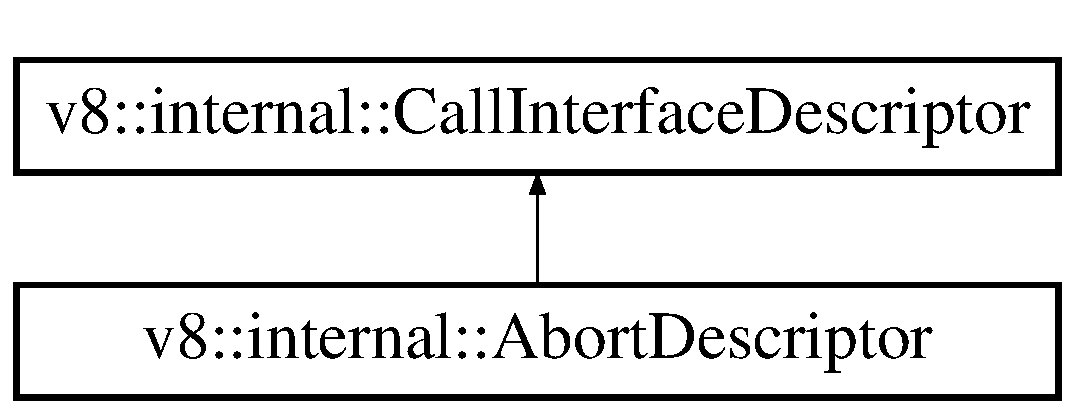
\includegraphics[height=2.000000cm]{classv8_1_1internal_1_1AbortDescriptor}
\end{center}
\end{figure}
\subsection*{Additional Inherited Members}


\subsection{Detailed Description}


Definition at line 818 of file interface-\/descriptors.\+h.



The documentation for this class was generated from the following file\+:\begin{DoxyCompactItemize}
\item 
v8/src/interface-\/descriptors.\+h\end{DoxyCompactItemize}

\hypertarget{structv8_1_1internal_1_1torque_1_1AbortInstruction}{}\section{v8\+:\+:internal\+:\+:torque\+:\+:Abort\+Instruction Struct Reference}
\label{structv8_1_1internal_1_1torque_1_1AbortInstruction}\index{v8\+::internal\+::torque\+::\+Abort\+Instruction@{v8\+::internal\+::torque\+::\+Abort\+Instruction}}
Inheritance diagram for v8\+:\+:internal\+:\+:torque\+:\+:Abort\+Instruction\+:\begin{figure}[H]
\begin{center}
\leavevmode
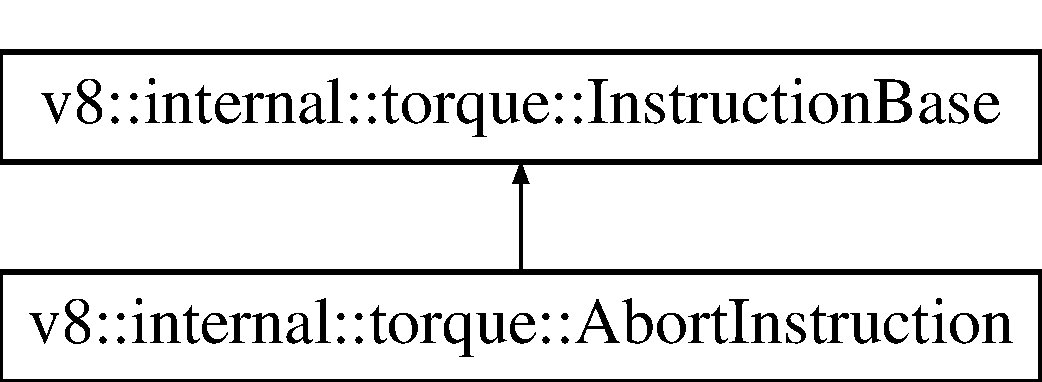
\includegraphics[height=2.000000cm]{structv8_1_1internal_1_1torque_1_1AbortInstruction}
\end{center}
\end{figure}
\subsection*{Public Types}
\begin{DoxyCompactItemize}
\item 
\mbox{\Hypertarget{structv8_1_1internal_1_1torque_1_1AbortInstruction_a3344046b1651f0b1f38667d9d19c6a78}\label{structv8_1_1internal_1_1torque_1_1AbortInstruction_a3344046b1651f0b1f38667d9d19c6a78}} 
enum {\bfseries Kind} \{ {\bfseries k\+Debug\+Break}, 
{\bfseries k\+Unreachable}, 
{\bfseries k\+Assertion\+Failure}
 \}
\end{DoxyCompactItemize}
\subsection*{Public Member Functions}
\begin{DoxyCompactItemize}
\item 
\mbox{\Hypertarget{structv8_1_1internal_1_1torque_1_1AbortInstruction_a9611dd2ae1f65e371cdc7241e8706d4f}\label{structv8_1_1internal_1_1torque_1_1AbortInstruction_a9611dd2ae1f65e371cdc7241e8706d4f}} 
\mbox{\hyperlink{classbool}{bool}} {\bfseries Is\+Block\+Terminator} () const override
\item 
\mbox{\Hypertarget{structv8_1_1internal_1_1torque_1_1AbortInstruction_a45ae13873858488883dc632ad51b17d3}\label{structv8_1_1internal_1_1torque_1_1AbortInstruction_a45ae13873858488883dc632ad51b17d3}} 
{\bfseries Abort\+Instruction} (Kind kind, std\+::string message=\char`\"{}\char`\"{})
\end{DoxyCompactItemize}
\subsection*{Public Attributes}
\begin{DoxyCompactItemize}
\item 
\mbox{\Hypertarget{structv8_1_1internal_1_1torque_1_1AbortInstruction_a73156ceca435b94a4c54d8c32a544df4}\label{structv8_1_1internal_1_1torque_1_1AbortInstruction_a73156ceca435b94a4c54d8c32a544df4}} 
Kind {\bfseries kind}
\item 
\mbox{\Hypertarget{structv8_1_1internal_1_1torque_1_1AbortInstruction_a9a84b9d1c38af3f3ac2fb3129cd27648}\label{structv8_1_1internal_1_1torque_1_1AbortInstruction_a9a84b9d1c38af3f3ac2fb3129cd27648}} 
std\+::string {\bfseries message}
\end{DoxyCompactItemize}


\subsection{Detailed Description}


Definition at line 368 of file instructions.\+h.



The documentation for this struct was generated from the following file\+:\begin{DoxyCompactItemize}
\item 
v8/src/torque/instructions.\+h\end{DoxyCompactItemize}

\hypertarget{classv8_1_1internal_1_1AbstractCode}{}\section{v8\+:\+:internal\+:\+:Abstract\+Code Class Reference}
\label{classv8_1_1internal_1_1AbstractCode}\index{v8\+::internal\+::\+Abstract\+Code@{v8\+::internal\+::\+Abstract\+Code}}
Inheritance diagram for v8\+:\+:internal\+:\+:Abstract\+Code\+:\begin{figure}[H]
\begin{center}
\leavevmode
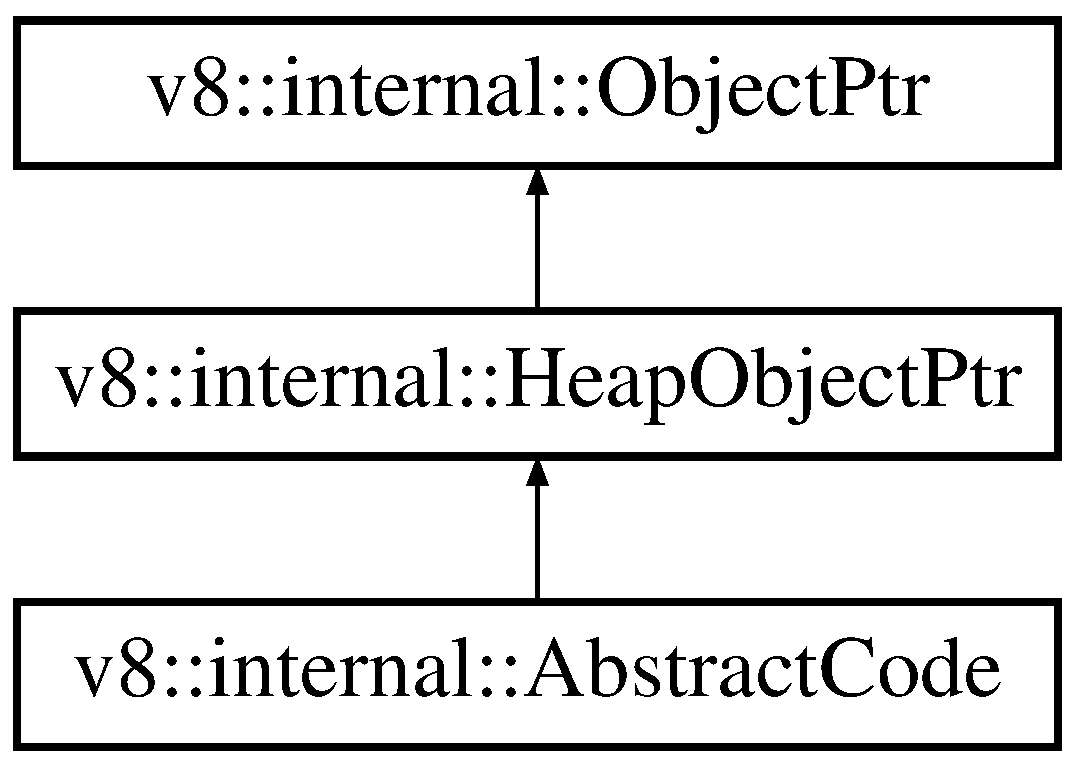
\includegraphics[height=3.000000cm]{classv8_1_1internal_1_1AbstractCode}
\end{center}
\end{figure}
\subsection*{Public Types}
\begin{DoxyCompactItemize}
\item 
\mbox{\Hypertarget{classv8_1_1internal_1_1AbstractCode_a915d9a221d696e00492c45273de7d7c0}\label{classv8_1_1internal_1_1AbstractCode_a915d9a221d696e00492c45273de7d7c0}} 
enum {\bfseries Kind} \{ {\bfseries I\+N\+T\+E\+R\+P\+R\+E\+T\+E\+D\+\_\+\+F\+U\+N\+C\+T\+I\+ON}, 
{\bfseries N\+U\+M\+B\+E\+R\+\_\+\+O\+F\+\_\+\+K\+I\+N\+DS}
 \}
\end{DoxyCompactItemize}
\subsection*{Public Member Functions}
\begin{DoxyCompactItemize}
\item 
\mbox{\Hypertarget{classv8_1_1internal_1_1AbstractCode_acc3eba496172fd777c49536ba6563acf}\label{classv8_1_1internal_1_1AbstractCode_acc3eba496172fd777c49536ba6563acf}} 
\mbox{\hyperlink{classint}{int}} {\bfseries Source\+Position} (\mbox{\hyperlink{classint}{int}} offset)
\item 
\mbox{\Hypertarget{classv8_1_1internal_1_1AbstractCode_aeb9a9cdd430bb3c67e5810ac9fe340fb}\label{classv8_1_1internal_1_1AbstractCode_aeb9a9cdd430bb3c67e5810ac9fe340fb}} 
\mbox{\hyperlink{classint}{int}} {\bfseries Source\+Statement\+Position} (\mbox{\hyperlink{classint}{int}} offset)
\item 
\mbox{\Hypertarget{classv8_1_1internal_1_1AbstractCode_ab5227bb6cd0b20f9da8173fc07adb070}\label{classv8_1_1internal_1_1AbstractCode_ab5227bb6cd0b20f9da8173fc07adb070}} 
\mbox{\hyperlink{classuintptr__t}{Address}} {\bfseries raw\+\_\+instruction\+\_\+start} ()
\item 
\mbox{\Hypertarget{classv8_1_1internal_1_1AbstractCode_a3827622443d78eb8cdae06b6d8a92595}\label{classv8_1_1internal_1_1AbstractCode_a3827622443d78eb8cdae06b6d8a92595}} 
\mbox{\hyperlink{classuintptr__t}{Address}} {\bfseries Instruction\+Start} ()
\item 
\mbox{\Hypertarget{classv8_1_1internal_1_1AbstractCode_a7ee9115933d05fc51a21442be0244e1d}\label{classv8_1_1internal_1_1AbstractCode_a7ee9115933d05fc51a21442be0244e1d}} 
\mbox{\hyperlink{classuintptr__t}{Address}} {\bfseries raw\+\_\+instruction\+\_\+end} ()
\item 
\mbox{\Hypertarget{classv8_1_1internal_1_1AbstractCode_af16b7c5398c4a0130854e42fb2e88df5}\label{classv8_1_1internal_1_1AbstractCode_af16b7c5398c4a0130854e42fb2e88df5}} 
\mbox{\hyperlink{classuintptr__t}{Address}} {\bfseries Instruction\+End} ()
\item 
\mbox{\Hypertarget{classv8_1_1internal_1_1AbstractCode_a898ac389a50478d4dacee522b47eafa8}\label{classv8_1_1internal_1_1AbstractCode_a898ac389a50478d4dacee522b47eafa8}} 
\mbox{\hyperlink{classint}{int}} {\bfseries raw\+\_\+instruction\+\_\+size} ()
\item 
\mbox{\Hypertarget{classv8_1_1internal_1_1AbstractCode_a1987c09dbfb4b7abfbc68bc11e522307}\label{classv8_1_1internal_1_1AbstractCode_a1987c09dbfb4b7abfbc68bc11e522307}} 
\mbox{\hyperlink{classint}{int}} {\bfseries Instruction\+Size} ()
\item 
\mbox{\Hypertarget{classv8_1_1internal_1_1AbstractCode_a07fef294785ec12646a660d036cb3941}\label{classv8_1_1internal_1_1AbstractCode_a07fef294785ec12646a660d036cb3941}} 
\mbox{\hyperlink{classv8_1_1internal_1_1ByteArray}{Byte\+Array}} {\bfseries source\+\_\+position\+\_\+table} ()
\item 
\mbox{\Hypertarget{classv8_1_1internal_1_1AbstractCode_a9ca629b06bc9c7dd2a94841a9f778cda}\label{classv8_1_1internal_1_1AbstractCode_a9ca629b06bc9c7dd2a94841a9f778cda}} 
\mbox{\hyperlink{classv8_1_1internal_1_1Object}{Object}} $\ast$ {\bfseries stack\+\_\+frame\+\_\+cache} ()
\item 
\mbox{\Hypertarget{classv8_1_1internal_1_1AbstractCode_a1e23795e3bb3bfb2381208bd68968b7f}\label{classv8_1_1internal_1_1AbstractCode_a1e23795e3bb3bfb2381208bd68968b7f}} 
void {\bfseries Drop\+Stack\+Frame\+Cache} ()
\item 
\mbox{\Hypertarget{classv8_1_1internal_1_1AbstractCode_a0ffb738e230bd9f4929bb271dc153684}\label{classv8_1_1internal_1_1AbstractCode_a0ffb738e230bd9f4929bb271dc153684}} 
\mbox{\hyperlink{classint}{int}} {\bfseries Size\+Including\+Metadata} ()
\item 
\mbox{\Hypertarget{classv8_1_1internal_1_1AbstractCode_ac15564d26d4213d2b34a4285389dcd4e}\label{classv8_1_1internal_1_1AbstractCode_ac15564d26d4213d2b34a4285389dcd4e}} 
\mbox{\hyperlink{classbool}{bool}} {\bfseries contains} (\mbox{\hyperlink{classuintptr__t}{Address}} pc)
\item 
\mbox{\Hypertarget{classv8_1_1internal_1_1AbstractCode_a4467c4bef4b3900db4abc40a31f3ad55}\label{classv8_1_1internal_1_1AbstractCode_a4467c4bef4b3900db4abc40a31f3ad55}} 
Kind {\bfseries kind} ()
\item 
\mbox{\Hypertarget{classv8_1_1internal_1_1AbstractCode_affc1c1a7e415b017546f2a51c9677026}\label{classv8_1_1internal_1_1AbstractCode_affc1c1a7e415b017546f2a51c9677026}} 
\mbox{\hyperlink{classint}{int}} {\bfseries Executable\+Size} ()
\item 
\mbox{\Hypertarget{classv8_1_1internal_1_1AbstractCode_a4f76122fa2697c5c4cea469ed6d4bf90}\label{classv8_1_1internal_1_1AbstractCode_a4f76122fa2697c5c4cea469ed6d4bf90}} 
\mbox{\hyperlink{classv8_1_1internal_1_1Code}{Code}} {\bfseries Get\+Code} ()
\item 
\mbox{\Hypertarget{classv8_1_1internal_1_1AbstractCode_a52826fbe174768bfbd200ee342557aa4}\label{classv8_1_1internal_1_1AbstractCode_a52826fbe174768bfbd200ee342557aa4}} 
\mbox{\hyperlink{classv8_1_1internal_1_1BytecodeArray}{Bytecode\+Array}} {\bfseries Get\+Bytecode\+Array} ()
\end{DoxyCompactItemize}
\subsection*{Static Public Member Functions}
\begin{DoxyCompactItemize}
\item 
\mbox{\Hypertarget{classv8_1_1internal_1_1AbstractCode_aa5957bbcf64da041514a3c6312bb838b}\label{classv8_1_1internal_1_1AbstractCode_aa5957bbcf64da041514a3c6312bb838b}} 
static const \mbox{\hyperlink{classchar}{char}} $\ast$ {\bfseries Kind2\+String} (Kind kind)
\item 
\mbox{\Hypertarget{classv8_1_1internal_1_1AbstractCode_a32e4d2b6f7a106c79458ed3b8f0e2f22}\label{classv8_1_1internal_1_1AbstractCode_a32e4d2b6f7a106c79458ed3b8f0e2f22}} 
static void {\bfseries Set\+Stack\+Frame\+Cache} (\mbox{\hyperlink{classv8_1_1internal_1_1Handle}{Handle}}$<$ \mbox{\hyperlink{classv8_1_1internal_1_1AbstractCode}{Abstract\+Code}} $>$ abstract\+\_\+code, \mbox{\hyperlink{classv8_1_1internal_1_1Handle}{Handle}}$<$ \mbox{\hyperlink{classv8_1_1internal_1_1SimpleNumberDictionary}{Simple\+Number\+Dictionary}} $>$ cache)
\end{DoxyCompactItemize}
\subsection*{Static Public Attributes}
\begin{DoxyCompactItemize}
\item 
\mbox{\Hypertarget{classv8_1_1internal_1_1AbstractCode_a119579f6132f2cc2e697fd094f34f409}\label{classv8_1_1internal_1_1AbstractCode_a119579f6132f2cc2e697fd094f34f409}} 
static const \mbox{\hyperlink{classint}{int}} {\bfseries k\+Max\+Loop\+Nesting\+Marker} = 6
\end{DoxyCompactItemize}
\subsection*{Additional Inherited Members}


\subsection{Detailed Description}


Definition at line 501 of file code.\+h.



The documentation for this class was generated from the following files\+:\begin{DoxyCompactItemize}
\item 
v8/src/objects/code.\+h\item 
v8/src/objects/code-\/inl.\+h\item 
v8/src/objects.\+cc\end{DoxyCompactItemize}

\hypertarget{classv8_1_1internal_1_1torque_1_1AbstractType}{}\section{v8\+:\+:internal\+:\+:torque\+:\+:Abstract\+Type Class Reference}
\label{classv8_1_1internal_1_1torque_1_1AbstractType}\index{v8\+::internal\+::torque\+::\+Abstract\+Type@{v8\+::internal\+::torque\+::\+Abstract\+Type}}
Inheritance diagram for v8\+:\+:internal\+:\+:torque\+:\+:Abstract\+Type\+:\begin{figure}[H]
\begin{center}
\leavevmode
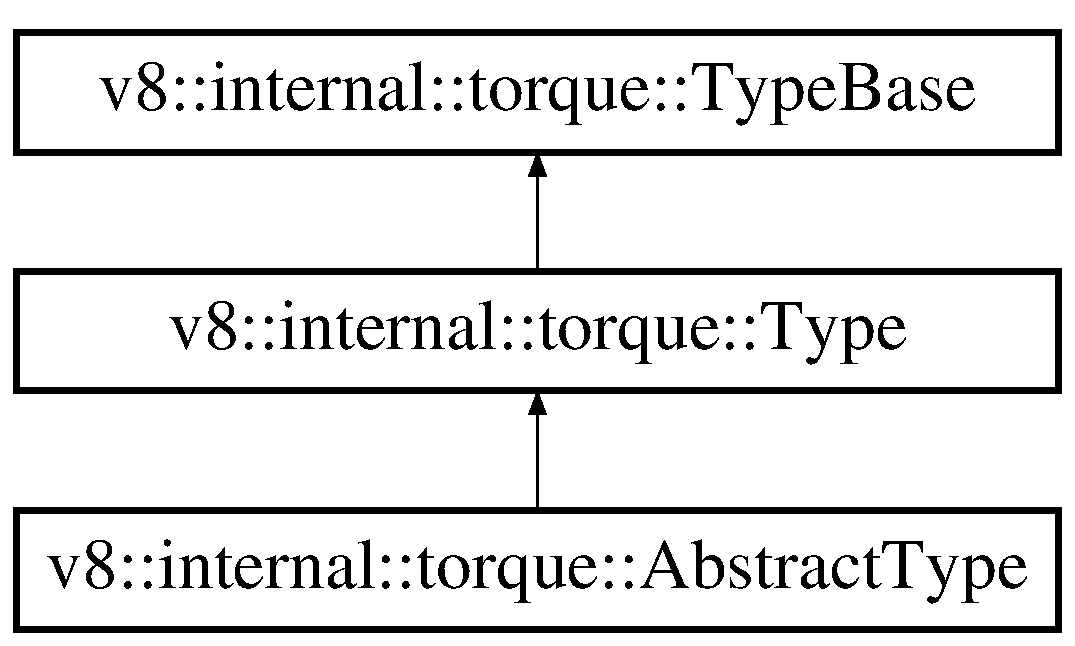
\includegraphics[height=3.000000cm]{classv8_1_1internal_1_1torque_1_1AbstractType}
\end{center}
\end{figure}
\subsection*{Public Member Functions}
\begin{DoxyCompactItemize}
\item 
\mbox{\Hypertarget{classv8_1_1internal_1_1torque_1_1AbstractType_ade1906cc0b539119e2107be6e1aa1fb5}\label{classv8_1_1internal_1_1torque_1_1AbstractType_ade1906cc0b539119e2107be6e1aa1fb5}} 
{\bfseries D\+E\+C\+L\+A\+R\+E\+\_\+\+T\+Y\+P\+E\+\_\+\+B\+O\+I\+L\+E\+R\+P\+L\+A\+TE} (\mbox{\hyperlink{classv8_1_1internal_1_1torque_1_1AbstractType}{Abstract\+Type}})
\item 
\mbox{\Hypertarget{classv8_1_1internal_1_1torque_1_1AbstractType_af3e4c437161d37b81c958146eb2b3d07}\label{classv8_1_1internal_1_1torque_1_1AbstractType_af3e4c437161d37b81c958146eb2b3d07}} 
const std\+::string \& {\bfseries name} () const
\item 
\mbox{\Hypertarget{classv8_1_1internal_1_1torque_1_1AbstractType_aa7082bc838e26a49c43ab93091d6a537}\label{classv8_1_1internal_1_1torque_1_1AbstractType_aa7082bc838e26a49c43ab93091d6a537}} 
std\+::string {\bfseries To\+Explicit\+String} () const override
\item 
\mbox{\Hypertarget{classv8_1_1internal_1_1torque_1_1AbstractType_a0b4f7e48cd4d74d6f38bba9820ba03fe}\label{classv8_1_1internal_1_1torque_1_1AbstractType_a0b4f7e48cd4d74d6f38bba9820ba03fe}} 
std\+::string {\bfseries Mangled\+Name} () const override
\item 
\mbox{\Hypertarget{classv8_1_1internal_1_1torque_1_1AbstractType_ae5b60e59b3ff6eb1ab68ac930afad501}\label{classv8_1_1internal_1_1torque_1_1AbstractType_ae5b60e59b3ff6eb1ab68ac930afad501}} 
std\+::string {\bfseries Get\+Generated\+Type\+Name} () const override
\item 
\mbox{\Hypertarget{classv8_1_1internal_1_1torque_1_1AbstractType_af859bbcc539a50364c437b81c8e108f8}\label{classv8_1_1internal_1_1torque_1_1AbstractType_af859bbcc539a50364c437b81c8e108f8}} 
std\+::string {\bfseries Get\+Generated\+T\+Node\+Type\+Name} () const override
\item 
\mbox{\Hypertarget{classv8_1_1internal_1_1torque_1_1AbstractType_a0ff8b75fa54058672998314a8526289d}\label{classv8_1_1internal_1_1torque_1_1AbstractType_a0ff8b75fa54058672998314a8526289d}} 
\mbox{\hyperlink{classbool}{bool}} {\bfseries Is\+Constexpr} () const override
\item 
\mbox{\Hypertarget{classv8_1_1internal_1_1torque_1_1AbstractType_a1c6e6a1f84b9259baa21da4517818783}\label{classv8_1_1internal_1_1torque_1_1AbstractType_a1c6e6a1f84b9259baa21da4517818783}} 
const \mbox{\hyperlink{classv8_1_1internal_1_1torque_1_1Type}{Type}} $\ast$ {\bfseries Non\+Constexpr\+Version} () const override
\end{DoxyCompactItemize}
\subsection*{Friends}
\begin{DoxyCompactItemize}
\item 
\mbox{\Hypertarget{classv8_1_1internal_1_1torque_1_1AbstractType_a7094142f1d9b95b74797a11decbf23e3}\label{classv8_1_1internal_1_1torque_1_1AbstractType_a7094142f1d9b95b74797a11decbf23e3}} 
class {\bfseries Type\+Oracle}
\end{DoxyCompactItemize}
\subsection*{Additional Inherited Members}


\subsection{Detailed Description}


Definition at line 168 of file types.\+h.



The documentation for this class was generated from the following files\+:\begin{DoxyCompactItemize}
\item 
v8/src/torque/types.\+h\item 
v8/src/torque/types.\+cc\end{DoxyCompactItemize}

\hypertarget{classv8_1_1internal_1_1ParserBase_1_1AcceptINScope}{}\section{v8\+:\+:internal\+:\+:Parser\+Base$<$ Impl $>$\+:\+:Accept\+I\+N\+Scope Class Reference}
\label{classv8_1_1internal_1_1ParserBase_1_1AcceptINScope}\index{v8\+::internal\+::\+Parser\+Base$<$ Impl $>$\+::\+Accept\+I\+N\+Scope@{v8\+::internal\+::\+Parser\+Base$<$ Impl $>$\+::\+Accept\+I\+N\+Scope}}
\subsection*{Public Member Functions}
\begin{DoxyCompactItemize}
\item 
\mbox{\Hypertarget{classv8_1_1internal_1_1ParserBase_1_1AcceptINScope_a7ccadad61043ef45927641f850a6a9ab}\label{classv8_1_1internal_1_1ParserBase_1_1AcceptINScope_a7ccadad61043ef45927641f850a6a9ab}} 
{\bfseries Accept\+I\+N\+Scope} (\mbox{\hyperlink{classv8_1_1internal_1_1ParserBase}{Parser\+Base}} $\ast$parser, \mbox{\hyperlink{classbool}{bool}} accept\+\_\+\+IN)
\end{DoxyCompactItemize}


\subsection{Detailed Description}
\subsubsection*{template$<$typename Impl$>$\newline
class v8\+::internal\+::\+Parser\+Base$<$ Impl $>$\+::\+Accept\+I\+N\+Scope}



Definition at line 1395 of file parser-\/base.\+h.



The documentation for this class was generated from the following file\+:\begin{DoxyCompactItemize}
\item 
v8/src/parsing/parser-\/base.\+h\end{DoxyCompactItemize}

\hypertarget{classv8_1_1internal_1_1Access}{}\section{v8\+:\+:internal\+:\+:Access$<$ T $>$ Class Template Reference}
\label{classv8_1_1internal_1_1Access}\index{v8\+::internal\+::\+Access$<$ T $>$@{v8\+::internal\+::\+Access$<$ T $>$}}
\subsection*{Public Member Functions}
\begin{DoxyCompactItemize}
\item 
\mbox{\Hypertarget{classv8_1_1internal_1_1Access_a73d4e4a39835cc3d2314a328d80d0073}\label{classv8_1_1internal_1_1Access_a73d4e4a39835cc3d2314a328d80d0073}} 
{\bfseries Access} (\mbox{\hyperlink{classv8_1_1internal_1_1StaticResource}{Static\+Resource}}$<$ T $>$ $\ast$resource)
\item 
\mbox{\Hypertarget{classv8_1_1internal_1_1Access_ab9a3512d394b376ccba107df5f3c3d67}\label{classv8_1_1internal_1_1Access_ab9a3512d394b376ccba107df5f3c3d67}} 
T $\ast$ {\bfseries value} ()
\item 
\mbox{\Hypertarget{classv8_1_1internal_1_1Access_a71f5c7a9a355f726f309a13a5b6a8ab4}\label{classv8_1_1internal_1_1Access_a71f5c7a9a355f726f309a13a5b6a8ab4}} 
T $\ast$ {\bfseries operator-\/$>$} ()
\end{DoxyCompactItemize}


\subsection{Detailed Description}
\subsubsection*{template$<$typename T$>$\newline
class v8\+::internal\+::\+Access$<$ T $>$}



Definition at line 630 of file utils.\+h.



The documentation for this class was generated from the following file\+:\begin{DoxyCompactItemize}
\item 
v8/src/utils.\+h\end{DoxyCompactItemize}

\hypertarget{classv8_1_1internal_1_1compiler_1_1AccessBuilder}{}\section{v8\+:\+:internal\+:\+:compiler\+:\+:Access\+Builder Class Reference}
\label{classv8_1_1internal_1_1compiler_1_1AccessBuilder}\index{v8\+::internal\+::compiler\+::\+Access\+Builder@{v8\+::internal\+::compiler\+::\+Access\+Builder}}
Inheritance diagram for v8\+:\+:internal\+:\+:compiler\+:\+:Access\+Builder\+:\begin{figure}[H]
\begin{center}
\leavevmode
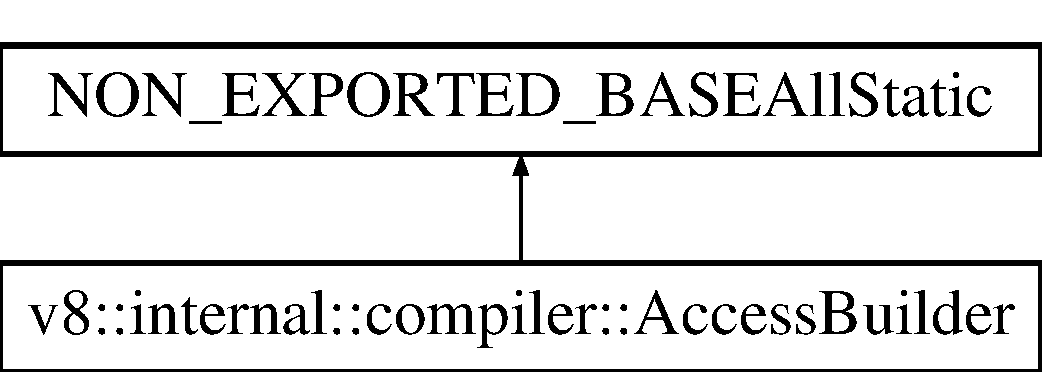
\includegraphics[height=2.000000cm]{classv8_1_1internal_1_1compiler_1_1AccessBuilder}
\end{center}
\end{figure}
\subsection*{Static Public Member Functions}
\begin{DoxyCompactItemize}
\item 
\mbox{\Hypertarget{classv8_1_1internal_1_1compiler_1_1AccessBuilder_af17176ecf5670ba51472d414ec947d86}\label{classv8_1_1internal_1_1compiler_1_1AccessBuilder_af17176ecf5670ba51472d414ec947d86}} 
static \mbox{\hyperlink{structv8_1_1internal_1_1compiler_1_1FieldAccess}{Field\+Access}} {\bfseries For\+External\+Tagged\+Value} ()
\item 
\mbox{\Hypertarget{classv8_1_1internal_1_1compiler_1_1AccessBuilder_a6317aa64484ffd9630d69968340ba02a}\label{classv8_1_1internal_1_1compiler_1_1AccessBuilder_a6317aa64484ffd9630d69968340ba02a}} 
static \mbox{\hyperlink{structv8_1_1internal_1_1compiler_1_1FieldAccess}{Field\+Access}} {\bfseries For\+External\+Uint8\+Value} ()
\item 
\mbox{\Hypertarget{classv8_1_1internal_1_1compiler_1_1AccessBuilder_ac2bb52ee54e5b0ae7bbbbd4ea32a2647}\label{classv8_1_1internal_1_1compiler_1_1AccessBuilder_ac2bb52ee54e5b0ae7bbbbd4ea32a2647}} 
static \mbox{\hyperlink{structv8_1_1internal_1_1compiler_1_1FieldAccess}{Field\+Access}} {\bfseries For\+Map} ()
\item 
\mbox{\Hypertarget{classv8_1_1internal_1_1compiler_1_1AccessBuilder_a1fa84722d5a19479546399b5803d9325}\label{classv8_1_1internal_1_1compiler_1_1AccessBuilder_a1fa84722d5a19479546399b5803d9325}} 
static \mbox{\hyperlink{structv8_1_1internal_1_1compiler_1_1FieldAccess}{Field\+Access}} {\bfseries For\+Heap\+Number\+Value} ()
\item 
\mbox{\Hypertarget{classv8_1_1internal_1_1compiler_1_1AccessBuilder_a1031ad312005df31b4021e08d204b414}\label{classv8_1_1internal_1_1compiler_1_1AccessBuilder_a1031ad312005df31b4021e08d204b414}} 
static \mbox{\hyperlink{structv8_1_1internal_1_1compiler_1_1FieldAccess}{Field\+Access}} {\bfseries For\+Big\+Int\+Bitfield} ()
\item 
\mbox{\Hypertarget{classv8_1_1internal_1_1compiler_1_1AccessBuilder_a87d8d738b1c038d7881c0c94e6ea1019}\label{classv8_1_1internal_1_1compiler_1_1AccessBuilder_a87d8d738b1c038d7881c0c94e6ea1019}} 
static \mbox{\hyperlink{structv8_1_1internal_1_1compiler_1_1FieldAccess}{Field\+Access}} {\bfseries For\+J\+S\+Object\+Properties\+Or\+Hash} ()
\item 
\mbox{\Hypertarget{classv8_1_1internal_1_1compiler_1_1AccessBuilder_afce72fe75259f693baee5435e7f9073d}\label{classv8_1_1internal_1_1compiler_1_1AccessBuilder_afce72fe75259f693baee5435e7f9073d}} 
static \mbox{\hyperlink{structv8_1_1internal_1_1compiler_1_1FieldAccess}{Field\+Access}} {\bfseries For\+J\+S\+Object\+Elements} ()
\item 
\mbox{\Hypertarget{classv8_1_1internal_1_1compiler_1_1AccessBuilder_ae012f6271eaaa938e020c39b4cc7ecb8}\label{classv8_1_1internal_1_1compiler_1_1AccessBuilder_ae012f6271eaaa938e020c39b4cc7ecb8}} 
static \mbox{\hyperlink{structv8_1_1internal_1_1compiler_1_1FieldAccess}{Field\+Access}} {\bfseries For\+J\+S\+Object\+In\+Object\+Property} (const \mbox{\hyperlink{classv8_1_1internal_1_1compiler_1_1MapRef}{Map\+Ref}} \&map, \mbox{\hyperlink{classint}{int}} index)
\item 
\mbox{\Hypertarget{classv8_1_1internal_1_1compiler_1_1AccessBuilder_a24df5536fec134ec94f386fada988aee}\label{classv8_1_1internal_1_1compiler_1_1AccessBuilder_a24df5536fec134ec94f386fada988aee}} 
static \mbox{\hyperlink{structv8_1_1internal_1_1compiler_1_1FieldAccess}{Field\+Access}} {\bfseries For\+J\+S\+Object\+Offset} (\mbox{\hyperlink{classint}{int}} offset, Write\+Barrier\+Kind write\+\_\+barrier\+\_\+kind=k\+Full\+Write\+Barrier)
\item 
\mbox{\Hypertarget{classv8_1_1internal_1_1compiler_1_1AccessBuilder_a1fe5371fb832bfba18b6856d36eb1446}\label{classv8_1_1internal_1_1compiler_1_1AccessBuilder_a1fe5371fb832bfba18b6856d36eb1446}} 
static \mbox{\hyperlink{structv8_1_1internal_1_1compiler_1_1FieldAccess}{Field\+Access}} {\bfseries For\+J\+S\+Collection\+Table} ()
\item 
\mbox{\Hypertarget{classv8_1_1internal_1_1compiler_1_1AccessBuilder_a051b7d4428edceee9635b13702470d93}\label{classv8_1_1internal_1_1compiler_1_1AccessBuilder_a051b7d4428edceee9635b13702470d93}} 
static \mbox{\hyperlink{structv8_1_1internal_1_1compiler_1_1FieldAccess}{Field\+Access}} {\bfseries For\+J\+S\+Collection\+Iterator\+Table} ()
\item 
\mbox{\Hypertarget{classv8_1_1internal_1_1compiler_1_1AccessBuilder_a3f9593bcf3be1d49460f40b625782aa8}\label{classv8_1_1internal_1_1compiler_1_1AccessBuilder_a3f9593bcf3be1d49460f40b625782aa8}} 
static \mbox{\hyperlink{structv8_1_1internal_1_1compiler_1_1FieldAccess}{Field\+Access}} {\bfseries For\+J\+S\+Collection\+Iterator\+Index} ()
\item 
\mbox{\Hypertarget{classv8_1_1internal_1_1compiler_1_1AccessBuilder_ae67ee224508da0a19ca07ad72ac025ec}\label{classv8_1_1internal_1_1compiler_1_1AccessBuilder_ae67ee224508da0a19ca07ad72ac025ec}} 
static \mbox{\hyperlink{structv8_1_1internal_1_1compiler_1_1FieldAccess}{Field\+Access}} {\bfseries For\+J\+S\+Function\+Prototype\+Or\+Initial\+Map} ()
\item 
\mbox{\Hypertarget{classv8_1_1internal_1_1compiler_1_1AccessBuilder_a85fdfa37dd29156e9ae70b0a4865b431}\label{classv8_1_1internal_1_1compiler_1_1AccessBuilder_a85fdfa37dd29156e9ae70b0a4865b431}} 
static \mbox{\hyperlink{structv8_1_1internal_1_1compiler_1_1FieldAccess}{Field\+Access}} {\bfseries For\+J\+S\+Function\+Context} ()
\item 
\mbox{\Hypertarget{classv8_1_1internal_1_1compiler_1_1AccessBuilder_a62fbc921459ee05856f58ef1413221c5}\label{classv8_1_1internal_1_1compiler_1_1AccessBuilder_a62fbc921459ee05856f58ef1413221c5}} 
static \mbox{\hyperlink{structv8_1_1internal_1_1compiler_1_1FieldAccess}{Field\+Access}} {\bfseries For\+J\+S\+Function\+Shared\+Function\+Info} ()
\item 
\mbox{\Hypertarget{classv8_1_1internal_1_1compiler_1_1AccessBuilder_a88d7613d78f882984fa8452c62f9badc}\label{classv8_1_1internal_1_1compiler_1_1AccessBuilder_a88d7613d78f882984fa8452c62f9badc}} 
static \mbox{\hyperlink{structv8_1_1internal_1_1compiler_1_1FieldAccess}{Field\+Access}} {\bfseries For\+J\+S\+Function\+Feedback\+Cell} ()
\item 
\mbox{\Hypertarget{classv8_1_1internal_1_1compiler_1_1AccessBuilder_af97a37594d40cd3c7f1d8edb0340941c}\label{classv8_1_1internal_1_1compiler_1_1AccessBuilder_af97a37594d40cd3c7f1d8edb0340941c}} 
static \mbox{\hyperlink{structv8_1_1internal_1_1compiler_1_1FieldAccess}{Field\+Access}} {\bfseries For\+J\+S\+Function\+Code} ()
\item 
\mbox{\Hypertarget{classv8_1_1internal_1_1compiler_1_1AccessBuilder_a21a97af6357a5a818de12542c41af24e}\label{classv8_1_1internal_1_1compiler_1_1AccessBuilder_a21a97af6357a5a818de12542c41af24e}} 
static \mbox{\hyperlink{structv8_1_1internal_1_1compiler_1_1FieldAccess}{Field\+Access}} {\bfseries For\+J\+S\+Bound\+Function\+Bound\+Target\+Function} ()
\item 
\mbox{\Hypertarget{classv8_1_1internal_1_1compiler_1_1AccessBuilder_a3d4742bb081447d9a1eae4b7caf21212}\label{classv8_1_1internal_1_1compiler_1_1AccessBuilder_a3d4742bb081447d9a1eae4b7caf21212}} 
static \mbox{\hyperlink{structv8_1_1internal_1_1compiler_1_1FieldAccess}{Field\+Access}} {\bfseries For\+J\+S\+Bound\+Function\+Bound\+This} ()
\item 
\mbox{\Hypertarget{classv8_1_1internal_1_1compiler_1_1AccessBuilder_a248adfa29c7958a6d0477bb1efb9bb7e}\label{classv8_1_1internal_1_1compiler_1_1AccessBuilder_a248adfa29c7958a6d0477bb1efb9bb7e}} 
static \mbox{\hyperlink{structv8_1_1internal_1_1compiler_1_1FieldAccess}{Field\+Access}} {\bfseries For\+J\+S\+Bound\+Function\+Bound\+Arguments} ()
\item 
\mbox{\Hypertarget{classv8_1_1internal_1_1compiler_1_1AccessBuilder_a5d81feba81842c9815e13f292b51f9dd}\label{classv8_1_1internal_1_1compiler_1_1AccessBuilder_a5d81feba81842c9815e13f292b51f9dd}} 
static \mbox{\hyperlink{structv8_1_1internal_1_1compiler_1_1FieldAccess}{Field\+Access}} {\bfseries For\+J\+S\+Generator\+Object\+Context} ()
\item 
\mbox{\Hypertarget{classv8_1_1internal_1_1compiler_1_1AccessBuilder_adb5ef2076b51cb8d6fc215b1afcf27c9}\label{classv8_1_1internal_1_1compiler_1_1AccessBuilder_adb5ef2076b51cb8d6fc215b1afcf27c9}} 
static \mbox{\hyperlink{structv8_1_1internal_1_1compiler_1_1FieldAccess}{Field\+Access}} {\bfseries For\+J\+S\+Generator\+Object\+Continuation} ()
\item 
\mbox{\Hypertarget{classv8_1_1internal_1_1compiler_1_1AccessBuilder_a69fe8898ff33cf892cd1171cd7c74693}\label{classv8_1_1internal_1_1compiler_1_1AccessBuilder_a69fe8898ff33cf892cd1171cd7c74693}} 
static \mbox{\hyperlink{structv8_1_1internal_1_1compiler_1_1FieldAccess}{Field\+Access}} {\bfseries For\+J\+S\+Generator\+Object\+Input\+Or\+Debug\+Pos} ()
\item 
\mbox{\Hypertarget{classv8_1_1internal_1_1compiler_1_1AccessBuilder_aff3726b363a52c8409c9c46e50cf0b26}\label{classv8_1_1internal_1_1compiler_1_1AccessBuilder_aff3726b363a52c8409c9c46e50cf0b26}} 
static \mbox{\hyperlink{structv8_1_1internal_1_1compiler_1_1FieldAccess}{Field\+Access}} {\bfseries For\+J\+S\+Generator\+Object\+Parameters\+And\+Registers} ()
\item 
\mbox{\Hypertarget{classv8_1_1internal_1_1compiler_1_1AccessBuilder_aad69c19e3c3ecb0fc261417623ee064f}\label{classv8_1_1internal_1_1compiler_1_1AccessBuilder_aad69c19e3c3ecb0fc261417623ee064f}} 
static \mbox{\hyperlink{structv8_1_1internal_1_1compiler_1_1FieldAccess}{Field\+Access}} {\bfseries For\+J\+S\+Generator\+Object\+Function} ()
\item 
\mbox{\Hypertarget{classv8_1_1internal_1_1compiler_1_1AccessBuilder_a937802900183c490dc556e1d1aae7681}\label{classv8_1_1internal_1_1compiler_1_1AccessBuilder_a937802900183c490dc556e1d1aae7681}} 
static \mbox{\hyperlink{structv8_1_1internal_1_1compiler_1_1FieldAccess}{Field\+Access}} {\bfseries For\+J\+S\+Generator\+Object\+Receiver} ()
\item 
\mbox{\Hypertarget{classv8_1_1internal_1_1compiler_1_1AccessBuilder_ab3a3bd6b18fca00973c08f6f9b90d693}\label{classv8_1_1internal_1_1compiler_1_1AccessBuilder_ab3a3bd6b18fca00973c08f6f9b90d693}} 
static \mbox{\hyperlink{structv8_1_1internal_1_1compiler_1_1FieldAccess}{Field\+Access}} {\bfseries For\+J\+S\+Generator\+Object\+Resume\+Mode} ()
\item 
\mbox{\Hypertarget{classv8_1_1internal_1_1compiler_1_1AccessBuilder_a7f971b8f27621756694edf6552b97079}\label{classv8_1_1internal_1_1compiler_1_1AccessBuilder_a7f971b8f27621756694edf6552b97079}} 
static \mbox{\hyperlink{structv8_1_1internal_1_1compiler_1_1FieldAccess}{Field\+Access}} {\bfseries For\+J\+S\+Async\+Function\+Object\+Promise} ()
\item 
\mbox{\Hypertarget{classv8_1_1internal_1_1compiler_1_1AccessBuilder_ac1e71be20fe6f28b1427aa0ea2f0b09f}\label{classv8_1_1internal_1_1compiler_1_1AccessBuilder_ac1e71be20fe6f28b1427aa0ea2f0b09f}} 
static \mbox{\hyperlink{structv8_1_1internal_1_1compiler_1_1FieldAccess}{Field\+Access}} {\bfseries For\+J\+S\+Async\+Generator\+Object\+Queue} ()
\item 
\mbox{\Hypertarget{classv8_1_1internal_1_1compiler_1_1AccessBuilder_ac8200425c5dd617cd81afc75e0e8721b}\label{classv8_1_1internal_1_1compiler_1_1AccessBuilder_ac8200425c5dd617cd81afc75e0e8721b}} 
static \mbox{\hyperlink{structv8_1_1internal_1_1compiler_1_1FieldAccess}{Field\+Access}} {\bfseries For\+J\+S\+Async\+Generator\+Object\+Is\+Awaiting} ()
\item 
\mbox{\Hypertarget{classv8_1_1internal_1_1compiler_1_1AccessBuilder_a6d1b43f02967d574807132fa27865e46}\label{classv8_1_1internal_1_1compiler_1_1AccessBuilder_a6d1b43f02967d574807132fa27865e46}} 
static \mbox{\hyperlink{structv8_1_1internal_1_1compiler_1_1FieldAccess}{Field\+Access}} {\bfseries For\+J\+S\+Array\+Length} (Elements\+Kind elements\+\_\+kind)
\item 
\mbox{\Hypertarget{classv8_1_1internal_1_1compiler_1_1AccessBuilder_a46eb6092a6a00b4d88958e64ae226518}\label{classv8_1_1internal_1_1compiler_1_1AccessBuilder_a46eb6092a6a00b4d88958e64ae226518}} 
static \mbox{\hyperlink{structv8_1_1internal_1_1compiler_1_1FieldAccess}{Field\+Access}} {\bfseries For\+J\+S\+Array\+Buffer\+Backing\+Store} ()
\item 
\mbox{\Hypertarget{classv8_1_1internal_1_1compiler_1_1AccessBuilder_a49b702262a9c8d1484190ff9f038e8e9}\label{classv8_1_1internal_1_1compiler_1_1AccessBuilder_a49b702262a9c8d1484190ff9f038e8e9}} 
static \mbox{\hyperlink{structv8_1_1internal_1_1compiler_1_1FieldAccess}{Field\+Access}} {\bfseries For\+J\+S\+Array\+Buffer\+Bit\+Field} ()
\item 
\mbox{\Hypertarget{classv8_1_1internal_1_1compiler_1_1AccessBuilder_a02537ce5d5a1ce7d1a1fef121a1626cd}\label{classv8_1_1internal_1_1compiler_1_1AccessBuilder_a02537ce5d5a1ce7d1a1fef121a1626cd}} 
static \mbox{\hyperlink{structv8_1_1internal_1_1compiler_1_1FieldAccess}{Field\+Access}} {\bfseries For\+J\+S\+Array\+Buffer\+View\+Buffer} ()
\item 
\mbox{\Hypertarget{classv8_1_1internal_1_1compiler_1_1AccessBuilder_a0e786978222f715fe6ed0443bb4ea546}\label{classv8_1_1internal_1_1compiler_1_1AccessBuilder_a0e786978222f715fe6ed0443bb4ea546}} 
static \mbox{\hyperlink{structv8_1_1internal_1_1compiler_1_1FieldAccess}{Field\+Access}} {\bfseries For\+J\+S\+Array\+Buffer\+View\+Byte\+Length} ()
\item 
\mbox{\Hypertarget{classv8_1_1internal_1_1compiler_1_1AccessBuilder_a151eb9814fa1e4b746e84e49b70c6af9}\label{classv8_1_1internal_1_1compiler_1_1AccessBuilder_a151eb9814fa1e4b746e84e49b70c6af9}} 
static \mbox{\hyperlink{structv8_1_1internal_1_1compiler_1_1FieldAccess}{Field\+Access}} {\bfseries For\+J\+S\+Array\+Buffer\+View\+Byte\+Offset} ()
\item 
\mbox{\Hypertarget{classv8_1_1internal_1_1compiler_1_1AccessBuilder_acbff0190675f39a2060176ee595f94b3}\label{classv8_1_1internal_1_1compiler_1_1AccessBuilder_acbff0190675f39a2060176ee595f94b3}} 
static \mbox{\hyperlink{structv8_1_1internal_1_1compiler_1_1FieldAccess}{Field\+Access}} {\bfseries For\+J\+S\+Typed\+Array\+Length} ()
\item 
\mbox{\Hypertarget{classv8_1_1internal_1_1compiler_1_1AccessBuilder_a90649251d06f212410ce500611926b10}\label{classv8_1_1internal_1_1compiler_1_1AccessBuilder_a90649251d06f212410ce500611926b10}} 
static \mbox{\hyperlink{structv8_1_1internal_1_1compiler_1_1FieldAccess}{Field\+Access}} {\bfseries For\+J\+S\+Date\+Value} ()
\item 
\mbox{\Hypertarget{classv8_1_1internal_1_1compiler_1_1AccessBuilder_a6694da00d86790879f46f22007099b7a}\label{classv8_1_1internal_1_1compiler_1_1AccessBuilder_a6694da00d86790879f46f22007099b7a}} 
static \mbox{\hyperlink{structv8_1_1internal_1_1compiler_1_1FieldAccess}{Field\+Access}} {\bfseries For\+J\+S\+Date\+Field} (J\+S\+Date\+::\+Field\+Index index)
\item 
\mbox{\Hypertarget{classv8_1_1internal_1_1compiler_1_1AccessBuilder_a904efe1b02040e264c368a2a9386cddc}\label{classv8_1_1internal_1_1compiler_1_1AccessBuilder_a904efe1b02040e264c368a2a9386cddc}} 
static \mbox{\hyperlink{structv8_1_1internal_1_1compiler_1_1FieldAccess}{Field\+Access}} {\bfseries For\+J\+S\+Iterator\+Result\+Done} ()
\item 
\mbox{\Hypertarget{classv8_1_1internal_1_1compiler_1_1AccessBuilder_a762b46b9e79781286d8d56ffb9d5f2bd}\label{classv8_1_1internal_1_1compiler_1_1AccessBuilder_a762b46b9e79781286d8d56ffb9d5f2bd}} 
static \mbox{\hyperlink{structv8_1_1internal_1_1compiler_1_1FieldAccess}{Field\+Access}} {\bfseries For\+J\+S\+Iterator\+Result\+Value} ()
\item 
\mbox{\Hypertarget{classv8_1_1internal_1_1compiler_1_1AccessBuilder_aa4fac095026dd858af850f037327e164}\label{classv8_1_1internal_1_1compiler_1_1AccessBuilder_aa4fac095026dd858af850f037327e164}} 
static \mbox{\hyperlink{structv8_1_1internal_1_1compiler_1_1FieldAccess}{Field\+Access}} {\bfseries For\+J\+S\+Reg\+Exp\+Data} ()
\item 
\mbox{\Hypertarget{classv8_1_1internal_1_1compiler_1_1AccessBuilder_ade9388e3deec65b7df0b4f296ba3ad89}\label{classv8_1_1internal_1_1compiler_1_1AccessBuilder_ade9388e3deec65b7df0b4f296ba3ad89}} 
static \mbox{\hyperlink{structv8_1_1internal_1_1compiler_1_1FieldAccess}{Field\+Access}} {\bfseries For\+J\+S\+Reg\+Exp\+Flags} ()
\item 
\mbox{\Hypertarget{classv8_1_1internal_1_1compiler_1_1AccessBuilder_a916ad708fe9b16891063253875a77caf}\label{classv8_1_1internal_1_1compiler_1_1AccessBuilder_a916ad708fe9b16891063253875a77caf}} 
static \mbox{\hyperlink{structv8_1_1internal_1_1compiler_1_1FieldAccess}{Field\+Access}} {\bfseries For\+J\+S\+Reg\+Exp\+Last\+Index} ()
\item 
\mbox{\Hypertarget{classv8_1_1internal_1_1compiler_1_1AccessBuilder_afce14f046b4b206b1386dba28a2ea568}\label{classv8_1_1internal_1_1compiler_1_1AccessBuilder_afce14f046b4b206b1386dba28a2ea568}} 
static \mbox{\hyperlink{structv8_1_1internal_1_1compiler_1_1FieldAccess}{Field\+Access}} {\bfseries For\+J\+S\+Reg\+Exp\+Source} ()
\item 
\mbox{\Hypertarget{classv8_1_1internal_1_1compiler_1_1AccessBuilder_a60f2fc93086167e98d96af50182a5ca8}\label{classv8_1_1internal_1_1compiler_1_1AccessBuilder_a60f2fc93086167e98d96af50182a5ca8}} 
static \mbox{\hyperlink{structv8_1_1internal_1_1compiler_1_1FieldAccess}{Field\+Access}} {\bfseries For\+Fixed\+Array\+Length} ()
\item 
\mbox{\Hypertarget{classv8_1_1internal_1_1compiler_1_1AccessBuilder_ad3fe3017ec941f0a19ce548dba3b94f3}\label{classv8_1_1internal_1_1compiler_1_1AccessBuilder_ad3fe3017ec941f0a19ce548dba3b94f3}} 
static \mbox{\hyperlink{structv8_1_1internal_1_1compiler_1_1FieldAccess}{Field\+Access}} {\bfseries For\+Property\+Array\+Length\+And\+Hash} ()
\item 
\mbox{\Hypertarget{classv8_1_1internal_1_1compiler_1_1AccessBuilder_a8f0568c4dbf429acfd86f9b2b931c4e6}\label{classv8_1_1internal_1_1compiler_1_1AccessBuilder_a8f0568c4dbf429acfd86f9b2b931c4e6}} 
static \mbox{\hyperlink{structv8_1_1internal_1_1compiler_1_1FieldAccess}{Field\+Access}} {\bfseries For\+Fixed\+Typed\+Array\+Base\+Base\+Pointer} ()
\item 
\mbox{\Hypertarget{classv8_1_1internal_1_1compiler_1_1AccessBuilder_ad1d94878c1e424a63bf8f17010e1bfdb}\label{classv8_1_1internal_1_1compiler_1_1AccessBuilder_ad1d94878c1e424a63bf8f17010e1bfdb}} 
static \mbox{\hyperlink{structv8_1_1internal_1_1compiler_1_1FieldAccess}{Field\+Access}} {\bfseries For\+Fixed\+Typed\+Array\+Base\+External\+Pointer} ()
\item 
\mbox{\Hypertarget{classv8_1_1internal_1_1compiler_1_1AccessBuilder_af4b34439c6af9c48094ba98f5812c31c}\label{classv8_1_1internal_1_1compiler_1_1AccessBuilder_af4b34439c6af9c48094ba98f5812c31c}} 
static \mbox{\hyperlink{structv8_1_1internal_1_1compiler_1_1FieldAccess}{Field\+Access}} {\bfseries For\+Descriptor\+Array\+Enum\+Cache} ()
\item 
\mbox{\Hypertarget{classv8_1_1internal_1_1compiler_1_1AccessBuilder_abf9c53e5e381ea12252cc705cb2621e6}\label{classv8_1_1internal_1_1compiler_1_1AccessBuilder_abf9c53e5e381ea12252cc705cb2621e6}} 
static \mbox{\hyperlink{structv8_1_1internal_1_1compiler_1_1FieldAccess}{Field\+Access}} {\bfseries For\+Map\+Bit\+Field} ()
\item 
\mbox{\Hypertarget{classv8_1_1internal_1_1compiler_1_1AccessBuilder_a6ab0b407f1a21831607849173a3ac4c3}\label{classv8_1_1internal_1_1compiler_1_1AccessBuilder_a6ab0b407f1a21831607849173a3ac4c3}} 
static \mbox{\hyperlink{structv8_1_1internal_1_1compiler_1_1FieldAccess}{Field\+Access}} {\bfseries For\+Map\+Bit\+Field2} ()
\item 
\mbox{\Hypertarget{classv8_1_1internal_1_1compiler_1_1AccessBuilder_ac6bbccd21c20179cd7c22472c20ee91c}\label{classv8_1_1internal_1_1compiler_1_1AccessBuilder_ac6bbccd21c20179cd7c22472c20ee91c}} 
static \mbox{\hyperlink{structv8_1_1internal_1_1compiler_1_1FieldAccess}{Field\+Access}} {\bfseries For\+Map\+Bit\+Field3} ()
\item 
\mbox{\Hypertarget{classv8_1_1internal_1_1compiler_1_1AccessBuilder_ac06c1e97dd810afabadcf9c07c407816}\label{classv8_1_1internal_1_1compiler_1_1AccessBuilder_ac06c1e97dd810afabadcf9c07c407816}} 
static \mbox{\hyperlink{structv8_1_1internal_1_1compiler_1_1FieldAccess}{Field\+Access}} {\bfseries For\+Map\+Descriptors} ()
\item 
\mbox{\Hypertarget{classv8_1_1internal_1_1compiler_1_1AccessBuilder_aa310a137a1d7db1810306fb147b6bcbb}\label{classv8_1_1internal_1_1compiler_1_1AccessBuilder_aa310a137a1d7db1810306fb147b6bcbb}} 
static \mbox{\hyperlink{structv8_1_1internal_1_1compiler_1_1FieldAccess}{Field\+Access}} {\bfseries For\+Map\+Instance\+Type} ()
\item 
\mbox{\Hypertarget{classv8_1_1internal_1_1compiler_1_1AccessBuilder_a8d21c3e3546bf52bab18509c099bfacf}\label{classv8_1_1internal_1_1compiler_1_1AccessBuilder_a8d21c3e3546bf52bab18509c099bfacf}} 
static \mbox{\hyperlink{structv8_1_1internal_1_1compiler_1_1FieldAccess}{Field\+Access}} {\bfseries For\+Map\+Prototype} ()
\item 
\mbox{\Hypertarget{classv8_1_1internal_1_1compiler_1_1AccessBuilder_a41f3b330314343b5e2cb6269bc566293}\label{classv8_1_1internal_1_1compiler_1_1AccessBuilder_a41f3b330314343b5e2cb6269bc566293}} 
static \mbox{\hyperlink{structv8_1_1internal_1_1compiler_1_1FieldAccess}{Field\+Access}} {\bfseries For\+Module\+Regular\+Exports} ()
\item 
\mbox{\Hypertarget{classv8_1_1internal_1_1compiler_1_1AccessBuilder_a59dc2864024e7b86bfaca75cda7cdea9}\label{classv8_1_1internal_1_1compiler_1_1AccessBuilder_a59dc2864024e7b86bfaca75cda7cdea9}} 
static \mbox{\hyperlink{structv8_1_1internal_1_1compiler_1_1FieldAccess}{Field\+Access}} {\bfseries For\+Module\+Regular\+Imports} ()
\item 
\mbox{\Hypertarget{classv8_1_1internal_1_1compiler_1_1AccessBuilder_a5c91952d07f9527299a0665864e18027}\label{classv8_1_1internal_1_1compiler_1_1AccessBuilder_a5c91952d07f9527299a0665864e18027}} 
static \mbox{\hyperlink{structv8_1_1internal_1_1compiler_1_1FieldAccess}{Field\+Access}} {\bfseries For\+Name\+Hash\+Field} ()
\item 
\mbox{\Hypertarget{classv8_1_1internal_1_1compiler_1_1AccessBuilder_a63dda93634c3e9a53600203247bb8835}\label{classv8_1_1internal_1_1compiler_1_1AccessBuilder_a63dda93634c3e9a53600203247bb8835}} 
static \mbox{\hyperlink{structv8_1_1internal_1_1compiler_1_1FieldAccess}{Field\+Access}} {\bfseries For\+String\+Length} ()
\item 
\mbox{\Hypertarget{classv8_1_1internal_1_1compiler_1_1AccessBuilder_aa5a968a62f023439fc67e83767e423c3}\label{classv8_1_1internal_1_1compiler_1_1AccessBuilder_aa5a968a62f023439fc67e83767e423c3}} 
static \mbox{\hyperlink{structv8_1_1internal_1_1compiler_1_1FieldAccess}{Field\+Access}} {\bfseries For\+Cons\+String\+First} ()
\item 
\mbox{\Hypertarget{classv8_1_1internal_1_1compiler_1_1AccessBuilder_abcc320c36dd89ac2151fbac42da53855}\label{classv8_1_1internal_1_1compiler_1_1AccessBuilder_abcc320c36dd89ac2151fbac42da53855}} 
static \mbox{\hyperlink{structv8_1_1internal_1_1compiler_1_1FieldAccess}{Field\+Access}} {\bfseries For\+Cons\+String\+Second} ()
\item 
\mbox{\Hypertarget{classv8_1_1internal_1_1compiler_1_1AccessBuilder_a42e52a33a386e311f3df9efc0ba6aa6a}\label{classv8_1_1internal_1_1compiler_1_1AccessBuilder_a42e52a33a386e311f3df9efc0ba6aa6a}} 
static \mbox{\hyperlink{structv8_1_1internal_1_1compiler_1_1FieldAccess}{Field\+Access}} {\bfseries For\+Thin\+String\+Actual} ()
\item 
\mbox{\Hypertarget{classv8_1_1internal_1_1compiler_1_1AccessBuilder_a603f8c797aaffbd6d9aab1140497fe83}\label{classv8_1_1internal_1_1compiler_1_1AccessBuilder_a603f8c797aaffbd6d9aab1140497fe83}} 
static \mbox{\hyperlink{structv8_1_1internal_1_1compiler_1_1FieldAccess}{Field\+Access}} {\bfseries For\+Sliced\+String\+Offset} ()
\item 
\mbox{\Hypertarget{classv8_1_1internal_1_1compiler_1_1AccessBuilder_a5ee9038f0cbbfadd5d59846e1d9eb459}\label{classv8_1_1internal_1_1compiler_1_1AccessBuilder_a5ee9038f0cbbfadd5d59846e1d9eb459}} 
static \mbox{\hyperlink{structv8_1_1internal_1_1compiler_1_1FieldAccess}{Field\+Access}} {\bfseries For\+Sliced\+String\+Parent} ()
\item 
\mbox{\Hypertarget{classv8_1_1internal_1_1compiler_1_1AccessBuilder_a5aaa8d590d42f15bbe2d7d9d2c8e15dd}\label{classv8_1_1internal_1_1compiler_1_1AccessBuilder_a5aaa8d590d42f15bbe2d7d9d2c8e15dd}} 
static \mbox{\hyperlink{structv8_1_1internal_1_1compiler_1_1FieldAccess}{Field\+Access}} {\bfseries For\+External\+String\+Resource\+Data} ()
\item 
\mbox{\Hypertarget{classv8_1_1internal_1_1compiler_1_1AccessBuilder_a67c78faa671196248ee4657dc0269de2}\label{classv8_1_1internal_1_1compiler_1_1AccessBuilder_a67c78faa671196248ee4657dc0269de2}} 
static \mbox{\hyperlink{structv8_1_1internal_1_1compiler_1_1ElementAccess}{Element\+Access}} {\bfseries For\+External\+One\+Byte\+String\+Character} ()
\item 
\mbox{\Hypertarget{classv8_1_1internal_1_1compiler_1_1AccessBuilder_a6f6e47e94cc512ed3539dd54c37a10fb}\label{classv8_1_1internal_1_1compiler_1_1AccessBuilder_a6f6e47e94cc512ed3539dd54c37a10fb}} 
static \mbox{\hyperlink{structv8_1_1internal_1_1compiler_1_1ElementAccess}{Element\+Access}} {\bfseries For\+External\+Two\+Byte\+String\+Character} ()
\item 
\mbox{\Hypertarget{classv8_1_1internal_1_1compiler_1_1AccessBuilder_a20ee81e65ae698d08b871f0351bd263f}\label{classv8_1_1internal_1_1compiler_1_1AccessBuilder_a20ee81e65ae698d08b871f0351bd263f}} 
static \mbox{\hyperlink{structv8_1_1internal_1_1compiler_1_1ElementAccess}{Element\+Access}} {\bfseries For\+Seq\+One\+Byte\+String\+Character} ()
\item 
\mbox{\Hypertarget{classv8_1_1internal_1_1compiler_1_1AccessBuilder_a03ec8bd14a74779c9f79184ac8c90e05}\label{classv8_1_1internal_1_1compiler_1_1AccessBuilder_a03ec8bd14a74779c9f79184ac8c90e05}} 
static \mbox{\hyperlink{structv8_1_1internal_1_1compiler_1_1ElementAccess}{Element\+Access}} {\bfseries For\+Seq\+Two\+Byte\+String\+Character} ()
\item 
\mbox{\Hypertarget{classv8_1_1internal_1_1compiler_1_1AccessBuilder_a835be16ed015a9f1e41d2e2c5173b79c}\label{classv8_1_1internal_1_1compiler_1_1AccessBuilder_a835be16ed015a9f1e41d2e2c5173b79c}} 
static \mbox{\hyperlink{structv8_1_1internal_1_1compiler_1_1FieldAccess}{Field\+Access}} {\bfseries For\+J\+S\+Global\+Object\+Global\+Proxy} ()
\item 
\mbox{\Hypertarget{classv8_1_1internal_1_1compiler_1_1AccessBuilder_ac92df8e73ddb8ca443ceeef62d35de7f}\label{classv8_1_1internal_1_1compiler_1_1AccessBuilder_ac92df8e73ddb8ca443ceeef62d35de7f}} 
static \mbox{\hyperlink{structv8_1_1internal_1_1compiler_1_1FieldAccess}{Field\+Access}} {\bfseries For\+J\+S\+Global\+Object\+Native\+Context} ()
\item 
\mbox{\Hypertarget{classv8_1_1internal_1_1compiler_1_1AccessBuilder_a1c144532872cedfb934de152f6ec58cd}\label{classv8_1_1internal_1_1compiler_1_1AccessBuilder_a1c144532872cedfb934de152f6ec58cd}} 
static \mbox{\hyperlink{structv8_1_1internal_1_1compiler_1_1FieldAccess}{Field\+Access}} {\bfseries For\+J\+S\+Global\+Proxy\+Native\+Context} ()
\item 
\mbox{\Hypertarget{classv8_1_1internal_1_1compiler_1_1AccessBuilder_a2f04d99a7c6469e74c4d8c75de4c0274}\label{classv8_1_1internal_1_1compiler_1_1AccessBuilder_a2f04d99a7c6469e74c4d8c75de4c0274}} 
static \mbox{\hyperlink{structv8_1_1internal_1_1compiler_1_1FieldAccess}{Field\+Access}} {\bfseries For\+J\+S\+Array\+Iterator\+Iterated\+Object} ()
\item 
\mbox{\Hypertarget{classv8_1_1internal_1_1compiler_1_1AccessBuilder_a2972315501e0bb4ce497918b1bdeba96}\label{classv8_1_1internal_1_1compiler_1_1AccessBuilder_a2972315501e0bb4ce497918b1bdeba96}} 
static \mbox{\hyperlink{structv8_1_1internal_1_1compiler_1_1FieldAccess}{Field\+Access}} {\bfseries For\+J\+S\+Array\+Iterator\+Next\+Index} ()
\item 
\mbox{\Hypertarget{classv8_1_1internal_1_1compiler_1_1AccessBuilder_aa861897b57418055f63f7ee84f475bc4}\label{classv8_1_1internal_1_1compiler_1_1AccessBuilder_aa861897b57418055f63f7ee84f475bc4}} 
static \mbox{\hyperlink{structv8_1_1internal_1_1compiler_1_1FieldAccess}{Field\+Access}} {\bfseries For\+J\+S\+Array\+Iterator\+Kind} ()
\item 
\mbox{\Hypertarget{classv8_1_1internal_1_1compiler_1_1AccessBuilder_a220b096973f50224883d5b9e6caf889e}\label{classv8_1_1internal_1_1compiler_1_1AccessBuilder_a220b096973f50224883d5b9e6caf889e}} 
static \mbox{\hyperlink{structv8_1_1internal_1_1compiler_1_1FieldAccess}{Field\+Access}} {\bfseries For\+J\+S\+String\+Iterator\+String} ()
\item 
\mbox{\Hypertarget{classv8_1_1internal_1_1compiler_1_1AccessBuilder_a365a6b90182742f6e019feb2d0e15268}\label{classv8_1_1internal_1_1compiler_1_1AccessBuilder_a365a6b90182742f6e019feb2d0e15268}} 
static \mbox{\hyperlink{structv8_1_1internal_1_1compiler_1_1FieldAccess}{Field\+Access}} {\bfseries For\+J\+S\+String\+Iterator\+Index} ()
\item 
\mbox{\Hypertarget{classv8_1_1internal_1_1compiler_1_1AccessBuilder_af19b57601c7d120b9481439278728283}\label{classv8_1_1internal_1_1compiler_1_1AccessBuilder_af19b57601c7d120b9481439278728283}} 
static \mbox{\hyperlink{structv8_1_1internal_1_1compiler_1_1FieldAccess}{Field\+Access}} {\bfseries For\+Value} ()
\item 
\mbox{\Hypertarget{classv8_1_1internal_1_1compiler_1_1AccessBuilder_a182abac85e2088bb83c0abec4fe2b0ab}\label{classv8_1_1internal_1_1compiler_1_1AccessBuilder_a182abac85e2088bb83c0abec4fe2b0ab}} 
static \mbox{\hyperlink{structv8_1_1internal_1_1compiler_1_1FieldAccess}{Field\+Access}} {\bfseries For\+Cell\+Value} ()
\item 
\mbox{\Hypertarget{classv8_1_1internal_1_1compiler_1_1AccessBuilder_a243c17c4a768954c87037f776d7f201b}\label{classv8_1_1internal_1_1compiler_1_1AccessBuilder_a243c17c4a768954c87037f776d7f201b}} 
static \mbox{\hyperlink{structv8_1_1internal_1_1compiler_1_1FieldAccess}{Field\+Access}} {\bfseries For\+Arguments\+Length} ()
\item 
\mbox{\Hypertarget{classv8_1_1internal_1_1compiler_1_1AccessBuilder_a6bfeffa464912a295c5a8bbdb353df3e}\label{classv8_1_1internal_1_1compiler_1_1AccessBuilder_a6bfeffa464912a295c5a8bbdb353df3e}} 
static \mbox{\hyperlink{structv8_1_1internal_1_1compiler_1_1FieldAccess}{Field\+Access}} {\bfseries For\+Arguments\+Callee} ()
\item 
\mbox{\Hypertarget{classv8_1_1internal_1_1compiler_1_1AccessBuilder_a27ee06e2f112cdfe38708b823dcffd10}\label{classv8_1_1internal_1_1compiler_1_1AccessBuilder_a27ee06e2f112cdfe38708b823dcffd10}} 
static \mbox{\hyperlink{structv8_1_1internal_1_1compiler_1_1FieldAccess}{Field\+Access}} {\bfseries For\+Fixed\+Array\+Slot} (\mbox{\hyperlink{classsize__t}{size\+\_\+t}} index, Write\+Barrier\+Kind write\+\_\+barrier\+\_\+kind=k\+Full\+Write\+Barrier)
\item 
\mbox{\Hypertarget{classv8_1_1internal_1_1compiler_1_1AccessBuilder_a849c1e08947e7016768fd469278a0359}\label{classv8_1_1internal_1_1compiler_1_1AccessBuilder_a849c1e08947e7016768fd469278a0359}} 
static \mbox{\hyperlink{structv8_1_1internal_1_1compiler_1_1FieldAccess}{Field\+Access}} {\bfseries For\+Context\+Slot} (\mbox{\hyperlink{classsize__t}{size\+\_\+t}} index)
\item 
\mbox{\Hypertarget{classv8_1_1internal_1_1compiler_1_1AccessBuilder_a035b9d06a48396c4796334a518525118}\label{classv8_1_1internal_1_1compiler_1_1AccessBuilder_a035b9d06a48396c4796334a518525118}} 
static \mbox{\hyperlink{structv8_1_1internal_1_1compiler_1_1ElementAccess}{Element\+Access}} {\bfseries For\+Fixed\+Array\+Element} ()
\item 
\mbox{\Hypertarget{classv8_1_1internal_1_1compiler_1_1AccessBuilder_a6a8cc26da660c1fcaf93ed1c663b804e}\label{classv8_1_1internal_1_1compiler_1_1AccessBuilder_a6a8cc26da660c1fcaf93ed1c663b804e}} 
static \mbox{\hyperlink{structv8_1_1internal_1_1compiler_1_1ElementAccess}{Element\+Access}} {\bfseries For\+Fixed\+Array\+Element} (Elements\+Kind kind, Load\+Sensitivity load\+\_\+sensitivity=Load\+Sensitivity\+::k\+Unsafe)
\item 
\mbox{\Hypertarget{classv8_1_1internal_1_1compiler_1_1AccessBuilder_a907683f6dc1f3397f18cf7d36c382747}\label{classv8_1_1internal_1_1compiler_1_1AccessBuilder_a907683f6dc1f3397f18cf7d36c382747}} 
static \mbox{\hyperlink{structv8_1_1internal_1_1compiler_1_1ElementAccess}{Element\+Access}} {\bfseries For\+Fixed\+Double\+Array\+Element} ()
\item 
\mbox{\Hypertarget{classv8_1_1internal_1_1compiler_1_1AccessBuilder_a465e6745157f94265ec9bd4427663fe0}\label{classv8_1_1internal_1_1compiler_1_1AccessBuilder_a465e6745157f94265ec9bd4427663fe0}} 
static \mbox{\hyperlink{structv8_1_1internal_1_1compiler_1_1FieldAccess}{Field\+Access}} {\bfseries For\+Enum\+Cache\+Keys} ()
\item 
\mbox{\Hypertarget{classv8_1_1internal_1_1compiler_1_1AccessBuilder_a8350dcd6d128c4de110a4d94a13f3e7f}\label{classv8_1_1internal_1_1compiler_1_1AccessBuilder_a8350dcd6d128c4de110a4d94a13f3e7f}} 
static \mbox{\hyperlink{structv8_1_1internal_1_1compiler_1_1FieldAccess}{Field\+Access}} {\bfseries For\+Enum\+Cache\+Indices} ()
\item 
\mbox{\Hypertarget{classv8_1_1internal_1_1compiler_1_1AccessBuilder_a4e88cf375cf46e417bcaef5056a39509}\label{classv8_1_1internal_1_1compiler_1_1AccessBuilder_a4e88cf375cf46e417bcaef5056a39509}} 
static \mbox{\hyperlink{structv8_1_1internal_1_1compiler_1_1ElementAccess}{Element\+Access}} {\bfseries For\+Typed\+Array\+Element} (External\+Array\+Type \mbox{\hyperlink{classstd_1_1conditional_1_1type}{type}}, \mbox{\hyperlink{classbool}{bool}} is\+\_\+external, Load\+Sensitivity load\+\_\+sensitivity=Load\+Sensitivity\+::k\+Unsafe)
\item 
\mbox{\Hypertarget{classv8_1_1internal_1_1compiler_1_1AccessBuilder_a397be99fb5ec1ed57567b68621d16a93}\label{classv8_1_1internal_1_1compiler_1_1AccessBuilder_a397be99fb5ec1ed57567b68621d16a93}} 
static \mbox{\hyperlink{structv8_1_1internal_1_1compiler_1_1FieldAccess}{Field\+Access}} {\bfseries For\+Hash\+Table\+Base\+Number\+Of\+Elements} ()
\item 
\mbox{\Hypertarget{classv8_1_1internal_1_1compiler_1_1AccessBuilder_a95df40ae4dcefa8e88ec9c71360e3e29}\label{classv8_1_1internal_1_1compiler_1_1AccessBuilder_a95df40ae4dcefa8e88ec9c71360e3e29}} 
static \mbox{\hyperlink{structv8_1_1internal_1_1compiler_1_1FieldAccess}{Field\+Access}} {\bfseries For\+Hash\+Table\+Base\+Number\+Of\+Deleted\+Element} ()
\item 
\mbox{\Hypertarget{classv8_1_1internal_1_1compiler_1_1AccessBuilder_a62547af90687a5a5e39be6f71524d887}\label{classv8_1_1internal_1_1compiler_1_1AccessBuilder_a62547af90687a5a5e39be6f71524d887}} 
static \mbox{\hyperlink{structv8_1_1internal_1_1compiler_1_1FieldAccess}{Field\+Access}} {\bfseries For\+Hash\+Table\+Base\+Capacity} ()
\item 
\mbox{\Hypertarget{classv8_1_1internal_1_1compiler_1_1AccessBuilder_a454d6e6381c225815038dbbdca628b8f}\label{classv8_1_1internal_1_1compiler_1_1AccessBuilder_a454d6e6381c225815038dbbdca628b8f}} 
static \mbox{\hyperlink{structv8_1_1internal_1_1compiler_1_1FieldAccess}{Field\+Access}} {\bfseries For\+Ordered\+Hash\+Map\+Or\+Set\+Next\+Table} ()
\item 
\mbox{\Hypertarget{classv8_1_1internal_1_1compiler_1_1AccessBuilder_a7b772d5fe38ea7a99f9474df1bdf6342}\label{classv8_1_1internal_1_1compiler_1_1AccessBuilder_a7b772d5fe38ea7a99f9474df1bdf6342}} 
static \mbox{\hyperlink{structv8_1_1internal_1_1compiler_1_1FieldAccess}{Field\+Access}} {\bfseries For\+Ordered\+Hash\+Map\+Or\+Set\+Number\+Of\+Buckets} ()
\item 
\mbox{\Hypertarget{classv8_1_1internal_1_1compiler_1_1AccessBuilder_afac29677102b12ad3e4230f2d5188eee}\label{classv8_1_1internal_1_1compiler_1_1AccessBuilder_afac29677102b12ad3e4230f2d5188eee}} 
static \mbox{\hyperlink{structv8_1_1internal_1_1compiler_1_1FieldAccess}{Field\+Access}} {\bfseries For\+Ordered\+Hash\+Map\+Or\+Set\+Number\+Of\+Elements} ()
\item 
\mbox{\Hypertarget{classv8_1_1internal_1_1compiler_1_1AccessBuilder_af7caaf274bcab096927e632875478a54}\label{classv8_1_1internal_1_1compiler_1_1AccessBuilder_af7caaf274bcab096927e632875478a54}} 
static \mbox{\hyperlink{structv8_1_1internal_1_1compiler_1_1FieldAccess}{Field\+Access}} {\bfseries For\+Ordered\+Hash\+Map\+Or\+Set\+Number\+Of\+Deleted\+Elements} ()
\item 
\mbox{\Hypertarget{classv8_1_1internal_1_1compiler_1_1AccessBuilder_a713a7e496f3e73feb827315afc72da45}\label{classv8_1_1internal_1_1compiler_1_1AccessBuilder_a713a7e496f3e73feb827315afc72da45}} 
static \mbox{\hyperlink{structv8_1_1internal_1_1compiler_1_1ElementAccess}{Element\+Access}} {\bfseries For\+Ordered\+Hash\+Map\+Entry\+Value} ()
\item 
\mbox{\Hypertarget{classv8_1_1internal_1_1compiler_1_1AccessBuilder_aed1e7cf518a18e22693fd9ae22dccdf0}\label{classv8_1_1internal_1_1compiler_1_1AccessBuilder_aed1e7cf518a18e22693fd9ae22dccdf0}} 
static \mbox{\hyperlink{structv8_1_1internal_1_1compiler_1_1FieldAccess}{Field\+Access}} {\bfseries For\+Dictionary\+Max\+Number\+Key} ()
\item 
\mbox{\Hypertarget{classv8_1_1internal_1_1compiler_1_1AccessBuilder_ab37cfb3951ce2f110e0e455fc9974ea2}\label{classv8_1_1internal_1_1compiler_1_1AccessBuilder_ab37cfb3951ce2f110e0e455fc9974ea2}} 
static \mbox{\hyperlink{structv8_1_1internal_1_1compiler_1_1FieldAccess}{Field\+Access}} {\bfseries For\+Dictionary\+Next\+Enumeration\+Index} ()
\item 
\mbox{\Hypertarget{classv8_1_1internal_1_1compiler_1_1AccessBuilder_afb76f272df202f3d5fe7c8d3ff9a1441}\label{classv8_1_1internal_1_1compiler_1_1AccessBuilder_afb76f272df202f3d5fe7c8d3ff9a1441}} 
static \mbox{\hyperlink{structv8_1_1internal_1_1compiler_1_1FieldAccess}{Field\+Access}} {\bfseries For\+Dictionary\+Object\+Hash\+Index} ()
\end{DoxyCompactItemize}


\subsection{Detailed Description}


Definition at line 21 of file access-\/builder.\+h.



The documentation for this class was generated from the following files\+:\begin{DoxyCompactItemize}
\item 
v8/src/compiler/access-\/builder.\+h\item 
v8/src/compiler/access-\/builder.\+cc\end{DoxyCompactItemize}

\hypertarget{classv8_1_1internal_1_1AccessCheckInfo}{}\section{v8\+:\+:internal\+:\+:Access\+Check\+Info Class Reference}
\label{classv8_1_1internal_1_1AccessCheckInfo}\index{v8\+::internal\+::\+Access\+Check\+Info@{v8\+::internal\+::\+Access\+Check\+Info}}
Inheritance diagram for v8\+:\+:internal\+:\+:Access\+Check\+Info\+:\begin{figure}[H]
\begin{center}
\leavevmode
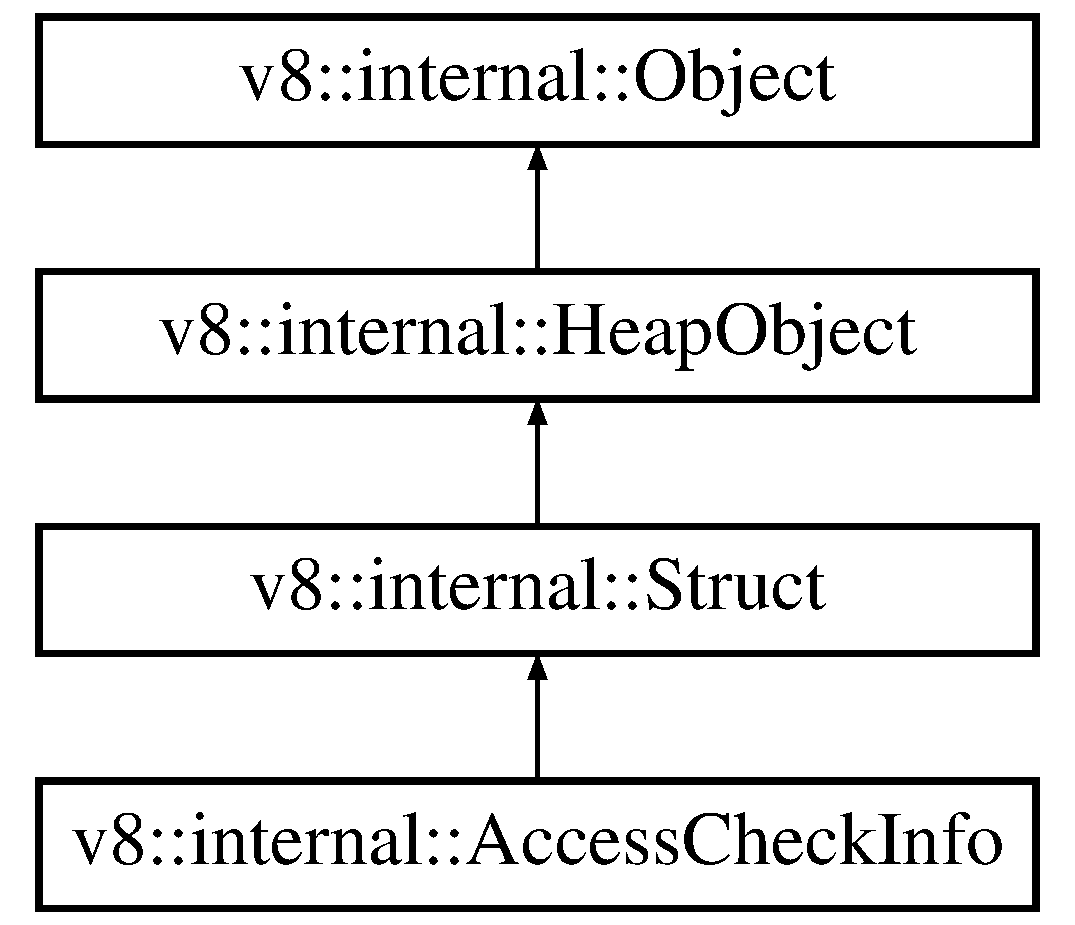
\includegraphics[height=4.000000cm]{classv8_1_1internal_1_1AccessCheckInfo}
\end{center}
\end{figure}
\subsection*{Static Public Member Functions}
\begin{DoxyCompactItemize}
\item 
\mbox{\Hypertarget{classv8_1_1internal_1_1AccessCheckInfo_a0c2e662ae5e5f08906700a929627baf2}\label{classv8_1_1internal_1_1AccessCheckInfo_a0c2e662ae5e5f08906700a929627baf2}} 
static \mbox{\hyperlink{classv8_1_1internal_1_1AccessCheckInfo}{Access\+Check\+Info}} $\ast$ {\bfseries Get} (\mbox{\hyperlink{classv8_1_1internal_1_1Isolate}{Isolate}} $\ast$isolate, \mbox{\hyperlink{classv8_1_1internal_1_1Handle}{Handle}}$<$ \mbox{\hyperlink{classv8_1_1internal_1_1JSObject}{J\+S\+Object}} $>$ receiver)
\end{DoxyCompactItemize}
\subsection*{Additional Inherited Members}


\subsection{Detailed Description}


Definition at line 114 of file api-\/callbacks.\+h.



The documentation for this class was generated from the following files\+:\begin{DoxyCompactItemize}
\item 
v8/src/objects/api-\/callbacks.\+h\item 
v8/src/objects.\+cc\end{DoxyCompactItemize}

\hypertarget{classv8_1_1internal_1_1compiler_1_1AccessInfoFactory}{}\section{v8\+:\+:internal\+:\+:compiler\+:\+:Access\+Info\+Factory Class Reference}
\label{classv8_1_1internal_1_1compiler_1_1AccessInfoFactory}\index{v8\+::internal\+::compiler\+::\+Access\+Info\+Factory@{v8\+::internal\+::compiler\+::\+Access\+Info\+Factory}}
\subsection*{Public Member Functions}
\begin{DoxyCompactItemize}
\item 
\mbox{\Hypertarget{classv8_1_1internal_1_1compiler_1_1AccessInfoFactory_a17028a5c2dfab42c5ef1d815a65376fd}\label{classv8_1_1internal_1_1compiler_1_1AccessInfoFactory_a17028a5c2dfab42c5ef1d815a65376fd}} 
{\bfseries Access\+Info\+Factory} (\mbox{\hyperlink{classv8_1_1internal_1_1compiler_1_1JSHeapBroker}{J\+S\+Heap\+Broker}} $\ast$broker, \mbox{\hyperlink{classv8_1_1internal_1_1compiler_1_1CompilationDependencies}{Compilation\+Dependencies}} $\ast$dependencies, \mbox{\hyperlink{classv8_1_1internal_1_1Handle}{Handle}}$<$ \mbox{\hyperlink{classv8_1_1internal_1_1Context}{Context}} $>$ native\+\_\+context, \mbox{\hyperlink{classv8_1_1internal_1_1Zone}{Zone}} $\ast$zone)
\item 
\mbox{\Hypertarget{classv8_1_1internal_1_1compiler_1_1AccessInfoFactory_aa7540604d39b50722ee923b8ffaf2145}\label{classv8_1_1internal_1_1compiler_1_1AccessInfoFactory_aa7540604d39b50722ee923b8ffaf2145}} 
\mbox{\hyperlink{classbool}{bool}} {\bfseries Compute\+Element\+Access\+Info} (\mbox{\hyperlink{classv8_1_1internal_1_1Handle}{Handle}}$<$ \mbox{\hyperlink{classv8_1_1internal_1_1Map}{Map}} $>$ map, Access\+Mode access\+\_\+mode, \mbox{\hyperlink{classv8_1_1internal_1_1compiler_1_1ElementAccessInfo}{Element\+Access\+Info}} $\ast$access\+\_\+info)
\item 
\mbox{\Hypertarget{classv8_1_1internal_1_1compiler_1_1AccessInfoFactory_a7345a8226a62eb0200a7a07d1a834dae}\label{classv8_1_1internal_1_1compiler_1_1AccessInfoFactory_a7345a8226a62eb0200a7a07d1a834dae}} 
\mbox{\hyperlink{classbool}{bool}} {\bfseries Compute\+Element\+Access\+Infos} (Map\+Handles const \&maps, Access\+Mode access\+\_\+mode, \mbox{\hyperlink{classv8_1_1internal_1_1ZoneVector}{Zone\+Vector}}$<$ \mbox{\hyperlink{classv8_1_1internal_1_1compiler_1_1ElementAccessInfo}{Element\+Access\+Info}} $>$ $\ast$access\+\_\+infos)
\item 
\mbox{\Hypertarget{classv8_1_1internal_1_1compiler_1_1AccessInfoFactory_a099ee7c7da8ee81a875f4f5570cdfbae}\label{classv8_1_1internal_1_1compiler_1_1AccessInfoFactory_a099ee7c7da8ee81a875f4f5570cdfbae}} 
\mbox{\hyperlink{classbool}{bool}} {\bfseries Compute\+Property\+Access\+Info} (\mbox{\hyperlink{classv8_1_1internal_1_1Handle}{Handle}}$<$ \mbox{\hyperlink{classv8_1_1internal_1_1Map}{Map}} $>$ map, \mbox{\hyperlink{classv8_1_1internal_1_1Handle}{Handle}}$<$ \mbox{\hyperlink{classv8_1_1internal_1_1Name}{Name}} $>$ name, Access\+Mode access\+\_\+mode, \mbox{\hyperlink{classv8_1_1internal_1_1compiler_1_1PropertyAccessInfo}{Property\+Access\+Info}} $\ast$access\+\_\+info)
\item 
\mbox{\Hypertarget{classv8_1_1internal_1_1compiler_1_1AccessInfoFactory_a139d76ff3de09e3284150e34ee3fe417}\label{classv8_1_1internal_1_1compiler_1_1AccessInfoFactory_a139d76ff3de09e3284150e34ee3fe417}} 
\mbox{\hyperlink{classbool}{bool}} {\bfseries Compute\+Property\+Access\+Info} (Map\+Handles const \&maps, \mbox{\hyperlink{classv8_1_1internal_1_1Handle}{Handle}}$<$ \mbox{\hyperlink{classv8_1_1internal_1_1Name}{Name}} $>$ name, Access\+Mode access\+\_\+mode, \mbox{\hyperlink{classv8_1_1internal_1_1compiler_1_1PropertyAccessInfo}{Property\+Access\+Info}} $\ast$access\+\_\+info)
\item 
\mbox{\Hypertarget{classv8_1_1internal_1_1compiler_1_1AccessInfoFactory_a6745222d7b14597455235c014d31f491}\label{classv8_1_1internal_1_1compiler_1_1AccessInfoFactory_a6745222d7b14597455235c014d31f491}} 
\mbox{\hyperlink{classbool}{bool}} {\bfseries Compute\+Property\+Access\+Infos} (Map\+Handles const \&maps, \mbox{\hyperlink{classv8_1_1internal_1_1Handle}{Handle}}$<$ \mbox{\hyperlink{classv8_1_1internal_1_1Name}{Name}} $>$ name, Access\+Mode access\+\_\+mode, \mbox{\hyperlink{classv8_1_1internal_1_1ZoneVector}{Zone\+Vector}}$<$ \mbox{\hyperlink{classv8_1_1internal_1_1compiler_1_1PropertyAccessInfo}{Property\+Access\+Info}} $>$ $\ast$access\+\_\+infos)
\end{DoxyCompactItemize}


\subsection{Detailed Description}


Definition at line 144 of file access-\/info.\+h.



The documentation for this class was generated from the following files\+:\begin{DoxyCompactItemize}
\item 
v8/src/compiler/access-\/info.\+h\item 
v8/src/compiler/access-\/info.\+cc\end{DoxyCompactItemize}

\hypertarget{classv8_1_1internal_1_1AccessorAssembler}{}\section{v8\+:\+:internal\+:\+:Accessor\+Assembler Class Reference}
\label{classv8_1_1internal_1_1AccessorAssembler}\index{v8\+::internal\+::\+Accessor\+Assembler@{v8\+::internal\+::\+Accessor\+Assembler}}
Inheritance diagram for v8\+:\+:internal\+:\+:Accessor\+Assembler\+:\begin{figure}[H]
\begin{center}
\leavevmode
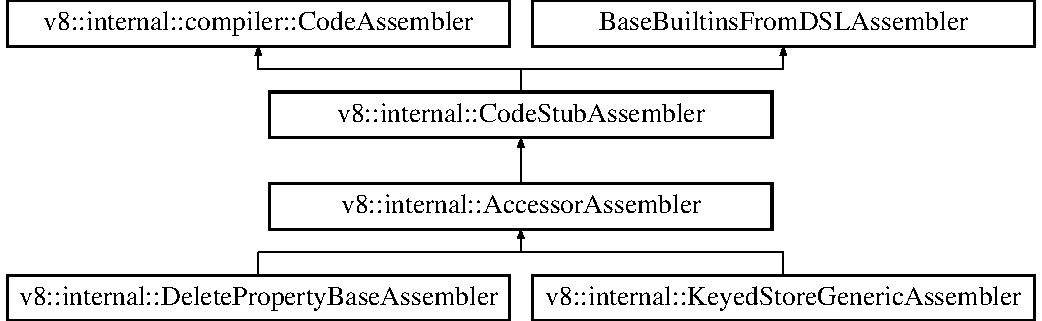
\includegraphics[height=4.000000cm]{classv8_1_1internal_1_1AccessorAssembler}
\end{center}
\end{figure}
\subsection*{Classes}
\begin{DoxyCompactItemize}
\item 
struct \mbox{\hyperlink{structv8_1_1internal_1_1AccessorAssembler_1_1LoadICParameters}{Load\+I\+C\+Parameters}}
\item 
struct \mbox{\hyperlink{structv8_1_1internal_1_1AccessorAssembler_1_1StoreICParameters}{Store\+I\+C\+Parameters}}
\end{DoxyCompactItemize}
\subsection*{Public Types}
\begin{DoxyCompactItemize}
\item 
\mbox{\Hypertarget{classv8_1_1internal_1_1AccessorAssembler_ac424f579d5482775e34a7ddb7c50641f}\label{classv8_1_1internal_1_1AccessorAssembler_ac424f579d5482775e34a7ddb7c50641f}} 
enum {\bfseries Stub\+Cache\+Table} \+: int 
\item 
\mbox{\Hypertarget{classv8_1_1internal_1_1AccessorAssembler_ad3fc3d320cbbc52ce39d758183838b26}\label{classv8_1_1internal_1_1AccessorAssembler_ad3fc3d320cbbc52ce39d758183838b26}} 
using {\bfseries Node} = \mbox{\hyperlink{classv8_1_1internal_1_1compiler_1_1Node}{compiler\+::\+Node}}
\item 
\mbox{\Hypertarget{classv8_1_1internal_1_1AccessorAssembler_aac23b1df29152a80a7e6b838febf443e}\label{classv8_1_1internal_1_1AccessorAssembler_aac23b1df29152a80a7e6b838febf443e}} 
{\footnotesize template$<$class T $>$ }\\using {\bfseries T\+Node} = \mbox{\hyperlink{classv8_1_1internal_1_1compiler_1_1TNode}{compiler\+::\+T\+Node}}$<$ \mbox{\hyperlink{classv8_1_1internal_1_1torque_1_1T}{T}} $>$
\item 
\mbox{\Hypertarget{classv8_1_1internal_1_1AccessorAssembler_aad36dbab416fd1efaee088043f54fef7}\label{classv8_1_1internal_1_1AccessorAssembler_aad36dbab416fd1efaee088043f54fef7}} 
{\footnotesize template$<$class T $>$ }\\using {\bfseries Sloppy\+T\+Node} = \mbox{\hyperlink{classv8_1_1internal_1_1compiler_1_1SloppyTNode}{compiler\+::\+Sloppy\+T\+Node}}$<$ \mbox{\hyperlink{classv8_1_1internal_1_1torque_1_1T}{T}} $>$
\end{DoxyCompactItemize}
\subsection*{Public Member Functions}
\begin{DoxyCompactItemize}
\item 
\mbox{\Hypertarget{classv8_1_1internal_1_1AccessorAssembler_ac5f87c461fb7a2a131e4eea46bbb913f}\label{classv8_1_1internal_1_1AccessorAssembler_ac5f87c461fb7a2a131e4eea46bbb913f}} 
{\bfseries Accessor\+Assembler} (\mbox{\hyperlink{classv8_1_1internal_1_1compiler_1_1CodeAssemblerState}{compiler\+::\+Code\+Assembler\+State}} $\ast$state)
\item 
\mbox{\Hypertarget{classv8_1_1internal_1_1AccessorAssembler_a9f57214585c6548e02ee354aa845f5f2}\label{classv8_1_1internal_1_1AccessorAssembler_a9f57214585c6548e02ee354aa845f5f2}} 
void {\bfseries Generate\+Load\+IC} ()
\item 
\mbox{\Hypertarget{classv8_1_1internal_1_1AccessorAssembler_a302bbfdb79be8ed012923ebef0e4b61e}\label{classv8_1_1internal_1_1AccessorAssembler_a302bbfdb79be8ed012923ebef0e4b61e}} 
void {\bfseries Generate\+Load\+I\+C\+\_\+\+Megamorphic} ()
\item 
\mbox{\Hypertarget{classv8_1_1internal_1_1AccessorAssembler_afb357a8e65b30c4cba775e1a4555722f}\label{classv8_1_1internal_1_1AccessorAssembler_afb357a8e65b30c4cba775e1a4555722f}} 
void {\bfseries Generate\+Load\+I\+C\+\_\+\+Noninlined} ()
\item 
\mbox{\Hypertarget{classv8_1_1internal_1_1AccessorAssembler_a42b6ed81459a839a6c1502b2c97cf635}\label{classv8_1_1internal_1_1AccessorAssembler_a42b6ed81459a839a6c1502b2c97cf635}} 
void {\bfseries Generate\+Load\+I\+C\+\_\+\+Uninitialized} ()
\item 
\mbox{\Hypertarget{classv8_1_1internal_1_1AccessorAssembler_a973dad3b80ababea0ab25819c421c592}\label{classv8_1_1internal_1_1AccessorAssembler_a973dad3b80ababea0ab25819c421c592}} 
void {\bfseries Generate\+Load\+I\+C\+Trampoline} ()
\item 
\mbox{\Hypertarget{classv8_1_1internal_1_1AccessorAssembler_a18b651d5375723f1806bfe3e14960d83}\label{classv8_1_1internal_1_1AccessorAssembler_a18b651d5375723f1806bfe3e14960d83}} 
void {\bfseries Generate\+Load\+I\+C\+Trampoline\+\_\+\+Megamorphic} ()
\item 
\mbox{\Hypertarget{classv8_1_1internal_1_1AccessorAssembler_affcf7f5904348ad829ecd19dd3e8ccbc}\label{classv8_1_1internal_1_1AccessorAssembler_affcf7f5904348ad829ecd19dd3e8ccbc}} 
void {\bfseries Generate\+Keyed\+Load\+IC} ()
\item 
\mbox{\Hypertarget{classv8_1_1internal_1_1AccessorAssembler_a65c4c9af1e98fb608248c78f20ab6eee}\label{classv8_1_1internal_1_1AccessorAssembler_a65c4c9af1e98fb608248c78f20ab6eee}} 
void {\bfseries Generate\+Keyed\+Load\+I\+C\+\_\+\+Megamorphic} ()
\item 
\mbox{\Hypertarget{classv8_1_1internal_1_1AccessorAssembler_a1fccdac58c30307146808c54e7968258}\label{classv8_1_1internal_1_1AccessorAssembler_a1fccdac58c30307146808c54e7968258}} 
void {\bfseries Generate\+Keyed\+Load\+I\+C\+\_\+\+Polymorphic\+Name} ()
\item 
\mbox{\Hypertarget{classv8_1_1internal_1_1AccessorAssembler_ae9dbf9db99c0487e5592b15358499bd3}\label{classv8_1_1internal_1_1AccessorAssembler_ae9dbf9db99c0487e5592b15358499bd3}} 
void {\bfseries Generate\+Keyed\+Load\+I\+C\+Trampoline} ()
\item 
\mbox{\Hypertarget{classv8_1_1internal_1_1AccessorAssembler_a0733221e4e8a9585f5fd933d86d5094a}\label{classv8_1_1internal_1_1AccessorAssembler_a0733221e4e8a9585f5fd933d86d5094a}} 
void {\bfseries Generate\+Keyed\+Load\+I\+C\+Trampoline\+\_\+\+Megamorphic} ()
\item 
\mbox{\Hypertarget{classv8_1_1internal_1_1AccessorAssembler_a34dd95f53f34456097f77bdad385dafe}\label{classv8_1_1internal_1_1AccessorAssembler_a34dd95f53f34456097f77bdad385dafe}} 
void {\bfseries Generate\+Store\+IC} ()
\item 
\mbox{\Hypertarget{classv8_1_1internal_1_1AccessorAssembler_ab18160d8870126c01fe14a0b2b08c021}\label{classv8_1_1internal_1_1AccessorAssembler_ab18160d8870126c01fe14a0b2b08c021}} 
void {\bfseries Generate\+Store\+I\+C\+Trampoline} ()
\item 
\mbox{\Hypertarget{classv8_1_1internal_1_1AccessorAssembler_a95eab448aed0c8a803399d9b5ffe1979}\label{classv8_1_1internal_1_1AccessorAssembler_a95eab448aed0c8a803399d9b5ffe1979}} 
void {\bfseries Generate\+Store\+Global\+IC} ()
\item 
\mbox{\Hypertarget{classv8_1_1internal_1_1AccessorAssembler_a9c52911d81ba441ca1c0d10eda114d79}\label{classv8_1_1internal_1_1AccessorAssembler_a9c52911d81ba441ca1c0d10eda114d79}} 
void {\bfseries Generate\+Store\+Global\+I\+C\+Trampoline} ()
\item 
\mbox{\Hypertarget{classv8_1_1internal_1_1AccessorAssembler_a886d4a0bbe21ac64fac3bcf4372333d7}\label{classv8_1_1internal_1_1AccessorAssembler_a886d4a0bbe21ac64fac3bcf4372333d7}} 
void {\bfseries Generate\+Clone\+Object\+IC} ()
\item 
\mbox{\Hypertarget{classv8_1_1internal_1_1AccessorAssembler_a6ec83695032cac953966bf680fed5d70}\label{classv8_1_1internal_1_1AccessorAssembler_a6ec83695032cac953966bf680fed5d70}} 
void {\bfseries Generate\+Clone\+Object\+I\+C\+\_\+\+Slow} ()
\item 
\mbox{\Hypertarget{classv8_1_1internal_1_1AccessorAssembler_afbc89049e6575b3b24a150fd1c4f8363}\label{classv8_1_1internal_1_1AccessorAssembler_afbc89049e6575b3b24a150fd1c4f8363}} 
void {\bfseries Generate\+Load\+Global\+IC} (Typeof\+Mode typeof\+\_\+mode)
\item 
\mbox{\Hypertarget{classv8_1_1internal_1_1AccessorAssembler_a3836b2d01020ddcf406b92a2b7f74f6c}\label{classv8_1_1internal_1_1AccessorAssembler_a3836b2d01020ddcf406b92a2b7f74f6c}} 
void {\bfseries Generate\+Load\+Global\+I\+C\+Trampoline} (Typeof\+Mode typeof\+\_\+mode)
\item 
\mbox{\Hypertarget{classv8_1_1internal_1_1AccessorAssembler_a39fd539fa6323ddd8ce611d67113e241}\label{classv8_1_1internal_1_1AccessorAssembler_a39fd539fa6323ddd8ce611d67113e241}} 
void {\bfseries Generate\+Keyed\+Store\+IC} ()
\item 
\mbox{\Hypertarget{classv8_1_1internal_1_1AccessorAssembler_a90ee1401264405f6e5f341aa7c6562bc}\label{classv8_1_1internal_1_1AccessorAssembler_a90ee1401264405f6e5f341aa7c6562bc}} 
void {\bfseries Generate\+Keyed\+Store\+I\+C\+Trampoline} ()
\item 
\mbox{\Hypertarget{classv8_1_1internal_1_1AccessorAssembler_a58b259d4bf86ef2e4fa32465a37a14a4}\label{classv8_1_1internal_1_1AccessorAssembler_a58b259d4bf86ef2e4fa32465a37a14a4}} 
void {\bfseries Generate\+Store\+In\+Array\+Literal\+IC} ()
\item 
\mbox{\Hypertarget{classv8_1_1internal_1_1AccessorAssembler_a2660145f33a4d35f58611986ada0310c}\label{classv8_1_1internal_1_1AccessorAssembler_a2660145f33a4d35f58611986ada0310c}} 
void {\bfseries Try\+Probe\+Stub\+Cache} (\mbox{\hyperlink{classv8_1_1internal_1_1StubCache}{Stub\+Cache}} $\ast$stub\+\_\+cache, \mbox{\hyperlink{classv8_1_1internal_1_1compiler_1_1Node}{Node}} $\ast$receiver, \mbox{\hyperlink{classv8_1_1internal_1_1compiler_1_1Node}{Node}} $\ast$name, \mbox{\hyperlink{classv8_1_1internal_1_1compiler_1_1CodeAssemblerLabel}{Label}} $\ast$if\+\_\+handler, \mbox{\hyperlink{classv8_1_1internal_1_1compiler_1_1TypedCodeAssemblerVariable}{T\+Variable}}$<$ \mbox{\hyperlink{classv8_1_1internal_1_1MaybeObject}{Maybe\+Object}} $>$ $\ast$var\+\_\+handler, \mbox{\hyperlink{classv8_1_1internal_1_1compiler_1_1CodeAssemblerLabel}{Label}} $\ast$if\+\_\+miss)
\item 
\mbox{\Hypertarget{classv8_1_1internal_1_1AccessorAssembler_a5c64f57e40af257c1892f3c59ff2e403}\label{classv8_1_1internal_1_1AccessorAssembler_a5c64f57e40af257c1892f3c59ff2e403}} 
\mbox{\hyperlink{classv8_1_1internal_1_1compiler_1_1Node}{Node}} $\ast$ {\bfseries Stub\+Cache\+Primary\+Offset\+For\+Testing} (\mbox{\hyperlink{classv8_1_1internal_1_1compiler_1_1Node}{Node}} $\ast$name, \mbox{\hyperlink{classv8_1_1internal_1_1compiler_1_1Node}{Node}} $\ast$map)
\item 
\mbox{\Hypertarget{classv8_1_1internal_1_1AccessorAssembler_a46a3bc8482b1bb197725fbdc05184151}\label{classv8_1_1internal_1_1AccessorAssembler_a46a3bc8482b1bb197725fbdc05184151}} 
\mbox{\hyperlink{classv8_1_1internal_1_1compiler_1_1Node}{Node}} $\ast$ {\bfseries Stub\+Cache\+Secondary\+Offset\+For\+Testing} (\mbox{\hyperlink{classv8_1_1internal_1_1compiler_1_1Node}{Node}} $\ast$name, \mbox{\hyperlink{classv8_1_1internal_1_1compiler_1_1Node}{Node}} $\ast$map)
\item 
\mbox{\Hypertarget{classv8_1_1internal_1_1AccessorAssembler_ab34e9435b84e52bb6b45cbbe9306e48c}\label{classv8_1_1internal_1_1AccessorAssembler_ab34e9435b84e52bb6b45cbbe9306e48c}} 
void {\bfseries Load\+Global\+IC} (\mbox{\hyperlink{classv8_1_1internal_1_1compiler_1_1TNode}{T\+Node}}$<$ \mbox{\hyperlink{classv8_1_1internal_1_1FeedbackVector}{Feedback\+Vector}} $>$ vector, \mbox{\hyperlink{classv8_1_1internal_1_1compiler_1_1Node}{Node}} $\ast$slot, const Lazy\+Node$<$ \mbox{\hyperlink{classv8_1_1internal_1_1Context}{Context}} $>$ \&lazy\+\_\+context, const Lazy\+Node$<$ \mbox{\hyperlink{classv8_1_1internal_1_1Name}{Name}} $>$ \&lazy\+\_\+name, Typeof\+Mode typeof\+\_\+mode, \mbox{\hyperlink{classv8_1_1internal_1_1ExitPoint}{Exit\+Point}} $\ast$exit\+\_\+point, Parameter\+Mode slot\+\_\+mode=S\+M\+I\+\_\+\+P\+A\+R\+A\+M\+E\+T\+E\+RS)
\item 
\mbox{\Hypertarget{classv8_1_1internal_1_1AccessorAssembler_a85d65e97ff44089ace23b4a5473328f6}\label{classv8_1_1internal_1_1AccessorAssembler_a85d65e97ff44089ace23b4a5473328f6}} 
void {\bfseries Load\+I\+C\+\_\+\+Bytecode\+Handler} (const \mbox{\hyperlink{structv8_1_1internal_1_1AccessorAssembler_1_1LoadICParameters}{Load\+I\+C\+Parameters}} $\ast$p, \mbox{\hyperlink{classv8_1_1internal_1_1ExitPoint}{Exit\+Point}} $\ast$exit\+\_\+point)
\item 
\mbox{\Hypertarget{classv8_1_1internal_1_1AccessorAssembler_a1d6263170cec57726ff3a77349c5aa1e}\label{classv8_1_1internal_1_1AccessorAssembler_a1d6263170cec57726ff3a77349c5aa1e}} 
\mbox{\hyperlink{classv8_1_1internal_1_1compiler_1_1TNode}{T\+Node}}$<$ \mbox{\hyperlink{classv8_1_1internal_1_1MaybeObject}{Maybe\+Object}} $>$ {\bfseries Load\+Handler\+Data\+Field} (\mbox{\hyperlink{classv8_1_1internal_1_1compiler_1_1SloppyTNode}{Sloppy\+T\+Node}}$<$ \mbox{\hyperlink{classv8_1_1internal_1_1DataHandler}{Data\+Handler}} $>$ handler, \mbox{\hyperlink{classint}{int}} data\+\_\+index)
\end{DoxyCompactItemize}
\subsection*{Protected Types}
\begin{DoxyCompactItemize}
\item 
\mbox{\Hypertarget{classv8_1_1internal_1_1AccessorAssembler_ab680069b3f903c5909b50e8f70826da1}\label{classv8_1_1internal_1_1AccessorAssembler_ab680069b3f903c5909b50e8f70826da1}} 
enum {\bfseries I\+C\+Mode} \{ {\bfseries k\+Non\+Global\+IC}, 
{\bfseries k\+Global\+IC}
 \}
\item 
\mbox{\Hypertarget{classv8_1_1internal_1_1AccessorAssembler_a59966ccd362f71285c76c4d7a981921c}\label{classv8_1_1internal_1_1AccessorAssembler_a59966ccd362f71285c76c4d7a981921c}} 
enum {\bfseries Element\+Support} \{ {\bfseries k\+Only\+Properties}, 
{\bfseries k\+Support\+Elements}
 \}
\item 
\mbox{\Hypertarget{classv8_1_1internal_1_1AccessorAssembler_a5b45e778221700bc7a06663e55c48912}\label{classv8_1_1internal_1_1AccessorAssembler_a5b45e778221700bc7a06663e55c48912}} 
enum {\bfseries Store\+Transition\+Map\+Flags} \{ {\bfseries k\+Check\+Prototype\+Validity} = 1 $<$$<$ 0, 
{\bfseries k\+Validate\+Transition\+Handler} = 1 $<$$<$ 1, 
{\bfseries k\+Store\+Transition\+Map\+Flags\+Mask}
 \}
\end{DoxyCompactItemize}
\subsection*{Protected Member Functions}
\begin{DoxyCompactItemize}
\item 
\mbox{\Hypertarget{classv8_1_1internal_1_1AccessorAssembler_a6943af3ec771ef419897e88e2a9854e5}\label{classv8_1_1internal_1_1AccessorAssembler_a6943af3ec771ef419897e88e2a9854e5}} 
void {\bfseries Handle\+Store\+I\+C\+Handler\+Case} (const \mbox{\hyperlink{structv8_1_1internal_1_1AccessorAssembler_1_1StoreICParameters}{Store\+I\+C\+Parameters}} $\ast$p, \mbox{\hyperlink{classv8_1_1internal_1_1compiler_1_1TNode}{T\+Node}}$<$ \mbox{\hyperlink{classv8_1_1internal_1_1MaybeObject}{Maybe\+Object}} $>$ handler, \mbox{\hyperlink{classv8_1_1internal_1_1compiler_1_1CodeAssemblerLabel}{Label}} $\ast$miss, I\+C\+Mode ic\+\_\+mode, Element\+Support support\+\_\+elements=k\+Only\+Properties)
\item 
\mbox{\Hypertarget{classv8_1_1internal_1_1AccessorAssembler_a4b8655f3c396b72381847f3a120f0c0f}\label{classv8_1_1internal_1_1AccessorAssembler_a4b8655f3c396b72381847f3a120f0c0f}} 
void {\bfseries Handle\+Store\+I\+C\+Transition\+Map\+Handler\+Case} (const \mbox{\hyperlink{structv8_1_1internal_1_1AccessorAssembler_1_1StoreICParameters}{Store\+I\+C\+Parameters}} $\ast$p, \mbox{\hyperlink{classv8_1_1internal_1_1compiler_1_1TNode}{T\+Node}}$<$ \mbox{\hyperlink{classv8_1_1internal_1_1Map}{Map}} $>$ transition\+\_\+map, \mbox{\hyperlink{classv8_1_1internal_1_1compiler_1_1CodeAssemblerLabel}{Label}} $\ast$miss, Store\+Transition\+Map\+Flags flags)
\item 
\mbox{\Hypertarget{classv8_1_1internal_1_1AccessorAssembler_a543857db01e790acf2d7a134d7302565}\label{classv8_1_1internal_1_1AccessorAssembler_a543857db01e790acf2d7a134d7302565}} 
void {\bfseries Jump\+If\+Data\+Property} (\mbox{\hyperlink{classv8_1_1internal_1_1compiler_1_1Node}{Node}} $\ast$details, \mbox{\hyperlink{classv8_1_1internal_1_1compiler_1_1CodeAssemblerLabel}{Label}} $\ast$writable, \mbox{\hyperlink{classv8_1_1internal_1_1compiler_1_1CodeAssemblerLabel}{Label}} $\ast$readonly)
\item 
\mbox{\Hypertarget{classv8_1_1internal_1_1AccessorAssembler_a63c8a898b155643eb1ea765dc539dffb}\label{classv8_1_1internal_1_1AccessorAssembler_a63c8a898b155643eb1ea765dc539dffb}} 
void {\bfseries Branch\+If\+Strict\+Mode} (\mbox{\hyperlink{classv8_1_1internal_1_1compiler_1_1Node}{Node}} $\ast$vector, \mbox{\hyperlink{classv8_1_1internal_1_1compiler_1_1Node}{Node}} $\ast$slot, \mbox{\hyperlink{classv8_1_1internal_1_1compiler_1_1CodeAssemblerLabel}{Label}} $\ast$if\+\_\+strict)
\item 
\mbox{\Hypertarget{classv8_1_1internal_1_1AccessorAssembler_a5d7fc228f04a83d2c5446f49ee6003c7}\label{classv8_1_1internal_1_1AccessorAssembler_a5d7fc228f04a83d2c5446f49ee6003c7}} 
void {\bfseries Invalidate\+Validity\+Cell\+If\+Prototype} (\mbox{\hyperlink{classv8_1_1internal_1_1compiler_1_1Node}{Node}} $\ast$map, \mbox{\hyperlink{classv8_1_1internal_1_1compiler_1_1Node}{Node}} $\ast$bitfield2=nullptr)
\item 
\mbox{\Hypertarget{classv8_1_1internal_1_1AccessorAssembler_a0e78b9a81ba4a3b986f11dbcb2dde5b5}\label{classv8_1_1internal_1_1AccessorAssembler_a0e78b9a81ba4a3b986f11dbcb2dde5b5}} 
void {\bfseries Overwrite\+Existing\+Fast\+Data\+Property} (\mbox{\hyperlink{classv8_1_1internal_1_1compiler_1_1Node}{Node}} $\ast$object, \mbox{\hyperlink{classv8_1_1internal_1_1compiler_1_1Node}{Node}} $\ast$object\+\_\+map, \mbox{\hyperlink{classv8_1_1internal_1_1compiler_1_1Node}{Node}} $\ast$descriptors, \mbox{\hyperlink{classv8_1_1internal_1_1compiler_1_1Node}{Node}} $\ast$descriptor\+\_\+name\+\_\+index, \mbox{\hyperlink{classv8_1_1internal_1_1compiler_1_1Node}{Node}} $\ast$details, \mbox{\hyperlink{classv8_1_1internal_1_1compiler_1_1Node}{Node}} $\ast$value, \mbox{\hyperlink{classv8_1_1internal_1_1compiler_1_1CodeAssemblerLabel}{Label}} $\ast$slow, \mbox{\hyperlink{classbool}{bool}} do\+\_\+transitioning\+\_\+store)
\item 
\mbox{\Hypertarget{classv8_1_1internal_1_1AccessorAssembler_a6be694fde5be8530afc07da11dbcc742}\label{classv8_1_1internal_1_1AccessorAssembler_a6be694fde5be8530afc07da11dbcc742}} 
void {\bfseries Check\+Field\+Type} (\mbox{\hyperlink{classv8_1_1internal_1_1compiler_1_1TNode}{T\+Node}}$<$ \mbox{\hyperlink{classv8_1_1internal_1_1DescriptorArray}{Descriptor\+Array}} $>$ descriptors, \mbox{\hyperlink{classv8_1_1internal_1_1compiler_1_1Node}{Node}} $\ast$name\+\_\+index, \mbox{\hyperlink{classv8_1_1internal_1_1compiler_1_1Node}{Node}} $\ast$representation, \mbox{\hyperlink{classv8_1_1internal_1_1compiler_1_1Node}{Node}} $\ast$value, \mbox{\hyperlink{classv8_1_1internal_1_1compiler_1_1CodeAssemblerLabel}{Label}} $\ast$bailout)
\end{DoxyCompactItemize}
\subsection*{Additional Inherited Members}


\subsection{Detailed Description}


Definition at line 19 of file accessor-\/assembler.\+h.



The documentation for this class was generated from the following files\+:\begin{DoxyCompactItemize}
\item 
v8/src/ic/accessor-\/assembler.\+h\item 
v8/src/ic/accessor-\/assembler.\+cc\end{DoxyCompactItemize}

\hypertarget{classv8_1_1internal_1_1AccessorInfo}{}\section{v8\+:\+:internal\+:\+:Accessor\+Info Class Reference}
\label{classv8_1_1internal_1_1AccessorInfo}\index{v8\+::internal\+::\+Accessor\+Info@{v8\+::internal\+::\+Accessor\+Info}}
Inheritance diagram for v8\+:\+:internal\+:\+:Accessor\+Info\+:\begin{figure}[H]
\begin{center}
\leavevmode
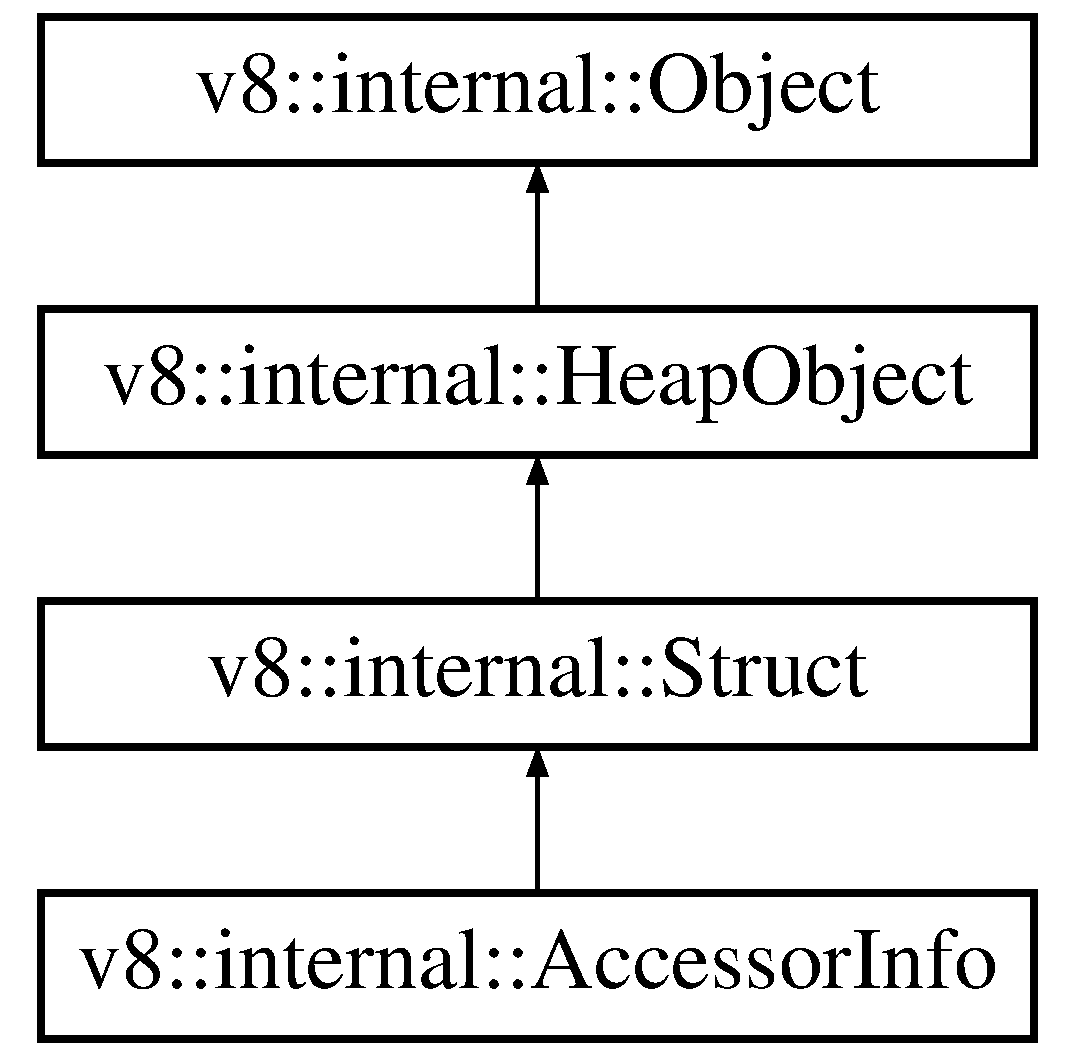
\includegraphics[height=4.000000cm]{classv8_1_1internal_1_1AccessorInfo}
\end{center}
\end{figure}
\subsection*{Public Member Functions}
\begin{DoxyCompactItemize}
\item 
\mbox{\Hypertarget{classv8_1_1internal_1_1AccessorInfo_a7819739d3765461abfd5abf0b24be4b0}\label{classv8_1_1internal_1_1AccessorInfo_a7819739d3765461abfd5abf0b24be4b0}} 
\mbox{\hyperlink{classbool}{bool}} {\bfseries has\+\_\+getter} ()
\item 
\mbox{\Hypertarget{classv8_1_1internal_1_1AccessorInfo_ae85b482de034f9e2546235613faaa282}\label{classv8_1_1internal_1_1AccessorInfo_ae85b482de034f9e2546235613faaa282}} 
\mbox{\hyperlink{classbool}{bool}} {\bfseries has\+\_\+setter} ()
\item 
\mbox{\Hypertarget{classv8_1_1internal_1_1AccessorInfo_a2a44d60a6c999399bc786daadd50eaa5}\label{classv8_1_1internal_1_1AccessorInfo_a2a44d60a6c999399bc786daadd50eaa5}} 
\mbox{\hyperlink{classuintptr__t}{Address}} {\bfseries redirected\+\_\+getter} () const
\item 
\mbox{\Hypertarget{classv8_1_1internal_1_1AccessorInfo_aee70d695d1886be0bf3b751b0822cc78}\label{classv8_1_1internal_1_1AccessorInfo_aee70d695d1886be0bf3b751b0822cc78}} 
\mbox{\hyperlink{namespacev8_a29711319c2b9fc7716d65faee2f7b9cb}{Side\+Effect\+Type}} {\bfseries getter\+\_\+side\+\_\+effect\+\_\+type} () const
\item 
\mbox{\Hypertarget{classv8_1_1internal_1_1AccessorInfo_a17a2f98f599bfca12ae98864bcd62a9f}\label{classv8_1_1internal_1_1AccessorInfo_a17a2f98f599bfca12ae98864bcd62a9f}} 
void {\bfseries set\+\_\+getter\+\_\+side\+\_\+effect\+\_\+type} (\mbox{\hyperlink{namespacev8_a29711319c2b9fc7716d65faee2f7b9cb}{Side\+Effect\+Type}} \mbox{\hyperlink{classstd_1_1conditional_1_1type}{type}})
\item 
\mbox{\Hypertarget{classv8_1_1internal_1_1AccessorInfo_ad65b262a288c68b1d035a72a5eb41cb5}\label{classv8_1_1internal_1_1AccessorInfo_ad65b262a288c68b1d035a72a5eb41cb5}} 
\mbox{\hyperlink{namespacev8_a29711319c2b9fc7716d65faee2f7b9cb}{Side\+Effect\+Type}} {\bfseries setter\+\_\+side\+\_\+effect\+\_\+type} () const
\item 
\mbox{\Hypertarget{classv8_1_1internal_1_1AccessorInfo_a3a9d365acf903d0ccbd2b0f28e3f3c64}\label{classv8_1_1internal_1_1AccessorInfo_a3a9d365acf903d0ccbd2b0f28e3f3c64}} 
void {\bfseries set\+\_\+setter\+\_\+side\+\_\+effect\+\_\+type} (\mbox{\hyperlink{namespacev8_a29711319c2b9fc7716d65faee2f7b9cb}{Side\+Effect\+Type}} \mbox{\hyperlink{classstd_1_1conditional_1_1type}{type}})
\item 
\mbox{\Hypertarget{classv8_1_1internal_1_1AccessorInfo_a5227934dc0ed67b3fc9bfaeec075dce1}\label{classv8_1_1internal_1_1AccessorInfo_a5227934dc0ed67b3fc9bfaeec075dce1}} 
Property\+Attributes {\bfseries initial\+\_\+property\+\_\+attributes} () const
\item 
\mbox{\Hypertarget{classv8_1_1internal_1_1AccessorInfo_a51a6ab406362f4132dd149ec1bc3b2f3}\label{classv8_1_1internal_1_1AccessorInfo_a51a6ab406362f4132dd149ec1bc3b2f3}} 
void {\bfseries set\+\_\+initial\+\_\+property\+\_\+attributes} (Property\+Attributes attributes)
\item 
\mbox{\Hypertarget{classv8_1_1internal_1_1AccessorInfo_af90ccc9b509016f749a5d69a29cebdf4}\label{classv8_1_1internal_1_1AccessorInfo_af90ccc9b509016f749a5d69a29cebdf4}} 
\mbox{\hyperlink{classbool}{bool}} {\bfseries Is\+Compatible\+Receiver} (\mbox{\hyperlink{classv8_1_1internal_1_1Object}{Object}} $\ast$receiver)
\end{DoxyCompactItemize}
\subsection*{Static Public Member Functions}
\begin{DoxyCompactItemize}
\item 
\mbox{\Hypertarget{classv8_1_1internal_1_1AccessorInfo_ae0638d82499bd7bc3b816c8744157291}\label{classv8_1_1internal_1_1AccessorInfo_ae0638d82499bd7bc3b816c8744157291}} 
static \mbox{\hyperlink{classuintptr__t}{Address}} {\bfseries redirect} (\mbox{\hyperlink{classuintptr__t}{Address}} address, Accessor\+Component component)
\item 
\mbox{\Hypertarget{classv8_1_1internal_1_1AccessorInfo_abd637250c18c0e918ff597f3aa464710}\label{classv8_1_1internal_1_1AccessorInfo_abd637250c18c0e918ff597f3aa464710}} 
static \mbox{\hyperlink{classbool}{bool}} {\bfseries Is\+Compatible\+Receiver\+Map} (\mbox{\hyperlink{classv8_1_1internal_1_1Handle}{Handle}}$<$ \mbox{\hyperlink{classv8_1_1internal_1_1AccessorInfo}{Accessor\+Info}} $>$ info, \mbox{\hyperlink{classv8_1_1internal_1_1Handle}{Handle}}$<$ \mbox{\hyperlink{classv8_1_1internal_1_1Map}{Map}} $>$ map)
\item 
\mbox{\Hypertarget{classv8_1_1internal_1_1AccessorInfo_af87b3a434ca18d04913dcf6aa462b7c2}\label{classv8_1_1internal_1_1AccessorInfo_af87b3a434ca18d04913dcf6aa462b7c2}} 
static \mbox{\hyperlink{classint}{int}} {\bfseries Append\+Unique} (\mbox{\hyperlink{classv8_1_1internal_1_1Isolate}{Isolate}} $\ast$isolate, \mbox{\hyperlink{classv8_1_1internal_1_1Handle}{Handle}}$<$ \mbox{\hyperlink{classv8_1_1internal_1_1Object}{Object}} $>$ descriptors, \mbox{\hyperlink{classv8_1_1internal_1_1Handle}{Handle}}$<$ \mbox{\hyperlink{classv8_1_1internal_1_1FixedArray}{Fixed\+Array}} $>$ array, \mbox{\hyperlink{classint}{int}} valid\+\_\+descriptors)
\end{DoxyCompactItemize}
\subsection*{Additional Inherited Members}


\subsection{Detailed Description}


Definition at line 25 of file api-\/callbacks.\+h.



The documentation for this class was generated from the following files\+:\begin{DoxyCompactItemize}
\item 
v8/src/objects/api-\/callbacks.\+h\item 
v8/src/objects/api-\/callbacks-\/inl.\+h\item 
v8/src/objects.\+cc\end{DoxyCompactItemize}

\hypertarget{classv8_1_1internal_1_1AccessorPair}{}\section{v8\+:\+:internal\+:\+:Accessor\+Pair Class Reference}
\label{classv8_1_1internal_1_1AccessorPair}\index{v8\+::internal\+::\+Accessor\+Pair@{v8\+::internal\+::\+Accessor\+Pair}}
Inheritance diagram for v8\+:\+:internal\+:\+:Accessor\+Pair\+:\begin{figure}[H]
\begin{center}
\leavevmode
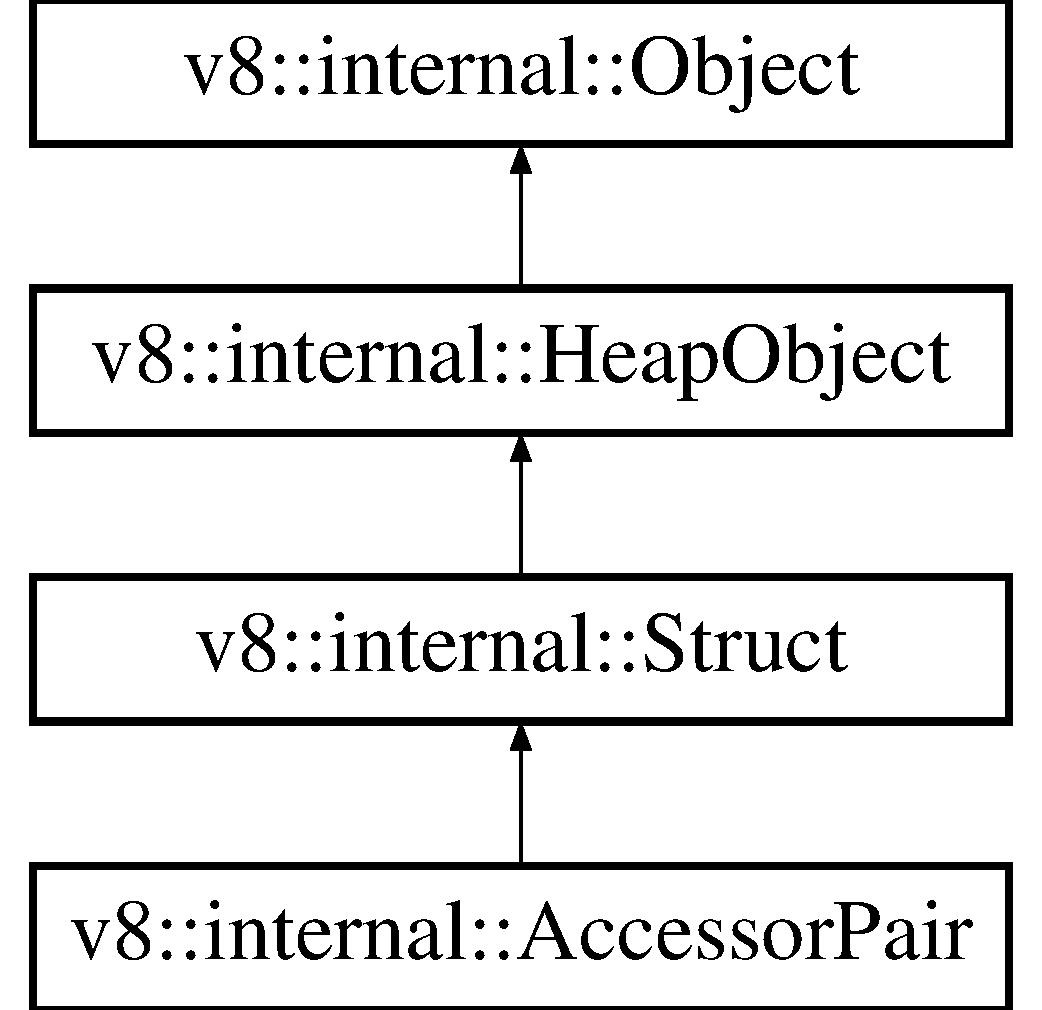
\includegraphics[height=4.000000cm]{classv8_1_1internal_1_1AccessorPair}
\end{center}
\end{figure}
\subsection*{Public Member Functions}
\begin{DoxyCompactItemize}
\item 
\mbox{\Hypertarget{classv8_1_1internal_1_1AccessorPair_a66569cd687b684427f0d9d34514858a6}\label{classv8_1_1internal_1_1AccessorPair_a66569cd687b684427f0d9d34514858a6}} 
\mbox{\hyperlink{classv8_1_1internal_1_1Object}{Object}} $\ast$ {\bfseries get} (Accessor\+Component component)
\item 
\mbox{\Hypertarget{classv8_1_1internal_1_1AccessorPair_ad2a9c19f26306e325c88a48431f1f2c1}\label{classv8_1_1internal_1_1AccessorPair_ad2a9c19f26306e325c88a48431f1f2c1}} 
void {\bfseries set} (Accessor\+Component component, \mbox{\hyperlink{classv8_1_1internal_1_1Object}{Object}} $\ast$value)
\item 
\mbox{\Hypertarget{classv8_1_1internal_1_1AccessorPair_a6e5a2de9676c59e75ff73635f152a27d}\label{classv8_1_1internal_1_1AccessorPair_a6e5a2de9676c59e75ff73635f152a27d}} 
void {\bfseries Set\+Components} (\mbox{\hyperlink{classv8_1_1internal_1_1Object}{Object}} $\ast$getter, \mbox{\hyperlink{classv8_1_1internal_1_1Object}{Object}} $\ast$setter)
\item 
\mbox{\Hypertarget{classv8_1_1internal_1_1AccessorPair_a074f0577eb38b61f347071f85120339b}\label{classv8_1_1internal_1_1AccessorPair_a074f0577eb38b61f347071f85120339b}} 
\mbox{\hyperlink{classbool}{bool}} {\bfseries Equals} (\mbox{\hyperlink{classv8_1_1internal_1_1AccessorPair}{Accessor\+Pair}} $\ast$pair)
\item 
\mbox{\Hypertarget{classv8_1_1internal_1_1AccessorPair_aeb0ab989aa8c299311ea5ad17c496732}\label{classv8_1_1internal_1_1AccessorPair_aeb0ab989aa8c299311ea5ad17c496732}} 
\mbox{\hyperlink{classbool}{bool}} {\bfseries Equals} (\mbox{\hyperlink{classv8_1_1internal_1_1Object}{Object}} $\ast$getter\+\_\+value, \mbox{\hyperlink{classv8_1_1internal_1_1Object}{Object}} $\ast$setter\+\_\+value)
\item 
\mbox{\Hypertarget{classv8_1_1internal_1_1AccessorPair_a3776e1f65c6612d9cb544747211bd3f0}\label{classv8_1_1internal_1_1AccessorPair_a3776e1f65c6612d9cb544747211bd3f0}} 
\mbox{\hyperlink{classbool}{bool}} {\bfseries Contains\+Accessor} ()
\end{DoxyCompactItemize}
\subsection*{Static Public Member Functions}
\begin{DoxyCompactItemize}
\item 
\mbox{\Hypertarget{classv8_1_1internal_1_1AccessorPair_a9f5c37f34a6087031558a7642ea2753b}\label{classv8_1_1internal_1_1AccessorPair_a9f5c37f34a6087031558a7642ea2753b}} 
static \mbox{\hyperlink{classv8_1_1internal_1_1Handle}{Handle}}$<$ \mbox{\hyperlink{classv8_1_1internal_1_1AccessorPair}{Accessor\+Pair}} $>$ {\bfseries Copy} (\mbox{\hyperlink{classv8_1_1internal_1_1Isolate}{Isolate}} $\ast$isolate, \mbox{\hyperlink{classv8_1_1internal_1_1Handle}{Handle}}$<$ \mbox{\hyperlink{classv8_1_1internal_1_1AccessorPair}{Accessor\+Pair}} $>$ pair)
\item 
\mbox{\Hypertarget{classv8_1_1internal_1_1AccessorPair_aa6a6d7bece4c45ec21d798e0c6c910b7}\label{classv8_1_1internal_1_1AccessorPair_aa6a6d7bece4c45ec21d798e0c6c910b7}} 
static \mbox{\hyperlink{classv8_1_1internal_1_1Handle}{Handle}}$<$ \mbox{\hyperlink{classv8_1_1internal_1_1Object}{Object}} $>$ {\bfseries Get\+Component} (\mbox{\hyperlink{classv8_1_1internal_1_1Isolate}{Isolate}} $\ast$isolate, \mbox{\hyperlink{classv8_1_1internal_1_1Handle}{Handle}}$<$ \mbox{\hyperlink{classv8_1_1internal_1_1AccessorPair}{Accessor\+Pair}} $>$ accessor\+\_\+pair, Accessor\+Component component)
\end{DoxyCompactItemize}
\subsection*{Static Public Attributes}
\begin{DoxyCompactItemize}
\item 
\mbox{\Hypertarget{classv8_1_1internal_1_1AccessorPair_aa7ee07b7098a35f0e1340c33dadb90db}\label{classv8_1_1internal_1_1AccessorPair_aa7ee07b7098a35f0e1340c33dadb90db}} 
static const \mbox{\hyperlink{classint}{int}} {\bfseries k\+Getter\+Offset} = Heap\+Object\+::k\+Header\+Size
\item 
\mbox{\Hypertarget{classv8_1_1internal_1_1AccessorPair_adaca2d4fb0dfcf2e29fd37fc5549737b}\label{classv8_1_1internal_1_1AccessorPair_adaca2d4fb0dfcf2e29fd37fc5549737b}} 
static const \mbox{\hyperlink{classint}{int}} {\bfseries k\+Setter\+Offset} = k\+Getter\+Offset + k\+Pointer\+Size
\item 
\mbox{\Hypertarget{classv8_1_1internal_1_1AccessorPair_a89c0268865b5203f29820f82b5e46cb5}\label{classv8_1_1internal_1_1AccessorPair_a89c0268865b5203f29820f82b5e46cb5}} 
static const \mbox{\hyperlink{classint}{int}} {\bfseries k\+Size} = k\+Setter\+Offset + k\+Pointer\+Size
\end{DoxyCompactItemize}
\subsection*{Additional Inherited Members}


\subsection{Detailed Description}


Definition at line 1657 of file objects.\+h.



The documentation for this class was generated from the following files\+:\begin{DoxyCompactItemize}
\item 
v8/src/objects.\+h\item 
v8/src/objects-\/inl.\+h\item 
v8/src/objects.\+cc\end{DoxyCompactItemize}

\hypertarget{structv8_1_1internal_1_1ObjectLiteral_1_1Accessors}{}\section{v8\+:\+:internal\+:\+:Object\+Literal\+:\+:Accessors Struct Reference}
\label{structv8_1_1internal_1_1ObjectLiteral_1_1Accessors}\index{v8\+::internal\+::\+Object\+Literal\+::\+Accessors@{v8\+::internal\+::\+Object\+Literal\+::\+Accessors}}
Inheritance diagram for v8\+:\+:internal\+:\+:Object\+Literal\+:\+:Accessors\+:\begin{figure}[H]
\begin{center}
\leavevmode
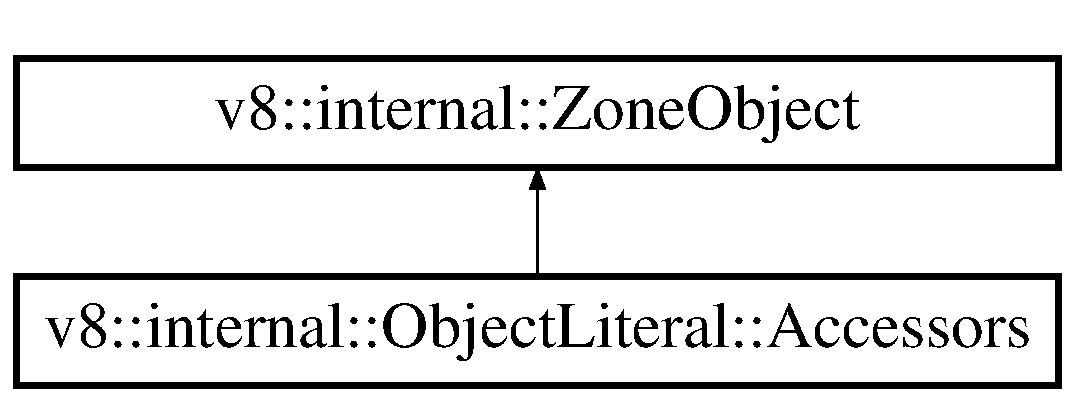
\includegraphics[height=2.000000cm]{structv8_1_1internal_1_1ObjectLiteral_1_1Accessors}
\end{center}
\end{figure}
\subsection*{Public Attributes}
\begin{DoxyCompactItemize}
\item 
\mbox{\Hypertarget{structv8_1_1internal_1_1ObjectLiteral_1_1Accessors_ad6206e1f4b41848f1b36116ae972da8c}\label{structv8_1_1internal_1_1ObjectLiteral_1_1Accessors_ad6206e1f4b41848f1b36116ae972da8c}} 
\mbox{\hyperlink{classv8_1_1internal_1_1ObjectLiteralProperty}{Object\+Literal\+Property}} $\ast$ {\bfseries getter}
\item 
\mbox{\Hypertarget{structv8_1_1internal_1_1ObjectLiteral_1_1Accessors_a5d319b2c9b5e07d608c478e11c9e467e}\label{structv8_1_1internal_1_1ObjectLiteral_1_1Accessors_a5d319b2c9b5e07d608c478e11c9e467e}} 
\mbox{\hyperlink{classv8_1_1internal_1_1ObjectLiteralProperty}{Object\+Literal\+Property}} $\ast$ {\bfseries setter}
\end{DoxyCompactItemize}
\subsection*{Additional Inherited Members}


\subsection{Detailed Description}


Definition at line 1453 of file ast.\+h.



The documentation for this struct was generated from the following file\+:\begin{DoxyCompactItemize}
\item 
v8/src/ast/ast.\+h\end{DoxyCompactItemize}

\hypertarget{classv8_1_1internal_1_1Accessors}{}\section{v8\+:\+:internal\+:\+:Accessors Class Reference}
\label{classv8_1_1internal_1_1Accessors}\index{v8\+::internal\+::\+Accessors@{v8\+::internal\+::\+Accessors}}
Inheritance diagram for v8\+:\+:internal\+:\+:Accessors\+:\begin{figure}[H]
\begin{center}
\leavevmode
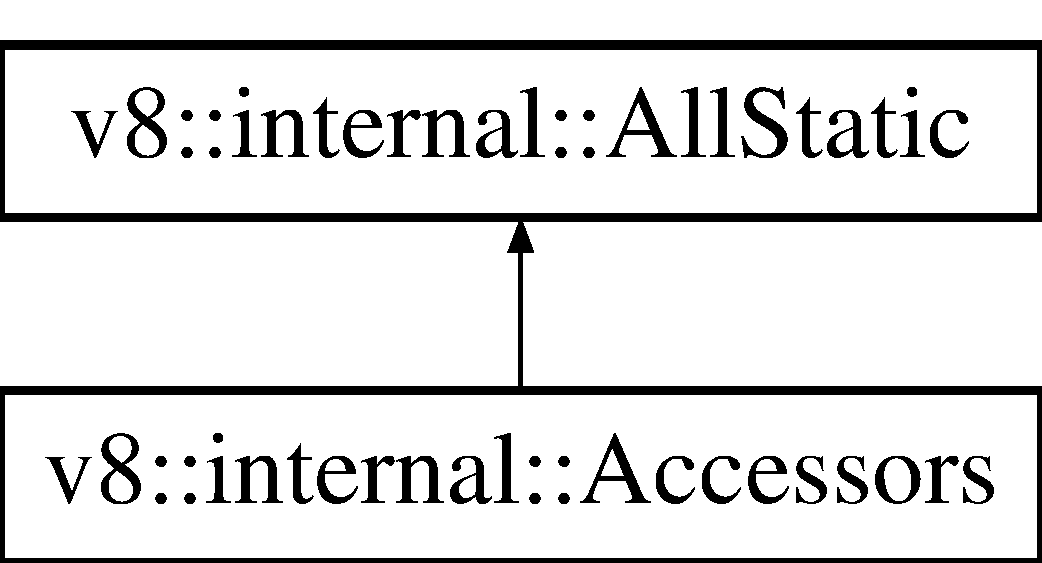
\includegraphics[height=2.000000cm]{classv8_1_1internal_1_1Accessors}
\end{center}
\end{figure}
\subsection*{Public Types}
\begin{DoxyCompactItemize}
\item 
\mbox{\Hypertarget{classv8_1_1internal_1_1Accessors_ab8bf583e163e3f06c3ab30d0b8049d90}\label{classv8_1_1internal_1_1Accessors_ab8bf583e163e3f06c3ab30d0b8049d90}} 
typedef void($\ast$ {\bfseries Accessor\+Name\+Boolean\+Setter\+Callback}) (\mbox{\hyperlink{classv8_1_1Local}{Local}}$<$ \mbox{\hyperlink{classv8_1_1Name}{v8\+::\+Name}} $>$ property, \mbox{\hyperlink{classv8_1_1Local}{Local}}$<$ \mbox{\hyperlink{classv8_1_1Value}{v8\+::\+Value}} $>$ value, const \mbox{\hyperlink{classv8_1_1PropertyCallbackInfo}{Property\+Callback\+Info}}$<$ \mbox{\hyperlink{classv8_1_1Boolean}{v8\+::\+Boolean}} $>$ \&info)
\end{DoxyCompactItemize}
\subsection*{Static Public Member Functions}
\begin{DoxyCompactItemize}
\item 
\mbox{\Hypertarget{classv8_1_1internal_1_1Accessors_a5ba1e99de6d9f7b268c386011e8b5080}\label{classv8_1_1internal_1_1Accessors_a5ba1e99de6d9f7b268c386011e8b5080}} 
static void {\bfseries Module\+Namespace\+Entry\+Getter} (\mbox{\hyperlink{classv8_1_1Local}{v8\+::\+Local}}$<$ \mbox{\hyperlink{classv8_1_1Name}{v8\+::\+Name}} $>$ name, const \mbox{\hyperlink{classv8_1_1PropertyCallbackInfo}{v8\+::\+Property\+Callback\+Info}}$<$ \mbox{\hyperlink{classv8_1_1Value}{v8\+::\+Value}} $>$ \&info)
\item 
\mbox{\Hypertarget{classv8_1_1internal_1_1Accessors_a2ae006cc99158006e23decca582a380b}\label{classv8_1_1internal_1_1Accessors_a2ae006cc99158006e23decca582a380b}} 
static \mbox{\hyperlink{classv8_1_1internal_1_1Handle}{Handle}}$<$ \mbox{\hyperlink{classv8_1_1internal_1_1AccessorInfo}{Accessor\+Info}} $>$ {\bfseries Make\+Module\+Namespace\+Entry\+Info} (\mbox{\hyperlink{classv8_1_1internal_1_1Isolate}{Isolate}} $\ast$isolate, \mbox{\hyperlink{classv8_1_1internal_1_1Handle}{Handle}}$<$ \mbox{\hyperlink{classv8_1_1internal_1_1String}{String}} $>$ name)
\item 
\mbox{\Hypertarget{classv8_1_1internal_1_1Accessors_ac070e74669475cb270aa2c3960e6bdb2}\label{classv8_1_1internal_1_1Accessors_ac070e74669475cb270aa2c3960e6bdb2}} 
static \mbox{\hyperlink{classv8_1_1internal_1_1Handle}{Handle}}$<$ \mbox{\hyperlink{classv8_1_1internal_1_1JSObject}{J\+S\+Object}} $>$ {\bfseries Function\+Get\+Arguments} (\mbox{\hyperlink{classv8_1_1internal_1_1JavaScriptFrame}{Java\+Script\+Frame}} $\ast$frame, \mbox{\hyperlink{classint}{int}} inlined\+\_\+jsframe\+\_\+index)
\item 
\mbox{\Hypertarget{classv8_1_1internal_1_1Accessors_a28e31d67545e273fff7ddc98bff73a58}\label{classv8_1_1internal_1_1Accessors_a28e31d67545e273fff7ddc98bff73a58}} 
static \mbox{\hyperlink{classbool}{bool}} {\bfseries Is\+J\+S\+Object\+Field\+Accessor} (\mbox{\hyperlink{classv8_1_1internal_1_1Isolate}{Isolate}} $\ast$isolate, \mbox{\hyperlink{classv8_1_1internal_1_1Handle}{Handle}}$<$ \mbox{\hyperlink{classv8_1_1internal_1_1Map}{Map}} $>$ map, \mbox{\hyperlink{classv8_1_1internal_1_1Handle}{Handle}}$<$ \mbox{\hyperlink{classv8_1_1internal_1_1Name}{Name}} $>$ name, \mbox{\hyperlink{classv8_1_1internal_1_1FieldIndex}{Field\+Index}} $\ast$field\+\_\+index)
\item 
\mbox{\Hypertarget{classv8_1_1internal_1_1Accessors_a468508b79231853f4143946f5b97186d}\label{classv8_1_1internal_1_1Accessors_a468508b79231853f4143946f5b97186d}} 
static \mbox{\hyperlink{classv8_1_1internal_1_1MaybeHandle}{Maybe\+Handle}}$<$ \mbox{\hyperlink{classv8_1_1internal_1_1Object}{Object}} $>$ {\bfseries Replace\+Accessor\+With\+Data\+Property} (\mbox{\hyperlink{classv8_1_1internal_1_1Handle}{Handle}}$<$ \mbox{\hyperlink{classv8_1_1internal_1_1Object}{Object}} $>$ receiver, \mbox{\hyperlink{classv8_1_1internal_1_1Handle}{Handle}}$<$ \mbox{\hyperlink{classv8_1_1internal_1_1JSObject}{J\+S\+Object}} $>$ holder, \mbox{\hyperlink{classv8_1_1internal_1_1Handle}{Handle}}$<$ \mbox{\hyperlink{classv8_1_1internal_1_1Name}{Name}} $>$ name, \mbox{\hyperlink{classv8_1_1internal_1_1Handle}{Handle}}$<$ \mbox{\hyperlink{classv8_1_1internal_1_1Object}{Object}} $>$ value)
\item 
\mbox{\Hypertarget{classv8_1_1internal_1_1Accessors_a44d62d34f8bb31dc5920f7b8fa2f472e}\label{classv8_1_1internal_1_1Accessors_a44d62d34f8bb31dc5920f7b8fa2f472e}} 
static \mbox{\hyperlink{classv8_1_1internal_1_1Handle}{Handle}}$<$ \mbox{\hyperlink{classv8_1_1internal_1_1AccessorInfo}{Accessor\+Info}} $>$ {\bfseries Make\+Accessor} (\mbox{\hyperlink{classv8_1_1internal_1_1Isolate}{Isolate}} $\ast$isolate, \mbox{\hyperlink{classv8_1_1internal_1_1Handle}{Handle}}$<$ \mbox{\hyperlink{classv8_1_1internal_1_1Name}{Name}} $>$ name, Accessor\+Name\+Getter\+Callback getter, Accessor\+Name\+Boolean\+Setter\+Callback setter)
\end{DoxyCompactItemize}
\subsection*{Static Public Attributes}
\begin{DoxyCompactItemize}
\item 
static constexpr \mbox{\hyperlink{classint}{int}} {\bfseries k\+Accessor\+Info\+Count}
\item 
static constexpr \mbox{\hyperlink{classint}{int}} {\bfseries k\+Accessor\+Setter\+Count}
\end{DoxyCompactItemize}
\subsection*{Friends}
\begin{DoxyCompactItemize}
\item 
\mbox{\Hypertarget{classv8_1_1internal_1_1Accessors_a3d69975be2e998e7bf2dcd1b1c8b4577}\label{classv8_1_1internal_1_1Accessors_a3d69975be2e998e7bf2dcd1b1c8b4577}} 
class {\bfseries Heap}
\end{DoxyCompactItemize}


\subsection{Detailed Description}


Definition at line 57 of file accessors.\+h.



\subsection{Member Data Documentation}
\mbox{\Hypertarget{classv8_1_1internal_1_1Accessors_a0218e22685a2ed701dd1f43ea6206411}\label{classv8_1_1internal_1_1Accessors_a0218e22685a2ed701dd1f43ea6206411}} 
\index{v8\+::internal\+::\+Accessors@{v8\+::internal\+::\+Accessors}!k\+Accessor\+Info\+Count@{k\+Accessor\+Info\+Count}}
\index{k\+Accessor\+Info\+Count@{k\+Accessor\+Info\+Count}!v8\+::internal\+::\+Accessors@{v8\+::internal\+::\+Accessors}}
\subsubsection{\texorpdfstring{k\+Accessor\+Info\+Count}{kAccessorInfoCount}}
{\footnotesize\ttfamily constexpr \mbox{\hyperlink{classint}{int}} v8\+::internal\+::\+Accessors\+::k\+Accessor\+Info\+Count\hspace{0.3cm}{\ttfamily [static]}}

{\bfseries Initial value\+:}
\begin{DoxyCode}
=
\textcolor{preprocessor}{#define COUNT\_ACCESSOR(...) }
\textcolor{preprocessor}{      ACCESSOR\_INFO\_LIST\_GENERATOR(COUNT\_ACCESSOR, )}
\end{DoxyCode}


Definition at line 73 of file accessors.\+h.

\mbox{\Hypertarget{classv8_1_1internal_1_1Accessors_a5537800ae53340c0ec441c0efd250c64}\label{classv8_1_1internal_1_1Accessors_a5537800ae53340c0ec441c0efd250c64}} 
\index{v8\+::internal\+::\+Accessors@{v8\+::internal\+::\+Accessors}!k\+Accessor\+Setter\+Count@{k\+Accessor\+Setter\+Count}}
\index{k\+Accessor\+Setter\+Count@{k\+Accessor\+Setter\+Count}!v8\+::internal\+::\+Accessors@{v8\+::internal\+::\+Accessors}}
\subsubsection{\texorpdfstring{k\+Accessor\+Setter\+Count}{kAccessorSetterCount}}
{\footnotesize\ttfamily constexpr \mbox{\hyperlink{classint}{int}} v8\+::internal\+::\+Accessors\+::k\+Accessor\+Setter\+Count\hspace{0.3cm}{\ttfamily [static]}}

{\bfseries Initial value\+:}
\begin{DoxyCode}
=
\textcolor{preprocessor}{#define COUNT\_ACCESSOR(...) }
\textcolor{preprocessor}{      ACCESSOR\_SETTER\_LIST(COUNT\_ACCESSOR)}
\end{DoxyCode}


Definition at line 78 of file accessors.\+h.



The documentation for this class was generated from the following files\+:\begin{DoxyCompactItemize}
\item 
v8/src/accessors.\+h\item 
v8/src/accessors.\+cc\end{DoxyCompactItemize}

\hypertarget{classv8_1_1AccessorSignature}{}\section{v8\+:\+:Accessor\+Signature Class Reference}
\label{classv8_1_1AccessorSignature}\index{v8\+::\+Accessor\+Signature@{v8\+::\+Accessor\+Signature}}


{\ttfamily \#include $<$v8.\+h$>$}

Inheritance diagram for v8\+:\+:Accessor\+Signature\+:\begin{figure}[H]
\begin{center}
\leavevmode
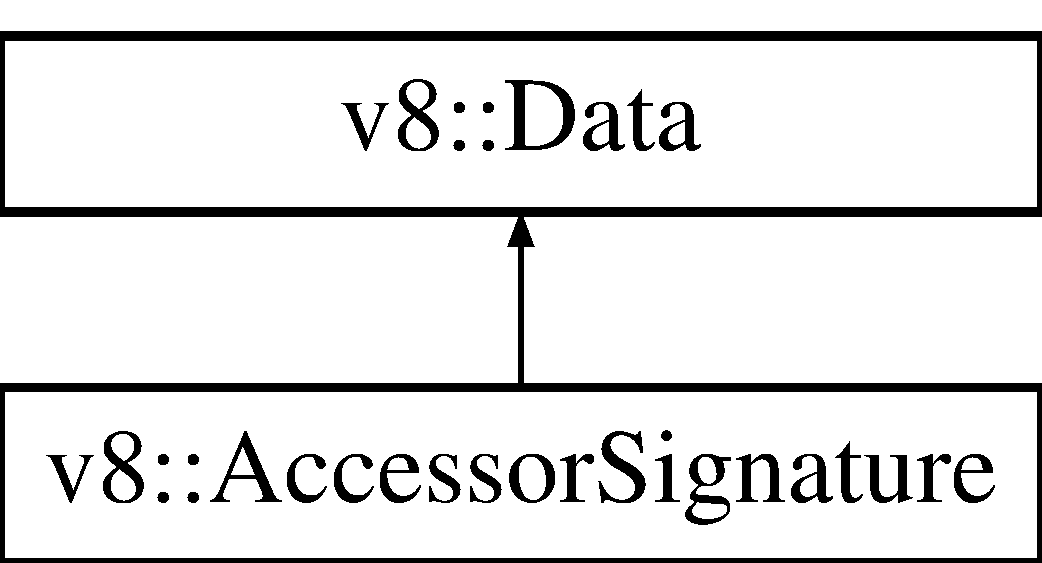
\includegraphics[height=2.000000cm]{classv8_1_1AccessorSignature}
\end{center}
\end{figure}
\subsection*{Static Public Member Functions}
\begin{DoxyCompactItemize}
\item 
\mbox{\Hypertarget{classv8_1_1AccessorSignature_a0a35126433259c49bab4d3ac6756dd67}\label{classv8_1_1AccessorSignature_a0a35126433259c49bab4d3ac6756dd67}} 
static \mbox{\hyperlink{classv8_1_1Local}{Local}}$<$ \mbox{\hyperlink{classv8_1_1AccessorSignature}{Accessor\+Signature}} $>$ {\bfseries New} (Isolate $\ast$isolate, \mbox{\hyperlink{classv8_1_1Local}{Local}}$<$ \mbox{\hyperlink{classv8_1_1FunctionTemplate}{Function\+Template}} $>$ receiver=\mbox{\hyperlink{classv8_1_1Local}{Local}}$<$ \mbox{\hyperlink{classv8_1_1FunctionTemplate}{Function\+Template}} $>$())
\item 
\mbox{\Hypertarget{classv8_1_1AccessorSignature_add2ad5697fb3b13d63de9d1e96db3758}\label{classv8_1_1AccessorSignature_add2ad5697fb3b13d63de9d1e96db3758}} 
static V8\+\_\+\+I\+N\+L\+I\+NE \mbox{\hyperlink{classv8_1_1AccessorSignature}{Accessor\+Signature}} $\ast$ {\bfseries Cast} (\mbox{\hyperlink{classv8_1_1Data}{Data}} $\ast$data)
\end{DoxyCompactItemize}


\subsection{Detailed Description}
An \mbox{\hyperlink{classv8_1_1AccessorSignature}{Accessor\+Signature}} specifies which receivers are valid parameters to an accessor callback. 

Definition at line 6243 of file v8.\+h.



The documentation for this class was generated from the following files\+:\begin{DoxyCompactItemize}
\item 
v8/include/v8.\+h\item 
v8/src/api.\+cc\end{DoxyCompactItemize}

\hypertarget{classv8_1_1internal_1_1AccessorTable}{}\section{v8\+:\+:internal\+:\+:Accessor\+Table Class Reference}
\label{classv8_1_1internal_1_1AccessorTable}\index{v8\+::internal\+::\+Accessor\+Table@{v8\+::internal\+::\+Accessor\+Table}}
Inheritance diagram for v8\+:\+:internal\+:\+:Accessor\+Table\+:\begin{figure}[H]
\begin{center}
\leavevmode
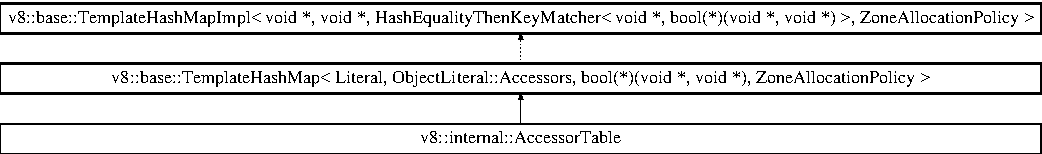
\includegraphics[height=2.074074cm]{classv8_1_1internal_1_1AccessorTable}
\end{center}
\end{figure}
\subsection*{Public Member Functions}
\begin{DoxyCompactItemize}
\item 
\mbox{\Hypertarget{classv8_1_1internal_1_1AccessorTable_adcee86ad1000d3d63e7360d0895fc2ae}\label{classv8_1_1internal_1_1AccessorTable_adcee86ad1000d3d63e7360d0895fc2ae}} 
{\bfseries Accessor\+Table} (\mbox{\hyperlink{classv8_1_1internal_1_1Zone}{Zone}} $\ast$zone)
\item 
\mbox{\Hypertarget{classv8_1_1internal_1_1AccessorTable_a064e2528f1da85829d8742c69adaba19}\label{classv8_1_1internal_1_1AccessorTable_a064e2528f1da85829d8742c69adaba19}} 
Iterator {\bfseries lookup} (\mbox{\hyperlink{classv8_1_1internal_1_1Literal}{Literal}} $\ast$literal)
\end{DoxyCompactItemize}


\subsection{Detailed Description}


Definition at line 1503 of file ast.\+h.



The documentation for this class was generated from the following file\+:\begin{DoxyCompactItemize}
\item 
v8/src/ast/ast.\+h\end{DoxyCompactItemize}

\hypertarget{classv8_1_1internal_1_1AccountingAllocator}{}\section{v8\+:\+:internal\+:\+:Accounting\+Allocator Class Reference}
\label{classv8_1_1internal_1_1AccountingAllocator}\index{v8\+::internal\+::\+Accounting\+Allocator@{v8\+::internal\+::\+Accounting\+Allocator}}
Inheritance diagram for v8\+:\+:internal\+:\+:Accounting\+Allocator\+:\begin{figure}[H]
\begin{center}
\leavevmode
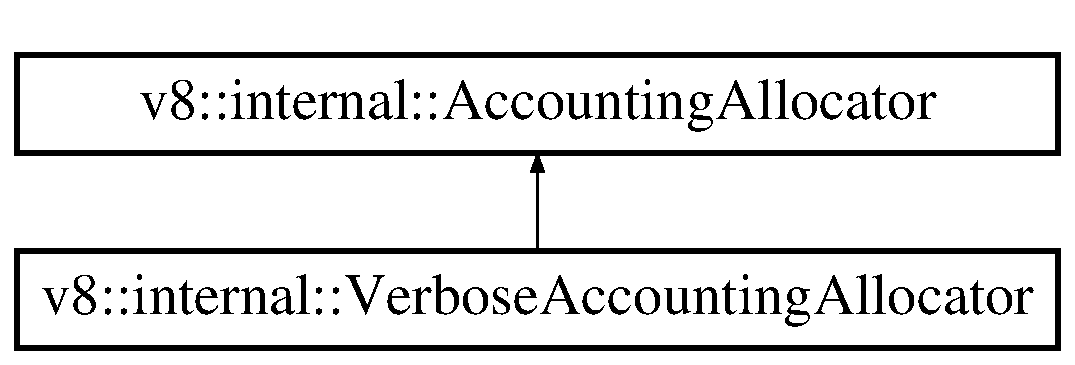
\includegraphics[height=2.000000cm]{classv8_1_1internal_1_1AccountingAllocator}
\end{center}
\end{figure}
\subsection*{Public Member Functions}
\begin{DoxyCompactItemize}
\item 
\mbox{\Hypertarget{classv8_1_1internal_1_1AccountingAllocator_aa75c3e7e7ce82180b26ea4450ac2937d}\label{classv8_1_1internal_1_1AccountingAllocator_aa75c3e7e7ce82180b26ea4450ac2937d}} 
virtual \mbox{\hyperlink{classv8_1_1internal_1_1Segment}{Segment}} $\ast$ {\bfseries Get\+Segment} (\mbox{\hyperlink{classsize__t}{size\+\_\+t}} bytes)
\item 
\mbox{\Hypertarget{classv8_1_1internal_1_1AccountingAllocator_a2a98c6a52bcda12c8a33b912f6630b96}\label{classv8_1_1internal_1_1AccountingAllocator_a2a98c6a52bcda12c8a33b912f6630b96}} 
virtual void {\bfseries Return\+Segment} (\mbox{\hyperlink{classv8_1_1internal_1_1Segment}{Segment}} $\ast$memory)
\item 
\mbox{\Hypertarget{classv8_1_1internal_1_1AccountingAllocator_aa81e107eb848411a28be8025d43bff4e}\label{classv8_1_1internal_1_1AccountingAllocator_aa81e107eb848411a28be8025d43bff4e}} 
\mbox{\hyperlink{classsize__t}{size\+\_\+t}} {\bfseries Get\+Current\+Memory\+Usage} () const
\item 
\mbox{\Hypertarget{classv8_1_1internal_1_1AccountingAllocator_aba1b43e2bfd23806015c414450eaefd3}\label{classv8_1_1internal_1_1AccountingAllocator_aba1b43e2bfd23806015c414450eaefd3}} 
\mbox{\hyperlink{classsize__t}{size\+\_\+t}} {\bfseries Get\+Max\+Memory\+Usage} () const
\item 
\mbox{\Hypertarget{classv8_1_1internal_1_1AccountingAllocator_afcb53f6ec4f7bf36c79bc4a66591d45c}\label{classv8_1_1internal_1_1AccountingAllocator_afcb53f6ec4f7bf36c79bc4a66591d45c}} 
\mbox{\hyperlink{classsize__t}{size\+\_\+t}} {\bfseries Get\+Current\+Pool\+Size} () const
\item 
\mbox{\Hypertarget{classv8_1_1internal_1_1AccountingAllocator_a145522456193da0dbebf618d101571ed}\label{classv8_1_1internal_1_1AccountingAllocator_a145522456193da0dbebf618d101571ed}} 
void {\bfseries Memory\+Pressure\+Notification} (Memory\+Pressure\+Level level)
\item 
\mbox{\Hypertarget{classv8_1_1internal_1_1AccountingAllocator_a65fe549097fd29ec57b974cc4f36c3c3}\label{classv8_1_1internal_1_1AccountingAllocator_a65fe549097fd29ec57b974cc4f36c3c3}} 
void {\bfseries Configure\+Segment\+Pool} (const \mbox{\hyperlink{classsize__t}{size\+\_\+t}} max\+\_\+pool\+\_\+size)
\item 
\mbox{\Hypertarget{classv8_1_1internal_1_1AccountingAllocator_a08b927506f172711dffb0ab955444cc5}\label{classv8_1_1internal_1_1AccountingAllocator_a08b927506f172711dffb0ab955444cc5}} 
virtual void {\bfseries Zone\+Creation} (const \mbox{\hyperlink{classv8_1_1internal_1_1Zone}{Zone}} $\ast$zone)
\item 
\mbox{\Hypertarget{classv8_1_1internal_1_1AccountingAllocator_af830f8debf51a20b7215eb190b86b9ec}\label{classv8_1_1internal_1_1AccountingAllocator_af830f8debf51a20b7215eb190b86b9ec}} 
virtual void {\bfseries Zone\+Destruction} (const \mbox{\hyperlink{classv8_1_1internal_1_1Zone}{Zone}} $\ast$zone)
\end{DoxyCompactItemize}
\subsection*{Static Public Attributes}
\begin{DoxyCompactItemize}
\item 
\mbox{\Hypertarget{classv8_1_1internal_1_1AccountingAllocator_a736911edc7ff18dc7215b9a5bb5fda9c}\label{classv8_1_1internal_1_1AccountingAllocator_a736911edc7ff18dc7215b9a5bb5fda9c}} 
static const \mbox{\hyperlink{classsize__t}{size\+\_\+t}} {\bfseries k\+Max\+Pool\+Size} = 8ul $\ast$ KB
\end{DoxyCompactItemize}


\subsection{Detailed Description}


Definition at line 22 of file accounting-\/allocator.\+h.



The documentation for this class was generated from the following files\+:\begin{DoxyCompactItemize}
\item 
v8/src/zone/accounting-\/allocator.\+h\item 
v8/src/zone/accounting-\/allocator.\+cc\end{DoxyCompactItemize}

\hypertarget{classv8_1_1internal_1_1ActionNode}{}\section{v8\+:\+:internal\+:\+:Action\+Node Class Reference}
\label{classv8_1_1internal_1_1ActionNode}\index{v8\+::internal\+::\+Action\+Node@{v8\+::internal\+::\+Action\+Node}}
Inheritance diagram for v8\+:\+:internal\+:\+:Action\+Node\+:\begin{figure}[H]
\begin{center}
\leavevmode
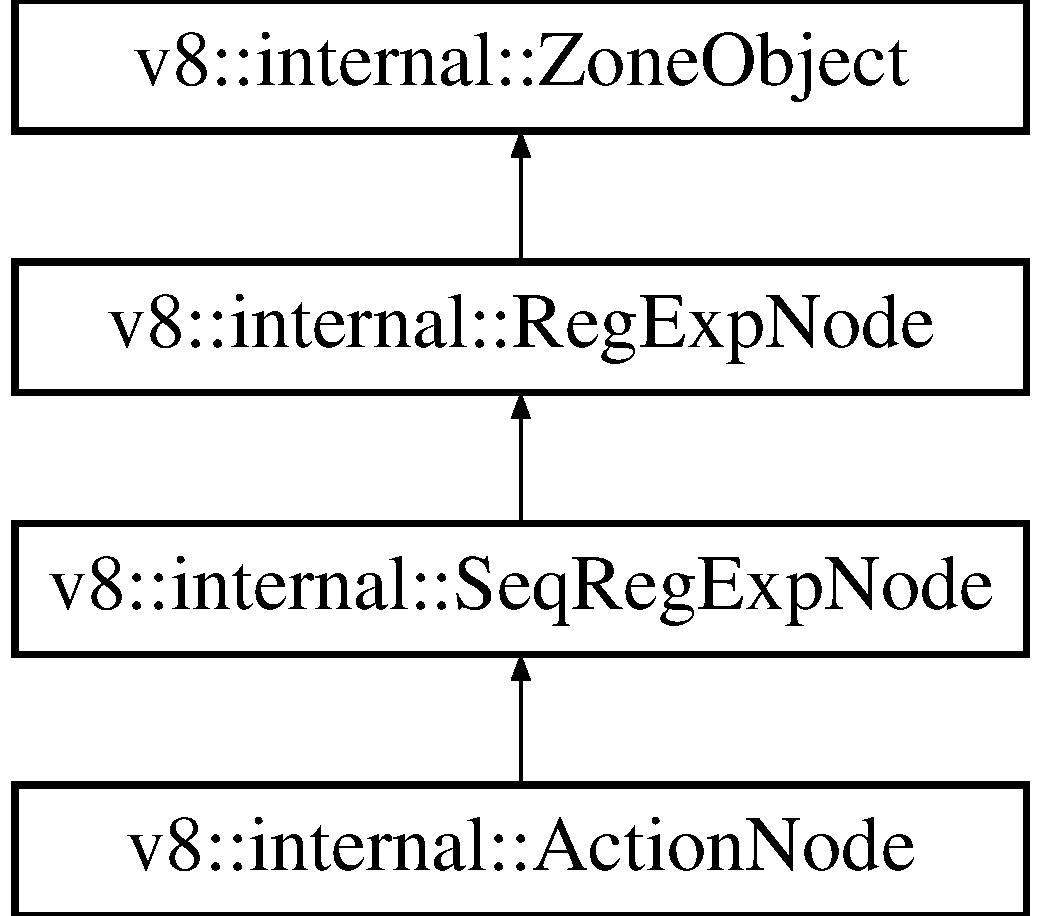
\includegraphics[height=4.000000cm]{classv8_1_1internal_1_1ActionNode}
\end{center}
\end{figure}
\subsection*{Public Types}
\begin{DoxyCompactItemize}
\item 
\mbox{\Hypertarget{classv8_1_1internal_1_1ActionNode_ab695380c09977f360b2d4f817f9124bc}\label{classv8_1_1internal_1_1ActionNode_ab695380c09977f360b2d4f817f9124bc}} 
enum {\bfseries Action\+Type} \{ \newline
{\bfseries S\+E\+T\+\_\+\+R\+E\+G\+I\+S\+T\+ER}, 
{\bfseries I\+N\+C\+R\+E\+M\+E\+N\+T\+\_\+\+R\+E\+G\+I\+S\+T\+ER}, 
{\bfseries S\+T\+O\+R\+E\+\_\+\+P\+O\+S\+I\+T\+I\+ON}, 
{\bfseries B\+E\+G\+I\+N\+\_\+\+S\+U\+B\+M\+A\+T\+CH}, 
\newline
{\bfseries P\+O\+S\+I\+T\+I\+V\+E\+\_\+\+S\+U\+B\+M\+A\+T\+C\+H\+\_\+\+S\+U\+C\+C\+E\+SS}, 
{\bfseries E\+M\+P\+T\+Y\+\_\+\+M\+A\+T\+C\+H\+\_\+\+C\+H\+E\+CK}, 
{\bfseries C\+L\+E\+A\+R\+\_\+\+C\+A\+P\+T\+U\+R\+ES}
 \}
\end{DoxyCompactItemize}
\subsection*{Public Member Functions}
\begin{DoxyCompactItemize}
\item 
\mbox{\Hypertarget{classv8_1_1internal_1_1ActionNode_a7211d3783a725f51fb57c05ae8900cce}\label{classv8_1_1internal_1_1ActionNode_a7211d3783a725f51fb57c05ae8900cce}} 
void {\bfseries Accept} (\mbox{\hyperlink{classv8_1_1internal_1_1NodeVisitor}{Node\+Visitor}} $\ast$visitor) override
\item 
\mbox{\Hypertarget{classv8_1_1internal_1_1ActionNode_ad664161e894fe81e82ce76b7e43545a2}\label{classv8_1_1internal_1_1ActionNode_ad664161e894fe81e82ce76b7e43545a2}} 
void {\bfseries Emit} (\mbox{\hyperlink{classv8_1_1internal_1_1RegExpCompiler}{Reg\+Exp\+Compiler}} $\ast$compiler, \mbox{\hyperlink{classv8_1_1internal_1_1Trace}{Trace}} $\ast$trace) override
\item 
\mbox{\Hypertarget{classv8_1_1internal_1_1ActionNode_ad318703d79f086c1b518f6008e2384b4}\label{classv8_1_1internal_1_1ActionNode_ad318703d79f086c1b518f6008e2384b4}} 
\mbox{\hyperlink{classint}{int}} {\bfseries Eats\+At\+Least} (\mbox{\hyperlink{classint}{int}} still\+\_\+to\+\_\+find, \mbox{\hyperlink{classint}{int}} budget, \mbox{\hyperlink{classbool}{bool}} not\+\_\+at\+\_\+start) override
\item 
\mbox{\Hypertarget{classv8_1_1internal_1_1ActionNode_ae590338eedba24969860acef618ee829}\label{classv8_1_1internal_1_1ActionNode_ae590338eedba24969860acef618ee829}} 
void {\bfseries Get\+Quick\+Check\+Details} (\mbox{\hyperlink{classv8_1_1internal_1_1QuickCheckDetails}{Quick\+Check\+Details}} $\ast$details, \mbox{\hyperlink{classv8_1_1internal_1_1RegExpCompiler}{Reg\+Exp\+Compiler}} $\ast$compiler, \mbox{\hyperlink{classint}{int}} filled\+\_\+in, \mbox{\hyperlink{classbool}{bool}} not\+\_\+at\+\_\+start) override
\item 
\mbox{\Hypertarget{classv8_1_1internal_1_1ActionNode_aa97507c043d2ca1971c9a9bf179ed359}\label{classv8_1_1internal_1_1ActionNode_aa97507c043d2ca1971c9a9bf179ed359}} 
void {\bfseries Fill\+In\+B\+M\+Info} (\mbox{\hyperlink{classv8_1_1internal_1_1Isolate}{Isolate}} $\ast$isolate, \mbox{\hyperlink{classint}{int}} offset, \mbox{\hyperlink{classint}{int}} budget, \mbox{\hyperlink{classv8_1_1internal_1_1BoyerMooreLookahead}{Boyer\+Moore\+Lookahead}} $\ast$bm, \mbox{\hyperlink{classbool}{bool}} not\+\_\+at\+\_\+start) override
\item 
\mbox{\Hypertarget{classv8_1_1internal_1_1ActionNode_ae848c71b17d244a67f3f34afe142fac8}\label{classv8_1_1internal_1_1ActionNode_ae848c71b17d244a67f3f34afe142fac8}} 
Action\+Type {\bfseries action\+\_\+type} ()
\item 
\mbox{\Hypertarget{classv8_1_1internal_1_1ActionNode_a7c7df272a95395571580fca4e060f786}\label{classv8_1_1internal_1_1ActionNode_a7c7df272a95395571580fca4e060f786}} 
\mbox{\hyperlink{classint}{int}} {\bfseries Greedy\+Loop\+Text\+Length} () override
\end{DoxyCompactItemize}
\subsection*{Static Public Member Functions}
\begin{DoxyCompactItemize}
\item 
\mbox{\Hypertarget{classv8_1_1internal_1_1ActionNode_ab0232aafb29641c830970993c18ca5a7}\label{classv8_1_1internal_1_1ActionNode_ab0232aafb29641c830970993c18ca5a7}} 
static \mbox{\hyperlink{classv8_1_1internal_1_1ActionNode}{Action\+Node}} $\ast$ {\bfseries Set\+Register} (\mbox{\hyperlink{classint}{int}} reg, \mbox{\hyperlink{classint}{int}} val, \mbox{\hyperlink{classv8_1_1internal_1_1RegExpNode}{Reg\+Exp\+Node}} $\ast$on\+\_\+success)
\item 
\mbox{\Hypertarget{classv8_1_1internal_1_1ActionNode_ac2fea920241e4412a3bba2d10acb91ef}\label{classv8_1_1internal_1_1ActionNode_ac2fea920241e4412a3bba2d10acb91ef}} 
static \mbox{\hyperlink{classv8_1_1internal_1_1ActionNode}{Action\+Node}} $\ast$ {\bfseries Increment\+Register} (\mbox{\hyperlink{classint}{int}} reg, \mbox{\hyperlink{classv8_1_1internal_1_1RegExpNode}{Reg\+Exp\+Node}} $\ast$on\+\_\+success)
\item 
\mbox{\Hypertarget{classv8_1_1internal_1_1ActionNode_a7b7c1ea99df9360c97a7e73e2672a834}\label{classv8_1_1internal_1_1ActionNode_a7b7c1ea99df9360c97a7e73e2672a834}} 
static \mbox{\hyperlink{classv8_1_1internal_1_1ActionNode}{Action\+Node}} $\ast$ {\bfseries Store\+Position} (\mbox{\hyperlink{classint}{int}} reg, \mbox{\hyperlink{classbool}{bool}} is\+\_\+capture, \mbox{\hyperlink{classv8_1_1internal_1_1RegExpNode}{Reg\+Exp\+Node}} $\ast$on\+\_\+success)
\item 
\mbox{\Hypertarget{classv8_1_1internal_1_1ActionNode_af5c152a32e7afbe31390f57c07eed05a}\label{classv8_1_1internal_1_1ActionNode_af5c152a32e7afbe31390f57c07eed05a}} 
static \mbox{\hyperlink{classv8_1_1internal_1_1ActionNode}{Action\+Node}} $\ast$ {\bfseries Clear\+Captures} (\mbox{\hyperlink{classv8_1_1internal_1_1Interval}{Interval}} range, \mbox{\hyperlink{classv8_1_1internal_1_1RegExpNode}{Reg\+Exp\+Node}} $\ast$on\+\_\+success)
\item 
\mbox{\Hypertarget{classv8_1_1internal_1_1ActionNode_a84297f33bee6dffd0cc7a6b5341fb106}\label{classv8_1_1internal_1_1ActionNode_a84297f33bee6dffd0cc7a6b5341fb106}} 
static \mbox{\hyperlink{classv8_1_1internal_1_1ActionNode}{Action\+Node}} $\ast$ {\bfseries Begin\+Submatch} (\mbox{\hyperlink{classint}{int}} stack\+\_\+pointer\+\_\+reg, \mbox{\hyperlink{classint}{int}} position\+\_\+reg, \mbox{\hyperlink{classv8_1_1internal_1_1RegExpNode}{Reg\+Exp\+Node}} $\ast$on\+\_\+success)
\item 
\mbox{\Hypertarget{classv8_1_1internal_1_1ActionNode_a89bed32eadb39ad776f7e5523d8d152b}\label{classv8_1_1internal_1_1ActionNode_a89bed32eadb39ad776f7e5523d8d152b}} 
static \mbox{\hyperlink{classv8_1_1internal_1_1ActionNode}{Action\+Node}} $\ast$ {\bfseries Positive\+Submatch\+Success} (\mbox{\hyperlink{classint}{int}} stack\+\_\+pointer\+\_\+reg, \mbox{\hyperlink{classint}{int}} restore\+\_\+reg, \mbox{\hyperlink{classint}{int}} clear\+\_\+capture\+\_\+count, \mbox{\hyperlink{classint}{int}} clear\+\_\+capture\+\_\+from, \mbox{\hyperlink{classv8_1_1internal_1_1RegExpNode}{Reg\+Exp\+Node}} $\ast$on\+\_\+success)
\item 
\mbox{\Hypertarget{classv8_1_1internal_1_1ActionNode_a1f8492811dde72cce77b5b7f8d083292}\label{classv8_1_1internal_1_1ActionNode_a1f8492811dde72cce77b5b7f8d083292}} 
static \mbox{\hyperlink{classv8_1_1internal_1_1ActionNode}{Action\+Node}} $\ast$ {\bfseries Empty\+Match\+Check} (\mbox{\hyperlink{classint}{int}} start\+\_\+register, \mbox{\hyperlink{classint}{int}} repetition\+\_\+register, \mbox{\hyperlink{classint}{int}} repetition\+\_\+limit, \mbox{\hyperlink{classv8_1_1internal_1_1RegExpNode}{Reg\+Exp\+Node}} $\ast$on\+\_\+success)
\end{DoxyCompactItemize}
\subsection*{Friends}
\begin{DoxyCompactItemize}
\item 
\mbox{\Hypertarget{classv8_1_1internal_1_1ActionNode_a9c19d4d6fc300c029ba554cbe4d3d2e0}\label{classv8_1_1internal_1_1ActionNode_a9c19d4d6fc300c029ba554cbe4d3d2e0}} 
class {\bfseries Dot\+Printer}
\end{DoxyCompactItemize}
\subsection*{Additional Inherited Members}


\subsection{Detailed Description}


Definition at line 609 of file jsregexp.\+h.



The documentation for this class was generated from the following files\+:\begin{DoxyCompactItemize}
\item 
v8/src/regexp/jsregexp.\+h\item 
v8/src/regexp/jsregexp.\+cc\end{DoxyCompactItemize}

\hypertarget{classv8_1_1ActivityControl}{\section{v8\-:\-:Activity\-Control Class Reference}
\label{classv8_1_1ActivityControl}\index{v8\-::\-Activity\-Control@{v8\-::\-Activity\-Control}}
}


{\ttfamily \#include $<$v8-\/profiler.\-h$>$}

\subsection*{Public Types}
\begin{DoxyCompactItemize}
\item 
enum {\bfseries Control\-Option} \{ {\bfseries k\-Continue} =  0, 
{\bfseries k\-Abort} =  1
 \}
\end{DoxyCompactItemize}
\subsection*{Public Member Functions}
\begin{DoxyCompactItemize}
\item 
virtual Control\-Option \hyperlink{classv8_1_1ActivityControl_a1300f10611306a3e8f79239e057eb0bf}{Report\-Progress\-Value} (int done, int total)=0
\end{DoxyCompactItemize}


\subsection{Detailed Description}
An interface for reporting progress and controlling long-\/running activities. 

\subsection{Member Function Documentation}
\hypertarget{classv8_1_1ActivityControl_a1300f10611306a3e8f79239e057eb0bf}{\index{v8\-::\-Activity\-Control@{v8\-::\-Activity\-Control}!Report\-Progress\-Value@{Report\-Progress\-Value}}
\index{Report\-Progress\-Value@{Report\-Progress\-Value}!v8::ActivityControl@{v8\-::\-Activity\-Control}}
\subsubsection[{Report\-Progress\-Value}]{\setlength{\rightskip}{0pt plus 5cm}virtual Control\-Option v8\-::\-Activity\-Control\-::\-Report\-Progress\-Value (
\begin{DoxyParamCaption}
\item[{int}]{done, }
\item[{int}]{total}
\end{DoxyParamCaption}
)\hspace{0.3cm}{\ttfamily [pure virtual]}}}\label{classv8_1_1ActivityControl_a1300f10611306a3e8f79239e057eb0bf}
Notify about current progress. The activity can be stopped by returning k\-Abort as the callback result. 

The documentation for this class was generated from the following file\-:\begin{DoxyCompactItemize}
\item 
v8/include/v8-\/profiler.\-h\end{DoxyCompactItemize}

\hypertarget{classv8_1_1internal_1_1AddDispatchRange}{}\section{v8\+:\+:internal\+:\+:Add\+Dispatch\+Range Class Reference}
\label{classv8_1_1internal_1_1AddDispatchRange}\index{v8\+::internal\+::\+Add\+Dispatch\+Range@{v8\+::internal\+::\+Add\+Dispatch\+Range}}
\subsection*{Public Member Functions}
\begin{DoxyCompactItemize}
\item 
\mbox{\Hypertarget{classv8_1_1internal_1_1AddDispatchRange_aabb3eb748f5a566349ae5946fef1103b}\label{classv8_1_1internal_1_1AddDispatchRange_aabb3eb748f5a566349ae5946fef1103b}} 
{\bfseries Add\+Dispatch\+Range} (\mbox{\hyperlink{classv8_1_1internal_1_1DispatchTableConstructor}{Dispatch\+Table\+Constructor}} $\ast$constructor)
\item 
\mbox{\Hypertarget{classv8_1_1internal_1_1AddDispatchRange_a17e1406e159be04ef2b1fcc36d94c888}\label{classv8_1_1internal_1_1AddDispatchRange_a17e1406e159be04ef2b1fcc36d94c888}} 
void {\bfseries Call} (uc32 from, \mbox{\hyperlink{classv8_1_1internal_1_1DispatchTable_1_1Entry}{Dispatch\+Table\+::\+Entry}} entry)
\end{DoxyCompactItemize}


\subsection{Detailed Description}


Definition at line 6498 of file jsregexp.\+cc.



The documentation for this class was generated from the following file\+:\begin{DoxyCompactItemize}
\item 
v8/src/regexp/jsregexp.\+cc\end{DoxyCompactItemize}

\hypertarget{structv8_1_1internal_1_1compiler_1_1AddMatcher}{}\section{v8\+:\+:internal\+:\+:compiler\+:\+:Add\+Matcher$<$ Binop\+Matcher, Add\+Opcode, Sub\+Opcode, k\+Mul\+Opcode, k\+Shift\+Opcode $>$ Struct Template Reference}
\label{structv8_1_1internal_1_1compiler_1_1AddMatcher}\index{v8\+::internal\+::compiler\+::\+Add\+Matcher$<$ Binop\+Matcher, Add\+Opcode, Sub\+Opcode, k\+Mul\+Opcode, k\+Shift\+Opcode $>$@{v8\+::internal\+::compiler\+::\+Add\+Matcher$<$ Binop\+Matcher, Add\+Opcode, Sub\+Opcode, k\+Mul\+Opcode, k\+Shift\+Opcode $>$}}
Inheritance diagram for v8\+:\+:internal\+:\+:compiler\+:\+:Add\+Matcher$<$ Binop\+Matcher, Add\+Opcode, Sub\+Opcode, k\+Mul\+Opcode, k\+Shift\+Opcode $>$\+:\begin{figure}[H]
\begin{center}
\leavevmode
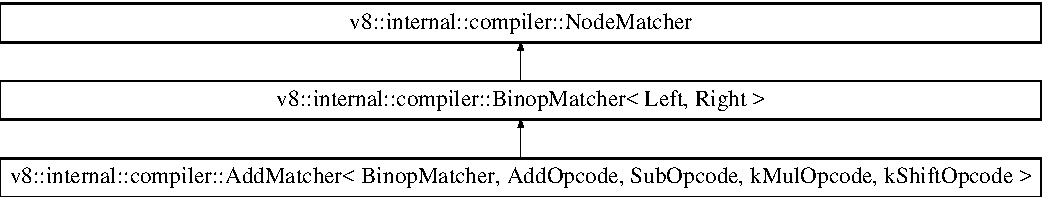
\includegraphics[height=2.649842cm]{structv8_1_1internal_1_1compiler_1_1AddMatcher}
\end{center}
\end{figure}
\subsection*{Public Types}
\begin{DoxyCompactItemize}
\item 
\mbox{\Hypertarget{structv8_1_1internal_1_1compiler_1_1AddMatcher_a56dd5d7b87962d28d0b499d0cf7d63e6}\label{structv8_1_1internal_1_1compiler_1_1AddMatcher_a56dd5d7b87962d28d0b499d0cf7d63e6}} 
typedef \mbox{\hyperlink{structv8_1_1internal_1_1compiler_1_1ScaleMatcher}{Scale\+Matcher}}$<$ \mbox{\hyperlink{structv8_1_1internal_1_1compiler_1_1BinopMatcher}{Binop\+Matcher}}, k\+Mul\+Opcode, k\+Shift\+Opcode $>$ {\bfseries Matcher}
\end{DoxyCompactItemize}
\subsection*{Public Member Functions}
\begin{DoxyCompactItemize}
\item 
\mbox{\Hypertarget{structv8_1_1internal_1_1compiler_1_1AddMatcher_aa5b57b0aff1e35b0605be084d8662093}\label{structv8_1_1internal_1_1compiler_1_1AddMatcher_aa5b57b0aff1e35b0605be084d8662093}} 
{\bfseries Add\+Matcher} (\mbox{\hyperlink{classv8_1_1internal_1_1compiler_1_1Node}{Node}} $\ast$node, \mbox{\hyperlink{classbool}{bool}} allow\+\_\+input\+\_\+swap)
\item 
\mbox{\Hypertarget{structv8_1_1internal_1_1compiler_1_1AddMatcher_a5b39c9416c51aa743c6b1354a0439d91}\label{structv8_1_1internal_1_1compiler_1_1AddMatcher_a5b39c9416c51aa743c6b1354a0439d91}} 
{\bfseries Add\+Matcher} (\mbox{\hyperlink{classv8_1_1internal_1_1compiler_1_1Node}{Node}} $\ast$node)
\item 
\mbox{\Hypertarget{structv8_1_1internal_1_1compiler_1_1AddMatcher_a808ff6e42dde142411e16cb0d621edb6}\label{structv8_1_1internal_1_1compiler_1_1AddMatcher_a808ff6e42dde142411e16cb0d621edb6}} 
\mbox{\hyperlink{classbool}{bool}} {\bfseries Has\+Index\+Input} () const
\item 
\mbox{\Hypertarget{structv8_1_1internal_1_1compiler_1_1AddMatcher_a9d46485a3c1ddd663256ce35231138cf}\label{structv8_1_1internal_1_1compiler_1_1AddMatcher_a9d46485a3c1ddd663256ce35231138cf}} 
\mbox{\hyperlink{classv8_1_1internal_1_1compiler_1_1Node}{Node}} $\ast$ {\bfseries Index\+Input} () const
\item 
\mbox{\Hypertarget{structv8_1_1internal_1_1compiler_1_1AddMatcher_a97906b2b753fadd9d696a0e4a8fae5a1}\label{structv8_1_1internal_1_1compiler_1_1AddMatcher_a97906b2b753fadd9d696a0e4a8fae5a1}} 
\mbox{\hyperlink{classint}{int}} {\bfseries scale} () const
\item 
\mbox{\Hypertarget{structv8_1_1internal_1_1compiler_1_1AddMatcher_a195f227cbea2dbcc195600da005e53ce}\label{structv8_1_1internal_1_1compiler_1_1AddMatcher_a195f227cbea2dbcc195600da005e53ce}} 
\mbox{\hyperlink{classbool}{bool}} {\bfseries power\+\_\+of\+\_\+two\+\_\+plus\+\_\+one} () const
\end{DoxyCompactItemize}
\subsection*{Static Public Attributes}
\begin{DoxyCompactItemize}
\item 
\mbox{\Hypertarget{structv8_1_1internal_1_1compiler_1_1AddMatcher_a102d500a376329fc6d2d5c4381d5b078}\label{structv8_1_1internal_1_1compiler_1_1AddMatcher_a102d500a376329fc6d2d5c4381d5b078}} 
static const Ir\+Opcode\+::\+Value {\bfseries k\+Add\+Opcode} = Add\+Opcode
\item 
\mbox{\Hypertarget{structv8_1_1internal_1_1compiler_1_1AddMatcher_aac3956ca03dcc543a5d809a8601cb922}\label{structv8_1_1internal_1_1compiler_1_1AddMatcher_aac3956ca03dcc543a5d809a8601cb922}} 
static const Ir\+Opcode\+::\+Value {\bfseries k\+Sub\+Opcode} = Sub\+Opcode
\end{DoxyCompactItemize}
\subsection*{Additional Inherited Members}


\subsection{Detailed Description}
\subsubsection*{template$<$class Binop\+Matcher, Ir\+Opcode\+::\+Value Add\+Opcode, Ir\+Opcode\+::\+Value Sub\+Opcode, Ir\+Opcode\+::\+Value k\+Mul\+Opcode, Ir\+Opcode\+::\+Value k\+Shift\+Opcode$>$\newline
struct v8\+::internal\+::compiler\+::\+Add\+Matcher$<$ Binop\+Matcher, Add\+Opcode, Sub\+Opcode, k\+Mul\+Opcode, k\+Shift\+Opcode $>$}



Definition at line 349 of file node-\/matchers.\+h.



The documentation for this struct was generated from the following file\+:\begin{DoxyCompactItemize}
\item 
v8/src/compiler/node-\/matchers.\+h\end{DoxyCompactItemize}

\hypertarget{classv8_1_1internal_1_1compiler_1_1AddressMatcher}{}\section{v8\+:\+:internal\+:\+:compiler\+:\+:Address\+Matcher Class Reference}
\label{classv8_1_1internal_1_1compiler_1_1AddressMatcher}\index{v8\+::internal\+::compiler\+::\+Address\+Matcher@{v8\+::internal\+::compiler\+::\+Address\+Matcher}}
Inheritance diagram for v8\+:\+:internal\+:\+:compiler\+:\+:Address\+Matcher\+:\begin{figure}[H]
\begin{center}
\leavevmode
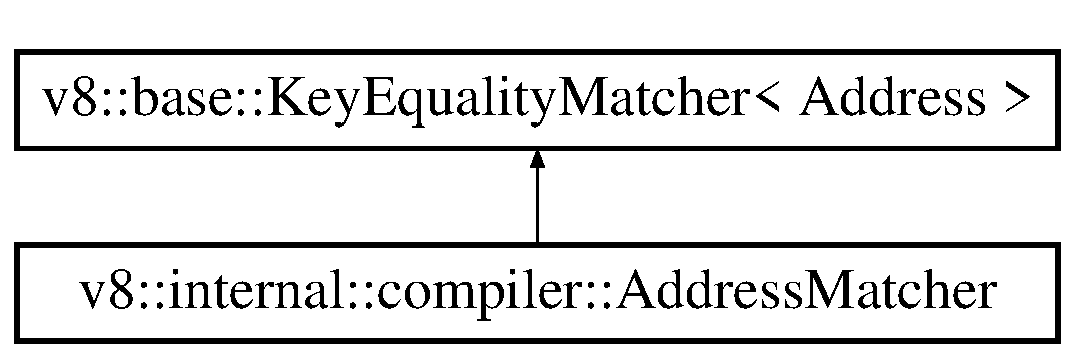
\includegraphics[height=2.000000cm]{classv8_1_1internal_1_1compiler_1_1AddressMatcher}
\end{center}
\end{figure}
\subsection*{Public Member Functions}
\begin{DoxyCompactItemize}
\item 
\mbox{\Hypertarget{classv8_1_1internal_1_1compiler_1_1AddressMatcher_a3a652a1601f8ed33ec5e964e2f96f0a8}\label{classv8_1_1internal_1_1compiler_1_1AddressMatcher_a3a652a1601f8ed33ec5e964e2f96f0a8}} 
\mbox{\hyperlink{classbool}{bool}} {\bfseries operator()} (\mbox{\hyperlink{classuint32__t}{uint32\+\_\+t}} hash1, \mbox{\hyperlink{classuint32__t}{uint32\+\_\+t}} hash2, const \mbox{\hyperlink{classuintptr__t}{Address}} \&key1, const \mbox{\hyperlink{classuintptr__t}{Address}} \&key2) const
\end{DoxyCompactItemize}


\subsection{Detailed Description}


Definition at line 18 of file refs-\/map.\+h.



The documentation for this class was generated from the following file\+:\begin{DoxyCompactItemize}
\item 
v8/src/compiler/refs-\/map.\+h\end{DoxyCompactItemize}

\hypertarget{classv8_1_1base_1_1AddressRegion}{}\section{v8\+:\+:base\+:\+:Address\+Region Class Reference}
\label{classv8_1_1base_1_1AddressRegion}\index{v8\+::base\+::\+Address\+Region@{v8\+::base\+::\+Address\+Region}}
\subsection*{Public Types}
\begin{DoxyCompactItemize}
\item 
\mbox{\Hypertarget{classv8_1_1base_1_1AddressRegion_a553c65b61da09870ca7b71415c9cd4b9}\label{classv8_1_1base_1_1AddressRegion_a553c65b61da09870ca7b71415c9cd4b9}} 
typedef \mbox{\hyperlink{classuintptr__t}{uintptr\+\_\+t}} {\bfseries Address}
\end{DoxyCompactItemize}
\subsection*{Public Member Functions}
\begin{DoxyCompactItemize}
\item 
\mbox{\Hypertarget{classv8_1_1base_1_1AddressRegion_a0e1dd2e78720b25911ea14e5df995f03}\label{classv8_1_1base_1_1AddressRegion_a0e1dd2e78720b25911ea14e5df995f03}} 
{\bfseries Address\+Region} (\mbox{\hyperlink{classuintptr__t}{Address}} address, \mbox{\hyperlink{classsize__t}{size\+\_\+t}} size)
\item 
\mbox{\Hypertarget{classv8_1_1base_1_1AddressRegion_a94a15b5dca8bef88c66880c9b00281ea}\label{classv8_1_1base_1_1AddressRegion_a94a15b5dca8bef88c66880c9b00281ea}} 
\mbox{\hyperlink{classuintptr__t}{Address}} {\bfseries begin} () const
\item 
\mbox{\Hypertarget{classv8_1_1base_1_1AddressRegion_a13bbde71869b71658a03746941a13f69}\label{classv8_1_1base_1_1AddressRegion_a13bbde71869b71658a03746941a13f69}} 
\mbox{\hyperlink{classuintptr__t}{Address}} {\bfseries end} () const
\item 
\mbox{\Hypertarget{classv8_1_1base_1_1AddressRegion_a753daf867d9e52511d3483b211a9f0b2}\label{classv8_1_1base_1_1AddressRegion_a753daf867d9e52511d3483b211a9f0b2}} 
\mbox{\hyperlink{classsize__t}{size\+\_\+t}} {\bfseries size} () const
\item 
\mbox{\Hypertarget{classv8_1_1base_1_1AddressRegion_adc48f605d82ef43f598ce6bafcf7d4e7}\label{classv8_1_1base_1_1AddressRegion_adc48f605d82ef43f598ce6bafcf7d4e7}} 
void {\bfseries set\+\_\+size} (\mbox{\hyperlink{classsize__t}{size\+\_\+t}} size)
\item 
\mbox{\Hypertarget{classv8_1_1base_1_1AddressRegion_a29afd92431f4eb737887d7c7ff9b9396}\label{classv8_1_1base_1_1AddressRegion_a29afd92431f4eb737887d7c7ff9b9396}} 
\mbox{\hyperlink{classbool}{bool}} {\bfseries is\+\_\+empty} () const
\item 
\mbox{\Hypertarget{classv8_1_1base_1_1AddressRegion_ad799a0c1d53c9117b94f95e6bc742e66}\label{classv8_1_1base_1_1AddressRegion_ad799a0c1d53c9117b94f95e6bc742e66}} 
\mbox{\hyperlink{classbool}{bool}} {\bfseries contains} (\mbox{\hyperlink{classuintptr__t}{Address}} address) const
\item 
\mbox{\Hypertarget{classv8_1_1base_1_1AddressRegion_ac96c37330af72155870c6dabb1ddef80}\label{classv8_1_1base_1_1AddressRegion_ac96c37330af72155870c6dabb1ddef80}} 
\mbox{\hyperlink{classbool}{bool}} {\bfseries contains} (\mbox{\hyperlink{classuintptr__t}{Address}} address, \mbox{\hyperlink{classsize__t}{size\+\_\+t}} size) const
\item 
\mbox{\Hypertarget{classv8_1_1base_1_1AddressRegion_adb1e8e26a9b054bc9b5a9d0ed28bf21a}\label{classv8_1_1base_1_1AddressRegion_adb1e8e26a9b054bc9b5a9d0ed28bf21a}} 
\mbox{\hyperlink{classbool}{bool}} {\bfseries contains} (\mbox{\hyperlink{classv8_1_1base_1_1AddressRegion}{Address\+Region}} region) const
\item 
\mbox{\Hypertarget{classv8_1_1base_1_1AddressRegion_a9f26a1c69ea1fb358968a68fa9597fc0}\label{classv8_1_1base_1_1AddressRegion_a9f26a1c69ea1fb358968a68fa9597fc0}} 
\mbox{\hyperlink{classbool}{bool}} {\bfseries operator==} (\mbox{\hyperlink{classv8_1_1base_1_1AddressRegion}{Address\+Region}} other) const
\item 
\mbox{\Hypertarget{classv8_1_1base_1_1AddressRegion_af52465d53b0ab5400a453d75d649d45d}\label{classv8_1_1base_1_1AddressRegion_af52465d53b0ab5400a453d75d649d45d}} 
\mbox{\hyperlink{classbool}{bool}} {\bfseries operator!=} (\mbox{\hyperlink{classv8_1_1base_1_1AddressRegion}{Address\+Region}} other) const
\end{DoxyCompactItemize}


\subsection{Detailed Description}


Definition at line 16 of file address-\/region.\+h.



The documentation for this class was generated from the following file\+:\begin{DoxyCompactItemize}
\item 
v8/src/base/address-\/region.\+h\end{DoxyCompactItemize}

\hypertarget{classv8_1_1internal_1_1AddressToIndexHashMap}{}\section{v8\+:\+:internal\+:\+:Address\+To\+Index\+Hash\+Map Class Reference}
\label{classv8_1_1internal_1_1AddressToIndexHashMap}\index{v8\+::internal\+::\+Address\+To\+Index\+Hash\+Map@{v8\+::internal\+::\+Address\+To\+Index\+Hash\+Map}}
Inheritance diagram for v8\+:\+:internal\+:\+:Address\+To\+Index\+Hash\+Map\+:\begin{figure}[H]
\begin{center}
\leavevmode
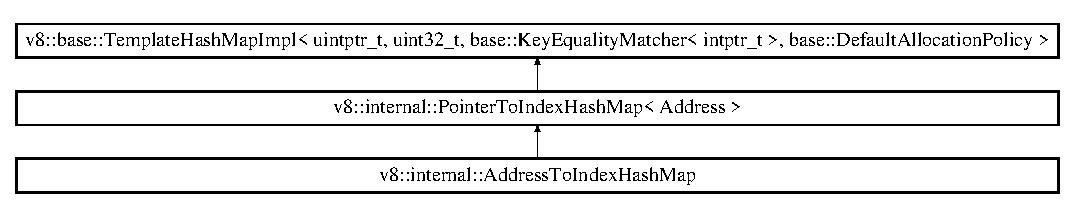
\includegraphics[height=2.362869cm]{classv8_1_1internal_1_1AddressToIndexHashMap}
\end{center}
\end{figure}
\subsection*{Additional Inherited Members}


\subsection{Detailed Description}


Definition at line 52 of file address-\/map.\+h.



The documentation for this class was generated from the following file\+:\begin{DoxyCompactItemize}
\item 
v8/src/address-\/map.\+h\end{DoxyCompactItemize}

\hypertarget{classv8_1_1internal_1_1AddressToTraceMap}{}\section{v8\+:\+:internal\+:\+:Address\+To\+Trace\+Map Class Reference}
\label{classv8_1_1internal_1_1AddressToTraceMap}\index{v8\+::internal\+::\+Address\+To\+Trace\+Map@{v8\+::internal\+::\+Address\+To\+Trace\+Map}}
\subsection*{Public Member Functions}
\begin{DoxyCompactItemize}
\item 
\mbox{\Hypertarget{classv8_1_1internal_1_1AddressToTraceMap_a3b1bc8f1abc6f072a660d2b689852838}\label{classv8_1_1internal_1_1AddressToTraceMap_a3b1bc8f1abc6f072a660d2b689852838}} 
void {\bfseries Add\+Range} (\mbox{\hyperlink{classuintptr__t}{Address}} addr, \mbox{\hyperlink{classint}{int}} size, \mbox{\hyperlink{classunsigned}{unsigned}} node\+\_\+id)
\item 
\mbox{\Hypertarget{classv8_1_1internal_1_1AddressToTraceMap_ab76fa587a105ae24f300f171d8cb22a6}\label{classv8_1_1internal_1_1AddressToTraceMap_ab76fa587a105ae24f300f171d8cb22a6}} 
\mbox{\hyperlink{classunsigned}{unsigned}} {\bfseries Get\+Trace\+Node\+Id} (\mbox{\hyperlink{classuintptr__t}{Address}} addr)
\item 
\mbox{\Hypertarget{classv8_1_1internal_1_1AddressToTraceMap_a02c96d03b3486527aeb46a461c43cf15}\label{classv8_1_1internal_1_1AddressToTraceMap_a02c96d03b3486527aeb46a461c43cf15}} 
void {\bfseries Move\+Object} (\mbox{\hyperlink{classuintptr__t}{Address}} from, \mbox{\hyperlink{classuintptr__t}{Address}} to, \mbox{\hyperlink{classint}{int}} size)
\item 
\mbox{\Hypertarget{classv8_1_1internal_1_1AddressToTraceMap_aa705b7b0e3c00645af20ff4d61140f02}\label{classv8_1_1internal_1_1AddressToTraceMap_aa705b7b0e3c00645af20ff4d61140f02}} 
void {\bfseries Clear} ()
\item 
\mbox{\Hypertarget{classv8_1_1internal_1_1AddressToTraceMap_a6acf57cbb1975fe242c744f4ad5669f3}\label{classv8_1_1internal_1_1AddressToTraceMap_a6acf57cbb1975fe242c744f4ad5669f3}} 
\mbox{\hyperlink{classsize__t}{size\+\_\+t}} {\bfseries size} ()
\item 
\mbox{\Hypertarget{classv8_1_1internal_1_1AddressToTraceMap_a8aa12b1b9b85be5aba73b0631d1ea389}\label{classv8_1_1internal_1_1AddressToTraceMap_a8aa12b1b9b85be5aba73b0631d1ea389}} 
void {\bfseries Print} ()
\end{DoxyCompactItemize}


\subsection{Detailed Description}


Definition at line 74 of file allocation-\/tracker.\+h.



The documentation for this class was generated from the following files\+:\begin{DoxyCompactItemize}
\item 
v8/src/profiler/allocation-\/tracker.\+h\item 
v8/src/profiler/allocation-\/tracker.\+cc\end{DoxyCompactItemize}

\hypertarget{classv8_1_1internal_1_1AddStubAssembler}{}\section{v8\+:\+:internal\+:\+:Add\+Stub\+Assembler Class Reference}
\label{classv8_1_1internal_1_1AddStubAssembler}\index{v8\+::internal\+::\+Add\+Stub\+Assembler@{v8\+::internal\+::\+Add\+Stub\+Assembler}}
Inheritance diagram for v8\+:\+:internal\+:\+:Add\+Stub\+Assembler\+:\begin{figure}[H]
\begin{center}
\leavevmode
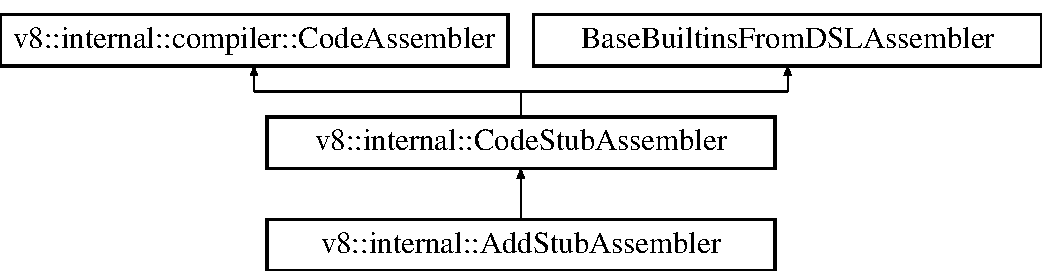
\includegraphics[height=3.000000cm]{classv8_1_1internal_1_1AddStubAssembler}
\end{center}
\end{figure}
\subsection*{Public Member Functions}
\begin{DoxyCompactItemize}
\item 
\mbox{\Hypertarget{classv8_1_1internal_1_1AddStubAssembler_a741aeb3d09c3621ac0635ab3b4ef2abf}\label{classv8_1_1internal_1_1AddStubAssembler_a741aeb3d09c3621ac0635ab3b4ef2abf}} 
{\bfseries Add\+Stub\+Assembler} (\mbox{\hyperlink{classv8_1_1internal_1_1compiler_1_1CodeAssemblerState}{compiler\+::\+Code\+Assembler\+State}} $\ast$state)
\end{DoxyCompactItemize}
\subsection*{Protected Member Functions}
\begin{DoxyCompactItemize}
\item 
\mbox{\Hypertarget{classv8_1_1internal_1_1AddStubAssembler_aa0f2c967e23a87aeee16d48ee31eb125}\label{classv8_1_1internal_1_1AddStubAssembler_aa0f2c967e23a87aeee16d48ee31eb125}} 
void {\bfseries Convert\+Receiver\+And\+Loop} (\mbox{\hyperlink{classv8_1_1internal_1_1compiler_1_1CodeAssemblerVariable}{Variable}} $\ast$var\+\_\+value, \mbox{\hyperlink{classv8_1_1internal_1_1compiler_1_1CodeAssemblerLabel}{Label}} $\ast$loop, \mbox{\hyperlink{classv8_1_1internal_1_1compiler_1_1Node}{Node}} $\ast$context)
\item 
\mbox{\Hypertarget{classv8_1_1internal_1_1AddStubAssembler_afbd25110430918c56edff9b9550c6e16}\label{classv8_1_1internal_1_1AddStubAssembler_afbd25110430918c56edff9b9550c6e16}} 
void {\bfseries Convert\+Non\+Receiver\+And\+Loop} (\mbox{\hyperlink{classv8_1_1internal_1_1compiler_1_1CodeAssemblerVariable}{Variable}} $\ast$var\+\_\+value, \mbox{\hyperlink{classv8_1_1internal_1_1compiler_1_1CodeAssemblerLabel}{Label}} $\ast$loop, \mbox{\hyperlink{classv8_1_1internal_1_1compiler_1_1Node}{Node}} $\ast$context)
\item 
\mbox{\Hypertarget{classv8_1_1internal_1_1AddStubAssembler_a842a08b11f2baa6d51af91688489c6f5}\label{classv8_1_1internal_1_1AddStubAssembler_a842a08b11f2baa6d51af91688489c6f5}} 
void {\bfseries Convert\+And\+Loop} (\mbox{\hyperlink{classv8_1_1internal_1_1compiler_1_1CodeAssemblerVariable}{Variable}} $\ast$var\+\_\+value, \mbox{\hyperlink{classv8_1_1internal_1_1compiler_1_1Node}{Node}} $\ast$instance\+\_\+type, \mbox{\hyperlink{classv8_1_1internal_1_1compiler_1_1CodeAssemblerLabel}{Label}} $\ast$loop, \mbox{\hyperlink{classv8_1_1internal_1_1compiler_1_1Node}{Node}} $\ast$context)
\end{DoxyCompactItemize}
\subsection*{Additional Inherited Members}


\subsection{Detailed Description}


Definition at line 326 of file builtins-\/number-\/gen.\+cc.



The documentation for this class was generated from the following file\+:\begin{DoxyCompactItemize}
\item 
v8/src/builtins/builtins-\/number-\/gen.\+cc\end{DoxyCompactItemize}

\hypertarget{classv8_1_1internal_1_1compiler_1_1AdvancedReducer}{}\section{v8\+:\+:internal\+:\+:compiler\+:\+:Advanced\+Reducer Class Reference}
\label{classv8_1_1internal_1_1compiler_1_1AdvancedReducer}\index{v8\+::internal\+::compiler\+::\+Advanced\+Reducer@{v8\+::internal\+::compiler\+::\+Advanced\+Reducer}}
Inheritance diagram for v8\+:\+:internal\+:\+:compiler\+:\+:Advanced\+Reducer\+:\begin{figure}[H]
\begin{center}
\leavevmode
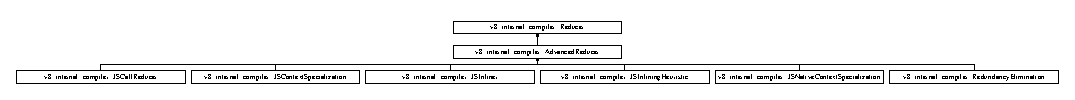
\includegraphics[height=0.894569cm]{classv8_1_1internal_1_1compiler_1_1AdvancedReducer}
\end{center}
\end{figure}
\subsection*{Classes}
\begin{DoxyCompactItemize}
\item 
class \mbox{\hyperlink{classv8_1_1internal_1_1compiler_1_1AdvancedReducer_1_1Editor}{Editor}}
\end{DoxyCompactItemize}
\subsection*{Public Member Functions}
\begin{DoxyCompactItemize}
\item 
\mbox{\Hypertarget{classv8_1_1internal_1_1compiler_1_1AdvancedReducer_abb941b5a245fa4b0c2e87c049fd78190}\label{classv8_1_1internal_1_1compiler_1_1AdvancedReducer_abb941b5a245fa4b0c2e87c049fd78190}} 
{\bfseries Advanced\+Reducer} (\mbox{\hyperlink{classv8_1_1internal_1_1compiler_1_1AdvancedReducer_1_1Editor}{Editor}} $\ast$editor)
\end{DoxyCompactItemize}
\subsection*{Protected Member Functions}
\begin{DoxyCompactItemize}
\item 
\mbox{\Hypertarget{classv8_1_1internal_1_1compiler_1_1AdvancedReducer_a375f732a84655a28f171351dc76f8acc}\label{classv8_1_1internal_1_1compiler_1_1AdvancedReducer_a375f732a84655a28f171351dc76f8acc}} 
void {\bfseries Replace} (\mbox{\hyperlink{classv8_1_1internal_1_1compiler_1_1Node}{Node}} $\ast$node, \mbox{\hyperlink{classv8_1_1internal_1_1compiler_1_1Node}{Node}} $\ast$replacement)
\item 
\mbox{\Hypertarget{classv8_1_1internal_1_1compiler_1_1AdvancedReducer_a64cae7699553789a4534c549c9170816}\label{classv8_1_1internal_1_1compiler_1_1AdvancedReducer_a64cae7699553789a4534c549c9170816}} 
void {\bfseries Revisit} (\mbox{\hyperlink{classv8_1_1internal_1_1compiler_1_1Node}{Node}} $\ast$node)
\item 
\mbox{\Hypertarget{classv8_1_1internal_1_1compiler_1_1AdvancedReducer_a2573497dc120509db4c00a28d8d3a9cb}\label{classv8_1_1internal_1_1compiler_1_1AdvancedReducer_a2573497dc120509db4c00a28d8d3a9cb}} 
void {\bfseries Replace\+With\+Value} (\mbox{\hyperlink{classv8_1_1internal_1_1compiler_1_1Node}{Node}} $\ast$node, \mbox{\hyperlink{classv8_1_1internal_1_1compiler_1_1Node}{Node}} $\ast$value, \mbox{\hyperlink{classv8_1_1internal_1_1compiler_1_1Node}{Node}} $\ast$effect=nullptr, \mbox{\hyperlink{classv8_1_1internal_1_1compiler_1_1Node}{Node}} $\ast$control=nullptr)
\item 
\mbox{\Hypertarget{classv8_1_1internal_1_1compiler_1_1AdvancedReducer_a2f1059b277571c651117544bd023cb8c}\label{classv8_1_1internal_1_1compiler_1_1AdvancedReducer_a2f1059b277571c651117544bd023cb8c}} 
void {\bfseries Relax\+Effects\+And\+Controls} (\mbox{\hyperlink{classv8_1_1internal_1_1compiler_1_1Node}{Node}} $\ast$node)
\item 
\mbox{\Hypertarget{classv8_1_1internal_1_1compiler_1_1AdvancedReducer_a69dd3891050d9e54a9b82db9bd55eacc}\label{classv8_1_1internal_1_1compiler_1_1AdvancedReducer_a69dd3891050d9e54a9b82db9bd55eacc}} 
void {\bfseries Relax\+Controls} (\mbox{\hyperlink{classv8_1_1internal_1_1compiler_1_1Node}{Node}} $\ast$node)
\end{DoxyCompactItemize}
\subsection*{Static Protected Member Functions}
\begin{DoxyCompactItemize}
\item 
\mbox{\Hypertarget{classv8_1_1internal_1_1compiler_1_1AdvancedReducer_a6b9e69978e8440e00ca157d8e4fef297}\label{classv8_1_1internal_1_1compiler_1_1AdvancedReducer_a6b9e69978e8440e00ca157d8e4fef297}} 
static \mbox{\hyperlink{classv8_1_1internal_1_1compiler_1_1Reduction}{Reduction}} {\bfseries Replace} (\mbox{\hyperlink{classv8_1_1internal_1_1compiler_1_1Node}{Node}} $\ast$node)
\end{DoxyCompactItemize}
\subsection*{Additional Inherited Members}


\subsection{Detailed Description}


Definition at line 71 of file graph-\/reducer.\+h.



The documentation for this class was generated from the following file\+:\begin{DoxyCompactItemize}
\item 
v8/src/compiler/graph-\/reducer.\+h\end{DoxyCompactItemize}

\hypertarget{classv8_1_1internal_1_1AggregatableHistogramTimer}{}\section{v8\+:\+:internal\+:\+:Aggregatable\+Histogram\+Timer Class Reference}
\label{classv8_1_1internal_1_1AggregatableHistogramTimer}\index{v8\+::internal\+::\+Aggregatable\+Histogram\+Timer@{v8\+::internal\+::\+Aggregatable\+Histogram\+Timer}}
Inheritance diagram for v8\+:\+:internal\+:\+:Aggregatable\+Histogram\+Timer\+:\begin{figure}[H]
\begin{center}
\leavevmode
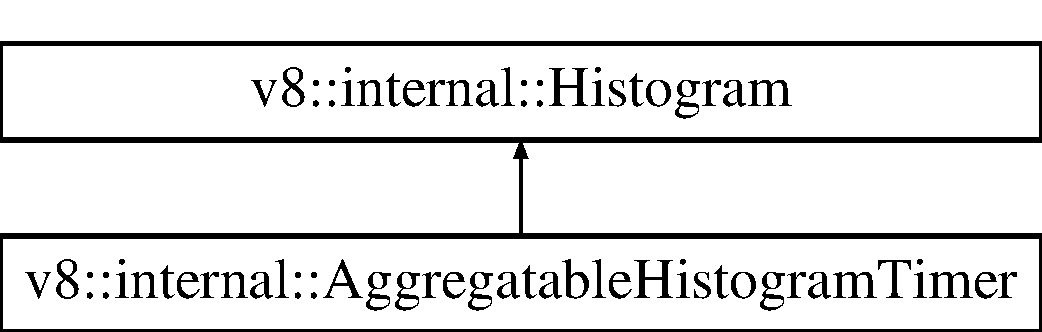
\includegraphics[height=2.000000cm]{classv8_1_1internal_1_1AggregatableHistogramTimer}
\end{center}
\end{figure}
\subsection*{Public Member Functions}
\begin{DoxyCompactItemize}
\item 
\mbox{\Hypertarget{classv8_1_1internal_1_1AggregatableHistogramTimer_a90f85567bb20dba01c8d4e69578db899}\label{classv8_1_1internal_1_1AggregatableHistogramTimer_a90f85567bb20dba01c8d4e69578db899}} 
void {\bfseries Start} ()
\item 
\mbox{\Hypertarget{classv8_1_1internal_1_1AggregatableHistogramTimer_ada969f70c76ed1eace83ea0491d7af5e}\label{classv8_1_1internal_1_1AggregatableHistogramTimer_ada969f70c76ed1eace83ea0491d7af5e}} 
void {\bfseries Stop} ()
\item 
\mbox{\Hypertarget{classv8_1_1internal_1_1AggregatableHistogramTimer_ad56ff543a2b2816fe290fdc2d259c844}\label{classv8_1_1internal_1_1AggregatableHistogramTimer_ad56ff543a2b2816fe290fdc2d259c844}} 
void {\bfseries Add} (\mbox{\hyperlink{classv8_1_1base_1_1TimeDelta}{base\+::\+Time\+Delta}} other)
\end{DoxyCompactItemize}
\subsection*{Friends}
\begin{DoxyCompactItemize}
\item 
\mbox{\Hypertarget{classv8_1_1internal_1_1AggregatableHistogramTimer_a5545327f141103b96b160ddc48274bc0}\label{classv8_1_1internal_1_1AggregatableHistogramTimer_a5545327f141103b96b160ddc48274bc0}} 
class {\bfseries Counters}
\end{DoxyCompactItemize}
\subsection*{Additional Inherited Members}


\subsection{Detailed Description}


Definition at line 479 of file counters.\+h.



The documentation for this class was generated from the following file\+:\begin{DoxyCompactItemize}
\item 
v8/src/counters.\+h\end{DoxyCompactItemize}

\hypertarget{classv8_1_1internal_1_1AggregatedHistogramTimerScope}{}\section{v8\+:\+:internal\+:\+:Aggregated\+Histogram\+Timer\+Scope Class Reference}
\label{classv8_1_1internal_1_1AggregatedHistogramTimerScope}\index{v8\+::internal\+::\+Aggregated\+Histogram\+Timer\+Scope@{v8\+::internal\+::\+Aggregated\+Histogram\+Timer\+Scope}}
\subsection*{Public Member Functions}
\begin{DoxyCompactItemize}
\item 
\mbox{\Hypertarget{classv8_1_1internal_1_1AggregatedHistogramTimerScope_abaf836eb7bf83fe4ceeb79a4a5596af0}\label{classv8_1_1internal_1_1AggregatedHistogramTimerScope_abaf836eb7bf83fe4ceeb79a4a5596af0}} 
{\bfseries Aggregated\+Histogram\+Timer\+Scope} (\mbox{\hyperlink{classv8_1_1internal_1_1AggregatableHistogramTimer}{Aggregatable\+Histogram\+Timer}} $\ast$histogram)
\end{DoxyCompactItemize}


\subsection{Detailed Description}


Definition at line 522 of file counters.\+h.



The documentation for this class was generated from the following file\+:\begin{DoxyCompactItemize}
\item 
v8/src/counters.\+h\end{DoxyCompactItemize}

\hypertarget{classv8_1_1internal_1_1AggregatedMemoryHistogram}{}\section{v8\+:\+:internal\+:\+:Aggregated\+Memory\+Histogram$<$ Histogram $>$ Class Template Reference}
\label{classv8_1_1internal_1_1AggregatedMemoryHistogram}\index{v8\+::internal\+::\+Aggregated\+Memory\+Histogram$<$ Histogram $>$@{v8\+::internal\+::\+Aggregated\+Memory\+Histogram$<$ Histogram $>$}}
\subsection*{Public Member Functions}
\begin{DoxyCompactItemize}
\item 
\mbox{\Hypertarget{classv8_1_1internal_1_1AggregatedMemoryHistogram_a8b49cfff760e104f1150397b4a774806}\label{classv8_1_1internal_1_1AggregatedMemoryHistogram_a8b49cfff760e104f1150397b4a774806}} 
{\bfseries Aggregated\+Memory\+Histogram} (\mbox{\hyperlink{classv8_1_1internal_1_1Histogram}{Histogram}} $\ast$backing\+\_\+histogram)
\item 
\mbox{\Hypertarget{classv8_1_1internal_1_1AggregatedMemoryHistogram_afed07b5cc00d1e8f58be83d85ea6fe94}\label{classv8_1_1internal_1_1AggregatedMemoryHistogram_afed07b5cc00d1e8f58be83d85ea6fe94}} 
void {\bfseries Add\+Sample} (double current\+\_\+ms, double current\+\_\+value)
\end{DoxyCompactItemize}
\subsection*{Friends}
\begin{DoxyCompactItemize}
\item 
\mbox{\Hypertarget{classv8_1_1internal_1_1AggregatedMemoryHistogram_a5545327f141103b96b160ddc48274bc0}\label{classv8_1_1internal_1_1AggregatedMemoryHistogram_a5545327f141103b96b160ddc48274bc0}} 
class {\bfseries Counters}
\end{DoxyCompactItemize}


\subsection{Detailed Description}
\subsubsection*{template$<$typename Histogram$>$\newline
class v8\+::internal\+::\+Aggregated\+Memory\+Histogram$<$ Histogram $>$}



Definition at line 546 of file counters.\+h.



The documentation for this class was generated from the following file\+:\begin{DoxyCompactItemize}
\item 
v8/src/counters.\+h\end{DoxyCompactItemize}

\hypertarget{classv8_1_1internal_1_1AggregateLiteral}{}\section{v8\+:\+:internal\+:\+:Aggregate\+Literal Class Reference}
\label{classv8_1_1internal_1_1AggregateLiteral}\index{v8\+::internal\+::\+Aggregate\+Literal@{v8\+::internal\+::\+Aggregate\+Literal}}
Inheritance diagram for v8\+:\+:internal\+:\+:Aggregate\+Literal\+:\begin{figure}[H]
\begin{center}
\leavevmode
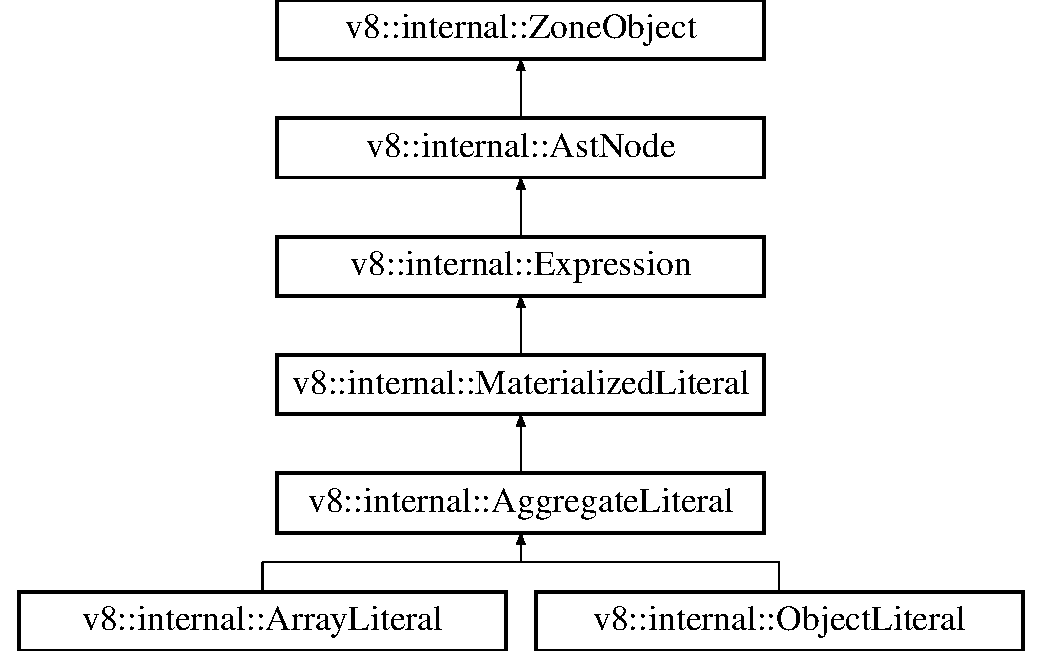
\includegraphics[height=6.000000cm]{classv8_1_1internal_1_1AggregateLiteral}
\end{center}
\end{figure}
\subsection*{Public Types}
\begin{DoxyCompactItemize}
\item 
\mbox{\Hypertarget{classv8_1_1internal_1_1AggregateLiteral_a277407153d07ee6a88adf650b71248ad}\label{classv8_1_1internal_1_1AggregateLiteral_a277407153d07ee6a88adf650b71248ad}} 
enum {\bfseries Flags} \{ {\bfseries k\+No\+Flags} = 0, 
{\bfseries k\+Is\+Shallow} = 1, 
{\bfseries k\+Disable\+Mementos} = 1 $<$$<$ 1, 
{\bfseries k\+Needs\+Initial\+Allocation\+Site} = 1 $<$$<$ 2
 \}
\end{DoxyCompactItemize}
\subsection*{Public Member Functions}
\begin{DoxyCompactItemize}
\item 
\mbox{\Hypertarget{classv8_1_1internal_1_1AggregateLiteral_af89e700cae2a8af5a8408048a5e97d07}\label{classv8_1_1internal_1_1AggregateLiteral_af89e700cae2a8af5a8408048a5e97d07}} 
\mbox{\hyperlink{classbool}{bool}} {\bfseries is\+\_\+initialized} () const
\item 
\mbox{\Hypertarget{classv8_1_1internal_1_1AggregateLiteral_a9ca53fd750ca800268a4ea92a6ca3287}\label{classv8_1_1internal_1_1AggregateLiteral_a9ca53fd750ca800268a4ea92a6ca3287}} 
\mbox{\hyperlink{classint}{int}} {\bfseries depth} () const
\item 
\mbox{\Hypertarget{classv8_1_1internal_1_1AggregateLiteral_a6ccaff2cb289811cc47eb6fe188728de}\label{classv8_1_1internal_1_1AggregateLiteral_a6ccaff2cb289811cc47eb6fe188728de}} 
\mbox{\hyperlink{classbool}{bool}} {\bfseries is\+\_\+shallow} () const
\item 
\mbox{\Hypertarget{classv8_1_1internal_1_1AggregateLiteral_ae6f6fa2d0bab943685ac44d9b98b3f0d}\label{classv8_1_1internal_1_1AggregateLiteral_ae6f6fa2d0bab943685ac44d9b98b3f0d}} 
\mbox{\hyperlink{classbool}{bool}} {\bfseries needs\+\_\+initial\+\_\+allocation\+\_\+site} () const
\item 
\mbox{\Hypertarget{classv8_1_1internal_1_1AggregateLiteral_aab431fb4280c3c3e07251be93650e8c4}\label{classv8_1_1internal_1_1AggregateLiteral_aab431fb4280c3c3e07251be93650e8c4}} 
\mbox{\hyperlink{classint}{int}} {\bfseries Compute\+Flags} (\mbox{\hyperlink{classbool}{bool}} disable\+\_\+mementos=false) const
\item 
\mbox{\Hypertarget{classv8_1_1internal_1_1AggregateLiteral_ae91f5d0a9a11196b255de90aab34ae9d}\label{classv8_1_1internal_1_1AggregateLiteral_ae91f5d0a9a11196b255de90aab34ae9d}} 
\mbox{\hyperlink{classbool}{bool}} {\bfseries is\+\_\+simple} () const
\end{DoxyCompactItemize}
\subsection*{Protected Member Functions}
\begin{DoxyCompactItemize}
\item 
\mbox{\Hypertarget{classv8_1_1internal_1_1AggregateLiteral_a0da2aa8d2d4d2a529faaeaaea8ff133f}\label{classv8_1_1internal_1_1AggregateLiteral_a0da2aa8d2d4d2a529faaeaaea8ff133f}} 
{\bfseries Aggregate\+Literal} (\mbox{\hyperlink{classint}{int}} pos, Node\+Type \mbox{\hyperlink{classstd_1_1conditional_1_1type}{type}})
\item 
\mbox{\Hypertarget{classv8_1_1internal_1_1AggregateLiteral_a66bba6b8a0d7de7daf638bff629e044e}\label{classv8_1_1internal_1_1AggregateLiteral_a66bba6b8a0d7de7daf638bff629e044e}} 
void {\bfseries set\+\_\+is\+\_\+simple} (\mbox{\hyperlink{classbool}{bool}} is\+\_\+simple)
\item 
\mbox{\Hypertarget{classv8_1_1internal_1_1AggregateLiteral_a6afd47480bd72e259c1202f996a6a40b}\label{classv8_1_1internal_1_1AggregateLiteral_a6afd47480bd72e259c1202f996a6a40b}} 
void {\bfseries set\+\_\+depth} (\mbox{\hyperlink{classint}{int}} depth)
\item 
\mbox{\Hypertarget{classv8_1_1internal_1_1AggregateLiteral_a4940d433db71d83c337591d2ca9b92b8}\label{classv8_1_1internal_1_1AggregateLiteral_a4940d433db71d83c337591d2ca9b92b8}} 
void {\bfseries set\+\_\+needs\+\_\+initial\+\_\+allocation\+\_\+site} (\mbox{\hyperlink{classbool}{bool}} required)
\end{DoxyCompactItemize}
\subsection*{Static Protected Attributes}
\begin{DoxyCompactItemize}
\item 
\mbox{\Hypertarget{classv8_1_1internal_1_1AggregateLiteral_a986b62c8d0ff893b7522e8c29f436226}\label{classv8_1_1internal_1_1AggregateLiteral_a986b62c8d0ff893b7522e8c29f436226}} 
static const uint8\+\_\+t {\bfseries k\+Next\+Bit\+Field\+Index} = Is\+Simple\+Field\+::k\+Next
\end{DoxyCompactItemize}
\subsection*{Friends}
\begin{DoxyCompactItemize}
\item 
\mbox{\Hypertarget{classv8_1_1internal_1_1AggregateLiteral_a8d587c8ad3515ff6433eb83c578e795f}\label{classv8_1_1internal_1_1AggregateLiteral_a8d587c8ad3515ff6433eb83c578e795f}} 
class {\bfseries Ast\+Node\+Factory}
\end{DoxyCompactItemize}
\subsection*{Additional Inherited Members}


\subsection{Detailed Description}


Definition at line 1254 of file ast.\+h.



The documentation for this class was generated from the following file\+:\begin{DoxyCompactItemize}
\item 
v8/src/ast/ast.\+h\end{DoxyCompactItemize}

\hypertarget{classv8_1_1internal_1_1AggregatingHistogramTimerScope}{}\section{v8\+:\+:internal\+:\+:Aggregating\+Histogram\+Timer\+Scope Class Reference}
\label{classv8_1_1internal_1_1AggregatingHistogramTimerScope}\index{v8\+::internal\+::\+Aggregating\+Histogram\+Timer\+Scope@{v8\+::internal\+::\+Aggregating\+Histogram\+Timer\+Scope}}
\subsection*{Public Member Functions}
\begin{DoxyCompactItemize}
\item 
\mbox{\Hypertarget{classv8_1_1internal_1_1AggregatingHistogramTimerScope_a96403652799814786ac2fc73d2cbb2ce}\label{classv8_1_1internal_1_1AggregatingHistogramTimerScope_a96403652799814786ac2fc73d2cbb2ce}} 
{\bfseries Aggregating\+Histogram\+Timer\+Scope} (\mbox{\hyperlink{classv8_1_1internal_1_1AggregatableHistogramTimer}{Aggregatable\+Histogram\+Timer}} $\ast$histogram)
\end{DoxyCompactItemize}


\subsection{Detailed Description}


Definition at line 508 of file counters.\+h.



The documentation for this class was generated from the following file\+:\begin{DoxyCompactItemize}
\item 
v8/src/counters.\+h\end{DoxyCompactItemize}

\hypertarget{classv8_1_1base_1_1AIXTimezoneCache}{}\section{v8\+:\+:base\+:\+:A\+I\+X\+Timezone\+Cache Class Reference}
\label{classv8_1_1base_1_1AIXTimezoneCache}\index{v8\+::base\+::\+A\+I\+X\+Timezone\+Cache@{v8\+::base\+::\+A\+I\+X\+Timezone\+Cache}}
Inheritance diagram for v8\+:\+:base\+:\+:A\+I\+X\+Timezone\+Cache\+:\begin{figure}[H]
\begin{center}
\leavevmode
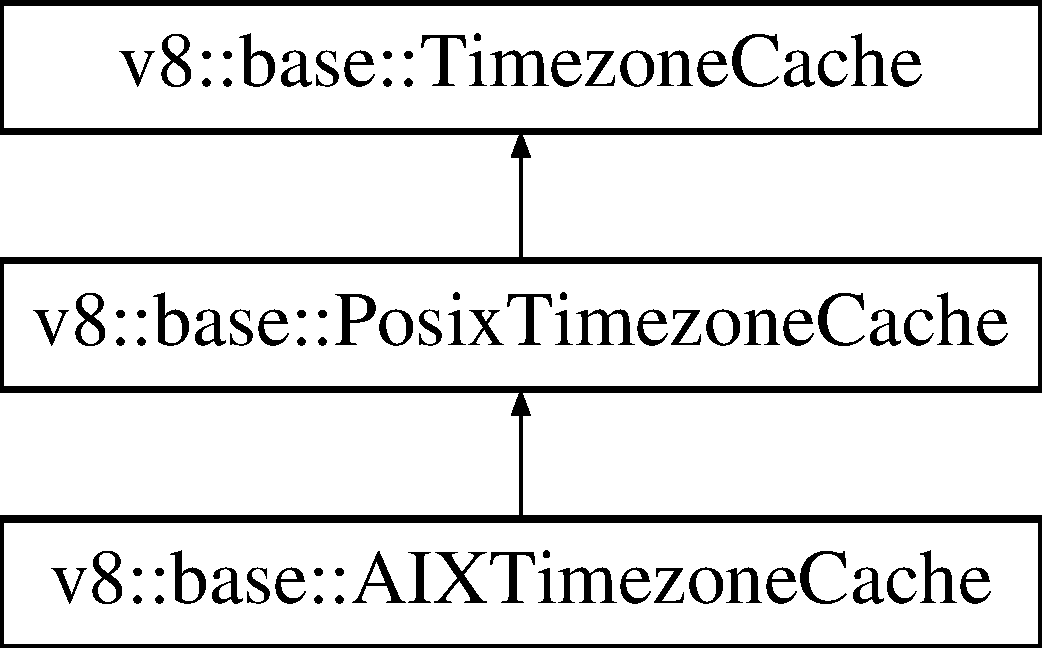
\includegraphics[height=3.000000cm]{classv8_1_1base_1_1AIXTimezoneCache}
\end{center}
\end{figure}
\subsection*{Additional Inherited Members}


\subsection{Detailed Description}


Definition at line 39 of file platform-\/aix.\+cc.



The documentation for this class was generated from the following file\+:\begin{DoxyCompactItemize}
\item 
v8/src/base/platform/platform-\/aix.\+cc\end{DoxyCompactItemize}

\hypertarget{classv8_1_1internal_1_1AliasedArgumentsEntry}{}\section{v8\+:\+:internal\+:\+:Aliased\+Arguments\+Entry Class Reference}
\label{classv8_1_1internal_1_1AliasedArgumentsEntry}\index{v8\+::internal\+::\+Aliased\+Arguments\+Entry@{v8\+::internal\+::\+Aliased\+Arguments\+Entry}}
Inheritance diagram for v8\+:\+:internal\+:\+:Aliased\+Arguments\+Entry\+:\begin{figure}[H]
\begin{center}
\leavevmode
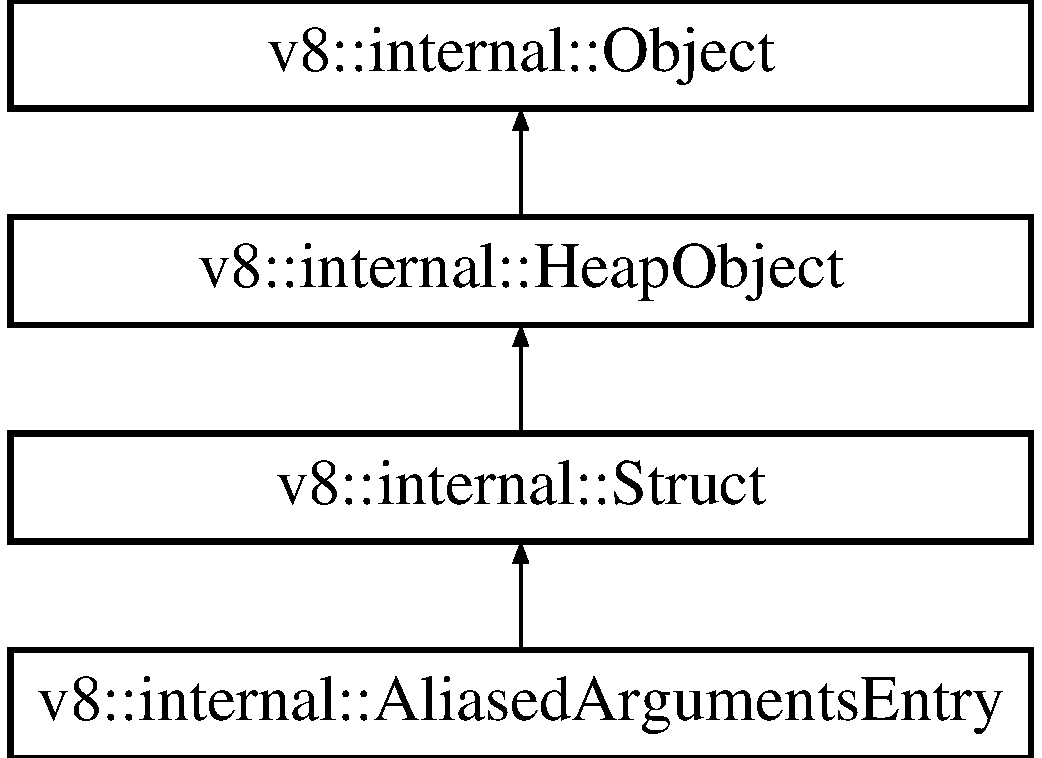
\includegraphics[height=4.000000cm]{classv8_1_1internal_1_1AliasedArgumentsEntry}
\end{center}
\end{figure}
\subsection*{Public Member Functions}
\begin{DoxyCompactItemize}
\item 
\mbox{\Hypertarget{classv8_1_1internal_1_1AliasedArgumentsEntry_adc997e9de703e6e969a887795e8b9689}\label{classv8_1_1internal_1_1AliasedArgumentsEntry_adc997e9de703e6e969a887795e8b9689}} 
\mbox{\hyperlink{classint}{int}} {\bfseries aliased\+\_\+context\+\_\+slot} () const
\item 
\mbox{\Hypertarget{classv8_1_1internal_1_1AliasedArgumentsEntry_ad2f671a7089a9e775abd7e1c039aeee7}\label{classv8_1_1internal_1_1AliasedArgumentsEntry_ad2f671a7089a9e775abd7e1c039aeee7}} 
void {\bfseries set\+\_\+aliased\+\_\+context\+\_\+slot} (\mbox{\hyperlink{classint}{int}} count)
\end{DoxyCompactItemize}
\subsection*{Additional Inherited Members}


\subsection{Detailed Description}


Definition at line 138 of file arguments.\+h.



The documentation for this class was generated from the following file\+:\begin{DoxyCompactItemize}
\item 
v8/src/objects/arguments.\+h\end{DoxyCompactItemize}

\hypertarget{classv8_1_1internal_1_1compiler_1_1LoadElimination_1_1AliasStateInfo}{}\section{v8\+:\+:internal\+:\+:compiler\+:\+:Load\+Elimination\+:\+:Alias\+State\+Info Class Reference}
\label{classv8_1_1internal_1_1compiler_1_1LoadElimination_1_1AliasStateInfo}\index{v8\+::internal\+::compiler\+::\+Load\+Elimination\+::\+Alias\+State\+Info@{v8\+::internal\+::compiler\+::\+Load\+Elimination\+::\+Alias\+State\+Info}}
\subsection*{Public Member Functions}
\begin{DoxyCompactItemize}
\item 
\mbox{\Hypertarget{classv8_1_1internal_1_1compiler_1_1LoadElimination_1_1AliasStateInfo_ac706d8b05c8b12339f76b931c27da83f}\label{classv8_1_1internal_1_1compiler_1_1LoadElimination_1_1AliasStateInfo_ac706d8b05c8b12339f76b931c27da83f}} 
{\bfseries Alias\+State\+Info} (const Abstract\+State $\ast$state, \mbox{\hyperlink{classv8_1_1internal_1_1compiler_1_1Node}{Node}} $\ast$object, \mbox{\hyperlink{classv8_1_1internal_1_1Handle}{Handle}}$<$ \mbox{\hyperlink{classv8_1_1internal_1_1Map}{Map}} $>$ map)
\item 
\mbox{\Hypertarget{classv8_1_1internal_1_1compiler_1_1LoadElimination_1_1AliasStateInfo_a2eea99e8fd92b1e648fd87456e17240e}\label{classv8_1_1internal_1_1compiler_1_1LoadElimination_1_1AliasStateInfo_a2eea99e8fd92b1e648fd87456e17240e}} 
{\bfseries Alias\+State\+Info} (const Abstract\+State $\ast$state, \mbox{\hyperlink{classv8_1_1internal_1_1compiler_1_1Node}{Node}} $\ast$object)
\item 
\mbox{\Hypertarget{classv8_1_1internal_1_1compiler_1_1LoadElimination_1_1AliasStateInfo_ab7e10ef62acb015e743b66fc8e6ffd5a}\label{classv8_1_1internal_1_1compiler_1_1LoadElimination_1_1AliasStateInfo_ab7e10ef62acb015e743b66fc8e6ffd5a}} 
\mbox{\hyperlink{classbool}{bool}} {\bfseries May\+Alias} (\mbox{\hyperlink{classv8_1_1internal_1_1compiler_1_1Node}{Node}} $\ast$other) const
\end{DoxyCompactItemize}


\subsection{Detailed Description}


Definition at line 267 of file load-\/elimination.\+cc.



The documentation for this class was generated from the following file\+:\begin{DoxyCompactItemize}
\item 
v8/src/compiler/load-\/elimination.\+cc\end{DoxyCompactItemize}

\hypertarget{classv8_1_1internal_1_1compiler_1_1MachineOperatorBuilder_1_1AlignmentRequirements}{}\section{v8\+:\+:internal\+:\+:compiler\+:\+:Machine\+Operator\+Builder\+:\+:Alignment\+Requirements Class Reference}
\label{classv8_1_1internal_1_1compiler_1_1MachineOperatorBuilder_1_1AlignmentRequirements}\index{v8\+::internal\+::compiler\+::\+Machine\+Operator\+Builder\+::\+Alignment\+Requirements@{v8\+::internal\+::compiler\+::\+Machine\+Operator\+Builder\+::\+Alignment\+Requirements}}
\subsection*{Public Types}
\begin{DoxyCompactItemize}
\item 
\mbox{\Hypertarget{classv8_1_1internal_1_1compiler_1_1MachineOperatorBuilder_1_1AlignmentRequirements_a8042b63517b4c0ff2d17c6a9b9cd2a6b}\label{classv8_1_1internal_1_1compiler_1_1MachineOperatorBuilder_1_1AlignmentRequirements_a8042b63517b4c0ff2d17c6a9b9cd2a6b}} 
enum {\bfseries Unaligned\+Access\+Support} \{ {\bfseries k\+No\+Support}, 
{\bfseries k\+Some\+Support}, 
{\bfseries k\+Full\+Support}
 \}
\end{DoxyCompactItemize}
\subsection*{Public Member Functions}
\begin{DoxyCompactItemize}
\item 
\mbox{\Hypertarget{classv8_1_1internal_1_1compiler_1_1MachineOperatorBuilder_1_1AlignmentRequirements_a11ffab020dd6d0fda135714664263e77}\label{classv8_1_1internal_1_1compiler_1_1MachineOperatorBuilder_1_1AlignmentRequirements_a11ffab020dd6d0fda135714664263e77}} 
\mbox{\hyperlink{classbool}{bool}} {\bfseries Is\+Unaligned\+Load\+Supported} (Machine\+Representation rep) const
\item 
\mbox{\Hypertarget{classv8_1_1internal_1_1compiler_1_1MachineOperatorBuilder_1_1AlignmentRequirements_ac9fa29c249f0be05f5de60e2a9c99f29}\label{classv8_1_1internal_1_1compiler_1_1MachineOperatorBuilder_1_1AlignmentRequirements_ac9fa29c249f0be05f5de60e2a9c99f29}} 
\mbox{\hyperlink{classbool}{bool}} {\bfseries Is\+Unaligned\+Store\+Supported} (Machine\+Representation rep) const
\end{DoxyCompactItemize}
\subsection*{Static Public Member Functions}
\begin{DoxyCompactItemize}
\item 
\mbox{\Hypertarget{classv8_1_1internal_1_1compiler_1_1MachineOperatorBuilder_1_1AlignmentRequirements_acf18a2cbc43588893a074af63709356e}\label{classv8_1_1internal_1_1compiler_1_1MachineOperatorBuilder_1_1AlignmentRequirements_acf18a2cbc43588893a074af63709356e}} 
static \mbox{\hyperlink{classv8_1_1internal_1_1compiler_1_1MachineOperatorBuilder_1_1AlignmentRequirements}{Alignment\+Requirements}} {\bfseries Full\+Unaligned\+Access\+Support} ()
\item 
\mbox{\Hypertarget{classv8_1_1internal_1_1compiler_1_1MachineOperatorBuilder_1_1AlignmentRequirements_a32ad658c0dde33f8d0d4cbb551112f7c}\label{classv8_1_1internal_1_1compiler_1_1MachineOperatorBuilder_1_1AlignmentRequirements_a32ad658c0dde33f8d0d4cbb551112f7c}} 
static \mbox{\hyperlink{classv8_1_1internal_1_1compiler_1_1MachineOperatorBuilder_1_1AlignmentRequirements}{Alignment\+Requirements}} {\bfseries No\+Unaligned\+Access\+Support} ()
\item 
\mbox{\Hypertarget{classv8_1_1internal_1_1compiler_1_1MachineOperatorBuilder_1_1AlignmentRequirements_a3ac450768bf99b4c835354b691433d7c}\label{classv8_1_1internal_1_1compiler_1_1MachineOperatorBuilder_1_1AlignmentRequirements_a3ac450768bf99b4c835354b691433d7c}} 
static \mbox{\hyperlink{classv8_1_1internal_1_1compiler_1_1MachineOperatorBuilder_1_1AlignmentRequirements}{Alignment\+Requirements}} {\bfseries Some\+Unaligned\+Access\+Unsupported} (\mbox{\hyperlink{classv8_1_1internal_1_1EnumSet}{Enum\+Set}}$<$ Machine\+Representation $>$ unaligned\+Load\+Unsupported\+Types, \mbox{\hyperlink{classv8_1_1internal_1_1EnumSet}{Enum\+Set}}$<$ Machine\+Representation $>$ unaligned\+Store\+Unsupported\+Types)
\end{DoxyCompactItemize}


\subsection{Detailed Description}


Definition at line 156 of file machine-\/operator.\+h.



The documentation for this class was generated from the following file\+:\begin{DoxyCompactItemize}
\item 
v8/src/compiler/machine-\/operator.\+h\end{DoxyCompactItemize}

\hypertarget{classv8_1_1AlignOfHelper}{}\section{v8\+:\+:Align\+Of\+Helper$<$ T $>$ Class Template Reference}
\label{classv8_1_1AlignOfHelper}\index{v8\+::\+Align\+Of\+Helper$<$ T $>$@{v8\+::\+Align\+Of\+Helper$<$ T $>$}}


\subsection{Detailed Description}
\subsubsection*{template$<$typename T$>$\newline
class v8\+::\+Align\+Of\+Helper$<$ T $>$}



Definition at line 414 of file v8config.\+h.



The documentation for this class was generated from the following file\+:\begin{DoxyCompactItemize}
\item 
v8/include/v8config.\+h\end{DoxyCompactItemize}

\hypertarget{classv8_1_1internal_1_1compiler_1_1AllNodes}{}\section{v8\+:\+:internal\+:\+:compiler\+:\+:All\+Nodes Class Reference}
\label{classv8_1_1internal_1_1compiler_1_1AllNodes}\index{v8\+::internal\+::compiler\+::\+All\+Nodes@{v8\+::internal\+::compiler\+::\+All\+Nodes}}
\subsection*{Public Member Functions}
\begin{DoxyCompactItemize}
\item 
\mbox{\Hypertarget{classv8_1_1internal_1_1compiler_1_1AllNodes_af6c9f4bce71577567a78e723bf059427}\label{classv8_1_1internal_1_1compiler_1_1AllNodes_af6c9f4bce71577567a78e723bf059427}} 
{\bfseries All\+Nodes} (\mbox{\hyperlink{classv8_1_1internal_1_1Zone}{Zone}} $\ast$local\+\_\+zone, \mbox{\hyperlink{classv8_1_1internal_1_1compiler_1_1Node}{Node}} $\ast$end, const \mbox{\hyperlink{classv8_1_1internal_1_1compiler_1_1Graph}{Graph}} $\ast$graph, \mbox{\hyperlink{classbool}{bool}} only\+\_\+inputs=true)
\item 
\mbox{\Hypertarget{classv8_1_1internal_1_1compiler_1_1AllNodes_a6afc8a2db2e9dc39b954e8aef5de04ce}\label{classv8_1_1internal_1_1compiler_1_1AllNodes_a6afc8a2db2e9dc39b954e8aef5de04ce}} 
{\bfseries All\+Nodes} (\mbox{\hyperlink{classv8_1_1internal_1_1Zone}{Zone}} $\ast$local\+\_\+zone, const \mbox{\hyperlink{classv8_1_1internal_1_1compiler_1_1Graph}{Graph}} $\ast$graph, \mbox{\hyperlink{classbool}{bool}} only\+\_\+inputs=true)
\item 
\mbox{\Hypertarget{classv8_1_1internal_1_1compiler_1_1AllNodes_a631f6ac405ff5a229b4c4f064db1a80c}\label{classv8_1_1internal_1_1compiler_1_1AllNodes_a631f6ac405ff5a229b4c4f064db1a80c}} 
\mbox{\hyperlink{classbool}{bool}} {\bfseries Is\+Live} (const \mbox{\hyperlink{classv8_1_1internal_1_1compiler_1_1Node}{Node}} $\ast$node) const
\item 
\mbox{\Hypertarget{classv8_1_1internal_1_1compiler_1_1AllNodes_ad46377ff423cb080e085e00c301926dc}\label{classv8_1_1internal_1_1compiler_1_1AllNodes_ad46377ff423cb080e085e00c301926dc}} 
\mbox{\hyperlink{classbool}{bool}} {\bfseries Is\+Reachable} (const \mbox{\hyperlink{classv8_1_1internal_1_1compiler_1_1Node}{Node}} $\ast$node) const
\end{DoxyCompactItemize}
\subsection*{Public Attributes}
\begin{DoxyCompactItemize}
\item 
\mbox{\Hypertarget{classv8_1_1internal_1_1compiler_1_1AllNodes_a511486b5db493d5fa52e0e81947d0065}\label{classv8_1_1internal_1_1compiler_1_1AllNodes_a511486b5db493d5fa52e0e81947d0065}} 
\mbox{\hyperlink{classv8_1_1internal_1_1ZoneVector}{Node\+Vector}} {\bfseries reachable}
\end{DoxyCompactItemize}


\subsection{Detailed Description}


Definition at line 17 of file all-\/nodes.\+h.



The documentation for this class was generated from the following files\+:\begin{DoxyCompactItemize}
\item 
v8/src/compiler/all-\/nodes.\+h\item 
v8/src/compiler/all-\/nodes.\+cc\end{DoxyCompactItemize}

\hypertarget{classv8_1_1internal_1_1AllocateDescriptor}{}\section{v8\+:\+:internal\+:\+:Allocate\+Descriptor Class Reference}
\label{classv8_1_1internal_1_1AllocateDescriptor}\index{v8\+::internal\+::\+Allocate\+Descriptor@{v8\+::internal\+::\+Allocate\+Descriptor}}
Inheritance diagram for v8\+:\+:internal\+:\+:Allocate\+Descriptor\+:\begin{figure}[H]
\begin{center}
\leavevmode
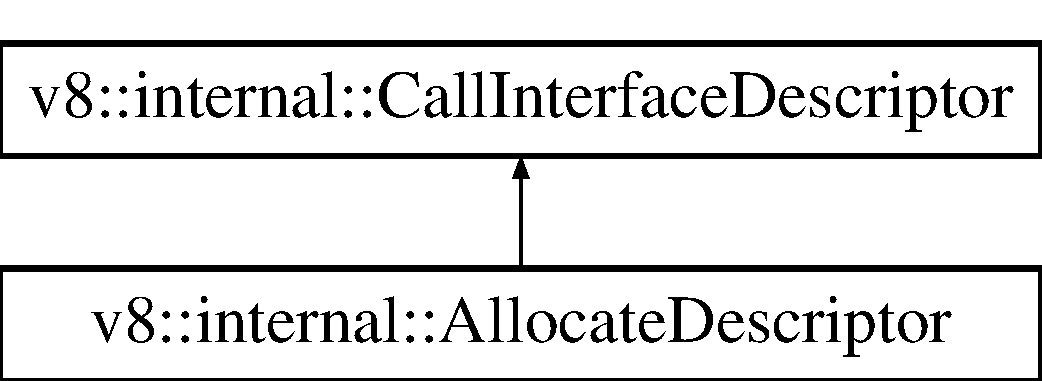
\includegraphics[height=2.000000cm]{classv8_1_1internal_1_1AllocateDescriptor}
\end{center}
\end{figure}
\subsection*{Additional Inherited Members}


\subsection{Detailed Description}


Definition at line 444 of file interface-\/descriptors.\+h.



The documentation for this class was generated from the following file\+:\begin{DoxyCompactItemize}
\item 
v8/src/interface-\/descriptors.\+h\end{DoxyCompactItemize}

\hypertarget{classv8_1_1internal_1_1compiler_1_1AllocatedOperand}{}\section{v8\+:\+:internal\+:\+:compiler\+:\+:Allocated\+Operand Class Reference}
\label{classv8_1_1internal_1_1compiler_1_1AllocatedOperand}\index{v8\+::internal\+::compiler\+::\+Allocated\+Operand@{v8\+::internal\+::compiler\+::\+Allocated\+Operand}}
Inheritance diagram for v8\+:\+:internal\+:\+:compiler\+:\+:Allocated\+Operand\+:\begin{figure}[H]
\begin{center}
\leavevmode
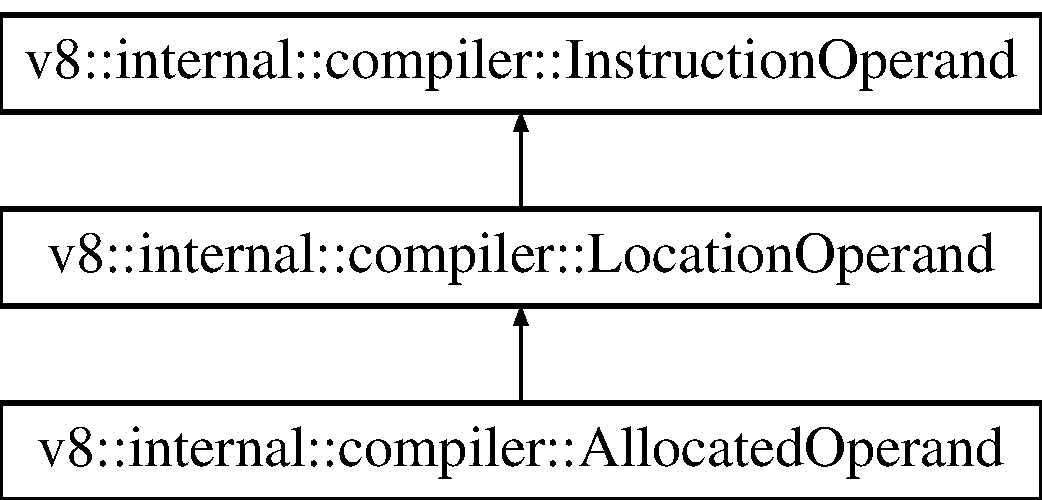
\includegraphics[height=3.000000cm]{classv8_1_1internal_1_1compiler_1_1AllocatedOperand}
\end{center}
\end{figure}
\subsection*{Public Member Functions}
\begin{DoxyCompactItemize}
\item 
\mbox{\Hypertarget{classv8_1_1internal_1_1compiler_1_1AllocatedOperand_a1e23e5746e40802c4376243abdbe8e48}\label{classv8_1_1internal_1_1compiler_1_1AllocatedOperand_a1e23e5746e40802c4376243abdbe8e48}} 
{\bfseries Allocated\+Operand} (Location\+Kind kind, Machine\+Representation rep, \mbox{\hyperlink{classint}{int}} index)
\item 
\mbox{\Hypertarget{classv8_1_1internal_1_1compiler_1_1AllocatedOperand_a7dc1520248d33f029a009fdc7d5951a1}\label{classv8_1_1internal_1_1compiler_1_1AllocatedOperand_a7dc1520248d33f029a009fdc7d5951a1}} 
{\bfseries I\+N\+S\+T\+R\+U\+C\+T\+I\+O\+N\+\_\+\+O\+P\+E\+R\+A\+N\+D\+\_\+\+C\+A\+S\+TS} (\mbox{\hyperlink{classv8_1_1internal_1_1compiler_1_1AllocatedOperand}{Allocated\+Operand}}, A\+L\+L\+O\+C\+A\+T\+ED)
\end{DoxyCompactItemize}
\subsection*{Static Public Member Functions}
\begin{DoxyCompactItemize}
\item 
\mbox{\Hypertarget{classv8_1_1internal_1_1compiler_1_1AllocatedOperand_a5981dcc601391236e463e4afaee84bbe}\label{classv8_1_1internal_1_1compiler_1_1AllocatedOperand_a5981dcc601391236e463e4afaee84bbe}} 
static \mbox{\hyperlink{classv8_1_1internal_1_1compiler_1_1AllocatedOperand}{Allocated\+Operand}} $\ast$ {\bfseries New} (\mbox{\hyperlink{classv8_1_1internal_1_1Zone}{Zone}} $\ast$zone, Location\+Kind kind, Machine\+Representation rep, \mbox{\hyperlink{classint}{int}} index)
\end{DoxyCompactItemize}
\subsection*{Additional Inherited Members}


\subsection{Detailed Description}


Definition at line 523 of file instruction.\+h.



The documentation for this class was generated from the following file\+:\begin{DoxyCompactItemize}
\item 
v8/src/compiler/backend/instruction.\+h\end{DoxyCompactItemize}

\hypertarget{classv8_1_1internal_1_1AllocateDoubleAlignFlag}{}\section{v8\+:\+:internal\+:\+:Allocate\+Double\+Align\+Flag Class Reference}
\label{classv8_1_1internal_1_1AllocateDoubleAlignFlag}\index{v8\+::internal\+::\+Allocate\+Double\+Align\+Flag@{v8\+::internal\+::\+Allocate\+Double\+Align\+Flag}}
Inheritance diagram for v8\+:\+:internal\+:\+:Allocate\+Double\+Align\+Flag\+:\begin{figure}[H]
\begin{center}
\leavevmode
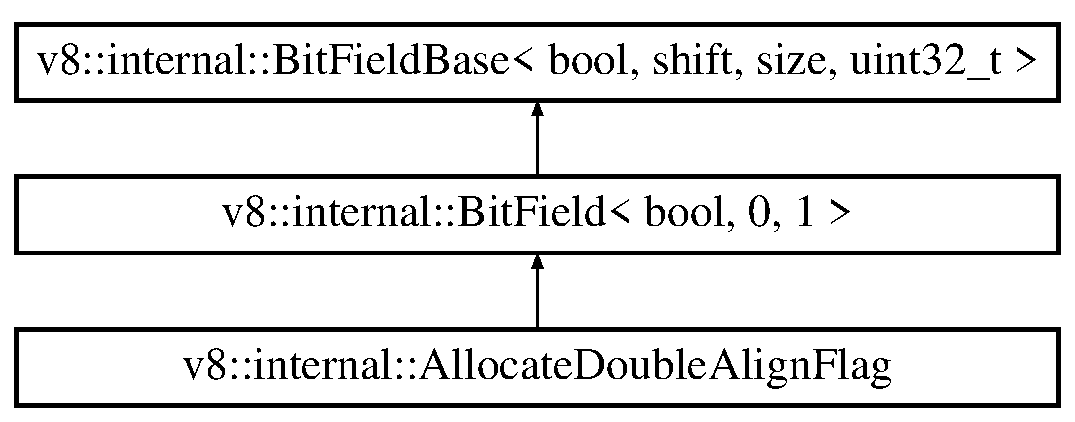
\includegraphics[height=3.000000cm]{classv8_1_1internal_1_1AllocateDoubleAlignFlag}
\end{center}
\end{figure}
\subsection*{Additional Inherited Members}


\subsection{Detailed Description}


Definition at line 753 of file runtime.\+h.



The documentation for this class was generated from the following file\+:\begin{DoxyCompactItemize}
\item 
v8/src/runtime/runtime.\+h\end{DoxyCompactItemize}

\hypertarget{structv8_1_1internal_1_1compiler_1_1AllocateFPRegistersPhase}{}\section{v8\+:\+:internal\+:\+:compiler\+:\+:Allocate\+F\+P\+Registers\+Phase$<$ Reg\+Allocator $>$ Struct Template Reference}
\label{structv8_1_1internal_1_1compiler_1_1AllocateFPRegistersPhase}\index{v8\+::internal\+::compiler\+::\+Allocate\+F\+P\+Registers\+Phase$<$ Reg\+Allocator $>$@{v8\+::internal\+::compiler\+::\+Allocate\+F\+P\+Registers\+Phase$<$ Reg\+Allocator $>$}}
\subsection*{Public Member Functions}
\begin{DoxyCompactItemize}
\item 
\mbox{\Hypertarget{structv8_1_1internal_1_1compiler_1_1AllocateFPRegistersPhase_a4c6dd764c8c48b49f8ecd1e1035f5079}\label{structv8_1_1internal_1_1compiler_1_1AllocateFPRegistersPhase_a4c6dd764c8c48b49f8ecd1e1035f5079}} 
void {\bfseries Run} (\mbox{\hyperlink{classv8_1_1internal_1_1compiler_1_1PipelineData}{Pipeline\+Data}} $\ast$data, \mbox{\hyperlink{classv8_1_1internal_1_1Zone}{Zone}} $\ast$temp\+\_\+zone)
\end{DoxyCompactItemize}
\subsection*{Static Public Member Functions}
\begin{DoxyCompactItemize}
\item 
\mbox{\Hypertarget{structv8_1_1internal_1_1compiler_1_1AllocateFPRegistersPhase_a29ced843c54c50d3169abe3aaa193858}\label{structv8_1_1internal_1_1compiler_1_1AllocateFPRegistersPhase_a29ced843c54c50d3169abe3aaa193858}} 
static const \mbox{\hyperlink{classchar}{char}} $\ast$ {\bfseries phase\+\_\+name} ()
\end{DoxyCompactItemize}


\subsection{Detailed Description}
\subsubsection*{template$<$typename Reg\+Allocator$>$\newline
struct v8\+::internal\+::compiler\+::\+Allocate\+F\+P\+Registers\+Phase$<$ Reg\+Allocator $>$}



Definition at line 1647 of file pipeline.\+cc.



The documentation for this struct was generated from the following file\+:\begin{DoxyCompactItemize}
\item 
v8/src/compiler/pipeline.\+cc\end{DoxyCompactItemize}

\hypertarget{structv8_1_1internal_1_1compiler_1_1AllocateGeneralRegistersPhase}{}\section{v8\+:\+:internal\+:\+:compiler\+:\+:Allocate\+General\+Registers\+Phase$<$ Reg\+Allocator $>$ Struct Template Reference}
\label{structv8_1_1internal_1_1compiler_1_1AllocateGeneralRegistersPhase}\index{v8\+::internal\+::compiler\+::\+Allocate\+General\+Registers\+Phase$<$ Reg\+Allocator $>$@{v8\+::internal\+::compiler\+::\+Allocate\+General\+Registers\+Phase$<$ Reg\+Allocator $>$}}
\subsection*{Public Member Functions}
\begin{DoxyCompactItemize}
\item 
\mbox{\Hypertarget{structv8_1_1internal_1_1compiler_1_1AllocateGeneralRegistersPhase_a55c00393389c82edb2c9a5bd71e19465}\label{structv8_1_1internal_1_1compiler_1_1AllocateGeneralRegistersPhase_a55c00393389c82edb2c9a5bd71e19465}} 
void {\bfseries Run} (\mbox{\hyperlink{classv8_1_1internal_1_1compiler_1_1PipelineData}{Pipeline\+Data}} $\ast$data, \mbox{\hyperlink{classv8_1_1internal_1_1Zone}{Zone}} $\ast$temp\+\_\+zone)
\end{DoxyCompactItemize}
\subsection*{Static Public Member Functions}
\begin{DoxyCompactItemize}
\item 
\mbox{\Hypertarget{structv8_1_1internal_1_1compiler_1_1AllocateGeneralRegistersPhase_a1e84383afb21659a68d7ee495ff46edd}\label{structv8_1_1internal_1_1compiler_1_1AllocateGeneralRegistersPhase_a1e84383afb21659a68d7ee495ff46edd}} 
static const \mbox{\hyperlink{classchar}{char}} $\ast$ {\bfseries phase\+\_\+name} ()
\end{DoxyCompactItemize}


\subsection{Detailed Description}
\subsubsection*{template$<$typename Reg\+Allocator$>$\newline
struct v8\+::internal\+::compiler\+::\+Allocate\+General\+Registers\+Phase$<$ Reg\+Allocator $>$}



Definition at line 1636 of file pipeline.\+cc.



The documentation for this struct was generated from the following file\+:\begin{DoxyCompactItemize}
\item 
v8/src/compiler/pipeline.\+cc\end{DoxyCompactItemize}

\hypertarget{classv8_1_1internal_1_1AllocateHeapNumberDescriptor}{}\section{v8\+:\+:internal\+:\+:Allocate\+Heap\+Number\+Descriptor Class Reference}
\label{classv8_1_1internal_1_1AllocateHeapNumberDescriptor}\index{v8\+::internal\+::\+Allocate\+Heap\+Number\+Descriptor@{v8\+::internal\+::\+Allocate\+Heap\+Number\+Descriptor}}
Inheritance diagram for v8\+:\+:internal\+:\+:Allocate\+Heap\+Number\+Descriptor\+:\begin{figure}[H]
\begin{center}
\leavevmode
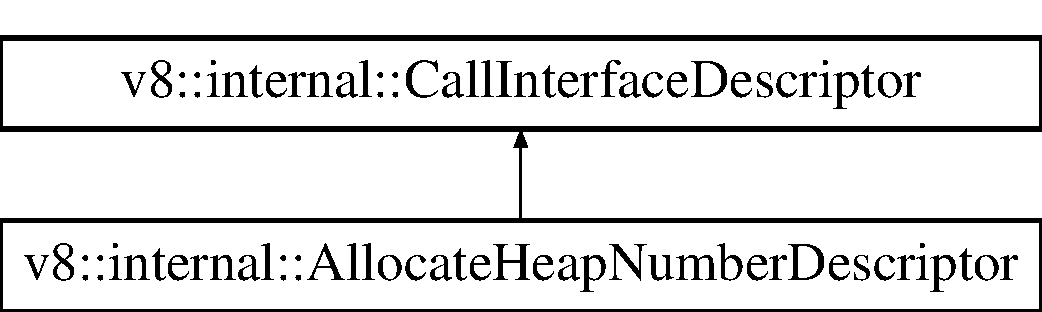
\includegraphics[height=2.000000cm]{classv8_1_1internal_1_1AllocateHeapNumberDescriptor}
\end{center}
\end{figure}
\subsection*{Additional Inherited Members}


\subsection{Detailed Description}


Definition at line 825 of file interface-\/descriptors.\+h.



The documentation for this class was generated from the following file\+:\begin{DoxyCompactItemize}
\item 
v8/src/interface-\/descriptors.\+h\end{DoxyCompactItemize}

\hypertarget{classv8_1_1internal_1_1compiler_1_1AllocateParameters}{}\section{v8\+:\+:internal\+:\+:compiler\+:\+:Allocate\+Parameters Class Reference}
\label{classv8_1_1internal_1_1compiler_1_1AllocateParameters}\index{v8\+::internal\+::compiler\+::\+Allocate\+Parameters@{v8\+::internal\+::compiler\+::\+Allocate\+Parameters}}
\subsection*{Public Member Functions}
\begin{DoxyCompactItemize}
\item 
\mbox{\Hypertarget{classv8_1_1internal_1_1compiler_1_1AllocateParameters_a5c74f2e1cb46e3a77829b43edd98e4f6}\label{classv8_1_1internal_1_1compiler_1_1AllocateParameters_a5c74f2e1cb46e3a77829b43edd98e4f6}} 
{\bfseries Allocate\+Parameters} (\mbox{\hyperlink{classv8_1_1internal_1_1compiler_1_1Type}{Type}} \mbox{\hyperlink{classstd_1_1conditional_1_1type}{type}}, Pretenure\+Flag pretenure)
\item 
\mbox{\Hypertarget{classv8_1_1internal_1_1compiler_1_1AllocateParameters_aba76eb976aec806239fb817076397362}\label{classv8_1_1internal_1_1compiler_1_1AllocateParameters_aba76eb976aec806239fb817076397362}} 
\mbox{\hyperlink{classv8_1_1internal_1_1compiler_1_1Type}{Type}} {\bfseries type} () const
\item 
\mbox{\Hypertarget{classv8_1_1internal_1_1compiler_1_1AllocateParameters_a445c1add5bb6605923c17e76ec741ad7}\label{classv8_1_1internal_1_1compiler_1_1AllocateParameters_a445c1add5bb6605923c17e76ec741ad7}} 
Pretenure\+Flag {\bfseries pretenure} () const
\end{DoxyCompactItemize}


\subsection{Detailed Description}


Definition at line 476 of file simplified-\/operator.\+h.



The documentation for this class was generated from the following file\+:\begin{DoxyCompactItemize}
\item 
v8/src/compiler/simplified-\/operator.\+h\end{DoxyCompactItemize}

\hypertarget{classv8_1_1internal_1_1AllocateTargetSpace}{}\section{v8\+:\+:internal\+:\+:Allocate\+Target\+Space Class Reference}
\label{classv8_1_1internal_1_1AllocateTargetSpace}\index{v8\+::internal\+::\+Allocate\+Target\+Space@{v8\+::internal\+::\+Allocate\+Target\+Space}}
Inheritance diagram for v8\+:\+:internal\+:\+:Allocate\+Target\+Space\+:\begin{figure}[H]
\begin{center}
\leavevmode
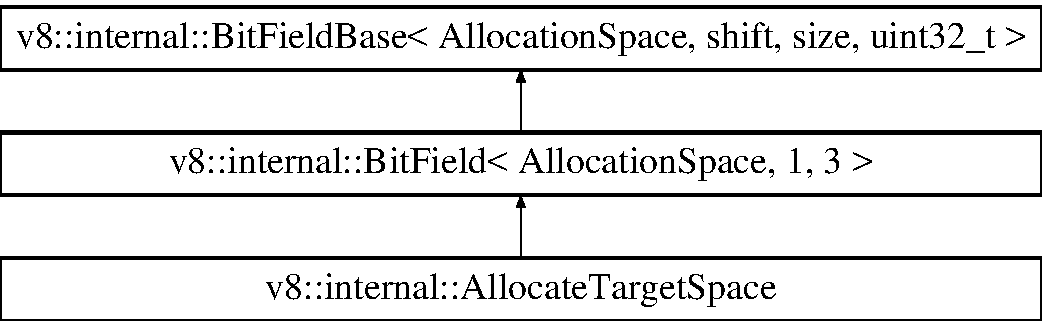
\includegraphics[height=3.000000cm]{classv8_1_1internal_1_1AllocateTargetSpace}
\end{center}
\end{figure}
\subsection*{Additional Inherited Members}


\subsection{Detailed Description}


Definition at line 754 of file runtime.\+h.



The documentation for this class was generated from the following file\+:\begin{DoxyCompactItemize}
\item 
v8/src/runtime/runtime.\+h\end{DoxyCompactItemize}

\hypertarget{structv8_1_1internal_1_1JSArrayBuffer_1_1Allocation}{}\section{v8\+:\+:internal\+:\+:J\+S\+Array\+Buffer\+:\+:Allocation Struct Reference}
\label{structv8_1_1internal_1_1JSArrayBuffer_1_1Allocation}\index{v8\+::internal\+::\+J\+S\+Array\+Buffer\+::\+Allocation@{v8\+::internal\+::\+J\+S\+Array\+Buffer\+::\+Allocation}}
\subsection*{Public Member Functions}
\begin{DoxyCompactItemize}
\item 
\mbox{\Hypertarget{structv8_1_1internal_1_1JSArrayBuffer_1_1Allocation_a99a2b6a7e3b3647db50f7731060a0dc3}\label{structv8_1_1internal_1_1JSArrayBuffer_1_1Allocation_a99a2b6a7e3b3647db50f7731060a0dc3}} 
{\bfseries Allocation} (void $\ast$allocation\+\_\+base, \mbox{\hyperlink{classsize__t}{size\+\_\+t}} length, void $\ast$backing\+\_\+store, \mbox{\hyperlink{classbool}{bool}} is\+\_\+wasm\+\_\+memory)
\end{DoxyCompactItemize}
\subsection*{Public Attributes}
\begin{DoxyCompactItemize}
\item 
\mbox{\Hypertarget{structv8_1_1internal_1_1JSArrayBuffer_1_1Allocation_a5eba5485feecb012389977394a19e340}\label{structv8_1_1internal_1_1JSArrayBuffer_1_1Allocation_a5eba5485feecb012389977394a19e340}} 
void $\ast$ {\bfseries allocation\+\_\+base}
\item 
\mbox{\Hypertarget{structv8_1_1internal_1_1JSArrayBuffer_1_1Allocation_a2ca0ca3c8d8d5bdab5caa7fb9ecb7715}\label{structv8_1_1internal_1_1JSArrayBuffer_1_1Allocation_a2ca0ca3c8d8d5bdab5caa7fb9ecb7715}} 
\mbox{\hyperlink{classsize__t}{size\+\_\+t}} {\bfseries length}
\item 
\mbox{\Hypertarget{structv8_1_1internal_1_1JSArrayBuffer_1_1Allocation_ad1ac75ccb25fe9f7b29202a95415450b}\label{structv8_1_1internal_1_1JSArrayBuffer_1_1Allocation_ad1ac75ccb25fe9f7b29202a95415450b}} 
void $\ast$ {\bfseries backing\+\_\+store}
\item 
\mbox{\Hypertarget{structv8_1_1internal_1_1JSArrayBuffer_1_1Allocation_ad8f9d035f58eafb7c4c23fed4084a21c}\label{structv8_1_1internal_1_1JSArrayBuffer_1_1Allocation_ad8f9d035f58eafb7c4c23fed4084a21c}} 
\mbox{\hyperlink{classbool}{bool}} {\bfseries is\+\_\+wasm\+\_\+memory}
\end{DoxyCompactItemize}


\subsection{Detailed Description}


Definition at line 84 of file js-\/array-\/buffer.\+h.



The documentation for this struct was generated from the following file\+:\begin{DoxyCompactItemize}
\item 
v8/src/objects/js-\/array-\/buffer.\+h\end{DoxyCompactItemize}

\hypertarget{structv8_1_1AllocationProfile_1_1Allocation}{}\section{v8\+:\+:Allocation\+Profile\+:\+:Allocation Struct Reference}
\label{structv8_1_1AllocationProfile_1_1Allocation}\index{v8\+::\+Allocation\+Profile\+::\+Allocation@{v8\+::\+Allocation\+Profile\+::\+Allocation}}
\subsection*{Data Fields}
\begin{DoxyCompactItemize}
\item 
size\+\_\+t \hyperlink{structv8_1_1AllocationProfile_1_1Allocation_a346410fa5dfb796dff396069897c0aba}{size}
\item 
unsigned int \hyperlink{structv8_1_1AllocationProfile_1_1Allocation_a012fe5238f5ebec039d7832f2d3ae8ed}{count}
\end{DoxyCompactItemize}


\subsection{Field Documentation}
\index{v8\+::\+Allocation\+Profile\+::\+Allocation@{v8\+::\+Allocation\+Profile\+::\+Allocation}!count@{count}}
\index{count@{count}!v8\+::\+Allocation\+Profile\+::\+Allocation@{v8\+::\+Allocation\+Profile\+::\+Allocation}}
\subsubsection[{\texorpdfstring{count}{count}}]{\setlength{\rightskip}{0pt plus 5cm}unsigned int v8\+::\+Allocation\+Profile\+::\+Allocation\+::count}\hypertarget{structv8_1_1AllocationProfile_1_1Allocation_a012fe5238f5ebec039d7832f2d3ae8ed}{}\label{structv8_1_1AllocationProfile_1_1Allocation_a012fe5238f5ebec039d7832f2d3ae8ed}
The number of objects of such size that were sampled. \index{v8\+::\+Allocation\+Profile\+::\+Allocation@{v8\+::\+Allocation\+Profile\+::\+Allocation}!size@{size}}
\index{size@{size}!v8\+::\+Allocation\+Profile\+::\+Allocation@{v8\+::\+Allocation\+Profile\+::\+Allocation}}
\subsubsection[{\texorpdfstring{size}{size}}]{\setlength{\rightskip}{0pt plus 5cm}size\+\_\+t v8\+::\+Allocation\+Profile\+::\+Allocation\+::size}\hypertarget{structv8_1_1AllocationProfile_1_1Allocation_a346410fa5dfb796dff396069897c0aba}{}\label{structv8_1_1AllocationProfile_1_1Allocation_a346410fa5dfb796dff396069897c0aba}
Size of the sampled allocation object. 

The documentation for this struct was generated from the following file\+:\begin{DoxyCompactItemize}
\item 
v8/include/v8-\/profiler.\+h\end{DoxyCompactItemize}

\hypertarget{classv8_1_1internal_1_1compiler_1_1AllocationBuilder}{}\section{v8\+:\+:internal\+:\+:compiler\+:\+:Allocation\+Builder Class Reference}
\label{classv8_1_1internal_1_1compiler_1_1AllocationBuilder}\index{v8\+::internal\+::compiler\+::\+Allocation\+Builder@{v8\+::internal\+::compiler\+::\+Allocation\+Builder}}
\subsection*{Public Member Functions}
\begin{DoxyCompactItemize}
\item 
\mbox{\Hypertarget{classv8_1_1internal_1_1compiler_1_1AllocationBuilder_a63e5da0756077eefc87c4ceb968c71b9}\label{classv8_1_1internal_1_1compiler_1_1AllocationBuilder_a63e5da0756077eefc87c4ceb968c71b9}} 
{\bfseries Allocation\+Builder} (\mbox{\hyperlink{classv8_1_1internal_1_1compiler_1_1JSGraph}{J\+S\+Graph}} $\ast$jsgraph, \mbox{\hyperlink{classv8_1_1internal_1_1compiler_1_1Node}{Node}} $\ast$effect, \mbox{\hyperlink{classv8_1_1internal_1_1compiler_1_1Node}{Node}} $\ast$control)
\item 
\mbox{\Hypertarget{classv8_1_1internal_1_1compiler_1_1AllocationBuilder_af93a44e38c374dfd83787cbbb1d85cee}\label{classv8_1_1internal_1_1compiler_1_1AllocationBuilder_af93a44e38c374dfd83787cbbb1d85cee}} 
void {\bfseries Allocate} (\mbox{\hyperlink{classint}{int}} size, Pretenure\+Flag pretenure=N\+O\+T\+\_\+\+T\+E\+N\+U\+R\+ED, \mbox{\hyperlink{classv8_1_1internal_1_1compiler_1_1Type}{Type}} \mbox{\hyperlink{classstd_1_1conditional_1_1type}{type}}=Type\+::\+Any())
\item 
\mbox{\Hypertarget{classv8_1_1internal_1_1compiler_1_1AllocationBuilder_aba5aa2ad1d337a4110b33c2ac31b6da3}\label{classv8_1_1internal_1_1compiler_1_1AllocationBuilder_aba5aa2ad1d337a4110b33c2ac31b6da3}} 
void {\bfseries Store} (const \mbox{\hyperlink{structv8_1_1internal_1_1compiler_1_1FieldAccess}{Field\+Access}} \&access, \mbox{\hyperlink{classv8_1_1internal_1_1compiler_1_1Node}{Node}} $\ast$value)
\item 
\mbox{\Hypertarget{classv8_1_1internal_1_1compiler_1_1AllocationBuilder_a9aa00a063017009e0ee51359e52d0a97}\label{classv8_1_1internal_1_1compiler_1_1AllocationBuilder_a9aa00a063017009e0ee51359e52d0a97}} 
void {\bfseries Store} (\mbox{\hyperlink{structv8_1_1internal_1_1compiler_1_1ElementAccess}{Element\+Access}} const \&access, \mbox{\hyperlink{classv8_1_1internal_1_1compiler_1_1Node}{Node}} $\ast$index, \mbox{\hyperlink{classv8_1_1internal_1_1compiler_1_1Node}{Node}} $\ast$value)
\item 
\mbox{\Hypertarget{classv8_1_1internal_1_1compiler_1_1AllocationBuilder_ab43028e2196afb9145c8e858b0241353}\label{classv8_1_1internal_1_1compiler_1_1AllocationBuilder_ab43028e2196afb9145c8e858b0241353}} 
void {\bfseries Allocate\+Context} (\mbox{\hyperlink{classint}{int}} variadic\+\_\+part\+\_\+length, \mbox{\hyperlink{classv8_1_1internal_1_1Handle}{Handle}}$<$ \mbox{\hyperlink{classv8_1_1internal_1_1Map}{Map}} $>$ map)
\item 
\mbox{\Hypertarget{classv8_1_1internal_1_1compiler_1_1AllocationBuilder_a871f5050c25a3a2f5ac31426cda98459}\label{classv8_1_1internal_1_1compiler_1_1AllocationBuilder_a871f5050c25a3a2f5ac31426cda98459}} 
void {\bfseries Allocate\+Array} (\mbox{\hyperlink{classint}{int}} length, \mbox{\hyperlink{classv8_1_1internal_1_1Handle}{Handle}}$<$ \mbox{\hyperlink{classv8_1_1internal_1_1Map}{Map}} $>$ map, Pretenure\+Flag pretenure=N\+O\+T\+\_\+\+T\+E\+N\+U\+R\+ED)
\item 
\mbox{\Hypertarget{classv8_1_1internal_1_1compiler_1_1AllocationBuilder_a708d36e8ad542a38d32213d9d1467bed}\label{classv8_1_1internal_1_1compiler_1_1AllocationBuilder_a708d36e8ad542a38d32213d9d1467bed}} 
void {\bfseries Store} (const \mbox{\hyperlink{structv8_1_1internal_1_1compiler_1_1FieldAccess}{Field\+Access}} \&access, \mbox{\hyperlink{classv8_1_1internal_1_1Handle}{Handle}}$<$ \mbox{\hyperlink{classv8_1_1internal_1_1Object}{Object}} $>$ value)
\item 
\mbox{\Hypertarget{classv8_1_1internal_1_1compiler_1_1AllocationBuilder_af10fd17db6ba5682f7b8b30738e8324b}\label{classv8_1_1internal_1_1compiler_1_1AllocationBuilder_af10fd17db6ba5682f7b8b30738e8324b}} 
void {\bfseries Store} (const \mbox{\hyperlink{structv8_1_1internal_1_1compiler_1_1FieldAccess}{Field\+Access}} \&access, const \mbox{\hyperlink{classv8_1_1internal_1_1compiler_1_1ObjectRef}{Object\+Ref}} \&value)
\item 
\mbox{\Hypertarget{classv8_1_1internal_1_1compiler_1_1AllocationBuilder_a2ffbc75047473c132d3788c55e31f72f}\label{classv8_1_1internal_1_1compiler_1_1AllocationBuilder_a2ffbc75047473c132d3788c55e31f72f}} 
void {\bfseries Finish\+And\+Change} (\mbox{\hyperlink{classv8_1_1internal_1_1compiler_1_1Node}{Node}} $\ast$node)
\item 
\mbox{\Hypertarget{classv8_1_1internal_1_1compiler_1_1AllocationBuilder_aaf7ead96a05905c0a268f4c64f6d58d3}\label{classv8_1_1internal_1_1compiler_1_1AllocationBuilder_aaf7ead96a05905c0a268f4c64f6d58d3}} 
\mbox{\hyperlink{classv8_1_1internal_1_1compiler_1_1Node}{Node}} $\ast$ {\bfseries Finish} ()
\end{DoxyCompactItemize}
\subsection*{Protected Member Functions}
\begin{DoxyCompactItemize}
\item 
\mbox{\Hypertarget{classv8_1_1internal_1_1compiler_1_1AllocationBuilder_ab9389b3e335995149f8f4365c9766abc}\label{classv8_1_1internal_1_1compiler_1_1AllocationBuilder_ab9389b3e335995149f8f4365c9766abc}} 
\mbox{\hyperlink{classv8_1_1internal_1_1compiler_1_1JSGraph}{J\+S\+Graph}} $\ast$ {\bfseries jsgraph} ()
\item 
\mbox{\Hypertarget{classv8_1_1internal_1_1compiler_1_1AllocationBuilder_a14b7c2116ab0e552bcf9444493381d43}\label{classv8_1_1internal_1_1compiler_1_1AllocationBuilder_a14b7c2116ab0e552bcf9444493381d43}} 
\mbox{\hyperlink{classv8_1_1internal_1_1Isolate}{Isolate}} $\ast$ {\bfseries isolate} () const
\item 
\mbox{\Hypertarget{classv8_1_1internal_1_1compiler_1_1AllocationBuilder_a5f16cb5dae0ad17cc690fbbc316e9f9a}\label{classv8_1_1internal_1_1compiler_1_1AllocationBuilder_a5f16cb5dae0ad17cc690fbbc316e9f9a}} 
\mbox{\hyperlink{classv8_1_1internal_1_1compiler_1_1Graph}{Graph}} $\ast$ {\bfseries graph} ()
\item 
\mbox{\Hypertarget{classv8_1_1internal_1_1compiler_1_1AllocationBuilder_a169361bf67eb13560d4dcaf1dd5644d1}\label{classv8_1_1internal_1_1compiler_1_1AllocationBuilder_a169361bf67eb13560d4dcaf1dd5644d1}} 
\mbox{\hyperlink{classv8_1_1internal_1_1compiler_1_1CommonOperatorBuilder}{Common\+Operator\+Builder}} $\ast$ {\bfseries common} ()
\item 
\mbox{\Hypertarget{classv8_1_1internal_1_1compiler_1_1AllocationBuilder_a117ba4df689ef4ad7b5d6ebb122f4055}\label{classv8_1_1internal_1_1compiler_1_1AllocationBuilder_a117ba4df689ef4ad7b5d6ebb122f4055}} 
\mbox{\hyperlink{classv8_1_1internal_1_1compiler_1_1SimplifiedOperatorBuilder}{Simplified\+Operator\+Builder}} $\ast$ {\bfseries simplified} ()
\end{DoxyCompactItemize}


\subsection{Detailed Description}


Definition at line 19 of file allocation-\/builder.\+h.



The documentation for this class was generated from the following files\+:\begin{DoxyCompactItemize}
\item 
v8/src/compiler/allocation-\/builder.\+h\item 
v8/src/compiler/allocation-\/builder-\/inl.\+h\end{DoxyCompactItemize}

\hypertarget{structv8_1_1internal_1_1wasm_1_1WasmMemoryTracker_1_1AllocationData}{}\section{v8\+:\+:internal\+:\+:wasm\+:\+:Wasm\+Memory\+Tracker\+:\+:Allocation\+Data Struct Reference}
\label{structv8_1_1internal_1_1wasm_1_1WasmMemoryTracker_1_1AllocationData}\index{v8\+::internal\+::wasm\+::\+Wasm\+Memory\+Tracker\+::\+Allocation\+Data@{v8\+::internal\+::wasm\+::\+Wasm\+Memory\+Tracker\+::\+Allocation\+Data}}
\subsection*{Public Attributes}
\begin{DoxyCompactItemize}
\item 
\mbox{\Hypertarget{structv8_1_1internal_1_1wasm_1_1WasmMemoryTracker_1_1AllocationData_af4bc619b48d539add2f3610d285bb729}\label{structv8_1_1internal_1_1wasm_1_1WasmMemoryTracker_1_1AllocationData_af4bc619b48d539add2f3610d285bb729}} 
void $\ast$ {\bfseries allocation\+\_\+base} = nullptr
\item 
\mbox{\Hypertarget{structv8_1_1internal_1_1wasm_1_1WasmMemoryTracker_1_1AllocationData_aa452ecc3e663358c8dfe769e55ec0689}\label{structv8_1_1internal_1_1wasm_1_1WasmMemoryTracker_1_1AllocationData_aa452ecc3e663358c8dfe769e55ec0689}} 
\mbox{\hyperlink{classsize__t}{size\+\_\+t}} {\bfseries allocation\+\_\+length} = 0
\item 
\mbox{\Hypertarget{structv8_1_1internal_1_1wasm_1_1WasmMemoryTracker_1_1AllocationData_a1f4bab84579a4e8c682532927b8c81bf}\label{structv8_1_1internal_1_1wasm_1_1WasmMemoryTracker_1_1AllocationData_a1f4bab84579a4e8c682532927b8c81bf}} 
void $\ast$ {\bfseries buffer\+\_\+start} = nullptr
\item 
\mbox{\Hypertarget{structv8_1_1internal_1_1wasm_1_1WasmMemoryTracker_1_1AllocationData_abe88d5a5a940374700054d4a985da8cb}\label{structv8_1_1internal_1_1wasm_1_1WasmMemoryTracker_1_1AllocationData_abe88d5a5a940374700054d4a985da8cb}} 
\mbox{\hyperlink{classsize__t}{size\+\_\+t}} {\bfseries buffer\+\_\+length} = 0
\end{DoxyCompactItemize}


\subsection{Detailed Description}


Definition at line 42 of file wasm-\/memory.\+h.



The documentation for this struct was generated from the following file\+:\begin{DoxyCompactItemize}
\item 
v8/src/wasm/wasm-\/memory.\+h\end{DoxyCompactItemize}

\hypertarget{classv8_1_1internal_1_1AllocationMemento}{}\section{v8\+:\+:internal\+:\+:Allocation\+Memento Class Reference}
\label{classv8_1_1internal_1_1AllocationMemento}\index{v8\+::internal\+::\+Allocation\+Memento@{v8\+::internal\+::\+Allocation\+Memento}}
Inheritance diagram for v8\+:\+:internal\+:\+:Allocation\+Memento\+:\begin{figure}[H]
\begin{center}
\leavevmode
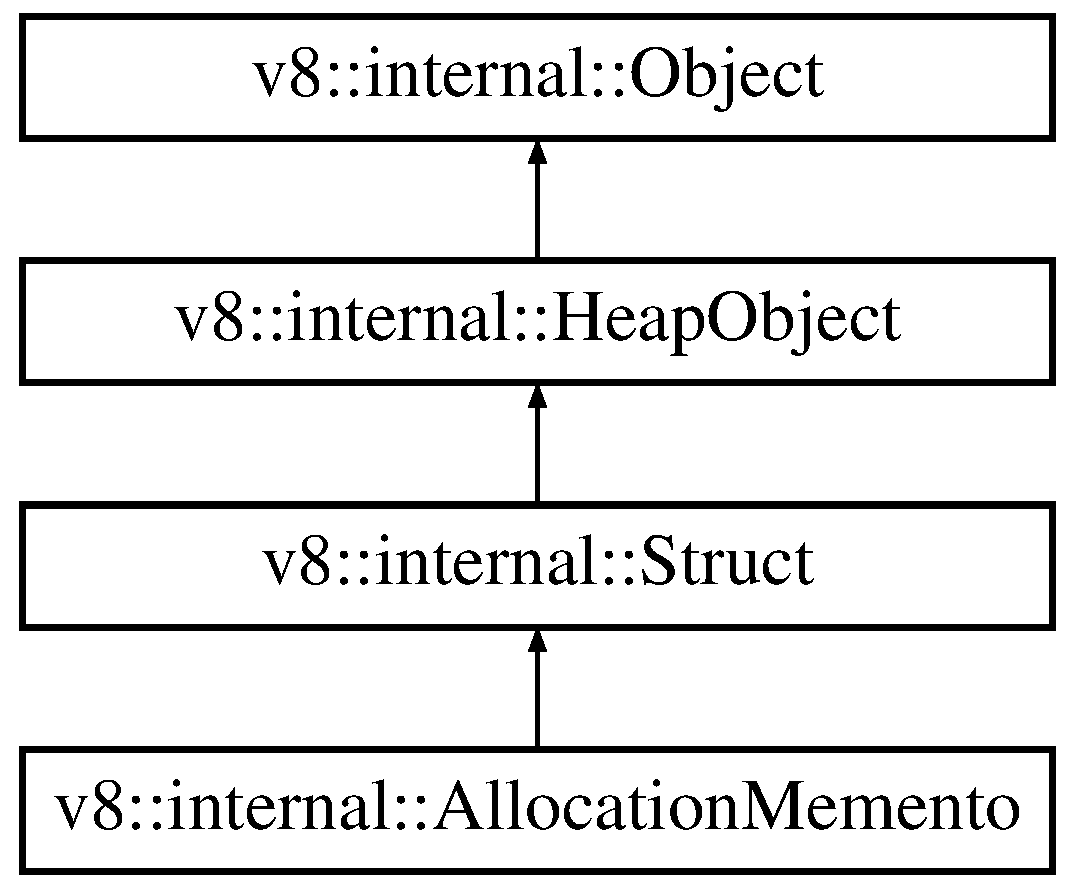
\includegraphics[height=4.000000cm]{classv8_1_1internal_1_1AllocationMemento}
\end{center}
\end{figure}
\subsection*{Public Member Functions}
\begin{DoxyCompactItemize}
\item 
\mbox{\Hypertarget{classv8_1_1internal_1_1AllocationMemento_ae5c6d7844d9d36941b4a216d388ccfa2}\label{classv8_1_1internal_1_1AllocationMemento_ae5c6d7844d9d36941b4a216d388ccfa2}} 
{\bfseries D\+E\+F\+I\+N\+E\+\_\+\+F\+I\+E\+L\+D\+\_\+\+O\+F\+F\+S\+E\+T\+\_\+\+C\+O\+N\+S\+T\+A\+N\+TS} (Heap\+Object\+::k\+Header\+Size, A\+L\+L\+O\+C\+A\+T\+I\+O\+N\+\_\+\+M\+E\+M\+E\+N\+T\+O\+\_\+\+F\+I\+E\+L\+DS) inline \mbox{\hyperlink{classbool}{bool}} Is\+Valid() const
\item 
\mbox{\Hypertarget{classv8_1_1internal_1_1AllocationMemento_af20ff245d696488e5658825da910f25e}\label{classv8_1_1internal_1_1AllocationMemento_af20ff245d696488e5658825da910f25e}} 
\mbox{\hyperlink{classv8_1_1internal_1_1AllocationSite}{Allocation\+Site}} $\ast$ {\bfseries Get\+Allocation\+Site} () const
\item 
\mbox{\Hypertarget{classv8_1_1internal_1_1AllocationMemento_ad38a84caef4b9046b2d0ebf7146ed5cf}\label{classv8_1_1internal_1_1AllocationMemento_ad38a84caef4b9046b2d0ebf7146ed5cf}} 
\mbox{\hyperlink{classuintptr__t}{Address}} {\bfseries Get\+Allocation\+Site\+Unchecked} () const
\end{DoxyCompactItemize}
\subsection*{Additional Inherited Members}


\subsection{Detailed Description}


Definition at line 163 of file allocation-\/site.\+h.



The documentation for this class was generated from the following files\+:\begin{DoxyCompactItemize}
\item 
v8/src/objects/allocation-\/site.\+h\item 
v8/src/objects/allocation-\/site-\/inl.\+h\end{DoxyCompactItemize}

\hypertarget{classv8_1_1internal_1_1SamplingHeapProfiler_1_1AllocationNode}{}\section{v8\+:\+:internal\+:\+:Sampling\+Heap\+Profiler\+:\+:Allocation\+Node Class Reference}
\label{classv8_1_1internal_1_1SamplingHeapProfiler_1_1AllocationNode}\index{v8\+::internal\+::\+Sampling\+Heap\+Profiler\+::\+Allocation\+Node@{v8\+::internal\+::\+Sampling\+Heap\+Profiler\+::\+Allocation\+Node}}
\subsection*{Public Types}
\begin{DoxyCompactItemize}
\item 
\mbox{\Hypertarget{classv8_1_1internal_1_1SamplingHeapProfiler_1_1AllocationNode_a0c78c3032878f2beb0c5bcfd175c8630}\label{classv8_1_1internal_1_1SamplingHeapProfiler_1_1AllocationNode_a0c78c3032878f2beb0c5bcfd175c8630}} 
typedef uint64\+\_\+t {\bfseries Function\+Id}
\end{DoxyCompactItemize}
\subsection*{Public Member Functions}
\begin{DoxyCompactItemize}
\item 
\mbox{\Hypertarget{classv8_1_1internal_1_1SamplingHeapProfiler_1_1AllocationNode_a81a8ee52bbe5de9b01a49b72892da056}\label{classv8_1_1internal_1_1SamplingHeapProfiler_1_1AllocationNode_a81a8ee52bbe5de9b01a49b72892da056}} 
{\bfseries Allocation\+Node} (\mbox{\hyperlink{classv8_1_1internal_1_1SamplingHeapProfiler_1_1AllocationNode}{Allocation\+Node}} $\ast$parent, const \mbox{\hyperlink{classchar}{char}} $\ast$name, \mbox{\hyperlink{classint}{int}} script\+\_\+id, \mbox{\hyperlink{classint}{int}} start\+\_\+position, \mbox{\hyperlink{classuint32__t}{uint32\+\_\+t}} id)
\item 
\mbox{\Hypertarget{classv8_1_1internal_1_1SamplingHeapProfiler_1_1AllocationNode_ab07dee34f8ab069b8402830eb318b3b8}\label{classv8_1_1internal_1_1SamplingHeapProfiler_1_1AllocationNode_ab07dee34f8ab069b8402830eb318b3b8}} 
\mbox{\hyperlink{classv8_1_1internal_1_1SamplingHeapProfiler_1_1AllocationNode}{Allocation\+Node}} $\ast$ {\bfseries Find\+Child\+Node} (Function\+Id id)
\item 
\mbox{\Hypertarget{classv8_1_1internal_1_1SamplingHeapProfiler_1_1AllocationNode_af9a29d57c2f6b5c64b55daec949e6194}\label{classv8_1_1internal_1_1SamplingHeapProfiler_1_1AllocationNode_af9a29d57c2f6b5c64b55daec949e6194}} 
\mbox{\hyperlink{classv8_1_1internal_1_1SamplingHeapProfiler_1_1AllocationNode}{Allocation\+Node}} $\ast$ {\bfseries Add\+Child\+Node} (Function\+Id id, std\+::unique\+\_\+ptr$<$ \mbox{\hyperlink{classv8_1_1internal_1_1SamplingHeapProfiler_1_1AllocationNode}{Allocation\+Node}} $>$ node)
\end{DoxyCompactItemize}
\subsection*{Static Public Member Functions}
\begin{DoxyCompactItemize}
\item 
\mbox{\Hypertarget{classv8_1_1internal_1_1SamplingHeapProfiler_1_1AllocationNode_aab1b9429762149c13209bdf3ea9f045c}\label{classv8_1_1internal_1_1SamplingHeapProfiler_1_1AllocationNode_aab1b9429762149c13209bdf3ea9f045c}} 
static Function\+Id {\bfseries function\+\_\+id} (\mbox{\hyperlink{classint}{int}} script\+\_\+id, \mbox{\hyperlink{classint}{int}} start\+\_\+position, const \mbox{\hyperlink{classchar}{char}} $\ast$name)
\end{DoxyCompactItemize}
\subsection*{Friends}
\begin{DoxyCompactItemize}
\item 
\mbox{\Hypertarget{classv8_1_1internal_1_1SamplingHeapProfiler_1_1AllocationNode_a1c4268235229c6a40ca92cbcd4591c9b}\label{classv8_1_1internal_1_1SamplingHeapProfiler_1_1AllocationNode_a1c4268235229c6a40ca92cbcd4591c9b}} 
class {\bfseries Sampling\+Heap\+Profiler}
\end{DoxyCompactItemize}


\subsection{Detailed Description}


Definition at line 49 of file sampling-\/heap-\/profiler.\+h.



The documentation for this class was generated from the following file\+:\begin{DoxyCompactItemize}
\item 
v8/src/profiler/sampling-\/heap-\/profiler.\+h\end{DoxyCompactItemize}

\hypertarget{classv8_1_1internal_1_1AllocationObserver}{}\section{v8\+:\+:internal\+:\+:Allocation\+Observer Class Reference}
\label{classv8_1_1internal_1_1AllocationObserver}\index{v8\+::internal\+::\+Allocation\+Observer@{v8\+::internal\+::\+Allocation\+Observer}}
Inheritance diagram for v8\+:\+:internal\+:\+:Allocation\+Observer\+:\begin{figure}[H]
\begin{center}
\leavevmode
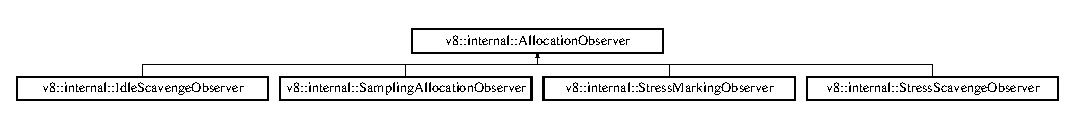
\includegraphics[height=1.124498cm]{classv8_1_1internal_1_1AllocationObserver}
\end{center}
\end{figure}
\subsection*{Public Member Functions}
\begin{DoxyCompactItemize}
\item 
\mbox{\Hypertarget{classv8_1_1internal_1_1AllocationObserver_afd17faabb89efdf1211915e9e684a31f}\label{classv8_1_1internal_1_1AllocationObserver_afd17faabb89efdf1211915e9e684a31f}} 
{\bfseries Allocation\+Observer} (intptr\+\_\+t step\+\_\+size)
\item 
\mbox{\Hypertarget{classv8_1_1internal_1_1AllocationObserver_a83b330ab2d41bd63c8463c98e3b44139}\label{classv8_1_1internal_1_1AllocationObserver_a83b330ab2d41bd63c8463c98e3b44139}} 
void {\bfseries Allocation\+Step} (\mbox{\hyperlink{classint}{int}} bytes\+\_\+allocated, \mbox{\hyperlink{classuintptr__t}{Address}} soon\+\_\+object, \mbox{\hyperlink{classsize__t}{size\+\_\+t}} size)
\end{DoxyCompactItemize}
\subsection*{Protected Member Functions}
\begin{DoxyCompactItemize}
\item 
\mbox{\Hypertarget{classv8_1_1internal_1_1AllocationObserver_a34d92b5b7db58528cbcbace883ca43d4}\label{classv8_1_1internal_1_1AllocationObserver_a34d92b5b7db58528cbcbace883ca43d4}} 
intptr\+\_\+t {\bfseries step\+\_\+size} () const
\item 
\mbox{\Hypertarget{classv8_1_1internal_1_1AllocationObserver_a7bdb2960ee3bc34da0a6908d3a87e1d0}\label{classv8_1_1internal_1_1AllocationObserver_a7bdb2960ee3bc34da0a6908d3a87e1d0}} 
intptr\+\_\+t {\bfseries bytes\+\_\+to\+\_\+next\+\_\+step} () const
\item 
\mbox{\Hypertarget{classv8_1_1internal_1_1AllocationObserver_a41118152d2c9a9834a486eccf08043a5}\label{classv8_1_1internal_1_1AllocationObserver_a41118152d2c9a9834a486eccf08043a5}} 
virtual void {\bfseries Step} (\mbox{\hyperlink{classint}{int}} bytes\+\_\+allocated, \mbox{\hyperlink{classuintptr__t}{Address}} soon\+\_\+object, \mbox{\hyperlink{classsize__t}{size\+\_\+t}} size)=0
\item 
\mbox{\Hypertarget{classv8_1_1internal_1_1AllocationObserver_a91fb6ffe2d4b42ff7b4221dad89db465}\label{classv8_1_1internal_1_1AllocationObserver_a91fb6ffe2d4b42ff7b4221dad89db465}} 
virtual intptr\+\_\+t {\bfseries Get\+Next\+Step\+Size} ()
\end{DoxyCompactItemize}
\subsection*{Protected Attributes}
\begin{DoxyCompactItemize}
\item 
\mbox{\Hypertarget{classv8_1_1internal_1_1AllocationObserver_aca0c9295ca497a26f08cd8244f84d5aa}\label{classv8_1_1internal_1_1AllocationObserver_aca0c9295ca497a26f08cd8244f84d5aa}} 
intptr\+\_\+t {\bfseries step\+\_\+size\+\_\+}
\item 
\mbox{\Hypertarget{classv8_1_1internal_1_1AllocationObserver_a5f02cbcbd88c5b87439c31ada838923e}\label{classv8_1_1internal_1_1AllocationObserver_a5f02cbcbd88c5b87439c31ada838923e}} 
intptr\+\_\+t {\bfseries bytes\+\_\+to\+\_\+next\+\_\+step\+\_\+}
\end{DoxyCompactItemize}
\subsection*{Friends}
\begin{DoxyCompactItemize}
\item 
\mbox{\Hypertarget{classv8_1_1internal_1_1AllocationObserver_a2129e6c0ac73536a2ac4f681dae16947}\label{classv8_1_1internal_1_1AllocationObserver_a2129e6c0ac73536a2ac4f681dae16947}} 
class {\bfseries Space}
\end{DoxyCompactItemize}


\subsection{Detailed Description}


Definition at line 2274 of file heap.\+h.



The documentation for this class was generated from the following files\+:\begin{DoxyCompactItemize}
\item 
v8/src/heap/heap.\+h\item 
v8/src/heap/heap.\+cc\end{DoxyCompactItemize}

\hypertarget{classv8_1_1AllocationProfile}{}\section{v8\+:\+:Allocation\+Profile Class Reference}
\label{classv8_1_1AllocationProfile}\index{v8\+::\+Allocation\+Profile@{v8\+::\+Allocation\+Profile}}


{\ttfamily \#include $<$v8-\/profiler.\+h$>$}

Inheritance diagram for v8\+:\+:Allocation\+Profile\+:\begin{figure}[H]
\begin{center}
\leavevmode
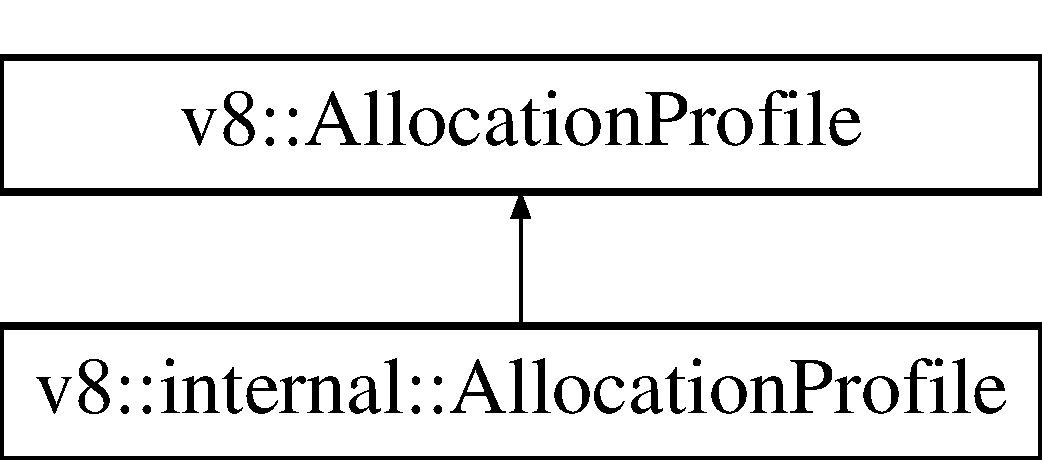
\includegraphics[height=2.000000cm]{classv8_1_1AllocationProfile}
\end{center}
\end{figure}
\subsection*{Classes}
\begin{DoxyCompactItemize}
\item 
struct \mbox{\hyperlink{structv8_1_1AllocationProfile_1_1Allocation}{Allocation}}
\item 
struct \mbox{\hyperlink{structv8_1_1AllocationProfile_1_1Node}{Node}}
\item 
struct \mbox{\hyperlink{structv8_1_1AllocationProfile_1_1Sample}{Sample}}
\end{DoxyCompactItemize}
\subsection*{Public Member Functions}
\begin{DoxyCompactItemize}
\item 
virtual \mbox{\hyperlink{structv8_1_1AllocationProfile_1_1Node}{Node}} $\ast$ \mbox{\hyperlink{classv8_1_1AllocationProfile_afea045dae30df5477088e2f0b7edb6c4}{Get\+Root\+Node}} ()=0
\item 
\mbox{\Hypertarget{classv8_1_1AllocationProfile_a5dae5644e119c5c9ef699e27b98ab92d}\label{classv8_1_1AllocationProfile_a5dae5644e119c5c9ef699e27b98ab92d}} 
virtual const std\+::vector$<$ \mbox{\hyperlink{structv8_1_1AllocationProfile_1_1Sample}{Sample}} $>$ \& {\bfseries Get\+Samples} ()=0
\end{DoxyCompactItemize}
\subsection*{Static Public Attributes}
\begin{DoxyCompactItemize}
\item 
\mbox{\Hypertarget{classv8_1_1AllocationProfile_a26fdfe9e4846d26c83d0ad8c2ed2d783}\label{classv8_1_1AllocationProfile_a26fdfe9e4846d26c83d0ad8c2ed2d783}} 
static const \mbox{\hyperlink{classint}{int}} {\bfseries k\+No\+Line\+Number\+Info} = Message\+::k\+No\+Line\+Number\+Info
\item 
\mbox{\Hypertarget{classv8_1_1AllocationProfile_a9cfa103f73e82629694eee3734826eb7}\label{classv8_1_1AllocationProfile_a9cfa103f73e82629694eee3734826eb7}} 
static const \mbox{\hyperlink{classint}{int}} {\bfseries k\+No\+Column\+Number\+Info} = Message\+::k\+No\+Column\+Info
\end{DoxyCompactItemize}


\subsection{Detailed Description}
\mbox{\hyperlink{classv8_1_1AllocationProfile}{Allocation\+Profile}} is a sampled profile of allocations done by the program. This is structured as a call-\/graph. 

Definition at line 561 of file v8-\/profiler.\+h.



\subsection{Member Function Documentation}
\mbox{\Hypertarget{classv8_1_1AllocationProfile_afea045dae30df5477088e2f0b7edb6c4}\label{classv8_1_1AllocationProfile_afea045dae30df5477088e2f0b7edb6c4}} 
\index{v8\+::\+Allocation\+Profile@{v8\+::\+Allocation\+Profile}!Get\+Root\+Node@{Get\+Root\+Node}}
\index{Get\+Root\+Node@{Get\+Root\+Node}!v8\+::\+Allocation\+Profile@{v8\+::\+Allocation\+Profile}}
\subsubsection{\texorpdfstring{Get\+Root\+Node()}{GetRootNode()}}
{\footnotesize\ttfamily virtual \mbox{\hyperlink{structv8_1_1AllocationProfile_1_1Node}{Node}}$\ast$ v8\+::\+Allocation\+Profile\+::\+Get\+Root\+Node (\begin{DoxyParamCaption}{ }\end{DoxyParamCaption})\hspace{0.3cm}{\ttfamily [pure virtual]}}

Returns the root node of the call-\/graph. The root node corresponds to an empty JS call-\/stack. The lifetime of the returned Node$\ast$ is scoped to the containing \mbox{\hyperlink{classv8_1_1AllocationProfile}{Allocation\+Profile}}. 

Implemented in \mbox{\hyperlink{classv8_1_1internal_1_1AllocationProfile_abb93406eaccd8b37de3e080d0620bc2b}{v8\+::internal\+::\+Allocation\+Profile}}.



The documentation for this class was generated from the following file\+:\begin{DoxyCompactItemize}
\item 
v8/include/v8-\/profiler.\+h\end{DoxyCompactItemize}

\hypertarget{classv8_1_1internal_1_1AllocationProfile}{}\section{v8\+:\+:internal\+:\+:Allocation\+Profile Class Reference}
\label{classv8_1_1internal_1_1AllocationProfile}\index{v8\+::internal\+::\+Allocation\+Profile@{v8\+::internal\+::\+Allocation\+Profile}}
Inheritance diagram for v8\+:\+:internal\+:\+:Allocation\+Profile\+:\begin{figure}[H]
\begin{center}
\leavevmode
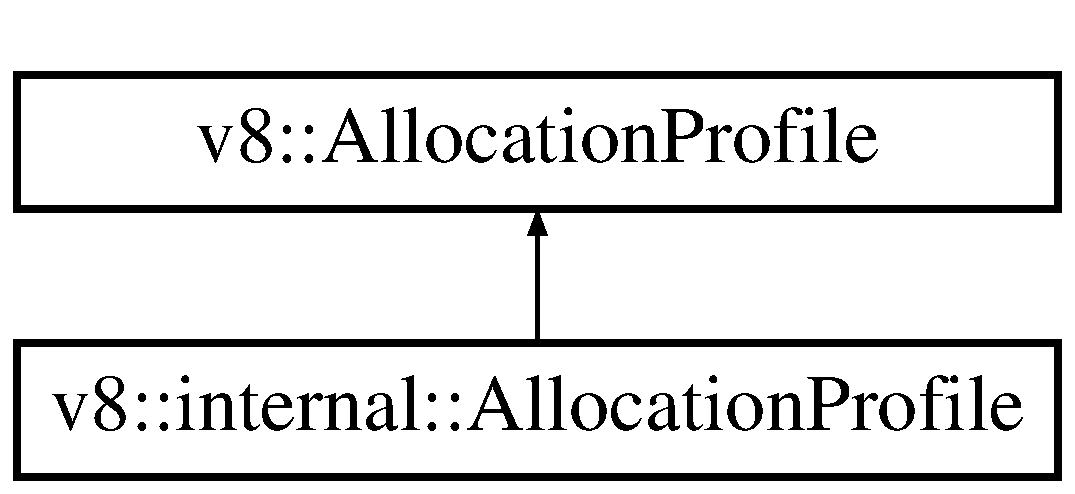
\includegraphics[height=2.000000cm]{classv8_1_1internal_1_1AllocationProfile}
\end{center}
\end{figure}
\subsection*{Public Member Functions}
\begin{DoxyCompactItemize}
\item 
\mbox{\hyperlink{structv8_1_1AllocationProfile_1_1Node}{v8\+::\+Allocation\+Profile\+::\+Node}} $\ast$ \mbox{\hyperlink{classv8_1_1internal_1_1AllocationProfile_abb93406eaccd8b37de3e080d0620bc2b}{Get\+Root\+Node}} () override
\item 
\mbox{\Hypertarget{classv8_1_1internal_1_1AllocationProfile_acbcf0c0cabf7c8d773e2cb27af6d0008}\label{classv8_1_1internal_1_1AllocationProfile_acbcf0c0cabf7c8d773e2cb27af6d0008}} 
const std\+::vector$<$ \mbox{\hyperlink{structv8_1_1AllocationProfile_1_1Sample}{v8\+::\+Allocation\+Profile\+::\+Sample}} $>$ \& {\bfseries Get\+Samples} () override
\end{DoxyCompactItemize}
\subsection*{Friends}
\begin{DoxyCompactItemize}
\item 
\mbox{\Hypertarget{classv8_1_1internal_1_1AllocationProfile_a1c4268235229c6a40ca92cbcd4591c9b}\label{classv8_1_1internal_1_1AllocationProfile_a1c4268235229c6a40ca92cbcd4591c9b}} 
class {\bfseries Sampling\+Heap\+Profiler}
\end{DoxyCompactItemize}
\subsection*{Additional Inherited Members}


\subsection{Detailed Description}


Definition at line 26 of file sampling-\/heap-\/profiler.\+h.



\subsection{Member Function Documentation}
\mbox{\Hypertarget{classv8_1_1internal_1_1AllocationProfile_abb93406eaccd8b37de3e080d0620bc2b}\label{classv8_1_1internal_1_1AllocationProfile_abb93406eaccd8b37de3e080d0620bc2b}} 
\index{v8\+::internal\+::\+Allocation\+Profile@{v8\+::internal\+::\+Allocation\+Profile}!Get\+Root\+Node@{Get\+Root\+Node}}
\index{Get\+Root\+Node@{Get\+Root\+Node}!v8\+::internal\+::\+Allocation\+Profile@{v8\+::internal\+::\+Allocation\+Profile}}
\subsubsection{\texorpdfstring{Get\+Root\+Node()}{GetRootNode()}}
{\footnotesize\ttfamily \mbox{\hyperlink{structv8_1_1AllocationProfile_1_1Node}{v8\+::\+Allocation\+Profile\+::\+Node}}$\ast$ v8\+::internal\+::\+Allocation\+Profile\+::\+Get\+Root\+Node (\begin{DoxyParamCaption}{ }\end{DoxyParamCaption})\hspace{0.3cm}{\ttfamily [inline]}, {\ttfamily [override]}, {\ttfamily [virtual]}}

Returns the root node of the call-\/graph. The root node corresponds to an empty JS call-\/stack. The lifetime of the returned Node$\ast$ is scoped to the containing \mbox{\hyperlink{classv8_1_1internal_1_1AllocationProfile}{Allocation\+Profile}}. 

Implements \mbox{\hyperlink{classv8_1_1AllocationProfile_afea045dae30df5477088e2f0b7edb6c4}{v8\+::\+Allocation\+Profile}}.



Definition at line 30 of file sampling-\/heap-\/profiler.\+h.



The documentation for this class was generated from the following file\+:\begin{DoxyCompactItemize}
\item 
v8/src/profiler/sampling-\/heap-\/profiler.\+h\end{DoxyCompactItemize}

\hypertarget{classv8_1_1internal_1_1AllocationResult}{}\section{v8\+:\+:internal\+:\+:Allocation\+Result Class Reference}
\label{classv8_1_1internal_1_1AllocationResult}\index{v8\+::internal\+::\+Allocation\+Result@{v8\+::internal\+::\+Allocation\+Result}}
\subsection*{Public Member Functions}
\begin{DoxyCompactItemize}
\item 
\mbox{\Hypertarget{classv8_1_1internal_1_1AllocationResult_a070cd4a633aea946bc22da35de4e20d3}\label{classv8_1_1internal_1_1AllocationResult_a070cd4a633aea946bc22da35de4e20d3}} 
{\bfseries Allocation\+Result} (\mbox{\hyperlink{classv8_1_1internal_1_1Object}{Object}} $\ast$object)
\item 
\mbox{\Hypertarget{classv8_1_1internal_1_1AllocationResult_a299d24749f6168f4ab26161ed122d2a4}\label{classv8_1_1internal_1_1AllocationResult_a299d24749f6168f4ab26161ed122d2a4}} 
{\bfseries Allocation\+Result} (\mbox{\hyperlink{classv8_1_1internal_1_1ObjectPtr}{Object\+Ptr}} object)
\item 
\mbox{\Hypertarget{classv8_1_1internal_1_1AllocationResult_a42620ae6917b2e46beb01e6d5ab1af9d}\label{classv8_1_1internal_1_1AllocationResult_a42620ae6917b2e46beb01e6d5ab1af9d}} 
\mbox{\hyperlink{classbool}{bool}} {\bfseries Is\+Retry} ()
\item 
\mbox{\Hypertarget{classv8_1_1internal_1_1AllocationResult_a4e6e8ddf6aef058ff5bc1a703b619ffc}\label{classv8_1_1internal_1_1AllocationResult_a4e6e8ddf6aef058ff5bc1a703b619ffc}} 
\mbox{\hyperlink{classv8_1_1internal_1_1HeapObject}{Heap\+Object}} $\ast$ {\bfseries To\+Object\+Checked} ()
\item 
\mbox{\Hypertarget{classv8_1_1internal_1_1AllocationResult_a112be2639d4a26bacacdd582fdd67feb}\label{classv8_1_1internal_1_1AllocationResult_a112be2639d4a26bacacdd582fdd67feb}} 
Allocation\+Space {\bfseries Retry\+Space} ()
\item 
\mbox{\Hypertarget{classv8_1_1internal_1_1AllocationResult_ad14fe185443ba1bbb7cfef95e4a9e3cb}\label{classv8_1_1internal_1_1AllocationResult_ad14fe185443ba1bbb7cfef95e4a9e3cb}} 
{\footnotesize template$<$typename T , typename  = typename std\+::enable\+\_\+if$<$                            std\+::is\+\_\+base\+\_\+of$<$\+Object, T$>$\+::value$>$\+::type$>$ }\\\mbox{\hyperlink{classbool}{bool}} {\bfseries To} (\mbox{\hyperlink{classv8_1_1internal_1_1torque_1_1T}{T}} $\ast$$\ast$obj)
\item 
\mbox{\Hypertarget{classv8_1_1internal_1_1AllocationResult_a4b70ec19aba67a6aa98f8f93e287d361}\label{classv8_1_1internal_1_1AllocationResult_a4b70ec19aba67a6aa98f8f93e287d361}} 
{\footnotesize template$<$typename T , typename  = typename std\+::enable\+\_\+if$<$                            std\+::is\+\_\+base\+\_\+of$<$\+Object\+Ptr, T$>$\+::value$>$\+::type$>$ }\\\mbox{\hyperlink{classbool}{bool}} {\bfseries To} (\mbox{\hyperlink{classv8_1_1internal_1_1torque_1_1T}{T}} $\ast$obj)
\end{DoxyCompactItemize}
\subsection*{Static Public Member Functions}
\begin{DoxyCompactItemize}
\item 
\mbox{\Hypertarget{classv8_1_1internal_1_1AllocationResult_a89de42812f610b130c34d3ecbe3321a5}\label{classv8_1_1internal_1_1AllocationResult_a89de42812f610b130c34d3ecbe3321a5}} 
static \mbox{\hyperlink{classv8_1_1internal_1_1AllocationResult}{Allocation\+Result}} {\bfseries Retry} (Allocation\+Space space=N\+E\+W\+\_\+\+S\+P\+A\+CE)
\end{DoxyCompactItemize}


\subsection{Detailed Description}


Definition at line 148 of file heap.\+h.



The documentation for this class was generated from the following files\+:\begin{DoxyCompactItemize}
\item 
v8/src/heap/heap.\+h\item 
v8/src/heap/heap-\/inl.\+h\end{DoxyCompactItemize}

\hypertarget{classv8_1_1internal_1_1AllocationSite}{}\section{v8\+:\+:internal\+:\+:Allocation\+Site Class Reference}
\label{classv8_1_1internal_1_1AllocationSite}\index{v8\+::internal\+::\+Allocation\+Site@{v8\+::internal\+::\+Allocation\+Site}}
Inheritance diagram for v8\+:\+:internal\+:\+:Allocation\+Site\+:\begin{figure}[H]
\begin{center}
\leavevmode
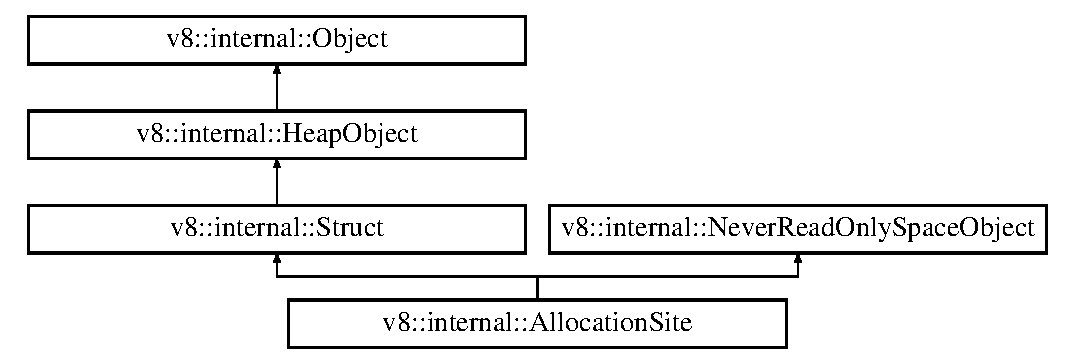
\includegraphics[height=4.000000cm]{classv8_1_1internal_1_1AllocationSite}
\end{center}
\end{figure}
\subsection*{Classes}
\begin{DoxyCompactItemize}
\item 
class \mbox{\hyperlink{classv8_1_1internal_1_1AllocationSite_1_1BodyDescriptor}{Body\+Descriptor}}
\item 
class \mbox{\hyperlink{classv8_1_1internal_1_1AllocationSite_1_1DeoptDependentCodeBit}{Deopt\+Dependent\+Code\+Bit}}
\item 
class \mbox{\hyperlink{classv8_1_1internal_1_1AllocationSite_1_1DoNotInlineBit}{Do\+Not\+Inline\+Bit}}
\item 
class \mbox{\hyperlink{classv8_1_1internal_1_1AllocationSite_1_1ElementsKindBits}{Elements\+Kind\+Bits}}
\item 
class \mbox{\hyperlink{classv8_1_1internal_1_1AllocationSite_1_1MementoFoundCountBits}{Memento\+Found\+Count\+Bits}}
\item 
class \mbox{\hyperlink{classv8_1_1internal_1_1AllocationSite_1_1PretenureDecisionBits}{Pretenure\+Decision\+Bits}}
\end{DoxyCompactItemize}
\subsection*{Public Types}
\begin{DoxyCompactItemize}
\item 
\mbox{\Hypertarget{classv8_1_1internal_1_1AllocationSite_a90e0736002b73f20d96abede63a5395b}\label{classv8_1_1internal_1_1AllocationSite_a90e0736002b73f20d96abede63a5395b}} 
enum {\bfseries Pretenure\+Decision} \{ \newline
{\bfseries k\+Undecided} = 0, 
{\bfseries k\+Dont\+Tenure} = 1, 
{\bfseries k\+Maybe\+Tenure} = 2, 
{\bfseries k\+Tenure} = 3, 
\newline
{\bfseries k\+Zombie} = 4, 
{\bfseries k\+Last\+Pretenure\+Decision\+Value} = k\+Zombie
 \}
\end{DoxyCompactItemize}
\subsection*{Public Member Functions}
\begin{DoxyCompactItemize}
\item 
\mbox{\Hypertarget{classv8_1_1internal_1_1AllocationSite_a015895d2a527877f98749eb13b16a38f}\label{classv8_1_1internal_1_1AllocationSite_a015895d2a527877f98749eb13b16a38f}} 
const \mbox{\hyperlink{classchar}{char}} $\ast$ {\bfseries Pretenure\+Decision\+Name} (Pretenure\+Decision decision)
\item 
\mbox{\Hypertarget{classv8_1_1internal_1_1AllocationSite_a81f61008e147366d1eea6cdbae9d5ded}\label{classv8_1_1internal_1_1AllocationSite_a81f61008e147366d1eea6cdbae9d5ded}} 
void {\bfseries Initialize} ()
\item 
\mbox{\Hypertarget{classv8_1_1internal_1_1AllocationSite_a06e769d7ad11dc8f553f8cc989525b9a}\label{classv8_1_1internal_1_1AllocationSite_a06e769d7ad11dc8f553f8cc989525b9a}} 
\mbox{\hyperlink{classbool}{bool}} {\bfseries Has\+Weak\+Next} () const
\item 
\mbox{\Hypertarget{classv8_1_1internal_1_1AllocationSite_a46538baa1f709d8644d714e7f6bea60f}\label{classv8_1_1internal_1_1AllocationSite_a46538baa1f709d8644d714e7f6bea60f}} 
\mbox{\hyperlink{classbool}{bool}} {\bfseries Is\+Nested} ()
\item 
\mbox{\Hypertarget{classv8_1_1internal_1_1AllocationSite_ad1c0e4e32b7e2db1483fa7a518bec030}\label{classv8_1_1internal_1_1AllocationSite_ad1c0e4e32b7e2db1483fa7a518bec030}} 
{\bfseries S\+T\+A\+T\+I\+C\+\_\+\+A\+S\+S\+E\+RT} (Pretenure\+Decision\+Bits\+::k\+Max $>$=k\+Last\+Pretenure\+Decision\+Value)
\item 
\mbox{\Hypertarget{classv8_1_1internal_1_1AllocationSite_ad402f0d78d12a670cf7eb371f65fc1c0}\label{classv8_1_1internal_1_1AllocationSite_ad402f0d78d12a670cf7eb371f65fc1c0}} 
\mbox{\hyperlink{classbool}{bool}} {\bfseries Increment\+Memento\+Found\+Count} (\mbox{\hyperlink{classint}{int}} increment=1)
\item 
\mbox{\Hypertarget{classv8_1_1internal_1_1AllocationSite_ac32fcfb926ce03239f5df6aca880f18c}\label{classv8_1_1internal_1_1AllocationSite_ac32fcfb926ce03239f5df6aca880f18c}} 
void {\bfseries Increment\+Memento\+Create\+Count} ()
\item 
\mbox{\Hypertarget{classv8_1_1internal_1_1AllocationSite_a3e2f845f0caa8c7a41cd958ae5c34757}\label{classv8_1_1internal_1_1AllocationSite_a3e2f845f0caa8c7a41cd958ae5c34757}} 
Pretenure\+Flag {\bfseries Get\+Pretenure\+Mode} () const
\item 
\mbox{\Hypertarget{classv8_1_1internal_1_1AllocationSite_aa1b323951edb619dd9078164b9fabd5c}\label{classv8_1_1internal_1_1AllocationSite_aa1b323951edb619dd9078164b9fabd5c}} 
void {\bfseries Reset\+Pretenure\+Decision} ()
\item 
\mbox{\Hypertarget{classv8_1_1internal_1_1AllocationSite_a39fc1c0543c261ff4735a551113664d5}\label{classv8_1_1internal_1_1AllocationSite_a39fc1c0543c261ff4735a551113664d5}} 
Pretenure\+Decision {\bfseries pretenure\+\_\+decision} () const
\item 
\mbox{\Hypertarget{classv8_1_1internal_1_1AllocationSite_a3eb7bfb649894bc1ea0875152aff118e}\label{classv8_1_1internal_1_1AllocationSite_a3eb7bfb649894bc1ea0875152aff118e}} 
void {\bfseries set\+\_\+pretenure\+\_\+decision} (Pretenure\+Decision decision)
\item 
\mbox{\Hypertarget{classv8_1_1internal_1_1AllocationSite_a5d2bc5f9c30628481e1f179b18818690}\label{classv8_1_1internal_1_1AllocationSite_a5d2bc5f9c30628481e1f179b18818690}} 
\mbox{\hyperlink{classbool}{bool}} {\bfseries deopt\+\_\+dependent\+\_\+code} () const
\item 
\mbox{\Hypertarget{classv8_1_1internal_1_1AllocationSite_a6b6321178dbb71e389194b39a6ee51ee}\label{classv8_1_1internal_1_1AllocationSite_a6b6321178dbb71e389194b39a6ee51ee}} 
void {\bfseries set\+\_\+deopt\+\_\+dependent\+\_\+code} (\mbox{\hyperlink{classbool}{bool}} deopt)
\item 
\mbox{\Hypertarget{classv8_1_1internal_1_1AllocationSite_a7db228ca1d6bd89aa2af33005ca7a35e}\label{classv8_1_1internal_1_1AllocationSite_a7db228ca1d6bd89aa2af33005ca7a35e}} 
\mbox{\hyperlink{classint}{int}} {\bfseries memento\+\_\+found\+\_\+count} () const
\item 
\mbox{\Hypertarget{classv8_1_1internal_1_1AllocationSite_ad74c42dccc41adcc6d7f2dd22fa56176}\label{classv8_1_1internal_1_1AllocationSite_ad74c42dccc41adcc6d7f2dd22fa56176}} 
void {\bfseries set\+\_\+memento\+\_\+found\+\_\+count} (\mbox{\hyperlink{classint}{int}} count)
\item 
\mbox{\Hypertarget{classv8_1_1internal_1_1AllocationSite_aa67ceb7ab03404c0e31fa529f08520c0}\label{classv8_1_1internal_1_1AllocationSite_aa67ceb7ab03404c0e31fa529f08520c0}} 
\mbox{\hyperlink{classint}{int}} {\bfseries memento\+\_\+create\+\_\+count} () const
\item 
\mbox{\Hypertarget{classv8_1_1internal_1_1AllocationSite_ab95f8e888faad709405944f3f5223378}\label{classv8_1_1internal_1_1AllocationSite_ab95f8e888faad709405944f3f5223378}} 
void {\bfseries set\+\_\+memento\+\_\+create\+\_\+count} (\mbox{\hyperlink{classint}{int}} count)
\item 
\mbox{\Hypertarget{classv8_1_1internal_1_1AllocationSite_ab6c24df9ffa655f7797f28fc251099a6}\label{classv8_1_1internal_1_1AllocationSite_ab6c24df9ffa655f7797f28fc251099a6}} 
\mbox{\hyperlink{classbool}{bool}} {\bfseries Is\+Zombie} () const
\item 
\mbox{\Hypertarget{classv8_1_1internal_1_1AllocationSite_a3ea3a12843ded3e0f95c7b1fc0e3d5bd}\label{classv8_1_1internal_1_1AllocationSite_a3ea3a12843ded3e0f95c7b1fc0e3d5bd}} 
\mbox{\hyperlink{classbool}{bool}} {\bfseries Is\+Maybe\+Tenure} () const
\item 
\mbox{\Hypertarget{classv8_1_1internal_1_1AllocationSite_af432e0790ebdfc00d36c9a6234e98389}\label{classv8_1_1internal_1_1AllocationSite_af432e0790ebdfc00d36c9a6234e98389}} 
void {\bfseries Mark\+Zombie} ()
\item 
\mbox{\Hypertarget{classv8_1_1internal_1_1AllocationSite_ac56e44521833202855156f6c8f06101f}\label{classv8_1_1internal_1_1AllocationSite_ac56e44521833202855156f6c8f06101f}} 
\mbox{\hyperlink{classbool}{bool}} {\bfseries Make\+Pretenure\+Decision} (Pretenure\+Decision current\+\_\+decision, double ratio, \mbox{\hyperlink{classbool}{bool}} maximum\+\_\+size\+\_\+scavenge)
\item 
\mbox{\Hypertarget{classv8_1_1internal_1_1AllocationSite_ab06a9db3e9fa8256f8cd97cc5cefeff5}\label{classv8_1_1internal_1_1AllocationSite_ab06a9db3e9fa8256f8cd97cc5cefeff5}} 
\mbox{\hyperlink{classbool}{bool}} {\bfseries Digest\+Pretenuring\+Feedback} (\mbox{\hyperlink{classbool}{bool}} maximum\+\_\+size\+\_\+scavenge)
\item 
\mbox{\Hypertarget{classv8_1_1internal_1_1AllocationSite_a1add82cc1996137a15e395fbf2a2e09f}\label{classv8_1_1internal_1_1AllocationSite_a1add82cc1996137a15e395fbf2a2e09f}} 
Elements\+Kind {\bfseries Get\+Elements\+Kind} () const
\item 
\mbox{\Hypertarget{classv8_1_1internal_1_1AllocationSite_adf1136948311998f7ead14bcf8f2cfd8}\label{classv8_1_1internal_1_1AllocationSite_adf1136948311998f7ead14bcf8f2cfd8}} 
void {\bfseries Set\+Elements\+Kind} (Elements\+Kind kind)
\item 
\mbox{\Hypertarget{classv8_1_1internal_1_1AllocationSite_aab240b53ca5f3f2cd6fe7698e69bf082}\label{classv8_1_1internal_1_1AllocationSite_aab240b53ca5f3f2cd6fe7698e69bf082}} 
\mbox{\hyperlink{classbool}{bool}} {\bfseries Can\+Inline\+Call} () const
\item 
\mbox{\Hypertarget{classv8_1_1internal_1_1AllocationSite_a3e9fcf250995d87d2c31e05c6e4e6ce5}\label{classv8_1_1internal_1_1AllocationSite_a3e9fcf250995d87d2c31e05c6e4e6ce5}} 
void {\bfseries Set\+Do\+Not\+Inline\+Call} ()
\item 
\mbox{\Hypertarget{classv8_1_1internal_1_1AllocationSite_a1ada880cd600c59f8de3bfa32fdc956a}\label{classv8_1_1internal_1_1AllocationSite_a1ada880cd600c59f8de3bfa32fdc956a}} 
\mbox{\hyperlink{classbool}{bool}} {\bfseries Points\+To\+Literal} () const
\end{DoxyCompactItemize}
\subsection*{Static Public Member Functions}
\begin{DoxyCompactItemize}
\item 
\mbox{\Hypertarget{classv8_1_1internal_1_1AllocationSite_aa995dca4fbdcc35ed5818ad672508ee3}\label{classv8_1_1internal_1_1AllocationSite_aa995dca4fbdcc35ed5818ad672508ee3}} 
{\footnotesize template$<$Allocation\+Site\+Update\+Mode update\+\_\+or\+\_\+check = Allocation\+Site\+Update\+Mode\+::k\+Update$>$ }\\static \mbox{\hyperlink{classbool}{bool}} {\bfseries Digest\+Transition\+Feedback} (\mbox{\hyperlink{classv8_1_1internal_1_1Handle}{Handle}}$<$ \mbox{\hyperlink{classv8_1_1internal_1_1AllocationSite}{Allocation\+Site}} $>$ site, Elements\+Kind to\+\_\+kind)
\item 
\mbox{\Hypertarget{classv8_1_1internal_1_1AllocationSite_a596f5281700441022ddf66ba8a1b2d03}\label{classv8_1_1internal_1_1AllocationSite_a596f5281700441022ddf66ba8a1b2d03}} 
static \mbox{\hyperlink{classbool}{bool}} {\bfseries Should\+Track} (Elements\+Kind boilerplate\+\_\+elements\+\_\+kind)
\item 
\mbox{\Hypertarget{classv8_1_1internal_1_1AllocationSite_af38a6648a1495ca603f8ee8f68c826a7}\label{classv8_1_1internal_1_1AllocationSite_af38a6648a1495ca603f8ee8f68c826a7}} 
static \mbox{\hyperlink{classbool}{bool}} {\bfseries Should\+Track} (Elements\+Kind from, Elements\+Kind to)
\item 
\mbox{\Hypertarget{classv8_1_1internal_1_1AllocationSite_a5bce0a6a275e0f9a9c8a3e87babab0d9}\label{classv8_1_1internal_1_1AllocationSite_a5bce0a6a275e0f9a9c8a3e87babab0d9}} 
static \mbox{\hyperlink{classbool}{bool}} {\bfseries Can\+Track} (Instance\+Type \mbox{\hyperlink{classstd_1_1conditional_1_1type}{type}})
\end{DoxyCompactItemize}
\subsection*{Static Public Attributes}
\begin{DoxyCompactItemize}
\item 
\mbox{\Hypertarget{classv8_1_1internal_1_1AllocationSite_aeead57f97b16bf614a5631349d0bc7f1}\label{classv8_1_1internal_1_1AllocationSite_aeead57f97b16bf614a5631349d0bc7f1}} 
static const \mbox{\hyperlink{classuint32__t}{uint32\+\_\+t}} {\bfseries k\+Maximum\+Array\+Bytes\+To\+Pretransition} = 8 $\ast$ 1024
\item 
\mbox{\Hypertarget{classv8_1_1internal_1_1AllocationSite_a45d58b4d64823e7d33eeb2291b26fb3a}\label{classv8_1_1internal_1_1AllocationSite_a45d58b4d64823e7d33eeb2291b26fb3a}} 
static const double {\bfseries k\+Pretenure\+Ratio} = 0.\+85
\item 
\mbox{\Hypertarget{classv8_1_1internal_1_1AllocationSite_a60cc20b9d1f816783e6c112029776861}\label{classv8_1_1internal_1_1AllocationSite_a60cc20b9d1f816783e6c112029776861}} 
static const \mbox{\hyperlink{classint}{int}} {\bfseries k\+Pretenure\+Minimum\+Created} = 100
\end{DoxyCompactItemize}


\subsection{Detailed Description}


Definition at line 18 of file allocation-\/site.\+h.



The documentation for this class was generated from the following files\+:\begin{DoxyCompactItemize}
\item 
v8/src/objects/allocation-\/site.\+h\item 
v8/src/objects/allocation-\/site-\/inl.\+h\item 
v8/src/objects.\+cc\end{DoxyCompactItemize}

\hypertarget{classv8_1_1internal_1_1AllocationSiteContext}{}\section{v8\+:\+:internal\+:\+:Allocation\+Site\+Context Class Reference}
\label{classv8_1_1internal_1_1AllocationSiteContext}\index{v8\+::internal\+::\+Allocation\+Site\+Context@{v8\+::internal\+::\+Allocation\+Site\+Context}}
Inheritance diagram for v8\+:\+:internal\+:\+:Allocation\+Site\+Context\+:\begin{figure}[H]
\begin{center}
\leavevmode
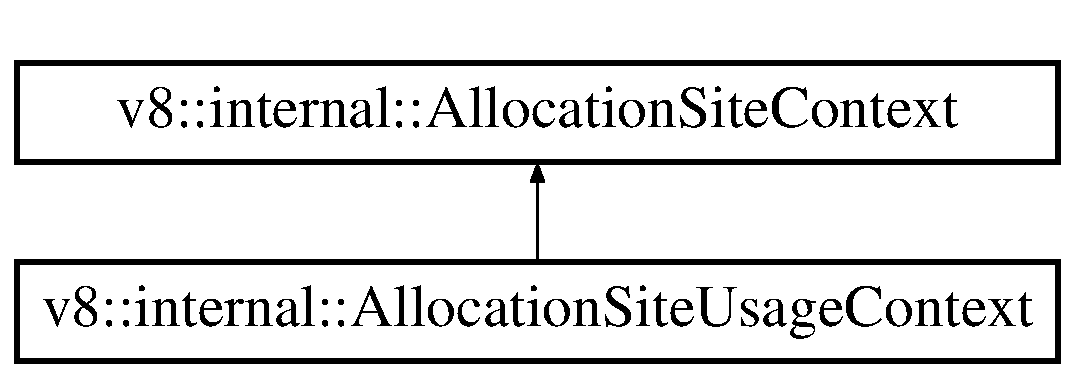
\includegraphics[height=2.000000cm]{classv8_1_1internal_1_1AllocationSiteContext}
\end{center}
\end{figure}
\subsection*{Public Member Functions}
\begin{DoxyCompactItemize}
\item 
\mbox{\Hypertarget{classv8_1_1internal_1_1AllocationSiteContext_acad3aa6b62e34d542b6fd6c9b87e2093}\label{classv8_1_1internal_1_1AllocationSiteContext_acad3aa6b62e34d542b6fd6c9b87e2093}} 
{\bfseries Allocation\+Site\+Context} (\mbox{\hyperlink{classv8_1_1internal_1_1Isolate}{Isolate}} $\ast$isolate)
\item 
\mbox{\Hypertarget{classv8_1_1internal_1_1AllocationSiteContext_a76427a09d8c0eef6794ecfd804ca8eea}\label{classv8_1_1internal_1_1AllocationSiteContext_a76427a09d8c0eef6794ecfd804ca8eea}} 
\mbox{\hyperlink{classv8_1_1internal_1_1Handle}{Handle}}$<$ \mbox{\hyperlink{classv8_1_1internal_1_1AllocationSite}{Allocation\+Site}} $>$ {\bfseries top} ()
\item 
\mbox{\Hypertarget{classv8_1_1internal_1_1AllocationSiteContext_a20943342b9c850bc0f1c3fd0aef56e9a}\label{classv8_1_1internal_1_1AllocationSiteContext_a20943342b9c850bc0f1c3fd0aef56e9a}} 
\mbox{\hyperlink{classv8_1_1internal_1_1Handle}{Handle}}$<$ \mbox{\hyperlink{classv8_1_1internal_1_1AllocationSite}{Allocation\+Site}} $>$ {\bfseries current} ()
\item 
\mbox{\Hypertarget{classv8_1_1internal_1_1AllocationSiteContext_adfa2a2817414d94fd00728a2c163d7b0}\label{classv8_1_1internal_1_1AllocationSiteContext_adfa2a2817414d94fd00728a2c163d7b0}} 
\mbox{\hyperlink{classbool}{bool}} {\bfseries Should\+Create\+Memento} (\mbox{\hyperlink{classv8_1_1internal_1_1Handle}{Handle}}$<$ \mbox{\hyperlink{classv8_1_1internal_1_1JSObject}{J\+S\+Object}} $>$ object)
\item 
\mbox{\Hypertarget{classv8_1_1internal_1_1AllocationSiteContext_a8adcb0b60cf5fbda807b0a11c128ab4a}\label{classv8_1_1internal_1_1AllocationSiteContext_a8adcb0b60cf5fbda807b0a11c128ab4a}} 
\mbox{\hyperlink{classv8_1_1internal_1_1Isolate}{Isolate}} $\ast$ {\bfseries isolate} ()
\end{DoxyCompactItemize}
\subsection*{Protected Member Functions}
\begin{DoxyCompactItemize}
\item 
\mbox{\Hypertarget{classv8_1_1internal_1_1AllocationSiteContext_a2e094902dbadc8931c82eb04333807c0}\label{classv8_1_1internal_1_1AllocationSiteContext_a2e094902dbadc8931c82eb04333807c0}} 
void {\bfseries update\+\_\+current\+\_\+site} (\mbox{\hyperlink{classv8_1_1internal_1_1AllocationSite}{Allocation\+Site}} $\ast$site)
\item 
\mbox{\Hypertarget{classv8_1_1internal_1_1AllocationSiteContext_a2ae0994fc850605cbea75aeddf980b44}\label{classv8_1_1internal_1_1AllocationSiteContext_a2ae0994fc850605cbea75aeddf980b44}} 
void {\bfseries Initialize\+Traversal} (\mbox{\hyperlink{classv8_1_1internal_1_1Handle}{Handle}}$<$ \mbox{\hyperlink{classv8_1_1internal_1_1AllocationSite}{Allocation\+Site}} $>$ site)
\end{DoxyCompactItemize}


\subsection{Detailed Description}


Definition at line 18 of file allocation-\/site-\/scopes.\+h.



The documentation for this class was generated from the following files\+:\begin{DoxyCompactItemize}
\item 
v8/src/allocation-\/site-\/scopes.\+h\item 
v8/src/allocation-\/site-\/scopes-\/inl.\+h\end{DoxyCompactItemize}

\hypertarget{classv8_1_1internal_1_1compiler_1_1AllocationSiteData}{}\section{v8\+:\+:internal\+:\+:compiler\+:\+:Allocation\+Site\+Data Class Reference}
\label{classv8_1_1internal_1_1compiler_1_1AllocationSiteData}\index{v8\+::internal\+::compiler\+::\+Allocation\+Site\+Data@{v8\+::internal\+::compiler\+::\+Allocation\+Site\+Data}}
Inheritance diagram for v8\+:\+:internal\+:\+:compiler\+:\+:Allocation\+Site\+Data\+:\begin{figure}[H]
\begin{center}
\leavevmode
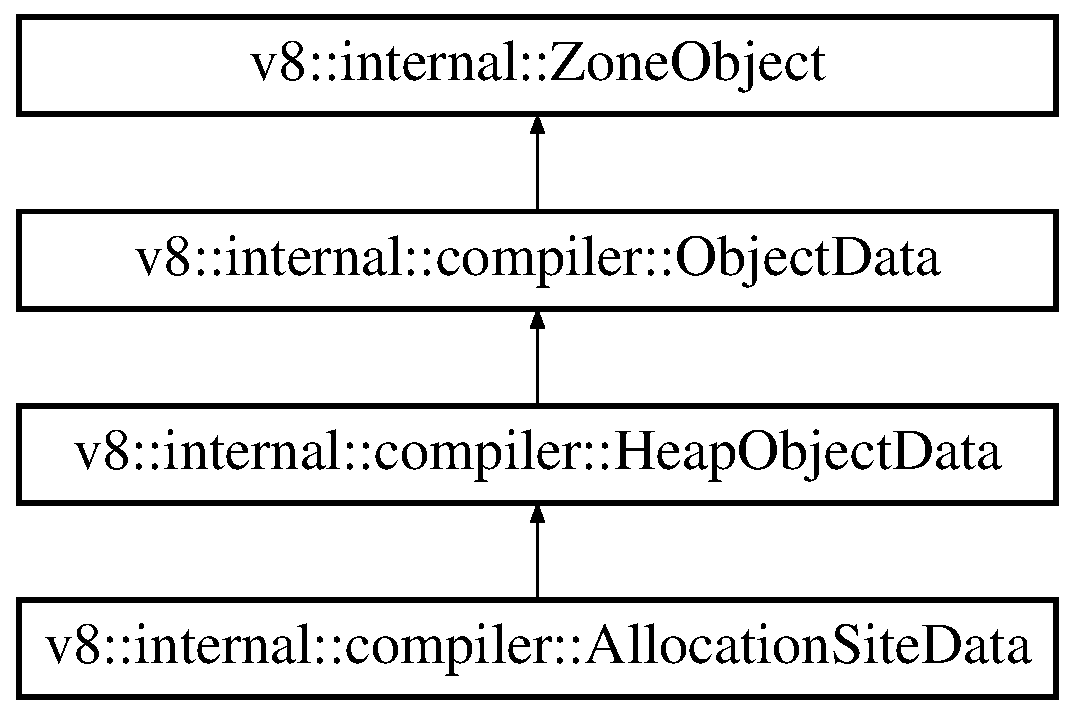
\includegraphics[height=4.000000cm]{classv8_1_1internal_1_1compiler_1_1AllocationSiteData}
\end{center}
\end{figure}
\subsection*{Public Member Functions}
\begin{DoxyCompactItemize}
\item 
\mbox{\Hypertarget{classv8_1_1internal_1_1compiler_1_1AllocationSiteData_ad8287f0a2163e8966a2a07545508f737}\label{classv8_1_1internal_1_1compiler_1_1AllocationSiteData_ad8287f0a2163e8966a2a07545508f737}} 
{\bfseries Allocation\+Site\+Data} (\mbox{\hyperlink{classv8_1_1internal_1_1compiler_1_1JSHeapBroker}{J\+S\+Heap\+Broker}} $\ast$broker, \mbox{\hyperlink{classv8_1_1internal_1_1compiler_1_1ObjectData}{Object\+Data}} $\ast$$\ast$storage, \mbox{\hyperlink{classv8_1_1internal_1_1Handle}{Handle}}$<$ \mbox{\hyperlink{classv8_1_1internal_1_1AllocationSite}{Allocation\+Site}} $>$ object)
\item 
\mbox{\Hypertarget{classv8_1_1internal_1_1compiler_1_1AllocationSiteData_a95a911e7220383170d1ffc53a277dc3f}\label{classv8_1_1internal_1_1compiler_1_1AllocationSiteData_a95a911e7220383170d1ffc53a277dc3f}} 
void {\bfseries Serialize\+Boilerplate} (\mbox{\hyperlink{classv8_1_1internal_1_1compiler_1_1JSHeapBroker}{J\+S\+Heap\+Broker}} $\ast$broker)
\item 
\mbox{\Hypertarget{classv8_1_1internal_1_1compiler_1_1AllocationSiteData_a224126bdf5954a6077a87f5dfbf385d6}\label{classv8_1_1internal_1_1compiler_1_1AllocationSiteData_a224126bdf5954a6077a87f5dfbf385d6}} 
\mbox{\hyperlink{classbool}{bool}} {\bfseries Points\+To\+Literal} () const
\item 
\mbox{\Hypertarget{classv8_1_1internal_1_1compiler_1_1AllocationSiteData_a46338165143126418fc9a21b9ecb7ffe}\label{classv8_1_1internal_1_1compiler_1_1AllocationSiteData_a46338165143126418fc9a21b9ecb7ffe}} 
Pretenure\+Flag {\bfseries Get\+Pretenure\+Mode} () const
\item 
\mbox{\Hypertarget{classv8_1_1internal_1_1compiler_1_1AllocationSiteData_a094ff3367c7dba3160fc3d3a0a2213de}\label{classv8_1_1internal_1_1compiler_1_1AllocationSiteData_a094ff3367c7dba3160fc3d3a0a2213de}} 
\mbox{\hyperlink{classv8_1_1internal_1_1compiler_1_1ObjectData}{Object\+Data}} $\ast$ {\bfseries nested\+\_\+site} () const
\item 
\mbox{\Hypertarget{classv8_1_1internal_1_1compiler_1_1AllocationSiteData_a2c58b7822d7a58d814c84311a2cf445a}\label{classv8_1_1internal_1_1compiler_1_1AllocationSiteData_a2c58b7822d7a58d814c84311a2cf445a}} 
\mbox{\hyperlink{classbool}{bool}} {\bfseries Is\+Fast\+Literal} () const
\item 
\mbox{\Hypertarget{classv8_1_1internal_1_1compiler_1_1AllocationSiteData_a38177e3bca5d794a84dd06f0c7856263}\label{classv8_1_1internal_1_1compiler_1_1AllocationSiteData_a38177e3bca5d794a84dd06f0c7856263}} 
\mbox{\hyperlink{classv8_1_1internal_1_1compiler_1_1JSObjectData}{J\+S\+Object\+Data}} $\ast$ {\bfseries boilerplate} () const
\item 
\mbox{\Hypertarget{classv8_1_1internal_1_1compiler_1_1AllocationSiteData_a0be385314a64b4ba069277d482047f40}\label{classv8_1_1internal_1_1compiler_1_1AllocationSiteData_a0be385314a64b4ba069277d482047f40}} 
Elements\+Kind {\bfseries Get\+Elements\+Kind} () const
\item 
\mbox{\Hypertarget{classv8_1_1internal_1_1compiler_1_1AllocationSiteData_a9773d74acc78c0f2aa4e04213f3b9af2}\label{classv8_1_1internal_1_1compiler_1_1AllocationSiteData_a9773d74acc78c0f2aa4e04213f3b9af2}} 
\mbox{\hyperlink{classbool}{bool}} {\bfseries Can\+Inline\+Call} () const
\end{DoxyCompactItemize}
\subsection*{Additional Inherited Members}


\subsection{Detailed Description}


Definition at line 584 of file js-\/heap-\/broker.\+cc.



The documentation for this class was generated from the following file\+:\begin{DoxyCompactItemize}
\item 
v8/src/compiler/js-\/heap-\/broker.\+cc\end{DoxyCompactItemize}

\hypertarget{classv8_1_1internal_1_1compiler_1_1AllocationSiteRef}{}\section{v8\+:\+:internal\+:\+:compiler\+:\+:Allocation\+Site\+Ref Class Reference}
\label{classv8_1_1internal_1_1compiler_1_1AllocationSiteRef}\index{v8\+::internal\+::compiler\+::\+Allocation\+Site\+Ref@{v8\+::internal\+::compiler\+::\+Allocation\+Site\+Ref}}
Inheritance diagram for v8\+:\+:internal\+:\+:compiler\+:\+:Allocation\+Site\+Ref\+:\begin{figure}[H]
\begin{center}
\leavevmode
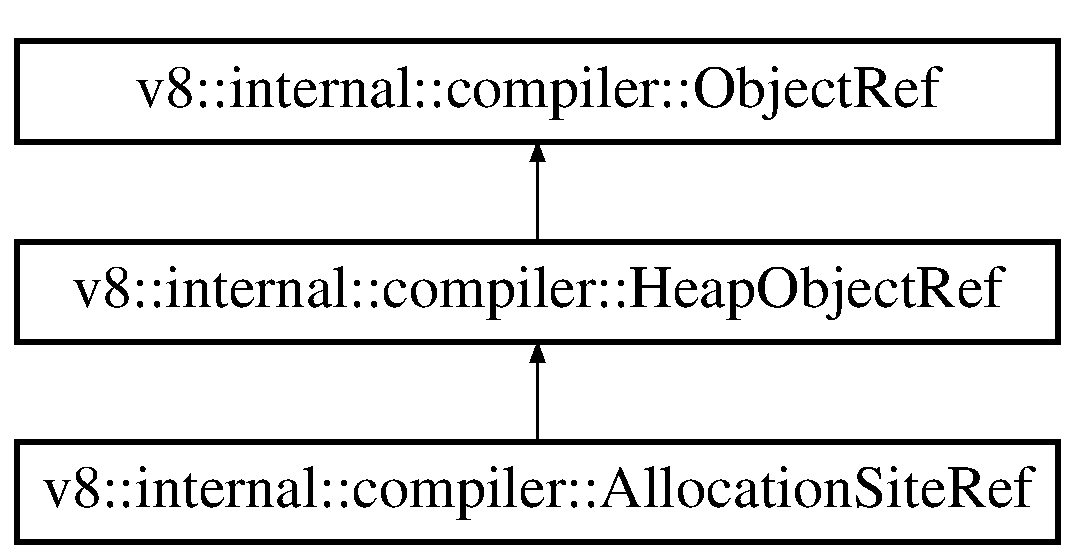
\includegraphics[height=3.000000cm]{classv8_1_1internal_1_1compiler_1_1AllocationSiteRef}
\end{center}
\end{figure}
\subsection*{Public Member Functions}
\begin{DoxyCompactItemize}
\item 
\mbox{\Hypertarget{classv8_1_1internal_1_1compiler_1_1AllocationSiteRef_a3c2bc41de6dd595e9954868649504f04}\label{classv8_1_1internal_1_1compiler_1_1AllocationSiteRef_a3c2bc41de6dd595e9954868649504f04}} 
\mbox{\hyperlink{classv8_1_1internal_1_1Handle}{Handle}}$<$ \mbox{\hyperlink{classv8_1_1internal_1_1AllocationSite}{Allocation\+Site}} $>$ {\bfseries object} () const
\item 
\mbox{\Hypertarget{classv8_1_1internal_1_1compiler_1_1AllocationSiteRef_a44f09e4d62a90d87542c6d26fede7832}\label{classv8_1_1internal_1_1compiler_1_1AllocationSiteRef_a44f09e4d62a90d87542c6d26fede7832}} 
\mbox{\hyperlink{classbool}{bool}} {\bfseries Points\+To\+Literal} () const
\item 
\mbox{\Hypertarget{classv8_1_1internal_1_1compiler_1_1AllocationSiteRef_a38c3c5492becfb37c225d83a0afe6a3f}\label{classv8_1_1internal_1_1compiler_1_1AllocationSiteRef_a38c3c5492becfb37c225d83a0afe6a3f}} 
Pretenure\+Flag {\bfseries Get\+Pretenure\+Mode} () const
\item 
\mbox{\Hypertarget{classv8_1_1internal_1_1compiler_1_1AllocationSiteRef_ad42557dc05e2bbaefe47b23156707b63}\label{classv8_1_1internal_1_1compiler_1_1AllocationSiteRef_ad42557dc05e2bbaefe47b23156707b63}} 
\mbox{\hyperlink{classv8_1_1internal_1_1compiler_1_1ObjectRef}{Object\+Ref}} {\bfseries nested\+\_\+site} () const
\item 
\mbox{\Hypertarget{classv8_1_1internal_1_1compiler_1_1AllocationSiteRef_a497bf7b15a3363ad9ce60cdf2a57375d}\label{classv8_1_1internal_1_1compiler_1_1AllocationSiteRef_a497bf7b15a3363ad9ce60cdf2a57375d}} 
\mbox{\hyperlink{classbool}{bool}} {\bfseries Is\+Fast\+Literal} () const
\item 
\mbox{\Hypertarget{classv8_1_1internal_1_1compiler_1_1AllocationSiteRef_acbe0588b3a03dc486de3ea2363d87b51}\label{classv8_1_1internal_1_1compiler_1_1AllocationSiteRef_acbe0588b3a03dc486de3ea2363d87b51}} 
\mbox{\hyperlink{classv8_1_1base_1_1Optional}{base\+::\+Optional}}$<$ \mbox{\hyperlink{classv8_1_1internal_1_1compiler_1_1JSObjectRef}{J\+S\+Object\+Ref}} $>$ {\bfseries boilerplate} () const
\item 
\mbox{\Hypertarget{classv8_1_1internal_1_1compiler_1_1AllocationSiteRef_aa33bc16c03077bfece98552aa1f68548}\label{classv8_1_1internal_1_1compiler_1_1AllocationSiteRef_aa33bc16c03077bfece98552aa1f68548}} 
Elements\+Kind {\bfseries Get\+Elements\+Kind} () const
\item 
\mbox{\Hypertarget{classv8_1_1internal_1_1compiler_1_1AllocationSiteRef_abbcefc6be09c1c0ad8f3249c50e5088f}\label{classv8_1_1internal_1_1compiler_1_1AllocationSiteRef_abbcefc6be09c1c0ad8f3249c50e5088f}} 
\mbox{\hyperlink{classbool}{bool}} {\bfseries Can\+Inline\+Call} () const
\end{DoxyCompactItemize}
\subsection*{Additional Inherited Members}


\subsection{Detailed Description}


Definition at line 383 of file js-\/heap-\/broker.\+h.



The documentation for this class was generated from the following files\+:\begin{DoxyCompactItemize}
\item 
v8/src/compiler/js-\/heap-\/broker.\+h\item 
v8/src/compiler/js-\/heap-\/broker.\+cc\end{DoxyCompactItemize}

\hypertarget{classv8_1_1internal_1_1AllocationSiteUsageContext}{}\section{v8\+:\+:internal\+:\+:Allocation\+Site\+Usage\+Context Class Reference}
\label{classv8_1_1internal_1_1AllocationSiteUsageContext}\index{v8\+::internal\+::\+Allocation\+Site\+Usage\+Context@{v8\+::internal\+::\+Allocation\+Site\+Usage\+Context}}
Inheritance diagram for v8\+:\+:internal\+:\+:Allocation\+Site\+Usage\+Context\+:\begin{figure}[H]
\begin{center}
\leavevmode
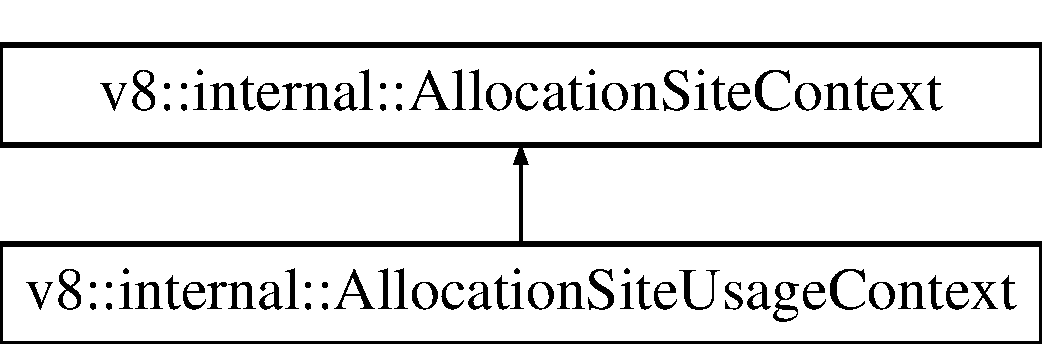
\includegraphics[height=2.000000cm]{classv8_1_1internal_1_1AllocationSiteUsageContext}
\end{center}
\end{figure}
\subsection*{Public Member Functions}
\begin{DoxyCompactItemize}
\item 
\mbox{\Hypertarget{classv8_1_1internal_1_1AllocationSiteUsageContext_aa9b5b62dbc43c89fbb14b22f32d3f68e}\label{classv8_1_1internal_1_1AllocationSiteUsageContext_aa9b5b62dbc43c89fbb14b22f32d3f68e}} 
{\bfseries Allocation\+Site\+Usage\+Context} (\mbox{\hyperlink{classv8_1_1internal_1_1Isolate}{Isolate}} $\ast$isolate, \mbox{\hyperlink{classv8_1_1internal_1_1Handle}{Handle}}$<$ \mbox{\hyperlink{classv8_1_1internal_1_1AllocationSite}{Allocation\+Site}} $>$ site, \mbox{\hyperlink{classbool}{bool}} activated)
\item 
\mbox{\Hypertarget{classv8_1_1internal_1_1AllocationSiteUsageContext_aa25f95a1f9992f8555eeb7a9bfb5d4a1}\label{classv8_1_1internal_1_1AllocationSiteUsageContext_aa25f95a1f9992f8555eeb7a9bfb5d4a1}} 
\mbox{\hyperlink{classv8_1_1internal_1_1Handle}{Handle}}$<$ \mbox{\hyperlink{classv8_1_1internal_1_1AllocationSite}{Allocation\+Site}} $>$ {\bfseries Enter\+New\+Scope} ()
\item 
\mbox{\Hypertarget{classv8_1_1internal_1_1AllocationSiteUsageContext_a27c29c9de5fb9a5afdc56a262b7d095d}\label{classv8_1_1internal_1_1AllocationSiteUsageContext_a27c29c9de5fb9a5afdc56a262b7d095d}} 
void {\bfseries Exit\+Scope} (\mbox{\hyperlink{classv8_1_1internal_1_1Handle}{Handle}}$<$ \mbox{\hyperlink{classv8_1_1internal_1_1AllocationSite}{Allocation\+Site}} $>$ scope\+\_\+site, \mbox{\hyperlink{classv8_1_1internal_1_1Handle}{Handle}}$<$ \mbox{\hyperlink{classv8_1_1internal_1_1JSObject}{J\+S\+Object}} $>$ object)
\item 
\mbox{\Hypertarget{classv8_1_1internal_1_1AllocationSiteUsageContext_a9b8b4f20046612a1dc28823efe000043}\label{classv8_1_1internal_1_1AllocationSiteUsageContext_a9b8b4f20046612a1dc28823efe000043}} 
\mbox{\hyperlink{classbool}{bool}} {\bfseries Should\+Create\+Memento} (\mbox{\hyperlink{classv8_1_1internal_1_1Handle}{Handle}}$<$ \mbox{\hyperlink{classv8_1_1internal_1_1JSObject}{J\+S\+Object}} $>$ object)
\end{DoxyCompactItemize}
\subsection*{Static Public Attributes}
\begin{DoxyCompactItemize}
\item 
\mbox{\Hypertarget{classv8_1_1internal_1_1AllocationSiteUsageContext_afee5f8df4b33ecf23dade00ab5c4ce52}\label{classv8_1_1internal_1_1AllocationSiteUsageContext_afee5f8df4b33ecf23dade00ab5c4ce52}} 
static const \mbox{\hyperlink{classbool}{bool}} {\bfseries k\+Copying} = true
\end{DoxyCompactItemize}
\subsection*{Additional Inherited Members}


\subsection{Detailed Description}


Definition at line 47 of file allocation-\/site-\/scopes.\+h.



The documentation for this class was generated from the following files\+:\begin{DoxyCompactItemize}
\item 
v8/src/allocation-\/site-\/scopes.\+h\item 
v8/src/allocation-\/site-\/scopes-\/inl.\+h\end{DoxyCompactItemize}

\hypertarget{classv8_1_1internal_1_1AllocationStats}{}\section{v8\+:\+:internal\+:\+:Allocation\+Stats Class Reference}
\label{classv8_1_1internal_1_1AllocationStats}\index{v8\+::internal\+::\+Allocation\+Stats@{v8\+::internal\+::\+Allocation\+Stats}}
\subsection*{Public Member Functions}
\begin{DoxyCompactItemize}
\item 
\mbox{\Hypertarget{classv8_1_1internal_1_1AllocationStats_a6e162cd13b5f72049d7debad2203f191}\label{classv8_1_1internal_1_1AllocationStats_a6e162cd13b5f72049d7debad2203f191}} 
void {\bfseries Clear} ()
\item 
\mbox{\Hypertarget{classv8_1_1internal_1_1AllocationStats_a587f5be1a4ea26b70d6d555b4d43ec15}\label{classv8_1_1internal_1_1AllocationStats_a587f5be1a4ea26b70d6d555b4d43ec15}} 
void {\bfseries Clear\+Size} ()
\item 
\mbox{\Hypertarget{classv8_1_1internal_1_1AllocationStats_ab6fa0ff1b82bccabec0c16eba7bed184}\label{classv8_1_1internal_1_1AllocationStats_ab6fa0ff1b82bccabec0c16eba7bed184}} 
\mbox{\hyperlink{classsize__t}{size\+\_\+t}} {\bfseries Capacity} ()
\item 
\mbox{\Hypertarget{classv8_1_1internal_1_1AllocationStats_a6b099a9940e39e27094d43b34f5c972a}\label{classv8_1_1internal_1_1AllocationStats_a6b099a9940e39e27094d43b34f5c972a}} 
\mbox{\hyperlink{classsize__t}{size\+\_\+t}} {\bfseries Max\+Capacity} ()
\item 
\mbox{\Hypertarget{classv8_1_1internal_1_1AllocationStats_ad6f91ce6cedea567a8441f2c9afc3058}\label{classv8_1_1internal_1_1AllocationStats_ad6f91ce6cedea567a8441f2c9afc3058}} 
\mbox{\hyperlink{classsize__t}{size\+\_\+t}} {\bfseries Size} ()
\item 
\mbox{\Hypertarget{classv8_1_1internal_1_1AllocationStats_afc0fb2100ed8bffa17f030c7d08e8f00}\label{classv8_1_1internal_1_1AllocationStats_afc0fb2100ed8bffa17f030c7d08e8f00}} 
void {\bfseries Increase\+Allocated\+Bytes} (\mbox{\hyperlink{classsize__t}{size\+\_\+t}} bytes, \mbox{\hyperlink{classv8_1_1internal_1_1Page}{Page}} $\ast$page)
\item 
\mbox{\Hypertarget{classv8_1_1internal_1_1AllocationStats_a347d8287921f240bc799082cfb8048d9}\label{classv8_1_1internal_1_1AllocationStats_a347d8287921f240bc799082cfb8048d9}} 
void {\bfseries Decrease\+Allocated\+Bytes} (\mbox{\hyperlink{classsize__t}{size\+\_\+t}} bytes, \mbox{\hyperlink{classv8_1_1internal_1_1Page}{Page}} $\ast$page)
\item 
\mbox{\Hypertarget{classv8_1_1internal_1_1AllocationStats_a6344dd3fb24f166f260401bf7917cd52}\label{classv8_1_1internal_1_1AllocationStats_a6344dd3fb24f166f260401bf7917cd52}} 
void {\bfseries Decrease\+Capacity} (\mbox{\hyperlink{classsize__t}{size\+\_\+t}} bytes)
\item 
\mbox{\Hypertarget{classv8_1_1internal_1_1AllocationStats_a2d4420ab92ac41b0d31013b745db6d6d}\label{classv8_1_1internal_1_1AllocationStats_a2d4420ab92ac41b0d31013b745db6d6d}} 
void {\bfseries Increase\+Capacity} (\mbox{\hyperlink{classsize__t}{size\+\_\+t}} bytes)
\end{DoxyCompactItemize}


\subsection{Detailed Description}


Definition at line 1665 of file spaces.\+h.



The documentation for this class was generated from the following file\+:\begin{DoxyCompactItemize}
\item 
v8/src/heap/spaces.\+h\end{DoxyCompactItemize}

\hypertarget{classv8_1_1internal_1_1AllocationTraceNode}{}\section{v8\+:\+:internal\+:\+:Allocation\+Trace\+Node Class Reference}
\label{classv8_1_1internal_1_1AllocationTraceNode}\index{v8\+::internal\+::\+Allocation\+Trace\+Node@{v8\+::internal\+::\+Allocation\+Trace\+Node}}
\subsection*{Public Member Functions}
\begin{DoxyCompactItemize}
\item 
\mbox{\Hypertarget{classv8_1_1internal_1_1AllocationTraceNode_aca8caa93d6a5309e2fc2529b71a5a70a}\label{classv8_1_1internal_1_1AllocationTraceNode_aca8caa93d6a5309e2fc2529b71a5a70a}} 
{\bfseries Allocation\+Trace\+Node} (\mbox{\hyperlink{classv8_1_1internal_1_1AllocationTraceTree}{Allocation\+Trace\+Tree}} $\ast$tree, \mbox{\hyperlink{classunsigned}{unsigned}} function\+\_\+info\+\_\+index)
\item 
\mbox{\Hypertarget{classv8_1_1internal_1_1AllocationTraceNode_afbb942277677c19a257ff8781f034c1d}\label{classv8_1_1internal_1_1AllocationTraceNode_afbb942277677c19a257ff8781f034c1d}} 
\mbox{\hyperlink{classv8_1_1internal_1_1AllocationTraceNode}{Allocation\+Trace\+Node}} $\ast$ {\bfseries Find\+Child} (\mbox{\hyperlink{classunsigned}{unsigned}} function\+\_\+info\+\_\+index)
\item 
\mbox{\Hypertarget{classv8_1_1internal_1_1AllocationTraceNode_a780262d490b639c1782e3a7212297709}\label{classv8_1_1internal_1_1AllocationTraceNode_a780262d490b639c1782e3a7212297709}} 
\mbox{\hyperlink{classv8_1_1internal_1_1AllocationTraceNode}{Allocation\+Trace\+Node}} $\ast$ {\bfseries Find\+Or\+Add\+Child} (\mbox{\hyperlink{classunsigned}{unsigned}} function\+\_\+info\+\_\+index)
\item 
\mbox{\Hypertarget{classv8_1_1internal_1_1AllocationTraceNode_ab3952f0610968cabfdb6a6134395f4a8}\label{classv8_1_1internal_1_1AllocationTraceNode_ab3952f0610968cabfdb6a6134395f4a8}} 
void {\bfseries Add\+Allocation} (\mbox{\hyperlink{classunsigned}{unsigned}} size)
\item 
\mbox{\Hypertarget{classv8_1_1internal_1_1AllocationTraceNode_ae7d97ae5462f51e29627cd0b122951f1}\label{classv8_1_1internal_1_1AllocationTraceNode_ae7d97ae5462f51e29627cd0b122951f1}} 
\mbox{\hyperlink{classunsigned}{unsigned}} {\bfseries function\+\_\+info\+\_\+index} () const
\item 
\mbox{\Hypertarget{classv8_1_1internal_1_1AllocationTraceNode_a9120f1f0161b27240167a9a3cef8314d}\label{classv8_1_1internal_1_1AllocationTraceNode_a9120f1f0161b27240167a9a3cef8314d}} 
\mbox{\hyperlink{classunsigned}{unsigned}} {\bfseries allocation\+\_\+size} () const
\item 
\mbox{\Hypertarget{classv8_1_1internal_1_1AllocationTraceNode_a99d79d8ca6c91aaa4257b37b26446203}\label{classv8_1_1internal_1_1AllocationTraceNode_a99d79d8ca6c91aaa4257b37b26446203}} 
\mbox{\hyperlink{classunsigned}{unsigned}} {\bfseries allocation\+\_\+count} () const
\item 
\mbox{\Hypertarget{classv8_1_1internal_1_1AllocationTraceNode_a722786c8db6de58c024a7f258eea9e64}\label{classv8_1_1internal_1_1AllocationTraceNode_a722786c8db6de58c024a7f258eea9e64}} 
\mbox{\hyperlink{classunsigned}{unsigned}} {\bfseries id} () const
\item 
\mbox{\Hypertarget{classv8_1_1internal_1_1AllocationTraceNode_a31a1dc2ffbcc2913ad3aa5259d017ee7}\label{classv8_1_1internal_1_1AllocationTraceNode_a31a1dc2ffbcc2913ad3aa5259d017ee7}} 
const std\+::vector$<$ \mbox{\hyperlink{classv8_1_1internal_1_1AllocationTraceNode}{Allocation\+Trace\+Node}} $\ast$ $>$ \& {\bfseries children} () const
\item 
\mbox{\Hypertarget{classv8_1_1internal_1_1AllocationTraceNode_acfba1229f80910c5746758f8afdff7af}\label{classv8_1_1internal_1_1AllocationTraceNode_acfba1229f80910c5746758f8afdff7af}} 
void {\bfseries Print} (\mbox{\hyperlink{classint}{int}} indent, \mbox{\hyperlink{classv8_1_1internal_1_1AllocationTracker}{Allocation\+Tracker}} $\ast$tracker)
\end{DoxyCompactItemize}


\subsection{Detailed Description}


Definition at line 26 of file allocation-\/tracker.\+h.



The documentation for this class was generated from the following files\+:\begin{DoxyCompactItemize}
\item 
v8/src/profiler/allocation-\/tracker.\+h\item 
v8/src/profiler/allocation-\/tracker.\+cc\end{DoxyCompactItemize}

\hypertarget{classv8_1_1internal_1_1AllocationTraceTree}{}\section{v8\+:\+:internal\+:\+:Allocation\+Trace\+Tree Class Reference}
\label{classv8_1_1internal_1_1AllocationTraceTree}\index{v8\+::internal\+::\+Allocation\+Trace\+Tree@{v8\+::internal\+::\+Allocation\+Trace\+Tree}}
\subsection*{Public Member Functions}
\begin{DoxyCompactItemize}
\item 
\mbox{\Hypertarget{classv8_1_1internal_1_1AllocationTraceTree_ac5d8e76d5c1250e5a0c0453d79fc656e}\label{classv8_1_1internal_1_1AllocationTraceTree_ac5d8e76d5c1250e5a0c0453d79fc656e}} 
\mbox{\hyperlink{classv8_1_1internal_1_1AllocationTraceNode}{Allocation\+Trace\+Node}} $\ast$ {\bfseries Add\+Path\+From\+End} (const \mbox{\hyperlink{classv8_1_1internal_1_1Vector}{Vector}}$<$ \mbox{\hyperlink{classunsigned}{unsigned}} $>$ \&path)
\item 
\mbox{\Hypertarget{classv8_1_1internal_1_1AllocationTraceTree_af36cd4ae9797ba6e8681349f3db7d0b0}\label{classv8_1_1internal_1_1AllocationTraceTree_af36cd4ae9797ba6e8681349f3db7d0b0}} 
\mbox{\hyperlink{classv8_1_1internal_1_1AllocationTraceNode}{Allocation\+Trace\+Node}} $\ast$ {\bfseries root} ()
\item 
\mbox{\Hypertarget{classv8_1_1internal_1_1AllocationTraceTree_aed92bbd12c4ca3ea8dfabf9f3ce16d9e}\label{classv8_1_1internal_1_1AllocationTraceTree_aed92bbd12c4ca3ea8dfabf9f3ce16d9e}} 
\mbox{\hyperlink{classunsigned}{unsigned}} {\bfseries next\+\_\+node\+\_\+id} ()
\item 
\mbox{\Hypertarget{classv8_1_1internal_1_1AllocationTraceTree_a37ac3b1e978232c6150a1d3edf4da9ce}\label{classv8_1_1internal_1_1AllocationTraceTree_a37ac3b1e978232c6150a1d3edf4da9ce}} 
void {\bfseries Print} (\mbox{\hyperlink{classv8_1_1internal_1_1AllocationTracker}{Allocation\+Tracker}} $\ast$tracker)
\end{DoxyCompactItemize}


\subsection{Detailed Description}


Definition at line 57 of file allocation-\/tracker.\+h.



The documentation for this class was generated from the following files\+:\begin{DoxyCompactItemize}
\item 
v8/src/profiler/allocation-\/tracker.\+h\item 
v8/src/profiler/allocation-\/tracker.\+cc\end{DoxyCompactItemize}

\hypertarget{classv8_1_1internal_1_1AllocationTracker}{}\section{v8\+:\+:internal\+:\+:Allocation\+Tracker Class Reference}
\label{classv8_1_1internal_1_1AllocationTracker}\index{v8\+::internal\+::\+Allocation\+Tracker@{v8\+::internal\+::\+Allocation\+Tracker}}
\subsection*{Classes}
\begin{DoxyCompactItemize}
\item 
struct \mbox{\hyperlink{structv8_1_1internal_1_1AllocationTracker_1_1FunctionInfo}{Function\+Info}}
\end{DoxyCompactItemize}
\subsection*{Public Member Functions}
\begin{DoxyCompactItemize}
\item 
\mbox{\Hypertarget{classv8_1_1internal_1_1AllocationTracker_ae705bae00ff323c41efc0b1d50afc62c}\label{classv8_1_1internal_1_1AllocationTracker_ae705bae00ff323c41efc0b1d50afc62c}} 
{\bfseries Allocation\+Tracker} (\mbox{\hyperlink{classv8_1_1internal_1_1HeapObjectsMap}{Heap\+Objects\+Map}} $\ast$ids, \mbox{\hyperlink{classv8_1_1internal_1_1StringsStorage}{Strings\+Storage}} $\ast$names)
\item 
\mbox{\Hypertarget{classv8_1_1internal_1_1AllocationTracker_a06984664822efec67f15cfc200f9c1c8}\label{classv8_1_1internal_1_1AllocationTracker_a06984664822efec67f15cfc200f9c1c8}} 
void {\bfseries Prepare\+For\+Serialization} ()
\item 
\mbox{\Hypertarget{classv8_1_1internal_1_1AllocationTracker_af59e0f4c414b6fe00ff0729e616ae219}\label{classv8_1_1internal_1_1AllocationTracker_af59e0f4c414b6fe00ff0729e616ae219}} 
void {\bfseries Allocation\+Event} (\mbox{\hyperlink{classuintptr__t}{Address}} addr, \mbox{\hyperlink{classint}{int}} size)
\item 
\mbox{\Hypertarget{classv8_1_1internal_1_1AllocationTracker_aa0471186f074acec90232839b6e22431}\label{classv8_1_1internal_1_1AllocationTracker_aa0471186f074acec90232839b6e22431}} 
\mbox{\hyperlink{classv8_1_1internal_1_1AllocationTraceTree}{Allocation\+Trace\+Tree}} $\ast$ {\bfseries trace\+\_\+tree} ()
\item 
\mbox{\Hypertarget{classv8_1_1internal_1_1AllocationTracker_aa5efd08c197a25727449c819519a0853}\label{classv8_1_1internal_1_1AllocationTracker_aa5efd08c197a25727449c819519a0853}} 
const std\+::vector$<$ \mbox{\hyperlink{structv8_1_1internal_1_1AllocationTracker_1_1FunctionInfo}{Function\+Info}} $\ast$ $>$ \& {\bfseries function\+\_\+info\+\_\+list} () const
\item 
\mbox{\Hypertarget{classv8_1_1internal_1_1AllocationTracker_adacf25ec6310501fb4d9ae02c1737621}\label{classv8_1_1internal_1_1AllocationTracker_adacf25ec6310501fb4d9ae02c1737621}} 
\mbox{\hyperlink{classv8_1_1internal_1_1AddressToTraceMap}{Address\+To\+Trace\+Map}} $\ast$ {\bfseries address\+\_\+to\+\_\+trace} ()
\end{DoxyCompactItemize}


\subsection{Detailed Description}


Definition at line 98 of file allocation-\/tracker.\+h.



The documentation for this class was generated from the following files\+:\begin{DoxyCompactItemize}
\item 
v8/src/profiler/allocation-\/tracker.\+h\item 
v8/src/profiler/allocation-\/tracker.\+cc\end{DoxyCompactItemize}

\hypertarget{classv8_1_1ArrayBuffer_1_1Allocator}{}\section{v8\+:\+:Array\+Buffer\+:\+:Allocator Class Reference}
\label{classv8_1_1ArrayBuffer_1_1Allocator}\index{v8\+::\+Array\+Buffer\+::\+Allocator@{v8\+::\+Array\+Buffer\+::\+Allocator}}


{\ttfamily \#include $<$v8.\+h$>$}

\subsection*{Public Types}
\begin{DoxyCompactItemize}
\item 
enum \mbox{\hyperlink{classv8_1_1ArrayBuffer_1_1Allocator_ab106d1fbad7be9f6fd8b0f5c550ac59e}{Allocation\+Mode}} \{ {\bfseries k\+Normal}, 
{\bfseries k\+Reservation}
 \}
\end{DoxyCompactItemize}
\subsection*{Public Member Functions}
\begin{DoxyCompactItemize}
\item 
virtual void $\ast$ \mbox{\hyperlink{classv8_1_1ArrayBuffer_1_1Allocator_a106b0d80120ed04fe9b9675e96f0340b}{Allocate}} (\mbox{\hyperlink{classsize__t}{size\+\_\+t}} length)=0
\item 
virtual void $\ast$ \mbox{\hyperlink{classv8_1_1ArrayBuffer_1_1Allocator_a92b2d5c0a826d3c435e12f3ee178f37a}{Allocate\+Uninitialized}} (\mbox{\hyperlink{classsize__t}{size\+\_\+t}} length)=0
\item 
virtual void \mbox{\hyperlink{classv8_1_1ArrayBuffer_1_1Allocator_a419f59d2a103a5a8863809d7977c9cd8}{Free}} (void $\ast$data, \mbox{\hyperlink{classsize__t}{size\+\_\+t}} length)=0
\end{DoxyCompactItemize}
\subsection*{Static Public Member Functions}
\begin{DoxyCompactItemize}
\item 
static \mbox{\hyperlink{classv8_1_1ArrayBuffer_1_1Allocator}{Allocator}} $\ast$ \mbox{\hyperlink{classv8_1_1ArrayBuffer_1_1Allocator_a2c95b1213b0a0a2996e1c63194fc6951}{New\+Default\+Allocator}} ()
\end{DoxyCompactItemize}


\subsection{Detailed Description}
A thread-\/safe allocator that V8 uses to allocate $\vert$\+Array\+Buffer$\vert$\textquotesingle{}s memory. The allocator is a global V8 setting. It has to be set via \mbox{\hyperlink{structv8_1_1Isolate_1_1CreateParams}{Isolate\+::\+Create\+Params}}.

Memory allocated through this allocator by V8 is accounted for as external memory by V8. Note that V8 keeps track of the memory for all internalized $\vert$\+Array\+Buffer$\vert$s. Responsibility for tracking external memory (using Isolate\+::\+Adjust\+Amount\+Of\+External\+Allocated\+Memory) is handed over to the embedder upon externalization and taken over upon internalization (creating an internalized buffer from an existing buffer).

Note that it is unsafe to call back into V8 from any of the allocator functions. 

Definition at line 4513 of file v8.\+h.



\subsection{Member Enumeration Documentation}
\mbox{\Hypertarget{classv8_1_1ArrayBuffer_1_1Allocator_ab106d1fbad7be9f6fd8b0f5c550ac59e}\label{classv8_1_1ArrayBuffer_1_1Allocator_ab106d1fbad7be9f6fd8b0f5c550ac59e}} 
\index{v8\+::\+Array\+Buffer\+::\+Allocator@{v8\+::\+Array\+Buffer\+::\+Allocator}!Allocation\+Mode@{Allocation\+Mode}}
\index{Allocation\+Mode@{Allocation\+Mode}!v8\+::\+Array\+Buffer\+::\+Allocator@{v8\+::\+Array\+Buffer\+::\+Allocator}}
\subsubsection{\texorpdfstring{Allocation\+Mode}{AllocationMode}}
{\footnotesize\ttfamily enum \mbox{\hyperlink{classv8_1_1ArrayBuffer_1_1Allocator_ab106d1fbad7be9f6fd8b0f5c550ac59e}{v8\+::\+Array\+Buffer\+::\+Allocator\+::\+Allocation\+Mode}}\hspace{0.3cm}{\ttfamily [strong]}}

\mbox{\hyperlink{classv8_1_1ArrayBuffer}{Array\+Buffer}} allocation mode. k\+Normal is a malloc/free style allocation, while k\+Reservation is for larger allocations with the ability to set access permissions. 

Definition at line 4540 of file v8.\+h.



\subsection{Member Function Documentation}
\mbox{\Hypertarget{classv8_1_1ArrayBuffer_1_1Allocator_a106b0d80120ed04fe9b9675e96f0340b}\label{classv8_1_1ArrayBuffer_1_1Allocator_a106b0d80120ed04fe9b9675e96f0340b}} 
\index{v8\+::\+Array\+Buffer\+::\+Allocator@{v8\+::\+Array\+Buffer\+::\+Allocator}!Allocate@{Allocate}}
\index{Allocate@{Allocate}!v8\+::\+Array\+Buffer\+::\+Allocator@{v8\+::\+Array\+Buffer\+::\+Allocator}}
\subsubsection{\texorpdfstring{Allocate()}{Allocate()}}
{\footnotesize\ttfamily virtual void$\ast$ v8\+::\+Array\+Buffer\+::\+Allocator\+::\+Allocate (\begin{DoxyParamCaption}\item[{\mbox{\hyperlink{classsize__t}{size\+\_\+t}}}]{length }\end{DoxyParamCaption})\hspace{0.3cm}{\ttfamily [pure virtual]}}

Allocate $\vert$length$\vert$ bytes. Return N\+U\+LL if allocation is not successful. Memory should be initialized to zeroes. \mbox{\Hypertarget{classv8_1_1ArrayBuffer_1_1Allocator_a92b2d5c0a826d3c435e12f3ee178f37a}\label{classv8_1_1ArrayBuffer_1_1Allocator_a92b2d5c0a826d3c435e12f3ee178f37a}} 
\index{v8\+::\+Array\+Buffer\+::\+Allocator@{v8\+::\+Array\+Buffer\+::\+Allocator}!Allocate\+Uninitialized@{Allocate\+Uninitialized}}
\index{Allocate\+Uninitialized@{Allocate\+Uninitialized}!v8\+::\+Array\+Buffer\+::\+Allocator@{v8\+::\+Array\+Buffer\+::\+Allocator}}
\subsubsection{\texorpdfstring{Allocate\+Uninitialized()}{AllocateUninitialized()}}
{\footnotesize\ttfamily virtual void$\ast$ v8\+::\+Array\+Buffer\+::\+Allocator\+::\+Allocate\+Uninitialized (\begin{DoxyParamCaption}\item[{\mbox{\hyperlink{classsize__t}{size\+\_\+t}}}]{length }\end{DoxyParamCaption})\hspace{0.3cm}{\ttfamily [pure virtual]}}

Allocate $\vert$length$\vert$ bytes. Return N\+U\+LL if allocation is not successful. Memory does not have to be initialized. \mbox{\Hypertarget{classv8_1_1ArrayBuffer_1_1Allocator_a419f59d2a103a5a8863809d7977c9cd8}\label{classv8_1_1ArrayBuffer_1_1Allocator_a419f59d2a103a5a8863809d7977c9cd8}} 
\index{v8\+::\+Array\+Buffer\+::\+Allocator@{v8\+::\+Array\+Buffer\+::\+Allocator}!Free@{Free}}
\index{Free@{Free}!v8\+::\+Array\+Buffer\+::\+Allocator@{v8\+::\+Array\+Buffer\+::\+Allocator}}
\subsubsection{\texorpdfstring{Free()}{Free()}}
{\footnotesize\ttfamily virtual void v8\+::\+Array\+Buffer\+::\+Allocator\+::\+Free (\begin{DoxyParamCaption}\item[{void $\ast$}]{data,  }\item[{\mbox{\hyperlink{classsize__t}{size\+\_\+t}}}]{length }\end{DoxyParamCaption})\hspace{0.3cm}{\ttfamily [pure virtual]}}

Free the memory block of size $\vert$length$\vert$, pointed to by $\vert$data$\vert$. That memory is guaranteed to be previously allocated by $\vert$\+Allocate$\vert$. \mbox{\Hypertarget{classv8_1_1ArrayBuffer_1_1Allocator_a2c95b1213b0a0a2996e1c63194fc6951}\label{classv8_1_1ArrayBuffer_1_1Allocator_a2c95b1213b0a0a2996e1c63194fc6951}} 
\index{v8\+::\+Array\+Buffer\+::\+Allocator@{v8\+::\+Array\+Buffer\+::\+Allocator}!New\+Default\+Allocator@{New\+Default\+Allocator}}
\index{New\+Default\+Allocator@{New\+Default\+Allocator}!v8\+::\+Array\+Buffer\+::\+Allocator@{v8\+::\+Array\+Buffer\+::\+Allocator}}
\subsubsection{\texorpdfstring{New\+Default\+Allocator()}{NewDefaultAllocator()}}
{\footnotesize\ttfamily \mbox{\hyperlink{classv8_1_1ArrayBuffer_1_1Allocator}{v8\+::\+Array\+Buffer\+::\+Allocator}} $\ast$ v8\+::\+Array\+Buffer\+::\+Allocator\+::\+New\+Default\+Allocator (\begin{DoxyParamCaption}{ }\end{DoxyParamCaption})\hspace{0.3cm}{\ttfamily [static]}}

malloc/free based convenience allocator.

Caller takes ownership, i.\+e. the returned object needs to be freed using $\vert$delete allocator$\vert$ once it is no longer in use. 

Definition at line 7543 of file api.\+cc.



The documentation for this class was generated from the following files\+:\begin{DoxyCompactItemize}
\item 
v8/include/v8.\+h\item 
v8/src/api.\+cc\end{DoxyCompactItemize}

\hypertarget{classv8_1_1internal_1_1AllowExternalCallThatCantCauseGC}{}\section{v8\+:\+:internal\+:\+:Allow\+External\+Call\+That\+Cant\+Cause\+GC Class Reference}
\label{classv8_1_1internal_1_1AllowExternalCallThatCantCauseGC}\index{v8\+::internal\+::\+Allow\+External\+Call\+That\+Cant\+Cause\+GC@{v8\+::internal\+::\+Allow\+External\+Call\+That\+Cant\+Cause\+GC}}
Inheritance diagram for v8\+:\+:internal\+:\+:Allow\+External\+Call\+That\+Cant\+Cause\+GC\+:\begin{figure}[H]
\begin{center}
\leavevmode
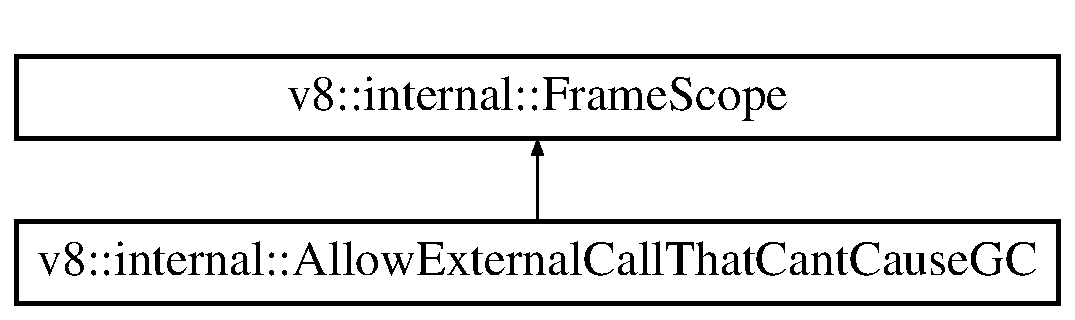
\includegraphics[height=2.000000cm]{classv8_1_1internal_1_1AllowExternalCallThatCantCauseGC}
\end{center}
\end{figure}
\subsection*{Public Member Functions}
\begin{DoxyCompactItemize}
\item 
\mbox{\Hypertarget{classv8_1_1internal_1_1AllowExternalCallThatCantCauseGC_ae136159f715f0afd4a7f76629f7bca48}\label{classv8_1_1internal_1_1AllowExternalCallThatCantCauseGC_ae136159f715f0afd4a7f76629f7bca48}} 
{\bfseries Allow\+External\+Call\+That\+Cant\+Cause\+GC} (\mbox{\hyperlink{classv8_1_1internal_1_1MacroAssembler}{Macro\+Assembler}} $\ast$masm)
\end{DoxyCompactItemize}


\subsection{Detailed Description}


Definition at line 172 of file macro-\/assembler.\+h.



The documentation for this class was generated from the following file\+:\begin{DoxyCompactItemize}
\item 
v8/src/macro-\/assembler.\+h\end{DoxyCompactItemize}

\hypertarget{classv8_1_1Isolate_1_1AllowJavascriptExecutionScope}{}\section{v8\+:\+:Isolate\+:\+:Allow\+Javascript\+Execution\+Scope Class Reference}
\label{classv8_1_1Isolate_1_1AllowJavascriptExecutionScope}\index{v8\+::\+Isolate\+::\+Allow\+Javascript\+Execution\+Scope@{v8\+::\+Isolate\+::\+Allow\+Javascript\+Execution\+Scope}}


{\ttfamily \#include $<$v8.\+h$>$}

\subsection*{Public Member Functions}
\begin{DoxyCompactItemize}
\item 
\mbox{\Hypertarget{classv8_1_1Isolate_1_1AllowJavascriptExecutionScope_ac73a647c33756c6b7c3896170e069e8c}\label{classv8_1_1Isolate_1_1AllowJavascriptExecutionScope_ac73a647c33756c6b7c3896170e069e8c}} 
{\bfseries Allow\+Javascript\+Execution\+Scope} (Isolate $\ast$isolate)
\item 
\mbox{\Hypertarget{classv8_1_1Isolate_1_1AllowJavascriptExecutionScope_a20bf639420617b08404e2bed1b203dbc}\label{classv8_1_1Isolate_1_1AllowJavascriptExecutionScope_a20bf639420617b08404e2bed1b203dbc}} 
{\bfseries Allow\+Javascript\+Execution\+Scope} (const \mbox{\hyperlink{classv8_1_1Isolate_1_1AllowJavascriptExecutionScope}{Allow\+Javascript\+Execution\+Scope}} \&)=delete
\item 
\mbox{\Hypertarget{classv8_1_1Isolate_1_1AllowJavascriptExecutionScope_a436e3fc96e3796ccfd265a153d71224a}\label{classv8_1_1Isolate_1_1AllowJavascriptExecutionScope_a436e3fc96e3796ccfd265a153d71224a}} 
\mbox{\hyperlink{classv8_1_1Isolate_1_1AllowJavascriptExecutionScope}{Allow\+Javascript\+Execution\+Scope}} \& {\bfseries operator=} (const \mbox{\hyperlink{classv8_1_1Isolate_1_1AllowJavascriptExecutionScope}{Allow\+Javascript\+Execution\+Scope}} \&)=delete
\end{DoxyCompactItemize}


\subsection{Detailed Description}
Introduce exception to \mbox{\hyperlink{classv8_1_1Isolate_1_1DisallowJavascriptExecutionScope}{Disallow\+Javascript\+Execution\+Scope}}. 

Definition at line 7251 of file v8.\+h.



The documentation for this class was generated from the following files\+:\begin{DoxyCompactItemize}
\item 
v8/include/v8.\+h\item 
v8/src/api.\+cc\end{DoxyCompactItemize}

\hypertarget{classv8_1_1internal_1_1LoadHandler_1_1AllowOutOfBoundsBits}{}\section{v8\+:\+:internal\+:\+:Load\+Handler\+:\+:Allow\+Out\+Of\+Bounds\+Bits Class Reference}
\label{classv8_1_1internal_1_1LoadHandler_1_1AllowOutOfBoundsBits}\index{v8\+::internal\+::\+Load\+Handler\+::\+Allow\+Out\+Of\+Bounds\+Bits@{v8\+::internal\+::\+Load\+Handler\+::\+Allow\+Out\+Of\+Bounds\+Bits}}
Inheritance diagram for v8\+:\+:internal\+:\+:Load\+Handler\+:\+:Allow\+Out\+Of\+Bounds\+Bits\+:\begin{figure}[H]
\begin{center}
\leavevmode
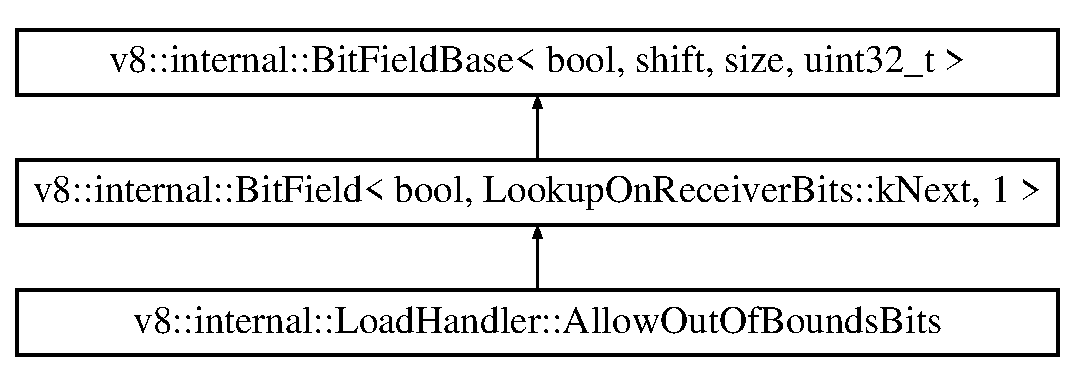
\includegraphics[height=3.000000cm]{classv8_1_1internal_1_1LoadHandler_1_1AllowOutOfBoundsBits}
\end{center}
\end{figure}
\subsection*{Additional Inherited Members}


\subsection{Detailed Description}


Definition at line 89 of file handler-\/configuration.\+h.



The documentation for this class was generated from the following file\+:\begin{DoxyCompactItemize}
\item 
v8/src/ic/handler-\/configuration.\+h\end{DoxyCompactItemize}

\hypertarget{classv8_1_1internal_1_1AllStatic}{}\section{v8\+:\+:internal\+:\+:All\+Static Class Reference}
\label{classv8_1_1internal_1_1AllStatic}\index{v8\+::internal\+::\+All\+Static@{v8\+::internal\+::\+All\+Static}}
Inheritance diagram for v8\+:\+:internal\+:\+:All\+Static\+:\begin{figure}[H]
\begin{center}
\leavevmode
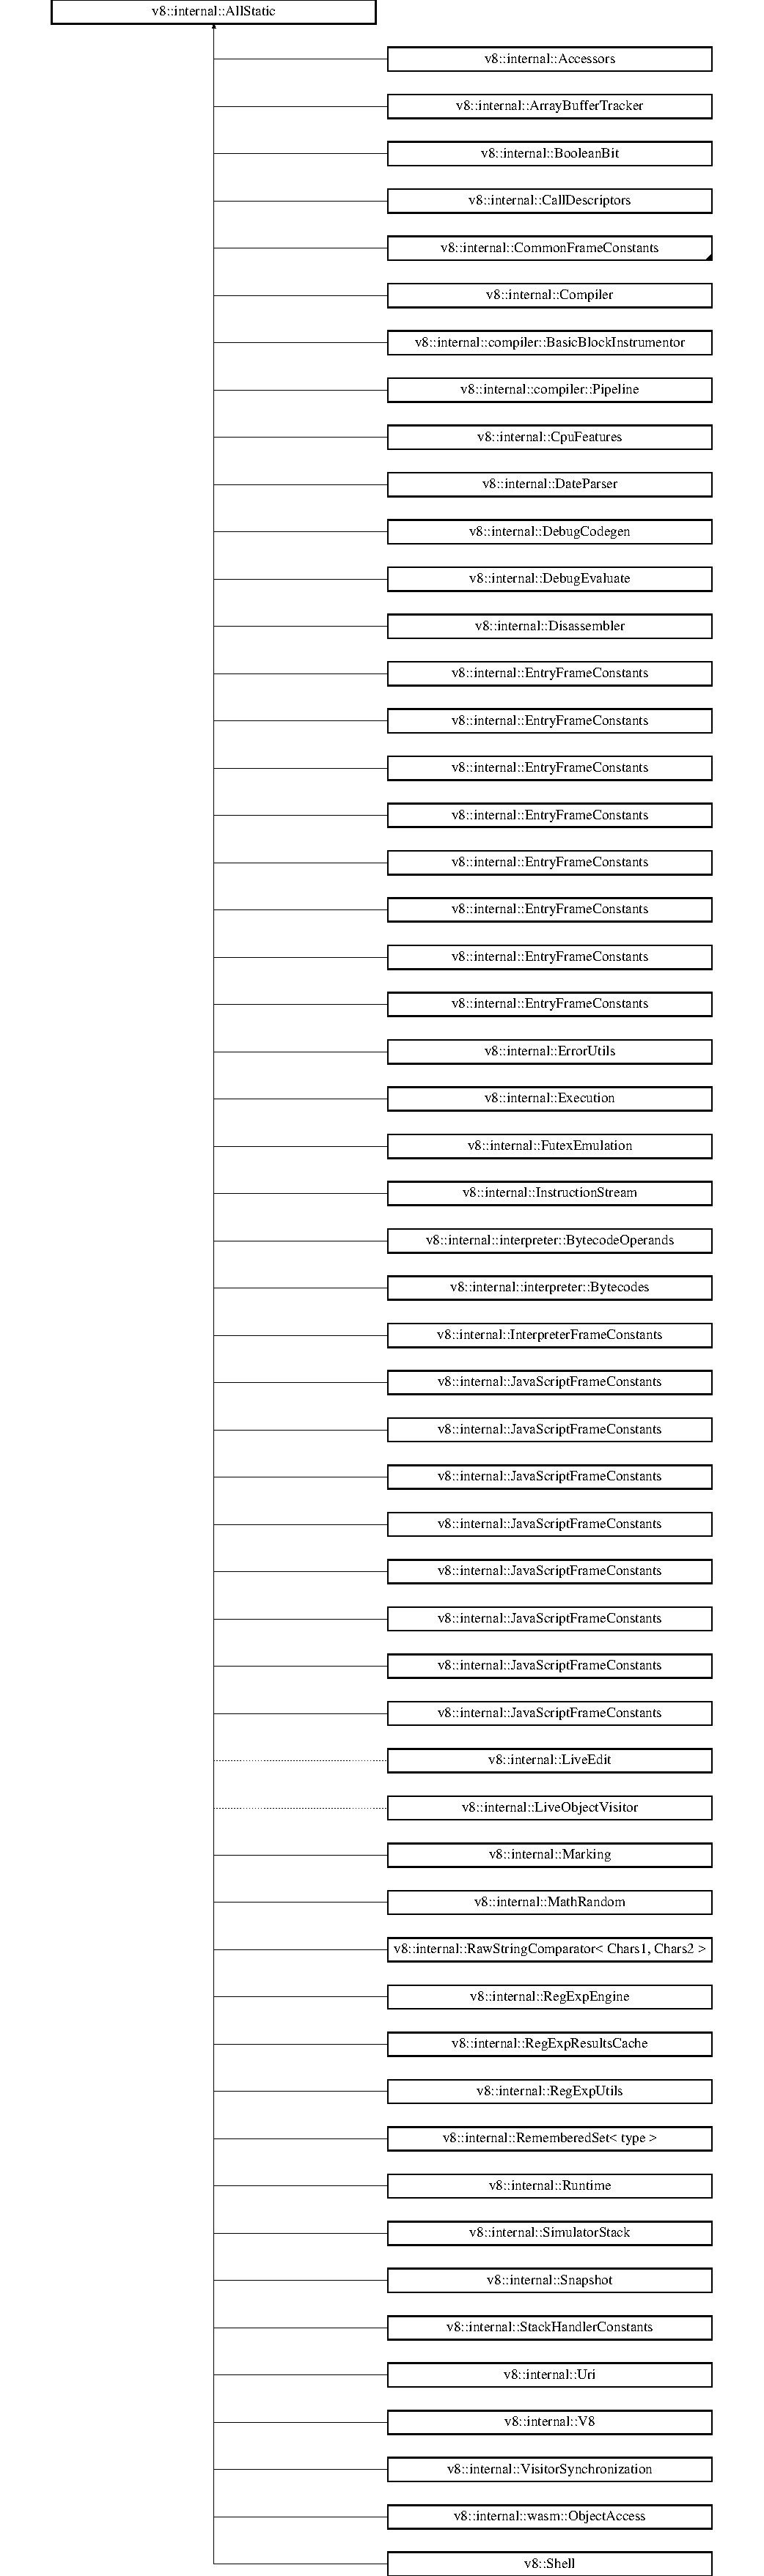
\includegraphics[height=12.000000cm]{classv8_1_1internal_1_1AllStatic}
\end{center}
\end{figure}


\subsection{Detailed Description}


Definition at line 92 of file globals.\+h.



The documentation for this class was generated from the following file\+:\begin{DoxyCompactItemize}
\item 
v8/src/globals.\+h\end{DoxyCompactItemize}

\hypertarget{classv8_1_1internal_1_1AlternativeGeneration}{}\section{v8\+:\+:internal\+:\+:Alternative\+Generation Class Reference}
\label{classv8_1_1internal_1_1AlternativeGeneration}\index{v8\+::internal\+::\+Alternative\+Generation@{v8\+::internal\+::\+Alternative\+Generation}}
Inheritance diagram for v8\+:\+:internal\+:\+:Alternative\+Generation\+:\begin{figure}[H]
\begin{center}
\leavevmode
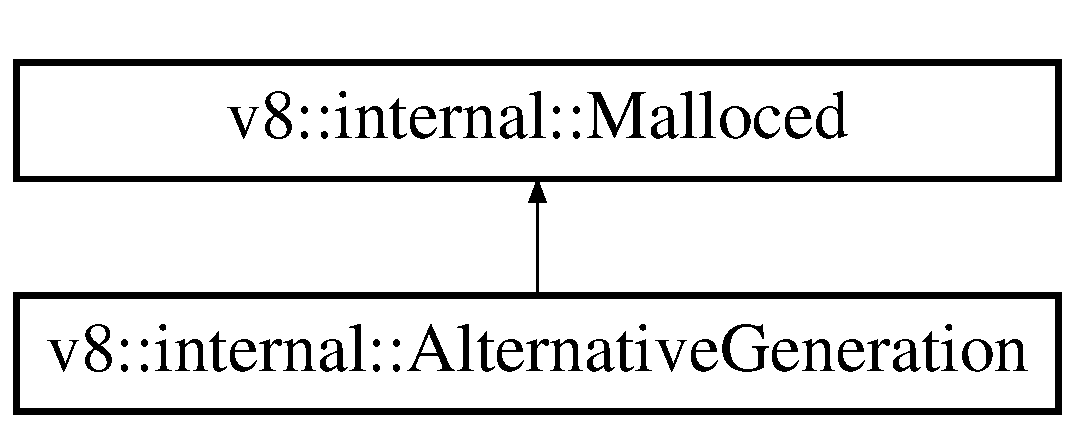
\includegraphics[height=2.000000cm]{classv8_1_1internal_1_1AlternativeGeneration}
\end{center}
\end{figure}
\subsection*{Public Attributes}
\begin{DoxyCompactItemize}
\item 
\mbox{\Hypertarget{classv8_1_1internal_1_1AlternativeGeneration_a6b2881c2cd1292cb0423fd4dab2ca823}\label{classv8_1_1internal_1_1AlternativeGeneration_a6b2881c2cd1292cb0423fd4dab2ca823}} 
\mbox{\hyperlink{classv8_1_1internal_1_1Label}{Label}} {\bfseries possible\+\_\+success}
\item 
\mbox{\Hypertarget{classv8_1_1internal_1_1AlternativeGeneration_a71eb17f16f4e5201f9f251c9fe74a507}\label{classv8_1_1internal_1_1AlternativeGeneration_a71eb17f16f4e5201f9f251c9fe74a507}} 
\mbox{\hyperlink{classbool}{bool}} {\bfseries expects\+\_\+preload}
\item 
\mbox{\Hypertarget{classv8_1_1internal_1_1AlternativeGeneration_a5640bb3e3f745d0b4705cd21ae741361}\label{classv8_1_1internal_1_1AlternativeGeneration_a5640bb3e3f745d0b4705cd21ae741361}} 
\mbox{\hyperlink{classv8_1_1internal_1_1Label}{Label}} {\bfseries after}
\item 
\mbox{\Hypertarget{classv8_1_1internal_1_1AlternativeGeneration_a727fcad75b108bd5288f5771aae86831}\label{classv8_1_1internal_1_1AlternativeGeneration_a727fcad75b108bd5288f5771aae86831}} 
\mbox{\hyperlink{classv8_1_1internal_1_1QuickCheckDetails}{Quick\+Check\+Details}} {\bfseries quick\+\_\+check\+\_\+details}
\end{DoxyCompactItemize}
\subsection*{Additional Inherited Members}


\subsection{Detailed Description}


Definition at line 3484 of file jsregexp.\+cc.



The documentation for this class was generated from the following file\+:\begin{DoxyCompactItemize}
\item 
v8/src/regexp/jsregexp.\+cc\end{DoxyCompactItemize}

\hypertarget{classv8_1_1internal_1_1AlternativeGenerationList}{}\section{v8\+:\+:internal\+:\+:Alternative\+Generation\+List Class Reference}
\label{classv8_1_1internal_1_1AlternativeGenerationList}\index{v8\+::internal\+::\+Alternative\+Generation\+List@{v8\+::internal\+::\+Alternative\+Generation\+List}}
\subsection*{Public Member Functions}
\begin{DoxyCompactItemize}
\item 
\mbox{\Hypertarget{classv8_1_1internal_1_1AlternativeGenerationList_a12e31ade267f3b97c25bf9201fe3b65a}\label{classv8_1_1internal_1_1AlternativeGenerationList_a12e31ade267f3b97c25bf9201fe3b65a}} 
{\bfseries Alternative\+Generation\+List} (\mbox{\hyperlink{classint}{int}} count, \mbox{\hyperlink{classv8_1_1internal_1_1Zone}{Zone}} $\ast$zone)
\item 
\mbox{\Hypertarget{classv8_1_1internal_1_1AlternativeGenerationList_a074eac77994a3714b4214b777fce5b2a}\label{classv8_1_1internal_1_1AlternativeGenerationList_a074eac77994a3714b4214b777fce5b2a}} 
\mbox{\hyperlink{classv8_1_1internal_1_1AlternativeGeneration}{Alternative\+Generation}} $\ast$ {\bfseries at} (\mbox{\hyperlink{classint}{int}} i)
\end{DoxyCompactItemize}


\subsection{Detailed Description}


Definition at line 3500 of file jsregexp.\+cc.



The documentation for this class was generated from the following file\+:\begin{DoxyCompactItemize}
\item 
v8/src/regexp/jsregexp.\+cc\end{DoxyCompactItemize}

\hypertarget{classv8_1_1internal_1_1AlwaysAllocateScope}{}\section{v8\+:\+:internal\+:\+:Always\+Allocate\+Scope Class Reference}
\label{classv8_1_1internal_1_1AlwaysAllocateScope}\index{v8\+::internal\+::\+Always\+Allocate\+Scope@{v8\+::internal\+::\+Always\+Allocate\+Scope}}
\subsection*{Public Member Functions}
\begin{DoxyCompactItemize}
\item 
\mbox{\Hypertarget{classv8_1_1internal_1_1AlwaysAllocateScope_a34c521892b9b7d7b65feb1c9e56bddf0}\label{classv8_1_1internal_1_1AlwaysAllocateScope_a34c521892b9b7d7b65feb1c9e56bddf0}} 
{\bfseries Always\+Allocate\+Scope} (\mbox{\hyperlink{classv8_1_1internal_1_1Isolate}{Isolate}} $\ast$isolate)
\end{DoxyCompactItemize}


\subsection{Detailed Description}


Definition at line 2113 of file heap.\+h.



The documentation for this class was generated from the following files\+:\begin{DoxyCompactItemize}
\item 
v8/src/heap/heap.\+h\item 
v8/src/heap/heap-\/inl.\+h\end{DoxyCompactItemize}

\hypertarget{classv8_1_1internal_1_1Analysis}{}\section{v8\+:\+:internal\+:\+:Analysis Class Reference}
\label{classv8_1_1internal_1_1Analysis}\index{v8\+::internal\+::\+Analysis@{v8\+::internal\+::\+Analysis}}
Inheritance diagram for v8\+:\+:internal\+:\+:Analysis\+:\begin{figure}[H]
\begin{center}
\leavevmode
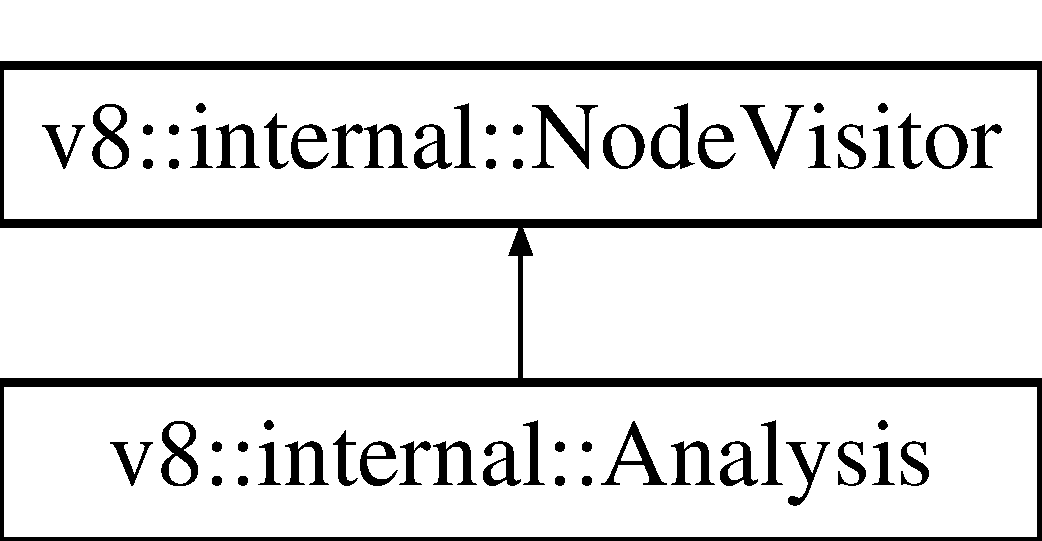
\includegraphics[height=2.000000cm]{classv8_1_1internal_1_1Analysis}
\end{center}
\end{figure}
\subsection*{Public Member Functions}
\begin{DoxyCompactItemize}
\item 
\mbox{\Hypertarget{classv8_1_1internal_1_1Analysis_a9925eeff18694fcb670f5fe76186fffe}\label{classv8_1_1internal_1_1Analysis_a9925eeff18694fcb670f5fe76186fffe}} 
{\bfseries Analysis} (\mbox{\hyperlink{classv8_1_1internal_1_1Isolate}{Isolate}} $\ast$isolate, \mbox{\hyperlink{classbool}{bool}} is\+\_\+one\+\_\+byte)
\item 
\mbox{\Hypertarget{classv8_1_1internal_1_1Analysis_a91ea9ab34a0b720e4ba0414997e6f978}\label{classv8_1_1internal_1_1Analysis_a91ea9ab34a0b720e4ba0414997e6f978}} 
void {\bfseries Ensure\+Analyzed} (\mbox{\hyperlink{classv8_1_1internal_1_1RegExpNode}{Reg\+Exp\+Node}} $\ast$node)
\item 
\mbox{\Hypertarget{classv8_1_1internal_1_1Analysis_a8d30713c3878c3320ac3bcfaeed1ecad}\label{classv8_1_1internal_1_1Analysis_a8d30713c3878c3320ac3bcfaeed1ecad}} 
void {\bfseries Visit\+Loop\+Choice} (\mbox{\hyperlink{classv8_1_1internal_1_1LoopChoiceNode}{Loop\+Choice\+Node}} $\ast$that) override
\item 
\mbox{\Hypertarget{classv8_1_1internal_1_1Analysis_a49fb801db5532a96bc0c078e3c928910}\label{classv8_1_1internal_1_1Analysis_a49fb801db5532a96bc0c078e3c928910}} 
\mbox{\hyperlink{classbool}{bool}} {\bfseries has\+\_\+failed} ()
\item 
\mbox{\Hypertarget{classv8_1_1internal_1_1Analysis_a70729ef89c68f6ba50909873d438fe47}\label{classv8_1_1internal_1_1Analysis_a70729ef89c68f6ba50909873d438fe47}} 
const \mbox{\hyperlink{classchar}{char}} $\ast$ {\bfseries error\+\_\+message} ()
\item 
\mbox{\Hypertarget{classv8_1_1internal_1_1Analysis_ae430a167d7e2e6cf98834465c537a64e}\label{classv8_1_1internal_1_1Analysis_ae430a167d7e2e6cf98834465c537a64e}} 
void {\bfseries fail} (const \mbox{\hyperlink{classchar}{char}} $\ast$error\+\_\+message)
\item 
\mbox{\Hypertarget{classv8_1_1internal_1_1Analysis_a53b9010bb43e8094791444d5f358dc36}\label{classv8_1_1internal_1_1Analysis_a53b9010bb43e8094791444d5f358dc36}} 
\mbox{\hyperlink{classv8_1_1internal_1_1Isolate}{Isolate}} $\ast$ {\bfseries isolate} () const
\end{DoxyCompactItemize}


\subsection{Detailed Description}


Definition at line 1456 of file jsregexp.\+h.



The documentation for this class was generated from the following files\+:\begin{DoxyCompactItemize}
\item 
v8/src/regexp/jsregexp.\+h\item 
v8/src/regexp/jsregexp.\+cc\end{DoxyCompactItemize}

\hypertarget{classv8_1_1internal_1_1ApiCallbackDescriptor}{}\section{v8\+:\+:internal\+:\+:Api\+Callback\+Descriptor Class Reference}
\label{classv8_1_1internal_1_1ApiCallbackDescriptor}\index{v8\+::internal\+::\+Api\+Callback\+Descriptor@{v8\+::internal\+::\+Api\+Callback\+Descriptor}}
Inheritance diagram for v8\+:\+:internal\+:\+:Api\+Callback\+Descriptor\+:\begin{figure}[H]
\begin{center}
\leavevmode
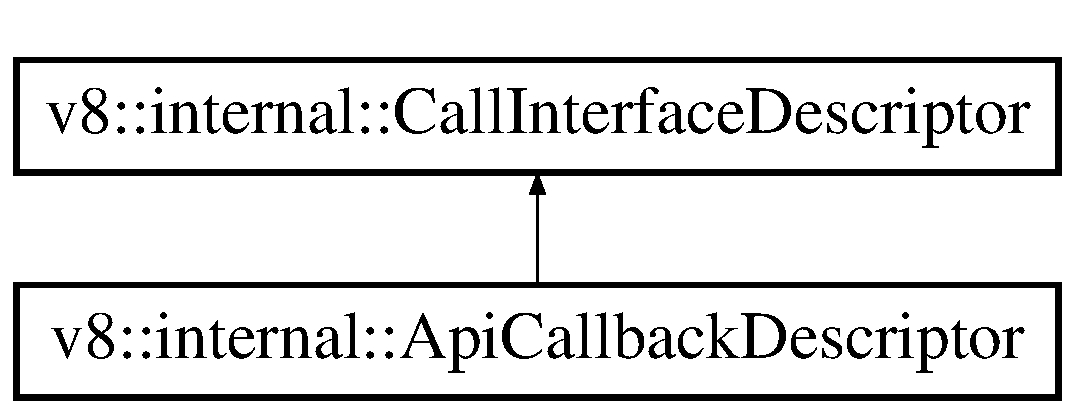
\includegraphics[height=2.000000cm]{classv8_1_1internal_1_1ApiCallbackDescriptor}
\end{center}
\end{figure}
\subsection*{Additional Inherited Members}


\subsection{Detailed Description}


Definition at line 956 of file interface-\/descriptors.\+h.



The documentation for this class was generated from the following file\+:\begin{DoxyCompactItemize}
\item 
v8/src/interface-\/descriptors.\+h\end{DoxyCompactItemize}

\hypertarget{classv8_1_1ApiFunction}{}\section{v8\+:\+:Api\+Function Class Reference}
\label{classv8_1_1ApiFunction}\index{v8\+::\+Api\+Function@{v8\+::\+Api\+Function}}
\subsection*{Public Member Functions}
\begin{DoxyCompactItemize}
\item 
\mbox{\Hypertarget{classv8_1_1ApiFunction_a711c062e7328b2cd864a755290ccc70c}\label{classv8_1_1ApiFunction_a711c062e7328b2cd864a755290ccc70c}} 
{\bfseries Api\+Function} (\mbox{\hyperlink{classuintptr__t}{v8\+::internal\+::\+Address}} addr)
\item 
\mbox{\Hypertarget{classv8_1_1ApiFunction_ae3168a2d34c3c799c4aae32a9c3bdba2}\label{classv8_1_1ApiFunction_ae3168a2d34c3c799c4aae32a9c3bdba2}} 
\mbox{\hyperlink{classuintptr__t}{v8\+::internal\+::\+Address}} {\bfseries address} ()
\end{DoxyCompactItemize}


\subsection{Detailed Description}


Definition at line 53 of file api.\+h.



The documentation for this class was generated from the following file\+:\begin{DoxyCompactItemize}
\item 
v8/src/api.\+h\end{DoxyCompactItemize}

\hypertarget{classv8_1_1internal_1_1ApiGetterDescriptor}{}\section{v8\+:\+:internal\+:\+:Api\+Getter\+Descriptor Class Reference}
\label{classv8_1_1internal_1_1ApiGetterDescriptor}\index{v8\+::internal\+::\+Api\+Getter\+Descriptor@{v8\+::internal\+::\+Api\+Getter\+Descriptor}}
Inheritance diagram for v8\+:\+:internal\+:\+:Api\+Getter\+Descriptor\+:\begin{figure}[H]
\begin{center}
\leavevmode
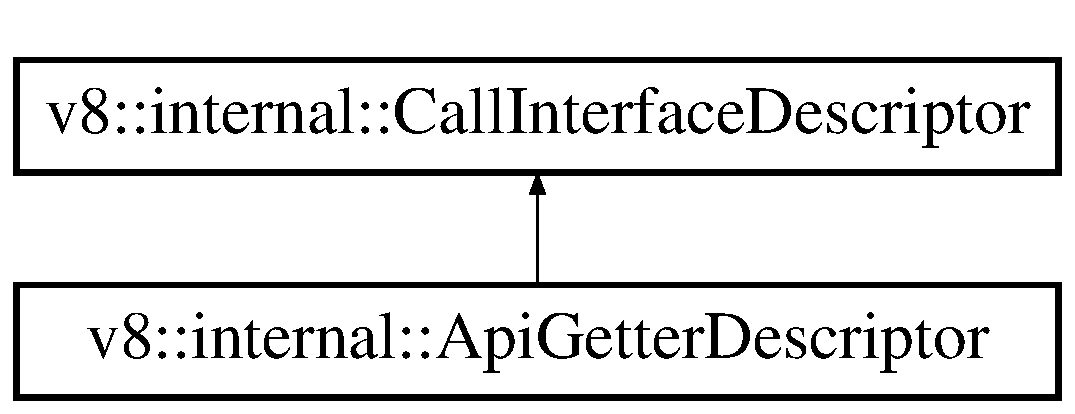
\includegraphics[height=2.000000cm]{classv8_1_1internal_1_1ApiGetterDescriptor}
\end{center}
\end{figure}
\subsection*{Public Member Functions}
\begin{DoxyCompactItemize}
\item 
\mbox{\Hypertarget{classv8_1_1internal_1_1ApiGetterDescriptor_ae461b846579b9b7371ec3172871acedd}\label{classv8_1_1internal_1_1ApiGetterDescriptor_ae461b846579b9b7371ec3172871acedd}} 
{\bfseries D\+E\+F\+I\+N\+E\+\_\+\+P\+A\+R\+A\+M\+E\+T\+E\+R\+\_\+\+T\+Y\+P\+ES} (Machine\+Type\+::\+Any\+Tagged(), Machine\+Type\+::\+Any\+Tagged(), Machine\+Type\+::\+Any\+Tagged()) static const \mbox{\hyperlink{classv8_1_1internal_1_1Register}{Register}} Receiver\+Register()
\end{DoxyCompactItemize}
\subsection*{Static Public Member Functions}
\begin{DoxyCompactItemize}
\item 
\mbox{\Hypertarget{classv8_1_1internal_1_1ApiGetterDescriptor_a3a2ad818edc83502718c466b5dad01b5}\label{classv8_1_1internal_1_1ApiGetterDescriptor_a3a2ad818edc83502718c466b5dad01b5}} 
static const \mbox{\hyperlink{classv8_1_1internal_1_1Register}{Register}} {\bfseries Holder\+Register} ()
\item 
\mbox{\Hypertarget{classv8_1_1internal_1_1ApiGetterDescriptor_a1289ae62e1bf71022cdedd9d84ca1082}\label{classv8_1_1internal_1_1ApiGetterDescriptor_a1289ae62e1bf71022cdedd9d84ca1082}} 
static const \mbox{\hyperlink{classv8_1_1internal_1_1Register}{Register}} {\bfseries Callback\+Register} ()
\end{DoxyCompactItemize}
\subsection*{Additional Inherited Members}


\subsection{Detailed Description}


Definition at line 970 of file interface-\/descriptors.\+h.



The documentation for this class was generated from the following file\+:\begin{DoxyCompactItemize}
\item 
v8/src/interface-\/descriptors.\+h\end{DoxyCompactItemize}

\hypertarget{classv8_1_1internal_1_1ApiNatives}{}\section{v8\+:\+:internal\+:\+:Api\+Natives Class Reference}
\label{classv8_1_1internal_1_1ApiNatives}\index{v8\+::internal\+::\+Api\+Natives@{v8\+::internal\+::\+Api\+Natives}}
\subsection*{Static Public Member Functions}
\begin{DoxyCompactItemize}
\item 
\mbox{\Hypertarget{classv8_1_1internal_1_1ApiNatives_ae308122811addb9431d6d7801427f528}\label{classv8_1_1internal_1_1ApiNatives_ae308122811addb9431d6d7801427f528}} 
static V8\+\_\+\+W\+A\+R\+N\+\_\+\+U\+N\+U\+S\+E\+D\+\_\+\+R\+E\+S\+U\+LT \mbox{\hyperlink{classv8_1_1internal_1_1MaybeHandle}{Maybe\+Handle}}$<$ \mbox{\hyperlink{classv8_1_1internal_1_1JSFunction}{J\+S\+Function}} $>$ {\bfseries Instantiate\+Function} (\mbox{\hyperlink{classv8_1_1internal_1_1Handle}{Handle}}$<$ \mbox{\hyperlink{classv8_1_1internal_1_1FunctionTemplateInfo}{Function\+Template\+Info}} $>$ data, \mbox{\hyperlink{classv8_1_1internal_1_1MaybeHandle}{Maybe\+Handle}}$<$ \mbox{\hyperlink{classv8_1_1internal_1_1Name}{Name}} $>$ maybe\+\_\+name=\mbox{\hyperlink{classv8_1_1internal_1_1MaybeHandle}{Maybe\+Handle}}$<$ \mbox{\hyperlink{classv8_1_1internal_1_1Name}{Name}} $>$())
\item 
\mbox{\Hypertarget{classv8_1_1internal_1_1ApiNatives_a30519b52bb2d007bc9653989b7764b3c}\label{classv8_1_1internal_1_1ApiNatives_a30519b52bb2d007bc9653989b7764b3c}} 
static V8\+\_\+\+W\+A\+R\+N\+\_\+\+U\+N\+U\+S\+E\+D\+\_\+\+R\+E\+S\+U\+LT \mbox{\hyperlink{classv8_1_1internal_1_1MaybeHandle}{Maybe\+Handle}}$<$ \mbox{\hyperlink{classv8_1_1internal_1_1JSObject}{J\+S\+Object}} $>$ {\bfseries Instantiate\+Object} (\mbox{\hyperlink{classv8_1_1internal_1_1Isolate}{Isolate}} $\ast$isolate, \mbox{\hyperlink{classv8_1_1internal_1_1Handle}{Handle}}$<$ \mbox{\hyperlink{classv8_1_1internal_1_1ObjectTemplateInfo}{Object\+Template\+Info}} $>$ data, \mbox{\hyperlink{classv8_1_1internal_1_1Handle}{Handle}}$<$ \mbox{\hyperlink{classv8_1_1internal_1_1JSReceiver}{J\+S\+Receiver}} $>$ new\+\_\+target=\mbox{\hyperlink{classv8_1_1internal_1_1Handle}{Handle}}$<$ \mbox{\hyperlink{classv8_1_1internal_1_1JSReceiver}{J\+S\+Receiver}} $>$())
\item 
\mbox{\Hypertarget{classv8_1_1internal_1_1ApiNatives_aef7124e0d28a1bb03847d4253e3abab1}\label{classv8_1_1internal_1_1ApiNatives_aef7124e0d28a1bb03847d4253e3abab1}} 
static V8\+\_\+\+W\+A\+R\+N\+\_\+\+U\+N\+U\+S\+E\+D\+\_\+\+R\+E\+S\+U\+LT \mbox{\hyperlink{classv8_1_1internal_1_1MaybeHandle}{Maybe\+Handle}}$<$ \mbox{\hyperlink{classv8_1_1internal_1_1JSObject}{J\+S\+Object}} $>$ {\bfseries Instantiate\+Remote\+Object} (\mbox{\hyperlink{classv8_1_1internal_1_1Handle}{Handle}}$<$ \mbox{\hyperlink{classv8_1_1internal_1_1ObjectTemplateInfo}{Object\+Template\+Info}} $>$ data)
\item 
\mbox{\Hypertarget{classv8_1_1internal_1_1ApiNatives_ab3d620dee0e793907e077bd8731d58ba}\label{classv8_1_1internal_1_1ApiNatives_ab3d620dee0e793907e077bd8731d58ba}} 
static \mbox{\hyperlink{classv8_1_1internal_1_1Handle}{Handle}}$<$ \mbox{\hyperlink{classv8_1_1internal_1_1JSFunction}{J\+S\+Function}} $>$ {\bfseries Create\+Api\+Function} (\mbox{\hyperlink{classv8_1_1internal_1_1Isolate}{Isolate}} $\ast$isolate, \mbox{\hyperlink{classv8_1_1internal_1_1Handle}{Handle}}$<$ \mbox{\hyperlink{classv8_1_1internal_1_1FunctionTemplateInfo}{Function\+Template\+Info}} $>$ obj, \mbox{\hyperlink{classv8_1_1internal_1_1Handle}{Handle}}$<$ \mbox{\hyperlink{classv8_1_1internal_1_1Object}{Object}} $>$ prototype, Instance\+Type \mbox{\hyperlink{classstd_1_1conditional_1_1type}{type}}, \mbox{\hyperlink{classv8_1_1internal_1_1MaybeHandle}{Maybe\+Handle}}$<$ \mbox{\hyperlink{classv8_1_1internal_1_1Name}{Name}} $>$ name=\mbox{\hyperlink{classv8_1_1internal_1_1MaybeHandle}{Maybe\+Handle}}$<$ \mbox{\hyperlink{classv8_1_1internal_1_1Name}{Name}} $>$())
\item 
\mbox{\Hypertarget{classv8_1_1internal_1_1ApiNatives_ae3ee4ad0fcbf129bbdc461d1bb3efa1a}\label{classv8_1_1internal_1_1ApiNatives_ae3ee4ad0fcbf129bbdc461d1bb3efa1a}} 
static void {\bfseries Add\+Data\+Property} (\mbox{\hyperlink{classv8_1_1internal_1_1Isolate}{Isolate}} $\ast$isolate, \mbox{\hyperlink{classv8_1_1internal_1_1Handle}{Handle}}$<$ \mbox{\hyperlink{classv8_1_1internal_1_1TemplateInfo}{Template\+Info}} $>$ info, \mbox{\hyperlink{classv8_1_1internal_1_1Handle}{Handle}}$<$ \mbox{\hyperlink{classv8_1_1internal_1_1Name}{Name}} $>$ name, \mbox{\hyperlink{classv8_1_1internal_1_1Handle}{Handle}}$<$ \mbox{\hyperlink{classv8_1_1internal_1_1Object}{Object}} $>$ value, Property\+Attributes attributes)
\item 
\mbox{\Hypertarget{classv8_1_1internal_1_1ApiNatives_a00f025df8155d3f3aa5949422109f23e}\label{classv8_1_1internal_1_1ApiNatives_a00f025df8155d3f3aa5949422109f23e}} 
static void {\bfseries Add\+Data\+Property} (\mbox{\hyperlink{classv8_1_1internal_1_1Isolate}{Isolate}} $\ast$isolate, \mbox{\hyperlink{classv8_1_1internal_1_1Handle}{Handle}}$<$ \mbox{\hyperlink{classv8_1_1internal_1_1TemplateInfo}{Template\+Info}} $>$ info, \mbox{\hyperlink{classv8_1_1internal_1_1Handle}{Handle}}$<$ \mbox{\hyperlink{classv8_1_1internal_1_1Name}{Name}} $>$ name, v8\+::\+Intrinsic intrinsic, Property\+Attributes attributes)
\item 
\mbox{\Hypertarget{classv8_1_1internal_1_1ApiNatives_a6934eedf60bf86e845fd9f483839191c}\label{classv8_1_1internal_1_1ApiNatives_a6934eedf60bf86e845fd9f483839191c}} 
static void {\bfseries Add\+Accessor\+Property} (\mbox{\hyperlink{classv8_1_1internal_1_1Isolate}{Isolate}} $\ast$isolate, \mbox{\hyperlink{classv8_1_1internal_1_1Handle}{Handle}}$<$ \mbox{\hyperlink{classv8_1_1internal_1_1TemplateInfo}{Template\+Info}} $>$ info, \mbox{\hyperlink{classv8_1_1internal_1_1Handle}{Handle}}$<$ \mbox{\hyperlink{classv8_1_1internal_1_1Name}{Name}} $>$ name, \mbox{\hyperlink{classv8_1_1internal_1_1Handle}{Handle}}$<$ \mbox{\hyperlink{classv8_1_1internal_1_1FunctionTemplateInfo}{Function\+Template\+Info}} $>$ getter, \mbox{\hyperlink{classv8_1_1internal_1_1Handle}{Handle}}$<$ \mbox{\hyperlink{classv8_1_1internal_1_1FunctionTemplateInfo}{Function\+Template\+Info}} $>$ setter, Property\+Attributes attributes)
\item 
\mbox{\Hypertarget{classv8_1_1internal_1_1ApiNatives_aa3f534fe84b42a099d7af3d7dae423c5}\label{classv8_1_1internal_1_1ApiNatives_aa3f534fe84b42a099d7af3d7dae423c5}} 
static void {\bfseries Add\+Native\+Data\+Property} (\mbox{\hyperlink{classv8_1_1internal_1_1Isolate}{Isolate}} $\ast$isolate, \mbox{\hyperlink{classv8_1_1internal_1_1Handle}{Handle}}$<$ \mbox{\hyperlink{classv8_1_1internal_1_1TemplateInfo}{Template\+Info}} $>$ info, \mbox{\hyperlink{classv8_1_1internal_1_1Handle}{Handle}}$<$ \mbox{\hyperlink{classv8_1_1internal_1_1AccessorInfo}{Accessor\+Info}} $>$ property)
\end{DoxyCompactItemize}
\subsection*{Static Public Attributes}
\begin{DoxyCompactItemize}
\item 
\mbox{\Hypertarget{classv8_1_1internal_1_1ApiNatives_aca69c9efcc2949a8eb362d0fe599b4b9}\label{classv8_1_1internal_1_1ApiNatives_aca69c9efcc2949a8eb362d0fe599b4b9}} 
static const \mbox{\hyperlink{classint}{int}} {\bfseries k\+Initial\+Function\+Cache\+Size} = 256
\end{DoxyCompactItemize}


\subsection{Detailed Description}


Definition at line 23 of file api-\/natives.\+h.



The documentation for this class was generated from the following files\+:\begin{DoxyCompactItemize}
\item 
v8/src/api-\/natives.\+h\item 
v8/src/api-\/natives.\+cc\end{DoxyCompactItemize}

\hypertarget{classv8_1_1internal_1_1Arguments}{}\section{v8\+:\+:internal\+:\+:Arguments Class Reference}
\label{classv8_1_1internal_1_1Arguments}\index{v8\+::internal\+::\+Arguments@{v8\+::internal\+::\+Arguments}}
Inheritance diagram for v8\+:\+:internal\+:\+:Arguments\+:\begin{figure}[H]
\begin{center}
\leavevmode
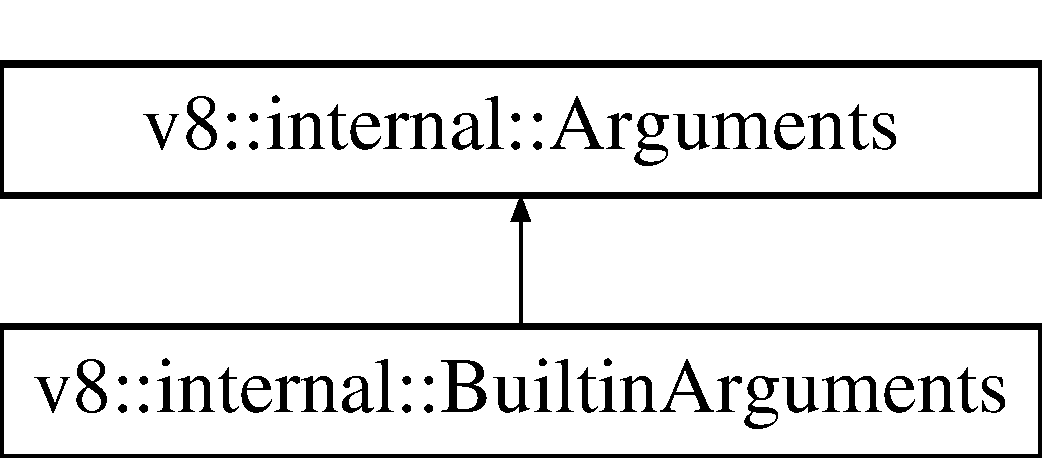
\includegraphics[height=2.000000cm]{classv8_1_1internal_1_1Arguments}
\end{center}
\end{figure}
\subsection*{Public Member Functions}
\begin{DoxyCompactItemize}
\item 
\mbox{\Hypertarget{classv8_1_1internal_1_1Arguments_afd792a8cef14818fbab9a2669c8a352f}\label{classv8_1_1internal_1_1Arguments_afd792a8cef14818fbab9a2669c8a352f}} 
{\bfseries Arguments} (\mbox{\hyperlink{classint}{int}} length, \mbox{\hyperlink{classuintptr__t}{Address}} $\ast$arguments)
\item 
\mbox{\Hypertarget{classv8_1_1internal_1_1Arguments_aae1276e1d4b4e5aa8faf9c6010eece55}\label{classv8_1_1internal_1_1Arguments_aae1276e1d4b4e5aa8faf9c6010eece55}} 
\mbox{\hyperlink{classv8_1_1internal_1_1ObjectPtr}{Object\+Ptr}} {\bfseries operator\mbox{[}$\,$\mbox{]}} (\mbox{\hyperlink{classint}{int}} index)
\item 
\mbox{\Hypertarget{classv8_1_1internal_1_1Arguments_a81003341598143fe1535013c71972efe}\label{classv8_1_1internal_1_1Arguments_a81003341598143fe1535013c71972efe}} 
{\footnotesize template$<$class S  = Object$>$ }\\\mbox{\hyperlink{classv8_1_1internal_1_1Handle}{Handle}}$<$ S $>$ {\bfseries at} (\mbox{\hyperlink{classint}{int}} index)
\item 
\mbox{\Hypertarget{classv8_1_1internal_1_1Arguments_a5210f7a565dbf6cfa5d26e55cadfdfcc}\label{classv8_1_1internal_1_1Arguments_a5210f7a565dbf6cfa5d26e55cadfdfcc}} 
\mbox{\hyperlink{classint}{int}} {\bfseries smi\+\_\+at} (\mbox{\hyperlink{classint}{int}} index)
\item 
\mbox{\Hypertarget{classv8_1_1internal_1_1Arguments_a55b1dc6a866b71a79d272d49f22baad5}\label{classv8_1_1internal_1_1Arguments_a55b1dc6a866b71a79d272d49f22baad5}} 
double {\bfseries number\+\_\+at} (\mbox{\hyperlink{classint}{int}} index)
\item 
\mbox{\Hypertarget{classv8_1_1internal_1_1Arguments_a5f9c94a724a33d667c8ce4e6f14829a8}\label{classv8_1_1internal_1_1Arguments_a5f9c94a724a33d667c8ce4e6f14829a8}} 
void {\bfseries set\+\_\+at} (\mbox{\hyperlink{classint}{int}} index, \mbox{\hyperlink{classv8_1_1internal_1_1Object}{Object}} $\ast$value)
\item 
\mbox{\Hypertarget{classv8_1_1internal_1_1Arguments_a8dee5a2127bea6bd88a816e2556ab914}\label{classv8_1_1internal_1_1Arguments_a8dee5a2127bea6bd88a816e2556ab914}} 
\mbox{\hyperlink{classv8_1_1internal_1_1ObjectSlot}{Object\+Slot}} {\bfseries slot\+\_\+at} (\mbox{\hyperlink{classint}{int}} index)
\item 
\mbox{\Hypertarget{classv8_1_1internal_1_1Arguments_a8e8adf2d479cbf1636f63bbf24037535}\label{classv8_1_1internal_1_1Arguments_a8e8adf2d479cbf1636f63bbf24037535}} 
\mbox{\hyperlink{classuintptr__t}{Address}} $\ast$ {\bfseries address\+\_\+of\+\_\+arg\+\_\+at} (\mbox{\hyperlink{classint}{int}} index)
\item 
\mbox{\Hypertarget{classv8_1_1internal_1_1Arguments_aca0d27558d0fddd78eeda48ec8abfd42}\label{classv8_1_1internal_1_1Arguments_aca0d27558d0fddd78eeda48ec8abfd42}} 
\mbox{\hyperlink{classint}{int}} {\bfseries length} () const
\item 
\mbox{\Hypertarget{classv8_1_1internal_1_1Arguments_ab570c3546cb58c32563f03f7af580c37}\label{classv8_1_1internal_1_1Arguments_ab570c3546cb58c32563f03f7af580c37}} 
\mbox{\hyperlink{classv8_1_1internal_1_1ObjectSlot}{Object\+Slot}} {\bfseries first\+\_\+slot} ()
\item 
\mbox{\Hypertarget{classv8_1_1internal_1_1Arguments_ae1849cbf2c441182450acb23f1fadef4}\label{classv8_1_1internal_1_1Arguments_ae1849cbf2c441182450acb23f1fadef4}} 
\mbox{\hyperlink{classv8_1_1internal_1_1ObjectSlot}{Object\+Slot}} {\bfseries last\+\_\+slot} ()
\item 
\mbox{\Hypertarget{classv8_1_1internal_1_1Arguments_ad5e78fde706fd1a7efb7973240292f41}\label{classv8_1_1internal_1_1Arguments_ad5e78fde706fd1a7efb7973240292f41}} 
{\footnotesize template$<$$>$ }\\\mbox{\hyperlink{classv8_1_1internal_1_1Handle}{Handle}}$<$ \mbox{\hyperlink{classv8_1_1internal_1_1Object}{Object}} $>$ {\bfseries at} (\mbox{\hyperlink{classint}{int}} index)
\end{DoxyCompactItemize}


\subsection{Detailed Description}


Definition at line 32 of file arguments.\+h.



The documentation for this class was generated from the following files\+:\begin{DoxyCompactItemize}
\item 
v8/src/arguments.\+h\item 
v8/src/arguments-\/inl.\+h\end{DoxyCompactItemize}

\hypertarget{structv8_1_1internal_1_1torque_1_1Arguments}{}\section{v8\+:\+:internal\+:\+:torque\+:\+:Arguments Struct Reference}
\label{structv8_1_1internal_1_1torque_1_1Arguments}\index{v8\+::internal\+::torque\+::\+Arguments@{v8\+::internal\+::torque\+::\+Arguments}}
\subsection*{Public Attributes}
\begin{DoxyCompactItemize}
\item 
\mbox{\Hypertarget{structv8_1_1internal_1_1torque_1_1Arguments_a97908a9a6a473ef92d55ff02e803c4ee}\label{structv8_1_1internal_1_1torque_1_1Arguments_a97908a9a6a473ef92d55ff02e803c4ee}} 
\mbox{\hyperlink{classv8_1_1internal_1_1torque_1_1VisitResultVector}{Visit\+Result\+Vector}} {\bfseries parameters}
\item 
\mbox{\Hypertarget{structv8_1_1internal_1_1torque_1_1Arguments_af47d48972f6b027ff46fbbe36bb4a4bf}\label{structv8_1_1internal_1_1torque_1_1Arguments_af47d48972f6b027ff46fbbe36bb4a4bf}} 
std\+::vector$<$ \mbox{\hyperlink{classv8_1_1internal_1_1torque_1_1Binding}{Binding}}$<$ \mbox{\hyperlink{structv8_1_1internal_1_1torque_1_1LocalLabel}{Local\+Label}} $>$ $\ast$ $>$ {\bfseries labels}
\end{DoxyCompactItemize}


\subsection{Detailed Description}


Definition at line 192 of file implementation-\/visitor.\+h.



The documentation for this struct was generated from the following file\+:\begin{DoxyCompactItemize}
\item 
v8/src/torque/implementation-\/visitor.\+h\end{DoxyCompactItemize}

\hypertarget{classv8_1_1internal_1_1ArgumentsAdaptorDescriptor}{}\section{v8\+:\+:internal\+:\+:Arguments\+Adaptor\+Descriptor Class Reference}
\label{classv8_1_1internal_1_1ArgumentsAdaptorDescriptor}\index{v8\+::internal\+::\+Arguments\+Adaptor\+Descriptor@{v8\+::internal\+::\+Arguments\+Adaptor\+Descriptor}}
Inheritance diagram for v8\+:\+:internal\+:\+:Arguments\+Adaptor\+Descriptor\+:\begin{figure}[H]
\begin{center}
\leavevmode
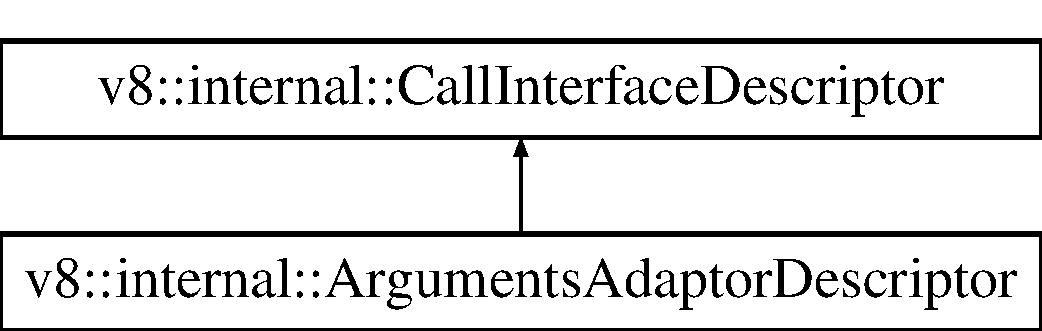
\includegraphics[height=2.000000cm]{classv8_1_1internal_1_1ArgumentsAdaptorDescriptor}
\end{center}
\end{figure}
\subsection*{Additional Inherited Members}


\subsection{Detailed Description}


Definition at line 924 of file interface-\/descriptors.\+h.



The documentation for this class was generated from the following file\+:\begin{DoxyCompactItemize}
\item 
v8/src/interface-\/descriptors.\+h\end{DoxyCompactItemize}

\hypertarget{classv8_1_1internal_1_1ArgumentsAdaptorFrame}{}\section{v8\+:\+:internal\+:\+:Arguments\+Adaptor\+Frame Class Reference}
\label{classv8_1_1internal_1_1ArgumentsAdaptorFrame}\index{v8\+::internal\+::\+Arguments\+Adaptor\+Frame@{v8\+::internal\+::\+Arguments\+Adaptor\+Frame}}
Inheritance diagram for v8\+:\+:internal\+:\+:Arguments\+Adaptor\+Frame\+:\begin{figure}[H]
\begin{center}
\leavevmode
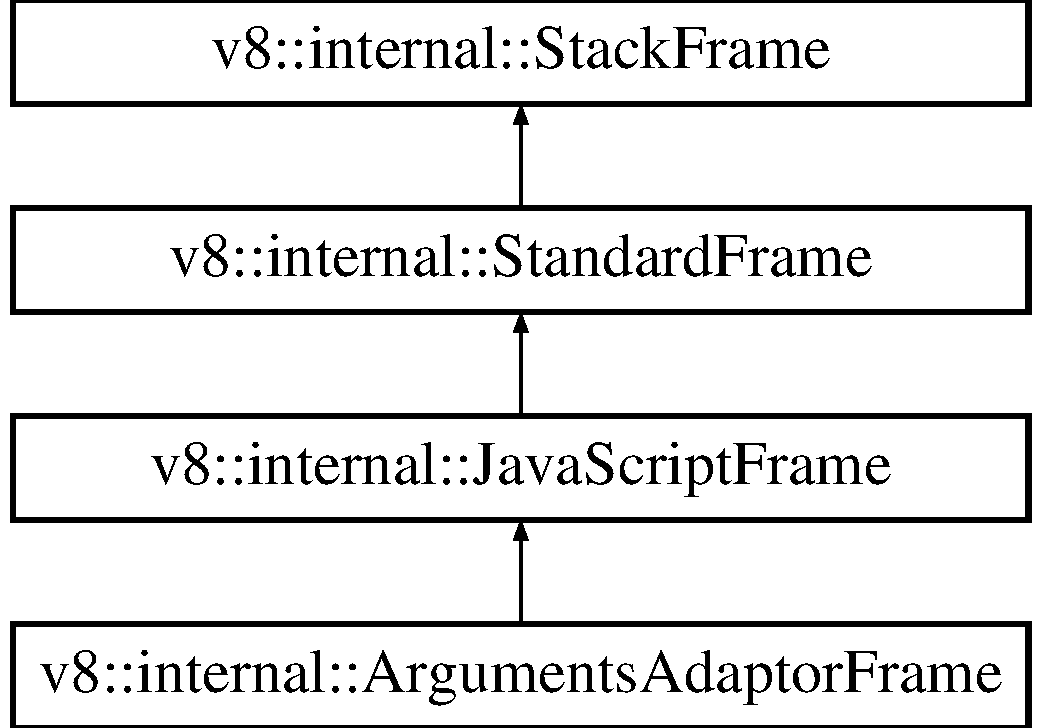
\includegraphics[height=4.000000cm]{classv8_1_1internal_1_1ArgumentsAdaptorFrame}
\end{center}
\end{figure}
\subsection*{Public Member Functions}
\begin{DoxyCompactItemize}
\item 
\mbox{\Hypertarget{classv8_1_1internal_1_1ArgumentsAdaptorFrame_aa4b71339840c7570df68929992ec9442}\label{classv8_1_1internal_1_1ArgumentsAdaptorFrame_aa4b71339840c7570df68929992ec9442}} 
Type {\bfseries type} () const override
\item 
\mbox{\Hypertarget{classv8_1_1internal_1_1ArgumentsAdaptorFrame_a232f413f2394c98c7b7bda04987434f9}\label{classv8_1_1internal_1_1ArgumentsAdaptorFrame_a232f413f2394c98c7b7bda04987434f9}} 
\mbox{\hyperlink{classv8_1_1internal_1_1Code}{Code}} {\bfseries unchecked\+\_\+code} () const override
\item 
\mbox{\Hypertarget{classv8_1_1internal_1_1ArgumentsAdaptorFrame_a39192f87d3e21f3bafb85c8a610b54aa}\label{classv8_1_1internal_1_1ArgumentsAdaptorFrame_a39192f87d3e21f3bafb85c8a610b54aa}} 
void {\bfseries Print} (\mbox{\hyperlink{classv8_1_1internal_1_1StringStream}{String\+Stream}} $\ast$accumulator, Print\+Mode mode, \mbox{\hyperlink{classint}{int}} index) const override
\end{DoxyCompactItemize}
\subsection*{Static Public Member Functions}
\begin{DoxyCompactItemize}
\item 
\mbox{\Hypertarget{classv8_1_1internal_1_1ArgumentsAdaptorFrame_a6b8283fe3991c88663621fdf586b67ca}\label{classv8_1_1internal_1_1ArgumentsAdaptorFrame_a6b8283fe3991c88663621fdf586b67ca}} 
static \mbox{\hyperlink{classv8_1_1internal_1_1ArgumentsAdaptorFrame}{Arguments\+Adaptor\+Frame}} $\ast$ {\bfseries cast} (\mbox{\hyperlink{classv8_1_1internal_1_1StackFrame}{Stack\+Frame}} $\ast$frame)
\end{DoxyCompactItemize}
\subsection*{Protected Member Functions}
\begin{DoxyCompactItemize}
\item 
\mbox{\Hypertarget{classv8_1_1internal_1_1ArgumentsAdaptorFrame_ac2681526413000e2f5879bc2c0b0fd2f}\label{classv8_1_1internal_1_1ArgumentsAdaptorFrame_ac2681526413000e2f5879bc2c0b0fd2f}} 
{\bfseries Arguments\+Adaptor\+Frame} (\mbox{\hyperlink{classv8_1_1internal_1_1StackFrameIteratorBase}{Stack\+Frame\+Iterator\+Base}} $\ast$iterator)
\item 
\mbox{\Hypertarget{classv8_1_1internal_1_1ArgumentsAdaptorFrame_a4e9a7abe3bd4836a80cd691e91f92aaf}\label{classv8_1_1internal_1_1ArgumentsAdaptorFrame_a4e9a7abe3bd4836a80cd691e91f92aaf}} 
\mbox{\hyperlink{classint}{int}} {\bfseries Get\+Number\+Of\+Incoming\+Arguments} () const override
\end{DoxyCompactItemize}
\subsection*{Friends}
\begin{DoxyCompactItemize}
\item 
\mbox{\Hypertarget{classv8_1_1internal_1_1ArgumentsAdaptorFrame_ac7310421866976ca454bbe11c5f926c3}\label{classv8_1_1internal_1_1ArgumentsAdaptorFrame_ac7310421866976ca454bbe11c5f926c3}} 
class {\bfseries Stack\+Frame\+Iterator\+Base}
\end{DoxyCompactItemize}
\subsection*{Additional Inherited Members}


\subsection{Detailed Description}


Definition at line 884 of file frames.\+h.



The documentation for this class was generated from the following files\+:\begin{DoxyCompactItemize}
\item 
v8/src/frames.\+h\item 
v8/src/frames-\/inl.\+h\item 
v8/src/frames.\+cc\end{DoxyCompactItemize}

\hypertarget{classv8_1_1internal_1_1ArgumentsAdaptorFrameConstants}{}\section{v8\+:\+:internal\+:\+:Arguments\+Adaptor\+Frame\+Constants Class Reference}
\label{classv8_1_1internal_1_1ArgumentsAdaptorFrameConstants}\index{v8\+::internal\+::\+Arguments\+Adaptor\+Frame\+Constants@{v8\+::internal\+::\+Arguments\+Adaptor\+Frame\+Constants}}
Inheritance diagram for v8\+:\+:internal\+:\+:Arguments\+Adaptor\+Frame\+Constants\+:\begin{figure}[H]
\begin{center}
\leavevmode
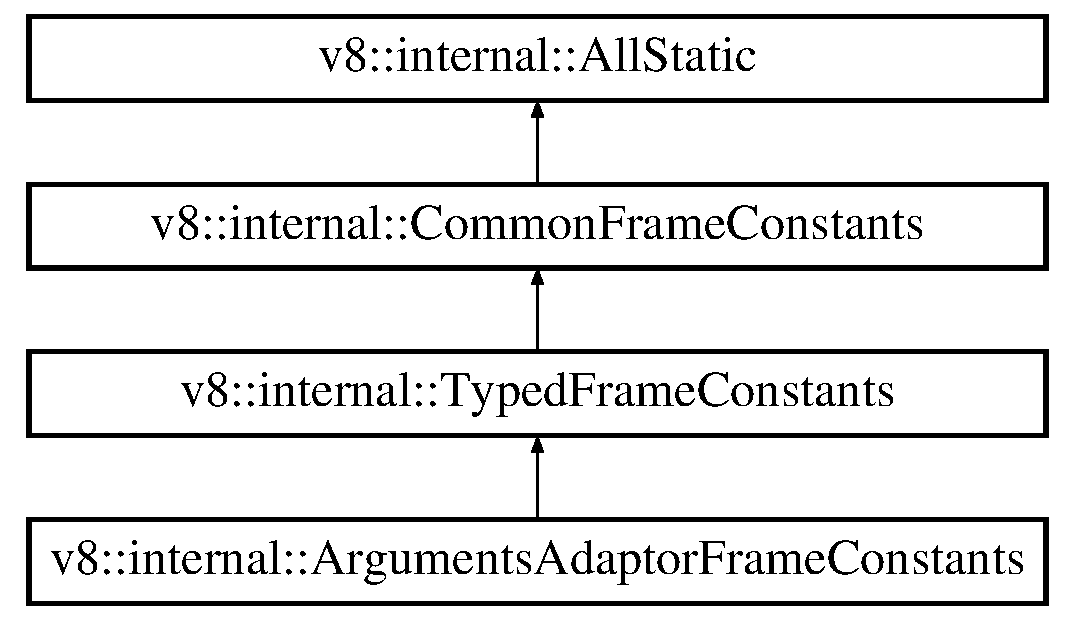
\includegraphics[height=4.000000cm]{classv8_1_1internal_1_1ArgumentsAdaptorFrameConstants}
\end{center}
\end{figure}
\subsection*{Public Member Functions}
\begin{DoxyCompactItemize}
\item 
\mbox{\Hypertarget{classv8_1_1internal_1_1ArgumentsAdaptorFrameConstants_ad690c1d380dc2dafc37997f8871f97da}\label{classv8_1_1internal_1_1ArgumentsAdaptorFrameConstants_ad690c1d380dc2dafc37997f8871f97da}} 
{\bfseries D\+E\+F\+I\+N\+E\+\_\+\+T\+Y\+P\+E\+D\+\_\+\+F\+R\+A\+M\+E\+\_\+\+S\+I\+Z\+ES} (3)
\end{DoxyCompactItemize}
\subsection*{Static Public Attributes}
\begin{DoxyCompactItemize}
\item 
\mbox{\Hypertarget{classv8_1_1internal_1_1ArgumentsAdaptorFrameConstants_a9e0e2622cc386e8d576d418068aeb0b2}\label{classv8_1_1internal_1_1ArgumentsAdaptorFrameConstants_a9e0e2622cc386e8d576d418068aeb0b2}} 
static constexpr \mbox{\hyperlink{classint}{int}} {\bfseries k\+Function\+Offset} = T\+Y\+P\+E\+D\+\_\+\+F\+R\+A\+M\+E\+\_\+\+P\+U\+S\+H\+E\+D\+\_\+\+V\+A\+L\+U\+E\+\_\+\+O\+F\+F\+S\+ET(0)
\item 
\mbox{\Hypertarget{classv8_1_1internal_1_1ArgumentsAdaptorFrameConstants_a5dade2fab5c8cd49bd46e6bed6f4fc96}\label{classv8_1_1internal_1_1ArgumentsAdaptorFrameConstants_a5dade2fab5c8cd49bd46e6bed6f4fc96}} 
static constexpr \mbox{\hyperlink{classint}{int}} {\bfseries k\+Length\+Offset} = T\+Y\+P\+E\+D\+\_\+\+F\+R\+A\+M\+E\+\_\+\+P\+U\+S\+H\+E\+D\+\_\+\+V\+A\+L\+U\+E\+\_\+\+O\+F\+F\+S\+ET(1)
\item 
\mbox{\Hypertarget{classv8_1_1internal_1_1ArgumentsAdaptorFrameConstants_a5ad7108bcb46bbd0d890a99e9183c633}\label{classv8_1_1internal_1_1ArgumentsAdaptorFrameConstants_a5ad7108bcb46bbd0d890a99e9183c633}} 
static constexpr \mbox{\hyperlink{classint}{int}} {\bfseries k\+Padding\+Offset} = T\+Y\+P\+E\+D\+\_\+\+F\+R\+A\+M\+E\+\_\+\+P\+U\+S\+H\+E\+D\+\_\+\+V\+A\+L\+U\+E\+\_\+\+O\+F\+F\+S\+ET(2)
\end{DoxyCompactItemize}


\subsection{Detailed Description}


Definition at line 220 of file frame-\/constants.\+h.



The documentation for this class was generated from the following file\+:\begin{DoxyCompactItemize}
\item 
v8/src/frame-\/constants.\+h\end{DoxyCompactItemize}

\hypertarget{classv8_1_1internal_1_1ArgumentsBuiltinsAssembler}{}\section{v8\+:\+:internal\+:\+:Arguments\+Builtins\+Assembler Class Reference}
\label{classv8_1_1internal_1_1ArgumentsBuiltinsAssembler}\index{v8\+::internal\+::\+Arguments\+Builtins\+Assembler@{v8\+::internal\+::\+Arguments\+Builtins\+Assembler}}
Inheritance diagram for v8\+:\+:internal\+:\+:Arguments\+Builtins\+Assembler\+:\begin{figure}[H]
\begin{center}
\leavevmode
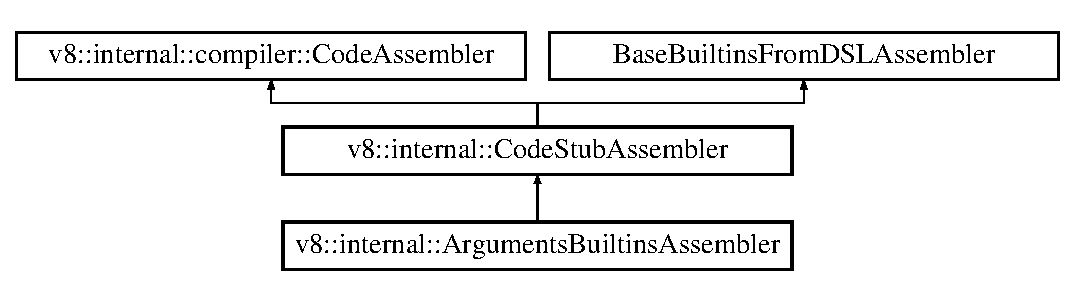
\includegraphics[height=3.000000cm]{classv8_1_1internal_1_1ArgumentsBuiltinsAssembler}
\end{center}
\end{figure}
\subsection*{Public Member Functions}
\begin{DoxyCompactItemize}
\item 
\mbox{\Hypertarget{classv8_1_1internal_1_1ArgumentsBuiltinsAssembler_ab58bed6955de3aabdad36c450112fa97}\label{classv8_1_1internal_1_1ArgumentsBuiltinsAssembler_ab58bed6955de3aabdad36c450112fa97}} 
{\bfseries Arguments\+Builtins\+Assembler} (\mbox{\hyperlink{classv8_1_1internal_1_1compiler_1_1CodeAssemblerState}{Code\+Assembler\+State}} $\ast$state)
\item 
\mbox{\Hypertarget{classv8_1_1internal_1_1ArgumentsBuiltinsAssembler_a39f8c5866a228f499b8807383061aa2b}\label{classv8_1_1internal_1_1ArgumentsBuiltinsAssembler_a39f8c5866a228f499b8807383061aa2b}} 
\mbox{\hyperlink{classv8_1_1internal_1_1compiler_1_1Node}{Node}} $\ast$ {\bfseries Emit\+Fast\+New\+Strict\+Arguments} (\mbox{\hyperlink{classv8_1_1internal_1_1compiler_1_1Node}{Node}} $\ast$context, \mbox{\hyperlink{classv8_1_1internal_1_1compiler_1_1Node}{Node}} $\ast$function)
\item 
\mbox{\Hypertarget{classv8_1_1internal_1_1ArgumentsBuiltinsAssembler_a2532f45829db1daee317e5505e12626e}\label{classv8_1_1internal_1_1ArgumentsBuiltinsAssembler_a2532f45829db1daee317e5505e12626e}} 
\mbox{\hyperlink{classv8_1_1internal_1_1compiler_1_1Node}{Node}} $\ast$ {\bfseries Emit\+Fast\+New\+Sloppy\+Arguments} (\mbox{\hyperlink{classv8_1_1internal_1_1compiler_1_1Node}{Node}} $\ast$context, \mbox{\hyperlink{classv8_1_1internal_1_1compiler_1_1Node}{Node}} $\ast$function)
\item 
\mbox{\Hypertarget{classv8_1_1internal_1_1ArgumentsBuiltinsAssembler_a37d0dd515ea2e4039eb750c82689fa27}\label{classv8_1_1internal_1_1ArgumentsBuiltinsAssembler_a37d0dd515ea2e4039eb750c82689fa27}} 
\mbox{\hyperlink{classv8_1_1internal_1_1compiler_1_1Node}{Node}} $\ast$ {\bfseries Emit\+Fast\+New\+Rest\+Parameter} (\mbox{\hyperlink{classv8_1_1internal_1_1compiler_1_1Node}{Node}} $\ast$context, \mbox{\hyperlink{classv8_1_1internal_1_1compiler_1_1Node}{Node}} $\ast$function)
\end{DoxyCompactItemize}
\subsection*{Additional Inherited Members}


\subsection{Detailed Description}


Definition at line 17 of file builtins-\/arguments-\/gen.\+h.



The documentation for this class was generated from the following files\+:\begin{DoxyCompactItemize}
\item 
v8/src/builtins/builtins-\/arguments-\/gen.\+h\item 
v8/src/builtins/builtins-\/arguments-\/gen.\+cc\end{DoxyCompactItemize}

\hypertarget{classv8_1_1internal_1_1SafepointEntry_1_1ArgumentsField}{}\section{v8\+:\+:internal\+:\+:Safepoint\+Entry\+:\+:Arguments\+Field Class Reference}
\label{classv8_1_1internal_1_1SafepointEntry_1_1ArgumentsField}\index{v8\+::internal\+::\+Safepoint\+Entry\+::\+Arguments\+Field@{v8\+::internal\+::\+Safepoint\+Entry\+::\+Arguments\+Field}}
Inheritance diagram for v8\+:\+:internal\+:\+:Safepoint\+Entry\+:\+:Arguments\+Field\+:\begin{figure}[H]
\begin{center}
\leavevmode
\includegraphics[height=3.000000cm]{classv8_1_1internal_1_1SafepointEntry_1_1ArgumentsField}
\end{center}
\end{figure}
\subsection*{Additional Inherited Members}


\subsection{Detailed Description}


Definition at line 56 of file safepoint-\/table.\+h.



The documentation for this class was generated from the following file\+:\begin{DoxyCompactItemize}
\item 
v8/src/safepoint-\/table.\+h\end{DoxyCompactItemize}

\hypertarget{structv8_1_1internal_1_1compiler_1_1SimplifiedOperatorGlobalCache_1_1ArgumentsFrameOperator}{}\section{v8\+:\+:internal\+:\+:compiler\+:\+:Simplified\+Operator\+Global\+Cache\+:\+:Arguments\+Frame\+Operator Struct Reference}
\label{structv8_1_1internal_1_1compiler_1_1SimplifiedOperatorGlobalCache_1_1ArgumentsFrameOperator}\index{v8\+::internal\+::compiler\+::\+Simplified\+Operator\+Global\+Cache\+::\+Arguments\+Frame\+Operator@{v8\+::internal\+::compiler\+::\+Simplified\+Operator\+Global\+Cache\+::\+Arguments\+Frame\+Operator}}
Inheritance diagram for v8\+:\+:internal\+:\+:compiler\+:\+:Simplified\+Operator\+Global\+Cache\+:\+:Arguments\+Frame\+Operator\+:\begin{figure}[H]
\begin{center}
\leavevmode
\includegraphics[height=3.000000cm]{structv8_1_1internal_1_1compiler_1_1SimplifiedOperatorGlobalCache_1_1ArgumentsFrameOperator}
\end{center}
\end{figure}
\subsection*{Additional Inherited Members}


\subsection{Detailed Description}


Definition at line 925 of file simplified-\/operator.\+cc.



The documentation for this struct was generated from the following file\+:\begin{DoxyCompactItemize}
\item 
v8/src/compiler/simplified-\/operator.\+cc\end{DoxyCompactItemize}

\hypertarget{unionv8_1_1platform_1_1tracing_1_1TraceObject_1_1ArgValue}{}\section{v8\+:\+:platform\+:\+:tracing\+:\+:Trace\+Object\+:\+:Arg\+Value Union Reference}
\label{unionv8_1_1platform_1_1tracing_1_1TraceObject_1_1ArgValue}\index{v8\+::platform\+::tracing\+::\+Trace\+Object\+::\+Arg\+Value@{v8\+::platform\+::tracing\+::\+Trace\+Object\+::\+Arg\+Value}}
\subsection*{Public Attributes}
\begin{DoxyCompactItemize}
\item 
\mbox{\Hypertarget{unionv8_1_1platform_1_1tracing_1_1TraceObject_1_1ArgValue_a5321b94fe5473d33e2ab69945e16eee0}\label{unionv8_1_1platform_1_1tracing_1_1TraceObject_1_1ArgValue_a5321b94fe5473d33e2ab69945e16eee0}} 
\mbox{\hyperlink{classbool}{bool}} {\bfseries as\+\_\+bool}
\item 
\mbox{\Hypertarget{unionv8_1_1platform_1_1tracing_1_1TraceObject_1_1ArgValue_a70a307359d9a88811e5cfe83f2abad69}\label{unionv8_1_1platform_1_1tracing_1_1TraceObject_1_1ArgValue_a70a307359d9a88811e5cfe83f2abad69}} 
uint64\+\_\+t {\bfseries as\+\_\+uint}
\item 
\mbox{\Hypertarget{unionv8_1_1platform_1_1tracing_1_1TraceObject_1_1ArgValue_a538fa5c735eaadf99bf13f088cbdaf58}\label{unionv8_1_1platform_1_1tracing_1_1TraceObject_1_1ArgValue_a538fa5c735eaadf99bf13f088cbdaf58}} 
\mbox{\hyperlink{classint64__t}{int64\+\_\+t}} {\bfseries as\+\_\+int}
\item 
\mbox{\Hypertarget{unionv8_1_1platform_1_1tracing_1_1TraceObject_1_1ArgValue_ad767bc3c8ca039dac75129239cdcc402}\label{unionv8_1_1platform_1_1tracing_1_1TraceObject_1_1ArgValue_ad767bc3c8ca039dac75129239cdcc402}} 
double {\bfseries as\+\_\+double}
\item 
\mbox{\Hypertarget{unionv8_1_1platform_1_1tracing_1_1TraceObject_1_1ArgValue_afe6b63c9eeef7d4b11a8b2665b0ad81f}\label{unionv8_1_1platform_1_1tracing_1_1TraceObject_1_1ArgValue_afe6b63c9eeef7d4b11a8b2665b0ad81f}} 
const void $\ast$ {\bfseries as\+\_\+pointer}
\item 
\mbox{\Hypertarget{unionv8_1_1platform_1_1tracing_1_1TraceObject_1_1ArgValue_a2572f6aa4fd94641114e73f2e864b4ad}\label{unionv8_1_1platform_1_1tracing_1_1TraceObject_1_1ArgValue_a2572f6aa4fd94641114e73f2e864b4ad}} 
const \mbox{\hyperlink{classchar}{char}} $\ast$ {\bfseries as\+\_\+string}
\end{DoxyCompactItemize}


\subsection{Detailed Description}


Definition at line 29 of file v8-\/tracing.\+h.



The documentation for this union was generated from the following file\+:\begin{DoxyCompactItemize}
\item 
v8/include/libplatform/v8-\/tracing.\+h\end{DoxyCompactItemize}

\hypertarget{structv8_1_1base_1_1internal_1_1ArithmeticPromotion}{}\section{v8\+:\+:base\+:\+:internal\+:\+:Arithmetic\+Promotion$<$ Lhs, Rhs, Promotion $>$ Struct Template Reference}
\label{structv8_1_1base_1_1internal_1_1ArithmeticPromotion}\index{v8\+::base\+::internal\+::\+Arithmetic\+Promotion$<$ Lhs, Rhs, Promotion $>$@{v8\+::base\+::internal\+::\+Arithmetic\+Promotion$<$ Lhs, Rhs, Promotion $>$}}


\subsection{Detailed Description}
\subsubsection*{template$<$typename Lhs, typename Rhs = Lhs, Arithmetic\+Promotion\+Category Promotion = (\+Max\+Exponent$<$\+Lhs$>$\+::value $>$ Max\+Exponent$<$\+Rhs$>$\+::value) ? (\+Max\+Exponent$<$\+Lhs$>$\+::value $>$ Max\+Exponent$<$int$>$\+::value                         ? L\+E\+F\+T\+\_\+\+P\+R\+O\+M\+O\+T\+I\+O\+N                         \+: D\+E\+F\+A\+U\+L\+T\+\_\+\+P\+R\+O\+M\+O\+T\+I\+O\+N) \+: (\+Max\+Exponent$<$\+Rhs$>$\+::value $>$ Max\+Exponent$<$int$>$\+::value                         ? R\+I\+G\+H\+T\+\_\+\+P\+R\+O\+M\+O\+T\+I\+O\+N                         \+: D\+E\+F\+A\+U\+L\+T\+\_\+\+P\+R\+O\+M\+O\+T\+I\+O\+N)$>$\newline
struct v8\+::base\+::internal\+::\+Arithmetic\+Promotion$<$ Lhs, Rhs, Promotion $>$}



Definition at line 495 of file safe\+\_\+math\+\_\+impl.\+h.



The documentation for this struct was generated from the following file\+:\begin{DoxyCompactItemize}
\item 
v8/src/base/safe\+\_\+math\+\_\+impl.\+h\end{DoxyCompactItemize}

\hypertarget{structv8_1_1base_1_1internal_1_1ArithmeticPromotion_3_01Lhs_00_01Rhs_00_01DEFAULT__PROMOTION_01_4}{}\section{v8\+:\+:base\+:\+:internal\+:\+:Arithmetic\+Promotion$<$ Lhs, Rhs, D\+E\+F\+A\+U\+L\+T\+\_\+\+P\+R\+O\+M\+O\+T\+I\+ON $>$ Struct Template Reference}
\label{structv8_1_1base_1_1internal_1_1ArithmeticPromotion_3_01Lhs_00_01Rhs_00_01DEFAULT__PROMOTION_01_4}\index{v8\+::base\+::internal\+::\+Arithmetic\+Promotion$<$ Lhs, Rhs, D\+E\+F\+A\+U\+L\+T\+\_\+\+P\+R\+O\+M\+O\+T\+I\+O\+N $>$@{v8\+::base\+::internal\+::\+Arithmetic\+Promotion$<$ Lhs, Rhs, D\+E\+F\+A\+U\+L\+T\+\_\+\+P\+R\+O\+M\+O\+T\+I\+O\+N $>$}}
\subsection*{Public Types}
\begin{DoxyCompactItemize}
\item 
\mbox{\Hypertarget{structv8_1_1base_1_1internal_1_1ArithmeticPromotion_3_01Lhs_00_01Rhs_00_01DEFAULT__PROMOTION_01_4_a3700971f01b0a6dc93a795502bb45cdd}\label{structv8_1_1base_1_1internal_1_1ArithmeticPromotion_3_01Lhs_00_01Rhs_00_01DEFAULT__PROMOTION_01_4_a3700971f01b0a6dc93a795502bb45cdd}} 
typedef \mbox{\hyperlink{classint}{int}} {\bfseries type}
\end{DoxyCompactItemize}


\subsection{Detailed Description}
\subsubsection*{template$<$typename Lhs, typename Rhs$>$\newline
struct v8\+::base\+::internal\+::\+Arithmetic\+Promotion$<$ Lhs, Rhs, D\+E\+F\+A\+U\+L\+T\+\_\+\+P\+R\+O\+M\+O\+T\+I\+O\+N $>$}



Definition at line 508 of file safe\+\_\+math\+\_\+impl.\+h.



The documentation for this struct was generated from the following file\+:\begin{DoxyCompactItemize}
\item 
v8/src/base/safe\+\_\+math\+\_\+impl.\+h\end{DoxyCompactItemize}

\hypertarget{structv8_1_1base_1_1internal_1_1ArithmeticPromotion_3_01Lhs_00_01Rhs_00_01LEFT__PROMOTION_01_4}{}\section{v8\+:\+:base\+:\+:internal\+:\+:Arithmetic\+Promotion$<$ Lhs, Rhs, L\+E\+F\+T\+\_\+\+P\+R\+O\+M\+O\+T\+I\+ON $>$ Struct Template Reference}
\label{structv8_1_1base_1_1internal_1_1ArithmeticPromotion_3_01Lhs_00_01Rhs_00_01LEFT__PROMOTION_01_4}\index{v8\+::base\+::internal\+::\+Arithmetic\+Promotion$<$ Lhs, Rhs, L\+E\+F\+T\+\_\+\+P\+R\+O\+M\+O\+T\+I\+O\+N $>$@{v8\+::base\+::internal\+::\+Arithmetic\+Promotion$<$ Lhs, Rhs, L\+E\+F\+T\+\_\+\+P\+R\+O\+M\+O\+T\+I\+O\+N $>$}}
\subsection*{Public Types}
\begin{DoxyCompactItemize}
\item 
\mbox{\Hypertarget{structv8_1_1base_1_1internal_1_1ArithmeticPromotion_3_01Lhs_00_01Rhs_00_01LEFT__PROMOTION_01_4_a45b66410f428ca9f1a9b4ae9fe31957c}\label{structv8_1_1base_1_1internal_1_1ArithmeticPromotion_3_01Lhs_00_01Rhs_00_01LEFT__PROMOTION_01_4_a45b66410f428ca9f1a9b4ae9fe31957c}} 
typedef Lhs {\bfseries type}
\end{DoxyCompactItemize}


\subsection{Detailed Description}
\subsubsection*{template$<$typename Lhs, typename Rhs$>$\newline
struct v8\+::base\+::internal\+::\+Arithmetic\+Promotion$<$ Lhs, Rhs, L\+E\+F\+T\+\_\+\+P\+R\+O\+M\+O\+T\+I\+O\+N $>$}



Definition at line 498 of file safe\+\_\+math\+\_\+impl.\+h.



The documentation for this struct was generated from the following file\+:\begin{DoxyCompactItemize}
\item 
v8/src/base/safe\+\_\+math\+\_\+impl.\+h\end{DoxyCompactItemize}

\hypertarget{structv8_1_1base_1_1internal_1_1ArithmeticPromotion_3_01Lhs_00_01Rhs_00_01RIGHT__PROMOTION_01_4}{}\section{v8\+:\+:base\+:\+:internal\+:\+:Arithmetic\+Promotion$<$ Lhs, Rhs, R\+I\+G\+H\+T\+\_\+\+P\+R\+O\+M\+O\+T\+I\+ON $>$ Struct Template Reference}
\label{structv8_1_1base_1_1internal_1_1ArithmeticPromotion_3_01Lhs_00_01Rhs_00_01RIGHT__PROMOTION_01_4}\index{v8\+::base\+::internal\+::\+Arithmetic\+Promotion$<$ Lhs, Rhs, R\+I\+G\+H\+T\+\_\+\+P\+R\+O\+M\+O\+T\+I\+O\+N $>$@{v8\+::base\+::internal\+::\+Arithmetic\+Promotion$<$ Lhs, Rhs, R\+I\+G\+H\+T\+\_\+\+P\+R\+O\+M\+O\+T\+I\+O\+N $>$}}
\subsection*{Public Types}
\begin{DoxyCompactItemize}
\item 
\mbox{\Hypertarget{structv8_1_1base_1_1internal_1_1ArithmeticPromotion_3_01Lhs_00_01Rhs_00_01RIGHT__PROMOTION_01_4_a95c5df9835e2fe65234e08aff0c957b2}\label{structv8_1_1base_1_1internal_1_1ArithmeticPromotion_3_01Lhs_00_01Rhs_00_01RIGHT__PROMOTION_01_4_a95c5df9835e2fe65234e08aff0c957b2}} 
typedef Rhs {\bfseries type}
\end{DoxyCompactItemize}


\subsection{Detailed Description}
\subsubsection*{template$<$typename Lhs, typename Rhs$>$\newline
struct v8\+::base\+::internal\+::\+Arithmetic\+Promotion$<$ Lhs, Rhs, R\+I\+G\+H\+T\+\_\+\+P\+R\+O\+M\+O\+T\+I\+O\+N $>$}



Definition at line 503 of file safe\+\_\+math\+\_\+impl.\+h.



The documentation for this struct was generated from the following file\+:\begin{DoxyCompactItemize}
\item 
v8/src/base/safe\+\_\+math\+\_\+impl.\+h\end{DoxyCompactItemize}

\hypertarget{classv8_1_1internal_1_1compiler_1_1Arm64OperandConverter}{}\section{v8\+:\+:internal\+:\+:compiler\+:\+:Arm64\+Operand\+Converter Class Reference}
\label{classv8_1_1internal_1_1compiler_1_1Arm64OperandConverter}\index{v8\+::internal\+::compiler\+::\+Arm64\+Operand\+Converter@{v8\+::internal\+::compiler\+::\+Arm64\+Operand\+Converter}}
Inheritance diagram for v8\+:\+:internal\+:\+:compiler\+:\+:Arm64\+Operand\+Converter\+:\begin{figure}[H]
\begin{center}
\leavevmode
\includegraphics[height=2.000000cm]{classv8_1_1internal_1_1compiler_1_1Arm64OperandConverter}
\end{center}
\end{figure}
\subsection*{Public Member Functions}
\begin{DoxyCompactItemize}
\item 
\mbox{\Hypertarget{classv8_1_1internal_1_1compiler_1_1Arm64OperandConverter_aab60a3c4a831be61260f6c2c649b6349}\label{classv8_1_1internal_1_1compiler_1_1Arm64OperandConverter_aab60a3c4a831be61260f6c2c649b6349}} 
{\bfseries Arm64\+Operand\+Converter} (\mbox{\hyperlink{classv8_1_1internal_1_1compiler_1_1CodeGenerator}{Code\+Generator}} $\ast$gen, \mbox{\hyperlink{classv8_1_1internal_1_1compiler_1_1Instruction}{Instruction}} $\ast$instr)
\item 
\mbox{\Hypertarget{classv8_1_1internal_1_1compiler_1_1Arm64OperandConverter_a8be581b3bb1772104deb40f9e7d82b40}\label{classv8_1_1internal_1_1compiler_1_1Arm64OperandConverter_a8be581b3bb1772104deb40f9e7d82b40}} 
\mbox{\hyperlink{classv8_1_1internal_1_1DoubleRegister}{Double\+Register}} {\bfseries Input\+Float32\+Register} (\mbox{\hyperlink{classsize__t}{size\+\_\+t}} index)
\item 
\mbox{\Hypertarget{classv8_1_1internal_1_1compiler_1_1Arm64OperandConverter_a3c6bd2d38a0e60edd6b73b8dd96284cf}\label{classv8_1_1internal_1_1compiler_1_1Arm64OperandConverter_a3c6bd2d38a0e60edd6b73b8dd96284cf}} 
\mbox{\hyperlink{classv8_1_1internal_1_1DoubleRegister}{Double\+Register}} {\bfseries Input\+Float64\+Register} (\mbox{\hyperlink{classsize__t}{size\+\_\+t}} index)
\item 
\mbox{\Hypertarget{classv8_1_1internal_1_1compiler_1_1Arm64OperandConverter_a964e104fa4bea4fbd2923feeb293e7f1}\label{classv8_1_1internal_1_1compiler_1_1Arm64OperandConverter_a964e104fa4bea4fbd2923feeb293e7f1}} 
\mbox{\hyperlink{classv8_1_1internal_1_1DoubleRegister}{Double\+Register}} {\bfseries Input\+Simd128\+Register} (\mbox{\hyperlink{classsize__t}{size\+\_\+t}} index)
\item 
\mbox{\Hypertarget{classv8_1_1internal_1_1compiler_1_1Arm64OperandConverter_a09a69bea27deb488c2c2fa1d6c7e1dd5}\label{classv8_1_1internal_1_1compiler_1_1Arm64OperandConverter_a09a69bea27deb488c2c2fa1d6c7e1dd5}} 
\mbox{\hyperlink{classv8_1_1internal_1_1CPURegister}{C\+P\+U\+Register}} {\bfseries Input\+Float32\+Or\+Zero\+Register} (\mbox{\hyperlink{classsize__t}{size\+\_\+t}} index)
\item 
\mbox{\Hypertarget{classv8_1_1internal_1_1compiler_1_1Arm64OperandConverter_a851b69de5330eccac3034c451d12e2db}\label{classv8_1_1internal_1_1compiler_1_1Arm64OperandConverter_a851b69de5330eccac3034c451d12e2db}} 
\mbox{\hyperlink{classv8_1_1internal_1_1CPURegister}{C\+P\+U\+Register}} {\bfseries Input\+Float64\+Or\+Zero\+Register} (\mbox{\hyperlink{classsize__t}{size\+\_\+t}} index)
\item 
\mbox{\Hypertarget{classv8_1_1internal_1_1compiler_1_1Arm64OperandConverter_a491a68d3acb64590b11ffa50f791aff9}\label{classv8_1_1internal_1_1compiler_1_1Arm64OperandConverter_a491a68d3acb64590b11ffa50f791aff9}} 
\mbox{\hyperlink{classsize__t}{size\+\_\+t}} {\bfseries Output\+Count} ()
\item 
\mbox{\Hypertarget{classv8_1_1internal_1_1compiler_1_1Arm64OperandConverter_a16115f2af49b8398afa11acfdf4af8dc}\label{classv8_1_1internal_1_1compiler_1_1Arm64OperandConverter_a16115f2af49b8398afa11acfdf4af8dc}} 
\mbox{\hyperlink{classv8_1_1internal_1_1DoubleRegister}{Double\+Register}} {\bfseries Output\+Float32\+Register} ()
\item 
\mbox{\Hypertarget{classv8_1_1internal_1_1compiler_1_1Arm64OperandConverter_a3542c2ef6fe5138dd45e268e57de1ab3}\label{classv8_1_1internal_1_1compiler_1_1Arm64OperandConverter_a3542c2ef6fe5138dd45e268e57de1ab3}} 
\mbox{\hyperlink{classv8_1_1internal_1_1DoubleRegister}{Double\+Register}} {\bfseries Output\+Float64\+Register} ()
\item 
\mbox{\Hypertarget{classv8_1_1internal_1_1compiler_1_1Arm64OperandConverter_a84b1d5a5e5f7a8f3e79885f7d68c0397}\label{classv8_1_1internal_1_1compiler_1_1Arm64OperandConverter_a84b1d5a5e5f7a8f3e79885f7d68c0397}} 
\mbox{\hyperlink{classv8_1_1internal_1_1DoubleRegister}{Double\+Register}} {\bfseries Output\+Simd128\+Register} ()
\item 
\mbox{\Hypertarget{classv8_1_1internal_1_1compiler_1_1Arm64OperandConverter_a69336469db39d290adfc52712697e87e}\label{classv8_1_1internal_1_1compiler_1_1Arm64OperandConverter_a69336469db39d290adfc52712697e87e}} 
\mbox{\hyperlink{classv8_1_1internal_1_1Register}{Register}} {\bfseries Input\+Register32} (\mbox{\hyperlink{classsize__t}{size\+\_\+t}} index)
\item 
\mbox{\Hypertarget{classv8_1_1internal_1_1compiler_1_1Arm64OperandConverter_acbcca0385313f62567975520bce9e5bb}\label{classv8_1_1internal_1_1compiler_1_1Arm64OperandConverter_acbcca0385313f62567975520bce9e5bb}} 
\mbox{\hyperlink{classv8_1_1internal_1_1Register}{Register}} {\bfseries Input\+Or\+Zero\+Register32} (\mbox{\hyperlink{classsize__t}{size\+\_\+t}} index)
\item 
\mbox{\Hypertarget{classv8_1_1internal_1_1compiler_1_1Arm64OperandConverter_a734650d80022526577ee22c2d39d1104}\label{classv8_1_1internal_1_1compiler_1_1Arm64OperandConverter_a734650d80022526577ee22c2d39d1104}} 
\mbox{\hyperlink{classv8_1_1internal_1_1Register}{Register}} {\bfseries Input\+Register64} (\mbox{\hyperlink{classsize__t}{size\+\_\+t}} index)
\item 
\mbox{\Hypertarget{classv8_1_1internal_1_1compiler_1_1Arm64OperandConverter_aaa8fecf5e2c7e31f112e52854551abb0}\label{classv8_1_1internal_1_1compiler_1_1Arm64OperandConverter_aaa8fecf5e2c7e31f112e52854551abb0}} 
\mbox{\hyperlink{classv8_1_1internal_1_1Register}{Register}} {\bfseries Input\+Or\+Zero\+Register64} (\mbox{\hyperlink{classsize__t}{size\+\_\+t}} index)
\item 
\mbox{\Hypertarget{classv8_1_1internal_1_1compiler_1_1Arm64OperandConverter_ac8ac3ac041a3064c657a96a739819630}\label{classv8_1_1internal_1_1compiler_1_1Arm64OperandConverter_ac8ac3ac041a3064c657a96a739819630}} 
\mbox{\hyperlink{classv8_1_1internal_1_1Operand}{Operand}} {\bfseries Input\+Operand} (\mbox{\hyperlink{classsize__t}{size\+\_\+t}} index)
\item 
\mbox{\Hypertarget{classv8_1_1internal_1_1compiler_1_1Arm64OperandConverter_a3103f91dac5c0e8849d95f316976bb45}\label{classv8_1_1internal_1_1compiler_1_1Arm64OperandConverter_a3103f91dac5c0e8849d95f316976bb45}} 
\mbox{\hyperlink{classv8_1_1internal_1_1Operand}{Operand}} {\bfseries Input\+Operand64} (\mbox{\hyperlink{classsize__t}{size\+\_\+t}} index)
\item 
\mbox{\Hypertarget{classv8_1_1internal_1_1compiler_1_1Arm64OperandConverter_ac2d6bdbf0b880fef46ec41344ede9e9a}\label{classv8_1_1internal_1_1compiler_1_1Arm64OperandConverter_ac2d6bdbf0b880fef46ec41344ede9e9a}} 
\mbox{\hyperlink{classv8_1_1internal_1_1Operand}{Operand}} {\bfseries Input\+Operand32} (\mbox{\hyperlink{classsize__t}{size\+\_\+t}} index)
\item 
\mbox{\Hypertarget{classv8_1_1internal_1_1compiler_1_1Arm64OperandConverter_a5f1ae0407fd7e57c19cb0f3b55b29018}\label{classv8_1_1internal_1_1compiler_1_1Arm64OperandConverter_a5f1ae0407fd7e57c19cb0f3b55b29018}} 
\mbox{\hyperlink{classv8_1_1internal_1_1Register}{Register}} {\bfseries Output\+Register64} ()
\item 
\mbox{\Hypertarget{classv8_1_1internal_1_1compiler_1_1Arm64OperandConverter_a3b7c0ad0ccfd0bbdacbf1e3fb28b3e7f}\label{classv8_1_1internal_1_1compiler_1_1Arm64OperandConverter_a3b7c0ad0ccfd0bbdacbf1e3fb28b3e7f}} 
\mbox{\hyperlink{classv8_1_1internal_1_1Register}{Register}} {\bfseries Output\+Register32} ()
\item 
\mbox{\Hypertarget{classv8_1_1internal_1_1compiler_1_1Arm64OperandConverter_a934557d75765ae9978251ce8e50e610e}\label{classv8_1_1internal_1_1compiler_1_1Arm64OperandConverter_a934557d75765ae9978251ce8e50e610e}} 
\mbox{\hyperlink{classv8_1_1internal_1_1Register}{Register}} {\bfseries Temp\+Register32} (\mbox{\hyperlink{classsize__t}{size\+\_\+t}} index)
\item 
\mbox{\Hypertarget{classv8_1_1internal_1_1compiler_1_1Arm64OperandConverter_a558592c0e76f252e3b22f26ad6d7737c}\label{classv8_1_1internal_1_1compiler_1_1Arm64OperandConverter_a558592c0e76f252e3b22f26ad6d7737c}} 
\mbox{\hyperlink{classv8_1_1internal_1_1Operand}{Operand}} {\bfseries Input\+Operand2\+\_\+32} (\mbox{\hyperlink{classsize__t}{size\+\_\+t}} index)
\item 
\mbox{\Hypertarget{classv8_1_1internal_1_1compiler_1_1Arm64OperandConverter_ac31914312582fa429153433c2d10e2f7}\label{classv8_1_1internal_1_1compiler_1_1Arm64OperandConverter_ac31914312582fa429153433c2d10e2f7}} 
\mbox{\hyperlink{classv8_1_1internal_1_1Operand}{Operand}} {\bfseries Input\+Operand2\+\_\+64} (\mbox{\hyperlink{classsize__t}{size\+\_\+t}} index)
\item 
\mbox{\Hypertarget{classv8_1_1internal_1_1compiler_1_1Arm64OperandConverter_ad6c045583d8c6e4801568b008f566ef0}\label{classv8_1_1internal_1_1compiler_1_1Arm64OperandConverter_ad6c045583d8c6e4801568b008f566ef0}} 
\mbox{\hyperlink{classv8_1_1internal_1_1MemOperand}{Mem\+Operand}} {\bfseries Memory\+Operand} (\mbox{\hyperlink{classsize__t}{size\+\_\+t}} index=0)
\item 
\mbox{\Hypertarget{classv8_1_1internal_1_1compiler_1_1Arm64OperandConverter_a9578a1c57f9ece2648b43865ef5b0c6a}\label{classv8_1_1internal_1_1compiler_1_1Arm64OperandConverter_a9578a1c57f9ece2648b43865ef5b0c6a}} 
\mbox{\hyperlink{classv8_1_1internal_1_1Operand}{Operand}} {\bfseries To\+Operand} (\mbox{\hyperlink{classv8_1_1internal_1_1compiler_1_1InstructionOperand}{Instruction\+Operand}} $\ast$op)
\item 
\mbox{\Hypertarget{classv8_1_1internal_1_1compiler_1_1Arm64OperandConverter_ad0e7ee92e6b2394604546f36d763662b}\label{classv8_1_1internal_1_1compiler_1_1Arm64OperandConverter_ad0e7ee92e6b2394604546f36d763662b}} 
\mbox{\hyperlink{classv8_1_1internal_1_1Operand}{Operand}} {\bfseries To\+Operand32} (\mbox{\hyperlink{classv8_1_1internal_1_1compiler_1_1InstructionOperand}{Instruction\+Operand}} $\ast$op)
\item 
\mbox{\Hypertarget{classv8_1_1internal_1_1compiler_1_1Arm64OperandConverter_a48617400ce311d44cd2c229fa242e587}\label{classv8_1_1internal_1_1compiler_1_1Arm64OperandConverter_a48617400ce311d44cd2c229fa242e587}} 
\mbox{\hyperlink{classv8_1_1internal_1_1Operand}{Operand}} {\bfseries To\+Immediate} (\mbox{\hyperlink{classv8_1_1internal_1_1compiler_1_1InstructionOperand}{Instruction\+Operand}} $\ast$operand)
\item 
\mbox{\Hypertarget{classv8_1_1internal_1_1compiler_1_1Arm64OperandConverter_a5bb8abc51390c8dc5647359444c4f457}\label{classv8_1_1internal_1_1compiler_1_1Arm64OperandConverter_a5bb8abc51390c8dc5647359444c4f457}} 
\mbox{\hyperlink{classv8_1_1internal_1_1MemOperand}{Mem\+Operand}} {\bfseries To\+Mem\+Operand} (\mbox{\hyperlink{classv8_1_1internal_1_1compiler_1_1InstructionOperand}{Instruction\+Operand}} $\ast$op, \mbox{\hyperlink{classv8_1_1internal_1_1TurboAssembler}{Turbo\+Assembler}} $\ast$tasm) const
\item 
\mbox{\Hypertarget{classv8_1_1internal_1_1compiler_1_1Arm64OperandConverter_a6815c126c0e7c8f4c180686ac12e2f26}\label{classv8_1_1internal_1_1compiler_1_1Arm64OperandConverter_a6815c126c0e7c8f4c180686ac12e2f26}} 
\mbox{\hyperlink{classv8_1_1internal_1_1MemOperand}{Mem\+Operand}} {\bfseries Slot\+To\+Mem\+Operand} (\mbox{\hyperlink{classint}{int}} slot, \mbox{\hyperlink{classv8_1_1internal_1_1TurboAssembler}{Turbo\+Assembler}} $\ast$tasm) const
\end{DoxyCompactItemize}
\subsection*{Additional Inherited Members}


\subsection{Detailed Description}


Definition at line 26 of file code-\/generator-\/arm64.\+cc.



The documentation for this class was generated from the following file\+:\begin{DoxyCompactItemize}
\item 
v8/src/compiler/backend/arm64/code-\/generator-\/arm64.\+cc\end{DoxyCompactItemize}

\hypertarget{classv8_1_1internal_1_1compiler_1_1Arm64OperandGenerator}{}\section{v8\+:\+:internal\+:\+:compiler\+:\+:Arm64\+Operand\+Generator Class Reference}
\label{classv8_1_1internal_1_1compiler_1_1Arm64OperandGenerator}\index{v8\+::internal\+::compiler\+::\+Arm64\+Operand\+Generator@{v8\+::internal\+::compiler\+::\+Arm64\+Operand\+Generator}}
Inheritance diagram for v8\+:\+:internal\+:\+:compiler\+:\+:Arm64\+Operand\+Generator\+:\begin{figure}[H]
\begin{center}
\leavevmode
\includegraphics[height=2.000000cm]{classv8_1_1internal_1_1compiler_1_1Arm64OperandGenerator}
\end{center}
\end{figure}
\subsection*{Public Member Functions}
\begin{DoxyCompactItemize}
\item 
\mbox{\Hypertarget{classv8_1_1internal_1_1compiler_1_1Arm64OperandGenerator_aeefa43ecf6592649707952f88b853c0e}\label{classv8_1_1internal_1_1compiler_1_1Arm64OperandGenerator_aeefa43ecf6592649707952f88b853c0e}} 
{\bfseries Arm64\+Operand\+Generator} (\mbox{\hyperlink{classv8_1_1internal_1_1compiler_1_1InstructionSelector}{Instruction\+Selector}} $\ast$selector)
\item 
\mbox{\Hypertarget{classv8_1_1internal_1_1compiler_1_1Arm64OperandGenerator_a151403a095acbf06175ca3103a1ef4cc}\label{classv8_1_1internal_1_1compiler_1_1Arm64OperandGenerator_a151403a095acbf06175ca3103a1ef4cc}} 
\mbox{\hyperlink{classv8_1_1internal_1_1compiler_1_1InstructionOperand}{Instruction\+Operand}} {\bfseries Use\+Operand} (\mbox{\hyperlink{classv8_1_1internal_1_1compiler_1_1Node}{Node}} $\ast$node, Immediate\+Mode mode)
\item 
\mbox{\Hypertarget{classv8_1_1internal_1_1compiler_1_1Arm64OperandGenerator_a34aca8cb0f4cfec0de893f0564d3206a}\label{classv8_1_1internal_1_1compiler_1_1Arm64OperandGenerator_a34aca8cb0f4cfec0de893f0564d3206a}} 
\mbox{\hyperlink{classv8_1_1internal_1_1compiler_1_1InstructionOperand}{Instruction\+Operand}} {\bfseries Use\+Register\+Or\+Immediate\+Zero} (\mbox{\hyperlink{classv8_1_1internal_1_1compiler_1_1Node}{Node}} $\ast$node)
\item 
\mbox{\Hypertarget{classv8_1_1internal_1_1compiler_1_1Arm64OperandGenerator_aed3f1285c4f36018b23e771a9c38bbca}\label{classv8_1_1internal_1_1compiler_1_1Arm64OperandGenerator_aed3f1285c4f36018b23e771a9c38bbca}} 
\mbox{\hyperlink{classv8_1_1internal_1_1compiler_1_1InstructionOperand}{Instruction\+Operand}} {\bfseries Use\+Register\+Or\+Stack\+Pointer} (\mbox{\hyperlink{classv8_1_1internal_1_1compiler_1_1Node}{Node}} $\ast$node, \mbox{\hyperlink{classbool}{bool}} sp\+\_\+allowed)
\item 
\mbox{\Hypertarget{classv8_1_1internal_1_1compiler_1_1Arm64OperandGenerator_a177c26efdba3aae437b3080e7bb0ce16}\label{classv8_1_1internal_1_1compiler_1_1Arm64OperandGenerator_a177c26efdba3aae437b3080e7bb0ce16}} 
\mbox{\hyperlink{classv8_1_1internal_1_1compiler_1_1InstructionOperand}{Instruction\+Operand}} {\bfseries Use\+Immediate\+Or\+Temp} (\mbox{\hyperlink{classv8_1_1internal_1_1compiler_1_1Node}{Node}} $\ast$node, int32\+\_\+t value)
\item 
\mbox{\Hypertarget{classv8_1_1internal_1_1compiler_1_1Arm64OperandGenerator_aa69f60c9702b367f05e1b0ba68440842}\label{classv8_1_1internal_1_1compiler_1_1Arm64OperandGenerator_aa69f60c9702b367f05e1b0ba68440842}} 
\mbox{\hyperlink{classbool}{bool}} {\bfseries Is\+Integer\+Constant} (\mbox{\hyperlink{classv8_1_1internal_1_1compiler_1_1Node}{Node}} $\ast$node)
\item 
\mbox{\Hypertarget{classv8_1_1internal_1_1compiler_1_1Arm64OperandGenerator_a7d722c9454c869b4805290eda03eb0ec}\label{classv8_1_1internal_1_1compiler_1_1Arm64OperandGenerator_a7d722c9454c869b4805290eda03eb0ec}} 
\mbox{\hyperlink{classint64__t}{int64\+\_\+t}} {\bfseries Get\+Integer\+Constant\+Value} (\mbox{\hyperlink{classv8_1_1internal_1_1compiler_1_1Node}{Node}} $\ast$node)
\item 
\mbox{\Hypertarget{classv8_1_1internal_1_1compiler_1_1Arm64OperandGenerator_a71914a8203678e368f20876843d4bc1d}\label{classv8_1_1internal_1_1compiler_1_1Arm64OperandGenerator_a71914a8203678e368f20876843d4bc1d}} 
\mbox{\hyperlink{classbool}{bool}} {\bfseries Is\+Float\+Constant} (\mbox{\hyperlink{classv8_1_1internal_1_1compiler_1_1Node}{Node}} $\ast$node)
\item 
\mbox{\Hypertarget{classv8_1_1internal_1_1compiler_1_1Arm64OperandGenerator_ae570be798733a54bcee9f559b3f7debc}\label{classv8_1_1internal_1_1compiler_1_1Arm64OperandGenerator_ae570be798733a54bcee9f559b3f7debc}} 
double {\bfseries Get\+Float\+Constant\+Value} (\mbox{\hyperlink{classv8_1_1internal_1_1compiler_1_1Node}{Node}} $\ast$node)
\item 
\mbox{\Hypertarget{classv8_1_1internal_1_1compiler_1_1Arm64OperandGenerator_ac369443cd34e7d1c0fc3f0649824284e}\label{classv8_1_1internal_1_1compiler_1_1Arm64OperandGenerator_ac369443cd34e7d1c0fc3f0649824284e}} 
\mbox{\hyperlink{classbool}{bool}} {\bfseries Can\+Be\+Immediate} (\mbox{\hyperlink{classv8_1_1internal_1_1compiler_1_1Node}{Node}} $\ast$node, Immediate\+Mode mode)
\item 
\mbox{\Hypertarget{classv8_1_1internal_1_1compiler_1_1Arm64OperandGenerator_a2f5538f12c78b7d3805620d55639021b}\label{classv8_1_1internal_1_1compiler_1_1Arm64OperandGenerator_a2f5538f12c78b7d3805620d55639021b}} 
\mbox{\hyperlink{classbool}{bool}} {\bfseries Can\+Be\+Immediate} (\mbox{\hyperlink{classint64__t}{int64\+\_\+t}} value, Immediate\+Mode mode)
\item 
\mbox{\Hypertarget{classv8_1_1internal_1_1compiler_1_1Arm64OperandGenerator_aa4d12145139c5480a8e078ee7b86e2fb}\label{classv8_1_1internal_1_1compiler_1_1Arm64OperandGenerator_aa4d12145139c5480a8e078ee7b86e2fb}} 
\mbox{\hyperlink{classbool}{bool}} {\bfseries Can\+Be\+Load\+Store\+Shift\+Immediate} (\mbox{\hyperlink{classv8_1_1internal_1_1compiler_1_1Node}{Node}} $\ast$node, Machine\+Representation rep)
\end{DoxyCompactItemize}
\subsection*{Additional Inherited Members}


\subsection{Detailed Description}


Definition at line 28 of file instruction-\/selector-\/arm64.\+cc.



The documentation for this class was generated from the following file\+:\begin{DoxyCompactItemize}
\item 
v8/src/compiler/backend/arm64/instruction-\/selector-\/arm64.\+cc\end{DoxyCompactItemize}

\hypertarget{classv8_1_1internal_1_1compiler_1_1ArmOperandConverter}{}\section{v8\+:\+:internal\+:\+:compiler\+:\+:Arm\+Operand\+Converter Class Reference}
\label{classv8_1_1internal_1_1compiler_1_1ArmOperandConverter}\index{v8\+::internal\+::compiler\+::\+Arm\+Operand\+Converter@{v8\+::internal\+::compiler\+::\+Arm\+Operand\+Converter}}
Inheritance diagram for v8\+:\+:internal\+:\+:compiler\+:\+:Arm\+Operand\+Converter\+:\begin{figure}[H]
\begin{center}
\leavevmode
\includegraphics[height=2.000000cm]{classv8_1_1internal_1_1compiler_1_1ArmOperandConverter}
\end{center}
\end{figure}
\subsection*{Public Member Functions}
\begin{DoxyCompactItemize}
\item 
\mbox{\Hypertarget{classv8_1_1internal_1_1compiler_1_1ArmOperandConverter_adad200cb10696b6ae6a7be2b8651eee8}\label{classv8_1_1internal_1_1compiler_1_1ArmOperandConverter_adad200cb10696b6ae6a7be2b8651eee8}} 
{\bfseries Arm\+Operand\+Converter} (\mbox{\hyperlink{classv8_1_1internal_1_1compiler_1_1CodeGenerator}{Code\+Generator}} $\ast$gen, \mbox{\hyperlink{classv8_1_1internal_1_1compiler_1_1Instruction}{Instruction}} $\ast$instr)
\item 
\mbox{\Hypertarget{classv8_1_1internal_1_1compiler_1_1ArmOperandConverter_a9a1effa98daaefed84b973cc19c0bda0}\label{classv8_1_1internal_1_1compiler_1_1ArmOperandConverter_a9a1effa98daaefed84b973cc19c0bda0}} 
S\+Bit {\bfseries Output\+S\+Bit} () const
\item 
\mbox{\Hypertarget{classv8_1_1internal_1_1compiler_1_1ArmOperandConverter_a88d969057024c8e2c5598b4b57e4ee10}\label{classv8_1_1internal_1_1compiler_1_1ArmOperandConverter_a88d969057024c8e2c5598b4b57e4ee10}} 
\mbox{\hyperlink{classv8_1_1internal_1_1Operand}{Operand}} {\bfseries Input\+Immediate} (\mbox{\hyperlink{classsize__t}{size\+\_\+t}} index)
\item 
\mbox{\Hypertarget{classv8_1_1internal_1_1compiler_1_1ArmOperandConverter_a9c3f60c336ab369f989dae735c8f8e7c}\label{classv8_1_1internal_1_1compiler_1_1ArmOperandConverter_a9c3f60c336ab369f989dae735c8f8e7c}} 
\mbox{\hyperlink{classv8_1_1internal_1_1Operand}{Operand}} {\bfseries Input\+Operand2} (\mbox{\hyperlink{classsize__t}{size\+\_\+t}} first\+\_\+index)
\item 
\mbox{\Hypertarget{classv8_1_1internal_1_1compiler_1_1ArmOperandConverter_a94fa5318669d2fc386c77a69d8fb883f}\label{classv8_1_1internal_1_1compiler_1_1ArmOperandConverter_a94fa5318669d2fc386c77a69d8fb883f}} 
\mbox{\hyperlink{classv8_1_1internal_1_1MemOperand}{Mem\+Operand}} {\bfseries Input\+Offset} (\mbox{\hyperlink{classsize__t}{size\+\_\+t}} $\ast$first\+\_\+index)
\item 
\mbox{\Hypertarget{classv8_1_1internal_1_1compiler_1_1ArmOperandConverter_a2851c3df1f5aed11b07f8b4ba6bf1a7d}\label{classv8_1_1internal_1_1compiler_1_1ArmOperandConverter_a2851c3df1f5aed11b07f8b4ba6bf1a7d}} 
\mbox{\hyperlink{classv8_1_1internal_1_1MemOperand}{Mem\+Operand}} {\bfseries Input\+Offset} (\mbox{\hyperlink{classsize__t}{size\+\_\+t}} first\+\_\+index=0)
\item 
\mbox{\Hypertarget{classv8_1_1internal_1_1compiler_1_1ArmOperandConverter_abf03c9678cdc752795e15a64589d9b4d}\label{classv8_1_1internal_1_1compiler_1_1ArmOperandConverter_abf03c9678cdc752795e15a64589d9b4d}} 
\mbox{\hyperlink{classv8_1_1internal_1_1Operand}{Operand}} {\bfseries To\+Immediate} (\mbox{\hyperlink{classv8_1_1internal_1_1compiler_1_1InstructionOperand}{Instruction\+Operand}} $\ast$operand)
\item 
\mbox{\Hypertarget{classv8_1_1internal_1_1compiler_1_1ArmOperandConverter_a8956cef47b3734ce15ca3afb987dcc2d}\label{classv8_1_1internal_1_1compiler_1_1ArmOperandConverter_a8956cef47b3734ce15ca3afb987dcc2d}} 
\mbox{\hyperlink{classv8_1_1internal_1_1MemOperand}{Mem\+Operand}} {\bfseries To\+Mem\+Operand} (\mbox{\hyperlink{classv8_1_1internal_1_1compiler_1_1InstructionOperand}{Instruction\+Operand}} $\ast$op) const
\item 
\mbox{\Hypertarget{classv8_1_1internal_1_1compiler_1_1ArmOperandConverter_a24691d09efe3cccf63c1d1b9e2f20e1c}\label{classv8_1_1internal_1_1compiler_1_1ArmOperandConverter_a24691d09efe3cccf63c1d1b9e2f20e1c}} 
\mbox{\hyperlink{classv8_1_1internal_1_1MemOperand}{Mem\+Operand}} {\bfseries Slot\+To\+Mem\+Operand} (\mbox{\hyperlink{classint}{int}} slot) const
\item 
\mbox{\Hypertarget{classv8_1_1internal_1_1compiler_1_1ArmOperandConverter_a0ba85900c0cca90fdf34a9b360d06f4d}\label{classv8_1_1internal_1_1compiler_1_1ArmOperandConverter_a0ba85900c0cca90fdf34a9b360d06f4d}} 
\mbox{\hyperlink{classv8_1_1internal_1_1NeonMemOperand}{Neon\+Mem\+Operand}} {\bfseries Neon\+Input\+Operand} (\mbox{\hyperlink{classsize__t}{size\+\_\+t}} first\+\_\+index)
\end{DoxyCompactItemize}
\subsection*{Additional Inherited Members}


\subsection{Detailed Description}


Definition at line 27 of file code-\/generator-\/arm.\+cc.



The documentation for this class was generated from the following file\+:\begin{DoxyCompactItemize}
\item 
v8/src/compiler/backend/arm/code-\/generator-\/arm.\+cc\end{DoxyCompactItemize}

\hypertarget{classv8_1_1internal_1_1compiler_1_1ArmOperandGenerator}{}\section{v8\+:\+:internal\+:\+:compiler\+:\+:Arm\+Operand\+Generator Class Reference}
\label{classv8_1_1internal_1_1compiler_1_1ArmOperandGenerator}\index{v8\+::internal\+::compiler\+::\+Arm\+Operand\+Generator@{v8\+::internal\+::compiler\+::\+Arm\+Operand\+Generator}}
Inheritance diagram for v8\+:\+:internal\+:\+:compiler\+:\+:Arm\+Operand\+Generator\+:\begin{figure}[H]
\begin{center}
\leavevmode
\includegraphics[height=2.000000cm]{classv8_1_1internal_1_1compiler_1_1ArmOperandGenerator}
\end{center}
\end{figure}
\subsection*{Public Member Functions}
\begin{DoxyCompactItemize}
\item 
\mbox{\Hypertarget{classv8_1_1internal_1_1compiler_1_1ArmOperandGenerator_a5844390d4f360a0dde8fb866f7a65b6e}\label{classv8_1_1internal_1_1compiler_1_1ArmOperandGenerator_a5844390d4f360a0dde8fb866f7a65b6e}} 
{\bfseries Arm\+Operand\+Generator} (\mbox{\hyperlink{classv8_1_1internal_1_1compiler_1_1InstructionSelector}{Instruction\+Selector}} $\ast$selector)
\item 
\mbox{\Hypertarget{classv8_1_1internal_1_1compiler_1_1ArmOperandGenerator_afdcf58b6612033bf9999ac01a4523b91}\label{classv8_1_1internal_1_1compiler_1_1ArmOperandGenerator_afdcf58b6612033bf9999ac01a4523b91}} 
\mbox{\hyperlink{classbool}{bool}} {\bfseries Can\+Be\+Immediate} (int32\+\_\+t value) const
\item 
\mbox{\Hypertarget{classv8_1_1internal_1_1compiler_1_1ArmOperandGenerator_afd8685c6b478405984de662e91639802}\label{classv8_1_1internal_1_1compiler_1_1ArmOperandGenerator_afd8685c6b478405984de662e91639802}} 
\mbox{\hyperlink{classbool}{bool}} {\bfseries Can\+Be\+Immediate} (\mbox{\hyperlink{classuint32__t}{uint32\+\_\+t}} value) const
\item 
\mbox{\Hypertarget{classv8_1_1internal_1_1compiler_1_1ArmOperandGenerator_a92b56593f00f3ff06025e2438dc9747f}\label{classv8_1_1internal_1_1compiler_1_1ArmOperandGenerator_a92b56593f00f3ff06025e2438dc9747f}} 
\mbox{\hyperlink{classbool}{bool}} {\bfseries Can\+Be\+Immediate} (\mbox{\hyperlink{classv8_1_1internal_1_1compiler_1_1Node}{Node}} $\ast$node, Instruction\+Code opcode)
\item 
\mbox{\Hypertarget{classv8_1_1internal_1_1compiler_1_1ArmOperandGenerator_a617aaed6d0f96d09c3dee0e7f06abafe}\label{classv8_1_1internal_1_1compiler_1_1ArmOperandGenerator_a617aaed6d0f96d09c3dee0e7f06abafe}} 
\mbox{\hyperlink{classv8_1_1internal_1_1compiler_1_1InstructionOperand}{Instruction\+Operand}} {\bfseries Use\+Register\+Or\+Stack\+Pointer} (\mbox{\hyperlink{classv8_1_1internal_1_1compiler_1_1Node}{Node}} $\ast$node)
\end{DoxyCompactItemize}
\subsection*{Additional Inherited Members}


\subsection{Detailed Description}


Definition at line 16 of file instruction-\/selector-\/arm.\+cc.



The documentation for this class was generated from the following file\+:\begin{DoxyCompactItemize}
\item 
v8/src/compiler/backend/arm/instruction-\/selector-\/arm.\+cc\end{DoxyCompactItemize}

\hypertarget{classv8_1_1Array}{\section{v8\-:\-:Array Class Reference}
\label{classv8_1_1Array}\index{v8\-::\-Array@{v8\-::\-Array}}
}


{\ttfamily \#include $<$v8.\-h$>$}

Inheritance diagram for v8\-:\-:Array\-:\begin{figure}[H]
\begin{center}
\leavevmode
\includegraphics[height=4.000000cm]{classv8_1_1Array}
\end{center}
\end{figure}
\subsection*{Public Member Functions}
\begin{DoxyCompactItemize}
\item 
\hypertarget{classv8_1_1Array_a3c47dfd8d26e60ed4fcdc683034d6d9c}{uint32\-\_\-t {\bfseries Length} () const }\label{classv8_1_1Array_a3c47dfd8d26e60ed4fcdc683034d6d9c}

\item 
\hyperlink{classv8_1_1Local}{Local}$<$ \hyperlink{classv8_1_1Object}{Object} $>$ \hyperlink{classv8_1_1Array_a7335096a5349ce75b38d5b24af4bd125}{Clone\-Element\-At} (uint32\-\_\-t index)
\end{DoxyCompactItemize}
\subsection*{Static Public Member Functions}
\begin{DoxyCompactItemize}
\item 
static \hyperlink{classv8_1_1Local}{Local}$<$ \hyperlink{classv8_1_1Array}{Array} $>$ \hyperlink{classv8_1_1Array_a892f18fe6a25dfc0bc7b435759a30226}{New} (\hyperlink{classv8_1_1Isolate}{Isolate} $\ast$isolate, int length=0)
\item 
\hypertarget{classv8_1_1Array_ae56792766f8513395c3ebe8c29afde4b}{static V8\-\_\-\-I\-N\-L\-I\-N\-E \hyperlink{classv8_1_1Array}{Array} $\ast$ {\bfseries Cast} (\hyperlink{classv8_1_1Value}{Value} $\ast$obj)}\label{classv8_1_1Array_ae56792766f8513395c3ebe8c29afde4b}

\end{DoxyCompactItemize}


\subsection{Detailed Description}
An instance of the built-\/in array constructor (E\-C\-M\-A-\/262, 15.\-4.\-2). 

\subsection{Member Function Documentation}
\hypertarget{classv8_1_1Array_a7335096a5349ce75b38d5b24af4bd125}{\index{v8\-::\-Array@{v8\-::\-Array}!Clone\-Element\-At@{Clone\-Element\-At}}
\index{Clone\-Element\-At@{Clone\-Element\-At}!v8::Array@{v8\-::\-Array}}
\subsubsection[{Clone\-Element\-At}]{\setlength{\rightskip}{0pt plus 5cm}{\bf Local}$<${\bf Object}$>$ v8\-::\-Array\-::\-Clone\-Element\-At (
\begin{DoxyParamCaption}
\item[{uint32\-\_\-t}]{index}
\end{DoxyParamCaption}
)}}\label{classv8_1_1Array_a7335096a5349ce75b38d5b24af4bd125}
Clones an element at index $|$index$|$. Returns an empty handle if cloning fails (for any reason). \hypertarget{classv8_1_1Array_a892f18fe6a25dfc0bc7b435759a30226}{\index{v8\-::\-Array@{v8\-::\-Array}!New@{New}}
\index{New@{New}!v8::Array@{v8\-::\-Array}}
\subsubsection[{New}]{\setlength{\rightskip}{0pt plus 5cm}static {\bf Local}$<${\bf Array}$>$ v8\-::\-Array\-::\-New (
\begin{DoxyParamCaption}
\item[{{\bf Isolate} $\ast$}]{isolate, }
\item[{int}]{length = {\ttfamily 0}}
\end{DoxyParamCaption}
)\hspace{0.3cm}{\ttfamily [static]}}}\label{classv8_1_1Array_a892f18fe6a25dfc0bc7b435759a30226}
Creates a Java\-Script array with the given length. If the length is negative the returned array will have length 0. 

The documentation for this class was generated from the following file\-:\begin{DoxyCompactItemize}
\item 
v8/include/v8.\-h\end{DoxyCompactItemize}

\hypertarget{classv8_1_1internal_1_1ArrayBoilerplateDescription}{}\section{v8\+:\+:internal\+:\+:Array\+Boilerplate\+Description Class Reference}
\label{classv8_1_1internal_1_1ArrayBoilerplateDescription}\index{v8\+::internal\+::\+Array\+Boilerplate\+Description@{v8\+::internal\+::\+Array\+Boilerplate\+Description}}
Inheritance diagram for v8\+:\+:internal\+:\+:Array\+Boilerplate\+Description\+:\begin{figure}[H]
\begin{center}
\leavevmode
\includegraphics[height=4.000000cm]{classv8_1_1internal_1_1ArrayBoilerplateDescription}
\end{center}
\end{figure}
\subsection*{Public Member Functions}
\begin{DoxyCompactItemize}
\item 
\mbox{\Hypertarget{classv8_1_1internal_1_1ArrayBoilerplateDescription_a858c3642054dce6e2730be7045542ea7}\label{classv8_1_1internal_1_1ArrayBoilerplateDescription_a858c3642054dce6e2730be7045542ea7}} 
Elements\+Kind {\bfseries elements\+\_\+kind} () const
\item 
\mbox{\Hypertarget{classv8_1_1internal_1_1ArrayBoilerplateDescription_a095a824bf5279bf1aabeff7c9a05e7c3}\label{classv8_1_1internal_1_1ArrayBoilerplateDescription_a095a824bf5279bf1aabeff7c9a05e7c3}} 
void {\bfseries set\+\_\+elements\+\_\+kind} (Elements\+Kind kind)
\item 
\mbox{\Hypertarget{classv8_1_1internal_1_1ArrayBoilerplateDescription_a5dabb8612f9e1129e3700bc7aa93609b}\label{classv8_1_1internal_1_1ArrayBoilerplateDescription_a5dabb8612f9e1129e3700bc7aa93609b}} 
\mbox{\hyperlink{classbool}{bool}} {\bfseries is\+\_\+empty} () const
\item 
\mbox{\Hypertarget{classv8_1_1internal_1_1ArrayBoilerplateDescription_abdff3c9eb5fd0eddc56dec272858ce46}\label{classv8_1_1internal_1_1ArrayBoilerplateDescription_abdff3c9eb5fd0eddc56dec272858ce46}} 
void {\bfseries Brief\+Print\+Details} (std\+::ostream \&os)
\end{DoxyCompactItemize}
\subsection*{Additional Inherited Members}


\subsection{Detailed Description}


Definition at line 55 of file literal-\/objects.\+h.



The documentation for this class was generated from the following files\+:\begin{DoxyCompactItemize}
\item 
v8/src/objects/literal-\/objects.\+h\item 
v8/src/objects/literal-\/objects-\/inl.\+h\item 
v8/src/objects.\+cc\end{DoxyCompactItemize}

\hypertarget{classv8_1_1ArrayBuffer}{}\section{v8\+:\+:Array\+Buffer Class Reference}
\label{classv8_1_1ArrayBuffer}\index{v8\+::\+Array\+Buffer@{v8\+::\+Array\+Buffer}}


{\ttfamily \#include $<$v8.\+h$>$}

Inheritance diagram for v8\+:\+:Array\+Buffer\+:\begin{figure}[H]
\begin{center}
\leavevmode
\includegraphics[height=4.000000cm]{classv8_1_1ArrayBuffer}
\end{center}
\end{figure}
\subsection*{Data Structures}
\begin{DoxyCompactItemize}
\item 
class \mbox{\hyperlink{classv8_1_1ArrayBuffer_1_1Allocator}{Allocator}}
\item 
class \mbox{\hyperlink{classv8_1_1ArrayBuffer_1_1Contents}{Contents}}
\end{DoxyCompactItemize}
\subsection*{Public Member Functions}
\begin{DoxyCompactItemize}
\item 
size\+\_\+t \mbox{\hyperlink{classv8_1_1ArrayBuffer_af4c4ad8075f74892ed3fa217219a2626}{Byte\+Length}} () const
\item 
bool \mbox{\hyperlink{classv8_1_1ArrayBuffer_a22ecea76af2257b12bdb69b40d9bec8f}{Is\+External}} () const
\item 
bool \mbox{\hyperlink{classv8_1_1ArrayBuffer_a5de3f4c29744bd89204462f987ecb626}{Is\+Neuterable}} () const
\item 
void \mbox{\hyperlink{classv8_1_1ArrayBuffer_a3420f7d38a8fe20e8f40fb82e6acb325}{Neuter}} ()
\item 
\mbox{\hyperlink{classv8_1_1ArrayBuffer_1_1Contents}{Contents}} \mbox{\hyperlink{classv8_1_1ArrayBuffer_a8b90b72486cfacb4fbec157f4803f889}{Externalize}} ()
\item 
\mbox{\hyperlink{classv8_1_1ArrayBuffer_1_1Contents}{Contents}} \mbox{\hyperlink{classv8_1_1ArrayBuffer_ae44291df12ca35de9b519e7372aa640a}{Get\+Contents}} ()
\end{DoxyCompactItemize}
\subsection*{Static Public Member Functions}
\begin{DoxyCompactItemize}
\item 
static \mbox{\hyperlink{classv8_1_1Local}{Local}}$<$ \mbox{\hyperlink{classv8_1_1ArrayBuffer}{Array\+Buffer}} $>$ \mbox{\hyperlink{classv8_1_1ArrayBuffer_ad752e03d7cc7fe863656ad6183785ab7}{New}} (Isolate $\ast$isolate, size\+\_\+t byte\+\_\+length)
\item 
static \mbox{\hyperlink{classv8_1_1Local}{Local}}$<$ \mbox{\hyperlink{classv8_1_1ArrayBuffer}{Array\+Buffer}} $>$ \mbox{\hyperlink{classv8_1_1ArrayBuffer_acc65e714766b0d0d791b0d43ec52d0bb}{New}} (Isolate $\ast$isolate, void $\ast$data, size\+\_\+t byte\+\_\+length, Array\+Buffer\+Creation\+Mode mode=Array\+Buffer\+Creation\+Mode\+::k\+Externalized)
\item 
\mbox{\Hypertarget{classv8_1_1ArrayBuffer_a4b0a703ae34217507a8ebc9cabf7336a}\label{classv8_1_1ArrayBuffer_a4b0a703ae34217507a8ebc9cabf7336a}} 
static V8\+\_\+\+I\+N\+L\+I\+NE \mbox{\hyperlink{classv8_1_1ArrayBuffer}{Array\+Buffer}} $\ast$ {\bfseries Cast} (\mbox{\hyperlink{classv8_1_1Value}{Value}} $\ast$obj)
\end{DoxyCompactItemize}
\subsection*{Static Public Attributes}
\begin{DoxyCompactItemize}
\item 
\mbox{\Hypertarget{classv8_1_1ArrayBuffer_af49000a2ea120e49da846ef02a42ac69}\label{classv8_1_1ArrayBuffer_af49000a2ea120e49da846ef02a42ac69}} 
static const int {\bfseries k\+Internal\+Field\+Count} = V8\+\_\+\+A\+R\+R\+A\+Y\+\_\+\+B\+U\+F\+F\+E\+R\+\_\+\+I\+N\+T\+E\+R\+N\+A\+L\+\_\+\+F\+I\+E\+L\+D\+\_\+\+C\+O\+U\+NT
\item 
\mbox{\Hypertarget{classv8_1_1ArrayBuffer_ae383ba945bf84433c8cd3de5d3d56345}\label{classv8_1_1ArrayBuffer_ae383ba945bf84433c8cd3de5d3d56345}} 
static const int {\bfseries k\+Embedder\+Field\+Count} = V8\+\_\+\+A\+R\+R\+A\+Y\+\_\+\+B\+U\+F\+F\+E\+R\+\_\+\+I\+N\+T\+E\+R\+N\+A\+L\+\_\+\+F\+I\+E\+L\+D\+\_\+\+C\+O\+U\+NT
\end{DoxyCompactItemize}


\subsection{Detailed Description}
An instance of the built-\/in \mbox{\hyperlink{classv8_1_1ArrayBuffer}{Array\+Buffer}} constructor (E\+S6 draft 15.\+13.\+5). 

\subsection{Member Function Documentation}
\mbox{\Hypertarget{classv8_1_1ArrayBuffer_af4c4ad8075f74892ed3fa217219a2626}\label{classv8_1_1ArrayBuffer_af4c4ad8075f74892ed3fa217219a2626}} 
\index{v8\+::\+Array\+Buffer@{v8\+::\+Array\+Buffer}!Byte\+Length@{Byte\+Length}}
\index{Byte\+Length@{Byte\+Length}!v8\+::\+Array\+Buffer@{v8\+::\+Array\+Buffer}}
\subsubsection{\texorpdfstring{Byte\+Length()}{ByteLength()}}
{\footnotesize\ttfamily size\+\_\+t v8\+::\+Array\+Buffer\+::\+Byte\+Length (\begin{DoxyParamCaption}{ }\end{DoxyParamCaption}) const}

\mbox{\hyperlink{classv8_1_1Data}{Data}} length in bytes. \mbox{\Hypertarget{classv8_1_1ArrayBuffer_a8b90b72486cfacb4fbec157f4803f889}\label{classv8_1_1ArrayBuffer_a8b90b72486cfacb4fbec157f4803f889}} 
\index{v8\+::\+Array\+Buffer@{v8\+::\+Array\+Buffer}!Externalize@{Externalize}}
\index{Externalize@{Externalize}!v8\+::\+Array\+Buffer@{v8\+::\+Array\+Buffer}}
\subsubsection{\texorpdfstring{Externalize()}{Externalize()}}
{\footnotesize\ttfamily \mbox{\hyperlink{classv8_1_1ArrayBuffer_1_1Contents}{Contents}} v8\+::\+Array\+Buffer\+::\+Externalize (\begin{DoxyParamCaption}{ }\end{DoxyParamCaption})}

Make this \mbox{\hyperlink{classv8_1_1ArrayBuffer}{Array\+Buffer}} external. The pointer to underlying memory block and byte length are returned as $\vert$\+Contents$\vert$ structure. After \mbox{\hyperlink{classv8_1_1ArrayBuffer}{Array\+Buffer}} had been externalized, it does no longer own the memory block. The caller should take steps to free memory when it is no longer needed.

The \mbox{\hyperlink{classv8_1_1Data}{Data}} pointer of \mbox{\hyperlink{classv8_1_1ArrayBuffer_1_1Contents}{Array\+Buffer\+::\+Contents}} must be freed using the provided deleter, which will call \mbox{\hyperlink{classv8_1_1ArrayBuffer_1_1Allocator_a419f59d2a103a5a8863809d7977c9cd8}{Array\+Buffer\+::\+Allocator\+::\+Free}} if the buffer was allocated with Arrary\+Buffer\+::\+Allocator\+::\+Allocate. \mbox{\Hypertarget{classv8_1_1ArrayBuffer_ae44291df12ca35de9b519e7372aa640a}\label{classv8_1_1ArrayBuffer_ae44291df12ca35de9b519e7372aa640a}} 
\index{v8\+::\+Array\+Buffer@{v8\+::\+Array\+Buffer}!Get\+Contents@{Get\+Contents}}
\index{Get\+Contents@{Get\+Contents}!v8\+::\+Array\+Buffer@{v8\+::\+Array\+Buffer}}
\subsubsection{\texorpdfstring{Get\+Contents()}{GetContents()}}
{\footnotesize\ttfamily \mbox{\hyperlink{classv8_1_1ArrayBuffer_1_1Contents}{Contents}} v8\+::\+Array\+Buffer\+::\+Get\+Contents (\begin{DoxyParamCaption}{ }\end{DoxyParamCaption})}

Get a pointer to the \mbox{\hyperlink{classv8_1_1ArrayBuffer}{Array\+Buffer}}\textquotesingle{}s underlying memory block without externalizing it. If the \mbox{\hyperlink{classv8_1_1ArrayBuffer}{Array\+Buffer}} is not externalized, this pointer will become invalid as soon as the \mbox{\hyperlink{classv8_1_1ArrayBuffer}{Array\+Buffer}} gets garbage collected.

The embedder should make sure to hold a strong reference to the \mbox{\hyperlink{classv8_1_1ArrayBuffer}{Array\+Buffer}} while accessing this pointer. \mbox{\Hypertarget{classv8_1_1ArrayBuffer_a22ecea76af2257b12bdb69b40d9bec8f}\label{classv8_1_1ArrayBuffer_a22ecea76af2257b12bdb69b40d9bec8f}} 
\index{v8\+::\+Array\+Buffer@{v8\+::\+Array\+Buffer}!Is\+External@{Is\+External}}
\index{Is\+External@{Is\+External}!v8\+::\+Array\+Buffer@{v8\+::\+Array\+Buffer}}
\subsubsection{\texorpdfstring{Is\+External()}{IsExternal()}}
{\footnotesize\ttfamily bool v8\+::\+Array\+Buffer\+::\+Is\+External (\begin{DoxyParamCaption}{ }\end{DoxyParamCaption}) const}

Returns true if \mbox{\hyperlink{classv8_1_1ArrayBuffer}{Array\+Buffer}} is externalized, that is, does not own its memory block. \mbox{\Hypertarget{classv8_1_1ArrayBuffer_a5de3f4c29744bd89204462f987ecb626}\label{classv8_1_1ArrayBuffer_a5de3f4c29744bd89204462f987ecb626}} 
\index{v8\+::\+Array\+Buffer@{v8\+::\+Array\+Buffer}!Is\+Neuterable@{Is\+Neuterable}}
\index{Is\+Neuterable@{Is\+Neuterable}!v8\+::\+Array\+Buffer@{v8\+::\+Array\+Buffer}}
\subsubsection{\texorpdfstring{Is\+Neuterable()}{IsNeuterable()}}
{\footnotesize\ttfamily bool v8\+::\+Array\+Buffer\+::\+Is\+Neuterable (\begin{DoxyParamCaption}{ }\end{DoxyParamCaption}) const}

Returns true if this \mbox{\hyperlink{classv8_1_1ArrayBuffer}{Array\+Buffer}} may be neutered. \mbox{\Hypertarget{classv8_1_1ArrayBuffer_a3420f7d38a8fe20e8f40fb82e6acb325}\label{classv8_1_1ArrayBuffer_a3420f7d38a8fe20e8f40fb82e6acb325}} 
\index{v8\+::\+Array\+Buffer@{v8\+::\+Array\+Buffer}!Neuter@{Neuter}}
\index{Neuter@{Neuter}!v8\+::\+Array\+Buffer@{v8\+::\+Array\+Buffer}}
\subsubsection{\texorpdfstring{Neuter()}{Neuter()}}
{\footnotesize\ttfamily void v8\+::\+Array\+Buffer\+::\+Neuter (\begin{DoxyParamCaption}{ }\end{DoxyParamCaption})}

Neuters this \mbox{\hyperlink{classv8_1_1ArrayBuffer}{Array\+Buffer}} and all its views (typed arrays). Neutering sets the byte length of the buffer and all typed arrays to zero, preventing Java\+Script from ever accessing underlying backing store. \mbox{\hyperlink{classv8_1_1ArrayBuffer}{Array\+Buffer}} should have been externalized and must be neuterable. \mbox{\Hypertarget{classv8_1_1ArrayBuffer_ad752e03d7cc7fe863656ad6183785ab7}\label{classv8_1_1ArrayBuffer_ad752e03d7cc7fe863656ad6183785ab7}} 
\index{v8\+::\+Array\+Buffer@{v8\+::\+Array\+Buffer}!New@{New}}
\index{New@{New}!v8\+::\+Array\+Buffer@{v8\+::\+Array\+Buffer}}
\subsubsection{\texorpdfstring{New()}{New()}\hspace{0.1cm}{\footnotesize\ttfamily [1/2]}}
{\footnotesize\ttfamily static \mbox{\hyperlink{classv8_1_1Local}{Local}}$<$\mbox{\hyperlink{classv8_1_1ArrayBuffer}{Array\+Buffer}}$>$ v8\+::\+Array\+Buffer\+::\+New (\begin{DoxyParamCaption}\item[{Isolate $\ast$}]{isolate,  }\item[{size\+\_\+t}]{byte\+\_\+length }\end{DoxyParamCaption})\hspace{0.3cm}{\ttfamily [static]}}

Create a new \mbox{\hyperlink{classv8_1_1ArrayBuffer}{Array\+Buffer}}. Allocate $\vert$byte\+\_\+length$\vert$ bytes. Allocated memory will be owned by a created \mbox{\hyperlink{classv8_1_1ArrayBuffer}{Array\+Buffer}} and will be deallocated when it is garbage-\/collected, unless the object is externalized. \mbox{\Hypertarget{classv8_1_1ArrayBuffer_acc65e714766b0d0d791b0d43ec52d0bb}\label{classv8_1_1ArrayBuffer_acc65e714766b0d0d791b0d43ec52d0bb}} 
\index{v8\+::\+Array\+Buffer@{v8\+::\+Array\+Buffer}!New@{New}}
\index{New@{New}!v8\+::\+Array\+Buffer@{v8\+::\+Array\+Buffer}}
\subsubsection{\texorpdfstring{New()}{New()}\hspace{0.1cm}{\footnotesize\ttfamily [2/2]}}
{\footnotesize\ttfamily static \mbox{\hyperlink{classv8_1_1Local}{Local}}$<$\mbox{\hyperlink{classv8_1_1ArrayBuffer}{Array\+Buffer}}$>$ v8\+::\+Array\+Buffer\+::\+New (\begin{DoxyParamCaption}\item[{Isolate $\ast$}]{isolate,  }\item[{void $\ast$}]{data,  }\item[{size\+\_\+t}]{byte\+\_\+length,  }\item[{Array\+Buffer\+Creation\+Mode}]{mode = {\ttfamily ArrayBufferCreationMode\+:\+:kExternalized} }\end{DoxyParamCaption})\hspace{0.3cm}{\ttfamily [static]}}

Create a new \mbox{\hyperlink{classv8_1_1ArrayBuffer}{Array\+Buffer}} over an existing memory block. The created array buffer is by default immediately in externalized state. In externalized state, the memory block will not be reclaimed when a created \mbox{\hyperlink{classv8_1_1ArrayBuffer}{Array\+Buffer}} is garbage-\/collected. In internalized state, the memory block will be released using $\vert$\+Allocator\+::\+Free$\vert$ once all Array\+Buffers referencing it are collected by the garbage collector. 

The documentation for this class was generated from the following file\+:\begin{DoxyCompactItemize}
\item 
v8/include/v8.\+h\end{DoxyCompactItemize}

\hypertarget{classv8_1_1internal_1_1ArrayBufferCollector}{}\section{v8\+:\+:internal\+:\+:Array\+Buffer\+Collector Class Reference}
\label{classv8_1_1internal_1_1ArrayBufferCollector}\index{v8\+::internal\+::\+Array\+Buffer\+Collector@{v8\+::internal\+::\+Array\+Buffer\+Collector}}
\subsection*{Public Member Functions}
\begin{DoxyCompactItemize}
\item 
\mbox{\Hypertarget{classv8_1_1internal_1_1ArrayBufferCollector_a20f3bf26dc3d5865028f1e726f1c8612}\label{classv8_1_1internal_1_1ArrayBufferCollector_a20f3bf26dc3d5865028f1e726f1c8612}} 
{\bfseries Array\+Buffer\+Collector} (\mbox{\hyperlink{classv8_1_1internal_1_1Heap}{Heap}} $\ast$heap)
\item 
\mbox{\Hypertarget{classv8_1_1internal_1_1ArrayBufferCollector_a41a06629ee7a033d07e0e24119e0332d}\label{classv8_1_1internal_1_1ArrayBufferCollector_a41a06629ee7a033d07e0e24119e0332d}} 
void {\bfseries Queue\+Or\+Free\+Garbage\+Allocations} (std\+::vector$<$ \mbox{\hyperlink{structv8_1_1internal_1_1JSArrayBuffer_1_1Allocation}{J\+S\+Array\+Buffer\+::\+Allocation}} $>$ allocations)
\item 
\mbox{\Hypertarget{classv8_1_1internal_1_1ArrayBufferCollector_a6de54ccb49b8225bc31db141ea38c127}\label{classv8_1_1internal_1_1ArrayBufferCollector_a6de54ccb49b8225bc31db141ea38c127}} 
void {\bfseries Free\+Allocations} ()
\end{DoxyCompactItemize}


\subsection{Detailed Description}


Definition at line 22 of file array-\/buffer-\/collector.\+h.



The documentation for this class was generated from the following files\+:\begin{DoxyCompactItemize}
\item 
v8/src/heap/array-\/buffer-\/collector.\+h\item 
v8/src/heap/array-\/buffer-\/collector.\+cc\end{DoxyCompactItemize}

\hypertarget{classv8_1_1internal_1_1ArrayBufferTracker}{}\section{v8\+:\+:internal\+:\+:Array\+Buffer\+Tracker Class Reference}
\label{classv8_1_1internal_1_1ArrayBufferTracker}\index{v8\+::internal\+::\+Array\+Buffer\+Tracker@{v8\+::internal\+::\+Array\+Buffer\+Tracker}}
Inheritance diagram for v8\+:\+:internal\+:\+:Array\+Buffer\+Tracker\+:\begin{figure}[H]
\begin{center}
\leavevmode
\includegraphics[height=2.000000cm]{classv8_1_1internal_1_1ArrayBufferTracker}
\end{center}
\end{figure}
\subsection*{Public Types}
\begin{DoxyCompactItemize}
\item 
\mbox{\Hypertarget{classv8_1_1internal_1_1ArrayBufferTracker_a42a006a522afd397aa293242f5d1fc55}\label{classv8_1_1internal_1_1ArrayBufferTracker_a42a006a522afd397aa293242f5d1fc55}} 
enum {\bfseries Processing\+Mode} \{ {\bfseries k\+Update\+Forwarded\+Remove\+Others}, 
{\bfseries k\+Update\+Forwarded\+Keep\+Others}
 \}
\end{DoxyCompactItemize}
\subsection*{Static Public Member Functions}
\begin{DoxyCompactItemize}
\item 
\mbox{\Hypertarget{classv8_1_1internal_1_1ArrayBufferTracker_a1db25d36b9d0b80e8bbd99b50711df21}\label{classv8_1_1internal_1_1ArrayBufferTracker_a1db25d36b9d0b80e8bbd99b50711df21}} 
static void {\bfseries Register\+New} (\mbox{\hyperlink{classv8_1_1internal_1_1Heap}{Heap}} $\ast$heap, \mbox{\hyperlink{classv8_1_1internal_1_1JSArrayBuffer}{J\+S\+Array\+Buffer}} $\ast$buffer)
\item 
\mbox{\Hypertarget{classv8_1_1internal_1_1ArrayBufferTracker_a95948cf7492a22054f3c7893a79f5776}\label{classv8_1_1internal_1_1ArrayBufferTracker_a95948cf7492a22054f3c7893a79f5776}} 
static void {\bfseries Unregister} (\mbox{\hyperlink{classv8_1_1internal_1_1Heap}{Heap}} $\ast$heap, \mbox{\hyperlink{classv8_1_1internal_1_1JSArrayBuffer}{J\+S\+Array\+Buffer}} $\ast$buffer)
\item 
\mbox{\Hypertarget{classv8_1_1internal_1_1ArrayBufferTracker_ac26a60156988d92f3f9bac6e5a24331d}\label{classv8_1_1internal_1_1ArrayBufferTracker_ac26a60156988d92f3f9bac6e5a24331d}} 
static void {\bfseries Prepare\+To\+Free\+Dead\+In\+New\+Space} (\mbox{\hyperlink{classv8_1_1internal_1_1Heap}{Heap}} $\ast$heap)
\item 
\mbox{\Hypertarget{classv8_1_1internal_1_1ArrayBufferTracker_a51313b0bb008b6c02525e71c41c9915b}\label{classv8_1_1internal_1_1ArrayBufferTracker_a51313b0bb008b6c02525e71c41c9915b}} 
{\footnotesize template$<$typename Marking\+State $>$ }\\static void {\bfseries Free\+Dead} (\mbox{\hyperlink{classv8_1_1internal_1_1Page}{Page}} $\ast$page, Marking\+State $\ast$marking\+\_\+state)
\item 
\mbox{\Hypertarget{classv8_1_1internal_1_1ArrayBufferTracker_a9961a216eb7550bd80bb4380cf355a3a}\label{classv8_1_1internal_1_1ArrayBufferTracker_a9961a216eb7550bd80bb4380cf355a3a}} 
static void {\bfseries Free\+All} (\mbox{\hyperlink{classv8_1_1internal_1_1Page}{Page}} $\ast$page)
\item 
\mbox{\Hypertarget{classv8_1_1internal_1_1ArrayBufferTracker_a9816ec17ae70adf20a4ebd5e0b332ac9}\label{classv8_1_1internal_1_1ArrayBufferTracker_a9816ec17ae70adf20a4ebd5e0b332ac9}} 
static \mbox{\hyperlink{classbool}{bool}} {\bfseries Process\+Buffers} (\mbox{\hyperlink{classv8_1_1internal_1_1Page}{Page}} $\ast$page, Processing\+Mode mode)
\item 
\mbox{\Hypertarget{classv8_1_1internal_1_1ArrayBufferTracker_a80339898b2856cf714284ef9bab231cb}\label{classv8_1_1internal_1_1ArrayBufferTracker_a80339898b2856cf714284ef9bab231cb}} 
static \mbox{\hyperlink{classbool}{bool}} {\bfseries Is\+Tracked} (\mbox{\hyperlink{classv8_1_1internal_1_1JSArrayBuffer}{J\+S\+Array\+Buffer}} $\ast$buffer)
\item 
\mbox{\Hypertarget{classv8_1_1internal_1_1ArrayBufferTracker_a9770015abcd7b9ffff092b933b24295d}\label{classv8_1_1internal_1_1ArrayBufferTracker_a9770015abcd7b9ffff092b933b24295d}} 
static void {\bfseries Tear\+Down} (\mbox{\hyperlink{classv8_1_1internal_1_1Heap}{Heap}} $\ast$heap)
\end{DoxyCompactItemize}


\subsection{Detailed Description}


Definition at line 22 of file array-\/buffer-\/tracker.\+h.



The documentation for this class was generated from the following files\+:\begin{DoxyCompactItemize}
\item 
v8/src/heap/array-\/buffer-\/tracker.\+h\item 
v8/src/heap/array-\/buffer-\/tracker-\/inl.\+h\item 
v8/src/heap/array-\/buffer-\/tracker.\+cc\end{DoxyCompactItemize}

\hypertarget{classv8_1_1internal_1_1ArrayBufferTrackerUpdatingItem}{}\section{v8\+:\+:internal\+:\+:Array\+Buffer\+Tracker\+Updating\+Item Class Reference}
\label{classv8_1_1internal_1_1ArrayBufferTrackerUpdatingItem}\index{v8\+::internal\+::\+Array\+Buffer\+Tracker\+Updating\+Item@{v8\+::internal\+::\+Array\+Buffer\+Tracker\+Updating\+Item}}
Inheritance diagram for v8\+:\+:internal\+:\+:Array\+Buffer\+Tracker\+Updating\+Item\+:\begin{figure}[H]
\begin{center}
\leavevmode
\includegraphics[height=3.000000cm]{classv8_1_1internal_1_1ArrayBufferTrackerUpdatingItem}
\end{center}
\end{figure}
\subsection*{Public Types}
\begin{DoxyCompactItemize}
\item 
\mbox{\Hypertarget{classv8_1_1internal_1_1ArrayBufferTrackerUpdatingItem_ab44224804a62691a7a86dca5ef252068}\label{classv8_1_1internal_1_1ArrayBufferTrackerUpdatingItem_ab44224804a62691a7a86dca5ef252068}} 
enum {\bfseries Evacuation\+State} \{ {\bfseries k\+Regular}, 
{\bfseries k\+Aborted}
 \}
\end{DoxyCompactItemize}
\subsection*{Public Member Functions}
\begin{DoxyCompactItemize}
\item 
\mbox{\Hypertarget{classv8_1_1internal_1_1ArrayBufferTrackerUpdatingItem_a63ffc0c9d9aedaa5f215507e4e12466d}\label{classv8_1_1internal_1_1ArrayBufferTrackerUpdatingItem_a63ffc0c9d9aedaa5f215507e4e12466d}} 
{\bfseries Array\+Buffer\+Tracker\+Updating\+Item} (\mbox{\hyperlink{classv8_1_1internal_1_1Page}{Page}} $\ast$page, Evacuation\+State state)
\item 
\mbox{\Hypertarget{classv8_1_1internal_1_1ArrayBufferTrackerUpdatingItem_a310497aae8bcd00e9e7527e4f47d1498}\label{classv8_1_1internal_1_1ArrayBufferTrackerUpdatingItem_a310497aae8bcd00e9e7527e4f47d1498}} 
void {\bfseries Process} () override
\end{DoxyCompactItemize}


\subsection{Detailed Description}


Definition at line 3157 of file mark-\/compact.\+cc.



The documentation for this class was generated from the following file\+:\begin{DoxyCompactItemize}
\item 
v8/src/heap/mark-\/compact.\+cc\end{DoxyCompactItemize}

\hypertarget{classv8_1_1ArrayBufferView}{}\section{v8\+:\+:Array\+Buffer\+View Class Reference}
\label{classv8_1_1ArrayBufferView}\index{v8\+::\+Array\+Buffer\+View@{v8\+::\+Array\+Buffer\+View}}


{\ttfamily \#include $<$v8.\+h$>$}

Inheritance diagram for v8\+:\+:Array\+Buffer\+View\+:\begin{figure}[H]
\begin{center}
\leavevmode
\includegraphics[height=12.000000cm]{classv8_1_1ArrayBufferView}
\end{center}
\end{figure}
\subsection*{Public Member Functions}
\begin{DoxyCompactItemize}
\item 
\mbox{\hyperlink{classv8_1_1Local}{Local}}$<$ \mbox{\hyperlink{classv8_1_1ArrayBuffer}{Array\+Buffer}} $>$ \mbox{\hyperlink{classv8_1_1ArrayBufferView_a134c62b37be7a9e8437a56b832f1800a}{Buffer}} ()
\item 
\mbox{\hyperlink{classsize__t}{size\+\_\+t}} \mbox{\hyperlink{classv8_1_1ArrayBufferView_a4739a31269f5ebc5b88a708b9429c688}{Byte\+Offset}} ()
\item 
\mbox{\hyperlink{classsize__t}{size\+\_\+t}} \mbox{\hyperlink{classv8_1_1ArrayBufferView_a9fc7563c97e0b639a6c0a3274995bb3c}{Byte\+Length}} ()
\item 
\mbox{\hyperlink{classsize__t}{size\+\_\+t}} \mbox{\hyperlink{classv8_1_1ArrayBufferView_aa728e762ed43194f3a5e05e792fff64e}{Copy\+Contents}} (void $\ast$dest, \mbox{\hyperlink{classsize__t}{size\+\_\+t}} byte\+\_\+length)
\item 
\mbox{\hyperlink{classbool}{bool}} \mbox{\hyperlink{classv8_1_1ArrayBufferView_ab1f5835c3dea53a625814a8c3ab2e0ae}{Has\+Buffer}} () const
\end{DoxyCompactItemize}
\subsection*{Static Public Member Functions}
\begin{DoxyCompactItemize}
\item 
\mbox{\Hypertarget{classv8_1_1ArrayBufferView_a84db315fe904ca1421c0e8e3f615cccb}\label{classv8_1_1ArrayBufferView_a84db315fe904ca1421c0e8e3f615cccb}} 
static V8\+\_\+\+I\+N\+L\+I\+NE \mbox{\hyperlink{classv8_1_1ArrayBufferView}{Array\+Buffer\+View}} $\ast$ {\bfseries Cast} (\mbox{\hyperlink{classv8_1_1Value}{Value}} $\ast$obj)
\end{DoxyCompactItemize}
\subsection*{Static Public Attributes}
\begin{DoxyCompactItemize}
\item 
static const \mbox{\hyperlink{classint}{int}} {\bfseries k\+Internal\+Field\+Count}
\item 
static const \mbox{\hyperlink{classint}{int}} {\bfseries k\+Embedder\+Field\+Count}
\end{DoxyCompactItemize}


\subsection{Detailed Description}
A base class for an instance of one of \char`\"{}views\char`\"{} over \mbox{\hyperlink{classv8_1_1ArrayBuffer}{Array\+Buffer}}, including Typed\+Arrays and \mbox{\hyperlink{classv8_1_1DataView}{Data\+View}} (E\+S6 draft 15.\+13). 

Definition at line 4690 of file v8.\+h.



\subsection{Member Function Documentation}
\mbox{\Hypertarget{classv8_1_1ArrayBufferView_a134c62b37be7a9e8437a56b832f1800a}\label{classv8_1_1ArrayBufferView_a134c62b37be7a9e8437a56b832f1800a}} 
\index{v8\+::\+Array\+Buffer\+View@{v8\+::\+Array\+Buffer\+View}!Buffer@{Buffer}}
\index{Buffer@{Buffer}!v8\+::\+Array\+Buffer\+View@{v8\+::\+Array\+Buffer\+View}}
\subsubsection{\texorpdfstring{Buffer()}{Buffer()}}
{\footnotesize\ttfamily \mbox{\hyperlink{classv8_1_1Local}{Local}}$<$ \mbox{\hyperlink{classv8_1_1ArrayBuffer}{Array\+Buffer}} $>$ v8\+::\+Array\+Buffer\+View\+::\+Buffer (\begin{DoxyParamCaption}{ }\end{DoxyParamCaption})}

Returns underlying \mbox{\hyperlink{classv8_1_1ArrayBuffer}{Array\+Buffer}}. 

Definition at line 7667 of file api.\+cc.

\mbox{\Hypertarget{classv8_1_1ArrayBufferView_a9fc7563c97e0b639a6c0a3274995bb3c}\label{classv8_1_1ArrayBufferView_a9fc7563c97e0b639a6c0a3274995bb3c}} 
\index{v8\+::\+Array\+Buffer\+View@{v8\+::\+Array\+Buffer\+View}!Byte\+Length@{Byte\+Length}}
\index{Byte\+Length@{Byte\+Length}!v8\+::\+Array\+Buffer\+View@{v8\+::\+Array\+Buffer\+View}}
\subsubsection{\texorpdfstring{Byte\+Length()}{ByteLength()}}
{\footnotesize\ttfamily \mbox{\hyperlink{classsize__t}{size\+\_\+t}} v8\+::\+Array\+Buffer\+View\+::\+Byte\+Length (\begin{DoxyParamCaption}{ }\end{DoxyParamCaption})}

Size of a view in bytes. 

Definition at line 7722 of file api.\+cc.

\mbox{\Hypertarget{classv8_1_1ArrayBufferView_a4739a31269f5ebc5b88a708b9429c688}\label{classv8_1_1ArrayBufferView_a4739a31269f5ebc5b88a708b9429c688}} 
\index{v8\+::\+Array\+Buffer\+View@{v8\+::\+Array\+Buffer\+View}!Byte\+Offset@{Byte\+Offset}}
\index{Byte\+Offset@{Byte\+Offset}!v8\+::\+Array\+Buffer\+View@{v8\+::\+Array\+Buffer\+View}}
\subsubsection{\texorpdfstring{Byte\+Offset()}{ByteOffset()}}
{\footnotesize\ttfamily \mbox{\hyperlink{classsize__t}{size\+\_\+t}} v8\+::\+Array\+Buffer\+View\+::\+Byte\+Offset (\begin{DoxyParamCaption}{ }\end{DoxyParamCaption})}

Byte offset in $\vert$\+Buffer$\vert$. 

Definition at line 7716 of file api.\+cc.

\mbox{\Hypertarget{classv8_1_1ArrayBufferView_aa728e762ed43194f3a5e05e792fff64e}\label{classv8_1_1ArrayBufferView_aa728e762ed43194f3a5e05e792fff64e}} 
\index{v8\+::\+Array\+Buffer\+View@{v8\+::\+Array\+Buffer\+View}!Copy\+Contents@{Copy\+Contents}}
\index{Copy\+Contents@{Copy\+Contents}!v8\+::\+Array\+Buffer\+View@{v8\+::\+Array\+Buffer\+View}}
\subsubsection{\texorpdfstring{Copy\+Contents()}{CopyContents()}}
{\footnotesize\ttfamily \mbox{\hyperlink{classsize__t}{size\+\_\+t}} v8\+::\+Array\+Buffer\+View\+::\+Copy\+Contents (\begin{DoxyParamCaption}\item[{void $\ast$}]{dest,  }\item[{\mbox{\hyperlink{classsize__t}{size\+\_\+t}}}]{byte\+\_\+length }\end{DoxyParamCaption})}

Copy the contents of the \mbox{\hyperlink{classv8_1_1ArrayBufferView}{Array\+Buffer\+View}}\textquotesingle{}s buffer to an embedder defined memory without additional overhead that calling \mbox{\hyperlink{classv8_1_1ArrayBufferView_a134c62b37be7a9e8437a56b832f1800a}{Array\+Buffer\+View\+::\+Buffer}} might incur.

Will write at most min($\vert$byte\+\_\+length$\vert$, Byte\+Length) bytes starting at Byte\+Offset of the underlying buffer to the memory starting at $\vert$dest$\vert$. Returns the number of bytes actually written. 

Definition at line 7684 of file api.\+cc.

\mbox{\Hypertarget{classv8_1_1ArrayBufferView_ab1f5835c3dea53a625814a8c3ab2e0ae}\label{classv8_1_1ArrayBufferView_ab1f5835c3dea53a625814a8c3ab2e0ae}} 
\index{v8\+::\+Array\+Buffer\+View@{v8\+::\+Array\+Buffer\+View}!Has\+Buffer@{Has\+Buffer}}
\index{Has\+Buffer@{Has\+Buffer}!v8\+::\+Array\+Buffer\+View@{v8\+::\+Array\+Buffer\+View}}
\subsubsection{\texorpdfstring{Has\+Buffer()}{HasBuffer()}}
{\footnotesize\ttfamily \mbox{\hyperlink{classbool}{bool}} v8\+::\+Array\+Buffer\+View\+::\+Has\+Buffer (\begin{DoxyParamCaption}{ }\end{DoxyParamCaption}) const}

Returns true if \mbox{\hyperlink{classv8_1_1ArrayBufferView}{Array\+Buffer\+View}}\textquotesingle{}s backing \mbox{\hyperlink{classv8_1_1ArrayBuffer}{Array\+Buffer}} has already been allocated. 

Definition at line 7708 of file api.\+cc.



\subsection{Member Data Documentation}
\mbox{\Hypertarget{classv8_1_1ArrayBufferView_a4c007c4f644125cee1b7605c9ea1bc6c}\label{classv8_1_1ArrayBufferView_a4c007c4f644125cee1b7605c9ea1bc6c}} 
\index{v8\+::\+Array\+Buffer\+View@{v8\+::\+Array\+Buffer\+View}!k\+Embedder\+Field\+Count@{k\+Embedder\+Field\+Count}}
\index{k\+Embedder\+Field\+Count@{k\+Embedder\+Field\+Count}!v8\+::\+Array\+Buffer\+View@{v8\+::\+Array\+Buffer\+View}}
\subsubsection{\texorpdfstring{k\+Embedder\+Field\+Count}{kEmbedderFieldCount}}
{\footnotesize\ttfamily const \mbox{\hyperlink{classint}{int}} v8\+::\+Array\+Buffer\+View\+::k\+Embedder\+Field\+Count\hspace{0.3cm}{\ttfamily [static]}}

{\bfseries Initial value\+:}
\begin{DoxyCode}
=
      V8\_ARRAY\_BUFFER\_VIEW\_INTERNAL\_FIELD\_COUNT
\end{DoxyCode}


Definition at line 4726 of file v8.\+h.

\mbox{\Hypertarget{classv8_1_1ArrayBufferView_a1cccb675b1a91e61411fee5918d451db}\label{classv8_1_1ArrayBufferView_a1cccb675b1a91e61411fee5918d451db}} 
\index{v8\+::\+Array\+Buffer\+View@{v8\+::\+Array\+Buffer\+View}!k\+Internal\+Field\+Count@{k\+Internal\+Field\+Count}}
\index{k\+Internal\+Field\+Count@{k\+Internal\+Field\+Count}!v8\+::\+Array\+Buffer\+View@{v8\+::\+Array\+Buffer\+View}}
\subsubsection{\texorpdfstring{k\+Internal\+Field\+Count}{kInternalFieldCount}}
{\footnotesize\ttfamily const \mbox{\hyperlink{classint}{int}} v8\+::\+Array\+Buffer\+View\+::k\+Internal\+Field\+Count\hspace{0.3cm}{\ttfamily [static]}}

{\bfseries Initial value\+:}
\begin{DoxyCode}
=
      V8\_ARRAY\_BUFFER\_VIEW\_INTERNAL\_FIELD\_COUNT
\end{DoxyCode}


Definition at line 4724 of file v8.\+h.



The documentation for this class was generated from the following files\+:\begin{DoxyCompactItemize}
\item 
v8/include/v8.\+h\item 
v8/src/api.\+cc\end{DoxyCompactItemize}

\hypertarget{classv8_1_1internal_1_1ArrayBuiltinsAssembler}{}\section{v8\+:\+:internal\+:\+:Array\+Builtins\+Assembler Class Reference}
\label{classv8_1_1internal_1_1ArrayBuiltinsAssembler}\index{v8\+::internal\+::\+Array\+Builtins\+Assembler@{v8\+::internal\+::\+Array\+Builtins\+Assembler}}
Inheritance diagram for v8\+:\+:internal\+:\+:Array\+Builtins\+Assembler\+:\begin{figure}[H]
\begin{center}
\leavevmode
\includegraphics[height=3.000000cm]{classv8_1_1internal_1_1ArrayBuiltinsAssembler}
\end{center}
\end{figure}
\subsection*{Public Types}
\begin{DoxyCompactItemize}
\item 
\mbox{\Hypertarget{classv8_1_1internal_1_1ArrayBuiltinsAssembler_a3e3cd1d1690fd5273292cb659b76132e}\label{classv8_1_1internal_1_1ArrayBuiltinsAssembler_a3e3cd1d1690fd5273292cb659b76132e}} 
enum {\bfseries Missing\+Property\+Mode} \{ {\bfseries k\+Skip}, 
{\bfseries k\+Use\+Undefined}
 \}
\item 
\mbox{\Hypertarget{classv8_1_1internal_1_1ArrayBuiltinsAssembler_a7e92511b4ae9451c9d9515fe0a2981d3}\label{classv8_1_1internal_1_1ArrayBuiltinsAssembler_a7e92511b4ae9451c9d9515fe0a2981d3}} 
typedef std\+::function$<$ void(\mbox{\hyperlink{classv8_1_1internal_1_1ArrayBuiltinsAssembler}{Array\+Builtins\+Assembler}} $\ast$masm)$>$ {\bfseries Builtin\+Result\+Generator}
\item 
\mbox{\Hypertarget{classv8_1_1internal_1_1ArrayBuiltinsAssembler_a67e32d49658989e3b831aa5f4b1e1aa1}\label{classv8_1_1internal_1_1ArrayBuiltinsAssembler_a67e32d49658989e3b831aa5f4b1e1aa1}} 
typedef std\+::function$<$ \mbox{\hyperlink{classv8_1_1internal_1_1compiler_1_1Node}{Node}} $\ast$(\mbox{\hyperlink{classv8_1_1internal_1_1ArrayBuiltinsAssembler}{Array\+Builtins\+Assembler}} $\ast$masm, \mbox{\hyperlink{classv8_1_1internal_1_1compiler_1_1Node}{Node}} $\ast$k\+\_\+value, \mbox{\hyperlink{classv8_1_1internal_1_1compiler_1_1Node}{Node}} $\ast$k)$>$ {\bfseries Call\+Result\+Processor}
\item 
\mbox{\Hypertarget{classv8_1_1internal_1_1ArrayBuiltinsAssembler_a7d8abde851d7aa80e9326670766c1e6e}\label{classv8_1_1internal_1_1ArrayBuiltinsAssembler_a7d8abde851d7aa80e9326670766c1e6e}} 
typedef std\+::function$<$ void(\mbox{\hyperlink{classv8_1_1internal_1_1ArrayBuiltinsAssembler}{Array\+Builtins\+Assembler}} $\ast$masm)$>$ {\bfseries Post\+Loop\+Action}
\end{DoxyCompactItemize}
\subsection*{Public Member Functions}
\begin{DoxyCompactItemize}
\item 
\mbox{\Hypertarget{classv8_1_1internal_1_1ArrayBuiltinsAssembler_a3484a812e6b01d492a3dc5f80d00ac18}\label{classv8_1_1internal_1_1ArrayBuiltinsAssembler_a3484a812e6b01d492a3dc5f80d00ac18}} 
{\bfseries Array\+Builtins\+Assembler} (\mbox{\hyperlink{classv8_1_1internal_1_1compiler_1_1CodeAssemblerState}{compiler\+::\+Code\+Assembler\+State}} $\ast$state)
\item 
\mbox{\Hypertarget{classv8_1_1internal_1_1ArrayBuiltinsAssembler_aaadcc8770a3756b58a1ab6d8e977879c}\label{classv8_1_1internal_1_1ArrayBuiltinsAssembler_aaadcc8770a3756b58a1ab6d8e977879c}} 
void {\bfseries Find\+Result\+Generator} ()
\item 
\mbox{\Hypertarget{classv8_1_1internal_1_1ArrayBuiltinsAssembler_aab2ff381476427c0d867bf6f3dcf726d}\label{classv8_1_1internal_1_1ArrayBuiltinsAssembler_aab2ff381476427c0d867bf6f3dcf726d}} 
\mbox{\hyperlink{classv8_1_1internal_1_1compiler_1_1Node}{Node}} $\ast$ {\bfseries Find\+Processor} (\mbox{\hyperlink{classv8_1_1internal_1_1compiler_1_1Node}{Node}} $\ast$k\+\_\+value, \mbox{\hyperlink{classv8_1_1internal_1_1compiler_1_1Node}{Node}} $\ast$k)
\item 
\mbox{\Hypertarget{classv8_1_1internal_1_1ArrayBuiltinsAssembler_a669e289302854636e4f52be51d23328d}\label{classv8_1_1internal_1_1ArrayBuiltinsAssembler_a669e289302854636e4f52be51d23328d}} 
void {\bfseries Find\+Index\+Result\+Generator} ()
\item 
\mbox{\Hypertarget{classv8_1_1internal_1_1ArrayBuiltinsAssembler_a3aca92ff5cba9abf656c5595508af2f3}\label{classv8_1_1internal_1_1ArrayBuiltinsAssembler_a3aca92ff5cba9abf656c5595508af2f3}} 
\mbox{\hyperlink{classv8_1_1internal_1_1compiler_1_1Node}{Node}} $\ast$ {\bfseries Find\+Index\+Processor} (\mbox{\hyperlink{classv8_1_1internal_1_1compiler_1_1Node}{Node}} $\ast$k\+\_\+value, \mbox{\hyperlink{classv8_1_1internal_1_1compiler_1_1Node}{Node}} $\ast$k)
\item 
\mbox{\Hypertarget{classv8_1_1internal_1_1ArrayBuiltinsAssembler_a5133bed1220d3b585cdffeb848707332}\label{classv8_1_1internal_1_1ArrayBuiltinsAssembler_a5133bed1220d3b585cdffeb848707332}} 
void {\bfseries For\+Each\+Result\+Generator} ()
\item 
\mbox{\Hypertarget{classv8_1_1internal_1_1ArrayBuiltinsAssembler_a351e1f7f9cf2b983ba3895c5a2612707}\label{classv8_1_1internal_1_1ArrayBuiltinsAssembler_a351e1f7f9cf2b983ba3895c5a2612707}} 
\mbox{\hyperlink{classv8_1_1internal_1_1compiler_1_1Node}{Node}} $\ast$ {\bfseries For\+Each\+Processor} (\mbox{\hyperlink{classv8_1_1internal_1_1compiler_1_1Node}{Node}} $\ast$k\+\_\+value, \mbox{\hyperlink{classv8_1_1internal_1_1compiler_1_1Node}{Node}} $\ast$k)
\item 
\mbox{\Hypertarget{classv8_1_1internal_1_1ArrayBuiltinsAssembler_a37e16b3895bf1c6b91c5e87bff3c38a3}\label{classv8_1_1internal_1_1ArrayBuiltinsAssembler_a37e16b3895bf1c6b91c5e87bff3c38a3}} 
void {\bfseries Some\+Result\+Generator} ()
\item 
\mbox{\Hypertarget{classv8_1_1internal_1_1ArrayBuiltinsAssembler_ab674ce4cb68b6d2b3f2687e1dfe0fea4}\label{classv8_1_1internal_1_1ArrayBuiltinsAssembler_ab674ce4cb68b6d2b3f2687e1dfe0fea4}} 
\mbox{\hyperlink{classv8_1_1internal_1_1compiler_1_1Node}{Node}} $\ast$ {\bfseries Some\+Processor} (\mbox{\hyperlink{classv8_1_1internal_1_1compiler_1_1Node}{Node}} $\ast$k\+\_\+value, \mbox{\hyperlink{classv8_1_1internal_1_1compiler_1_1Node}{Node}} $\ast$k)
\item 
\mbox{\Hypertarget{classv8_1_1internal_1_1ArrayBuiltinsAssembler_a979af5a5b923a0d13579f50456954407}\label{classv8_1_1internal_1_1ArrayBuiltinsAssembler_a979af5a5b923a0d13579f50456954407}} 
void {\bfseries Every\+Result\+Generator} ()
\item 
\mbox{\Hypertarget{classv8_1_1internal_1_1ArrayBuiltinsAssembler_a7f69825453f8bae2ef8e384a5d0ec935}\label{classv8_1_1internal_1_1ArrayBuiltinsAssembler_a7f69825453f8bae2ef8e384a5d0ec935}} 
\mbox{\hyperlink{classv8_1_1internal_1_1compiler_1_1Node}{Node}} $\ast$ {\bfseries Every\+Processor} (\mbox{\hyperlink{classv8_1_1internal_1_1compiler_1_1Node}{Node}} $\ast$k\+\_\+value, \mbox{\hyperlink{classv8_1_1internal_1_1compiler_1_1Node}{Node}} $\ast$k)
\item 
\mbox{\Hypertarget{classv8_1_1internal_1_1ArrayBuiltinsAssembler_a4388c0849bc6ed674bb190d79bf96fff}\label{classv8_1_1internal_1_1ArrayBuiltinsAssembler_a4388c0849bc6ed674bb190d79bf96fff}} 
void {\bfseries Reduce\+Result\+Generator} ()
\item 
\mbox{\Hypertarget{classv8_1_1internal_1_1ArrayBuiltinsAssembler_a5dc00d43e4e70b0d8a50be4cf6b3f319}\label{classv8_1_1internal_1_1ArrayBuiltinsAssembler_a5dc00d43e4e70b0d8a50be4cf6b3f319}} 
\mbox{\hyperlink{classv8_1_1internal_1_1compiler_1_1Node}{Node}} $\ast$ {\bfseries Reduce\+Processor} (\mbox{\hyperlink{classv8_1_1internal_1_1compiler_1_1Node}{Node}} $\ast$k\+\_\+value, \mbox{\hyperlink{classv8_1_1internal_1_1compiler_1_1Node}{Node}} $\ast$k)
\item 
\mbox{\Hypertarget{classv8_1_1internal_1_1ArrayBuiltinsAssembler_a4c500d9fea74b580d991f104e43cef4a}\label{classv8_1_1internal_1_1ArrayBuiltinsAssembler_a4c500d9fea74b580d991f104e43cef4a}} 
void {\bfseries Reduce\+Post\+Loop\+Action} ()
\item 
\mbox{\Hypertarget{classv8_1_1internal_1_1ArrayBuiltinsAssembler_a5faa6f7511716fd97be51c8a78e1575d}\label{classv8_1_1internal_1_1ArrayBuiltinsAssembler_a5faa6f7511716fd97be51c8a78e1575d}} 
void {\bfseries Filter\+Result\+Generator} ()
\item 
\mbox{\Hypertarget{classv8_1_1internal_1_1ArrayBuiltinsAssembler_ad157936cbf1d2b08c2fef36b115ae225}\label{classv8_1_1internal_1_1ArrayBuiltinsAssembler_ad157936cbf1d2b08c2fef36b115ae225}} 
\mbox{\hyperlink{classv8_1_1internal_1_1compiler_1_1Node}{Node}} $\ast$ {\bfseries Filter\+Processor} (\mbox{\hyperlink{classv8_1_1internal_1_1compiler_1_1Node}{Node}} $\ast$k\+\_\+value, \mbox{\hyperlink{classv8_1_1internal_1_1compiler_1_1Node}{Node}} $\ast$k)
\item 
\mbox{\Hypertarget{classv8_1_1internal_1_1ArrayBuiltinsAssembler_aec3c74fbe888e6d196cfaa6993c844dd}\label{classv8_1_1internal_1_1ArrayBuiltinsAssembler_aec3c74fbe888e6d196cfaa6993c844dd}} 
void {\bfseries Map\+Result\+Generator} ()
\item 
\mbox{\Hypertarget{classv8_1_1internal_1_1ArrayBuiltinsAssembler_a7e14abf5af2d3b9c88ec5c123a14296d}\label{classv8_1_1internal_1_1ArrayBuiltinsAssembler_a7e14abf5af2d3b9c88ec5c123a14296d}} 
void {\bfseries Typed\+Array\+Map\+Result\+Generator} ()
\item 
\mbox{\Hypertarget{classv8_1_1internal_1_1ArrayBuiltinsAssembler_aea47e3c451a3ae7ac38ab6d59ecb9dce}\label{classv8_1_1internal_1_1ArrayBuiltinsAssembler_aea47e3c451a3ae7ac38ab6d59ecb9dce}} 
\mbox{\hyperlink{classv8_1_1internal_1_1compiler_1_1Node}{Node}} $\ast$ {\bfseries Spec\+Compliant\+Map\+Processor} (\mbox{\hyperlink{classv8_1_1internal_1_1compiler_1_1Node}{Node}} $\ast$k\+\_\+value, \mbox{\hyperlink{classv8_1_1internal_1_1compiler_1_1Node}{Node}} $\ast$k)
\item 
\mbox{\Hypertarget{classv8_1_1internal_1_1ArrayBuiltinsAssembler_acc0a207b7a261a5eb23be6c750d1d4fe}\label{classv8_1_1internal_1_1ArrayBuiltinsAssembler_acc0a207b7a261a5eb23be6c750d1d4fe}} 
\mbox{\hyperlink{classv8_1_1internal_1_1compiler_1_1Node}{Node}} $\ast$ {\bfseries Fast\+Map\+Processor} (\mbox{\hyperlink{classv8_1_1internal_1_1compiler_1_1Node}{Node}} $\ast$k\+\_\+value, \mbox{\hyperlink{classv8_1_1internal_1_1compiler_1_1Node}{Node}} $\ast$k)
\item 
\mbox{\Hypertarget{classv8_1_1internal_1_1ArrayBuiltinsAssembler_a3e2557ebec03eaa6b9f7dd9598a77737}\label{classv8_1_1internal_1_1ArrayBuiltinsAssembler_a3e2557ebec03eaa6b9f7dd9598a77737}} 
\mbox{\hyperlink{classv8_1_1internal_1_1compiler_1_1Node}{Node}} $\ast$ {\bfseries Typed\+Array\+Map\+Processor} (\mbox{\hyperlink{classv8_1_1internal_1_1compiler_1_1Node}{Node}} $\ast$k\+\_\+value, \mbox{\hyperlink{classv8_1_1internal_1_1compiler_1_1Node}{Node}} $\ast$k)
\item 
\mbox{\Hypertarget{classv8_1_1internal_1_1ArrayBuiltinsAssembler_a72a2e5d0f0af6ba8923d028160e85d70}\label{classv8_1_1internal_1_1ArrayBuiltinsAssembler_a72a2e5d0f0af6ba8923d028160e85d70}} 
void {\bfseries Null\+Post\+Loop\+Action} ()
\item 
\mbox{\Hypertarget{classv8_1_1internal_1_1ArrayBuiltinsAssembler_a988612f250997366cb5a897a6543b992}\label{classv8_1_1internal_1_1ArrayBuiltinsAssembler_a988612f250997366cb5a897a6543b992}} 
void {\bfseries Fill\+Fixed\+Array\+With\+Smi\+Zero} (\mbox{\hyperlink{classv8_1_1internal_1_1compiler_1_1TNode}{T\+Node}}$<$ \mbox{\hyperlink{classv8_1_1internal_1_1FixedArray}{Fixed\+Array}} $>$ array, \mbox{\hyperlink{classv8_1_1internal_1_1compiler_1_1TNode}{T\+Node}}$<$ \mbox{\hyperlink{classv8_1_1internal_1_1Smi}{Smi}} $>$ smi\+\_\+length)
\item 
\mbox{\Hypertarget{classv8_1_1internal_1_1ArrayBuiltinsAssembler_a7b8e7e281737732f6ad245d4c3987729}\label{classv8_1_1internal_1_1ArrayBuiltinsAssembler_a7b8e7e281737732f6ad245d4c3987729}} 
\mbox{\hyperlink{classv8_1_1internal_1_1compiler_1_1TNode}{T\+Node}}$<$ \mbox{\hyperlink{classv8_1_1internal_1_1String}{String}} $>$ {\bfseries Call\+J\+S\+Array\+Array\+Join\+Concat\+To\+Sequential\+String} (\mbox{\hyperlink{classv8_1_1internal_1_1compiler_1_1TNode}{T\+Node}}$<$ \mbox{\hyperlink{classv8_1_1internal_1_1FixedArray}{Fixed\+Array}} $>$ fixed\+\_\+array, \mbox{\hyperlink{classv8_1_1internal_1_1compiler_1_1TNode}{T\+Node}}$<$ \mbox{\hyperlink{structv8_1_1internal_1_1IntPtrT}{Int\+PtrT}} $>$ length, \mbox{\hyperlink{classv8_1_1internal_1_1compiler_1_1TNode}{T\+Node}}$<$ \mbox{\hyperlink{classv8_1_1internal_1_1String}{String}} $>$ sep, \mbox{\hyperlink{classv8_1_1internal_1_1compiler_1_1TNode}{T\+Node}}$<$ \mbox{\hyperlink{classv8_1_1internal_1_1String}{String}} $>$ dest)
\end{DoxyCompactItemize}
\subsection*{Protected Member Functions}
\begin{DoxyCompactItemize}
\item 
\mbox{\Hypertarget{classv8_1_1internal_1_1ArrayBuiltinsAssembler_aeba34098e6e7899c757bbece53f47f09}\label{classv8_1_1internal_1_1ArrayBuiltinsAssembler_aeba34098e6e7899c757bbece53f47f09}} 
\mbox{\hyperlink{classv8_1_1internal_1_1compiler_1_1TNode}{T\+Node}}$<$ \mbox{\hyperlink{classv8_1_1internal_1_1Context}{Context}} $>$ {\bfseries context} ()
\item 
\mbox{\Hypertarget{classv8_1_1internal_1_1ArrayBuiltinsAssembler_a893dad9c89d43c97944daa181d5c9f3a}\label{classv8_1_1internal_1_1ArrayBuiltinsAssembler_a893dad9c89d43c97944daa181d5c9f3a}} 
\mbox{\hyperlink{classv8_1_1internal_1_1compiler_1_1TNode}{T\+Node}}$<$ \mbox{\hyperlink{classv8_1_1internal_1_1Object}{Object}} $>$ {\bfseries receiver} ()
\item 
\mbox{\Hypertarget{classv8_1_1internal_1_1ArrayBuiltinsAssembler_a2104aec20fa3d90a040b98b48700c8a5}\label{classv8_1_1internal_1_1ArrayBuiltinsAssembler_a2104aec20fa3d90a040b98b48700c8a5}} 
\mbox{\hyperlink{classv8_1_1internal_1_1compiler_1_1TNode}{T\+Node}}$<$ \mbox{\hyperlink{structv8_1_1internal_1_1IntPtrT}{Int\+PtrT}} $>$ {\bfseries argc} ()
\item 
\mbox{\Hypertarget{classv8_1_1internal_1_1ArrayBuiltinsAssembler_a8ac7fd3a4a081de00b914fe03cae109d}\label{classv8_1_1internal_1_1ArrayBuiltinsAssembler_a8ac7fd3a4a081de00b914fe03cae109d}} 
\mbox{\hyperlink{classv8_1_1internal_1_1compiler_1_1TNode}{T\+Node}}$<$ \mbox{\hyperlink{classv8_1_1internal_1_1JSReceiver}{J\+S\+Receiver}} $>$ {\bfseries o} ()
\item 
\mbox{\Hypertarget{classv8_1_1internal_1_1ArrayBuiltinsAssembler_ae4b15856e30108c2588671f7eb3e26fc}\label{classv8_1_1internal_1_1ArrayBuiltinsAssembler_ae4b15856e30108c2588671f7eb3e26fc}} 
\mbox{\hyperlink{classv8_1_1internal_1_1compiler_1_1TNode}{T\+Node}}$<$ \mbox{\hyperlink{structv8_1_1internal_1_1UnionT}{Number}} $>$ {\bfseries len} ()
\item 
\mbox{\Hypertarget{classv8_1_1internal_1_1ArrayBuiltinsAssembler_acc987ea38c73b0d269bb60016972403d}\label{classv8_1_1internal_1_1ArrayBuiltinsAssembler_acc987ea38c73b0d269bb60016972403d}} 
\mbox{\hyperlink{classv8_1_1internal_1_1compiler_1_1Node}{Node}} $\ast$ {\bfseries callbackfn} ()
\item 
\mbox{\Hypertarget{classv8_1_1internal_1_1ArrayBuiltinsAssembler_a5b13397d52216d1bffb296c6a11c123a}\label{classv8_1_1internal_1_1ArrayBuiltinsAssembler_a5b13397d52216d1bffb296c6a11c123a}} 
\mbox{\hyperlink{classv8_1_1internal_1_1compiler_1_1Node}{Node}} $\ast$ {\bfseries this\+\_\+arg} ()
\item 
\mbox{\Hypertarget{classv8_1_1internal_1_1ArrayBuiltinsAssembler_af48f80c0b9e76c497fe59c1c5a5d77bd}\label{classv8_1_1internal_1_1ArrayBuiltinsAssembler_af48f80c0b9e76c497fe59c1c5a5d77bd}} 
\mbox{\hyperlink{classv8_1_1internal_1_1compiler_1_1TNode}{T\+Node}}$<$ \mbox{\hyperlink{structv8_1_1internal_1_1UnionT}{Number}} $>$ {\bfseries k} ()
\item 
\mbox{\Hypertarget{classv8_1_1internal_1_1ArrayBuiltinsAssembler_af5645c9e02c734202949499077dca5ff}\label{classv8_1_1internal_1_1ArrayBuiltinsAssembler_af5645c9e02c734202949499077dca5ff}} 
\mbox{\hyperlink{classv8_1_1internal_1_1compiler_1_1Node}{Node}} $\ast$ {\bfseries a} ()
\item 
\mbox{\Hypertarget{classv8_1_1internal_1_1ArrayBuiltinsAssembler_a23fca371af03b950aa276a6c3451fcc5}\label{classv8_1_1internal_1_1ArrayBuiltinsAssembler_a23fca371af03b950aa276a6c3451fcc5}} 
void {\bfseries Return\+From\+Builtin} (\mbox{\hyperlink{classv8_1_1internal_1_1compiler_1_1Node}{Node}} $\ast$value)
\item 
\mbox{\Hypertarget{classv8_1_1internal_1_1ArrayBuiltinsAssembler_af05791759f2eea8476014f0eaec8058e}\label{classv8_1_1internal_1_1ArrayBuiltinsAssembler_af05791759f2eea8476014f0eaec8058e}} 
void {\bfseries Init\+Iterating\+Array\+Builtin\+Body} (\mbox{\hyperlink{classv8_1_1internal_1_1compiler_1_1TNode}{T\+Node}}$<$ \mbox{\hyperlink{classv8_1_1internal_1_1Context}{Context}} $>$ context, \mbox{\hyperlink{classv8_1_1internal_1_1compiler_1_1TNode}{T\+Node}}$<$ \mbox{\hyperlink{classv8_1_1internal_1_1Object}{Object}} $>$ receiver, \mbox{\hyperlink{classv8_1_1internal_1_1compiler_1_1Node}{Node}} $\ast$callbackfn, \mbox{\hyperlink{classv8_1_1internal_1_1compiler_1_1Node}{Node}} $\ast$this\+\_\+arg, \mbox{\hyperlink{classv8_1_1internal_1_1compiler_1_1TNode}{T\+Node}}$<$ \mbox{\hyperlink{structv8_1_1internal_1_1IntPtrT}{Int\+PtrT}} $>$ argc)
\item 
\mbox{\Hypertarget{classv8_1_1internal_1_1ArrayBuiltinsAssembler_a0ef3e0d6f07615bb630c102fc94a2452}\label{classv8_1_1internal_1_1ArrayBuiltinsAssembler_a0ef3e0d6f07615bb630c102fc94a2452}} 
void {\bfseries Generate\+Iterating\+Array\+Builtin\+Body} (const \mbox{\hyperlink{classchar}{char}} $\ast$name, const Builtin\+Result\+Generator \&generator, const Call\+Result\+Processor \&processor, const Post\+Loop\+Action \&action, const \mbox{\hyperlink{classv8_1_1internal_1_1Callable}{Callable}} \&slow\+\_\+case\+\_\+continuation, Missing\+Property\+Mode missing\+\_\+property\+\_\+mode, For\+Each\+Direction direction=For\+Each\+Direction\+::k\+Forward)
\item 
\mbox{\Hypertarget{classv8_1_1internal_1_1ArrayBuiltinsAssembler_ad8dfacb524117fd71fc3b811f1c531b9}\label{classv8_1_1internal_1_1ArrayBuiltinsAssembler_ad8dfacb524117fd71fc3b811f1c531b9}} 
void {\bfseries Init\+Iterating\+Array\+Builtin\+Loop\+Continuation} (\mbox{\hyperlink{classv8_1_1internal_1_1compiler_1_1TNode}{T\+Node}}$<$ \mbox{\hyperlink{classv8_1_1internal_1_1Context}{Context}} $>$ context, \mbox{\hyperlink{classv8_1_1internal_1_1compiler_1_1TNode}{T\+Node}}$<$ \mbox{\hyperlink{classv8_1_1internal_1_1Object}{Object}} $>$ receiver, \mbox{\hyperlink{classv8_1_1internal_1_1compiler_1_1Node}{Node}} $\ast$callbackfn, \mbox{\hyperlink{classv8_1_1internal_1_1compiler_1_1Node}{Node}} $\ast$this\+\_\+arg, \mbox{\hyperlink{classv8_1_1internal_1_1compiler_1_1Node}{Node}} $\ast$a, \mbox{\hyperlink{classv8_1_1internal_1_1compiler_1_1TNode}{T\+Node}}$<$ \mbox{\hyperlink{classv8_1_1internal_1_1JSReceiver}{J\+S\+Receiver}} $>$ o, \mbox{\hyperlink{classv8_1_1internal_1_1compiler_1_1Node}{Node}} $\ast$initial\+\_\+k, \mbox{\hyperlink{classv8_1_1internal_1_1compiler_1_1TNode}{T\+Node}}$<$ \mbox{\hyperlink{structv8_1_1internal_1_1UnionT}{Number}} $>$ len, \mbox{\hyperlink{classv8_1_1internal_1_1compiler_1_1Node}{Node}} $\ast$to)
\item 
\mbox{\Hypertarget{classv8_1_1internal_1_1ArrayBuiltinsAssembler_a56568c54c6dfab73bfc9b2e79d6db51a}\label{classv8_1_1internal_1_1ArrayBuiltinsAssembler_a56568c54c6dfab73bfc9b2e79d6db51a}} 
void {\bfseries Generate\+Iterating\+Typed\+Array\+Builtin\+Body} (const \mbox{\hyperlink{classchar}{char}} $\ast$name, const Builtin\+Result\+Generator \&generator, const Call\+Result\+Processor \&processor, const Post\+Loop\+Action \&action, For\+Each\+Direction direction=For\+Each\+Direction\+::k\+Forward)
\item 
\mbox{\Hypertarget{classv8_1_1internal_1_1ArrayBuiltinsAssembler_adb6eb968a14e949f61bc6084ba362803}\label{classv8_1_1internal_1_1ArrayBuiltinsAssembler_adb6eb968a14e949f61bc6084ba362803}} 
void {\bfseries Generate\+Iterating\+Array\+Builtin\+Loop\+Continuation} (const Call\+Result\+Processor \&processor, const Post\+Loop\+Action \&action, Missing\+Property\+Mode missing\+\_\+property\+\_\+mode, For\+Each\+Direction direction=For\+Each\+Direction\+::k\+Forward)
\item 
\mbox{\Hypertarget{classv8_1_1internal_1_1ArrayBuiltinsAssembler_ac36168eeb52813f9f45849a2859273e5}\label{classv8_1_1internal_1_1ArrayBuiltinsAssembler_ac36168eeb52813f9f45849a2859273e5}} 
void {\bfseries Tail\+Call\+Array\+Constructor\+Stub} (const \mbox{\hyperlink{classv8_1_1internal_1_1Callable}{Callable}} \&callable, \mbox{\hyperlink{classv8_1_1internal_1_1compiler_1_1TNode}{T\+Node}}$<$ \mbox{\hyperlink{classv8_1_1internal_1_1Context}{Context}} $>$ context, \mbox{\hyperlink{classv8_1_1internal_1_1compiler_1_1TNode}{T\+Node}}$<$ \mbox{\hyperlink{classv8_1_1internal_1_1JSFunction}{J\+S\+Function}} $>$ target, \mbox{\hyperlink{classv8_1_1internal_1_1compiler_1_1TNode}{T\+Node}}$<$ \mbox{\hyperlink{classv8_1_1internal_1_1HeapObject}{Heap\+Object}} $>$ allocation\+\_\+site\+\_\+or\+\_\+undefined, \mbox{\hyperlink{classv8_1_1internal_1_1compiler_1_1TNode}{T\+Node}}$<$ \mbox{\hyperlink{structv8_1_1internal_1_1Int32T}{Int32T}} $>$ argc)
\item 
\mbox{\Hypertarget{classv8_1_1internal_1_1ArrayBuiltinsAssembler_a8755ad98ee20d5c2f003f187b6500215}\label{classv8_1_1internal_1_1ArrayBuiltinsAssembler_a8755ad98ee20d5c2f003f187b6500215}} 
void {\bfseries Generate\+Dispatch\+To\+Array\+Stub} (\mbox{\hyperlink{classv8_1_1internal_1_1compiler_1_1TNode}{T\+Node}}$<$ \mbox{\hyperlink{classv8_1_1internal_1_1Context}{Context}} $>$ context, \mbox{\hyperlink{classv8_1_1internal_1_1compiler_1_1TNode}{T\+Node}}$<$ \mbox{\hyperlink{classv8_1_1internal_1_1JSFunction}{J\+S\+Function}} $>$ target, \mbox{\hyperlink{classv8_1_1internal_1_1compiler_1_1TNode}{T\+Node}}$<$ \mbox{\hyperlink{structv8_1_1internal_1_1Int32T}{Int32T}} $>$ argc, Allocation\+Site\+Override\+Mode mode, \mbox{\hyperlink{classv8_1_1internal_1_1compiler_1_1TNode}{T\+Node}}$<$ \mbox{\hyperlink{classv8_1_1internal_1_1AllocationSite}{Allocation\+Site}} $>$ allocation\+\_\+site=\mbox{\hyperlink{classv8_1_1internal_1_1compiler_1_1TNode}{T\+Node}}$<$ \mbox{\hyperlink{classv8_1_1internal_1_1AllocationSite}{Allocation\+Site}} $>$())
\item 
\mbox{\Hypertarget{classv8_1_1internal_1_1ArrayBuiltinsAssembler_a6d66c59fc6cc7c2015406107649c5a93}\label{classv8_1_1internal_1_1ArrayBuiltinsAssembler_a6d66c59fc6cc7c2015406107649c5a93}} 
void {\bfseries Create\+Array\+Dispatch\+No\+Argument} (\mbox{\hyperlink{classv8_1_1internal_1_1compiler_1_1TNode}{T\+Node}}$<$ \mbox{\hyperlink{classv8_1_1internal_1_1Context}{Context}} $>$ context, \mbox{\hyperlink{classv8_1_1internal_1_1compiler_1_1TNode}{T\+Node}}$<$ \mbox{\hyperlink{classv8_1_1internal_1_1JSFunction}{J\+S\+Function}} $>$ target, \mbox{\hyperlink{classv8_1_1internal_1_1compiler_1_1TNode}{T\+Node}}$<$ \mbox{\hyperlink{structv8_1_1internal_1_1Int32T}{Int32T}} $>$ argc, Allocation\+Site\+Override\+Mode mode, \mbox{\hyperlink{classv8_1_1internal_1_1compiler_1_1TNode}{T\+Node}}$<$ \mbox{\hyperlink{classv8_1_1internal_1_1AllocationSite}{Allocation\+Site}} $>$ allocation\+\_\+site=\mbox{\hyperlink{classv8_1_1internal_1_1compiler_1_1TNode}{T\+Node}}$<$ \mbox{\hyperlink{classv8_1_1internal_1_1AllocationSite}{Allocation\+Site}} $>$())
\item 
\mbox{\Hypertarget{classv8_1_1internal_1_1ArrayBuiltinsAssembler_aaf938a87d3b995fb1ed92e7228260eca}\label{classv8_1_1internal_1_1ArrayBuiltinsAssembler_aaf938a87d3b995fb1ed92e7228260eca}} 
void {\bfseries Create\+Array\+Dispatch\+Single\+Argument} (\mbox{\hyperlink{classv8_1_1internal_1_1compiler_1_1TNode}{T\+Node}}$<$ \mbox{\hyperlink{classv8_1_1internal_1_1Context}{Context}} $>$ context, \mbox{\hyperlink{classv8_1_1internal_1_1compiler_1_1TNode}{T\+Node}}$<$ \mbox{\hyperlink{classv8_1_1internal_1_1JSFunction}{J\+S\+Function}} $>$ target, \mbox{\hyperlink{classv8_1_1internal_1_1compiler_1_1TNode}{T\+Node}}$<$ \mbox{\hyperlink{structv8_1_1internal_1_1Int32T}{Int32T}} $>$ argc, Allocation\+Site\+Override\+Mode mode, \mbox{\hyperlink{classv8_1_1internal_1_1compiler_1_1TNode}{T\+Node}}$<$ \mbox{\hyperlink{classv8_1_1internal_1_1AllocationSite}{Allocation\+Site}} $>$ allocation\+\_\+site=\mbox{\hyperlink{classv8_1_1internal_1_1compiler_1_1TNode}{T\+Node}}$<$ \mbox{\hyperlink{classv8_1_1internal_1_1AllocationSite}{Allocation\+Site}} $>$())
\item 
\mbox{\Hypertarget{classv8_1_1internal_1_1ArrayBuiltinsAssembler_acd67e2232ff1a27a0e2d0267584886f8}\label{classv8_1_1internal_1_1ArrayBuiltinsAssembler_acd67e2232ff1a27a0e2d0267584886f8}} 
void {\bfseries Generate\+Constructor} (\mbox{\hyperlink{classv8_1_1internal_1_1compiler_1_1Node}{Node}} $\ast$context, \mbox{\hyperlink{classv8_1_1internal_1_1compiler_1_1Node}{Node}} $\ast$array\+\_\+function, \mbox{\hyperlink{classv8_1_1internal_1_1compiler_1_1Node}{Node}} $\ast$array\+\_\+map, \mbox{\hyperlink{classv8_1_1internal_1_1compiler_1_1Node}{Node}} $\ast$array\+\_\+size, \mbox{\hyperlink{classv8_1_1internal_1_1compiler_1_1Node}{Node}} $\ast$allocation\+\_\+site, Elements\+Kind elements\+\_\+kind, Allocation\+Site\+Mode mode)
\item 
\mbox{\Hypertarget{classv8_1_1internal_1_1ArrayBuiltinsAssembler_af336cad9031dfd2d34fdbdcabd80fecf}\label{classv8_1_1internal_1_1ArrayBuiltinsAssembler_af336cad9031dfd2d34fdbdcabd80fecf}} 
void {\bfseries Generate\+Array\+No\+Argument\+Constructor} (Elements\+Kind kind, Allocation\+Site\+Override\+Mode mode)
\item 
\mbox{\Hypertarget{classv8_1_1internal_1_1ArrayBuiltinsAssembler_abbeeb46f99db6215b7c0aa75cc259af4}\label{classv8_1_1internal_1_1ArrayBuiltinsAssembler_abbeeb46f99db6215b7c0aa75cc259af4}} 
void {\bfseries Generate\+Array\+Single\+Argument\+Constructor} (Elements\+Kind kind, Allocation\+Site\+Override\+Mode mode)
\item 
\mbox{\Hypertarget{classv8_1_1internal_1_1ArrayBuiltinsAssembler_a0465b4fd3538f98a03981f404f461e0a}\label{classv8_1_1internal_1_1ArrayBuiltinsAssembler_a0465b4fd3538f98a03981f404f461e0a}} 
void {\bfseries Generate\+Array\+N\+Arguments\+Constructor} (\mbox{\hyperlink{classv8_1_1internal_1_1compiler_1_1TNode}{T\+Node}}$<$ \mbox{\hyperlink{classv8_1_1internal_1_1Context}{Context}} $>$ context, \mbox{\hyperlink{classv8_1_1internal_1_1compiler_1_1TNode}{T\+Node}}$<$ \mbox{\hyperlink{classv8_1_1internal_1_1JSFunction}{J\+S\+Function}} $>$ target, \mbox{\hyperlink{classv8_1_1internal_1_1compiler_1_1TNode}{T\+Node}}$<$ \mbox{\hyperlink{classv8_1_1internal_1_1Object}{Object}} $>$ new\+\_\+target, \mbox{\hyperlink{classv8_1_1internal_1_1compiler_1_1TNode}{T\+Node}}$<$ \mbox{\hyperlink{structv8_1_1internal_1_1Int32T}{Int32T}} $>$ argc, \mbox{\hyperlink{classv8_1_1internal_1_1compiler_1_1TNode}{T\+Node}}$<$ \mbox{\hyperlink{classv8_1_1internal_1_1HeapObject}{Heap\+Object}} $>$ maybe\+\_\+allocation\+\_\+site)
\item 
\mbox{\Hypertarget{classv8_1_1internal_1_1ArrayBuiltinsAssembler_a383e2d99d3b9a6f614a2b26e4b962dda}\label{classv8_1_1internal_1_1ArrayBuiltinsAssembler_a383e2d99d3b9a6f614a2b26e4b962dda}} 
void {\bfseries Generate\+Internal\+Array\+No\+Argument\+Constructor} (Elements\+Kind kind)
\item 
\mbox{\Hypertarget{classv8_1_1internal_1_1ArrayBuiltinsAssembler_aec1d1f2c0b3b6cdfa681b8880bfa2f86}\label{classv8_1_1internal_1_1ArrayBuiltinsAssembler_aec1d1f2c0b3b6cdfa681b8880bfa2f86}} 
void {\bfseries Generate\+Internal\+Array\+Single\+Argument\+Constructor} (Elements\+Kind kind)
\end{DoxyCompactItemize}
\subsection*{Additional Inherited Members}


\subsection{Detailed Description}


Definition at line 13 of file builtins-\/array-\/gen.\+h.



The documentation for this class was generated from the following files\+:\begin{DoxyCompactItemize}
\item 
v8/src/builtins/builtins-\/array-\/gen.\+h\item 
v8/src/builtins/builtins-\/array-\/gen.\+cc\end{DoxyCompactItemize}

\hypertarget{classv8_1_1internal_1_1ArrayConstructorDescriptor}{}\section{v8\+:\+:internal\+:\+:Array\+Constructor\+Descriptor Class Reference}
\label{classv8_1_1internal_1_1ArrayConstructorDescriptor}\index{v8\+::internal\+::\+Array\+Constructor\+Descriptor@{v8\+::internal\+::\+Array\+Constructor\+Descriptor}}
Inheritance diagram for v8\+:\+:internal\+:\+:Array\+Constructor\+Descriptor\+:\begin{figure}[H]
\begin{center}
\leavevmode
\includegraphics[height=2.000000cm]{classv8_1_1internal_1_1ArrayConstructorDescriptor}
\end{center}
\end{figure}
\subsection*{Public Member Functions}
\begin{DoxyCompactItemize}
\item 
\mbox{\Hypertarget{classv8_1_1internal_1_1ArrayConstructorDescriptor_a8d9ffd4e97f80033ddc7a0b5ce8cba86}\label{classv8_1_1internal_1_1ArrayConstructorDescriptor_a8d9ffd4e97f80033ddc7a0b5ce8cba86}} 
{\bfseries D\+E\+F\+I\+N\+E\+\_\+\+J\+S\+\_\+\+P\+A\+R\+A\+M\+E\+T\+E\+R\+\_\+\+T\+Y\+P\+ES} (Machine\+Type\+::\+Any\+Tagged())
\end{DoxyCompactItemize}
\subsection*{Additional Inherited Members}


\subsection{Detailed Description}


Definition at line 832 of file interface-\/descriptors.\+h.



The documentation for this class was generated from the following file\+:\begin{DoxyCompactItemize}
\item 
v8/src/interface-\/descriptors.\+h\end{DoxyCompactItemize}

\hypertarget{classv8_1_1internal_1_1ArrayFlattenAssembler}{}\section{v8\+:\+:internal\+:\+:Array\+Flatten\+Assembler Class Reference}
\label{classv8_1_1internal_1_1ArrayFlattenAssembler}\index{v8\+::internal\+::\+Array\+Flatten\+Assembler@{v8\+::internal\+::\+Array\+Flatten\+Assembler}}
Inheritance diagram for v8\+:\+:internal\+:\+:Array\+Flatten\+Assembler\+:\begin{figure}[H]
\begin{center}
\leavevmode
\includegraphics[height=3.000000cm]{classv8_1_1internal_1_1ArrayFlattenAssembler}
\end{center}
\end{figure}
\subsection*{Public Member Functions}
\begin{DoxyCompactItemize}
\item 
\mbox{\Hypertarget{classv8_1_1internal_1_1ArrayFlattenAssembler_ae35c16a89cd51f01d1841c5fb1dd3e91}\label{classv8_1_1internal_1_1ArrayFlattenAssembler_ae35c16a89cd51f01d1841c5fb1dd3e91}} 
{\bfseries Array\+Flatten\+Assembler} (\mbox{\hyperlink{classv8_1_1internal_1_1compiler_1_1CodeAssemblerState}{compiler\+::\+Code\+Assembler\+State}} $\ast$state)
\item 
\mbox{\Hypertarget{classv8_1_1internal_1_1ArrayFlattenAssembler_a154b4ba991438d8e0d1db48b194f2eae}\label{classv8_1_1internal_1_1ArrayFlattenAssembler_a154b4ba991438d8e0d1db48b194f2eae}} 
\mbox{\hyperlink{classv8_1_1internal_1_1compiler_1_1Node}{Node}} $\ast$ {\bfseries Flatten\+Into\+Array} (\mbox{\hyperlink{classv8_1_1internal_1_1compiler_1_1Node}{Node}} $\ast$context, \mbox{\hyperlink{classv8_1_1internal_1_1compiler_1_1Node}{Node}} $\ast$target, \mbox{\hyperlink{classv8_1_1internal_1_1compiler_1_1Node}{Node}} $\ast$source, \mbox{\hyperlink{classv8_1_1internal_1_1compiler_1_1Node}{Node}} $\ast$source\+\_\+length, \mbox{\hyperlink{classv8_1_1internal_1_1compiler_1_1Node}{Node}} $\ast$start, \mbox{\hyperlink{classv8_1_1internal_1_1compiler_1_1Node}{Node}} $\ast$depth, \mbox{\hyperlink{classv8_1_1internal_1_1compiler_1_1Node}{Node}} $\ast$mapper\+\_\+function=nullptr, \mbox{\hyperlink{classv8_1_1internal_1_1compiler_1_1Node}{Node}} $\ast$this\+\_\+arg=nullptr)
\end{DoxyCompactItemize}
\subsection*{Additional Inherited Members}


\subsection{Detailed Description}


Definition at line 3257 of file builtins-\/array-\/gen.\+cc.



The documentation for this class was generated from the following file\+:\begin{DoxyCompactItemize}
\item 
v8/src/builtins/builtins-\/array-\/gen.\+cc\end{DoxyCompactItemize}

\hypertarget{classv8_1_1internal_1_1ArrayIncludesIndexofAssembler}{}\section{v8\+:\+:internal\+:\+:Array\+Includes\+Indexof\+Assembler Class Reference}
\label{classv8_1_1internal_1_1ArrayIncludesIndexofAssembler}\index{v8\+::internal\+::\+Array\+Includes\+Indexof\+Assembler@{v8\+::internal\+::\+Array\+Includes\+Indexof\+Assembler}}
Inheritance diagram for v8\+:\+:internal\+:\+:Array\+Includes\+Indexof\+Assembler\+:\begin{figure}[H]
\begin{center}
\leavevmode
\includegraphics[height=3.000000cm]{classv8_1_1internal_1_1ArrayIncludesIndexofAssembler}
\end{center}
\end{figure}
\subsection*{Public Types}
\begin{DoxyCompactItemize}
\item 
\mbox{\Hypertarget{classv8_1_1internal_1_1ArrayIncludesIndexofAssembler_a1ec088d244c247129bcc42e4042ebcfa}\label{classv8_1_1internal_1_1ArrayIncludesIndexofAssembler_a1ec088d244c247129bcc42e4042ebcfa}} 
enum {\bfseries Search\+Variant} \{ {\bfseries k\+Includes}, 
{\bfseries k\+Index\+Of}
 \}
\end{DoxyCompactItemize}
\subsection*{Public Member Functions}
\begin{DoxyCompactItemize}
\item 
\mbox{\Hypertarget{classv8_1_1internal_1_1ArrayIncludesIndexofAssembler_a8571755866b21c555d5e2c53bdc26748}\label{classv8_1_1internal_1_1ArrayIncludesIndexofAssembler_a8571755866b21c555d5e2c53bdc26748}} 
{\bfseries Array\+Includes\+Indexof\+Assembler} (\mbox{\hyperlink{classv8_1_1internal_1_1compiler_1_1CodeAssemblerState}{compiler\+::\+Code\+Assembler\+State}} $\ast$state)
\item 
\mbox{\Hypertarget{classv8_1_1internal_1_1ArrayIncludesIndexofAssembler_a0d1590a6b57afe5545950aeab9555925}\label{classv8_1_1internal_1_1ArrayIncludesIndexofAssembler_a0d1590a6b57afe5545950aeab9555925}} 
void {\bfseries Generate} (Search\+Variant variant, \mbox{\hyperlink{classv8_1_1internal_1_1compiler_1_1TNode}{T\+Node}}$<$ \mbox{\hyperlink{structv8_1_1internal_1_1IntPtrT}{Int\+PtrT}} $>$ argc, \mbox{\hyperlink{classv8_1_1internal_1_1compiler_1_1TNode}{T\+Node}}$<$ \mbox{\hyperlink{classv8_1_1internal_1_1Context}{Context}} $>$ context)
\item 
\mbox{\Hypertarget{classv8_1_1internal_1_1ArrayIncludesIndexofAssembler_a2b5e65d679c2570d0c1823b0d5205c16}\label{classv8_1_1internal_1_1ArrayIncludesIndexofAssembler_a2b5e65d679c2570d0c1823b0d5205c16}} 
void {\bfseries Generate\+Smi\+Or\+Object} (Search\+Variant variant, \mbox{\hyperlink{classv8_1_1internal_1_1compiler_1_1Node}{Node}} $\ast$context, \mbox{\hyperlink{classv8_1_1internal_1_1compiler_1_1Node}{Node}} $\ast$elements, \mbox{\hyperlink{classv8_1_1internal_1_1compiler_1_1Node}{Node}} $\ast$search\+\_\+element, \mbox{\hyperlink{classv8_1_1internal_1_1compiler_1_1Node}{Node}} $\ast$array\+\_\+length, \mbox{\hyperlink{classv8_1_1internal_1_1compiler_1_1Node}{Node}} $\ast$from\+\_\+index)
\item 
\mbox{\Hypertarget{classv8_1_1internal_1_1ArrayIncludesIndexofAssembler_a7bb9ca98b4163b732c575eb00c77c4df}\label{classv8_1_1internal_1_1ArrayIncludesIndexofAssembler_a7bb9ca98b4163b732c575eb00c77c4df}} 
void {\bfseries Generate\+Packed\+Doubles} (Search\+Variant variant, \mbox{\hyperlink{classv8_1_1internal_1_1compiler_1_1Node}{Node}} $\ast$elements, \mbox{\hyperlink{classv8_1_1internal_1_1compiler_1_1Node}{Node}} $\ast$search\+\_\+element, \mbox{\hyperlink{classv8_1_1internal_1_1compiler_1_1Node}{Node}} $\ast$array\+\_\+length, \mbox{\hyperlink{classv8_1_1internal_1_1compiler_1_1Node}{Node}} $\ast$from\+\_\+index)
\item 
\mbox{\Hypertarget{classv8_1_1internal_1_1ArrayIncludesIndexofAssembler_abaca43c226e72cb9d094717ddd9eb9f7}\label{classv8_1_1internal_1_1ArrayIncludesIndexofAssembler_abaca43c226e72cb9d094717ddd9eb9f7}} 
void {\bfseries Generate\+Holey\+Doubles} (Search\+Variant variant, \mbox{\hyperlink{classv8_1_1internal_1_1compiler_1_1Node}{Node}} $\ast$elements, \mbox{\hyperlink{classv8_1_1internal_1_1compiler_1_1Node}{Node}} $\ast$search\+\_\+element, \mbox{\hyperlink{classv8_1_1internal_1_1compiler_1_1Node}{Node}} $\ast$array\+\_\+length, \mbox{\hyperlink{classv8_1_1internal_1_1compiler_1_1Node}{Node}} $\ast$from\+\_\+index)
\end{DoxyCompactItemize}
\subsection*{Additional Inherited Members}


\subsection{Detailed Description}


Definition at line 2466 of file builtins-\/array-\/gen.\+cc.



The documentation for this class was generated from the following file\+:\begin{DoxyCompactItemize}
\item 
v8/src/builtins/builtins-\/array-\/gen.\+cc\end{DoxyCompactItemize}

\hypertarget{classv8_1_1internal_1_1Name_1_1ArrayIndexLengthBits}{}\section{v8\+:\+:internal\+:\+:Name\+:\+:Array\+Index\+Length\+Bits Class Reference}
\label{classv8_1_1internal_1_1Name_1_1ArrayIndexLengthBits}\index{v8\+::internal\+::\+Name\+::\+Array\+Index\+Length\+Bits@{v8\+::internal\+::\+Name\+::\+Array\+Index\+Length\+Bits}}
Inheritance diagram for v8\+:\+:internal\+:\+:Name\+:\+:Array\+Index\+Length\+Bits\+:\begin{figure}[H]
\begin{center}
\leavevmode
\includegraphics[height=2.800000cm]{classv8_1_1internal_1_1Name_1_1ArrayIndexLengthBits}
\end{center}
\end{figure}
\subsection*{Additional Inherited Members}


\subsection{Detailed Description}


Definition at line 110 of file name.\+h.



The documentation for this class was generated from the following file\+:\begin{DoxyCompactItemize}
\item 
v8/src/objects/name.\+h\end{DoxyCompactItemize}

\hypertarget{classv8_1_1internal_1_1Name_1_1ArrayIndexValueBits}{}\section{v8\+:\+:internal\+:\+:Name\+:\+:Array\+Index\+Value\+Bits Class Reference}
\label{classv8_1_1internal_1_1Name_1_1ArrayIndexValueBits}\index{v8\+::internal\+::\+Name\+::\+Array\+Index\+Value\+Bits@{v8\+::internal\+::\+Name\+::\+Array\+Index\+Value\+Bits}}
Inheritance diagram for v8\+:\+:internal\+:\+:Name\+:\+:Array\+Index\+Value\+Bits\+:\begin{figure}[H]
\begin{center}
\leavevmode
\includegraphics[height=3.000000cm]{classv8_1_1internal_1_1Name_1_1ArrayIndexValueBits}
\end{center}
\end{figure}
\subsection*{Additional Inherited Members}


\subsection{Detailed Description}


Definition at line 107 of file name.\+h.



The documentation for this class was generated from the following file\+:\begin{DoxyCompactItemize}
\item 
v8/src/objects/name.\+h\end{DoxyCompactItemize}

\hypertarget{classv8_1_1internal_1_1ArrayList}{}\section{v8\+:\+:internal\+:\+:Array\+List Class Reference}
\label{classv8_1_1internal_1_1ArrayList}\index{v8\+::internal\+::\+Array\+List@{v8\+::internal\+::\+Array\+List}}
Inheritance diagram for v8\+:\+:internal\+:\+:Array\+List\+:\begin{figure}[H]
\begin{center}
\leavevmode
\includegraphics[height=5.000000cm]{classv8_1_1internal_1_1ArrayList}
\end{center}
\end{figure}
\subsection*{Public Member Functions}
\begin{DoxyCompactItemize}
\item 
\mbox{\Hypertarget{classv8_1_1internal_1_1ArrayList_a71ebeff949ffb2b1b7e2ef2545190f72}\label{classv8_1_1internal_1_1ArrayList_a71ebeff949ffb2b1b7e2ef2545190f72}} 
\mbox{\hyperlink{classint}{int}} {\bfseries Length} () const
\item 
\mbox{\Hypertarget{classv8_1_1internal_1_1ArrayList_a15b456ed07c5c716ba0d7fa5c8701945}\label{classv8_1_1internal_1_1ArrayList_a15b456ed07c5c716ba0d7fa5c8701945}} 
void {\bfseries Set\+Length} (\mbox{\hyperlink{classint}{int}} length)
\item 
\mbox{\Hypertarget{classv8_1_1internal_1_1ArrayList_a27a18433e623f81553496a3d3a7d6e6c}\label{classv8_1_1internal_1_1ArrayList_a27a18433e623f81553496a3d3a7d6e6c}} 
\mbox{\hyperlink{classv8_1_1internal_1_1Object}{Object}} $\ast$ {\bfseries Get} (\mbox{\hyperlink{classint}{int}} index) const
\item 
\mbox{\Hypertarget{classv8_1_1internal_1_1ArrayList_ace0aaaafd860959c829bb6f7fd28c3ca}\label{classv8_1_1internal_1_1ArrayList_ace0aaaafd860959c829bb6f7fd28c3ca}} 
\mbox{\hyperlink{classv8_1_1internal_1_1ObjectSlot}{Object\+Slot}} {\bfseries Slot} (\mbox{\hyperlink{classint}{int}} index)
\item 
\mbox{\Hypertarget{classv8_1_1internal_1_1ArrayList_af930b7ecbce4bcf913f1cbf3e153c409}\label{classv8_1_1internal_1_1ArrayList_af930b7ecbce4bcf913f1cbf3e153c409}} 
void {\bfseries Set} (\mbox{\hyperlink{classint}{int}} index, \mbox{\hyperlink{classv8_1_1internal_1_1Object}{Object}} $\ast$obj, Write\+Barrier\+Mode mode=U\+P\+D\+A\+T\+E\+\_\+\+W\+R\+I\+T\+E\+\_\+\+B\+A\+R\+R\+I\+ER)
\item 
\mbox{\Hypertarget{classv8_1_1internal_1_1ArrayList_af35b1f83c87e11bb5671f89f4e09b90d}\label{classv8_1_1internal_1_1ArrayList_af35b1f83c87e11bb5671f89f4e09b90d}} 
void {\bfseries Clear} (\mbox{\hyperlink{classint}{int}} index, \mbox{\hyperlink{classv8_1_1internal_1_1Object}{Object}} $\ast$undefined)
\end{DoxyCompactItemize}
\subsection*{Static Public Member Functions}
\begin{DoxyCompactItemize}
\item 
\mbox{\Hypertarget{classv8_1_1internal_1_1ArrayList_aa345d866357b59b3fe11645edeea7e50}\label{classv8_1_1internal_1_1ArrayList_aa345d866357b59b3fe11645edeea7e50}} 
static \mbox{\hyperlink{classv8_1_1internal_1_1Handle}{Handle}}$<$ \mbox{\hyperlink{classv8_1_1internal_1_1ArrayList}{Array\+List}} $>$ {\bfseries Add} (\mbox{\hyperlink{classv8_1_1internal_1_1Isolate}{Isolate}} $\ast$isolate, \mbox{\hyperlink{classv8_1_1internal_1_1Handle}{Handle}}$<$ \mbox{\hyperlink{classv8_1_1internal_1_1ArrayList}{Array\+List}} $>$ array, \mbox{\hyperlink{classv8_1_1internal_1_1Handle}{Handle}}$<$ \mbox{\hyperlink{classv8_1_1internal_1_1Object}{Object}} $>$ obj)
\item 
\mbox{\Hypertarget{classv8_1_1internal_1_1ArrayList_a82510a66008cf04516cc1fc93ef3a64c}\label{classv8_1_1internal_1_1ArrayList_a82510a66008cf04516cc1fc93ef3a64c}} 
static \mbox{\hyperlink{classv8_1_1internal_1_1Handle}{Handle}}$<$ \mbox{\hyperlink{classv8_1_1internal_1_1ArrayList}{Array\+List}} $>$ {\bfseries Add} (\mbox{\hyperlink{classv8_1_1internal_1_1Isolate}{Isolate}} $\ast$isolate, \mbox{\hyperlink{classv8_1_1internal_1_1Handle}{Handle}}$<$ \mbox{\hyperlink{classv8_1_1internal_1_1ArrayList}{Array\+List}} $>$ array, \mbox{\hyperlink{classv8_1_1internal_1_1Handle}{Handle}}$<$ \mbox{\hyperlink{classv8_1_1internal_1_1Object}{Object}} $>$ obj1, \mbox{\hyperlink{classv8_1_1internal_1_1Handle}{Handle}}$<$ \mbox{\hyperlink{classv8_1_1internal_1_1Object}{Object}} $>$ obj2)
\item 
\mbox{\Hypertarget{classv8_1_1internal_1_1ArrayList_a1654efa70d2ffaab0b5067c9c5cb7c7b}\label{classv8_1_1internal_1_1ArrayList_a1654efa70d2ffaab0b5067c9c5cb7c7b}} 
static \mbox{\hyperlink{classv8_1_1internal_1_1Handle}{Handle}}$<$ \mbox{\hyperlink{classv8_1_1internal_1_1ArrayList}{Array\+List}} $>$ {\bfseries New} (\mbox{\hyperlink{classv8_1_1internal_1_1Isolate}{Isolate}} $\ast$isolate, \mbox{\hyperlink{classint}{int}} size)
\item 
\mbox{\Hypertarget{classv8_1_1internal_1_1ArrayList_a7ca050298252a6c1db0ff05eace6113f}\label{classv8_1_1internal_1_1ArrayList_a7ca050298252a6c1db0ff05eace6113f}} 
static \mbox{\hyperlink{classv8_1_1internal_1_1Handle}{Handle}}$<$ \mbox{\hyperlink{classv8_1_1internal_1_1FixedArray}{Fixed\+Array}} $>$ {\bfseries Elements} (\mbox{\hyperlink{classv8_1_1internal_1_1Isolate}{Isolate}} $\ast$isolate, \mbox{\hyperlink{classv8_1_1internal_1_1Handle}{Handle}}$<$ \mbox{\hyperlink{classv8_1_1internal_1_1ArrayList}{Array\+List}} $>$ array)
\end{DoxyCompactItemize}
\subsection*{Additional Inherited Members}


\subsection{Detailed Description}


Definition at line 431 of file fixed-\/array.\+h.



The documentation for this class was generated from the following files\+:\begin{DoxyCompactItemize}
\item 
v8/src/objects/fixed-\/array.\+h\item 
v8/src/objects/fixed-\/array-\/inl.\+h\item 
v8/src/objects.\+cc\end{DoxyCompactItemize}

\hypertarget{classv8_1_1internal_1_1ArrayLiteral}{}\section{v8\+:\+:internal\+:\+:Array\+Literal Class Reference}
\label{classv8_1_1internal_1_1ArrayLiteral}\index{v8\+::internal\+::\+Array\+Literal@{v8\+::internal\+::\+Array\+Literal}}
Inheritance diagram for v8\+:\+:internal\+:\+:Array\+Literal\+:\begin{figure}[H]
\begin{center}
\leavevmode
\includegraphics[height=6.000000cm]{classv8_1_1internal_1_1ArrayLiteral}
\end{center}
\end{figure}
\subsection*{Public Member Functions}
\begin{DoxyCompactItemize}
\item 
\mbox{\Hypertarget{classv8_1_1internal_1_1ArrayLiteral_a4eefadce75cca76430e9c48b13889b12}\label{classv8_1_1internal_1_1ArrayLiteral_a4eefadce75cca76430e9c48b13889b12}} 
\mbox{\hyperlink{classv8_1_1internal_1_1Handle}{Handle}}$<$ \mbox{\hyperlink{classv8_1_1internal_1_1ArrayBoilerplateDescription}{Array\+Boilerplate\+Description}} $>$ {\bfseries boilerplate\+\_\+description} () const
\item 
\mbox{\Hypertarget{classv8_1_1internal_1_1ArrayLiteral_a83cb15e8be73543b31b69ed1843f8fa1}\label{classv8_1_1internal_1_1ArrayLiteral_a83cb15e8be73543b31b69ed1843f8fa1}} 
const \mbox{\hyperlink{classv8_1_1internal_1_1ZoneList}{Zone\+Ptr\+List}}$<$ \mbox{\hyperlink{classv8_1_1internal_1_1Expression}{Expression}} $>$ $\ast$ {\bfseries values} () const
\item 
\mbox{\Hypertarget{classv8_1_1internal_1_1ArrayLiteral_a5863a0bfbbb1fc299badf8cdf86b9c42}\label{classv8_1_1internal_1_1ArrayLiteral_a5863a0bfbbb1fc299badf8cdf86b9c42}} 
\mbox{\hyperlink{classint}{int}} {\bfseries first\+\_\+spread\+\_\+index} () const
\item 
\mbox{\Hypertarget{classv8_1_1internal_1_1ArrayLiteral_a4626022be962f75b4d822439af97f3b5}\label{classv8_1_1internal_1_1ArrayLiteral_a4626022be962f75b4d822439af97f3b5}} 
\mbox{\hyperlink{classint}{int}} {\bfseries Init\+Depth\+And\+Flags} ()
\item 
\mbox{\Hypertarget{classv8_1_1internal_1_1ArrayLiteral_afb05b5f39aa256b00a59aa417e94fbb6}\label{classv8_1_1internal_1_1ArrayLiteral_afb05b5f39aa256b00a59aa417e94fbb6}} 
\mbox{\hyperlink{classv8_1_1internal_1_1Handle}{Handle}}$<$ \mbox{\hyperlink{classv8_1_1internal_1_1ArrayBoilerplateDescription}{Array\+Boilerplate\+Description}} $>$ {\bfseries Get\+Or\+Build\+Boilerplate\+Description} (\mbox{\hyperlink{classv8_1_1internal_1_1Isolate}{Isolate}} $\ast$isolate)
\item 
\mbox{\Hypertarget{classv8_1_1internal_1_1ArrayLiteral_a5131fe3e0aeb17d8f0574697a4e3cbc5}\label{classv8_1_1internal_1_1ArrayLiteral_a5131fe3e0aeb17d8f0574697a4e3cbc5}} 
void {\bfseries Build\+Boilerplate\+Description} (\mbox{\hyperlink{classv8_1_1internal_1_1Isolate}{Isolate}} $\ast$isolate)
\item 
\mbox{\Hypertarget{classv8_1_1internal_1_1ArrayLiteral_ad7aba46f862398dfc3c4c049032eb5a6}\label{classv8_1_1internal_1_1ArrayLiteral_ad7aba46f862398dfc3c4c049032eb5a6}} 
\mbox{\hyperlink{classbool}{bool}} {\bfseries Is\+Fast\+Cloning\+Supported} () const
\item 
\mbox{\Hypertarget{classv8_1_1internal_1_1ArrayLiteral_a86647520c2f34a7a3ca58fafc261de38}\label{classv8_1_1internal_1_1ArrayLiteral_a86647520c2f34a7a3ca58fafc261de38}} 
\mbox{\hyperlink{classint}{int}} {\bfseries Compute\+Flags} (\mbox{\hyperlink{classbool}{bool}} disable\+\_\+mementos=false) const
\end{DoxyCompactItemize}
\subsection*{Friends}
\begin{DoxyCompactItemize}
\item 
\mbox{\Hypertarget{classv8_1_1internal_1_1ArrayLiteral_a8d587c8ad3515ff6433eb83c578e795f}\label{classv8_1_1internal_1_1ArrayLiteral_a8d587c8ad3515ff6433eb83c578e795f}} 
class {\bfseries Ast\+Node\+Factory}
\end{DoxyCompactItemize}
\subsection*{Additional Inherited Members}


\subsection{Detailed Description}


Definition at line 1529 of file ast.\+h.



The documentation for this class was generated from the following files\+:\begin{DoxyCompactItemize}
\item 
v8/src/ast/ast.\+h\item 
v8/src/ast/ast.\+cc\end{DoxyCompactItemize}

\hypertarget{classv8_1_1internal_1_1ArrayNArgumentsConstructorDescriptor}{}\section{v8\+:\+:internal\+:\+:Array\+N\+Arguments\+Constructor\+Descriptor Class Reference}
\label{classv8_1_1internal_1_1ArrayNArgumentsConstructorDescriptor}\index{v8\+::internal\+::\+Array\+N\+Arguments\+Constructor\+Descriptor@{v8\+::internal\+::\+Array\+N\+Arguments\+Constructor\+Descriptor}}
Inheritance diagram for v8\+:\+:internal\+:\+:Array\+N\+Arguments\+Constructor\+Descriptor\+:\begin{figure}[H]
\begin{center}
\leavevmode
\includegraphics[height=2.507463cm]{classv8_1_1internal_1_1ArrayNArgumentsConstructorDescriptor}
\end{center}
\end{figure}
\subsection*{Public Member Functions}
\begin{DoxyCompactItemize}
\item 
\mbox{\Hypertarget{classv8_1_1internal_1_1ArrayNArgumentsConstructorDescriptor_a881048f4cb6454fcdc3d21b3a9c6632c}\label{classv8_1_1internal_1_1ArrayNArgumentsConstructorDescriptor_a881048f4cb6454fcdc3d21b3a9c6632c}} 
{\bfseries D\+E\+F\+I\+N\+E\+\_\+\+P\+A\+R\+A\+M\+E\+T\+E\+R\+\_\+\+T\+Y\+P\+ES} (Machine\+Type\+::\+Any\+Tagged(), Machine\+Type\+::\+Any\+Tagged(), Machine\+Type\+::\+Int32()) D\+E\+C\+L\+A\+R\+E\+\_\+\+D\+E\+S\+C\+R\+I\+P\+T\+OR(\mbox{\hyperlink{classv8_1_1internal_1_1ArrayNArgumentsConstructorDescriptor}{Array\+N\+Arguments\+Constructor\+Descriptor}}
\end{DoxyCompactItemize}
\subsection*{Additional Inherited Members}


\subsection{Detailed Description}


Definition at line 841 of file interface-\/descriptors.\+h.



The documentation for this class was generated from the following file\+:\begin{DoxyCompactItemize}
\item 
v8/src/interface-\/descriptors.\+h\end{DoxyCompactItemize}

\hypertarget{classv8_1_1internal_1_1ArrayNoArgumentConstructorDescriptor}{}\section{v8\+:\+:internal\+:\+:Array\+No\+Argument\+Constructor\+Descriptor Class Reference}
\label{classv8_1_1internal_1_1ArrayNoArgumentConstructorDescriptor}\index{v8\+::internal\+::\+Array\+No\+Argument\+Constructor\+Descriptor@{v8\+::internal\+::\+Array\+No\+Argument\+Constructor\+Descriptor}}
Inheritance diagram for v8\+:\+:internal\+:\+:Array\+No\+Argument\+Constructor\+Descriptor\+:\begin{figure}[H]
\begin{center}
\leavevmode
\includegraphics[height=3.000000cm]{classv8_1_1internal_1_1ArrayNoArgumentConstructorDescriptor}
\end{center}
\end{figure}
\subsection*{Additional Inherited Members}


\subsection{Detailed Description}


Definition at line 855 of file interface-\/descriptors.\+h.



The documentation for this class was generated from the following file\+:\begin{DoxyCompactItemize}
\item 
v8/src/interface-\/descriptors.\+h\end{DoxyCompactItemize}

\hypertarget{classv8_1_1internal_1_1ArrayPopulatorAssembler}{}\section{v8\+:\+:internal\+:\+:Array\+Populator\+Assembler Class Reference}
\label{classv8_1_1internal_1_1ArrayPopulatorAssembler}\index{v8\+::internal\+::\+Array\+Populator\+Assembler@{v8\+::internal\+::\+Array\+Populator\+Assembler}}
Inheritance diagram for v8\+:\+:internal\+:\+:Array\+Populator\+Assembler\+:\begin{figure}[H]
\begin{center}
\leavevmode
\includegraphics[height=3.000000cm]{classv8_1_1internal_1_1ArrayPopulatorAssembler}
\end{center}
\end{figure}
\subsection*{Public Member Functions}
\begin{DoxyCompactItemize}
\item 
\mbox{\Hypertarget{classv8_1_1internal_1_1ArrayPopulatorAssembler_ad1a0a6906c9bbd5ea03a7bcb8e5cee3c}\label{classv8_1_1internal_1_1ArrayPopulatorAssembler_ad1a0a6906c9bbd5ea03a7bcb8e5cee3c}} 
{\bfseries Array\+Populator\+Assembler} (\mbox{\hyperlink{classv8_1_1internal_1_1compiler_1_1CodeAssemblerState}{compiler\+::\+Code\+Assembler\+State}} $\ast$state)
\item 
\mbox{\Hypertarget{classv8_1_1internal_1_1ArrayPopulatorAssembler_a71923bf04fa89b8a9c7697810a236e46}\label{classv8_1_1internal_1_1ArrayPopulatorAssembler_a71923bf04fa89b8a9c7697810a236e46}} 
\mbox{\hyperlink{classv8_1_1internal_1_1compiler_1_1TNode}{T\+Node}}$<$ \mbox{\hyperlink{classv8_1_1internal_1_1Object}{Object}} $>$ {\bfseries Construct\+Array\+Like} (\mbox{\hyperlink{classv8_1_1internal_1_1compiler_1_1TNode}{T\+Node}}$<$ \mbox{\hyperlink{classv8_1_1internal_1_1Context}{Context}} $>$ context, \mbox{\hyperlink{classv8_1_1internal_1_1compiler_1_1TNode}{T\+Node}}$<$ \mbox{\hyperlink{classv8_1_1internal_1_1Object}{Object}} $>$ receiver)
\item 
\mbox{\Hypertarget{classv8_1_1internal_1_1ArrayPopulatorAssembler_a4ddd1f587f4d5ff62ded5cbfe8811d13}\label{classv8_1_1internal_1_1ArrayPopulatorAssembler_a4ddd1f587f4d5ff62ded5cbfe8811d13}} 
\mbox{\hyperlink{classv8_1_1internal_1_1compiler_1_1TNode}{T\+Node}}$<$ \mbox{\hyperlink{classv8_1_1internal_1_1Object}{Object}} $>$ {\bfseries Construct\+Array\+Like} (\mbox{\hyperlink{classv8_1_1internal_1_1compiler_1_1TNode}{T\+Node}}$<$ \mbox{\hyperlink{classv8_1_1internal_1_1Context}{Context}} $>$ context, \mbox{\hyperlink{classv8_1_1internal_1_1compiler_1_1TNode}{T\+Node}}$<$ \mbox{\hyperlink{classv8_1_1internal_1_1Object}{Object}} $>$ receiver, \mbox{\hyperlink{classv8_1_1internal_1_1compiler_1_1TNode}{T\+Node}}$<$ \mbox{\hyperlink{structv8_1_1internal_1_1UnionT}{Number}} $>$ length)
\end{DoxyCompactItemize}
\subsection*{Additional Inherited Members}


\subsection{Detailed Description}


Definition at line 1516 of file builtins-\/array-\/gen.\+cc.



The documentation for this class was generated from the following file\+:\begin{DoxyCompactItemize}
\item 
v8/src/builtins/builtins-\/array-\/gen.\+cc\end{DoxyCompactItemize}

\hypertarget{classv8_1_1internal_1_1ArraySingleArgumentConstructorDescriptor}{}\section{v8\+:\+:internal\+:\+:Array\+Single\+Argument\+Constructor\+Descriptor Class Reference}
\label{classv8_1_1internal_1_1ArraySingleArgumentConstructorDescriptor}\index{v8\+::internal\+::\+Array\+Single\+Argument\+Constructor\+Descriptor@{v8\+::internal\+::\+Array\+Single\+Argument\+Constructor\+Descriptor}}
Inheritance diagram for v8\+:\+:internal\+:\+:Array\+Single\+Argument\+Constructor\+Descriptor\+:\begin{figure}[H]
\begin{center}
\leavevmode
\includegraphics[height=3.000000cm]{classv8_1_1internal_1_1ArraySingleArgumentConstructorDescriptor}
\end{center}
\end{figure}
\subsection*{Additional Inherited Members}


\subsection{Detailed Description}


Definition at line 871 of file interface-\/descriptors.\+h.



The documentation for this class was generated from the following file\+:\begin{DoxyCompactItemize}
\item 
v8/src/interface-\/descriptors.\+h\end{DoxyCompactItemize}

\hypertarget{classv8_1_1base_1_1AsAtomicImpl}{}\section{v8\+:\+:base\+:\+:As\+Atomic\+Impl$<$ T\+Atomic\+Storage\+Type $>$ Class Template Reference}
\label{classv8_1_1base_1_1AsAtomicImpl}\index{v8\+::base\+::\+As\+Atomic\+Impl$<$ T\+Atomic\+Storage\+Type $>$@{v8\+::base\+::\+As\+Atomic\+Impl$<$ T\+Atomic\+Storage\+Type $>$}}
Inheritance diagram for v8\+:\+:base\+:\+:As\+Atomic\+Impl$<$ T\+Atomic\+Storage\+Type $>$\+:\begin{figure}[H]
\begin{center}
\leavevmode
\includegraphics[height=2.000000cm]{classv8_1_1base_1_1AsAtomicImpl}
\end{center}
\end{figure}
\subsection*{Public Types}
\begin{DoxyCompactItemize}
\item 
\mbox{\Hypertarget{classv8_1_1base_1_1AsAtomicImpl_af4f1ceb648b931dcc7c43917dd521661}\label{classv8_1_1base_1_1AsAtomicImpl_af4f1ceb648b931dcc7c43917dd521661}} 
using {\bfseries Atomic\+Storage\+Type} = T\+Atomic\+Storage\+Type
\end{DoxyCompactItemize}
\subsection*{Static Public Member Functions}
\begin{DoxyCompactItemize}
\item 
\mbox{\Hypertarget{classv8_1_1base_1_1AsAtomicImpl_a776bcde4b303aceccd6491599a7cf1d5}\label{classv8_1_1base_1_1AsAtomicImpl_a776bcde4b303aceccd6491599a7cf1d5}} 
{\footnotesize template$<$typename T $>$ }\\static \mbox{\hyperlink{classv8_1_1internal_1_1torque_1_1T}{T}} {\bfseries Acquire\+\_\+\+Load} (\mbox{\hyperlink{classv8_1_1internal_1_1torque_1_1T}{T}} $\ast$addr)
\item 
\mbox{\Hypertarget{classv8_1_1base_1_1AsAtomicImpl_ae17a848e6e9140dda698d2f1395d6cff}\label{classv8_1_1base_1_1AsAtomicImpl_ae17a848e6e9140dda698d2f1395d6cff}} 
{\footnotesize template$<$typename T $>$ }\\static \mbox{\hyperlink{classv8_1_1internal_1_1torque_1_1T}{T}} {\bfseries Relaxed\+\_\+\+Load} (\mbox{\hyperlink{classv8_1_1internal_1_1torque_1_1T}{T}} $\ast$addr)
\item 
\mbox{\Hypertarget{classv8_1_1base_1_1AsAtomicImpl_a34e2a63266f7f9ad03907c218e97eb47}\label{classv8_1_1base_1_1AsAtomicImpl_a34e2a63266f7f9ad03907c218e97eb47}} 
{\footnotesize template$<$typename T $>$ }\\static void {\bfseries Release\+\_\+\+Store} (\mbox{\hyperlink{classv8_1_1internal_1_1torque_1_1T}{T}} $\ast$addr, typename std\+::remove\+\_\+reference$<$ \mbox{\hyperlink{classv8_1_1internal_1_1torque_1_1T}{T}} $>$\+::\mbox{\hyperlink{classstd_1_1conditional_1_1type}{type}} new\+\_\+value)
\item 
\mbox{\Hypertarget{classv8_1_1base_1_1AsAtomicImpl_a7d4a9ea0c0d495ee50668782992c067f}\label{classv8_1_1base_1_1AsAtomicImpl_a7d4a9ea0c0d495ee50668782992c067f}} 
{\footnotesize template$<$typename T $>$ }\\static void {\bfseries Relaxed\+\_\+\+Store} (\mbox{\hyperlink{classv8_1_1internal_1_1torque_1_1T}{T}} $\ast$addr, typename std\+::remove\+\_\+reference$<$ \mbox{\hyperlink{classv8_1_1internal_1_1torque_1_1T}{T}} $>$\+::\mbox{\hyperlink{classstd_1_1conditional_1_1type}{type}} new\+\_\+value)
\item 
\mbox{\Hypertarget{classv8_1_1base_1_1AsAtomicImpl_a7f0822bfa029b3b16a629903973d539b}\label{classv8_1_1base_1_1AsAtomicImpl_a7f0822bfa029b3b16a629903973d539b}} 
{\footnotesize template$<$typename T $>$ }\\static \mbox{\hyperlink{classv8_1_1internal_1_1torque_1_1T}{T}} {\bfseries Release\+\_\+\+Compare\+And\+Swap} (\mbox{\hyperlink{classv8_1_1internal_1_1torque_1_1T}{T}} $\ast$addr, typename std\+::remove\+\_\+reference$<$ \mbox{\hyperlink{classv8_1_1internal_1_1torque_1_1T}{T}} $>$\+::\mbox{\hyperlink{classstd_1_1conditional_1_1type}{type}} old\+\_\+value, typename std\+::remove\+\_\+reference$<$ \mbox{\hyperlink{classv8_1_1internal_1_1torque_1_1T}{T}} $>$\+::\mbox{\hyperlink{classstd_1_1conditional_1_1type}{type}} new\+\_\+value)
\item 
\mbox{\Hypertarget{classv8_1_1base_1_1AsAtomicImpl_a248ac45a7ef7747e70d841a05ff0c83b}\label{classv8_1_1base_1_1AsAtomicImpl_a248ac45a7ef7747e70d841a05ff0c83b}} 
{\footnotesize template$<$typename T $>$ }\\static \mbox{\hyperlink{classbool}{bool}} {\bfseries Set\+Bits} (\mbox{\hyperlink{classv8_1_1internal_1_1torque_1_1T}{T}} $\ast$addr, \mbox{\hyperlink{classv8_1_1internal_1_1torque_1_1T}{T}} bits, \mbox{\hyperlink{classv8_1_1internal_1_1torque_1_1T}{T}} mask)
\end{DoxyCompactItemize}


\subsection{Detailed Description}
\subsubsection*{template$<$typename T\+Atomic\+Storage\+Type$>$\newline
class v8\+::base\+::\+As\+Atomic\+Impl$<$ T\+Atomic\+Storage\+Type $>$}



Definition at line 63 of file atomic-\/utils.\+h.



The documentation for this class was generated from the following file\+:\begin{DoxyCompactItemize}
\item 
v8/src/base/atomic-\/utils.\+h\end{DoxyCompactItemize}

\hypertarget{classv8_1_1base_1_1AsAtomicPointerImpl}{}\section{v8\+:\+:base\+:\+:As\+Atomic\+Pointer\+Impl$<$ T\+Atomic\+Storage\+Type $>$ Class Template Reference}
\label{classv8_1_1base_1_1AsAtomicPointerImpl}\index{v8\+::base\+::\+As\+Atomic\+Pointer\+Impl$<$ T\+Atomic\+Storage\+Type $>$@{v8\+::base\+::\+As\+Atomic\+Pointer\+Impl$<$ T\+Atomic\+Storage\+Type $>$}}
Inheritance diagram for v8\+:\+:base\+:\+:As\+Atomic\+Pointer\+Impl$<$ T\+Atomic\+Storage\+Type $>$\+:\begin{figure}[H]
\begin{center}
\leavevmode
\includegraphics[height=2.000000cm]{classv8_1_1base_1_1AsAtomicPointerImpl}
\end{center}
\end{figure}
\subsection*{Static Public Member Functions}
\begin{DoxyCompactItemize}
\item 
\mbox{\Hypertarget{classv8_1_1base_1_1AsAtomicPointerImpl_af70eab4d60ff6f04ca5877f750c61cbf}\label{classv8_1_1base_1_1AsAtomicPointerImpl_af70eab4d60ff6f04ca5877f750c61cbf}} 
{\footnotesize template$<$typename T $>$ }\\static \mbox{\hyperlink{classbool}{bool}} {\bfseries Set\+Bits} (\mbox{\hyperlink{classv8_1_1internal_1_1torque_1_1T}{T}} $\ast$addr, \mbox{\hyperlink{classv8_1_1internal_1_1torque_1_1T}{T}} bits, \mbox{\hyperlink{classv8_1_1internal_1_1torque_1_1T}{T}} mask)=delete
\end{DoxyCompactItemize}
\subsection*{Additional Inherited Members}


\subsection{Detailed Description}
\subsubsection*{template$<$typename T\+Atomic\+Storage\+Type$>$\newline
class v8\+::base\+::\+As\+Atomic\+Pointer\+Impl$<$ T\+Atomic\+Storage\+Type $>$}



Definition at line 161 of file atomic-\/utils.\+h.



The documentation for this class was generated from the following file\+:\begin{DoxyCompactItemize}
\item 
v8/src/base/atomic-\/utils.\+h\end{DoxyCompactItemize}

\hypertarget{structv8_1_1internal_1_1compiler_1_1AsC1V}{}\section{v8\+:\+:internal\+:\+:compiler\+:\+:As\+C1V Struct Reference}
\label{structv8_1_1internal_1_1compiler_1_1AsC1V}\index{v8\+::internal\+::compiler\+::\+As\+C1V@{v8\+::internal\+::compiler\+::\+As\+C1V}}
\subsection*{Public Member Functions}
\begin{DoxyCompactItemize}
\item 
\mbox{\Hypertarget{structv8_1_1internal_1_1compiler_1_1AsC1V_ab07075a3ab7e2376d3a1386d9012911c}\label{structv8_1_1internal_1_1compiler_1_1AsC1V_ab07075a3ab7e2376d3a1386d9012911c}} 
{\bfseries As\+C1V} (const \mbox{\hyperlink{classchar}{char}} $\ast$phase, const \mbox{\hyperlink{classv8_1_1internal_1_1compiler_1_1Schedule}{Schedule}} $\ast$schedule, const \mbox{\hyperlink{classv8_1_1internal_1_1compiler_1_1SourcePositionTable}{Source\+Position\+Table}} $\ast$positions=nullptr, const \mbox{\hyperlink{classv8_1_1internal_1_1compiler_1_1InstructionSequence}{Instruction\+Sequence}} $\ast$instructions=nullptr)
\end{DoxyCompactItemize}
\subsection*{Public Attributes}
\begin{DoxyCompactItemize}
\item 
\mbox{\Hypertarget{structv8_1_1internal_1_1compiler_1_1AsC1V_a70da8ae295a48ad94170a23b98c714b4}\label{structv8_1_1internal_1_1compiler_1_1AsC1V_a70da8ae295a48ad94170a23b98c714b4}} 
const \mbox{\hyperlink{classv8_1_1internal_1_1compiler_1_1Schedule}{Schedule}} $\ast$ {\bfseries schedule\+\_\+}
\item 
\mbox{\Hypertarget{structv8_1_1internal_1_1compiler_1_1AsC1V_ac03fd49601725862023437474e702b60}\label{structv8_1_1internal_1_1compiler_1_1AsC1V_ac03fd49601725862023437474e702b60}} 
const \mbox{\hyperlink{classv8_1_1internal_1_1compiler_1_1InstructionSequence}{Instruction\+Sequence}} $\ast$ {\bfseries instructions\+\_\+}
\item 
\mbox{\Hypertarget{structv8_1_1internal_1_1compiler_1_1AsC1V_a33f639b804e5589874dedc81f1824f5f}\label{structv8_1_1internal_1_1compiler_1_1AsC1V_a33f639b804e5589874dedc81f1824f5f}} 
const \mbox{\hyperlink{classv8_1_1internal_1_1compiler_1_1SourcePositionTable}{Source\+Position\+Table}} $\ast$ {\bfseries positions\+\_\+}
\item 
\mbox{\Hypertarget{structv8_1_1internal_1_1compiler_1_1AsC1V_ae93a6721597cb97ae1c6efb5cde259a9}\label{structv8_1_1internal_1_1compiler_1_1AsC1V_ae93a6721597cb97ae1c6efb5cde259a9}} 
const \mbox{\hyperlink{classchar}{char}} $\ast$ {\bfseries phase\+\_\+}
\end{DoxyCompactItemize}


\subsection{Detailed Description}


Definition at line 131 of file graph-\/visualizer.\+h.



The documentation for this struct was generated from the following file\+:\begin{DoxyCompactItemize}
\item 
v8/src/compiler/graph-\/visualizer.\+h\end{DoxyCompactItemize}

\hypertarget{structv8_1_1internal_1_1compiler_1_1AsC1VCompilation}{}\section{v8\+:\+:internal\+:\+:compiler\+:\+:As\+C1\+V\+Compilation Struct Reference}
\label{structv8_1_1internal_1_1compiler_1_1AsC1VCompilation}\index{v8\+::internal\+::compiler\+::\+As\+C1\+V\+Compilation@{v8\+::internal\+::compiler\+::\+As\+C1\+V\+Compilation}}
\subsection*{Public Member Functions}
\begin{DoxyCompactItemize}
\item 
\mbox{\Hypertarget{structv8_1_1internal_1_1compiler_1_1AsC1VCompilation_a21872a2efb7d62f6ef6781b235141a5d}\label{structv8_1_1internal_1_1compiler_1_1AsC1VCompilation_a21872a2efb7d62f6ef6781b235141a5d}} 
{\bfseries As\+C1\+V\+Compilation} (const \mbox{\hyperlink{classv8_1_1internal_1_1OptimizedCompilationInfo}{Optimized\+Compilation\+Info}} $\ast$info)
\end{DoxyCompactItemize}
\subsection*{Public Attributes}
\begin{DoxyCompactItemize}
\item 
\mbox{\Hypertarget{structv8_1_1internal_1_1compiler_1_1AsC1VCompilation_ad7f1d1cea43e9e911860853013c3cff6}\label{structv8_1_1internal_1_1compiler_1_1AsC1VCompilation_ad7f1d1cea43e9e911860853013c3cff6}} 
const \mbox{\hyperlink{classv8_1_1internal_1_1OptimizedCompilationInfo}{Optimized\+Compilation\+Info}} $\ast$ {\bfseries info\+\_\+}
\end{DoxyCompactItemize}


\subsection{Detailed Description}


Definition at line 119 of file graph-\/visualizer.\+h.



The documentation for this struct was generated from the following file\+:\begin{DoxyCompactItemize}
\item 
v8/src/compiler/graph-\/visualizer.\+h\end{DoxyCompactItemize}

\hypertarget{structv8_1_1internal_1_1compiler_1_1AsC1VRegisterAllocationData}{}\section{v8\+:\+:internal\+:\+:compiler\+:\+:As\+C1\+V\+Register\+Allocation\+Data Struct Reference}
\label{structv8_1_1internal_1_1compiler_1_1AsC1VRegisterAllocationData}\index{v8\+::internal\+::compiler\+::\+As\+C1\+V\+Register\+Allocation\+Data@{v8\+::internal\+::compiler\+::\+As\+C1\+V\+Register\+Allocation\+Data}}
\subsection*{Public Member Functions}
\begin{DoxyCompactItemize}
\item 
\mbox{\Hypertarget{structv8_1_1internal_1_1compiler_1_1AsC1VRegisterAllocationData_ae9442047711e720756b551818a66b533}\label{structv8_1_1internal_1_1compiler_1_1AsC1VRegisterAllocationData_ae9442047711e720756b551818a66b533}} 
{\bfseries As\+C1\+V\+Register\+Allocation\+Data} (const \mbox{\hyperlink{classchar}{char}} $\ast$phase, const \mbox{\hyperlink{classv8_1_1internal_1_1compiler_1_1RegisterAllocationData}{Register\+Allocation\+Data}} $\ast$data=nullptr)
\end{DoxyCompactItemize}
\subsection*{Public Attributes}
\begin{DoxyCompactItemize}
\item 
\mbox{\Hypertarget{structv8_1_1internal_1_1compiler_1_1AsC1VRegisterAllocationData_a179a0b3dc98004412380d53663ba1290}\label{structv8_1_1internal_1_1compiler_1_1AsC1VRegisterAllocationData_a179a0b3dc98004412380d53663ba1290}} 
const \mbox{\hyperlink{classchar}{char}} $\ast$ {\bfseries phase\+\_\+}
\item 
\mbox{\Hypertarget{structv8_1_1internal_1_1compiler_1_1AsC1VRegisterAllocationData_a281a39025bf7a8c1dfb6f4f74995df1d}\label{structv8_1_1internal_1_1compiler_1_1AsC1VRegisterAllocationData_a281a39025bf7a8c1dfb6f4f74995df1d}} 
const \mbox{\hyperlink{classv8_1_1internal_1_1compiler_1_1RegisterAllocationData}{Register\+Allocation\+Data}} $\ast$ {\bfseries data\+\_\+}
\end{DoxyCompactItemize}


\subsection{Detailed Description}


Definition at line 145 of file graph-\/visualizer.\+h.



The documentation for this struct was generated from the following file\+:\begin{DoxyCompactItemize}
\item 
v8/src/compiler/graph-\/visualizer.\+h\end{DoxyCompactItemize}

\hypertarget{structv8_1_1internal_1_1AsEscapedUC16ForJSON}{}\section{v8\+:\+:internal\+:\+:As\+Escaped\+U\+C16\+For\+J\+S\+ON Struct Reference}
\label{structv8_1_1internal_1_1AsEscapedUC16ForJSON}\index{v8\+::internal\+::\+As\+Escaped\+U\+C16\+For\+J\+S\+ON@{v8\+::internal\+::\+As\+Escaped\+U\+C16\+For\+J\+S\+ON}}
\subsection*{Public Member Functions}
\begin{DoxyCompactItemize}
\item 
\mbox{\Hypertarget{structv8_1_1internal_1_1AsEscapedUC16ForJSON_a4d97551c422a243cd107ffe34f830e2c}\label{structv8_1_1internal_1_1AsEscapedUC16ForJSON_a4d97551c422a243cd107ffe34f830e2c}} 
{\bfseries As\+Escaped\+U\+C16\+For\+J\+S\+ON} (uint16\+\_\+t v)
\end{DoxyCompactItemize}
\subsection*{Public Attributes}
\begin{DoxyCompactItemize}
\item 
\mbox{\Hypertarget{structv8_1_1internal_1_1AsEscapedUC16ForJSON_a5edc3c77938e90205a97c78c7ffcff05}\label{structv8_1_1internal_1_1AsEscapedUC16ForJSON_a5edc3c77938e90205a97c78c7ffcff05}} 
uint16\+\_\+t {\bfseries value}
\end{DoxyCompactItemize}


\subsection{Detailed Description}


Definition at line 88 of file ostreams.\+h.



The documentation for this struct was generated from the following file\+:\begin{DoxyCompactItemize}
\item 
v8/src/ostreams.\+h\end{DoxyCompactItemize}

\hypertarget{structv8_1_1internal_1_1AsHex}{}\section{v8\+:\+:internal\+:\+:As\+Hex Struct Reference}
\label{structv8_1_1internal_1_1AsHex}\index{v8\+::internal\+::\+As\+Hex@{v8\+::internal\+::\+As\+Hex}}
\subsection*{Public Member Functions}
\begin{DoxyCompactItemize}
\item 
\mbox{\Hypertarget{structv8_1_1internal_1_1AsHex_a1bd7d9e72e0681dc598f987863f799da}\label{structv8_1_1internal_1_1AsHex_a1bd7d9e72e0681dc598f987863f799da}} 
{\bfseries As\+Hex} (uint64\+\_\+t v, uint8\+\_\+t min\+\_\+width=1, \mbox{\hyperlink{classbool}{bool}} with\+\_\+prefix=false)
\end{DoxyCompactItemize}
\subsection*{Public Attributes}
\begin{DoxyCompactItemize}
\item 
\mbox{\Hypertarget{structv8_1_1internal_1_1AsHex_affb6ddcab204b8b3a403083eca669a9e}\label{structv8_1_1internal_1_1AsHex_affb6ddcab204b8b3a403083eca669a9e}} 
uint64\+\_\+t {\bfseries value}
\item 
\mbox{\Hypertarget{structv8_1_1internal_1_1AsHex_a50cb3bdb7ed098115b25b0afa522751a}\label{structv8_1_1internal_1_1AsHex_a50cb3bdb7ed098115b25b0afa522751a}} 
uint8\+\_\+t {\bfseries min\+\_\+width}
\item 
\mbox{\Hypertarget{structv8_1_1internal_1_1AsHex_a723aba799eb0a20091c988929b7b4acf}\label{structv8_1_1internal_1_1AsHex_a723aba799eb0a20091c988929b7b4acf}} 
\mbox{\hyperlink{classbool}{bool}} {\bfseries with\+\_\+prefix}
\end{DoxyCompactItemize}


\subsection{Detailed Description}


Definition at line 96 of file ostreams.\+h.



The documentation for this struct was generated from the following file\+:\begin{DoxyCompactItemize}
\item 
v8/src/ostreams.\+h\end{DoxyCompactItemize}

\hypertarget{structv8_1_1internal_1_1AsHexBytes}{}\section{v8\+:\+:internal\+:\+:As\+Hex\+Bytes Struct Reference}
\label{structv8_1_1internal_1_1AsHexBytes}\index{v8\+::internal\+::\+As\+Hex\+Bytes@{v8\+::internal\+::\+As\+Hex\+Bytes}}
\subsection*{Public Types}
\begin{DoxyCompactItemize}
\item 
\mbox{\Hypertarget{structv8_1_1internal_1_1AsHexBytes_ad74f7dc2dca3929974255715a77f393c}\label{structv8_1_1internal_1_1AsHexBytes_ad74f7dc2dca3929974255715a77f393c}} 
enum {\bfseries Byte\+Order} \{ {\bfseries k\+Little\+Endian}, 
{\bfseries k\+Big\+Endian}
 \}
\end{DoxyCompactItemize}
\subsection*{Public Member Functions}
\begin{DoxyCompactItemize}
\item 
\mbox{\Hypertarget{structv8_1_1internal_1_1AsHexBytes_a34852e301e66c5a26b55a14a3eb06f6b}\label{structv8_1_1internal_1_1AsHexBytes_a34852e301e66c5a26b55a14a3eb06f6b}} 
{\bfseries As\+Hex\+Bytes} (uint64\+\_\+t v, uint8\+\_\+t min\+\_\+bytes=1, Byte\+Order byte\+\_\+order=k\+Little\+Endian)
\end{DoxyCompactItemize}
\subsection*{Public Attributes}
\begin{DoxyCompactItemize}
\item 
\mbox{\Hypertarget{structv8_1_1internal_1_1AsHexBytes_a6a34660135f8a717f90df023f6fa8943}\label{structv8_1_1internal_1_1AsHexBytes_a6a34660135f8a717f90df023f6fa8943}} 
uint64\+\_\+t {\bfseries value}
\item 
\mbox{\Hypertarget{structv8_1_1internal_1_1AsHexBytes_a5e10a85a41f011e41f61cfa8dc24b1c2}\label{structv8_1_1internal_1_1AsHexBytes_a5e10a85a41f011e41f61cfa8dc24b1c2}} 
uint8\+\_\+t {\bfseries min\+\_\+bytes}
\item 
\mbox{\Hypertarget{structv8_1_1internal_1_1AsHexBytes_a2a2b788ab718715659cf43239f96c1b9}\label{structv8_1_1internal_1_1AsHexBytes_a2a2b788ab718715659cf43239f96c1b9}} 
Byte\+Order {\bfseries byte\+\_\+order}
\end{DoxyCompactItemize}


\subsection{Detailed Description}


Definition at line 108 of file ostreams.\+h.



The documentation for this struct was generated from the following file\+:\begin{DoxyCompactItemize}
\item 
v8/src/ostreams.\+h\end{DoxyCompactItemize}

\hypertarget{classv8_1_1internal_1_1wasm_1_1AsmCallableType}{}\section{v8\+:\+:internal\+:\+:wasm\+:\+:Asm\+Callable\+Type Class Reference}
\label{classv8_1_1internal_1_1wasm_1_1AsmCallableType}\index{v8\+::internal\+::wasm\+::\+Asm\+Callable\+Type@{v8\+::internal\+::wasm\+::\+Asm\+Callable\+Type}}
Inheritance diagram for v8\+:\+:internal\+:\+:wasm\+:\+:Asm\+Callable\+Type\+:\begin{figure}[H]
\begin{center}
\leavevmode
\includegraphics[height=2.866894cm]{classv8_1_1internal_1_1wasm_1_1AsmCallableType}
\end{center}
\end{figure}
\subsection*{Public Member Functions}
\begin{DoxyCompactItemize}
\item 
\mbox{\Hypertarget{classv8_1_1internal_1_1wasm_1_1AsmCallableType_a87c1a0b6d06f685a71e88d95d11b36af}\label{classv8_1_1internal_1_1wasm_1_1AsmCallableType_a87c1a0b6d06f685a71e88d95d11b36af}} 
virtual std\+::string {\bfseries Name} ()=0
\item 
\mbox{\Hypertarget{classv8_1_1internal_1_1wasm_1_1AsmCallableType_aa9b0a549b84a153a84f821a8c8fb6f2b}\label{classv8_1_1internal_1_1wasm_1_1AsmCallableType_aa9b0a549b84a153a84f821a8c8fb6f2b}} 
virtual \mbox{\hyperlink{classbool}{bool}} {\bfseries Can\+Be\+Invoked\+With} (\mbox{\hyperlink{classv8_1_1internal_1_1wasm_1_1AsmType}{Asm\+Type}} $\ast$return\+\_\+type, const \mbox{\hyperlink{classv8_1_1internal_1_1ZoneVector}{Zone\+Vector}}$<$ \mbox{\hyperlink{classv8_1_1internal_1_1wasm_1_1AsmType}{Asm\+Type}} $\ast$$>$ \&args)=0
\end{DoxyCompactItemize}
\subsection*{Protected Member Functions}
\begin{DoxyCompactItemize}
\item 
\mbox{\Hypertarget{classv8_1_1internal_1_1wasm_1_1AsmCallableType_ab741ddfc3cbd6fcb2b3713d2f17d4765}\label{classv8_1_1internal_1_1wasm_1_1AsmCallableType_ab741ddfc3cbd6fcb2b3713d2f17d4765}} 
virtual \mbox{\hyperlink{classbool}{bool}} {\bfseries IsA} (\mbox{\hyperlink{classv8_1_1internal_1_1wasm_1_1AsmType}{Asm\+Type}} $\ast$other)
\end{DoxyCompactItemize}
\subsection*{Friends}
\begin{DoxyCompactItemize}
\item 
\mbox{\Hypertarget{classv8_1_1internal_1_1wasm_1_1AsmCallableType_a1e63eeb293d5ca2da4a3eca09d76d5af}\label{classv8_1_1internal_1_1wasm_1_1AsmCallableType_a1e63eeb293d5ca2da4a3eca09d76d5af}} 
class {\bfseries Asm\+Type}
\end{DoxyCompactItemize}


\subsection{Detailed Description}


Definition at line 102 of file asm-\/types.\+h.



The documentation for this class was generated from the following files\+:\begin{DoxyCompactItemize}
\item 
v8/src/asmjs/asm-\/types.\+h\item 
v8/src/asmjs/asm-\/types.\+cc\end{DoxyCompactItemize}

\hypertarget{classv8_1_1internal_1_1wasm_1_1AsmFunctionType}{}\section{v8\+:\+:internal\+:\+:wasm\+:\+:Asm\+Function\+Type Class Reference}
\label{classv8_1_1internal_1_1wasm_1_1AsmFunctionType}\index{v8\+::internal\+::wasm\+::\+Asm\+Function\+Type@{v8\+::internal\+::wasm\+::\+Asm\+Function\+Type}}
Inheritance diagram for v8\+:\+:internal\+:\+:wasm\+:\+:Asm\+Function\+Type\+:\begin{figure}[H]
\begin{center}
\leavevmode
\includegraphics[height=3.000000cm]{classv8_1_1internal_1_1wasm_1_1AsmFunctionType}
\end{center}
\end{figure}
\subsection*{Public Member Functions}
\begin{DoxyCompactItemize}
\item 
\mbox{\Hypertarget{classv8_1_1internal_1_1wasm_1_1AsmFunctionType_a765ea31e183ab447cec9a8a4551ca439}\label{classv8_1_1internal_1_1wasm_1_1AsmFunctionType_a765ea31e183ab447cec9a8a4551ca439}} 
\mbox{\hyperlink{classv8_1_1internal_1_1wasm_1_1AsmFunctionType}{Asm\+Function\+Type}} $\ast$ {\bfseries As\+Function\+Type} () final
\item 
\mbox{\Hypertarget{classv8_1_1internal_1_1wasm_1_1AsmFunctionType_aec0be33543a64faa165984d059fe1430}\label{classv8_1_1internal_1_1wasm_1_1AsmFunctionType_aec0be33543a64faa165984d059fe1430}} 
void {\bfseries Add\+Argument} (\mbox{\hyperlink{classv8_1_1internal_1_1wasm_1_1AsmType}{Asm\+Type}} $\ast$\mbox{\hyperlink{classstd_1_1conditional_1_1type}{type}})
\item 
\mbox{\Hypertarget{classv8_1_1internal_1_1wasm_1_1AsmFunctionType_a57403db551dfb5a6b16773dc01bca374}\label{classv8_1_1internal_1_1wasm_1_1AsmFunctionType_a57403db551dfb5a6b16773dc01bca374}} 
const \mbox{\hyperlink{classv8_1_1internal_1_1ZoneVector}{Zone\+Vector}}$<$ \mbox{\hyperlink{classv8_1_1internal_1_1wasm_1_1AsmType}{Asm\+Type}} $\ast$ $>$ {\bfseries Arguments} () const
\item 
\mbox{\Hypertarget{classv8_1_1internal_1_1wasm_1_1AsmFunctionType_a31072e786f860c2d0770f46d222dfa64}\label{classv8_1_1internal_1_1wasm_1_1AsmFunctionType_a31072e786f860c2d0770f46d222dfa64}} 
\mbox{\hyperlink{classv8_1_1internal_1_1wasm_1_1AsmType}{Asm\+Type}} $\ast$ {\bfseries Return\+Type} () const
\item 
\mbox{\Hypertarget{classv8_1_1internal_1_1wasm_1_1AsmFunctionType_ac1f821c6c3b43ce750230036751a42cf}\label{classv8_1_1internal_1_1wasm_1_1AsmFunctionType_ac1f821c6c3b43ce750230036751a42cf}} 
\mbox{\hyperlink{classbool}{bool}} {\bfseries Can\+Be\+Invoked\+With} (\mbox{\hyperlink{classv8_1_1internal_1_1wasm_1_1AsmType}{Asm\+Type}} $\ast$return\+\_\+type, const \mbox{\hyperlink{classv8_1_1internal_1_1ZoneVector}{Zone\+Vector}}$<$ \mbox{\hyperlink{classv8_1_1internal_1_1wasm_1_1AsmType}{Asm\+Type}} $\ast$$>$ \&args) override
\end{DoxyCompactItemize}
\subsection*{Protected Member Functions}
\begin{DoxyCompactItemize}
\item 
\mbox{\Hypertarget{classv8_1_1internal_1_1wasm_1_1AsmFunctionType_a9ba684d23598a938ab7104bc01c28809}\label{classv8_1_1internal_1_1wasm_1_1AsmFunctionType_a9ba684d23598a938ab7104bc01c28809}} 
{\bfseries Asm\+Function\+Type} (\mbox{\hyperlink{classv8_1_1internal_1_1Zone}{Zone}} $\ast$zone, \mbox{\hyperlink{classv8_1_1internal_1_1wasm_1_1AsmType}{Asm\+Type}} $\ast$return\+\_\+type)
\end{DoxyCompactItemize}


\subsection{Detailed Description}


Definition at line 125 of file asm-\/types.\+h.



The documentation for this class was generated from the following files\+:\begin{DoxyCompactItemize}
\item 
v8/src/asmjs/asm-\/types.\+h\item 
v8/src/asmjs/asm-\/types.\+cc\end{DoxyCompactItemize}

\hypertarget{classv8_1_1internal_1_1AsmJs}{}\section{v8\+:\+:internal\+:\+:Asm\+Js Class Reference}
\label{classv8_1_1internal_1_1AsmJs}\index{v8\+::internal\+::\+Asm\+Js@{v8\+::internal\+::\+Asm\+Js}}
\subsection*{Static Public Member Functions}
\begin{DoxyCompactItemize}
\item 
\mbox{\Hypertarget{classv8_1_1internal_1_1AsmJs_a8a5bf6aaed74c2e8173ac8710a62dc02}\label{classv8_1_1internal_1_1AsmJs_a8a5bf6aaed74c2e8173ac8710a62dc02}} 
static \mbox{\hyperlink{classv8_1_1internal_1_1UnoptimizedCompilationJob}{Unoptimized\+Compilation\+Job}} $\ast$ {\bfseries New\+Compilation\+Job} (\mbox{\hyperlink{classv8_1_1internal_1_1ParseInfo}{Parse\+Info}} $\ast$parse\+\_\+info, \mbox{\hyperlink{classv8_1_1internal_1_1FunctionLiteral}{Function\+Literal}} $\ast$literal, \mbox{\hyperlink{classv8_1_1internal_1_1AccountingAllocator}{Accounting\+Allocator}} $\ast$allocator)
\item 
\mbox{\Hypertarget{classv8_1_1internal_1_1AsmJs_ae9a0278103034baf332701b5e2fec42c}\label{classv8_1_1internal_1_1AsmJs_ae9a0278103034baf332701b5e2fec42c}} 
static \mbox{\hyperlink{classv8_1_1internal_1_1MaybeHandle}{Maybe\+Handle}}$<$ \mbox{\hyperlink{classv8_1_1internal_1_1Object}{Object}} $>$ {\bfseries Instantiate\+Asm\+Wasm} (\mbox{\hyperlink{classv8_1_1internal_1_1Isolate}{Isolate}} $\ast$isolate, \mbox{\hyperlink{classv8_1_1internal_1_1Handle}{Handle}}$<$ \mbox{\hyperlink{classv8_1_1internal_1_1SharedFunctionInfo}{Shared\+Function\+Info}} $>$, \mbox{\hyperlink{classv8_1_1internal_1_1Handle}{Handle}}$<$ \mbox{\hyperlink{classv8_1_1internal_1_1AsmWasmData}{Asm\+Wasm\+Data}} $>$ wasm\+\_\+data, \mbox{\hyperlink{classv8_1_1internal_1_1Handle}{Handle}}$<$ \mbox{\hyperlink{classv8_1_1internal_1_1JSReceiver}{J\+S\+Receiver}} $>$ stdlib, \mbox{\hyperlink{classv8_1_1internal_1_1Handle}{Handle}}$<$ \mbox{\hyperlink{classv8_1_1internal_1_1JSReceiver}{J\+S\+Receiver}} $>$ foreign, \mbox{\hyperlink{classv8_1_1internal_1_1Handle}{Handle}}$<$ \mbox{\hyperlink{classv8_1_1internal_1_1JSArrayBuffer}{J\+S\+Array\+Buffer}} $>$ memory)
\end{DoxyCompactItemize}
\subsection*{Static Public Attributes}
\begin{DoxyCompactItemize}
\item 
\mbox{\Hypertarget{classv8_1_1internal_1_1AsmJs_a27360cb0c921f0626fd84494b87e79af}\label{classv8_1_1internal_1_1AsmJs_a27360cb0c921f0626fd84494b87e79af}} 
static const \mbox{\hyperlink{classchar}{char}} $\ast$const {\bfseries k\+Single\+Function\+Name} = \char`\"{}\+\_\+\+\_\+single\+\_\+function\+\_\+\+\_\+\char`\"{}
\end{DoxyCompactItemize}


\subsection{Detailed Description}


Definition at line 24 of file asm-\/js.\+h.



The documentation for this class was generated from the following files\+:\begin{DoxyCompactItemize}
\item 
v8/src/asmjs/asm-\/js.\+h\item 
v8/src/asmjs/asm-\/js.\+cc\end{DoxyCompactItemize}

\hypertarget{classv8_1_1internal_1_1AsmJsCompilationJob}{}\section{v8\+:\+:internal\+:\+:Asm\+Js\+Compilation\+Job Class Reference}
\label{classv8_1_1internal_1_1AsmJsCompilationJob}\index{v8\+::internal\+::\+Asm\+Js\+Compilation\+Job@{v8\+::internal\+::\+Asm\+Js\+Compilation\+Job}}
Inheritance diagram for v8\+:\+:internal\+:\+:Asm\+Js\+Compilation\+Job\+:\begin{figure}[H]
\begin{center}
\leavevmode
\includegraphics[height=3.000000cm]{classv8_1_1internal_1_1AsmJsCompilationJob}
\end{center}
\end{figure}
\subsection*{Public Member Functions}
\begin{DoxyCompactItemize}
\item 
\mbox{\Hypertarget{classv8_1_1internal_1_1AsmJsCompilationJob_a91f015a0af7265292c012d1db4d6ffae}\label{classv8_1_1internal_1_1AsmJsCompilationJob_a91f015a0af7265292c012d1db4d6ffae}} 
{\bfseries Asm\+Js\+Compilation\+Job} (\mbox{\hyperlink{classv8_1_1internal_1_1ParseInfo}{Parse\+Info}} $\ast$parse\+\_\+info, \mbox{\hyperlink{classv8_1_1internal_1_1FunctionLiteral}{Function\+Literal}} $\ast$literal, \mbox{\hyperlink{classv8_1_1internal_1_1AccountingAllocator}{Accounting\+Allocator}} $\ast$allocator)
\end{DoxyCompactItemize}
\subsection*{Protected Member Functions}
\begin{DoxyCompactItemize}
\item 
\mbox{\Hypertarget{classv8_1_1internal_1_1AsmJsCompilationJob_a9c018710182fc6f59188c1c0a2471d45}\label{classv8_1_1internal_1_1AsmJsCompilationJob_a9c018710182fc6f59188c1c0a2471d45}} 
Status {\bfseries Execute\+Job\+Impl} () final
\item 
\mbox{\Hypertarget{classv8_1_1internal_1_1AsmJsCompilationJob_ae28b7e45a68009fc7cf30e1148c9f137}\label{classv8_1_1internal_1_1AsmJsCompilationJob_ae28b7e45a68009fc7cf30e1148c9f137}} 
Status {\bfseries Finalize\+Job\+Impl} (\mbox{\hyperlink{classv8_1_1internal_1_1Handle}{Handle}}$<$ \mbox{\hyperlink{classv8_1_1internal_1_1SharedFunctionInfo}{Shared\+Function\+Info}} $>$ shared\+\_\+info, \mbox{\hyperlink{classv8_1_1internal_1_1Isolate}{Isolate}} $\ast$isolate) final
\end{DoxyCompactItemize}
\subsection*{Additional Inherited Members}


\subsection{Detailed Description}


Definition at line 185 of file asm-\/js.\+cc.



The documentation for this class was generated from the following file\+:\begin{DoxyCompactItemize}
\item 
v8/src/asmjs/asm-\/js.\+cc\end{DoxyCompactItemize}

\hypertarget{structv8_1_1internal_1_1wasm_1_1AsmJsOffsetEntry}{}\section{v8\+:\+:internal\+:\+:wasm\+:\+:Asm\+Js\+Offset\+Entry Struct Reference}
\label{structv8_1_1internal_1_1wasm_1_1AsmJsOffsetEntry}\index{v8\+::internal\+::wasm\+::\+Asm\+Js\+Offset\+Entry@{v8\+::internal\+::wasm\+::\+Asm\+Js\+Offset\+Entry}}
\subsection*{Public Attributes}
\begin{DoxyCompactItemize}
\item 
\mbox{\Hypertarget{structv8_1_1internal_1_1wasm_1_1AsmJsOffsetEntry_ab51fbaf7ce0ef85484f970eec62fdfa3}\label{structv8_1_1internal_1_1wasm_1_1AsmJsOffsetEntry_ab51fbaf7ce0ef85484f970eec62fdfa3}} 
\mbox{\hyperlink{classint}{int}} {\bfseries byte\+\_\+offset}
\item 
\mbox{\Hypertarget{structv8_1_1internal_1_1wasm_1_1AsmJsOffsetEntry_a1e70c48e57d842c60e54c289beb878ea}\label{structv8_1_1internal_1_1wasm_1_1AsmJsOffsetEntry_a1e70c48e57d842c60e54c289beb878ea}} 
\mbox{\hyperlink{classint}{int}} {\bfseries source\+\_\+position\+\_\+call}
\item 
\mbox{\Hypertarget{structv8_1_1internal_1_1wasm_1_1AsmJsOffsetEntry_ae9631f1da9deba31c3e47d6627be6e45}\label{structv8_1_1internal_1_1wasm_1_1AsmJsOffsetEntry_ae9631f1da9deba31c3e47d6627be6e45}} 
\mbox{\hyperlink{classint}{int}} {\bfseries source\+\_\+position\+\_\+number\+\_\+conversion}
\end{DoxyCompactItemize}


\subsection{Detailed Description}


Definition at line 35 of file module-\/decoder.\+h.



The documentation for this struct was generated from the following file\+:\begin{DoxyCompactItemize}
\item 
v8/src/wasm/module-\/decoder.\+h\end{DoxyCompactItemize}

\hypertarget{classv8_1_1internal_1_1wasm_1_1AsmJsParser}{}\section{v8\+:\+:internal\+:\+:wasm\+:\+:Asm\+Js\+Parser Class Reference}
\label{classv8_1_1internal_1_1wasm_1_1AsmJsParser}\index{v8\+::internal\+::wasm\+::\+Asm\+Js\+Parser@{v8\+::internal\+::wasm\+::\+Asm\+Js\+Parser}}
\subsection*{Classes}
\begin{DoxyCompactItemize}
\item 
class \mbox{\hyperlink{classv8_1_1internal_1_1wasm_1_1AsmJsParser_1_1TemporaryVariableScope}{Temporary\+Variable\+Scope}}
\end{DoxyCompactItemize}
\subsection*{Public Types}
\begin{DoxyCompactItemize}
\item 
\mbox{\Hypertarget{classv8_1_1internal_1_1wasm_1_1AsmJsParser_a0fdde965f695c6b923812c903d2ae82e}\label{classv8_1_1internal_1_1wasm_1_1AsmJsParser_a0fdde965f695c6b923812c903d2ae82e}} 
enum {\bfseries Standard\+Member} \{ {\bfseries k\+Infinity}, 
{\bfseries k\+NaN}
 \}
\item 
\mbox{\Hypertarget{classv8_1_1internal_1_1wasm_1_1AsmJsParser_a823c93546dd19fd89c649f1029a11eb2}\label{classv8_1_1internal_1_1wasm_1_1AsmJsParser_a823c93546dd19fd89c649f1029a11eb2}} 
typedef \mbox{\hyperlink{classv8_1_1internal_1_1EnumSet}{Enum\+Set}}$<$ Standard\+Member, uint64\+\_\+t $>$ {\bfseries Stdlib\+Set}
\end{DoxyCompactItemize}
\subsection*{Public Member Functions}
\begin{DoxyCompactItemize}
\item 
\mbox{\Hypertarget{classv8_1_1internal_1_1wasm_1_1AsmJsParser_a9b35d4f3b50412465974bc052966529f}\label{classv8_1_1internal_1_1wasm_1_1AsmJsParser_a9b35d4f3b50412465974bc052966529f}} 
{\bfseries Asm\+Js\+Parser} (\mbox{\hyperlink{classv8_1_1internal_1_1Zone}{Zone}} $\ast$zone, \mbox{\hyperlink{classuintptr__t}{uintptr\+\_\+t}} stack\+\_\+limit, \mbox{\hyperlink{classv8_1_1internal_1_1Utf16CharacterStream}{Utf16\+Character\+Stream}} $\ast$stream)
\item 
\mbox{\Hypertarget{classv8_1_1internal_1_1wasm_1_1AsmJsParser_ad1d96db8bfbd7797bdb97e8075ef6783}\label{classv8_1_1internal_1_1wasm_1_1AsmJsParser_ad1d96db8bfbd7797bdb97e8075ef6783}} 
\mbox{\hyperlink{classbool}{bool}} {\bfseries Run} ()
\item 
\mbox{\Hypertarget{classv8_1_1internal_1_1wasm_1_1AsmJsParser_ae24bc9e2e2e8d9a53cbf6e46d424808c}\label{classv8_1_1internal_1_1wasm_1_1AsmJsParser_ae24bc9e2e2e8d9a53cbf6e46d424808c}} 
const \mbox{\hyperlink{classchar}{char}} $\ast$ {\bfseries failure\+\_\+message} () const
\item 
\mbox{\Hypertarget{classv8_1_1internal_1_1wasm_1_1AsmJsParser_a04a959bee325af65f6ff814d6fba2b36}\label{classv8_1_1internal_1_1wasm_1_1AsmJsParser_a04a959bee325af65f6ff814d6fba2b36}} 
\mbox{\hyperlink{classint}{int}} {\bfseries failure\+\_\+location} () const
\item 
\mbox{\Hypertarget{classv8_1_1internal_1_1wasm_1_1AsmJsParser_accd592651b4b13e6fa3a1c73391178c3}\label{classv8_1_1internal_1_1wasm_1_1AsmJsParser_accd592651b4b13e6fa3a1c73391178c3}} 
\mbox{\hyperlink{classv8_1_1internal_1_1wasm_1_1WasmModuleBuilder}{Wasm\+Module\+Builder}} $\ast$ {\bfseries module\+\_\+builder} ()
\item 
\mbox{\Hypertarget{classv8_1_1internal_1_1wasm_1_1AsmJsParser_a9dcf2c8a7d0463adc0454ecd0d9e8249}\label{classv8_1_1internal_1_1wasm_1_1AsmJsParser_a9dcf2c8a7d0463adc0454ecd0d9e8249}} 
const \mbox{\hyperlink{classv8_1_1internal_1_1EnumSet}{Stdlib\+Set}} $\ast$ {\bfseries stdlib\+\_\+uses} () const
\end{DoxyCompactItemize}


\subsection{Detailed Description}


Definition at line 32 of file asm-\/parser.\+h.



The documentation for this class was generated from the following files\+:\begin{DoxyCompactItemize}
\item 
v8/src/asmjs/asm-\/parser.\+h\item 
v8/src/asmjs/asm-\/parser.\+cc\end{DoxyCompactItemize}

\hypertarget{classv8_1_1internal_1_1AsmJsScanner}{}\section{v8\+:\+:internal\+:\+:Asm\+Js\+Scanner Class Reference}
\label{classv8_1_1internal_1_1AsmJsScanner}\index{v8\+::internal\+::\+Asm\+Js\+Scanner@{v8\+::internal\+::\+Asm\+Js\+Scanner}}
\subsection*{Public Types}
\begin{DoxyCompactItemize}
\item 
\mbox{\Hypertarget{classv8_1_1internal_1_1AsmJsScanner_a66e0be73f65962abafa43b8fc8a32ee7}\label{classv8_1_1internal_1_1AsmJsScanner_a66e0be73f65962abafa43b8fc8a32ee7}} 
enum \{ {\bfseries k\+Locals\+Start} = -\/10000, 
{\bfseries k\+Globals\+Start} = 256
 \}
\item 
\mbox{\Hypertarget{classv8_1_1internal_1_1AsmJsScanner_a2c7e5be71025efdbf52a683b2bc01569}\label{classv8_1_1internal_1_1AsmJsScanner_a2c7e5be71025efdbf52a683b2bc01569}} 
typedef int32\+\_\+t {\bfseries token\+\_\+t}
\end{DoxyCompactItemize}
\subsection*{Public Member Functions}
\begin{DoxyCompactItemize}
\item 
\mbox{\Hypertarget{classv8_1_1internal_1_1AsmJsScanner_aee01ad4ca85ba33655932b5e9e72704d}\label{classv8_1_1internal_1_1AsmJsScanner_aee01ad4ca85ba33655932b5e9e72704d}} 
{\bfseries Asm\+Js\+Scanner} (\mbox{\hyperlink{classv8_1_1internal_1_1Utf16CharacterStream}{Utf16\+Character\+Stream}} $\ast$stream)
\item 
\mbox{\Hypertarget{classv8_1_1internal_1_1AsmJsScanner_a71fd2bc82e4d807cb75568d947dbd778}\label{classv8_1_1internal_1_1AsmJsScanner_a71fd2bc82e4d807cb75568d947dbd778}} 
token\+\_\+t {\bfseries Token} () const
\item 
\mbox{\Hypertarget{classv8_1_1internal_1_1AsmJsScanner_ad3cd34d31c9d50c12f578e10cc8174d4}\label{classv8_1_1internal_1_1AsmJsScanner_ad3cd34d31c9d50c12f578e10cc8174d4}} 
\mbox{\hyperlink{classsize__t}{size\+\_\+t}} {\bfseries Position} () const
\item 
\mbox{\Hypertarget{classv8_1_1internal_1_1AsmJsScanner_aa677fe70bb800dfcd21b064df7d03d79}\label{classv8_1_1internal_1_1AsmJsScanner_aa677fe70bb800dfcd21b064df7d03d79}} 
void {\bfseries Next} ()
\item 
\mbox{\Hypertarget{classv8_1_1internal_1_1AsmJsScanner_a5a40548e4297d349f36c23adff874874}\label{classv8_1_1internal_1_1AsmJsScanner_a5a40548e4297d349f36c23adff874874}} 
void {\bfseries Rewind} ()
\item 
\mbox{\Hypertarget{classv8_1_1internal_1_1AsmJsScanner_aea72e4b1cf81446bb224ce1e5281a41c}\label{classv8_1_1internal_1_1AsmJsScanner_aea72e4b1cf81446bb224ce1e5281a41c}} 
const std\+::string \& {\bfseries Get\+Identifier\+String} () const
\item 
\mbox{\Hypertarget{classv8_1_1internal_1_1AsmJsScanner_adf4ad97555682e60f96ca47b453842f0}\label{classv8_1_1internal_1_1AsmJsScanner_adf4ad97555682e60f96ca47b453842f0}} 
\mbox{\hyperlink{classbool}{bool}} {\bfseries Is\+Preceded\+By\+Newline} () const
\item 
\mbox{\Hypertarget{classv8_1_1internal_1_1AsmJsScanner_a90d49cb689825303135f5fa214b70d0d}\label{classv8_1_1internal_1_1AsmJsScanner_a90d49cb689825303135f5fa214b70d0d}} 
void {\bfseries Seek} (\mbox{\hyperlink{classsize__t}{size\+\_\+t}} pos)
\item 
\mbox{\Hypertarget{classv8_1_1internal_1_1AsmJsScanner_a566b843a41ba025fb74c88d7274239ac}\label{classv8_1_1internal_1_1AsmJsScanner_a566b843a41ba025fb74c88d7274239ac}} 
void {\bfseries Enter\+Local\+Scope} ()
\item 
\mbox{\Hypertarget{classv8_1_1internal_1_1AsmJsScanner_abf03a11eb2981116eb57e92e3995018c}\label{classv8_1_1internal_1_1AsmJsScanner_abf03a11eb2981116eb57e92e3995018c}} 
void {\bfseries Enter\+Global\+Scope} ()
\item 
\mbox{\Hypertarget{classv8_1_1internal_1_1AsmJsScanner_a6f87156823d65b4f19b9bfc7bbb58853}\label{classv8_1_1internal_1_1AsmJsScanner_a6f87156823d65b4f19b9bfc7bbb58853}} 
void {\bfseries Reset\+Locals} ()
\item 
\mbox{\Hypertarget{classv8_1_1internal_1_1AsmJsScanner_ac62ab038ab90771c1818a52f8635dcd3}\label{classv8_1_1internal_1_1AsmJsScanner_ac62ab038ab90771c1818a52f8635dcd3}} 
\mbox{\hyperlink{classbool}{bool}} {\bfseries Is\+Local} () const
\item 
\mbox{\Hypertarget{classv8_1_1internal_1_1AsmJsScanner_aba44f327d4602353438eb134d4faac52}\label{classv8_1_1internal_1_1AsmJsScanner_aba44f327d4602353438eb134d4faac52}} 
\mbox{\hyperlink{classbool}{bool}} {\bfseries Is\+Global} () const
\item 
\mbox{\Hypertarget{classv8_1_1internal_1_1AsmJsScanner_acf8a34a1f3af275425badca575cc5d67}\label{classv8_1_1internal_1_1AsmJsScanner_acf8a34a1f3af275425badca575cc5d67}} 
\mbox{\hyperlink{classbool}{bool}} {\bfseries Is\+Unsigned} () const
\item 
\mbox{\Hypertarget{classv8_1_1internal_1_1AsmJsScanner_ad80bf356468f956243d8d805096f6428}\label{classv8_1_1internal_1_1AsmJsScanner_ad80bf356468f956243d8d805096f6428}} 
\mbox{\hyperlink{classuint32__t}{uint32\+\_\+t}} {\bfseries As\+Unsigned} () const
\item 
\mbox{\Hypertarget{classv8_1_1internal_1_1AsmJsScanner_a4ce38352913e079f6979ea53092050a4}\label{classv8_1_1internal_1_1AsmJsScanner_a4ce38352913e079f6979ea53092050a4}} 
\mbox{\hyperlink{classbool}{bool}} {\bfseries Is\+Double} () const
\item 
\mbox{\Hypertarget{classv8_1_1internal_1_1AsmJsScanner_add70724567221cea212c676fad9ea450}\label{classv8_1_1internal_1_1AsmJsScanner_add70724567221cea212c676fad9ea450}} 
double {\bfseries As\+Double} () const
\end{DoxyCompactItemize}
\subsection*{Static Public Member Functions}
\begin{DoxyCompactItemize}
\item 
\mbox{\Hypertarget{classv8_1_1internal_1_1AsmJsScanner_a3b3ab825d8d4e1ae806b6d60f5628b35}\label{classv8_1_1internal_1_1AsmJsScanner_a3b3ab825d8d4e1ae806b6d60f5628b35}} 
static \mbox{\hyperlink{classbool}{bool}} {\bfseries Is\+Local} (token\+\_\+t token)
\item 
\mbox{\Hypertarget{classv8_1_1internal_1_1AsmJsScanner_ac3f088349c4d21ede85fb770612d63a8}\label{classv8_1_1internal_1_1AsmJsScanner_ac3f088349c4d21ede85fb770612d63a8}} 
static \mbox{\hyperlink{classbool}{bool}} {\bfseries Is\+Global} (token\+\_\+t token)
\item 
\mbox{\Hypertarget{classv8_1_1internal_1_1AsmJsScanner_a1fce685fc9fe291ec1a152b17aa411a7}\label{classv8_1_1internal_1_1AsmJsScanner_a1fce685fc9fe291ec1a152b17aa411a7}} 
static \mbox{\hyperlink{classsize__t}{size\+\_\+t}} {\bfseries Local\+Index} (token\+\_\+t token)
\item 
\mbox{\Hypertarget{classv8_1_1internal_1_1AsmJsScanner_a1af4b43f1783dc477ad8b1fe39596676}\label{classv8_1_1internal_1_1AsmJsScanner_a1af4b43f1783dc477ad8b1fe39596676}} 
static \mbox{\hyperlink{classsize__t}{size\+\_\+t}} {\bfseries Global\+Index} (token\+\_\+t token)
\end{DoxyCompactItemize}


\subsection{Detailed Description}


Definition at line 30 of file asm-\/scanner.\+h.



The documentation for this class was generated from the following files\+:\begin{DoxyCompactItemize}
\item 
v8/src/asmjs/asm-\/scanner.\+h\item 
v8/src/asmjs/asm-\/scanner.\+cc\end{DoxyCompactItemize}

\hypertarget{classv8_1_1internal_1_1AsmJsWasmStackFrame}{}\section{v8\+:\+:internal\+:\+:Asm\+Js\+Wasm\+Stack\+Frame Class Reference}
\label{classv8_1_1internal_1_1AsmJsWasmStackFrame}\index{v8\+::internal\+::\+Asm\+Js\+Wasm\+Stack\+Frame@{v8\+::internal\+::\+Asm\+Js\+Wasm\+Stack\+Frame}}
Inheritance diagram for v8\+:\+:internal\+:\+:Asm\+Js\+Wasm\+Stack\+Frame\+:\begin{figure}[H]
\begin{center}
\leavevmode
\includegraphics[height=3.000000cm]{classv8_1_1internal_1_1AsmJsWasmStackFrame}
\end{center}
\end{figure}
\subsection*{Public Member Functions}
\begin{DoxyCompactItemize}
\item 
\mbox{\Hypertarget{classv8_1_1internal_1_1AsmJsWasmStackFrame_a8b662955482dcc335fba96ffc3b7025c}\label{classv8_1_1internal_1_1AsmJsWasmStackFrame_a8b662955482dcc335fba96ffc3b7025c}} 
\mbox{\hyperlink{classv8_1_1internal_1_1Handle}{Handle}}$<$ \mbox{\hyperlink{classv8_1_1internal_1_1Object}{Object}} $>$ {\bfseries Get\+Receiver} () const override
\item 
\mbox{\Hypertarget{classv8_1_1internal_1_1AsmJsWasmStackFrame_af4e590a4339c8d643a318eef97e28a50}\label{classv8_1_1internal_1_1AsmJsWasmStackFrame_af4e590a4339c8d643a318eef97e28a50}} 
\mbox{\hyperlink{classv8_1_1internal_1_1Handle}{Handle}}$<$ \mbox{\hyperlink{classv8_1_1internal_1_1Object}{Object}} $>$ {\bfseries Get\+Function} () const override
\item 
\mbox{\Hypertarget{classv8_1_1internal_1_1AsmJsWasmStackFrame_ab390f1ab816c8ba309c30c791582464a}\label{classv8_1_1internal_1_1AsmJsWasmStackFrame_ab390f1ab816c8ba309c30c791582464a}} 
\mbox{\hyperlink{classv8_1_1internal_1_1Handle}{Handle}}$<$ \mbox{\hyperlink{classv8_1_1internal_1_1Object}{Object}} $>$ {\bfseries Get\+File\+Name} () override
\item 
\mbox{\Hypertarget{classv8_1_1internal_1_1AsmJsWasmStackFrame_a7734ad0e9743adfc7056127b86af8008}\label{classv8_1_1internal_1_1AsmJsWasmStackFrame_a7734ad0e9743adfc7056127b86af8008}} 
\mbox{\hyperlink{classv8_1_1internal_1_1Handle}{Handle}}$<$ \mbox{\hyperlink{classv8_1_1internal_1_1Object}{Object}} $>$ {\bfseries Get\+Script\+Name\+Or\+Source\+Url} () override
\item 
\mbox{\Hypertarget{classv8_1_1internal_1_1AsmJsWasmStackFrame_a03adf6002ac4c9929aa9746e18b4a101}\label{classv8_1_1internal_1_1AsmJsWasmStackFrame_a03adf6002ac4c9929aa9746e18b4a101}} 
\mbox{\hyperlink{classint}{int}} {\bfseries Get\+Position} () const override
\item 
\mbox{\Hypertarget{classv8_1_1internal_1_1AsmJsWasmStackFrame_aec58827a995c12206e809a666a49fd56}\label{classv8_1_1internal_1_1AsmJsWasmStackFrame_aec58827a995c12206e809a666a49fd56}} 
\mbox{\hyperlink{classint}{int}} {\bfseries Get\+Line\+Number} () override
\item 
\mbox{\Hypertarget{classv8_1_1internal_1_1AsmJsWasmStackFrame_a0d5067e353ef320da5706485313c4eb6}\label{classv8_1_1internal_1_1AsmJsWasmStackFrame_a0d5067e353ef320da5706485313c4eb6}} 
\mbox{\hyperlink{classint}{int}} {\bfseries Get\+Column\+Number} () override
\item 
\mbox{\Hypertarget{classv8_1_1internal_1_1AsmJsWasmStackFrame_ac2dc46ccd1be7fcef12d2c2af9582628}\label{classv8_1_1internal_1_1AsmJsWasmStackFrame_ac2dc46ccd1be7fcef12d2c2af9582628}} 
\mbox{\hyperlink{classv8_1_1internal_1_1MaybeHandle}{Maybe\+Handle}}$<$ \mbox{\hyperlink{classv8_1_1internal_1_1String}{String}} $>$ {\bfseries To\+String} () override
\end{DoxyCompactItemize}
\subsection*{Friends}
\begin{DoxyCompactItemize}
\item 
\mbox{\Hypertarget{classv8_1_1internal_1_1AsmJsWasmStackFrame_af3c3172bd938659024c2add527940535}\label{classv8_1_1internal_1_1AsmJsWasmStackFrame_af3c3172bd938659024c2add527940535}} 
class {\bfseries Frame\+Array\+Iterator}
\end{DoxyCompactItemize}
\subsection*{Additional Inherited Members}


\subsection{Detailed Description}


Definition at line 194 of file messages.\+h.



The documentation for this class was generated from the following files\+:\begin{DoxyCompactItemize}
\item 
v8/src/messages.\+h\item 
v8/src/messages.\+cc\end{DoxyCompactItemize}

\hypertarget{classv8_1_1internal_1_1wasm_1_1AsmOverloadedFunctionType}{}\section{v8\+:\+:internal\+:\+:wasm\+:\+:Asm\+Overloaded\+Function\+Type Class Reference}
\label{classv8_1_1internal_1_1wasm_1_1AsmOverloadedFunctionType}\index{v8\+::internal\+::wasm\+::\+Asm\+Overloaded\+Function\+Type@{v8\+::internal\+::wasm\+::\+Asm\+Overloaded\+Function\+Type}}
Inheritance diagram for v8\+:\+:internal\+:\+:wasm\+:\+:Asm\+Overloaded\+Function\+Type\+:\begin{figure}[H]
\begin{center}
\leavevmode
\includegraphics[height=3.000000cm]{classv8_1_1internal_1_1wasm_1_1AsmOverloadedFunctionType}
\end{center}
\end{figure}
\subsection*{Public Member Functions}
\begin{DoxyCompactItemize}
\item 
\mbox{\Hypertarget{classv8_1_1internal_1_1wasm_1_1AsmOverloadedFunctionType_ac9611054fab9332f11d14f15011c0684}\label{classv8_1_1internal_1_1wasm_1_1AsmOverloadedFunctionType_ac9611054fab9332f11d14f15011c0684}} 
\mbox{\hyperlink{classv8_1_1internal_1_1wasm_1_1AsmOverloadedFunctionType}{Asm\+Overloaded\+Function\+Type}} $\ast$ {\bfseries As\+Overloaded\+Function\+Type} () override
\item 
\mbox{\Hypertarget{classv8_1_1internal_1_1wasm_1_1AsmOverloadedFunctionType_a5925207fc78865ee89a6018d3c35ff35}\label{classv8_1_1internal_1_1wasm_1_1AsmOverloadedFunctionType_a5925207fc78865ee89a6018d3c35ff35}} 
void {\bfseries Add\+Overload} (\mbox{\hyperlink{classv8_1_1internal_1_1wasm_1_1AsmType}{Asm\+Type}} $\ast$overload)
\end{DoxyCompactItemize}
\subsection*{Additional Inherited Members}


\subsection{Detailed Description}


Definition at line 152 of file asm-\/types.\+h.



The documentation for this class was generated from the following files\+:\begin{DoxyCompactItemize}
\item 
v8/src/asmjs/asm-\/types.\+h\item 
v8/src/asmjs/asm-\/types.\+cc\end{DoxyCompactItemize}

\hypertarget{classv8_1_1internal_1_1wasm_1_1AsmType}{}\section{v8\+:\+:internal\+:\+:wasm\+:\+:Asm\+Type Class Reference}
\label{classv8_1_1internal_1_1wasm_1_1AsmType}\index{v8\+::internal\+::wasm\+::\+Asm\+Type@{v8\+::internal\+::wasm\+::\+Asm\+Type}}
\subsection*{Public Types}
\begin{DoxyCompactItemize}
\item 
\mbox{\Hypertarget{classv8_1_1internal_1_1wasm_1_1AsmType_a1a592b6b92c48302b5ad2076d41cc4ca}\label{classv8_1_1internal_1_1wasm_1_1AsmType_a1a592b6b92c48302b5ad2076d41cc4ca}} 
enum \+: int32\+\_\+t \{ {\bfseries k\+Not\+Heap\+Type} = -\/1
 \}
\end{DoxyCompactItemize}
\subsection*{Public Member Functions}
\begin{DoxyCompactItemize}
\item 
\mbox{\Hypertarget{classv8_1_1internal_1_1wasm_1_1AsmType_a9b402d645c99489bbca3dd2dca1cbced}\label{classv8_1_1internal_1_1wasm_1_1AsmType_a9b402d645c99489bbca3dd2dca1cbced}} 
\mbox{\hyperlink{classv8_1_1internal_1_1wasm_1_1AsmValueType}{Asm\+Value\+Type}} $\ast$ {\bfseries As\+Value\+Type} ()
\item 
\mbox{\Hypertarget{classv8_1_1internal_1_1wasm_1_1AsmType_ad90de2d301e42fcbc4185ffa6f6fba7b}\label{classv8_1_1internal_1_1wasm_1_1AsmType_ad90de2d301e42fcbc4185ffa6f6fba7b}} 
\mbox{\hyperlink{classv8_1_1internal_1_1wasm_1_1AsmCallableType}{Asm\+Callable\+Type}} $\ast$ {\bfseries As\+Callable\+Type} ()
\item 
\mbox{\Hypertarget{classv8_1_1internal_1_1wasm_1_1AsmType_afe8c1d66e2511a9593a83b0a37e03040}\label{classv8_1_1internal_1_1wasm_1_1AsmType_afe8c1d66e2511a9593a83b0a37e03040}} 
std\+::string {\bfseries Name} ()
\item 
\mbox{\Hypertarget{classv8_1_1internal_1_1wasm_1_1AsmType_a51cf1048ed285ac83ec546edb93f66e1}\label{classv8_1_1internal_1_1wasm_1_1AsmType_a51cf1048ed285ac83ec546edb93f66e1}} 
\mbox{\hyperlink{classbool}{bool}} {\bfseries Is\+Exactly} (\mbox{\hyperlink{classv8_1_1internal_1_1wasm_1_1AsmType}{Asm\+Type}} $\ast$that)
\item 
\mbox{\Hypertarget{classv8_1_1internal_1_1wasm_1_1AsmType_abe5c199ab49b53c0057d7ca32d53b93e}\label{classv8_1_1internal_1_1wasm_1_1AsmType_abe5c199ab49b53c0057d7ca32d53b93e}} 
\mbox{\hyperlink{classbool}{bool}} {\bfseries IsA} (\mbox{\hyperlink{classv8_1_1internal_1_1wasm_1_1AsmType}{Asm\+Type}} $\ast$that)
\item 
\mbox{\Hypertarget{classv8_1_1internal_1_1wasm_1_1AsmType_a7ed28983851536d1dcf63ce2f7f29bfa}\label{classv8_1_1internal_1_1wasm_1_1AsmType_a7ed28983851536d1dcf63ce2f7f29bfa}} 
int32\+\_\+t {\bfseries Element\+Size\+In\+Bytes} ()
\item 
\mbox{\Hypertarget{classv8_1_1internal_1_1wasm_1_1AsmType_a1dc5d5cafdf855f8810865031314d904}\label{classv8_1_1internal_1_1wasm_1_1AsmType_a1dc5d5cafdf855f8810865031314d904}} 
\mbox{\hyperlink{classv8_1_1internal_1_1wasm_1_1AsmType}{Asm\+Type}} $\ast$ {\bfseries Load\+Type} ()
\item 
\mbox{\Hypertarget{classv8_1_1internal_1_1wasm_1_1AsmType_a079ea3442b894f40c25e7361e1d382c7}\label{classv8_1_1internal_1_1wasm_1_1AsmType_a079ea3442b894f40c25e7361e1d382c7}} 
\mbox{\hyperlink{classv8_1_1internal_1_1wasm_1_1AsmType}{Asm\+Type}} $\ast$ {\bfseries Store\+Type} ()
\end{DoxyCompactItemize}
\subsection*{Static Public Member Functions}
\begin{DoxyCompactItemize}
\item 
\mbox{\Hypertarget{classv8_1_1internal_1_1wasm_1_1AsmType_a2bf7ea5fd4c8c02951086a8887269c1c}\label{classv8_1_1internal_1_1wasm_1_1AsmType_a2bf7ea5fd4c8c02951086a8887269c1c}} 
static \mbox{\hyperlink{classv8_1_1internal_1_1wasm_1_1AsmType}{Asm\+Type}} $\ast$ {\bfseries Function} (\mbox{\hyperlink{classv8_1_1internal_1_1Zone}{Zone}} $\ast$zone, \mbox{\hyperlink{classv8_1_1internal_1_1wasm_1_1AsmType}{Asm\+Type}} $\ast$ret)
\item 
\mbox{\Hypertarget{classv8_1_1internal_1_1wasm_1_1AsmType_a899f358a918cdc77c783460ad3e6c086}\label{classv8_1_1internal_1_1wasm_1_1AsmType_a899f358a918cdc77c783460ad3e6c086}} 
static \mbox{\hyperlink{classv8_1_1internal_1_1wasm_1_1AsmType}{Asm\+Type}} $\ast$ {\bfseries Overloaded\+Function} (\mbox{\hyperlink{classv8_1_1internal_1_1Zone}{Zone}} $\ast$zone)
\item 
\mbox{\Hypertarget{classv8_1_1internal_1_1wasm_1_1AsmType_a273148d675e9f994f4cad807c991f7b1}\label{classv8_1_1internal_1_1wasm_1_1AsmType_a273148d675e9f994f4cad807c991f7b1}} 
static \mbox{\hyperlink{classv8_1_1internal_1_1wasm_1_1AsmType}{Asm\+Type}} $\ast$ {\bfseries Fround\+Type} (\mbox{\hyperlink{classv8_1_1internal_1_1Zone}{Zone}} $\ast$zone)
\item 
\mbox{\Hypertarget{classv8_1_1internal_1_1wasm_1_1AsmType_abfac15e97979faeb195cc39acc3774d2}\label{classv8_1_1internal_1_1wasm_1_1AsmType_abfac15e97979faeb195cc39acc3774d2}} 
static \mbox{\hyperlink{classv8_1_1internal_1_1wasm_1_1AsmType}{Asm\+Type}} $\ast$ {\bfseries Min\+Max\+Type} (\mbox{\hyperlink{classv8_1_1internal_1_1Zone}{Zone}} $\ast$zone, \mbox{\hyperlink{classv8_1_1internal_1_1wasm_1_1AsmType}{Asm\+Type}} $\ast$dest, \mbox{\hyperlink{classv8_1_1internal_1_1wasm_1_1AsmType}{Asm\+Type}} $\ast$src)
\end{DoxyCompactItemize}


\subsection{Detailed Description}


Definition at line 175 of file asm-\/types.\+h.



The documentation for this class was generated from the following files\+:\begin{DoxyCompactItemize}
\item 
v8/src/asmjs/asm-\/types.\+h\item 
v8/src/asmjs/asm-\/types.\+cc\end{DoxyCompactItemize}

\hypertarget{classv8_1_1internal_1_1wasm_1_1AsmValueType}{}\section{v8\+:\+:internal\+:\+:wasm\+:\+:Asm\+Value\+Type Class Reference}
\label{classv8_1_1internal_1_1wasm_1_1AsmValueType}\index{v8\+::internal\+::wasm\+::\+Asm\+Value\+Type@{v8\+::internal\+::wasm\+::\+Asm\+Value\+Type}}
\subsection*{Public Types}
\begin{DoxyCompactItemize}
\item 
\mbox{\Hypertarget{classv8_1_1internal_1_1wasm_1_1AsmValueType_ade49b0caff628e6ec46f1cd889d00e3d}\label{classv8_1_1internal_1_1wasm_1_1AsmValueType_ade49b0caff628e6ec46f1cd889d00e3d}} 
enum \+: uint32\+\_\+t \{ {\bfseries k\+Asm\+Unknown} = 0, 
{\bfseries k\+Asm\+Value\+Type\+Tag} = 1u
 \}
\item 
\mbox{\Hypertarget{classv8_1_1internal_1_1wasm_1_1AsmValueType_ab7338928d05935f43e642eeeb0e41f7e}\label{classv8_1_1internal_1_1wasm_1_1AsmValueType_ab7338928d05935f43e642eeeb0e41f7e}} 
typedef \mbox{\hyperlink{classuint32__t}{uint32\+\_\+t}} {\bfseries bitset\+\_\+t}
\end{DoxyCompactItemize}
\subsection*{Friends}
\begin{DoxyCompactItemize}
\item 
\mbox{\Hypertarget{classv8_1_1internal_1_1wasm_1_1AsmValueType_a1e63eeb293d5ca2da4a3eca09d76d5af}\label{classv8_1_1internal_1_1wasm_1_1AsmValueType_a1e63eeb293d5ca2da4a3eca09d76d5af}} 
class {\bfseries Asm\+Type}
\end{DoxyCompactItemize}


\subsection{Detailed Description}


Definition at line 61 of file asm-\/types.\+h.



The documentation for this class was generated from the following file\+:\begin{DoxyCompactItemize}
\item 
v8/src/asmjs/asm-\/types.\+h\end{DoxyCompactItemize}

\hypertarget{classv8_1_1internal_1_1AsmWasmData}{}\section{v8\+:\+:internal\+:\+:Asm\+Wasm\+Data Class Reference}
\label{classv8_1_1internal_1_1AsmWasmData}\index{v8\+::internal\+::\+Asm\+Wasm\+Data@{v8\+::internal\+::\+Asm\+Wasm\+Data}}
Inheritance diagram for v8\+:\+:internal\+:\+:Asm\+Wasm\+Data\+:\begin{figure}[H]
\begin{center}
\leavevmode
\includegraphics[height=4.000000cm]{classv8_1_1internal_1_1AsmWasmData}
\end{center}
\end{figure}
\subsection*{Static Public Member Functions}
\begin{DoxyCompactItemize}
\item 
\mbox{\Hypertarget{classv8_1_1internal_1_1AsmWasmData_ad069cb1a4c9a4f314c1dac908da5b92f}\label{classv8_1_1internal_1_1AsmWasmData_ad069cb1a4c9a4f314c1dac908da5b92f}} 
static \mbox{\hyperlink{classv8_1_1internal_1_1Handle}{Handle}}$<$ \mbox{\hyperlink{classv8_1_1internal_1_1AsmWasmData}{Asm\+Wasm\+Data}} $>$ {\bfseries New} (\mbox{\hyperlink{classv8_1_1internal_1_1Isolate}{Isolate}} $\ast$isolate, std\+::shared\+\_\+ptr$<$ \mbox{\hyperlink{classv8_1_1internal_1_1wasm_1_1NativeModule}{wasm\+::\+Native\+Module}} $>$ native\+\_\+module, \mbox{\hyperlink{classv8_1_1internal_1_1Handle}{Handle}}$<$ \mbox{\hyperlink{classv8_1_1internal_1_1FixedArray}{Fixed\+Array}} $>$ export\+\_\+wrappers, \mbox{\hyperlink{classv8_1_1internal_1_1Handle}{Handle}}$<$ \mbox{\hyperlink{classv8_1_1internal_1_1ByteArray}{Byte\+Array}} $>$ asm\+\_\+js\+\_\+offset\+\_\+table, \mbox{\hyperlink{classv8_1_1internal_1_1Handle}{Handle}}$<$ \mbox{\hyperlink{classv8_1_1internal_1_1HeapNumber}{Heap\+Number}} $>$ uses\+\_\+bitset)
\end{DoxyCompactItemize}
\subsection*{Additional Inherited Members}


\subsection{Detailed Description}


Definition at line 651 of file wasm-\/objects.\+h.



The documentation for this class was generated from the following files\+:\begin{DoxyCompactItemize}
\item 
v8/src/wasm/wasm-\/objects.\+h\item 
v8/src/wasm/wasm-\/objects.\+cc\end{DoxyCompactItemize}

\hypertarget{structv8_1_1internal_1_1AsPrintableStatistics}{}\section{v8\+:\+:internal\+:\+:As\+Printable\+Statistics Struct Reference}
\label{structv8_1_1internal_1_1AsPrintableStatistics}\index{v8\+::internal\+::\+As\+Printable\+Statistics@{v8\+::internal\+::\+As\+Printable\+Statistics}}
\subsection*{Public Attributes}
\begin{DoxyCompactItemize}
\item 
\mbox{\Hypertarget{structv8_1_1internal_1_1AsPrintableStatistics_ab63a82a3f39a0a3e40cce24aa67e28ad}\label{structv8_1_1internal_1_1AsPrintableStatistics_ab63a82a3f39a0a3e40cce24aa67e28ad}} 
const \mbox{\hyperlink{classv8_1_1internal_1_1CompilationStatistics}{Compilation\+Statistics}} \& {\bfseries s}
\item 
\mbox{\Hypertarget{structv8_1_1internal_1_1AsPrintableStatistics_aa5786feed220729013fa5063e2b4aea8}\label{structv8_1_1internal_1_1AsPrintableStatistics_aa5786feed220729013fa5063e2b4aea8}} 
const \mbox{\hyperlink{classbool}{bool}} {\bfseries machine\+\_\+output}
\end{DoxyCompactItemize}


\subsection{Detailed Description}


Definition at line 20 of file compilation-\/statistics.\+h.



The documentation for this struct was generated from the following file\+:\begin{DoxyCompactItemize}
\item 
v8/src/compilation-\/statistics.\+h\end{DoxyCompactItemize}

\hypertarget{structv8_1_1internal_1_1AsReversiblyEscapedUC16}{}\section{v8\+:\+:internal\+:\+:As\+Reversibly\+Escaped\+U\+C16 Struct Reference}
\label{structv8_1_1internal_1_1AsReversiblyEscapedUC16}\index{v8\+::internal\+::\+As\+Reversibly\+Escaped\+U\+C16@{v8\+::internal\+::\+As\+Reversibly\+Escaped\+U\+C16}}
\subsection*{Public Member Functions}
\begin{DoxyCompactItemize}
\item 
\mbox{\Hypertarget{structv8_1_1internal_1_1AsReversiblyEscapedUC16_ac717767d695ca1c9a5a583d9dbc679d0}\label{structv8_1_1internal_1_1AsReversiblyEscapedUC16_ac717767d695ca1c9a5a583d9dbc679d0}} 
{\bfseries As\+Reversibly\+Escaped\+U\+C16} (uint16\+\_\+t v)
\end{DoxyCompactItemize}
\subsection*{Public Attributes}
\begin{DoxyCompactItemize}
\item 
\mbox{\Hypertarget{structv8_1_1internal_1_1AsReversiblyEscapedUC16_a60d74ea24e39df7e99a6b9cb00b71e0b}\label{structv8_1_1internal_1_1AsReversiblyEscapedUC16_a60d74ea24e39df7e99a6b9cb00b71e0b}} 
uint16\+\_\+t {\bfseries value}
\end{DoxyCompactItemize}


\subsection{Detailed Description}


Definition at line 83 of file ostreams.\+h.



The documentation for this struct was generated from the following file\+:\begin{DoxyCompactItemize}
\item 
v8/src/ostreams.\+h\end{DoxyCompactItemize}

\hypertarget{structv8_1_1internal_1_1compiler_1_1AsRPO}{}\section{v8\+:\+:internal\+:\+:compiler\+:\+:As\+R\+PO Struct Reference}
\label{structv8_1_1internal_1_1compiler_1_1AsRPO}\index{v8\+::internal\+::compiler\+::\+As\+R\+PO@{v8\+::internal\+::compiler\+::\+As\+R\+PO}}
\subsection*{Public Member Functions}
\begin{DoxyCompactItemize}
\item 
\mbox{\Hypertarget{structv8_1_1internal_1_1compiler_1_1AsRPO_a9211ea2f00b34d3ea8ca614de4963716}\label{structv8_1_1internal_1_1compiler_1_1AsRPO_a9211ea2f00b34d3ea8ca614de4963716}} 
{\bfseries As\+R\+PO} (const \mbox{\hyperlink{classv8_1_1internal_1_1compiler_1_1Graph}{Graph}} \&g)
\end{DoxyCompactItemize}
\subsection*{Public Attributes}
\begin{DoxyCompactItemize}
\item 
\mbox{\Hypertarget{structv8_1_1internal_1_1compiler_1_1AsRPO_a3c00c6d27814245ad8fa87c0a7309cd4}\label{structv8_1_1internal_1_1compiler_1_1AsRPO_a3c00c6d27814245ad8fa87c0a7309cd4}} 
const \mbox{\hyperlink{classv8_1_1internal_1_1compiler_1_1Graph}{Graph}} \& {\bfseries graph}
\end{DoxyCompactItemize}


\subsection{Detailed Description}


Definition at line 112 of file graph-\/visualizer.\+h.



The documentation for this struct was generated from the following file\+:\begin{DoxyCompactItemize}
\item 
v8/src/compiler/graph-\/visualizer.\+h\end{DoxyCompactItemize}

\hypertarget{structv8_1_1internal_1_1compiler_1_1AsScheduledGraph}{}\section{v8\+:\+:internal\+:\+:compiler\+:\+:As\+Scheduled\+Graph Struct Reference}
\label{structv8_1_1internal_1_1compiler_1_1AsScheduledGraph}\index{v8\+::internal\+::compiler\+::\+As\+Scheduled\+Graph@{v8\+::internal\+::compiler\+::\+As\+Scheduled\+Graph}}
\subsection*{Public Member Functions}
\begin{DoxyCompactItemize}
\item 
\mbox{\Hypertarget{structv8_1_1internal_1_1compiler_1_1AsScheduledGraph_a44b6095e9da9ad54f6adc1497d6d268c}\label{structv8_1_1internal_1_1compiler_1_1AsScheduledGraph_a44b6095e9da9ad54f6adc1497d6d268c}} 
{\bfseries As\+Scheduled\+Graph} (const \mbox{\hyperlink{classv8_1_1internal_1_1compiler_1_1Schedule}{Schedule}} $\ast$schedule)
\end{DoxyCompactItemize}
\subsection*{Public Attributes}
\begin{DoxyCompactItemize}
\item 
\mbox{\Hypertarget{structv8_1_1internal_1_1compiler_1_1AsScheduledGraph_ac918175c382437b23ef2ca7d8a15ec08}\label{structv8_1_1internal_1_1compiler_1_1AsScheduledGraph_ac918175c382437b23ef2ca7d8a15ec08}} 
const \mbox{\hyperlink{classv8_1_1internal_1_1compiler_1_1Schedule}{Schedule}} $\ast$ {\bfseries schedule}
\end{DoxyCompactItemize}


\subsection{Detailed Description}


Definition at line 125 of file graph-\/visualizer.\+h.



The documentation for this struct was generated from the following file\+:\begin{DoxyCompactItemize}
\item 
v8/src/compiler/graph-\/visualizer.\+h\end{DoxyCompactItemize}

\hypertarget{structv8_1_1internal_1_1compiler_1_1AssembleCodePhase}{}\section{v8\+:\+:internal\+:\+:compiler\+:\+:Assemble\+Code\+Phase Struct Reference}
\label{structv8_1_1internal_1_1compiler_1_1AssembleCodePhase}\index{v8\+::internal\+::compiler\+::\+Assemble\+Code\+Phase@{v8\+::internal\+::compiler\+::\+Assemble\+Code\+Phase}}
\subsection*{Public Member Functions}
\begin{DoxyCompactItemize}
\item 
\mbox{\Hypertarget{structv8_1_1internal_1_1compiler_1_1AssembleCodePhase_a164b51255d76a95cd71701b43177ab25}\label{structv8_1_1internal_1_1compiler_1_1AssembleCodePhase_a164b51255d76a95cd71701b43177ab25}} 
void {\bfseries Run} (\mbox{\hyperlink{classv8_1_1internal_1_1compiler_1_1PipelineData}{Pipeline\+Data}} $\ast$data, \mbox{\hyperlink{classv8_1_1internal_1_1Zone}{Zone}} $\ast$temp\+\_\+zone)
\end{DoxyCompactItemize}
\subsection*{Static Public Member Functions}
\begin{DoxyCompactItemize}
\item 
\mbox{\Hypertarget{structv8_1_1internal_1_1compiler_1_1AssembleCodePhase_a5cac0287db2d8ec7e56439e79dc5b5f2}\label{structv8_1_1internal_1_1compiler_1_1AssembleCodePhase_a5cac0287db2d8ec7e56439e79dc5b5f2}} 
static const \mbox{\hyperlink{classchar}{char}} $\ast$ {\bfseries phase\+\_\+name} ()
\end{DoxyCompactItemize}


\subsection{Detailed Description}


Definition at line 1759 of file pipeline.\+cc.



The documentation for this struct was generated from the following file\+:\begin{DoxyCompactItemize}
\item 
v8/src/compiler/pipeline.\+cc\end{DoxyCompactItemize}

\hypertarget{classv8_1_1internal_1_1Assembler}{}\section{v8\+:\+:internal\+:\+:Assembler Class Reference}
\label{classv8_1_1internal_1_1Assembler}\index{v8\+::internal\+::\+Assembler@{v8\+::internal\+::\+Assembler}}
Inheritance diagram for v8\+:\+:internal\+:\+:Assembler\+:\begin{figure}[H]
\begin{center}
\leavevmode
\includegraphics[height=9.692307cm]{classv8_1_1internal_1_1Assembler}
\end{center}
\end{figure}
\subsection*{Classes}
\begin{DoxyCompactItemize}
\item 
class \mbox{\hyperlink{classv8_1_1internal_1_1Assembler_1_1BlockConstantPoolEntrySharingScope}{Block\+Constant\+Pool\+Entry\+Sharing\+Scope}}
\item 
class \mbox{\hyperlink{classv8_1_1internal_1_1Assembler_1_1BlockConstPoolScope}{Block\+Const\+Pool\+Scope}}
\item 
class \mbox{\hyperlink{classv8_1_1internal_1_1Assembler_1_1BlockGrowBufferScope}{Block\+Grow\+Buffer\+Scope}}
\item 
class \mbox{\hyperlink{classv8_1_1internal_1_1Assembler_1_1BlockPoolsScope}{Block\+Pools\+Scope}}
\item 
class \mbox{\hyperlink{classv8_1_1internal_1_1Assembler_1_1BlockTrampolinePoolScope}{Block\+Trampoline\+Pool\+Scope}}
\item 
class \mbox{\hyperlink{classv8_1_1internal_1_1Assembler_1_1FarBranchInfo}{Far\+Branch\+Info}}
\end{DoxyCompactItemize}
\subsection*{Public Types}
\begin{DoxyCompactItemize}
\item 
\mbox{\Hypertarget{classv8_1_1internal_1_1Assembler_a5db8ed89c9040e4804b2008a81aeee8d}\label{classv8_1_1internal_1_1Assembler_a5db8ed89c9040e4804b2008a81aeee8d}} 
enum {\bfseries Nop\+Marker\+Types} \{ \newline
{\bfseries N\+O\+N\+\_\+\+M\+A\+R\+K\+I\+N\+G\+\_\+\+N\+OP} = 0, 
{\bfseries D\+E\+B\+U\+G\+\_\+\+B\+R\+E\+A\+K\+\_\+\+N\+OP}, 
{\bfseries P\+R\+O\+P\+E\+R\+T\+Y\+\_\+\+A\+C\+C\+E\+S\+S\+\_\+\+I\+N\+L\+I\+N\+ED}, 
{\bfseries P\+R\+O\+P\+E\+R\+T\+Y\+\_\+\+A\+C\+C\+E\+S\+S\+\_\+\+I\+N\+L\+I\+N\+E\+D\+\_\+\+C\+O\+N\+T\+E\+XT}, 
\newline
{\bfseries P\+R\+O\+P\+E\+R\+T\+Y\+\_\+\+A\+C\+C\+E\+S\+S\+\_\+\+I\+N\+L\+I\+N\+E\+D\+\_\+\+C\+O\+N\+T\+E\+X\+T\+\_\+\+D\+O\+N\+T\+\_\+\+D\+E\+L\+E\+TE}, 
{\bfseries L\+A\+S\+T\+\_\+\+C\+O\+D\+E\+\_\+\+M\+A\+R\+K\+ER}, 
{\bfseries F\+I\+R\+S\+T\+\_\+\+I\+C\+\_\+\+M\+A\+R\+K\+ER} = P\+R\+O\+P\+E\+R\+T\+Y\+\_\+\+A\+C\+C\+E\+S\+S\+\_\+\+I\+N\+L\+I\+N\+ED, 
{\bfseries D\+E\+B\+U\+G\+\_\+\+B\+R\+E\+A\+K\+\_\+\+N\+OP}, 
\newline
{\bfseries I\+N\+T\+E\+R\+R\+U\+P\+T\+\_\+\+C\+O\+D\+E\+\_\+\+N\+OP}, 
{\bfseries A\+D\+R\+\_\+\+F\+A\+R\+\_\+\+N\+OP}, 
{\bfseries F\+I\+R\+S\+T\+\_\+\+N\+O\+P\+\_\+\+M\+A\+R\+K\+ER} = D\+E\+B\+U\+G\+\_\+\+B\+R\+E\+A\+K\+\_\+\+N\+OP, 
{\bfseries L\+A\+S\+T\+\_\+\+N\+O\+P\+\_\+\+M\+A\+R\+K\+ER} = A\+D\+R\+\_\+\+F\+A\+R\+\_\+\+N\+OP, 
\newline
{\bfseries N\+O\+N\+\_\+\+M\+A\+R\+K\+I\+N\+G\+\_\+\+N\+OP} = 0, 
{\bfseries D\+E\+B\+U\+G\+\_\+\+B\+R\+E\+A\+K\+\_\+\+N\+OP}, 
{\bfseries P\+R\+O\+P\+E\+R\+T\+Y\+\_\+\+A\+C\+C\+E\+S\+S\+\_\+\+I\+N\+L\+I\+N\+ED}, 
{\bfseries P\+R\+O\+P\+E\+R\+T\+Y\+\_\+\+A\+C\+C\+E\+S\+S\+\_\+\+I\+N\+L\+I\+N\+E\+D\+\_\+\+C\+O\+N\+T\+E\+XT}, 
\newline
{\bfseries P\+R\+O\+P\+E\+R\+T\+Y\+\_\+\+A\+C\+C\+E\+S\+S\+\_\+\+I\+N\+L\+I\+N\+E\+D\+\_\+\+C\+O\+N\+T\+E\+X\+T\+\_\+\+D\+O\+N\+T\+\_\+\+D\+E\+L\+E\+TE}, 
{\bfseries L\+A\+S\+T\+\_\+\+C\+O\+D\+E\+\_\+\+M\+A\+R\+K\+ER}, 
{\bfseries F\+I\+R\+S\+T\+\_\+\+I\+C\+\_\+\+M\+A\+R\+K\+ER} = P\+R\+O\+P\+E\+R\+T\+Y\+\_\+\+A\+C\+C\+E\+S\+S\+\_\+\+I\+N\+L\+I\+N\+ED, 
{\bfseries N\+O\+N\+\_\+\+M\+A\+R\+K\+I\+N\+G\+\_\+\+N\+OP} = 0, 
\newline
{\bfseries D\+E\+B\+U\+G\+\_\+\+B\+R\+E\+A\+K\+\_\+\+N\+OP}, 
{\bfseries P\+R\+O\+P\+E\+R\+T\+Y\+\_\+\+A\+C\+C\+E\+S\+S\+\_\+\+I\+N\+L\+I\+N\+ED}, 
{\bfseries P\+R\+O\+P\+E\+R\+T\+Y\+\_\+\+A\+C\+C\+E\+S\+S\+\_\+\+I\+N\+L\+I\+N\+E\+D\+\_\+\+C\+O\+N\+T\+E\+XT}, 
{\bfseries P\+R\+O\+P\+E\+R\+T\+Y\+\_\+\+A\+C\+C\+E\+S\+S\+\_\+\+I\+N\+L\+I\+N\+E\+D\+\_\+\+C\+O\+N\+T\+E\+X\+T\+\_\+\+D\+O\+N\+T\+\_\+\+D\+E\+L\+E\+TE}, 
\newline
{\bfseries L\+A\+S\+T\+\_\+\+C\+O\+D\+E\+\_\+\+M\+A\+R\+K\+ER}, 
{\bfseries F\+I\+R\+S\+T\+\_\+\+I\+C\+\_\+\+M\+A\+R\+K\+ER} = P\+R\+O\+P\+E\+R\+T\+Y\+\_\+\+A\+C\+C\+E\+S\+S\+\_\+\+I\+N\+L\+I\+N\+ED, 
{\bfseries N\+O\+N\+\_\+\+M\+A\+R\+K\+I\+N\+G\+\_\+\+N\+OP} = 0, 
{\bfseries G\+R\+O\+U\+P\+\_\+\+E\+N\+D\+I\+N\+G\+\_\+\+N\+OP}, 
\newline
{\bfseries D\+E\+B\+U\+G\+\_\+\+B\+R\+E\+A\+K\+\_\+\+N\+OP}, 
{\bfseries P\+R\+O\+P\+E\+R\+T\+Y\+\_\+\+A\+C\+C\+E\+S\+S\+\_\+\+I\+N\+L\+I\+N\+ED}, 
{\bfseries P\+R\+O\+P\+E\+R\+T\+Y\+\_\+\+A\+C\+C\+E\+S\+S\+\_\+\+I\+N\+L\+I\+N\+E\+D\+\_\+\+C\+O\+N\+T\+E\+XT}, 
{\bfseries P\+R\+O\+P\+E\+R\+T\+Y\+\_\+\+A\+C\+C\+E\+S\+S\+\_\+\+I\+N\+L\+I\+N\+E\+D\+\_\+\+C\+O\+N\+T\+E\+X\+T\+\_\+\+D\+O\+N\+T\+\_\+\+D\+E\+L\+E\+TE}, 
\newline
{\bfseries L\+A\+S\+T\+\_\+\+C\+O\+D\+E\+\_\+\+M\+A\+R\+K\+ER}, 
{\bfseries F\+I\+R\+S\+T\+\_\+\+I\+C\+\_\+\+M\+A\+R\+K\+ER} = P\+R\+O\+P\+E\+R\+T\+Y\+\_\+\+A\+C\+C\+E\+S\+S\+\_\+\+I\+N\+L\+I\+N\+ED, 
{\bfseries N\+O\+N\+\_\+\+M\+A\+R\+K\+I\+N\+G\+\_\+\+N\+OP} = 0, 
{\bfseries G\+R\+O\+U\+P\+\_\+\+E\+N\+D\+I\+N\+G\+\_\+\+N\+OP}, 
\newline
{\bfseries D\+E\+B\+U\+G\+\_\+\+B\+R\+E\+A\+K\+\_\+\+N\+OP}, 
{\bfseries P\+R\+O\+P\+E\+R\+T\+Y\+\_\+\+A\+C\+C\+E\+S\+S\+\_\+\+I\+N\+L\+I\+N\+ED}, 
{\bfseries P\+R\+O\+P\+E\+R\+T\+Y\+\_\+\+A\+C\+C\+E\+S\+S\+\_\+\+I\+N\+L\+I\+N\+E\+D\+\_\+\+C\+O\+N\+T\+E\+XT}, 
{\bfseries P\+R\+O\+P\+E\+R\+T\+Y\+\_\+\+A\+C\+C\+E\+S\+S\+\_\+\+I\+N\+L\+I\+N\+E\+D\+\_\+\+C\+O\+N\+T\+E\+X\+T\+\_\+\+D\+O\+N\+T\+\_\+\+D\+E\+L\+E\+TE}, 
\newline
{\bfseries L\+A\+S\+T\+\_\+\+C\+O\+D\+E\+\_\+\+M\+A\+R\+K\+ER}, 
{\bfseries F\+I\+R\+S\+T\+\_\+\+I\+C\+\_\+\+M\+A\+R\+K\+ER} = P\+R\+O\+P\+E\+R\+T\+Y\+\_\+\+A\+C\+C\+E\+S\+S\+\_\+\+I\+N\+L\+I\+N\+ED
 \}
\item 
\mbox{\Hypertarget{classv8_1_1internal_1_1Assembler_add01c6500ecba6d27dbb0f15d68efe06}\label{classv8_1_1internal_1_1Assembler_add01c6500ecba6d27dbb0f15d68efe06}} 
enum {\bfseries Constant\+Pool\+Mode} \{ {\bfseries N\+E\+E\+D\+S\+\_\+\+P\+O\+O\+L\+\_\+\+E\+N\+T\+RY}, 
{\bfseries N\+O\+\_\+\+P\+O\+O\+L\+\_\+\+E\+N\+T\+RY}
 \}
\item 
\mbox{\Hypertarget{classv8_1_1internal_1_1Assembler_a5db8ed89c9040e4804b2008a81aeee8d}\label{classv8_1_1internal_1_1Assembler_a5db8ed89c9040e4804b2008a81aeee8d}} 
enum {\bfseries Nop\+Marker\+Types} \{ \newline
{\bfseries N\+O\+N\+\_\+\+M\+A\+R\+K\+I\+N\+G\+\_\+\+N\+OP} = 0, 
{\bfseries D\+E\+B\+U\+G\+\_\+\+B\+R\+E\+A\+K\+\_\+\+N\+OP}, 
{\bfseries P\+R\+O\+P\+E\+R\+T\+Y\+\_\+\+A\+C\+C\+E\+S\+S\+\_\+\+I\+N\+L\+I\+N\+ED}, 
{\bfseries P\+R\+O\+P\+E\+R\+T\+Y\+\_\+\+A\+C\+C\+E\+S\+S\+\_\+\+I\+N\+L\+I\+N\+E\+D\+\_\+\+C\+O\+N\+T\+E\+XT}, 
\newline
{\bfseries P\+R\+O\+P\+E\+R\+T\+Y\+\_\+\+A\+C\+C\+E\+S\+S\+\_\+\+I\+N\+L\+I\+N\+E\+D\+\_\+\+C\+O\+N\+T\+E\+X\+T\+\_\+\+D\+O\+N\+T\+\_\+\+D\+E\+L\+E\+TE}, 
{\bfseries L\+A\+S\+T\+\_\+\+C\+O\+D\+E\+\_\+\+M\+A\+R\+K\+ER}, 
{\bfseries F\+I\+R\+S\+T\+\_\+\+I\+C\+\_\+\+M\+A\+R\+K\+ER} = P\+R\+O\+P\+E\+R\+T\+Y\+\_\+\+A\+C\+C\+E\+S\+S\+\_\+\+I\+N\+L\+I\+N\+ED, 
{\bfseries D\+E\+B\+U\+G\+\_\+\+B\+R\+E\+A\+K\+\_\+\+N\+OP}, 
\newline
{\bfseries I\+N\+T\+E\+R\+R\+U\+P\+T\+\_\+\+C\+O\+D\+E\+\_\+\+N\+OP}, 
{\bfseries A\+D\+R\+\_\+\+F\+A\+R\+\_\+\+N\+OP}, 
{\bfseries F\+I\+R\+S\+T\+\_\+\+N\+O\+P\+\_\+\+M\+A\+R\+K\+ER} = D\+E\+B\+U\+G\+\_\+\+B\+R\+E\+A\+K\+\_\+\+N\+OP, 
{\bfseries L\+A\+S\+T\+\_\+\+N\+O\+P\+\_\+\+M\+A\+R\+K\+ER} = A\+D\+R\+\_\+\+F\+A\+R\+\_\+\+N\+OP, 
\newline
{\bfseries N\+O\+N\+\_\+\+M\+A\+R\+K\+I\+N\+G\+\_\+\+N\+OP} = 0, 
{\bfseries D\+E\+B\+U\+G\+\_\+\+B\+R\+E\+A\+K\+\_\+\+N\+OP}, 
{\bfseries P\+R\+O\+P\+E\+R\+T\+Y\+\_\+\+A\+C\+C\+E\+S\+S\+\_\+\+I\+N\+L\+I\+N\+ED}, 
{\bfseries P\+R\+O\+P\+E\+R\+T\+Y\+\_\+\+A\+C\+C\+E\+S\+S\+\_\+\+I\+N\+L\+I\+N\+E\+D\+\_\+\+C\+O\+N\+T\+E\+XT}, 
\newline
{\bfseries P\+R\+O\+P\+E\+R\+T\+Y\+\_\+\+A\+C\+C\+E\+S\+S\+\_\+\+I\+N\+L\+I\+N\+E\+D\+\_\+\+C\+O\+N\+T\+E\+X\+T\+\_\+\+D\+O\+N\+T\+\_\+\+D\+E\+L\+E\+TE}, 
{\bfseries L\+A\+S\+T\+\_\+\+C\+O\+D\+E\+\_\+\+M\+A\+R\+K\+ER}, 
{\bfseries F\+I\+R\+S\+T\+\_\+\+I\+C\+\_\+\+M\+A\+R\+K\+ER} = P\+R\+O\+P\+E\+R\+T\+Y\+\_\+\+A\+C\+C\+E\+S\+S\+\_\+\+I\+N\+L\+I\+N\+ED, 
{\bfseries N\+O\+N\+\_\+\+M\+A\+R\+K\+I\+N\+G\+\_\+\+N\+OP} = 0, 
\newline
{\bfseries D\+E\+B\+U\+G\+\_\+\+B\+R\+E\+A\+K\+\_\+\+N\+OP}, 
{\bfseries P\+R\+O\+P\+E\+R\+T\+Y\+\_\+\+A\+C\+C\+E\+S\+S\+\_\+\+I\+N\+L\+I\+N\+ED}, 
{\bfseries P\+R\+O\+P\+E\+R\+T\+Y\+\_\+\+A\+C\+C\+E\+S\+S\+\_\+\+I\+N\+L\+I\+N\+E\+D\+\_\+\+C\+O\+N\+T\+E\+XT}, 
{\bfseries P\+R\+O\+P\+E\+R\+T\+Y\+\_\+\+A\+C\+C\+E\+S\+S\+\_\+\+I\+N\+L\+I\+N\+E\+D\+\_\+\+C\+O\+N\+T\+E\+X\+T\+\_\+\+D\+O\+N\+T\+\_\+\+D\+E\+L\+E\+TE}, 
\newline
{\bfseries L\+A\+S\+T\+\_\+\+C\+O\+D\+E\+\_\+\+M\+A\+R\+K\+ER}, 
{\bfseries F\+I\+R\+S\+T\+\_\+\+I\+C\+\_\+\+M\+A\+R\+K\+ER} = P\+R\+O\+P\+E\+R\+T\+Y\+\_\+\+A\+C\+C\+E\+S\+S\+\_\+\+I\+N\+L\+I\+N\+ED, 
{\bfseries N\+O\+N\+\_\+\+M\+A\+R\+K\+I\+N\+G\+\_\+\+N\+OP} = 0, 
{\bfseries G\+R\+O\+U\+P\+\_\+\+E\+N\+D\+I\+N\+G\+\_\+\+N\+OP}, 
\newline
{\bfseries D\+E\+B\+U\+G\+\_\+\+B\+R\+E\+A\+K\+\_\+\+N\+OP}, 
{\bfseries P\+R\+O\+P\+E\+R\+T\+Y\+\_\+\+A\+C\+C\+E\+S\+S\+\_\+\+I\+N\+L\+I\+N\+ED}, 
{\bfseries P\+R\+O\+P\+E\+R\+T\+Y\+\_\+\+A\+C\+C\+E\+S\+S\+\_\+\+I\+N\+L\+I\+N\+E\+D\+\_\+\+C\+O\+N\+T\+E\+XT}, 
{\bfseries P\+R\+O\+P\+E\+R\+T\+Y\+\_\+\+A\+C\+C\+E\+S\+S\+\_\+\+I\+N\+L\+I\+N\+E\+D\+\_\+\+C\+O\+N\+T\+E\+X\+T\+\_\+\+D\+O\+N\+T\+\_\+\+D\+E\+L\+E\+TE}, 
\newline
{\bfseries L\+A\+S\+T\+\_\+\+C\+O\+D\+E\+\_\+\+M\+A\+R\+K\+ER}, 
{\bfseries F\+I\+R\+S\+T\+\_\+\+I\+C\+\_\+\+M\+A\+R\+K\+ER} = P\+R\+O\+P\+E\+R\+T\+Y\+\_\+\+A\+C\+C\+E\+S\+S\+\_\+\+I\+N\+L\+I\+N\+ED, 
{\bfseries N\+O\+N\+\_\+\+M\+A\+R\+K\+I\+N\+G\+\_\+\+N\+OP} = 0, 
{\bfseries G\+R\+O\+U\+P\+\_\+\+E\+N\+D\+I\+N\+G\+\_\+\+N\+OP}, 
\newline
{\bfseries D\+E\+B\+U\+G\+\_\+\+B\+R\+E\+A\+K\+\_\+\+N\+OP}, 
{\bfseries P\+R\+O\+P\+E\+R\+T\+Y\+\_\+\+A\+C\+C\+E\+S\+S\+\_\+\+I\+N\+L\+I\+N\+ED}, 
{\bfseries P\+R\+O\+P\+E\+R\+T\+Y\+\_\+\+A\+C\+C\+E\+S\+S\+\_\+\+I\+N\+L\+I\+N\+E\+D\+\_\+\+C\+O\+N\+T\+E\+XT}, 
{\bfseries P\+R\+O\+P\+E\+R\+T\+Y\+\_\+\+A\+C\+C\+E\+S\+S\+\_\+\+I\+N\+L\+I\+N\+E\+D\+\_\+\+C\+O\+N\+T\+E\+X\+T\+\_\+\+D\+O\+N\+T\+\_\+\+D\+E\+L\+E\+TE}, 
\newline
{\bfseries L\+A\+S\+T\+\_\+\+C\+O\+D\+E\+\_\+\+M\+A\+R\+K\+ER}, 
{\bfseries F\+I\+R\+S\+T\+\_\+\+I\+C\+\_\+\+M\+A\+R\+K\+ER} = P\+R\+O\+P\+E\+R\+T\+Y\+\_\+\+A\+C\+C\+E\+S\+S\+\_\+\+I\+N\+L\+I\+N\+ED
 \}
\item 
\mbox{\Hypertarget{classv8_1_1internal_1_1Assembler_a88ee17230fdb6906138ce027be88c5b4}\label{classv8_1_1internal_1_1Assembler_a88ee17230fdb6906138ce027be88c5b4}} 
enum {\bfseries Offset\+Size} \+: int \{ \newline
{\bfseries k\+Offset26} = 26, 
{\bfseries k\+Offset21} = 21, 
{\bfseries k\+Offset16} = 16, 
{\bfseries k\+Offset26} = 26, 
\newline
{\bfseries k\+Offset21} = 21, 
{\bfseries k\+Offset16} = 16
 \}
\item 
\mbox{\Hypertarget{classv8_1_1internal_1_1Assembler_a5db8ed89c9040e4804b2008a81aeee8d}\label{classv8_1_1internal_1_1Assembler_a5db8ed89c9040e4804b2008a81aeee8d}} 
enum {\bfseries Nop\+Marker\+Types} \{ \newline
{\bfseries N\+O\+N\+\_\+\+M\+A\+R\+K\+I\+N\+G\+\_\+\+N\+OP} = 0, 
{\bfseries D\+E\+B\+U\+G\+\_\+\+B\+R\+E\+A\+K\+\_\+\+N\+OP}, 
{\bfseries P\+R\+O\+P\+E\+R\+T\+Y\+\_\+\+A\+C\+C\+E\+S\+S\+\_\+\+I\+N\+L\+I\+N\+ED}, 
{\bfseries P\+R\+O\+P\+E\+R\+T\+Y\+\_\+\+A\+C\+C\+E\+S\+S\+\_\+\+I\+N\+L\+I\+N\+E\+D\+\_\+\+C\+O\+N\+T\+E\+XT}, 
\newline
{\bfseries P\+R\+O\+P\+E\+R\+T\+Y\+\_\+\+A\+C\+C\+E\+S\+S\+\_\+\+I\+N\+L\+I\+N\+E\+D\+\_\+\+C\+O\+N\+T\+E\+X\+T\+\_\+\+D\+O\+N\+T\+\_\+\+D\+E\+L\+E\+TE}, 
{\bfseries L\+A\+S\+T\+\_\+\+C\+O\+D\+E\+\_\+\+M\+A\+R\+K\+ER}, 
{\bfseries F\+I\+R\+S\+T\+\_\+\+I\+C\+\_\+\+M\+A\+R\+K\+ER} = P\+R\+O\+P\+E\+R\+T\+Y\+\_\+\+A\+C\+C\+E\+S\+S\+\_\+\+I\+N\+L\+I\+N\+ED, 
{\bfseries D\+E\+B\+U\+G\+\_\+\+B\+R\+E\+A\+K\+\_\+\+N\+OP}, 
\newline
{\bfseries I\+N\+T\+E\+R\+R\+U\+P\+T\+\_\+\+C\+O\+D\+E\+\_\+\+N\+OP}, 
{\bfseries A\+D\+R\+\_\+\+F\+A\+R\+\_\+\+N\+OP}, 
{\bfseries F\+I\+R\+S\+T\+\_\+\+N\+O\+P\+\_\+\+M\+A\+R\+K\+ER} = D\+E\+B\+U\+G\+\_\+\+B\+R\+E\+A\+K\+\_\+\+N\+OP, 
{\bfseries L\+A\+S\+T\+\_\+\+N\+O\+P\+\_\+\+M\+A\+R\+K\+ER} = A\+D\+R\+\_\+\+F\+A\+R\+\_\+\+N\+OP, 
\newline
{\bfseries N\+O\+N\+\_\+\+M\+A\+R\+K\+I\+N\+G\+\_\+\+N\+OP} = 0, 
{\bfseries D\+E\+B\+U\+G\+\_\+\+B\+R\+E\+A\+K\+\_\+\+N\+OP}, 
{\bfseries P\+R\+O\+P\+E\+R\+T\+Y\+\_\+\+A\+C\+C\+E\+S\+S\+\_\+\+I\+N\+L\+I\+N\+ED}, 
{\bfseries P\+R\+O\+P\+E\+R\+T\+Y\+\_\+\+A\+C\+C\+E\+S\+S\+\_\+\+I\+N\+L\+I\+N\+E\+D\+\_\+\+C\+O\+N\+T\+E\+XT}, 
\newline
{\bfseries P\+R\+O\+P\+E\+R\+T\+Y\+\_\+\+A\+C\+C\+E\+S\+S\+\_\+\+I\+N\+L\+I\+N\+E\+D\+\_\+\+C\+O\+N\+T\+E\+X\+T\+\_\+\+D\+O\+N\+T\+\_\+\+D\+E\+L\+E\+TE}, 
{\bfseries L\+A\+S\+T\+\_\+\+C\+O\+D\+E\+\_\+\+M\+A\+R\+K\+ER}, 
{\bfseries F\+I\+R\+S\+T\+\_\+\+I\+C\+\_\+\+M\+A\+R\+K\+ER} = P\+R\+O\+P\+E\+R\+T\+Y\+\_\+\+A\+C\+C\+E\+S\+S\+\_\+\+I\+N\+L\+I\+N\+ED, 
{\bfseries N\+O\+N\+\_\+\+M\+A\+R\+K\+I\+N\+G\+\_\+\+N\+OP} = 0, 
\newline
{\bfseries D\+E\+B\+U\+G\+\_\+\+B\+R\+E\+A\+K\+\_\+\+N\+OP}, 
{\bfseries P\+R\+O\+P\+E\+R\+T\+Y\+\_\+\+A\+C\+C\+E\+S\+S\+\_\+\+I\+N\+L\+I\+N\+ED}, 
{\bfseries P\+R\+O\+P\+E\+R\+T\+Y\+\_\+\+A\+C\+C\+E\+S\+S\+\_\+\+I\+N\+L\+I\+N\+E\+D\+\_\+\+C\+O\+N\+T\+E\+XT}, 
{\bfseries P\+R\+O\+P\+E\+R\+T\+Y\+\_\+\+A\+C\+C\+E\+S\+S\+\_\+\+I\+N\+L\+I\+N\+E\+D\+\_\+\+C\+O\+N\+T\+E\+X\+T\+\_\+\+D\+O\+N\+T\+\_\+\+D\+E\+L\+E\+TE}, 
\newline
{\bfseries L\+A\+S\+T\+\_\+\+C\+O\+D\+E\+\_\+\+M\+A\+R\+K\+ER}, 
{\bfseries F\+I\+R\+S\+T\+\_\+\+I\+C\+\_\+\+M\+A\+R\+K\+ER} = P\+R\+O\+P\+E\+R\+T\+Y\+\_\+\+A\+C\+C\+E\+S\+S\+\_\+\+I\+N\+L\+I\+N\+ED, 
{\bfseries N\+O\+N\+\_\+\+M\+A\+R\+K\+I\+N\+G\+\_\+\+N\+OP} = 0, 
{\bfseries G\+R\+O\+U\+P\+\_\+\+E\+N\+D\+I\+N\+G\+\_\+\+N\+OP}, 
\newline
{\bfseries D\+E\+B\+U\+G\+\_\+\+B\+R\+E\+A\+K\+\_\+\+N\+OP}, 
{\bfseries P\+R\+O\+P\+E\+R\+T\+Y\+\_\+\+A\+C\+C\+E\+S\+S\+\_\+\+I\+N\+L\+I\+N\+ED}, 
{\bfseries P\+R\+O\+P\+E\+R\+T\+Y\+\_\+\+A\+C\+C\+E\+S\+S\+\_\+\+I\+N\+L\+I\+N\+E\+D\+\_\+\+C\+O\+N\+T\+E\+XT}, 
{\bfseries P\+R\+O\+P\+E\+R\+T\+Y\+\_\+\+A\+C\+C\+E\+S\+S\+\_\+\+I\+N\+L\+I\+N\+E\+D\+\_\+\+C\+O\+N\+T\+E\+X\+T\+\_\+\+D\+O\+N\+T\+\_\+\+D\+E\+L\+E\+TE}, 
\newline
{\bfseries L\+A\+S\+T\+\_\+\+C\+O\+D\+E\+\_\+\+M\+A\+R\+K\+ER}, 
{\bfseries F\+I\+R\+S\+T\+\_\+\+I\+C\+\_\+\+M\+A\+R\+K\+ER} = P\+R\+O\+P\+E\+R\+T\+Y\+\_\+\+A\+C\+C\+E\+S\+S\+\_\+\+I\+N\+L\+I\+N\+ED, 
{\bfseries N\+O\+N\+\_\+\+M\+A\+R\+K\+I\+N\+G\+\_\+\+N\+OP} = 0, 
{\bfseries G\+R\+O\+U\+P\+\_\+\+E\+N\+D\+I\+N\+G\+\_\+\+N\+OP}, 
\newline
{\bfseries D\+E\+B\+U\+G\+\_\+\+B\+R\+E\+A\+K\+\_\+\+N\+OP}, 
{\bfseries P\+R\+O\+P\+E\+R\+T\+Y\+\_\+\+A\+C\+C\+E\+S\+S\+\_\+\+I\+N\+L\+I\+N\+ED}, 
{\bfseries P\+R\+O\+P\+E\+R\+T\+Y\+\_\+\+A\+C\+C\+E\+S\+S\+\_\+\+I\+N\+L\+I\+N\+E\+D\+\_\+\+C\+O\+N\+T\+E\+XT}, 
{\bfseries P\+R\+O\+P\+E\+R\+T\+Y\+\_\+\+A\+C\+C\+E\+S\+S\+\_\+\+I\+N\+L\+I\+N\+E\+D\+\_\+\+C\+O\+N\+T\+E\+X\+T\+\_\+\+D\+O\+N\+T\+\_\+\+D\+E\+L\+E\+TE}, 
\newline
{\bfseries L\+A\+S\+T\+\_\+\+C\+O\+D\+E\+\_\+\+M\+A\+R\+K\+ER}, 
{\bfseries F\+I\+R\+S\+T\+\_\+\+I\+C\+\_\+\+M\+A\+R\+K\+ER} = P\+R\+O\+P\+E\+R\+T\+Y\+\_\+\+A\+C\+C\+E\+S\+S\+\_\+\+I\+N\+L\+I\+N\+ED
 \}
\item 
\mbox{\Hypertarget{classv8_1_1internal_1_1Assembler_a88ee17230fdb6906138ce027be88c5b4}\label{classv8_1_1internal_1_1Assembler_a88ee17230fdb6906138ce027be88c5b4}} 
enum {\bfseries Offset\+Size} \+: int \{ \newline
{\bfseries k\+Offset26} = 26, 
{\bfseries k\+Offset21} = 21, 
{\bfseries k\+Offset16} = 16, 
{\bfseries k\+Offset26} = 26, 
\newline
{\bfseries k\+Offset21} = 21, 
{\bfseries k\+Offset16} = 16
 \}
\item 
\mbox{\Hypertarget{classv8_1_1internal_1_1Assembler_a5db8ed89c9040e4804b2008a81aeee8d}\label{classv8_1_1internal_1_1Assembler_a5db8ed89c9040e4804b2008a81aeee8d}} 
enum {\bfseries Nop\+Marker\+Types} \{ \newline
{\bfseries N\+O\+N\+\_\+\+M\+A\+R\+K\+I\+N\+G\+\_\+\+N\+OP} = 0, 
{\bfseries D\+E\+B\+U\+G\+\_\+\+B\+R\+E\+A\+K\+\_\+\+N\+OP}, 
{\bfseries P\+R\+O\+P\+E\+R\+T\+Y\+\_\+\+A\+C\+C\+E\+S\+S\+\_\+\+I\+N\+L\+I\+N\+ED}, 
{\bfseries P\+R\+O\+P\+E\+R\+T\+Y\+\_\+\+A\+C\+C\+E\+S\+S\+\_\+\+I\+N\+L\+I\+N\+E\+D\+\_\+\+C\+O\+N\+T\+E\+XT}, 
\newline
{\bfseries P\+R\+O\+P\+E\+R\+T\+Y\+\_\+\+A\+C\+C\+E\+S\+S\+\_\+\+I\+N\+L\+I\+N\+E\+D\+\_\+\+C\+O\+N\+T\+E\+X\+T\+\_\+\+D\+O\+N\+T\+\_\+\+D\+E\+L\+E\+TE}, 
{\bfseries L\+A\+S\+T\+\_\+\+C\+O\+D\+E\+\_\+\+M\+A\+R\+K\+ER}, 
{\bfseries F\+I\+R\+S\+T\+\_\+\+I\+C\+\_\+\+M\+A\+R\+K\+ER} = P\+R\+O\+P\+E\+R\+T\+Y\+\_\+\+A\+C\+C\+E\+S\+S\+\_\+\+I\+N\+L\+I\+N\+ED, 
{\bfseries D\+E\+B\+U\+G\+\_\+\+B\+R\+E\+A\+K\+\_\+\+N\+OP}, 
\newline
{\bfseries I\+N\+T\+E\+R\+R\+U\+P\+T\+\_\+\+C\+O\+D\+E\+\_\+\+N\+OP}, 
{\bfseries A\+D\+R\+\_\+\+F\+A\+R\+\_\+\+N\+OP}, 
{\bfseries F\+I\+R\+S\+T\+\_\+\+N\+O\+P\+\_\+\+M\+A\+R\+K\+ER} = D\+E\+B\+U\+G\+\_\+\+B\+R\+E\+A\+K\+\_\+\+N\+OP, 
{\bfseries L\+A\+S\+T\+\_\+\+N\+O\+P\+\_\+\+M\+A\+R\+K\+ER} = A\+D\+R\+\_\+\+F\+A\+R\+\_\+\+N\+OP, 
\newline
{\bfseries N\+O\+N\+\_\+\+M\+A\+R\+K\+I\+N\+G\+\_\+\+N\+OP} = 0, 
{\bfseries D\+E\+B\+U\+G\+\_\+\+B\+R\+E\+A\+K\+\_\+\+N\+OP}, 
{\bfseries P\+R\+O\+P\+E\+R\+T\+Y\+\_\+\+A\+C\+C\+E\+S\+S\+\_\+\+I\+N\+L\+I\+N\+ED}, 
{\bfseries P\+R\+O\+P\+E\+R\+T\+Y\+\_\+\+A\+C\+C\+E\+S\+S\+\_\+\+I\+N\+L\+I\+N\+E\+D\+\_\+\+C\+O\+N\+T\+E\+XT}, 
\newline
{\bfseries P\+R\+O\+P\+E\+R\+T\+Y\+\_\+\+A\+C\+C\+E\+S\+S\+\_\+\+I\+N\+L\+I\+N\+E\+D\+\_\+\+C\+O\+N\+T\+E\+X\+T\+\_\+\+D\+O\+N\+T\+\_\+\+D\+E\+L\+E\+TE}, 
{\bfseries L\+A\+S\+T\+\_\+\+C\+O\+D\+E\+\_\+\+M\+A\+R\+K\+ER}, 
{\bfseries F\+I\+R\+S\+T\+\_\+\+I\+C\+\_\+\+M\+A\+R\+K\+ER} = P\+R\+O\+P\+E\+R\+T\+Y\+\_\+\+A\+C\+C\+E\+S\+S\+\_\+\+I\+N\+L\+I\+N\+ED, 
{\bfseries N\+O\+N\+\_\+\+M\+A\+R\+K\+I\+N\+G\+\_\+\+N\+OP} = 0, 
\newline
{\bfseries D\+E\+B\+U\+G\+\_\+\+B\+R\+E\+A\+K\+\_\+\+N\+OP}, 
{\bfseries P\+R\+O\+P\+E\+R\+T\+Y\+\_\+\+A\+C\+C\+E\+S\+S\+\_\+\+I\+N\+L\+I\+N\+ED}, 
{\bfseries P\+R\+O\+P\+E\+R\+T\+Y\+\_\+\+A\+C\+C\+E\+S\+S\+\_\+\+I\+N\+L\+I\+N\+E\+D\+\_\+\+C\+O\+N\+T\+E\+XT}, 
{\bfseries P\+R\+O\+P\+E\+R\+T\+Y\+\_\+\+A\+C\+C\+E\+S\+S\+\_\+\+I\+N\+L\+I\+N\+E\+D\+\_\+\+C\+O\+N\+T\+E\+X\+T\+\_\+\+D\+O\+N\+T\+\_\+\+D\+E\+L\+E\+TE}, 
\newline
{\bfseries L\+A\+S\+T\+\_\+\+C\+O\+D\+E\+\_\+\+M\+A\+R\+K\+ER}, 
{\bfseries F\+I\+R\+S\+T\+\_\+\+I\+C\+\_\+\+M\+A\+R\+K\+ER} = P\+R\+O\+P\+E\+R\+T\+Y\+\_\+\+A\+C\+C\+E\+S\+S\+\_\+\+I\+N\+L\+I\+N\+ED, 
{\bfseries N\+O\+N\+\_\+\+M\+A\+R\+K\+I\+N\+G\+\_\+\+N\+OP} = 0, 
{\bfseries G\+R\+O\+U\+P\+\_\+\+E\+N\+D\+I\+N\+G\+\_\+\+N\+OP}, 
\newline
{\bfseries D\+E\+B\+U\+G\+\_\+\+B\+R\+E\+A\+K\+\_\+\+N\+OP}, 
{\bfseries P\+R\+O\+P\+E\+R\+T\+Y\+\_\+\+A\+C\+C\+E\+S\+S\+\_\+\+I\+N\+L\+I\+N\+ED}, 
{\bfseries P\+R\+O\+P\+E\+R\+T\+Y\+\_\+\+A\+C\+C\+E\+S\+S\+\_\+\+I\+N\+L\+I\+N\+E\+D\+\_\+\+C\+O\+N\+T\+E\+XT}, 
{\bfseries P\+R\+O\+P\+E\+R\+T\+Y\+\_\+\+A\+C\+C\+E\+S\+S\+\_\+\+I\+N\+L\+I\+N\+E\+D\+\_\+\+C\+O\+N\+T\+E\+X\+T\+\_\+\+D\+O\+N\+T\+\_\+\+D\+E\+L\+E\+TE}, 
\newline
{\bfseries L\+A\+S\+T\+\_\+\+C\+O\+D\+E\+\_\+\+M\+A\+R\+K\+ER}, 
{\bfseries F\+I\+R\+S\+T\+\_\+\+I\+C\+\_\+\+M\+A\+R\+K\+ER} = P\+R\+O\+P\+E\+R\+T\+Y\+\_\+\+A\+C\+C\+E\+S\+S\+\_\+\+I\+N\+L\+I\+N\+ED, 
{\bfseries N\+O\+N\+\_\+\+M\+A\+R\+K\+I\+N\+G\+\_\+\+N\+OP} = 0, 
{\bfseries G\+R\+O\+U\+P\+\_\+\+E\+N\+D\+I\+N\+G\+\_\+\+N\+OP}, 
\newline
{\bfseries D\+E\+B\+U\+G\+\_\+\+B\+R\+E\+A\+K\+\_\+\+N\+OP}, 
{\bfseries P\+R\+O\+P\+E\+R\+T\+Y\+\_\+\+A\+C\+C\+E\+S\+S\+\_\+\+I\+N\+L\+I\+N\+ED}, 
{\bfseries P\+R\+O\+P\+E\+R\+T\+Y\+\_\+\+A\+C\+C\+E\+S\+S\+\_\+\+I\+N\+L\+I\+N\+E\+D\+\_\+\+C\+O\+N\+T\+E\+XT}, 
{\bfseries P\+R\+O\+P\+E\+R\+T\+Y\+\_\+\+A\+C\+C\+E\+S\+S\+\_\+\+I\+N\+L\+I\+N\+E\+D\+\_\+\+C\+O\+N\+T\+E\+X\+T\+\_\+\+D\+O\+N\+T\+\_\+\+D\+E\+L\+E\+TE}, 
\newline
{\bfseries L\+A\+S\+T\+\_\+\+C\+O\+D\+E\+\_\+\+M\+A\+R\+K\+ER}, 
{\bfseries F\+I\+R\+S\+T\+\_\+\+I\+C\+\_\+\+M\+A\+R\+K\+ER} = P\+R\+O\+P\+E\+R\+T\+Y\+\_\+\+A\+C\+C\+E\+S\+S\+\_\+\+I\+N\+L\+I\+N\+ED
 \}
\item 
\mbox{\Hypertarget{classv8_1_1internal_1_1Assembler_a5db8ed89c9040e4804b2008a81aeee8d}\label{classv8_1_1internal_1_1Assembler_a5db8ed89c9040e4804b2008a81aeee8d}} 
enum {\bfseries Nop\+Marker\+Types} \{ \newline
{\bfseries N\+O\+N\+\_\+\+M\+A\+R\+K\+I\+N\+G\+\_\+\+N\+OP} = 0, 
{\bfseries D\+E\+B\+U\+G\+\_\+\+B\+R\+E\+A\+K\+\_\+\+N\+OP}, 
{\bfseries P\+R\+O\+P\+E\+R\+T\+Y\+\_\+\+A\+C\+C\+E\+S\+S\+\_\+\+I\+N\+L\+I\+N\+ED}, 
{\bfseries P\+R\+O\+P\+E\+R\+T\+Y\+\_\+\+A\+C\+C\+E\+S\+S\+\_\+\+I\+N\+L\+I\+N\+E\+D\+\_\+\+C\+O\+N\+T\+E\+XT}, 
\newline
{\bfseries P\+R\+O\+P\+E\+R\+T\+Y\+\_\+\+A\+C\+C\+E\+S\+S\+\_\+\+I\+N\+L\+I\+N\+E\+D\+\_\+\+C\+O\+N\+T\+E\+X\+T\+\_\+\+D\+O\+N\+T\+\_\+\+D\+E\+L\+E\+TE}, 
{\bfseries L\+A\+S\+T\+\_\+\+C\+O\+D\+E\+\_\+\+M\+A\+R\+K\+ER}, 
{\bfseries F\+I\+R\+S\+T\+\_\+\+I\+C\+\_\+\+M\+A\+R\+K\+ER} = P\+R\+O\+P\+E\+R\+T\+Y\+\_\+\+A\+C\+C\+E\+S\+S\+\_\+\+I\+N\+L\+I\+N\+ED, 
{\bfseries D\+E\+B\+U\+G\+\_\+\+B\+R\+E\+A\+K\+\_\+\+N\+OP}, 
\newline
{\bfseries I\+N\+T\+E\+R\+R\+U\+P\+T\+\_\+\+C\+O\+D\+E\+\_\+\+N\+OP}, 
{\bfseries A\+D\+R\+\_\+\+F\+A\+R\+\_\+\+N\+OP}, 
{\bfseries F\+I\+R\+S\+T\+\_\+\+N\+O\+P\+\_\+\+M\+A\+R\+K\+ER} = D\+E\+B\+U\+G\+\_\+\+B\+R\+E\+A\+K\+\_\+\+N\+OP, 
{\bfseries L\+A\+S\+T\+\_\+\+N\+O\+P\+\_\+\+M\+A\+R\+K\+ER} = A\+D\+R\+\_\+\+F\+A\+R\+\_\+\+N\+OP, 
\newline
{\bfseries N\+O\+N\+\_\+\+M\+A\+R\+K\+I\+N\+G\+\_\+\+N\+OP} = 0, 
{\bfseries D\+E\+B\+U\+G\+\_\+\+B\+R\+E\+A\+K\+\_\+\+N\+OP}, 
{\bfseries P\+R\+O\+P\+E\+R\+T\+Y\+\_\+\+A\+C\+C\+E\+S\+S\+\_\+\+I\+N\+L\+I\+N\+ED}, 
{\bfseries P\+R\+O\+P\+E\+R\+T\+Y\+\_\+\+A\+C\+C\+E\+S\+S\+\_\+\+I\+N\+L\+I\+N\+E\+D\+\_\+\+C\+O\+N\+T\+E\+XT}, 
\newline
{\bfseries P\+R\+O\+P\+E\+R\+T\+Y\+\_\+\+A\+C\+C\+E\+S\+S\+\_\+\+I\+N\+L\+I\+N\+E\+D\+\_\+\+C\+O\+N\+T\+E\+X\+T\+\_\+\+D\+O\+N\+T\+\_\+\+D\+E\+L\+E\+TE}, 
{\bfseries L\+A\+S\+T\+\_\+\+C\+O\+D\+E\+\_\+\+M\+A\+R\+K\+ER}, 
{\bfseries F\+I\+R\+S\+T\+\_\+\+I\+C\+\_\+\+M\+A\+R\+K\+ER} = P\+R\+O\+P\+E\+R\+T\+Y\+\_\+\+A\+C\+C\+E\+S\+S\+\_\+\+I\+N\+L\+I\+N\+ED, 
{\bfseries N\+O\+N\+\_\+\+M\+A\+R\+K\+I\+N\+G\+\_\+\+N\+OP} = 0, 
\newline
{\bfseries D\+E\+B\+U\+G\+\_\+\+B\+R\+E\+A\+K\+\_\+\+N\+OP}, 
{\bfseries P\+R\+O\+P\+E\+R\+T\+Y\+\_\+\+A\+C\+C\+E\+S\+S\+\_\+\+I\+N\+L\+I\+N\+ED}, 
{\bfseries P\+R\+O\+P\+E\+R\+T\+Y\+\_\+\+A\+C\+C\+E\+S\+S\+\_\+\+I\+N\+L\+I\+N\+E\+D\+\_\+\+C\+O\+N\+T\+E\+XT}, 
{\bfseries P\+R\+O\+P\+E\+R\+T\+Y\+\_\+\+A\+C\+C\+E\+S\+S\+\_\+\+I\+N\+L\+I\+N\+E\+D\+\_\+\+C\+O\+N\+T\+E\+X\+T\+\_\+\+D\+O\+N\+T\+\_\+\+D\+E\+L\+E\+TE}, 
\newline
{\bfseries L\+A\+S\+T\+\_\+\+C\+O\+D\+E\+\_\+\+M\+A\+R\+K\+ER}, 
{\bfseries F\+I\+R\+S\+T\+\_\+\+I\+C\+\_\+\+M\+A\+R\+K\+ER} = P\+R\+O\+P\+E\+R\+T\+Y\+\_\+\+A\+C\+C\+E\+S\+S\+\_\+\+I\+N\+L\+I\+N\+ED, 
{\bfseries N\+O\+N\+\_\+\+M\+A\+R\+K\+I\+N\+G\+\_\+\+N\+OP} = 0, 
{\bfseries G\+R\+O\+U\+P\+\_\+\+E\+N\+D\+I\+N\+G\+\_\+\+N\+OP}, 
\newline
{\bfseries D\+E\+B\+U\+G\+\_\+\+B\+R\+E\+A\+K\+\_\+\+N\+OP}, 
{\bfseries P\+R\+O\+P\+E\+R\+T\+Y\+\_\+\+A\+C\+C\+E\+S\+S\+\_\+\+I\+N\+L\+I\+N\+ED}, 
{\bfseries P\+R\+O\+P\+E\+R\+T\+Y\+\_\+\+A\+C\+C\+E\+S\+S\+\_\+\+I\+N\+L\+I\+N\+E\+D\+\_\+\+C\+O\+N\+T\+E\+XT}, 
{\bfseries P\+R\+O\+P\+E\+R\+T\+Y\+\_\+\+A\+C\+C\+E\+S\+S\+\_\+\+I\+N\+L\+I\+N\+E\+D\+\_\+\+C\+O\+N\+T\+E\+X\+T\+\_\+\+D\+O\+N\+T\+\_\+\+D\+E\+L\+E\+TE}, 
\newline
{\bfseries L\+A\+S\+T\+\_\+\+C\+O\+D\+E\+\_\+\+M\+A\+R\+K\+ER}, 
{\bfseries F\+I\+R\+S\+T\+\_\+\+I\+C\+\_\+\+M\+A\+R\+K\+ER} = P\+R\+O\+P\+E\+R\+T\+Y\+\_\+\+A\+C\+C\+E\+S\+S\+\_\+\+I\+N\+L\+I\+N\+ED, 
{\bfseries N\+O\+N\+\_\+\+M\+A\+R\+K\+I\+N\+G\+\_\+\+N\+OP} = 0, 
{\bfseries G\+R\+O\+U\+P\+\_\+\+E\+N\+D\+I\+N\+G\+\_\+\+N\+OP}, 
\newline
{\bfseries D\+E\+B\+U\+G\+\_\+\+B\+R\+E\+A\+K\+\_\+\+N\+OP}, 
{\bfseries P\+R\+O\+P\+E\+R\+T\+Y\+\_\+\+A\+C\+C\+E\+S\+S\+\_\+\+I\+N\+L\+I\+N\+ED}, 
{\bfseries P\+R\+O\+P\+E\+R\+T\+Y\+\_\+\+A\+C\+C\+E\+S\+S\+\_\+\+I\+N\+L\+I\+N\+E\+D\+\_\+\+C\+O\+N\+T\+E\+XT}, 
{\bfseries P\+R\+O\+P\+E\+R\+T\+Y\+\_\+\+A\+C\+C\+E\+S\+S\+\_\+\+I\+N\+L\+I\+N\+E\+D\+\_\+\+C\+O\+N\+T\+E\+X\+T\+\_\+\+D\+O\+N\+T\+\_\+\+D\+E\+L\+E\+TE}, 
\newline
{\bfseries L\+A\+S\+T\+\_\+\+C\+O\+D\+E\+\_\+\+M\+A\+R\+K\+ER}, 
{\bfseries F\+I\+R\+S\+T\+\_\+\+I\+C\+\_\+\+M\+A\+R\+K\+ER} = P\+R\+O\+P\+E\+R\+T\+Y\+\_\+\+A\+C\+C\+E\+S\+S\+\_\+\+I\+N\+L\+I\+N\+ED
 \}
\item 
\mbox{\Hypertarget{classv8_1_1internal_1_1Assembler_aa3880e31223b71a61457e4f5b9ba38a6}\label{classv8_1_1internal_1_1Assembler_aa3880e31223b71a61457e4f5b9ba38a6}} 
enum {\bfseries F\+I\+D\+B\+R\+A\+\_\+\+F\+L\+A\+GS} \{ \newline
{\bfseries F\+I\+D\+B\+R\+A\+\_\+\+C\+U\+R\+R\+E\+N\+T\+\_\+\+R\+O\+U\+N\+D\+I\+N\+G\+\_\+\+M\+O\+DE} = 0, 
{\bfseries F\+I\+D\+B\+R\+A\+\_\+\+R\+O\+U\+N\+D\+\_\+\+T\+O\+\_\+\+N\+E\+A\+R\+E\+S\+T\+\_\+\+A\+W\+A\+Y\+\_\+\+F\+R\+O\+M\+\_\+0} = 1, 
{\bfseries F\+I\+D\+B\+R\+A\+\_\+\+R\+O\+U\+N\+D\+\_\+\+T\+O\+W\+A\+R\+D\+\_\+0} = 5, 
{\bfseries F\+I\+D\+B\+R\+A\+\_\+\+R\+O\+U\+N\+D\+\_\+\+T\+O\+W\+A\+R\+D\+\_\+\+P\+O\+S\+\_\+\+I\+NF} = 6, 
\newline
{\bfseries F\+I\+D\+B\+R\+A\+\_\+\+R\+O\+U\+N\+D\+\_\+\+T\+O\+W\+A\+R\+D\+\_\+\+N\+E\+G\+\_\+\+I\+NF} = 7
 \}
\item 
\mbox{\Hypertarget{classv8_1_1internal_1_1Assembler_a5db8ed89c9040e4804b2008a81aeee8d}\label{classv8_1_1internal_1_1Assembler_a5db8ed89c9040e4804b2008a81aeee8d}} 
enum {\bfseries Nop\+Marker\+Types} \{ \newline
{\bfseries N\+O\+N\+\_\+\+M\+A\+R\+K\+I\+N\+G\+\_\+\+N\+OP} = 0, 
{\bfseries D\+E\+B\+U\+G\+\_\+\+B\+R\+E\+A\+K\+\_\+\+N\+OP}, 
{\bfseries P\+R\+O\+P\+E\+R\+T\+Y\+\_\+\+A\+C\+C\+E\+S\+S\+\_\+\+I\+N\+L\+I\+N\+ED}, 
{\bfseries P\+R\+O\+P\+E\+R\+T\+Y\+\_\+\+A\+C\+C\+E\+S\+S\+\_\+\+I\+N\+L\+I\+N\+E\+D\+\_\+\+C\+O\+N\+T\+E\+XT}, 
\newline
{\bfseries P\+R\+O\+P\+E\+R\+T\+Y\+\_\+\+A\+C\+C\+E\+S\+S\+\_\+\+I\+N\+L\+I\+N\+E\+D\+\_\+\+C\+O\+N\+T\+E\+X\+T\+\_\+\+D\+O\+N\+T\+\_\+\+D\+E\+L\+E\+TE}, 
{\bfseries L\+A\+S\+T\+\_\+\+C\+O\+D\+E\+\_\+\+M\+A\+R\+K\+ER}, 
{\bfseries F\+I\+R\+S\+T\+\_\+\+I\+C\+\_\+\+M\+A\+R\+K\+ER} = P\+R\+O\+P\+E\+R\+T\+Y\+\_\+\+A\+C\+C\+E\+S\+S\+\_\+\+I\+N\+L\+I\+N\+ED, 
{\bfseries D\+E\+B\+U\+G\+\_\+\+B\+R\+E\+A\+K\+\_\+\+N\+OP}, 
\newline
{\bfseries I\+N\+T\+E\+R\+R\+U\+P\+T\+\_\+\+C\+O\+D\+E\+\_\+\+N\+OP}, 
{\bfseries A\+D\+R\+\_\+\+F\+A\+R\+\_\+\+N\+OP}, 
{\bfseries F\+I\+R\+S\+T\+\_\+\+N\+O\+P\+\_\+\+M\+A\+R\+K\+ER} = D\+E\+B\+U\+G\+\_\+\+B\+R\+E\+A\+K\+\_\+\+N\+OP, 
{\bfseries L\+A\+S\+T\+\_\+\+N\+O\+P\+\_\+\+M\+A\+R\+K\+ER} = A\+D\+R\+\_\+\+F\+A\+R\+\_\+\+N\+OP, 
\newline
{\bfseries N\+O\+N\+\_\+\+M\+A\+R\+K\+I\+N\+G\+\_\+\+N\+OP} = 0, 
{\bfseries D\+E\+B\+U\+G\+\_\+\+B\+R\+E\+A\+K\+\_\+\+N\+OP}, 
{\bfseries P\+R\+O\+P\+E\+R\+T\+Y\+\_\+\+A\+C\+C\+E\+S\+S\+\_\+\+I\+N\+L\+I\+N\+ED}, 
{\bfseries P\+R\+O\+P\+E\+R\+T\+Y\+\_\+\+A\+C\+C\+E\+S\+S\+\_\+\+I\+N\+L\+I\+N\+E\+D\+\_\+\+C\+O\+N\+T\+E\+XT}, 
\newline
{\bfseries P\+R\+O\+P\+E\+R\+T\+Y\+\_\+\+A\+C\+C\+E\+S\+S\+\_\+\+I\+N\+L\+I\+N\+E\+D\+\_\+\+C\+O\+N\+T\+E\+X\+T\+\_\+\+D\+O\+N\+T\+\_\+\+D\+E\+L\+E\+TE}, 
{\bfseries L\+A\+S\+T\+\_\+\+C\+O\+D\+E\+\_\+\+M\+A\+R\+K\+ER}, 
{\bfseries F\+I\+R\+S\+T\+\_\+\+I\+C\+\_\+\+M\+A\+R\+K\+ER} = P\+R\+O\+P\+E\+R\+T\+Y\+\_\+\+A\+C\+C\+E\+S\+S\+\_\+\+I\+N\+L\+I\+N\+ED, 
{\bfseries N\+O\+N\+\_\+\+M\+A\+R\+K\+I\+N\+G\+\_\+\+N\+OP} = 0, 
\newline
{\bfseries D\+E\+B\+U\+G\+\_\+\+B\+R\+E\+A\+K\+\_\+\+N\+OP}, 
{\bfseries P\+R\+O\+P\+E\+R\+T\+Y\+\_\+\+A\+C\+C\+E\+S\+S\+\_\+\+I\+N\+L\+I\+N\+ED}, 
{\bfseries P\+R\+O\+P\+E\+R\+T\+Y\+\_\+\+A\+C\+C\+E\+S\+S\+\_\+\+I\+N\+L\+I\+N\+E\+D\+\_\+\+C\+O\+N\+T\+E\+XT}, 
{\bfseries P\+R\+O\+P\+E\+R\+T\+Y\+\_\+\+A\+C\+C\+E\+S\+S\+\_\+\+I\+N\+L\+I\+N\+E\+D\+\_\+\+C\+O\+N\+T\+E\+X\+T\+\_\+\+D\+O\+N\+T\+\_\+\+D\+E\+L\+E\+TE}, 
\newline
{\bfseries L\+A\+S\+T\+\_\+\+C\+O\+D\+E\+\_\+\+M\+A\+R\+K\+ER}, 
{\bfseries F\+I\+R\+S\+T\+\_\+\+I\+C\+\_\+\+M\+A\+R\+K\+ER} = P\+R\+O\+P\+E\+R\+T\+Y\+\_\+\+A\+C\+C\+E\+S\+S\+\_\+\+I\+N\+L\+I\+N\+ED, 
{\bfseries N\+O\+N\+\_\+\+M\+A\+R\+K\+I\+N\+G\+\_\+\+N\+OP} = 0, 
{\bfseries G\+R\+O\+U\+P\+\_\+\+E\+N\+D\+I\+N\+G\+\_\+\+N\+OP}, 
\newline
{\bfseries D\+E\+B\+U\+G\+\_\+\+B\+R\+E\+A\+K\+\_\+\+N\+OP}, 
{\bfseries P\+R\+O\+P\+E\+R\+T\+Y\+\_\+\+A\+C\+C\+E\+S\+S\+\_\+\+I\+N\+L\+I\+N\+ED}, 
{\bfseries P\+R\+O\+P\+E\+R\+T\+Y\+\_\+\+A\+C\+C\+E\+S\+S\+\_\+\+I\+N\+L\+I\+N\+E\+D\+\_\+\+C\+O\+N\+T\+E\+XT}, 
{\bfseries P\+R\+O\+P\+E\+R\+T\+Y\+\_\+\+A\+C\+C\+E\+S\+S\+\_\+\+I\+N\+L\+I\+N\+E\+D\+\_\+\+C\+O\+N\+T\+E\+X\+T\+\_\+\+D\+O\+N\+T\+\_\+\+D\+E\+L\+E\+TE}, 
\newline
{\bfseries L\+A\+S\+T\+\_\+\+C\+O\+D\+E\+\_\+\+M\+A\+R\+K\+ER}, 
{\bfseries F\+I\+R\+S\+T\+\_\+\+I\+C\+\_\+\+M\+A\+R\+K\+ER} = P\+R\+O\+P\+E\+R\+T\+Y\+\_\+\+A\+C\+C\+E\+S\+S\+\_\+\+I\+N\+L\+I\+N\+ED, 
{\bfseries N\+O\+N\+\_\+\+M\+A\+R\+K\+I\+N\+G\+\_\+\+N\+OP} = 0, 
{\bfseries G\+R\+O\+U\+P\+\_\+\+E\+N\+D\+I\+N\+G\+\_\+\+N\+OP}, 
\newline
{\bfseries D\+E\+B\+U\+G\+\_\+\+B\+R\+E\+A\+K\+\_\+\+N\+OP}, 
{\bfseries P\+R\+O\+P\+E\+R\+T\+Y\+\_\+\+A\+C\+C\+E\+S\+S\+\_\+\+I\+N\+L\+I\+N\+ED}, 
{\bfseries P\+R\+O\+P\+E\+R\+T\+Y\+\_\+\+A\+C\+C\+E\+S\+S\+\_\+\+I\+N\+L\+I\+N\+E\+D\+\_\+\+C\+O\+N\+T\+E\+XT}, 
{\bfseries P\+R\+O\+P\+E\+R\+T\+Y\+\_\+\+A\+C\+C\+E\+S\+S\+\_\+\+I\+N\+L\+I\+N\+E\+D\+\_\+\+C\+O\+N\+T\+E\+X\+T\+\_\+\+D\+O\+N\+T\+\_\+\+D\+E\+L\+E\+TE}, 
\newline
{\bfseries L\+A\+S\+T\+\_\+\+C\+O\+D\+E\+\_\+\+M\+A\+R\+K\+ER}, 
{\bfseries F\+I\+R\+S\+T\+\_\+\+I\+C\+\_\+\+M\+A\+R\+K\+ER} = P\+R\+O\+P\+E\+R\+T\+Y\+\_\+\+A\+C\+C\+E\+S\+S\+\_\+\+I\+N\+L\+I\+N\+ED
 \}
\item 
\mbox{\Hypertarget{classv8_1_1internal_1_1Assembler_ad9779bf1791e7eb87afecab756b586dc}\label{classv8_1_1internal_1_1Assembler_ad9779bf1791e7eb87afecab756b586dc}} 
enum {\bfseries S\+I\+M\+D\+Prefix} 
\item 
\mbox{\Hypertarget{classv8_1_1internal_1_1Assembler_a5be56802321fdfebf990785c1b78c4ff}\label{classv8_1_1internal_1_1Assembler_a5be56802321fdfebf990785c1b78c4ff}} 
enum {\bfseries Vector\+Length} 
\item 
\mbox{\Hypertarget{classv8_1_1internal_1_1Assembler_a08640e023aa1a5e912803a55b644e5f6}\label{classv8_1_1internal_1_1Assembler_a08640e023aa1a5e912803a55b644e5f6}} 
enum {\bfseries VexW} 
\item 
\mbox{\Hypertarget{classv8_1_1internal_1_1Assembler_a856153c7ce5561ddc4d91cde26853c67}\label{classv8_1_1internal_1_1Assembler_a856153c7ce5561ddc4d91cde26853c67}} 
enum {\bfseries Leading\+Opcode} 
\end{DoxyCompactItemize}
\subsection*{Public Member Functions}
\begin{DoxyCompactItemize}
\item 
\mbox{\Hypertarget{classv8_1_1internal_1_1Assembler_a4e8942dbc5b91a78bece6778b8f65c0a}\label{classv8_1_1internal_1_1Assembler_a4e8942dbc5b91a78bece6778b8f65c0a}} 
{\bfseries Assembler} (const \mbox{\hyperlink{structv8_1_1internal_1_1AssemblerOptions}{Assembler\+Options}} \&options, void $\ast$buffer, \mbox{\hyperlink{classint}{int}} buffer\+\_\+size)
\item 
\mbox{\Hypertarget{classv8_1_1internal_1_1Assembler_acd02e59b8ad6dfe34b3b4f22b4240c25}\label{classv8_1_1internal_1_1Assembler_acd02e59b8ad6dfe34b3b4f22b4240c25}} 
virtual void {\bfseries Aborted\+Code\+Generation} ()
\item 
\mbox{\Hypertarget{classv8_1_1internal_1_1Assembler_a982e4e0f03a809bdce714bf835236529}\label{classv8_1_1internal_1_1Assembler_a982e4e0f03a809bdce714bf835236529}} 
void {\bfseries Get\+Code} (\mbox{\hyperlink{classv8_1_1internal_1_1Isolate}{Isolate}} $\ast$isolate, \mbox{\hyperlink{structv8_1_1internal_1_1CodeDesc}{Code\+Desc}} $\ast$desc)
\item 
\mbox{\Hypertarget{classv8_1_1internal_1_1Assembler_a94b6e449bfdecb7917c909a37ff2ff85}\label{classv8_1_1internal_1_1Assembler_a94b6e449bfdecb7917c909a37ff2ff85}} 
void {\bfseries bind} (\mbox{\hyperlink{classv8_1_1internal_1_1Label}{Label}} $\ast$L)
\item 
\mbox{\Hypertarget{classv8_1_1internal_1_1Assembler_a2d1577b0e7020e378433d5ff8f11f353}\label{classv8_1_1internal_1_1Assembler_a2d1577b0e7020e378433d5ff8f11f353}} 
\mbox{\hyperlink{classint}{int}} {\bfseries branch\+\_\+offset} (\mbox{\hyperlink{classv8_1_1internal_1_1Label}{Label}} $\ast$L)
\item 
\mbox{\Hypertarget{classv8_1_1internal_1_1Assembler_a2b652f4f04878316395f64d3cc46dd20}\label{classv8_1_1internal_1_1Assembler_a2b652f4f04878316395f64d3cc46dd20}} 
\mbox{\hyperlink{classuint32__t}{Reg\+List}} $\ast$ {\bfseries Get\+Scratch\+Register\+List} ()
\item 
\mbox{\Hypertarget{classv8_1_1internal_1_1Assembler_a0927c2e224b794c75f2bf615c7c7ea06}\label{classv8_1_1internal_1_1Assembler_a0927c2e224b794c75f2bf615c7c7ea06}} 
Vfp\+Reg\+List $\ast$ {\bfseries Get\+Scratch\+Vfp\+Register\+List} ()
\item 
\mbox{\Hypertarget{classv8_1_1internal_1_1Assembler_ac9a921b9bd7e2d63a502ad3da99e5ea3}\label{classv8_1_1internal_1_1Assembler_ac9a921b9bd7e2d63a502ad3da99e5ea3}} 
void {\bfseries Align} (\mbox{\hyperlink{classint}{int}} m)
\item 
\mbox{\Hypertarget{classv8_1_1internal_1_1Assembler_adc0761fb7a35099b48dd7a81d02eed90}\label{classv8_1_1internal_1_1Assembler_adc0761fb7a35099b48dd7a81d02eed90}} 
void {\bfseries Data\+Align} (\mbox{\hyperlink{classint}{int}} m)
\item 
\mbox{\Hypertarget{classv8_1_1internal_1_1Assembler_a5ab98f2e09e16354320b348a47a776f8}\label{classv8_1_1internal_1_1Assembler_a5ab98f2e09e16354320b348a47a776f8}} 
void {\bfseries Code\+Target\+Align} ()
\item 
\mbox{\Hypertarget{classv8_1_1internal_1_1Assembler_ad42461a06a9c3bd6beb43958cf0b476a}\label{classv8_1_1internal_1_1Assembler_ad42461a06a9c3bd6beb43958cf0b476a}} 
void {\bfseries b} (\mbox{\hyperlink{classint}{int}} branch\+\_\+offset, Condition cond=al, Reloc\+Info\+::\+Mode rmode=Reloc\+Info\+::\+N\+O\+NE)
\item 
\mbox{\Hypertarget{classv8_1_1internal_1_1Assembler_a6ec8d257aa66bb3c6880e27d5108b4d6}\label{classv8_1_1internal_1_1Assembler_a6ec8d257aa66bb3c6880e27d5108b4d6}} 
void {\bfseries bl} (\mbox{\hyperlink{classint}{int}} branch\+\_\+offset, Condition cond=al, Reloc\+Info\+::\+Mode rmode=Reloc\+Info\+::\+N\+O\+NE)
\item 
\mbox{\Hypertarget{classv8_1_1internal_1_1Assembler_a96851700c744c110df89bf0e59a96cf9}\label{classv8_1_1internal_1_1Assembler_a96851700c744c110df89bf0e59a96cf9}} 
void {\bfseries blx} (\mbox{\hyperlink{classint}{int}} branch\+\_\+offset)
\item 
\mbox{\Hypertarget{classv8_1_1internal_1_1Assembler_a6cf2846d3e2d63d9fb28362d1571e7a6}\label{classv8_1_1internal_1_1Assembler_a6cf2846d3e2d63d9fb28362d1571e7a6}} 
void {\bfseries blx} (\mbox{\hyperlink{classv8_1_1internal_1_1Register}{Register}} target, Condition cond=al)
\item 
\mbox{\Hypertarget{classv8_1_1internal_1_1Assembler_ae42283ba0e79957222e805b59f3c138b}\label{classv8_1_1internal_1_1Assembler_ae42283ba0e79957222e805b59f3c138b}} 
void {\bfseries bx} (\mbox{\hyperlink{classv8_1_1internal_1_1Register}{Register}} target, Condition cond=al)
\item 
\mbox{\Hypertarget{classv8_1_1internal_1_1Assembler_a1193c77f1f36dda0e75496273facf0fe}\label{classv8_1_1internal_1_1Assembler_a1193c77f1f36dda0e75496273facf0fe}} 
void {\bfseries b} (\mbox{\hyperlink{classv8_1_1internal_1_1Label}{Label}} $\ast$L, Condition cond=al)
\item 
\mbox{\Hypertarget{classv8_1_1internal_1_1Assembler_a7bdd11a96fd7a0a516b789a6bfdd4c68}\label{classv8_1_1internal_1_1Assembler_a7bdd11a96fd7a0a516b789a6bfdd4c68}} 
void {\bfseries b} (Condition cond, \mbox{\hyperlink{classv8_1_1internal_1_1Label}{Label}} $\ast$L)
\item 
\mbox{\Hypertarget{classv8_1_1internal_1_1Assembler_a5b36729b7a5a10168bfc07e2b3ec0623}\label{classv8_1_1internal_1_1Assembler_a5b36729b7a5a10168bfc07e2b3ec0623}} 
void {\bfseries bl} (\mbox{\hyperlink{classv8_1_1internal_1_1Label}{Label}} $\ast$L, Condition cond=al)
\item 
\mbox{\Hypertarget{classv8_1_1internal_1_1Assembler_a499d2c5fea6c9fed3cdcb3e07bda03db}\label{classv8_1_1internal_1_1Assembler_a499d2c5fea6c9fed3cdcb3e07bda03db}} 
void {\bfseries bl} (Condition cond, \mbox{\hyperlink{classv8_1_1internal_1_1Label}{Label}} $\ast$L)
\item 
\mbox{\Hypertarget{classv8_1_1internal_1_1Assembler_a496c1051cac8a6d0318d76b1d9ec2db1}\label{classv8_1_1internal_1_1Assembler_a496c1051cac8a6d0318d76b1d9ec2db1}} 
void {\bfseries blx} (\mbox{\hyperlink{classv8_1_1internal_1_1Label}{Label}} $\ast$L)
\item 
\mbox{\Hypertarget{classv8_1_1internal_1_1Assembler_a1824a7c23f6ecfd2bc8aaf29febb2774}\label{classv8_1_1internal_1_1Assembler_a1824a7c23f6ecfd2bc8aaf29febb2774}} 
void {\bfseries and\+\_\+} (\mbox{\hyperlink{classv8_1_1internal_1_1Register}{Register}} dst, \mbox{\hyperlink{classv8_1_1internal_1_1Register}{Register}} src1, const \mbox{\hyperlink{classv8_1_1internal_1_1Operand}{Operand}} \&src2, S\+Bit s=Leave\+CC, Condition cond=al)
\item 
\mbox{\Hypertarget{classv8_1_1internal_1_1Assembler_a7a9eb6004610d7ae584a5e3728b0a8e3}\label{classv8_1_1internal_1_1Assembler_a7a9eb6004610d7ae584a5e3728b0a8e3}} 
void {\bfseries and\+\_\+} (\mbox{\hyperlink{classv8_1_1internal_1_1Register}{Register}} dst, \mbox{\hyperlink{classv8_1_1internal_1_1Register}{Register}} src1, \mbox{\hyperlink{classv8_1_1internal_1_1Register}{Register}} src2, S\+Bit s=Leave\+CC, Condition cond=al)
\item 
\mbox{\Hypertarget{classv8_1_1internal_1_1Assembler_a9ebb4b5cc6a0a9cdf7f7794d4b261881}\label{classv8_1_1internal_1_1Assembler_a9ebb4b5cc6a0a9cdf7f7794d4b261881}} 
void {\bfseries eor} (\mbox{\hyperlink{classv8_1_1internal_1_1Register}{Register}} dst, \mbox{\hyperlink{classv8_1_1internal_1_1Register}{Register}} src1, const \mbox{\hyperlink{classv8_1_1internal_1_1Operand}{Operand}} \&src2, S\+Bit s=Leave\+CC, Condition cond=al)
\item 
\mbox{\Hypertarget{classv8_1_1internal_1_1Assembler_a6584030623344bc9d223f5b6cda02f94}\label{classv8_1_1internal_1_1Assembler_a6584030623344bc9d223f5b6cda02f94}} 
void {\bfseries eor} (\mbox{\hyperlink{classv8_1_1internal_1_1Register}{Register}} dst, \mbox{\hyperlink{classv8_1_1internal_1_1Register}{Register}} src1, \mbox{\hyperlink{classv8_1_1internal_1_1Register}{Register}} src2, S\+Bit s=Leave\+CC, Condition cond=al)
\item 
\mbox{\Hypertarget{classv8_1_1internal_1_1Assembler_a84389c769b34bcc18ad7691afe2ae392}\label{classv8_1_1internal_1_1Assembler_a84389c769b34bcc18ad7691afe2ae392}} 
void {\bfseries sub} (\mbox{\hyperlink{classv8_1_1internal_1_1Register}{Register}} dst, \mbox{\hyperlink{classv8_1_1internal_1_1Register}{Register}} src1, const \mbox{\hyperlink{classv8_1_1internal_1_1Operand}{Operand}} \&src2, S\+Bit s=Leave\+CC, Condition cond=al)
\item 
\mbox{\Hypertarget{classv8_1_1internal_1_1Assembler_a4f9b35057455e5fdc4e8b06315715558}\label{classv8_1_1internal_1_1Assembler_a4f9b35057455e5fdc4e8b06315715558}} 
void {\bfseries sub} (\mbox{\hyperlink{classv8_1_1internal_1_1Register}{Register}} dst, \mbox{\hyperlink{classv8_1_1internal_1_1Register}{Register}} src1, \mbox{\hyperlink{classv8_1_1internal_1_1Register}{Register}} src2, S\+Bit s=Leave\+CC, Condition cond=al)
\item 
\mbox{\Hypertarget{classv8_1_1internal_1_1Assembler_a053f62ae687bf0ab542a10d4facb9926}\label{classv8_1_1internal_1_1Assembler_a053f62ae687bf0ab542a10d4facb9926}} 
void {\bfseries rsb} (\mbox{\hyperlink{classv8_1_1internal_1_1Register}{Register}} dst, \mbox{\hyperlink{classv8_1_1internal_1_1Register}{Register}} src1, const \mbox{\hyperlink{classv8_1_1internal_1_1Operand}{Operand}} \&src2, S\+Bit s=Leave\+CC, Condition cond=al)
\item 
\mbox{\Hypertarget{classv8_1_1internal_1_1Assembler_a4b9a88ea4a7a7474f53ec8bd8e90a61e}\label{classv8_1_1internal_1_1Assembler_a4b9a88ea4a7a7474f53ec8bd8e90a61e}} 
void {\bfseries add} (\mbox{\hyperlink{classv8_1_1internal_1_1Register}{Register}} dst, \mbox{\hyperlink{classv8_1_1internal_1_1Register}{Register}} src1, const \mbox{\hyperlink{classv8_1_1internal_1_1Operand}{Operand}} \&src2, S\+Bit s=Leave\+CC, Condition cond=al)
\item 
\mbox{\Hypertarget{classv8_1_1internal_1_1Assembler_af55ed252e2fecf9e8ef15d9bb643bf5c}\label{classv8_1_1internal_1_1Assembler_af55ed252e2fecf9e8ef15d9bb643bf5c}} 
void {\bfseries add} (\mbox{\hyperlink{classv8_1_1internal_1_1Register}{Register}} dst, \mbox{\hyperlink{classv8_1_1internal_1_1Register}{Register}} src1, \mbox{\hyperlink{classv8_1_1internal_1_1Register}{Register}} src2, S\+Bit s=Leave\+CC, Condition cond=al)
\item 
\mbox{\Hypertarget{classv8_1_1internal_1_1Assembler_a4110cdcd4b9ec4942fdb9e96be0e5fdb}\label{classv8_1_1internal_1_1Assembler_a4110cdcd4b9ec4942fdb9e96be0e5fdb}} 
void {\bfseries adc} (\mbox{\hyperlink{classv8_1_1internal_1_1Register}{Register}} dst, \mbox{\hyperlink{classv8_1_1internal_1_1Register}{Register}} src1, const \mbox{\hyperlink{classv8_1_1internal_1_1Operand}{Operand}} \&src2, S\+Bit s=Leave\+CC, Condition cond=al)
\item 
\mbox{\Hypertarget{classv8_1_1internal_1_1Assembler_a2e140847a0b0c738c2b7a7fef0866373}\label{classv8_1_1internal_1_1Assembler_a2e140847a0b0c738c2b7a7fef0866373}} 
void {\bfseries sbc} (\mbox{\hyperlink{classv8_1_1internal_1_1Register}{Register}} dst, \mbox{\hyperlink{classv8_1_1internal_1_1Register}{Register}} src1, const \mbox{\hyperlink{classv8_1_1internal_1_1Operand}{Operand}} \&src2, S\+Bit s=Leave\+CC, Condition cond=al)
\item 
\mbox{\Hypertarget{classv8_1_1internal_1_1Assembler_a5d39a77a86b1b07949fe64f96e7c5c1a}\label{classv8_1_1internal_1_1Assembler_a5d39a77a86b1b07949fe64f96e7c5c1a}} 
void {\bfseries rsc} (\mbox{\hyperlink{classv8_1_1internal_1_1Register}{Register}} dst, \mbox{\hyperlink{classv8_1_1internal_1_1Register}{Register}} src1, const \mbox{\hyperlink{classv8_1_1internal_1_1Operand}{Operand}} \&src2, S\+Bit s=Leave\+CC, Condition cond=al)
\item 
\mbox{\Hypertarget{classv8_1_1internal_1_1Assembler_acb2f52f6e9b145dc3c444622db2e8c8b}\label{classv8_1_1internal_1_1Assembler_acb2f52f6e9b145dc3c444622db2e8c8b}} 
void {\bfseries tst} (\mbox{\hyperlink{classv8_1_1internal_1_1Register}{Register}} src1, const \mbox{\hyperlink{classv8_1_1internal_1_1Operand}{Operand}} \&src2, Condition cond=al)
\item 
\mbox{\Hypertarget{classv8_1_1internal_1_1Assembler_ad77b14301b195eaf5e2d817aab2a042b}\label{classv8_1_1internal_1_1Assembler_ad77b14301b195eaf5e2d817aab2a042b}} 
void {\bfseries tst} (\mbox{\hyperlink{classv8_1_1internal_1_1Register}{Register}} src1, \mbox{\hyperlink{classv8_1_1internal_1_1Register}{Register}} src2, Condition cond=al)
\item 
\mbox{\Hypertarget{classv8_1_1internal_1_1Assembler_a4ead9ea524335ac12779adaf3a900454}\label{classv8_1_1internal_1_1Assembler_a4ead9ea524335ac12779adaf3a900454}} 
void {\bfseries teq} (\mbox{\hyperlink{classv8_1_1internal_1_1Register}{Register}} src1, const \mbox{\hyperlink{classv8_1_1internal_1_1Operand}{Operand}} \&src2, Condition cond=al)
\item 
\mbox{\Hypertarget{classv8_1_1internal_1_1Assembler_a5c0bd3c5f44605a45d782083351e8613}\label{classv8_1_1internal_1_1Assembler_a5c0bd3c5f44605a45d782083351e8613}} 
void {\bfseries cmp} (\mbox{\hyperlink{classv8_1_1internal_1_1Register}{Register}} src1, const \mbox{\hyperlink{classv8_1_1internal_1_1Operand}{Operand}} \&src2, Condition cond=al)
\item 
\mbox{\Hypertarget{classv8_1_1internal_1_1Assembler_a0cad4d0843b43a49f149f13c02b33e7b}\label{classv8_1_1internal_1_1Assembler_a0cad4d0843b43a49f149f13c02b33e7b}} 
void {\bfseries cmp} (\mbox{\hyperlink{classv8_1_1internal_1_1Register}{Register}} src1, \mbox{\hyperlink{classv8_1_1internal_1_1Register}{Register}} src2, Condition cond=al)
\item 
\mbox{\Hypertarget{classv8_1_1internal_1_1Assembler_a24a09520a9703dd62832cb5965f1078a}\label{classv8_1_1internal_1_1Assembler_a24a09520a9703dd62832cb5965f1078a}} 
void {\bfseries cmp\+\_\+raw\+\_\+immediate} (\mbox{\hyperlink{classv8_1_1internal_1_1Register}{Register}} src1, \mbox{\hyperlink{classint}{int}} raw\+\_\+immediate, Condition cond=al)
\item 
\mbox{\Hypertarget{classv8_1_1internal_1_1Assembler_af2ed0171e2a59b4205f18a4406f49066}\label{classv8_1_1internal_1_1Assembler_af2ed0171e2a59b4205f18a4406f49066}} 
void {\bfseries cmn} (\mbox{\hyperlink{classv8_1_1internal_1_1Register}{Register}} src1, const \mbox{\hyperlink{classv8_1_1internal_1_1Operand}{Operand}} \&src2, Condition cond=al)
\item 
\mbox{\Hypertarget{classv8_1_1internal_1_1Assembler_ac654e5d1c81ee37df4b008186e804323}\label{classv8_1_1internal_1_1Assembler_ac654e5d1c81ee37df4b008186e804323}} 
void {\bfseries orr} (\mbox{\hyperlink{classv8_1_1internal_1_1Register}{Register}} dst, \mbox{\hyperlink{classv8_1_1internal_1_1Register}{Register}} src1, const \mbox{\hyperlink{classv8_1_1internal_1_1Operand}{Operand}} \&src2, S\+Bit s=Leave\+CC, Condition cond=al)
\item 
\mbox{\Hypertarget{classv8_1_1internal_1_1Assembler_aaedde211b16db089f910342b6ba66439}\label{classv8_1_1internal_1_1Assembler_aaedde211b16db089f910342b6ba66439}} 
void {\bfseries orr} (\mbox{\hyperlink{classv8_1_1internal_1_1Register}{Register}} dst, \mbox{\hyperlink{classv8_1_1internal_1_1Register}{Register}} src1, \mbox{\hyperlink{classv8_1_1internal_1_1Register}{Register}} src2, S\+Bit s=Leave\+CC, Condition cond=al)
\item 
\mbox{\Hypertarget{classv8_1_1internal_1_1Assembler_aa17b46ac0339c0b8d0dd73ad272869a2}\label{classv8_1_1internal_1_1Assembler_aa17b46ac0339c0b8d0dd73ad272869a2}} 
void {\bfseries mov} (\mbox{\hyperlink{classv8_1_1internal_1_1Register}{Register}} dst, const \mbox{\hyperlink{classv8_1_1internal_1_1Operand}{Operand}} \&src, S\+Bit s=Leave\+CC, Condition cond=al)
\item 
\mbox{\Hypertarget{classv8_1_1internal_1_1Assembler_a60891b0383651961c6cbd1cea917214e}\label{classv8_1_1internal_1_1Assembler_a60891b0383651961c6cbd1cea917214e}} 
void {\bfseries mov} (\mbox{\hyperlink{classv8_1_1internal_1_1Register}{Register}} dst, \mbox{\hyperlink{classv8_1_1internal_1_1Register}{Register}} src, S\+Bit s=Leave\+CC, Condition cond=al)
\item 
\mbox{\Hypertarget{classv8_1_1internal_1_1Assembler_a21f147fbdc1fb9018ef6a852bebae49c}\label{classv8_1_1internal_1_1Assembler_a21f147fbdc1fb9018ef6a852bebae49c}} 
void {\bfseries mov\+\_\+label\+\_\+offset} (\mbox{\hyperlink{classv8_1_1internal_1_1Register}{Register}} dst, \mbox{\hyperlink{classv8_1_1internal_1_1Label}{Label}} $\ast$label)
\item 
\mbox{\Hypertarget{classv8_1_1internal_1_1Assembler_a86331d765cf988aad017c24f2e09c436}\label{classv8_1_1internal_1_1Assembler_a86331d765cf988aad017c24f2e09c436}} 
void {\bfseries movw} (\mbox{\hyperlink{classv8_1_1internal_1_1Register}{Register}} reg, \mbox{\hyperlink{classuint32__t}{uint32\+\_\+t}} immediate, Condition cond=al)
\item 
\mbox{\Hypertarget{classv8_1_1internal_1_1Assembler_ac61dde803b01e1e2690cbb236ce17846}\label{classv8_1_1internal_1_1Assembler_ac61dde803b01e1e2690cbb236ce17846}} 
void {\bfseries movt} (\mbox{\hyperlink{classv8_1_1internal_1_1Register}{Register}} reg, \mbox{\hyperlink{classuint32__t}{uint32\+\_\+t}} immediate, Condition cond=al)
\item 
\mbox{\Hypertarget{classv8_1_1internal_1_1Assembler_ad2aa164899ac3d95235da52d8fece517}\label{classv8_1_1internal_1_1Assembler_ad2aa164899ac3d95235da52d8fece517}} 
void {\bfseries bic} (\mbox{\hyperlink{classv8_1_1internal_1_1Register}{Register}} dst, \mbox{\hyperlink{classv8_1_1internal_1_1Register}{Register}} src1, const \mbox{\hyperlink{classv8_1_1internal_1_1Operand}{Operand}} \&src2, S\+Bit s=Leave\+CC, Condition cond=al)
\item 
\mbox{\Hypertarget{classv8_1_1internal_1_1Assembler_aa107f7c6c62f28430b55cccb691a395f}\label{classv8_1_1internal_1_1Assembler_aa107f7c6c62f28430b55cccb691a395f}} 
void {\bfseries mvn} (\mbox{\hyperlink{classv8_1_1internal_1_1Register}{Register}} dst, const \mbox{\hyperlink{classv8_1_1internal_1_1Operand}{Operand}} \&src, S\+Bit s=Leave\+CC, Condition cond=al)
\item 
\mbox{\Hypertarget{classv8_1_1internal_1_1Assembler_af8a696c00b4ca891352a6299d820d4b6}\label{classv8_1_1internal_1_1Assembler_af8a696c00b4ca891352a6299d820d4b6}} 
void {\bfseries asr} (\mbox{\hyperlink{classv8_1_1internal_1_1Register}{Register}} dst, \mbox{\hyperlink{classv8_1_1internal_1_1Register}{Register}} src1, const \mbox{\hyperlink{classv8_1_1internal_1_1Operand}{Operand}} \&src2, S\+Bit s=Leave\+CC, Condition cond=al)
\item 
\mbox{\Hypertarget{classv8_1_1internal_1_1Assembler_a985b40fc0acd872e0a665656c89bfc72}\label{classv8_1_1internal_1_1Assembler_a985b40fc0acd872e0a665656c89bfc72}} 
void {\bfseries lsl} (\mbox{\hyperlink{classv8_1_1internal_1_1Register}{Register}} dst, \mbox{\hyperlink{classv8_1_1internal_1_1Register}{Register}} src1, const \mbox{\hyperlink{classv8_1_1internal_1_1Operand}{Operand}} \&src2, S\+Bit s=Leave\+CC, Condition cond=al)
\item 
\mbox{\Hypertarget{classv8_1_1internal_1_1Assembler_a655b5f06e6a1cd0e8de321b61c0d4c81}\label{classv8_1_1internal_1_1Assembler_a655b5f06e6a1cd0e8de321b61c0d4c81}} 
void {\bfseries lsr} (\mbox{\hyperlink{classv8_1_1internal_1_1Register}{Register}} dst, \mbox{\hyperlink{classv8_1_1internal_1_1Register}{Register}} src1, const \mbox{\hyperlink{classv8_1_1internal_1_1Operand}{Operand}} \&src2, S\+Bit s=Leave\+CC, Condition cond=al)
\item 
\mbox{\Hypertarget{classv8_1_1internal_1_1Assembler_a9dafbe9b50bef43583b8b1df4cb44c00}\label{classv8_1_1internal_1_1Assembler_a9dafbe9b50bef43583b8b1df4cb44c00}} 
void {\bfseries mla} (\mbox{\hyperlink{classv8_1_1internal_1_1Register}{Register}} dst, \mbox{\hyperlink{classv8_1_1internal_1_1Register}{Register}} src1, \mbox{\hyperlink{classv8_1_1internal_1_1Register}{Register}} src2, \mbox{\hyperlink{classv8_1_1internal_1_1Register}{Register}} srcA, S\+Bit s=Leave\+CC, Condition cond=al)
\item 
\mbox{\Hypertarget{classv8_1_1internal_1_1Assembler_a2895c4dfdb0d393802370abe4198eaf0}\label{classv8_1_1internal_1_1Assembler_a2895c4dfdb0d393802370abe4198eaf0}} 
void {\bfseries mls} (\mbox{\hyperlink{classv8_1_1internal_1_1Register}{Register}} dst, \mbox{\hyperlink{classv8_1_1internal_1_1Register}{Register}} src1, \mbox{\hyperlink{classv8_1_1internal_1_1Register}{Register}} src2, \mbox{\hyperlink{classv8_1_1internal_1_1Register}{Register}} srcA, Condition cond=al)
\item 
\mbox{\Hypertarget{classv8_1_1internal_1_1Assembler_aba3060c518bf4a1e5f0ed61efc6b176c}\label{classv8_1_1internal_1_1Assembler_aba3060c518bf4a1e5f0ed61efc6b176c}} 
void {\bfseries sdiv} (\mbox{\hyperlink{classv8_1_1internal_1_1Register}{Register}} dst, \mbox{\hyperlink{classv8_1_1internal_1_1Register}{Register}} src1, \mbox{\hyperlink{classv8_1_1internal_1_1Register}{Register}} src2, Condition cond=al)
\item 
\mbox{\Hypertarget{classv8_1_1internal_1_1Assembler_a87dc623638e325f53cef323212b9440a}\label{classv8_1_1internal_1_1Assembler_a87dc623638e325f53cef323212b9440a}} 
void {\bfseries udiv} (\mbox{\hyperlink{classv8_1_1internal_1_1Register}{Register}} dst, \mbox{\hyperlink{classv8_1_1internal_1_1Register}{Register}} src1, \mbox{\hyperlink{classv8_1_1internal_1_1Register}{Register}} src2, Condition cond=al)
\item 
\mbox{\Hypertarget{classv8_1_1internal_1_1Assembler_a40026923db9c28231ea8f052f9d8065b}\label{classv8_1_1internal_1_1Assembler_a40026923db9c28231ea8f052f9d8065b}} 
void {\bfseries mul} (\mbox{\hyperlink{classv8_1_1internal_1_1Register}{Register}} dst, \mbox{\hyperlink{classv8_1_1internal_1_1Register}{Register}} src1, \mbox{\hyperlink{classv8_1_1internal_1_1Register}{Register}} src2, S\+Bit s=Leave\+CC, Condition cond=al)
\item 
\mbox{\Hypertarget{classv8_1_1internal_1_1Assembler_a38d1d99817f10369239b8df8fd853c1f}\label{classv8_1_1internal_1_1Assembler_a38d1d99817f10369239b8df8fd853c1f}} 
void {\bfseries smmla} (\mbox{\hyperlink{classv8_1_1internal_1_1Register}{Register}} dst, \mbox{\hyperlink{classv8_1_1internal_1_1Register}{Register}} src1, \mbox{\hyperlink{classv8_1_1internal_1_1Register}{Register}} src2, \mbox{\hyperlink{classv8_1_1internal_1_1Register}{Register}} srcA, Condition cond=al)
\item 
\mbox{\Hypertarget{classv8_1_1internal_1_1Assembler_ac81354a156d08d3b759d18f8faa5d6c1}\label{classv8_1_1internal_1_1Assembler_ac81354a156d08d3b759d18f8faa5d6c1}} 
void {\bfseries smmul} (\mbox{\hyperlink{classv8_1_1internal_1_1Register}{Register}} dst, \mbox{\hyperlink{classv8_1_1internal_1_1Register}{Register}} src1, \mbox{\hyperlink{classv8_1_1internal_1_1Register}{Register}} src2, Condition cond=al)
\item 
\mbox{\Hypertarget{classv8_1_1internal_1_1Assembler_a7556303f757c560bdcdfd3df4e582c32}\label{classv8_1_1internal_1_1Assembler_a7556303f757c560bdcdfd3df4e582c32}} 
void {\bfseries smlal} (\mbox{\hyperlink{classv8_1_1internal_1_1Register}{Register}} dstL, \mbox{\hyperlink{classv8_1_1internal_1_1Register}{Register}} dstH, \mbox{\hyperlink{classv8_1_1internal_1_1Register}{Register}} src1, \mbox{\hyperlink{classv8_1_1internal_1_1Register}{Register}} src2, S\+Bit s=Leave\+CC, Condition cond=al)
\item 
\mbox{\Hypertarget{classv8_1_1internal_1_1Assembler_a29c9fda577b5255f962e69d81a8ccbc0}\label{classv8_1_1internal_1_1Assembler_a29c9fda577b5255f962e69d81a8ccbc0}} 
void {\bfseries smull} (\mbox{\hyperlink{classv8_1_1internal_1_1Register}{Register}} dstL, \mbox{\hyperlink{classv8_1_1internal_1_1Register}{Register}} dstH, \mbox{\hyperlink{classv8_1_1internal_1_1Register}{Register}} src1, \mbox{\hyperlink{classv8_1_1internal_1_1Register}{Register}} src2, S\+Bit s=Leave\+CC, Condition cond=al)
\item 
\mbox{\Hypertarget{classv8_1_1internal_1_1Assembler_a0de4ae0727d62e9e169bd6e2ffe88358}\label{classv8_1_1internal_1_1Assembler_a0de4ae0727d62e9e169bd6e2ffe88358}} 
void {\bfseries umlal} (\mbox{\hyperlink{classv8_1_1internal_1_1Register}{Register}} dstL, \mbox{\hyperlink{classv8_1_1internal_1_1Register}{Register}} dstH, \mbox{\hyperlink{classv8_1_1internal_1_1Register}{Register}} src1, \mbox{\hyperlink{classv8_1_1internal_1_1Register}{Register}} src2, S\+Bit s=Leave\+CC, Condition cond=al)
\item 
\mbox{\Hypertarget{classv8_1_1internal_1_1Assembler_abdbafa6c004324727b595f35035e4b0b}\label{classv8_1_1internal_1_1Assembler_abdbafa6c004324727b595f35035e4b0b}} 
void {\bfseries umull} (\mbox{\hyperlink{classv8_1_1internal_1_1Register}{Register}} dstL, \mbox{\hyperlink{classv8_1_1internal_1_1Register}{Register}} dstH, \mbox{\hyperlink{classv8_1_1internal_1_1Register}{Register}} src1, \mbox{\hyperlink{classv8_1_1internal_1_1Register}{Register}} src2, S\+Bit s=Leave\+CC, Condition cond=al)
\item 
\mbox{\Hypertarget{classv8_1_1internal_1_1Assembler_a7f8aa4ca640b5fb2a9f153603e119097}\label{classv8_1_1internal_1_1Assembler_a7f8aa4ca640b5fb2a9f153603e119097}} 
void {\bfseries clz} (\mbox{\hyperlink{classv8_1_1internal_1_1Register}{Register}} dst, \mbox{\hyperlink{classv8_1_1internal_1_1Register}{Register}} src, Condition cond=al)
\item 
\mbox{\Hypertarget{classv8_1_1internal_1_1Assembler_a158f134efb371c806d40e82b0a869eff}\label{classv8_1_1internal_1_1Assembler_a158f134efb371c806d40e82b0a869eff}} 
void {\bfseries usat} (\mbox{\hyperlink{classv8_1_1internal_1_1Register}{Register}} dst, \mbox{\hyperlink{classint}{int}} satpos, const \mbox{\hyperlink{classv8_1_1internal_1_1Operand}{Operand}} \&src, Condition cond=al)
\item 
\mbox{\Hypertarget{classv8_1_1internal_1_1Assembler_aa6871537e6d2b2628c0b9292672f6db8}\label{classv8_1_1internal_1_1Assembler_aa6871537e6d2b2628c0b9292672f6db8}} 
void {\bfseries ubfx} (\mbox{\hyperlink{classv8_1_1internal_1_1Register}{Register}} dst, \mbox{\hyperlink{classv8_1_1internal_1_1Register}{Register}} src, \mbox{\hyperlink{classint}{int}} lsb, \mbox{\hyperlink{classint}{int}} width, Condition cond=al)
\item 
\mbox{\Hypertarget{classv8_1_1internal_1_1Assembler_a4fa5819fc29db83887955e703f64b850}\label{classv8_1_1internal_1_1Assembler_a4fa5819fc29db83887955e703f64b850}} 
void {\bfseries sbfx} (\mbox{\hyperlink{classv8_1_1internal_1_1Register}{Register}} dst, \mbox{\hyperlink{classv8_1_1internal_1_1Register}{Register}} src, \mbox{\hyperlink{classint}{int}} lsb, \mbox{\hyperlink{classint}{int}} width, Condition cond=al)
\item 
\mbox{\Hypertarget{classv8_1_1internal_1_1Assembler_af52ffc251e306bd12a3e72eda2932963}\label{classv8_1_1internal_1_1Assembler_af52ffc251e306bd12a3e72eda2932963}} 
void {\bfseries bfc} (\mbox{\hyperlink{classv8_1_1internal_1_1Register}{Register}} dst, \mbox{\hyperlink{classint}{int}} lsb, \mbox{\hyperlink{classint}{int}} width, Condition cond=al)
\item 
\mbox{\Hypertarget{classv8_1_1internal_1_1Assembler_a21c23f729a0fc14fa6ed9134e9e16698}\label{classv8_1_1internal_1_1Assembler_a21c23f729a0fc14fa6ed9134e9e16698}} 
void {\bfseries bfi} (\mbox{\hyperlink{classv8_1_1internal_1_1Register}{Register}} dst, \mbox{\hyperlink{classv8_1_1internal_1_1Register}{Register}} src, \mbox{\hyperlink{classint}{int}} lsb, \mbox{\hyperlink{classint}{int}} width, Condition cond=al)
\item 
\mbox{\Hypertarget{classv8_1_1internal_1_1Assembler_a8e52783c085d7609668194ec4baed61e}\label{classv8_1_1internal_1_1Assembler_a8e52783c085d7609668194ec4baed61e}} 
void {\bfseries pkhbt} (\mbox{\hyperlink{classv8_1_1internal_1_1Register}{Register}} dst, \mbox{\hyperlink{classv8_1_1internal_1_1Register}{Register}} src1, const \mbox{\hyperlink{classv8_1_1internal_1_1Operand}{Operand}} \&src2, Condition cond=al)
\item 
\mbox{\Hypertarget{classv8_1_1internal_1_1Assembler_a08b53299c1818a33262c9a4e3550bcdd}\label{classv8_1_1internal_1_1Assembler_a08b53299c1818a33262c9a4e3550bcdd}} 
void {\bfseries pkhtb} (\mbox{\hyperlink{classv8_1_1internal_1_1Register}{Register}} dst, \mbox{\hyperlink{classv8_1_1internal_1_1Register}{Register}} src1, const \mbox{\hyperlink{classv8_1_1internal_1_1Operand}{Operand}} \&src2, Condition cond=al)
\item 
\mbox{\Hypertarget{classv8_1_1internal_1_1Assembler_a386e8b89937ad2f6fc78edd4fab9a125}\label{classv8_1_1internal_1_1Assembler_a386e8b89937ad2f6fc78edd4fab9a125}} 
void {\bfseries sxtb} (\mbox{\hyperlink{classv8_1_1internal_1_1Register}{Register}} dst, \mbox{\hyperlink{classv8_1_1internal_1_1Register}{Register}} src, \mbox{\hyperlink{classint}{int}} rotate=0, Condition cond=al)
\item 
\mbox{\Hypertarget{classv8_1_1internal_1_1Assembler_aea8b33f6656c88dc511c42282105d4b7}\label{classv8_1_1internal_1_1Assembler_aea8b33f6656c88dc511c42282105d4b7}} 
void {\bfseries sxtab} (\mbox{\hyperlink{classv8_1_1internal_1_1Register}{Register}} dst, \mbox{\hyperlink{classv8_1_1internal_1_1Register}{Register}} src1, \mbox{\hyperlink{classv8_1_1internal_1_1Register}{Register}} src2, \mbox{\hyperlink{classint}{int}} rotate=0, Condition cond=al)
\item 
\mbox{\Hypertarget{classv8_1_1internal_1_1Assembler_a60aca901a555d156f1c53175689b1721}\label{classv8_1_1internal_1_1Assembler_a60aca901a555d156f1c53175689b1721}} 
void {\bfseries sxth} (\mbox{\hyperlink{classv8_1_1internal_1_1Register}{Register}} dst, \mbox{\hyperlink{classv8_1_1internal_1_1Register}{Register}} src, \mbox{\hyperlink{classint}{int}} rotate=0, Condition cond=al)
\item 
\mbox{\Hypertarget{classv8_1_1internal_1_1Assembler_a6621cf92c74dbc53b519171435d0fb4e}\label{classv8_1_1internal_1_1Assembler_a6621cf92c74dbc53b519171435d0fb4e}} 
void {\bfseries sxtah} (\mbox{\hyperlink{classv8_1_1internal_1_1Register}{Register}} dst, \mbox{\hyperlink{classv8_1_1internal_1_1Register}{Register}} src1, \mbox{\hyperlink{classv8_1_1internal_1_1Register}{Register}} src2, \mbox{\hyperlink{classint}{int}} rotate=0, Condition cond=al)
\item 
\mbox{\Hypertarget{classv8_1_1internal_1_1Assembler_a03dcd83001a74f699c20c3cb3fda3b54}\label{classv8_1_1internal_1_1Assembler_a03dcd83001a74f699c20c3cb3fda3b54}} 
void {\bfseries uxtb} (\mbox{\hyperlink{classv8_1_1internal_1_1Register}{Register}} dst, \mbox{\hyperlink{classv8_1_1internal_1_1Register}{Register}} src, \mbox{\hyperlink{classint}{int}} rotate=0, Condition cond=al)
\item 
\mbox{\Hypertarget{classv8_1_1internal_1_1Assembler_a4dec40a304b0722f79e62ceea140eec5}\label{classv8_1_1internal_1_1Assembler_a4dec40a304b0722f79e62ceea140eec5}} 
void {\bfseries uxtab} (\mbox{\hyperlink{classv8_1_1internal_1_1Register}{Register}} dst, \mbox{\hyperlink{classv8_1_1internal_1_1Register}{Register}} src1, \mbox{\hyperlink{classv8_1_1internal_1_1Register}{Register}} src2, \mbox{\hyperlink{classint}{int}} rotate=0, Condition cond=al)
\item 
\mbox{\Hypertarget{classv8_1_1internal_1_1Assembler_a895d1283afcedf0103dc4d8bb15b2b65}\label{classv8_1_1internal_1_1Assembler_a895d1283afcedf0103dc4d8bb15b2b65}} 
void {\bfseries uxtb16} (\mbox{\hyperlink{classv8_1_1internal_1_1Register}{Register}} dst, \mbox{\hyperlink{classv8_1_1internal_1_1Register}{Register}} src, \mbox{\hyperlink{classint}{int}} rotate=0, Condition cond=al)
\item 
\mbox{\Hypertarget{classv8_1_1internal_1_1Assembler_aa0597901e1fd50d8ab5d40bf89e4d9c9}\label{classv8_1_1internal_1_1Assembler_aa0597901e1fd50d8ab5d40bf89e4d9c9}} 
void {\bfseries uxth} (\mbox{\hyperlink{classv8_1_1internal_1_1Register}{Register}} dst, \mbox{\hyperlink{classv8_1_1internal_1_1Register}{Register}} src, \mbox{\hyperlink{classint}{int}} rotate=0, Condition cond=al)
\item 
\mbox{\Hypertarget{classv8_1_1internal_1_1Assembler_ab9bd880991111fb50e22b1e516e2a546}\label{classv8_1_1internal_1_1Assembler_ab9bd880991111fb50e22b1e516e2a546}} 
void {\bfseries uxtah} (\mbox{\hyperlink{classv8_1_1internal_1_1Register}{Register}} dst, \mbox{\hyperlink{classv8_1_1internal_1_1Register}{Register}} src1, \mbox{\hyperlink{classv8_1_1internal_1_1Register}{Register}} src2, \mbox{\hyperlink{classint}{int}} rotate=0, Condition cond=al)
\item 
\mbox{\Hypertarget{classv8_1_1internal_1_1Assembler_a7cd94edfc42a90189d0fd702708e7195}\label{classv8_1_1internal_1_1Assembler_a7cd94edfc42a90189d0fd702708e7195}} 
void {\bfseries rbit} (\mbox{\hyperlink{classv8_1_1internal_1_1Register}{Register}} dst, \mbox{\hyperlink{classv8_1_1internal_1_1Register}{Register}} src, Condition cond=al)
\item 
\mbox{\Hypertarget{classv8_1_1internal_1_1Assembler_aabcb7edd06afe8f6178b25338f4e736f}\label{classv8_1_1internal_1_1Assembler_aabcb7edd06afe8f6178b25338f4e736f}} 
void {\bfseries rev} (\mbox{\hyperlink{classv8_1_1internal_1_1Register}{Register}} dst, \mbox{\hyperlink{classv8_1_1internal_1_1Register}{Register}} src, Condition cond=al)
\item 
\mbox{\Hypertarget{classv8_1_1internal_1_1Assembler_aa99e7f347800e347bbe543499db492d6}\label{classv8_1_1internal_1_1Assembler_aa99e7f347800e347bbe543499db492d6}} 
void {\bfseries mrs} (\mbox{\hyperlink{classv8_1_1internal_1_1Register}{Register}} dst, S\+Register s, Condition cond=al)
\item 
\mbox{\Hypertarget{classv8_1_1internal_1_1Assembler_a538ecc3b67c4af91c79aca55398d18f1}\label{classv8_1_1internal_1_1Assembler_a538ecc3b67c4af91c79aca55398d18f1}} 
void {\bfseries msr} (\mbox{\hyperlink{classuint32__t}{S\+Register\+Field\+Mask}} fields, const \mbox{\hyperlink{classv8_1_1internal_1_1Operand}{Operand}} \&src, Condition cond=al)
\item 
\mbox{\Hypertarget{classv8_1_1internal_1_1Assembler_ad286d152dadb6011abc9426043e7631f}\label{classv8_1_1internal_1_1Assembler_ad286d152dadb6011abc9426043e7631f}} 
void {\bfseries ldr} (\mbox{\hyperlink{classv8_1_1internal_1_1Register}{Register}} dst, const \mbox{\hyperlink{classv8_1_1internal_1_1MemOperand}{Mem\+Operand}} \&src, Condition cond=al)
\item 
\mbox{\Hypertarget{classv8_1_1internal_1_1Assembler_a7979dc4c0d02b3d25dac7d51bede028a}\label{classv8_1_1internal_1_1Assembler_a7979dc4c0d02b3d25dac7d51bede028a}} 
void {\bfseries str} (\mbox{\hyperlink{classv8_1_1internal_1_1Register}{Register}} src, const \mbox{\hyperlink{classv8_1_1internal_1_1MemOperand}{Mem\+Operand}} \&dst, Condition cond=al)
\item 
\mbox{\Hypertarget{classv8_1_1internal_1_1Assembler_a9a3a1db97c06c66b29562610879d948d}\label{classv8_1_1internal_1_1Assembler_a9a3a1db97c06c66b29562610879d948d}} 
void {\bfseries ldrb} (\mbox{\hyperlink{classv8_1_1internal_1_1Register}{Register}} dst, const \mbox{\hyperlink{classv8_1_1internal_1_1MemOperand}{Mem\+Operand}} \&src, Condition cond=al)
\item 
\mbox{\Hypertarget{classv8_1_1internal_1_1Assembler_a960b1fb05568b4085c3eee09d220084d}\label{classv8_1_1internal_1_1Assembler_a960b1fb05568b4085c3eee09d220084d}} 
void {\bfseries strb} (\mbox{\hyperlink{classv8_1_1internal_1_1Register}{Register}} src, const \mbox{\hyperlink{classv8_1_1internal_1_1MemOperand}{Mem\+Operand}} \&dst, Condition cond=al)
\item 
\mbox{\Hypertarget{classv8_1_1internal_1_1Assembler_a7c5495a93d9141370c031e9a464a4d57}\label{classv8_1_1internal_1_1Assembler_a7c5495a93d9141370c031e9a464a4d57}} 
void {\bfseries ldrh} (\mbox{\hyperlink{classv8_1_1internal_1_1Register}{Register}} dst, const \mbox{\hyperlink{classv8_1_1internal_1_1MemOperand}{Mem\+Operand}} \&src, Condition cond=al)
\item 
\mbox{\Hypertarget{classv8_1_1internal_1_1Assembler_aa5f465a7b19331bef371661f058cae6f}\label{classv8_1_1internal_1_1Assembler_aa5f465a7b19331bef371661f058cae6f}} 
void {\bfseries strh} (\mbox{\hyperlink{classv8_1_1internal_1_1Register}{Register}} src, const \mbox{\hyperlink{classv8_1_1internal_1_1MemOperand}{Mem\+Operand}} \&dst, Condition cond=al)
\item 
\mbox{\Hypertarget{classv8_1_1internal_1_1Assembler_a747070a8e91c3425be396530771f7b8a}\label{classv8_1_1internal_1_1Assembler_a747070a8e91c3425be396530771f7b8a}} 
void {\bfseries ldrsb} (\mbox{\hyperlink{classv8_1_1internal_1_1Register}{Register}} dst, const \mbox{\hyperlink{classv8_1_1internal_1_1MemOperand}{Mem\+Operand}} \&src, Condition cond=al)
\item 
\mbox{\Hypertarget{classv8_1_1internal_1_1Assembler_a6f519d43552d85e68e40383be21de8b1}\label{classv8_1_1internal_1_1Assembler_a6f519d43552d85e68e40383be21de8b1}} 
void {\bfseries ldrsh} (\mbox{\hyperlink{classv8_1_1internal_1_1Register}{Register}} dst, const \mbox{\hyperlink{classv8_1_1internal_1_1MemOperand}{Mem\+Operand}} \&src, Condition cond=al)
\item 
\mbox{\Hypertarget{classv8_1_1internal_1_1Assembler_a105a9100205043c7fbe94dc6b33d3dbe}\label{classv8_1_1internal_1_1Assembler_a105a9100205043c7fbe94dc6b33d3dbe}} 
void {\bfseries ldrd} (\mbox{\hyperlink{classv8_1_1internal_1_1Register}{Register}} dst1, \mbox{\hyperlink{classv8_1_1internal_1_1Register}{Register}} dst2, const \mbox{\hyperlink{classv8_1_1internal_1_1MemOperand}{Mem\+Operand}} \&src, Condition cond=al)
\item 
\mbox{\Hypertarget{classv8_1_1internal_1_1Assembler_a7f3f1dda312c6cc31ed1cf25d1f35b2d}\label{classv8_1_1internal_1_1Assembler_a7f3f1dda312c6cc31ed1cf25d1f35b2d}} 
void {\bfseries strd} (\mbox{\hyperlink{classv8_1_1internal_1_1Register}{Register}} src1, \mbox{\hyperlink{classv8_1_1internal_1_1Register}{Register}} src2, const \mbox{\hyperlink{classv8_1_1internal_1_1MemOperand}{Mem\+Operand}} \&dst, Condition cond=al)
\item 
\mbox{\Hypertarget{classv8_1_1internal_1_1Assembler_a665db0cae321ce12cae2f35f48188428}\label{classv8_1_1internal_1_1Assembler_a665db0cae321ce12cae2f35f48188428}} 
void {\bfseries ldr\+\_\+pcrel} (\mbox{\hyperlink{classv8_1_1internal_1_1Register}{Register}} dst, \mbox{\hyperlink{classint}{int}} imm12, Condition cond=al)
\item 
\mbox{\Hypertarget{classv8_1_1internal_1_1Assembler_ae3fe168a6148a61a2b633927698337f0}\label{classv8_1_1internal_1_1Assembler_ae3fe168a6148a61a2b633927698337f0}} 
void {\bfseries ldrex} (\mbox{\hyperlink{classv8_1_1internal_1_1Register}{Register}} dst, \mbox{\hyperlink{classv8_1_1internal_1_1Register}{Register}} src, Condition cond=al)
\item 
\mbox{\Hypertarget{classv8_1_1internal_1_1Assembler_a26aeeb9ab519f14df173be3341ed6162}\label{classv8_1_1internal_1_1Assembler_a26aeeb9ab519f14df173be3341ed6162}} 
void {\bfseries strex} (\mbox{\hyperlink{classv8_1_1internal_1_1Register}{Register}} src1, \mbox{\hyperlink{classv8_1_1internal_1_1Register}{Register}} src2, \mbox{\hyperlink{classv8_1_1internal_1_1Register}{Register}} dst, Condition cond=al)
\item 
\mbox{\Hypertarget{classv8_1_1internal_1_1Assembler_a5c45262529313fc2876475e35fb45f8c}\label{classv8_1_1internal_1_1Assembler_a5c45262529313fc2876475e35fb45f8c}} 
void {\bfseries ldrexb} (\mbox{\hyperlink{classv8_1_1internal_1_1Register}{Register}} dst, \mbox{\hyperlink{classv8_1_1internal_1_1Register}{Register}} src, Condition cond=al)
\item 
\mbox{\Hypertarget{classv8_1_1internal_1_1Assembler_ae51ed74168b8e4e9b033182b82e13221}\label{classv8_1_1internal_1_1Assembler_ae51ed74168b8e4e9b033182b82e13221}} 
void {\bfseries strexb} (\mbox{\hyperlink{classv8_1_1internal_1_1Register}{Register}} src1, \mbox{\hyperlink{classv8_1_1internal_1_1Register}{Register}} src2, \mbox{\hyperlink{classv8_1_1internal_1_1Register}{Register}} dst, Condition cond=al)
\item 
\mbox{\Hypertarget{classv8_1_1internal_1_1Assembler_add1c3586d0935dfd9f344993e397cc28}\label{classv8_1_1internal_1_1Assembler_add1c3586d0935dfd9f344993e397cc28}} 
void {\bfseries ldrexh} (\mbox{\hyperlink{classv8_1_1internal_1_1Register}{Register}} dst, \mbox{\hyperlink{classv8_1_1internal_1_1Register}{Register}} src, Condition cond=al)
\item 
\mbox{\Hypertarget{classv8_1_1internal_1_1Assembler_ac01bc2fd33c081d33b4d2c2e31dcbf03}\label{classv8_1_1internal_1_1Assembler_ac01bc2fd33c081d33b4d2c2e31dcbf03}} 
void {\bfseries strexh} (\mbox{\hyperlink{classv8_1_1internal_1_1Register}{Register}} src1, \mbox{\hyperlink{classv8_1_1internal_1_1Register}{Register}} src2, \mbox{\hyperlink{classv8_1_1internal_1_1Register}{Register}} dst, Condition cond=al)
\item 
\mbox{\Hypertarget{classv8_1_1internal_1_1Assembler_a7a7d424d01e6cee3fd5b197b1962aaf6}\label{classv8_1_1internal_1_1Assembler_a7a7d424d01e6cee3fd5b197b1962aaf6}} 
void {\bfseries ldrexd} (\mbox{\hyperlink{classv8_1_1internal_1_1Register}{Register}} dst1, \mbox{\hyperlink{classv8_1_1internal_1_1Register}{Register}} dst2, \mbox{\hyperlink{classv8_1_1internal_1_1Register}{Register}} src, Condition cond=al)
\item 
\mbox{\Hypertarget{classv8_1_1internal_1_1Assembler_a9c5a2627cbf6b363ddd1b3da40b90d60}\label{classv8_1_1internal_1_1Assembler_a9c5a2627cbf6b363ddd1b3da40b90d60}} 
void {\bfseries strexd} (\mbox{\hyperlink{classv8_1_1internal_1_1Register}{Register}} res, \mbox{\hyperlink{classv8_1_1internal_1_1Register}{Register}} src1, \mbox{\hyperlink{classv8_1_1internal_1_1Register}{Register}} src2, \mbox{\hyperlink{classv8_1_1internal_1_1Register}{Register}} dst, Condition cond=al)
\item 
\mbox{\Hypertarget{classv8_1_1internal_1_1Assembler_acdfa389daab74c5b577ef79f997b4aa5}\label{classv8_1_1internal_1_1Assembler_acdfa389daab74c5b577ef79f997b4aa5}} 
void {\bfseries pld} (const \mbox{\hyperlink{classv8_1_1internal_1_1MemOperand}{Mem\+Operand}} \&address)
\item 
\mbox{\Hypertarget{classv8_1_1internal_1_1Assembler_ac6cd5061e8d0ab9d21f7092547ca0a4d}\label{classv8_1_1internal_1_1Assembler_ac6cd5061e8d0ab9d21f7092547ca0a4d}} 
void {\bfseries ldm} (Block\+Addr\+Mode am, \mbox{\hyperlink{classv8_1_1internal_1_1Register}{Register}} base, \mbox{\hyperlink{classuint32__t}{Reg\+List}} dst, Condition cond=al)
\item 
\mbox{\Hypertarget{classv8_1_1internal_1_1Assembler_a31f4730000cce7255d4daa261c2322a1}\label{classv8_1_1internal_1_1Assembler_a31f4730000cce7255d4daa261c2322a1}} 
void {\bfseries stm} (Block\+Addr\+Mode am, \mbox{\hyperlink{classv8_1_1internal_1_1Register}{Register}} base, \mbox{\hyperlink{classuint32__t}{Reg\+List}} src, Condition cond=al)
\item 
\mbox{\Hypertarget{classv8_1_1internal_1_1Assembler_aa85054d788c722d6e2929684a2e47d5f}\label{classv8_1_1internal_1_1Assembler_aa85054d788c722d6e2929684a2e47d5f}} 
void {\bfseries stop} (const \mbox{\hyperlink{classchar}{char}} $\ast$msg, Condition cond=al, int32\+\_\+t code=k\+Default\+Stop\+Code)
\item 
\mbox{\Hypertarget{classv8_1_1internal_1_1Assembler_add2f0c701f621d043283b395b7396c3a}\label{classv8_1_1internal_1_1Assembler_add2f0c701f621d043283b395b7396c3a}} 
void {\bfseries bkpt} (\mbox{\hyperlink{classuint32__t}{uint32\+\_\+t}} imm16)
\item 
\mbox{\Hypertarget{classv8_1_1internal_1_1Assembler_aa3b7104f79ebd19a5e460ab5075db61b}\label{classv8_1_1internal_1_1Assembler_aa3b7104f79ebd19a5e460ab5075db61b}} 
void {\bfseries svc} (\mbox{\hyperlink{classuint32__t}{uint32\+\_\+t}} imm24, Condition cond=al)
\item 
\mbox{\Hypertarget{classv8_1_1internal_1_1Assembler_a83de9eaae3068ad732c19da00183a5a7}\label{classv8_1_1internal_1_1Assembler_a83de9eaae3068ad732c19da00183a5a7}} 
void {\bfseries dmb} (Barrier\+Option option)
\item 
\mbox{\Hypertarget{classv8_1_1internal_1_1Assembler_aa993b1eab50004d17300fc7c74065804}\label{classv8_1_1internal_1_1Assembler_aa993b1eab50004d17300fc7c74065804}} 
void {\bfseries dsb} (Barrier\+Option option)
\item 
\mbox{\Hypertarget{classv8_1_1internal_1_1Assembler_aa3db90dda40976c4703eb75041520edf}\label{classv8_1_1internal_1_1Assembler_aa3db90dda40976c4703eb75041520edf}} 
void {\bfseries isb} (Barrier\+Option option)
\item 
\mbox{\Hypertarget{classv8_1_1internal_1_1Assembler_a78f375bf49e4cb0339dd94a7d1286e05}\label{classv8_1_1internal_1_1Assembler_a78f375bf49e4cb0339dd94a7d1286e05}} 
void {\bfseries csdb} ()
\item 
\mbox{\Hypertarget{classv8_1_1internal_1_1Assembler_a23e535897d90729d3dcb5f2a1abab03e}\label{classv8_1_1internal_1_1Assembler_a23e535897d90729d3dcb5f2a1abab03e}} 
void {\bfseries cdp} (Coprocessor coproc, \mbox{\hyperlink{classint}{int}} opcode\+\_\+1, \mbox{\hyperlink{classv8_1_1internal_1_1CRegister}{C\+Register}} crd, \mbox{\hyperlink{classv8_1_1internal_1_1CRegister}{C\+Register}} crn, \mbox{\hyperlink{classv8_1_1internal_1_1CRegister}{C\+Register}} crm, \mbox{\hyperlink{classint}{int}} opcode\+\_\+2, Condition cond=al)
\item 
\mbox{\Hypertarget{classv8_1_1internal_1_1Assembler_ade96376b38527c7719570375f5d5389c}\label{classv8_1_1internal_1_1Assembler_ade96376b38527c7719570375f5d5389c}} 
void {\bfseries cdp2} (Coprocessor coproc, \mbox{\hyperlink{classint}{int}} opcode\+\_\+1, \mbox{\hyperlink{classv8_1_1internal_1_1CRegister}{C\+Register}} crd, \mbox{\hyperlink{classv8_1_1internal_1_1CRegister}{C\+Register}} crn, \mbox{\hyperlink{classv8_1_1internal_1_1CRegister}{C\+Register}} crm, \mbox{\hyperlink{classint}{int}} opcode\+\_\+2)
\item 
\mbox{\Hypertarget{classv8_1_1internal_1_1Assembler_a2a9551b59ea79f9c5755db9053afa04c}\label{classv8_1_1internal_1_1Assembler_a2a9551b59ea79f9c5755db9053afa04c}} 
void {\bfseries mcr} (Coprocessor coproc, \mbox{\hyperlink{classint}{int}} opcode\+\_\+1, \mbox{\hyperlink{classv8_1_1internal_1_1Register}{Register}} rd, \mbox{\hyperlink{classv8_1_1internal_1_1CRegister}{C\+Register}} crn, \mbox{\hyperlink{classv8_1_1internal_1_1CRegister}{C\+Register}} crm, \mbox{\hyperlink{classint}{int}} opcode\+\_\+2=0, Condition cond=al)
\item 
\mbox{\Hypertarget{classv8_1_1internal_1_1Assembler_ad71f919003c76c94e88d9f3d4ca1ca1c}\label{classv8_1_1internal_1_1Assembler_ad71f919003c76c94e88d9f3d4ca1ca1c}} 
void {\bfseries mcr2} (Coprocessor coproc, \mbox{\hyperlink{classint}{int}} opcode\+\_\+1, \mbox{\hyperlink{classv8_1_1internal_1_1Register}{Register}} rd, \mbox{\hyperlink{classv8_1_1internal_1_1CRegister}{C\+Register}} crn, \mbox{\hyperlink{classv8_1_1internal_1_1CRegister}{C\+Register}} crm, \mbox{\hyperlink{classint}{int}} opcode\+\_\+2=0)
\item 
\mbox{\Hypertarget{classv8_1_1internal_1_1Assembler_a2e08a8994486c6019a82e47e92ed8ad0}\label{classv8_1_1internal_1_1Assembler_a2e08a8994486c6019a82e47e92ed8ad0}} 
void {\bfseries mrc} (Coprocessor coproc, \mbox{\hyperlink{classint}{int}} opcode\+\_\+1, \mbox{\hyperlink{classv8_1_1internal_1_1Register}{Register}} rd, \mbox{\hyperlink{classv8_1_1internal_1_1CRegister}{C\+Register}} crn, \mbox{\hyperlink{classv8_1_1internal_1_1CRegister}{C\+Register}} crm, \mbox{\hyperlink{classint}{int}} opcode\+\_\+2=0, Condition cond=al)
\item 
\mbox{\Hypertarget{classv8_1_1internal_1_1Assembler_a804f3d27e5879ed8b2d0c2c96c1efc91}\label{classv8_1_1internal_1_1Assembler_a804f3d27e5879ed8b2d0c2c96c1efc91}} 
void {\bfseries mrc2} (Coprocessor coproc, \mbox{\hyperlink{classint}{int}} opcode\+\_\+1, \mbox{\hyperlink{classv8_1_1internal_1_1Register}{Register}} rd, \mbox{\hyperlink{classv8_1_1internal_1_1CRegister}{C\+Register}} crn, \mbox{\hyperlink{classv8_1_1internal_1_1CRegister}{C\+Register}} crm, \mbox{\hyperlink{classint}{int}} opcode\+\_\+2=0)
\item 
\mbox{\Hypertarget{classv8_1_1internal_1_1Assembler_aacf5ba5b92bab556d2a1fb38b10c4e57}\label{classv8_1_1internal_1_1Assembler_aacf5ba5b92bab556d2a1fb38b10c4e57}} 
void {\bfseries ldc} (Coprocessor coproc, \mbox{\hyperlink{classv8_1_1internal_1_1CRegister}{C\+Register}} crd, const \mbox{\hyperlink{classv8_1_1internal_1_1MemOperand}{Mem\+Operand}} \&src, L\+Flag l=Short, Condition cond=al)
\item 
\mbox{\Hypertarget{classv8_1_1internal_1_1Assembler_aea1c0bc236999f84bba7d8d44cba5876}\label{classv8_1_1internal_1_1Assembler_aea1c0bc236999f84bba7d8d44cba5876}} 
void {\bfseries ldc} (Coprocessor coproc, \mbox{\hyperlink{classv8_1_1internal_1_1CRegister}{C\+Register}} crd, \mbox{\hyperlink{classv8_1_1internal_1_1Register}{Register}} base, \mbox{\hyperlink{classint}{int}} option, L\+Flag l=Short, Condition cond=al)
\item 
\mbox{\Hypertarget{classv8_1_1internal_1_1Assembler_a25e705692e521798b33c7d1222a1210c}\label{classv8_1_1internal_1_1Assembler_a25e705692e521798b33c7d1222a1210c}} 
void {\bfseries ldc2} (Coprocessor coproc, \mbox{\hyperlink{classv8_1_1internal_1_1CRegister}{C\+Register}} crd, const \mbox{\hyperlink{classv8_1_1internal_1_1MemOperand}{Mem\+Operand}} \&src, L\+Flag l=Short)
\item 
\mbox{\Hypertarget{classv8_1_1internal_1_1Assembler_a8334643cbbb2d1c2052d04c3e68388ef}\label{classv8_1_1internal_1_1Assembler_a8334643cbbb2d1c2052d04c3e68388ef}} 
void {\bfseries ldc2} (Coprocessor coproc, \mbox{\hyperlink{classv8_1_1internal_1_1CRegister}{C\+Register}} crd, \mbox{\hyperlink{classv8_1_1internal_1_1Register}{Register}} base, \mbox{\hyperlink{classint}{int}} option, L\+Flag l=Short)
\item 
\mbox{\Hypertarget{classv8_1_1internal_1_1Assembler_af0d58c82b1ce4a5c4db4fe8f151c56aa}\label{classv8_1_1internal_1_1Assembler_af0d58c82b1ce4a5c4db4fe8f151c56aa}} 
void {\bfseries vldr} (const \mbox{\hyperlink{classv8_1_1internal_1_1DwVfpRegister}{Dw\+Vfp\+Register}} dst, const \mbox{\hyperlink{classv8_1_1internal_1_1Register}{Register}} base, \mbox{\hyperlink{classint}{int}} offset, const Condition cond=al)
\item 
\mbox{\Hypertarget{classv8_1_1internal_1_1Assembler_a4a7d7660c706c4456c70f77968b0772b}\label{classv8_1_1internal_1_1Assembler_a4a7d7660c706c4456c70f77968b0772b}} 
void {\bfseries vldr} (const \mbox{\hyperlink{classv8_1_1internal_1_1DwVfpRegister}{Dw\+Vfp\+Register}} dst, const \mbox{\hyperlink{classv8_1_1internal_1_1MemOperand}{Mem\+Operand}} \&src, const Condition cond=al)
\item 
\mbox{\Hypertarget{classv8_1_1internal_1_1Assembler_afd7447896110309e6f6d6ece1c2bdfaa}\label{classv8_1_1internal_1_1Assembler_afd7447896110309e6f6d6ece1c2bdfaa}} 
void {\bfseries vldr} (const \mbox{\hyperlink{classv8_1_1internal_1_1SwVfpRegister}{Sw\+Vfp\+Register}} dst, const \mbox{\hyperlink{classv8_1_1internal_1_1Register}{Register}} base, \mbox{\hyperlink{classint}{int}} offset, const Condition cond=al)
\item 
\mbox{\Hypertarget{classv8_1_1internal_1_1Assembler_a18de5337500fefec84ac18113e82ac05}\label{classv8_1_1internal_1_1Assembler_a18de5337500fefec84ac18113e82ac05}} 
void {\bfseries vldr} (const \mbox{\hyperlink{classv8_1_1internal_1_1SwVfpRegister}{Sw\+Vfp\+Register}} dst, const \mbox{\hyperlink{classv8_1_1internal_1_1MemOperand}{Mem\+Operand}} \&src, const Condition cond=al)
\item 
\mbox{\Hypertarget{classv8_1_1internal_1_1Assembler_ac960086f93786b7cf09f0e2a2e4923d4}\label{classv8_1_1internal_1_1Assembler_ac960086f93786b7cf09f0e2a2e4923d4}} 
void {\bfseries vstr} (const \mbox{\hyperlink{classv8_1_1internal_1_1DwVfpRegister}{Dw\+Vfp\+Register}} src, const \mbox{\hyperlink{classv8_1_1internal_1_1Register}{Register}} base, \mbox{\hyperlink{classint}{int}} offset, const Condition cond=al)
\item 
\mbox{\Hypertarget{classv8_1_1internal_1_1Assembler_a9290b0cbc8931cb03efc3773ff69a2df}\label{classv8_1_1internal_1_1Assembler_a9290b0cbc8931cb03efc3773ff69a2df}} 
void {\bfseries vstr} (const \mbox{\hyperlink{classv8_1_1internal_1_1DwVfpRegister}{Dw\+Vfp\+Register}} src, const \mbox{\hyperlink{classv8_1_1internal_1_1MemOperand}{Mem\+Operand}} \&dst, const Condition cond=al)
\item 
\mbox{\Hypertarget{classv8_1_1internal_1_1Assembler_a05f3e7b1a4cc12e283c65629e5a15c9c}\label{classv8_1_1internal_1_1Assembler_a05f3e7b1a4cc12e283c65629e5a15c9c}} 
void {\bfseries vstr} (const \mbox{\hyperlink{classv8_1_1internal_1_1SwVfpRegister}{Sw\+Vfp\+Register}} src, const \mbox{\hyperlink{classv8_1_1internal_1_1Register}{Register}} base, \mbox{\hyperlink{classint}{int}} offset, const Condition cond=al)
\item 
\mbox{\Hypertarget{classv8_1_1internal_1_1Assembler_a3c401f4b3f23de3759e0abaa36ed0372}\label{classv8_1_1internal_1_1Assembler_a3c401f4b3f23de3759e0abaa36ed0372}} 
void {\bfseries vstr} (const \mbox{\hyperlink{classv8_1_1internal_1_1SwVfpRegister}{Sw\+Vfp\+Register}} src, const \mbox{\hyperlink{classv8_1_1internal_1_1MemOperand}{Mem\+Operand}} \&dst, const Condition cond=al)
\item 
\mbox{\Hypertarget{classv8_1_1internal_1_1Assembler_a1e5342e36f1a13cc9419579e884a3168}\label{classv8_1_1internal_1_1Assembler_a1e5342e36f1a13cc9419579e884a3168}} 
void {\bfseries vldm} (Block\+Addr\+Mode am, \mbox{\hyperlink{classv8_1_1internal_1_1Register}{Register}} base, \mbox{\hyperlink{classv8_1_1internal_1_1DwVfpRegister}{Dw\+Vfp\+Register}} first, \mbox{\hyperlink{classv8_1_1internal_1_1DwVfpRegister}{Dw\+Vfp\+Register}} last, Condition cond=al)
\item 
\mbox{\Hypertarget{classv8_1_1internal_1_1Assembler_a7a42feb585df52eb3ab306331eee069f}\label{classv8_1_1internal_1_1Assembler_a7a42feb585df52eb3ab306331eee069f}} 
void {\bfseries vstm} (Block\+Addr\+Mode am, \mbox{\hyperlink{classv8_1_1internal_1_1Register}{Register}} base, \mbox{\hyperlink{classv8_1_1internal_1_1DwVfpRegister}{Dw\+Vfp\+Register}} first, \mbox{\hyperlink{classv8_1_1internal_1_1DwVfpRegister}{Dw\+Vfp\+Register}} last, Condition cond=al)
\item 
\mbox{\Hypertarget{classv8_1_1internal_1_1Assembler_a50c885853f6223997a292c28bb8a46cb}\label{classv8_1_1internal_1_1Assembler_a50c885853f6223997a292c28bb8a46cb}} 
void {\bfseries vldm} (Block\+Addr\+Mode am, \mbox{\hyperlink{classv8_1_1internal_1_1Register}{Register}} base, \mbox{\hyperlink{classv8_1_1internal_1_1SwVfpRegister}{Sw\+Vfp\+Register}} first, \mbox{\hyperlink{classv8_1_1internal_1_1SwVfpRegister}{Sw\+Vfp\+Register}} last, Condition cond=al)
\item 
\mbox{\Hypertarget{classv8_1_1internal_1_1Assembler_aa72ef53597b84ce31ab5f3da7e166224}\label{classv8_1_1internal_1_1Assembler_aa72ef53597b84ce31ab5f3da7e166224}} 
void {\bfseries vstm} (Block\+Addr\+Mode am, \mbox{\hyperlink{classv8_1_1internal_1_1Register}{Register}} base, \mbox{\hyperlink{classv8_1_1internal_1_1SwVfpRegister}{Sw\+Vfp\+Register}} first, \mbox{\hyperlink{classv8_1_1internal_1_1SwVfpRegister}{Sw\+Vfp\+Register}} last, Condition cond=al)
\item 
\mbox{\Hypertarget{classv8_1_1internal_1_1Assembler_a50ec71284d5ea42f6548a79bfd9fe9b6}\label{classv8_1_1internal_1_1Assembler_a50ec71284d5ea42f6548a79bfd9fe9b6}} 
void {\bfseries vmov} (const \mbox{\hyperlink{classv8_1_1internal_1_1SwVfpRegister}{Sw\+Vfp\+Register}} dst, \mbox{\hyperlink{classv8_1_1internal_1_1Float32}{Float32}} imm)
\item 
\mbox{\Hypertarget{classv8_1_1internal_1_1Assembler_a28aa6af60ae9c4fa1c22e4405f50f172}\label{classv8_1_1internal_1_1Assembler_a28aa6af60ae9c4fa1c22e4405f50f172}} 
void {\bfseries vmov} (const \mbox{\hyperlink{classv8_1_1internal_1_1DwVfpRegister}{Dw\+Vfp\+Register}} dst, \mbox{\hyperlink{classv8_1_1internal_1_1Double}{Double}} imm, const \mbox{\hyperlink{classv8_1_1internal_1_1Register}{Register}} extra\+\_\+scratch=no\+\_\+reg)
\item 
\mbox{\Hypertarget{classv8_1_1internal_1_1Assembler_ae309d16f76d429d6510cf8aeb6d235a6}\label{classv8_1_1internal_1_1Assembler_ae309d16f76d429d6510cf8aeb6d235a6}} 
void {\bfseries vmov} (const \mbox{\hyperlink{classv8_1_1internal_1_1SwVfpRegister}{Sw\+Vfp\+Register}} dst, const \mbox{\hyperlink{classv8_1_1internal_1_1SwVfpRegister}{Sw\+Vfp\+Register}} src, const Condition cond=al)
\item 
\mbox{\Hypertarget{classv8_1_1internal_1_1Assembler_a8487e6e2a0f72f0cebdef81f39a39ec9}\label{classv8_1_1internal_1_1Assembler_a8487e6e2a0f72f0cebdef81f39a39ec9}} 
void {\bfseries vmov} (const \mbox{\hyperlink{classv8_1_1internal_1_1DwVfpRegister}{Dw\+Vfp\+Register}} dst, const \mbox{\hyperlink{classv8_1_1internal_1_1DwVfpRegister}{Dw\+Vfp\+Register}} src, const Condition cond=al)
\item 
\mbox{\Hypertarget{classv8_1_1internal_1_1Assembler_a8bac55ecbf51800b825f0898f0df9f71}\label{classv8_1_1internal_1_1Assembler_a8bac55ecbf51800b825f0898f0df9f71}} 
void {\bfseries vmov} (const \mbox{\hyperlink{classv8_1_1internal_1_1DwVfpRegister}{Dw\+Vfp\+Register}} dst, const \mbox{\hyperlink{classv8_1_1internal_1_1Register}{Register}} src1, const \mbox{\hyperlink{classv8_1_1internal_1_1Register}{Register}} src2, const Condition cond=al)
\item 
\mbox{\Hypertarget{classv8_1_1internal_1_1Assembler_adb84c0ec86098b7258a173aa547af41e}\label{classv8_1_1internal_1_1Assembler_adb84c0ec86098b7258a173aa547af41e}} 
void {\bfseries vmov} (const \mbox{\hyperlink{classv8_1_1internal_1_1Register}{Register}} dst1, const \mbox{\hyperlink{classv8_1_1internal_1_1Register}{Register}} dst2, const \mbox{\hyperlink{classv8_1_1internal_1_1DwVfpRegister}{Dw\+Vfp\+Register}} src, const Condition cond=al)
\item 
\mbox{\Hypertarget{classv8_1_1internal_1_1Assembler_ac9d08d4f8bbc49743a63525894c861be}\label{classv8_1_1internal_1_1Assembler_ac9d08d4f8bbc49743a63525894c861be}} 
void {\bfseries vmov} (const \mbox{\hyperlink{classv8_1_1internal_1_1SwVfpRegister}{Sw\+Vfp\+Register}} dst, const \mbox{\hyperlink{classv8_1_1internal_1_1Register}{Register}} src, const Condition cond=al)
\item 
\mbox{\Hypertarget{classv8_1_1internal_1_1Assembler_ac742ac2e76a7049743e538a1384b6476}\label{classv8_1_1internal_1_1Assembler_ac742ac2e76a7049743e538a1384b6476}} 
void {\bfseries vmov} (const \mbox{\hyperlink{classv8_1_1internal_1_1Register}{Register}} dst, const \mbox{\hyperlink{classv8_1_1internal_1_1SwVfpRegister}{Sw\+Vfp\+Register}} src, const Condition cond=al)
\item 
\mbox{\Hypertarget{classv8_1_1internal_1_1Assembler_a55a49e1a6ea9ac1def9220a03bf15a14}\label{classv8_1_1internal_1_1Assembler_a55a49e1a6ea9ac1def9220a03bf15a14}} 
void {\bfseries vcvt\+\_\+f64\+\_\+s32} (const \mbox{\hyperlink{classv8_1_1internal_1_1DwVfpRegister}{Dw\+Vfp\+Register}} dst, const \mbox{\hyperlink{classv8_1_1internal_1_1SwVfpRegister}{Sw\+Vfp\+Register}} src, V\+F\+P\+Conversion\+Mode mode=k\+Default\+Round\+To\+Zero, const Condition cond=al)
\item 
\mbox{\Hypertarget{classv8_1_1internal_1_1Assembler_acb82e28058dd6607a8b525b827805bc3}\label{classv8_1_1internal_1_1Assembler_acb82e28058dd6607a8b525b827805bc3}} 
void {\bfseries vcvt\+\_\+f32\+\_\+s32} (const \mbox{\hyperlink{classv8_1_1internal_1_1SwVfpRegister}{Sw\+Vfp\+Register}} dst, const \mbox{\hyperlink{classv8_1_1internal_1_1SwVfpRegister}{Sw\+Vfp\+Register}} src, V\+F\+P\+Conversion\+Mode mode=k\+Default\+Round\+To\+Zero, const Condition cond=al)
\item 
\mbox{\Hypertarget{classv8_1_1internal_1_1Assembler_aae66c57cee21dc92c4e2aeacbe7a9e81}\label{classv8_1_1internal_1_1Assembler_aae66c57cee21dc92c4e2aeacbe7a9e81}} 
void {\bfseries vcvt\+\_\+f64\+\_\+u32} (const \mbox{\hyperlink{classv8_1_1internal_1_1DwVfpRegister}{Dw\+Vfp\+Register}} dst, const \mbox{\hyperlink{classv8_1_1internal_1_1SwVfpRegister}{Sw\+Vfp\+Register}} src, V\+F\+P\+Conversion\+Mode mode=k\+Default\+Round\+To\+Zero, const Condition cond=al)
\item 
\mbox{\Hypertarget{classv8_1_1internal_1_1Assembler_a372d6ba3f2b4649b5edde8cc25858356}\label{classv8_1_1internal_1_1Assembler_a372d6ba3f2b4649b5edde8cc25858356}} 
void {\bfseries vcvt\+\_\+f32\+\_\+u32} (const \mbox{\hyperlink{classv8_1_1internal_1_1SwVfpRegister}{Sw\+Vfp\+Register}} dst, const \mbox{\hyperlink{classv8_1_1internal_1_1SwVfpRegister}{Sw\+Vfp\+Register}} src, V\+F\+P\+Conversion\+Mode mode=k\+Default\+Round\+To\+Zero, const Condition cond=al)
\item 
\mbox{\Hypertarget{classv8_1_1internal_1_1Assembler_abf5ac81c5f5c7bed06f61a55412a6f01}\label{classv8_1_1internal_1_1Assembler_abf5ac81c5f5c7bed06f61a55412a6f01}} 
void {\bfseries vcvt\+\_\+s32\+\_\+f32} (const \mbox{\hyperlink{classv8_1_1internal_1_1SwVfpRegister}{Sw\+Vfp\+Register}} dst, const \mbox{\hyperlink{classv8_1_1internal_1_1SwVfpRegister}{Sw\+Vfp\+Register}} src, V\+F\+P\+Conversion\+Mode mode=k\+Default\+Round\+To\+Zero, const Condition cond=al)
\item 
\mbox{\Hypertarget{classv8_1_1internal_1_1Assembler_a83bde87823422c03a5816c436809a89a}\label{classv8_1_1internal_1_1Assembler_a83bde87823422c03a5816c436809a89a}} 
void {\bfseries vcvt\+\_\+u32\+\_\+f32} (const \mbox{\hyperlink{classv8_1_1internal_1_1SwVfpRegister}{Sw\+Vfp\+Register}} dst, const \mbox{\hyperlink{classv8_1_1internal_1_1SwVfpRegister}{Sw\+Vfp\+Register}} src, V\+F\+P\+Conversion\+Mode mode=k\+Default\+Round\+To\+Zero, const Condition cond=al)
\item 
\mbox{\Hypertarget{classv8_1_1internal_1_1Assembler_aba7424029cf2d61415329b8fb0013083}\label{classv8_1_1internal_1_1Assembler_aba7424029cf2d61415329b8fb0013083}} 
void {\bfseries vcvt\+\_\+s32\+\_\+f64} (const \mbox{\hyperlink{classv8_1_1internal_1_1SwVfpRegister}{Sw\+Vfp\+Register}} dst, const \mbox{\hyperlink{classv8_1_1internal_1_1DwVfpRegister}{Dw\+Vfp\+Register}} src, V\+F\+P\+Conversion\+Mode mode=k\+Default\+Round\+To\+Zero, const Condition cond=al)
\item 
\mbox{\Hypertarget{classv8_1_1internal_1_1Assembler_a0f0814a725db88f57e1d82033201d334}\label{classv8_1_1internal_1_1Assembler_a0f0814a725db88f57e1d82033201d334}} 
void {\bfseries vcvt\+\_\+u32\+\_\+f64} (const \mbox{\hyperlink{classv8_1_1internal_1_1SwVfpRegister}{Sw\+Vfp\+Register}} dst, const \mbox{\hyperlink{classv8_1_1internal_1_1DwVfpRegister}{Dw\+Vfp\+Register}} src, V\+F\+P\+Conversion\+Mode mode=k\+Default\+Round\+To\+Zero, const Condition cond=al)
\item 
\mbox{\Hypertarget{classv8_1_1internal_1_1Assembler_a77431fb40802f8a9e4c1acf6e38c9418}\label{classv8_1_1internal_1_1Assembler_a77431fb40802f8a9e4c1acf6e38c9418}} 
void {\bfseries vcvt\+\_\+f64\+\_\+f32} (const \mbox{\hyperlink{classv8_1_1internal_1_1DwVfpRegister}{Dw\+Vfp\+Register}} dst, const \mbox{\hyperlink{classv8_1_1internal_1_1SwVfpRegister}{Sw\+Vfp\+Register}} src, V\+F\+P\+Conversion\+Mode mode=k\+Default\+Round\+To\+Zero, const Condition cond=al)
\item 
\mbox{\Hypertarget{classv8_1_1internal_1_1Assembler_a9aafcf520d5b6d5ba41137a8496a246a}\label{classv8_1_1internal_1_1Assembler_a9aafcf520d5b6d5ba41137a8496a246a}} 
void {\bfseries vcvt\+\_\+f32\+\_\+f64} (const \mbox{\hyperlink{classv8_1_1internal_1_1SwVfpRegister}{Sw\+Vfp\+Register}} dst, const \mbox{\hyperlink{classv8_1_1internal_1_1DwVfpRegister}{Dw\+Vfp\+Register}} src, V\+F\+P\+Conversion\+Mode mode=k\+Default\+Round\+To\+Zero, const Condition cond=al)
\item 
\mbox{\Hypertarget{classv8_1_1internal_1_1Assembler_a6fd6e2fc0da32cfd2777aa7316b99934}\label{classv8_1_1internal_1_1Assembler_a6fd6e2fc0da32cfd2777aa7316b99934}} 
void {\bfseries vcvt\+\_\+f64\+\_\+s32} (const \mbox{\hyperlink{classv8_1_1internal_1_1DwVfpRegister}{Dw\+Vfp\+Register}} dst, \mbox{\hyperlink{classint}{int}} fraction\+\_\+bits, const Condition cond=al)
\item 
\mbox{\Hypertarget{classv8_1_1internal_1_1Assembler_a0d176327ef97d8dac0c022e69d66529c}\label{classv8_1_1internal_1_1Assembler_a0d176327ef97d8dac0c022e69d66529c}} 
void {\bfseries vmrs} (const \mbox{\hyperlink{classv8_1_1internal_1_1Register}{Register}} dst, const Condition cond=al)
\item 
\mbox{\Hypertarget{classv8_1_1internal_1_1Assembler_a32e926bc70a3007afa36f10e71eb6d6f}\label{classv8_1_1internal_1_1Assembler_a32e926bc70a3007afa36f10e71eb6d6f}} 
void {\bfseries vmsr} (const \mbox{\hyperlink{classv8_1_1internal_1_1Register}{Register}} dst, const Condition cond=al)
\item 
\mbox{\Hypertarget{classv8_1_1internal_1_1Assembler_a19d24e47c06aaafe1718e7e72b9829a8}\label{classv8_1_1internal_1_1Assembler_a19d24e47c06aaafe1718e7e72b9829a8}} 
void {\bfseries vneg} (const \mbox{\hyperlink{classv8_1_1internal_1_1DwVfpRegister}{Dw\+Vfp\+Register}} dst, const \mbox{\hyperlink{classv8_1_1internal_1_1DwVfpRegister}{Dw\+Vfp\+Register}} src, const Condition cond=al)
\item 
\mbox{\Hypertarget{classv8_1_1internal_1_1Assembler_a7135a5985a31fe4b7791fb00bc98486d}\label{classv8_1_1internal_1_1Assembler_a7135a5985a31fe4b7791fb00bc98486d}} 
void {\bfseries vneg} (const \mbox{\hyperlink{classv8_1_1internal_1_1SwVfpRegister}{Sw\+Vfp\+Register}} dst, const \mbox{\hyperlink{classv8_1_1internal_1_1SwVfpRegister}{Sw\+Vfp\+Register}} src, const Condition cond=al)
\item 
\mbox{\Hypertarget{classv8_1_1internal_1_1Assembler_aa0dd38b09a3015d8980789a8506cd0e6}\label{classv8_1_1internal_1_1Assembler_aa0dd38b09a3015d8980789a8506cd0e6}} 
void {\bfseries vabs} (const \mbox{\hyperlink{classv8_1_1internal_1_1DwVfpRegister}{Dw\+Vfp\+Register}} dst, const \mbox{\hyperlink{classv8_1_1internal_1_1DwVfpRegister}{Dw\+Vfp\+Register}} src, const Condition cond=al)
\item 
\mbox{\Hypertarget{classv8_1_1internal_1_1Assembler_aba3604db6ce6f68d9ccf04e3f8cee4bb}\label{classv8_1_1internal_1_1Assembler_aba3604db6ce6f68d9ccf04e3f8cee4bb}} 
void {\bfseries vabs} (const \mbox{\hyperlink{classv8_1_1internal_1_1SwVfpRegister}{Sw\+Vfp\+Register}} dst, const \mbox{\hyperlink{classv8_1_1internal_1_1SwVfpRegister}{Sw\+Vfp\+Register}} src, const Condition cond=al)
\item 
\mbox{\Hypertarget{classv8_1_1internal_1_1Assembler_add23ddbba384e5be21e64d8a03f6e134}\label{classv8_1_1internal_1_1Assembler_add23ddbba384e5be21e64d8a03f6e134}} 
void {\bfseries vadd} (const \mbox{\hyperlink{classv8_1_1internal_1_1DwVfpRegister}{Dw\+Vfp\+Register}} dst, const \mbox{\hyperlink{classv8_1_1internal_1_1DwVfpRegister}{Dw\+Vfp\+Register}} src1, const \mbox{\hyperlink{classv8_1_1internal_1_1DwVfpRegister}{Dw\+Vfp\+Register}} src2, const Condition cond=al)
\item 
\mbox{\Hypertarget{classv8_1_1internal_1_1Assembler_a21cff386aa612db2309ab23451ee499c}\label{classv8_1_1internal_1_1Assembler_a21cff386aa612db2309ab23451ee499c}} 
void {\bfseries vadd} (const \mbox{\hyperlink{classv8_1_1internal_1_1SwVfpRegister}{Sw\+Vfp\+Register}} dst, const \mbox{\hyperlink{classv8_1_1internal_1_1SwVfpRegister}{Sw\+Vfp\+Register}} src1, const \mbox{\hyperlink{classv8_1_1internal_1_1SwVfpRegister}{Sw\+Vfp\+Register}} src2, const Condition cond=al)
\item 
\mbox{\Hypertarget{classv8_1_1internal_1_1Assembler_aca200997859599764ffc27ebd78a5e9c}\label{classv8_1_1internal_1_1Assembler_aca200997859599764ffc27ebd78a5e9c}} 
void {\bfseries vsub} (const \mbox{\hyperlink{classv8_1_1internal_1_1DwVfpRegister}{Dw\+Vfp\+Register}} dst, const \mbox{\hyperlink{classv8_1_1internal_1_1DwVfpRegister}{Dw\+Vfp\+Register}} src1, const \mbox{\hyperlink{classv8_1_1internal_1_1DwVfpRegister}{Dw\+Vfp\+Register}} src2, const Condition cond=al)
\item 
\mbox{\Hypertarget{classv8_1_1internal_1_1Assembler_ab1b7fc59e2a271c79327004639e37c19}\label{classv8_1_1internal_1_1Assembler_ab1b7fc59e2a271c79327004639e37c19}} 
void {\bfseries vsub} (const \mbox{\hyperlink{classv8_1_1internal_1_1SwVfpRegister}{Sw\+Vfp\+Register}} dst, const \mbox{\hyperlink{classv8_1_1internal_1_1SwVfpRegister}{Sw\+Vfp\+Register}} src1, const \mbox{\hyperlink{classv8_1_1internal_1_1SwVfpRegister}{Sw\+Vfp\+Register}} src2, const Condition cond=al)
\item 
\mbox{\Hypertarget{classv8_1_1internal_1_1Assembler_ad582047817be6a9122cc453fb2f75183}\label{classv8_1_1internal_1_1Assembler_ad582047817be6a9122cc453fb2f75183}} 
void {\bfseries vmul} (const \mbox{\hyperlink{classv8_1_1internal_1_1DwVfpRegister}{Dw\+Vfp\+Register}} dst, const \mbox{\hyperlink{classv8_1_1internal_1_1DwVfpRegister}{Dw\+Vfp\+Register}} src1, const \mbox{\hyperlink{classv8_1_1internal_1_1DwVfpRegister}{Dw\+Vfp\+Register}} src2, const Condition cond=al)
\item 
\mbox{\Hypertarget{classv8_1_1internal_1_1Assembler_a7ead96523357cfe34d3b970c98410fc3}\label{classv8_1_1internal_1_1Assembler_a7ead96523357cfe34d3b970c98410fc3}} 
void {\bfseries vmul} (const \mbox{\hyperlink{classv8_1_1internal_1_1SwVfpRegister}{Sw\+Vfp\+Register}} dst, const \mbox{\hyperlink{classv8_1_1internal_1_1SwVfpRegister}{Sw\+Vfp\+Register}} src1, const \mbox{\hyperlink{classv8_1_1internal_1_1SwVfpRegister}{Sw\+Vfp\+Register}} src2, const Condition cond=al)
\item 
\mbox{\Hypertarget{classv8_1_1internal_1_1Assembler_a65708094211d167be2e09a50852a901d}\label{classv8_1_1internal_1_1Assembler_a65708094211d167be2e09a50852a901d}} 
void {\bfseries vmla} (const \mbox{\hyperlink{classv8_1_1internal_1_1DwVfpRegister}{Dw\+Vfp\+Register}} dst, const \mbox{\hyperlink{classv8_1_1internal_1_1DwVfpRegister}{Dw\+Vfp\+Register}} src1, const \mbox{\hyperlink{classv8_1_1internal_1_1DwVfpRegister}{Dw\+Vfp\+Register}} src2, const Condition cond=al)
\item 
\mbox{\Hypertarget{classv8_1_1internal_1_1Assembler_a82e83c2cc8638a392bfa18c886442160}\label{classv8_1_1internal_1_1Assembler_a82e83c2cc8638a392bfa18c886442160}} 
void {\bfseries vmla} (const \mbox{\hyperlink{classv8_1_1internal_1_1SwVfpRegister}{Sw\+Vfp\+Register}} dst, const \mbox{\hyperlink{classv8_1_1internal_1_1SwVfpRegister}{Sw\+Vfp\+Register}} src1, const \mbox{\hyperlink{classv8_1_1internal_1_1SwVfpRegister}{Sw\+Vfp\+Register}} src2, const Condition cond=al)
\item 
\mbox{\Hypertarget{classv8_1_1internal_1_1Assembler_a59099cf4aa1d126b09ede38b6fbed2ad}\label{classv8_1_1internal_1_1Assembler_a59099cf4aa1d126b09ede38b6fbed2ad}} 
void {\bfseries vmls} (const \mbox{\hyperlink{classv8_1_1internal_1_1DwVfpRegister}{Dw\+Vfp\+Register}} dst, const \mbox{\hyperlink{classv8_1_1internal_1_1DwVfpRegister}{Dw\+Vfp\+Register}} src1, const \mbox{\hyperlink{classv8_1_1internal_1_1DwVfpRegister}{Dw\+Vfp\+Register}} src2, const Condition cond=al)
\item 
\mbox{\Hypertarget{classv8_1_1internal_1_1Assembler_a323b0c1c3766c79a80c15143ea376532}\label{classv8_1_1internal_1_1Assembler_a323b0c1c3766c79a80c15143ea376532}} 
void {\bfseries vmls} (const \mbox{\hyperlink{classv8_1_1internal_1_1SwVfpRegister}{Sw\+Vfp\+Register}} dst, const \mbox{\hyperlink{classv8_1_1internal_1_1SwVfpRegister}{Sw\+Vfp\+Register}} src1, const \mbox{\hyperlink{classv8_1_1internal_1_1SwVfpRegister}{Sw\+Vfp\+Register}} src2, const Condition cond=al)
\item 
\mbox{\Hypertarget{classv8_1_1internal_1_1Assembler_aa320274c2af9f10578ead841140a51c6}\label{classv8_1_1internal_1_1Assembler_aa320274c2af9f10578ead841140a51c6}} 
void {\bfseries vdiv} (const \mbox{\hyperlink{classv8_1_1internal_1_1DwVfpRegister}{Dw\+Vfp\+Register}} dst, const \mbox{\hyperlink{classv8_1_1internal_1_1DwVfpRegister}{Dw\+Vfp\+Register}} src1, const \mbox{\hyperlink{classv8_1_1internal_1_1DwVfpRegister}{Dw\+Vfp\+Register}} src2, const Condition cond=al)
\item 
\mbox{\Hypertarget{classv8_1_1internal_1_1Assembler_a34433ed3ce9f97b1bcb2109cdb5489c5}\label{classv8_1_1internal_1_1Assembler_a34433ed3ce9f97b1bcb2109cdb5489c5}} 
void {\bfseries vdiv} (const \mbox{\hyperlink{classv8_1_1internal_1_1SwVfpRegister}{Sw\+Vfp\+Register}} dst, const \mbox{\hyperlink{classv8_1_1internal_1_1SwVfpRegister}{Sw\+Vfp\+Register}} src1, const \mbox{\hyperlink{classv8_1_1internal_1_1SwVfpRegister}{Sw\+Vfp\+Register}} src2, const Condition cond=al)
\item 
\mbox{\Hypertarget{classv8_1_1internal_1_1Assembler_aade8163be1954da9faaaea73f84b2028}\label{classv8_1_1internal_1_1Assembler_aade8163be1954da9faaaea73f84b2028}} 
void {\bfseries vcmp} (const \mbox{\hyperlink{classv8_1_1internal_1_1DwVfpRegister}{Dw\+Vfp\+Register}} src1, const \mbox{\hyperlink{classv8_1_1internal_1_1DwVfpRegister}{Dw\+Vfp\+Register}} src2, const Condition cond=al)
\item 
\mbox{\Hypertarget{classv8_1_1internal_1_1Assembler_ae82be5116d9de5105ad241faf3231f7e}\label{classv8_1_1internal_1_1Assembler_ae82be5116d9de5105ad241faf3231f7e}} 
void {\bfseries vcmp} (const \mbox{\hyperlink{classv8_1_1internal_1_1SwVfpRegister}{Sw\+Vfp\+Register}} src1, const \mbox{\hyperlink{classv8_1_1internal_1_1SwVfpRegister}{Sw\+Vfp\+Register}} src2, const Condition cond=al)
\item 
\mbox{\Hypertarget{classv8_1_1internal_1_1Assembler_a003b39d3e1adfdefb6f11825a2d1310b}\label{classv8_1_1internal_1_1Assembler_a003b39d3e1adfdefb6f11825a2d1310b}} 
void {\bfseries vcmp} (const \mbox{\hyperlink{classv8_1_1internal_1_1DwVfpRegister}{Dw\+Vfp\+Register}} src1, const double src2, const Condition cond=al)
\item 
\mbox{\Hypertarget{classv8_1_1internal_1_1Assembler_ae2a1797902521db9909161f17dd97036}\label{classv8_1_1internal_1_1Assembler_ae2a1797902521db9909161f17dd97036}} 
void {\bfseries vcmp} (const \mbox{\hyperlink{classv8_1_1internal_1_1SwVfpRegister}{Sw\+Vfp\+Register}} src1, const float src2, const Condition cond=al)
\item 
\mbox{\Hypertarget{classv8_1_1internal_1_1Assembler_ae76d0a29af2c111a45e12266300dd2c8}\label{classv8_1_1internal_1_1Assembler_ae76d0a29af2c111a45e12266300dd2c8}} 
void {\bfseries vmaxnm} (const \mbox{\hyperlink{classv8_1_1internal_1_1DwVfpRegister}{Dw\+Vfp\+Register}} dst, const \mbox{\hyperlink{classv8_1_1internal_1_1DwVfpRegister}{Dw\+Vfp\+Register}} src1, const \mbox{\hyperlink{classv8_1_1internal_1_1DwVfpRegister}{Dw\+Vfp\+Register}} src2)
\item 
\mbox{\Hypertarget{classv8_1_1internal_1_1Assembler_a31bba61fbea3a1272fc9229b4af49103}\label{classv8_1_1internal_1_1Assembler_a31bba61fbea3a1272fc9229b4af49103}} 
void {\bfseries vmaxnm} (const \mbox{\hyperlink{classv8_1_1internal_1_1SwVfpRegister}{Sw\+Vfp\+Register}} dst, const \mbox{\hyperlink{classv8_1_1internal_1_1SwVfpRegister}{Sw\+Vfp\+Register}} src1, const \mbox{\hyperlink{classv8_1_1internal_1_1SwVfpRegister}{Sw\+Vfp\+Register}} src2)
\item 
\mbox{\Hypertarget{classv8_1_1internal_1_1Assembler_a432c1f927bdfcbeb49cd2f12cad9e1dc}\label{classv8_1_1internal_1_1Assembler_a432c1f927bdfcbeb49cd2f12cad9e1dc}} 
void {\bfseries vminnm} (const \mbox{\hyperlink{classv8_1_1internal_1_1DwVfpRegister}{Dw\+Vfp\+Register}} dst, const \mbox{\hyperlink{classv8_1_1internal_1_1DwVfpRegister}{Dw\+Vfp\+Register}} src1, const \mbox{\hyperlink{classv8_1_1internal_1_1DwVfpRegister}{Dw\+Vfp\+Register}} src2)
\item 
\mbox{\Hypertarget{classv8_1_1internal_1_1Assembler_a8b4c173a27c3d285563fe1f97b1b151b}\label{classv8_1_1internal_1_1Assembler_a8b4c173a27c3d285563fe1f97b1b151b}} 
void {\bfseries vminnm} (const \mbox{\hyperlink{classv8_1_1internal_1_1SwVfpRegister}{Sw\+Vfp\+Register}} dst, const \mbox{\hyperlink{classv8_1_1internal_1_1SwVfpRegister}{Sw\+Vfp\+Register}} src1, const \mbox{\hyperlink{classv8_1_1internal_1_1SwVfpRegister}{Sw\+Vfp\+Register}} src2)
\item 
\mbox{\Hypertarget{classv8_1_1internal_1_1Assembler_ab76c1a2b130051374442cd8ad886278f}\label{classv8_1_1internal_1_1Assembler_ab76c1a2b130051374442cd8ad886278f}} 
void {\bfseries vsel} (const Condition cond, const \mbox{\hyperlink{classv8_1_1internal_1_1DwVfpRegister}{Dw\+Vfp\+Register}} dst, const \mbox{\hyperlink{classv8_1_1internal_1_1DwVfpRegister}{Dw\+Vfp\+Register}} src1, const \mbox{\hyperlink{classv8_1_1internal_1_1DwVfpRegister}{Dw\+Vfp\+Register}} src2)
\item 
\mbox{\Hypertarget{classv8_1_1internal_1_1Assembler_a73a6128f429c224ce48a54d693027b07}\label{classv8_1_1internal_1_1Assembler_a73a6128f429c224ce48a54d693027b07}} 
void {\bfseries vsel} (const Condition cond, const \mbox{\hyperlink{classv8_1_1internal_1_1SwVfpRegister}{Sw\+Vfp\+Register}} dst, const \mbox{\hyperlink{classv8_1_1internal_1_1SwVfpRegister}{Sw\+Vfp\+Register}} src1, const \mbox{\hyperlink{classv8_1_1internal_1_1SwVfpRegister}{Sw\+Vfp\+Register}} src2)
\item 
\mbox{\Hypertarget{classv8_1_1internal_1_1Assembler_a533b7946fd1848476c1660aae18f8564}\label{classv8_1_1internal_1_1Assembler_a533b7946fd1848476c1660aae18f8564}} 
void {\bfseries vsqrt} (const \mbox{\hyperlink{classv8_1_1internal_1_1DwVfpRegister}{Dw\+Vfp\+Register}} dst, const \mbox{\hyperlink{classv8_1_1internal_1_1DwVfpRegister}{Dw\+Vfp\+Register}} src, const Condition cond=al)
\item 
\mbox{\Hypertarget{classv8_1_1internal_1_1Assembler_a7498d113670d75d2f6e34024b16d5ce4}\label{classv8_1_1internal_1_1Assembler_a7498d113670d75d2f6e34024b16d5ce4}} 
void {\bfseries vsqrt} (const \mbox{\hyperlink{classv8_1_1internal_1_1SwVfpRegister}{Sw\+Vfp\+Register}} dst, const \mbox{\hyperlink{classv8_1_1internal_1_1SwVfpRegister}{Sw\+Vfp\+Register}} src, const Condition cond=al)
\item 
\mbox{\Hypertarget{classv8_1_1internal_1_1Assembler_a2b5a3a4f76b52181072c565afbb92e64}\label{classv8_1_1internal_1_1Assembler_a2b5a3a4f76b52181072c565afbb92e64}} 
void {\bfseries vrinta} (const \mbox{\hyperlink{classv8_1_1internal_1_1SwVfpRegister}{Sw\+Vfp\+Register}} dst, const \mbox{\hyperlink{classv8_1_1internal_1_1SwVfpRegister}{Sw\+Vfp\+Register}} src)
\item 
\mbox{\Hypertarget{classv8_1_1internal_1_1Assembler_a86cbb5bb8b11f3faf2a0ef710fe1de41}\label{classv8_1_1internal_1_1Assembler_a86cbb5bb8b11f3faf2a0ef710fe1de41}} 
void {\bfseries vrinta} (const \mbox{\hyperlink{classv8_1_1internal_1_1DwVfpRegister}{Dw\+Vfp\+Register}} dst, const \mbox{\hyperlink{classv8_1_1internal_1_1DwVfpRegister}{Dw\+Vfp\+Register}} src)
\item 
\mbox{\Hypertarget{classv8_1_1internal_1_1Assembler_a8775d628c7323afe5fe70ebf3172cdfb}\label{classv8_1_1internal_1_1Assembler_a8775d628c7323afe5fe70ebf3172cdfb}} 
void {\bfseries vrintn} (const \mbox{\hyperlink{classv8_1_1internal_1_1SwVfpRegister}{Sw\+Vfp\+Register}} dst, const \mbox{\hyperlink{classv8_1_1internal_1_1SwVfpRegister}{Sw\+Vfp\+Register}} src)
\item 
\mbox{\Hypertarget{classv8_1_1internal_1_1Assembler_ae8e8a7f56217cec0aa2315b2aa059773}\label{classv8_1_1internal_1_1Assembler_ae8e8a7f56217cec0aa2315b2aa059773}} 
void {\bfseries vrintn} (const \mbox{\hyperlink{classv8_1_1internal_1_1DwVfpRegister}{Dw\+Vfp\+Register}} dst, const \mbox{\hyperlink{classv8_1_1internal_1_1DwVfpRegister}{Dw\+Vfp\+Register}} src)
\item 
\mbox{\Hypertarget{classv8_1_1internal_1_1Assembler_ab759e631395dda9471a8d404c32cd6e7}\label{classv8_1_1internal_1_1Assembler_ab759e631395dda9471a8d404c32cd6e7}} 
void {\bfseries vrintm} (const \mbox{\hyperlink{classv8_1_1internal_1_1SwVfpRegister}{Sw\+Vfp\+Register}} dst, const \mbox{\hyperlink{classv8_1_1internal_1_1SwVfpRegister}{Sw\+Vfp\+Register}} src)
\item 
\mbox{\Hypertarget{classv8_1_1internal_1_1Assembler_a482510c9669e47126e5535dc031c7b9e}\label{classv8_1_1internal_1_1Assembler_a482510c9669e47126e5535dc031c7b9e}} 
void {\bfseries vrintm} (const \mbox{\hyperlink{classv8_1_1internal_1_1DwVfpRegister}{Dw\+Vfp\+Register}} dst, const \mbox{\hyperlink{classv8_1_1internal_1_1DwVfpRegister}{Dw\+Vfp\+Register}} src)
\item 
\mbox{\Hypertarget{classv8_1_1internal_1_1Assembler_aa82f12623447d722f13b468802408206}\label{classv8_1_1internal_1_1Assembler_aa82f12623447d722f13b468802408206}} 
void {\bfseries vrintp} (const \mbox{\hyperlink{classv8_1_1internal_1_1SwVfpRegister}{Sw\+Vfp\+Register}} dst, const \mbox{\hyperlink{classv8_1_1internal_1_1SwVfpRegister}{Sw\+Vfp\+Register}} src)
\item 
\mbox{\Hypertarget{classv8_1_1internal_1_1Assembler_a0c4e4b8d7fbe0f688c7a823f89017a3c}\label{classv8_1_1internal_1_1Assembler_a0c4e4b8d7fbe0f688c7a823f89017a3c}} 
void {\bfseries vrintp} (const \mbox{\hyperlink{classv8_1_1internal_1_1DwVfpRegister}{Dw\+Vfp\+Register}} dst, const \mbox{\hyperlink{classv8_1_1internal_1_1DwVfpRegister}{Dw\+Vfp\+Register}} src)
\item 
\mbox{\Hypertarget{classv8_1_1internal_1_1Assembler_a8fcfc7c191974405438e1297f1ae365c}\label{classv8_1_1internal_1_1Assembler_a8fcfc7c191974405438e1297f1ae365c}} 
void {\bfseries vrintz} (const \mbox{\hyperlink{classv8_1_1internal_1_1SwVfpRegister}{Sw\+Vfp\+Register}} dst, const \mbox{\hyperlink{classv8_1_1internal_1_1SwVfpRegister}{Sw\+Vfp\+Register}} src, const Condition cond=al)
\item 
\mbox{\Hypertarget{classv8_1_1internal_1_1Assembler_a35237c91457cffb04fb489dca005747a}\label{classv8_1_1internal_1_1Assembler_a35237c91457cffb04fb489dca005747a}} 
void {\bfseries vrintz} (const \mbox{\hyperlink{classv8_1_1internal_1_1DwVfpRegister}{Dw\+Vfp\+Register}} dst, const \mbox{\hyperlink{classv8_1_1internal_1_1DwVfpRegister}{Dw\+Vfp\+Register}} src, const Condition cond=al)
\item 
\mbox{\Hypertarget{classv8_1_1internal_1_1Assembler_a8dca4f6683badbe5ace825d9e3982f20}\label{classv8_1_1internal_1_1Assembler_a8dca4f6683badbe5ace825d9e3982f20}} 
void {\bfseries vld1} (Neon\+Size size, const \mbox{\hyperlink{classv8_1_1internal_1_1NeonListOperand}{Neon\+List\+Operand}} \&dst, const \mbox{\hyperlink{classv8_1_1internal_1_1NeonMemOperand}{Neon\+Mem\+Operand}} \&src)
\item 
\mbox{\Hypertarget{classv8_1_1internal_1_1Assembler_ae4511c0101dfa9181b04cf83f44e4d0b}\label{classv8_1_1internal_1_1Assembler_ae4511c0101dfa9181b04cf83f44e4d0b}} 
void {\bfseries vst1} (Neon\+Size size, const \mbox{\hyperlink{classv8_1_1internal_1_1NeonListOperand}{Neon\+List\+Operand}} \&src, const \mbox{\hyperlink{classv8_1_1internal_1_1NeonMemOperand}{Neon\+Mem\+Operand}} \&dst)
\item 
\mbox{\Hypertarget{classv8_1_1internal_1_1Assembler_a0d27fd8ddc7ad27db369f95f9ba7a787}\label{classv8_1_1internal_1_1Assembler_a0d27fd8ddc7ad27db369f95f9ba7a787}} 
void {\bfseries vmovl} (Neon\+Data\+Type dt, \mbox{\hyperlink{classv8_1_1internal_1_1QwNeonRegister}{Qw\+Neon\+Register}} dst, \mbox{\hyperlink{classv8_1_1internal_1_1DwVfpRegister}{Dw\+Vfp\+Register}} src)
\item 
\mbox{\Hypertarget{classv8_1_1internal_1_1Assembler_a76c01d5bfcd5af0379f978570f7c4ed7}\label{classv8_1_1internal_1_1Assembler_a76c01d5bfcd5af0379f978570f7c4ed7}} 
void {\bfseries vqmovn} (Neon\+Data\+Type dt, \mbox{\hyperlink{classv8_1_1internal_1_1DwVfpRegister}{Dw\+Vfp\+Register}} dst, \mbox{\hyperlink{classv8_1_1internal_1_1QwNeonRegister}{Qw\+Neon\+Register}} src)
\item 
\mbox{\Hypertarget{classv8_1_1internal_1_1Assembler_aca353a07de754d4d7ae6352d61464011}\label{classv8_1_1internal_1_1Assembler_aca353a07de754d4d7ae6352d61464011}} 
void {\bfseries vmov} (Neon\+Data\+Type dt, \mbox{\hyperlink{classv8_1_1internal_1_1DwVfpRegister}{Dw\+Vfp\+Register}} dst, \mbox{\hyperlink{classint}{int}} index, \mbox{\hyperlink{classv8_1_1internal_1_1Register}{Register}} src)
\item 
\mbox{\Hypertarget{classv8_1_1internal_1_1Assembler_a02837d9619b1f05fafcbae6cd9b1fa95}\label{classv8_1_1internal_1_1Assembler_a02837d9619b1f05fafcbae6cd9b1fa95}} 
void {\bfseries vmov} (Neon\+Data\+Type dt, \mbox{\hyperlink{classv8_1_1internal_1_1Register}{Register}} dst, \mbox{\hyperlink{classv8_1_1internal_1_1DwVfpRegister}{Dw\+Vfp\+Register}} src, \mbox{\hyperlink{classint}{int}} index)
\item 
\mbox{\Hypertarget{classv8_1_1internal_1_1Assembler_a14947c674ef2ff924bd5224f6bce45f8}\label{classv8_1_1internal_1_1Assembler_a14947c674ef2ff924bd5224f6bce45f8}} 
void {\bfseries vmov} (\mbox{\hyperlink{classv8_1_1internal_1_1QwNeonRegister}{Qw\+Neon\+Register}} dst, \mbox{\hyperlink{classv8_1_1internal_1_1QwNeonRegister}{Qw\+Neon\+Register}} src)
\item 
\mbox{\Hypertarget{classv8_1_1internal_1_1Assembler_abf4231ebd842d14e90c88340f15d041c}\label{classv8_1_1internal_1_1Assembler_abf4231ebd842d14e90c88340f15d041c}} 
void {\bfseries vdup} (Neon\+Size size, \mbox{\hyperlink{classv8_1_1internal_1_1QwNeonRegister}{Qw\+Neon\+Register}} dst, \mbox{\hyperlink{classv8_1_1internal_1_1Register}{Register}} src)
\item 
\mbox{\Hypertarget{classv8_1_1internal_1_1Assembler_a4cd42060131e049306c4f2f979e09979}\label{classv8_1_1internal_1_1Assembler_a4cd42060131e049306c4f2f979e09979}} 
void {\bfseries vdup} (Neon\+Size size, \mbox{\hyperlink{classv8_1_1internal_1_1QwNeonRegister}{Qw\+Neon\+Register}} dst, \mbox{\hyperlink{classv8_1_1internal_1_1DwVfpRegister}{Dw\+Vfp\+Register}} src, \mbox{\hyperlink{classint}{int}} index)
\item 
\mbox{\Hypertarget{classv8_1_1internal_1_1Assembler_a02e2fba73cce0f2b6f9a6b8dcb4b247a}\label{classv8_1_1internal_1_1Assembler_a02e2fba73cce0f2b6f9a6b8dcb4b247a}} 
void {\bfseries vdup} (Neon\+Size size, \mbox{\hyperlink{classv8_1_1internal_1_1DwVfpRegister}{Dw\+Vfp\+Register}} dst, \mbox{\hyperlink{classv8_1_1internal_1_1DwVfpRegister}{Dw\+Vfp\+Register}} src, \mbox{\hyperlink{classint}{int}} index)
\item 
\mbox{\Hypertarget{classv8_1_1internal_1_1Assembler_a153b327751c5aecd1a1143dcc85afc73}\label{classv8_1_1internal_1_1Assembler_a153b327751c5aecd1a1143dcc85afc73}} 
void {\bfseries vcvt\+\_\+f32\+\_\+s32} (\mbox{\hyperlink{classv8_1_1internal_1_1QwNeonRegister}{Qw\+Neon\+Register}} dst, \mbox{\hyperlink{classv8_1_1internal_1_1QwNeonRegister}{Qw\+Neon\+Register}} src)
\item 
\mbox{\Hypertarget{classv8_1_1internal_1_1Assembler_a5c44381cc860b39576777367cf2572e9}\label{classv8_1_1internal_1_1Assembler_a5c44381cc860b39576777367cf2572e9}} 
void {\bfseries vcvt\+\_\+f32\+\_\+u32} (\mbox{\hyperlink{classv8_1_1internal_1_1QwNeonRegister}{Qw\+Neon\+Register}} dst, \mbox{\hyperlink{classv8_1_1internal_1_1QwNeonRegister}{Qw\+Neon\+Register}} src)
\item 
\mbox{\Hypertarget{classv8_1_1internal_1_1Assembler_af71acc0c4027362d9ef8513563140994}\label{classv8_1_1internal_1_1Assembler_af71acc0c4027362d9ef8513563140994}} 
void {\bfseries vcvt\+\_\+s32\+\_\+f32} (\mbox{\hyperlink{classv8_1_1internal_1_1QwNeonRegister}{Qw\+Neon\+Register}} dst, \mbox{\hyperlink{classv8_1_1internal_1_1QwNeonRegister}{Qw\+Neon\+Register}} src)
\item 
\mbox{\Hypertarget{classv8_1_1internal_1_1Assembler_a47ac00017a256c7617046b7e33b49cc2}\label{classv8_1_1internal_1_1Assembler_a47ac00017a256c7617046b7e33b49cc2}} 
void {\bfseries vcvt\+\_\+u32\+\_\+f32} (\mbox{\hyperlink{classv8_1_1internal_1_1QwNeonRegister}{Qw\+Neon\+Register}} dst, \mbox{\hyperlink{classv8_1_1internal_1_1QwNeonRegister}{Qw\+Neon\+Register}} src)
\item 
\mbox{\Hypertarget{classv8_1_1internal_1_1Assembler_a504073d1a35c842ca78fadf7c4ed8550}\label{classv8_1_1internal_1_1Assembler_a504073d1a35c842ca78fadf7c4ed8550}} 
void {\bfseries vmvn} (\mbox{\hyperlink{classv8_1_1internal_1_1QwNeonRegister}{Qw\+Neon\+Register}} dst, \mbox{\hyperlink{classv8_1_1internal_1_1QwNeonRegister}{Qw\+Neon\+Register}} src)
\item 
\mbox{\Hypertarget{classv8_1_1internal_1_1Assembler_aa2041bd3aab046d7bd4fc9e39ebcdeed}\label{classv8_1_1internal_1_1Assembler_aa2041bd3aab046d7bd4fc9e39ebcdeed}} 
void {\bfseries vswp} (\mbox{\hyperlink{classv8_1_1internal_1_1DwVfpRegister}{Dw\+Vfp\+Register}} dst, \mbox{\hyperlink{classv8_1_1internal_1_1DwVfpRegister}{Dw\+Vfp\+Register}} src)
\item 
\mbox{\Hypertarget{classv8_1_1internal_1_1Assembler_a170df29b99df0c58caaad77b9e2641da}\label{classv8_1_1internal_1_1Assembler_a170df29b99df0c58caaad77b9e2641da}} 
void {\bfseries vswp} (\mbox{\hyperlink{classv8_1_1internal_1_1QwNeonRegister}{Qw\+Neon\+Register}} dst, \mbox{\hyperlink{classv8_1_1internal_1_1QwNeonRegister}{Qw\+Neon\+Register}} src)
\item 
\mbox{\Hypertarget{classv8_1_1internal_1_1Assembler_a6e5271aec0ba154ce6fcb749edd9c756}\label{classv8_1_1internal_1_1Assembler_a6e5271aec0ba154ce6fcb749edd9c756}} 
void {\bfseries vabs} (\mbox{\hyperlink{classv8_1_1internal_1_1QwNeonRegister}{Qw\+Neon\+Register}} dst, \mbox{\hyperlink{classv8_1_1internal_1_1QwNeonRegister}{Qw\+Neon\+Register}} src)
\item 
\mbox{\Hypertarget{classv8_1_1internal_1_1Assembler_ac26640866691ee0ec192e702728630c8}\label{classv8_1_1internal_1_1Assembler_ac26640866691ee0ec192e702728630c8}} 
void {\bfseries vabs} (Neon\+Size size, \mbox{\hyperlink{classv8_1_1internal_1_1QwNeonRegister}{Qw\+Neon\+Register}} dst, \mbox{\hyperlink{classv8_1_1internal_1_1QwNeonRegister}{Qw\+Neon\+Register}} src)
\item 
\mbox{\Hypertarget{classv8_1_1internal_1_1Assembler_a567339e4d0fe82275593d35317f76761}\label{classv8_1_1internal_1_1Assembler_a567339e4d0fe82275593d35317f76761}} 
void {\bfseries vneg} (\mbox{\hyperlink{classv8_1_1internal_1_1QwNeonRegister}{Qw\+Neon\+Register}} dst, \mbox{\hyperlink{classv8_1_1internal_1_1QwNeonRegister}{Qw\+Neon\+Register}} src)
\item 
\mbox{\Hypertarget{classv8_1_1internal_1_1Assembler_aea50761f268c81bdc57cd42a4d447e97}\label{classv8_1_1internal_1_1Assembler_aea50761f268c81bdc57cd42a4d447e97}} 
void {\bfseries vneg} (Neon\+Size size, \mbox{\hyperlink{classv8_1_1internal_1_1QwNeonRegister}{Qw\+Neon\+Register}} dst, \mbox{\hyperlink{classv8_1_1internal_1_1QwNeonRegister}{Qw\+Neon\+Register}} src)
\item 
\mbox{\Hypertarget{classv8_1_1internal_1_1Assembler_a9bc0ea3b4df782b79dca6c5cf1183785}\label{classv8_1_1internal_1_1Assembler_a9bc0ea3b4df782b79dca6c5cf1183785}} 
void {\bfseries vand} (\mbox{\hyperlink{classv8_1_1internal_1_1QwNeonRegister}{Qw\+Neon\+Register}} dst, \mbox{\hyperlink{classv8_1_1internal_1_1QwNeonRegister}{Qw\+Neon\+Register}} src1, \mbox{\hyperlink{classv8_1_1internal_1_1QwNeonRegister}{Qw\+Neon\+Register}} src2)
\item 
\mbox{\Hypertarget{classv8_1_1internal_1_1Assembler_a97916c9f534c704e9a623eae8180538b}\label{classv8_1_1internal_1_1Assembler_a97916c9f534c704e9a623eae8180538b}} 
void {\bfseries veor} (\mbox{\hyperlink{classv8_1_1internal_1_1DwVfpRegister}{Dw\+Vfp\+Register}} dst, \mbox{\hyperlink{classv8_1_1internal_1_1DwVfpRegister}{Dw\+Vfp\+Register}} src1, \mbox{\hyperlink{classv8_1_1internal_1_1DwVfpRegister}{Dw\+Vfp\+Register}} src2)
\item 
\mbox{\Hypertarget{classv8_1_1internal_1_1Assembler_a316e36b9dd8a876218a46a4e357e78ae}\label{classv8_1_1internal_1_1Assembler_a316e36b9dd8a876218a46a4e357e78ae}} 
void {\bfseries veor} (\mbox{\hyperlink{classv8_1_1internal_1_1QwNeonRegister}{Qw\+Neon\+Register}} dst, \mbox{\hyperlink{classv8_1_1internal_1_1QwNeonRegister}{Qw\+Neon\+Register}} src1, \mbox{\hyperlink{classv8_1_1internal_1_1QwNeonRegister}{Qw\+Neon\+Register}} src2)
\item 
\mbox{\Hypertarget{classv8_1_1internal_1_1Assembler_a802fb07d1172aa8b55a70d897a6a1a56}\label{classv8_1_1internal_1_1Assembler_a802fb07d1172aa8b55a70d897a6a1a56}} 
void {\bfseries vbsl} (\mbox{\hyperlink{classv8_1_1internal_1_1QwNeonRegister}{Qw\+Neon\+Register}} dst, \mbox{\hyperlink{classv8_1_1internal_1_1QwNeonRegister}{Qw\+Neon\+Register}} src1, \mbox{\hyperlink{classv8_1_1internal_1_1QwNeonRegister}{Qw\+Neon\+Register}} src2)
\item 
\mbox{\Hypertarget{classv8_1_1internal_1_1Assembler_a86dbf0751903725a7d3d0203430412a1}\label{classv8_1_1internal_1_1Assembler_a86dbf0751903725a7d3d0203430412a1}} 
void {\bfseries vorr} (\mbox{\hyperlink{classv8_1_1internal_1_1QwNeonRegister}{Qw\+Neon\+Register}} dst, \mbox{\hyperlink{classv8_1_1internal_1_1QwNeonRegister}{Qw\+Neon\+Register}} src1, \mbox{\hyperlink{classv8_1_1internal_1_1QwNeonRegister}{Qw\+Neon\+Register}} src2)
\item 
\mbox{\Hypertarget{classv8_1_1internal_1_1Assembler_a8042f524e798aa3076b654228d44936f}\label{classv8_1_1internal_1_1Assembler_a8042f524e798aa3076b654228d44936f}} 
void {\bfseries vadd} (\mbox{\hyperlink{classv8_1_1internal_1_1QwNeonRegister}{Qw\+Neon\+Register}} dst, \mbox{\hyperlink{classv8_1_1internal_1_1QwNeonRegister}{Qw\+Neon\+Register}} src1, \mbox{\hyperlink{classv8_1_1internal_1_1QwNeonRegister}{Qw\+Neon\+Register}} src2)
\item 
\mbox{\Hypertarget{classv8_1_1internal_1_1Assembler_a47002778fdbcb68bf342b69cf318eb74}\label{classv8_1_1internal_1_1Assembler_a47002778fdbcb68bf342b69cf318eb74}} 
void {\bfseries vadd} (Neon\+Size size, \mbox{\hyperlink{classv8_1_1internal_1_1QwNeonRegister}{Qw\+Neon\+Register}} dst, \mbox{\hyperlink{classv8_1_1internal_1_1QwNeonRegister}{Qw\+Neon\+Register}} src1, \mbox{\hyperlink{classv8_1_1internal_1_1QwNeonRegister}{Qw\+Neon\+Register}} src2)
\item 
\mbox{\Hypertarget{classv8_1_1internal_1_1Assembler_abe091bea4113b58461a6150e65a7aef9}\label{classv8_1_1internal_1_1Assembler_abe091bea4113b58461a6150e65a7aef9}} 
void {\bfseries vqadd} (Neon\+Data\+Type dt, \mbox{\hyperlink{classv8_1_1internal_1_1QwNeonRegister}{Qw\+Neon\+Register}} dst, \mbox{\hyperlink{classv8_1_1internal_1_1QwNeonRegister}{Qw\+Neon\+Register}} src1, \mbox{\hyperlink{classv8_1_1internal_1_1QwNeonRegister}{Qw\+Neon\+Register}} src2)
\item 
\mbox{\Hypertarget{classv8_1_1internal_1_1Assembler_aeecb1179b9adf4bb3067424f08c3df14}\label{classv8_1_1internal_1_1Assembler_aeecb1179b9adf4bb3067424f08c3df14}} 
void {\bfseries vsub} (\mbox{\hyperlink{classv8_1_1internal_1_1QwNeonRegister}{Qw\+Neon\+Register}} dst, \mbox{\hyperlink{classv8_1_1internal_1_1QwNeonRegister}{Qw\+Neon\+Register}} src1, \mbox{\hyperlink{classv8_1_1internal_1_1QwNeonRegister}{Qw\+Neon\+Register}} src2)
\item 
\mbox{\Hypertarget{classv8_1_1internal_1_1Assembler_a01ebdbd42ac8c6e2d374eb80afda8cf9}\label{classv8_1_1internal_1_1Assembler_a01ebdbd42ac8c6e2d374eb80afda8cf9}} 
void {\bfseries vsub} (Neon\+Size size, \mbox{\hyperlink{classv8_1_1internal_1_1QwNeonRegister}{Qw\+Neon\+Register}} dst, \mbox{\hyperlink{classv8_1_1internal_1_1QwNeonRegister}{Qw\+Neon\+Register}} src1, \mbox{\hyperlink{classv8_1_1internal_1_1QwNeonRegister}{Qw\+Neon\+Register}} src2)
\item 
\mbox{\Hypertarget{classv8_1_1internal_1_1Assembler_a137a776f7bbdc5e9cecc2603a7eaf627}\label{classv8_1_1internal_1_1Assembler_a137a776f7bbdc5e9cecc2603a7eaf627}} 
void {\bfseries vqsub} (Neon\+Data\+Type dt, \mbox{\hyperlink{classv8_1_1internal_1_1QwNeonRegister}{Qw\+Neon\+Register}} dst, \mbox{\hyperlink{classv8_1_1internal_1_1QwNeonRegister}{Qw\+Neon\+Register}} src1, \mbox{\hyperlink{classv8_1_1internal_1_1QwNeonRegister}{Qw\+Neon\+Register}} src2)
\item 
\mbox{\Hypertarget{classv8_1_1internal_1_1Assembler_a3fb2e56a6b946d0d2908c3a78711ac15}\label{classv8_1_1internal_1_1Assembler_a3fb2e56a6b946d0d2908c3a78711ac15}} 
void {\bfseries vmul} (\mbox{\hyperlink{classv8_1_1internal_1_1QwNeonRegister}{Qw\+Neon\+Register}} dst, \mbox{\hyperlink{classv8_1_1internal_1_1QwNeonRegister}{Qw\+Neon\+Register}} src1, \mbox{\hyperlink{classv8_1_1internal_1_1QwNeonRegister}{Qw\+Neon\+Register}} src2)
\item 
\mbox{\Hypertarget{classv8_1_1internal_1_1Assembler_a58201a30f6bfb422197c735deadc7010}\label{classv8_1_1internal_1_1Assembler_a58201a30f6bfb422197c735deadc7010}} 
void {\bfseries vmul} (Neon\+Size size, \mbox{\hyperlink{classv8_1_1internal_1_1QwNeonRegister}{Qw\+Neon\+Register}} dst, \mbox{\hyperlink{classv8_1_1internal_1_1QwNeonRegister}{Qw\+Neon\+Register}} src1, \mbox{\hyperlink{classv8_1_1internal_1_1QwNeonRegister}{Qw\+Neon\+Register}} src2)
\item 
\mbox{\Hypertarget{classv8_1_1internal_1_1Assembler_a046a760a2395e2177de7a74073f74f1f}\label{classv8_1_1internal_1_1Assembler_a046a760a2395e2177de7a74073f74f1f}} 
void {\bfseries vmin} (\mbox{\hyperlink{classv8_1_1internal_1_1QwNeonRegister}{Qw\+Neon\+Register}} dst, \mbox{\hyperlink{classv8_1_1internal_1_1QwNeonRegister}{Qw\+Neon\+Register}} src1, \mbox{\hyperlink{classv8_1_1internal_1_1QwNeonRegister}{Qw\+Neon\+Register}} src2)
\item 
\mbox{\Hypertarget{classv8_1_1internal_1_1Assembler_a4c6d5b0701fe21816c254dbe40d3cb4b}\label{classv8_1_1internal_1_1Assembler_a4c6d5b0701fe21816c254dbe40d3cb4b}} 
void {\bfseries vmin} (Neon\+Data\+Type dt, \mbox{\hyperlink{classv8_1_1internal_1_1QwNeonRegister}{Qw\+Neon\+Register}} dst, \mbox{\hyperlink{classv8_1_1internal_1_1QwNeonRegister}{Qw\+Neon\+Register}} src1, \mbox{\hyperlink{classv8_1_1internal_1_1QwNeonRegister}{Qw\+Neon\+Register}} src2)
\item 
\mbox{\Hypertarget{classv8_1_1internal_1_1Assembler_af67dff294dd4fd252575961d86b9e2d4}\label{classv8_1_1internal_1_1Assembler_af67dff294dd4fd252575961d86b9e2d4}} 
void {\bfseries vmax} (\mbox{\hyperlink{classv8_1_1internal_1_1QwNeonRegister}{Qw\+Neon\+Register}} dst, \mbox{\hyperlink{classv8_1_1internal_1_1QwNeonRegister}{Qw\+Neon\+Register}} src1, \mbox{\hyperlink{classv8_1_1internal_1_1QwNeonRegister}{Qw\+Neon\+Register}} src2)
\item 
\mbox{\Hypertarget{classv8_1_1internal_1_1Assembler_a8a2b2f4206a8a4bc6155fd935ee30a22}\label{classv8_1_1internal_1_1Assembler_a8a2b2f4206a8a4bc6155fd935ee30a22}} 
void {\bfseries vmax} (Neon\+Data\+Type dt, \mbox{\hyperlink{classv8_1_1internal_1_1QwNeonRegister}{Qw\+Neon\+Register}} dst, \mbox{\hyperlink{classv8_1_1internal_1_1QwNeonRegister}{Qw\+Neon\+Register}} src1, \mbox{\hyperlink{classv8_1_1internal_1_1QwNeonRegister}{Qw\+Neon\+Register}} src2)
\item 
\mbox{\Hypertarget{classv8_1_1internal_1_1Assembler_a3977dfbf5de524eddb31f426509a3795}\label{classv8_1_1internal_1_1Assembler_a3977dfbf5de524eddb31f426509a3795}} 
void {\bfseries vpadd} (\mbox{\hyperlink{classv8_1_1internal_1_1DwVfpRegister}{Dw\+Vfp\+Register}} dst, \mbox{\hyperlink{classv8_1_1internal_1_1DwVfpRegister}{Dw\+Vfp\+Register}} src1, \mbox{\hyperlink{classv8_1_1internal_1_1DwVfpRegister}{Dw\+Vfp\+Register}} src2)
\item 
\mbox{\Hypertarget{classv8_1_1internal_1_1Assembler_ac176fcd69e7ce154418b02bdcfc86a8b}\label{classv8_1_1internal_1_1Assembler_ac176fcd69e7ce154418b02bdcfc86a8b}} 
void {\bfseries vpadd} (Neon\+Size size, \mbox{\hyperlink{classv8_1_1internal_1_1DwVfpRegister}{Dw\+Vfp\+Register}} dst, \mbox{\hyperlink{classv8_1_1internal_1_1DwVfpRegister}{Dw\+Vfp\+Register}} src1, \mbox{\hyperlink{classv8_1_1internal_1_1DwVfpRegister}{Dw\+Vfp\+Register}} src2)
\item 
\mbox{\Hypertarget{classv8_1_1internal_1_1Assembler_a662e0a0a6f65d2a503dff04a80320cf1}\label{classv8_1_1internal_1_1Assembler_a662e0a0a6f65d2a503dff04a80320cf1}} 
void {\bfseries vpmin} (Neon\+Data\+Type dt, \mbox{\hyperlink{classv8_1_1internal_1_1DwVfpRegister}{Dw\+Vfp\+Register}} dst, \mbox{\hyperlink{classv8_1_1internal_1_1DwVfpRegister}{Dw\+Vfp\+Register}} src1, \mbox{\hyperlink{classv8_1_1internal_1_1DwVfpRegister}{Dw\+Vfp\+Register}} src2)
\item 
\mbox{\Hypertarget{classv8_1_1internal_1_1Assembler_a9d74228adbbbd6c472d7632e5576f546}\label{classv8_1_1internal_1_1Assembler_a9d74228adbbbd6c472d7632e5576f546}} 
void {\bfseries vpmax} (Neon\+Data\+Type dt, \mbox{\hyperlink{classv8_1_1internal_1_1DwVfpRegister}{Dw\+Vfp\+Register}} dst, \mbox{\hyperlink{classv8_1_1internal_1_1DwVfpRegister}{Dw\+Vfp\+Register}} src1, \mbox{\hyperlink{classv8_1_1internal_1_1DwVfpRegister}{Dw\+Vfp\+Register}} src2)
\item 
\mbox{\Hypertarget{classv8_1_1internal_1_1Assembler_a043461d51299afd407ce6470e6574236}\label{classv8_1_1internal_1_1Assembler_a043461d51299afd407ce6470e6574236}} 
void {\bfseries vshl} (Neon\+Data\+Type dt, \mbox{\hyperlink{classv8_1_1internal_1_1QwNeonRegister}{Qw\+Neon\+Register}} dst, \mbox{\hyperlink{classv8_1_1internal_1_1QwNeonRegister}{Qw\+Neon\+Register}} src, \mbox{\hyperlink{classint}{int}} shift)
\item 
\mbox{\Hypertarget{classv8_1_1internal_1_1Assembler_a652265c847a6b804bcc3d1278cf5094f}\label{classv8_1_1internal_1_1Assembler_a652265c847a6b804bcc3d1278cf5094f}} 
void {\bfseries vshr} (Neon\+Data\+Type dt, \mbox{\hyperlink{classv8_1_1internal_1_1QwNeonRegister}{Qw\+Neon\+Register}} dst, \mbox{\hyperlink{classv8_1_1internal_1_1QwNeonRegister}{Qw\+Neon\+Register}} src, \mbox{\hyperlink{classint}{int}} shift)
\item 
\mbox{\Hypertarget{classv8_1_1internal_1_1Assembler_a61a53a94d26655794e7e73569c1185fe}\label{classv8_1_1internal_1_1Assembler_a61a53a94d26655794e7e73569c1185fe}} 
void {\bfseries vsli} (Neon\+Size size, \mbox{\hyperlink{classv8_1_1internal_1_1DwVfpRegister}{Dw\+Vfp\+Register}} dst, \mbox{\hyperlink{classv8_1_1internal_1_1DwVfpRegister}{Dw\+Vfp\+Register}} src, \mbox{\hyperlink{classint}{int}} shift)
\item 
\mbox{\Hypertarget{classv8_1_1internal_1_1Assembler_a8f11b5b7f5beefbcb935d75dc1f93ca5}\label{classv8_1_1internal_1_1Assembler_a8f11b5b7f5beefbcb935d75dc1f93ca5}} 
void {\bfseries vsri} (Neon\+Size size, \mbox{\hyperlink{classv8_1_1internal_1_1DwVfpRegister}{Dw\+Vfp\+Register}} dst, \mbox{\hyperlink{classv8_1_1internal_1_1DwVfpRegister}{Dw\+Vfp\+Register}} src, \mbox{\hyperlink{classint}{int}} shift)
\item 
\mbox{\Hypertarget{classv8_1_1internal_1_1Assembler_a66ac995b0cb80b4f9e060b20d6410a09}\label{classv8_1_1internal_1_1Assembler_a66ac995b0cb80b4f9e060b20d6410a09}} 
void {\bfseries vrecpe} (\mbox{\hyperlink{classv8_1_1internal_1_1QwNeonRegister}{Qw\+Neon\+Register}} dst, \mbox{\hyperlink{classv8_1_1internal_1_1QwNeonRegister}{Qw\+Neon\+Register}} src)
\item 
\mbox{\Hypertarget{classv8_1_1internal_1_1Assembler_ac51c509972865f409210f7c2b829ce2a}\label{classv8_1_1internal_1_1Assembler_ac51c509972865f409210f7c2b829ce2a}} 
void {\bfseries vrsqrte} (\mbox{\hyperlink{classv8_1_1internal_1_1QwNeonRegister}{Qw\+Neon\+Register}} dst, \mbox{\hyperlink{classv8_1_1internal_1_1QwNeonRegister}{Qw\+Neon\+Register}} src)
\item 
\mbox{\Hypertarget{classv8_1_1internal_1_1Assembler_a1b6befe6124d8c1072c132e75a527265}\label{classv8_1_1internal_1_1Assembler_a1b6befe6124d8c1072c132e75a527265}} 
void {\bfseries vrecps} (\mbox{\hyperlink{classv8_1_1internal_1_1QwNeonRegister}{Qw\+Neon\+Register}} dst, \mbox{\hyperlink{classv8_1_1internal_1_1QwNeonRegister}{Qw\+Neon\+Register}} src1, \mbox{\hyperlink{classv8_1_1internal_1_1QwNeonRegister}{Qw\+Neon\+Register}} src2)
\item 
\mbox{\Hypertarget{classv8_1_1internal_1_1Assembler_a2beed8159e37e1c2deff09fa6a075953}\label{classv8_1_1internal_1_1Assembler_a2beed8159e37e1c2deff09fa6a075953}} 
void {\bfseries vrsqrts} (\mbox{\hyperlink{classv8_1_1internal_1_1QwNeonRegister}{Qw\+Neon\+Register}} dst, \mbox{\hyperlink{classv8_1_1internal_1_1QwNeonRegister}{Qw\+Neon\+Register}} src1, \mbox{\hyperlink{classv8_1_1internal_1_1QwNeonRegister}{Qw\+Neon\+Register}} src2)
\item 
\mbox{\Hypertarget{classv8_1_1internal_1_1Assembler_a50ba892a4018b8f2014d5d6fc63a3bb3}\label{classv8_1_1internal_1_1Assembler_a50ba892a4018b8f2014d5d6fc63a3bb3}} 
void {\bfseries vtst} (Neon\+Size size, \mbox{\hyperlink{classv8_1_1internal_1_1QwNeonRegister}{Qw\+Neon\+Register}} dst, \mbox{\hyperlink{classv8_1_1internal_1_1QwNeonRegister}{Qw\+Neon\+Register}} src1, \mbox{\hyperlink{classv8_1_1internal_1_1QwNeonRegister}{Qw\+Neon\+Register}} src2)
\item 
\mbox{\Hypertarget{classv8_1_1internal_1_1Assembler_a058d150d4115dbf6f23fdeae8a4baca1}\label{classv8_1_1internal_1_1Assembler_a058d150d4115dbf6f23fdeae8a4baca1}} 
void {\bfseries vceq} (\mbox{\hyperlink{classv8_1_1internal_1_1QwNeonRegister}{Qw\+Neon\+Register}} dst, \mbox{\hyperlink{classv8_1_1internal_1_1QwNeonRegister}{Qw\+Neon\+Register}} src1, \mbox{\hyperlink{classv8_1_1internal_1_1QwNeonRegister}{Qw\+Neon\+Register}} src2)
\item 
\mbox{\Hypertarget{classv8_1_1internal_1_1Assembler_afdb6eb867e1db676db423947b23cbc24}\label{classv8_1_1internal_1_1Assembler_afdb6eb867e1db676db423947b23cbc24}} 
void {\bfseries vceq} (Neon\+Size size, \mbox{\hyperlink{classv8_1_1internal_1_1QwNeonRegister}{Qw\+Neon\+Register}} dst, \mbox{\hyperlink{classv8_1_1internal_1_1QwNeonRegister}{Qw\+Neon\+Register}} src1, \mbox{\hyperlink{classv8_1_1internal_1_1QwNeonRegister}{Qw\+Neon\+Register}} src2)
\item 
\mbox{\Hypertarget{classv8_1_1internal_1_1Assembler_a28fa4313f0b6b7986debc7080cfa17e6}\label{classv8_1_1internal_1_1Assembler_a28fa4313f0b6b7986debc7080cfa17e6}} 
void {\bfseries vcge} (\mbox{\hyperlink{classv8_1_1internal_1_1QwNeonRegister}{Qw\+Neon\+Register}} dst, \mbox{\hyperlink{classv8_1_1internal_1_1QwNeonRegister}{Qw\+Neon\+Register}} src1, \mbox{\hyperlink{classv8_1_1internal_1_1QwNeonRegister}{Qw\+Neon\+Register}} src2)
\item 
\mbox{\Hypertarget{classv8_1_1internal_1_1Assembler_a7e0297271fc7a5c825da0a74b1bcee8a}\label{classv8_1_1internal_1_1Assembler_a7e0297271fc7a5c825da0a74b1bcee8a}} 
void {\bfseries vcge} (Neon\+Data\+Type dt, \mbox{\hyperlink{classv8_1_1internal_1_1QwNeonRegister}{Qw\+Neon\+Register}} dst, \mbox{\hyperlink{classv8_1_1internal_1_1QwNeonRegister}{Qw\+Neon\+Register}} src1, \mbox{\hyperlink{classv8_1_1internal_1_1QwNeonRegister}{Qw\+Neon\+Register}} src2)
\item 
\mbox{\Hypertarget{classv8_1_1internal_1_1Assembler_a8cf882f048a3f9ecb7ba46dfe4a6dab3}\label{classv8_1_1internal_1_1Assembler_a8cf882f048a3f9ecb7ba46dfe4a6dab3}} 
void {\bfseries vcgt} (\mbox{\hyperlink{classv8_1_1internal_1_1QwNeonRegister}{Qw\+Neon\+Register}} dst, \mbox{\hyperlink{classv8_1_1internal_1_1QwNeonRegister}{Qw\+Neon\+Register}} src1, \mbox{\hyperlink{classv8_1_1internal_1_1QwNeonRegister}{Qw\+Neon\+Register}} src2)
\item 
\mbox{\Hypertarget{classv8_1_1internal_1_1Assembler_ae6ad5ba3c9597b6cf7dd2e3c414f6e04}\label{classv8_1_1internal_1_1Assembler_ae6ad5ba3c9597b6cf7dd2e3c414f6e04}} 
void {\bfseries vcgt} (Neon\+Data\+Type dt, \mbox{\hyperlink{classv8_1_1internal_1_1QwNeonRegister}{Qw\+Neon\+Register}} dst, \mbox{\hyperlink{classv8_1_1internal_1_1QwNeonRegister}{Qw\+Neon\+Register}} src1, \mbox{\hyperlink{classv8_1_1internal_1_1QwNeonRegister}{Qw\+Neon\+Register}} src2)
\item 
\mbox{\Hypertarget{classv8_1_1internal_1_1Assembler_ad25a50fb79c2255155482c8dc9858ee2}\label{classv8_1_1internal_1_1Assembler_ad25a50fb79c2255155482c8dc9858ee2}} 
void {\bfseries vext} (\mbox{\hyperlink{classv8_1_1internal_1_1QwNeonRegister}{Qw\+Neon\+Register}} dst, \mbox{\hyperlink{classv8_1_1internal_1_1QwNeonRegister}{Qw\+Neon\+Register}} src1, \mbox{\hyperlink{classv8_1_1internal_1_1QwNeonRegister}{Qw\+Neon\+Register}} src2, \mbox{\hyperlink{classint}{int}} bytes)
\item 
\mbox{\Hypertarget{classv8_1_1internal_1_1Assembler_a216cdb645983246689e3fc7e986efd5d}\label{classv8_1_1internal_1_1Assembler_a216cdb645983246689e3fc7e986efd5d}} 
void {\bfseries vzip} (Neon\+Size size, \mbox{\hyperlink{classv8_1_1internal_1_1DwVfpRegister}{Dw\+Vfp\+Register}} src1, \mbox{\hyperlink{classv8_1_1internal_1_1DwVfpRegister}{Dw\+Vfp\+Register}} src2)
\item 
\mbox{\Hypertarget{classv8_1_1internal_1_1Assembler_a6a3bac65a134466371d222aac15954a1}\label{classv8_1_1internal_1_1Assembler_a6a3bac65a134466371d222aac15954a1}} 
void {\bfseries vzip} (Neon\+Size size, \mbox{\hyperlink{classv8_1_1internal_1_1QwNeonRegister}{Qw\+Neon\+Register}} src1, \mbox{\hyperlink{classv8_1_1internal_1_1QwNeonRegister}{Qw\+Neon\+Register}} src2)
\item 
\mbox{\Hypertarget{classv8_1_1internal_1_1Assembler_af152d51eb9c71d18b9e5d14a80c82034}\label{classv8_1_1internal_1_1Assembler_af152d51eb9c71d18b9e5d14a80c82034}} 
void {\bfseries vuzp} (Neon\+Size size, \mbox{\hyperlink{classv8_1_1internal_1_1DwVfpRegister}{Dw\+Vfp\+Register}} src1, \mbox{\hyperlink{classv8_1_1internal_1_1DwVfpRegister}{Dw\+Vfp\+Register}} src2)
\item 
\mbox{\Hypertarget{classv8_1_1internal_1_1Assembler_a205a94ab10ba8b5096550d4379a2a2f6}\label{classv8_1_1internal_1_1Assembler_a205a94ab10ba8b5096550d4379a2a2f6}} 
void {\bfseries vuzp} (Neon\+Size size, \mbox{\hyperlink{classv8_1_1internal_1_1QwNeonRegister}{Qw\+Neon\+Register}} src1, \mbox{\hyperlink{classv8_1_1internal_1_1QwNeonRegister}{Qw\+Neon\+Register}} src2)
\item 
\mbox{\Hypertarget{classv8_1_1internal_1_1Assembler_a81210380aa1d5389773fb807a00b0619}\label{classv8_1_1internal_1_1Assembler_a81210380aa1d5389773fb807a00b0619}} 
void {\bfseries vrev16} (Neon\+Size size, \mbox{\hyperlink{classv8_1_1internal_1_1QwNeonRegister}{Qw\+Neon\+Register}} dst, \mbox{\hyperlink{classv8_1_1internal_1_1QwNeonRegister}{Qw\+Neon\+Register}} src)
\item 
\mbox{\Hypertarget{classv8_1_1internal_1_1Assembler_ad2fc485a155762cd6db0b88998632ab1}\label{classv8_1_1internal_1_1Assembler_ad2fc485a155762cd6db0b88998632ab1}} 
void {\bfseries vrev32} (Neon\+Size size, \mbox{\hyperlink{classv8_1_1internal_1_1QwNeonRegister}{Qw\+Neon\+Register}} dst, \mbox{\hyperlink{classv8_1_1internal_1_1QwNeonRegister}{Qw\+Neon\+Register}} src)
\item 
\mbox{\Hypertarget{classv8_1_1internal_1_1Assembler_afcf161103d25f9bf9dc843496edec60e}\label{classv8_1_1internal_1_1Assembler_afcf161103d25f9bf9dc843496edec60e}} 
void {\bfseries vrev64} (Neon\+Size size, \mbox{\hyperlink{classv8_1_1internal_1_1QwNeonRegister}{Qw\+Neon\+Register}} dst, \mbox{\hyperlink{classv8_1_1internal_1_1QwNeonRegister}{Qw\+Neon\+Register}} src)
\item 
\mbox{\Hypertarget{classv8_1_1internal_1_1Assembler_adb1b9baa6816bec429dcddfac7e2f8cc}\label{classv8_1_1internal_1_1Assembler_adb1b9baa6816bec429dcddfac7e2f8cc}} 
void {\bfseries vtrn} (Neon\+Size size, \mbox{\hyperlink{classv8_1_1internal_1_1DwVfpRegister}{Dw\+Vfp\+Register}} src1, \mbox{\hyperlink{classv8_1_1internal_1_1DwVfpRegister}{Dw\+Vfp\+Register}} src2)
\item 
\mbox{\Hypertarget{classv8_1_1internal_1_1Assembler_a8cf2e15d6b36e9585a9e1e000e60e7a0}\label{classv8_1_1internal_1_1Assembler_a8cf2e15d6b36e9585a9e1e000e60e7a0}} 
void {\bfseries vtrn} (Neon\+Size size, \mbox{\hyperlink{classv8_1_1internal_1_1QwNeonRegister}{Qw\+Neon\+Register}} src1, \mbox{\hyperlink{classv8_1_1internal_1_1QwNeonRegister}{Qw\+Neon\+Register}} src2)
\item 
\mbox{\Hypertarget{classv8_1_1internal_1_1Assembler_a65a62837a27efcfbe2b2d2ae492a3338}\label{classv8_1_1internal_1_1Assembler_a65a62837a27efcfbe2b2d2ae492a3338}} 
void {\bfseries vtbl} (\mbox{\hyperlink{classv8_1_1internal_1_1DwVfpRegister}{Dw\+Vfp\+Register}} dst, const \mbox{\hyperlink{classv8_1_1internal_1_1NeonListOperand}{Neon\+List\+Operand}} \&list, \mbox{\hyperlink{classv8_1_1internal_1_1DwVfpRegister}{Dw\+Vfp\+Register}} index)
\item 
\mbox{\Hypertarget{classv8_1_1internal_1_1Assembler_ae0d620f4a86be39780dd55f2459dcc58}\label{classv8_1_1internal_1_1Assembler_ae0d620f4a86be39780dd55f2459dcc58}} 
void {\bfseries vtbx} (\mbox{\hyperlink{classv8_1_1internal_1_1DwVfpRegister}{Dw\+Vfp\+Register}} dst, const \mbox{\hyperlink{classv8_1_1internal_1_1NeonListOperand}{Neon\+List\+Operand}} \&list, \mbox{\hyperlink{classv8_1_1internal_1_1DwVfpRegister}{Dw\+Vfp\+Register}} index)
\item 
\mbox{\Hypertarget{classv8_1_1internal_1_1Assembler_ada10c470b3c0c01c6937a0f9d2187254}\label{classv8_1_1internal_1_1Assembler_ada10c470b3c0c01c6937a0f9d2187254}} 
void {\bfseries nop} (\mbox{\hyperlink{classint}{int}} \mbox{\hyperlink{classstd_1_1conditional_1_1type}{type}}=0)
\item 
\mbox{\Hypertarget{classv8_1_1internal_1_1Assembler_a439f1c62a8692e54ed680b7b9372f468}\label{classv8_1_1internal_1_1Assembler_a439f1c62a8692e54ed680b7b9372f468}} 
void {\bfseries push} (\mbox{\hyperlink{classv8_1_1internal_1_1Register}{Register}} src, Condition cond=al)
\item 
\mbox{\Hypertarget{classv8_1_1internal_1_1Assembler_a7665c665f0b7113e17283c111d7f0462}\label{classv8_1_1internal_1_1Assembler_a7665c665f0b7113e17283c111d7f0462}} 
void {\bfseries pop} (\mbox{\hyperlink{classv8_1_1internal_1_1Register}{Register}} dst, Condition cond=al)
\item 
\mbox{\Hypertarget{classv8_1_1internal_1_1Assembler_a87d3924b36821b5c4740c25128fe8cf9}\label{classv8_1_1internal_1_1Assembler_a87d3924b36821b5c4740c25128fe8cf9}} 
void {\bfseries pop} ()
\item 
\mbox{\Hypertarget{classv8_1_1internal_1_1Assembler_af4d29771d427ea4823964b5f8aeaee7e}\label{classv8_1_1internal_1_1Assembler_af4d29771d427ea4823964b5f8aeaee7e}} 
void {\bfseries vpush} (\mbox{\hyperlink{classv8_1_1internal_1_1QwNeonRegister}{Qw\+Neon\+Register}} src, Condition cond=al)
\item 
\mbox{\Hypertarget{classv8_1_1internal_1_1Assembler_a65b65238bd6723179f34146add5635e4}\label{classv8_1_1internal_1_1Assembler_a65b65238bd6723179f34146add5635e4}} 
void {\bfseries vpush} (\mbox{\hyperlink{classv8_1_1internal_1_1DwVfpRegister}{Dw\+Vfp\+Register}} src, Condition cond=al)
\item 
\mbox{\Hypertarget{classv8_1_1internal_1_1Assembler_acbfd2819c7851fb609993bbaeddadbe6}\label{classv8_1_1internal_1_1Assembler_acbfd2819c7851fb609993bbaeddadbe6}} 
void {\bfseries vpush} (\mbox{\hyperlink{classv8_1_1internal_1_1SwVfpRegister}{Sw\+Vfp\+Register}} src, Condition cond=al)
\item 
\mbox{\Hypertarget{classv8_1_1internal_1_1Assembler_a76f465370014bd9c6704a7af5963dd67}\label{classv8_1_1internal_1_1Assembler_a76f465370014bd9c6704a7af5963dd67}} 
void {\bfseries vpop} (\mbox{\hyperlink{classv8_1_1internal_1_1DwVfpRegister}{Dw\+Vfp\+Register}} dst, Condition cond=al)
\item 
\mbox{\Hypertarget{classv8_1_1internal_1_1Assembler_aa838f372b67324e035a4cf9dd024ad1d}\label{classv8_1_1internal_1_1Assembler_aa838f372b67324e035a4cf9dd024ad1d}} 
void {\bfseries jmp} (\mbox{\hyperlink{classv8_1_1internal_1_1Label}{Label}} $\ast$L)
\item 
\mbox{\Hypertarget{classv8_1_1internal_1_1Assembler_af083ee4f7384bab4d5aba824189469c8}\label{classv8_1_1internal_1_1Assembler_af083ee4f7384bab4d5aba824189469c8}} 
\mbox{\hyperlink{classint}{int}} {\bfseries Size\+Of\+Code\+Generated\+Since} (\mbox{\hyperlink{classv8_1_1internal_1_1Label}{Label}} $\ast$label)
\item 
\mbox{\Hypertarget{classv8_1_1internal_1_1Assembler_a485d8e02c03c16917fb5ce95cb01cea6}\label{classv8_1_1internal_1_1Assembler_a485d8e02c03c16917fb5ce95cb01cea6}} 
\mbox{\hyperlink{classint}{int}} {\bfseries Instructions\+Generated\+Since} (\mbox{\hyperlink{classv8_1_1internal_1_1Label}{Label}} $\ast$label)
\item 
\mbox{\Hypertarget{classv8_1_1internal_1_1Assembler_a48603bf9626178302949247583ebca78}\label{classv8_1_1internal_1_1Assembler_a48603bf9626178302949247583ebca78}} 
\mbox{\hyperlink{classbool}{bool}} {\bfseries Immediate\+Fits\+Addr\+Mode2\+Instruction} (int32\+\_\+t imm32)
\item 
\mbox{\Hypertarget{classv8_1_1internal_1_1Assembler_a9094f3deddec376f1ea5316a817c4abe}\label{classv8_1_1internal_1_1Assembler_a9094f3deddec376f1ea5316a817c4abe}} 
void {\bfseries Record\+Comment} (const \mbox{\hyperlink{classchar}{char}} $\ast$msg)
\item 
\mbox{\Hypertarget{classv8_1_1internal_1_1Assembler_a9dcb550c6a8beb7de37c82686f18a523}\label{classv8_1_1internal_1_1Assembler_a9dcb550c6a8beb7de37c82686f18a523}} 
void {\bfseries Record\+Deopt\+Reason} (Deoptimize\+Reason reason, \mbox{\hyperlink{classv8_1_1internal_1_1SourcePosition}{Source\+Position}} position, \mbox{\hyperlink{classint}{int}} id)
\item 
\mbox{\Hypertarget{classv8_1_1internal_1_1Assembler_a1f9a5a8ab6004349179f1f03bf26d1dd}\label{classv8_1_1internal_1_1Assembler_a1f9a5a8ab6004349179f1f03bf26d1dd}} 
void {\bfseries Record\+Const\+Pool} (\mbox{\hyperlink{classint}{int}} size)
\item 
\mbox{\Hypertarget{classv8_1_1internal_1_1Assembler_a4910f409bee5fa9bbf932c8789c25fc0}\label{classv8_1_1internal_1_1Assembler_a4910f409bee5fa9bbf932c8789c25fc0}} 
void {\bfseries db} (uint8\+\_\+t data)
\item 
\mbox{\Hypertarget{classv8_1_1internal_1_1Assembler_add7b2edc7a6551fbf8b354d73d3549d5}\label{classv8_1_1internal_1_1Assembler_add7b2edc7a6551fbf8b354d73d3549d5}} 
void {\bfseries dd} (\mbox{\hyperlink{classuint32__t}{uint32\+\_\+t}} data)
\item 
\mbox{\Hypertarget{classv8_1_1internal_1_1Assembler_aaa388a83b8ad63d7d7e74b81c290dcb2}\label{classv8_1_1internal_1_1Assembler_aaa388a83b8ad63d7d7e74b81c290dcb2}} 
void {\bfseries dq} (uint64\+\_\+t data)
\item 
\mbox{\Hypertarget{classv8_1_1internal_1_1Assembler_aca457123eb98790256a0e716e3109e1c}\label{classv8_1_1internal_1_1Assembler_aca457123eb98790256a0e716e3109e1c}} 
void {\bfseries dp} (\mbox{\hyperlink{classuintptr__t}{uintptr\+\_\+t}} data)
\item 
\mbox{\Hypertarget{classv8_1_1internal_1_1Assembler_ab3bc777adf20192ef78f4027a29916f2}\label{classv8_1_1internal_1_1Assembler_ab3bc777adf20192ef78f4027a29916f2}} 
Instr {\bfseries instr\+\_\+at} (\mbox{\hyperlink{classint}{int}} pos)
\item 
\mbox{\Hypertarget{classv8_1_1internal_1_1Assembler_a4ead50de2501c5051e9d30b70f976b12}\label{classv8_1_1internal_1_1Assembler_a4ead50de2501c5051e9d30b70f976b12}} 
void {\bfseries instr\+\_\+at\+\_\+put} (\mbox{\hyperlink{classint}{int}} pos, Instr instr)
\item 
\mbox{\Hypertarget{classv8_1_1internal_1_1Assembler_a5ccdb69d294315bf7c83b486d535478f}\label{classv8_1_1internal_1_1Assembler_a5ccdb69d294315bf7c83b486d535478f}} 
void {\bfseries Block\+Const\+Pool\+For} (\mbox{\hyperlink{classint}{int}} instructions)
\item 
\mbox{\Hypertarget{classv8_1_1internal_1_1Assembler_a4bdd0c29c89a98a7c4f8efea036d9d32}\label{classv8_1_1internal_1_1Assembler_a4bdd0c29c89a98a7c4f8efea036d9d32}} 
void {\bfseries Check\+Const\+Pool} (\mbox{\hyperlink{classbool}{bool}} force\+\_\+emit, \mbox{\hyperlink{classbool}{bool}} require\+\_\+jump)
\item 
\mbox{\Hypertarget{classv8_1_1internal_1_1Assembler_a269bef86eebfae574702deda66ace868}\label{classv8_1_1internal_1_1Assembler_a269bef86eebfae574702deda66ace868}} 
void {\bfseries Maybe\+Check\+Const\+Pool} ()
\item 
\mbox{\Hypertarget{classv8_1_1internal_1_1Assembler_a0f95d542ebca578ac665c7227912ec81}\label{classv8_1_1internal_1_1Assembler_a0f95d542ebca578ac665c7227912ec81}} 
void {\bfseries Move32\+Bit\+Immediate} (\mbox{\hyperlink{classv8_1_1internal_1_1Register}{Register}} rd, const \mbox{\hyperlink{classv8_1_1internal_1_1Operand}{Operand}} \&x, Condition cond=al)
\item 
\mbox{\Hypertarget{classv8_1_1internal_1_1Assembler_a14b71b6485782670c70c1f763a834ca4}\label{classv8_1_1internal_1_1Assembler_a14b71b6485782670c70c1f763a834ca4}} 
V8\+\_\+\+I\+N\+L\+I\+NE \mbox{\hyperlink{classv8_1_1internal_1_1Handle}{Handle}}$<$ \mbox{\hyperlink{classv8_1_1internal_1_1Code}{Code}} $>$ {\bfseries relative\+\_\+code\+\_\+target\+\_\+object\+\_\+handle\+\_\+at} (\mbox{\hyperlink{classuintptr__t}{Address}} pc\+\_\+) const
\item 
\mbox{\Hypertarget{classv8_1_1internal_1_1Assembler_a4e8942dbc5b91a78bece6778b8f65c0a}\label{classv8_1_1internal_1_1Assembler_a4e8942dbc5b91a78bece6778b8f65c0a}} 
{\bfseries Assembler} (const \mbox{\hyperlink{structv8_1_1internal_1_1AssemblerOptions}{Assembler\+Options}} \&options, void $\ast$buffer, \mbox{\hyperlink{classint}{int}} buffer\+\_\+size)
\item 
\mbox{\Hypertarget{classv8_1_1internal_1_1Assembler_acd02e59b8ad6dfe34b3b4f22b4240c25}\label{classv8_1_1internal_1_1Assembler_acd02e59b8ad6dfe34b3b4f22b4240c25}} 
virtual void {\bfseries Aborted\+Code\+Generation} ()
\item 
\mbox{\Hypertarget{classv8_1_1internal_1_1Assembler_a09c8f03e11358cf37fe3b8e31666c678}\label{classv8_1_1internal_1_1Assembler_a09c8f03e11358cf37fe3b8e31666c678}} 
void {\bfseries Reset} ()
\item 
\mbox{\Hypertarget{classv8_1_1internal_1_1Assembler_a982e4e0f03a809bdce714bf835236529}\label{classv8_1_1internal_1_1Assembler_a982e4e0f03a809bdce714bf835236529}} 
void {\bfseries Get\+Code} (\mbox{\hyperlink{classv8_1_1internal_1_1Isolate}{Isolate}} $\ast$isolate, \mbox{\hyperlink{structv8_1_1internal_1_1CodeDesc}{Code\+Desc}} $\ast$desc)
\item 
\mbox{\Hypertarget{classv8_1_1internal_1_1Assembler_ac9a921b9bd7e2d63a502ad3da99e5ea3}\label{classv8_1_1internal_1_1Assembler_ac9a921b9bd7e2d63a502ad3da99e5ea3}} 
void {\bfseries Align} (\mbox{\hyperlink{classint}{int}} m)
\item 
\mbox{\Hypertarget{classv8_1_1internal_1_1Assembler_adc0761fb7a35099b48dd7a81d02eed90}\label{classv8_1_1internal_1_1Assembler_adc0761fb7a35099b48dd7a81d02eed90}} 
void {\bfseries Data\+Align} (\mbox{\hyperlink{classint}{int}} m)
\item 
\mbox{\Hypertarget{classv8_1_1internal_1_1Assembler_a70b86c9c70916ce6abde5a16856e93d3}\label{classv8_1_1internal_1_1Assembler_a70b86c9c70916ce6abde5a16856e93d3}} 
void {\bfseries Unreachable} ()
\item 
\mbox{\Hypertarget{classv8_1_1internal_1_1Assembler_a3a92b0dcb098ca12b969a0ea191be696}\label{classv8_1_1internal_1_1Assembler_a3a92b0dcb098ca12b969a0ea191be696}} 
void {\bfseries bind} (\mbox{\hyperlink{classv8_1_1internal_1_1Label}{Label}} $\ast$label)
\item 
\mbox{\Hypertarget{classv8_1_1internal_1_1Assembler_a44cff162be5e7ce1e5643eae6e1a797d}\label{classv8_1_1internal_1_1Assembler_a44cff162be5e7ce1e5643eae6e1a797d}} 
void {\bfseries Record\+Reloc\+Info} (Reloc\+Info\+::\+Mode rmode, intptr\+\_\+t data=0, Constant\+Pool\+Mode constant\+\_\+pool\+\_\+mode=N\+E\+E\+D\+S\+\_\+\+P\+O\+O\+L\+\_\+\+E\+N\+T\+RY)
\item 
\mbox{\Hypertarget{classv8_1_1internal_1_1Assembler_a5e73d43cb792f60292d17abd46357886}\label{classv8_1_1internal_1_1Assembler_a5e73d43cb792f60292d17abd46357886}} 
void {\bfseries near\+\_\+jump} (\mbox{\hyperlink{classint}{int}} offset, Reloc\+Info\+::\+Mode rmode)
\item 
\mbox{\Hypertarget{classv8_1_1internal_1_1Assembler_a84036c7d925aa81f29308e6956d1dacb}\label{classv8_1_1internal_1_1Assembler_a84036c7d925aa81f29308e6956d1dacb}} 
void {\bfseries near\+\_\+call} (\mbox{\hyperlink{classint}{int}} offset, Reloc\+Info\+::\+Mode rmode)
\item 
\mbox{\Hypertarget{classv8_1_1internal_1_1Assembler_a099f9781dd31a2493d739505141cf111}\label{classv8_1_1internal_1_1Assembler_a099f9781dd31a2493d739505141cf111}} 
void {\bfseries near\+\_\+call} (\mbox{\hyperlink{classv8_1_1internal_1_1HeapObjectRequest}{Heap\+Object\+Request}} request)
\item 
\mbox{\Hypertarget{classv8_1_1internal_1_1Assembler_ad2e33c66e63b53700e2acb4f6fe13f3b}\label{classv8_1_1internal_1_1Assembler_ad2e33c66e63b53700e2acb4f6fe13f3b}} 
\mbox{\hyperlink{classv8_1_1internal_1_1Handle}{Handle}}$<$ \mbox{\hyperlink{classv8_1_1internal_1_1Code}{Code}} $>$ {\bfseries code\+\_\+target\+\_\+object\+\_\+handle\+\_\+at} (\mbox{\hyperlink{classuintptr__t}{Address}} pc)
\item 
\mbox{\Hypertarget{classv8_1_1internal_1_1Assembler_a1b29672ee0a50f9768e8783757d177ce}\label{classv8_1_1internal_1_1Assembler_a1b29672ee0a50f9768e8783757d177ce}} 
\mbox{\hyperlink{classuintptr__t}{Address}} {\bfseries runtime\+\_\+entry\+\_\+at} (\mbox{\hyperlink{classuintptr__t}{Address}} pc)
\item 
\mbox{\Hypertarget{classv8_1_1internal_1_1Assembler_a382b037f921e769f578a510944addad4}\label{classv8_1_1internal_1_1Assembler_a382b037f921e769f578a510944addad4}} 
uint64\+\_\+t {\bfseries Size\+Of\+Generated\+Code} () const
\item 
\mbox{\Hypertarget{classv8_1_1internal_1_1Assembler_a2fe88b4906f7ed93ee44e371a9fa9f98}\label{classv8_1_1internal_1_1Assembler_a2fe88b4906f7ed93ee44e371a9fa9f98}} 
uint64\+\_\+t {\bfseries Size\+Of\+Code\+Generated\+Since} (const \mbox{\hyperlink{classv8_1_1internal_1_1Label}{Label}} $\ast$label)
\item 
\mbox{\Hypertarget{classv8_1_1internal_1_1Assembler_a058e160e3b678430deeb8bda77c149ff}\label{classv8_1_1internal_1_1Assembler_a058e160e3b678430deeb8bda77c149ff}} 
uint64\+\_\+t {\bfseries Instructions\+Generated\+Since} (const \mbox{\hyperlink{classv8_1_1internal_1_1Label}{Label}} $\ast$label)
\item 
\mbox{\Hypertarget{classv8_1_1internal_1_1Assembler_a5291c3f9a74d0c595d5e2b51fb542dc3}\label{classv8_1_1internal_1_1Assembler_a5291c3f9a74d0c595d5e2b51fb542dc3}} 
void {\bfseries Start\+Block\+Const\+Pool} ()
\item 
\mbox{\Hypertarget{classv8_1_1internal_1_1Assembler_a3c9b01d11b78e2b60228b31df2fa2060}\label{classv8_1_1internal_1_1Assembler_a3c9b01d11b78e2b60228b31df2fa2060}} 
void {\bfseries End\+Block\+Const\+Pool} ()
\item 
\mbox{\Hypertarget{classv8_1_1internal_1_1Assembler_a9bfa4e217c24ab0a1be681363a7c3178}\label{classv8_1_1internal_1_1Assembler_a9bfa4e217c24ab0a1be681363a7c3178}} 
\mbox{\hyperlink{classbool}{bool}} {\bfseries is\+\_\+const\+\_\+pool\+\_\+blocked} () const
\item 
\mbox{\Hypertarget{classv8_1_1internal_1_1Assembler_a33f2fd69e2fcaa863583f0e9f1ab6394}\label{classv8_1_1internal_1_1Assembler_a33f2fd69e2fcaa863583f0e9f1ab6394}} 
void {\bfseries Emit\+Pool\+Guard} ()
\item 
\mbox{\Hypertarget{classv8_1_1internal_1_1Assembler_a5c0c8ec8e5acc2035eacd9c1ebb6f746}\label{classv8_1_1internal_1_1Assembler_a5c0c8ec8e5acc2035eacd9c1ebb6f746}} 
void {\bfseries Start\+Block\+Veneer\+Pool} ()
\item 
\mbox{\Hypertarget{classv8_1_1internal_1_1Assembler_a438d3525689de3a6f07189ed6eaf118a}\label{classv8_1_1internal_1_1Assembler_a438d3525689de3a6f07189ed6eaf118a}} 
void {\bfseries End\+Block\+Veneer\+Pool} ()
\item 
\mbox{\Hypertarget{classv8_1_1internal_1_1Assembler_af49a0a2bccff0abd58b97a0c03c3d398}\label{classv8_1_1internal_1_1Assembler_af49a0a2bccff0abd58b97a0c03c3d398}} 
\mbox{\hyperlink{classbool}{bool}} {\bfseries is\+\_\+veneer\+\_\+pool\+\_\+blocked} () const
\item 
\mbox{\Hypertarget{classv8_1_1internal_1_1Assembler_a5be1481bc2907eba19b6130280717f39}\label{classv8_1_1internal_1_1Assembler_a5be1481bc2907eba19b6130280717f39}} 
void {\bfseries Start\+Block\+Pools} ()
\item 
\mbox{\Hypertarget{classv8_1_1internal_1_1Assembler_a7f5f5259a6a28bcde53164b948d1c787}\label{classv8_1_1internal_1_1Assembler_a7f5f5259a6a28bcde53164b948d1c787}} 
void {\bfseries End\+Block\+Pools} ()
\item 
\mbox{\Hypertarget{classv8_1_1internal_1_1Assembler_a9094f3deddec376f1ea5316a817c4abe}\label{classv8_1_1internal_1_1Assembler_a9094f3deddec376f1ea5316a817c4abe}} 
void {\bfseries Record\+Comment} (const \mbox{\hyperlink{classchar}{char}} $\ast$msg)
\item 
\mbox{\Hypertarget{classv8_1_1internal_1_1Assembler_a9dcb550c6a8beb7de37c82686f18a523}\label{classv8_1_1internal_1_1Assembler_a9dcb550c6a8beb7de37c82686f18a523}} 
void {\bfseries Record\+Deopt\+Reason} (Deoptimize\+Reason reason, \mbox{\hyperlink{classv8_1_1internal_1_1SourcePosition}{Source\+Position}} position, \mbox{\hyperlink{classint}{int}} id)
\item 
\mbox{\Hypertarget{classv8_1_1internal_1_1Assembler_abc3e9e0962a60d24c24a528486cea3d2}\label{classv8_1_1internal_1_1Assembler_abc3e9e0962a60d24c24a528486cea3d2}} 
\mbox{\hyperlink{classint}{int}} {\bfseries buffer\+\_\+space} () const
\item 
\mbox{\Hypertarget{classv8_1_1internal_1_1Assembler_a1f9a5a8ab6004349179f1f03bf26d1dd}\label{classv8_1_1internal_1_1Assembler_a1f9a5a8ab6004349179f1f03bf26d1dd}} 
void {\bfseries Record\+Const\+Pool} (\mbox{\hyperlink{classint}{int}} size)
\item 
\mbox{\Hypertarget{classv8_1_1internal_1_1Assembler_a2aa6b479f85589df3083ee45afaf4c20}\label{classv8_1_1internal_1_1Assembler_a2aa6b479f85589df3083ee45afaf4c20}} 
void {\bfseries br} (const \mbox{\hyperlink{classv8_1_1internal_1_1Register}{Register}} \&xn)
\item 
\mbox{\Hypertarget{classv8_1_1internal_1_1Assembler_accf7cd6df28f5162c854d64db319a164}\label{classv8_1_1internal_1_1Assembler_accf7cd6df28f5162c854d64db319a164}} 
void {\bfseries blr} (const \mbox{\hyperlink{classv8_1_1internal_1_1Register}{Register}} \&xn)
\item 
\mbox{\Hypertarget{classv8_1_1internal_1_1Assembler_af08fb699a2b60ee1feb4864cfa3eceac}\label{classv8_1_1internal_1_1Assembler_af08fb699a2b60ee1feb4864cfa3eceac}} 
void {\bfseries ret} (const \mbox{\hyperlink{classv8_1_1internal_1_1Register}{Register}} \&xn=lr)
\item 
\mbox{\Hypertarget{classv8_1_1internal_1_1Assembler_af94abf7321400b6d30842c83e826bcef}\label{classv8_1_1internal_1_1Assembler_af94abf7321400b6d30842c83e826bcef}} 
void {\bfseries b} (\mbox{\hyperlink{classv8_1_1internal_1_1Label}{Label}} $\ast$label)
\item 
\mbox{\Hypertarget{classv8_1_1internal_1_1Assembler_a4fbc91f824fc56204d9ca35aa69cd5b1}\label{classv8_1_1internal_1_1Assembler_a4fbc91f824fc56204d9ca35aa69cd5b1}} 
void {\bfseries b} (\mbox{\hyperlink{classv8_1_1internal_1_1Label}{Label}} $\ast$label, Condition cond)
\item 
\mbox{\Hypertarget{classv8_1_1internal_1_1Assembler_a20f33da39b862e75d1b56b9f64fb96ba}\label{classv8_1_1internal_1_1Assembler_a20f33da39b862e75d1b56b9f64fb96ba}} 
void {\bfseries b} (\mbox{\hyperlink{classint}{int}} imm26)
\item 
\mbox{\Hypertarget{classv8_1_1internal_1_1Assembler_aad320237d1ebdae3290718e249c2110f}\label{classv8_1_1internal_1_1Assembler_aad320237d1ebdae3290718e249c2110f}} 
void {\bfseries b} (\mbox{\hyperlink{classint}{int}} imm19, Condition cond)
\item 
\mbox{\Hypertarget{classv8_1_1internal_1_1Assembler_a90608ebe3c7f67b450cfad41978e7643}\label{classv8_1_1internal_1_1Assembler_a90608ebe3c7f67b450cfad41978e7643}} 
void {\bfseries bl} (\mbox{\hyperlink{classv8_1_1internal_1_1Label}{Label}} $\ast$label)
\item 
\mbox{\Hypertarget{classv8_1_1internal_1_1Assembler_a1f88300b91b47bf3119c8d234bb7e6c4}\label{classv8_1_1internal_1_1Assembler_a1f88300b91b47bf3119c8d234bb7e6c4}} 
void {\bfseries bl} (\mbox{\hyperlink{classint}{int}} imm26)
\item 
\mbox{\Hypertarget{classv8_1_1internal_1_1Assembler_ae3b9ead0f11cfffe9c7f1579b0d9fca0}\label{classv8_1_1internal_1_1Assembler_ae3b9ead0f11cfffe9c7f1579b0d9fca0}} 
void {\bfseries cbz} (const \mbox{\hyperlink{classv8_1_1internal_1_1Register}{Register}} \&rt, \mbox{\hyperlink{classv8_1_1internal_1_1Label}{Label}} $\ast$label)
\item 
\mbox{\Hypertarget{classv8_1_1internal_1_1Assembler_ae0f47dca8736180e85935154fc988634}\label{classv8_1_1internal_1_1Assembler_ae0f47dca8736180e85935154fc988634}} 
void {\bfseries cbz} (const \mbox{\hyperlink{classv8_1_1internal_1_1Register}{Register}} \&rt, \mbox{\hyperlink{classint}{int}} imm19)
\item 
\mbox{\Hypertarget{classv8_1_1internal_1_1Assembler_add605d9aaf5a41471cd12e76ecc82993}\label{classv8_1_1internal_1_1Assembler_add605d9aaf5a41471cd12e76ecc82993}} 
void {\bfseries cbnz} (const \mbox{\hyperlink{classv8_1_1internal_1_1Register}{Register}} \&rt, \mbox{\hyperlink{classv8_1_1internal_1_1Label}{Label}} $\ast$label)
\item 
\mbox{\Hypertarget{classv8_1_1internal_1_1Assembler_aaea53990addf702be688ceb0a77e4e84}\label{classv8_1_1internal_1_1Assembler_aaea53990addf702be688ceb0a77e4e84}} 
void {\bfseries cbnz} (const \mbox{\hyperlink{classv8_1_1internal_1_1Register}{Register}} \&rt, \mbox{\hyperlink{classint}{int}} imm19)
\item 
\mbox{\Hypertarget{classv8_1_1internal_1_1Assembler_a545aef606d763282b425c595c75fb3ca}\label{classv8_1_1internal_1_1Assembler_a545aef606d763282b425c595c75fb3ca}} 
void {\bfseries tbz} (const \mbox{\hyperlink{classv8_1_1internal_1_1Register}{Register}} \&rt, \mbox{\hyperlink{classunsigned}{unsigned}} bit\+\_\+pos, \mbox{\hyperlink{classv8_1_1internal_1_1Label}{Label}} $\ast$label)
\item 
\mbox{\Hypertarget{classv8_1_1internal_1_1Assembler_aa787f29665b2b13ecad6070839330051}\label{classv8_1_1internal_1_1Assembler_aa787f29665b2b13ecad6070839330051}} 
void {\bfseries tbz} (const \mbox{\hyperlink{classv8_1_1internal_1_1Register}{Register}} \&rt, \mbox{\hyperlink{classunsigned}{unsigned}} bit\+\_\+pos, \mbox{\hyperlink{classint}{int}} imm14)
\item 
\mbox{\Hypertarget{classv8_1_1internal_1_1Assembler_ab19ed22c0efe8329ecb8305912eb27d6}\label{classv8_1_1internal_1_1Assembler_ab19ed22c0efe8329ecb8305912eb27d6}} 
void {\bfseries tbnz} (const \mbox{\hyperlink{classv8_1_1internal_1_1Register}{Register}} \&rt, \mbox{\hyperlink{classunsigned}{unsigned}} bit\+\_\+pos, \mbox{\hyperlink{classv8_1_1internal_1_1Label}{Label}} $\ast$label)
\item 
\mbox{\Hypertarget{classv8_1_1internal_1_1Assembler_ad27e8c75c0c7d35bdbcd1617197fa58c}\label{classv8_1_1internal_1_1Assembler_ad27e8c75c0c7d35bdbcd1617197fa58c}} 
void {\bfseries tbnz} (const \mbox{\hyperlink{classv8_1_1internal_1_1Register}{Register}} \&rt, \mbox{\hyperlink{classunsigned}{unsigned}} bit\+\_\+pos, \mbox{\hyperlink{classint}{int}} imm14)
\item 
\mbox{\Hypertarget{classv8_1_1internal_1_1Assembler_a922dcebf3408fda0f569741a19da9fb2}\label{classv8_1_1internal_1_1Assembler_a922dcebf3408fda0f569741a19da9fb2}} 
void {\bfseries adr} (const \mbox{\hyperlink{classv8_1_1internal_1_1Register}{Register}} \&rd, \mbox{\hyperlink{classv8_1_1internal_1_1Label}{Label}} $\ast$label)
\item 
\mbox{\Hypertarget{classv8_1_1internal_1_1Assembler_a95aa0d126ae57b033dea444469e098c1}\label{classv8_1_1internal_1_1Assembler_a95aa0d126ae57b033dea444469e098c1}} 
void {\bfseries adr} (const \mbox{\hyperlink{classv8_1_1internal_1_1Register}{Register}} \&rd, \mbox{\hyperlink{classint}{int}} imm21)
\item 
\mbox{\Hypertarget{classv8_1_1internal_1_1Assembler_a71a7ff611ce00e38b698844a167a6227}\label{classv8_1_1internal_1_1Assembler_a71a7ff611ce00e38b698844a167a6227}} 
void {\bfseries add} (const \mbox{\hyperlink{classv8_1_1internal_1_1Register}{Register}} \&rd, const \mbox{\hyperlink{classv8_1_1internal_1_1Register}{Register}} \&rn, const \mbox{\hyperlink{classv8_1_1internal_1_1Operand}{Operand}} \&operand)
\item 
\mbox{\Hypertarget{classv8_1_1internal_1_1Assembler_abba704a124b31ce56b9eb948bec6fdc0}\label{classv8_1_1internal_1_1Assembler_abba704a124b31ce56b9eb948bec6fdc0}} 
void {\bfseries adds} (const \mbox{\hyperlink{classv8_1_1internal_1_1Register}{Register}} \&rd, const \mbox{\hyperlink{classv8_1_1internal_1_1Register}{Register}} \&rn, const \mbox{\hyperlink{classv8_1_1internal_1_1Operand}{Operand}} \&operand)
\item 
\mbox{\Hypertarget{classv8_1_1internal_1_1Assembler_a2f15737d5ad27ea041fdfdc2fe87e214}\label{classv8_1_1internal_1_1Assembler_a2f15737d5ad27ea041fdfdc2fe87e214}} 
void {\bfseries cmn} (const \mbox{\hyperlink{classv8_1_1internal_1_1Register}{Register}} \&rn, const \mbox{\hyperlink{classv8_1_1internal_1_1Operand}{Operand}} \&operand)
\item 
\mbox{\Hypertarget{classv8_1_1internal_1_1Assembler_aa0cfa3e480ac919e552d0058e0689bd8}\label{classv8_1_1internal_1_1Assembler_aa0cfa3e480ac919e552d0058e0689bd8}} 
void {\bfseries sub} (const \mbox{\hyperlink{classv8_1_1internal_1_1Register}{Register}} \&rd, const \mbox{\hyperlink{classv8_1_1internal_1_1Register}{Register}} \&rn, const \mbox{\hyperlink{classv8_1_1internal_1_1Operand}{Operand}} \&operand)
\item 
\mbox{\Hypertarget{classv8_1_1internal_1_1Assembler_a431bc8578c0b5dfe73bb56075ef7b559}\label{classv8_1_1internal_1_1Assembler_a431bc8578c0b5dfe73bb56075ef7b559}} 
void {\bfseries subs} (const \mbox{\hyperlink{classv8_1_1internal_1_1Register}{Register}} \&rd, const \mbox{\hyperlink{classv8_1_1internal_1_1Register}{Register}} \&rn, const \mbox{\hyperlink{classv8_1_1internal_1_1Operand}{Operand}} \&operand)
\item 
\mbox{\Hypertarget{classv8_1_1internal_1_1Assembler_a5ff79b74cabb96c029e922db59b3705a}\label{classv8_1_1internal_1_1Assembler_a5ff79b74cabb96c029e922db59b3705a}} 
void {\bfseries cmp} (const \mbox{\hyperlink{classv8_1_1internal_1_1Register}{Register}} \&rn, const \mbox{\hyperlink{classv8_1_1internal_1_1Operand}{Operand}} \&operand)
\item 
\mbox{\Hypertarget{classv8_1_1internal_1_1Assembler_a53ba427a3d97f1a9cc2456efc9d3a642}\label{classv8_1_1internal_1_1Assembler_a53ba427a3d97f1a9cc2456efc9d3a642}} 
void {\bfseries neg} (const \mbox{\hyperlink{classv8_1_1internal_1_1Register}{Register}} \&rd, const \mbox{\hyperlink{classv8_1_1internal_1_1Operand}{Operand}} \&operand)
\item 
\mbox{\Hypertarget{classv8_1_1internal_1_1Assembler_adb61cd792b6d0d6e8ed5333f74c38cf0}\label{classv8_1_1internal_1_1Assembler_adb61cd792b6d0d6e8ed5333f74c38cf0}} 
void {\bfseries negs} (const \mbox{\hyperlink{classv8_1_1internal_1_1Register}{Register}} \&rd, const \mbox{\hyperlink{classv8_1_1internal_1_1Operand}{Operand}} \&operand)
\item 
\mbox{\Hypertarget{classv8_1_1internal_1_1Assembler_a6ebd028664c5fd8fa3b82633440ea1b9}\label{classv8_1_1internal_1_1Assembler_a6ebd028664c5fd8fa3b82633440ea1b9}} 
void {\bfseries adc} (const \mbox{\hyperlink{classv8_1_1internal_1_1Register}{Register}} \&rd, const \mbox{\hyperlink{classv8_1_1internal_1_1Register}{Register}} \&rn, const \mbox{\hyperlink{classv8_1_1internal_1_1Operand}{Operand}} \&operand)
\item 
\mbox{\Hypertarget{classv8_1_1internal_1_1Assembler_a288e2e7d5ea1a015b5d653115369c154}\label{classv8_1_1internal_1_1Assembler_a288e2e7d5ea1a015b5d653115369c154}} 
void {\bfseries adcs} (const \mbox{\hyperlink{classv8_1_1internal_1_1Register}{Register}} \&rd, const \mbox{\hyperlink{classv8_1_1internal_1_1Register}{Register}} \&rn, const \mbox{\hyperlink{classv8_1_1internal_1_1Operand}{Operand}} \&operand)
\item 
\mbox{\Hypertarget{classv8_1_1internal_1_1Assembler_af13b5f5bd3bc889304d736eb581f0a14}\label{classv8_1_1internal_1_1Assembler_af13b5f5bd3bc889304d736eb581f0a14}} 
void {\bfseries sbc} (const \mbox{\hyperlink{classv8_1_1internal_1_1Register}{Register}} \&rd, const \mbox{\hyperlink{classv8_1_1internal_1_1Register}{Register}} \&rn, const \mbox{\hyperlink{classv8_1_1internal_1_1Operand}{Operand}} \&operand)
\item 
\mbox{\Hypertarget{classv8_1_1internal_1_1Assembler_a039a7f0140626609a4a570a327082eb5}\label{classv8_1_1internal_1_1Assembler_a039a7f0140626609a4a570a327082eb5}} 
void {\bfseries sbcs} (const \mbox{\hyperlink{classv8_1_1internal_1_1Register}{Register}} \&rd, const \mbox{\hyperlink{classv8_1_1internal_1_1Register}{Register}} \&rn, const \mbox{\hyperlink{classv8_1_1internal_1_1Operand}{Operand}} \&operand)
\item 
\mbox{\Hypertarget{classv8_1_1internal_1_1Assembler_a4cbefb9a485fcc89e6a1b2a27c53def5}\label{classv8_1_1internal_1_1Assembler_a4cbefb9a485fcc89e6a1b2a27c53def5}} 
void {\bfseries ngc} (const \mbox{\hyperlink{classv8_1_1internal_1_1Register}{Register}} \&rd, const \mbox{\hyperlink{classv8_1_1internal_1_1Operand}{Operand}} \&operand)
\item 
\mbox{\Hypertarget{classv8_1_1internal_1_1Assembler_a1a7ec62e036da917442b2720007c1316}\label{classv8_1_1internal_1_1Assembler_a1a7ec62e036da917442b2720007c1316}} 
void {\bfseries ngcs} (const \mbox{\hyperlink{classv8_1_1internal_1_1Register}{Register}} \&rd, const \mbox{\hyperlink{classv8_1_1internal_1_1Operand}{Operand}} \&operand)
\item 
\mbox{\Hypertarget{classv8_1_1internal_1_1Assembler_aa83edbf7705b16c8eb6777f5d3343183}\label{classv8_1_1internal_1_1Assembler_aa83edbf7705b16c8eb6777f5d3343183}} 
void {\bfseries and\+\_\+} (const \mbox{\hyperlink{classv8_1_1internal_1_1Register}{Register}} \&rd, const \mbox{\hyperlink{classv8_1_1internal_1_1Register}{Register}} \&rn, const \mbox{\hyperlink{classv8_1_1internal_1_1Operand}{Operand}} \&operand)
\item 
\mbox{\Hypertarget{classv8_1_1internal_1_1Assembler_a2776b165859987262d8bda3d01fe1df8}\label{classv8_1_1internal_1_1Assembler_a2776b165859987262d8bda3d01fe1df8}} 
void {\bfseries ands} (const \mbox{\hyperlink{classv8_1_1internal_1_1Register}{Register}} \&rd, const \mbox{\hyperlink{classv8_1_1internal_1_1Register}{Register}} \&rn, const \mbox{\hyperlink{classv8_1_1internal_1_1Operand}{Operand}} \&operand)
\item 
\mbox{\Hypertarget{classv8_1_1internal_1_1Assembler_aa4ede8fa0105a52896c2500ed14a25ab}\label{classv8_1_1internal_1_1Assembler_aa4ede8fa0105a52896c2500ed14a25ab}} 
void {\bfseries tst} (const \mbox{\hyperlink{classv8_1_1internal_1_1Register}{Register}} \&rn, const \mbox{\hyperlink{classv8_1_1internal_1_1Operand}{Operand}} \&operand)
\item 
\mbox{\Hypertarget{classv8_1_1internal_1_1Assembler_ac50dddf2f23960d335cbd8d8dfb0518a}\label{classv8_1_1internal_1_1Assembler_ac50dddf2f23960d335cbd8d8dfb0518a}} 
void {\bfseries bic} (const \mbox{\hyperlink{classv8_1_1internal_1_1Register}{Register}} \&rd, const \mbox{\hyperlink{classv8_1_1internal_1_1Register}{Register}} \&rn, const \mbox{\hyperlink{classv8_1_1internal_1_1Operand}{Operand}} \&operand)
\item 
\mbox{\Hypertarget{classv8_1_1internal_1_1Assembler_aa79df3b7f395f65993eba949303dd479}\label{classv8_1_1internal_1_1Assembler_aa79df3b7f395f65993eba949303dd479}} 
void {\bfseries bics} (const \mbox{\hyperlink{classv8_1_1internal_1_1Register}{Register}} \&rd, const \mbox{\hyperlink{classv8_1_1internal_1_1Register}{Register}} \&rn, const \mbox{\hyperlink{classv8_1_1internal_1_1Operand}{Operand}} \&operand)
\item 
\mbox{\Hypertarget{classv8_1_1internal_1_1Assembler_a3a7b1c8bfac4843d62c15328e3f5ff5c}\label{classv8_1_1internal_1_1Assembler_a3a7b1c8bfac4843d62c15328e3f5ff5c}} 
void {\bfseries and\+\_\+} (const \mbox{\hyperlink{classv8_1_1internal_1_1VRegister}{V\+Register}} \&vd, const \mbox{\hyperlink{classv8_1_1internal_1_1VRegister}{V\+Register}} \&vn, const \mbox{\hyperlink{classv8_1_1internal_1_1VRegister}{V\+Register}} \&vm)
\item 
\mbox{\Hypertarget{classv8_1_1internal_1_1Assembler_aca3d87906600dc6597777a2945a3f83b}\label{classv8_1_1internal_1_1Assembler_aca3d87906600dc6597777a2945a3f83b}} 
void {\bfseries bic} (const \mbox{\hyperlink{classv8_1_1internal_1_1VRegister}{V\+Register}} \&vd, const \mbox{\hyperlink{classint}{int}} imm8, const \mbox{\hyperlink{classint}{int}} left\+\_\+shift=0)
\item 
\mbox{\Hypertarget{classv8_1_1internal_1_1Assembler_a19466ce72d12b11bdbb4dedf4a8803cc}\label{classv8_1_1internal_1_1Assembler_a19466ce72d12b11bdbb4dedf4a8803cc}} 
void {\bfseries bic} (const \mbox{\hyperlink{classv8_1_1internal_1_1VRegister}{V\+Register}} \&vd, const \mbox{\hyperlink{classv8_1_1internal_1_1VRegister}{V\+Register}} \&vn, const \mbox{\hyperlink{classv8_1_1internal_1_1VRegister}{V\+Register}} \&vm)
\item 
\mbox{\Hypertarget{classv8_1_1internal_1_1Assembler_a13402901032590f066820f1bb6473c3a}\label{classv8_1_1internal_1_1Assembler_a13402901032590f066820f1bb6473c3a}} 
void {\bfseries bif} (const \mbox{\hyperlink{classv8_1_1internal_1_1VRegister}{V\+Register}} \&vd, const \mbox{\hyperlink{classv8_1_1internal_1_1VRegister}{V\+Register}} \&vn, const \mbox{\hyperlink{classv8_1_1internal_1_1VRegister}{V\+Register}} \&vm)
\item 
\mbox{\Hypertarget{classv8_1_1internal_1_1Assembler_a19cf41a96a9be574d24ef20cd9949509}\label{classv8_1_1internal_1_1Assembler_a19cf41a96a9be574d24ef20cd9949509}} 
void {\bfseries bit} (const \mbox{\hyperlink{classv8_1_1internal_1_1VRegister}{V\+Register}} \&vd, const \mbox{\hyperlink{classv8_1_1internal_1_1VRegister}{V\+Register}} \&vn, const \mbox{\hyperlink{classv8_1_1internal_1_1VRegister}{V\+Register}} \&vm)
\item 
\mbox{\Hypertarget{classv8_1_1internal_1_1Assembler_a7795844667808aa63357442da2463e2d}\label{classv8_1_1internal_1_1Assembler_a7795844667808aa63357442da2463e2d}} 
void {\bfseries bsl} (const \mbox{\hyperlink{classv8_1_1internal_1_1VRegister}{V\+Register}} \&vd, const \mbox{\hyperlink{classv8_1_1internal_1_1VRegister}{V\+Register}} \&vn, const \mbox{\hyperlink{classv8_1_1internal_1_1VRegister}{V\+Register}} \&vm)
\item 
\mbox{\Hypertarget{classv8_1_1internal_1_1Assembler_aba8e2db926881caff00516f6dfc12168}\label{classv8_1_1internal_1_1Assembler_aba8e2db926881caff00516f6dfc12168}} 
void {\bfseries pmul} (const \mbox{\hyperlink{classv8_1_1internal_1_1VRegister}{V\+Register}} \&vd, const \mbox{\hyperlink{classv8_1_1internal_1_1VRegister}{V\+Register}} \&vn, const \mbox{\hyperlink{classv8_1_1internal_1_1VRegister}{V\+Register}} \&vm)
\item 
\mbox{\Hypertarget{classv8_1_1internal_1_1Assembler_abd93cbd0c7538eb8ca4aa0262807d9ae}\label{classv8_1_1internal_1_1Assembler_abd93cbd0c7538eb8ca4aa0262807d9ae}} 
void {\bfseries movi} (const \mbox{\hyperlink{classv8_1_1internal_1_1VRegister}{V\+Register}} \&vd, const uint64\+\_\+t imm, Shift shift=L\+SL, const \mbox{\hyperlink{classint}{int}} shift\+\_\+amount=0)
\item 
\mbox{\Hypertarget{classv8_1_1internal_1_1Assembler_addda83b080b9dd17fa415fde82bd5f5f}\label{classv8_1_1internal_1_1Assembler_addda83b080b9dd17fa415fde82bd5f5f}} 
void {\bfseries mvn} (const \mbox{\hyperlink{classv8_1_1internal_1_1VRegister}{V\+Register}} \&vd, const \mbox{\hyperlink{classv8_1_1internal_1_1VRegister}{V\+Register}} \&vn)
\item 
\mbox{\Hypertarget{classv8_1_1internal_1_1Assembler_a05a78a5a06cfba9a8feaf4648ceb1346}\label{classv8_1_1internal_1_1Assembler_a05a78a5a06cfba9a8feaf4648ceb1346}} 
void {\bfseries mvni} (const \mbox{\hyperlink{classv8_1_1internal_1_1VRegister}{V\+Register}} \&vd, const \mbox{\hyperlink{classint}{int}} imm8, Shift shift=L\+SL, const \mbox{\hyperlink{classint}{int}} shift\+\_\+amount=0)
\item 
\mbox{\Hypertarget{classv8_1_1internal_1_1Assembler_a38337cc02f32a24bcbf18fc8c75cb306}\label{classv8_1_1internal_1_1Assembler_a38337cc02f32a24bcbf18fc8c75cb306}} 
void {\bfseries suqadd} (const \mbox{\hyperlink{classv8_1_1internal_1_1VRegister}{V\+Register}} \&vd, const \mbox{\hyperlink{classv8_1_1internal_1_1VRegister}{V\+Register}} \&vn)
\item 
\mbox{\Hypertarget{classv8_1_1internal_1_1Assembler_a33ebfb372d2204a63b0f1a27cb0389ab}\label{classv8_1_1internal_1_1Assembler_a33ebfb372d2204a63b0f1a27cb0389ab}} 
void {\bfseries usqadd} (const \mbox{\hyperlink{classv8_1_1internal_1_1VRegister}{V\+Register}} \&vd, const \mbox{\hyperlink{classv8_1_1internal_1_1VRegister}{V\+Register}} \&vn)
\item 
\mbox{\Hypertarget{classv8_1_1internal_1_1Assembler_a59a61c81bc041dc2c549ceda68d83055}\label{classv8_1_1internal_1_1Assembler_a59a61c81bc041dc2c549ceda68d83055}} 
void {\bfseries abs} (const \mbox{\hyperlink{classv8_1_1internal_1_1VRegister}{V\+Register}} \&vd, const \mbox{\hyperlink{classv8_1_1internal_1_1VRegister}{V\+Register}} \&vn)
\item 
\mbox{\Hypertarget{classv8_1_1internal_1_1Assembler_a4846502172a3b928ae9ad5e0f1590d58}\label{classv8_1_1internal_1_1Assembler_a4846502172a3b928ae9ad5e0f1590d58}} 
void {\bfseries sqabs} (const \mbox{\hyperlink{classv8_1_1internal_1_1VRegister}{V\+Register}} \&vd, const \mbox{\hyperlink{classv8_1_1internal_1_1VRegister}{V\+Register}} \&vn)
\item 
\mbox{\Hypertarget{classv8_1_1internal_1_1Assembler_aabc91a9715d89dec9f59c6974a9aff7d}\label{classv8_1_1internal_1_1Assembler_aabc91a9715d89dec9f59c6974a9aff7d}} 
void {\bfseries neg} (const \mbox{\hyperlink{classv8_1_1internal_1_1VRegister}{V\+Register}} \&vd, const \mbox{\hyperlink{classv8_1_1internal_1_1VRegister}{V\+Register}} \&vn)
\item 
\mbox{\Hypertarget{classv8_1_1internal_1_1Assembler_a2c1f42b313da65958394cba3ecb68862}\label{classv8_1_1internal_1_1Assembler_a2c1f42b313da65958394cba3ecb68862}} 
void {\bfseries sqneg} (const \mbox{\hyperlink{classv8_1_1internal_1_1VRegister}{V\+Register}} \&vd, const \mbox{\hyperlink{classv8_1_1internal_1_1VRegister}{V\+Register}} \&vn)
\item 
\mbox{\Hypertarget{classv8_1_1internal_1_1Assembler_ab31222c97aa43c56fc845d5b8aabc7e2}\label{classv8_1_1internal_1_1Assembler_ab31222c97aa43c56fc845d5b8aabc7e2}} 
void {\bfseries not\+\_\+} (const \mbox{\hyperlink{classv8_1_1internal_1_1VRegister}{V\+Register}} \&vd, const \mbox{\hyperlink{classv8_1_1internal_1_1VRegister}{V\+Register}} \&vn)
\item 
\mbox{\Hypertarget{classv8_1_1internal_1_1Assembler_af28b41322d214f6b626323d4bfb7fb0f}\label{classv8_1_1internal_1_1Assembler_af28b41322d214f6b626323d4bfb7fb0f}} 
void {\bfseries xtn} (const \mbox{\hyperlink{classv8_1_1internal_1_1VRegister}{V\+Register}} \&vd, const \mbox{\hyperlink{classv8_1_1internal_1_1VRegister}{V\+Register}} \&vn)
\item 
\mbox{\Hypertarget{classv8_1_1internal_1_1Assembler_a3ef3a5075ce74d2a33b99d47561a4deb}\label{classv8_1_1internal_1_1Assembler_a3ef3a5075ce74d2a33b99d47561a4deb}} 
void {\bfseries xtn2} (const \mbox{\hyperlink{classv8_1_1internal_1_1VRegister}{V\+Register}} \&vd, const \mbox{\hyperlink{classv8_1_1internal_1_1VRegister}{V\+Register}} \&vn)
\item 
\mbox{\Hypertarget{classv8_1_1internal_1_1Assembler_a1f650f85ec97bbb6212dcc4618a163ae}\label{classv8_1_1internal_1_1Assembler_a1f650f85ec97bbb6212dcc4618a163ae}} 
void {\bfseries sqxtn} (const \mbox{\hyperlink{classv8_1_1internal_1_1VRegister}{V\+Register}} \&vd, const \mbox{\hyperlink{classv8_1_1internal_1_1VRegister}{V\+Register}} \&vn)
\item 
\mbox{\Hypertarget{classv8_1_1internal_1_1Assembler_ab4592dc6320d4e0d71733df7bca6b9ed}\label{classv8_1_1internal_1_1Assembler_ab4592dc6320d4e0d71733df7bca6b9ed}} 
void {\bfseries sqxtn2} (const \mbox{\hyperlink{classv8_1_1internal_1_1VRegister}{V\+Register}} \&vd, const \mbox{\hyperlink{classv8_1_1internal_1_1VRegister}{V\+Register}} \&vn)
\item 
\mbox{\Hypertarget{classv8_1_1internal_1_1Assembler_a0b9b56a0495a44d24defaa89bf12ff15}\label{classv8_1_1internal_1_1Assembler_a0b9b56a0495a44d24defaa89bf12ff15}} 
void {\bfseries uqxtn} (const \mbox{\hyperlink{classv8_1_1internal_1_1VRegister}{V\+Register}} \&vd, const \mbox{\hyperlink{classv8_1_1internal_1_1VRegister}{V\+Register}} \&vn)
\item 
\mbox{\Hypertarget{classv8_1_1internal_1_1Assembler_a2f3bfd89530616574c8fa3f847761068}\label{classv8_1_1internal_1_1Assembler_a2f3bfd89530616574c8fa3f847761068}} 
void {\bfseries uqxtn2} (const \mbox{\hyperlink{classv8_1_1internal_1_1VRegister}{V\+Register}} \&vd, const \mbox{\hyperlink{classv8_1_1internal_1_1VRegister}{V\+Register}} \&vn)
\item 
\mbox{\Hypertarget{classv8_1_1internal_1_1Assembler_a5f61aa715e41b60695bd0a07aa39563a}\label{classv8_1_1internal_1_1Assembler_a5f61aa715e41b60695bd0a07aa39563a}} 
void {\bfseries sqxtun} (const \mbox{\hyperlink{classv8_1_1internal_1_1VRegister}{V\+Register}} \&vd, const \mbox{\hyperlink{classv8_1_1internal_1_1VRegister}{V\+Register}} \&vn)
\item 
\mbox{\Hypertarget{classv8_1_1internal_1_1Assembler_a584726a24dc5d2190b72ae12a272d7fc}\label{classv8_1_1internal_1_1Assembler_a584726a24dc5d2190b72ae12a272d7fc}} 
void {\bfseries sqxtun2} (const \mbox{\hyperlink{classv8_1_1internal_1_1VRegister}{V\+Register}} \&vd, const \mbox{\hyperlink{classv8_1_1internal_1_1VRegister}{V\+Register}} \&vn)
\item 
\mbox{\Hypertarget{classv8_1_1internal_1_1Assembler_a48cbff090b5ea8c79e2def0a4cb19dd2}\label{classv8_1_1internal_1_1Assembler_a48cbff090b5ea8c79e2def0a4cb19dd2}} 
void {\bfseries mov} (const \mbox{\hyperlink{classv8_1_1internal_1_1VRegister}{V\+Register}} \&vd, const \mbox{\hyperlink{classv8_1_1internal_1_1VRegister}{V\+Register}} \&vn)
\item 
\mbox{\Hypertarget{classv8_1_1internal_1_1Assembler_af44cd1a43773ea059f9890be345d5267}\label{classv8_1_1internal_1_1Assembler_af44cd1a43773ea059f9890be345d5267}} 
void {\bfseries orn} (const \mbox{\hyperlink{classv8_1_1internal_1_1VRegister}{V\+Register}} \&vd, const \mbox{\hyperlink{classv8_1_1internal_1_1VRegister}{V\+Register}} \&vn, const \mbox{\hyperlink{classv8_1_1internal_1_1VRegister}{V\+Register}} \&vm)
\item 
\mbox{\Hypertarget{classv8_1_1internal_1_1Assembler_ab3e0f2a142838579624b03359f6ea82d}\label{classv8_1_1internal_1_1Assembler_ab3e0f2a142838579624b03359f6ea82d}} 
void {\bfseries eor} (const \mbox{\hyperlink{classv8_1_1internal_1_1VRegister}{V\+Register}} \&vd, const \mbox{\hyperlink{classv8_1_1internal_1_1VRegister}{V\+Register}} \&vn, const \mbox{\hyperlink{classv8_1_1internal_1_1VRegister}{V\+Register}} \&vm)
\item 
\mbox{\Hypertarget{classv8_1_1internal_1_1Assembler_a9b0fbc0b0b03c27e54c499b3208c4eaa}\label{classv8_1_1internal_1_1Assembler_a9b0fbc0b0b03c27e54c499b3208c4eaa}} 
void {\bfseries orr} (const \mbox{\hyperlink{classv8_1_1internal_1_1Register}{Register}} \&rd, const \mbox{\hyperlink{classv8_1_1internal_1_1Register}{Register}} \&rn, const \mbox{\hyperlink{classv8_1_1internal_1_1Operand}{Operand}} \&operand)
\item 
\mbox{\Hypertarget{classv8_1_1internal_1_1Assembler_a37b05c163029ec4b2b45ca021b617f74}\label{classv8_1_1internal_1_1Assembler_a37b05c163029ec4b2b45ca021b617f74}} 
void {\bfseries orr} (const \mbox{\hyperlink{classv8_1_1internal_1_1VRegister}{V\+Register}} \&vd, const \mbox{\hyperlink{classv8_1_1internal_1_1VRegister}{V\+Register}} \&vn, const \mbox{\hyperlink{classv8_1_1internal_1_1VRegister}{V\+Register}} \&vm)
\item 
\mbox{\Hypertarget{classv8_1_1internal_1_1Assembler_a361a90c15bfee11aab8a0d01b41e0752}\label{classv8_1_1internal_1_1Assembler_a361a90c15bfee11aab8a0d01b41e0752}} 
void {\bfseries orr} (const \mbox{\hyperlink{classv8_1_1internal_1_1VRegister}{V\+Register}} \&vd, const \mbox{\hyperlink{classint}{int}} imm8, const \mbox{\hyperlink{classint}{int}} left\+\_\+shift=0)
\item 
\mbox{\Hypertarget{classv8_1_1internal_1_1Assembler_ac43ad8db6e95f6507a70c8d61e7030ab}\label{classv8_1_1internal_1_1Assembler_ac43ad8db6e95f6507a70c8d61e7030ab}} 
void {\bfseries orn} (const \mbox{\hyperlink{classv8_1_1internal_1_1Register}{Register}} \&rd, const \mbox{\hyperlink{classv8_1_1internal_1_1Register}{Register}} \&rn, const \mbox{\hyperlink{classv8_1_1internal_1_1Operand}{Operand}} \&operand)
\item 
\mbox{\Hypertarget{classv8_1_1internal_1_1Assembler_a20e78d219c279d4d3ef632c58b747a92}\label{classv8_1_1internal_1_1Assembler_a20e78d219c279d4d3ef632c58b747a92}} 
void {\bfseries eor} (const \mbox{\hyperlink{classv8_1_1internal_1_1Register}{Register}} \&rd, const \mbox{\hyperlink{classv8_1_1internal_1_1Register}{Register}} \&rn, const \mbox{\hyperlink{classv8_1_1internal_1_1Operand}{Operand}} \&operand)
\item 
\mbox{\Hypertarget{classv8_1_1internal_1_1Assembler_aa9866ac8c69b12d3ca5749669fcfa8ee}\label{classv8_1_1internal_1_1Assembler_aa9866ac8c69b12d3ca5749669fcfa8ee}} 
void {\bfseries eon} (const \mbox{\hyperlink{classv8_1_1internal_1_1Register}{Register}} \&rd, const \mbox{\hyperlink{classv8_1_1internal_1_1Register}{Register}} \&rn, const \mbox{\hyperlink{classv8_1_1internal_1_1Operand}{Operand}} \&operand)
\item 
\mbox{\Hypertarget{classv8_1_1internal_1_1Assembler_a5d84d498fb5dbed3dbaee108b327a057}\label{classv8_1_1internal_1_1Assembler_a5d84d498fb5dbed3dbaee108b327a057}} 
void {\bfseries lslv} (const \mbox{\hyperlink{classv8_1_1internal_1_1Register}{Register}} \&rd, const \mbox{\hyperlink{classv8_1_1internal_1_1Register}{Register}} \&rn, const \mbox{\hyperlink{classv8_1_1internal_1_1Register}{Register}} \&rm)
\item 
\mbox{\Hypertarget{classv8_1_1internal_1_1Assembler_afe2a4509c33a3c69696b3c03037f4193}\label{classv8_1_1internal_1_1Assembler_afe2a4509c33a3c69696b3c03037f4193}} 
void {\bfseries lsrv} (const \mbox{\hyperlink{classv8_1_1internal_1_1Register}{Register}} \&rd, const \mbox{\hyperlink{classv8_1_1internal_1_1Register}{Register}} \&rn, const \mbox{\hyperlink{classv8_1_1internal_1_1Register}{Register}} \&rm)
\item 
\mbox{\Hypertarget{classv8_1_1internal_1_1Assembler_a46749086d82e93ab385c4bafbdc3fe1b}\label{classv8_1_1internal_1_1Assembler_a46749086d82e93ab385c4bafbdc3fe1b}} 
void {\bfseries asrv} (const \mbox{\hyperlink{classv8_1_1internal_1_1Register}{Register}} \&rd, const \mbox{\hyperlink{classv8_1_1internal_1_1Register}{Register}} \&rn, const \mbox{\hyperlink{classv8_1_1internal_1_1Register}{Register}} \&rm)
\item 
\mbox{\Hypertarget{classv8_1_1internal_1_1Assembler_a7a3e1c5810efa73f9cc3096b230bcfd3}\label{classv8_1_1internal_1_1Assembler_a7a3e1c5810efa73f9cc3096b230bcfd3}} 
void {\bfseries rorv} (const \mbox{\hyperlink{classv8_1_1internal_1_1Register}{Register}} \&rd, const \mbox{\hyperlink{classv8_1_1internal_1_1Register}{Register}} \&rn, const \mbox{\hyperlink{classv8_1_1internal_1_1Register}{Register}} \&rm)
\item 
\mbox{\Hypertarget{classv8_1_1internal_1_1Assembler_a5d44c030297fa6958687d40880f904f9}\label{classv8_1_1internal_1_1Assembler_a5d44c030297fa6958687d40880f904f9}} 
void {\bfseries bfm} (const \mbox{\hyperlink{classv8_1_1internal_1_1Register}{Register}} \&rd, const \mbox{\hyperlink{classv8_1_1internal_1_1Register}{Register}} \&rn, \mbox{\hyperlink{classint}{int}} immr, \mbox{\hyperlink{classint}{int}} imms)
\item 
\mbox{\Hypertarget{classv8_1_1internal_1_1Assembler_ac0c2b024c08241198fc30a63aaabda23}\label{classv8_1_1internal_1_1Assembler_ac0c2b024c08241198fc30a63aaabda23}} 
void {\bfseries sbfm} (const \mbox{\hyperlink{classv8_1_1internal_1_1Register}{Register}} \&rd, const \mbox{\hyperlink{classv8_1_1internal_1_1Register}{Register}} \&rn, \mbox{\hyperlink{classint}{int}} immr, \mbox{\hyperlink{classint}{int}} imms)
\item 
\mbox{\Hypertarget{classv8_1_1internal_1_1Assembler_ab8a7ac2f56cc575a7a900af13a4898fa}\label{classv8_1_1internal_1_1Assembler_ab8a7ac2f56cc575a7a900af13a4898fa}} 
void {\bfseries ubfm} (const \mbox{\hyperlink{classv8_1_1internal_1_1Register}{Register}} \&rd, const \mbox{\hyperlink{classv8_1_1internal_1_1Register}{Register}} \&rn, \mbox{\hyperlink{classint}{int}} immr, \mbox{\hyperlink{classint}{int}} imms)
\item 
\mbox{\Hypertarget{classv8_1_1internal_1_1Assembler_af293bd5d16cf687eec2bf0c4981e353b}\label{classv8_1_1internal_1_1Assembler_af293bd5d16cf687eec2bf0c4981e353b}} 
void {\bfseries bfi} (const \mbox{\hyperlink{classv8_1_1internal_1_1Register}{Register}} \&rd, const \mbox{\hyperlink{classv8_1_1internal_1_1Register}{Register}} \&rn, \mbox{\hyperlink{classint}{int}} lsb, \mbox{\hyperlink{classint}{int}} width)
\item 
\mbox{\Hypertarget{classv8_1_1internal_1_1Assembler_a9ffbfcf6a827ca8ec6a59e2d5e32e263}\label{classv8_1_1internal_1_1Assembler_a9ffbfcf6a827ca8ec6a59e2d5e32e263}} 
void {\bfseries bfxil} (const \mbox{\hyperlink{classv8_1_1internal_1_1Register}{Register}} \&rd, const \mbox{\hyperlink{classv8_1_1internal_1_1Register}{Register}} \&rn, \mbox{\hyperlink{classint}{int}} lsb, \mbox{\hyperlink{classint}{int}} width)
\item 
\mbox{\Hypertarget{classv8_1_1internal_1_1Assembler_af02345f18b3f7541220518cb16c83c2b}\label{classv8_1_1internal_1_1Assembler_af02345f18b3f7541220518cb16c83c2b}} 
void {\bfseries asr} (const \mbox{\hyperlink{classv8_1_1internal_1_1Register}{Register}} \&rd, const \mbox{\hyperlink{classv8_1_1internal_1_1Register}{Register}} \&rn, \mbox{\hyperlink{classint}{int}} shift)
\item 
\mbox{\Hypertarget{classv8_1_1internal_1_1Assembler_a32d3ba5f6b908581ca9106ba47ada908}\label{classv8_1_1internal_1_1Assembler_a32d3ba5f6b908581ca9106ba47ada908}} 
void {\bfseries sbfiz} (const \mbox{\hyperlink{classv8_1_1internal_1_1Register}{Register}} \&rd, const \mbox{\hyperlink{classv8_1_1internal_1_1Register}{Register}} \&rn, \mbox{\hyperlink{classint}{int}} lsb, \mbox{\hyperlink{classint}{int}} width)
\item 
\mbox{\Hypertarget{classv8_1_1internal_1_1Assembler_a44beca4a0ff89a7cd5f9651a5625ec56}\label{classv8_1_1internal_1_1Assembler_a44beca4a0ff89a7cd5f9651a5625ec56}} 
void {\bfseries sbfx} (const \mbox{\hyperlink{classv8_1_1internal_1_1Register}{Register}} \&rd, const \mbox{\hyperlink{classv8_1_1internal_1_1Register}{Register}} \&rn, \mbox{\hyperlink{classint}{int}} lsb, \mbox{\hyperlink{classint}{int}} width)
\item 
\mbox{\Hypertarget{classv8_1_1internal_1_1Assembler_aee206c23803011242d036853cfa857d0}\label{classv8_1_1internal_1_1Assembler_aee206c23803011242d036853cfa857d0}} 
void {\bfseries sxtb} (const \mbox{\hyperlink{classv8_1_1internal_1_1Register}{Register}} \&rd, const \mbox{\hyperlink{classv8_1_1internal_1_1Register}{Register}} \&rn)
\item 
\mbox{\Hypertarget{classv8_1_1internal_1_1Assembler_a5288565704d8aee5c2e21eabc5116177}\label{classv8_1_1internal_1_1Assembler_a5288565704d8aee5c2e21eabc5116177}} 
void {\bfseries sxth} (const \mbox{\hyperlink{classv8_1_1internal_1_1Register}{Register}} \&rd, const \mbox{\hyperlink{classv8_1_1internal_1_1Register}{Register}} \&rn)
\item 
\mbox{\Hypertarget{classv8_1_1internal_1_1Assembler_a354377c26175e84c9b478dcc49ad4ab7}\label{classv8_1_1internal_1_1Assembler_a354377c26175e84c9b478dcc49ad4ab7}} 
void {\bfseries sxtw} (const \mbox{\hyperlink{classv8_1_1internal_1_1Register}{Register}} \&rd, const \mbox{\hyperlink{classv8_1_1internal_1_1Register}{Register}} \&rn)
\item 
\mbox{\Hypertarget{classv8_1_1internal_1_1Assembler_aaedee434775ed684da5629251c571600}\label{classv8_1_1internal_1_1Assembler_aaedee434775ed684da5629251c571600}} 
void {\bfseries lsl} (const \mbox{\hyperlink{classv8_1_1internal_1_1Register}{Register}} \&rd, const \mbox{\hyperlink{classv8_1_1internal_1_1Register}{Register}} \&rn, \mbox{\hyperlink{classint}{int}} shift)
\item 
\mbox{\Hypertarget{classv8_1_1internal_1_1Assembler_a0196d2d2a2fb44e4f178cb03a4c16997}\label{classv8_1_1internal_1_1Assembler_a0196d2d2a2fb44e4f178cb03a4c16997}} 
void {\bfseries lsr} (const \mbox{\hyperlink{classv8_1_1internal_1_1Register}{Register}} \&rd, const \mbox{\hyperlink{classv8_1_1internal_1_1Register}{Register}} \&rn, \mbox{\hyperlink{classint}{int}} shift)
\item 
\mbox{\Hypertarget{classv8_1_1internal_1_1Assembler_a9e41f73befee0b12a00551f3059bf1b8}\label{classv8_1_1internal_1_1Assembler_a9e41f73befee0b12a00551f3059bf1b8}} 
void {\bfseries ubfiz} (const \mbox{\hyperlink{classv8_1_1internal_1_1Register}{Register}} \&rd, const \mbox{\hyperlink{classv8_1_1internal_1_1Register}{Register}} \&rn, \mbox{\hyperlink{classint}{int}} lsb, \mbox{\hyperlink{classint}{int}} width)
\item 
\mbox{\Hypertarget{classv8_1_1internal_1_1Assembler_a7ba0004c350928700b099d2f0004c282}\label{classv8_1_1internal_1_1Assembler_a7ba0004c350928700b099d2f0004c282}} 
void {\bfseries ubfx} (const \mbox{\hyperlink{classv8_1_1internal_1_1Register}{Register}} \&rd, const \mbox{\hyperlink{classv8_1_1internal_1_1Register}{Register}} \&rn, \mbox{\hyperlink{classint}{int}} lsb, \mbox{\hyperlink{classint}{int}} width)
\item 
\mbox{\Hypertarget{classv8_1_1internal_1_1Assembler_a00a9931fd6263eb45d31a9dd71226450}\label{classv8_1_1internal_1_1Assembler_a00a9931fd6263eb45d31a9dd71226450}} 
void {\bfseries uxtb} (const \mbox{\hyperlink{classv8_1_1internal_1_1Register}{Register}} \&rd, const \mbox{\hyperlink{classv8_1_1internal_1_1Register}{Register}} \&rn)
\item 
\mbox{\Hypertarget{classv8_1_1internal_1_1Assembler_a45289ce280cfe5a2a2ffd5022a4715c4}\label{classv8_1_1internal_1_1Assembler_a45289ce280cfe5a2a2ffd5022a4715c4}} 
void {\bfseries uxth} (const \mbox{\hyperlink{classv8_1_1internal_1_1Register}{Register}} \&rd, const \mbox{\hyperlink{classv8_1_1internal_1_1Register}{Register}} \&rn)
\item 
\mbox{\Hypertarget{classv8_1_1internal_1_1Assembler_ae96637343a51e93abc43fc9f40c1ee61}\label{classv8_1_1internal_1_1Assembler_ae96637343a51e93abc43fc9f40c1ee61}} 
void {\bfseries uxtw} (const \mbox{\hyperlink{classv8_1_1internal_1_1Register}{Register}} \&rd, const \mbox{\hyperlink{classv8_1_1internal_1_1Register}{Register}} \&rn)
\item 
\mbox{\Hypertarget{classv8_1_1internal_1_1Assembler_a7ffbefe80413aa8b325e2b746c8c872c}\label{classv8_1_1internal_1_1Assembler_a7ffbefe80413aa8b325e2b746c8c872c}} 
void {\bfseries extr} (const \mbox{\hyperlink{classv8_1_1internal_1_1Register}{Register}} \&rd, const \mbox{\hyperlink{classv8_1_1internal_1_1Register}{Register}} \&rn, const \mbox{\hyperlink{classv8_1_1internal_1_1Register}{Register}} \&rm, \mbox{\hyperlink{classint}{int}} lsb)
\item 
\mbox{\Hypertarget{classv8_1_1internal_1_1Assembler_aa1832c042b9b19a761b3d818195d81ef}\label{classv8_1_1internal_1_1Assembler_aa1832c042b9b19a761b3d818195d81ef}} 
void {\bfseries csel} (const \mbox{\hyperlink{classv8_1_1internal_1_1Register}{Register}} \&rd, const \mbox{\hyperlink{classv8_1_1internal_1_1Register}{Register}} \&rn, const \mbox{\hyperlink{classv8_1_1internal_1_1Register}{Register}} \&rm, Condition cond)
\item 
\mbox{\Hypertarget{classv8_1_1internal_1_1Assembler_a27e542f0d78205552847fce176b783b3}\label{classv8_1_1internal_1_1Assembler_a27e542f0d78205552847fce176b783b3}} 
void {\bfseries csinc} (const \mbox{\hyperlink{classv8_1_1internal_1_1Register}{Register}} \&rd, const \mbox{\hyperlink{classv8_1_1internal_1_1Register}{Register}} \&rn, const \mbox{\hyperlink{classv8_1_1internal_1_1Register}{Register}} \&rm, Condition cond)
\item 
\mbox{\Hypertarget{classv8_1_1internal_1_1Assembler_afcf4823dab03d69a1e65bf3b2b917f39}\label{classv8_1_1internal_1_1Assembler_afcf4823dab03d69a1e65bf3b2b917f39}} 
void {\bfseries csinv} (const \mbox{\hyperlink{classv8_1_1internal_1_1Register}{Register}} \&rd, const \mbox{\hyperlink{classv8_1_1internal_1_1Register}{Register}} \&rn, const \mbox{\hyperlink{classv8_1_1internal_1_1Register}{Register}} \&rm, Condition cond)
\item 
\mbox{\Hypertarget{classv8_1_1internal_1_1Assembler_afd3c650ad3a6ce29994f9766d07adf67}\label{classv8_1_1internal_1_1Assembler_afd3c650ad3a6ce29994f9766d07adf67}} 
void {\bfseries csneg} (const \mbox{\hyperlink{classv8_1_1internal_1_1Register}{Register}} \&rd, const \mbox{\hyperlink{classv8_1_1internal_1_1Register}{Register}} \&rn, const \mbox{\hyperlink{classv8_1_1internal_1_1Register}{Register}} \&rm, Condition cond)
\item 
\mbox{\Hypertarget{classv8_1_1internal_1_1Assembler_a07e9f79696cf02cc90e01b7c131c840f}\label{classv8_1_1internal_1_1Assembler_a07e9f79696cf02cc90e01b7c131c840f}} 
void {\bfseries cset} (const \mbox{\hyperlink{classv8_1_1internal_1_1Register}{Register}} \&rd, Condition cond)
\item 
\mbox{\Hypertarget{classv8_1_1internal_1_1Assembler_a1477763b86f491fa18e31f4b6468ca2a}\label{classv8_1_1internal_1_1Assembler_a1477763b86f491fa18e31f4b6468ca2a}} 
void {\bfseries csetm} (const \mbox{\hyperlink{classv8_1_1internal_1_1Register}{Register}} \&rd, Condition cond)
\item 
\mbox{\Hypertarget{classv8_1_1internal_1_1Assembler_a9cb08a42af14051d8aecbc8a5b11945c}\label{classv8_1_1internal_1_1Assembler_a9cb08a42af14051d8aecbc8a5b11945c}} 
void {\bfseries cinc} (const \mbox{\hyperlink{classv8_1_1internal_1_1Register}{Register}} \&rd, const \mbox{\hyperlink{classv8_1_1internal_1_1Register}{Register}} \&rn, Condition cond)
\item 
\mbox{\Hypertarget{classv8_1_1internal_1_1Assembler_ac55932ef611abf45e1f6c3edaa03da4e}\label{classv8_1_1internal_1_1Assembler_ac55932ef611abf45e1f6c3edaa03da4e}} 
void {\bfseries cinv} (const \mbox{\hyperlink{classv8_1_1internal_1_1Register}{Register}} \&rd, const \mbox{\hyperlink{classv8_1_1internal_1_1Register}{Register}} \&rn, Condition cond)
\item 
\mbox{\Hypertarget{classv8_1_1internal_1_1Assembler_a6d9fdad28da9e872c4dcdd8878d06172}\label{classv8_1_1internal_1_1Assembler_a6d9fdad28da9e872c4dcdd8878d06172}} 
void {\bfseries cneg} (const \mbox{\hyperlink{classv8_1_1internal_1_1Register}{Register}} \&rd, const \mbox{\hyperlink{classv8_1_1internal_1_1Register}{Register}} \&rn, Condition cond)
\item 
\mbox{\Hypertarget{classv8_1_1internal_1_1Assembler_a4a1506f78d2b38cbfb509ee7aeb9f9d7}\label{classv8_1_1internal_1_1Assembler_a4a1506f78d2b38cbfb509ee7aeb9f9d7}} 
void {\bfseries ror} (const \mbox{\hyperlink{classv8_1_1internal_1_1Register}{Register}} \&rd, const \mbox{\hyperlink{classv8_1_1internal_1_1Register}{Register}} \&rs, \mbox{\hyperlink{classunsigned}{unsigned}} shift)
\item 
\mbox{\Hypertarget{classv8_1_1internal_1_1Assembler_a3c797fedf6bd7dd1a8a48e5eaaa31fac}\label{classv8_1_1internal_1_1Assembler_a3c797fedf6bd7dd1a8a48e5eaaa31fac}} 
void {\bfseries ccmn} (const \mbox{\hyperlink{classv8_1_1internal_1_1Register}{Register}} \&rn, const \mbox{\hyperlink{classv8_1_1internal_1_1Operand}{Operand}} \&operand, Status\+Flags nzcv, Condition cond)
\item 
\mbox{\Hypertarget{classv8_1_1internal_1_1Assembler_ab1f85d0d854f5d24f5214c6575d3fe2d}\label{classv8_1_1internal_1_1Assembler_ab1f85d0d854f5d24f5214c6575d3fe2d}} 
void {\bfseries ccmp} (const \mbox{\hyperlink{classv8_1_1internal_1_1Register}{Register}} \&rn, const \mbox{\hyperlink{classv8_1_1internal_1_1Operand}{Operand}} \&operand, Status\+Flags nzcv, Condition cond)
\item 
\mbox{\Hypertarget{classv8_1_1internal_1_1Assembler_a08eefb0df13e85f5b45896f3abac6e8e}\label{classv8_1_1internal_1_1Assembler_a08eefb0df13e85f5b45896f3abac6e8e}} 
void {\bfseries mul} (const \mbox{\hyperlink{classv8_1_1internal_1_1Register}{Register}} \&rd, const \mbox{\hyperlink{classv8_1_1internal_1_1Register}{Register}} \&rn, const \mbox{\hyperlink{classv8_1_1internal_1_1Register}{Register}} \&rm)
\item 
\mbox{\Hypertarget{classv8_1_1internal_1_1Assembler_a4d6baf3fabfacc7efd3cafcfa730403b}\label{classv8_1_1internal_1_1Assembler_a4d6baf3fabfacc7efd3cafcfa730403b}} 
void {\bfseries madd} (const \mbox{\hyperlink{classv8_1_1internal_1_1Register}{Register}} \&rd, const \mbox{\hyperlink{classv8_1_1internal_1_1Register}{Register}} \&rn, const \mbox{\hyperlink{classv8_1_1internal_1_1Register}{Register}} \&rm, const \mbox{\hyperlink{classv8_1_1internal_1_1Register}{Register}} \&ra)
\item 
\mbox{\Hypertarget{classv8_1_1internal_1_1Assembler_a3679e26bd3e849be2dfab368709c5ad8}\label{classv8_1_1internal_1_1Assembler_a3679e26bd3e849be2dfab368709c5ad8}} 
void {\bfseries mneg} (const \mbox{\hyperlink{classv8_1_1internal_1_1Register}{Register}} \&rd, const \mbox{\hyperlink{classv8_1_1internal_1_1Register}{Register}} \&rn, const \mbox{\hyperlink{classv8_1_1internal_1_1Register}{Register}} \&rm)
\item 
\mbox{\Hypertarget{classv8_1_1internal_1_1Assembler_a6bae704aafc0acfe530dcdaa78c69ab5}\label{classv8_1_1internal_1_1Assembler_a6bae704aafc0acfe530dcdaa78c69ab5}} 
void {\bfseries msub} (const \mbox{\hyperlink{classv8_1_1internal_1_1Register}{Register}} \&rd, const \mbox{\hyperlink{classv8_1_1internal_1_1Register}{Register}} \&rn, const \mbox{\hyperlink{classv8_1_1internal_1_1Register}{Register}} \&rm, const \mbox{\hyperlink{classv8_1_1internal_1_1Register}{Register}} \&ra)
\item 
\mbox{\Hypertarget{classv8_1_1internal_1_1Assembler_a219b78a4f68b6be5e2bf55c320ec75fa}\label{classv8_1_1internal_1_1Assembler_a219b78a4f68b6be5e2bf55c320ec75fa}} 
void {\bfseries smull} (const \mbox{\hyperlink{classv8_1_1internal_1_1Register}{Register}} \&rd, const \mbox{\hyperlink{classv8_1_1internal_1_1Register}{Register}} \&rn, const \mbox{\hyperlink{classv8_1_1internal_1_1Register}{Register}} \&rm)
\item 
\mbox{\Hypertarget{classv8_1_1internal_1_1Assembler_a9e5160b495c31284c593dfb567c248d8}\label{classv8_1_1internal_1_1Assembler_a9e5160b495c31284c593dfb567c248d8}} 
void {\bfseries smulh} (const \mbox{\hyperlink{classv8_1_1internal_1_1Register}{Register}} \&rd, const \mbox{\hyperlink{classv8_1_1internal_1_1Register}{Register}} \&rn, const \mbox{\hyperlink{classv8_1_1internal_1_1Register}{Register}} \&rm)
\item 
\mbox{\Hypertarget{classv8_1_1internal_1_1Assembler_a7ca2f7e49d895a590086d8da1b4fbd92}\label{classv8_1_1internal_1_1Assembler_a7ca2f7e49d895a590086d8da1b4fbd92}} 
void {\bfseries smaddl} (const \mbox{\hyperlink{classv8_1_1internal_1_1Register}{Register}} \&rd, const \mbox{\hyperlink{classv8_1_1internal_1_1Register}{Register}} \&rn, const \mbox{\hyperlink{classv8_1_1internal_1_1Register}{Register}} \&rm, const \mbox{\hyperlink{classv8_1_1internal_1_1Register}{Register}} \&ra)
\item 
\mbox{\Hypertarget{classv8_1_1internal_1_1Assembler_a07f32a3e0919f7e5f2d96b79a759a6a7}\label{classv8_1_1internal_1_1Assembler_a07f32a3e0919f7e5f2d96b79a759a6a7}} 
void {\bfseries umaddl} (const \mbox{\hyperlink{classv8_1_1internal_1_1Register}{Register}} \&rd, const \mbox{\hyperlink{classv8_1_1internal_1_1Register}{Register}} \&rn, const \mbox{\hyperlink{classv8_1_1internal_1_1Register}{Register}} \&rm, const \mbox{\hyperlink{classv8_1_1internal_1_1Register}{Register}} \&ra)
\item 
\mbox{\Hypertarget{classv8_1_1internal_1_1Assembler_a8848d30d36b06d93f8555b8d516bcb8f}\label{classv8_1_1internal_1_1Assembler_a8848d30d36b06d93f8555b8d516bcb8f}} 
void {\bfseries smsubl} (const \mbox{\hyperlink{classv8_1_1internal_1_1Register}{Register}} \&rd, const \mbox{\hyperlink{classv8_1_1internal_1_1Register}{Register}} \&rn, const \mbox{\hyperlink{classv8_1_1internal_1_1Register}{Register}} \&rm, const \mbox{\hyperlink{classv8_1_1internal_1_1Register}{Register}} \&ra)
\item 
\mbox{\Hypertarget{classv8_1_1internal_1_1Assembler_af0c5e09d66aa4c22af72270c7b528a10}\label{classv8_1_1internal_1_1Assembler_af0c5e09d66aa4c22af72270c7b528a10}} 
void {\bfseries umsubl} (const \mbox{\hyperlink{classv8_1_1internal_1_1Register}{Register}} \&rd, const \mbox{\hyperlink{classv8_1_1internal_1_1Register}{Register}} \&rn, const \mbox{\hyperlink{classv8_1_1internal_1_1Register}{Register}} \&rm, const \mbox{\hyperlink{classv8_1_1internal_1_1Register}{Register}} \&ra)
\item 
\mbox{\Hypertarget{classv8_1_1internal_1_1Assembler_aec4aef81f589792c5416dbcaeae79dd4}\label{classv8_1_1internal_1_1Assembler_aec4aef81f589792c5416dbcaeae79dd4}} 
void {\bfseries sdiv} (const \mbox{\hyperlink{classv8_1_1internal_1_1Register}{Register}} \&rd, const \mbox{\hyperlink{classv8_1_1internal_1_1Register}{Register}} \&rn, const \mbox{\hyperlink{classv8_1_1internal_1_1Register}{Register}} \&rm)
\item 
\mbox{\Hypertarget{classv8_1_1internal_1_1Assembler_a3e2ef5b8be888aefad99b4e0c4b8148f}\label{classv8_1_1internal_1_1Assembler_a3e2ef5b8be888aefad99b4e0c4b8148f}} 
void {\bfseries udiv} (const \mbox{\hyperlink{classv8_1_1internal_1_1Register}{Register}} \&rd, const \mbox{\hyperlink{classv8_1_1internal_1_1Register}{Register}} \&rn, const \mbox{\hyperlink{classv8_1_1internal_1_1Register}{Register}} \&rm)
\item 
\mbox{\Hypertarget{classv8_1_1internal_1_1Assembler_a1bff0302ef17805bf4b9a531b7fcf93c}\label{classv8_1_1internal_1_1Assembler_a1bff0302ef17805bf4b9a531b7fcf93c}} 
void {\bfseries rbit} (const \mbox{\hyperlink{classv8_1_1internal_1_1Register}{Register}} \&rd, const \mbox{\hyperlink{classv8_1_1internal_1_1Register}{Register}} \&rn)
\item 
\mbox{\Hypertarget{classv8_1_1internal_1_1Assembler_ab2925776ddab1c0dfa1020b7fa2de416}\label{classv8_1_1internal_1_1Assembler_ab2925776ddab1c0dfa1020b7fa2de416}} 
void {\bfseries rev16} (const \mbox{\hyperlink{classv8_1_1internal_1_1Register}{Register}} \&rd, const \mbox{\hyperlink{classv8_1_1internal_1_1Register}{Register}} \&rn)
\item 
\mbox{\Hypertarget{classv8_1_1internal_1_1Assembler_a03e8d6418d67f0998509bda284ede60e}\label{classv8_1_1internal_1_1Assembler_a03e8d6418d67f0998509bda284ede60e}} 
void {\bfseries rev32} (const \mbox{\hyperlink{classv8_1_1internal_1_1Register}{Register}} \&rd, const \mbox{\hyperlink{classv8_1_1internal_1_1Register}{Register}} \&rn)
\item 
\mbox{\Hypertarget{classv8_1_1internal_1_1Assembler_aef93bcf2461a17cea7158b6fe723fb46}\label{classv8_1_1internal_1_1Assembler_aef93bcf2461a17cea7158b6fe723fb46}} 
void {\bfseries rev} (const \mbox{\hyperlink{classv8_1_1internal_1_1Register}{Register}} \&rd, const \mbox{\hyperlink{classv8_1_1internal_1_1Register}{Register}} \&rn)
\item 
\mbox{\Hypertarget{classv8_1_1internal_1_1Assembler_aeb2f97011103b8a0b055a2b53cd0f5ed}\label{classv8_1_1internal_1_1Assembler_aeb2f97011103b8a0b055a2b53cd0f5ed}} 
void {\bfseries clz} (const \mbox{\hyperlink{classv8_1_1internal_1_1Register}{Register}} \&rd, const \mbox{\hyperlink{classv8_1_1internal_1_1Register}{Register}} \&rn)
\item 
\mbox{\Hypertarget{classv8_1_1internal_1_1Assembler_a74ce8c06f91ebde79831c2482d1a71d7}\label{classv8_1_1internal_1_1Assembler_a74ce8c06f91ebde79831c2482d1a71d7}} 
void {\bfseries cls} (const \mbox{\hyperlink{classv8_1_1internal_1_1Register}{Register}} \&rd, const \mbox{\hyperlink{classv8_1_1internal_1_1Register}{Register}} \&rn)
\item 
\mbox{\Hypertarget{classv8_1_1internal_1_1Assembler_af6fe064be9edbbfca2364deb8e9aa447}\label{classv8_1_1internal_1_1Assembler_af6fe064be9edbbfca2364deb8e9aa447}} 
void {\bfseries ldr} (const \mbox{\hyperlink{classv8_1_1internal_1_1CPURegister}{C\+P\+U\+Register}} \&rt, const \mbox{\hyperlink{classv8_1_1internal_1_1MemOperand}{Mem\+Operand}} \&src)
\item 
\mbox{\Hypertarget{classv8_1_1internal_1_1Assembler_a2dc48e582518ef2ebc1258beb47ee480}\label{classv8_1_1internal_1_1Assembler_a2dc48e582518ef2ebc1258beb47ee480}} 
void {\bfseries str} (const \mbox{\hyperlink{classv8_1_1internal_1_1CPURegister}{C\+P\+U\+Register}} \&rt, const \mbox{\hyperlink{classv8_1_1internal_1_1MemOperand}{Mem\+Operand}} \&dst)
\item 
\mbox{\Hypertarget{classv8_1_1internal_1_1Assembler_a5576098b7ce8423e94236e6ef711a5a6}\label{classv8_1_1internal_1_1Assembler_a5576098b7ce8423e94236e6ef711a5a6}} 
void {\bfseries ldrsw} (const \mbox{\hyperlink{classv8_1_1internal_1_1Register}{Register}} \&rt, const \mbox{\hyperlink{classv8_1_1internal_1_1MemOperand}{Mem\+Operand}} \&src)
\item 
\mbox{\Hypertarget{classv8_1_1internal_1_1Assembler_a71cc326b7c2a3f4a4efb13feb7d67c2b}\label{classv8_1_1internal_1_1Assembler_a71cc326b7c2a3f4a4efb13feb7d67c2b}} 
void {\bfseries ldrb} (const \mbox{\hyperlink{classv8_1_1internal_1_1Register}{Register}} \&rt, const \mbox{\hyperlink{classv8_1_1internal_1_1MemOperand}{Mem\+Operand}} \&src)
\item 
\mbox{\Hypertarget{classv8_1_1internal_1_1Assembler_a6403551bc4764eaf36ff68e8b50c40df}\label{classv8_1_1internal_1_1Assembler_a6403551bc4764eaf36ff68e8b50c40df}} 
void {\bfseries strb} (const \mbox{\hyperlink{classv8_1_1internal_1_1Register}{Register}} \&rt, const \mbox{\hyperlink{classv8_1_1internal_1_1MemOperand}{Mem\+Operand}} \&dst)
\item 
\mbox{\Hypertarget{classv8_1_1internal_1_1Assembler_a726495ce67068e634c896599ac523544}\label{classv8_1_1internal_1_1Assembler_a726495ce67068e634c896599ac523544}} 
void {\bfseries ldrsb} (const \mbox{\hyperlink{classv8_1_1internal_1_1Register}{Register}} \&rt, const \mbox{\hyperlink{classv8_1_1internal_1_1MemOperand}{Mem\+Operand}} \&src)
\item 
\mbox{\Hypertarget{classv8_1_1internal_1_1Assembler_af61b0644185e11fe580c3d582a40cb26}\label{classv8_1_1internal_1_1Assembler_af61b0644185e11fe580c3d582a40cb26}} 
void {\bfseries ldrh} (const \mbox{\hyperlink{classv8_1_1internal_1_1Register}{Register}} \&rt, const \mbox{\hyperlink{classv8_1_1internal_1_1MemOperand}{Mem\+Operand}} \&src)
\item 
\mbox{\Hypertarget{classv8_1_1internal_1_1Assembler_a33f931ece5e6c4100fa034bc5a0099c0}\label{classv8_1_1internal_1_1Assembler_a33f931ece5e6c4100fa034bc5a0099c0}} 
void {\bfseries strh} (const \mbox{\hyperlink{classv8_1_1internal_1_1Register}{Register}} \&rt, const \mbox{\hyperlink{classv8_1_1internal_1_1MemOperand}{Mem\+Operand}} \&dst)
\item 
\mbox{\Hypertarget{classv8_1_1internal_1_1Assembler_aa68e3f29bfb83efc809320ba6443c228}\label{classv8_1_1internal_1_1Assembler_aa68e3f29bfb83efc809320ba6443c228}} 
void {\bfseries ldrsh} (const \mbox{\hyperlink{classv8_1_1internal_1_1Register}{Register}} \&rt, const \mbox{\hyperlink{classv8_1_1internal_1_1MemOperand}{Mem\+Operand}} \&src)
\item 
\mbox{\Hypertarget{classv8_1_1internal_1_1Assembler_a85dd3f6263d88e3f66dad454d57520b7}\label{classv8_1_1internal_1_1Assembler_a85dd3f6263d88e3f66dad454d57520b7}} 
void {\bfseries ldp} (const \mbox{\hyperlink{classv8_1_1internal_1_1CPURegister}{C\+P\+U\+Register}} \&rt, const \mbox{\hyperlink{classv8_1_1internal_1_1CPURegister}{C\+P\+U\+Register}} \&rt2, const \mbox{\hyperlink{classv8_1_1internal_1_1MemOperand}{Mem\+Operand}} \&src)
\item 
\mbox{\Hypertarget{classv8_1_1internal_1_1Assembler_ad589621c98129f03454904baacf2486e}\label{classv8_1_1internal_1_1Assembler_ad589621c98129f03454904baacf2486e}} 
void {\bfseries stp} (const \mbox{\hyperlink{classv8_1_1internal_1_1CPURegister}{C\+P\+U\+Register}} \&rt, const \mbox{\hyperlink{classv8_1_1internal_1_1CPURegister}{C\+P\+U\+Register}} \&rt2, const \mbox{\hyperlink{classv8_1_1internal_1_1MemOperand}{Mem\+Operand}} \&dst)
\item 
\mbox{\Hypertarget{classv8_1_1internal_1_1Assembler_aff687408be7f5641a7d6b160da62b9da}\label{classv8_1_1internal_1_1Assembler_aff687408be7f5641a7d6b160da62b9da}} 
void {\bfseries ldpsw} (const \mbox{\hyperlink{classv8_1_1internal_1_1Register}{Register}} \&rt, const \mbox{\hyperlink{classv8_1_1internal_1_1Register}{Register}} \&rt2, const \mbox{\hyperlink{classv8_1_1internal_1_1MemOperand}{Mem\+Operand}} \&src)
\item 
\mbox{\Hypertarget{classv8_1_1internal_1_1Assembler_a488b52329ead011e37a2f4f889f9cbed}\label{classv8_1_1internal_1_1Assembler_a488b52329ead011e37a2f4f889f9cbed}} 
void {\bfseries ldr\+\_\+pcrel} (const \mbox{\hyperlink{classv8_1_1internal_1_1CPURegister}{C\+P\+U\+Register}} \&rt, \mbox{\hyperlink{classint}{int}} imm19)
\item 
\mbox{\Hypertarget{classv8_1_1internal_1_1Assembler_aa91a0785e29562777a9632a58761c59e}\label{classv8_1_1internal_1_1Assembler_aa91a0785e29562777a9632a58761c59e}} 
void {\bfseries ldr} (const \mbox{\hyperlink{classv8_1_1internal_1_1CPURegister}{C\+P\+U\+Register}} \&rt, const \mbox{\hyperlink{classv8_1_1internal_1_1Immediate}{Immediate}} \&imm)
\item 
\mbox{\Hypertarget{classv8_1_1internal_1_1Assembler_a6d79bffc31e67f721352c292aeebcec0}\label{classv8_1_1internal_1_1Assembler_a6d79bffc31e67f721352c292aeebcec0}} 
void {\bfseries ldr} (const \mbox{\hyperlink{classv8_1_1internal_1_1CPURegister}{C\+P\+U\+Register}} \&rt, const \mbox{\hyperlink{classv8_1_1internal_1_1Operand}{Operand}} \&operand)
\item 
\mbox{\Hypertarget{classv8_1_1internal_1_1Assembler_a85b225619aeba79af8dfe6533092c910}\label{classv8_1_1internal_1_1Assembler_a85b225619aeba79af8dfe6533092c910}} 
void {\bfseries ldar} (const \mbox{\hyperlink{classv8_1_1internal_1_1Register}{Register}} \&rt, const \mbox{\hyperlink{classv8_1_1internal_1_1Register}{Register}} \&rn)
\item 
\mbox{\Hypertarget{classv8_1_1internal_1_1Assembler_af161f140ebd03ff6d8afff9635b2162e}\label{classv8_1_1internal_1_1Assembler_af161f140ebd03ff6d8afff9635b2162e}} 
void {\bfseries ldaxr} (const \mbox{\hyperlink{classv8_1_1internal_1_1Register}{Register}} \&rt, const \mbox{\hyperlink{classv8_1_1internal_1_1Register}{Register}} \&rn)
\item 
\mbox{\Hypertarget{classv8_1_1internal_1_1Assembler_a667ef0a927ca90bc56a08ac63f61a9ab}\label{classv8_1_1internal_1_1Assembler_a667ef0a927ca90bc56a08ac63f61a9ab}} 
void {\bfseries stlr} (const \mbox{\hyperlink{classv8_1_1internal_1_1Register}{Register}} \&rt, const \mbox{\hyperlink{classv8_1_1internal_1_1Register}{Register}} \&rn)
\item 
\mbox{\Hypertarget{classv8_1_1internal_1_1Assembler_ad3f1704f10d6b2bc59e960455ad8f080}\label{classv8_1_1internal_1_1Assembler_ad3f1704f10d6b2bc59e960455ad8f080}} 
void {\bfseries stlxr} (const \mbox{\hyperlink{classv8_1_1internal_1_1Register}{Register}} \&rs, const \mbox{\hyperlink{classv8_1_1internal_1_1Register}{Register}} \&rt, const \mbox{\hyperlink{classv8_1_1internal_1_1Register}{Register}} \&rn)
\item 
\mbox{\Hypertarget{classv8_1_1internal_1_1Assembler_af1950a7235967b4c08ece3b7339c5865}\label{classv8_1_1internal_1_1Assembler_af1950a7235967b4c08ece3b7339c5865}} 
void {\bfseries ldarb} (const \mbox{\hyperlink{classv8_1_1internal_1_1Register}{Register}} \&rt, const \mbox{\hyperlink{classv8_1_1internal_1_1Register}{Register}} \&rn)
\item 
\mbox{\Hypertarget{classv8_1_1internal_1_1Assembler_ac4db21e7fdee5e6af414e6047572a13c}\label{classv8_1_1internal_1_1Assembler_ac4db21e7fdee5e6af414e6047572a13c}} 
void {\bfseries ldaxrb} (const \mbox{\hyperlink{classv8_1_1internal_1_1Register}{Register}} \&rt, const \mbox{\hyperlink{classv8_1_1internal_1_1Register}{Register}} \&rn)
\item 
\mbox{\Hypertarget{classv8_1_1internal_1_1Assembler_a64ec3bb34cc3199c78368213a0889e3f}\label{classv8_1_1internal_1_1Assembler_a64ec3bb34cc3199c78368213a0889e3f}} 
void {\bfseries stlrb} (const \mbox{\hyperlink{classv8_1_1internal_1_1Register}{Register}} \&rt, const \mbox{\hyperlink{classv8_1_1internal_1_1Register}{Register}} \&rn)
\item 
\mbox{\Hypertarget{classv8_1_1internal_1_1Assembler_a271fe72adfad8b5aa0e2dc039c47adc5}\label{classv8_1_1internal_1_1Assembler_a271fe72adfad8b5aa0e2dc039c47adc5}} 
void {\bfseries stlxrb} (const \mbox{\hyperlink{classv8_1_1internal_1_1Register}{Register}} \&rs, const \mbox{\hyperlink{classv8_1_1internal_1_1Register}{Register}} \&rt, const \mbox{\hyperlink{classv8_1_1internal_1_1Register}{Register}} \&rn)
\item 
\mbox{\Hypertarget{classv8_1_1internal_1_1Assembler_af2faeb8e1136f4a57a44863ec360edec}\label{classv8_1_1internal_1_1Assembler_af2faeb8e1136f4a57a44863ec360edec}} 
void {\bfseries ldarh} (const \mbox{\hyperlink{classv8_1_1internal_1_1Register}{Register}} \&rt, const \mbox{\hyperlink{classv8_1_1internal_1_1Register}{Register}} \&rn)
\item 
\mbox{\Hypertarget{classv8_1_1internal_1_1Assembler_a4a29464e689746e13224726e4c132ad2}\label{classv8_1_1internal_1_1Assembler_a4a29464e689746e13224726e4c132ad2}} 
void {\bfseries ldaxrh} (const \mbox{\hyperlink{classv8_1_1internal_1_1Register}{Register}} \&rt, const \mbox{\hyperlink{classv8_1_1internal_1_1Register}{Register}} \&rn)
\item 
\mbox{\Hypertarget{classv8_1_1internal_1_1Assembler_a55fe0908480a30936b1b43857b5ce59f}\label{classv8_1_1internal_1_1Assembler_a55fe0908480a30936b1b43857b5ce59f}} 
void {\bfseries stlrh} (const \mbox{\hyperlink{classv8_1_1internal_1_1Register}{Register}} \&rt, const \mbox{\hyperlink{classv8_1_1internal_1_1Register}{Register}} \&rn)
\item 
\mbox{\Hypertarget{classv8_1_1internal_1_1Assembler_af91eb0ef3188a49f14de866c2b90a816}\label{classv8_1_1internal_1_1Assembler_af91eb0ef3188a49f14de866c2b90a816}} 
void {\bfseries stlxrh} (const \mbox{\hyperlink{classv8_1_1internal_1_1Register}{Register}} \&rs, const \mbox{\hyperlink{classv8_1_1internal_1_1Register}{Register}} \&rt, const \mbox{\hyperlink{classv8_1_1internal_1_1Register}{Register}} \&rn)
\item 
\mbox{\Hypertarget{classv8_1_1internal_1_1Assembler_ac03d711da402696c441a69dded412a24}\label{classv8_1_1internal_1_1Assembler_ac03d711da402696c441a69dded412a24}} 
void {\bfseries movk} (const \mbox{\hyperlink{classv8_1_1internal_1_1Register}{Register}} \&rd, uint64\+\_\+t imm, \mbox{\hyperlink{classint}{int}} shift=-\/1)
\item 
\mbox{\Hypertarget{classv8_1_1internal_1_1Assembler_a1c921527cd459d926e2e0b77005fc2e3}\label{classv8_1_1internal_1_1Assembler_a1c921527cd459d926e2e0b77005fc2e3}} 
void {\bfseries movn} (const \mbox{\hyperlink{classv8_1_1internal_1_1Register}{Register}} \&rd, uint64\+\_\+t imm, \mbox{\hyperlink{classint}{int}} shift=-\/1)
\item 
\mbox{\Hypertarget{classv8_1_1internal_1_1Assembler_aaab74b58f722a091bd1af7dfb22c27bc}\label{classv8_1_1internal_1_1Assembler_aaab74b58f722a091bd1af7dfb22c27bc}} 
void {\bfseries movz} (const \mbox{\hyperlink{classv8_1_1internal_1_1Register}{Register}} \&rd, uint64\+\_\+t imm, \mbox{\hyperlink{classint}{int}} shift=-\/1)
\item 
\mbox{\Hypertarget{classv8_1_1internal_1_1Assembler_abb645f903fc8be59e8029ccc8588118c}\label{classv8_1_1internal_1_1Assembler_abb645f903fc8be59e8029ccc8588118c}} 
void {\bfseries brk} (\mbox{\hyperlink{classint}{int}} code)
\item 
\mbox{\Hypertarget{classv8_1_1internal_1_1Assembler_a54f36d839dacf202e941ddf736fc1b55}\label{classv8_1_1internal_1_1Assembler_a54f36d839dacf202e941ddf736fc1b55}} 
void {\bfseries hlt} (\mbox{\hyperlink{classint}{int}} code)
\item 
\mbox{\Hypertarget{classv8_1_1internal_1_1Assembler_a60230e2a31c7c35690c23bb94982228c}\label{classv8_1_1internal_1_1Assembler_a60230e2a31c7c35690c23bb94982228c}} 
void {\bfseries mov} (const \mbox{\hyperlink{classv8_1_1internal_1_1Register}{Register}} \&rd, const \mbox{\hyperlink{classv8_1_1internal_1_1Register}{Register}} \&rn)
\item 
\mbox{\Hypertarget{classv8_1_1internal_1_1Assembler_a369017219860d7e219642e28d614cd85}\label{classv8_1_1internal_1_1Assembler_a369017219860d7e219642e28d614cd85}} 
void {\bfseries mvn} (const \mbox{\hyperlink{classv8_1_1internal_1_1Register}{Register}} \&rd, const \mbox{\hyperlink{classv8_1_1internal_1_1Operand}{Operand}} \&operand)
\item 
\mbox{\Hypertarget{classv8_1_1internal_1_1Assembler_aed1a8fc61a52ac536c8e8f7eb9c66e54}\label{classv8_1_1internal_1_1Assembler_aed1a8fc61a52ac536c8e8f7eb9c66e54}} 
void {\bfseries mrs} (const \mbox{\hyperlink{classv8_1_1internal_1_1Register}{Register}} \&rt, System\+Register sysreg)
\item 
\mbox{\Hypertarget{classv8_1_1internal_1_1Assembler_a64e93c28f6e649a83dd35cdefd8a1f35}\label{classv8_1_1internal_1_1Assembler_a64e93c28f6e649a83dd35cdefd8a1f35}} 
void {\bfseries msr} (System\+Register sysreg, const \mbox{\hyperlink{classv8_1_1internal_1_1Register}{Register}} \&rt)
\item 
\mbox{\Hypertarget{classv8_1_1internal_1_1Assembler_a1df6eb4c333a5c96da8a076df7ef6e94}\label{classv8_1_1internal_1_1Assembler_a1df6eb4c333a5c96da8a076df7ef6e94}} 
void {\bfseries hint} (System\+Hint code)
\item 
\mbox{\Hypertarget{classv8_1_1internal_1_1Assembler_a72f89730bcfb5042e2a1a607bb8be42b}\label{classv8_1_1internal_1_1Assembler_a72f89730bcfb5042e2a1a607bb8be42b}} 
void {\bfseries dmb} (Barrier\+Domain domain, Barrier\+Type \mbox{\hyperlink{classstd_1_1conditional_1_1type}{type}})
\item 
\mbox{\Hypertarget{classv8_1_1internal_1_1Assembler_a6dcad14ced1a692b4c5692a97be843cb}\label{classv8_1_1internal_1_1Assembler_a6dcad14ced1a692b4c5692a97be843cb}} 
void {\bfseries dsb} (Barrier\+Domain domain, Barrier\+Type \mbox{\hyperlink{classstd_1_1conditional_1_1type}{type}})
\item 
\mbox{\Hypertarget{classv8_1_1internal_1_1Assembler_a58c5a3a00e0d9ef1a9073dc285336922}\label{classv8_1_1internal_1_1Assembler_a58c5a3a00e0d9ef1a9073dc285336922}} 
void {\bfseries isb} ()
\item 
\mbox{\Hypertarget{classv8_1_1internal_1_1Assembler_a78f375bf49e4cb0339dd94a7d1286e05}\label{classv8_1_1internal_1_1Assembler_a78f375bf49e4cb0339dd94a7d1286e05}} 
void {\bfseries csdb} ()
\item 
\mbox{\Hypertarget{classv8_1_1internal_1_1Assembler_a6bd5a524af1cd68d708bf8819acb69ff}\label{classv8_1_1internal_1_1Assembler_a6bd5a524af1cd68d708bf8819acb69ff}} 
void {\bfseries nop} ()
\item 
\mbox{\Hypertarget{classv8_1_1internal_1_1Assembler_ad093f9dbe389ca8c8ea6dbcb4b25c374}\label{classv8_1_1internal_1_1Assembler_ad093f9dbe389ca8c8ea6dbcb4b25c374}} 
void {\bfseries nop} (Nop\+Marker\+Types n)
\item 
\mbox{\Hypertarget{classv8_1_1internal_1_1Assembler_a9af09aa868c372950a9805e0646cd28b}\label{classv8_1_1internal_1_1Assembler_a9af09aa868c372950a9805e0646cd28b}} 
void {\bfseries add} (const \mbox{\hyperlink{classv8_1_1internal_1_1VRegister}{V\+Register}} \&vd, const \mbox{\hyperlink{classv8_1_1internal_1_1VRegister}{V\+Register}} \&vn, const \mbox{\hyperlink{classv8_1_1internal_1_1VRegister}{V\+Register}} \&vm)
\item 
\mbox{\Hypertarget{classv8_1_1internal_1_1Assembler_a71a5e4b034b7f7e31b6c7ddade7d684c}\label{classv8_1_1internal_1_1Assembler_a71a5e4b034b7f7e31b6c7ddade7d684c}} 
void {\bfseries uhadd} (const \mbox{\hyperlink{classv8_1_1internal_1_1VRegister}{V\+Register}} \&vd, const \mbox{\hyperlink{classv8_1_1internal_1_1VRegister}{V\+Register}} \&vn, const \mbox{\hyperlink{classv8_1_1internal_1_1VRegister}{V\+Register}} \&vm)
\item 
\mbox{\Hypertarget{classv8_1_1internal_1_1Assembler_ac62a1b9b6580fae4394015936d9873c8}\label{classv8_1_1internal_1_1Assembler_ac62a1b9b6580fae4394015936d9873c8}} 
void {\bfseries sub} (const \mbox{\hyperlink{classv8_1_1internal_1_1VRegister}{V\+Register}} \&vd, const \mbox{\hyperlink{classv8_1_1internal_1_1VRegister}{V\+Register}} \&vn, const \mbox{\hyperlink{classv8_1_1internal_1_1VRegister}{V\+Register}} \&vm)
\item 
\mbox{\Hypertarget{classv8_1_1internal_1_1Assembler_ab97a3ce8e3cbd47b698a93f04fc92b85}\label{classv8_1_1internal_1_1Assembler_ab97a3ce8e3cbd47b698a93f04fc92b85}} 
void {\bfseries shadd} (const \mbox{\hyperlink{classv8_1_1internal_1_1VRegister}{V\+Register}} \&vd, const \mbox{\hyperlink{classv8_1_1internal_1_1VRegister}{V\+Register}} \&vn, const \mbox{\hyperlink{classv8_1_1internal_1_1VRegister}{V\+Register}} \&vm)
\item 
\mbox{\Hypertarget{classv8_1_1internal_1_1Assembler_ab63ef9eed1c55e31c7ee818da03a3bf8}\label{classv8_1_1internal_1_1Assembler_ab63ef9eed1c55e31c7ee818da03a3bf8}} 
void {\bfseries mul} (const \mbox{\hyperlink{classv8_1_1internal_1_1VRegister}{V\+Register}} \&vd, const \mbox{\hyperlink{classv8_1_1internal_1_1VRegister}{V\+Register}} \&vn, const \mbox{\hyperlink{classv8_1_1internal_1_1VRegister}{V\+Register}} \&vm, \mbox{\hyperlink{classint}{int}} vm\+\_\+index)
\item 
\mbox{\Hypertarget{classv8_1_1internal_1_1Assembler_a2796e50cf44d6e5ba8895efb9993b74e}\label{classv8_1_1internal_1_1Assembler_a2796e50cf44d6e5ba8895efb9993b74e}} 
void {\bfseries mla} (const \mbox{\hyperlink{classv8_1_1internal_1_1VRegister}{V\+Register}} \&vd, const \mbox{\hyperlink{classv8_1_1internal_1_1VRegister}{V\+Register}} \&vn, const \mbox{\hyperlink{classv8_1_1internal_1_1VRegister}{V\+Register}} \&vm, \mbox{\hyperlink{classint}{int}} vm\+\_\+index)
\item 
\mbox{\Hypertarget{classv8_1_1internal_1_1Assembler_ae9f986b0417bf69419d07df44dfcc401}\label{classv8_1_1internal_1_1Assembler_ae9f986b0417bf69419d07df44dfcc401}} 
void {\bfseries mls} (const \mbox{\hyperlink{classv8_1_1internal_1_1VRegister}{V\+Register}} \&vd, const \mbox{\hyperlink{classv8_1_1internal_1_1VRegister}{V\+Register}} \&vn, const \mbox{\hyperlink{classv8_1_1internal_1_1VRegister}{V\+Register}} \&vm, \mbox{\hyperlink{classint}{int}} vm\+\_\+index)
\item 
\mbox{\Hypertarget{classv8_1_1internal_1_1Assembler_af68b71c9d5429cdb066cf8e3eb54250d}\label{classv8_1_1internal_1_1Assembler_af68b71c9d5429cdb066cf8e3eb54250d}} 
void {\bfseries smlal} (const \mbox{\hyperlink{classv8_1_1internal_1_1VRegister}{V\+Register}} \&vd, const \mbox{\hyperlink{classv8_1_1internal_1_1VRegister}{V\+Register}} \&vn, const \mbox{\hyperlink{classv8_1_1internal_1_1VRegister}{V\+Register}} \&vm, \mbox{\hyperlink{classint}{int}} vm\+\_\+index)
\item 
\mbox{\Hypertarget{classv8_1_1internal_1_1Assembler_a76f5424c5be6628fd96cf93a21ff1a0c}\label{classv8_1_1internal_1_1Assembler_a76f5424c5be6628fd96cf93a21ff1a0c}} 
void {\bfseries smlal2} (const \mbox{\hyperlink{classv8_1_1internal_1_1VRegister}{V\+Register}} \&vd, const \mbox{\hyperlink{classv8_1_1internal_1_1VRegister}{V\+Register}} \&vn, const \mbox{\hyperlink{classv8_1_1internal_1_1VRegister}{V\+Register}} \&vm, \mbox{\hyperlink{classint}{int}} vm\+\_\+index)
\item 
\mbox{\Hypertarget{classv8_1_1internal_1_1Assembler_a46fc165b7655bbc0163e8b3d6a4d27dc}\label{classv8_1_1internal_1_1Assembler_a46fc165b7655bbc0163e8b3d6a4d27dc}} 
void {\bfseries umlal} (const \mbox{\hyperlink{classv8_1_1internal_1_1VRegister}{V\+Register}} \&vd, const \mbox{\hyperlink{classv8_1_1internal_1_1VRegister}{V\+Register}} \&vn, const \mbox{\hyperlink{classv8_1_1internal_1_1VRegister}{V\+Register}} \&vm, \mbox{\hyperlink{classint}{int}} vm\+\_\+index)
\item 
\mbox{\Hypertarget{classv8_1_1internal_1_1Assembler_af2509ac6a931ff94efda8220ebefbd87}\label{classv8_1_1internal_1_1Assembler_af2509ac6a931ff94efda8220ebefbd87}} 
void {\bfseries umlal2} (const \mbox{\hyperlink{classv8_1_1internal_1_1VRegister}{V\+Register}} \&vd, const \mbox{\hyperlink{classv8_1_1internal_1_1VRegister}{V\+Register}} \&vn, const \mbox{\hyperlink{classv8_1_1internal_1_1VRegister}{V\+Register}} \&vm, \mbox{\hyperlink{classint}{int}} vm\+\_\+index)
\item 
\mbox{\Hypertarget{classv8_1_1internal_1_1Assembler_aeac8dd3c337e7cca1d9b6daea91aface}\label{classv8_1_1internal_1_1Assembler_aeac8dd3c337e7cca1d9b6daea91aface}} 
void {\bfseries smlsl} (const \mbox{\hyperlink{classv8_1_1internal_1_1VRegister}{V\+Register}} \&vd, const \mbox{\hyperlink{classv8_1_1internal_1_1VRegister}{V\+Register}} \&vn, const \mbox{\hyperlink{classv8_1_1internal_1_1VRegister}{V\+Register}} \&vm, \mbox{\hyperlink{classint}{int}} vm\+\_\+index)
\item 
\mbox{\Hypertarget{classv8_1_1internal_1_1Assembler_acadb79ee03d58eeb8261f23f3de46e94}\label{classv8_1_1internal_1_1Assembler_acadb79ee03d58eeb8261f23f3de46e94}} 
void {\bfseries smlsl2} (const \mbox{\hyperlink{classv8_1_1internal_1_1VRegister}{V\+Register}} \&vd, const \mbox{\hyperlink{classv8_1_1internal_1_1VRegister}{V\+Register}} \&vn, const \mbox{\hyperlink{classv8_1_1internal_1_1VRegister}{V\+Register}} \&vm, \mbox{\hyperlink{classint}{int}} vm\+\_\+index)
\item 
\mbox{\Hypertarget{classv8_1_1internal_1_1Assembler_a6dcddaa6ea035afce9249aeed416b0ce}\label{classv8_1_1internal_1_1Assembler_a6dcddaa6ea035afce9249aeed416b0ce}} 
void {\bfseries umlsl} (const \mbox{\hyperlink{classv8_1_1internal_1_1VRegister}{V\+Register}} \&vd, const \mbox{\hyperlink{classv8_1_1internal_1_1VRegister}{V\+Register}} \&vn, const \mbox{\hyperlink{classv8_1_1internal_1_1VRegister}{V\+Register}} \&vm, \mbox{\hyperlink{classint}{int}} vm\+\_\+index)
\item 
\mbox{\Hypertarget{classv8_1_1internal_1_1Assembler_aad9a8e70b25592873bf0efedaa09de1c}\label{classv8_1_1internal_1_1Assembler_aad9a8e70b25592873bf0efedaa09de1c}} 
void {\bfseries umlsl2} (const \mbox{\hyperlink{classv8_1_1internal_1_1VRegister}{V\+Register}} \&vd, const \mbox{\hyperlink{classv8_1_1internal_1_1VRegister}{V\+Register}} \&vn, const \mbox{\hyperlink{classv8_1_1internal_1_1VRegister}{V\+Register}} \&vm, \mbox{\hyperlink{classint}{int}} vm\+\_\+index)
\item 
\mbox{\Hypertarget{classv8_1_1internal_1_1Assembler_a8e0d2e7d4f4a8f61c5f3bdfc8915012d}\label{classv8_1_1internal_1_1Assembler_a8e0d2e7d4f4a8f61c5f3bdfc8915012d}} 
void {\bfseries smull} (const \mbox{\hyperlink{classv8_1_1internal_1_1VRegister}{V\+Register}} \&vd, const \mbox{\hyperlink{classv8_1_1internal_1_1VRegister}{V\+Register}} \&vn, const \mbox{\hyperlink{classv8_1_1internal_1_1VRegister}{V\+Register}} \&vm, \mbox{\hyperlink{classint}{int}} vm\+\_\+index)
\item 
\mbox{\Hypertarget{classv8_1_1internal_1_1Assembler_a18d95c55eee18753f35ed8a173347a53}\label{classv8_1_1internal_1_1Assembler_a18d95c55eee18753f35ed8a173347a53}} 
void {\bfseries smull2} (const \mbox{\hyperlink{classv8_1_1internal_1_1VRegister}{V\+Register}} \&vd, const \mbox{\hyperlink{classv8_1_1internal_1_1VRegister}{V\+Register}} \&vn, const \mbox{\hyperlink{classv8_1_1internal_1_1VRegister}{V\+Register}} \&vm, \mbox{\hyperlink{classint}{int}} vm\+\_\+index)
\item 
\mbox{\Hypertarget{classv8_1_1internal_1_1Assembler_ae7f8dad3f70d9b161f2f05218dca9a1f}\label{classv8_1_1internal_1_1Assembler_ae7f8dad3f70d9b161f2f05218dca9a1f}} 
void {\bfseries umull} (const \mbox{\hyperlink{classv8_1_1internal_1_1VRegister}{V\+Register}} \&vd, const \mbox{\hyperlink{classv8_1_1internal_1_1VRegister}{V\+Register}} \&vn, const \mbox{\hyperlink{classv8_1_1internal_1_1VRegister}{V\+Register}} \&vm, \mbox{\hyperlink{classint}{int}} vm\+\_\+index)
\item 
\mbox{\Hypertarget{classv8_1_1internal_1_1Assembler_a39e2048d7c0da60bc1414146d51eff31}\label{classv8_1_1internal_1_1Assembler_a39e2048d7c0da60bc1414146d51eff31}} 
void {\bfseries umull2} (const \mbox{\hyperlink{classv8_1_1internal_1_1VRegister}{V\+Register}} \&vd, const \mbox{\hyperlink{classv8_1_1internal_1_1VRegister}{V\+Register}} \&vn, const \mbox{\hyperlink{classv8_1_1internal_1_1VRegister}{V\+Register}} \&vm, \mbox{\hyperlink{classint}{int}} vm\+\_\+index)
\item 
\mbox{\Hypertarget{classv8_1_1internal_1_1Assembler_abba12d0db0259c8741feb8548647cefd}\label{classv8_1_1internal_1_1Assembler_abba12d0db0259c8741feb8548647cefd}} 
void {\bfseries addhn} (const \mbox{\hyperlink{classv8_1_1internal_1_1VRegister}{V\+Register}} \&vd, const \mbox{\hyperlink{classv8_1_1internal_1_1VRegister}{V\+Register}} \&vn, const \mbox{\hyperlink{classv8_1_1internal_1_1VRegister}{V\+Register}} \&vm)
\item 
\mbox{\Hypertarget{classv8_1_1internal_1_1Assembler_ac699ad6176bd8fae23a8ba5cd0fc480e}\label{classv8_1_1internal_1_1Assembler_ac699ad6176bd8fae23a8ba5cd0fc480e}} 
void {\bfseries addhn2} (const \mbox{\hyperlink{classv8_1_1internal_1_1VRegister}{V\+Register}} \&vd, const \mbox{\hyperlink{classv8_1_1internal_1_1VRegister}{V\+Register}} \&vn, const \mbox{\hyperlink{classv8_1_1internal_1_1VRegister}{V\+Register}} \&vm)
\item 
\mbox{\Hypertarget{classv8_1_1internal_1_1Assembler_abc6f860b8fce44670927b18f30d286c1}\label{classv8_1_1internal_1_1Assembler_abc6f860b8fce44670927b18f30d286c1}} 
void {\bfseries sqdmull} (const \mbox{\hyperlink{classv8_1_1internal_1_1VRegister}{V\+Register}} \&vd, const \mbox{\hyperlink{classv8_1_1internal_1_1VRegister}{V\+Register}} \&vn, const \mbox{\hyperlink{classv8_1_1internal_1_1VRegister}{V\+Register}} \&vm, \mbox{\hyperlink{classint}{int}} vm\+\_\+index)
\item 
\mbox{\Hypertarget{classv8_1_1internal_1_1Assembler_ad35543fdace6df73555afc8f63b68c34}\label{classv8_1_1internal_1_1Assembler_ad35543fdace6df73555afc8f63b68c34}} 
void {\bfseries sqdmull2} (const \mbox{\hyperlink{classv8_1_1internal_1_1VRegister}{V\+Register}} \&vd, const \mbox{\hyperlink{classv8_1_1internal_1_1VRegister}{V\+Register}} \&vn, const \mbox{\hyperlink{classv8_1_1internal_1_1VRegister}{V\+Register}} \&vm, \mbox{\hyperlink{classint}{int}} vm\+\_\+index)
\item 
\mbox{\Hypertarget{classv8_1_1internal_1_1Assembler_afd4caa22c4f17a9f81bf85bd410f1650}\label{classv8_1_1internal_1_1Assembler_afd4caa22c4f17a9f81bf85bd410f1650}} 
void {\bfseries sqdmlal} (const \mbox{\hyperlink{classv8_1_1internal_1_1VRegister}{V\+Register}} \&vd, const \mbox{\hyperlink{classv8_1_1internal_1_1VRegister}{V\+Register}} \&vn, const \mbox{\hyperlink{classv8_1_1internal_1_1VRegister}{V\+Register}} \&vm, \mbox{\hyperlink{classint}{int}} vm\+\_\+index)
\item 
\mbox{\Hypertarget{classv8_1_1internal_1_1Assembler_abe5ed26b97cfdd393d88107a5ba3ad29}\label{classv8_1_1internal_1_1Assembler_abe5ed26b97cfdd393d88107a5ba3ad29}} 
void {\bfseries sqdmlal2} (const \mbox{\hyperlink{classv8_1_1internal_1_1VRegister}{V\+Register}} \&vd, const \mbox{\hyperlink{classv8_1_1internal_1_1VRegister}{V\+Register}} \&vn, const \mbox{\hyperlink{classv8_1_1internal_1_1VRegister}{V\+Register}} \&vm, \mbox{\hyperlink{classint}{int}} vm\+\_\+index)
\item 
\mbox{\Hypertarget{classv8_1_1internal_1_1Assembler_aeedf8ea4c52a0e0c7447b59d92b914fa}\label{classv8_1_1internal_1_1Assembler_aeedf8ea4c52a0e0c7447b59d92b914fa}} 
void {\bfseries sqdmlsl} (const \mbox{\hyperlink{classv8_1_1internal_1_1VRegister}{V\+Register}} \&vd, const \mbox{\hyperlink{classv8_1_1internal_1_1VRegister}{V\+Register}} \&vn, const \mbox{\hyperlink{classv8_1_1internal_1_1VRegister}{V\+Register}} \&vm, \mbox{\hyperlink{classint}{int}} vm\+\_\+index)
\item 
\mbox{\Hypertarget{classv8_1_1internal_1_1Assembler_a502b9a8545be9683afa264b58427c608}\label{classv8_1_1internal_1_1Assembler_a502b9a8545be9683afa264b58427c608}} 
void {\bfseries sqdmlsl2} (const \mbox{\hyperlink{classv8_1_1internal_1_1VRegister}{V\+Register}} \&vd, const \mbox{\hyperlink{classv8_1_1internal_1_1VRegister}{V\+Register}} \&vn, const \mbox{\hyperlink{classv8_1_1internal_1_1VRegister}{V\+Register}} \&vm, \mbox{\hyperlink{classint}{int}} vm\+\_\+index)
\item 
\mbox{\Hypertarget{classv8_1_1internal_1_1Assembler_a3758fde1485d309bf59e822ad6bafe05}\label{classv8_1_1internal_1_1Assembler_a3758fde1485d309bf59e822ad6bafe05}} 
void {\bfseries cmeq} (const \mbox{\hyperlink{classv8_1_1internal_1_1VRegister}{V\+Register}} \&vd, const \mbox{\hyperlink{classv8_1_1internal_1_1VRegister}{V\+Register}} \&vn, \mbox{\hyperlink{classint}{int}} value)
\item 
\mbox{\Hypertarget{classv8_1_1internal_1_1Assembler_a519233179397476e2d1b65b572f8abd2}\label{classv8_1_1internal_1_1Assembler_a519233179397476e2d1b65b572f8abd2}} 
void {\bfseries cmge} (const \mbox{\hyperlink{classv8_1_1internal_1_1VRegister}{V\+Register}} \&vd, const \mbox{\hyperlink{classv8_1_1internal_1_1VRegister}{V\+Register}} \&vn, \mbox{\hyperlink{classint}{int}} value)
\item 
\mbox{\Hypertarget{classv8_1_1internal_1_1Assembler_a648152438f2bfb6019b1dd4055e4f682}\label{classv8_1_1internal_1_1Assembler_a648152438f2bfb6019b1dd4055e4f682}} 
void {\bfseries cmgt} (const \mbox{\hyperlink{classv8_1_1internal_1_1VRegister}{V\+Register}} \&vd, const \mbox{\hyperlink{classv8_1_1internal_1_1VRegister}{V\+Register}} \&vn, \mbox{\hyperlink{classint}{int}} value)
\item 
\mbox{\Hypertarget{classv8_1_1internal_1_1Assembler_afc089f38bb0e520ae8e7c6804566fc5a}\label{classv8_1_1internal_1_1Assembler_afc089f38bb0e520ae8e7c6804566fc5a}} 
void {\bfseries cmle} (const \mbox{\hyperlink{classv8_1_1internal_1_1VRegister}{V\+Register}} \&vd, const \mbox{\hyperlink{classv8_1_1internal_1_1VRegister}{V\+Register}} \&vn, \mbox{\hyperlink{classint}{int}} value)
\item 
\mbox{\Hypertarget{classv8_1_1internal_1_1Assembler_ae812889c56a6feb8891cb90249e2aca9}\label{classv8_1_1internal_1_1Assembler_ae812889c56a6feb8891cb90249e2aca9}} 
void {\bfseries cmlt} (const \mbox{\hyperlink{classv8_1_1internal_1_1VRegister}{V\+Register}} \&vd, const \mbox{\hyperlink{classv8_1_1internal_1_1VRegister}{V\+Register}} \&vn, \mbox{\hyperlink{classint}{int}} value)
\item 
\mbox{\Hypertarget{classv8_1_1internal_1_1Assembler_a181b47a95e948f8dda136c49b4c74861}\label{classv8_1_1internal_1_1Assembler_a181b47a95e948f8dda136c49b4c74861}} 
void {\bfseries urhadd} (const \mbox{\hyperlink{classv8_1_1internal_1_1VRegister}{V\+Register}} \&vd, const \mbox{\hyperlink{classv8_1_1internal_1_1VRegister}{V\+Register}} \&vn, const \mbox{\hyperlink{classv8_1_1internal_1_1VRegister}{V\+Register}} \&vm)
\item 
\mbox{\Hypertarget{classv8_1_1internal_1_1Assembler_afb79fa4025ccb30fe3c61648e04c206a}\label{classv8_1_1internal_1_1Assembler_afb79fa4025ccb30fe3c61648e04c206a}} 
void {\bfseries cmeq} (const \mbox{\hyperlink{classv8_1_1internal_1_1VRegister}{V\+Register}} \&vd, const \mbox{\hyperlink{classv8_1_1internal_1_1VRegister}{V\+Register}} \&vn, const \mbox{\hyperlink{classv8_1_1internal_1_1VRegister}{V\+Register}} \&vm)
\item 
\mbox{\Hypertarget{classv8_1_1internal_1_1Assembler_a1931bf7ba83b9a97fad2f292b2e433d3}\label{classv8_1_1internal_1_1Assembler_a1931bf7ba83b9a97fad2f292b2e433d3}} 
void {\bfseries cmge} (const \mbox{\hyperlink{classv8_1_1internal_1_1VRegister}{V\+Register}} \&vd, const \mbox{\hyperlink{classv8_1_1internal_1_1VRegister}{V\+Register}} \&vn, const \mbox{\hyperlink{classv8_1_1internal_1_1VRegister}{V\+Register}} \&vm)
\item 
\mbox{\Hypertarget{classv8_1_1internal_1_1Assembler_a8719303359017982ed7e5c4c65a4376b}\label{classv8_1_1internal_1_1Assembler_a8719303359017982ed7e5c4c65a4376b}} 
void {\bfseries cmgt} (const \mbox{\hyperlink{classv8_1_1internal_1_1VRegister}{V\+Register}} \&vd, const \mbox{\hyperlink{classv8_1_1internal_1_1VRegister}{V\+Register}} \&vn, const \mbox{\hyperlink{classv8_1_1internal_1_1VRegister}{V\+Register}} \&vm)
\item 
\mbox{\Hypertarget{classv8_1_1internal_1_1Assembler_a8521208c94d495071009fffe68ebf694}\label{classv8_1_1internal_1_1Assembler_a8521208c94d495071009fffe68ebf694}} 
void {\bfseries cmhi} (const \mbox{\hyperlink{classv8_1_1internal_1_1VRegister}{V\+Register}} \&vd, const \mbox{\hyperlink{classv8_1_1internal_1_1VRegister}{V\+Register}} \&vn, const \mbox{\hyperlink{classv8_1_1internal_1_1VRegister}{V\+Register}} \&vm)
\item 
\mbox{\Hypertarget{classv8_1_1internal_1_1Assembler_a5c71262807b8bb3ecb7ebe5af0d1ac3a}\label{classv8_1_1internal_1_1Assembler_a5c71262807b8bb3ecb7ebe5af0d1ac3a}} 
void {\bfseries cmhs} (const \mbox{\hyperlink{classv8_1_1internal_1_1VRegister}{V\+Register}} \&vd, const \mbox{\hyperlink{classv8_1_1internal_1_1VRegister}{V\+Register}} \&vn, const \mbox{\hyperlink{classv8_1_1internal_1_1VRegister}{V\+Register}} \&vm)
\item 
\mbox{\Hypertarget{classv8_1_1internal_1_1Assembler_a9e6a0b547e1510079131d2659cb425b5}\label{classv8_1_1internal_1_1Assembler_a9e6a0b547e1510079131d2659cb425b5}} 
void {\bfseries cmtst} (const \mbox{\hyperlink{classv8_1_1internal_1_1VRegister}{V\+Register}} \&vd, const \mbox{\hyperlink{classv8_1_1internal_1_1VRegister}{V\+Register}} \&vn, const \mbox{\hyperlink{classv8_1_1internal_1_1VRegister}{V\+Register}} \&vm)
\item 
\mbox{\Hypertarget{classv8_1_1internal_1_1Assembler_ab89dfd942ccddebe9e0c53c2480292e5}\label{classv8_1_1internal_1_1Assembler_ab89dfd942ccddebe9e0c53c2480292e5}} 
void {\bfseries sshl} (const \mbox{\hyperlink{classv8_1_1internal_1_1VRegister}{V\+Register}} \&vd, const \mbox{\hyperlink{classv8_1_1internal_1_1VRegister}{V\+Register}} \&vn, const \mbox{\hyperlink{classv8_1_1internal_1_1VRegister}{V\+Register}} \&vm)
\item 
\mbox{\Hypertarget{classv8_1_1internal_1_1Assembler_ab99817e787e7feeaa0d3d65ab448cf14}\label{classv8_1_1internal_1_1Assembler_ab99817e787e7feeaa0d3d65ab448cf14}} 
void {\bfseries ushl} (const \mbox{\hyperlink{classv8_1_1internal_1_1VRegister}{V\+Register}} \&vd, const \mbox{\hyperlink{classv8_1_1internal_1_1VRegister}{V\+Register}} \&vn, const \mbox{\hyperlink{classv8_1_1internal_1_1VRegister}{V\+Register}} \&vm)
\item 
\mbox{\Hypertarget{classv8_1_1internal_1_1Assembler_a54da7fa8545591dfe3d84bcfc5affcd7}\label{classv8_1_1internal_1_1Assembler_a54da7fa8545591dfe3d84bcfc5affcd7}} 
void {\bfseries sqdmlsl} (const \mbox{\hyperlink{classv8_1_1internal_1_1VRegister}{V\+Register}} \&vd, const \mbox{\hyperlink{classv8_1_1internal_1_1VRegister}{V\+Register}} \&vn, const \mbox{\hyperlink{classv8_1_1internal_1_1VRegister}{V\+Register}} \&vm)
\item 
\mbox{\Hypertarget{classv8_1_1internal_1_1Assembler_aaeacddebab312b1b023431f80a228f67}\label{classv8_1_1internal_1_1Assembler_aaeacddebab312b1b023431f80a228f67}} 
void {\bfseries sqdmlsl2} (const \mbox{\hyperlink{classv8_1_1internal_1_1VRegister}{V\+Register}} \&vd, const \mbox{\hyperlink{classv8_1_1internal_1_1VRegister}{V\+Register}} \&vn, const \mbox{\hyperlink{classv8_1_1internal_1_1VRegister}{V\+Register}} \&vm)
\item 
\mbox{\Hypertarget{classv8_1_1internal_1_1Assembler_a241edbe520120dcc3340c1fe2f122ac0}\label{classv8_1_1internal_1_1Assembler_a241edbe520120dcc3340c1fe2f122ac0}} 
void {\bfseries sqdmull} (const \mbox{\hyperlink{classv8_1_1internal_1_1VRegister}{V\+Register}} \&vd, const \mbox{\hyperlink{classv8_1_1internal_1_1VRegister}{V\+Register}} \&vn, const \mbox{\hyperlink{classv8_1_1internal_1_1VRegister}{V\+Register}} \&vm)
\item 
\mbox{\Hypertarget{classv8_1_1internal_1_1Assembler_a7064ac6372f923862761e91505b8e245}\label{classv8_1_1internal_1_1Assembler_a7064ac6372f923862761e91505b8e245}} 
void {\bfseries sqdmull2} (const \mbox{\hyperlink{classv8_1_1internal_1_1VRegister}{V\+Register}} \&vd, const \mbox{\hyperlink{classv8_1_1internal_1_1VRegister}{V\+Register}} \&vn, const \mbox{\hyperlink{classv8_1_1internal_1_1VRegister}{V\+Register}} \&vm)
\item 
\mbox{\Hypertarget{classv8_1_1internal_1_1Assembler_ab16327610967c2797af191c77ff7463e}\label{classv8_1_1internal_1_1Assembler_ab16327610967c2797af191c77ff7463e}} 
void {\bfseries sqdmulh} (const \mbox{\hyperlink{classv8_1_1internal_1_1VRegister}{V\+Register}} \&vd, const \mbox{\hyperlink{classv8_1_1internal_1_1VRegister}{V\+Register}} \&vn, const \mbox{\hyperlink{classv8_1_1internal_1_1VRegister}{V\+Register}} \&vm)
\item 
\mbox{\Hypertarget{classv8_1_1internal_1_1Assembler_a5ad55c876da45101e407ac6300233f57}\label{classv8_1_1internal_1_1Assembler_a5ad55c876da45101e407ac6300233f57}} 
void {\bfseries sqrdmulh} (const \mbox{\hyperlink{classv8_1_1internal_1_1VRegister}{V\+Register}} \&vd, const \mbox{\hyperlink{classv8_1_1internal_1_1VRegister}{V\+Register}} \&vn, const \mbox{\hyperlink{classv8_1_1internal_1_1VRegister}{V\+Register}} \&vm)
\item 
\mbox{\Hypertarget{classv8_1_1internal_1_1Assembler_a40286f052d66854e4ea905aa1119a45a}\label{classv8_1_1internal_1_1Assembler_a40286f052d66854e4ea905aa1119a45a}} 
void {\bfseries sqdmulh} (const \mbox{\hyperlink{classv8_1_1internal_1_1VRegister}{V\+Register}} \&vd, const \mbox{\hyperlink{classv8_1_1internal_1_1VRegister}{V\+Register}} \&vn, const \mbox{\hyperlink{classv8_1_1internal_1_1VRegister}{V\+Register}} \&vm, \mbox{\hyperlink{classint}{int}} vm\+\_\+index)
\item 
\mbox{\Hypertarget{classv8_1_1internal_1_1Assembler_ae43a6517037fb08b8a67b8ccca521450}\label{classv8_1_1internal_1_1Assembler_ae43a6517037fb08b8a67b8ccca521450}} 
void {\bfseries sqrdmulh} (const \mbox{\hyperlink{classv8_1_1internal_1_1VRegister}{V\+Register}} \&vd, const \mbox{\hyperlink{classv8_1_1internal_1_1VRegister}{V\+Register}} \&vn, const \mbox{\hyperlink{classv8_1_1internal_1_1VRegister}{V\+Register}} \&vm, \mbox{\hyperlink{classint}{int}} vm\+\_\+index)
\item 
\mbox{\Hypertarget{classv8_1_1internal_1_1Assembler_a888af5df38b38b8af04b860f80fd4763}\label{classv8_1_1internal_1_1Assembler_a888af5df38b38b8af04b860f80fd4763}} 
void {\bfseries umull} (const \mbox{\hyperlink{classv8_1_1internal_1_1VRegister}{V\+Register}} \&vd, const \mbox{\hyperlink{classv8_1_1internal_1_1VRegister}{V\+Register}} \&vn, const \mbox{\hyperlink{classv8_1_1internal_1_1VRegister}{V\+Register}} \&vm)
\item 
\mbox{\Hypertarget{classv8_1_1internal_1_1Assembler_aab205b2ec10fb15ae034fcdf8bad53b3}\label{classv8_1_1internal_1_1Assembler_aab205b2ec10fb15ae034fcdf8bad53b3}} 
void {\bfseries umull2} (const \mbox{\hyperlink{classv8_1_1internal_1_1VRegister}{V\+Register}} \&vd, const \mbox{\hyperlink{classv8_1_1internal_1_1VRegister}{V\+Register}} \&vn, const \mbox{\hyperlink{classv8_1_1internal_1_1VRegister}{V\+Register}} \&vm)
\item 
\mbox{\Hypertarget{classv8_1_1internal_1_1Assembler_afec71141412faa6d79f6042d4a176c88}\label{classv8_1_1internal_1_1Assembler_afec71141412faa6d79f6042d4a176c88}} 
void {\bfseries raddhn} (const \mbox{\hyperlink{classv8_1_1internal_1_1VRegister}{V\+Register}} \&vd, const \mbox{\hyperlink{classv8_1_1internal_1_1VRegister}{V\+Register}} \&vn, const \mbox{\hyperlink{classv8_1_1internal_1_1VRegister}{V\+Register}} \&vm)
\item 
\mbox{\Hypertarget{classv8_1_1internal_1_1Assembler_a2423d16e79d1fad7a903b9068ea7fac9}\label{classv8_1_1internal_1_1Assembler_a2423d16e79d1fad7a903b9068ea7fac9}} 
void {\bfseries subhn} (const \mbox{\hyperlink{classv8_1_1internal_1_1VRegister}{V\+Register}} \&vd, const \mbox{\hyperlink{classv8_1_1internal_1_1VRegister}{V\+Register}} \&vn, const \mbox{\hyperlink{classv8_1_1internal_1_1VRegister}{V\+Register}} \&vm)
\item 
\mbox{\Hypertarget{classv8_1_1internal_1_1Assembler_aeba82e9166862a92efd4f02c9fc6353c}\label{classv8_1_1internal_1_1Assembler_aeba82e9166862a92efd4f02c9fc6353c}} 
void {\bfseries subhn2} (const \mbox{\hyperlink{classv8_1_1internal_1_1VRegister}{V\+Register}} \&vd, const \mbox{\hyperlink{classv8_1_1internal_1_1VRegister}{V\+Register}} \&vn, const \mbox{\hyperlink{classv8_1_1internal_1_1VRegister}{V\+Register}} \&vm)
\item 
\mbox{\Hypertarget{classv8_1_1internal_1_1Assembler_a3bf53e90f10a88a8173a53c228aff259}\label{classv8_1_1internal_1_1Assembler_a3bf53e90f10a88a8173a53c228aff259}} 
void {\bfseries raddhn2} (const \mbox{\hyperlink{classv8_1_1internal_1_1VRegister}{V\+Register}} \&vd, const \mbox{\hyperlink{classv8_1_1internal_1_1VRegister}{V\+Register}} \&vn, const \mbox{\hyperlink{classv8_1_1internal_1_1VRegister}{V\+Register}} \&vm)
\item 
\mbox{\Hypertarget{classv8_1_1internal_1_1Assembler_afdb3423b2b7f9fb8797431de7dbd1725}\label{classv8_1_1internal_1_1Assembler_afdb3423b2b7f9fb8797431de7dbd1725}} 
void {\bfseries rsubhn} (const \mbox{\hyperlink{classv8_1_1internal_1_1VRegister}{V\+Register}} \&vd, const \mbox{\hyperlink{classv8_1_1internal_1_1VRegister}{V\+Register}} \&vn, const \mbox{\hyperlink{classv8_1_1internal_1_1VRegister}{V\+Register}} \&vm)
\item 
\mbox{\Hypertarget{classv8_1_1internal_1_1Assembler_a24e272c4379fea028dcea65b9ad640ac}\label{classv8_1_1internal_1_1Assembler_a24e272c4379fea028dcea65b9ad640ac}} 
void {\bfseries rsubhn2} (const \mbox{\hyperlink{classv8_1_1internal_1_1VRegister}{V\+Register}} \&vd, const \mbox{\hyperlink{classv8_1_1internal_1_1VRegister}{V\+Register}} \&vn, const \mbox{\hyperlink{classv8_1_1internal_1_1VRegister}{V\+Register}} \&vm)
\item 
\mbox{\Hypertarget{classv8_1_1internal_1_1Assembler_a62f04d5f8d9dd00c88b50e26d57dc873}\label{classv8_1_1internal_1_1Assembler_a62f04d5f8d9dd00c88b50e26d57dc873}} 
void {\bfseries sqshl} (const \mbox{\hyperlink{classv8_1_1internal_1_1VRegister}{V\+Register}} \&vd, const \mbox{\hyperlink{classv8_1_1internal_1_1VRegister}{V\+Register}} \&vn, const \mbox{\hyperlink{classv8_1_1internal_1_1VRegister}{V\+Register}} \&vm)
\item 
\mbox{\Hypertarget{classv8_1_1internal_1_1Assembler_a395504cd36ab003d7cea47d079d45f96}\label{classv8_1_1internal_1_1Assembler_a395504cd36ab003d7cea47d079d45f96}} 
void {\bfseries uqshl} (const \mbox{\hyperlink{classv8_1_1internal_1_1VRegister}{V\+Register}} \&vd, const \mbox{\hyperlink{classv8_1_1internal_1_1VRegister}{V\+Register}} \&vn, const \mbox{\hyperlink{classv8_1_1internal_1_1VRegister}{V\+Register}} \&vm)
\item 
\mbox{\Hypertarget{classv8_1_1internal_1_1Assembler_aea173c30e9a04c302a1756d05d8ddb27}\label{classv8_1_1internal_1_1Assembler_aea173c30e9a04c302a1756d05d8ddb27}} 
void {\bfseries srshl} (const \mbox{\hyperlink{classv8_1_1internal_1_1VRegister}{V\+Register}} \&vd, const \mbox{\hyperlink{classv8_1_1internal_1_1VRegister}{V\+Register}} \&vn, const \mbox{\hyperlink{classv8_1_1internal_1_1VRegister}{V\+Register}} \&vm)
\item 
\mbox{\Hypertarget{classv8_1_1internal_1_1Assembler_acb86c8a925adbdbe9099222f8d6f46b1}\label{classv8_1_1internal_1_1Assembler_acb86c8a925adbdbe9099222f8d6f46b1}} 
void {\bfseries urshl} (const \mbox{\hyperlink{classv8_1_1internal_1_1VRegister}{V\+Register}} \&vd, const \mbox{\hyperlink{classv8_1_1internal_1_1VRegister}{V\+Register}} \&vn, const \mbox{\hyperlink{classv8_1_1internal_1_1VRegister}{V\+Register}} \&vm)
\item 
\mbox{\Hypertarget{classv8_1_1internal_1_1Assembler_aa6c0a596f7464b248d9672c1828b3d51}\label{classv8_1_1internal_1_1Assembler_aa6c0a596f7464b248d9672c1828b3d51}} 
void {\bfseries sqrshl} (const \mbox{\hyperlink{classv8_1_1internal_1_1VRegister}{V\+Register}} \&vd, const \mbox{\hyperlink{classv8_1_1internal_1_1VRegister}{V\+Register}} \&vn, const \mbox{\hyperlink{classv8_1_1internal_1_1VRegister}{V\+Register}} \&vm)
\item 
\mbox{\Hypertarget{classv8_1_1internal_1_1Assembler_a79466333dda3c9e74009b02e05067e63}\label{classv8_1_1internal_1_1Assembler_a79466333dda3c9e74009b02e05067e63}} 
void {\bfseries uqrshl} (const \mbox{\hyperlink{classv8_1_1internal_1_1VRegister}{V\+Register}} \&vd, const \mbox{\hyperlink{classv8_1_1internal_1_1VRegister}{V\+Register}} \&vn, const \mbox{\hyperlink{classv8_1_1internal_1_1VRegister}{V\+Register}} \&vm)
\item 
\mbox{\Hypertarget{classv8_1_1internal_1_1Assembler_ab057b67915fe0e8a41985d69891e97f2}\label{classv8_1_1internal_1_1Assembler_ab057b67915fe0e8a41985d69891e97f2}} 
void {\bfseries sabd} (const \mbox{\hyperlink{classv8_1_1internal_1_1VRegister}{V\+Register}} \&vd, const \mbox{\hyperlink{classv8_1_1internal_1_1VRegister}{V\+Register}} \&vn, const \mbox{\hyperlink{classv8_1_1internal_1_1VRegister}{V\+Register}} \&vm)
\item 
\mbox{\Hypertarget{classv8_1_1internal_1_1Assembler_a02319a4345d633c5a41110319f3c820d}\label{classv8_1_1internal_1_1Assembler_a02319a4345d633c5a41110319f3c820d}} 
void {\bfseries uaba} (const \mbox{\hyperlink{classv8_1_1internal_1_1VRegister}{V\+Register}} \&vd, const \mbox{\hyperlink{classv8_1_1internal_1_1VRegister}{V\+Register}} \&vn, const \mbox{\hyperlink{classv8_1_1internal_1_1VRegister}{V\+Register}} \&vm)
\item 
\mbox{\Hypertarget{classv8_1_1internal_1_1Assembler_a5b42d5726d4d62956ff9e18dc0932045}\label{classv8_1_1internal_1_1Assembler_a5b42d5726d4d62956ff9e18dc0932045}} 
void {\bfseries sli} (const \mbox{\hyperlink{classv8_1_1internal_1_1VRegister}{V\+Register}} \&vd, const \mbox{\hyperlink{classv8_1_1internal_1_1VRegister}{V\+Register}} \&vn, \mbox{\hyperlink{classint}{int}} shift)
\item 
\mbox{\Hypertarget{classv8_1_1internal_1_1Assembler_a72bfbb75f3ed7e04f57caa727283ea02}\label{classv8_1_1internal_1_1Assembler_a72bfbb75f3ed7e04f57caa727283ea02}} 
void {\bfseries sri} (const \mbox{\hyperlink{classv8_1_1internal_1_1VRegister}{V\+Register}} \&vd, const \mbox{\hyperlink{classv8_1_1internal_1_1VRegister}{V\+Register}} \&vn, \mbox{\hyperlink{classint}{int}} shift)
\item 
\mbox{\Hypertarget{classv8_1_1internal_1_1Assembler_a00760e4401dbc766dd5ca40f3a890384}\label{classv8_1_1internal_1_1Assembler_a00760e4401dbc766dd5ca40f3a890384}} 
void {\bfseries smax} (const \mbox{\hyperlink{classv8_1_1internal_1_1VRegister}{V\+Register}} \&vd, const \mbox{\hyperlink{classv8_1_1internal_1_1VRegister}{V\+Register}} \&vn, const \mbox{\hyperlink{classv8_1_1internal_1_1VRegister}{V\+Register}} \&vm)
\item 
\mbox{\Hypertarget{classv8_1_1internal_1_1Assembler_a21b56af45bc5b2417f1489999558a9c6}\label{classv8_1_1internal_1_1Assembler_a21b56af45bc5b2417f1489999558a9c6}} 
void {\bfseries smaxp} (const \mbox{\hyperlink{classv8_1_1internal_1_1VRegister}{V\+Register}} \&vd, const \mbox{\hyperlink{classv8_1_1internal_1_1VRegister}{V\+Register}} \&vn, const \mbox{\hyperlink{classv8_1_1internal_1_1VRegister}{V\+Register}} \&vm)
\item 
\mbox{\Hypertarget{classv8_1_1internal_1_1Assembler_a6896ac2306ba9afb8bc7b236ec26154c}\label{classv8_1_1internal_1_1Assembler_a6896ac2306ba9afb8bc7b236ec26154c}} 
void {\bfseries addv} (const \mbox{\hyperlink{classv8_1_1internal_1_1VRegister}{V\+Register}} \&vd, const \mbox{\hyperlink{classv8_1_1internal_1_1VRegister}{V\+Register}} \&vn)
\item 
\mbox{\Hypertarget{classv8_1_1internal_1_1Assembler_a78f26532f51ac81ef0fb48a4c6309038}\label{classv8_1_1internal_1_1Assembler_a78f26532f51ac81ef0fb48a4c6309038}} 
void {\bfseries saddlv} (const \mbox{\hyperlink{classv8_1_1internal_1_1VRegister}{V\+Register}} \&vd, const \mbox{\hyperlink{classv8_1_1internal_1_1VRegister}{V\+Register}} \&vn)
\item 
\mbox{\Hypertarget{classv8_1_1internal_1_1Assembler_acb83ccc484223215df01f005f506158f}\label{classv8_1_1internal_1_1Assembler_acb83ccc484223215df01f005f506158f}} 
void {\bfseries uaddlv} (const \mbox{\hyperlink{classv8_1_1internal_1_1VRegister}{V\+Register}} \&vd, const \mbox{\hyperlink{classv8_1_1internal_1_1VRegister}{V\+Register}} \&vn)
\item 
\mbox{\Hypertarget{classv8_1_1internal_1_1Assembler_a4ac2d410dae1560c0fc550ecd55a1a7e}\label{classv8_1_1internal_1_1Assembler_a4ac2d410dae1560c0fc550ecd55a1a7e}} 
void {\bfseries fmaxnmv} (const \mbox{\hyperlink{classv8_1_1internal_1_1VRegister}{V\+Register}} \&vd, const \mbox{\hyperlink{classv8_1_1internal_1_1VRegister}{V\+Register}} \&vn)
\item 
\mbox{\Hypertarget{classv8_1_1internal_1_1Assembler_aa253904e45590644d7720229ef5c0561}\label{classv8_1_1internal_1_1Assembler_aa253904e45590644d7720229ef5c0561}} 
void {\bfseries fmaxv} (const \mbox{\hyperlink{classv8_1_1internal_1_1VRegister}{V\+Register}} \&vd, const \mbox{\hyperlink{classv8_1_1internal_1_1VRegister}{V\+Register}} \&vn)
\item 
\mbox{\Hypertarget{classv8_1_1internal_1_1Assembler_a5ed5cbf2184f5f1d2e304373bd42e003}\label{classv8_1_1internal_1_1Assembler_a5ed5cbf2184f5f1d2e304373bd42e003}} 
void {\bfseries fminnmv} (const \mbox{\hyperlink{classv8_1_1internal_1_1VRegister}{V\+Register}} \&vd, const \mbox{\hyperlink{classv8_1_1internal_1_1VRegister}{V\+Register}} \&vn)
\item 
\mbox{\Hypertarget{classv8_1_1internal_1_1Assembler_a585c3401642cc0b14bfcd89af82aeef5}\label{classv8_1_1internal_1_1Assembler_a585c3401642cc0b14bfcd89af82aeef5}} 
void {\bfseries fminv} (const \mbox{\hyperlink{classv8_1_1internal_1_1VRegister}{V\+Register}} \&vd, const \mbox{\hyperlink{classv8_1_1internal_1_1VRegister}{V\+Register}} \&vn)
\item 
\mbox{\Hypertarget{classv8_1_1internal_1_1Assembler_aea9810d7f021618d02a8e2a9d7ce4868}\label{classv8_1_1internal_1_1Assembler_aea9810d7f021618d02a8e2a9d7ce4868}} 
void {\bfseries smaxv} (const \mbox{\hyperlink{classv8_1_1internal_1_1VRegister}{V\+Register}} \&vd, const \mbox{\hyperlink{classv8_1_1internal_1_1VRegister}{V\+Register}} \&vn)
\item 
\mbox{\Hypertarget{classv8_1_1internal_1_1Assembler_aefb0a5d8ef14529a406b0d7b9c560f87}\label{classv8_1_1internal_1_1Assembler_aefb0a5d8ef14529a406b0d7b9c560f87}} 
void {\bfseries smin} (const \mbox{\hyperlink{classv8_1_1internal_1_1VRegister}{V\+Register}} \&vd, const \mbox{\hyperlink{classv8_1_1internal_1_1VRegister}{V\+Register}} \&vn, const \mbox{\hyperlink{classv8_1_1internal_1_1VRegister}{V\+Register}} \&vm)
\item 
\mbox{\Hypertarget{classv8_1_1internal_1_1Assembler_a79fca4dc42a1aa15f1646ac68798579c}\label{classv8_1_1internal_1_1Assembler_a79fca4dc42a1aa15f1646ac68798579c}} 
void {\bfseries sminp} (const \mbox{\hyperlink{classv8_1_1internal_1_1VRegister}{V\+Register}} \&vd, const \mbox{\hyperlink{classv8_1_1internal_1_1VRegister}{V\+Register}} \&vn, const \mbox{\hyperlink{classv8_1_1internal_1_1VRegister}{V\+Register}} \&vm)
\item 
\mbox{\Hypertarget{classv8_1_1internal_1_1Assembler_a3a99adf6a994e518046c87138c7dc7d8}\label{classv8_1_1internal_1_1Assembler_a3a99adf6a994e518046c87138c7dc7d8}} 
void {\bfseries sminv} (const \mbox{\hyperlink{classv8_1_1internal_1_1VRegister}{V\+Register}} \&vd, const \mbox{\hyperlink{classv8_1_1internal_1_1VRegister}{V\+Register}} \&vn)
\item 
\mbox{\Hypertarget{classv8_1_1internal_1_1Assembler_aea075bc4aa9813b32022908c43416719}\label{classv8_1_1internal_1_1Assembler_aea075bc4aa9813b32022908c43416719}} 
void {\bfseries st1} (const \mbox{\hyperlink{classv8_1_1internal_1_1VRegister}{V\+Register}} \&vt, const \mbox{\hyperlink{classv8_1_1internal_1_1MemOperand}{Mem\+Operand}} \&src)
\item 
\mbox{\Hypertarget{classv8_1_1internal_1_1Assembler_a2dda360eb217ebc9ff6d3733b8a0bdcb}\label{classv8_1_1internal_1_1Assembler_a2dda360eb217ebc9ff6d3733b8a0bdcb}} 
void {\bfseries st1} (const \mbox{\hyperlink{classv8_1_1internal_1_1VRegister}{V\+Register}} \&vt, const \mbox{\hyperlink{classv8_1_1internal_1_1VRegister}{V\+Register}} \&vt2, const \mbox{\hyperlink{classv8_1_1internal_1_1MemOperand}{Mem\+Operand}} \&src)
\item 
\mbox{\Hypertarget{classv8_1_1internal_1_1Assembler_a23493cfe3e92abdbc8948bce3f9f8c4d}\label{classv8_1_1internal_1_1Assembler_a23493cfe3e92abdbc8948bce3f9f8c4d}} 
void {\bfseries st1} (const \mbox{\hyperlink{classv8_1_1internal_1_1VRegister}{V\+Register}} \&vt, const \mbox{\hyperlink{classv8_1_1internal_1_1VRegister}{V\+Register}} \&vt2, const \mbox{\hyperlink{classv8_1_1internal_1_1VRegister}{V\+Register}} \&vt3, const \mbox{\hyperlink{classv8_1_1internal_1_1MemOperand}{Mem\+Operand}} \&src)
\item 
\mbox{\Hypertarget{classv8_1_1internal_1_1Assembler_ae51adccbdcfe15d20d3bc0a9ce1c55fb}\label{classv8_1_1internal_1_1Assembler_ae51adccbdcfe15d20d3bc0a9ce1c55fb}} 
void {\bfseries st1} (const \mbox{\hyperlink{classv8_1_1internal_1_1VRegister}{V\+Register}} \&vt, const \mbox{\hyperlink{classv8_1_1internal_1_1VRegister}{V\+Register}} \&vt2, const \mbox{\hyperlink{classv8_1_1internal_1_1VRegister}{V\+Register}} \&vt3, const \mbox{\hyperlink{classv8_1_1internal_1_1VRegister}{V\+Register}} \&vt4, const \mbox{\hyperlink{classv8_1_1internal_1_1MemOperand}{Mem\+Operand}} \&src)
\item 
\mbox{\Hypertarget{classv8_1_1internal_1_1Assembler_a4360e997acae6a26d26f8cbfff1ee218}\label{classv8_1_1internal_1_1Assembler_a4360e997acae6a26d26f8cbfff1ee218}} 
void {\bfseries st1} (const \mbox{\hyperlink{classv8_1_1internal_1_1VRegister}{V\+Register}} \&vt, \mbox{\hyperlink{classint}{int}} lane, const \mbox{\hyperlink{classv8_1_1internal_1_1MemOperand}{Mem\+Operand}} \&src)
\item 
\mbox{\Hypertarget{classv8_1_1internal_1_1Assembler_ad450fe7170ac2c3df93ea060309cf8ad}\label{classv8_1_1internal_1_1Assembler_ad450fe7170ac2c3df93ea060309cf8ad}} 
void {\bfseries st2} (const \mbox{\hyperlink{classv8_1_1internal_1_1VRegister}{V\+Register}} \&vt, const \mbox{\hyperlink{classv8_1_1internal_1_1VRegister}{V\+Register}} \&vt2, const \mbox{\hyperlink{classv8_1_1internal_1_1MemOperand}{Mem\+Operand}} \&src)
\item 
\mbox{\Hypertarget{classv8_1_1internal_1_1Assembler_adf5959fd0afc5c5959e1cc1311ec71c3}\label{classv8_1_1internal_1_1Assembler_adf5959fd0afc5c5959e1cc1311ec71c3}} 
void {\bfseries st2} (const \mbox{\hyperlink{classv8_1_1internal_1_1VRegister}{V\+Register}} \&vt, const \mbox{\hyperlink{classv8_1_1internal_1_1VRegister}{V\+Register}} \&vt2, \mbox{\hyperlink{classint}{int}} lane, const \mbox{\hyperlink{classv8_1_1internal_1_1MemOperand}{Mem\+Operand}} \&src)
\item 
\mbox{\Hypertarget{classv8_1_1internal_1_1Assembler_a9882cec3ffaca172068bd480975b188b}\label{classv8_1_1internal_1_1Assembler_a9882cec3ffaca172068bd480975b188b}} 
void {\bfseries st3} (const \mbox{\hyperlink{classv8_1_1internal_1_1VRegister}{V\+Register}} \&vt, const \mbox{\hyperlink{classv8_1_1internal_1_1VRegister}{V\+Register}} \&vt2, const \mbox{\hyperlink{classv8_1_1internal_1_1VRegister}{V\+Register}} \&vt3, const \mbox{\hyperlink{classv8_1_1internal_1_1MemOperand}{Mem\+Operand}} \&src)
\item 
\mbox{\Hypertarget{classv8_1_1internal_1_1Assembler_abe1211cc83a4fc2e85bfcbd2f6dfbad8}\label{classv8_1_1internal_1_1Assembler_abe1211cc83a4fc2e85bfcbd2f6dfbad8}} 
void {\bfseries st3} (const \mbox{\hyperlink{classv8_1_1internal_1_1VRegister}{V\+Register}} \&vt, const \mbox{\hyperlink{classv8_1_1internal_1_1VRegister}{V\+Register}} \&vt2, const \mbox{\hyperlink{classv8_1_1internal_1_1VRegister}{V\+Register}} \&vt3, \mbox{\hyperlink{classint}{int}} lane, const \mbox{\hyperlink{classv8_1_1internal_1_1MemOperand}{Mem\+Operand}} \&src)
\item 
\mbox{\Hypertarget{classv8_1_1internal_1_1Assembler_abc0c2911b3688a135e0f440393e41f87}\label{classv8_1_1internal_1_1Assembler_abc0c2911b3688a135e0f440393e41f87}} 
void {\bfseries st4} (const \mbox{\hyperlink{classv8_1_1internal_1_1VRegister}{V\+Register}} \&vt, const \mbox{\hyperlink{classv8_1_1internal_1_1VRegister}{V\+Register}} \&vt2, const \mbox{\hyperlink{classv8_1_1internal_1_1VRegister}{V\+Register}} \&vt3, const \mbox{\hyperlink{classv8_1_1internal_1_1VRegister}{V\+Register}} \&vt4, const \mbox{\hyperlink{classv8_1_1internal_1_1MemOperand}{Mem\+Operand}} \&src)
\item 
\mbox{\Hypertarget{classv8_1_1internal_1_1Assembler_aef3467a729406e13076ed5681b97a96a}\label{classv8_1_1internal_1_1Assembler_aef3467a729406e13076ed5681b97a96a}} 
void {\bfseries st4} (const \mbox{\hyperlink{classv8_1_1internal_1_1VRegister}{V\+Register}} \&vt, const \mbox{\hyperlink{classv8_1_1internal_1_1VRegister}{V\+Register}} \&vt2, const \mbox{\hyperlink{classv8_1_1internal_1_1VRegister}{V\+Register}} \&vt3, const \mbox{\hyperlink{classv8_1_1internal_1_1VRegister}{V\+Register}} \&vt4, \mbox{\hyperlink{classint}{int}} lane, const \mbox{\hyperlink{classv8_1_1internal_1_1MemOperand}{Mem\+Operand}} \&src)
\item 
\mbox{\Hypertarget{classv8_1_1internal_1_1Assembler_a19768a052e7a9b436ee128a35e1df481}\label{classv8_1_1internal_1_1Assembler_a19768a052e7a9b436ee128a35e1df481}} 
void {\bfseries uaddl} (const \mbox{\hyperlink{classv8_1_1internal_1_1VRegister}{V\+Register}} \&vd, const \mbox{\hyperlink{classv8_1_1internal_1_1VRegister}{V\+Register}} \&vn, const \mbox{\hyperlink{classv8_1_1internal_1_1VRegister}{V\+Register}} \&vm)
\item 
\mbox{\Hypertarget{classv8_1_1internal_1_1Assembler_a6f2e65aa35413085ad48aaadccd7f620}\label{classv8_1_1internal_1_1Assembler_a6f2e65aa35413085ad48aaadccd7f620}} 
void {\bfseries uaddl2} (const \mbox{\hyperlink{classv8_1_1internal_1_1VRegister}{V\+Register}} \&vd, const \mbox{\hyperlink{classv8_1_1internal_1_1VRegister}{V\+Register}} \&vn, const \mbox{\hyperlink{classv8_1_1internal_1_1VRegister}{V\+Register}} \&vm)
\item 
\mbox{\Hypertarget{classv8_1_1internal_1_1Assembler_a6a99cff4dfc63aca6f03fb67ca8afbf3}\label{classv8_1_1internal_1_1Assembler_a6a99cff4dfc63aca6f03fb67ca8afbf3}} 
void {\bfseries uaddw} (const \mbox{\hyperlink{classv8_1_1internal_1_1VRegister}{V\+Register}} \&vd, const \mbox{\hyperlink{classv8_1_1internal_1_1VRegister}{V\+Register}} \&vn, const \mbox{\hyperlink{classv8_1_1internal_1_1VRegister}{V\+Register}} \&vm)
\item 
\mbox{\Hypertarget{classv8_1_1internal_1_1Assembler_a5d8202a6cd4fe3bcb87fe7763ac85b62}\label{classv8_1_1internal_1_1Assembler_a5d8202a6cd4fe3bcb87fe7763ac85b62}} 
void {\bfseries uaddw2} (const \mbox{\hyperlink{classv8_1_1internal_1_1VRegister}{V\+Register}} \&vd, const \mbox{\hyperlink{classv8_1_1internal_1_1VRegister}{V\+Register}} \&vn, const \mbox{\hyperlink{classv8_1_1internal_1_1VRegister}{V\+Register}} \&vm)
\item 
\mbox{\Hypertarget{classv8_1_1internal_1_1Assembler_a5bb55a18120b2bbd8946a6f4a712ec8b}\label{classv8_1_1internal_1_1Assembler_a5bb55a18120b2bbd8946a6f4a712ec8b}} 
void {\bfseries saddl} (const \mbox{\hyperlink{classv8_1_1internal_1_1VRegister}{V\+Register}} \&vd, const \mbox{\hyperlink{classv8_1_1internal_1_1VRegister}{V\+Register}} \&vn, const \mbox{\hyperlink{classv8_1_1internal_1_1VRegister}{V\+Register}} \&vm)
\item 
\mbox{\Hypertarget{classv8_1_1internal_1_1Assembler_aa76bda10cbb3dfc69ba38e8f58d6a0d6}\label{classv8_1_1internal_1_1Assembler_aa76bda10cbb3dfc69ba38e8f58d6a0d6}} 
void {\bfseries saddl2} (const \mbox{\hyperlink{classv8_1_1internal_1_1VRegister}{V\+Register}} \&vd, const \mbox{\hyperlink{classv8_1_1internal_1_1VRegister}{V\+Register}} \&vn, const \mbox{\hyperlink{classv8_1_1internal_1_1VRegister}{V\+Register}} \&vm)
\item 
\mbox{\Hypertarget{classv8_1_1internal_1_1Assembler_a5c18fa6b09b3f892af8383dc5627afc0}\label{classv8_1_1internal_1_1Assembler_a5c18fa6b09b3f892af8383dc5627afc0}} 
void {\bfseries saddw} (const \mbox{\hyperlink{classv8_1_1internal_1_1VRegister}{V\+Register}} \&vd, const \mbox{\hyperlink{classv8_1_1internal_1_1VRegister}{V\+Register}} \&vn, const \mbox{\hyperlink{classv8_1_1internal_1_1VRegister}{V\+Register}} \&vm)
\item 
\mbox{\Hypertarget{classv8_1_1internal_1_1Assembler_a21d25961e77e5d786cdde00bc4d5e154}\label{classv8_1_1internal_1_1Assembler_a21d25961e77e5d786cdde00bc4d5e154}} 
void {\bfseries saddw2} (const \mbox{\hyperlink{classv8_1_1internal_1_1VRegister}{V\+Register}} \&vd, const \mbox{\hyperlink{classv8_1_1internal_1_1VRegister}{V\+Register}} \&vn, const \mbox{\hyperlink{classv8_1_1internal_1_1VRegister}{V\+Register}} \&vm)
\item 
\mbox{\Hypertarget{classv8_1_1internal_1_1Assembler_a8b6219a0693db7f1226aa171ca17fb2d}\label{classv8_1_1internal_1_1Assembler_a8b6219a0693db7f1226aa171ca17fb2d}} 
void {\bfseries usubl} (const \mbox{\hyperlink{classv8_1_1internal_1_1VRegister}{V\+Register}} \&vd, const \mbox{\hyperlink{classv8_1_1internal_1_1VRegister}{V\+Register}} \&vn, const \mbox{\hyperlink{classv8_1_1internal_1_1VRegister}{V\+Register}} \&vm)
\item 
\mbox{\Hypertarget{classv8_1_1internal_1_1Assembler_a4c794075784071ec1cde86b38310a314}\label{classv8_1_1internal_1_1Assembler_a4c794075784071ec1cde86b38310a314}} 
void {\bfseries usubl2} (const \mbox{\hyperlink{classv8_1_1internal_1_1VRegister}{V\+Register}} \&vd, const \mbox{\hyperlink{classv8_1_1internal_1_1VRegister}{V\+Register}} \&vn, const \mbox{\hyperlink{classv8_1_1internal_1_1VRegister}{V\+Register}} \&vm)
\item 
\mbox{\Hypertarget{classv8_1_1internal_1_1Assembler_aee375d7fa440b2bf5e868f917f19bf46}\label{classv8_1_1internal_1_1Assembler_aee375d7fa440b2bf5e868f917f19bf46}} 
void {\bfseries usubw} (const \mbox{\hyperlink{classv8_1_1internal_1_1VRegister}{V\+Register}} \&vd, const \mbox{\hyperlink{classv8_1_1internal_1_1VRegister}{V\+Register}} \&vn, const \mbox{\hyperlink{classv8_1_1internal_1_1VRegister}{V\+Register}} \&vm)
\item 
\mbox{\Hypertarget{classv8_1_1internal_1_1Assembler_a68c10a8803b06fed578217c666c1237d}\label{classv8_1_1internal_1_1Assembler_a68c10a8803b06fed578217c666c1237d}} 
void {\bfseries ssubl} (const \mbox{\hyperlink{classv8_1_1internal_1_1VRegister}{V\+Register}} \&vd, const \mbox{\hyperlink{classv8_1_1internal_1_1VRegister}{V\+Register}} \&vn, const \mbox{\hyperlink{classv8_1_1internal_1_1VRegister}{V\+Register}} \&vm)
\item 
\mbox{\Hypertarget{classv8_1_1internal_1_1Assembler_a07b7a313e8b36f5acd548609149acc66}\label{classv8_1_1internal_1_1Assembler_a07b7a313e8b36f5acd548609149acc66}} 
void {\bfseries ssubl2} (const \mbox{\hyperlink{classv8_1_1internal_1_1VRegister}{V\+Register}} \&vd, const \mbox{\hyperlink{classv8_1_1internal_1_1VRegister}{V\+Register}} \&vn, const \mbox{\hyperlink{classv8_1_1internal_1_1VRegister}{V\+Register}} \&vm)
\item 
\mbox{\Hypertarget{classv8_1_1internal_1_1Assembler_a4adeca75b2bff418be669e4e88017454}\label{classv8_1_1internal_1_1Assembler_a4adeca75b2bff418be669e4e88017454}} 
void {\bfseries ssubw} (const \mbox{\hyperlink{classv8_1_1internal_1_1VRegister}{V\+Register}} \&vd, const \mbox{\hyperlink{classv8_1_1internal_1_1VRegister}{V\+Register}} \&vn, const \mbox{\hyperlink{classv8_1_1internal_1_1VRegister}{V\+Register}} \&vm)
\item 
\mbox{\Hypertarget{classv8_1_1internal_1_1Assembler_a618c5fae00e43be2e48d145b03d6edfa}\label{classv8_1_1internal_1_1Assembler_a618c5fae00e43be2e48d145b03d6edfa}} 
void {\bfseries ssubw2} (const \mbox{\hyperlink{classv8_1_1internal_1_1VRegister}{V\+Register}} \&vd, const \mbox{\hyperlink{classv8_1_1internal_1_1VRegister}{V\+Register}} \&vn, const \mbox{\hyperlink{classv8_1_1internal_1_1VRegister}{V\+Register}} \&vm)
\item 
\mbox{\Hypertarget{classv8_1_1internal_1_1Assembler_aa5adb99aa6574f280a7a12b493c11d3c}\label{classv8_1_1internal_1_1Assembler_aa5adb99aa6574f280a7a12b493c11d3c}} 
void {\bfseries usubw2} (const \mbox{\hyperlink{classv8_1_1internal_1_1VRegister}{V\+Register}} \&vd, const \mbox{\hyperlink{classv8_1_1internal_1_1VRegister}{V\+Register}} \&vn, const \mbox{\hyperlink{classv8_1_1internal_1_1VRegister}{V\+Register}} \&vm)
\item 
\mbox{\Hypertarget{classv8_1_1internal_1_1Assembler_a670ca33732b2c88fe75f0c683dc6d81b}\label{classv8_1_1internal_1_1Assembler_a670ca33732b2c88fe75f0c683dc6d81b}} 
void {\bfseries umax} (const \mbox{\hyperlink{classv8_1_1internal_1_1VRegister}{V\+Register}} \&vd, const \mbox{\hyperlink{classv8_1_1internal_1_1VRegister}{V\+Register}} \&vn, const \mbox{\hyperlink{classv8_1_1internal_1_1VRegister}{V\+Register}} \&vm)
\item 
\mbox{\Hypertarget{classv8_1_1internal_1_1Assembler_af002ca8294186faabd1fb19f1d16bbc8}\label{classv8_1_1internal_1_1Assembler_af002ca8294186faabd1fb19f1d16bbc8}} 
void {\bfseries umaxp} (const \mbox{\hyperlink{classv8_1_1internal_1_1VRegister}{V\+Register}} \&vd, const \mbox{\hyperlink{classv8_1_1internal_1_1VRegister}{V\+Register}} \&vn, const \mbox{\hyperlink{classv8_1_1internal_1_1VRegister}{V\+Register}} \&vm)
\item 
\mbox{\Hypertarget{classv8_1_1internal_1_1Assembler_ac09c8b1c544c30bbcf37f451b7712aa2}\label{classv8_1_1internal_1_1Assembler_ac09c8b1c544c30bbcf37f451b7712aa2}} 
void {\bfseries umaxv} (const \mbox{\hyperlink{classv8_1_1internal_1_1VRegister}{V\+Register}} \&vd, const \mbox{\hyperlink{classv8_1_1internal_1_1VRegister}{V\+Register}} \&vn)
\item 
\mbox{\Hypertarget{classv8_1_1internal_1_1Assembler_a6cab8d7450be10faf9e6840cfe58d755}\label{classv8_1_1internal_1_1Assembler_a6cab8d7450be10faf9e6840cfe58d755}} 
void {\bfseries umin} (const \mbox{\hyperlink{classv8_1_1internal_1_1VRegister}{V\+Register}} \&vd, const \mbox{\hyperlink{classv8_1_1internal_1_1VRegister}{V\+Register}} \&vn, const \mbox{\hyperlink{classv8_1_1internal_1_1VRegister}{V\+Register}} \&vm)
\item 
\mbox{\Hypertarget{classv8_1_1internal_1_1Assembler_abe9af8d3b264b94582b9c2c275e61417}\label{classv8_1_1internal_1_1Assembler_abe9af8d3b264b94582b9c2c275e61417}} 
void {\bfseries uminp} (const \mbox{\hyperlink{classv8_1_1internal_1_1VRegister}{V\+Register}} \&vd, const \mbox{\hyperlink{classv8_1_1internal_1_1VRegister}{V\+Register}} \&vn, const \mbox{\hyperlink{classv8_1_1internal_1_1VRegister}{V\+Register}} \&vm)
\item 
\mbox{\Hypertarget{classv8_1_1internal_1_1Assembler_accf2b7211c98babb735c7583a09851db}\label{classv8_1_1internal_1_1Assembler_accf2b7211c98babb735c7583a09851db}} 
void {\bfseries uminv} (const \mbox{\hyperlink{classv8_1_1internal_1_1VRegister}{V\+Register}} \&vd, const \mbox{\hyperlink{classv8_1_1internal_1_1VRegister}{V\+Register}} \&vn)
\item 
\mbox{\Hypertarget{classv8_1_1internal_1_1Assembler_a95ab0fb771d40e9123f6a2d476ad8f2c}\label{classv8_1_1internal_1_1Assembler_a95ab0fb771d40e9123f6a2d476ad8f2c}} 
void {\bfseries trn1} (const \mbox{\hyperlink{classv8_1_1internal_1_1VRegister}{V\+Register}} \&vd, const \mbox{\hyperlink{classv8_1_1internal_1_1VRegister}{V\+Register}} \&vn, const \mbox{\hyperlink{classv8_1_1internal_1_1VRegister}{V\+Register}} \&vm)
\item 
\mbox{\Hypertarget{classv8_1_1internal_1_1Assembler_a961b58a37e9a8be77b68f2846fc38edd}\label{classv8_1_1internal_1_1Assembler_a961b58a37e9a8be77b68f2846fc38edd}} 
void {\bfseries trn2} (const \mbox{\hyperlink{classv8_1_1internal_1_1VRegister}{V\+Register}} \&vd, const \mbox{\hyperlink{classv8_1_1internal_1_1VRegister}{V\+Register}} \&vn, const \mbox{\hyperlink{classv8_1_1internal_1_1VRegister}{V\+Register}} \&vm)
\item 
\mbox{\Hypertarget{classv8_1_1internal_1_1Assembler_ac853d9bd30e6829e1ab532a09cdda5c3}\label{classv8_1_1internal_1_1Assembler_ac853d9bd30e6829e1ab532a09cdda5c3}} 
void {\bfseries uzp1} (const \mbox{\hyperlink{classv8_1_1internal_1_1VRegister}{V\+Register}} \&vd, const \mbox{\hyperlink{classv8_1_1internal_1_1VRegister}{V\+Register}} \&vn, const \mbox{\hyperlink{classv8_1_1internal_1_1VRegister}{V\+Register}} \&vm)
\item 
\mbox{\Hypertarget{classv8_1_1internal_1_1Assembler_a26d735dcfbbbe6be3720a2cb06e31668}\label{classv8_1_1internal_1_1Assembler_a26d735dcfbbbe6be3720a2cb06e31668}} 
void {\bfseries uzp2} (const \mbox{\hyperlink{classv8_1_1internal_1_1VRegister}{V\+Register}} \&vd, const \mbox{\hyperlink{classv8_1_1internal_1_1VRegister}{V\+Register}} \&vn, const \mbox{\hyperlink{classv8_1_1internal_1_1VRegister}{V\+Register}} \&vm)
\item 
\mbox{\Hypertarget{classv8_1_1internal_1_1Assembler_a12ea68128269a270cd1281d60b8e3c36}\label{classv8_1_1internal_1_1Assembler_a12ea68128269a270cd1281d60b8e3c36}} 
void {\bfseries zip1} (const \mbox{\hyperlink{classv8_1_1internal_1_1VRegister}{V\+Register}} \&vd, const \mbox{\hyperlink{classv8_1_1internal_1_1VRegister}{V\+Register}} \&vn, const \mbox{\hyperlink{classv8_1_1internal_1_1VRegister}{V\+Register}} \&vm)
\item 
\mbox{\Hypertarget{classv8_1_1internal_1_1Assembler_a5d61bbd2ecc09e0ad9465c4ed9be726a}\label{classv8_1_1internal_1_1Assembler_a5d61bbd2ecc09e0ad9465c4ed9be726a}} 
void {\bfseries zip2} (const \mbox{\hyperlink{classv8_1_1internal_1_1VRegister}{V\+Register}} \&vd, const \mbox{\hyperlink{classv8_1_1internal_1_1VRegister}{V\+Register}} \&vn, const \mbox{\hyperlink{classv8_1_1internal_1_1VRegister}{V\+Register}} \&vm)
\item 
\mbox{\Hypertarget{classv8_1_1internal_1_1Assembler_a2cc29eeff1c843b68560671d3201f870}\label{classv8_1_1internal_1_1Assembler_a2cc29eeff1c843b68560671d3201f870}} 
void {\bfseries sshr} (const \mbox{\hyperlink{classv8_1_1internal_1_1VRegister}{V\+Register}} \&vd, const \mbox{\hyperlink{classv8_1_1internal_1_1VRegister}{V\+Register}} \&vn, \mbox{\hyperlink{classint}{int}} shift)
\item 
\mbox{\Hypertarget{classv8_1_1internal_1_1Assembler_a77e4494f83a714e0b5c1f245682f26a5}\label{classv8_1_1internal_1_1Assembler_a77e4494f83a714e0b5c1f245682f26a5}} 
void {\bfseries ushr} (const \mbox{\hyperlink{classv8_1_1internal_1_1VRegister}{V\+Register}} \&vd, const \mbox{\hyperlink{classv8_1_1internal_1_1VRegister}{V\+Register}} \&vn, \mbox{\hyperlink{classint}{int}} shift)
\item 
\mbox{\Hypertarget{classv8_1_1internal_1_1Assembler_ae5a2bcc976aa4aa070d0e2e5ed4dd0a1}\label{classv8_1_1internal_1_1Assembler_ae5a2bcc976aa4aa070d0e2e5ed4dd0a1}} 
void {\bfseries srshr} (const \mbox{\hyperlink{classv8_1_1internal_1_1VRegister}{V\+Register}} \&vd, const \mbox{\hyperlink{classv8_1_1internal_1_1VRegister}{V\+Register}} \&vn, \mbox{\hyperlink{classint}{int}} shift)
\item 
\mbox{\Hypertarget{classv8_1_1internal_1_1Assembler_a3c665a163c94c8b09564110e92d50597}\label{classv8_1_1internal_1_1Assembler_a3c665a163c94c8b09564110e92d50597}} 
void {\bfseries urshr} (const \mbox{\hyperlink{classv8_1_1internal_1_1VRegister}{V\+Register}} \&vd, const \mbox{\hyperlink{classv8_1_1internal_1_1VRegister}{V\+Register}} \&vn, \mbox{\hyperlink{classint}{int}} shift)
\item 
\mbox{\Hypertarget{classv8_1_1internal_1_1Assembler_a00b1851d3dca54f88f2477884be6944c}\label{classv8_1_1internal_1_1Assembler_a00b1851d3dca54f88f2477884be6944c}} 
void {\bfseries ssra} (const \mbox{\hyperlink{classv8_1_1internal_1_1VRegister}{V\+Register}} \&vd, const \mbox{\hyperlink{classv8_1_1internal_1_1VRegister}{V\+Register}} \&vn, \mbox{\hyperlink{classint}{int}} shift)
\item 
\mbox{\Hypertarget{classv8_1_1internal_1_1Assembler_ad45418d888d4db6b086b74b7981ba82c}\label{classv8_1_1internal_1_1Assembler_ad45418d888d4db6b086b74b7981ba82c}} 
void {\bfseries usra} (const \mbox{\hyperlink{classv8_1_1internal_1_1VRegister}{V\+Register}} \&vd, const \mbox{\hyperlink{classv8_1_1internal_1_1VRegister}{V\+Register}} \&vn, \mbox{\hyperlink{classint}{int}} shift)
\item 
\mbox{\Hypertarget{classv8_1_1internal_1_1Assembler_ae6fb6b978783d02fbc44c87366de7739}\label{classv8_1_1internal_1_1Assembler_ae6fb6b978783d02fbc44c87366de7739}} 
void {\bfseries srsra} (const \mbox{\hyperlink{classv8_1_1internal_1_1VRegister}{V\+Register}} \&vd, const \mbox{\hyperlink{classv8_1_1internal_1_1VRegister}{V\+Register}} \&vn, \mbox{\hyperlink{classint}{int}} shift)
\item 
\mbox{\Hypertarget{classv8_1_1internal_1_1Assembler_ae37ac1a8f6606e27b65919265659a010}\label{classv8_1_1internal_1_1Assembler_ae37ac1a8f6606e27b65919265659a010}} 
void {\bfseries ursra} (const \mbox{\hyperlink{classv8_1_1internal_1_1VRegister}{V\+Register}} \&vd, const \mbox{\hyperlink{classv8_1_1internal_1_1VRegister}{V\+Register}} \&vn, \mbox{\hyperlink{classint}{int}} shift)
\item 
\mbox{\Hypertarget{classv8_1_1internal_1_1Assembler_acf016e86d70ee50821e1767498e08422}\label{classv8_1_1internal_1_1Assembler_acf016e86d70ee50821e1767498e08422}} 
void {\bfseries shrn} (const \mbox{\hyperlink{classv8_1_1internal_1_1VRegister}{V\+Register}} \&vd, const \mbox{\hyperlink{classv8_1_1internal_1_1VRegister}{V\+Register}} \&vn, \mbox{\hyperlink{classint}{int}} shift)
\item 
\mbox{\Hypertarget{classv8_1_1internal_1_1Assembler_a7d697b33d29a82b9e8af76d8d0d6fd48}\label{classv8_1_1internal_1_1Assembler_a7d697b33d29a82b9e8af76d8d0d6fd48}} 
void {\bfseries shrn2} (const \mbox{\hyperlink{classv8_1_1internal_1_1VRegister}{V\+Register}} \&vd, const \mbox{\hyperlink{classv8_1_1internal_1_1VRegister}{V\+Register}} \&vn, \mbox{\hyperlink{classint}{int}} shift)
\item 
\mbox{\Hypertarget{classv8_1_1internal_1_1Assembler_a96808526bbe709a0f83145c077392736}\label{classv8_1_1internal_1_1Assembler_a96808526bbe709a0f83145c077392736}} 
void {\bfseries rshrn} (const \mbox{\hyperlink{classv8_1_1internal_1_1VRegister}{V\+Register}} \&vd, const \mbox{\hyperlink{classv8_1_1internal_1_1VRegister}{V\+Register}} \&vn, \mbox{\hyperlink{classint}{int}} shift)
\item 
\mbox{\Hypertarget{classv8_1_1internal_1_1Assembler_a08b8df927f63ab3cace38406be999c86}\label{classv8_1_1internal_1_1Assembler_a08b8df927f63ab3cace38406be999c86}} 
void {\bfseries rshrn2} (const \mbox{\hyperlink{classv8_1_1internal_1_1VRegister}{V\+Register}} \&vd, const \mbox{\hyperlink{classv8_1_1internal_1_1VRegister}{V\+Register}} \&vn, \mbox{\hyperlink{classint}{int}} shift)
\item 
\mbox{\Hypertarget{classv8_1_1internal_1_1Assembler_a02da9c24ff420d35ad3bd7d9f6c3c81e}\label{classv8_1_1internal_1_1Assembler_a02da9c24ff420d35ad3bd7d9f6c3c81e}} 
void {\bfseries uqshrn} (const \mbox{\hyperlink{classv8_1_1internal_1_1VRegister}{V\+Register}} \&vd, const \mbox{\hyperlink{classv8_1_1internal_1_1VRegister}{V\+Register}} \&vn, \mbox{\hyperlink{classint}{int}} shift)
\item 
\mbox{\Hypertarget{classv8_1_1internal_1_1Assembler_aac1115dbcd988c8d44347c15309fca18}\label{classv8_1_1internal_1_1Assembler_aac1115dbcd988c8d44347c15309fca18}} 
void {\bfseries uqshrn2} (const \mbox{\hyperlink{classv8_1_1internal_1_1VRegister}{V\+Register}} \&vd, const \mbox{\hyperlink{classv8_1_1internal_1_1VRegister}{V\+Register}} \&vn, \mbox{\hyperlink{classint}{int}} shift)
\item 
\mbox{\Hypertarget{classv8_1_1internal_1_1Assembler_a90cac2611b6100bdadf7e0a1f753d5f6}\label{classv8_1_1internal_1_1Assembler_a90cac2611b6100bdadf7e0a1f753d5f6}} 
void {\bfseries uqrshrn} (const \mbox{\hyperlink{classv8_1_1internal_1_1VRegister}{V\+Register}} \&vd, const \mbox{\hyperlink{classv8_1_1internal_1_1VRegister}{V\+Register}} \&vn, \mbox{\hyperlink{classint}{int}} shift)
\item 
\mbox{\Hypertarget{classv8_1_1internal_1_1Assembler_abc0a63fed84f192b3572821722f60d24}\label{classv8_1_1internal_1_1Assembler_abc0a63fed84f192b3572821722f60d24}} 
void {\bfseries uqrshrn2} (const \mbox{\hyperlink{classv8_1_1internal_1_1VRegister}{V\+Register}} \&vd, const \mbox{\hyperlink{classv8_1_1internal_1_1VRegister}{V\+Register}} \&vn, \mbox{\hyperlink{classint}{int}} shift)
\item 
\mbox{\Hypertarget{classv8_1_1internal_1_1Assembler_ab790d8d0025b817a355f3cb57b910c8f}\label{classv8_1_1internal_1_1Assembler_ab790d8d0025b817a355f3cb57b910c8f}} 
void {\bfseries sqshrn} (const \mbox{\hyperlink{classv8_1_1internal_1_1VRegister}{V\+Register}} \&vd, const \mbox{\hyperlink{classv8_1_1internal_1_1VRegister}{V\+Register}} \&vn, \mbox{\hyperlink{classint}{int}} shift)
\item 
\mbox{\Hypertarget{classv8_1_1internal_1_1Assembler_a34c189935fec8893fcb57d0dc8a00b5c}\label{classv8_1_1internal_1_1Assembler_a34c189935fec8893fcb57d0dc8a00b5c}} 
void {\bfseries sqshrn2} (const \mbox{\hyperlink{classv8_1_1internal_1_1VRegister}{V\+Register}} \&vd, const \mbox{\hyperlink{classv8_1_1internal_1_1VRegister}{V\+Register}} \&vn, \mbox{\hyperlink{classint}{int}} shift)
\item 
\mbox{\Hypertarget{classv8_1_1internal_1_1Assembler_a4f0c2969bd349363ab7e1800f5772d6a}\label{classv8_1_1internal_1_1Assembler_a4f0c2969bd349363ab7e1800f5772d6a}} 
void {\bfseries sqrshrn} (const \mbox{\hyperlink{classv8_1_1internal_1_1VRegister}{V\+Register}} \&vd, const \mbox{\hyperlink{classv8_1_1internal_1_1VRegister}{V\+Register}} \&vn, \mbox{\hyperlink{classint}{int}} shift)
\item 
\mbox{\Hypertarget{classv8_1_1internal_1_1Assembler_abf9d86d3dbe9f653a7f2f88bcfb0536d}\label{classv8_1_1internal_1_1Assembler_abf9d86d3dbe9f653a7f2f88bcfb0536d}} 
void {\bfseries sqrshrn2} (const \mbox{\hyperlink{classv8_1_1internal_1_1VRegister}{V\+Register}} \&vd, const \mbox{\hyperlink{classv8_1_1internal_1_1VRegister}{V\+Register}} \&vn, \mbox{\hyperlink{classint}{int}} shift)
\item 
\mbox{\Hypertarget{classv8_1_1internal_1_1Assembler_a156ce56be01b5b1294c835664db26439}\label{classv8_1_1internal_1_1Assembler_a156ce56be01b5b1294c835664db26439}} 
void {\bfseries sqshrun} (const \mbox{\hyperlink{classv8_1_1internal_1_1VRegister}{V\+Register}} \&vd, const \mbox{\hyperlink{classv8_1_1internal_1_1VRegister}{V\+Register}} \&vn, \mbox{\hyperlink{classint}{int}} shift)
\item 
\mbox{\Hypertarget{classv8_1_1internal_1_1Assembler_aa8d9b1f1126acef35efefd5592579921}\label{classv8_1_1internal_1_1Assembler_aa8d9b1f1126acef35efefd5592579921}} 
void {\bfseries sqshrun2} (const \mbox{\hyperlink{classv8_1_1internal_1_1VRegister}{V\+Register}} \&vd, const \mbox{\hyperlink{classv8_1_1internal_1_1VRegister}{V\+Register}} \&vn, \mbox{\hyperlink{classint}{int}} shift)
\item 
\mbox{\Hypertarget{classv8_1_1internal_1_1Assembler_a81befefa8601374a8cdbdd467e9ac2f9}\label{classv8_1_1internal_1_1Assembler_a81befefa8601374a8cdbdd467e9ac2f9}} 
void {\bfseries sqrshrun} (const \mbox{\hyperlink{classv8_1_1internal_1_1VRegister}{V\+Register}} \&vd, const \mbox{\hyperlink{classv8_1_1internal_1_1VRegister}{V\+Register}} \&vn, \mbox{\hyperlink{classint}{int}} shift)
\item 
\mbox{\Hypertarget{classv8_1_1internal_1_1Assembler_a1f595595b79b3a17464db100edbc7142}\label{classv8_1_1internal_1_1Assembler_a1f595595b79b3a17464db100edbc7142}} 
void {\bfseries sqrshrun2} (const \mbox{\hyperlink{classv8_1_1internal_1_1VRegister}{V\+Register}} \&vd, const \mbox{\hyperlink{classv8_1_1internal_1_1VRegister}{V\+Register}} \&vn, \mbox{\hyperlink{classint}{int}} shift)
\item 
\mbox{\Hypertarget{classv8_1_1internal_1_1Assembler_a6fe7f3ae6855084d62458db7fd48a910}\label{classv8_1_1internal_1_1Assembler_a6fe7f3ae6855084d62458db7fd48a910}} 
void {\bfseries frecps} (const \mbox{\hyperlink{classv8_1_1internal_1_1VRegister}{V\+Register}} \&vd, const \mbox{\hyperlink{classv8_1_1internal_1_1VRegister}{V\+Register}} \&vn, const \mbox{\hyperlink{classv8_1_1internal_1_1VRegister}{V\+Register}} \&vm)
\item 
\mbox{\Hypertarget{classv8_1_1internal_1_1Assembler_a80718461a20b87b42fcbeb36a0d242b5}\label{classv8_1_1internal_1_1Assembler_a80718461a20b87b42fcbeb36a0d242b5}} 
void {\bfseries frecpe} (const \mbox{\hyperlink{classv8_1_1internal_1_1VRegister}{V\+Register}} \&vd, const \mbox{\hyperlink{classv8_1_1internal_1_1VRegister}{V\+Register}} \&vn)
\item 
\mbox{\Hypertarget{classv8_1_1internal_1_1Assembler_ae7a327f551efa895ea54a808eba58e23}\label{classv8_1_1internal_1_1Assembler_ae7a327f551efa895ea54a808eba58e23}} 
void {\bfseries frsqrte} (const \mbox{\hyperlink{classv8_1_1internal_1_1VRegister}{V\+Register}} \&vd, const \mbox{\hyperlink{classv8_1_1internal_1_1VRegister}{V\+Register}} \&vn)
\item 
\mbox{\Hypertarget{classv8_1_1internal_1_1Assembler_a3fa3ceb3e479b2dbad1b41036a50f9e2}\label{classv8_1_1internal_1_1Assembler_a3fa3ceb3e479b2dbad1b41036a50f9e2}} 
void {\bfseries frsqrts} (const \mbox{\hyperlink{classv8_1_1internal_1_1VRegister}{V\+Register}} \&vd, const \mbox{\hyperlink{classv8_1_1internal_1_1VRegister}{V\+Register}} \&vn, const \mbox{\hyperlink{classv8_1_1internal_1_1VRegister}{V\+Register}} \&vm)
\item 
\mbox{\Hypertarget{classv8_1_1internal_1_1Assembler_a7663e7d7de9e3275473ecb62684d8eaf}\label{classv8_1_1internal_1_1Assembler_a7663e7d7de9e3275473ecb62684d8eaf}} 
void {\bfseries sabal} (const \mbox{\hyperlink{classv8_1_1internal_1_1VRegister}{V\+Register}} \&vd, const \mbox{\hyperlink{classv8_1_1internal_1_1VRegister}{V\+Register}} \&vn, const \mbox{\hyperlink{classv8_1_1internal_1_1VRegister}{V\+Register}} \&vm)
\item 
\mbox{\Hypertarget{classv8_1_1internal_1_1Assembler_af16f9a1ceff64c001b7c4031e35cb31e}\label{classv8_1_1internal_1_1Assembler_af16f9a1ceff64c001b7c4031e35cb31e}} 
void {\bfseries sabal2} (const \mbox{\hyperlink{classv8_1_1internal_1_1VRegister}{V\+Register}} \&vd, const \mbox{\hyperlink{classv8_1_1internal_1_1VRegister}{V\+Register}} \&vn, const \mbox{\hyperlink{classv8_1_1internal_1_1VRegister}{V\+Register}} \&vm)
\item 
\mbox{\Hypertarget{classv8_1_1internal_1_1Assembler_afcb1d8a9676bf003e4a62b5e6a76462f}\label{classv8_1_1internal_1_1Assembler_afcb1d8a9676bf003e4a62b5e6a76462f}} 
void {\bfseries uabal} (const \mbox{\hyperlink{classv8_1_1internal_1_1VRegister}{V\+Register}} \&vd, const \mbox{\hyperlink{classv8_1_1internal_1_1VRegister}{V\+Register}} \&vn, const \mbox{\hyperlink{classv8_1_1internal_1_1VRegister}{V\+Register}} \&vm)
\item 
\mbox{\Hypertarget{classv8_1_1internal_1_1Assembler_a0e7bb6e23f5ed502a06cdbc704455283}\label{classv8_1_1internal_1_1Assembler_a0e7bb6e23f5ed502a06cdbc704455283}} 
void {\bfseries uabal2} (const \mbox{\hyperlink{classv8_1_1internal_1_1VRegister}{V\+Register}} \&vd, const \mbox{\hyperlink{classv8_1_1internal_1_1VRegister}{V\+Register}} \&vn, const \mbox{\hyperlink{classv8_1_1internal_1_1VRegister}{V\+Register}} \&vm)
\item 
\mbox{\Hypertarget{classv8_1_1internal_1_1Assembler_ac4721660172cd6be57aa8af250945810}\label{classv8_1_1internal_1_1Assembler_ac4721660172cd6be57aa8af250945810}} 
void {\bfseries sabdl} (const \mbox{\hyperlink{classv8_1_1internal_1_1VRegister}{V\+Register}} \&vd, const \mbox{\hyperlink{classv8_1_1internal_1_1VRegister}{V\+Register}} \&vn, const \mbox{\hyperlink{classv8_1_1internal_1_1VRegister}{V\+Register}} \&vm)
\item 
\mbox{\Hypertarget{classv8_1_1internal_1_1Assembler_a5bbf6ec3e339ac81f4837ac22786e2dd}\label{classv8_1_1internal_1_1Assembler_a5bbf6ec3e339ac81f4837ac22786e2dd}} 
void {\bfseries sabdl2} (const \mbox{\hyperlink{classv8_1_1internal_1_1VRegister}{V\+Register}} \&vd, const \mbox{\hyperlink{classv8_1_1internal_1_1VRegister}{V\+Register}} \&vn, const \mbox{\hyperlink{classv8_1_1internal_1_1VRegister}{V\+Register}} \&vm)
\item 
\mbox{\Hypertarget{classv8_1_1internal_1_1Assembler_a66ec527f239547b1c192bf7fe176e6fc}\label{classv8_1_1internal_1_1Assembler_a66ec527f239547b1c192bf7fe176e6fc}} 
void {\bfseries uabdl} (const \mbox{\hyperlink{classv8_1_1internal_1_1VRegister}{V\+Register}} \&vd, const \mbox{\hyperlink{classv8_1_1internal_1_1VRegister}{V\+Register}} \&vn, const \mbox{\hyperlink{classv8_1_1internal_1_1VRegister}{V\+Register}} \&vm)
\item 
\mbox{\Hypertarget{classv8_1_1internal_1_1Assembler_a58ef10d5bab587ec413a780623fbad96}\label{classv8_1_1internal_1_1Assembler_a58ef10d5bab587ec413a780623fbad96}} 
void {\bfseries uabdl2} (const \mbox{\hyperlink{classv8_1_1internal_1_1VRegister}{V\+Register}} \&vd, const \mbox{\hyperlink{classv8_1_1internal_1_1VRegister}{V\+Register}} \&vn, const \mbox{\hyperlink{classv8_1_1internal_1_1VRegister}{V\+Register}} \&vm)
\item 
\mbox{\Hypertarget{classv8_1_1internal_1_1Assembler_a166bdcc10231c405acaa9f659c796a23}\label{classv8_1_1internal_1_1Assembler_a166bdcc10231c405acaa9f659c796a23}} 
void {\bfseries pmull} (const \mbox{\hyperlink{classv8_1_1internal_1_1VRegister}{V\+Register}} \&vd, const \mbox{\hyperlink{classv8_1_1internal_1_1VRegister}{V\+Register}} \&vn, const \mbox{\hyperlink{classv8_1_1internal_1_1VRegister}{V\+Register}} \&vm)
\item 
\mbox{\Hypertarget{classv8_1_1internal_1_1Assembler_a73c21a7c746e06ac840337e51ed96652}\label{classv8_1_1internal_1_1Assembler_a73c21a7c746e06ac840337e51ed96652}} 
void {\bfseries pmull2} (const \mbox{\hyperlink{classv8_1_1internal_1_1VRegister}{V\+Register}} \&vd, const \mbox{\hyperlink{classv8_1_1internal_1_1VRegister}{V\+Register}} \&vn, const \mbox{\hyperlink{classv8_1_1internal_1_1VRegister}{V\+Register}} \&vm)
\item 
\mbox{\Hypertarget{classv8_1_1internal_1_1Assembler_a4d916ab2e5279d5f457be4ff67c7722f}\label{classv8_1_1internal_1_1Assembler_a4d916ab2e5279d5f457be4ff67c7722f}} 
void {\bfseries smlal} (const \mbox{\hyperlink{classv8_1_1internal_1_1VRegister}{V\+Register}} \&vd, const \mbox{\hyperlink{classv8_1_1internal_1_1VRegister}{V\+Register}} \&vn, const \mbox{\hyperlink{classv8_1_1internal_1_1VRegister}{V\+Register}} \&vm)
\item 
\mbox{\Hypertarget{classv8_1_1internal_1_1Assembler_a631aae246ab13e3ac72b9135a5bcdfc0}\label{classv8_1_1internal_1_1Assembler_a631aae246ab13e3ac72b9135a5bcdfc0}} 
void {\bfseries smlal2} (const \mbox{\hyperlink{classv8_1_1internal_1_1VRegister}{V\+Register}} \&vd, const \mbox{\hyperlink{classv8_1_1internal_1_1VRegister}{V\+Register}} \&vn, const \mbox{\hyperlink{classv8_1_1internal_1_1VRegister}{V\+Register}} \&vm)
\item 
\mbox{\Hypertarget{classv8_1_1internal_1_1Assembler_a3bc69a5cb2a18418d7b89657e2439ef5}\label{classv8_1_1internal_1_1Assembler_a3bc69a5cb2a18418d7b89657e2439ef5}} 
void {\bfseries umlal} (const \mbox{\hyperlink{classv8_1_1internal_1_1VRegister}{V\+Register}} \&vd, const \mbox{\hyperlink{classv8_1_1internal_1_1VRegister}{V\+Register}} \&vn, const \mbox{\hyperlink{classv8_1_1internal_1_1VRegister}{V\+Register}} \&vm)
\item 
\mbox{\Hypertarget{classv8_1_1internal_1_1Assembler_a7c2068b2a8110ad5b12b96c6c16cb057}\label{classv8_1_1internal_1_1Assembler_a7c2068b2a8110ad5b12b96c6c16cb057}} 
void {\bfseries umlal2} (const \mbox{\hyperlink{classv8_1_1internal_1_1VRegister}{V\+Register}} \&vd, const \mbox{\hyperlink{classv8_1_1internal_1_1VRegister}{V\+Register}} \&vn, const \mbox{\hyperlink{classv8_1_1internal_1_1VRegister}{V\+Register}} \&vm)
\item 
\mbox{\Hypertarget{classv8_1_1internal_1_1Assembler_a8b7af569884125e68d61040240684379}\label{classv8_1_1internal_1_1Assembler_a8b7af569884125e68d61040240684379}} 
void {\bfseries smlsl} (const \mbox{\hyperlink{classv8_1_1internal_1_1VRegister}{V\+Register}} \&vd, const \mbox{\hyperlink{classv8_1_1internal_1_1VRegister}{V\+Register}} \&vn, const \mbox{\hyperlink{classv8_1_1internal_1_1VRegister}{V\+Register}} \&vm)
\item 
\mbox{\Hypertarget{classv8_1_1internal_1_1Assembler_a0465b1a6c316ae77fb58a6ebc2bb565c}\label{classv8_1_1internal_1_1Assembler_a0465b1a6c316ae77fb58a6ebc2bb565c}} 
void {\bfseries smlsl2} (const \mbox{\hyperlink{classv8_1_1internal_1_1VRegister}{V\+Register}} \&vd, const \mbox{\hyperlink{classv8_1_1internal_1_1VRegister}{V\+Register}} \&vn, const \mbox{\hyperlink{classv8_1_1internal_1_1VRegister}{V\+Register}} \&vm)
\item 
\mbox{\Hypertarget{classv8_1_1internal_1_1Assembler_aab71a67eff87a31717aba80f27865236}\label{classv8_1_1internal_1_1Assembler_aab71a67eff87a31717aba80f27865236}} 
void {\bfseries umlsl} (const \mbox{\hyperlink{classv8_1_1internal_1_1VRegister}{V\+Register}} \&vd, const \mbox{\hyperlink{classv8_1_1internal_1_1VRegister}{V\+Register}} \&vn, const \mbox{\hyperlink{classv8_1_1internal_1_1VRegister}{V\+Register}} \&vm)
\item 
\mbox{\Hypertarget{classv8_1_1internal_1_1Assembler_a68e64d747935eb617e1053bb27d233c9}\label{classv8_1_1internal_1_1Assembler_a68e64d747935eb617e1053bb27d233c9}} 
void {\bfseries umlsl2} (const \mbox{\hyperlink{classv8_1_1internal_1_1VRegister}{V\+Register}} \&vd, const \mbox{\hyperlink{classv8_1_1internal_1_1VRegister}{V\+Register}} \&vn, const \mbox{\hyperlink{classv8_1_1internal_1_1VRegister}{V\+Register}} \&vm)
\item 
\mbox{\Hypertarget{classv8_1_1internal_1_1Assembler_a3b423ff9874b811b3393221353eaef0f}\label{classv8_1_1internal_1_1Assembler_a3b423ff9874b811b3393221353eaef0f}} 
void {\bfseries smull} (const \mbox{\hyperlink{classv8_1_1internal_1_1VRegister}{V\+Register}} \&vd, const \mbox{\hyperlink{classv8_1_1internal_1_1VRegister}{V\+Register}} \&vn, const \mbox{\hyperlink{classv8_1_1internal_1_1VRegister}{V\+Register}} \&vm)
\item 
\mbox{\Hypertarget{classv8_1_1internal_1_1Assembler_a478d11baa4118820bdd1caabeed31b67}\label{classv8_1_1internal_1_1Assembler_a478d11baa4118820bdd1caabeed31b67}} 
void {\bfseries smull2} (const \mbox{\hyperlink{classv8_1_1internal_1_1VRegister}{V\+Register}} \&vd, const \mbox{\hyperlink{classv8_1_1internal_1_1VRegister}{V\+Register}} \&vn, const \mbox{\hyperlink{classv8_1_1internal_1_1VRegister}{V\+Register}} \&vm)
\item 
\mbox{\Hypertarget{classv8_1_1internal_1_1Assembler_a14a991bd6be790a8bda26771d7cce183}\label{classv8_1_1internal_1_1Assembler_a14a991bd6be790a8bda26771d7cce183}} 
void {\bfseries sqdmlal} (const \mbox{\hyperlink{classv8_1_1internal_1_1VRegister}{V\+Register}} \&vd, const \mbox{\hyperlink{classv8_1_1internal_1_1VRegister}{V\+Register}} \&vn, const \mbox{\hyperlink{classv8_1_1internal_1_1VRegister}{V\+Register}} \&vm)
\item 
\mbox{\Hypertarget{classv8_1_1internal_1_1Assembler_a90544bff524fc56850de83f503eaf33f}\label{classv8_1_1internal_1_1Assembler_a90544bff524fc56850de83f503eaf33f}} 
void {\bfseries sqdmlal2} (const \mbox{\hyperlink{classv8_1_1internal_1_1VRegister}{V\+Register}} \&vd, const \mbox{\hyperlink{classv8_1_1internal_1_1VRegister}{V\+Register}} \&vn, const \mbox{\hyperlink{classv8_1_1internal_1_1VRegister}{V\+Register}} \&vm)
\item 
\mbox{\Hypertarget{classv8_1_1internal_1_1Assembler_ad0bdc28f75b167558dc659c1f1f7077f}\label{classv8_1_1internal_1_1Assembler_ad0bdc28f75b167558dc659c1f1f7077f}} 
void {\bfseries uabd} (const \mbox{\hyperlink{classv8_1_1internal_1_1VRegister}{V\+Register}} \&vd, const \mbox{\hyperlink{classv8_1_1internal_1_1VRegister}{V\+Register}} \&vn, const \mbox{\hyperlink{classv8_1_1internal_1_1VRegister}{V\+Register}} \&vm)
\item 
\mbox{\Hypertarget{classv8_1_1internal_1_1Assembler_a4776e48122fcc49ec41bb2bdd4ecc304}\label{classv8_1_1internal_1_1Assembler_a4776e48122fcc49ec41bb2bdd4ecc304}} 
void {\bfseries saba} (const \mbox{\hyperlink{classv8_1_1internal_1_1VRegister}{V\+Register}} \&vd, const \mbox{\hyperlink{classv8_1_1internal_1_1VRegister}{V\+Register}} \&vn, const \mbox{\hyperlink{classv8_1_1internal_1_1VRegister}{V\+Register}} \&vm)
\item 
\mbox{\Hypertarget{classv8_1_1internal_1_1Assembler_a7c826fc46cc240928348edc079bdcd2c}\label{classv8_1_1internal_1_1Assembler_a7c826fc46cc240928348edc079bdcd2c}} 
void {\bfseries fmov} (const \mbox{\hyperlink{classv8_1_1internal_1_1VRegister}{V\+Register}} \&fd, double imm)
\item 
\mbox{\Hypertarget{classv8_1_1internal_1_1Assembler_ad46e3329e0b0a92dba4dea29dc636e4f}\label{classv8_1_1internal_1_1Assembler_ad46e3329e0b0a92dba4dea29dc636e4f}} 
void {\bfseries fmov} (const \mbox{\hyperlink{classv8_1_1internal_1_1VRegister}{V\+Register}} \&fd, float imm)
\item 
\mbox{\Hypertarget{classv8_1_1internal_1_1Assembler_af7282e39d114d07be88a8dec55d7d7ce}\label{classv8_1_1internal_1_1Assembler_af7282e39d114d07be88a8dec55d7d7ce}} 
void {\bfseries fmov} (const \mbox{\hyperlink{classv8_1_1internal_1_1Register}{Register}} \&rd, const \mbox{\hyperlink{classv8_1_1internal_1_1VRegister}{V\+Register}} \&fn)
\item 
\mbox{\Hypertarget{classv8_1_1internal_1_1Assembler_a0adced7e45d7a5aebef5d7a7ff014885}\label{classv8_1_1internal_1_1Assembler_a0adced7e45d7a5aebef5d7a7ff014885}} 
void {\bfseries fmov} (const \mbox{\hyperlink{classv8_1_1internal_1_1VRegister}{V\+Register}} \&fd, const \mbox{\hyperlink{classv8_1_1internal_1_1Register}{Register}} \&rn)
\item 
\mbox{\Hypertarget{classv8_1_1internal_1_1Assembler_a574f10351647a56c9d47a5a45c7ca55a}\label{classv8_1_1internal_1_1Assembler_a574f10351647a56c9d47a5a45c7ca55a}} 
void {\bfseries fmov} (const \mbox{\hyperlink{classv8_1_1internal_1_1VRegister}{V\+Register}} \&fd, const \mbox{\hyperlink{classv8_1_1internal_1_1VRegister}{V\+Register}} \&fn)
\item 
\mbox{\Hypertarget{classv8_1_1internal_1_1Assembler_a9ec0276e60d922f5457758f20450f764}\label{classv8_1_1internal_1_1Assembler_a9ec0276e60d922f5457758f20450f764}} 
void {\bfseries fmov} (const \mbox{\hyperlink{classv8_1_1internal_1_1VRegister}{V\+Register}} \&vd, \mbox{\hyperlink{classint}{int}} index, const \mbox{\hyperlink{classv8_1_1internal_1_1Register}{Register}} \&rn)
\item 
\mbox{\Hypertarget{classv8_1_1internal_1_1Assembler_a316b48a8adbd999532d0b03ef084d5c9}\label{classv8_1_1internal_1_1Assembler_a316b48a8adbd999532d0b03ef084d5c9}} 
void {\bfseries fmov} (const \mbox{\hyperlink{classv8_1_1internal_1_1Register}{Register}} \&rd, const \mbox{\hyperlink{classv8_1_1internal_1_1VRegister}{V\+Register}} \&vn, \mbox{\hyperlink{classint}{int}} index)
\item 
\mbox{\Hypertarget{classv8_1_1internal_1_1Assembler_a8aefe09359b5e7746906abcc8c360810}\label{classv8_1_1internal_1_1Assembler_a8aefe09359b5e7746906abcc8c360810}} 
void {\bfseries fadd} (const \mbox{\hyperlink{classv8_1_1internal_1_1VRegister}{V\+Register}} \&vd, const \mbox{\hyperlink{classv8_1_1internal_1_1VRegister}{V\+Register}} \&vn, const \mbox{\hyperlink{classv8_1_1internal_1_1VRegister}{V\+Register}} \&vm)
\item 
\mbox{\Hypertarget{classv8_1_1internal_1_1Assembler_a9f409452ccf3ca203ef4bb5ac3de420c}\label{classv8_1_1internal_1_1Assembler_a9f409452ccf3ca203ef4bb5ac3de420c}} 
void {\bfseries fsub} (const \mbox{\hyperlink{classv8_1_1internal_1_1VRegister}{V\+Register}} \&vd, const \mbox{\hyperlink{classv8_1_1internal_1_1VRegister}{V\+Register}} \&vn, const \mbox{\hyperlink{classv8_1_1internal_1_1VRegister}{V\+Register}} \&vm)
\item 
\mbox{\Hypertarget{classv8_1_1internal_1_1Assembler_ae478bd88c35ee352eb3f790fc807bffc}\label{classv8_1_1internal_1_1Assembler_ae478bd88c35ee352eb3f790fc807bffc}} 
void {\bfseries fmul} (const \mbox{\hyperlink{classv8_1_1internal_1_1VRegister}{V\+Register}} \&vd, const \mbox{\hyperlink{classv8_1_1internal_1_1VRegister}{V\+Register}} \&vn, const \mbox{\hyperlink{classv8_1_1internal_1_1VRegister}{V\+Register}} \&vm)
\item 
\mbox{\Hypertarget{classv8_1_1internal_1_1Assembler_a7f30b33cb0c87e2cf1a80ff6bb4d3e10}\label{classv8_1_1internal_1_1Assembler_a7f30b33cb0c87e2cf1a80ff6bb4d3e10}} 
void {\bfseries fcmeq} (const \mbox{\hyperlink{classv8_1_1internal_1_1VRegister}{V\+Register}} \&vd, const \mbox{\hyperlink{classv8_1_1internal_1_1VRegister}{V\+Register}} \&vn, double imm)
\item 
\mbox{\Hypertarget{classv8_1_1internal_1_1Assembler_a16350df241094aff90eb5c1bf88bfc90}\label{classv8_1_1internal_1_1Assembler_a16350df241094aff90eb5c1bf88bfc90}} 
void {\bfseries fcmgt} (const \mbox{\hyperlink{classv8_1_1internal_1_1VRegister}{V\+Register}} \&vd, const \mbox{\hyperlink{classv8_1_1internal_1_1VRegister}{V\+Register}} \&vn, double imm)
\item 
\mbox{\Hypertarget{classv8_1_1internal_1_1Assembler_aa56dbb3f68439c0481dc149009b6c21a}\label{classv8_1_1internal_1_1Assembler_aa56dbb3f68439c0481dc149009b6c21a}} 
void {\bfseries fcmge} (const \mbox{\hyperlink{classv8_1_1internal_1_1VRegister}{V\+Register}} \&vd, const \mbox{\hyperlink{classv8_1_1internal_1_1VRegister}{V\+Register}} \&vn, double imm)
\item 
\mbox{\Hypertarget{classv8_1_1internal_1_1Assembler_a0d18df67ab6b6c97504eb00944b0a1b3}\label{classv8_1_1internal_1_1Assembler_a0d18df67ab6b6c97504eb00944b0a1b3}} 
void {\bfseries fcmle} (const \mbox{\hyperlink{classv8_1_1internal_1_1VRegister}{V\+Register}} \&vd, const \mbox{\hyperlink{classv8_1_1internal_1_1VRegister}{V\+Register}} \&vn, double imm)
\item 
\mbox{\Hypertarget{classv8_1_1internal_1_1Assembler_afe51c6afc02a681b71f3deab1d2a2c53}\label{classv8_1_1internal_1_1Assembler_afe51c6afc02a681b71f3deab1d2a2c53}} 
void {\bfseries fcmlt} (const \mbox{\hyperlink{classv8_1_1internal_1_1VRegister}{V\+Register}} \&vd, const \mbox{\hyperlink{classv8_1_1internal_1_1VRegister}{V\+Register}} \&vn, double imm)
\item 
\mbox{\Hypertarget{classv8_1_1internal_1_1Assembler_af03742b2438fe21caa39fc0671129d54}\label{classv8_1_1internal_1_1Assembler_af03742b2438fe21caa39fc0671129d54}} 
void {\bfseries fabd} (const \mbox{\hyperlink{classv8_1_1internal_1_1VRegister}{V\+Register}} \&vd, const \mbox{\hyperlink{classv8_1_1internal_1_1VRegister}{V\+Register}} \&vn, const \mbox{\hyperlink{classv8_1_1internal_1_1VRegister}{V\+Register}} \&vm)
\item 
\mbox{\Hypertarget{classv8_1_1internal_1_1Assembler_a6516d179ec6b77fdcfd2492f45748d6f}\label{classv8_1_1internal_1_1Assembler_a6516d179ec6b77fdcfd2492f45748d6f}} 
void {\bfseries faddp} (const \mbox{\hyperlink{classv8_1_1internal_1_1VRegister}{V\+Register}} \&vd, const \mbox{\hyperlink{classv8_1_1internal_1_1VRegister}{V\+Register}} \&vn, const \mbox{\hyperlink{classv8_1_1internal_1_1VRegister}{V\+Register}} \&vm)
\item 
\mbox{\Hypertarget{classv8_1_1internal_1_1Assembler_a64da31ca78dcee3ea7b6e9636c459cad}\label{classv8_1_1internal_1_1Assembler_a64da31ca78dcee3ea7b6e9636c459cad}} 
void {\bfseries faddp} (const \mbox{\hyperlink{classv8_1_1internal_1_1VRegister}{V\+Register}} \&vd, const \mbox{\hyperlink{classv8_1_1internal_1_1VRegister}{V\+Register}} \&vn)
\item 
\mbox{\Hypertarget{classv8_1_1internal_1_1Assembler_ad7287ba5d740df552911783b4566acb0}\label{classv8_1_1internal_1_1Assembler_ad7287ba5d740df552911783b4566acb0}} 
void {\bfseries fmaxp} (const \mbox{\hyperlink{classv8_1_1internal_1_1VRegister}{V\+Register}} \&vd, const \mbox{\hyperlink{classv8_1_1internal_1_1VRegister}{V\+Register}} \&vn)
\item 
\mbox{\Hypertarget{classv8_1_1internal_1_1Assembler_ac53cd067930547ad561b65c09327a029}\label{classv8_1_1internal_1_1Assembler_ac53cd067930547ad561b65c09327a029}} 
void {\bfseries fmaxnmp} (const \mbox{\hyperlink{classv8_1_1internal_1_1VRegister}{V\+Register}} \&vd, const \mbox{\hyperlink{classv8_1_1internal_1_1VRegister}{V\+Register}} \&vn)
\item 
\mbox{\Hypertarget{classv8_1_1internal_1_1Assembler_a701ec012e01c30a16be6176c9928d8bc}\label{classv8_1_1internal_1_1Assembler_a701ec012e01c30a16be6176c9928d8bc}} 
void {\bfseries fminnmp} (const \mbox{\hyperlink{classv8_1_1internal_1_1VRegister}{V\+Register}} \&vd, const \mbox{\hyperlink{classv8_1_1internal_1_1VRegister}{V\+Register}} \&vn)
\item 
\mbox{\Hypertarget{classv8_1_1internal_1_1Assembler_abc3a17281e94c69f3d52994646616f36}\label{classv8_1_1internal_1_1Assembler_abc3a17281e94c69f3d52994646616f36}} 
void {\bfseries fmla} (const \mbox{\hyperlink{classv8_1_1internal_1_1VRegister}{V\+Register}} \&vd, const \mbox{\hyperlink{classv8_1_1internal_1_1VRegister}{V\+Register}} \&vn, const \mbox{\hyperlink{classv8_1_1internal_1_1VRegister}{V\+Register}} \&vm)
\item 
\mbox{\Hypertarget{classv8_1_1internal_1_1Assembler_af15dc4107f5aa3bc1615cefcbb2c8f88}\label{classv8_1_1internal_1_1Assembler_af15dc4107f5aa3bc1615cefcbb2c8f88}} 
void {\bfseries fmls} (const \mbox{\hyperlink{classv8_1_1internal_1_1VRegister}{V\+Register}} \&vd, const \mbox{\hyperlink{classv8_1_1internal_1_1VRegister}{V\+Register}} \&vn, const \mbox{\hyperlink{classv8_1_1internal_1_1VRegister}{V\+Register}} \&vm)
\item 
\mbox{\Hypertarget{classv8_1_1internal_1_1Assembler_a501ba4857cb1c5d68fb13db82abd4afd}\label{classv8_1_1internal_1_1Assembler_a501ba4857cb1c5d68fb13db82abd4afd}} 
void {\bfseries fmulx} (const \mbox{\hyperlink{classv8_1_1internal_1_1VRegister}{V\+Register}} \&vd, const \mbox{\hyperlink{classv8_1_1internal_1_1VRegister}{V\+Register}} \&vn, const \mbox{\hyperlink{classv8_1_1internal_1_1VRegister}{V\+Register}} \&vm)
\item 
\mbox{\Hypertarget{classv8_1_1internal_1_1Assembler_a23e3510b8d55b7f57c3687892fc4af6b}\label{classv8_1_1internal_1_1Assembler_a23e3510b8d55b7f57c3687892fc4af6b}} 
void {\bfseries facge} (const \mbox{\hyperlink{classv8_1_1internal_1_1VRegister}{V\+Register}} \&vd, const \mbox{\hyperlink{classv8_1_1internal_1_1VRegister}{V\+Register}} \&vn, const \mbox{\hyperlink{classv8_1_1internal_1_1VRegister}{V\+Register}} \&vm)
\item 
\mbox{\Hypertarget{classv8_1_1internal_1_1Assembler_a45ce7c7859edbd7c9ae267129511f457}\label{classv8_1_1internal_1_1Assembler_a45ce7c7859edbd7c9ae267129511f457}} 
void {\bfseries facgt} (const \mbox{\hyperlink{classv8_1_1internal_1_1VRegister}{V\+Register}} \&vd, const \mbox{\hyperlink{classv8_1_1internal_1_1VRegister}{V\+Register}} \&vn, const \mbox{\hyperlink{classv8_1_1internal_1_1VRegister}{V\+Register}} \&vm)
\item 
\mbox{\Hypertarget{classv8_1_1internal_1_1Assembler_a63f44a622560c27b61eed9817b65964c}\label{classv8_1_1internal_1_1Assembler_a63f44a622560c27b61eed9817b65964c}} 
void {\bfseries fmul} (const \mbox{\hyperlink{classv8_1_1internal_1_1VRegister}{V\+Register}} \&vd, const \mbox{\hyperlink{classv8_1_1internal_1_1VRegister}{V\+Register}} \&vn, const \mbox{\hyperlink{classv8_1_1internal_1_1VRegister}{V\+Register}} \&vm, \mbox{\hyperlink{classint}{int}} vm\+\_\+index)
\item 
\mbox{\Hypertarget{classv8_1_1internal_1_1Assembler_aead197a12216173816c5817d4efca6ce}\label{classv8_1_1internal_1_1Assembler_aead197a12216173816c5817d4efca6ce}} 
void {\bfseries fmla} (const \mbox{\hyperlink{classv8_1_1internal_1_1VRegister}{V\+Register}} \&vd, const \mbox{\hyperlink{classv8_1_1internal_1_1VRegister}{V\+Register}} \&vn, const \mbox{\hyperlink{classv8_1_1internal_1_1VRegister}{V\+Register}} \&vm, \mbox{\hyperlink{classint}{int}} vm\+\_\+index)
\item 
\mbox{\Hypertarget{classv8_1_1internal_1_1Assembler_aa6b3bf9b7708c3a9946055b9d22f4414}\label{classv8_1_1internal_1_1Assembler_aa6b3bf9b7708c3a9946055b9d22f4414}} 
void {\bfseries fmls} (const \mbox{\hyperlink{classv8_1_1internal_1_1VRegister}{V\+Register}} \&vd, const \mbox{\hyperlink{classv8_1_1internal_1_1VRegister}{V\+Register}} \&vn, const \mbox{\hyperlink{classv8_1_1internal_1_1VRegister}{V\+Register}} \&vm, \mbox{\hyperlink{classint}{int}} vm\+\_\+index)
\item 
\mbox{\Hypertarget{classv8_1_1internal_1_1Assembler_a96db6530eb16a0dbfa79c767bc9cf012}\label{classv8_1_1internal_1_1Assembler_a96db6530eb16a0dbfa79c767bc9cf012}} 
void {\bfseries fmulx} (const \mbox{\hyperlink{classv8_1_1internal_1_1VRegister}{V\+Register}} \&vd, const \mbox{\hyperlink{classv8_1_1internal_1_1VRegister}{V\+Register}} \&vn, const \mbox{\hyperlink{classv8_1_1internal_1_1VRegister}{V\+Register}} \&vm, \mbox{\hyperlink{classint}{int}} vm\+\_\+index)
\item 
\mbox{\Hypertarget{classv8_1_1internal_1_1Assembler_aaf989ed47b42024b3d4dfa95b74e3bfb}\label{classv8_1_1internal_1_1Assembler_aaf989ed47b42024b3d4dfa95b74e3bfb}} 
void {\bfseries fcmeq} (const \mbox{\hyperlink{classv8_1_1internal_1_1VRegister}{V\+Register}} \&vd, const \mbox{\hyperlink{classv8_1_1internal_1_1VRegister}{V\+Register}} \&vn, const \mbox{\hyperlink{classv8_1_1internal_1_1VRegister}{V\+Register}} \&vm)
\item 
\mbox{\Hypertarget{classv8_1_1internal_1_1Assembler_aab700703fbd99de94dd026afd56399c7}\label{classv8_1_1internal_1_1Assembler_aab700703fbd99de94dd026afd56399c7}} 
void {\bfseries fcmgt} (const \mbox{\hyperlink{classv8_1_1internal_1_1VRegister}{V\+Register}} \&vd, const \mbox{\hyperlink{classv8_1_1internal_1_1VRegister}{V\+Register}} \&vn, const \mbox{\hyperlink{classv8_1_1internal_1_1VRegister}{V\+Register}} \&vm)
\item 
\mbox{\Hypertarget{classv8_1_1internal_1_1Assembler_a5204633f9874bcd648f57537b321221f}\label{classv8_1_1internal_1_1Assembler_a5204633f9874bcd648f57537b321221f}} 
void {\bfseries fcmge} (const \mbox{\hyperlink{classv8_1_1internal_1_1VRegister}{V\+Register}} \&vd, const \mbox{\hyperlink{classv8_1_1internal_1_1VRegister}{V\+Register}} \&vn, const \mbox{\hyperlink{classv8_1_1internal_1_1VRegister}{V\+Register}} \&vm)
\item 
\mbox{\Hypertarget{classv8_1_1internal_1_1Assembler_a04e7b8b29d8d4173b24629ee610fd921}\label{classv8_1_1internal_1_1Assembler_a04e7b8b29d8d4173b24629ee610fd921}} 
void {\bfseries fmaxp} (const \mbox{\hyperlink{classv8_1_1internal_1_1VRegister}{V\+Register}} \&vd, const \mbox{\hyperlink{classv8_1_1internal_1_1VRegister}{V\+Register}} \&vn, const \mbox{\hyperlink{classv8_1_1internal_1_1VRegister}{V\+Register}} \&vm)
\item 
\mbox{\Hypertarget{classv8_1_1internal_1_1Assembler_a21c5e1d034c7009ebc3fcdc6cbaee7fb}\label{classv8_1_1internal_1_1Assembler_a21c5e1d034c7009ebc3fcdc6cbaee7fb}} 
void {\bfseries fminp} (const \mbox{\hyperlink{classv8_1_1internal_1_1VRegister}{V\+Register}} \&vd, const \mbox{\hyperlink{classv8_1_1internal_1_1VRegister}{V\+Register}} \&vn, const \mbox{\hyperlink{classv8_1_1internal_1_1VRegister}{V\+Register}} \&vm)
\item 
\mbox{\Hypertarget{classv8_1_1internal_1_1Assembler_a87443a43907909bde7f1c33bbb4b4422}\label{classv8_1_1internal_1_1Assembler_a87443a43907909bde7f1c33bbb4b4422}} 
void {\bfseries fminp} (const \mbox{\hyperlink{classv8_1_1internal_1_1VRegister}{V\+Register}} \&vd, const \mbox{\hyperlink{classv8_1_1internal_1_1VRegister}{V\+Register}} \&vn)
\item 
\mbox{\Hypertarget{classv8_1_1internal_1_1Assembler_abc4a1861bcb21280ffa38ac4cf03ed45}\label{classv8_1_1internal_1_1Assembler_abc4a1861bcb21280ffa38ac4cf03ed45}} 
void {\bfseries fmaxnmp} (const \mbox{\hyperlink{classv8_1_1internal_1_1VRegister}{V\+Register}} \&vd, const \mbox{\hyperlink{classv8_1_1internal_1_1VRegister}{V\+Register}} \&vn, const \mbox{\hyperlink{classv8_1_1internal_1_1VRegister}{V\+Register}} \&vm)
\item 
\mbox{\Hypertarget{classv8_1_1internal_1_1Assembler_a35e5ca0a8955483aa9d1f180589f6ec4}\label{classv8_1_1internal_1_1Assembler_a35e5ca0a8955483aa9d1f180589f6ec4}} 
void {\bfseries fminnmp} (const \mbox{\hyperlink{classv8_1_1internal_1_1VRegister}{V\+Register}} \&vd, const \mbox{\hyperlink{classv8_1_1internal_1_1VRegister}{V\+Register}} \&vn, const \mbox{\hyperlink{classv8_1_1internal_1_1VRegister}{V\+Register}} \&vm)
\item 
\mbox{\Hypertarget{classv8_1_1internal_1_1Assembler_a97eb152819892cc79ff42952718cda06}\label{classv8_1_1internal_1_1Assembler_a97eb152819892cc79ff42952718cda06}} 
void {\bfseries fmadd} (const \mbox{\hyperlink{classv8_1_1internal_1_1VRegister}{V\+Register}} \&vd, const \mbox{\hyperlink{classv8_1_1internal_1_1VRegister}{V\+Register}} \&vn, const \mbox{\hyperlink{classv8_1_1internal_1_1VRegister}{V\+Register}} \&vm, const \mbox{\hyperlink{classv8_1_1internal_1_1VRegister}{V\+Register}} \&va)
\item 
\mbox{\Hypertarget{classv8_1_1internal_1_1Assembler_a30e99334cf82452fa34cec5ee105f0d7}\label{classv8_1_1internal_1_1Assembler_a30e99334cf82452fa34cec5ee105f0d7}} 
void {\bfseries fmsub} (const \mbox{\hyperlink{classv8_1_1internal_1_1VRegister}{V\+Register}} \&vd, const \mbox{\hyperlink{classv8_1_1internal_1_1VRegister}{V\+Register}} \&vn, const \mbox{\hyperlink{classv8_1_1internal_1_1VRegister}{V\+Register}} \&vm, const \mbox{\hyperlink{classv8_1_1internal_1_1VRegister}{V\+Register}} \&va)
\item 
\mbox{\Hypertarget{classv8_1_1internal_1_1Assembler_ace289d0aef9446a67dd7c144293adf4f}\label{classv8_1_1internal_1_1Assembler_ace289d0aef9446a67dd7c144293adf4f}} 
void {\bfseries fnmadd} (const \mbox{\hyperlink{classv8_1_1internal_1_1VRegister}{V\+Register}} \&vd, const \mbox{\hyperlink{classv8_1_1internal_1_1VRegister}{V\+Register}} \&vn, const \mbox{\hyperlink{classv8_1_1internal_1_1VRegister}{V\+Register}} \&vm, const \mbox{\hyperlink{classv8_1_1internal_1_1VRegister}{V\+Register}} \&va)
\item 
\mbox{\Hypertarget{classv8_1_1internal_1_1Assembler_a23a47abd10cb6fa3f32dd920021c7f97}\label{classv8_1_1internal_1_1Assembler_a23a47abd10cb6fa3f32dd920021c7f97}} 
void {\bfseries fnmsub} (const \mbox{\hyperlink{classv8_1_1internal_1_1VRegister}{V\+Register}} \&vd, const \mbox{\hyperlink{classv8_1_1internal_1_1VRegister}{V\+Register}} \&vn, const \mbox{\hyperlink{classv8_1_1internal_1_1VRegister}{V\+Register}} \&vm, const \mbox{\hyperlink{classv8_1_1internal_1_1VRegister}{V\+Register}} \&va)
\item 
\mbox{\Hypertarget{classv8_1_1internal_1_1Assembler_afd5c381070bb5caaf5945e258e1c73d7}\label{classv8_1_1internal_1_1Assembler_afd5c381070bb5caaf5945e258e1c73d7}} 
void {\bfseries fnmul} (const \mbox{\hyperlink{classv8_1_1internal_1_1VRegister}{V\+Register}} \&vd, const \mbox{\hyperlink{classv8_1_1internal_1_1VRegister}{V\+Register}} \&vn, const \mbox{\hyperlink{classv8_1_1internal_1_1VRegister}{V\+Register}} \&vm)
\item 
\mbox{\Hypertarget{classv8_1_1internal_1_1Assembler_a96406556af43142cd782a1950c52fb13}\label{classv8_1_1internal_1_1Assembler_a96406556af43142cd782a1950c52fb13}} 
void {\bfseries frecpx} (const \mbox{\hyperlink{classv8_1_1internal_1_1VRegister}{V\+Register}} \&vd, const \mbox{\hyperlink{classv8_1_1internal_1_1VRegister}{V\+Register}} \&vn)
\item 
\mbox{\Hypertarget{classv8_1_1internal_1_1Assembler_ab0c411aeb9f4873ab94d36f74e507786}\label{classv8_1_1internal_1_1Assembler_ab0c411aeb9f4873ab94d36f74e507786}} 
void {\bfseries fdiv} (const \mbox{\hyperlink{classv8_1_1internal_1_1VRegister}{V\+Register}} \&vd, const \mbox{\hyperlink{classv8_1_1internal_1_1VRegister}{V\+Register}} \&vn, const \mbox{\hyperlink{classv8_1_1internal_1_1VRegister}{V\+Register}} \&vm)
\item 
\mbox{\Hypertarget{classv8_1_1internal_1_1Assembler_aa89bf775770412dc3068521dfe4b7e3b}\label{classv8_1_1internal_1_1Assembler_aa89bf775770412dc3068521dfe4b7e3b}} 
void {\bfseries fmax} (const \mbox{\hyperlink{classv8_1_1internal_1_1VRegister}{V\+Register}} \&vd, const \mbox{\hyperlink{classv8_1_1internal_1_1VRegister}{V\+Register}} \&vn, const \mbox{\hyperlink{classv8_1_1internal_1_1VRegister}{V\+Register}} \&vm)
\item 
\mbox{\Hypertarget{classv8_1_1internal_1_1Assembler_aeab6c03c32ec6f01f23fb47efa63ec15}\label{classv8_1_1internal_1_1Assembler_aeab6c03c32ec6f01f23fb47efa63ec15}} 
void {\bfseries fmin} (const \mbox{\hyperlink{classv8_1_1internal_1_1VRegister}{V\+Register}} \&vd, const \mbox{\hyperlink{classv8_1_1internal_1_1VRegister}{V\+Register}} \&vn, const \mbox{\hyperlink{classv8_1_1internal_1_1VRegister}{V\+Register}} \&vm)
\item 
\mbox{\Hypertarget{classv8_1_1internal_1_1Assembler_a4d66a317fe1d02958bd9423d79d9da71}\label{classv8_1_1internal_1_1Assembler_a4d66a317fe1d02958bd9423d79d9da71}} 
void {\bfseries fmaxnm} (const \mbox{\hyperlink{classv8_1_1internal_1_1VRegister}{V\+Register}} \&vd, const \mbox{\hyperlink{classv8_1_1internal_1_1VRegister}{V\+Register}} \&vn, const \mbox{\hyperlink{classv8_1_1internal_1_1VRegister}{V\+Register}} \&vm)
\item 
\mbox{\Hypertarget{classv8_1_1internal_1_1Assembler_a91be01e8bdaf0736f605f94f97465cd3}\label{classv8_1_1internal_1_1Assembler_a91be01e8bdaf0736f605f94f97465cd3}} 
void {\bfseries fminnm} (const \mbox{\hyperlink{classv8_1_1internal_1_1VRegister}{V\+Register}} \&vd, const \mbox{\hyperlink{classv8_1_1internal_1_1VRegister}{V\+Register}} \&vn, const \mbox{\hyperlink{classv8_1_1internal_1_1VRegister}{V\+Register}} \&vm)
\item 
\mbox{\Hypertarget{classv8_1_1internal_1_1Assembler_aa432f9cfa9ea39ac76655078e5fe8ea4}\label{classv8_1_1internal_1_1Assembler_aa432f9cfa9ea39ac76655078e5fe8ea4}} 
void {\bfseries fabs} (const \mbox{\hyperlink{classv8_1_1internal_1_1VRegister}{V\+Register}} \&vd, const \mbox{\hyperlink{classv8_1_1internal_1_1VRegister}{V\+Register}} \&vn)
\item 
\mbox{\Hypertarget{classv8_1_1internal_1_1Assembler_ae3e156749af8411e84384e3f750c0b26}\label{classv8_1_1internal_1_1Assembler_ae3e156749af8411e84384e3f750c0b26}} 
void {\bfseries fneg} (const \mbox{\hyperlink{classv8_1_1internal_1_1VRegister}{V\+Register}} \&vd, const \mbox{\hyperlink{classv8_1_1internal_1_1VRegister}{V\+Register}} \&vn)
\item 
\mbox{\Hypertarget{classv8_1_1internal_1_1Assembler_a86124a9654e2d9e977498b79943a4592}\label{classv8_1_1internal_1_1Assembler_a86124a9654e2d9e977498b79943a4592}} 
void {\bfseries fsqrt} (const \mbox{\hyperlink{classv8_1_1internal_1_1VRegister}{V\+Register}} \&vd, const \mbox{\hyperlink{classv8_1_1internal_1_1VRegister}{V\+Register}} \&vn)
\item 
\mbox{\Hypertarget{classv8_1_1internal_1_1Assembler_a2c7b8ecf08dfc80fd8a43c1d7ec80275}\label{classv8_1_1internal_1_1Assembler_a2c7b8ecf08dfc80fd8a43c1d7ec80275}} 
void {\bfseries frinta} (const \mbox{\hyperlink{classv8_1_1internal_1_1VRegister}{V\+Register}} \&vd, const \mbox{\hyperlink{classv8_1_1internal_1_1VRegister}{V\+Register}} \&vn)
\item 
\mbox{\Hypertarget{classv8_1_1internal_1_1Assembler_a064762b8e08b30755d859dd60fbdbdda}\label{classv8_1_1internal_1_1Assembler_a064762b8e08b30755d859dd60fbdbdda}} 
void {\bfseries frinti} (const \mbox{\hyperlink{classv8_1_1internal_1_1VRegister}{V\+Register}} \&vd, const \mbox{\hyperlink{classv8_1_1internal_1_1VRegister}{V\+Register}} \&vn)
\item 
\mbox{\Hypertarget{classv8_1_1internal_1_1Assembler_acc3d255b596db8d0ca2ef42165c975d5}\label{classv8_1_1internal_1_1Assembler_acc3d255b596db8d0ca2ef42165c975d5}} 
void {\bfseries frintm} (const \mbox{\hyperlink{classv8_1_1internal_1_1VRegister}{V\+Register}} \&vd, const \mbox{\hyperlink{classv8_1_1internal_1_1VRegister}{V\+Register}} \&vn)
\item 
\mbox{\Hypertarget{classv8_1_1internal_1_1Assembler_a4aee83e82375a9382c35319c532172d2}\label{classv8_1_1internal_1_1Assembler_a4aee83e82375a9382c35319c532172d2}} 
void {\bfseries frintn} (const \mbox{\hyperlink{classv8_1_1internal_1_1VRegister}{V\+Register}} \&vd, const \mbox{\hyperlink{classv8_1_1internal_1_1VRegister}{V\+Register}} \&vn)
\item 
\mbox{\Hypertarget{classv8_1_1internal_1_1Assembler_a538c19e26208f064f8a36ed96793d7eb}\label{classv8_1_1internal_1_1Assembler_a538c19e26208f064f8a36ed96793d7eb}} 
void {\bfseries frintp} (const \mbox{\hyperlink{classv8_1_1internal_1_1VRegister}{V\+Register}} \&vd, const \mbox{\hyperlink{classv8_1_1internal_1_1VRegister}{V\+Register}} \&vn)
\item 
\mbox{\Hypertarget{classv8_1_1internal_1_1Assembler_a17c6c4ed69d5a2c5c3ecf49d834d5a97}\label{classv8_1_1internal_1_1Assembler_a17c6c4ed69d5a2c5c3ecf49d834d5a97}} 
void {\bfseries frintx} (const \mbox{\hyperlink{classv8_1_1internal_1_1VRegister}{V\+Register}} \&vd, const \mbox{\hyperlink{classv8_1_1internal_1_1VRegister}{V\+Register}} \&vn)
\item 
\mbox{\Hypertarget{classv8_1_1internal_1_1Assembler_a5de0acd3e541b2a21e3fcac086496179}\label{classv8_1_1internal_1_1Assembler_a5de0acd3e541b2a21e3fcac086496179}} 
void {\bfseries frintz} (const \mbox{\hyperlink{classv8_1_1internal_1_1VRegister}{V\+Register}} \&vd, const \mbox{\hyperlink{classv8_1_1internal_1_1VRegister}{V\+Register}} \&vn)
\item 
\mbox{\Hypertarget{classv8_1_1internal_1_1Assembler_a74094004508e3dc18b244cd374ce8ad1}\label{classv8_1_1internal_1_1Assembler_a74094004508e3dc18b244cd374ce8ad1}} 
void {\bfseries fcmp} (const \mbox{\hyperlink{classv8_1_1internal_1_1VRegister}{V\+Register}} \&vn, const \mbox{\hyperlink{classv8_1_1internal_1_1VRegister}{V\+Register}} \&vm)
\item 
\mbox{\Hypertarget{classv8_1_1internal_1_1Assembler_a7e53fb01c8c7c66ebe850a8b944bc43f}\label{classv8_1_1internal_1_1Assembler_a7e53fb01c8c7c66ebe850a8b944bc43f}} 
void {\bfseries fcmp} (const \mbox{\hyperlink{classv8_1_1internal_1_1VRegister}{V\+Register}} \&vn, double value)
\item 
\mbox{\Hypertarget{classv8_1_1internal_1_1Assembler_a978d00ca321bc5e884d1ed51bbabb4fc}\label{classv8_1_1internal_1_1Assembler_a978d00ca321bc5e884d1ed51bbabb4fc}} 
void {\bfseries fccmp} (const \mbox{\hyperlink{classv8_1_1internal_1_1VRegister}{V\+Register}} \&vn, const \mbox{\hyperlink{classv8_1_1internal_1_1VRegister}{V\+Register}} \&vm, Status\+Flags nzcv, Condition cond)
\item 
\mbox{\Hypertarget{classv8_1_1internal_1_1Assembler_af5a0e3bfadda7cbcf3c9b983ee9279a0}\label{classv8_1_1internal_1_1Assembler_af5a0e3bfadda7cbcf3c9b983ee9279a0}} 
void {\bfseries fcsel} (const \mbox{\hyperlink{classv8_1_1internal_1_1VRegister}{V\+Register}} \&vd, const \mbox{\hyperlink{classv8_1_1internal_1_1VRegister}{V\+Register}} \&vn, const \mbox{\hyperlink{classv8_1_1internal_1_1VRegister}{V\+Register}} \&vm, Condition cond)
\item 
\mbox{\Hypertarget{classv8_1_1internal_1_1Assembler_a398a2e2965a10036a460d5456b6501bb}\label{classv8_1_1internal_1_1Assembler_a398a2e2965a10036a460d5456b6501bb}} 
void {\bfseries N\+E\+O\+N\+F\+P\+Convert\+To\+Int} (const \mbox{\hyperlink{classv8_1_1internal_1_1Register}{Register}} \&rd, const \mbox{\hyperlink{classv8_1_1internal_1_1VRegister}{V\+Register}} \&vn, Instr op)
\item 
\mbox{\Hypertarget{classv8_1_1internal_1_1Assembler_af75c5d29b099dd5be4235c910e515c03}\label{classv8_1_1internal_1_1Assembler_af75c5d29b099dd5be4235c910e515c03}} 
void {\bfseries N\+E\+O\+N\+F\+P\+Convert\+To\+Int} (const \mbox{\hyperlink{classv8_1_1internal_1_1VRegister}{V\+Register}} \&vd, const \mbox{\hyperlink{classv8_1_1internal_1_1VRegister}{V\+Register}} \&vn, Instr op)
\item 
\mbox{\Hypertarget{classv8_1_1internal_1_1Assembler_a83c572d4a907c21f80a828e6a2747c2a}\label{classv8_1_1internal_1_1Assembler_a83c572d4a907c21f80a828e6a2747c2a}} 
void {\bfseries fcvt} (const \mbox{\hyperlink{classv8_1_1internal_1_1VRegister}{V\+Register}} \&vd, const \mbox{\hyperlink{classv8_1_1internal_1_1VRegister}{V\+Register}} \&vn)
\item 
\mbox{\Hypertarget{classv8_1_1internal_1_1Assembler_a42588a0b8a3b21636a6553c41eefab51}\label{classv8_1_1internal_1_1Assembler_a42588a0b8a3b21636a6553c41eefab51}} 
void {\bfseries fcvtl} (const \mbox{\hyperlink{classv8_1_1internal_1_1VRegister}{V\+Register}} \&vd, const \mbox{\hyperlink{classv8_1_1internal_1_1VRegister}{V\+Register}} \&vn)
\item 
\mbox{\Hypertarget{classv8_1_1internal_1_1Assembler_ac9fa38fdc2b79c00fa54002a975432de}\label{classv8_1_1internal_1_1Assembler_ac9fa38fdc2b79c00fa54002a975432de}} 
void {\bfseries fcvtl2} (const \mbox{\hyperlink{classv8_1_1internal_1_1VRegister}{V\+Register}} \&vd, const \mbox{\hyperlink{classv8_1_1internal_1_1VRegister}{V\+Register}} \&vn)
\item 
\mbox{\Hypertarget{classv8_1_1internal_1_1Assembler_a564d04644f7efc169408e9cbc4623bab}\label{classv8_1_1internal_1_1Assembler_a564d04644f7efc169408e9cbc4623bab}} 
void {\bfseries fcvtn} (const \mbox{\hyperlink{classv8_1_1internal_1_1VRegister}{V\+Register}} \&vd, const \mbox{\hyperlink{classv8_1_1internal_1_1VRegister}{V\+Register}} \&vn)
\item 
\mbox{\Hypertarget{classv8_1_1internal_1_1Assembler_a8f235b9a3a9d6c42bc1adcc6ec571321}\label{classv8_1_1internal_1_1Assembler_a8f235b9a3a9d6c42bc1adcc6ec571321}} 
void {\bfseries fcvtn2} (const \mbox{\hyperlink{classv8_1_1internal_1_1VRegister}{V\+Register}} \&vd, const \mbox{\hyperlink{classv8_1_1internal_1_1VRegister}{V\+Register}} \&vn)
\item 
\mbox{\Hypertarget{classv8_1_1internal_1_1Assembler_a271c5f41dcd16746505da9b606e22391}\label{classv8_1_1internal_1_1Assembler_a271c5f41dcd16746505da9b606e22391}} 
void {\bfseries fcvtxn} (const \mbox{\hyperlink{classv8_1_1internal_1_1VRegister}{V\+Register}} \&vd, const \mbox{\hyperlink{classv8_1_1internal_1_1VRegister}{V\+Register}} \&vn)
\item 
\mbox{\Hypertarget{classv8_1_1internal_1_1Assembler_a64f2fe02e7edc72f9def5805838a769a}\label{classv8_1_1internal_1_1Assembler_a64f2fe02e7edc72f9def5805838a769a}} 
void {\bfseries fcvtxn2} (const \mbox{\hyperlink{classv8_1_1internal_1_1VRegister}{V\+Register}} \&vd, const \mbox{\hyperlink{classv8_1_1internal_1_1VRegister}{V\+Register}} \&vn)
\item 
\mbox{\Hypertarget{classv8_1_1internal_1_1Assembler_aef8f02cae13fef0a69312d22d2fcafbc}\label{classv8_1_1internal_1_1Assembler_aef8f02cae13fef0a69312d22d2fcafbc}} 
void {\bfseries fcvtas} (const \mbox{\hyperlink{classv8_1_1internal_1_1Register}{Register}} \&rd, const \mbox{\hyperlink{classv8_1_1internal_1_1VRegister}{V\+Register}} \&vn)
\item 
\mbox{\Hypertarget{classv8_1_1internal_1_1Assembler_af861d6606c21532bd2a7628fb18f6c4d}\label{classv8_1_1internal_1_1Assembler_af861d6606c21532bd2a7628fb18f6c4d}} 
void {\bfseries fcvtau} (const \mbox{\hyperlink{classv8_1_1internal_1_1Register}{Register}} \&rd, const \mbox{\hyperlink{classv8_1_1internal_1_1VRegister}{V\+Register}} \&vn)
\item 
\mbox{\Hypertarget{classv8_1_1internal_1_1Assembler_ae736efb734291162200f7d8460d2361e}\label{classv8_1_1internal_1_1Assembler_ae736efb734291162200f7d8460d2361e}} 
void {\bfseries fcvtas} (const \mbox{\hyperlink{classv8_1_1internal_1_1VRegister}{V\+Register}} \&vd, const \mbox{\hyperlink{classv8_1_1internal_1_1VRegister}{V\+Register}} \&vn)
\item 
\mbox{\Hypertarget{classv8_1_1internal_1_1Assembler_a23b6b6044f41da641891cc66a16d5502}\label{classv8_1_1internal_1_1Assembler_a23b6b6044f41da641891cc66a16d5502}} 
void {\bfseries fcvtau} (const \mbox{\hyperlink{classv8_1_1internal_1_1VRegister}{V\+Register}} \&vd, const \mbox{\hyperlink{classv8_1_1internal_1_1VRegister}{V\+Register}} \&vn)
\item 
\mbox{\Hypertarget{classv8_1_1internal_1_1Assembler_a5dea767aed705ff0a9d736d5a341987d}\label{classv8_1_1internal_1_1Assembler_a5dea767aed705ff0a9d736d5a341987d}} 
void {\bfseries fcvtms} (const \mbox{\hyperlink{classv8_1_1internal_1_1Register}{Register}} \&rd, const \mbox{\hyperlink{classv8_1_1internal_1_1VRegister}{V\+Register}} \&vn)
\item 
\mbox{\Hypertarget{classv8_1_1internal_1_1Assembler_a697756853728e998d36b144b43a804ab}\label{classv8_1_1internal_1_1Assembler_a697756853728e998d36b144b43a804ab}} 
void {\bfseries fcvtmu} (const \mbox{\hyperlink{classv8_1_1internal_1_1Register}{Register}} \&rd, const \mbox{\hyperlink{classv8_1_1internal_1_1VRegister}{V\+Register}} \&vn)
\item 
\mbox{\Hypertarget{classv8_1_1internal_1_1Assembler_a03c26e7550864c839206165d1b2c0719}\label{classv8_1_1internal_1_1Assembler_a03c26e7550864c839206165d1b2c0719}} 
void {\bfseries fcvtms} (const \mbox{\hyperlink{classv8_1_1internal_1_1VRegister}{V\+Register}} \&vd, const \mbox{\hyperlink{classv8_1_1internal_1_1VRegister}{V\+Register}} \&vn)
\item 
\mbox{\Hypertarget{classv8_1_1internal_1_1Assembler_a9ddaf4731d7319de90575da8047bc630}\label{classv8_1_1internal_1_1Assembler_a9ddaf4731d7319de90575da8047bc630}} 
void {\bfseries fcvtmu} (const \mbox{\hyperlink{classv8_1_1internal_1_1VRegister}{V\+Register}} \&vd, const \mbox{\hyperlink{classv8_1_1internal_1_1VRegister}{V\+Register}} \&vn)
\item 
\mbox{\Hypertarget{classv8_1_1internal_1_1Assembler_a851175059461b56861de52d56d08e58c}\label{classv8_1_1internal_1_1Assembler_a851175059461b56861de52d56d08e58c}} 
void {\bfseries fcvtns} (const \mbox{\hyperlink{classv8_1_1internal_1_1Register}{Register}} \&rd, const \mbox{\hyperlink{classv8_1_1internal_1_1VRegister}{V\+Register}} \&vn)
\item 
\mbox{\Hypertarget{classv8_1_1internal_1_1Assembler_a04e633da8ed376b9e02c384c268fa590}\label{classv8_1_1internal_1_1Assembler_a04e633da8ed376b9e02c384c268fa590}} 
void {\bfseries fcvtnu} (const \mbox{\hyperlink{classv8_1_1internal_1_1Register}{Register}} \&rd, const \mbox{\hyperlink{classv8_1_1internal_1_1VRegister}{V\+Register}} \&vn)
\item 
\mbox{\Hypertarget{classv8_1_1internal_1_1Assembler_ac8aecd117dd4e0a616e81a1b2f0187cd}\label{classv8_1_1internal_1_1Assembler_ac8aecd117dd4e0a616e81a1b2f0187cd}} 
void {\bfseries fcvtns} (const \mbox{\hyperlink{classv8_1_1internal_1_1VRegister}{V\+Register}} \&rd, const \mbox{\hyperlink{classv8_1_1internal_1_1VRegister}{V\+Register}} \&vn)
\item 
\mbox{\Hypertarget{classv8_1_1internal_1_1Assembler_a18c372a9ac9ff7a9404131104ad02176}\label{classv8_1_1internal_1_1Assembler_a18c372a9ac9ff7a9404131104ad02176}} 
void {\bfseries fcvtnu} (const \mbox{\hyperlink{classv8_1_1internal_1_1VRegister}{V\+Register}} \&rd, const \mbox{\hyperlink{classv8_1_1internal_1_1VRegister}{V\+Register}} \&vn)
\item 
\mbox{\Hypertarget{classv8_1_1internal_1_1Assembler_a0d995bc37aa096ca7dbad36022f3d09e}\label{classv8_1_1internal_1_1Assembler_a0d995bc37aa096ca7dbad36022f3d09e}} 
void {\bfseries fcvtzs} (const \mbox{\hyperlink{classv8_1_1internal_1_1Register}{Register}} \&rd, const \mbox{\hyperlink{classv8_1_1internal_1_1VRegister}{V\+Register}} \&vn, \mbox{\hyperlink{classint}{int}} fbits=0)
\item 
\mbox{\Hypertarget{classv8_1_1internal_1_1Assembler_a22fbbeec3b519dd7e37807b586237ee0}\label{classv8_1_1internal_1_1Assembler_a22fbbeec3b519dd7e37807b586237ee0}} 
void {\bfseries fcvtzu} (const \mbox{\hyperlink{classv8_1_1internal_1_1Register}{Register}} \&rd, const \mbox{\hyperlink{classv8_1_1internal_1_1VRegister}{V\+Register}} \&vn, \mbox{\hyperlink{classint}{int}} fbits=0)
\item 
\mbox{\Hypertarget{classv8_1_1internal_1_1Assembler_a36a0641db36ff9695aa1f2b2d2141870}\label{classv8_1_1internal_1_1Assembler_a36a0641db36ff9695aa1f2b2d2141870}} 
void {\bfseries fcvtzs} (const \mbox{\hyperlink{classv8_1_1internal_1_1VRegister}{V\+Register}} \&vd, const \mbox{\hyperlink{classv8_1_1internal_1_1VRegister}{V\+Register}} \&vn, \mbox{\hyperlink{classint}{int}} fbits=0)
\item 
\mbox{\Hypertarget{classv8_1_1internal_1_1Assembler_a71b2c45a3066e09cd30570fb0fc18cbe}\label{classv8_1_1internal_1_1Assembler_a71b2c45a3066e09cd30570fb0fc18cbe}} 
void {\bfseries fcvtzu} (const \mbox{\hyperlink{classv8_1_1internal_1_1VRegister}{V\+Register}} \&vd, const \mbox{\hyperlink{classv8_1_1internal_1_1VRegister}{V\+Register}} \&vn, \mbox{\hyperlink{classint}{int}} fbits=0)
\item 
\mbox{\Hypertarget{classv8_1_1internal_1_1Assembler_aef4dde0fe2585a9f8f54814e2f4a6372}\label{classv8_1_1internal_1_1Assembler_aef4dde0fe2585a9f8f54814e2f4a6372}} 
void {\bfseries fcvtps} (const \mbox{\hyperlink{classv8_1_1internal_1_1Register}{Register}} \&rd, const \mbox{\hyperlink{classv8_1_1internal_1_1VRegister}{V\+Register}} \&vn)
\item 
\mbox{\Hypertarget{classv8_1_1internal_1_1Assembler_a9a21683a0446fbf712550ae0ca7af4d6}\label{classv8_1_1internal_1_1Assembler_a9a21683a0446fbf712550ae0ca7af4d6}} 
void {\bfseries fcvtpu} (const \mbox{\hyperlink{classv8_1_1internal_1_1Register}{Register}} \&rd, const \mbox{\hyperlink{classv8_1_1internal_1_1VRegister}{V\+Register}} \&vn)
\item 
\mbox{\Hypertarget{classv8_1_1internal_1_1Assembler_a1b607162b61908ef80a0bf1289939c40}\label{classv8_1_1internal_1_1Assembler_a1b607162b61908ef80a0bf1289939c40}} 
void {\bfseries fcvtps} (const \mbox{\hyperlink{classv8_1_1internal_1_1VRegister}{V\+Register}} \&vd, const \mbox{\hyperlink{classv8_1_1internal_1_1VRegister}{V\+Register}} \&vn)
\item 
\mbox{\Hypertarget{classv8_1_1internal_1_1Assembler_ac1337a588a1496956e878cbb9e5fdadd}\label{classv8_1_1internal_1_1Assembler_ac1337a588a1496956e878cbb9e5fdadd}} 
void {\bfseries fcvtpu} (const \mbox{\hyperlink{classv8_1_1internal_1_1VRegister}{V\+Register}} \&vd, const \mbox{\hyperlink{classv8_1_1internal_1_1VRegister}{V\+Register}} \&vn)
\item 
\mbox{\Hypertarget{classv8_1_1internal_1_1Assembler_a49c9d0bd9e6435808979a01472580bbe}\label{classv8_1_1internal_1_1Assembler_a49c9d0bd9e6435808979a01472580bbe}} 
void {\bfseries scvtf} (const \mbox{\hyperlink{classv8_1_1internal_1_1VRegister}{V\+Register}} \&fd, const \mbox{\hyperlink{classv8_1_1internal_1_1Register}{Register}} \&rn, \mbox{\hyperlink{classint}{int}} fbits=0)
\item 
\mbox{\Hypertarget{classv8_1_1internal_1_1Assembler_a27f0ea4c11a9a3f3dd09816a62c1ea21}\label{classv8_1_1internal_1_1Assembler_a27f0ea4c11a9a3f3dd09816a62c1ea21}} 
void {\bfseries ucvtf} (const \mbox{\hyperlink{classv8_1_1internal_1_1VRegister}{V\+Register}} \&fd, const \mbox{\hyperlink{classv8_1_1internal_1_1Register}{Register}} \&rn, \mbox{\hyperlink{classint}{int}} fbits=0)
\item 
\mbox{\Hypertarget{classv8_1_1internal_1_1Assembler_a3040c63dbaed05b83dd08287f22849c7}\label{classv8_1_1internal_1_1Assembler_a3040c63dbaed05b83dd08287f22849c7}} 
void {\bfseries scvtf} (const \mbox{\hyperlink{classv8_1_1internal_1_1VRegister}{V\+Register}} \&fd, const \mbox{\hyperlink{classv8_1_1internal_1_1VRegister}{V\+Register}} \&vn, \mbox{\hyperlink{classint}{int}} fbits=0)
\item 
\mbox{\Hypertarget{classv8_1_1internal_1_1Assembler_ad1b54aaf32602f3345fbf08a560061f5}\label{classv8_1_1internal_1_1Assembler_ad1b54aaf32602f3345fbf08a560061f5}} 
void {\bfseries ucvtf} (const \mbox{\hyperlink{classv8_1_1internal_1_1VRegister}{V\+Register}} \&fd, const \mbox{\hyperlink{classv8_1_1internal_1_1VRegister}{V\+Register}} \&vn, \mbox{\hyperlink{classint}{int}} fbits=0)
\item 
\mbox{\Hypertarget{classv8_1_1internal_1_1Assembler_ac3149e79bc5e1b71cadc9b5da570bf6b}\label{classv8_1_1internal_1_1Assembler_ac3149e79bc5e1b71cadc9b5da570bf6b}} 
void {\bfseries ext} (const \mbox{\hyperlink{classv8_1_1internal_1_1VRegister}{V\+Register}} \&vd, const \mbox{\hyperlink{classv8_1_1internal_1_1VRegister}{V\+Register}} \&vn, const \mbox{\hyperlink{classv8_1_1internal_1_1VRegister}{V\+Register}} \&vm, \mbox{\hyperlink{classint}{int}} index)
\item 
\mbox{\Hypertarget{classv8_1_1internal_1_1Assembler_a0f57cbb8d3c7f3fe00cb3d5bbc562e8f}\label{classv8_1_1internal_1_1Assembler_a0f57cbb8d3c7f3fe00cb3d5bbc562e8f}} 
void {\bfseries dup} (const \mbox{\hyperlink{classv8_1_1internal_1_1VRegister}{V\+Register}} \&vd, const \mbox{\hyperlink{classv8_1_1internal_1_1VRegister}{V\+Register}} \&vn, \mbox{\hyperlink{classint}{int}} vn\+\_\+index)
\item 
\mbox{\Hypertarget{classv8_1_1internal_1_1Assembler_aec0876f557473596a2dcbe262505c449}\label{classv8_1_1internal_1_1Assembler_aec0876f557473596a2dcbe262505c449}} 
void {\bfseries dup} (const \mbox{\hyperlink{classv8_1_1internal_1_1VRegister}{V\+Register}} \&vd, const \mbox{\hyperlink{classv8_1_1internal_1_1Register}{Register}} \&rn)
\item 
\mbox{\Hypertarget{classv8_1_1internal_1_1Assembler_ad5bde1ed6cf783f7e7087e8f251a2e93}\label{classv8_1_1internal_1_1Assembler_ad5bde1ed6cf783f7e7087e8f251a2e93}} 
void {\bfseries ins} (const \mbox{\hyperlink{classv8_1_1internal_1_1VRegister}{V\+Register}} \&vd, \mbox{\hyperlink{classint}{int}} vd\+\_\+index, const \mbox{\hyperlink{classv8_1_1internal_1_1Register}{Register}} \&rn)
\item 
\mbox{\Hypertarget{classv8_1_1internal_1_1Assembler_ab6966fa09edbd50bb5743c67284426b3}\label{classv8_1_1internal_1_1Assembler_ab6966fa09edbd50bb5743c67284426b3}} 
void {\bfseries mov} (const \mbox{\hyperlink{classv8_1_1internal_1_1VRegister}{V\+Register}} \&vd, \mbox{\hyperlink{classint}{int}} vd\+\_\+index, const \mbox{\hyperlink{classv8_1_1internal_1_1Register}{Register}} \&rn)
\item 
\mbox{\Hypertarget{classv8_1_1internal_1_1Assembler_a13c022d8cd7c1a3baca3cfbfb0be48dc}\label{classv8_1_1internal_1_1Assembler_a13c022d8cd7c1a3baca3cfbfb0be48dc}} 
void {\bfseries umov} (const \mbox{\hyperlink{classv8_1_1internal_1_1Register}{Register}} \&rd, const \mbox{\hyperlink{classv8_1_1internal_1_1VRegister}{V\+Register}} \&vn, \mbox{\hyperlink{classint}{int}} vn\+\_\+index)
\item 
\mbox{\Hypertarget{classv8_1_1internal_1_1Assembler_a5f4fd85d21e3fb0f5eb373250120e56c}\label{classv8_1_1internal_1_1Assembler_a5f4fd85d21e3fb0f5eb373250120e56c}} 
void {\bfseries mov} (const \mbox{\hyperlink{classv8_1_1internal_1_1Register}{Register}} \&rd, const \mbox{\hyperlink{classv8_1_1internal_1_1VRegister}{V\+Register}} \&vn, \mbox{\hyperlink{classint}{int}} vn\+\_\+index)
\item 
\mbox{\Hypertarget{classv8_1_1internal_1_1Assembler_a1bf60389bae7f4e6d6f0c392534ce6c5}\label{classv8_1_1internal_1_1Assembler_a1bf60389bae7f4e6d6f0c392534ce6c5}} 
void {\bfseries mov} (const \mbox{\hyperlink{classv8_1_1internal_1_1VRegister}{V\+Register}} \&vd, const \mbox{\hyperlink{classv8_1_1internal_1_1VRegister}{V\+Register}} \&vn, \mbox{\hyperlink{classint}{int}} vn\+\_\+index)
\item 
\mbox{\Hypertarget{classv8_1_1internal_1_1Assembler_ac9431eda014b29e289314e793f3f0553}\label{classv8_1_1internal_1_1Assembler_ac9431eda014b29e289314e793f3f0553}} 
void {\bfseries ins} (const \mbox{\hyperlink{classv8_1_1internal_1_1VRegister}{V\+Register}} \&vd, \mbox{\hyperlink{classint}{int}} vd\+\_\+index, const \mbox{\hyperlink{classv8_1_1internal_1_1VRegister}{V\+Register}} \&vn, \mbox{\hyperlink{classint}{int}} vn\+\_\+index)
\item 
\mbox{\Hypertarget{classv8_1_1internal_1_1Assembler_a948f23c53b8465e8d28fb0d9d689dce0}\label{classv8_1_1internal_1_1Assembler_a948f23c53b8465e8d28fb0d9d689dce0}} 
void {\bfseries mov} (const \mbox{\hyperlink{classv8_1_1internal_1_1VRegister}{V\+Register}} \&vd, \mbox{\hyperlink{classint}{int}} vd\+\_\+index, const \mbox{\hyperlink{classv8_1_1internal_1_1VRegister}{V\+Register}} \&vn, \mbox{\hyperlink{classint}{int}} vn\+\_\+index)
\item 
\mbox{\Hypertarget{classv8_1_1internal_1_1Assembler_ab8c8970a4b69a0c17077dd4756f0ded5}\label{classv8_1_1internal_1_1Assembler_ab8c8970a4b69a0c17077dd4756f0ded5}} 
void {\bfseries smov} (const \mbox{\hyperlink{classv8_1_1internal_1_1Register}{Register}} \&rd, const \mbox{\hyperlink{classv8_1_1internal_1_1VRegister}{V\+Register}} \&vn, \mbox{\hyperlink{classint}{int}} vn\+\_\+index)
\item 
\mbox{\Hypertarget{classv8_1_1internal_1_1Assembler_a357ddb41c33cd50f2716d1b802aa0b48}\label{classv8_1_1internal_1_1Assembler_a357ddb41c33cd50f2716d1b802aa0b48}} 
void {\bfseries ld1} (const \mbox{\hyperlink{classv8_1_1internal_1_1VRegister}{V\+Register}} \&vt, const \mbox{\hyperlink{classv8_1_1internal_1_1MemOperand}{Mem\+Operand}} \&src)
\item 
\mbox{\Hypertarget{classv8_1_1internal_1_1Assembler_a89753185524cee1c082ee8d208165da4}\label{classv8_1_1internal_1_1Assembler_a89753185524cee1c082ee8d208165da4}} 
void {\bfseries ld1} (const \mbox{\hyperlink{classv8_1_1internal_1_1VRegister}{V\+Register}} \&vt, const \mbox{\hyperlink{classv8_1_1internal_1_1VRegister}{V\+Register}} \&vt2, const \mbox{\hyperlink{classv8_1_1internal_1_1MemOperand}{Mem\+Operand}} \&src)
\item 
\mbox{\Hypertarget{classv8_1_1internal_1_1Assembler_a2e07ff75e83e601240cce2d3cc767008}\label{classv8_1_1internal_1_1Assembler_a2e07ff75e83e601240cce2d3cc767008}} 
void {\bfseries ld1} (const \mbox{\hyperlink{classv8_1_1internal_1_1VRegister}{V\+Register}} \&vt, const \mbox{\hyperlink{classv8_1_1internal_1_1VRegister}{V\+Register}} \&vt2, const \mbox{\hyperlink{classv8_1_1internal_1_1VRegister}{V\+Register}} \&vt3, const \mbox{\hyperlink{classv8_1_1internal_1_1MemOperand}{Mem\+Operand}} \&src)
\item 
\mbox{\Hypertarget{classv8_1_1internal_1_1Assembler_ae7af5a12c1710367e8d94fae635d0629}\label{classv8_1_1internal_1_1Assembler_ae7af5a12c1710367e8d94fae635d0629}} 
void {\bfseries ld1} (const \mbox{\hyperlink{classv8_1_1internal_1_1VRegister}{V\+Register}} \&vt, const \mbox{\hyperlink{classv8_1_1internal_1_1VRegister}{V\+Register}} \&vt2, const \mbox{\hyperlink{classv8_1_1internal_1_1VRegister}{V\+Register}} \&vt3, const \mbox{\hyperlink{classv8_1_1internal_1_1VRegister}{V\+Register}} \&vt4, const \mbox{\hyperlink{classv8_1_1internal_1_1MemOperand}{Mem\+Operand}} \&src)
\item 
\mbox{\Hypertarget{classv8_1_1internal_1_1Assembler_a83f0c3e7172641156951847c7ca3dce5}\label{classv8_1_1internal_1_1Assembler_a83f0c3e7172641156951847c7ca3dce5}} 
void {\bfseries ld1} (const \mbox{\hyperlink{classv8_1_1internal_1_1VRegister}{V\+Register}} \&vt, \mbox{\hyperlink{classint}{int}} lane, const \mbox{\hyperlink{classv8_1_1internal_1_1MemOperand}{Mem\+Operand}} \&src)
\item 
\mbox{\Hypertarget{classv8_1_1internal_1_1Assembler_a861e71bddf4c2cb5e9318ce1fefa822d}\label{classv8_1_1internal_1_1Assembler_a861e71bddf4c2cb5e9318ce1fefa822d}} 
void {\bfseries ld1r} (const \mbox{\hyperlink{classv8_1_1internal_1_1VRegister}{V\+Register}} \&vt, const \mbox{\hyperlink{classv8_1_1internal_1_1MemOperand}{Mem\+Operand}} \&src)
\item 
\mbox{\Hypertarget{classv8_1_1internal_1_1Assembler_a607e8eb4df3a71df72a8edcaef6a28e2}\label{classv8_1_1internal_1_1Assembler_a607e8eb4df3a71df72a8edcaef6a28e2}} 
void {\bfseries ld2} (const \mbox{\hyperlink{classv8_1_1internal_1_1VRegister}{V\+Register}} \&vt, const \mbox{\hyperlink{classv8_1_1internal_1_1VRegister}{V\+Register}} \&vt2, const \mbox{\hyperlink{classv8_1_1internal_1_1MemOperand}{Mem\+Operand}} \&src)
\item 
\mbox{\Hypertarget{classv8_1_1internal_1_1Assembler_a860359d63435dcf1c15fbda6c665fb1c}\label{classv8_1_1internal_1_1Assembler_a860359d63435dcf1c15fbda6c665fb1c}} 
void {\bfseries ld2} (const \mbox{\hyperlink{classv8_1_1internal_1_1VRegister}{V\+Register}} \&vt, const \mbox{\hyperlink{classv8_1_1internal_1_1VRegister}{V\+Register}} \&vt2, \mbox{\hyperlink{classint}{int}} lane, const \mbox{\hyperlink{classv8_1_1internal_1_1MemOperand}{Mem\+Operand}} \&src)
\item 
\mbox{\Hypertarget{classv8_1_1internal_1_1Assembler_ab5f4d818881c3aaa268e4a607ca67a5f}\label{classv8_1_1internal_1_1Assembler_ab5f4d818881c3aaa268e4a607ca67a5f}} 
void {\bfseries ld2r} (const \mbox{\hyperlink{classv8_1_1internal_1_1VRegister}{V\+Register}} \&vt, const \mbox{\hyperlink{classv8_1_1internal_1_1VRegister}{V\+Register}} \&vt2, const \mbox{\hyperlink{classv8_1_1internal_1_1MemOperand}{Mem\+Operand}} \&src)
\item 
\mbox{\Hypertarget{classv8_1_1internal_1_1Assembler_a7e2978e5ea22b22effc873a5feb45a51}\label{classv8_1_1internal_1_1Assembler_a7e2978e5ea22b22effc873a5feb45a51}} 
void {\bfseries ld3} (const \mbox{\hyperlink{classv8_1_1internal_1_1VRegister}{V\+Register}} \&vt, const \mbox{\hyperlink{classv8_1_1internal_1_1VRegister}{V\+Register}} \&vt2, const \mbox{\hyperlink{classv8_1_1internal_1_1VRegister}{V\+Register}} \&vt3, const \mbox{\hyperlink{classv8_1_1internal_1_1MemOperand}{Mem\+Operand}} \&src)
\item 
\mbox{\Hypertarget{classv8_1_1internal_1_1Assembler_a4a67ed8c09b18872e4043b371f38e2cc}\label{classv8_1_1internal_1_1Assembler_a4a67ed8c09b18872e4043b371f38e2cc}} 
void {\bfseries ld3} (const \mbox{\hyperlink{classv8_1_1internal_1_1VRegister}{V\+Register}} \&vt, const \mbox{\hyperlink{classv8_1_1internal_1_1VRegister}{V\+Register}} \&vt2, const \mbox{\hyperlink{classv8_1_1internal_1_1VRegister}{V\+Register}} \&vt3, \mbox{\hyperlink{classint}{int}} lane, const \mbox{\hyperlink{classv8_1_1internal_1_1MemOperand}{Mem\+Operand}} \&src)
\item 
\mbox{\Hypertarget{classv8_1_1internal_1_1Assembler_a1a1b2e0aa2ae71363441a1c23ca0a994}\label{classv8_1_1internal_1_1Assembler_a1a1b2e0aa2ae71363441a1c23ca0a994}} 
void {\bfseries ld3r} (const \mbox{\hyperlink{classv8_1_1internal_1_1VRegister}{V\+Register}} \&vt, const \mbox{\hyperlink{classv8_1_1internal_1_1VRegister}{V\+Register}} \&vt2, const \mbox{\hyperlink{classv8_1_1internal_1_1VRegister}{V\+Register}} \&vt3, const \mbox{\hyperlink{classv8_1_1internal_1_1MemOperand}{Mem\+Operand}} \&src)
\item 
\mbox{\Hypertarget{classv8_1_1internal_1_1Assembler_aba345fba369923670bdf87e17e0f8795}\label{classv8_1_1internal_1_1Assembler_aba345fba369923670bdf87e17e0f8795}} 
void {\bfseries ld4} (const \mbox{\hyperlink{classv8_1_1internal_1_1VRegister}{V\+Register}} \&vt, const \mbox{\hyperlink{classv8_1_1internal_1_1VRegister}{V\+Register}} \&vt2, const \mbox{\hyperlink{classv8_1_1internal_1_1VRegister}{V\+Register}} \&vt3, const \mbox{\hyperlink{classv8_1_1internal_1_1VRegister}{V\+Register}} \&vt4, const \mbox{\hyperlink{classv8_1_1internal_1_1MemOperand}{Mem\+Operand}} \&src)
\item 
\mbox{\Hypertarget{classv8_1_1internal_1_1Assembler_a5fc2865773cf8e12c24f402e5f98f098}\label{classv8_1_1internal_1_1Assembler_a5fc2865773cf8e12c24f402e5f98f098}} 
void {\bfseries ld4} (const \mbox{\hyperlink{classv8_1_1internal_1_1VRegister}{V\+Register}} \&vt, const \mbox{\hyperlink{classv8_1_1internal_1_1VRegister}{V\+Register}} \&vt2, const \mbox{\hyperlink{classv8_1_1internal_1_1VRegister}{V\+Register}} \&vt3, const \mbox{\hyperlink{classv8_1_1internal_1_1VRegister}{V\+Register}} \&vt4, \mbox{\hyperlink{classint}{int}} lane, const \mbox{\hyperlink{classv8_1_1internal_1_1MemOperand}{Mem\+Operand}} \&src)
\item 
\mbox{\Hypertarget{classv8_1_1internal_1_1Assembler_a2795f7af2f3e40eed11461a9d1ba69db}\label{classv8_1_1internal_1_1Assembler_a2795f7af2f3e40eed11461a9d1ba69db}} 
void {\bfseries ld4r} (const \mbox{\hyperlink{classv8_1_1internal_1_1VRegister}{V\+Register}} \&vt, const \mbox{\hyperlink{classv8_1_1internal_1_1VRegister}{V\+Register}} \&vt2, const \mbox{\hyperlink{classv8_1_1internal_1_1VRegister}{V\+Register}} \&vt3, const \mbox{\hyperlink{classv8_1_1internal_1_1VRegister}{V\+Register}} \&vt4, const \mbox{\hyperlink{classv8_1_1internal_1_1MemOperand}{Mem\+Operand}} \&src)
\item 
\mbox{\Hypertarget{classv8_1_1internal_1_1Assembler_a9760bcad99dd61755da67056a7019274}\label{classv8_1_1internal_1_1Assembler_a9760bcad99dd61755da67056a7019274}} 
void {\bfseries cls} (const \mbox{\hyperlink{classv8_1_1internal_1_1VRegister}{V\+Register}} \&vd, const \mbox{\hyperlink{classv8_1_1internal_1_1VRegister}{V\+Register}} \&vn)
\item 
\mbox{\Hypertarget{classv8_1_1internal_1_1Assembler_a58b25936253499479fa64679a3217cf8}\label{classv8_1_1internal_1_1Assembler_a58b25936253499479fa64679a3217cf8}} 
void {\bfseries clz} (const \mbox{\hyperlink{classv8_1_1internal_1_1VRegister}{V\+Register}} \&vd, const \mbox{\hyperlink{classv8_1_1internal_1_1VRegister}{V\+Register}} \&vn)
\item 
\mbox{\Hypertarget{classv8_1_1internal_1_1Assembler_aced49a927326b0805b0047172c644e93}\label{classv8_1_1internal_1_1Assembler_aced49a927326b0805b0047172c644e93}} 
void {\bfseries cnt} (const \mbox{\hyperlink{classv8_1_1internal_1_1VRegister}{V\+Register}} \&vd, const \mbox{\hyperlink{classv8_1_1internal_1_1VRegister}{V\+Register}} \&vn)
\item 
\mbox{\Hypertarget{classv8_1_1internal_1_1Assembler_a4bbd29f392d63af460c8f33828abec3d}\label{classv8_1_1internal_1_1Assembler_a4bbd29f392d63af460c8f33828abec3d}} 
void {\bfseries rbit} (const \mbox{\hyperlink{classv8_1_1internal_1_1VRegister}{V\+Register}} \&vd, const \mbox{\hyperlink{classv8_1_1internal_1_1VRegister}{V\+Register}} \&vn)
\item 
\mbox{\Hypertarget{classv8_1_1internal_1_1Assembler_a77f5e567bad9021354f279014b5dd44a}\label{classv8_1_1internal_1_1Assembler_a77f5e567bad9021354f279014b5dd44a}} 
void {\bfseries rev16} (const \mbox{\hyperlink{classv8_1_1internal_1_1VRegister}{V\+Register}} \&vd, const \mbox{\hyperlink{classv8_1_1internal_1_1VRegister}{V\+Register}} \&vn)
\item 
\mbox{\Hypertarget{classv8_1_1internal_1_1Assembler_afd80aa53b1bc43a6cccfeb1bcf4ae07e}\label{classv8_1_1internal_1_1Assembler_afd80aa53b1bc43a6cccfeb1bcf4ae07e}} 
void {\bfseries rev32} (const \mbox{\hyperlink{classv8_1_1internal_1_1VRegister}{V\+Register}} \&vd, const \mbox{\hyperlink{classv8_1_1internal_1_1VRegister}{V\+Register}} \&vn)
\item 
\mbox{\Hypertarget{classv8_1_1internal_1_1Assembler_ade81564881a5c8f85ffce4fc9b9c177d}\label{classv8_1_1internal_1_1Assembler_ade81564881a5c8f85ffce4fc9b9c177d}} 
void {\bfseries rev64} (const \mbox{\hyperlink{classv8_1_1internal_1_1VRegister}{V\+Register}} \&vd, const \mbox{\hyperlink{classv8_1_1internal_1_1VRegister}{V\+Register}} \&vn)
\item 
\mbox{\Hypertarget{classv8_1_1internal_1_1Assembler_a3b2d23365d46f7e27f39991e75386323}\label{classv8_1_1internal_1_1Assembler_a3b2d23365d46f7e27f39991e75386323}} 
void {\bfseries ursqrte} (const \mbox{\hyperlink{classv8_1_1internal_1_1VRegister}{V\+Register}} \&vd, const \mbox{\hyperlink{classv8_1_1internal_1_1VRegister}{V\+Register}} \&vn)
\item 
\mbox{\Hypertarget{classv8_1_1internal_1_1Assembler_a9dba50172cb5880261917df7e5cc3004}\label{classv8_1_1internal_1_1Assembler_a9dba50172cb5880261917df7e5cc3004}} 
void {\bfseries urecpe} (const \mbox{\hyperlink{classv8_1_1internal_1_1VRegister}{V\+Register}} \&vd, const \mbox{\hyperlink{classv8_1_1internal_1_1VRegister}{V\+Register}} \&vn)
\item 
\mbox{\Hypertarget{classv8_1_1internal_1_1Assembler_a337bc97bb972df9daeda63370db1220b}\label{classv8_1_1internal_1_1Assembler_a337bc97bb972df9daeda63370db1220b}} 
void {\bfseries sadalp} (const \mbox{\hyperlink{classv8_1_1internal_1_1VRegister}{V\+Register}} \&vd, const \mbox{\hyperlink{classv8_1_1internal_1_1VRegister}{V\+Register}} \&vn)
\item 
\mbox{\Hypertarget{classv8_1_1internal_1_1Assembler_aefb9e33ebf71bb1c19e179c1e0aec3ea}\label{classv8_1_1internal_1_1Assembler_aefb9e33ebf71bb1c19e179c1e0aec3ea}} 
void {\bfseries saddlp} (const \mbox{\hyperlink{classv8_1_1internal_1_1VRegister}{V\+Register}} \&vd, const \mbox{\hyperlink{classv8_1_1internal_1_1VRegister}{V\+Register}} \&vn)
\item 
\mbox{\Hypertarget{classv8_1_1internal_1_1Assembler_aec574be462b723ea7337da5da05d975f}\label{classv8_1_1internal_1_1Assembler_aec574be462b723ea7337da5da05d975f}} 
void {\bfseries uaddlp} (const \mbox{\hyperlink{classv8_1_1internal_1_1VRegister}{V\+Register}} \&vd, const \mbox{\hyperlink{classv8_1_1internal_1_1VRegister}{V\+Register}} \&vn)
\item 
\mbox{\Hypertarget{classv8_1_1internal_1_1Assembler_a05b57ac5dfe5926d87121ecc42dd6ef7}\label{classv8_1_1internal_1_1Assembler_a05b57ac5dfe5926d87121ecc42dd6ef7}} 
void {\bfseries uadalp} (const \mbox{\hyperlink{classv8_1_1internal_1_1VRegister}{V\+Register}} \&vd, const \mbox{\hyperlink{classv8_1_1internal_1_1VRegister}{V\+Register}} \&vn)
\item 
\mbox{\Hypertarget{classv8_1_1internal_1_1Assembler_ad2422532599780a4dceae1ce97354664}\label{classv8_1_1internal_1_1Assembler_ad2422532599780a4dceae1ce97354664}} 
void {\bfseries shl} (const \mbox{\hyperlink{classv8_1_1internal_1_1VRegister}{V\+Register}} \&vd, const \mbox{\hyperlink{classv8_1_1internal_1_1VRegister}{V\+Register}} \&vn, \mbox{\hyperlink{classint}{int}} shift)
\item 
\mbox{\Hypertarget{classv8_1_1internal_1_1Assembler_acd2f172f9e513a1a05766912388983ed}\label{classv8_1_1internal_1_1Assembler_acd2f172f9e513a1a05766912388983ed}} 
void {\bfseries sqshl} (const \mbox{\hyperlink{classv8_1_1internal_1_1VRegister}{V\+Register}} \&vd, const \mbox{\hyperlink{classv8_1_1internal_1_1VRegister}{V\+Register}} \&vn, \mbox{\hyperlink{classint}{int}} shift)
\item 
\mbox{\Hypertarget{classv8_1_1internal_1_1Assembler_ac2085eaf28c6d6974107925d4e980c91}\label{classv8_1_1internal_1_1Assembler_ac2085eaf28c6d6974107925d4e980c91}} 
void {\bfseries sqshlu} (const \mbox{\hyperlink{classv8_1_1internal_1_1VRegister}{V\+Register}} \&vd, const \mbox{\hyperlink{classv8_1_1internal_1_1VRegister}{V\+Register}} \&vn, \mbox{\hyperlink{classint}{int}} shift)
\item 
\mbox{\Hypertarget{classv8_1_1internal_1_1Assembler_ad436e50363e2a05af6079e545f03d580}\label{classv8_1_1internal_1_1Assembler_ad436e50363e2a05af6079e545f03d580}} 
void {\bfseries uqshl} (const \mbox{\hyperlink{classv8_1_1internal_1_1VRegister}{V\+Register}} \&vd, const \mbox{\hyperlink{classv8_1_1internal_1_1VRegister}{V\+Register}} \&vn, \mbox{\hyperlink{classint}{int}} shift)
\item 
\mbox{\Hypertarget{classv8_1_1internal_1_1Assembler_aa738737f0050f221afc16c4409168eea}\label{classv8_1_1internal_1_1Assembler_aa738737f0050f221afc16c4409168eea}} 
void {\bfseries sshll} (const \mbox{\hyperlink{classv8_1_1internal_1_1VRegister}{V\+Register}} \&vd, const \mbox{\hyperlink{classv8_1_1internal_1_1VRegister}{V\+Register}} \&vn, \mbox{\hyperlink{classint}{int}} shift)
\item 
\mbox{\Hypertarget{classv8_1_1internal_1_1Assembler_ac2152314dc515ae18c1cbf1728f6ed35}\label{classv8_1_1internal_1_1Assembler_ac2152314dc515ae18c1cbf1728f6ed35}} 
void {\bfseries sshll2} (const \mbox{\hyperlink{classv8_1_1internal_1_1VRegister}{V\+Register}} \&vd, const \mbox{\hyperlink{classv8_1_1internal_1_1VRegister}{V\+Register}} \&vn, \mbox{\hyperlink{classint}{int}} shift)
\item 
\mbox{\Hypertarget{classv8_1_1internal_1_1Assembler_a1150573108f74d2e95941a683799840b}\label{classv8_1_1internal_1_1Assembler_a1150573108f74d2e95941a683799840b}} 
void {\bfseries sxtl} (const \mbox{\hyperlink{classv8_1_1internal_1_1VRegister}{V\+Register}} \&vd, const \mbox{\hyperlink{classv8_1_1internal_1_1VRegister}{V\+Register}} \&vn)
\item 
\mbox{\Hypertarget{classv8_1_1internal_1_1Assembler_a9c509934fd3ee4691187063a61dab55f}\label{classv8_1_1internal_1_1Assembler_a9c509934fd3ee4691187063a61dab55f}} 
void {\bfseries sxtl2} (const \mbox{\hyperlink{classv8_1_1internal_1_1VRegister}{V\+Register}} \&vd, const \mbox{\hyperlink{classv8_1_1internal_1_1VRegister}{V\+Register}} \&vn)
\item 
\mbox{\Hypertarget{classv8_1_1internal_1_1Assembler_a40bc5cc53c19caf2badb4efca64c4706}\label{classv8_1_1internal_1_1Assembler_a40bc5cc53c19caf2badb4efca64c4706}} 
void {\bfseries ushll} (const \mbox{\hyperlink{classv8_1_1internal_1_1VRegister}{V\+Register}} \&vd, const \mbox{\hyperlink{classv8_1_1internal_1_1VRegister}{V\+Register}} \&vn, \mbox{\hyperlink{classint}{int}} shift)
\item 
\mbox{\Hypertarget{classv8_1_1internal_1_1Assembler_a3215529d1d397c52e6359e0e69b96e82}\label{classv8_1_1internal_1_1Assembler_a3215529d1d397c52e6359e0e69b96e82}} 
void {\bfseries ushll2} (const \mbox{\hyperlink{classv8_1_1internal_1_1VRegister}{V\+Register}} \&vd, const \mbox{\hyperlink{classv8_1_1internal_1_1VRegister}{V\+Register}} \&vn, \mbox{\hyperlink{classint}{int}} shift)
\item 
\mbox{\Hypertarget{classv8_1_1internal_1_1Assembler_a1bf19603c1f516bca3936472e48cf0f2}\label{classv8_1_1internal_1_1Assembler_a1bf19603c1f516bca3936472e48cf0f2}} 
void {\bfseries shll} (const \mbox{\hyperlink{classv8_1_1internal_1_1VRegister}{V\+Register}} \&vd, const \mbox{\hyperlink{classv8_1_1internal_1_1VRegister}{V\+Register}} \&vn, \mbox{\hyperlink{classint}{int}} shift)
\item 
\mbox{\Hypertarget{classv8_1_1internal_1_1Assembler_ad68f7d350b35701878c31220918556e5}\label{classv8_1_1internal_1_1Assembler_ad68f7d350b35701878c31220918556e5}} 
void {\bfseries shll2} (const \mbox{\hyperlink{classv8_1_1internal_1_1VRegister}{V\+Register}} \&vd, const \mbox{\hyperlink{classv8_1_1internal_1_1VRegister}{V\+Register}} \&vn, \mbox{\hyperlink{classint}{int}} shift)
\item 
\mbox{\Hypertarget{classv8_1_1internal_1_1Assembler_a99f47d9cf15ed2a4758e86bc2e61dd0d}\label{classv8_1_1internal_1_1Assembler_a99f47d9cf15ed2a4758e86bc2e61dd0d}} 
void {\bfseries uxtl} (const \mbox{\hyperlink{classv8_1_1internal_1_1VRegister}{V\+Register}} \&vd, const \mbox{\hyperlink{classv8_1_1internal_1_1VRegister}{V\+Register}} \&vn)
\item 
\mbox{\Hypertarget{classv8_1_1internal_1_1Assembler_a9f3fa9f1753540d66963de862d35643f}\label{classv8_1_1internal_1_1Assembler_a9f3fa9f1753540d66963de862d35643f}} 
void {\bfseries uxtl2} (const \mbox{\hyperlink{classv8_1_1internal_1_1VRegister}{V\+Register}} \&vd, const \mbox{\hyperlink{classv8_1_1internal_1_1VRegister}{V\+Register}} \&vn)
\item 
\mbox{\Hypertarget{classv8_1_1internal_1_1Assembler_a5562362bc219e790d84a3667065b8bbf}\label{classv8_1_1internal_1_1Assembler_a5562362bc219e790d84a3667065b8bbf}} 
void {\bfseries srhadd} (const \mbox{\hyperlink{classv8_1_1internal_1_1VRegister}{V\+Register}} \&vd, const \mbox{\hyperlink{classv8_1_1internal_1_1VRegister}{V\+Register}} \&vn, const \mbox{\hyperlink{classv8_1_1internal_1_1VRegister}{V\+Register}} \&vm)
\item 
\mbox{\Hypertarget{classv8_1_1internal_1_1Assembler_a1034ac5dc9ca573ce27d136a2fc984df}\label{classv8_1_1internal_1_1Assembler_a1034ac5dc9ca573ce27d136a2fc984df}} 
void {\bfseries uhsub} (const \mbox{\hyperlink{classv8_1_1internal_1_1VRegister}{V\+Register}} \&vd, const \mbox{\hyperlink{classv8_1_1internal_1_1VRegister}{V\+Register}} \&vn, const \mbox{\hyperlink{classv8_1_1internal_1_1VRegister}{V\+Register}} \&vm)
\item 
\mbox{\Hypertarget{classv8_1_1internal_1_1Assembler_a01f83ca48b89cc0e0e1e2726701db846}\label{classv8_1_1internal_1_1Assembler_a01f83ca48b89cc0e0e1e2726701db846}} 
void {\bfseries shsub} (const \mbox{\hyperlink{classv8_1_1internal_1_1VRegister}{V\+Register}} \&vd, const \mbox{\hyperlink{classv8_1_1internal_1_1VRegister}{V\+Register}} \&vn, const \mbox{\hyperlink{classv8_1_1internal_1_1VRegister}{V\+Register}} \&vm)
\item 
\mbox{\Hypertarget{classv8_1_1internal_1_1Assembler_ab6668ad73dc1f36fb57732b87725fcc1}\label{classv8_1_1internal_1_1Assembler_ab6668ad73dc1f36fb57732b87725fcc1}} 
void {\bfseries uqadd} (const \mbox{\hyperlink{classv8_1_1internal_1_1VRegister}{V\+Register}} \&vd, const \mbox{\hyperlink{classv8_1_1internal_1_1VRegister}{V\+Register}} \&vn, const \mbox{\hyperlink{classv8_1_1internal_1_1VRegister}{V\+Register}} \&vm)
\item 
\mbox{\Hypertarget{classv8_1_1internal_1_1Assembler_ad5a96ca38ed48d63505c0309f61eeabc}\label{classv8_1_1internal_1_1Assembler_ad5a96ca38ed48d63505c0309f61eeabc}} 
void {\bfseries sqadd} (const \mbox{\hyperlink{classv8_1_1internal_1_1VRegister}{V\+Register}} \&vd, const \mbox{\hyperlink{classv8_1_1internal_1_1VRegister}{V\+Register}} \&vn, const \mbox{\hyperlink{classv8_1_1internal_1_1VRegister}{V\+Register}} \&vm)
\item 
\mbox{\Hypertarget{classv8_1_1internal_1_1Assembler_a727d93b7cbbfa7680780efcbe80bafe7}\label{classv8_1_1internal_1_1Assembler_a727d93b7cbbfa7680780efcbe80bafe7}} 
void {\bfseries uqsub} (const \mbox{\hyperlink{classv8_1_1internal_1_1VRegister}{V\+Register}} \&vd, const \mbox{\hyperlink{classv8_1_1internal_1_1VRegister}{V\+Register}} \&vn, const \mbox{\hyperlink{classv8_1_1internal_1_1VRegister}{V\+Register}} \&vm)
\item 
\mbox{\Hypertarget{classv8_1_1internal_1_1Assembler_a2459f697e4614142e4786738a2c894fd}\label{classv8_1_1internal_1_1Assembler_a2459f697e4614142e4786738a2c894fd}} 
void {\bfseries sqsub} (const \mbox{\hyperlink{classv8_1_1internal_1_1VRegister}{V\+Register}} \&vd, const \mbox{\hyperlink{classv8_1_1internal_1_1VRegister}{V\+Register}} \&vn, const \mbox{\hyperlink{classv8_1_1internal_1_1VRegister}{V\+Register}} \&vm)
\item 
\mbox{\Hypertarget{classv8_1_1internal_1_1Assembler_a1c8c9b193b1b88b930bc836471514c3b}\label{classv8_1_1internal_1_1Assembler_a1c8c9b193b1b88b930bc836471514c3b}} 
void {\bfseries addp} (const \mbox{\hyperlink{classv8_1_1internal_1_1VRegister}{V\+Register}} \&vd, const \mbox{\hyperlink{classv8_1_1internal_1_1VRegister}{V\+Register}} \&vn, const \mbox{\hyperlink{classv8_1_1internal_1_1VRegister}{V\+Register}} \&vm)
\item 
\mbox{\Hypertarget{classv8_1_1internal_1_1Assembler_a8059b7ad1447895db265418730b9ea29}\label{classv8_1_1internal_1_1Assembler_a8059b7ad1447895db265418730b9ea29}} 
void {\bfseries addp} (const \mbox{\hyperlink{classv8_1_1internal_1_1VRegister}{V\+Register}} \&vd, const \mbox{\hyperlink{classv8_1_1internal_1_1VRegister}{V\+Register}} \&vn)
\item 
\mbox{\Hypertarget{classv8_1_1internal_1_1Assembler_a51e75186368e5c38968a82e8f61f9bd9}\label{classv8_1_1internal_1_1Assembler_a51e75186368e5c38968a82e8f61f9bd9}} 
void {\bfseries mla} (const \mbox{\hyperlink{classv8_1_1internal_1_1VRegister}{V\+Register}} \&vd, const \mbox{\hyperlink{classv8_1_1internal_1_1VRegister}{V\+Register}} \&vn, const \mbox{\hyperlink{classv8_1_1internal_1_1VRegister}{V\+Register}} \&vm)
\item 
\mbox{\Hypertarget{classv8_1_1internal_1_1Assembler_ac8003f4bd4de5eb119d021a3fbaf606b}\label{classv8_1_1internal_1_1Assembler_ac8003f4bd4de5eb119d021a3fbaf606b}} 
void {\bfseries mls} (const \mbox{\hyperlink{classv8_1_1internal_1_1VRegister}{V\+Register}} \&vd, const \mbox{\hyperlink{classv8_1_1internal_1_1VRegister}{V\+Register}} \&vn, const \mbox{\hyperlink{classv8_1_1internal_1_1VRegister}{V\+Register}} \&vm)
\item 
\mbox{\Hypertarget{classv8_1_1internal_1_1Assembler_ab8bc63ad698906daad22a6884565a5db}\label{classv8_1_1internal_1_1Assembler_ab8bc63ad698906daad22a6884565a5db}} 
void {\bfseries mul} (const \mbox{\hyperlink{classv8_1_1internal_1_1VRegister}{V\+Register}} \&vd, const \mbox{\hyperlink{classv8_1_1internal_1_1VRegister}{V\+Register}} \&vn, const \mbox{\hyperlink{classv8_1_1internal_1_1VRegister}{V\+Register}} \&vm)
\item 
\mbox{\Hypertarget{classv8_1_1internal_1_1Assembler_a453de1890b0f6438a694768bc575bf7f}\label{classv8_1_1internal_1_1Assembler_a453de1890b0f6438a694768bc575bf7f}} 
void {\bfseries tbl} (const \mbox{\hyperlink{classv8_1_1internal_1_1VRegister}{V\+Register}} \&vd, const \mbox{\hyperlink{classv8_1_1internal_1_1VRegister}{V\+Register}} \&vn, const \mbox{\hyperlink{classv8_1_1internal_1_1VRegister}{V\+Register}} \&vm)
\item 
\mbox{\Hypertarget{classv8_1_1internal_1_1Assembler_a890cd9e209050cb02c1a87a9db15fb9d}\label{classv8_1_1internal_1_1Assembler_a890cd9e209050cb02c1a87a9db15fb9d}} 
void {\bfseries tbl} (const \mbox{\hyperlink{classv8_1_1internal_1_1VRegister}{V\+Register}} \&vd, const \mbox{\hyperlink{classv8_1_1internal_1_1VRegister}{V\+Register}} \&vn, const \mbox{\hyperlink{classv8_1_1internal_1_1VRegister}{V\+Register}} \&vn2, const \mbox{\hyperlink{classv8_1_1internal_1_1VRegister}{V\+Register}} \&vm)
\item 
\mbox{\Hypertarget{classv8_1_1internal_1_1Assembler_a37a786d8849d0eb9d47fb804c12d4698}\label{classv8_1_1internal_1_1Assembler_a37a786d8849d0eb9d47fb804c12d4698}} 
void {\bfseries tbl} (const \mbox{\hyperlink{classv8_1_1internal_1_1VRegister}{V\+Register}} \&vd, const \mbox{\hyperlink{classv8_1_1internal_1_1VRegister}{V\+Register}} \&vn, const \mbox{\hyperlink{classv8_1_1internal_1_1VRegister}{V\+Register}} \&vn2, const \mbox{\hyperlink{classv8_1_1internal_1_1VRegister}{V\+Register}} \&vn3, const \mbox{\hyperlink{classv8_1_1internal_1_1VRegister}{V\+Register}} \&vm)
\item 
\mbox{\Hypertarget{classv8_1_1internal_1_1Assembler_a23c494970f3e9cdd798e4aef532feb1d}\label{classv8_1_1internal_1_1Assembler_a23c494970f3e9cdd798e4aef532feb1d}} 
void {\bfseries tbl} (const \mbox{\hyperlink{classv8_1_1internal_1_1VRegister}{V\+Register}} \&vd, const \mbox{\hyperlink{classv8_1_1internal_1_1VRegister}{V\+Register}} \&vn, const \mbox{\hyperlink{classv8_1_1internal_1_1VRegister}{V\+Register}} \&vn2, const \mbox{\hyperlink{classv8_1_1internal_1_1VRegister}{V\+Register}} \&vn3, const \mbox{\hyperlink{classv8_1_1internal_1_1VRegister}{V\+Register}} \&vn4, const \mbox{\hyperlink{classv8_1_1internal_1_1VRegister}{V\+Register}} \&vm)
\item 
\mbox{\Hypertarget{classv8_1_1internal_1_1Assembler_a61e266e8eb6b7b193fe937b22ac9eeb4}\label{classv8_1_1internal_1_1Assembler_a61e266e8eb6b7b193fe937b22ac9eeb4}} 
void {\bfseries tbx} (const \mbox{\hyperlink{classv8_1_1internal_1_1VRegister}{V\+Register}} \&vd, const \mbox{\hyperlink{classv8_1_1internal_1_1VRegister}{V\+Register}} \&vn, const \mbox{\hyperlink{classv8_1_1internal_1_1VRegister}{V\+Register}} \&vm)
\item 
\mbox{\Hypertarget{classv8_1_1internal_1_1Assembler_ac271cc3490b3f28e52d6982cdb48270b}\label{classv8_1_1internal_1_1Assembler_ac271cc3490b3f28e52d6982cdb48270b}} 
void {\bfseries tbx} (const \mbox{\hyperlink{classv8_1_1internal_1_1VRegister}{V\+Register}} \&vd, const \mbox{\hyperlink{classv8_1_1internal_1_1VRegister}{V\+Register}} \&vn, const \mbox{\hyperlink{classv8_1_1internal_1_1VRegister}{V\+Register}} \&vn2, const \mbox{\hyperlink{classv8_1_1internal_1_1VRegister}{V\+Register}} \&vm)
\item 
\mbox{\Hypertarget{classv8_1_1internal_1_1Assembler_a196f01ef992735608d8d68cd604077d0}\label{classv8_1_1internal_1_1Assembler_a196f01ef992735608d8d68cd604077d0}} 
void {\bfseries tbx} (const \mbox{\hyperlink{classv8_1_1internal_1_1VRegister}{V\+Register}} \&vd, const \mbox{\hyperlink{classv8_1_1internal_1_1VRegister}{V\+Register}} \&vn, const \mbox{\hyperlink{classv8_1_1internal_1_1VRegister}{V\+Register}} \&vn2, const \mbox{\hyperlink{classv8_1_1internal_1_1VRegister}{V\+Register}} \&vn3, const \mbox{\hyperlink{classv8_1_1internal_1_1VRegister}{V\+Register}} \&vm)
\item 
\mbox{\Hypertarget{classv8_1_1internal_1_1Assembler_ab5da5630281817a362c358e71dfeecd0}\label{classv8_1_1internal_1_1Assembler_ab5da5630281817a362c358e71dfeecd0}} 
void {\bfseries tbx} (const \mbox{\hyperlink{classv8_1_1internal_1_1VRegister}{V\+Register}} \&vd, const \mbox{\hyperlink{classv8_1_1internal_1_1VRegister}{V\+Register}} \&vn, const \mbox{\hyperlink{classv8_1_1internal_1_1VRegister}{V\+Register}} \&vn2, const \mbox{\hyperlink{classv8_1_1internal_1_1VRegister}{V\+Register}} \&vn3, const \mbox{\hyperlink{classv8_1_1internal_1_1VRegister}{V\+Register}} \&vn4, const \mbox{\hyperlink{classv8_1_1internal_1_1VRegister}{V\+Register}} \&vm)
\item 
\mbox{\Hypertarget{classv8_1_1internal_1_1Assembler_a385f3ff80b37ecaac12c28838e98da71}\label{classv8_1_1internal_1_1Assembler_a385f3ff80b37ecaac12c28838e98da71}} 
void {\bfseries dci} (Instr raw\+\_\+inst)
\item 
\mbox{\Hypertarget{classv8_1_1internal_1_1Assembler_af816f19e46da3db5d39366a701928d7d}\label{classv8_1_1internal_1_1Assembler_af816f19e46da3db5d39366a701928d7d}} 
void {\bfseries dc8} (uint8\+\_\+t data)
\item 
\mbox{\Hypertarget{classv8_1_1internal_1_1Assembler_a73d0218f1ecc2a79aa17445851992dbe}\label{classv8_1_1internal_1_1Assembler_a73d0218f1ecc2a79aa17445851992dbe}} 
void {\bfseries dc32} (\mbox{\hyperlink{classuint32__t}{uint32\+\_\+t}} data)
\item 
\mbox{\Hypertarget{classv8_1_1internal_1_1Assembler_a907ecc8210c322e47a127b871946d01a}\label{classv8_1_1internal_1_1Assembler_a907ecc8210c322e47a127b871946d01a}} 
void {\bfseries dc64} (uint64\+\_\+t data)
\item 
\mbox{\Hypertarget{classv8_1_1internal_1_1Assembler_a76e6f3c8acaca9f70dda13d764218471}\label{classv8_1_1internal_1_1Assembler_a76e6f3c8acaca9f70dda13d764218471}} 
void {\bfseries dcptr} (\mbox{\hyperlink{classv8_1_1internal_1_1Label}{Label}} $\ast$label)
\item 
\mbox{\Hypertarget{classv8_1_1internal_1_1Assembler_aca0618578b117c0d1fddf5435da49f2b}\label{classv8_1_1internal_1_1Assembler_aca0618578b117c0d1fddf5435da49f2b}} 
void {\bfseries Emit\+String\+Data} (const \mbox{\hyperlink{classchar}{char}} $\ast$string)
\item 
\mbox{\Hypertarget{classv8_1_1internal_1_1Assembler_aee325cf15860b524604cfacdfa3b73e9}\label{classv8_1_1internal_1_1Assembler_aee325cf15860b524604cfacdfa3b73e9}} 
void {\bfseries debug} (const \mbox{\hyperlink{classchar}{char}} $\ast$message, \mbox{\hyperlink{classuint32__t}{uint32\+\_\+t}} code, Instr params=B\+R\+E\+AK)
\item 
\mbox{\Hypertarget{classv8_1_1internal_1_1Assembler_add7b2edc7a6551fbf8b354d73d3549d5}\label{classv8_1_1internal_1_1Assembler_add7b2edc7a6551fbf8b354d73d3549d5}} 
void {\bfseries dd} (\mbox{\hyperlink{classuint32__t}{uint32\+\_\+t}} data)
\item 
\mbox{\Hypertarget{classv8_1_1internal_1_1Assembler_a4910f409bee5fa9bbf932c8789c25fc0}\label{classv8_1_1internal_1_1Assembler_a4910f409bee5fa9bbf932c8789c25fc0}} 
void {\bfseries db} (uint8\+\_\+t data)
\item 
\mbox{\Hypertarget{classv8_1_1internal_1_1Assembler_aaa388a83b8ad63d7d7e74b81c290dcb2}\label{classv8_1_1internal_1_1Assembler_aaa388a83b8ad63d7d7e74b81c290dcb2}} 
void {\bfseries dq} (uint64\+\_\+t data)
\item 
\mbox{\Hypertarget{classv8_1_1internal_1_1Assembler_aca457123eb98790256a0e716e3109e1c}\label{classv8_1_1internal_1_1Assembler_aca457123eb98790256a0e716e3109e1c}} 
void {\bfseries dp} (\mbox{\hyperlink{classuintptr__t}{uintptr\+\_\+t}} data)
\item 
\mbox{\Hypertarget{classv8_1_1internal_1_1Assembler_a0df65093301b559b53bb69138d2cc7f5}\label{classv8_1_1internal_1_1Assembler_a0df65093301b559b53bb69138d2cc7f5}} 
\mbox{\hyperlink{classbool}{bool}} {\bfseries Is\+Const\+Pool\+Empty} () const
\item 
\mbox{\Hypertarget{classv8_1_1internal_1_1Assembler_a13ef90d3a9fe547a0e203d93d620abbc}\label{classv8_1_1internal_1_1Assembler_a13ef90d3a9fe547a0e203d93d620abbc}} 
\mbox{\hyperlink{classv8_1_1internal_1_1Instruction}{Instruction}} $\ast$ {\bfseries pc} () const
\item 
\mbox{\Hypertarget{classv8_1_1internal_1_1Assembler_a5f01f10206cafa42b34046907d72d677}\label{classv8_1_1internal_1_1Assembler_a5f01f10206cafa42b34046907d72d677}} 
\mbox{\hyperlink{classv8_1_1internal_1_1Instruction}{Instruction}} $\ast$ {\bfseries Instruction\+At} (ptrdiff\+\_\+t offset) const
\item 
\mbox{\Hypertarget{classv8_1_1internal_1_1Assembler_a4f29815e8598682dbda2aef217ab312b}\label{classv8_1_1internal_1_1Assembler_a4f29815e8598682dbda2aef217ab312b}} 
ptrdiff\+\_\+t {\bfseries Instruction\+Offset} (\mbox{\hyperlink{classv8_1_1internal_1_1Instruction}{Instruction}} $\ast$instr) const
\item 
\mbox{\Hypertarget{classv8_1_1internal_1_1Assembler_a4bdd0c29c89a98a7c4f8efea036d9d32}\label{classv8_1_1internal_1_1Assembler_a4bdd0c29c89a98a7c4f8efea036d9d32}} 
void {\bfseries Check\+Const\+Pool} (\mbox{\hyperlink{classbool}{bool}} force\+\_\+emit, \mbox{\hyperlink{classbool}{bool}} require\+\_\+jump)
\item 
\mbox{\Hypertarget{classv8_1_1internal_1_1Assembler_afd8270739533ebab1c2632c26565222b}\label{classv8_1_1internal_1_1Assembler_afd8270739533ebab1c2632c26565222b}} 
\mbox{\hyperlink{classbool}{bool}} {\bfseries Should\+Emit\+Veneer} (\mbox{\hyperlink{classint}{int}} max\+\_\+reachable\+\_\+pc, \mbox{\hyperlink{classint}{int}} margin=k\+Veneer\+Distance\+Margin)
\item 
\mbox{\Hypertarget{classv8_1_1internal_1_1Assembler_a760fd400e57d56712f7b7ce25eba08f5}\label{classv8_1_1internal_1_1Assembler_a760fd400e57d56712f7b7ce25eba08f5}} 
\mbox{\hyperlink{classbool}{bool}} {\bfseries Should\+Emit\+Veneers} (\mbox{\hyperlink{classint}{int}} margin=k\+Veneer\+Distance\+Margin)
\item 
\mbox{\Hypertarget{classv8_1_1internal_1_1Assembler_a3113bafa9263b31864fa790d00de63d8}\label{classv8_1_1internal_1_1Assembler_a3113bafa9263b31864fa790d00de63d8}} 
void {\bfseries Record\+Veneer\+Pool} (\mbox{\hyperlink{classint}{int}} location\+\_\+offset, \mbox{\hyperlink{classint}{int}} size)
\item 
\mbox{\Hypertarget{classv8_1_1internal_1_1Assembler_a8dc7aee04fc9a90a782d8eff15329009}\label{classv8_1_1internal_1_1Assembler_a8dc7aee04fc9a90a782d8eff15329009}} 
void {\bfseries Emit\+Veneers} (\mbox{\hyperlink{classbool}{bool}} force\+\_\+emit, \mbox{\hyperlink{classbool}{bool}} need\+\_\+protection, \mbox{\hyperlink{classint}{int}} margin=k\+Veneer\+Distance\+Margin)
\item 
\mbox{\Hypertarget{classv8_1_1internal_1_1Assembler_ad0a851d7954267994b7d03536ce1514e}\label{classv8_1_1internal_1_1Assembler_ad0a851d7954267994b7d03536ce1514e}} 
void {\bfseries Emit\+Veneers\+Guard} ()
\item 
\mbox{\Hypertarget{classv8_1_1internal_1_1Assembler_ac45410ac8f3114fedbd44778bff9fd5d}\label{classv8_1_1internal_1_1Assembler_ac45410ac8f3114fedbd44778bff9fd5d}} 
void {\bfseries Check\+Veneer\+Pool} (\mbox{\hyperlink{classbool}{bool}} force\+\_\+emit, \mbox{\hyperlink{classbool}{bool}} require\+\_\+jump, \mbox{\hyperlink{classint}{int}} margin=k\+Veneer\+Distance\+Margin)
\item 
\mbox{\Hypertarget{classv8_1_1internal_1_1Assembler_a4e8942dbc5b91a78bece6778b8f65c0a}\label{classv8_1_1internal_1_1Assembler_a4e8942dbc5b91a78bece6778b8f65c0a}} 
{\bfseries Assembler} (const \mbox{\hyperlink{structv8_1_1internal_1_1AssemblerOptions}{Assembler\+Options}} \&options, void $\ast$buffer, \mbox{\hyperlink{classint}{int}} buffer\+\_\+size)
\item 
\mbox{\Hypertarget{classv8_1_1internal_1_1Assembler_a982e4e0f03a809bdce714bf835236529}\label{classv8_1_1internal_1_1Assembler_a982e4e0f03a809bdce714bf835236529}} 
void {\bfseries Get\+Code} (\mbox{\hyperlink{classv8_1_1internal_1_1Isolate}{Isolate}} $\ast$isolate, \mbox{\hyperlink{structv8_1_1internal_1_1CodeDesc}{Code\+Desc}} $\ast$desc)
\item 
\mbox{\Hypertarget{classv8_1_1internal_1_1Assembler_ac9a921b9bd7e2d63a502ad3da99e5ea3}\label{classv8_1_1internal_1_1Assembler_ac9a921b9bd7e2d63a502ad3da99e5ea3}} 
void {\bfseries Align} (\mbox{\hyperlink{classint}{int}} m)
\item 
\mbox{\Hypertarget{classv8_1_1internal_1_1Assembler_adc0761fb7a35099b48dd7a81d02eed90}\label{classv8_1_1internal_1_1Assembler_adc0761fb7a35099b48dd7a81d02eed90}} 
void {\bfseries Data\+Align} (\mbox{\hyperlink{classint}{int}} m)
\item 
\mbox{\Hypertarget{classv8_1_1internal_1_1Assembler_a0cd44d7f2f541dff88959201994ddef1}\label{classv8_1_1internal_1_1Assembler_a0cd44d7f2f541dff88959201994ddef1}} 
void {\bfseries Nop} (\mbox{\hyperlink{classint}{int}} bytes=1)
\item 
\mbox{\Hypertarget{classv8_1_1internal_1_1Assembler_a5ab98f2e09e16354320b348a47a776f8}\label{classv8_1_1internal_1_1Assembler_a5ab98f2e09e16354320b348a47a776f8}} 
void {\bfseries Code\+Target\+Align} ()
\item 
\mbox{\Hypertarget{classv8_1_1internal_1_1Assembler_a6011855a69b8522d4388a9d644754888}\label{classv8_1_1internal_1_1Assembler_a6011855a69b8522d4388a9d644754888}} 
void {\bfseries pushad} ()
\item 
\mbox{\Hypertarget{classv8_1_1internal_1_1Assembler_af346f1a40eebc381c43462b929dbc78e}\label{classv8_1_1internal_1_1Assembler_af346f1a40eebc381c43462b929dbc78e}} 
void {\bfseries popad} ()
\item 
\mbox{\Hypertarget{classv8_1_1internal_1_1Assembler_a8e3bb165442c587587265e7586dd5c40}\label{classv8_1_1internal_1_1Assembler_a8e3bb165442c587587265e7586dd5c40}} 
void {\bfseries pushfd} ()
\item 
\mbox{\Hypertarget{classv8_1_1internal_1_1Assembler_a6ab057345f64c437f4a502feec702133}\label{classv8_1_1internal_1_1Assembler_a6ab057345f64c437f4a502feec702133}} 
void {\bfseries popfd} ()
\item 
\mbox{\Hypertarget{classv8_1_1internal_1_1Assembler_ac657a9492a9f0230c3f87f0b49d43857}\label{classv8_1_1internal_1_1Assembler_ac657a9492a9f0230c3f87f0b49d43857}} 
void {\bfseries push} (const \mbox{\hyperlink{classv8_1_1internal_1_1Immediate}{Immediate}} \&x)
\item 
\mbox{\Hypertarget{classv8_1_1internal_1_1Assembler_add33e45e76d89be0851e6917fa346535}\label{classv8_1_1internal_1_1Assembler_add33e45e76d89be0851e6917fa346535}} 
void {\bfseries push\+\_\+imm32} (int32\+\_\+t imm32)
\item 
\mbox{\Hypertarget{classv8_1_1internal_1_1Assembler_a7c65e095866bb252142abf940c7956dc}\label{classv8_1_1internal_1_1Assembler_a7c65e095866bb252142abf940c7956dc}} 
void {\bfseries push} (\mbox{\hyperlink{classv8_1_1internal_1_1Register}{Register}} src)
\item 
\mbox{\Hypertarget{classv8_1_1internal_1_1Assembler_af3f446908060b7f859d144345da36e91}\label{classv8_1_1internal_1_1Assembler_af3f446908060b7f859d144345da36e91}} 
void {\bfseries push} (\mbox{\hyperlink{classv8_1_1internal_1_1Operand}{Operand}} src)
\item 
\mbox{\Hypertarget{classv8_1_1internal_1_1Assembler_a6346789a32569c4c56b8987bf5bc925f}\label{classv8_1_1internal_1_1Assembler_a6346789a32569c4c56b8987bf5bc925f}} 
void {\bfseries pop} (\mbox{\hyperlink{classv8_1_1internal_1_1Register}{Register}} dst)
\item 
\mbox{\Hypertarget{classv8_1_1internal_1_1Assembler_a488a7778e8b4f3c27a6670b2ee70be46}\label{classv8_1_1internal_1_1Assembler_a488a7778e8b4f3c27a6670b2ee70be46}} 
void {\bfseries pop} (\mbox{\hyperlink{classv8_1_1internal_1_1Operand}{Operand}} dst)
\item 
\mbox{\Hypertarget{classv8_1_1internal_1_1Assembler_a214fedee8c5b102aea5277aeb9356193}\label{classv8_1_1internal_1_1Assembler_a214fedee8c5b102aea5277aeb9356193}} 
void {\bfseries enter} (const \mbox{\hyperlink{classv8_1_1internal_1_1Immediate}{Immediate}} \&size)
\item 
\mbox{\Hypertarget{classv8_1_1internal_1_1Assembler_a1e18ca548367ae9834fd94ce658d49d0}\label{classv8_1_1internal_1_1Assembler_a1e18ca548367ae9834fd94ce658d49d0}} 
void {\bfseries leave} ()
\item 
\mbox{\Hypertarget{classv8_1_1internal_1_1Assembler_a74c22e2805af6e7371b40eb2f31e3bea}\label{classv8_1_1internal_1_1Assembler_a74c22e2805af6e7371b40eb2f31e3bea}} 
void {\bfseries mov\+\_\+b} (\mbox{\hyperlink{classv8_1_1internal_1_1Register}{Register}} dst, \mbox{\hyperlink{classv8_1_1internal_1_1Register}{Register}} src)
\item 
\mbox{\Hypertarget{classv8_1_1internal_1_1Assembler_ac602c4ae6fa67c5d70acdc2882c932e4}\label{classv8_1_1internal_1_1Assembler_ac602c4ae6fa67c5d70acdc2882c932e4}} 
void {\bfseries mov\+\_\+b} (\mbox{\hyperlink{classv8_1_1internal_1_1Register}{Register}} dst, \mbox{\hyperlink{classv8_1_1internal_1_1Operand}{Operand}} src)
\item 
\mbox{\Hypertarget{classv8_1_1internal_1_1Assembler_a3b053e7b2608471fa2e1532eae905de9}\label{classv8_1_1internal_1_1Assembler_a3b053e7b2608471fa2e1532eae905de9}} 
void {\bfseries mov\+\_\+b} (\mbox{\hyperlink{classv8_1_1internal_1_1Register}{Register}} dst, int8\+\_\+t imm8)
\item 
\mbox{\Hypertarget{classv8_1_1internal_1_1Assembler_a1c1119eced279e33eff5533ae3954d7a}\label{classv8_1_1internal_1_1Assembler_a1c1119eced279e33eff5533ae3954d7a}} 
void {\bfseries mov\+\_\+b} (\mbox{\hyperlink{classv8_1_1internal_1_1Operand}{Operand}} dst, int8\+\_\+t src)
\item 
\mbox{\Hypertarget{classv8_1_1internal_1_1Assembler_a3e12b04cea292f0440eeaeb6e9c89fc4}\label{classv8_1_1internal_1_1Assembler_a3e12b04cea292f0440eeaeb6e9c89fc4}} 
void {\bfseries mov\+\_\+b} (\mbox{\hyperlink{classv8_1_1internal_1_1Operand}{Operand}} dst, const \mbox{\hyperlink{classv8_1_1internal_1_1Immediate}{Immediate}} \&src)
\item 
\mbox{\Hypertarget{classv8_1_1internal_1_1Assembler_a7e341b0141072176345e22c8dd62688d}\label{classv8_1_1internal_1_1Assembler_a7e341b0141072176345e22c8dd62688d}} 
void {\bfseries mov\+\_\+b} (\mbox{\hyperlink{classv8_1_1internal_1_1Operand}{Operand}} dst, \mbox{\hyperlink{classv8_1_1internal_1_1Register}{Register}} src)
\item 
\mbox{\Hypertarget{classv8_1_1internal_1_1Assembler_a3f441154cca281f75b79cd1b2495fb73}\label{classv8_1_1internal_1_1Assembler_a3f441154cca281f75b79cd1b2495fb73}} 
void {\bfseries mov\+\_\+w} (\mbox{\hyperlink{classv8_1_1internal_1_1Register}{Register}} dst, \mbox{\hyperlink{classv8_1_1internal_1_1Operand}{Operand}} src)
\item 
\mbox{\Hypertarget{classv8_1_1internal_1_1Assembler_ab61320c023106bc5e0bf34c478c5cefc}\label{classv8_1_1internal_1_1Assembler_ab61320c023106bc5e0bf34c478c5cefc}} 
void {\bfseries mov\+\_\+w} (\mbox{\hyperlink{classv8_1_1internal_1_1Operand}{Operand}} dst, int16\+\_\+t src)
\item 
\mbox{\Hypertarget{classv8_1_1internal_1_1Assembler_a5025cda5a378c74bd43052a0f3c8437c}\label{classv8_1_1internal_1_1Assembler_a5025cda5a378c74bd43052a0f3c8437c}} 
void {\bfseries mov\+\_\+w} (\mbox{\hyperlink{classv8_1_1internal_1_1Operand}{Operand}} dst, const \mbox{\hyperlink{classv8_1_1internal_1_1Immediate}{Immediate}} \&src)
\item 
\mbox{\Hypertarget{classv8_1_1internal_1_1Assembler_a0214c05f36b2c50814c324d29d114b72}\label{classv8_1_1internal_1_1Assembler_a0214c05f36b2c50814c324d29d114b72}} 
void {\bfseries mov\+\_\+w} (\mbox{\hyperlink{classv8_1_1internal_1_1Operand}{Operand}} dst, \mbox{\hyperlink{classv8_1_1internal_1_1Register}{Register}} src)
\item 
\mbox{\Hypertarget{classv8_1_1internal_1_1Assembler_aeb0adbf2a736a5e660bb76abf3cf995b}\label{classv8_1_1internal_1_1Assembler_aeb0adbf2a736a5e660bb76abf3cf995b}} 
void {\bfseries mov} (\mbox{\hyperlink{classv8_1_1internal_1_1Register}{Register}} dst, int32\+\_\+t imm32)
\item 
\mbox{\Hypertarget{classv8_1_1internal_1_1Assembler_a8684b25bf7e819f18110e6aff626aaa7}\label{classv8_1_1internal_1_1Assembler_a8684b25bf7e819f18110e6aff626aaa7}} 
void {\bfseries mov} (\mbox{\hyperlink{classv8_1_1internal_1_1Register}{Register}} dst, const \mbox{\hyperlink{classv8_1_1internal_1_1Immediate}{Immediate}} \&x)
\item 
\mbox{\Hypertarget{classv8_1_1internal_1_1Assembler_a0a8054ae99df7d7cf5d86f2532a4df12}\label{classv8_1_1internal_1_1Assembler_a0a8054ae99df7d7cf5d86f2532a4df12}} 
void {\bfseries mov} (\mbox{\hyperlink{classv8_1_1internal_1_1Register}{Register}} dst, \mbox{\hyperlink{classv8_1_1internal_1_1Handle}{Handle}}$<$ \mbox{\hyperlink{classv8_1_1internal_1_1HeapObject}{Heap\+Object}} $>$ handle)
\item 
\mbox{\Hypertarget{classv8_1_1internal_1_1Assembler_a22f17595ac281bd81dd436f215c543e4}\label{classv8_1_1internal_1_1Assembler_a22f17595ac281bd81dd436f215c543e4}} 
void {\bfseries mov} (\mbox{\hyperlink{classv8_1_1internal_1_1Register}{Register}} dst, \mbox{\hyperlink{classv8_1_1internal_1_1Operand}{Operand}} src)
\item 
\mbox{\Hypertarget{classv8_1_1internal_1_1Assembler_aebb6962a8a42995bffc81481ae42466e}\label{classv8_1_1internal_1_1Assembler_aebb6962a8a42995bffc81481ae42466e}} 
void {\bfseries mov} (\mbox{\hyperlink{classv8_1_1internal_1_1Register}{Register}} dst, \mbox{\hyperlink{classv8_1_1internal_1_1Register}{Register}} src)
\item 
\mbox{\Hypertarget{classv8_1_1internal_1_1Assembler_aa1433ad4779082990705c5b23fd3d66b}\label{classv8_1_1internal_1_1Assembler_aa1433ad4779082990705c5b23fd3d66b}} 
void {\bfseries mov} (\mbox{\hyperlink{classv8_1_1internal_1_1Operand}{Operand}} dst, const \mbox{\hyperlink{classv8_1_1internal_1_1Immediate}{Immediate}} \&x)
\item 
\mbox{\Hypertarget{classv8_1_1internal_1_1Assembler_a633f1142227389086b73f8a6618b84d1}\label{classv8_1_1internal_1_1Assembler_a633f1142227389086b73f8a6618b84d1}} 
void {\bfseries mov} (\mbox{\hyperlink{classv8_1_1internal_1_1Operand}{Operand}} dst, \mbox{\hyperlink{classv8_1_1internal_1_1Handle}{Handle}}$<$ \mbox{\hyperlink{classv8_1_1internal_1_1HeapObject}{Heap\+Object}} $>$ handle)
\item 
\mbox{\Hypertarget{classv8_1_1internal_1_1Assembler_a97ce583ddaa1ea8f0124453ba4d11ca9}\label{classv8_1_1internal_1_1Assembler_a97ce583ddaa1ea8f0124453ba4d11ca9}} 
void {\bfseries mov} (\mbox{\hyperlink{classv8_1_1internal_1_1Operand}{Operand}} dst, \mbox{\hyperlink{classv8_1_1internal_1_1Register}{Register}} src)
\item 
\mbox{\Hypertarget{classv8_1_1internal_1_1Assembler_a23d0ee01b267a7155e14fe13eb2df6ce}\label{classv8_1_1internal_1_1Assembler_a23d0ee01b267a7155e14fe13eb2df6ce}} 
void {\bfseries mov} (\mbox{\hyperlink{classv8_1_1internal_1_1Operand}{Operand}} dst, \mbox{\hyperlink{classuintptr__t}{Address}} src, Reloc\+Info\+::\+Mode)
\item 
\mbox{\Hypertarget{classv8_1_1internal_1_1Assembler_ad3ffa2974b2052a5aab01765f11f0655}\label{classv8_1_1internal_1_1Assembler_ad3ffa2974b2052a5aab01765f11f0655}} 
void {\bfseries movsx\+\_\+b} (\mbox{\hyperlink{classv8_1_1internal_1_1Register}{Register}} dst, \mbox{\hyperlink{classv8_1_1internal_1_1Register}{Register}} src)
\item 
\mbox{\Hypertarget{classv8_1_1internal_1_1Assembler_ab4f1072a58b52261db6530d5bbf17d98}\label{classv8_1_1internal_1_1Assembler_ab4f1072a58b52261db6530d5bbf17d98}} 
void {\bfseries movsx\+\_\+b} (\mbox{\hyperlink{classv8_1_1internal_1_1Register}{Register}} dst, \mbox{\hyperlink{classv8_1_1internal_1_1Operand}{Operand}} src)
\item 
\mbox{\Hypertarget{classv8_1_1internal_1_1Assembler_a9d15d2c27f5cfa1e779125dddb3baa1c}\label{classv8_1_1internal_1_1Assembler_a9d15d2c27f5cfa1e779125dddb3baa1c}} 
void {\bfseries movsx\+\_\+w} (\mbox{\hyperlink{classv8_1_1internal_1_1Register}{Register}} dst, \mbox{\hyperlink{classv8_1_1internal_1_1Register}{Register}} src)
\item 
\mbox{\Hypertarget{classv8_1_1internal_1_1Assembler_a9f250a52dbbce98669b7c8253f1bc01f}\label{classv8_1_1internal_1_1Assembler_a9f250a52dbbce98669b7c8253f1bc01f}} 
void {\bfseries movsx\+\_\+w} (\mbox{\hyperlink{classv8_1_1internal_1_1Register}{Register}} dst, \mbox{\hyperlink{classv8_1_1internal_1_1Operand}{Operand}} src)
\item 
\mbox{\Hypertarget{classv8_1_1internal_1_1Assembler_a85d5c80bc11276553a6a44ff9c76259b}\label{classv8_1_1internal_1_1Assembler_a85d5c80bc11276553a6a44ff9c76259b}} 
void {\bfseries movzx\+\_\+b} (\mbox{\hyperlink{classv8_1_1internal_1_1Register}{Register}} dst, \mbox{\hyperlink{classv8_1_1internal_1_1Register}{Register}} src)
\item 
\mbox{\Hypertarget{classv8_1_1internal_1_1Assembler_a92d614ff77c7fe6ef2cd0d94415ec703}\label{classv8_1_1internal_1_1Assembler_a92d614ff77c7fe6ef2cd0d94415ec703}} 
void {\bfseries movzx\+\_\+b} (\mbox{\hyperlink{classv8_1_1internal_1_1Register}{Register}} dst, \mbox{\hyperlink{classv8_1_1internal_1_1Operand}{Operand}} src)
\item 
\mbox{\Hypertarget{classv8_1_1internal_1_1Assembler_a822bad22ddf0df8eac0f253f7e896da8}\label{classv8_1_1internal_1_1Assembler_a822bad22ddf0df8eac0f253f7e896da8}} 
void {\bfseries movzx\+\_\+w} (\mbox{\hyperlink{classv8_1_1internal_1_1Register}{Register}} dst, \mbox{\hyperlink{classv8_1_1internal_1_1Register}{Register}} src)
\item 
\mbox{\Hypertarget{classv8_1_1internal_1_1Assembler_afb3609770911c78e35f3a63309252027}\label{classv8_1_1internal_1_1Assembler_afb3609770911c78e35f3a63309252027}} 
void {\bfseries movzx\+\_\+w} (\mbox{\hyperlink{classv8_1_1internal_1_1Register}{Register}} dst, \mbox{\hyperlink{classv8_1_1internal_1_1Operand}{Operand}} src)
\item 
\mbox{\Hypertarget{classv8_1_1internal_1_1Assembler_afecb892d33e5414e1b57ee2af7627aaf}\label{classv8_1_1internal_1_1Assembler_afecb892d33e5414e1b57ee2af7627aaf}} 
void {\bfseries movq} (\mbox{\hyperlink{classv8_1_1internal_1_1XMMRegister}{X\+M\+M\+Register}} dst, \mbox{\hyperlink{classv8_1_1internal_1_1Operand}{Operand}} src)
\item 
\mbox{\Hypertarget{classv8_1_1internal_1_1Assembler_a046d280c408f381831a44cedaac4814c}\label{classv8_1_1internal_1_1Assembler_a046d280c408f381831a44cedaac4814c}} 
void {\bfseries cmov} (Condition cc, \mbox{\hyperlink{classv8_1_1internal_1_1Register}{Register}} dst, \mbox{\hyperlink{classv8_1_1internal_1_1Register}{Register}} src)
\item 
\mbox{\Hypertarget{classv8_1_1internal_1_1Assembler_a9227adcb5fff1ed77394c5eb6d8d1523}\label{classv8_1_1internal_1_1Assembler_a9227adcb5fff1ed77394c5eb6d8d1523}} 
void {\bfseries cmov} (Condition cc, \mbox{\hyperlink{classv8_1_1internal_1_1Register}{Register}} dst, \mbox{\hyperlink{classv8_1_1internal_1_1Operand}{Operand}} src)
\item 
\mbox{\Hypertarget{classv8_1_1internal_1_1Assembler_a2a180d791ee7780f6ef35e9e5ea9722a}\label{classv8_1_1internal_1_1Assembler_a2a180d791ee7780f6ef35e9e5ea9722a}} 
void {\bfseries cld} ()
\item 
\mbox{\Hypertarget{classv8_1_1internal_1_1Assembler_acc41e98031393f563a1a8bfad4c96526}\label{classv8_1_1internal_1_1Assembler_acc41e98031393f563a1a8bfad4c96526}} 
void {\bfseries rep\+\_\+movs} ()
\item 
\mbox{\Hypertarget{classv8_1_1internal_1_1Assembler_ac4f5023827156674b739f06f9ca7e203}\label{classv8_1_1internal_1_1Assembler_ac4f5023827156674b739f06f9ca7e203}} 
void {\bfseries rep\+\_\+stos} ()
\item 
\mbox{\Hypertarget{classv8_1_1internal_1_1Assembler_a845d1ac323b3fccfce1af512c9a5106e}\label{classv8_1_1internal_1_1Assembler_a845d1ac323b3fccfce1af512c9a5106e}} 
void {\bfseries stos} ()
\item 
\mbox{\Hypertarget{classv8_1_1internal_1_1Assembler_a9d6da7bec1f33ebe86d67c612710861b}\label{classv8_1_1internal_1_1Assembler_a9d6da7bec1f33ebe86d67c612710861b}} 
void {\bfseries xchg} (\mbox{\hyperlink{classv8_1_1internal_1_1Register}{Register}} dst, \mbox{\hyperlink{classv8_1_1internal_1_1Register}{Register}} src)
\item 
\mbox{\Hypertarget{classv8_1_1internal_1_1Assembler_a8ac7b058a57456b9e8195152f2f5ab85}\label{classv8_1_1internal_1_1Assembler_a8ac7b058a57456b9e8195152f2f5ab85}} 
void {\bfseries xchg} (\mbox{\hyperlink{classv8_1_1internal_1_1Register}{Register}} dst, \mbox{\hyperlink{classv8_1_1internal_1_1Operand}{Operand}} src)
\item 
\mbox{\Hypertarget{classv8_1_1internal_1_1Assembler_ad7f0598bb673ec79cc027c47f9b0b633}\label{classv8_1_1internal_1_1Assembler_ad7f0598bb673ec79cc027c47f9b0b633}} 
void {\bfseries xchg\+\_\+b} (\mbox{\hyperlink{classv8_1_1internal_1_1Register}{Register}} reg, \mbox{\hyperlink{classv8_1_1internal_1_1Operand}{Operand}} op)
\item 
\mbox{\Hypertarget{classv8_1_1internal_1_1Assembler_a56b62eb8322067afe0ee07088eda1921}\label{classv8_1_1internal_1_1Assembler_a56b62eb8322067afe0ee07088eda1921}} 
void {\bfseries xchg\+\_\+w} (\mbox{\hyperlink{classv8_1_1internal_1_1Register}{Register}} reg, \mbox{\hyperlink{classv8_1_1internal_1_1Operand}{Operand}} op)
\item 
\mbox{\Hypertarget{classv8_1_1internal_1_1Assembler_a485c56a840b517d1e45d2a1995f6fa8f}\label{classv8_1_1internal_1_1Assembler_a485c56a840b517d1e45d2a1995f6fa8f}} 
void {\bfseries lock} ()
\item 
\mbox{\Hypertarget{classv8_1_1internal_1_1Assembler_a4492a5acb0a0de287343e44847afebba}\label{classv8_1_1internal_1_1Assembler_a4492a5acb0a0de287343e44847afebba}} 
void {\bfseries cmpxchg} (\mbox{\hyperlink{classv8_1_1internal_1_1Operand}{Operand}} dst, \mbox{\hyperlink{classv8_1_1internal_1_1Register}{Register}} src)
\item 
\mbox{\Hypertarget{classv8_1_1internal_1_1Assembler_a68493e55c489d69dda1d8eba46ee4dcf}\label{classv8_1_1internal_1_1Assembler_a68493e55c489d69dda1d8eba46ee4dcf}} 
void {\bfseries cmpxchg\+\_\+b} (\mbox{\hyperlink{classv8_1_1internal_1_1Operand}{Operand}} dst, \mbox{\hyperlink{classv8_1_1internal_1_1Register}{Register}} src)
\item 
\mbox{\Hypertarget{classv8_1_1internal_1_1Assembler_a757dd2082ca546ae7aa4ad9f182aacd9}\label{classv8_1_1internal_1_1Assembler_a757dd2082ca546ae7aa4ad9f182aacd9}} 
void {\bfseries cmpxchg\+\_\+w} (\mbox{\hyperlink{classv8_1_1internal_1_1Operand}{Operand}} dst, \mbox{\hyperlink{classv8_1_1internal_1_1Register}{Register}} src)
\item 
\mbox{\Hypertarget{classv8_1_1internal_1_1Assembler_ae9986c127f6d0adb69fe7f2b7a08588e}\label{classv8_1_1internal_1_1Assembler_ae9986c127f6d0adb69fe7f2b7a08588e}} 
void {\bfseries cmpxchg8b} (\mbox{\hyperlink{classv8_1_1internal_1_1Operand}{Operand}} dst)
\item 
\mbox{\Hypertarget{classv8_1_1internal_1_1Assembler_aaf971f6b971795dad5b1cdd6c41d3201}\label{classv8_1_1internal_1_1Assembler_aaf971f6b971795dad5b1cdd6c41d3201}} 
void {\bfseries lfence} ()
\item 
\mbox{\Hypertarget{classv8_1_1internal_1_1Assembler_a7e24c3ae97878db2f75ef28f413a2f62}\label{classv8_1_1internal_1_1Assembler_a7e24c3ae97878db2f75ef28f413a2f62}} 
void {\bfseries pause} ()
\item 
\mbox{\Hypertarget{classv8_1_1internal_1_1Assembler_a0f95dd97361c1c58dea0bef09b9bac92}\label{classv8_1_1internal_1_1Assembler_a0f95dd97361c1c58dea0bef09b9bac92}} 
void {\bfseries adc} (\mbox{\hyperlink{classv8_1_1internal_1_1Register}{Register}} dst, int32\+\_\+t imm32)
\item 
\mbox{\Hypertarget{classv8_1_1internal_1_1Assembler_a0752c76144b50b4aaec183a83854a564}\label{classv8_1_1internal_1_1Assembler_a0752c76144b50b4aaec183a83854a564}} 
void {\bfseries adc} (\mbox{\hyperlink{classv8_1_1internal_1_1Register}{Register}} dst, \mbox{\hyperlink{classv8_1_1internal_1_1Register}{Register}} src)
\item 
\mbox{\Hypertarget{classv8_1_1internal_1_1Assembler_a99c44e2320b27b710f8c44bbb282fe8b}\label{classv8_1_1internal_1_1Assembler_a99c44e2320b27b710f8c44bbb282fe8b}} 
void {\bfseries adc} (\mbox{\hyperlink{classv8_1_1internal_1_1Register}{Register}} dst, \mbox{\hyperlink{classv8_1_1internal_1_1Operand}{Operand}} src)
\item 
\mbox{\Hypertarget{classv8_1_1internal_1_1Assembler_a73aea98733d027df1fa6ec1794e49615}\label{classv8_1_1internal_1_1Assembler_a73aea98733d027df1fa6ec1794e49615}} 
void {\bfseries add} (\mbox{\hyperlink{classv8_1_1internal_1_1Register}{Register}} dst, \mbox{\hyperlink{classv8_1_1internal_1_1Register}{Register}} src)
\item 
\mbox{\Hypertarget{classv8_1_1internal_1_1Assembler_a4f9f7b829540327acd58486407530c3b}\label{classv8_1_1internal_1_1Assembler_a4f9f7b829540327acd58486407530c3b}} 
void {\bfseries add} (\mbox{\hyperlink{classv8_1_1internal_1_1Register}{Register}} dst, \mbox{\hyperlink{classv8_1_1internal_1_1Operand}{Operand}} src)
\item 
\mbox{\Hypertarget{classv8_1_1internal_1_1Assembler_a2f55f88a237765929db0a4b6f913c5a5}\label{classv8_1_1internal_1_1Assembler_a2f55f88a237765929db0a4b6f913c5a5}} 
void {\bfseries add} (\mbox{\hyperlink{classv8_1_1internal_1_1Operand}{Operand}} dst, \mbox{\hyperlink{classv8_1_1internal_1_1Register}{Register}} src)
\item 
\mbox{\Hypertarget{classv8_1_1internal_1_1Assembler_a5894a6cb451fadd77681cc81b967df50}\label{classv8_1_1internal_1_1Assembler_a5894a6cb451fadd77681cc81b967df50}} 
void {\bfseries add} (\mbox{\hyperlink{classv8_1_1internal_1_1Register}{Register}} dst, const \mbox{\hyperlink{classv8_1_1internal_1_1Immediate}{Immediate}} \&imm)
\item 
\mbox{\Hypertarget{classv8_1_1internal_1_1Assembler_ad11e42edaac1bfdd13173ab9f40b44a0}\label{classv8_1_1internal_1_1Assembler_ad11e42edaac1bfdd13173ab9f40b44a0}} 
void {\bfseries add} (\mbox{\hyperlink{classv8_1_1internal_1_1Operand}{Operand}} dst, const \mbox{\hyperlink{classv8_1_1internal_1_1Immediate}{Immediate}} \&x)
\item 
\mbox{\Hypertarget{classv8_1_1internal_1_1Assembler_a4d42006f54846db46e7213e433ddf71d}\label{classv8_1_1internal_1_1Assembler_a4d42006f54846db46e7213e433ddf71d}} 
void {\bfseries and\+\_\+} (\mbox{\hyperlink{classv8_1_1internal_1_1Register}{Register}} dst, int32\+\_\+t imm32)
\item 
\mbox{\Hypertarget{classv8_1_1internal_1_1Assembler_a19e3050eb2e2c5d5d7b931f8ab1cbc02}\label{classv8_1_1internal_1_1Assembler_a19e3050eb2e2c5d5d7b931f8ab1cbc02}} 
void {\bfseries and\+\_\+} (\mbox{\hyperlink{classv8_1_1internal_1_1Register}{Register}} dst, const \mbox{\hyperlink{classv8_1_1internal_1_1Immediate}{Immediate}} \&x)
\item 
\mbox{\Hypertarget{classv8_1_1internal_1_1Assembler_a93921afd0bee2ca3c55a6d7c2011070a}\label{classv8_1_1internal_1_1Assembler_a93921afd0bee2ca3c55a6d7c2011070a}} 
void {\bfseries and\+\_\+} (\mbox{\hyperlink{classv8_1_1internal_1_1Register}{Register}} dst, \mbox{\hyperlink{classv8_1_1internal_1_1Register}{Register}} src)
\item 
\mbox{\Hypertarget{classv8_1_1internal_1_1Assembler_a7938face5555b7c49bbb75df08e8553a}\label{classv8_1_1internal_1_1Assembler_a7938face5555b7c49bbb75df08e8553a}} 
void {\bfseries and\+\_\+} (\mbox{\hyperlink{classv8_1_1internal_1_1Register}{Register}} dst, \mbox{\hyperlink{classv8_1_1internal_1_1Operand}{Operand}} src)
\item 
\mbox{\Hypertarget{classv8_1_1internal_1_1Assembler_a78e5d0ec226c58a5b55ec7a5b62585ed}\label{classv8_1_1internal_1_1Assembler_a78e5d0ec226c58a5b55ec7a5b62585ed}} 
void {\bfseries and\+\_\+} (\mbox{\hyperlink{classv8_1_1internal_1_1Operand}{Operand}} dst, \mbox{\hyperlink{classv8_1_1internal_1_1Register}{Register}} src)
\item 
\mbox{\Hypertarget{classv8_1_1internal_1_1Assembler_af9246ffe24a153825002eab3a262e89f}\label{classv8_1_1internal_1_1Assembler_af9246ffe24a153825002eab3a262e89f}} 
void {\bfseries and\+\_\+} (\mbox{\hyperlink{classv8_1_1internal_1_1Operand}{Operand}} dst, const \mbox{\hyperlink{classv8_1_1internal_1_1Immediate}{Immediate}} \&x)
\item 
\mbox{\Hypertarget{classv8_1_1internal_1_1Assembler_aa685ed8e2d54f130e250607a51745949}\label{classv8_1_1internal_1_1Assembler_aa685ed8e2d54f130e250607a51745949}} 
void {\bfseries cmpb} (\mbox{\hyperlink{classv8_1_1internal_1_1Register}{Register}} reg, \mbox{\hyperlink{classv8_1_1internal_1_1Immediate}{Immediate}} imm8)
\item 
\mbox{\Hypertarget{classv8_1_1internal_1_1Assembler_a251b22f3827a835478a4d16567ae7b29}\label{classv8_1_1internal_1_1Assembler_a251b22f3827a835478a4d16567ae7b29}} 
void {\bfseries cmpb} (\mbox{\hyperlink{classv8_1_1internal_1_1Operand}{Operand}} op, \mbox{\hyperlink{classv8_1_1internal_1_1Immediate}{Immediate}} imm8)
\item 
\mbox{\Hypertarget{classv8_1_1internal_1_1Assembler_a79259fe3beba788106ce663460f5d482}\label{classv8_1_1internal_1_1Assembler_a79259fe3beba788106ce663460f5d482}} 
void {\bfseries cmpb} (\mbox{\hyperlink{classv8_1_1internal_1_1Register}{Register}} reg, \mbox{\hyperlink{classv8_1_1internal_1_1Operand}{Operand}} op)
\item 
\mbox{\Hypertarget{classv8_1_1internal_1_1Assembler_a42760fa8a0cedb1dcaaabb600d2d7667}\label{classv8_1_1internal_1_1Assembler_a42760fa8a0cedb1dcaaabb600d2d7667}} 
void {\bfseries cmpb} (\mbox{\hyperlink{classv8_1_1internal_1_1Operand}{Operand}} op, \mbox{\hyperlink{classv8_1_1internal_1_1Register}{Register}} reg)
\item 
\mbox{\Hypertarget{classv8_1_1internal_1_1Assembler_a0e7c02e5abbbd2dff64bf0b6d1cba4e6}\label{classv8_1_1internal_1_1Assembler_a0e7c02e5abbbd2dff64bf0b6d1cba4e6}} 
void {\bfseries cmpb} (\mbox{\hyperlink{classv8_1_1internal_1_1Register}{Register}} dst, \mbox{\hyperlink{classv8_1_1internal_1_1Register}{Register}} src)
\item 
\mbox{\Hypertarget{classv8_1_1internal_1_1Assembler_ac5aa184050082adb497feedc948a964b}\label{classv8_1_1internal_1_1Assembler_ac5aa184050082adb497feedc948a964b}} 
void {\bfseries cmpb\+\_\+al} (\mbox{\hyperlink{classv8_1_1internal_1_1Operand}{Operand}} op)
\item 
\mbox{\Hypertarget{classv8_1_1internal_1_1Assembler_a977b6e640003667e1e2c0ceca532f77b}\label{classv8_1_1internal_1_1Assembler_a977b6e640003667e1e2c0ceca532f77b}} 
void {\bfseries cmpw\+\_\+ax} (\mbox{\hyperlink{classv8_1_1internal_1_1Operand}{Operand}} op)
\item 
\mbox{\Hypertarget{classv8_1_1internal_1_1Assembler_a54e424db4879a158232c467b0a43095d}\label{classv8_1_1internal_1_1Assembler_a54e424db4879a158232c467b0a43095d}} 
void {\bfseries cmpw} (\mbox{\hyperlink{classv8_1_1internal_1_1Operand}{Operand}} dst, \mbox{\hyperlink{classv8_1_1internal_1_1Immediate}{Immediate}} src)
\item 
\mbox{\Hypertarget{classv8_1_1internal_1_1Assembler_a0dd66aafce5979fa8ce93ddd90f49ef3}\label{classv8_1_1internal_1_1Assembler_a0dd66aafce5979fa8ce93ddd90f49ef3}} 
void {\bfseries cmpw} (\mbox{\hyperlink{classv8_1_1internal_1_1Register}{Register}} dst, \mbox{\hyperlink{classv8_1_1internal_1_1Immediate}{Immediate}} src)
\item 
\mbox{\Hypertarget{classv8_1_1internal_1_1Assembler_aed46dd0a174ec486bfd4a70d86d84099}\label{classv8_1_1internal_1_1Assembler_aed46dd0a174ec486bfd4a70d86d84099}} 
void {\bfseries cmpw} (\mbox{\hyperlink{classv8_1_1internal_1_1Register}{Register}} dst, \mbox{\hyperlink{classv8_1_1internal_1_1Operand}{Operand}} src)
\item 
\mbox{\Hypertarget{classv8_1_1internal_1_1Assembler_a7831506851c513df7050a1f1ef47be7d}\label{classv8_1_1internal_1_1Assembler_a7831506851c513df7050a1f1ef47be7d}} 
void {\bfseries cmpw} (\mbox{\hyperlink{classv8_1_1internal_1_1Register}{Register}} dst, \mbox{\hyperlink{classv8_1_1internal_1_1Register}{Register}} src)
\item 
\mbox{\Hypertarget{classv8_1_1internal_1_1Assembler_ab8a2571992d6f06c7e8fde3062f29a3a}\label{classv8_1_1internal_1_1Assembler_ab8a2571992d6f06c7e8fde3062f29a3a}} 
void {\bfseries cmpw} (\mbox{\hyperlink{classv8_1_1internal_1_1Operand}{Operand}} dst, \mbox{\hyperlink{classv8_1_1internal_1_1Register}{Register}} src)
\item 
\mbox{\Hypertarget{classv8_1_1internal_1_1Assembler_a8443c40e751174fb563ba7564d9cb3ca}\label{classv8_1_1internal_1_1Assembler_a8443c40e751174fb563ba7564d9cb3ca}} 
void {\bfseries cmp} (\mbox{\hyperlink{classv8_1_1internal_1_1Register}{Register}} reg, int32\+\_\+t imm32)
\item 
\mbox{\Hypertarget{classv8_1_1internal_1_1Assembler_a3361160ed9a75e39cdc3a1ae1dc53ba2}\label{classv8_1_1internal_1_1Assembler_a3361160ed9a75e39cdc3a1ae1dc53ba2}} 
void {\bfseries cmp} (\mbox{\hyperlink{classv8_1_1internal_1_1Register}{Register}} reg, \mbox{\hyperlink{classv8_1_1internal_1_1Handle}{Handle}}$<$ \mbox{\hyperlink{classv8_1_1internal_1_1HeapObject}{Heap\+Object}} $>$ handle)
\item 
\mbox{\Hypertarget{classv8_1_1internal_1_1Assembler_ad40455fcbec9fa824798ccf13f5771ae}\label{classv8_1_1internal_1_1Assembler_ad40455fcbec9fa824798ccf13f5771ae}} 
void {\bfseries cmp} (\mbox{\hyperlink{classv8_1_1internal_1_1Register}{Register}} reg0, \mbox{\hyperlink{classv8_1_1internal_1_1Register}{Register}} reg1)
\item 
\mbox{\Hypertarget{classv8_1_1internal_1_1Assembler_a73c3a9752538bfe48de8954a05167a88}\label{classv8_1_1internal_1_1Assembler_a73c3a9752538bfe48de8954a05167a88}} 
void {\bfseries cmp} (\mbox{\hyperlink{classv8_1_1internal_1_1Register}{Register}} reg, \mbox{\hyperlink{classv8_1_1internal_1_1Operand}{Operand}} op)
\item 
\mbox{\Hypertarget{classv8_1_1internal_1_1Assembler_a91cbaa8f2f34e64c824800b095a78435}\label{classv8_1_1internal_1_1Assembler_a91cbaa8f2f34e64c824800b095a78435}} 
void {\bfseries cmp} (\mbox{\hyperlink{classv8_1_1internal_1_1Register}{Register}} reg, const \mbox{\hyperlink{classv8_1_1internal_1_1Immediate}{Immediate}} \&imm)
\item 
\mbox{\Hypertarget{classv8_1_1internal_1_1Assembler_a58c946e1e024aa3313391d696e604a55}\label{classv8_1_1internal_1_1Assembler_a58c946e1e024aa3313391d696e604a55}} 
void {\bfseries cmp} (\mbox{\hyperlink{classv8_1_1internal_1_1Operand}{Operand}} op, \mbox{\hyperlink{classv8_1_1internal_1_1Register}{Register}} reg)
\item 
\mbox{\Hypertarget{classv8_1_1internal_1_1Assembler_a1de787fe4e74ff7c23c75cb54e96499c}\label{classv8_1_1internal_1_1Assembler_a1de787fe4e74ff7c23c75cb54e96499c}} 
void {\bfseries cmp} (\mbox{\hyperlink{classv8_1_1internal_1_1Operand}{Operand}} op, const \mbox{\hyperlink{classv8_1_1internal_1_1Immediate}{Immediate}} \&imm)
\item 
\mbox{\Hypertarget{classv8_1_1internal_1_1Assembler_af4a1050f429f016ab89fa724d555f204}\label{classv8_1_1internal_1_1Assembler_af4a1050f429f016ab89fa724d555f204}} 
void {\bfseries cmp} (\mbox{\hyperlink{classv8_1_1internal_1_1Operand}{Operand}} op, \mbox{\hyperlink{classv8_1_1internal_1_1Handle}{Handle}}$<$ \mbox{\hyperlink{classv8_1_1internal_1_1HeapObject}{Heap\+Object}} $>$ handle)
\item 
\mbox{\Hypertarget{classv8_1_1internal_1_1Assembler_afd994a4413d3e8aef7545c0eddbd2d1a}\label{classv8_1_1internal_1_1Assembler_afd994a4413d3e8aef7545c0eddbd2d1a}} 
void {\bfseries dec\+\_\+b} (\mbox{\hyperlink{classv8_1_1internal_1_1Register}{Register}} dst)
\item 
\mbox{\Hypertarget{classv8_1_1internal_1_1Assembler_a18e4d1c0178275fcd94d86c0accf0ff6}\label{classv8_1_1internal_1_1Assembler_a18e4d1c0178275fcd94d86c0accf0ff6}} 
void {\bfseries dec\+\_\+b} (\mbox{\hyperlink{classv8_1_1internal_1_1Operand}{Operand}} dst)
\item 
\mbox{\Hypertarget{classv8_1_1internal_1_1Assembler_a51e55609853b1513ecfeb366bf3a3705}\label{classv8_1_1internal_1_1Assembler_a51e55609853b1513ecfeb366bf3a3705}} 
void {\bfseries dec} (\mbox{\hyperlink{classv8_1_1internal_1_1Register}{Register}} dst)
\item 
\mbox{\Hypertarget{classv8_1_1internal_1_1Assembler_a95634781210d31e67f47bcc2b1614693}\label{classv8_1_1internal_1_1Assembler_a95634781210d31e67f47bcc2b1614693}} 
void {\bfseries dec} (\mbox{\hyperlink{classv8_1_1internal_1_1Operand}{Operand}} dst)
\item 
\mbox{\Hypertarget{classv8_1_1internal_1_1Assembler_ae7c7de42a89195be33ab8d9dbe5b87da}\label{classv8_1_1internal_1_1Assembler_ae7c7de42a89195be33ab8d9dbe5b87da}} 
void {\bfseries cdq} ()
\item 
\mbox{\Hypertarget{classv8_1_1internal_1_1Assembler_a4630a56556fa1ec98ead0389746272a4}\label{classv8_1_1internal_1_1Assembler_a4630a56556fa1ec98ead0389746272a4}} 
void {\bfseries idiv} (\mbox{\hyperlink{classv8_1_1internal_1_1Register}{Register}} src)
\item 
\mbox{\Hypertarget{classv8_1_1internal_1_1Assembler_ad9b0c5cd54a70ce1f74fbb29677c604b}\label{classv8_1_1internal_1_1Assembler_ad9b0c5cd54a70ce1f74fbb29677c604b}} 
void {\bfseries idiv} (\mbox{\hyperlink{classv8_1_1internal_1_1Operand}{Operand}} src)
\item 
\mbox{\Hypertarget{classv8_1_1internal_1_1Assembler_a3aaa5b50be7c2c92837e11314670d7a8}\label{classv8_1_1internal_1_1Assembler_a3aaa5b50be7c2c92837e11314670d7a8}} 
void {\bfseries div} (\mbox{\hyperlink{classv8_1_1internal_1_1Register}{Register}} src)
\item 
\mbox{\Hypertarget{classv8_1_1internal_1_1Assembler_a1c002c29d5d93584c822f43047527cd1}\label{classv8_1_1internal_1_1Assembler_a1c002c29d5d93584c822f43047527cd1}} 
void {\bfseries div} (\mbox{\hyperlink{classv8_1_1internal_1_1Operand}{Operand}} src)
\item 
\mbox{\Hypertarget{classv8_1_1internal_1_1Assembler_ae2ffdd55ada37de3088aa31cb5f69759}\label{classv8_1_1internal_1_1Assembler_ae2ffdd55ada37de3088aa31cb5f69759}} 
void {\bfseries imul} (\mbox{\hyperlink{classv8_1_1internal_1_1Register}{Register}} src)
\item 
\mbox{\Hypertarget{classv8_1_1internal_1_1Assembler_a92a0e7f4ec7cdc8f5952e9d84a4421e6}\label{classv8_1_1internal_1_1Assembler_a92a0e7f4ec7cdc8f5952e9d84a4421e6}} 
void {\bfseries imul} (\mbox{\hyperlink{classv8_1_1internal_1_1Register}{Register}} dst, \mbox{\hyperlink{classv8_1_1internal_1_1Register}{Register}} src)
\item 
\mbox{\Hypertarget{classv8_1_1internal_1_1Assembler_ab20792fb63987437dee537efbd9abac0}\label{classv8_1_1internal_1_1Assembler_ab20792fb63987437dee537efbd9abac0}} 
void {\bfseries imul} (\mbox{\hyperlink{classv8_1_1internal_1_1Register}{Register}} dst, \mbox{\hyperlink{classv8_1_1internal_1_1Operand}{Operand}} src)
\item 
\mbox{\Hypertarget{classv8_1_1internal_1_1Assembler_a2e066f2dcfdfbcace8146e1c09188b50}\label{classv8_1_1internal_1_1Assembler_a2e066f2dcfdfbcace8146e1c09188b50}} 
void {\bfseries imul} (\mbox{\hyperlink{classv8_1_1internal_1_1Register}{Register}} dst, \mbox{\hyperlink{classv8_1_1internal_1_1Register}{Register}} src, int32\+\_\+t imm32)
\item 
\mbox{\Hypertarget{classv8_1_1internal_1_1Assembler_a45263d9ad9d07d469af3a693242da858}\label{classv8_1_1internal_1_1Assembler_a45263d9ad9d07d469af3a693242da858}} 
void {\bfseries imul} (\mbox{\hyperlink{classv8_1_1internal_1_1Register}{Register}} dst, \mbox{\hyperlink{classv8_1_1internal_1_1Operand}{Operand}} src, int32\+\_\+t imm32)
\item 
\mbox{\Hypertarget{classv8_1_1internal_1_1Assembler_a79e47532af4741eeeb8ca73d9926ba9c}\label{classv8_1_1internal_1_1Assembler_a79e47532af4741eeeb8ca73d9926ba9c}} 
void {\bfseries inc} (\mbox{\hyperlink{classv8_1_1internal_1_1Register}{Register}} dst)
\item 
\mbox{\Hypertarget{classv8_1_1internal_1_1Assembler_ae3cd9802c86018f22183342bad24c1ed}\label{classv8_1_1internal_1_1Assembler_ae3cd9802c86018f22183342bad24c1ed}} 
void {\bfseries inc} (\mbox{\hyperlink{classv8_1_1internal_1_1Operand}{Operand}} dst)
\item 
\mbox{\Hypertarget{classv8_1_1internal_1_1Assembler_ac77d3c9f5de33e9c5e3cfc8270cf5912}\label{classv8_1_1internal_1_1Assembler_ac77d3c9f5de33e9c5e3cfc8270cf5912}} 
void {\bfseries lea} (\mbox{\hyperlink{classv8_1_1internal_1_1Register}{Register}} dst, \mbox{\hyperlink{classv8_1_1internal_1_1Operand}{Operand}} src)
\item 
\mbox{\Hypertarget{classv8_1_1internal_1_1Assembler_a42459be1f9bee7b0a1eedaee97432cf1}\label{classv8_1_1internal_1_1Assembler_a42459be1f9bee7b0a1eedaee97432cf1}} 
void {\bfseries mul} (\mbox{\hyperlink{classv8_1_1internal_1_1Register}{Register}} src)
\item 
\mbox{\Hypertarget{classv8_1_1internal_1_1Assembler_a01a516258d539e54f08c1e1547f72115}\label{classv8_1_1internal_1_1Assembler_a01a516258d539e54f08c1e1547f72115}} 
void {\bfseries neg} (\mbox{\hyperlink{classv8_1_1internal_1_1Register}{Register}} dst)
\item 
\mbox{\Hypertarget{classv8_1_1internal_1_1Assembler_a1214625bac2f695be46c8ffeaf73fbbd}\label{classv8_1_1internal_1_1Assembler_a1214625bac2f695be46c8ffeaf73fbbd}} 
void {\bfseries neg} (\mbox{\hyperlink{classv8_1_1internal_1_1Operand}{Operand}} dst)
\item 
\mbox{\Hypertarget{classv8_1_1internal_1_1Assembler_a25fb5c512dd503062351303c97cb12b3}\label{classv8_1_1internal_1_1Assembler_a25fb5c512dd503062351303c97cb12b3}} 
void {\bfseries not\+\_\+} (\mbox{\hyperlink{classv8_1_1internal_1_1Register}{Register}} dst)
\item 
\mbox{\Hypertarget{classv8_1_1internal_1_1Assembler_a5d210ec8f3f309097174aa80f5261924}\label{classv8_1_1internal_1_1Assembler_a5d210ec8f3f309097174aa80f5261924}} 
void {\bfseries not\+\_\+} (\mbox{\hyperlink{classv8_1_1internal_1_1Operand}{Operand}} dst)
\item 
\mbox{\Hypertarget{classv8_1_1internal_1_1Assembler_a7fe1cdb31e95023b429e2965164e851f}\label{classv8_1_1internal_1_1Assembler_a7fe1cdb31e95023b429e2965164e851f}} 
void {\bfseries or\+\_\+} (\mbox{\hyperlink{classv8_1_1internal_1_1Register}{Register}} dst, int32\+\_\+t imm32)
\item 
\mbox{\Hypertarget{classv8_1_1internal_1_1Assembler_a130bb3be6bda9d77e20a9f199abbcbeb}\label{classv8_1_1internal_1_1Assembler_a130bb3be6bda9d77e20a9f199abbcbeb}} 
void {\bfseries or\+\_\+} (\mbox{\hyperlink{classv8_1_1internal_1_1Register}{Register}} dst, \mbox{\hyperlink{classv8_1_1internal_1_1Register}{Register}} src)
\item 
\mbox{\Hypertarget{classv8_1_1internal_1_1Assembler_a110d2f1c70c6445cd9c978fabefdfeba}\label{classv8_1_1internal_1_1Assembler_a110d2f1c70c6445cd9c978fabefdfeba}} 
void {\bfseries or\+\_\+} (\mbox{\hyperlink{classv8_1_1internal_1_1Register}{Register}} dst, \mbox{\hyperlink{classv8_1_1internal_1_1Operand}{Operand}} src)
\item 
\mbox{\Hypertarget{classv8_1_1internal_1_1Assembler_a8859bd5b080669549f0b080d58ee7aaf}\label{classv8_1_1internal_1_1Assembler_a8859bd5b080669549f0b080d58ee7aaf}} 
void {\bfseries or\+\_\+} (\mbox{\hyperlink{classv8_1_1internal_1_1Operand}{Operand}} dst, \mbox{\hyperlink{classv8_1_1internal_1_1Register}{Register}} src)
\item 
\mbox{\Hypertarget{classv8_1_1internal_1_1Assembler_ac36685bf136c2d786bff2d9a3864b31e}\label{classv8_1_1internal_1_1Assembler_ac36685bf136c2d786bff2d9a3864b31e}} 
void {\bfseries or\+\_\+} (\mbox{\hyperlink{classv8_1_1internal_1_1Register}{Register}} dst, const \mbox{\hyperlink{classv8_1_1internal_1_1Immediate}{Immediate}} \&imm)
\item 
\mbox{\Hypertarget{classv8_1_1internal_1_1Assembler_a6821d67e260b0c5b675141ab804d03e6}\label{classv8_1_1internal_1_1Assembler_a6821d67e260b0c5b675141ab804d03e6}} 
void {\bfseries or\+\_\+} (\mbox{\hyperlink{classv8_1_1internal_1_1Operand}{Operand}} dst, const \mbox{\hyperlink{classv8_1_1internal_1_1Immediate}{Immediate}} \&x)
\item 
\mbox{\Hypertarget{classv8_1_1internal_1_1Assembler_ac753391fef745f680a778d82b32a772c}\label{classv8_1_1internal_1_1Assembler_ac753391fef745f680a778d82b32a772c}} 
void {\bfseries rcl} (\mbox{\hyperlink{classv8_1_1internal_1_1Register}{Register}} dst, uint8\+\_\+t imm8)
\item 
\mbox{\Hypertarget{classv8_1_1internal_1_1Assembler_a18a361b7c79a3b58996ab7e01711788e}\label{classv8_1_1internal_1_1Assembler_a18a361b7c79a3b58996ab7e01711788e}} 
void {\bfseries rcr} (\mbox{\hyperlink{classv8_1_1internal_1_1Register}{Register}} dst, uint8\+\_\+t imm8)
\item 
\mbox{\Hypertarget{classv8_1_1internal_1_1Assembler_a487870ec39f99640d1043c16eb6e80d7}\label{classv8_1_1internal_1_1Assembler_a487870ec39f99640d1043c16eb6e80d7}} 
void {\bfseries ror} (\mbox{\hyperlink{classv8_1_1internal_1_1Register}{Register}} dst, uint8\+\_\+t imm8)
\item 
\mbox{\Hypertarget{classv8_1_1internal_1_1Assembler_a32abd1c7f5d5bfdf9da4227b70746550}\label{classv8_1_1internal_1_1Assembler_a32abd1c7f5d5bfdf9da4227b70746550}} 
void {\bfseries ror} (\mbox{\hyperlink{classv8_1_1internal_1_1Operand}{Operand}} dst, uint8\+\_\+t imm8)
\item 
\mbox{\Hypertarget{classv8_1_1internal_1_1Assembler_a17cbec45c64711820135bcc8876aa111}\label{classv8_1_1internal_1_1Assembler_a17cbec45c64711820135bcc8876aa111}} 
void {\bfseries ror\+\_\+cl} (\mbox{\hyperlink{classv8_1_1internal_1_1Register}{Register}} dst)
\item 
\mbox{\Hypertarget{classv8_1_1internal_1_1Assembler_af1c826a6b53a16c166710cea0a71e8a5}\label{classv8_1_1internal_1_1Assembler_af1c826a6b53a16c166710cea0a71e8a5}} 
void {\bfseries ror\+\_\+cl} (\mbox{\hyperlink{classv8_1_1internal_1_1Operand}{Operand}} dst)
\item 
\mbox{\Hypertarget{classv8_1_1internal_1_1Assembler_a27a015d38abe5ef8efa5c19c5f5cf58d}\label{classv8_1_1internal_1_1Assembler_a27a015d38abe5ef8efa5c19c5f5cf58d}} 
void {\bfseries sar} (\mbox{\hyperlink{classv8_1_1internal_1_1Register}{Register}} dst, uint8\+\_\+t imm8)
\item 
\mbox{\Hypertarget{classv8_1_1internal_1_1Assembler_a3f8818b1a69669f45bacd1e7664648d1}\label{classv8_1_1internal_1_1Assembler_a3f8818b1a69669f45bacd1e7664648d1}} 
void {\bfseries sar} (\mbox{\hyperlink{classv8_1_1internal_1_1Operand}{Operand}} dst, uint8\+\_\+t imm8)
\item 
\mbox{\Hypertarget{classv8_1_1internal_1_1Assembler_ad8cd0f2af676afc58fa3214e6556791b}\label{classv8_1_1internal_1_1Assembler_ad8cd0f2af676afc58fa3214e6556791b}} 
void {\bfseries sar\+\_\+cl} (\mbox{\hyperlink{classv8_1_1internal_1_1Register}{Register}} dst)
\item 
\mbox{\Hypertarget{classv8_1_1internal_1_1Assembler_a23832453be35e9b972695aa543b5cb97}\label{classv8_1_1internal_1_1Assembler_a23832453be35e9b972695aa543b5cb97}} 
void {\bfseries sar\+\_\+cl} (\mbox{\hyperlink{classv8_1_1internal_1_1Operand}{Operand}} dst)
\item 
\mbox{\Hypertarget{classv8_1_1internal_1_1Assembler_a44400d8222dfb13249d9c27338e14fe6}\label{classv8_1_1internal_1_1Assembler_a44400d8222dfb13249d9c27338e14fe6}} 
void {\bfseries sbb} (\mbox{\hyperlink{classv8_1_1internal_1_1Register}{Register}} dst, \mbox{\hyperlink{classv8_1_1internal_1_1Register}{Register}} src)
\item 
\mbox{\Hypertarget{classv8_1_1internal_1_1Assembler_a217ea07a18a5af0b5f5461eee0826b1d}\label{classv8_1_1internal_1_1Assembler_a217ea07a18a5af0b5f5461eee0826b1d}} 
void {\bfseries sbb} (\mbox{\hyperlink{classv8_1_1internal_1_1Register}{Register}} dst, \mbox{\hyperlink{classv8_1_1internal_1_1Operand}{Operand}} src)
\item 
\mbox{\Hypertarget{classv8_1_1internal_1_1Assembler_a683f613cca2a60bd61cc97a041a142b8}\label{classv8_1_1internal_1_1Assembler_a683f613cca2a60bd61cc97a041a142b8}} 
void {\bfseries shl} (\mbox{\hyperlink{classv8_1_1internal_1_1Register}{Register}} dst, uint8\+\_\+t imm8)
\item 
\mbox{\Hypertarget{classv8_1_1internal_1_1Assembler_ad9e24c4ac04e3bc83d2d2c44efdbeab2}\label{classv8_1_1internal_1_1Assembler_ad9e24c4ac04e3bc83d2d2c44efdbeab2}} 
void {\bfseries shl} (\mbox{\hyperlink{classv8_1_1internal_1_1Operand}{Operand}} dst, uint8\+\_\+t imm8)
\item 
\mbox{\Hypertarget{classv8_1_1internal_1_1Assembler_a59014c82e77e9b0e7e05da4458390123}\label{classv8_1_1internal_1_1Assembler_a59014c82e77e9b0e7e05da4458390123}} 
void {\bfseries shl\+\_\+cl} (\mbox{\hyperlink{classv8_1_1internal_1_1Register}{Register}} dst)
\item 
\mbox{\Hypertarget{classv8_1_1internal_1_1Assembler_a775b0d5139b01df01507d675ddd61dff}\label{classv8_1_1internal_1_1Assembler_a775b0d5139b01df01507d675ddd61dff}} 
void {\bfseries shl\+\_\+cl} (\mbox{\hyperlink{classv8_1_1internal_1_1Operand}{Operand}} dst)
\item 
\mbox{\Hypertarget{classv8_1_1internal_1_1Assembler_aef0e18e04dc5344e33a71e8f41135fb7}\label{classv8_1_1internal_1_1Assembler_aef0e18e04dc5344e33a71e8f41135fb7}} 
void {\bfseries shld} (\mbox{\hyperlink{classv8_1_1internal_1_1Register}{Register}} dst, \mbox{\hyperlink{classv8_1_1internal_1_1Register}{Register}} src, uint8\+\_\+t shift)
\item 
\mbox{\Hypertarget{classv8_1_1internal_1_1Assembler_a88ed420db692e51204edd6cde31bf216}\label{classv8_1_1internal_1_1Assembler_a88ed420db692e51204edd6cde31bf216}} 
void {\bfseries shld\+\_\+cl} (\mbox{\hyperlink{classv8_1_1internal_1_1Register}{Register}} dst, \mbox{\hyperlink{classv8_1_1internal_1_1Register}{Register}} src)
\item 
\mbox{\Hypertarget{classv8_1_1internal_1_1Assembler_a572fc3ad4e6db8122ffe5dbea774a19a}\label{classv8_1_1internal_1_1Assembler_a572fc3ad4e6db8122ffe5dbea774a19a}} 
void {\bfseries shr} (\mbox{\hyperlink{classv8_1_1internal_1_1Register}{Register}} dst, uint8\+\_\+t imm8)
\item 
\mbox{\Hypertarget{classv8_1_1internal_1_1Assembler_afed564dbf7fb06a5883b97eacd398f94}\label{classv8_1_1internal_1_1Assembler_afed564dbf7fb06a5883b97eacd398f94}} 
void {\bfseries shr} (\mbox{\hyperlink{classv8_1_1internal_1_1Operand}{Operand}} dst, uint8\+\_\+t imm8)
\item 
\mbox{\Hypertarget{classv8_1_1internal_1_1Assembler_abfbfe1a9d42d6de437aedffaf7e17277}\label{classv8_1_1internal_1_1Assembler_abfbfe1a9d42d6de437aedffaf7e17277}} 
void {\bfseries shr\+\_\+cl} (\mbox{\hyperlink{classv8_1_1internal_1_1Register}{Register}} dst)
\item 
\mbox{\Hypertarget{classv8_1_1internal_1_1Assembler_acf645b179500c5b6c92ba130b9168a87}\label{classv8_1_1internal_1_1Assembler_acf645b179500c5b6c92ba130b9168a87}} 
void {\bfseries shr\+\_\+cl} (\mbox{\hyperlink{classv8_1_1internal_1_1Operand}{Operand}} dst)
\item 
\mbox{\Hypertarget{classv8_1_1internal_1_1Assembler_a6c19d785cfe1a96f0a31fd1ab1bb6341}\label{classv8_1_1internal_1_1Assembler_a6c19d785cfe1a96f0a31fd1ab1bb6341}} 
void {\bfseries shrd} (\mbox{\hyperlink{classv8_1_1internal_1_1Register}{Register}} dst, \mbox{\hyperlink{classv8_1_1internal_1_1Register}{Register}} src, uint8\+\_\+t shift)
\item 
\mbox{\Hypertarget{classv8_1_1internal_1_1Assembler_a4ae55a7edb3c70313c2df755cf0e6e7c}\label{classv8_1_1internal_1_1Assembler_a4ae55a7edb3c70313c2df755cf0e6e7c}} 
void {\bfseries shrd\+\_\+cl} (\mbox{\hyperlink{classv8_1_1internal_1_1Register}{Register}} dst, \mbox{\hyperlink{classv8_1_1internal_1_1Register}{Register}} src)
\item 
\mbox{\Hypertarget{classv8_1_1internal_1_1Assembler_a2480ed6590a02119436c58c4175fc7f1}\label{classv8_1_1internal_1_1Assembler_a2480ed6590a02119436c58c4175fc7f1}} 
void {\bfseries shrd\+\_\+cl} (\mbox{\hyperlink{classv8_1_1internal_1_1Operand}{Operand}} dst, \mbox{\hyperlink{classv8_1_1internal_1_1Register}{Register}} src)
\item 
\mbox{\Hypertarget{classv8_1_1internal_1_1Assembler_a1a7141069a9e9cad600a24abe4582ed3}\label{classv8_1_1internal_1_1Assembler_a1a7141069a9e9cad600a24abe4582ed3}} 
void {\bfseries sub} (\mbox{\hyperlink{classv8_1_1internal_1_1Register}{Register}} dst, const \mbox{\hyperlink{classv8_1_1internal_1_1Immediate}{Immediate}} \&imm)
\item 
\mbox{\Hypertarget{classv8_1_1internal_1_1Assembler_a8e05c05054604104812a8a9ea379def9}\label{classv8_1_1internal_1_1Assembler_a8e05c05054604104812a8a9ea379def9}} 
void {\bfseries sub} (\mbox{\hyperlink{classv8_1_1internal_1_1Operand}{Operand}} dst, const \mbox{\hyperlink{classv8_1_1internal_1_1Immediate}{Immediate}} \&x)
\item 
\mbox{\Hypertarget{classv8_1_1internal_1_1Assembler_a13102f704b22577f52649cf365dde1a4}\label{classv8_1_1internal_1_1Assembler_a13102f704b22577f52649cf365dde1a4}} 
void {\bfseries sub} (\mbox{\hyperlink{classv8_1_1internal_1_1Register}{Register}} dst, \mbox{\hyperlink{classv8_1_1internal_1_1Register}{Register}} src)
\item 
\mbox{\Hypertarget{classv8_1_1internal_1_1Assembler_a1a8f5498b017af51c2d9e5ef35c72017}\label{classv8_1_1internal_1_1Assembler_a1a8f5498b017af51c2d9e5ef35c72017}} 
void {\bfseries sub} (\mbox{\hyperlink{classv8_1_1internal_1_1Register}{Register}} dst, \mbox{\hyperlink{classv8_1_1internal_1_1Operand}{Operand}} src)
\item 
\mbox{\Hypertarget{classv8_1_1internal_1_1Assembler_a65a9b018901bcefddb6893144ccdb6ac}\label{classv8_1_1internal_1_1Assembler_a65a9b018901bcefddb6893144ccdb6ac}} 
void {\bfseries sub} (\mbox{\hyperlink{classv8_1_1internal_1_1Operand}{Operand}} dst, \mbox{\hyperlink{classv8_1_1internal_1_1Register}{Register}} src)
\item 
\mbox{\Hypertarget{classv8_1_1internal_1_1Assembler_ae3b3c5f94153d9dbb7e26618c79c5992}\label{classv8_1_1internal_1_1Assembler_ae3b3c5f94153d9dbb7e26618c79c5992}} 
void {\bfseries sub\+\_\+sp\+\_\+32} (\mbox{\hyperlink{classuint32__t}{uint32\+\_\+t}} imm)
\item 
\mbox{\Hypertarget{classv8_1_1internal_1_1Assembler_a805a3d57d2bcb337670e0920d2e0243e}\label{classv8_1_1internal_1_1Assembler_a805a3d57d2bcb337670e0920d2e0243e}} 
void {\bfseries test} (\mbox{\hyperlink{classv8_1_1internal_1_1Register}{Register}} reg, const \mbox{\hyperlink{classv8_1_1internal_1_1Immediate}{Immediate}} \&imm)
\item 
\mbox{\Hypertarget{classv8_1_1internal_1_1Assembler_aa7e25dae172f6831bb15bad5a08709ff}\label{classv8_1_1internal_1_1Assembler_aa7e25dae172f6831bb15bad5a08709ff}} 
void {\bfseries test} (\mbox{\hyperlink{classv8_1_1internal_1_1Register}{Register}} reg0, \mbox{\hyperlink{classv8_1_1internal_1_1Register}{Register}} reg1)
\item 
\mbox{\Hypertarget{classv8_1_1internal_1_1Assembler_acbd046311a31160dd140a865c02ef165}\label{classv8_1_1internal_1_1Assembler_acbd046311a31160dd140a865c02ef165}} 
void {\bfseries test} (\mbox{\hyperlink{classv8_1_1internal_1_1Register}{Register}} reg, \mbox{\hyperlink{classv8_1_1internal_1_1Operand}{Operand}} op)
\item 
\mbox{\Hypertarget{classv8_1_1internal_1_1Assembler_a2d6de5ed3351a8c9aceb69eed0519f67}\label{classv8_1_1internal_1_1Assembler_a2d6de5ed3351a8c9aceb69eed0519f67}} 
void {\bfseries test} (\mbox{\hyperlink{classv8_1_1internal_1_1Operand}{Operand}} op, const \mbox{\hyperlink{classv8_1_1internal_1_1Immediate}{Immediate}} \&imm)
\item 
\mbox{\Hypertarget{classv8_1_1internal_1_1Assembler_a0ba7e5e8367c3f5732ff3eea78c84eb5}\label{classv8_1_1internal_1_1Assembler_a0ba7e5e8367c3f5732ff3eea78c84eb5}} 
void {\bfseries test} (\mbox{\hyperlink{classv8_1_1internal_1_1Operand}{Operand}} op, \mbox{\hyperlink{classv8_1_1internal_1_1Register}{Register}} reg)
\item 
\mbox{\Hypertarget{classv8_1_1internal_1_1Assembler_a68a14f6f57e7d530f08b09c22e4cdae7}\label{classv8_1_1internal_1_1Assembler_a68a14f6f57e7d530f08b09c22e4cdae7}} 
void {\bfseries test\+\_\+b} (\mbox{\hyperlink{classv8_1_1internal_1_1Register}{Register}} reg, \mbox{\hyperlink{classv8_1_1internal_1_1Operand}{Operand}} op)
\item 
\mbox{\Hypertarget{classv8_1_1internal_1_1Assembler_abd7054f5716df81aff83607720060d10}\label{classv8_1_1internal_1_1Assembler_abd7054f5716df81aff83607720060d10}} 
void {\bfseries test\+\_\+b} (\mbox{\hyperlink{classv8_1_1internal_1_1Register}{Register}} reg, \mbox{\hyperlink{classv8_1_1internal_1_1Immediate}{Immediate}} imm8)
\item 
\mbox{\Hypertarget{classv8_1_1internal_1_1Assembler_ab2e550242390b0375c7152c1ca9a2af8}\label{classv8_1_1internal_1_1Assembler_ab2e550242390b0375c7152c1ca9a2af8}} 
void {\bfseries test\+\_\+b} (\mbox{\hyperlink{classv8_1_1internal_1_1Operand}{Operand}} op, \mbox{\hyperlink{classv8_1_1internal_1_1Immediate}{Immediate}} imm8)
\item 
\mbox{\Hypertarget{classv8_1_1internal_1_1Assembler_a7a7c5495e79e5ab0c2334b14300aec25}\label{classv8_1_1internal_1_1Assembler_a7a7c5495e79e5ab0c2334b14300aec25}} 
void {\bfseries test\+\_\+b} (\mbox{\hyperlink{classv8_1_1internal_1_1Operand}{Operand}} op, \mbox{\hyperlink{classv8_1_1internal_1_1Register}{Register}} reg)
\item 
\mbox{\Hypertarget{classv8_1_1internal_1_1Assembler_a235a292785d2109ca6c12ed4d787ce3b}\label{classv8_1_1internal_1_1Assembler_a235a292785d2109ca6c12ed4d787ce3b}} 
void {\bfseries test\+\_\+b} (\mbox{\hyperlink{classv8_1_1internal_1_1Register}{Register}} dst, \mbox{\hyperlink{classv8_1_1internal_1_1Register}{Register}} src)
\item 
\mbox{\Hypertarget{classv8_1_1internal_1_1Assembler_a0f1909d5f6e891072c62a5253e0c2e15}\label{classv8_1_1internal_1_1Assembler_a0f1909d5f6e891072c62a5253e0c2e15}} 
void {\bfseries test\+\_\+w} (\mbox{\hyperlink{classv8_1_1internal_1_1Register}{Register}} reg, \mbox{\hyperlink{classv8_1_1internal_1_1Operand}{Operand}} op)
\item 
\mbox{\Hypertarget{classv8_1_1internal_1_1Assembler_a020416b0f2be23fb2331a258da5f862c}\label{classv8_1_1internal_1_1Assembler_a020416b0f2be23fb2331a258da5f862c}} 
void {\bfseries test\+\_\+w} (\mbox{\hyperlink{classv8_1_1internal_1_1Register}{Register}} reg, \mbox{\hyperlink{classv8_1_1internal_1_1Immediate}{Immediate}} imm16)
\item 
\mbox{\Hypertarget{classv8_1_1internal_1_1Assembler_a796fec4c9097396fc6a4b0fe55b876b7}\label{classv8_1_1internal_1_1Assembler_a796fec4c9097396fc6a4b0fe55b876b7}} 
void {\bfseries test\+\_\+w} (\mbox{\hyperlink{classv8_1_1internal_1_1Operand}{Operand}} op, \mbox{\hyperlink{classv8_1_1internal_1_1Immediate}{Immediate}} imm16)
\item 
\mbox{\Hypertarget{classv8_1_1internal_1_1Assembler_af9f37fd125b123efa07838d4c8658d68}\label{classv8_1_1internal_1_1Assembler_af9f37fd125b123efa07838d4c8658d68}} 
void {\bfseries test\+\_\+w} (\mbox{\hyperlink{classv8_1_1internal_1_1Operand}{Operand}} op, \mbox{\hyperlink{classv8_1_1internal_1_1Register}{Register}} reg)
\item 
\mbox{\Hypertarget{classv8_1_1internal_1_1Assembler_aed5e8e32eb2acac86625e6abea4665db}\label{classv8_1_1internal_1_1Assembler_aed5e8e32eb2acac86625e6abea4665db}} 
void {\bfseries test\+\_\+w} (\mbox{\hyperlink{classv8_1_1internal_1_1Register}{Register}} dst, \mbox{\hyperlink{classv8_1_1internal_1_1Register}{Register}} src)
\item 
\mbox{\Hypertarget{classv8_1_1internal_1_1Assembler_a8727b7137dedddfdf9e347480e4fc9ae}\label{classv8_1_1internal_1_1Assembler_a8727b7137dedddfdf9e347480e4fc9ae}} 
void {\bfseries xor\+\_\+} (\mbox{\hyperlink{classv8_1_1internal_1_1Register}{Register}} dst, int32\+\_\+t imm32)
\item 
\mbox{\Hypertarget{classv8_1_1internal_1_1Assembler_ae47822b82997353028b6345e979ee5f8}\label{classv8_1_1internal_1_1Assembler_ae47822b82997353028b6345e979ee5f8}} 
void {\bfseries xor\+\_\+} (\mbox{\hyperlink{classv8_1_1internal_1_1Register}{Register}} dst, \mbox{\hyperlink{classv8_1_1internal_1_1Register}{Register}} src)
\item 
\mbox{\Hypertarget{classv8_1_1internal_1_1Assembler_a006e689c4d2cdf2ab76d762b57e2d210}\label{classv8_1_1internal_1_1Assembler_a006e689c4d2cdf2ab76d762b57e2d210}} 
void {\bfseries xor\+\_\+} (\mbox{\hyperlink{classv8_1_1internal_1_1Register}{Register}} dst, \mbox{\hyperlink{classv8_1_1internal_1_1Operand}{Operand}} src)
\item 
\mbox{\Hypertarget{classv8_1_1internal_1_1Assembler_a333134f9a82dd528fca0b34c2400c532}\label{classv8_1_1internal_1_1Assembler_a333134f9a82dd528fca0b34c2400c532}} 
void {\bfseries xor\+\_\+} (\mbox{\hyperlink{classv8_1_1internal_1_1Operand}{Operand}} dst, \mbox{\hyperlink{classv8_1_1internal_1_1Register}{Register}} src)
\item 
\mbox{\Hypertarget{classv8_1_1internal_1_1Assembler_ad38328d58ee7a11db02e168111b8646d}\label{classv8_1_1internal_1_1Assembler_ad38328d58ee7a11db02e168111b8646d}} 
void {\bfseries xor\+\_\+} (\mbox{\hyperlink{classv8_1_1internal_1_1Register}{Register}} dst, const \mbox{\hyperlink{classv8_1_1internal_1_1Immediate}{Immediate}} \&imm)
\item 
\mbox{\Hypertarget{classv8_1_1internal_1_1Assembler_a0477d8afea4cd09557b50dd621bff665}\label{classv8_1_1internal_1_1Assembler_a0477d8afea4cd09557b50dd621bff665}} 
void {\bfseries xor\+\_\+} (\mbox{\hyperlink{classv8_1_1internal_1_1Operand}{Operand}} dst, const \mbox{\hyperlink{classv8_1_1internal_1_1Immediate}{Immediate}} \&x)
\item 
\mbox{\Hypertarget{classv8_1_1internal_1_1Assembler_aba0367085e79e866dcf64f127ccfe50a}\label{classv8_1_1internal_1_1Assembler_aba0367085e79e866dcf64f127ccfe50a}} 
void {\bfseries bswap} (\mbox{\hyperlink{classv8_1_1internal_1_1Register}{Register}} dst)
\item 
\mbox{\Hypertarget{classv8_1_1internal_1_1Assembler_aca66d0e1842e09698bb3a1bb4280acfc}\label{classv8_1_1internal_1_1Assembler_aca66d0e1842e09698bb3a1bb4280acfc}} 
void {\bfseries bt} (\mbox{\hyperlink{classv8_1_1internal_1_1Operand}{Operand}} dst, \mbox{\hyperlink{classv8_1_1internal_1_1Register}{Register}} src)
\item 
\mbox{\Hypertarget{classv8_1_1internal_1_1Assembler_ad535f55f453b6d3afa26da67874eed47}\label{classv8_1_1internal_1_1Assembler_ad535f55f453b6d3afa26da67874eed47}} 
void {\bfseries bts} (\mbox{\hyperlink{classv8_1_1internal_1_1Register}{Register}} dst, \mbox{\hyperlink{classv8_1_1internal_1_1Register}{Register}} src)
\item 
\mbox{\Hypertarget{classv8_1_1internal_1_1Assembler_addb70da2fda4143b1b6e173d09f78d6c}\label{classv8_1_1internal_1_1Assembler_addb70da2fda4143b1b6e173d09f78d6c}} 
void {\bfseries bts} (\mbox{\hyperlink{classv8_1_1internal_1_1Operand}{Operand}} dst, \mbox{\hyperlink{classv8_1_1internal_1_1Register}{Register}} src)
\item 
\mbox{\Hypertarget{classv8_1_1internal_1_1Assembler_ad1a8285d40e7c4a31f7bef3807605160}\label{classv8_1_1internal_1_1Assembler_ad1a8285d40e7c4a31f7bef3807605160}} 
void {\bfseries bsr} (\mbox{\hyperlink{classv8_1_1internal_1_1Register}{Register}} dst, \mbox{\hyperlink{classv8_1_1internal_1_1Register}{Register}} src)
\item 
\mbox{\Hypertarget{classv8_1_1internal_1_1Assembler_ad6dd3c872ad955c019b53f2c0a6f4dd6}\label{classv8_1_1internal_1_1Assembler_ad6dd3c872ad955c019b53f2c0a6f4dd6}} 
void {\bfseries bsr} (\mbox{\hyperlink{classv8_1_1internal_1_1Register}{Register}} dst, \mbox{\hyperlink{classv8_1_1internal_1_1Operand}{Operand}} src)
\item 
\mbox{\Hypertarget{classv8_1_1internal_1_1Assembler_a92290704b6ab47c2c2bf970c5df632ef}\label{classv8_1_1internal_1_1Assembler_a92290704b6ab47c2c2bf970c5df632ef}} 
void {\bfseries bsf} (\mbox{\hyperlink{classv8_1_1internal_1_1Register}{Register}} dst, \mbox{\hyperlink{classv8_1_1internal_1_1Register}{Register}} src)
\item 
\mbox{\Hypertarget{classv8_1_1internal_1_1Assembler_aa8028ff91b375ccba6d24b1449994c6f}\label{classv8_1_1internal_1_1Assembler_aa8028ff91b375ccba6d24b1449994c6f}} 
void {\bfseries bsf} (\mbox{\hyperlink{classv8_1_1internal_1_1Register}{Register}} dst, \mbox{\hyperlink{classv8_1_1internal_1_1Operand}{Operand}} src)
\item 
\mbox{\Hypertarget{classv8_1_1internal_1_1Assembler_a03d55d7fa7b0032b98d1785eb03d2428}\label{classv8_1_1internal_1_1Assembler_a03d55d7fa7b0032b98d1785eb03d2428}} 
void {\bfseries hlt} ()
\item 
\mbox{\Hypertarget{classv8_1_1internal_1_1Assembler_a94eff9e97013eeccc14674636ec694c2}\label{classv8_1_1internal_1_1Assembler_a94eff9e97013eeccc14674636ec694c2}} 
void {\bfseries int3} ()
\item 
\mbox{\Hypertarget{classv8_1_1internal_1_1Assembler_a6bd5a524af1cd68d708bf8819acb69ff}\label{classv8_1_1internal_1_1Assembler_a6bd5a524af1cd68d708bf8819acb69ff}} 
void {\bfseries nop} ()
\item 
\mbox{\Hypertarget{classv8_1_1internal_1_1Assembler_aa402a5ce156c93bf33530b05ebf2eeaa}\label{classv8_1_1internal_1_1Assembler_aa402a5ce156c93bf33530b05ebf2eeaa}} 
void {\bfseries ret} (\mbox{\hyperlink{classint}{int}} imm16)
\item 
\mbox{\Hypertarget{classv8_1_1internal_1_1Assembler_a31466a0dc2024601caa30f8f1ca175af}\label{classv8_1_1internal_1_1Assembler_a31466a0dc2024601caa30f8f1ca175af}} 
void {\bfseries ud2} ()
\item 
\mbox{\Hypertarget{classv8_1_1internal_1_1Assembler_a94b6e449bfdecb7917c909a37ff2ff85}\label{classv8_1_1internal_1_1Assembler_a94b6e449bfdecb7917c909a37ff2ff85}} 
void {\bfseries bind} (\mbox{\hyperlink{classv8_1_1internal_1_1Label}{Label}} $\ast$L)
\item 
\mbox{\Hypertarget{classv8_1_1internal_1_1Assembler_a97ba373a143459972de87683bf49ed35}\label{classv8_1_1internal_1_1Assembler_a97ba373a143459972de87683bf49ed35}} 
void {\bfseries call} (\mbox{\hyperlink{classv8_1_1internal_1_1Label}{Label}} $\ast$L)
\item 
\mbox{\Hypertarget{classv8_1_1internal_1_1Assembler_a0c595056c64c6177fab27c84a20290b2}\label{classv8_1_1internal_1_1Assembler_a0c595056c64c6177fab27c84a20290b2}} 
void {\bfseries call} (\mbox{\hyperlink{classuintptr__t}{Address}} entry, Reloc\+Info\+::\+Mode rmode)
\item 
\mbox{\Hypertarget{classv8_1_1internal_1_1Assembler_a7fb4212a931a1c014b8e7304a6ff056a}\label{classv8_1_1internal_1_1Assembler_a7fb4212a931a1c014b8e7304a6ff056a}} 
void {\bfseries call} (\mbox{\hyperlink{classv8_1_1internal_1_1Register}{Register}} reg)
\item 
\mbox{\Hypertarget{classv8_1_1internal_1_1Assembler_ad71accadabf2a674c662a4a3e324e8ba}\label{classv8_1_1internal_1_1Assembler_ad71accadabf2a674c662a4a3e324e8ba}} 
void {\bfseries call} (\mbox{\hyperlink{classv8_1_1internal_1_1Operand}{Operand}} adr)
\item 
\mbox{\Hypertarget{classv8_1_1internal_1_1Assembler_ab9fb90faa43c285eeb80d9be3499c2f5}\label{classv8_1_1internal_1_1Assembler_ab9fb90faa43c285eeb80d9be3499c2f5}} 
void {\bfseries call} (\mbox{\hyperlink{classv8_1_1internal_1_1Handle}{Handle}}$<$ \mbox{\hyperlink{classv8_1_1internal_1_1Code}{Code}} $>$ code, Reloc\+Info\+::\+Mode rmode)
\item 
\mbox{\Hypertarget{classv8_1_1internal_1_1Assembler_aa196b99d104aca9ded39a6487fbeb451}\label{classv8_1_1internal_1_1Assembler_aa196b99d104aca9ded39a6487fbeb451}} 
void {\bfseries call} (\mbox{\hyperlink{classv8_1_1internal_1_1CodeStub}{Code\+Stub}} $\ast$stub)
\item 
\mbox{\Hypertarget{classv8_1_1internal_1_1Assembler_ac290089fe511eb4781da5374ee93cc5c}\label{classv8_1_1internal_1_1Assembler_ac290089fe511eb4781da5374ee93cc5c}} 
void {\bfseries wasm\+\_\+call} (\mbox{\hyperlink{classuintptr__t}{Address}} address, Reloc\+Info\+::\+Mode rmode)
\item 
\mbox{\Hypertarget{classv8_1_1internal_1_1Assembler_a963cffce4f07eed6dd03b01cfb080351}\label{classv8_1_1internal_1_1Assembler_a963cffce4f07eed6dd03b01cfb080351}} 
void {\bfseries jmp} (\mbox{\hyperlink{classv8_1_1internal_1_1Label}{Label}} $\ast$L, Label\+::\+Distance distance=Label\+::k\+Far)
\item 
\mbox{\Hypertarget{classv8_1_1internal_1_1Assembler_a2aaeca49d4ab77a2b06c2f8d898783d7}\label{classv8_1_1internal_1_1Assembler_a2aaeca49d4ab77a2b06c2f8d898783d7}} 
void {\bfseries jmp} (\mbox{\hyperlink{classuintptr__t}{Address}} entry, Reloc\+Info\+::\+Mode rmode)
\item 
\mbox{\Hypertarget{classv8_1_1internal_1_1Assembler_a4f7bc99d0d10e333cbb33a7f81f92b8a}\label{classv8_1_1internal_1_1Assembler_a4f7bc99d0d10e333cbb33a7f81f92b8a}} 
void {\bfseries jmp} (\mbox{\hyperlink{classv8_1_1internal_1_1Register}{Register}} reg)
\item 
\mbox{\Hypertarget{classv8_1_1internal_1_1Assembler_a6f11df25601680bb184c4e1326ac8709}\label{classv8_1_1internal_1_1Assembler_a6f11df25601680bb184c4e1326ac8709}} 
void {\bfseries jmp} (\mbox{\hyperlink{classv8_1_1internal_1_1Operand}{Operand}} adr)
\item 
\mbox{\Hypertarget{classv8_1_1internal_1_1Assembler_a489e58dab39ad6ab541a19079b65631a}\label{classv8_1_1internal_1_1Assembler_a489e58dab39ad6ab541a19079b65631a}} 
void {\bfseries jmp} (\mbox{\hyperlink{classv8_1_1internal_1_1Handle}{Handle}}$<$ \mbox{\hyperlink{classv8_1_1internal_1_1Code}{Code}} $>$ code, Reloc\+Info\+::\+Mode rmode)
\item 
\mbox{\Hypertarget{classv8_1_1internal_1_1Assembler_a2663f317361499a0205ea962eface602}\label{classv8_1_1internal_1_1Assembler_a2663f317361499a0205ea962eface602}} 
void {\bfseries jmp\+\_\+rel} (\mbox{\hyperlink{classint}{int}} offset)
\item 
\mbox{\Hypertarget{classv8_1_1internal_1_1Assembler_a3fcb6abaa15890cc6de145c3aa4719ee}\label{classv8_1_1internal_1_1Assembler_a3fcb6abaa15890cc6de145c3aa4719ee}} 
void {\bfseries j} (Condition cc, \mbox{\hyperlink{classv8_1_1internal_1_1Label}{Label}} $\ast$L, Label\+::\+Distance distance=Label\+::k\+Far)
\item 
\mbox{\Hypertarget{classv8_1_1internal_1_1Assembler_a19b621dd4a421cf4bc234999f830741a}\label{classv8_1_1internal_1_1Assembler_a19b621dd4a421cf4bc234999f830741a}} 
void {\bfseries j} (Condition cc, byte $\ast$entry, Reloc\+Info\+::\+Mode rmode)
\item 
\mbox{\Hypertarget{classv8_1_1internal_1_1Assembler_ab6c171918fa9bed25138268ed0381554}\label{classv8_1_1internal_1_1Assembler_ab6c171918fa9bed25138268ed0381554}} 
void {\bfseries j} (Condition cc, \mbox{\hyperlink{classv8_1_1internal_1_1Handle}{Handle}}$<$ \mbox{\hyperlink{classv8_1_1internal_1_1Code}{Code}} $>$ code, Reloc\+Info\+::\+Mode rmode=Reloc\+Info\+::\+C\+O\+D\+E\+\_\+\+T\+A\+R\+G\+ET)
\item 
\mbox{\Hypertarget{classv8_1_1internal_1_1Assembler_ae06d7401420627d17ffdd8bf027dc99e}\label{classv8_1_1internal_1_1Assembler_ae06d7401420627d17ffdd8bf027dc99e}} 
void {\bfseries fld} (\mbox{\hyperlink{classint}{int}} i)
\item 
\mbox{\Hypertarget{classv8_1_1internal_1_1Assembler_a9d4a0502b9501e60574a6ce177779e97}\label{classv8_1_1internal_1_1Assembler_a9d4a0502b9501e60574a6ce177779e97}} 
void {\bfseries fstp} (\mbox{\hyperlink{classint}{int}} i)
\item 
\mbox{\Hypertarget{classv8_1_1internal_1_1Assembler_aa2e9e54e3f16c6e3a75b4619c884cd97}\label{classv8_1_1internal_1_1Assembler_aa2e9e54e3f16c6e3a75b4619c884cd97}} 
void {\bfseries fld1} ()
\item 
\mbox{\Hypertarget{classv8_1_1internal_1_1Assembler_a517535d7927935382a34aa9277081193}\label{classv8_1_1internal_1_1Assembler_a517535d7927935382a34aa9277081193}} 
void {\bfseries fldz} ()
\item 
\mbox{\Hypertarget{classv8_1_1internal_1_1Assembler_acfb059cae45267079549d4751927b43a}\label{classv8_1_1internal_1_1Assembler_acfb059cae45267079549d4751927b43a}} 
void {\bfseries fldpi} ()
\item 
\mbox{\Hypertarget{classv8_1_1internal_1_1Assembler_a77cdc0d0dc2d79480e62173c53a0d0da}\label{classv8_1_1internal_1_1Assembler_a77cdc0d0dc2d79480e62173c53a0d0da}} 
void {\bfseries fldln2} ()
\item 
\mbox{\Hypertarget{classv8_1_1internal_1_1Assembler_af377eb8e501e6ae9c8fc4a2d292ddeea}\label{classv8_1_1internal_1_1Assembler_af377eb8e501e6ae9c8fc4a2d292ddeea}} 
void {\bfseries fld\+\_\+s} (\mbox{\hyperlink{classv8_1_1internal_1_1Operand}{Operand}} adr)
\item 
\mbox{\Hypertarget{classv8_1_1internal_1_1Assembler_a248c5b2c39e5c025b61732326618f81b}\label{classv8_1_1internal_1_1Assembler_a248c5b2c39e5c025b61732326618f81b}} 
void {\bfseries fld\+\_\+d} (\mbox{\hyperlink{classv8_1_1internal_1_1Operand}{Operand}} adr)
\item 
\mbox{\Hypertarget{classv8_1_1internal_1_1Assembler_a7d226fb6757405ccb11cdc32265c6596}\label{classv8_1_1internal_1_1Assembler_a7d226fb6757405ccb11cdc32265c6596}} 
void {\bfseries fstp\+\_\+s} (\mbox{\hyperlink{classv8_1_1internal_1_1Operand}{Operand}} adr)
\item 
\mbox{\Hypertarget{classv8_1_1internal_1_1Assembler_ab84fa180451444af7922c70a3edc70dc}\label{classv8_1_1internal_1_1Assembler_ab84fa180451444af7922c70a3edc70dc}} 
void {\bfseries fst\+\_\+s} (\mbox{\hyperlink{classv8_1_1internal_1_1Operand}{Operand}} adr)
\item 
\mbox{\Hypertarget{classv8_1_1internal_1_1Assembler_a2c7a2e8140013e7b01444199e09a8077}\label{classv8_1_1internal_1_1Assembler_a2c7a2e8140013e7b01444199e09a8077}} 
void {\bfseries fstp\+\_\+d} (\mbox{\hyperlink{classv8_1_1internal_1_1Operand}{Operand}} adr)
\item 
\mbox{\Hypertarget{classv8_1_1internal_1_1Assembler_ac52d1c7f68d64aa2d73e0552deab7768}\label{classv8_1_1internal_1_1Assembler_ac52d1c7f68d64aa2d73e0552deab7768}} 
void {\bfseries fst\+\_\+d} (\mbox{\hyperlink{classv8_1_1internal_1_1Operand}{Operand}} adr)
\item 
\mbox{\Hypertarget{classv8_1_1internal_1_1Assembler_a2c68c7881d29c0c75ef03f62c375cd58}\label{classv8_1_1internal_1_1Assembler_a2c68c7881d29c0c75ef03f62c375cd58}} 
void {\bfseries fild\+\_\+s} (\mbox{\hyperlink{classv8_1_1internal_1_1Operand}{Operand}} adr)
\item 
\mbox{\Hypertarget{classv8_1_1internal_1_1Assembler_a4516e466cf901acae30484a4a58588a5}\label{classv8_1_1internal_1_1Assembler_a4516e466cf901acae30484a4a58588a5}} 
void {\bfseries fild\+\_\+d} (\mbox{\hyperlink{classv8_1_1internal_1_1Operand}{Operand}} adr)
\item 
\mbox{\Hypertarget{classv8_1_1internal_1_1Assembler_a66e76075a77789ba07b9bb9b2aaa18ba}\label{classv8_1_1internal_1_1Assembler_a66e76075a77789ba07b9bb9b2aaa18ba}} 
void {\bfseries fist\+\_\+s} (\mbox{\hyperlink{classv8_1_1internal_1_1Operand}{Operand}} adr)
\item 
\mbox{\Hypertarget{classv8_1_1internal_1_1Assembler_ad5d3bddc74e37f623ff0f5982d2c5b25}\label{classv8_1_1internal_1_1Assembler_ad5d3bddc74e37f623ff0f5982d2c5b25}} 
void {\bfseries fistp\+\_\+s} (\mbox{\hyperlink{classv8_1_1internal_1_1Operand}{Operand}} adr)
\item 
\mbox{\Hypertarget{classv8_1_1internal_1_1Assembler_aa4c33dfa7ed1c14a1a6178c5632f8490}\label{classv8_1_1internal_1_1Assembler_aa4c33dfa7ed1c14a1a6178c5632f8490}} 
void {\bfseries fistp\+\_\+d} (\mbox{\hyperlink{classv8_1_1internal_1_1Operand}{Operand}} adr)
\item 
\mbox{\Hypertarget{classv8_1_1internal_1_1Assembler_a9bc2cfdf55e02ac507817f5a58d08552}\label{classv8_1_1internal_1_1Assembler_a9bc2cfdf55e02ac507817f5a58d08552}} 
void {\bfseries fisttp\+\_\+s} (\mbox{\hyperlink{classv8_1_1internal_1_1Operand}{Operand}} adr)
\item 
\mbox{\Hypertarget{classv8_1_1internal_1_1Assembler_a922ebfdb85dfa3d23eb9baf9676440a7}\label{classv8_1_1internal_1_1Assembler_a922ebfdb85dfa3d23eb9baf9676440a7}} 
void {\bfseries fisttp\+\_\+d} (\mbox{\hyperlink{classv8_1_1internal_1_1Operand}{Operand}} adr)
\item 
\mbox{\Hypertarget{classv8_1_1internal_1_1Assembler_a9445257eee0950619ea0d2c8f635b780}\label{classv8_1_1internal_1_1Assembler_a9445257eee0950619ea0d2c8f635b780}} 
void {\bfseries fabs} ()
\item 
\mbox{\Hypertarget{classv8_1_1internal_1_1Assembler_a9d4ba3649db75b6eabedceef5191e140}\label{classv8_1_1internal_1_1Assembler_a9d4ba3649db75b6eabedceef5191e140}} 
void {\bfseries fchs} ()
\item 
\mbox{\Hypertarget{classv8_1_1internal_1_1Assembler_abfbc8e7b32a691968f604b1a2759eb07}\label{classv8_1_1internal_1_1Assembler_abfbc8e7b32a691968f604b1a2759eb07}} 
void {\bfseries fcos} ()
\item 
\mbox{\Hypertarget{classv8_1_1internal_1_1Assembler_acd2b2f67919a540e1475f6f391af979c}\label{classv8_1_1internal_1_1Assembler_acd2b2f67919a540e1475f6f391af979c}} 
void {\bfseries fsin} ()
\item 
\mbox{\Hypertarget{classv8_1_1internal_1_1Assembler_ac72db5ca7dcdc84529158b0b6dccc0a9}\label{classv8_1_1internal_1_1Assembler_ac72db5ca7dcdc84529158b0b6dccc0a9}} 
void {\bfseries fptan} ()
\item 
\mbox{\Hypertarget{classv8_1_1internal_1_1Assembler_a50fe79d3cb8a177fdb5fb04f6c0c3a3e}\label{classv8_1_1internal_1_1Assembler_a50fe79d3cb8a177fdb5fb04f6c0c3a3e}} 
void {\bfseries fyl2x} ()
\item 
\mbox{\Hypertarget{classv8_1_1internal_1_1Assembler_aae5ba14683315f69fd61a71d0bf727ad}\label{classv8_1_1internal_1_1Assembler_aae5ba14683315f69fd61a71d0bf727ad}} 
void {\bfseries f2xm1} ()
\item 
\mbox{\Hypertarget{classv8_1_1internal_1_1Assembler_a48657a6e630b6e6119f3edb97ea4e781}\label{classv8_1_1internal_1_1Assembler_a48657a6e630b6e6119f3edb97ea4e781}} 
void {\bfseries fscale} ()
\item 
\mbox{\Hypertarget{classv8_1_1internal_1_1Assembler_ad19647c87ffbec1a2fb7bcc2fa276ce3}\label{classv8_1_1internal_1_1Assembler_ad19647c87ffbec1a2fb7bcc2fa276ce3}} 
void {\bfseries fninit} ()
\item 
\mbox{\Hypertarget{classv8_1_1internal_1_1Assembler_ad3568af65ef988ec5aa57e4d95a94c18}\label{classv8_1_1internal_1_1Assembler_ad3568af65ef988ec5aa57e4d95a94c18}} 
void {\bfseries fadd} (\mbox{\hyperlink{classint}{int}} i)
\item 
\mbox{\Hypertarget{classv8_1_1internal_1_1Assembler_a0894d8923ad1a3adcab8fc9ff473dd58}\label{classv8_1_1internal_1_1Assembler_a0894d8923ad1a3adcab8fc9ff473dd58}} 
void {\bfseries fadd\+\_\+i} (\mbox{\hyperlink{classint}{int}} i)
\item 
\mbox{\Hypertarget{classv8_1_1internal_1_1Assembler_a028ff45b558142b350b6ddeaa61d12ba}\label{classv8_1_1internal_1_1Assembler_a028ff45b558142b350b6ddeaa61d12ba}} 
void {\bfseries fsub} (\mbox{\hyperlink{classint}{int}} i)
\item 
\mbox{\Hypertarget{classv8_1_1internal_1_1Assembler_ace0abf701e521651ad0dd9342a52c21e}\label{classv8_1_1internal_1_1Assembler_ace0abf701e521651ad0dd9342a52c21e}} 
void {\bfseries fsub\+\_\+i} (\mbox{\hyperlink{classint}{int}} i)
\item 
\mbox{\Hypertarget{classv8_1_1internal_1_1Assembler_af2111478828559dbfc949b23ed7de2c4}\label{classv8_1_1internal_1_1Assembler_af2111478828559dbfc949b23ed7de2c4}} 
void {\bfseries fmul} (\mbox{\hyperlink{classint}{int}} i)
\item 
\mbox{\Hypertarget{classv8_1_1internal_1_1Assembler_aec8853effcaeecfac635aff90b70c6da}\label{classv8_1_1internal_1_1Assembler_aec8853effcaeecfac635aff90b70c6da}} 
void {\bfseries fmul\+\_\+i} (\mbox{\hyperlink{classint}{int}} i)
\item 
\mbox{\Hypertarget{classv8_1_1internal_1_1Assembler_ac2a8913197cdd5d94fe849074eb04584}\label{classv8_1_1internal_1_1Assembler_ac2a8913197cdd5d94fe849074eb04584}} 
void {\bfseries fdiv} (\mbox{\hyperlink{classint}{int}} i)
\item 
\mbox{\Hypertarget{classv8_1_1internal_1_1Assembler_a3f137432c9f3bc85d5e75ca20f060bb7}\label{classv8_1_1internal_1_1Assembler_a3f137432c9f3bc85d5e75ca20f060bb7}} 
void {\bfseries fdiv\+\_\+i} (\mbox{\hyperlink{classint}{int}} i)
\item 
\mbox{\Hypertarget{classv8_1_1internal_1_1Assembler_ac6c3b3cc700d3c09f0feea6343e502bc}\label{classv8_1_1internal_1_1Assembler_ac6c3b3cc700d3c09f0feea6343e502bc}} 
void {\bfseries fisub\+\_\+s} (\mbox{\hyperlink{classv8_1_1internal_1_1Operand}{Operand}} adr)
\item 
\mbox{\Hypertarget{classv8_1_1internal_1_1Assembler_ab401f753c48551c1417ba7c16e31b555}\label{classv8_1_1internal_1_1Assembler_ab401f753c48551c1417ba7c16e31b555}} 
void {\bfseries faddp} (\mbox{\hyperlink{classint}{int}} i=1)
\item 
\mbox{\Hypertarget{classv8_1_1internal_1_1Assembler_a611b6e0f9518b27c04f01c02d9a583fd}\label{classv8_1_1internal_1_1Assembler_a611b6e0f9518b27c04f01c02d9a583fd}} 
void {\bfseries fsubp} (\mbox{\hyperlink{classint}{int}} i=1)
\item 
\mbox{\Hypertarget{classv8_1_1internal_1_1Assembler_aa63b4b809569a65057fe8dfd9f64bfd0}\label{classv8_1_1internal_1_1Assembler_aa63b4b809569a65057fe8dfd9f64bfd0}} 
void {\bfseries fsubrp} (\mbox{\hyperlink{classint}{int}} i=1)
\item 
\mbox{\Hypertarget{classv8_1_1internal_1_1Assembler_a331c7e846fbd0d733c797c13d1e1fb64}\label{classv8_1_1internal_1_1Assembler_a331c7e846fbd0d733c797c13d1e1fb64}} 
void {\bfseries fmulp} (\mbox{\hyperlink{classint}{int}} i=1)
\item 
\mbox{\Hypertarget{classv8_1_1internal_1_1Assembler_a31958723593ee66a4659143ab0b41984}\label{classv8_1_1internal_1_1Assembler_a31958723593ee66a4659143ab0b41984}} 
void {\bfseries fdivp} (\mbox{\hyperlink{classint}{int}} i=1)
\item 
\mbox{\Hypertarget{classv8_1_1internal_1_1Assembler_a2d436262a091973b42fbec9c49c2ebcc}\label{classv8_1_1internal_1_1Assembler_a2d436262a091973b42fbec9c49c2ebcc}} 
void {\bfseries fprem} ()
\item 
\mbox{\Hypertarget{classv8_1_1internal_1_1Assembler_afa58548087ce8269b192b4a40fdf1c84}\label{classv8_1_1internal_1_1Assembler_afa58548087ce8269b192b4a40fdf1c84}} 
void {\bfseries fprem1} ()
\item 
\mbox{\Hypertarget{classv8_1_1internal_1_1Assembler_a0b9a32ca67dd29b2ae61aaa525c4e43b}\label{classv8_1_1internal_1_1Assembler_a0b9a32ca67dd29b2ae61aaa525c4e43b}} 
void {\bfseries fxch} (\mbox{\hyperlink{classint}{int}} i=1)
\item 
\mbox{\Hypertarget{classv8_1_1internal_1_1Assembler_a400472af843c8e7908f2809cacaca448}\label{classv8_1_1internal_1_1Assembler_a400472af843c8e7908f2809cacaca448}} 
void {\bfseries fincstp} ()
\item 
\mbox{\Hypertarget{classv8_1_1internal_1_1Assembler_ae599c742ecbd67e536300bb0b0cc9cfc}\label{classv8_1_1internal_1_1Assembler_ae599c742ecbd67e536300bb0b0cc9cfc}} 
void {\bfseries ffree} (\mbox{\hyperlink{classint}{int}} i=0)
\item 
\mbox{\Hypertarget{classv8_1_1internal_1_1Assembler_a22a4a19af43bccd2235a875bb6f4c2fb}\label{classv8_1_1internal_1_1Assembler_a22a4a19af43bccd2235a875bb6f4c2fb}} 
void {\bfseries ftst} ()
\item 
\mbox{\Hypertarget{classv8_1_1internal_1_1Assembler_a6cfe0f78db91d2a2a9169cda6b782ce3}\label{classv8_1_1internal_1_1Assembler_a6cfe0f78db91d2a2a9169cda6b782ce3}} 
void {\bfseries fucomp} (\mbox{\hyperlink{classint}{int}} i)
\item 
\mbox{\Hypertarget{classv8_1_1internal_1_1Assembler_a16c252a2050ad428bb8a854af47c4f38}\label{classv8_1_1internal_1_1Assembler_a16c252a2050ad428bb8a854af47c4f38}} 
void {\bfseries fucompp} ()
\item 
\mbox{\Hypertarget{classv8_1_1internal_1_1Assembler_a1463841b23c1d5e015becf802b662487}\label{classv8_1_1internal_1_1Assembler_a1463841b23c1d5e015becf802b662487}} 
void {\bfseries fucomi} (\mbox{\hyperlink{classint}{int}} i)
\item 
\mbox{\Hypertarget{classv8_1_1internal_1_1Assembler_aebaef076afd02ad0ccf63c0755072b37}\label{classv8_1_1internal_1_1Assembler_aebaef076afd02ad0ccf63c0755072b37}} 
void {\bfseries fucomip} ()
\item 
\mbox{\Hypertarget{classv8_1_1internal_1_1Assembler_af170273790610c0547f842b76f31cfbb}\label{classv8_1_1internal_1_1Assembler_af170273790610c0547f842b76f31cfbb}} 
void {\bfseries fcompp} ()
\item 
\mbox{\Hypertarget{classv8_1_1internal_1_1Assembler_aca858096aa9e8663aeb8562406322d7a}\label{classv8_1_1internal_1_1Assembler_aca858096aa9e8663aeb8562406322d7a}} 
void {\bfseries fnstsw\+\_\+ax} ()
\item 
\mbox{\Hypertarget{classv8_1_1internal_1_1Assembler_a7f24bdd0f3c4a5dd1945e1724fa9d87f}\label{classv8_1_1internal_1_1Assembler_a7f24bdd0f3c4a5dd1945e1724fa9d87f}} 
void {\bfseries fwait} ()
\item 
\mbox{\Hypertarget{classv8_1_1internal_1_1Assembler_aaa31cded5fc292b95a84bcae9bb3f8ba}\label{classv8_1_1internal_1_1Assembler_aaa31cded5fc292b95a84bcae9bb3f8ba}} 
void {\bfseries fnclex} ()
\item 
\mbox{\Hypertarget{classv8_1_1internal_1_1Assembler_a0be3a071ce581fa739b660d2e154811d}\label{classv8_1_1internal_1_1Assembler_a0be3a071ce581fa739b660d2e154811d}} 
void {\bfseries frndint} ()
\item 
\mbox{\Hypertarget{classv8_1_1internal_1_1Assembler_add0ff0735f0b90db8b1b09a27d0e1987}\label{classv8_1_1internal_1_1Assembler_add0ff0735f0b90db8b1b09a27d0e1987}} 
void {\bfseries sahf} ()
\item 
\mbox{\Hypertarget{classv8_1_1internal_1_1Assembler_a6a027b1a3774606a66e03599f5e36ed2}\label{classv8_1_1internal_1_1Assembler_a6a027b1a3774606a66e03599f5e36ed2}} 
void {\bfseries setcc} (Condition cc, \mbox{\hyperlink{classv8_1_1internal_1_1Register}{Register}} reg)
\item 
\mbox{\Hypertarget{classv8_1_1internal_1_1Assembler_a5d19c2ef32093cfa2218a88c0bbe2ad5}\label{classv8_1_1internal_1_1Assembler_a5d19c2ef32093cfa2218a88c0bbe2ad5}} 
void {\bfseries cpuid} ()
\item 
\mbox{\Hypertarget{classv8_1_1internal_1_1Assembler_af5e2bce6109a2e490baf7b0b76ec8fbf}\label{classv8_1_1internal_1_1Assembler_af5e2bce6109a2e490baf7b0b76ec8fbf}} 
void {\bfseries addss} (\mbox{\hyperlink{classv8_1_1internal_1_1XMMRegister}{X\+M\+M\+Register}} dst, \mbox{\hyperlink{classv8_1_1internal_1_1XMMRegister}{X\+M\+M\+Register}} src)
\item 
\mbox{\Hypertarget{classv8_1_1internal_1_1Assembler_a7d1cd57322c4d8c2c47945d65dc055bd}\label{classv8_1_1internal_1_1Assembler_a7d1cd57322c4d8c2c47945d65dc055bd}} 
void {\bfseries addss} (\mbox{\hyperlink{classv8_1_1internal_1_1XMMRegister}{X\+M\+M\+Register}} dst, \mbox{\hyperlink{classv8_1_1internal_1_1Operand}{Operand}} src)
\item 
\mbox{\Hypertarget{classv8_1_1internal_1_1Assembler_a1d91260fa1862d86cbd9bfd1c905067f}\label{classv8_1_1internal_1_1Assembler_a1d91260fa1862d86cbd9bfd1c905067f}} 
void {\bfseries subss} (\mbox{\hyperlink{classv8_1_1internal_1_1XMMRegister}{X\+M\+M\+Register}} dst, \mbox{\hyperlink{classv8_1_1internal_1_1XMMRegister}{X\+M\+M\+Register}} src)
\item 
\mbox{\Hypertarget{classv8_1_1internal_1_1Assembler_a4c27d75b34437233ef8a5e7911217023}\label{classv8_1_1internal_1_1Assembler_a4c27d75b34437233ef8a5e7911217023}} 
void {\bfseries subss} (\mbox{\hyperlink{classv8_1_1internal_1_1XMMRegister}{X\+M\+M\+Register}} dst, \mbox{\hyperlink{classv8_1_1internal_1_1Operand}{Operand}} src)
\item 
\mbox{\Hypertarget{classv8_1_1internal_1_1Assembler_a3e82707597f05a6ccd9277ee3300a8ea}\label{classv8_1_1internal_1_1Assembler_a3e82707597f05a6ccd9277ee3300a8ea}} 
void {\bfseries mulss} (\mbox{\hyperlink{classv8_1_1internal_1_1XMMRegister}{X\+M\+M\+Register}} dst, \mbox{\hyperlink{classv8_1_1internal_1_1XMMRegister}{X\+M\+M\+Register}} src)
\item 
\mbox{\Hypertarget{classv8_1_1internal_1_1Assembler_a324012b31f402ea62640e58f143e2804}\label{classv8_1_1internal_1_1Assembler_a324012b31f402ea62640e58f143e2804}} 
void {\bfseries mulss} (\mbox{\hyperlink{classv8_1_1internal_1_1XMMRegister}{X\+M\+M\+Register}} dst, \mbox{\hyperlink{classv8_1_1internal_1_1Operand}{Operand}} src)
\item 
\mbox{\Hypertarget{classv8_1_1internal_1_1Assembler_a078b2cf1af181d6b7953b578cfd3235b}\label{classv8_1_1internal_1_1Assembler_a078b2cf1af181d6b7953b578cfd3235b}} 
void {\bfseries divss} (\mbox{\hyperlink{classv8_1_1internal_1_1XMMRegister}{X\+M\+M\+Register}} dst, \mbox{\hyperlink{classv8_1_1internal_1_1XMMRegister}{X\+M\+M\+Register}} src)
\item 
\mbox{\Hypertarget{classv8_1_1internal_1_1Assembler_a38a44ce3289bfb8c69df07e276cd8c87}\label{classv8_1_1internal_1_1Assembler_a38a44ce3289bfb8c69df07e276cd8c87}} 
void {\bfseries divss} (\mbox{\hyperlink{classv8_1_1internal_1_1XMMRegister}{X\+M\+M\+Register}} dst, \mbox{\hyperlink{classv8_1_1internal_1_1Operand}{Operand}} src)
\item 
\mbox{\Hypertarget{classv8_1_1internal_1_1Assembler_aa56f1ae581d50bab81be4553eef9c381}\label{classv8_1_1internal_1_1Assembler_aa56f1ae581d50bab81be4553eef9c381}} 
void {\bfseries sqrtss} (\mbox{\hyperlink{classv8_1_1internal_1_1XMMRegister}{X\+M\+M\+Register}} dst, \mbox{\hyperlink{classv8_1_1internal_1_1XMMRegister}{X\+M\+M\+Register}} src)
\item 
\mbox{\Hypertarget{classv8_1_1internal_1_1Assembler_a0df3a256f912d541bfe3e6440d0e4bbf}\label{classv8_1_1internal_1_1Assembler_a0df3a256f912d541bfe3e6440d0e4bbf}} 
void {\bfseries sqrtss} (\mbox{\hyperlink{classv8_1_1internal_1_1XMMRegister}{X\+M\+M\+Register}} dst, \mbox{\hyperlink{classv8_1_1internal_1_1Operand}{Operand}} src)
\item 
\mbox{\Hypertarget{classv8_1_1internal_1_1Assembler_a1ac1ba7fa69f9235c3f67bfe2b2b58b8}\label{classv8_1_1internal_1_1Assembler_a1ac1ba7fa69f9235c3f67bfe2b2b58b8}} 
void {\bfseries ucomiss} (\mbox{\hyperlink{classv8_1_1internal_1_1XMMRegister}{X\+M\+M\+Register}} dst, \mbox{\hyperlink{classv8_1_1internal_1_1XMMRegister}{X\+M\+M\+Register}} src)
\item 
\mbox{\Hypertarget{classv8_1_1internal_1_1Assembler_a5a568572a7084a654495b47cb242fd8b}\label{classv8_1_1internal_1_1Assembler_a5a568572a7084a654495b47cb242fd8b}} 
void {\bfseries ucomiss} (\mbox{\hyperlink{classv8_1_1internal_1_1XMMRegister}{X\+M\+M\+Register}} dst, \mbox{\hyperlink{classv8_1_1internal_1_1Operand}{Operand}} src)
\item 
\mbox{\Hypertarget{classv8_1_1internal_1_1Assembler_a94565fef79d67e9d6cfc14b875cfe7f7}\label{classv8_1_1internal_1_1Assembler_a94565fef79d67e9d6cfc14b875cfe7f7}} 
void {\bfseries movaps} (\mbox{\hyperlink{classv8_1_1internal_1_1XMMRegister}{X\+M\+M\+Register}} dst, \mbox{\hyperlink{classv8_1_1internal_1_1XMMRegister}{X\+M\+M\+Register}} src)
\item 
\mbox{\Hypertarget{classv8_1_1internal_1_1Assembler_a47b64ee873dfed725919e2416538064b}\label{classv8_1_1internal_1_1Assembler_a47b64ee873dfed725919e2416538064b}} 
void {\bfseries movups} (\mbox{\hyperlink{classv8_1_1internal_1_1XMMRegister}{X\+M\+M\+Register}} dst, \mbox{\hyperlink{classv8_1_1internal_1_1XMMRegister}{X\+M\+M\+Register}} src)
\item 
\mbox{\Hypertarget{classv8_1_1internal_1_1Assembler_add0aadba8439cce6b4edc675ee60762e}\label{classv8_1_1internal_1_1Assembler_add0aadba8439cce6b4edc675ee60762e}} 
void {\bfseries movups} (\mbox{\hyperlink{classv8_1_1internal_1_1XMMRegister}{X\+M\+M\+Register}} dst, \mbox{\hyperlink{classv8_1_1internal_1_1Operand}{Operand}} src)
\item 
\mbox{\Hypertarget{classv8_1_1internal_1_1Assembler_ae9634f6da0f06a0c82b3b832482961f9}\label{classv8_1_1internal_1_1Assembler_ae9634f6da0f06a0c82b3b832482961f9}} 
void {\bfseries movups} (\mbox{\hyperlink{classv8_1_1internal_1_1Operand}{Operand}} dst, \mbox{\hyperlink{classv8_1_1internal_1_1XMMRegister}{X\+M\+M\+Register}} src)
\item 
\mbox{\Hypertarget{classv8_1_1internal_1_1Assembler_a074549d1e1553880e3a78af3bcf5c3d5}\label{classv8_1_1internal_1_1Assembler_a074549d1e1553880e3a78af3bcf5c3d5}} 
void {\bfseries shufps} (\mbox{\hyperlink{classv8_1_1internal_1_1XMMRegister}{X\+M\+M\+Register}} dst, \mbox{\hyperlink{classv8_1_1internal_1_1XMMRegister}{X\+M\+M\+Register}} src, byte imm8)
\item 
\mbox{\Hypertarget{classv8_1_1internal_1_1Assembler_a2dc107ac39216193aad4eafbc15fd6b1}\label{classv8_1_1internal_1_1Assembler_a2dc107ac39216193aad4eafbc15fd6b1}} 
void {\bfseries maxss} (\mbox{\hyperlink{classv8_1_1internal_1_1XMMRegister}{X\+M\+M\+Register}} dst, \mbox{\hyperlink{classv8_1_1internal_1_1XMMRegister}{X\+M\+M\+Register}} src)
\item 
\mbox{\Hypertarget{classv8_1_1internal_1_1Assembler_a1664598f1b7c684576c383e076b595f4}\label{classv8_1_1internal_1_1Assembler_a1664598f1b7c684576c383e076b595f4}} 
void {\bfseries maxss} (\mbox{\hyperlink{classv8_1_1internal_1_1XMMRegister}{X\+M\+M\+Register}} dst, \mbox{\hyperlink{classv8_1_1internal_1_1Operand}{Operand}} src)
\item 
\mbox{\Hypertarget{classv8_1_1internal_1_1Assembler_aea12eb5b35eb847846dd53f579046996}\label{classv8_1_1internal_1_1Assembler_aea12eb5b35eb847846dd53f579046996}} 
void {\bfseries minss} (\mbox{\hyperlink{classv8_1_1internal_1_1XMMRegister}{X\+M\+M\+Register}} dst, \mbox{\hyperlink{classv8_1_1internal_1_1XMMRegister}{X\+M\+M\+Register}} src)
\item 
\mbox{\Hypertarget{classv8_1_1internal_1_1Assembler_a6222f9d914f5524a517d03345e42a694}\label{classv8_1_1internal_1_1Assembler_a6222f9d914f5524a517d03345e42a694}} 
void {\bfseries minss} (\mbox{\hyperlink{classv8_1_1internal_1_1XMMRegister}{X\+M\+M\+Register}} dst, \mbox{\hyperlink{classv8_1_1internal_1_1Operand}{Operand}} src)
\item 
\mbox{\Hypertarget{classv8_1_1internal_1_1Assembler_ab71e2adccb8534f4d6349bd8c15abf25}\label{classv8_1_1internal_1_1Assembler_ab71e2adccb8534f4d6349bd8c15abf25}} 
void {\bfseries andps} (\mbox{\hyperlink{classv8_1_1internal_1_1XMMRegister}{X\+M\+M\+Register}} dst, \mbox{\hyperlink{classv8_1_1internal_1_1Operand}{Operand}} src)
\item 
\mbox{\Hypertarget{classv8_1_1internal_1_1Assembler_a9133b788237d4d729bbbd4ad9e0f06d8}\label{classv8_1_1internal_1_1Assembler_a9133b788237d4d729bbbd4ad9e0f06d8}} 
void {\bfseries andps} (\mbox{\hyperlink{classv8_1_1internal_1_1XMMRegister}{X\+M\+M\+Register}} dst, \mbox{\hyperlink{classv8_1_1internal_1_1XMMRegister}{X\+M\+M\+Register}} src)
\item 
\mbox{\Hypertarget{classv8_1_1internal_1_1Assembler_aa88969169cb567cbee34313fe2ea1b64}\label{classv8_1_1internal_1_1Assembler_aa88969169cb567cbee34313fe2ea1b64}} 
void {\bfseries xorps} (\mbox{\hyperlink{classv8_1_1internal_1_1XMMRegister}{X\+M\+M\+Register}} dst, \mbox{\hyperlink{classv8_1_1internal_1_1Operand}{Operand}} src)
\item 
\mbox{\Hypertarget{classv8_1_1internal_1_1Assembler_a5317b3bab5d6f90b813582109a30df5e}\label{classv8_1_1internal_1_1Assembler_a5317b3bab5d6f90b813582109a30df5e}} 
void {\bfseries xorps} (\mbox{\hyperlink{classv8_1_1internal_1_1XMMRegister}{X\+M\+M\+Register}} dst, \mbox{\hyperlink{classv8_1_1internal_1_1XMMRegister}{X\+M\+M\+Register}} src)
\item 
\mbox{\Hypertarget{classv8_1_1internal_1_1Assembler_ab7d3fb311c614cd40a98ce94a9c0c126}\label{classv8_1_1internal_1_1Assembler_ab7d3fb311c614cd40a98ce94a9c0c126}} 
void {\bfseries orps} (\mbox{\hyperlink{classv8_1_1internal_1_1XMMRegister}{X\+M\+M\+Register}} dst, \mbox{\hyperlink{classv8_1_1internal_1_1Operand}{Operand}} src)
\item 
\mbox{\Hypertarget{classv8_1_1internal_1_1Assembler_ac875e4b876b0a3d04fda4ff5ab3a0da3}\label{classv8_1_1internal_1_1Assembler_ac875e4b876b0a3d04fda4ff5ab3a0da3}} 
void {\bfseries orps} (\mbox{\hyperlink{classv8_1_1internal_1_1XMMRegister}{X\+M\+M\+Register}} dst, \mbox{\hyperlink{classv8_1_1internal_1_1XMMRegister}{X\+M\+M\+Register}} src)
\item 
\mbox{\Hypertarget{classv8_1_1internal_1_1Assembler_ade1508ed70771254b93e17d78f510bfb}\label{classv8_1_1internal_1_1Assembler_ade1508ed70771254b93e17d78f510bfb}} 
void {\bfseries addps} (\mbox{\hyperlink{classv8_1_1internal_1_1XMMRegister}{X\+M\+M\+Register}} dst, \mbox{\hyperlink{classv8_1_1internal_1_1Operand}{Operand}} src)
\item 
\mbox{\Hypertarget{classv8_1_1internal_1_1Assembler_ae20a465782716021caf7b27ac3514177}\label{classv8_1_1internal_1_1Assembler_ae20a465782716021caf7b27ac3514177}} 
void {\bfseries addps} (\mbox{\hyperlink{classv8_1_1internal_1_1XMMRegister}{X\+M\+M\+Register}} dst, \mbox{\hyperlink{classv8_1_1internal_1_1XMMRegister}{X\+M\+M\+Register}} src)
\item 
\mbox{\Hypertarget{classv8_1_1internal_1_1Assembler_ad29640a2ae0a90102222a15eccc1fb0a}\label{classv8_1_1internal_1_1Assembler_ad29640a2ae0a90102222a15eccc1fb0a}} 
void {\bfseries subps} (\mbox{\hyperlink{classv8_1_1internal_1_1XMMRegister}{X\+M\+M\+Register}} dst, \mbox{\hyperlink{classv8_1_1internal_1_1Operand}{Operand}} src)
\item 
\mbox{\Hypertarget{classv8_1_1internal_1_1Assembler_ae599529f9c9a003c8bbbd92ddf849ccf}\label{classv8_1_1internal_1_1Assembler_ae599529f9c9a003c8bbbd92ddf849ccf}} 
void {\bfseries subps} (\mbox{\hyperlink{classv8_1_1internal_1_1XMMRegister}{X\+M\+M\+Register}} dst, \mbox{\hyperlink{classv8_1_1internal_1_1XMMRegister}{X\+M\+M\+Register}} src)
\item 
\mbox{\Hypertarget{classv8_1_1internal_1_1Assembler_a4da5a40cfa91164dba4e9c0a6f50cd7b}\label{classv8_1_1internal_1_1Assembler_a4da5a40cfa91164dba4e9c0a6f50cd7b}} 
void {\bfseries mulps} (\mbox{\hyperlink{classv8_1_1internal_1_1XMMRegister}{X\+M\+M\+Register}} dst, \mbox{\hyperlink{classv8_1_1internal_1_1Operand}{Operand}} src)
\item 
\mbox{\Hypertarget{classv8_1_1internal_1_1Assembler_ac9b6afa2f0bd70743381683cc2b21d37}\label{classv8_1_1internal_1_1Assembler_ac9b6afa2f0bd70743381683cc2b21d37}} 
void {\bfseries mulps} (\mbox{\hyperlink{classv8_1_1internal_1_1XMMRegister}{X\+M\+M\+Register}} dst, \mbox{\hyperlink{classv8_1_1internal_1_1XMMRegister}{X\+M\+M\+Register}} src)
\item 
\mbox{\Hypertarget{classv8_1_1internal_1_1Assembler_a98e314bf7da02094a141e8c3e55e5c2a}\label{classv8_1_1internal_1_1Assembler_a98e314bf7da02094a141e8c3e55e5c2a}} 
void {\bfseries divps} (\mbox{\hyperlink{classv8_1_1internal_1_1XMMRegister}{X\+M\+M\+Register}} dst, \mbox{\hyperlink{classv8_1_1internal_1_1Operand}{Operand}} src)
\item 
\mbox{\Hypertarget{classv8_1_1internal_1_1Assembler_aa4f5fe97e88bad5984792183600d88bf}\label{classv8_1_1internal_1_1Assembler_aa4f5fe97e88bad5984792183600d88bf}} 
void {\bfseries divps} (\mbox{\hyperlink{classv8_1_1internal_1_1XMMRegister}{X\+M\+M\+Register}} dst, \mbox{\hyperlink{classv8_1_1internal_1_1XMMRegister}{X\+M\+M\+Register}} src)
\item 
\mbox{\Hypertarget{classv8_1_1internal_1_1Assembler_ada9dea82d933c303918a0e966d751da7}\label{classv8_1_1internal_1_1Assembler_ada9dea82d933c303918a0e966d751da7}} 
void {\bfseries rcpps} (\mbox{\hyperlink{classv8_1_1internal_1_1XMMRegister}{X\+M\+M\+Register}} dst, \mbox{\hyperlink{classv8_1_1internal_1_1Operand}{Operand}} src)
\item 
\mbox{\Hypertarget{classv8_1_1internal_1_1Assembler_a02cbbe41d66501d8ce87ebefb05ec319}\label{classv8_1_1internal_1_1Assembler_a02cbbe41d66501d8ce87ebefb05ec319}} 
void {\bfseries rcpps} (\mbox{\hyperlink{classv8_1_1internal_1_1XMMRegister}{X\+M\+M\+Register}} dst, \mbox{\hyperlink{classv8_1_1internal_1_1XMMRegister}{X\+M\+M\+Register}} src)
\item 
\mbox{\Hypertarget{classv8_1_1internal_1_1Assembler_a117d359b1ed7457ab22ee7a39d332246}\label{classv8_1_1internal_1_1Assembler_a117d359b1ed7457ab22ee7a39d332246}} 
void {\bfseries rsqrtps} (\mbox{\hyperlink{classv8_1_1internal_1_1XMMRegister}{X\+M\+M\+Register}} dst, \mbox{\hyperlink{classv8_1_1internal_1_1Operand}{Operand}} src)
\item 
\mbox{\Hypertarget{classv8_1_1internal_1_1Assembler_a3099b3f0a5b69d0b10b0b884923fd1a9}\label{classv8_1_1internal_1_1Assembler_a3099b3f0a5b69d0b10b0b884923fd1a9}} 
void {\bfseries rsqrtps} (\mbox{\hyperlink{classv8_1_1internal_1_1XMMRegister}{X\+M\+M\+Register}} dst, \mbox{\hyperlink{classv8_1_1internal_1_1XMMRegister}{X\+M\+M\+Register}} src)
\item 
\mbox{\Hypertarget{classv8_1_1internal_1_1Assembler_aaf3f6d3b6fccc2c94982f21f5aa18ca8}\label{classv8_1_1internal_1_1Assembler_aaf3f6d3b6fccc2c94982f21f5aa18ca8}} 
void {\bfseries haddps} (\mbox{\hyperlink{classv8_1_1internal_1_1XMMRegister}{X\+M\+M\+Register}} dst, \mbox{\hyperlink{classv8_1_1internal_1_1Operand}{Operand}} src)
\item 
\mbox{\Hypertarget{classv8_1_1internal_1_1Assembler_a97c34d151e730c64c048e08b68248c82}\label{classv8_1_1internal_1_1Assembler_a97c34d151e730c64c048e08b68248c82}} 
void {\bfseries haddps} (\mbox{\hyperlink{classv8_1_1internal_1_1XMMRegister}{X\+M\+M\+Register}} dst, \mbox{\hyperlink{classv8_1_1internal_1_1XMMRegister}{X\+M\+M\+Register}} src)
\item 
\mbox{\Hypertarget{classv8_1_1internal_1_1Assembler_a56cd0307945686bedcf20eb51797b459}\label{classv8_1_1internal_1_1Assembler_a56cd0307945686bedcf20eb51797b459}} 
void {\bfseries minps} (\mbox{\hyperlink{classv8_1_1internal_1_1XMMRegister}{X\+M\+M\+Register}} dst, \mbox{\hyperlink{classv8_1_1internal_1_1Operand}{Operand}} src)
\item 
\mbox{\Hypertarget{classv8_1_1internal_1_1Assembler_a53c730dc9721f76731e53b7d658a575d}\label{classv8_1_1internal_1_1Assembler_a53c730dc9721f76731e53b7d658a575d}} 
void {\bfseries minps} (\mbox{\hyperlink{classv8_1_1internal_1_1XMMRegister}{X\+M\+M\+Register}} dst, \mbox{\hyperlink{classv8_1_1internal_1_1XMMRegister}{X\+M\+M\+Register}} src)
\item 
\mbox{\Hypertarget{classv8_1_1internal_1_1Assembler_af233bf26c9e8b4e42916005a6bb3fd14}\label{classv8_1_1internal_1_1Assembler_af233bf26c9e8b4e42916005a6bb3fd14}} 
void {\bfseries maxps} (\mbox{\hyperlink{classv8_1_1internal_1_1XMMRegister}{X\+M\+M\+Register}} dst, \mbox{\hyperlink{classv8_1_1internal_1_1Operand}{Operand}} src)
\item 
\mbox{\Hypertarget{classv8_1_1internal_1_1Assembler_a8f348c29d8afc25391d83881ff4ea6a7}\label{classv8_1_1internal_1_1Assembler_a8f348c29d8afc25391d83881ff4ea6a7}} 
void {\bfseries maxps} (\mbox{\hyperlink{classv8_1_1internal_1_1XMMRegister}{X\+M\+M\+Register}} dst, \mbox{\hyperlink{classv8_1_1internal_1_1XMMRegister}{X\+M\+M\+Register}} src)
\item 
\mbox{\Hypertarget{classv8_1_1internal_1_1Assembler_a73acce82bad377003d1f221a7d63abaa}\label{classv8_1_1internal_1_1Assembler_a73acce82bad377003d1f221a7d63abaa}} 
void {\bfseries cmpps} (\mbox{\hyperlink{classv8_1_1internal_1_1XMMRegister}{X\+M\+M\+Register}} dst, \mbox{\hyperlink{classv8_1_1internal_1_1Operand}{Operand}} src, uint8\+\_\+t cmp)
\item 
\mbox{\Hypertarget{classv8_1_1internal_1_1Assembler_aa5fa9518d51ef6f1809de70eac053ecb}\label{classv8_1_1internal_1_1Assembler_aa5fa9518d51ef6f1809de70eac053ecb}} 
{\bfseries S\+S\+E\+\_\+\+C\+M\+P\+\_\+P} (cmpeq, 0x0)
\item 
\mbox{\Hypertarget{classv8_1_1internal_1_1Assembler_a3d1f83b3fbfb833547bf6bf0f5623eb9}\label{classv8_1_1internal_1_1Assembler_a3d1f83b3fbfb833547bf6bf0f5623eb9}} 
{\bfseries S\+S\+E\+\_\+\+C\+M\+P\+\_\+P} (cmplt, 0x1)
\item 
\mbox{\Hypertarget{classv8_1_1internal_1_1Assembler_ae95101af714a2d6c9908cf036a323879}\label{classv8_1_1internal_1_1Assembler_ae95101af714a2d6c9908cf036a323879}} 
{\bfseries S\+S\+E\+\_\+\+C\+M\+P\+\_\+P} (cmple, 0x2)
\item 
\mbox{\Hypertarget{classv8_1_1internal_1_1Assembler_a545be78688d072725ba8ee38252990f2}\label{classv8_1_1internal_1_1Assembler_a545be78688d072725ba8ee38252990f2}} 
{\bfseries S\+S\+E\+\_\+\+C\+M\+P\+\_\+P} (cmpneq, 0x4)
\item 
\mbox{\Hypertarget{classv8_1_1internal_1_1Assembler_aee789ac93e65592d151357cbe3e3872f}\label{classv8_1_1internal_1_1Assembler_aee789ac93e65592d151357cbe3e3872f}} 
void {\bfseries cvttss2si} (\mbox{\hyperlink{classv8_1_1internal_1_1Register}{Register}} dst, \mbox{\hyperlink{classv8_1_1internal_1_1Operand}{Operand}} src)
\item 
\mbox{\Hypertarget{classv8_1_1internal_1_1Assembler_a0fec69f909a1fc029f0376758477cf3c}\label{classv8_1_1internal_1_1Assembler_a0fec69f909a1fc029f0376758477cf3c}} 
void {\bfseries cvttss2si} (\mbox{\hyperlink{classv8_1_1internal_1_1Register}{Register}} dst, \mbox{\hyperlink{classv8_1_1internal_1_1XMMRegister}{X\+M\+M\+Register}} src)
\item 
\mbox{\Hypertarget{classv8_1_1internal_1_1Assembler_a5fbd4549b8aba85fc4df9299aa1fdf56}\label{classv8_1_1internal_1_1Assembler_a5fbd4549b8aba85fc4df9299aa1fdf56}} 
void {\bfseries cvttsd2si} (\mbox{\hyperlink{classv8_1_1internal_1_1Register}{Register}} dst, \mbox{\hyperlink{classv8_1_1internal_1_1Operand}{Operand}} src)
\item 
\mbox{\Hypertarget{classv8_1_1internal_1_1Assembler_a9e76b7a1d4a82fda0125d732ed11ab8d}\label{classv8_1_1internal_1_1Assembler_a9e76b7a1d4a82fda0125d732ed11ab8d}} 
void {\bfseries cvttsd2si} (\mbox{\hyperlink{classv8_1_1internal_1_1Register}{Register}} dst, \mbox{\hyperlink{classv8_1_1internal_1_1XMMRegister}{X\+M\+M\+Register}} src)
\item 
\mbox{\Hypertarget{classv8_1_1internal_1_1Assembler_aae05fa35fd14c16c89d648d36f7652b3}\label{classv8_1_1internal_1_1Assembler_aae05fa35fd14c16c89d648d36f7652b3}} 
void {\bfseries cvtsd2si} (\mbox{\hyperlink{classv8_1_1internal_1_1Register}{Register}} dst, \mbox{\hyperlink{classv8_1_1internal_1_1XMMRegister}{X\+M\+M\+Register}} src)
\item 
\mbox{\Hypertarget{classv8_1_1internal_1_1Assembler_ae65ca18639a12312357e5a92a2c181b9}\label{classv8_1_1internal_1_1Assembler_ae65ca18639a12312357e5a92a2c181b9}} 
void {\bfseries cvtsi2ss} (\mbox{\hyperlink{classv8_1_1internal_1_1XMMRegister}{X\+M\+M\+Register}} dst, \mbox{\hyperlink{classv8_1_1internal_1_1Register}{Register}} src)
\item 
\mbox{\Hypertarget{classv8_1_1internal_1_1Assembler_a4fbe1359cbc13bfe5da2043b02bd9562}\label{classv8_1_1internal_1_1Assembler_a4fbe1359cbc13bfe5da2043b02bd9562}} 
void {\bfseries cvtsi2ss} (\mbox{\hyperlink{classv8_1_1internal_1_1XMMRegister}{X\+M\+M\+Register}} dst, \mbox{\hyperlink{classv8_1_1internal_1_1Operand}{Operand}} src)
\item 
\mbox{\Hypertarget{classv8_1_1internal_1_1Assembler_a94bf320647f180f65ad63e8460e56b04}\label{classv8_1_1internal_1_1Assembler_a94bf320647f180f65ad63e8460e56b04}} 
void {\bfseries cvtsi2sd} (\mbox{\hyperlink{classv8_1_1internal_1_1XMMRegister}{X\+M\+M\+Register}} dst, \mbox{\hyperlink{classv8_1_1internal_1_1Register}{Register}} src)
\item 
\mbox{\Hypertarget{classv8_1_1internal_1_1Assembler_a13b060594861d0466ecc7ed8195952ef}\label{classv8_1_1internal_1_1Assembler_a13b060594861d0466ecc7ed8195952ef}} 
void {\bfseries cvtsi2sd} (\mbox{\hyperlink{classv8_1_1internal_1_1XMMRegister}{X\+M\+M\+Register}} dst, \mbox{\hyperlink{classv8_1_1internal_1_1Operand}{Operand}} src)
\item 
\mbox{\Hypertarget{classv8_1_1internal_1_1Assembler_a9743949f5d92d58f1855eb520543f267}\label{classv8_1_1internal_1_1Assembler_a9743949f5d92d58f1855eb520543f267}} 
void {\bfseries cvtss2sd} (\mbox{\hyperlink{classv8_1_1internal_1_1XMMRegister}{X\+M\+M\+Register}} dst, \mbox{\hyperlink{classv8_1_1internal_1_1Operand}{Operand}} src)
\item 
\mbox{\Hypertarget{classv8_1_1internal_1_1Assembler_afce8d9b7a8fdf8a676d3a9192f7eac6b}\label{classv8_1_1internal_1_1Assembler_afce8d9b7a8fdf8a676d3a9192f7eac6b}} 
void {\bfseries cvtss2sd} (\mbox{\hyperlink{classv8_1_1internal_1_1XMMRegister}{X\+M\+M\+Register}} dst, \mbox{\hyperlink{classv8_1_1internal_1_1XMMRegister}{X\+M\+M\+Register}} src)
\item 
\mbox{\Hypertarget{classv8_1_1internal_1_1Assembler_ac396112b420de48c2e58e8281b32e224}\label{classv8_1_1internal_1_1Assembler_ac396112b420de48c2e58e8281b32e224}} 
void {\bfseries cvtsd2ss} (\mbox{\hyperlink{classv8_1_1internal_1_1XMMRegister}{X\+M\+M\+Register}} dst, \mbox{\hyperlink{classv8_1_1internal_1_1Operand}{Operand}} src)
\item 
\mbox{\Hypertarget{classv8_1_1internal_1_1Assembler_adb626bd4cb290b3336e180d519dcfbeb}\label{classv8_1_1internal_1_1Assembler_adb626bd4cb290b3336e180d519dcfbeb}} 
void {\bfseries cvtsd2ss} (\mbox{\hyperlink{classv8_1_1internal_1_1XMMRegister}{X\+M\+M\+Register}} dst, \mbox{\hyperlink{classv8_1_1internal_1_1XMMRegister}{X\+M\+M\+Register}} src)
\item 
\mbox{\Hypertarget{classv8_1_1internal_1_1Assembler_a0b3f6ca9b23023edd806882cf991664f}\label{classv8_1_1internal_1_1Assembler_a0b3f6ca9b23023edd806882cf991664f}} 
void {\bfseries cvtdq2ps} (\mbox{\hyperlink{classv8_1_1internal_1_1XMMRegister}{X\+M\+M\+Register}} dst, \mbox{\hyperlink{classv8_1_1internal_1_1XMMRegister}{X\+M\+M\+Register}} src)
\item 
\mbox{\Hypertarget{classv8_1_1internal_1_1Assembler_a6543b4a82555765f2bf41203912f20dd}\label{classv8_1_1internal_1_1Assembler_a6543b4a82555765f2bf41203912f20dd}} 
void {\bfseries cvtdq2ps} (\mbox{\hyperlink{classv8_1_1internal_1_1XMMRegister}{X\+M\+M\+Register}} dst, \mbox{\hyperlink{classv8_1_1internal_1_1Operand}{Operand}} src)
\item 
\mbox{\Hypertarget{classv8_1_1internal_1_1Assembler_ab1262753113887c20f5d1501583865f0}\label{classv8_1_1internal_1_1Assembler_ab1262753113887c20f5d1501583865f0}} 
void {\bfseries cvttps2dq} (\mbox{\hyperlink{classv8_1_1internal_1_1XMMRegister}{X\+M\+M\+Register}} dst, \mbox{\hyperlink{classv8_1_1internal_1_1XMMRegister}{X\+M\+M\+Register}} src)
\item 
\mbox{\Hypertarget{classv8_1_1internal_1_1Assembler_ae36960e27b0156daedca2d5ef8c4d0cd}\label{classv8_1_1internal_1_1Assembler_ae36960e27b0156daedca2d5ef8c4d0cd}} 
void {\bfseries cvttps2dq} (\mbox{\hyperlink{classv8_1_1internal_1_1XMMRegister}{X\+M\+M\+Register}} dst, \mbox{\hyperlink{classv8_1_1internal_1_1Operand}{Operand}} src)
\item 
\mbox{\Hypertarget{classv8_1_1internal_1_1Assembler_a3cb116ef4d842096cc9f737d0f37ca64}\label{classv8_1_1internal_1_1Assembler_a3cb116ef4d842096cc9f737d0f37ca64}} 
void {\bfseries addsd} (\mbox{\hyperlink{classv8_1_1internal_1_1XMMRegister}{X\+M\+M\+Register}} dst, \mbox{\hyperlink{classv8_1_1internal_1_1XMMRegister}{X\+M\+M\+Register}} src)
\item 
\mbox{\Hypertarget{classv8_1_1internal_1_1Assembler_a73f4f9913f88e833232da35997277639}\label{classv8_1_1internal_1_1Assembler_a73f4f9913f88e833232da35997277639}} 
void {\bfseries addsd} (\mbox{\hyperlink{classv8_1_1internal_1_1XMMRegister}{X\+M\+M\+Register}} dst, \mbox{\hyperlink{classv8_1_1internal_1_1Operand}{Operand}} src)
\item 
\mbox{\Hypertarget{classv8_1_1internal_1_1Assembler_a09ca78c36ed5e00deb81666c5c135fc4}\label{classv8_1_1internal_1_1Assembler_a09ca78c36ed5e00deb81666c5c135fc4}} 
void {\bfseries subsd} (\mbox{\hyperlink{classv8_1_1internal_1_1XMMRegister}{X\+M\+M\+Register}} dst, \mbox{\hyperlink{classv8_1_1internal_1_1XMMRegister}{X\+M\+M\+Register}} src)
\item 
\mbox{\Hypertarget{classv8_1_1internal_1_1Assembler_a17c2c90bc3cd5a63f2d492ecd277b0ea}\label{classv8_1_1internal_1_1Assembler_a17c2c90bc3cd5a63f2d492ecd277b0ea}} 
void {\bfseries subsd} (\mbox{\hyperlink{classv8_1_1internal_1_1XMMRegister}{X\+M\+M\+Register}} dst, \mbox{\hyperlink{classv8_1_1internal_1_1Operand}{Operand}} src)
\item 
\mbox{\Hypertarget{classv8_1_1internal_1_1Assembler_ac58ec0a4b0830b6f75382a1b2d1fc504}\label{classv8_1_1internal_1_1Assembler_ac58ec0a4b0830b6f75382a1b2d1fc504}} 
void {\bfseries mulsd} (\mbox{\hyperlink{classv8_1_1internal_1_1XMMRegister}{X\+M\+M\+Register}} dst, \mbox{\hyperlink{classv8_1_1internal_1_1XMMRegister}{X\+M\+M\+Register}} src)
\item 
\mbox{\Hypertarget{classv8_1_1internal_1_1Assembler_a5728dc9085d82a98d619ab03e447e3e9}\label{classv8_1_1internal_1_1Assembler_a5728dc9085d82a98d619ab03e447e3e9}} 
void {\bfseries mulsd} (\mbox{\hyperlink{classv8_1_1internal_1_1XMMRegister}{X\+M\+M\+Register}} dst, \mbox{\hyperlink{classv8_1_1internal_1_1Operand}{Operand}} src)
\item 
\mbox{\Hypertarget{classv8_1_1internal_1_1Assembler_a65ce02eff6b38c9bd87cf8ad0f270698}\label{classv8_1_1internal_1_1Assembler_a65ce02eff6b38c9bd87cf8ad0f270698}} 
void {\bfseries divsd} (\mbox{\hyperlink{classv8_1_1internal_1_1XMMRegister}{X\+M\+M\+Register}} dst, \mbox{\hyperlink{classv8_1_1internal_1_1XMMRegister}{X\+M\+M\+Register}} src)
\item 
\mbox{\Hypertarget{classv8_1_1internal_1_1Assembler_ad8c51e7d021381e13e2ed3d07baf19a3}\label{classv8_1_1internal_1_1Assembler_ad8c51e7d021381e13e2ed3d07baf19a3}} 
void {\bfseries divsd} (\mbox{\hyperlink{classv8_1_1internal_1_1XMMRegister}{X\+M\+M\+Register}} dst, \mbox{\hyperlink{classv8_1_1internal_1_1Operand}{Operand}} src)
\item 
\mbox{\Hypertarget{classv8_1_1internal_1_1Assembler_a4e34136334214e415a3de27a42a4d9e8}\label{classv8_1_1internal_1_1Assembler_a4e34136334214e415a3de27a42a4d9e8}} 
void {\bfseries xorpd} (\mbox{\hyperlink{classv8_1_1internal_1_1XMMRegister}{X\+M\+M\+Register}} dst, \mbox{\hyperlink{classv8_1_1internal_1_1XMMRegister}{X\+M\+M\+Register}} src)
\item 
\mbox{\Hypertarget{classv8_1_1internal_1_1Assembler_afededfc650489b06f8e79e2bdef45b32}\label{classv8_1_1internal_1_1Assembler_afededfc650489b06f8e79e2bdef45b32}} 
void {\bfseries xorpd} (\mbox{\hyperlink{classv8_1_1internal_1_1XMMRegister}{X\+M\+M\+Register}} dst, \mbox{\hyperlink{classv8_1_1internal_1_1Operand}{Operand}} src)
\item 
\mbox{\Hypertarget{classv8_1_1internal_1_1Assembler_a30bd11e1fedfbef723746f88a1f08de3}\label{classv8_1_1internal_1_1Assembler_a30bd11e1fedfbef723746f88a1f08de3}} 
void {\bfseries sqrtsd} (\mbox{\hyperlink{classv8_1_1internal_1_1XMMRegister}{X\+M\+M\+Register}} dst, \mbox{\hyperlink{classv8_1_1internal_1_1XMMRegister}{X\+M\+M\+Register}} src)
\item 
\mbox{\Hypertarget{classv8_1_1internal_1_1Assembler_aa03eebe60b32cb7e2455cb50270fcd3c}\label{classv8_1_1internal_1_1Assembler_aa03eebe60b32cb7e2455cb50270fcd3c}} 
void {\bfseries sqrtsd} (\mbox{\hyperlink{classv8_1_1internal_1_1XMMRegister}{X\+M\+M\+Register}} dst, \mbox{\hyperlink{classv8_1_1internal_1_1Operand}{Operand}} src)
\item 
\mbox{\Hypertarget{classv8_1_1internal_1_1Assembler_abc2f49b0a6c26824fac797c3f3b7714d}\label{classv8_1_1internal_1_1Assembler_abc2f49b0a6c26824fac797c3f3b7714d}} 
void {\bfseries andpd} (\mbox{\hyperlink{classv8_1_1internal_1_1XMMRegister}{X\+M\+M\+Register}} dst, \mbox{\hyperlink{classv8_1_1internal_1_1XMMRegister}{X\+M\+M\+Register}} src)
\item 
\mbox{\Hypertarget{classv8_1_1internal_1_1Assembler_a9f81cd35e3d3e9be3d75452b7bf26cb2}\label{classv8_1_1internal_1_1Assembler_a9f81cd35e3d3e9be3d75452b7bf26cb2}} 
void {\bfseries andpd} (\mbox{\hyperlink{classv8_1_1internal_1_1XMMRegister}{X\+M\+M\+Register}} dst, \mbox{\hyperlink{classv8_1_1internal_1_1Operand}{Operand}} src)
\item 
\mbox{\Hypertarget{classv8_1_1internal_1_1Assembler_a3116229d45c79257d4a2672c4cca11b1}\label{classv8_1_1internal_1_1Assembler_a3116229d45c79257d4a2672c4cca11b1}} 
void {\bfseries orpd} (\mbox{\hyperlink{classv8_1_1internal_1_1XMMRegister}{X\+M\+M\+Register}} dst, \mbox{\hyperlink{classv8_1_1internal_1_1XMMRegister}{X\+M\+M\+Register}} src)
\item 
\mbox{\Hypertarget{classv8_1_1internal_1_1Assembler_a9bb3c2b2e56c0b714b9ed639ddaea4e5}\label{classv8_1_1internal_1_1Assembler_a9bb3c2b2e56c0b714b9ed639ddaea4e5}} 
void {\bfseries orpd} (\mbox{\hyperlink{classv8_1_1internal_1_1XMMRegister}{X\+M\+M\+Register}} dst, \mbox{\hyperlink{classv8_1_1internal_1_1Operand}{Operand}} src)
\item 
\mbox{\Hypertarget{classv8_1_1internal_1_1Assembler_a2dae7db81f7ac38bd5ee059e82348ce6}\label{classv8_1_1internal_1_1Assembler_a2dae7db81f7ac38bd5ee059e82348ce6}} 
void {\bfseries ucomisd} (\mbox{\hyperlink{classv8_1_1internal_1_1XMMRegister}{X\+M\+M\+Register}} dst, \mbox{\hyperlink{classv8_1_1internal_1_1XMMRegister}{X\+M\+M\+Register}} src)
\item 
\mbox{\Hypertarget{classv8_1_1internal_1_1Assembler_a2222c152935fe7a91ea7be41c350cd03}\label{classv8_1_1internal_1_1Assembler_a2222c152935fe7a91ea7be41c350cd03}} 
void {\bfseries ucomisd} (\mbox{\hyperlink{classv8_1_1internal_1_1XMMRegister}{X\+M\+M\+Register}} dst, \mbox{\hyperlink{classv8_1_1internal_1_1Operand}{Operand}} src)
\item 
\mbox{\Hypertarget{classv8_1_1internal_1_1Assembler_a237ced3844f97d3009cc66ebe4280db1}\label{classv8_1_1internal_1_1Assembler_a237ced3844f97d3009cc66ebe4280db1}} 
void {\bfseries roundss} (\mbox{\hyperlink{classv8_1_1internal_1_1XMMRegister}{X\+M\+M\+Register}} dst, \mbox{\hyperlink{classv8_1_1internal_1_1XMMRegister}{X\+M\+M\+Register}} src, Rounding\+Mode mode)
\item 
\mbox{\Hypertarget{classv8_1_1internal_1_1Assembler_a8033380a5f62c7b91d054a546bbce0e8}\label{classv8_1_1internal_1_1Assembler_a8033380a5f62c7b91d054a546bbce0e8}} 
void {\bfseries roundsd} (\mbox{\hyperlink{classv8_1_1internal_1_1XMMRegister}{X\+M\+M\+Register}} dst, \mbox{\hyperlink{classv8_1_1internal_1_1XMMRegister}{X\+M\+M\+Register}} src, Rounding\+Mode mode)
\item 
\mbox{\Hypertarget{classv8_1_1internal_1_1Assembler_ad4ef2db3a4eaa00c682e82cf5d49f8df}\label{classv8_1_1internal_1_1Assembler_ad4ef2db3a4eaa00c682e82cf5d49f8df}} 
void {\bfseries movmskpd} (\mbox{\hyperlink{classv8_1_1internal_1_1Register}{Register}} dst, \mbox{\hyperlink{classv8_1_1internal_1_1XMMRegister}{X\+M\+M\+Register}} src)
\item 
\mbox{\Hypertarget{classv8_1_1internal_1_1Assembler_a32c04e6a0fae798264b400f2fce1bb54}\label{classv8_1_1internal_1_1Assembler_a32c04e6a0fae798264b400f2fce1bb54}} 
void {\bfseries movmskps} (\mbox{\hyperlink{classv8_1_1internal_1_1Register}{Register}} dst, \mbox{\hyperlink{classv8_1_1internal_1_1XMMRegister}{X\+M\+M\+Register}} src)
\item 
\mbox{\Hypertarget{classv8_1_1internal_1_1Assembler_a8c50a73190c851a693ed3fdc2c21e23c}\label{classv8_1_1internal_1_1Assembler_a8c50a73190c851a693ed3fdc2c21e23c}} 
void {\bfseries cmpltsd} (\mbox{\hyperlink{classv8_1_1internal_1_1XMMRegister}{X\+M\+M\+Register}} dst, \mbox{\hyperlink{classv8_1_1internal_1_1XMMRegister}{X\+M\+M\+Register}} src)
\item 
\mbox{\Hypertarget{classv8_1_1internal_1_1Assembler_a4f1da0fac46dcb58560465dd0ddb7f56}\label{classv8_1_1internal_1_1Assembler_a4f1da0fac46dcb58560465dd0ddb7f56}} 
void {\bfseries maxsd} (\mbox{\hyperlink{classv8_1_1internal_1_1XMMRegister}{X\+M\+M\+Register}} dst, \mbox{\hyperlink{classv8_1_1internal_1_1XMMRegister}{X\+M\+M\+Register}} src)
\item 
\mbox{\Hypertarget{classv8_1_1internal_1_1Assembler_ad097ab1720613e90921c17d5de5c4f90}\label{classv8_1_1internal_1_1Assembler_ad097ab1720613e90921c17d5de5c4f90}} 
void {\bfseries maxsd} (\mbox{\hyperlink{classv8_1_1internal_1_1XMMRegister}{X\+M\+M\+Register}} dst, \mbox{\hyperlink{classv8_1_1internal_1_1Operand}{Operand}} src)
\item 
\mbox{\Hypertarget{classv8_1_1internal_1_1Assembler_aaed7a8571a3bf7723f96efe7228e5191}\label{classv8_1_1internal_1_1Assembler_aaed7a8571a3bf7723f96efe7228e5191}} 
void {\bfseries minsd} (\mbox{\hyperlink{classv8_1_1internal_1_1XMMRegister}{X\+M\+M\+Register}} dst, \mbox{\hyperlink{classv8_1_1internal_1_1XMMRegister}{X\+M\+M\+Register}} src)
\item 
\mbox{\Hypertarget{classv8_1_1internal_1_1Assembler_ab6371e8ac7d3bbabf43b7e2336bb6017}\label{classv8_1_1internal_1_1Assembler_ab6371e8ac7d3bbabf43b7e2336bb6017}} 
void {\bfseries minsd} (\mbox{\hyperlink{classv8_1_1internal_1_1XMMRegister}{X\+M\+M\+Register}} dst, \mbox{\hyperlink{classv8_1_1internal_1_1Operand}{Operand}} src)
\item 
\mbox{\Hypertarget{classv8_1_1internal_1_1Assembler_a589e9629ef58d23981efaf5e19f07ddd}\label{classv8_1_1internal_1_1Assembler_a589e9629ef58d23981efaf5e19f07ddd}} 
void {\bfseries movdqa} (\mbox{\hyperlink{classv8_1_1internal_1_1XMMRegister}{X\+M\+M\+Register}} dst, \mbox{\hyperlink{classv8_1_1internal_1_1Operand}{Operand}} src)
\item 
\mbox{\Hypertarget{classv8_1_1internal_1_1Assembler_a89547b8e9b1475e58f1878b4de395765}\label{classv8_1_1internal_1_1Assembler_a89547b8e9b1475e58f1878b4de395765}} 
void {\bfseries movdqa} (\mbox{\hyperlink{classv8_1_1internal_1_1Operand}{Operand}} dst, \mbox{\hyperlink{classv8_1_1internal_1_1XMMRegister}{X\+M\+M\+Register}} src)
\item 
\mbox{\Hypertarget{classv8_1_1internal_1_1Assembler_a8fa3ba5c17320e2ba58ffe4a29a1307a}\label{classv8_1_1internal_1_1Assembler_a8fa3ba5c17320e2ba58ffe4a29a1307a}} 
void {\bfseries movdqu} (\mbox{\hyperlink{classv8_1_1internal_1_1XMMRegister}{X\+M\+M\+Register}} dst, \mbox{\hyperlink{classv8_1_1internal_1_1Operand}{Operand}} src)
\item 
\mbox{\Hypertarget{classv8_1_1internal_1_1Assembler_ae58595d4e9d21427e3e520a9ae022fb0}\label{classv8_1_1internal_1_1Assembler_ae58595d4e9d21427e3e520a9ae022fb0}} 
void {\bfseries movdqu} (\mbox{\hyperlink{classv8_1_1internal_1_1Operand}{Operand}} dst, \mbox{\hyperlink{classv8_1_1internal_1_1XMMRegister}{X\+M\+M\+Register}} src)
\item 
\mbox{\Hypertarget{classv8_1_1internal_1_1Assembler_aa0cbb6dd2965a7406b52bf87c0befbc5}\label{classv8_1_1internal_1_1Assembler_aa0cbb6dd2965a7406b52bf87c0befbc5}} 
void {\bfseries movdq} (\mbox{\hyperlink{classbool}{bool}} aligned, \mbox{\hyperlink{classv8_1_1internal_1_1XMMRegister}{X\+M\+M\+Register}} dst, \mbox{\hyperlink{classv8_1_1internal_1_1Operand}{Operand}} src)
\item 
\mbox{\Hypertarget{classv8_1_1internal_1_1Assembler_a42a11e7070608c271a646e525acca6f3}\label{classv8_1_1internal_1_1Assembler_a42a11e7070608c271a646e525acca6f3}} 
void {\bfseries movd} (\mbox{\hyperlink{classv8_1_1internal_1_1XMMRegister}{X\+M\+M\+Register}} dst, \mbox{\hyperlink{classv8_1_1internal_1_1Register}{Register}} src)
\item 
\mbox{\Hypertarget{classv8_1_1internal_1_1Assembler_add054c05aa7250dbea9ccad950c3bfd9}\label{classv8_1_1internal_1_1Assembler_add054c05aa7250dbea9ccad950c3bfd9}} 
void {\bfseries movd} (\mbox{\hyperlink{classv8_1_1internal_1_1XMMRegister}{X\+M\+M\+Register}} dst, \mbox{\hyperlink{classv8_1_1internal_1_1Operand}{Operand}} src)
\item 
\mbox{\Hypertarget{classv8_1_1internal_1_1Assembler_ad79e470a63c840a7b3b5f23b29ed39d7}\label{classv8_1_1internal_1_1Assembler_ad79e470a63c840a7b3b5f23b29ed39d7}} 
void {\bfseries movd} (\mbox{\hyperlink{classv8_1_1internal_1_1Register}{Register}} dst, \mbox{\hyperlink{classv8_1_1internal_1_1XMMRegister}{X\+M\+M\+Register}} src)
\item 
\mbox{\Hypertarget{classv8_1_1internal_1_1Assembler_aadbc38431120c931265ddef10d50d2bd}\label{classv8_1_1internal_1_1Assembler_aadbc38431120c931265ddef10d50d2bd}} 
void {\bfseries movd} (\mbox{\hyperlink{classv8_1_1internal_1_1Operand}{Operand}} dst, \mbox{\hyperlink{classv8_1_1internal_1_1XMMRegister}{X\+M\+M\+Register}} src)
\item 
\mbox{\Hypertarget{classv8_1_1internal_1_1Assembler_a92d3af6bd1819068cda795fb62f8a827}\label{classv8_1_1internal_1_1Assembler_a92d3af6bd1819068cda795fb62f8a827}} 
void {\bfseries movsd} (\mbox{\hyperlink{classv8_1_1internal_1_1XMMRegister}{X\+M\+M\+Register}} dst, \mbox{\hyperlink{classv8_1_1internal_1_1XMMRegister}{X\+M\+M\+Register}} src)
\item 
\mbox{\Hypertarget{classv8_1_1internal_1_1Assembler_a0c2d9874e1d15a24f46a450ffef16aae}\label{classv8_1_1internal_1_1Assembler_a0c2d9874e1d15a24f46a450ffef16aae}} 
void {\bfseries movsd} (\mbox{\hyperlink{classv8_1_1internal_1_1XMMRegister}{X\+M\+M\+Register}} dst, \mbox{\hyperlink{classv8_1_1internal_1_1Operand}{Operand}} src)
\item 
\mbox{\Hypertarget{classv8_1_1internal_1_1Assembler_a918aed7c14ca2c0a47725abcac34dc4c}\label{classv8_1_1internal_1_1Assembler_a918aed7c14ca2c0a47725abcac34dc4c}} 
void {\bfseries movsd} (\mbox{\hyperlink{classv8_1_1internal_1_1Operand}{Operand}} dst, \mbox{\hyperlink{classv8_1_1internal_1_1XMMRegister}{X\+M\+M\+Register}} src)
\item 
\mbox{\Hypertarget{classv8_1_1internal_1_1Assembler_a1c80cff4ff34f036fd607dc815100a35}\label{classv8_1_1internal_1_1Assembler_a1c80cff4ff34f036fd607dc815100a35}} 
void {\bfseries movss} (\mbox{\hyperlink{classv8_1_1internal_1_1XMMRegister}{X\+M\+M\+Register}} dst, \mbox{\hyperlink{classv8_1_1internal_1_1Operand}{Operand}} src)
\item 
\mbox{\Hypertarget{classv8_1_1internal_1_1Assembler_a25279156dd2660f1d22beac2c8053251}\label{classv8_1_1internal_1_1Assembler_a25279156dd2660f1d22beac2c8053251}} 
void {\bfseries movss} (\mbox{\hyperlink{classv8_1_1internal_1_1Operand}{Operand}} dst, \mbox{\hyperlink{classv8_1_1internal_1_1XMMRegister}{X\+M\+M\+Register}} src)
\item 
\mbox{\Hypertarget{classv8_1_1internal_1_1Assembler_a76f49056e4e75fad6b8f0ecc0bda98f1}\label{classv8_1_1internal_1_1Assembler_a76f49056e4e75fad6b8f0ecc0bda98f1}} 
void {\bfseries movss} (\mbox{\hyperlink{classv8_1_1internal_1_1XMMRegister}{X\+M\+M\+Register}} dst, \mbox{\hyperlink{classv8_1_1internal_1_1XMMRegister}{X\+M\+M\+Register}} src)
\item 
\mbox{\Hypertarget{classv8_1_1internal_1_1Assembler_a903836df6ae365597a273d11632b3cbf}\label{classv8_1_1internal_1_1Assembler_a903836df6ae365597a273d11632b3cbf}} 
void {\bfseries extractps} (\mbox{\hyperlink{classv8_1_1internal_1_1Register}{Register}} dst, \mbox{\hyperlink{classv8_1_1internal_1_1XMMRegister}{X\+M\+M\+Register}} src, byte imm8)
\item 
\mbox{\Hypertarget{classv8_1_1internal_1_1Assembler_a179a1f937b9316ff73d80841340cdd2f}\label{classv8_1_1internal_1_1Assembler_a179a1f937b9316ff73d80841340cdd2f}} 
void {\bfseries psllw} (\mbox{\hyperlink{classv8_1_1internal_1_1XMMRegister}{X\+M\+M\+Register}} reg, uint8\+\_\+t shift)
\item 
\mbox{\Hypertarget{classv8_1_1internal_1_1Assembler_aa444a14ccb56869dedfc86683daf1441}\label{classv8_1_1internal_1_1Assembler_aa444a14ccb56869dedfc86683daf1441}} 
void {\bfseries pslld} (\mbox{\hyperlink{classv8_1_1internal_1_1XMMRegister}{X\+M\+M\+Register}} reg, uint8\+\_\+t shift)
\item 
\mbox{\Hypertarget{classv8_1_1internal_1_1Assembler_ab1741641bd6532fd10baab02e0b7b23a}\label{classv8_1_1internal_1_1Assembler_ab1741641bd6532fd10baab02e0b7b23a}} 
void {\bfseries psrlw} (\mbox{\hyperlink{classv8_1_1internal_1_1XMMRegister}{X\+M\+M\+Register}} reg, uint8\+\_\+t shift)
\item 
\mbox{\Hypertarget{classv8_1_1internal_1_1Assembler_a6d4a7c3f50904e7adaab64f04e1fb6c0}\label{classv8_1_1internal_1_1Assembler_a6d4a7c3f50904e7adaab64f04e1fb6c0}} 
void {\bfseries psrld} (\mbox{\hyperlink{classv8_1_1internal_1_1XMMRegister}{X\+M\+M\+Register}} reg, uint8\+\_\+t shift)
\item 
\mbox{\Hypertarget{classv8_1_1internal_1_1Assembler_a2f34585ff196617ca23682e22515356e}\label{classv8_1_1internal_1_1Assembler_a2f34585ff196617ca23682e22515356e}} 
void {\bfseries psraw} (\mbox{\hyperlink{classv8_1_1internal_1_1XMMRegister}{X\+M\+M\+Register}} reg, uint8\+\_\+t shift)
\item 
\mbox{\Hypertarget{classv8_1_1internal_1_1Assembler_a5dd9c44a76d02cbd3dfd836c81cba879}\label{classv8_1_1internal_1_1Assembler_a5dd9c44a76d02cbd3dfd836c81cba879}} 
void {\bfseries psrad} (\mbox{\hyperlink{classv8_1_1internal_1_1XMMRegister}{X\+M\+M\+Register}} reg, uint8\+\_\+t shift)
\item 
\mbox{\Hypertarget{classv8_1_1internal_1_1Assembler_a2b7c6dd7c12716953ee56f7c9532ba09}\label{classv8_1_1internal_1_1Assembler_a2b7c6dd7c12716953ee56f7c9532ba09}} 
void {\bfseries psllq} (\mbox{\hyperlink{classv8_1_1internal_1_1XMMRegister}{X\+M\+M\+Register}} reg, uint8\+\_\+t shift)
\item 
\mbox{\Hypertarget{classv8_1_1internal_1_1Assembler_a64927bba79c1c2c3051e67960e3fb1db}\label{classv8_1_1internal_1_1Assembler_a64927bba79c1c2c3051e67960e3fb1db}} 
void {\bfseries psllq} (\mbox{\hyperlink{classv8_1_1internal_1_1XMMRegister}{X\+M\+M\+Register}} dst, \mbox{\hyperlink{classv8_1_1internal_1_1XMMRegister}{X\+M\+M\+Register}} src)
\item 
\mbox{\Hypertarget{classv8_1_1internal_1_1Assembler_a39e2032e6961f2716a406ed6327f54dc}\label{classv8_1_1internal_1_1Assembler_a39e2032e6961f2716a406ed6327f54dc}} 
void {\bfseries psrlq} (\mbox{\hyperlink{classv8_1_1internal_1_1XMMRegister}{X\+M\+M\+Register}} reg, uint8\+\_\+t shift)
\item 
\mbox{\Hypertarget{classv8_1_1internal_1_1Assembler_a9f85e8da92c90f13680327bd49d0a301}\label{classv8_1_1internal_1_1Assembler_a9f85e8da92c90f13680327bd49d0a301}} 
void {\bfseries psrlq} (\mbox{\hyperlink{classv8_1_1internal_1_1XMMRegister}{X\+M\+M\+Register}} dst, \mbox{\hyperlink{classv8_1_1internal_1_1XMMRegister}{X\+M\+M\+Register}} src)
\item 
\mbox{\Hypertarget{classv8_1_1internal_1_1Assembler_a6001c47dd250350c7179a9ba477f8573}\label{classv8_1_1internal_1_1Assembler_a6001c47dd250350c7179a9ba477f8573}} 
void {\bfseries pshufhw} (\mbox{\hyperlink{classv8_1_1internal_1_1XMMRegister}{X\+M\+M\+Register}} dst, \mbox{\hyperlink{classv8_1_1internal_1_1XMMRegister}{X\+M\+M\+Register}} src, uint8\+\_\+t shuffle)
\item 
\mbox{\Hypertarget{classv8_1_1internal_1_1Assembler_aa83abc3fe9e544033e3f966858767922}\label{classv8_1_1internal_1_1Assembler_aa83abc3fe9e544033e3f966858767922}} 
void {\bfseries pshufhw} (\mbox{\hyperlink{classv8_1_1internal_1_1XMMRegister}{X\+M\+M\+Register}} dst, \mbox{\hyperlink{classv8_1_1internal_1_1Operand}{Operand}} src, uint8\+\_\+t shuffle)
\item 
\mbox{\Hypertarget{classv8_1_1internal_1_1Assembler_aff044e2069c3270b1d408837e9d0919c}\label{classv8_1_1internal_1_1Assembler_aff044e2069c3270b1d408837e9d0919c}} 
void {\bfseries pshuflw} (\mbox{\hyperlink{classv8_1_1internal_1_1XMMRegister}{X\+M\+M\+Register}} dst, \mbox{\hyperlink{classv8_1_1internal_1_1XMMRegister}{X\+M\+M\+Register}} src, uint8\+\_\+t shuffle)
\item 
\mbox{\Hypertarget{classv8_1_1internal_1_1Assembler_aac61eac00bea319fb87258957df8f1a4}\label{classv8_1_1internal_1_1Assembler_aac61eac00bea319fb87258957df8f1a4}} 
void {\bfseries pshuflw} (\mbox{\hyperlink{classv8_1_1internal_1_1XMMRegister}{X\+M\+M\+Register}} dst, \mbox{\hyperlink{classv8_1_1internal_1_1Operand}{Operand}} src, uint8\+\_\+t shuffle)
\item 
\mbox{\Hypertarget{classv8_1_1internal_1_1Assembler_ae43523ae372616be56bb67fce7d29a61}\label{classv8_1_1internal_1_1Assembler_ae43523ae372616be56bb67fce7d29a61}} 
void {\bfseries pshufd} (\mbox{\hyperlink{classv8_1_1internal_1_1XMMRegister}{X\+M\+M\+Register}} dst, \mbox{\hyperlink{classv8_1_1internal_1_1XMMRegister}{X\+M\+M\+Register}} src, uint8\+\_\+t shuffle)
\item 
\mbox{\Hypertarget{classv8_1_1internal_1_1Assembler_a73cbf6e93cdcf147a1481037b5a30f02}\label{classv8_1_1internal_1_1Assembler_a73cbf6e93cdcf147a1481037b5a30f02}} 
void {\bfseries pshufd} (\mbox{\hyperlink{classv8_1_1internal_1_1XMMRegister}{X\+M\+M\+Register}} dst, \mbox{\hyperlink{classv8_1_1internal_1_1Operand}{Operand}} src, uint8\+\_\+t shuffle)
\item 
\mbox{\Hypertarget{classv8_1_1internal_1_1Assembler_a731308ff37ddeac259662ec1b0d7c6a5}\label{classv8_1_1internal_1_1Assembler_a731308ff37ddeac259662ec1b0d7c6a5}} 
void {\bfseries pblendw} (\mbox{\hyperlink{classv8_1_1internal_1_1XMMRegister}{X\+M\+M\+Register}} dst, \mbox{\hyperlink{classv8_1_1internal_1_1XMMRegister}{X\+M\+M\+Register}} src, uint8\+\_\+t mask)
\item 
\mbox{\Hypertarget{classv8_1_1internal_1_1Assembler_ac16f3b1be06614bd9013a3d678f8f327}\label{classv8_1_1internal_1_1Assembler_ac16f3b1be06614bd9013a3d678f8f327}} 
void {\bfseries pblendw} (\mbox{\hyperlink{classv8_1_1internal_1_1XMMRegister}{X\+M\+M\+Register}} dst, \mbox{\hyperlink{classv8_1_1internal_1_1Operand}{Operand}} src, uint8\+\_\+t mask)
\item 
\mbox{\Hypertarget{classv8_1_1internal_1_1Assembler_a2cf0329a80b45417017a2aad02f9ec0b}\label{classv8_1_1internal_1_1Assembler_a2cf0329a80b45417017a2aad02f9ec0b}} 
void {\bfseries palignr} (\mbox{\hyperlink{classv8_1_1internal_1_1XMMRegister}{X\+M\+M\+Register}} dst, \mbox{\hyperlink{classv8_1_1internal_1_1XMMRegister}{X\+M\+M\+Register}} src, uint8\+\_\+t mask)
\item 
\mbox{\Hypertarget{classv8_1_1internal_1_1Assembler_a030fbeb676374203ec5e11a411167682}\label{classv8_1_1internal_1_1Assembler_a030fbeb676374203ec5e11a411167682}} 
void {\bfseries palignr} (\mbox{\hyperlink{classv8_1_1internal_1_1XMMRegister}{X\+M\+M\+Register}} dst, \mbox{\hyperlink{classv8_1_1internal_1_1Operand}{Operand}} src, uint8\+\_\+t mask)
\item 
\mbox{\Hypertarget{classv8_1_1internal_1_1Assembler_aa7e9e4fda231e493885283d1c818a812}\label{classv8_1_1internal_1_1Assembler_aa7e9e4fda231e493885283d1c818a812}} 
void {\bfseries pextrb} (\mbox{\hyperlink{classv8_1_1internal_1_1Register}{Register}} dst, \mbox{\hyperlink{classv8_1_1internal_1_1XMMRegister}{X\+M\+M\+Register}} src, uint8\+\_\+t offset)
\item 
\mbox{\Hypertarget{classv8_1_1internal_1_1Assembler_ab784a840972552a0fddde4a3442a689a}\label{classv8_1_1internal_1_1Assembler_ab784a840972552a0fddde4a3442a689a}} 
void {\bfseries pextrb} (\mbox{\hyperlink{classv8_1_1internal_1_1Operand}{Operand}} dst, \mbox{\hyperlink{classv8_1_1internal_1_1XMMRegister}{X\+M\+M\+Register}} src, uint8\+\_\+t offset)
\item 
\mbox{\Hypertarget{classv8_1_1internal_1_1Assembler_ab2739d9598f510b2f094ef861e554c8e}\label{classv8_1_1internal_1_1Assembler_ab2739d9598f510b2f094ef861e554c8e}} 
void {\bfseries pextrw} (\mbox{\hyperlink{classv8_1_1internal_1_1Register}{Register}} dst, \mbox{\hyperlink{classv8_1_1internal_1_1XMMRegister}{X\+M\+M\+Register}} src, uint8\+\_\+t offset)
\item 
\mbox{\Hypertarget{classv8_1_1internal_1_1Assembler_a9371f40359bf13ed274e264ade05c10b}\label{classv8_1_1internal_1_1Assembler_a9371f40359bf13ed274e264ade05c10b}} 
void {\bfseries pextrw} (\mbox{\hyperlink{classv8_1_1internal_1_1Operand}{Operand}} dst, \mbox{\hyperlink{classv8_1_1internal_1_1XMMRegister}{X\+M\+M\+Register}} src, uint8\+\_\+t offset)
\item 
\mbox{\Hypertarget{classv8_1_1internal_1_1Assembler_aa952fa40c0ee71289a0384cd61ec9546}\label{classv8_1_1internal_1_1Assembler_aa952fa40c0ee71289a0384cd61ec9546}} 
void {\bfseries pextrd} (\mbox{\hyperlink{classv8_1_1internal_1_1Register}{Register}} dst, \mbox{\hyperlink{classv8_1_1internal_1_1XMMRegister}{X\+M\+M\+Register}} src, uint8\+\_\+t offset)
\item 
\mbox{\Hypertarget{classv8_1_1internal_1_1Assembler_a57cf235fef0dabef9048c54e12921246}\label{classv8_1_1internal_1_1Assembler_a57cf235fef0dabef9048c54e12921246}} 
void {\bfseries pextrd} (\mbox{\hyperlink{classv8_1_1internal_1_1Operand}{Operand}} dst, \mbox{\hyperlink{classv8_1_1internal_1_1XMMRegister}{X\+M\+M\+Register}} src, uint8\+\_\+t offset)
\item 
\mbox{\Hypertarget{classv8_1_1internal_1_1Assembler_af5707140afa2f7379e552fc2a376ffc0}\label{classv8_1_1internal_1_1Assembler_af5707140afa2f7379e552fc2a376ffc0}} 
void {\bfseries insertps} (\mbox{\hyperlink{classv8_1_1internal_1_1XMMRegister}{X\+M\+M\+Register}} dst, \mbox{\hyperlink{classv8_1_1internal_1_1XMMRegister}{X\+M\+M\+Register}} src, uint8\+\_\+t offset)
\item 
\mbox{\Hypertarget{classv8_1_1internal_1_1Assembler_a1620bc29b62f2b27bf27d293c5be6b30}\label{classv8_1_1internal_1_1Assembler_a1620bc29b62f2b27bf27d293c5be6b30}} 
void {\bfseries insertps} (\mbox{\hyperlink{classv8_1_1internal_1_1XMMRegister}{X\+M\+M\+Register}} dst, \mbox{\hyperlink{classv8_1_1internal_1_1Operand}{Operand}} src, uint8\+\_\+t offset)
\item 
\mbox{\Hypertarget{classv8_1_1internal_1_1Assembler_a74d50d840602b3719cd7d3f56cbffd12}\label{classv8_1_1internal_1_1Assembler_a74d50d840602b3719cd7d3f56cbffd12}} 
void {\bfseries pinsrb} (\mbox{\hyperlink{classv8_1_1internal_1_1XMMRegister}{X\+M\+M\+Register}} dst, \mbox{\hyperlink{classv8_1_1internal_1_1Register}{Register}} src, uint8\+\_\+t offset)
\item 
\mbox{\Hypertarget{classv8_1_1internal_1_1Assembler_ab89e7f48163f57ee0c176e0f8f92a3c7}\label{classv8_1_1internal_1_1Assembler_ab89e7f48163f57ee0c176e0f8f92a3c7}} 
void {\bfseries pinsrb} (\mbox{\hyperlink{classv8_1_1internal_1_1XMMRegister}{X\+M\+M\+Register}} dst, \mbox{\hyperlink{classv8_1_1internal_1_1Operand}{Operand}} src, uint8\+\_\+t offset)
\item 
\mbox{\Hypertarget{classv8_1_1internal_1_1Assembler_a5c65d91830bf1e914e95b9e86d3e2bdc}\label{classv8_1_1internal_1_1Assembler_a5c65d91830bf1e914e95b9e86d3e2bdc}} 
void {\bfseries pinsrw} (\mbox{\hyperlink{classv8_1_1internal_1_1XMMRegister}{X\+M\+M\+Register}} dst, \mbox{\hyperlink{classv8_1_1internal_1_1Register}{Register}} src, uint8\+\_\+t offset)
\item 
\mbox{\Hypertarget{classv8_1_1internal_1_1Assembler_a859534428811e6b741a94ed787bfd167}\label{classv8_1_1internal_1_1Assembler_a859534428811e6b741a94ed787bfd167}} 
void {\bfseries pinsrw} (\mbox{\hyperlink{classv8_1_1internal_1_1XMMRegister}{X\+M\+M\+Register}} dst, \mbox{\hyperlink{classv8_1_1internal_1_1Operand}{Operand}} src, uint8\+\_\+t offset)
\item 
\mbox{\Hypertarget{classv8_1_1internal_1_1Assembler_a7ac5c2e769398995ae03760f53becae4}\label{classv8_1_1internal_1_1Assembler_a7ac5c2e769398995ae03760f53becae4}} 
void {\bfseries pinsrd} (\mbox{\hyperlink{classv8_1_1internal_1_1XMMRegister}{X\+M\+M\+Register}} dst, \mbox{\hyperlink{classv8_1_1internal_1_1Register}{Register}} src, uint8\+\_\+t offset)
\item 
\mbox{\Hypertarget{classv8_1_1internal_1_1Assembler_a6a94d90878f81dbda35d681f7aa49785}\label{classv8_1_1internal_1_1Assembler_a6a94d90878f81dbda35d681f7aa49785}} 
void {\bfseries pinsrd} (\mbox{\hyperlink{classv8_1_1internal_1_1XMMRegister}{X\+M\+M\+Register}} dst, \mbox{\hyperlink{classv8_1_1internal_1_1Operand}{Operand}} src, uint8\+\_\+t offset)
\item 
\mbox{\Hypertarget{classv8_1_1internal_1_1Assembler_a819d9a030ee041a6b2882f9aacc2a6db}\label{classv8_1_1internal_1_1Assembler_a819d9a030ee041a6b2882f9aacc2a6db}} 
void {\bfseries vfmadd132sd} (\mbox{\hyperlink{classv8_1_1internal_1_1XMMRegister}{X\+M\+M\+Register}} dst, \mbox{\hyperlink{classv8_1_1internal_1_1XMMRegister}{X\+M\+M\+Register}} src1, \mbox{\hyperlink{classv8_1_1internal_1_1XMMRegister}{X\+M\+M\+Register}} src2)
\item 
\mbox{\Hypertarget{classv8_1_1internal_1_1Assembler_a857d931b8f4e5cbcd52a95a4d9588b58}\label{classv8_1_1internal_1_1Assembler_a857d931b8f4e5cbcd52a95a4d9588b58}} 
void {\bfseries vfmadd213sd} (\mbox{\hyperlink{classv8_1_1internal_1_1XMMRegister}{X\+M\+M\+Register}} dst, \mbox{\hyperlink{classv8_1_1internal_1_1XMMRegister}{X\+M\+M\+Register}} src1, \mbox{\hyperlink{classv8_1_1internal_1_1XMMRegister}{X\+M\+M\+Register}} src2)
\item 
\mbox{\Hypertarget{classv8_1_1internal_1_1Assembler_ac56697c3f674333a4d9281aea70d72ed}\label{classv8_1_1internal_1_1Assembler_ac56697c3f674333a4d9281aea70d72ed}} 
void {\bfseries vfmadd231sd} (\mbox{\hyperlink{classv8_1_1internal_1_1XMMRegister}{X\+M\+M\+Register}} dst, \mbox{\hyperlink{classv8_1_1internal_1_1XMMRegister}{X\+M\+M\+Register}} src1, \mbox{\hyperlink{classv8_1_1internal_1_1XMMRegister}{X\+M\+M\+Register}} src2)
\item 
\mbox{\Hypertarget{classv8_1_1internal_1_1Assembler_a119627106fbba0bfaecfa49848ab268f}\label{classv8_1_1internal_1_1Assembler_a119627106fbba0bfaecfa49848ab268f}} 
void {\bfseries vfmadd132sd} (\mbox{\hyperlink{classv8_1_1internal_1_1XMMRegister}{X\+M\+M\+Register}} dst, \mbox{\hyperlink{classv8_1_1internal_1_1XMMRegister}{X\+M\+M\+Register}} src1, \mbox{\hyperlink{classv8_1_1internal_1_1Operand}{Operand}} src2)
\item 
\mbox{\Hypertarget{classv8_1_1internal_1_1Assembler_ab4820c92f00cd90381276f0cade69a42}\label{classv8_1_1internal_1_1Assembler_ab4820c92f00cd90381276f0cade69a42}} 
void {\bfseries vfmadd213sd} (\mbox{\hyperlink{classv8_1_1internal_1_1XMMRegister}{X\+M\+M\+Register}} dst, \mbox{\hyperlink{classv8_1_1internal_1_1XMMRegister}{X\+M\+M\+Register}} src1, \mbox{\hyperlink{classv8_1_1internal_1_1Operand}{Operand}} src2)
\item 
\mbox{\Hypertarget{classv8_1_1internal_1_1Assembler_a4a498bbb2e3c22569aa84de3db855df8}\label{classv8_1_1internal_1_1Assembler_a4a498bbb2e3c22569aa84de3db855df8}} 
void {\bfseries vfmadd231sd} (\mbox{\hyperlink{classv8_1_1internal_1_1XMMRegister}{X\+M\+M\+Register}} dst, \mbox{\hyperlink{classv8_1_1internal_1_1XMMRegister}{X\+M\+M\+Register}} src1, \mbox{\hyperlink{classv8_1_1internal_1_1Operand}{Operand}} src2)
\item 
\mbox{\Hypertarget{classv8_1_1internal_1_1Assembler_ad99de57ea9c91f25afd4e3639a457983}\label{classv8_1_1internal_1_1Assembler_ad99de57ea9c91f25afd4e3639a457983}} 
void {\bfseries vfmsub132sd} (\mbox{\hyperlink{classv8_1_1internal_1_1XMMRegister}{X\+M\+M\+Register}} dst, \mbox{\hyperlink{classv8_1_1internal_1_1XMMRegister}{X\+M\+M\+Register}} src1, \mbox{\hyperlink{classv8_1_1internal_1_1XMMRegister}{X\+M\+M\+Register}} src2)
\item 
\mbox{\Hypertarget{classv8_1_1internal_1_1Assembler_a4ac8cf901341c765d0788ede36c9299a}\label{classv8_1_1internal_1_1Assembler_a4ac8cf901341c765d0788ede36c9299a}} 
void {\bfseries vfmsub213sd} (\mbox{\hyperlink{classv8_1_1internal_1_1XMMRegister}{X\+M\+M\+Register}} dst, \mbox{\hyperlink{classv8_1_1internal_1_1XMMRegister}{X\+M\+M\+Register}} src1, \mbox{\hyperlink{classv8_1_1internal_1_1XMMRegister}{X\+M\+M\+Register}} src2)
\item 
\mbox{\Hypertarget{classv8_1_1internal_1_1Assembler_a068d80569810d0713e4553256ffba764}\label{classv8_1_1internal_1_1Assembler_a068d80569810d0713e4553256ffba764}} 
void {\bfseries vfmsub231sd} (\mbox{\hyperlink{classv8_1_1internal_1_1XMMRegister}{X\+M\+M\+Register}} dst, \mbox{\hyperlink{classv8_1_1internal_1_1XMMRegister}{X\+M\+M\+Register}} src1, \mbox{\hyperlink{classv8_1_1internal_1_1XMMRegister}{X\+M\+M\+Register}} src2)
\item 
\mbox{\Hypertarget{classv8_1_1internal_1_1Assembler_a1b982c129283b14f3c4b8a47a137e08b}\label{classv8_1_1internal_1_1Assembler_a1b982c129283b14f3c4b8a47a137e08b}} 
void {\bfseries vfmsub132sd} (\mbox{\hyperlink{classv8_1_1internal_1_1XMMRegister}{X\+M\+M\+Register}} dst, \mbox{\hyperlink{classv8_1_1internal_1_1XMMRegister}{X\+M\+M\+Register}} src1, \mbox{\hyperlink{classv8_1_1internal_1_1Operand}{Operand}} src2)
\item 
\mbox{\Hypertarget{classv8_1_1internal_1_1Assembler_a5397bbaeefd0a2ef968cc1033d07641a}\label{classv8_1_1internal_1_1Assembler_a5397bbaeefd0a2ef968cc1033d07641a}} 
void {\bfseries vfmsub213sd} (\mbox{\hyperlink{classv8_1_1internal_1_1XMMRegister}{X\+M\+M\+Register}} dst, \mbox{\hyperlink{classv8_1_1internal_1_1XMMRegister}{X\+M\+M\+Register}} src1, \mbox{\hyperlink{classv8_1_1internal_1_1Operand}{Operand}} src2)
\item 
\mbox{\Hypertarget{classv8_1_1internal_1_1Assembler_a6f06ad70dbfea7d693bcccb34d5f8b57}\label{classv8_1_1internal_1_1Assembler_a6f06ad70dbfea7d693bcccb34d5f8b57}} 
void {\bfseries vfmsub231sd} (\mbox{\hyperlink{classv8_1_1internal_1_1XMMRegister}{X\+M\+M\+Register}} dst, \mbox{\hyperlink{classv8_1_1internal_1_1XMMRegister}{X\+M\+M\+Register}} src1, \mbox{\hyperlink{classv8_1_1internal_1_1Operand}{Operand}} src2)
\item 
\mbox{\Hypertarget{classv8_1_1internal_1_1Assembler_af221248f4110bb67074df20f104b4b17}\label{classv8_1_1internal_1_1Assembler_af221248f4110bb67074df20f104b4b17}} 
void {\bfseries vfnmadd132sd} (\mbox{\hyperlink{classv8_1_1internal_1_1XMMRegister}{X\+M\+M\+Register}} dst, \mbox{\hyperlink{classv8_1_1internal_1_1XMMRegister}{X\+M\+M\+Register}} src1, \mbox{\hyperlink{classv8_1_1internal_1_1XMMRegister}{X\+M\+M\+Register}} src2)
\item 
\mbox{\Hypertarget{classv8_1_1internal_1_1Assembler_a9425a56b826284ffe025f26f63e6dc2a}\label{classv8_1_1internal_1_1Assembler_a9425a56b826284ffe025f26f63e6dc2a}} 
void {\bfseries vfnmadd213sd} (\mbox{\hyperlink{classv8_1_1internal_1_1XMMRegister}{X\+M\+M\+Register}} dst, \mbox{\hyperlink{classv8_1_1internal_1_1XMMRegister}{X\+M\+M\+Register}} src1, \mbox{\hyperlink{classv8_1_1internal_1_1XMMRegister}{X\+M\+M\+Register}} src2)
\item 
\mbox{\Hypertarget{classv8_1_1internal_1_1Assembler_a4d377b2f947f536fd412695920af412a}\label{classv8_1_1internal_1_1Assembler_a4d377b2f947f536fd412695920af412a}} 
void {\bfseries vfnmadd231sd} (\mbox{\hyperlink{classv8_1_1internal_1_1XMMRegister}{X\+M\+M\+Register}} dst, \mbox{\hyperlink{classv8_1_1internal_1_1XMMRegister}{X\+M\+M\+Register}} src1, \mbox{\hyperlink{classv8_1_1internal_1_1XMMRegister}{X\+M\+M\+Register}} src2)
\item 
\mbox{\Hypertarget{classv8_1_1internal_1_1Assembler_a7f264e51f157696bafc665aa278352c1}\label{classv8_1_1internal_1_1Assembler_a7f264e51f157696bafc665aa278352c1}} 
void {\bfseries vfnmadd132sd} (\mbox{\hyperlink{classv8_1_1internal_1_1XMMRegister}{X\+M\+M\+Register}} dst, \mbox{\hyperlink{classv8_1_1internal_1_1XMMRegister}{X\+M\+M\+Register}} src1, \mbox{\hyperlink{classv8_1_1internal_1_1Operand}{Operand}} src2)
\item 
\mbox{\Hypertarget{classv8_1_1internal_1_1Assembler_abf7bfe7fd6696963539590cc1c02649a}\label{classv8_1_1internal_1_1Assembler_abf7bfe7fd6696963539590cc1c02649a}} 
void {\bfseries vfnmadd213sd} (\mbox{\hyperlink{classv8_1_1internal_1_1XMMRegister}{X\+M\+M\+Register}} dst, \mbox{\hyperlink{classv8_1_1internal_1_1XMMRegister}{X\+M\+M\+Register}} src1, \mbox{\hyperlink{classv8_1_1internal_1_1Operand}{Operand}} src2)
\item 
\mbox{\Hypertarget{classv8_1_1internal_1_1Assembler_a0b4ef54bfa1b307edebd63a9953d098e}\label{classv8_1_1internal_1_1Assembler_a0b4ef54bfa1b307edebd63a9953d098e}} 
void {\bfseries vfnmadd231sd} (\mbox{\hyperlink{classv8_1_1internal_1_1XMMRegister}{X\+M\+M\+Register}} dst, \mbox{\hyperlink{classv8_1_1internal_1_1XMMRegister}{X\+M\+M\+Register}} src1, \mbox{\hyperlink{classv8_1_1internal_1_1Operand}{Operand}} src2)
\item 
\mbox{\Hypertarget{classv8_1_1internal_1_1Assembler_a5aee3ec33dcde6e632b309c3fb98f843}\label{classv8_1_1internal_1_1Assembler_a5aee3ec33dcde6e632b309c3fb98f843}} 
void {\bfseries vfnmsub132sd} (\mbox{\hyperlink{classv8_1_1internal_1_1XMMRegister}{X\+M\+M\+Register}} dst, \mbox{\hyperlink{classv8_1_1internal_1_1XMMRegister}{X\+M\+M\+Register}} src1, \mbox{\hyperlink{classv8_1_1internal_1_1XMMRegister}{X\+M\+M\+Register}} src2)
\item 
\mbox{\Hypertarget{classv8_1_1internal_1_1Assembler_a4be6ad7adec870eb8ee53f6feaa46ca4}\label{classv8_1_1internal_1_1Assembler_a4be6ad7adec870eb8ee53f6feaa46ca4}} 
void {\bfseries vfnmsub213sd} (\mbox{\hyperlink{classv8_1_1internal_1_1XMMRegister}{X\+M\+M\+Register}} dst, \mbox{\hyperlink{classv8_1_1internal_1_1XMMRegister}{X\+M\+M\+Register}} src1, \mbox{\hyperlink{classv8_1_1internal_1_1XMMRegister}{X\+M\+M\+Register}} src2)
\item 
\mbox{\Hypertarget{classv8_1_1internal_1_1Assembler_abe726d0adefac91b25ef24d5493d4836}\label{classv8_1_1internal_1_1Assembler_abe726d0adefac91b25ef24d5493d4836}} 
void {\bfseries vfnmsub231sd} (\mbox{\hyperlink{classv8_1_1internal_1_1XMMRegister}{X\+M\+M\+Register}} dst, \mbox{\hyperlink{classv8_1_1internal_1_1XMMRegister}{X\+M\+M\+Register}} src1, \mbox{\hyperlink{classv8_1_1internal_1_1XMMRegister}{X\+M\+M\+Register}} src2)
\item 
\mbox{\Hypertarget{classv8_1_1internal_1_1Assembler_a63c0a8e4382fc3b0f66c02c547b8252e}\label{classv8_1_1internal_1_1Assembler_a63c0a8e4382fc3b0f66c02c547b8252e}} 
void {\bfseries vfnmsub132sd} (\mbox{\hyperlink{classv8_1_1internal_1_1XMMRegister}{X\+M\+M\+Register}} dst, \mbox{\hyperlink{classv8_1_1internal_1_1XMMRegister}{X\+M\+M\+Register}} src1, \mbox{\hyperlink{classv8_1_1internal_1_1Operand}{Operand}} src2)
\item 
\mbox{\Hypertarget{classv8_1_1internal_1_1Assembler_aafd352c8370b6a56ee45fda0b531683b}\label{classv8_1_1internal_1_1Assembler_aafd352c8370b6a56ee45fda0b531683b}} 
void {\bfseries vfnmsub213sd} (\mbox{\hyperlink{classv8_1_1internal_1_1XMMRegister}{X\+M\+M\+Register}} dst, \mbox{\hyperlink{classv8_1_1internal_1_1XMMRegister}{X\+M\+M\+Register}} src1, \mbox{\hyperlink{classv8_1_1internal_1_1Operand}{Operand}} src2)
\item 
\mbox{\Hypertarget{classv8_1_1internal_1_1Assembler_a7fb48b293d78c9323b6bb9c947c7104b}\label{classv8_1_1internal_1_1Assembler_a7fb48b293d78c9323b6bb9c947c7104b}} 
void {\bfseries vfnmsub231sd} (\mbox{\hyperlink{classv8_1_1internal_1_1XMMRegister}{X\+M\+M\+Register}} dst, \mbox{\hyperlink{classv8_1_1internal_1_1XMMRegister}{X\+M\+M\+Register}} src1, \mbox{\hyperlink{classv8_1_1internal_1_1Operand}{Operand}} src2)
\item 
\mbox{\Hypertarget{classv8_1_1internal_1_1Assembler_a6065ea0837bbc7f32f265938acea9059}\label{classv8_1_1internal_1_1Assembler_a6065ea0837bbc7f32f265938acea9059}} 
void {\bfseries vfmasd} (byte op, \mbox{\hyperlink{classv8_1_1internal_1_1XMMRegister}{X\+M\+M\+Register}} dst, \mbox{\hyperlink{classv8_1_1internal_1_1XMMRegister}{X\+M\+M\+Register}} src1, \mbox{\hyperlink{classv8_1_1internal_1_1Operand}{Operand}} src2)
\item 
\mbox{\Hypertarget{classv8_1_1internal_1_1Assembler_ac822ec222e95e4eb3b7993851e1c5416}\label{classv8_1_1internal_1_1Assembler_ac822ec222e95e4eb3b7993851e1c5416}} 
void {\bfseries vfmadd132ss} (\mbox{\hyperlink{classv8_1_1internal_1_1XMMRegister}{X\+M\+M\+Register}} dst, \mbox{\hyperlink{classv8_1_1internal_1_1XMMRegister}{X\+M\+M\+Register}} src1, \mbox{\hyperlink{classv8_1_1internal_1_1XMMRegister}{X\+M\+M\+Register}} src2)
\item 
\mbox{\Hypertarget{classv8_1_1internal_1_1Assembler_a0d317a1b7323aea7edf83f503038f2b9}\label{classv8_1_1internal_1_1Assembler_a0d317a1b7323aea7edf83f503038f2b9}} 
void {\bfseries vfmadd213ss} (\mbox{\hyperlink{classv8_1_1internal_1_1XMMRegister}{X\+M\+M\+Register}} dst, \mbox{\hyperlink{classv8_1_1internal_1_1XMMRegister}{X\+M\+M\+Register}} src1, \mbox{\hyperlink{classv8_1_1internal_1_1XMMRegister}{X\+M\+M\+Register}} src2)
\item 
\mbox{\Hypertarget{classv8_1_1internal_1_1Assembler_a3edfdc1e2a9636c1c6f0dda62b3041b3}\label{classv8_1_1internal_1_1Assembler_a3edfdc1e2a9636c1c6f0dda62b3041b3}} 
void {\bfseries vfmadd231ss} (\mbox{\hyperlink{classv8_1_1internal_1_1XMMRegister}{X\+M\+M\+Register}} dst, \mbox{\hyperlink{classv8_1_1internal_1_1XMMRegister}{X\+M\+M\+Register}} src1, \mbox{\hyperlink{classv8_1_1internal_1_1XMMRegister}{X\+M\+M\+Register}} src2)
\item 
\mbox{\Hypertarget{classv8_1_1internal_1_1Assembler_a17e9194fe963a2edfaa69c8d278df7c8}\label{classv8_1_1internal_1_1Assembler_a17e9194fe963a2edfaa69c8d278df7c8}} 
void {\bfseries vfmadd132ss} (\mbox{\hyperlink{classv8_1_1internal_1_1XMMRegister}{X\+M\+M\+Register}} dst, \mbox{\hyperlink{classv8_1_1internal_1_1XMMRegister}{X\+M\+M\+Register}} src1, \mbox{\hyperlink{classv8_1_1internal_1_1Operand}{Operand}} src2)
\item 
\mbox{\Hypertarget{classv8_1_1internal_1_1Assembler_a67e6966fd4e282226e88fc4848fd9777}\label{classv8_1_1internal_1_1Assembler_a67e6966fd4e282226e88fc4848fd9777}} 
void {\bfseries vfmadd213ss} (\mbox{\hyperlink{classv8_1_1internal_1_1XMMRegister}{X\+M\+M\+Register}} dst, \mbox{\hyperlink{classv8_1_1internal_1_1XMMRegister}{X\+M\+M\+Register}} src1, \mbox{\hyperlink{classv8_1_1internal_1_1Operand}{Operand}} src2)
\item 
\mbox{\Hypertarget{classv8_1_1internal_1_1Assembler_a2f6399b44b404a2a884ac1cb59a4b8b0}\label{classv8_1_1internal_1_1Assembler_a2f6399b44b404a2a884ac1cb59a4b8b0}} 
void {\bfseries vfmadd231ss} (\mbox{\hyperlink{classv8_1_1internal_1_1XMMRegister}{X\+M\+M\+Register}} dst, \mbox{\hyperlink{classv8_1_1internal_1_1XMMRegister}{X\+M\+M\+Register}} src1, \mbox{\hyperlink{classv8_1_1internal_1_1Operand}{Operand}} src2)
\item 
\mbox{\Hypertarget{classv8_1_1internal_1_1Assembler_a236902738c9d2ddac8fd3e4c4cd555c3}\label{classv8_1_1internal_1_1Assembler_a236902738c9d2ddac8fd3e4c4cd555c3}} 
void {\bfseries vfmsub132ss} (\mbox{\hyperlink{classv8_1_1internal_1_1XMMRegister}{X\+M\+M\+Register}} dst, \mbox{\hyperlink{classv8_1_1internal_1_1XMMRegister}{X\+M\+M\+Register}} src1, \mbox{\hyperlink{classv8_1_1internal_1_1XMMRegister}{X\+M\+M\+Register}} src2)
\item 
\mbox{\Hypertarget{classv8_1_1internal_1_1Assembler_a5bdb35b3facdb341e1a75453bb40d5f0}\label{classv8_1_1internal_1_1Assembler_a5bdb35b3facdb341e1a75453bb40d5f0}} 
void {\bfseries vfmsub213ss} (\mbox{\hyperlink{classv8_1_1internal_1_1XMMRegister}{X\+M\+M\+Register}} dst, \mbox{\hyperlink{classv8_1_1internal_1_1XMMRegister}{X\+M\+M\+Register}} src1, \mbox{\hyperlink{classv8_1_1internal_1_1XMMRegister}{X\+M\+M\+Register}} src2)
\item 
\mbox{\Hypertarget{classv8_1_1internal_1_1Assembler_a45858543c1002ffd06a8e4e3d09061ac}\label{classv8_1_1internal_1_1Assembler_a45858543c1002ffd06a8e4e3d09061ac}} 
void {\bfseries vfmsub231ss} (\mbox{\hyperlink{classv8_1_1internal_1_1XMMRegister}{X\+M\+M\+Register}} dst, \mbox{\hyperlink{classv8_1_1internal_1_1XMMRegister}{X\+M\+M\+Register}} src1, \mbox{\hyperlink{classv8_1_1internal_1_1XMMRegister}{X\+M\+M\+Register}} src2)
\item 
\mbox{\Hypertarget{classv8_1_1internal_1_1Assembler_a8f0c90dfa8e1d388a089d61958d86d04}\label{classv8_1_1internal_1_1Assembler_a8f0c90dfa8e1d388a089d61958d86d04}} 
void {\bfseries vfmsub132ss} (\mbox{\hyperlink{classv8_1_1internal_1_1XMMRegister}{X\+M\+M\+Register}} dst, \mbox{\hyperlink{classv8_1_1internal_1_1XMMRegister}{X\+M\+M\+Register}} src1, \mbox{\hyperlink{classv8_1_1internal_1_1Operand}{Operand}} src2)
\item 
\mbox{\Hypertarget{classv8_1_1internal_1_1Assembler_abf556a4738fc4df5aaa45ffef8d9259a}\label{classv8_1_1internal_1_1Assembler_abf556a4738fc4df5aaa45ffef8d9259a}} 
void {\bfseries vfmsub213ss} (\mbox{\hyperlink{classv8_1_1internal_1_1XMMRegister}{X\+M\+M\+Register}} dst, \mbox{\hyperlink{classv8_1_1internal_1_1XMMRegister}{X\+M\+M\+Register}} src1, \mbox{\hyperlink{classv8_1_1internal_1_1Operand}{Operand}} src2)
\item 
\mbox{\Hypertarget{classv8_1_1internal_1_1Assembler_a9f0bc7fbcd8a74087988ddd5b525084c}\label{classv8_1_1internal_1_1Assembler_a9f0bc7fbcd8a74087988ddd5b525084c}} 
void {\bfseries vfmsub231ss} (\mbox{\hyperlink{classv8_1_1internal_1_1XMMRegister}{X\+M\+M\+Register}} dst, \mbox{\hyperlink{classv8_1_1internal_1_1XMMRegister}{X\+M\+M\+Register}} src1, \mbox{\hyperlink{classv8_1_1internal_1_1Operand}{Operand}} src2)
\item 
\mbox{\Hypertarget{classv8_1_1internal_1_1Assembler_aedd2f5a8598a7f098d96c8149e89a285}\label{classv8_1_1internal_1_1Assembler_aedd2f5a8598a7f098d96c8149e89a285}} 
void {\bfseries vfnmadd132ss} (\mbox{\hyperlink{classv8_1_1internal_1_1XMMRegister}{X\+M\+M\+Register}} dst, \mbox{\hyperlink{classv8_1_1internal_1_1XMMRegister}{X\+M\+M\+Register}} src1, \mbox{\hyperlink{classv8_1_1internal_1_1XMMRegister}{X\+M\+M\+Register}} src2)
\item 
\mbox{\Hypertarget{classv8_1_1internal_1_1Assembler_a81661615c4a1076e02497342495b3747}\label{classv8_1_1internal_1_1Assembler_a81661615c4a1076e02497342495b3747}} 
void {\bfseries vfnmadd213ss} (\mbox{\hyperlink{classv8_1_1internal_1_1XMMRegister}{X\+M\+M\+Register}} dst, \mbox{\hyperlink{classv8_1_1internal_1_1XMMRegister}{X\+M\+M\+Register}} src1, \mbox{\hyperlink{classv8_1_1internal_1_1XMMRegister}{X\+M\+M\+Register}} src2)
\item 
\mbox{\Hypertarget{classv8_1_1internal_1_1Assembler_ac759a439f9a6c16bc098c0eedfee3280}\label{classv8_1_1internal_1_1Assembler_ac759a439f9a6c16bc098c0eedfee3280}} 
void {\bfseries vfnmadd231ss} (\mbox{\hyperlink{classv8_1_1internal_1_1XMMRegister}{X\+M\+M\+Register}} dst, \mbox{\hyperlink{classv8_1_1internal_1_1XMMRegister}{X\+M\+M\+Register}} src1, \mbox{\hyperlink{classv8_1_1internal_1_1XMMRegister}{X\+M\+M\+Register}} src2)
\item 
\mbox{\Hypertarget{classv8_1_1internal_1_1Assembler_a559e4c580e8f6a1c3493bf1e84ef1c56}\label{classv8_1_1internal_1_1Assembler_a559e4c580e8f6a1c3493bf1e84ef1c56}} 
void {\bfseries vfnmadd132ss} (\mbox{\hyperlink{classv8_1_1internal_1_1XMMRegister}{X\+M\+M\+Register}} dst, \mbox{\hyperlink{classv8_1_1internal_1_1XMMRegister}{X\+M\+M\+Register}} src1, \mbox{\hyperlink{classv8_1_1internal_1_1Operand}{Operand}} src2)
\item 
\mbox{\Hypertarget{classv8_1_1internal_1_1Assembler_a63d01a821184821dd5bcc3c2cb57d3d8}\label{classv8_1_1internal_1_1Assembler_a63d01a821184821dd5bcc3c2cb57d3d8}} 
void {\bfseries vfnmadd213ss} (\mbox{\hyperlink{classv8_1_1internal_1_1XMMRegister}{X\+M\+M\+Register}} dst, \mbox{\hyperlink{classv8_1_1internal_1_1XMMRegister}{X\+M\+M\+Register}} src1, \mbox{\hyperlink{classv8_1_1internal_1_1Operand}{Operand}} src2)
\item 
\mbox{\Hypertarget{classv8_1_1internal_1_1Assembler_ae9226eb082be5589b4663c7fbdfddcd5}\label{classv8_1_1internal_1_1Assembler_ae9226eb082be5589b4663c7fbdfddcd5}} 
void {\bfseries vfnmadd231ss} (\mbox{\hyperlink{classv8_1_1internal_1_1XMMRegister}{X\+M\+M\+Register}} dst, \mbox{\hyperlink{classv8_1_1internal_1_1XMMRegister}{X\+M\+M\+Register}} src1, \mbox{\hyperlink{classv8_1_1internal_1_1Operand}{Operand}} src2)
\item 
\mbox{\Hypertarget{classv8_1_1internal_1_1Assembler_adbdf832fac5439fe0efcc760a8067388}\label{classv8_1_1internal_1_1Assembler_adbdf832fac5439fe0efcc760a8067388}} 
void {\bfseries vfnmsub132ss} (\mbox{\hyperlink{classv8_1_1internal_1_1XMMRegister}{X\+M\+M\+Register}} dst, \mbox{\hyperlink{classv8_1_1internal_1_1XMMRegister}{X\+M\+M\+Register}} src1, \mbox{\hyperlink{classv8_1_1internal_1_1XMMRegister}{X\+M\+M\+Register}} src2)
\item 
\mbox{\Hypertarget{classv8_1_1internal_1_1Assembler_ad3d1760e9a3b4eeebb475d4fb438fac3}\label{classv8_1_1internal_1_1Assembler_ad3d1760e9a3b4eeebb475d4fb438fac3}} 
void {\bfseries vfnmsub213ss} (\mbox{\hyperlink{classv8_1_1internal_1_1XMMRegister}{X\+M\+M\+Register}} dst, \mbox{\hyperlink{classv8_1_1internal_1_1XMMRegister}{X\+M\+M\+Register}} src1, \mbox{\hyperlink{classv8_1_1internal_1_1XMMRegister}{X\+M\+M\+Register}} src2)
\item 
\mbox{\Hypertarget{classv8_1_1internal_1_1Assembler_afea86e7349179901eeca99c549deef18}\label{classv8_1_1internal_1_1Assembler_afea86e7349179901eeca99c549deef18}} 
void {\bfseries vfnmsub231ss} (\mbox{\hyperlink{classv8_1_1internal_1_1XMMRegister}{X\+M\+M\+Register}} dst, \mbox{\hyperlink{classv8_1_1internal_1_1XMMRegister}{X\+M\+M\+Register}} src1, \mbox{\hyperlink{classv8_1_1internal_1_1XMMRegister}{X\+M\+M\+Register}} src2)
\item 
\mbox{\Hypertarget{classv8_1_1internal_1_1Assembler_a9345be3ab01d39538512e424449d2361}\label{classv8_1_1internal_1_1Assembler_a9345be3ab01d39538512e424449d2361}} 
void {\bfseries vfnmsub132ss} (\mbox{\hyperlink{classv8_1_1internal_1_1XMMRegister}{X\+M\+M\+Register}} dst, \mbox{\hyperlink{classv8_1_1internal_1_1XMMRegister}{X\+M\+M\+Register}} src1, \mbox{\hyperlink{classv8_1_1internal_1_1Operand}{Operand}} src2)
\item 
\mbox{\Hypertarget{classv8_1_1internal_1_1Assembler_a555008411c0578d1028183c12f26c8fd}\label{classv8_1_1internal_1_1Assembler_a555008411c0578d1028183c12f26c8fd}} 
void {\bfseries vfnmsub213ss} (\mbox{\hyperlink{classv8_1_1internal_1_1XMMRegister}{X\+M\+M\+Register}} dst, \mbox{\hyperlink{classv8_1_1internal_1_1XMMRegister}{X\+M\+M\+Register}} src1, \mbox{\hyperlink{classv8_1_1internal_1_1Operand}{Operand}} src2)
\item 
\mbox{\Hypertarget{classv8_1_1internal_1_1Assembler_a7a614c5df07720af813001969dba72de}\label{classv8_1_1internal_1_1Assembler_a7a614c5df07720af813001969dba72de}} 
void {\bfseries vfnmsub231ss} (\mbox{\hyperlink{classv8_1_1internal_1_1XMMRegister}{X\+M\+M\+Register}} dst, \mbox{\hyperlink{classv8_1_1internal_1_1XMMRegister}{X\+M\+M\+Register}} src1, \mbox{\hyperlink{classv8_1_1internal_1_1Operand}{Operand}} src2)
\item 
\mbox{\Hypertarget{classv8_1_1internal_1_1Assembler_ab0ef5c2dea4ca01c6944dcd7dc6d2ff8}\label{classv8_1_1internal_1_1Assembler_ab0ef5c2dea4ca01c6944dcd7dc6d2ff8}} 
void {\bfseries vfmass} (byte op, \mbox{\hyperlink{classv8_1_1internal_1_1XMMRegister}{X\+M\+M\+Register}} dst, \mbox{\hyperlink{classv8_1_1internal_1_1XMMRegister}{X\+M\+M\+Register}} src1, \mbox{\hyperlink{classv8_1_1internal_1_1Operand}{Operand}} src2)
\item 
\mbox{\Hypertarget{classv8_1_1internal_1_1Assembler_a25302fb257248fa1de5cb91157d60d6a}\label{classv8_1_1internal_1_1Assembler_a25302fb257248fa1de5cb91157d60d6a}} 
void {\bfseries vaddsd} (\mbox{\hyperlink{classv8_1_1internal_1_1XMMRegister}{X\+M\+M\+Register}} dst, \mbox{\hyperlink{classv8_1_1internal_1_1XMMRegister}{X\+M\+M\+Register}} src1, \mbox{\hyperlink{classv8_1_1internal_1_1XMMRegister}{X\+M\+M\+Register}} src2)
\item 
\mbox{\Hypertarget{classv8_1_1internal_1_1Assembler_a6178773e0ea287978b8ad3f85275ac3c}\label{classv8_1_1internal_1_1Assembler_a6178773e0ea287978b8ad3f85275ac3c}} 
void {\bfseries vaddsd} (\mbox{\hyperlink{classv8_1_1internal_1_1XMMRegister}{X\+M\+M\+Register}} dst, \mbox{\hyperlink{classv8_1_1internal_1_1XMMRegister}{X\+M\+M\+Register}} src1, \mbox{\hyperlink{classv8_1_1internal_1_1Operand}{Operand}} src2)
\item 
\mbox{\Hypertarget{classv8_1_1internal_1_1Assembler_a5c7aee1caadb447c7b36cfcfbe2e35ce}\label{classv8_1_1internal_1_1Assembler_a5c7aee1caadb447c7b36cfcfbe2e35ce}} 
void {\bfseries vsubsd} (\mbox{\hyperlink{classv8_1_1internal_1_1XMMRegister}{X\+M\+M\+Register}} dst, \mbox{\hyperlink{classv8_1_1internal_1_1XMMRegister}{X\+M\+M\+Register}} src1, \mbox{\hyperlink{classv8_1_1internal_1_1XMMRegister}{X\+M\+M\+Register}} src2)
\item 
\mbox{\Hypertarget{classv8_1_1internal_1_1Assembler_acb0560da7557f1e4a635f2a654fabe2d}\label{classv8_1_1internal_1_1Assembler_acb0560da7557f1e4a635f2a654fabe2d}} 
void {\bfseries vsubsd} (\mbox{\hyperlink{classv8_1_1internal_1_1XMMRegister}{X\+M\+M\+Register}} dst, \mbox{\hyperlink{classv8_1_1internal_1_1XMMRegister}{X\+M\+M\+Register}} src1, \mbox{\hyperlink{classv8_1_1internal_1_1Operand}{Operand}} src2)
\item 
\mbox{\Hypertarget{classv8_1_1internal_1_1Assembler_a7e1ad6e5725f29242517bff9410ceb92}\label{classv8_1_1internal_1_1Assembler_a7e1ad6e5725f29242517bff9410ceb92}} 
void {\bfseries vmulsd} (\mbox{\hyperlink{classv8_1_1internal_1_1XMMRegister}{X\+M\+M\+Register}} dst, \mbox{\hyperlink{classv8_1_1internal_1_1XMMRegister}{X\+M\+M\+Register}} src1, \mbox{\hyperlink{classv8_1_1internal_1_1XMMRegister}{X\+M\+M\+Register}} src2)
\item 
\mbox{\Hypertarget{classv8_1_1internal_1_1Assembler_aabd684d76273060a9ce2d512004ff140}\label{classv8_1_1internal_1_1Assembler_aabd684d76273060a9ce2d512004ff140}} 
void {\bfseries vmulsd} (\mbox{\hyperlink{classv8_1_1internal_1_1XMMRegister}{X\+M\+M\+Register}} dst, \mbox{\hyperlink{classv8_1_1internal_1_1XMMRegister}{X\+M\+M\+Register}} src1, \mbox{\hyperlink{classv8_1_1internal_1_1Operand}{Operand}} src2)
\item 
\mbox{\Hypertarget{classv8_1_1internal_1_1Assembler_af3db6cb5abc8f9c0b07ea089c6ac69b0}\label{classv8_1_1internal_1_1Assembler_af3db6cb5abc8f9c0b07ea089c6ac69b0}} 
void {\bfseries vdivsd} (\mbox{\hyperlink{classv8_1_1internal_1_1XMMRegister}{X\+M\+M\+Register}} dst, \mbox{\hyperlink{classv8_1_1internal_1_1XMMRegister}{X\+M\+M\+Register}} src1, \mbox{\hyperlink{classv8_1_1internal_1_1XMMRegister}{X\+M\+M\+Register}} src2)
\item 
\mbox{\Hypertarget{classv8_1_1internal_1_1Assembler_ae65a3a57b5c540163805ebf53d3f1c1e}\label{classv8_1_1internal_1_1Assembler_ae65a3a57b5c540163805ebf53d3f1c1e}} 
void {\bfseries vdivsd} (\mbox{\hyperlink{classv8_1_1internal_1_1XMMRegister}{X\+M\+M\+Register}} dst, \mbox{\hyperlink{classv8_1_1internal_1_1XMMRegister}{X\+M\+M\+Register}} src1, \mbox{\hyperlink{classv8_1_1internal_1_1Operand}{Operand}} src2)
\item 
\mbox{\Hypertarget{classv8_1_1internal_1_1Assembler_a7cbd91af9651324e9188257b9bb1a6eb}\label{classv8_1_1internal_1_1Assembler_a7cbd91af9651324e9188257b9bb1a6eb}} 
void {\bfseries vmaxsd} (\mbox{\hyperlink{classv8_1_1internal_1_1XMMRegister}{X\+M\+M\+Register}} dst, \mbox{\hyperlink{classv8_1_1internal_1_1XMMRegister}{X\+M\+M\+Register}} src1, \mbox{\hyperlink{classv8_1_1internal_1_1XMMRegister}{X\+M\+M\+Register}} src2)
\item 
\mbox{\Hypertarget{classv8_1_1internal_1_1Assembler_a18e3d1cf629ba4d823a3ed682212aeb9}\label{classv8_1_1internal_1_1Assembler_a18e3d1cf629ba4d823a3ed682212aeb9}} 
void {\bfseries vmaxsd} (\mbox{\hyperlink{classv8_1_1internal_1_1XMMRegister}{X\+M\+M\+Register}} dst, \mbox{\hyperlink{classv8_1_1internal_1_1XMMRegister}{X\+M\+M\+Register}} src1, \mbox{\hyperlink{classv8_1_1internal_1_1Operand}{Operand}} src2)
\item 
\mbox{\Hypertarget{classv8_1_1internal_1_1Assembler_afeb7fed5f1aecc23a6b0714417ac67eb}\label{classv8_1_1internal_1_1Assembler_afeb7fed5f1aecc23a6b0714417ac67eb}} 
void {\bfseries vminsd} (\mbox{\hyperlink{classv8_1_1internal_1_1XMMRegister}{X\+M\+M\+Register}} dst, \mbox{\hyperlink{classv8_1_1internal_1_1XMMRegister}{X\+M\+M\+Register}} src1, \mbox{\hyperlink{classv8_1_1internal_1_1XMMRegister}{X\+M\+M\+Register}} src2)
\item 
\mbox{\Hypertarget{classv8_1_1internal_1_1Assembler_a9d71958a122108fc2f095ba2e36736ef}\label{classv8_1_1internal_1_1Assembler_a9d71958a122108fc2f095ba2e36736ef}} 
void {\bfseries vminsd} (\mbox{\hyperlink{classv8_1_1internal_1_1XMMRegister}{X\+M\+M\+Register}} dst, \mbox{\hyperlink{classv8_1_1internal_1_1XMMRegister}{X\+M\+M\+Register}} src1, \mbox{\hyperlink{classv8_1_1internal_1_1Operand}{Operand}} src2)
\item 
\mbox{\Hypertarget{classv8_1_1internal_1_1Assembler_aa864d3fa1ba339d4ee1c68588a2e7d01}\label{classv8_1_1internal_1_1Assembler_aa864d3fa1ba339d4ee1c68588a2e7d01}} 
void {\bfseries vsqrtsd} (\mbox{\hyperlink{classv8_1_1internal_1_1XMMRegister}{X\+M\+M\+Register}} dst, \mbox{\hyperlink{classv8_1_1internal_1_1XMMRegister}{X\+M\+M\+Register}} src1, \mbox{\hyperlink{classv8_1_1internal_1_1XMMRegister}{X\+M\+M\+Register}} src2)
\item 
\mbox{\Hypertarget{classv8_1_1internal_1_1Assembler_adf65899d3ec3a30bcc845b09ed753708}\label{classv8_1_1internal_1_1Assembler_adf65899d3ec3a30bcc845b09ed753708}} 
void {\bfseries vsqrtsd} (\mbox{\hyperlink{classv8_1_1internal_1_1XMMRegister}{X\+M\+M\+Register}} dst, \mbox{\hyperlink{classv8_1_1internal_1_1XMMRegister}{X\+M\+M\+Register}} src1, \mbox{\hyperlink{classv8_1_1internal_1_1Operand}{Operand}} src2)
\item 
\mbox{\Hypertarget{classv8_1_1internal_1_1Assembler_a359f4203d0caa120a10b5cf678496b71}\label{classv8_1_1internal_1_1Assembler_a359f4203d0caa120a10b5cf678496b71}} 
void {\bfseries vsd} (byte op, \mbox{\hyperlink{classv8_1_1internal_1_1XMMRegister}{X\+M\+M\+Register}} dst, \mbox{\hyperlink{classv8_1_1internal_1_1XMMRegister}{X\+M\+M\+Register}} src1, \mbox{\hyperlink{classv8_1_1internal_1_1Operand}{Operand}} src2)
\item 
\mbox{\Hypertarget{classv8_1_1internal_1_1Assembler_a3845ec5d58a4b483318de8f74521c3d0}\label{classv8_1_1internal_1_1Assembler_a3845ec5d58a4b483318de8f74521c3d0}} 
void {\bfseries vaddss} (\mbox{\hyperlink{classv8_1_1internal_1_1XMMRegister}{X\+M\+M\+Register}} dst, \mbox{\hyperlink{classv8_1_1internal_1_1XMMRegister}{X\+M\+M\+Register}} src1, \mbox{\hyperlink{classv8_1_1internal_1_1XMMRegister}{X\+M\+M\+Register}} src2)
\item 
\mbox{\Hypertarget{classv8_1_1internal_1_1Assembler_a0be145a4fb8910154937731ebcfa6c2d}\label{classv8_1_1internal_1_1Assembler_a0be145a4fb8910154937731ebcfa6c2d}} 
void {\bfseries vaddss} (\mbox{\hyperlink{classv8_1_1internal_1_1XMMRegister}{X\+M\+M\+Register}} dst, \mbox{\hyperlink{classv8_1_1internal_1_1XMMRegister}{X\+M\+M\+Register}} src1, \mbox{\hyperlink{classv8_1_1internal_1_1Operand}{Operand}} src2)
\item 
\mbox{\Hypertarget{classv8_1_1internal_1_1Assembler_a60211c269a98626e97c39857e60d36a5}\label{classv8_1_1internal_1_1Assembler_a60211c269a98626e97c39857e60d36a5}} 
void {\bfseries vsubss} (\mbox{\hyperlink{classv8_1_1internal_1_1XMMRegister}{X\+M\+M\+Register}} dst, \mbox{\hyperlink{classv8_1_1internal_1_1XMMRegister}{X\+M\+M\+Register}} src1, \mbox{\hyperlink{classv8_1_1internal_1_1XMMRegister}{X\+M\+M\+Register}} src2)
\item 
\mbox{\Hypertarget{classv8_1_1internal_1_1Assembler_a3ef20c7e1574b1617b926dbf51b982db}\label{classv8_1_1internal_1_1Assembler_a3ef20c7e1574b1617b926dbf51b982db}} 
void {\bfseries vsubss} (\mbox{\hyperlink{classv8_1_1internal_1_1XMMRegister}{X\+M\+M\+Register}} dst, \mbox{\hyperlink{classv8_1_1internal_1_1XMMRegister}{X\+M\+M\+Register}} src1, \mbox{\hyperlink{classv8_1_1internal_1_1Operand}{Operand}} src2)
\item 
\mbox{\Hypertarget{classv8_1_1internal_1_1Assembler_a45b2fecee56675175419595a3bb3da3c}\label{classv8_1_1internal_1_1Assembler_a45b2fecee56675175419595a3bb3da3c}} 
void {\bfseries vmulss} (\mbox{\hyperlink{classv8_1_1internal_1_1XMMRegister}{X\+M\+M\+Register}} dst, \mbox{\hyperlink{classv8_1_1internal_1_1XMMRegister}{X\+M\+M\+Register}} src1, \mbox{\hyperlink{classv8_1_1internal_1_1XMMRegister}{X\+M\+M\+Register}} src2)
\item 
\mbox{\Hypertarget{classv8_1_1internal_1_1Assembler_a53517449db2300c94a8af48120eb39fa}\label{classv8_1_1internal_1_1Assembler_a53517449db2300c94a8af48120eb39fa}} 
void {\bfseries vmulss} (\mbox{\hyperlink{classv8_1_1internal_1_1XMMRegister}{X\+M\+M\+Register}} dst, \mbox{\hyperlink{classv8_1_1internal_1_1XMMRegister}{X\+M\+M\+Register}} src1, \mbox{\hyperlink{classv8_1_1internal_1_1Operand}{Operand}} src2)
\item 
\mbox{\Hypertarget{classv8_1_1internal_1_1Assembler_a68f760008846c53e09c27d88cea9b3d3}\label{classv8_1_1internal_1_1Assembler_a68f760008846c53e09c27d88cea9b3d3}} 
void {\bfseries vdivss} (\mbox{\hyperlink{classv8_1_1internal_1_1XMMRegister}{X\+M\+M\+Register}} dst, \mbox{\hyperlink{classv8_1_1internal_1_1XMMRegister}{X\+M\+M\+Register}} src1, \mbox{\hyperlink{classv8_1_1internal_1_1XMMRegister}{X\+M\+M\+Register}} src2)
\item 
\mbox{\Hypertarget{classv8_1_1internal_1_1Assembler_ab626a50d799b7ff9daceae9e626fedd5}\label{classv8_1_1internal_1_1Assembler_ab626a50d799b7ff9daceae9e626fedd5}} 
void {\bfseries vdivss} (\mbox{\hyperlink{classv8_1_1internal_1_1XMMRegister}{X\+M\+M\+Register}} dst, \mbox{\hyperlink{classv8_1_1internal_1_1XMMRegister}{X\+M\+M\+Register}} src1, \mbox{\hyperlink{classv8_1_1internal_1_1Operand}{Operand}} src2)
\item 
\mbox{\Hypertarget{classv8_1_1internal_1_1Assembler_a1aba4d093aadc9d8097171cc3bf9668c}\label{classv8_1_1internal_1_1Assembler_a1aba4d093aadc9d8097171cc3bf9668c}} 
void {\bfseries vmaxss} (\mbox{\hyperlink{classv8_1_1internal_1_1XMMRegister}{X\+M\+M\+Register}} dst, \mbox{\hyperlink{classv8_1_1internal_1_1XMMRegister}{X\+M\+M\+Register}} src1, \mbox{\hyperlink{classv8_1_1internal_1_1XMMRegister}{X\+M\+M\+Register}} src2)
\item 
\mbox{\Hypertarget{classv8_1_1internal_1_1Assembler_aad430f60a066104b47aa6ac22f6b4912}\label{classv8_1_1internal_1_1Assembler_aad430f60a066104b47aa6ac22f6b4912}} 
void {\bfseries vmaxss} (\mbox{\hyperlink{classv8_1_1internal_1_1XMMRegister}{X\+M\+M\+Register}} dst, \mbox{\hyperlink{classv8_1_1internal_1_1XMMRegister}{X\+M\+M\+Register}} src1, \mbox{\hyperlink{classv8_1_1internal_1_1Operand}{Operand}} src2)
\item 
\mbox{\Hypertarget{classv8_1_1internal_1_1Assembler_ac76247a866691d97b5f753e76556d136}\label{classv8_1_1internal_1_1Assembler_ac76247a866691d97b5f753e76556d136}} 
void {\bfseries vminss} (\mbox{\hyperlink{classv8_1_1internal_1_1XMMRegister}{X\+M\+M\+Register}} dst, \mbox{\hyperlink{classv8_1_1internal_1_1XMMRegister}{X\+M\+M\+Register}} src1, \mbox{\hyperlink{classv8_1_1internal_1_1XMMRegister}{X\+M\+M\+Register}} src2)
\item 
\mbox{\Hypertarget{classv8_1_1internal_1_1Assembler_a33a06562c982a236642adc4e55d26897}\label{classv8_1_1internal_1_1Assembler_a33a06562c982a236642adc4e55d26897}} 
void {\bfseries vminss} (\mbox{\hyperlink{classv8_1_1internal_1_1XMMRegister}{X\+M\+M\+Register}} dst, \mbox{\hyperlink{classv8_1_1internal_1_1XMMRegister}{X\+M\+M\+Register}} src1, \mbox{\hyperlink{classv8_1_1internal_1_1Operand}{Operand}} src2)
\item 
\mbox{\Hypertarget{classv8_1_1internal_1_1Assembler_ae71f29138fa47d5512a6619be96b7416}\label{classv8_1_1internal_1_1Assembler_ae71f29138fa47d5512a6619be96b7416}} 
void {\bfseries vsqrtss} (\mbox{\hyperlink{classv8_1_1internal_1_1XMMRegister}{X\+M\+M\+Register}} dst, \mbox{\hyperlink{classv8_1_1internal_1_1XMMRegister}{X\+M\+M\+Register}} src1, \mbox{\hyperlink{classv8_1_1internal_1_1XMMRegister}{X\+M\+M\+Register}} src2)
\item 
\mbox{\Hypertarget{classv8_1_1internal_1_1Assembler_a8427d7d3d2a73a31e0fcd4c5710e458b}\label{classv8_1_1internal_1_1Assembler_a8427d7d3d2a73a31e0fcd4c5710e458b}} 
void {\bfseries vsqrtss} (\mbox{\hyperlink{classv8_1_1internal_1_1XMMRegister}{X\+M\+M\+Register}} dst, \mbox{\hyperlink{classv8_1_1internal_1_1XMMRegister}{X\+M\+M\+Register}} src1, \mbox{\hyperlink{classv8_1_1internal_1_1Operand}{Operand}} src2)
\item 
\mbox{\Hypertarget{classv8_1_1internal_1_1Assembler_ae1310f931bf500faa86a0d4685e4f94f}\label{classv8_1_1internal_1_1Assembler_ae1310f931bf500faa86a0d4685e4f94f}} 
void {\bfseries vss} (byte op, \mbox{\hyperlink{classv8_1_1internal_1_1XMMRegister}{X\+M\+M\+Register}} dst, \mbox{\hyperlink{classv8_1_1internal_1_1XMMRegister}{X\+M\+M\+Register}} src1, \mbox{\hyperlink{classv8_1_1internal_1_1Operand}{Operand}} src2)
\item 
\mbox{\Hypertarget{classv8_1_1internal_1_1Assembler_a105200faca9933cde304d1c0d93049e5}\label{classv8_1_1internal_1_1Assembler_a105200faca9933cde304d1c0d93049e5}} 
void {\bfseries vrcpps} (\mbox{\hyperlink{classv8_1_1internal_1_1XMMRegister}{X\+M\+M\+Register}} dst, \mbox{\hyperlink{classv8_1_1internal_1_1XMMRegister}{X\+M\+M\+Register}} src)
\item 
\mbox{\Hypertarget{classv8_1_1internal_1_1Assembler_a1562b26692c497014059be03a4cef9b8}\label{classv8_1_1internal_1_1Assembler_a1562b26692c497014059be03a4cef9b8}} 
void {\bfseries vrcpps} (\mbox{\hyperlink{classv8_1_1internal_1_1XMMRegister}{X\+M\+M\+Register}} dst, \mbox{\hyperlink{classv8_1_1internal_1_1Operand}{Operand}} src)
\item 
\mbox{\Hypertarget{classv8_1_1internal_1_1Assembler_acc322c178ca812821568c6a4fe1b928c}\label{classv8_1_1internal_1_1Assembler_acc322c178ca812821568c6a4fe1b928c}} 
void {\bfseries vrsqrtps} (\mbox{\hyperlink{classv8_1_1internal_1_1XMMRegister}{X\+M\+M\+Register}} dst, \mbox{\hyperlink{classv8_1_1internal_1_1XMMRegister}{X\+M\+M\+Register}} src)
\item 
\mbox{\Hypertarget{classv8_1_1internal_1_1Assembler_a48bf4103d65ea098b28b3014f4e23b01}\label{classv8_1_1internal_1_1Assembler_a48bf4103d65ea098b28b3014f4e23b01}} 
void {\bfseries vrsqrtps} (\mbox{\hyperlink{classv8_1_1internal_1_1XMMRegister}{X\+M\+M\+Register}} dst, \mbox{\hyperlink{classv8_1_1internal_1_1Operand}{Operand}} src)
\item 
\mbox{\Hypertarget{classv8_1_1internal_1_1Assembler_a93107040a48f50ed4d2dcc090a8bca01}\label{classv8_1_1internal_1_1Assembler_a93107040a48f50ed4d2dcc090a8bca01}} 
void {\bfseries vhaddps} (\mbox{\hyperlink{classv8_1_1internal_1_1XMMRegister}{X\+M\+M\+Register}} dst, \mbox{\hyperlink{classv8_1_1internal_1_1XMMRegister}{X\+M\+M\+Register}} src1, \mbox{\hyperlink{classv8_1_1internal_1_1XMMRegister}{X\+M\+M\+Register}} src2)
\item 
\mbox{\Hypertarget{classv8_1_1internal_1_1Assembler_a1682393852adfffe1b3fa48f43af750c}\label{classv8_1_1internal_1_1Assembler_a1682393852adfffe1b3fa48f43af750c}} 
void {\bfseries vhaddps} (\mbox{\hyperlink{classv8_1_1internal_1_1XMMRegister}{X\+M\+M\+Register}} dst, \mbox{\hyperlink{classv8_1_1internal_1_1XMMRegister}{X\+M\+M\+Register}} src1, \mbox{\hyperlink{classv8_1_1internal_1_1Operand}{Operand}} src2)
\item 
\mbox{\Hypertarget{classv8_1_1internal_1_1Assembler_ac476a68ebb6e2b9f960a42a5f8ae9a3b}\label{classv8_1_1internal_1_1Assembler_ac476a68ebb6e2b9f960a42a5f8ae9a3b}} 
void {\bfseries vmovaps} (\mbox{\hyperlink{classv8_1_1internal_1_1XMMRegister}{X\+M\+M\+Register}} dst, \mbox{\hyperlink{classv8_1_1internal_1_1XMMRegister}{X\+M\+M\+Register}} src)
\item 
\mbox{\Hypertarget{classv8_1_1internal_1_1Assembler_aa0b57fbafe8a2acfd301b38dd6082c46}\label{classv8_1_1internal_1_1Assembler_aa0b57fbafe8a2acfd301b38dd6082c46}} 
void {\bfseries vshufps} (\mbox{\hyperlink{classv8_1_1internal_1_1XMMRegister}{X\+M\+M\+Register}} dst, \mbox{\hyperlink{classv8_1_1internal_1_1XMMRegister}{X\+M\+M\+Register}} src1, \mbox{\hyperlink{classv8_1_1internal_1_1XMMRegister}{X\+M\+M\+Register}} src2, byte imm8)
\item 
\mbox{\Hypertarget{classv8_1_1internal_1_1Assembler_a85d544c41a8bf056347ec08efc1c9230}\label{classv8_1_1internal_1_1Assembler_a85d544c41a8bf056347ec08efc1c9230}} 
void {\bfseries vshufps} (\mbox{\hyperlink{classv8_1_1internal_1_1XMMRegister}{X\+M\+M\+Register}} dst, \mbox{\hyperlink{classv8_1_1internal_1_1XMMRegister}{X\+M\+M\+Register}} src1, \mbox{\hyperlink{classv8_1_1internal_1_1Operand}{Operand}} src2, byte imm8)
\item 
\mbox{\Hypertarget{classv8_1_1internal_1_1Assembler_addc13d5a537605c0d673bbade55fac2f}\label{classv8_1_1internal_1_1Assembler_addc13d5a537605c0d673bbade55fac2f}} 
void {\bfseries vpsllw} (\mbox{\hyperlink{classv8_1_1internal_1_1XMMRegister}{X\+M\+M\+Register}} dst, \mbox{\hyperlink{classv8_1_1internal_1_1XMMRegister}{X\+M\+M\+Register}} src, uint8\+\_\+t imm8)
\item 
\mbox{\Hypertarget{classv8_1_1internal_1_1Assembler_a8a6b696ff097a002faf4976406fbf0e7}\label{classv8_1_1internal_1_1Assembler_a8a6b696ff097a002faf4976406fbf0e7}} 
void {\bfseries vpslld} (\mbox{\hyperlink{classv8_1_1internal_1_1XMMRegister}{X\+M\+M\+Register}} dst, \mbox{\hyperlink{classv8_1_1internal_1_1XMMRegister}{X\+M\+M\+Register}} src, uint8\+\_\+t imm8)
\item 
\mbox{\Hypertarget{classv8_1_1internal_1_1Assembler_ac8e6330c2fd21eb053f95b9b7ef35f6b}\label{classv8_1_1internal_1_1Assembler_ac8e6330c2fd21eb053f95b9b7ef35f6b}} 
void {\bfseries vpsrlw} (\mbox{\hyperlink{classv8_1_1internal_1_1XMMRegister}{X\+M\+M\+Register}} dst, \mbox{\hyperlink{classv8_1_1internal_1_1XMMRegister}{X\+M\+M\+Register}} src, uint8\+\_\+t imm8)
\item 
\mbox{\Hypertarget{classv8_1_1internal_1_1Assembler_a3b8be589656719d9becc4a8b58076220}\label{classv8_1_1internal_1_1Assembler_a3b8be589656719d9becc4a8b58076220}} 
void {\bfseries vpsrld} (\mbox{\hyperlink{classv8_1_1internal_1_1XMMRegister}{X\+M\+M\+Register}} dst, \mbox{\hyperlink{classv8_1_1internal_1_1XMMRegister}{X\+M\+M\+Register}} src, uint8\+\_\+t imm8)
\item 
\mbox{\Hypertarget{classv8_1_1internal_1_1Assembler_a346dcdd82b1d8c13a7d5ad6283bfc22a}\label{classv8_1_1internal_1_1Assembler_a346dcdd82b1d8c13a7d5ad6283bfc22a}} 
void {\bfseries vpsraw} (\mbox{\hyperlink{classv8_1_1internal_1_1XMMRegister}{X\+M\+M\+Register}} dst, \mbox{\hyperlink{classv8_1_1internal_1_1XMMRegister}{X\+M\+M\+Register}} src, uint8\+\_\+t imm8)
\item 
\mbox{\Hypertarget{classv8_1_1internal_1_1Assembler_a14049b8a8db0c6eef6b2297f1d5e7b3e}\label{classv8_1_1internal_1_1Assembler_a14049b8a8db0c6eef6b2297f1d5e7b3e}} 
void {\bfseries vpsrad} (\mbox{\hyperlink{classv8_1_1internal_1_1XMMRegister}{X\+M\+M\+Register}} dst, \mbox{\hyperlink{classv8_1_1internal_1_1XMMRegister}{X\+M\+M\+Register}} src, uint8\+\_\+t imm8)
\item 
\mbox{\Hypertarget{classv8_1_1internal_1_1Assembler_ac564feb69503adecfff13677ddb6ad2c}\label{classv8_1_1internal_1_1Assembler_ac564feb69503adecfff13677ddb6ad2c}} 
void {\bfseries vpshufhw} (\mbox{\hyperlink{classv8_1_1internal_1_1XMMRegister}{X\+M\+M\+Register}} dst, \mbox{\hyperlink{classv8_1_1internal_1_1XMMRegister}{X\+M\+M\+Register}} src, uint8\+\_\+t shuffle)
\item 
\mbox{\Hypertarget{classv8_1_1internal_1_1Assembler_a6623b14d8d27f517aa054987312a5169}\label{classv8_1_1internal_1_1Assembler_a6623b14d8d27f517aa054987312a5169}} 
void {\bfseries vpshufhw} (\mbox{\hyperlink{classv8_1_1internal_1_1XMMRegister}{X\+M\+M\+Register}} dst, \mbox{\hyperlink{classv8_1_1internal_1_1Operand}{Operand}} src, uint8\+\_\+t shuffle)
\item 
\mbox{\Hypertarget{classv8_1_1internal_1_1Assembler_a250409eb1f810f01312c1daa0b02a10c}\label{classv8_1_1internal_1_1Assembler_a250409eb1f810f01312c1daa0b02a10c}} 
void {\bfseries vpshuflw} (\mbox{\hyperlink{classv8_1_1internal_1_1XMMRegister}{X\+M\+M\+Register}} dst, \mbox{\hyperlink{classv8_1_1internal_1_1XMMRegister}{X\+M\+M\+Register}} src, uint8\+\_\+t shuffle)
\item 
\mbox{\Hypertarget{classv8_1_1internal_1_1Assembler_a9a52e290a510dfdfefc53c185d71cd12}\label{classv8_1_1internal_1_1Assembler_a9a52e290a510dfdfefc53c185d71cd12}} 
void {\bfseries vpshuflw} (\mbox{\hyperlink{classv8_1_1internal_1_1XMMRegister}{X\+M\+M\+Register}} dst, \mbox{\hyperlink{classv8_1_1internal_1_1Operand}{Operand}} src, uint8\+\_\+t shuffle)
\item 
\mbox{\Hypertarget{classv8_1_1internal_1_1Assembler_a3fa21a4fb7bf8853a9ac47386b4b982f}\label{classv8_1_1internal_1_1Assembler_a3fa21a4fb7bf8853a9ac47386b4b982f}} 
void {\bfseries vpshufd} (\mbox{\hyperlink{classv8_1_1internal_1_1XMMRegister}{X\+M\+M\+Register}} dst, \mbox{\hyperlink{classv8_1_1internal_1_1XMMRegister}{X\+M\+M\+Register}} src, uint8\+\_\+t shuffle)
\item 
\mbox{\Hypertarget{classv8_1_1internal_1_1Assembler_af8a28f1081baba1e1a9389cfedccfa32}\label{classv8_1_1internal_1_1Assembler_af8a28f1081baba1e1a9389cfedccfa32}} 
void {\bfseries vpshufd} (\mbox{\hyperlink{classv8_1_1internal_1_1XMMRegister}{X\+M\+M\+Register}} dst, \mbox{\hyperlink{classv8_1_1internal_1_1Operand}{Operand}} src, uint8\+\_\+t shuffle)
\item 
\mbox{\Hypertarget{classv8_1_1internal_1_1Assembler_ab6eb70fb41dd11dc0f97c13564e841f2}\label{classv8_1_1internal_1_1Assembler_ab6eb70fb41dd11dc0f97c13564e841f2}} 
void {\bfseries vpblendw} (\mbox{\hyperlink{classv8_1_1internal_1_1XMMRegister}{X\+M\+M\+Register}} dst, \mbox{\hyperlink{classv8_1_1internal_1_1XMMRegister}{X\+M\+M\+Register}} src1, \mbox{\hyperlink{classv8_1_1internal_1_1XMMRegister}{X\+M\+M\+Register}} src2, uint8\+\_\+t mask)
\item 
\mbox{\Hypertarget{classv8_1_1internal_1_1Assembler_a625e0187e690daa1e4c02e21da3fc5e5}\label{classv8_1_1internal_1_1Assembler_a625e0187e690daa1e4c02e21da3fc5e5}} 
void {\bfseries vpblendw} (\mbox{\hyperlink{classv8_1_1internal_1_1XMMRegister}{X\+M\+M\+Register}} dst, \mbox{\hyperlink{classv8_1_1internal_1_1XMMRegister}{X\+M\+M\+Register}} src1, \mbox{\hyperlink{classv8_1_1internal_1_1Operand}{Operand}} src2, uint8\+\_\+t mask)
\item 
\mbox{\Hypertarget{classv8_1_1internal_1_1Assembler_adca5177b6d6093a6af11966e40c8a34a}\label{classv8_1_1internal_1_1Assembler_adca5177b6d6093a6af11966e40c8a34a}} 
void {\bfseries vpalignr} (\mbox{\hyperlink{classv8_1_1internal_1_1XMMRegister}{X\+M\+M\+Register}} dst, \mbox{\hyperlink{classv8_1_1internal_1_1XMMRegister}{X\+M\+M\+Register}} src1, \mbox{\hyperlink{classv8_1_1internal_1_1XMMRegister}{X\+M\+M\+Register}} src2, uint8\+\_\+t mask)
\item 
\mbox{\Hypertarget{classv8_1_1internal_1_1Assembler_a176eb90e79c7df860a3579c794e7cd7f}\label{classv8_1_1internal_1_1Assembler_a176eb90e79c7df860a3579c794e7cd7f}} 
void {\bfseries vpalignr} (\mbox{\hyperlink{classv8_1_1internal_1_1XMMRegister}{X\+M\+M\+Register}} dst, \mbox{\hyperlink{classv8_1_1internal_1_1XMMRegister}{X\+M\+M\+Register}} src1, \mbox{\hyperlink{classv8_1_1internal_1_1Operand}{Operand}} src2, uint8\+\_\+t mask)
\item 
\mbox{\Hypertarget{classv8_1_1internal_1_1Assembler_ab652947ae0aa4ca21df70a7334c23827}\label{classv8_1_1internal_1_1Assembler_ab652947ae0aa4ca21df70a7334c23827}} 
void {\bfseries vpextrb} (\mbox{\hyperlink{classv8_1_1internal_1_1Register}{Register}} dst, \mbox{\hyperlink{classv8_1_1internal_1_1XMMRegister}{X\+M\+M\+Register}} src, uint8\+\_\+t offset)
\item 
\mbox{\Hypertarget{classv8_1_1internal_1_1Assembler_ac1f2e2eed81f9080d68db30c08ed25ef}\label{classv8_1_1internal_1_1Assembler_ac1f2e2eed81f9080d68db30c08ed25ef}} 
void {\bfseries vpextrb} (\mbox{\hyperlink{classv8_1_1internal_1_1Operand}{Operand}} dst, \mbox{\hyperlink{classv8_1_1internal_1_1XMMRegister}{X\+M\+M\+Register}} src, uint8\+\_\+t offset)
\item 
\mbox{\Hypertarget{classv8_1_1internal_1_1Assembler_a3dad742c41ece3bbed20d42e4df72092}\label{classv8_1_1internal_1_1Assembler_a3dad742c41ece3bbed20d42e4df72092}} 
void {\bfseries vpextrw} (\mbox{\hyperlink{classv8_1_1internal_1_1Register}{Register}} dst, \mbox{\hyperlink{classv8_1_1internal_1_1XMMRegister}{X\+M\+M\+Register}} src, uint8\+\_\+t offset)
\item 
\mbox{\Hypertarget{classv8_1_1internal_1_1Assembler_a93da712452b7a53fd16986639da5147a}\label{classv8_1_1internal_1_1Assembler_a93da712452b7a53fd16986639da5147a}} 
void {\bfseries vpextrw} (\mbox{\hyperlink{classv8_1_1internal_1_1Operand}{Operand}} dst, \mbox{\hyperlink{classv8_1_1internal_1_1XMMRegister}{X\+M\+M\+Register}} src, uint8\+\_\+t offset)
\item 
\mbox{\Hypertarget{classv8_1_1internal_1_1Assembler_a21bdf88b6282337cd2c491bf2ae5b896}\label{classv8_1_1internal_1_1Assembler_a21bdf88b6282337cd2c491bf2ae5b896}} 
void {\bfseries vpextrd} (\mbox{\hyperlink{classv8_1_1internal_1_1Register}{Register}} dst, \mbox{\hyperlink{classv8_1_1internal_1_1XMMRegister}{X\+M\+M\+Register}} src, uint8\+\_\+t offset)
\item 
\mbox{\Hypertarget{classv8_1_1internal_1_1Assembler_a1724f9d67581cd0480a29a4ffa35d106}\label{classv8_1_1internal_1_1Assembler_a1724f9d67581cd0480a29a4ffa35d106}} 
void {\bfseries vpextrd} (\mbox{\hyperlink{classv8_1_1internal_1_1Operand}{Operand}} dst, \mbox{\hyperlink{classv8_1_1internal_1_1XMMRegister}{X\+M\+M\+Register}} src, uint8\+\_\+t offset)
\item 
\mbox{\Hypertarget{classv8_1_1internal_1_1Assembler_adb8fc9b34b2140d87ae02d27e58c78de}\label{classv8_1_1internal_1_1Assembler_adb8fc9b34b2140d87ae02d27e58c78de}} 
void {\bfseries vinsertps} (\mbox{\hyperlink{classv8_1_1internal_1_1XMMRegister}{X\+M\+M\+Register}} dst, \mbox{\hyperlink{classv8_1_1internal_1_1XMMRegister}{X\+M\+M\+Register}} src1, \mbox{\hyperlink{classv8_1_1internal_1_1XMMRegister}{X\+M\+M\+Register}} src2, uint8\+\_\+t offset)
\item 
\mbox{\Hypertarget{classv8_1_1internal_1_1Assembler_a89f460e3e465ce1c55b06a6c2ea5c97e}\label{classv8_1_1internal_1_1Assembler_a89f460e3e465ce1c55b06a6c2ea5c97e}} 
void {\bfseries vinsertps} (\mbox{\hyperlink{classv8_1_1internal_1_1XMMRegister}{X\+M\+M\+Register}} dst, \mbox{\hyperlink{classv8_1_1internal_1_1XMMRegister}{X\+M\+M\+Register}} src1, \mbox{\hyperlink{classv8_1_1internal_1_1Operand}{Operand}} src2, uint8\+\_\+t offset)
\item 
\mbox{\Hypertarget{classv8_1_1internal_1_1Assembler_a4c12318fed8eea63b64e2ebf42d79feb}\label{classv8_1_1internal_1_1Assembler_a4c12318fed8eea63b64e2ebf42d79feb}} 
void {\bfseries vpinsrb} (\mbox{\hyperlink{classv8_1_1internal_1_1XMMRegister}{X\+M\+M\+Register}} dst, \mbox{\hyperlink{classv8_1_1internal_1_1XMMRegister}{X\+M\+M\+Register}} src1, \mbox{\hyperlink{classv8_1_1internal_1_1Register}{Register}} src2, uint8\+\_\+t offset)
\item 
\mbox{\Hypertarget{classv8_1_1internal_1_1Assembler_a28ac85c480fc6c273a4e473340da0de6}\label{classv8_1_1internal_1_1Assembler_a28ac85c480fc6c273a4e473340da0de6}} 
void {\bfseries vpinsrb} (\mbox{\hyperlink{classv8_1_1internal_1_1XMMRegister}{X\+M\+M\+Register}} dst, \mbox{\hyperlink{classv8_1_1internal_1_1XMMRegister}{X\+M\+M\+Register}} src1, \mbox{\hyperlink{classv8_1_1internal_1_1Operand}{Operand}} src2, uint8\+\_\+t offset)
\item 
\mbox{\Hypertarget{classv8_1_1internal_1_1Assembler_a56d6a9f211f80f722400bcb6d3a372cc}\label{classv8_1_1internal_1_1Assembler_a56d6a9f211f80f722400bcb6d3a372cc}} 
void {\bfseries vpinsrw} (\mbox{\hyperlink{classv8_1_1internal_1_1XMMRegister}{X\+M\+M\+Register}} dst, \mbox{\hyperlink{classv8_1_1internal_1_1XMMRegister}{X\+M\+M\+Register}} src1, \mbox{\hyperlink{classv8_1_1internal_1_1Register}{Register}} src2, uint8\+\_\+t offset)
\item 
\mbox{\Hypertarget{classv8_1_1internal_1_1Assembler_a2d65988c1311d74f79c8f04378c6cd35}\label{classv8_1_1internal_1_1Assembler_a2d65988c1311d74f79c8f04378c6cd35}} 
void {\bfseries vpinsrw} (\mbox{\hyperlink{classv8_1_1internal_1_1XMMRegister}{X\+M\+M\+Register}} dst, \mbox{\hyperlink{classv8_1_1internal_1_1XMMRegister}{X\+M\+M\+Register}} src1, \mbox{\hyperlink{classv8_1_1internal_1_1Operand}{Operand}} src2, uint8\+\_\+t offset)
\item 
\mbox{\Hypertarget{classv8_1_1internal_1_1Assembler_ae6aba48bc26e9b8ba6e8905443575cf4}\label{classv8_1_1internal_1_1Assembler_ae6aba48bc26e9b8ba6e8905443575cf4}} 
void {\bfseries vpinsrd} (\mbox{\hyperlink{classv8_1_1internal_1_1XMMRegister}{X\+M\+M\+Register}} dst, \mbox{\hyperlink{classv8_1_1internal_1_1XMMRegister}{X\+M\+M\+Register}} src1, \mbox{\hyperlink{classv8_1_1internal_1_1Register}{Register}} src2, uint8\+\_\+t offset)
\item 
\mbox{\Hypertarget{classv8_1_1internal_1_1Assembler_a88f2d1984a248dc8f8e8670fa8c0cdaa}\label{classv8_1_1internal_1_1Assembler_a88f2d1984a248dc8f8e8670fa8c0cdaa}} 
void {\bfseries vpinsrd} (\mbox{\hyperlink{classv8_1_1internal_1_1XMMRegister}{X\+M\+M\+Register}} dst, \mbox{\hyperlink{classv8_1_1internal_1_1XMMRegister}{X\+M\+M\+Register}} src1, \mbox{\hyperlink{classv8_1_1internal_1_1Operand}{Operand}} src2, uint8\+\_\+t offset)
\item 
\mbox{\Hypertarget{classv8_1_1internal_1_1Assembler_a16f317f37ef5126122a899fdcdb8c0c8}\label{classv8_1_1internal_1_1Assembler_a16f317f37ef5126122a899fdcdb8c0c8}} 
void {\bfseries vcvtdq2ps} (\mbox{\hyperlink{classv8_1_1internal_1_1XMMRegister}{X\+M\+M\+Register}} dst, \mbox{\hyperlink{classv8_1_1internal_1_1XMMRegister}{X\+M\+M\+Register}} src)
\item 
\mbox{\Hypertarget{classv8_1_1internal_1_1Assembler_a68950e3b4d01b1eda69bf85dd8e738be}\label{classv8_1_1internal_1_1Assembler_a68950e3b4d01b1eda69bf85dd8e738be}} 
void {\bfseries vcvtdq2ps} (\mbox{\hyperlink{classv8_1_1internal_1_1XMMRegister}{X\+M\+M\+Register}} dst, \mbox{\hyperlink{classv8_1_1internal_1_1Operand}{Operand}} src)
\item 
\mbox{\Hypertarget{classv8_1_1internal_1_1Assembler_af473adf3451422303ecdb9e5df67f3f6}\label{classv8_1_1internal_1_1Assembler_af473adf3451422303ecdb9e5df67f3f6}} 
void {\bfseries vcvttps2dq} (\mbox{\hyperlink{classv8_1_1internal_1_1XMMRegister}{X\+M\+M\+Register}} dst, \mbox{\hyperlink{classv8_1_1internal_1_1XMMRegister}{X\+M\+M\+Register}} src)
\item 
\mbox{\Hypertarget{classv8_1_1internal_1_1Assembler_aff1066d3773b3ac54ddfebb0c34f6430}\label{classv8_1_1internal_1_1Assembler_aff1066d3773b3ac54ddfebb0c34f6430}} 
void {\bfseries vcvttps2dq} (\mbox{\hyperlink{classv8_1_1internal_1_1XMMRegister}{X\+M\+M\+Register}} dst, \mbox{\hyperlink{classv8_1_1internal_1_1Operand}{Operand}} src)
\item 
\mbox{\Hypertarget{classv8_1_1internal_1_1Assembler_a9abb28f79e9045b81631c0ab597a4e4a}\label{classv8_1_1internal_1_1Assembler_a9abb28f79e9045b81631c0ab597a4e4a}} 
void {\bfseries vmovdqu} (\mbox{\hyperlink{classv8_1_1internal_1_1XMMRegister}{X\+M\+M\+Register}} dst, \mbox{\hyperlink{classv8_1_1internal_1_1Operand}{Operand}} src)
\item 
\mbox{\Hypertarget{classv8_1_1internal_1_1Assembler_a8f1521ec3dde55df696a85bbd00a7590}\label{classv8_1_1internal_1_1Assembler_a8f1521ec3dde55df696a85bbd00a7590}} 
void {\bfseries vmovdqu} (\mbox{\hyperlink{classv8_1_1internal_1_1Operand}{Operand}} dst, \mbox{\hyperlink{classv8_1_1internal_1_1XMMRegister}{X\+M\+M\+Register}} src)
\item 
\mbox{\Hypertarget{classv8_1_1internal_1_1Assembler_a22d204fee3df666388ad26a974077537}\label{classv8_1_1internal_1_1Assembler_a22d204fee3df666388ad26a974077537}} 
void {\bfseries vmovd} (\mbox{\hyperlink{classv8_1_1internal_1_1XMMRegister}{X\+M\+M\+Register}} dst, \mbox{\hyperlink{classv8_1_1internal_1_1Register}{Register}} src)
\item 
\mbox{\Hypertarget{classv8_1_1internal_1_1Assembler_a12e6a9c0a19f3053a12ee07dab7c94da}\label{classv8_1_1internal_1_1Assembler_a12e6a9c0a19f3053a12ee07dab7c94da}} 
void {\bfseries vmovd} (\mbox{\hyperlink{classv8_1_1internal_1_1XMMRegister}{X\+M\+M\+Register}} dst, \mbox{\hyperlink{classv8_1_1internal_1_1Operand}{Operand}} src)
\item 
\mbox{\Hypertarget{classv8_1_1internal_1_1Assembler_a87104d8a7140b6ccbbeebe22866bbac0}\label{classv8_1_1internal_1_1Assembler_a87104d8a7140b6ccbbeebe22866bbac0}} 
void {\bfseries vmovd} (\mbox{\hyperlink{classv8_1_1internal_1_1Register}{Register}} dst, \mbox{\hyperlink{classv8_1_1internal_1_1XMMRegister}{X\+M\+M\+Register}} src)
\item 
\mbox{\Hypertarget{classv8_1_1internal_1_1Assembler_a7cf56ddaa2c70838a431c1c34595787d}\label{classv8_1_1internal_1_1Assembler_a7cf56ddaa2c70838a431c1c34595787d}} 
void {\bfseries vmovd} (\mbox{\hyperlink{classv8_1_1internal_1_1Operand}{Operand}} dst, \mbox{\hyperlink{classv8_1_1internal_1_1XMMRegister}{X\+M\+M\+Register}} src)
\item 
\mbox{\Hypertarget{classv8_1_1internal_1_1Assembler_aa83c3ebb1fd5695d185d0e5f78c42e6f}\label{classv8_1_1internal_1_1Assembler_aa83c3ebb1fd5695d185d0e5f78c42e6f}} 
void {\bfseries andn} (\mbox{\hyperlink{classv8_1_1internal_1_1Register}{Register}} dst, \mbox{\hyperlink{classv8_1_1internal_1_1Register}{Register}} src1, \mbox{\hyperlink{classv8_1_1internal_1_1Register}{Register}} src2)
\item 
\mbox{\Hypertarget{classv8_1_1internal_1_1Assembler_a87759d838c80a169246bb77bf55dc6aa}\label{classv8_1_1internal_1_1Assembler_a87759d838c80a169246bb77bf55dc6aa}} 
void {\bfseries andn} (\mbox{\hyperlink{classv8_1_1internal_1_1Register}{Register}} dst, \mbox{\hyperlink{classv8_1_1internal_1_1Register}{Register}} src1, \mbox{\hyperlink{classv8_1_1internal_1_1Operand}{Operand}} src2)
\item 
\mbox{\Hypertarget{classv8_1_1internal_1_1Assembler_a65e615658ad947526daf0d0b9fa88ad6}\label{classv8_1_1internal_1_1Assembler_a65e615658ad947526daf0d0b9fa88ad6}} 
void {\bfseries bextr} (\mbox{\hyperlink{classv8_1_1internal_1_1Register}{Register}} dst, \mbox{\hyperlink{classv8_1_1internal_1_1Register}{Register}} src1, \mbox{\hyperlink{classv8_1_1internal_1_1Register}{Register}} src2)
\item 
\mbox{\Hypertarget{classv8_1_1internal_1_1Assembler_aa93eabb93487959165a35f5d38ff17cd}\label{classv8_1_1internal_1_1Assembler_aa93eabb93487959165a35f5d38ff17cd}} 
void {\bfseries bextr} (\mbox{\hyperlink{classv8_1_1internal_1_1Register}{Register}} dst, \mbox{\hyperlink{classv8_1_1internal_1_1Operand}{Operand}} src1, \mbox{\hyperlink{classv8_1_1internal_1_1Register}{Register}} src2)
\item 
\mbox{\Hypertarget{classv8_1_1internal_1_1Assembler_ae179cbcfd16810f5cba3e6645edc5c8b}\label{classv8_1_1internal_1_1Assembler_ae179cbcfd16810f5cba3e6645edc5c8b}} 
void {\bfseries blsi} (\mbox{\hyperlink{classv8_1_1internal_1_1Register}{Register}} dst, \mbox{\hyperlink{classv8_1_1internal_1_1Register}{Register}} src)
\item 
\mbox{\Hypertarget{classv8_1_1internal_1_1Assembler_a1f91cf4f6cc888fa04c17352befff6f1}\label{classv8_1_1internal_1_1Assembler_a1f91cf4f6cc888fa04c17352befff6f1}} 
void {\bfseries blsi} (\mbox{\hyperlink{classv8_1_1internal_1_1Register}{Register}} dst, \mbox{\hyperlink{classv8_1_1internal_1_1Operand}{Operand}} src)
\item 
\mbox{\Hypertarget{classv8_1_1internal_1_1Assembler_a2e82e90dfc356959e56c5c1908766932}\label{classv8_1_1internal_1_1Assembler_a2e82e90dfc356959e56c5c1908766932}} 
void {\bfseries blsmsk} (\mbox{\hyperlink{classv8_1_1internal_1_1Register}{Register}} dst, \mbox{\hyperlink{classv8_1_1internal_1_1Register}{Register}} src)
\item 
\mbox{\Hypertarget{classv8_1_1internal_1_1Assembler_ae4d6a2a48f5a3e8b22155e700d5a9d13}\label{classv8_1_1internal_1_1Assembler_ae4d6a2a48f5a3e8b22155e700d5a9d13}} 
void {\bfseries blsmsk} (\mbox{\hyperlink{classv8_1_1internal_1_1Register}{Register}} dst, \mbox{\hyperlink{classv8_1_1internal_1_1Operand}{Operand}} src)
\item 
\mbox{\Hypertarget{classv8_1_1internal_1_1Assembler_aa1eee3bccaac5aceca5184c19076c736}\label{classv8_1_1internal_1_1Assembler_aa1eee3bccaac5aceca5184c19076c736}} 
void {\bfseries blsr} (\mbox{\hyperlink{classv8_1_1internal_1_1Register}{Register}} dst, \mbox{\hyperlink{classv8_1_1internal_1_1Register}{Register}} src)
\item 
\mbox{\Hypertarget{classv8_1_1internal_1_1Assembler_aae8f675d33accae0d30c2edb173b5fa3}\label{classv8_1_1internal_1_1Assembler_aae8f675d33accae0d30c2edb173b5fa3}} 
void {\bfseries blsr} (\mbox{\hyperlink{classv8_1_1internal_1_1Register}{Register}} dst, \mbox{\hyperlink{classv8_1_1internal_1_1Operand}{Operand}} src)
\item 
\mbox{\Hypertarget{classv8_1_1internal_1_1Assembler_aeee2d99d0fe9cf244f83338c66507d0b}\label{classv8_1_1internal_1_1Assembler_aeee2d99d0fe9cf244f83338c66507d0b}} 
void {\bfseries tzcnt} (\mbox{\hyperlink{classv8_1_1internal_1_1Register}{Register}} dst, \mbox{\hyperlink{classv8_1_1internal_1_1Register}{Register}} src)
\item 
\mbox{\Hypertarget{classv8_1_1internal_1_1Assembler_a6655beada6012e6d8c2d329d90007ae0}\label{classv8_1_1internal_1_1Assembler_a6655beada6012e6d8c2d329d90007ae0}} 
void {\bfseries tzcnt} (\mbox{\hyperlink{classv8_1_1internal_1_1Register}{Register}} dst, \mbox{\hyperlink{classv8_1_1internal_1_1Operand}{Operand}} src)
\item 
\mbox{\Hypertarget{classv8_1_1internal_1_1Assembler_a21ebe13b348b0ebec942fa9bc0beaf22}\label{classv8_1_1internal_1_1Assembler_a21ebe13b348b0ebec942fa9bc0beaf22}} 
void {\bfseries lzcnt} (\mbox{\hyperlink{classv8_1_1internal_1_1Register}{Register}} dst, \mbox{\hyperlink{classv8_1_1internal_1_1Register}{Register}} src)
\item 
\mbox{\Hypertarget{classv8_1_1internal_1_1Assembler_a399700e9a946233333749a47a55eacb0}\label{classv8_1_1internal_1_1Assembler_a399700e9a946233333749a47a55eacb0}} 
void {\bfseries lzcnt} (\mbox{\hyperlink{classv8_1_1internal_1_1Register}{Register}} dst, \mbox{\hyperlink{classv8_1_1internal_1_1Operand}{Operand}} src)
\item 
\mbox{\Hypertarget{classv8_1_1internal_1_1Assembler_a109f0aeeb6920dec010acfa36c256241}\label{classv8_1_1internal_1_1Assembler_a109f0aeeb6920dec010acfa36c256241}} 
void {\bfseries popcnt} (\mbox{\hyperlink{classv8_1_1internal_1_1Register}{Register}} dst, \mbox{\hyperlink{classv8_1_1internal_1_1Register}{Register}} src)
\item 
\mbox{\Hypertarget{classv8_1_1internal_1_1Assembler_a6786d73595106b03da03bf248448171c}\label{classv8_1_1internal_1_1Assembler_a6786d73595106b03da03bf248448171c}} 
void {\bfseries popcnt} (\mbox{\hyperlink{classv8_1_1internal_1_1Register}{Register}} dst, \mbox{\hyperlink{classv8_1_1internal_1_1Operand}{Operand}} src)
\item 
\mbox{\Hypertarget{classv8_1_1internal_1_1Assembler_a6bb6976a0bef259159c4f0a523caf292}\label{classv8_1_1internal_1_1Assembler_a6bb6976a0bef259159c4f0a523caf292}} 
void {\bfseries bzhi} (\mbox{\hyperlink{classv8_1_1internal_1_1Register}{Register}} dst, \mbox{\hyperlink{classv8_1_1internal_1_1Register}{Register}} src1, \mbox{\hyperlink{classv8_1_1internal_1_1Register}{Register}} src2)
\item 
\mbox{\Hypertarget{classv8_1_1internal_1_1Assembler_a915f8bcc155beb023d6db42bd3b35835}\label{classv8_1_1internal_1_1Assembler_a915f8bcc155beb023d6db42bd3b35835}} 
void {\bfseries bzhi} (\mbox{\hyperlink{classv8_1_1internal_1_1Register}{Register}} dst, \mbox{\hyperlink{classv8_1_1internal_1_1Operand}{Operand}} src1, \mbox{\hyperlink{classv8_1_1internal_1_1Register}{Register}} src2)
\item 
\mbox{\Hypertarget{classv8_1_1internal_1_1Assembler_a0da31014eac5a52693ad87b488c97f03}\label{classv8_1_1internal_1_1Assembler_a0da31014eac5a52693ad87b488c97f03}} 
void {\bfseries mulx} (\mbox{\hyperlink{classv8_1_1internal_1_1Register}{Register}} dst1, \mbox{\hyperlink{classv8_1_1internal_1_1Register}{Register}} dst2, \mbox{\hyperlink{classv8_1_1internal_1_1Register}{Register}} src)
\item 
\mbox{\Hypertarget{classv8_1_1internal_1_1Assembler_ae357cca36f0eeb5f7a4dab11b69087b7}\label{classv8_1_1internal_1_1Assembler_ae357cca36f0eeb5f7a4dab11b69087b7}} 
void {\bfseries mulx} (\mbox{\hyperlink{classv8_1_1internal_1_1Register}{Register}} dst1, \mbox{\hyperlink{classv8_1_1internal_1_1Register}{Register}} dst2, \mbox{\hyperlink{classv8_1_1internal_1_1Operand}{Operand}} src)
\item 
\mbox{\Hypertarget{classv8_1_1internal_1_1Assembler_a83e28d6cde940856064d99b97b2c66e5}\label{classv8_1_1internal_1_1Assembler_a83e28d6cde940856064d99b97b2c66e5}} 
void {\bfseries pdep} (\mbox{\hyperlink{classv8_1_1internal_1_1Register}{Register}} dst, \mbox{\hyperlink{classv8_1_1internal_1_1Register}{Register}} src1, \mbox{\hyperlink{classv8_1_1internal_1_1Register}{Register}} src2)
\item 
\mbox{\Hypertarget{classv8_1_1internal_1_1Assembler_ac1101e35b05270e6825a698951400bd4}\label{classv8_1_1internal_1_1Assembler_ac1101e35b05270e6825a698951400bd4}} 
void {\bfseries pdep} (\mbox{\hyperlink{classv8_1_1internal_1_1Register}{Register}} dst, \mbox{\hyperlink{classv8_1_1internal_1_1Register}{Register}} src1, \mbox{\hyperlink{classv8_1_1internal_1_1Operand}{Operand}} src2)
\item 
\mbox{\Hypertarget{classv8_1_1internal_1_1Assembler_a19989b2811888d57fe83e8005bb481cf}\label{classv8_1_1internal_1_1Assembler_a19989b2811888d57fe83e8005bb481cf}} 
void {\bfseries pext} (\mbox{\hyperlink{classv8_1_1internal_1_1Register}{Register}} dst, \mbox{\hyperlink{classv8_1_1internal_1_1Register}{Register}} src1, \mbox{\hyperlink{classv8_1_1internal_1_1Register}{Register}} src2)
\item 
\mbox{\Hypertarget{classv8_1_1internal_1_1Assembler_aeec5d3de61532cd8d2690f7a27e839b5}\label{classv8_1_1internal_1_1Assembler_aeec5d3de61532cd8d2690f7a27e839b5}} 
void {\bfseries pext} (\mbox{\hyperlink{classv8_1_1internal_1_1Register}{Register}} dst, \mbox{\hyperlink{classv8_1_1internal_1_1Register}{Register}} src1, \mbox{\hyperlink{classv8_1_1internal_1_1Operand}{Operand}} src2)
\item 
\mbox{\Hypertarget{classv8_1_1internal_1_1Assembler_a8efe1aead10ad1af032fbca8feb071af}\label{classv8_1_1internal_1_1Assembler_a8efe1aead10ad1af032fbca8feb071af}} 
void {\bfseries sarx} (\mbox{\hyperlink{classv8_1_1internal_1_1Register}{Register}} dst, \mbox{\hyperlink{classv8_1_1internal_1_1Register}{Register}} src1, \mbox{\hyperlink{classv8_1_1internal_1_1Register}{Register}} src2)
\item 
\mbox{\Hypertarget{classv8_1_1internal_1_1Assembler_a2575608c9f6511e4621e676073289442}\label{classv8_1_1internal_1_1Assembler_a2575608c9f6511e4621e676073289442}} 
void {\bfseries sarx} (\mbox{\hyperlink{classv8_1_1internal_1_1Register}{Register}} dst, \mbox{\hyperlink{classv8_1_1internal_1_1Operand}{Operand}} src1, \mbox{\hyperlink{classv8_1_1internal_1_1Register}{Register}} src2)
\item 
\mbox{\Hypertarget{classv8_1_1internal_1_1Assembler_acbb1701aa7ce3d414fb4a2faa68499e1}\label{classv8_1_1internal_1_1Assembler_acbb1701aa7ce3d414fb4a2faa68499e1}} 
void {\bfseries shlx} (\mbox{\hyperlink{classv8_1_1internal_1_1Register}{Register}} dst, \mbox{\hyperlink{classv8_1_1internal_1_1Register}{Register}} src1, \mbox{\hyperlink{classv8_1_1internal_1_1Register}{Register}} src2)
\item 
\mbox{\Hypertarget{classv8_1_1internal_1_1Assembler_ad4d7f9e8785fffdc10da9f59b465ff77}\label{classv8_1_1internal_1_1Assembler_ad4d7f9e8785fffdc10da9f59b465ff77}} 
void {\bfseries shlx} (\mbox{\hyperlink{classv8_1_1internal_1_1Register}{Register}} dst, \mbox{\hyperlink{classv8_1_1internal_1_1Operand}{Operand}} src1, \mbox{\hyperlink{classv8_1_1internal_1_1Register}{Register}} src2)
\item 
\mbox{\Hypertarget{classv8_1_1internal_1_1Assembler_a00950faca2647c7e77cb89bfb6b0ef00}\label{classv8_1_1internal_1_1Assembler_a00950faca2647c7e77cb89bfb6b0ef00}} 
void {\bfseries shrx} (\mbox{\hyperlink{classv8_1_1internal_1_1Register}{Register}} dst, \mbox{\hyperlink{classv8_1_1internal_1_1Register}{Register}} src1, \mbox{\hyperlink{classv8_1_1internal_1_1Register}{Register}} src2)
\item 
\mbox{\Hypertarget{classv8_1_1internal_1_1Assembler_a08f62b3120cadf286ccf21c56643a941}\label{classv8_1_1internal_1_1Assembler_a08f62b3120cadf286ccf21c56643a941}} 
void {\bfseries shrx} (\mbox{\hyperlink{classv8_1_1internal_1_1Register}{Register}} dst, \mbox{\hyperlink{classv8_1_1internal_1_1Operand}{Operand}} src1, \mbox{\hyperlink{classv8_1_1internal_1_1Register}{Register}} src2)
\item 
\mbox{\Hypertarget{classv8_1_1internal_1_1Assembler_a40ad6bed92f0fdb6153e2570931e7376}\label{classv8_1_1internal_1_1Assembler_a40ad6bed92f0fdb6153e2570931e7376}} 
void {\bfseries rorx} (\mbox{\hyperlink{classv8_1_1internal_1_1Register}{Register}} dst, \mbox{\hyperlink{classv8_1_1internal_1_1Register}{Register}} src, byte imm8)
\item 
\mbox{\Hypertarget{classv8_1_1internal_1_1Assembler_a96fad400839c7c3988fd13d655a2f07c}\label{classv8_1_1internal_1_1Assembler_a96fad400839c7c3988fd13d655a2f07c}} 
void {\bfseries rorx} (\mbox{\hyperlink{classv8_1_1internal_1_1Register}{Register}} dst, \mbox{\hyperlink{classv8_1_1internal_1_1Operand}{Operand}} src, byte imm8)
\item 
\mbox{\Hypertarget{classv8_1_1internal_1_1Assembler_a09865ba9e38ca99ee37dbad1d33dcaee}\label{classv8_1_1internal_1_1Assembler_a09865ba9e38ca99ee37dbad1d33dcaee}} 
{\bfseries P\+A\+C\+K\+E\+D\+\_\+\+O\+P\+\_\+\+L\+I\+ST} (A\+V\+X\+\_\+\+P\+A\+C\+K\+E\+D\+\_\+\+O\+P\+\_\+\+D\+E\+C\+L\+A\+RE)
\item 
\mbox{\Hypertarget{classv8_1_1internal_1_1Assembler_a3580ed21e935c4a5e97091abf4315174}\label{classv8_1_1internal_1_1Assembler_a3580ed21e935c4a5e97091abf4315174}} 
void {\bfseries vps} (byte op, \mbox{\hyperlink{classv8_1_1internal_1_1XMMRegister}{X\+M\+M\+Register}} dst, \mbox{\hyperlink{classv8_1_1internal_1_1XMMRegister}{X\+M\+M\+Register}} src1, \mbox{\hyperlink{classv8_1_1internal_1_1Operand}{Operand}} src2)
\item 
\mbox{\Hypertarget{classv8_1_1internal_1_1Assembler_ae07b7fe46f37ad0b38058fa426cdfac1}\label{classv8_1_1internal_1_1Assembler_ae07b7fe46f37ad0b38058fa426cdfac1}} 
void {\bfseries vpd} (byte op, \mbox{\hyperlink{classv8_1_1internal_1_1XMMRegister}{X\+M\+M\+Register}} dst, \mbox{\hyperlink{classv8_1_1internal_1_1XMMRegister}{X\+M\+M\+Register}} src1, \mbox{\hyperlink{classv8_1_1internal_1_1Operand}{Operand}} src2)
\item 
\mbox{\Hypertarget{classv8_1_1internal_1_1Assembler_ae58b109d8f8d3b4349947f11af7afec5}\label{classv8_1_1internal_1_1Assembler_ae58b109d8f8d3b4349947f11af7afec5}} 
void {\bfseries vcmpps} (\mbox{\hyperlink{classv8_1_1internal_1_1XMMRegister}{X\+M\+M\+Register}} dst, \mbox{\hyperlink{classv8_1_1internal_1_1XMMRegister}{X\+M\+M\+Register}} src1, \mbox{\hyperlink{classv8_1_1internal_1_1Operand}{Operand}} src2, uint8\+\_\+t cmp)
\item 
\mbox{\Hypertarget{classv8_1_1internal_1_1Assembler_af7cbf6a0d049ebf79f9d230712bb4dcd}\label{classv8_1_1internal_1_1Assembler_af7cbf6a0d049ebf79f9d230712bb4dcd}} 
{\bfseries A\+V\+X\+\_\+\+C\+M\+P\+\_\+P} (vcmpeq, 0x0)
\item 
\mbox{\Hypertarget{classv8_1_1internal_1_1Assembler_a1d54b11722e40bf14171aa578be14bcc}\label{classv8_1_1internal_1_1Assembler_a1d54b11722e40bf14171aa578be14bcc}} 
{\bfseries A\+V\+X\+\_\+\+C\+M\+P\+\_\+P} (vcmplt, 0x1)
\item 
\mbox{\Hypertarget{classv8_1_1internal_1_1Assembler_a84b535e3b8279299b2694109e2941a1c}\label{classv8_1_1internal_1_1Assembler_a84b535e3b8279299b2694109e2941a1c}} 
{\bfseries A\+V\+X\+\_\+\+C\+M\+P\+\_\+P} (vcmple, 0x2)
\item 
\mbox{\Hypertarget{classv8_1_1internal_1_1Assembler_a14867bd77ed16a494016981b46f74e2c}\label{classv8_1_1internal_1_1Assembler_a14867bd77ed16a494016981b46f74e2c}} 
{\bfseries A\+V\+X\+\_\+\+C\+M\+P\+\_\+P} (vcmpneq, 0x4)
\item 
\mbox{\Hypertarget{classv8_1_1internal_1_1Assembler_ade4f0d407af35dfe3f04034afa4d747a}\label{classv8_1_1internal_1_1Assembler_ade4f0d407af35dfe3f04034afa4d747a}} 
void {\bfseries prefetch} (\mbox{\hyperlink{classv8_1_1internal_1_1Operand}{Operand}} src, \mbox{\hyperlink{classint}{int}} level)
\item 
\mbox{\Hypertarget{classv8_1_1internal_1_1Assembler_af083ee4f7384bab4d5aba824189469c8}\label{classv8_1_1internal_1_1Assembler_af083ee4f7384bab4d5aba824189469c8}} 
\mbox{\hyperlink{classint}{int}} {\bfseries Size\+Of\+Code\+Generated\+Since} (\mbox{\hyperlink{classv8_1_1internal_1_1Label}{Label}} $\ast$label)
\item 
\mbox{\Hypertarget{classv8_1_1internal_1_1Assembler_a9094f3deddec376f1ea5316a817c4abe}\label{classv8_1_1internal_1_1Assembler_a9094f3deddec376f1ea5316a817c4abe}} 
void {\bfseries Record\+Comment} (const \mbox{\hyperlink{classchar}{char}} $\ast$msg)
\item 
\mbox{\Hypertarget{classv8_1_1internal_1_1Assembler_a9dcb550c6a8beb7de37c82686f18a523}\label{classv8_1_1internal_1_1Assembler_a9dcb550c6a8beb7de37c82686f18a523}} 
void {\bfseries Record\+Deopt\+Reason} (Deoptimize\+Reason reason, \mbox{\hyperlink{classv8_1_1internal_1_1SourcePosition}{Source\+Position}} position, \mbox{\hyperlink{classint}{int}} id)
\item 
\mbox{\Hypertarget{classv8_1_1internal_1_1Assembler_a4910f409bee5fa9bbf932c8789c25fc0}\label{classv8_1_1internal_1_1Assembler_a4910f409bee5fa9bbf932c8789c25fc0}} 
void {\bfseries db} (uint8\+\_\+t data)
\item 
\mbox{\Hypertarget{classv8_1_1internal_1_1Assembler_add7b2edc7a6551fbf8b354d73d3549d5}\label{classv8_1_1internal_1_1Assembler_add7b2edc7a6551fbf8b354d73d3549d5}} 
void {\bfseries dd} (\mbox{\hyperlink{classuint32__t}{uint32\+\_\+t}} data)
\item 
\mbox{\Hypertarget{classv8_1_1internal_1_1Assembler_aaa388a83b8ad63d7d7e74b81c290dcb2}\label{classv8_1_1internal_1_1Assembler_aaa388a83b8ad63d7d7e74b81c290dcb2}} 
void {\bfseries dq} (uint64\+\_\+t data)
\item 
\mbox{\Hypertarget{classv8_1_1internal_1_1Assembler_aca457123eb98790256a0e716e3109e1c}\label{classv8_1_1internal_1_1Assembler_aca457123eb98790256a0e716e3109e1c}} 
void {\bfseries dp} (\mbox{\hyperlink{classuintptr__t}{uintptr\+\_\+t}} data)
\item 
\mbox{\Hypertarget{classv8_1_1internal_1_1Assembler_a9dd6792fdd303233225ceebd47f07203}\label{classv8_1_1internal_1_1Assembler_a9dd6792fdd303233225ceebd47f07203}} 
void {\bfseries dd} (\mbox{\hyperlink{classv8_1_1internal_1_1Label}{Label}} $\ast$label)
\item 
\mbox{\Hypertarget{classv8_1_1internal_1_1Assembler_aed3b7dd26547252874959f4b926979a4}\label{classv8_1_1internal_1_1Assembler_aed3b7dd26547252874959f4b926979a4}} 
\mbox{\hyperlink{classbool}{bool}} {\bfseries buffer\+\_\+overflow} () const
\item 
\mbox{\Hypertarget{classv8_1_1internal_1_1Assembler_a48fbbcf047fa82062dda5054167df09f}\label{classv8_1_1internal_1_1Assembler_a48fbbcf047fa82062dda5054167df09f}} 
\mbox{\hyperlink{classint}{int}} {\bfseries available\+\_\+space} () const
\item 
\mbox{\Hypertarget{classv8_1_1internal_1_1Assembler_a82bda6d2148604969108baeb572d1984}\label{classv8_1_1internal_1_1Assembler_a82bda6d2148604969108baeb572d1984}} 
\mbox{\hyperlink{classint}{int}} {\bfseries relocation\+\_\+writer\+\_\+size} ()
\item 
\mbox{\Hypertarget{classv8_1_1internal_1_1Assembler_a7b799ae1dd0f5c6c79e8f9f19d2136a8}\label{classv8_1_1internal_1_1Assembler_a7b799ae1dd0f5c6c79e8f9f19d2136a8}} 
byte {\bfseries byte\+\_\+at} (\mbox{\hyperlink{classint}{int}} pos)
\item 
\mbox{\Hypertarget{classv8_1_1internal_1_1Assembler_ac210083314d45b8c87b8fa4f5979b18a}\label{classv8_1_1internal_1_1Assembler_ac210083314d45b8c87b8fa4f5979b18a}} 
void {\bfseries set\+\_\+byte\+\_\+at} (\mbox{\hyperlink{classint}{int}} pos, byte value)
\item 
\mbox{\Hypertarget{classv8_1_1internal_1_1Assembler_a4e8942dbc5b91a78bece6778b8f65c0a}\label{classv8_1_1internal_1_1Assembler_a4e8942dbc5b91a78bece6778b8f65c0a}} 
{\bfseries Assembler} (const \mbox{\hyperlink{structv8_1_1internal_1_1AssemblerOptions}{Assembler\+Options}} \&options, void $\ast$buffer, \mbox{\hyperlink{classint}{int}} buffer\+\_\+size)
\item 
\mbox{\Hypertarget{classv8_1_1internal_1_1Assembler_a982e4e0f03a809bdce714bf835236529}\label{classv8_1_1internal_1_1Assembler_a982e4e0f03a809bdce714bf835236529}} 
void {\bfseries Get\+Code} (\mbox{\hyperlink{classv8_1_1internal_1_1Isolate}{Isolate}} $\ast$isolate, \mbox{\hyperlink{structv8_1_1internal_1_1CodeDesc}{Code\+Desc}} $\ast$desc)
\item 
\mbox{\Hypertarget{classv8_1_1internal_1_1Assembler_a94b6e449bfdecb7917c909a37ff2ff85}\label{classv8_1_1internal_1_1Assembler_a94b6e449bfdecb7917c909a37ff2ff85}} 
void {\bfseries bind} (\mbox{\hyperlink{classv8_1_1internal_1_1Label}{Label}} $\ast$L)
\item 
\mbox{\Hypertarget{classv8_1_1internal_1_1Assembler_a1b9f67ddce1f7beca858d029331ddd2b}\label{classv8_1_1internal_1_1Assembler_a1b9f67ddce1f7beca858d029331ddd2b}} 
\mbox{\hyperlink{classbool}{bool}} {\bfseries is\+\_\+near} (\mbox{\hyperlink{classv8_1_1internal_1_1Label}{Label}} $\ast$L)
\item 
\mbox{\Hypertarget{classv8_1_1internal_1_1Assembler_a0ad60ee6d1a756e9279515ac7a19fb23}\label{classv8_1_1internal_1_1Assembler_a0ad60ee6d1a756e9279515ac7a19fb23}} 
\mbox{\hyperlink{classbool}{bool}} {\bfseries is\+\_\+near} (\mbox{\hyperlink{classv8_1_1internal_1_1Label}{Label}} $\ast$L, Offset\+Size bits)
\item 
\mbox{\Hypertarget{classv8_1_1internal_1_1Assembler_ac6b2bd809f4a739f8285068a2a2cc1a6}\label{classv8_1_1internal_1_1Assembler_ac6b2bd809f4a739f8285068a2a2cc1a6}} 
\mbox{\hyperlink{classbool}{bool}} {\bfseries is\+\_\+near\+\_\+branch} (\mbox{\hyperlink{classv8_1_1internal_1_1Label}{Label}} $\ast$L)
\item 
\mbox{\Hypertarget{classv8_1_1internal_1_1Assembler_ad389e92d408ee57d087aa524513b2bb0}\label{classv8_1_1internal_1_1Assembler_ad389e92d408ee57d087aa524513b2bb0}} 
\mbox{\hyperlink{classbool}{bool}} {\bfseries is\+\_\+near\+\_\+pre\+\_\+r6} (\mbox{\hyperlink{classv8_1_1internal_1_1Label}{Label}} $\ast$L)
\item 
\mbox{\Hypertarget{classv8_1_1internal_1_1Assembler_a5e036b06b63f135ab816883312c27c01}\label{classv8_1_1internal_1_1Assembler_a5e036b06b63f135ab816883312c27c01}} 
\mbox{\hyperlink{classbool}{bool}} {\bfseries is\+\_\+near\+\_\+r6} (\mbox{\hyperlink{classv8_1_1internal_1_1Label}{Label}} $\ast$L)
\item 
\mbox{\Hypertarget{classv8_1_1internal_1_1Assembler_ada491ae6acc1a4c87f1950d372f12f01}\label{classv8_1_1internal_1_1Assembler_ada491ae6acc1a4c87f1950d372f12f01}} 
\mbox{\hyperlink{classint}{int}} {\bfseries Branch\+Offset} (Instr instr)
\item 
\mbox{\Hypertarget{classv8_1_1internal_1_1Assembler_aad7801b7b8006ca64d7cef98337650a4}\label{classv8_1_1internal_1_1Assembler_aad7801b7b8006ca64d7cef98337650a4}} 
int32\+\_\+t {\bfseries branch\+\_\+offset\+\_\+helper} (\mbox{\hyperlink{classv8_1_1internal_1_1Label}{Label}} $\ast$L, Offset\+Size bits)
\item 
\mbox{\Hypertarget{classv8_1_1internal_1_1Assembler_adba9524b2cf646b20def0cd5c873b00f}\label{classv8_1_1internal_1_1Assembler_adba9524b2cf646b20def0cd5c873b00f}} 
int32\+\_\+t {\bfseries branch\+\_\+offset} (\mbox{\hyperlink{classv8_1_1internal_1_1Label}{Label}} $\ast$L)
\item 
\mbox{\Hypertarget{classv8_1_1internal_1_1Assembler_af5484dcb3891d239c536250d052e57fa}\label{classv8_1_1internal_1_1Assembler_af5484dcb3891d239c536250d052e57fa}} 
int32\+\_\+t {\bfseries branch\+\_\+offset21} (\mbox{\hyperlink{classv8_1_1internal_1_1Label}{Label}} $\ast$L)
\item 
\mbox{\Hypertarget{classv8_1_1internal_1_1Assembler_a59e55bc863048fefbfc5be04136d0d49}\label{classv8_1_1internal_1_1Assembler_a59e55bc863048fefbfc5be04136d0d49}} 
int32\+\_\+t {\bfseries branch\+\_\+offset26} (\mbox{\hyperlink{classv8_1_1internal_1_1Label}{Label}} $\ast$L)
\item 
\mbox{\Hypertarget{classv8_1_1internal_1_1Assembler_a4d4548004251b96e399b99410c5d8731}\label{classv8_1_1internal_1_1Assembler_a4d4548004251b96e399b99410c5d8731}} 
int32\+\_\+t {\bfseries shifted\+\_\+branch\+\_\+offset} (\mbox{\hyperlink{classv8_1_1internal_1_1Label}{Label}} $\ast$L)
\item 
\mbox{\Hypertarget{classv8_1_1internal_1_1Assembler_a7ad9c868d2561a9ccb3f826e7e859dc0}\label{classv8_1_1internal_1_1Assembler_a7ad9c868d2561a9ccb3f826e7e859dc0}} 
int32\+\_\+t {\bfseries shifted\+\_\+branch\+\_\+offset21} (\mbox{\hyperlink{classv8_1_1internal_1_1Label}{Label}} $\ast$L)
\item 
\mbox{\Hypertarget{classv8_1_1internal_1_1Assembler_a4749cd3eff1a6955cb600ec7eb9f308b}\label{classv8_1_1internal_1_1Assembler_a4749cd3eff1a6955cb600ec7eb9f308b}} 
int32\+\_\+t {\bfseries shifted\+\_\+branch\+\_\+offset26} (\mbox{\hyperlink{classv8_1_1internal_1_1Label}{Label}} $\ast$L)
\item 
\mbox{\Hypertarget{classv8_1_1internal_1_1Assembler_a96bf5a89f7d37c04214853484e1c8651}\label{classv8_1_1internal_1_1Assembler_a96bf5a89f7d37c04214853484e1c8651}} 
\mbox{\hyperlink{classuint32__t}{uint32\+\_\+t}} {\bfseries jump\+\_\+address} (\mbox{\hyperlink{classv8_1_1internal_1_1Label}{Label}} $\ast$L)
\item 
\mbox{\Hypertarget{classv8_1_1internal_1_1Assembler_a90c9ba851055306a9efae122436dd89d}\label{classv8_1_1internal_1_1Assembler_a90c9ba851055306a9efae122436dd89d}} 
\mbox{\hyperlink{classuint32__t}{uint32\+\_\+t}} {\bfseries branch\+\_\+long\+\_\+offset} (\mbox{\hyperlink{classv8_1_1internal_1_1Label}{Label}} $\ast$L)
\item 
\mbox{\Hypertarget{classv8_1_1internal_1_1Assembler_a14173b85205e472fadc8bb2cc16506f5}\label{classv8_1_1internal_1_1Assembler_a14173b85205e472fadc8bb2cc16506f5}} 
void {\bfseries label\+\_\+at\+\_\+put} (\mbox{\hyperlink{classv8_1_1internal_1_1Label}{Label}} $\ast$L, \mbox{\hyperlink{classint}{int}} at\+\_\+offset)
\item 
\mbox{\Hypertarget{classv8_1_1internal_1_1Assembler_a2b652f4f04878316395f64d3cc46dd20}\label{classv8_1_1internal_1_1Assembler_a2b652f4f04878316395f64d3cc46dd20}} 
\mbox{\hyperlink{classuint32__t}{Reg\+List}} $\ast$ {\bfseries Get\+Scratch\+Register\+List} ()
\item 
\mbox{\Hypertarget{classv8_1_1internal_1_1Assembler_ac9a921b9bd7e2d63a502ad3da99e5ea3}\label{classv8_1_1internal_1_1Assembler_ac9a921b9bd7e2d63a502ad3da99e5ea3}} 
void {\bfseries Align} (\mbox{\hyperlink{classint}{int}} m)
\item 
\mbox{\Hypertarget{classv8_1_1internal_1_1Assembler_adc0761fb7a35099b48dd7a81d02eed90}\label{classv8_1_1internal_1_1Assembler_adc0761fb7a35099b48dd7a81d02eed90}} 
void {\bfseries Data\+Align} (\mbox{\hyperlink{classint}{int}} m)
\item 
\mbox{\Hypertarget{classv8_1_1internal_1_1Assembler_a5ab98f2e09e16354320b348a47a776f8}\label{classv8_1_1internal_1_1Assembler_a5ab98f2e09e16354320b348a47a776f8}} 
void {\bfseries Code\+Target\+Align} ()
\item 
\mbox{\Hypertarget{classv8_1_1internal_1_1Assembler_a4380f2abc3f49e51e21bf818f904ade4}\label{classv8_1_1internal_1_1Assembler_a4380f2abc3f49e51e21bf818f904ade4}} 
void {\bfseries nop} (\mbox{\hyperlink{classunsigned}{unsigned}} \mbox{\hyperlink{classint}{int}} \mbox{\hyperlink{classstd_1_1conditional_1_1type}{type}}=0)
\item 
\mbox{\Hypertarget{classv8_1_1internal_1_1Assembler_a6b28f843b4b12981dbe2b56aae080028}\label{classv8_1_1internal_1_1Assembler_a6b28f843b4b12981dbe2b56aae080028}} 
void {\bfseries b} (int16\+\_\+t offset)
\item 
\mbox{\Hypertarget{classv8_1_1internal_1_1Assembler_ae3c54fe4bc8c361fcbfcc2eaba788fe5}\label{classv8_1_1internal_1_1Assembler_ae3c54fe4bc8c361fcbfcc2eaba788fe5}} 
void {\bfseries b} (\mbox{\hyperlink{classv8_1_1internal_1_1Label}{Label}} $\ast$L)
\item 
\mbox{\Hypertarget{classv8_1_1internal_1_1Assembler_a0089d4c8fc3ec02b14604728f75128d9}\label{classv8_1_1internal_1_1Assembler_a0089d4c8fc3ec02b14604728f75128d9}} 
void {\bfseries bal} (int16\+\_\+t offset)
\item 
\mbox{\Hypertarget{classv8_1_1internal_1_1Assembler_adddf10deca6f4247491b91f83f87ccaf}\label{classv8_1_1internal_1_1Assembler_adddf10deca6f4247491b91f83f87ccaf}} 
void {\bfseries bal} (\mbox{\hyperlink{classv8_1_1internal_1_1Label}{Label}} $\ast$L)
\item 
\mbox{\Hypertarget{classv8_1_1internal_1_1Assembler_a732d4d2b94843c465c4f8fdcb5538620}\label{classv8_1_1internal_1_1Assembler_a732d4d2b94843c465c4f8fdcb5538620}} 
void {\bfseries bc} (int32\+\_\+t offset)
\item 
\mbox{\Hypertarget{classv8_1_1internal_1_1Assembler_a01214a6a2d6e1946185c1709ea6ea4e3}\label{classv8_1_1internal_1_1Assembler_a01214a6a2d6e1946185c1709ea6ea4e3}} 
void {\bfseries bc} (\mbox{\hyperlink{classv8_1_1internal_1_1Label}{Label}} $\ast$L)
\item 
\mbox{\Hypertarget{classv8_1_1internal_1_1Assembler_a4d52c0f03b77a5a3987e4cd90aedd454}\label{classv8_1_1internal_1_1Assembler_a4d52c0f03b77a5a3987e4cd90aedd454}} 
void {\bfseries balc} (int32\+\_\+t offset)
\item 
\mbox{\Hypertarget{classv8_1_1internal_1_1Assembler_a95ba0ffec1ee8b14ad2908ed83037fc0}\label{classv8_1_1internal_1_1Assembler_a95ba0ffec1ee8b14ad2908ed83037fc0}} 
void {\bfseries balc} (\mbox{\hyperlink{classv8_1_1internal_1_1Label}{Label}} $\ast$L)
\item 
\mbox{\Hypertarget{classv8_1_1internal_1_1Assembler_ac1e47ac2ceb28ed5552ff9f4b166eab7}\label{classv8_1_1internal_1_1Assembler_ac1e47ac2ceb28ed5552ff9f4b166eab7}} 
void {\bfseries beq} (\mbox{\hyperlink{classv8_1_1internal_1_1Register}{Register}} rs, \mbox{\hyperlink{classv8_1_1internal_1_1Register}{Register}} rt, int16\+\_\+t offset)
\item 
\mbox{\Hypertarget{classv8_1_1internal_1_1Assembler_ade55b6ce87a83a8f9c96420529c2f3f4}\label{classv8_1_1internal_1_1Assembler_ade55b6ce87a83a8f9c96420529c2f3f4}} 
void {\bfseries beq} (\mbox{\hyperlink{classv8_1_1internal_1_1Register}{Register}} rs, \mbox{\hyperlink{classv8_1_1internal_1_1Register}{Register}} rt, \mbox{\hyperlink{classv8_1_1internal_1_1Label}{Label}} $\ast$L)
\item 
\mbox{\Hypertarget{classv8_1_1internal_1_1Assembler_a24f5796014525fa8d1c3548e7e15b9c3}\label{classv8_1_1internal_1_1Assembler_a24f5796014525fa8d1c3548e7e15b9c3}} 
void {\bfseries bgez} (\mbox{\hyperlink{classv8_1_1internal_1_1Register}{Register}} rs, int16\+\_\+t offset)
\item 
\mbox{\Hypertarget{classv8_1_1internal_1_1Assembler_afd2433743744eeb6f13f9b9f1be47609}\label{classv8_1_1internal_1_1Assembler_afd2433743744eeb6f13f9b9f1be47609}} 
void {\bfseries bgezc} (\mbox{\hyperlink{classv8_1_1internal_1_1Register}{Register}} rt, int16\+\_\+t offset)
\item 
\mbox{\Hypertarget{classv8_1_1internal_1_1Assembler_a157dbacda4018a2c7eaa4260efd76c9f}\label{classv8_1_1internal_1_1Assembler_a157dbacda4018a2c7eaa4260efd76c9f}} 
void {\bfseries bgezc} (\mbox{\hyperlink{classv8_1_1internal_1_1Register}{Register}} rt, \mbox{\hyperlink{classv8_1_1internal_1_1Label}{Label}} $\ast$L)
\item 
\mbox{\Hypertarget{classv8_1_1internal_1_1Assembler_a16171ac91e9682ceee852dac12b20895}\label{classv8_1_1internal_1_1Assembler_a16171ac91e9682ceee852dac12b20895}} 
void {\bfseries bgeuc} (\mbox{\hyperlink{classv8_1_1internal_1_1Register}{Register}} rs, \mbox{\hyperlink{classv8_1_1internal_1_1Register}{Register}} rt, int16\+\_\+t offset)
\item 
\mbox{\Hypertarget{classv8_1_1internal_1_1Assembler_af776bd0cc54ed9205b5ba6ef0ab7999d}\label{classv8_1_1internal_1_1Assembler_af776bd0cc54ed9205b5ba6ef0ab7999d}} 
void {\bfseries bgeuc} (\mbox{\hyperlink{classv8_1_1internal_1_1Register}{Register}} rs, \mbox{\hyperlink{classv8_1_1internal_1_1Register}{Register}} rt, \mbox{\hyperlink{classv8_1_1internal_1_1Label}{Label}} $\ast$L)
\item 
\mbox{\Hypertarget{classv8_1_1internal_1_1Assembler_acd7e476d0a2a41775906cca276edf2bf}\label{classv8_1_1internal_1_1Assembler_acd7e476d0a2a41775906cca276edf2bf}} 
void {\bfseries bgec} (\mbox{\hyperlink{classv8_1_1internal_1_1Register}{Register}} rs, \mbox{\hyperlink{classv8_1_1internal_1_1Register}{Register}} rt, int16\+\_\+t offset)
\item 
\mbox{\Hypertarget{classv8_1_1internal_1_1Assembler_a79bdbce8318df0c3ed6d5e7df89ce49e}\label{classv8_1_1internal_1_1Assembler_a79bdbce8318df0c3ed6d5e7df89ce49e}} 
void {\bfseries bgec} (\mbox{\hyperlink{classv8_1_1internal_1_1Register}{Register}} rs, \mbox{\hyperlink{classv8_1_1internal_1_1Register}{Register}} rt, \mbox{\hyperlink{classv8_1_1internal_1_1Label}{Label}} $\ast$L)
\item 
\mbox{\Hypertarget{classv8_1_1internal_1_1Assembler_a14aef973da7ed448ebb04160ed2e960c}\label{classv8_1_1internal_1_1Assembler_a14aef973da7ed448ebb04160ed2e960c}} 
void {\bfseries bgezal} (\mbox{\hyperlink{classv8_1_1internal_1_1Register}{Register}} rs, int16\+\_\+t offset)
\item 
\mbox{\Hypertarget{classv8_1_1internal_1_1Assembler_abfa070b47b8ca66ebb62dc4522f13a8e}\label{classv8_1_1internal_1_1Assembler_abfa070b47b8ca66ebb62dc4522f13a8e}} 
void {\bfseries bgezalc} (\mbox{\hyperlink{classv8_1_1internal_1_1Register}{Register}} rt, int16\+\_\+t offset)
\item 
\mbox{\Hypertarget{classv8_1_1internal_1_1Assembler_a7ea6cac08d74a5ac521d8a49418f7505}\label{classv8_1_1internal_1_1Assembler_a7ea6cac08d74a5ac521d8a49418f7505}} 
void {\bfseries bgezalc} (\mbox{\hyperlink{classv8_1_1internal_1_1Register}{Register}} rt, \mbox{\hyperlink{classv8_1_1internal_1_1Label}{Label}} $\ast$L)
\item 
\mbox{\Hypertarget{classv8_1_1internal_1_1Assembler_affbecdcc6df4cba83fa4635889e693e4}\label{classv8_1_1internal_1_1Assembler_affbecdcc6df4cba83fa4635889e693e4}} 
void {\bfseries bgezall} (\mbox{\hyperlink{classv8_1_1internal_1_1Register}{Register}} rs, int16\+\_\+t offset)
\item 
\mbox{\Hypertarget{classv8_1_1internal_1_1Assembler_a5079cd74c9b22e86e6918d6266b08828}\label{classv8_1_1internal_1_1Assembler_a5079cd74c9b22e86e6918d6266b08828}} 
void {\bfseries bgezall} (\mbox{\hyperlink{classv8_1_1internal_1_1Register}{Register}} rs, \mbox{\hyperlink{classv8_1_1internal_1_1Label}{Label}} $\ast$L)
\item 
\mbox{\Hypertarget{classv8_1_1internal_1_1Assembler_acc46e55d2cde95c4b2e85df43188f048}\label{classv8_1_1internal_1_1Assembler_acc46e55d2cde95c4b2e85df43188f048}} 
void {\bfseries bgtz} (\mbox{\hyperlink{classv8_1_1internal_1_1Register}{Register}} rs, int16\+\_\+t offset)
\item 
\mbox{\Hypertarget{classv8_1_1internal_1_1Assembler_af1d150ee91aaf3c6481097a1f76955c9}\label{classv8_1_1internal_1_1Assembler_af1d150ee91aaf3c6481097a1f76955c9}} 
void {\bfseries bgtzc} (\mbox{\hyperlink{classv8_1_1internal_1_1Register}{Register}} rt, int16\+\_\+t offset)
\item 
\mbox{\Hypertarget{classv8_1_1internal_1_1Assembler_aa590d1bc9d0160156a4ff3ce73dcc653}\label{classv8_1_1internal_1_1Assembler_aa590d1bc9d0160156a4ff3ce73dcc653}} 
void {\bfseries bgtzc} (\mbox{\hyperlink{classv8_1_1internal_1_1Register}{Register}} rt, \mbox{\hyperlink{classv8_1_1internal_1_1Label}{Label}} $\ast$L)
\item 
\mbox{\Hypertarget{classv8_1_1internal_1_1Assembler_ab7e01e0cde6caebf8ff96ec4dd8b7f5f}\label{classv8_1_1internal_1_1Assembler_ab7e01e0cde6caebf8ff96ec4dd8b7f5f}} 
void {\bfseries blez} (\mbox{\hyperlink{classv8_1_1internal_1_1Register}{Register}} rs, int16\+\_\+t offset)
\item 
\mbox{\Hypertarget{classv8_1_1internal_1_1Assembler_a528dae61fae6e4ffb1242e6a1d9ff4f4}\label{classv8_1_1internal_1_1Assembler_a528dae61fae6e4ffb1242e6a1d9ff4f4}} 
void {\bfseries blezc} (\mbox{\hyperlink{classv8_1_1internal_1_1Register}{Register}} rt, int16\+\_\+t offset)
\item 
\mbox{\Hypertarget{classv8_1_1internal_1_1Assembler_aed6ef5d779cc715ee7123c1f2c320de1}\label{classv8_1_1internal_1_1Assembler_aed6ef5d779cc715ee7123c1f2c320de1}} 
void {\bfseries blezc} (\mbox{\hyperlink{classv8_1_1internal_1_1Register}{Register}} rt, \mbox{\hyperlink{classv8_1_1internal_1_1Label}{Label}} $\ast$L)
\item 
\mbox{\Hypertarget{classv8_1_1internal_1_1Assembler_a03073bfac653747e72bbb2934012bd04}\label{classv8_1_1internal_1_1Assembler_a03073bfac653747e72bbb2934012bd04}} 
void {\bfseries bltz} (\mbox{\hyperlink{classv8_1_1internal_1_1Register}{Register}} rs, int16\+\_\+t offset)
\item 
\mbox{\Hypertarget{classv8_1_1internal_1_1Assembler_a69bfa9ff00fe0fae821fbbef9c6639f4}\label{classv8_1_1internal_1_1Assembler_a69bfa9ff00fe0fae821fbbef9c6639f4}} 
void {\bfseries bltzc} (\mbox{\hyperlink{classv8_1_1internal_1_1Register}{Register}} rt, int16\+\_\+t offset)
\item 
\mbox{\Hypertarget{classv8_1_1internal_1_1Assembler_acb6b781ec63c10676401a74fc8f7aedb}\label{classv8_1_1internal_1_1Assembler_acb6b781ec63c10676401a74fc8f7aedb}} 
void {\bfseries bltzc} (\mbox{\hyperlink{classv8_1_1internal_1_1Register}{Register}} rt, \mbox{\hyperlink{classv8_1_1internal_1_1Label}{Label}} $\ast$L)
\item 
\mbox{\Hypertarget{classv8_1_1internal_1_1Assembler_a3671b6d2083a1dd9d84885ad2bb5b069}\label{classv8_1_1internal_1_1Assembler_a3671b6d2083a1dd9d84885ad2bb5b069}} 
void {\bfseries bltuc} (\mbox{\hyperlink{classv8_1_1internal_1_1Register}{Register}} rs, \mbox{\hyperlink{classv8_1_1internal_1_1Register}{Register}} rt, int16\+\_\+t offset)
\item 
\mbox{\Hypertarget{classv8_1_1internal_1_1Assembler_ac1ffc3ab579b703e13dd47947c7e79a9}\label{classv8_1_1internal_1_1Assembler_ac1ffc3ab579b703e13dd47947c7e79a9}} 
void {\bfseries bltuc} (\mbox{\hyperlink{classv8_1_1internal_1_1Register}{Register}} rs, \mbox{\hyperlink{classv8_1_1internal_1_1Register}{Register}} rt, \mbox{\hyperlink{classv8_1_1internal_1_1Label}{Label}} $\ast$L)
\item 
\mbox{\Hypertarget{classv8_1_1internal_1_1Assembler_a569d49358a06fc428c9879693a918336}\label{classv8_1_1internal_1_1Assembler_a569d49358a06fc428c9879693a918336}} 
void {\bfseries bltc} (\mbox{\hyperlink{classv8_1_1internal_1_1Register}{Register}} rs, \mbox{\hyperlink{classv8_1_1internal_1_1Register}{Register}} rt, int16\+\_\+t offset)
\item 
\mbox{\Hypertarget{classv8_1_1internal_1_1Assembler_acd96f83206a744e59b35010a707aca22}\label{classv8_1_1internal_1_1Assembler_acd96f83206a744e59b35010a707aca22}} 
void {\bfseries bltc} (\mbox{\hyperlink{classv8_1_1internal_1_1Register}{Register}} rs, \mbox{\hyperlink{classv8_1_1internal_1_1Register}{Register}} rt, \mbox{\hyperlink{classv8_1_1internal_1_1Label}{Label}} $\ast$L)
\item 
\mbox{\Hypertarget{classv8_1_1internal_1_1Assembler_a995183fc24102684557d4ca4e4b7567f}\label{classv8_1_1internal_1_1Assembler_a995183fc24102684557d4ca4e4b7567f}} 
void {\bfseries bltzal} (\mbox{\hyperlink{classv8_1_1internal_1_1Register}{Register}} rs, int16\+\_\+t offset)
\item 
\mbox{\Hypertarget{classv8_1_1internal_1_1Assembler_a0708eb31967cb65a9e7b848730bd7739}\label{classv8_1_1internal_1_1Assembler_a0708eb31967cb65a9e7b848730bd7739}} 
void {\bfseries nal} ()
\item 
\mbox{\Hypertarget{classv8_1_1internal_1_1Assembler_ad1cabb716c5b1980742da5118c8976c0}\label{classv8_1_1internal_1_1Assembler_ad1cabb716c5b1980742da5118c8976c0}} 
void {\bfseries blezalc} (\mbox{\hyperlink{classv8_1_1internal_1_1Register}{Register}} rt, int16\+\_\+t offset)
\item 
\mbox{\Hypertarget{classv8_1_1internal_1_1Assembler_a8a982370e0a12018538dab13d519fff8}\label{classv8_1_1internal_1_1Assembler_a8a982370e0a12018538dab13d519fff8}} 
void {\bfseries blezalc} (\mbox{\hyperlink{classv8_1_1internal_1_1Register}{Register}} rt, \mbox{\hyperlink{classv8_1_1internal_1_1Label}{Label}} $\ast$L)
\item 
\mbox{\Hypertarget{classv8_1_1internal_1_1Assembler_ae94179ef71fba67ef53d287915963ff5}\label{classv8_1_1internal_1_1Assembler_ae94179ef71fba67ef53d287915963ff5}} 
void {\bfseries bltzalc} (\mbox{\hyperlink{classv8_1_1internal_1_1Register}{Register}} rt, int16\+\_\+t offset)
\item 
\mbox{\Hypertarget{classv8_1_1internal_1_1Assembler_a34c4f98efb729f7f89ce98e0764c4577}\label{classv8_1_1internal_1_1Assembler_a34c4f98efb729f7f89ce98e0764c4577}} 
void {\bfseries bltzalc} (\mbox{\hyperlink{classv8_1_1internal_1_1Register}{Register}} rt, \mbox{\hyperlink{classv8_1_1internal_1_1Label}{Label}} $\ast$L)
\item 
\mbox{\Hypertarget{classv8_1_1internal_1_1Assembler_afa1bd0c1b4562b1c5311370a49d1545d}\label{classv8_1_1internal_1_1Assembler_afa1bd0c1b4562b1c5311370a49d1545d}} 
void {\bfseries bgtzalc} (\mbox{\hyperlink{classv8_1_1internal_1_1Register}{Register}} rt, int16\+\_\+t offset)
\item 
\mbox{\Hypertarget{classv8_1_1internal_1_1Assembler_a8ddf9ae8a6a6b713e635b3df3c536527}\label{classv8_1_1internal_1_1Assembler_a8ddf9ae8a6a6b713e635b3df3c536527}} 
void {\bfseries bgtzalc} (\mbox{\hyperlink{classv8_1_1internal_1_1Register}{Register}} rt, \mbox{\hyperlink{classv8_1_1internal_1_1Label}{Label}} $\ast$L)
\item 
\mbox{\Hypertarget{classv8_1_1internal_1_1Assembler_a211336c3b993c4702211ff22a0baceed}\label{classv8_1_1internal_1_1Assembler_a211336c3b993c4702211ff22a0baceed}} 
void {\bfseries beqzalc} (\mbox{\hyperlink{classv8_1_1internal_1_1Register}{Register}} rt, int16\+\_\+t offset)
\item 
\mbox{\Hypertarget{classv8_1_1internal_1_1Assembler_a673f65646d154f83cfcda95deed6c9b8}\label{classv8_1_1internal_1_1Assembler_a673f65646d154f83cfcda95deed6c9b8}} 
void {\bfseries beqzalc} (\mbox{\hyperlink{classv8_1_1internal_1_1Register}{Register}} rt, \mbox{\hyperlink{classv8_1_1internal_1_1Label}{Label}} $\ast$L)
\item 
\mbox{\Hypertarget{classv8_1_1internal_1_1Assembler_a00d1f11355eb850b4450f7fd76565ae7}\label{classv8_1_1internal_1_1Assembler_a00d1f11355eb850b4450f7fd76565ae7}} 
void {\bfseries beqc} (\mbox{\hyperlink{classv8_1_1internal_1_1Register}{Register}} rs, \mbox{\hyperlink{classv8_1_1internal_1_1Register}{Register}} rt, int16\+\_\+t offset)
\item 
\mbox{\Hypertarget{classv8_1_1internal_1_1Assembler_a22b86d8a2624fa8b0299c34c5dfbe305}\label{classv8_1_1internal_1_1Assembler_a22b86d8a2624fa8b0299c34c5dfbe305}} 
void {\bfseries beqc} (\mbox{\hyperlink{classv8_1_1internal_1_1Register}{Register}} rs, \mbox{\hyperlink{classv8_1_1internal_1_1Register}{Register}} rt, \mbox{\hyperlink{classv8_1_1internal_1_1Label}{Label}} $\ast$L)
\item 
\mbox{\Hypertarget{classv8_1_1internal_1_1Assembler_aa5d532197c4672f121f9ad15f758f728}\label{classv8_1_1internal_1_1Assembler_aa5d532197c4672f121f9ad15f758f728}} 
void {\bfseries beqzc} (\mbox{\hyperlink{classv8_1_1internal_1_1Register}{Register}} rs, int32\+\_\+t offset)
\item 
\mbox{\Hypertarget{classv8_1_1internal_1_1Assembler_a4ed74355a800d6ae587a00385d3f52d9}\label{classv8_1_1internal_1_1Assembler_a4ed74355a800d6ae587a00385d3f52d9}} 
void {\bfseries beqzc} (\mbox{\hyperlink{classv8_1_1internal_1_1Register}{Register}} rs, \mbox{\hyperlink{classv8_1_1internal_1_1Label}{Label}} $\ast$L)
\item 
\mbox{\Hypertarget{classv8_1_1internal_1_1Assembler_a2fb55233714ea2c8b6b04583897d56ec}\label{classv8_1_1internal_1_1Assembler_a2fb55233714ea2c8b6b04583897d56ec}} 
void {\bfseries bnezalc} (\mbox{\hyperlink{classv8_1_1internal_1_1Register}{Register}} rt, int16\+\_\+t offset)
\item 
\mbox{\Hypertarget{classv8_1_1internal_1_1Assembler_a1366620b8c7314cf42597044082b74a8}\label{classv8_1_1internal_1_1Assembler_a1366620b8c7314cf42597044082b74a8}} 
void {\bfseries bnezalc} (\mbox{\hyperlink{classv8_1_1internal_1_1Register}{Register}} rt, \mbox{\hyperlink{classv8_1_1internal_1_1Label}{Label}} $\ast$L)
\item 
\mbox{\Hypertarget{classv8_1_1internal_1_1Assembler_a550dc3602ab1737231500b02390d5c89}\label{classv8_1_1internal_1_1Assembler_a550dc3602ab1737231500b02390d5c89}} 
void {\bfseries bnec} (\mbox{\hyperlink{classv8_1_1internal_1_1Register}{Register}} rs, \mbox{\hyperlink{classv8_1_1internal_1_1Register}{Register}} rt, int16\+\_\+t offset)
\item 
\mbox{\Hypertarget{classv8_1_1internal_1_1Assembler_a38bb3cac1509f613e1175d480fe75def}\label{classv8_1_1internal_1_1Assembler_a38bb3cac1509f613e1175d480fe75def}} 
void {\bfseries bnec} (\mbox{\hyperlink{classv8_1_1internal_1_1Register}{Register}} rs, \mbox{\hyperlink{classv8_1_1internal_1_1Register}{Register}} rt, \mbox{\hyperlink{classv8_1_1internal_1_1Label}{Label}} $\ast$L)
\item 
\mbox{\Hypertarget{classv8_1_1internal_1_1Assembler_ac8ba13893c0bfea9a23c0c68cf76884f}\label{classv8_1_1internal_1_1Assembler_ac8ba13893c0bfea9a23c0c68cf76884f}} 
void {\bfseries bnezc} (\mbox{\hyperlink{classv8_1_1internal_1_1Register}{Register}} rt, int32\+\_\+t offset)
\item 
\mbox{\Hypertarget{classv8_1_1internal_1_1Assembler_adeb004a57119c9895aacab6208c38201}\label{classv8_1_1internal_1_1Assembler_adeb004a57119c9895aacab6208c38201}} 
void {\bfseries bnezc} (\mbox{\hyperlink{classv8_1_1internal_1_1Register}{Register}} rt, \mbox{\hyperlink{classv8_1_1internal_1_1Label}{Label}} $\ast$L)
\item 
\mbox{\Hypertarget{classv8_1_1internal_1_1Assembler_a5ecb7420e9cad971ddfb90321736d360}\label{classv8_1_1internal_1_1Assembler_a5ecb7420e9cad971ddfb90321736d360}} 
void {\bfseries bne} (\mbox{\hyperlink{classv8_1_1internal_1_1Register}{Register}} rs, \mbox{\hyperlink{classv8_1_1internal_1_1Register}{Register}} rt, int16\+\_\+t offset)
\item 
\mbox{\Hypertarget{classv8_1_1internal_1_1Assembler_aa96f15f168cf962df90eb92363d151d0}\label{classv8_1_1internal_1_1Assembler_aa96f15f168cf962df90eb92363d151d0}} 
void {\bfseries bne} (\mbox{\hyperlink{classv8_1_1internal_1_1Register}{Register}} rs, \mbox{\hyperlink{classv8_1_1internal_1_1Register}{Register}} rt, \mbox{\hyperlink{classv8_1_1internal_1_1Label}{Label}} $\ast$L)
\item 
\mbox{\Hypertarget{classv8_1_1internal_1_1Assembler_aa76dc21db63a86791b4785c537b827f5}\label{classv8_1_1internal_1_1Assembler_aa76dc21db63a86791b4785c537b827f5}} 
void {\bfseries bovc} (\mbox{\hyperlink{classv8_1_1internal_1_1Register}{Register}} rs, \mbox{\hyperlink{classv8_1_1internal_1_1Register}{Register}} rt, int16\+\_\+t offset)
\item 
\mbox{\Hypertarget{classv8_1_1internal_1_1Assembler_ac60b3940637b2dd0b4b60873358e5401}\label{classv8_1_1internal_1_1Assembler_ac60b3940637b2dd0b4b60873358e5401}} 
void {\bfseries bovc} (\mbox{\hyperlink{classv8_1_1internal_1_1Register}{Register}} rs, \mbox{\hyperlink{classv8_1_1internal_1_1Register}{Register}} rt, \mbox{\hyperlink{classv8_1_1internal_1_1Label}{Label}} $\ast$L)
\item 
\mbox{\Hypertarget{classv8_1_1internal_1_1Assembler_a574d9718ce5da0bfb7ef203feaca8f73}\label{classv8_1_1internal_1_1Assembler_a574d9718ce5da0bfb7ef203feaca8f73}} 
void {\bfseries bnvc} (\mbox{\hyperlink{classv8_1_1internal_1_1Register}{Register}} rs, \mbox{\hyperlink{classv8_1_1internal_1_1Register}{Register}} rt, int16\+\_\+t offset)
\item 
\mbox{\Hypertarget{classv8_1_1internal_1_1Assembler_a3690084040f17cf5eedeb91d9252283c}\label{classv8_1_1internal_1_1Assembler_a3690084040f17cf5eedeb91d9252283c}} 
void {\bfseries bnvc} (\mbox{\hyperlink{classv8_1_1internal_1_1Register}{Register}} rs, \mbox{\hyperlink{classv8_1_1internal_1_1Register}{Register}} rt, \mbox{\hyperlink{classv8_1_1internal_1_1Label}{Label}} $\ast$L)
\item 
\mbox{\Hypertarget{classv8_1_1internal_1_1Assembler_a2107422825f8905881507f34e3aee9ef}\label{classv8_1_1internal_1_1Assembler_a2107422825f8905881507f34e3aee9ef}} 
void {\bfseries j} (int32\+\_\+t target)
\item 
\mbox{\Hypertarget{classv8_1_1internal_1_1Assembler_acad3c6a59ac94b39ee9c2fcccaa69c80}\label{classv8_1_1internal_1_1Assembler_acad3c6a59ac94b39ee9c2fcccaa69c80}} 
void {\bfseries jal} (int32\+\_\+t target)
\item 
\mbox{\Hypertarget{classv8_1_1internal_1_1Assembler_a2afad19958abfaa9dde7c130a4cdd911}\label{classv8_1_1internal_1_1Assembler_a2afad19958abfaa9dde7c130a4cdd911}} 
void {\bfseries jalr} (\mbox{\hyperlink{classv8_1_1internal_1_1Register}{Register}} rs, \mbox{\hyperlink{classv8_1_1internal_1_1Register}{Register}} rd=ra)
\item 
\mbox{\Hypertarget{classv8_1_1internal_1_1Assembler_a23da3d4fc0f970f51d79fd14a366758f}\label{classv8_1_1internal_1_1Assembler_a23da3d4fc0f970f51d79fd14a366758f}} 
void {\bfseries jr} (\mbox{\hyperlink{classv8_1_1internal_1_1Register}{Register}} target)
\item 
\mbox{\Hypertarget{classv8_1_1internal_1_1Assembler_a0edadeb17e26eda38a1a51e5a4afec87}\label{classv8_1_1internal_1_1Assembler_a0edadeb17e26eda38a1a51e5a4afec87}} 
void {\bfseries jic} (\mbox{\hyperlink{classv8_1_1internal_1_1Register}{Register}} rt, int16\+\_\+t offset)
\item 
\mbox{\Hypertarget{classv8_1_1internal_1_1Assembler_a2f609620c95813d9f56af2f97034fb42}\label{classv8_1_1internal_1_1Assembler_a2f609620c95813d9f56af2f97034fb42}} 
void {\bfseries jialc} (\mbox{\hyperlink{classv8_1_1internal_1_1Register}{Register}} rt, int16\+\_\+t offset)
\item 
\mbox{\Hypertarget{classv8_1_1internal_1_1Assembler_a16cc3ab94dc074a4ac45de61cbce4787}\label{classv8_1_1internal_1_1Assembler_a16cc3ab94dc074a4ac45de61cbce4787}} 
void {\bfseries addu} (\mbox{\hyperlink{classv8_1_1internal_1_1Register}{Register}} rd, \mbox{\hyperlink{classv8_1_1internal_1_1Register}{Register}} rs, \mbox{\hyperlink{classv8_1_1internal_1_1Register}{Register}} rt)
\item 
\mbox{\Hypertarget{classv8_1_1internal_1_1Assembler_afbb29f6b6036eae70f971585d76a03b4}\label{classv8_1_1internal_1_1Assembler_afbb29f6b6036eae70f971585d76a03b4}} 
void {\bfseries subu} (\mbox{\hyperlink{classv8_1_1internal_1_1Register}{Register}} rd, \mbox{\hyperlink{classv8_1_1internal_1_1Register}{Register}} rs, \mbox{\hyperlink{classv8_1_1internal_1_1Register}{Register}} rt)
\item 
\mbox{\Hypertarget{classv8_1_1internal_1_1Assembler_a9c3fdd901b4694812240af97523e1ed9}\label{classv8_1_1internal_1_1Assembler_a9c3fdd901b4694812240af97523e1ed9}} 
void {\bfseries mult} (\mbox{\hyperlink{classv8_1_1internal_1_1Register}{Register}} rs, \mbox{\hyperlink{classv8_1_1internal_1_1Register}{Register}} rt)
\item 
\mbox{\Hypertarget{classv8_1_1internal_1_1Assembler_ae70c2724254ce10f05bb2f0b90bd58c4}\label{classv8_1_1internal_1_1Assembler_ae70c2724254ce10f05bb2f0b90bd58c4}} 
void {\bfseries multu} (\mbox{\hyperlink{classv8_1_1internal_1_1Register}{Register}} rs, \mbox{\hyperlink{classv8_1_1internal_1_1Register}{Register}} rt)
\item 
\mbox{\Hypertarget{classv8_1_1internal_1_1Assembler_a4cfbe362e8f796ea8fd4657d7bcce5a1}\label{classv8_1_1internal_1_1Assembler_a4cfbe362e8f796ea8fd4657d7bcce5a1}} 
void {\bfseries div} (\mbox{\hyperlink{classv8_1_1internal_1_1Register}{Register}} rs, \mbox{\hyperlink{classv8_1_1internal_1_1Register}{Register}} rt)
\item 
\mbox{\Hypertarget{classv8_1_1internal_1_1Assembler_aec89b224e583ed563f6c7b0c129f1a80}\label{classv8_1_1internal_1_1Assembler_aec89b224e583ed563f6c7b0c129f1a80}} 
void {\bfseries divu} (\mbox{\hyperlink{classv8_1_1internal_1_1Register}{Register}} rs, \mbox{\hyperlink{classv8_1_1internal_1_1Register}{Register}} rt)
\item 
\mbox{\Hypertarget{classv8_1_1internal_1_1Assembler_a80832f8fe66be8f76e6b1b60b8ffee0b}\label{classv8_1_1internal_1_1Assembler_a80832f8fe66be8f76e6b1b60b8ffee0b}} 
void {\bfseries div} (\mbox{\hyperlink{classv8_1_1internal_1_1Register}{Register}} rd, \mbox{\hyperlink{classv8_1_1internal_1_1Register}{Register}} rs, \mbox{\hyperlink{classv8_1_1internal_1_1Register}{Register}} rt)
\item 
\mbox{\Hypertarget{classv8_1_1internal_1_1Assembler_a36e9f78ead2736345bfc97917135d9c4}\label{classv8_1_1internal_1_1Assembler_a36e9f78ead2736345bfc97917135d9c4}} 
void {\bfseries divu} (\mbox{\hyperlink{classv8_1_1internal_1_1Register}{Register}} rd, \mbox{\hyperlink{classv8_1_1internal_1_1Register}{Register}} rs, \mbox{\hyperlink{classv8_1_1internal_1_1Register}{Register}} rt)
\item 
\mbox{\Hypertarget{classv8_1_1internal_1_1Assembler_aa8c80e629af97941d8dd5a48c5037607}\label{classv8_1_1internal_1_1Assembler_aa8c80e629af97941d8dd5a48c5037607}} 
void {\bfseries mod} (\mbox{\hyperlink{classv8_1_1internal_1_1Register}{Register}} rd, \mbox{\hyperlink{classv8_1_1internal_1_1Register}{Register}} rs, \mbox{\hyperlink{classv8_1_1internal_1_1Register}{Register}} rt)
\item 
\mbox{\Hypertarget{classv8_1_1internal_1_1Assembler_a37953644cbf6f7a4ee30604a3fbedd1c}\label{classv8_1_1internal_1_1Assembler_a37953644cbf6f7a4ee30604a3fbedd1c}} 
void {\bfseries modu} (\mbox{\hyperlink{classv8_1_1internal_1_1Register}{Register}} rd, \mbox{\hyperlink{classv8_1_1internal_1_1Register}{Register}} rs, \mbox{\hyperlink{classv8_1_1internal_1_1Register}{Register}} rt)
\item 
\mbox{\Hypertarget{classv8_1_1internal_1_1Assembler_a58773e468717979a14ffb75eec46cd4e}\label{classv8_1_1internal_1_1Assembler_a58773e468717979a14ffb75eec46cd4e}} 
void {\bfseries mul} (\mbox{\hyperlink{classv8_1_1internal_1_1Register}{Register}} rd, \mbox{\hyperlink{classv8_1_1internal_1_1Register}{Register}} rs, \mbox{\hyperlink{classv8_1_1internal_1_1Register}{Register}} rt)
\item 
\mbox{\Hypertarget{classv8_1_1internal_1_1Assembler_a926f8b3feadb9f04b99811838f98d0d4}\label{classv8_1_1internal_1_1Assembler_a926f8b3feadb9f04b99811838f98d0d4}} 
void {\bfseries muh} (\mbox{\hyperlink{classv8_1_1internal_1_1Register}{Register}} rd, \mbox{\hyperlink{classv8_1_1internal_1_1Register}{Register}} rs, \mbox{\hyperlink{classv8_1_1internal_1_1Register}{Register}} rt)
\item 
\mbox{\Hypertarget{classv8_1_1internal_1_1Assembler_a3319d6d9492da4e2922f03b0ebdc0442}\label{classv8_1_1internal_1_1Assembler_a3319d6d9492da4e2922f03b0ebdc0442}} 
void {\bfseries mulu} (\mbox{\hyperlink{classv8_1_1internal_1_1Register}{Register}} rd, \mbox{\hyperlink{classv8_1_1internal_1_1Register}{Register}} rs, \mbox{\hyperlink{classv8_1_1internal_1_1Register}{Register}} rt)
\item 
\mbox{\Hypertarget{classv8_1_1internal_1_1Assembler_ad2219ae8ccbbd41f9d860ac4252b5970}\label{classv8_1_1internal_1_1Assembler_ad2219ae8ccbbd41f9d860ac4252b5970}} 
void {\bfseries muhu} (\mbox{\hyperlink{classv8_1_1internal_1_1Register}{Register}} rd, \mbox{\hyperlink{classv8_1_1internal_1_1Register}{Register}} rs, \mbox{\hyperlink{classv8_1_1internal_1_1Register}{Register}} rt)
\item 
\mbox{\Hypertarget{classv8_1_1internal_1_1Assembler_a73cda4412f5207f506e5f533d08f8b75}\label{classv8_1_1internal_1_1Assembler_a73cda4412f5207f506e5f533d08f8b75}} 
void {\bfseries addiu} (\mbox{\hyperlink{classv8_1_1internal_1_1Register}{Register}} rd, \mbox{\hyperlink{classv8_1_1internal_1_1Register}{Register}} rs, int32\+\_\+t j)
\item 
\mbox{\Hypertarget{classv8_1_1internal_1_1Assembler_a94c72389b11882a33e04783fbd8dd03b}\label{classv8_1_1internal_1_1Assembler_a94c72389b11882a33e04783fbd8dd03b}} 
void {\bfseries and\+\_\+} (\mbox{\hyperlink{classv8_1_1internal_1_1Register}{Register}} rd, \mbox{\hyperlink{classv8_1_1internal_1_1Register}{Register}} rs, \mbox{\hyperlink{classv8_1_1internal_1_1Register}{Register}} rt)
\item 
\mbox{\Hypertarget{classv8_1_1internal_1_1Assembler_abf2eed9f0dbd59148b72948cd755886b}\label{classv8_1_1internal_1_1Assembler_abf2eed9f0dbd59148b72948cd755886b}} 
void {\bfseries or\+\_\+} (\mbox{\hyperlink{classv8_1_1internal_1_1Register}{Register}} rd, \mbox{\hyperlink{classv8_1_1internal_1_1Register}{Register}} rs, \mbox{\hyperlink{classv8_1_1internal_1_1Register}{Register}} rt)
\item 
\mbox{\Hypertarget{classv8_1_1internal_1_1Assembler_abe3ae8f6ffe6fcf03f495615a0e2cf71}\label{classv8_1_1internal_1_1Assembler_abe3ae8f6ffe6fcf03f495615a0e2cf71}} 
void {\bfseries xor\+\_\+} (\mbox{\hyperlink{classv8_1_1internal_1_1Register}{Register}} rd, \mbox{\hyperlink{classv8_1_1internal_1_1Register}{Register}} rs, \mbox{\hyperlink{classv8_1_1internal_1_1Register}{Register}} rt)
\item 
\mbox{\Hypertarget{classv8_1_1internal_1_1Assembler_aefafbeb1da35013c804598990caee496}\label{classv8_1_1internal_1_1Assembler_aefafbeb1da35013c804598990caee496}} 
void {\bfseries nor} (\mbox{\hyperlink{classv8_1_1internal_1_1Register}{Register}} rd, \mbox{\hyperlink{classv8_1_1internal_1_1Register}{Register}} rs, \mbox{\hyperlink{classv8_1_1internal_1_1Register}{Register}} rt)
\item 
\mbox{\Hypertarget{classv8_1_1internal_1_1Assembler_a7a7c07c1d7c220b078c51d69ac023238}\label{classv8_1_1internal_1_1Assembler_a7a7c07c1d7c220b078c51d69ac023238}} 
void {\bfseries andi} (\mbox{\hyperlink{classv8_1_1internal_1_1Register}{Register}} rd, \mbox{\hyperlink{classv8_1_1internal_1_1Register}{Register}} rs, int32\+\_\+t j)
\item 
\mbox{\Hypertarget{classv8_1_1internal_1_1Assembler_a7939aa5ba392e40164a31e2e0fecb0eb}\label{classv8_1_1internal_1_1Assembler_a7939aa5ba392e40164a31e2e0fecb0eb}} 
void {\bfseries ori} (\mbox{\hyperlink{classv8_1_1internal_1_1Register}{Register}} rd, \mbox{\hyperlink{classv8_1_1internal_1_1Register}{Register}} rs, int32\+\_\+t j)
\item 
\mbox{\Hypertarget{classv8_1_1internal_1_1Assembler_a74b8778e4d298fefe08a97d7571f5d1e}\label{classv8_1_1internal_1_1Assembler_a74b8778e4d298fefe08a97d7571f5d1e}} 
void {\bfseries xori} (\mbox{\hyperlink{classv8_1_1internal_1_1Register}{Register}} rd, \mbox{\hyperlink{classv8_1_1internal_1_1Register}{Register}} rs, int32\+\_\+t j)
\item 
\mbox{\Hypertarget{classv8_1_1internal_1_1Assembler_a8abd9e6c57f23ca66a35f39cbaf52eda}\label{classv8_1_1internal_1_1Assembler_a8abd9e6c57f23ca66a35f39cbaf52eda}} 
void {\bfseries lui} (\mbox{\hyperlink{classv8_1_1internal_1_1Register}{Register}} rd, int32\+\_\+t j)
\item 
\mbox{\Hypertarget{classv8_1_1internal_1_1Assembler_aebf8a1acc25932608d96821cc9236898}\label{classv8_1_1internal_1_1Assembler_aebf8a1acc25932608d96821cc9236898}} 
void {\bfseries aui} (\mbox{\hyperlink{classv8_1_1internal_1_1Register}{Register}} rs, \mbox{\hyperlink{classv8_1_1internal_1_1Register}{Register}} rt, int32\+\_\+t j)
\item 
\mbox{\Hypertarget{classv8_1_1internal_1_1Assembler_aad4ec30caff9272722d37b4a6b184379}\label{classv8_1_1internal_1_1Assembler_aad4ec30caff9272722d37b4a6b184379}} 
void {\bfseries sll} (\mbox{\hyperlink{classv8_1_1internal_1_1Register}{Register}} rd, \mbox{\hyperlink{classv8_1_1internal_1_1Register}{Register}} rt, uint16\+\_\+t sa, \mbox{\hyperlink{classbool}{bool}} coming\+\_\+from\+\_\+nop=false)
\item 
\mbox{\Hypertarget{classv8_1_1internal_1_1Assembler_af03c8d31fa9e42bf9515beba98ba5601}\label{classv8_1_1internal_1_1Assembler_af03c8d31fa9e42bf9515beba98ba5601}} 
void {\bfseries sllv} (\mbox{\hyperlink{classv8_1_1internal_1_1Register}{Register}} rd, \mbox{\hyperlink{classv8_1_1internal_1_1Register}{Register}} rt, \mbox{\hyperlink{classv8_1_1internal_1_1Register}{Register}} rs)
\item 
\mbox{\Hypertarget{classv8_1_1internal_1_1Assembler_aa7738f8f53c2ed41930d535813954074}\label{classv8_1_1internal_1_1Assembler_aa7738f8f53c2ed41930d535813954074}} 
void {\bfseries srl} (\mbox{\hyperlink{classv8_1_1internal_1_1Register}{Register}} rd, \mbox{\hyperlink{classv8_1_1internal_1_1Register}{Register}} rt, uint16\+\_\+t sa)
\item 
\mbox{\Hypertarget{classv8_1_1internal_1_1Assembler_ab7fb887d94054d9983f52887c5e34e92}\label{classv8_1_1internal_1_1Assembler_ab7fb887d94054d9983f52887c5e34e92}} 
void {\bfseries srlv} (\mbox{\hyperlink{classv8_1_1internal_1_1Register}{Register}} rd, \mbox{\hyperlink{classv8_1_1internal_1_1Register}{Register}} rt, \mbox{\hyperlink{classv8_1_1internal_1_1Register}{Register}} rs)
\item 
\mbox{\Hypertarget{classv8_1_1internal_1_1Assembler_af8d4a7abced87151148d8e3b36fe1980}\label{classv8_1_1internal_1_1Assembler_af8d4a7abced87151148d8e3b36fe1980}} 
void {\bfseries sra} (\mbox{\hyperlink{classv8_1_1internal_1_1Register}{Register}} rt, \mbox{\hyperlink{classv8_1_1internal_1_1Register}{Register}} rd, uint16\+\_\+t sa)
\item 
\mbox{\Hypertarget{classv8_1_1internal_1_1Assembler_a8d8b383bc07cefb4c7caf848e9096df3}\label{classv8_1_1internal_1_1Assembler_a8d8b383bc07cefb4c7caf848e9096df3}} 
void {\bfseries srav} (\mbox{\hyperlink{classv8_1_1internal_1_1Register}{Register}} rt, \mbox{\hyperlink{classv8_1_1internal_1_1Register}{Register}} rd, \mbox{\hyperlink{classv8_1_1internal_1_1Register}{Register}} rs)
\item 
\mbox{\Hypertarget{classv8_1_1internal_1_1Assembler_a6116853e84550fcd5db5658b85b1dfbf}\label{classv8_1_1internal_1_1Assembler_a6116853e84550fcd5db5658b85b1dfbf}} 
void {\bfseries rotr} (\mbox{\hyperlink{classv8_1_1internal_1_1Register}{Register}} rd, \mbox{\hyperlink{classv8_1_1internal_1_1Register}{Register}} rt, uint16\+\_\+t sa)
\item 
\mbox{\Hypertarget{classv8_1_1internal_1_1Assembler_a7675792315f110d56c4917e3dab83115}\label{classv8_1_1internal_1_1Assembler_a7675792315f110d56c4917e3dab83115}} 
void {\bfseries rotrv} (\mbox{\hyperlink{classv8_1_1internal_1_1Register}{Register}} rd, \mbox{\hyperlink{classv8_1_1internal_1_1Register}{Register}} rt, \mbox{\hyperlink{classv8_1_1internal_1_1Register}{Register}} rs)
\item 
\mbox{\Hypertarget{classv8_1_1internal_1_1Assembler_a2aeadcc80a724b877726324fcf72e8c5}\label{classv8_1_1internal_1_1Assembler_a2aeadcc80a724b877726324fcf72e8c5}} 
void {\bfseries lb} (\mbox{\hyperlink{classv8_1_1internal_1_1Register}{Register}} rd, const \mbox{\hyperlink{classv8_1_1internal_1_1MemOperand}{Mem\+Operand}} \&rs)
\item 
\mbox{\Hypertarget{classv8_1_1internal_1_1Assembler_a103363365b89b875bfe07fa0fc0505d8}\label{classv8_1_1internal_1_1Assembler_a103363365b89b875bfe07fa0fc0505d8}} 
void {\bfseries lbu} (\mbox{\hyperlink{classv8_1_1internal_1_1Register}{Register}} rd, const \mbox{\hyperlink{classv8_1_1internal_1_1MemOperand}{Mem\+Operand}} \&rs)
\item 
\mbox{\Hypertarget{classv8_1_1internal_1_1Assembler_a8b9b0df190295211cb63b5291898f637}\label{classv8_1_1internal_1_1Assembler_a8b9b0df190295211cb63b5291898f637}} 
void {\bfseries lh} (\mbox{\hyperlink{classv8_1_1internal_1_1Register}{Register}} rd, const \mbox{\hyperlink{classv8_1_1internal_1_1MemOperand}{Mem\+Operand}} \&rs)
\item 
\mbox{\Hypertarget{classv8_1_1internal_1_1Assembler_aca61e5a27e3695c5187cd4a68656ea29}\label{classv8_1_1internal_1_1Assembler_aca61e5a27e3695c5187cd4a68656ea29}} 
void {\bfseries lhu} (\mbox{\hyperlink{classv8_1_1internal_1_1Register}{Register}} rd, const \mbox{\hyperlink{classv8_1_1internal_1_1MemOperand}{Mem\+Operand}} \&rs)
\item 
\mbox{\Hypertarget{classv8_1_1internal_1_1Assembler_a6554f0ec423b809737d560cf31fc11a0}\label{classv8_1_1internal_1_1Assembler_a6554f0ec423b809737d560cf31fc11a0}} 
void {\bfseries lw} (\mbox{\hyperlink{classv8_1_1internal_1_1Register}{Register}} rd, const \mbox{\hyperlink{classv8_1_1internal_1_1MemOperand}{Mem\+Operand}} \&rs)
\item 
\mbox{\Hypertarget{classv8_1_1internal_1_1Assembler_a0ed78bf9824af2940d9717ea2b4b97b8}\label{classv8_1_1internal_1_1Assembler_a0ed78bf9824af2940d9717ea2b4b97b8}} 
void {\bfseries lwl} (\mbox{\hyperlink{classv8_1_1internal_1_1Register}{Register}} rd, const \mbox{\hyperlink{classv8_1_1internal_1_1MemOperand}{Mem\+Operand}} \&rs)
\item 
\mbox{\Hypertarget{classv8_1_1internal_1_1Assembler_a2407b6072a70093195d24997f6e186e6}\label{classv8_1_1internal_1_1Assembler_a2407b6072a70093195d24997f6e186e6}} 
void {\bfseries lwr} (\mbox{\hyperlink{classv8_1_1internal_1_1Register}{Register}} rd, const \mbox{\hyperlink{classv8_1_1internal_1_1MemOperand}{Mem\+Operand}} \&rs)
\item 
\mbox{\Hypertarget{classv8_1_1internal_1_1Assembler_a8593f3df5e5b2d54030d9135772ffd11}\label{classv8_1_1internal_1_1Assembler_a8593f3df5e5b2d54030d9135772ffd11}} 
void {\bfseries sb} (\mbox{\hyperlink{classv8_1_1internal_1_1Register}{Register}} rd, const \mbox{\hyperlink{classv8_1_1internal_1_1MemOperand}{Mem\+Operand}} \&rs)
\item 
\mbox{\Hypertarget{classv8_1_1internal_1_1Assembler_ae5da557860e5d8e59c3fb757919b26e7}\label{classv8_1_1internal_1_1Assembler_ae5da557860e5d8e59c3fb757919b26e7}} 
void {\bfseries sh} (\mbox{\hyperlink{classv8_1_1internal_1_1Register}{Register}} rd, const \mbox{\hyperlink{classv8_1_1internal_1_1MemOperand}{Mem\+Operand}} \&rs)
\item 
\mbox{\Hypertarget{classv8_1_1internal_1_1Assembler_acec20aa3cffa97d5384d593a939cce56}\label{classv8_1_1internal_1_1Assembler_acec20aa3cffa97d5384d593a939cce56}} 
void {\bfseries sw} (\mbox{\hyperlink{classv8_1_1internal_1_1Register}{Register}} rd, const \mbox{\hyperlink{classv8_1_1internal_1_1MemOperand}{Mem\+Operand}} \&rs)
\item 
\mbox{\Hypertarget{classv8_1_1internal_1_1Assembler_a84c9f46dc46d539d441021b6ecce7e36}\label{classv8_1_1internal_1_1Assembler_a84c9f46dc46d539d441021b6ecce7e36}} 
void {\bfseries swl} (\mbox{\hyperlink{classv8_1_1internal_1_1Register}{Register}} rd, const \mbox{\hyperlink{classv8_1_1internal_1_1MemOperand}{Mem\+Operand}} \&rs)
\item 
\mbox{\Hypertarget{classv8_1_1internal_1_1Assembler_aef3c6c9086f734ea20ca43095885aa86}\label{classv8_1_1internal_1_1Assembler_aef3c6c9086f734ea20ca43095885aa86}} 
void {\bfseries swr} (\mbox{\hyperlink{classv8_1_1internal_1_1Register}{Register}} rd, const \mbox{\hyperlink{classv8_1_1internal_1_1MemOperand}{Mem\+Operand}} \&rs)
\item 
\mbox{\Hypertarget{classv8_1_1internal_1_1Assembler_a5895215ab023b6297dd537f12c33b871}\label{classv8_1_1internal_1_1Assembler_a5895215ab023b6297dd537f12c33b871}} 
void {\bfseries ll} (\mbox{\hyperlink{classv8_1_1internal_1_1Register}{Register}} rd, const \mbox{\hyperlink{classv8_1_1internal_1_1MemOperand}{Mem\+Operand}} \&rs)
\item 
\mbox{\Hypertarget{classv8_1_1internal_1_1Assembler_a7fd68a787f5ed6f23509b7152cb9838e}\label{classv8_1_1internal_1_1Assembler_a7fd68a787f5ed6f23509b7152cb9838e}} 
void {\bfseries sc} (\mbox{\hyperlink{classv8_1_1internal_1_1Register}{Register}} rd, const \mbox{\hyperlink{classv8_1_1internal_1_1MemOperand}{Mem\+Operand}} \&rs)
\item 
\mbox{\Hypertarget{classv8_1_1internal_1_1Assembler_ae5ccd1666ad4d91a7d5a0ddae6b8f4c6}\label{classv8_1_1internal_1_1Assembler_ae5ccd1666ad4d91a7d5a0ddae6b8f4c6}} 
void {\bfseries llx} (\mbox{\hyperlink{classv8_1_1internal_1_1Register}{Register}} rd, const \mbox{\hyperlink{classv8_1_1internal_1_1MemOperand}{Mem\+Operand}} \&rs)
\item 
\mbox{\Hypertarget{classv8_1_1internal_1_1Assembler_a1596035acfd902af3414812f2ffb0f76}\label{classv8_1_1internal_1_1Assembler_a1596035acfd902af3414812f2ffb0f76}} 
void {\bfseries scx} (\mbox{\hyperlink{classv8_1_1internal_1_1Register}{Register}} rd, const \mbox{\hyperlink{classv8_1_1internal_1_1MemOperand}{Mem\+Operand}} \&rs)
\item 
\mbox{\Hypertarget{classv8_1_1internal_1_1Assembler_a7906ca405f008958c4ea1497d2223564}\label{classv8_1_1internal_1_1Assembler_a7906ca405f008958c4ea1497d2223564}} 
void {\bfseries addiupc} (\mbox{\hyperlink{classv8_1_1internal_1_1Register}{Register}} rs, int32\+\_\+t imm19)
\item 
\mbox{\Hypertarget{classv8_1_1internal_1_1Assembler_ae7c990efc68fa000416da4b75fd14d18}\label{classv8_1_1internal_1_1Assembler_ae7c990efc68fa000416da4b75fd14d18}} 
void {\bfseries lwpc} (\mbox{\hyperlink{classv8_1_1internal_1_1Register}{Register}} rs, int32\+\_\+t offset19)
\item 
\mbox{\Hypertarget{classv8_1_1internal_1_1Assembler_a431804f831cd2e98205b89b51470e293}\label{classv8_1_1internal_1_1Assembler_a431804f831cd2e98205b89b51470e293}} 
void {\bfseries auipc} (\mbox{\hyperlink{classv8_1_1internal_1_1Register}{Register}} rs, int16\+\_\+t imm16)
\item 
\mbox{\Hypertarget{classv8_1_1internal_1_1Assembler_af4c79ec55826980e119a398c60477ee7}\label{classv8_1_1internal_1_1Assembler_af4c79ec55826980e119a398c60477ee7}} 
void {\bfseries aluipc} (\mbox{\hyperlink{classv8_1_1internal_1_1Register}{Register}} rs, int16\+\_\+t imm16)
\item 
\mbox{\Hypertarget{classv8_1_1internal_1_1Assembler_a1e8348d12b7c4a055c2e9d789b31df27}\label{classv8_1_1internal_1_1Assembler_a1e8348d12b7c4a055c2e9d789b31df27}} 
void {\bfseries pref} (int32\+\_\+t hint, const \mbox{\hyperlink{classv8_1_1internal_1_1MemOperand}{Mem\+Operand}} \&rs)
\item 
\mbox{\Hypertarget{classv8_1_1internal_1_1Assembler_a11fa438411c27ddf9537d197fdd4ae41}\label{classv8_1_1internal_1_1Assembler_a11fa438411c27ddf9537d197fdd4ae41}} 
void {\bfseries break\+\_\+} (\mbox{\hyperlink{classuint32__t}{uint32\+\_\+t}} code, \mbox{\hyperlink{classbool}{bool}} break\+\_\+as\+\_\+stop=false)
\item 
\mbox{\Hypertarget{classv8_1_1internal_1_1Assembler_a2365d6fd5c4a09b868934a83a14f8211}\label{classv8_1_1internal_1_1Assembler_a2365d6fd5c4a09b868934a83a14f8211}} 
void {\bfseries stop} (const \mbox{\hyperlink{classchar}{char}} $\ast$msg, \mbox{\hyperlink{classuint32__t}{uint32\+\_\+t}} code=k\+Max\+Stop\+Code)
\item 
\mbox{\Hypertarget{classv8_1_1internal_1_1Assembler_ace48a33841c457f4e7b193e40b2b5632}\label{classv8_1_1internal_1_1Assembler_ace48a33841c457f4e7b193e40b2b5632}} 
void {\bfseries tge} (\mbox{\hyperlink{classv8_1_1internal_1_1Register}{Register}} rs, \mbox{\hyperlink{classv8_1_1internal_1_1Register}{Register}} rt, uint16\+\_\+t code)
\item 
\mbox{\Hypertarget{classv8_1_1internal_1_1Assembler_a2d42e4eaf7a86ad4675d96e48adf94d1}\label{classv8_1_1internal_1_1Assembler_a2d42e4eaf7a86ad4675d96e48adf94d1}} 
void {\bfseries tgeu} (\mbox{\hyperlink{classv8_1_1internal_1_1Register}{Register}} rs, \mbox{\hyperlink{classv8_1_1internal_1_1Register}{Register}} rt, uint16\+\_\+t code)
\item 
\mbox{\Hypertarget{classv8_1_1internal_1_1Assembler_a5bfb37a0202529ac53ad245bba36bcf6}\label{classv8_1_1internal_1_1Assembler_a5bfb37a0202529ac53ad245bba36bcf6}} 
void {\bfseries tlt} (\mbox{\hyperlink{classv8_1_1internal_1_1Register}{Register}} rs, \mbox{\hyperlink{classv8_1_1internal_1_1Register}{Register}} rt, uint16\+\_\+t code)
\item 
\mbox{\Hypertarget{classv8_1_1internal_1_1Assembler_a2d3dcb8a4480ac5b66bdd0bf291a0a76}\label{classv8_1_1internal_1_1Assembler_a2d3dcb8a4480ac5b66bdd0bf291a0a76}} 
void {\bfseries tltu} (\mbox{\hyperlink{classv8_1_1internal_1_1Register}{Register}} rs, \mbox{\hyperlink{classv8_1_1internal_1_1Register}{Register}} rt, uint16\+\_\+t code)
\item 
\mbox{\Hypertarget{classv8_1_1internal_1_1Assembler_a59f3be8d7694e71b68a6a9ee9638c068}\label{classv8_1_1internal_1_1Assembler_a59f3be8d7694e71b68a6a9ee9638c068}} 
void {\bfseries teq} (\mbox{\hyperlink{classv8_1_1internal_1_1Register}{Register}} rs, \mbox{\hyperlink{classv8_1_1internal_1_1Register}{Register}} rt, uint16\+\_\+t code)
\item 
\mbox{\Hypertarget{classv8_1_1internal_1_1Assembler_aca142021085e7b63307e78a70a4115da}\label{classv8_1_1internal_1_1Assembler_aca142021085e7b63307e78a70a4115da}} 
void {\bfseries tne} (\mbox{\hyperlink{classv8_1_1internal_1_1Register}{Register}} rs, \mbox{\hyperlink{classv8_1_1internal_1_1Register}{Register}} rt, uint16\+\_\+t code)
\item 
\mbox{\Hypertarget{classv8_1_1internal_1_1Assembler_af2c45dc8b2e6c740b489daf57be90f11}\label{classv8_1_1internal_1_1Assembler_af2c45dc8b2e6c740b489daf57be90f11}} 
void {\bfseries sync} ()
\item 
\mbox{\Hypertarget{classv8_1_1internal_1_1Assembler_a77a5ff75030f8968b086a3934f7994f0}\label{classv8_1_1internal_1_1Assembler_a77a5ff75030f8968b086a3934f7994f0}} 
void {\bfseries mfhi} (\mbox{\hyperlink{classv8_1_1internal_1_1Register}{Register}} rd)
\item 
\mbox{\Hypertarget{classv8_1_1internal_1_1Assembler_a375132aa3c39bc56f2ed2a354e727152}\label{classv8_1_1internal_1_1Assembler_a375132aa3c39bc56f2ed2a354e727152}} 
void {\bfseries mflo} (\mbox{\hyperlink{classv8_1_1internal_1_1Register}{Register}} rd)
\item 
\mbox{\Hypertarget{classv8_1_1internal_1_1Assembler_a0eb46a1d369e7e8fa2cebe94cb6598bd}\label{classv8_1_1internal_1_1Assembler_a0eb46a1d369e7e8fa2cebe94cb6598bd}} 
void {\bfseries slt} (\mbox{\hyperlink{classv8_1_1internal_1_1Register}{Register}} rd, \mbox{\hyperlink{classv8_1_1internal_1_1Register}{Register}} rs, \mbox{\hyperlink{classv8_1_1internal_1_1Register}{Register}} rt)
\item 
\mbox{\Hypertarget{classv8_1_1internal_1_1Assembler_a790493bbd62e65367b4d1e9dbec0e5fb}\label{classv8_1_1internal_1_1Assembler_a790493bbd62e65367b4d1e9dbec0e5fb}} 
void {\bfseries sltu} (\mbox{\hyperlink{classv8_1_1internal_1_1Register}{Register}} rd, \mbox{\hyperlink{classv8_1_1internal_1_1Register}{Register}} rs, \mbox{\hyperlink{classv8_1_1internal_1_1Register}{Register}} rt)
\item 
\mbox{\Hypertarget{classv8_1_1internal_1_1Assembler_a0da53f8945c6e2a196a3b8b08da26837}\label{classv8_1_1internal_1_1Assembler_a0da53f8945c6e2a196a3b8b08da26837}} 
void {\bfseries slti} (\mbox{\hyperlink{classv8_1_1internal_1_1Register}{Register}} rd, \mbox{\hyperlink{classv8_1_1internal_1_1Register}{Register}} rs, int32\+\_\+t j)
\item 
\mbox{\Hypertarget{classv8_1_1internal_1_1Assembler_a2bcd5718104112c4494652ecac26e042}\label{classv8_1_1internal_1_1Assembler_a2bcd5718104112c4494652ecac26e042}} 
void {\bfseries sltiu} (\mbox{\hyperlink{classv8_1_1internal_1_1Register}{Register}} rd, \mbox{\hyperlink{classv8_1_1internal_1_1Register}{Register}} rs, int32\+\_\+t j)
\item 
\mbox{\Hypertarget{classv8_1_1internal_1_1Assembler_a2b0e1b490bf28fbf433bb5f765817739}\label{classv8_1_1internal_1_1Assembler_a2b0e1b490bf28fbf433bb5f765817739}} 
void {\bfseries movz} (\mbox{\hyperlink{classv8_1_1internal_1_1Register}{Register}} rd, \mbox{\hyperlink{classv8_1_1internal_1_1Register}{Register}} rs, \mbox{\hyperlink{classv8_1_1internal_1_1Register}{Register}} rt)
\item 
\mbox{\Hypertarget{classv8_1_1internal_1_1Assembler_ad4b03d7be2d324039f133cfd7124b170}\label{classv8_1_1internal_1_1Assembler_ad4b03d7be2d324039f133cfd7124b170}} 
void {\bfseries movn} (\mbox{\hyperlink{classv8_1_1internal_1_1Register}{Register}} rd, \mbox{\hyperlink{classv8_1_1internal_1_1Register}{Register}} rs, \mbox{\hyperlink{classv8_1_1internal_1_1Register}{Register}} rt)
\item 
\mbox{\Hypertarget{classv8_1_1internal_1_1Assembler_ab81a83055fe9874c7ca0e14d7e8f6ac1}\label{classv8_1_1internal_1_1Assembler_ab81a83055fe9874c7ca0e14d7e8f6ac1}} 
void {\bfseries movt} (\mbox{\hyperlink{classv8_1_1internal_1_1Register}{Register}} rd, \mbox{\hyperlink{classv8_1_1internal_1_1Register}{Register}} rs, uint16\+\_\+t cc=0)
\item 
\mbox{\Hypertarget{classv8_1_1internal_1_1Assembler_a1193c35d6739ea516a665ef1d091f741}\label{classv8_1_1internal_1_1Assembler_a1193c35d6739ea516a665ef1d091f741}} 
void {\bfseries movf} (\mbox{\hyperlink{classv8_1_1internal_1_1Register}{Register}} rd, \mbox{\hyperlink{classv8_1_1internal_1_1Register}{Register}} rs, uint16\+\_\+t cc=0)
\item 
\mbox{\Hypertarget{classv8_1_1internal_1_1Assembler_ac41e73ea62f5c09c2187e5c90da6543c}\label{classv8_1_1internal_1_1Assembler_ac41e73ea62f5c09c2187e5c90da6543c}} 
void {\bfseries sel} (Secondary\+Field fmt, \mbox{\hyperlink{classv8_1_1internal_1_1FPURegister}{F\+P\+U\+Register}} fd, \mbox{\hyperlink{classv8_1_1internal_1_1FPURegister}{F\+P\+U\+Register}} fs, \mbox{\hyperlink{classv8_1_1internal_1_1FPURegister}{F\+P\+U\+Register}} ft)
\item 
\mbox{\Hypertarget{classv8_1_1internal_1_1Assembler_a64504c8766ac4937f2025968d6445dc7}\label{classv8_1_1internal_1_1Assembler_a64504c8766ac4937f2025968d6445dc7}} 
void {\bfseries sel\+\_\+s} (\mbox{\hyperlink{classv8_1_1internal_1_1FPURegister}{F\+P\+U\+Register}} fd, \mbox{\hyperlink{classv8_1_1internal_1_1FPURegister}{F\+P\+U\+Register}} fs, \mbox{\hyperlink{classv8_1_1internal_1_1FPURegister}{F\+P\+U\+Register}} ft)
\item 
\mbox{\Hypertarget{classv8_1_1internal_1_1Assembler_ab0a16b1f7db80fc127ff5aba8a707679}\label{classv8_1_1internal_1_1Assembler_ab0a16b1f7db80fc127ff5aba8a707679}} 
void {\bfseries sel\+\_\+d} (\mbox{\hyperlink{classv8_1_1internal_1_1FPURegister}{F\+P\+U\+Register}} fd, \mbox{\hyperlink{classv8_1_1internal_1_1FPURegister}{F\+P\+U\+Register}} fs, \mbox{\hyperlink{classv8_1_1internal_1_1FPURegister}{F\+P\+U\+Register}} ft)
\item 
\mbox{\Hypertarget{classv8_1_1internal_1_1Assembler_adf7fb6f3147acbffbfe198f3aafb3a6f}\label{classv8_1_1internal_1_1Assembler_adf7fb6f3147acbffbfe198f3aafb3a6f}} 
void {\bfseries seleqz} (\mbox{\hyperlink{classv8_1_1internal_1_1Register}{Register}} rd, \mbox{\hyperlink{classv8_1_1internal_1_1Register}{Register}} rs, \mbox{\hyperlink{classv8_1_1internal_1_1Register}{Register}} rt)
\item 
\mbox{\Hypertarget{classv8_1_1internal_1_1Assembler_a2940ed00955ac1827db057decf927905}\label{classv8_1_1internal_1_1Assembler_a2940ed00955ac1827db057decf927905}} 
void {\bfseries seleqz} (Secondary\+Field fmt, \mbox{\hyperlink{classv8_1_1internal_1_1FPURegister}{F\+P\+U\+Register}} fd, \mbox{\hyperlink{classv8_1_1internal_1_1FPURegister}{F\+P\+U\+Register}} fs, \mbox{\hyperlink{classv8_1_1internal_1_1FPURegister}{F\+P\+U\+Register}} ft)
\item 
\mbox{\Hypertarget{classv8_1_1internal_1_1Assembler_aa055c90fe1957ac09fc35b83f657a5d8}\label{classv8_1_1internal_1_1Assembler_aa055c90fe1957ac09fc35b83f657a5d8}} 
void {\bfseries selnez} (\mbox{\hyperlink{classv8_1_1internal_1_1Register}{Register}} rd, \mbox{\hyperlink{classv8_1_1internal_1_1Register}{Register}} rs, \mbox{\hyperlink{classv8_1_1internal_1_1Register}{Register}} rt)
\item 
\mbox{\Hypertarget{classv8_1_1internal_1_1Assembler_a7882a45af438c22d7552c64de9c72646}\label{classv8_1_1internal_1_1Assembler_a7882a45af438c22d7552c64de9c72646}} 
void {\bfseries selnez} (Secondary\+Field fmt, \mbox{\hyperlink{classv8_1_1internal_1_1FPURegister}{F\+P\+U\+Register}} fd, \mbox{\hyperlink{classv8_1_1internal_1_1FPURegister}{F\+P\+U\+Register}} fs, \mbox{\hyperlink{classv8_1_1internal_1_1FPURegister}{F\+P\+U\+Register}} ft)
\item 
\mbox{\Hypertarget{classv8_1_1internal_1_1Assembler_a6cc3ead851bb12aa1a737e05645f1f27}\label{classv8_1_1internal_1_1Assembler_a6cc3ead851bb12aa1a737e05645f1f27}} 
void {\bfseries seleqz\+\_\+d} (\mbox{\hyperlink{classv8_1_1internal_1_1FPURegister}{F\+P\+U\+Register}} fd, \mbox{\hyperlink{classv8_1_1internal_1_1FPURegister}{F\+P\+U\+Register}} fs, \mbox{\hyperlink{classv8_1_1internal_1_1FPURegister}{F\+P\+U\+Register}} ft)
\item 
\mbox{\Hypertarget{classv8_1_1internal_1_1Assembler_adda6c0fd331b6e555efb97ab5f4ea3df}\label{classv8_1_1internal_1_1Assembler_adda6c0fd331b6e555efb97ab5f4ea3df}} 
void {\bfseries seleqz\+\_\+s} (\mbox{\hyperlink{classv8_1_1internal_1_1FPURegister}{F\+P\+U\+Register}} fd, \mbox{\hyperlink{classv8_1_1internal_1_1FPURegister}{F\+P\+U\+Register}} fs, \mbox{\hyperlink{classv8_1_1internal_1_1FPURegister}{F\+P\+U\+Register}} ft)
\item 
\mbox{\Hypertarget{classv8_1_1internal_1_1Assembler_a77624ae3dbde4e53f743251429e0ff08}\label{classv8_1_1internal_1_1Assembler_a77624ae3dbde4e53f743251429e0ff08}} 
void {\bfseries selnez\+\_\+d} (\mbox{\hyperlink{classv8_1_1internal_1_1FPURegister}{F\+P\+U\+Register}} fd, \mbox{\hyperlink{classv8_1_1internal_1_1FPURegister}{F\+P\+U\+Register}} fs, \mbox{\hyperlink{classv8_1_1internal_1_1FPURegister}{F\+P\+U\+Register}} ft)
\item 
\mbox{\Hypertarget{classv8_1_1internal_1_1Assembler_abcc14d13a65d1f3eeb51c642915efa68}\label{classv8_1_1internal_1_1Assembler_abcc14d13a65d1f3eeb51c642915efa68}} 
void {\bfseries selnez\+\_\+s} (\mbox{\hyperlink{classv8_1_1internal_1_1FPURegister}{F\+P\+U\+Register}} fd, \mbox{\hyperlink{classv8_1_1internal_1_1FPURegister}{F\+P\+U\+Register}} fs, \mbox{\hyperlink{classv8_1_1internal_1_1FPURegister}{F\+P\+U\+Register}} ft)
\item 
\mbox{\Hypertarget{classv8_1_1internal_1_1Assembler_a15deca3d5523a4ef04898b432d1abe46}\label{classv8_1_1internal_1_1Assembler_a15deca3d5523a4ef04898b432d1abe46}} 
void {\bfseries movz\+\_\+s} (\mbox{\hyperlink{classv8_1_1internal_1_1FPURegister}{F\+P\+U\+Register}} fd, \mbox{\hyperlink{classv8_1_1internal_1_1FPURegister}{F\+P\+U\+Register}} fs, \mbox{\hyperlink{classv8_1_1internal_1_1Register}{Register}} rt)
\item 
\mbox{\Hypertarget{classv8_1_1internal_1_1Assembler_a19cd17dd5a679d0c1726998f7e35e6af}\label{classv8_1_1internal_1_1Assembler_a19cd17dd5a679d0c1726998f7e35e6af}} 
void {\bfseries movz\+\_\+d} (\mbox{\hyperlink{classv8_1_1internal_1_1FPURegister}{F\+P\+U\+Register}} fd, \mbox{\hyperlink{classv8_1_1internal_1_1FPURegister}{F\+P\+U\+Register}} fs, \mbox{\hyperlink{classv8_1_1internal_1_1Register}{Register}} rt)
\item 
\mbox{\Hypertarget{classv8_1_1internal_1_1Assembler_ada0460ab18432b593940d6126809ece8}\label{classv8_1_1internal_1_1Assembler_ada0460ab18432b593940d6126809ece8}} 
void {\bfseries movt\+\_\+s} (\mbox{\hyperlink{classv8_1_1internal_1_1FPURegister}{F\+P\+U\+Register}} fd, \mbox{\hyperlink{classv8_1_1internal_1_1FPURegister}{F\+P\+U\+Register}} fs, uint16\+\_\+t cc=0)
\item 
\mbox{\Hypertarget{classv8_1_1internal_1_1Assembler_ab881d2ebff737ec411ee4a2c3458e7ce}\label{classv8_1_1internal_1_1Assembler_ab881d2ebff737ec411ee4a2c3458e7ce}} 
void {\bfseries movt\+\_\+d} (\mbox{\hyperlink{classv8_1_1internal_1_1FPURegister}{F\+P\+U\+Register}} fd, \mbox{\hyperlink{classv8_1_1internal_1_1FPURegister}{F\+P\+U\+Register}} fs, uint16\+\_\+t cc=0)
\item 
\mbox{\Hypertarget{classv8_1_1internal_1_1Assembler_ab631c0f2ba15c54cac90b73722179249}\label{classv8_1_1internal_1_1Assembler_ab631c0f2ba15c54cac90b73722179249}} 
void {\bfseries movf\+\_\+s} (\mbox{\hyperlink{classv8_1_1internal_1_1FPURegister}{F\+P\+U\+Register}} fd, \mbox{\hyperlink{classv8_1_1internal_1_1FPURegister}{F\+P\+U\+Register}} fs, uint16\+\_\+t cc=0)
\item 
\mbox{\Hypertarget{classv8_1_1internal_1_1Assembler_af0c6cbc2f314023b5a297b3b5301451b}\label{classv8_1_1internal_1_1Assembler_af0c6cbc2f314023b5a297b3b5301451b}} 
void {\bfseries movf\+\_\+d} (\mbox{\hyperlink{classv8_1_1internal_1_1FPURegister}{F\+P\+U\+Register}} fd, \mbox{\hyperlink{classv8_1_1internal_1_1FPURegister}{F\+P\+U\+Register}} fs, uint16\+\_\+t cc=0)
\item 
\mbox{\Hypertarget{classv8_1_1internal_1_1Assembler_aec776cbfad230f279ca58765a4ee06e3}\label{classv8_1_1internal_1_1Assembler_aec776cbfad230f279ca58765a4ee06e3}} 
void {\bfseries movn\+\_\+s} (\mbox{\hyperlink{classv8_1_1internal_1_1FPURegister}{F\+P\+U\+Register}} fd, \mbox{\hyperlink{classv8_1_1internal_1_1FPURegister}{F\+P\+U\+Register}} fs, \mbox{\hyperlink{classv8_1_1internal_1_1Register}{Register}} rt)
\item 
\mbox{\Hypertarget{classv8_1_1internal_1_1Assembler_a22fed1c5828d2282d3bdf9e79c2be82f}\label{classv8_1_1internal_1_1Assembler_a22fed1c5828d2282d3bdf9e79c2be82f}} 
void {\bfseries movn\+\_\+d} (\mbox{\hyperlink{classv8_1_1internal_1_1FPURegister}{F\+P\+U\+Register}} fd, \mbox{\hyperlink{classv8_1_1internal_1_1FPURegister}{F\+P\+U\+Register}} fs, \mbox{\hyperlink{classv8_1_1internal_1_1Register}{Register}} rt)
\item 
\mbox{\Hypertarget{classv8_1_1internal_1_1Assembler_aec8a843d322bc61d75c115fdecd4fe87}\label{classv8_1_1internal_1_1Assembler_aec8a843d322bc61d75c115fdecd4fe87}} 
void {\bfseries clz} (\mbox{\hyperlink{classv8_1_1internal_1_1Register}{Register}} rd, \mbox{\hyperlink{classv8_1_1internal_1_1Register}{Register}} rs)
\item 
\mbox{\Hypertarget{classv8_1_1internal_1_1Assembler_a8799088b6e9391aeffbe270c38d58842}\label{classv8_1_1internal_1_1Assembler_a8799088b6e9391aeffbe270c38d58842}} 
void {\bfseries ins\+\_\+} (\mbox{\hyperlink{classv8_1_1internal_1_1Register}{Register}} rt, \mbox{\hyperlink{classv8_1_1internal_1_1Register}{Register}} rs, uint16\+\_\+t pos, uint16\+\_\+t size)
\item 
\mbox{\Hypertarget{classv8_1_1internal_1_1Assembler_a9ba8ee48cacee75721798c7cb1960539}\label{classv8_1_1internal_1_1Assembler_a9ba8ee48cacee75721798c7cb1960539}} 
void {\bfseries ext\+\_\+} (\mbox{\hyperlink{classv8_1_1internal_1_1Register}{Register}} rt, \mbox{\hyperlink{classv8_1_1internal_1_1Register}{Register}} rs, uint16\+\_\+t pos, uint16\+\_\+t size)
\item 
\mbox{\Hypertarget{classv8_1_1internal_1_1Assembler_ae7d9cf7f1a18b80412c58f02b66c9fb2}\label{classv8_1_1internal_1_1Assembler_ae7d9cf7f1a18b80412c58f02b66c9fb2}} 
void {\bfseries bitswap} (\mbox{\hyperlink{classv8_1_1internal_1_1Register}{Register}} rd, \mbox{\hyperlink{classv8_1_1internal_1_1Register}{Register}} rt)
\item 
\mbox{\Hypertarget{classv8_1_1internal_1_1Assembler_a8e4aa033edab8b6b512ba211590e30e8}\label{classv8_1_1internal_1_1Assembler_a8e4aa033edab8b6b512ba211590e30e8}} 
void {\bfseries align} (\mbox{\hyperlink{classv8_1_1internal_1_1Register}{Register}} rd, \mbox{\hyperlink{classv8_1_1internal_1_1Register}{Register}} rs, \mbox{\hyperlink{classv8_1_1internal_1_1Register}{Register}} rt, uint8\+\_\+t bp)
\item 
\mbox{\Hypertarget{classv8_1_1internal_1_1Assembler_aead34eff49f4b7fed8d447f31eb3aa15}\label{classv8_1_1internal_1_1Assembler_aead34eff49f4b7fed8d447f31eb3aa15}} 
void {\bfseries wsbh} (\mbox{\hyperlink{classv8_1_1internal_1_1Register}{Register}} rd, \mbox{\hyperlink{classv8_1_1internal_1_1Register}{Register}} rt)
\item 
\mbox{\Hypertarget{classv8_1_1internal_1_1Assembler_afd2e9b773410ec47fc428600d8c740a5}\label{classv8_1_1internal_1_1Assembler_afd2e9b773410ec47fc428600d8c740a5}} 
void {\bfseries seh} (\mbox{\hyperlink{classv8_1_1internal_1_1Register}{Register}} rd, \mbox{\hyperlink{classv8_1_1internal_1_1Register}{Register}} rt)
\item 
\mbox{\Hypertarget{classv8_1_1internal_1_1Assembler_a08db271ecaa00a91d0ee2ca3d0722747}\label{classv8_1_1internal_1_1Assembler_a08db271ecaa00a91d0ee2ca3d0722747}} 
void {\bfseries seb} (\mbox{\hyperlink{classv8_1_1internal_1_1Register}{Register}} rd, \mbox{\hyperlink{classv8_1_1internal_1_1Register}{Register}} rt)
\item 
\mbox{\Hypertarget{classv8_1_1internal_1_1Assembler_ae3ad59071284b74aa9fdcd77e2a15921}\label{classv8_1_1internal_1_1Assembler_ae3ad59071284b74aa9fdcd77e2a15921}} 
void {\bfseries lwc1} (\mbox{\hyperlink{classv8_1_1internal_1_1FPURegister}{F\+P\+U\+Register}} fd, const \mbox{\hyperlink{classv8_1_1internal_1_1MemOperand}{Mem\+Operand}} \&src)
\item 
\mbox{\Hypertarget{classv8_1_1internal_1_1Assembler_a2998c788c10d317cd6da1454e1d9645c}\label{classv8_1_1internal_1_1Assembler_a2998c788c10d317cd6da1454e1d9645c}} 
void {\bfseries swc1} (\mbox{\hyperlink{classv8_1_1internal_1_1FPURegister}{F\+P\+U\+Register}} fs, const \mbox{\hyperlink{classv8_1_1internal_1_1MemOperand}{Mem\+Operand}} \&dst)
\item 
\mbox{\Hypertarget{classv8_1_1internal_1_1Assembler_a628e94661e518d6c195d7998e0b75bf1}\label{classv8_1_1internal_1_1Assembler_a628e94661e518d6c195d7998e0b75bf1}} 
void {\bfseries mtc1} (\mbox{\hyperlink{classv8_1_1internal_1_1Register}{Register}} rt, \mbox{\hyperlink{classv8_1_1internal_1_1FPURegister}{F\+P\+U\+Register}} fs)
\item 
\mbox{\Hypertarget{classv8_1_1internal_1_1Assembler_ad52a131c5644be6cf6eef9cac754ef9f}\label{classv8_1_1internal_1_1Assembler_ad52a131c5644be6cf6eef9cac754ef9f}} 
void {\bfseries mthc1} (\mbox{\hyperlink{classv8_1_1internal_1_1Register}{Register}} rt, \mbox{\hyperlink{classv8_1_1internal_1_1FPURegister}{F\+P\+U\+Register}} fs)
\item 
\mbox{\Hypertarget{classv8_1_1internal_1_1Assembler_ab222cd369e3c2773fc909fd6a3c971d6}\label{classv8_1_1internal_1_1Assembler_ab222cd369e3c2773fc909fd6a3c971d6}} 
void {\bfseries mfc1} (\mbox{\hyperlink{classv8_1_1internal_1_1Register}{Register}} rt, \mbox{\hyperlink{classv8_1_1internal_1_1FPURegister}{F\+P\+U\+Register}} fs)
\item 
\mbox{\Hypertarget{classv8_1_1internal_1_1Assembler_a130eb9d81a11659d93cb180fdf9219d6}\label{classv8_1_1internal_1_1Assembler_a130eb9d81a11659d93cb180fdf9219d6}} 
void {\bfseries mfhc1} (\mbox{\hyperlink{classv8_1_1internal_1_1Register}{Register}} rt, \mbox{\hyperlink{classv8_1_1internal_1_1FPURegister}{F\+P\+U\+Register}} fs)
\item 
\mbox{\Hypertarget{classv8_1_1internal_1_1Assembler_a1f3e52ad4987f332faf02610a6e91467}\label{classv8_1_1internal_1_1Assembler_a1f3e52ad4987f332faf02610a6e91467}} 
void {\bfseries ctc1} (\mbox{\hyperlink{classv8_1_1internal_1_1Register}{Register}} rt, \mbox{\hyperlink{structv8_1_1internal_1_1FPUControlRegister}{F\+P\+U\+Control\+Register}} fs)
\item 
\mbox{\Hypertarget{classv8_1_1internal_1_1Assembler_aa774948a12178be922e5d6c6b8cffe64}\label{classv8_1_1internal_1_1Assembler_aa774948a12178be922e5d6c6b8cffe64}} 
void {\bfseries cfc1} (\mbox{\hyperlink{classv8_1_1internal_1_1Register}{Register}} rt, \mbox{\hyperlink{structv8_1_1internal_1_1FPUControlRegister}{F\+P\+U\+Control\+Register}} fs)
\item 
\mbox{\Hypertarget{classv8_1_1internal_1_1Assembler_a81443fd7038f13f31edf968bc3b69b72}\label{classv8_1_1internal_1_1Assembler_a81443fd7038f13f31edf968bc3b69b72}} 
void {\bfseries add\+\_\+s} (\mbox{\hyperlink{classv8_1_1internal_1_1FPURegister}{F\+P\+U\+Register}} fd, \mbox{\hyperlink{classv8_1_1internal_1_1FPURegister}{F\+P\+U\+Register}} fs, \mbox{\hyperlink{classv8_1_1internal_1_1FPURegister}{F\+P\+U\+Register}} ft)
\item 
\mbox{\Hypertarget{classv8_1_1internal_1_1Assembler_a0f0ebfda13f4fad9d984206715f04b04}\label{classv8_1_1internal_1_1Assembler_a0f0ebfda13f4fad9d984206715f04b04}} 
void {\bfseries add\+\_\+d} (\mbox{\hyperlink{classv8_1_1internal_1_1FPURegister}{F\+P\+U\+Register}} fd, \mbox{\hyperlink{classv8_1_1internal_1_1FPURegister}{F\+P\+U\+Register}} fs, \mbox{\hyperlink{classv8_1_1internal_1_1FPURegister}{F\+P\+U\+Register}} ft)
\item 
\mbox{\Hypertarget{classv8_1_1internal_1_1Assembler_a81402672115c9471fbcb861dd09628ca}\label{classv8_1_1internal_1_1Assembler_a81402672115c9471fbcb861dd09628ca}} 
void {\bfseries sub\+\_\+s} (\mbox{\hyperlink{classv8_1_1internal_1_1FPURegister}{F\+P\+U\+Register}} fd, \mbox{\hyperlink{classv8_1_1internal_1_1FPURegister}{F\+P\+U\+Register}} fs, \mbox{\hyperlink{classv8_1_1internal_1_1FPURegister}{F\+P\+U\+Register}} ft)
\item 
\mbox{\Hypertarget{classv8_1_1internal_1_1Assembler_af808bf933938efb2dc05cbbe56b0fcd8}\label{classv8_1_1internal_1_1Assembler_af808bf933938efb2dc05cbbe56b0fcd8}} 
void {\bfseries sub\+\_\+d} (\mbox{\hyperlink{classv8_1_1internal_1_1FPURegister}{F\+P\+U\+Register}} fd, \mbox{\hyperlink{classv8_1_1internal_1_1FPURegister}{F\+P\+U\+Register}} fs, \mbox{\hyperlink{classv8_1_1internal_1_1FPURegister}{F\+P\+U\+Register}} ft)
\item 
\mbox{\Hypertarget{classv8_1_1internal_1_1Assembler_a3fcc26a9d72bbc508bf88c5f7b9ea6bb}\label{classv8_1_1internal_1_1Assembler_a3fcc26a9d72bbc508bf88c5f7b9ea6bb}} 
void {\bfseries mul\+\_\+s} (\mbox{\hyperlink{classv8_1_1internal_1_1FPURegister}{F\+P\+U\+Register}} fd, \mbox{\hyperlink{classv8_1_1internal_1_1FPURegister}{F\+P\+U\+Register}} fs, \mbox{\hyperlink{classv8_1_1internal_1_1FPURegister}{F\+P\+U\+Register}} ft)
\item 
\mbox{\Hypertarget{classv8_1_1internal_1_1Assembler_af6dcdef4797e5a3171338e869a2f17c9}\label{classv8_1_1internal_1_1Assembler_af6dcdef4797e5a3171338e869a2f17c9}} 
void {\bfseries mul\+\_\+d} (\mbox{\hyperlink{classv8_1_1internal_1_1FPURegister}{F\+P\+U\+Register}} fd, \mbox{\hyperlink{classv8_1_1internal_1_1FPURegister}{F\+P\+U\+Register}} fs, \mbox{\hyperlink{classv8_1_1internal_1_1FPURegister}{F\+P\+U\+Register}} ft)
\item 
\mbox{\Hypertarget{classv8_1_1internal_1_1Assembler_a70e1e343f48e90373a2f507d121301df}\label{classv8_1_1internal_1_1Assembler_a70e1e343f48e90373a2f507d121301df}} 
void {\bfseries madd\+\_\+s} (\mbox{\hyperlink{classv8_1_1internal_1_1FPURegister}{F\+P\+U\+Register}} fd, \mbox{\hyperlink{classv8_1_1internal_1_1FPURegister}{F\+P\+U\+Register}} fr, \mbox{\hyperlink{classv8_1_1internal_1_1FPURegister}{F\+P\+U\+Register}} fs, \mbox{\hyperlink{classv8_1_1internal_1_1FPURegister}{F\+P\+U\+Register}} ft)
\item 
\mbox{\Hypertarget{classv8_1_1internal_1_1Assembler_a863e712d2f7d2da54805c246c54df4df}\label{classv8_1_1internal_1_1Assembler_a863e712d2f7d2da54805c246c54df4df}} 
void {\bfseries madd\+\_\+d} (\mbox{\hyperlink{classv8_1_1internal_1_1FPURegister}{F\+P\+U\+Register}} fd, \mbox{\hyperlink{classv8_1_1internal_1_1FPURegister}{F\+P\+U\+Register}} fr, \mbox{\hyperlink{classv8_1_1internal_1_1FPURegister}{F\+P\+U\+Register}} fs, \mbox{\hyperlink{classv8_1_1internal_1_1FPURegister}{F\+P\+U\+Register}} ft)
\item 
\mbox{\Hypertarget{classv8_1_1internal_1_1Assembler_a9be679c21c000b80d719a297065f617f}\label{classv8_1_1internal_1_1Assembler_a9be679c21c000b80d719a297065f617f}} 
void {\bfseries msub\+\_\+s} (\mbox{\hyperlink{classv8_1_1internal_1_1FPURegister}{F\+P\+U\+Register}} fd, \mbox{\hyperlink{classv8_1_1internal_1_1FPURegister}{F\+P\+U\+Register}} fr, \mbox{\hyperlink{classv8_1_1internal_1_1FPURegister}{F\+P\+U\+Register}} fs, \mbox{\hyperlink{classv8_1_1internal_1_1FPURegister}{F\+P\+U\+Register}} ft)
\item 
\mbox{\Hypertarget{classv8_1_1internal_1_1Assembler_a6b8a3cacf00f9203d3cdd20219c9b930}\label{classv8_1_1internal_1_1Assembler_a6b8a3cacf00f9203d3cdd20219c9b930}} 
void {\bfseries msub\+\_\+d} (\mbox{\hyperlink{classv8_1_1internal_1_1FPURegister}{F\+P\+U\+Register}} fd, \mbox{\hyperlink{classv8_1_1internal_1_1FPURegister}{F\+P\+U\+Register}} fr, \mbox{\hyperlink{classv8_1_1internal_1_1FPURegister}{F\+P\+U\+Register}} fs, \mbox{\hyperlink{classv8_1_1internal_1_1FPURegister}{F\+P\+U\+Register}} ft)
\item 
\mbox{\Hypertarget{classv8_1_1internal_1_1Assembler_a24522f4e416b7d8493f89bcb524010b9}\label{classv8_1_1internal_1_1Assembler_a24522f4e416b7d8493f89bcb524010b9}} 
void {\bfseries maddf\+\_\+s} (\mbox{\hyperlink{classv8_1_1internal_1_1FPURegister}{F\+P\+U\+Register}} fd, \mbox{\hyperlink{classv8_1_1internal_1_1FPURegister}{F\+P\+U\+Register}} fs, \mbox{\hyperlink{classv8_1_1internal_1_1FPURegister}{F\+P\+U\+Register}} ft)
\item 
\mbox{\Hypertarget{classv8_1_1internal_1_1Assembler_a63f0386713857eb3ce6b7fa70d72e61d}\label{classv8_1_1internal_1_1Assembler_a63f0386713857eb3ce6b7fa70d72e61d}} 
void {\bfseries maddf\+\_\+d} (\mbox{\hyperlink{classv8_1_1internal_1_1FPURegister}{F\+P\+U\+Register}} fd, \mbox{\hyperlink{classv8_1_1internal_1_1FPURegister}{F\+P\+U\+Register}} fs, \mbox{\hyperlink{classv8_1_1internal_1_1FPURegister}{F\+P\+U\+Register}} ft)
\item 
\mbox{\Hypertarget{classv8_1_1internal_1_1Assembler_aa9ae51cff1d9fcc1649b483cd5b2d4e8}\label{classv8_1_1internal_1_1Assembler_aa9ae51cff1d9fcc1649b483cd5b2d4e8}} 
void {\bfseries msubf\+\_\+s} (\mbox{\hyperlink{classv8_1_1internal_1_1FPURegister}{F\+P\+U\+Register}} fd, \mbox{\hyperlink{classv8_1_1internal_1_1FPURegister}{F\+P\+U\+Register}} fs, \mbox{\hyperlink{classv8_1_1internal_1_1FPURegister}{F\+P\+U\+Register}} ft)
\item 
\mbox{\Hypertarget{classv8_1_1internal_1_1Assembler_a3f25f122ed69832e2724950ec83c4e57}\label{classv8_1_1internal_1_1Assembler_a3f25f122ed69832e2724950ec83c4e57}} 
void {\bfseries msubf\+\_\+d} (\mbox{\hyperlink{classv8_1_1internal_1_1FPURegister}{F\+P\+U\+Register}} fd, \mbox{\hyperlink{classv8_1_1internal_1_1FPURegister}{F\+P\+U\+Register}} fs, \mbox{\hyperlink{classv8_1_1internal_1_1FPURegister}{F\+P\+U\+Register}} ft)
\item 
\mbox{\Hypertarget{classv8_1_1internal_1_1Assembler_af35012ff76b33dcbf534c71c98be3045}\label{classv8_1_1internal_1_1Assembler_af35012ff76b33dcbf534c71c98be3045}} 
void {\bfseries div\+\_\+s} (\mbox{\hyperlink{classv8_1_1internal_1_1FPURegister}{F\+P\+U\+Register}} fd, \mbox{\hyperlink{classv8_1_1internal_1_1FPURegister}{F\+P\+U\+Register}} fs, \mbox{\hyperlink{classv8_1_1internal_1_1FPURegister}{F\+P\+U\+Register}} ft)
\item 
\mbox{\Hypertarget{classv8_1_1internal_1_1Assembler_abb9460fda3450e3aff701ac050f9a65b}\label{classv8_1_1internal_1_1Assembler_abb9460fda3450e3aff701ac050f9a65b}} 
void {\bfseries div\+\_\+d} (\mbox{\hyperlink{classv8_1_1internal_1_1FPURegister}{F\+P\+U\+Register}} fd, \mbox{\hyperlink{classv8_1_1internal_1_1FPURegister}{F\+P\+U\+Register}} fs, \mbox{\hyperlink{classv8_1_1internal_1_1FPURegister}{F\+P\+U\+Register}} ft)
\item 
\mbox{\Hypertarget{classv8_1_1internal_1_1Assembler_ae232a5a6cc140cbe4c471605f164bf09}\label{classv8_1_1internal_1_1Assembler_ae232a5a6cc140cbe4c471605f164bf09}} 
void {\bfseries abs\+\_\+s} (\mbox{\hyperlink{classv8_1_1internal_1_1FPURegister}{F\+P\+U\+Register}} fd, \mbox{\hyperlink{classv8_1_1internal_1_1FPURegister}{F\+P\+U\+Register}} fs)
\item 
\mbox{\Hypertarget{classv8_1_1internal_1_1Assembler_a495b12f7b941ce7ebd85c8f8d60ee3c2}\label{classv8_1_1internal_1_1Assembler_a495b12f7b941ce7ebd85c8f8d60ee3c2}} 
void {\bfseries abs\+\_\+d} (\mbox{\hyperlink{classv8_1_1internal_1_1FPURegister}{F\+P\+U\+Register}} fd, \mbox{\hyperlink{classv8_1_1internal_1_1FPURegister}{F\+P\+U\+Register}} fs)
\item 
\mbox{\Hypertarget{classv8_1_1internal_1_1Assembler_a371d4e58507ee2aea62620d367a26d1c}\label{classv8_1_1internal_1_1Assembler_a371d4e58507ee2aea62620d367a26d1c}} 
void {\bfseries mov\+\_\+d} (\mbox{\hyperlink{classv8_1_1internal_1_1FPURegister}{F\+P\+U\+Register}} fd, \mbox{\hyperlink{classv8_1_1internal_1_1FPURegister}{F\+P\+U\+Register}} fs)
\item 
\mbox{\Hypertarget{classv8_1_1internal_1_1Assembler_a83e0a93866063e3c49008b4a74de838b}\label{classv8_1_1internal_1_1Assembler_a83e0a93866063e3c49008b4a74de838b}} 
void {\bfseries mov\+\_\+s} (\mbox{\hyperlink{classv8_1_1internal_1_1FPURegister}{F\+P\+U\+Register}} fd, \mbox{\hyperlink{classv8_1_1internal_1_1FPURegister}{F\+P\+U\+Register}} fs)
\item 
\mbox{\Hypertarget{classv8_1_1internal_1_1Assembler_ac2276cb60705727e509025b9fcff04b4}\label{classv8_1_1internal_1_1Assembler_ac2276cb60705727e509025b9fcff04b4}} 
void {\bfseries neg\+\_\+s} (\mbox{\hyperlink{classv8_1_1internal_1_1FPURegister}{F\+P\+U\+Register}} fd, \mbox{\hyperlink{classv8_1_1internal_1_1FPURegister}{F\+P\+U\+Register}} fs)
\item 
\mbox{\Hypertarget{classv8_1_1internal_1_1Assembler_a51cec01e8e96aa685fb6b729359aab40}\label{classv8_1_1internal_1_1Assembler_a51cec01e8e96aa685fb6b729359aab40}} 
void {\bfseries neg\+\_\+d} (\mbox{\hyperlink{classv8_1_1internal_1_1FPURegister}{F\+P\+U\+Register}} fd, \mbox{\hyperlink{classv8_1_1internal_1_1FPURegister}{F\+P\+U\+Register}} fs)
\item 
\mbox{\Hypertarget{classv8_1_1internal_1_1Assembler_af8156ae283462b03e9e803b6f5079c59}\label{classv8_1_1internal_1_1Assembler_af8156ae283462b03e9e803b6f5079c59}} 
void {\bfseries sqrt\+\_\+s} (\mbox{\hyperlink{classv8_1_1internal_1_1FPURegister}{F\+P\+U\+Register}} fd, \mbox{\hyperlink{classv8_1_1internal_1_1FPURegister}{F\+P\+U\+Register}} fs)
\item 
\mbox{\Hypertarget{classv8_1_1internal_1_1Assembler_adb0c335715c2a6438b2bb0511f859e16}\label{classv8_1_1internal_1_1Assembler_adb0c335715c2a6438b2bb0511f859e16}} 
void {\bfseries sqrt\+\_\+d} (\mbox{\hyperlink{classv8_1_1internal_1_1FPURegister}{F\+P\+U\+Register}} fd, \mbox{\hyperlink{classv8_1_1internal_1_1FPURegister}{F\+P\+U\+Register}} fs)
\item 
\mbox{\Hypertarget{classv8_1_1internal_1_1Assembler_abb26a0dffe35dbf73970416e4c21c122}\label{classv8_1_1internal_1_1Assembler_abb26a0dffe35dbf73970416e4c21c122}} 
void {\bfseries rsqrt\+\_\+s} (\mbox{\hyperlink{classv8_1_1internal_1_1FPURegister}{F\+P\+U\+Register}} fd, \mbox{\hyperlink{classv8_1_1internal_1_1FPURegister}{F\+P\+U\+Register}} fs)
\item 
\mbox{\Hypertarget{classv8_1_1internal_1_1Assembler_a805ff97e8a0ced12c30a57a6c3ea2acb}\label{classv8_1_1internal_1_1Assembler_a805ff97e8a0ced12c30a57a6c3ea2acb}} 
void {\bfseries rsqrt\+\_\+d} (\mbox{\hyperlink{classv8_1_1internal_1_1FPURegister}{F\+P\+U\+Register}} fd, \mbox{\hyperlink{classv8_1_1internal_1_1FPURegister}{F\+P\+U\+Register}} fs)
\item 
\mbox{\Hypertarget{classv8_1_1internal_1_1Assembler_aaf3a1211131b61d8bdde31739e78beb4}\label{classv8_1_1internal_1_1Assembler_aaf3a1211131b61d8bdde31739e78beb4}} 
void {\bfseries recip\+\_\+d} (\mbox{\hyperlink{classv8_1_1internal_1_1FPURegister}{F\+P\+U\+Register}} fd, \mbox{\hyperlink{classv8_1_1internal_1_1FPURegister}{F\+P\+U\+Register}} fs)
\item 
\mbox{\Hypertarget{classv8_1_1internal_1_1Assembler_a45d066ba436e5911ba72357244e69ebf}\label{classv8_1_1internal_1_1Assembler_a45d066ba436e5911ba72357244e69ebf}} 
void {\bfseries recip\+\_\+s} (\mbox{\hyperlink{classv8_1_1internal_1_1FPURegister}{F\+P\+U\+Register}} fd, \mbox{\hyperlink{classv8_1_1internal_1_1FPURegister}{F\+P\+U\+Register}} fs)
\item 
\mbox{\Hypertarget{classv8_1_1internal_1_1Assembler_ada3a3aab819ae512839cdde82ad3921c}\label{classv8_1_1internal_1_1Assembler_ada3a3aab819ae512839cdde82ad3921c}} 
void {\bfseries cvt\+\_\+w\+\_\+s} (\mbox{\hyperlink{classv8_1_1internal_1_1FPURegister}{F\+P\+U\+Register}} fd, \mbox{\hyperlink{classv8_1_1internal_1_1FPURegister}{F\+P\+U\+Register}} fs)
\item 
\mbox{\Hypertarget{classv8_1_1internal_1_1Assembler_a497ac88700aa76b140f657081546a158}\label{classv8_1_1internal_1_1Assembler_a497ac88700aa76b140f657081546a158}} 
void {\bfseries cvt\+\_\+w\+\_\+d} (\mbox{\hyperlink{classv8_1_1internal_1_1FPURegister}{F\+P\+U\+Register}} fd, \mbox{\hyperlink{classv8_1_1internal_1_1FPURegister}{F\+P\+U\+Register}} fs)
\item 
\mbox{\Hypertarget{classv8_1_1internal_1_1Assembler_a54b6f2e3e0731edf2433c530fae999f8}\label{classv8_1_1internal_1_1Assembler_a54b6f2e3e0731edf2433c530fae999f8}} 
void {\bfseries trunc\+\_\+w\+\_\+s} (\mbox{\hyperlink{classv8_1_1internal_1_1FPURegister}{F\+P\+U\+Register}} fd, \mbox{\hyperlink{classv8_1_1internal_1_1FPURegister}{F\+P\+U\+Register}} fs)
\item 
\mbox{\Hypertarget{classv8_1_1internal_1_1Assembler_a77b93454305741970de4b38e05d01cce}\label{classv8_1_1internal_1_1Assembler_a77b93454305741970de4b38e05d01cce}} 
void {\bfseries trunc\+\_\+w\+\_\+d} (\mbox{\hyperlink{classv8_1_1internal_1_1FPURegister}{F\+P\+U\+Register}} fd, \mbox{\hyperlink{classv8_1_1internal_1_1FPURegister}{F\+P\+U\+Register}} fs)
\item 
\mbox{\Hypertarget{classv8_1_1internal_1_1Assembler_a472697c820861bd91b84d4ec396debed}\label{classv8_1_1internal_1_1Assembler_a472697c820861bd91b84d4ec396debed}} 
void {\bfseries round\+\_\+w\+\_\+s} (\mbox{\hyperlink{classv8_1_1internal_1_1FPURegister}{F\+P\+U\+Register}} fd, \mbox{\hyperlink{classv8_1_1internal_1_1FPURegister}{F\+P\+U\+Register}} fs)
\item 
\mbox{\Hypertarget{classv8_1_1internal_1_1Assembler_ab8204b1a6e8e28f0023e75b90730a7b6}\label{classv8_1_1internal_1_1Assembler_ab8204b1a6e8e28f0023e75b90730a7b6}} 
void {\bfseries round\+\_\+w\+\_\+d} (\mbox{\hyperlink{classv8_1_1internal_1_1FPURegister}{F\+P\+U\+Register}} fd, \mbox{\hyperlink{classv8_1_1internal_1_1FPURegister}{F\+P\+U\+Register}} fs)
\item 
\mbox{\Hypertarget{classv8_1_1internal_1_1Assembler_a5aeea75294397207eb00ea7c268b1a21}\label{classv8_1_1internal_1_1Assembler_a5aeea75294397207eb00ea7c268b1a21}} 
void {\bfseries floor\+\_\+w\+\_\+s} (\mbox{\hyperlink{classv8_1_1internal_1_1FPURegister}{F\+P\+U\+Register}} fd, \mbox{\hyperlink{classv8_1_1internal_1_1FPURegister}{F\+P\+U\+Register}} fs)
\item 
\mbox{\Hypertarget{classv8_1_1internal_1_1Assembler_af93773b5b1cdcbd74d02d0c9ba13c206}\label{classv8_1_1internal_1_1Assembler_af93773b5b1cdcbd74d02d0c9ba13c206}} 
void {\bfseries floor\+\_\+w\+\_\+d} (\mbox{\hyperlink{classv8_1_1internal_1_1FPURegister}{F\+P\+U\+Register}} fd, \mbox{\hyperlink{classv8_1_1internal_1_1FPURegister}{F\+P\+U\+Register}} fs)
\item 
\mbox{\Hypertarget{classv8_1_1internal_1_1Assembler_a20524b5cf4d6aaf356efd810af52df68}\label{classv8_1_1internal_1_1Assembler_a20524b5cf4d6aaf356efd810af52df68}} 
void {\bfseries ceil\+\_\+w\+\_\+s} (\mbox{\hyperlink{classv8_1_1internal_1_1FPURegister}{F\+P\+U\+Register}} fd, \mbox{\hyperlink{classv8_1_1internal_1_1FPURegister}{F\+P\+U\+Register}} fs)
\item 
\mbox{\Hypertarget{classv8_1_1internal_1_1Assembler_af24572f93c59adee620a8bd326a37d98}\label{classv8_1_1internal_1_1Assembler_af24572f93c59adee620a8bd326a37d98}} 
void {\bfseries ceil\+\_\+w\+\_\+d} (\mbox{\hyperlink{classv8_1_1internal_1_1FPURegister}{F\+P\+U\+Register}} fd, \mbox{\hyperlink{classv8_1_1internal_1_1FPURegister}{F\+P\+U\+Register}} fs)
\item 
\mbox{\Hypertarget{classv8_1_1internal_1_1Assembler_a52b29998e1c3685457fd7b01535d88eb}\label{classv8_1_1internal_1_1Assembler_a52b29998e1c3685457fd7b01535d88eb}} 
void {\bfseries rint\+\_\+s} (\mbox{\hyperlink{classv8_1_1internal_1_1FPURegister}{F\+P\+U\+Register}} fd, \mbox{\hyperlink{classv8_1_1internal_1_1FPURegister}{F\+P\+U\+Register}} fs)
\item 
\mbox{\Hypertarget{classv8_1_1internal_1_1Assembler_a37a56dd44f6037c11ca518c2e1103480}\label{classv8_1_1internal_1_1Assembler_a37a56dd44f6037c11ca518c2e1103480}} 
void {\bfseries rint\+\_\+d} (\mbox{\hyperlink{classv8_1_1internal_1_1FPURegister}{F\+P\+U\+Register}} fd, \mbox{\hyperlink{classv8_1_1internal_1_1FPURegister}{F\+P\+U\+Register}} fs)
\item 
\mbox{\Hypertarget{classv8_1_1internal_1_1Assembler_a53e375abb85059225836536c1a8303b6}\label{classv8_1_1internal_1_1Assembler_a53e375abb85059225836536c1a8303b6}} 
void {\bfseries rint} (Secondary\+Field fmt, \mbox{\hyperlink{classv8_1_1internal_1_1FPURegister}{F\+P\+U\+Register}} fd, \mbox{\hyperlink{classv8_1_1internal_1_1FPURegister}{F\+P\+U\+Register}} fs)
\item 
\mbox{\Hypertarget{classv8_1_1internal_1_1Assembler_a2a00cd111a438e3076425babfd68c97c}\label{classv8_1_1internal_1_1Assembler_a2a00cd111a438e3076425babfd68c97c}} 
void {\bfseries cvt\+\_\+l\+\_\+s} (\mbox{\hyperlink{classv8_1_1internal_1_1FPURegister}{F\+P\+U\+Register}} fd, \mbox{\hyperlink{classv8_1_1internal_1_1FPURegister}{F\+P\+U\+Register}} fs)
\item 
\mbox{\Hypertarget{classv8_1_1internal_1_1Assembler_a45ba3c018eeca325e7492c93c77058c0}\label{classv8_1_1internal_1_1Assembler_a45ba3c018eeca325e7492c93c77058c0}} 
void {\bfseries cvt\+\_\+l\+\_\+d} (\mbox{\hyperlink{classv8_1_1internal_1_1FPURegister}{F\+P\+U\+Register}} fd, \mbox{\hyperlink{classv8_1_1internal_1_1FPURegister}{F\+P\+U\+Register}} fs)
\item 
\mbox{\Hypertarget{classv8_1_1internal_1_1Assembler_a84ec912a4419b55bea1b226566304806}\label{classv8_1_1internal_1_1Assembler_a84ec912a4419b55bea1b226566304806}} 
void {\bfseries trunc\+\_\+l\+\_\+s} (\mbox{\hyperlink{classv8_1_1internal_1_1FPURegister}{F\+P\+U\+Register}} fd, \mbox{\hyperlink{classv8_1_1internal_1_1FPURegister}{F\+P\+U\+Register}} fs)
\item 
\mbox{\Hypertarget{classv8_1_1internal_1_1Assembler_a57516a7cad8800b348cdf2c0b42f7eb9}\label{classv8_1_1internal_1_1Assembler_a57516a7cad8800b348cdf2c0b42f7eb9}} 
void {\bfseries trunc\+\_\+l\+\_\+d} (\mbox{\hyperlink{classv8_1_1internal_1_1FPURegister}{F\+P\+U\+Register}} fd, \mbox{\hyperlink{classv8_1_1internal_1_1FPURegister}{F\+P\+U\+Register}} fs)
\item 
\mbox{\Hypertarget{classv8_1_1internal_1_1Assembler_ab6af578b9a3a37473d1d9beda097646a}\label{classv8_1_1internal_1_1Assembler_ab6af578b9a3a37473d1d9beda097646a}} 
void {\bfseries round\+\_\+l\+\_\+s} (\mbox{\hyperlink{classv8_1_1internal_1_1FPURegister}{F\+P\+U\+Register}} fd, \mbox{\hyperlink{classv8_1_1internal_1_1FPURegister}{F\+P\+U\+Register}} fs)
\item 
\mbox{\Hypertarget{classv8_1_1internal_1_1Assembler_a161165bd57e50c44f716ce552bb8754a}\label{classv8_1_1internal_1_1Assembler_a161165bd57e50c44f716ce552bb8754a}} 
void {\bfseries round\+\_\+l\+\_\+d} (\mbox{\hyperlink{classv8_1_1internal_1_1FPURegister}{F\+P\+U\+Register}} fd, \mbox{\hyperlink{classv8_1_1internal_1_1FPURegister}{F\+P\+U\+Register}} fs)
\item 
\mbox{\Hypertarget{classv8_1_1internal_1_1Assembler_a3c8d1c7ba2bff13727059b7090326715}\label{classv8_1_1internal_1_1Assembler_a3c8d1c7ba2bff13727059b7090326715}} 
void {\bfseries floor\+\_\+l\+\_\+s} (\mbox{\hyperlink{classv8_1_1internal_1_1FPURegister}{F\+P\+U\+Register}} fd, \mbox{\hyperlink{classv8_1_1internal_1_1FPURegister}{F\+P\+U\+Register}} fs)
\item 
\mbox{\Hypertarget{classv8_1_1internal_1_1Assembler_a687bf877e246e9dfd02409fd21c3bbdc}\label{classv8_1_1internal_1_1Assembler_a687bf877e246e9dfd02409fd21c3bbdc}} 
void {\bfseries floor\+\_\+l\+\_\+d} (\mbox{\hyperlink{classv8_1_1internal_1_1FPURegister}{F\+P\+U\+Register}} fd, \mbox{\hyperlink{classv8_1_1internal_1_1FPURegister}{F\+P\+U\+Register}} fs)
\item 
\mbox{\Hypertarget{classv8_1_1internal_1_1Assembler_a707553fb29768c2337e902a3b01aa463}\label{classv8_1_1internal_1_1Assembler_a707553fb29768c2337e902a3b01aa463}} 
void {\bfseries ceil\+\_\+l\+\_\+s} (\mbox{\hyperlink{classv8_1_1internal_1_1FPURegister}{F\+P\+U\+Register}} fd, \mbox{\hyperlink{classv8_1_1internal_1_1FPURegister}{F\+P\+U\+Register}} fs)
\item 
\mbox{\Hypertarget{classv8_1_1internal_1_1Assembler_adb329713c6e22b6fe8a71bb72a876a69}\label{classv8_1_1internal_1_1Assembler_adb329713c6e22b6fe8a71bb72a876a69}} 
void {\bfseries ceil\+\_\+l\+\_\+d} (\mbox{\hyperlink{classv8_1_1internal_1_1FPURegister}{F\+P\+U\+Register}} fd, \mbox{\hyperlink{classv8_1_1internal_1_1FPURegister}{F\+P\+U\+Register}} fs)
\item 
\mbox{\Hypertarget{classv8_1_1internal_1_1Assembler_a0e6254ca25386d5cadce2dcb9c5acee7}\label{classv8_1_1internal_1_1Assembler_a0e6254ca25386d5cadce2dcb9c5acee7}} 
void {\bfseries class\+\_\+s} (\mbox{\hyperlink{classv8_1_1internal_1_1FPURegister}{F\+P\+U\+Register}} fd, \mbox{\hyperlink{classv8_1_1internal_1_1FPURegister}{F\+P\+U\+Register}} fs)
\item 
\mbox{\Hypertarget{classv8_1_1internal_1_1Assembler_a521eec7ab8bc57d78c01a0d8f2017a7e}\label{classv8_1_1internal_1_1Assembler_a521eec7ab8bc57d78c01a0d8f2017a7e}} 
void {\bfseries class\+\_\+d} (\mbox{\hyperlink{classv8_1_1internal_1_1FPURegister}{F\+P\+U\+Register}} fd, \mbox{\hyperlink{classv8_1_1internal_1_1FPURegister}{F\+P\+U\+Register}} fs)
\item 
\mbox{\Hypertarget{classv8_1_1internal_1_1Assembler_ae6bf7a20ce6016724aa9c2b2181ab52d}\label{classv8_1_1internal_1_1Assembler_ae6bf7a20ce6016724aa9c2b2181ab52d}} 
void {\bfseries min} (Secondary\+Field fmt, \mbox{\hyperlink{classv8_1_1internal_1_1FPURegister}{F\+P\+U\+Register}} fd, \mbox{\hyperlink{classv8_1_1internal_1_1FPURegister}{F\+P\+U\+Register}} fs, \mbox{\hyperlink{classv8_1_1internal_1_1FPURegister}{F\+P\+U\+Register}} ft)
\item 
\mbox{\Hypertarget{classv8_1_1internal_1_1Assembler_ad45f4a516d7a1f762567e6958bdc2ffb}\label{classv8_1_1internal_1_1Assembler_ad45f4a516d7a1f762567e6958bdc2ffb}} 
void {\bfseries mina} (Secondary\+Field fmt, \mbox{\hyperlink{classv8_1_1internal_1_1FPURegister}{F\+P\+U\+Register}} fd, \mbox{\hyperlink{classv8_1_1internal_1_1FPURegister}{F\+P\+U\+Register}} fs, \mbox{\hyperlink{classv8_1_1internal_1_1FPURegister}{F\+P\+U\+Register}} ft)
\item 
\mbox{\Hypertarget{classv8_1_1internal_1_1Assembler_a8adfb5a61fbc613115d808467be7f03a}\label{classv8_1_1internal_1_1Assembler_a8adfb5a61fbc613115d808467be7f03a}} 
void {\bfseries max} (Secondary\+Field fmt, \mbox{\hyperlink{classv8_1_1internal_1_1FPURegister}{F\+P\+U\+Register}} fd, \mbox{\hyperlink{classv8_1_1internal_1_1FPURegister}{F\+P\+U\+Register}} fs, \mbox{\hyperlink{classv8_1_1internal_1_1FPURegister}{F\+P\+U\+Register}} ft)
\item 
\mbox{\Hypertarget{classv8_1_1internal_1_1Assembler_ab2316c10f9fea4efbe43748bde0dcd2a}\label{classv8_1_1internal_1_1Assembler_ab2316c10f9fea4efbe43748bde0dcd2a}} 
void {\bfseries maxa} (Secondary\+Field fmt, \mbox{\hyperlink{classv8_1_1internal_1_1FPURegister}{F\+P\+U\+Register}} fd, \mbox{\hyperlink{classv8_1_1internal_1_1FPURegister}{F\+P\+U\+Register}} fs, \mbox{\hyperlink{classv8_1_1internal_1_1FPURegister}{F\+P\+U\+Register}} ft)
\item 
\mbox{\Hypertarget{classv8_1_1internal_1_1Assembler_ac7f3fc41494c7c5ebdce486740c66a39}\label{classv8_1_1internal_1_1Assembler_ac7f3fc41494c7c5ebdce486740c66a39}} 
void {\bfseries min\+\_\+s} (\mbox{\hyperlink{classv8_1_1internal_1_1FPURegister}{F\+P\+U\+Register}} fd, \mbox{\hyperlink{classv8_1_1internal_1_1FPURegister}{F\+P\+U\+Register}} fs, \mbox{\hyperlink{classv8_1_1internal_1_1FPURegister}{F\+P\+U\+Register}} ft)
\item 
\mbox{\Hypertarget{classv8_1_1internal_1_1Assembler_a3793b6cabcc801aa1fc2697c65b2cd76}\label{classv8_1_1internal_1_1Assembler_a3793b6cabcc801aa1fc2697c65b2cd76}} 
void {\bfseries min\+\_\+d} (\mbox{\hyperlink{classv8_1_1internal_1_1FPURegister}{F\+P\+U\+Register}} fd, \mbox{\hyperlink{classv8_1_1internal_1_1FPURegister}{F\+P\+U\+Register}} fs, \mbox{\hyperlink{classv8_1_1internal_1_1FPURegister}{F\+P\+U\+Register}} ft)
\item 
\mbox{\Hypertarget{classv8_1_1internal_1_1Assembler_a91846e72f809ebe13db56c11d154e8f8}\label{classv8_1_1internal_1_1Assembler_a91846e72f809ebe13db56c11d154e8f8}} 
void {\bfseries max\+\_\+s} (\mbox{\hyperlink{classv8_1_1internal_1_1FPURegister}{F\+P\+U\+Register}} fd, \mbox{\hyperlink{classv8_1_1internal_1_1FPURegister}{F\+P\+U\+Register}} fs, \mbox{\hyperlink{classv8_1_1internal_1_1FPURegister}{F\+P\+U\+Register}} ft)
\item 
\mbox{\Hypertarget{classv8_1_1internal_1_1Assembler_a792354c4568235c90365a724a162b65b}\label{classv8_1_1internal_1_1Assembler_a792354c4568235c90365a724a162b65b}} 
void {\bfseries max\+\_\+d} (\mbox{\hyperlink{classv8_1_1internal_1_1FPURegister}{F\+P\+U\+Register}} fd, \mbox{\hyperlink{classv8_1_1internal_1_1FPURegister}{F\+P\+U\+Register}} fs, \mbox{\hyperlink{classv8_1_1internal_1_1FPURegister}{F\+P\+U\+Register}} ft)
\item 
\mbox{\Hypertarget{classv8_1_1internal_1_1Assembler_a1b8113c4abe838d154ac376eaf82597e}\label{classv8_1_1internal_1_1Assembler_a1b8113c4abe838d154ac376eaf82597e}} 
void {\bfseries mina\+\_\+s} (\mbox{\hyperlink{classv8_1_1internal_1_1FPURegister}{F\+P\+U\+Register}} fd, \mbox{\hyperlink{classv8_1_1internal_1_1FPURegister}{F\+P\+U\+Register}} fs, \mbox{\hyperlink{classv8_1_1internal_1_1FPURegister}{F\+P\+U\+Register}} ft)
\item 
\mbox{\Hypertarget{classv8_1_1internal_1_1Assembler_ae32551973d4023d6becc165a13c57639}\label{classv8_1_1internal_1_1Assembler_ae32551973d4023d6becc165a13c57639}} 
void {\bfseries mina\+\_\+d} (\mbox{\hyperlink{classv8_1_1internal_1_1FPURegister}{F\+P\+U\+Register}} fd, \mbox{\hyperlink{classv8_1_1internal_1_1FPURegister}{F\+P\+U\+Register}} fs, \mbox{\hyperlink{classv8_1_1internal_1_1FPURegister}{F\+P\+U\+Register}} ft)
\item 
\mbox{\Hypertarget{classv8_1_1internal_1_1Assembler_a2c129792701bd2805ebaf11ca09d6623}\label{classv8_1_1internal_1_1Assembler_a2c129792701bd2805ebaf11ca09d6623}} 
void {\bfseries maxa\+\_\+s} (\mbox{\hyperlink{classv8_1_1internal_1_1FPURegister}{F\+P\+U\+Register}} fd, \mbox{\hyperlink{classv8_1_1internal_1_1FPURegister}{F\+P\+U\+Register}} fs, \mbox{\hyperlink{classv8_1_1internal_1_1FPURegister}{F\+P\+U\+Register}} ft)
\item 
\mbox{\Hypertarget{classv8_1_1internal_1_1Assembler_aced3dea614e8a0967d1c07bc9eb85882}\label{classv8_1_1internal_1_1Assembler_aced3dea614e8a0967d1c07bc9eb85882}} 
void {\bfseries maxa\+\_\+d} (\mbox{\hyperlink{classv8_1_1internal_1_1FPURegister}{F\+P\+U\+Register}} fd, \mbox{\hyperlink{classv8_1_1internal_1_1FPURegister}{F\+P\+U\+Register}} fs, \mbox{\hyperlink{classv8_1_1internal_1_1FPURegister}{F\+P\+U\+Register}} ft)
\item 
\mbox{\Hypertarget{classv8_1_1internal_1_1Assembler_a14c2209395136c96f830ea1c877f419d}\label{classv8_1_1internal_1_1Assembler_a14c2209395136c96f830ea1c877f419d}} 
void {\bfseries cvt\+\_\+s\+\_\+w} (\mbox{\hyperlink{classv8_1_1internal_1_1FPURegister}{F\+P\+U\+Register}} fd, \mbox{\hyperlink{classv8_1_1internal_1_1FPURegister}{F\+P\+U\+Register}} fs)
\item 
\mbox{\Hypertarget{classv8_1_1internal_1_1Assembler_abfeb8d74ba593e272286b0645724282b}\label{classv8_1_1internal_1_1Assembler_abfeb8d74ba593e272286b0645724282b}} 
void {\bfseries cvt\+\_\+s\+\_\+l} (\mbox{\hyperlink{classv8_1_1internal_1_1FPURegister}{F\+P\+U\+Register}} fd, \mbox{\hyperlink{classv8_1_1internal_1_1FPURegister}{F\+P\+U\+Register}} fs)
\item 
\mbox{\Hypertarget{classv8_1_1internal_1_1Assembler_ab37f30cbdbc620b6e23ce3b03ac02d64}\label{classv8_1_1internal_1_1Assembler_ab37f30cbdbc620b6e23ce3b03ac02d64}} 
void {\bfseries cvt\+\_\+s\+\_\+d} (\mbox{\hyperlink{classv8_1_1internal_1_1FPURegister}{F\+P\+U\+Register}} fd, \mbox{\hyperlink{classv8_1_1internal_1_1FPURegister}{F\+P\+U\+Register}} fs)
\item 
\mbox{\Hypertarget{classv8_1_1internal_1_1Assembler_a47f7b9dd4a1b89c3efb17db65f6a250a}\label{classv8_1_1internal_1_1Assembler_a47f7b9dd4a1b89c3efb17db65f6a250a}} 
void {\bfseries cvt\+\_\+d\+\_\+w} (\mbox{\hyperlink{classv8_1_1internal_1_1FPURegister}{F\+P\+U\+Register}} fd, \mbox{\hyperlink{classv8_1_1internal_1_1FPURegister}{F\+P\+U\+Register}} fs)
\item 
\mbox{\Hypertarget{classv8_1_1internal_1_1Assembler_ab08e4c3b8bc1ca21450162334b37ef3d}\label{classv8_1_1internal_1_1Assembler_ab08e4c3b8bc1ca21450162334b37ef3d}} 
void {\bfseries cvt\+\_\+d\+\_\+l} (\mbox{\hyperlink{classv8_1_1internal_1_1FPURegister}{F\+P\+U\+Register}} fd, \mbox{\hyperlink{classv8_1_1internal_1_1FPURegister}{F\+P\+U\+Register}} fs)
\item 
\mbox{\Hypertarget{classv8_1_1internal_1_1Assembler_a47629c7de92f8b288db8ae8b2f7cfe3a}\label{classv8_1_1internal_1_1Assembler_a47629c7de92f8b288db8ae8b2f7cfe3a}} 
void {\bfseries cvt\+\_\+d\+\_\+s} (\mbox{\hyperlink{classv8_1_1internal_1_1FPURegister}{F\+P\+U\+Register}} fd, \mbox{\hyperlink{classv8_1_1internal_1_1FPURegister}{F\+P\+U\+Register}} fs)
\item 
\mbox{\Hypertarget{classv8_1_1internal_1_1Assembler_a2614b068c46b7e4e30fcbeb128d3076b}\label{classv8_1_1internal_1_1Assembler_a2614b068c46b7e4e30fcbeb128d3076b}} 
void {\bfseries cmp} (F\+P\+U\+Condition cond, Secondary\+Field fmt, \mbox{\hyperlink{classv8_1_1internal_1_1FPURegister}{F\+P\+U\+Register}} fd, \mbox{\hyperlink{classv8_1_1internal_1_1FPURegister}{F\+P\+U\+Register}} ft, \mbox{\hyperlink{classv8_1_1internal_1_1FPURegister}{F\+P\+U\+Register}} fs)
\item 
\mbox{\Hypertarget{classv8_1_1internal_1_1Assembler_a8835dd732ce375ef4dc36aab25c47b44}\label{classv8_1_1internal_1_1Assembler_a8835dd732ce375ef4dc36aab25c47b44}} 
void {\bfseries cmp\+\_\+s} (F\+P\+U\+Condition cond, \mbox{\hyperlink{classv8_1_1internal_1_1FPURegister}{F\+P\+U\+Register}} fd, \mbox{\hyperlink{classv8_1_1internal_1_1FPURegister}{F\+P\+U\+Register}} fs, \mbox{\hyperlink{classv8_1_1internal_1_1FPURegister}{F\+P\+U\+Register}} ft)
\item 
\mbox{\Hypertarget{classv8_1_1internal_1_1Assembler_ac05b3897502089425fc88b151d9b9ec3}\label{classv8_1_1internal_1_1Assembler_ac05b3897502089425fc88b151d9b9ec3}} 
void {\bfseries cmp\+\_\+d} (F\+P\+U\+Condition cond, \mbox{\hyperlink{classv8_1_1internal_1_1FPURegister}{F\+P\+U\+Register}} fd, \mbox{\hyperlink{classv8_1_1internal_1_1FPURegister}{F\+P\+U\+Register}} fs, \mbox{\hyperlink{classv8_1_1internal_1_1FPURegister}{F\+P\+U\+Register}} ft)
\item 
\mbox{\Hypertarget{classv8_1_1internal_1_1Assembler_a31d26eaac1da1944694551e66fc85458}\label{classv8_1_1internal_1_1Assembler_a31d26eaac1da1944694551e66fc85458}} 
void {\bfseries bc1eqz} (int16\+\_\+t offset, \mbox{\hyperlink{classv8_1_1internal_1_1FPURegister}{F\+P\+U\+Register}} ft)
\item 
\mbox{\Hypertarget{classv8_1_1internal_1_1Assembler_a5ba243228cc2383e37e7dbc0394aec14}\label{classv8_1_1internal_1_1Assembler_a5ba243228cc2383e37e7dbc0394aec14}} 
void {\bfseries bc1eqz} (\mbox{\hyperlink{classv8_1_1internal_1_1Label}{Label}} $\ast$L, \mbox{\hyperlink{classv8_1_1internal_1_1FPURegister}{F\+P\+U\+Register}} ft)
\item 
\mbox{\Hypertarget{classv8_1_1internal_1_1Assembler_a31bc5491fcc64966b3c39c0a5f185910}\label{classv8_1_1internal_1_1Assembler_a31bc5491fcc64966b3c39c0a5f185910}} 
void {\bfseries bc1nez} (int16\+\_\+t offset, \mbox{\hyperlink{classv8_1_1internal_1_1FPURegister}{F\+P\+U\+Register}} ft)
\item 
\mbox{\Hypertarget{classv8_1_1internal_1_1Assembler_aa0a265bf62fc48caf8816d3afa8a88bc}\label{classv8_1_1internal_1_1Assembler_aa0a265bf62fc48caf8816d3afa8a88bc}} 
void {\bfseries bc1nez} (\mbox{\hyperlink{classv8_1_1internal_1_1Label}{Label}} $\ast$L, \mbox{\hyperlink{classv8_1_1internal_1_1FPURegister}{F\+P\+U\+Register}} ft)
\item 
\mbox{\Hypertarget{classv8_1_1internal_1_1Assembler_a3f46a86b4798ee83224618639854a4ca}\label{classv8_1_1internal_1_1Assembler_a3f46a86b4798ee83224618639854a4ca}} 
void {\bfseries c} (F\+P\+U\+Condition cond, Secondary\+Field fmt, \mbox{\hyperlink{classv8_1_1internal_1_1FPURegister}{F\+P\+U\+Register}} ft, \mbox{\hyperlink{classv8_1_1internal_1_1FPURegister}{F\+P\+U\+Register}} fs, uint16\+\_\+t cc=0)
\item 
\mbox{\Hypertarget{classv8_1_1internal_1_1Assembler_a41b495a950f2d196c897ee248c71aa4e}\label{classv8_1_1internal_1_1Assembler_a41b495a950f2d196c897ee248c71aa4e}} 
void {\bfseries c\+\_\+s} (F\+P\+U\+Condition cond, \mbox{\hyperlink{classv8_1_1internal_1_1FPURegister}{F\+P\+U\+Register}} ft, \mbox{\hyperlink{classv8_1_1internal_1_1FPURegister}{F\+P\+U\+Register}} fs, uint16\+\_\+t cc=0)
\item 
\mbox{\Hypertarget{classv8_1_1internal_1_1Assembler_ad6a6bc761d9dc163030962e83974665d}\label{classv8_1_1internal_1_1Assembler_ad6a6bc761d9dc163030962e83974665d}} 
void {\bfseries c\+\_\+d} (F\+P\+U\+Condition cond, \mbox{\hyperlink{classv8_1_1internal_1_1FPURegister}{F\+P\+U\+Register}} ft, \mbox{\hyperlink{classv8_1_1internal_1_1FPURegister}{F\+P\+U\+Register}} fs, uint16\+\_\+t cc=0)
\item 
\mbox{\Hypertarget{classv8_1_1internal_1_1Assembler_a2e58a19af8461136aaad782edbd75b0b}\label{classv8_1_1internal_1_1Assembler_a2e58a19af8461136aaad782edbd75b0b}} 
void {\bfseries bc1f} (int16\+\_\+t offset, uint16\+\_\+t cc=0)
\item 
\mbox{\Hypertarget{classv8_1_1internal_1_1Assembler_af36add8a5946a221eb93b2461cecb584}\label{classv8_1_1internal_1_1Assembler_af36add8a5946a221eb93b2461cecb584}} 
void {\bfseries bc1f} (\mbox{\hyperlink{classv8_1_1internal_1_1Label}{Label}} $\ast$L, uint16\+\_\+t cc=0)
\item 
\mbox{\Hypertarget{classv8_1_1internal_1_1Assembler_a44bdba422ecf25d4d3fbc456cf8f2ea0}\label{classv8_1_1internal_1_1Assembler_a44bdba422ecf25d4d3fbc456cf8f2ea0}} 
void {\bfseries bc1t} (int16\+\_\+t offset, uint16\+\_\+t cc=0)
\item 
\mbox{\Hypertarget{classv8_1_1internal_1_1Assembler_a3dac6fb27e4d6f79d8664b284754d799}\label{classv8_1_1internal_1_1Assembler_a3dac6fb27e4d6f79d8664b284754d799}} 
void {\bfseries bc1t} (\mbox{\hyperlink{classv8_1_1internal_1_1Label}{Label}} $\ast$L, uint16\+\_\+t cc=0)
\item 
\mbox{\Hypertarget{classv8_1_1internal_1_1Assembler_a34767a3958666738a52eda3400baf95d}\label{classv8_1_1internal_1_1Assembler_a34767a3958666738a52eda3400baf95d}} 
void {\bfseries fcmp} (\mbox{\hyperlink{classv8_1_1internal_1_1FPURegister}{F\+P\+U\+Register}} src1, const double src2, F\+P\+U\+Condition cond)
\item 
\mbox{\Hypertarget{classv8_1_1internal_1_1Assembler_aa70ecb814e0562436adb5d36cf4e8186}\label{classv8_1_1internal_1_1Assembler_aa70ecb814e0562436adb5d36cf4e8186}} 
void {\bfseries bz\+\_\+v} (\mbox{\hyperlink{classv8_1_1internal_1_1MSARegister}{M\+S\+A\+Register}} wt, int16\+\_\+t offset)
\item 
\mbox{\Hypertarget{classv8_1_1internal_1_1Assembler_aba3b5a582b2f33939bff20035610c73e}\label{classv8_1_1internal_1_1Assembler_aba3b5a582b2f33939bff20035610c73e}} 
void {\bfseries bz\+\_\+v} (\mbox{\hyperlink{classv8_1_1internal_1_1MSARegister}{M\+S\+A\+Register}} wt, \mbox{\hyperlink{classv8_1_1internal_1_1Label}{Label}} $\ast$L)
\item 
\mbox{\Hypertarget{classv8_1_1internal_1_1Assembler_ae3ed947fc9f9b7c089ddcd936f27a4c3}\label{classv8_1_1internal_1_1Assembler_ae3ed947fc9f9b7c089ddcd936f27a4c3}} 
void {\bfseries bz\+\_\+b} (\mbox{\hyperlink{classv8_1_1internal_1_1MSARegister}{M\+S\+A\+Register}} wt, int16\+\_\+t offset)
\item 
\mbox{\Hypertarget{classv8_1_1internal_1_1Assembler_a90e65752fc413619eca91b7f58166705}\label{classv8_1_1internal_1_1Assembler_a90e65752fc413619eca91b7f58166705}} 
void {\bfseries bz\+\_\+b} (\mbox{\hyperlink{classv8_1_1internal_1_1MSARegister}{M\+S\+A\+Register}} wt, \mbox{\hyperlink{classv8_1_1internal_1_1Label}{Label}} $\ast$L)
\item 
\mbox{\Hypertarget{classv8_1_1internal_1_1Assembler_a621fca9c25829cb7353acecdc94c1119}\label{classv8_1_1internal_1_1Assembler_a621fca9c25829cb7353acecdc94c1119}} 
void {\bfseries bz\+\_\+h} (\mbox{\hyperlink{classv8_1_1internal_1_1MSARegister}{M\+S\+A\+Register}} wt, int16\+\_\+t offset)
\item 
\mbox{\Hypertarget{classv8_1_1internal_1_1Assembler_af3cf62f167d1a94b02d08f2ca235533c}\label{classv8_1_1internal_1_1Assembler_af3cf62f167d1a94b02d08f2ca235533c}} 
void {\bfseries bz\+\_\+h} (\mbox{\hyperlink{classv8_1_1internal_1_1MSARegister}{M\+S\+A\+Register}} wt, \mbox{\hyperlink{classv8_1_1internal_1_1Label}{Label}} $\ast$L)
\item 
\mbox{\Hypertarget{classv8_1_1internal_1_1Assembler_a68806a804b10cf0370df476ab0499d69}\label{classv8_1_1internal_1_1Assembler_a68806a804b10cf0370df476ab0499d69}} 
void {\bfseries bz\+\_\+w} (\mbox{\hyperlink{classv8_1_1internal_1_1MSARegister}{M\+S\+A\+Register}} wt, int16\+\_\+t offset)
\item 
\mbox{\Hypertarget{classv8_1_1internal_1_1Assembler_af623c2080019ec100fd4409fc886b087}\label{classv8_1_1internal_1_1Assembler_af623c2080019ec100fd4409fc886b087}} 
void {\bfseries bz\+\_\+w} (\mbox{\hyperlink{classv8_1_1internal_1_1MSARegister}{M\+S\+A\+Register}} wt, \mbox{\hyperlink{classv8_1_1internal_1_1Label}{Label}} $\ast$L)
\item 
\mbox{\Hypertarget{classv8_1_1internal_1_1Assembler_a807906f8acdf50b27d250a5e48df1204}\label{classv8_1_1internal_1_1Assembler_a807906f8acdf50b27d250a5e48df1204}} 
void {\bfseries bz\+\_\+d} (\mbox{\hyperlink{classv8_1_1internal_1_1MSARegister}{M\+S\+A\+Register}} wt, int16\+\_\+t offset)
\item 
\mbox{\Hypertarget{classv8_1_1internal_1_1Assembler_ab29b901bccf57248465590868ae05ee6}\label{classv8_1_1internal_1_1Assembler_ab29b901bccf57248465590868ae05ee6}} 
void {\bfseries bz\+\_\+d} (\mbox{\hyperlink{classv8_1_1internal_1_1MSARegister}{M\+S\+A\+Register}} wt, \mbox{\hyperlink{classv8_1_1internal_1_1Label}{Label}} $\ast$L)
\item 
\mbox{\Hypertarget{classv8_1_1internal_1_1Assembler_ac339f3ab3abd1c2486a74981c1b0b8df}\label{classv8_1_1internal_1_1Assembler_ac339f3ab3abd1c2486a74981c1b0b8df}} 
void {\bfseries bnz\+\_\+v} (\mbox{\hyperlink{classv8_1_1internal_1_1MSARegister}{M\+S\+A\+Register}} wt, int16\+\_\+t offset)
\item 
\mbox{\Hypertarget{classv8_1_1internal_1_1Assembler_a5a477149b2e2ca2ce129918b02515799}\label{classv8_1_1internal_1_1Assembler_a5a477149b2e2ca2ce129918b02515799}} 
void {\bfseries bnz\+\_\+v} (\mbox{\hyperlink{classv8_1_1internal_1_1MSARegister}{M\+S\+A\+Register}} wt, \mbox{\hyperlink{classv8_1_1internal_1_1Label}{Label}} $\ast$L)
\item 
\mbox{\Hypertarget{classv8_1_1internal_1_1Assembler_ab775427c75f32d50d0029e3328f36f83}\label{classv8_1_1internal_1_1Assembler_ab775427c75f32d50d0029e3328f36f83}} 
void {\bfseries bnz\+\_\+b} (\mbox{\hyperlink{classv8_1_1internal_1_1MSARegister}{M\+S\+A\+Register}} wt, int16\+\_\+t offset)
\item 
\mbox{\Hypertarget{classv8_1_1internal_1_1Assembler_a285c1981815cffda047aaf0dd6125f78}\label{classv8_1_1internal_1_1Assembler_a285c1981815cffda047aaf0dd6125f78}} 
void {\bfseries bnz\+\_\+b} (\mbox{\hyperlink{classv8_1_1internal_1_1MSARegister}{M\+S\+A\+Register}} wt, \mbox{\hyperlink{classv8_1_1internal_1_1Label}{Label}} $\ast$L)
\item 
\mbox{\Hypertarget{classv8_1_1internal_1_1Assembler_aee46b5c91cae93b7f22efd7f1e556883}\label{classv8_1_1internal_1_1Assembler_aee46b5c91cae93b7f22efd7f1e556883}} 
void {\bfseries bnz\+\_\+h} (\mbox{\hyperlink{classv8_1_1internal_1_1MSARegister}{M\+S\+A\+Register}} wt, int16\+\_\+t offset)
\item 
\mbox{\Hypertarget{classv8_1_1internal_1_1Assembler_a3d8268cc9f2c6c1403834ccd7f70b918}\label{classv8_1_1internal_1_1Assembler_a3d8268cc9f2c6c1403834ccd7f70b918}} 
void {\bfseries bnz\+\_\+h} (\mbox{\hyperlink{classv8_1_1internal_1_1MSARegister}{M\+S\+A\+Register}} wt, \mbox{\hyperlink{classv8_1_1internal_1_1Label}{Label}} $\ast$L)
\item 
\mbox{\Hypertarget{classv8_1_1internal_1_1Assembler_ae7dc07f65b87cc04b3c53b9d6425b3b5}\label{classv8_1_1internal_1_1Assembler_ae7dc07f65b87cc04b3c53b9d6425b3b5}} 
void {\bfseries bnz\+\_\+w} (\mbox{\hyperlink{classv8_1_1internal_1_1MSARegister}{M\+S\+A\+Register}} wt, int16\+\_\+t offset)
\item 
\mbox{\Hypertarget{classv8_1_1internal_1_1Assembler_a9e007bae8490a90ae8aeca5d50fcc5ee}\label{classv8_1_1internal_1_1Assembler_a9e007bae8490a90ae8aeca5d50fcc5ee}} 
void {\bfseries bnz\+\_\+w} (\mbox{\hyperlink{classv8_1_1internal_1_1MSARegister}{M\+S\+A\+Register}} wt, \mbox{\hyperlink{classv8_1_1internal_1_1Label}{Label}} $\ast$L)
\item 
\mbox{\Hypertarget{classv8_1_1internal_1_1Assembler_a5e0a9d7b05fbdf3aecfe43c1bc34bad5}\label{classv8_1_1internal_1_1Assembler_a5e0a9d7b05fbdf3aecfe43c1bc34bad5}} 
void {\bfseries bnz\+\_\+d} (\mbox{\hyperlink{classv8_1_1internal_1_1MSARegister}{M\+S\+A\+Register}} wt, int16\+\_\+t offset)
\item 
\mbox{\Hypertarget{classv8_1_1internal_1_1Assembler_ac22fdeaa8276c307d7c132c6aefe355e}\label{classv8_1_1internal_1_1Assembler_ac22fdeaa8276c307d7c132c6aefe355e}} 
void {\bfseries bnz\+\_\+d} (\mbox{\hyperlink{classv8_1_1internal_1_1MSARegister}{M\+S\+A\+Register}} wt, \mbox{\hyperlink{classv8_1_1internal_1_1Label}{Label}} $\ast$L)
\item 
\mbox{\Hypertarget{classv8_1_1internal_1_1Assembler_af893e270cc5f527fc284825f3330e32d}\label{classv8_1_1internal_1_1Assembler_af893e270cc5f527fc284825f3330e32d}} 
void {\bfseries ld\+\_\+b} (\mbox{\hyperlink{classv8_1_1internal_1_1MSARegister}{M\+S\+A\+Register}} wd, const \mbox{\hyperlink{classv8_1_1internal_1_1MemOperand}{Mem\+Operand}} \&rs)
\item 
\mbox{\Hypertarget{classv8_1_1internal_1_1Assembler_a20f15b43eef593ad7e1a1a18aa16f8ab}\label{classv8_1_1internal_1_1Assembler_a20f15b43eef593ad7e1a1a18aa16f8ab}} 
void {\bfseries ld\+\_\+h} (\mbox{\hyperlink{classv8_1_1internal_1_1MSARegister}{M\+S\+A\+Register}} wd, const \mbox{\hyperlink{classv8_1_1internal_1_1MemOperand}{Mem\+Operand}} \&rs)
\item 
\mbox{\Hypertarget{classv8_1_1internal_1_1Assembler_acccb173a29dfa4dd8e4a846eb5cad4dc}\label{classv8_1_1internal_1_1Assembler_acccb173a29dfa4dd8e4a846eb5cad4dc}} 
void {\bfseries ld\+\_\+w} (\mbox{\hyperlink{classv8_1_1internal_1_1MSARegister}{M\+S\+A\+Register}} wd, const \mbox{\hyperlink{classv8_1_1internal_1_1MemOperand}{Mem\+Operand}} \&rs)
\item 
\mbox{\Hypertarget{classv8_1_1internal_1_1Assembler_a2c2895a21be3931c52775fdf3db22680}\label{classv8_1_1internal_1_1Assembler_a2c2895a21be3931c52775fdf3db22680}} 
void {\bfseries ld\+\_\+d} (\mbox{\hyperlink{classv8_1_1internal_1_1MSARegister}{M\+S\+A\+Register}} wd, const \mbox{\hyperlink{classv8_1_1internal_1_1MemOperand}{Mem\+Operand}} \&rs)
\item 
\mbox{\Hypertarget{classv8_1_1internal_1_1Assembler_a08cdfa9af86718a1cb0efff72b4944f5}\label{classv8_1_1internal_1_1Assembler_a08cdfa9af86718a1cb0efff72b4944f5}} 
void {\bfseries st\+\_\+b} (\mbox{\hyperlink{classv8_1_1internal_1_1MSARegister}{M\+S\+A\+Register}} wd, const \mbox{\hyperlink{classv8_1_1internal_1_1MemOperand}{Mem\+Operand}} \&rs)
\item 
\mbox{\Hypertarget{classv8_1_1internal_1_1Assembler_a9992f3e3b81e232fd0cd95ea5b7ca17a}\label{classv8_1_1internal_1_1Assembler_a9992f3e3b81e232fd0cd95ea5b7ca17a}} 
void {\bfseries st\+\_\+h} (\mbox{\hyperlink{classv8_1_1internal_1_1MSARegister}{M\+S\+A\+Register}} wd, const \mbox{\hyperlink{classv8_1_1internal_1_1MemOperand}{Mem\+Operand}} \&rs)
\item 
\mbox{\Hypertarget{classv8_1_1internal_1_1Assembler_a38fd91c4baa045a7ab2d43dac801672d}\label{classv8_1_1internal_1_1Assembler_a38fd91c4baa045a7ab2d43dac801672d}} 
void {\bfseries st\+\_\+w} (\mbox{\hyperlink{classv8_1_1internal_1_1MSARegister}{M\+S\+A\+Register}} wd, const \mbox{\hyperlink{classv8_1_1internal_1_1MemOperand}{Mem\+Operand}} \&rs)
\item 
\mbox{\Hypertarget{classv8_1_1internal_1_1Assembler_a41a5909f66908eab0c934564e480ec24}\label{classv8_1_1internal_1_1Assembler_a41a5909f66908eab0c934564e480ec24}} 
void {\bfseries st\+\_\+d} (\mbox{\hyperlink{classv8_1_1internal_1_1MSARegister}{M\+S\+A\+Register}} wd, const \mbox{\hyperlink{classv8_1_1internal_1_1MemOperand}{Mem\+Operand}} \&rs)
\item 
\mbox{\Hypertarget{classv8_1_1internal_1_1Assembler_a2d9c7559a29fe5e2fa5827f2514df5a0}\label{classv8_1_1internal_1_1Assembler_a2d9c7559a29fe5e2fa5827f2514df5a0}} 
void {\bfseries ldi\+\_\+b} (\mbox{\hyperlink{classv8_1_1internal_1_1MSARegister}{M\+S\+A\+Register}} wd, int32\+\_\+t imm10)
\item 
\mbox{\Hypertarget{classv8_1_1internal_1_1Assembler_a51c67685da43ca118c6e83d2e46865c8}\label{classv8_1_1internal_1_1Assembler_a51c67685da43ca118c6e83d2e46865c8}} 
void {\bfseries ldi\+\_\+h} (\mbox{\hyperlink{classv8_1_1internal_1_1MSARegister}{M\+S\+A\+Register}} wd, int32\+\_\+t imm10)
\item 
\mbox{\Hypertarget{classv8_1_1internal_1_1Assembler_ae819c7b680b7dd8afbe2cc02db4fb4e5}\label{classv8_1_1internal_1_1Assembler_ae819c7b680b7dd8afbe2cc02db4fb4e5}} 
void {\bfseries ldi\+\_\+w} (\mbox{\hyperlink{classv8_1_1internal_1_1MSARegister}{M\+S\+A\+Register}} wd, int32\+\_\+t imm10)
\item 
\mbox{\Hypertarget{classv8_1_1internal_1_1Assembler_a4b1630356d8f379b095736c57074d4b4}\label{classv8_1_1internal_1_1Assembler_a4b1630356d8f379b095736c57074d4b4}} 
void {\bfseries ldi\+\_\+d} (\mbox{\hyperlink{classv8_1_1internal_1_1MSARegister}{M\+S\+A\+Register}} wd, int32\+\_\+t imm10)
\item 
\mbox{\Hypertarget{classv8_1_1internal_1_1Assembler_a7321417328b02fb0e806ff70c7ce203b}\label{classv8_1_1internal_1_1Assembler_a7321417328b02fb0e806ff70c7ce203b}} 
void {\bfseries addvi\+\_\+b} (\mbox{\hyperlink{classv8_1_1internal_1_1MSARegister}{M\+S\+A\+Register}} wd, \mbox{\hyperlink{classv8_1_1internal_1_1MSARegister}{M\+S\+A\+Register}} ws, \mbox{\hyperlink{classuint32__t}{uint32\+\_\+t}} imm5)
\item 
\mbox{\Hypertarget{classv8_1_1internal_1_1Assembler_a6c9c72ba86ce6e5cc89b6dd0d7179739}\label{classv8_1_1internal_1_1Assembler_a6c9c72ba86ce6e5cc89b6dd0d7179739}} 
void {\bfseries addvi\+\_\+h} (\mbox{\hyperlink{classv8_1_1internal_1_1MSARegister}{M\+S\+A\+Register}} wd, \mbox{\hyperlink{classv8_1_1internal_1_1MSARegister}{M\+S\+A\+Register}} ws, \mbox{\hyperlink{classuint32__t}{uint32\+\_\+t}} imm5)
\item 
\mbox{\Hypertarget{classv8_1_1internal_1_1Assembler_a1e0abf53cebc9a40d58d44b989f1ee26}\label{classv8_1_1internal_1_1Assembler_a1e0abf53cebc9a40d58d44b989f1ee26}} 
void {\bfseries addvi\+\_\+w} (\mbox{\hyperlink{classv8_1_1internal_1_1MSARegister}{M\+S\+A\+Register}} wd, \mbox{\hyperlink{classv8_1_1internal_1_1MSARegister}{M\+S\+A\+Register}} ws, \mbox{\hyperlink{classuint32__t}{uint32\+\_\+t}} imm5)
\item 
\mbox{\Hypertarget{classv8_1_1internal_1_1Assembler_a8d6ea68caa6b73cc53b8bddebe043cd9}\label{classv8_1_1internal_1_1Assembler_a8d6ea68caa6b73cc53b8bddebe043cd9}} 
void {\bfseries addvi\+\_\+d} (\mbox{\hyperlink{classv8_1_1internal_1_1MSARegister}{M\+S\+A\+Register}} wd, \mbox{\hyperlink{classv8_1_1internal_1_1MSARegister}{M\+S\+A\+Register}} ws, \mbox{\hyperlink{classuint32__t}{uint32\+\_\+t}} imm5)
\item 
\mbox{\Hypertarget{classv8_1_1internal_1_1Assembler_a52eb11900605bc02661ab74e009faa6b}\label{classv8_1_1internal_1_1Assembler_a52eb11900605bc02661ab74e009faa6b}} 
void {\bfseries subvi\+\_\+b} (\mbox{\hyperlink{classv8_1_1internal_1_1MSARegister}{M\+S\+A\+Register}} wd, \mbox{\hyperlink{classv8_1_1internal_1_1MSARegister}{M\+S\+A\+Register}} ws, \mbox{\hyperlink{classuint32__t}{uint32\+\_\+t}} imm5)
\item 
\mbox{\Hypertarget{classv8_1_1internal_1_1Assembler_a59c4a334508b45fd813145946b3ff38d}\label{classv8_1_1internal_1_1Assembler_a59c4a334508b45fd813145946b3ff38d}} 
void {\bfseries subvi\+\_\+h} (\mbox{\hyperlink{classv8_1_1internal_1_1MSARegister}{M\+S\+A\+Register}} wd, \mbox{\hyperlink{classv8_1_1internal_1_1MSARegister}{M\+S\+A\+Register}} ws, \mbox{\hyperlink{classuint32__t}{uint32\+\_\+t}} imm5)
\item 
\mbox{\Hypertarget{classv8_1_1internal_1_1Assembler_a411a1f3379f5bcfd4931362297d67b73}\label{classv8_1_1internal_1_1Assembler_a411a1f3379f5bcfd4931362297d67b73}} 
void {\bfseries subvi\+\_\+w} (\mbox{\hyperlink{classv8_1_1internal_1_1MSARegister}{M\+S\+A\+Register}} wd, \mbox{\hyperlink{classv8_1_1internal_1_1MSARegister}{M\+S\+A\+Register}} ws, \mbox{\hyperlink{classuint32__t}{uint32\+\_\+t}} imm5)
\item 
\mbox{\Hypertarget{classv8_1_1internal_1_1Assembler_af9d720441c8db6c0c769901e5b8b8c9a}\label{classv8_1_1internal_1_1Assembler_af9d720441c8db6c0c769901e5b8b8c9a}} 
void {\bfseries subvi\+\_\+d} (\mbox{\hyperlink{classv8_1_1internal_1_1MSARegister}{M\+S\+A\+Register}} wd, \mbox{\hyperlink{classv8_1_1internal_1_1MSARegister}{M\+S\+A\+Register}} ws, \mbox{\hyperlink{classuint32__t}{uint32\+\_\+t}} imm5)
\item 
\mbox{\Hypertarget{classv8_1_1internal_1_1Assembler_a2145bcb4f5bf78d2f79be29e36142aab}\label{classv8_1_1internal_1_1Assembler_a2145bcb4f5bf78d2f79be29e36142aab}} 
void {\bfseries maxi\+\_\+s\+\_\+b} (\mbox{\hyperlink{classv8_1_1internal_1_1MSARegister}{M\+S\+A\+Register}} wd, \mbox{\hyperlink{classv8_1_1internal_1_1MSARegister}{M\+S\+A\+Register}} ws, \mbox{\hyperlink{classuint32__t}{uint32\+\_\+t}} imm5)
\item 
\mbox{\Hypertarget{classv8_1_1internal_1_1Assembler_aabb8bed10661bec69f99f3d2746f6d08}\label{classv8_1_1internal_1_1Assembler_aabb8bed10661bec69f99f3d2746f6d08}} 
void {\bfseries maxi\+\_\+s\+\_\+h} (\mbox{\hyperlink{classv8_1_1internal_1_1MSARegister}{M\+S\+A\+Register}} wd, \mbox{\hyperlink{classv8_1_1internal_1_1MSARegister}{M\+S\+A\+Register}} ws, \mbox{\hyperlink{classuint32__t}{uint32\+\_\+t}} imm5)
\item 
\mbox{\Hypertarget{classv8_1_1internal_1_1Assembler_a66e741df3977a65c1c528b7dc853e8a3}\label{classv8_1_1internal_1_1Assembler_a66e741df3977a65c1c528b7dc853e8a3}} 
void {\bfseries maxi\+\_\+s\+\_\+w} (\mbox{\hyperlink{classv8_1_1internal_1_1MSARegister}{M\+S\+A\+Register}} wd, \mbox{\hyperlink{classv8_1_1internal_1_1MSARegister}{M\+S\+A\+Register}} ws, \mbox{\hyperlink{classuint32__t}{uint32\+\_\+t}} imm5)
\item 
\mbox{\Hypertarget{classv8_1_1internal_1_1Assembler_ab4505d5651151a5c898be84f7004b848}\label{classv8_1_1internal_1_1Assembler_ab4505d5651151a5c898be84f7004b848}} 
void {\bfseries maxi\+\_\+s\+\_\+d} (\mbox{\hyperlink{classv8_1_1internal_1_1MSARegister}{M\+S\+A\+Register}} wd, \mbox{\hyperlink{classv8_1_1internal_1_1MSARegister}{M\+S\+A\+Register}} ws, \mbox{\hyperlink{classuint32__t}{uint32\+\_\+t}} imm5)
\item 
\mbox{\Hypertarget{classv8_1_1internal_1_1Assembler_a4361f3fdb341368051e4570701275c7c}\label{classv8_1_1internal_1_1Assembler_a4361f3fdb341368051e4570701275c7c}} 
void {\bfseries maxi\+\_\+u\+\_\+b} (\mbox{\hyperlink{classv8_1_1internal_1_1MSARegister}{M\+S\+A\+Register}} wd, \mbox{\hyperlink{classv8_1_1internal_1_1MSARegister}{M\+S\+A\+Register}} ws, \mbox{\hyperlink{classuint32__t}{uint32\+\_\+t}} imm5)
\item 
\mbox{\Hypertarget{classv8_1_1internal_1_1Assembler_a3ca3eac87a47a023a0b10eb0ba037c12}\label{classv8_1_1internal_1_1Assembler_a3ca3eac87a47a023a0b10eb0ba037c12}} 
void {\bfseries maxi\+\_\+u\+\_\+h} (\mbox{\hyperlink{classv8_1_1internal_1_1MSARegister}{M\+S\+A\+Register}} wd, \mbox{\hyperlink{classv8_1_1internal_1_1MSARegister}{M\+S\+A\+Register}} ws, \mbox{\hyperlink{classuint32__t}{uint32\+\_\+t}} imm5)
\item 
\mbox{\Hypertarget{classv8_1_1internal_1_1Assembler_ad3dc427750a94883f2a2e82ecb9f0e67}\label{classv8_1_1internal_1_1Assembler_ad3dc427750a94883f2a2e82ecb9f0e67}} 
void {\bfseries maxi\+\_\+u\+\_\+w} (\mbox{\hyperlink{classv8_1_1internal_1_1MSARegister}{M\+S\+A\+Register}} wd, \mbox{\hyperlink{classv8_1_1internal_1_1MSARegister}{M\+S\+A\+Register}} ws, \mbox{\hyperlink{classuint32__t}{uint32\+\_\+t}} imm5)
\item 
\mbox{\Hypertarget{classv8_1_1internal_1_1Assembler_ab80a015fe36ce6d83863c7ba79af0fcd}\label{classv8_1_1internal_1_1Assembler_ab80a015fe36ce6d83863c7ba79af0fcd}} 
void {\bfseries maxi\+\_\+u\+\_\+d} (\mbox{\hyperlink{classv8_1_1internal_1_1MSARegister}{M\+S\+A\+Register}} wd, \mbox{\hyperlink{classv8_1_1internal_1_1MSARegister}{M\+S\+A\+Register}} ws, \mbox{\hyperlink{classuint32__t}{uint32\+\_\+t}} imm5)
\item 
\mbox{\Hypertarget{classv8_1_1internal_1_1Assembler_ac33b719a9cf65744e6f6352d5187e943}\label{classv8_1_1internal_1_1Assembler_ac33b719a9cf65744e6f6352d5187e943}} 
void {\bfseries mini\+\_\+s\+\_\+b} (\mbox{\hyperlink{classv8_1_1internal_1_1MSARegister}{M\+S\+A\+Register}} wd, \mbox{\hyperlink{classv8_1_1internal_1_1MSARegister}{M\+S\+A\+Register}} ws, \mbox{\hyperlink{classuint32__t}{uint32\+\_\+t}} imm5)
\item 
\mbox{\Hypertarget{classv8_1_1internal_1_1Assembler_aa62b9459734f5f0b68eaa910fcaf7e85}\label{classv8_1_1internal_1_1Assembler_aa62b9459734f5f0b68eaa910fcaf7e85}} 
void {\bfseries mini\+\_\+s\+\_\+h} (\mbox{\hyperlink{classv8_1_1internal_1_1MSARegister}{M\+S\+A\+Register}} wd, \mbox{\hyperlink{classv8_1_1internal_1_1MSARegister}{M\+S\+A\+Register}} ws, \mbox{\hyperlink{classuint32__t}{uint32\+\_\+t}} imm5)
\item 
\mbox{\Hypertarget{classv8_1_1internal_1_1Assembler_aef1dbb5254a054a56035e2bd9aad6e3d}\label{classv8_1_1internal_1_1Assembler_aef1dbb5254a054a56035e2bd9aad6e3d}} 
void {\bfseries mini\+\_\+s\+\_\+w} (\mbox{\hyperlink{classv8_1_1internal_1_1MSARegister}{M\+S\+A\+Register}} wd, \mbox{\hyperlink{classv8_1_1internal_1_1MSARegister}{M\+S\+A\+Register}} ws, \mbox{\hyperlink{classuint32__t}{uint32\+\_\+t}} imm5)
\item 
\mbox{\Hypertarget{classv8_1_1internal_1_1Assembler_afb421c5fb7fd4c1c72b735c6606c74ef}\label{classv8_1_1internal_1_1Assembler_afb421c5fb7fd4c1c72b735c6606c74ef}} 
void {\bfseries mini\+\_\+s\+\_\+d} (\mbox{\hyperlink{classv8_1_1internal_1_1MSARegister}{M\+S\+A\+Register}} wd, \mbox{\hyperlink{classv8_1_1internal_1_1MSARegister}{M\+S\+A\+Register}} ws, \mbox{\hyperlink{classuint32__t}{uint32\+\_\+t}} imm5)
\item 
\mbox{\Hypertarget{classv8_1_1internal_1_1Assembler_acab91ee7226c0f466413a83417a4706a}\label{classv8_1_1internal_1_1Assembler_acab91ee7226c0f466413a83417a4706a}} 
void {\bfseries mini\+\_\+u\+\_\+b} (\mbox{\hyperlink{classv8_1_1internal_1_1MSARegister}{M\+S\+A\+Register}} wd, \mbox{\hyperlink{classv8_1_1internal_1_1MSARegister}{M\+S\+A\+Register}} ws, \mbox{\hyperlink{classuint32__t}{uint32\+\_\+t}} imm5)
\item 
\mbox{\Hypertarget{classv8_1_1internal_1_1Assembler_a62801266107c3608093b7f1fa3702431}\label{classv8_1_1internal_1_1Assembler_a62801266107c3608093b7f1fa3702431}} 
void {\bfseries mini\+\_\+u\+\_\+h} (\mbox{\hyperlink{classv8_1_1internal_1_1MSARegister}{M\+S\+A\+Register}} wd, \mbox{\hyperlink{classv8_1_1internal_1_1MSARegister}{M\+S\+A\+Register}} ws, \mbox{\hyperlink{classuint32__t}{uint32\+\_\+t}} imm5)
\item 
\mbox{\Hypertarget{classv8_1_1internal_1_1Assembler_a2dd2b6486c95d1cd70625feb6facf872}\label{classv8_1_1internal_1_1Assembler_a2dd2b6486c95d1cd70625feb6facf872}} 
void {\bfseries mini\+\_\+u\+\_\+w} (\mbox{\hyperlink{classv8_1_1internal_1_1MSARegister}{M\+S\+A\+Register}} wd, \mbox{\hyperlink{classv8_1_1internal_1_1MSARegister}{M\+S\+A\+Register}} ws, \mbox{\hyperlink{classuint32__t}{uint32\+\_\+t}} imm5)
\item 
\mbox{\Hypertarget{classv8_1_1internal_1_1Assembler_a9f962a498e7d4718b992f0979072536b}\label{classv8_1_1internal_1_1Assembler_a9f962a498e7d4718b992f0979072536b}} 
void {\bfseries mini\+\_\+u\+\_\+d} (\mbox{\hyperlink{classv8_1_1internal_1_1MSARegister}{M\+S\+A\+Register}} wd, \mbox{\hyperlink{classv8_1_1internal_1_1MSARegister}{M\+S\+A\+Register}} ws, \mbox{\hyperlink{classuint32__t}{uint32\+\_\+t}} imm5)
\item 
\mbox{\Hypertarget{classv8_1_1internal_1_1Assembler_a1294f43272f5df5730583428c2c22144}\label{classv8_1_1internal_1_1Assembler_a1294f43272f5df5730583428c2c22144}} 
void {\bfseries ceqi\+\_\+b} (\mbox{\hyperlink{classv8_1_1internal_1_1MSARegister}{M\+S\+A\+Register}} wd, \mbox{\hyperlink{classv8_1_1internal_1_1MSARegister}{M\+S\+A\+Register}} ws, \mbox{\hyperlink{classuint32__t}{uint32\+\_\+t}} imm5)
\item 
\mbox{\Hypertarget{classv8_1_1internal_1_1Assembler_a56261fcd46ab089d713a15db89b3bc19}\label{classv8_1_1internal_1_1Assembler_a56261fcd46ab089d713a15db89b3bc19}} 
void {\bfseries ceqi\+\_\+h} (\mbox{\hyperlink{classv8_1_1internal_1_1MSARegister}{M\+S\+A\+Register}} wd, \mbox{\hyperlink{classv8_1_1internal_1_1MSARegister}{M\+S\+A\+Register}} ws, \mbox{\hyperlink{classuint32__t}{uint32\+\_\+t}} imm5)
\item 
\mbox{\Hypertarget{classv8_1_1internal_1_1Assembler_a77ac2af30cb36bd63b0448fbe4e9c351}\label{classv8_1_1internal_1_1Assembler_a77ac2af30cb36bd63b0448fbe4e9c351}} 
void {\bfseries ceqi\+\_\+w} (\mbox{\hyperlink{classv8_1_1internal_1_1MSARegister}{M\+S\+A\+Register}} wd, \mbox{\hyperlink{classv8_1_1internal_1_1MSARegister}{M\+S\+A\+Register}} ws, \mbox{\hyperlink{classuint32__t}{uint32\+\_\+t}} imm5)
\item 
\mbox{\Hypertarget{classv8_1_1internal_1_1Assembler_a4bfbce9bd1df103e9d66e330601f42e1}\label{classv8_1_1internal_1_1Assembler_a4bfbce9bd1df103e9d66e330601f42e1}} 
void {\bfseries ceqi\+\_\+d} (\mbox{\hyperlink{classv8_1_1internal_1_1MSARegister}{M\+S\+A\+Register}} wd, \mbox{\hyperlink{classv8_1_1internal_1_1MSARegister}{M\+S\+A\+Register}} ws, \mbox{\hyperlink{classuint32__t}{uint32\+\_\+t}} imm5)
\item 
\mbox{\Hypertarget{classv8_1_1internal_1_1Assembler_a30dec83293918e4e8654accd8c5ba24f}\label{classv8_1_1internal_1_1Assembler_a30dec83293918e4e8654accd8c5ba24f}} 
void {\bfseries clti\+\_\+s\+\_\+b} (\mbox{\hyperlink{classv8_1_1internal_1_1MSARegister}{M\+S\+A\+Register}} wd, \mbox{\hyperlink{classv8_1_1internal_1_1MSARegister}{M\+S\+A\+Register}} ws, \mbox{\hyperlink{classuint32__t}{uint32\+\_\+t}} imm5)
\item 
\mbox{\Hypertarget{classv8_1_1internal_1_1Assembler_a7e117413a2120da89071908fd693732e}\label{classv8_1_1internal_1_1Assembler_a7e117413a2120da89071908fd693732e}} 
void {\bfseries clti\+\_\+s\+\_\+h} (\mbox{\hyperlink{classv8_1_1internal_1_1MSARegister}{M\+S\+A\+Register}} wd, \mbox{\hyperlink{classv8_1_1internal_1_1MSARegister}{M\+S\+A\+Register}} ws, \mbox{\hyperlink{classuint32__t}{uint32\+\_\+t}} imm5)
\item 
\mbox{\Hypertarget{classv8_1_1internal_1_1Assembler_a0f7746c26e94d9e37175834f2d0382e3}\label{classv8_1_1internal_1_1Assembler_a0f7746c26e94d9e37175834f2d0382e3}} 
void {\bfseries clti\+\_\+s\+\_\+w} (\mbox{\hyperlink{classv8_1_1internal_1_1MSARegister}{M\+S\+A\+Register}} wd, \mbox{\hyperlink{classv8_1_1internal_1_1MSARegister}{M\+S\+A\+Register}} ws, \mbox{\hyperlink{classuint32__t}{uint32\+\_\+t}} imm5)
\item 
\mbox{\Hypertarget{classv8_1_1internal_1_1Assembler_ae7713606908fc24ffc0d016bc26cbe25}\label{classv8_1_1internal_1_1Assembler_ae7713606908fc24ffc0d016bc26cbe25}} 
void {\bfseries clti\+\_\+s\+\_\+d} (\mbox{\hyperlink{classv8_1_1internal_1_1MSARegister}{M\+S\+A\+Register}} wd, \mbox{\hyperlink{classv8_1_1internal_1_1MSARegister}{M\+S\+A\+Register}} ws, \mbox{\hyperlink{classuint32__t}{uint32\+\_\+t}} imm5)
\item 
\mbox{\Hypertarget{classv8_1_1internal_1_1Assembler_a8aec6bb3e0630b680fb70ebde0eadc4d}\label{classv8_1_1internal_1_1Assembler_a8aec6bb3e0630b680fb70ebde0eadc4d}} 
void {\bfseries clti\+\_\+u\+\_\+b} (\mbox{\hyperlink{classv8_1_1internal_1_1MSARegister}{M\+S\+A\+Register}} wd, \mbox{\hyperlink{classv8_1_1internal_1_1MSARegister}{M\+S\+A\+Register}} ws, \mbox{\hyperlink{classuint32__t}{uint32\+\_\+t}} imm5)
\item 
\mbox{\Hypertarget{classv8_1_1internal_1_1Assembler_a0b10ae1a6801ef8f45c5b118f2c8e863}\label{classv8_1_1internal_1_1Assembler_a0b10ae1a6801ef8f45c5b118f2c8e863}} 
void {\bfseries clti\+\_\+u\+\_\+h} (\mbox{\hyperlink{classv8_1_1internal_1_1MSARegister}{M\+S\+A\+Register}} wd, \mbox{\hyperlink{classv8_1_1internal_1_1MSARegister}{M\+S\+A\+Register}} ws, \mbox{\hyperlink{classuint32__t}{uint32\+\_\+t}} imm5)
\item 
\mbox{\Hypertarget{classv8_1_1internal_1_1Assembler_ab7a6bda0cee6bfec1bcc080b39a60ba6}\label{classv8_1_1internal_1_1Assembler_ab7a6bda0cee6bfec1bcc080b39a60ba6}} 
void {\bfseries clti\+\_\+u\+\_\+w} (\mbox{\hyperlink{classv8_1_1internal_1_1MSARegister}{M\+S\+A\+Register}} wd, \mbox{\hyperlink{classv8_1_1internal_1_1MSARegister}{M\+S\+A\+Register}} ws, \mbox{\hyperlink{classuint32__t}{uint32\+\_\+t}} imm5)
\item 
\mbox{\Hypertarget{classv8_1_1internal_1_1Assembler_a8b2187c0ea0d18f29e139a8c08c62ce2}\label{classv8_1_1internal_1_1Assembler_a8b2187c0ea0d18f29e139a8c08c62ce2}} 
void {\bfseries clti\+\_\+u\+\_\+d} (\mbox{\hyperlink{classv8_1_1internal_1_1MSARegister}{M\+S\+A\+Register}} wd, \mbox{\hyperlink{classv8_1_1internal_1_1MSARegister}{M\+S\+A\+Register}} ws, \mbox{\hyperlink{classuint32__t}{uint32\+\_\+t}} imm5)
\item 
\mbox{\Hypertarget{classv8_1_1internal_1_1Assembler_a5a7b2e108c1d37eb265b6f8c8ef6ee57}\label{classv8_1_1internal_1_1Assembler_a5a7b2e108c1d37eb265b6f8c8ef6ee57}} 
void {\bfseries clei\+\_\+s\+\_\+b} (\mbox{\hyperlink{classv8_1_1internal_1_1MSARegister}{M\+S\+A\+Register}} wd, \mbox{\hyperlink{classv8_1_1internal_1_1MSARegister}{M\+S\+A\+Register}} ws, \mbox{\hyperlink{classuint32__t}{uint32\+\_\+t}} imm5)
\item 
\mbox{\Hypertarget{classv8_1_1internal_1_1Assembler_ab206b8915a60a90c35d62e1ac5833f5b}\label{classv8_1_1internal_1_1Assembler_ab206b8915a60a90c35d62e1ac5833f5b}} 
void {\bfseries clei\+\_\+s\+\_\+h} (\mbox{\hyperlink{classv8_1_1internal_1_1MSARegister}{M\+S\+A\+Register}} wd, \mbox{\hyperlink{classv8_1_1internal_1_1MSARegister}{M\+S\+A\+Register}} ws, \mbox{\hyperlink{classuint32__t}{uint32\+\_\+t}} imm5)
\item 
\mbox{\Hypertarget{classv8_1_1internal_1_1Assembler_a63af3ebac002f3f1be4fa84dc525de2a}\label{classv8_1_1internal_1_1Assembler_a63af3ebac002f3f1be4fa84dc525de2a}} 
void {\bfseries clei\+\_\+s\+\_\+w} (\mbox{\hyperlink{classv8_1_1internal_1_1MSARegister}{M\+S\+A\+Register}} wd, \mbox{\hyperlink{classv8_1_1internal_1_1MSARegister}{M\+S\+A\+Register}} ws, \mbox{\hyperlink{classuint32__t}{uint32\+\_\+t}} imm5)
\item 
\mbox{\Hypertarget{classv8_1_1internal_1_1Assembler_aa5462bbf683f3c11602ed387dac0ea12}\label{classv8_1_1internal_1_1Assembler_aa5462bbf683f3c11602ed387dac0ea12}} 
void {\bfseries clei\+\_\+s\+\_\+d} (\mbox{\hyperlink{classv8_1_1internal_1_1MSARegister}{M\+S\+A\+Register}} wd, \mbox{\hyperlink{classv8_1_1internal_1_1MSARegister}{M\+S\+A\+Register}} ws, \mbox{\hyperlink{classuint32__t}{uint32\+\_\+t}} imm5)
\item 
\mbox{\Hypertarget{classv8_1_1internal_1_1Assembler_aa539249447275112ea328700ef45c738}\label{classv8_1_1internal_1_1Assembler_aa539249447275112ea328700ef45c738}} 
void {\bfseries clei\+\_\+u\+\_\+b} (\mbox{\hyperlink{classv8_1_1internal_1_1MSARegister}{M\+S\+A\+Register}} wd, \mbox{\hyperlink{classv8_1_1internal_1_1MSARegister}{M\+S\+A\+Register}} ws, \mbox{\hyperlink{classuint32__t}{uint32\+\_\+t}} imm5)
\item 
\mbox{\Hypertarget{classv8_1_1internal_1_1Assembler_af723276a6eef17f0deadaa4095217cd0}\label{classv8_1_1internal_1_1Assembler_af723276a6eef17f0deadaa4095217cd0}} 
void {\bfseries clei\+\_\+u\+\_\+h} (\mbox{\hyperlink{classv8_1_1internal_1_1MSARegister}{M\+S\+A\+Register}} wd, \mbox{\hyperlink{classv8_1_1internal_1_1MSARegister}{M\+S\+A\+Register}} ws, \mbox{\hyperlink{classuint32__t}{uint32\+\_\+t}} imm5)
\item 
\mbox{\Hypertarget{classv8_1_1internal_1_1Assembler_aa077857ef281ede4d71cf57eec845613}\label{classv8_1_1internal_1_1Assembler_aa077857ef281ede4d71cf57eec845613}} 
void {\bfseries clei\+\_\+u\+\_\+w} (\mbox{\hyperlink{classv8_1_1internal_1_1MSARegister}{M\+S\+A\+Register}} wd, \mbox{\hyperlink{classv8_1_1internal_1_1MSARegister}{M\+S\+A\+Register}} ws, \mbox{\hyperlink{classuint32__t}{uint32\+\_\+t}} imm5)
\item 
\mbox{\Hypertarget{classv8_1_1internal_1_1Assembler_ae1e4e981630ecf96e490b1e3a8a104a6}\label{classv8_1_1internal_1_1Assembler_ae1e4e981630ecf96e490b1e3a8a104a6}} 
void {\bfseries clei\+\_\+u\+\_\+d} (\mbox{\hyperlink{classv8_1_1internal_1_1MSARegister}{M\+S\+A\+Register}} wd, \mbox{\hyperlink{classv8_1_1internal_1_1MSARegister}{M\+S\+A\+Register}} ws, \mbox{\hyperlink{classuint32__t}{uint32\+\_\+t}} imm5)
\item 
\mbox{\Hypertarget{classv8_1_1internal_1_1Assembler_ae23e90030841cb2e446ef8cdb1e2c9ba}\label{classv8_1_1internal_1_1Assembler_ae23e90030841cb2e446ef8cdb1e2c9ba}} 
void {\bfseries andi\+\_\+b} (\mbox{\hyperlink{classv8_1_1internal_1_1MSARegister}{M\+S\+A\+Register}} wd, \mbox{\hyperlink{classv8_1_1internal_1_1MSARegister}{M\+S\+A\+Register}} ws, \mbox{\hyperlink{classuint32__t}{uint32\+\_\+t}} imm8)
\item 
\mbox{\Hypertarget{classv8_1_1internal_1_1Assembler_a2458d1cda7e141740214d5e1d0cbed8a}\label{classv8_1_1internal_1_1Assembler_a2458d1cda7e141740214d5e1d0cbed8a}} 
void {\bfseries ori\+\_\+b} (\mbox{\hyperlink{classv8_1_1internal_1_1MSARegister}{M\+S\+A\+Register}} wd, \mbox{\hyperlink{classv8_1_1internal_1_1MSARegister}{M\+S\+A\+Register}} ws, \mbox{\hyperlink{classuint32__t}{uint32\+\_\+t}} imm8)
\item 
\mbox{\Hypertarget{classv8_1_1internal_1_1Assembler_add3c1e7c694bdd9c145cbece5ae62030}\label{classv8_1_1internal_1_1Assembler_add3c1e7c694bdd9c145cbece5ae62030}} 
void {\bfseries nori\+\_\+b} (\mbox{\hyperlink{classv8_1_1internal_1_1MSARegister}{M\+S\+A\+Register}} wd, \mbox{\hyperlink{classv8_1_1internal_1_1MSARegister}{M\+S\+A\+Register}} ws, \mbox{\hyperlink{classuint32__t}{uint32\+\_\+t}} imm8)
\item 
\mbox{\Hypertarget{classv8_1_1internal_1_1Assembler_afeeb17847366c5144ec497fd582fdd99}\label{classv8_1_1internal_1_1Assembler_afeeb17847366c5144ec497fd582fdd99}} 
void {\bfseries xori\+\_\+b} (\mbox{\hyperlink{classv8_1_1internal_1_1MSARegister}{M\+S\+A\+Register}} wd, \mbox{\hyperlink{classv8_1_1internal_1_1MSARegister}{M\+S\+A\+Register}} ws, \mbox{\hyperlink{classuint32__t}{uint32\+\_\+t}} imm8)
\item 
\mbox{\Hypertarget{classv8_1_1internal_1_1Assembler_a7390dcce5d97fd99c7651bb508540447}\label{classv8_1_1internal_1_1Assembler_a7390dcce5d97fd99c7651bb508540447}} 
void {\bfseries bmnzi\+\_\+b} (\mbox{\hyperlink{classv8_1_1internal_1_1MSARegister}{M\+S\+A\+Register}} wd, \mbox{\hyperlink{classv8_1_1internal_1_1MSARegister}{M\+S\+A\+Register}} ws, \mbox{\hyperlink{classuint32__t}{uint32\+\_\+t}} imm8)
\item 
\mbox{\Hypertarget{classv8_1_1internal_1_1Assembler_af34e94bcb43ff14cdc9e194d0f1ead18}\label{classv8_1_1internal_1_1Assembler_af34e94bcb43ff14cdc9e194d0f1ead18}} 
void {\bfseries bmzi\+\_\+b} (\mbox{\hyperlink{classv8_1_1internal_1_1MSARegister}{M\+S\+A\+Register}} wd, \mbox{\hyperlink{classv8_1_1internal_1_1MSARegister}{M\+S\+A\+Register}} ws, \mbox{\hyperlink{classuint32__t}{uint32\+\_\+t}} imm8)
\item 
\mbox{\Hypertarget{classv8_1_1internal_1_1Assembler_a6430ee165136b3249bc298cc0bf06b39}\label{classv8_1_1internal_1_1Assembler_a6430ee165136b3249bc298cc0bf06b39}} 
void {\bfseries bseli\+\_\+b} (\mbox{\hyperlink{classv8_1_1internal_1_1MSARegister}{M\+S\+A\+Register}} wd, \mbox{\hyperlink{classv8_1_1internal_1_1MSARegister}{M\+S\+A\+Register}} ws, \mbox{\hyperlink{classuint32__t}{uint32\+\_\+t}} imm8)
\item 
\mbox{\Hypertarget{classv8_1_1internal_1_1Assembler_a37bfad79e7d4d7a0b6b8799ece91413e}\label{classv8_1_1internal_1_1Assembler_a37bfad79e7d4d7a0b6b8799ece91413e}} 
void {\bfseries shf\+\_\+b} (\mbox{\hyperlink{classv8_1_1internal_1_1MSARegister}{M\+S\+A\+Register}} wd, \mbox{\hyperlink{classv8_1_1internal_1_1MSARegister}{M\+S\+A\+Register}} ws, \mbox{\hyperlink{classuint32__t}{uint32\+\_\+t}} imm8)
\item 
\mbox{\Hypertarget{classv8_1_1internal_1_1Assembler_adad037900c3148ba85483e0745a12e0f}\label{classv8_1_1internal_1_1Assembler_adad037900c3148ba85483e0745a12e0f}} 
void {\bfseries shf\+\_\+h} (\mbox{\hyperlink{classv8_1_1internal_1_1MSARegister}{M\+S\+A\+Register}} wd, \mbox{\hyperlink{classv8_1_1internal_1_1MSARegister}{M\+S\+A\+Register}} ws, \mbox{\hyperlink{classuint32__t}{uint32\+\_\+t}} imm8)
\item 
\mbox{\Hypertarget{classv8_1_1internal_1_1Assembler_a2f501894d48d927ef41e872e82106075}\label{classv8_1_1internal_1_1Assembler_a2f501894d48d927ef41e872e82106075}} 
void {\bfseries shf\+\_\+w} (\mbox{\hyperlink{classv8_1_1internal_1_1MSARegister}{M\+S\+A\+Register}} wd, \mbox{\hyperlink{classv8_1_1internal_1_1MSARegister}{M\+S\+A\+Register}} ws, \mbox{\hyperlink{classuint32__t}{uint32\+\_\+t}} imm8)
\item 
\mbox{\Hypertarget{classv8_1_1internal_1_1Assembler_a23e331aff1952538c4fc567364127adb}\label{classv8_1_1internal_1_1Assembler_a23e331aff1952538c4fc567364127adb}} 
void {\bfseries and\+\_\+v} (\mbox{\hyperlink{classv8_1_1internal_1_1MSARegister}{M\+S\+A\+Register}} wd, \mbox{\hyperlink{classv8_1_1internal_1_1MSARegister}{M\+S\+A\+Register}} ws, \mbox{\hyperlink{classv8_1_1internal_1_1MSARegister}{M\+S\+A\+Register}} wt)
\item 
\mbox{\Hypertarget{classv8_1_1internal_1_1Assembler_af83c7889abe0cb48e68aff73c522c25b}\label{classv8_1_1internal_1_1Assembler_af83c7889abe0cb48e68aff73c522c25b}} 
void {\bfseries or\+\_\+v} (\mbox{\hyperlink{classv8_1_1internal_1_1MSARegister}{M\+S\+A\+Register}} wd, \mbox{\hyperlink{classv8_1_1internal_1_1MSARegister}{M\+S\+A\+Register}} ws, \mbox{\hyperlink{classv8_1_1internal_1_1MSARegister}{M\+S\+A\+Register}} wt)
\item 
\mbox{\Hypertarget{classv8_1_1internal_1_1Assembler_a6d14fa948f1eee9cebe014a0ea23e1f9}\label{classv8_1_1internal_1_1Assembler_a6d14fa948f1eee9cebe014a0ea23e1f9}} 
void {\bfseries nor\+\_\+v} (\mbox{\hyperlink{classv8_1_1internal_1_1MSARegister}{M\+S\+A\+Register}} wd, \mbox{\hyperlink{classv8_1_1internal_1_1MSARegister}{M\+S\+A\+Register}} ws, \mbox{\hyperlink{classv8_1_1internal_1_1MSARegister}{M\+S\+A\+Register}} wt)
\item 
\mbox{\Hypertarget{classv8_1_1internal_1_1Assembler_a29909dcbcb27e81a0ba9f6184ca1396b}\label{classv8_1_1internal_1_1Assembler_a29909dcbcb27e81a0ba9f6184ca1396b}} 
void {\bfseries xor\+\_\+v} (\mbox{\hyperlink{classv8_1_1internal_1_1MSARegister}{M\+S\+A\+Register}} wd, \mbox{\hyperlink{classv8_1_1internal_1_1MSARegister}{M\+S\+A\+Register}} ws, \mbox{\hyperlink{classv8_1_1internal_1_1MSARegister}{M\+S\+A\+Register}} wt)
\item 
\mbox{\Hypertarget{classv8_1_1internal_1_1Assembler_ab2b1a9e1ac409c78ac66a15704010f55}\label{classv8_1_1internal_1_1Assembler_ab2b1a9e1ac409c78ac66a15704010f55}} 
void {\bfseries bmnz\+\_\+v} (\mbox{\hyperlink{classv8_1_1internal_1_1MSARegister}{M\+S\+A\+Register}} wd, \mbox{\hyperlink{classv8_1_1internal_1_1MSARegister}{M\+S\+A\+Register}} ws, \mbox{\hyperlink{classv8_1_1internal_1_1MSARegister}{M\+S\+A\+Register}} wt)
\item 
\mbox{\Hypertarget{classv8_1_1internal_1_1Assembler_a4aa3348bd53ac0bb414eb2a7ea2c883d}\label{classv8_1_1internal_1_1Assembler_a4aa3348bd53ac0bb414eb2a7ea2c883d}} 
void {\bfseries bmz\+\_\+v} (\mbox{\hyperlink{classv8_1_1internal_1_1MSARegister}{M\+S\+A\+Register}} wd, \mbox{\hyperlink{classv8_1_1internal_1_1MSARegister}{M\+S\+A\+Register}} ws, \mbox{\hyperlink{classv8_1_1internal_1_1MSARegister}{M\+S\+A\+Register}} wt)
\item 
\mbox{\Hypertarget{classv8_1_1internal_1_1Assembler_a8ce80c47ff2a963d8bf2cf645f9499ab}\label{classv8_1_1internal_1_1Assembler_a8ce80c47ff2a963d8bf2cf645f9499ab}} 
void {\bfseries bsel\+\_\+v} (\mbox{\hyperlink{classv8_1_1internal_1_1MSARegister}{M\+S\+A\+Register}} wd, \mbox{\hyperlink{classv8_1_1internal_1_1MSARegister}{M\+S\+A\+Register}} ws, \mbox{\hyperlink{classv8_1_1internal_1_1MSARegister}{M\+S\+A\+Register}} wt)
\item 
\mbox{\Hypertarget{classv8_1_1internal_1_1Assembler_a59023e032e20b342af41ff27f608ab67}\label{classv8_1_1internal_1_1Assembler_a59023e032e20b342af41ff27f608ab67}} 
void {\bfseries fill\+\_\+b} (\mbox{\hyperlink{classv8_1_1internal_1_1MSARegister}{M\+S\+A\+Register}} wd, \mbox{\hyperlink{classv8_1_1internal_1_1Register}{Register}} rs)
\item 
\mbox{\Hypertarget{classv8_1_1internal_1_1Assembler_ae9dde5a518632faff726c5ab298fad6d}\label{classv8_1_1internal_1_1Assembler_ae9dde5a518632faff726c5ab298fad6d}} 
void {\bfseries fill\+\_\+h} (\mbox{\hyperlink{classv8_1_1internal_1_1MSARegister}{M\+S\+A\+Register}} wd, \mbox{\hyperlink{classv8_1_1internal_1_1Register}{Register}} rs)
\item 
\mbox{\Hypertarget{classv8_1_1internal_1_1Assembler_a07e341996944c322e2e2e0911cd8928a}\label{classv8_1_1internal_1_1Assembler_a07e341996944c322e2e2e0911cd8928a}} 
void {\bfseries fill\+\_\+w} (\mbox{\hyperlink{classv8_1_1internal_1_1MSARegister}{M\+S\+A\+Register}} wd, \mbox{\hyperlink{classv8_1_1internal_1_1Register}{Register}} rs)
\item 
\mbox{\Hypertarget{classv8_1_1internal_1_1Assembler_a00113a304164bdc8a3f021d8e3429f73}\label{classv8_1_1internal_1_1Assembler_a00113a304164bdc8a3f021d8e3429f73}} 
void {\bfseries pcnt\+\_\+b} (\mbox{\hyperlink{classv8_1_1internal_1_1MSARegister}{M\+S\+A\+Register}} wd, \mbox{\hyperlink{classv8_1_1internal_1_1MSARegister}{M\+S\+A\+Register}} ws)
\item 
\mbox{\Hypertarget{classv8_1_1internal_1_1Assembler_a31679e8a735cf73c16dc8df081c0eb8c}\label{classv8_1_1internal_1_1Assembler_a31679e8a735cf73c16dc8df081c0eb8c}} 
void {\bfseries pcnt\+\_\+h} (\mbox{\hyperlink{classv8_1_1internal_1_1MSARegister}{M\+S\+A\+Register}} wd, \mbox{\hyperlink{classv8_1_1internal_1_1MSARegister}{M\+S\+A\+Register}} ws)
\item 
\mbox{\Hypertarget{classv8_1_1internal_1_1Assembler_a95fea467cf5878ed3a34f6864a3e14aa}\label{classv8_1_1internal_1_1Assembler_a95fea467cf5878ed3a34f6864a3e14aa}} 
void {\bfseries pcnt\+\_\+w} (\mbox{\hyperlink{classv8_1_1internal_1_1MSARegister}{M\+S\+A\+Register}} wd, \mbox{\hyperlink{classv8_1_1internal_1_1MSARegister}{M\+S\+A\+Register}} ws)
\item 
\mbox{\Hypertarget{classv8_1_1internal_1_1Assembler_a65692da22962ba54c59ff5a296a3e871}\label{classv8_1_1internal_1_1Assembler_a65692da22962ba54c59ff5a296a3e871}} 
void {\bfseries pcnt\+\_\+d} (\mbox{\hyperlink{classv8_1_1internal_1_1MSARegister}{M\+S\+A\+Register}} wd, \mbox{\hyperlink{classv8_1_1internal_1_1MSARegister}{M\+S\+A\+Register}} ws)
\item 
\mbox{\Hypertarget{classv8_1_1internal_1_1Assembler_ad78ede5cb80af14e0340e19c7861d949}\label{classv8_1_1internal_1_1Assembler_ad78ede5cb80af14e0340e19c7861d949}} 
void {\bfseries nloc\+\_\+b} (\mbox{\hyperlink{classv8_1_1internal_1_1MSARegister}{M\+S\+A\+Register}} wd, \mbox{\hyperlink{classv8_1_1internal_1_1MSARegister}{M\+S\+A\+Register}} ws)
\item 
\mbox{\Hypertarget{classv8_1_1internal_1_1Assembler_a6c20ec88ea812fd77f8e712bbd508b4a}\label{classv8_1_1internal_1_1Assembler_a6c20ec88ea812fd77f8e712bbd508b4a}} 
void {\bfseries nloc\+\_\+h} (\mbox{\hyperlink{classv8_1_1internal_1_1MSARegister}{M\+S\+A\+Register}} wd, \mbox{\hyperlink{classv8_1_1internal_1_1MSARegister}{M\+S\+A\+Register}} ws)
\item 
\mbox{\Hypertarget{classv8_1_1internal_1_1Assembler_acf9f72650d4e1c88da3d01da230d3158}\label{classv8_1_1internal_1_1Assembler_acf9f72650d4e1c88da3d01da230d3158}} 
void {\bfseries nloc\+\_\+w} (\mbox{\hyperlink{classv8_1_1internal_1_1MSARegister}{M\+S\+A\+Register}} wd, \mbox{\hyperlink{classv8_1_1internal_1_1MSARegister}{M\+S\+A\+Register}} ws)
\item 
\mbox{\Hypertarget{classv8_1_1internal_1_1Assembler_adf910c7a67b66d7534f4842af66121f0}\label{classv8_1_1internal_1_1Assembler_adf910c7a67b66d7534f4842af66121f0}} 
void {\bfseries nloc\+\_\+d} (\mbox{\hyperlink{classv8_1_1internal_1_1MSARegister}{M\+S\+A\+Register}} wd, \mbox{\hyperlink{classv8_1_1internal_1_1MSARegister}{M\+S\+A\+Register}} ws)
\item 
\mbox{\Hypertarget{classv8_1_1internal_1_1Assembler_adeaddbe0926cb5b8151b7cc64a44a420}\label{classv8_1_1internal_1_1Assembler_adeaddbe0926cb5b8151b7cc64a44a420}} 
void {\bfseries nlzc\+\_\+b} (\mbox{\hyperlink{classv8_1_1internal_1_1MSARegister}{M\+S\+A\+Register}} wd, \mbox{\hyperlink{classv8_1_1internal_1_1MSARegister}{M\+S\+A\+Register}} ws)
\item 
\mbox{\Hypertarget{classv8_1_1internal_1_1Assembler_ac98dbd08ca3c0aa44b1b6f6da50725a2}\label{classv8_1_1internal_1_1Assembler_ac98dbd08ca3c0aa44b1b6f6da50725a2}} 
void {\bfseries nlzc\+\_\+h} (\mbox{\hyperlink{classv8_1_1internal_1_1MSARegister}{M\+S\+A\+Register}} wd, \mbox{\hyperlink{classv8_1_1internal_1_1MSARegister}{M\+S\+A\+Register}} ws)
\item 
\mbox{\Hypertarget{classv8_1_1internal_1_1Assembler_af50083a02f73ab912e4996889faaf532}\label{classv8_1_1internal_1_1Assembler_af50083a02f73ab912e4996889faaf532}} 
void {\bfseries nlzc\+\_\+w} (\mbox{\hyperlink{classv8_1_1internal_1_1MSARegister}{M\+S\+A\+Register}} wd, \mbox{\hyperlink{classv8_1_1internal_1_1MSARegister}{M\+S\+A\+Register}} ws)
\item 
\mbox{\Hypertarget{classv8_1_1internal_1_1Assembler_ada24d802973c50ca613fb1709bcc0bd5}\label{classv8_1_1internal_1_1Assembler_ada24d802973c50ca613fb1709bcc0bd5}} 
void {\bfseries nlzc\+\_\+d} (\mbox{\hyperlink{classv8_1_1internal_1_1MSARegister}{M\+S\+A\+Register}} wd, \mbox{\hyperlink{classv8_1_1internal_1_1MSARegister}{M\+S\+A\+Register}} ws)
\item 
\mbox{\Hypertarget{classv8_1_1internal_1_1Assembler_a7d974a25947becec4e91087e2c20cf7f}\label{classv8_1_1internal_1_1Assembler_a7d974a25947becec4e91087e2c20cf7f}} 
void {\bfseries fclass\+\_\+w} (\mbox{\hyperlink{classv8_1_1internal_1_1MSARegister}{M\+S\+A\+Register}} wd, \mbox{\hyperlink{classv8_1_1internal_1_1MSARegister}{M\+S\+A\+Register}} ws)
\item 
\mbox{\Hypertarget{classv8_1_1internal_1_1Assembler_ae6364de72ac07744f44f0c3e4a177ec3}\label{classv8_1_1internal_1_1Assembler_ae6364de72ac07744f44f0c3e4a177ec3}} 
void {\bfseries fclass\+\_\+d} (\mbox{\hyperlink{classv8_1_1internal_1_1MSARegister}{M\+S\+A\+Register}} wd, \mbox{\hyperlink{classv8_1_1internal_1_1MSARegister}{M\+S\+A\+Register}} ws)
\item 
\mbox{\Hypertarget{classv8_1_1internal_1_1Assembler_a64e02d60f495bc930af48c0ac872a509}\label{classv8_1_1internal_1_1Assembler_a64e02d60f495bc930af48c0ac872a509}} 
void {\bfseries ftrunc\+\_\+s\+\_\+w} (\mbox{\hyperlink{classv8_1_1internal_1_1MSARegister}{M\+S\+A\+Register}} wd, \mbox{\hyperlink{classv8_1_1internal_1_1MSARegister}{M\+S\+A\+Register}} ws)
\item 
\mbox{\Hypertarget{classv8_1_1internal_1_1Assembler_a1a6e9f3c7f9e399471d52ea69810f73d}\label{classv8_1_1internal_1_1Assembler_a1a6e9f3c7f9e399471d52ea69810f73d}} 
void {\bfseries ftrunc\+\_\+s\+\_\+d} (\mbox{\hyperlink{classv8_1_1internal_1_1MSARegister}{M\+S\+A\+Register}} wd, \mbox{\hyperlink{classv8_1_1internal_1_1MSARegister}{M\+S\+A\+Register}} ws)
\item 
\mbox{\Hypertarget{classv8_1_1internal_1_1Assembler_ac2a9190a091334ef987753da286ec298}\label{classv8_1_1internal_1_1Assembler_ac2a9190a091334ef987753da286ec298}} 
void {\bfseries ftrunc\+\_\+u\+\_\+w} (\mbox{\hyperlink{classv8_1_1internal_1_1MSARegister}{M\+S\+A\+Register}} wd, \mbox{\hyperlink{classv8_1_1internal_1_1MSARegister}{M\+S\+A\+Register}} ws)
\item 
\mbox{\Hypertarget{classv8_1_1internal_1_1Assembler_acd26cd1719e97a6969b799972eeb165e}\label{classv8_1_1internal_1_1Assembler_acd26cd1719e97a6969b799972eeb165e}} 
void {\bfseries ftrunc\+\_\+u\+\_\+d} (\mbox{\hyperlink{classv8_1_1internal_1_1MSARegister}{M\+S\+A\+Register}} wd, \mbox{\hyperlink{classv8_1_1internal_1_1MSARegister}{M\+S\+A\+Register}} ws)
\item 
\mbox{\Hypertarget{classv8_1_1internal_1_1Assembler_a80ede7baff968bc5001d3fa562ef291c}\label{classv8_1_1internal_1_1Assembler_a80ede7baff968bc5001d3fa562ef291c}} 
void {\bfseries fsqrt\+\_\+w} (\mbox{\hyperlink{classv8_1_1internal_1_1MSARegister}{M\+S\+A\+Register}} wd, \mbox{\hyperlink{classv8_1_1internal_1_1MSARegister}{M\+S\+A\+Register}} ws)
\item 
\mbox{\Hypertarget{classv8_1_1internal_1_1Assembler_a9da7ea30be12ea9284467d24438eaf74}\label{classv8_1_1internal_1_1Assembler_a9da7ea30be12ea9284467d24438eaf74}} 
void {\bfseries fsqrt\+\_\+d} (\mbox{\hyperlink{classv8_1_1internal_1_1MSARegister}{M\+S\+A\+Register}} wd, \mbox{\hyperlink{classv8_1_1internal_1_1MSARegister}{M\+S\+A\+Register}} ws)
\item 
\mbox{\Hypertarget{classv8_1_1internal_1_1Assembler_a4c0e5de59c64a2a6980f9035e19bffb0}\label{classv8_1_1internal_1_1Assembler_a4c0e5de59c64a2a6980f9035e19bffb0}} 
void {\bfseries frsqrt\+\_\+w} (\mbox{\hyperlink{classv8_1_1internal_1_1MSARegister}{M\+S\+A\+Register}} wd, \mbox{\hyperlink{classv8_1_1internal_1_1MSARegister}{M\+S\+A\+Register}} ws)
\item 
\mbox{\Hypertarget{classv8_1_1internal_1_1Assembler_acf04ff577007daa419a2e12a1781fb5a}\label{classv8_1_1internal_1_1Assembler_acf04ff577007daa419a2e12a1781fb5a}} 
void {\bfseries frsqrt\+\_\+d} (\mbox{\hyperlink{classv8_1_1internal_1_1MSARegister}{M\+S\+A\+Register}} wd, \mbox{\hyperlink{classv8_1_1internal_1_1MSARegister}{M\+S\+A\+Register}} ws)
\item 
\mbox{\Hypertarget{classv8_1_1internal_1_1Assembler_a7883e8177896a6aca38a853c297dbd55}\label{classv8_1_1internal_1_1Assembler_a7883e8177896a6aca38a853c297dbd55}} 
void {\bfseries frcp\+\_\+w} (\mbox{\hyperlink{classv8_1_1internal_1_1MSARegister}{M\+S\+A\+Register}} wd, \mbox{\hyperlink{classv8_1_1internal_1_1MSARegister}{M\+S\+A\+Register}} ws)
\item 
\mbox{\Hypertarget{classv8_1_1internal_1_1Assembler_a7ad83ac93e3840d6cefef40a9a87c320}\label{classv8_1_1internal_1_1Assembler_a7ad83ac93e3840d6cefef40a9a87c320}} 
void {\bfseries frcp\+\_\+d} (\mbox{\hyperlink{classv8_1_1internal_1_1MSARegister}{M\+S\+A\+Register}} wd, \mbox{\hyperlink{classv8_1_1internal_1_1MSARegister}{M\+S\+A\+Register}} ws)
\item 
\mbox{\Hypertarget{classv8_1_1internal_1_1Assembler_a1b00ecdd79fcbc7deed370b2b2a286b6}\label{classv8_1_1internal_1_1Assembler_a1b00ecdd79fcbc7deed370b2b2a286b6}} 
void {\bfseries frint\+\_\+w} (\mbox{\hyperlink{classv8_1_1internal_1_1MSARegister}{M\+S\+A\+Register}} wd, \mbox{\hyperlink{classv8_1_1internal_1_1MSARegister}{M\+S\+A\+Register}} ws)
\item 
\mbox{\Hypertarget{classv8_1_1internal_1_1Assembler_a6442a1579ac07cabb839ce8745aa7820}\label{classv8_1_1internal_1_1Assembler_a6442a1579ac07cabb839ce8745aa7820}} 
void {\bfseries frint\+\_\+d} (\mbox{\hyperlink{classv8_1_1internal_1_1MSARegister}{M\+S\+A\+Register}} wd, \mbox{\hyperlink{classv8_1_1internal_1_1MSARegister}{M\+S\+A\+Register}} ws)
\item 
\mbox{\Hypertarget{classv8_1_1internal_1_1Assembler_af12f7cdaa37c1efdc4c07b28883e24b9}\label{classv8_1_1internal_1_1Assembler_af12f7cdaa37c1efdc4c07b28883e24b9}} 
void {\bfseries flog2\+\_\+w} (\mbox{\hyperlink{classv8_1_1internal_1_1MSARegister}{M\+S\+A\+Register}} wd, \mbox{\hyperlink{classv8_1_1internal_1_1MSARegister}{M\+S\+A\+Register}} ws)
\item 
\mbox{\Hypertarget{classv8_1_1internal_1_1Assembler_ab8f9060199b0fb284694651757b8b495}\label{classv8_1_1internal_1_1Assembler_ab8f9060199b0fb284694651757b8b495}} 
void {\bfseries flog2\+\_\+d} (\mbox{\hyperlink{classv8_1_1internal_1_1MSARegister}{M\+S\+A\+Register}} wd, \mbox{\hyperlink{classv8_1_1internal_1_1MSARegister}{M\+S\+A\+Register}} ws)
\item 
\mbox{\Hypertarget{classv8_1_1internal_1_1Assembler_a8232a0396225513b7b997a459500c002}\label{classv8_1_1internal_1_1Assembler_a8232a0396225513b7b997a459500c002}} 
void {\bfseries fexupl\+\_\+w} (\mbox{\hyperlink{classv8_1_1internal_1_1MSARegister}{M\+S\+A\+Register}} wd, \mbox{\hyperlink{classv8_1_1internal_1_1MSARegister}{M\+S\+A\+Register}} ws)
\item 
\mbox{\Hypertarget{classv8_1_1internal_1_1Assembler_a775faba213fc9c333b1b472e0eb683ff}\label{classv8_1_1internal_1_1Assembler_a775faba213fc9c333b1b472e0eb683ff}} 
void {\bfseries fexupl\+\_\+d} (\mbox{\hyperlink{classv8_1_1internal_1_1MSARegister}{M\+S\+A\+Register}} wd, \mbox{\hyperlink{classv8_1_1internal_1_1MSARegister}{M\+S\+A\+Register}} ws)
\item 
\mbox{\Hypertarget{classv8_1_1internal_1_1Assembler_a84ba464a7075385075db9997cd335971}\label{classv8_1_1internal_1_1Assembler_a84ba464a7075385075db9997cd335971}} 
void {\bfseries fexupr\+\_\+w} (\mbox{\hyperlink{classv8_1_1internal_1_1MSARegister}{M\+S\+A\+Register}} wd, \mbox{\hyperlink{classv8_1_1internal_1_1MSARegister}{M\+S\+A\+Register}} ws)
\item 
\mbox{\Hypertarget{classv8_1_1internal_1_1Assembler_a75262fbf1d3bbdc406349025bc2d992a}\label{classv8_1_1internal_1_1Assembler_a75262fbf1d3bbdc406349025bc2d992a}} 
void {\bfseries fexupr\+\_\+d} (\mbox{\hyperlink{classv8_1_1internal_1_1MSARegister}{M\+S\+A\+Register}} wd, \mbox{\hyperlink{classv8_1_1internal_1_1MSARegister}{M\+S\+A\+Register}} ws)
\item 
\mbox{\Hypertarget{classv8_1_1internal_1_1Assembler_a126e918778d8a54c09cdaf22bd5c0239}\label{classv8_1_1internal_1_1Assembler_a126e918778d8a54c09cdaf22bd5c0239}} 
void {\bfseries ffql\+\_\+w} (\mbox{\hyperlink{classv8_1_1internal_1_1MSARegister}{M\+S\+A\+Register}} wd, \mbox{\hyperlink{classv8_1_1internal_1_1MSARegister}{M\+S\+A\+Register}} ws)
\item 
\mbox{\Hypertarget{classv8_1_1internal_1_1Assembler_a276e76cdf0e3c81050596dfef2a99faf}\label{classv8_1_1internal_1_1Assembler_a276e76cdf0e3c81050596dfef2a99faf}} 
void {\bfseries ffql\+\_\+d} (\mbox{\hyperlink{classv8_1_1internal_1_1MSARegister}{M\+S\+A\+Register}} wd, \mbox{\hyperlink{classv8_1_1internal_1_1MSARegister}{M\+S\+A\+Register}} ws)
\item 
\mbox{\Hypertarget{classv8_1_1internal_1_1Assembler_a82d6fe3d479fa8cc27c3031cd7474288}\label{classv8_1_1internal_1_1Assembler_a82d6fe3d479fa8cc27c3031cd7474288}} 
void {\bfseries ffqr\+\_\+w} (\mbox{\hyperlink{classv8_1_1internal_1_1MSARegister}{M\+S\+A\+Register}} wd, \mbox{\hyperlink{classv8_1_1internal_1_1MSARegister}{M\+S\+A\+Register}} ws)
\item 
\mbox{\Hypertarget{classv8_1_1internal_1_1Assembler_ac69d98369d3bf2d4f28a558f567c6c58}\label{classv8_1_1internal_1_1Assembler_ac69d98369d3bf2d4f28a558f567c6c58}} 
void {\bfseries ffqr\+\_\+d} (\mbox{\hyperlink{classv8_1_1internal_1_1MSARegister}{M\+S\+A\+Register}} wd, \mbox{\hyperlink{classv8_1_1internal_1_1MSARegister}{M\+S\+A\+Register}} ws)
\item 
\mbox{\Hypertarget{classv8_1_1internal_1_1Assembler_af15e000a72437bebecaea915e3ce7b75}\label{classv8_1_1internal_1_1Assembler_af15e000a72437bebecaea915e3ce7b75}} 
void {\bfseries ftint\+\_\+s\+\_\+w} (\mbox{\hyperlink{classv8_1_1internal_1_1MSARegister}{M\+S\+A\+Register}} wd, \mbox{\hyperlink{classv8_1_1internal_1_1MSARegister}{M\+S\+A\+Register}} ws)
\item 
\mbox{\Hypertarget{classv8_1_1internal_1_1Assembler_aa84453a1652f3f6f8f4895c3a15fe00b}\label{classv8_1_1internal_1_1Assembler_aa84453a1652f3f6f8f4895c3a15fe00b}} 
void {\bfseries ftint\+\_\+s\+\_\+d} (\mbox{\hyperlink{classv8_1_1internal_1_1MSARegister}{M\+S\+A\+Register}} wd, \mbox{\hyperlink{classv8_1_1internal_1_1MSARegister}{M\+S\+A\+Register}} ws)
\item 
\mbox{\Hypertarget{classv8_1_1internal_1_1Assembler_acffd81ba4c4eab2501dfd2b40228f363}\label{classv8_1_1internal_1_1Assembler_acffd81ba4c4eab2501dfd2b40228f363}} 
void {\bfseries ftint\+\_\+u\+\_\+w} (\mbox{\hyperlink{classv8_1_1internal_1_1MSARegister}{M\+S\+A\+Register}} wd, \mbox{\hyperlink{classv8_1_1internal_1_1MSARegister}{M\+S\+A\+Register}} ws)
\item 
\mbox{\Hypertarget{classv8_1_1internal_1_1Assembler_a193e62f0e718b1519f7dd4129dccd440}\label{classv8_1_1internal_1_1Assembler_a193e62f0e718b1519f7dd4129dccd440}} 
void {\bfseries ftint\+\_\+u\+\_\+d} (\mbox{\hyperlink{classv8_1_1internal_1_1MSARegister}{M\+S\+A\+Register}} wd, \mbox{\hyperlink{classv8_1_1internal_1_1MSARegister}{M\+S\+A\+Register}} ws)
\item 
\mbox{\Hypertarget{classv8_1_1internal_1_1Assembler_a21bd788182483db8f2f57c2abcf92689}\label{classv8_1_1internal_1_1Assembler_a21bd788182483db8f2f57c2abcf92689}} 
void {\bfseries ffint\+\_\+s\+\_\+w} (\mbox{\hyperlink{classv8_1_1internal_1_1MSARegister}{M\+S\+A\+Register}} wd, \mbox{\hyperlink{classv8_1_1internal_1_1MSARegister}{M\+S\+A\+Register}} ws)
\item 
\mbox{\Hypertarget{classv8_1_1internal_1_1Assembler_ac55581ed4dea21e9a76ca0f03696da3e}\label{classv8_1_1internal_1_1Assembler_ac55581ed4dea21e9a76ca0f03696da3e}} 
void {\bfseries ffint\+\_\+s\+\_\+d} (\mbox{\hyperlink{classv8_1_1internal_1_1MSARegister}{M\+S\+A\+Register}} wd, \mbox{\hyperlink{classv8_1_1internal_1_1MSARegister}{M\+S\+A\+Register}} ws)
\item 
\mbox{\Hypertarget{classv8_1_1internal_1_1Assembler_a1b752bbd4d25b121a74b8fa34c4e6e0c}\label{classv8_1_1internal_1_1Assembler_a1b752bbd4d25b121a74b8fa34c4e6e0c}} 
void {\bfseries ffint\+\_\+u\+\_\+w} (\mbox{\hyperlink{classv8_1_1internal_1_1MSARegister}{M\+S\+A\+Register}} wd, \mbox{\hyperlink{classv8_1_1internal_1_1MSARegister}{M\+S\+A\+Register}} ws)
\item 
\mbox{\Hypertarget{classv8_1_1internal_1_1Assembler_aa95025c91cdd6755fcbc60809ccb6e73}\label{classv8_1_1internal_1_1Assembler_aa95025c91cdd6755fcbc60809ccb6e73}} 
void {\bfseries ffint\+\_\+u\+\_\+d} (\mbox{\hyperlink{classv8_1_1internal_1_1MSARegister}{M\+S\+A\+Register}} wd, \mbox{\hyperlink{classv8_1_1internal_1_1MSARegister}{M\+S\+A\+Register}} ws)
\item 
\mbox{\Hypertarget{classv8_1_1internal_1_1Assembler_a9c964482defec7398d70f695cc38c5e2}\label{classv8_1_1internal_1_1Assembler_a9c964482defec7398d70f695cc38c5e2}} 
void {\bfseries sll\+\_\+b} (\mbox{\hyperlink{classv8_1_1internal_1_1MSARegister}{M\+S\+A\+Register}} wd, \mbox{\hyperlink{classv8_1_1internal_1_1MSARegister}{M\+S\+A\+Register}} ws, \mbox{\hyperlink{classv8_1_1internal_1_1MSARegister}{M\+S\+A\+Register}} wt)
\item 
\mbox{\Hypertarget{classv8_1_1internal_1_1Assembler_a756b51e69a3042cb35e20c2413ef124f}\label{classv8_1_1internal_1_1Assembler_a756b51e69a3042cb35e20c2413ef124f}} 
void {\bfseries sll\+\_\+h} (\mbox{\hyperlink{classv8_1_1internal_1_1MSARegister}{M\+S\+A\+Register}} wd, \mbox{\hyperlink{classv8_1_1internal_1_1MSARegister}{M\+S\+A\+Register}} ws, \mbox{\hyperlink{classv8_1_1internal_1_1MSARegister}{M\+S\+A\+Register}} wt)
\item 
\mbox{\Hypertarget{classv8_1_1internal_1_1Assembler_a395d07b9a934492a85eb2557abb55273}\label{classv8_1_1internal_1_1Assembler_a395d07b9a934492a85eb2557abb55273}} 
void {\bfseries sll\+\_\+w} (\mbox{\hyperlink{classv8_1_1internal_1_1MSARegister}{M\+S\+A\+Register}} wd, \mbox{\hyperlink{classv8_1_1internal_1_1MSARegister}{M\+S\+A\+Register}} ws, \mbox{\hyperlink{classv8_1_1internal_1_1MSARegister}{M\+S\+A\+Register}} wt)
\item 
\mbox{\Hypertarget{classv8_1_1internal_1_1Assembler_abd859856cb3d4ffab487b3a802d4a108}\label{classv8_1_1internal_1_1Assembler_abd859856cb3d4ffab487b3a802d4a108}} 
void {\bfseries sll\+\_\+d} (\mbox{\hyperlink{classv8_1_1internal_1_1MSARegister}{M\+S\+A\+Register}} wd, \mbox{\hyperlink{classv8_1_1internal_1_1MSARegister}{M\+S\+A\+Register}} ws, \mbox{\hyperlink{classv8_1_1internal_1_1MSARegister}{M\+S\+A\+Register}} wt)
\item 
\mbox{\Hypertarget{classv8_1_1internal_1_1Assembler_afaac4145e9f25dd51eced99535b90ba8}\label{classv8_1_1internal_1_1Assembler_afaac4145e9f25dd51eced99535b90ba8}} 
void {\bfseries sra\+\_\+b} (\mbox{\hyperlink{classv8_1_1internal_1_1MSARegister}{M\+S\+A\+Register}} wd, \mbox{\hyperlink{classv8_1_1internal_1_1MSARegister}{M\+S\+A\+Register}} ws, \mbox{\hyperlink{classv8_1_1internal_1_1MSARegister}{M\+S\+A\+Register}} wt)
\item 
\mbox{\Hypertarget{classv8_1_1internal_1_1Assembler_a238caa24a8c70d4c0edd9e047574f284}\label{classv8_1_1internal_1_1Assembler_a238caa24a8c70d4c0edd9e047574f284}} 
void {\bfseries sra\+\_\+h} (\mbox{\hyperlink{classv8_1_1internal_1_1MSARegister}{M\+S\+A\+Register}} wd, \mbox{\hyperlink{classv8_1_1internal_1_1MSARegister}{M\+S\+A\+Register}} ws, \mbox{\hyperlink{classv8_1_1internal_1_1MSARegister}{M\+S\+A\+Register}} wt)
\item 
\mbox{\Hypertarget{classv8_1_1internal_1_1Assembler_ab031195f1493f1ee912a5f1d8d32f1fe}\label{classv8_1_1internal_1_1Assembler_ab031195f1493f1ee912a5f1d8d32f1fe}} 
void {\bfseries sra\+\_\+w} (\mbox{\hyperlink{classv8_1_1internal_1_1MSARegister}{M\+S\+A\+Register}} wd, \mbox{\hyperlink{classv8_1_1internal_1_1MSARegister}{M\+S\+A\+Register}} ws, \mbox{\hyperlink{classv8_1_1internal_1_1MSARegister}{M\+S\+A\+Register}} wt)
\item 
\mbox{\Hypertarget{classv8_1_1internal_1_1Assembler_ae210e776c63167bac242b2c279a5518a}\label{classv8_1_1internal_1_1Assembler_ae210e776c63167bac242b2c279a5518a}} 
void {\bfseries sra\+\_\+d} (\mbox{\hyperlink{classv8_1_1internal_1_1MSARegister}{M\+S\+A\+Register}} wd, \mbox{\hyperlink{classv8_1_1internal_1_1MSARegister}{M\+S\+A\+Register}} ws, \mbox{\hyperlink{classv8_1_1internal_1_1MSARegister}{M\+S\+A\+Register}} wt)
\item 
\mbox{\Hypertarget{classv8_1_1internal_1_1Assembler_af2089a92d1974bd5a912300a86bee0d3}\label{classv8_1_1internal_1_1Assembler_af2089a92d1974bd5a912300a86bee0d3}} 
void {\bfseries srl\+\_\+b} (\mbox{\hyperlink{classv8_1_1internal_1_1MSARegister}{M\+S\+A\+Register}} wd, \mbox{\hyperlink{classv8_1_1internal_1_1MSARegister}{M\+S\+A\+Register}} ws, \mbox{\hyperlink{classv8_1_1internal_1_1MSARegister}{M\+S\+A\+Register}} wt)
\item 
\mbox{\Hypertarget{classv8_1_1internal_1_1Assembler_ae68535773fb0a6a8e2ac9b1486f6130c}\label{classv8_1_1internal_1_1Assembler_ae68535773fb0a6a8e2ac9b1486f6130c}} 
void {\bfseries srl\+\_\+h} (\mbox{\hyperlink{classv8_1_1internal_1_1MSARegister}{M\+S\+A\+Register}} wd, \mbox{\hyperlink{classv8_1_1internal_1_1MSARegister}{M\+S\+A\+Register}} ws, \mbox{\hyperlink{classv8_1_1internal_1_1MSARegister}{M\+S\+A\+Register}} wt)
\item 
\mbox{\Hypertarget{classv8_1_1internal_1_1Assembler_a42f5ee2ec1ea83bd031d1dcc0c526438}\label{classv8_1_1internal_1_1Assembler_a42f5ee2ec1ea83bd031d1dcc0c526438}} 
void {\bfseries srl\+\_\+w} (\mbox{\hyperlink{classv8_1_1internal_1_1MSARegister}{M\+S\+A\+Register}} wd, \mbox{\hyperlink{classv8_1_1internal_1_1MSARegister}{M\+S\+A\+Register}} ws, \mbox{\hyperlink{classv8_1_1internal_1_1MSARegister}{M\+S\+A\+Register}} wt)
\item 
\mbox{\Hypertarget{classv8_1_1internal_1_1Assembler_ac8630c69dcb1f7d4c82b1b3b16e186ca}\label{classv8_1_1internal_1_1Assembler_ac8630c69dcb1f7d4c82b1b3b16e186ca}} 
void {\bfseries srl\+\_\+d} (\mbox{\hyperlink{classv8_1_1internal_1_1MSARegister}{M\+S\+A\+Register}} wd, \mbox{\hyperlink{classv8_1_1internal_1_1MSARegister}{M\+S\+A\+Register}} ws, \mbox{\hyperlink{classv8_1_1internal_1_1MSARegister}{M\+S\+A\+Register}} wt)
\item 
\mbox{\Hypertarget{classv8_1_1internal_1_1Assembler_a11acc699bf6f1a4d929782640cd6bed3}\label{classv8_1_1internal_1_1Assembler_a11acc699bf6f1a4d929782640cd6bed3}} 
void {\bfseries bclr\+\_\+b} (\mbox{\hyperlink{classv8_1_1internal_1_1MSARegister}{M\+S\+A\+Register}} wd, \mbox{\hyperlink{classv8_1_1internal_1_1MSARegister}{M\+S\+A\+Register}} ws, \mbox{\hyperlink{classv8_1_1internal_1_1MSARegister}{M\+S\+A\+Register}} wt)
\item 
\mbox{\Hypertarget{classv8_1_1internal_1_1Assembler_ad51da3bfbe04fc626586e674496097ef}\label{classv8_1_1internal_1_1Assembler_ad51da3bfbe04fc626586e674496097ef}} 
void {\bfseries bclr\+\_\+h} (\mbox{\hyperlink{classv8_1_1internal_1_1MSARegister}{M\+S\+A\+Register}} wd, \mbox{\hyperlink{classv8_1_1internal_1_1MSARegister}{M\+S\+A\+Register}} ws, \mbox{\hyperlink{classv8_1_1internal_1_1MSARegister}{M\+S\+A\+Register}} wt)
\item 
\mbox{\Hypertarget{classv8_1_1internal_1_1Assembler_a5ac85ca2d0fec2397bcfb80c9e2acac5}\label{classv8_1_1internal_1_1Assembler_a5ac85ca2d0fec2397bcfb80c9e2acac5}} 
void {\bfseries bclr\+\_\+w} (\mbox{\hyperlink{classv8_1_1internal_1_1MSARegister}{M\+S\+A\+Register}} wd, \mbox{\hyperlink{classv8_1_1internal_1_1MSARegister}{M\+S\+A\+Register}} ws, \mbox{\hyperlink{classv8_1_1internal_1_1MSARegister}{M\+S\+A\+Register}} wt)
\item 
\mbox{\Hypertarget{classv8_1_1internal_1_1Assembler_a4dd2ca9d667b8b4cd49fcce1d893d244}\label{classv8_1_1internal_1_1Assembler_a4dd2ca9d667b8b4cd49fcce1d893d244}} 
void {\bfseries bclr\+\_\+d} (\mbox{\hyperlink{classv8_1_1internal_1_1MSARegister}{M\+S\+A\+Register}} wd, \mbox{\hyperlink{classv8_1_1internal_1_1MSARegister}{M\+S\+A\+Register}} ws, \mbox{\hyperlink{classv8_1_1internal_1_1MSARegister}{M\+S\+A\+Register}} wt)
\item 
\mbox{\Hypertarget{classv8_1_1internal_1_1Assembler_a00fe0bf8674504600f4e3a36489b3862}\label{classv8_1_1internal_1_1Assembler_a00fe0bf8674504600f4e3a36489b3862}} 
void {\bfseries bset\+\_\+b} (\mbox{\hyperlink{classv8_1_1internal_1_1MSARegister}{M\+S\+A\+Register}} wd, \mbox{\hyperlink{classv8_1_1internal_1_1MSARegister}{M\+S\+A\+Register}} ws, \mbox{\hyperlink{classv8_1_1internal_1_1MSARegister}{M\+S\+A\+Register}} wt)
\item 
\mbox{\Hypertarget{classv8_1_1internal_1_1Assembler_a483ed5cee91d2c1cbbaae0c314ff89d4}\label{classv8_1_1internal_1_1Assembler_a483ed5cee91d2c1cbbaae0c314ff89d4}} 
void {\bfseries bset\+\_\+h} (\mbox{\hyperlink{classv8_1_1internal_1_1MSARegister}{M\+S\+A\+Register}} wd, \mbox{\hyperlink{classv8_1_1internal_1_1MSARegister}{M\+S\+A\+Register}} ws, \mbox{\hyperlink{classv8_1_1internal_1_1MSARegister}{M\+S\+A\+Register}} wt)
\item 
\mbox{\Hypertarget{classv8_1_1internal_1_1Assembler_a1f20b374bfdcc71926b87c6107875db6}\label{classv8_1_1internal_1_1Assembler_a1f20b374bfdcc71926b87c6107875db6}} 
void {\bfseries bset\+\_\+w} (\mbox{\hyperlink{classv8_1_1internal_1_1MSARegister}{M\+S\+A\+Register}} wd, \mbox{\hyperlink{classv8_1_1internal_1_1MSARegister}{M\+S\+A\+Register}} ws, \mbox{\hyperlink{classv8_1_1internal_1_1MSARegister}{M\+S\+A\+Register}} wt)
\item 
\mbox{\Hypertarget{classv8_1_1internal_1_1Assembler_a7819d7b48d7ede081d1c3add7246615c}\label{classv8_1_1internal_1_1Assembler_a7819d7b48d7ede081d1c3add7246615c}} 
void {\bfseries bset\+\_\+d} (\mbox{\hyperlink{classv8_1_1internal_1_1MSARegister}{M\+S\+A\+Register}} wd, \mbox{\hyperlink{classv8_1_1internal_1_1MSARegister}{M\+S\+A\+Register}} ws, \mbox{\hyperlink{classv8_1_1internal_1_1MSARegister}{M\+S\+A\+Register}} wt)
\item 
\mbox{\Hypertarget{classv8_1_1internal_1_1Assembler_a1368c4107fb421f2a1b7c771c42dce17}\label{classv8_1_1internal_1_1Assembler_a1368c4107fb421f2a1b7c771c42dce17}} 
void {\bfseries bneg\+\_\+b} (\mbox{\hyperlink{classv8_1_1internal_1_1MSARegister}{M\+S\+A\+Register}} wd, \mbox{\hyperlink{classv8_1_1internal_1_1MSARegister}{M\+S\+A\+Register}} ws, \mbox{\hyperlink{classv8_1_1internal_1_1MSARegister}{M\+S\+A\+Register}} wt)
\item 
\mbox{\Hypertarget{classv8_1_1internal_1_1Assembler_a733e45106b7e5e4d3198e99df30a179e}\label{classv8_1_1internal_1_1Assembler_a733e45106b7e5e4d3198e99df30a179e}} 
void {\bfseries bneg\+\_\+h} (\mbox{\hyperlink{classv8_1_1internal_1_1MSARegister}{M\+S\+A\+Register}} wd, \mbox{\hyperlink{classv8_1_1internal_1_1MSARegister}{M\+S\+A\+Register}} ws, \mbox{\hyperlink{classv8_1_1internal_1_1MSARegister}{M\+S\+A\+Register}} wt)
\item 
\mbox{\Hypertarget{classv8_1_1internal_1_1Assembler_ab0a18aca39ba8cf64d11d2b14236c9ed}\label{classv8_1_1internal_1_1Assembler_ab0a18aca39ba8cf64d11d2b14236c9ed}} 
void {\bfseries bneg\+\_\+w} (\mbox{\hyperlink{classv8_1_1internal_1_1MSARegister}{M\+S\+A\+Register}} wd, \mbox{\hyperlink{classv8_1_1internal_1_1MSARegister}{M\+S\+A\+Register}} ws, \mbox{\hyperlink{classv8_1_1internal_1_1MSARegister}{M\+S\+A\+Register}} wt)
\item 
\mbox{\Hypertarget{classv8_1_1internal_1_1Assembler_ae57fcaa7464062f0809ad2386b7a95a9}\label{classv8_1_1internal_1_1Assembler_ae57fcaa7464062f0809ad2386b7a95a9}} 
void {\bfseries bneg\+\_\+d} (\mbox{\hyperlink{classv8_1_1internal_1_1MSARegister}{M\+S\+A\+Register}} wd, \mbox{\hyperlink{classv8_1_1internal_1_1MSARegister}{M\+S\+A\+Register}} ws, \mbox{\hyperlink{classv8_1_1internal_1_1MSARegister}{M\+S\+A\+Register}} wt)
\item 
\mbox{\Hypertarget{classv8_1_1internal_1_1Assembler_ad938e5116e511b7e6bab6984607d07b7}\label{classv8_1_1internal_1_1Assembler_ad938e5116e511b7e6bab6984607d07b7}} 
void {\bfseries binsl\+\_\+b} (\mbox{\hyperlink{classv8_1_1internal_1_1MSARegister}{M\+S\+A\+Register}} wd, \mbox{\hyperlink{classv8_1_1internal_1_1MSARegister}{M\+S\+A\+Register}} ws, \mbox{\hyperlink{classv8_1_1internal_1_1MSARegister}{M\+S\+A\+Register}} wt)
\item 
\mbox{\Hypertarget{classv8_1_1internal_1_1Assembler_a6635e3bce3098d07ffeb527088104cce}\label{classv8_1_1internal_1_1Assembler_a6635e3bce3098d07ffeb527088104cce}} 
void {\bfseries binsl\+\_\+h} (\mbox{\hyperlink{classv8_1_1internal_1_1MSARegister}{M\+S\+A\+Register}} wd, \mbox{\hyperlink{classv8_1_1internal_1_1MSARegister}{M\+S\+A\+Register}} ws, \mbox{\hyperlink{classv8_1_1internal_1_1MSARegister}{M\+S\+A\+Register}} wt)
\item 
\mbox{\Hypertarget{classv8_1_1internal_1_1Assembler_a1f9276cf6baa8fec544a952c0249885b}\label{classv8_1_1internal_1_1Assembler_a1f9276cf6baa8fec544a952c0249885b}} 
void {\bfseries binsl\+\_\+w} (\mbox{\hyperlink{classv8_1_1internal_1_1MSARegister}{M\+S\+A\+Register}} wd, \mbox{\hyperlink{classv8_1_1internal_1_1MSARegister}{M\+S\+A\+Register}} ws, \mbox{\hyperlink{classv8_1_1internal_1_1MSARegister}{M\+S\+A\+Register}} wt)
\item 
\mbox{\Hypertarget{classv8_1_1internal_1_1Assembler_a4cd3b50d6f5e748ddf787e193bbe0cef}\label{classv8_1_1internal_1_1Assembler_a4cd3b50d6f5e748ddf787e193bbe0cef}} 
void {\bfseries binsl\+\_\+d} (\mbox{\hyperlink{classv8_1_1internal_1_1MSARegister}{M\+S\+A\+Register}} wd, \mbox{\hyperlink{classv8_1_1internal_1_1MSARegister}{M\+S\+A\+Register}} ws, \mbox{\hyperlink{classv8_1_1internal_1_1MSARegister}{M\+S\+A\+Register}} wt)
\item 
\mbox{\Hypertarget{classv8_1_1internal_1_1Assembler_a9cfccea1c7cd05d506c85ddb1c1172dd}\label{classv8_1_1internal_1_1Assembler_a9cfccea1c7cd05d506c85ddb1c1172dd}} 
void {\bfseries binsr\+\_\+b} (\mbox{\hyperlink{classv8_1_1internal_1_1MSARegister}{M\+S\+A\+Register}} wd, \mbox{\hyperlink{classv8_1_1internal_1_1MSARegister}{M\+S\+A\+Register}} ws, \mbox{\hyperlink{classv8_1_1internal_1_1MSARegister}{M\+S\+A\+Register}} wt)
\item 
\mbox{\Hypertarget{classv8_1_1internal_1_1Assembler_a4e6f73828f610069673834062a0145d1}\label{classv8_1_1internal_1_1Assembler_a4e6f73828f610069673834062a0145d1}} 
void {\bfseries binsr\+\_\+h} (\mbox{\hyperlink{classv8_1_1internal_1_1MSARegister}{M\+S\+A\+Register}} wd, \mbox{\hyperlink{classv8_1_1internal_1_1MSARegister}{M\+S\+A\+Register}} ws, \mbox{\hyperlink{classv8_1_1internal_1_1MSARegister}{M\+S\+A\+Register}} wt)
\item 
\mbox{\Hypertarget{classv8_1_1internal_1_1Assembler_ae34249997236ac661cfb5d4df6aa08e0}\label{classv8_1_1internal_1_1Assembler_ae34249997236ac661cfb5d4df6aa08e0}} 
void {\bfseries binsr\+\_\+w} (\mbox{\hyperlink{classv8_1_1internal_1_1MSARegister}{M\+S\+A\+Register}} wd, \mbox{\hyperlink{classv8_1_1internal_1_1MSARegister}{M\+S\+A\+Register}} ws, \mbox{\hyperlink{classv8_1_1internal_1_1MSARegister}{M\+S\+A\+Register}} wt)
\item 
\mbox{\Hypertarget{classv8_1_1internal_1_1Assembler_adf9ab62d151e385859e2d6640fc58977}\label{classv8_1_1internal_1_1Assembler_adf9ab62d151e385859e2d6640fc58977}} 
void {\bfseries binsr\+\_\+d} (\mbox{\hyperlink{classv8_1_1internal_1_1MSARegister}{M\+S\+A\+Register}} wd, \mbox{\hyperlink{classv8_1_1internal_1_1MSARegister}{M\+S\+A\+Register}} ws, \mbox{\hyperlink{classv8_1_1internal_1_1MSARegister}{M\+S\+A\+Register}} wt)
\item 
\mbox{\Hypertarget{classv8_1_1internal_1_1Assembler_a05eea4d8c95674feed8df0521acf2896}\label{classv8_1_1internal_1_1Assembler_a05eea4d8c95674feed8df0521acf2896}} 
void {\bfseries addv\+\_\+b} (\mbox{\hyperlink{classv8_1_1internal_1_1MSARegister}{M\+S\+A\+Register}} wd, \mbox{\hyperlink{classv8_1_1internal_1_1MSARegister}{M\+S\+A\+Register}} ws, \mbox{\hyperlink{classv8_1_1internal_1_1MSARegister}{M\+S\+A\+Register}} wt)
\item 
\mbox{\Hypertarget{classv8_1_1internal_1_1Assembler_a7ec663d843865036da268433ea460543}\label{classv8_1_1internal_1_1Assembler_a7ec663d843865036da268433ea460543}} 
void {\bfseries addv\+\_\+h} (\mbox{\hyperlink{classv8_1_1internal_1_1MSARegister}{M\+S\+A\+Register}} wd, \mbox{\hyperlink{classv8_1_1internal_1_1MSARegister}{M\+S\+A\+Register}} ws, \mbox{\hyperlink{classv8_1_1internal_1_1MSARegister}{M\+S\+A\+Register}} wt)
\item 
\mbox{\Hypertarget{classv8_1_1internal_1_1Assembler_a4b38a2257313397e02a3a0aecd0336ac}\label{classv8_1_1internal_1_1Assembler_a4b38a2257313397e02a3a0aecd0336ac}} 
void {\bfseries addv\+\_\+w} (\mbox{\hyperlink{classv8_1_1internal_1_1MSARegister}{M\+S\+A\+Register}} wd, \mbox{\hyperlink{classv8_1_1internal_1_1MSARegister}{M\+S\+A\+Register}} ws, \mbox{\hyperlink{classv8_1_1internal_1_1MSARegister}{M\+S\+A\+Register}} wt)
\item 
\mbox{\Hypertarget{classv8_1_1internal_1_1Assembler_a957a23703fe9a1efac465c833fde318d}\label{classv8_1_1internal_1_1Assembler_a957a23703fe9a1efac465c833fde318d}} 
void {\bfseries addv\+\_\+d} (\mbox{\hyperlink{classv8_1_1internal_1_1MSARegister}{M\+S\+A\+Register}} wd, \mbox{\hyperlink{classv8_1_1internal_1_1MSARegister}{M\+S\+A\+Register}} ws, \mbox{\hyperlink{classv8_1_1internal_1_1MSARegister}{M\+S\+A\+Register}} wt)
\item 
\mbox{\Hypertarget{classv8_1_1internal_1_1Assembler_ab2c94aa11049d1f04c7b1772c0fe69e1}\label{classv8_1_1internal_1_1Assembler_ab2c94aa11049d1f04c7b1772c0fe69e1}} 
void {\bfseries subv\+\_\+b} (\mbox{\hyperlink{classv8_1_1internal_1_1MSARegister}{M\+S\+A\+Register}} wd, \mbox{\hyperlink{classv8_1_1internal_1_1MSARegister}{M\+S\+A\+Register}} ws, \mbox{\hyperlink{classv8_1_1internal_1_1MSARegister}{M\+S\+A\+Register}} wt)
\item 
\mbox{\Hypertarget{classv8_1_1internal_1_1Assembler_aa68b17bd358852ffa6a9d9de460ca35d}\label{classv8_1_1internal_1_1Assembler_aa68b17bd358852ffa6a9d9de460ca35d}} 
void {\bfseries subv\+\_\+h} (\mbox{\hyperlink{classv8_1_1internal_1_1MSARegister}{M\+S\+A\+Register}} wd, \mbox{\hyperlink{classv8_1_1internal_1_1MSARegister}{M\+S\+A\+Register}} ws, \mbox{\hyperlink{classv8_1_1internal_1_1MSARegister}{M\+S\+A\+Register}} wt)
\item 
\mbox{\Hypertarget{classv8_1_1internal_1_1Assembler_acc6d9c69df4d057f4be4095cffda985f}\label{classv8_1_1internal_1_1Assembler_acc6d9c69df4d057f4be4095cffda985f}} 
void {\bfseries subv\+\_\+w} (\mbox{\hyperlink{classv8_1_1internal_1_1MSARegister}{M\+S\+A\+Register}} wd, \mbox{\hyperlink{classv8_1_1internal_1_1MSARegister}{M\+S\+A\+Register}} ws, \mbox{\hyperlink{classv8_1_1internal_1_1MSARegister}{M\+S\+A\+Register}} wt)
\item 
\mbox{\Hypertarget{classv8_1_1internal_1_1Assembler_afcdddbf2fcf26a91030692c36cae739c}\label{classv8_1_1internal_1_1Assembler_afcdddbf2fcf26a91030692c36cae739c}} 
void {\bfseries subv\+\_\+d} (\mbox{\hyperlink{classv8_1_1internal_1_1MSARegister}{M\+S\+A\+Register}} wd, \mbox{\hyperlink{classv8_1_1internal_1_1MSARegister}{M\+S\+A\+Register}} ws, \mbox{\hyperlink{classv8_1_1internal_1_1MSARegister}{M\+S\+A\+Register}} wt)
\item 
\mbox{\Hypertarget{classv8_1_1internal_1_1Assembler_a9639545ba49a96b11be2f60219fc7a60}\label{classv8_1_1internal_1_1Assembler_a9639545ba49a96b11be2f60219fc7a60}} 
void {\bfseries max\+\_\+s\+\_\+b} (\mbox{\hyperlink{classv8_1_1internal_1_1MSARegister}{M\+S\+A\+Register}} wd, \mbox{\hyperlink{classv8_1_1internal_1_1MSARegister}{M\+S\+A\+Register}} ws, \mbox{\hyperlink{classv8_1_1internal_1_1MSARegister}{M\+S\+A\+Register}} wt)
\item 
\mbox{\Hypertarget{classv8_1_1internal_1_1Assembler_a8944bc20e3f60767a535e4245eb38df4}\label{classv8_1_1internal_1_1Assembler_a8944bc20e3f60767a535e4245eb38df4}} 
void {\bfseries max\+\_\+s\+\_\+h} (\mbox{\hyperlink{classv8_1_1internal_1_1MSARegister}{M\+S\+A\+Register}} wd, \mbox{\hyperlink{classv8_1_1internal_1_1MSARegister}{M\+S\+A\+Register}} ws, \mbox{\hyperlink{classv8_1_1internal_1_1MSARegister}{M\+S\+A\+Register}} wt)
\item 
\mbox{\Hypertarget{classv8_1_1internal_1_1Assembler_aee139b491a63fa81e15be3c49adb1d04}\label{classv8_1_1internal_1_1Assembler_aee139b491a63fa81e15be3c49adb1d04}} 
void {\bfseries max\+\_\+s\+\_\+w} (\mbox{\hyperlink{classv8_1_1internal_1_1MSARegister}{M\+S\+A\+Register}} wd, \mbox{\hyperlink{classv8_1_1internal_1_1MSARegister}{M\+S\+A\+Register}} ws, \mbox{\hyperlink{classv8_1_1internal_1_1MSARegister}{M\+S\+A\+Register}} wt)
\item 
\mbox{\Hypertarget{classv8_1_1internal_1_1Assembler_aef1167af9411350839816bcca7329948}\label{classv8_1_1internal_1_1Assembler_aef1167af9411350839816bcca7329948}} 
void {\bfseries max\+\_\+s\+\_\+d} (\mbox{\hyperlink{classv8_1_1internal_1_1MSARegister}{M\+S\+A\+Register}} wd, \mbox{\hyperlink{classv8_1_1internal_1_1MSARegister}{M\+S\+A\+Register}} ws, \mbox{\hyperlink{classv8_1_1internal_1_1MSARegister}{M\+S\+A\+Register}} wt)
\item 
\mbox{\Hypertarget{classv8_1_1internal_1_1Assembler_acec88e374d51cd8efb0b855d6cfcd9d8}\label{classv8_1_1internal_1_1Assembler_acec88e374d51cd8efb0b855d6cfcd9d8}} 
void {\bfseries max\+\_\+u\+\_\+b} (\mbox{\hyperlink{classv8_1_1internal_1_1MSARegister}{M\+S\+A\+Register}} wd, \mbox{\hyperlink{classv8_1_1internal_1_1MSARegister}{M\+S\+A\+Register}} ws, \mbox{\hyperlink{classv8_1_1internal_1_1MSARegister}{M\+S\+A\+Register}} wt)
\item 
\mbox{\Hypertarget{classv8_1_1internal_1_1Assembler_a2d554d02a00b8be3538e3cb828ed97b9}\label{classv8_1_1internal_1_1Assembler_a2d554d02a00b8be3538e3cb828ed97b9}} 
void {\bfseries max\+\_\+u\+\_\+h} (\mbox{\hyperlink{classv8_1_1internal_1_1MSARegister}{M\+S\+A\+Register}} wd, \mbox{\hyperlink{classv8_1_1internal_1_1MSARegister}{M\+S\+A\+Register}} ws, \mbox{\hyperlink{classv8_1_1internal_1_1MSARegister}{M\+S\+A\+Register}} wt)
\item 
\mbox{\Hypertarget{classv8_1_1internal_1_1Assembler_a9c3dd3f5256f5abb35de5c26def19f61}\label{classv8_1_1internal_1_1Assembler_a9c3dd3f5256f5abb35de5c26def19f61}} 
void {\bfseries max\+\_\+u\+\_\+w} (\mbox{\hyperlink{classv8_1_1internal_1_1MSARegister}{M\+S\+A\+Register}} wd, \mbox{\hyperlink{classv8_1_1internal_1_1MSARegister}{M\+S\+A\+Register}} ws, \mbox{\hyperlink{classv8_1_1internal_1_1MSARegister}{M\+S\+A\+Register}} wt)
\item 
\mbox{\Hypertarget{classv8_1_1internal_1_1Assembler_a1e67acd990cd2e99f09c94011ad2ab2c}\label{classv8_1_1internal_1_1Assembler_a1e67acd990cd2e99f09c94011ad2ab2c}} 
void {\bfseries max\+\_\+u\+\_\+d} (\mbox{\hyperlink{classv8_1_1internal_1_1MSARegister}{M\+S\+A\+Register}} wd, \mbox{\hyperlink{classv8_1_1internal_1_1MSARegister}{M\+S\+A\+Register}} ws, \mbox{\hyperlink{classv8_1_1internal_1_1MSARegister}{M\+S\+A\+Register}} wt)
\item 
\mbox{\Hypertarget{classv8_1_1internal_1_1Assembler_a06ef92d3dbe97d4100b1b11c72781b2c}\label{classv8_1_1internal_1_1Assembler_a06ef92d3dbe97d4100b1b11c72781b2c}} 
void {\bfseries min\+\_\+s\+\_\+b} (\mbox{\hyperlink{classv8_1_1internal_1_1MSARegister}{M\+S\+A\+Register}} wd, \mbox{\hyperlink{classv8_1_1internal_1_1MSARegister}{M\+S\+A\+Register}} ws, \mbox{\hyperlink{classv8_1_1internal_1_1MSARegister}{M\+S\+A\+Register}} wt)
\item 
\mbox{\Hypertarget{classv8_1_1internal_1_1Assembler_acb4f48c4b107d4110b6333c3b7bf5149}\label{classv8_1_1internal_1_1Assembler_acb4f48c4b107d4110b6333c3b7bf5149}} 
void {\bfseries min\+\_\+s\+\_\+h} (\mbox{\hyperlink{classv8_1_1internal_1_1MSARegister}{M\+S\+A\+Register}} wd, \mbox{\hyperlink{classv8_1_1internal_1_1MSARegister}{M\+S\+A\+Register}} ws, \mbox{\hyperlink{classv8_1_1internal_1_1MSARegister}{M\+S\+A\+Register}} wt)
\item 
\mbox{\Hypertarget{classv8_1_1internal_1_1Assembler_a65414a3c16926ba97a0c27e999e92f2e}\label{classv8_1_1internal_1_1Assembler_a65414a3c16926ba97a0c27e999e92f2e}} 
void {\bfseries min\+\_\+s\+\_\+w} (\mbox{\hyperlink{classv8_1_1internal_1_1MSARegister}{M\+S\+A\+Register}} wd, \mbox{\hyperlink{classv8_1_1internal_1_1MSARegister}{M\+S\+A\+Register}} ws, \mbox{\hyperlink{classv8_1_1internal_1_1MSARegister}{M\+S\+A\+Register}} wt)
\item 
\mbox{\Hypertarget{classv8_1_1internal_1_1Assembler_a5605d4cd4889c8246f3f04a435ed6668}\label{classv8_1_1internal_1_1Assembler_a5605d4cd4889c8246f3f04a435ed6668}} 
void {\bfseries min\+\_\+s\+\_\+d} (\mbox{\hyperlink{classv8_1_1internal_1_1MSARegister}{M\+S\+A\+Register}} wd, \mbox{\hyperlink{classv8_1_1internal_1_1MSARegister}{M\+S\+A\+Register}} ws, \mbox{\hyperlink{classv8_1_1internal_1_1MSARegister}{M\+S\+A\+Register}} wt)
\item 
\mbox{\Hypertarget{classv8_1_1internal_1_1Assembler_a86bd2be0b7d0cb47ca7813d0c53157de}\label{classv8_1_1internal_1_1Assembler_a86bd2be0b7d0cb47ca7813d0c53157de}} 
void {\bfseries min\+\_\+u\+\_\+b} (\mbox{\hyperlink{classv8_1_1internal_1_1MSARegister}{M\+S\+A\+Register}} wd, \mbox{\hyperlink{classv8_1_1internal_1_1MSARegister}{M\+S\+A\+Register}} ws, \mbox{\hyperlink{classv8_1_1internal_1_1MSARegister}{M\+S\+A\+Register}} wt)
\item 
\mbox{\Hypertarget{classv8_1_1internal_1_1Assembler_a6532216437521dd6e02bfe3e2178aff0}\label{classv8_1_1internal_1_1Assembler_a6532216437521dd6e02bfe3e2178aff0}} 
void {\bfseries min\+\_\+u\+\_\+h} (\mbox{\hyperlink{classv8_1_1internal_1_1MSARegister}{M\+S\+A\+Register}} wd, \mbox{\hyperlink{classv8_1_1internal_1_1MSARegister}{M\+S\+A\+Register}} ws, \mbox{\hyperlink{classv8_1_1internal_1_1MSARegister}{M\+S\+A\+Register}} wt)
\item 
\mbox{\Hypertarget{classv8_1_1internal_1_1Assembler_aba0567b9da037ad7a1ebb97b39301346}\label{classv8_1_1internal_1_1Assembler_aba0567b9da037ad7a1ebb97b39301346}} 
void {\bfseries min\+\_\+u\+\_\+w} (\mbox{\hyperlink{classv8_1_1internal_1_1MSARegister}{M\+S\+A\+Register}} wd, \mbox{\hyperlink{classv8_1_1internal_1_1MSARegister}{M\+S\+A\+Register}} ws, \mbox{\hyperlink{classv8_1_1internal_1_1MSARegister}{M\+S\+A\+Register}} wt)
\item 
\mbox{\Hypertarget{classv8_1_1internal_1_1Assembler_a728df5e684f64af0157e196be798b5c1}\label{classv8_1_1internal_1_1Assembler_a728df5e684f64af0157e196be798b5c1}} 
void {\bfseries min\+\_\+u\+\_\+d} (\mbox{\hyperlink{classv8_1_1internal_1_1MSARegister}{M\+S\+A\+Register}} wd, \mbox{\hyperlink{classv8_1_1internal_1_1MSARegister}{M\+S\+A\+Register}} ws, \mbox{\hyperlink{classv8_1_1internal_1_1MSARegister}{M\+S\+A\+Register}} wt)
\item 
\mbox{\Hypertarget{classv8_1_1internal_1_1Assembler_a6a44934bd94f885df5b6df81c01111c9}\label{classv8_1_1internal_1_1Assembler_a6a44934bd94f885df5b6df81c01111c9}} 
void {\bfseries max\+\_\+a\+\_\+b} (\mbox{\hyperlink{classv8_1_1internal_1_1MSARegister}{M\+S\+A\+Register}} wd, \mbox{\hyperlink{classv8_1_1internal_1_1MSARegister}{M\+S\+A\+Register}} ws, \mbox{\hyperlink{classv8_1_1internal_1_1MSARegister}{M\+S\+A\+Register}} wt)
\item 
\mbox{\Hypertarget{classv8_1_1internal_1_1Assembler_a4c6a220c2df30178293bb25ea7a93797}\label{classv8_1_1internal_1_1Assembler_a4c6a220c2df30178293bb25ea7a93797}} 
void {\bfseries max\+\_\+a\+\_\+h} (\mbox{\hyperlink{classv8_1_1internal_1_1MSARegister}{M\+S\+A\+Register}} wd, \mbox{\hyperlink{classv8_1_1internal_1_1MSARegister}{M\+S\+A\+Register}} ws, \mbox{\hyperlink{classv8_1_1internal_1_1MSARegister}{M\+S\+A\+Register}} wt)
\item 
\mbox{\Hypertarget{classv8_1_1internal_1_1Assembler_ab34f299538230390a6b8d9f49da94afc}\label{classv8_1_1internal_1_1Assembler_ab34f299538230390a6b8d9f49da94afc}} 
void {\bfseries max\+\_\+a\+\_\+w} (\mbox{\hyperlink{classv8_1_1internal_1_1MSARegister}{M\+S\+A\+Register}} wd, \mbox{\hyperlink{classv8_1_1internal_1_1MSARegister}{M\+S\+A\+Register}} ws, \mbox{\hyperlink{classv8_1_1internal_1_1MSARegister}{M\+S\+A\+Register}} wt)
\item 
\mbox{\Hypertarget{classv8_1_1internal_1_1Assembler_ac2ad60c31d6a899eb1ac94bed8789186}\label{classv8_1_1internal_1_1Assembler_ac2ad60c31d6a899eb1ac94bed8789186}} 
void {\bfseries max\+\_\+a\+\_\+d} (\mbox{\hyperlink{classv8_1_1internal_1_1MSARegister}{M\+S\+A\+Register}} wd, \mbox{\hyperlink{classv8_1_1internal_1_1MSARegister}{M\+S\+A\+Register}} ws, \mbox{\hyperlink{classv8_1_1internal_1_1MSARegister}{M\+S\+A\+Register}} wt)
\item 
\mbox{\Hypertarget{classv8_1_1internal_1_1Assembler_a346a6f9156b9368b68186c04d714c1e0}\label{classv8_1_1internal_1_1Assembler_a346a6f9156b9368b68186c04d714c1e0}} 
void {\bfseries min\+\_\+a\+\_\+b} (\mbox{\hyperlink{classv8_1_1internal_1_1MSARegister}{M\+S\+A\+Register}} wd, \mbox{\hyperlink{classv8_1_1internal_1_1MSARegister}{M\+S\+A\+Register}} ws, \mbox{\hyperlink{classv8_1_1internal_1_1MSARegister}{M\+S\+A\+Register}} wt)
\item 
\mbox{\Hypertarget{classv8_1_1internal_1_1Assembler_a1d08303ec3ef8bfab624869b3809241e}\label{classv8_1_1internal_1_1Assembler_a1d08303ec3ef8bfab624869b3809241e}} 
void {\bfseries min\+\_\+a\+\_\+h} (\mbox{\hyperlink{classv8_1_1internal_1_1MSARegister}{M\+S\+A\+Register}} wd, \mbox{\hyperlink{classv8_1_1internal_1_1MSARegister}{M\+S\+A\+Register}} ws, \mbox{\hyperlink{classv8_1_1internal_1_1MSARegister}{M\+S\+A\+Register}} wt)
\item 
\mbox{\Hypertarget{classv8_1_1internal_1_1Assembler_aa790037391b5b5ceea93eda5d255a9e2}\label{classv8_1_1internal_1_1Assembler_aa790037391b5b5ceea93eda5d255a9e2}} 
void {\bfseries min\+\_\+a\+\_\+w} (\mbox{\hyperlink{classv8_1_1internal_1_1MSARegister}{M\+S\+A\+Register}} wd, \mbox{\hyperlink{classv8_1_1internal_1_1MSARegister}{M\+S\+A\+Register}} ws, \mbox{\hyperlink{classv8_1_1internal_1_1MSARegister}{M\+S\+A\+Register}} wt)
\item 
\mbox{\Hypertarget{classv8_1_1internal_1_1Assembler_ac9841adef7b982ca2eaa1939733ca0e9}\label{classv8_1_1internal_1_1Assembler_ac9841adef7b982ca2eaa1939733ca0e9}} 
void {\bfseries min\+\_\+a\+\_\+d} (\mbox{\hyperlink{classv8_1_1internal_1_1MSARegister}{M\+S\+A\+Register}} wd, \mbox{\hyperlink{classv8_1_1internal_1_1MSARegister}{M\+S\+A\+Register}} ws, \mbox{\hyperlink{classv8_1_1internal_1_1MSARegister}{M\+S\+A\+Register}} wt)
\item 
\mbox{\Hypertarget{classv8_1_1internal_1_1Assembler_a304b80803570cc7d69ad3cbfa5a66f24}\label{classv8_1_1internal_1_1Assembler_a304b80803570cc7d69ad3cbfa5a66f24}} 
void {\bfseries ceq\+\_\+b} (\mbox{\hyperlink{classv8_1_1internal_1_1MSARegister}{M\+S\+A\+Register}} wd, \mbox{\hyperlink{classv8_1_1internal_1_1MSARegister}{M\+S\+A\+Register}} ws, \mbox{\hyperlink{classv8_1_1internal_1_1MSARegister}{M\+S\+A\+Register}} wt)
\item 
\mbox{\Hypertarget{classv8_1_1internal_1_1Assembler_ad46628e258db91d07b9b7cb8e0212d0e}\label{classv8_1_1internal_1_1Assembler_ad46628e258db91d07b9b7cb8e0212d0e}} 
void {\bfseries ceq\+\_\+h} (\mbox{\hyperlink{classv8_1_1internal_1_1MSARegister}{M\+S\+A\+Register}} wd, \mbox{\hyperlink{classv8_1_1internal_1_1MSARegister}{M\+S\+A\+Register}} ws, \mbox{\hyperlink{classv8_1_1internal_1_1MSARegister}{M\+S\+A\+Register}} wt)
\item 
\mbox{\Hypertarget{classv8_1_1internal_1_1Assembler_a861a45120fab76371c628c8617ba2d8b}\label{classv8_1_1internal_1_1Assembler_a861a45120fab76371c628c8617ba2d8b}} 
void {\bfseries ceq\+\_\+w} (\mbox{\hyperlink{classv8_1_1internal_1_1MSARegister}{M\+S\+A\+Register}} wd, \mbox{\hyperlink{classv8_1_1internal_1_1MSARegister}{M\+S\+A\+Register}} ws, \mbox{\hyperlink{classv8_1_1internal_1_1MSARegister}{M\+S\+A\+Register}} wt)
\item 
\mbox{\Hypertarget{classv8_1_1internal_1_1Assembler_a9a6dc0d6ff95775baa77a09fbc3b664d}\label{classv8_1_1internal_1_1Assembler_a9a6dc0d6ff95775baa77a09fbc3b664d}} 
void {\bfseries ceq\+\_\+d} (\mbox{\hyperlink{classv8_1_1internal_1_1MSARegister}{M\+S\+A\+Register}} wd, \mbox{\hyperlink{classv8_1_1internal_1_1MSARegister}{M\+S\+A\+Register}} ws, \mbox{\hyperlink{classv8_1_1internal_1_1MSARegister}{M\+S\+A\+Register}} wt)
\item 
\mbox{\Hypertarget{classv8_1_1internal_1_1Assembler_a482f6fb047981a3f191a054ad23a2317}\label{classv8_1_1internal_1_1Assembler_a482f6fb047981a3f191a054ad23a2317}} 
void {\bfseries clt\+\_\+s\+\_\+b} (\mbox{\hyperlink{classv8_1_1internal_1_1MSARegister}{M\+S\+A\+Register}} wd, \mbox{\hyperlink{classv8_1_1internal_1_1MSARegister}{M\+S\+A\+Register}} ws, \mbox{\hyperlink{classv8_1_1internal_1_1MSARegister}{M\+S\+A\+Register}} wt)
\item 
\mbox{\Hypertarget{classv8_1_1internal_1_1Assembler_ab00d74bb5f654c655cfa609980d2c287}\label{classv8_1_1internal_1_1Assembler_ab00d74bb5f654c655cfa609980d2c287}} 
void {\bfseries clt\+\_\+s\+\_\+h} (\mbox{\hyperlink{classv8_1_1internal_1_1MSARegister}{M\+S\+A\+Register}} wd, \mbox{\hyperlink{classv8_1_1internal_1_1MSARegister}{M\+S\+A\+Register}} ws, \mbox{\hyperlink{classv8_1_1internal_1_1MSARegister}{M\+S\+A\+Register}} wt)
\item 
\mbox{\Hypertarget{classv8_1_1internal_1_1Assembler_a013f5f10a79f06bd843b3e6f70f284b2}\label{classv8_1_1internal_1_1Assembler_a013f5f10a79f06bd843b3e6f70f284b2}} 
void {\bfseries clt\+\_\+s\+\_\+w} (\mbox{\hyperlink{classv8_1_1internal_1_1MSARegister}{M\+S\+A\+Register}} wd, \mbox{\hyperlink{classv8_1_1internal_1_1MSARegister}{M\+S\+A\+Register}} ws, \mbox{\hyperlink{classv8_1_1internal_1_1MSARegister}{M\+S\+A\+Register}} wt)
\item 
\mbox{\Hypertarget{classv8_1_1internal_1_1Assembler_a45612a8bdf8b4f8deecc306cd8edaa39}\label{classv8_1_1internal_1_1Assembler_a45612a8bdf8b4f8deecc306cd8edaa39}} 
void {\bfseries clt\+\_\+s\+\_\+d} (\mbox{\hyperlink{classv8_1_1internal_1_1MSARegister}{M\+S\+A\+Register}} wd, \mbox{\hyperlink{classv8_1_1internal_1_1MSARegister}{M\+S\+A\+Register}} ws, \mbox{\hyperlink{classv8_1_1internal_1_1MSARegister}{M\+S\+A\+Register}} wt)
\item 
\mbox{\Hypertarget{classv8_1_1internal_1_1Assembler_a6cb02ad3111814c4dc8a34e9d44a4049}\label{classv8_1_1internal_1_1Assembler_a6cb02ad3111814c4dc8a34e9d44a4049}} 
void {\bfseries clt\+\_\+u\+\_\+b} (\mbox{\hyperlink{classv8_1_1internal_1_1MSARegister}{M\+S\+A\+Register}} wd, \mbox{\hyperlink{classv8_1_1internal_1_1MSARegister}{M\+S\+A\+Register}} ws, \mbox{\hyperlink{classv8_1_1internal_1_1MSARegister}{M\+S\+A\+Register}} wt)
\item 
\mbox{\Hypertarget{classv8_1_1internal_1_1Assembler_a78db6a349159939dcb3e0cf48e4dcef1}\label{classv8_1_1internal_1_1Assembler_a78db6a349159939dcb3e0cf48e4dcef1}} 
void {\bfseries clt\+\_\+u\+\_\+h} (\mbox{\hyperlink{classv8_1_1internal_1_1MSARegister}{M\+S\+A\+Register}} wd, \mbox{\hyperlink{classv8_1_1internal_1_1MSARegister}{M\+S\+A\+Register}} ws, \mbox{\hyperlink{classv8_1_1internal_1_1MSARegister}{M\+S\+A\+Register}} wt)
\item 
\mbox{\Hypertarget{classv8_1_1internal_1_1Assembler_ab5a297490c25c9d1f9ce2f81de1113fb}\label{classv8_1_1internal_1_1Assembler_ab5a297490c25c9d1f9ce2f81de1113fb}} 
void {\bfseries clt\+\_\+u\+\_\+w} (\mbox{\hyperlink{classv8_1_1internal_1_1MSARegister}{M\+S\+A\+Register}} wd, \mbox{\hyperlink{classv8_1_1internal_1_1MSARegister}{M\+S\+A\+Register}} ws, \mbox{\hyperlink{classv8_1_1internal_1_1MSARegister}{M\+S\+A\+Register}} wt)
\item 
\mbox{\Hypertarget{classv8_1_1internal_1_1Assembler_a922a9466e4155374c2269f97a24dbc18}\label{classv8_1_1internal_1_1Assembler_a922a9466e4155374c2269f97a24dbc18}} 
void {\bfseries clt\+\_\+u\+\_\+d} (\mbox{\hyperlink{classv8_1_1internal_1_1MSARegister}{M\+S\+A\+Register}} wd, \mbox{\hyperlink{classv8_1_1internal_1_1MSARegister}{M\+S\+A\+Register}} ws, \mbox{\hyperlink{classv8_1_1internal_1_1MSARegister}{M\+S\+A\+Register}} wt)
\item 
\mbox{\Hypertarget{classv8_1_1internal_1_1Assembler_a2330a37e3cfd53fec0deb9f1078e96a7}\label{classv8_1_1internal_1_1Assembler_a2330a37e3cfd53fec0deb9f1078e96a7}} 
void {\bfseries cle\+\_\+s\+\_\+b} (\mbox{\hyperlink{classv8_1_1internal_1_1MSARegister}{M\+S\+A\+Register}} wd, \mbox{\hyperlink{classv8_1_1internal_1_1MSARegister}{M\+S\+A\+Register}} ws, \mbox{\hyperlink{classv8_1_1internal_1_1MSARegister}{M\+S\+A\+Register}} wt)
\item 
\mbox{\Hypertarget{classv8_1_1internal_1_1Assembler_a4594d788f9b9ef27a011abe8ef8585c5}\label{classv8_1_1internal_1_1Assembler_a4594d788f9b9ef27a011abe8ef8585c5}} 
void {\bfseries cle\+\_\+s\+\_\+h} (\mbox{\hyperlink{classv8_1_1internal_1_1MSARegister}{M\+S\+A\+Register}} wd, \mbox{\hyperlink{classv8_1_1internal_1_1MSARegister}{M\+S\+A\+Register}} ws, \mbox{\hyperlink{classv8_1_1internal_1_1MSARegister}{M\+S\+A\+Register}} wt)
\item 
\mbox{\Hypertarget{classv8_1_1internal_1_1Assembler_ad7d84883ee00ea512af5c254c5671b12}\label{classv8_1_1internal_1_1Assembler_ad7d84883ee00ea512af5c254c5671b12}} 
void {\bfseries cle\+\_\+s\+\_\+w} (\mbox{\hyperlink{classv8_1_1internal_1_1MSARegister}{M\+S\+A\+Register}} wd, \mbox{\hyperlink{classv8_1_1internal_1_1MSARegister}{M\+S\+A\+Register}} ws, \mbox{\hyperlink{classv8_1_1internal_1_1MSARegister}{M\+S\+A\+Register}} wt)
\item 
\mbox{\Hypertarget{classv8_1_1internal_1_1Assembler_affa7f5756d0ae23d8b4d4c6f9d6feeb1}\label{classv8_1_1internal_1_1Assembler_affa7f5756d0ae23d8b4d4c6f9d6feeb1}} 
void {\bfseries cle\+\_\+s\+\_\+d} (\mbox{\hyperlink{classv8_1_1internal_1_1MSARegister}{M\+S\+A\+Register}} wd, \mbox{\hyperlink{classv8_1_1internal_1_1MSARegister}{M\+S\+A\+Register}} ws, \mbox{\hyperlink{classv8_1_1internal_1_1MSARegister}{M\+S\+A\+Register}} wt)
\item 
\mbox{\Hypertarget{classv8_1_1internal_1_1Assembler_ac048f94bdb76f6aecad04460a6a91c3e}\label{classv8_1_1internal_1_1Assembler_ac048f94bdb76f6aecad04460a6a91c3e}} 
void {\bfseries cle\+\_\+u\+\_\+b} (\mbox{\hyperlink{classv8_1_1internal_1_1MSARegister}{M\+S\+A\+Register}} wd, \mbox{\hyperlink{classv8_1_1internal_1_1MSARegister}{M\+S\+A\+Register}} ws, \mbox{\hyperlink{classv8_1_1internal_1_1MSARegister}{M\+S\+A\+Register}} wt)
\item 
\mbox{\Hypertarget{classv8_1_1internal_1_1Assembler_accc8b3b58c0d957de39d2a1a90b9d3b0}\label{classv8_1_1internal_1_1Assembler_accc8b3b58c0d957de39d2a1a90b9d3b0}} 
void {\bfseries cle\+\_\+u\+\_\+h} (\mbox{\hyperlink{classv8_1_1internal_1_1MSARegister}{M\+S\+A\+Register}} wd, \mbox{\hyperlink{classv8_1_1internal_1_1MSARegister}{M\+S\+A\+Register}} ws, \mbox{\hyperlink{classv8_1_1internal_1_1MSARegister}{M\+S\+A\+Register}} wt)
\item 
\mbox{\Hypertarget{classv8_1_1internal_1_1Assembler_ad5cfab4a0bba9ed1efec9c91897b45fc}\label{classv8_1_1internal_1_1Assembler_ad5cfab4a0bba9ed1efec9c91897b45fc}} 
void {\bfseries cle\+\_\+u\+\_\+w} (\mbox{\hyperlink{classv8_1_1internal_1_1MSARegister}{M\+S\+A\+Register}} wd, \mbox{\hyperlink{classv8_1_1internal_1_1MSARegister}{M\+S\+A\+Register}} ws, \mbox{\hyperlink{classv8_1_1internal_1_1MSARegister}{M\+S\+A\+Register}} wt)
\item 
\mbox{\Hypertarget{classv8_1_1internal_1_1Assembler_a802b9d436a0090b4b464d5dfcff29059}\label{classv8_1_1internal_1_1Assembler_a802b9d436a0090b4b464d5dfcff29059}} 
void {\bfseries cle\+\_\+u\+\_\+d} (\mbox{\hyperlink{classv8_1_1internal_1_1MSARegister}{M\+S\+A\+Register}} wd, \mbox{\hyperlink{classv8_1_1internal_1_1MSARegister}{M\+S\+A\+Register}} ws, \mbox{\hyperlink{classv8_1_1internal_1_1MSARegister}{M\+S\+A\+Register}} wt)
\item 
\mbox{\Hypertarget{classv8_1_1internal_1_1Assembler_a218d1cbaaf3ed77cde3833c01ecfb7ba}\label{classv8_1_1internal_1_1Assembler_a218d1cbaaf3ed77cde3833c01ecfb7ba}} 
void {\bfseries add\+\_\+a\+\_\+b} (\mbox{\hyperlink{classv8_1_1internal_1_1MSARegister}{M\+S\+A\+Register}} wd, \mbox{\hyperlink{classv8_1_1internal_1_1MSARegister}{M\+S\+A\+Register}} ws, \mbox{\hyperlink{classv8_1_1internal_1_1MSARegister}{M\+S\+A\+Register}} wt)
\item 
\mbox{\Hypertarget{classv8_1_1internal_1_1Assembler_aca46ee54b76205e92cc801f907ccfbb7}\label{classv8_1_1internal_1_1Assembler_aca46ee54b76205e92cc801f907ccfbb7}} 
void {\bfseries add\+\_\+a\+\_\+h} (\mbox{\hyperlink{classv8_1_1internal_1_1MSARegister}{M\+S\+A\+Register}} wd, \mbox{\hyperlink{classv8_1_1internal_1_1MSARegister}{M\+S\+A\+Register}} ws, \mbox{\hyperlink{classv8_1_1internal_1_1MSARegister}{M\+S\+A\+Register}} wt)
\item 
\mbox{\Hypertarget{classv8_1_1internal_1_1Assembler_a66b701afb2befe65a2f8439d2370484a}\label{classv8_1_1internal_1_1Assembler_a66b701afb2befe65a2f8439d2370484a}} 
void {\bfseries add\+\_\+a\+\_\+w} (\mbox{\hyperlink{classv8_1_1internal_1_1MSARegister}{M\+S\+A\+Register}} wd, \mbox{\hyperlink{classv8_1_1internal_1_1MSARegister}{M\+S\+A\+Register}} ws, \mbox{\hyperlink{classv8_1_1internal_1_1MSARegister}{M\+S\+A\+Register}} wt)
\item 
\mbox{\Hypertarget{classv8_1_1internal_1_1Assembler_a9df0940421dc17fe83b8b7063dcb8fc1}\label{classv8_1_1internal_1_1Assembler_a9df0940421dc17fe83b8b7063dcb8fc1}} 
void {\bfseries add\+\_\+a\+\_\+d} (\mbox{\hyperlink{classv8_1_1internal_1_1MSARegister}{M\+S\+A\+Register}} wd, \mbox{\hyperlink{classv8_1_1internal_1_1MSARegister}{M\+S\+A\+Register}} ws, \mbox{\hyperlink{classv8_1_1internal_1_1MSARegister}{M\+S\+A\+Register}} wt)
\item 
\mbox{\Hypertarget{classv8_1_1internal_1_1Assembler_a58578511cab2de598c80d59bd7a71e49}\label{classv8_1_1internal_1_1Assembler_a58578511cab2de598c80d59bd7a71e49}} 
void {\bfseries adds\+\_\+a\+\_\+b} (\mbox{\hyperlink{classv8_1_1internal_1_1MSARegister}{M\+S\+A\+Register}} wd, \mbox{\hyperlink{classv8_1_1internal_1_1MSARegister}{M\+S\+A\+Register}} ws, \mbox{\hyperlink{classv8_1_1internal_1_1MSARegister}{M\+S\+A\+Register}} wt)
\item 
\mbox{\Hypertarget{classv8_1_1internal_1_1Assembler_ae8debe229942092148d47e78ed4552e7}\label{classv8_1_1internal_1_1Assembler_ae8debe229942092148d47e78ed4552e7}} 
void {\bfseries adds\+\_\+a\+\_\+h} (\mbox{\hyperlink{classv8_1_1internal_1_1MSARegister}{M\+S\+A\+Register}} wd, \mbox{\hyperlink{classv8_1_1internal_1_1MSARegister}{M\+S\+A\+Register}} ws, \mbox{\hyperlink{classv8_1_1internal_1_1MSARegister}{M\+S\+A\+Register}} wt)
\item 
\mbox{\Hypertarget{classv8_1_1internal_1_1Assembler_aae44a78d5dee94ed5ce33f30487d1163}\label{classv8_1_1internal_1_1Assembler_aae44a78d5dee94ed5ce33f30487d1163}} 
void {\bfseries adds\+\_\+a\+\_\+w} (\mbox{\hyperlink{classv8_1_1internal_1_1MSARegister}{M\+S\+A\+Register}} wd, \mbox{\hyperlink{classv8_1_1internal_1_1MSARegister}{M\+S\+A\+Register}} ws, \mbox{\hyperlink{classv8_1_1internal_1_1MSARegister}{M\+S\+A\+Register}} wt)
\item 
\mbox{\Hypertarget{classv8_1_1internal_1_1Assembler_ad5f863e6af75476af88782ea7a316b8e}\label{classv8_1_1internal_1_1Assembler_ad5f863e6af75476af88782ea7a316b8e}} 
void {\bfseries adds\+\_\+a\+\_\+d} (\mbox{\hyperlink{classv8_1_1internal_1_1MSARegister}{M\+S\+A\+Register}} wd, \mbox{\hyperlink{classv8_1_1internal_1_1MSARegister}{M\+S\+A\+Register}} ws, \mbox{\hyperlink{classv8_1_1internal_1_1MSARegister}{M\+S\+A\+Register}} wt)
\item 
\mbox{\Hypertarget{classv8_1_1internal_1_1Assembler_aab8d40466d0443595e03b52eaff0ada6}\label{classv8_1_1internal_1_1Assembler_aab8d40466d0443595e03b52eaff0ada6}} 
void {\bfseries adds\+\_\+s\+\_\+b} (\mbox{\hyperlink{classv8_1_1internal_1_1MSARegister}{M\+S\+A\+Register}} wd, \mbox{\hyperlink{classv8_1_1internal_1_1MSARegister}{M\+S\+A\+Register}} ws, \mbox{\hyperlink{classv8_1_1internal_1_1MSARegister}{M\+S\+A\+Register}} wt)
\item 
\mbox{\Hypertarget{classv8_1_1internal_1_1Assembler_a6b8d2434eb5b8bda116649b0aa4f382a}\label{classv8_1_1internal_1_1Assembler_a6b8d2434eb5b8bda116649b0aa4f382a}} 
void {\bfseries adds\+\_\+s\+\_\+h} (\mbox{\hyperlink{classv8_1_1internal_1_1MSARegister}{M\+S\+A\+Register}} wd, \mbox{\hyperlink{classv8_1_1internal_1_1MSARegister}{M\+S\+A\+Register}} ws, \mbox{\hyperlink{classv8_1_1internal_1_1MSARegister}{M\+S\+A\+Register}} wt)
\item 
\mbox{\Hypertarget{classv8_1_1internal_1_1Assembler_ae518121bd89bdbcbede80e4f2d0a1de1}\label{classv8_1_1internal_1_1Assembler_ae518121bd89bdbcbede80e4f2d0a1de1}} 
void {\bfseries adds\+\_\+s\+\_\+w} (\mbox{\hyperlink{classv8_1_1internal_1_1MSARegister}{M\+S\+A\+Register}} wd, \mbox{\hyperlink{classv8_1_1internal_1_1MSARegister}{M\+S\+A\+Register}} ws, \mbox{\hyperlink{classv8_1_1internal_1_1MSARegister}{M\+S\+A\+Register}} wt)
\item 
\mbox{\Hypertarget{classv8_1_1internal_1_1Assembler_ad1fade5858a9a99d9d22eb1801c4e445}\label{classv8_1_1internal_1_1Assembler_ad1fade5858a9a99d9d22eb1801c4e445}} 
void {\bfseries adds\+\_\+s\+\_\+d} (\mbox{\hyperlink{classv8_1_1internal_1_1MSARegister}{M\+S\+A\+Register}} wd, \mbox{\hyperlink{classv8_1_1internal_1_1MSARegister}{M\+S\+A\+Register}} ws, \mbox{\hyperlink{classv8_1_1internal_1_1MSARegister}{M\+S\+A\+Register}} wt)
\item 
\mbox{\Hypertarget{classv8_1_1internal_1_1Assembler_ae16b33b0d10c20b86a853f5377252b21}\label{classv8_1_1internal_1_1Assembler_ae16b33b0d10c20b86a853f5377252b21}} 
void {\bfseries adds\+\_\+u\+\_\+b} (\mbox{\hyperlink{classv8_1_1internal_1_1MSARegister}{M\+S\+A\+Register}} wd, \mbox{\hyperlink{classv8_1_1internal_1_1MSARegister}{M\+S\+A\+Register}} ws, \mbox{\hyperlink{classv8_1_1internal_1_1MSARegister}{M\+S\+A\+Register}} wt)
\item 
\mbox{\Hypertarget{classv8_1_1internal_1_1Assembler_a1b42cb5cdaf2bc418f10c0d17b7f54e1}\label{classv8_1_1internal_1_1Assembler_a1b42cb5cdaf2bc418f10c0d17b7f54e1}} 
void {\bfseries adds\+\_\+u\+\_\+h} (\mbox{\hyperlink{classv8_1_1internal_1_1MSARegister}{M\+S\+A\+Register}} wd, \mbox{\hyperlink{classv8_1_1internal_1_1MSARegister}{M\+S\+A\+Register}} ws, \mbox{\hyperlink{classv8_1_1internal_1_1MSARegister}{M\+S\+A\+Register}} wt)
\item 
\mbox{\Hypertarget{classv8_1_1internal_1_1Assembler_acd4c4324e3b765f26ca620d6d932b2e0}\label{classv8_1_1internal_1_1Assembler_acd4c4324e3b765f26ca620d6d932b2e0}} 
void {\bfseries adds\+\_\+u\+\_\+w} (\mbox{\hyperlink{classv8_1_1internal_1_1MSARegister}{M\+S\+A\+Register}} wd, \mbox{\hyperlink{classv8_1_1internal_1_1MSARegister}{M\+S\+A\+Register}} ws, \mbox{\hyperlink{classv8_1_1internal_1_1MSARegister}{M\+S\+A\+Register}} wt)
\item 
\mbox{\Hypertarget{classv8_1_1internal_1_1Assembler_a6e0a300bf88983457d92440785015d4c}\label{classv8_1_1internal_1_1Assembler_a6e0a300bf88983457d92440785015d4c}} 
void {\bfseries adds\+\_\+u\+\_\+d} (\mbox{\hyperlink{classv8_1_1internal_1_1MSARegister}{M\+S\+A\+Register}} wd, \mbox{\hyperlink{classv8_1_1internal_1_1MSARegister}{M\+S\+A\+Register}} ws, \mbox{\hyperlink{classv8_1_1internal_1_1MSARegister}{M\+S\+A\+Register}} wt)
\item 
\mbox{\Hypertarget{classv8_1_1internal_1_1Assembler_a8d5ccedcdcfa554cc992ec10f0a6009e}\label{classv8_1_1internal_1_1Assembler_a8d5ccedcdcfa554cc992ec10f0a6009e}} 
void {\bfseries ave\+\_\+s\+\_\+b} (\mbox{\hyperlink{classv8_1_1internal_1_1MSARegister}{M\+S\+A\+Register}} wd, \mbox{\hyperlink{classv8_1_1internal_1_1MSARegister}{M\+S\+A\+Register}} ws, \mbox{\hyperlink{classv8_1_1internal_1_1MSARegister}{M\+S\+A\+Register}} wt)
\item 
\mbox{\Hypertarget{classv8_1_1internal_1_1Assembler_a75db655738f6d72ac7f5ce2eb878de1c}\label{classv8_1_1internal_1_1Assembler_a75db655738f6d72ac7f5ce2eb878de1c}} 
void {\bfseries ave\+\_\+s\+\_\+h} (\mbox{\hyperlink{classv8_1_1internal_1_1MSARegister}{M\+S\+A\+Register}} wd, \mbox{\hyperlink{classv8_1_1internal_1_1MSARegister}{M\+S\+A\+Register}} ws, \mbox{\hyperlink{classv8_1_1internal_1_1MSARegister}{M\+S\+A\+Register}} wt)
\item 
\mbox{\Hypertarget{classv8_1_1internal_1_1Assembler_a597ea2dc92f306b4169858660fa95c20}\label{classv8_1_1internal_1_1Assembler_a597ea2dc92f306b4169858660fa95c20}} 
void {\bfseries ave\+\_\+s\+\_\+w} (\mbox{\hyperlink{classv8_1_1internal_1_1MSARegister}{M\+S\+A\+Register}} wd, \mbox{\hyperlink{classv8_1_1internal_1_1MSARegister}{M\+S\+A\+Register}} ws, \mbox{\hyperlink{classv8_1_1internal_1_1MSARegister}{M\+S\+A\+Register}} wt)
\item 
\mbox{\Hypertarget{classv8_1_1internal_1_1Assembler_a40dbec173abd540277f074d503988756}\label{classv8_1_1internal_1_1Assembler_a40dbec173abd540277f074d503988756}} 
void {\bfseries ave\+\_\+s\+\_\+d} (\mbox{\hyperlink{classv8_1_1internal_1_1MSARegister}{M\+S\+A\+Register}} wd, \mbox{\hyperlink{classv8_1_1internal_1_1MSARegister}{M\+S\+A\+Register}} ws, \mbox{\hyperlink{classv8_1_1internal_1_1MSARegister}{M\+S\+A\+Register}} wt)
\item 
\mbox{\Hypertarget{classv8_1_1internal_1_1Assembler_a10356f13f861d490b925e2e3e250cafb}\label{classv8_1_1internal_1_1Assembler_a10356f13f861d490b925e2e3e250cafb}} 
void {\bfseries ave\+\_\+u\+\_\+b} (\mbox{\hyperlink{classv8_1_1internal_1_1MSARegister}{M\+S\+A\+Register}} wd, \mbox{\hyperlink{classv8_1_1internal_1_1MSARegister}{M\+S\+A\+Register}} ws, \mbox{\hyperlink{classv8_1_1internal_1_1MSARegister}{M\+S\+A\+Register}} wt)
\item 
\mbox{\Hypertarget{classv8_1_1internal_1_1Assembler_ab77560d5bd35104be73facff513b6be7}\label{classv8_1_1internal_1_1Assembler_ab77560d5bd35104be73facff513b6be7}} 
void {\bfseries ave\+\_\+u\+\_\+h} (\mbox{\hyperlink{classv8_1_1internal_1_1MSARegister}{M\+S\+A\+Register}} wd, \mbox{\hyperlink{classv8_1_1internal_1_1MSARegister}{M\+S\+A\+Register}} ws, \mbox{\hyperlink{classv8_1_1internal_1_1MSARegister}{M\+S\+A\+Register}} wt)
\item 
\mbox{\Hypertarget{classv8_1_1internal_1_1Assembler_a2332081c76d0bcccbf6a103dd7429323}\label{classv8_1_1internal_1_1Assembler_a2332081c76d0bcccbf6a103dd7429323}} 
void {\bfseries ave\+\_\+u\+\_\+w} (\mbox{\hyperlink{classv8_1_1internal_1_1MSARegister}{M\+S\+A\+Register}} wd, \mbox{\hyperlink{classv8_1_1internal_1_1MSARegister}{M\+S\+A\+Register}} ws, \mbox{\hyperlink{classv8_1_1internal_1_1MSARegister}{M\+S\+A\+Register}} wt)
\item 
\mbox{\Hypertarget{classv8_1_1internal_1_1Assembler_a9fdd8212e34c6181c119e19c78ac06d7}\label{classv8_1_1internal_1_1Assembler_a9fdd8212e34c6181c119e19c78ac06d7}} 
void {\bfseries ave\+\_\+u\+\_\+d} (\mbox{\hyperlink{classv8_1_1internal_1_1MSARegister}{M\+S\+A\+Register}} wd, \mbox{\hyperlink{classv8_1_1internal_1_1MSARegister}{M\+S\+A\+Register}} ws, \mbox{\hyperlink{classv8_1_1internal_1_1MSARegister}{M\+S\+A\+Register}} wt)
\item 
\mbox{\Hypertarget{classv8_1_1internal_1_1Assembler_a8b7f159637184ce7984481e42e5c0c9b}\label{classv8_1_1internal_1_1Assembler_a8b7f159637184ce7984481e42e5c0c9b}} 
void {\bfseries aver\+\_\+s\+\_\+b} (\mbox{\hyperlink{classv8_1_1internal_1_1MSARegister}{M\+S\+A\+Register}} wd, \mbox{\hyperlink{classv8_1_1internal_1_1MSARegister}{M\+S\+A\+Register}} ws, \mbox{\hyperlink{classv8_1_1internal_1_1MSARegister}{M\+S\+A\+Register}} wt)
\item 
\mbox{\Hypertarget{classv8_1_1internal_1_1Assembler_ac91922404d1c18ef002ff79c3c446440}\label{classv8_1_1internal_1_1Assembler_ac91922404d1c18ef002ff79c3c446440}} 
void {\bfseries aver\+\_\+s\+\_\+h} (\mbox{\hyperlink{classv8_1_1internal_1_1MSARegister}{M\+S\+A\+Register}} wd, \mbox{\hyperlink{classv8_1_1internal_1_1MSARegister}{M\+S\+A\+Register}} ws, \mbox{\hyperlink{classv8_1_1internal_1_1MSARegister}{M\+S\+A\+Register}} wt)
\item 
\mbox{\Hypertarget{classv8_1_1internal_1_1Assembler_a77babe4a1a449ab4d04357100ad96ccd}\label{classv8_1_1internal_1_1Assembler_a77babe4a1a449ab4d04357100ad96ccd}} 
void {\bfseries aver\+\_\+s\+\_\+w} (\mbox{\hyperlink{classv8_1_1internal_1_1MSARegister}{M\+S\+A\+Register}} wd, \mbox{\hyperlink{classv8_1_1internal_1_1MSARegister}{M\+S\+A\+Register}} ws, \mbox{\hyperlink{classv8_1_1internal_1_1MSARegister}{M\+S\+A\+Register}} wt)
\item 
\mbox{\Hypertarget{classv8_1_1internal_1_1Assembler_a06190d168f4c227f135c9001fd2b7ab0}\label{classv8_1_1internal_1_1Assembler_a06190d168f4c227f135c9001fd2b7ab0}} 
void {\bfseries aver\+\_\+s\+\_\+d} (\mbox{\hyperlink{classv8_1_1internal_1_1MSARegister}{M\+S\+A\+Register}} wd, \mbox{\hyperlink{classv8_1_1internal_1_1MSARegister}{M\+S\+A\+Register}} ws, \mbox{\hyperlink{classv8_1_1internal_1_1MSARegister}{M\+S\+A\+Register}} wt)
\item 
\mbox{\Hypertarget{classv8_1_1internal_1_1Assembler_a122a8b82720f3571508e6e83b89bea31}\label{classv8_1_1internal_1_1Assembler_a122a8b82720f3571508e6e83b89bea31}} 
void {\bfseries aver\+\_\+u\+\_\+b} (\mbox{\hyperlink{classv8_1_1internal_1_1MSARegister}{M\+S\+A\+Register}} wd, \mbox{\hyperlink{classv8_1_1internal_1_1MSARegister}{M\+S\+A\+Register}} ws, \mbox{\hyperlink{classv8_1_1internal_1_1MSARegister}{M\+S\+A\+Register}} wt)
\item 
\mbox{\Hypertarget{classv8_1_1internal_1_1Assembler_a0667b70a635a16a7d667813629e16cee}\label{classv8_1_1internal_1_1Assembler_a0667b70a635a16a7d667813629e16cee}} 
void {\bfseries aver\+\_\+u\+\_\+h} (\mbox{\hyperlink{classv8_1_1internal_1_1MSARegister}{M\+S\+A\+Register}} wd, \mbox{\hyperlink{classv8_1_1internal_1_1MSARegister}{M\+S\+A\+Register}} ws, \mbox{\hyperlink{classv8_1_1internal_1_1MSARegister}{M\+S\+A\+Register}} wt)
\item 
\mbox{\Hypertarget{classv8_1_1internal_1_1Assembler_ac4daa5b1285c44393a8b9c2c64b29328}\label{classv8_1_1internal_1_1Assembler_ac4daa5b1285c44393a8b9c2c64b29328}} 
void {\bfseries aver\+\_\+u\+\_\+w} (\mbox{\hyperlink{classv8_1_1internal_1_1MSARegister}{M\+S\+A\+Register}} wd, \mbox{\hyperlink{classv8_1_1internal_1_1MSARegister}{M\+S\+A\+Register}} ws, \mbox{\hyperlink{classv8_1_1internal_1_1MSARegister}{M\+S\+A\+Register}} wt)
\item 
\mbox{\Hypertarget{classv8_1_1internal_1_1Assembler_aa365ea509c0cff8c3a264a1e5a3115b6}\label{classv8_1_1internal_1_1Assembler_aa365ea509c0cff8c3a264a1e5a3115b6}} 
void {\bfseries aver\+\_\+u\+\_\+d} (\mbox{\hyperlink{classv8_1_1internal_1_1MSARegister}{M\+S\+A\+Register}} wd, \mbox{\hyperlink{classv8_1_1internal_1_1MSARegister}{M\+S\+A\+Register}} ws, \mbox{\hyperlink{classv8_1_1internal_1_1MSARegister}{M\+S\+A\+Register}} wt)
\item 
\mbox{\Hypertarget{classv8_1_1internal_1_1Assembler_a2885b5f9138c709c6a9b7011527df0fa}\label{classv8_1_1internal_1_1Assembler_a2885b5f9138c709c6a9b7011527df0fa}} 
void {\bfseries subs\+\_\+s\+\_\+b} (\mbox{\hyperlink{classv8_1_1internal_1_1MSARegister}{M\+S\+A\+Register}} wd, \mbox{\hyperlink{classv8_1_1internal_1_1MSARegister}{M\+S\+A\+Register}} ws, \mbox{\hyperlink{classv8_1_1internal_1_1MSARegister}{M\+S\+A\+Register}} wt)
\item 
\mbox{\Hypertarget{classv8_1_1internal_1_1Assembler_a93050304cf31e4662c9a028f42c17ab0}\label{classv8_1_1internal_1_1Assembler_a93050304cf31e4662c9a028f42c17ab0}} 
void {\bfseries subs\+\_\+s\+\_\+h} (\mbox{\hyperlink{classv8_1_1internal_1_1MSARegister}{M\+S\+A\+Register}} wd, \mbox{\hyperlink{classv8_1_1internal_1_1MSARegister}{M\+S\+A\+Register}} ws, \mbox{\hyperlink{classv8_1_1internal_1_1MSARegister}{M\+S\+A\+Register}} wt)
\item 
\mbox{\Hypertarget{classv8_1_1internal_1_1Assembler_a2080eb544fb1a9f1749d85574a3f5c67}\label{classv8_1_1internal_1_1Assembler_a2080eb544fb1a9f1749d85574a3f5c67}} 
void {\bfseries subs\+\_\+s\+\_\+w} (\mbox{\hyperlink{classv8_1_1internal_1_1MSARegister}{M\+S\+A\+Register}} wd, \mbox{\hyperlink{classv8_1_1internal_1_1MSARegister}{M\+S\+A\+Register}} ws, \mbox{\hyperlink{classv8_1_1internal_1_1MSARegister}{M\+S\+A\+Register}} wt)
\item 
\mbox{\Hypertarget{classv8_1_1internal_1_1Assembler_a77a8411a313a1e11a40aa92b7e43095d}\label{classv8_1_1internal_1_1Assembler_a77a8411a313a1e11a40aa92b7e43095d}} 
void {\bfseries subs\+\_\+s\+\_\+d} (\mbox{\hyperlink{classv8_1_1internal_1_1MSARegister}{M\+S\+A\+Register}} wd, \mbox{\hyperlink{classv8_1_1internal_1_1MSARegister}{M\+S\+A\+Register}} ws, \mbox{\hyperlink{classv8_1_1internal_1_1MSARegister}{M\+S\+A\+Register}} wt)
\item 
\mbox{\Hypertarget{classv8_1_1internal_1_1Assembler_a2f4c59baa14be59a02fd6fe35485735a}\label{classv8_1_1internal_1_1Assembler_a2f4c59baa14be59a02fd6fe35485735a}} 
void {\bfseries subs\+\_\+u\+\_\+b} (\mbox{\hyperlink{classv8_1_1internal_1_1MSARegister}{M\+S\+A\+Register}} wd, \mbox{\hyperlink{classv8_1_1internal_1_1MSARegister}{M\+S\+A\+Register}} ws, \mbox{\hyperlink{classv8_1_1internal_1_1MSARegister}{M\+S\+A\+Register}} wt)
\item 
\mbox{\Hypertarget{classv8_1_1internal_1_1Assembler_a9b3021472d5102c001d0ccdb037a72b2}\label{classv8_1_1internal_1_1Assembler_a9b3021472d5102c001d0ccdb037a72b2}} 
void {\bfseries subs\+\_\+u\+\_\+h} (\mbox{\hyperlink{classv8_1_1internal_1_1MSARegister}{M\+S\+A\+Register}} wd, \mbox{\hyperlink{classv8_1_1internal_1_1MSARegister}{M\+S\+A\+Register}} ws, \mbox{\hyperlink{classv8_1_1internal_1_1MSARegister}{M\+S\+A\+Register}} wt)
\item 
\mbox{\Hypertarget{classv8_1_1internal_1_1Assembler_a8e07072fabbb7c758e751849a39acf9a}\label{classv8_1_1internal_1_1Assembler_a8e07072fabbb7c758e751849a39acf9a}} 
void {\bfseries subs\+\_\+u\+\_\+w} (\mbox{\hyperlink{classv8_1_1internal_1_1MSARegister}{M\+S\+A\+Register}} wd, \mbox{\hyperlink{classv8_1_1internal_1_1MSARegister}{M\+S\+A\+Register}} ws, \mbox{\hyperlink{classv8_1_1internal_1_1MSARegister}{M\+S\+A\+Register}} wt)
\item 
\mbox{\Hypertarget{classv8_1_1internal_1_1Assembler_a970d20bbb21b36fd3e04aef6f1769aa7}\label{classv8_1_1internal_1_1Assembler_a970d20bbb21b36fd3e04aef6f1769aa7}} 
void {\bfseries subs\+\_\+u\+\_\+d} (\mbox{\hyperlink{classv8_1_1internal_1_1MSARegister}{M\+S\+A\+Register}} wd, \mbox{\hyperlink{classv8_1_1internal_1_1MSARegister}{M\+S\+A\+Register}} ws, \mbox{\hyperlink{classv8_1_1internal_1_1MSARegister}{M\+S\+A\+Register}} wt)
\item 
\mbox{\Hypertarget{classv8_1_1internal_1_1Assembler_aea5cae071934e0f555c9818055438407}\label{classv8_1_1internal_1_1Assembler_aea5cae071934e0f555c9818055438407}} 
void {\bfseries subsus\+\_\+u\+\_\+b} (\mbox{\hyperlink{classv8_1_1internal_1_1MSARegister}{M\+S\+A\+Register}} wd, \mbox{\hyperlink{classv8_1_1internal_1_1MSARegister}{M\+S\+A\+Register}} ws, \mbox{\hyperlink{classv8_1_1internal_1_1MSARegister}{M\+S\+A\+Register}} wt)
\item 
\mbox{\Hypertarget{classv8_1_1internal_1_1Assembler_ae80e4e137a491354242e9b075518e3c5}\label{classv8_1_1internal_1_1Assembler_ae80e4e137a491354242e9b075518e3c5}} 
void {\bfseries subsus\+\_\+u\+\_\+h} (\mbox{\hyperlink{classv8_1_1internal_1_1MSARegister}{M\+S\+A\+Register}} wd, \mbox{\hyperlink{classv8_1_1internal_1_1MSARegister}{M\+S\+A\+Register}} ws, \mbox{\hyperlink{classv8_1_1internal_1_1MSARegister}{M\+S\+A\+Register}} wt)
\item 
\mbox{\Hypertarget{classv8_1_1internal_1_1Assembler_af59f03cdf4b62c68242e1f9cc271b663}\label{classv8_1_1internal_1_1Assembler_af59f03cdf4b62c68242e1f9cc271b663}} 
void {\bfseries subsus\+\_\+u\+\_\+w} (\mbox{\hyperlink{classv8_1_1internal_1_1MSARegister}{M\+S\+A\+Register}} wd, \mbox{\hyperlink{classv8_1_1internal_1_1MSARegister}{M\+S\+A\+Register}} ws, \mbox{\hyperlink{classv8_1_1internal_1_1MSARegister}{M\+S\+A\+Register}} wt)
\item 
\mbox{\Hypertarget{classv8_1_1internal_1_1Assembler_a40ac686f6a32b200e00382c5beccf7b9}\label{classv8_1_1internal_1_1Assembler_a40ac686f6a32b200e00382c5beccf7b9}} 
void {\bfseries subsus\+\_\+u\+\_\+d} (\mbox{\hyperlink{classv8_1_1internal_1_1MSARegister}{M\+S\+A\+Register}} wd, \mbox{\hyperlink{classv8_1_1internal_1_1MSARegister}{M\+S\+A\+Register}} ws, \mbox{\hyperlink{classv8_1_1internal_1_1MSARegister}{M\+S\+A\+Register}} wt)
\item 
\mbox{\Hypertarget{classv8_1_1internal_1_1Assembler_a3f6e4a46cb339f6d590fafaf8a91ab01}\label{classv8_1_1internal_1_1Assembler_a3f6e4a46cb339f6d590fafaf8a91ab01}} 
void {\bfseries subsus\+\_\+s\+\_\+b} (\mbox{\hyperlink{classv8_1_1internal_1_1MSARegister}{M\+S\+A\+Register}} wd, \mbox{\hyperlink{classv8_1_1internal_1_1MSARegister}{M\+S\+A\+Register}} ws, \mbox{\hyperlink{classv8_1_1internal_1_1MSARegister}{M\+S\+A\+Register}} wt)
\item 
\mbox{\Hypertarget{classv8_1_1internal_1_1Assembler_a90ce8e7473447b784054c73b048e5eac}\label{classv8_1_1internal_1_1Assembler_a90ce8e7473447b784054c73b048e5eac}} 
void {\bfseries subsus\+\_\+s\+\_\+h} (\mbox{\hyperlink{classv8_1_1internal_1_1MSARegister}{M\+S\+A\+Register}} wd, \mbox{\hyperlink{classv8_1_1internal_1_1MSARegister}{M\+S\+A\+Register}} ws, \mbox{\hyperlink{classv8_1_1internal_1_1MSARegister}{M\+S\+A\+Register}} wt)
\item 
\mbox{\Hypertarget{classv8_1_1internal_1_1Assembler_a8b03eca01b20d25de9313978aae71835}\label{classv8_1_1internal_1_1Assembler_a8b03eca01b20d25de9313978aae71835}} 
void {\bfseries subsus\+\_\+s\+\_\+w} (\mbox{\hyperlink{classv8_1_1internal_1_1MSARegister}{M\+S\+A\+Register}} wd, \mbox{\hyperlink{classv8_1_1internal_1_1MSARegister}{M\+S\+A\+Register}} ws, \mbox{\hyperlink{classv8_1_1internal_1_1MSARegister}{M\+S\+A\+Register}} wt)
\item 
\mbox{\Hypertarget{classv8_1_1internal_1_1Assembler_a81af0d793b47325cf41233692af7226c}\label{classv8_1_1internal_1_1Assembler_a81af0d793b47325cf41233692af7226c}} 
void {\bfseries subsus\+\_\+s\+\_\+d} (\mbox{\hyperlink{classv8_1_1internal_1_1MSARegister}{M\+S\+A\+Register}} wd, \mbox{\hyperlink{classv8_1_1internal_1_1MSARegister}{M\+S\+A\+Register}} ws, \mbox{\hyperlink{classv8_1_1internal_1_1MSARegister}{M\+S\+A\+Register}} wt)
\item 
\mbox{\Hypertarget{classv8_1_1internal_1_1Assembler_af5f0c4ecf211bf6d62c2454b41cdecd6}\label{classv8_1_1internal_1_1Assembler_af5f0c4ecf211bf6d62c2454b41cdecd6}} 
void {\bfseries subsuu\+\_\+u\+\_\+b} (\mbox{\hyperlink{classv8_1_1internal_1_1MSARegister}{M\+S\+A\+Register}} wd, \mbox{\hyperlink{classv8_1_1internal_1_1MSARegister}{M\+S\+A\+Register}} ws, \mbox{\hyperlink{classv8_1_1internal_1_1MSARegister}{M\+S\+A\+Register}} wt)
\item 
\mbox{\Hypertarget{classv8_1_1internal_1_1Assembler_aacd4e0157affe29aff426159b87b6de9}\label{classv8_1_1internal_1_1Assembler_aacd4e0157affe29aff426159b87b6de9}} 
void {\bfseries subsuu\+\_\+u\+\_\+h} (\mbox{\hyperlink{classv8_1_1internal_1_1MSARegister}{M\+S\+A\+Register}} wd, \mbox{\hyperlink{classv8_1_1internal_1_1MSARegister}{M\+S\+A\+Register}} ws, \mbox{\hyperlink{classv8_1_1internal_1_1MSARegister}{M\+S\+A\+Register}} wt)
\item 
\mbox{\Hypertarget{classv8_1_1internal_1_1Assembler_a51e6b69e0933d2296dee2825b84faba6}\label{classv8_1_1internal_1_1Assembler_a51e6b69e0933d2296dee2825b84faba6}} 
void {\bfseries subsuu\+\_\+u\+\_\+w} (\mbox{\hyperlink{classv8_1_1internal_1_1MSARegister}{M\+S\+A\+Register}} wd, \mbox{\hyperlink{classv8_1_1internal_1_1MSARegister}{M\+S\+A\+Register}} ws, \mbox{\hyperlink{classv8_1_1internal_1_1MSARegister}{M\+S\+A\+Register}} wt)
\item 
\mbox{\Hypertarget{classv8_1_1internal_1_1Assembler_a52870995fce2b0dd2589e1f1ef3c4ec9}\label{classv8_1_1internal_1_1Assembler_a52870995fce2b0dd2589e1f1ef3c4ec9}} 
void {\bfseries subsuu\+\_\+u\+\_\+d} (\mbox{\hyperlink{classv8_1_1internal_1_1MSARegister}{M\+S\+A\+Register}} wd, \mbox{\hyperlink{classv8_1_1internal_1_1MSARegister}{M\+S\+A\+Register}} ws, \mbox{\hyperlink{classv8_1_1internal_1_1MSARegister}{M\+S\+A\+Register}} wt)
\item 
\mbox{\Hypertarget{classv8_1_1internal_1_1Assembler_a0b93e7ddb87caf7900e345ad17c87c29}\label{classv8_1_1internal_1_1Assembler_a0b93e7ddb87caf7900e345ad17c87c29}} 
void {\bfseries subsuu\+\_\+s\+\_\+b} (\mbox{\hyperlink{classv8_1_1internal_1_1MSARegister}{M\+S\+A\+Register}} wd, \mbox{\hyperlink{classv8_1_1internal_1_1MSARegister}{M\+S\+A\+Register}} ws, \mbox{\hyperlink{classv8_1_1internal_1_1MSARegister}{M\+S\+A\+Register}} wt)
\item 
\mbox{\Hypertarget{classv8_1_1internal_1_1Assembler_a776689038990ff487f7b28f7aefcd729}\label{classv8_1_1internal_1_1Assembler_a776689038990ff487f7b28f7aefcd729}} 
void {\bfseries subsuu\+\_\+s\+\_\+h} (\mbox{\hyperlink{classv8_1_1internal_1_1MSARegister}{M\+S\+A\+Register}} wd, \mbox{\hyperlink{classv8_1_1internal_1_1MSARegister}{M\+S\+A\+Register}} ws, \mbox{\hyperlink{classv8_1_1internal_1_1MSARegister}{M\+S\+A\+Register}} wt)
\item 
\mbox{\Hypertarget{classv8_1_1internal_1_1Assembler_a5c6a9509777a42469226a4bcc5a2bf89}\label{classv8_1_1internal_1_1Assembler_a5c6a9509777a42469226a4bcc5a2bf89}} 
void {\bfseries subsuu\+\_\+s\+\_\+w} (\mbox{\hyperlink{classv8_1_1internal_1_1MSARegister}{M\+S\+A\+Register}} wd, \mbox{\hyperlink{classv8_1_1internal_1_1MSARegister}{M\+S\+A\+Register}} ws, \mbox{\hyperlink{classv8_1_1internal_1_1MSARegister}{M\+S\+A\+Register}} wt)
\item 
\mbox{\Hypertarget{classv8_1_1internal_1_1Assembler_a86ca2ad23b4d99486a772a7e583609bb}\label{classv8_1_1internal_1_1Assembler_a86ca2ad23b4d99486a772a7e583609bb}} 
void {\bfseries subsuu\+\_\+s\+\_\+d} (\mbox{\hyperlink{classv8_1_1internal_1_1MSARegister}{M\+S\+A\+Register}} wd, \mbox{\hyperlink{classv8_1_1internal_1_1MSARegister}{M\+S\+A\+Register}} ws, \mbox{\hyperlink{classv8_1_1internal_1_1MSARegister}{M\+S\+A\+Register}} wt)
\item 
\mbox{\Hypertarget{classv8_1_1internal_1_1Assembler_a23fc01b9b022188d4e0eef7be4afb4b1}\label{classv8_1_1internal_1_1Assembler_a23fc01b9b022188d4e0eef7be4afb4b1}} 
void {\bfseries asub\+\_\+s\+\_\+b} (\mbox{\hyperlink{classv8_1_1internal_1_1MSARegister}{M\+S\+A\+Register}} wd, \mbox{\hyperlink{classv8_1_1internal_1_1MSARegister}{M\+S\+A\+Register}} ws, \mbox{\hyperlink{classv8_1_1internal_1_1MSARegister}{M\+S\+A\+Register}} wt)
\item 
\mbox{\Hypertarget{classv8_1_1internal_1_1Assembler_aac7e1e96b112c911311d39342d946a9b}\label{classv8_1_1internal_1_1Assembler_aac7e1e96b112c911311d39342d946a9b}} 
void {\bfseries asub\+\_\+s\+\_\+h} (\mbox{\hyperlink{classv8_1_1internal_1_1MSARegister}{M\+S\+A\+Register}} wd, \mbox{\hyperlink{classv8_1_1internal_1_1MSARegister}{M\+S\+A\+Register}} ws, \mbox{\hyperlink{classv8_1_1internal_1_1MSARegister}{M\+S\+A\+Register}} wt)
\item 
\mbox{\Hypertarget{classv8_1_1internal_1_1Assembler_a19c27125bc58441c51767df3753ce7ca}\label{classv8_1_1internal_1_1Assembler_a19c27125bc58441c51767df3753ce7ca}} 
void {\bfseries asub\+\_\+s\+\_\+w} (\mbox{\hyperlink{classv8_1_1internal_1_1MSARegister}{M\+S\+A\+Register}} wd, \mbox{\hyperlink{classv8_1_1internal_1_1MSARegister}{M\+S\+A\+Register}} ws, \mbox{\hyperlink{classv8_1_1internal_1_1MSARegister}{M\+S\+A\+Register}} wt)
\item 
\mbox{\Hypertarget{classv8_1_1internal_1_1Assembler_a2e9a7a3f35d32b2afe68cfcc72b82a73}\label{classv8_1_1internal_1_1Assembler_a2e9a7a3f35d32b2afe68cfcc72b82a73}} 
void {\bfseries asub\+\_\+s\+\_\+d} (\mbox{\hyperlink{classv8_1_1internal_1_1MSARegister}{M\+S\+A\+Register}} wd, \mbox{\hyperlink{classv8_1_1internal_1_1MSARegister}{M\+S\+A\+Register}} ws, \mbox{\hyperlink{classv8_1_1internal_1_1MSARegister}{M\+S\+A\+Register}} wt)
\item 
\mbox{\Hypertarget{classv8_1_1internal_1_1Assembler_ad98de195dc8de7601c08b58345e3454e}\label{classv8_1_1internal_1_1Assembler_ad98de195dc8de7601c08b58345e3454e}} 
void {\bfseries asub\+\_\+u\+\_\+b} (\mbox{\hyperlink{classv8_1_1internal_1_1MSARegister}{M\+S\+A\+Register}} wd, \mbox{\hyperlink{classv8_1_1internal_1_1MSARegister}{M\+S\+A\+Register}} ws, \mbox{\hyperlink{classv8_1_1internal_1_1MSARegister}{M\+S\+A\+Register}} wt)
\item 
\mbox{\Hypertarget{classv8_1_1internal_1_1Assembler_a5410f547a7f3a730f2630d032c256cb5}\label{classv8_1_1internal_1_1Assembler_a5410f547a7f3a730f2630d032c256cb5}} 
void {\bfseries asub\+\_\+u\+\_\+h} (\mbox{\hyperlink{classv8_1_1internal_1_1MSARegister}{M\+S\+A\+Register}} wd, \mbox{\hyperlink{classv8_1_1internal_1_1MSARegister}{M\+S\+A\+Register}} ws, \mbox{\hyperlink{classv8_1_1internal_1_1MSARegister}{M\+S\+A\+Register}} wt)
\item 
\mbox{\Hypertarget{classv8_1_1internal_1_1Assembler_afbc96d8e06c81bce2b7514080c14f097}\label{classv8_1_1internal_1_1Assembler_afbc96d8e06c81bce2b7514080c14f097}} 
void {\bfseries asub\+\_\+u\+\_\+w} (\mbox{\hyperlink{classv8_1_1internal_1_1MSARegister}{M\+S\+A\+Register}} wd, \mbox{\hyperlink{classv8_1_1internal_1_1MSARegister}{M\+S\+A\+Register}} ws, \mbox{\hyperlink{classv8_1_1internal_1_1MSARegister}{M\+S\+A\+Register}} wt)
\item 
\mbox{\Hypertarget{classv8_1_1internal_1_1Assembler_a3f0cb7f82a11135f57112e59b9bf0cc9}\label{classv8_1_1internal_1_1Assembler_a3f0cb7f82a11135f57112e59b9bf0cc9}} 
void {\bfseries asub\+\_\+u\+\_\+d} (\mbox{\hyperlink{classv8_1_1internal_1_1MSARegister}{M\+S\+A\+Register}} wd, \mbox{\hyperlink{classv8_1_1internal_1_1MSARegister}{M\+S\+A\+Register}} ws, \mbox{\hyperlink{classv8_1_1internal_1_1MSARegister}{M\+S\+A\+Register}} wt)
\item 
\mbox{\Hypertarget{classv8_1_1internal_1_1Assembler_a714f46347f2e20615bf2f307d085434f}\label{classv8_1_1internal_1_1Assembler_a714f46347f2e20615bf2f307d085434f}} 
void {\bfseries mulv\+\_\+b} (\mbox{\hyperlink{classv8_1_1internal_1_1MSARegister}{M\+S\+A\+Register}} wd, \mbox{\hyperlink{classv8_1_1internal_1_1MSARegister}{M\+S\+A\+Register}} ws, \mbox{\hyperlink{classv8_1_1internal_1_1MSARegister}{M\+S\+A\+Register}} wt)
\item 
\mbox{\Hypertarget{classv8_1_1internal_1_1Assembler_ae81705216e83b833b1170e8174ad9e22}\label{classv8_1_1internal_1_1Assembler_ae81705216e83b833b1170e8174ad9e22}} 
void {\bfseries mulv\+\_\+h} (\mbox{\hyperlink{classv8_1_1internal_1_1MSARegister}{M\+S\+A\+Register}} wd, \mbox{\hyperlink{classv8_1_1internal_1_1MSARegister}{M\+S\+A\+Register}} ws, \mbox{\hyperlink{classv8_1_1internal_1_1MSARegister}{M\+S\+A\+Register}} wt)
\item 
\mbox{\Hypertarget{classv8_1_1internal_1_1Assembler_a3f89b48b9a02d4ad214d27048baede0c}\label{classv8_1_1internal_1_1Assembler_a3f89b48b9a02d4ad214d27048baede0c}} 
void {\bfseries mulv\+\_\+w} (\mbox{\hyperlink{classv8_1_1internal_1_1MSARegister}{M\+S\+A\+Register}} wd, \mbox{\hyperlink{classv8_1_1internal_1_1MSARegister}{M\+S\+A\+Register}} ws, \mbox{\hyperlink{classv8_1_1internal_1_1MSARegister}{M\+S\+A\+Register}} wt)
\item 
\mbox{\Hypertarget{classv8_1_1internal_1_1Assembler_a1565f0a8f316de7e80841f8d5df9df97}\label{classv8_1_1internal_1_1Assembler_a1565f0a8f316de7e80841f8d5df9df97}} 
void {\bfseries mulv\+\_\+d} (\mbox{\hyperlink{classv8_1_1internal_1_1MSARegister}{M\+S\+A\+Register}} wd, \mbox{\hyperlink{classv8_1_1internal_1_1MSARegister}{M\+S\+A\+Register}} ws, \mbox{\hyperlink{classv8_1_1internal_1_1MSARegister}{M\+S\+A\+Register}} wt)
\item 
\mbox{\Hypertarget{classv8_1_1internal_1_1Assembler_a3e808a5b79a9ff2732cde13286a17e4a}\label{classv8_1_1internal_1_1Assembler_a3e808a5b79a9ff2732cde13286a17e4a}} 
void {\bfseries maddv\+\_\+b} (\mbox{\hyperlink{classv8_1_1internal_1_1MSARegister}{M\+S\+A\+Register}} wd, \mbox{\hyperlink{classv8_1_1internal_1_1MSARegister}{M\+S\+A\+Register}} ws, \mbox{\hyperlink{classv8_1_1internal_1_1MSARegister}{M\+S\+A\+Register}} wt)
\item 
\mbox{\Hypertarget{classv8_1_1internal_1_1Assembler_a1fbeacea5aca5363b4ad8a1d90edbdda}\label{classv8_1_1internal_1_1Assembler_a1fbeacea5aca5363b4ad8a1d90edbdda}} 
void {\bfseries maddv\+\_\+h} (\mbox{\hyperlink{classv8_1_1internal_1_1MSARegister}{M\+S\+A\+Register}} wd, \mbox{\hyperlink{classv8_1_1internal_1_1MSARegister}{M\+S\+A\+Register}} ws, \mbox{\hyperlink{classv8_1_1internal_1_1MSARegister}{M\+S\+A\+Register}} wt)
\item 
\mbox{\Hypertarget{classv8_1_1internal_1_1Assembler_a3b0e06763dc126c73f62d46c34afce11}\label{classv8_1_1internal_1_1Assembler_a3b0e06763dc126c73f62d46c34afce11}} 
void {\bfseries maddv\+\_\+w} (\mbox{\hyperlink{classv8_1_1internal_1_1MSARegister}{M\+S\+A\+Register}} wd, \mbox{\hyperlink{classv8_1_1internal_1_1MSARegister}{M\+S\+A\+Register}} ws, \mbox{\hyperlink{classv8_1_1internal_1_1MSARegister}{M\+S\+A\+Register}} wt)
\item 
\mbox{\Hypertarget{classv8_1_1internal_1_1Assembler_acf705d4235a7b89fae1d7f57159fc85d}\label{classv8_1_1internal_1_1Assembler_acf705d4235a7b89fae1d7f57159fc85d}} 
void {\bfseries maddv\+\_\+d} (\mbox{\hyperlink{classv8_1_1internal_1_1MSARegister}{M\+S\+A\+Register}} wd, \mbox{\hyperlink{classv8_1_1internal_1_1MSARegister}{M\+S\+A\+Register}} ws, \mbox{\hyperlink{classv8_1_1internal_1_1MSARegister}{M\+S\+A\+Register}} wt)
\item 
\mbox{\Hypertarget{classv8_1_1internal_1_1Assembler_a859ade77098f8ef6a70d4bc6803339b7}\label{classv8_1_1internal_1_1Assembler_a859ade77098f8ef6a70d4bc6803339b7}} 
void {\bfseries msubv\+\_\+b} (\mbox{\hyperlink{classv8_1_1internal_1_1MSARegister}{M\+S\+A\+Register}} wd, \mbox{\hyperlink{classv8_1_1internal_1_1MSARegister}{M\+S\+A\+Register}} ws, \mbox{\hyperlink{classv8_1_1internal_1_1MSARegister}{M\+S\+A\+Register}} wt)
\item 
\mbox{\Hypertarget{classv8_1_1internal_1_1Assembler_ad57c3ad8c8d3fc639461d7dec663192f}\label{classv8_1_1internal_1_1Assembler_ad57c3ad8c8d3fc639461d7dec663192f}} 
void {\bfseries msubv\+\_\+h} (\mbox{\hyperlink{classv8_1_1internal_1_1MSARegister}{M\+S\+A\+Register}} wd, \mbox{\hyperlink{classv8_1_1internal_1_1MSARegister}{M\+S\+A\+Register}} ws, \mbox{\hyperlink{classv8_1_1internal_1_1MSARegister}{M\+S\+A\+Register}} wt)
\item 
\mbox{\Hypertarget{classv8_1_1internal_1_1Assembler_a55ac1e70fa5464b8d86d70946390bd1c}\label{classv8_1_1internal_1_1Assembler_a55ac1e70fa5464b8d86d70946390bd1c}} 
void {\bfseries msubv\+\_\+w} (\mbox{\hyperlink{classv8_1_1internal_1_1MSARegister}{M\+S\+A\+Register}} wd, \mbox{\hyperlink{classv8_1_1internal_1_1MSARegister}{M\+S\+A\+Register}} ws, \mbox{\hyperlink{classv8_1_1internal_1_1MSARegister}{M\+S\+A\+Register}} wt)
\item 
\mbox{\Hypertarget{classv8_1_1internal_1_1Assembler_afd91e12f28f8ac4d00a8d165417e2207}\label{classv8_1_1internal_1_1Assembler_afd91e12f28f8ac4d00a8d165417e2207}} 
void {\bfseries msubv\+\_\+d} (\mbox{\hyperlink{classv8_1_1internal_1_1MSARegister}{M\+S\+A\+Register}} wd, \mbox{\hyperlink{classv8_1_1internal_1_1MSARegister}{M\+S\+A\+Register}} ws, \mbox{\hyperlink{classv8_1_1internal_1_1MSARegister}{M\+S\+A\+Register}} wt)
\item 
\mbox{\Hypertarget{classv8_1_1internal_1_1Assembler_ac338dbef8aa670fac671efd88f202077}\label{classv8_1_1internal_1_1Assembler_ac338dbef8aa670fac671efd88f202077}} 
void {\bfseries div\+\_\+s\+\_\+b} (\mbox{\hyperlink{classv8_1_1internal_1_1MSARegister}{M\+S\+A\+Register}} wd, \mbox{\hyperlink{classv8_1_1internal_1_1MSARegister}{M\+S\+A\+Register}} ws, \mbox{\hyperlink{classv8_1_1internal_1_1MSARegister}{M\+S\+A\+Register}} wt)
\item 
\mbox{\Hypertarget{classv8_1_1internal_1_1Assembler_ac764f103049a98bc123364f039defdfe}\label{classv8_1_1internal_1_1Assembler_ac764f103049a98bc123364f039defdfe}} 
void {\bfseries div\+\_\+s\+\_\+h} (\mbox{\hyperlink{classv8_1_1internal_1_1MSARegister}{M\+S\+A\+Register}} wd, \mbox{\hyperlink{classv8_1_1internal_1_1MSARegister}{M\+S\+A\+Register}} ws, \mbox{\hyperlink{classv8_1_1internal_1_1MSARegister}{M\+S\+A\+Register}} wt)
\item 
\mbox{\Hypertarget{classv8_1_1internal_1_1Assembler_a0f4cea7a51c999cb5a9f75f9433aac74}\label{classv8_1_1internal_1_1Assembler_a0f4cea7a51c999cb5a9f75f9433aac74}} 
void {\bfseries div\+\_\+s\+\_\+w} (\mbox{\hyperlink{classv8_1_1internal_1_1MSARegister}{M\+S\+A\+Register}} wd, \mbox{\hyperlink{classv8_1_1internal_1_1MSARegister}{M\+S\+A\+Register}} ws, \mbox{\hyperlink{classv8_1_1internal_1_1MSARegister}{M\+S\+A\+Register}} wt)
\item 
\mbox{\Hypertarget{classv8_1_1internal_1_1Assembler_a297ea30523e6c352b6ab023a1c781567}\label{classv8_1_1internal_1_1Assembler_a297ea30523e6c352b6ab023a1c781567}} 
void {\bfseries div\+\_\+s\+\_\+d} (\mbox{\hyperlink{classv8_1_1internal_1_1MSARegister}{M\+S\+A\+Register}} wd, \mbox{\hyperlink{classv8_1_1internal_1_1MSARegister}{M\+S\+A\+Register}} ws, \mbox{\hyperlink{classv8_1_1internal_1_1MSARegister}{M\+S\+A\+Register}} wt)
\item 
\mbox{\Hypertarget{classv8_1_1internal_1_1Assembler_afbfa8f6af68fe50d8b34cd49a82ebf37}\label{classv8_1_1internal_1_1Assembler_afbfa8f6af68fe50d8b34cd49a82ebf37}} 
void {\bfseries div\+\_\+u\+\_\+b} (\mbox{\hyperlink{classv8_1_1internal_1_1MSARegister}{M\+S\+A\+Register}} wd, \mbox{\hyperlink{classv8_1_1internal_1_1MSARegister}{M\+S\+A\+Register}} ws, \mbox{\hyperlink{classv8_1_1internal_1_1MSARegister}{M\+S\+A\+Register}} wt)
\item 
\mbox{\Hypertarget{classv8_1_1internal_1_1Assembler_a3c1b2f7be7833a66ac808215b9e26300}\label{classv8_1_1internal_1_1Assembler_a3c1b2f7be7833a66ac808215b9e26300}} 
void {\bfseries div\+\_\+u\+\_\+h} (\mbox{\hyperlink{classv8_1_1internal_1_1MSARegister}{M\+S\+A\+Register}} wd, \mbox{\hyperlink{classv8_1_1internal_1_1MSARegister}{M\+S\+A\+Register}} ws, \mbox{\hyperlink{classv8_1_1internal_1_1MSARegister}{M\+S\+A\+Register}} wt)
\item 
\mbox{\Hypertarget{classv8_1_1internal_1_1Assembler_a4d76b97dc244527cb621e17efd533bf6}\label{classv8_1_1internal_1_1Assembler_a4d76b97dc244527cb621e17efd533bf6}} 
void {\bfseries div\+\_\+u\+\_\+w} (\mbox{\hyperlink{classv8_1_1internal_1_1MSARegister}{M\+S\+A\+Register}} wd, \mbox{\hyperlink{classv8_1_1internal_1_1MSARegister}{M\+S\+A\+Register}} ws, \mbox{\hyperlink{classv8_1_1internal_1_1MSARegister}{M\+S\+A\+Register}} wt)
\item 
\mbox{\Hypertarget{classv8_1_1internal_1_1Assembler_a50edd1e782812310fa4dcd3ff554249a}\label{classv8_1_1internal_1_1Assembler_a50edd1e782812310fa4dcd3ff554249a}} 
void {\bfseries div\+\_\+u\+\_\+d} (\mbox{\hyperlink{classv8_1_1internal_1_1MSARegister}{M\+S\+A\+Register}} wd, \mbox{\hyperlink{classv8_1_1internal_1_1MSARegister}{M\+S\+A\+Register}} ws, \mbox{\hyperlink{classv8_1_1internal_1_1MSARegister}{M\+S\+A\+Register}} wt)
\item 
\mbox{\Hypertarget{classv8_1_1internal_1_1Assembler_a4fdd5b9fd9874ccf4892f38273411e7a}\label{classv8_1_1internal_1_1Assembler_a4fdd5b9fd9874ccf4892f38273411e7a}} 
void {\bfseries mod\+\_\+s\+\_\+b} (\mbox{\hyperlink{classv8_1_1internal_1_1MSARegister}{M\+S\+A\+Register}} wd, \mbox{\hyperlink{classv8_1_1internal_1_1MSARegister}{M\+S\+A\+Register}} ws, \mbox{\hyperlink{classv8_1_1internal_1_1MSARegister}{M\+S\+A\+Register}} wt)
\item 
\mbox{\Hypertarget{classv8_1_1internal_1_1Assembler_a4ec32fe3d7cff4f056a7193bd43cd2b4}\label{classv8_1_1internal_1_1Assembler_a4ec32fe3d7cff4f056a7193bd43cd2b4}} 
void {\bfseries mod\+\_\+s\+\_\+h} (\mbox{\hyperlink{classv8_1_1internal_1_1MSARegister}{M\+S\+A\+Register}} wd, \mbox{\hyperlink{classv8_1_1internal_1_1MSARegister}{M\+S\+A\+Register}} ws, \mbox{\hyperlink{classv8_1_1internal_1_1MSARegister}{M\+S\+A\+Register}} wt)
\item 
\mbox{\Hypertarget{classv8_1_1internal_1_1Assembler_af0ee86b8225f5867001958b6e7350180}\label{classv8_1_1internal_1_1Assembler_af0ee86b8225f5867001958b6e7350180}} 
void {\bfseries mod\+\_\+s\+\_\+w} (\mbox{\hyperlink{classv8_1_1internal_1_1MSARegister}{M\+S\+A\+Register}} wd, \mbox{\hyperlink{classv8_1_1internal_1_1MSARegister}{M\+S\+A\+Register}} ws, \mbox{\hyperlink{classv8_1_1internal_1_1MSARegister}{M\+S\+A\+Register}} wt)
\item 
\mbox{\Hypertarget{classv8_1_1internal_1_1Assembler_aadb93479bee37ac7f9429df641d42eb5}\label{classv8_1_1internal_1_1Assembler_aadb93479bee37ac7f9429df641d42eb5}} 
void {\bfseries mod\+\_\+s\+\_\+d} (\mbox{\hyperlink{classv8_1_1internal_1_1MSARegister}{M\+S\+A\+Register}} wd, \mbox{\hyperlink{classv8_1_1internal_1_1MSARegister}{M\+S\+A\+Register}} ws, \mbox{\hyperlink{classv8_1_1internal_1_1MSARegister}{M\+S\+A\+Register}} wt)
\item 
\mbox{\Hypertarget{classv8_1_1internal_1_1Assembler_aab54100f55c2efe68d719d2fc3fae459}\label{classv8_1_1internal_1_1Assembler_aab54100f55c2efe68d719d2fc3fae459}} 
void {\bfseries mod\+\_\+u\+\_\+b} (\mbox{\hyperlink{classv8_1_1internal_1_1MSARegister}{M\+S\+A\+Register}} wd, \mbox{\hyperlink{classv8_1_1internal_1_1MSARegister}{M\+S\+A\+Register}} ws, \mbox{\hyperlink{classv8_1_1internal_1_1MSARegister}{M\+S\+A\+Register}} wt)
\item 
\mbox{\Hypertarget{classv8_1_1internal_1_1Assembler_a00282ead0ce2a8a9dd8c71cf64514cd1}\label{classv8_1_1internal_1_1Assembler_a00282ead0ce2a8a9dd8c71cf64514cd1}} 
void {\bfseries mod\+\_\+u\+\_\+h} (\mbox{\hyperlink{classv8_1_1internal_1_1MSARegister}{M\+S\+A\+Register}} wd, \mbox{\hyperlink{classv8_1_1internal_1_1MSARegister}{M\+S\+A\+Register}} ws, \mbox{\hyperlink{classv8_1_1internal_1_1MSARegister}{M\+S\+A\+Register}} wt)
\item 
\mbox{\Hypertarget{classv8_1_1internal_1_1Assembler_a2031370640ba6d51e616818b802a8aa5}\label{classv8_1_1internal_1_1Assembler_a2031370640ba6d51e616818b802a8aa5}} 
void {\bfseries mod\+\_\+u\+\_\+w} (\mbox{\hyperlink{classv8_1_1internal_1_1MSARegister}{M\+S\+A\+Register}} wd, \mbox{\hyperlink{classv8_1_1internal_1_1MSARegister}{M\+S\+A\+Register}} ws, \mbox{\hyperlink{classv8_1_1internal_1_1MSARegister}{M\+S\+A\+Register}} wt)
\item 
\mbox{\Hypertarget{classv8_1_1internal_1_1Assembler_ac3bdbc0655ef1842f6c462cf5e665ac3}\label{classv8_1_1internal_1_1Assembler_ac3bdbc0655ef1842f6c462cf5e665ac3}} 
void {\bfseries mod\+\_\+u\+\_\+d} (\mbox{\hyperlink{classv8_1_1internal_1_1MSARegister}{M\+S\+A\+Register}} wd, \mbox{\hyperlink{classv8_1_1internal_1_1MSARegister}{M\+S\+A\+Register}} ws, \mbox{\hyperlink{classv8_1_1internal_1_1MSARegister}{M\+S\+A\+Register}} wt)
\item 
\mbox{\Hypertarget{classv8_1_1internal_1_1Assembler_a58a0d0c052c7e69c1c28e78ed2c05129}\label{classv8_1_1internal_1_1Assembler_a58a0d0c052c7e69c1c28e78ed2c05129}} 
void {\bfseries dotp\+\_\+s\+\_\+b} (\mbox{\hyperlink{classv8_1_1internal_1_1MSARegister}{M\+S\+A\+Register}} wd, \mbox{\hyperlink{classv8_1_1internal_1_1MSARegister}{M\+S\+A\+Register}} ws, \mbox{\hyperlink{classv8_1_1internal_1_1MSARegister}{M\+S\+A\+Register}} wt)
\item 
\mbox{\Hypertarget{classv8_1_1internal_1_1Assembler_a0d79c8228082249898de2fbb5e186f69}\label{classv8_1_1internal_1_1Assembler_a0d79c8228082249898de2fbb5e186f69}} 
void {\bfseries dotp\+\_\+s\+\_\+h} (\mbox{\hyperlink{classv8_1_1internal_1_1MSARegister}{M\+S\+A\+Register}} wd, \mbox{\hyperlink{classv8_1_1internal_1_1MSARegister}{M\+S\+A\+Register}} ws, \mbox{\hyperlink{classv8_1_1internal_1_1MSARegister}{M\+S\+A\+Register}} wt)
\item 
\mbox{\Hypertarget{classv8_1_1internal_1_1Assembler_a9f3b04c52dcc46f98680c559200165f1}\label{classv8_1_1internal_1_1Assembler_a9f3b04c52dcc46f98680c559200165f1}} 
void {\bfseries dotp\+\_\+s\+\_\+w} (\mbox{\hyperlink{classv8_1_1internal_1_1MSARegister}{M\+S\+A\+Register}} wd, \mbox{\hyperlink{classv8_1_1internal_1_1MSARegister}{M\+S\+A\+Register}} ws, \mbox{\hyperlink{classv8_1_1internal_1_1MSARegister}{M\+S\+A\+Register}} wt)
\item 
\mbox{\Hypertarget{classv8_1_1internal_1_1Assembler_a739a29b37165223223e6bf9d9278f539}\label{classv8_1_1internal_1_1Assembler_a739a29b37165223223e6bf9d9278f539}} 
void {\bfseries dotp\+\_\+s\+\_\+d} (\mbox{\hyperlink{classv8_1_1internal_1_1MSARegister}{M\+S\+A\+Register}} wd, \mbox{\hyperlink{classv8_1_1internal_1_1MSARegister}{M\+S\+A\+Register}} ws, \mbox{\hyperlink{classv8_1_1internal_1_1MSARegister}{M\+S\+A\+Register}} wt)
\item 
\mbox{\Hypertarget{classv8_1_1internal_1_1Assembler_ab1d9b7363ccd4458a59b9365f6b231b7}\label{classv8_1_1internal_1_1Assembler_ab1d9b7363ccd4458a59b9365f6b231b7}} 
void {\bfseries dotp\+\_\+u\+\_\+b} (\mbox{\hyperlink{classv8_1_1internal_1_1MSARegister}{M\+S\+A\+Register}} wd, \mbox{\hyperlink{classv8_1_1internal_1_1MSARegister}{M\+S\+A\+Register}} ws, \mbox{\hyperlink{classv8_1_1internal_1_1MSARegister}{M\+S\+A\+Register}} wt)
\item 
\mbox{\Hypertarget{classv8_1_1internal_1_1Assembler_a610130c7eb2ab0ae854cb84f160a99f7}\label{classv8_1_1internal_1_1Assembler_a610130c7eb2ab0ae854cb84f160a99f7}} 
void {\bfseries dotp\+\_\+u\+\_\+h} (\mbox{\hyperlink{classv8_1_1internal_1_1MSARegister}{M\+S\+A\+Register}} wd, \mbox{\hyperlink{classv8_1_1internal_1_1MSARegister}{M\+S\+A\+Register}} ws, \mbox{\hyperlink{classv8_1_1internal_1_1MSARegister}{M\+S\+A\+Register}} wt)
\item 
\mbox{\Hypertarget{classv8_1_1internal_1_1Assembler_a887fe4d052bab98bf79a2a523a8d5083}\label{classv8_1_1internal_1_1Assembler_a887fe4d052bab98bf79a2a523a8d5083}} 
void {\bfseries dotp\+\_\+u\+\_\+w} (\mbox{\hyperlink{classv8_1_1internal_1_1MSARegister}{M\+S\+A\+Register}} wd, \mbox{\hyperlink{classv8_1_1internal_1_1MSARegister}{M\+S\+A\+Register}} ws, \mbox{\hyperlink{classv8_1_1internal_1_1MSARegister}{M\+S\+A\+Register}} wt)
\item 
\mbox{\Hypertarget{classv8_1_1internal_1_1Assembler_a9a72eaad73e4a4b8e86aa8fb33918860}\label{classv8_1_1internal_1_1Assembler_a9a72eaad73e4a4b8e86aa8fb33918860}} 
void {\bfseries dotp\+\_\+u\+\_\+d} (\mbox{\hyperlink{classv8_1_1internal_1_1MSARegister}{M\+S\+A\+Register}} wd, \mbox{\hyperlink{classv8_1_1internal_1_1MSARegister}{M\+S\+A\+Register}} ws, \mbox{\hyperlink{classv8_1_1internal_1_1MSARegister}{M\+S\+A\+Register}} wt)
\item 
\mbox{\Hypertarget{classv8_1_1internal_1_1Assembler_af94ba3a39f21f3fbc2c97979b95f84f8}\label{classv8_1_1internal_1_1Assembler_af94ba3a39f21f3fbc2c97979b95f84f8}} 
void {\bfseries dpadd\+\_\+s\+\_\+b} (\mbox{\hyperlink{classv8_1_1internal_1_1MSARegister}{M\+S\+A\+Register}} wd, \mbox{\hyperlink{classv8_1_1internal_1_1MSARegister}{M\+S\+A\+Register}} ws, \mbox{\hyperlink{classv8_1_1internal_1_1MSARegister}{M\+S\+A\+Register}} wt)
\item 
\mbox{\Hypertarget{classv8_1_1internal_1_1Assembler_a63d856bff0d984de195eb3dd41d452de}\label{classv8_1_1internal_1_1Assembler_a63d856bff0d984de195eb3dd41d452de}} 
void {\bfseries dpadd\+\_\+s\+\_\+h} (\mbox{\hyperlink{classv8_1_1internal_1_1MSARegister}{M\+S\+A\+Register}} wd, \mbox{\hyperlink{classv8_1_1internal_1_1MSARegister}{M\+S\+A\+Register}} ws, \mbox{\hyperlink{classv8_1_1internal_1_1MSARegister}{M\+S\+A\+Register}} wt)
\item 
\mbox{\Hypertarget{classv8_1_1internal_1_1Assembler_ad4dee2c71e400a023a39479a57fe4101}\label{classv8_1_1internal_1_1Assembler_ad4dee2c71e400a023a39479a57fe4101}} 
void {\bfseries dpadd\+\_\+s\+\_\+w} (\mbox{\hyperlink{classv8_1_1internal_1_1MSARegister}{M\+S\+A\+Register}} wd, \mbox{\hyperlink{classv8_1_1internal_1_1MSARegister}{M\+S\+A\+Register}} ws, \mbox{\hyperlink{classv8_1_1internal_1_1MSARegister}{M\+S\+A\+Register}} wt)
\item 
\mbox{\Hypertarget{classv8_1_1internal_1_1Assembler_a1c056bf5450480b883d9314882cc8820}\label{classv8_1_1internal_1_1Assembler_a1c056bf5450480b883d9314882cc8820}} 
void {\bfseries dpadd\+\_\+s\+\_\+d} (\mbox{\hyperlink{classv8_1_1internal_1_1MSARegister}{M\+S\+A\+Register}} wd, \mbox{\hyperlink{classv8_1_1internal_1_1MSARegister}{M\+S\+A\+Register}} ws, \mbox{\hyperlink{classv8_1_1internal_1_1MSARegister}{M\+S\+A\+Register}} wt)
\item 
\mbox{\Hypertarget{classv8_1_1internal_1_1Assembler_a2a38eabfb351304609741c281993ce04}\label{classv8_1_1internal_1_1Assembler_a2a38eabfb351304609741c281993ce04}} 
void {\bfseries dpadd\+\_\+u\+\_\+b} (\mbox{\hyperlink{classv8_1_1internal_1_1MSARegister}{M\+S\+A\+Register}} wd, \mbox{\hyperlink{classv8_1_1internal_1_1MSARegister}{M\+S\+A\+Register}} ws, \mbox{\hyperlink{classv8_1_1internal_1_1MSARegister}{M\+S\+A\+Register}} wt)
\item 
\mbox{\Hypertarget{classv8_1_1internal_1_1Assembler_a92c5000d02ae983cb82455eda49973c0}\label{classv8_1_1internal_1_1Assembler_a92c5000d02ae983cb82455eda49973c0}} 
void {\bfseries dpadd\+\_\+u\+\_\+h} (\mbox{\hyperlink{classv8_1_1internal_1_1MSARegister}{M\+S\+A\+Register}} wd, \mbox{\hyperlink{classv8_1_1internal_1_1MSARegister}{M\+S\+A\+Register}} ws, \mbox{\hyperlink{classv8_1_1internal_1_1MSARegister}{M\+S\+A\+Register}} wt)
\item 
\mbox{\Hypertarget{classv8_1_1internal_1_1Assembler_a6176035bd0233a98e15ef9fba0239705}\label{classv8_1_1internal_1_1Assembler_a6176035bd0233a98e15ef9fba0239705}} 
void {\bfseries dpadd\+\_\+u\+\_\+w} (\mbox{\hyperlink{classv8_1_1internal_1_1MSARegister}{M\+S\+A\+Register}} wd, \mbox{\hyperlink{classv8_1_1internal_1_1MSARegister}{M\+S\+A\+Register}} ws, \mbox{\hyperlink{classv8_1_1internal_1_1MSARegister}{M\+S\+A\+Register}} wt)
\item 
\mbox{\Hypertarget{classv8_1_1internal_1_1Assembler_a72d7e49e1196828da0b400f7f14c7617}\label{classv8_1_1internal_1_1Assembler_a72d7e49e1196828da0b400f7f14c7617}} 
void {\bfseries dpadd\+\_\+u\+\_\+d} (\mbox{\hyperlink{classv8_1_1internal_1_1MSARegister}{M\+S\+A\+Register}} wd, \mbox{\hyperlink{classv8_1_1internal_1_1MSARegister}{M\+S\+A\+Register}} ws, \mbox{\hyperlink{classv8_1_1internal_1_1MSARegister}{M\+S\+A\+Register}} wt)
\item 
\mbox{\Hypertarget{classv8_1_1internal_1_1Assembler_a39f45104e7174795c4dc050cd4f64092}\label{classv8_1_1internal_1_1Assembler_a39f45104e7174795c4dc050cd4f64092}} 
void {\bfseries dpsub\+\_\+s\+\_\+b} (\mbox{\hyperlink{classv8_1_1internal_1_1MSARegister}{M\+S\+A\+Register}} wd, \mbox{\hyperlink{classv8_1_1internal_1_1MSARegister}{M\+S\+A\+Register}} ws, \mbox{\hyperlink{classv8_1_1internal_1_1MSARegister}{M\+S\+A\+Register}} wt)
\item 
\mbox{\Hypertarget{classv8_1_1internal_1_1Assembler_ac3f90b47f2a3b96e5ad56563bca84cf2}\label{classv8_1_1internal_1_1Assembler_ac3f90b47f2a3b96e5ad56563bca84cf2}} 
void {\bfseries dpsub\+\_\+s\+\_\+h} (\mbox{\hyperlink{classv8_1_1internal_1_1MSARegister}{M\+S\+A\+Register}} wd, \mbox{\hyperlink{classv8_1_1internal_1_1MSARegister}{M\+S\+A\+Register}} ws, \mbox{\hyperlink{classv8_1_1internal_1_1MSARegister}{M\+S\+A\+Register}} wt)
\item 
\mbox{\Hypertarget{classv8_1_1internal_1_1Assembler_a3f2eeb24ab2ba4ac3441336bd5d61953}\label{classv8_1_1internal_1_1Assembler_a3f2eeb24ab2ba4ac3441336bd5d61953}} 
void {\bfseries dpsub\+\_\+s\+\_\+w} (\mbox{\hyperlink{classv8_1_1internal_1_1MSARegister}{M\+S\+A\+Register}} wd, \mbox{\hyperlink{classv8_1_1internal_1_1MSARegister}{M\+S\+A\+Register}} ws, \mbox{\hyperlink{classv8_1_1internal_1_1MSARegister}{M\+S\+A\+Register}} wt)
\item 
\mbox{\Hypertarget{classv8_1_1internal_1_1Assembler_a363322e77353cd20d6626fd65e6aaff6}\label{classv8_1_1internal_1_1Assembler_a363322e77353cd20d6626fd65e6aaff6}} 
void {\bfseries dpsub\+\_\+s\+\_\+d} (\mbox{\hyperlink{classv8_1_1internal_1_1MSARegister}{M\+S\+A\+Register}} wd, \mbox{\hyperlink{classv8_1_1internal_1_1MSARegister}{M\+S\+A\+Register}} ws, \mbox{\hyperlink{classv8_1_1internal_1_1MSARegister}{M\+S\+A\+Register}} wt)
\item 
\mbox{\Hypertarget{classv8_1_1internal_1_1Assembler_a7c239d2a4c0b0654b2c446653752387a}\label{classv8_1_1internal_1_1Assembler_a7c239d2a4c0b0654b2c446653752387a}} 
void {\bfseries dpsub\+\_\+u\+\_\+b} (\mbox{\hyperlink{classv8_1_1internal_1_1MSARegister}{M\+S\+A\+Register}} wd, \mbox{\hyperlink{classv8_1_1internal_1_1MSARegister}{M\+S\+A\+Register}} ws, \mbox{\hyperlink{classv8_1_1internal_1_1MSARegister}{M\+S\+A\+Register}} wt)
\item 
\mbox{\Hypertarget{classv8_1_1internal_1_1Assembler_a45002cad5ac3c1369c49c436cfb40996}\label{classv8_1_1internal_1_1Assembler_a45002cad5ac3c1369c49c436cfb40996}} 
void {\bfseries dpsub\+\_\+u\+\_\+h} (\mbox{\hyperlink{classv8_1_1internal_1_1MSARegister}{M\+S\+A\+Register}} wd, \mbox{\hyperlink{classv8_1_1internal_1_1MSARegister}{M\+S\+A\+Register}} ws, \mbox{\hyperlink{classv8_1_1internal_1_1MSARegister}{M\+S\+A\+Register}} wt)
\item 
\mbox{\Hypertarget{classv8_1_1internal_1_1Assembler_a96d1964531f0dc4ac13ba2e34778f782}\label{classv8_1_1internal_1_1Assembler_a96d1964531f0dc4ac13ba2e34778f782}} 
void {\bfseries dpsub\+\_\+u\+\_\+w} (\mbox{\hyperlink{classv8_1_1internal_1_1MSARegister}{M\+S\+A\+Register}} wd, \mbox{\hyperlink{classv8_1_1internal_1_1MSARegister}{M\+S\+A\+Register}} ws, \mbox{\hyperlink{classv8_1_1internal_1_1MSARegister}{M\+S\+A\+Register}} wt)
\item 
\mbox{\Hypertarget{classv8_1_1internal_1_1Assembler_aef4b7cae63c9d1663c88897a26bcab05}\label{classv8_1_1internal_1_1Assembler_aef4b7cae63c9d1663c88897a26bcab05}} 
void {\bfseries dpsub\+\_\+u\+\_\+d} (\mbox{\hyperlink{classv8_1_1internal_1_1MSARegister}{M\+S\+A\+Register}} wd, \mbox{\hyperlink{classv8_1_1internal_1_1MSARegister}{M\+S\+A\+Register}} ws, \mbox{\hyperlink{classv8_1_1internal_1_1MSARegister}{M\+S\+A\+Register}} wt)
\item 
\mbox{\Hypertarget{classv8_1_1internal_1_1Assembler_ad8d605ab798b83f62aea2b0608325cd1}\label{classv8_1_1internal_1_1Assembler_ad8d605ab798b83f62aea2b0608325cd1}} 
void {\bfseries sld\+\_\+b} (\mbox{\hyperlink{classv8_1_1internal_1_1MSARegister}{M\+S\+A\+Register}} wd, \mbox{\hyperlink{classv8_1_1internal_1_1MSARegister}{M\+S\+A\+Register}} ws, \mbox{\hyperlink{classv8_1_1internal_1_1Register}{Register}} rt)
\item 
\mbox{\Hypertarget{classv8_1_1internal_1_1Assembler_a5e6c5069414da0f1ea77fb0a039b29aa}\label{classv8_1_1internal_1_1Assembler_a5e6c5069414da0f1ea77fb0a039b29aa}} 
void {\bfseries sld\+\_\+h} (\mbox{\hyperlink{classv8_1_1internal_1_1MSARegister}{M\+S\+A\+Register}} wd, \mbox{\hyperlink{classv8_1_1internal_1_1MSARegister}{M\+S\+A\+Register}} ws, \mbox{\hyperlink{classv8_1_1internal_1_1Register}{Register}} rt)
\item 
\mbox{\Hypertarget{classv8_1_1internal_1_1Assembler_ac8f4913ad70f1f897ea72134d435a455}\label{classv8_1_1internal_1_1Assembler_ac8f4913ad70f1f897ea72134d435a455}} 
void {\bfseries sld\+\_\+w} (\mbox{\hyperlink{classv8_1_1internal_1_1MSARegister}{M\+S\+A\+Register}} wd, \mbox{\hyperlink{classv8_1_1internal_1_1MSARegister}{M\+S\+A\+Register}} ws, \mbox{\hyperlink{classv8_1_1internal_1_1Register}{Register}} rt)
\item 
\mbox{\Hypertarget{classv8_1_1internal_1_1Assembler_a53c998fd1648b2126eae99573fec6273}\label{classv8_1_1internal_1_1Assembler_a53c998fd1648b2126eae99573fec6273}} 
void {\bfseries sld\+\_\+d} (\mbox{\hyperlink{classv8_1_1internal_1_1MSARegister}{M\+S\+A\+Register}} wd, \mbox{\hyperlink{classv8_1_1internal_1_1MSARegister}{M\+S\+A\+Register}} ws, \mbox{\hyperlink{classv8_1_1internal_1_1Register}{Register}} rt)
\item 
\mbox{\Hypertarget{classv8_1_1internal_1_1Assembler_acdfc1954ca47a540ac07ce4580f791e6}\label{classv8_1_1internal_1_1Assembler_acdfc1954ca47a540ac07ce4580f791e6}} 
void {\bfseries splat\+\_\+b} (\mbox{\hyperlink{classv8_1_1internal_1_1MSARegister}{M\+S\+A\+Register}} wd, \mbox{\hyperlink{classv8_1_1internal_1_1MSARegister}{M\+S\+A\+Register}} ws, \mbox{\hyperlink{classv8_1_1internal_1_1Register}{Register}} rt)
\item 
\mbox{\Hypertarget{classv8_1_1internal_1_1Assembler_af4c86e03f075ae2ce102309f14ea4803}\label{classv8_1_1internal_1_1Assembler_af4c86e03f075ae2ce102309f14ea4803}} 
void {\bfseries splat\+\_\+h} (\mbox{\hyperlink{classv8_1_1internal_1_1MSARegister}{M\+S\+A\+Register}} wd, \mbox{\hyperlink{classv8_1_1internal_1_1MSARegister}{M\+S\+A\+Register}} ws, \mbox{\hyperlink{classv8_1_1internal_1_1Register}{Register}} rt)
\item 
\mbox{\Hypertarget{classv8_1_1internal_1_1Assembler_a135b251de6ef4013915d809865fbb266}\label{classv8_1_1internal_1_1Assembler_a135b251de6ef4013915d809865fbb266}} 
void {\bfseries splat\+\_\+w} (\mbox{\hyperlink{classv8_1_1internal_1_1MSARegister}{M\+S\+A\+Register}} wd, \mbox{\hyperlink{classv8_1_1internal_1_1MSARegister}{M\+S\+A\+Register}} ws, \mbox{\hyperlink{classv8_1_1internal_1_1Register}{Register}} rt)
\item 
\mbox{\Hypertarget{classv8_1_1internal_1_1Assembler_a54513ca0dfccd6fc505b99a335b7b8bd}\label{classv8_1_1internal_1_1Assembler_a54513ca0dfccd6fc505b99a335b7b8bd}} 
void {\bfseries splat\+\_\+d} (\mbox{\hyperlink{classv8_1_1internal_1_1MSARegister}{M\+S\+A\+Register}} wd, \mbox{\hyperlink{classv8_1_1internal_1_1MSARegister}{M\+S\+A\+Register}} ws, \mbox{\hyperlink{classv8_1_1internal_1_1Register}{Register}} rt)
\item 
\mbox{\Hypertarget{classv8_1_1internal_1_1Assembler_a3b4ff82cb910c3e3d1a640d42f12cda8}\label{classv8_1_1internal_1_1Assembler_a3b4ff82cb910c3e3d1a640d42f12cda8}} 
void {\bfseries pckev\+\_\+b} (\mbox{\hyperlink{classv8_1_1internal_1_1MSARegister}{M\+S\+A\+Register}} wd, \mbox{\hyperlink{classv8_1_1internal_1_1MSARegister}{M\+S\+A\+Register}} ws, \mbox{\hyperlink{classv8_1_1internal_1_1MSARegister}{M\+S\+A\+Register}} wt)
\item 
\mbox{\Hypertarget{classv8_1_1internal_1_1Assembler_af3d8984af22a83b2886b33a8ce818843}\label{classv8_1_1internal_1_1Assembler_af3d8984af22a83b2886b33a8ce818843}} 
void {\bfseries pckev\+\_\+h} (\mbox{\hyperlink{classv8_1_1internal_1_1MSARegister}{M\+S\+A\+Register}} wd, \mbox{\hyperlink{classv8_1_1internal_1_1MSARegister}{M\+S\+A\+Register}} ws, \mbox{\hyperlink{classv8_1_1internal_1_1MSARegister}{M\+S\+A\+Register}} wt)
\item 
\mbox{\Hypertarget{classv8_1_1internal_1_1Assembler_a25ad6f77bb90a7ca9eae8f72ccf95c8c}\label{classv8_1_1internal_1_1Assembler_a25ad6f77bb90a7ca9eae8f72ccf95c8c}} 
void {\bfseries pckev\+\_\+w} (\mbox{\hyperlink{classv8_1_1internal_1_1MSARegister}{M\+S\+A\+Register}} wd, \mbox{\hyperlink{classv8_1_1internal_1_1MSARegister}{M\+S\+A\+Register}} ws, \mbox{\hyperlink{classv8_1_1internal_1_1MSARegister}{M\+S\+A\+Register}} wt)
\item 
\mbox{\Hypertarget{classv8_1_1internal_1_1Assembler_aeaf4069359b37e98e780c90b0bac12d7}\label{classv8_1_1internal_1_1Assembler_aeaf4069359b37e98e780c90b0bac12d7}} 
void {\bfseries pckev\+\_\+d} (\mbox{\hyperlink{classv8_1_1internal_1_1MSARegister}{M\+S\+A\+Register}} wd, \mbox{\hyperlink{classv8_1_1internal_1_1MSARegister}{M\+S\+A\+Register}} ws, \mbox{\hyperlink{classv8_1_1internal_1_1MSARegister}{M\+S\+A\+Register}} wt)
\item 
\mbox{\Hypertarget{classv8_1_1internal_1_1Assembler_a8aa9dc864b609257b19a56c5b0f5a467}\label{classv8_1_1internal_1_1Assembler_a8aa9dc864b609257b19a56c5b0f5a467}} 
void {\bfseries pckod\+\_\+b} (\mbox{\hyperlink{classv8_1_1internal_1_1MSARegister}{M\+S\+A\+Register}} wd, \mbox{\hyperlink{classv8_1_1internal_1_1MSARegister}{M\+S\+A\+Register}} ws, \mbox{\hyperlink{classv8_1_1internal_1_1MSARegister}{M\+S\+A\+Register}} wt)
\item 
\mbox{\Hypertarget{classv8_1_1internal_1_1Assembler_a0e33a3a6da6c9a5ebc431f507e5da1f7}\label{classv8_1_1internal_1_1Assembler_a0e33a3a6da6c9a5ebc431f507e5da1f7}} 
void {\bfseries pckod\+\_\+h} (\mbox{\hyperlink{classv8_1_1internal_1_1MSARegister}{M\+S\+A\+Register}} wd, \mbox{\hyperlink{classv8_1_1internal_1_1MSARegister}{M\+S\+A\+Register}} ws, \mbox{\hyperlink{classv8_1_1internal_1_1MSARegister}{M\+S\+A\+Register}} wt)
\item 
\mbox{\Hypertarget{classv8_1_1internal_1_1Assembler_ab859c69cbef6c3b4aa96ea5ac8627142}\label{classv8_1_1internal_1_1Assembler_ab859c69cbef6c3b4aa96ea5ac8627142}} 
void {\bfseries pckod\+\_\+w} (\mbox{\hyperlink{classv8_1_1internal_1_1MSARegister}{M\+S\+A\+Register}} wd, \mbox{\hyperlink{classv8_1_1internal_1_1MSARegister}{M\+S\+A\+Register}} ws, \mbox{\hyperlink{classv8_1_1internal_1_1MSARegister}{M\+S\+A\+Register}} wt)
\item 
\mbox{\Hypertarget{classv8_1_1internal_1_1Assembler_af8e97baafee3243dcf6a11f822dbd237}\label{classv8_1_1internal_1_1Assembler_af8e97baafee3243dcf6a11f822dbd237}} 
void {\bfseries pckod\+\_\+d} (\mbox{\hyperlink{classv8_1_1internal_1_1MSARegister}{M\+S\+A\+Register}} wd, \mbox{\hyperlink{classv8_1_1internal_1_1MSARegister}{M\+S\+A\+Register}} ws, \mbox{\hyperlink{classv8_1_1internal_1_1MSARegister}{M\+S\+A\+Register}} wt)
\item 
\mbox{\Hypertarget{classv8_1_1internal_1_1Assembler_a55b71441355815a59d8d76846040fdce}\label{classv8_1_1internal_1_1Assembler_a55b71441355815a59d8d76846040fdce}} 
void {\bfseries ilvl\+\_\+b} (\mbox{\hyperlink{classv8_1_1internal_1_1MSARegister}{M\+S\+A\+Register}} wd, \mbox{\hyperlink{classv8_1_1internal_1_1MSARegister}{M\+S\+A\+Register}} ws, \mbox{\hyperlink{classv8_1_1internal_1_1MSARegister}{M\+S\+A\+Register}} wt)
\item 
\mbox{\Hypertarget{classv8_1_1internal_1_1Assembler_abc0bdb3b1c54178afee719115ec9915c}\label{classv8_1_1internal_1_1Assembler_abc0bdb3b1c54178afee719115ec9915c}} 
void {\bfseries ilvl\+\_\+h} (\mbox{\hyperlink{classv8_1_1internal_1_1MSARegister}{M\+S\+A\+Register}} wd, \mbox{\hyperlink{classv8_1_1internal_1_1MSARegister}{M\+S\+A\+Register}} ws, \mbox{\hyperlink{classv8_1_1internal_1_1MSARegister}{M\+S\+A\+Register}} wt)
\item 
\mbox{\Hypertarget{classv8_1_1internal_1_1Assembler_a71caa1da94d2e604c4eb444ed5d0c9ad}\label{classv8_1_1internal_1_1Assembler_a71caa1da94d2e604c4eb444ed5d0c9ad}} 
void {\bfseries ilvl\+\_\+w} (\mbox{\hyperlink{classv8_1_1internal_1_1MSARegister}{M\+S\+A\+Register}} wd, \mbox{\hyperlink{classv8_1_1internal_1_1MSARegister}{M\+S\+A\+Register}} ws, \mbox{\hyperlink{classv8_1_1internal_1_1MSARegister}{M\+S\+A\+Register}} wt)
\item 
\mbox{\Hypertarget{classv8_1_1internal_1_1Assembler_a919536aeab0bc8175252a9ebe221a516}\label{classv8_1_1internal_1_1Assembler_a919536aeab0bc8175252a9ebe221a516}} 
void {\bfseries ilvl\+\_\+d} (\mbox{\hyperlink{classv8_1_1internal_1_1MSARegister}{M\+S\+A\+Register}} wd, \mbox{\hyperlink{classv8_1_1internal_1_1MSARegister}{M\+S\+A\+Register}} ws, \mbox{\hyperlink{classv8_1_1internal_1_1MSARegister}{M\+S\+A\+Register}} wt)
\item 
\mbox{\Hypertarget{classv8_1_1internal_1_1Assembler_ac55179a621ad6664a3b691f923b88cd5}\label{classv8_1_1internal_1_1Assembler_ac55179a621ad6664a3b691f923b88cd5}} 
void {\bfseries ilvr\+\_\+b} (\mbox{\hyperlink{classv8_1_1internal_1_1MSARegister}{M\+S\+A\+Register}} wd, \mbox{\hyperlink{classv8_1_1internal_1_1MSARegister}{M\+S\+A\+Register}} ws, \mbox{\hyperlink{classv8_1_1internal_1_1MSARegister}{M\+S\+A\+Register}} wt)
\item 
\mbox{\Hypertarget{classv8_1_1internal_1_1Assembler_a474414f46d7835e7fdf292405c56ae60}\label{classv8_1_1internal_1_1Assembler_a474414f46d7835e7fdf292405c56ae60}} 
void {\bfseries ilvr\+\_\+h} (\mbox{\hyperlink{classv8_1_1internal_1_1MSARegister}{M\+S\+A\+Register}} wd, \mbox{\hyperlink{classv8_1_1internal_1_1MSARegister}{M\+S\+A\+Register}} ws, \mbox{\hyperlink{classv8_1_1internal_1_1MSARegister}{M\+S\+A\+Register}} wt)
\item 
\mbox{\Hypertarget{classv8_1_1internal_1_1Assembler_a6e05bced373cb250dbad679309d38fe7}\label{classv8_1_1internal_1_1Assembler_a6e05bced373cb250dbad679309d38fe7}} 
void {\bfseries ilvr\+\_\+w} (\mbox{\hyperlink{classv8_1_1internal_1_1MSARegister}{M\+S\+A\+Register}} wd, \mbox{\hyperlink{classv8_1_1internal_1_1MSARegister}{M\+S\+A\+Register}} ws, \mbox{\hyperlink{classv8_1_1internal_1_1MSARegister}{M\+S\+A\+Register}} wt)
\item 
\mbox{\Hypertarget{classv8_1_1internal_1_1Assembler_aea4b3bf0e3ce47fa7033b5f436e2e3a2}\label{classv8_1_1internal_1_1Assembler_aea4b3bf0e3ce47fa7033b5f436e2e3a2}} 
void {\bfseries ilvr\+\_\+d} (\mbox{\hyperlink{classv8_1_1internal_1_1MSARegister}{M\+S\+A\+Register}} wd, \mbox{\hyperlink{classv8_1_1internal_1_1MSARegister}{M\+S\+A\+Register}} ws, \mbox{\hyperlink{classv8_1_1internal_1_1MSARegister}{M\+S\+A\+Register}} wt)
\item 
\mbox{\Hypertarget{classv8_1_1internal_1_1Assembler_a9d53bcfae79a5c6f8d48ed5d5748a445}\label{classv8_1_1internal_1_1Assembler_a9d53bcfae79a5c6f8d48ed5d5748a445}} 
void {\bfseries ilvev\+\_\+b} (\mbox{\hyperlink{classv8_1_1internal_1_1MSARegister}{M\+S\+A\+Register}} wd, \mbox{\hyperlink{classv8_1_1internal_1_1MSARegister}{M\+S\+A\+Register}} ws, \mbox{\hyperlink{classv8_1_1internal_1_1MSARegister}{M\+S\+A\+Register}} wt)
\item 
\mbox{\Hypertarget{classv8_1_1internal_1_1Assembler_a0f06d62377599cf174e6f68cf8ae0942}\label{classv8_1_1internal_1_1Assembler_a0f06d62377599cf174e6f68cf8ae0942}} 
void {\bfseries ilvev\+\_\+h} (\mbox{\hyperlink{classv8_1_1internal_1_1MSARegister}{M\+S\+A\+Register}} wd, \mbox{\hyperlink{classv8_1_1internal_1_1MSARegister}{M\+S\+A\+Register}} ws, \mbox{\hyperlink{classv8_1_1internal_1_1MSARegister}{M\+S\+A\+Register}} wt)
\item 
\mbox{\Hypertarget{classv8_1_1internal_1_1Assembler_a837ed14d18a3fe17d08211bcb35d5961}\label{classv8_1_1internal_1_1Assembler_a837ed14d18a3fe17d08211bcb35d5961}} 
void {\bfseries ilvev\+\_\+w} (\mbox{\hyperlink{classv8_1_1internal_1_1MSARegister}{M\+S\+A\+Register}} wd, \mbox{\hyperlink{classv8_1_1internal_1_1MSARegister}{M\+S\+A\+Register}} ws, \mbox{\hyperlink{classv8_1_1internal_1_1MSARegister}{M\+S\+A\+Register}} wt)
\item 
\mbox{\Hypertarget{classv8_1_1internal_1_1Assembler_ad94f0fb6eb2ef0bf5b225acc961522e5}\label{classv8_1_1internal_1_1Assembler_ad94f0fb6eb2ef0bf5b225acc961522e5}} 
void {\bfseries ilvev\+\_\+d} (\mbox{\hyperlink{classv8_1_1internal_1_1MSARegister}{M\+S\+A\+Register}} wd, \mbox{\hyperlink{classv8_1_1internal_1_1MSARegister}{M\+S\+A\+Register}} ws, \mbox{\hyperlink{classv8_1_1internal_1_1MSARegister}{M\+S\+A\+Register}} wt)
\item 
\mbox{\Hypertarget{classv8_1_1internal_1_1Assembler_a6658eee99fd2b06dc0a2e897fada7605}\label{classv8_1_1internal_1_1Assembler_a6658eee99fd2b06dc0a2e897fada7605}} 
void {\bfseries ilvod\+\_\+b} (\mbox{\hyperlink{classv8_1_1internal_1_1MSARegister}{M\+S\+A\+Register}} wd, \mbox{\hyperlink{classv8_1_1internal_1_1MSARegister}{M\+S\+A\+Register}} ws, \mbox{\hyperlink{classv8_1_1internal_1_1MSARegister}{M\+S\+A\+Register}} wt)
\item 
\mbox{\Hypertarget{classv8_1_1internal_1_1Assembler_adab39b5c066af8d20a2a71e1b8deb597}\label{classv8_1_1internal_1_1Assembler_adab39b5c066af8d20a2a71e1b8deb597}} 
void {\bfseries ilvod\+\_\+h} (\mbox{\hyperlink{classv8_1_1internal_1_1MSARegister}{M\+S\+A\+Register}} wd, \mbox{\hyperlink{classv8_1_1internal_1_1MSARegister}{M\+S\+A\+Register}} ws, \mbox{\hyperlink{classv8_1_1internal_1_1MSARegister}{M\+S\+A\+Register}} wt)
\item 
\mbox{\Hypertarget{classv8_1_1internal_1_1Assembler_a8fffd6e200fbff86682fac5a94cabed9}\label{classv8_1_1internal_1_1Assembler_a8fffd6e200fbff86682fac5a94cabed9}} 
void {\bfseries ilvod\+\_\+w} (\mbox{\hyperlink{classv8_1_1internal_1_1MSARegister}{M\+S\+A\+Register}} wd, \mbox{\hyperlink{classv8_1_1internal_1_1MSARegister}{M\+S\+A\+Register}} ws, \mbox{\hyperlink{classv8_1_1internal_1_1MSARegister}{M\+S\+A\+Register}} wt)
\item 
\mbox{\Hypertarget{classv8_1_1internal_1_1Assembler_a62fa7467f5babe9b76948d3d4bbf0e07}\label{classv8_1_1internal_1_1Assembler_a62fa7467f5babe9b76948d3d4bbf0e07}} 
void {\bfseries ilvod\+\_\+d} (\mbox{\hyperlink{classv8_1_1internal_1_1MSARegister}{M\+S\+A\+Register}} wd, \mbox{\hyperlink{classv8_1_1internal_1_1MSARegister}{M\+S\+A\+Register}} ws, \mbox{\hyperlink{classv8_1_1internal_1_1MSARegister}{M\+S\+A\+Register}} wt)
\item 
\mbox{\Hypertarget{classv8_1_1internal_1_1Assembler_aaabf84d6f564db3d71e051f5346ca608}\label{classv8_1_1internal_1_1Assembler_aaabf84d6f564db3d71e051f5346ca608}} 
void {\bfseries vshf\+\_\+b} (\mbox{\hyperlink{classv8_1_1internal_1_1MSARegister}{M\+S\+A\+Register}} wd, \mbox{\hyperlink{classv8_1_1internal_1_1MSARegister}{M\+S\+A\+Register}} ws, \mbox{\hyperlink{classv8_1_1internal_1_1MSARegister}{M\+S\+A\+Register}} wt)
\item 
\mbox{\Hypertarget{classv8_1_1internal_1_1Assembler_afd954f9313c0d3048894c851934d8fac}\label{classv8_1_1internal_1_1Assembler_afd954f9313c0d3048894c851934d8fac}} 
void {\bfseries vshf\+\_\+h} (\mbox{\hyperlink{classv8_1_1internal_1_1MSARegister}{M\+S\+A\+Register}} wd, \mbox{\hyperlink{classv8_1_1internal_1_1MSARegister}{M\+S\+A\+Register}} ws, \mbox{\hyperlink{classv8_1_1internal_1_1MSARegister}{M\+S\+A\+Register}} wt)
\item 
\mbox{\Hypertarget{classv8_1_1internal_1_1Assembler_a9f91179332275e0e62462b0ad2b3b9ab}\label{classv8_1_1internal_1_1Assembler_a9f91179332275e0e62462b0ad2b3b9ab}} 
void {\bfseries vshf\+\_\+w} (\mbox{\hyperlink{classv8_1_1internal_1_1MSARegister}{M\+S\+A\+Register}} wd, \mbox{\hyperlink{classv8_1_1internal_1_1MSARegister}{M\+S\+A\+Register}} ws, \mbox{\hyperlink{classv8_1_1internal_1_1MSARegister}{M\+S\+A\+Register}} wt)
\item 
\mbox{\Hypertarget{classv8_1_1internal_1_1Assembler_a1e41bd939ac118e938bfef160ac8df71}\label{classv8_1_1internal_1_1Assembler_a1e41bd939ac118e938bfef160ac8df71}} 
void {\bfseries vshf\+\_\+d} (\mbox{\hyperlink{classv8_1_1internal_1_1MSARegister}{M\+S\+A\+Register}} wd, \mbox{\hyperlink{classv8_1_1internal_1_1MSARegister}{M\+S\+A\+Register}} ws, \mbox{\hyperlink{classv8_1_1internal_1_1MSARegister}{M\+S\+A\+Register}} wt)
\item 
\mbox{\Hypertarget{classv8_1_1internal_1_1Assembler_a41075cda016bd9ee96786b7c1d124575}\label{classv8_1_1internal_1_1Assembler_a41075cda016bd9ee96786b7c1d124575}} 
void {\bfseries srar\+\_\+b} (\mbox{\hyperlink{classv8_1_1internal_1_1MSARegister}{M\+S\+A\+Register}} wd, \mbox{\hyperlink{classv8_1_1internal_1_1MSARegister}{M\+S\+A\+Register}} ws, \mbox{\hyperlink{classv8_1_1internal_1_1MSARegister}{M\+S\+A\+Register}} wt)
\item 
\mbox{\Hypertarget{classv8_1_1internal_1_1Assembler_a5131a289cf735d4721109edf3bbff626}\label{classv8_1_1internal_1_1Assembler_a5131a289cf735d4721109edf3bbff626}} 
void {\bfseries srar\+\_\+h} (\mbox{\hyperlink{classv8_1_1internal_1_1MSARegister}{M\+S\+A\+Register}} wd, \mbox{\hyperlink{classv8_1_1internal_1_1MSARegister}{M\+S\+A\+Register}} ws, \mbox{\hyperlink{classv8_1_1internal_1_1MSARegister}{M\+S\+A\+Register}} wt)
\item 
\mbox{\Hypertarget{classv8_1_1internal_1_1Assembler_a97b4a3551cfbc2b86f610d189e8c324e}\label{classv8_1_1internal_1_1Assembler_a97b4a3551cfbc2b86f610d189e8c324e}} 
void {\bfseries srar\+\_\+w} (\mbox{\hyperlink{classv8_1_1internal_1_1MSARegister}{M\+S\+A\+Register}} wd, \mbox{\hyperlink{classv8_1_1internal_1_1MSARegister}{M\+S\+A\+Register}} ws, \mbox{\hyperlink{classv8_1_1internal_1_1MSARegister}{M\+S\+A\+Register}} wt)
\item 
\mbox{\Hypertarget{classv8_1_1internal_1_1Assembler_ad4732465359337f8ef0e57e1fbda971c}\label{classv8_1_1internal_1_1Assembler_ad4732465359337f8ef0e57e1fbda971c}} 
void {\bfseries srar\+\_\+d} (\mbox{\hyperlink{classv8_1_1internal_1_1MSARegister}{M\+S\+A\+Register}} wd, \mbox{\hyperlink{classv8_1_1internal_1_1MSARegister}{M\+S\+A\+Register}} ws, \mbox{\hyperlink{classv8_1_1internal_1_1MSARegister}{M\+S\+A\+Register}} wt)
\item 
\mbox{\Hypertarget{classv8_1_1internal_1_1Assembler_aded63677bb662fe764488a57c6b6f7d1}\label{classv8_1_1internal_1_1Assembler_aded63677bb662fe764488a57c6b6f7d1}} 
void {\bfseries srlr\+\_\+b} (\mbox{\hyperlink{classv8_1_1internal_1_1MSARegister}{M\+S\+A\+Register}} wd, \mbox{\hyperlink{classv8_1_1internal_1_1MSARegister}{M\+S\+A\+Register}} ws, \mbox{\hyperlink{classv8_1_1internal_1_1MSARegister}{M\+S\+A\+Register}} wt)
\item 
\mbox{\Hypertarget{classv8_1_1internal_1_1Assembler_a8a690d005daac70793f931cf2158ab19}\label{classv8_1_1internal_1_1Assembler_a8a690d005daac70793f931cf2158ab19}} 
void {\bfseries srlr\+\_\+h} (\mbox{\hyperlink{classv8_1_1internal_1_1MSARegister}{M\+S\+A\+Register}} wd, \mbox{\hyperlink{classv8_1_1internal_1_1MSARegister}{M\+S\+A\+Register}} ws, \mbox{\hyperlink{classv8_1_1internal_1_1MSARegister}{M\+S\+A\+Register}} wt)
\item 
\mbox{\Hypertarget{classv8_1_1internal_1_1Assembler_af8b2336b3ece1a15a53e41dc347fc49f}\label{classv8_1_1internal_1_1Assembler_af8b2336b3ece1a15a53e41dc347fc49f}} 
void {\bfseries srlr\+\_\+w} (\mbox{\hyperlink{classv8_1_1internal_1_1MSARegister}{M\+S\+A\+Register}} wd, \mbox{\hyperlink{classv8_1_1internal_1_1MSARegister}{M\+S\+A\+Register}} ws, \mbox{\hyperlink{classv8_1_1internal_1_1MSARegister}{M\+S\+A\+Register}} wt)
\item 
\mbox{\Hypertarget{classv8_1_1internal_1_1Assembler_a8e4583d296145bb3e9ae45020cd286a7}\label{classv8_1_1internal_1_1Assembler_a8e4583d296145bb3e9ae45020cd286a7}} 
void {\bfseries srlr\+\_\+d} (\mbox{\hyperlink{classv8_1_1internal_1_1MSARegister}{M\+S\+A\+Register}} wd, \mbox{\hyperlink{classv8_1_1internal_1_1MSARegister}{M\+S\+A\+Register}} ws, \mbox{\hyperlink{classv8_1_1internal_1_1MSARegister}{M\+S\+A\+Register}} wt)
\item 
\mbox{\Hypertarget{classv8_1_1internal_1_1Assembler_a5e713bf94ae72bf34a9a7f13b0dd3e44}\label{classv8_1_1internal_1_1Assembler_a5e713bf94ae72bf34a9a7f13b0dd3e44}} 
void {\bfseries hadd\+\_\+s\+\_\+b} (\mbox{\hyperlink{classv8_1_1internal_1_1MSARegister}{M\+S\+A\+Register}} wd, \mbox{\hyperlink{classv8_1_1internal_1_1MSARegister}{M\+S\+A\+Register}} ws, \mbox{\hyperlink{classv8_1_1internal_1_1MSARegister}{M\+S\+A\+Register}} wt)
\item 
\mbox{\Hypertarget{classv8_1_1internal_1_1Assembler_a3b30c44921a3ae0a1440a18693005880}\label{classv8_1_1internal_1_1Assembler_a3b30c44921a3ae0a1440a18693005880}} 
void {\bfseries hadd\+\_\+s\+\_\+h} (\mbox{\hyperlink{classv8_1_1internal_1_1MSARegister}{M\+S\+A\+Register}} wd, \mbox{\hyperlink{classv8_1_1internal_1_1MSARegister}{M\+S\+A\+Register}} ws, \mbox{\hyperlink{classv8_1_1internal_1_1MSARegister}{M\+S\+A\+Register}} wt)
\item 
\mbox{\Hypertarget{classv8_1_1internal_1_1Assembler_acf075ec977c8bf425b51d6072f4c065d}\label{classv8_1_1internal_1_1Assembler_acf075ec977c8bf425b51d6072f4c065d}} 
void {\bfseries hadd\+\_\+s\+\_\+w} (\mbox{\hyperlink{classv8_1_1internal_1_1MSARegister}{M\+S\+A\+Register}} wd, \mbox{\hyperlink{classv8_1_1internal_1_1MSARegister}{M\+S\+A\+Register}} ws, \mbox{\hyperlink{classv8_1_1internal_1_1MSARegister}{M\+S\+A\+Register}} wt)
\item 
\mbox{\Hypertarget{classv8_1_1internal_1_1Assembler_a1253da4a1bb893c5a8404ad4b952f8eb}\label{classv8_1_1internal_1_1Assembler_a1253da4a1bb893c5a8404ad4b952f8eb}} 
void {\bfseries hadd\+\_\+s\+\_\+d} (\mbox{\hyperlink{classv8_1_1internal_1_1MSARegister}{M\+S\+A\+Register}} wd, \mbox{\hyperlink{classv8_1_1internal_1_1MSARegister}{M\+S\+A\+Register}} ws, \mbox{\hyperlink{classv8_1_1internal_1_1MSARegister}{M\+S\+A\+Register}} wt)
\item 
\mbox{\Hypertarget{classv8_1_1internal_1_1Assembler_a1e614ce9c75f7449f740d9c5b2ead02a}\label{classv8_1_1internal_1_1Assembler_a1e614ce9c75f7449f740d9c5b2ead02a}} 
void {\bfseries hadd\+\_\+u\+\_\+b} (\mbox{\hyperlink{classv8_1_1internal_1_1MSARegister}{M\+S\+A\+Register}} wd, \mbox{\hyperlink{classv8_1_1internal_1_1MSARegister}{M\+S\+A\+Register}} ws, \mbox{\hyperlink{classv8_1_1internal_1_1MSARegister}{M\+S\+A\+Register}} wt)
\item 
\mbox{\Hypertarget{classv8_1_1internal_1_1Assembler_add9701d00290d28964e0fb09516ceeb8}\label{classv8_1_1internal_1_1Assembler_add9701d00290d28964e0fb09516ceeb8}} 
void {\bfseries hadd\+\_\+u\+\_\+h} (\mbox{\hyperlink{classv8_1_1internal_1_1MSARegister}{M\+S\+A\+Register}} wd, \mbox{\hyperlink{classv8_1_1internal_1_1MSARegister}{M\+S\+A\+Register}} ws, \mbox{\hyperlink{classv8_1_1internal_1_1MSARegister}{M\+S\+A\+Register}} wt)
\item 
\mbox{\Hypertarget{classv8_1_1internal_1_1Assembler_a579d31dab45d3ed214e89409dae77e68}\label{classv8_1_1internal_1_1Assembler_a579d31dab45d3ed214e89409dae77e68}} 
void {\bfseries hadd\+\_\+u\+\_\+w} (\mbox{\hyperlink{classv8_1_1internal_1_1MSARegister}{M\+S\+A\+Register}} wd, \mbox{\hyperlink{classv8_1_1internal_1_1MSARegister}{M\+S\+A\+Register}} ws, \mbox{\hyperlink{classv8_1_1internal_1_1MSARegister}{M\+S\+A\+Register}} wt)
\item 
\mbox{\Hypertarget{classv8_1_1internal_1_1Assembler_a753349eeaf610d80aeb48ef33341b6dc}\label{classv8_1_1internal_1_1Assembler_a753349eeaf610d80aeb48ef33341b6dc}} 
void {\bfseries hadd\+\_\+u\+\_\+d} (\mbox{\hyperlink{classv8_1_1internal_1_1MSARegister}{M\+S\+A\+Register}} wd, \mbox{\hyperlink{classv8_1_1internal_1_1MSARegister}{M\+S\+A\+Register}} ws, \mbox{\hyperlink{classv8_1_1internal_1_1MSARegister}{M\+S\+A\+Register}} wt)
\item 
\mbox{\Hypertarget{classv8_1_1internal_1_1Assembler_a7287ccfd362b4eacada5390c3af18ae6}\label{classv8_1_1internal_1_1Assembler_a7287ccfd362b4eacada5390c3af18ae6}} 
void {\bfseries hsub\+\_\+s\+\_\+b} (\mbox{\hyperlink{classv8_1_1internal_1_1MSARegister}{M\+S\+A\+Register}} wd, \mbox{\hyperlink{classv8_1_1internal_1_1MSARegister}{M\+S\+A\+Register}} ws, \mbox{\hyperlink{classv8_1_1internal_1_1MSARegister}{M\+S\+A\+Register}} wt)
\item 
\mbox{\Hypertarget{classv8_1_1internal_1_1Assembler_ab0300901594c08e05e58300d663441d1}\label{classv8_1_1internal_1_1Assembler_ab0300901594c08e05e58300d663441d1}} 
void {\bfseries hsub\+\_\+s\+\_\+h} (\mbox{\hyperlink{classv8_1_1internal_1_1MSARegister}{M\+S\+A\+Register}} wd, \mbox{\hyperlink{classv8_1_1internal_1_1MSARegister}{M\+S\+A\+Register}} ws, \mbox{\hyperlink{classv8_1_1internal_1_1MSARegister}{M\+S\+A\+Register}} wt)
\item 
\mbox{\Hypertarget{classv8_1_1internal_1_1Assembler_a8af0372f5b49143b903120dc3504f504}\label{classv8_1_1internal_1_1Assembler_a8af0372f5b49143b903120dc3504f504}} 
void {\bfseries hsub\+\_\+s\+\_\+w} (\mbox{\hyperlink{classv8_1_1internal_1_1MSARegister}{M\+S\+A\+Register}} wd, \mbox{\hyperlink{classv8_1_1internal_1_1MSARegister}{M\+S\+A\+Register}} ws, \mbox{\hyperlink{classv8_1_1internal_1_1MSARegister}{M\+S\+A\+Register}} wt)
\item 
\mbox{\Hypertarget{classv8_1_1internal_1_1Assembler_ad3f5cd0640fb1e481a738ff3c2d71640}\label{classv8_1_1internal_1_1Assembler_ad3f5cd0640fb1e481a738ff3c2d71640}} 
void {\bfseries hsub\+\_\+s\+\_\+d} (\mbox{\hyperlink{classv8_1_1internal_1_1MSARegister}{M\+S\+A\+Register}} wd, \mbox{\hyperlink{classv8_1_1internal_1_1MSARegister}{M\+S\+A\+Register}} ws, \mbox{\hyperlink{classv8_1_1internal_1_1MSARegister}{M\+S\+A\+Register}} wt)
\item 
\mbox{\Hypertarget{classv8_1_1internal_1_1Assembler_aabfad2ca8b71e6fe1b2dd86b65371243}\label{classv8_1_1internal_1_1Assembler_aabfad2ca8b71e6fe1b2dd86b65371243}} 
void {\bfseries hsub\+\_\+u\+\_\+b} (\mbox{\hyperlink{classv8_1_1internal_1_1MSARegister}{M\+S\+A\+Register}} wd, \mbox{\hyperlink{classv8_1_1internal_1_1MSARegister}{M\+S\+A\+Register}} ws, \mbox{\hyperlink{classv8_1_1internal_1_1MSARegister}{M\+S\+A\+Register}} wt)
\item 
\mbox{\Hypertarget{classv8_1_1internal_1_1Assembler_a6c5d9014f2cf0a90d6c1193efaebd0cd}\label{classv8_1_1internal_1_1Assembler_a6c5d9014f2cf0a90d6c1193efaebd0cd}} 
void {\bfseries hsub\+\_\+u\+\_\+h} (\mbox{\hyperlink{classv8_1_1internal_1_1MSARegister}{M\+S\+A\+Register}} wd, \mbox{\hyperlink{classv8_1_1internal_1_1MSARegister}{M\+S\+A\+Register}} ws, \mbox{\hyperlink{classv8_1_1internal_1_1MSARegister}{M\+S\+A\+Register}} wt)
\item 
\mbox{\Hypertarget{classv8_1_1internal_1_1Assembler_ada2576d040a77e65b82bdae6fcc4112b}\label{classv8_1_1internal_1_1Assembler_ada2576d040a77e65b82bdae6fcc4112b}} 
void {\bfseries hsub\+\_\+u\+\_\+w} (\mbox{\hyperlink{classv8_1_1internal_1_1MSARegister}{M\+S\+A\+Register}} wd, \mbox{\hyperlink{classv8_1_1internal_1_1MSARegister}{M\+S\+A\+Register}} ws, \mbox{\hyperlink{classv8_1_1internal_1_1MSARegister}{M\+S\+A\+Register}} wt)
\item 
\mbox{\Hypertarget{classv8_1_1internal_1_1Assembler_a227a498551412b96ef6df48daa6ce136}\label{classv8_1_1internal_1_1Assembler_a227a498551412b96ef6df48daa6ce136}} 
void {\bfseries hsub\+\_\+u\+\_\+d} (\mbox{\hyperlink{classv8_1_1internal_1_1MSARegister}{M\+S\+A\+Register}} wd, \mbox{\hyperlink{classv8_1_1internal_1_1MSARegister}{M\+S\+A\+Register}} ws, \mbox{\hyperlink{classv8_1_1internal_1_1MSARegister}{M\+S\+A\+Register}} wt)
\item 
\mbox{\Hypertarget{classv8_1_1internal_1_1Assembler_a526a89b523f8c147597be9d22c9ae0cf}\label{classv8_1_1internal_1_1Assembler_a526a89b523f8c147597be9d22c9ae0cf}} 
void {\bfseries fcaf\+\_\+w} (\mbox{\hyperlink{classv8_1_1internal_1_1MSARegister}{M\+S\+A\+Register}} wd, \mbox{\hyperlink{classv8_1_1internal_1_1MSARegister}{M\+S\+A\+Register}} ws, \mbox{\hyperlink{classv8_1_1internal_1_1MSARegister}{M\+S\+A\+Register}} wt)
\item 
\mbox{\Hypertarget{classv8_1_1internal_1_1Assembler_a4173add8eabd8f0eaf6aed2b78aa9c6c}\label{classv8_1_1internal_1_1Assembler_a4173add8eabd8f0eaf6aed2b78aa9c6c}} 
void {\bfseries fcaf\+\_\+d} (\mbox{\hyperlink{classv8_1_1internal_1_1MSARegister}{M\+S\+A\+Register}} wd, \mbox{\hyperlink{classv8_1_1internal_1_1MSARegister}{M\+S\+A\+Register}} ws, \mbox{\hyperlink{classv8_1_1internal_1_1MSARegister}{M\+S\+A\+Register}} wt)
\item 
\mbox{\Hypertarget{classv8_1_1internal_1_1Assembler_a05c053ca77e5b6114fca27579875c39c}\label{classv8_1_1internal_1_1Assembler_a05c053ca77e5b6114fca27579875c39c}} 
void {\bfseries fcun\+\_\+w} (\mbox{\hyperlink{classv8_1_1internal_1_1MSARegister}{M\+S\+A\+Register}} wd, \mbox{\hyperlink{classv8_1_1internal_1_1MSARegister}{M\+S\+A\+Register}} ws, \mbox{\hyperlink{classv8_1_1internal_1_1MSARegister}{M\+S\+A\+Register}} wt)
\item 
\mbox{\Hypertarget{classv8_1_1internal_1_1Assembler_acabc5c9632a59a938f170d145b004fa6}\label{classv8_1_1internal_1_1Assembler_acabc5c9632a59a938f170d145b004fa6}} 
void {\bfseries fcun\+\_\+d} (\mbox{\hyperlink{classv8_1_1internal_1_1MSARegister}{M\+S\+A\+Register}} wd, \mbox{\hyperlink{classv8_1_1internal_1_1MSARegister}{M\+S\+A\+Register}} ws, \mbox{\hyperlink{classv8_1_1internal_1_1MSARegister}{M\+S\+A\+Register}} wt)
\item 
\mbox{\Hypertarget{classv8_1_1internal_1_1Assembler_a8f54ce3f4792149c9d20a44c47e53da2}\label{classv8_1_1internal_1_1Assembler_a8f54ce3f4792149c9d20a44c47e53da2}} 
void {\bfseries fceq\+\_\+w} (\mbox{\hyperlink{classv8_1_1internal_1_1MSARegister}{M\+S\+A\+Register}} wd, \mbox{\hyperlink{classv8_1_1internal_1_1MSARegister}{M\+S\+A\+Register}} ws, \mbox{\hyperlink{classv8_1_1internal_1_1MSARegister}{M\+S\+A\+Register}} wt)
\item 
\mbox{\Hypertarget{classv8_1_1internal_1_1Assembler_a7d1d5af300e2e29160e30f0f226c9308}\label{classv8_1_1internal_1_1Assembler_a7d1d5af300e2e29160e30f0f226c9308}} 
void {\bfseries fceq\+\_\+d} (\mbox{\hyperlink{classv8_1_1internal_1_1MSARegister}{M\+S\+A\+Register}} wd, \mbox{\hyperlink{classv8_1_1internal_1_1MSARegister}{M\+S\+A\+Register}} ws, \mbox{\hyperlink{classv8_1_1internal_1_1MSARegister}{M\+S\+A\+Register}} wt)
\item 
\mbox{\Hypertarget{classv8_1_1internal_1_1Assembler_a4e51e3cf1cee0909fb94e144729d285d}\label{classv8_1_1internal_1_1Assembler_a4e51e3cf1cee0909fb94e144729d285d}} 
void {\bfseries fcueq\+\_\+w} (\mbox{\hyperlink{classv8_1_1internal_1_1MSARegister}{M\+S\+A\+Register}} wd, \mbox{\hyperlink{classv8_1_1internal_1_1MSARegister}{M\+S\+A\+Register}} ws, \mbox{\hyperlink{classv8_1_1internal_1_1MSARegister}{M\+S\+A\+Register}} wt)
\item 
\mbox{\Hypertarget{classv8_1_1internal_1_1Assembler_ac5c3dd09ec7fbea1b6e9578412098469}\label{classv8_1_1internal_1_1Assembler_ac5c3dd09ec7fbea1b6e9578412098469}} 
void {\bfseries fcueq\+\_\+d} (\mbox{\hyperlink{classv8_1_1internal_1_1MSARegister}{M\+S\+A\+Register}} wd, \mbox{\hyperlink{classv8_1_1internal_1_1MSARegister}{M\+S\+A\+Register}} ws, \mbox{\hyperlink{classv8_1_1internal_1_1MSARegister}{M\+S\+A\+Register}} wt)
\item 
\mbox{\Hypertarget{classv8_1_1internal_1_1Assembler_aef134639b5bd0dafce7fadf2551912ee}\label{classv8_1_1internal_1_1Assembler_aef134639b5bd0dafce7fadf2551912ee}} 
void {\bfseries fclt\+\_\+w} (\mbox{\hyperlink{classv8_1_1internal_1_1MSARegister}{M\+S\+A\+Register}} wd, \mbox{\hyperlink{classv8_1_1internal_1_1MSARegister}{M\+S\+A\+Register}} ws, \mbox{\hyperlink{classv8_1_1internal_1_1MSARegister}{M\+S\+A\+Register}} wt)
\item 
\mbox{\Hypertarget{classv8_1_1internal_1_1Assembler_afb917c23b9ed2fdd9be15e1d95300cde}\label{classv8_1_1internal_1_1Assembler_afb917c23b9ed2fdd9be15e1d95300cde}} 
void {\bfseries fclt\+\_\+d} (\mbox{\hyperlink{classv8_1_1internal_1_1MSARegister}{M\+S\+A\+Register}} wd, \mbox{\hyperlink{classv8_1_1internal_1_1MSARegister}{M\+S\+A\+Register}} ws, \mbox{\hyperlink{classv8_1_1internal_1_1MSARegister}{M\+S\+A\+Register}} wt)
\item 
\mbox{\Hypertarget{classv8_1_1internal_1_1Assembler_a236cfb1519de74a173900235b832ed8b}\label{classv8_1_1internal_1_1Assembler_a236cfb1519de74a173900235b832ed8b}} 
void {\bfseries fcult\+\_\+w} (\mbox{\hyperlink{classv8_1_1internal_1_1MSARegister}{M\+S\+A\+Register}} wd, \mbox{\hyperlink{classv8_1_1internal_1_1MSARegister}{M\+S\+A\+Register}} ws, \mbox{\hyperlink{classv8_1_1internal_1_1MSARegister}{M\+S\+A\+Register}} wt)
\item 
\mbox{\Hypertarget{classv8_1_1internal_1_1Assembler_a08bef81b37b867b13f9ba0be87f5f4a0}\label{classv8_1_1internal_1_1Assembler_a08bef81b37b867b13f9ba0be87f5f4a0}} 
void {\bfseries fcult\+\_\+d} (\mbox{\hyperlink{classv8_1_1internal_1_1MSARegister}{M\+S\+A\+Register}} wd, \mbox{\hyperlink{classv8_1_1internal_1_1MSARegister}{M\+S\+A\+Register}} ws, \mbox{\hyperlink{classv8_1_1internal_1_1MSARegister}{M\+S\+A\+Register}} wt)
\item 
\mbox{\Hypertarget{classv8_1_1internal_1_1Assembler_a86ecea4316c601122e98476460070fc0}\label{classv8_1_1internal_1_1Assembler_a86ecea4316c601122e98476460070fc0}} 
void {\bfseries fcle\+\_\+w} (\mbox{\hyperlink{classv8_1_1internal_1_1MSARegister}{M\+S\+A\+Register}} wd, \mbox{\hyperlink{classv8_1_1internal_1_1MSARegister}{M\+S\+A\+Register}} ws, \mbox{\hyperlink{classv8_1_1internal_1_1MSARegister}{M\+S\+A\+Register}} wt)
\item 
\mbox{\Hypertarget{classv8_1_1internal_1_1Assembler_aade16a38d28c99b406d5dd410f23cf10}\label{classv8_1_1internal_1_1Assembler_aade16a38d28c99b406d5dd410f23cf10}} 
void {\bfseries fcle\+\_\+d} (\mbox{\hyperlink{classv8_1_1internal_1_1MSARegister}{M\+S\+A\+Register}} wd, \mbox{\hyperlink{classv8_1_1internal_1_1MSARegister}{M\+S\+A\+Register}} ws, \mbox{\hyperlink{classv8_1_1internal_1_1MSARegister}{M\+S\+A\+Register}} wt)
\item 
\mbox{\Hypertarget{classv8_1_1internal_1_1Assembler_aae2e4b443ffcd8fc3e624f57eefee041}\label{classv8_1_1internal_1_1Assembler_aae2e4b443ffcd8fc3e624f57eefee041}} 
void {\bfseries fcule\+\_\+w} (\mbox{\hyperlink{classv8_1_1internal_1_1MSARegister}{M\+S\+A\+Register}} wd, \mbox{\hyperlink{classv8_1_1internal_1_1MSARegister}{M\+S\+A\+Register}} ws, \mbox{\hyperlink{classv8_1_1internal_1_1MSARegister}{M\+S\+A\+Register}} wt)
\item 
\mbox{\Hypertarget{classv8_1_1internal_1_1Assembler_a2b47dadff0cbe3bb6ef1b3215229719d}\label{classv8_1_1internal_1_1Assembler_a2b47dadff0cbe3bb6ef1b3215229719d}} 
void {\bfseries fcule\+\_\+d} (\mbox{\hyperlink{classv8_1_1internal_1_1MSARegister}{M\+S\+A\+Register}} wd, \mbox{\hyperlink{classv8_1_1internal_1_1MSARegister}{M\+S\+A\+Register}} ws, \mbox{\hyperlink{classv8_1_1internal_1_1MSARegister}{M\+S\+A\+Register}} wt)
\item 
\mbox{\Hypertarget{classv8_1_1internal_1_1Assembler_aa34177f04eb8f773881a2b10733d70a0}\label{classv8_1_1internal_1_1Assembler_aa34177f04eb8f773881a2b10733d70a0}} 
void {\bfseries fsaf\+\_\+w} (\mbox{\hyperlink{classv8_1_1internal_1_1MSARegister}{M\+S\+A\+Register}} wd, \mbox{\hyperlink{classv8_1_1internal_1_1MSARegister}{M\+S\+A\+Register}} ws, \mbox{\hyperlink{classv8_1_1internal_1_1MSARegister}{M\+S\+A\+Register}} wt)
\item 
\mbox{\Hypertarget{classv8_1_1internal_1_1Assembler_a6d71dffacd4e249bc4e7bf92a658e677}\label{classv8_1_1internal_1_1Assembler_a6d71dffacd4e249bc4e7bf92a658e677}} 
void {\bfseries fsaf\+\_\+d} (\mbox{\hyperlink{classv8_1_1internal_1_1MSARegister}{M\+S\+A\+Register}} wd, \mbox{\hyperlink{classv8_1_1internal_1_1MSARegister}{M\+S\+A\+Register}} ws, \mbox{\hyperlink{classv8_1_1internal_1_1MSARegister}{M\+S\+A\+Register}} wt)
\item 
\mbox{\Hypertarget{classv8_1_1internal_1_1Assembler_ab9fa43609a5f8e0651de0444b0a7decb}\label{classv8_1_1internal_1_1Assembler_ab9fa43609a5f8e0651de0444b0a7decb}} 
void {\bfseries fsun\+\_\+w} (\mbox{\hyperlink{classv8_1_1internal_1_1MSARegister}{M\+S\+A\+Register}} wd, \mbox{\hyperlink{classv8_1_1internal_1_1MSARegister}{M\+S\+A\+Register}} ws, \mbox{\hyperlink{classv8_1_1internal_1_1MSARegister}{M\+S\+A\+Register}} wt)
\item 
\mbox{\Hypertarget{classv8_1_1internal_1_1Assembler_acdcdb8855ed3153eae6907913861f92c}\label{classv8_1_1internal_1_1Assembler_acdcdb8855ed3153eae6907913861f92c}} 
void {\bfseries fsun\+\_\+d} (\mbox{\hyperlink{classv8_1_1internal_1_1MSARegister}{M\+S\+A\+Register}} wd, \mbox{\hyperlink{classv8_1_1internal_1_1MSARegister}{M\+S\+A\+Register}} ws, \mbox{\hyperlink{classv8_1_1internal_1_1MSARegister}{M\+S\+A\+Register}} wt)
\item 
\mbox{\Hypertarget{classv8_1_1internal_1_1Assembler_a1bfe92c7a62f90073982627a110c4976}\label{classv8_1_1internal_1_1Assembler_a1bfe92c7a62f90073982627a110c4976}} 
void {\bfseries fseq\+\_\+w} (\mbox{\hyperlink{classv8_1_1internal_1_1MSARegister}{M\+S\+A\+Register}} wd, \mbox{\hyperlink{classv8_1_1internal_1_1MSARegister}{M\+S\+A\+Register}} ws, \mbox{\hyperlink{classv8_1_1internal_1_1MSARegister}{M\+S\+A\+Register}} wt)
\item 
\mbox{\Hypertarget{classv8_1_1internal_1_1Assembler_a74a2d500e49885c5407a7248cfbc2b9b}\label{classv8_1_1internal_1_1Assembler_a74a2d500e49885c5407a7248cfbc2b9b}} 
void {\bfseries fseq\+\_\+d} (\mbox{\hyperlink{classv8_1_1internal_1_1MSARegister}{M\+S\+A\+Register}} wd, \mbox{\hyperlink{classv8_1_1internal_1_1MSARegister}{M\+S\+A\+Register}} ws, \mbox{\hyperlink{classv8_1_1internal_1_1MSARegister}{M\+S\+A\+Register}} wt)
\item 
\mbox{\Hypertarget{classv8_1_1internal_1_1Assembler_a3d7edd627e815c96ea41cc78f0ed7a68}\label{classv8_1_1internal_1_1Assembler_a3d7edd627e815c96ea41cc78f0ed7a68}} 
void {\bfseries fsueq\+\_\+w} (\mbox{\hyperlink{classv8_1_1internal_1_1MSARegister}{M\+S\+A\+Register}} wd, \mbox{\hyperlink{classv8_1_1internal_1_1MSARegister}{M\+S\+A\+Register}} ws, \mbox{\hyperlink{classv8_1_1internal_1_1MSARegister}{M\+S\+A\+Register}} wt)
\item 
\mbox{\Hypertarget{classv8_1_1internal_1_1Assembler_a77b6c74704668beff4230b8e57afc7d8}\label{classv8_1_1internal_1_1Assembler_a77b6c74704668beff4230b8e57afc7d8}} 
void {\bfseries fsueq\+\_\+d} (\mbox{\hyperlink{classv8_1_1internal_1_1MSARegister}{M\+S\+A\+Register}} wd, \mbox{\hyperlink{classv8_1_1internal_1_1MSARegister}{M\+S\+A\+Register}} ws, \mbox{\hyperlink{classv8_1_1internal_1_1MSARegister}{M\+S\+A\+Register}} wt)
\item 
\mbox{\Hypertarget{classv8_1_1internal_1_1Assembler_a4e9cd0ab9c64d1b9ccfc7c982a69571b}\label{classv8_1_1internal_1_1Assembler_a4e9cd0ab9c64d1b9ccfc7c982a69571b}} 
void {\bfseries fslt\+\_\+w} (\mbox{\hyperlink{classv8_1_1internal_1_1MSARegister}{M\+S\+A\+Register}} wd, \mbox{\hyperlink{classv8_1_1internal_1_1MSARegister}{M\+S\+A\+Register}} ws, \mbox{\hyperlink{classv8_1_1internal_1_1MSARegister}{M\+S\+A\+Register}} wt)
\item 
\mbox{\Hypertarget{classv8_1_1internal_1_1Assembler_a88014750b1f8597b281158fd37216b10}\label{classv8_1_1internal_1_1Assembler_a88014750b1f8597b281158fd37216b10}} 
void {\bfseries fslt\+\_\+d} (\mbox{\hyperlink{classv8_1_1internal_1_1MSARegister}{M\+S\+A\+Register}} wd, \mbox{\hyperlink{classv8_1_1internal_1_1MSARegister}{M\+S\+A\+Register}} ws, \mbox{\hyperlink{classv8_1_1internal_1_1MSARegister}{M\+S\+A\+Register}} wt)
\item 
\mbox{\Hypertarget{classv8_1_1internal_1_1Assembler_ae88525510929bb457c521b647c0b3ec4}\label{classv8_1_1internal_1_1Assembler_ae88525510929bb457c521b647c0b3ec4}} 
void {\bfseries fsult\+\_\+w} (\mbox{\hyperlink{classv8_1_1internal_1_1MSARegister}{M\+S\+A\+Register}} wd, \mbox{\hyperlink{classv8_1_1internal_1_1MSARegister}{M\+S\+A\+Register}} ws, \mbox{\hyperlink{classv8_1_1internal_1_1MSARegister}{M\+S\+A\+Register}} wt)
\item 
\mbox{\Hypertarget{classv8_1_1internal_1_1Assembler_a6f5acbe3070cb668a4d5a5332b97db36}\label{classv8_1_1internal_1_1Assembler_a6f5acbe3070cb668a4d5a5332b97db36}} 
void {\bfseries fsult\+\_\+d} (\mbox{\hyperlink{classv8_1_1internal_1_1MSARegister}{M\+S\+A\+Register}} wd, \mbox{\hyperlink{classv8_1_1internal_1_1MSARegister}{M\+S\+A\+Register}} ws, \mbox{\hyperlink{classv8_1_1internal_1_1MSARegister}{M\+S\+A\+Register}} wt)
\item 
\mbox{\Hypertarget{classv8_1_1internal_1_1Assembler_a79b13e02285ae76c183ddfe2fb60ef00}\label{classv8_1_1internal_1_1Assembler_a79b13e02285ae76c183ddfe2fb60ef00}} 
void {\bfseries fsle\+\_\+w} (\mbox{\hyperlink{classv8_1_1internal_1_1MSARegister}{M\+S\+A\+Register}} wd, \mbox{\hyperlink{classv8_1_1internal_1_1MSARegister}{M\+S\+A\+Register}} ws, \mbox{\hyperlink{classv8_1_1internal_1_1MSARegister}{M\+S\+A\+Register}} wt)
\item 
\mbox{\Hypertarget{classv8_1_1internal_1_1Assembler_a6c4658b427685d6c22f61e235a9b7be5}\label{classv8_1_1internal_1_1Assembler_a6c4658b427685d6c22f61e235a9b7be5}} 
void {\bfseries fsle\+\_\+d} (\mbox{\hyperlink{classv8_1_1internal_1_1MSARegister}{M\+S\+A\+Register}} wd, \mbox{\hyperlink{classv8_1_1internal_1_1MSARegister}{M\+S\+A\+Register}} ws, \mbox{\hyperlink{classv8_1_1internal_1_1MSARegister}{M\+S\+A\+Register}} wt)
\item 
\mbox{\Hypertarget{classv8_1_1internal_1_1Assembler_a81c0e95bf2c113c199df92fc7383f0d7}\label{classv8_1_1internal_1_1Assembler_a81c0e95bf2c113c199df92fc7383f0d7}} 
void {\bfseries fsule\+\_\+w} (\mbox{\hyperlink{classv8_1_1internal_1_1MSARegister}{M\+S\+A\+Register}} wd, \mbox{\hyperlink{classv8_1_1internal_1_1MSARegister}{M\+S\+A\+Register}} ws, \mbox{\hyperlink{classv8_1_1internal_1_1MSARegister}{M\+S\+A\+Register}} wt)
\item 
\mbox{\Hypertarget{classv8_1_1internal_1_1Assembler_aed577adefb5483857a71f83c66ad4551}\label{classv8_1_1internal_1_1Assembler_aed577adefb5483857a71f83c66ad4551}} 
void {\bfseries fsule\+\_\+d} (\mbox{\hyperlink{classv8_1_1internal_1_1MSARegister}{M\+S\+A\+Register}} wd, \mbox{\hyperlink{classv8_1_1internal_1_1MSARegister}{M\+S\+A\+Register}} ws, \mbox{\hyperlink{classv8_1_1internal_1_1MSARegister}{M\+S\+A\+Register}} wt)
\item 
\mbox{\Hypertarget{classv8_1_1internal_1_1Assembler_a13f763cc14ba59534053a2117bad86d9}\label{classv8_1_1internal_1_1Assembler_a13f763cc14ba59534053a2117bad86d9}} 
void {\bfseries fadd\+\_\+w} (\mbox{\hyperlink{classv8_1_1internal_1_1MSARegister}{M\+S\+A\+Register}} wd, \mbox{\hyperlink{classv8_1_1internal_1_1MSARegister}{M\+S\+A\+Register}} ws, \mbox{\hyperlink{classv8_1_1internal_1_1MSARegister}{M\+S\+A\+Register}} wt)
\item 
\mbox{\Hypertarget{classv8_1_1internal_1_1Assembler_a126979822e5e36dc156541c1d63cbb51}\label{classv8_1_1internal_1_1Assembler_a126979822e5e36dc156541c1d63cbb51}} 
void {\bfseries fadd\+\_\+d} (\mbox{\hyperlink{classv8_1_1internal_1_1MSARegister}{M\+S\+A\+Register}} wd, \mbox{\hyperlink{classv8_1_1internal_1_1MSARegister}{M\+S\+A\+Register}} ws, \mbox{\hyperlink{classv8_1_1internal_1_1MSARegister}{M\+S\+A\+Register}} wt)
\item 
\mbox{\Hypertarget{classv8_1_1internal_1_1Assembler_a2c4f9966f547ff1b8d5707fd67cf74f0}\label{classv8_1_1internal_1_1Assembler_a2c4f9966f547ff1b8d5707fd67cf74f0}} 
void {\bfseries fsub\+\_\+w} (\mbox{\hyperlink{classv8_1_1internal_1_1MSARegister}{M\+S\+A\+Register}} wd, \mbox{\hyperlink{classv8_1_1internal_1_1MSARegister}{M\+S\+A\+Register}} ws, \mbox{\hyperlink{classv8_1_1internal_1_1MSARegister}{M\+S\+A\+Register}} wt)
\item 
\mbox{\Hypertarget{classv8_1_1internal_1_1Assembler_ab5296efd89909f4ee0bf662371869806}\label{classv8_1_1internal_1_1Assembler_ab5296efd89909f4ee0bf662371869806}} 
void {\bfseries fsub\+\_\+d} (\mbox{\hyperlink{classv8_1_1internal_1_1MSARegister}{M\+S\+A\+Register}} wd, \mbox{\hyperlink{classv8_1_1internal_1_1MSARegister}{M\+S\+A\+Register}} ws, \mbox{\hyperlink{classv8_1_1internal_1_1MSARegister}{M\+S\+A\+Register}} wt)
\item 
\mbox{\Hypertarget{classv8_1_1internal_1_1Assembler_a1ac301465ce4c5a977d830ae20305677}\label{classv8_1_1internal_1_1Assembler_a1ac301465ce4c5a977d830ae20305677}} 
void {\bfseries fmul\+\_\+w} (\mbox{\hyperlink{classv8_1_1internal_1_1MSARegister}{M\+S\+A\+Register}} wd, \mbox{\hyperlink{classv8_1_1internal_1_1MSARegister}{M\+S\+A\+Register}} ws, \mbox{\hyperlink{classv8_1_1internal_1_1MSARegister}{M\+S\+A\+Register}} wt)
\item 
\mbox{\Hypertarget{classv8_1_1internal_1_1Assembler_a5c04415b3476f0eef23de3b4b295ef75}\label{classv8_1_1internal_1_1Assembler_a5c04415b3476f0eef23de3b4b295ef75}} 
void {\bfseries fmul\+\_\+d} (\mbox{\hyperlink{classv8_1_1internal_1_1MSARegister}{M\+S\+A\+Register}} wd, \mbox{\hyperlink{classv8_1_1internal_1_1MSARegister}{M\+S\+A\+Register}} ws, \mbox{\hyperlink{classv8_1_1internal_1_1MSARegister}{M\+S\+A\+Register}} wt)
\item 
\mbox{\Hypertarget{classv8_1_1internal_1_1Assembler_ae3c63ba2dee71df5bdda873bcfaf2888}\label{classv8_1_1internal_1_1Assembler_ae3c63ba2dee71df5bdda873bcfaf2888}} 
void {\bfseries fdiv\+\_\+w} (\mbox{\hyperlink{classv8_1_1internal_1_1MSARegister}{M\+S\+A\+Register}} wd, \mbox{\hyperlink{classv8_1_1internal_1_1MSARegister}{M\+S\+A\+Register}} ws, \mbox{\hyperlink{classv8_1_1internal_1_1MSARegister}{M\+S\+A\+Register}} wt)
\item 
\mbox{\Hypertarget{classv8_1_1internal_1_1Assembler_a4b99c3ce09bd3bb077db513dc9aeb4c7}\label{classv8_1_1internal_1_1Assembler_a4b99c3ce09bd3bb077db513dc9aeb4c7}} 
void {\bfseries fdiv\+\_\+d} (\mbox{\hyperlink{classv8_1_1internal_1_1MSARegister}{M\+S\+A\+Register}} wd, \mbox{\hyperlink{classv8_1_1internal_1_1MSARegister}{M\+S\+A\+Register}} ws, \mbox{\hyperlink{classv8_1_1internal_1_1MSARegister}{M\+S\+A\+Register}} wt)
\item 
\mbox{\Hypertarget{classv8_1_1internal_1_1Assembler_aabdc1e1a7b06c31ee910b5068a668940}\label{classv8_1_1internal_1_1Assembler_aabdc1e1a7b06c31ee910b5068a668940}} 
void {\bfseries fmadd\+\_\+w} (\mbox{\hyperlink{classv8_1_1internal_1_1MSARegister}{M\+S\+A\+Register}} wd, \mbox{\hyperlink{classv8_1_1internal_1_1MSARegister}{M\+S\+A\+Register}} ws, \mbox{\hyperlink{classv8_1_1internal_1_1MSARegister}{M\+S\+A\+Register}} wt)
\item 
\mbox{\Hypertarget{classv8_1_1internal_1_1Assembler_a5c3d9396aa91c785b35885c1d103cd4d}\label{classv8_1_1internal_1_1Assembler_a5c3d9396aa91c785b35885c1d103cd4d}} 
void {\bfseries fmadd\+\_\+d} (\mbox{\hyperlink{classv8_1_1internal_1_1MSARegister}{M\+S\+A\+Register}} wd, \mbox{\hyperlink{classv8_1_1internal_1_1MSARegister}{M\+S\+A\+Register}} ws, \mbox{\hyperlink{classv8_1_1internal_1_1MSARegister}{M\+S\+A\+Register}} wt)
\item 
\mbox{\Hypertarget{classv8_1_1internal_1_1Assembler_ab266dd755c72565c92096b92a1798692}\label{classv8_1_1internal_1_1Assembler_ab266dd755c72565c92096b92a1798692}} 
void {\bfseries fmsub\+\_\+w} (\mbox{\hyperlink{classv8_1_1internal_1_1MSARegister}{M\+S\+A\+Register}} wd, \mbox{\hyperlink{classv8_1_1internal_1_1MSARegister}{M\+S\+A\+Register}} ws, \mbox{\hyperlink{classv8_1_1internal_1_1MSARegister}{M\+S\+A\+Register}} wt)
\item 
\mbox{\Hypertarget{classv8_1_1internal_1_1Assembler_a40216654f53be2b06d0156c2af7aada6}\label{classv8_1_1internal_1_1Assembler_a40216654f53be2b06d0156c2af7aada6}} 
void {\bfseries fmsub\+\_\+d} (\mbox{\hyperlink{classv8_1_1internal_1_1MSARegister}{M\+S\+A\+Register}} wd, \mbox{\hyperlink{classv8_1_1internal_1_1MSARegister}{M\+S\+A\+Register}} ws, \mbox{\hyperlink{classv8_1_1internal_1_1MSARegister}{M\+S\+A\+Register}} wt)
\item 
\mbox{\Hypertarget{classv8_1_1internal_1_1Assembler_a19431157999ecd3b1b89f7eef9a1ad00}\label{classv8_1_1internal_1_1Assembler_a19431157999ecd3b1b89f7eef9a1ad00}} 
void {\bfseries fexp2\+\_\+w} (\mbox{\hyperlink{classv8_1_1internal_1_1MSARegister}{M\+S\+A\+Register}} wd, \mbox{\hyperlink{classv8_1_1internal_1_1MSARegister}{M\+S\+A\+Register}} ws, \mbox{\hyperlink{classv8_1_1internal_1_1MSARegister}{M\+S\+A\+Register}} wt)
\item 
\mbox{\Hypertarget{classv8_1_1internal_1_1Assembler_ae0d62af541b85096d7f3541ae6365055}\label{classv8_1_1internal_1_1Assembler_ae0d62af541b85096d7f3541ae6365055}} 
void {\bfseries fexp2\+\_\+d} (\mbox{\hyperlink{classv8_1_1internal_1_1MSARegister}{M\+S\+A\+Register}} wd, \mbox{\hyperlink{classv8_1_1internal_1_1MSARegister}{M\+S\+A\+Register}} ws, \mbox{\hyperlink{classv8_1_1internal_1_1MSARegister}{M\+S\+A\+Register}} wt)
\item 
\mbox{\Hypertarget{classv8_1_1internal_1_1Assembler_af5524c961b71da511bb84cf519c7c9a2}\label{classv8_1_1internal_1_1Assembler_af5524c961b71da511bb84cf519c7c9a2}} 
void {\bfseries fexdo\+\_\+h} (\mbox{\hyperlink{classv8_1_1internal_1_1MSARegister}{M\+S\+A\+Register}} wd, \mbox{\hyperlink{classv8_1_1internal_1_1MSARegister}{M\+S\+A\+Register}} ws, \mbox{\hyperlink{classv8_1_1internal_1_1MSARegister}{M\+S\+A\+Register}} wt)
\item 
\mbox{\Hypertarget{classv8_1_1internal_1_1Assembler_a52870ffc0cee8ba0889420bf95d61ddc}\label{classv8_1_1internal_1_1Assembler_a52870ffc0cee8ba0889420bf95d61ddc}} 
void {\bfseries fexdo\+\_\+w} (\mbox{\hyperlink{classv8_1_1internal_1_1MSARegister}{M\+S\+A\+Register}} wd, \mbox{\hyperlink{classv8_1_1internal_1_1MSARegister}{M\+S\+A\+Register}} ws, \mbox{\hyperlink{classv8_1_1internal_1_1MSARegister}{M\+S\+A\+Register}} wt)
\item 
\mbox{\Hypertarget{classv8_1_1internal_1_1Assembler_a7c31363914b3556d25720d8896ee7641}\label{classv8_1_1internal_1_1Assembler_a7c31363914b3556d25720d8896ee7641}} 
void {\bfseries ftq\+\_\+h} (\mbox{\hyperlink{classv8_1_1internal_1_1MSARegister}{M\+S\+A\+Register}} wd, \mbox{\hyperlink{classv8_1_1internal_1_1MSARegister}{M\+S\+A\+Register}} ws, \mbox{\hyperlink{classv8_1_1internal_1_1MSARegister}{M\+S\+A\+Register}} wt)
\item 
\mbox{\Hypertarget{classv8_1_1internal_1_1Assembler_ad2ffc6be3ddb7fbbd42e14c8cbb7ff9f}\label{classv8_1_1internal_1_1Assembler_ad2ffc6be3ddb7fbbd42e14c8cbb7ff9f}} 
void {\bfseries ftq\+\_\+w} (\mbox{\hyperlink{classv8_1_1internal_1_1MSARegister}{M\+S\+A\+Register}} wd, \mbox{\hyperlink{classv8_1_1internal_1_1MSARegister}{M\+S\+A\+Register}} ws, \mbox{\hyperlink{classv8_1_1internal_1_1MSARegister}{M\+S\+A\+Register}} wt)
\item 
\mbox{\Hypertarget{classv8_1_1internal_1_1Assembler_a9d49e5b36da2f0b3c5b6fc984bcedf68}\label{classv8_1_1internal_1_1Assembler_a9d49e5b36da2f0b3c5b6fc984bcedf68}} 
void {\bfseries fmin\+\_\+w} (\mbox{\hyperlink{classv8_1_1internal_1_1MSARegister}{M\+S\+A\+Register}} wd, \mbox{\hyperlink{classv8_1_1internal_1_1MSARegister}{M\+S\+A\+Register}} ws, \mbox{\hyperlink{classv8_1_1internal_1_1MSARegister}{M\+S\+A\+Register}} wt)
\item 
\mbox{\Hypertarget{classv8_1_1internal_1_1Assembler_a17f8d493822fee3ce50ad9711f58e12c}\label{classv8_1_1internal_1_1Assembler_a17f8d493822fee3ce50ad9711f58e12c}} 
void {\bfseries fmin\+\_\+d} (\mbox{\hyperlink{classv8_1_1internal_1_1MSARegister}{M\+S\+A\+Register}} wd, \mbox{\hyperlink{classv8_1_1internal_1_1MSARegister}{M\+S\+A\+Register}} ws, \mbox{\hyperlink{classv8_1_1internal_1_1MSARegister}{M\+S\+A\+Register}} wt)
\item 
\mbox{\Hypertarget{classv8_1_1internal_1_1Assembler_aa04de3e893b23803ebb8df42e2ae34f1}\label{classv8_1_1internal_1_1Assembler_aa04de3e893b23803ebb8df42e2ae34f1}} 
void {\bfseries fmin\+\_\+a\+\_\+w} (\mbox{\hyperlink{classv8_1_1internal_1_1MSARegister}{M\+S\+A\+Register}} wd, \mbox{\hyperlink{classv8_1_1internal_1_1MSARegister}{M\+S\+A\+Register}} ws, \mbox{\hyperlink{classv8_1_1internal_1_1MSARegister}{M\+S\+A\+Register}} wt)
\item 
\mbox{\Hypertarget{classv8_1_1internal_1_1Assembler_a8dc151dcdb517c0c292c9c677a6d73aa}\label{classv8_1_1internal_1_1Assembler_a8dc151dcdb517c0c292c9c677a6d73aa}} 
void {\bfseries fmin\+\_\+a\+\_\+d} (\mbox{\hyperlink{classv8_1_1internal_1_1MSARegister}{M\+S\+A\+Register}} wd, \mbox{\hyperlink{classv8_1_1internal_1_1MSARegister}{M\+S\+A\+Register}} ws, \mbox{\hyperlink{classv8_1_1internal_1_1MSARegister}{M\+S\+A\+Register}} wt)
\item 
\mbox{\Hypertarget{classv8_1_1internal_1_1Assembler_a163833df4f7f1a09c490ac3ed1bc08f1}\label{classv8_1_1internal_1_1Assembler_a163833df4f7f1a09c490ac3ed1bc08f1}} 
void {\bfseries fmax\+\_\+w} (\mbox{\hyperlink{classv8_1_1internal_1_1MSARegister}{M\+S\+A\+Register}} wd, \mbox{\hyperlink{classv8_1_1internal_1_1MSARegister}{M\+S\+A\+Register}} ws, \mbox{\hyperlink{classv8_1_1internal_1_1MSARegister}{M\+S\+A\+Register}} wt)
\item 
\mbox{\Hypertarget{classv8_1_1internal_1_1Assembler_abe8769231950333c0adb30a51628695b}\label{classv8_1_1internal_1_1Assembler_abe8769231950333c0adb30a51628695b}} 
void {\bfseries fmax\+\_\+d} (\mbox{\hyperlink{classv8_1_1internal_1_1MSARegister}{M\+S\+A\+Register}} wd, \mbox{\hyperlink{classv8_1_1internal_1_1MSARegister}{M\+S\+A\+Register}} ws, \mbox{\hyperlink{classv8_1_1internal_1_1MSARegister}{M\+S\+A\+Register}} wt)
\item 
\mbox{\Hypertarget{classv8_1_1internal_1_1Assembler_a71f391edea4548ddbda43ba22e2e4f28}\label{classv8_1_1internal_1_1Assembler_a71f391edea4548ddbda43ba22e2e4f28}} 
void {\bfseries fmax\+\_\+a\+\_\+w} (\mbox{\hyperlink{classv8_1_1internal_1_1MSARegister}{M\+S\+A\+Register}} wd, \mbox{\hyperlink{classv8_1_1internal_1_1MSARegister}{M\+S\+A\+Register}} ws, \mbox{\hyperlink{classv8_1_1internal_1_1MSARegister}{M\+S\+A\+Register}} wt)
\item 
\mbox{\Hypertarget{classv8_1_1internal_1_1Assembler_a263a82dd5b96869f54197ad199c5c726}\label{classv8_1_1internal_1_1Assembler_a263a82dd5b96869f54197ad199c5c726}} 
void {\bfseries fmax\+\_\+a\+\_\+d} (\mbox{\hyperlink{classv8_1_1internal_1_1MSARegister}{M\+S\+A\+Register}} wd, \mbox{\hyperlink{classv8_1_1internal_1_1MSARegister}{M\+S\+A\+Register}} ws, \mbox{\hyperlink{classv8_1_1internal_1_1MSARegister}{M\+S\+A\+Register}} wt)
\item 
\mbox{\Hypertarget{classv8_1_1internal_1_1Assembler_ad48f55699f21ef16467b9029c1718bb4}\label{classv8_1_1internal_1_1Assembler_ad48f55699f21ef16467b9029c1718bb4}} 
void {\bfseries fcor\+\_\+w} (\mbox{\hyperlink{classv8_1_1internal_1_1MSARegister}{M\+S\+A\+Register}} wd, \mbox{\hyperlink{classv8_1_1internal_1_1MSARegister}{M\+S\+A\+Register}} ws, \mbox{\hyperlink{classv8_1_1internal_1_1MSARegister}{M\+S\+A\+Register}} wt)
\item 
\mbox{\Hypertarget{classv8_1_1internal_1_1Assembler_ae8897a4dbe6fda8f4f68999a0ba3f20d}\label{classv8_1_1internal_1_1Assembler_ae8897a4dbe6fda8f4f68999a0ba3f20d}} 
void {\bfseries fcor\+\_\+d} (\mbox{\hyperlink{classv8_1_1internal_1_1MSARegister}{M\+S\+A\+Register}} wd, \mbox{\hyperlink{classv8_1_1internal_1_1MSARegister}{M\+S\+A\+Register}} ws, \mbox{\hyperlink{classv8_1_1internal_1_1MSARegister}{M\+S\+A\+Register}} wt)
\item 
\mbox{\Hypertarget{classv8_1_1internal_1_1Assembler_a8098364a02b91ac1126952c756d57102}\label{classv8_1_1internal_1_1Assembler_a8098364a02b91ac1126952c756d57102}} 
void {\bfseries fcune\+\_\+w} (\mbox{\hyperlink{classv8_1_1internal_1_1MSARegister}{M\+S\+A\+Register}} wd, \mbox{\hyperlink{classv8_1_1internal_1_1MSARegister}{M\+S\+A\+Register}} ws, \mbox{\hyperlink{classv8_1_1internal_1_1MSARegister}{M\+S\+A\+Register}} wt)
\item 
\mbox{\Hypertarget{classv8_1_1internal_1_1Assembler_ac5809d846021e0070b3b65dc5e3ea66c}\label{classv8_1_1internal_1_1Assembler_ac5809d846021e0070b3b65dc5e3ea66c}} 
void {\bfseries fcune\+\_\+d} (\mbox{\hyperlink{classv8_1_1internal_1_1MSARegister}{M\+S\+A\+Register}} wd, \mbox{\hyperlink{classv8_1_1internal_1_1MSARegister}{M\+S\+A\+Register}} ws, \mbox{\hyperlink{classv8_1_1internal_1_1MSARegister}{M\+S\+A\+Register}} wt)
\item 
\mbox{\Hypertarget{classv8_1_1internal_1_1Assembler_a0c93ba5103de99bef827225cee470de0}\label{classv8_1_1internal_1_1Assembler_a0c93ba5103de99bef827225cee470de0}} 
void {\bfseries fcne\+\_\+w} (\mbox{\hyperlink{classv8_1_1internal_1_1MSARegister}{M\+S\+A\+Register}} wd, \mbox{\hyperlink{classv8_1_1internal_1_1MSARegister}{M\+S\+A\+Register}} ws, \mbox{\hyperlink{classv8_1_1internal_1_1MSARegister}{M\+S\+A\+Register}} wt)
\item 
\mbox{\Hypertarget{classv8_1_1internal_1_1Assembler_aac8f55d1d3574d04edee2cd6c6059566}\label{classv8_1_1internal_1_1Assembler_aac8f55d1d3574d04edee2cd6c6059566}} 
void {\bfseries fcne\+\_\+d} (\mbox{\hyperlink{classv8_1_1internal_1_1MSARegister}{M\+S\+A\+Register}} wd, \mbox{\hyperlink{classv8_1_1internal_1_1MSARegister}{M\+S\+A\+Register}} ws, \mbox{\hyperlink{classv8_1_1internal_1_1MSARegister}{M\+S\+A\+Register}} wt)
\item 
\mbox{\Hypertarget{classv8_1_1internal_1_1Assembler_a0bd9fc5f38b940f334bea002bfcac7a4}\label{classv8_1_1internal_1_1Assembler_a0bd9fc5f38b940f334bea002bfcac7a4}} 
void {\bfseries mul\+\_\+q\+\_\+h} (\mbox{\hyperlink{classv8_1_1internal_1_1MSARegister}{M\+S\+A\+Register}} wd, \mbox{\hyperlink{classv8_1_1internal_1_1MSARegister}{M\+S\+A\+Register}} ws, \mbox{\hyperlink{classv8_1_1internal_1_1MSARegister}{M\+S\+A\+Register}} wt)
\item 
\mbox{\Hypertarget{classv8_1_1internal_1_1Assembler_a1b94d36272ec3991bd6232435dc4a3d0}\label{classv8_1_1internal_1_1Assembler_a1b94d36272ec3991bd6232435dc4a3d0}} 
void {\bfseries mul\+\_\+q\+\_\+w} (\mbox{\hyperlink{classv8_1_1internal_1_1MSARegister}{M\+S\+A\+Register}} wd, \mbox{\hyperlink{classv8_1_1internal_1_1MSARegister}{M\+S\+A\+Register}} ws, \mbox{\hyperlink{classv8_1_1internal_1_1MSARegister}{M\+S\+A\+Register}} wt)
\item 
\mbox{\Hypertarget{classv8_1_1internal_1_1Assembler_a312b9835c97cbea8640edab6fca6b952}\label{classv8_1_1internal_1_1Assembler_a312b9835c97cbea8640edab6fca6b952}} 
void {\bfseries madd\+\_\+q\+\_\+h} (\mbox{\hyperlink{classv8_1_1internal_1_1MSARegister}{M\+S\+A\+Register}} wd, \mbox{\hyperlink{classv8_1_1internal_1_1MSARegister}{M\+S\+A\+Register}} ws, \mbox{\hyperlink{classv8_1_1internal_1_1MSARegister}{M\+S\+A\+Register}} wt)
\item 
\mbox{\Hypertarget{classv8_1_1internal_1_1Assembler_a1bb4e949c331fd0abf7a6841dbb37053}\label{classv8_1_1internal_1_1Assembler_a1bb4e949c331fd0abf7a6841dbb37053}} 
void {\bfseries madd\+\_\+q\+\_\+w} (\mbox{\hyperlink{classv8_1_1internal_1_1MSARegister}{M\+S\+A\+Register}} wd, \mbox{\hyperlink{classv8_1_1internal_1_1MSARegister}{M\+S\+A\+Register}} ws, \mbox{\hyperlink{classv8_1_1internal_1_1MSARegister}{M\+S\+A\+Register}} wt)
\item 
\mbox{\Hypertarget{classv8_1_1internal_1_1Assembler_a9b968339636190aa8dac827979937ac4}\label{classv8_1_1internal_1_1Assembler_a9b968339636190aa8dac827979937ac4}} 
void {\bfseries msub\+\_\+q\+\_\+h} (\mbox{\hyperlink{classv8_1_1internal_1_1MSARegister}{M\+S\+A\+Register}} wd, \mbox{\hyperlink{classv8_1_1internal_1_1MSARegister}{M\+S\+A\+Register}} ws, \mbox{\hyperlink{classv8_1_1internal_1_1MSARegister}{M\+S\+A\+Register}} wt)
\item 
\mbox{\Hypertarget{classv8_1_1internal_1_1Assembler_af052203d4d461bdeb3e4298bd3ca88ba}\label{classv8_1_1internal_1_1Assembler_af052203d4d461bdeb3e4298bd3ca88ba}} 
void {\bfseries msub\+\_\+q\+\_\+w} (\mbox{\hyperlink{classv8_1_1internal_1_1MSARegister}{M\+S\+A\+Register}} wd, \mbox{\hyperlink{classv8_1_1internal_1_1MSARegister}{M\+S\+A\+Register}} ws, \mbox{\hyperlink{classv8_1_1internal_1_1MSARegister}{M\+S\+A\+Register}} wt)
\item 
\mbox{\Hypertarget{classv8_1_1internal_1_1Assembler_aa1fc98ecd00443bec19e7de2c2b18faf}\label{classv8_1_1internal_1_1Assembler_aa1fc98ecd00443bec19e7de2c2b18faf}} 
void {\bfseries fsor\+\_\+w} (\mbox{\hyperlink{classv8_1_1internal_1_1MSARegister}{M\+S\+A\+Register}} wd, \mbox{\hyperlink{classv8_1_1internal_1_1MSARegister}{M\+S\+A\+Register}} ws, \mbox{\hyperlink{classv8_1_1internal_1_1MSARegister}{M\+S\+A\+Register}} wt)
\item 
\mbox{\Hypertarget{classv8_1_1internal_1_1Assembler_a8ea789c921c0ec7ad30631b4599bf66e}\label{classv8_1_1internal_1_1Assembler_a8ea789c921c0ec7ad30631b4599bf66e}} 
void {\bfseries fsor\+\_\+d} (\mbox{\hyperlink{classv8_1_1internal_1_1MSARegister}{M\+S\+A\+Register}} wd, \mbox{\hyperlink{classv8_1_1internal_1_1MSARegister}{M\+S\+A\+Register}} ws, \mbox{\hyperlink{classv8_1_1internal_1_1MSARegister}{M\+S\+A\+Register}} wt)
\item 
\mbox{\Hypertarget{classv8_1_1internal_1_1Assembler_a52f71f7a1a278b1728d81bef648c5392}\label{classv8_1_1internal_1_1Assembler_a52f71f7a1a278b1728d81bef648c5392}} 
void {\bfseries fsune\+\_\+w} (\mbox{\hyperlink{classv8_1_1internal_1_1MSARegister}{M\+S\+A\+Register}} wd, \mbox{\hyperlink{classv8_1_1internal_1_1MSARegister}{M\+S\+A\+Register}} ws, \mbox{\hyperlink{classv8_1_1internal_1_1MSARegister}{M\+S\+A\+Register}} wt)
\item 
\mbox{\Hypertarget{classv8_1_1internal_1_1Assembler_aa3a47dee2b34677cfed5b4b501c74535}\label{classv8_1_1internal_1_1Assembler_aa3a47dee2b34677cfed5b4b501c74535}} 
void {\bfseries fsune\+\_\+d} (\mbox{\hyperlink{classv8_1_1internal_1_1MSARegister}{M\+S\+A\+Register}} wd, \mbox{\hyperlink{classv8_1_1internal_1_1MSARegister}{M\+S\+A\+Register}} ws, \mbox{\hyperlink{classv8_1_1internal_1_1MSARegister}{M\+S\+A\+Register}} wt)
\item 
\mbox{\Hypertarget{classv8_1_1internal_1_1Assembler_a22e2d77ecda1f61c15013abec0910117}\label{classv8_1_1internal_1_1Assembler_a22e2d77ecda1f61c15013abec0910117}} 
void {\bfseries fsne\+\_\+w} (\mbox{\hyperlink{classv8_1_1internal_1_1MSARegister}{M\+S\+A\+Register}} wd, \mbox{\hyperlink{classv8_1_1internal_1_1MSARegister}{M\+S\+A\+Register}} ws, \mbox{\hyperlink{classv8_1_1internal_1_1MSARegister}{M\+S\+A\+Register}} wt)
\item 
\mbox{\Hypertarget{classv8_1_1internal_1_1Assembler_aa4deac257d1db4c243a9aeec9ec4c7d7}\label{classv8_1_1internal_1_1Assembler_aa4deac257d1db4c243a9aeec9ec4c7d7}} 
void {\bfseries fsne\+\_\+d} (\mbox{\hyperlink{classv8_1_1internal_1_1MSARegister}{M\+S\+A\+Register}} wd, \mbox{\hyperlink{classv8_1_1internal_1_1MSARegister}{M\+S\+A\+Register}} ws, \mbox{\hyperlink{classv8_1_1internal_1_1MSARegister}{M\+S\+A\+Register}} wt)
\item 
\mbox{\Hypertarget{classv8_1_1internal_1_1Assembler_a95feb771fa8f0116f03b5a8b295abe74}\label{classv8_1_1internal_1_1Assembler_a95feb771fa8f0116f03b5a8b295abe74}} 
void {\bfseries mulr\+\_\+q\+\_\+h} (\mbox{\hyperlink{classv8_1_1internal_1_1MSARegister}{M\+S\+A\+Register}} wd, \mbox{\hyperlink{classv8_1_1internal_1_1MSARegister}{M\+S\+A\+Register}} ws, \mbox{\hyperlink{classv8_1_1internal_1_1MSARegister}{M\+S\+A\+Register}} wt)
\item 
\mbox{\Hypertarget{classv8_1_1internal_1_1Assembler_a89932e701580191d3d97a284abe44a24}\label{classv8_1_1internal_1_1Assembler_a89932e701580191d3d97a284abe44a24}} 
void {\bfseries mulr\+\_\+q\+\_\+w} (\mbox{\hyperlink{classv8_1_1internal_1_1MSARegister}{M\+S\+A\+Register}} wd, \mbox{\hyperlink{classv8_1_1internal_1_1MSARegister}{M\+S\+A\+Register}} ws, \mbox{\hyperlink{classv8_1_1internal_1_1MSARegister}{M\+S\+A\+Register}} wt)
\item 
\mbox{\Hypertarget{classv8_1_1internal_1_1Assembler_a40e9046d2b81080384c33b02661e5203}\label{classv8_1_1internal_1_1Assembler_a40e9046d2b81080384c33b02661e5203}} 
void {\bfseries maddr\+\_\+q\+\_\+h} (\mbox{\hyperlink{classv8_1_1internal_1_1MSARegister}{M\+S\+A\+Register}} wd, \mbox{\hyperlink{classv8_1_1internal_1_1MSARegister}{M\+S\+A\+Register}} ws, \mbox{\hyperlink{classv8_1_1internal_1_1MSARegister}{M\+S\+A\+Register}} wt)
\item 
\mbox{\Hypertarget{classv8_1_1internal_1_1Assembler_a8b5a09c8b09d33fb5cca41ae211194e2}\label{classv8_1_1internal_1_1Assembler_a8b5a09c8b09d33fb5cca41ae211194e2}} 
void {\bfseries maddr\+\_\+q\+\_\+w} (\mbox{\hyperlink{classv8_1_1internal_1_1MSARegister}{M\+S\+A\+Register}} wd, \mbox{\hyperlink{classv8_1_1internal_1_1MSARegister}{M\+S\+A\+Register}} ws, \mbox{\hyperlink{classv8_1_1internal_1_1MSARegister}{M\+S\+A\+Register}} wt)
\item 
\mbox{\Hypertarget{classv8_1_1internal_1_1Assembler_a2ac27886ca44e0324d4ee98eaa9700a4}\label{classv8_1_1internal_1_1Assembler_a2ac27886ca44e0324d4ee98eaa9700a4}} 
void {\bfseries msubr\+\_\+q\+\_\+h} (\mbox{\hyperlink{classv8_1_1internal_1_1MSARegister}{M\+S\+A\+Register}} wd, \mbox{\hyperlink{classv8_1_1internal_1_1MSARegister}{M\+S\+A\+Register}} ws, \mbox{\hyperlink{classv8_1_1internal_1_1MSARegister}{M\+S\+A\+Register}} wt)
\item 
\mbox{\Hypertarget{classv8_1_1internal_1_1Assembler_af7924048d833a73242fce6db99ef7f80}\label{classv8_1_1internal_1_1Assembler_af7924048d833a73242fce6db99ef7f80}} 
void {\bfseries msubr\+\_\+q\+\_\+w} (\mbox{\hyperlink{classv8_1_1internal_1_1MSARegister}{M\+S\+A\+Register}} wd, \mbox{\hyperlink{classv8_1_1internal_1_1MSARegister}{M\+S\+A\+Register}} ws, \mbox{\hyperlink{classv8_1_1internal_1_1MSARegister}{M\+S\+A\+Register}} wt)
\item 
\mbox{\Hypertarget{classv8_1_1internal_1_1Assembler_aeb1e49b421e92ed4f47493988ebb0597}\label{classv8_1_1internal_1_1Assembler_aeb1e49b421e92ed4f47493988ebb0597}} 
void {\bfseries sldi\+\_\+b} (\mbox{\hyperlink{classv8_1_1internal_1_1MSARegister}{M\+S\+A\+Register}} wd, \mbox{\hyperlink{classv8_1_1internal_1_1MSARegister}{M\+S\+A\+Register}} ws, \mbox{\hyperlink{classuint32__t}{uint32\+\_\+t}} n)
\item 
\mbox{\Hypertarget{classv8_1_1internal_1_1Assembler_a93f4016c6ac1319629968ca224c0c0f5}\label{classv8_1_1internal_1_1Assembler_a93f4016c6ac1319629968ca224c0c0f5}} 
void {\bfseries sldi\+\_\+h} (\mbox{\hyperlink{classv8_1_1internal_1_1MSARegister}{M\+S\+A\+Register}} wd, \mbox{\hyperlink{classv8_1_1internal_1_1MSARegister}{M\+S\+A\+Register}} ws, \mbox{\hyperlink{classuint32__t}{uint32\+\_\+t}} n)
\item 
\mbox{\Hypertarget{classv8_1_1internal_1_1Assembler_a9c6a1bb67f4b2d24b289ef067c8e573c}\label{classv8_1_1internal_1_1Assembler_a9c6a1bb67f4b2d24b289ef067c8e573c}} 
void {\bfseries sldi\+\_\+w} (\mbox{\hyperlink{classv8_1_1internal_1_1MSARegister}{M\+S\+A\+Register}} wd, \mbox{\hyperlink{classv8_1_1internal_1_1MSARegister}{M\+S\+A\+Register}} ws, \mbox{\hyperlink{classuint32__t}{uint32\+\_\+t}} n)
\item 
\mbox{\Hypertarget{classv8_1_1internal_1_1Assembler_ad9c628bffc17e54db73a6269d8a7e13f}\label{classv8_1_1internal_1_1Assembler_ad9c628bffc17e54db73a6269d8a7e13f}} 
void {\bfseries sldi\+\_\+d} (\mbox{\hyperlink{classv8_1_1internal_1_1MSARegister}{M\+S\+A\+Register}} wd, \mbox{\hyperlink{classv8_1_1internal_1_1MSARegister}{M\+S\+A\+Register}} ws, \mbox{\hyperlink{classuint32__t}{uint32\+\_\+t}} n)
\item 
\mbox{\Hypertarget{classv8_1_1internal_1_1Assembler_a20022f7fb2af61ef52154179a1d124ca}\label{classv8_1_1internal_1_1Assembler_a20022f7fb2af61ef52154179a1d124ca}} 
void {\bfseries splati\+\_\+b} (\mbox{\hyperlink{classv8_1_1internal_1_1MSARegister}{M\+S\+A\+Register}} wd, \mbox{\hyperlink{classv8_1_1internal_1_1MSARegister}{M\+S\+A\+Register}} ws, \mbox{\hyperlink{classuint32__t}{uint32\+\_\+t}} n)
\item 
\mbox{\Hypertarget{classv8_1_1internal_1_1Assembler_a874d4baf60a64be15be4e7cbf764ce13}\label{classv8_1_1internal_1_1Assembler_a874d4baf60a64be15be4e7cbf764ce13}} 
void {\bfseries splati\+\_\+h} (\mbox{\hyperlink{classv8_1_1internal_1_1MSARegister}{M\+S\+A\+Register}} wd, \mbox{\hyperlink{classv8_1_1internal_1_1MSARegister}{M\+S\+A\+Register}} ws, \mbox{\hyperlink{classuint32__t}{uint32\+\_\+t}} n)
\item 
\mbox{\Hypertarget{classv8_1_1internal_1_1Assembler_a663da3fc817af34e2d9dd719c234a96e}\label{classv8_1_1internal_1_1Assembler_a663da3fc817af34e2d9dd719c234a96e}} 
void {\bfseries splati\+\_\+w} (\mbox{\hyperlink{classv8_1_1internal_1_1MSARegister}{M\+S\+A\+Register}} wd, \mbox{\hyperlink{classv8_1_1internal_1_1MSARegister}{M\+S\+A\+Register}} ws, \mbox{\hyperlink{classuint32__t}{uint32\+\_\+t}} n)
\item 
\mbox{\Hypertarget{classv8_1_1internal_1_1Assembler_aaaef71b91f76ef90408a63ab88c8fd8f}\label{classv8_1_1internal_1_1Assembler_aaaef71b91f76ef90408a63ab88c8fd8f}} 
void {\bfseries splati\+\_\+d} (\mbox{\hyperlink{classv8_1_1internal_1_1MSARegister}{M\+S\+A\+Register}} wd, \mbox{\hyperlink{classv8_1_1internal_1_1MSARegister}{M\+S\+A\+Register}} ws, \mbox{\hyperlink{classuint32__t}{uint32\+\_\+t}} n)
\item 
\mbox{\Hypertarget{classv8_1_1internal_1_1Assembler_a38c82b32505e68c38bf06aaa9c108336}\label{classv8_1_1internal_1_1Assembler_a38c82b32505e68c38bf06aaa9c108336}} 
void {\bfseries copy\+\_\+s\+\_\+b} (\mbox{\hyperlink{classv8_1_1internal_1_1Register}{Register}} rd, \mbox{\hyperlink{classv8_1_1internal_1_1MSARegister}{M\+S\+A\+Register}} ws, \mbox{\hyperlink{classuint32__t}{uint32\+\_\+t}} n)
\item 
\mbox{\Hypertarget{classv8_1_1internal_1_1Assembler_a2662a15e87a1494afa9302c9e7b9730c}\label{classv8_1_1internal_1_1Assembler_a2662a15e87a1494afa9302c9e7b9730c}} 
void {\bfseries copy\+\_\+s\+\_\+h} (\mbox{\hyperlink{classv8_1_1internal_1_1Register}{Register}} rd, \mbox{\hyperlink{classv8_1_1internal_1_1MSARegister}{M\+S\+A\+Register}} ws, \mbox{\hyperlink{classuint32__t}{uint32\+\_\+t}} n)
\item 
\mbox{\Hypertarget{classv8_1_1internal_1_1Assembler_ae78485301451f516fbb69a08ee525d98}\label{classv8_1_1internal_1_1Assembler_ae78485301451f516fbb69a08ee525d98}} 
void {\bfseries copy\+\_\+s\+\_\+w} (\mbox{\hyperlink{classv8_1_1internal_1_1Register}{Register}} rd, \mbox{\hyperlink{classv8_1_1internal_1_1MSARegister}{M\+S\+A\+Register}} ws, \mbox{\hyperlink{classuint32__t}{uint32\+\_\+t}} n)
\item 
\mbox{\Hypertarget{classv8_1_1internal_1_1Assembler_a2266ed0ca9f87252ebc95a970bc66f0a}\label{classv8_1_1internal_1_1Assembler_a2266ed0ca9f87252ebc95a970bc66f0a}} 
void {\bfseries copy\+\_\+u\+\_\+b} (\mbox{\hyperlink{classv8_1_1internal_1_1Register}{Register}} rd, \mbox{\hyperlink{classv8_1_1internal_1_1MSARegister}{M\+S\+A\+Register}} ws, \mbox{\hyperlink{classuint32__t}{uint32\+\_\+t}} n)
\item 
\mbox{\Hypertarget{classv8_1_1internal_1_1Assembler_a03e27687c17a605ded62854738f78db9}\label{classv8_1_1internal_1_1Assembler_a03e27687c17a605ded62854738f78db9}} 
void {\bfseries copy\+\_\+u\+\_\+h} (\mbox{\hyperlink{classv8_1_1internal_1_1Register}{Register}} rd, \mbox{\hyperlink{classv8_1_1internal_1_1MSARegister}{M\+S\+A\+Register}} ws, \mbox{\hyperlink{classuint32__t}{uint32\+\_\+t}} n)
\item 
\mbox{\Hypertarget{classv8_1_1internal_1_1Assembler_aae8003e18fa23288d8c1f036d03db3f3}\label{classv8_1_1internal_1_1Assembler_aae8003e18fa23288d8c1f036d03db3f3}} 
void {\bfseries copy\+\_\+u\+\_\+w} (\mbox{\hyperlink{classv8_1_1internal_1_1Register}{Register}} rd, \mbox{\hyperlink{classv8_1_1internal_1_1MSARegister}{M\+S\+A\+Register}} ws, \mbox{\hyperlink{classuint32__t}{uint32\+\_\+t}} n)
\item 
\mbox{\Hypertarget{classv8_1_1internal_1_1Assembler_a4f58e9973cf35417b61b17b465316883}\label{classv8_1_1internal_1_1Assembler_a4f58e9973cf35417b61b17b465316883}} 
void {\bfseries insert\+\_\+b} (\mbox{\hyperlink{classv8_1_1internal_1_1MSARegister}{M\+S\+A\+Register}} wd, \mbox{\hyperlink{classuint32__t}{uint32\+\_\+t}} n, \mbox{\hyperlink{classv8_1_1internal_1_1Register}{Register}} rs)
\item 
\mbox{\Hypertarget{classv8_1_1internal_1_1Assembler_ab1ce06f95ba29218901e416a27b694d7}\label{classv8_1_1internal_1_1Assembler_ab1ce06f95ba29218901e416a27b694d7}} 
void {\bfseries insert\+\_\+h} (\mbox{\hyperlink{classv8_1_1internal_1_1MSARegister}{M\+S\+A\+Register}} wd, \mbox{\hyperlink{classuint32__t}{uint32\+\_\+t}} n, \mbox{\hyperlink{classv8_1_1internal_1_1Register}{Register}} rs)
\item 
\mbox{\Hypertarget{classv8_1_1internal_1_1Assembler_ad06b0ff5060998120cc67e03c2a1507a}\label{classv8_1_1internal_1_1Assembler_ad06b0ff5060998120cc67e03c2a1507a}} 
void {\bfseries insert\+\_\+w} (\mbox{\hyperlink{classv8_1_1internal_1_1MSARegister}{M\+S\+A\+Register}} wd, \mbox{\hyperlink{classuint32__t}{uint32\+\_\+t}} n, \mbox{\hyperlink{classv8_1_1internal_1_1Register}{Register}} rs)
\item 
\mbox{\Hypertarget{classv8_1_1internal_1_1Assembler_a2fef73b16b9f24ab1bb6a376dcfae78c}\label{classv8_1_1internal_1_1Assembler_a2fef73b16b9f24ab1bb6a376dcfae78c}} 
void {\bfseries insve\+\_\+b} (\mbox{\hyperlink{classv8_1_1internal_1_1MSARegister}{M\+S\+A\+Register}} wd, \mbox{\hyperlink{classuint32__t}{uint32\+\_\+t}} n, \mbox{\hyperlink{classv8_1_1internal_1_1MSARegister}{M\+S\+A\+Register}} ws)
\item 
\mbox{\Hypertarget{classv8_1_1internal_1_1Assembler_a81a563c18399175533fcfa004a221772}\label{classv8_1_1internal_1_1Assembler_a81a563c18399175533fcfa004a221772}} 
void {\bfseries insve\+\_\+h} (\mbox{\hyperlink{classv8_1_1internal_1_1MSARegister}{M\+S\+A\+Register}} wd, \mbox{\hyperlink{classuint32__t}{uint32\+\_\+t}} n, \mbox{\hyperlink{classv8_1_1internal_1_1MSARegister}{M\+S\+A\+Register}} ws)
\item 
\mbox{\Hypertarget{classv8_1_1internal_1_1Assembler_a8f0f7d558b47d4c7a2c6576d7c6396a3}\label{classv8_1_1internal_1_1Assembler_a8f0f7d558b47d4c7a2c6576d7c6396a3}} 
void {\bfseries insve\+\_\+w} (\mbox{\hyperlink{classv8_1_1internal_1_1MSARegister}{M\+S\+A\+Register}} wd, \mbox{\hyperlink{classuint32__t}{uint32\+\_\+t}} n, \mbox{\hyperlink{classv8_1_1internal_1_1MSARegister}{M\+S\+A\+Register}} ws)
\item 
\mbox{\Hypertarget{classv8_1_1internal_1_1Assembler_a5df3a8334fb68e6926125c6219ca669d}\label{classv8_1_1internal_1_1Assembler_a5df3a8334fb68e6926125c6219ca669d}} 
void {\bfseries insve\+\_\+d} (\mbox{\hyperlink{classv8_1_1internal_1_1MSARegister}{M\+S\+A\+Register}} wd, \mbox{\hyperlink{classuint32__t}{uint32\+\_\+t}} n, \mbox{\hyperlink{classv8_1_1internal_1_1MSARegister}{M\+S\+A\+Register}} ws)
\item 
\mbox{\Hypertarget{classv8_1_1internal_1_1Assembler_ada3393558a3c14dc93610c6c06c01584}\label{classv8_1_1internal_1_1Assembler_ada3393558a3c14dc93610c6c06c01584}} 
void {\bfseries move\+\_\+v} (\mbox{\hyperlink{classv8_1_1internal_1_1MSARegister}{M\+S\+A\+Register}} wd, \mbox{\hyperlink{classv8_1_1internal_1_1MSARegister}{M\+S\+A\+Register}} ws)
\item 
\mbox{\Hypertarget{classv8_1_1internal_1_1Assembler_a9c8d22759e76ffc18e94312ae91b17de}\label{classv8_1_1internal_1_1Assembler_a9c8d22759e76ffc18e94312ae91b17de}} 
void {\bfseries ctcmsa} (\mbox{\hyperlink{structv8_1_1internal_1_1MSAControlRegister}{M\+S\+A\+Control\+Register}} cd, \mbox{\hyperlink{classv8_1_1internal_1_1Register}{Register}} rs)
\item 
\mbox{\Hypertarget{classv8_1_1internal_1_1Assembler_a9f60207f83e370478dd2d834b47db754}\label{classv8_1_1internal_1_1Assembler_a9f60207f83e370478dd2d834b47db754}} 
void {\bfseries cfcmsa} (\mbox{\hyperlink{classv8_1_1internal_1_1Register}{Register}} rd, \mbox{\hyperlink{structv8_1_1internal_1_1MSAControlRegister}{M\+S\+A\+Control\+Register}} cs)
\item 
\mbox{\Hypertarget{classv8_1_1internal_1_1Assembler_a53b2ec1f547bacf84f913bf5e27e34db}\label{classv8_1_1internal_1_1Assembler_a53b2ec1f547bacf84f913bf5e27e34db}} 
void {\bfseries slli\+\_\+b} (\mbox{\hyperlink{classv8_1_1internal_1_1MSARegister}{M\+S\+A\+Register}} wd, \mbox{\hyperlink{classv8_1_1internal_1_1MSARegister}{M\+S\+A\+Register}} ws, \mbox{\hyperlink{classuint32__t}{uint32\+\_\+t}} m)
\item 
\mbox{\Hypertarget{classv8_1_1internal_1_1Assembler_a55b2e5fd597b9a87dccf5d2215d32471}\label{classv8_1_1internal_1_1Assembler_a55b2e5fd597b9a87dccf5d2215d32471}} 
void {\bfseries slli\+\_\+h} (\mbox{\hyperlink{classv8_1_1internal_1_1MSARegister}{M\+S\+A\+Register}} wd, \mbox{\hyperlink{classv8_1_1internal_1_1MSARegister}{M\+S\+A\+Register}} ws, \mbox{\hyperlink{classuint32__t}{uint32\+\_\+t}} m)
\item 
\mbox{\Hypertarget{classv8_1_1internal_1_1Assembler_a4d098af35a8382699e3a7c4ba9fe2b09}\label{classv8_1_1internal_1_1Assembler_a4d098af35a8382699e3a7c4ba9fe2b09}} 
void {\bfseries slli\+\_\+w} (\mbox{\hyperlink{classv8_1_1internal_1_1MSARegister}{M\+S\+A\+Register}} wd, \mbox{\hyperlink{classv8_1_1internal_1_1MSARegister}{M\+S\+A\+Register}} ws, \mbox{\hyperlink{classuint32__t}{uint32\+\_\+t}} m)
\item 
\mbox{\Hypertarget{classv8_1_1internal_1_1Assembler_ade80a8d05a7c089540f212fa09e74d95}\label{classv8_1_1internal_1_1Assembler_ade80a8d05a7c089540f212fa09e74d95}} 
void {\bfseries slli\+\_\+d} (\mbox{\hyperlink{classv8_1_1internal_1_1MSARegister}{M\+S\+A\+Register}} wd, \mbox{\hyperlink{classv8_1_1internal_1_1MSARegister}{M\+S\+A\+Register}} ws, \mbox{\hyperlink{classuint32__t}{uint32\+\_\+t}} m)
\item 
\mbox{\Hypertarget{classv8_1_1internal_1_1Assembler_a1cd831e2d4fc38a2c2ebc96c5ce518ed}\label{classv8_1_1internal_1_1Assembler_a1cd831e2d4fc38a2c2ebc96c5ce518ed}} 
void {\bfseries srai\+\_\+b} (\mbox{\hyperlink{classv8_1_1internal_1_1MSARegister}{M\+S\+A\+Register}} wd, \mbox{\hyperlink{classv8_1_1internal_1_1MSARegister}{M\+S\+A\+Register}} ws, \mbox{\hyperlink{classuint32__t}{uint32\+\_\+t}} m)
\item 
\mbox{\Hypertarget{classv8_1_1internal_1_1Assembler_a9b3082f10ceb7d3bd79cc3c8f640b81f}\label{classv8_1_1internal_1_1Assembler_a9b3082f10ceb7d3bd79cc3c8f640b81f}} 
void {\bfseries srai\+\_\+h} (\mbox{\hyperlink{classv8_1_1internal_1_1MSARegister}{M\+S\+A\+Register}} wd, \mbox{\hyperlink{classv8_1_1internal_1_1MSARegister}{M\+S\+A\+Register}} ws, \mbox{\hyperlink{classuint32__t}{uint32\+\_\+t}} m)
\item 
\mbox{\Hypertarget{classv8_1_1internal_1_1Assembler_aa89007928af1acbaff5364c125d1f102}\label{classv8_1_1internal_1_1Assembler_aa89007928af1acbaff5364c125d1f102}} 
void {\bfseries srai\+\_\+w} (\mbox{\hyperlink{classv8_1_1internal_1_1MSARegister}{M\+S\+A\+Register}} wd, \mbox{\hyperlink{classv8_1_1internal_1_1MSARegister}{M\+S\+A\+Register}} ws, \mbox{\hyperlink{classuint32__t}{uint32\+\_\+t}} m)
\item 
\mbox{\Hypertarget{classv8_1_1internal_1_1Assembler_a7502fb158a31e14a6d1d05cfa8663467}\label{classv8_1_1internal_1_1Assembler_a7502fb158a31e14a6d1d05cfa8663467}} 
void {\bfseries srai\+\_\+d} (\mbox{\hyperlink{classv8_1_1internal_1_1MSARegister}{M\+S\+A\+Register}} wd, \mbox{\hyperlink{classv8_1_1internal_1_1MSARegister}{M\+S\+A\+Register}} ws, \mbox{\hyperlink{classuint32__t}{uint32\+\_\+t}} m)
\item 
\mbox{\Hypertarget{classv8_1_1internal_1_1Assembler_a1a5af531f641e17eedf9e454a68c674b}\label{classv8_1_1internal_1_1Assembler_a1a5af531f641e17eedf9e454a68c674b}} 
void {\bfseries srli\+\_\+b} (\mbox{\hyperlink{classv8_1_1internal_1_1MSARegister}{M\+S\+A\+Register}} wd, \mbox{\hyperlink{classv8_1_1internal_1_1MSARegister}{M\+S\+A\+Register}} ws, \mbox{\hyperlink{classuint32__t}{uint32\+\_\+t}} m)
\item 
\mbox{\Hypertarget{classv8_1_1internal_1_1Assembler_ad0eb401f18b42d576ee42a78dd55f89e}\label{classv8_1_1internal_1_1Assembler_ad0eb401f18b42d576ee42a78dd55f89e}} 
void {\bfseries srli\+\_\+h} (\mbox{\hyperlink{classv8_1_1internal_1_1MSARegister}{M\+S\+A\+Register}} wd, \mbox{\hyperlink{classv8_1_1internal_1_1MSARegister}{M\+S\+A\+Register}} ws, \mbox{\hyperlink{classuint32__t}{uint32\+\_\+t}} m)
\item 
\mbox{\Hypertarget{classv8_1_1internal_1_1Assembler_ac1c926ce646b90bff9482a9085534088}\label{classv8_1_1internal_1_1Assembler_ac1c926ce646b90bff9482a9085534088}} 
void {\bfseries srli\+\_\+w} (\mbox{\hyperlink{classv8_1_1internal_1_1MSARegister}{M\+S\+A\+Register}} wd, \mbox{\hyperlink{classv8_1_1internal_1_1MSARegister}{M\+S\+A\+Register}} ws, \mbox{\hyperlink{classuint32__t}{uint32\+\_\+t}} m)
\item 
\mbox{\Hypertarget{classv8_1_1internal_1_1Assembler_a03724f80693c954c11004363dc234a84}\label{classv8_1_1internal_1_1Assembler_a03724f80693c954c11004363dc234a84}} 
void {\bfseries srli\+\_\+d} (\mbox{\hyperlink{classv8_1_1internal_1_1MSARegister}{M\+S\+A\+Register}} wd, \mbox{\hyperlink{classv8_1_1internal_1_1MSARegister}{M\+S\+A\+Register}} ws, \mbox{\hyperlink{classuint32__t}{uint32\+\_\+t}} m)
\item 
\mbox{\Hypertarget{classv8_1_1internal_1_1Assembler_abbe2d707f59034a7f742cc04c65a440f}\label{classv8_1_1internal_1_1Assembler_abbe2d707f59034a7f742cc04c65a440f}} 
void {\bfseries bclri\+\_\+b} (\mbox{\hyperlink{classv8_1_1internal_1_1MSARegister}{M\+S\+A\+Register}} wd, \mbox{\hyperlink{classv8_1_1internal_1_1MSARegister}{M\+S\+A\+Register}} ws, \mbox{\hyperlink{classuint32__t}{uint32\+\_\+t}} m)
\item 
\mbox{\Hypertarget{classv8_1_1internal_1_1Assembler_a12dea943400ca4aea308d4c2e4af1404}\label{classv8_1_1internal_1_1Assembler_a12dea943400ca4aea308d4c2e4af1404}} 
void {\bfseries bclri\+\_\+h} (\mbox{\hyperlink{classv8_1_1internal_1_1MSARegister}{M\+S\+A\+Register}} wd, \mbox{\hyperlink{classv8_1_1internal_1_1MSARegister}{M\+S\+A\+Register}} ws, \mbox{\hyperlink{classuint32__t}{uint32\+\_\+t}} m)
\item 
\mbox{\Hypertarget{classv8_1_1internal_1_1Assembler_a5afd3a137ef03469f3eec378dbf71c3e}\label{classv8_1_1internal_1_1Assembler_a5afd3a137ef03469f3eec378dbf71c3e}} 
void {\bfseries bclri\+\_\+w} (\mbox{\hyperlink{classv8_1_1internal_1_1MSARegister}{M\+S\+A\+Register}} wd, \mbox{\hyperlink{classv8_1_1internal_1_1MSARegister}{M\+S\+A\+Register}} ws, \mbox{\hyperlink{classuint32__t}{uint32\+\_\+t}} m)
\item 
\mbox{\Hypertarget{classv8_1_1internal_1_1Assembler_af10d270cb4387ba414952968bc398cf6}\label{classv8_1_1internal_1_1Assembler_af10d270cb4387ba414952968bc398cf6}} 
void {\bfseries bclri\+\_\+d} (\mbox{\hyperlink{classv8_1_1internal_1_1MSARegister}{M\+S\+A\+Register}} wd, \mbox{\hyperlink{classv8_1_1internal_1_1MSARegister}{M\+S\+A\+Register}} ws, \mbox{\hyperlink{classuint32__t}{uint32\+\_\+t}} m)
\item 
\mbox{\Hypertarget{classv8_1_1internal_1_1Assembler_afe721e3be6639afa28ef05406b573cda}\label{classv8_1_1internal_1_1Assembler_afe721e3be6639afa28ef05406b573cda}} 
void {\bfseries bseti\+\_\+b} (\mbox{\hyperlink{classv8_1_1internal_1_1MSARegister}{M\+S\+A\+Register}} wd, \mbox{\hyperlink{classv8_1_1internal_1_1MSARegister}{M\+S\+A\+Register}} ws, \mbox{\hyperlink{classuint32__t}{uint32\+\_\+t}} m)
\item 
\mbox{\Hypertarget{classv8_1_1internal_1_1Assembler_a7dc48085bf924da593e764749c4371ba}\label{classv8_1_1internal_1_1Assembler_a7dc48085bf924da593e764749c4371ba}} 
void {\bfseries bseti\+\_\+h} (\mbox{\hyperlink{classv8_1_1internal_1_1MSARegister}{M\+S\+A\+Register}} wd, \mbox{\hyperlink{classv8_1_1internal_1_1MSARegister}{M\+S\+A\+Register}} ws, \mbox{\hyperlink{classuint32__t}{uint32\+\_\+t}} m)
\item 
\mbox{\Hypertarget{classv8_1_1internal_1_1Assembler_a6c2ec9a7b5895c44238a4d71b4bd750c}\label{classv8_1_1internal_1_1Assembler_a6c2ec9a7b5895c44238a4d71b4bd750c}} 
void {\bfseries bseti\+\_\+w} (\mbox{\hyperlink{classv8_1_1internal_1_1MSARegister}{M\+S\+A\+Register}} wd, \mbox{\hyperlink{classv8_1_1internal_1_1MSARegister}{M\+S\+A\+Register}} ws, \mbox{\hyperlink{classuint32__t}{uint32\+\_\+t}} m)
\item 
\mbox{\Hypertarget{classv8_1_1internal_1_1Assembler_adfe344759685bdb2984cf649d51c5829}\label{classv8_1_1internal_1_1Assembler_adfe344759685bdb2984cf649d51c5829}} 
void {\bfseries bseti\+\_\+d} (\mbox{\hyperlink{classv8_1_1internal_1_1MSARegister}{M\+S\+A\+Register}} wd, \mbox{\hyperlink{classv8_1_1internal_1_1MSARegister}{M\+S\+A\+Register}} ws, \mbox{\hyperlink{classuint32__t}{uint32\+\_\+t}} m)
\item 
\mbox{\Hypertarget{classv8_1_1internal_1_1Assembler_ae38b23a48d038d51247347b4ae07f395}\label{classv8_1_1internal_1_1Assembler_ae38b23a48d038d51247347b4ae07f395}} 
void {\bfseries bnegi\+\_\+b} (\mbox{\hyperlink{classv8_1_1internal_1_1MSARegister}{M\+S\+A\+Register}} wd, \mbox{\hyperlink{classv8_1_1internal_1_1MSARegister}{M\+S\+A\+Register}} ws, \mbox{\hyperlink{classuint32__t}{uint32\+\_\+t}} m)
\item 
\mbox{\Hypertarget{classv8_1_1internal_1_1Assembler_a76ab82245ee96d265ed4be04ec1ab745}\label{classv8_1_1internal_1_1Assembler_a76ab82245ee96d265ed4be04ec1ab745}} 
void {\bfseries bnegi\+\_\+h} (\mbox{\hyperlink{classv8_1_1internal_1_1MSARegister}{M\+S\+A\+Register}} wd, \mbox{\hyperlink{classv8_1_1internal_1_1MSARegister}{M\+S\+A\+Register}} ws, \mbox{\hyperlink{classuint32__t}{uint32\+\_\+t}} m)
\item 
\mbox{\Hypertarget{classv8_1_1internal_1_1Assembler_a010171adf9c1d567798911858fc29db9}\label{classv8_1_1internal_1_1Assembler_a010171adf9c1d567798911858fc29db9}} 
void {\bfseries bnegi\+\_\+w} (\mbox{\hyperlink{classv8_1_1internal_1_1MSARegister}{M\+S\+A\+Register}} wd, \mbox{\hyperlink{classv8_1_1internal_1_1MSARegister}{M\+S\+A\+Register}} ws, \mbox{\hyperlink{classuint32__t}{uint32\+\_\+t}} m)
\item 
\mbox{\Hypertarget{classv8_1_1internal_1_1Assembler_ae261297ba55d486b0403b445fcef9f46}\label{classv8_1_1internal_1_1Assembler_ae261297ba55d486b0403b445fcef9f46}} 
void {\bfseries bnegi\+\_\+d} (\mbox{\hyperlink{classv8_1_1internal_1_1MSARegister}{M\+S\+A\+Register}} wd, \mbox{\hyperlink{classv8_1_1internal_1_1MSARegister}{M\+S\+A\+Register}} ws, \mbox{\hyperlink{classuint32__t}{uint32\+\_\+t}} m)
\item 
\mbox{\Hypertarget{classv8_1_1internal_1_1Assembler_a609c65983d26cede955fb36cac6fe796}\label{classv8_1_1internal_1_1Assembler_a609c65983d26cede955fb36cac6fe796}} 
void {\bfseries binsli\+\_\+b} (\mbox{\hyperlink{classv8_1_1internal_1_1MSARegister}{M\+S\+A\+Register}} wd, \mbox{\hyperlink{classv8_1_1internal_1_1MSARegister}{M\+S\+A\+Register}} ws, \mbox{\hyperlink{classuint32__t}{uint32\+\_\+t}} m)
\item 
\mbox{\Hypertarget{classv8_1_1internal_1_1Assembler_a67bf6f887843cbf295c091c1a9315736}\label{classv8_1_1internal_1_1Assembler_a67bf6f887843cbf295c091c1a9315736}} 
void {\bfseries binsli\+\_\+h} (\mbox{\hyperlink{classv8_1_1internal_1_1MSARegister}{M\+S\+A\+Register}} wd, \mbox{\hyperlink{classv8_1_1internal_1_1MSARegister}{M\+S\+A\+Register}} ws, \mbox{\hyperlink{classuint32__t}{uint32\+\_\+t}} m)
\item 
\mbox{\Hypertarget{classv8_1_1internal_1_1Assembler_a173fd9e985c7f72b7e76ea234cc16e5a}\label{classv8_1_1internal_1_1Assembler_a173fd9e985c7f72b7e76ea234cc16e5a}} 
void {\bfseries binsli\+\_\+w} (\mbox{\hyperlink{classv8_1_1internal_1_1MSARegister}{M\+S\+A\+Register}} wd, \mbox{\hyperlink{classv8_1_1internal_1_1MSARegister}{M\+S\+A\+Register}} ws, \mbox{\hyperlink{classuint32__t}{uint32\+\_\+t}} m)
\item 
\mbox{\Hypertarget{classv8_1_1internal_1_1Assembler_a2b0db358d1fb57a57a228d58dc51312c}\label{classv8_1_1internal_1_1Assembler_a2b0db358d1fb57a57a228d58dc51312c}} 
void {\bfseries binsli\+\_\+d} (\mbox{\hyperlink{classv8_1_1internal_1_1MSARegister}{M\+S\+A\+Register}} wd, \mbox{\hyperlink{classv8_1_1internal_1_1MSARegister}{M\+S\+A\+Register}} ws, \mbox{\hyperlink{classuint32__t}{uint32\+\_\+t}} m)
\item 
\mbox{\Hypertarget{classv8_1_1internal_1_1Assembler_a7be951c4d7177ef4003b89bb708fc399}\label{classv8_1_1internal_1_1Assembler_a7be951c4d7177ef4003b89bb708fc399}} 
void {\bfseries binsri\+\_\+b} (\mbox{\hyperlink{classv8_1_1internal_1_1MSARegister}{M\+S\+A\+Register}} wd, \mbox{\hyperlink{classv8_1_1internal_1_1MSARegister}{M\+S\+A\+Register}} ws, \mbox{\hyperlink{classuint32__t}{uint32\+\_\+t}} m)
\item 
\mbox{\Hypertarget{classv8_1_1internal_1_1Assembler_a79181ab41aaac26952abcebce76aec7c}\label{classv8_1_1internal_1_1Assembler_a79181ab41aaac26952abcebce76aec7c}} 
void {\bfseries binsri\+\_\+h} (\mbox{\hyperlink{classv8_1_1internal_1_1MSARegister}{M\+S\+A\+Register}} wd, \mbox{\hyperlink{classv8_1_1internal_1_1MSARegister}{M\+S\+A\+Register}} ws, \mbox{\hyperlink{classuint32__t}{uint32\+\_\+t}} m)
\item 
\mbox{\Hypertarget{classv8_1_1internal_1_1Assembler_a986b7e78a9a2e7d265b13c56b156fec7}\label{classv8_1_1internal_1_1Assembler_a986b7e78a9a2e7d265b13c56b156fec7}} 
void {\bfseries binsri\+\_\+w} (\mbox{\hyperlink{classv8_1_1internal_1_1MSARegister}{M\+S\+A\+Register}} wd, \mbox{\hyperlink{classv8_1_1internal_1_1MSARegister}{M\+S\+A\+Register}} ws, \mbox{\hyperlink{classuint32__t}{uint32\+\_\+t}} m)
\item 
\mbox{\Hypertarget{classv8_1_1internal_1_1Assembler_a36e060aa0a53ba63058169988b4fd80d}\label{classv8_1_1internal_1_1Assembler_a36e060aa0a53ba63058169988b4fd80d}} 
void {\bfseries binsri\+\_\+d} (\mbox{\hyperlink{classv8_1_1internal_1_1MSARegister}{M\+S\+A\+Register}} wd, \mbox{\hyperlink{classv8_1_1internal_1_1MSARegister}{M\+S\+A\+Register}} ws, \mbox{\hyperlink{classuint32__t}{uint32\+\_\+t}} m)
\item 
\mbox{\Hypertarget{classv8_1_1internal_1_1Assembler_aa75449c8b6908bc5c15ad916b08dcc2f}\label{classv8_1_1internal_1_1Assembler_aa75449c8b6908bc5c15ad916b08dcc2f}} 
void {\bfseries sat\+\_\+s\+\_\+b} (\mbox{\hyperlink{classv8_1_1internal_1_1MSARegister}{M\+S\+A\+Register}} wd, \mbox{\hyperlink{classv8_1_1internal_1_1MSARegister}{M\+S\+A\+Register}} ws, \mbox{\hyperlink{classuint32__t}{uint32\+\_\+t}} m)
\item 
\mbox{\Hypertarget{classv8_1_1internal_1_1Assembler_ac4b720ed96acee0bac71bfd018e5a8a6}\label{classv8_1_1internal_1_1Assembler_ac4b720ed96acee0bac71bfd018e5a8a6}} 
void {\bfseries sat\+\_\+s\+\_\+h} (\mbox{\hyperlink{classv8_1_1internal_1_1MSARegister}{M\+S\+A\+Register}} wd, \mbox{\hyperlink{classv8_1_1internal_1_1MSARegister}{M\+S\+A\+Register}} ws, \mbox{\hyperlink{classuint32__t}{uint32\+\_\+t}} m)
\item 
\mbox{\Hypertarget{classv8_1_1internal_1_1Assembler_ad8fb2ab5a80f21c0c51d20ab53b25651}\label{classv8_1_1internal_1_1Assembler_ad8fb2ab5a80f21c0c51d20ab53b25651}} 
void {\bfseries sat\+\_\+s\+\_\+w} (\mbox{\hyperlink{classv8_1_1internal_1_1MSARegister}{M\+S\+A\+Register}} wd, \mbox{\hyperlink{classv8_1_1internal_1_1MSARegister}{M\+S\+A\+Register}} ws, \mbox{\hyperlink{classuint32__t}{uint32\+\_\+t}} m)
\item 
\mbox{\Hypertarget{classv8_1_1internal_1_1Assembler_a96ad99856af712db1d7bf0a570acd1df}\label{classv8_1_1internal_1_1Assembler_a96ad99856af712db1d7bf0a570acd1df}} 
void {\bfseries sat\+\_\+s\+\_\+d} (\mbox{\hyperlink{classv8_1_1internal_1_1MSARegister}{M\+S\+A\+Register}} wd, \mbox{\hyperlink{classv8_1_1internal_1_1MSARegister}{M\+S\+A\+Register}} ws, \mbox{\hyperlink{classuint32__t}{uint32\+\_\+t}} m)
\item 
\mbox{\Hypertarget{classv8_1_1internal_1_1Assembler_a68db4ea913b09716ba0879de358cf562}\label{classv8_1_1internal_1_1Assembler_a68db4ea913b09716ba0879de358cf562}} 
void {\bfseries sat\+\_\+u\+\_\+b} (\mbox{\hyperlink{classv8_1_1internal_1_1MSARegister}{M\+S\+A\+Register}} wd, \mbox{\hyperlink{classv8_1_1internal_1_1MSARegister}{M\+S\+A\+Register}} ws, \mbox{\hyperlink{classuint32__t}{uint32\+\_\+t}} m)
\item 
\mbox{\Hypertarget{classv8_1_1internal_1_1Assembler_add91c4a67a4aaa5b6538904eb0699943}\label{classv8_1_1internal_1_1Assembler_add91c4a67a4aaa5b6538904eb0699943}} 
void {\bfseries sat\+\_\+u\+\_\+h} (\mbox{\hyperlink{classv8_1_1internal_1_1MSARegister}{M\+S\+A\+Register}} wd, \mbox{\hyperlink{classv8_1_1internal_1_1MSARegister}{M\+S\+A\+Register}} ws, \mbox{\hyperlink{classuint32__t}{uint32\+\_\+t}} m)
\item 
\mbox{\Hypertarget{classv8_1_1internal_1_1Assembler_afc1248bd94dea44c393c03b97c3e2f2d}\label{classv8_1_1internal_1_1Assembler_afc1248bd94dea44c393c03b97c3e2f2d}} 
void {\bfseries sat\+\_\+u\+\_\+w} (\mbox{\hyperlink{classv8_1_1internal_1_1MSARegister}{M\+S\+A\+Register}} wd, \mbox{\hyperlink{classv8_1_1internal_1_1MSARegister}{M\+S\+A\+Register}} ws, \mbox{\hyperlink{classuint32__t}{uint32\+\_\+t}} m)
\item 
\mbox{\Hypertarget{classv8_1_1internal_1_1Assembler_a4434b9b5281369df37629aa3b1ba72c6}\label{classv8_1_1internal_1_1Assembler_a4434b9b5281369df37629aa3b1ba72c6}} 
void {\bfseries sat\+\_\+u\+\_\+d} (\mbox{\hyperlink{classv8_1_1internal_1_1MSARegister}{M\+S\+A\+Register}} wd, \mbox{\hyperlink{classv8_1_1internal_1_1MSARegister}{M\+S\+A\+Register}} ws, \mbox{\hyperlink{classuint32__t}{uint32\+\_\+t}} m)
\item 
\mbox{\Hypertarget{classv8_1_1internal_1_1Assembler_a56eb57577e14e4fe547a34625b609742}\label{classv8_1_1internal_1_1Assembler_a56eb57577e14e4fe547a34625b609742}} 
void {\bfseries srari\+\_\+b} (\mbox{\hyperlink{classv8_1_1internal_1_1MSARegister}{M\+S\+A\+Register}} wd, \mbox{\hyperlink{classv8_1_1internal_1_1MSARegister}{M\+S\+A\+Register}} ws, \mbox{\hyperlink{classuint32__t}{uint32\+\_\+t}} m)
\item 
\mbox{\Hypertarget{classv8_1_1internal_1_1Assembler_a981797ee1733577928c176fb7525458b}\label{classv8_1_1internal_1_1Assembler_a981797ee1733577928c176fb7525458b}} 
void {\bfseries srari\+\_\+h} (\mbox{\hyperlink{classv8_1_1internal_1_1MSARegister}{M\+S\+A\+Register}} wd, \mbox{\hyperlink{classv8_1_1internal_1_1MSARegister}{M\+S\+A\+Register}} ws, \mbox{\hyperlink{classuint32__t}{uint32\+\_\+t}} m)
\item 
\mbox{\Hypertarget{classv8_1_1internal_1_1Assembler_a07ea1b75fde2babc01a1d622515bc6e8}\label{classv8_1_1internal_1_1Assembler_a07ea1b75fde2babc01a1d622515bc6e8}} 
void {\bfseries srari\+\_\+w} (\mbox{\hyperlink{classv8_1_1internal_1_1MSARegister}{M\+S\+A\+Register}} wd, \mbox{\hyperlink{classv8_1_1internal_1_1MSARegister}{M\+S\+A\+Register}} ws, \mbox{\hyperlink{classuint32__t}{uint32\+\_\+t}} m)
\item 
\mbox{\Hypertarget{classv8_1_1internal_1_1Assembler_a2527c9775db9fe3b2bbac58215562088}\label{classv8_1_1internal_1_1Assembler_a2527c9775db9fe3b2bbac58215562088}} 
void {\bfseries srari\+\_\+d} (\mbox{\hyperlink{classv8_1_1internal_1_1MSARegister}{M\+S\+A\+Register}} wd, \mbox{\hyperlink{classv8_1_1internal_1_1MSARegister}{M\+S\+A\+Register}} ws, \mbox{\hyperlink{classuint32__t}{uint32\+\_\+t}} m)
\item 
\mbox{\Hypertarget{classv8_1_1internal_1_1Assembler_a5082842e30751cd37a6d1ad1e24fac6e}\label{classv8_1_1internal_1_1Assembler_a5082842e30751cd37a6d1ad1e24fac6e}} 
void {\bfseries srlri\+\_\+b} (\mbox{\hyperlink{classv8_1_1internal_1_1MSARegister}{M\+S\+A\+Register}} wd, \mbox{\hyperlink{classv8_1_1internal_1_1MSARegister}{M\+S\+A\+Register}} ws, \mbox{\hyperlink{classuint32__t}{uint32\+\_\+t}} m)
\item 
\mbox{\Hypertarget{classv8_1_1internal_1_1Assembler_a3fec3e243a1f0826d47beb5161999a4b}\label{classv8_1_1internal_1_1Assembler_a3fec3e243a1f0826d47beb5161999a4b}} 
void {\bfseries srlri\+\_\+h} (\mbox{\hyperlink{classv8_1_1internal_1_1MSARegister}{M\+S\+A\+Register}} wd, \mbox{\hyperlink{classv8_1_1internal_1_1MSARegister}{M\+S\+A\+Register}} ws, \mbox{\hyperlink{classuint32__t}{uint32\+\_\+t}} m)
\item 
\mbox{\Hypertarget{classv8_1_1internal_1_1Assembler_a8682a8c77a396325fedec3351a845aed}\label{classv8_1_1internal_1_1Assembler_a8682a8c77a396325fedec3351a845aed}} 
void {\bfseries srlri\+\_\+w} (\mbox{\hyperlink{classv8_1_1internal_1_1MSARegister}{M\+S\+A\+Register}} wd, \mbox{\hyperlink{classv8_1_1internal_1_1MSARegister}{M\+S\+A\+Register}} ws, \mbox{\hyperlink{classuint32__t}{uint32\+\_\+t}} m)
\item 
\mbox{\Hypertarget{classv8_1_1internal_1_1Assembler_a715d1c1df764892804ed431df3e3d4f6}\label{classv8_1_1internal_1_1Assembler_a715d1c1df764892804ed431df3e3d4f6}} 
void {\bfseries srlri\+\_\+d} (\mbox{\hyperlink{classv8_1_1internal_1_1MSARegister}{M\+S\+A\+Register}} wd, \mbox{\hyperlink{classv8_1_1internal_1_1MSARegister}{M\+S\+A\+Register}} ws, \mbox{\hyperlink{classuint32__t}{uint32\+\_\+t}} m)
\item 
\mbox{\Hypertarget{classv8_1_1internal_1_1Assembler_af083ee4f7384bab4d5aba824189469c8}\label{classv8_1_1internal_1_1Assembler_af083ee4f7384bab4d5aba824189469c8}} 
\mbox{\hyperlink{classint}{int}} {\bfseries Size\+Of\+Code\+Generated\+Since} (\mbox{\hyperlink{classv8_1_1internal_1_1Label}{Label}} $\ast$label)
\item 
\mbox{\Hypertarget{classv8_1_1internal_1_1Assembler_a485d8e02c03c16917fb5ce95cb01cea6}\label{classv8_1_1internal_1_1Assembler_a485d8e02c03c16917fb5ce95cb01cea6}} 
\mbox{\hyperlink{classint}{int}} {\bfseries Instructions\+Generated\+Since} (\mbox{\hyperlink{classv8_1_1internal_1_1Label}{Label}} $\ast$label)
\item 
\mbox{\Hypertarget{classv8_1_1internal_1_1Assembler_a9094f3deddec376f1ea5316a817c4abe}\label{classv8_1_1internal_1_1Assembler_a9094f3deddec376f1ea5316a817c4abe}} 
void {\bfseries Record\+Comment} (const \mbox{\hyperlink{classchar}{char}} $\ast$msg)
\item 
\mbox{\Hypertarget{classv8_1_1internal_1_1Assembler_a9dcb550c6a8beb7de37c82686f18a523}\label{classv8_1_1internal_1_1Assembler_a9dcb550c6a8beb7de37c82686f18a523}} 
void {\bfseries Record\+Deopt\+Reason} (Deoptimize\+Reason reason, \mbox{\hyperlink{classv8_1_1internal_1_1SourcePosition}{Source\+Position}} position, \mbox{\hyperlink{classint}{int}} id)
\item 
\mbox{\Hypertarget{classv8_1_1internal_1_1Assembler_a4910f409bee5fa9bbf932c8789c25fc0}\label{classv8_1_1internal_1_1Assembler_a4910f409bee5fa9bbf932c8789c25fc0}} 
void {\bfseries db} (uint8\+\_\+t data)
\item 
\mbox{\Hypertarget{classv8_1_1internal_1_1Assembler_add7b2edc7a6551fbf8b354d73d3549d5}\label{classv8_1_1internal_1_1Assembler_add7b2edc7a6551fbf8b354d73d3549d5}} 
void {\bfseries dd} (\mbox{\hyperlink{classuint32__t}{uint32\+\_\+t}} data)
\item 
\mbox{\Hypertarget{classv8_1_1internal_1_1Assembler_aaa388a83b8ad63d7d7e74b81c290dcb2}\label{classv8_1_1internal_1_1Assembler_aaa388a83b8ad63d7d7e74b81c290dcb2}} 
void {\bfseries dq} (uint64\+\_\+t data)
\item 
\mbox{\Hypertarget{classv8_1_1internal_1_1Assembler_aca457123eb98790256a0e716e3109e1c}\label{classv8_1_1internal_1_1Assembler_aca457123eb98790256a0e716e3109e1c}} 
void {\bfseries dp} (\mbox{\hyperlink{classuintptr__t}{uintptr\+\_\+t}} data)
\item 
\mbox{\Hypertarget{classv8_1_1internal_1_1Assembler_a9dd6792fdd303233225ceebd47f07203}\label{classv8_1_1internal_1_1Assembler_a9dd6792fdd303233225ceebd47f07203}} 
void {\bfseries dd} (\mbox{\hyperlink{classv8_1_1internal_1_1Label}{Label}} $\ast$label)
\item 
\mbox{\Hypertarget{classv8_1_1internal_1_1Assembler_a931dd9f1fe38ab728968056f885ef2e4}\label{classv8_1_1internal_1_1Assembler_a931dd9f1fe38ab728968056f885ef2e4}} 
void {\bfseries Block\+Trampoline\+Pool\+For} (\mbox{\hyperlink{classint}{int}} instructions)
\item 
\mbox{\Hypertarget{classv8_1_1internal_1_1Assembler_a0d337182fe2e9eb9e967de8912e3f7f6}\label{classv8_1_1internal_1_1Assembler_a0d337182fe2e9eb9e967de8912e3f7f6}} 
\mbox{\hyperlink{classbool}{bool}} {\bfseries overflow} () const
\item 
\mbox{\Hypertarget{classv8_1_1internal_1_1Assembler_a48fbbcf047fa82062dda5054167df09f}\label{classv8_1_1internal_1_1Assembler_a48fbbcf047fa82062dda5054167df09f}} 
\mbox{\hyperlink{classint}{int}} {\bfseries available\+\_\+space} () const
\item 
\mbox{\Hypertarget{classv8_1_1internal_1_1Assembler_ab3bc777adf20192ef78f4027a29916f2}\label{classv8_1_1internal_1_1Assembler_ab3bc777adf20192ef78f4027a29916f2}} 
Instr {\bfseries instr\+\_\+at} (\mbox{\hyperlink{classint}{int}} pos)
\item 
\mbox{\Hypertarget{classv8_1_1internal_1_1Assembler_a4ead50de2501c5051e9d30b70f976b12}\label{classv8_1_1internal_1_1Assembler_a4ead50de2501c5051e9d30b70f976b12}} 
void {\bfseries instr\+\_\+at\+\_\+put} (\mbox{\hyperlink{classint}{int}} pos, Instr instr)
\item 
\mbox{\Hypertarget{classv8_1_1internal_1_1Assembler_a175629df54920cc956f9718fbdfbf3cc}\label{classv8_1_1internal_1_1Assembler_a175629df54920cc956f9718fbdfbf3cc}} 
void {\bfseries Check\+Trampoline\+Pool} ()
\item 
\mbox{\Hypertarget{classv8_1_1internal_1_1Assembler_a6f4e185f95bfb3f095f2e4cb889706fe}\label{classv8_1_1internal_1_1Assembler_a6f4e185f95bfb3f095f2e4cb889706fe}} 
\mbox{\hyperlink{classbool}{bool}} {\bfseries Is\+Prev\+Instr\+Compact\+Branch} ()
\item 
\mbox{\Hypertarget{classv8_1_1internal_1_1Assembler_a86d4d3a98a6c4dca9f24f28be0c47595}\label{classv8_1_1internal_1_1Assembler_a86d4d3a98a6c4dca9f24f28be0c47595}} 
V8\+\_\+\+I\+N\+L\+I\+NE \mbox{\hyperlink{classv8_1_1internal_1_1Handle}{Handle}}$<$ \mbox{\hyperlink{classv8_1_1internal_1_1Code}{Code}} $>$ {\bfseries relative\+\_\+code\+\_\+target\+\_\+object\+\_\+handle\+\_\+at} (\mbox{\hyperlink{classuintptr__t}{Address}} pc\+\_\+) const
\item 
\mbox{\Hypertarget{classv8_1_1internal_1_1Assembler_a08a9a7c6e1854c9aa8b2bd532cda48b0}\label{classv8_1_1internal_1_1Assembler_a08a9a7c6e1854c9aa8b2bd532cda48b0}} 
\mbox{\hyperlink{classint}{int}} {\bfseries Unbound\+Labels\+Count} ()
\item 
\mbox{\Hypertarget{classv8_1_1internal_1_1Assembler_a4e8942dbc5b91a78bece6778b8f65c0a}\label{classv8_1_1internal_1_1Assembler_a4e8942dbc5b91a78bece6778b8f65c0a}} 
{\bfseries Assembler} (const \mbox{\hyperlink{structv8_1_1internal_1_1AssemblerOptions}{Assembler\+Options}} \&options, void $\ast$buffer, \mbox{\hyperlink{classint}{int}} buffer\+\_\+size)
\item 
\mbox{\Hypertarget{classv8_1_1internal_1_1Assembler_a982e4e0f03a809bdce714bf835236529}\label{classv8_1_1internal_1_1Assembler_a982e4e0f03a809bdce714bf835236529}} 
void {\bfseries Get\+Code} (\mbox{\hyperlink{classv8_1_1internal_1_1Isolate}{Isolate}} $\ast$isolate, \mbox{\hyperlink{structv8_1_1internal_1_1CodeDesc}{Code\+Desc}} $\ast$desc)
\item 
\mbox{\Hypertarget{classv8_1_1internal_1_1Assembler_a94b6e449bfdecb7917c909a37ff2ff85}\label{classv8_1_1internal_1_1Assembler_a94b6e449bfdecb7917c909a37ff2ff85}} 
void {\bfseries bind} (\mbox{\hyperlink{classv8_1_1internal_1_1Label}{Label}} $\ast$L)
\item 
\mbox{\Hypertarget{classv8_1_1internal_1_1Assembler_a1b9f67ddce1f7beca858d029331ddd2b}\label{classv8_1_1internal_1_1Assembler_a1b9f67ddce1f7beca858d029331ddd2b}} 
\mbox{\hyperlink{classbool}{bool}} {\bfseries is\+\_\+near} (\mbox{\hyperlink{classv8_1_1internal_1_1Label}{Label}} $\ast$L)
\item 
\mbox{\Hypertarget{classv8_1_1internal_1_1Assembler_a0ad60ee6d1a756e9279515ac7a19fb23}\label{classv8_1_1internal_1_1Assembler_a0ad60ee6d1a756e9279515ac7a19fb23}} 
\mbox{\hyperlink{classbool}{bool}} {\bfseries is\+\_\+near} (\mbox{\hyperlink{classv8_1_1internal_1_1Label}{Label}} $\ast$L, Offset\+Size bits)
\item 
\mbox{\Hypertarget{classv8_1_1internal_1_1Assembler_ac6b2bd809f4a739f8285068a2a2cc1a6}\label{classv8_1_1internal_1_1Assembler_ac6b2bd809f4a739f8285068a2a2cc1a6}} 
\mbox{\hyperlink{classbool}{bool}} {\bfseries is\+\_\+near\+\_\+branch} (\mbox{\hyperlink{classv8_1_1internal_1_1Label}{Label}} $\ast$L)
\item 
\mbox{\Hypertarget{classv8_1_1internal_1_1Assembler_ad389e92d408ee57d087aa524513b2bb0}\label{classv8_1_1internal_1_1Assembler_ad389e92d408ee57d087aa524513b2bb0}} 
\mbox{\hyperlink{classbool}{bool}} {\bfseries is\+\_\+near\+\_\+pre\+\_\+r6} (\mbox{\hyperlink{classv8_1_1internal_1_1Label}{Label}} $\ast$L)
\item 
\mbox{\Hypertarget{classv8_1_1internal_1_1Assembler_a5e036b06b63f135ab816883312c27c01}\label{classv8_1_1internal_1_1Assembler_a5e036b06b63f135ab816883312c27c01}} 
\mbox{\hyperlink{classbool}{bool}} {\bfseries is\+\_\+near\+\_\+r6} (\mbox{\hyperlink{classv8_1_1internal_1_1Label}{Label}} $\ast$L)
\item 
\mbox{\Hypertarget{classv8_1_1internal_1_1Assembler_ada491ae6acc1a4c87f1950d372f12f01}\label{classv8_1_1internal_1_1Assembler_ada491ae6acc1a4c87f1950d372f12f01}} 
\mbox{\hyperlink{classint}{int}} {\bfseries Branch\+Offset} (Instr instr)
\item 
\mbox{\Hypertarget{classv8_1_1internal_1_1Assembler_aad7801b7b8006ca64d7cef98337650a4}\label{classv8_1_1internal_1_1Assembler_aad7801b7b8006ca64d7cef98337650a4}} 
int32\+\_\+t {\bfseries branch\+\_\+offset\+\_\+helper} (\mbox{\hyperlink{classv8_1_1internal_1_1Label}{Label}} $\ast$L, Offset\+Size bits)
\item 
\mbox{\Hypertarget{classv8_1_1internal_1_1Assembler_adba9524b2cf646b20def0cd5c873b00f}\label{classv8_1_1internal_1_1Assembler_adba9524b2cf646b20def0cd5c873b00f}} 
int32\+\_\+t {\bfseries branch\+\_\+offset} (\mbox{\hyperlink{classv8_1_1internal_1_1Label}{Label}} $\ast$L)
\item 
\mbox{\Hypertarget{classv8_1_1internal_1_1Assembler_af5484dcb3891d239c536250d052e57fa}\label{classv8_1_1internal_1_1Assembler_af5484dcb3891d239c536250d052e57fa}} 
int32\+\_\+t {\bfseries branch\+\_\+offset21} (\mbox{\hyperlink{classv8_1_1internal_1_1Label}{Label}} $\ast$L)
\item 
\mbox{\Hypertarget{classv8_1_1internal_1_1Assembler_a59e55bc863048fefbfc5be04136d0d49}\label{classv8_1_1internal_1_1Assembler_a59e55bc863048fefbfc5be04136d0d49}} 
int32\+\_\+t {\bfseries branch\+\_\+offset26} (\mbox{\hyperlink{classv8_1_1internal_1_1Label}{Label}} $\ast$L)
\item 
\mbox{\Hypertarget{classv8_1_1internal_1_1Assembler_a4d4548004251b96e399b99410c5d8731}\label{classv8_1_1internal_1_1Assembler_a4d4548004251b96e399b99410c5d8731}} 
int32\+\_\+t {\bfseries shifted\+\_\+branch\+\_\+offset} (\mbox{\hyperlink{classv8_1_1internal_1_1Label}{Label}} $\ast$L)
\item 
\mbox{\Hypertarget{classv8_1_1internal_1_1Assembler_a7ad9c868d2561a9ccb3f826e7e859dc0}\label{classv8_1_1internal_1_1Assembler_a7ad9c868d2561a9ccb3f826e7e859dc0}} 
int32\+\_\+t {\bfseries shifted\+\_\+branch\+\_\+offset21} (\mbox{\hyperlink{classv8_1_1internal_1_1Label}{Label}} $\ast$L)
\item 
\mbox{\Hypertarget{classv8_1_1internal_1_1Assembler_a4749cd3eff1a6955cb600ec7eb9f308b}\label{classv8_1_1internal_1_1Assembler_a4749cd3eff1a6955cb600ec7eb9f308b}} 
int32\+\_\+t {\bfseries shifted\+\_\+branch\+\_\+offset26} (\mbox{\hyperlink{classv8_1_1internal_1_1Label}{Label}} $\ast$L)
\item 
\mbox{\Hypertarget{classv8_1_1internal_1_1Assembler_ab8d156bea409d32e806f41e5ef96a053}\label{classv8_1_1internal_1_1Assembler_ab8d156bea409d32e806f41e5ef96a053}} 
uint64\+\_\+t {\bfseries jump\+\_\+address} (\mbox{\hyperlink{classv8_1_1internal_1_1Label}{Label}} $\ast$L)
\item 
\mbox{\Hypertarget{classv8_1_1internal_1_1Assembler_a89aac3ae9bd823271d1fed0b5bbc9b34}\label{classv8_1_1internal_1_1Assembler_a89aac3ae9bd823271d1fed0b5bbc9b34}} 
uint64\+\_\+t {\bfseries jump\+\_\+offset} (\mbox{\hyperlink{classv8_1_1internal_1_1Label}{Label}} $\ast$L)
\item 
\mbox{\Hypertarget{classv8_1_1internal_1_1Assembler_a0cea22da311d1305100809cb24471a77}\label{classv8_1_1internal_1_1Assembler_a0cea22da311d1305100809cb24471a77}} 
uint64\+\_\+t {\bfseries branch\+\_\+long\+\_\+offset} (\mbox{\hyperlink{classv8_1_1internal_1_1Label}{Label}} $\ast$L)
\item 
\mbox{\Hypertarget{classv8_1_1internal_1_1Assembler_a14173b85205e472fadc8bb2cc16506f5}\label{classv8_1_1internal_1_1Assembler_a14173b85205e472fadc8bb2cc16506f5}} 
void {\bfseries label\+\_\+at\+\_\+put} (\mbox{\hyperlink{classv8_1_1internal_1_1Label}{Label}} $\ast$L, \mbox{\hyperlink{classint}{int}} at\+\_\+offset)
\item 
\mbox{\Hypertarget{classv8_1_1internal_1_1Assembler_a2b652f4f04878316395f64d3cc46dd20}\label{classv8_1_1internal_1_1Assembler_a2b652f4f04878316395f64d3cc46dd20}} 
\mbox{\hyperlink{classuint32__t}{Reg\+List}} $\ast$ {\bfseries Get\+Scratch\+Register\+List} ()
\item 
\mbox{\Hypertarget{classv8_1_1internal_1_1Assembler_ac9a921b9bd7e2d63a502ad3da99e5ea3}\label{classv8_1_1internal_1_1Assembler_ac9a921b9bd7e2d63a502ad3da99e5ea3}} 
void {\bfseries Align} (\mbox{\hyperlink{classint}{int}} m)
\item 
\mbox{\Hypertarget{classv8_1_1internal_1_1Assembler_adc0761fb7a35099b48dd7a81d02eed90}\label{classv8_1_1internal_1_1Assembler_adc0761fb7a35099b48dd7a81d02eed90}} 
void {\bfseries Data\+Align} (\mbox{\hyperlink{classint}{int}} m)
\item 
\mbox{\Hypertarget{classv8_1_1internal_1_1Assembler_a5ab98f2e09e16354320b348a47a776f8}\label{classv8_1_1internal_1_1Assembler_a5ab98f2e09e16354320b348a47a776f8}} 
void {\bfseries Code\+Target\+Align} ()
\item 
\mbox{\Hypertarget{classv8_1_1internal_1_1Assembler_a4380f2abc3f49e51e21bf818f904ade4}\label{classv8_1_1internal_1_1Assembler_a4380f2abc3f49e51e21bf818f904ade4}} 
void {\bfseries nop} (\mbox{\hyperlink{classunsigned}{unsigned}} \mbox{\hyperlink{classint}{int}} \mbox{\hyperlink{classstd_1_1conditional_1_1type}{type}}=0)
\item 
\mbox{\Hypertarget{classv8_1_1internal_1_1Assembler_a6b28f843b4b12981dbe2b56aae080028}\label{classv8_1_1internal_1_1Assembler_a6b28f843b4b12981dbe2b56aae080028}} 
void {\bfseries b} (int16\+\_\+t offset)
\item 
\mbox{\Hypertarget{classv8_1_1internal_1_1Assembler_ae3c54fe4bc8c361fcbfcc2eaba788fe5}\label{classv8_1_1internal_1_1Assembler_ae3c54fe4bc8c361fcbfcc2eaba788fe5}} 
void {\bfseries b} (\mbox{\hyperlink{classv8_1_1internal_1_1Label}{Label}} $\ast$L)
\item 
\mbox{\Hypertarget{classv8_1_1internal_1_1Assembler_a0089d4c8fc3ec02b14604728f75128d9}\label{classv8_1_1internal_1_1Assembler_a0089d4c8fc3ec02b14604728f75128d9}} 
void {\bfseries bal} (int16\+\_\+t offset)
\item 
\mbox{\Hypertarget{classv8_1_1internal_1_1Assembler_adddf10deca6f4247491b91f83f87ccaf}\label{classv8_1_1internal_1_1Assembler_adddf10deca6f4247491b91f83f87ccaf}} 
void {\bfseries bal} (\mbox{\hyperlink{classv8_1_1internal_1_1Label}{Label}} $\ast$L)
\item 
\mbox{\Hypertarget{classv8_1_1internal_1_1Assembler_a732d4d2b94843c465c4f8fdcb5538620}\label{classv8_1_1internal_1_1Assembler_a732d4d2b94843c465c4f8fdcb5538620}} 
void {\bfseries bc} (int32\+\_\+t offset)
\item 
\mbox{\Hypertarget{classv8_1_1internal_1_1Assembler_a01214a6a2d6e1946185c1709ea6ea4e3}\label{classv8_1_1internal_1_1Assembler_a01214a6a2d6e1946185c1709ea6ea4e3}} 
void {\bfseries bc} (\mbox{\hyperlink{classv8_1_1internal_1_1Label}{Label}} $\ast$L)
\item 
\mbox{\Hypertarget{classv8_1_1internal_1_1Assembler_a4d52c0f03b77a5a3987e4cd90aedd454}\label{classv8_1_1internal_1_1Assembler_a4d52c0f03b77a5a3987e4cd90aedd454}} 
void {\bfseries balc} (int32\+\_\+t offset)
\item 
\mbox{\Hypertarget{classv8_1_1internal_1_1Assembler_a95ba0ffec1ee8b14ad2908ed83037fc0}\label{classv8_1_1internal_1_1Assembler_a95ba0ffec1ee8b14ad2908ed83037fc0}} 
void {\bfseries balc} (\mbox{\hyperlink{classv8_1_1internal_1_1Label}{Label}} $\ast$L)
\item 
\mbox{\Hypertarget{classv8_1_1internal_1_1Assembler_ac1e47ac2ceb28ed5552ff9f4b166eab7}\label{classv8_1_1internal_1_1Assembler_ac1e47ac2ceb28ed5552ff9f4b166eab7}} 
void {\bfseries beq} (\mbox{\hyperlink{classv8_1_1internal_1_1Register}{Register}} rs, \mbox{\hyperlink{classv8_1_1internal_1_1Register}{Register}} rt, int16\+\_\+t offset)
\item 
\mbox{\Hypertarget{classv8_1_1internal_1_1Assembler_ade55b6ce87a83a8f9c96420529c2f3f4}\label{classv8_1_1internal_1_1Assembler_ade55b6ce87a83a8f9c96420529c2f3f4}} 
void {\bfseries beq} (\mbox{\hyperlink{classv8_1_1internal_1_1Register}{Register}} rs, \mbox{\hyperlink{classv8_1_1internal_1_1Register}{Register}} rt, \mbox{\hyperlink{classv8_1_1internal_1_1Label}{Label}} $\ast$L)
\item 
\mbox{\Hypertarget{classv8_1_1internal_1_1Assembler_a24f5796014525fa8d1c3548e7e15b9c3}\label{classv8_1_1internal_1_1Assembler_a24f5796014525fa8d1c3548e7e15b9c3}} 
void {\bfseries bgez} (\mbox{\hyperlink{classv8_1_1internal_1_1Register}{Register}} rs, int16\+\_\+t offset)
\item 
\mbox{\Hypertarget{classv8_1_1internal_1_1Assembler_afd2433743744eeb6f13f9b9f1be47609}\label{classv8_1_1internal_1_1Assembler_afd2433743744eeb6f13f9b9f1be47609}} 
void {\bfseries bgezc} (\mbox{\hyperlink{classv8_1_1internal_1_1Register}{Register}} rt, int16\+\_\+t offset)
\item 
\mbox{\Hypertarget{classv8_1_1internal_1_1Assembler_a157dbacda4018a2c7eaa4260efd76c9f}\label{classv8_1_1internal_1_1Assembler_a157dbacda4018a2c7eaa4260efd76c9f}} 
void {\bfseries bgezc} (\mbox{\hyperlink{classv8_1_1internal_1_1Register}{Register}} rt, \mbox{\hyperlink{classv8_1_1internal_1_1Label}{Label}} $\ast$L)
\item 
\mbox{\Hypertarget{classv8_1_1internal_1_1Assembler_a16171ac91e9682ceee852dac12b20895}\label{classv8_1_1internal_1_1Assembler_a16171ac91e9682ceee852dac12b20895}} 
void {\bfseries bgeuc} (\mbox{\hyperlink{classv8_1_1internal_1_1Register}{Register}} rs, \mbox{\hyperlink{classv8_1_1internal_1_1Register}{Register}} rt, int16\+\_\+t offset)
\item 
\mbox{\Hypertarget{classv8_1_1internal_1_1Assembler_af776bd0cc54ed9205b5ba6ef0ab7999d}\label{classv8_1_1internal_1_1Assembler_af776bd0cc54ed9205b5ba6ef0ab7999d}} 
void {\bfseries bgeuc} (\mbox{\hyperlink{classv8_1_1internal_1_1Register}{Register}} rs, \mbox{\hyperlink{classv8_1_1internal_1_1Register}{Register}} rt, \mbox{\hyperlink{classv8_1_1internal_1_1Label}{Label}} $\ast$L)
\item 
\mbox{\Hypertarget{classv8_1_1internal_1_1Assembler_acd7e476d0a2a41775906cca276edf2bf}\label{classv8_1_1internal_1_1Assembler_acd7e476d0a2a41775906cca276edf2bf}} 
void {\bfseries bgec} (\mbox{\hyperlink{classv8_1_1internal_1_1Register}{Register}} rs, \mbox{\hyperlink{classv8_1_1internal_1_1Register}{Register}} rt, int16\+\_\+t offset)
\item 
\mbox{\Hypertarget{classv8_1_1internal_1_1Assembler_a79bdbce8318df0c3ed6d5e7df89ce49e}\label{classv8_1_1internal_1_1Assembler_a79bdbce8318df0c3ed6d5e7df89ce49e}} 
void {\bfseries bgec} (\mbox{\hyperlink{classv8_1_1internal_1_1Register}{Register}} rs, \mbox{\hyperlink{classv8_1_1internal_1_1Register}{Register}} rt, \mbox{\hyperlink{classv8_1_1internal_1_1Label}{Label}} $\ast$L)
\item 
\mbox{\Hypertarget{classv8_1_1internal_1_1Assembler_a14aef973da7ed448ebb04160ed2e960c}\label{classv8_1_1internal_1_1Assembler_a14aef973da7ed448ebb04160ed2e960c}} 
void {\bfseries bgezal} (\mbox{\hyperlink{classv8_1_1internal_1_1Register}{Register}} rs, int16\+\_\+t offset)
\item 
\mbox{\Hypertarget{classv8_1_1internal_1_1Assembler_abfa070b47b8ca66ebb62dc4522f13a8e}\label{classv8_1_1internal_1_1Assembler_abfa070b47b8ca66ebb62dc4522f13a8e}} 
void {\bfseries bgezalc} (\mbox{\hyperlink{classv8_1_1internal_1_1Register}{Register}} rt, int16\+\_\+t offset)
\item 
\mbox{\Hypertarget{classv8_1_1internal_1_1Assembler_a7ea6cac08d74a5ac521d8a49418f7505}\label{classv8_1_1internal_1_1Assembler_a7ea6cac08d74a5ac521d8a49418f7505}} 
void {\bfseries bgezalc} (\mbox{\hyperlink{classv8_1_1internal_1_1Register}{Register}} rt, \mbox{\hyperlink{classv8_1_1internal_1_1Label}{Label}} $\ast$L)
\item 
\mbox{\Hypertarget{classv8_1_1internal_1_1Assembler_affbecdcc6df4cba83fa4635889e693e4}\label{classv8_1_1internal_1_1Assembler_affbecdcc6df4cba83fa4635889e693e4}} 
void {\bfseries bgezall} (\mbox{\hyperlink{classv8_1_1internal_1_1Register}{Register}} rs, int16\+\_\+t offset)
\item 
\mbox{\Hypertarget{classv8_1_1internal_1_1Assembler_a5079cd74c9b22e86e6918d6266b08828}\label{classv8_1_1internal_1_1Assembler_a5079cd74c9b22e86e6918d6266b08828}} 
void {\bfseries bgezall} (\mbox{\hyperlink{classv8_1_1internal_1_1Register}{Register}} rs, \mbox{\hyperlink{classv8_1_1internal_1_1Label}{Label}} $\ast$L)
\item 
\mbox{\Hypertarget{classv8_1_1internal_1_1Assembler_acc46e55d2cde95c4b2e85df43188f048}\label{classv8_1_1internal_1_1Assembler_acc46e55d2cde95c4b2e85df43188f048}} 
void {\bfseries bgtz} (\mbox{\hyperlink{classv8_1_1internal_1_1Register}{Register}} rs, int16\+\_\+t offset)
\item 
\mbox{\Hypertarget{classv8_1_1internal_1_1Assembler_af1d150ee91aaf3c6481097a1f76955c9}\label{classv8_1_1internal_1_1Assembler_af1d150ee91aaf3c6481097a1f76955c9}} 
void {\bfseries bgtzc} (\mbox{\hyperlink{classv8_1_1internal_1_1Register}{Register}} rt, int16\+\_\+t offset)
\item 
\mbox{\Hypertarget{classv8_1_1internal_1_1Assembler_aa590d1bc9d0160156a4ff3ce73dcc653}\label{classv8_1_1internal_1_1Assembler_aa590d1bc9d0160156a4ff3ce73dcc653}} 
void {\bfseries bgtzc} (\mbox{\hyperlink{classv8_1_1internal_1_1Register}{Register}} rt, \mbox{\hyperlink{classv8_1_1internal_1_1Label}{Label}} $\ast$L)
\item 
\mbox{\Hypertarget{classv8_1_1internal_1_1Assembler_ab7e01e0cde6caebf8ff96ec4dd8b7f5f}\label{classv8_1_1internal_1_1Assembler_ab7e01e0cde6caebf8ff96ec4dd8b7f5f}} 
void {\bfseries blez} (\mbox{\hyperlink{classv8_1_1internal_1_1Register}{Register}} rs, int16\+\_\+t offset)
\item 
\mbox{\Hypertarget{classv8_1_1internal_1_1Assembler_a528dae61fae6e4ffb1242e6a1d9ff4f4}\label{classv8_1_1internal_1_1Assembler_a528dae61fae6e4ffb1242e6a1d9ff4f4}} 
void {\bfseries blezc} (\mbox{\hyperlink{classv8_1_1internal_1_1Register}{Register}} rt, int16\+\_\+t offset)
\item 
\mbox{\Hypertarget{classv8_1_1internal_1_1Assembler_aed6ef5d779cc715ee7123c1f2c320de1}\label{classv8_1_1internal_1_1Assembler_aed6ef5d779cc715ee7123c1f2c320de1}} 
void {\bfseries blezc} (\mbox{\hyperlink{classv8_1_1internal_1_1Register}{Register}} rt, \mbox{\hyperlink{classv8_1_1internal_1_1Label}{Label}} $\ast$L)
\item 
\mbox{\Hypertarget{classv8_1_1internal_1_1Assembler_a03073bfac653747e72bbb2934012bd04}\label{classv8_1_1internal_1_1Assembler_a03073bfac653747e72bbb2934012bd04}} 
void {\bfseries bltz} (\mbox{\hyperlink{classv8_1_1internal_1_1Register}{Register}} rs, int16\+\_\+t offset)
\item 
\mbox{\Hypertarget{classv8_1_1internal_1_1Assembler_a69bfa9ff00fe0fae821fbbef9c6639f4}\label{classv8_1_1internal_1_1Assembler_a69bfa9ff00fe0fae821fbbef9c6639f4}} 
void {\bfseries bltzc} (\mbox{\hyperlink{classv8_1_1internal_1_1Register}{Register}} rt, int16\+\_\+t offset)
\item 
\mbox{\Hypertarget{classv8_1_1internal_1_1Assembler_acb6b781ec63c10676401a74fc8f7aedb}\label{classv8_1_1internal_1_1Assembler_acb6b781ec63c10676401a74fc8f7aedb}} 
void {\bfseries bltzc} (\mbox{\hyperlink{classv8_1_1internal_1_1Register}{Register}} rt, \mbox{\hyperlink{classv8_1_1internal_1_1Label}{Label}} $\ast$L)
\item 
\mbox{\Hypertarget{classv8_1_1internal_1_1Assembler_a3671b6d2083a1dd9d84885ad2bb5b069}\label{classv8_1_1internal_1_1Assembler_a3671b6d2083a1dd9d84885ad2bb5b069}} 
void {\bfseries bltuc} (\mbox{\hyperlink{classv8_1_1internal_1_1Register}{Register}} rs, \mbox{\hyperlink{classv8_1_1internal_1_1Register}{Register}} rt, int16\+\_\+t offset)
\item 
\mbox{\Hypertarget{classv8_1_1internal_1_1Assembler_ac1ffc3ab579b703e13dd47947c7e79a9}\label{classv8_1_1internal_1_1Assembler_ac1ffc3ab579b703e13dd47947c7e79a9}} 
void {\bfseries bltuc} (\mbox{\hyperlink{classv8_1_1internal_1_1Register}{Register}} rs, \mbox{\hyperlink{classv8_1_1internal_1_1Register}{Register}} rt, \mbox{\hyperlink{classv8_1_1internal_1_1Label}{Label}} $\ast$L)
\item 
\mbox{\Hypertarget{classv8_1_1internal_1_1Assembler_a569d49358a06fc428c9879693a918336}\label{classv8_1_1internal_1_1Assembler_a569d49358a06fc428c9879693a918336}} 
void {\bfseries bltc} (\mbox{\hyperlink{classv8_1_1internal_1_1Register}{Register}} rs, \mbox{\hyperlink{classv8_1_1internal_1_1Register}{Register}} rt, int16\+\_\+t offset)
\item 
\mbox{\Hypertarget{classv8_1_1internal_1_1Assembler_acd96f83206a744e59b35010a707aca22}\label{classv8_1_1internal_1_1Assembler_acd96f83206a744e59b35010a707aca22}} 
void {\bfseries bltc} (\mbox{\hyperlink{classv8_1_1internal_1_1Register}{Register}} rs, \mbox{\hyperlink{classv8_1_1internal_1_1Register}{Register}} rt, \mbox{\hyperlink{classv8_1_1internal_1_1Label}{Label}} $\ast$L)
\item 
\mbox{\Hypertarget{classv8_1_1internal_1_1Assembler_a995183fc24102684557d4ca4e4b7567f}\label{classv8_1_1internal_1_1Assembler_a995183fc24102684557d4ca4e4b7567f}} 
void {\bfseries bltzal} (\mbox{\hyperlink{classv8_1_1internal_1_1Register}{Register}} rs, int16\+\_\+t offset)
\item 
\mbox{\Hypertarget{classv8_1_1internal_1_1Assembler_a0708eb31967cb65a9e7b848730bd7739}\label{classv8_1_1internal_1_1Assembler_a0708eb31967cb65a9e7b848730bd7739}} 
void {\bfseries nal} ()
\item 
\mbox{\Hypertarget{classv8_1_1internal_1_1Assembler_ad1cabb716c5b1980742da5118c8976c0}\label{classv8_1_1internal_1_1Assembler_ad1cabb716c5b1980742da5118c8976c0}} 
void {\bfseries blezalc} (\mbox{\hyperlink{classv8_1_1internal_1_1Register}{Register}} rt, int16\+\_\+t offset)
\item 
\mbox{\Hypertarget{classv8_1_1internal_1_1Assembler_a8a982370e0a12018538dab13d519fff8}\label{classv8_1_1internal_1_1Assembler_a8a982370e0a12018538dab13d519fff8}} 
void {\bfseries blezalc} (\mbox{\hyperlink{classv8_1_1internal_1_1Register}{Register}} rt, \mbox{\hyperlink{classv8_1_1internal_1_1Label}{Label}} $\ast$L)
\item 
\mbox{\Hypertarget{classv8_1_1internal_1_1Assembler_ae94179ef71fba67ef53d287915963ff5}\label{classv8_1_1internal_1_1Assembler_ae94179ef71fba67ef53d287915963ff5}} 
void {\bfseries bltzalc} (\mbox{\hyperlink{classv8_1_1internal_1_1Register}{Register}} rt, int16\+\_\+t offset)
\item 
\mbox{\Hypertarget{classv8_1_1internal_1_1Assembler_a34c4f98efb729f7f89ce98e0764c4577}\label{classv8_1_1internal_1_1Assembler_a34c4f98efb729f7f89ce98e0764c4577}} 
void {\bfseries bltzalc} (\mbox{\hyperlink{classv8_1_1internal_1_1Register}{Register}} rt, \mbox{\hyperlink{classv8_1_1internal_1_1Label}{Label}} $\ast$L)
\item 
\mbox{\Hypertarget{classv8_1_1internal_1_1Assembler_afa1bd0c1b4562b1c5311370a49d1545d}\label{classv8_1_1internal_1_1Assembler_afa1bd0c1b4562b1c5311370a49d1545d}} 
void {\bfseries bgtzalc} (\mbox{\hyperlink{classv8_1_1internal_1_1Register}{Register}} rt, int16\+\_\+t offset)
\item 
\mbox{\Hypertarget{classv8_1_1internal_1_1Assembler_a8ddf9ae8a6a6b713e635b3df3c536527}\label{classv8_1_1internal_1_1Assembler_a8ddf9ae8a6a6b713e635b3df3c536527}} 
void {\bfseries bgtzalc} (\mbox{\hyperlink{classv8_1_1internal_1_1Register}{Register}} rt, \mbox{\hyperlink{classv8_1_1internal_1_1Label}{Label}} $\ast$L)
\item 
\mbox{\Hypertarget{classv8_1_1internal_1_1Assembler_a211336c3b993c4702211ff22a0baceed}\label{classv8_1_1internal_1_1Assembler_a211336c3b993c4702211ff22a0baceed}} 
void {\bfseries beqzalc} (\mbox{\hyperlink{classv8_1_1internal_1_1Register}{Register}} rt, int16\+\_\+t offset)
\item 
\mbox{\Hypertarget{classv8_1_1internal_1_1Assembler_a673f65646d154f83cfcda95deed6c9b8}\label{classv8_1_1internal_1_1Assembler_a673f65646d154f83cfcda95deed6c9b8}} 
void {\bfseries beqzalc} (\mbox{\hyperlink{classv8_1_1internal_1_1Register}{Register}} rt, \mbox{\hyperlink{classv8_1_1internal_1_1Label}{Label}} $\ast$L)
\item 
\mbox{\Hypertarget{classv8_1_1internal_1_1Assembler_a00d1f11355eb850b4450f7fd76565ae7}\label{classv8_1_1internal_1_1Assembler_a00d1f11355eb850b4450f7fd76565ae7}} 
void {\bfseries beqc} (\mbox{\hyperlink{classv8_1_1internal_1_1Register}{Register}} rs, \mbox{\hyperlink{classv8_1_1internal_1_1Register}{Register}} rt, int16\+\_\+t offset)
\item 
\mbox{\Hypertarget{classv8_1_1internal_1_1Assembler_a22b86d8a2624fa8b0299c34c5dfbe305}\label{classv8_1_1internal_1_1Assembler_a22b86d8a2624fa8b0299c34c5dfbe305}} 
void {\bfseries beqc} (\mbox{\hyperlink{classv8_1_1internal_1_1Register}{Register}} rs, \mbox{\hyperlink{classv8_1_1internal_1_1Register}{Register}} rt, \mbox{\hyperlink{classv8_1_1internal_1_1Label}{Label}} $\ast$L)
\item 
\mbox{\Hypertarget{classv8_1_1internal_1_1Assembler_aa5d532197c4672f121f9ad15f758f728}\label{classv8_1_1internal_1_1Assembler_aa5d532197c4672f121f9ad15f758f728}} 
void {\bfseries beqzc} (\mbox{\hyperlink{classv8_1_1internal_1_1Register}{Register}} rs, int32\+\_\+t offset)
\item 
\mbox{\Hypertarget{classv8_1_1internal_1_1Assembler_a4ed74355a800d6ae587a00385d3f52d9}\label{classv8_1_1internal_1_1Assembler_a4ed74355a800d6ae587a00385d3f52d9}} 
void {\bfseries beqzc} (\mbox{\hyperlink{classv8_1_1internal_1_1Register}{Register}} rs, \mbox{\hyperlink{classv8_1_1internal_1_1Label}{Label}} $\ast$L)
\item 
\mbox{\Hypertarget{classv8_1_1internal_1_1Assembler_a2fb55233714ea2c8b6b04583897d56ec}\label{classv8_1_1internal_1_1Assembler_a2fb55233714ea2c8b6b04583897d56ec}} 
void {\bfseries bnezalc} (\mbox{\hyperlink{classv8_1_1internal_1_1Register}{Register}} rt, int16\+\_\+t offset)
\item 
\mbox{\Hypertarget{classv8_1_1internal_1_1Assembler_a1366620b8c7314cf42597044082b74a8}\label{classv8_1_1internal_1_1Assembler_a1366620b8c7314cf42597044082b74a8}} 
void {\bfseries bnezalc} (\mbox{\hyperlink{classv8_1_1internal_1_1Register}{Register}} rt, \mbox{\hyperlink{classv8_1_1internal_1_1Label}{Label}} $\ast$L)
\item 
\mbox{\Hypertarget{classv8_1_1internal_1_1Assembler_a550dc3602ab1737231500b02390d5c89}\label{classv8_1_1internal_1_1Assembler_a550dc3602ab1737231500b02390d5c89}} 
void {\bfseries bnec} (\mbox{\hyperlink{classv8_1_1internal_1_1Register}{Register}} rs, \mbox{\hyperlink{classv8_1_1internal_1_1Register}{Register}} rt, int16\+\_\+t offset)
\item 
\mbox{\Hypertarget{classv8_1_1internal_1_1Assembler_a38bb3cac1509f613e1175d480fe75def}\label{classv8_1_1internal_1_1Assembler_a38bb3cac1509f613e1175d480fe75def}} 
void {\bfseries bnec} (\mbox{\hyperlink{classv8_1_1internal_1_1Register}{Register}} rs, \mbox{\hyperlink{classv8_1_1internal_1_1Register}{Register}} rt, \mbox{\hyperlink{classv8_1_1internal_1_1Label}{Label}} $\ast$L)
\item 
\mbox{\Hypertarget{classv8_1_1internal_1_1Assembler_ac8ba13893c0bfea9a23c0c68cf76884f}\label{classv8_1_1internal_1_1Assembler_ac8ba13893c0bfea9a23c0c68cf76884f}} 
void {\bfseries bnezc} (\mbox{\hyperlink{classv8_1_1internal_1_1Register}{Register}} rt, int32\+\_\+t offset)
\item 
\mbox{\Hypertarget{classv8_1_1internal_1_1Assembler_adeb004a57119c9895aacab6208c38201}\label{classv8_1_1internal_1_1Assembler_adeb004a57119c9895aacab6208c38201}} 
void {\bfseries bnezc} (\mbox{\hyperlink{classv8_1_1internal_1_1Register}{Register}} rt, \mbox{\hyperlink{classv8_1_1internal_1_1Label}{Label}} $\ast$L)
\item 
\mbox{\Hypertarget{classv8_1_1internal_1_1Assembler_a5ecb7420e9cad971ddfb90321736d360}\label{classv8_1_1internal_1_1Assembler_a5ecb7420e9cad971ddfb90321736d360}} 
void {\bfseries bne} (\mbox{\hyperlink{classv8_1_1internal_1_1Register}{Register}} rs, \mbox{\hyperlink{classv8_1_1internal_1_1Register}{Register}} rt, int16\+\_\+t offset)
\item 
\mbox{\Hypertarget{classv8_1_1internal_1_1Assembler_aa96f15f168cf962df90eb92363d151d0}\label{classv8_1_1internal_1_1Assembler_aa96f15f168cf962df90eb92363d151d0}} 
void {\bfseries bne} (\mbox{\hyperlink{classv8_1_1internal_1_1Register}{Register}} rs, \mbox{\hyperlink{classv8_1_1internal_1_1Register}{Register}} rt, \mbox{\hyperlink{classv8_1_1internal_1_1Label}{Label}} $\ast$L)
\item 
\mbox{\Hypertarget{classv8_1_1internal_1_1Assembler_aa76dc21db63a86791b4785c537b827f5}\label{classv8_1_1internal_1_1Assembler_aa76dc21db63a86791b4785c537b827f5}} 
void {\bfseries bovc} (\mbox{\hyperlink{classv8_1_1internal_1_1Register}{Register}} rs, \mbox{\hyperlink{classv8_1_1internal_1_1Register}{Register}} rt, int16\+\_\+t offset)
\item 
\mbox{\Hypertarget{classv8_1_1internal_1_1Assembler_ac60b3940637b2dd0b4b60873358e5401}\label{classv8_1_1internal_1_1Assembler_ac60b3940637b2dd0b4b60873358e5401}} 
void {\bfseries bovc} (\mbox{\hyperlink{classv8_1_1internal_1_1Register}{Register}} rs, \mbox{\hyperlink{classv8_1_1internal_1_1Register}{Register}} rt, \mbox{\hyperlink{classv8_1_1internal_1_1Label}{Label}} $\ast$L)
\item 
\mbox{\Hypertarget{classv8_1_1internal_1_1Assembler_a574d9718ce5da0bfb7ef203feaca8f73}\label{classv8_1_1internal_1_1Assembler_a574d9718ce5da0bfb7ef203feaca8f73}} 
void {\bfseries bnvc} (\mbox{\hyperlink{classv8_1_1internal_1_1Register}{Register}} rs, \mbox{\hyperlink{classv8_1_1internal_1_1Register}{Register}} rt, int16\+\_\+t offset)
\item 
\mbox{\Hypertarget{classv8_1_1internal_1_1Assembler_a3690084040f17cf5eedeb91d9252283c}\label{classv8_1_1internal_1_1Assembler_a3690084040f17cf5eedeb91d9252283c}} 
void {\bfseries bnvc} (\mbox{\hyperlink{classv8_1_1internal_1_1Register}{Register}} rs, \mbox{\hyperlink{classv8_1_1internal_1_1Register}{Register}} rt, \mbox{\hyperlink{classv8_1_1internal_1_1Label}{Label}} $\ast$L)
\item 
\mbox{\Hypertarget{classv8_1_1internal_1_1Assembler_a2afad19958abfaa9dde7c130a4cdd911}\label{classv8_1_1internal_1_1Assembler_a2afad19958abfaa9dde7c130a4cdd911}} 
void {\bfseries jalr} (\mbox{\hyperlink{classv8_1_1internal_1_1Register}{Register}} rs, \mbox{\hyperlink{classv8_1_1internal_1_1Register}{Register}} rd=ra)
\item 
\mbox{\Hypertarget{classv8_1_1internal_1_1Assembler_a23da3d4fc0f970f51d79fd14a366758f}\label{classv8_1_1internal_1_1Assembler_a23da3d4fc0f970f51d79fd14a366758f}} 
void {\bfseries jr} (\mbox{\hyperlink{classv8_1_1internal_1_1Register}{Register}} target)
\item 
\mbox{\Hypertarget{classv8_1_1internal_1_1Assembler_a0edadeb17e26eda38a1a51e5a4afec87}\label{classv8_1_1internal_1_1Assembler_a0edadeb17e26eda38a1a51e5a4afec87}} 
void {\bfseries jic} (\mbox{\hyperlink{classv8_1_1internal_1_1Register}{Register}} rt, int16\+\_\+t offset)
\item 
\mbox{\Hypertarget{classv8_1_1internal_1_1Assembler_a2f609620c95813d9f56af2f97034fb42}\label{classv8_1_1internal_1_1Assembler_a2f609620c95813d9f56af2f97034fb42}} 
void {\bfseries jialc} (\mbox{\hyperlink{classv8_1_1internal_1_1Register}{Register}} rt, int16\+\_\+t offset)
\item 
\mbox{\Hypertarget{classv8_1_1internal_1_1Assembler_ac3b3152af66521d499e65880eb2263d9}\label{classv8_1_1internal_1_1Assembler_ac3b3152af66521d499e65880eb2263d9}} 
void {\bfseries j} (\mbox{\hyperlink{classint64__t}{int64\+\_\+t}} target)
\item 
\mbox{\Hypertarget{classv8_1_1internal_1_1Assembler_a670e173c1f6f65c90ccf01cb86b3c5ba}\label{classv8_1_1internal_1_1Assembler_a670e173c1f6f65c90ccf01cb86b3c5ba}} 
void {\bfseries jal} (\mbox{\hyperlink{classint64__t}{int64\+\_\+t}} target)
\item 
\mbox{\Hypertarget{classv8_1_1internal_1_1Assembler_a4ec774f8508572aef3729475767e9e0d}\label{classv8_1_1internal_1_1Assembler_a4ec774f8508572aef3729475767e9e0d}} 
void {\bfseries j} (\mbox{\hyperlink{classv8_1_1internal_1_1Label}{Label}} $\ast$target)
\item 
\mbox{\Hypertarget{classv8_1_1internal_1_1Assembler_ae2801d1d08d95bb240f2e38054437e59}\label{classv8_1_1internal_1_1Assembler_ae2801d1d08d95bb240f2e38054437e59}} 
void {\bfseries jal} (\mbox{\hyperlink{classv8_1_1internal_1_1Label}{Label}} $\ast$target)
\item 
\mbox{\Hypertarget{classv8_1_1internal_1_1Assembler_a16cc3ab94dc074a4ac45de61cbce4787}\label{classv8_1_1internal_1_1Assembler_a16cc3ab94dc074a4ac45de61cbce4787}} 
void {\bfseries addu} (\mbox{\hyperlink{classv8_1_1internal_1_1Register}{Register}} rd, \mbox{\hyperlink{classv8_1_1internal_1_1Register}{Register}} rs, \mbox{\hyperlink{classv8_1_1internal_1_1Register}{Register}} rt)
\item 
\mbox{\Hypertarget{classv8_1_1internal_1_1Assembler_afbb29f6b6036eae70f971585d76a03b4}\label{classv8_1_1internal_1_1Assembler_afbb29f6b6036eae70f971585d76a03b4}} 
void {\bfseries subu} (\mbox{\hyperlink{classv8_1_1internal_1_1Register}{Register}} rd, \mbox{\hyperlink{classv8_1_1internal_1_1Register}{Register}} rs, \mbox{\hyperlink{classv8_1_1internal_1_1Register}{Register}} rt)
\item 
\mbox{\Hypertarget{classv8_1_1internal_1_1Assembler_a4cfbe362e8f796ea8fd4657d7bcce5a1}\label{classv8_1_1internal_1_1Assembler_a4cfbe362e8f796ea8fd4657d7bcce5a1}} 
void {\bfseries div} (\mbox{\hyperlink{classv8_1_1internal_1_1Register}{Register}} rs, \mbox{\hyperlink{classv8_1_1internal_1_1Register}{Register}} rt)
\item 
\mbox{\Hypertarget{classv8_1_1internal_1_1Assembler_aec89b224e583ed563f6c7b0c129f1a80}\label{classv8_1_1internal_1_1Assembler_aec89b224e583ed563f6c7b0c129f1a80}} 
void {\bfseries divu} (\mbox{\hyperlink{classv8_1_1internal_1_1Register}{Register}} rs, \mbox{\hyperlink{classv8_1_1internal_1_1Register}{Register}} rt)
\item 
\mbox{\Hypertarget{classv8_1_1internal_1_1Assembler_ab453e51a88583563170b27d92ee64fdc}\label{classv8_1_1internal_1_1Assembler_ab453e51a88583563170b27d92ee64fdc}} 
void {\bfseries ddiv} (\mbox{\hyperlink{classv8_1_1internal_1_1Register}{Register}} rs, \mbox{\hyperlink{classv8_1_1internal_1_1Register}{Register}} rt)
\item 
\mbox{\Hypertarget{classv8_1_1internal_1_1Assembler_a37c8233f30baad97d90bff73098db3c5}\label{classv8_1_1internal_1_1Assembler_a37c8233f30baad97d90bff73098db3c5}} 
void {\bfseries ddivu} (\mbox{\hyperlink{classv8_1_1internal_1_1Register}{Register}} rs, \mbox{\hyperlink{classv8_1_1internal_1_1Register}{Register}} rt)
\item 
\mbox{\Hypertarget{classv8_1_1internal_1_1Assembler_a80832f8fe66be8f76e6b1b60b8ffee0b}\label{classv8_1_1internal_1_1Assembler_a80832f8fe66be8f76e6b1b60b8ffee0b}} 
void {\bfseries div} (\mbox{\hyperlink{classv8_1_1internal_1_1Register}{Register}} rd, \mbox{\hyperlink{classv8_1_1internal_1_1Register}{Register}} rs, \mbox{\hyperlink{classv8_1_1internal_1_1Register}{Register}} rt)
\item 
\mbox{\Hypertarget{classv8_1_1internal_1_1Assembler_a36e9f78ead2736345bfc97917135d9c4}\label{classv8_1_1internal_1_1Assembler_a36e9f78ead2736345bfc97917135d9c4}} 
void {\bfseries divu} (\mbox{\hyperlink{classv8_1_1internal_1_1Register}{Register}} rd, \mbox{\hyperlink{classv8_1_1internal_1_1Register}{Register}} rs, \mbox{\hyperlink{classv8_1_1internal_1_1Register}{Register}} rt)
\item 
\mbox{\Hypertarget{classv8_1_1internal_1_1Assembler_a7e7c88fa649bc615810adfc6e199ee26}\label{classv8_1_1internal_1_1Assembler_a7e7c88fa649bc615810adfc6e199ee26}} 
void {\bfseries ddiv} (\mbox{\hyperlink{classv8_1_1internal_1_1Register}{Register}} rd, \mbox{\hyperlink{classv8_1_1internal_1_1Register}{Register}} rs, \mbox{\hyperlink{classv8_1_1internal_1_1Register}{Register}} rt)
\item 
\mbox{\Hypertarget{classv8_1_1internal_1_1Assembler_ae96be5c88e760ae30c70e6e33b3a5bf9}\label{classv8_1_1internal_1_1Assembler_ae96be5c88e760ae30c70e6e33b3a5bf9}} 
void {\bfseries ddivu} (\mbox{\hyperlink{classv8_1_1internal_1_1Register}{Register}} rd, \mbox{\hyperlink{classv8_1_1internal_1_1Register}{Register}} rs, \mbox{\hyperlink{classv8_1_1internal_1_1Register}{Register}} rt)
\item 
\mbox{\Hypertarget{classv8_1_1internal_1_1Assembler_aa8c80e629af97941d8dd5a48c5037607}\label{classv8_1_1internal_1_1Assembler_aa8c80e629af97941d8dd5a48c5037607}} 
void {\bfseries mod} (\mbox{\hyperlink{classv8_1_1internal_1_1Register}{Register}} rd, \mbox{\hyperlink{classv8_1_1internal_1_1Register}{Register}} rs, \mbox{\hyperlink{classv8_1_1internal_1_1Register}{Register}} rt)
\item 
\mbox{\Hypertarget{classv8_1_1internal_1_1Assembler_a37953644cbf6f7a4ee30604a3fbedd1c}\label{classv8_1_1internal_1_1Assembler_a37953644cbf6f7a4ee30604a3fbedd1c}} 
void {\bfseries modu} (\mbox{\hyperlink{classv8_1_1internal_1_1Register}{Register}} rd, \mbox{\hyperlink{classv8_1_1internal_1_1Register}{Register}} rs, \mbox{\hyperlink{classv8_1_1internal_1_1Register}{Register}} rt)
\item 
\mbox{\Hypertarget{classv8_1_1internal_1_1Assembler_a141d3e7c1e9a66f3fe42e8ee0a1b175b}\label{classv8_1_1internal_1_1Assembler_a141d3e7c1e9a66f3fe42e8ee0a1b175b}} 
void {\bfseries dmod} (\mbox{\hyperlink{classv8_1_1internal_1_1Register}{Register}} rd, \mbox{\hyperlink{classv8_1_1internal_1_1Register}{Register}} rs, \mbox{\hyperlink{classv8_1_1internal_1_1Register}{Register}} rt)
\item 
\mbox{\Hypertarget{classv8_1_1internal_1_1Assembler_a664c2dc6c05f241aba2f66d215b56d72}\label{classv8_1_1internal_1_1Assembler_a664c2dc6c05f241aba2f66d215b56d72}} 
void {\bfseries dmodu} (\mbox{\hyperlink{classv8_1_1internal_1_1Register}{Register}} rd, \mbox{\hyperlink{classv8_1_1internal_1_1Register}{Register}} rs, \mbox{\hyperlink{classv8_1_1internal_1_1Register}{Register}} rt)
\item 
\mbox{\Hypertarget{classv8_1_1internal_1_1Assembler_a58773e468717979a14ffb75eec46cd4e}\label{classv8_1_1internal_1_1Assembler_a58773e468717979a14ffb75eec46cd4e}} 
void {\bfseries mul} (\mbox{\hyperlink{classv8_1_1internal_1_1Register}{Register}} rd, \mbox{\hyperlink{classv8_1_1internal_1_1Register}{Register}} rs, \mbox{\hyperlink{classv8_1_1internal_1_1Register}{Register}} rt)
\item 
\mbox{\Hypertarget{classv8_1_1internal_1_1Assembler_a926f8b3feadb9f04b99811838f98d0d4}\label{classv8_1_1internal_1_1Assembler_a926f8b3feadb9f04b99811838f98d0d4}} 
void {\bfseries muh} (\mbox{\hyperlink{classv8_1_1internal_1_1Register}{Register}} rd, \mbox{\hyperlink{classv8_1_1internal_1_1Register}{Register}} rs, \mbox{\hyperlink{classv8_1_1internal_1_1Register}{Register}} rt)
\item 
\mbox{\Hypertarget{classv8_1_1internal_1_1Assembler_a3319d6d9492da4e2922f03b0ebdc0442}\label{classv8_1_1internal_1_1Assembler_a3319d6d9492da4e2922f03b0ebdc0442}} 
void {\bfseries mulu} (\mbox{\hyperlink{classv8_1_1internal_1_1Register}{Register}} rd, \mbox{\hyperlink{classv8_1_1internal_1_1Register}{Register}} rs, \mbox{\hyperlink{classv8_1_1internal_1_1Register}{Register}} rt)
\item 
\mbox{\Hypertarget{classv8_1_1internal_1_1Assembler_ad2219ae8ccbbd41f9d860ac4252b5970}\label{classv8_1_1internal_1_1Assembler_ad2219ae8ccbbd41f9d860ac4252b5970}} 
void {\bfseries muhu} (\mbox{\hyperlink{classv8_1_1internal_1_1Register}{Register}} rd, \mbox{\hyperlink{classv8_1_1internal_1_1Register}{Register}} rs, \mbox{\hyperlink{classv8_1_1internal_1_1Register}{Register}} rt)
\item 
\mbox{\Hypertarget{classv8_1_1internal_1_1Assembler_a9c3fdd901b4694812240af97523e1ed9}\label{classv8_1_1internal_1_1Assembler_a9c3fdd901b4694812240af97523e1ed9}} 
void {\bfseries mult} (\mbox{\hyperlink{classv8_1_1internal_1_1Register}{Register}} rs, \mbox{\hyperlink{classv8_1_1internal_1_1Register}{Register}} rt)
\item 
\mbox{\Hypertarget{classv8_1_1internal_1_1Assembler_ae70c2724254ce10f05bb2f0b90bd58c4}\label{classv8_1_1internal_1_1Assembler_ae70c2724254ce10f05bb2f0b90bd58c4}} 
void {\bfseries multu} (\mbox{\hyperlink{classv8_1_1internal_1_1Register}{Register}} rs, \mbox{\hyperlink{classv8_1_1internal_1_1Register}{Register}} rt)
\item 
\mbox{\Hypertarget{classv8_1_1internal_1_1Assembler_a61d12c423db5d83897450f2277c2e00c}\label{classv8_1_1internal_1_1Assembler_a61d12c423db5d83897450f2277c2e00c}} 
void {\bfseries dmul} (\mbox{\hyperlink{classv8_1_1internal_1_1Register}{Register}} rd, \mbox{\hyperlink{classv8_1_1internal_1_1Register}{Register}} rs, \mbox{\hyperlink{classv8_1_1internal_1_1Register}{Register}} rt)
\item 
\mbox{\Hypertarget{classv8_1_1internal_1_1Assembler_a5c5355b579d284dfaf859b7f95c5488d}\label{classv8_1_1internal_1_1Assembler_a5c5355b579d284dfaf859b7f95c5488d}} 
void {\bfseries dmuh} (\mbox{\hyperlink{classv8_1_1internal_1_1Register}{Register}} rd, \mbox{\hyperlink{classv8_1_1internal_1_1Register}{Register}} rs, \mbox{\hyperlink{classv8_1_1internal_1_1Register}{Register}} rt)
\item 
\mbox{\Hypertarget{classv8_1_1internal_1_1Assembler_ae28aa447e76af3fe9011c947a93ee04d}\label{classv8_1_1internal_1_1Assembler_ae28aa447e76af3fe9011c947a93ee04d}} 
void {\bfseries dmulu} (\mbox{\hyperlink{classv8_1_1internal_1_1Register}{Register}} rd, \mbox{\hyperlink{classv8_1_1internal_1_1Register}{Register}} rs, \mbox{\hyperlink{classv8_1_1internal_1_1Register}{Register}} rt)
\item 
\mbox{\Hypertarget{classv8_1_1internal_1_1Assembler_a04488c274b24084a43dc5b3d92755d62}\label{classv8_1_1internal_1_1Assembler_a04488c274b24084a43dc5b3d92755d62}} 
void {\bfseries dmuhu} (\mbox{\hyperlink{classv8_1_1internal_1_1Register}{Register}} rd, \mbox{\hyperlink{classv8_1_1internal_1_1Register}{Register}} rs, \mbox{\hyperlink{classv8_1_1internal_1_1Register}{Register}} rt)
\item 
\mbox{\Hypertarget{classv8_1_1internal_1_1Assembler_ae2f509c9252a2adeb548404e82e800f5}\label{classv8_1_1internal_1_1Assembler_ae2f509c9252a2adeb548404e82e800f5}} 
void {\bfseries daddu} (\mbox{\hyperlink{classv8_1_1internal_1_1Register}{Register}} rd, \mbox{\hyperlink{classv8_1_1internal_1_1Register}{Register}} rs, \mbox{\hyperlink{classv8_1_1internal_1_1Register}{Register}} rt)
\item 
\mbox{\Hypertarget{classv8_1_1internal_1_1Assembler_a01f52cf4fe8d91858ed7529b230ef4b2}\label{classv8_1_1internal_1_1Assembler_a01f52cf4fe8d91858ed7529b230ef4b2}} 
void {\bfseries dsubu} (\mbox{\hyperlink{classv8_1_1internal_1_1Register}{Register}} rd, \mbox{\hyperlink{classv8_1_1internal_1_1Register}{Register}} rs, \mbox{\hyperlink{classv8_1_1internal_1_1Register}{Register}} rt)
\item 
\mbox{\Hypertarget{classv8_1_1internal_1_1Assembler_a1e8f4f51d21efc00f4464d5929192df6}\label{classv8_1_1internal_1_1Assembler_a1e8f4f51d21efc00f4464d5929192df6}} 
void {\bfseries dmult} (\mbox{\hyperlink{classv8_1_1internal_1_1Register}{Register}} rs, \mbox{\hyperlink{classv8_1_1internal_1_1Register}{Register}} rt)
\item 
\mbox{\Hypertarget{classv8_1_1internal_1_1Assembler_a7f270126777ab633fe7855fd60c9a3ce}\label{classv8_1_1internal_1_1Assembler_a7f270126777ab633fe7855fd60c9a3ce}} 
void {\bfseries dmultu} (\mbox{\hyperlink{classv8_1_1internal_1_1Register}{Register}} rs, \mbox{\hyperlink{classv8_1_1internal_1_1Register}{Register}} rt)
\item 
\mbox{\Hypertarget{classv8_1_1internal_1_1Assembler_a73cda4412f5207f506e5f533d08f8b75}\label{classv8_1_1internal_1_1Assembler_a73cda4412f5207f506e5f533d08f8b75}} 
void {\bfseries addiu} (\mbox{\hyperlink{classv8_1_1internal_1_1Register}{Register}} rd, \mbox{\hyperlink{classv8_1_1internal_1_1Register}{Register}} rs, int32\+\_\+t j)
\item 
\mbox{\Hypertarget{classv8_1_1internal_1_1Assembler_a8757a96bbfea7e0b3a08f12b47aa829b}\label{classv8_1_1internal_1_1Assembler_a8757a96bbfea7e0b3a08f12b47aa829b}} 
void {\bfseries daddiu} (\mbox{\hyperlink{classv8_1_1internal_1_1Register}{Register}} rd, \mbox{\hyperlink{classv8_1_1internal_1_1Register}{Register}} rs, int32\+\_\+t j)
\item 
\mbox{\Hypertarget{classv8_1_1internal_1_1Assembler_a94c72389b11882a33e04783fbd8dd03b}\label{classv8_1_1internal_1_1Assembler_a94c72389b11882a33e04783fbd8dd03b}} 
void {\bfseries and\+\_\+} (\mbox{\hyperlink{classv8_1_1internal_1_1Register}{Register}} rd, \mbox{\hyperlink{classv8_1_1internal_1_1Register}{Register}} rs, \mbox{\hyperlink{classv8_1_1internal_1_1Register}{Register}} rt)
\item 
\mbox{\Hypertarget{classv8_1_1internal_1_1Assembler_abf2eed9f0dbd59148b72948cd755886b}\label{classv8_1_1internal_1_1Assembler_abf2eed9f0dbd59148b72948cd755886b}} 
void {\bfseries or\+\_\+} (\mbox{\hyperlink{classv8_1_1internal_1_1Register}{Register}} rd, \mbox{\hyperlink{classv8_1_1internal_1_1Register}{Register}} rs, \mbox{\hyperlink{classv8_1_1internal_1_1Register}{Register}} rt)
\item 
\mbox{\Hypertarget{classv8_1_1internal_1_1Assembler_abe3ae8f6ffe6fcf03f495615a0e2cf71}\label{classv8_1_1internal_1_1Assembler_abe3ae8f6ffe6fcf03f495615a0e2cf71}} 
void {\bfseries xor\+\_\+} (\mbox{\hyperlink{classv8_1_1internal_1_1Register}{Register}} rd, \mbox{\hyperlink{classv8_1_1internal_1_1Register}{Register}} rs, \mbox{\hyperlink{classv8_1_1internal_1_1Register}{Register}} rt)
\item 
\mbox{\Hypertarget{classv8_1_1internal_1_1Assembler_aefafbeb1da35013c804598990caee496}\label{classv8_1_1internal_1_1Assembler_aefafbeb1da35013c804598990caee496}} 
void {\bfseries nor} (\mbox{\hyperlink{classv8_1_1internal_1_1Register}{Register}} rd, \mbox{\hyperlink{classv8_1_1internal_1_1Register}{Register}} rs, \mbox{\hyperlink{classv8_1_1internal_1_1Register}{Register}} rt)
\item 
\mbox{\Hypertarget{classv8_1_1internal_1_1Assembler_a7a7c07c1d7c220b078c51d69ac023238}\label{classv8_1_1internal_1_1Assembler_a7a7c07c1d7c220b078c51d69ac023238}} 
void {\bfseries andi} (\mbox{\hyperlink{classv8_1_1internal_1_1Register}{Register}} rd, \mbox{\hyperlink{classv8_1_1internal_1_1Register}{Register}} rs, int32\+\_\+t j)
\item 
\mbox{\Hypertarget{classv8_1_1internal_1_1Assembler_a7939aa5ba392e40164a31e2e0fecb0eb}\label{classv8_1_1internal_1_1Assembler_a7939aa5ba392e40164a31e2e0fecb0eb}} 
void {\bfseries ori} (\mbox{\hyperlink{classv8_1_1internal_1_1Register}{Register}} rd, \mbox{\hyperlink{classv8_1_1internal_1_1Register}{Register}} rs, int32\+\_\+t j)
\item 
\mbox{\Hypertarget{classv8_1_1internal_1_1Assembler_a74b8778e4d298fefe08a97d7571f5d1e}\label{classv8_1_1internal_1_1Assembler_a74b8778e4d298fefe08a97d7571f5d1e}} 
void {\bfseries xori} (\mbox{\hyperlink{classv8_1_1internal_1_1Register}{Register}} rd, \mbox{\hyperlink{classv8_1_1internal_1_1Register}{Register}} rs, int32\+\_\+t j)
\item 
\mbox{\Hypertarget{classv8_1_1internal_1_1Assembler_a8abd9e6c57f23ca66a35f39cbaf52eda}\label{classv8_1_1internal_1_1Assembler_a8abd9e6c57f23ca66a35f39cbaf52eda}} 
void {\bfseries lui} (\mbox{\hyperlink{classv8_1_1internal_1_1Register}{Register}} rd, int32\+\_\+t j)
\item 
\mbox{\Hypertarget{classv8_1_1internal_1_1Assembler_adbf8ac3fb629e966ce726b51aef86491}\label{classv8_1_1internal_1_1Assembler_adbf8ac3fb629e966ce726b51aef86491}} 
void {\bfseries aui} (\mbox{\hyperlink{classv8_1_1internal_1_1Register}{Register}} rt, \mbox{\hyperlink{classv8_1_1internal_1_1Register}{Register}} rs, int32\+\_\+t j)
\item 
\mbox{\Hypertarget{classv8_1_1internal_1_1Assembler_a51a8b43fc3750e952db41c8ee90926df}\label{classv8_1_1internal_1_1Assembler_a51a8b43fc3750e952db41c8ee90926df}} 
void {\bfseries daui} (\mbox{\hyperlink{classv8_1_1internal_1_1Register}{Register}} rt, \mbox{\hyperlink{classv8_1_1internal_1_1Register}{Register}} rs, int32\+\_\+t j)
\item 
\mbox{\Hypertarget{classv8_1_1internal_1_1Assembler_ae1f3608fc2458a2f8cd4b45fd709d279}\label{classv8_1_1internal_1_1Assembler_ae1f3608fc2458a2f8cd4b45fd709d279}} 
void {\bfseries dahi} (\mbox{\hyperlink{classv8_1_1internal_1_1Register}{Register}} rs, int32\+\_\+t j)
\item 
\mbox{\Hypertarget{classv8_1_1internal_1_1Assembler_a1060a1da69096c79f45fc66ddb418d49}\label{classv8_1_1internal_1_1Assembler_a1060a1da69096c79f45fc66ddb418d49}} 
void {\bfseries dati} (\mbox{\hyperlink{classv8_1_1internal_1_1Register}{Register}} rs, int32\+\_\+t j)
\item 
\mbox{\Hypertarget{classv8_1_1internal_1_1Assembler_aad4ec30caff9272722d37b4a6b184379}\label{classv8_1_1internal_1_1Assembler_aad4ec30caff9272722d37b4a6b184379}} 
void {\bfseries sll} (\mbox{\hyperlink{classv8_1_1internal_1_1Register}{Register}} rd, \mbox{\hyperlink{classv8_1_1internal_1_1Register}{Register}} rt, uint16\+\_\+t sa, \mbox{\hyperlink{classbool}{bool}} coming\+\_\+from\+\_\+nop=false)
\item 
\mbox{\Hypertarget{classv8_1_1internal_1_1Assembler_af03c8d31fa9e42bf9515beba98ba5601}\label{classv8_1_1internal_1_1Assembler_af03c8d31fa9e42bf9515beba98ba5601}} 
void {\bfseries sllv} (\mbox{\hyperlink{classv8_1_1internal_1_1Register}{Register}} rd, \mbox{\hyperlink{classv8_1_1internal_1_1Register}{Register}} rt, \mbox{\hyperlink{classv8_1_1internal_1_1Register}{Register}} rs)
\item 
\mbox{\Hypertarget{classv8_1_1internal_1_1Assembler_aa7738f8f53c2ed41930d535813954074}\label{classv8_1_1internal_1_1Assembler_aa7738f8f53c2ed41930d535813954074}} 
void {\bfseries srl} (\mbox{\hyperlink{classv8_1_1internal_1_1Register}{Register}} rd, \mbox{\hyperlink{classv8_1_1internal_1_1Register}{Register}} rt, uint16\+\_\+t sa)
\item 
\mbox{\Hypertarget{classv8_1_1internal_1_1Assembler_ab7fb887d94054d9983f52887c5e34e92}\label{classv8_1_1internal_1_1Assembler_ab7fb887d94054d9983f52887c5e34e92}} 
void {\bfseries srlv} (\mbox{\hyperlink{classv8_1_1internal_1_1Register}{Register}} rd, \mbox{\hyperlink{classv8_1_1internal_1_1Register}{Register}} rt, \mbox{\hyperlink{classv8_1_1internal_1_1Register}{Register}} rs)
\item 
\mbox{\Hypertarget{classv8_1_1internal_1_1Assembler_af8d4a7abced87151148d8e3b36fe1980}\label{classv8_1_1internal_1_1Assembler_af8d4a7abced87151148d8e3b36fe1980}} 
void {\bfseries sra} (\mbox{\hyperlink{classv8_1_1internal_1_1Register}{Register}} rt, \mbox{\hyperlink{classv8_1_1internal_1_1Register}{Register}} rd, uint16\+\_\+t sa)
\item 
\mbox{\Hypertarget{classv8_1_1internal_1_1Assembler_a8d8b383bc07cefb4c7caf848e9096df3}\label{classv8_1_1internal_1_1Assembler_a8d8b383bc07cefb4c7caf848e9096df3}} 
void {\bfseries srav} (\mbox{\hyperlink{classv8_1_1internal_1_1Register}{Register}} rt, \mbox{\hyperlink{classv8_1_1internal_1_1Register}{Register}} rd, \mbox{\hyperlink{classv8_1_1internal_1_1Register}{Register}} rs)
\item 
\mbox{\Hypertarget{classv8_1_1internal_1_1Assembler_a6116853e84550fcd5db5658b85b1dfbf}\label{classv8_1_1internal_1_1Assembler_a6116853e84550fcd5db5658b85b1dfbf}} 
void {\bfseries rotr} (\mbox{\hyperlink{classv8_1_1internal_1_1Register}{Register}} rd, \mbox{\hyperlink{classv8_1_1internal_1_1Register}{Register}} rt, uint16\+\_\+t sa)
\item 
\mbox{\Hypertarget{classv8_1_1internal_1_1Assembler_a7675792315f110d56c4917e3dab83115}\label{classv8_1_1internal_1_1Assembler_a7675792315f110d56c4917e3dab83115}} 
void {\bfseries rotrv} (\mbox{\hyperlink{classv8_1_1internal_1_1Register}{Register}} rd, \mbox{\hyperlink{classv8_1_1internal_1_1Register}{Register}} rt, \mbox{\hyperlink{classv8_1_1internal_1_1Register}{Register}} rs)
\item 
\mbox{\Hypertarget{classv8_1_1internal_1_1Assembler_af48020f44f1d7ff49d4b39ef18123109}\label{classv8_1_1internal_1_1Assembler_af48020f44f1d7ff49d4b39ef18123109}} 
void {\bfseries dsll} (\mbox{\hyperlink{classv8_1_1internal_1_1Register}{Register}} rd, \mbox{\hyperlink{classv8_1_1internal_1_1Register}{Register}} rt, uint16\+\_\+t sa)
\item 
\mbox{\Hypertarget{classv8_1_1internal_1_1Assembler_aee4f41450edd0bf590aad034b7ca219b}\label{classv8_1_1internal_1_1Assembler_aee4f41450edd0bf590aad034b7ca219b}} 
void {\bfseries dsllv} (\mbox{\hyperlink{classv8_1_1internal_1_1Register}{Register}} rd, \mbox{\hyperlink{classv8_1_1internal_1_1Register}{Register}} rt, \mbox{\hyperlink{classv8_1_1internal_1_1Register}{Register}} rs)
\item 
\mbox{\Hypertarget{classv8_1_1internal_1_1Assembler_a5a7c7c3f81af9c4a5f479519a8d30ca9}\label{classv8_1_1internal_1_1Assembler_a5a7c7c3f81af9c4a5f479519a8d30ca9}} 
void {\bfseries dsrl} (\mbox{\hyperlink{classv8_1_1internal_1_1Register}{Register}} rd, \mbox{\hyperlink{classv8_1_1internal_1_1Register}{Register}} rt, uint16\+\_\+t sa)
\item 
\mbox{\Hypertarget{classv8_1_1internal_1_1Assembler_a9f8bc549b229d128e8abc64e3e149ffe}\label{classv8_1_1internal_1_1Assembler_a9f8bc549b229d128e8abc64e3e149ffe}} 
void {\bfseries dsrlv} (\mbox{\hyperlink{classv8_1_1internal_1_1Register}{Register}} rd, \mbox{\hyperlink{classv8_1_1internal_1_1Register}{Register}} rt, \mbox{\hyperlink{classv8_1_1internal_1_1Register}{Register}} rs)
\item 
\mbox{\Hypertarget{classv8_1_1internal_1_1Assembler_afba0e90f370c2bfe2c2145ac493ab87d}\label{classv8_1_1internal_1_1Assembler_afba0e90f370c2bfe2c2145ac493ab87d}} 
void {\bfseries drotr} (\mbox{\hyperlink{classv8_1_1internal_1_1Register}{Register}} rd, \mbox{\hyperlink{classv8_1_1internal_1_1Register}{Register}} rt, uint16\+\_\+t sa)
\item 
\mbox{\Hypertarget{classv8_1_1internal_1_1Assembler_aef6a9807ffe99d9a3faa6aec846330aa}\label{classv8_1_1internal_1_1Assembler_aef6a9807ffe99d9a3faa6aec846330aa}} 
void {\bfseries drotr32} (\mbox{\hyperlink{classv8_1_1internal_1_1Register}{Register}} rd, \mbox{\hyperlink{classv8_1_1internal_1_1Register}{Register}} rt, uint16\+\_\+t sa)
\item 
\mbox{\Hypertarget{classv8_1_1internal_1_1Assembler_ad003ad27e13639b3719ac4043797bd87}\label{classv8_1_1internal_1_1Assembler_ad003ad27e13639b3719ac4043797bd87}} 
void {\bfseries drotrv} (\mbox{\hyperlink{classv8_1_1internal_1_1Register}{Register}} rd, \mbox{\hyperlink{classv8_1_1internal_1_1Register}{Register}} rt, \mbox{\hyperlink{classv8_1_1internal_1_1Register}{Register}} rs)
\item 
\mbox{\Hypertarget{classv8_1_1internal_1_1Assembler_a18c3947fdc6b3fe7134f338407967ad8}\label{classv8_1_1internal_1_1Assembler_a18c3947fdc6b3fe7134f338407967ad8}} 
void {\bfseries dsra} (\mbox{\hyperlink{classv8_1_1internal_1_1Register}{Register}} rt, \mbox{\hyperlink{classv8_1_1internal_1_1Register}{Register}} rd, uint16\+\_\+t sa)
\item 
\mbox{\Hypertarget{classv8_1_1internal_1_1Assembler_aafe1de9708ef2acf3e520066cae16451}\label{classv8_1_1internal_1_1Assembler_aafe1de9708ef2acf3e520066cae16451}} 
void {\bfseries dsrav} (\mbox{\hyperlink{classv8_1_1internal_1_1Register}{Register}} rd, \mbox{\hyperlink{classv8_1_1internal_1_1Register}{Register}} rt, \mbox{\hyperlink{classv8_1_1internal_1_1Register}{Register}} rs)
\item 
\mbox{\Hypertarget{classv8_1_1internal_1_1Assembler_af6bc51e36849de5bde6e0cb79ffa7aef}\label{classv8_1_1internal_1_1Assembler_af6bc51e36849de5bde6e0cb79ffa7aef}} 
void {\bfseries dsll32} (\mbox{\hyperlink{classv8_1_1internal_1_1Register}{Register}} rt, \mbox{\hyperlink{classv8_1_1internal_1_1Register}{Register}} rd, uint16\+\_\+t sa)
\item 
\mbox{\Hypertarget{classv8_1_1internal_1_1Assembler_a692f740bb6014c5d389b82318264d633}\label{classv8_1_1internal_1_1Assembler_a692f740bb6014c5d389b82318264d633}} 
void {\bfseries dsrl32} (\mbox{\hyperlink{classv8_1_1internal_1_1Register}{Register}} rt, \mbox{\hyperlink{classv8_1_1internal_1_1Register}{Register}} rd, uint16\+\_\+t sa)
\item 
\mbox{\Hypertarget{classv8_1_1internal_1_1Assembler_a6b656ecf7bb730cc78c0bda16ec19481}\label{classv8_1_1internal_1_1Assembler_a6b656ecf7bb730cc78c0bda16ec19481}} 
void {\bfseries dsra32} (\mbox{\hyperlink{classv8_1_1internal_1_1Register}{Register}} rt, \mbox{\hyperlink{classv8_1_1internal_1_1Register}{Register}} rd, uint16\+\_\+t sa)
\item 
\mbox{\Hypertarget{classv8_1_1internal_1_1Assembler_a2aeadcc80a724b877726324fcf72e8c5}\label{classv8_1_1internal_1_1Assembler_a2aeadcc80a724b877726324fcf72e8c5}} 
void {\bfseries lb} (\mbox{\hyperlink{classv8_1_1internal_1_1Register}{Register}} rd, const \mbox{\hyperlink{classv8_1_1internal_1_1MemOperand}{Mem\+Operand}} \&rs)
\item 
\mbox{\Hypertarget{classv8_1_1internal_1_1Assembler_a103363365b89b875bfe07fa0fc0505d8}\label{classv8_1_1internal_1_1Assembler_a103363365b89b875bfe07fa0fc0505d8}} 
void {\bfseries lbu} (\mbox{\hyperlink{classv8_1_1internal_1_1Register}{Register}} rd, const \mbox{\hyperlink{classv8_1_1internal_1_1MemOperand}{Mem\+Operand}} \&rs)
\item 
\mbox{\Hypertarget{classv8_1_1internal_1_1Assembler_a8b9b0df190295211cb63b5291898f637}\label{classv8_1_1internal_1_1Assembler_a8b9b0df190295211cb63b5291898f637}} 
void {\bfseries lh} (\mbox{\hyperlink{classv8_1_1internal_1_1Register}{Register}} rd, const \mbox{\hyperlink{classv8_1_1internal_1_1MemOperand}{Mem\+Operand}} \&rs)
\item 
\mbox{\Hypertarget{classv8_1_1internal_1_1Assembler_aca61e5a27e3695c5187cd4a68656ea29}\label{classv8_1_1internal_1_1Assembler_aca61e5a27e3695c5187cd4a68656ea29}} 
void {\bfseries lhu} (\mbox{\hyperlink{classv8_1_1internal_1_1Register}{Register}} rd, const \mbox{\hyperlink{classv8_1_1internal_1_1MemOperand}{Mem\+Operand}} \&rs)
\item 
\mbox{\Hypertarget{classv8_1_1internal_1_1Assembler_a6554f0ec423b809737d560cf31fc11a0}\label{classv8_1_1internal_1_1Assembler_a6554f0ec423b809737d560cf31fc11a0}} 
void {\bfseries lw} (\mbox{\hyperlink{classv8_1_1internal_1_1Register}{Register}} rd, const \mbox{\hyperlink{classv8_1_1internal_1_1MemOperand}{Mem\+Operand}} \&rs)
\item 
\mbox{\Hypertarget{classv8_1_1internal_1_1Assembler_aa3e2488533d49c86fd1d82ad0eb621b3}\label{classv8_1_1internal_1_1Assembler_aa3e2488533d49c86fd1d82ad0eb621b3}} 
void {\bfseries lwu} (\mbox{\hyperlink{classv8_1_1internal_1_1Register}{Register}} rd, const \mbox{\hyperlink{classv8_1_1internal_1_1MemOperand}{Mem\+Operand}} \&rs)
\item 
\mbox{\Hypertarget{classv8_1_1internal_1_1Assembler_a0ed78bf9824af2940d9717ea2b4b97b8}\label{classv8_1_1internal_1_1Assembler_a0ed78bf9824af2940d9717ea2b4b97b8}} 
void {\bfseries lwl} (\mbox{\hyperlink{classv8_1_1internal_1_1Register}{Register}} rd, const \mbox{\hyperlink{classv8_1_1internal_1_1MemOperand}{Mem\+Operand}} \&rs)
\item 
\mbox{\Hypertarget{classv8_1_1internal_1_1Assembler_a2407b6072a70093195d24997f6e186e6}\label{classv8_1_1internal_1_1Assembler_a2407b6072a70093195d24997f6e186e6}} 
void {\bfseries lwr} (\mbox{\hyperlink{classv8_1_1internal_1_1Register}{Register}} rd, const \mbox{\hyperlink{classv8_1_1internal_1_1MemOperand}{Mem\+Operand}} \&rs)
\item 
\mbox{\Hypertarget{classv8_1_1internal_1_1Assembler_a8593f3df5e5b2d54030d9135772ffd11}\label{classv8_1_1internal_1_1Assembler_a8593f3df5e5b2d54030d9135772ffd11}} 
void {\bfseries sb} (\mbox{\hyperlink{classv8_1_1internal_1_1Register}{Register}} rd, const \mbox{\hyperlink{classv8_1_1internal_1_1MemOperand}{Mem\+Operand}} \&rs)
\item 
\mbox{\Hypertarget{classv8_1_1internal_1_1Assembler_ae5da557860e5d8e59c3fb757919b26e7}\label{classv8_1_1internal_1_1Assembler_ae5da557860e5d8e59c3fb757919b26e7}} 
void {\bfseries sh} (\mbox{\hyperlink{classv8_1_1internal_1_1Register}{Register}} rd, const \mbox{\hyperlink{classv8_1_1internal_1_1MemOperand}{Mem\+Operand}} \&rs)
\item 
\mbox{\Hypertarget{classv8_1_1internal_1_1Assembler_acec20aa3cffa97d5384d593a939cce56}\label{classv8_1_1internal_1_1Assembler_acec20aa3cffa97d5384d593a939cce56}} 
void {\bfseries sw} (\mbox{\hyperlink{classv8_1_1internal_1_1Register}{Register}} rd, const \mbox{\hyperlink{classv8_1_1internal_1_1MemOperand}{Mem\+Operand}} \&rs)
\item 
\mbox{\Hypertarget{classv8_1_1internal_1_1Assembler_a84c9f46dc46d539d441021b6ecce7e36}\label{classv8_1_1internal_1_1Assembler_a84c9f46dc46d539d441021b6ecce7e36}} 
void {\bfseries swl} (\mbox{\hyperlink{classv8_1_1internal_1_1Register}{Register}} rd, const \mbox{\hyperlink{classv8_1_1internal_1_1MemOperand}{Mem\+Operand}} \&rs)
\item 
\mbox{\Hypertarget{classv8_1_1internal_1_1Assembler_aef3c6c9086f734ea20ca43095885aa86}\label{classv8_1_1internal_1_1Assembler_aef3c6c9086f734ea20ca43095885aa86}} 
void {\bfseries swr} (\mbox{\hyperlink{classv8_1_1internal_1_1Register}{Register}} rd, const \mbox{\hyperlink{classv8_1_1internal_1_1MemOperand}{Mem\+Operand}} \&rs)
\item 
\mbox{\Hypertarget{classv8_1_1internal_1_1Assembler_ad1d151f8014f63a2f561245a10fce9d1}\label{classv8_1_1internal_1_1Assembler_ad1d151f8014f63a2f561245a10fce9d1}} 
void {\bfseries ldl} (\mbox{\hyperlink{classv8_1_1internal_1_1Register}{Register}} rd, const \mbox{\hyperlink{classv8_1_1internal_1_1MemOperand}{Mem\+Operand}} \&rs)
\item 
\mbox{\Hypertarget{classv8_1_1internal_1_1Assembler_a7d6ba0e4d7c68b99a1648938919244ad}\label{classv8_1_1internal_1_1Assembler_a7d6ba0e4d7c68b99a1648938919244ad}} 
void {\bfseries ldr} (\mbox{\hyperlink{classv8_1_1internal_1_1Register}{Register}} rd, const \mbox{\hyperlink{classv8_1_1internal_1_1MemOperand}{Mem\+Operand}} \&rs)
\item 
\mbox{\Hypertarget{classv8_1_1internal_1_1Assembler_a9765e59c3c6738b687643d80ab271c2a}\label{classv8_1_1internal_1_1Assembler_a9765e59c3c6738b687643d80ab271c2a}} 
void {\bfseries sdl} (\mbox{\hyperlink{classv8_1_1internal_1_1Register}{Register}} rd, const \mbox{\hyperlink{classv8_1_1internal_1_1MemOperand}{Mem\+Operand}} \&rs)
\item 
\mbox{\Hypertarget{classv8_1_1internal_1_1Assembler_a3b84723fd06b712fa7cd8966a46a3034}\label{classv8_1_1internal_1_1Assembler_a3b84723fd06b712fa7cd8966a46a3034}} 
void {\bfseries sdr} (\mbox{\hyperlink{classv8_1_1internal_1_1Register}{Register}} rd, const \mbox{\hyperlink{classv8_1_1internal_1_1MemOperand}{Mem\+Operand}} \&rs)
\item 
\mbox{\Hypertarget{classv8_1_1internal_1_1Assembler_a042b66c8ef0173b3a2e6b934a1696b97}\label{classv8_1_1internal_1_1Assembler_a042b66c8ef0173b3a2e6b934a1696b97}} 
void {\bfseries ld} (\mbox{\hyperlink{classv8_1_1internal_1_1Register}{Register}} rd, const \mbox{\hyperlink{classv8_1_1internal_1_1MemOperand}{Mem\+Operand}} \&rs)
\item 
\mbox{\Hypertarget{classv8_1_1internal_1_1Assembler_a05e9f50130b0f6d6ffd215a73985cfc2}\label{classv8_1_1internal_1_1Assembler_a05e9f50130b0f6d6ffd215a73985cfc2}} 
void {\bfseries sd} (\mbox{\hyperlink{classv8_1_1internal_1_1Register}{Register}} rd, const \mbox{\hyperlink{classv8_1_1internal_1_1MemOperand}{Mem\+Operand}} \&rs)
\item 
\mbox{\Hypertarget{classv8_1_1internal_1_1Assembler_a5895215ab023b6297dd537f12c33b871}\label{classv8_1_1internal_1_1Assembler_a5895215ab023b6297dd537f12c33b871}} 
void {\bfseries ll} (\mbox{\hyperlink{classv8_1_1internal_1_1Register}{Register}} rd, const \mbox{\hyperlink{classv8_1_1internal_1_1MemOperand}{Mem\+Operand}} \&rs)
\item 
\mbox{\Hypertarget{classv8_1_1internal_1_1Assembler_a7fd68a787f5ed6f23509b7152cb9838e}\label{classv8_1_1internal_1_1Assembler_a7fd68a787f5ed6f23509b7152cb9838e}} 
void {\bfseries sc} (\mbox{\hyperlink{classv8_1_1internal_1_1Register}{Register}} rd, const \mbox{\hyperlink{classv8_1_1internal_1_1MemOperand}{Mem\+Operand}} \&rs)
\item 
\mbox{\Hypertarget{classv8_1_1internal_1_1Assembler_a382e3778d22c86bc55ed3295f4bb7473}\label{classv8_1_1internal_1_1Assembler_a382e3778d22c86bc55ed3295f4bb7473}} 
void {\bfseries lld} (\mbox{\hyperlink{classv8_1_1internal_1_1Register}{Register}} rd, const \mbox{\hyperlink{classv8_1_1internal_1_1MemOperand}{Mem\+Operand}} \&rs)
\item 
\mbox{\Hypertarget{classv8_1_1internal_1_1Assembler_a1df2415288c2bc1429ab1cebe9735bd7}\label{classv8_1_1internal_1_1Assembler_a1df2415288c2bc1429ab1cebe9735bd7}} 
void {\bfseries scd} (\mbox{\hyperlink{classv8_1_1internal_1_1Register}{Register}} rd, const \mbox{\hyperlink{classv8_1_1internal_1_1MemOperand}{Mem\+Operand}} \&rs)
\item 
\mbox{\Hypertarget{classv8_1_1internal_1_1Assembler_a7906ca405f008958c4ea1497d2223564}\label{classv8_1_1internal_1_1Assembler_a7906ca405f008958c4ea1497d2223564}} 
void {\bfseries addiupc} (\mbox{\hyperlink{classv8_1_1internal_1_1Register}{Register}} rs, int32\+\_\+t imm19)
\item 
\mbox{\Hypertarget{classv8_1_1internal_1_1Assembler_ae7c990efc68fa000416da4b75fd14d18}\label{classv8_1_1internal_1_1Assembler_ae7c990efc68fa000416da4b75fd14d18}} 
void {\bfseries lwpc} (\mbox{\hyperlink{classv8_1_1internal_1_1Register}{Register}} rs, int32\+\_\+t offset19)
\item 
\mbox{\Hypertarget{classv8_1_1internal_1_1Assembler_a6bc4cc0ab2fda85d34d9662eb552663e}\label{classv8_1_1internal_1_1Assembler_a6bc4cc0ab2fda85d34d9662eb552663e}} 
void {\bfseries lwupc} (\mbox{\hyperlink{classv8_1_1internal_1_1Register}{Register}} rs, int32\+\_\+t offset19)
\item 
\mbox{\Hypertarget{classv8_1_1internal_1_1Assembler_accf82b1ccd90e293ebe0a29f3bbe5491}\label{classv8_1_1internal_1_1Assembler_accf82b1ccd90e293ebe0a29f3bbe5491}} 
void {\bfseries ldpc} (\mbox{\hyperlink{classv8_1_1internal_1_1Register}{Register}} rs, int32\+\_\+t offset18)
\item 
\mbox{\Hypertarget{classv8_1_1internal_1_1Assembler_a431804f831cd2e98205b89b51470e293}\label{classv8_1_1internal_1_1Assembler_a431804f831cd2e98205b89b51470e293}} 
void {\bfseries auipc} (\mbox{\hyperlink{classv8_1_1internal_1_1Register}{Register}} rs, int16\+\_\+t imm16)
\item 
\mbox{\Hypertarget{classv8_1_1internal_1_1Assembler_af4c79ec55826980e119a398c60477ee7}\label{classv8_1_1internal_1_1Assembler_af4c79ec55826980e119a398c60477ee7}} 
void {\bfseries aluipc} (\mbox{\hyperlink{classv8_1_1internal_1_1Register}{Register}} rs, int16\+\_\+t imm16)
\item 
\mbox{\Hypertarget{classv8_1_1internal_1_1Assembler_a1e8348d12b7c4a055c2e9d789b31df27}\label{classv8_1_1internal_1_1Assembler_a1e8348d12b7c4a055c2e9d789b31df27}} 
void {\bfseries pref} (int32\+\_\+t hint, const \mbox{\hyperlink{classv8_1_1internal_1_1MemOperand}{Mem\+Operand}} \&rs)
\item 
\mbox{\Hypertarget{classv8_1_1internal_1_1Assembler_a11fa438411c27ddf9537d197fdd4ae41}\label{classv8_1_1internal_1_1Assembler_a11fa438411c27ddf9537d197fdd4ae41}} 
void {\bfseries break\+\_\+} (\mbox{\hyperlink{classuint32__t}{uint32\+\_\+t}} code, \mbox{\hyperlink{classbool}{bool}} break\+\_\+as\+\_\+stop=false)
\item 
\mbox{\Hypertarget{classv8_1_1internal_1_1Assembler_a2365d6fd5c4a09b868934a83a14f8211}\label{classv8_1_1internal_1_1Assembler_a2365d6fd5c4a09b868934a83a14f8211}} 
void {\bfseries stop} (const \mbox{\hyperlink{classchar}{char}} $\ast$msg, \mbox{\hyperlink{classuint32__t}{uint32\+\_\+t}} code=k\+Max\+Stop\+Code)
\item 
\mbox{\Hypertarget{classv8_1_1internal_1_1Assembler_ace48a33841c457f4e7b193e40b2b5632}\label{classv8_1_1internal_1_1Assembler_ace48a33841c457f4e7b193e40b2b5632}} 
void {\bfseries tge} (\mbox{\hyperlink{classv8_1_1internal_1_1Register}{Register}} rs, \mbox{\hyperlink{classv8_1_1internal_1_1Register}{Register}} rt, uint16\+\_\+t code)
\item 
\mbox{\Hypertarget{classv8_1_1internal_1_1Assembler_a2d42e4eaf7a86ad4675d96e48adf94d1}\label{classv8_1_1internal_1_1Assembler_a2d42e4eaf7a86ad4675d96e48adf94d1}} 
void {\bfseries tgeu} (\mbox{\hyperlink{classv8_1_1internal_1_1Register}{Register}} rs, \mbox{\hyperlink{classv8_1_1internal_1_1Register}{Register}} rt, uint16\+\_\+t code)
\item 
\mbox{\Hypertarget{classv8_1_1internal_1_1Assembler_a5bfb37a0202529ac53ad245bba36bcf6}\label{classv8_1_1internal_1_1Assembler_a5bfb37a0202529ac53ad245bba36bcf6}} 
void {\bfseries tlt} (\mbox{\hyperlink{classv8_1_1internal_1_1Register}{Register}} rs, \mbox{\hyperlink{classv8_1_1internal_1_1Register}{Register}} rt, uint16\+\_\+t code)
\item 
\mbox{\Hypertarget{classv8_1_1internal_1_1Assembler_a2d3dcb8a4480ac5b66bdd0bf291a0a76}\label{classv8_1_1internal_1_1Assembler_a2d3dcb8a4480ac5b66bdd0bf291a0a76}} 
void {\bfseries tltu} (\mbox{\hyperlink{classv8_1_1internal_1_1Register}{Register}} rs, \mbox{\hyperlink{classv8_1_1internal_1_1Register}{Register}} rt, uint16\+\_\+t code)
\item 
\mbox{\Hypertarget{classv8_1_1internal_1_1Assembler_a59f3be8d7694e71b68a6a9ee9638c068}\label{classv8_1_1internal_1_1Assembler_a59f3be8d7694e71b68a6a9ee9638c068}} 
void {\bfseries teq} (\mbox{\hyperlink{classv8_1_1internal_1_1Register}{Register}} rs, \mbox{\hyperlink{classv8_1_1internal_1_1Register}{Register}} rt, uint16\+\_\+t code)
\item 
\mbox{\Hypertarget{classv8_1_1internal_1_1Assembler_aca142021085e7b63307e78a70a4115da}\label{classv8_1_1internal_1_1Assembler_aca142021085e7b63307e78a70a4115da}} 
void {\bfseries tne} (\mbox{\hyperlink{classv8_1_1internal_1_1Register}{Register}} rs, \mbox{\hyperlink{classv8_1_1internal_1_1Register}{Register}} rt, uint16\+\_\+t code)
\item 
\mbox{\Hypertarget{classv8_1_1internal_1_1Assembler_af2c45dc8b2e6c740b489daf57be90f11}\label{classv8_1_1internal_1_1Assembler_af2c45dc8b2e6c740b489daf57be90f11}} 
void {\bfseries sync} ()
\item 
\mbox{\Hypertarget{classv8_1_1internal_1_1Assembler_a77a5ff75030f8968b086a3934f7994f0}\label{classv8_1_1internal_1_1Assembler_a77a5ff75030f8968b086a3934f7994f0}} 
void {\bfseries mfhi} (\mbox{\hyperlink{classv8_1_1internal_1_1Register}{Register}} rd)
\item 
\mbox{\Hypertarget{classv8_1_1internal_1_1Assembler_a375132aa3c39bc56f2ed2a354e727152}\label{classv8_1_1internal_1_1Assembler_a375132aa3c39bc56f2ed2a354e727152}} 
void {\bfseries mflo} (\mbox{\hyperlink{classv8_1_1internal_1_1Register}{Register}} rd)
\item 
\mbox{\Hypertarget{classv8_1_1internal_1_1Assembler_a0eb46a1d369e7e8fa2cebe94cb6598bd}\label{classv8_1_1internal_1_1Assembler_a0eb46a1d369e7e8fa2cebe94cb6598bd}} 
void {\bfseries slt} (\mbox{\hyperlink{classv8_1_1internal_1_1Register}{Register}} rd, \mbox{\hyperlink{classv8_1_1internal_1_1Register}{Register}} rs, \mbox{\hyperlink{classv8_1_1internal_1_1Register}{Register}} rt)
\item 
\mbox{\Hypertarget{classv8_1_1internal_1_1Assembler_a790493bbd62e65367b4d1e9dbec0e5fb}\label{classv8_1_1internal_1_1Assembler_a790493bbd62e65367b4d1e9dbec0e5fb}} 
void {\bfseries sltu} (\mbox{\hyperlink{classv8_1_1internal_1_1Register}{Register}} rd, \mbox{\hyperlink{classv8_1_1internal_1_1Register}{Register}} rs, \mbox{\hyperlink{classv8_1_1internal_1_1Register}{Register}} rt)
\item 
\mbox{\Hypertarget{classv8_1_1internal_1_1Assembler_a0da53f8945c6e2a196a3b8b08da26837}\label{classv8_1_1internal_1_1Assembler_a0da53f8945c6e2a196a3b8b08da26837}} 
void {\bfseries slti} (\mbox{\hyperlink{classv8_1_1internal_1_1Register}{Register}} rd, \mbox{\hyperlink{classv8_1_1internal_1_1Register}{Register}} rs, int32\+\_\+t j)
\item 
\mbox{\Hypertarget{classv8_1_1internal_1_1Assembler_a2bcd5718104112c4494652ecac26e042}\label{classv8_1_1internal_1_1Assembler_a2bcd5718104112c4494652ecac26e042}} 
void {\bfseries sltiu} (\mbox{\hyperlink{classv8_1_1internal_1_1Register}{Register}} rd, \mbox{\hyperlink{classv8_1_1internal_1_1Register}{Register}} rs, int32\+\_\+t j)
\item 
\mbox{\Hypertarget{classv8_1_1internal_1_1Assembler_a2b0e1b490bf28fbf433bb5f765817739}\label{classv8_1_1internal_1_1Assembler_a2b0e1b490bf28fbf433bb5f765817739}} 
void {\bfseries movz} (\mbox{\hyperlink{classv8_1_1internal_1_1Register}{Register}} rd, \mbox{\hyperlink{classv8_1_1internal_1_1Register}{Register}} rs, \mbox{\hyperlink{classv8_1_1internal_1_1Register}{Register}} rt)
\item 
\mbox{\Hypertarget{classv8_1_1internal_1_1Assembler_ad4b03d7be2d324039f133cfd7124b170}\label{classv8_1_1internal_1_1Assembler_ad4b03d7be2d324039f133cfd7124b170}} 
void {\bfseries movn} (\mbox{\hyperlink{classv8_1_1internal_1_1Register}{Register}} rd, \mbox{\hyperlink{classv8_1_1internal_1_1Register}{Register}} rs, \mbox{\hyperlink{classv8_1_1internal_1_1Register}{Register}} rt)
\item 
\mbox{\Hypertarget{classv8_1_1internal_1_1Assembler_ab81a83055fe9874c7ca0e14d7e8f6ac1}\label{classv8_1_1internal_1_1Assembler_ab81a83055fe9874c7ca0e14d7e8f6ac1}} 
void {\bfseries movt} (\mbox{\hyperlink{classv8_1_1internal_1_1Register}{Register}} rd, \mbox{\hyperlink{classv8_1_1internal_1_1Register}{Register}} rs, uint16\+\_\+t cc=0)
\item 
\mbox{\Hypertarget{classv8_1_1internal_1_1Assembler_a1193c35d6739ea516a665ef1d091f741}\label{classv8_1_1internal_1_1Assembler_a1193c35d6739ea516a665ef1d091f741}} 
void {\bfseries movf} (\mbox{\hyperlink{classv8_1_1internal_1_1Register}{Register}} rd, \mbox{\hyperlink{classv8_1_1internal_1_1Register}{Register}} rs, uint16\+\_\+t cc=0)
\item 
\mbox{\Hypertarget{classv8_1_1internal_1_1Assembler_ac41e73ea62f5c09c2187e5c90da6543c}\label{classv8_1_1internal_1_1Assembler_ac41e73ea62f5c09c2187e5c90da6543c}} 
void {\bfseries sel} (Secondary\+Field fmt, \mbox{\hyperlink{classv8_1_1internal_1_1FPURegister}{F\+P\+U\+Register}} fd, \mbox{\hyperlink{classv8_1_1internal_1_1FPURegister}{F\+P\+U\+Register}} fs, \mbox{\hyperlink{classv8_1_1internal_1_1FPURegister}{F\+P\+U\+Register}} ft)
\item 
\mbox{\Hypertarget{classv8_1_1internal_1_1Assembler_a64504c8766ac4937f2025968d6445dc7}\label{classv8_1_1internal_1_1Assembler_a64504c8766ac4937f2025968d6445dc7}} 
void {\bfseries sel\+\_\+s} (\mbox{\hyperlink{classv8_1_1internal_1_1FPURegister}{F\+P\+U\+Register}} fd, \mbox{\hyperlink{classv8_1_1internal_1_1FPURegister}{F\+P\+U\+Register}} fs, \mbox{\hyperlink{classv8_1_1internal_1_1FPURegister}{F\+P\+U\+Register}} ft)
\item 
\mbox{\Hypertarget{classv8_1_1internal_1_1Assembler_ab0a16b1f7db80fc127ff5aba8a707679}\label{classv8_1_1internal_1_1Assembler_ab0a16b1f7db80fc127ff5aba8a707679}} 
void {\bfseries sel\+\_\+d} (\mbox{\hyperlink{classv8_1_1internal_1_1FPURegister}{F\+P\+U\+Register}} fd, \mbox{\hyperlink{classv8_1_1internal_1_1FPURegister}{F\+P\+U\+Register}} fs, \mbox{\hyperlink{classv8_1_1internal_1_1FPURegister}{F\+P\+U\+Register}} ft)
\item 
\mbox{\Hypertarget{classv8_1_1internal_1_1Assembler_adf7fb6f3147acbffbfe198f3aafb3a6f}\label{classv8_1_1internal_1_1Assembler_adf7fb6f3147acbffbfe198f3aafb3a6f}} 
void {\bfseries seleqz} (\mbox{\hyperlink{classv8_1_1internal_1_1Register}{Register}} rd, \mbox{\hyperlink{classv8_1_1internal_1_1Register}{Register}} rs, \mbox{\hyperlink{classv8_1_1internal_1_1Register}{Register}} rt)
\item 
\mbox{\Hypertarget{classv8_1_1internal_1_1Assembler_a2940ed00955ac1827db057decf927905}\label{classv8_1_1internal_1_1Assembler_a2940ed00955ac1827db057decf927905}} 
void {\bfseries seleqz} (Secondary\+Field fmt, \mbox{\hyperlink{classv8_1_1internal_1_1FPURegister}{F\+P\+U\+Register}} fd, \mbox{\hyperlink{classv8_1_1internal_1_1FPURegister}{F\+P\+U\+Register}} fs, \mbox{\hyperlink{classv8_1_1internal_1_1FPURegister}{F\+P\+U\+Register}} ft)
\item 
\mbox{\Hypertarget{classv8_1_1internal_1_1Assembler_a7b3d11ebd6f3d328c19438dbeb4d9ee1}\label{classv8_1_1internal_1_1Assembler_a7b3d11ebd6f3d328c19438dbeb4d9ee1}} 
void {\bfseries selnez} (\mbox{\hyperlink{classv8_1_1internal_1_1Register}{Register}} rs, \mbox{\hyperlink{classv8_1_1internal_1_1Register}{Register}} rt, \mbox{\hyperlink{classv8_1_1internal_1_1Register}{Register}} rd)
\item 
\mbox{\Hypertarget{classv8_1_1internal_1_1Assembler_a7882a45af438c22d7552c64de9c72646}\label{classv8_1_1internal_1_1Assembler_a7882a45af438c22d7552c64de9c72646}} 
void {\bfseries selnez} (Secondary\+Field fmt, \mbox{\hyperlink{classv8_1_1internal_1_1FPURegister}{F\+P\+U\+Register}} fd, \mbox{\hyperlink{classv8_1_1internal_1_1FPURegister}{F\+P\+U\+Register}} fs, \mbox{\hyperlink{classv8_1_1internal_1_1FPURegister}{F\+P\+U\+Register}} ft)
\item 
\mbox{\Hypertarget{classv8_1_1internal_1_1Assembler_a6cc3ead851bb12aa1a737e05645f1f27}\label{classv8_1_1internal_1_1Assembler_a6cc3ead851bb12aa1a737e05645f1f27}} 
void {\bfseries seleqz\+\_\+d} (\mbox{\hyperlink{classv8_1_1internal_1_1FPURegister}{F\+P\+U\+Register}} fd, \mbox{\hyperlink{classv8_1_1internal_1_1FPURegister}{F\+P\+U\+Register}} fs, \mbox{\hyperlink{classv8_1_1internal_1_1FPURegister}{F\+P\+U\+Register}} ft)
\item 
\mbox{\Hypertarget{classv8_1_1internal_1_1Assembler_adda6c0fd331b6e555efb97ab5f4ea3df}\label{classv8_1_1internal_1_1Assembler_adda6c0fd331b6e555efb97ab5f4ea3df}} 
void {\bfseries seleqz\+\_\+s} (\mbox{\hyperlink{classv8_1_1internal_1_1FPURegister}{F\+P\+U\+Register}} fd, \mbox{\hyperlink{classv8_1_1internal_1_1FPURegister}{F\+P\+U\+Register}} fs, \mbox{\hyperlink{classv8_1_1internal_1_1FPURegister}{F\+P\+U\+Register}} ft)
\item 
\mbox{\Hypertarget{classv8_1_1internal_1_1Assembler_a77624ae3dbde4e53f743251429e0ff08}\label{classv8_1_1internal_1_1Assembler_a77624ae3dbde4e53f743251429e0ff08}} 
void {\bfseries selnez\+\_\+d} (\mbox{\hyperlink{classv8_1_1internal_1_1FPURegister}{F\+P\+U\+Register}} fd, \mbox{\hyperlink{classv8_1_1internal_1_1FPURegister}{F\+P\+U\+Register}} fs, \mbox{\hyperlink{classv8_1_1internal_1_1FPURegister}{F\+P\+U\+Register}} ft)
\item 
\mbox{\Hypertarget{classv8_1_1internal_1_1Assembler_abcc14d13a65d1f3eeb51c642915efa68}\label{classv8_1_1internal_1_1Assembler_abcc14d13a65d1f3eeb51c642915efa68}} 
void {\bfseries selnez\+\_\+s} (\mbox{\hyperlink{classv8_1_1internal_1_1FPURegister}{F\+P\+U\+Register}} fd, \mbox{\hyperlink{classv8_1_1internal_1_1FPURegister}{F\+P\+U\+Register}} fs, \mbox{\hyperlink{classv8_1_1internal_1_1FPURegister}{F\+P\+U\+Register}} ft)
\item 
\mbox{\Hypertarget{classv8_1_1internal_1_1Assembler_a15deca3d5523a4ef04898b432d1abe46}\label{classv8_1_1internal_1_1Assembler_a15deca3d5523a4ef04898b432d1abe46}} 
void {\bfseries movz\+\_\+s} (\mbox{\hyperlink{classv8_1_1internal_1_1FPURegister}{F\+P\+U\+Register}} fd, \mbox{\hyperlink{classv8_1_1internal_1_1FPURegister}{F\+P\+U\+Register}} fs, \mbox{\hyperlink{classv8_1_1internal_1_1Register}{Register}} rt)
\item 
\mbox{\Hypertarget{classv8_1_1internal_1_1Assembler_a19cd17dd5a679d0c1726998f7e35e6af}\label{classv8_1_1internal_1_1Assembler_a19cd17dd5a679d0c1726998f7e35e6af}} 
void {\bfseries movz\+\_\+d} (\mbox{\hyperlink{classv8_1_1internal_1_1FPURegister}{F\+P\+U\+Register}} fd, \mbox{\hyperlink{classv8_1_1internal_1_1FPURegister}{F\+P\+U\+Register}} fs, \mbox{\hyperlink{classv8_1_1internal_1_1Register}{Register}} rt)
\item 
\mbox{\Hypertarget{classv8_1_1internal_1_1Assembler_ada0460ab18432b593940d6126809ece8}\label{classv8_1_1internal_1_1Assembler_ada0460ab18432b593940d6126809ece8}} 
void {\bfseries movt\+\_\+s} (\mbox{\hyperlink{classv8_1_1internal_1_1FPURegister}{F\+P\+U\+Register}} fd, \mbox{\hyperlink{classv8_1_1internal_1_1FPURegister}{F\+P\+U\+Register}} fs, uint16\+\_\+t cc=0)
\item 
\mbox{\Hypertarget{classv8_1_1internal_1_1Assembler_ab881d2ebff737ec411ee4a2c3458e7ce}\label{classv8_1_1internal_1_1Assembler_ab881d2ebff737ec411ee4a2c3458e7ce}} 
void {\bfseries movt\+\_\+d} (\mbox{\hyperlink{classv8_1_1internal_1_1FPURegister}{F\+P\+U\+Register}} fd, \mbox{\hyperlink{classv8_1_1internal_1_1FPURegister}{F\+P\+U\+Register}} fs, uint16\+\_\+t cc=0)
\item 
\mbox{\Hypertarget{classv8_1_1internal_1_1Assembler_ab631c0f2ba15c54cac90b73722179249}\label{classv8_1_1internal_1_1Assembler_ab631c0f2ba15c54cac90b73722179249}} 
void {\bfseries movf\+\_\+s} (\mbox{\hyperlink{classv8_1_1internal_1_1FPURegister}{F\+P\+U\+Register}} fd, \mbox{\hyperlink{classv8_1_1internal_1_1FPURegister}{F\+P\+U\+Register}} fs, uint16\+\_\+t cc=0)
\item 
\mbox{\Hypertarget{classv8_1_1internal_1_1Assembler_af0c6cbc2f314023b5a297b3b5301451b}\label{classv8_1_1internal_1_1Assembler_af0c6cbc2f314023b5a297b3b5301451b}} 
void {\bfseries movf\+\_\+d} (\mbox{\hyperlink{classv8_1_1internal_1_1FPURegister}{F\+P\+U\+Register}} fd, \mbox{\hyperlink{classv8_1_1internal_1_1FPURegister}{F\+P\+U\+Register}} fs, uint16\+\_\+t cc=0)
\item 
\mbox{\Hypertarget{classv8_1_1internal_1_1Assembler_aec776cbfad230f279ca58765a4ee06e3}\label{classv8_1_1internal_1_1Assembler_aec776cbfad230f279ca58765a4ee06e3}} 
void {\bfseries movn\+\_\+s} (\mbox{\hyperlink{classv8_1_1internal_1_1FPURegister}{F\+P\+U\+Register}} fd, \mbox{\hyperlink{classv8_1_1internal_1_1FPURegister}{F\+P\+U\+Register}} fs, \mbox{\hyperlink{classv8_1_1internal_1_1Register}{Register}} rt)
\item 
\mbox{\Hypertarget{classv8_1_1internal_1_1Assembler_a22fed1c5828d2282d3bdf9e79c2be82f}\label{classv8_1_1internal_1_1Assembler_a22fed1c5828d2282d3bdf9e79c2be82f}} 
void {\bfseries movn\+\_\+d} (\mbox{\hyperlink{classv8_1_1internal_1_1FPURegister}{F\+P\+U\+Register}} fd, \mbox{\hyperlink{classv8_1_1internal_1_1FPURegister}{F\+P\+U\+Register}} fs, \mbox{\hyperlink{classv8_1_1internal_1_1Register}{Register}} rt)
\item 
\mbox{\Hypertarget{classv8_1_1internal_1_1Assembler_aec8a843d322bc61d75c115fdecd4fe87}\label{classv8_1_1internal_1_1Assembler_aec8a843d322bc61d75c115fdecd4fe87}} 
void {\bfseries clz} (\mbox{\hyperlink{classv8_1_1internal_1_1Register}{Register}} rd, \mbox{\hyperlink{classv8_1_1internal_1_1Register}{Register}} rs)
\item 
\mbox{\Hypertarget{classv8_1_1internal_1_1Assembler_ab362f81eae300041e7cea496265c0561}\label{classv8_1_1internal_1_1Assembler_ab362f81eae300041e7cea496265c0561}} 
void {\bfseries dclz} (\mbox{\hyperlink{classv8_1_1internal_1_1Register}{Register}} rd, \mbox{\hyperlink{classv8_1_1internal_1_1Register}{Register}} rs)
\item 
\mbox{\Hypertarget{classv8_1_1internal_1_1Assembler_a8799088b6e9391aeffbe270c38d58842}\label{classv8_1_1internal_1_1Assembler_a8799088b6e9391aeffbe270c38d58842}} 
void {\bfseries ins\+\_\+} (\mbox{\hyperlink{classv8_1_1internal_1_1Register}{Register}} rt, \mbox{\hyperlink{classv8_1_1internal_1_1Register}{Register}} rs, uint16\+\_\+t pos, uint16\+\_\+t size)
\item 
\mbox{\Hypertarget{classv8_1_1internal_1_1Assembler_a9ba8ee48cacee75721798c7cb1960539}\label{classv8_1_1internal_1_1Assembler_a9ba8ee48cacee75721798c7cb1960539}} 
void {\bfseries ext\+\_\+} (\mbox{\hyperlink{classv8_1_1internal_1_1Register}{Register}} rt, \mbox{\hyperlink{classv8_1_1internal_1_1Register}{Register}} rs, uint16\+\_\+t pos, uint16\+\_\+t size)
\item 
\mbox{\Hypertarget{classv8_1_1internal_1_1Assembler_a8c5018f747750f74e46a0a3ac16c91b4}\label{classv8_1_1internal_1_1Assembler_a8c5018f747750f74e46a0a3ac16c91b4}} 
void {\bfseries dext\+\_\+} (\mbox{\hyperlink{classv8_1_1internal_1_1Register}{Register}} rt, \mbox{\hyperlink{classv8_1_1internal_1_1Register}{Register}} rs, uint16\+\_\+t pos, uint16\+\_\+t size)
\item 
\mbox{\Hypertarget{classv8_1_1internal_1_1Assembler_a09163b919a2c8e31a37aec8ab8268f6a}\label{classv8_1_1internal_1_1Assembler_a09163b919a2c8e31a37aec8ab8268f6a}} 
void {\bfseries dextm\+\_\+} (\mbox{\hyperlink{classv8_1_1internal_1_1Register}{Register}} rt, \mbox{\hyperlink{classv8_1_1internal_1_1Register}{Register}} rs, uint16\+\_\+t pos, uint16\+\_\+t size)
\item 
\mbox{\Hypertarget{classv8_1_1internal_1_1Assembler_ac29b8dff719d660419482802666c9974}\label{classv8_1_1internal_1_1Assembler_ac29b8dff719d660419482802666c9974}} 
void {\bfseries dextu\+\_\+} (\mbox{\hyperlink{classv8_1_1internal_1_1Register}{Register}} rt, \mbox{\hyperlink{classv8_1_1internal_1_1Register}{Register}} rs, uint16\+\_\+t pos, uint16\+\_\+t size)
\item 
\mbox{\Hypertarget{classv8_1_1internal_1_1Assembler_aee5a0999d1d741c20cc0955cb422b351}\label{classv8_1_1internal_1_1Assembler_aee5a0999d1d741c20cc0955cb422b351}} 
void {\bfseries dins\+\_\+} (\mbox{\hyperlink{classv8_1_1internal_1_1Register}{Register}} rt, \mbox{\hyperlink{classv8_1_1internal_1_1Register}{Register}} rs, uint16\+\_\+t pos, uint16\+\_\+t size)
\item 
\mbox{\Hypertarget{classv8_1_1internal_1_1Assembler_aa58f6bf6790176cdce6703d0f5c98d88}\label{classv8_1_1internal_1_1Assembler_aa58f6bf6790176cdce6703d0f5c98d88}} 
void {\bfseries dinsm\+\_\+} (\mbox{\hyperlink{classv8_1_1internal_1_1Register}{Register}} rt, \mbox{\hyperlink{classv8_1_1internal_1_1Register}{Register}} rs, uint16\+\_\+t pos, uint16\+\_\+t size)
\item 
\mbox{\Hypertarget{classv8_1_1internal_1_1Assembler_a90e39386456324e00fc44b64c6081822}\label{classv8_1_1internal_1_1Assembler_a90e39386456324e00fc44b64c6081822}} 
void {\bfseries dinsu\+\_\+} (\mbox{\hyperlink{classv8_1_1internal_1_1Register}{Register}} rt, \mbox{\hyperlink{classv8_1_1internal_1_1Register}{Register}} rs, uint16\+\_\+t pos, uint16\+\_\+t size)
\item 
\mbox{\Hypertarget{classv8_1_1internal_1_1Assembler_ae7d9cf7f1a18b80412c58f02b66c9fb2}\label{classv8_1_1internal_1_1Assembler_ae7d9cf7f1a18b80412c58f02b66c9fb2}} 
void {\bfseries bitswap} (\mbox{\hyperlink{classv8_1_1internal_1_1Register}{Register}} rd, \mbox{\hyperlink{classv8_1_1internal_1_1Register}{Register}} rt)
\item 
\mbox{\Hypertarget{classv8_1_1internal_1_1Assembler_a302ee95283f6574e2349ff2ac47574b1}\label{classv8_1_1internal_1_1Assembler_a302ee95283f6574e2349ff2ac47574b1}} 
void {\bfseries dbitswap} (\mbox{\hyperlink{classv8_1_1internal_1_1Register}{Register}} rd, \mbox{\hyperlink{classv8_1_1internal_1_1Register}{Register}} rt)
\item 
\mbox{\Hypertarget{classv8_1_1internal_1_1Assembler_a8e4aa033edab8b6b512ba211590e30e8}\label{classv8_1_1internal_1_1Assembler_a8e4aa033edab8b6b512ba211590e30e8}} 
void {\bfseries align} (\mbox{\hyperlink{classv8_1_1internal_1_1Register}{Register}} rd, \mbox{\hyperlink{classv8_1_1internal_1_1Register}{Register}} rs, \mbox{\hyperlink{classv8_1_1internal_1_1Register}{Register}} rt, uint8\+\_\+t bp)
\item 
\mbox{\Hypertarget{classv8_1_1internal_1_1Assembler_a391e914a882e5a5e9b54b7c49bea29b2}\label{classv8_1_1internal_1_1Assembler_a391e914a882e5a5e9b54b7c49bea29b2}} 
void {\bfseries dalign} (\mbox{\hyperlink{classv8_1_1internal_1_1Register}{Register}} rd, \mbox{\hyperlink{classv8_1_1internal_1_1Register}{Register}} rs, \mbox{\hyperlink{classv8_1_1internal_1_1Register}{Register}} rt, uint8\+\_\+t bp)
\item 
\mbox{\Hypertarget{classv8_1_1internal_1_1Assembler_aead34eff49f4b7fed8d447f31eb3aa15}\label{classv8_1_1internal_1_1Assembler_aead34eff49f4b7fed8d447f31eb3aa15}} 
void {\bfseries wsbh} (\mbox{\hyperlink{classv8_1_1internal_1_1Register}{Register}} rd, \mbox{\hyperlink{classv8_1_1internal_1_1Register}{Register}} rt)
\item 
\mbox{\Hypertarget{classv8_1_1internal_1_1Assembler_adce2fafd7b443504683340ac5c21ccaa}\label{classv8_1_1internal_1_1Assembler_adce2fafd7b443504683340ac5c21ccaa}} 
void {\bfseries dsbh} (\mbox{\hyperlink{classv8_1_1internal_1_1Register}{Register}} rd, \mbox{\hyperlink{classv8_1_1internal_1_1Register}{Register}} rt)
\item 
\mbox{\Hypertarget{classv8_1_1internal_1_1Assembler_a786b2cb02625b2520b15e082cf8b48fc}\label{classv8_1_1internal_1_1Assembler_a786b2cb02625b2520b15e082cf8b48fc}} 
void {\bfseries dshd} (\mbox{\hyperlink{classv8_1_1internal_1_1Register}{Register}} rd, \mbox{\hyperlink{classv8_1_1internal_1_1Register}{Register}} rt)
\item 
\mbox{\Hypertarget{classv8_1_1internal_1_1Assembler_afd2e9b773410ec47fc428600d8c740a5}\label{classv8_1_1internal_1_1Assembler_afd2e9b773410ec47fc428600d8c740a5}} 
void {\bfseries seh} (\mbox{\hyperlink{classv8_1_1internal_1_1Register}{Register}} rd, \mbox{\hyperlink{classv8_1_1internal_1_1Register}{Register}} rt)
\item 
\mbox{\Hypertarget{classv8_1_1internal_1_1Assembler_a08db271ecaa00a91d0ee2ca3d0722747}\label{classv8_1_1internal_1_1Assembler_a08db271ecaa00a91d0ee2ca3d0722747}} 
void {\bfseries seb} (\mbox{\hyperlink{classv8_1_1internal_1_1Register}{Register}} rd, \mbox{\hyperlink{classv8_1_1internal_1_1Register}{Register}} rt)
\item 
\mbox{\Hypertarget{classv8_1_1internal_1_1Assembler_ae3ad59071284b74aa9fdcd77e2a15921}\label{classv8_1_1internal_1_1Assembler_ae3ad59071284b74aa9fdcd77e2a15921}} 
void {\bfseries lwc1} (\mbox{\hyperlink{classv8_1_1internal_1_1FPURegister}{F\+P\+U\+Register}} fd, const \mbox{\hyperlink{classv8_1_1internal_1_1MemOperand}{Mem\+Operand}} \&src)
\item 
\mbox{\Hypertarget{classv8_1_1internal_1_1Assembler_a986bb16d0c2297a2202971cdfec5ab30}\label{classv8_1_1internal_1_1Assembler_a986bb16d0c2297a2202971cdfec5ab30}} 
void {\bfseries ldc1} (\mbox{\hyperlink{classv8_1_1internal_1_1FPURegister}{F\+P\+U\+Register}} fd, const \mbox{\hyperlink{classv8_1_1internal_1_1MemOperand}{Mem\+Operand}} \&src)
\item 
\mbox{\Hypertarget{classv8_1_1internal_1_1Assembler_a2998c788c10d317cd6da1454e1d9645c}\label{classv8_1_1internal_1_1Assembler_a2998c788c10d317cd6da1454e1d9645c}} 
void {\bfseries swc1} (\mbox{\hyperlink{classv8_1_1internal_1_1FPURegister}{F\+P\+U\+Register}} fs, const \mbox{\hyperlink{classv8_1_1internal_1_1MemOperand}{Mem\+Operand}} \&dst)
\item 
\mbox{\Hypertarget{classv8_1_1internal_1_1Assembler_a358bc190444f569d7a642a99e4dc9941}\label{classv8_1_1internal_1_1Assembler_a358bc190444f569d7a642a99e4dc9941}} 
void {\bfseries sdc1} (\mbox{\hyperlink{classv8_1_1internal_1_1FPURegister}{F\+P\+U\+Register}} fs, const \mbox{\hyperlink{classv8_1_1internal_1_1MemOperand}{Mem\+Operand}} \&dst)
\item 
\mbox{\Hypertarget{classv8_1_1internal_1_1Assembler_a628e94661e518d6c195d7998e0b75bf1}\label{classv8_1_1internal_1_1Assembler_a628e94661e518d6c195d7998e0b75bf1}} 
void {\bfseries mtc1} (\mbox{\hyperlink{classv8_1_1internal_1_1Register}{Register}} rt, \mbox{\hyperlink{classv8_1_1internal_1_1FPURegister}{F\+P\+U\+Register}} fs)
\item 
\mbox{\Hypertarget{classv8_1_1internal_1_1Assembler_ad52a131c5644be6cf6eef9cac754ef9f}\label{classv8_1_1internal_1_1Assembler_ad52a131c5644be6cf6eef9cac754ef9f}} 
void {\bfseries mthc1} (\mbox{\hyperlink{classv8_1_1internal_1_1Register}{Register}} rt, \mbox{\hyperlink{classv8_1_1internal_1_1FPURegister}{F\+P\+U\+Register}} fs)
\item 
\mbox{\Hypertarget{classv8_1_1internal_1_1Assembler_ac718750dfe648883ae6454cbd4d35b4c}\label{classv8_1_1internal_1_1Assembler_ac718750dfe648883ae6454cbd4d35b4c}} 
void {\bfseries dmtc1} (\mbox{\hyperlink{classv8_1_1internal_1_1Register}{Register}} rt, \mbox{\hyperlink{classv8_1_1internal_1_1FPURegister}{F\+P\+U\+Register}} fs)
\item 
\mbox{\Hypertarget{classv8_1_1internal_1_1Assembler_ab222cd369e3c2773fc909fd6a3c971d6}\label{classv8_1_1internal_1_1Assembler_ab222cd369e3c2773fc909fd6a3c971d6}} 
void {\bfseries mfc1} (\mbox{\hyperlink{classv8_1_1internal_1_1Register}{Register}} rt, \mbox{\hyperlink{classv8_1_1internal_1_1FPURegister}{F\+P\+U\+Register}} fs)
\item 
\mbox{\Hypertarget{classv8_1_1internal_1_1Assembler_a130eb9d81a11659d93cb180fdf9219d6}\label{classv8_1_1internal_1_1Assembler_a130eb9d81a11659d93cb180fdf9219d6}} 
void {\bfseries mfhc1} (\mbox{\hyperlink{classv8_1_1internal_1_1Register}{Register}} rt, \mbox{\hyperlink{classv8_1_1internal_1_1FPURegister}{F\+P\+U\+Register}} fs)
\item 
\mbox{\Hypertarget{classv8_1_1internal_1_1Assembler_af711e86d5ba8d7915d49e896de92da88}\label{classv8_1_1internal_1_1Assembler_af711e86d5ba8d7915d49e896de92da88}} 
void {\bfseries dmfc1} (\mbox{\hyperlink{classv8_1_1internal_1_1Register}{Register}} rt, \mbox{\hyperlink{classv8_1_1internal_1_1FPURegister}{F\+P\+U\+Register}} fs)
\item 
\mbox{\Hypertarget{classv8_1_1internal_1_1Assembler_a1f3e52ad4987f332faf02610a6e91467}\label{classv8_1_1internal_1_1Assembler_a1f3e52ad4987f332faf02610a6e91467}} 
void {\bfseries ctc1} (\mbox{\hyperlink{classv8_1_1internal_1_1Register}{Register}} rt, \mbox{\hyperlink{structv8_1_1internal_1_1FPUControlRegister}{F\+P\+U\+Control\+Register}} fs)
\item 
\mbox{\Hypertarget{classv8_1_1internal_1_1Assembler_aa774948a12178be922e5d6c6b8cffe64}\label{classv8_1_1internal_1_1Assembler_aa774948a12178be922e5d6c6b8cffe64}} 
void {\bfseries cfc1} (\mbox{\hyperlink{classv8_1_1internal_1_1Register}{Register}} rt, \mbox{\hyperlink{structv8_1_1internal_1_1FPUControlRegister}{F\+P\+U\+Control\+Register}} fs)
\item 
\mbox{\Hypertarget{classv8_1_1internal_1_1Assembler_a81443fd7038f13f31edf968bc3b69b72}\label{classv8_1_1internal_1_1Assembler_a81443fd7038f13f31edf968bc3b69b72}} 
void {\bfseries add\+\_\+s} (\mbox{\hyperlink{classv8_1_1internal_1_1FPURegister}{F\+P\+U\+Register}} fd, \mbox{\hyperlink{classv8_1_1internal_1_1FPURegister}{F\+P\+U\+Register}} fs, \mbox{\hyperlink{classv8_1_1internal_1_1FPURegister}{F\+P\+U\+Register}} ft)
\item 
\mbox{\Hypertarget{classv8_1_1internal_1_1Assembler_a0f0ebfda13f4fad9d984206715f04b04}\label{classv8_1_1internal_1_1Assembler_a0f0ebfda13f4fad9d984206715f04b04}} 
void {\bfseries add\+\_\+d} (\mbox{\hyperlink{classv8_1_1internal_1_1FPURegister}{F\+P\+U\+Register}} fd, \mbox{\hyperlink{classv8_1_1internal_1_1FPURegister}{F\+P\+U\+Register}} fs, \mbox{\hyperlink{classv8_1_1internal_1_1FPURegister}{F\+P\+U\+Register}} ft)
\item 
\mbox{\Hypertarget{classv8_1_1internal_1_1Assembler_a81402672115c9471fbcb861dd09628ca}\label{classv8_1_1internal_1_1Assembler_a81402672115c9471fbcb861dd09628ca}} 
void {\bfseries sub\+\_\+s} (\mbox{\hyperlink{classv8_1_1internal_1_1FPURegister}{F\+P\+U\+Register}} fd, \mbox{\hyperlink{classv8_1_1internal_1_1FPURegister}{F\+P\+U\+Register}} fs, \mbox{\hyperlink{classv8_1_1internal_1_1FPURegister}{F\+P\+U\+Register}} ft)
\item 
\mbox{\Hypertarget{classv8_1_1internal_1_1Assembler_af808bf933938efb2dc05cbbe56b0fcd8}\label{classv8_1_1internal_1_1Assembler_af808bf933938efb2dc05cbbe56b0fcd8}} 
void {\bfseries sub\+\_\+d} (\mbox{\hyperlink{classv8_1_1internal_1_1FPURegister}{F\+P\+U\+Register}} fd, \mbox{\hyperlink{classv8_1_1internal_1_1FPURegister}{F\+P\+U\+Register}} fs, \mbox{\hyperlink{classv8_1_1internal_1_1FPURegister}{F\+P\+U\+Register}} ft)
\item 
\mbox{\Hypertarget{classv8_1_1internal_1_1Assembler_a3fcc26a9d72bbc508bf88c5f7b9ea6bb}\label{classv8_1_1internal_1_1Assembler_a3fcc26a9d72bbc508bf88c5f7b9ea6bb}} 
void {\bfseries mul\+\_\+s} (\mbox{\hyperlink{classv8_1_1internal_1_1FPURegister}{F\+P\+U\+Register}} fd, \mbox{\hyperlink{classv8_1_1internal_1_1FPURegister}{F\+P\+U\+Register}} fs, \mbox{\hyperlink{classv8_1_1internal_1_1FPURegister}{F\+P\+U\+Register}} ft)
\item 
\mbox{\Hypertarget{classv8_1_1internal_1_1Assembler_af6dcdef4797e5a3171338e869a2f17c9}\label{classv8_1_1internal_1_1Assembler_af6dcdef4797e5a3171338e869a2f17c9}} 
void {\bfseries mul\+\_\+d} (\mbox{\hyperlink{classv8_1_1internal_1_1FPURegister}{F\+P\+U\+Register}} fd, \mbox{\hyperlink{classv8_1_1internal_1_1FPURegister}{F\+P\+U\+Register}} fs, \mbox{\hyperlink{classv8_1_1internal_1_1FPURegister}{F\+P\+U\+Register}} ft)
\item 
\mbox{\Hypertarget{classv8_1_1internal_1_1Assembler_a70e1e343f48e90373a2f507d121301df}\label{classv8_1_1internal_1_1Assembler_a70e1e343f48e90373a2f507d121301df}} 
void {\bfseries madd\+\_\+s} (\mbox{\hyperlink{classv8_1_1internal_1_1FPURegister}{F\+P\+U\+Register}} fd, \mbox{\hyperlink{classv8_1_1internal_1_1FPURegister}{F\+P\+U\+Register}} fr, \mbox{\hyperlink{classv8_1_1internal_1_1FPURegister}{F\+P\+U\+Register}} fs, \mbox{\hyperlink{classv8_1_1internal_1_1FPURegister}{F\+P\+U\+Register}} ft)
\item 
\mbox{\Hypertarget{classv8_1_1internal_1_1Assembler_a863e712d2f7d2da54805c246c54df4df}\label{classv8_1_1internal_1_1Assembler_a863e712d2f7d2da54805c246c54df4df}} 
void {\bfseries madd\+\_\+d} (\mbox{\hyperlink{classv8_1_1internal_1_1FPURegister}{F\+P\+U\+Register}} fd, \mbox{\hyperlink{classv8_1_1internal_1_1FPURegister}{F\+P\+U\+Register}} fr, \mbox{\hyperlink{classv8_1_1internal_1_1FPURegister}{F\+P\+U\+Register}} fs, \mbox{\hyperlink{classv8_1_1internal_1_1FPURegister}{F\+P\+U\+Register}} ft)
\item 
\mbox{\Hypertarget{classv8_1_1internal_1_1Assembler_a9be679c21c000b80d719a297065f617f}\label{classv8_1_1internal_1_1Assembler_a9be679c21c000b80d719a297065f617f}} 
void {\bfseries msub\+\_\+s} (\mbox{\hyperlink{classv8_1_1internal_1_1FPURegister}{F\+P\+U\+Register}} fd, \mbox{\hyperlink{classv8_1_1internal_1_1FPURegister}{F\+P\+U\+Register}} fr, \mbox{\hyperlink{classv8_1_1internal_1_1FPURegister}{F\+P\+U\+Register}} fs, \mbox{\hyperlink{classv8_1_1internal_1_1FPURegister}{F\+P\+U\+Register}} ft)
\item 
\mbox{\Hypertarget{classv8_1_1internal_1_1Assembler_a6b8a3cacf00f9203d3cdd20219c9b930}\label{classv8_1_1internal_1_1Assembler_a6b8a3cacf00f9203d3cdd20219c9b930}} 
void {\bfseries msub\+\_\+d} (\mbox{\hyperlink{classv8_1_1internal_1_1FPURegister}{F\+P\+U\+Register}} fd, \mbox{\hyperlink{classv8_1_1internal_1_1FPURegister}{F\+P\+U\+Register}} fr, \mbox{\hyperlink{classv8_1_1internal_1_1FPURegister}{F\+P\+U\+Register}} fs, \mbox{\hyperlink{classv8_1_1internal_1_1FPURegister}{F\+P\+U\+Register}} ft)
\item 
\mbox{\Hypertarget{classv8_1_1internal_1_1Assembler_a24522f4e416b7d8493f89bcb524010b9}\label{classv8_1_1internal_1_1Assembler_a24522f4e416b7d8493f89bcb524010b9}} 
void {\bfseries maddf\+\_\+s} (\mbox{\hyperlink{classv8_1_1internal_1_1FPURegister}{F\+P\+U\+Register}} fd, \mbox{\hyperlink{classv8_1_1internal_1_1FPURegister}{F\+P\+U\+Register}} fs, \mbox{\hyperlink{classv8_1_1internal_1_1FPURegister}{F\+P\+U\+Register}} ft)
\item 
\mbox{\Hypertarget{classv8_1_1internal_1_1Assembler_a63f0386713857eb3ce6b7fa70d72e61d}\label{classv8_1_1internal_1_1Assembler_a63f0386713857eb3ce6b7fa70d72e61d}} 
void {\bfseries maddf\+\_\+d} (\mbox{\hyperlink{classv8_1_1internal_1_1FPURegister}{F\+P\+U\+Register}} fd, \mbox{\hyperlink{classv8_1_1internal_1_1FPURegister}{F\+P\+U\+Register}} fs, \mbox{\hyperlink{classv8_1_1internal_1_1FPURegister}{F\+P\+U\+Register}} ft)
\item 
\mbox{\Hypertarget{classv8_1_1internal_1_1Assembler_aa9ae51cff1d9fcc1649b483cd5b2d4e8}\label{classv8_1_1internal_1_1Assembler_aa9ae51cff1d9fcc1649b483cd5b2d4e8}} 
void {\bfseries msubf\+\_\+s} (\mbox{\hyperlink{classv8_1_1internal_1_1FPURegister}{F\+P\+U\+Register}} fd, \mbox{\hyperlink{classv8_1_1internal_1_1FPURegister}{F\+P\+U\+Register}} fs, \mbox{\hyperlink{classv8_1_1internal_1_1FPURegister}{F\+P\+U\+Register}} ft)
\item 
\mbox{\Hypertarget{classv8_1_1internal_1_1Assembler_a3f25f122ed69832e2724950ec83c4e57}\label{classv8_1_1internal_1_1Assembler_a3f25f122ed69832e2724950ec83c4e57}} 
void {\bfseries msubf\+\_\+d} (\mbox{\hyperlink{classv8_1_1internal_1_1FPURegister}{F\+P\+U\+Register}} fd, \mbox{\hyperlink{classv8_1_1internal_1_1FPURegister}{F\+P\+U\+Register}} fs, \mbox{\hyperlink{classv8_1_1internal_1_1FPURegister}{F\+P\+U\+Register}} ft)
\item 
\mbox{\Hypertarget{classv8_1_1internal_1_1Assembler_af35012ff76b33dcbf534c71c98be3045}\label{classv8_1_1internal_1_1Assembler_af35012ff76b33dcbf534c71c98be3045}} 
void {\bfseries div\+\_\+s} (\mbox{\hyperlink{classv8_1_1internal_1_1FPURegister}{F\+P\+U\+Register}} fd, \mbox{\hyperlink{classv8_1_1internal_1_1FPURegister}{F\+P\+U\+Register}} fs, \mbox{\hyperlink{classv8_1_1internal_1_1FPURegister}{F\+P\+U\+Register}} ft)
\item 
\mbox{\Hypertarget{classv8_1_1internal_1_1Assembler_abb9460fda3450e3aff701ac050f9a65b}\label{classv8_1_1internal_1_1Assembler_abb9460fda3450e3aff701ac050f9a65b}} 
void {\bfseries div\+\_\+d} (\mbox{\hyperlink{classv8_1_1internal_1_1FPURegister}{F\+P\+U\+Register}} fd, \mbox{\hyperlink{classv8_1_1internal_1_1FPURegister}{F\+P\+U\+Register}} fs, \mbox{\hyperlink{classv8_1_1internal_1_1FPURegister}{F\+P\+U\+Register}} ft)
\item 
\mbox{\Hypertarget{classv8_1_1internal_1_1Assembler_ae232a5a6cc140cbe4c471605f164bf09}\label{classv8_1_1internal_1_1Assembler_ae232a5a6cc140cbe4c471605f164bf09}} 
void {\bfseries abs\+\_\+s} (\mbox{\hyperlink{classv8_1_1internal_1_1FPURegister}{F\+P\+U\+Register}} fd, \mbox{\hyperlink{classv8_1_1internal_1_1FPURegister}{F\+P\+U\+Register}} fs)
\item 
\mbox{\Hypertarget{classv8_1_1internal_1_1Assembler_a495b12f7b941ce7ebd85c8f8d60ee3c2}\label{classv8_1_1internal_1_1Assembler_a495b12f7b941ce7ebd85c8f8d60ee3c2}} 
void {\bfseries abs\+\_\+d} (\mbox{\hyperlink{classv8_1_1internal_1_1FPURegister}{F\+P\+U\+Register}} fd, \mbox{\hyperlink{classv8_1_1internal_1_1FPURegister}{F\+P\+U\+Register}} fs)
\item 
\mbox{\Hypertarget{classv8_1_1internal_1_1Assembler_a371d4e58507ee2aea62620d367a26d1c}\label{classv8_1_1internal_1_1Assembler_a371d4e58507ee2aea62620d367a26d1c}} 
void {\bfseries mov\+\_\+d} (\mbox{\hyperlink{classv8_1_1internal_1_1FPURegister}{F\+P\+U\+Register}} fd, \mbox{\hyperlink{classv8_1_1internal_1_1FPURegister}{F\+P\+U\+Register}} fs)
\item 
\mbox{\Hypertarget{classv8_1_1internal_1_1Assembler_a83e0a93866063e3c49008b4a74de838b}\label{classv8_1_1internal_1_1Assembler_a83e0a93866063e3c49008b4a74de838b}} 
void {\bfseries mov\+\_\+s} (\mbox{\hyperlink{classv8_1_1internal_1_1FPURegister}{F\+P\+U\+Register}} fd, \mbox{\hyperlink{classv8_1_1internal_1_1FPURegister}{F\+P\+U\+Register}} fs)
\item 
\mbox{\Hypertarget{classv8_1_1internal_1_1Assembler_ac2276cb60705727e509025b9fcff04b4}\label{classv8_1_1internal_1_1Assembler_ac2276cb60705727e509025b9fcff04b4}} 
void {\bfseries neg\+\_\+s} (\mbox{\hyperlink{classv8_1_1internal_1_1FPURegister}{F\+P\+U\+Register}} fd, \mbox{\hyperlink{classv8_1_1internal_1_1FPURegister}{F\+P\+U\+Register}} fs)
\item 
\mbox{\Hypertarget{classv8_1_1internal_1_1Assembler_a51cec01e8e96aa685fb6b729359aab40}\label{classv8_1_1internal_1_1Assembler_a51cec01e8e96aa685fb6b729359aab40}} 
void {\bfseries neg\+\_\+d} (\mbox{\hyperlink{classv8_1_1internal_1_1FPURegister}{F\+P\+U\+Register}} fd, \mbox{\hyperlink{classv8_1_1internal_1_1FPURegister}{F\+P\+U\+Register}} fs)
\item 
\mbox{\Hypertarget{classv8_1_1internal_1_1Assembler_af8156ae283462b03e9e803b6f5079c59}\label{classv8_1_1internal_1_1Assembler_af8156ae283462b03e9e803b6f5079c59}} 
void {\bfseries sqrt\+\_\+s} (\mbox{\hyperlink{classv8_1_1internal_1_1FPURegister}{F\+P\+U\+Register}} fd, \mbox{\hyperlink{classv8_1_1internal_1_1FPURegister}{F\+P\+U\+Register}} fs)
\item 
\mbox{\Hypertarget{classv8_1_1internal_1_1Assembler_adb0c335715c2a6438b2bb0511f859e16}\label{classv8_1_1internal_1_1Assembler_adb0c335715c2a6438b2bb0511f859e16}} 
void {\bfseries sqrt\+\_\+d} (\mbox{\hyperlink{classv8_1_1internal_1_1FPURegister}{F\+P\+U\+Register}} fd, \mbox{\hyperlink{classv8_1_1internal_1_1FPURegister}{F\+P\+U\+Register}} fs)
\item 
\mbox{\Hypertarget{classv8_1_1internal_1_1Assembler_abb26a0dffe35dbf73970416e4c21c122}\label{classv8_1_1internal_1_1Assembler_abb26a0dffe35dbf73970416e4c21c122}} 
void {\bfseries rsqrt\+\_\+s} (\mbox{\hyperlink{classv8_1_1internal_1_1FPURegister}{F\+P\+U\+Register}} fd, \mbox{\hyperlink{classv8_1_1internal_1_1FPURegister}{F\+P\+U\+Register}} fs)
\item 
\mbox{\Hypertarget{classv8_1_1internal_1_1Assembler_a805ff97e8a0ced12c30a57a6c3ea2acb}\label{classv8_1_1internal_1_1Assembler_a805ff97e8a0ced12c30a57a6c3ea2acb}} 
void {\bfseries rsqrt\+\_\+d} (\mbox{\hyperlink{classv8_1_1internal_1_1FPURegister}{F\+P\+U\+Register}} fd, \mbox{\hyperlink{classv8_1_1internal_1_1FPURegister}{F\+P\+U\+Register}} fs)
\item 
\mbox{\Hypertarget{classv8_1_1internal_1_1Assembler_aaf3a1211131b61d8bdde31739e78beb4}\label{classv8_1_1internal_1_1Assembler_aaf3a1211131b61d8bdde31739e78beb4}} 
void {\bfseries recip\+\_\+d} (\mbox{\hyperlink{classv8_1_1internal_1_1FPURegister}{F\+P\+U\+Register}} fd, \mbox{\hyperlink{classv8_1_1internal_1_1FPURegister}{F\+P\+U\+Register}} fs)
\item 
\mbox{\Hypertarget{classv8_1_1internal_1_1Assembler_a45d066ba436e5911ba72357244e69ebf}\label{classv8_1_1internal_1_1Assembler_a45d066ba436e5911ba72357244e69ebf}} 
void {\bfseries recip\+\_\+s} (\mbox{\hyperlink{classv8_1_1internal_1_1FPURegister}{F\+P\+U\+Register}} fd, \mbox{\hyperlink{classv8_1_1internal_1_1FPURegister}{F\+P\+U\+Register}} fs)
\item 
\mbox{\Hypertarget{classv8_1_1internal_1_1Assembler_ada3a3aab819ae512839cdde82ad3921c}\label{classv8_1_1internal_1_1Assembler_ada3a3aab819ae512839cdde82ad3921c}} 
void {\bfseries cvt\+\_\+w\+\_\+s} (\mbox{\hyperlink{classv8_1_1internal_1_1FPURegister}{F\+P\+U\+Register}} fd, \mbox{\hyperlink{classv8_1_1internal_1_1FPURegister}{F\+P\+U\+Register}} fs)
\item 
\mbox{\Hypertarget{classv8_1_1internal_1_1Assembler_a497ac88700aa76b140f657081546a158}\label{classv8_1_1internal_1_1Assembler_a497ac88700aa76b140f657081546a158}} 
void {\bfseries cvt\+\_\+w\+\_\+d} (\mbox{\hyperlink{classv8_1_1internal_1_1FPURegister}{F\+P\+U\+Register}} fd, \mbox{\hyperlink{classv8_1_1internal_1_1FPURegister}{F\+P\+U\+Register}} fs)
\item 
\mbox{\Hypertarget{classv8_1_1internal_1_1Assembler_a54b6f2e3e0731edf2433c530fae999f8}\label{classv8_1_1internal_1_1Assembler_a54b6f2e3e0731edf2433c530fae999f8}} 
void {\bfseries trunc\+\_\+w\+\_\+s} (\mbox{\hyperlink{classv8_1_1internal_1_1FPURegister}{F\+P\+U\+Register}} fd, \mbox{\hyperlink{classv8_1_1internal_1_1FPURegister}{F\+P\+U\+Register}} fs)
\item 
\mbox{\Hypertarget{classv8_1_1internal_1_1Assembler_a77b93454305741970de4b38e05d01cce}\label{classv8_1_1internal_1_1Assembler_a77b93454305741970de4b38e05d01cce}} 
void {\bfseries trunc\+\_\+w\+\_\+d} (\mbox{\hyperlink{classv8_1_1internal_1_1FPURegister}{F\+P\+U\+Register}} fd, \mbox{\hyperlink{classv8_1_1internal_1_1FPURegister}{F\+P\+U\+Register}} fs)
\item 
\mbox{\Hypertarget{classv8_1_1internal_1_1Assembler_a472697c820861bd91b84d4ec396debed}\label{classv8_1_1internal_1_1Assembler_a472697c820861bd91b84d4ec396debed}} 
void {\bfseries round\+\_\+w\+\_\+s} (\mbox{\hyperlink{classv8_1_1internal_1_1FPURegister}{F\+P\+U\+Register}} fd, \mbox{\hyperlink{classv8_1_1internal_1_1FPURegister}{F\+P\+U\+Register}} fs)
\item 
\mbox{\Hypertarget{classv8_1_1internal_1_1Assembler_ab8204b1a6e8e28f0023e75b90730a7b6}\label{classv8_1_1internal_1_1Assembler_ab8204b1a6e8e28f0023e75b90730a7b6}} 
void {\bfseries round\+\_\+w\+\_\+d} (\mbox{\hyperlink{classv8_1_1internal_1_1FPURegister}{F\+P\+U\+Register}} fd, \mbox{\hyperlink{classv8_1_1internal_1_1FPURegister}{F\+P\+U\+Register}} fs)
\item 
\mbox{\Hypertarget{classv8_1_1internal_1_1Assembler_a5aeea75294397207eb00ea7c268b1a21}\label{classv8_1_1internal_1_1Assembler_a5aeea75294397207eb00ea7c268b1a21}} 
void {\bfseries floor\+\_\+w\+\_\+s} (\mbox{\hyperlink{classv8_1_1internal_1_1FPURegister}{F\+P\+U\+Register}} fd, \mbox{\hyperlink{classv8_1_1internal_1_1FPURegister}{F\+P\+U\+Register}} fs)
\item 
\mbox{\Hypertarget{classv8_1_1internal_1_1Assembler_af93773b5b1cdcbd74d02d0c9ba13c206}\label{classv8_1_1internal_1_1Assembler_af93773b5b1cdcbd74d02d0c9ba13c206}} 
void {\bfseries floor\+\_\+w\+\_\+d} (\mbox{\hyperlink{classv8_1_1internal_1_1FPURegister}{F\+P\+U\+Register}} fd, \mbox{\hyperlink{classv8_1_1internal_1_1FPURegister}{F\+P\+U\+Register}} fs)
\item 
\mbox{\Hypertarget{classv8_1_1internal_1_1Assembler_a20524b5cf4d6aaf356efd810af52df68}\label{classv8_1_1internal_1_1Assembler_a20524b5cf4d6aaf356efd810af52df68}} 
void {\bfseries ceil\+\_\+w\+\_\+s} (\mbox{\hyperlink{classv8_1_1internal_1_1FPURegister}{F\+P\+U\+Register}} fd, \mbox{\hyperlink{classv8_1_1internal_1_1FPURegister}{F\+P\+U\+Register}} fs)
\item 
\mbox{\Hypertarget{classv8_1_1internal_1_1Assembler_af24572f93c59adee620a8bd326a37d98}\label{classv8_1_1internal_1_1Assembler_af24572f93c59adee620a8bd326a37d98}} 
void {\bfseries ceil\+\_\+w\+\_\+d} (\mbox{\hyperlink{classv8_1_1internal_1_1FPURegister}{F\+P\+U\+Register}} fd, \mbox{\hyperlink{classv8_1_1internal_1_1FPURegister}{F\+P\+U\+Register}} fs)
\item 
\mbox{\Hypertarget{classv8_1_1internal_1_1Assembler_a52b29998e1c3685457fd7b01535d88eb}\label{classv8_1_1internal_1_1Assembler_a52b29998e1c3685457fd7b01535d88eb}} 
void {\bfseries rint\+\_\+s} (\mbox{\hyperlink{classv8_1_1internal_1_1FPURegister}{F\+P\+U\+Register}} fd, \mbox{\hyperlink{classv8_1_1internal_1_1FPURegister}{F\+P\+U\+Register}} fs)
\item 
\mbox{\Hypertarget{classv8_1_1internal_1_1Assembler_a37a56dd44f6037c11ca518c2e1103480}\label{classv8_1_1internal_1_1Assembler_a37a56dd44f6037c11ca518c2e1103480}} 
void {\bfseries rint\+\_\+d} (\mbox{\hyperlink{classv8_1_1internal_1_1FPURegister}{F\+P\+U\+Register}} fd, \mbox{\hyperlink{classv8_1_1internal_1_1FPURegister}{F\+P\+U\+Register}} fs)
\item 
\mbox{\Hypertarget{classv8_1_1internal_1_1Assembler_a53e375abb85059225836536c1a8303b6}\label{classv8_1_1internal_1_1Assembler_a53e375abb85059225836536c1a8303b6}} 
void {\bfseries rint} (Secondary\+Field fmt, \mbox{\hyperlink{classv8_1_1internal_1_1FPURegister}{F\+P\+U\+Register}} fd, \mbox{\hyperlink{classv8_1_1internal_1_1FPURegister}{F\+P\+U\+Register}} fs)
\item 
\mbox{\Hypertarget{classv8_1_1internal_1_1Assembler_a2a00cd111a438e3076425babfd68c97c}\label{classv8_1_1internal_1_1Assembler_a2a00cd111a438e3076425babfd68c97c}} 
void {\bfseries cvt\+\_\+l\+\_\+s} (\mbox{\hyperlink{classv8_1_1internal_1_1FPURegister}{F\+P\+U\+Register}} fd, \mbox{\hyperlink{classv8_1_1internal_1_1FPURegister}{F\+P\+U\+Register}} fs)
\item 
\mbox{\Hypertarget{classv8_1_1internal_1_1Assembler_a45ba3c018eeca325e7492c93c77058c0}\label{classv8_1_1internal_1_1Assembler_a45ba3c018eeca325e7492c93c77058c0}} 
void {\bfseries cvt\+\_\+l\+\_\+d} (\mbox{\hyperlink{classv8_1_1internal_1_1FPURegister}{F\+P\+U\+Register}} fd, \mbox{\hyperlink{classv8_1_1internal_1_1FPURegister}{F\+P\+U\+Register}} fs)
\item 
\mbox{\Hypertarget{classv8_1_1internal_1_1Assembler_a84ec912a4419b55bea1b226566304806}\label{classv8_1_1internal_1_1Assembler_a84ec912a4419b55bea1b226566304806}} 
void {\bfseries trunc\+\_\+l\+\_\+s} (\mbox{\hyperlink{classv8_1_1internal_1_1FPURegister}{F\+P\+U\+Register}} fd, \mbox{\hyperlink{classv8_1_1internal_1_1FPURegister}{F\+P\+U\+Register}} fs)
\item 
\mbox{\Hypertarget{classv8_1_1internal_1_1Assembler_a57516a7cad8800b348cdf2c0b42f7eb9}\label{classv8_1_1internal_1_1Assembler_a57516a7cad8800b348cdf2c0b42f7eb9}} 
void {\bfseries trunc\+\_\+l\+\_\+d} (\mbox{\hyperlink{classv8_1_1internal_1_1FPURegister}{F\+P\+U\+Register}} fd, \mbox{\hyperlink{classv8_1_1internal_1_1FPURegister}{F\+P\+U\+Register}} fs)
\item 
\mbox{\Hypertarget{classv8_1_1internal_1_1Assembler_ab6af578b9a3a37473d1d9beda097646a}\label{classv8_1_1internal_1_1Assembler_ab6af578b9a3a37473d1d9beda097646a}} 
void {\bfseries round\+\_\+l\+\_\+s} (\mbox{\hyperlink{classv8_1_1internal_1_1FPURegister}{F\+P\+U\+Register}} fd, \mbox{\hyperlink{classv8_1_1internal_1_1FPURegister}{F\+P\+U\+Register}} fs)
\item 
\mbox{\Hypertarget{classv8_1_1internal_1_1Assembler_a161165bd57e50c44f716ce552bb8754a}\label{classv8_1_1internal_1_1Assembler_a161165bd57e50c44f716ce552bb8754a}} 
void {\bfseries round\+\_\+l\+\_\+d} (\mbox{\hyperlink{classv8_1_1internal_1_1FPURegister}{F\+P\+U\+Register}} fd, \mbox{\hyperlink{classv8_1_1internal_1_1FPURegister}{F\+P\+U\+Register}} fs)
\item 
\mbox{\Hypertarget{classv8_1_1internal_1_1Assembler_a3c8d1c7ba2bff13727059b7090326715}\label{classv8_1_1internal_1_1Assembler_a3c8d1c7ba2bff13727059b7090326715}} 
void {\bfseries floor\+\_\+l\+\_\+s} (\mbox{\hyperlink{classv8_1_1internal_1_1FPURegister}{F\+P\+U\+Register}} fd, \mbox{\hyperlink{classv8_1_1internal_1_1FPURegister}{F\+P\+U\+Register}} fs)
\item 
\mbox{\Hypertarget{classv8_1_1internal_1_1Assembler_a687bf877e246e9dfd02409fd21c3bbdc}\label{classv8_1_1internal_1_1Assembler_a687bf877e246e9dfd02409fd21c3bbdc}} 
void {\bfseries floor\+\_\+l\+\_\+d} (\mbox{\hyperlink{classv8_1_1internal_1_1FPURegister}{F\+P\+U\+Register}} fd, \mbox{\hyperlink{classv8_1_1internal_1_1FPURegister}{F\+P\+U\+Register}} fs)
\item 
\mbox{\Hypertarget{classv8_1_1internal_1_1Assembler_a707553fb29768c2337e902a3b01aa463}\label{classv8_1_1internal_1_1Assembler_a707553fb29768c2337e902a3b01aa463}} 
void {\bfseries ceil\+\_\+l\+\_\+s} (\mbox{\hyperlink{classv8_1_1internal_1_1FPURegister}{F\+P\+U\+Register}} fd, \mbox{\hyperlink{classv8_1_1internal_1_1FPURegister}{F\+P\+U\+Register}} fs)
\item 
\mbox{\Hypertarget{classv8_1_1internal_1_1Assembler_adb329713c6e22b6fe8a71bb72a876a69}\label{classv8_1_1internal_1_1Assembler_adb329713c6e22b6fe8a71bb72a876a69}} 
void {\bfseries ceil\+\_\+l\+\_\+d} (\mbox{\hyperlink{classv8_1_1internal_1_1FPURegister}{F\+P\+U\+Register}} fd, \mbox{\hyperlink{classv8_1_1internal_1_1FPURegister}{F\+P\+U\+Register}} fs)
\item 
\mbox{\Hypertarget{classv8_1_1internal_1_1Assembler_a0e6254ca25386d5cadce2dcb9c5acee7}\label{classv8_1_1internal_1_1Assembler_a0e6254ca25386d5cadce2dcb9c5acee7}} 
void {\bfseries class\+\_\+s} (\mbox{\hyperlink{classv8_1_1internal_1_1FPURegister}{F\+P\+U\+Register}} fd, \mbox{\hyperlink{classv8_1_1internal_1_1FPURegister}{F\+P\+U\+Register}} fs)
\item 
\mbox{\Hypertarget{classv8_1_1internal_1_1Assembler_a521eec7ab8bc57d78c01a0d8f2017a7e}\label{classv8_1_1internal_1_1Assembler_a521eec7ab8bc57d78c01a0d8f2017a7e}} 
void {\bfseries class\+\_\+d} (\mbox{\hyperlink{classv8_1_1internal_1_1FPURegister}{F\+P\+U\+Register}} fd, \mbox{\hyperlink{classv8_1_1internal_1_1FPURegister}{F\+P\+U\+Register}} fs)
\item 
\mbox{\Hypertarget{classv8_1_1internal_1_1Assembler_ae6bf7a20ce6016724aa9c2b2181ab52d}\label{classv8_1_1internal_1_1Assembler_ae6bf7a20ce6016724aa9c2b2181ab52d}} 
void {\bfseries min} (Secondary\+Field fmt, \mbox{\hyperlink{classv8_1_1internal_1_1FPURegister}{F\+P\+U\+Register}} fd, \mbox{\hyperlink{classv8_1_1internal_1_1FPURegister}{F\+P\+U\+Register}} fs, \mbox{\hyperlink{classv8_1_1internal_1_1FPURegister}{F\+P\+U\+Register}} ft)
\item 
\mbox{\Hypertarget{classv8_1_1internal_1_1Assembler_ad45f4a516d7a1f762567e6958bdc2ffb}\label{classv8_1_1internal_1_1Assembler_ad45f4a516d7a1f762567e6958bdc2ffb}} 
void {\bfseries mina} (Secondary\+Field fmt, \mbox{\hyperlink{classv8_1_1internal_1_1FPURegister}{F\+P\+U\+Register}} fd, \mbox{\hyperlink{classv8_1_1internal_1_1FPURegister}{F\+P\+U\+Register}} fs, \mbox{\hyperlink{classv8_1_1internal_1_1FPURegister}{F\+P\+U\+Register}} ft)
\item 
\mbox{\Hypertarget{classv8_1_1internal_1_1Assembler_a8adfb5a61fbc613115d808467be7f03a}\label{classv8_1_1internal_1_1Assembler_a8adfb5a61fbc613115d808467be7f03a}} 
void {\bfseries max} (Secondary\+Field fmt, \mbox{\hyperlink{classv8_1_1internal_1_1FPURegister}{F\+P\+U\+Register}} fd, \mbox{\hyperlink{classv8_1_1internal_1_1FPURegister}{F\+P\+U\+Register}} fs, \mbox{\hyperlink{classv8_1_1internal_1_1FPURegister}{F\+P\+U\+Register}} ft)
\item 
\mbox{\Hypertarget{classv8_1_1internal_1_1Assembler_ab2316c10f9fea4efbe43748bde0dcd2a}\label{classv8_1_1internal_1_1Assembler_ab2316c10f9fea4efbe43748bde0dcd2a}} 
void {\bfseries maxa} (Secondary\+Field fmt, \mbox{\hyperlink{classv8_1_1internal_1_1FPURegister}{F\+P\+U\+Register}} fd, \mbox{\hyperlink{classv8_1_1internal_1_1FPURegister}{F\+P\+U\+Register}} fs, \mbox{\hyperlink{classv8_1_1internal_1_1FPURegister}{F\+P\+U\+Register}} ft)
\item 
\mbox{\Hypertarget{classv8_1_1internal_1_1Assembler_ac7f3fc41494c7c5ebdce486740c66a39}\label{classv8_1_1internal_1_1Assembler_ac7f3fc41494c7c5ebdce486740c66a39}} 
void {\bfseries min\+\_\+s} (\mbox{\hyperlink{classv8_1_1internal_1_1FPURegister}{F\+P\+U\+Register}} fd, \mbox{\hyperlink{classv8_1_1internal_1_1FPURegister}{F\+P\+U\+Register}} fs, \mbox{\hyperlink{classv8_1_1internal_1_1FPURegister}{F\+P\+U\+Register}} ft)
\item 
\mbox{\Hypertarget{classv8_1_1internal_1_1Assembler_a3793b6cabcc801aa1fc2697c65b2cd76}\label{classv8_1_1internal_1_1Assembler_a3793b6cabcc801aa1fc2697c65b2cd76}} 
void {\bfseries min\+\_\+d} (\mbox{\hyperlink{classv8_1_1internal_1_1FPURegister}{F\+P\+U\+Register}} fd, \mbox{\hyperlink{classv8_1_1internal_1_1FPURegister}{F\+P\+U\+Register}} fs, \mbox{\hyperlink{classv8_1_1internal_1_1FPURegister}{F\+P\+U\+Register}} ft)
\item 
\mbox{\Hypertarget{classv8_1_1internal_1_1Assembler_a91846e72f809ebe13db56c11d154e8f8}\label{classv8_1_1internal_1_1Assembler_a91846e72f809ebe13db56c11d154e8f8}} 
void {\bfseries max\+\_\+s} (\mbox{\hyperlink{classv8_1_1internal_1_1FPURegister}{F\+P\+U\+Register}} fd, \mbox{\hyperlink{classv8_1_1internal_1_1FPURegister}{F\+P\+U\+Register}} fs, \mbox{\hyperlink{classv8_1_1internal_1_1FPURegister}{F\+P\+U\+Register}} ft)
\item 
\mbox{\Hypertarget{classv8_1_1internal_1_1Assembler_a792354c4568235c90365a724a162b65b}\label{classv8_1_1internal_1_1Assembler_a792354c4568235c90365a724a162b65b}} 
void {\bfseries max\+\_\+d} (\mbox{\hyperlink{classv8_1_1internal_1_1FPURegister}{F\+P\+U\+Register}} fd, \mbox{\hyperlink{classv8_1_1internal_1_1FPURegister}{F\+P\+U\+Register}} fs, \mbox{\hyperlink{classv8_1_1internal_1_1FPURegister}{F\+P\+U\+Register}} ft)
\item 
\mbox{\Hypertarget{classv8_1_1internal_1_1Assembler_a1b8113c4abe838d154ac376eaf82597e}\label{classv8_1_1internal_1_1Assembler_a1b8113c4abe838d154ac376eaf82597e}} 
void {\bfseries mina\+\_\+s} (\mbox{\hyperlink{classv8_1_1internal_1_1FPURegister}{F\+P\+U\+Register}} fd, \mbox{\hyperlink{classv8_1_1internal_1_1FPURegister}{F\+P\+U\+Register}} fs, \mbox{\hyperlink{classv8_1_1internal_1_1FPURegister}{F\+P\+U\+Register}} ft)
\item 
\mbox{\Hypertarget{classv8_1_1internal_1_1Assembler_ae32551973d4023d6becc165a13c57639}\label{classv8_1_1internal_1_1Assembler_ae32551973d4023d6becc165a13c57639}} 
void {\bfseries mina\+\_\+d} (\mbox{\hyperlink{classv8_1_1internal_1_1FPURegister}{F\+P\+U\+Register}} fd, \mbox{\hyperlink{classv8_1_1internal_1_1FPURegister}{F\+P\+U\+Register}} fs, \mbox{\hyperlink{classv8_1_1internal_1_1FPURegister}{F\+P\+U\+Register}} ft)
\item 
\mbox{\Hypertarget{classv8_1_1internal_1_1Assembler_a2c129792701bd2805ebaf11ca09d6623}\label{classv8_1_1internal_1_1Assembler_a2c129792701bd2805ebaf11ca09d6623}} 
void {\bfseries maxa\+\_\+s} (\mbox{\hyperlink{classv8_1_1internal_1_1FPURegister}{F\+P\+U\+Register}} fd, \mbox{\hyperlink{classv8_1_1internal_1_1FPURegister}{F\+P\+U\+Register}} fs, \mbox{\hyperlink{classv8_1_1internal_1_1FPURegister}{F\+P\+U\+Register}} ft)
\item 
\mbox{\Hypertarget{classv8_1_1internal_1_1Assembler_aced3dea614e8a0967d1c07bc9eb85882}\label{classv8_1_1internal_1_1Assembler_aced3dea614e8a0967d1c07bc9eb85882}} 
void {\bfseries maxa\+\_\+d} (\mbox{\hyperlink{classv8_1_1internal_1_1FPURegister}{F\+P\+U\+Register}} fd, \mbox{\hyperlink{classv8_1_1internal_1_1FPURegister}{F\+P\+U\+Register}} fs, \mbox{\hyperlink{classv8_1_1internal_1_1FPURegister}{F\+P\+U\+Register}} ft)
\item 
\mbox{\Hypertarget{classv8_1_1internal_1_1Assembler_a14c2209395136c96f830ea1c877f419d}\label{classv8_1_1internal_1_1Assembler_a14c2209395136c96f830ea1c877f419d}} 
void {\bfseries cvt\+\_\+s\+\_\+w} (\mbox{\hyperlink{classv8_1_1internal_1_1FPURegister}{F\+P\+U\+Register}} fd, \mbox{\hyperlink{classv8_1_1internal_1_1FPURegister}{F\+P\+U\+Register}} fs)
\item 
\mbox{\Hypertarget{classv8_1_1internal_1_1Assembler_abfeb8d74ba593e272286b0645724282b}\label{classv8_1_1internal_1_1Assembler_abfeb8d74ba593e272286b0645724282b}} 
void {\bfseries cvt\+\_\+s\+\_\+l} (\mbox{\hyperlink{classv8_1_1internal_1_1FPURegister}{F\+P\+U\+Register}} fd, \mbox{\hyperlink{classv8_1_1internal_1_1FPURegister}{F\+P\+U\+Register}} fs)
\item 
\mbox{\Hypertarget{classv8_1_1internal_1_1Assembler_ab37f30cbdbc620b6e23ce3b03ac02d64}\label{classv8_1_1internal_1_1Assembler_ab37f30cbdbc620b6e23ce3b03ac02d64}} 
void {\bfseries cvt\+\_\+s\+\_\+d} (\mbox{\hyperlink{classv8_1_1internal_1_1FPURegister}{F\+P\+U\+Register}} fd, \mbox{\hyperlink{classv8_1_1internal_1_1FPURegister}{F\+P\+U\+Register}} fs)
\item 
\mbox{\Hypertarget{classv8_1_1internal_1_1Assembler_a47f7b9dd4a1b89c3efb17db65f6a250a}\label{classv8_1_1internal_1_1Assembler_a47f7b9dd4a1b89c3efb17db65f6a250a}} 
void {\bfseries cvt\+\_\+d\+\_\+w} (\mbox{\hyperlink{classv8_1_1internal_1_1FPURegister}{F\+P\+U\+Register}} fd, \mbox{\hyperlink{classv8_1_1internal_1_1FPURegister}{F\+P\+U\+Register}} fs)
\item 
\mbox{\Hypertarget{classv8_1_1internal_1_1Assembler_ab08e4c3b8bc1ca21450162334b37ef3d}\label{classv8_1_1internal_1_1Assembler_ab08e4c3b8bc1ca21450162334b37ef3d}} 
void {\bfseries cvt\+\_\+d\+\_\+l} (\mbox{\hyperlink{classv8_1_1internal_1_1FPURegister}{F\+P\+U\+Register}} fd, \mbox{\hyperlink{classv8_1_1internal_1_1FPURegister}{F\+P\+U\+Register}} fs)
\item 
\mbox{\Hypertarget{classv8_1_1internal_1_1Assembler_a47629c7de92f8b288db8ae8b2f7cfe3a}\label{classv8_1_1internal_1_1Assembler_a47629c7de92f8b288db8ae8b2f7cfe3a}} 
void {\bfseries cvt\+\_\+d\+\_\+s} (\mbox{\hyperlink{classv8_1_1internal_1_1FPURegister}{F\+P\+U\+Register}} fd, \mbox{\hyperlink{classv8_1_1internal_1_1FPURegister}{F\+P\+U\+Register}} fs)
\item 
\mbox{\Hypertarget{classv8_1_1internal_1_1Assembler_a2614b068c46b7e4e30fcbeb128d3076b}\label{classv8_1_1internal_1_1Assembler_a2614b068c46b7e4e30fcbeb128d3076b}} 
void {\bfseries cmp} (F\+P\+U\+Condition cond, Secondary\+Field fmt, \mbox{\hyperlink{classv8_1_1internal_1_1FPURegister}{F\+P\+U\+Register}} fd, \mbox{\hyperlink{classv8_1_1internal_1_1FPURegister}{F\+P\+U\+Register}} ft, \mbox{\hyperlink{classv8_1_1internal_1_1FPURegister}{F\+P\+U\+Register}} fs)
\item 
\mbox{\Hypertarget{classv8_1_1internal_1_1Assembler_a8835dd732ce375ef4dc36aab25c47b44}\label{classv8_1_1internal_1_1Assembler_a8835dd732ce375ef4dc36aab25c47b44}} 
void {\bfseries cmp\+\_\+s} (F\+P\+U\+Condition cond, \mbox{\hyperlink{classv8_1_1internal_1_1FPURegister}{F\+P\+U\+Register}} fd, \mbox{\hyperlink{classv8_1_1internal_1_1FPURegister}{F\+P\+U\+Register}} fs, \mbox{\hyperlink{classv8_1_1internal_1_1FPURegister}{F\+P\+U\+Register}} ft)
\item 
\mbox{\Hypertarget{classv8_1_1internal_1_1Assembler_ac05b3897502089425fc88b151d9b9ec3}\label{classv8_1_1internal_1_1Assembler_ac05b3897502089425fc88b151d9b9ec3}} 
void {\bfseries cmp\+\_\+d} (F\+P\+U\+Condition cond, \mbox{\hyperlink{classv8_1_1internal_1_1FPURegister}{F\+P\+U\+Register}} fd, \mbox{\hyperlink{classv8_1_1internal_1_1FPURegister}{F\+P\+U\+Register}} fs, \mbox{\hyperlink{classv8_1_1internal_1_1FPURegister}{F\+P\+U\+Register}} ft)
\item 
\mbox{\Hypertarget{classv8_1_1internal_1_1Assembler_a31d26eaac1da1944694551e66fc85458}\label{classv8_1_1internal_1_1Assembler_a31d26eaac1da1944694551e66fc85458}} 
void {\bfseries bc1eqz} (int16\+\_\+t offset, \mbox{\hyperlink{classv8_1_1internal_1_1FPURegister}{F\+P\+U\+Register}} ft)
\item 
\mbox{\Hypertarget{classv8_1_1internal_1_1Assembler_a5ba243228cc2383e37e7dbc0394aec14}\label{classv8_1_1internal_1_1Assembler_a5ba243228cc2383e37e7dbc0394aec14}} 
void {\bfseries bc1eqz} (\mbox{\hyperlink{classv8_1_1internal_1_1Label}{Label}} $\ast$L, \mbox{\hyperlink{classv8_1_1internal_1_1FPURegister}{F\+P\+U\+Register}} ft)
\item 
\mbox{\Hypertarget{classv8_1_1internal_1_1Assembler_a31bc5491fcc64966b3c39c0a5f185910}\label{classv8_1_1internal_1_1Assembler_a31bc5491fcc64966b3c39c0a5f185910}} 
void {\bfseries bc1nez} (int16\+\_\+t offset, \mbox{\hyperlink{classv8_1_1internal_1_1FPURegister}{F\+P\+U\+Register}} ft)
\item 
\mbox{\Hypertarget{classv8_1_1internal_1_1Assembler_aa0a265bf62fc48caf8816d3afa8a88bc}\label{classv8_1_1internal_1_1Assembler_aa0a265bf62fc48caf8816d3afa8a88bc}} 
void {\bfseries bc1nez} (\mbox{\hyperlink{classv8_1_1internal_1_1Label}{Label}} $\ast$L, \mbox{\hyperlink{classv8_1_1internal_1_1FPURegister}{F\+P\+U\+Register}} ft)
\item 
\mbox{\Hypertarget{classv8_1_1internal_1_1Assembler_a3f46a86b4798ee83224618639854a4ca}\label{classv8_1_1internal_1_1Assembler_a3f46a86b4798ee83224618639854a4ca}} 
void {\bfseries c} (F\+P\+U\+Condition cond, Secondary\+Field fmt, \mbox{\hyperlink{classv8_1_1internal_1_1FPURegister}{F\+P\+U\+Register}} ft, \mbox{\hyperlink{classv8_1_1internal_1_1FPURegister}{F\+P\+U\+Register}} fs, uint16\+\_\+t cc=0)
\item 
\mbox{\Hypertarget{classv8_1_1internal_1_1Assembler_a41b495a950f2d196c897ee248c71aa4e}\label{classv8_1_1internal_1_1Assembler_a41b495a950f2d196c897ee248c71aa4e}} 
void {\bfseries c\+\_\+s} (F\+P\+U\+Condition cond, \mbox{\hyperlink{classv8_1_1internal_1_1FPURegister}{F\+P\+U\+Register}} ft, \mbox{\hyperlink{classv8_1_1internal_1_1FPURegister}{F\+P\+U\+Register}} fs, uint16\+\_\+t cc=0)
\item 
\mbox{\Hypertarget{classv8_1_1internal_1_1Assembler_ad6a6bc761d9dc163030962e83974665d}\label{classv8_1_1internal_1_1Assembler_ad6a6bc761d9dc163030962e83974665d}} 
void {\bfseries c\+\_\+d} (F\+P\+U\+Condition cond, \mbox{\hyperlink{classv8_1_1internal_1_1FPURegister}{F\+P\+U\+Register}} ft, \mbox{\hyperlink{classv8_1_1internal_1_1FPURegister}{F\+P\+U\+Register}} fs, uint16\+\_\+t cc=0)
\item 
\mbox{\Hypertarget{classv8_1_1internal_1_1Assembler_a2e58a19af8461136aaad782edbd75b0b}\label{classv8_1_1internal_1_1Assembler_a2e58a19af8461136aaad782edbd75b0b}} 
void {\bfseries bc1f} (int16\+\_\+t offset, uint16\+\_\+t cc=0)
\item 
\mbox{\Hypertarget{classv8_1_1internal_1_1Assembler_af36add8a5946a221eb93b2461cecb584}\label{classv8_1_1internal_1_1Assembler_af36add8a5946a221eb93b2461cecb584}} 
void {\bfseries bc1f} (\mbox{\hyperlink{classv8_1_1internal_1_1Label}{Label}} $\ast$L, uint16\+\_\+t cc=0)
\item 
\mbox{\Hypertarget{classv8_1_1internal_1_1Assembler_a44bdba422ecf25d4d3fbc456cf8f2ea0}\label{classv8_1_1internal_1_1Assembler_a44bdba422ecf25d4d3fbc456cf8f2ea0}} 
void {\bfseries bc1t} (int16\+\_\+t offset, uint16\+\_\+t cc=0)
\item 
\mbox{\Hypertarget{classv8_1_1internal_1_1Assembler_a3dac6fb27e4d6f79d8664b284754d799}\label{classv8_1_1internal_1_1Assembler_a3dac6fb27e4d6f79d8664b284754d799}} 
void {\bfseries bc1t} (\mbox{\hyperlink{classv8_1_1internal_1_1Label}{Label}} $\ast$L, uint16\+\_\+t cc=0)
\item 
\mbox{\Hypertarget{classv8_1_1internal_1_1Assembler_a34767a3958666738a52eda3400baf95d}\label{classv8_1_1internal_1_1Assembler_a34767a3958666738a52eda3400baf95d}} 
void {\bfseries fcmp} (\mbox{\hyperlink{classv8_1_1internal_1_1FPURegister}{F\+P\+U\+Register}} src1, const double src2, F\+P\+U\+Condition cond)
\item 
\mbox{\Hypertarget{classv8_1_1internal_1_1Assembler_aa70ecb814e0562436adb5d36cf4e8186}\label{classv8_1_1internal_1_1Assembler_aa70ecb814e0562436adb5d36cf4e8186}} 
void {\bfseries bz\+\_\+v} (\mbox{\hyperlink{classv8_1_1internal_1_1MSARegister}{M\+S\+A\+Register}} wt, int16\+\_\+t offset)
\item 
\mbox{\Hypertarget{classv8_1_1internal_1_1Assembler_aba3b5a582b2f33939bff20035610c73e}\label{classv8_1_1internal_1_1Assembler_aba3b5a582b2f33939bff20035610c73e}} 
void {\bfseries bz\+\_\+v} (\mbox{\hyperlink{classv8_1_1internal_1_1MSARegister}{M\+S\+A\+Register}} wt, \mbox{\hyperlink{classv8_1_1internal_1_1Label}{Label}} $\ast$L)
\item 
\mbox{\Hypertarget{classv8_1_1internal_1_1Assembler_ae3ed947fc9f9b7c089ddcd936f27a4c3}\label{classv8_1_1internal_1_1Assembler_ae3ed947fc9f9b7c089ddcd936f27a4c3}} 
void {\bfseries bz\+\_\+b} (\mbox{\hyperlink{classv8_1_1internal_1_1MSARegister}{M\+S\+A\+Register}} wt, int16\+\_\+t offset)
\item 
\mbox{\Hypertarget{classv8_1_1internal_1_1Assembler_a90e65752fc413619eca91b7f58166705}\label{classv8_1_1internal_1_1Assembler_a90e65752fc413619eca91b7f58166705}} 
void {\bfseries bz\+\_\+b} (\mbox{\hyperlink{classv8_1_1internal_1_1MSARegister}{M\+S\+A\+Register}} wt, \mbox{\hyperlink{classv8_1_1internal_1_1Label}{Label}} $\ast$L)
\item 
\mbox{\Hypertarget{classv8_1_1internal_1_1Assembler_a621fca9c25829cb7353acecdc94c1119}\label{classv8_1_1internal_1_1Assembler_a621fca9c25829cb7353acecdc94c1119}} 
void {\bfseries bz\+\_\+h} (\mbox{\hyperlink{classv8_1_1internal_1_1MSARegister}{M\+S\+A\+Register}} wt, int16\+\_\+t offset)
\item 
\mbox{\Hypertarget{classv8_1_1internal_1_1Assembler_af3cf62f167d1a94b02d08f2ca235533c}\label{classv8_1_1internal_1_1Assembler_af3cf62f167d1a94b02d08f2ca235533c}} 
void {\bfseries bz\+\_\+h} (\mbox{\hyperlink{classv8_1_1internal_1_1MSARegister}{M\+S\+A\+Register}} wt, \mbox{\hyperlink{classv8_1_1internal_1_1Label}{Label}} $\ast$L)
\item 
\mbox{\Hypertarget{classv8_1_1internal_1_1Assembler_a68806a804b10cf0370df476ab0499d69}\label{classv8_1_1internal_1_1Assembler_a68806a804b10cf0370df476ab0499d69}} 
void {\bfseries bz\+\_\+w} (\mbox{\hyperlink{classv8_1_1internal_1_1MSARegister}{M\+S\+A\+Register}} wt, int16\+\_\+t offset)
\item 
\mbox{\Hypertarget{classv8_1_1internal_1_1Assembler_af623c2080019ec100fd4409fc886b087}\label{classv8_1_1internal_1_1Assembler_af623c2080019ec100fd4409fc886b087}} 
void {\bfseries bz\+\_\+w} (\mbox{\hyperlink{classv8_1_1internal_1_1MSARegister}{M\+S\+A\+Register}} wt, \mbox{\hyperlink{classv8_1_1internal_1_1Label}{Label}} $\ast$L)
\item 
\mbox{\Hypertarget{classv8_1_1internal_1_1Assembler_a807906f8acdf50b27d250a5e48df1204}\label{classv8_1_1internal_1_1Assembler_a807906f8acdf50b27d250a5e48df1204}} 
void {\bfseries bz\+\_\+d} (\mbox{\hyperlink{classv8_1_1internal_1_1MSARegister}{M\+S\+A\+Register}} wt, int16\+\_\+t offset)
\item 
\mbox{\Hypertarget{classv8_1_1internal_1_1Assembler_ab29b901bccf57248465590868ae05ee6}\label{classv8_1_1internal_1_1Assembler_ab29b901bccf57248465590868ae05ee6}} 
void {\bfseries bz\+\_\+d} (\mbox{\hyperlink{classv8_1_1internal_1_1MSARegister}{M\+S\+A\+Register}} wt, \mbox{\hyperlink{classv8_1_1internal_1_1Label}{Label}} $\ast$L)
\item 
\mbox{\Hypertarget{classv8_1_1internal_1_1Assembler_ac339f3ab3abd1c2486a74981c1b0b8df}\label{classv8_1_1internal_1_1Assembler_ac339f3ab3abd1c2486a74981c1b0b8df}} 
void {\bfseries bnz\+\_\+v} (\mbox{\hyperlink{classv8_1_1internal_1_1MSARegister}{M\+S\+A\+Register}} wt, int16\+\_\+t offset)
\item 
\mbox{\Hypertarget{classv8_1_1internal_1_1Assembler_a5a477149b2e2ca2ce129918b02515799}\label{classv8_1_1internal_1_1Assembler_a5a477149b2e2ca2ce129918b02515799}} 
void {\bfseries bnz\+\_\+v} (\mbox{\hyperlink{classv8_1_1internal_1_1MSARegister}{M\+S\+A\+Register}} wt, \mbox{\hyperlink{classv8_1_1internal_1_1Label}{Label}} $\ast$L)
\item 
\mbox{\Hypertarget{classv8_1_1internal_1_1Assembler_ab775427c75f32d50d0029e3328f36f83}\label{classv8_1_1internal_1_1Assembler_ab775427c75f32d50d0029e3328f36f83}} 
void {\bfseries bnz\+\_\+b} (\mbox{\hyperlink{classv8_1_1internal_1_1MSARegister}{M\+S\+A\+Register}} wt, int16\+\_\+t offset)
\item 
\mbox{\Hypertarget{classv8_1_1internal_1_1Assembler_a285c1981815cffda047aaf0dd6125f78}\label{classv8_1_1internal_1_1Assembler_a285c1981815cffda047aaf0dd6125f78}} 
void {\bfseries bnz\+\_\+b} (\mbox{\hyperlink{classv8_1_1internal_1_1MSARegister}{M\+S\+A\+Register}} wt, \mbox{\hyperlink{classv8_1_1internal_1_1Label}{Label}} $\ast$L)
\item 
\mbox{\Hypertarget{classv8_1_1internal_1_1Assembler_aee46b5c91cae93b7f22efd7f1e556883}\label{classv8_1_1internal_1_1Assembler_aee46b5c91cae93b7f22efd7f1e556883}} 
void {\bfseries bnz\+\_\+h} (\mbox{\hyperlink{classv8_1_1internal_1_1MSARegister}{M\+S\+A\+Register}} wt, int16\+\_\+t offset)
\item 
\mbox{\Hypertarget{classv8_1_1internal_1_1Assembler_a3d8268cc9f2c6c1403834ccd7f70b918}\label{classv8_1_1internal_1_1Assembler_a3d8268cc9f2c6c1403834ccd7f70b918}} 
void {\bfseries bnz\+\_\+h} (\mbox{\hyperlink{classv8_1_1internal_1_1MSARegister}{M\+S\+A\+Register}} wt, \mbox{\hyperlink{classv8_1_1internal_1_1Label}{Label}} $\ast$L)
\item 
\mbox{\Hypertarget{classv8_1_1internal_1_1Assembler_ae7dc07f65b87cc04b3c53b9d6425b3b5}\label{classv8_1_1internal_1_1Assembler_ae7dc07f65b87cc04b3c53b9d6425b3b5}} 
void {\bfseries bnz\+\_\+w} (\mbox{\hyperlink{classv8_1_1internal_1_1MSARegister}{M\+S\+A\+Register}} wt, int16\+\_\+t offset)
\item 
\mbox{\Hypertarget{classv8_1_1internal_1_1Assembler_a9e007bae8490a90ae8aeca5d50fcc5ee}\label{classv8_1_1internal_1_1Assembler_a9e007bae8490a90ae8aeca5d50fcc5ee}} 
void {\bfseries bnz\+\_\+w} (\mbox{\hyperlink{classv8_1_1internal_1_1MSARegister}{M\+S\+A\+Register}} wt, \mbox{\hyperlink{classv8_1_1internal_1_1Label}{Label}} $\ast$L)
\item 
\mbox{\Hypertarget{classv8_1_1internal_1_1Assembler_a5e0a9d7b05fbdf3aecfe43c1bc34bad5}\label{classv8_1_1internal_1_1Assembler_a5e0a9d7b05fbdf3aecfe43c1bc34bad5}} 
void {\bfseries bnz\+\_\+d} (\mbox{\hyperlink{classv8_1_1internal_1_1MSARegister}{M\+S\+A\+Register}} wt, int16\+\_\+t offset)
\item 
\mbox{\Hypertarget{classv8_1_1internal_1_1Assembler_ac22fdeaa8276c307d7c132c6aefe355e}\label{classv8_1_1internal_1_1Assembler_ac22fdeaa8276c307d7c132c6aefe355e}} 
void {\bfseries bnz\+\_\+d} (\mbox{\hyperlink{classv8_1_1internal_1_1MSARegister}{M\+S\+A\+Register}} wt, \mbox{\hyperlink{classv8_1_1internal_1_1Label}{Label}} $\ast$L)
\item 
\mbox{\Hypertarget{classv8_1_1internal_1_1Assembler_af893e270cc5f527fc284825f3330e32d}\label{classv8_1_1internal_1_1Assembler_af893e270cc5f527fc284825f3330e32d}} 
void {\bfseries ld\+\_\+b} (\mbox{\hyperlink{classv8_1_1internal_1_1MSARegister}{M\+S\+A\+Register}} wd, const \mbox{\hyperlink{classv8_1_1internal_1_1MemOperand}{Mem\+Operand}} \&rs)
\item 
\mbox{\Hypertarget{classv8_1_1internal_1_1Assembler_a20f15b43eef593ad7e1a1a18aa16f8ab}\label{classv8_1_1internal_1_1Assembler_a20f15b43eef593ad7e1a1a18aa16f8ab}} 
void {\bfseries ld\+\_\+h} (\mbox{\hyperlink{classv8_1_1internal_1_1MSARegister}{M\+S\+A\+Register}} wd, const \mbox{\hyperlink{classv8_1_1internal_1_1MemOperand}{Mem\+Operand}} \&rs)
\item 
\mbox{\Hypertarget{classv8_1_1internal_1_1Assembler_acccb173a29dfa4dd8e4a846eb5cad4dc}\label{classv8_1_1internal_1_1Assembler_acccb173a29dfa4dd8e4a846eb5cad4dc}} 
void {\bfseries ld\+\_\+w} (\mbox{\hyperlink{classv8_1_1internal_1_1MSARegister}{M\+S\+A\+Register}} wd, const \mbox{\hyperlink{classv8_1_1internal_1_1MemOperand}{Mem\+Operand}} \&rs)
\item 
\mbox{\Hypertarget{classv8_1_1internal_1_1Assembler_a2c2895a21be3931c52775fdf3db22680}\label{classv8_1_1internal_1_1Assembler_a2c2895a21be3931c52775fdf3db22680}} 
void {\bfseries ld\+\_\+d} (\mbox{\hyperlink{classv8_1_1internal_1_1MSARegister}{M\+S\+A\+Register}} wd, const \mbox{\hyperlink{classv8_1_1internal_1_1MemOperand}{Mem\+Operand}} \&rs)
\item 
\mbox{\Hypertarget{classv8_1_1internal_1_1Assembler_a08cdfa9af86718a1cb0efff72b4944f5}\label{classv8_1_1internal_1_1Assembler_a08cdfa9af86718a1cb0efff72b4944f5}} 
void {\bfseries st\+\_\+b} (\mbox{\hyperlink{classv8_1_1internal_1_1MSARegister}{M\+S\+A\+Register}} wd, const \mbox{\hyperlink{classv8_1_1internal_1_1MemOperand}{Mem\+Operand}} \&rs)
\item 
\mbox{\Hypertarget{classv8_1_1internal_1_1Assembler_a9992f3e3b81e232fd0cd95ea5b7ca17a}\label{classv8_1_1internal_1_1Assembler_a9992f3e3b81e232fd0cd95ea5b7ca17a}} 
void {\bfseries st\+\_\+h} (\mbox{\hyperlink{classv8_1_1internal_1_1MSARegister}{M\+S\+A\+Register}} wd, const \mbox{\hyperlink{classv8_1_1internal_1_1MemOperand}{Mem\+Operand}} \&rs)
\item 
\mbox{\Hypertarget{classv8_1_1internal_1_1Assembler_a38fd91c4baa045a7ab2d43dac801672d}\label{classv8_1_1internal_1_1Assembler_a38fd91c4baa045a7ab2d43dac801672d}} 
void {\bfseries st\+\_\+w} (\mbox{\hyperlink{classv8_1_1internal_1_1MSARegister}{M\+S\+A\+Register}} wd, const \mbox{\hyperlink{classv8_1_1internal_1_1MemOperand}{Mem\+Operand}} \&rs)
\item 
\mbox{\Hypertarget{classv8_1_1internal_1_1Assembler_a41a5909f66908eab0c934564e480ec24}\label{classv8_1_1internal_1_1Assembler_a41a5909f66908eab0c934564e480ec24}} 
void {\bfseries st\+\_\+d} (\mbox{\hyperlink{classv8_1_1internal_1_1MSARegister}{M\+S\+A\+Register}} wd, const \mbox{\hyperlink{classv8_1_1internal_1_1MemOperand}{Mem\+Operand}} \&rs)
\item 
\mbox{\Hypertarget{classv8_1_1internal_1_1Assembler_a2d9c7559a29fe5e2fa5827f2514df5a0}\label{classv8_1_1internal_1_1Assembler_a2d9c7559a29fe5e2fa5827f2514df5a0}} 
void {\bfseries ldi\+\_\+b} (\mbox{\hyperlink{classv8_1_1internal_1_1MSARegister}{M\+S\+A\+Register}} wd, int32\+\_\+t imm10)
\item 
\mbox{\Hypertarget{classv8_1_1internal_1_1Assembler_a51c67685da43ca118c6e83d2e46865c8}\label{classv8_1_1internal_1_1Assembler_a51c67685da43ca118c6e83d2e46865c8}} 
void {\bfseries ldi\+\_\+h} (\mbox{\hyperlink{classv8_1_1internal_1_1MSARegister}{M\+S\+A\+Register}} wd, int32\+\_\+t imm10)
\item 
\mbox{\Hypertarget{classv8_1_1internal_1_1Assembler_ae819c7b680b7dd8afbe2cc02db4fb4e5}\label{classv8_1_1internal_1_1Assembler_ae819c7b680b7dd8afbe2cc02db4fb4e5}} 
void {\bfseries ldi\+\_\+w} (\mbox{\hyperlink{classv8_1_1internal_1_1MSARegister}{M\+S\+A\+Register}} wd, int32\+\_\+t imm10)
\item 
\mbox{\Hypertarget{classv8_1_1internal_1_1Assembler_a4b1630356d8f379b095736c57074d4b4}\label{classv8_1_1internal_1_1Assembler_a4b1630356d8f379b095736c57074d4b4}} 
void {\bfseries ldi\+\_\+d} (\mbox{\hyperlink{classv8_1_1internal_1_1MSARegister}{M\+S\+A\+Register}} wd, int32\+\_\+t imm10)
\item 
\mbox{\Hypertarget{classv8_1_1internal_1_1Assembler_a7321417328b02fb0e806ff70c7ce203b}\label{classv8_1_1internal_1_1Assembler_a7321417328b02fb0e806ff70c7ce203b}} 
void {\bfseries addvi\+\_\+b} (\mbox{\hyperlink{classv8_1_1internal_1_1MSARegister}{M\+S\+A\+Register}} wd, \mbox{\hyperlink{classv8_1_1internal_1_1MSARegister}{M\+S\+A\+Register}} ws, \mbox{\hyperlink{classuint32__t}{uint32\+\_\+t}} imm5)
\item 
\mbox{\Hypertarget{classv8_1_1internal_1_1Assembler_a6c9c72ba86ce6e5cc89b6dd0d7179739}\label{classv8_1_1internal_1_1Assembler_a6c9c72ba86ce6e5cc89b6dd0d7179739}} 
void {\bfseries addvi\+\_\+h} (\mbox{\hyperlink{classv8_1_1internal_1_1MSARegister}{M\+S\+A\+Register}} wd, \mbox{\hyperlink{classv8_1_1internal_1_1MSARegister}{M\+S\+A\+Register}} ws, \mbox{\hyperlink{classuint32__t}{uint32\+\_\+t}} imm5)
\item 
\mbox{\Hypertarget{classv8_1_1internal_1_1Assembler_a1e0abf53cebc9a40d58d44b989f1ee26}\label{classv8_1_1internal_1_1Assembler_a1e0abf53cebc9a40d58d44b989f1ee26}} 
void {\bfseries addvi\+\_\+w} (\mbox{\hyperlink{classv8_1_1internal_1_1MSARegister}{M\+S\+A\+Register}} wd, \mbox{\hyperlink{classv8_1_1internal_1_1MSARegister}{M\+S\+A\+Register}} ws, \mbox{\hyperlink{classuint32__t}{uint32\+\_\+t}} imm5)
\item 
\mbox{\Hypertarget{classv8_1_1internal_1_1Assembler_a8d6ea68caa6b73cc53b8bddebe043cd9}\label{classv8_1_1internal_1_1Assembler_a8d6ea68caa6b73cc53b8bddebe043cd9}} 
void {\bfseries addvi\+\_\+d} (\mbox{\hyperlink{classv8_1_1internal_1_1MSARegister}{M\+S\+A\+Register}} wd, \mbox{\hyperlink{classv8_1_1internal_1_1MSARegister}{M\+S\+A\+Register}} ws, \mbox{\hyperlink{classuint32__t}{uint32\+\_\+t}} imm5)
\item 
\mbox{\Hypertarget{classv8_1_1internal_1_1Assembler_a52eb11900605bc02661ab74e009faa6b}\label{classv8_1_1internal_1_1Assembler_a52eb11900605bc02661ab74e009faa6b}} 
void {\bfseries subvi\+\_\+b} (\mbox{\hyperlink{classv8_1_1internal_1_1MSARegister}{M\+S\+A\+Register}} wd, \mbox{\hyperlink{classv8_1_1internal_1_1MSARegister}{M\+S\+A\+Register}} ws, \mbox{\hyperlink{classuint32__t}{uint32\+\_\+t}} imm5)
\item 
\mbox{\Hypertarget{classv8_1_1internal_1_1Assembler_a59c4a334508b45fd813145946b3ff38d}\label{classv8_1_1internal_1_1Assembler_a59c4a334508b45fd813145946b3ff38d}} 
void {\bfseries subvi\+\_\+h} (\mbox{\hyperlink{classv8_1_1internal_1_1MSARegister}{M\+S\+A\+Register}} wd, \mbox{\hyperlink{classv8_1_1internal_1_1MSARegister}{M\+S\+A\+Register}} ws, \mbox{\hyperlink{classuint32__t}{uint32\+\_\+t}} imm5)
\item 
\mbox{\Hypertarget{classv8_1_1internal_1_1Assembler_a411a1f3379f5bcfd4931362297d67b73}\label{classv8_1_1internal_1_1Assembler_a411a1f3379f5bcfd4931362297d67b73}} 
void {\bfseries subvi\+\_\+w} (\mbox{\hyperlink{classv8_1_1internal_1_1MSARegister}{M\+S\+A\+Register}} wd, \mbox{\hyperlink{classv8_1_1internal_1_1MSARegister}{M\+S\+A\+Register}} ws, \mbox{\hyperlink{classuint32__t}{uint32\+\_\+t}} imm5)
\item 
\mbox{\Hypertarget{classv8_1_1internal_1_1Assembler_af9d720441c8db6c0c769901e5b8b8c9a}\label{classv8_1_1internal_1_1Assembler_af9d720441c8db6c0c769901e5b8b8c9a}} 
void {\bfseries subvi\+\_\+d} (\mbox{\hyperlink{classv8_1_1internal_1_1MSARegister}{M\+S\+A\+Register}} wd, \mbox{\hyperlink{classv8_1_1internal_1_1MSARegister}{M\+S\+A\+Register}} ws, \mbox{\hyperlink{classuint32__t}{uint32\+\_\+t}} imm5)
\item 
\mbox{\Hypertarget{classv8_1_1internal_1_1Assembler_a2145bcb4f5bf78d2f79be29e36142aab}\label{classv8_1_1internal_1_1Assembler_a2145bcb4f5bf78d2f79be29e36142aab}} 
void {\bfseries maxi\+\_\+s\+\_\+b} (\mbox{\hyperlink{classv8_1_1internal_1_1MSARegister}{M\+S\+A\+Register}} wd, \mbox{\hyperlink{classv8_1_1internal_1_1MSARegister}{M\+S\+A\+Register}} ws, \mbox{\hyperlink{classuint32__t}{uint32\+\_\+t}} imm5)
\item 
\mbox{\Hypertarget{classv8_1_1internal_1_1Assembler_aabb8bed10661bec69f99f3d2746f6d08}\label{classv8_1_1internal_1_1Assembler_aabb8bed10661bec69f99f3d2746f6d08}} 
void {\bfseries maxi\+\_\+s\+\_\+h} (\mbox{\hyperlink{classv8_1_1internal_1_1MSARegister}{M\+S\+A\+Register}} wd, \mbox{\hyperlink{classv8_1_1internal_1_1MSARegister}{M\+S\+A\+Register}} ws, \mbox{\hyperlink{classuint32__t}{uint32\+\_\+t}} imm5)
\item 
\mbox{\Hypertarget{classv8_1_1internal_1_1Assembler_a66e741df3977a65c1c528b7dc853e8a3}\label{classv8_1_1internal_1_1Assembler_a66e741df3977a65c1c528b7dc853e8a3}} 
void {\bfseries maxi\+\_\+s\+\_\+w} (\mbox{\hyperlink{classv8_1_1internal_1_1MSARegister}{M\+S\+A\+Register}} wd, \mbox{\hyperlink{classv8_1_1internal_1_1MSARegister}{M\+S\+A\+Register}} ws, \mbox{\hyperlink{classuint32__t}{uint32\+\_\+t}} imm5)
\item 
\mbox{\Hypertarget{classv8_1_1internal_1_1Assembler_ab4505d5651151a5c898be84f7004b848}\label{classv8_1_1internal_1_1Assembler_ab4505d5651151a5c898be84f7004b848}} 
void {\bfseries maxi\+\_\+s\+\_\+d} (\mbox{\hyperlink{classv8_1_1internal_1_1MSARegister}{M\+S\+A\+Register}} wd, \mbox{\hyperlink{classv8_1_1internal_1_1MSARegister}{M\+S\+A\+Register}} ws, \mbox{\hyperlink{classuint32__t}{uint32\+\_\+t}} imm5)
\item 
\mbox{\Hypertarget{classv8_1_1internal_1_1Assembler_a4361f3fdb341368051e4570701275c7c}\label{classv8_1_1internal_1_1Assembler_a4361f3fdb341368051e4570701275c7c}} 
void {\bfseries maxi\+\_\+u\+\_\+b} (\mbox{\hyperlink{classv8_1_1internal_1_1MSARegister}{M\+S\+A\+Register}} wd, \mbox{\hyperlink{classv8_1_1internal_1_1MSARegister}{M\+S\+A\+Register}} ws, \mbox{\hyperlink{classuint32__t}{uint32\+\_\+t}} imm5)
\item 
\mbox{\Hypertarget{classv8_1_1internal_1_1Assembler_a3ca3eac87a47a023a0b10eb0ba037c12}\label{classv8_1_1internal_1_1Assembler_a3ca3eac87a47a023a0b10eb0ba037c12}} 
void {\bfseries maxi\+\_\+u\+\_\+h} (\mbox{\hyperlink{classv8_1_1internal_1_1MSARegister}{M\+S\+A\+Register}} wd, \mbox{\hyperlink{classv8_1_1internal_1_1MSARegister}{M\+S\+A\+Register}} ws, \mbox{\hyperlink{classuint32__t}{uint32\+\_\+t}} imm5)
\item 
\mbox{\Hypertarget{classv8_1_1internal_1_1Assembler_ad3dc427750a94883f2a2e82ecb9f0e67}\label{classv8_1_1internal_1_1Assembler_ad3dc427750a94883f2a2e82ecb9f0e67}} 
void {\bfseries maxi\+\_\+u\+\_\+w} (\mbox{\hyperlink{classv8_1_1internal_1_1MSARegister}{M\+S\+A\+Register}} wd, \mbox{\hyperlink{classv8_1_1internal_1_1MSARegister}{M\+S\+A\+Register}} ws, \mbox{\hyperlink{classuint32__t}{uint32\+\_\+t}} imm5)
\item 
\mbox{\Hypertarget{classv8_1_1internal_1_1Assembler_ab80a015fe36ce6d83863c7ba79af0fcd}\label{classv8_1_1internal_1_1Assembler_ab80a015fe36ce6d83863c7ba79af0fcd}} 
void {\bfseries maxi\+\_\+u\+\_\+d} (\mbox{\hyperlink{classv8_1_1internal_1_1MSARegister}{M\+S\+A\+Register}} wd, \mbox{\hyperlink{classv8_1_1internal_1_1MSARegister}{M\+S\+A\+Register}} ws, \mbox{\hyperlink{classuint32__t}{uint32\+\_\+t}} imm5)
\item 
\mbox{\Hypertarget{classv8_1_1internal_1_1Assembler_ac33b719a9cf65744e6f6352d5187e943}\label{classv8_1_1internal_1_1Assembler_ac33b719a9cf65744e6f6352d5187e943}} 
void {\bfseries mini\+\_\+s\+\_\+b} (\mbox{\hyperlink{classv8_1_1internal_1_1MSARegister}{M\+S\+A\+Register}} wd, \mbox{\hyperlink{classv8_1_1internal_1_1MSARegister}{M\+S\+A\+Register}} ws, \mbox{\hyperlink{classuint32__t}{uint32\+\_\+t}} imm5)
\item 
\mbox{\Hypertarget{classv8_1_1internal_1_1Assembler_aa62b9459734f5f0b68eaa910fcaf7e85}\label{classv8_1_1internal_1_1Assembler_aa62b9459734f5f0b68eaa910fcaf7e85}} 
void {\bfseries mini\+\_\+s\+\_\+h} (\mbox{\hyperlink{classv8_1_1internal_1_1MSARegister}{M\+S\+A\+Register}} wd, \mbox{\hyperlink{classv8_1_1internal_1_1MSARegister}{M\+S\+A\+Register}} ws, \mbox{\hyperlink{classuint32__t}{uint32\+\_\+t}} imm5)
\item 
\mbox{\Hypertarget{classv8_1_1internal_1_1Assembler_aef1dbb5254a054a56035e2bd9aad6e3d}\label{classv8_1_1internal_1_1Assembler_aef1dbb5254a054a56035e2bd9aad6e3d}} 
void {\bfseries mini\+\_\+s\+\_\+w} (\mbox{\hyperlink{classv8_1_1internal_1_1MSARegister}{M\+S\+A\+Register}} wd, \mbox{\hyperlink{classv8_1_1internal_1_1MSARegister}{M\+S\+A\+Register}} ws, \mbox{\hyperlink{classuint32__t}{uint32\+\_\+t}} imm5)
\item 
\mbox{\Hypertarget{classv8_1_1internal_1_1Assembler_afb421c5fb7fd4c1c72b735c6606c74ef}\label{classv8_1_1internal_1_1Assembler_afb421c5fb7fd4c1c72b735c6606c74ef}} 
void {\bfseries mini\+\_\+s\+\_\+d} (\mbox{\hyperlink{classv8_1_1internal_1_1MSARegister}{M\+S\+A\+Register}} wd, \mbox{\hyperlink{classv8_1_1internal_1_1MSARegister}{M\+S\+A\+Register}} ws, \mbox{\hyperlink{classuint32__t}{uint32\+\_\+t}} imm5)
\item 
\mbox{\Hypertarget{classv8_1_1internal_1_1Assembler_acab91ee7226c0f466413a83417a4706a}\label{classv8_1_1internal_1_1Assembler_acab91ee7226c0f466413a83417a4706a}} 
void {\bfseries mini\+\_\+u\+\_\+b} (\mbox{\hyperlink{classv8_1_1internal_1_1MSARegister}{M\+S\+A\+Register}} wd, \mbox{\hyperlink{classv8_1_1internal_1_1MSARegister}{M\+S\+A\+Register}} ws, \mbox{\hyperlink{classuint32__t}{uint32\+\_\+t}} imm5)
\item 
\mbox{\Hypertarget{classv8_1_1internal_1_1Assembler_a62801266107c3608093b7f1fa3702431}\label{classv8_1_1internal_1_1Assembler_a62801266107c3608093b7f1fa3702431}} 
void {\bfseries mini\+\_\+u\+\_\+h} (\mbox{\hyperlink{classv8_1_1internal_1_1MSARegister}{M\+S\+A\+Register}} wd, \mbox{\hyperlink{classv8_1_1internal_1_1MSARegister}{M\+S\+A\+Register}} ws, \mbox{\hyperlink{classuint32__t}{uint32\+\_\+t}} imm5)
\item 
\mbox{\Hypertarget{classv8_1_1internal_1_1Assembler_a2dd2b6486c95d1cd70625feb6facf872}\label{classv8_1_1internal_1_1Assembler_a2dd2b6486c95d1cd70625feb6facf872}} 
void {\bfseries mini\+\_\+u\+\_\+w} (\mbox{\hyperlink{classv8_1_1internal_1_1MSARegister}{M\+S\+A\+Register}} wd, \mbox{\hyperlink{classv8_1_1internal_1_1MSARegister}{M\+S\+A\+Register}} ws, \mbox{\hyperlink{classuint32__t}{uint32\+\_\+t}} imm5)
\item 
\mbox{\Hypertarget{classv8_1_1internal_1_1Assembler_a9f962a498e7d4718b992f0979072536b}\label{classv8_1_1internal_1_1Assembler_a9f962a498e7d4718b992f0979072536b}} 
void {\bfseries mini\+\_\+u\+\_\+d} (\mbox{\hyperlink{classv8_1_1internal_1_1MSARegister}{M\+S\+A\+Register}} wd, \mbox{\hyperlink{classv8_1_1internal_1_1MSARegister}{M\+S\+A\+Register}} ws, \mbox{\hyperlink{classuint32__t}{uint32\+\_\+t}} imm5)
\item 
\mbox{\Hypertarget{classv8_1_1internal_1_1Assembler_a1294f43272f5df5730583428c2c22144}\label{classv8_1_1internal_1_1Assembler_a1294f43272f5df5730583428c2c22144}} 
void {\bfseries ceqi\+\_\+b} (\mbox{\hyperlink{classv8_1_1internal_1_1MSARegister}{M\+S\+A\+Register}} wd, \mbox{\hyperlink{classv8_1_1internal_1_1MSARegister}{M\+S\+A\+Register}} ws, \mbox{\hyperlink{classuint32__t}{uint32\+\_\+t}} imm5)
\item 
\mbox{\Hypertarget{classv8_1_1internal_1_1Assembler_a56261fcd46ab089d713a15db89b3bc19}\label{classv8_1_1internal_1_1Assembler_a56261fcd46ab089d713a15db89b3bc19}} 
void {\bfseries ceqi\+\_\+h} (\mbox{\hyperlink{classv8_1_1internal_1_1MSARegister}{M\+S\+A\+Register}} wd, \mbox{\hyperlink{classv8_1_1internal_1_1MSARegister}{M\+S\+A\+Register}} ws, \mbox{\hyperlink{classuint32__t}{uint32\+\_\+t}} imm5)
\item 
\mbox{\Hypertarget{classv8_1_1internal_1_1Assembler_a77ac2af30cb36bd63b0448fbe4e9c351}\label{classv8_1_1internal_1_1Assembler_a77ac2af30cb36bd63b0448fbe4e9c351}} 
void {\bfseries ceqi\+\_\+w} (\mbox{\hyperlink{classv8_1_1internal_1_1MSARegister}{M\+S\+A\+Register}} wd, \mbox{\hyperlink{classv8_1_1internal_1_1MSARegister}{M\+S\+A\+Register}} ws, \mbox{\hyperlink{classuint32__t}{uint32\+\_\+t}} imm5)
\item 
\mbox{\Hypertarget{classv8_1_1internal_1_1Assembler_a4bfbce9bd1df103e9d66e330601f42e1}\label{classv8_1_1internal_1_1Assembler_a4bfbce9bd1df103e9d66e330601f42e1}} 
void {\bfseries ceqi\+\_\+d} (\mbox{\hyperlink{classv8_1_1internal_1_1MSARegister}{M\+S\+A\+Register}} wd, \mbox{\hyperlink{classv8_1_1internal_1_1MSARegister}{M\+S\+A\+Register}} ws, \mbox{\hyperlink{classuint32__t}{uint32\+\_\+t}} imm5)
\item 
\mbox{\Hypertarget{classv8_1_1internal_1_1Assembler_a30dec83293918e4e8654accd8c5ba24f}\label{classv8_1_1internal_1_1Assembler_a30dec83293918e4e8654accd8c5ba24f}} 
void {\bfseries clti\+\_\+s\+\_\+b} (\mbox{\hyperlink{classv8_1_1internal_1_1MSARegister}{M\+S\+A\+Register}} wd, \mbox{\hyperlink{classv8_1_1internal_1_1MSARegister}{M\+S\+A\+Register}} ws, \mbox{\hyperlink{classuint32__t}{uint32\+\_\+t}} imm5)
\item 
\mbox{\Hypertarget{classv8_1_1internal_1_1Assembler_a7e117413a2120da89071908fd693732e}\label{classv8_1_1internal_1_1Assembler_a7e117413a2120da89071908fd693732e}} 
void {\bfseries clti\+\_\+s\+\_\+h} (\mbox{\hyperlink{classv8_1_1internal_1_1MSARegister}{M\+S\+A\+Register}} wd, \mbox{\hyperlink{classv8_1_1internal_1_1MSARegister}{M\+S\+A\+Register}} ws, \mbox{\hyperlink{classuint32__t}{uint32\+\_\+t}} imm5)
\item 
\mbox{\Hypertarget{classv8_1_1internal_1_1Assembler_a0f7746c26e94d9e37175834f2d0382e3}\label{classv8_1_1internal_1_1Assembler_a0f7746c26e94d9e37175834f2d0382e3}} 
void {\bfseries clti\+\_\+s\+\_\+w} (\mbox{\hyperlink{classv8_1_1internal_1_1MSARegister}{M\+S\+A\+Register}} wd, \mbox{\hyperlink{classv8_1_1internal_1_1MSARegister}{M\+S\+A\+Register}} ws, \mbox{\hyperlink{classuint32__t}{uint32\+\_\+t}} imm5)
\item 
\mbox{\Hypertarget{classv8_1_1internal_1_1Assembler_ae7713606908fc24ffc0d016bc26cbe25}\label{classv8_1_1internal_1_1Assembler_ae7713606908fc24ffc0d016bc26cbe25}} 
void {\bfseries clti\+\_\+s\+\_\+d} (\mbox{\hyperlink{classv8_1_1internal_1_1MSARegister}{M\+S\+A\+Register}} wd, \mbox{\hyperlink{classv8_1_1internal_1_1MSARegister}{M\+S\+A\+Register}} ws, \mbox{\hyperlink{classuint32__t}{uint32\+\_\+t}} imm5)
\item 
\mbox{\Hypertarget{classv8_1_1internal_1_1Assembler_a8aec6bb3e0630b680fb70ebde0eadc4d}\label{classv8_1_1internal_1_1Assembler_a8aec6bb3e0630b680fb70ebde0eadc4d}} 
void {\bfseries clti\+\_\+u\+\_\+b} (\mbox{\hyperlink{classv8_1_1internal_1_1MSARegister}{M\+S\+A\+Register}} wd, \mbox{\hyperlink{classv8_1_1internal_1_1MSARegister}{M\+S\+A\+Register}} ws, \mbox{\hyperlink{classuint32__t}{uint32\+\_\+t}} imm5)
\item 
\mbox{\Hypertarget{classv8_1_1internal_1_1Assembler_a0b10ae1a6801ef8f45c5b118f2c8e863}\label{classv8_1_1internal_1_1Assembler_a0b10ae1a6801ef8f45c5b118f2c8e863}} 
void {\bfseries clti\+\_\+u\+\_\+h} (\mbox{\hyperlink{classv8_1_1internal_1_1MSARegister}{M\+S\+A\+Register}} wd, \mbox{\hyperlink{classv8_1_1internal_1_1MSARegister}{M\+S\+A\+Register}} ws, \mbox{\hyperlink{classuint32__t}{uint32\+\_\+t}} imm5)
\item 
\mbox{\Hypertarget{classv8_1_1internal_1_1Assembler_ab7a6bda0cee6bfec1bcc080b39a60ba6}\label{classv8_1_1internal_1_1Assembler_ab7a6bda0cee6bfec1bcc080b39a60ba6}} 
void {\bfseries clti\+\_\+u\+\_\+w} (\mbox{\hyperlink{classv8_1_1internal_1_1MSARegister}{M\+S\+A\+Register}} wd, \mbox{\hyperlink{classv8_1_1internal_1_1MSARegister}{M\+S\+A\+Register}} ws, \mbox{\hyperlink{classuint32__t}{uint32\+\_\+t}} imm5)
\item 
\mbox{\Hypertarget{classv8_1_1internal_1_1Assembler_a8b2187c0ea0d18f29e139a8c08c62ce2}\label{classv8_1_1internal_1_1Assembler_a8b2187c0ea0d18f29e139a8c08c62ce2}} 
void {\bfseries clti\+\_\+u\+\_\+d} (\mbox{\hyperlink{classv8_1_1internal_1_1MSARegister}{M\+S\+A\+Register}} wd, \mbox{\hyperlink{classv8_1_1internal_1_1MSARegister}{M\+S\+A\+Register}} ws, \mbox{\hyperlink{classuint32__t}{uint32\+\_\+t}} imm5)
\item 
\mbox{\Hypertarget{classv8_1_1internal_1_1Assembler_a5a7b2e108c1d37eb265b6f8c8ef6ee57}\label{classv8_1_1internal_1_1Assembler_a5a7b2e108c1d37eb265b6f8c8ef6ee57}} 
void {\bfseries clei\+\_\+s\+\_\+b} (\mbox{\hyperlink{classv8_1_1internal_1_1MSARegister}{M\+S\+A\+Register}} wd, \mbox{\hyperlink{classv8_1_1internal_1_1MSARegister}{M\+S\+A\+Register}} ws, \mbox{\hyperlink{classuint32__t}{uint32\+\_\+t}} imm5)
\item 
\mbox{\Hypertarget{classv8_1_1internal_1_1Assembler_ab206b8915a60a90c35d62e1ac5833f5b}\label{classv8_1_1internal_1_1Assembler_ab206b8915a60a90c35d62e1ac5833f5b}} 
void {\bfseries clei\+\_\+s\+\_\+h} (\mbox{\hyperlink{classv8_1_1internal_1_1MSARegister}{M\+S\+A\+Register}} wd, \mbox{\hyperlink{classv8_1_1internal_1_1MSARegister}{M\+S\+A\+Register}} ws, \mbox{\hyperlink{classuint32__t}{uint32\+\_\+t}} imm5)
\item 
\mbox{\Hypertarget{classv8_1_1internal_1_1Assembler_a63af3ebac002f3f1be4fa84dc525de2a}\label{classv8_1_1internal_1_1Assembler_a63af3ebac002f3f1be4fa84dc525de2a}} 
void {\bfseries clei\+\_\+s\+\_\+w} (\mbox{\hyperlink{classv8_1_1internal_1_1MSARegister}{M\+S\+A\+Register}} wd, \mbox{\hyperlink{classv8_1_1internal_1_1MSARegister}{M\+S\+A\+Register}} ws, \mbox{\hyperlink{classuint32__t}{uint32\+\_\+t}} imm5)
\item 
\mbox{\Hypertarget{classv8_1_1internal_1_1Assembler_aa5462bbf683f3c11602ed387dac0ea12}\label{classv8_1_1internal_1_1Assembler_aa5462bbf683f3c11602ed387dac0ea12}} 
void {\bfseries clei\+\_\+s\+\_\+d} (\mbox{\hyperlink{classv8_1_1internal_1_1MSARegister}{M\+S\+A\+Register}} wd, \mbox{\hyperlink{classv8_1_1internal_1_1MSARegister}{M\+S\+A\+Register}} ws, \mbox{\hyperlink{classuint32__t}{uint32\+\_\+t}} imm5)
\item 
\mbox{\Hypertarget{classv8_1_1internal_1_1Assembler_aa539249447275112ea328700ef45c738}\label{classv8_1_1internal_1_1Assembler_aa539249447275112ea328700ef45c738}} 
void {\bfseries clei\+\_\+u\+\_\+b} (\mbox{\hyperlink{classv8_1_1internal_1_1MSARegister}{M\+S\+A\+Register}} wd, \mbox{\hyperlink{classv8_1_1internal_1_1MSARegister}{M\+S\+A\+Register}} ws, \mbox{\hyperlink{classuint32__t}{uint32\+\_\+t}} imm5)
\item 
\mbox{\Hypertarget{classv8_1_1internal_1_1Assembler_af723276a6eef17f0deadaa4095217cd0}\label{classv8_1_1internal_1_1Assembler_af723276a6eef17f0deadaa4095217cd0}} 
void {\bfseries clei\+\_\+u\+\_\+h} (\mbox{\hyperlink{classv8_1_1internal_1_1MSARegister}{M\+S\+A\+Register}} wd, \mbox{\hyperlink{classv8_1_1internal_1_1MSARegister}{M\+S\+A\+Register}} ws, \mbox{\hyperlink{classuint32__t}{uint32\+\_\+t}} imm5)
\item 
\mbox{\Hypertarget{classv8_1_1internal_1_1Assembler_aa077857ef281ede4d71cf57eec845613}\label{classv8_1_1internal_1_1Assembler_aa077857ef281ede4d71cf57eec845613}} 
void {\bfseries clei\+\_\+u\+\_\+w} (\mbox{\hyperlink{classv8_1_1internal_1_1MSARegister}{M\+S\+A\+Register}} wd, \mbox{\hyperlink{classv8_1_1internal_1_1MSARegister}{M\+S\+A\+Register}} ws, \mbox{\hyperlink{classuint32__t}{uint32\+\_\+t}} imm5)
\item 
\mbox{\Hypertarget{classv8_1_1internal_1_1Assembler_ae1e4e981630ecf96e490b1e3a8a104a6}\label{classv8_1_1internal_1_1Assembler_ae1e4e981630ecf96e490b1e3a8a104a6}} 
void {\bfseries clei\+\_\+u\+\_\+d} (\mbox{\hyperlink{classv8_1_1internal_1_1MSARegister}{M\+S\+A\+Register}} wd, \mbox{\hyperlink{classv8_1_1internal_1_1MSARegister}{M\+S\+A\+Register}} ws, \mbox{\hyperlink{classuint32__t}{uint32\+\_\+t}} imm5)
\item 
\mbox{\Hypertarget{classv8_1_1internal_1_1Assembler_ae23e90030841cb2e446ef8cdb1e2c9ba}\label{classv8_1_1internal_1_1Assembler_ae23e90030841cb2e446ef8cdb1e2c9ba}} 
void {\bfseries andi\+\_\+b} (\mbox{\hyperlink{classv8_1_1internal_1_1MSARegister}{M\+S\+A\+Register}} wd, \mbox{\hyperlink{classv8_1_1internal_1_1MSARegister}{M\+S\+A\+Register}} ws, \mbox{\hyperlink{classuint32__t}{uint32\+\_\+t}} imm8)
\item 
\mbox{\Hypertarget{classv8_1_1internal_1_1Assembler_a2458d1cda7e141740214d5e1d0cbed8a}\label{classv8_1_1internal_1_1Assembler_a2458d1cda7e141740214d5e1d0cbed8a}} 
void {\bfseries ori\+\_\+b} (\mbox{\hyperlink{classv8_1_1internal_1_1MSARegister}{M\+S\+A\+Register}} wd, \mbox{\hyperlink{classv8_1_1internal_1_1MSARegister}{M\+S\+A\+Register}} ws, \mbox{\hyperlink{classuint32__t}{uint32\+\_\+t}} imm8)
\item 
\mbox{\Hypertarget{classv8_1_1internal_1_1Assembler_add3c1e7c694bdd9c145cbece5ae62030}\label{classv8_1_1internal_1_1Assembler_add3c1e7c694bdd9c145cbece5ae62030}} 
void {\bfseries nori\+\_\+b} (\mbox{\hyperlink{classv8_1_1internal_1_1MSARegister}{M\+S\+A\+Register}} wd, \mbox{\hyperlink{classv8_1_1internal_1_1MSARegister}{M\+S\+A\+Register}} ws, \mbox{\hyperlink{classuint32__t}{uint32\+\_\+t}} imm8)
\item 
\mbox{\Hypertarget{classv8_1_1internal_1_1Assembler_afeeb17847366c5144ec497fd582fdd99}\label{classv8_1_1internal_1_1Assembler_afeeb17847366c5144ec497fd582fdd99}} 
void {\bfseries xori\+\_\+b} (\mbox{\hyperlink{classv8_1_1internal_1_1MSARegister}{M\+S\+A\+Register}} wd, \mbox{\hyperlink{classv8_1_1internal_1_1MSARegister}{M\+S\+A\+Register}} ws, \mbox{\hyperlink{classuint32__t}{uint32\+\_\+t}} imm8)
\item 
\mbox{\Hypertarget{classv8_1_1internal_1_1Assembler_a7390dcce5d97fd99c7651bb508540447}\label{classv8_1_1internal_1_1Assembler_a7390dcce5d97fd99c7651bb508540447}} 
void {\bfseries bmnzi\+\_\+b} (\mbox{\hyperlink{classv8_1_1internal_1_1MSARegister}{M\+S\+A\+Register}} wd, \mbox{\hyperlink{classv8_1_1internal_1_1MSARegister}{M\+S\+A\+Register}} ws, \mbox{\hyperlink{classuint32__t}{uint32\+\_\+t}} imm8)
\item 
\mbox{\Hypertarget{classv8_1_1internal_1_1Assembler_af34e94bcb43ff14cdc9e194d0f1ead18}\label{classv8_1_1internal_1_1Assembler_af34e94bcb43ff14cdc9e194d0f1ead18}} 
void {\bfseries bmzi\+\_\+b} (\mbox{\hyperlink{classv8_1_1internal_1_1MSARegister}{M\+S\+A\+Register}} wd, \mbox{\hyperlink{classv8_1_1internal_1_1MSARegister}{M\+S\+A\+Register}} ws, \mbox{\hyperlink{classuint32__t}{uint32\+\_\+t}} imm8)
\item 
\mbox{\Hypertarget{classv8_1_1internal_1_1Assembler_a6430ee165136b3249bc298cc0bf06b39}\label{classv8_1_1internal_1_1Assembler_a6430ee165136b3249bc298cc0bf06b39}} 
void {\bfseries bseli\+\_\+b} (\mbox{\hyperlink{classv8_1_1internal_1_1MSARegister}{M\+S\+A\+Register}} wd, \mbox{\hyperlink{classv8_1_1internal_1_1MSARegister}{M\+S\+A\+Register}} ws, \mbox{\hyperlink{classuint32__t}{uint32\+\_\+t}} imm8)
\item 
\mbox{\Hypertarget{classv8_1_1internal_1_1Assembler_a37bfad79e7d4d7a0b6b8799ece91413e}\label{classv8_1_1internal_1_1Assembler_a37bfad79e7d4d7a0b6b8799ece91413e}} 
void {\bfseries shf\+\_\+b} (\mbox{\hyperlink{classv8_1_1internal_1_1MSARegister}{M\+S\+A\+Register}} wd, \mbox{\hyperlink{classv8_1_1internal_1_1MSARegister}{M\+S\+A\+Register}} ws, \mbox{\hyperlink{classuint32__t}{uint32\+\_\+t}} imm8)
\item 
\mbox{\Hypertarget{classv8_1_1internal_1_1Assembler_adad037900c3148ba85483e0745a12e0f}\label{classv8_1_1internal_1_1Assembler_adad037900c3148ba85483e0745a12e0f}} 
void {\bfseries shf\+\_\+h} (\mbox{\hyperlink{classv8_1_1internal_1_1MSARegister}{M\+S\+A\+Register}} wd, \mbox{\hyperlink{classv8_1_1internal_1_1MSARegister}{M\+S\+A\+Register}} ws, \mbox{\hyperlink{classuint32__t}{uint32\+\_\+t}} imm8)
\item 
\mbox{\Hypertarget{classv8_1_1internal_1_1Assembler_a2f501894d48d927ef41e872e82106075}\label{classv8_1_1internal_1_1Assembler_a2f501894d48d927ef41e872e82106075}} 
void {\bfseries shf\+\_\+w} (\mbox{\hyperlink{classv8_1_1internal_1_1MSARegister}{M\+S\+A\+Register}} wd, \mbox{\hyperlink{classv8_1_1internal_1_1MSARegister}{M\+S\+A\+Register}} ws, \mbox{\hyperlink{classuint32__t}{uint32\+\_\+t}} imm8)
\item 
\mbox{\Hypertarget{classv8_1_1internal_1_1Assembler_a23e331aff1952538c4fc567364127adb}\label{classv8_1_1internal_1_1Assembler_a23e331aff1952538c4fc567364127adb}} 
void {\bfseries and\+\_\+v} (\mbox{\hyperlink{classv8_1_1internal_1_1MSARegister}{M\+S\+A\+Register}} wd, \mbox{\hyperlink{classv8_1_1internal_1_1MSARegister}{M\+S\+A\+Register}} ws, \mbox{\hyperlink{classv8_1_1internal_1_1MSARegister}{M\+S\+A\+Register}} wt)
\item 
\mbox{\Hypertarget{classv8_1_1internal_1_1Assembler_af83c7889abe0cb48e68aff73c522c25b}\label{classv8_1_1internal_1_1Assembler_af83c7889abe0cb48e68aff73c522c25b}} 
void {\bfseries or\+\_\+v} (\mbox{\hyperlink{classv8_1_1internal_1_1MSARegister}{M\+S\+A\+Register}} wd, \mbox{\hyperlink{classv8_1_1internal_1_1MSARegister}{M\+S\+A\+Register}} ws, \mbox{\hyperlink{classv8_1_1internal_1_1MSARegister}{M\+S\+A\+Register}} wt)
\item 
\mbox{\Hypertarget{classv8_1_1internal_1_1Assembler_a6d14fa948f1eee9cebe014a0ea23e1f9}\label{classv8_1_1internal_1_1Assembler_a6d14fa948f1eee9cebe014a0ea23e1f9}} 
void {\bfseries nor\+\_\+v} (\mbox{\hyperlink{classv8_1_1internal_1_1MSARegister}{M\+S\+A\+Register}} wd, \mbox{\hyperlink{classv8_1_1internal_1_1MSARegister}{M\+S\+A\+Register}} ws, \mbox{\hyperlink{classv8_1_1internal_1_1MSARegister}{M\+S\+A\+Register}} wt)
\item 
\mbox{\Hypertarget{classv8_1_1internal_1_1Assembler_a29909dcbcb27e81a0ba9f6184ca1396b}\label{classv8_1_1internal_1_1Assembler_a29909dcbcb27e81a0ba9f6184ca1396b}} 
void {\bfseries xor\+\_\+v} (\mbox{\hyperlink{classv8_1_1internal_1_1MSARegister}{M\+S\+A\+Register}} wd, \mbox{\hyperlink{classv8_1_1internal_1_1MSARegister}{M\+S\+A\+Register}} ws, \mbox{\hyperlink{classv8_1_1internal_1_1MSARegister}{M\+S\+A\+Register}} wt)
\item 
\mbox{\Hypertarget{classv8_1_1internal_1_1Assembler_ab2b1a9e1ac409c78ac66a15704010f55}\label{classv8_1_1internal_1_1Assembler_ab2b1a9e1ac409c78ac66a15704010f55}} 
void {\bfseries bmnz\+\_\+v} (\mbox{\hyperlink{classv8_1_1internal_1_1MSARegister}{M\+S\+A\+Register}} wd, \mbox{\hyperlink{classv8_1_1internal_1_1MSARegister}{M\+S\+A\+Register}} ws, \mbox{\hyperlink{classv8_1_1internal_1_1MSARegister}{M\+S\+A\+Register}} wt)
\item 
\mbox{\Hypertarget{classv8_1_1internal_1_1Assembler_a4aa3348bd53ac0bb414eb2a7ea2c883d}\label{classv8_1_1internal_1_1Assembler_a4aa3348bd53ac0bb414eb2a7ea2c883d}} 
void {\bfseries bmz\+\_\+v} (\mbox{\hyperlink{classv8_1_1internal_1_1MSARegister}{M\+S\+A\+Register}} wd, \mbox{\hyperlink{classv8_1_1internal_1_1MSARegister}{M\+S\+A\+Register}} ws, \mbox{\hyperlink{classv8_1_1internal_1_1MSARegister}{M\+S\+A\+Register}} wt)
\item 
\mbox{\Hypertarget{classv8_1_1internal_1_1Assembler_a8ce80c47ff2a963d8bf2cf645f9499ab}\label{classv8_1_1internal_1_1Assembler_a8ce80c47ff2a963d8bf2cf645f9499ab}} 
void {\bfseries bsel\+\_\+v} (\mbox{\hyperlink{classv8_1_1internal_1_1MSARegister}{M\+S\+A\+Register}} wd, \mbox{\hyperlink{classv8_1_1internal_1_1MSARegister}{M\+S\+A\+Register}} ws, \mbox{\hyperlink{classv8_1_1internal_1_1MSARegister}{M\+S\+A\+Register}} wt)
\item 
\mbox{\Hypertarget{classv8_1_1internal_1_1Assembler_a59023e032e20b342af41ff27f608ab67}\label{classv8_1_1internal_1_1Assembler_a59023e032e20b342af41ff27f608ab67}} 
void {\bfseries fill\+\_\+b} (\mbox{\hyperlink{classv8_1_1internal_1_1MSARegister}{M\+S\+A\+Register}} wd, \mbox{\hyperlink{classv8_1_1internal_1_1Register}{Register}} rs)
\item 
\mbox{\Hypertarget{classv8_1_1internal_1_1Assembler_ae9dde5a518632faff726c5ab298fad6d}\label{classv8_1_1internal_1_1Assembler_ae9dde5a518632faff726c5ab298fad6d}} 
void {\bfseries fill\+\_\+h} (\mbox{\hyperlink{classv8_1_1internal_1_1MSARegister}{M\+S\+A\+Register}} wd, \mbox{\hyperlink{classv8_1_1internal_1_1Register}{Register}} rs)
\item 
\mbox{\Hypertarget{classv8_1_1internal_1_1Assembler_a07e341996944c322e2e2e0911cd8928a}\label{classv8_1_1internal_1_1Assembler_a07e341996944c322e2e2e0911cd8928a}} 
void {\bfseries fill\+\_\+w} (\mbox{\hyperlink{classv8_1_1internal_1_1MSARegister}{M\+S\+A\+Register}} wd, \mbox{\hyperlink{classv8_1_1internal_1_1Register}{Register}} rs)
\item 
\mbox{\Hypertarget{classv8_1_1internal_1_1Assembler_a1616a61bc6af1982da481cf94ec19a95}\label{classv8_1_1internal_1_1Assembler_a1616a61bc6af1982da481cf94ec19a95}} 
void {\bfseries fill\+\_\+d} (\mbox{\hyperlink{classv8_1_1internal_1_1MSARegister}{M\+S\+A\+Register}} wd, \mbox{\hyperlink{classv8_1_1internal_1_1Register}{Register}} rs)
\item 
\mbox{\Hypertarget{classv8_1_1internal_1_1Assembler_a00113a304164bdc8a3f021d8e3429f73}\label{classv8_1_1internal_1_1Assembler_a00113a304164bdc8a3f021d8e3429f73}} 
void {\bfseries pcnt\+\_\+b} (\mbox{\hyperlink{classv8_1_1internal_1_1MSARegister}{M\+S\+A\+Register}} wd, \mbox{\hyperlink{classv8_1_1internal_1_1MSARegister}{M\+S\+A\+Register}} ws)
\item 
\mbox{\Hypertarget{classv8_1_1internal_1_1Assembler_a31679e8a735cf73c16dc8df081c0eb8c}\label{classv8_1_1internal_1_1Assembler_a31679e8a735cf73c16dc8df081c0eb8c}} 
void {\bfseries pcnt\+\_\+h} (\mbox{\hyperlink{classv8_1_1internal_1_1MSARegister}{M\+S\+A\+Register}} wd, \mbox{\hyperlink{classv8_1_1internal_1_1MSARegister}{M\+S\+A\+Register}} ws)
\item 
\mbox{\Hypertarget{classv8_1_1internal_1_1Assembler_a95fea467cf5878ed3a34f6864a3e14aa}\label{classv8_1_1internal_1_1Assembler_a95fea467cf5878ed3a34f6864a3e14aa}} 
void {\bfseries pcnt\+\_\+w} (\mbox{\hyperlink{classv8_1_1internal_1_1MSARegister}{M\+S\+A\+Register}} wd, \mbox{\hyperlink{classv8_1_1internal_1_1MSARegister}{M\+S\+A\+Register}} ws)
\item 
\mbox{\Hypertarget{classv8_1_1internal_1_1Assembler_a65692da22962ba54c59ff5a296a3e871}\label{classv8_1_1internal_1_1Assembler_a65692da22962ba54c59ff5a296a3e871}} 
void {\bfseries pcnt\+\_\+d} (\mbox{\hyperlink{classv8_1_1internal_1_1MSARegister}{M\+S\+A\+Register}} wd, \mbox{\hyperlink{classv8_1_1internal_1_1MSARegister}{M\+S\+A\+Register}} ws)
\item 
\mbox{\Hypertarget{classv8_1_1internal_1_1Assembler_ad78ede5cb80af14e0340e19c7861d949}\label{classv8_1_1internal_1_1Assembler_ad78ede5cb80af14e0340e19c7861d949}} 
void {\bfseries nloc\+\_\+b} (\mbox{\hyperlink{classv8_1_1internal_1_1MSARegister}{M\+S\+A\+Register}} wd, \mbox{\hyperlink{classv8_1_1internal_1_1MSARegister}{M\+S\+A\+Register}} ws)
\item 
\mbox{\Hypertarget{classv8_1_1internal_1_1Assembler_a6c20ec88ea812fd77f8e712bbd508b4a}\label{classv8_1_1internal_1_1Assembler_a6c20ec88ea812fd77f8e712bbd508b4a}} 
void {\bfseries nloc\+\_\+h} (\mbox{\hyperlink{classv8_1_1internal_1_1MSARegister}{M\+S\+A\+Register}} wd, \mbox{\hyperlink{classv8_1_1internal_1_1MSARegister}{M\+S\+A\+Register}} ws)
\item 
\mbox{\Hypertarget{classv8_1_1internal_1_1Assembler_acf9f72650d4e1c88da3d01da230d3158}\label{classv8_1_1internal_1_1Assembler_acf9f72650d4e1c88da3d01da230d3158}} 
void {\bfseries nloc\+\_\+w} (\mbox{\hyperlink{classv8_1_1internal_1_1MSARegister}{M\+S\+A\+Register}} wd, \mbox{\hyperlink{classv8_1_1internal_1_1MSARegister}{M\+S\+A\+Register}} ws)
\item 
\mbox{\Hypertarget{classv8_1_1internal_1_1Assembler_adf910c7a67b66d7534f4842af66121f0}\label{classv8_1_1internal_1_1Assembler_adf910c7a67b66d7534f4842af66121f0}} 
void {\bfseries nloc\+\_\+d} (\mbox{\hyperlink{classv8_1_1internal_1_1MSARegister}{M\+S\+A\+Register}} wd, \mbox{\hyperlink{classv8_1_1internal_1_1MSARegister}{M\+S\+A\+Register}} ws)
\item 
\mbox{\Hypertarget{classv8_1_1internal_1_1Assembler_adeaddbe0926cb5b8151b7cc64a44a420}\label{classv8_1_1internal_1_1Assembler_adeaddbe0926cb5b8151b7cc64a44a420}} 
void {\bfseries nlzc\+\_\+b} (\mbox{\hyperlink{classv8_1_1internal_1_1MSARegister}{M\+S\+A\+Register}} wd, \mbox{\hyperlink{classv8_1_1internal_1_1MSARegister}{M\+S\+A\+Register}} ws)
\item 
\mbox{\Hypertarget{classv8_1_1internal_1_1Assembler_ac98dbd08ca3c0aa44b1b6f6da50725a2}\label{classv8_1_1internal_1_1Assembler_ac98dbd08ca3c0aa44b1b6f6da50725a2}} 
void {\bfseries nlzc\+\_\+h} (\mbox{\hyperlink{classv8_1_1internal_1_1MSARegister}{M\+S\+A\+Register}} wd, \mbox{\hyperlink{classv8_1_1internal_1_1MSARegister}{M\+S\+A\+Register}} ws)
\item 
\mbox{\Hypertarget{classv8_1_1internal_1_1Assembler_af50083a02f73ab912e4996889faaf532}\label{classv8_1_1internal_1_1Assembler_af50083a02f73ab912e4996889faaf532}} 
void {\bfseries nlzc\+\_\+w} (\mbox{\hyperlink{classv8_1_1internal_1_1MSARegister}{M\+S\+A\+Register}} wd, \mbox{\hyperlink{classv8_1_1internal_1_1MSARegister}{M\+S\+A\+Register}} ws)
\item 
\mbox{\Hypertarget{classv8_1_1internal_1_1Assembler_ada24d802973c50ca613fb1709bcc0bd5}\label{classv8_1_1internal_1_1Assembler_ada24d802973c50ca613fb1709bcc0bd5}} 
void {\bfseries nlzc\+\_\+d} (\mbox{\hyperlink{classv8_1_1internal_1_1MSARegister}{M\+S\+A\+Register}} wd, \mbox{\hyperlink{classv8_1_1internal_1_1MSARegister}{M\+S\+A\+Register}} ws)
\item 
\mbox{\Hypertarget{classv8_1_1internal_1_1Assembler_a7d974a25947becec4e91087e2c20cf7f}\label{classv8_1_1internal_1_1Assembler_a7d974a25947becec4e91087e2c20cf7f}} 
void {\bfseries fclass\+\_\+w} (\mbox{\hyperlink{classv8_1_1internal_1_1MSARegister}{M\+S\+A\+Register}} wd, \mbox{\hyperlink{classv8_1_1internal_1_1MSARegister}{M\+S\+A\+Register}} ws)
\item 
\mbox{\Hypertarget{classv8_1_1internal_1_1Assembler_ae6364de72ac07744f44f0c3e4a177ec3}\label{classv8_1_1internal_1_1Assembler_ae6364de72ac07744f44f0c3e4a177ec3}} 
void {\bfseries fclass\+\_\+d} (\mbox{\hyperlink{classv8_1_1internal_1_1MSARegister}{M\+S\+A\+Register}} wd, \mbox{\hyperlink{classv8_1_1internal_1_1MSARegister}{M\+S\+A\+Register}} ws)
\item 
\mbox{\Hypertarget{classv8_1_1internal_1_1Assembler_a64e02d60f495bc930af48c0ac872a509}\label{classv8_1_1internal_1_1Assembler_a64e02d60f495bc930af48c0ac872a509}} 
void {\bfseries ftrunc\+\_\+s\+\_\+w} (\mbox{\hyperlink{classv8_1_1internal_1_1MSARegister}{M\+S\+A\+Register}} wd, \mbox{\hyperlink{classv8_1_1internal_1_1MSARegister}{M\+S\+A\+Register}} ws)
\item 
\mbox{\Hypertarget{classv8_1_1internal_1_1Assembler_a1a6e9f3c7f9e399471d52ea69810f73d}\label{classv8_1_1internal_1_1Assembler_a1a6e9f3c7f9e399471d52ea69810f73d}} 
void {\bfseries ftrunc\+\_\+s\+\_\+d} (\mbox{\hyperlink{classv8_1_1internal_1_1MSARegister}{M\+S\+A\+Register}} wd, \mbox{\hyperlink{classv8_1_1internal_1_1MSARegister}{M\+S\+A\+Register}} ws)
\item 
\mbox{\Hypertarget{classv8_1_1internal_1_1Assembler_ac2a9190a091334ef987753da286ec298}\label{classv8_1_1internal_1_1Assembler_ac2a9190a091334ef987753da286ec298}} 
void {\bfseries ftrunc\+\_\+u\+\_\+w} (\mbox{\hyperlink{classv8_1_1internal_1_1MSARegister}{M\+S\+A\+Register}} wd, \mbox{\hyperlink{classv8_1_1internal_1_1MSARegister}{M\+S\+A\+Register}} ws)
\item 
\mbox{\Hypertarget{classv8_1_1internal_1_1Assembler_acd26cd1719e97a6969b799972eeb165e}\label{classv8_1_1internal_1_1Assembler_acd26cd1719e97a6969b799972eeb165e}} 
void {\bfseries ftrunc\+\_\+u\+\_\+d} (\mbox{\hyperlink{classv8_1_1internal_1_1MSARegister}{M\+S\+A\+Register}} wd, \mbox{\hyperlink{classv8_1_1internal_1_1MSARegister}{M\+S\+A\+Register}} ws)
\item 
\mbox{\Hypertarget{classv8_1_1internal_1_1Assembler_a80ede7baff968bc5001d3fa562ef291c}\label{classv8_1_1internal_1_1Assembler_a80ede7baff968bc5001d3fa562ef291c}} 
void {\bfseries fsqrt\+\_\+w} (\mbox{\hyperlink{classv8_1_1internal_1_1MSARegister}{M\+S\+A\+Register}} wd, \mbox{\hyperlink{classv8_1_1internal_1_1MSARegister}{M\+S\+A\+Register}} ws)
\item 
\mbox{\Hypertarget{classv8_1_1internal_1_1Assembler_a9da7ea30be12ea9284467d24438eaf74}\label{classv8_1_1internal_1_1Assembler_a9da7ea30be12ea9284467d24438eaf74}} 
void {\bfseries fsqrt\+\_\+d} (\mbox{\hyperlink{classv8_1_1internal_1_1MSARegister}{M\+S\+A\+Register}} wd, \mbox{\hyperlink{classv8_1_1internal_1_1MSARegister}{M\+S\+A\+Register}} ws)
\item 
\mbox{\Hypertarget{classv8_1_1internal_1_1Assembler_a4c0e5de59c64a2a6980f9035e19bffb0}\label{classv8_1_1internal_1_1Assembler_a4c0e5de59c64a2a6980f9035e19bffb0}} 
void {\bfseries frsqrt\+\_\+w} (\mbox{\hyperlink{classv8_1_1internal_1_1MSARegister}{M\+S\+A\+Register}} wd, \mbox{\hyperlink{classv8_1_1internal_1_1MSARegister}{M\+S\+A\+Register}} ws)
\item 
\mbox{\Hypertarget{classv8_1_1internal_1_1Assembler_acf04ff577007daa419a2e12a1781fb5a}\label{classv8_1_1internal_1_1Assembler_acf04ff577007daa419a2e12a1781fb5a}} 
void {\bfseries frsqrt\+\_\+d} (\mbox{\hyperlink{classv8_1_1internal_1_1MSARegister}{M\+S\+A\+Register}} wd, \mbox{\hyperlink{classv8_1_1internal_1_1MSARegister}{M\+S\+A\+Register}} ws)
\item 
\mbox{\Hypertarget{classv8_1_1internal_1_1Assembler_a7883e8177896a6aca38a853c297dbd55}\label{classv8_1_1internal_1_1Assembler_a7883e8177896a6aca38a853c297dbd55}} 
void {\bfseries frcp\+\_\+w} (\mbox{\hyperlink{classv8_1_1internal_1_1MSARegister}{M\+S\+A\+Register}} wd, \mbox{\hyperlink{classv8_1_1internal_1_1MSARegister}{M\+S\+A\+Register}} ws)
\item 
\mbox{\Hypertarget{classv8_1_1internal_1_1Assembler_a7ad83ac93e3840d6cefef40a9a87c320}\label{classv8_1_1internal_1_1Assembler_a7ad83ac93e3840d6cefef40a9a87c320}} 
void {\bfseries frcp\+\_\+d} (\mbox{\hyperlink{classv8_1_1internal_1_1MSARegister}{M\+S\+A\+Register}} wd, \mbox{\hyperlink{classv8_1_1internal_1_1MSARegister}{M\+S\+A\+Register}} ws)
\item 
\mbox{\Hypertarget{classv8_1_1internal_1_1Assembler_a1b00ecdd79fcbc7deed370b2b2a286b6}\label{classv8_1_1internal_1_1Assembler_a1b00ecdd79fcbc7deed370b2b2a286b6}} 
void {\bfseries frint\+\_\+w} (\mbox{\hyperlink{classv8_1_1internal_1_1MSARegister}{M\+S\+A\+Register}} wd, \mbox{\hyperlink{classv8_1_1internal_1_1MSARegister}{M\+S\+A\+Register}} ws)
\item 
\mbox{\Hypertarget{classv8_1_1internal_1_1Assembler_a6442a1579ac07cabb839ce8745aa7820}\label{classv8_1_1internal_1_1Assembler_a6442a1579ac07cabb839ce8745aa7820}} 
void {\bfseries frint\+\_\+d} (\mbox{\hyperlink{classv8_1_1internal_1_1MSARegister}{M\+S\+A\+Register}} wd, \mbox{\hyperlink{classv8_1_1internal_1_1MSARegister}{M\+S\+A\+Register}} ws)
\item 
\mbox{\Hypertarget{classv8_1_1internal_1_1Assembler_af12f7cdaa37c1efdc4c07b28883e24b9}\label{classv8_1_1internal_1_1Assembler_af12f7cdaa37c1efdc4c07b28883e24b9}} 
void {\bfseries flog2\+\_\+w} (\mbox{\hyperlink{classv8_1_1internal_1_1MSARegister}{M\+S\+A\+Register}} wd, \mbox{\hyperlink{classv8_1_1internal_1_1MSARegister}{M\+S\+A\+Register}} ws)
\item 
\mbox{\Hypertarget{classv8_1_1internal_1_1Assembler_ab8f9060199b0fb284694651757b8b495}\label{classv8_1_1internal_1_1Assembler_ab8f9060199b0fb284694651757b8b495}} 
void {\bfseries flog2\+\_\+d} (\mbox{\hyperlink{classv8_1_1internal_1_1MSARegister}{M\+S\+A\+Register}} wd, \mbox{\hyperlink{classv8_1_1internal_1_1MSARegister}{M\+S\+A\+Register}} ws)
\item 
\mbox{\Hypertarget{classv8_1_1internal_1_1Assembler_a8232a0396225513b7b997a459500c002}\label{classv8_1_1internal_1_1Assembler_a8232a0396225513b7b997a459500c002}} 
void {\bfseries fexupl\+\_\+w} (\mbox{\hyperlink{classv8_1_1internal_1_1MSARegister}{M\+S\+A\+Register}} wd, \mbox{\hyperlink{classv8_1_1internal_1_1MSARegister}{M\+S\+A\+Register}} ws)
\item 
\mbox{\Hypertarget{classv8_1_1internal_1_1Assembler_a775faba213fc9c333b1b472e0eb683ff}\label{classv8_1_1internal_1_1Assembler_a775faba213fc9c333b1b472e0eb683ff}} 
void {\bfseries fexupl\+\_\+d} (\mbox{\hyperlink{classv8_1_1internal_1_1MSARegister}{M\+S\+A\+Register}} wd, \mbox{\hyperlink{classv8_1_1internal_1_1MSARegister}{M\+S\+A\+Register}} ws)
\item 
\mbox{\Hypertarget{classv8_1_1internal_1_1Assembler_a84ba464a7075385075db9997cd335971}\label{classv8_1_1internal_1_1Assembler_a84ba464a7075385075db9997cd335971}} 
void {\bfseries fexupr\+\_\+w} (\mbox{\hyperlink{classv8_1_1internal_1_1MSARegister}{M\+S\+A\+Register}} wd, \mbox{\hyperlink{classv8_1_1internal_1_1MSARegister}{M\+S\+A\+Register}} ws)
\item 
\mbox{\Hypertarget{classv8_1_1internal_1_1Assembler_a75262fbf1d3bbdc406349025bc2d992a}\label{classv8_1_1internal_1_1Assembler_a75262fbf1d3bbdc406349025bc2d992a}} 
void {\bfseries fexupr\+\_\+d} (\mbox{\hyperlink{classv8_1_1internal_1_1MSARegister}{M\+S\+A\+Register}} wd, \mbox{\hyperlink{classv8_1_1internal_1_1MSARegister}{M\+S\+A\+Register}} ws)
\item 
\mbox{\Hypertarget{classv8_1_1internal_1_1Assembler_a126e918778d8a54c09cdaf22bd5c0239}\label{classv8_1_1internal_1_1Assembler_a126e918778d8a54c09cdaf22bd5c0239}} 
void {\bfseries ffql\+\_\+w} (\mbox{\hyperlink{classv8_1_1internal_1_1MSARegister}{M\+S\+A\+Register}} wd, \mbox{\hyperlink{classv8_1_1internal_1_1MSARegister}{M\+S\+A\+Register}} ws)
\item 
\mbox{\Hypertarget{classv8_1_1internal_1_1Assembler_a276e76cdf0e3c81050596dfef2a99faf}\label{classv8_1_1internal_1_1Assembler_a276e76cdf0e3c81050596dfef2a99faf}} 
void {\bfseries ffql\+\_\+d} (\mbox{\hyperlink{classv8_1_1internal_1_1MSARegister}{M\+S\+A\+Register}} wd, \mbox{\hyperlink{classv8_1_1internal_1_1MSARegister}{M\+S\+A\+Register}} ws)
\item 
\mbox{\Hypertarget{classv8_1_1internal_1_1Assembler_a82d6fe3d479fa8cc27c3031cd7474288}\label{classv8_1_1internal_1_1Assembler_a82d6fe3d479fa8cc27c3031cd7474288}} 
void {\bfseries ffqr\+\_\+w} (\mbox{\hyperlink{classv8_1_1internal_1_1MSARegister}{M\+S\+A\+Register}} wd, \mbox{\hyperlink{classv8_1_1internal_1_1MSARegister}{M\+S\+A\+Register}} ws)
\item 
\mbox{\Hypertarget{classv8_1_1internal_1_1Assembler_ac69d98369d3bf2d4f28a558f567c6c58}\label{classv8_1_1internal_1_1Assembler_ac69d98369d3bf2d4f28a558f567c6c58}} 
void {\bfseries ffqr\+\_\+d} (\mbox{\hyperlink{classv8_1_1internal_1_1MSARegister}{M\+S\+A\+Register}} wd, \mbox{\hyperlink{classv8_1_1internal_1_1MSARegister}{M\+S\+A\+Register}} ws)
\item 
\mbox{\Hypertarget{classv8_1_1internal_1_1Assembler_af15e000a72437bebecaea915e3ce7b75}\label{classv8_1_1internal_1_1Assembler_af15e000a72437bebecaea915e3ce7b75}} 
void {\bfseries ftint\+\_\+s\+\_\+w} (\mbox{\hyperlink{classv8_1_1internal_1_1MSARegister}{M\+S\+A\+Register}} wd, \mbox{\hyperlink{classv8_1_1internal_1_1MSARegister}{M\+S\+A\+Register}} ws)
\item 
\mbox{\Hypertarget{classv8_1_1internal_1_1Assembler_aa84453a1652f3f6f8f4895c3a15fe00b}\label{classv8_1_1internal_1_1Assembler_aa84453a1652f3f6f8f4895c3a15fe00b}} 
void {\bfseries ftint\+\_\+s\+\_\+d} (\mbox{\hyperlink{classv8_1_1internal_1_1MSARegister}{M\+S\+A\+Register}} wd, \mbox{\hyperlink{classv8_1_1internal_1_1MSARegister}{M\+S\+A\+Register}} ws)
\item 
\mbox{\Hypertarget{classv8_1_1internal_1_1Assembler_acffd81ba4c4eab2501dfd2b40228f363}\label{classv8_1_1internal_1_1Assembler_acffd81ba4c4eab2501dfd2b40228f363}} 
void {\bfseries ftint\+\_\+u\+\_\+w} (\mbox{\hyperlink{classv8_1_1internal_1_1MSARegister}{M\+S\+A\+Register}} wd, \mbox{\hyperlink{classv8_1_1internal_1_1MSARegister}{M\+S\+A\+Register}} ws)
\item 
\mbox{\Hypertarget{classv8_1_1internal_1_1Assembler_a193e62f0e718b1519f7dd4129dccd440}\label{classv8_1_1internal_1_1Assembler_a193e62f0e718b1519f7dd4129dccd440}} 
void {\bfseries ftint\+\_\+u\+\_\+d} (\mbox{\hyperlink{classv8_1_1internal_1_1MSARegister}{M\+S\+A\+Register}} wd, \mbox{\hyperlink{classv8_1_1internal_1_1MSARegister}{M\+S\+A\+Register}} ws)
\item 
\mbox{\Hypertarget{classv8_1_1internal_1_1Assembler_a21bd788182483db8f2f57c2abcf92689}\label{classv8_1_1internal_1_1Assembler_a21bd788182483db8f2f57c2abcf92689}} 
void {\bfseries ffint\+\_\+s\+\_\+w} (\mbox{\hyperlink{classv8_1_1internal_1_1MSARegister}{M\+S\+A\+Register}} wd, \mbox{\hyperlink{classv8_1_1internal_1_1MSARegister}{M\+S\+A\+Register}} ws)
\item 
\mbox{\Hypertarget{classv8_1_1internal_1_1Assembler_ac55581ed4dea21e9a76ca0f03696da3e}\label{classv8_1_1internal_1_1Assembler_ac55581ed4dea21e9a76ca0f03696da3e}} 
void {\bfseries ffint\+\_\+s\+\_\+d} (\mbox{\hyperlink{classv8_1_1internal_1_1MSARegister}{M\+S\+A\+Register}} wd, \mbox{\hyperlink{classv8_1_1internal_1_1MSARegister}{M\+S\+A\+Register}} ws)
\item 
\mbox{\Hypertarget{classv8_1_1internal_1_1Assembler_a1b752bbd4d25b121a74b8fa34c4e6e0c}\label{classv8_1_1internal_1_1Assembler_a1b752bbd4d25b121a74b8fa34c4e6e0c}} 
void {\bfseries ffint\+\_\+u\+\_\+w} (\mbox{\hyperlink{classv8_1_1internal_1_1MSARegister}{M\+S\+A\+Register}} wd, \mbox{\hyperlink{classv8_1_1internal_1_1MSARegister}{M\+S\+A\+Register}} ws)
\item 
\mbox{\Hypertarget{classv8_1_1internal_1_1Assembler_aa95025c91cdd6755fcbc60809ccb6e73}\label{classv8_1_1internal_1_1Assembler_aa95025c91cdd6755fcbc60809ccb6e73}} 
void {\bfseries ffint\+\_\+u\+\_\+d} (\mbox{\hyperlink{classv8_1_1internal_1_1MSARegister}{M\+S\+A\+Register}} wd, \mbox{\hyperlink{classv8_1_1internal_1_1MSARegister}{M\+S\+A\+Register}} ws)
\item 
\mbox{\Hypertarget{classv8_1_1internal_1_1Assembler_a9c964482defec7398d70f695cc38c5e2}\label{classv8_1_1internal_1_1Assembler_a9c964482defec7398d70f695cc38c5e2}} 
void {\bfseries sll\+\_\+b} (\mbox{\hyperlink{classv8_1_1internal_1_1MSARegister}{M\+S\+A\+Register}} wd, \mbox{\hyperlink{classv8_1_1internal_1_1MSARegister}{M\+S\+A\+Register}} ws, \mbox{\hyperlink{classv8_1_1internal_1_1MSARegister}{M\+S\+A\+Register}} wt)
\item 
\mbox{\Hypertarget{classv8_1_1internal_1_1Assembler_a756b51e69a3042cb35e20c2413ef124f}\label{classv8_1_1internal_1_1Assembler_a756b51e69a3042cb35e20c2413ef124f}} 
void {\bfseries sll\+\_\+h} (\mbox{\hyperlink{classv8_1_1internal_1_1MSARegister}{M\+S\+A\+Register}} wd, \mbox{\hyperlink{classv8_1_1internal_1_1MSARegister}{M\+S\+A\+Register}} ws, \mbox{\hyperlink{classv8_1_1internal_1_1MSARegister}{M\+S\+A\+Register}} wt)
\item 
\mbox{\Hypertarget{classv8_1_1internal_1_1Assembler_a395d07b9a934492a85eb2557abb55273}\label{classv8_1_1internal_1_1Assembler_a395d07b9a934492a85eb2557abb55273}} 
void {\bfseries sll\+\_\+w} (\mbox{\hyperlink{classv8_1_1internal_1_1MSARegister}{M\+S\+A\+Register}} wd, \mbox{\hyperlink{classv8_1_1internal_1_1MSARegister}{M\+S\+A\+Register}} ws, \mbox{\hyperlink{classv8_1_1internal_1_1MSARegister}{M\+S\+A\+Register}} wt)
\item 
\mbox{\Hypertarget{classv8_1_1internal_1_1Assembler_abd859856cb3d4ffab487b3a802d4a108}\label{classv8_1_1internal_1_1Assembler_abd859856cb3d4ffab487b3a802d4a108}} 
void {\bfseries sll\+\_\+d} (\mbox{\hyperlink{classv8_1_1internal_1_1MSARegister}{M\+S\+A\+Register}} wd, \mbox{\hyperlink{classv8_1_1internal_1_1MSARegister}{M\+S\+A\+Register}} ws, \mbox{\hyperlink{classv8_1_1internal_1_1MSARegister}{M\+S\+A\+Register}} wt)
\item 
\mbox{\Hypertarget{classv8_1_1internal_1_1Assembler_afaac4145e9f25dd51eced99535b90ba8}\label{classv8_1_1internal_1_1Assembler_afaac4145e9f25dd51eced99535b90ba8}} 
void {\bfseries sra\+\_\+b} (\mbox{\hyperlink{classv8_1_1internal_1_1MSARegister}{M\+S\+A\+Register}} wd, \mbox{\hyperlink{classv8_1_1internal_1_1MSARegister}{M\+S\+A\+Register}} ws, \mbox{\hyperlink{classv8_1_1internal_1_1MSARegister}{M\+S\+A\+Register}} wt)
\item 
\mbox{\Hypertarget{classv8_1_1internal_1_1Assembler_a238caa24a8c70d4c0edd9e047574f284}\label{classv8_1_1internal_1_1Assembler_a238caa24a8c70d4c0edd9e047574f284}} 
void {\bfseries sra\+\_\+h} (\mbox{\hyperlink{classv8_1_1internal_1_1MSARegister}{M\+S\+A\+Register}} wd, \mbox{\hyperlink{classv8_1_1internal_1_1MSARegister}{M\+S\+A\+Register}} ws, \mbox{\hyperlink{classv8_1_1internal_1_1MSARegister}{M\+S\+A\+Register}} wt)
\item 
\mbox{\Hypertarget{classv8_1_1internal_1_1Assembler_ab031195f1493f1ee912a5f1d8d32f1fe}\label{classv8_1_1internal_1_1Assembler_ab031195f1493f1ee912a5f1d8d32f1fe}} 
void {\bfseries sra\+\_\+w} (\mbox{\hyperlink{classv8_1_1internal_1_1MSARegister}{M\+S\+A\+Register}} wd, \mbox{\hyperlink{classv8_1_1internal_1_1MSARegister}{M\+S\+A\+Register}} ws, \mbox{\hyperlink{classv8_1_1internal_1_1MSARegister}{M\+S\+A\+Register}} wt)
\item 
\mbox{\Hypertarget{classv8_1_1internal_1_1Assembler_ae210e776c63167bac242b2c279a5518a}\label{classv8_1_1internal_1_1Assembler_ae210e776c63167bac242b2c279a5518a}} 
void {\bfseries sra\+\_\+d} (\mbox{\hyperlink{classv8_1_1internal_1_1MSARegister}{M\+S\+A\+Register}} wd, \mbox{\hyperlink{classv8_1_1internal_1_1MSARegister}{M\+S\+A\+Register}} ws, \mbox{\hyperlink{classv8_1_1internal_1_1MSARegister}{M\+S\+A\+Register}} wt)
\item 
\mbox{\Hypertarget{classv8_1_1internal_1_1Assembler_af2089a92d1974bd5a912300a86bee0d3}\label{classv8_1_1internal_1_1Assembler_af2089a92d1974bd5a912300a86bee0d3}} 
void {\bfseries srl\+\_\+b} (\mbox{\hyperlink{classv8_1_1internal_1_1MSARegister}{M\+S\+A\+Register}} wd, \mbox{\hyperlink{classv8_1_1internal_1_1MSARegister}{M\+S\+A\+Register}} ws, \mbox{\hyperlink{classv8_1_1internal_1_1MSARegister}{M\+S\+A\+Register}} wt)
\item 
\mbox{\Hypertarget{classv8_1_1internal_1_1Assembler_ae68535773fb0a6a8e2ac9b1486f6130c}\label{classv8_1_1internal_1_1Assembler_ae68535773fb0a6a8e2ac9b1486f6130c}} 
void {\bfseries srl\+\_\+h} (\mbox{\hyperlink{classv8_1_1internal_1_1MSARegister}{M\+S\+A\+Register}} wd, \mbox{\hyperlink{classv8_1_1internal_1_1MSARegister}{M\+S\+A\+Register}} ws, \mbox{\hyperlink{classv8_1_1internal_1_1MSARegister}{M\+S\+A\+Register}} wt)
\item 
\mbox{\Hypertarget{classv8_1_1internal_1_1Assembler_a42f5ee2ec1ea83bd031d1dcc0c526438}\label{classv8_1_1internal_1_1Assembler_a42f5ee2ec1ea83bd031d1dcc0c526438}} 
void {\bfseries srl\+\_\+w} (\mbox{\hyperlink{classv8_1_1internal_1_1MSARegister}{M\+S\+A\+Register}} wd, \mbox{\hyperlink{classv8_1_1internal_1_1MSARegister}{M\+S\+A\+Register}} ws, \mbox{\hyperlink{classv8_1_1internal_1_1MSARegister}{M\+S\+A\+Register}} wt)
\item 
\mbox{\Hypertarget{classv8_1_1internal_1_1Assembler_ac8630c69dcb1f7d4c82b1b3b16e186ca}\label{classv8_1_1internal_1_1Assembler_ac8630c69dcb1f7d4c82b1b3b16e186ca}} 
void {\bfseries srl\+\_\+d} (\mbox{\hyperlink{classv8_1_1internal_1_1MSARegister}{M\+S\+A\+Register}} wd, \mbox{\hyperlink{classv8_1_1internal_1_1MSARegister}{M\+S\+A\+Register}} ws, \mbox{\hyperlink{classv8_1_1internal_1_1MSARegister}{M\+S\+A\+Register}} wt)
\item 
\mbox{\Hypertarget{classv8_1_1internal_1_1Assembler_a11acc699bf6f1a4d929782640cd6bed3}\label{classv8_1_1internal_1_1Assembler_a11acc699bf6f1a4d929782640cd6bed3}} 
void {\bfseries bclr\+\_\+b} (\mbox{\hyperlink{classv8_1_1internal_1_1MSARegister}{M\+S\+A\+Register}} wd, \mbox{\hyperlink{classv8_1_1internal_1_1MSARegister}{M\+S\+A\+Register}} ws, \mbox{\hyperlink{classv8_1_1internal_1_1MSARegister}{M\+S\+A\+Register}} wt)
\item 
\mbox{\Hypertarget{classv8_1_1internal_1_1Assembler_ad51da3bfbe04fc626586e674496097ef}\label{classv8_1_1internal_1_1Assembler_ad51da3bfbe04fc626586e674496097ef}} 
void {\bfseries bclr\+\_\+h} (\mbox{\hyperlink{classv8_1_1internal_1_1MSARegister}{M\+S\+A\+Register}} wd, \mbox{\hyperlink{classv8_1_1internal_1_1MSARegister}{M\+S\+A\+Register}} ws, \mbox{\hyperlink{classv8_1_1internal_1_1MSARegister}{M\+S\+A\+Register}} wt)
\item 
\mbox{\Hypertarget{classv8_1_1internal_1_1Assembler_a5ac85ca2d0fec2397bcfb80c9e2acac5}\label{classv8_1_1internal_1_1Assembler_a5ac85ca2d0fec2397bcfb80c9e2acac5}} 
void {\bfseries bclr\+\_\+w} (\mbox{\hyperlink{classv8_1_1internal_1_1MSARegister}{M\+S\+A\+Register}} wd, \mbox{\hyperlink{classv8_1_1internal_1_1MSARegister}{M\+S\+A\+Register}} ws, \mbox{\hyperlink{classv8_1_1internal_1_1MSARegister}{M\+S\+A\+Register}} wt)
\item 
\mbox{\Hypertarget{classv8_1_1internal_1_1Assembler_a4dd2ca9d667b8b4cd49fcce1d893d244}\label{classv8_1_1internal_1_1Assembler_a4dd2ca9d667b8b4cd49fcce1d893d244}} 
void {\bfseries bclr\+\_\+d} (\mbox{\hyperlink{classv8_1_1internal_1_1MSARegister}{M\+S\+A\+Register}} wd, \mbox{\hyperlink{classv8_1_1internal_1_1MSARegister}{M\+S\+A\+Register}} ws, \mbox{\hyperlink{classv8_1_1internal_1_1MSARegister}{M\+S\+A\+Register}} wt)
\item 
\mbox{\Hypertarget{classv8_1_1internal_1_1Assembler_a00fe0bf8674504600f4e3a36489b3862}\label{classv8_1_1internal_1_1Assembler_a00fe0bf8674504600f4e3a36489b3862}} 
void {\bfseries bset\+\_\+b} (\mbox{\hyperlink{classv8_1_1internal_1_1MSARegister}{M\+S\+A\+Register}} wd, \mbox{\hyperlink{classv8_1_1internal_1_1MSARegister}{M\+S\+A\+Register}} ws, \mbox{\hyperlink{classv8_1_1internal_1_1MSARegister}{M\+S\+A\+Register}} wt)
\item 
\mbox{\Hypertarget{classv8_1_1internal_1_1Assembler_a483ed5cee91d2c1cbbaae0c314ff89d4}\label{classv8_1_1internal_1_1Assembler_a483ed5cee91d2c1cbbaae0c314ff89d4}} 
void {\bfseries bset\+\_\+h} (\mbox{\hyperlink{classv8_1_1internal_1_1MSARegister}{M\+S\+A\+Register}} wd, \mbox{\hyperlink{classv8_1_1internal_1_1MSARegister}{M\+S\+A\+Register}} ws, \mbox{\hyperlink{classv8_1_1internal_1_1MSARegister}{M\+S\+A\+Register}} wt)
\item 
\mbox{\Hypertarget{classv8_1_1internal_1_1Assembler_a1f20b374bfdcc71926b87c6107875db6}\label{classv8_1_1internal_1_1Assembler_a1f20b374bfdcc71926b87c6107875db6}} 
void {\bfseries bset\+\_\+w} (\mbox{\hyperlink{classv8_1_1internal_1_1MSARegister}{M\+S\+A\+Register}} wd, \mbox{\hyperlink{classv8_1_1internal_1_1MSARegister}{M\+S\+A\+Register}} ws, \mbox{\hyperlink{classv8_1_1internal_1_1MSARegister}{M\+S\+A\+Register}} wt)
\item 
\mbox{\Hypertarget{classv8_1_1internal_1_1Assembler_a7819d7b48d7ede081d1c3add7246615c}\label{classv8_1_1internal_1_1Assembler_a7819d7b48d7ede081d1c3add7246615c}} 
void {\bfseries bset\+\_\+d} (\mbox{\hyperlink{classv8_1_1internal_1_1MSARegister}{M\+S\+A\+Register}} wd, \mbox{\hyperlink{classv8_1_1internal_1_1MSARegister}{M\+S\+A\+Register}} ws, \mbox{\hyperlink{classv8_1_1internal_1_1MSARegister}{M\+S\+A\+Register}} wt)
\item 
\mbox{\Hypertarget{classv8_1_1internal_1_1Assembler_a1368c4107fb421f2a1b7c771c42dce17}\label{classv8_1_1internal_1_1Assembler_a1368c4107fb421f2a1b7c771c42dce17}} 
void {\bfseries bneg\+\_\+b} (\mbox{\hyperlink{classv8_1_1internal_1_1MSARegister}{M\+S\+A\+Register}} wd, \mbox{\hyperlink{classv8_1_1internal_1_1MSARegister}{M\+S\+A\+Register}} ws, \mbox{\hyperlink{classv8_1_1internal_1_1MSARegister}{M\+S\+A\+Register}} wt)
\item 
\mbox{\Hypertarget{classv8_1_1internal_1_1Assembler_a733e45106b7e5e4d3198e99df30a179e}\label{classv8_1_1internal_1_1Assembler_a733e45106b7e5e4d3198e99df30a179e}} 
void {\bfseries bneg\+\_\+h} (\mbox{\hyperlink{classv8_1_1internal_1_1MSARegister}{M\+S\+A\+Register}} wd, \mbox{\hyperlink{classv8_1_1internal_1_1MSARegister}{M\+S\+A\+Register}} ws, \mbox{\hyperlink{classv8_1_1internal_1_1MSARegister}{M\+S\+A\+Register}} wt)
\item 
\mbox{\Hypertarget{classv8_1_1internal_1_1Assembler_ab0a18aca39ba8cf64d11d2b14236c9ed}\label{classv8_1_1internal_1_1Assembler_ab0a18aca39ba8cf64d11d2b14236c9ed}} 
void {\bfseries bneg\+\_\+w} (\mbox{\hyperlink{classv8_1_1internal_1_1MSARegister}{M\+S\+A\+Register}} wd, \mbox{\hyperlink{classv8_1_1internal_1_1MSARegister}{M\+S\+A\+Register}} ws, \mbox{\hyperlink{classv8_1_1internal_1_1MSARegister}{M\+S\+A\+Register}} wt)
\item 
\mbox{\Hypertarget{classv8_1_1internal_1_1Assembler_ae57fcaa7464062f0809ad2386b7a95a9}\label{classv8_1_1internal_1_1Assembler_ae57fcaa7464062f0809ad2386b7a95a9}} 
void {\bfseries bneg\+\_\+d} (\mbox{\hyperlink{classv8_1_1internal_1_1MSARegister}{M\+S\+A\+Register}} wd, \mbox{\hyperlink{classv8_1_1internal_1_1MSARegister}{M\+S\+A\+Register}} ws, \mbox{\hyperlink{classv8_1_1internal_1_1MSARegister}{M\+S\+A\+Register}} wt)
\item 
\mbox{\Hypertarget{classv8_1_1internal_1_1Assembler_ad938e5116e511b7e6bab6984607d07b7}\label{classv8_1_1internal_1_1Assembler_ad938e5116e511b7e6bab6984607d07b7}} 
void {\bfseries binsl\+\_\+b} (\mbox{\hyperlink{classv8_1_1internal_1_1MSARegister}{M\+S\+A\+Register}} wd, \mbox{\hyperlink{classv8_1_1internal_1_1MSARegister}{M\+S\+A\+Register}} ws, \mbox{\hyperlink{classv8_1_1internal_1_1MSARegister}{M\+S\+A\+Register}} wt)
\item 
\mbox{\Hypertarget{classv8_1_1internal_1_1Assembler_a6635e3bce3098d07ffeb527088104cce}\label{classv8_1_1internal_1_1Assembler_a6635e3bce3098d07ffeb527088104cce}} 
void {\bfseries binsl\+\_\+h} (\mbox{\hyperlink{classv8_1_1internal_1_1MSARegister}{M\+S\+A\+Register}} wd, \mbox{\hyperlink{classv8_1_1internal_1_1MSARegister}{M\+S\+A\+Register}} ws, \mbox{\hyperlink{classv8_1_1internal_1_1MSARegister}{M\+S\+A\+Register}} wt)
\item 
\mbox{\Hypertarget{classv8_1_1internal_1_1Assembler_a1f9276cf6baa8fec544a952c0249885b}\label{classv8_1_1internal_1_1Assembler_a1f9276cf6baa8fec544a952c0249885b}} 
void {\bfseries binsl\+\_\+w} (\mbox{\hyperlink{classv8_1_1internal_1_1MSARegister}{M\+S\+A\+Register}} wd, \mbox{\hyperlink{classv8_1_1internal_1_1MSARegister}{M\+S\+A\+Register}} ws, \mbox{\hyperlink{classv8_1_1internal_1_1MSARegister}{M\+S\+A\+Register}} wt)
\item 
\mbox{\Hypertarget{classv8_1_1internal_1_1Assembler_a4cd3b50d6f5e748ddf787e193bbe0cef}\label{classv8_1_1internal_1_1Assembler_a4cd3b50d6f5e748ddf787e193bbe0cef}} 
void {\bfseries binsl\+\_\+d} (\mbox{\hyperlink{classv8_1_1internal_1_1MSARegister}{M\+S\+A\+Register}} wd, \mbox{\hyperlink{classv8_1_1internal_1_1MSARegister}{M\+S\+A\+Register}} ws, \mbox{\hyperlink{classv8_1_1internal_1_1MSARegister}{M\+S\+A\+Register}} wt)
\item 
\mbox{\Hypertarget{classv8_1_1internal_1_1Assembler_a9cfccea1c7cd05d506c85ddb1c1172dd}\label{classv8_1_1internal_1_1Assembler_a9cfccea1c7cd05d506c85ddb1c1172dd}} 
void {\bfseries binsr\+\_\+b} (\mbox{\hyperlink{classv8_1_1internal_1_1MSARegister}{M\+S\+A\+Register}} wd, \mbox{\hyperlink{classv8_1_1internal_1_1MSARegister}{M\+S\+A\+Register}} ws, \mbox{\hyperlink{classv8_1_1internal_1_1MSARegister}{M\+S\+A\+Register}} wt)
\item 
\mbox{\Hypertarget{classv8_1_1internal_1_1Assembler_a4e6f73828f610069673834062a0145d1}\label{classv8_1_1internal_1_1Assembler_a4e6f73828f610069673834062a0145d1}} 
void {\bfseries binsr\+\_\+h} (\mbox{\hyperlink{classv8_1_1internal_1_1MSARegister}{M\+S\+A\+Register}} wd, \mbox{\hyperlink{classv8_1_1internal_1_1MSARegister}{M\+S\+A\+Register}} ws, \mbox{\hyperlink{classv8_1_1internal_1_1MSARegister}{M\+S\+A\+Register}} wt)
\item 
\mbox{\Hypertarget{classv8_1_1internal_1_1Assembler_ae34249997236ac661cfb5d4df6aa08e0}\label{classv8_1_1internal_1_1Assembler_ae34249997236ac661cfb5d4df6aa08e0}} 
void {\bfseries binsr\+\_\+w} (\mbox{\hyperlink{classv8_1_1internal_1_1MSARegister}{M\+S\+A\+Register}} wd, \mbox{\hyperlink{classv8_1_1internal_1_1MSARegister}{M\+S\+A\+Register}} ws, \mbox{\hyperlink{classv8_1_1internal_1_1MSARegister}{M\+S\+A\+Register}} wt)
\item 
\mbox{\Hypertarget{classv8_1_1internal_1_1Assembler_adf9ab62d151e385859e2d6640fc58977}\label{classv8_1_1internal_1_1Assembler_adf9ab62d151e385859e2d6640fc58977}} 
void {\bfseries binsr\+\_\+d} (\mbox{\hyperlink{classv8_1_1internal_1_1MSARegister}{M\+S\+A\+Register}} wd, \mbox{\hyperlink{classv8_1_1internal_1_1MSARegister}{M\+S\+A\+Register}} ws, \mbox{\hyperlink{classv8_1_1internal_1_1MSARegister}{M\+S\+A\+Register}} wt)
\item 
\mbox{\Hypertarget{classv8_1_1internal_1_1Assembler_a05eea4d8c95674feed8df0521acf2896}\label{classv8_1_1internal_1_1Assembler_a05eea4d8c95674feed8df0521acf2896}} 
void {\bfseries addv\+\_\+b} (\mbox{\hyperlink{classv8_1_1internal_1_1MSARegister}{M\+S\+A\+Register}} wd, \mbox{\hyperlink{classv8_1_1internal_1_1MSARegister}{M\+S\+A\+Register}} ws, \mbox{\hyperlink{classv8_1_1internal_1_1MSARegister}{M\+S\+A\+Register}} wt)
\item 
\mbox{\Hypertarget{classv8_1_1internal_1_1Assembler_a7ec663d843865036da268433ea460543}\label{classv8_1_1internal_1_1Assembler_a7ec663d843865036da268433ea460543}} 
void {\bfseries addv\+\_\+h} (\mbox{\hyperlink{classv8_1_1internal_1_1MSARegister}{M\+S\+A\+Register}} wd, \mbox{\hyperlink{classv8_1_1internal_1_1MSARegister}{M\+S\+A\+Register}} ws, \mbox{\hyperlink{classv8_1_1internal_1_1MSARegister}{M\+S\+A\+Register}} wt)
\item 
\mbox{\Hypertarget{classv8_1_1internal_1_1Assembler_a4b38a2257313397e02a3a0aecd0336ac}\label{classv8_1_1internal_1_1Assembler_a4b38a2257313397e02a3a0aecd0336ac}} 
void {\bfseries addv\+\_\+w} (\mbox{\hyperlink{classv8_1_1internal_1_1MSARegister}{M\+S\+A\+Register}} wd, \mbox{\hyperlink{classv8_1_1internal_1_1MSARegister}{M\+S\+A\+Register}} ws, \mbox{\hyperlink{classv8_1_1internal_1_1MSARegister}{M\+S\+A\+Register}} wt)
\item 
\mbox{\Hypertarget{classv8_1_1internal_1_1Assembler_a957a23703fe9a1efac465c833fde318d}\label{classv8_1_1internal_1_1Assembler_a957a23703fe9a1efac465c833fde318d}} 
void {\bfseries addv\+\_\+d} (\mbox{\hyperlink{classv8_1_1internal_1_1MSARegister}{M\+S\+A\+Register}} wd, \mbox{\hyperlink{classv8_1_1internal_1_1MSARegister}{M\+S\+A\+Register}} ws, \mbox{\hyperlink{classv8_1_1internal_1_1MSARegister}{M\+S\+A\+Register}} wt)
\item 
\mbox{\Hypertarget{classv8_1_1internal_1_1Assembler_ab2c94aa11049d1f04c7b1772c0fe69e1}\label{classv8_1_1internal_1_1Assembler_ab2c94aa11049d1f04c7b1772c0fe69e1}} 
void {\bfseries subv\+\_\+b} (\mbox{\hyperlink{classv8_1_1internal_1_1MSARegister}{M\+S\+A\+Register}} wd, \mbox{\hyperlink{classv8_1_1internal_1_1MSARegister}{M\+S\+A\+Register}} ws, \mbox{\hyperlink{classv8_1_1internal_1_1MSARegister}{M\+S\+A\+Register}} wt)
\item 
\mbox{\Hypertarget{classv8_1_1internal_1_1Assembler_aa68b17bd358852ffa6a9d9de460ca35d}\label{classv8_1_1internal_1_1Assembler_aa68b17bd358852ffa6a9d9de460ca35d}} 
void {\bfseries subv\+\_\+h} (\mbox{\hyperlink{classv8_1_1internal_1_1MSARegister}{M\+S\+A\+Register}} wd, \mbox{\hyperlink{classv8_1_1internal_1_1MSARegister}{M\+S\+A\+Register}} ws, \mbox{\hyperlink{classv8_1_1internal_1_1MSARegister}{M\+S\+A\+Register}} wt)
\item 
\mbox{\Hypertarget{classv8_1_1internal_1_1Assembler_acc6d9c69df4d057f4be4095cffda985f}\label{classv8_1_1internal_1_1Assembler_acc6d9c69df4d057f4be4095cffda985f}} 
void {\bfseries subv\+\_\+w} (\mbox{\hyperlink{classv8_1_1internal_1_1MSARegister}{M\+S\+A\+Register}} wd, \mbox{\hyperlink{classv8_1_1internal_1_1MSARegister}{M\+S\+A\+Register}} ws, \mbox{\hyperlink{classv8_1_1internal_1_1MSARegister}{M\+S\+A\+Register}} wt)
\item 
\mbox{\Hypertarget{classv8_1_1internal_1_1Assembler_afcdddbf2fcf26a91030692c36cae739c}\label{classv8_1_1internal_1_1Assembler_afcdddbf2fcf26a91030692c36cae739c}} 
void {\bfseries subv\+\_\+d} (\mbox{\hyperlink{classv8_1_1internal_1_1MSARegister}{M\+S\+A\+Register}} wd, \mbox{\hyperlink{classv8_1_1internal_1_1MSARegister}{M\+S\+A\+Register}} ws, \mbox{\hyperlink{classv8_1_1internal_1_1MSARegister}{M\+S\+A\+Register}} wt)
\item 
\mbox{\Hypertarget{classv8_1_1internal_1_1Assembler_a9639545ba49a96b11be2f60219fc7a60}\label{classv8_1_1internal_1_1Assembler_a9639545ba49a96b11be2f60219fc7a60}} 
void {\bfseries max\+\_\+s\+\_\+b} (\mbox{\hyperlink{classv8_1_1internal_1_1MSARegister}{M\+S\+A\+Register}} wd, \mbox{\hyperlink{classv8_1_1internal_1_1MSARegister}{M\+S\+A\+Register}} ws, \mbox{\hyperlink{classv8_1_1internal_1_1MSARegister}{M\+S\+A\+Register}} wt)
\item 
\mbox{\Hypertarget{classv8_1_1internal_1_1Assembler_a8944bc20e3f60767a535e4245eb38df4}\label{classv8_1_1internal_1_1Assembler_a8944bc20e3f60767a535e4245eb38df4}} 
void {\bfseries max\+\_\+s\+\_\+h} (\mbox{\hyperlink{classv8_1_1internal_1_1MSARegister}{M\+S\+A\+Register}} wd, \mbox{\hyperlink{classv8_1_1internal_1_1MSARegister}{M\+S\+A\+Register}} ws, \mbox{\hyperlink{classv8_1_1internal_1_1MSARegister}{M\+S\+A\+Register}} wt)
\item 
\mbox{\Hypertarget{classv8_1_1internal_1_1Assembler_aee139b491a63fa81e15be3c49adb1d04}\label{classv8_1_1internal_1_1Assembler_aee139b491a63fa81e15be3c49adb1d04}} 
void {\bfseries max\+\_\+s\+\_\+w} (\mbox{\hyperlink{classv8_1_1internal_1_1MSARegister}{M\+S\+A\+Register}} wd, \mbox{\hyperlink{classv8_1_1internal_1_1MSARegister}{M\+S\+A\+Register}} ws, \mbox{\hyperlink{classv8_1_1internal_1_1MSARegister}{M\+S\+A\+Register}} wt)
\item 
\mbox{\Hypertarget{classv8_1_1internal_1_1Assembler_aef1167af9411350839816bcca7329948}\label{classv8_1_1internal_1_1Assembler_aef1167af9411350839816bcca7329948}} 
void {\bfseries max\+\_\+s\+\_\+d} (\mbox{\hyperlink{classv8_1_1internal_1_1MSARegister}{M\+S\+A\+Register}} wd, \mbox{\hyperlink{classv8_1_1internal_1_1MSARegister}{M\+S\+A\+Register}} ws, \mbox{\hyperlink{classv8_1_1internal_1_1MSARegister}{M\+S\+A\+Register}} wt)
\item 
\mbox{\Hypertarget{classv8_1_1internal_1_1Assembler_acec88e374d51cd8efb0b855d6cfcd9d8}\label{classv8_1_1internal_1_1Assembler_acec88e374d51cd8efb0b855d6cfcd9d8}} 
void {\bfseries max\+\_\+u\+\_\+b} (\mbox{\hyperlink{classv8_1_1internal_1_1MSARegister}{M\+S\+A\+Register}} wd, \mbox{\hyperlink{classv8_1_1internal_1_1MSARegister}{M\+S\+A\+Register}} ws, \mbox{\hyperlink{classv8_1_1internal_1_1MSARegister}{M\+S\+A\+Register}} wt)
\item 
\mbox{\Hypertarget{classv8_1_1internal_1_1Assembler_a2d554d02a00b8be3538e3cb828ed97b9}\label{classv8_1_1internal_1_1Assembler_a2d554d02a00b8be3538e3cb828ed97b9}} 
void {\bfseries max\+\_\+u\+\_\+h} (\mbox{\hyperlink{classv8_1_1internal_1_1MSARegister}{M\+S\+A\+Register}} wd, \mbox{\hyperlink{classv8_1_1internal_1_1MSARegister}{M\+S\+A\+Register}} ws, \mbox{\hyperlink{classv8_1_1internal_1_1MSARegister}{M\+S\+A\+Register}} wt)
\item 
\mbox{\Hypertarget{classv8_1_1internal_1_1Assembler_a9c3dd3f5256f5abb35de5c26def19f61}\label{classv8_1_1internal_1_1Assembler_a9c3dd3f5256f5abb35de5c26def19f61}} 
void {\bfseries max\+\_\+u\+\_\+w} (\mbox{\hyperlink{classv8_1_1internal_1_1MSARegister}{M\+S\+A\+Register}} wd, \mbox{\hyperlink{classv8_1_1internal_1_1MSARegister}{M\+S\+A\+Register}} ws, \mbox{\hyperlink{classv8_1_1internal_1_1MSARegister}{M\+S\+A\+Register}} wt)
\item 
\mbox{\Hypertarget{classv8_1_1internal_1_1Assembler_a1e67acd990cd2e99f09c94011ad2ab2c}\label{classv8_1_1internal_1_1Assembler_a1e67acd990cd2e99f09c94011ad2ab2c}} 
void {\bfseries max\+\_\+u\+\_\+d} (\mbox{\hyperlink{classv8_1_1internal_1_1MSARegister}{M\+S\+A\+Register}} wd, \mbox{\hyperlink{classv8_1_1internal_1_1MSARegister}{M\+S\+A\+Register}} ws, \mbox{\hyperlink{classv8_1_1internal_1_1MSARegister}{M\+S\+A\+Register}} wt)
\item 
\mbox{\Hypertarget{classv8_1_1internal_1_1Assembler_a06ef92d3dbe97d4100b1b11c72781b2c}\label{classv8_1_1internal_1_1Assembler_a06ef92d3dbe97d4100b1b11c72781b2c}} 
void {\bfseries min\+\_\+s\+\_\+b} (\mbox{\hyperlink{classv8_1_1internal_1_1MSARegister}{M\+S\+A\+Register}} wd, \mbox{\hyperlink{classv8_1_1internal_1_1MSARegister}{M\+S\+A\+Register}} ws, \mbox{\hyperlink{classv8_1_1internal_1_1MSARegister}{M\+S\+A\+Register}} wt)
\item 
\mbox{\Hypertarget{classv8_1_1internal_1_1Assembler_acb4f48c4b107d4110b6333c3b7bf5149}\label{classv8_1_1internal_1_1Assembler_acb4f48c4b107d4110b6333c3b7bf5149}} 
void {\bfseries min\+\_\+s\+\_\+h} (\mbox{\hyperlink{classv8_1_1internal_1_1MSARegister}{M\+S\+A\+Register}} wd, \mbox{\hyperlink{classv8_1_1internal_1_1MSARegister}{M\+S\+A\+Register}} ws, \mbox{\hyperlink{classv8_1_1internal_1_1MSARegister}{M\+S\+A\+Register}} wt)
\item 
\mbox{\Hypertarget{classv8_1_1internal_1_1Assembler_a65414a3c16926ba97a0c27e999e92f2e}\label{classv8_1_1internal_1_1Assembler_a65414a3c16926ba97a0c27e999e92f2e}} 
void {\bfseries min\+\_\+s\+\_\+w} (\mbox{\hyperlink{classv8_1_1internal_1_1MSARegister}{M\+S\+A\+Register}} wd, \mbox{\hyperlink{classv8_1_1internal_1_1MSARegister}{M\+S\+A\+Register}} ws, \mbox{\hyperlink{classv8_1_1internal_1_1MSARegister}{M\+S\+A\+Register}} wt)
\item 
\mbox{\Hypertarget{classv8_1_1internal_1_1Assembler_a5605d4cd4889c8246f3f04a435ed6668}\label{classv8_1_1internal_1_1Assembler_a5605d4cd4889c8246f3f04a435ed6668}} 
void {\bfseries min\+\_\+s\+\_\+d} (\mbox{\hyperlink{classv8_1_1internal_1_1MSARegister}{M\+S\+A\+Register}} wd, \mbox{\hyperlink{classv8_1_1internal_1_1MSARegister}{M\+S\+A\+Register}} ws, \mbox{\hyperlink{classv8_1_1internal_1_1MSARegister}{M\+S\+A\+Register}} wt)
\item 
\mbox{\Hypertarget{classv8_1_1internal_1_1Assembler_a86bd2be0b7d0cb47ca7813d0c53157de}\label{classv8_1_1internal_1_1Assembler_a86bd2be0b7d0cb47ca7813d0c53157de}} 
void {\bfseries min\+\_\+u\+\_\+b} (\mbox{\hyperlink{classv8_1_1internal_1_1MSARegister}{M\+S\+A\+Register}} wd, \mbox{\hyperlink{classv8_1_1internal_1_1MSARegister}{M\+S\+A\+Register}} ws, \mbox{\hyperlink{classv8_1_1internal_1_1MSARegister}{M\+S\+A\+Register}} wt)
\item 
\mbox{\Hypertarget{classv8_1_1internal_1_1Assembler_a6532216437521dd6e02bfe3e2178aff0}\label{classv8_1_1internal_1_1Assembler_a6532216437521dd6e02bfe3e2178aff0}} 
void {\bfseries min\+\_\+u\+\_\+h} (\mbox{\hyperlink{classv8_1_1internal_1_1MSARegister}{M\+S\+A\+Register}} wd, \mbox{\hyperlink{classv8_1_1internal_1_1MSARegister}{M\+S\+A\+Register}} ws, \mbox{\hyperlink{classv8_1_1internal_1_1MSARegister}{M\+S\+A\+Register}} wt)
\item 
\mbox{\Hypertarget{classv8_1_1internal_1_1Assembler_aba0567b9da037ad7a1ebb97b39301346}\label{classv8_1_1internal_1_1Assembler_aba0567b9da037ad7a1ebb97b39301346}} 
void {\bfseries min\+\_\+u\+\_\+w} (\mbox{\hyperlink{classv8_1_1internal_1_1MSARegister}{M\+S\+A\+Register}} wd, \mbox{\hyperlink{classv8_1_1internal_1_1MSARegister}{M\+S\+A\+Register}} ws, \mbox{\hyperlink{classv8_1_1internal_1_1MSARegister}{M\+S\+A\+Register}} wt)
\item 
\mbox{\Hypertarget{classv8_1_1internal_1_1Assembler_a728df5e684f64af0157e196be798b5c1}\label{classv8_1_1internal_1_1Assembler_a728df5e684f64af0157e196be798b5c1}} 
void {\bfseries min\+\_\+u\+\_\+d} (\mbox{\hyperlink{classv8_1_1internal_1_1MSARegister}{M\+S\+A\+Register}} wd, \mbox{\hyperlink{classv8_1_1internal_1_1MSARegister}{M\+S\+A\+Register}} ws, \mbox{\hyperlink{classv8_1_1internal_1_1MSARegister}{M\+S\+A\+Register}} wt)
\item 
\mbox{\Hypertarget{classv8_1_1internal_1_1Assembler_a6a44934bd94f885df5b6df81c01111c9}\label{classv8_1_1internal_1_1Assembler_a6a44934bd94f885df5b6df81c01111c9}} 
void {\bfseries max\+\_\+a\+\_\+b} (\mbox{\hyperlink{classv8_1_1internal_1_1MSARegister}{M\+S\+A\+Register}} wd, \mbox{\hyperlink{classv8_1_1internal_1_1MSARegister}{M\+S\+A\+Register}} ws, \mbox{\hyperlink{classv8_1_1internal_1_1MSARegister}{M\+S\+A\+Register}} wt)
\item 
\mbox{\Hypertarget{classv8_1_1internal_1_1Assembler_a4c6a220c2df30178293bb25ea7a93797}\label{classv8_1_1internal_1_1Assembler_a4c6a220c2df30178293bb25ea7a93797}} 
void {\bfseries max\+\_\+a\+\_\+h} (\mbox{\hyperlink{classv8_1_1internal_1_1MSARegister}{M\+S\+A\+Register}} wd, \mbox{\hyperlink{classv8_1_1internal_1_1MSARegister}{M\+S\+A\+Register}} ws, \mbox{\hyperlink{classv8_1_1internal_1_1MSARegister}{M\+S\+A\+Register}} wt)
\item 
\mbox{\Hypertarget{classv8_1_1internal_1_1Assembler_ab34f299538230390a6b8d9f49da94afc}\label{classv8_1_1internal_1_1Assembler_ab34f299538230390a6b8d9f49da94afc}} 
void {\bfseries max\+\_\+a\+\_\+w} (\mbox{\hyperlink{classv8_1_1internal_1_1MSARegister}{M\+S\+A\+Register}} wd, \mbox{\hyperlink{classv8_1_1internal_1_1MSARegister}{M\+S\+A\+Register}} ws, \mbox{\hyperlink{classv8_1_1internal_1_1MSARegister}{M\+S\+A\+Register}} wt)
\item 
\mbox{\Hypertarget{classv8_1_1internal_1_1Assembler_ac2ad60c31d6a899eb1ac94bed8789186}\label{classv8_1_1internal_1_1Assembler_ac2ad60c31d6a899eb1ac94bed8789186}} 
void {\bfseries max\+\_\+a\+\_\+d} (\mbox{\hyperlink{classv8_1_1internal_1_1MSARegister}{M\+S\+A\+Register}} wd, \mbox{\hyperlink{classv8_1_1internal_1_1MSARegister}{M\+S\+A\+Register}} ws, \mbox{\hyperlink{classv8_1_1internal_1_1MSARegister}{M\+S\+A\+Register}} wt)
\item 
\mbox{\Hypertarget{classv8_1_1internal_1_1Assembler_a346a6f9156b9368b68186c04d714c1e0}\label{classv8_1_1internal_1_1Assembler_a346a6f9156b9368b68186c04d714c1e0}} 
void {\bfseries min\+\_\+a\+\_\+b} (\mbox{\hyperlink{classv8_1_1internal_1_1MSARegister}{M\+S\+A\+Register}} wd, \mbox{\hyperlink{classv8_1_1internal_1_1MSARegister}{M\+S\+A\+Register}} ws, \mbox{\hyperlink{classv8_1_1internal_1_1MSARegister}{M\+S\+A\+Register}} wt)
\item 
\mbox{\Hypertarget{classv8_1_1internal_1_1Assembler_a1d08303ec3ef8bfab624869b3809241e}\label{classv8_1_1internal_1_1Assembler_a1d08303ec3ef8bfab624869b3809241e}} 
void {\bfseries min\+\_\+a\+\_\+h} (\mbox{\hyperlink{classv8_1_1internal_1_1MSARegister}{M\+S\+A\+Register}} wd, \mbox{\hyperlink{classv8_1_1internal_1_1MSARegister}{M\+S\+A\+Register}} ws, \mbox{\hyperlink{classv8_1_1internal_1_1MSARegister}{M\+S\+A\+Register}} wt)
\item 
\mbox{\Hypertarget{classv8_1_1internal_1_1Assembler_aa790037391b5b5ceea93eda5d255a9e2}\label{classv8_1_1internal_1_1Assembler_aa790037391b5b5ceea93eda5d255a9e2}} 
void {\bfseries min\+\_\+a\+\_\+w} (\mbox{\hyperlink{classv8_1_1internal_1_1MSARegister}{M\+S\+A\+Register}} wd, \mbox{\hyperlink{classv8_1_1internal_1_1MSARegister}{M\+S\+A\+Register}} ws, \mbox{\hyperlink{classv8_1_1internal_1_1MSARegister}{M\+S\+A\+Register}} wt)
\item 
\mbox{\Hypertarget{classv8_1_1internal_1_1Assembler_ac9841adef7b982ca2eaa1939733ca0e9}\label{classv8_1_1internal_1_1Assembler_ac9841adef7b982ca2eaa1939733ca0e9}} 
void {\bfseries min\+\_\+a\+\_\+d} (\mbox{\hyperlink{classv8_1_1internal_1_1MSARegister}{M\+S\+A\+Register}} wd, \mbox{\hyperlink{classv8_1_1internal_1_1MSARegister}{M\+S\+A\+Register}} ws, \mbox{\hyperlink{classv8_1_1internal_1_1MSARegister}{M\+S\+A\+Register}} wt)
\item 
\mbox{\Hypertarget{classv8_1_1internal_1_1Assembler_a304b80803570cc7d69ad3cbfa5a66f24}\label{classv8_1_1internal_1_1Assembler_a304b80803570cc7d69ad3cbfa5a66f24}} 
void {\bfseries ceq\+\_\+b} (\mbox{\hyperlink{classv8_1_1internal_1_1MSARegister}{M\+S\+A\+Register}} wd, \mbox{\hyperlink{classv8_1_1internal_1_1MSARegister}{M\+S\+A\+Register}} ws, \mbox{\hyperlink{classv8_1_1internal_1_1MSARegister}{M\+S\+A\+Register}} wt)
\item 
\mbox{\Hypertarget{classv8_1_1internal_1_1Assembler_ad46628e258db91d07b9b7cb8e0212d0e}\label{classv8_1_1internal_1_1Assembler_ad46628e258db91d07b9b7cb8e0212d0e}} 
void {\bfseries ceq\+\_\+h} (\mbox{\hyperlink{classv8_1_1internal_1_1MSARegister}{M\+S\+A\+Register}} wd, \mbox{\hyperlink{classv8_1_1internal_1_1MSARegister}{M\+S\+A\+Register}} ws, \mbox{\hyperlink{classv8_1_1internal_1_1MSARegister}{M\+S\+A\+Register}} wt)
\item 
\mbox{\Hypertarget{classv8_1_1internal_1_1Assembler_a861a45120fab76371c628c8617ba2d8b}\label{classv8_1_1internal_1_1Assembler_a861a45120fab76371c628c8617ba2d8b}} 
void {\bfseries ceq\+\_\+w} (\mbox{\hyperlink{classv8_1_1internal_1_1MSARegister}{M\+S\+A\+Register}} wd, \mbox{\hyperlink{classv8_1_1internal_1_1MSARegister}{M\+S\+A\+Register}} ws, \mbox{\hyperlink{classv8_1_1internal_1_1MSARegister}{M\+S\+A\+Register}} wt)
\item 
\mbox{\Hypertarget{classv8_1_1internal_1_1Assembler_a9a6dc0d6ff95775baa77a09fbc3b664d}\label{classv8_1_1internal_1_1Assembler_a9a6dc0d6ff95775baa77a09fbc3b664d}} 
void {\bfseries ceq\+\_\+d} (\mbox{\hyperlink{classv8_1_1internal_1_1MSARegister}{M\+S\+A\+Register}} wd, \mbox{\hyperlink{classv8_1_1internal_1_1MSARegister}{M\+S\+A\+Register}} ws, \mbox{\hyperlink{classv8_1_1internal_1_1MSARegister}{M\+S\+A\+Register}} wt)
\item 
\mbox{\Hypertarget{classv8_1_1internal_1_1Assembler_a482f6fb047981a3f191a054ad23a2317}\label{classv8_1_1internal_1_1Assembler_a482f6fb047981a3f191a054ad23a2317}} 
void {\bfseries clt\+\_\+s\+\_\+b} (\mbox{\hyperlink{classv8_1_1internal_1_1MSARegister}{M\+S\+A\+Register}} wd, \mbox{\hyperlink{classv8_1_1internal_1_1MSARegister}{M\+S\+A\+Register}} ws, \mbox{\hyperlink{classv8_1_1internal_1_1MSARegister}{M\+S\+A\+Register}} wt)
\item 
\mbox{\Hypertarget{classv8_1_1internal_1_1Assembler_ab00d74bb5f654c655cfa609980d2c287}\label{classv8_1_1internal_1_1Assembler_ab00d74bb5f654c655cfa609980d2c287}} 
void {\bfseries clt\+\_\+s\+\_\+h} (\mbox{\hyperlink{classv8_1_1internal_1_1MSARegister}{M\+S\+A\+Register}} wd, \mbox{\hyperlink{classv8_1_1internal_1_1MSARegister}{M\+S\+A\+Register}} ws, \mbox{\hyperlink{classv8_1_1internal_1_1MSARegister}{M\+S\+A\+Register}} wt)
\item 
\mbox{\Hypertarget{classv8_1_1internal_1_1Assembler_a013f5f10a79f06bd843b3e6f70f284b2}\label{classv8_1_1internal_1_1Assembler_a013f5f10a79f06bd843b3e6f70f284b2}} 
void {\bfseries clt\+\_\+s\+\_\+w} (\mbox{\hyperlink{classv8_1_1internal_1_1MSARegister}{M\+S\+A\+Register}} wd, \mbox{\hyperlink{classv8_1_1internal_1_1MSARegister}{M\+S\+A\+Register}} ws, \mbox{\hyperlink{classv8_1_1internal_1_1MSARegister}{M\+S\+A\+Register}} wt)
\item 
\mbox{\Hypertarget{classv8_1_1internal_1_1Assembler_a45612a8bdf8b4f8deecc306cd8edaa39}\label{classv8_1_1internal_1_1Assembler_a45612a8bdf8b4f8deecc306cd8edaa39}} 
void {\bfseries clt\+\_\+s\+\_\+d} (\mbox{\hyperlink{classv8_1_1internal_1_1MSARegister}{M\+S\+A\+Register}} wd, \mbox{\hyperlink{classv8_1_1internal_1_1MSARegister}{M\+S\+A\+Register}} ws, \mbox{\hyperlink{classv8_1_1internal_1_1MSARegister}{M\+S\+A\+Register}} wt)
\item 
\mbox{\Hypertarget{classv8_1_1internal_1_1Assembler_a6cb02ad3111814c4dc8a34e9d44a4049}\label{classv8_1_1internal_1_1Assembler_a6cb02ad3111814c4dc8a34e9d44a4049}} 
void {\bfseries clt\+\_\+u\+\_\+b} (\mbox{\hyperlink{classv8_1_1internal_1_1MSARegister}{M\+S\+A\+Register}} wd, \mbox{\hyperlink{classv8_1_1internal_1_1MSARegister}{M\+S\+A\+Register}} ws, \mbox{\hyperlink{classv8_1_1internal_1_1MSARegister}{M\+S\+A\+Register}} wt)
\item 
\mbox{\Hypertarget{classv8_1_1internal_1_1Assembler_a78db6a349159939dcb3e0cf48e4dcef1}\label{classv8_1_1internal_1_1Assembler_a78db6a349159939dcb3e0cf48e4dcef1}} 
void {\bfseries clt\+\_\+u\+\_\+h} (\mbox{\hyperlink{classv8_1_1internal_1_1MSARegister}{M\+S\+A\+Register}} wd, \mbox{\hyperlink{classv8_1_1internal_1_1MSARegister}{M\+S\+A\+Register}} ws, \mbox{\hyperlink{classv8_1_1internal_1_1MSARegister}{M\+S\+A\+Register}} wt)
\item 
\mbox{\Hypertarget{classv8_1_1internal_1_1Assembler_ab5a297490c25c9d1f9ce2f81de1113fb}\label{classv8_1_1internal_1_1Assembler_ab5a297490c25c9d1f9ce2f81de1113fb}} 
void {\bfseries clt\+\_\+u\+\_\+w} (\mbox{\hyperlink{classv8_1_1internal_1_1MSARegister}{M\+S\+A\+Register}} wd, \mbox{\hyperlink{classv8_1_1internal_1_1MSARegister}{M\+S\+A\+Register}} ws, \mbox{\hyperlink{classv8_1_1internal_1_1MSARegister}{M\+S\+A\+Register}} wt)
\item 
\mbox{\Hypertarget{classv8_1_1internal_1_1Assembler_a922a9466e4155374c2269f97a24dbc18}\label{classv8_1_1internal_1_1Assembler_a922a9466e4155374c2269f97a24dbc18}} 
void {\bfseries clt\+\_\+u\+\_\+d} (\mbox{\hyperlink{classv8_1_1internal_1_1MSARegister}{M\+S\+A\+Register}} wd, \mbox{\hyperlink{classv8_1_1internal_1_1MSARegister}{M\+S\+A\+Register}} ws, \mbox{\hyperlink{classv8_1_1internal_1_1MSARegister}{M\+S\+A\+Register}} wt)
\item 
\mbox{\Hypertarget{classv8_1_1internal_1_1Assembler_a2330a37e3cfd53fec0deb9f1078e96a7}\label{classv8_1_1internal_1_1Assembler_a2330a37e3cfd53fec0deb9f1078e96a7}} 
void {\bfseries cle\+\_\+s\+\_\+b} (\mbox{\hyperlink{classv8_1_1internal_1_1MSARegister}{M\+S\+A\+Register}} wd, \mbox{\hyperlink{classv8_1_1internal_1_1MSARegister}{M\+S\+A\+Register}} ws, \mbox{\hyperlink{classv8_1_1internal_1_1MSARegister}{M\+S\+A\+Register}} wt)
\item 
\mbox{\Hypertarget{classv8_1_1internal_1_1Assembler_a4594d788f9b9ef27a011abe8ef8585c5}\label{classv8_1_1internal_1_1Assembler_a4594d788f9b9ef27a011abe8ef8585c5}} 
void {\bfseries cle\+\_\+s\+\_\+h} (\mbox{\hyperlink{classv8_1_1internal_1_1MSARegister}{M\+S\+A\+Register}} wd, \mbox{\hyperlink{classv8_1_1internal_1_1MSARegister}{M\+S\+A\+Register}} ws, \mbox{\hyperlink{classv8_1_1internal_1_1MSARegister}{M\+S\+A\+Register}} wt)
\item 
\mbox{\Hypertarget{classv8_1_1internal_1_1Assembler_ad7d84883ee00ea512af5c254c5671b12}\label{classv8_1_1internal_1_1Assembler_ad7d84883ee00ea512af5c254c5671b12}} 
void {\bfseries cle\+\_\+s\+\_\+w} (\mbox{\hyperlink{classv8_1_1internal_1_1MSARegister}{M\+S\+A\+Register}} wd, \mbox{\hyperlink{classv8_1_1internal_1_1MSARegister}{M\+S\+A\+Register}} ws, \mbox{\hyperlink{classv8_1_1internal_1_1MSARegister}{M\+S\+A\+Register}} wt)
\item 
\mbox{\Hypertarget{classv8_1_1internal_1_1Assembler_affa7f5756d0ae23d8b4d4c6f9d6feeb1}\label{classv8_1_1internal_1_1Assembler_affa7f5756d0ae23d8b4d4c6f9d6feeb1}} 
void {\bfseries cle\+\_\+s\+\_\+d} (\mbox{\hyperlink{classv8_1_1internal_1_1MSARegister}{M\+S\+A\+Register}} wd, \mbox{\hyperlink{classv8_1_1internal_1_1MSARegister}{M\+S\+A\+Register}} ws, \mbox{\hyperlink{classv8_1_1internal_1_1MSARegister}{M\+S\+A\+Register}} wt)
\item 
\mbox{\Hypertarget{classv8_1_1internal_1_1Assembler_ac048f94bdb76f6aecad04460a6a91c3e}\label{classv8_1_1internal_1_1Assembler_ac048f94bdb76f6aecad04460a6a91c3e}} 
void {\bfseries cle\+\_\+u\+\_\+b} (\mbox{\hyperlink{classv8_1_1internal_1_1MSARegister}{M\+S\+A\+Register}} wd, \mbox{\hyperlink{classv8_1_1internal_1_1MSARegister}{M\+S\+A\+Register}} ws, \mbox{\hyperlink{classv8_1_1internal_1_1MSARegister}{M\+S\+A\+Register}} wt)
\item 
\mbox{\Hypertarget{classv8_1_1internal_1_1Assembler_accc8b3b58c0d957de39d2a1a90b9d3b0}\label{classv8_1_1internal_1_1Assembler_accc8b3b58c0d957de39d2a1a90b9d3b0}} 
void {\bfseries cle\+\_\+u\+\_\+h} (\mbox{\hyperlink{classv8_1_1internal_1_1MSARegister}{M\+S\+A\+Register}} wd, \mbox{\hyperlink{classv8_1_1internal_1_1MSARegister}{M\+S\+A\+Register}} ws, \mbox{\hyperlink{classv8_1_1internal_1_1MSARegister}{M\+S\+A\+Register}} wt)
\item 
\mbox{\Hypertarget{classv8_1_1internal_1_1Assembler_ad5cfab4a0bba9ed1efec9c91897b45fc}\label{classv8_1_1internal_1_1Assembler_ad5cfab4a0bba9ed1efec9c91897b45fc}} 
void {\bfseries cle\+\_\+u\+\_\+w} (\mbox{\hyperlink{classv8_1_1internal_1_1MSARegister}{M\+S\+A\+Register}} wd, \mbox{\hyperlink{classv8_1_1internal_1_1MSARegister}{M\+S\+A\+Register}} ws, \mbox{\hyperlink{classv8_1_1internal_1_1MSARegister}{M\+S\+A\+Register}} wt)
\item 
\mbox{\Hypertarget{classv8_1_1internal_1_1Assembler_a802b9d436a0090b4b464d5dfcff29059}\label{classv8_1_1internal_1_1Assembler_a802b9d436a0090b4b464d5dfcff29059}} 
void {\bfseries cle\+\_\+u\+\_\+d} (\mbox{\hyperlink{classv8_1_1internal_1_1MSARegister}{M\+S\+A\+Register}} wd, \mbox{\hyperlink{classv8_1_1internal_1_1MSARegister}{M\+S\+A\+Register}} ws, \mbox{\hyperlink{classv8_1_1internal_1_1MSARegister}{M\+S\+A\+Register}} wt)
\item 
\mbox{\Hypertarget{classv8_1_1internal_1_1Assembler_a218d1cbaaf3ed77cde3833c01ecfb7ba}\label{classv8_1_1internal_1_1Assembler_a218d1cbaaf3ed77cde3833c01ecfb7ba}} 
void {\bfseries add\+\_\+a\+\_\+b} (\mbox{\hyperlink{classv8_1_1internal_1_1MSARegister}{M\+S\+A\+Register}} wd, \mbox{\hyperlink{classv8_1_1internal_1_1MSARegister}{M\+S\+A\+Register}} ws, \mbox{\hyperlink{classv8_1_1internal_1_1MSARegister}{M\+S\+A\+Register}} wt)
\item 
\mbox{\Hypertarget{classv8_1_1internal_1_1Assembler_aca46ee54b76205e92cc801f907ccfbb7}\label{classv8_1_1internal_1_1Assembler_aca46ee54b76205e92cc801f907ccfbb7}} 
void {\bfseries add\+\_\+a\+\_\+h} (\mbox{\hyperlink{classv8_1_1internal_1_1MSARegister}{M\+S\+A\+Register}} wd, \mbox{\hyperlink{classv8_1_1internal_1_1MSARegister}{M\+S\+A\+Register}} ws, \mbox{\hyperlink{classv8_1_1internal_1_1MSARegister}{M\+S\+A\+Register}} wt)
\item 
\mbox{\Hypertarget{classv8_1_1internal_1_1Assembler_a66b701afb2befe65a2f8439d2370484a}\label{classv8_1_1internal_1_1Assembler_a66b701afb2befe65a2f8439d2370484a}} 
void {\bfseries add\+\_\+a\+\_\+w} (\mbox{\hyperlink{classv8_1_1internal_1_1MSARegister}{M\+S\+A\+Register}} wd, \mbox{\hyperlink{classv8_1_1internal_1_1MSARegister}{M\+S\+A\+Register}} ws, \mbox{\hyperlink{classv8_1_1internal_1_1MSARegister}{M\+S\+A\+Register}} wt)
\item 
\mbox{\Hypertarget{classv8_1_1internal_1_1Assembler_a9df0940421dc17fe83b8b7063dcb8fc1}\label{classv8_1_1internal_1_1Assembler_a9df0940421dc17fe83b8b7063dcb8fc1}} 
void {\bfseries add\+\_\+a\+\_\+d} (\mbox{\hyperlink{classv8_1_1internal_1_1MSARegister}{M\+S\+A\+Register}} wd, \mbox{\hyperlink{classv8_1_1internal_1_1MSARegister}{M\+S\+A\+Register}} ws, \mbox{\hyperlink{classv8_1_1internal_1_1MSARegister}{M\+S\+A\+Register}} wt)
\item 
\mbox{\Hypertarget{classv8_1_1internal_1_1Assembler_a58578511cab2de598c80d59bd7a71e49}\label{classv8_1_1internal_1_1Assembler_a58578511cab2de598c80d59bd7a71e49}} 
void {\bfseries adds\+\_\+a\+\_\+b} (\mbox{\hyperlink{classv8_1_1internal_1_1MSARegister}{M\+S\+A\+Register}} wd, \mbox{\hyperlink{classv8_1_1internal_1_1MSARegister}{M\+S\+A\+Register}} ws, \mbox{\hyperlink{classv8_1_1internal_1_1MSARegister}{M\+S\+A\+Register}} wt)
\item 
\mbox{\Hypertarget{classv8_1_1internal_1_1Assembler_ae8debe229942092148d47e78ed4552e7}\label{classv8_1_1internal_1_1Assembler_ae8debe229942092148d47e78ed4552e7}} 
void {\bfseries adds\+\_\+a\+\_\+h} (\mbox{\hyperlink{classv8_1_1internal_1_1MSARegister}{M\+S\+A\+Register}} wd, \mbox{\hyperlink{classv8_1_1internal_1_1MSARegister}{M\+S\+A\+Register}} ws, \mbox{\hyperlink{classv8_1_1internal_1_1MSARegister}{M\+S\+A\+Register}} wt)
\item 
\mbox{\Hypertarget{classv8_1_1internal_1_1Assembler_aae44a78d5dee94ed5ce33f30487d1163}\label{classv8_1_1internal_1_1Assembler_aae44a78d5dee94ed5ce33f30487d1163}} 
void {\bfseries adds\+\_\+a\+\_\+w} (\mbox{\hyperlink{classv8_1_1internal_1_1MSARegister}{M\+S\+A\+Register}} wd, \mbox{\hyperlink{classv8_1_1internal_1_1MSARegister}{M\+S\+A\+Register}} ws, \mbox{\hyperlink{classv8_1_1internal_1_1MSARegister}{M\+S\+A\+Register}} wt)
\item 
\mbox{\Hypertarget{classv8_1_1internal_1_1Assembler_ad5f863e6af75476af88782ea7a316b8e}\label{classv8_1_1internal_1_1Assembler_ad5f863e6af75476af88782ea7a316b8e}} 
void {\bfseries adds\+\_\+a\+\_\+d} (\mbox{\hyperlink{classv8_1_1internal_1_1MSARegister}{M\+S\+A\+Register}} wd, \mbox{\hyperlink{classv8_1_1internal_1_1MSARegister}{M\+S\+A\+Register}} ws, \mbox{\hyperlink{classv8_1_1internal_1_1MSARegister}{M\+S\+A\+Register}} wt)
\item 
\mbox{\Hypertarget{classv8_1_1internal_1_1Assembler_aab8d40466d0443595e03b52eaff0ada6}\label{classv8_1_1internal_1_1Assembler_aab8d40466d0443595e03b52eaff0ada6}} 
void {\bfseries adds\+\_\+s\+\_\+b} (\mbox{\hyperlink{classv8_1_1internal_1_1MSARegister}{M\+S\+A\+Register}} wd, \mbox{\hyperlink{classv8_1_1internal_1_1MSARegister}{M\+S\+A\+Register}} ws, \mbox{\hyperlink{classv8_1_1internal_1_1MSARegister}{M\+S\+A\+Register}} wt)
\item 
\mbox{\Hypertarget{classv8_1_1internal_1_1Assembler_a6b8d2434eb5b8bda116649b0aa4f382a}\label{classv8_1_1internal_1_1Assembler_a6b8d2434eb5b8bda116649b0aa4f382a}} 
void {\bfseries adds\+\_\+s\+\_\+h} (\mbox{\hyperlink{classv8_1_1internal_1_1MSARegister}{M\+S\+A\+Register}} wd, \mbox{\hyperlink{classv8_1_1internal_1_1MSARegister}{M\+S\+A\+Register}} ws, \mbox{\hyperlink{classv8_1_1internal_1_1MSARegister}{M\+S\+A\+Register}} wt)
\item 
\mbox{\Hypertarget{classv8_1_1internal_1_1Assembler_ae518121bd89bdbcbede80e4f2d0a1de1}\label{classv8_1_1internal_1_1Assembler_ae518121bd89bdbcbede80e4f2d0a1de1}} 
void {\bfseries adds\+\_\+s\+\_\+w} (\mbox{\hyperlink{classv8_1_1internal_1_1MSARegister}{M\+S\+A\+Register}} wd, \mbox{\hyperlink{classv8_1_1internal_1_1MSARegister}{M\+S\+A\+Register}} ws, \mbox{\hyperlink{classv8_1_1internal_1_1MSARegister}{M\+S\+A\+Register}} wt)
\item 
\mbox{\Hypertarget{classv8_1_1internal_1_1Assembler_ad1fade5858a9a99d9d22eb1801c4e445}\label{classv8_1_1internal_1_1Assembler_ad1fade5858a9a99d9d22eb1801c4e445}} 
void {\bfseries adds\+\_\+s\+\_\+d} (\mbox{\hyperlink{classv8_1_1internal_1_1MSARegister}{M\+S\+A\+Register}} wd, \mbox{\hyperlink{classv8_1_1internal_1_1MSARegister}{M\+S\+A\+Register}} ws, \mbox{\hyperlink{classv8_1_1internal_1_1MSARegister}{M\+S\+A\+Register}} wt)
\item 
\mbox{\Hypertarget{classv8_1_1internal_1_1Assembler_ae16b33b0d10c20b86a853f5377252b21}\label{classv8_1_1internal_1_1Assembler_ae16b33b0d10c20b86a853f5377252b21}} 
void {\bfseries adds\+\_\+u\+\_\+b} (\mbox{\hyperlink{classv8_1_1internal_1_1MSARegister}{M\+S\+A\+Register}} wd, \mbox{\hyperlink{classv8_1_1internal_1_1MSARegister}{M\+S\+A\+Register}} ws, \mbox{\hyperlink{classv8_1_1internal_1_1MSARegister}{M\+S\+A\+Register}} wt)
\item 
\mbox{\Hypertarget{classv8_1_1internal_1_1Assembler_a1b42cb5cdaf2bc418f10c0d17b7f54e1}\label{classv8_1_1internal_1_1Assembler_a1b42cb5cdaf2bc418f10c0d17b7f54e1}} 
void {\bfseries adds\+\_\+u\+\_\+h} (\mbox{\hyperlink{classv8_1_1internal_1_1MSARegister}{M\+S\+A\+Register}} wd, \mbox{\hyperlink{classv8_1_1internal_1_1MSARegister}{M\+S\+A\+Register}} ws, \mbox{\hyperlink{classv8_1_1internal_1_1MSARegister}{M\+S\+A\+Register}} wt)
\item 
\mbox{\Hypertarget{classv8_1_1internal_1_1Assembler_acd4c4324e3b765f26ca620d6d932b2e0}\label{classv8_1_1internal_1_1Assembler_acd4c4324e3b765f26ca620d6d932b2e0}} 
void {\bfseries adds\+\_\+u\+\_\+w} (\mbox{\hyperlink{classv8_1_1internal_1_1MSARegister}{M\+S\+A\+Register}} wd, \mbox{\hyperlink{classv8_1_1internal_1_1MSARegister}{M\+S\+A\+Register}} ws, \mbox{\hyperlink{classv8_1_1internal_1_1MSARegister}{M\+S\+A\+Register}} wt)
\item 
\mbox{\Hypertarget{classv8_1_1internal_1_1Assembler_a6e0a300bf88983457d92440785015d4c}\label{classv8_1_1internal_1_1Assembler_a6e0a300bf88983457d92440785015d4c}} 
void {\bfseries adds\+\_\+u\+\_\+d} (\mbox{\hyperlink{classv8_1_1internal_1_1MSARegister}{M\+S\+A\+Register}} wd, \mbox{\hyperlink{classv8_1_1internal_1_1MSARegister}{M\+S\+A\+Register}} ws, \mbox{\hyperlink{classv8_1_1internal_1_1MSARegister}{M\+S\+A\+Register}} wt)
\item 
\mbox{\Hypertarget{classv8_1_1internal_1_1Assembler_a8d5ccedcdcfa554cc992ec10f0a6009e}\label{classv8_1_1internal_1_1Assembler_a8d5ccedcdcfa554cc992ec10f0a6009e}} 
void {\bfseries ave\+\_\+s\+\_\+b} (\mbox{\hyperlink{classv8_1_1internal_1_1MSARegister}{M\+S\+A\+Register}} wd, \mbox{\hyperlink{classv8_1_1internal_1_1MSARegister}{M\+S\+A\+Register}} ws, \mbox{\hyperlink{classv8_1_1internal_1_1MSARegister}{M\+S\+A\+Register}} wt)
\item 
\mbox{\Hypertarget{classv8_1_1internal_1_1Assembler_a75db655738f6d72ac7f5ce2eb878de1c}\label{classv8_1_1internal_1_1Assembler_a75db655738f6d72ac7f5ce2eb878de1c}} 
void {\bfseries ave\+\_\+s\+\_\+h} (\mbox{\hyperlink{classv8_1_1internal_1_1MSARegister}{M\+S\+A\+Register}} wd, \mbox{\hyperlink{classv8_1_1internal_1_1MSARegister}{M\+S\+A\+Register}} ws, \mbox{\hyperlink{classv8_1_1internal_1_1MSARegister}{M\+S\+A\+Register}} wt)
\item 
\mbox{\Hypertarget{classv8_1_1internal_1_1Assembler_a597ea2dc92f306b4169858660fa95c20}\label{classv8_1_1internal_1_1Assembler_a597ea2dc92f306b4169858660fa95c20}} 
void {\bfseries ave\+\_\+s\+\_\+w} (\mbox{\hyperlink{classv8_1_1internal_1_1MSARegister}{M\+S\+A\+Register}} wd, \mbox{\hyperlink{classv8_1_1internal_1_1MSARegister}{M\+S\+A\+Register}} ws, \mbox{\hyperlink{classv8_1_1internal_1_1MSARegister}{M\+S\+A\+Register}} wt)
\item 
\mbox{\Hypertarget{classv8_1_1internal_1_1Assembler_a40dbec173abd540277f074d503988756}\label{classv8_1_1internal_1_1Assembler_a40dbec173abd540277f074d503988756}} 
void {\bfseries ave\+\_\+s\+\_\+d} (\mbox{\hyperlink{classv8_1_1internal_1_1MSARegister}{M\+S\+A\+Register}} wd, \mbox{\hyperlink{classv8_1_1internal_1_1MSARegister}{M\+S\+A\+Register}} ws, \mbox{\hyperlink{classv8_1_1internal_1_1MSARegister}{M\+S\+A\+Register}} wt)
\item 
\mbox{\Hypertarget{classv8_1_1internal_1_1Assembler_a10356f13f861d490b925e2e3e250cafb}\label{classv8_1_1internal_1_1Assembler_a10356f13f861d490b925e2e3e250cafb}} 
void {\bfseries ave\+\_\+u\+\_\+b} (\mbox{\hyperlink{classv8_1_1internal_1_1MSARegister}{M\+S\+A\+Register}} wd, \mbox{\hyperlink{classv8_1_1internal_1_1MSARegister}{M\+S\+A\+Register}} ws, \mbox{\hyperlink{classv8_1_1internal_1_1MSARegister}{M\+S\+A\+Register}} wt)
\item 
\mbox{\Hypertarget{classv8_1_1internal_1_1Assembler_ab77560d5bd35104be73facff513b6be7}\label{classv8_1_1internal_1_1Assembler_ab77560d5bd35104be73facff513b6be7}} 
void {\bfseries ave\+\_\+u\+\_\+h} (\mbox{\hyperlink{classv8_1_1internal_1_1MSARegister}{M\+S\+A\+Register}} wd, \mbox{\hyperlink{classv8_1_1internal_1_1MSARegister}{M\+S\+A\+Register}} ws, \mbox{\hyperlink{classv8_1_1internal_1_1MSARegister}{M\+S\+A\+Register}} wt)
\item 
\mbox{\Hypertarget{classv8_1_1internal_1_1Assembler_a2332081c76d0bcccbf6a103dd7429323}\label{classv8_1_1internal_1_1Assembler_a2332081c76d0bcccbf6a103dd7429323}} 
void {\bfseries ave\+\_\+u\+\_\+w} (\mbox{\hyperlink{classv8_1_1internal_1_1MSARegister}{M\+S\+A\+Register}} wd, \mbox{\hyperlink{classv8_1_1internal_1_1MSARegister}{M\+S\+A\+Register}} ws, \mbox{\hyperlink{classv8_1_1internal_1_1MSARegister}{M\+S\+A\+Register}} wt)
\item 
\mbox{\Hypertarget{classv8_1_1internal_1_1Assembler_a9fdd8212e34c6181c119e19c78ac06d7}\label{classv8_1_1internal_1_1Assembler_a9fdd8212e34c6181c119e19c78ac06d7}} 
void {\bfseries ave\+\_\+u\+\_\+d} (\mbox{\hyperlink{classv8_1_1internal_1_1MSARegister}{M\+S\+A\+Register}} wd, \mbox{\hyperlink{classv8_1_1internal_1_1MSARegister}{M\+S\+A\+Register}} ws, \mbox{\hyperlink{classv8_1_1internal_1_1MSARegister}{M\+S\+A\+Register}} wt)
\item 
\mbox{\Hypertarget{classv8_1_1internal_1_1Assembler_a8b7f159637184ce7984481e42e5c0c9b}\label{classv8_1_1internal_1_1Assembler_a8b7f159637184ce7984481e42e5c0c9b}} 
void {\bfseries aver\+\_\+s\+\_\+b} (\mbox{\hyperlink{classv8_1_1internal_1_1MSARegister}{M\+S\+A\+Register}} wd, \mbox{\hyperlink{classv8_1_1internal_1_1MSARegister}{M\+S\+A\+Register}} ws, \mbox{\hyperlink{classv8_1_1internal_1_1MSARegister}{M\+S\+A\+Register}} wt)
\item 
\mbox{\Hypertarget{classv8_1_1internal_1_1Assembler_ac91922404d1c18ef002ff79c3c446440}\label{classv8_1_1internal_1_1Assembler_ac91922404d1c18ef002ff79c3c446440}} 
void {\bfseries aver\+\_\+s\+\_\+h} (\mbox{\hyperlink{classv8_1_1internal_1_1MSARegister}{M\+S\+A\+Register}} wd, \mbox{\hyperlink{classv8_1_1internal_1_1MSARegister}{M\+S\+A\+Register}} ws, \mbox{\hyperlink{classv8_1_1internal_1_1MSARegister}{M\+S\+A\+Register}} wt)
\item 
\mbox{\Hypertarget{classv8_1_1internal_1_1Assembler_a77babe4a1a449ab4d04357100ad96ccd}\label{classv8_1_1internal_1_1Assembler_a77babe4a1a449ab4d04357100ad96ccd}} 
void {\bfseries aver\+\_\+s\+\_\+w} (\mbox{\hyperlink{classv8_1_1internal_1_1MSARegister}{M\+S\+A\+Register}} wd, \mbox{\hyperlink{classv8_1_1internal_1_1MSARegister}{M\+S\+A\+Register}} ws, \mbox{\hyperlink{classv8_1_1internal_1_1MSARegister}{M\+S\+A\+Register}} wt)
\item 
\mbox{\Hypertarget{classv8_1_1internal_1_1Assembler_a06190d168f4c227f135c9001fd2b7ab0}\label{classv8_1_1internal_1_1Assembler_a06190d168f4c227f135c9001fd2b7ab0}} 
void {\bfseries aver\+\_\+s\+\_\+d} (\mbox{\hyperlink{classv8_1_1internal_1_1MSARegister}{M\+S\+A\+Register}} wd, \mbox{\hyperlink{classv8_1_1internal_1_1MSARegister}{M\+S\+A\+Register}} ws, \mbox{\hyperlink{classv8_1_1internal_1_1MSARegister}{M\+S\+A\+Register}} wt)
\item 
\mbox{\Hypertarget{classv8_1_1internal_1_1Assembler_a122a8b82720f3571508e6e83b89bea31}\label{classv8_1_1internal_1_1Assembler_a122a8b82720f3571508e6e83b89bea31}} 
void {\bfseries aver\+\_\+u\+\_\+b} (\mbox{\hyperlink{classv8_1_1internal_1_1MSARegister}{M\+S\+A\+Register}} wd, \mbox{\hyperlink{classv8_1_1internal_1_1MSARegister}{M\+S\+A\+Register}} ws, \mbox{\hyperlink{classv8_1_1internal_1_1MSARegister}{M\+S\+A\+Register}} wt)
\item 
\mbox{\Hypertarget{classv8_1_1internal_1_1Assembler_a0667b70a635a16a7d667813629e16cee}\label{classv8_1_1internal_1_1Assembler_a0667b70a635a16a7d667813629e16cee}} 
void {\bfseries aver\+\_\+u\+\_\+h} (\mbox{\hyperlink{classv8_1_1internal_1_1MSARegister}{M\+S\+A\+Register}} wd, \mbox{\hyperlink{classv8_1_1internal_1_1MSARegister}{M\+S\+A\+Register}} ws, \mbox{\hyperlink{classv8_1_1internal_1_1MSARegister}{M\+S\+A\+Register}} wt)
\item 
\mbox{\Hypertarget{classv8_1_1internal_1_1Assembler_ac4daa5b1285c44393a8b9c2c64b29328}\label{classv8_1_1internal_1_1Assembler_ac4daa5b1285c44393a8b9c2c64b29328}} 
void {\bfseries aver\+\_\+u\+\_\+w} (\mbox{\hyperlink{classv8_1_1internal_1_1MSARegister}{M\+S\+A\+Register}} wd, \mbox{\hyperlink{classv8_1_1internal_1_1MSARegister}{M\+S\+A\+Register}} ws, \mbox{\hyperlink{classv8_1_1internal_1_1MSARegister}{M\+S\+A\+Register}} wt)
\item 
\mbox{\Hypertarget{classv8_1_1internal_1_1Assembler_aa365ea509c0cff8c3a264a1e5a3115b6}\label{classv8_1_1internal_1_1Assembler_aa365ea509c0cff8c3a264a1e5a3115b6}} 
void {\bfseries aver\+\_\+u\+\_\+d} (\mbox{\hyperlink{classv8_1_1internal_1_1MSARegister}{M\+S\+A\+Register}} wd, \mbox{\hyperlink{classv8_1_1internal_1_1MSARegister}{M\+S\+A\+Register}} ws, \mbox{\hyperlink{classv8_1_1internal_1_1MSARegister}{M\+S\+A\+Register}} wt)
\item 
\mbox{\Hypertarget{classv8_1_1internal_1_1Assembler_a2885b5f9138c709c6a9b7011527df0fa}\label{classv8_1_1internal_1_1Assembler_a2885b5f9138c709c6a9b7011527df0fa}} 
void {\bfseries subs\+\_\+s\+\_\+b} (\mbox{\hyperlink{classv8_1_1internal_1_1MSARegister}{M\+S\+A\+Register}} wd, \mbox{\hyperlink{classv8_1_1internal_1_1MSARegister}{M\+S\+A\+Register}} ws, \mbox{\hyperlink{classv8_1_1internal_1_1MSARegister}{M\+S\+A\+Register}} wt)
\item 
\mbox{\Hypertarget{classv8_1_1internal_1_1Assembler_a93050304cf31e4662c9a028f42c17ab0}\label{classv8_1_1internal_1_1Assembler_a93050304cf31e4662c9a028f42c17ab0}} 
void {\bfseries subs\+\_\+s\+\_\+h} (\mbox{\hyperlink{classv8_1_1internal_1_1MSARegister}{M\+S\+A\+Register}} wd, \mbox{\hyperlink{classv8_1_1internal_1_1MSARegister}{M\+S\+A\+Register}} ws, \mbox{\hyperlink{classv8_1_1internal_1_1MSARegister}{M\+S\+A\+Register}} wt)
\item 
\mbox{\Hypertarget{classv8_1_1internal_1_1Assembler_a2080eb544fb1a9f1749d85574a3f5c67}\label{classv8_1_1internal_1_1Assembler_a2080eb544fb1a9f1749d85574a3f5c67}} 
void {\bfseries subs\+\_\+s\+\_\+w} (\mbox{\hyperlink{classv8_1_1internal_1_1MSARegister}{M\+S\+A\+Register}} wd, \mbox{\hyperlink{classv8_1_1internal_1_1MSARegister}{M\+S\+A\+Register}} ws, \mbox{\hyperlink{classv8_1_1internal_1_1MSARegister}{M\+S\+A\+Register}} wt)
\item 
\mbox{\Hypertarget{classv8_1_1internal_1_1Assembler_a77a8411a313a1e11a40aa92b7e43095d}\label{classv8_1_1internal_1_1Assembler_a77a8411a313a1e11a40aa92b7e43095d}} 
void {\bfseries subs\+\_\+s\+\_\+d} (\mbox{\hyperlink{classv8_1_1internal_1_1MSARegister}{M\+S\+A\+Register}} wd, \mbox{\hyperlink{classv8_1_1internal_1_1MSARegister}{M\+S\+A\+Register}} ws, \mbox{\hyperlink{classv8_1_1internal_1_1MSARegister}{M\+S\+A\+Register}} wt)
\item 
\mbox{\Hypertarget{classv8_1_1internal_1_1Assembler_a2f4c59baa14be59a02fd6fe35485735a}\label{classv8_1_1internal_1_1Assembler_a2f4c59baa14be59a02fd6fe35485735a}} 
void {\bfseries subs\+\_\+u\+\_\+b} (\mbox{\hyperlink{classv8_1_1internal_1_1MSARegister}{M\+S\+A\+Register}} wd, \mbox{\hyperlink{classv8_1_1internal_1_1MSARegister}{M\+S\+A\+Register}} ws, \mbox{\hyperlink{classv8_1_1internal_1_1MSARegister}{M\+S\+A\+Register}} wt)
\item 
\mbox{\Hypertarget{classv8_1_1internal_1_1Assembler_a9b3021472d5102c001d0ccdb037a72b2}\label{classv8_1_1internal_1_1Assembler_a9b3021472d5102c001d0ccdb037a72b2}} 
void {\bfseries subs\+\_\+u\+\_\+h} (\mbox{\hyperlink{classv8_1_1internal_1_1MSARegister}{M\+S\+A\+Register}} wd, \mbox{\hyperlink{classv8_1_1internal_1_1MSARegister}{M\+S\+A\+Register}} ws, \mbox{\hyperlink{classv8_1_1internal_1_1MSARegister}{M\+S\+A\+Register}} wt)
\item 
\mbox{\Hypertarget{classv8_1_1internal_1_1Assembler_a8e07072fabbb7c758e751849a39acf9a}\label{classv8_1_1internal_1_1Assembler_a8e07072fabbb7c758e751849a39acf9a}} 
void {\bfseries subs\+\_\+u\+\_\+w} (\mbox{\hyperlink{classv8_1_1internal_1_1MSARegister}{M\+S\+A\+Register}} wd, \mbox{\hyperlink{classv8_1_1internal_1_1MSARegister}{M\+S\+A\+Register}} ws, \mbox{\hyperlink{classv8_1_1internal_1_1MSARegister}{M\+S\+A\+Register}} wt)
\item 
\mbox{\Hypertarget{classv8_1_1internal_1_1Assembler_a970d20bbb21b36fd3e04aef6f1769aa7}\label{classv8_1_1internal_1_1Assembler_a970d20bbb21b36fd3e04aef6f1769aa7}} 
void {\bfseries subs\+\_\+u\+\_\+d} (\mbox{\hyperlink{classv8_1_1internal_1_1MSARegister}{M\+S\+A\+Register}} wd, \mbox{\hyperlink{classv8_1_1internal_1_1MSARegister}{M\+S\+A\+Register}} ws, \mbox{\hyperlink{classv8_1_1internal_1_1MSARegister}{M\+S\+A\+Register}} wt)
\item 
\mbox{\Hypertarget{classv8_1_1internal_1_1Assembler_aea5cae071934e0f555c9818055438407}\label{classv8_1_1internal_1_1Assembler_aea5cae071934e0f555c9818055438407}} 
void {\bfseries subsus\+\_\+u\+\_\+b} (\mbox{\hyperlink{classv8_1_1internal_1_1MSARegister}{M\+S\+A\+Register}} wd, \mbox{\hyperlink{classv8_1_1internal_1_1MSARegister}{M\+S\+A\+Register}} ws, \mbox{\hyperlink{classv8_1_1internal_1_1MSARegister}{M\+S\+A\+Register}} wt)
\item 
\mbox{\Hypertarget{classv8_1_1internal_1_1Assembler_ae80e4e137a491354242e9b075518e3c5}\label{classv8_1_1internal_1_1Assembler_ae80e4e137a491354242e9b075518e3c5}} 
void {\bfseries subsus\+\_\+u\+\_\+h} (\mbox{\hyperlink{classv8_1_1internal_1_1MSARegister}{M\+S\+A\+Register}} wd, \mbox{\hyperlink{classv8_1_1internal_1_1MSARegister}{M\+S\+A\+Register}} ws, \mbox{\hyperlink{classv8_1_1internal_1_1MSARegister}{M\+S\+A\+Register}} wt)
\item 
\mbox{\Hypertarget{classv8_1_1internal_1_1Assembler_af59f03cdf4b62c68242e1f9cc271b663}\label{classv8_1_1internal_1_1Assembler_af59f03cdf4b62c68242e1f9cc271b663}} 
void {\bfseries subsus\+\_\+u\+\_\+w} (\mbox{\hyperlink{classv8_1_1internal_1_1MSARegister}{M\+S\+A\+Register}} wd, \mbox{\hyperlink{classv8_1_1internal_1_1MSARegister}{M\+S\+A\+Register}} ws, \mbox{\hyperlink{classv8_1_1internal_1_1MSARegister}{M\+S\+A\+Register}} wt)
\item 
\mbox{\Hypertarget{classv8_1_1internal_1_1Assembler_a40ac686f6a32b200e00382c5beccf7b9}\label{classv8_1_1internal_1_1Assembler_a40ac686f6a32b200e00382c5beccf7b9}} 
void {\bfseries subsus\+\_\+u\+\_\+d} (\mbox{\hyperlink{classv8_1_1internal_1_1MSARegister}{M\+S\+A\+Register}} wd, \mbox{\hyperlink{classv8_1_1internal_1_1MSARegister}{M\+S\+A\+Register}} ws, \mbox{\hyperlink{classv8_1_1internal_1_1MSARegister}{M\+S\+A\+Register}} wt)
\item 
\mbox{\Hypertarget{classv8_1_1internal_1_1Assembler_a3f6e4a46cb339f6d590fafaf8a91ab01}\label{classv8_1_1internal_1_1Assembler_a3f6e4a46cb339f6d590fafaf8a91ab01}} 
void {\bfseries subsus\+\_\+s\+\_\+b} (\mbox{\hyperlink{classv8_1_1internal_1_1MSARegister}{M\+S\+A\+Register}} wd, \mbox{\hyperlink{classv8_1_1internal_1_1MSARegister}{M\+S\+A\+Register}} ws, \mbox{\hyperlink{classv8_1_1internal_1_1MSARegister}{M\+S\+A\+Register}} wt)
\item 
\mbox{\Hypertarget{classv8_1_1internal_1_1Assembler_a90ce8e7473447b784054c73b048e5eac}\label{classv8_1_1internal_1_1Assembler_a90ce8e7473447b784054c73b048e5eac}} 
void {\bfseries subsus\+\_\+s\+\_\+h} (\mbox{\hyperlink{classv8_1_1internal_1_1MSARegister}{M\+S\+A\+Register}} wd, \mbox{\hyperlink{classv8_1_1internal_1_1MSARegister}{M\+S\+A\+Register}} ws, \mbox{\hyperlink{classv8_1_1internal_1_1MSARegister}{M\+S\+A\+Register}} wt)
\item 
\mbox{\Hypertarget{classv8_1_1internal_1_1Assembler_a8b03eca01b20d25de9313978aae71835}\label{classv8_1_1internal_1_1Assembler_a8b03eca01b20d25de9313978aae71835}} 
void {\bfseries subsus\+\_\+s\+\_\+w} (\mbox{\hyperlink{classv8_1_1internal_1_1MSARegister}{M\+S\+A\+Register}} wd, \mbox{\hyperlink{classv8_1_1internal_1_1MSARegister}{M\+S\+A\+Register}} ws, \mbox{\hyperlink{classv8_1_1internal_1_1MSARegister}{M\+S\+A\+Register}} wt)
\item 
\mbox{\Hypertarget{classv8_1_1internal_1_1Assembler_a81af0d793b47325cf41233692af7226c}\label{classv8_1_1internal_1_1Assembler_a81af0d793b47325cf41233692af7226c}} 
void {\bfseries subsus\+\_\+s\+\_\+d} (\mbox{\hyperlink{classv8_1_1internal_1_1MSARegister}{M\+S\+A\+Register}} wd, \mbox{\hyperlink{classv8_1_1internal_1_1MSARegister}{M\+S\+A\+Register}} ws, \mbox{\hyperlink{classv8_1_1internal_1_1MSARegister}{M\+S\+A\+Register}} wt)
\item 
\mbox{\Hypertarget{classv8_1_1internal_1_1Assembler_af5f0c4ecf211bf6d62c2454b41cdecd6}\label{classv8_1_1internal_1_1Assembler_af5f0c4ecf211bf6d62c2454b41cdecd6}} 
void {\bfseries subsuu\+\_\+u\+\_\+b} (\mbox{\hyperlink{classv8_1_1internal_1_1MSARegister}{M\+S\+A\+Register}} wd, \mbox{\hyperlink{classv8_1_1internal_1_1MSARegister}{M\+S\+A\+Register}} ws, \mbox{\hyperlink{classv8_1_1internal_1_1MSARegister}{M\+S\+A\+Register}} wt)
\item 
\mbox{\Hypertarget{classv8_1_1internal_1_1Assembler_aacd4e0157affe29aff426159b87b6de9}\label{classv8_1_1internal_1_1Assembler_aacd4e0157affe29aff426159b87b6de9}} 
void {\bfseries subsuu\+\_\+u\+\_\+h} (\mbox{\hyperlink{classv8_1_1internal_1_1MSARegister}{M\+S\+A\+Register}} wd, \mbox{\hyperlink{classv8_1_1internal_1_1MSARegister}{M\+S\+A\+Register}} ws, \mbox{\hyperlink{classv8_1_1internal_1_1MSARegister}{M\+S\+A\+Register}} wt)
\item 
\mbox{\Hypertarget{classv8_1_1internal_1_1Assembler_a51e6b69e0933d2296dee2825b84faba6}\label{classv8_1_1internal_1_1Assembler_a51e6b69e0933d2296dee2825b84faba6}} 
void {\bfseries subsuu\+\_\+u\+\_\+w} (\mbox{\hyperlink{classv8_1_1internal_1_1MSARegister}{M\+S\+A\+Register}} wd, \mbox{\hyperlink{classv8_1_1internal_1_1MSARegister}{M\+S\+A\+Register}} ws, \mbox{\hyperlink{classv8_1_1internal_1_1MSARegister}{M\+S\+A\+Register}} wt)
\item 
\mbox{\Hypertarget{classv8_1_1internal_1_1Assembler_a52870995fce2b0dd2589e1f1ef3c4ec9}\label{classv8_1_1internal_1_1Assembler_a52870995fce2b0dd2589e1f1ef3c4ec9}} 
void {\bfseries subsuu\+\_\+u\+\_\+d} (\mbox{\hyperlink{classv8_1_1internal_1_1MSARegister}{M\+S\+A\+Register}} wd, \mbox{\hyperlink{classv8_1_1internal_1_1MSARegister}{M\+S\+A\+Register}} ws, \mbox{\hyperlink{classv8_1_1internal_1_1MSARegister}{M\+S\+A\+Register}} wt)
\item 
\mbox{\Hypertarget{classv8_1_1internal_1_1Assembler_a0b93e7ddb87caf7900e345ad17c87c29}\label{classv8_1_1internal_1_1Assembler_a0b93e7ddb87caf7900e345ad17c87c29}} 
void {\bfseries subsuu\+\_\+s\+\_\+b} (\mbox{\hyperlink{classv8_1_1internal_1_1MSARegister}{M\+S\+A\+Register}} wd, \mbox{\hyperlink{classv8_1_1internal_1_1MSARegister}{M\+S\+A\+Register}} ws, \mbox{\hyperlink{classv8_1_1internal_1_1MSARegister}{M\+S\+A\+Register}} wt)
\item 
\mbox{\Hypertarget{classv8_1_1internal_1_1Assembler_a776689038990ff487f7b28f7aefcd729}\label{classv8_1_1internal_1_1Assembler_a776689038990ff487f7b28f7aefcd729}} 
void {\bfseries subsuu\+\_\+s\+\_\+h} (\mbox{\hyperlink{classv8_1_1internal_1_1MSARegister}{M\+S\+A\+Register}} wd, \mbox{\hyperlink{classv8_1_1internal_1_1MSARegister}{M\+S\+A\+Register}} ws, \mbox{\hyperlink{classv8_1_1internal_1_1MSARegister}{M\+S\+A\+Register}} wt)
\item 
\mbox{\Hypertarget{classv8_1_1internal_1_1Assembler_a5c6a9509777a42469226a4bcc5a2bf89}\label{classv8_1_1internal_1_1Assembler_a5c6a9509777a42469226a4bcc5a2bf89}} 
void {\bfseries subsuu\+\_\+s\+\_\+w} (\mbox{\hyperlink{classv8_1_1internal_1_1MSARegister}{M\+S\+A\+Register}} wd, \mbox{\hyperlink{classv8_1_1internal_1_1MSARegister}{M\+S\+A\+Register}} ws, \mbox{\hyperlink{classv8_1_1internal_1_1MSARegister}{M\+S\+A\+Register}} wt)
\item 
\mbox{\Hypertarget{classv8_1_1internal_1_1Assembler_a86ca2ad23b4d99486a772a7e583609bb}\label{classv8_1_1internal_1_1Assembler_a86ca2ad23b4d99486a772a7e583609bb}} 
void {\bfseries subsuu\+\_\+s\+\_\+d} (\mbox{\hyperlink{classv8_1_1internal_1_1MSARegister}{M\+S\+A\+Register}} wd, \mbox{\hyperlink{classv8_1_1internal_1_1MSARegister}{M\+S\+A\+Register}} ws, \mbox{\hyperlink{classv8_1_1internal_1_1MSARegister}{M\+S\+A\+Register}} wt)
\item 
\mbox{\Hypertarget{classv8_1_1internal_1_1Assembler_a23fc01b9b022188d4e0eef7be4afb4b1}\label{classv8_1_1internal_1_1Assembler_a23fc01b9b022188d4e0eef7be4afb4b1}} 
void {\bfseries asub\+\_\+s\+\_\+b} (\mbox{\hyperlink{classv8_1_1internal_1_1MSARegister}{M\+S\+A\+Register}} wd, \mbox{\hyperlink{classv8_1_1internal_1_1MSARegister}{M\+S\+A\+Register}} ws, \mbox{\hyperlink{classv8_1_1internal_1_1MSARegister}{M\+S\+A\+Register}} wt)
\item 
\mbox{\Hypertarget{classv8_1_1internal_1_1Assembler_aac7e1e96b112c911311d39342d946a9b}\label{classv8_1_1internal_1_1Assembler_aac7e1e96b112c911311d39342d946a9b}} 
void {\bfseries asub\+\_\+s\+\_\+h} (\mbox{\hyperlink{classv8_1_1internal_1_1MSARegister}{M\+S\+A\+Register}} wd, \mbox{\hyperlink{classv8_1_1internal_1_1MSARegister}{M\+S\+A\+Register}} ws, \mbox{\hyperlink{classv8_1_1internal_1_1MSARegister}{M\+S\+A\+Register}} wt)
\item 
\mbox{\Hypertarget{classv8_1_1internal_1_1Assembler_a19c27125bc58441c51767df3753ce7ca}\label{classv8_1_1internal_1_1Assembler_a19c27125bc58441c51767df3753ce7ca}} 
void {\bfseries asub\+\_\+s\+\_\+w} (\mbox{\hyperlink{classv8_1_1internal_1_1MSARegister}{M\+S\+A\+Register}} wd, \mbox{\hyperlink{classv8_1_1internal_1_1MSARegister}{M\+S\+A\+Register}} ws, \mbox{\hyperlink{classv8_1_1internal_1_1MSARegister}{M\+S\+A\+Register}} wt)
\item 
\mbox{\Hypertarget{classv8_1_1internal_1_1Assembler_a2e9a7a3f35d32b2afe68cfcc72b82a73}\label{classv8_1_1internal_1_1Assembler_a2e9a7a3f35d32b2afe68cfcc72b82a73}} 
void {\bfseries asub\+\_\+s\+\_\+d} (\mbox{\hyperlink{classv8_1_1internal_1_1MSARegister}{M\+S\+A\+Register}} wd, \mbox{\hyperlink{classv8_1_1internal_1_1MSARegister}{M\+S\+A\+Register}} ws, \mbox{\hyperlink{classv8_1_1internal_1_1MSARegister}{M\+S\+A\+Register}} wt)
\item 
\mbox{\Hypertarget{classv8_1_1internal_1_1Assembler_ad98de195dc8de7601c08b58345e3454e}\label{classv8_1_1internal_1_1Assembler_ad98de195dc8de7601c08b58345e3454e}} 
void {\bfseries asub\+\_\+u\+\_\+b} (\mbox{\hyperlink{classv8_1_1internal_1_1MSARegister}{M\+S\+A\+Register}} wd, \mbox{\hyperlink{classv8_1_1internal_1_1MSARegister}{M\+S\+A\+Register}} ws, \mbox{\hyperlink{classv8_1_1internal_1_1MSARegister}{M\+S\+A\+Register}} wt)
\item 
\mbox{\Hypertarget{classv8_1_1internal_1_1Assembler_a5410f547a7f3a730f2630d032c256cb5}\label{classv8_1_1internal_1_1Assembler_a5410f547a7f3a730f2630d032c256cb5}} 
void {\bfseries asub\+\_\+u\+\_\+h} (\mbox{\hyperlink{classv8_1_1internal_1_1MSARegister}{M\+S\+A\+Register}} wd, \mbox{\hyperlink{classv8_1_1internal_1_1MSARegister}{M\+S\+A\+Register}} ws, \mbox{\hyperlink{classv8_1_1internal_1_1MSARegister}{M\+S\+A\+Register}} wt)
\item 
\mbox{\Hypertarget{classv8_1_1internal_1_1Assembler_afbc96d8e06c81bce2b7514080c14f097}\label{classv8_1_1internal_1_1Assembler_afbc96d8e06c81bce2b7514080c14f097}} 
void {\bfseries asub\+\_\+u\+\_\+w} (\mbox{\hyperlink{classv8_1_1internal_1_1MSARegister}{M\+S\+A\+Register}} wd, \mbox{\hyperlink{classv8_1_1internal_1_1MSARegister}{M\+S\+A\+Register}} ws, \mbox{\hyperlink{classv8_1_1internal_1_1MSARegister}{M\+S\+A\+Register}} wt)
\item 
\mbox{\Hypertarget{classv8_1_1internal_1_1Assembler_a3f0cb7f82a11135f57112e59b9bf0cc9}\label{classv8_1_1internal_1_1Assembler_a3f0cb7f82a11135f57112e59b9bf0cc9}} 
void {\bfseries asub\+\_\+u\+\_\+d} (\mbox{\hyperlink{classv8_1_1internal_1_1MSARegister}{M\+S\+A\+Register}} wd, \mbox{\hyperlink{classv8_1_1internal_1_1MSARegister}{M\+S\+A\+Register}} ws, \mbox{\hyperlink{classv8_1_1internal_1_1MSARegister}{M\+S\+A\+Register}} wt)
\item 
\mbox{\Hypertarget{classv8_1_1internal_1_1Assembler_a714f46347f2e20615bf2f307d085434f}\label{classv8_1_1internal_1_1Assembler_a714f46347f2e20615bf2f307d085434f}} 
void {\bfseries mulv\+\_\+b} (\mbox{\hyperlink{classv8_1_1internal_1_1MSARegister}{M\+S\+A\+Register}} wd, \mbox{\hyperlink{classv8_1_1internal_1_1MSARegister}{M\+S\+A\+Register}} ws, \mbox{\hyperlink{classv8_1_1internal_1_1MSARegister}{M\+S\+A\+Register}} wt)
\item 
\mbox{\Hypertarget{classv8_1_1internal_1_1Assembler_ae81705216e83b833b1170e8174ad9e22}\label{classv8_1_1internal_1_1Assembler_ae81705216e83b833b1170e8174ad9e22}} 
void {\bfseries mulv\+\_\+h} (\mbox{\hyperlink{classv8_1_1internal_1_1MSARegister}{M\+S\+A\+Register}} wd, \mbox{\hyperlink{classv8_1_1internal_1_1MSARegister}{M\+S\+A\+Register}} ws, \mbox{\hyperlink{classv8_1_1internal_1_1MSARegister}{M\+S\+A\+Register}} wt)
\item 
\mbox{\Hypertarget{classv8_1_1internal_1_1Assembler_a3f89b48b9a02d4ad214d27048baede0c}\label{classv8_1_1internal_1_1Assembler_a3f89b48b9a02d4ad214d27048baede0c}} 
void {\bfseries mulv\+\_\+w} (\mbox{\hyperlink{classv8_1_1internal_1_1MSARegister}{M\+S\+A\+Register}} wd, \mbox{\hyperlink{classv8_1_1internal_1_1MSARegister}{M\+S\+A\+Register}} ws, \mbox{\hyperlink{classv8_1_1internal_1_1MSARegister}{M\+S\+A\+Register}} wt)
\item 
\mbox{\Hypertarget{classv8_1_1internal_1_1Assembler_a1565f0a8f316de7e80841f8d5df9df97}\label{classv8_1_1internal_1_1Assembler_a1565f0a8f316de7e80841f8d5df9df97}} 
void {\bfseries mulv\+\_\+d} (\mbox{\hyperlink{classv8_1_1internal_1_1MSARegister}{M\+S\+A\+Register}} wd, \mbox{\hyperlink{classv8_1_1internal_1_1MSARegister}{M\+S\+A\+Register}} ws, \mbox{\hyperlink{classv8_1_1internal_1_1MSARegister}{M\+S\+A\+Register}} wt)
\item 
\mbox{\Hypertarget{classv8_1_1internal_1_1Assembler_a3e808a5b79a9ff2732cde13286a17e4a}\label{classv8_1_1internal_1_1Assembler_a3e808a5b79a9ff2732cde13286a17e4a}} 
void {\bfseries maddv\+\_\+b} (\mbox{\hyperlink{classv8_1_1internal_1_1MSARegister}{M\+S\+A\+Register}} wd, \mbox{\hyperlink{classv8_1_1internal_1_1MSARegister}{M\+S\+A\+Register}} ws, \mbox{\hyperlink{classv8_1_1internal_1_1MSARegister}{M\+S\+A\+Register}} wt)
\item 
\mbox{\Hypertarget{classv8_1_1internal_1_1Assembler_a1fbeacea5aca5363b4ad8a1d90edbdda}\label{classv8_1_1internal_1_1Assembler_a1fbeacea5aca5363b4ad8a1d90edbdda}} 
void {\bfseries maddv\+\_\+h} (\mbox{\hyperlink{classv8_1_1internal_1_1MSARegister}{M\+S\+A\+Register}} wd, \mbox{\hyperlink{classv8_1_1internal_1_1MSARegister}{M\+S\+A\+Register}} ws, \mbox{\hyperlink{classv8_1_1internal_1_1MSARegister}{M\+S\+A\+Register}} wt)
\item 
\mbox{\Hypertarget{classv8_1_1internal_1_1Assembler_a3b0e06763dc126c73f62d46c34afce11}\label{classv8_1_1internal_1_1Assembler_a3b0e06763dc126c73f62d46c34afce11}} 
void {\bfseries maddv\+\_\+w} (\mbox{\hyperlink{classv8_1_1internal_1_1MSARegister}{M\+S\+A\+Register}} wd, \mbox{\hyperlink{classv8_1_1internal_1_1MSARegister}{M\+S\+A\+Register}} ws, \mbox{\hyperlink{classv8_1_1internal_1_1MSARegister}{M\+S\+A\+Register}} wt)
\item 
\mbox{\Hypertarget{classv8_1_1internal_1_1Assembler_acf705d4235a7b89fae1d7f57159fc85d}\label{classv8_1_1internal_1_1Assembler_acf705d4235a7b89fae1d7f57159fc85d}} 
void {\bfseries maddv\+\_\+d} (\mbox{\hyperlink{classv8_1_1internal_1_1MSARegister}{M\+S\+A\+Register}} wd, \mbox{\hyperlink{classv8_1_1internal_1_1MSARegister}{M\+S\+A\+Register}} ws, \mbox{\hyperlink{classv8_1_1internal_1_1MSARegister}{M\+S\+A\+Register}} wt)
\item 
\mbox{\Hypertarget{classv8_1_1internal_1_1Assembler_a859ade77098f8ef6a70d4bc6803339b7}\label{classv8_1_1internal_1_1Assembler_a859ade77098f8ef6a70d4bc6803339b7}} 
void {\bfseries msubv\+\_\+b} (\mbox{\hyperlink{classv8_1_1internal_1_1MSARegister}{M\+S\+A\+Register}} wd, \mbox{\hyperlink{classv8_1_1internal_1_1MSARegister}{M\+S\+A\+Register}} ws, \mbox{\hyperlink{classv8_1_1internal_1_1MSARegister}{M\+S\+A\+Register}} wt)
\item 
\mbox{\Hypertarget{classv8_1_1internal_1_1Assembler_ad57c3ad8c8d3fc639461d7dec663192f}\label{classv8_1_1internal_1_1Assembler_ad57c3ad8c8d3fc639461d7dec663192f}} 
void {\bfseries msubv\+\_\+h} (\mbox{\hyperlink{classv8_1_1internal_1_1MSARegister}{M\+S\+A\+Register}} wd, \mbox{\hyperlink{classv8_1_1internal_1_1MSARegister}{M\+S\+A\+Register}} ws, \mbox{\hyperlink{classv8_1_1internal_1_1MSARegister}{M\+S\+A\+Register}} wt)
\item 
\mbox{\Hypertarget{classv8_1_1internal_1_1Assembler_a55ac1e70fa5464b8d86d70946390bd1c}\label{classv8_1_1internal_1_1Assembler_a55ac1e70fa5464b8d86d70946390bd1c}} 
void {\bfseries msubv\+\_\+w} (\mbox{\hyperlink{classv8_1_1internal_1_1MSARegister}{M\+S\+A\+Register}} wd, \mbox{\hyperlink{classv8_1_1internal_1_1MSARegister}{M\+S\+A\+Register}} ws, \mbox{\hyperlink{classv8_1_1internal_1_1MSARegister}{M\+S\+A\+Register}} wt)
\item 
\mbox{\Hypertarget{classv8_1_1internal_1_1Assembler_afd91e12f28f8ac4d00a8d165417e2207}\label{classv8_1_1internal_1_1Assembler_afd91e12f28f8ac4d00a8d165417e2207}} 
void {\bfseries msubv\+\_\+d} (\mbox{\hyperlink{classv8_1_1internal_1_1MSARegister}{M\+S\+A\+Register}} wd, \mbox{\hyperlink{classv8_1_1internal_1_1MSARegister}{M\+S\+A\+Register}} ws, \mbox{\hyperlink{classv8_1_1internal_1_1MSARegister}{M\+S\+A\+Register}} wt)
\item 
\mbox{\Hypertarget{classv8_1_1internal_1_1Assembler_ac338dbef8aa670fac671efd88f202077}\label{classv8_1_1internal_1_1Assembler_ac338dbef8aa670fac671efd88f202077}} 
void {\bfseries div\+\_\+s\+\_\+b} (\mbox{\hyperlink{classv8_1_1internal_1_1MSARegister}{M\+S\+A\+Register}} wd, \mbox{\hyperlink{classv8_1_1internal_1_1MSARegister}{M\+S\+A\+Register}} ws, \mbox{\hyperlink{classv8_1_1internal_1_1MSARegister}{M\+S\+A\+Register}} wt)
\item 
\mbox{\Hypertarget{classv8_1_1internal_1_1Assembler_ac764f103049a98bc123364f039defdfe}\label{classv8_1_1internal_1_1Assembler_ac764f103049a98bc123364f039defdfe}} 
void {\bfseries div\+\_\+s\+\_\+h} (\mbox{\hyperlink{classv8_1_1internal_1_1MSARegister}{M\+S\+A\+Register}} wd, \mbox{\hyperlink{classv8_1_1internal_1_1MSARegister}{M\+S\+A\+Register}} ws, \mbox{\hyperlink{classv8_1_1internal_1_1MSARegister}{M\+S\+A\+Register}} wt)
\item 
\mbox{\Hypertarget{classv8_1_1internal_1_1Assembler_a0f4cea7a51c999cb5a9f75f9433aac74}\label{classv8_1_1internal_1_1Assembler_a0f4cea7a51c999cb5a9f75f9433aac74}} 
void {\bfseries div\+\_\+s\+\_\+w} (\mbox{\hyperlink{classv8_1_1internal_1_1MSARegister}{M\+S\+A\+Register}} wd, \mbox{\hyperlink{classv8_1_1internal_1_1MSARegister}{M\+S\+A\+Register}} ws, \mbox{\hyperlink{classv8_1_1internal_1_1MSARegister}{M\+S\+A\+Register}} wt)
\item 
\mbox{\Hypertarget{classv8_1_1internal_1_1Assembler_a297ea30523e6c352b6ab023a1c781567}\label{classv8_1_1internal_1_1Assembler_a297ea30523e6c352b6ab023a1c781567}} 
void {\bfseries div\+\_\+s\+\_\+d} (\mbox{\hyperlink{classv8_1_1internal_1_1MSARegister}{M\+S\+A\+Register}} wd, \mbox{\hyperlink{classv8_1_1internal_1_1MSARegister}{M\+S\+A\+Register}} ws, \mbox{\hyperlink{classv8_1_1internal_1_1MSARegister}{M\+S\+A\+Register}} wt)
\item 
\mbox{\Hypertarget{classv8_1_1internal_1_1Assembler_afbfa8f6af68fe50d8b34cd49a82ebf37}\label{classv8_1_1internal_1_1Assembler_afbfa8f6af68fe50d8b34cd49a82ebf37}} 
void {\bfseries div\+\_\+u\+\_\+b} (\mbox{\hyperlink{classv8_1_1internal_1_1MSARegister}{M\+S\+A\+Register}} wd, \mbox{\hyperlink{classv8_1_1internal_1_1MSARegister}{M\+S\+A\+Register}} ws, \mbox{\hyperlink{classv8_1_1internal_1_1MSARegister}{M\+S\+A\+Register}} wt)
\item 
\mbox{\Hypertarget{classv8_1_1internal_1_1Assembler_a3c1b2f7be7833a66ac808215b9e26300}\label{classv8_1_1internal_1_1Assembler_a3c1b2f7be7833a66ac808215b9e26300}} 
void {\bfseries div\+\_\+u\+\_\+h} (\mbox{\hyperlink{classv8_1_1internal_1_1MSARegister}{M\+S\+A\+Register}} wd, \mbox{\hyperlink{classv8_1_1internal_1_1MSARegister}{M\+S\+A\+Register}} ws, \mbox{\hyperlink{classv8_1_1internal_1_1MSARegister}{M\+S\+A\+Register}} wt)
\item 
\mbox{\Hypertarget{classv8_1_1internal_1_1Assembler_a4d76b97dc244527cb621e17efd533bf6}\label{classv8_1_1internal_1_1Assembler_a4d76b97dc244527cb621e17efd533bf6}} 
void {\bfseries div\+\_\+u\+\_\+w} (\mbox{\hyperlink{classv8_1_1internal_1_1MSARegister}{M\+S\+A\+Register}} wd, \mbox{\hyperlink{classv8_1_1internal_1_1MSARegister}{M\+S\+A\+Register}} ws, \mbox{\hyperlink{classv8_1_1internal_1_1MSARegister}{M\+S\+A\+Register}} wt)
\item 
\mbox{\Hypertarget{classv8_1_1internal_1_1Assembler_a50edd1e782812310fa4dcd3ff554249a}\label{classv8_1_1internal_1_1Assembler_a50edd1e782812310fa4dcd3ff554249a}} 
void {\bfseries div\+\_\+u\+\_\+d} (\mbox{\hyperlink{classv8_1_1internal_1_1MSARegister}{M\+S\+A\+Register}} wd, \mbox{\hyperlink{classv8_1_1internal_1_1MSARegister}{M\+S\+A\+Register}} ws, \mbox{\hyperlink{classv8_1_1internal_1_1MSARegister}{M\+S\+A\+Register}} wt)
\item 
\mbox{\Hypertarget{classv8_1_1internal_1_1Assembler_a4fdd5b9fd9874ccf4892f38273411e7a}\label{classv8_1_1internal_1_1Assembler_a4fdd5b9fd9874ccf4892f38273411e7a}} 
void {\bfseries mod\+\_\+s\+\_\+b} (\mbox{\hyperlink{classv8_1_1internal_1_1MSARegister}{M\+S\+A\+Register}} wd, \mbox{\hyperlink{classv8_1_1internal_1_1MSARegister}{M\+S\+A\+Register}} ws, \mbox{\hyperlink{classv8_1_1internal_1_1MSARegister}{M\+S\+A\+Register}} wt)
\item 
\mbox{\Hypertarget{classv8_1_1internal_1_1Assembler_a4ec32fe3d7cff4f056a7193bd43cd2b4}\label{classv8_1_1internal_1_1Assembler_a4ec32fe3d7cff4f056a7193bd43cd2b4}} 
void {\bfseries mod\+\_\+s\+\_\+h} (\mbox{\hyperlink{classv8_1_1internal_1_1MSARegister}{M\+S\+A\+Register}} wd, \mbox{\hyperlink{classv8_1_1internal_1_1MSARegister}{M\+S\+A\+Register}} ws, \mbox{\hyperlink{classv8_1_1internal_1_1MSARegister}{M\+S\+A\+Register}} wt)
\item 
\mbox{\Hypertarget{classv8_1_1internal_1_1Assembler_af0ee86b8225f5867001958b6e7350180}\label{classv8_1_1internal_1_1Assembler_af0ee86b8225f5867001958b6e7350180}} 
void {\bfseries mod\+\_\+s\+\_\+w} (\mbox{\hyperlink{classv8_1_1internal_1_1MSARegister}{M\+S\+A\+Register}} wd, \mbox{\hyperlink{classv8_1_1internal_1_1MSARegister}{M\+S\+A\+Register}} ws, \mbox{\hyperlink{classv8_1_1internal_1_1MSARegister}{M\+S\+A\+Register}} wt)
\item 
\mbox{\Hypertarget{classv8_1_1internal_1_1Assembler_aadb93479bee37ac7f9429df641d42eb5}\label{classv8_1_1internal_1_1Assembler_aadb93479bee37ac7f9429df641d42eb5}} 
void {\bfseries mod\+\_\+s\+\_\+d} (\mbox{\hyperlink{classv8_1_1internal_1_1MSARegister}{M\+S\+A\+Register}} wd, \mbox{\hyperlink{classv8_1_1internal_1_1MSARegister}{M\+S\+A\+Register}} ws, \mbox{\hyperlink{classv8_1_1internal_1_1MSARegister}{M\+S\+A\+Register}} wt)
\item 
\mbox{\Hypertarget{classv8_1_1internal_1_1Assembler_aab54100f55c2efe68d719d2fc3fae459}\label{classv8_1_1internal_1_1Assembler_aab54100f55c2efe68d719d2fc3fae459}} 
void {\bfseries mod\+\_\+u\+\_\+b} (\mbox{\hyperlink{classv8_1_1internal_1_1MSARegister}{M\+S\+A\+Register}} wd, \mbox{\hyperlink{classv8_1_1internal_1_1MSARegister}{M\+S\+A\+Register}} ws, \mbox{\hyperlink{classv8_1_1internal_1_1MSARegister}{M\+S\+A\+Register}} wt)
\item 
\mbox{\Hypertarget{classv8_1_1internal_1_1Assembler_a00282ead0ce2a8a9dd8c71cf64514cd1}\label{classv8_1_1internal_1_1Assembler_a00282ead0ce2a8a9dd8c71cf64514cd1}} 
void {\bfseries mod\+\_\+u\+\_\+h} (\mbox{\hyperlink{classv8_1_1internal_1_1MSARegister}{M\+S\+A\+Register}} wd, \mbox{\hyperlink{classv8_1_1internal_1_1MSARegister}{M\+S\+A\+Register}} ws, \mbox{\hyperlink{classv8_1_1internal_1_1MSARegister}{M\+S\+A\+Register}} wt)
\item 
\mbox{\Hypertarget{classv8_1_1internal_1_1Assembler_a2031370640ba6d51e616818b802a8aa5}\label{classv8_1_1internal_1_1Assembler_a2031370640ba6d51e616818b802a8aa5}} 
void {\bfseries mod\+\_\+u\+\_\+w} (\mbox{\hyperlink{classv8_1_1internal_1_1MSARegister}{M\+S\+A\+Register}} wd, \mbox{\hyperlink{classv8_1_1internal_1_1MSARegister}{M\+S\+A\+Register}} ws, \mbox{\hyperlink{classv8_1_1internal_1_1MSARegister}{M\+S\+A\+Register}} wt)
\item 
\mbox{\Hypertarget{classv8_1_1internal_1_1Assembler_ac3bdbc0655ef1842f6c462cf5e665ac3}\label{classv8_1_1internal_1_1Assembler_ac3bdbc0655ef1842f6c462cf5e665ac3}} 
void {\bfseries mod\+\_\+u\+\_\+d} (\mbox{\hyperlink{classv8_1_1internal_1_1MSARegister}{M\+S\+A\+Register}} wd, \mbox{\hyperlink{classv8_1_1internal_1_1MSARegister}{M\+S\+A\+Register}} ws, \mbox{\hyperlink{classv8_1_1internal_1_1MSARegister}{M\+S\+A\+Register}} wt)
\item 
\mbox{\Hypertarget{classv8_1_1internal_1_1Assembler_a58a0d0c052c7e69c1c28e78ed2c05129}\label{classv8_1_1internal_1_1Assembler_a58a0d0c052c7e69c1c28e78ed2c05129}} 
void {\bfseries dotp\+\_\+s\+\_\+b} (\mbox{\hyperlink{classv8_1_1internal_1_1MSARegister}{M\+S\+A\+Register}} wd, \mbox{\hyperlink{classv8_1_1internal_1_1MSARegister}{M\+S\+A\+Register}} ws, \mbox{\hyperlink{classv8_1_1internal_1_1MSARegister}{M\+S\+A\+Register}} wt)
\item 
\mbox{\Hypertarget{classv8_1_1internal_1_1Assembler_a0d79c8228082249898de2fbb5e186f69}\label{classv8_1_1internal_1_1Assembler_a0d79c8228082249898de2fbb5e186f69}} 
void {\bfseries dotp\+\_\+s\+\_\+h} (\mbox{\hyperlink{classv8_1_1internal_1_1MSARegister}{M\+S\+A\+Register}} wd, \mbox{\hyperlink{classv8_1_1internal_1_1MSARegister}{M\+S\+A\+Register}} ws, \mbox{\hyperlink{classv8_1_1internal_1_1MSARegister}{M\+S\+A\+Register}} wt)
\item 
\mbox{\Hypertarget{classv8_1_1internal_1_1Assembler_a9f3b04c52dcc46f98680c559200165f1}\label{classv8_1_1internal_1_1Assembler_a9f3b04c52dcc46f98680c559200165f1}} 
void {\bfseries dotp\+\_\+s\+\_\+w} (\mbox{\hyperlink{classv8_1_1internal_1_1MSARegister}{M\+S\+A\+Register}} wd, \mbox{\hyperlink{classv8_1_1internal_1_1MSARegister}{M\+S\+A\+Register}} ws, \mbox{\hyperlink{classv8_1_1internal_1_1MSARegister}{M\+S\+A\+Register}} wt)
\item 
\mbox{\Hypertarget{classv8_1_1internal_1_1Assembler_a739a29b37165223223e6bf9d9278f539}\label{classv8_1_1internal_1_1Assembler_a739a29b37165223223e6bf9d9278f539}} 
void {\bfseries dotp\+\_\+s\+\_\+d} (\mbox{\hyperlink{classv8_1_1internal_1_1MSARegister}{M\+S\+A\+Register}} wd, \mbox{\hyperlink{classv8_1_1internal_1_1MSARegister}{M\+S\+A\+Register}} ws, \mbox{\hyperlink{classv8_1_1internal_1_1MSARegister}{M\+S\+A\+Register}} wt)
\item 
\mbox{\Hypertarget{classv8_1_1internal_1_1Assembler_ab1d9b7363ccd4458a59b9365f6b231b7}\label{classv8_1_1internal_1_1Assembler_ab1d9b7363ccd4458a59b9365f6b231b7}} 
void {\bfseries dotp\+\_\+u\+\_\+b} (\mbox{\hyperlink{classv8_1_1internal_1_1MSARegister}{M\+S\+A\+Register}} wd, \mbox{\hyperlink{classv8_1_1internal_1_1MSARegister}{M\+S\+A\+Register}} ws, \mbox{\hyperlink{classv8_1_1internal_1_1MSARegister}{M\+S\+A\+Register}} wt)
\item 
\mbox{\Hypertarget{classv8_1_1internal_1_1Assembler_a610130c7eb2ab0ae854cb84f160a99f7}\label{classv8_1_1internal_1_1Assembler_a610130c7eb2ab0ae854cb84f160a99f7}} 
void {\bfseries dotp\+\_\+u\+\_\+h} (\mbox{\hyperlink{classv8_1_1internal_1_1MSARegister}{M\+S\+A\+Register}} wd, \mbox{\hyperlink{classv8_1_1internal_1_1MSARegister}{M\+S\+A\+Register}} ws, \mbox{\hyperlink{classv8_1_1internal_1_1MSARegister}{M\+S\+A\+Register}} wt)
\item 
\mbox{\Hypertarget{classv8_1_1internal_1_1Assembler_a887fe4d052bab98bf79a2a523a8d5083}\label{classv8_1_1internal_1_1Assembler_a887fe4d052bab98bf79a2a523a8d5083}} 
void {\bfseries dotp\+\_\+u\+\_\+w} (\mbox{\hyperlink{classv8_1_1internal_1_1MSARegister}{M\+S\+A\+Register}} wd, \mbox{\hyperlink{classv8_1_1internal_1_1MSARegister}{M\+S\+A\+Register}} ws, \mbox{\hyperlink{classv8_1_1internal_1_1MSARegister}{M\+S\+A\+Register}} wt)
\item 
\mbox{\Hypertarget{classv8_1_1internal_1_1Assembler_a9a72eaad73e4a4b8e86aa8fb33918860}\label{classv8_1_1internal_1_1Assembler_a9a72eaad73e4a4b8e86aa8fb33918860}} 
void {\bfseries dotp\+\_\+u\+\_\+d} (\mbox{\hyperlink{classv8_1_1internal_1_1MSARegister}{M\+S\+A\+Register}} wd, \mbox{\hyperlink{classv8_1_1internal_1_1MSARegister}{M\+S\+A\+Register}} ws, \mbox{\hyperlink{classv8_1_1internal_1_1MSARegister}{M\+S\+A\+Register}} wt)
\item 
\mbox{\Hypertarget{classv8_1_1internal_1_1Assembler_af94ba3a39f21f3fbc2c97979b95f84f8}\label{classv8_1_1internal_1_1Assembler_af94ba3a39f21f3fbc2c97979b95f84f8}} 
void {\bfseries dpadd\+\_\+s\+\_\+b} (\mbox{\hyperlink{classv8_1_1internal_1_1MSARegister}{M\+S\+A\+Register}} wd, \mbox{\hyperlink{classv8_1_1internal_1_1MSARegister}{M\+S\+A\+Register}} ws, \mbox{\hyperlink{classv8_1_1internal_1_1MSARegister}{M\+S\+A\+Register}} wt)
\item 
\mbox{\Hypertarget{classv8_1_1internal_1_1Assembler_a63d856bff0d984de195eb3dd41d452de}\label{classv8_1_1internal_1_1Assembler_a63d856bff0d984de195eb3dd41d452de}} 
void {\bfseries dpadd\+\_\+s\+\_\+h} (\mbox{\hyperlink{classv8_1_1internal_1_1MSARegister}{M\+S\+A\+Register}} wd, \mbox{\hyperlink{classv8_1_1internal_1_1MSARegister}{M\+S\+A\+Register}} ws, \mbox{\hyperlink{classv8_1_1internal_1_1MSARegister}{M\+S\+A\+Register}} wt)
\item 
\mbox{\Hypertarget{classv8_1_1internal_1_1Assembler_ad4dee2c71e400a023a39479a57fe4101}\label{classv8_1_1internal_1_1Assembler_ad4dee2c71e400a023a39479a57fe4101}} 
void {\bfseries dpadd\+\_\+s\+\_\+w} (\mbox{\hyperlink{classv8_1_1internal_1_1MSARegister}{M\+S\+A\+Register}} wd, \mbox{\hyperlink{classv8_1_1internal_1_1MSARegister}{M\+S\+A\+Register}} ws, \mbox{\hyperlink{classv8_1_1internal_1_1MSARegister}{M\+S\+A\+Register}} wt)
\item 
\mbox{\Hypertarget{classv8_1_1internal_1_1Assembler_a1c056bf5450480b883d9314882cc8820}\label{classv8_1_1internal_1_1Assembler_a1c056bf5450480b883d9314882cc8820}} 
void {\bfseries dpadd\+\_\+s\+\_\+d} (\mbox{\hyperlink{classv8_1_1internal_1_1MSARegister}{M\+S\+A\+Register}} wd, \mbox{\hyperlink{classv8_1_1internal_1_1MSARegister}{M\+S\+A\+Register}} ws, \mbox{\hyperlink{classv8_1_1internal_1_1MSARegister}{M\+S\+A\+Register}} wt)
\item 
\mbox{\Hypertarget{classv8_1_1internal_1_1Assembler_a2a38eabfb351304609741c281993ce04}\label{classv8_1_1internal_1_1Assembler_a2a38eabfb351304609741c281993ce04}} 
void {\bfseries dpadd\+\_\+u\+\_\+b} (\mbox{\hyperlink{classv8_1_1internal_1_1MSARegister}{M\+S\+A\+Register}} wd, \mbox{\hyperlink{classv8_1_1internal_1_1MSARegister}{M\+S\+A\+Register}} ws, \mbox{\hyperlink{classv8_1_1internal_1_1MSARegister}{M\+S\+A\+Register}} wt)
\item 
\mbox{\Hypertarget{classv8_1_1internal_1_1Assembler_a92c5000d02ae983cb82455eda49973c0}\label{classv8_1_1internal_1_1Assembler_a92c5000d02ae983cb82455eda49973c0}} 
void {\bfseries dpadd\+\_\+u\+\_\+h} (\mbox{\hyperlink{classv8_1_1internal_1_1MSARegister}{M\+S\+A\+Register}} wd, \mbox{\hyperlink{classv8_1_1internal_1_1MSARegister}{M\+S\+A\+Register}} ws, \mbox{\hyperlink{classv8_1_1internal_1_1MSARegister}{M\+S\+A\+Register}} wt)
\item 
\mbox{\Hypertarget{classv8_1_1internal_1_1Assembler_a6176035bd0233a98e15ef9fba0239705}\label{classv8_1_1internal_1_1Assembler_a6176035bd0233a98e15ef9fba0239705}} 
void {\bfseries dpadd\+\_\+u\+\_\+w} (\mbox{\hyperlink{classv8_1_1internal_1_1MSARegister}{M\+S\+A\+Register}} wd, \mbox{\hyperlink{classv8_1_1internal_1_1MSARegister}{M\+S\+A\+Register}} ws, \mbox{\hyperlink{classv8_1_1internal_1_1MSARegister}{M\+S\+A\+Register}} wt)
\item 
\mbox{\Hypertarget{classv8_1_1internal_1_1Assembler_a72d7e49e1196828da0b400f7f14c7617}\label{classv8_1_1internal_1_1Assembler_a72d7e49e1196828da0b400f7f14c7617}} 
void {\bfseries dpadd\+\_\+u\+\_\+d} (\mbox{\hyperlink{classv8_1_1internal_1_1MSARegister}{M\+S\+A\+Register}} wd, \mbox{\hyperlink{classv8_1_1internal_1_1MSARegister}{M\+S\+A\+Register}} ws, \mbox{\hyperlink{classv8_1_1internal_1_1MSARegister}{M\+S\+A\+Register}} wt)
\item 
\mbox{\Hypertarget{classv8_1_1internal_1_1Assembler_a39f45104e7174795c4dc050cd4f64092}\label{classv8_1_1internal_1_1Assembler_a39f45104e7174795c4dc050cd4f64092}} 
void {\bfseries dpsub\+\_\+s\+\_\+b} (\mbox{\hyperlink{classv8_1_1internal_1_1MSARegister}{M\+S\+A\+Register}} wd, \mbox{\hyperlink{classv8_1_1internal_1_1MSARegister}{M\+S\+A\+Register}} ws, \mbox{\hyperlink{classv8_1_1internal_1_1MSARegister}{M\+S\+A\+Register}} wt)
\item 
\mbox{\Hypertarget{classv8_1_1internal_1_1Assembler_ac3f90b47f2a3b96e5ad56563bca84cf2}\label{classv8_1_1internal_1_1Assembler_ac3f90b47f2a3b96e5ad56563bca84cf2}} 
void {\bfseries dpsub\+\_\+s\+\_\+h} (\mbox{\hyperlink{classv8_1_1internal_1_1MSARegister}{M\+S\+A\+Register}} wd, \mbox{\hyperlink{classv8_1_1internal_1_1MSARegister}{M\+S\+A\+Register}} ws, \mbox{\hyperlink{classv8_1_1internal_1_1MSARegister}{M\+S\+A\+Register}} wt)
\item 
\mbox{\Hypertarget{classv8_1_1internal_1_1Assembler_a3f2eeb24ab2ba4ac3441336bd5d61953}\label{classv8_1_1internal_1_1Assembler_a3f2eeb24ab2ba4ac3441336bd5d61953}} 
void {\bfseries dpsub\+\_\+s\+\_\+w} (\mbox{\hyperlink{classv8_1_1internal_1_1MSARegister}{M\+S\+A\+Register}} wd, \mbox{\hyperlink{classv8_1_1internal_1_1MSARegister}{M\+S\+A\+Register}} ws, \mbox{\hyperlink{classv8_1_1internal_1_1MSARegister}{M\+S\+A\+Register}} wt)
\item 
\mbox{\Hypertarget{classv8_1_1internal_1_1Assembler_a363322e77353cd20d6626fd65e6aaff6}\label{classv8_1_1internal_1_1Assembler_a363322e77353cd20d6626fd65e6aaff6}} 
void {\bfseries dpsub\+\_\+s\+\_\+d} (\mbox{\hyperlink{classv8_1_1internal_1_1MSARegister}{M\+S\+A\+Register}} wd, \mbox{\hyperlink{classv8_1_1internal_1_1MSARegister}{M\+S\+A\+Register}} ws, \mbox{\hyperlink{classv8_1_1internal_1_1MSARegister}{M\+S\+A\+Register}} wt)
\item 
\mbox{\Hypertarget{classv8_1_1internal_1_1Assembler_a7c239d2a4c0b0654b2c446653752387a}\label{classv8_1_1internal_1_1Assembler_a7c239d2a4c0b0654b2c446653752387a}} 
void {\bfseries dpsub\+\_\+u\+\_\+b} (\mbox{\hyperlink{classv8_1_1internal_1_1MSARegister}{M\+S\+A\+Register}} wd, \mbox{\hyperlink{classv8_1_1internal_1_1MSARegister}{M\+S\+A\+Register}} ws, \mbox{\hyperlink{classv8_1_1internal_1_1MSARegister}{M\+S\+A\+Register}} wt)
\item 
\mbox{\Hypertarget{classv8_1_1internal_1_1Assembler_a45002cad5ac3c1369c49c436cfb40996}\label{classv8_1_1internal_1_1Assembler_a45002cad5ac3c1369c49c436cfb40996}} 
void {\bfseries dpsub\+\_\+u\+\_\+h} (\mbox{\hyperlink{classv8_1_1internal_1_1MSARegister}{M\+S\+A\+Register}} wd, \mbox{\hyperlink{classv8_1_1internal_1_1MSARegister}{M\+S\+A\+Register}} ws, \mbox{\hyperlink{classv8_1_1internal_1_1MSARegister}{M\+S\+A\+Register}} wt)
\item 
\mbox{\Hypertarget{classv8_1_1internal_1_1Assembler_a96d1964531f0dc4ac13ba2e34778f782}\label{classv8_1_1internal_1_1Assembler_a96d1964531f0dc4ac13ba2e34778f782}} 
void {\bfseries dpsub\+\_\+u\+\_\+w} (\mbox{\hyperlink{classv8_1_1internal_1_1MSARegister}{M\+S\+A\+Register}} wd, \mbox{\hyperlink{classv8_1_1internal_1_1MSARegister}{M\+S\+A\+Register}} ws, \mbox{\hyperlink{classv8_1_1internal_1_1MSARegister}{M\+S\+A\+Register}} wt)
\item 
\mbox{\Hypertarget{classv8_1_1internal_1_1Assembler_aef4b7cae63c9d1663c88897a26bcab05}\label{classv8_1_1internal_1_1Assembler_aef4b7cae63c9d1663c88897a26bcab05}} 
void {\bfseries dpsub\+\_\+u\+\_\+d} (\mbox{\hyperlink{classv8_1_1internal_1_1MSARegister}{M\+S\+A\+Register}} wd, \mbox{\hyperlink{classv8_1_1internal_1_1MSARegister}{M\+S\+A\+Register}} ws, \mbox{\hyperlink{classv8_1_1internal_1_1MSARegister}{M\+S\+A\+Register}} wt)
\item 
\mbox{\Hypertarget{classv8_1_1internal_1_1Assembler_ad8d605ab798b83f62aea2b0608325cd1}\label{classv8_1_1internal_1_1Assembler_ad8d605ab798b83f62aea2b0608325cd1}} 
void {\bfseries sld\+\_\+b} (\mbox{\hyperlink{classv8_1_1internal_1_1MSARegister}{M\+S\+A\+Register}} wd, \mbox{\hyperlink{classv8_1_1internal_1_1MSARegister}{M\+S\+A\+Register}} ws, \mbox{\hyperlink{classv8_1_1internal_1_1Register}{Register}} rt)
\item 
\mbox{\Hypertarget{classv8_1_1internal_1_1Assembler_a5e6c5069414da0f1ea77fb0a039b29aa}\label{classv8_1_1internal_1_1Assembler_a5e6c5069414da0f1ea77fb0a039b29aa}} 
void {\bfseries sld\+\_\+h} (\mbox{\hyperlink{classv8_1_1internal_1_1MSARegister}{M\+S\+A\+Register}} wd, \mbox{\hyperlink{classv8_1_1internal_1_1MSARegister}{M\+S\+A\+Register}} ws, \mbox{\hyperlink{classv8_1_1internal_1_1Register}{Register}} rt)
\item 
\mbox{\Hypertarget{classv8_1_1internal_1_1Assembler_ac8f4913ad70f1f897ea72134d435a455}\label{classv8_1_1internal_1_1Assembler_ac8f4913ad70f1f897ea72134d435a455}} 
void {\bfseries sld\+\_\+w} (\mbox{\hyperlink{classv8_1_1internal_1_1MSARegister}{M\+S\+A\+Register}} wd, \mbox{\hyperlink{classv8_1_1internal_1_1MSARegister}{M\+S\+A\+Register}} ws, \mbox{\hyperlink{classv8_1_1internal_1_1Register}{Register}} rt)
\item 
\mbox{\Hypertarget{classv8_1_1internal_1_1Assembler_a53c998fd1648b2126eae99573fec6273}\label{classv8_1_1internal_1_1Assembler_a53c998fd1648b2126eae99573fec6273}} 
void {\bfseries sld\+\_\+d} (\mbox{\hyperlink{classv8_1_1internal_1_1MSARegister}{M\+S\+A\+Register}} wd, \mbox{\hyperlink{classv8_1_1internal_1_1MSARegister}{M\+S\+A\+Register}} ws, \mbox{\hyperlink{classv8_1_1internal_1_1Register}{Register}} rt)
\item 
\mbox{\Hypertarget{classv8_1_1internal_1_1Assembler_acdfc1954ca47a540ac07ce4580f791e6}\label{classv8_1_1internal_1_1Assembler_acdfc1954ca47a540ac07ce4580f791e6}} 
void {\bfseries splat\+\_\+b} (\mbox{\hyperlink{classv8_1_1internal_1_1MSARegister}{M\+S\+A\+Register}} wd, \mbox{\hyperlink{classv8_1_1internal_1_1MSARegister}{M\+S\+A\+Register}} ws, \mbox{\hyperlink{classv8_1_1internal_1_1Register}{Register}} rt)
\item 
\mbox{\Hypertarget{classv8_1_1internal_1_1Assembler_af4c86e03f075ae2ce102309f14ea4803}\label{classv8_1_1internal_1_1Assembler_af4c86e03f075ae2ce102309f14ea4803}} 
void {\bfseries splat\+\_\+h} (\mbox{\hyperlink{classv8_1_1internal_1_1MSARegister}{M\+S\+A\+Register}} wd, \mbox{\hyperlink{classv8_1_1internal_1_1MSARegister}{M\+S\+A\+Register}} ws, \mbox{\hyperlink{classv8_1_1internal_1_1Register}{Register}} rt)
\item 
\mbox{\Hypertarget{classv8_1_1internal_1_1Assembler_a135b251de6ef4013915d809865fbb266}\label{classv8_1_1internal_1_1Assembler_a135b251de6ef4013915d809865fbb266}} 
void {\bfseries splat\+\_\+w} (\mbox{\hyperlink{classv8_1_1internal_1_1MSARegister}{M\+S\+A\+Register}} wd, \mbox{\hyperlink{classv8_1_1internal_1_1MSARegister}{M\+S\+A\+Register}} ws, \mbox{\hyperlink{classv8_1_1internal_1_1Register}{Register}} rt)
\item 
\mbox{\Hypertarget{classv8_1_1internal_1_1Assembler_a54513ca0dfccd6fc505b99a335b7b8bd}\label{classv8_1_1internal_1_1Assembler_a54513ca0dfccd6fc505b99a335b7b8bd}} 
void {\bfseries splat\+\_\+d} (\mbox{\hyperlink{classv8_1_1internal_1_1MSARegister}{M\+S\+A\+Register}} wd, \mbox{\hyperlink{classv8_1_1internal_1_1MSARegister}{M\+S\+A\+Register}} ws, \mbox{\hyperlink{classv8_1_1internal_1_1Register}{Register}} rt)
\item 
\mbox{\Hypertarget{classv8_1_1internal_1_1Assembler_a3b4ff82cb910c3e3d1a640d42f12cda8}\label{classv8_1_1internal_1_1Assembler_a3b4ff82cb910c3e3d1a640d42f12cda8}} 
void {\bfseries pckev\+\_\+b} (\mbox{\hyperlink{classv8_1_1internal_1_1MSARegister}{M\+S\+A\+Register}} wd, \mbox{\hyperlink{classv8_1_1internal_1_1MSARegister}{M\+S\+A\+Register}} ws, \mbox{\hyperlink{classv8_1_1internal_1_1MSARegister}{M\+S\+A\+Register}} wt)
\item 
\mbox{\Hypertarget{classv8_1_1internal_1_1Assembler_af3d8984af22a83b2886b33a8ce818843}\label{classv8_1_1internal_1_1Assembler_af3d8984af22a83b2886b33a8ce818843}} 
void {\bfseries pckev\+\_\+h} (\mbox{\hyperlink{classv8_1_1internal_1_1MSARegister}{M\+S\+A\+Register}} wd, \mbox{\hyperlink{classv8_1_1internal_1_1MSARegister}{M\+S\+A\+Register}} ws, \mbox{\hyperlink{classv8_1_1internal_1_1MSARegister}{M\+S\+A\+Register}} wt)
\item 
\mbox{\Hypertarget{classv8_1_1internal_1_1Assembler_a25ad6f77bb90a7ca9eae8f72ccf95c8c}\label{classv8_1_1internal_1_1Assembler_a25ad6f77bb90a7ca9eae8f72ccf95c8c}} 
void {\bfseries pckev\+\_\+w} (\mbox{\hyperlink{classv8_1_1internal_1_1MSARegister}{M\+S\+A\+Register}} wd, \mbox{\hyperlink{classv8_1_1internal_1_1MSARegister}{M\+S\+A\+Register}} ws, \mbox{\hyperlink{classv8_1_1internal_1_1MSARegister}{M\+S\+A\+Register}} wt)
\item 
\mbox{\Hypertarget{classv8_1_1internal_1_1Assembler_aeaf4069359b37e98e780c90b0bac12d7}\label{classv8_1_1internal_1_1Assembler_aeaf4069359b37e98e780c90b0bac12d7}} 
void {\bfseries pckev\+\_\+d} (\mbox{\hyperlink{classv8_1_1internal_1_1MSARegister}{M\+S\+A\+Register}} wd, \mbox{\hyperlink{classv8_1_1internal_1_1MSARegister}{M\+S\+A\+Register}} ws, \mbox{\hyperlink{classv8_1_1internal_1_1MSARegister}{M\+S\+A\+Register}} wt)
\item 
\mbox{\Hypertarget{classv8_1_1internal_1_1Assembler_a8aa9dc864b609257b19a56c5b0f5a467}\label{classv8_1_1internal_1_1Assembler_a8aa9dc864b609257b19a56c5b0f5a467}} 
void {\bfseries pckod\+\_\+b} (\mbox{\hyperlink{classv8_1_1internal_1_1MSARegister}{M\+S\+A\+Register}} wd, \mbox{\hyperlink{classv8_1_1internal_1_1MSARegister}{M\+S\+A\+Register}} ws, \mbox{\hyperlink{classv8_1_1internal_1_1MSARegister}{M\+S\+A\+Register}} wt)
\item 
\mbox{\Hypertarget{classv8_1_1internal_1_1Assembler_a0e33a3a6da6c9a5ebc431f507e5da1f7}\label{classv8_1_1internal_1_1Assembler_a0e33a3a6da6c9a5ebc431f507e5da1f7}} 
void {\bfseries pckod\+\_\+h} (\mbox{\hyperlink{classv8_1_1internal_1_1MSARegister}{M\+S\+A\+Register}} wd, \mbox{\hyperlink{classv8_1_1internal_1_1MSARegister}{M\+S\+A\+Register}} ws, \mbox{\hyperlink{classv8_1_1internal_1_1MSARegister}{M\+S\+A\+Register}} wt)
\item 
\mbox{\Hypertarget{classv8_1_1internal_1_1Assembler_ab859c69cbef6c3b4aa96ea5ac8627142}\label{classv8_1_1internal_1_1Assembler_ab859c69cbef6c3b4aa96ea5ac8627142}} 
void {\bfseries pckod\+\_\+w} (\mbox{\hyperlink{classv8_1_1internal_1_1MSARegister}{M\+S\+A\+Register}} wd, \mbox{\hyperlink{classv8_1_1internal_1_1MSARegister}{M\+S\+A\+Register}} ws, \mbox{\hyperlink{classv8_1_1internal_1_1MSARegister}{M\+S\+A\+Register}} wt)
\item 
\mbox{\Hypertarget{classv8_1_1internal_1_1Assembler_af8e97baafee3243dcf6a11f822dbd237}\label{classv8_1_1internal_1_1Assembler_af8e97baafee3243dcf6a11f822dbd237}} 
void {\bfseries pckod\+\_\+d} (\mbox{\hyperlink{classv8_1_1internal_1_1MSARegister}{M\+S\+A\+Register}} wd, \mbox{\hyperlink{classv8_1_1internal_1_1MSARegister}{M\+S\+A\+Register}} ws, \mbox{\hyperlink{classv8_1_1internal_1_1MSARegister}{M\+S\+A\+Register}} wt)
\item 
\mbox{\Hypertarget{classv8_1_1internal_1_1Assembler_a55b71441355815a59d8d76846040fdce}\label{classv8_1_1internal_1_1Assembler_a55b71441355815a59d8d76846040fdce}} 
void {\bfseries ilvl\+\_\+b} (\mbox{\hyperlink{classv8_1_1internal_1_1MSARegister}{M\+S\+A\+Register}} wd, \mbox{\hyperlink{classv8_1_1internal_1_1MSARegister}{M\+S\+A\+Register}} ws, \mbox{\hyperlink{classv8_1_1internal_1_1MSARegister}{M\+S\+A\+Register}} wt)
\item 
\mbox{\Hypertarget{classv8_1_1internal_1_1Assembler_abc0bdb3b1c54178afee719115ec9915c}\label{classv8_1_1internal_1_1Assembler_abc0bdb3b1c54178afee719115ec9915c}} 
void {\bfseries ilvl\+\_\+h} (\mbox{\hyperlink{classv8_1_1internal_1_1MSARegister}{M\+S\+A\+Register}} wd, \mbox{\hyperlink{classv8_1_1internal_1_1MSARegister}{M\+S\+A\+Register}} ws, \mbox{\hyperlink{classv8_1_1internal_1_1MSARegister}{M\+S\+A\+Register}} wt)
\item 
\mbox{\Hypertarget{classv8_1_1internal_1_1Assembler_a71caa1da94d2e604c4eb444ed5d0c9ad}\label{classv8_1_1internal_1_1Assembler_a71caa1da94d2e604c4eb444ed5d0c9ad}} 
void {\bfseries ilvl\+\_\+w} (\mbox{\hyperlink{classv8_1_1internal_1_1MSARegister}{M\+S\+A\+Register}} wd, \mbox{\hyperlink{classv8_1_1internal_1_1MSARegister}{M\+S\+A\+Register}} ws, \mbox{\hyperlink{classv8_1_1internal_1_1MSARegister}{M\+S\+A\+Register}} wt)
\item 
\mbox{\Hypertarget{classv8_1_1internal_1_1Assembler_a919536aeab0bc8175252a9ebe221a516}\label{classv8_1_1internal_1_1Assembler_a919536aeab0bc8175252a9ebe221a516}} 
void {\bfseries ilvl\+\_\+d} (\mbox{\hyperlink{classv8_1_1internal_1_1MSARegister}{M\+S\+A\+Register}} wd, \mbox{\hyperlink{classv8_1_1internal_1_1MSARegister}{M\+S\+A\+Register}} ws, \mbox{\hyperlink{classv8_1_1internal_1_1MSARegister}{M\+S\+A\+Register}} wt)
\item 
\mbox{\Hypertarget{classv8_1_1internal_1_1Assembler_ac55179a621ad6664a3b691f923b88cd5}\label{classv8_1_1internal_1_1Assembler_ac55179a621ad6664a3b691f923b88cd5}} 
void {\bfseries ilvr\+\_\+b} (\mbox{\hyperlink{classv8_1_1internal_1_1MSARegister}{M\+S\+A\+Register}} wd, \mbox{\hyperlink{classv8_1_1internal_1_1MSARegister}{M\+S\+A\+Register}} ws, \mbox{\hyperlink{classv8_1_1internal_1_1MSARegister}{M\+S\+A\+Register}} wt)
\item 
\mbox{\Hypertarget{classv8_1_1internal_1_1Assembler_a474414f46d7835e7fdf292405c56ae60}\label{classv8_1_1internal_1_1Assembler_a474414f46d7835e7fdf292405c56ae60}} 
void {\bfseries ilvr\+\_\+h} (\mbox{\hyperlink{classv8_1_1internal_1_1MSARegister}{M\+S\+A\+Register}} wd, \mbox{\hyperlink{classv8_1_1internal_1_1MSARegister}{M\+S\+A\+Register}} ws, \mbox{\hyperlink{classv8_1_1internal_1_1MSARegister}{M\+S\+A\+Register}} wt)
\item 
\mbox{\Hypertarget{classv8_1_1internal_1_1Assembler_a6e05bced373cb250dbad679309d38fe7}\label{classv8_1_1internal_1_1Assembler_a6e05bced373cb250dbad679309d38fe7}} 
void {\bfseries ilvr\+\_\+w} (\mbox{\hyperlink{classv8_1_1internal_1_1MSARegister}{M\+S\+A\+Register}} wd, \mbox{\hyperlink{classv8_1_1internal_1_1MSARegister}{M\+S\+A\+Register}} ws, \mbox{\hyperlink{classv8_1_1internal_1_1MSARegister}{M\+S\+A\+Register}} wt)
\item 
\mbox{\Hypertarget{classv8_1_1internal_1_1Assembler_aea4b3bf0e3ce47fa7033b5f436e2e3a2}\label{classv8_1_1internal_1_1Assembler_aea4b3bf0e3ce47fa7033b5f436e2e3a2}} 
void {\bfseries ilvr\+\_\+d} (\mbox{\hyperlink{classv8_1_1internal_1_1MSARegister}{M\+S\+A\+Register}} wd, \mbox{\hyperlink{classv8_1_1internal_1_1MSARegister}{M\+S\+A\+Register}} ws, \mbox{\hyperlink{classv8_1_1internal_1_1MSARegister}{M\+S\+A\+Register}} wt)
\item 
\mbox{\Hypertarget{classv8_1_1internal_1_1Assembler_a9d53bcfae79a5c6f8d48ed5d5748a445}\label{classv8_1_1internal_1_1Assembler_a9d53bcfae79a5c6f8d48ed5d5748a445}} 
void {\bfseries ilvev\+\_\+b} (\mbox{\hyperlink{classv8_1_1internal_1_1MSARegister}{M\+S\+A\+Register}} wd, \mbox{\hyperlink{classv8_1_1internal_1_1MSARegister}{M\+S\+A\+Register}} ws, \mbox{\hyperlink{classv8_1_1internal_1_1MSARegister}{M\+S\+A\+Register}} wt)
\item 
\mbox{\Hypertarget{classv8_1_1internal_1_1Assembler_a0f06d62377599cf174e6f68cf8ae0942}\label{classv8_1_1internal_1_1Assembler_a0f06d62377599cf174e6f68cf8ae0942}} 
void {\bfseries ilvev\+\_\+h} (\mbox{\hyperlink{classv8_1_1internal_1_1MSARegister}{M\+S\+A\+Register}} wd, \mbox{\hyperlink{classv8_1_1internal_1_1MSARegister}{M\+S\+A\+Register}} ws, \mbox{\hyperlink{classv8_1_1internal_1_1MSARegister}{M\+S\+A\+Register}} wt)
\item 
\mbox{\Hypertarget{classv8_1_1internal_1_1Assembler_a837ed14d18a3fe17d08211bcb35d5961}\label{classv8_1_1internal_1_1Assembler_a837ed14d18a3fe17d08211bcb35d5961}} 
void {\bfseries ilvev\+\_\+w} (\mbox{\hyperlink{classv8_1_1internal_1_1MSARegister}{M\+S\+A\+Register}} wd, \mbox{\hyperlink{classv8_1_1internal_1_1MSARegister}{M\+S\+A\+Register}} ws, \mbox{\hyperlink{classv8_1_1internal_1_1MSARegister}{M\+S\+A\+Register}} wt)
\item 
\mbox{\Hypertarget{classv8_1_1internal_1_1Assembler_ad94f0fb6eb2ef0bf5b225acc961522e5}\label{classv8_1_1internal_1_1Assembler_ad94f0fb6eb2ef0bf5b225acc961522e5}} 
void {\bfseries ilvev\+\_\+d} (\mbox{\hyperlink{classv8_1_1internal_1_1MSARegister}{M\+S\+A\+Register}} wd, \mbox{\hyperlink{classv8_1_1internal_1_1MSARegister}{M\+S\+A\+Register}} ws, \mbox{\hyperlink{classv8_1_1internal_1_1MSARegister}{M\+S\+A\+Register}} wt)
\item 
\mbox{\Hypertarget{classv8_1_1internal_1_1Assembler_a6658eee99fd2b06dc0a2e897fada7605}\label{classv8_1_1internal_1_1Assembler_a6658eee99fd2b06dc0a2e897fada7605}} 
void {\bfseries ilvod\+\_\+b} (\mbox{\hyperlink{classv8_1_1internal_1_1MSARegister}{M\+S\+A\+Register}} wd, \mbox{\hyperlink{classv8_1_1internal_1_1MSARegister}{M\+S\+A\+Register}} ws, \mbox{\hyperlink{classv8_1_1internal_1_1MSARegister}{M\+S\+A\+Register}} wt)
\item 
\mbox{\Hypertarget{classv8_1_1internal_1_1Assembler_adab39b5c066af8d20a2a71e1b8deb597}\label{classv8_1_1internal_1_1Assembler_adab39b5c066af8d20a2a71e1b8deb597}} 
void {\bfseries ilvod\+\_\+h} (\mbox{\hyperlink{classv8_1_1internal_1_1MSARegister}{M\+S\+A\+Register}} wd, \mbox{\hyperlink{classv8_1_1internal_1_1MSARegister}{M\+S\+A\+Register}} ws, \mbox{\hyperlink{classv8_1_1internal_1_1MSARegister}{M\+S\+A\+Register}} wt)
\item 
\mbox{\Hypertarget{classv8_1_1internal_1_1Assembler_a8fffd6e200fbff86682fac5a94cabed9}\label{classv8_1_1internal_1_1Assembler_a8fffd6e200fbff86682fac5a94cabed9}} 
void {\bfseries ilvod\+\_\+w} (\mbox{\hyperlink{classv8_1_1internal_1_1MSARegister}{M\+S\+A\+Register}} wd, \mbox{\hyperlink{classv8_1_1internal_1_1MSARegister}{M\+S\+A\+Register}} ws, \mbox{\hyperlink{classv8_1_1internal_1_1MSARegister}{M\+S\+A\+Register}} wt)
\item 
\mbox{\Hypertarget{classv8_1_1internal_1_1Assembler_a62fa7467f5babe9b76948d3d4bbf0e07}\label{classv8_1_1internal_1_1Assembler_a62fa7467f5babe9b76948d3d4bbf0e07}} 
void {\bfseries ilvod\+\_\+d} (\mbox{\hyperlink{classv8_1_1internal_1_1MSARegister}{M\+S\+A\+Register}} wd, \mbox{\hyperlink{classv8_1_1internal_1_1MSARegister}{M\+S\+A\+Register}} ws, \mbox{\hyperlink{classv8_1_1internal_1_1MSARegister}{M\+S\+A\+Register}} wt)
\item 
\mbox{\Hypertarget{classv8_1_1internal_1_1Assembler_aaabf84d6f564db3d71e051f5346ca608}\label{classv8_1_1internal_1_1Assembler_aaabf84d6f564db3d71e051f5346ca608}} 
void {\bfseries vshf\+\_\+b} (\mbox{\hyperlink{classv8_1_1internal_1_1MSARegister}{M\+S\+A\+Register}} wd, \mbox{\hyperlink{classv8_1_1internal_1_1MSARegister}{M\+S\+A\+Register}} ws, \mbox{\hyperlink{classv8_1_1internal_1_1MSARegister}{M\+S\+A\+Register}} wt)
\item 
\mbox{\Hypertarget{classv8_1_1internal_1_1Assembler_afd954f9313c0d3048894c851934d8fac}\label{classv8_1_1internal_1_1Assembler_afd954f9313c0d3048894c851934d8fac}} 
void {\bfseries vshf\+\_\+h} (\mbox{\hyperlink{classv8_1_1internal_1_1MSARegister}{M\+S\+A\+Register}} wd, \mbox{\hyperlink{classv8_1_1internal_1_1MSARegister}{M\+S\+A\+Register}} ws, \mbox{\hyperlink{classv8_1_1internal_1_1MSARegister}{M\+S\+A\+Register}} wt)
\item 
\mbox{\Hypertarget{classv8_1_1internal_1_1Assembler_a9f91179332275e0e62462b0ad2b3b9ab}\label{classv8_1_1internal_1_1Assembler_a9f91179332275e0e62462b0ad2b3b9ab}} 
void {\bfseries vshf\+\_\+w} (\mbox{\hyperlink{classv8_1_1internal_1_1MSARegister}{M\+S\+A\+Register}} wd, \mbox{\hyperlink{classv8_1_1internal_1_1MSARegister}{M\+S\+A\+Register}} ws, \mbox{\hyperlink{classv8_1_1internal_1_1MSARegister}{M\+S\+A\+Register}} wt)
\item 
\mbox{\Hypertarget{classv8_1_1internal_1_1Assembler_a1e41bd939ac118e938bfef160ac8df71}\label{classv8_1_1internal_1_1Assembler_a1e41bd939ac118e938bfef160ac8df71}} 
void {\bfseries vshf\+\_\+d} (\mbox{\hyperlink{classv8_1_1internal_1_1MSARegister}{M\+S\+A\+Register}} wd, \mbox{\hyperlink{classv8_1_1internal_1_1MSARegister}{M\+S\+A\+Register}} ws, \mbox{\hyperlink{classv8_1_1internal_1_1MSARegister}{M\+S\+A\+Register}} wt)
\item 
\mbox{\Hypertarget{classv8_1_1internal_1_1Assembler_a41075cda016bd9ee96786b7c1d124575}\label{classv8_1_1internal_1_1Assembler_a41075cda016bd9ee96786b7c1d124575}} 
void {\bfseries srar\+\_\+b} (\mbox{\hyperlink{classv8_1_1internal_1_1MSARegister}{M\+S\+A\+Register}} wd, \mbox{\hyperlink{classv8_1_1internal_1_1MSARegister}{M\+S\+A\+Register}} ws, \mbox{\hyperlink{classv8_1_1internal_1_1MSARegister}{M\+S\+A\+Register}} wt)
\item 
\mbox{\Hypertarget{classv8_1_1internal_1_1Assembler_a5131a289cf735d4721109edf3bbff626}\label{classv8_1_1internal_1_1Assembler_a5131a289cf735d4721109edf3bbff626}} 
void {\bfseries srar\+\_\+h} (\mbox{\hyperlink{classv8_1_1internal_1_1MSARegister}{M\+S\+A\+Register}} wd, \mbox{\hyperlink{classv8_1_1internal_1_1MSARegister}{M\+S\+A\+Register}} ws, \mbox{\hyperlink{classv8_1_1internal_1_1MSARegister}{M\+S\+A\+Register}} wt)
\item 
\mbox{\Hypertarget{classv8_1_1internal_1_1Assembler_a97b4a3551cfbc2b86f610d189e8c324e}\label{classv8_1_1internal_1_1Assembler_a97b4a3551cfbc2b86f610d189e8c324e}} 
void {\bfseries srar\+\_\+w} (\mbox{\hyperlink{classv8_1_1internal_1_1MSARegister}{M\+S\+A\+Register}} wd, \mbox{\hyperlink{classv8_1_1internal_1_1MSARegister}{M\+S\+A\+Register}} ws, \mbox{\hyperlink{classv8_1_1internal_1_1MSARegister}{M\+S\+A\+Register}} wt)
\item 
\mbox{\Hypertarget{classv8_1_1internal_1_1Assembler_ad4732465359337f8ef0e57e1fbda971c}\label{classv8_1_1internal_1_1Assembler_ad4732465359337f8ef0e57e1fbda971c}} 
void {\bfseries srar\+\_\+d} (\mbox{\hyperlink{classv8_1_1internal_1_1MSARegister}{M\+S\+A\+Register}} wd, \mbox{\hyperlink{classv8_1_1internal_1_1MSARegister}{M\+S\+A\+Register}} ws, \mbox{\hyperlink{classv8_1_1internal_1_1MSARegister}{M\+S\+A\+Register}} wt)
\item 
\mbox{\Hypertarget{classv8_1_1internal_1_1Assembler_aded63677bb662fe764488a57c6b6f7d1}\label{classv8_1_1internal_1_1Assembler_aded63677bb662fe764488a57c6b6f7d1}} 
void {\bfseries srlr\+\_\+b} (\mbox{\hyperlink{classv8_1_1internal_1_1MSARegister}{M\+S\+A\+Register}} wd, \mbox{\hyperlink{classv8_1_1internal_1_1MSARegister}{M\+S\+A\+Register}} ws, \mbox{\hyperlink{classv8_1_1internal_1_1MSARegister}{M\+S\+A\+Register}} wt)
\item 
\mbox{\Hypertarget{classv8_1_1internal_1_1Assembler_a8a690d005daac70793f931cf2158ab19}\label{classv8_1_1internal_1_1Assembler_a8a690d005daac70793f931cf2158ab19}} 
void {\bfseries srlr\+\_\+h} (\mbox{\hyperlink{classv8_1_1internal_1_1MSARegister}{M\+S\+A\+Register}} wd, \mbox{\hyperlink{classv8_1_1internal_1_1MSARegister}{M\+S\+A\+Register}} ws, \mbox{\hyperlink{classv8_1_1internal_1_1MSARegister}{M\+S\+A\+Register}} wt)
\item 
\mbox{\Hypertarget{classv8_1_1internal_1_1Assembler_af8b2336b3ece1a15a53e41dc347fc49f}\label{classv8_1_1internal_1_1Assembler_af8b2336b3ece1a15a53e41dc347fc49f}} 
void {\bfseries srlr\+\_\+w} (\mbox{\hyperlink{classv8_1_1internal_1_1MSARegister}{M\+S\+A\+Register}} wd, \mbox{\hyperlink{classv8_1_1internal_1_1MSARegister}{M\+S\+A\+Register}} ws, \mbox{\hyperlink{classv8_1_1internal_1_1MSARegister}{M\+S\+A\+Register}} wt)
\item 
\mbox{\Hypertarget{classv8_1_1internal_1_1Assembler_a8e4583d296145bb3e9ae45020cd286a7}\label{classv8_1_1internal_1_1Assembler_a8e4583d296145bb3e9ae45020cd286a7}} 
void {\bfseries srlr\+\_\+d} (\mbox{\hyperlink{classv8_1_1internal_1_1MSARegister}{M\+S\+A\+Register}} wd, \mbox{\hyperlink{classv8_1_1internal_1_1MSARegister}{M\+S\+A\+Register}} ws, \mbox{\hyperlink{classv8_1_1internal_1_1MSARegister}{M\+S\+A\+Register}} wt)
\item 
\mbox{\Hypertarget{classv8_1_1internal_1_1Assembler_a5e713bf94ae72bf34a9a7f13b0dd3e44}\label{classv8_1_1internal_1_1Assembler_a5e713bf94ae72bf34a9a7f13b0dd3e44}} 
void {\bfseries hadd\+\_\+s\+\_\+b} (\mbox{\hyperlink{classv8_1_1internal_1_1MSARegister}{M\+S\+A\+Register}} wd, \mbox{\hyperlink{classv8_1_1internal_1_1MSARegister}{M\+S\+A\+Register}} ws, \mbox{\hyperlink{classv8_1_1internal_1_1MSARegister}{M\+S\+A\+Register}} wt)
\item 
\mbox{\Hypertarget{classv8_1_1internal_1_1Assembler_a3b30c44921a3ae0a1440a18693005880}\label{classv8_1_1internal_1_1Assembler_a3b30c44921a3ae0a1440a18693005880}} 
void {\bfseries hadd\+\_\+s\+\_\+h} (\mbox{\hyperlink{classv8_1_1internal_1_1MSARegister}{M\+S\+A\+Register}} wd, \mbox{\hyperlink{classv8_1_1internal_1_1MSARegister}{M\+S\+A\+Register}} ws, \mbox{\hyperlink{classv8_1_1internal_1_1MSARegister}{M\+S\+A\+Register}} wt)
\item 
\mbox{\Hypertarget{classv8_1_1internal_1_1Assembler_acf075ec977c8bf425b51d6072f4c065d}\label{classv8_1_1internal_1_1Assembler_acf075ec977c8bf425b51d6072f4c065d}} 
void {\bfseries hadd\+\_\+s\+\_\+w} (\mbox{\hyperlink{classv8_1_1internal_1_1MSARegister}{M\+S\+A\+Register}} wd, \mbox{\hyperlink{classv8_1_1internal_1_1MSARegister}{M\+S\+A\+Register}} ws, \mbox{\hyperlink{classv8_1_1internal_1_1MSARegister}{M\+S\+A\+Register}} wt)
\item 
\mbox{\Hypertarget{classv8_1_1internal_1_1Assembler_a1253da4a1bb893c5a8404ad4b952f8eb}\label{classv8_1_1internal_1_1Assembler_a1253da4a1bb893c5a8404ad4b952f8eb}} 
void {\bfseries hadd\+\_\+s\+\_\+d} (\mbox{\hyperlink{classv8_1_1internal_1_1MSARegister}{M\+S\+A\+Register}} wd, \mbox{\hyperlink{classv8_1_1internal_1_1MSARegister}{M\+S\+A\+Register}} ws, \mbox{\hyperlink{classv8_1_1internal_1_1MSARegister}{M\+S\+A\+Register}} wt)
\item 
\mbox{\Hypertarget{classv8_1_1internal_1_1Assembler_a1e614ce9c75f7449f740d9c5b2ead02a}\label{classv8_1_1internal_1_1Assembler_a1e614ce9c75f7449f740d9c5b2ead02a}} 
void {\bfseries hadd\+\_\+u\+\_\+b} (\mbox{\hyperlink{classv8_1_1internal_1_1MSARegister}{M\+S\+A\+Register}} wd, \mbox{\hyperlink{classv8_1_1internal_1_1MSARegister}{M\+S\+A\+Register}} ws, \mbox{\hyperlink{classv8_1_1internal_1_1MSARegister}{M\+S\+A\+Register}} wt)
\item 
\mbox{\Hypertarget{classv8_1_1internal_1_1Assembler_add9701d00290d28964e0fb09516ceeb8}\label{classv8_1_1internal_1_1Assembler_add9701d00290d28964e0fb09516ceeb8}} 
void {\bfseries hadd\+\_\+u\+\_\+h} (\mbox{\hyperlink{classv8_1_1internal_1_1MSARegister}{M\+S\+A\+Register}} wd, \mbox{\hyperlink{classv8_1_1internal_1_1MSARegister}{M\+S\+A\+Register}} ws, \mbox{\hyperlink{classv8_1_1internal_1_1MSARegister}{M\+S\+A\+Register}} wt)
\item 
\mbox{\Hypertarget{classv8_1_1internal_1_1Assembler_a579d31dab45d3ed214e89409dae77e68}\label{classv8_1_1internal_1_1Assembler_a579d31dab45d3ed214e89409dae77e68}} 
void {\bfseries hadd\+\_\+u\+\_\+w} (\mbox{\hyperlink{classv8_1_1internal_1_1MSARegister}{M\+S\+A\+Register}} wd, \mbox{\hyperlink{classv8_1_1internal_1_1MSARegister}{M\+S\+A\+Register}} ws, \mbox{\hyperlink{classv8_1_1internal_1_1MSARegister}{M\+S\+A\+Register}} wt)
\item 
\mbox{\Hypertarget{classv8_1_1internal_1_1Assembler_a753349eeaf610d80aeb48ef33341b6dc}\label{classv8_1_1internal_1_1Assembler_a753349eeaf610d80aeb48ef33341b6dc}} 
void {\bfseries hadd\+\_\+u\+\_\+d} (\mbox{\hyperlink{classv8_1_1internal_1_1MSARegister}{M\+S\+A\+Register}} wd, \mbox{\hyperlink{classv8_1_1internal_1_1MSARegister}{M\+S\+A\+Register}} ws, \mbox{\hyperlink{classv8_1_1internal_1_1MSARegister}{M\+S\+A\+Register}} wt)
\item 
\mbox{\Hypertarget{classv8_1_1internal_1_1Assembler_a7287ccfd362b4eacada5390c3af18ae6}\label{classv8_1_1internal_1_1Assembler_a7287ccfd362b4eacada5390c3af18ae6}} 
void {\bfseries hsub\+\_\+s\+\_\+b} (\mbox{\hyperlink{classv8_1_1internal_1_1MSARegister}{M\+S\+A\+Register}} wd, \mbox{\hyperlink{classv8_1_1internal_1_1MSARegister}{M\+S\+A\+Register}} ws, \mbox{\hyperlink{classv8_1_1internal_1_1MSARegister}{M\+S\+A\+Register}} wt)
\item 
\mbox{\Hypertarget{classv8_1_1internal_1_1Assembler_ab0300901594c08e05e58300d663441d1}\label{classv8_1_1internal_1_1Assembler_ab0300901594c08e05e58300d663441d1}} 
void {\bfseries hsub\+\_\+s\+\_\+h} (\mbox{\hyperlink{classv8_1_1internal_1_1MSARegister}{M\+S\+A\+Register}} wd, \mbox{\hyperlink{classv8_1_1internal_1_1MSARegister}{M\+S\+A\+Register}} ws, \mbox{\hyperlink{classv8_1_1internal_1_1MSARegister}{M\+S\+A\+Register}} wt)
\item 
\mbox{\Hypertarget{classv8_1_1internal_1_1Assembler_a8af0372f5b49143b903120dc3504f504}\label{classv8_1_1internal_1_1Assembler_a8af0372f5b49143b903120dc3504f504}} 
void {\bfseries hsub\+\_\+s\+\_\+w} (\mbox{\hyperlink{classv8_1_1internal_1_1MSARegister}{M\+S\+A\+Register}} wd, \mbox{\hyperlink{classv8_1_1internal_1_1MSARegister}{M\+S\+A\+Register}} ws, \mbox{\hyperlink{classv8_1_1internal_1_1MSARegister}{M\+S\+A\+Register}} wt)
\item 
\mbox{\Hypertarget{classv8_1_1internal_1_1Assembler_ad3f5cd0640fb1e481a738ff3c2d71640}\label{classv8_1_1internal_1_1Assembler_ad3f5cd0640fb1e481a738ff3c2d71640}} 
void {\bfseries hsub\+\_\+s\+\_\+d} (\mbox{\hyperlink{classv8_1_1internal_1_1MSARegister}{M\+S\+A\+Register}} wd, \mbox{\hyperlink{classv8_1_1internal_1_1MSARegister}{M\+S\+A\+Register}} ws, \mbox{\hyperlink{classv8_1_1internal_1_1MSARegister}{M\+S\+A\+Register}} wt)
\item 
\mbox{\Hypertarget{classv8_1_1internal_1_1Assembler_aabfad2ca8b71e6fe1b2dd86b65371243}\label{classv8_1_1internal_1_1Assembler_aabfad2ca8b71e6fe1b2dd86b65371243}} 
void {\bfseries hsub\+\_\+u\+\_\+b} (\mbox{\hyperlink{classv8_1_1internal_1_1MSARegister}{M\+S\+A\+Register}} wd, \mbox{\hyperlink{classv8_1_1internal_1_1MSARegister}{M\+S\+A\+Register}} ws, \mbox{\hyperlink{classv8_1_1internal_1_1MSARegister}{M\+S\+A\+Register}} wt)
\item 
\mbox{\Hypertarget{classv8_1_1internal_1_1Assembler_a6c5d9014f2cf0a90d6c1193efaebd0cd}\label{classv8_1_1internal_1_1Assembler_a6c5d9014f2cf0a90d6c1193efaebd0cd}} 
void {\bfseries hsub\+\_\+u\+\_\+h} (\mbox{\hyperlink{classv8_1_1internal_1_1MSARegister}{M\+S\+A\+Register}} wd, \mbox{\hyperlink{classv8_1_1internal_1_1MSARegister}{M\+S\+A\+Register}} ws, \mbox{\hyperlink{classv8_1_1internal_1_1MSARegister}{M\+S\+A\+Register}} wt)
\item 
\mbox{\Hypertarget{classv8_1_1internal_1_1Assembler_ada2576d040a77e65b82bdae6fcc4112b}\label{classv8_1_1internal_1_1Assembler_ada2576d040a77e65b82bdae6fcc4112b}} 
void {\bfseries hsub\+\_\+u\+\_\+w} (\mbox{\hyperlink{classv8_1_1internal_1_1MSARegister}{M\+S\+A\+Register}} wd, \mbox{\hyperlink{classv8_1_1internal_1_1MSARegister}{M\+S\+A\+Register}} ws, \mbox{\hyperlink{classv8_1_1internal_1_1MSARegister}{M\+S\+A\+Register}} wt)
\item 
\mbox{\Hypertarget{classv8_1_1internal_1_1Assembler_a227a498551412b96ef6df48daa6ce136}\label{classv8_1_1internal_1_1Assembler_a227a498551412b96ef6df48daa6ce136}} 
void {\bfseries hsub\+\_\+u\+\_\+d} (\mbox{\hyperlink{classv8_1_1internal_1_1MSARegister}{M\+S\+A\+Register}} wd, \mbox{\hyperlink{classv8_1_1internal_1_1MSARegister}{M\+S\+A\+Register}} ws, \mbox{\hyperlink{classv8_1_1internal_1_1MSARegister}{M\+S\+A\+Register}} wt)
\item 
\mbox{\Hypertarget{classv8_1_1internal_1_1Assembler_a526a89b523f8c147597be9d22c9ae0cf}\label{classv8_1_1internal_1_1Assembler_a526a89b523f8c147597be9d22c9ae0cf}} 
void {\bfseries fcaf\+\_\+w} (\mbox{\hyperlink{classv8_1_1internal_1_1MSARegister}{M\+S\+A\+Register}} wd, \mbox{\hyperlink{classv8_1_1internal_1_1MSARegister}{M\+S\+A\+Register}} ws, \mbox{\hyperlink{classv8_1_1internal_1_1MSARegister}{M\+S\+A\+Register}} wt)
\item 
\mbox{\Hypertarget{classv8_1_1internal_1_1Assembler_a4173add8eabd8f0eaf6aed2b78aa9c6c}\label{classv8_1_1internal_1_1Assembler_a4173add8eabd8f0eaf6aed2b78aa9c6c}} 
void {\bfseries fcaf\+\_\+d} (\mbox{\hyperlink{classv8_1_1internal_1_1MSARegister}{M\+S\+A\+Register}} wd, \mbox{\hyperlink{classv8_1_1internal_1_1MSARegister}{M\+S\+A\+Register}} ws, \mbox{\hyperlink{classv8_1_1internal_1_1MSARegister}{M\+S\+A\+Register}} wt)
\item 
\mbox{\Hypertarget{classv8_1_1internal_1_1Assembler_a05c053ca77e5b6114fca27579875c39c}\label{classv8_1_1internal_1_1Assembler_a05c053ca77e5b6114fca27579875c39c}} 
void {\bfseries fcun\+\_\+w} (\mbox{\hyperlink{classv8_1_1internal_1_1MSARegister}{M\+S\+A\+Register}} wd, \mbox{\hyperlink{classv8_1_1internal_1_1MSARegister}{M\+S\+A\+Register}} ws, \mbox{\hyperlink{classv8_1_1internal_1_1MSARegister}{M\+S\+A\+Register}} wt)
\item 
\mbox{\Hypertarget{classv8_1_1internal_1_1Assembler_acabc5c9632a59a938f170d145b004fa6}\label{classv8_1_1internal_1_1Assembler_acabc5c9632a59a938f170d145b004fa6}} 
void {\bfseries fcun\+\_\+d} (\mbox{\hyperlink{classv8_1_1internal_1_1MSARegister}{M\+S\+A\+Register}} wd, \mbox{\hyperlink{classv8_1_1internal_1_1MSARegister}{M\+S\+A\+Register}} ws, \mbox{\hyperlink{classv8_1_1internal_1_1MSARegister}{M\+S\+A\+Register}} wt)
\item 
\mbox{\Hypertarget{classv8_1_1internal_1_1Assembler_a8f54ce3f4792149c9d20a44c47e53da2}\label{classv8_1_1internal_1_1Assembler_a8f54ce3f4792149c9d20a44c47e53da2}} 
void {\bfseries fceq\+\_\+w} (\mbox{\hyperlink{classv8_1_1internal_1_1MSARegister}{M\+S\+A\+Register}} wd, \mbox{\hyperlink{classv8_1_1internal_1_1MSARegister}{M\+S\+A\+Register}} ws, \mbox{\hyperlink{classv8_1_1internal_1_1MSARegister}{M\+S\+A\+Register}} wt)
\item 
\mbox{\Hypertarget{classv8_1_1internal_1_1Assembler_a7d1d5af300e2e29160e30f0f226c9308}\label{classv8_1_1internal_1_1Assembler_a7d1d5af300e2e29160e30f0f226c9308}} 
void {\bfseries fceq\+\_\+d} (\mbox{\hyperlink{classv8_1_1internal_1_1MSARegister}{M\+S\+A\+Register}} wd, \mbox{\hyperlink{classv8_1_1internal_1_1MSARegister}{M\+S\+A\+Register}} ws, \mbox{\hyperlink{classv8_1_1internal_1_1MSARegister}{M\+S\+A\+Register}} wt)
\item 
\mbox{\Hypertarget{classv8_1_1internal_1_1Assembler_a4e51e3cf1cee0909fb94e144729d285d}\label{classv8_1_1internal_1_1Assembler_a4e51e3cf1cee0909fb94e144729d285d}} 
void {\bfseries fcueq\+\_\+w} (\mbox{\hyperlink{classv8_1_1internal_1_1MSARegister}{M\+S\+A\+Register}} wd, \mbox{\hyperlink{classv8_1_1internal_1_1MSARegister}{M\+S\+A\+Register}} ws, \mbox{\hyperlink{classv8_1_1internal_1_1MSARegister}{M\+S\+A\+Register}} wt)
\item 
\mbox{\Hypertarget{classv8_1_1internal_1_1Assembler_ac5c3dd09ec7fbea1b6e9578412098469}\label{classv8_1_1internal_1_1Assembler_ac5c3dd09ec7fbea1b6e9578412098469}} 
void {\bfseries fcueq\+\_\+d} (\mbox{\hyperlink{classv8_1_1internal_1_1MSARegister}{M\+S\+A\+Register}} wd, \mbox{\hyperlink{classv8_1_1internal_1_1MSARegister}{M\+S\+A\+Register}} ws, \mbox{\hyperlink{classv8_1_1internal_1_1MSARegister}{M\+S\+A\+Register}} wt)
\item 
\mbox{\Hypertarget{classv8_1_1internal_1_1Assembler_aef134639b5bd0dafce7fadf2551912ee}\label{classv8_1_1internal_1_1Assembler_aef134639b5bd0dafce7fadf2551912ee}} 
void {\bfseries fclt\+\_\+w} (\mbox{\hyperlink{classv8_1_1internal_1_1MSARegister}{M\+S\+A\+Register}} wd, \mbox{\hyperlink{classv8_1_1internal_1_1MSARegister}{M\+S\+A\+Register}} ws, \mbox{\hyperlink{classv8_1_1internal_1_1MSARegister}{M\+S\+A\+Register}} wt)
\item 
\mbox{\Hypertarget{classv8_1_1internal_1_1Assembler_afb917c23b9ed2fdd9be15e1d95300cde}\label{classv8_1_1internal_1_1Assembler_afb917c23b9ed2fdd9be15e1d95300cde}} 
void {\bfseries fclt\+\_\+d} (\mbox{\hyperlink{classv8_1_1internal_1_1MSARegister}{M\+S\+A\+Register}} wd, \mbox{\hyperlink{classv8_1_1internal_1_1MSARegister}{M\+S\+A\+Register}} ws, \mbox{\hyperlink{classv8_1_1internal_1_1MSARegister}{M\+S\+A\+Register}} wt)
\item 
\mbox{\Hypertarget{classv8_1_1internal_1_1Assembler_a236cfb1519de74a173900235b832ed8b}\label{classv8_1_1internal_1_1Assembler_a236cfb1519de74a173900235b832ed8b}} 
void {\bfseries fcult\+\_\+w} (\mbox{\hyperlink{classv8_1_1internal_1_1MSARegister}{M\+S\+A\+Register}} wd, \mbox{\hyperlink{classv8_1_1internal_1_1MSARegister}{M\+S\+A\+Register}} ws, \mbox{\hyperlink{classv8_1_1internal_1_1MSARegister}{M\+S\+A\+Register}} wt)
\item 
\mbox{\Hypertarget{classv8_1_1internal_1_1Assembler_a08bef81b37b867b13f9ba0be87f5f4a0}\label{classv8_1_1internal_1_1Assembler_a08bef81b37b867b13f9ba0be87f5f4a0}} 
void {\bfseries fcult\+\_\+d} (\mbox{\hyperlink{classv8_1_1internal_1_1MSARegister}{M\+S\+A\+Register}} wd, \mbox{\hyperlink{classv8_1_1internal_1_1MSARegister}{M\+S\+A\+Register}} ws, \mbox{\hyperlink{classv8_1_1internal_1_1MSARegister}{M\+S\+A\+Register}} wt)
\item 
\mbox{\Hypertarget{classv8_1_1internal_1_1Assembler_a86ecea4316c601122e98476460070fc0}\label{classv8_1_1internal_1_1Assembler_a86ecea4316c601122e98476460070fc0}} 
void {\bfseries fcle\+\_\+w} (\mbox{\hyperlink{classv8_1_1internal_1_1MSARegister}{M\+S\+A\+Register}} wd, \mbox{\hyperlink{classv8_1_1internal_1_1MSARegister}{M\+S\+A\+Register}} ws, \mbox{\hyperlink{classv8_1_1internal_1_1MSARegister}{M\+S\+A\+Register}} wt)
\item 
\mbox{\Hypertarget{classv8_1_1internal_1_1Assembler_aade16a38d28c99b406d5dd410f23cf10}\label{classv8_1_1internal_1_1Assembler_aade16a38d28c99b406d5dd410f23cf10}} 
void {\bfseries fcle\+\_\+d} (\mbox{\hyperlink{classv8_1_1internal_1_1MSARegister}{M\+S\+A\+Register}} wd, \mbox{\hyperlink{classv8_1_1internal_1_1MSARegister}{M\+S\+A\+Register}} ws, \mbox{\hyperlink{classv8_1_1internal_1_1MSARegister}{M\+S\+A\+Register}} wt)
\item 
\mbox{\Hypertarget{classv8_1_1internal_1_1Assembler_aae2e4b443ffcd8fc3e624f57eefee041}\label{classv8_1_1internal_1_1Assembler_aae2e4b443ffcd8fc3e624f57eefee041}} 
void {\bfseries fcule\+\_\+w} (\mbox{\hyperlink{classv8_1_1internal_1_1MSARegister}{M\+S\+A\+Register}} wd, \mbox{\hyperlink{classv8_1_1internal_1_1MSARegister}{M\+S\+A\+Register}} ws, \mbox{\hyperlink{classv8_1_1internal_1_1MSARegister}{M\+S\+A\+Register}} wt)
\item 
\mbox{\Hypertarget{classv8_1_1internal_1_1Assembler_a2b47dadff0cbe3bb6ef1b3215229719d}\label{classv8_1_1internal_1_1Assembler_a2b47dadff0cbe3bb6ef1b3215229719d}} 
void {\bfseries fcule\+\_\+d} (\mbox{\hyperlink{classv8_1_1internal_1_1MSARegister}{M\+S\+A\+Register}} wd, \mbox{\hyperlink{classv8_1_1internal_1_1MSARegister}{M\+S\+A\+Register}} ws, \mbox{\hyperlink{classv8_1_1internal_1_1MSARegister}{M\+S\+A\+Register}} wt)
\item 
\mbox{\Hypertarget{classv8_1_1internal_1_1Assembler_aa34177f04eb8f773881a2b10733d70a0}\label{classv8_1_1internal_1_1Assembler_aa34177f04eb8f773881a2b10733d70a0}} 
void {\bfseries fsaf\+\_\+w} (\mbox{\hyperlink{classv8_1_1internal_1_1MSARegister}{M\+S\+A\+Register}} wd, \mbox{\hyperlink{classv8_1_1internal_1_1MSARegister}{M\+S\+A\+Register}} ws, \mbox{\hyperlink{classv8_1_1internal_1_1MSARegister}{M\+S\+A\+Register}} wt)
\item 
\mbox{\Hypertarget{classv8_1_1internal_1_1Assembler_a6d71dffacd4e249bc4e7bf92a658e677}\label{classv8_1_1internal_1_1Assembler_a6d71dffacd4e249bc4e7bf92a658e677}} 
void {\bfseries fsaf\+\_\+d} (\mbox{\hyperlink{classv8_1_1internal_1_1MSARegister}{M\+S\+A\+Register}} wd, \mbox{\hyperlink{classv8_1_1internal_1_1MSARegister}{M\+S\+A\+Register}} ws, \mbox{\hyperlink{classv8_1_1internal_1_1MSARegister}{M\+S\+A\+Register}} wt)
\item 
\mbox{\Hypertarget{classv8_1_1internal_1_1Assembler_ab9fa43609a5f8e0651de0444b0a7decb}\label{classv8_1_1internal_1_1Assembler_ab9fa43609a5f8e0651de0444b0a7decb}} 
void {\bfseries fsun\+\_\+w} (\mbox{\hyperlink{classv8_1_1internal_1_1MSARegister}{M\+S\+A\+Register}} wd, \mbox{\hyperlink{classv8_1_1internal_1_1MSARegister}{M\+S\+A\+Register}} ws, \mbox{\hyperlink{classv8_1_1internal_1_1MSARegister}{M\+S\+A\+Register}} wt)
\item 
\mbox{\Hypertarget{classv8_1_1internal_1_1Assembler_acdcdb8855ed3153eae6907913861f92c}\label{classv8_1_1internal_1_1Assembler_acdcdb8855ed3153eae6907913861f92c}} 
void {\bfseries fsun\+\_\+d} (\mbox{\hyperlink{classv8_1_1internal_1_1MSARegister}{M\+S\+A\+Register}} wd, \mbox{\hyperlink{classv8_1_1internal_1_1MSARegister}{M\+S\+A\+Register}} ws, \mbox{\hyperlink{classv8_1_1internal_1_1MSARegister}{M\+S\+A\+Register}} wt)
\item 
\mbox{\Hypertarget{classv8_1_1internal_1_1Assembler_a1bfe92c7a62f90073982627a110c4976}\label{classv8_1_1internal_1_1Assembler_a1bfe92c7a62f90073982627a110c4976}} 
void {\bfseries fseq\+\_\+w} (\mbox{\hyperlink{classv8_1_1internal_1_1MSARegister}{M\+S\+A\+Register}} wd, \mbox{\hyperlink{classv8_1_1internal_1_1MSARegister}{M\+S\+A\+Register}} ws, \mbox{\hyperlink{classv8_1_1internal_1_1MSARegister}{M\+S\+A\+Register}} wt)
\item 
\mbox{\Hypertarget{classv8_1_1internal_1_1Assembler_a74a2d500e49885c5407a7248cfbc2b9b}\label{classv8_1_1internal_1_1Assembler_a74a2d500e49885c5407a7248cfbc2b9b}} 
void {\bfseries fseq\+\_\+d} (\mbox{\hyperlink{classv8_1_1internal_1_1MSARegister}{M\+S\+A\+Register}} wd, \mbox{\hyperlink{classv8_1_1internal_1_1MSARegister}{M\+S\+A\+Register}} ws, \mbox{\hyperlink{classv8_1_1internal_1_1MSARegister}{M\+S\+A\+Register}} wt)
\item 
\mbox{\Hypertarget{classv8_1_1internal_1_1Assembler_a3d7edd627e815c96ea41cc78f0ed7a68}\label{classv8_1_1internal_1_1Assembler_a3d7edd627e815c96ea41cc78f0ed7a68}} 
void {\bfseries fsueq\+\_\+w} (\mbox{\hyperlink{classv8_1_1internal_1_1MSARegister}{M\+S\+A\+Register}} wd, \mbox{\hyperlink{classv8_1_1internal_1_1MSARegister}{M\+S\+A\+Register}} ws, \mbox{\hyperlink{classv8_1_1internal_1_1MSARegister}{M\+S\+A\+Register}} wt)
\item 
\mbox{\Hypertarget{classv8_1_1internal_1_1Assembler_a77b6c74704668beff4230b8e57afc7d8}\label{classv8_1_1internal_1_1Assembler_a77b6c74704668beff4230b8e57afc7d8}} 
void {\bfseries fsueq\+\_\+d} (\mbox{\hyperlink{classv8_1_1internal_1_1MSARegister}{M\+S\+A\+Register}} wd, \mbox{\hyperlink{classv8_1_1internal_1_1MSARegister}{M\+S\+A\+Register}} ws, \mbox{\hyperlink{classv8_1_1internal_1_1MSARegister}{M\+S\+A\+Register}} wt)
\item 
\mbox{\Hypertarget{classv8_1_1internal_1_1Assembler_a4e9cd0ab9c64d1b9ccfc7c982a69571b}\label{classv8_1_1internal_1_1Assembler_a4e9cd0ab9c64d1b9ccfc7c982a69571b}} 
void {\bfseries fslt\+\_\+w} (\mbox{\hyperlink{classv8_1_1internal_1_1MSARegister}{M\+S\+A\+Register}} wd, \mbox{\hyperlink{classv8_1_1internal_1_1MSARegister}{M\+S\+A\+Register}} ws, \mbox{\hyperlink{classv8_1_1internal_1_1MSARegister}{M\+S\+A\+Register}} wt)
\item 
\mbox{\Hypertarget{classv8_1_1internal_1_1Assembler_a88014750b1f8597b281158fd37216b10}\label{classv8_1_1internal_1_1Assembler_a88014750b1f8597b281158fd37216b10}} 
void {\bfseries fslt\+\_\+d} (\mbox{\hyperlink{classv8_1_1internal_1_1MSARegister}{M\+S\+A\+Register}} wd, \mbox{\hyperlink{classv8_1_1internal_1_1MSARegister}{M\+S\+A\+Register}} ws, \mbox{\hyperlink{classv8_1_1internal_1_1MSARegister}{M\+S\+A\+Register}} wt)
\item 
\mbox{\Hypertarget{classv8_1_1internal_1_1Assembler_ae88525510929bb457c521b647c0b3ec4}\label{classv8_1_1internal_1_1Assembler_ae88525510929bb457c521b647c0b3ec4}} 
void {\bfseries fsult\+\_\+w} (\mbox{\hyperlink{classv8_1_1internal_1_1MSARegister}{M\+S\+A\+Register}} wd, \mbox{\hyperlink{classv8_1_1internal_1_1MSARegister}{M\+S\+A\+Register}} ws, \mbox{\hyperlink{classv8_1_1internal_1_1MSARegister}{M\+S\+A\+Register}} wt)
\item 
\mbox{\Hypertarget{classv8_1_1internal_1_1Assembler_a6f5acbe3070cb668a4d5a5332b97db36}\label{classv8_1_1internal_1_1Assembler_a6f5acbe3070cb668a4d5a5332b97db36}} 
void {\bfseries fsult\+\_\+d} (\mbox{\hyperlink{classv8_1_1internal_1_1MSARegister}{M\+S\+A\+Register}} wd, \mbox{\hyperlink{classv8_1_1internal_1_1MSARegister}{M\+S\+A\+Register}} ws, \mbox{\hyperlink{classv8_1_1internal_1_1MSARegister}{M\+S\+A\+Register}} wt)
\item 
\mbox{\Hypertarget{classv8_1_1internal_1_1Assembler_a79b13e02285ae76c183ddfe2fb60ef00}\label{classv8_1_1internal_1_1Assembler_a79b13e02285ae76c183ddfe2fb60ef00}} 
void {\bfseries fsle\+\_\+w} (\mbox{\hyperlink{classv8_1_1internal_1_1MSARegister}{M\+S\+A\+Register}} wd, \mbox{\hyperlink{classv8_1_1internal_1_1MSARegister}{M\+S\+A\+Register}} ws, \mbox{\hyperlink{classv8_1_1internal_1_1MSARegister}{M\+S\+A\+Register}} wt)
\item 
\mbox{\Hypertarget{classv8_1_1internal_1_1Assembler_a6c4658b427685d6c22f61e235a9b7be5}\label{classv8_1_1internal_1_1Assembler_a6c4658b427685d6c22f61e235a9b7be5}} 
void {\bfseries fsle\+\_\+d} (\mbox{\hyperlink{classv8_1_1internal_1_1MSARegister}{M\+S\+A\+Register}} wd, \mbox{\hyperlink{classv8_1_1internal_1_1MSARegister}{M\+S\+A\+Register}} ws, \mbox{\hyperlink{classv8_1_1internal_1_1MSARegister}{M\+S\+A\+Register}} wt)
\item 
\mbox{\Hypertarget{classv8_1_1internal_1_1Assembler_a81c0e95bf2c113c199df92fc7383f0d7}\label{classv8_1_1internal_1_1Assembler_a81c0e95bf2c113c199df92fc7383f0d7}} 
void {\bfseries fsule\+\_\+w} (\mbox{\hyperlink{classv8_1_1internal_1_1MSARegister}{M\+S\+A\+Register}} wd, \mbox{\hyperlink{classv8_1_1internal_1_1MSARegister}{M\+S\+A\+Register}} ws, \mbox{\hyperlink{classv8_1_1internal_1_1MSARegister}{M\+S\+A\+Register}} wt)
\item 
\mbox{\Hypertarget{classv8_1_1internal_1_1Assembler_aed577adefb5483857a71f83c66ad4551}\label{classv8_1_1internal_1_1Assembler_aed577adefb5483857a71f83c66ad4551}} 
void {\bfseries fsule\+\_\+d} (\mbox{\hyperlink{classv8_1_1internal_1_1MSARegister}{M\+S\+A\+Register}} wd, \mbox{\hyperlink{classv8_1_1internal_1_1MSARegister}{M\+S\+A\+Register}} ws, \mbox{\hyperlink{classv8_1_1internal_1_1MSARegister}{M\+S\+A\+Register}} wt)
\item 
\mbox{\Hypertarget{classv8_1_1internal_1_1Assembler_a13f763cc14ba59534053a2117bad86d9}\label{classv8_1_1internal_1_1Assembler_a13f763cc14ba59534053a2117bad86d9}} 
void {\bfseries fadd\+\_\+w} (\mbox{\hyperlink{classv8_1_1internal_1_1MSARegister}{M\+S\+A\+Register}} wd, \mbox{\hyperlink{classv8_1_1internal_1_1MSARegister}{M\+S\+A\+Register}} ws, \mbox{\hyperlink{classv8_1_1internal_1_1MSARegister}{M\+S\+A\+Register}} wt)
\item 
\mbox{\Hypertarget{classv8_1_1internal_1_1Assembler_a126979822e5e36dc156541c1d63cbb51}\label{classv8_1_1internal_1_1Assembler_a126979822e5e36dc156541c1d63cbb51}} 
void {\bfseries fadd\+\_\+d} (\mbox{\hyperlink{classv8_1_1internal_1_1MSARegister}{M\+S\+A\+Register}} wd, \mbox{\hyperlink{classv8_1_1internal_1_1MSARegister}{M\+S\+A\+Register}} ws, \mbox{\hyperlink{classv8_1_1internal_1_1MSARegister}{M\+S\+A\+Register}} wt)
\item 
\mbox{\Hypertarget{classv8_1_1internal_1_1Assembler_a2c4f9966f547ff1b8d5707fd67cf74f0}\label{classv8_1_1internal_1_1Assembler_a2c4f9966f547ff1b8d5707fd67cf74f0}} 
void {\bfseries fsub\+\_\+w} (\mbox{\hyperlink{classv8_1_1internal_1_1MSARegister}{M\+S\+A\+Register}} wd, \mbox{\hyperlink{classv8_1_1internal_1_1MSARegister}{M\+S\+A\+Register}} ws, \mbox{\hyperlink{classv8_1_1internal_1_1MSARegister}{M\+S\+A\+Register}} wt)
\item 
\mbox{\Hypertarget{classv8_1_1internal_1_1Assembler_ab5296efd89909f4ee0bf662371869806}\label{classv8_1_1internal_1_1Assembler_ab5296efd89909f4ee0bf662371869806}} 
void {\bfseries fsub\+\_\+d} (\mbox{\hyperlink{classv8_1_1internal_1_1MSARegister}{M\+S\+A\+Register}} wd, \mbox{\hyperlink{classv8_1_1internal_1_1MSARegister}{M\+S\+A\+Register}} ws, \mbox{\hyperlink{classv8_1_1internal_1_1MSARegister}{M\+S\+A\+Register}} wt)
\item 
\mbox{\Hypertarget{classv8_1_1internal_1_1Assembler_a1ac301465ce4c5a977d830ae20305677}\label{classv8_1_1internal_1_1Assembler_a1ac301465ce4c5a977d830ae20305677}} 
void {\bfseries fmul\+\_\+w} (\mbox{\hyperlink{classv8_1_1internal_1_1MSARegister}{M\+S\+A\+Register}} wd, \mbox{\hyperlink{classv8_1_1internal_1_1MSARegister}{M\+S\+A\+Register}} ws, \mbox{\hyperlink{classv8_1_1internal_1_1MSARegister}{M\+S\+A\+Register}} wt)
\item 
\mbox{\Hypertarget{classv8_1_1internal_1_1Assembler_a5c04415b3476f0eef23de3b4b295ef75}\label{classv8_1_1internal_1_1Assembler_a5c04415b3476f0eef23de3b4b295ef75}} 
void {\bfseries fmul\+\_\+d} (\mbox{\hyperlink{classv8_1_1internal_1_1MSARegister}{M\+S\+A\+Register}} wd, \mbox{\hyperlink{classv8_1_1internal_1_1MSARegister}{M\+S\+A\+Register}} ws, \mbox{\hyperlink{classv8_1_1internal_1_1MSARegister}{M\+S\+A\+Register}} wt)
\item 
\mbox{\Hypertarget{classv8_1_1internal_1_1Assembler_ae3c63ba2dee71df5bdda873bcfaf2888}\label{classv8_1_1internal_1_1Assembler_ae3c63ba2dee71df5bdda873bcfaf2888}} 
void {\bfseries fdiv\+\_\+w} (\mbox{\hyperlink{classv8_1_1internal_1_1MSARegister}{M\+S\+A\+Register}} wd, \mbox{\hyperlink{classv8_1_1internal_1_1MSARegister}{M\+S\+A\+Register}} ws, \mbox{\hyperlink{classv8_1_1internal_1_1MSARegister}{M\+S\+A\+Register}} wt)
\item 
\mbox{\Hypertarget{classv8_1_1internal_1_1Assembler_a4b99c3ce09bd3bb077db513dc9aeb4c7}\label{classv8_1_1internal_1_1Assembler_a4b99c3ce09bd3bb077db513dc9aeb4c7}} 
void {\bfseries fdiv\+\_\+d} (\mbox{\hyperlink{classv8_1_1internal_1_1MSARegister}{M\+S\+A\+Register}} wd, \mbox{\hyperlink{classv8_1_1internal_1_1MSARegister}{M\+S\+A\+Register}} ws, \mbox{\hyperlink{classv8_1_1internal_1_1MSARegister}{M\+S\+A\+Register}} wt)
\item 
\mbox{\Hypertarget{classv8_1_1internal_1_1Assembler_aabdc1e1a7b06c31ee910b5068a668940}\label{classv8_1_1internal_1_1Assembler_aabdc1e1a7b06c31ee910b5068a668940}} 
void {\bfseries fmadd\+\_\+w} (\mbox{\hyperlink{classv8_1_1internal_1_1MSARegister}{M\+S\+A\+Register}} wd, \mbox{\hyperlink{classv8_1_1internal_1_1MSARegister}{M\+S\+A\+Register}} ws, \mbox{\hyperlink{classv8_1_1internal_1_1MSARegister}{M\+S\+A\+Register}} wt)
\item 
\mbox{\Hypertarget{classv8_1_1internal_1_1Assembler_a5c3d9396aa91c785b35885c1d103cd4d}\label{classv8_1_1internal_1_1Assembler_a5c3d9396aa91c785b35885c1d103cd4d}} 
void {\bfseries fmadd\+\_\+d} (\mbox{\hyperlink{classv8_1_1internal_1_1MSARegister}{M\+S\+A\+Register}} wd, \mbox{\hyperlink{classv8_1_1internal_1_1MSARegister}{M\+S\+A\+Register}} ws, \mbox{\hyperlink{classv8_1_1internal_1_1MSARegister}{M\+S\+A\+Register}} wt)
\item 
\mbox{\Hypertarget{classv8_1_1internal_1_1Assembler_ab266dd755c72565c92096b92a1798692}\label{classv8_1_1internal_1_1Assembler_ab266dd755c72565c92096b92a1798692}} 
void {\bfseries fmsub\+\_\+w} (\mbox{\hyperlink{classv8_1_1internal_1_1MSARegister}{M\+S\+A\+Register}} wd, \mbox{\hyperlink{classv8_1_1internal_1_1MSARegister}{M\+S\+A\+Register}} ws, \mbox{\hyperlink{classv8_1_1internal_1_1MSARegister}{M\+S\+A\+Register}} wt)
\item 
\mbox{\Hypertarget{classv8_1_1internal_1_1Assembler_a40216654f53be2b06d0156c2af7aada6}\label{classv8_1_1internal_1_1Assembler_a40216654f53be2b06d0156c2af7aada6}} 
void {\bfseries fmsub\+\_\+d} (\mbox{\hyperlink{classv8_1_1internal_1_1MSARegister}{M\+S\+A\+Register}} wd, \mbox{\hyperlink{classv8_1_1internal_1_1MSARegister}{M\+S\+A\+Register}} ws, \mbox{\hyperlink{classv8_1_1internal_1_1MSARegister}{M\+S\+A\+Register}} wt)
\item 
\mbox{\Hypertarget{classv8_1_1internal_1_1Assembler_a19431157999ecd3b1b89f7eef9a1ad00}\label{classv8_1_1internal_1_1Assembler_a19431157999ecd3b1b89f7eef9a1ad00}} 
void {\bfseries fexp2\+\_\+w} (\mbox{\hyperlink{classv8_1_1internal_1_1MSARegister}{M\+S\+A\+Register}} wd, \mbox{\hyperlink{classv8_1_1internal_1_1MSARegister}{M\+S\+A\+Register}} ws, \mbox{\hyperlink{classv8_1_1internal_1_1MSARegister}{M\+S\+A\+Register}} wt)
\item 
\mbox{\Hypertarget{classv8_1_1internal_1_1Assembler_ae0d62af541b85096d7f3541ae6365055}\label{classv8_1_1internal_1_1Assembler_ae0d62af541b85096d7f3541ae6365055}} 
void {\bfseries fexp2\+\_\+d} (\mbox{\hyperlink{classv8_1_1internal_1_1MSARegister}{M\+S\+A\+Register}} wd, \mbox{\hyperlink{classv8_1_1internal_1_1MSARegister}{M\+S\+A\+Register}} ws, \mbox{\hyperlink{classv8_1_1internal_1_1MSARegister}{M\+S\+A\+Register}} wt)
\item 
\mbox{\Hypertarget{classv8_1_1internal_1_1Assembler_af5524c961b71da511bb84cf519c7c9a2}\label{classv8_1_1internal_1_1Assembler_af5524c961b71da511bb84cf519c7c9a2}} 
void {\bfseries fexdo\+\_\+h} (\mbox{\hyperlink{classv8_1_1internal_1_1MSARegister}{M\+S\+A\+Register}} wd, \mbox{\hyperlink{classv8_1_1internal_1_1MSARegister}{M\+S\+A\+Register}} ws, \mbox{\hyperlink{classv8_1_1internal_1_1MSARegister}{M\+S\+A\+Register}} wt)
\item 
\mbox{\Hypertarget{classv8_1_1internal_1_1Assembler_a52870ffc0cee8ba0889420bf95d61ddc}\label{classv8_1_1internal_1_1Assembler_a52870ffc0cee8ba0889420bf95d61ddc}} 
void {\bfseries fexdo\+\_\+w} (\mbox{\hyperlink{classv8_1_1internal_1_1MSARegister}{M\+S\+A\+Register}} wd, \mbox{\hyperlink{classv8_1_1internal_1_1MSARegister}{M\+S\+A\+Register}} ws, \mbox{\hyperlink{classv8_1_1internal_1_1MSARegister}{M\+S\+A\+Register}} wt)
\item 
\mbox{\Hypertarget{classv8_1_1internal_1_1Assembler_a7c31363914b3556d25720d8896ee7641}\label{classv8_1_1internal_1_1Assembler_a7c31363914b3556d25720d8896ee7641}} 
void {\bfseries ftq\+\_\+h} (\mbox{\hyperlink{classv8_1_1internal_1_1MSARegister}{M\+S\+A\+Register}} wd, \mbox{\hyperlink{classv8_1_1internal_1_1MSARegister}{M\+S\+A\+Register}} ws, \mbox{\hyperlink{classv8_1_1internal_1_1MSARegister}{M\+S\+A\+Register}} wt)
\item 
\mbox{\Hypertarget{classv8_1_1internal_1_1Assembler_ad2ffc6be3ddb7fbbd42e14c8cbb7ff9f}\label{classv8_1_1internal_1_1Assembler_ad2ffc6be3ddb7fbbd42e14c8cbb7ff9f}} 
void {\bfseries ftq\+\_\+w} (\mbox{\hyperlink{classv8_1_1internal_1_1MSARegister}{M\+S\+A\+Register}} wd, \mbox{\hyperlink{classv8_1_1internal_1_1MSARegister}{M\+S\+A\+Register}} ws, \mbox{\hyperlink{classv8_1_1internal_1_1MSARegister}{M\+S\+A\+Register}} wt)
\item 
\mbox{\Hypertarget{classv8_1_1internal_1_1Assembler_a9d49e5b36da2f0b3c5b6fc984bcedf68}\label{classv8_1_1internal_1_1Assembler_a9d49e5b36da2f0b3c5b6fc984bcedf68}} 
void {\bfseries fmin\+\_\+w} (\mbox{\hyperlink{classv8_1_1internal_1_1MSARegister}{M\+S\+A\+Register}} wd, \mbox{\hyperlink{classv8_1_1internal_1_1MSARegister}{M\+S\+A\+Register}} ws, \mbox{\hyperlink{classv8_1_1internal_1_1MSARegister}{M\+S\+A\+Register}} wt)
\item 
\mbox{\Hypertarget{classv8_1_1internal_1_1Assembler_a17f8d493822fee3ce50ad9711f58e12c}\label{classv8_1_1internal_1_1Assembler_a17f8d493822fee3ce50ad9711f58e12c}} 
void {\bfseries fmin\+\_\+d} (\mbox{\hyperlink{classv8_1_1internal_1_1MSARegister}{M\+S\+A\+Register}} wd, \mbox{\hyperlink{classv8_1_1internal_1_1MSARegister}{M\+S\+A\+Register}} ws, \mbox{\hyperlink{classv8_1_1internal_1_1MSARegister}{M\+S\+A\+Register}} wt)
\item 
\mbox{\Hypertarget{classv8_1_1internal_1_1Assembler_aa04de3e893b23803ebb8df42e2ae34f1}\label{classv8_1_1internal_1_1Assembler_aa04de3e893b23803ebb8df42e2ae34f1}} 
void {\bfseries fmin\+\_\+a\+\_\+w} (\mbox{\hyperlink{classv8_1_1internal_1_1MSARegister}{M\+S\+A\+Register}} wd, \mbox{\hyperlink{classv8_1_1internal_1_1MSARegister}{M\+S\+A\+Register}} ws, \mbox{\hyperlink{classv8_1_1internal_1_1MSARegister}{M\+S\+A\+Register}} wt)
\item 
\mbox{\Hypertarget{classv8_1_1internal_1_1Assembler_a8dc151dcdb517c0c292c9c677a6d73aa}\label{classv8_1_1internal_1_1Assembler_a8dc151dcdb517c0c292c9c677a6d73aa}} 
void {\bfseries fmin\+\_\+a\+\_\+d} (\mbox{\hyperlink{classv8_1_1internal_1_1MSARegister}{M\+S\+A\+Register}} wd, \mbox{\hyperlink{classv8_1_1internal_1_1MSARegister}{M\+S\+A\+Register}} ws, \mbox{\hyperlink{classv8_1_1internal_1_1MSARegister}{M\+S\+A\+Register}} wt)
\item 
\mbox{\Hypertarget{classv8_1_1internal_1_1Assembler_a163833df4f7f1a09c490ac3ed1bc08f1}\label{classv8_1_1internal_1_1Assembler_a163833df4f7f1a09c490ac3ed1bc08f1}} 
void {\bfseries fmax\+\_\+w} (\mbox{\hyperlink{classv8_1_1internal_1_1MSARegister}{M\+S\+A\+Register}} wd, \mbox{\hyperlink{classv8_1_1internal_1_1MSARegister}{M\+S\+A\+Register}} ws, \mbox{\hyperlink{classv8_1_1internal_1_1MSARegister}{M\+S\+A\+Register}} wt)
\item 
\mbox{\Hypertarget{classv8_1_1internal_1_1Assembler_abe8769231950333c0adb30a51628695b}\label{classv8_1_1internal_1_1Assembler_abe8769231950333c0adb30a51628695b}} 
void {\bfseries fmax\+\_\+d} (\mbox{\hyperlink{classv8_1_1internal_1_1MSARegister}{M\+S\+A\+Register}} wd, \mbox{\hyperlink{classv8_1_1internal_1_1MSARegister}{M\+S\+A\+Register}} ws, \mbox{\hyperlink{classv8_1_1internal_1_1MSARegister}{M\+S\+A\+Register}} wt)
\item 
\mbox{\Hypertarget{classv8_1_1internal_1_1Assembler_a71f391edea4548ddbda43ba22e2e4f28}\label{classv8_1_1internal_1_1Assembler_a71f391edea4548ddbda43ba22e2e4f28}} 
void {\bfseries fmax\+\_\+a\+\_\+w} (\mbox{\hyperlink{classv8_1_1internal_1_1MSARegister}{M\+S\+A\+Register}} wd, \mbox{\hyperlink{classv8_1_1internal_1_1MSARegister}{M\+S\+A\+Register}} ws, \mbox{\hyperlink{classv8_1_1internal_1_1MSARegister}{M\+S\+A\+Register}} wt)
\item 
\mbox{\Hypertarget{classv8_1_1internal_1_1Assembler_a263a82dd5b96869f54197ad199c5c726}\label{classv8_1_1internal_1_1Assembler_a263a82dd5b96869f54197ad199c5c726}} 
void {\bfseries fmax\+\_\+a\+\_\+d} (\mbox{\hyperlink{classv8_1_1internal_1_1MSARegister}{M\+S\+A\+Register}} wd, \mbox{\hyperlink{classv8_1_1internal_1_1MSARegister}{M\+S\+A\+Register}} ws, \mbox{\hyperlink{classv8_1_1internal_1_1MSARegister}{M\+S\+A\+Register}} wt)
\item 
\mbox{\Hypertarget{classv8_1_1internal_1_1Assembler_ad48f55699f21ef16467b9029c1718bb4}\label{classv8_1_1internal_1_1Assembler_ad48f55699f21ef16467b9029c1718bb4}} 
void {\bfseries fcor\+\_\+w} (\mbox{\hyperlink{classv8_1_1internal_1_1MSARegister}{M\+S\+A\+Register}} wd, \mbox{\hyperlink{classv8_1_1internal_1_1MSARegister}{M\+S\+A\+Register}} ws, \mbox{\hyperlink{classv8_1_1internal_1_1MSARegister}{M\+S\+A\+Register}} wt)
\item 
\mbox{\Hypertarget{classv8_1_1internal_1_1Assembler_ae8897a4dbe6fda8f4f68999a0ba3f20d}\label{classv8_1_1internal_1_1Assembler_ae8897a4dbe6fda8f4f68999a0ba3f20d}} 
void {\bfseries fcor\+\_\+d} (\mbox{\hyperlink{classv8_1_1internal_1_1MSARegister}{M\+S\+A\+Register}} wd, \mbox{\hyperlink{classv8_1_1internal_1_1MSARegister}{M\+S\+A\+Register}} ws, \mbox{\hyperlink{classv8_1_1internal_1_1MSARegister}{M\+S\+A\+Register}} wt)
\item 
\mbox{\Hypertarget{classv8_1_1internal_1_1Assembler_a8098364a02b91ac1126952c756d57102}\label{classv8_1_1internal_1_1Assembler_a8098364a02b91ac1126952c756d57102}} 
void {\bfseries fcune\+\_\+w} (\mbox{\hyperlink{classv8_1_1internal_1_1MSARegister}{M\+S\+A\+Register}} wd, \mbox{\hyperlink{classv8_1_1internal_1_1MSARegister}{M\+S\+A\+Register}} ws, \mbox{\hyperlink{classv8_1_1internal_1_1MSARegister}{M\+S\+A\+Register}} wt)
\item 
\mbox{\Hypertarget{classv8_1_1internal_1_1Assembler_ac5809d846021e0070b3b65dc5e3ea66c}\label{classv8_1_1internal_1_1Assembler_ac5809d846021e0070b3b65dc5e3ea66c}} 
void {\bfseries fcune\+\_\+d} (\mbox{\hyperlink{classv8_1_1internal_1_1MSARegister}{M\+S\+A\+Register}} wd, \mbox{\hyperlink{classv8_1_1internal_1_1MSARegister}{M\+S\+A\+Register}} ws, \mbox{\hyperlink{classv8_1_1internal_1_1MSARegister}{M\+S\+A\+Register}} wt)
\item 
\mbox{\Hypertarget{classv8_1_1internal_1_1Assembler_a0c93ba5103de99bef827225cee470de0}\label{classv8_1_1internal_1_1Assembler_a0c93ba5103de99bef827225cee470de0}} 
void {\bfseries fcne\+\_\+w} (\mbox{\hyperlink{classv8_1_1internal_1_1MSARegister}{M\+S\+A\+Register}} wd, \mbox{\hyperlink{classv8_1_1internal_1_1MSARegister}{M\+S\+A\+Register}} ws, \mbox{\hyperlink{classv8_1_1internal_1_1MSARegister}{M\+S\+A\+Register}} wt)
\item 
\mbox{\Hypertarget{classv8_1_1internal_1_1Assembler_aac8f55d1d3574d04edee2cd6c6059566}\label{classv8_1_1internal_1_1Assembler_aac8f55d1d3574d04edee2cd6c6059566}} 
void {\bfseries fcne\+\_\+d} (\mbox{\hyperlink{classv8_1_1internal_1_1MSARegister}{M\+S\+A\+Register}} wd, \mbox{\hyperlink{classv8_1_1internal_1_1MSARegister}{M\+S\+A\+Register}} ws, \mbox{\hyperlink{classv8_1_1internal_1_1MSARegister}{M\+S\+A\+Register}} wt)
\item 
\mbox{\Hypertarget{classv8_1_1internal_1_1Assembler_a0bd9fc5f38b940f334bea002bfcac7a4}\label{classv8_1_1internal_1_1Assembler_a0bd9fc5f38b940f334bea002bfcac7a4}} 
void {\bfseries mul\+\_\+q\+\_\+h} (\mbox{\hyperlink{classv8_1_1internal_1_1MSARegister}{M\+S\+A\+Register}} wd, \mbox{\hyperlink{classv8_1_1internal_1_1MSARegister}{M\+S\+A\+Register}} ws, \mbox{\hyperlink{classv8_1_1internal_1_1MSARegister}{M\+S\+A\+Register}} wt)
\item 
\mbox{\Hypertarget{classv8_1_1internal_1_1Assembler_a1b94d36272ec3991bd6232435dc4a3d0}\label{classv8_1_1internal_1_1Assembler_a1b94d36272ec3991bd6232435dc4a3d0}} 
void {\bfseries mul\+\_\+q\+\_\+w} (\mbox{\hyperlink{classv8_1_1internal_1_1MSARegister}{M\+S\+A\+Register}} wd, \mbox{\hyperlink{classv8_1_1internal_1_1MSARegister}{M\+S\+A\+Register}} ws, \mbox{\hyperlink{classv8_1_1internal_1_1MSARegister}{M\+S\+A\+Register}} wt)
\item 
\mbox{\Hypertarget{classv8_1_1internal_1_1Assembler_a312b9835c97cbea8640edab6fca6b952}\label{classv8_1_1internal_1_1Assembler_a312b9835c97cbea8640edab6fca6b952}} 
void {\bfseries madd\+\_\+q\+\_\+h} (\mbox{\hyperlink{classv8_1_1internal_1_1MSARegister}{M\+S\+A\+Register}} wd, \mbox{\hyperlink{classv8_1_1internal_1_1MSARegister}{M\+S\+A\+Register}} ws, \mbox{\hyperlink{classv8_1_1internal_1_1MSARegister}{M\+S\+A\+Register}} wt)
\item 
\mbox{\Hypertarget{classv8_1_1internal_1_1Assembler_a1bb4e949c331fd0abf7a6841dbb37053}\label{classv8_1_1internal_1_1Assembler_a1bb4e949c331fd0abf7a6841dbb37053}} 
void {\bfseries madd\+\_\+q\+\_\+w} (\mbox{\hyperlink{classv8_1_1internal_1_1MSARegister}{M\+S\+A\+Register}} wd, \mbox{\hyperlink{classv8_1_1internal_1_1MSARegister}{M\+S\+A\+Register}} ws, \mbox{\hyperlink{classv8_1_1internal_1_1MSARegister}{M\+S\+A\+Register}} wt)
\item 
\mbox{\Hypertarget{classv8_1_1internal_1_1Assembler_a9b968339636190aa8dac827979937ac4}\label{classv8_1_1internal_1_1Assembler_a9b968339636190aa8dac827979937ac4}} 
void {\bfseries msub\+\_\+q\+\_\+h} (\mbox{\hyperlink{classv8_1_1internal_1_1MSARegister}{M\+S\+A\+Register}} wd, \mbox{\hyperlink{classv8_1_1internal_1_1MSARegister}{M\+S\+A\+Register}} ws, \mbox{\hyperlink{classv8_1_1internal_1_1MSARegister}{M\+S\+A\+Register}} wt)
\item 
\mbox{\Hypertarget{classv8_1_1internal_1_1Assembler_af052203d4d461bdeb3e4298bd3ca88ba}\label{classv8_1_1internal_1_1Assembler_af052203d4d461bdeb3e4298bd3ca88ba}} 
void {\bfseries msub\+\_\+q\+\_\+w} (\mbox{\hyperlink{classv8_1_1internal_1_1MSARegister}{M\+S\+A\+Register}} wd, \mbox{\hyperlink{classv8_1_1internal_1_1MSARegister}{M\+S\+A\+Register}} ws, \mbox{\hyperlink{classv8_1_1internal_1_1MSARegister}{M\+S\+A\+Register}} wt)
\item 
\mbox{\Hypertarget{classv8_1_1internal_1_1Assembler_aa1fc98ecd00443bec19e7de2c2b18faf}\label{classv8_1_1internal_1_1Assembler_aa1fc98ecd00443bec19e7de2c2b18faf}} 
void {\bfseries fsor\+\_\+w} (\mbox{\hyperlink{classv8_1_1internal_1_1MSARegister}{M\+S\+A\+Register}} wd, \mbox{\hyperlink{classv8_1_1internal_1_1MSARegister}{M\+S\+A\+Register}} ws, \mbox{\hyperlink{classv8_1_1internal_1_1MSARegister}{M\+S\+A\+Register}} wt)
\item 
\mbox{\Hypertarget{classv8_1_1internal_1_1Assembler_a8ea789c921c0ec7ad30631b4599bf66e}\label{classv8_1_1internal_1_1Assembler_a8ea789c921c0ec7ad30631b4599bf66e}} 
void {\bfseries fsor\+\_\+d} (\mbox{\hyperlink{classv8_1_1internal_1_1MSARegister}{M\+S\+A\+Register}} wd, \mbox{\hyperlink{classv8_1_1internal_1_1MSARegister}{M\+S\+A\+Register}} ws, \mbox{\hyperlink{classv8_1_1internal_1_1MSARegister}{M\+S\+A\+Register}} wt)
\item 
\mbox{\Hypertarget{classv8_1_1internal_1_1Assembler_a52f71f7a1a278b1728d81bef648c5392}\label{classv8_1_1internal_1_1Assembler_a52f71f7a1a278b1728d81bef648c5392}} 
void {\bfseries fsune\+\_\+w} (\mbox{\hyperlink{classv8_1_1internal_1_1MSARegister}{M\+S\+A\+Register}} wd, \mbox{\hyperlink{classv8_1_1internal_1_1MSARegister}{M\+S\+A\+Register}} ws, \mbox{\hyperlink{classv8_1_1internal_1_1MSARegister}{M\+S\+A\+Register}} wt)
\item 
\mbox{\Hypertarget{classv8_1_1internal_1_1Assembler_aa3a47dee2b34677cfed5b4b501c74535}\label{classv8_1_1internal_1_1Assembler_aa3a47dee2b34677cfed5b4b501c74535}} 
void {\bfseries fsune\+\_\+d} (\mbox{\hyperlink{classv8_1_1internal_1_1MSARegister}{M\+S\+A\+Register}} wd, \mbox{\hyperlink{classv8_1_1internal_1_1MSARegister}{M\+S\+A\+Register}} ws, \mbox{\hyperlink{classv8_1_1internal_1_1MSARegister}{M\+S\+A\+Register}} wt)
\item 
\mbox{\Hypertarget{classv8_1_1internal_1_1Assembler_a22e2d77ecda1f61c15013abec0910117}\label{classv8_1_1internal_1_1Assembler_a22e2d77ecda1f61c15013abec0910117}} 
void {\bfseries fsne\+\_\+w} (\mbox{\hyperlink{classv8_1_1internal_1_1MSARegister}{M\+S\+A\+Register}} wd, \mbox{\hyperlink{classv8_1_1internal_1_1MSARegister}{M\+S\+A\+Register}} ws, \mbox{\hyperlink{classv8_1_1internal_1_1MSARegister}{M\+S\+A\+Register}} wt)
\item 
\mbox{\Hypertarget{classv8_1_1internal_1_1Assembler_aa4deac257d1db4c243a9aeec9ec4c7d7}\label{classv8_1_1internal_1_1Assembler_aa4deac257d1db4c243a9aeec9ec4c7d7}} 
void {\bfseries fsne\+\_\+d} (\mbox{\hyperlink{classv8_1_1internal_1_1MSARegister}{M\+S\+A\+Register}} wd, \mbox{\hyperlink{classv8_1_1internal_1_1MSARegister}{M\+S\+A\+Register}} ws, \mbox{\hyperlink{classv8_1_1internal_1_1MSARegister}{M\+S\+A\+Register}} wt)
\item 
\mbox{\Hypertarget{classv8_1_1internal_1_1Assembler_a95feb771fa8f0116f03b5a8b295abe74}\label{classv8_1_1internal_1_1Assembler_a95feb771fa8f0116f03b5a8b295abe74}} 
void {\bfseries mulr\+\_\+q\+\_\+h} (\mbox{\hyperlink{classv8_1_1internal_1_1MSARegister}{M\+S\+A\+Register}} wd, \mbox{\hyperlink{classv8_1_1internal_1_1MSARegister}{M\+S\+A\+Register}} ws, \mbox{\hyperlink{classv8_1_1internal_1_1MSARegister}{M\+S\+A\+Register}} wt)
\item 
\mbox{\Hypertarget{classv8_1_1internal_1_1Assembler_a89932e701580191d3d97a284abe44a24}\label{classv8_1_1internal_1_1Assembler_a89932e701580191d3d97a284abe44a24}} 
void {\bfseries mulr\+\_\+q\+\_\+w} (\mbox{\hyperlink{classv8_1_1internal_1_1MSARegister}{M\+S\+A\+Register}} wd, \mbox{\hyperlink{classv8_1_1internal_1_1MSARegister}{M\+S\+A\+Register}} ws, \mbox{\hyperlink{classv8_1_1internal_1_1MSARegister}{M\+S\+A\+Register}} wt)
\item 
\mbox{\Hypertarget{classv8_1_1internal_1_1Assembler_a40e9046d2b81080384c33b02661e5203}\label{classv8_1_1internal_1_1Assembler_a40e9046d2b81080384c33b02661e5203}} 
void {\bfseries maddr\+\_\+q\+\_\+h} (\mbox{\hyperlink{classv8_1_1internal_1_1MSARegister}{M\+S\+A\+Register}} wd, \mbox{\hyperlink{classv8_1_1internal_1_1MSARegister}{M\+S\+A\+Register}} ws, \mbox{\hyperlink{classv8_1_1internal_1_1MSARegister}{M\+S\+A\+Register}} wt)
\item 
\mbox{\Hypertarget{classv8_1_1internal_1_1Assembler_a8b5a09c8b09d33fb5cca41ae211194e2}\label{classv8_1_1internal_1_1Assembler_a8b5a09c8b09d33fb5cca41ae211194e2}} 
void {\bfseries maddr\+\_\+q\+\_\+w} (\mbox{\hyperlink{classv8_1_1internal_1_1MSARegister}{M\+S\+A\+Register}} wd, \mbox{\hyperlink{classv8_1_1internal_1_1MSARegister}{M\+S\+A\+Register}} ws, \mbox{\hyperlink{classv8_1_1internal_1_1MSARegister}{M\+S\+A\+Register}} wt)
\item 
\mbox{\Hypertarget{classv8_1_1internal_1_1Assembler_a2ac27886ca44e0324d4ee98eaa9700a4}\label{classv8_1_1internal_1_1Assembler_a2ac27886ca44e0324d4ee98eaa9700a4}} 
void {\bfseries msubr\+\_\+q\+\_\+h} (\mbox{\hyperlink{classv8_1_1internal_1_1MSARegister}{M\+S\+A\+Register}} wd, \mbox{\hyperlink{classv8_1_1internal_1_1MSARegister}{M\+S\+A\+Register}} ws, \mbox{\hyperlink{classv8_1_1internal_1_1MSARegister}{M\+S\+A\+Register}} wt)
\item 
\mbox{\Hypertarget{classv8_1_1internal_1_1Assembler_af7924048d833a73242fce6db99ef7f80}\label{classv8_1_1internal_1_1Assembler_af7924048d833a73242fce6db99ef7f80}} 
void {\bfseries msubr\+\_\+q\+\_\+w} (\mbox{\hyperlink{classv8_1_1internal_1_1MSARegister}{M\+S\+A\+Register}} wd, \mbox{\hyperlink{classv8_1_1internal_1_1MSARegister}{M\+S\+A\+Register}} ws, \mbox{\hyperlink{classv8_1_1internal_1_1MSARegister}{M\+S\+A\+Register}} wt)
\item 
\mbox{\Hypertarget{classv8_1_1internal_1_1Assembler_aeb1e49b421e92ed4f47493988ebb0597}\label{classv8_1_1internal_1_1Assembler_aeb1e49b421e92ed4f47493988ebb0597}} 
void {\bfseries sldi\+\_\+b} (\mbox{\hyperlink{classv8_1_1internal_1_1MSARegister}{M\+S\+A\+Register}} wd, \mbox{\hyperlink{classv8_1_1internal_1_1MSARegister}{M\+S\+A\+Register}} ws, \mbox{\hyperlink{classuint32__t}{uint32\+\_\+t}} n)
\item 
\mbox{\Hypertarget{classv8_1_1internal_1_1Assembler_a93f4016c6ac1319629968ca224c0c0f5}\label{classv8_1_1internal_1_1Assembler_a93f4016c6ac1319629968ca224c0c0f5}} 
void {\bfseries sldi\+\_\+h} (\mbox{\hyperlink{classv8_1_1internal_1_1MSARegister}{M\+S\+A\+Register}} wd, \mbox{\hyperlink{classv8_1_1internal_1_1MSARegister}{M\+S\+A\+Register}} ws, \mbox{\hyperlink{classuint32__t}{uint32\+\_\+t}} n)
\item 
\mbox{\Hypertarget{classv8_1_1internal_1_1Assembler_a9c6a1bb67f4b2d24b289ef067c8e573c}\label{classv8_1_1internal_1_1Assembler_a9c6a1bb67f4b2d24b289ef067c8e573c}} 
void {\bfseries sldi\+\_\+w} (\mbox{\hyperlink{classv8_1_1internal_1_1MSARegister}{M\+S\+A\+Register}} wd, \mbox{\hyperlink{classv8_1_1internal_1_1MSARegister}{M\+S\+A\+Register}} ws, \mbox{\hyperlink{classuint32__t}{uint32\+\_\+t}} n)
\item 
\mbox{\Hypertarget{classv8_1_1internal_1_1Assembler_ad9c628bffc17e54db73a6269d8a7e13f}\label{classv8_1_1internal_1_1Assembler_ad9c628bffc17e54db73a6269d8a7e13f}} 
void {\bfseries sldi\+\_\+d} (\mbox{\hyperlink{classv8_1_1internal_1_1MSARegister}{M\+S\+A\+Register}} wd, \mbox{\hyperlink{classv8_1_1internal_1_1MSARegister}{M\+S\+A\+Register}} ws, \mbox{\hyperlink{classuint32__t}{uint32\+\_\+t}} n)
\item 
\mbox{\Hypertarget{classv8_1_1internal_1_1Assembler_a20022f7fb2af61ef52154179a1d124ca}\label{classv8_1_1internal_1_1Assembler_a20022f7fb2af61ef52154179a1d124ca}} 
void {\bfseries splati\+\_\+b} (\mbox{\hyperlink{classv8_1_1internal_1_1MSARegister}{M\+S\+A\+Register}} wd, \mbox{\hyperlink{classv8_1_1internal_1_1MSARegister}{M\+S\+A\+Register}} ws, \mbox{\hyperlink{classuint32__t}{uint32\+\_\+t}} n)
\item 
\mbox{\Hypertarget{classv8_1_1internal_1_1Assembler_a874d4baf60a64be15be4e7cbf764ce13}\label{classv8_1_1internal_1_1Assembler_a874d4baf60a64be15be4e7cbf764ce13}} 
void {\bfseries splati\+\_\+h} (\mbox{\hyperlink{classv8_1_1internal_1_1MSARegister}{M\+S\+A\+Register}} wd, \mbox{\hyperlink{classv8_1_1internal_1_1MSARegister}{M\+S\+A\+Register}} ws, \mbox{\hyperlink{classuint32__t}{uint32\+\_\+t}} n)
\item 
\mbox{\Hypertarget{classv8_1_1internal_1_1Assembler_a663da3fc817af34e2d9dd719c234a96e}\label{classv8_1_1internal_1_1Assembler_a663da3fc817af34e2d9dd719c234a96e}} 
void {\bfseries splati\+\_\+w} (\mbox{\hyperlink{classv8_1_1internal_1_1MSARegister}{M\+S\+A\+Register}} wd, \mbox{\hyperlink{classv8_1_1internal_1_1MSARegister}{M\+S\+A\+Register}} ws, \mbox{\hyperlink{classuint32__t}{uint32\+\_\+t}} n)
\item 
\mbox{\Hypertarget{classv8_1_1internal_1_1Assembler_aaaef71b91f76ef90408a63ab88c8fd8f}\label{classv8_1_1internal_1_1Assembler_aaaef71b91f76ef90408a63ab88c8fd8f}} 
void {\bfseries splati\+\_\+d} (\mbox{\hyperlink{classv8_1_1internal_1_1MSARegister}{M\+S\+A\+Register}} wd, \mbox{\hyperlink{classv8_1_1internal_1_1MSARegister}{M\+S\+A\+Register}} ws, \mbox{\hyperlink{classuint32__t}{uint32\+\_\+t}} n)
\item 
\mbox{\Hypertarget{classv8_1_1internal_1_1Assembler_a38c82b32505e68c38bf06aaa9c108336}\label{classv8_1_1internal_1_1Assembler_a38c82b32505e68c38bf06aaa9c108336}} 
void {\bfseries copy\+\_\+s\+\_\+b} (\mbox{\hyperlink{classv8_1_1internal_1_1Register}{Register}} rd, \mbox{\hyperlink{classv8_1_1internal_1_1MSARegister}{M\+S\+A\+Register}} ws, \mbox{\hyperlink{classuint32__t}{uint32\+\_\+t}} n)
\item 
\mbox{\Hypertarget{classv8_1_1internal_1_1Assembler_a2662a15e87a1494afa9302c9e7b9730c}\label{classv8_1_1internal_1_1Assembler_a2662a15e87a1494afa9302c9e7b9730c}} 
void {\bfseries copy\+\_\+s\+\_\+h} (\mbox{\hyperlink{classv8_1_1internal_1_1Register}{Register}} rd, \mbox{\hyperlink{classv8_1_1internal_1_1MSARegister}{M\+S\+A\+Register}} ws, \mbox{\hyperlink{classuint32__t}{uint32\+\_\+t}} n)
\item 
\mbox{\Hypertarget{classv8_1_1internal_1_1Assembler_ae78485301451f516fbb69a08ee525d98}\label{classv8_1_1internal_1_1Assembler_ae78485301451f516fbb69a08ee525d98}} 
void {\bfseries copy\+\_\+s\+\_\+w} (\mbox{\hyperlink{classv8_1_1internal_1_1Register}{Register}} rd, \mbox{\hyperlink{classv8_1_1internal_1_1MSARegister}{M\+S\+A\+Register}} ws, \mbox{\hyperlink{classuint32__t}{uint32\+\_\+t}} n)
\item 
\mbox{\Hypertarget{classv8_1_1internal_1_1Assembler_ac8a5457502a6eee95af172cb3d940209}\label{classv8_1_1internal_1_1Assembler_ac8a5457502a6eee95af172cb3d940209}} 
void {\bfseries copy\+\_\+s\+\_\+d} (\mbox{\hyperlink{classv8_1_1internal_1_1Register}{Register}} rd, \mbox{\hyperlink{classv8_1_1internal_1_1MSARegister}{M\+S\+A\+Register}} ws, \mbox{\hyperlink{classuint32__t}{uint32\+\_\+t}} n)
\item 
\mbox{\Hypertarget{classv8_1_1internal_1_1Assembler_a2266ed0ca9f87252ebc95a970bc66f0a}\label{classv8_1_1internal_1_1Assembler_a2266ed0ca9f87252ebc95a970bc66f0a}} 
void {\bfseries copy\+\_\+u\+\_\+b} (\mbox{\hyperlink{classv8_1_1internal_1_1Register}{Register}} rd, \mbox{\hyperlink{classv8_1_1internal_1_1MSARegister}{M\+S\+A\+Register}} ws, \mbox{\hyperlink{classuint32__t}{uint32\+\_\+t}} n)
\item 
\mbox{\Hypertarget{classv8_1_1internal_1_1Assembler_a03e27687c17a605ded62854738f78db9}\label{classv8_1_1internal_1_1Assembler_a03e27687c17a605ded62854738f78db9}} 
void {\bfseries copy\+\_\+u\+\_\+h} (\mbox{\hyperlink{classv8_1_1internal_1_1Register}{Register}} rd, \mbox{\hyperlink{classv8_1_1internal_1_1MSARegister}{M\+S\+A\+Register}} ws, \mbox{\hyperlink{classuint32__t}{uint32\+\_\+t}} n)
\item 
\mbox{\Hypertarget{classv8_1_1internal_1_1Assembler_aae8003e18fa23288d8c1f036d03db3f3}\label{classv8_1_1internal_1_1Assembler_aae8003e18fa23288d8c1f036d03db3f3}} 
void {\bfseries copy\+\_\+u\+\_\+w} (\mbox{\hyperlink{classv8_1_1internal_1_1Register}{Register}} rd, \mbox{\hyperlink{classv8_1_1internal_1_1MSARegister}{M\+S\+A\+Register}} ws, \mbox{\hyperlink{classuint32__t}{uint32\+\_\+t}} n)
\item 
\mbox{\Hypertarget{classv8_1_1internal_1_1Assembler_a4f58e9973cf35417b61b17b465316883}\label{classv8_1_1internal_1_1Assembler_a4f58e9973cf35417b61b17b465316883}} 
void {\bfseries insert\+\_\+b} (\mbox{\hyperlink{classv8_1_1internal_1_1MSARegister}{M\+S\+A\+Register}} wd, \mbox{\hyperlink{classuint32__t}{uint32\+\_\+t}} n, \mbox{\hyperlink{classv8_1_1internal_1_1Register}{Register}} rs)
\item 
\mbox{\Hypertarget{classv8_1_1internal_1_1Assembler_ab1ce06f95ba29218901e416a27b694d7}\label{classv8_1_1internal_1_1Assembler_ab1ce06f95ba29218901e416a27b694d7}} 
void {\bfseries insert\+\_\+h} (\mbox{\hyperlink{classv8_1_1internal_1_1MSARegister}{M\+S\+A\+Register}} wd, \mbox{\hyperlink{classuint32__t}{uint32\+\_\+t}} n, \mbox{\hyperlink{classv8_1_1internal_1_1Register}{Register}} rs)
\item 
\mbox{\Hypertarget{classv8_1_1internal_1_1Assembler_ad06b0ff5060998120cc67e03c2a1507a}\label{classv8_1_1internal_1_1Assembler_ad06b0ff5060998120cc67e03c2a1507a}} 
void {\bfseries insert\+\_\+w} (\mbox{\hyperlink{classv8_1_1internal_1_1MSARegister}{M\+S\+A\+Register}} wd, \mbox{\hyperlink{classuint32__t}{uint32\+\_\+t}} n, \mbox{\hyperlink{classv8_1_1internal_1_1Register}{Register}} rs)
\item 
\mbox{\Hypertarget{classv8_1_1internal_1_1Assembler_a7116679d04c70171bc88937164e05917}\label{classv8_1_1internal_1_1Assembler_a7116679d04c70171bc88937164e05917}} 
void {\bfseries insert\+\_\+d} (\mbox{\hyperlink{classv8_1_1internal_1_1MSARegister}{M\+S\+A\+Register}} wd, \mbox{\hyperlink{classuint32__t}{uint32\+\_\+t}} n, \mbox{\hyperlink{classv8_1_1internal_1_1Register}{Register}} rs)
\item 
\mbox{\Hypertarget{classv8_1_1internal_1_1Assembler_a2fef73b16b9f24ab1bb6a376dcfae78c}\label{classv8_1_1internal_1_1Assembler_a2fef73b16b9f24ab1bb6a376dcfae78c}} 
void {\bfseries insve\+\_\+b} (\mbox{\hyperlink{classv8_1_1internal_1_1MSARegister}{M\+S\+A\+Register}} wd, \mbox{\hyperlink{classuint32__t}{uint32\+\_\+t}} n, \mbox{\hyperlink{classv8_1_1internal_1_1MSARegister}{M\+S\+A\+Register}} ws)
\item 
\mbox{\Hypertarget{classv8_1_1internal_1_1Assembler_a81a563c18399175533fcfa004a221772}\label{classv8_1_1internal_1_1Assembler_a81a563c18399175533fcfa004a221772}} 
void {\bfseries insve\+\_\+h} (\mbox{\hyperlink{classv8_1_1internal_1_1MSARegister}{M\+S\+A\+Register}} wd, \mbox{\hyperlink{classuint32__t}{uint32\+\_\+t}} n, \mbox{\hyperlink{classv8_1_1internal_1_1MSARegister}{M\+S\+A\+Register}} ws)
\item 
\mbox{\Hypertarget{classv8_1_1internal_1_1Assembler_a8f0f7d558b47d4c7a2c6576d7c6396a3}\label{classv8_1_1internal_1_1Assembler_a8f0f7d558b47d4c7a2c6576d7c6396a3}} 
void {\bfseries insve\+\_\+w} (\mbox{\hyperlink{classv8_1_1internal_1_1MSARegister}{M\+S\+A\+Register}} wd, \mbox{\hyperlink{classuint32__t}{uint32\+\_\+t}} n, \mbox{\hyperlink{classv8_1_1internal_1_1MSARegister}{M\+S\+A\+Register}} ws)
\item 
\mbox{\Hypertarget{classv8_1_1internal_1_1Assembler_a5df3a8334fb68e6926125c6219ca669d}\label{classv8_1_1internal_1_1Assembler_a5df3a8334fb68e6926125c6219ca669d}} 
void {\bfseries insve\+\_\+d} (\mbox{\hyperlink{classv8_1_1internal_1_1MSARegister}{M\+S\+A\+Register}} wd, \mbox{\hyperlink{classuint32__t}{uint32\+\_\+t}} n, \mbox{\hyperlink{classv8_1_1internal_1_1MSARegister}{M\+S\+A\+Register}} ws)
\item 
\mbox{\Hypertarget{classv8_1_1internal_1_1Assembler_ada3393558a3c14dc93610c6c06c01584}\label{classv8_1_1internal_1_1Assembler_ada3393558a3c14dc93610c6c06c01584}} 
void {\bfseries move\+\_\+v} (\mbox{\hyperlink{classv8_1_1internal_1_1MSARegister}{M\+S\+A\+Register}} wd, \mbox{\hyperlink{classv8_1_1internal_1_1MSARegister}{M\+S\+A\+Register}} ws)
\item 
\mbox{\Hypertarget{classv8_1_1internal_1_1Assembler_a9c8d22759e76ffc18e94312ae91b17de}\label{classv8_1_1internal_1_1Assembler_a9c8d22759e76ffc18e94312ae91b17de}} 
void {\bfseries ctcmsa} (\mbox{\hyperlink{structv8_1_1internal_1_1MSAControlRegister}{M\+S\+A\+Control\+Register}} cd, \mbox{\hyperlink{classv8_1_1internal_1_1Register}{Register}} rs)
\item 
\mbox{\Hypertarget{classv8_1_1internal_1_1Assembler_a9f60207f83e370478dd2d834b47db754}\label{classv8_1_1internal_1_1Assembler_a9f60207f83e370478dd2d834b47db754}} 
void {\bfseries cfcmsa} (\mbox{\hyperlink{classv8_1_1internal_1_1Register}{Register}} rd, \mbox{\hyperlink{structv8_1_1internal_1_1MSAControlRegister}{M\+S\+A\+Control\+Register}} cs)
\item 
\mbox{\Hypertarget{classv8_1_1internal_1_1Assembler_a53b2ec1f547bacf84f913bf5e27e34db}\label{classv8_1_1internal_1_1Assembler_a53b2ec1f547bacf84f913bf5e27e34db}} 
void {\bfseries slli\+\_\+b} (\mbox{\hyperlink{classv8_1_1internal_1_1MSARegister}{M\+S\+A\+Register}} wd, \mbox{\hyperlink{classv8_1_1internal_1_1MSARegister}{M\+S\+A\+Register}} ws, \mbox{\hyperlink{classuint32__t}{uint32\+\_\+t}} m)
\item 
\mbox{\Hypertarget{classv8_1_1internal_1_1Assembler_a55b2e5fd597b9a87dccf5d2215d32471}\label{classv8_1_1internal_1_1Assembler_a55b2e5fd597b9a87dccf5d2215d32471}} 
void {\bfseries slli\+\_\+h} (\mbox{\hyperlink{classv8_1_1internal_1_1MSARegister}{M\+S\+A\+Register}} wd, \mbox{\hyperlink{classv8_1_1internal_1_1MSARegister}{M\+S\+A\+Register}} ws, \mbox{\hyperlink{classuint32__t}{uint32\+\_\+t}} m)
\item 
\mbox{\Hypertarget{classv8_1_1internal_1_1Assembler_a4d098af35a8382699e3a7c4ba9fe2b09}\label{classv8_1_1internal_1_1Assembler_a4d098af35a8382699e3a7c4ba9fe2b09}} 
void {\bfseries slli\+\_\+w} (\mbox{\hyperlink{classv8_1_1internal_1_1MSARegister}{M\+S\+A\+Register}} wd, \mbox{\hyperlink{classv8_1_1internal_1_1MSARegister}{M\+S\+A\+Register}} ws, \mbox{\hyperlink{classuint32__t}{uint32\+\_\+t}} m)
\item 
\mbox{\Hypertarget{classv8_1_1internal_1_1Assembler_ade80a8d05a7c089540f212fa09e74d95}\label{classv8_1_1internal_1_1Assembler_ade80a8d05a7c089540f212fa09e74d95}} 
void {\bfseries slli\+\_\+d} (\mbox{\hyperlink{classv8_1_1internal_1_1MSARegister}{M\+S\+A\+Register}} wd, \mbox{\hyperlink{classv8_1_1internal_1_1MSARegister}{M\+S\+A\+Register}} ws, \mbox{\hyperlink{classuint32__t}{uint32\+\_\+t}} m)
\item 
\mbox{\Hypertarget{classv8_1_1internal_1_1Assembler_a1cd831e2d4fc38a2c2ebc96c5ce518ed}\label{classv8_1_1internal_1_1Assembler_a1cd831e2d4fc38a2c2ebc96c5ce518ed}} 
void {\bfseries srai\+\_\+b} (\mbox{\hyperlink{classv8_1_1internal_1_1MSARegister}{M\+S\+A\+Register}} wd, \mbox{\hyperlink{classv8_1_1internal_1_1MSARegister}{M\+S\+A\+Register}} ws, \mbox{\hyperlink{classuint32__t}{uint32\+\_\+t}} m)
\item 
\mbox{\Hypertarget{classv8_1_1internal_1_1Assembler_a9b3082f10ceb7d3bd79cc3c8f640b81f}\label{classv8_1_1internal_1_1Assembler_a9b3082f10ceb7d3bd79cc3c8f640b81f}} 
void {\bfseries srai\+\_\+h} (\mbox{\hyperlink{classv8_1_1internal_1_1MSARegister}{M\+S\+A\+Register}} wd, \mbox{\hyperlink{classv8_1_1internal_1_1MSARegister}{M\+S\+A\+Register}} ws, \mbox{\hyperlink{classuint32__t}{uint32\+\_\+t}} m)
\item 
\mbox{\Hypertarget{classv8_1_1internal_1_1Assembler_aa89007928af1acbaff5364c125d1f102}\label{classv8_1_1internal_1_1Assembler_aa89007928af1acbaff5364c125d1f102}} 
void {\bfseries srai\+\_\+w} (\mbox{\hyperlink{classv8_1_1internal_1_1MSARegister}{M\+S\+A\+Register}} wd, \mbox{\hyperlink{classv8_1_1internal_1_1MSARegister}{M\+S\+A\+Register}} ws, \mbox{\hyperlink{classuint32__t}{uint32\+\_\+t}} m)
\item 
\mbox{\Hypertarget{classv8_1_1internal_1_1Assembler_a7502fb158a31e14a6d1d05cfa8663467}\label{classv8_1_1internal_1_1Assembler_a7502fb158a31e14a6d1d05cfa8663467}} 
void {\bfseries srai\+\_\+d} (\mbox{\hyperlink{classv8_1_1internal_1_1MSARegister}{M\+S\+A\+Register}} wd, \mbox{\hyperlink{classv8_1_1internal_1_1MSARegister}{M\+S\+A\+Register}} ws, \mbox{\hyperlink{classuint32__t}{uint32\+\_\+t}} m)
\item 
\mbox{\Hypertarget{classv8_1_1internal_1_1Assembler_a1a5af531f641e17eedf9e454a68c674b}\label{classv8_1_1internal_1_1Assembler_a1a5af531f641e17eedf9e454a68c674b}} 
void {\bfseries srli\+\_\+b} (\mbox{\hyperlink{classv8_1_1internal_1_1MSARegister}{M\+S\+A\+Register}} wd, \mbox{\hyperlink{classv8_1_1internal_1_1MSARegister}{M\+S\+A\+Register}} ws, \mbox{\hyperlink{classuint32__t}{uint32\+\_\+t}} m)
\item 
\mbox{\Hypertarget{classv8_1_1internal_1_1Assembler_ad0eb401f18b42d576ee42a78dd55f89e}\label{classv8_1_1internal_1_1Assembler_ad0eb401f18b42d576ee42a78dd55f89e}} 
void {\bfseries srli\+\_\+h} (\mbox{\hyperlink{classv8_1_1internal_1_1MSARegister}{M\+S\+A\+Register}} wd, \mbox{\hyperlink{classv8_1_1internal_1_1MSARegister}{M\+S\+A\+Register}} ws, \mbox{\hyperlink{classuint32__t}{uint32\+\_\+t}} m)
\item 
\mbox{\Hypertarget{classv8_1_1internal_1_1Assembler_ac1c926ce646b90bff9482a9085534088}\label{classv8_1_1internal_1_1Assembler_ac1c926ce646b90bff9482a9085534088}} 
void {\bfseries srli\+\_\+w} (\mbox{\hyperlink{classv8_1_1internal_1_1MSARegister}{M\+S\+A\+Register}} wd, \mbox{\hyperlink{classv8_1_1internal_1_1MSARegister}{M\+S\+A\+Register}} ws, \mbox{\hyperlink{classuint32__t}{uint32\+\_\+t}} m)
\item 
\mbox{\Hypertarget{classv8_1_1internal_1_1Assembler_a03724f80693c954c11004363dc234a84}\label{classv8_1_1internal_1_1Assembler_a03724f80693c954c11004363dc234a84}} 
void {\bfseries srli\+\_\+d} (\mbox{\hyperlink{classv8_1_1internal_1_1MSARegister}{M\+S\+A\+Register}} wd, \mbox{\hyperlink{classv8_1_1internal_1_1MSARegister}{M\+S\+A\+Register}} ws, \mbox{\hyperlink{classuint32__t}{uint32\+\_\+t}} m)
\item 
\mbox{\Hypertarget{classv8_1_1internal_1_1Assembler_abbe2d707f59034a7f742cc04c65a440f}\label{classv8_1_1internal_1_1Assembler_abbe2d707f59034a7f742cc04c65a440f}} 
void {\bfseries bclri\+\_\+b} (\mbox{\hyperlink{classv8_1_1internal_1_1MSARegister}{M\+S\+A\+Register}} wd, \mbox{\hyperlink{classv8_1_1internal_1_1MSARegister}{M\+S\+A\+Register}} ws, \mbox{\hyperlink{classuint32__t}{uint32\+\_\+t}} m)
\item 
\mbox{\Hypertarget{classv8_1_1internal_1_1Assembler_a12dea943400ca4aea308d4c2e4af1404}\label{classv8_1_1internal_1_1Assembler_a12dea943400ca4aea308d4c2e4af1404}} 
void {\bfseries bclri\+\_\+h} (\mbox{\hyperlink{classv8_1_1internal_1_1MSARegister}{M\+S\+A\+Register}} wd, \mbox{\hyperlink{classv8_1_1internal_1_1MSARegister}{M\+S\+A\+Register}} ws, \mbox{\hyperlink{classuint32__t}{uint32\+\_\+t}} m)
\item 
\mbox{\Hypertarget{classv8_1_1internal_1_1Assembler_a5afd3a137ef03469f3eec378dbf71c3e}\label{classv8_1_1internal_1_1Assembler_a5afd3a137ef03469f3eec378dbf71c3e}} 
void {\bfseries bclri\+\_\+w} (\mbox{\hyperlink{classv8_1_1internal_1_1MSARegister}{M\+S\+A\+Register}} wd, \mbox{\hyperlink{classv8_1_1internal_1_1MSARegister}{M\+S\+A\+Register}} ws, \mbox{\hyperlink{classuint32__t}{uint32\+\_\+t}} m)
\item 
\mbox{\Hypertarget{classv8_1_1internal_1_1Assembler_af10d270cb4387ba414952968bc398cf6}\label{classv8_1_1internal_1_1Assembler_af10d270cb4387ba414952968bc398cf6}} 
void {\bfseries bclri\+\_\+d} (\mbox{\hyperlink{classv8_1_1internal_1_1MSARegister}{M\+S\+A\+Register}} wd, \mbox{\hyperlink{classv8_1_1internal_1_1MSARegister}{M\+S\+A\+Register}} ws, \mbox{\hyperlink{classuint32__t}{uint32\+\_\+t}} m)
\item 
\mbox{\Hypertarget{classv8_1_1internal_1_1Assembler_afe721e3be6639afa28ef05406b573cda}\label{classv8_1_1internal_1_1Assembler_afe721e3be6639afa28ef05406b573cda}} 
void {\bfseries bseti\+\_\+b} (\mbox{\hyperlink{classv8_1_1internal_1_1MSARegister}{M\+S\+A\+Register}} wd, \mbox{\hyperlink{classv8_1_1internal_1_1MSARegister}{M\+S\+A\+Register}} ws, \mbox{\hyperlink{classuint32__t}{uint32\+\_\+t}} m)
\item 
\mbox{\Hypertarget{classv8_1_1internal_1_1Assembler_a7dc48085bf924da593e764749c4371ba}\label{classv8_1_1internal_1_1Assembler_a7dc48085bf924da593e764749c4371ba}} 
void {\bfseries bseti\+\_\+h} (\mbox{\hyperlink{classv8_1_1internal_1_1MSARegister}{M\+S\+A\+Register}} wd, \mbox{\hyperlink{classv8_1_1internal_1_1MSARegister}{M\+S\+A\+Register}} ws, \mbox{\hyperlink{classuint32__t}{uint32\+\_\+t}} m)
\item 
\mbox{\Hypertarget{classv8_1_1internal_1_1Assembler_a6c2ec9a7b5895c44238a4d71b4bd750c}\label{classv8_1_1internal_1_1Assembler_a6c2ec9a7b5895c44238a4d71b4bd750c}} 
void {\bfseries bseti\+\_\+w} (\mbox{\hyperlink{classv8_1_1internal_1_1MSARegister}{M\+S\+A\+Register}} wd, \mbox{\hyperlink{classv8_1_1internal_1_1MSARegister}{M\+S\+A\+Register}} ws, \mbox{\hyperlink{classuint32__t}{uint32\+\_\+t}} m)
\item 
\mbox{\Hypertarget{classv8_1_1internal_1_1Assembler_adfe344759685bdb2984cf649d51c5829}\label{classv8_1_1internal_1_1Assembler_adfe344759685bdb2984cf649d51c5829}} 
void {\bfseries bseti\+\_\+d} (\mbox{\hyperlink{classv8_1_1internal_1_1MSARegister}{M\+S\+A\+Register}} wd, \mbox{\hyperlink{classv8_1_1internal_1_1MSARegister}{M\+S\+A\+Register}} ws, \mbox{\hyperlink{classuint32__t}{uint32\+\_\+t}} m)
\item 
\mbox{\Hypertarget{classv8_1_1internal_1_1Assembler_ae38b23a48d038d51247347b4ae07f395}\label{classv8_1_1internal_1_1Assembler_ae38b23a48d038d51247347b4ae07f395}} 
void {\bfseries bnegi\+\_\+b} (\mbox{\hyperlink{classv8_1_1internal_1_1MSARegister}{M\+S\+A\+Register}} wd, \mbox{\hyperlink{classv8_1_1internal_1_1MSARegister}{M\+S\+A\+Register}} ws, \mbox{\hyperlink{classuint32__t}{uint32\+\_\+t}} m)
\item 
\mbox{\Hypertarget{classv8_1_1internal_1_1Assembler_a76ab82245ee96d265ed4be04ec1ab745}\label{classv8_1_1internal_1_1Assembler_a76ab82245ee96d265ed4be04ec1ab745}} 
void {\bfseries bnegi\+\_\+h} (\mbox{\hyperlink{classv8_1_1internal_1_1MSARegister}{M\+S\+A\+Register}} wd, \mbox{\hyperlink{classv8_1_1internal_1_1MSARegister}{M\+S\+A\+Register}} ws, \mbox{\hyperlink{classuint32__t}{uint32\+\_\+t}} m)
\item 
\mbox{\Hypertarget{classv8_1_1internal_1_1Assembler_a010171adf9c1d567798911858fc29db9}\label{classv8_1_1internal_1_1Assembler_a010171adf9c1d567798911858fc29db9}} 
void {\bfseries bnegi\+\_\+w} (\mbox{\hyperlink{classv8_1_1internal_1_1MSARegister}{M\+S\+A\+Register}} wd, \mbox{\hyperlink{classv8_1_1internal_1_1MSARegister}{M\+S\+A\+Register}} ws, \mbox{\hyperlink{classuint32__t}{uint32\+\_\+t}} m)
\item 
\mbox{\Hypertarget{classv8_1_1internal_1_1Assembler_ae261297ba55d486b0403b445fcef9f46}\label{classv8_1_1internal_1_1Assembler_ae261297ba55d486b0403b445fcef9f46}} 
void {\bfseries bnegi\+\_\+d} (\mbox{\hyperlink{classv8_1_1internal_1_1MSARegister}{M\+S\+A\+Register}} wd, \mbox{\hyperlink{classv8_1_1internal_1_1MSARegister}{M\+S\+A\+Register}} ws, \mbox{\hyperlink{classuint32__t}{uint32\+\_\+t}} m)
\item 
\mbox{\Hypertarget{classv8_1_1internal_1_1Assembler_a609c65983d26cede955fb36cac6fe796}\label{classv8_1_1internal_1_1Assembler_a609c65983d26cede955fb36cac6fe796}} 
void {\bfseries binsli\+\_\+b} (\mbox{\hyperlink{classv8_1_1internal_1_1MSARegister}{M\+S\+A\+Register}} wd, \mbox{\hyperlink{classv8_1_1internal_1_1MSARegister}{M\+S\+A\+Register}} ws, \mbox{\hyperlink{classuint32__t}{uint32\+\_\+t}} m)
\item 
\mbox{\Hypertarget{classv8_1_1internal_1_1Assembler_a67bf6f887843cbf295c091c1a9315736}\label{classv8_1_1internal_1_1Assembler_a67bf6f887843cbf295c091c1a9315736}} 
void {\bfseries binsli\+\_\+h} (\mbox{\hyperlink{classv8_1_1internal_1_1MSARegister}{M\+S\+A\+Register}} wd, \mbox{\hyperlink{classv8_1_1internal_1_1MSARegister}{M\+S\+A\+Register}} ws, \mbox{\hyperlink{classuint32__t}{uint32\+\_\+t}} m)
\item 
\mbox{\Hypertarget{classv8_1_1internal_1_1Assembler_a173fd9e985c7f72b7e76ea234cc16e5a}\label{classv8_1_1internal_1_1Assembler_a173fd9e985c7f72b7e76ea234cc16e5a}} 
void {\bfseries binsli\+\_\+w} (\mbox{\hyperlink{classv8_1_1internal_1_1MSARegister}{M\+S\+A\+Register}} wd, \mbox{\hyperlink{classv8_1_1internal_1_1MSARegister}{M\+S\+A\+Register}} ws, \mbox{\hyperlink{classuint32__t}{uint32\+\_\+t}} m)
\item 
\mbox{\Hypertarget{classv8_1_1internal_1_1Assembler_a2b0db358d1fb57a57a228d58dc51312c}\label{classv8_1_1internal_1_1Assembler_a2b0db358d1fb57a57a228d58dc51312c}} 
void {\bfseries binsli\+\_\+d} (\mbox{\hyperlink{classv8_1_1internal_1_1MSARegister}{M\+S\+A\+Register}} wd, \mbox{\hyperlink{classv8_1_1internal_1_1MSARegister}{M\+S\+A\+Register}} ws, \mbox{\hyperlink{classuint32__t}{uint32\+\_\+t}} m)
\item 
\mbox{\Hypertarget{classv8_1_1internal_1_1Assembler_a7be951c4d7177ef4003b89bb708fc399}\label{classv8_1_1internal_1_1Assembler_a7be951c4d7177ef4003b89bb708fc399}} 
void {\bfseries binsri\+\_\+b} (\mbox{\hyperlink{classv8_1_1internal_1_1MSARegister}{M\+S\+A\+Register}} wd, \mbox{\hyperlink{classv8_1_1internal_1_1MSARegister}{M\+S\+A\+Register}} ws, \mbox{\hyperlink{classuint32__t}{uint32\+\_\+t}} m)
\item 
\mbox{\Hypertarget{classv8_1_1internal_1_1Assembler_a79181ab41aaac26952abcebce76aec7c}\label{classv8_1_1internal_1_1Assembler_a79181ab41aaac26952abcebce76aec7c}} 
void {\bfseries binsri\+\_\+h} (\mbox{\hyperlink{classv8_1_1internal_1_1MSARegister}{M\+S\+A\+Register}} wd, \mbox{\hyperlink{classv8_1_1internal_1_1MSARegister}{M\+S\+A\+Register}} ws, \mbox{\hyperlink{classuint32__t}{uint32\+\_\+t}} m)
\item 
\mbox{\Hypertarget{classv8_1_1internal_1_1Assembler_a986b7e78a9a2e7d265b13c56b156fec7}\label{classv8_1_1internal_1_1Assembler_a986b7e78a9a2e7d265b13c56b156fec7}} 
void {\bfseries binsri\+\_\+w} (\mbox{\hyperlink{classv8_1_1internal_1_1MSARegister}{M\+S\+A\+Register}} wd, \mbox{\hyperlink{classv8_1_1internal_1_1MSARegister}{M\+S\+A\+Register}} ws, \mbox{\hyperlink{classuint32__t}{uint32\+\_\+t}} m)
\item 
\mbox{\Hypertarget{classv8_1_1internal_1_1Assembler_a36e060aa0a53ba63058169988b4fd80d}\label{classv8_1_1internal_1_1Assembler_a36e060aa0a53ba63058169988b4fd80d}} 
void {\bfseries binsri\+\_\+d} (\mbox{\hyperlink{classv8_1_1internal_1_1MSARegister}{M\+S\+A\+Register}} wd, \mbox{\hyperlink{classv8_1_1internal_1_1MSARegister}{M\+S\+A\+Register}} ws, \mbox{\hyperlink{classuint32__t}{uint32\+\_\+t}} m)
\item 
\mbox{\Hypertarget{classv8_1_1internal_1_1Assembler_aa75449c8b6908bc5c15ad916b08dcc2f}\label{classv8_1_1internal_1_1Assembler_aa75449c8b6908bc5c15ad916b08dcc2f}} 
void {\bfseries sat\+\_\+s\+\_\+b} (\mbox{\hyperlink{classv8_1_1internal_1_1MSARegister}{M\+S\+A\+Register}} wd, \mbox{\hyperlink{classv8_1_1internal_1_1MSARegister}{M\+S\+A\+Register}} ws, \mbox{\hyperlink{classuint32__t}{uint32\+\_\+t}} m)
\item 
\mbox{\Hypertarget{classv8_1_1internal_1_1Assembler_ac4b720ed96acee0bac71bfd018e5a8a6}\label{classv8_1_1internal_1_1Assembler_ac4b720ed96acee0bac71bfd018e5a8a6}} 
void {\bfseries sat\+\_\+s\+\_\+h} (\mbox{\hyperlink{classv8_1_1internal_1_1MSARegister}{M\+S\+A\+Register}} wd, \mbox{\hyperlink{classv8_1_1internal_1_1MSARegister}{M\+S\+A\+Register}} ws, \mbox{\hyperlink{classuint32__t}{uint32\+\_\+t}} m)
\item 
\mbox{\Hypertarget{classv8_1_1internal_1_1Assembler_ad8fb2ab5a80f21c0c51d20ab53b25651}\label{classv8_1_1internal_1_1Assembler_ad8fb2ab5a80f21c0c51d20ab53b25651}} 
void {\bfseries sat\+\_\+s\+\_\+w} (\mbox{\hyperlink{classv8_1_1internal_1_1MSARegister}{M\+S\+A\+Register}} wd, \mbox{\hyperlink{classv8_1_1internal_1_1MSARegister}{M\+S\+A\+Register}} ws, \mbox{\hyperlink{classuint32__t}{uint32\+\_\+t}} m)
\item 
\mbox{\Hypertarget{classv8_1_1internal_1_1Assembler_a96ad99856af712db1d7bf0a570acd1df}\label{classv8_1_1internal_1_1Assembler_a96ad99856af712db1d7bf0a570acd1df}} 
void {\bfseries sat\+\_\+s\+\_\+d} (\mbox{\hyperlink{classv8_1_1internal_1_1MSARegister}{M\+S\+A\+Register}} wd, \mbox{\hyperlink{classv8_1_1internal_1_1MSARegister}{M\+S\+A\+Register}} ws, \mbox{\hyperlink{classuint32__t}{uint32\+\_\+t}} m)
\item 
\mbox{\Hypertarget{classv8_1_1internal_1_1Assembler_a68db4ea913b09716ba0879de358cf562}\label{classv8_1_1internal_1_1Assembler_a68db4ea913b09716ba0879de358cf562}} 
void {\bfseries sat\+\_\+u\+\_\+b} (\mbox{\hyperlink{classv8_1_1internal_1_1MSARegister}{M\+S\+A\+Register}} wd, \mbox{\hyperlink{classv8_1_1internal_1_1MSARegister}{M\+S\+A\+Register}} ws, \mbox{\hyperlink{classuint32__t}{uint32\+\_\+t}} m)
\item 
\mbox{\Hypertarget{classv8_1_1internal_1_1Assembler_add91c4a67a4aaa5b6538904eb0699943}\label{classv8_1_1internal_1_1Assembler_add91c4a67a4aaa5b6538904eb0699943}} 
void {\bfseries sat\+\_\+u\+\_\+h} (\mbox{\hyperlink{classv8_1_1internal_1_1MSARegister}{M\+S\+A\+Register}} wd, \mbox{\hyperlink{classv8_1_1internal_1_1MSARegister}{M\+S\+A\+Register}} ws, \mbox{\hyperlink{classuint32__t}{uint32\+\_\+t}} m)
\item 
\mbox{\Hypertarget{classv8_1_1internal_1_1Assembler_afc1248bd94dea44c393c03b97c3e2f2d}\label{classv8_1_1internal_1_1Assembler_afc1248bd94dea44c393c03b97c3e2f2d}} 
void {\bfseries sat\+\_\+u\+\_\+w} (\mbox{\hyperlink{classv8_1_1internal_1_1MSARegister}{M\+S\+A\+Register}} wd, \mbox{\hyperlink{classv8_1_1internal_1_1MSARegister}{M\+S\+A\+Register}} ws, \mbox{\hyperlink{classuint32__t}{uint32\+\_\+t}} m)
\item 
\mbox{\Hypertarget{classv8_1_1internal_1_1Assembler_a4434b9b5281369df37629aa3b1ba72c6}\label{classv8_1_1internal_1_1Assembler_a4434b9b5281369df37629aa3b1ba72c6}} 
void {\bfseries sat\+\_\+u\+\_\+d} (\mbox{\hyperlink{classv8_1_1internal_1_1MSARegister}{M\+S\+A\+Register}} wd, \mbox{\hyperlink{classv8_1_1internal_1_1MSARegister}{M\+S\+A\+Register}} ws, \mbox{\hyperlink{classuint32__t}{uint32\+\_\+t}} m)
\item 
\mbox{\Hypertarget{classv8_1_1internal_1_1Assembler_a56eb57577e14e4fe547a34625b609742}\label{classv8_1_1internal_1_1Assembler_a56eb57577e14e4fe547a34625b609742}} 
void {\bfseries srari\+\_\+b} (\mbox{\hyperlink{classv8_1_1internal_1_1MSARegister}{M\+S\+A\+Register}} wd, \mbox{\hyperlink{classv8_1_1internal_1_1MSARegister}{M\+S\+A\+Register}} ws, \mbox{\hyperlink{classuint32__t}{uint32\+\_\+t}} m)
\item 
\mbox{\Hypertarget{classv8_1_1internal_1_1Assembler_a981797ee1733577928c176fb7525458b}\label{classv8_1_1internal_1_1Assembler_a981797ee1733577928c176fb7525458b}} 
void {\bfseries srari\+\_\+h} (\mbox{\hyperlink{classv8_1_1internal_1_1MSARegister}{M\+S\+A\+Register}} wd, \mbox{\hyperlink{classv8_1_1internal_1_1MSARegister}{M\+S\+A\+Register}} ws, \mbox{\hyperlink{classuint32__t}{uint32\+\_\+t}} m)
\item 
\mbox{\Hypertarget{classv8_1_1internal_1_1Assembler_a07ea1b75fde2babc01a1d622515bc6e8}\label{classv8_1_1internal_1_1Assembler_a07ea1b75fde2babc01a1d622515bc6e8}} 
void {\bfseries srari\+\_\+w} (\mbox{\hyperlink{classv8_1_1internal_1_1MSARegister}{M\+S\+A\+Register}} wd, \mbox{\hyperlink{classv8_1_1internal_1_1MSARegister}{M\+S\+A\+Register}} ws, \mbox{\hyperlink{classuint32__t}{uint32\+\_\+t}} m)
\item 
\mbox{\Hypertarget{classv8_1_1internal_1_1Assembler_a2527c9775db9fe3b2bbac58215562088}\label{classv8_1_1internal_1_1Assembler_a2527c9775db9fe3b2bbac58215562088}} 
void {\bfseries srari\+\_\+d} (\mbox{\hyperlink{classv8_1_1internal_1_1MSARegister}{M\+S\+A\+Register}} wd, \mbox{\hyperlink{classv8_1_1internal_1_1MSARegister}{M\+S\+A\+Register}} ws, \mbox{\hyperlink{classuint32__t}{uint32\+\_\+t}} m)
\item 
\mbox{\Hypertarget{classv8_1_1internal_1_1Assembler_a5082842e30751cd37a6d1ad1e24fac6e}\label{classv8_1_1internal_1_1Assembler_a5082842e30751cd37a6d1ad1e24fac6e}} 
void {\bfseries srlri\+\_\+b} (\mbox{\hyperlink{classv8_1_1internal_1_1MSARegister}{M\+S\+A\+Register}} wd, \mbox{\hyperlink{classv8_1_1internal_1_1MSARegister}{M\+S\+A\+Register}} ws, \mbox{\hyperlink{classuint32__t}{uint32\+\_\+t}} m)
\item 
\mbox{\Hypertarget{classv8_1_1internal_1_1Assembler_a3fec3e243a1f0826d47beb5161999a4b}\label{classv8_1_1internal_1_1Assembler_a3fec3e243a1f0826d47beb5161999a4b}} 
void {\bfseries srlri\+\_\+h} (\mbox{\hyperlink{classv8_1_1internal_1_1MSARegister}{M\+S\+A\+Register}} wd, \mbox{\hyperlink{classv8_1_1internal_1_1MSARegister}{M\+S\+A\+Register}} ws, \mbox{\hyperlink{classuint32__t}{uint32\+\_\+t}} m)
\item 
\mbox{\Hypertarget{classv8_1_1internal_1_1Assembler_a8682a8c77a396325fedec3351a845aed}\label{classv8_1_1internal_1_1Assembler_a8682a8c77a396325fedec3351a845aed}} 
void {\bfseries srlri\+\_\+w} (\mbox{\hyperlink{classv8_1_1internal_1_1MSARegister}{M\+S\+A\+Register}} wd, \mbox{\hyperlink{classv8_1_1internal_1_1MSARegister}{M\+S\+A\+Register}} ws, \mbox{\hyperlink{classuint32__t}{uint32\+\_\+t}} m)
\item 
\mbox{\Hypertarget{classv8_1_1internal_1_1Assembler_a715d1c1df764892804ed431df3e3d4f6}\label{classv8_1_1internal_1_1Assembler_a715d1c1df764892804ed431df3e3d4f6}} 
void {\bfseries srlri\+\_\+d} (\mbox{\hyperlink{classv8_1_1internal_1_1MSARegister}{M\+S\+A\+Register}} wd, \mbox{\hyperlink{classv8_1_1internal_1_1MSARegister}{M\+S\+A\+Register}} ws, \mbox{\hyperlink{classuint32__t}{uint32\+\_\+t}} m)
\item 
\mbox{\Hypertarget{classv8_1_1internal_1_1Assembler_af083ee4f7384bab4d5aba824189469c8}\label{classv8_1_1internal_1_1Assembler_af083ee4f7384bab4d5aba824189469c8}} 
\mbox{\hyperlink{classint}{int}} {\bfseries Size\+Of\+Code\+Generated\+Since} (\mbox{\hyperlink{classv8_1_1internal_1_1Label}{Label}} $\ast$label)
\item 
\mbox{\Hypertarget{classv8_1_1internal_1_1Assembler_a485d8e02c03c16917fb5ce95cb01cea6}\label{classv8_1_1internal_1_1Assembler_a485d8e02c03c16917fb5ce95cb01cea6}} 
\mbox{\hyperlink{classint}{int}} {\bfseries Instructions\+Generated\+Since} (\mbox{\hyperlink{classv8_1_1internal_1_1Label}{Label}} $\ast$label)
\item 
\mbox{\Hypertarget{classv8_1_1internal_1_1Assembler_a9094f3deddec376f1ea5316a817c4abe}\label{classv8_1_1internal_1_1Assembler_a9094f3deddec376f1ea5316a817c4abe}} 
void {\bfseries Record\+Comment} (const \mbox{\hyperlink{classchar}{char}} $\ast$msg)
\item 
\mbox{\Hypertarget{classv8_1_1internal_1_1Assembler_a9dcb550c6a8beb7de37c82686f18a523}\label{classv8_1_1internal_1_1Assembler_a9dcb550c6a8beb7de37c82686f18a523}} 
void {\bfseries Record\+Deopt\+Reason} (Deoptimize\+Reason reason, \mbox{\hyperlink{classv8_1_1internal_1_1SourcePosition}{Source\+Position}} position, \mbox{\hyperlink{classint}{int}} id)
\item 
\mbox{\Hypertarget{classv8_1_1internal_1_1Assembler_a4910f409bee5fa9bbf932c8789c25fc0}\label{classv8_1_1internal_1_1Assembler_a4910f409bee5fa9bbf932c8789c25fc0}} 
void {\bfseries db} (uint8\+\_\+t data)
\item 
\mbox{\Hypertarget{classv8_1_1internal_1_1Assembler_add7b2edc7a6551fbf8b354d73d3549d5}\label{classv8_1_1internal_1_1Assembler_add7b2edc7a6551fbf8b354d73d3549d5}} 
void {\bfseries dd} (\mbox{\hyperlink{classuint32__t}{uint32\+\_\+t}} data)
\item 
\mbox{\Hypertarget{classv8_1_1internal_1_1Assembler_aaa388a83b8ad63d7d7e74b81c290dcb2}\label{classv8_1_1internal_1_1Assembler_aaa388a83b8ad63d7d7e74b81c290dcb2}} 
void {\bfseries dq} (uint64\+\_\+t data)
\item 
\mbox{\Hypertarget{classv8_1_1internal_1_1Assembler_aca457123eb98790256a0e716e3109e1c}\label{classv8_1_1internal_1_1Assembler_aca457123eb98790256a0e716e3109e1c}} 
void {\bfseries dp} (\mbox{\hyperlink{classuintptr__t}{uintptr\+\_\+t}} data)
\item 
\mbox{\Hypertarget{classv8_1_1internal_1_1Assembler_a9dd6792fdd303233225ceebd47f07203}\label{classv8_1_1internal_1_1Assembler_a9dd6792fdd303233225ceebd47f07203}} 
void {\bfseries dd} (\mbox{\hyperlink{classv8_1_1internal_1_1Label}{Label}} $\ast$label)
\item 
\mbox{\Hypertarget{classv8_1_1internal_1_1Assembler_a931dd9f1fe38ab728968056f885ef2e4}\label{classv8_1_1internal_1_1Assembler_a931dd9f1fe38ab728968056f885ef2e4}} 
void {\bfseries Block\+Trampoline\+Pool\+For} (\mbox{\hyperlink{classint}{int}} instructions)
\item 
\mbox{\Hypertarget{classv8_1_1internal_1_1Assembler_a0d337182fe2e9eb9e967de8912e3f7f6}\label{classv8_1_1internal_1_1Assembler_a0d337182fe2e9eb9e967de8912e3f7f6}} 
\mbox{\hyperlink{classbool}{bool}} {\bfseries overflow} () const
\item 
\mbox{\Hypertarget{classv8_1_1internal_1_1Assembler_a562365918216bedef91a1cd404d35015}\label{classv8_1_1internal_1_1Assembler_a562365918216bedef91a1cd404d35015}} 
intptr\+\_\+t {\bfseries available\+\_\+space} () const
\item 
\mbox{\Hypertarget{classv8_1_1internal_1_1Assembler_ab3bc777adf20192ef78f4027a29916f2}\label{classv8_1_1internal_1_1Assembler_ab3bc777adf20192ef78f4027a29916f2}} 
Instr {\bfseries instr\+\_\+at} (\mbox{\hyperlink{classint}{int}} pos)
\item 
\mbox{\Hypertarget{classv8_1_1internal_1_1Assembler_a4ead50de2501c5051e9d30b70f976b12}\label{classv8_1_1internal_1_1Assembler_a4ead50de2501c5051e9d30b70f976b12}} 
void {\bfseries instr\+\_\+at\+\_\+put} (\mbox{\hyperlink{classint}{int}} pos, Instr instr)
\item 
\mbox{\Hypertarget{classv8_1_1internal_1_1Assembler_a175629df54920cc956f9718fbdfbf3cc}\label{classv8_1_1internal_1_1Assembler_a175629df54920cc956f9718fbdfbf3cc}} 
void {\bfseries Check\+Trampoline\+Pool} ()
\item 
\mbox{\Hypertarget{classv8_1_1internal_1_1Assembler_a6f4e185f95bfb3f095f2e4cb889706fe}\label{classv8_1_1internal_1_1Assembler_a6f4e185f95bfb3f095f2e4cb889706fe}} 
\mbox{\hyperlink{classbool}{bool}} {\bfseries Is\+Prev\+Instr\+Compact\+Branch} ()
\item 
\mbox{\Hypertarget{classv8_1_1internal_1_1Assembler_a08a9a7c6e1854c9aa8b2bd532cda48b0}\label{classv8_1_1internal_1_1Assembler_a08a9a7c6e1854c9aa8b2bd532cda48b0}} 
\mbox{\hyperlink{classint}{int}} {\bfseries Unbound\+Labels\+Count} ()
\item 
\mbox{\Hypertarget{classv8_1_1internal_1_1Assembler_a4e8942dbc5b91a78bece6778b8f65c0a}\label{classv8_1_1internal_1_1Assembler_a4e8942dbc5b91a78bece6778b8f65c0a}} 
{\bfseries Assembler} (const \mbox{\hyperlink{structv8_1_1internal_1_1AssemblerOptions}{Assembler\+Options}} \&options, void $\ast$buffer, \mbox{\hyperlink{classint}{int}} buffer\+\_\+size)
\item 
\mbox{\Hypertarget{classv8_1_1internal_1_1Assembler_a982e4e0f03a809bdce714bf835236529}\label{classv8_1_1internal_1_1Assembler_a982e4e0f03a809bdce714bf835236529}} 
void {\bfseries Get\+Code} (\mbox{\hyperlink{classv8_1_1internal_1_1Isolate}{Isolate}} $\ast$isolate, \mbox{\hyperlink{structv8_1_1internal_1_1CodeDesc}{Code\+Desc}} $\ast$desc)
\item 
\mbox{\Hypertarget{classv8_1_1internal_1_1Assembler_a94b6e449bfdecb7917c909a37ff2ff85}\label{classv8_1_1internal_1_1Assembler_a94b6e449bfdecb7917c909a37ff2ff85}} 
void {\bfseries bind} (\mbox{\hyperlink{classv8_1_1internal_1_1Label}{Label}} $\ast$L)
\item 
\mbox{\Hypertarget{classv8_1_1internal_1_1Assembler_aeb6ed09f4bd8452661f8e9f05fe68fdb}\label{classv8_1_1internal_1_1Assembler_aeb6ed09f4bd8452661f8e9f05fe68fdb}} 
\mbox{\hyperlink{classint}{int}} {\bfseries link} (\mbox{\hyperlink{classv8_1_1internal_1_1Label}{Label}} $\ast$L)
\item 
\mbox{\Hypertarget{classv8_1_1internal_1_1Assembler_a1cde9eccbae4bb3c9900bf2e1e0d99a2}\label{classv8_1_1internal_1_1Assembler_a1cde9eccbae4bb3c9900bf2e1e0d99a2}} 
\mbox{\hyperlink{classbool}{bool}} {\bfseries is\+\_\+near} (\mbox{\hyperlink{classv8_1_1internal_1_1Label}{Label}} $\ast$L, Condition cond)
\item 
\mbox{\Hypertarget{classv8_1_1internal_1_1Assembler_a2d1577b0e7020e378433d5ff8f11f353}\label{classv8_1_1internal_1_1Assembler_a2d1577b0e7020e378433d5ff8f11f353}} 
\mbox{\hyperlink{classint}{int}} {\bfseries branch\+\_\+offset} (\mbox{\hyperlink{classv8_1_1internal_1_1Label}{Label}} $\ast$L)
\item 
\mbox{\Hypertarget{classv8_1_1internal_1_1Assembler_a14173b85205e472fadc8bb2cc16506f5}\label{classv8_1_1internal_1_1Assembler_a14173b85205e472fadc8bb2cc16506f5}} 
void {\bfseries label\+\_\+at\+\_\+put} (\mbox{\hyperlink{classv8_1_1internal_1_1Label}{Label}} $\ast$L, \mbox{\hyperlink{classint}{int}} at\+\_\+offset)
\item 
\mbox{\Hypertarget{classv8_1_1internal_1_1Assembler_a25d398cde6ee3461144ced6202c0d947}\label{classv8_1_1internal_1_1Assembler_a25d398cde6ee3461144ced6202c0d947}} 
V8\+\_\+\+I\+N\+L\+I\+NE void {\bfseries Patch\+Constant\+Pool\+Access\+Instruction} (\mbox{\hyperlink{classint}{int}} pc\+\_\+offset, \mbox{\hyperlink{classint}{int}} offset, Constant\+Pool\+Entry\+::\+Access access, Constant\+Pool\+Entry\+::\+Type \mbox{\hyperlink{classstd_1_1conditional_1_1type}{type}})
\item 
\mbox{\Hypertarget{classv8_1_1internal_1_1Assembler_afc168bbdc34b6c9fd2f6005d8d5cf261}\label{classv8_1_1internal_1_1Assembler_afc168bbdc34b6c9fd2f6005d8d5cf261}} 
void {\bfseries x\+\_\+form} (Instr instr, \mbox{\hyperlink{classint}{int}} f1, \mbox{\hyperlink{classint}{int}} f2, \mbox{\hyperlink{classint}{int}} f3, \mbox{\hyperlink{classint}{int}} rc)
\item 
\mbox{\Hypertarget{classv8_1_1internal_1_1Assembler_a7206dc7dd1713f2a138e90b6dd464204}\label{classv8_1_1internal_1_1Assembler_a7206dc7dd1713f2a138e90b6dd464204}} 
void {\bfseries x\+\_\+form} (Instr instr, \mbox{\hyperlink{classv8_1_1internal_1_1Register}{Register}} rs, \mbox{\hyperlink{classv8_1_1internal_1_1Register}{Register}} ra, \mbox{\hyperlink{classv8_1_1internal_1_1Register}{Register}} rb, R\+C\+Bit rc)
\item 
\mbox{\Hypertarget{classv8_1_1internal_1_1Assembler_a6f6d836f48deb7f117baad57023ee9d5}\label{classv8_1_1internal_1_1Assembler_a6f6d836f48deb7f117baad57023ee9d5}} 
void {\bfseries x\+\_\+form} (Instr instr, \mbox{\hyperlink{classv8_1_1internal_1_1Register}{Register}} ra, \mbox{\hyperlink{classv8_1_1internal_1_1Register}{Register}} rs, \mbox{\hyperlink{classv8_1_1internal_1_1Register}{Register}} rb, E\+H\+Bit eh=Set\+EH)
\item 
\mbox{\Hypertarget{classv8_1_1internal_1_1Assembler_a19d3641e36c44454e79313d2ee8f070b}\label{classv8_1_1internal_1_1Assembler_a19d3641e36c44454e79313d2ee8f070b}} 
void {\bfseries x\+\_\+form} (Instr instr, \mbox{\hyperlink{classv8_1_1internal_1_1CRegister}{C\+Register}} cr, \mbox{\hyperlink{classv8_1_1internal_1_1Register}{Register}} s1, \mbox{\hyperlink{classv8_1_1internal_1_1Register}{Register}} s2, R\+C\+Bit rc)
\item 
\mbox{\Hypertarget{classv8_1_1internal_1_1Assembler_a19545fb52408873ff072b86434de18c9}\label{classv8_1_1internal_1_1Assembler_a19545fb52408873ff072b86434de18c9}} 
void {\bfseries notx} (\mbox{\hyperlink{classv8_1_1internal_1_1Register}{Register}} dst, \mbox{\hyperlink{classv8_1_1internal_1_1Register}{Register}} src, R\+C\+Bit rc=Leave\+RC)
\item 
\mbox{\Hypertarget{classv8_1_1internal_1_1Assembler_a69f8989d7a208f1cc7b25153e14d6d61}\label{classv8_1_1internal_1_1Assembler_a69f8989d7a208f1cc7b25153e14d6d61}} 
void {\bfseries lwax} (\mbox{\hyperlink{classv8_1_1internal_1_1Register}{Register}} rt, const \mbox{\hyperlink{classv8_1_1internal_1_1MemOperand}{Mem\+Operand}} \&src)
\item 
\mbox{\Hypertarget{classv8_1_1internal_1_1Assembler_a2bac06335c9c934ff8edac5d8397db5c}\label{classv8_1_1internal_1_1Assembler_a2bac06335c9c934ff8edac5d8397db5c}} 
void {\bfseries extsw} (\mbox{\hyperlink{classv8_1_1internal_1_1Register}{Register}} rs, \mbox{\hyperlink{classv8_1_1internal_1_1Register}{Register}} ra, R\+C\+Bit rc=Leave\+RC)
\item 
\mbox{\Hypertarget{classv8_1_1internal_1_1Assembler_a91e9e3cfb1d8482ae246c7f368154494}\label{classv8_1_1internal_1_1Assembler_a91e9e3cfb1d8482ae246c7f368154494}} 
void {\bfseries xx3\+\_\+form} (Instr instr, \mbox{\hyperlink{classv8_1_1internal_1_1DoubleRegister}{Double\+Register}} t, \mbox{\hyperlink{classv8_1_1internal_1_1DoubleRegister}{Double\+Register}} a, \mbox{\hyperlink{classv8_1_1internal_1_1DoubleRegister}{Double\+Register}} b)
\item 
\mbox{\Hypertarget{classv8_1_1internal_1_1Assembler_ac9a921b9bd7e2d63a502ad3da99e5ea3}\label{classv8_1_1internal_1_1Assembler_ac9a921b9bd7e2d63a502ad3da99e5ea3}} 
void {\bfseries Align} (\mbox{\hyperlink{classint}{int}} m)
\item 
\mbox{\Hypertarget{classv8_1_1internal_1_1Assembler_adc0761fb7a35099b48dd7a81d02eed90}\label{classv8_1_1internal_1_1Assembler_adc0761fb7a35099b48dd7a81d02eed90}} 
void {\bfseries Data\+Align} (\mbox{\hyperlink{classint}{int}} m)
\item 
\mbox{\Hypertarget{classv8_1_1internal_1_1Assembler_a5ab98f2e09e16354320b348a47a776f8}\label{classv8_1_1internal_1_1Assembler_a5ab98f2e09e16354320b348a47a776f8}} 
void {\bfseries Code\+Target\+Align} ()
\item 
\mbox{\Hypertarget{classv8_1_1internal_1_1Assembler_ad6ab3d7d7b891bfea1638ddff98e8df7}\label{classv8_1_1internal_1_1Assembler_ad6ab3d7d7b891bfea1638ddff98e8df7}} 
void {\bfseries bclr} (B\+Ofield bo, \mbox{\hyperlink{classint}{int}} condition\+\_\+bit, L\+K\+Bit lk)
\item 
\mbox{\Hypertarget{classv8_1_1internal_1_1Assembler_aa29bd63c381d9a44dce3839ed8b4db2e}\label{classv8_1_1internal_1_1Assembler_aa29bd63c381d9a44dce3839ed8b4db2e}} 
void {\bfseries blr} ()
\item 
\mbox{\Hypertarget{classv8_1_1internal_1_1Assembler_a3f8945577d9c4c6cdf9c9b9d2a051c05}\label{classv8_1_1internal_1_1Assembler_a3f8945577d9c4c6cdf9c9b9d2a051c05}} 
void {\bfseries bc} (\mbox{\hyperlink{classint}{int}} branch\+\_\+offset, B\+Ofield bo, \mbox{\hyperlink{classint}{int}} condition\+\_\+bit, L\+K\+Bit lk=Leave\+LK)
\item 
\mbox{\Hypertarget{classv8_1_1internal_1_1Assembler_a03b63f0f5e91e8f14986cc34afc74435}\label{classv8_1_1internal_1_1Assembler_a03b63f0f5e91e8f14986cc34afc74435}} 
void {\bfseries b} (\mbox{\hyperlink{classint}{int}} branch\+\_\+offset, L\+K\+Bit lk)
\item 
\mbox{\Hypertarget{classv8_1_1internal_1_1Assembler_abba848092f92770c1106101f91c67a67}\label{classv8_1_1internal_1_1Assembler_abba848092f92770c1106101f91c67a67}} 
void {\bfseries bcctr} (B\+Ofield bo, \mbox{\hyperlink{classint}{int}} condition\+\_\+bit, L\+K\+Bit lk)
\item 
\mbox{\Hypertarget{classv8_1_1internal_1_1Assembler_a78454d4748fde6a1e0dc8751e686f095}\label{classv8_1_1internal_1_1Assembler_a78454d4748fde6a1e0dc8751e686f095}} 
void {\bfseries bctr} ()
\item 
\mbox{\Hypertarget{classv8_1_1internal_1_1Assembler_a1325a2566d9c863aa2dca652035515e7}\label{classv8_1_1internal_1_1Assembler_a1325a2566d9c863aa2dca652035515e7}} 
void {\bfseries bctrl} ()
\item 
\mbox{\Hypertarget{classv8_1_1internal_1_1Assembler_a99747a9bb6f2d610fca83628dfcf24a8}\label{classv8_1_1internal_1_1Assembler_a99747a9bb6f2d610fca83628dfcf24a8}} 
void {\bfseries b} (\mbox{\hyperlink{classv8_1_1internal_1_1Label}{Label}} $\ast$L, L\+K\+Bit lk=Leave\+LK)
\item 
\mbox{\Hypertarget{classv8_1_1internal_1_1Assembler_ae0ed1f695802f25595854d44d9151c9c}\label{classv8_1_1internal_1_1Assembler_ae0ed1f695802f25595854d44d9151c9c}} 
\mbox{\hyperlink{classv8_1_1internal_1_1CRegister}{C\+Register}} {\bfseries cmpi\+\_\+optimization} (\mbox{\hyperlink{classv8_1_1internal_1_1CRegister}{C\+Register}} cr)
\item 
\mbox{\Hypertarget{classv8_1_1internal_1_1Assembler_a2507b3bfd2a33d7c589e3820f8071025}\label{classv8_1_1internal_1_1Assembler_a2507b3bfd2a33d7c589e3820f8071025}} 
void {\bfseries bc\+\_\+short} (Condition cond, \mbox{\hyperlink{classv8_1_1internal_1_1Label}{Label}} $\ast$L, \mbox{\hyperlink{classv8_1_1internal_1_1CRegister}{C\+Register}} cr=cr7, L\+K\+Bit lk=Leave\+LK)
\item 
\mbox{\Hypertarget{classv8_1_1internal_1_1Assembler_afbefcb710022630350bab73e622c109b}\label{classv8_1_1internal_1_1Assembler_afbefcb710022630350bab73e622c109b}} 
void {\bfseries bclr} (Condition cond, \mbox{\hyperlink{classv8_1_1internal_1_1CRegister}{C\+Register}} cr=cr7, L\+K\+Bit lk=Leave\+LK)
\item 
\mbox{\Hypertarget{classv8_1_1internal_1_1Assembler_a4794e7b9eed594af6c6ff4b775737eee}\label{classv8_1_1internal_1_1Assembler_a4794e7b9eed594af6c6ff4b775737eee}} 
void {\bfseries isel} (\mbox{\hyperlink{classv8_1_1internal_1_1Register}{Register}} rt, \mbox{\hyperlink{classv8_1_1internal_1_1Register}{Register}} ra, \mbox{\hyperlink{classv8_1_1internal_1_1Register}{Register}} rb, \mbox{\hyperlink{classint}{int}} cb)
\item 
\mbox{\Hypertarget{classv8_1_1internal_1_1Assembler_ae43139598ea4b8a11ec27715429b925b}\label{classv8_1_1internal_1_1Assembler_ae43139598ea4b8a11ec27715429b925b}} 
void {\bfseries isel} (Condition cond, \mbox{\hyperlink{classv8_1_1internal_1_1Register}{Register}} rt, \mbox{\hyperlink{classv8_1_1internal_1_1Register}{Register}} ra, \mbox{\hyperlink{classv8_1_1internal_1_1Register}{Register}} rb, \mbox{\hyperlink{classv8_1_1internal_1_1CRegister}{C\+Register}} cr=cr7)
\item 
\mbox{\Hypertarget{classv8_1_1internal_1_1Assembler_a855a5cfe6342c476d1e8f405180309fe}\label{classv8_1_1internal_1_1Assembler_a855a5cfe6342c476d1e8f405180309fe}} 
void {\bfseries b} (Condition cond, \mbox{\hyperlink{classv8_1_1internal_1_1Label}{Label}} $\ast$L, \mbox{\hyperlink{classv8_1_1internal_1_1CRegister}{C\+Register}} cr=cr7, L\+K\+Bit lk=Leave\+LK)
\item 
\mbox{\Hypertarget{classv8_1_1internal_1_1Assembler_a8e09da963a2b97cf9033e42e7b8a4fb9}\label{classv8_1_1internal_1_1Assembler_a8e09da963a2b97cf9033e42e7b8a4fb9}} 
void {\bfseries bne} (\mbox{\hyperlink{classv8_1_1internal_1_1Label}{Label}} $\ast$L, \mbox{\hyperlink{classv8_1_1internal_1_1CRegister}{C\+Register}} cr=cr7, L\+K\+Bit lk=Leave\+LK)
\item 
\mbox{\Hypertarget{classv8_1_1internal_1_1Assembler_a6a317c2d55e8a46a5798c5242044a700}\label{classv8_1_1internal_1_1Assembler_a6a317c2d55e8a46a5798c5242044a700}} 
void {\bfseries beq} (\mbox{\hyperlink{classv8_1_1internal_1_1Label}{Label}} $\ast$L, \mbox{\hyperlink{classv8_1_1internal_1_1CRegister}{C\+Register}} cr=cr7, L\+K\+Bit lk=Leave\+LK)
\item 
\mbox{\Hypertarget{classv8_1_1internal_1_1Assembler_a35173cdfe4c5ca3d385af26828e106c3}\label{classv8_1_1internal_1_1Assembler_a35173cdfe4c5ca3d385af26828e106c3}} 
void {\bfseries blt} (\mbox{\hyperlink{classv8_1_1internal_1_1Label}{Label}} $\ast$L, \mbox{\hyperlink{classv8_1_1internal_1_1CRegister}{C\+Register}} cr=cr7, L\+K\+Bit lk=Leave\+LK)
\item 
\mbox{\Hypertarget{classv8_1_1internal_1_1Assembler_adbcfc4f28496cacb4a922fff72d46233}\label{classv8_1_1internal_1_1Assembler_adbcfc4f28496cacb4a922fff72d46233}} 
void {\bfseries bge} (\mbox{\hyperlink{classv8_1_1internal_1_1Label}{Label}} $\ast$L, \mbox{\hyperlink{classv8_1_1internal_1_1CRegister}{C\+Register}} cr=cr7, L\+K\+Bit lk=Leave\+LK)
\item 
\mbox{\Hypertarget{classv8_1_1internal_1_1Assembler_acfbe3621794f17a8e6748833b43bc712}\label{classv8_1_1internal_1_1Assembler_acfbe3621794f17a8e6748833b43bc712}} 
void {\bfseries ble} (\mbox{\hyperlink{classv8_1_1internal_1_1Label}{Label}} $\ast$L, \mbox{\hyperlink{classv8_1_1internal_1_1CRegister}{C\+Register}} cr=cr7, L\+K\+Bit lk=Leave\+LK)
\item 
\mbox{\Hypertarget{classv8_1_1internal_1_1Assembler_a0a1bcdc26cf5416bf3efdeba07a23e27}\label{classv8_1_1internal_1_1Assembler_a0a1bcdc26cf5416bf3efdeba07a23e27}} 
void {\bfseries bgt} (\mbox{\hyperlink{classv8_1_1internal_1_1Label}{Label}} $\ast$L, \mbox{\hyperlink{classv8_1_1internal_1_1CRegister}{C\+Register}} cr=cr7, L\+K\+Bit lk=Leave\+LK)
\item 
\mbox{\Hypertarget{classv8_1_1internal_1_1Assembler_a626be8a0112632d4dbc0bb51e240cffe}\label{classv8_1_1internal_1_1Assembler_a626be8a0112632d4dbc0bb51e240cffe}} 
void {\bfseries bunordered} (\mbox{\hyperlink{classv8_1_1internal_1_1Label}{Label}} $\ast$L, \mbox{\hyperlink{classv8_1_1internal_1_1CRegister}{C\+Register}} cr=cr7, L\+K\+Bit lk=Leave\+LK)
\item 
\mbox{\Hypertarget{classv8_1_1internal_1_1Assembler_a8e375630a7b1611c1e4b6864f6233a8b}\label{classv8_1_1internal_1_1Assembler_a8e375630a7b1611c1e4b6864f6233a8b}} 
void {\bfseries bordered} (\mbox{\hyperlink{classv8_1_1internal_1_1Label}{Label}} $\ast$L, \mbox{\hyperlink{classv8_1_1internal_1_1CRegister}{C\+Register}} cr=cr7, L\+K\+Bit lk=Leave\+LK)
\item 
\mbox{\Hypertarget{classv8_1_1internal_1_1Assembler_aecfc57034243402ac0feb20227c16407}\label{classv8_1_1internal_1_1Assembler_aecfc57034243402ac0feb20227c16407}} 
void {\bfseries boverflow} (\mbox{\hyperlink{classv8_1_1internal_1_1Label}{Label}} $\ast$L, \mbox{\hyperlink{classv8_1_1internal_1_1CRegister}{C\+Register}} cr=cr0, L\+K\+Bit lk=Leave\+LK)
\item 
\mbox{\Hypertarget{classv8_1_1internal_1_1Assembler_ae5aae72598209737a33f8d9378c585ef}\label{classv8_1_1internal_1_1Assembler_ae5aae72598209737a33f8d9378c585ef}} 
void {\bfseries bnooverflow} (\mbox{\hyperlink{classv8_1_1internal_1_1Label}{Label}} $\ast$L, \mbox{\hyperlink{classv8_1_1internal_1_1CRegister}{C\+Register}} cr=cr0, L\+K\+Bit lk=Leave\+LK)
\item 
\mbox{\Hypertarget{classv8_1_1internal_1_1Assembler_afac7184d96193f4183527d74e8dbe5dd}\label{classv8_1_1internal_1_1Assembler_afac7184d96193f4183527d74e8dbe5dd}} 
void {\bfseries bdnz} (\mbox{\hyperlink{classv8_1_1internal_1_1Label}{Label}} $\ast$L, L\+K\+Bit lk=Leave\+LK)
\item 
\mbox{\Hypertarget{classv8_1_1internal_1_1Assembler_a52e06032f3e8b9e8110d14fb88ae05b4}\label{classv8_1_1internal_1_1Assembler_a52e06032f3e8b9e8110d14fb88ae05b4}} 
void {\bfseries sub} (\mbox{\hyperlink{classv8_1_1internal_1_1Register}{Register}} dst, \mbox{\hyperlink{classv8_1_1internal_1_1Register}{Register}} src1, \mbox{\hyperlink{classv8_1_1internal_1_1Register}{Register}} src2, O\+E\+Bit s=Leave\+OE, R\+C\+Bit r=Leave\+RC)
\item 
\mbox{\Hypertarget{classv8_1_1internal_1_1Assembler_a3b609208238d6df9b70ed85b92ed39da}\label{classv8_1_1internal_1_1Assembler_a3b609208238d6df9b70ed85b92ed39da}} 
void {\bfseries subc} (\mbox{\hyperlink{classv8_1_1internal_1_1Register}{Register}} dst, \mbox{\hyperlink{classv8_1_1internal_1_1Register}{Register}} src1, \mbox{\hyperlink{classv8_1_1internal_1_1Register}{Register}} src2, O\+E\+Bit s=Leave\+OE, R\+C\+Bit r=Leave\+RC)
\item 
\mbox{\Hypertarget{classv8_1_1internal_1_1Assembler_ad8734313930c9d2b7de372dc61386ee6}\label{classv8_1_1internal_1_1Assembler_ad8734313930c9d2b7de372dc61386ee6}} 
void {\bfseries sube} (\mbox{\hyperlink{classv8_1_1internal_1_1Register}{Register}} dst, \mbox{\hyperlink{classv8_1_1internal_1_1Register}{Register}} src1, \mbox{\hyperlink{classv8_1_1internal_1_1Register}{Register}} src2, O\+E\+Bit s=Leave\+OE, R\+C\+Bit r=Leave\+RC)
\item 
\mbox{\Hypertarget{classv8_1_1internal_1_1Assembler_ab1105a6fbcefd757a79108f377fa58e7}\label{classv8_1_1internal_1_1Assembler_ab1105a6fbcefd757a79108f377fa58e7}} 
void {\bfseries subfic} (\mbox{\hyperlink{classv8_1_1internal_1_1Register}{Register}} dst, \mbox{\hyperlink{classv8_1_1internal_1_1Register}{Register}} src, const \mbox{\hyperlink{classv8_1_1internal_1_1Operand}{Operand}} \&imm)
\item 
\mbox{\Hypertarget{classv8_1_1internal_1_1Assembler_a6747547cebf9b467e7748858cdad7d52}\label{classv8_1_1internal_1_1Assembler_a6747547cebf9b467e7748858cdad7d52}} 
void {\bfseries add} (\mbox{\hyperlink{classv8_1_1internal_1_1Register}{Register}} dst, \mbox{\hyperlink{classv8_1_1internal_1_1Register}{Register}} src1, \mbox{\hyperlink{classv8_1_1internal_1_1Register}{Register}} src2, O\+E\+Bit s=Leave\+OE, R\+C\+Bit r=Leave\+RC)
\item 
\mbox{\Hypertarget{classv8_1_1internal_1_1Assembler_a9a981213985999508225d830b38fefe8}\label{classv8_1_1internal_1_1Assembler_a9a981213985999508225d830b38fefe8}} 
void {\bfseries addc} (\mbox{\hyperlink{classv8_1_1internal_1_1Register}{Register}} dst, \mbox{\hyperlink{classv8_1_1internal_1_1Register}{Register}} src1, \mbox{\hyperlink{classv8_1_1internal_1_1Register}{Register}} src2, O\+E\+Bit o=Leave\+OE, R\+C\+Bit r=Leave\+RC)
\item 
\mbox{\Hypertarget{classv8_1_1internal_1_1Assembler_afdf153b0210215b12c10dd4a4845c380}\label{classv8_1_1internal_1_1Assembler_afdf153b0210215b12c10dd4a4845c380}} 
void {\bfseries adde} (\mbox{\hyperlink{classv8_1_1internal_1_1Register}{Register}} dst, \mbox{\hyperlink{classv8_1_1internal_1_1Register}{Register}} src1, \mbox{\hyperlink{classv8_1_1internal_1_1Register}{Register}} src2, O\+E\+Bit o=Leave\+OE, R\+C\+Bit r=Leave\+RC)
\item 
\mbox{\Hypertarget{classv8_1_1internal_1_1Assembler_a13eeda8f8ed1f4cb1c36e3f484974dd6}\label{classv8_1_1internal_1_1Assembler_a13eeda8f8ed1f4cb1c36e3f484974dd6}} 
void {\bfseries addze} (\mbox{\hyperlink{classv8_1_1internal_1_1Register}{Register}} dst, \mbox{\hyperlink{classv8_1_1internal_1_1Register}{Register}} src1, O\+E\+Bit o=Leave\+OE, R\+C\+Bit r=Leave\+RC)
\item 
\mbox{\Hypertarget{classv8_1_1internal_1_1Assembler_aea5778342a16d8dfaa3c50616e1916b0}\label{classv8_1_1internal_1_1Assembler_aea5778342a16d8dfaa3c50616e1916b0}} 
void {\bfseries mullw} (\mbox{\hyperlink{classv8_1_1internal_1_1Register}{Register}} dst, \mbox{\hyperlink{classv8_1_1internal_1_1Register}{Register}} src1, \mbox{\hyperlink{classv8_1_1internal_1_1Register}{Register}} src2, O\+E\+Bit o=Leave\+OE, R\+C\+Bit r=Leave\+RC)
\item 
\mbox{\Hypertarget{classv8_1_1internal_1_1Assembler_a2f900c2e10b056bcc6eeca06a9357946}\label{classv8_1_1internal_1_1Assembler_a2f900c2e10b056bcc6eeca06a9357946}} 
void {\bfseries mulhw} (\mbox{\hyperlink{classv8_1_1internal_1_1Register}{Register}} dst, \mbox{\hyperlink{classv8_1_1internal_1_1Register}{Register}} src1, \mbox{\hyperlink{classv8_1_1internal_1_1Register}{Register}} src2, R\+C\+Bit r=Leave\+RC)
\item 
\mbox{\Hypertarget{classv8_1_1internal_1_1Assembler_acf28d82ce7a24bbba0d8c4fc90940b11}\label{classv8_1_1internal_1_1Assembler_acf28d82ce7a24bbba0d8c4fc90940b11}} 
void {\bfseries mulhwu} (\mbox{\hyperlink{classv8_1_1internal_1_1Register}{Register}} dst, \mbox{\hyperlink{classv8_1_1internal_1_1Register}{Register}} src1, \mbox{\hyperlink{classv8_1_1internal_1_1Register}{Register}} src2, R\+C\+Bit r=Leave\+RC)
\item 
\mbox{\Hypertarget{classv8_1_1internal_1_1Assembler_a12b699d5c04c453bef38022ec8149dda}\label{classv8_1_1internal_1_1Assembler_a12b699d5c04c453bef38022ec8149dda}} 
void {\bfseries divw} (\mbox{\hyperlink{classv8_1_1internal_1_1Register}{Register}} dst, \mbox{\hyperlink{classv8_1_1internal_1_1Register}{Register}} src1, \mbox{\hyperlink{classv8_1_1internal_1_1Register}{Register}} src2, O\+E\+Bit o=Leave\+OE, R\+C\+Bit r=Leave\+RC)
\item 
\mbox{\Hypertarget{classv8_1_1internal_1_1Assembler_a08a5a19e4043e407f7a457461d49deb2}\label{classv8_1_1internal_1_1Assembler_a08a5a19e4043e407f7a457461d49deb2}} 
void {\bfseries divwu} (\mbox{\hyperlink{classv8_1_1internal_1_1Register}{Register}} dst, \mbox{\hyperlink{classv8_1_1internal_1_1Register}{Register}} src1, \mbox{\hyperlink{classv8_1_1internal_1_1Register}{Register}} src2, O\+E\+Bit o=Leave\+OE, R\+C\+Bit r=Leave\+RC)
\item 
\mbox{\Hypertarget{classv8_1_1internal_1_1Assembler_a0fd17bfdb2653d03face99a4af4e17d4}\label{classv8_1_1internal_1_1Assembler_a0fd17bfdb2653d03face99a4af4e17d4}} 
void {\bfseries addi} (\mbox{\hyperlink{classv8_1_1internal_1_1Register}{Register}} dst, \mbox{\hyperlink{classv8_1_1internal_1_1Register}{Register}} src, const \mbox{\hyperlink{classv8_1_1internal_1_1Operand}{Operand}} \&imm)
\item 
\mbox{\Hypertarget{classv8_1_1internal_1_1Assembler_a643213cd1a3526cebf7ef98c3a569598}\label{classv8_1_1internal_1_1Assembler_a643213cd1a3526cebf7ef98c3a569598}} 
void {\bfseries addis} (\mbox{\hyperlink{classv8_1_1internal_1_1Register}{Register}} dst, \mbox{\hyperlink{classv8_1_1internal_1_1Register}{Register}} src, const \mbox{\hyperlink{classv8_1_1internal_1_1Operand}{Operand}} \&imm)
\item 
\mbox{\Hypertarget{classv8_1_1internal_1_1Assembler_a6a1279ff0c1317ca2ff07109c0fc56d2}\label{classv8_1_1internal_1_1Assembler_a6a1279ff0c1317ca2ff07109c0fc56d2}} 
void {\bfseries addic} (\mbox{\hyperlink{classv8_1_1internal_1_1Register}{Register}} dst, \mbox{\hyperlink{classv8_1_1internal_1_1Register}{Register}} src, const \mbox{\hyperlink{classv8_1_1internal_1_1Operand}{Operand}} \&imm)
\item 
\mbox{\Hypertarget{classv8_1_1internal_1_1Assembler_a084436aeb4294947147e57a21710dca9}\label{classv8_1_1internal_1_1Assembler_a084436aeb4294947147e57a21710dca9}} 
void {\bfseries andi} (\mbox{\hyperlink{classv8_1_1internal_1_1Register}{Register}} ra, \mbox{\hyperlink{classv8_1_1internal_1_1Register}{Register}} rs, const \mbox{\hyperlink{classv8_1_1internal_1_1Operand}{Operand}} \&imm)
\item 
\mbox{\Hypertarget{classv8_1_1internal_1_1Assembler_a06f7878e8ab3f0233d2b2f0c7c290312}\label{classv8_1_1internal_1_1Assembler_a06f7878e8ab3f0233d2b2f0c7c290312}} 
void {\bfseries andis} (\mbox{\hyperlink{classv8_1_1internal_1_1Register}{Register}} ra, \mbox{\hyperlink{classv8_1_1internal_1_1Register}{Register}} rs, const \mbox{\hyperlink{classv8_1_1internal_1_1Operand}{Operand}} \&imm)
\item 
\mbox{\Hypertarget{classv8_1_1internal_1_1Assembler_a5d41b67aa35b2b42e100df4bc81380a0}\label{classv8_1_1internal_1_1Assembler_a5d41b67aa35b2b42e100df4bc81380a0}} 
void {\bfseries ori} (\mbox{\hyperlink{classv8_1_1internal_1_1Register}{Register}} dst, \mbox{\hyperlink{classv8_1_1internal_1_1Register}{Register}} src, const \mbox{\hyperlink{classv8_1_1internal_1_1Operand}{Operand}} \&imm)
\item 
\mbox{\Hypertarget{classv8_1_1internal_1_1Assembler_ab59176f0dbccf691a00c7d9774a7a950}\label{classv8_1_1internal_1_1Assembler_ab59176f0dbccf691a00c7d9774a7a950}} 
void {\bfseries oris} (\mbox{\hyperlink{classv8_1_1internal_1_1Register}{Register}} dst, \mbox{\hyperlink{classv8_1_1internal_1_1Register}{Register}} src, const \mbox{\hyperlink{classv8_1_1internal_1_1Operand}{Operand}} \&imm)
\item 
\mbox{\Hypertarget{classv8_1_1internal_1_1Assembler_a599791980a4ea583d2c9930106d8dbe3}\label{classv8_1_1internal_1_1Assembler_a599791980a4ea583d2c9930106d8dbe3}} 
void {\bfseries xori} (\mbox{\hyperlink{classv8_1_1internal_1_1Register}{Register}} dst, \mbox{\hyperlink{classv8_1_1internal_1_1Register}{Register}} src, const \mbox{\hyperlink{classv8_1_1internal_1_1Operand}{Operand}} \&imm)
\item 
\mbox{\Hypertarget{classv8_1_1internal_1_1Assembler_aa36210a8f263e79bfae783cec7738762}\label{classv8_1_1internal_1_1Assembler_aa36210a8f263e79bfae783cec7738762}} 
void {\bfseries xoris} (\mbox{\hyperlink{classv8_1_1internal_1_1Register}{Register}} ra, \mbox{\hyperlink{classv8_1_1internal_1_1Register}{Register}} rs, const \mbox{\hyperlink{classv8_1_1internal_1_1Operand}{Operand}} \&imm)
\item 
\mbox{\Hypertarget{classv8_1_1internal_1_1Assembler_a3c29cc975e8bd9477cf17f60c41a734d}\label{classv8_1_1internal_1_1Assembler_a3c29cc975e8bd9477cf17f60c41a734d}} 
void {\bfseries cmpi} (\mbox{\hyperlink{classv8_1_1internal_1_1Register}{Register}} src1, const \mbox{\hyperlink{classv8_1_1internal_1_1Operand}{Operand}} \&src2, \mbox{\hyperlink{classv8_1_1internal_1_1CRegister}{C\+Register}} cr=cr7)
\item 
\mbox{\Hypertarget{classv8_1_1internal_1_1Assembler_a6ebb19048d09bdedea95f7a7cf22df34}\label{classv8_1_1internal_1_1Assembler_a6ebb19048d09bdedea95f7a7cf22df34}} 
void {\bfseries cmpli} (\mbox{\hyperlink{classv8_1_1internal_1_1Register}{Register}} src1, const \mbox{\hyperlink{classv8_1_1internal_1_1Operand}{Operand}} \&src2, \mbox{\hyperlink{classv8_1_1internal_1_1CRegister}{C\+Register}} cr=cr7)
\item 
\mbox{\Hypertarget{classv8_1_1internal_1_1Assembler_a9b24b3ad4cf7b970a60bfa368c4223d0}\label{classv8_1_1internal_1_1Assembler_a9b24b3ad4cf7b970a60bfa368c4223d0}} 
void {\bfseries cmpwi} (\mbox{\hyperlink{classv8_1_1internal_1_1Register}{Register}} src1, const \mbox{\hyperlink{classv8_1_1internal_1_1Operand}{Operand}} \&src2, \mbox{\hyperlink{classv8_1_1internal_1_1CRegister}{C\+Register}} cr=cr7)
\item 
\mbox{\Hypertarget{classv8_1_1internal_1_1Assembler_a8636427e743af4a3cb819a8126adb710}\label{classv8_1_1internal_1_1Assembler_a8636427e743af4a3cb819a8126adb710}} 
void {\bfseries cmplwi} (\mbox{\hyperlink{classv8_1_1internal_1_1Register}{Register}} src1, const \mbox{\hyperlink{classv8_1_1internal_1_1Operand}{Operand}} \&src2, \mbox{\hyperlink{classv8_1_1internal_1_1CRegister}{C\+Register}} cr=cr7)
\item 
\mbox{\Hypertarget{classv8_1_1internal_1_1Assembler_acd5db711f0f3b41cfa3b8bb02dc4b5ae}\label{classv8_1_1internal_1_1Assembler_acd5db711f0f3b41cfa3b8bb02dc4b5ae}} 
void {\bfseries li} (\mbox{\hyperlink{classv8_1_1internal_1_1Register}{Register}} dst, const \mbox{\hyperlink{classv8_1_1internal_1_1Operand}{Operand}} \&src)
\item 
\mbox{\Hypertarget{classv8_1_1internal_1_1Assembler_a1d708b203b56f053a16409e87d645c45}\label{classv8_1_1internal_1_1Assembler_a1d708b203b56f053a16409e87d645c45}} 
void {\bfseries lis} (\mbox{\hyperlink{classv8_1_1internal_1_1Register}{Register}} dst, const \mbox{\hyperlink{classv8_1_1internal_1_1Operand}{Operand}} \&imm)
\item 
\mbox{\Hypertarget{classv8_1_1internal_1_1Assembler_a27b533d9399d84d5c8ceee681d633880}\label{classv8_1_1internal_1_1Assembler_a27b533d9399d84d5c8ceee681d633880}} 
void {\bfseries mr} (\mbox{\hyperlink{classv8_1_1internal_1_1Register}{Register}} dst, \mbox{\hyperlink{classv8_1_1internal_1_1Register}{Register}} src)
\item 
\mbox{\Hypertarget{classv8_1_1internal_1_1Assembler_ad62ea9958257f7a9eb86f4e0297c517f}\label{classv8_1_1internal_1_1Assembler_ad62ea9958257f7a9eb86f4e0297c517f}} 
void {\bfseries lbz} (\mbox{\hyperlink{classv8_1_1internal_1_1Register}{Register}} dst, const \mbox{\hyperlink{classv8_1_1internal_1_1MemOperand}{Mem\+Operand}} \&src)
\item 
\mbox{\Hypertarget{classv8_1_1internal_1_1Assembler_a4e82907280e285cd56362d9ec105ecb6}\label{classv8_1_1internal_1_1Assembler_a4e82907280e285cd56362d9ec105ecb6}} 
void {\bfseries lhz} (\mbox{\hyperlink{classv8_1_1internal_1_1Register}{Register}} dst, const \mbox{\hyperlink{classv8_1_1internal_1_1MemOperand}{Mem\+Operand}} \&src)
\item 
\mbox{\Hypertarget{classv8_1_1internal_1_1Assembler_a9adaf6acec9612e4e98ac1ce87f748f9}\label{classv8_1_1internal_1_1Assembler_a9adaf6acec9612e4e98ac1ce87f748f9}} 
void {\bfseries lha} (\mbox{\hyperlink{classv8_1_1internal_1_1Register}{Register}} dst, const \mbox{\hyperlink{classv8_1_1internal_1_1MemOperand}{Mem\+Operand}} \&src)
\item 
\mbox{\Hypertarget{classv8_1_1internal_1_1Assembler_a95bef13c7c195c5cd09a4d7be1d2a4c4}\label{classv8_1_1internal_1_1Assembler_a95bef13c7c195c5cd09a4d7be1d2a4c4}} 
void {\bfseries lwz} (\mbox{\hyperlink{classv8_1_1internal_1_1Register}{Register}} dst, const \mbox{\hyperlink{classv8_1_1internal_1_1MemOperand}{Mem\+Operand}} \&src)
\item 
\mbox{\Hypertarget{classv8_1_1internal_1_1Assembler_a9899761bcdcbfa8ba06367c3f1d9200e}\label{classv8_1_1internal_1_1Assembler_a9899761bcdcbfa8ba06367c3f1d9200e}} 
void {\bfseries lwzu} (\mbox{\hyperlink{classv8_1_1internal_1_1Register}{Register}} dst, const \mbox{\hyperlink{classv8_1_1internal_1_1MemOperand}{Mem\+Operand}} \&src)
\item 
\mbox{\Hypertarget{classv8_1_1internal_1_1Assembler_a6d5d051139ab699ac81f8a70ae31a111}\label{classv8_1_1internal_1_1Assembler_a6d5d051139ab699ac81f8a70ae31a111}} 
void {\bfseries lwa} (\mbox{\hyperlink{classv8_1_1internal_1_1Register}{Register}} dst, const \mbox{\hyperlink{classv8_1_1internal_1_1MemOperand}{Mem\+Operand}} \&src)
\item 
\mbox{\Hypertarget{classv8_1_1internal_1_1Assembler_a0830464f031a10c6eea188903558b796}\label{classv8_1_1internal_1_1Assembler_a0830464f031a10c6eea188903558b796}} 
void {\bfseries stb} (\mbox{\hyperlink{classv8_1_1internal_1_1Register}{Register}} dst, const \mbox{\hyperlink{classv8_1_1internal_1_1MemOperand}{Mem\+Operand}} \&src)
\item 
\mbox{\Hypertarget{classv8_1_1internal_1_1Assembler_ae8a3957f9c0679c7c2cac9f97ab38a73}\label{classv8_1_1internal_1_1Assembler_ae8a3957f9c0679c7c2cac9f97ab38a73}} 
void {\bfseries sth} (\mbox{\hyperlink{classv8_1_1internal_1_1Register}{Register}} dst, const \mbox{\hyperlink{classv8_1_1internal_1_1MemOperand}{Mem\+Operand}} \&src)
\item 
\mbox{\Hypertarget{classv8_1_1internal_1_1Assembler_ae262ab7dc76896943c5ec05a3e47ab1b}\label{classv8_1_1internal_1_1Assembler_ae262ab7dc76896943c5ec05a3e47ab1b}} 
void {\bfseries stw} (\mbox{\hyperlink{classv8_1_1internal_1_1Register}{Register}} dst, const \mbox{\hyperlink{classv8_1_1internal_1_1MemOperand}{Mem\+Operand}} \&src)
\item 
\mbox{\Hypertarget{classv8_1_1internal_1_1Assembler_ab885ae74f51a60014575ec428cc552b2}\label{classv8_1_1internal_1_1Assembler_ab885ae74f51a60014575ec428cc552b2}} 
void {\bfseries stwu} (\mbox{\hyperlink{classv8_1_1internal_1_1Register}{Register}} dst, const \mbox{\hyperlink{classv8_1_1internal_1_1MemOperand}{Mem\+Operand}} \&src)
\item 
\mbox{\Hypertarget{classv8_1_1internal_1_1Assembler_aef915a351b76f4d778e1533eb99b950a}\label{classv8_1_1internal_1_1Assembler_aef915a351b76f4d778e1533eb99b950a}} 
void {\bfseries neg} (\mbox{\hyperlink{classv8_1_1internal_1_1Register}{Register}} rt, \mbox{\hyperlink{classv8_1_1internal_1_1Register}{Register}} ra, O\+E\+Bit o=Leave\+OE, R\+C\+Bit c=Leave\+RC)
\item 
\mbox{\Hypertarget{classv8_1_1internal_1_1Assembler_abb479d70ed3ee543bc2b73eebe4b85b0}\label{classv8_1_1internal_1_1Assembler_abb479d70ed3ee543bc2b73eebe4b85b0}} 
void {\bfseries rlwinm} (\mbox{\hyperlink{classv8_1_1internal_1_1Register}{Register}} ra, \mbox{\hyperlink{classv8_1_1internal_1_1Register}{Register}} rs, \mbox{\hyperlink{classint}{int}} sh, \mbox{\hyperlink{classint}{int}} mb, \mbox{\hyperlink{classint}{int}} me, R\+C\+Bit rc=Leave\+RC)
\item 
\mbox{\Hypertarget{classv8_1_1internal_1_1Assembler_a87c2b2397f34405df7da6dde22cb01be}\label{classv8_1_1internal_1_1Assembler_a87c2b2397f34405df7da6dde22cb01be}} 
void {\bfseries rlwimi} (\mbox{\hyperlink{classv8_1_1internal_1_1Register}{Register}} ra, \mbox{\hyperlink{classv8_1_1internal_1_1Register}{Register}} rs, \mbox{\hyperlink{classint}{int}} sh, \mbox{\hyperlink{classint}{int}} mb, \mbox{\hyperlink{classint}{int}} me, R\+C\+Bit rc=Leave\+RC)
\item 
\mbox{\Hypertarget{classv8_1_1internal_1_1Assembler_a53974666467b195e7f86fd8c791d87e7}\label{classv8_1_1internal_1_1Assembler_a53974666467b195e7f86fd8c791d87e7}} 
void {\bfseries rlwnm} (\mbox{\hyperlink{classv8_1_1internal_1_1Register}{Register}} ra, \mbox{\hyperlink{classv8_1_1internal_1_1Register}{Register}} rs, \mbox{\hyperlink{classv8_1_1internal_1_1Register}{Register}} rb, \mbox{\hyperlink{classint}{int}} mb, \mbox{\hyperlink{classint}{int}} me, R\+C\+Bit rc=Leave\+RC)
\item 
\mbox{\Hypertarget{classv8_1_1internal_1_1Assembler_aff8b8e814fb6f4b5e5a49a1c77f4d927}\label{classv8_1_1internal_1_1Assembler_aff8b8e814fb6f4b5e5a49a1c77f4d927}} 
void {\bfseries slwi} (\mbox{\hyperlink{classv8_1_1internal_1_1Register}{Register}} dst, \mbox{\hyperlink{classv8_1_1internal_1_1Register}{Register}} src, const \mbox{\hyperlink{classv8_1_1internal_1_1Operand}{Operand}} \&val, R\+C\+Bit rc=Leave\+RC)
\item 
\mbox{\Hypertarget{classv8_1_1internal_1_1Assembler_a660d92bc3ecb4e0a70a8ceff4d31e833}\label{classv8_1_1internal_1_1Assembler_a660d92bc3ecb4e0a70a8ceff4d31e833}} 
void {\bfseries srwi} (\mbox{\hyperlink{classv8_1_1internal_1_1Register}{Register}} dst, \mbox{\hyperlink{classv8_1_1internal_1_1Register}{Register}} src, const \mbox{\hyperlink{classv8_1_1internal_1_1Operand}{Operand}} \&val, R\+C\+Bit rc=Leave\+RC)
\item 
\mbox{\Hypertarget{classv8_1_1internal_1_1Assembler_aae1b529123f8ecf2454106af45d4da18}\label{classv8_1_1internal_1_1Assembler_aae1b529123f8ecf2454106af45d4da18}} 
void {\bfseries clrrwi} (\mbox{\hyperlink{classv8_1_1internal_1_1Register}{Register}} dst, \mbox{\hyperlink{classv8_1_1internal_1_1Register}{Register}} src, const \mbox{\hyperlink{classv8_1_1internal_1_1Operand}{Operand}} \&val, R\+C\+Bit rc=Leave\+RC)
\item 
\mbox{\Hypertarget{classv8_1_1internal_1_1Assembler_a4bad75bec4be6751cc7e96d3c9df0e73}\label{classv8_1_1internal_1_1Assembler_a4bad75bec4be6751cc7e96d3c9df0e73}} 
void {\bfseries clrlwi} (\mbox{\hyperlink{classv8_1_1internal_1_1Register}{Register}} dst, \mbox{\hyperlink{classv8_1_1internal_1_1Register}{Register}} src, const \mbox{\hyperlink{classv8_1_1internal_1_1Operand}{Operand}} \&val, R\+C\+Bit rc=Leave\+RC)
\item 
\mbox{\Hypertarget{classv8_1_1internal_1_1Assembler_a08e16bc066dd74b030b4d620452bb98d}\label{classv8_1_1internal_1_1Assembler_a08e16bc066dd74b030b4d620452bb98d}} 
void {\bfseries rotlw} (\mbox{\hyperlink{classv8_1_1internal_1_1Register}{Register}} ra, \mbox{\hyperlink{classv8_1_1internal_1_1Register}{Register}} rs, \mbox{\hyperlink{classv8_1_1internal_1_1Register}{Register}} rb, R\+C\+Bit r=Leave\+RC)
\item 
\mbox{\Hypertarget{classv8_1_1internal_1_1Assembler_ae19934c4ba33cae0fb67670655d56c33}\label{classv8_1_1internal_1_1Assembler_ae19934c4ba33cae0fb67670655d56c33}} 
void {\bfseries rotlwi} (\mbox{\hyperlink{classv8_1_1internal_1_1Register}{Register}} ra, \mbox{\hyperlink{classv8_1_1internal_1_1Register}{Register}} rs, \mbox{\hyperlink{classint}{int}} sh, R\+C\+Bit r=Leave\+RC)
\item 
\mbox{\Hypertarget{classv8_1_1internal_1_1Assembler_a81e5aff5e07fae5ae0cc1c3982aa96c9}\label{classv8_1_1internal_1_1Assembler_a81e5aff5e07fae5ae0cc1c3982aa96c9}} 
void {\bfseries rotrwi} (\mbox{\hyperlink{classv8_1_1internal_1_1Register}{Register}} ra, \mbox{\hyperlink{classv8_1_1internal_1_1Register}{Register}} rs, \mbox{\hyperlink{classint}{int}} sh, R\+C\+Bit r=Leave\+RC)
\item 
\mbox{\Hypertarget{classv8_1_1internal_1_1Assembler_ae7ed1cdcfcafbc135d5fa205a3e3eb4e}\label{classv8_1_1internal_1_1Assembler_ae7ed1cdcfcafbc135d5fa205a3e3eb4e}} 
void {\bfseries subi} (\mbox{\hyperlink{classv8_1_1internal_1_1Register}{Register}} dst, \mbox{\hyperlink{classv8_1_1internal_1_1Register}{Register}} src1, const \mbox{\hyperlink{classv8_1_1internal_1_1Operand}{Operand}} \&src2)
\item 
\mbox{\Hypertarget{classv8_1_1internal_1_1Assembler_a73e32bca96264f2eba8128f4e965847a}\label{classv8_1_1internal_1_1Assembler_a73e32bca96264f2eba8128f4e965847a}} 
void {\bfseries mov} (\mbox{\hyperlink{classv8_1_1internal_1_1Register}{Register}} dst, const \mbox{\hyperlink{classv8_1_1internal_1_1Operand}{Operand}} \&src)
\item 
\mbox{\Hypertarget{classv8_1_1internal_1_1Assembler_ada0db5c15683b27539e9d021098ce7de}\label{classv8_1_1internal_1_1Assembler_ada0db5c15683b27539e9d021098ce7de}} 
void {\bfseries bitwise\+\_\+mov} (\mbox{\hyperlink{classv8_1_1internal_1_1Register}{Register}} dst, intptr\+\_\+t value)
\item 
\mbox{\Hypertarget{classv8_1_1internal_1_1Assembler_acc803b54abddad86ae688b282e6e2434}\label{classv8_1_1internal_1_1Assembler_acc803b54abddad86ae688b282e6e2434}} 
void {\bfseries bitwise\+\_\+mov32} (\mbox{\hyperlink{classv8_1_1internal_1_1Register}{Register}} dst, int32\+\_\+t value)
\item 
\mbox{\Hypertarget{classv8_1_1internal_1_1Assembler_a56ecf58749798adab789449dc7806ec3}\label{classv8_1_1internal_1_1Assembler_a56ecf58749798adab789449dc7806ec3}} 
void {\bfseries bitwise\+\_\+add32} (\mbox{\hyperlink{classv8_1_1internal_1_1Register}{Register}} dst, \mbox{\hyperlink{classv8_1_1internal_1_1Register}{Register}} src, int32\+\_\+t value)
\item 
\mbox{\Hypertarget{classv8_1_1internal_1_1Assembler_a21f147fbdc1fb9018ef6a852bebae49c}\label{classv8_1_1internal_1_1Assembler_a21f147fbdc1fb9018ef6a852bebae49c}} 
void {\bfseries mov\+\_\+label\+\_\+offset} (\mbox{\hyperlink{classv8_1_1internal_1_1Register}{Register}} dst, \mbox{\hyperlink{classv8_1_1internal_1_1Label}{Label}} $\ast$label)
\item 
\mbox{\Hypertarget{classv8_1_1internal_1_1Assembler_a98c05058896a4a87fab87b70f424c872}\label{classv8_1_1internal_1_1Assembler_a98c05058896a4a87fab87b70f424c872}} 
void {\bfseries add\+\_\+label\+\_\+offset} (\mbox{\hyperlink{classv8_1_1internal_1_1Register}{Register}} dst, \mbox{\hyperlink{classv8_1_1internal_1_1Register}{Register}} base, \mbox{\hyperlink{classv8_1_1internal_1_1Label}{Label}} $\ast$label, \mbox{\hyperlink{classint}{int}} delta=0)
\item 
\mbox{\Hypertarget{classv8_1_1internal_1_1Assembler_ab0b6f1e5de08f4c921563087805a2c7b}\label{classv8_1_1internal_1_1Assembler_ab0b6f1e5de08f4c921563087805a2c7b}} 
void {\bfseries mov\+\_\+label\+\_\+addr} (\mbox{\hyperlink{classv8_1_1internal_1_1Register}{Register}} dst, \mbox{\hyperlink{classv8_1_1internal_1_1Label}{Label}} $\ast$label)
\item 
\mbox{\Hypertarget{classv8_1_1internal_1_1Assembler_a35141950b190032d65c2165b8467cad7}\label{classv8_1_1internal_1_1Assembler_a35141950b190032d65c2165b8467cad7}} 
void {\bfseries emit\+\_\+label\+\_\+addr} (\mbox{\hyperlink{classv8_1_1internal_1_1Label}{Label}} $\ast$label)
\item 
\mbox{\Hypertarget{classv8_1_1internal_1_1Assembler_a63d0cfd7423dc15648984aa408f4bbca}\label{classv8_1_1internal_1_1Assembler_a63d0cfd7423dc15648984aa408f4bbca}} 
void {\bfseries mul} (\mbox{\hyperlink{classv8_1_1internal_1_1Register}{Register}} dst, \mbox{\hyperlink{classv8_1_1internal_1_1Register}{Register}} src1, \mbox{\hyperlink{classv8_1_1internal_1_1Register}{Register}} src2, O\+E\+Bit s=Leave\+OE, R\+C\+Bit r=Leave\+RC)
\item 
\mbox{\Hypertarget{classv8_1_1internal_1_1Assembler_a61b2124617f148dd09402fa023f75ad8}\label{classv8_1_1internal_1_1Assembler_a61b2124617f148dd09402fa023f75ad8}} 
void {\bfseries crxor} (\mbox{\hyperlink{classint}{int}} bt, \mbox{\hyperlink{classint}{int}} ba, \mbox{\hyperlink{classint}{int}} bb)
\item 
\mbox{\Hypertarget{classv8_1_1internal_1_1Assembler_a7ad405979eb1a778faa379987e3c4bf0}\label{classv8_1_1internal_1_1Assembler_a7ad405979eb1a778faa379987e3c4bf0}} 
void {\bfseries crclr} (\mbox{\hyperlink{classint}{int}} bt)
\item 
\mbox{\Hypertarget{classv8_1_1internal_1_1Assembler_a614b3cba5190d7ff0f1e5a28d3c7193c}\label{classv8_1_1internal_1_1Assembler_a614b3cba5190d7ff0f1e5a28d3c7193c}} 
void {\bfseries creqv} (\mbox{\hyperlink{classint}{int}} bt, \mbox{\hyperlink{classint}{int}} ba, \mbox{\hyperlink{classint}{int}} bb)
\item 
\mbox{\Hypertarget{classv8_1_1internal_1_1Assembler_a4e38689d69a04a0d7ecaebf190024c4a}\label{classv8_1_1internal_1_1Assembler_a4e38689d69a04a0d7ecaebf190024c4a}} 
void {\bfseries crset} (\mbox{\hyperlink{classint}{int}} bt)
\item 
\mbox{\Hypertarget{classv8_1_1internal_1_1Assembler_a31840e20cde8663127b0b54b4d2df548}\label{classv8_1_1internal_1_1Assembler_a31840e20cde8663127b0b54b4d2df548}} 
void {\bfseries mflr} (\mbox{\hyperlink{classv8_1_1internal_1_1Register}{Register}} dst)
\item 
\mbox{\Hypertarget{classv8_1_1internal_1_1Assembler_a7bfc0b93cb14ce50b74605d6d04562ae}\label{classv8_1_1internal_1_1Assembler_a7bfc0b93cb14ce50b74605d6d04562ae}} 
void {\bfseries mtlr} (\mbox{\hyperlink{classv8_1_1internal_1_1Register}{Register}} src)
\item 
\mbox{\Hypertarget{classv8_1_1internal_1_1Assembler_a384265c06197c63c82d81a282faade15}\label{classv8_1_1internal_1_1Assembler_a384265c06197c63c82d81a282faade15}} 
void {\bfseries mtctr} (\mbox{\hyperlink{classv8_1_1internal_1_1Register}{Register}} src)
\item 
\mbox{\Hypertarget{classv8_1_1internal_1_1Assembler_acf3019b0e8ab72a1591c8c1193f43dc4}\label{classv8_1_1internal_1_1Assembler_acf3019b0e8ab72a1591c8c1193f43dc4}} 
void {\bfseries mtxer} (\mbox{\hyperlink{classv8_1_1internal_1_1Register}{Register}} src)
\item 
\mbox{\Hypertarget{classv8_1_1internal_1_1Assembler_a8965dde3586637e658e475c625fd83d9}\label{classv8_1_1internal_1_1Assembler_a8965dde3586637e658e475c625fd83d9}} 
void {\bfseries mcrfs} (\mbox{\hyperlink{classv8_1_1internal_1_1CRegister}{C\+Register}} cr, F\+P\+S\+C\+R\+Bit bit)
\item 
\mbox{\Hypertarget{classv8_1_1internal_1_1Assembler_a5d5cffe85d37a61c9329bd53b6b0d274}\label{classv8_1_1internal_1_1Assembler_a5d5cffe85d37a61c9329bd53b6b0d274}} 
void {\bfseries mfcr} (\mbox{\hyperlink{classv8_1_1internal_1_1Register}{Register}} dst)
\item 
\mbox{\Hypertarget{classv8_1_1internal_1_1Assembler_a82b9d1b5fb420e9358842f223d4d7603}\label{classv8_1_1internal_1_1Assembler_a82b9d1b5fb420e9358842f223d4d7603}} 
void {\bfseries function\+\_\+descriptor} ()
\item 
\mbox{\Hypertarget{classv8_1_1internal_1_1Assembler_ade9c145fb883fe6ed240e5f549b27ba0}\label{classv8_1_1internal_1_1Assembler_ade9c145fb883fe6ed240e5f549b27ba0}} 
void {\bfseries stop} (const \mbox{\hyperlink{classchar}{char}} $\ast$msg, Condition cond=al, int32\+\_\+t code=k\+Default\+Stop\+Code, \mbox{\hyperlink{classv8_1_1internal_1_1CRegister}{C\+Register}} cr=cr7)
\item 
\mbox{\Hypertarget{classv8_1_1internal_1_1Assembler_add2f0c701f621d043283b395b7396c3a}\label{classv8_1_1internal_1_1Assembler_add2f0c701f621d043283b395b7396c3a}} 
void {\bfseries bkpt} (\mbox{\hyperlink{classuint32__t}{uint32\+\_\+t}} imm16)
\item 
\mbox{\Hypertarget{classv8_1_1internal_1_1Assembler_a8cb3138c5568b32d5b50294d80fe318e}\label{classv8_1_1internal_1_1Assembler_a8cb3138c5568b32d5b50294d80fe318e}} 
void {\bfseries dcbf} (\mbox{\hyperlink{classv8_1_1internal_1_1Register}{Register}} ra, \mbox{\hyperlink{classv8_1_1internal_1_1Register}{Register}} rb)
\item 
\mbox{\Hypertarget{classv8_1_1internal_1_1Assembler_af2c45dc8b2e6c740b489daf57be90f11}\label{classv8_1_1internal_1_1Assembler_af2c45dc8b2e6c740b489daf57be90f11}} 
void {\bfseries sync} ()
\item 
\mbox{\Hypertarget{classv8_1_1internal_1_1Assembler_a64f5251f66f6ac095fef8809a46bf273}\label{classv8_1_1internal_1_1Assembler_a64f5251f66f6ac095fef8809a46bf273}} 
void {\bfseries lwsync} ()
\item 
\mbox{\Hypertarget{classv8_1_1internal_1_1Assembler_a1b98e69b995b40e1d7184e6a2b6688f7}\label{classv8_1_1internal_1_1Assembler_a1b98e69b995b40e1d7184e6a2b6688f7}} 
void {\bfseries icbi} (\mbox{\hyperlink{classv8_1_1internal_1_1Register}{Register}} ra, \mbox{\hyperlink{classv8_1_1internal_1_1Register}{Register}} rb)
\item 
\mbox{\Hypertarget{classv8_1_1internal_1_1Assembler_af115f59e7fe51fb57e96e4d2a37d4067}\label{classv8_1_1internal_1_1Assembler_af115f59e7fe51fb57e96e4d2a37d4067}} 
void {\bfseries isync} ()
\item 
\mbox{\Hypertarget{classv8_1_1internal_1_1Assembler_a8450245a25b0fc1ca20b2ff4495844f3}\label{classv8_1_1internal_1_1Assembler_a8450245a25b0fc1ca20b2ff4495844f3}} 
void {\bfseries lfd} (const \mbox{\hyperlink{classv8_1_1internal_1_1DoubleRegister}{Double\+Register}} frt, const \mbox{\hyperlink{classv8_1_1internal_1_1MemOperand}{Mem\+Operand}} \&src)
\item 
\mbox{\Hypertarget{classv8_1_1internal_1_1Assembler_ae65a5203d3442ff7d723c7e50377d4e2}\label{classv8_1_1internal_1_1Assembler_ae65a5203d3442ff7d723c7e50377d4e2}} 
void {\bfseries lfdu} (const \mbox{\hyperlink{classv8_1_1internal_1_1DoubleRegister}{Double\+Register}} frt, const \mbox{\hyperlink{classv8_1_1internal_1_1MemOperand}{Mem\+Operand}} \&src)
\item 
\mbox{\Hypertarget{classv8_1_1internal_1_1Assembler_a9d19affd9270f561686fb4f6b8b23522}\label{classv8_1_1internal_1_1Assembler_a9d19affd9270f561686fb4f6b8b23522}} 
void {\bfseries lfs} (const \mbox{\hyperlink{classv8_1_1internal_1_1DoubleRegister}{Double\+Register}} frt, const \mbox{\hyperlink{classv8_1_1internal_1_1MemOperand}{Mem\+Operand}} \&src)
\item 
\mbox{\Hypertarget{classv8_1_1internal_1_1Assembler_a16bdde4bcdb9522647a6701da6169176}\label{classv8_1_1internal_1_1Assembler_a16bdde4bcdb9522647a6701da6169176}} 
void {\bfseries lfsu} (const \mbox{\hyperlink{classv8_1_1internal_1_1DoubleRegister}{Double\+Register}} frt, const \mbox{\hyperlink{classv8_1_1internal_1_1MemOperand}{Mem\+Operand}} \&src)
\item 
\mbox{\Hypertarget{classv8_1_1internal_1_1Assembler_a8f6bf120c29cee173360361e87c5afa0}\label{classv8_1_1internal_1_1Assembler_a8f6bf120c29cee173360361e87c5afa0}} 
void {\bfseries stfd} (const \mbox{\hyperlink{classv8_1_1internal_1_1DoubleRegister}{Double\+Register}} frs, const \mbox{\hyperlink{classv8_1_1internal_1_1MemOperand}{Mem\+Operand}} \&src)
\item 
\mbox{\Hypertarget{classv8_1_1internal_1_1Assembler_aeaff9dd5ff5e3410abcde98cea55f2f9}\label{classv8_1_1internal_1_1Assembler_aeaff9dd5ff5e3410abcde98cea55f2f9}} 
void {\bfseries stfdu} (const \mbox{\hyperlink{classv8_1_1internal_1_1DoubleRegister}{Double\+Register}} frs, const \mbox{\hyperlink{classv8_1_1internal_1_1MemOperand}{Mem\+Operand}} \&src)
\item 
\mbox{\Hypertarget{classv8_1_1internal_1_1Assembler_ae261a3388f947818ac51e2b3d33d296e}\label{classv8_1_1internal_1_1Assembler_ae261a3388f947818ac51e2b3d33d296e}} 
void {\bfseries stfs} (const \mbox{\hyperlink{classv8_1_1internal_1_1DoubleRegister}{Double\+Register}} frs, const \mbox{\hyperlink{classv8_1_1internal_1_1MemOperand}{Mem\+Operand}} \&src)
\item 
\mbox{\Hypertarget{classv8_1_1internal_1_1Assembler_a1b632e982fefcc7045d80de12dbc14df}\label{classv8_1_1internal_1_1Assembler_a1b632e982fefcc7045d80de12dbc14df}} 
void {\bfseries stfsu} (const \mbox{\hyperlink{classv8_1_1internal_1_1DoubleRegister}{Double\+Register}} frs, const \mbox{\hyperlink{classv8_1_1internal_1_1MemOperand}{Mem\+Operand}} \&src)
\item 
\mbox{\Hypertarget{classv8_1_1internal_1_1Assembler_ab9ac2e4b9772734c550e69a0766a34cd}\label{classv8_1_1internal_1_1Assembler_ab9ac2e4b9772734c550e69a0766a34cd}} 
void {\bfseries fadd} (const \mbox{\hyperlink{classv8_1_1internal_1_1DoubleRegister}{Double\+Register}} frt, const \mbox{\hyperlink{classv8_1_1internal_1_1DoubleRegister}{Double\+Register}} fra, const \mbox{\hyperlink{classv8_1_1internal_1_1DoubleRegister}{Double\+Register}} frb, R\+C\+Bit rc=Leave\+RC)
\item 
\mbox{\Hypertarget{classv8_1_1internal_1_1Assembler_a5dccf61de3ba525c7c4510bf00e08445}\label{classv8_1_1internal_1_1Assembler_a5dccf61de3ba525c7c4510bf00e08445}} 
void {\bfseries fsub} (const \mbox{\hyperlink{classv8_1_1internal_1_1DoubleRegister}{Double\+Register}} frt, const \mbox{\hyperlink{classv8_1_1internal_1_1DoubleRegister}{Double\+Register}} fra, const \mbox{\hyperlink{classv8_1_1internal_1_1DoubleRegister}{Double\+Register}} frb, R\+C\+Bit rc=Leave\+RC)
\item 
\mbox{\Hypertarget{classv8_1_1internal_1_1Assembler_a32183c00f661aa70eb74986b8a512269}\label{classv8_1_1internal_1_1Assembler_a32183c00f661aa70eb74986b8a512269}} 
void {\bfseries fdiv} (const \mbox{\hyperlink{classv8_1_1internal_1_1DoubleRegister}{Double\+Register}} frt, const \mbox{\hyperlink{classv8_1_1internal_1_1DoubleRegister}{Double\+Register}} fra, const \mbox{\hyperlink{classv8_1_1internal_1_1DoubleRegister}{Double\+Register}} frb, R\+C\+Bit rc=Leave\+RC)
\item 
\mbox{\Hypertarget{classv8_1_1internal_1_1Assembler_a22b1bbd25934e8d912d01c7b229ac5c9}\label{classv8_1_1internal_1_1Assembler_a22b1bbd25934e8d912d01c7b229ac5c9}} 
void {\bfseries fmul} (const \mbox{\hyperlink{classv8_1_1internal_1_1DoubleRegister}{Double\+Register}} frt, const \mbox{\hyperlink{classv8_1_1internal_1_1DoubleRegister}{Double\+Register}} fra, const \mbox{\hyperlink{classv8_1_1internal_1_1DoubleRegister}{Double\+Register}} frc, R\+C\+Bit rc=Leave\+RC)
\item 
\mbox{\Hypertarget{classv8_1_1internal_1_1Assembler_a58dda78bedb6ada3efc0b5be413cf096}\label{classv8_1_1internal_1_1Assembler_a58dda78bedb6ada3efc0b5be413cf096}} 
void {\bfseries fcmpu} (const \mbox{\hyperlink{classv8_1_1internal_1_1DoubleRegister}{Double\+Register}} fra, const \mbox{\hyperlink{classv8_1_1internal_1_1DoubleRegister}{Double\+Register}} frb, \mbox{\hyperlink{classv8_1_1internal_1_1CRegister}{C\+Register}} cr=cr7)
\item 
\mbox{\Hypertarget{classv8_1_1internal_1_1Assembler_abe0b63a1eeefd7128237c1bbb88b752c}\label{classv8_1_1internal_1_1Assembler_abe0b63a1eeefd7128237c1bbb88b752c}} 
void {\bfseries fmr} (const \mbox{\hyperlink{classv8_1_1internal_1_1DoubleRegister}{Double\+Register}} frt, const \mbox{\hyperlink{classv8_1_1internal_1_1DoubleRegister}{Double\+Register}} frb, R\+C\+Bit rc=Leave\+RC)
\item 
\mbox{\Hypertarget{classv8_1_1internal_1_1Assembler_a8bfb07f59457eab2ffaa0fb26b396503}\label{classv8_1_1internal_1_1Assembler_a8bfb07f59457eab2ffaa0fb26b396503}} 
void {\bfseries fctiwz} (const \mbox{\hyperlink{classv8_1_1internal_1_1DoubleRegister}{Double\+Register}} frt, const \mbox{\hyperlink{classv8_1_1internal_1_1DoubleRegister}{Double\+Register}} frb)
\item 
\mbox{\Hypertarget{classv8_1_1internal_1_1Assembler_af53e00c7bd96e84386eea60be5e2ed0d}\label{classv8_1_1internal_1_1Assembler_af53e00c7bd96e84386eea60be5e2ed0d}} 
void {\bfseries fctiw} (const \mbox{\hyperlink{classv8_1_1internal_1_1DoubleRegister}{Double\+Register}} frt, const \mbox{\hyperlink{classv8_1_1internal_1_1DoubleRegister}{Double\+Register}} frb)
\item 
\mbox{\Hypertarget{classv8_1_1internal_1_1Assembler_a38d052f880ea39d29cd6b5316a9aa069}\label{classv8_1_1internal_1_1Assembler_a38d052f880ea39d29cd6b5316a9aa069}} 
void {\bfseries frin} (const \mbox{\hyperlink{classv8_1_1internal_1_1DoubleRegister}{Double\+Register}} frt, const \mbox{\hyperlink{classv8_1_1internal_1_1DoubleRegister}{Double\+Register}} frb, R\+C\+Bit rc=Leave\+RC)
\item 
\mbox{\Hypertarget{classv8_1_1internal_1_1Assembler_a96dfd84e25905e61be3a0ce87aebb8dd}\label{classv8_1_1internal_1_1Assembler_a96dfd84e25905e61be3a0ce87aebb8dd}} 
void {\bfseries friz} (const \mbox{\hyperlink{classv8_1_1internal_1_1DoubleRegister}{Double\+Register}} frt, const \mbox{\hyperlink{classv8_1_1internal_1_1DoubleRegister}{Double\+Register}} frb, R\+C\+Bit rc=Leave\+RC)
\item 
\mbox{\Hypertarget{classv8_1_1internal_1_1Assembler_a2513bbd399eb6d43209c4950a5f998a5}\label{classv8_1_1internal_1_1Assembler_a2513bbd399eb6d43209c4950a5f998a5}} 
void {\bfseries frip} (const \mbox{\hyperlink{classv8_1_1internal_1_1DoubleRegister}{Double\+Register}} frt, const \mbox{\hyperlink{classv8_1_1internal_1_1DoubleRegister}{Double\+Register}} frb, R\+C\+Bit rc=Leave\+RC)
\item 
\mbox{\Hypertarget{classv8_1_1internal_1_1Assembler_ab205842be297b9683881437fba91bd87}\label{classv8_1_1internal_1_1Assembler_ab205842be297b9683881437fba91bd87}} 
void {\bfseries frim} (const \mbox{\hyperlink{classv8_1_1internal_1_1DoubleRegister}{Double\+Register}} frt, const \mbox{\hyperlink{classv8_1_1internal_1_1DoubleRegister}{Double\+Register}} frb, R\+C\+Bit rc=Leave\+RC)
\item 
\mbox{\Hypertarget{classv8_1_1internal_1_1Assembler_a4e7302275162e1a8e3976f2b125991ae}\label{classv8_1_1internal_1_1Assembler_a4e7302275162e1a8e3976f2b125991ae}} 
void {\bfseries frsp} (const \mbox{\hyperlink{classv8_1_1internal_1_1DoubleRegister}{Double\+Register}} frt, const \mbox{\hyperlink{classv8_1_1internal_1_1DoubleRegister}{Double\+Register}} frb, R\+C\+Bit rc=Leave\+RC)
\item 
\mbox{\Hypertarget{classv8_1_1internal_1_1Assembler_aa3370a8139158578480fcc9235efca33}\label{classv8_1_1internal_1_1Assembler_aa3370a8139158578480fcc9235efca33}} 
void {\bfseries fcfid} (const \mbox{\hyperlink{classv8_1_1internal_1_1DoubleRegister}{Double\+Register}} frt, const \mbox{\hyperlink{classv8_1_1internal_1_1DoubleRegister}{Double\+Register}} frb, R\+C\+Bit rc=Leave\+RC)
\item 
\mbox{\Hypertarget{classv8_1_1internal_1_1Assembler_a7d71a242873f1f44af739ce71907fe7c}\label{classv8_1_1internal_1_1Assembler_a7d71a242873f1f44af739ce71907fe7c}} 
void {\bfseries fcfidu} (const \mbox{\hyperlink{classv8_1_1internal_1_1DoubleRegister}{Double\+Register}} frt, const \mbox{\hyperlink{classv8_1_1internal_1_1DoubleRegister}{Double\+Register}} frb, R\+C\+Bit rc=Leave\+RC)
\item 
\mbox{\Hypertarget{classv8_1_1internal_1_1Assembler_ae9955ebb01d272d5247b91aa1489d8d5}\label{classv8_1_1internal_1_1Assembler_ae9955ebb01d272d5247b91aa1489d8d5}} 
void {\bfseries fcfidus} (const \mbox{\hyperlink{classv8_1_1internal_1_1DoubleRegister}{Double\+Register}} frt, const \mbox{\hyperlink{classv8_1_1internal_1_1DoubleRegister}{Double\+Register}} frb, R\+C\+Bit rc=Leave\+RC)
\item 
\mbox{\Hypertarget{classv8_1_1internal_1_1Assembler_aad6a5ff9a3a8bfb38ccbe4a24d2f4b97}\label{classv8_1_1internal_1_1Assembler_aad6a5ff9a3a8bfb38ccbe4a24d2f4b97}} 
void {\bfseries fcfids} (const \mbox{\hyperlink{classv8_1_1internal_1_1DoubleRegister}{Double\+Register}} frt, const \mbox{\hyperlink{classv8_1_1internal_1_1DoubleRegister}{Double\+Register}} frb, R\+C\+Bit rc=Leave\+RC)
\item 
\mbox{\Hypertarget{classv8_1_1internal_1_1Assembler_a37ebc267928195b5db43ff21b1b1e42b}\label{classv8_1_1internal_1_1Assembler_a37ebc267928195b5db43ff21b1b1e42b}} 
void {\bfseries fctid} (const \mbox{\hyperlink{classv8_1_1internal_1_1DoubleRegister}{Double\+Register}} frt, const \mbox{\hyperlink{classv8_1_1internal_1_1DoubleRegister}{Double\+Register}} frb, R\+C\+Bit rc=Leave\+RC)
\item 
\mbox{\Hypertarget{classv8_1_1internal_1_1Assembler_aa27ee074aa4b99ae2fe3b4afc614393a}\label{classv8_1_1internal_1_1Assembler_aa27ee074aa4b99ae2fe3b4afc614393a}} 
void {\bfseries fctidz} (const \mbox{\hyperlink{classv8_1_1internal_1_1DoubleRegister}{Double\+Register}} frt, const \mbox{\hyperlink{classv8_1_1internal_1_1DoubleRegister}{Double\+Register}} frb, R\+C\+Bit rc=Leave\+RC)
\item 
\mbox{\Hypertarget{classv8_1_1internal_1_1Assembler_a1e78fc0aeb6cd072993b0df18cf979cb}\label{classv8_1_1internal_1_1Assembler_a1e78fc0aeb6cd072993b0df18cf979cb}} 
void {\bfseries fctidu} (const \mbox{\hyperlink{classv8_1_1internal_1_1DoubleRegister}{Double\+Register}} frt, const \mbox{\hyperlink{classv8_1_1internal_1_1DoubleRegister}{Double\+Register}} frb, R\+C\+Bit rc=Leave\+RC)
\item 
\mbox{\Hypertarget{classv8_1_1internal_1_1Assembler_a397c3ddcc06fd0450e5a8fa3547395ba}\label{classv8_1_1internal_1_1Assembler_a397c3ddcc06fd0450e5a8fa3547395ba}} 
void {\bfseries fctiduz} (const \mbox{\hyperlink{classv8_1_1internal_1_1DoubleRegister}{Double\+Register}} frt, const \mbox{\hyperlink{classv8_1_1internal_1_1DoubleRegister}{Double\+Register}} frb, R\+C\+Bit rc=Leave\+RC)
\item 
\mbox{\Hypertarget{classv8_1_1internal_1_1Assembler_aafb4fa219ac269ff7871d47e262ae2dd}\label{classv8_1_1internal_1_1Assembler_aafb4fa219ac269ff7871d47e262ae2dd}} 
void {\bfseries fsel} (const \mbox{\hyperlink{classv8_1_1internal_1_1DoubleRegister}{Double\+Register}} frt, const \mbox{\hyperlink{classv8_1_1internal_1_1DoubleRegister}{Double\+Register}} fra, const \mbox{\hyperlink{classv8_1_1internal_1_1DoubleRegister}{Double\+Register}} frc, const \mbox{\hyperlink{classv8_1_1internal_1_1DoubleRegister}{Double\+Register}} frb, R\+C\+Bit rc=Leave\+RC)
\item 
\mbox{\Hypertarget{classv8_1_1internal_1_1Assembler_a661a7c74666ac0d953db306b4b5316fa}\label{classv8_1_1internal_1_1Assembler_a661a7c74666ac0d953db306b4b5316fa}} 
void {\bfseries fneg} (const \mbox{\hyperlink{classv8_1_1internal_1_1DoubleRegister}{Double\+Register}} frt, const \mbox{\hyperlink{classv8_1_1internal_1_1DoubleRegister}{Double\+Register}} frb, R\+C\+Bit rc=Leave\+RC)
\item 
\mbox{\Hypertarget{classv8_1_1internal_1_1Assembler_a156134e93c2d8264d76d6bf138432423}\label{classv8_1_1internal_1_1Assembler_a156134e93c2d8264d76d6bf138432423}} 
void {\bfseries mtfsb0} (F\+P\+S\+C\+R\+Bit bit, R\+C\+Bit rc=Leave\+RC)
\item 
\mbox{\Hypertarget{classv8_1_1internal_1_1Assembler_af464d0398c5b53d049901e7f4afeb798}\label{classv8_1_1internal_1_1Assembler_af464d0398c5b53d049901e7f4afeb798}} 
void {\bfseries mtfsb1} (F\+P\+S\+C\+R\+Bit bit, R\+C\+Bit rc=Leave\+RC)
\item 
\mbox{\Hypertarget{classv8_1_1internal_1_1Assembler_aed817c73e655251f023c9a70e70351d4}\label{classv8_1_1internal_1_1Assembler_aed817c73e655251f023c9a70e70351d4}} 
void {\bfseries mtfsfi} (\mbox{\hyperlink{classint}{int}} bf, \mbox{\hyperlink{classint}{int}} immediate, R\+C\+Bit rc=Leave\+RC)
\item 
\mbox{\Hypertarget{classv8_1_1internal_1_1Assembler_aa732c14b3b0eeaa89cfbae5a4f446722}\label{classv8_1_1internal_1_1Assembler_aa732c14b3b0eeaa89cfbae5a4f446722}} 
void {\bfseries mffs} (const \mbox{\hyperlink{classv8_1_1internal_1_1DoubleRegister}{Double\+Register}} frt, R\+C\+Bit rc=Leave\+RC)
\item 
\mbox{\Hypertarget{classv8_1_1internal_1_1Assembler_a91844c3dba0795a7152f09a2bca66626}\label{classv8_1_1internal_1_1Assembler_a91844c3dba0795a7152f09a2bca66626}} 
void {\bfseries mtfsf} (const \mbox{\hyperlink{classv8_1_1internal_1_1DoubleRegister}{Double\+Register}} frb, \mbox{\hyperlink{classbool}{bool}} L=1, \mbox{\hyperlink{classint}{int}} F\+LM=0, \mbox{\hyperlink{classbool}{bool}} W=0, R\+C\+Bit rc=Leave\+RC)
\item 
\mbox{\Hypertarget{classv8_1_1internal_1_1Assembler_aefc6779b134e76903ef379fcd63af686}\label{classv8_1_1internal_1_1Assembler_aefc6779b134e76903ef379fcd63af686}} 
void {\bfseries fsqrt} (const \mbox{\hyperlink{classv8_1_1internal_1_1DoubleRegister}{Double\+Register}} frt, const \mbox{\hyperlink{classv8_1_1internal_1_1DoubleRegister}{Double\+Register}} frb, R\+C\+Bit rc=Leave\+RC)
\item 
\mbox{\Hypertarget{classv8_1_1internal_1_1Assembler_aae6b1b8c910c7ac2ca0d673a67a937a3}\label{classv8_1_1internal_1_1Assembler_aae6b1b8c910c7ac2ca0d673a67a937a3}} 
void {\bfseries fabs} (const \mbox{\hyperlink{classv8_1_1internal_1_1DoubleRegister}{Double\+Register}} frt, const \mbox{\hyperlink{classv8_1_1internal_1_1DoubleRegister}{Double\+Register}} frb, R\+C\+Bit rc=Leave\+RC)
\item 
\mbox{\Hypertarget{classv8_1_1internal_1_1Assembler_ac0f39307a9bd2e734358d408d4936f87}\label{classv8_1_1internal_1_1Assembler_ac0f39307a9bd2e734358d408d4936f87}} 
void {\bfseries fmadd} (const \mbox{\hyperlink{classv8_1_1internal_1_1DoubleRegister}{Double\+Register}} frt, const \mbox{\hyperlink{classv8_1_1internal_1_1DoubleRegister}{Double\+Register}} fra, const \mbox{\hyperlink{classv8_1_1internal_1_1DoubleRegister}{Double\+Register}} frc, const \mbox{\hyperlink{classv8_1_1internal_1_1DoubleRegister}{Double\+Register}} frb, R\+C\+Bit rc=Leave\+RC)
\item 
\mbox{\Hypertarget{classv8_1_1internal_1_1Assembler_a43fb136af45b48cd36b41d5451e5b9da}\label{classv8_1_1internal_1_1Assembler_a43fb136af45b48cd36b41d5451e5b9da}} 
void {\bfseries fmsub} (const \mbox{\hyperlink{classv8_1_1internal_1_1DoubleRegister}{Double\+Register}} frt, const \mbox{\hyperlink{classv8_1_1internal_1_1DoubleRegister}{Double\+Register}} fra, const \mbox{\hyperlink{classv8_1_1internal_1_1DoubleRegister}{Double\+Register}} frc, const \mbox{\hyperlink{classv8_1_1internal_1_1DoubleRegister}{Double\+Register}} frb, R\+C\+Bit rc=Leave\+RC)
\item 
\mbox{\Hypertarget{classv8_1_1internal_1_1Assembler_ada10c470b3c0c01c6937a0f9d2187254}\label{classv8_1_1internal_1_1Assembler_ada10c470b3c0c01c6937a0f9d2187254}} 
void {\bfseries nop} (\mbox{\hyperlink{classint}{int}} \mbox{\hyperlink{classstd_1_1conditional_1_1type}{type}}=0)
\item 
\mbox{\Hypertarget{classv8_1_1internal_1_1Assembler_a7c65e095866bb252142abf940c7956dc}\label{classv8_1_1internal_1_1Assembler_a7c65e095866bb252142abf940c7956dc}} 
void {\bfseries push} (\mbox{\hyperlink{classv8_1_1internal_1_1Register}{Register}} src)
\item 
\mbox{\Hypertarget{classv8_1_1internal_1_1Assembler_a6346789a32569c4c56b8987bf5bc925f}\label{classv8_1_1internal_1_1Assembler_a6346789a32569c4c56b8987bf5bc925f}} 
void {\bfseries pop} (\mbox{\hyperlink{classv8_1_1internal_1_1Register}{Register}} dst)
\item 
\mbox{\Hypertarget{classv8_1_1internal_1_1Assembler_a87d3924b36821b5c4740c25128fe8cf9}\label{classv8_1_1internal_1_1Assembler_a87d3924b36821b5c4740c25128fe8cf9}} 
void {\bfseries pop} ()
\item 
\mbox{\Hypertarget{classv8_1_1internal_1_1Assembler_aa838f372b67324e035a4cf9dd024ad1d}\label{classv8_1_1internal_1_1Assembler_aa838f372b67324e035a4cf9dd024ad1d}} 
void {\bfseries jmp} (\mbox{\hyperlink{classv8_1_1internal_1_1Label}{Label}} $\ast$L)
\item 
\mbox{\Hypertarget{classv8_1_1internal_1_1Assembler_af083ee4f7384bab4d5aba824189469c8}\label{classv8_1_1internal_1_1Assembler_af083ee4f7384bab4d5aba824189469c8}} 
\mbox{\hyperlink{classint}{int}} {\bfseries Size\+Of\+Code\+Generated\+Since} (\mbox{\hyperlink{classv8_1_1internal_1_1Label}{Label}} $\ast$label)
\item 
\mbox{\Hypertarget{classv8_1_1internal_1_1Assembler_a485d8e02c03c16917fb5ce95cb01cea6}\label{classv8_1_1internal_1_1Assembler_a485d8e02c03c16917fb5ce95cb01cea6}} 
\mbox{\hyperlink{classint}{int}} {\bfseries Instructions\+Generated\+Since} (\mbox{\hyperlink{classv8_1_1internal_1_1Label}{Label}} $\ast$label)
\item 
\mbox{\Hypertarget{classv8_1_1internal_1_1Assembler_a9094f3deddec376f1ea5316a817c4abe}\label{classv8_1_1internal_1_1Assembler_a9094f3deddec376f1ea5316a817c4abe}} 
void {\bfseries Record\+Comment} (const \mbox{\hyperlink{classchar}{char}} $\ast$msg)
\item 
\mbox{\Hypertarget{classv8_1_1internal_1_1Assembler_a9dcb550c6a8beb7de37c82686f18a523}\label{classv8_1_1internal_1_1Assembler_a9dcb550c6a8beb7de37c82686f18a523}} 
void {\bfseries Record\+Deopt\+Reason} (Deoptimize\+Reason reason, \mbox{\hyperlink{classv8_1_1internal_1_1SourcePosition}{Source\+Position}} position, \mbox{\hyperlink{classint}{int}} id)
\item 
\mbox{\Hypertarget{classv8_1_1internal_1_1Assembler_a4910f409bee5fa9bbf932c8789c25fc0}\label{classv8_1_1internal_1_1Assembler_a4910f409bee5fa9bbf932c8789c25fc0}} 
void {\bfseries db} (uint8\+\_\+t data)
\item 
\mbox{\Hypertarget{classv8_1_1internal_1_1Assembler_add7b2edc7a6551fbf8b354d73d3549d5}\label{classv8_1_1internal_1_1Assembler_add7b2edc7a6551fbf8b354d73d3549d5}} 
void {\bfseries dd} (\mbox{\hyperlink{classuint32__t}{uint32\+\_\+t}} data)
\item 
\mbox{\Hypertarget{classv8_1_1internal_1_1Assembler_aaa388a83b8ad63d7d7e74b81c290dcb2}\label{classv8_1_1internal_1_1Assembler_aaa388a83b8ad63d7d7e74b81c290dcb2}} 
void {\bfseries dq} (uint64\+\_\+t data)
\item 
\mbox{\Hypertarget{classv8_1_1internal_1_1Assembler_aca457123eb98790256a0e716e3109e1c}\label{classv8_1_1internal_1_1Assembler_aca457123eb98790256a0e716e3109e1c}} 
void {\bfseries dp} (\mbox{\hyperlink{classuintptr__t}{uintptr\+\_\+t}} data)
\item 
\mbox{\Hypertarget{classv8_1_1internal_1_1Assembler_ab3bc777adf20192ef78f4027a29916f2}\label{classv8_1_1internal_1_1Assembler_ab3bc777adf20192ef78f4027a29916f2}} 
Instr {\bfseries instr\+\_\+at} (\mbox{\hyperlink{classint}{int}} pos)
\item 
\mbox{\Hypertarget{classv8_1_1internal_1_1Assembler_a4ead50de2501c5051e9d30b70f976b12}\label{classv8_1_1internal_1_1Assembler_a4ead50de2501c5051e9d30b70f976b12}} 
void {\bfseries instr\+\_\+at\+\_\+put} (\mbox{\hyperlink{classint}{int}} pos, Instr instr)
\item 
\mbox{\Hypertarget{classv8_1_1internal_1_1Assembler_a931dd9f1fe38ab728968056f885ef2e4}\label{classv8_1_1internal_1_1Assembler_a931dd9f1fe38ab728968056f885ef2e4}} 
void {\bfseries Block\+Trampoline\+Pool\+For} (\mbox{\hyperlink{classint}{int}} instructions)
\item 
\mbox{\Hypertarget{classv8_1_1internal_1_1Assembler_a175629df54920cc956f9718fbdfbf3cc}\label{classv8_1_1internal_1_1Assembler_a175629df54920cc956f9718fbdfbf3cc}} 
void {\bfseries Check\+Trampoline\+Pool} ()
\item 
\mbox{\Hypertarget{classv8_1_1internal_1_1Assembler_a195f49a3b12b2f4ff799025c2681df7e}\label{classv8_1_1internal_1_1Assembler_a195f49a3b12b2f4ff799025c2681df7e}} 
\mbox{\hyperlink{classint}{int}} {\bfseries instructions\+\_\+required\+\_\+for\+\_\+mov} (\mbox{\hyperlink{classv8_1_1internal_1_1Register}{Register}} dst, const \mbox{\hyperlink{classv8_1_1internal_1_1Operand}{Operand}} \&src) const
\item 
\mbox{\Hypertarget{classv8_1_1internal_1_1Assembler_a454e7660c69d292586479e15182144a9}\label{classv8_1_1internal_1_1Assembler_a454e7660c69d292586479e15182144a9}} 
\mbox{\hyperlink{classbool}{bool}} {\bfseries use\+\_\+constant\+\_\+pool\+\_\+for\+\_\+mov} (\mbox{\hyperlink{classv8_1_1internal_1_1Register}{Register}} dst, const \mbox{\hyperlink{classv8_1_1internal_1_1Operand}{Operand}} \&src, \mbox{\hyperlink{classbool}{bool}} can\+Optimize) const
\item 
\mbox{\Hypertarget{classv8_1_1internal_1_1Assembler_a93b1291f72314c24bc16936309ae8ec2}\label{classv8_1_1internal_1_1Assembler_a93b1291f72314c24bc16936309ae8ec2}} 
void {\bfseries Ensure\+Space\+For} (\mbox{\hyperlink{classint}{int}} space\+\_\+needed)
\item 
\mbox{\Hypertarget{classv8_1_1internal_1_1Assembler_a036cc066f9b8397b06c94c45d5ef27f4}\label{classv8_1_1internal_1_1Assembler_a036cc066f9b8397b06c94c45d5ef27f4}} 
\mbox{\hyperlink{classint}{int}} {\bfseries Emit\+Constant\+Pool} ()
\item 
\mbox{\Hypertarget{classv8_1_1internal_1_1Assembler_aee77249cc60e5d7d2dd827102fc485d2}\label{classv8_1_1internal_1_1Assembler_aee77249cc60e5d7d2dd827102fc485d2}} 
\mbox{\hyperlink{classbool}{bool}} {\bfseries Constant\+Pool\+Access\+Is\+In\+Overflow} () const
\item 
\mbox{\Hypertarget{classv8_1_1internal_1_1Assembler_a20648198eea4f5b0111123f51824f765}\label{classv8_1_1internal_1_1Assembler_a20648198eea4f5b0111123f51824f765}} 
\mbox{\hyperlink{classv8_1_1internal_1_1Label}{Label}} $\ast$ {\bfseries Constant\+Pool\+Position} ()
\item 
\mbox{\Hypertarget{classv8_1_1internal_1_1Assembler_a1c9ff423c1b8425dfbec29e387c33e3d}\label{classv8_1_1internal_1_1Assembler_a1c9ff423c1b8425dfbec29e387c33e3d}} 
void {\bfseries Emit\+Relocations} ()
\item 
\mbox{\Hypertarget{classv8_1_1internal_1_1Assembler_a4e8942dbc5b91a78bece6778b8f65c0a}\label{classv8_1_1internal_1_1Assembler_a4e8942dbc5b91a78bece6778b8f65c0a}} 
{\bfseries Assembler} (const \mbox{\hyperlink{structv8_1_1internal_1_1AssemblerOptions}{Assembler\+Options}} \&options, void $\ast$buffer, \mbox{\hyperlink{classint}{int}} buffer\+\_\+size)
\item 
\mbox{\Hypertarget{classv8_1_1internal_1_1Assembler_a982e4e0f03a809bdce714bf835236529}\label{classv8_1_1internal_1_1Assembler_a982e4e0f03a809bdce714bf835236529}} 
void {\bfseries Get\+Code} (\mbox{\hyperlink{classv8_1_1internal_1_1Isolate}{Isolate}} $\ast$isolate, \mbox{\hyperlink{structv8_1_1internal_1_1CodeDesc}{Code\+Desc}} $\ast$desc)
\item 
\mbox{\Hypertarget{classv8_1_1internal_1_1Assembler_a94b6e449bfdecb7917c909a37ff2ff85}\label{classv8_1_1internal_1_1Assembler_a94b6e449bfdecb7917c909a37ff2ff85}} 
void {\bfseries bind} (\mbox{\hyperlink{classv8_1_1internal_1_1Label}{Label}} $\ast$L)
\item 
\mbox{\Hypertarget{classv8_1_1internal_1_1Assembler_aeb6ed09f4bd8452661f8e9f05fe68fdb}\label{classv8_1_1internal_1_1Assembler_aeb6ed09f4bd8452661f8e9f05fe68fdb}} 
\mbox{\hyperlink{classint}{int}} {\bfseries link} (\mbox{\hyperlink{classv8_1_1internal_1_1Label}{Label}} $\ast$L)
\item 
\mbox{\Hypertarget{classv8_1_1internal_1_1Assembler_a1cde9eccbae4bb3c9900bf2e1e0d99a2}\label{classv8_1_1internal_1_1Assembler_a1cde9eccbae4bb3c9900bf2e1e0d99a2}} 
\mbox{\hyperlink{classbool}{bool}} {\bfseries is\+\_\+near} (\mbox{\hyperlink{classv8_1_1internal_1_1Label}{Label}} $\ast$L, Condition cond)
\item 
\mbox{\Hypertarget{classv8_1_1internal_1_1Assembler_a2d1577b0e7020e378433d5ff8f11f353}\label{classv8_1_1internal_1_1Assembler_a2d1577b0e7020e378433d5ff8f11f353}} 
\mbox{\hyperlink{classint}{int}} {\bfseries branch\+\_\+offset} (\mbox{\hyperlink{classv8_1_1internal_1_1Label}{Label}} $\ast$L)
\item 
\mbox{\Hypertarget{classv8_1_1internal_1_1Assembler_a14173b85205e472fadc8bb2cc16506f5}\label{classv8_1_1internal_1_1Assembler_a14173b85205e472fadc8bb2cc16506f5}} 
void {\bfseries label\+\_\+at\+\_\+put} (\mbox{\hyperlink{classv8_1_1internal_1_1Label}{Label}} $\ast$L, \mbox{\hyperlink{classint}{int}} at\+\_\+offset)
\item 
\mbox{\Hypertarget{classv8_1_1internal_1_1Assembler_a5c0616a85f4902b13150e65b40c5ebab}\label{classv8_1_1internal_1_1Assembler_a5c0616a85f4902b13150e65b40c5ebab}} 
void {\bfseries load\+\_\+label\+\_\+offset} (\mbox{\hyperlink{classv8_1_1internal_1_1Register}{Register}} r1, \mbox{\hyperlink{classv8_1_1internal_1_1Label}{Label}} $\ast$L)
\item 
\mbox{\Hypertarget{classv8_1_1internal_1_1Assembler_aef3bc6d11d8e6998150db05cab2daf8d}\label{classv8_1_1internal_1_1Assembler_aef3bc6d11d8e6998150db05cab2daf8d}} 
\mbox{\hyperlink{classv8_1_1internal_1_1Handle}{Handle}}$<$ \mbox{\hyperlink{classv8_1_1internal_1_1Object}{Object}} $>$ {\bfseries code\+\_\+target\+\_\+object\+\_\+handle\+\_\+at} (\mbox{\hyperlink{classuintptr__t}{Address}} pc)
\item 
\mbox{\Hypertarget{classv8_1_1internal_1_1Assembler_ab45c96523a322e2a3f4c5994d2ec20fb}\label{classv8_1_1internal_1_1Assembler_ab45c96523a322e2a3f4c5994d2ec20fb}} 
{\footnotesize template$<$class T , int size, int lo, int hi$>$ }\\\mbox{\hyperlink{classv8_1_1internal_1_1torque_1_1T}{T}} {\bfseries getfield} (\mbox{\hyperlink{classv8_1_1internal_1_1torque_1_1T}{T}} value)
\item 
\mbox{\Hypertarget{classv8_1_1internal_1_1Assembler_ad5de7d173975c97ec1f48b210052b321}\label{classv8_1_1internal_1_1Assembler_ad5de7d173975c97ec1f48b210052b321}} 
void {\bfseries ril\+\_\+format} (Opcode opcode, \mbox{\hyperlink{classint}{int}} f1, \mbox{\hyperlink{classint}{int}} f2)
\item 
\mbox{\Hypertarget{classv8_1_1internal_1_1Assembler_a30a8a4f1ae65c0733b7741e55814f895}\label{classv8_1_1internal_1_1Assembler_a30a8a4f1ae65c0733b7741e55814f895}} 
void {\bfseries rr\+\_\+format} (Opcode opcode, \mbox{\hyperlink{classint}{int}} f1, \mbox{\hyperlink{classint}{int}} f2)
\item 
\mbox{\Hypertarget{classv8_1_1internal_1_1Assembler_a5c6078e156ef5bcee1d2d57b752b5c02}\label{classv8_1_1internal_1_1Assembler_a5c6078e156ef5bcee1d2d57b752b5c02}} 
void {\bfseries rrd\+\_\+format} (Opcode opcode, \mbox{\hyperlink{classint}{int}} f1, \mbox{\hyperlink{classint}{int}} f2, \mbox{\hyperlink{classint}{int}} f3)
\item 
\mbox{\Hypertarget{classv8_1_1internal_1_1Assembler_ae2df75e6e84abcc9e2e2a52b91b0771e}\label{classv8_1_1internal_1_1Assembler_ae2df75e6e84abcc9e2e2a52b91b0771e}} 
void {\bfseries rre\+\_\+format} (Opcode opcode, \mbox{\hyperlink{classint}{int}} f1, \mbox{\hyperlink{classint}{int}} f2)
\item 
\mbox{\Hypertarget{classv8_1_1internal_1_1Assembler_a48b559c789b15dbefb65bc6a3c2530db}\label{classv8_1_1internal_1_1Assembler_a48b559c789b15dbefb65bc6a3c2530db}} 
void {\bfseries lzdr} (\mbox{\hyperlink{classv8_1_1internal_1_1DoubleRegister}{Double\+Register}} r1)
\item 
\mbox{\Hypertarget{classv8_1_1internal_1_1Assembler_a8aad2182f71b3c5b110d9620ce9ee8e1}\label{classv8_1_1internal_1_1Assembler_a8aad2182f71b3c5b110d9620ce9ee8e1}} 
void {\bfseries rx\+\_\+format} (Opcode opcode, \mbox{\hyperlink{classint}{int}} f1, \mbox{\hyperlink{classint}{int}} f2, \mbox{\hyperlink{classint}{int}} f3, \mbox{\hyperlink{classint}{int}} f4)
\item 
\mbox{\Hypertarget{classv8_1_1internal_1_1Assembler_ad81682fb96aa7753f950234b92253d73}\label{classv8_1_1internal_1_1Assembler_ad81682fb96aa7753f950234b92253d73}} 
void {\bfseries bc} (Condition cond, const \mbox{\hyperlink{classv8_1_1internal_1_1MemOperand}{Mem\+Operand}} \&opnd)
\item 
\mbox{\Hypertarget{classv8_1_1internal_1_1Assembler_a9fb8dc9156a75e515b7df6b5a99a825e}\label{classv8_1_1internal_1_1Assembler_a9fb8dc9156a75e515b7df6b5a99a825e}} 
void {\bfseries bc} (Condition cond, \mbox{\hyperlink{classv8_1_1internal_1_1Register}{Register}} x2, \mbox{\hyperlink{classv8_1_1internal_1_1Register}{Register}} b2, const \mbox{\hyperlink{classv8_1_1internal_1_1Operand}{Operand}} \&d2)
\item 
\mbox{\Hypertarget{classv8_1_1internal_1_1Assembler_a57231e7c760cd5a6c02690651ffa5f09}\label{classv8_1_1internal_1_1Assembler_a57231e7c760cd5a6c02690651ffa5f09}} 
void {\bfseries rxy\+\_\+format} (Opcode opcode, \mbox{\hyperlink{classint}{int}} f1, \mbox{\hyperlink{classint}{int}} f2, \mbox{\hyperlink{classint}{int}} f3, \mbox{\hyperlink{classint}{int}} f4)
\item 
\mbox{\Hypertarget{classv8_1_1internal_1_1Assembler_a4e32dda0f1a8766ef117dbfcbbbb46c5}\label{classv8_1_1internal_1_1Assembler_a4e32dda0f1a8766ef117dbfcbbbb46c5}} 
void {\bfseries pfd} (Condition cond, const \mbox{\hyperlink{classv8_1_1internal_1_1MemOperand}{Mem\+Operand}} \&opnd)
\item 
\mbox{\Hypertarget{classv8_1_1internal_1_1Assembler_a3581e96981afbedebb10202cb285276a}\label{classv8_1_1internal_1_1Assembler_a3581e96981afbedebb10202cb285276a}} 
void {\bfseries pfd} (Condition cond, \mbox{\hyperlink{classv8_1_1internal_1_1Register}{Register}} x2, \mbox{\hyperlink{classv8_1_1internal_1_1Register}{Register}} b2, const \mbox{\hyperlink{classv8_1_1internal_1_1Operand}{Operand}} \&d2)
\item 
\mbox{\Hypertarget{classv8_1_1internal_1_1Assembler_a681b7f5cd6a18d70227814f561a7e76a}\label{classv8_1_1internal_1_1Assembler_a681b7f5cd6a18d70227814f561a7e76a}} 
void {\bfseries rsy\+\_\+format} (Opcode op, \mbox{\hyperlink{classint}{int}} f1, \mbox{\hyperlink{classint}{int}} f2, \mbox{\hyperlink{classint}{int}} f3, \mbox{\hyperlink{classint}{int}} f4)
\item 
\mbox{\Hypertarget{classv8_1_1internal_1_1Assembler_abc3a571bb63f9ddebca62db534b22d50}\label{classv8_1_1internal_1_1Assembler_abc3a571bb63f9ddebca62db534b22d50}} 
{\bfseries S390\+\_\+\+R\+S\+Y\+\_\+\+A\+\_\+\+O\+P\+C\+O\+D\+E\+\_\+\+L\+I\+ST} (D\+E\+C\+L\+A\+R\+E\+\_\+\+S390\+\_\+\+R\+S\+Y\+\_\+\+A\+\_\+\+I\+N\+S\+T\+R\+U\+C\+T\+I\+O\+NS)
\item 
\mbox{\Hypertarget{classv8_1_1internal_1_1Assembler_aca48d8c9210697bcd5a879c738d2db6d}\label{classv8_1_1internal_1_1Assembler_aca48d8c9210697bcd5a879c738d2db6d}} 
{\bfseries S390\+\_\+\+R\+S\+Y\+\_\+\+B\+\_\+\+O\+P\+C\+O\+D\+E\+\_\+\+L\+I\+ST} (D\+E\+C\+L\+A\+R\+E\+\_\+\+S390\+\_\+\+R\+S\+Y\+\_\+\+B\+\_\+\+I\+N\+S\+T\+R\+U\+C\+T\+I\+O\+NS)
\item 
\mbox{\Hypertarget{classv8_1_1internal_1_1Assembler_a0c8dd57dc5464eea5446169c4258234e}\label{classv8_1_1internal_1_1Assembler_a0c8dd57dc5464eea5446169c4258234e}} 
void {\bfseries rs\+\_\+format} (Opcode op, \mbox{\hyperlink{classint}{int}} f1, \mbox{\hyperlink{classint}{int}} f2, \mbox{\hyperlink{classint}{int}} f3, const \mbox{\hyperlink{classint}{int}} f4)
\item 
\mbox{\Hypertarget{classv8_1_1internal_1_1Assembler_af837d45adeb62d35be4182aaf087ed9e}\label{classv8_1_1internal_1_1Assembler_af837d45adeb62d35be4182aaf087ed9e}} 
{\bfseries S390\+\_\+\+R\+S\+\_\+\+A\+\_\+\+O\+P\+C\+O\+D\+E\+\_\+\+L\+I\+ST} (D\+E\+C\+L\+A\+R\+E\+\_\+\+S390\+\_\+\+R\+S\+\_\+\+A\+\_\+\+I\+N\+S\+T\+R\+U\+C\+T\+I\+O\+NS)
\item 
\mbox{\Hypertarget{classv8_1_1internal_1_1Assembler_a0f46c1f2d9866a4a5d0cb48c2836000a}\label{classv8_1_1internal_1_1Assembler_a0f46c1f2d9866a4a5d0cb48c2836000a}} 
{\bfseries S390\+\_\+\+R\+S\+\_\+\+B\+\_\+\+O\+P\+C\+O\+D\+E\+\_\+\+L\+I\+ST} (D\+E\+C\+L\+A\+R\+E\+\_\+\+S390\+\_\+\+R\+S\+\_\+\+B\+\_\+\+I\+N\+S\+T\+R\+U\+C\+T\+I\+O\+NS)
\item 
\mbox{\Hypertarget{classv8_1_1internal_1_1Assembler_ad4b0ace3b684a2578cd72de66d1d0cdc}\label{classv8_1_1internal_1_1Assembler_ad4b0ace3b684a2578cd72de66d1d0cdc}} 
void {\bfseries rxe\+\_\+format} (Opcode op, \mbox{\hyperlink{classint}{int}} f1, \mbox{\hyperlink{classint}{int}} f2, \mbox{\hyperlink{classint}{int}} f3, \mbox{\hyperlink{classint}{int}} f4, \mbox{\hyperlink{classint}{int}} f5=0)
\item 
\mbox{\Hypertarget{classv8_1_1internal_1_1Assembler_a686195fe419470b875c2fe59300d1f68}\label{classv8_1_1internal_1_1Assembler_a686195fe419470b875c2fe59300d1f68}} 
{\bfseries S390\+\_\+\+R\+X\+E\+\_\+\+O\+P\+C\+O\+D\+E\+\_\+\+L\+I\+ST} (D\+E\+C\+L\+A\+R\+E\+\_\+\+S390\+\_\+\+R\+X\+E\+\_\+\+I\+N\+S\+T\+R\+U\+C\+T\+I\+O\+NS)
\item 
\mbox{\Hypertarget{classv8_1_1internal_1_1Assembler_a9b3ce521ba7fb9f5ae4063bdf9b45dee}\label{classv8_1_1internal_1_1Assembler_a9b3ce521ba7fb9f5ae4063bdf9b45dee}} 
void {\bfseries ri\+\_\+format} (Opcode opcode, \mbox{\hyperlink{classint}{int}} f1, \mbox{\hyperlink{classint}{int}} f2)
\item 
\mbox{\Hypertarget{classv8_1_1internal_1_1Assembler_ab3fdbc5499b2ac7d4fa415baf71bb82d}\label{classv8_1_1internal_1_1Assembler_ab3fdbc5499b2ac7d4fa415baf71bb82d}} 
{\bfseries S390\+\_\+\+R\+I\+\_\+\+A\+\_\+\+O\+P\+C\+O\+D\+E\+\_\+\+L\+I\+ST} (D\+E\+C\+L\+A\+R\+E\+\_\+\+S390\+\_\+\+R\+I\+\_\+\+A\+\_\+\+I\+N\+S\+T\+R\+U\+C\+T\+I\+O\+NS)
\item 
\mbox{\Hypertarget{classv8_1_1internal_1_1Assembler_afb6803f5005ee3455bceefd0456ba222}\label{classv8_1_1internal_1_1Assembler_afb6803f5005ee3455bceefd0456ba222}} 
{\bfseries S390\+\_\+\+R\+I\+\_\+\+B\+\_\+\+O\+P\+C\+O\+D\+E\+\_\+\+L\+I\+ST} (D\+E\+C\+L\+A\+R\+E\+\_\+\+S390\+\_\+\+R\+I\+\_\+\+B\+\_\+\+I\+N\+S\+T\+R\+U\+C\+T\+I\+O\+NS)
\item 
\mbox{\Hypertarget{classv8_1_1internal_1_1Assembler_a1feb5c56e005217b944e8ee5993be698}\label{classv8_1_1internal_1_1Assembler_a1feb5c56e005217b944e8ee5993be698}} 
{\bfseries S390\+\_\+\+R\+I\+\_\+\+C\+\_\+\+O\+P\+C\+O\+D\+E\+\_\+\+L\+I\+ST} (D\+E\+C\+L\+A\+R\+E\+\_\+\+S390\+\_\+\+R\+I\+\_\+\+C\+\_\+\+I\+N\+S\+T\+R\+U\+C\+T\+I\+O\+NS)
\item 
\mbox{\Hypertarget{classv8_1_1internal_1_1Assembler_a8006e2c5854b3126e2f7bd2bef1c6100}\label{classv8_1_1internal_1_1Assembler_a8006e2c5854b3126e2f7bd2bef1c6100}} 
void {\bfseries rrf\+\_\+format} (Opcode op, \mbox{\hyperlink{classint}{int}} f1, \mbox{\hyperlink{classint}{int}} f2, \mbox{\hyperlink{classint}{int}} f3, \mbox{\hyperlink{classint}{int}} f4)
\item 
\mbox{\Hypertarget{classv8_1_1internal_1_1Assembler_af847ed286b8cc2bf8cd3f5d63c2720da}\label{classv8_1_1internal_1_1Assembler_af847ed286b8cc2bf8cd3f5d63c2720da}} 
{\bfseries S390\+\_\+\+R\+R\+F\+\_\+\+A\+\_\+\+O\+P\+C\+O\+D\+E\+\_\+\+L\+I\+ST} (D\+E\+C\+L\+A\+R\+E\+\_\+\+S390\+\_\+\+R\+R\+F\+\_\+\+A\+\_\+\+I\+N\+S\+T\+R\+U\+C\+T\+I\+O\+NS)
\item 
\mbox{\Hypertarget{classv8_1_1internal_1_1Assembler_a0021b435d80737cae7b54a2aab3311d2}\label{classv8_1_1internal_1_1Assembler_a0021b435d80737cae7b54a2aab3311d2}} 
{\bfseries S390\+\_\+\+R\+R\+F\+\_\+\+B\+\_\+\+O\+P\+C\+O\+D\+E\+\_\+\+L\+I\+ST} (D\+E\+C\+L\+A\+R\+E\+\_\+\+S390\+\_\+\+R\+R\+F\+\_\+\+B\+\_\+\+I\+N\+S\+T\+R\+U\+C\+T\+I\+O\+NS)
\item 
\mbox{\Hypertarget{classv8_1_1internal_1_1Assembler_a8715375c75ea440f68cc3d4465761eca}\label{classv8_1_1internal_1_1Assembler_a8715375c75ea440f68cc3d4465761eca}} 
{\bfseries S390\+\_\+\+R\+R\+F\+\_\+\+C\+\_\+\+O\+P\+C\+O\+D\+E\+\_\+\+L\+I\+ST} (D\+E\+C\+L\+A\+R\+E\+\_\+\+S390\+\_\+\+R\+R\+F\+\_\+\+C\+\_\+\+I\+N\+S\+T\+R\+U\+C\+T\+I\+O\+NS)
\item 
\mbox{\Hypertarget{classv8_1_1internal_1_1Assembler_ab2b543582ce53e694d1f6d0eb3c5b2a9}\label{classv8_1_1internal_1_1Assembler_ab2b543582ce53e694d1f6d0eb3c5b2a9}} 
{\bfseries S390\+\_\+\+R\+R\+F\+\_\+\+D\+\_\+\+O\+P\+C\+O\+D\+E\+\_\+\+L\+I\+ST} (D\+E\+C\+L\+A\+R\+E\+\_\+\+S390\+\_\+\+R\+R\+F\+\_\+\+D\+\_\+\+I\+N\+S\+T\+R\+U\+C\+T\+I\+O\+NS)
\item 
\mbox{\Hypertarget{classv8_1_1internal_1_1Assembler_afd3ab1f7ba43752fbb7940a6cfe92e34}\label{classv8_1_1internal_1_1Assembler_afd3ab1f7ba43752fbb7940a6cfe92e34}} 
{\bfseries S390\+\_\+\+R\+R\+F\+\_\+\+E\+\_\+\+O\+P\+C\+O\+D\+E\+\_\+\+L\+I\+ST} (D\+E\+C\+L\+A\+R\+E\+\_\+\+S390\+\_\+\+R\+R\+F\+\_\+\+E\+\_\+\+I\+N\+S\+T\+R\+U\+C\+T\+I\+O\+NS)
\item 
\mbox{\Hypertarget{classv8_1_1internal_1_1Assembler_ad7e951500e332b419eb7b450414f4f61}\label{classv8_1_1internal_1_1Assembler_ad7e951500e332b419eb7b450414f4f61}} 
void {\bfseries rsi\+\_\+format} (Opcode op, \mbox{\hyperlink{classint}{int}} f1, \mbox{\hyperlink{classint}{int}} f2, \mbox{\hyperlink{classint}{int}} f3)
\item 
\mbox{\Hypertarget{classv8_1_1internal_1_1Assembler_a0bf906bfb92b0885acfe036d980be3b4}\label{classv8_1_1internal_1_1Assembler_a0bf906bfb92b0885acfe036d980be3b4}} 
{\bfseries S390\+\_\+\+R\+S\+I\+\_\+\+O\+P\+C\+O\+D\+E\+\_\+\+L\+I\+ST} (D\+E\+C\+L\+A\+R\+E\+\_\+\+S390\+\_\+\+R\+S\+I\+\_\+\+I\+N\+S\+T\+R\+U\+C\+T\+I\+O\+NS)
\item 
\mbox{\Hypertarget{classv8_1_1internal_1_1Assembler_a4cd904f735543578ca1b37f80614d477}\label{classv8_1_1internal_1_1Assembler_a4cd904f735543578ca1b37f80614d477}} 
void {\bfseries rsl\+\_\+format} (Opcode op, uint16\+\_\+t f1, \mbox{\hyperlink{classint}{int}} f2, \mbox{\hyperlink{classint}{int}} f3, \mbox{\hyperlink{classint}{int}} f4, \mbox{\hyperlink{classint}{int}} f5)
\item 
\mbox{\Hypertarget{classv8_1_1internal_1_1Assembler_ac756debd9add9b42983b7ffae08a60f9}\label{classv8_1_1internal_1_1Assembler_ac756debd9add9b42983b7ffae08a60f9}} 
{\bfseries S390\+\_\+\+R\+S\+L\+\_\+\+A\+\_\+\+O\+P\+C\+O\+D\+E\+\_\+\+L\+I\+ST} (D\+E\+C\+L\+A\+R\+E\+\_\+\+S390\+\_\+\+R\+S\+L\+\_\+\+A\+\_\+\+I\+N\+S\+T\+R\+U\+C\+T\+I\+O\+NS)
\item 
\mbox{\Hypertarget{classv8_1_1internal_1_1Assembler_a54987d880dd866353b8a9b0dceedd1f5}\label{classv8_1_1internal_1_1Assembler_a54987d880dd866353b8a9b0dceedd1f5}} 
{\bfseries S390\+\_\+\+R\+S\+L\+\_\+\+B\+\_\+\+O\+P\+C\+O\+D\+E\+\_\+\+L\+I\+ST} (D\+E\+C\+L\+A\+R\+E\+\_\+\+S390\+\_\+\+R\+S\+L\+\_\+\+B\+\_\+\+I\+N\+S\+T\+R\+U\+C\+T\+I\+O\+NS)
\item 
\mbox{\Hypertarget{classv8_1_1internal_1_1Assembler_a4e020f0c63a4e4ee301c5224475a2037}\label{classv8_1_1internal_1_1Assembler_a4e020f0c63a4e4ee301c5224475a2037}} 
void {\bfseries s\+\_\+format} (Opcode op, \mbox{\hyperlink{classint}{int}} f1, \mbox{\hyperlink{classint}{int}} f2)
\item 
\mbox{\Hypertarget{classv8_1_1internal_1_1Assembler_adcfd85a6bd4ee601a6260ae711317d57}\label{classv8_1_1internal_1_1Assembler_adcfd85a6bd4ee601a6260ae711317d57}} 
{\bfseries S390\+\_\+\+S\+\_\+\+O\+P\+C\+O\+D\+E\+\_\+\+L\+I\+ST} (D\+E\+C\+L\+A\+R\+E\+\_\+\+S390\+\_\+\+S\+\_\+\+I\+N\+S\+T\+R\+U\+C\+T\+I\+O\+NS)
\item 
\mbox{\Hypertarget{classv8_1_1internal_1_1Assembler_aac2c2b6d5031c3ab4b982195c946e8ea}\label{classv8_1_1internal_1_1Assembler_aac2c2b6d5031c3ab4b982195c946e8ea}} 
void {\bfseries si\+\_\+format} (Opcode op, \mbox{\hyperlink{classint}{int}} f1, \mbox{\hyperlink{classint}{int}} f2, \mbox{\hyperlink{classint}{int}} f3)
\item 
\mbox{\Hypertarget{classv8_1_1internal_1_1Assembler_a3a7696a58fd52b24793dab5e944d5a77}\label{classv8_1_1internal_1_1Assembler_a3a7696a58fd52b24793dab5e944d5a77}} 
{\bfseries S390\+\_\+\+S\+I\+\_\+\+O\+P\+C\+O\+D\+E\+\_\+\+L\+I\+ST} (D\+E\+C\+L\+A\+R\+E\+\_\+\+S390\+\_\+\+S\+I\+\_\+\+I\+N\+S\+T\+R\+U\+C\+T\+I\+O\+NS)
\item 
\mbox{\Hypertarget{classv8_1_1internal_1_1Assembler_af8696e86d20999514253cd0aaa01f4ce}\label{classv8_1_1internal_1_1Assembler_af8696e86d20999514253cd0aaa01f4ce}} 
void {\bfseries siy\+\_\+format} (Opcode op, \mbox{\hyperlink{classint}{int}} f1, \mbox{\hyperlink{classint}{int}} f2, \mbox{\hyperlink{classint}{int}} f3)
\item 
\mbox{\Hypertarget{classv8_1_1internal_1_1Assembler_a58d170939ae6766d5e0971b885ebe41e}\label{classv8_1_1internal_1_1Assembler_a58d170939ae6766d5e0971b885ebe41e}} 
{\bfseries S390\+\_\+\+S\+I\+Y\+\_\+\+O\+P\+C\+O\+D\+E\+\_\+\+L\+I\+ST} (D\+E\+C\+L\+A\+R\+E\+\_\+\+S390\+\_\+\+S\+I\+Y\+\_\+\+I\+N\+S\+T\+R\+U\+C\+T\+I\+O\+NS)
\item 
\mbox{\Hypertarget{classv8_1_1internal_1_1Assembler_af17088045944478db441404ef2b9d88d}\label{classv8_1_1internal_1_1Assembler_af17088045944478db441404ef2b9d88d}} 
void {\bfseries rrs\+\_\+format} (Opcode op, \mbox{\hyperlink{classint}{int}} f1, \mbox{\hyperlink{classint}{int}} f2, \mbox{\hyperlink{classint}{int}} f3, \mbox{\hyperlink{classint}{int}} f4, \mbox{\hyperlink{classint}{int}} f5)
\item 
\mbox{\Hypertarget{classv8_1_1internal_1_1Assembler_a9ea99fce19c7b24fef5fa02903e75b4c}\label{classv8_1_1internal_1_1Assembler_a9ea99fce19c7b24fef5fa02903e75b4c}} 
{\bfseries S390\+\_\+\+R\+R\+S\+\_\+\+O\+P\+C\+O\+D\+E\+\_\+\+L\+I\+ST} (D\+E\+C\+L\+A\+R\+E\+\_\+\+S390\+\_\+\+R\+R\+S\+\_\+\+I\+N\+S\+T\+R\+U\+C\+T\+I\+O\+NS)
\item 
\mbox{\Hypertarget{classv8_1_1internal_1_1Assembler_acf662707b78af1eac16323894d5d832d}\label{classv8_1_1internal_1_1Assembler_acf662707b78af1eac16323894d5d832d}} 
void {\bfseries ris\+\_\+format} (Opcode op, \mbox{\hyperlink{classint}{int}} f1, \mbox{\hyperlink{classint}{int}} f2, \mbox{\hyperlink{classint}{int}} f3, \mbox{\hyperlink{classint}{int}} f4, \mbox{\hyperlink{classint}{int}} f5)
\item 
\mbox{\Hypertarget{classv8_1_1internal_1_1Assembler_ad5c3032e58e44b10d088dd90ed226ddf}\label{classv8_1_1internal_1_1Assembler_ad5c3032e58e44b10d088dd90ed226ddf}} 
{\bfseries S390\+\_\+\+R\+I\+S\+\_\+\+O\+P\+C\+O\+D\+E\+\_\+\+L\+I\+ST} (D\+E\+C\+L\+A\+R\+E\+\_\+\+S390\+\_\+\+R\+I\+S\+\_\+\+I\+N\+S\+T\+R\+U\+C\+T\+I\+O\+NS)
\item 
\mbox{\Hypertarget{classv8_1_1internal_1_1Assembler_a68fb060c6a73287facf5f0c1e072b6cb}\label{classv8_1_1internal_1_1Assembler_a68fb060c6a73287facf5f0c1e072b6cb}} 
void {\bfseries sil\+\_\+format} (Opcode op, \mbox{\hyperlink{classint}{int}} f1, \mbox{\hyperlink{classint}{int}} f2, \mbox{\hyperlink{classint}{int}} f3)
\item 
\mbox{\Hypertarget{classv8_1_1internal_1_1Assembler_a7b1effa65e9807e26eba908ef8e8adac}\label{classv8_1_1internal_1_1Assembler_a7b1effa65e9807e26eba908ef8e8adac}} 
{\bfseries S390\+\_\+\+S\+I\+L\+\_\+\+O\+P\+C\+O\+D\+E\+\_\+\+L\+I\+ST} (D\+E\+C\+L\+A\+R\+E\+\_\+\+S390\+\_\+\+S\+I\+L\+\_\+\+I\+N\+S\+T\+R\+U\+C\+T\+I\+O\+NS)
\item 
\mbox{\Hypertarget{classv8_1_1internal_1_1Assembler_abda9e1431c0454d3fd2930cec2773e36}\label{classv8_1_1internal_1_1Assembler_abda9e1431c0454d3fd2930cec2773e36}} 
void {\bfseries rie\+\_\+d\+\_\+format} (Opcode opcode, \mbox{\hyperlink{classint}{int}} f1, \mbox{\hyperlink{classint}{int}} f2, \mbox{\hyperlink{classint}{int}} f3, \mbox{\hyperlink{classint}{int}} f4)
\item 
\mbox{\Hypertarget{classv8_1_1internal_1_1Assembler_af9938d1c4c1d6687531195efb94de822}\label{classv8_1_1internal_1_1Assembler_af9938d1c4c1d6687531195efb94de822}} 
void {\bfseries rie\+\_\+e\+\_\+format} (Opcode opcode, \mbox{\hyperlink{classint}{int}} f1, \mbox{\hyperlink{classint}{int}} f2, \mbox{\hyperlink{classint}{int}} f3)
\item 
\mbox{\Hypertarget{classv8_1_1internal_1_1Assembler_a2f598fa79e52ad96f5db6cbf9990898b}\label{classv8_1_1internal_1_1Assembler_a2f598fa79e52ad96f5db6cbf9990898b}} 
void {\bfseries rie\+\_\+f\+\_\+format} (Opcode opcode, \mbox{\hyperlink{classint}{int}} f1, \mbox{\hyperlink{classint}{int}} f2, \mbox{\hyperlink{classint}{int}} f3, \mbox{\hyperlink{classint}{int}} f4, \mbox{\hyperlink{classint}{int}} f5)
\item 
\mbox{\Hypertarget{classv8_1_1internal_1_1Assembler_aed7643107aeeff1473db2327782c562b}\label{classv8_1_1internal_1_1Assembler_aed7643107aeeff1473db2327782c562b}} 
void {\bfseries ss\+\_\+a\+\_\+format} (Opcode op, \mbox{\hyperlink{classint}{int}} f1, \mbox{\hyperlink{classint}{int}} f2, \mbox{\hyperlink{classint}{int}} f3, \mbox{\hyperlink{classint}{int}} f4, \mbox{\hyperlink{classint}{int}} f5)
\item 
\mbox{\Hypertarget{classv8_1_1internal_1_1Assembler_a67cb75c21520ace01c669f8b7d410979}\label{classv8_1_1internal_1_1Assembler_a67cb75c21520ace01c669f8b7d410979}} 
void {\bfseries b} (\mbox{\hyperlink{classv8_1_1internal_1_1Register}{Register}} r, \mbox{\hyperlink{classv8_1_1internal_1_1Label}{Label}} $\ast$l)
\item 
\mbox{\Hypertarget{classv8_1_1internal_1_1Assembler_a982c3bb049961e73580bd0eef748c66a}\label{classv8_1_1internal_1_1Assembler_a982c3bb049961e73580bd0eef748c66a}} 
void {\bfseries branch\+On\+Cond} (Condition c, \mbox{\hyperlink{classint}{int}} branch\+\_\+offset, \mbox{\hyperlink{classbool}{bool}} is\+\_\+bound=false)
\item 
\mbox{\Hypertarget{classv8_1_1internal_1_1Assembler_a48a0786dbb7233e3888986a07cbe51c2}\label{classv8_1_1internal_1_1Assembler_a48a0786dbb7233e3888986a07cbe51c2}} 
void {\bfseries b} (Condition cond, \mbox{\hyperlink{classv8_1_1internal_1_1Label}{Label}} $\ast$l, Label\+::\+Distance dist=Label\+::k\+Far)
\item 
\mbox{\Hypertarget{classv8_1_1internal_1_1Assembler_adbf6d3d110bfb664ec12b79d3165ac8b}\label{classv8_1_1internal_1_1Assembler_adbf6d3d110bfb664ec12b79d3165ac8b}} 
void {\bfseries bc\+\_\+short} (Condition cond, \mbox{\hyperlink{classv8_1_1internal_1_1Label}{Label}} $\ast$l, Label\+::\+Distance dist=Label\+::k\+Far)
\item 
\mbox{\Hypertarget{classv8_1_1internal_1_1Assembler_a840c43431e1d823e32d825b9c7710b95}\label{classv8_1_1internal_1_1Assembler_a840c43431e1d823e32d825b9c7710b95}} 
void {\bfseries beq} (\mbox{\hyperlink{classv8_1_1internal_1_1Label}{Label}} $\ast$l, Label\+::\+Distance dist=Label\+::k\+Far)
\item 
\mbox{\Hypertarget{classv8_1_1internal_1_1Assembler_ad1aa7b16ffef66e6dd2895afc3b7d638}\label{classv8_1_1internal_1_1Assembler_ad1aa7b16ffef66e6dd2895afc3b7d638}} 
void {\bfseries bne} (\mbox{\hyperlink{classv8_1_1internal_1_1Label}{Label}} $\ast$l, Label\+::\+Distance dist=Label\+::k\+Far)
\item 
\mbox{\Hypertarget{classv8_1_1internal_1_1Assembler_ae1f49e54513527ee7b2a2bf2ac4b99e3}\label{classv8_1_1internal_1_1Assembler_ae1f49e54513527ee7b2a2bf2ac4b99e3}} 
void {\bfseries blt} (\mbox{\hyperlink{classv8_1_1internal_1_1Label}{Label}} $\ast$l, Label\+::\+Distance dist=Label\+::k\+Far)
\item 
\mbox{\Hypertarget{classv8_1_1internal_1_1Assembler_a194187452dc037f19837d5075a747ac5}\label{classv8_1_1internal_1_1Assembler_a194187452dc037f19837d5075a747ac5}} 
void {\bfseries ble} (\mbox{\hyperlink{classv8_1_1internal_1_1Label}{Label}} $\ast$l, Label\+::\+Distance dist=Label\+::k\+Far)
\item 
\mbox{\Hypertarget{classv8_1_1internal_1_1Assembler_ab7993972a792cb47fe633b165a8a427d}\label{classv8_1_1internal_1_1Assembler_ab7993972a792cb47fe633b165a8a427d}} 
void {\bfseries bgt} (\mbox{\hyperlink{classv8_1_1internal_1_1Label}{Label}} $\ast$l, Label\+::\+Distance dist=Label\+::k\+Far)
\item 
\mbox{\Hypertarget{classv8_1_1internal_1_1Assembler_ac86b6d516b42b816004dd4ce594680bd}\label{classv8_1_1internal_1_1Assembler_ac86b6d516b42b816004dd4ce594680bd}} 
void {\bfseries bge} (\mbox{\hyperlink{classv8_1_1internal_1_1Label}{Label}} $\ast$l, Label\+::\+Distance dist=Label\+::k\+Far)
\item 
\mbox{\Hypertarget{classv8_1_1internal_1_1Assembler_a515d09aedc50e94d31eeb5a95e781146}\label{classv8_1_1internal_1_1Assembler_a515d09aedc50e94d31eeb5a95e781146}} 
void {\bfseries b} (\mbox{\hyperlink{classv8_1_1internal_1_1Label}{Label}} $\ast$l, Label\+::\+Distance dist=Label\+::k\+Far)
\item 
\mbox{\Hypertarget{classv8_1_1internal_1_1Assembler_a8e3b82183da4e40426816c5ee2642efb}\label{classv8_1_1internal_1_1Assembler_a8e3b82183da4e40426816c5ee2642efb}} 
void {\bfseries jmp} (\mbox{\hyperlink{classv8_1_1internal_1_1Label}{Label}} $\ast$l, Label\+::\+Distance dist=Label\+::k\+Far)
\item 
\mbox{\Hypertarget{classv8_1_1internal_1_1Assembler_a591e2944015bb314f67c55c5c6370f04}\label{classv8_1_1internal_1_1Assembler_a591e2944015bb314f67c55c5c6370f04}} 
void {\bfseries bunordered} (\mbox{\hyperlink{classv8_1_1internal_1_1Label}{Label}} $\ast$l, Label\+::\+Distance dist=Label\+::k\+Far)
\item 
\mbox{\Hypertarget{classv8_1_1internal_1_1Assembler_acabd83982093a6a6e99d2e6c568f80b0}\label{classv8_1_1internal_1_1Assembler_acabd83982093a6a6e99d2e6c568f80b0}} 
void {\bfseries bordered} (\mbox{\hyperlink{classv8_1_1internal_1_1Label}{Label}} $\ast$l, Label\+::\+Distance dist=Label\+::k\+Far)
\item 
\mbox{\Hypertarget{classv8_1_1internal_1_1Assembler_a130b8ed0eb8c6901da392a22a70e62a8}\label{classv8_1_1internal_1_1Assembler_a130b8ed0eb8c6901da392a22a70e62a8}} 
void {\bfseries b} (Condition cond, \mbox{\hyperlink{classv8_1_1internal_1_1Register}{Register}} r)
\item 
\mbox{\Hypertarget{classv8_1_1internal_1_1Assembler_ad941e71bc90a1ae72ad5980812832bf8}\label{classv8_1_1internal_1_1Assembler_ad941e71bc90a1ae72ad5980812832bf8}} 
void {\bfseries beq} (\mbox{\hyperlink{classv8_1_1internal_1_1Register}{Register}} r)
\item 
\mbox{\Hypertarget{classv8_1_1internal_1_1Assembler_a692615f5842f724327c74857998e074d}\label{classv8_1_1internal_1_1Assembler_a692615f5842f724327c74857998e074d}} 
void {\bfseries bne} (\mbox{\hyperlink{classv8_1_1internal_1_1Register}{Register}} r)
\item 
\mbox{\Hypertarget{classv8_1_1internal_1_1Assembler_a7e7af306e8d41fd553d9c818987e9c52}\label{classv8_1_1internal_1_1Assembler_a7e7af306e8d41fd553d9c818987e9c52}} 
void {\bfseries blt} (\mbox{\hyperlink{classv8_1_1internal_1_1Register}{Register}} r)
\item 
\mbox{\Hypertarget{classv8_1_1internal_1_1Assembler_aa994c03997e2bbe92a87b8907a9e2253}\label{classv8_1_1internal_1_1Assembler_aa994c03997e2bbe92a87b8907a9e2253}} 
void {\bfseries ble} (\mbox{\hyperlink{classv8_1_1internal_1_1Register}{Register}} r)
\item 
\mbox{\Hypertarget{classv8_1_1internal_1_1Assembler_aca71537a1d4786e93f41861302c71861}\label{classv8_1_1internal_1_1Assembler_aca71537a1d4786e93f41861302c71861}} 
void {\bfseries bgt} (\mbox{\hyperlink{classv8_1_1internal_1_1Register}{Register}} r)
\item 
\mbox{\Hypertarget{classv8_1_1internal_1_1Assembler_a14ec416cac6820fe590493d05254c53a}\label{classv8_1_1internal_1_1Assembler_a14ec416cac6820fe590493d05254c53a}} 
void {\bfseries bge} (\mbox{\hyperlink{classv8_1_1internal_1_1Register}{Register}} r)
\item 
\mbox{\Hypertarget{classv8_1_1internal_1_1Assembler_ac4ccc9b0a889d1bed95ff0215d35ae6b}\label{classv8_1_1internal_1_1Assembler_ac4ccc9b0a889d1bed95ff0215d35ae6b}} 
void {\bfseries b} (\mbox{\hyperlink{classv8_1_1internal_1_1Register}{Register}} r)
\item 
\mbox{\Hypertarget{classv8_1_1internal_1_1Assembler_a7da904bfb638d3e310946ba185ca3a10}\label{classv8_1_1internal_1_1Assembler_a7da904bfb638d3e310946ba185ca3a10}} 
void {\bfseries jmp} (\mbox{\hyperlink{classv8_1_1internal_1_1Register}{Register}} r)
\item 
\mbox{\Hypertarget{classv8_1_1internal_1_1Assembler_af9cee24aef10fbd5a09ef1c71f023ef3}\label{classv8_1_1internal_1_1Assembler_af9cee24aef10fbd5a09ef1c71f023ef3}} 
void {\bfseries bunordered} (\mbox{\hyperlink{classv8_1_1internal_1_1Register}{Register}} r)
\item 
\mbox{\Hypertarget{classv8_1_1internal_1_1Assembler_a9faada4344ddb4a214d87e52fb60b746}\label{classv8_1_1internal_1_1Assembler_a9faada4344ddb4a214d87e52fb60b746}} 
void {\bfseries bordered} (\mbox{\hyperlink{classv8_1_1internal_1_1Register}{Register}} r)
\item 
\mbox{\Hypertarget{classv8_1_1internal_1_1Assembler_a6232ca6a1f041b1d267558e76370bf97}\label{classv8_1_1internal_1_1Assembler_a6232ca6a1f041b1d267558e76370bf97}} 
void {\bfseries brxh} (\mbox{\hyperlink{classv8_1_1internal_1_1Register}{Register}} dst, \mbox{\hyperlink{classv8_1_1internal_1_1Register}{Register}} inc, \mbox{\hyperlink{classv8_1_1internal_1_1Label}{Label}} $\ast$L)
\item 
\mbox{\Hypertarget{classv8_1_1internal_1_1Assembler_aafc9a92fba9cd06174b5b45007d9d096}\label{classv8_1_1internal_1_1Assembler_aafc9a92fba9cd06174b5b45007d9d096}} 
void {\bfseries brxhg} (\mbox{\hyperlink{classv8_1_1internal_1_1Register}{Register}} dst, \mbox{\hyperlink{classv8_1_1internal_1_1Register}{Register}} inc, \mbox{\hyperlink{classv8_1_1internal_1_1Label}{Label}} $\ast$L)
\item 
\mbox{\Hypertarget{classv8_1_1internal_1_1Assembler_a5a458778baaa10610250af24d7deb1a5}\label{classv8_1_1internal_1_1Assembler_a5a458778baaa10610250af24d7deb1a5}} 
{\footnotesize template$<$class R1 , class R2 $>$ }\\void {\bfseries ledbr} (R1 r1, R2 r2)
\item 
\mbox{\Hypertarget{classv8_1_1internal_1_1Assembler_a50c7c0f5f5068c5556608a970b37ec5f}\label{classv8_1_1internal_1_1Assembler_a50c7c0f5f5068c5556608a970b37ec5f}} 
{\footnotesize template$<$class R1 , class R2 $>$ }\\void {\bfseries cdfbr} (R1 r1, R2 r2)
\item 
\mbox{\Hypertarget{classv8_1_1internal_1_1Assembler_a8015e86ee0f93c1074eedd0e99800fe7}\label{classv8_1_1internal_1_1Assembler_a8015e86ee0f93c1074eedd0e99800fe7}} 
{\footnotesize template$<$class R1 , class R2 $>$ }\\void {\bfseries cdgbr} (R1 r1, R2 r2)
\item 
\mbox{\Hypertarget{classv8_1_1internal_1_1Assembler_a95bfb7e9795aed98b1ab3a80c52e66b1}\label{classv8_1_1internal_1_1Assembler_a95bfb7e9795aed98b1ab3a80c52e66b1}} 
{\footnotesize template$<$class R1 , class R2 $>$ }\\void {\bfseries cegbr} (R1 r1, R2 r2)
\item 
\mbox{\Hypertarget{classv8_1_1internal_1_1Assembler_ad5bf7428ed152c5c3afab3dcdb195b07}\label{classv8_1_1internal_1_1Assembler_ad5bf7428ed152c5c3afab3dcdb195b07}} 
{\footnotesize template$<$class R1 , class R2 $>$ }\\void {\bfseries cgebr} (Condition m3, R1 r1, R2 r2)
\item 
\mbox{\Hypertarget{classv8_1_1internal_1_1Assembler_a0245171bdf0795dc54b4f85f4eac4319}\label{classv8_1_1internal_1_1Assembler_a0245171bdf0795dc54b4f85f4eac4319}} 
{\footnotesize template$<$class R1 , class R2 $>$ }\\void {\bfseries cgdbr} (Condition m3, R1 r1, R2 r2)
\item 
\mbox{\Hypertarget{classv8_1_1internal_1_1Assembler_a69b418ee2e75d56b3e319c6dcb755552}\label{classv8_1_1internal_1_1Assembler_a69b418ee2e75d56b3e319c6dcb755552}} 
{\footnotesize template$<$class R1 , class R2 $>$ }\\void {\bfseries cfdbr} (Condition m3, R1 r1, R2 r2)
\item 
\mbox{\Hypertarget{classv8_1_1internal_1_1Assembler_a7fe25717e4bec84b3d856afe8c26ebcd}\label{classv8_1_1internal_1_1Assembler_a7fe25717e4bec84b3d856afe8c26ebcd}} 
{\footnotesize template$<$class R1 , class R2 $>$ }\\void {\bfseries cfebr} (Condition m3, R1 r1, R2 r2)
\item 
\mbox{\Hypertarget{classv8_1_1internal_1_1Assembler_ac9a921b9bd7e2d63a502ad3da99e5ea3}\label{classv8_1_1internal_1_1Assembler_ac9a921b9bd7e2d63a502ad3da99e5ea3}} 
void {\bfseries Align} (\mbox{\hyperlink{classint}{int}} m)
\item 
\mbox{\Hypertarget{classv8_1_1internal_1_1Assembler_adc0761fb7a35099b48dd7a81d02eed90}\label{classv8_1_1internal_1_1Assembler_adc0761fb7a35099b48dd7a81d02eed90}} 
void {\bfseries Data\+Align} (\mbox{\hyperlink{classint}{int}} m)
\item 
\mbox{\Hypertarget{classv8_1_1internal_1_1Assembler_a5ab98f2e09e16354320b348a47a776f8}\label{classv8_1_1internal_1_1Assembler_a5ab98f2e09e16354320b348a47a776f8}} 
void {\bfseries Code\+Target\+Align} ()
\item 
\mbox{\Hypertarget{classv8_1_1internal_1_1Assembler_a99e5fe9f80b1d9cf4f2f2aec14676ac2}\label{classv8_1_1internal_1_1Assembler_a99e5fe9f80b1d9cf4f2f2aec14676ac2}} 
void {\bfseries breakpoint} (\mbox{\hyperlink{classbool}{bool}} do\+\_\+print)
\item 
\mbox{\Hypertarget{classv8_1_1internal_1_1Assembler_a440f1a43b3d040941729dba86a9f0bd6}\label{classv8_1_1internal_1_1Assembler_a440f1a43b3d040941729dba86a9f0bd6}} 
void {\bfseries call} (\mbox{\hyperlink{classv8_1_1internal_1_1Handle}{Handle}}$<$ \mbox{\hyperlink{classv8_1_1internal_1_1Code}{Code}} $>$ target, Reloc\+Info\+::\+Mode rmode)
\item 
\mbox{\Hypertarget{classv8_1_1internal_1_1Assembler_aa196b99d104aca9ded39a6487fbeb451}\label{classv8_1_1internal_1_1Assembler_aa196b99d104aca9ded39a6487fbeb451}} 
void {\bfseries call} (\mbox{\hyperlink{classv8_1_1internal_1_1CodeStub}{Code\+Stub}} $\ast$stub)
\item 
\mbox{\Hypertarget{classv8_1_1internal_1_1Assembler_a4ae1c96ed32f349f01abd2994a244c09}\label{classv8_1_1internal_1_1Assembler_a4ae1c96ed32f349f01abd2994a244c09}} 
void {\bfseries jump} (\mbox{\hyperlink{classv8_1_1internal_1_1Handle}{Handle}}$<$ \mbox{\hyperlink{classv8_1_1internal_1_1Code}{Code}} $>$ target, Reloc\+Info\+::\+Mode rmode, Condition cond)
\item 
\mbox{\Hypertarget{classv8_1_1internal_1_1Assembler_a9ccf8ba1eb650b66a73fedc4a5979030}\label{classv8_1_1internal_1_1Assembler_a9ccf8ba1eb650b66a73fedc4a5979030}} 
void {\bfseries vfa} (\mbox{\hyperlink{classv8_1_1internal_1_1DoubleRegister}{Double\+Register}} v1, \mbox{\hyperlink{classv8_1_1internal_1_1DoubleRegister}{Double\+Register}} v2, \mbox{\hyperlink{classv8_1_1internal_1_1DoubleRegister}{Double\+Register}} v3)
\item 
\mbox{\Hypertarget{classv8_1_1internal_1_1Assembler_a4a3ffaeddbcab92ed32766a0d50e8e5c}\label{classv8_1_1internal_1_1Assembler_a4a3ffaeddbcab92ed32766a0d50e8e5c}} 
void {\bfseries vfs} (\mbox{\hyperlink{classv8_1_1internal_1_1DoubleRegister}{Double\+Register}} v1, \mbox{\hyperlink{classv8_1_1internal_1_1DoubleRegister}{Double\+Register}} v2, \mbox{\hyperlink{classv8_1_1internal_1_1DoubleRegister}{Double\+Register}} v3)
\item 
\mbox{\Hypertarget{classv8_1_1internal_1_1Assembler_a752c08823f32ba79a737d0c7cfe41d5d}\label{classv8_1_1internal_1_1Assembler_a752c08823f32ba79a737d0c7cfe41d5d}} 
void {\bfseries vfm} (\mbox{\hyperlink{classv8_1_1internal_1_1DoubleRegister}{Double\+Register}} v1, \mbox{\hyperlink{classv8_1_1internal_1_1DoubleRegister}{Double\+Register}} v2, \mbox{\hyperlink{classv8_1_1internal_1_1DoubleRegister}{Double\+Register}} v3)
\item 
\mbox{\Hypertarget{classv8_1_1internal_1_1Assembler_afb42031ce1f6fedd31ff9d0570bf91d2}\label{classv8_1_1internal_1_1Assembler_afb42031ce1f6fedd31ff9d0570bf91d2}} 
void {\bfseries vfd} (\mbox{\hyperlink{classv8_1_1internal_1_1DoubleRegister}{Double\+Register}} v1, \mbox{\hyperlink{classv8_1_1internal_1_1DoubleRegister}{Double\+Register}} v2, \mbox{\hyperlink{classv8_1_1internal_1_1DoubleRegister}{Double\+Register}} v3)
\item 
\mbox{\Hypertarget{classv8_1_1internal_1_1Assembler_a890ab1ee4d2a930b12baa04759127d30}\label{classv8_1_1internal_1_1Assembler_a890ab1ee4d2a930b12baa04759127d30}} 
void {\bfseries larl} (\mbox{\hyperlink{classv8_1_1internal_1_1Register}{Register}} r, \mbox{\hyperlink{classv8_1_1internal_1_1Label}{Label}} $\ast$l)
\item 
\mbox{\Hypertarget{classv8_1_1internal_1_1Assembler_ade9c145fb883fe6ed240e5f549b27ba0}\label{classv8_1_1internal_1_1Assembler_ade9c145fb883fe6ed240e5f549b27ba0}} 
void {\bfseries stop} (const \mbox{\hyperlink{classchar}{char}} $\ast$msg, Condition cond=al, int32\+\_\+t code=k\+Default\+Stop\+Code, \mbox{\hyperlink{classv8_1_1internal_1_1CRegister}{C\+Register}} cr=cr7)
\item 
\mbox{\Hypertarget{classv8_1_1internal_1_1Assembler_add2f0c701f621d043283b395b7396c3a}\label{classv8_1_1internal_1_1Assembler_add2f0c701f621d043283b395b7396c3a}} 
void {\bfseries bkpt} (\mbox{\hyperlink{classuint32__t}{uint32\+\_\+t}} imm16)
\item 
\mbox{\Hypertarget{classv8_1_1internal_1_1Assembler_ada10c470b3c0c01c6937a0f9d2187254}\label{classv8_1_1internal_1_1Assembler_ada10c470b3c0c01c6937a0f9d2187254}} 
void {\bfseries nop} (\mbox{\hyperlink{classint}{int}} \mbox{\hyperlink{classstd_1_1conditional_1_1type}{type}}=0)
\item 
\mbox{\Hypertarget{classv8_1_1internal_1_1Assembler_a6fbb72c12543569c627654edc5463b2c}\label{classv8_1_1internal_1_1Assembler_a6fbb72c12543569c627654edc5463b2c}} 
void {\bfseries dumy} (\mbox{\hyperlink{classint}{int}} r1, \mbox{\hyperlink{classint}{int}} x2, \mbox{\hyperlink{classint}{int}} b2, \mbox{\hyperlink{classint}{int}} d2)
\item 
\mbox{\Hypertarget{classv8_1_1internal_1_1Assembler_af083ee4f7384bab4d5aba824189469c8}\label{classv8_1_1internal_1_1Assembler_af083ee4f7384bab4d5aba824189469c8}} 
\mbox{\hyperlink{classint}{int}} {\bfseries Size\+Of\+Code\+Generated\+Since} (\mbox{\hyperlink{classv8_1_1internal_1_1Label}{Label}} $\ast$label)
\item 
\mbox{\Hypertarget{classv8_1_1internal_1_1Assembler_a9094f3deddec376f1ea5316a817c4abe}\label{classv8_1_1internal_1_1Assembler_a9094f3deddec376f1ea5316a817c4abe}} 
void {\bfseries Record\+Comment} (const \mbox{\hyperlink{classchar}{char}} $\ast$msg)
\item 
\mbox{\Hypertarget{classv8_1_1internal_1_1Assembler_a9dcb550c6a8beb7de37c82686f18a523}\label{classv8_1_1internal_1_1Assembler_a9dcb550c6a8beb7de37c82686f18a523}} 
void {\bfseries Record\+Deopt\+Reason} (Deoptimize\+Reason reason, \mbox{\hyperlink{classv8_1_1internal_1_1SourcePosition}{Source\+Position}} position, \mbox{\hyperlink{classint}{int}} id)
\item 
\mbox{\Hypertarget{classv8_1_1internal_1_1Assembler_a4910f409bee5fa9bbf932c8789c25fc0}\label{classv8_1_1internal_1_1Assembler_a4910f409bee5fa9bbf932c8789c25fc0}} 
void {\bfseries db} (uint8\+\_\+t data)
\item 
\mbox{\Hypertarget{classv8_1_1internal_1_1Assembler_add7b2edc7a6551fbf8b354d73d3549d5}\label{classv8_1_1internal_1_1Assembler_add7b2edc7a6551fbf8b354d73d3549d5}} 
void {\bfseries dd} (\mbox{\hyperlink{classuint32__t}{uint32\+\_\+t}} data)
\item 
\mbox{\Hypertarget{classv8_1_1internal_1_1Assembler_aaa388a83b8ad63d7d7e74b81c290dcb2}\label{classv8_1_1internal_1_1Assembler_aaa388a83b8ad63d7d7e74b81c290dcb2}} 
void {\bfseries dq} (uint64\+\_\+t data)
\item 
\mbox{\Hypertarget{classv8_1_1internal_1_1Assembler_aca457123eb98790256a0e716e3109e1c}\label{classv8_1_1internal_1_1Assembler_aca457123eb98790256a0e716e3109e1c}} 
void {\bfseries dp} (\mbox{\hyperlink{classuintptr__t}{uintptr\+\_\+t}} data)
\item 
\mbox{\Hypertarget{classv8_1_1internal_1_1Assembler_a02854dc8515a0b064fe677837e50876b}\label{classv8_1_1internal_1_1Assembler_a02854dc8515a0b064fe677837e50876b}} 
Six\+Byte\+Instr {\bfseries instr\+\_\+at} (\mbox{\hyperlink{classint}{int}} pos)
\item 
\mbox{\Hypertarget{classv8_1_1internal_1_1Assembler_aaeae1f22e414aa25229f6052d403a42d}\label{classv8_1_1internal_1_1Assembler_aaeae1f22e414aa25229f6052d403a42d}} 
{\footnotesize template$<$typename T $>$ }\\void {\bfseries instr\+\_\+at\+\_\+put} (\mbox{\hyperlink{classint}{int}} pos, \mbox{\hyperlink{classv8_1_1internal_1_1torque_1_1T}{T}} instr)
\item 
\mbox{\Hypertarget{classv8_1_1internal_1_1Assembler_ad5282cbf80a5443d62a9a508f6baca2d}\label{classv8_1_1internal_1_1Assembler_ad5282cbf80a5443d62a9a508f6baca2d}} 
int32\+\_\+t {\bfseries instr\+\_\+length\+\_\+at} (\mbox{\hyperlink{classint}{int}} pos)
\item 
\mbox{\Hypertarget{classv8_1_1internal_1_1Assembler_a93b1291f72314c24bc16936309ae8ec2}\label{classv8_1_1internal_1_1Assembler_a93b1291f72314c24bc16936309ae8ec2}} 
void {\bfseries Ensure\+Space\+For} (\mbox{\hyperlink{classint}{int}} space\+\_\+needed)
\item 
\mbox{\Hypertarget{classv8_1_1internal_1_1Assembler_a1c9ff423c1b8425dfbec29e387c33e3d}\label{classv8_1_1internal_1_1Assembler_a1c9ff423c1b8425dfbec29e387c33e3d}} 
void {\bfseries Emit\+Relocations} ()
\item 
\mbox{\Hypertarget{classv8_1_1internal_1_1Assembler_a35141950b190032d65c2165b8467cad7}\label{classv8_1_1internal_1_1Assembler_a35141950b190032d65c2165b8467cad7}} 
void {\bfseries emit\+\_\+label\+\_\+addr} (\mbox{\hyperlink{classv8_1_1internal_1_1Label}{Label}} $\ast$label)
\item 
\mbox{\Hypertarget{classv8_1_1internal_1_1Assembler_adedd9ba2214d1d9b9e76371d96c8d21a}\label{classv8_1_1internal_1_1Assembler_adedd9ba2214d1d9b9e76371d96c8d21a}} 
byte $\ast$ {\bfseries buffer\+\_\+pos} () const
\item 
\mbox{\Hypertarget{classv8_1_1internal_1_1Assembler_a4e8942dbc5b91a78bece6778b8f65c0a}\label{classv8_1_1internal_1_1Assembler_a4e8942dbc5b91a78bece6778b8f65c0a}} 
{\bfseries Assembler} (const \mbox{\hyperlink{structv8_1_1internal_1_1AssemblerOptions}{Assembler\+Options}} \&options, void $\ast$buffer, \mbox{\hyperlink{classint}{int}} buffer\+\_\+size)
\item 
\mbox{\Hypertarget{classv8_1_1internal_1_1Assembler_a982e4e0f03a809bdce714bf835236529}\label{classv8_1_1internal_1_1Assembler_a982e4e0f03a809bdce714bf835236529}} 
void {\bfseries Get\+Code} (\mbox{\hyperlink{classv8_1_1internal_1_1Isolate}{Isolate}} $\ast$isolate, \mbox{\hyperlink{structv8_1_1internal_1_1CodeDesc}{Code\+Desc}} $\ast$desc)
\item 
\mbox{\Hypertarget{classv8_1_1internal_1_1Assembler_a81d49a3441b7e6da486dcd70aa2af512}\label{classv8_1_1internal_1_1Assembler_a81d49a3441b7e6da486dcd70aa2af512}} 
\mbox{\hyperlink{classv8_1_1internal_1_1Handle}{Handle}}$<$ \mbox{\hyperlink{classv8_1_1internal_1_1Code}{Code}} $>$ {\bfseries code\+\_\+target\+\_\+object\+\_\+handle\+\_\+at} (\mbox{\hyperlink{classuintptr__t}{Address}} pc)
\item 
\mbox{\Hypertarget{classv8_1_1internal_1_1Assembler_a1b29672ee0a50f9768e8783757d177ce}\label{classv8_1_1internal_1_1Assembler_a1b29672ee0a50f9768e8783757d177ce}} 
\mbox{\hyperlink{classuintptr__t}{Address}} {\bfseries runtime\+\_\+entry\+\_\+at} (\mbox{\hyperlink{classuintptr__t}{Address}} pc)
\item 
\mbox{\Hypertarget{classv8_1_1internal_1_1Assembler_acbceefd1d24691386d0cdb508f431420}\label{classv8_1_1internal_1_1Assembler_acbceefd1d24691386d0cdb508f431420}} 
{\bfseries S\+T\+A\+T\+I\+C\+\_\+\+A\+S\+S\+E\+RT} (k\+Pointer\+Size==k\+Int64\+Size$\vert$$\vert$k\+Pointer\+Size==k\+Int32\+Size)
\item 
\mbox{\Hypertarget{classv8_1_1internal_1_1Assembler_ac9a921b9bd7e2d63a502ad3da99e5ea3}\label{classv8_1_1internal_1_1Assembler_ac9a921b9bd7e2d63a502ad3da99e5ea3}} 
void {\bfseries Align} (\mbox{\hyperlink{classint}{int}} m)
\item 
\mbox{\Hypertarget{classv8_1_1internal_1_1Assembler_adc0761fb7a35099b48dd7a81d02eed90}\label{classv8_1_1internal_1_1Assembler_adc0761fb7a35099b48dd7a81d02eed90}} 
void {\bfseries Data\+Align} (\mbox{\hyperlink{classint}{int}} m)
\item 
\mbox{\Hypertarget{classv8_1_1internal_1_1Assembler_a0cd44d7f2f541dff88959201994ddef1}\label{classv8_1_1internal_1_1Assembler_a0cd44d7f2f541dff88959201994ddef1}} 
void {\bfseries Nop} (\mbox{\hyperlink{classint}{int}} bytes=1)
\item 
\mbox{\Hypertarget{classv8_1_1internal_1_1Assembler_a5ab98f2e09e16354320b348a47a776f8}\label{classv8_1_1internal_1_1Assembler_a5ab98f2e09e16354320b348a47a776f8}} 
void {\bfseries Code\+Target\+Align} ()
\item 
\mbox{\Hypertarget{classv8_1_1internal_1_1Assembler_afad4328b0bbc9a5385176a2cab3e29c0}\label{classv8_1_1internal_1_1Assembler_afad4328b0bbc9a5385176a2cab3e29c0}} 
void {\bfseries pushfq} ()
\item 
\mbox{\Hypertarget{classv8_1_1internal_1_1Assembler_a7510000c035ade97694e96bfab68e30c}\label{classv8_1_1internal_1_1Assembler_a7510000c035ade97694e96bfab68e30c}} 
void {\bfseries popfq} ()
\item 
\mbox{\Hypertarget{classv8_1_1internal_1_1Assembler_a6af5438f6630662677a88c26623945d6}\label{classv8_1_1internal_1_1Assembler_a6af5438f6630662677a88c26623945d6}} 
void {\bfseries pushq} (\mbox{\hyperlink{classv8_1_1internal_1_1Immediate}{Immediate}} value)
\item 
\mbox{\Hypertarget{classv8_1_1internal_1_1Assembler_a937c76dd4bc9dc33a4aa2c93eaa77ef4}\label{classv8_1_1internal_1_1Assembler_a937c76dd4bc9dc33a4aa2c93eaa77ef4}} 
void {\bfseries pushq\+\_\+imm32} (int32\+\_\+t imm32)
\item 
\mbox{\Hypertarget{classv8_1_1internal_1_1Assembler_a324a5747b8d4dcfac8e0180df05963e3}\label{classv8_1_1internal_1_1Assembler_a324a5747b8d4dcfac8e0180df05963e3}} 
void {\bfseries pushq} (\mbox{\hyperlink{classv8_1_1internal_1_1Register}{Register}} src)
\item 
\mbox{\Hypertarget{classv8_1_1internal_1_1Assembler_a34ebb0bd3fe1fe1a55463fc688038c54}\label{classv8_1_1internal_1_1Assembler_a34ebb0bd3fe1fe1a55463fc688038c54}} 
void {\bfseries pushq} (\mbox{\hyperlink{classv8_1_1internal_1_1Operand}{Operand}} src)
\item 
\mbox{\Hypertarget{classv8_1_1internal_1_1Assembler_ac0b71a208d4c0e15dd2e86bf90e608e2}\label{classv8_1_1internal_1_1Assembler_ac0b71a208d4c0e15dd2e86bf90e608e2}} 
void {\bfseries popq} (\mbox{\hyperlink{classv8_1_1internal_1_1Register}{Register}} dst)
\item 
\mbox{\Hypertarget{classv8_1_1internal_1_1Assembler_a6b47887bf0e9af7442992d40fdf85ba7}\label{classv8_1_1internal_1_1Assembler_a6b47887bf0e9af7442992d40fdf85ba7}} 
void {\bfseries popq} (\mbox{\hyperlink{classv8_1_1internal_1_1Operand}{Operand}} dst)
\item 
\mbox{\Hypertarget{classv8_1_1internal_1_1Assembler_ac95fd9ba06a4cf0f6917d2d8e6aabf70}\label{classv8_1_1internal_1_1Assembler_ac95fd9ba06a4cf0f6917d2d8e6aabf70}} 
void {\bfseries enter} (\mbox{\hyperlink{classv8_1_1internal_1_1Immediate}{Immediate}} size)
\item 
\mbox{\Hypertarget{classv8_1_1internal_1_1Assembler_a1e18ca548367ae9834fd94ce658d49d0}\label{classv8_1_1internal_1_1Assembler_a1e18ca548367ae9834fd94ce658d49d0}} 
void {\bfseries leave} ()
\item 
\mbox{\Hypertarget{classv8_1_1internal_1_1Assembler_a6ed1527d7253304ead6973b7bad56f1b}\label{classv8_1_1internal_1_1Assembler_a6ed1527d7253304ead6973b7bad56f1b}} 
void {\bfseries movb} (\mbox{\hyperlink{classv8_1_1internal_1_1Register}{Register}} dst, \mbox{\hyperlink{classv8_1_1internal_1_1Operand}{Operand}} src)
\item 
\mbox{\Hypertarget{classv8_1_1internal_1_1Assembler_a154c674adca4a4dc93a51b880b2af583}\label{classv8_1_1internal_1_1Assembler_a154c674adca4a4dc93a51b880b2af583}} 
void {\bfseries movb} (\mbox{\hyperlink{classv8_1_1internal_1_1Register}{Register}} dst, \mbox{\hyperlink{classv8_1_1internal_1_1Immediate}{Immediate}} imm)
\item 
\mbox{\Hypertarget{classv8_1_1internal_1_1Assembler_a33ecced9af8b226a5d19bd62637cfdf1}\label{classv8_1_1internal_1_1Assembler_a33ecced9af8b226a5d19bd62637cfdf1}} 
void {\bfseries movb} (\mbox{\hyperlink{classv8_1_1internal_1_1Operand}{Operand}} dst, \mbox{\hyperlink{classv8_1_1internal_1_1Register}{Register}} src)
\item 
\mbox{\Hypertarget{classv8_1_1internal_1_1Assembler_a06de70aef07d5a2e7e2c670cccc556e0}\label{classv8_1_1internal_1_1Assembler_a06de70aef07d5a2e7e2c670cccc556e0}} 
void {\bfseries movb} (\mbox{\hyperlink{classv8_1_1internal_1_1Operand}{Operand}} dst, \mbox{\hyperlink{classv8_1_1internal_1_1Immediate}{Immediate}} imm)
\item 
\mbox{\Hypertarget{classv8_1_1internal_1_1Assembler_ad5cea4fccd875f409689439c637410ed}\label{classv8_1_1internal_1_1Assembler_ad5cea4fccd875f409689439c637410ed}} 
void {\bfseries movw} (\mbox{\hyperlink{classv8_1_1internal_1_1Register}{Register}} dst, \mbox{\hyperlink{classv8_1_1internal_1_1Operand}{Operand}} src)
\item 
\mbox{\Hypertarget{classv8_1_1internal_1_1Assembler_ab1754aed65a41cf8f9cfeb6bb7d699d0}\label{classv8_1_1internal_1_1Assembler_ab1754aed65a41cf8f9cfeb6bb7d699d0}} 
void {\bfseries movw} (\mbox{\hyperlink{classv8_1_1internal_1_1Operand}{Operand}} dst, \mbox{\hyperlink{classv8_1_1internal_1_1Register}{Register}} src)
\item 
\mbox{\Hypertarget{classv8_1_1internal_1_1Assembler_a51f261d6702b65140d006e96b3d26134}\label{classv8_1_1internal_1_1Assembler_a51f261d6702b65140d006e96b3d26134}} 
void {\bfseries movw} (\mbox{\hyperlink{classv8_1_1internal_1_1Operand}{Operand}} dst, \mbox{\hyperlink{classv8_1_1internal_1_1Immediate}{Immediate}} imm)
\item 
\mbox{\Hypertarget{classv8_1_1internal_1_1Assembler_ade4604f6d042d0b66e14a1e35c98b538}\label{classv8_1_1internal_1_1Assembler_ade4604f6d042d0b66e14a1e35c98b538}} 
void {\bfseries movl} (\mbox{\hyperlink{classv8_1_1internal_1_1Operand}{Operand}} dst, \mbox{\hyperlink{classv8_1_1internal_1_1Label}{Label}} $\ast$src)
\item 
\mbox{\Hypertarget{classv8_1_1internal_1_1Assembler_a530433888e2ef17a2ab41d5807d19647}\label{classv8_1_1internal_1_1Assembler_a530433888e2ef17a2ab41d5807d19647}} 
void {\bfseries movp} (\mbox{\hyperlink{classv8_1_1internal_1_1Register}{Register}} dst, \mbox{\hyperlink{classuintptr__t}{Address}} ptr, Reloc\+Info\+::\+Mode rmode)
\item 
\mbox{\Hypertarget{classv8_1_1internal_1_1Assembler_af4a1b5cc5dc5e0df2724a42fce8a7197}\label{classv8_1_1internal_1_1Assembler_af4a1b5cc5dc5e0df2724a42fce8a7197}} 
void {\bfseries movp\+\_\+heap\+\_\+number} (\mbox{\hyperlink{classv8_1_1internal_1_1Register}{Register}} dst, double value)
\item 
\mbox{\Hypertarget{classv8_1_1internal_1_1Assembler_a2be3fcafbd0bb24e0ef6699384fcdba0}\label{classv8_1_1internal_1_1Assembler_a2be3fcafbd0bb24e0ef6699384fcdba0}} 
void {\bfseries movp\+\_\+string} (\mbox{\hyperlink{classv8_1_1internal_1_1Register}{Register}} dst, const \mbox{\hyperlink{classv8_1_1internal_1_1StringConstantBase}{String\+Constant\+Base}} $\ast$str)
\item 
\mbox{\Hypertarget{classv8_1_1internal_1_1Assembler_a40016c20a859b54a2dfddfebde10c640}\label{classv8_1_1internal_1_1Assembler_a40016c20a859b54a2dfddfebde10c640}} 
void {\bfseries movq} (\mbox{\hyperlink{classv8_1_1internal_1_1Register}{Register}} dst, \mbox{\hyperlink{classint64__t}{int64\+\_\+t}} value, Reloc\+Info\+::\+Mode rmode=Reloc\+Info\+::\+N\+O\+NE)
\item 
\mbox{\Hypertarget{classv8_1_1internal_1_1Assembler_a9d60bc7ef1c06d96297c9d4c73872bf7}\label{classv8_1_1internal_1_1Assembler_a9d60bc7ef1c06d96297c9d4c73872bf7}} 
void {\bfseries movq} (\mbox{\hyperlink{classv8_1_1internal_1_1Register}{Register}} dst, uint64\+\_\+t value, Reloc\+Info\+::\+Mode rmode=Reloc\+Info\+::\+N\+O\+NE)
\item 
\mbox{\Hypertarget{classv8_1_1internal_1_1Assembler_a98674504ee531501a290661731de2461}\label{classv8_1_1internal_1_1Assembler_a98674504ee531501a290661731de2461}} 
void {\bfseries movsxbl} (\mbox{\hyperlink{classv8_1_1internal_1_1Register}{Register}} dst, \mbox{\hyperlink{classv8_1_1internal_1_1Register}{Register}} src)
\item 
\mbox{\Hypertarget{classv8_1_1internal_1_1Assembler_a6e438f18a0b9f0c845b096c770475dc2}\label{classv8_1_1internal_1_1Assembler_a6e438f18a0b9f0c845b096c770475dc2}} 
void {\bfseries movsxbl} (\mbox{\hyperlink{classv8_1_1internal_1_1Register}{Register}} dst, \mbox{\hyperlink{classv8_1_1internal_1_1Operand}{Operand}} src)
\item 
\mbox{\Hypertarget{classv8_1_1internal_1_1Assembler_a9fba170f30b08cd3aafff39e8d908543}\label{classv8_1_1internal_1_1Assembler_a9fba170f30b08cd3aafff39e8d908543}} 
void {\bfseries movsxbq} (\mbox{\hyperlink{classv8_1_1internal_1_1Register}{Register}} dst, \mbox{\hyperlink{classv8_1_1internal_1_1Register}{Register}} src)
\item 
\mbox{\Hypertarget{classv8_1_1internal_1_1Assembler_a95851107e299049df67ca91588ea6d83}\label{classv8_1_1internal_1_1Assembler_a95851107e299049df67ca91588ea6d83}} 
void {\bfseries movsxbq} (\mbox{\hyperlink{classv8_1_1internal_1_1Register}{Register}} dst, \mbox{\hyperlink{classv8_1_1internal_1_1Operand}{Operand}} src)
\item 
\mbox{\Hypertarget{classv8_1_1internal_1_1Assembler_a7b09787170a82cb659575123e63d0ca8}\label{classv8_1_1internal_1_1Assembler_a7b09787170a82cb659575123e63d0ca8}} 
void {\bfseries movsxwl} (\mbox{\hyperlink{classv8_1_1internal_1_1Register}{Register}} dst, \mbox{\hyperlink{classv8_1_1internal_1_1Register}{Register}} src)
\item 
\mbox{\Hypertarget{classv8_1_1internal_1_1Assembler_a5696013f2b0ba21f6b0619439aabed8f}\label{classv8_1_1internal_1_1Assembler_a5696013f2b0ba21f6b0619439aabed8f}} 
void {\bfseries movsxwl} (\mbox{\hyperlink{classv8_1_1internal_1_1Register}{Register}} dst, \mbox{\hyperlink{classv8_1_1internal_1_1Operand}{Operand}} src)
\item 
\mbox{\Hypertarget{classv8_1_1internal_1_1Assembler_a0dbdcfe8229e91456b080bc2a07e710a}\label{classv8_1_1internal_1_1Assembler_a0dbdcfe8229e91456b080bc2a07e710a}} 
void {\bfseries movsxwq} (\mbox{\hyperlink{classv8_1_1internal_1_1Register}{Register}} dst, \mbox{\hyperlink{classv8_1_1internal_1_1Register}{Register}} src)
\item 
\mbox{\Hypertarget{classv8_1_1internal_1_1Assembler_a4469ce9fda9fdf995ba5b5edb1eee495}\label{classv8_1_1internal_1_1Assembler_a4469ce9fda9fdf995ba5b5edb1eee495}} 
void {\bfseries movsxwq} (\mbox{\hyperlink{classv8_1_1internal_1_1Register}{Register}} dst, \mbox{\hyperlink{classv8_1_1internal_1_1Operand}{Operand}} src)
\item 
\mbox{\Hypertarget{classv8_1_1internal_1_1Assembler_adb0cc858f36aa28e59cead2011fe2703}\label{classv8_1_1internal_1_1Assembler_adb0cc858f36aa28e59cead2011fe2703}} 
void {\bfseries movsxlq} (\mbox{\hyperlink{classv8_1_1internal_1_1Register}{Register}} dst, \mbox{\hyperlink{classv8_1_1internal_1_1Register}{Register}} src)
\item 
\mbox{\Hypertarget{classv8_1_1internal_1_1Assembler_a4690a8f16e13618644a0cfd6cf22cb61}\label{classv8_1_1internal_1_1Assembler_a4690a8f16e13618644a0cfd6cf22cb61}} 
void {\bfseries movsxlq} (\mbox{\hyperlink{classv8_1_1internal_1_1Register}{Register}} dst, \mbox{\hyperlink{classv8_1_1internal_1_1Operand}{Operand}} src)
\item 
\mbox{\Hypertarget{classv8_1_1internal_1_1Assembler_a715fa7db8f41ddd8d8f09af2e872f638}\label{classv8_1_1internal_1_1Assembler_a715fa7db8f41ddd8d8f09af2e872f638}} 
void {\bfseries repmovsb} ()
\item 
\mbox{\Hypertarget{classv8_1_1internal_1_1Assembler_ac63e52448c5796ec2afc37ef08e91f6b}\label{classv8_1_1internal_1_1Assembler_ac63e52448c5796ec2afc37ef08e91f6b}} 
void {\bfseries repmovsw} ()
\item 
\mbox{\Hypertarget{classv8_1_1internal_1_1Assembler_a3de2745096ea83e40082e23ad86cb0ad}\label{classv8_1_1internal_1_1Assembler_a3de2745096ea83e40082e23ad86cb0ad}} 
void {\bfseries repmovsp} ()
\item 
\mbox{\Hypertarget{classv8_1_1internal_1_1Assembler_afec522711822739e972c434c315151ab}\label{classv8_1_1internal_1_1Assembler_afec522711822739e972c434c315151ab}} 
void {\bfseries repmovsl} ()
\item 
\mbox{\Hypertarget{classv8_1_1internal_1_1Assembler_a97e2272bada9493c311cfddcd032a779}\label{classv8_1_1internal_1_1Assembler_a97e2272bada9493c311cfddcd032a779}} 
void {\bfseries repmovsq} ()
\item 
\mbox{\Hypertarget{classv8_1_1internal_1_1Assembler_a0344e6c20d543060c580d482ab0a068a}\label{classv8_1_1internal_1_1Assembler_a0344e6c20d543060c580d482ab0a068a}} 
void {\bfseries load\+\_\+rax} (\mbox{\hyperlink{classuintptr__t}{Address}} value, Reloc\+Info\+::\+Mode rmode)
\item 
\mbox{\Hypertarget{classv8_1_1internal_1_1Assembler_a71004cbdab5ec31b1342438f29dd24f4}\label{classv8_1_1internal_1_1Assembler_a71004cbdab5ec31b1342438f29dd24f4}} 
void {\bfseries load\+\_\+rax} (\mbox{\hyperlink{classv8_1_1internal_1_1ExternalReference}{External\+Reference}} ext)
\item 
\mbox{\Hypertarget{classv8_1_1internal_1_1Assembler_a48be8b2c272411690c42ad5611440935}\label{classv8_1_1internal_1_1Assembler_a48be8b2c272411690c42ad5611440935}} 
void {\bfseries cmovq} (Condition cc, \mbox{\hyperlink{classv8_1_1internal_1_1Register}{Register}} dst, \mbox{\hyperlink{classv8_1_1internal_1_1Register}{Register}} src)
\item 
\mbox{\Hypertarget{classv8_1_1internal_1_1Assembler_aaae038d23ffc50aa6de68e1b594aca85}\label{classv8_1_1internal_1_1Assembler_aaae038d23ffc50aa6de68e1b594aca85}} 
void {\bfseries cmovq} (Condition cc, \mbox{\hyperlink{classv8_1_1internal_1_1Register}{Register}} dst, \mbox{\hyperlink{classv8_1_1internal_1_1Operand}{Operand}} src)
\item 
\mbox{\Hypertarget{classv8_1_1internal_1_1Assembler_aa1fb1f91f20db08b73ee230d265aa4f3}\label{classv8_1_1internal_1_1Assembler_aa1fb1f91f20db08b73ee230d265aa4f3}} 
void {\bfseries cmovl} (Condition cc, \mbox{\hyperlink{classv8_1_1internal_1_1Register}{Register}} dst, \mbox{\hyperlink{classv8_1_1internal_1_1Register}{Register}} src)
\item 
\mbox{\Hypertarget{classv8_1_1internal_1_1Assembler_a1a58f4529b2c2bacade11793b9a69011}\label{classv8_1_1internal_1_1Assembler_a1a58f4529b2c2bacade11793b9a69011}} 
void {\bfseries cmovl} (Condition cc, \mbox{\hyperlink{classv8_1_1internal_1_1Register}{Register}} dst, \mbox{\hyperlink{classv8_1_1internal_1_1Operand}{Operand}} src)
\item 
\mbox{\Hypertarget{classv8_1_1internal_1_1Assembler_a7372496538f7161be3f9c2bc89b0f304}\label{classv8_1_1internal_1_1Assembler_a7372496538f7161be3f9c2bc89b0f304}} 
void {\bfseries cmpb} (\mbox{\hyperlink{classv8_1_1internal_1_1Register}{Register}} dst, \mbox{\hyperlink{classv8_1_1internal_1_1Immediate}{Immediate}} src)
\item 
\mbox{\Hypertarget{classv8_1_1internal_1_1Assembler_a28e01c464a00bc7a4e1ca2ec3b86aa73}\label{classv8_1_1internal_1_1Assembler_a28e01c464a00bc7a4e1ca2ec3b86aa73}} 
void {\bfseries cmpb\+\_\+al} (\mbox{\hyperlink{classv8_1_1internal_1_1Immediate}{Immediate}} src)
\item 
\mbox{\Hypertarget{classv8_1_1internal_1_1Assembler_a0e7c02e5abbbd2dff64bf0b6d1cba4e6}\label{classv8_1_1internal_1_1Assembler_a0e7c02e5abbbd2dff64bf0b6d1cba4e6}} 
void {\bfseries cmpb} (\mbox{\hyperlink{classv8_1_1internal_1_1Register}{Register}} dst, \mbox{\hyperlink{classv8_1_1internal_1_1Register}{Register}} src)
\item 
\mbox{\Hypertarget{classv8_1_1internal_1_1Assembler_a58904770d8a689c0d951fc8b22b7696a}\label{classv8_1_1internal_1_1Assembler_a58904770d8a689c0d951fc8b22b7696a}} 
void {\bfseries cmpb} (\mbox{\hyperlink{classv8_1_1internal_1_1Register}{Register}} dst, \mbox{\hyperlink{classv8_1_1internal_1_1Operand}{Operand}} src)
\item 
\mbox{\Hypertarget{classv8_1_1internal_1_1Assembler_a4ced800ed591b8a3b8f9502a65a227b5}\label{classv8_1_1internal_1_1Assembler_a4ced800ed591b8a3b8f9502a65a227b5}} 
void {\bfseries cmpb} (\mbox{\hyperlink{classv8_1_1internal_1_1Operand}{Operand}} dst, \mbox{\hyperlink{classv8_1_1internal_1_1Register}{Register}} src)
\item 
\mbox{\Hypertarget{classv8_1_1internal_1_1Assembler_ae5771462e0f8c5a817ba379149b374d4}\label{classv8_1_1internal_1_1Assembler_ae5771462e0f8c5a817ba379149b374d4}} 
void {\bfseries cmpb} (\mbox{\hyperlink{classv8_1_1internal_1_1Operand}{Operand}} dst, \mbox{\hyperlink{classv8_1_1internal_1_1Immediate}{Immediate}} src)
\item 
\mbox{\Hypertarget{classv8_1_1internal_1_1Assembler_a54e424db4879a158232c467b0a43095d}\label{classv8_1_1internal_1_1Assembler_a54e424db4879a158232c467b0a43095d}} 
void {\bfseries cmpw} (\mbox{\hyperlink{classv8_1_1internal_1_1Operand}{Operand}} dst, \mbox{\hyperlink{classv8_1_1internal_1_1Immediate}{Immediate}} src)
\item 
\mbox{\Hypertarget{classv8_1_1internal_1_1Assembler_a0dd66aafce5979fa8ce93ddd90f49ef3}\label{classv8_1_1internal_1_1Assembler_a0dd66aafce5979fa8ce93ddd90f49ef3}} 
void {\bfseries cmpw} (\mbox{\hyperlink{classv8_1_1internal_1_1Register}{Register}} dst, \mbox{\hyperlink{classv8_1_1internal_1_1Immediate}{Immediate}} src)
\item 
\mbox{\Hypertarget{classv8_1_1internal_1_1Assembler_aed46dd0a174ec486bfd4a70d86d84099}\label{classv8_1_1internal_1_1Assembler_aed46dd0a174ec486bfd4a70d86d84099}} 
void {\bfseries cmpw} (\mbox{\hyperlink{classv8_1_1internal_1_1Register}{Register}} dst, \mbox{\hyperlink{classv8_1_1internal_1_1Operand}{Operand}} src)
\item 
\mbox{\Hypertarget{classv8_1_1internal_1_1Assembler_a7831506851c513df7050a1f1ef47be7d}\label{classv8_1_1internal_1_1Assembler_a7831506851c513df7050a1f1ef47be7d}} 
void {\bfseries cmpw} (\mbox{\hyperlink{classv8_1_1internal_1_1Register}{Register}} dst, \mbox{\hyperlink{classv8_1_1internal_1_1Register}{Register}} src)
\item 
\mbox{\Hypertarget{classv8_1_1internal_1_1Assembler_ab8a2571992d6f06c7e8fde3062f29a3a}\label{classv8_1_1internal_1_1Assembler_ab8a2571992d6f06c7e8fde3062f29a3a}} 
void {\bfseries cmpw} (\mbox{\hyperlink{classv8_1_1internal_1_1Operand}{Operand}} dst, \mbox{\hyperlink{classv8_1_1internal_1_1Register}{Register}} src)
\item 
\mbox{\Hypertarget{classv8_1_1internal_1_1Assembler_ae2ee87b5fec36c6e575ca29340b245b0}\label{classv8_1_1internal_1_1Assembler_ae2ee87b5fec36c6e575ca29340b245b0}} 
void {\bfseries testb} (\mbox{\hyperlink{classv8_1_1internal_1_1Register}{Register}} reg, \mbox{\hyperlink{classv8_1_1internal_1_1Operand}{Operand}} op)
\item 
\mbox{\Hypertarget{classv8_1_1internal_1_1Assembler_a3bbc065f0a24cd27207d2c4031b316f7}\label{classv8_1_1internal_1_1Assembler_a3bbc065f0a24cd27207d2c4031b316f7}} 
void {\bfseries testw} (\mbox{\hyperlink{classv8_1_1internal_1_1Register}{Register}} reg, \mbox{\hyperlink{classv8_1_1internal_1_1Operand}{Operand}} op)
\item 
\mbox{\Hypertarget{classv8_1_1internal_1_1Assembler_a9f6c5feee8a3f555549136d27ea10de1}\label{classv8_1_1internal_1_1Assembler_a9f6c5feee8a3f555549136d27ea10de1}} 
void {\bfseries andb} (\mbox{\hyperlink{classv8_1_1internal_1_1Register}{Register}} dst, \mbox{\hyperlink{classv8_1_1internal_1_1Immediate}{Immediate}} src)
\item 
\mbox{\Hypertarget{classv8_1_1internal_1_1Assembler_a2f8e40cc1fc4d54832659fa3ea68bb54}\label{classv8_1_1internal_1_1Assembler_a2f8e40cc1fc4d54832659fa3ea68bb54}} 
void {\bfseries decb} (\mbox{\hyperlink{classv8_1_1internal_1_1Register}{Register}} dst)
\item 
\mbox{\Hypertarget{classv8_1_1internal_1_1Assembler_a4db6381348fae169784cbeff56c447d1}\label{classv8_1_1internal_1_1Assembler_a4db6381348fae169784cbeff56c447d1}} 
void {\bfseries decb} (\mbox{\hyperlink{classv8_1_1internal_1_1Operand}{Operand}} dst)
\item 
\mbox{\Hypertarget{classv8_1_1internal_1_1Assembler_a485c56a840b517d1e45d2a1995f6fa8f}\label{classv8_1_1internal_1_1Assembler_a485c56a840b517d1e45d2a1995f6fa8f}} 
void {\bfseries lock} ()
\item 
\mbox{\Hypertarget{classv8_1_1internal_1_1Assembler_a4125329e247f8eb1dc46150a8fb9c7af}\label{classv8_1_1internal_1_1Assembler_a4125329e247f8eb1dc46150a8fb9c7af}} 
void {\bfseries xchgb} (\mbox{\hyperlink{classv8_1_1internal_1_1Register}{Register}} reg, \mbox{\hyperlink{classv8_1_1internal_1_1Operand}{Operand}} op)
\item 
\mbox{\Hypertarget{classv8_1_1internal_1_1Assembler_adaa4f8c12615e6704c03f54b29c4ca3d}\label{classv8_1_1internal_1_1Assembler_adaa4f8c12615e6704c03f54b29c4ca3d}} 
void {\bfseries xchgw} (\mbox{\hyperlink{classv8_1_1internal_1_1Register}{Register}} reg, \mbox{\hyperlink{classv8_1_1internal_1_1Operand}{Operand}} op)
\item 
\mbox{\Hypertarget{classv8_1_1internal_1_1Assembler_a192ff98988e62c6b9323ecb63c871b06}\label{classv8_1_1internal_1_1Assembler_a192ff98988e62c6b9323ecb63c871b06}} 
void {\bfseries cmpxchgb} (\mbox{\hyperlink{classv8_1_1internal_1_1Operand}{Operand}} dst, \mbox{\hyperlink{classv8_1_1internal_1_1Register}{Register}} src)
\item 
\mbox{\Hypertarget{classv8_1_1internal_1_1Assembler_ab821b0d3eca9e70703af0fb842037cd7}\label{classv8_1_1internal_1_1Assembler_ab821b0d3eca9e70703af0fb842037cd7}} 
void {\bfseries cmpxchgw} (\mbox{\hyperlink{classv8_1_1internal_1_1Operand}{Operand}} dst, \mbox{\hyperlink{classv8_1_1internal_1_1Register}{Register}} src)
\item 
\mbox{\Hypertarget{classv8_1_1internal_1_1Assembler_a81dab916185166794d23e84653181b9b}\label{classv8_1_1internal_1_1Assembler_a81dab916185166794d23e84653181b9b}} 
void {\bfseries cqo} ()
\item 
\mbox{\Hypertarget{classv8_1_1internal_1_1Assembler_ae7c7de42a89195be33ab8d9dbe5b87da}\label{classv8_1_1internal_1_1Assembler_ae7c7de42a89195be33ab8d9dbe5b87da}} 
void {\bfseries cdq} ()
\item 
\mbox{\Hypertarget{classv8_1_1internal_1_1Assembler_aae35e85e23804a45abe457b0660df66b}\label{classv8_1_1internal_1_1Assembler_aae35e85e23804a45abe457b0660df66b}} 
void {\bfseries mull} (\mbox{\hyperlink{classv8_1_1internal_1_1Register}{Register}} src)
\item 
\mbox{\Hypertarget{classv8_1_1internal_1_1Assembler_ad89fbb87661d04f11e4dcf3c7ef7bada}\label{classv8_1_1internal_1_1Assembler_ad89fbb87661d04f11e4dcf3c7ef7bada}} 
void {\bfseries mull} (\mbox{\hyperlink{classv8_1_1internal_1_1Operand}{Operand}} src)
\item 
\mbox{\Hypertarget{classv8_1_1internal_1_1Assembler_a8ab19f58d2d6e997acc7573839f9b8b4}\label{classv8_1_1internal_1_1Assembler_a8ab19f58d2d6e997acc7573839f9b8b4}} 
void {\bfseries mulq} (\mbox{\hyperlink{classv8_1_1internal_1_1Register}{Register}} src)
\item 
\mbox{\Hypertarget{classv8_1_1internal_1_1Assembler_aa23721ddea03cadb9a7c81c9c803ed05}\label{classv8_1_1internal_1_1Assembler_aa23721ddea03cadb9a7c81c9c803ed05}} 
void {\bfseries shld} (\mbox{\hyperlink{classv8_1_1internal_1_1Register}{Register}} dst, \mbox{\hyperlink{classv8_1_1internal_1_1Register}{Register}} src)
\item 
\mbox{\Hypertarget{classv8_1_1internal_1_1Assembler_a097dfea069082da5bbc608168b45b591}\label{classv8_1_1internal_1_1Assembler_a097dfea069082da5bbc608168b45b591}} 
void {\bfseries shrd} (\mbox{\hyperlink{classv8_1_1internal_1_1Register}{Register}} dst, \mbox{\hyperlink{classv8_1_1internal_1_1Register}{Register}} src)
\item 
\mbox{\Hypertarget{classv8_1_1internal_1_1Assembler_a3f815bcc0e31dc03a3b20b18f7f3bcd3}\label{classv8_1_1internal_1_1Assembler_a3f815bcc0e31dc03a3b20b18f7f3bcd3}} 
void {\bfseries store\+\_\+rax} (\mbox{\hyperlink{classuintptr__t}{Address}} dst, Reloc\+Info\+::\+Mode mode)
\item 
\mbox{\Hypertarget{classv8_1_1internal_1_1Assembler_a04ef0c5517bff123467aedb8eff1101d}\label{classv8_1_1internal_1_1Assembler_a04ef0c5517bff123467aedb8eff1101d}} 
void {\bfseries store\+\_\+rax} (\mbox{\hyperlink{classv8_1_1internal_1_1ExternalReference}{External\+Reference}} ref)
\item 
\mbox{\Hypertarget{classv8_1_1internal_1_1Assembler_a787f66f1b85a85f181f058f623a38a29}\label{classv8_1_1internal_1_1Assembler_a787f66f1b85a85f181f058f623a38a29}} 
void {\bfseries subb} (\mbox{\hyperlink{classv8_1_1internal_1_1Register}{Register}} dst, \mbox{\hyperlink{classv8_1_1internal_1_1Immediate}{Immediate}} src)
\item 
\mbox{\Hypertarget{classv8_1_1internal_1_1Assembler_ae3b3c5f94153d9dbb7e26618c79c5992}\label{classv8_1_1internal_1_1Assembler_ae3b3c5f94153d9dbb7e26618c79c5992}} 
void {\bfseries sub\+\_\+sp\+\_\+32} (\mbox{\hyperlink{classuint32__t}{uint32\+\_\+t}} imm)
\item 
\mbox{\Hypertarget{classv8_1_1internal_1_1Assembler_a39f01b1ff7ae1edeeb5839b75f1dc9df}\label{classv8_1_1internal_1_1Assembler_a39f01b1ff7ae1edeeb5839b75f1dc9df}} 
void {\bfseries testb} (\mbox{\hyperlink{classv8_1_1internal_1_1Register}{Register}} dst, \mbox{\hyperlink{classv8_1_1internal_1_1Register}{Register}} src)
\item 
\mbox{\Hypertarget{classv8_1_1internal_1_1Assembler_a47f04f0b9da694251a36a70caf4a12b5}\label{classv8_1_1internal_1_1Assembler_a47f04f0b9da694251a36a70caf4a12b5}} 
void {\bfseries testb} (\mbox{\hyperlink{classv8_1_1internal_1_1Register}{Register}} reg, \mbox{\hyperlink{classv8_1_1internal_1_1Immediate}{Immediate}} mask)
\item 
\mbox{\Hypertarget{classv8_1_1internal_1_1Assembler_a6d41a5edb7702ae3c01724b6ab058517}\label{classv8_1_1internal_1_1Assembler_a6d41a5edb7702ae3c01724b6ab058517}} 
void {\bfseries testb} (\mbox{\hyperlink{classv8_1_1internal_1_1Operand}{Operand}} op, \mbox{\hyperlink{classv8_1_1internal_1_1Immediate}{Immediate}} mask)
\item 
\mbox{\Hypertarget{classv8_1_1internal_1_1Assembler_a29c993bdf100870c05236564ff429300}\label{classv8_1_1internal_1_1Assembler_a29c993bdf100870c05236564ff429300}} 
void {\bfseries testb} (\mbox{\hyperlink{classv8_1_1internal_1_1Operand}{Operand}} op, \mbox{\hyperlink{classv8_1_1internal_1_1Register}{Register}} reg)
\item 
\mbox{\Hypertarget{classv8_1_1internal_1_1Assembler_aeaf327e828002e97771fd6b74d0c5028}\label{classv8_1_1internal_1_1Assembler_aeaf327e828002e97771fd6b74d0c5028}} 
void {\bfseries testw} (\mbox{\hyperlink{classv8_1_1internal_1_1Register}{Register}} dst, \mbox{\hyperlink{classv8_1_1internal_1_1Register}{Register}} src)
\item 
\mbox{\Hypertarget{classv8_1_1internal_1_1Assembler_a26d73cf87ea0bd979dbae75c85d7fa2a}\label{classv8_1_1internal_1_1Assembler_a26d73cf87ea0bd979dbae75c85d7fa2a}} 
void {\bfseries testw} (\mbox{\hyperlink{classv8_1_1internal_1_1Register}{Register}} reg, \mbox{\hyperlink{classv8_1_1internal_1_1Immediate}{Immediate}} mask)
\item 
\mbox{\Hypertarget{classv8_1_1internal_1_1Assembler_acfa813be77030d436cf3c34ac7777d0c}\label{classv8_1_1internal_1_1Assembler_acfa813be77030d436cf3c34ac7777d0c}} 
void {\bfseries testw} (\mbox{\hyperlink{classv8_1_1internal_1_1Operand}{Operand}} op, \mbox{\hyperlink{classv8_1_1internal_1_1Immediate}{Immediate}} mask)
\item 
\mbox{\Hypertarget{classv8_1_1internal_1_1Assembler_a593c8d492d05f6b34ffcb346e4b10e79}\label{classv8_1_1internal_1_1Assembler_a593c8d492d05f6b34ffcb346e4b10e79}} 
void {\bfseries testw} (\mbox{\hyperlink{classv8_1_1internal_1_1Operand}{Operand}} op, \mbox{\hyperlink{classv8_1_1internal_1_1Register}{Register}} reg)
\item 
\mbox{\Hypertarget{classv8_1_1internal_1_1Assembler_afd773014345455848ceb222bd19ad254}\label{classv8_1_1internal_1_1Assembler_afd773014345455848ceb222bd19ad254}} 
void {\bfseries bswapl} (\mbox{\hyperlink{classv8_1_1internal_1_1Register}{Register}} dst)
\item 
\mbox{\Hypertarget{classv8_1_1internal_1_1Assembler_a7dfc84e8a08a98a9b85d39d2bb790f9e}\label{classv8_1_1internal_1_1Assembler_a7dfc84e8a08a98a9b85d39d2bb790f9e}} 
void {\bfseries bswapq} (\mbox{\hyperlink{classv8_1_1internal_1_1Register}{Register}} dst)
\item 
\mbox{\Hypertarget{classv8_1_1internal_1_1Assembler_a5598cda0abdee7fa6f5d6be981b27230}\label{classv8_1_1internal_1_1Assembler_a5598cda0abdee7fa6f5d6be981b27230}} 
void {\bfseries btq} (\mbox{\hyperlink{classv8_1_1internal_1_1Operand}{Operand}} dst, \mbox{\hyperlink{classv8_1_1internal_1_1Register}{Register}} src)
\item 
\mbox{\Hypertarget{classv8_1_1internal_1_1Assembler_a9a9f843309e99049a7ef1eaaf91c67e3}\label{classv8_1_1internal_1_1Assembler_a9a9f843309e99049a7ef1eaaf91c67e3}} 
void {\bfseries btsq} (\mbox{\hyperlink{classv8_1_1internal_1_1Operand}{Operand}} dst, \mbox{\hyperlink{classv8_1_1internal_1_1Register}{Register}} src)
\item 
\mbox{\Hypertarget{classv8_1_1internal_1_1Assembler_a9605fdfda27b6e7a1c845c578b882230}\label{classv8_1_1internal_1_1Assembler_a9605fdfda27b6e7a1c845c578b882230}} 
void {\bfseries btsq} (\mbox{\hyperlink{classv8_1_1internal_1_1Register}{Register}} dst, \mbox{\hyperlink{classv8_1_1internal_1_1Immediate}{Immediate}} imm8)
\item 
\mbox{\Hypertarget{classv8_1_1internal_1_1Assembler_a861572677ac9ec24f2ba602d377eea4e}\label{classv8_1_1internal_1_1Assembler_a861572677ac9ec24f2ba602d377eea4e}} 
void {\bfseries btrq} (\mbox{\hyperlink{classv8_1_1internal_1_1Register}{Register}} dst, \mbox{\hyperlink{classv8_1_1internal_1_1Immediate}{Immediate}} imm8)
\item 
\mbox{\Hypertarget{classv8_1_1internal_1_1Assembler_a58c6c32c6e915ca2f50ce9ed8228efb0}\label{classv8_1_1internal_1_1Assembler_a58c6c32c6e915ca2f50ce9ed8228efb0}} 
void {\bfseries bsrq} (\mbox{\hyperlink{classv8_1_1internal_1_1Register}{Register}} dst, \mbox{\hyperlink{classv8_1_1internal_1_1Register}{Register}} src)
\item 
\mbox{\Hypertarget{classv8_1_1internal_1_1Assembler_a3abd7fd6043d91f485174a390a12f5c9}\label{classv8_1_1internal_1_1Assembler_a3abd7fd6043d91f485174a390a12f5c9}} 
void {\bfseries bsrq} (\mbox{\hyperlink{classv8_1_1internal_1_1Register}{Register}} dst, \mbox{\hyperlink{classv8_1_1internal_1_1Operand}{Operand}} src)
\item 
\mbox{\Hypertarget{classv8_1_1internal_1_1Assembler_abfda64556bfb000faab7e6615142338d}\label{classv8_1_1internal_1_1Assembler_abfda64556bfb000faab7e6615142338d}} 
void {\bfseries bsrl} (\mbox{\hyperlink{classv8_1_1internal_1_1Register}{Register}} dst, \mbox{\hyperlink{classv8_1_1internal_1_1Register}{Register}} src)
\item 
\mbox{\Hypertarget{classv8_1_1internal_1_1Assembler_a1a22b70b702252a8de5e76a02009d121}\label{classv8_1_1internal_1_1Assembler_a1a22b70b702252a8de5e76a02009d121}} 
void {\bfseries bsrl} (\mbox{\hyperlink{classv8_1_1internal_1_1Register}{Register}} dst, \mbox{\hyperlink{classv8_1_1internal_1_1Operand}{Operand}} src)
\item 
\mbox{\Hypertarget{classv8_1_1internal_1_1Assembler_a46b94673b936e8b792bd007b02588928}\label{classv8_1_1internal_1_1Assembler_a46b94673b936e8b792bd007b02588928}} 
void {\bfseries bsfq} (\mbox{\hyperlink{classv8_1_1internal_1_1Register}{Register}} dst, \mbox{\hyperlink{classv8_1_1internal_1_1Register}{Register}} src)
\item 
\mbox{\Hypertarget{classv8_1_1internal_1_1Assembler_a672c37572335ba0a616fb6201a57a38b}\label{classv8_1_1internal_1_1Assembler_a672c37572335ba0a616fb6201a57a38b}} 
void {\bfseries bsfq} (\mbox{\hyperlink{classv8_1_1internal_1_1Register}{Register}} dst, \mbox{\hyperlink{classv8_1_1internal_1_1Operand}{Operand}} src)
\item 
\mbox{\Hypertarget{classv8_1_1internal_1_1Assembler_aece23cd690aa2592b7b7cb6c141daf5c}\label{classv8_1_1internal_1_1Assembler_aece23cd690aa2592b7b7cb6c141daf5c}} 
void {\bfseries bsfl} (\mbox{\hyperlink{classv8_1_1internal_1_1Register}{Register}} dst, \mbox{\hyperlink{classv8_1_1internal_1_1Register}{Register}} src)
\item 
\mbox{\Hypertarget{classv8_1_1internal_1_1Assembler_aa5afc8391c57fab1c659aa5aeab2cfe6}\label{classv8_1_1internal_1_1Assembler_aa5afc8391c57fab1c659aa5aeab2cfe6}} 
void {\bfseries bsfl} (\mbox{\hyperlink{classv8_1_1internal_1_1Register}{Register}} dst, \mbox{\hyperlink{classv8_1_1internal_1_1Operand}{Operand}} src)
\item 
\mbox{\Hypertarget{classv8_1_1internal_1_1Assembler_a94583561fcd16b346b3ef73841ef12f3}\label{classv8_1_1internal_1_1Assembler_a94583561fcd16b346b3ef73841ef12f3}} 
void {\bfseries clc} ()
\item 
\mbox{\Hypertarget{classv8_1_1internal_1_1Assembler_a2a180d791ee7780f6ef35e9e5ea9722a}\label{classv8_1_1internal_1_1Assembler_a2a180d791ee7780f6ef35e9e5ea9722a}} 
void {\bfseries cld} ()
\item 
\mbox{\Hypertarget{classv8_1_1internal_1_1Assembler_a5d19c2ef32093cfa2218a88c0bbe2ad5}\label{classv8_1_1internal_1_1Assembler_a5d19c2ef32093cfa2218a88c0bbe2ad5}} 
void {\bfseries cpuid} ()
\item 
\mbox{\Hypertarget{classv8_1_1internal_1_1Assembler_a03d55d7fa7b0032b98d1785eb03d2428}\label{classv8_1_1internal_1_1Assembler_a03d55d7fa7b0032b98d1785eb03d2428}} 
void {\bfseries hlt} ()
\item 
\mbox{\Hypertarget{classv8_1_1internal_1_1Assembler_a94eff9e97013eeccc14674636ec694c2}\label{classv8_1_1internal_1_1Assembler_a94eff9e97013eeccc14674636ec694c2}} 
void {\bfseries int3} ()
\item 
\mbox{\Hypertarget{classv8_1_1internal_1_1Assembler_a6bd5a524af1cd68d708bf8819acb69ff}\label{classv8_1_1internal_1_1Assembler_a6bd5a524af1cd68d708bf8819acb69ff}} 
void {\bfseries nop} ()
\item 
\mbox{\Hypertarget{classv8_1_1internal_1_1Assembler_aa402a5ce156c93bf33530b05ebf2eeaa}\label{classv8_1_1internal_1_1Assembler_aa402a5ce156c93bf33530b05ebf2eeaa}} 
void {\bfseries ret} (\mbox{\hyperlink{classint}{int}} imm16)
\item 
\mbox{\Hypertarget{classv8_1_1internal_1_1Assembler_a31466a0dc2024601caa30f8f1ca175af}\label{classv8_1_1internal_1_1Assembler_a31466a0dc2024601caa30f8f1ca175af}} 
void {\bfseries ud2} ()
\item 
\mbox{\Hypertarget{classv8_1_1internal_1_1Assembler_a6a027b1a3774606a66e03599f5e36ed2}\label{classv8_1_1internal_1_1Assembler_a6a027b1a3774606a66e03599f5e36ed2}} 
void {\bfseries setcc} (Condition cc, \mbox{\hyperlink{classv8_1_1internal_1_1Register}{Register}} reg)
\item 
\mbox{\Hypertarget{classv8_1_1internal_1_1Assembler_ae9c59b50722cc05bd4a903a483d9b1c5}\label{classv8_1_1internal_1_1Assembler_ae9c59b50722cc05bd4a903a483d9b1c5}} 
void {\bfseries pshufw} (\mbox{\hyperlink{classv8_1_1internal_1_1XMMRegister}{X\+M\+M\+Register}} dst, \mbox{\hyperlink{classv8_1_1internal_1_1XMMRegister}{X\+M\+M\+Register}} src, uint8\+\_\+t shuffle)
\item 
\mbox{\Hypertarget{classv8_1_1internal_1_1Assembler_a9e85c98c69869c66b06b0d07ae092c19}\label{classv8_1_1internal_1_1Assembler_a9e85c98c69869c66b06b0d07ae092c19}} 
void {\bfseries pshufw} (\mbox{\hyperlink{classv8_1_1internal_1_1XMMRegister}{X\+M\+M\+Register}} dst, \mbox{\hyperlink{classv8_1_1internal_1_1Operand}{Operand}} src, uint8\+\_\+t shuffle)
\item 
\mbox{\Hypertarget{classv8_1_1internal_1_1Assembler_ac16f3b1be06614bd9013a3d678f8f327}\label{classv8_1_1internal_1_1Assembler_ac16f3b1be06614bd9013a3d678f8f327}} 
void {\bfseries pblendw} (\mbox{\hyperlink{classv8_1_1internal_1_1XMMRegister}{X\+M\+M\+Register}} dst, \mbox{\hyperlink{classv8_1_1internal_1_1Operand}{Operand}} src, uint8\+\_\+t mask)
\item 
\mbox{\Hypertarget{classv8_1_1internal_1_1Assembler_a731308ff37ddeac259662ec1b0d7c6a5}\label{classv8_1_1internal_1_1Assembler_a731308ff37ddeac259662ec1b0d7c6a5}} 
void {\bfseries pblendw} (\mbox{\hyperlink{classv8_1_1internal_1_1XMMRegister}{X\+M\+M\+Register}} dst, \mbox{\hyperlink{classv8_1_1internal_1_1XMMRegister}{X\+M\+M\+Register}} src, uint8\+\_\+t mask)
\item 
\mbox{\Hypertarget{classv8_1_1internal_1_1Assembler_a030fbeb676374203ec5e11a411167682}\label{classv8_1_1internal_1_1Assembler_a030fbeb676374203ec5e11a411167682}} 
void {\bfseries palignr} (\mbox{\hyperlink{classv8_1_1internal_1_1XMMRegister}{X\+M\+M\+Register}} dst, \mbox{\hyperlink{classv8_1_1internal_1_1Operand}{Operand}} src, uint8\+\_\+t mask)
\item 
\mbox{\Hypertarget{classv8_1_1internal_1_1Assembler_a2cf0329a80b45417017a2aad02f9ec0b}\label{classv8_1_1internal_1_1Assembler_a2cf0329a80b45417017a2aad02f9ec0b}} 
void {\bfseries palignr} (\mbox{\hyperlink{classv8_1_1internal_1_1XMMRegister}{X\+M\+M\+Register}} dst, \mbox{\hyperlink{classv8_1_1internal_1_1XMMRegister}{X\+M\+M\+Register}} src, uint8\+\_\+t mask)
\item 
\mbox{\Hypertarget{classv8_1_1internal_1_1Assembler_a94b6e449bfdecb7917c909a37ff2ff85}\label{classv8_1_1internal_1_1Assembler_a94b6e449bfdecb7917c909a37ff2ff85}} 
void {\bfseries bind} (\mbox{\hyperlink{classv8_1_1internal_1_1Label}{Label}} $\ast$L)
\item 
\mbox{\Hypertarget{classv8_1_1internal_1_1Assembler_a97ba373a143459972de87683bf49ed35}\label{classv8_1_1internal_1_1Assembler_a97ba373a143459972de87683bf49ed35}} 
void {\bfseries call} (\mbox{\hyperlink{classv8_1_1internal_1_1Label}{Label}} $\ast$L)
\item 
\mbox{\Hypertarget{classv8_1_1internal_1_1Assembler_a0c595056c64c6177fab27c84a20290b2}\label{classv8_1_1internal_1_1Assembler_a0c595056c64c6177fab27c84a20290b2}} 
void {\bfseries call} (\mbox{\hyperlink{classuintptr__t}{Address}} entry, Reloc\+Info\+::\+Mode rmode)
\item 
\mbox{\Hypertarget{classv8_1_1internal_1_1Assembler_aa5b4c893688feedcf96f36f8f5dc5670}\label{classv8_1_1internal_1_1Assembler_aa5b4c893688feedcf96f36f8f5dc5670}} 
void {\bfseries near\+\_\+call} (\mbox{\hyperlink{classuintptr__t}{Address}} entry, Reloc\+Info\+::\+Mode rmode)
\item 
\mbox{\Hypertarget{classv8_1_1internal_1_1Assembler_aa5fca38286feff73809425f666acdca0}\label{classv8_1_1internal_1_1Assembler_aa5fca38286feff73809425f666acdca0}} 
void {\bfseries near\+\_\+jmp} (\mbox{\hyperlink{classuintptr__t}{Address}} entry, Reloc\+Info\+::\+Mode rmode)
\item 
\mbox{\Hypertarget{classv8_1_1internal_1_1Assembler_aa196b99d104aca9ded39a6487fbeb451}\label{classv8_1_1internal_1_1Assembler_aa196b99d104aca9ded39a6487fbeb451}} 
void {\bfseries call} (\mbox{\hyperlink{classv8_1_1internal_1_1CodeStub}{Code\+Stub}} $\ast$stub)
\item 
\mbox{\Hypertarget{classv8_1_1internal_1_1Assembler_aec48f73b02ef0bcb9e1f60b0e238cfe1}\label{classv8_1_1internal_1_1Assembler_aec48f73b02ef0bcb9e1f60b0e238cfe1}} 
void {\bfseries call} (\mbox{\hyperlink{classv8_1_1internal_1_1Handle}{Handle}}$<$ \mbox{\hyperlink{classv8_1_1internal_1_1Code}{Code}} $>$ target, Reloc\+Info\+::\+Mode rmode=Reloc\+Info\+::\+C\+O\+D\+E\+\_\+\+T\+A\+R\+G\+ET)
\item 
\mbox{\Hypertarget{classv8_1_1internal_1_1Assembler_a625afffc0a39ca5937dbe0800f294386}\label{classv8_1_1internal_1_1Assembler_a625afffc0a39ca5937dbe0800f294386}} 
void {\bfseries call} (\mbox{\hyperlink{classuintptr__t}{Address}} target)
\item 
\mbox{\Hypertarget{classv8_1_1internal_1_1Assembler_a5d6269179cbd2de9b575ff5a8078f35a}\label{classv8_1_1internal_1_1Assembler_a5d6269179cbd2de9b575ff5a8078f35a}} 
void {\bfseries call} (\mbox{\hyperlink{classv8_1_1internal_1_1Register}{Register}} adr)
\item 
\mbox{\Hypertarget{classv8_1_1internal_1_1Assembler_a963cffce4f07eed6dd03b01cfb080351}\label{classv8_1_1internal_1_1Assembler_a963cffce4f07eed6dd03b01cfb080351}} 
void {\bfseries jmp} (\mbox{\hyperlink{classv8_1_1internal_1_1Label}{Label}} $\ast$L, Label\+::\+Distance distance=Label\+::k\+Far)
\item 
\mbox{\Hypertarget{classv8_1_1internal_1_1Assembler_a73c3d872ebfb738dcfd1836504c9122d}\label{classv8_1_1internal_1_1Assembler_a73c3d872ebfb738dcfd1836504c9122d}} 
void {\bfseries jmp} (\mbox{\hyperlink{classv8_1_1internal_1_1Handle}{Handle}}$<$ \mbox{\hyperlink{classv8_1_1internal_1_1Code}{Code}} $>$ target, Reloc\+Info\+::\+Mode rmode)
\item 
\mbox{\Hypertarget{classv8_1_1internal_1_1Assembler_a1c5d570abb2bb8ee1b4b27cdc39462fc}\label{classv8_1_1internal_1_1Assembler_a1c5d570abb2bb8ee1b4b27cdc39462fc}} 
void {\bfseries jmp} (\mbox{\hyperlink{classv8_1_1internal_1_1Register}{Register}} adr)
\item 
\mbox{\Hypertarget{classv8_1_1internal_1_1Assembler_acc31e83fb678d57287282b6397d9c666}\label{classv8_1_1internal_1_1Assembler_acc31e83fb678d57287282b6397d9c666}} 
void {\bfseries jmp} (\mbox{\hyperlink{classv8_1_1internal_1_1Operand}{Operand}} src)
\item 
\mbox{\Hypertarget{classv8_1_1internal_1_1Assembler_a3fcb6abaa15890cc6de145c3aa4719ee}\label{classv8_1_1internal_1_1Assembler_a3fcb6abaa15890cc6de145c3aa4719ee}} 
void {\bfseries j} (Condition cc, \mbox{\hyperlink{classv8_1_1internal_1_1Label}{Label}} $\ast$L, Label\+::\+Distance distance=Label\+::k\+Far)
\item 
\mbox{\Hypertarget{classv8_1_1internal_1_1Assembler_a3b26ce5d934ad07b2bf177b18e230f32}\label{classv8_1_1internal_1_1Assembler_a3b26ce5d934ad07b2bf177b18e230f32}} 
void {\bfseries j} (Condition cc, \mbox{\hyperlink{classuintptr__t}{Address}} entry, Reloc\+Info\+::\+Mode rmode)
\item 
\mbox{\Hypertarget{classv8_1_1internal_1_1Assembler_a842466b3f36a5b882fc41187a4ebd308}\label{classv8_1_1internal_1_1Assembler_a842466b3f36a5b882fc41187a4ebd308}} 
void {\bfseries j} (Condition cc, \mbox{\hyperlink{classv8_1_1internal_1_1Handle}{Handle}}$<$ \mbox{\hyperlink{classv8_1_1internal_1_1Code}{Code}} $>$ target, Reloc\+Info\+::\+Mode rmode)
\item 
\mbox{\Hypertarget{classv8_1_1internal_1_1Assembler_ae06d7401420627d17ffdd8bf027dc99e}\label{classv8_1_1internal_1_1Assembler_ae06d7401420627d17ffdd8bf027dc99e}} 
void {\bfseries fld} (\mbox{\hyperlink{classint}{int}} i)
\item 
\mbox{\Hypertarget{classv8_1_1internal_1_1Assembler_aa2e9e54e3f16c6e3a75b4619c884cd97}\label{classv8_1_1internal_1_1Assembler_aa2e9e54e3f16c6e3a75b4619c884cd97}} 
void {\bfseries fld1} ()
\item 
\mbox{\Hypertarget{classv8_1_1internal_1_1Assembler_a517535d7927935382a34aa9277081193}\label{classv8_1_1internal_1_1Assembler_a517535d7927935382a34aa9277081193}} 
void {\bfseries fldz} ()
\item 
\mbox{\Hypertarget{classv8_1_1internal_1_1Assembler_acfb059cae45267079549d4751927b43a}\label{classv8_1_1internal_1_1Assembler_acfb059cae45267079549d4751927b43a}} 
void {\bfseries fldpi} ()
\item 
\mbox{\Hypertarget{classv8_1_1internal_1_1Assembler_a77cdc0d0dc2d79480e62173c53a0d0da}\label{classv8_1_1internal_1_1Assembler_a77cdc0d0dc2d79480e62173c53a0d0da}} 
void {\bfseries fldln2} ()
\item 
\mbox{\Hypertarget{classv8_1_1internal_1_1Assembler_af377eb8e501e6ae9c8fc4a2d292ddeea}\label{classv8_1_1internal_1_1Assembler_af377eb8e501e6ae9c8fc4a2d292ddeea}} 
void {\bfseries fld\+\_\+s} (\mbox{\hyperlink{classv8_1_1internal_1_1Operand}{Operand}} adr)
\item 
\mbox{\Hypertarget{classv8_1_1internal_1_1Assembler_a248c5b2c39e5c025b61732326618f81b}\label{classv8_1_1internal_1_1Assembler_a248c5b2c39e5c025b61732326618f81b}} 
void {\bfseries fld\+\_\+d} (\mbox{\hyperlink{classv8_1_1internal_1_1Operand}{Operand}} adr)
\item 
\mbox{\Hypertarget{classv8_1_1internal_1_1Assembler_a7d226fb6757405ccb11cdc32265c6596}\label{classv8_1_1internal_1_1Assembler_a7d226fb6757405ccb11cdc32265c6596}} 
void {\bfseries fstp\+\_\+s} (\mbox{\hyperlink{classv8_1_1internal_1_1Operand}{Operand}} adr)
\item 
\mbox{\Hypertarget{classv8_1_1internal_1_1Assembler_a2c7a2e8140013e7b01444199e09a8077}\label{classv8_1_1internal_1_1Assembler_a2c7a2e8140013e7b01444199e09a8077}} 
void {\bfseries fstp\+\_\+d} (\mbox{\hyperlink{classv8_1_1internal_1_1Operand}{Operand}} adr)
\item 
\mbox{\Hypertarget{classv8_1_1internal_1_1Assembler_a3f5f6dfe86c80919cf07198891a92109}\label{classv8_1_1internal_1_1Assembler_a3f5f6dfe86c80919cf07198891a92109}} 
void {\bfseries fstp} (\mbox{\hyperlink{classint}{int}} index)
\item 
\mbox{\Hypertarget{classv8_1_1internal_1_1Assembler_a2c68c7881d29c0c75ef03f62c375cd58}\label{classv8_1_1internal_1_1Assembler_a2c68c7881d29c0c75ef03f62c375cd58}} 
void {\bfseries fild\+\_\+s} (\mbox{\hyperlink{classv8_1_1internal_1_1Operand}{Operand}} adr)
\item 
\mbox{\Hypertarget{classv8_1_1internal_1_1Assembler_a4516e466cf901acae30484a4a58588a5}\label{classv8_1_1internal_1_1Assembler_a4516e466cf901acae30484a4a58588a5}} 
void {\bfseries fild\+\_\+d} (\mbox{\hyperlink{classv8_1_1internal_1_1Operand}{Operand}} adr)
\item 
\mbox{\Hypertarget{classv8_1_1internal_1_1Assembler_a66e76075a77789ba07b9bb9b2aaa18ba}\label{classv8_1_1internal_1_1Assembler_a66e76075a77789ba07b9bb9b2aaa18ba}} 
void {\bfseries fist\+\_\+s} (\mbox{\hyperlink{classv8_1_1internal_1_1Operand}{Operand}} adr)
\item 
\mbox{\Hypertarget{classv8_1_1internal_1_1Assembler_ad5d3bddc74e37f623ff0f5982d2c5b25}\label{classv8_1_1internal_1_1Assembler_ad5d3bddc74e37f623ff0f5982d2c5b25}} 
void {\bfseries fistp\+\_\+s} (\mbox{\hyperlink{classv8_1_1internal_1_1Operand}{Operand}} adr)
\item 
\mbox{\Hypertarget{classv8_1_1internal_1_1Assembler_aa4c33dfa7ed1c14a1a6178c5632f8490}\label{classv8_1_1internal_1_1Assembler_aa4c33dfa7ed1c14a1a6178c5632f8490}} 
void {\bfseries fistp\+\_\+d} (\mbox{\hyperlink{classv8_1_1internal_1_1Operand}{Operand}} adr)
\item 
\mbox{\Hypertarget{classv8_1_1internal_1_1Assembler_a9bc2cfdf55e02ac507817f5a58d08552}\label{classv8_1_1internal_1_1Assembler_a9bc2cfdf55e02ac507817f5a58d08552}} 
void {\bfseries fisttp\+\_\+s} (\mbox{\hyperlink{classv8_1_1internal_1_1Operand}{Operand}} adr)
\item 
\mbox{\Hypertarget{classv8_1_1internal_1_1Assembler_a922ebfdb85dfa3d23eb9baf9676440a7}\label{classv8_1_1internal_1_1Assembler_a922ebfdb85dfa3d23eb9baf9676440a7}} 
void {\bfseries fisttp\+\_\+d} (\mbox{\hyperlink{classv8_1_1internal_1_1Operand}{Operand}} adr)
\item 
\mbox{\Hypertarget{classv8_1_1internal_1_1Assembler_a9445257eee0950619ea0d2c8f635b780}\label{classv8_1_1internal_1_1Assembler_a9445257eee0950619ea0d2c8f635b780}} 
void {\bfseries fabs} ()
\item 
\mbox{\Hypertarget{classv8_1_1internal_1_1Assembler_a9d4ba3649db75b6eabedceef5191e140}\label{classv8_1_1internal_1_1Assembler_a9d4ba3649db75b6eabedceef5191e140}} 
void {\bfseries fchs} ()
\item 
\mbox{\Hypertarget{classv8_1_1internal_1_1Assembler_ad3568af65ef988ec5aa57e4d95a94c18}\label{classv8_1_1internal_1_1Assembler_ad3568af65ef988ec5aa57e4d95a94c18}} 
void {\bfseries fadd} (\mbox{\hyperlink{classint}{int}} i)
\item 
\mbox{\Hypertarget{classv8_1_1internal_1_1Assembler_a028ff45b558142b350b6ddeaa61d12ba}\label{classv8_1_1internal_1_1Assembler_a028ff45b558142b350b6ddeaa61d12ba}} 
void {\bfseries fsub} (\mbox{\hyperlink{classint}{int}} i)
\item 
\mbox{\Hypertarget{classv8_1_1internal_1_1Assembler_af2111478828559dbfc949b23ed7de2c4}\label{classv8_1_1internal_1_1Assembler_af2111478828559dbfc949b23ed7de2c4}} 
void {\bfseries fmul} (\mbox{\hyperlink{classint}{int}} i)
\item 
\mbox{\Hypertarget{classv8_1_1internal_1_1Assembler_ac2a8913197cdd5d94fe849074eb04584}\label{classv8_1_1internal_1_1Assembler_ac2a8913197cdd5d94fe849074eb04584}} 
void {\bfseries fdiv} (\mbox{\hyperlink{classint}{int}} i)
\item 
\mbox{\Hypertarget{classv8_1_1internal_1_1Assembler_ac6c3b3cc700d3c09f0feea6343e502bc}\label{classv8_1_1internal_1_1Assembler_ac6c3b3cc700d3c09f0feea6343e502bc}} 
void {\bfseries fisub\+\_\+s} (\mbox{\hyperlink{classv8_1_1internal_1_1Operand}{Operand}} adr)
\item 
\mbox{\Hypertarget{classv8_1_1internal_1_1Assembler_ab401f753c48551c1417ba7c16e31b555}\label{classv8_1_1internal_1_1Assembler_ab401f753c48551c1417ba7c16e31b555}} 
void {\bfseries faddp} (\mbox{\hyperlink{classint}{int}} i=1)
\item 
\mbox{\Hypertarget{classv8_1_1internal_1_1Assembler_a611b6e0f9518b27c04f01c02d9a583fd}\label{classv8_1_1internal_1_1Assembler_a611b6e0f9518b27c04f01c02d9a583fd}} 
void {\bfseries fsubp} (\mbox{\hyperlink{classint}{int}} i=1)
\item 
\mbox{\Hypertarget{classv8_1_1internal_1_1Assembler_aa63b4b809569a65057fe8dfd9f64bfd0}\label{classv8_1_1internal_1_1Assembler_aa63b4b809569a65057fe8dfd9f64bfd0}} 
void {\bfseries fsubrp} (\mbox{\hyperlink{classint}{int}} i=1)
\item 
\mbox{\Hypertarget{classv8_1_1internal_1_1Assembler_a331c7e846fbd0d733c797c13d1e1fb64}\label{classv8_1_1internal_1_1Assembler_a331c7e846fbd0d733c797c13d1e1fb64}} 
void {\bfseries fmulp} (\mbox{\hyperlink{classint}{int}} i=1)
\item 
\mbox{\Hypertarget{classv8_1_1internal_1_1Assembler_a31958723593ee66a4659143ab0b41984}\label{classv8_1_1internal_1_1Assembler_a31958723593ee66a4659143ab0b41984}} 
void {\bfseries fdivp} (\mbox{\hyperlink{classint}{int}} i=1)
\item 
\mbox{\Hypertarget{classv8_1_1internal_1_1Assembler_a2d436262a091973b42fbec9c49c2ebcc}\label{classv8_1_1internal_1_1Assembler_a2d436262a091973b42fbec9c49c2ebcc}} 
void {\bfseries fprem} ()
\item 
\mbox{\Hypertarget{classv8_1_1internal_1_1Assembler_afa58548087ce8269b192b4a40fdf1c84}\label{classv8_1_1internal_1_1Assembler_afa58548087ce8269b192b4a40fdf1c84}} 
void {\bfseries fprem1} ()
\item 
\mbox{\Hypertarget{classv8_1_1internal_1_1Assembler_a0b9a32ca67dd29b2ae61aaa525c4e43b}\label{classv8_1_1internal_1_1Assembler_a0b9a32ca67dd29b2ae61aaa525c4e43b}} 
void {\bfseries fxch} (\mbox{\hyperlink{classint}{int}} i=1)
\item 
\mbox{\Hypertarget{classv8_1_1internal_1_1Assembler_a400472af843c8e7908f2809cacaca448}\label{classv8_1_1internal_1_1Assembler_a400472af843c8e7908f2809cacaca448}} 
void {\bfseries fincstp} ()
\item 
\mbox{\Hypertarget{classv8_1_1internal_1_1Assembler_ae599c742ecbd67e536300bb0b0cc9cfc}\label{classv8_1_1internal_1_1Assembler_ae599c742ecbd67e536300bb0b0cc9cfc}} 
void {\bfseries ffree} (\mbox{\hyperlink{classint}{int}} i=0)
\item 
\mbox{\Hypertarget{classv8_1_1internal_1_1Assembler_a22a4a19af43bccd2235a875bb6f4c2fb}\label{classv8_1_1internal_1_1Assembler_a22a4a19af43bccd2235a875bb6f4c2fb}} 
void {\bfseries ftst} ()
\item 
\mbox{\Hypertarget{classv8_1_1internal_1_1Assembler_a6cfe0f78db91d2a2a9169cda6b782ce3}\label{classv8_1_1internal_1_1Assembler_a6cfe0f78db91d2a2a9169cda6b782ce3}} 
void {\bfseries fucomp} (\mbox{\hyperlink{classint}{int}} i)
\item 
\mbox{\Hypertarget{classv8_1_1internal_1_1Assembler_a16c252a2050ad428bb8a854af47c4f38}\label{classv8_1_1internal_1_1Assembler_a16c252a2050ad428bb8a854af47c4f38}} 
void {\bfseries fucompp} ()
\item 
\mbox{\Hypertarget{classv8_1_1internal_1_1Assembler_a1463841b23c1d5e015becf802b662487}\label{classv8_1_1internal_1_1Assembler_a1463841b23c1d5e015becf802b662487}} 
void {\bfseries fucomi} (\mbox{\hyperlink{classint}{int}} i)
\item 
\mbox{\Hypertarget{classv8_1_1internal_1_1Assembler_aebaef076afd02ad0ccf63c0755072b37}\label{classv8_1_1internal_1_1Assembler_aebaef076afd02ad0ccf63c0755072b37}} 
void {\bfseries fucomip} ()
\item 
\mbox{\Hypertarget{classv8_1_1internal_1_1Assembler_af170273790610c0547f842b76f31cfbb}\label{classv8_1_1internal_1_1Assembler_af170273790610c0547f842b76f31cfbb}} 
void {\bfseries fcompp} ()
\item 
\mbox{\Hypertarget{classv8_1_1internal_1_1Assembler_aca858096aa9e8663aeb8562406322d7a}\label{classv8_1_1internal_1_1Assembler_aca858096aa9e8663aeb8562406322d7a}} 
void {\bfseries fnstsw\+\_\+ax} ()
\item 
\mbox{\Hypertarget{classv8_1_1internal_1_1Assembler_a7f24bdd0f3c4a5dd1945e1724fa9d87f}\label{classv8_1_1internal_1_1Assembler_a7f24bdd0f3c4a5dd1945e1724fa9d87f}} 
void {\bfseries fwait} ()
\item 
\mbox{\Hypertarget{classv8_1_1internal_1_1Assembler_aaa31cded5fc292b95a84bcae9bb3f8ba}\label{classv8_1_1internal_1_1Assembler_aaa31cded5fc292b95a84bcae9bb3f8ba}} 
void {\bfseries fnclex} ()
\item 
\mbox{\Hypertarget{classv8_1_1internal_1_1Assembler_acd2b2f67919a540e1475f6f391af979c}\label{classv8_1_1internal_1_1Assembler_acd2b2f67919a540e1475f6f391af979c}} 
void {\bfseries fsin} ()
\item 
\mbox{\Hypertarget{classv8_1_1internal_1_1Assembler_abfbc8e7b32a691968f604b1a2759eb07}\label{classv8_1_1internal_1_1Assembler_abfbc8e7b32a691968f604b1a2759eb07}} 
void {\bfseries fcos} ()
\item 
\mbox{\Hypertarget{classv8_1_1internal_1_1Assembler_ac72db5ca7dcdc84529158b0b6dccc0a9}\label{classv8_1_1internal_1_1Assembler_ac72db5ca7dcdc84529158b0b6dccc0a9}} 
void {\bfseries fptan} ()
\item 
\mbox{\Hypertarget{classv8_1_1internal_1_1Assembler_a50fe79d3cb8a177fdb5fb04f6c0c3a3e}\label{classv8_1_1internal_1_1Assembler_a50fe79d3cb8a177fdb5fb04f6c0c3a3e}} 
void {\bfseries fyl2x} ()
\item 
\mbox{\Hypertarget{classv8_1_1internal_1_1Assembler_aae5ba14683315f69fd61a71d0bf727ad}\label{classv8_1_1internal_1_1Assembler_aae5ba14683315f69fd61a71d0bf727ad}} 
void {\bfseries f2xm1} ()
\item 
\mbox{\Hypertarget{classv8_1_1internal_1_1Assembler_a48657a6e630b6e6119f3edb97ea4e781}\label{classv8_1_1internal_1_1Assembler_a48657a6e630b6e6119f3edb97ea4e781}} 
void {\bfseries fscale} ()
\item 
\mbox{\Hypertarget{classv8_1_1internal_1_1Assembler_ad19647c87ffbec1a2fb7bcc2fa276ce3}\label{classv8_1_1internal_1_1Assembler_ad19647c87ffbec1a2fb7bcc2fa276ce3}} 
void {\bfseries fninit} ()
\item 
\mbox{\Hypertarget{classv8_1_1internal_1_1Assembler_a0be3a071ce581fa739b660d2e154811d}\label{classv8_1_1internal_1_1Assembler_a0be3a071ce581fa739b660d2e154811d}} 
void {\bfseries frndint} ()
\item 
\mbox{\Hypertarget{classv8_1_1internal_1_1Assembler_add0ff0735f0b90db8b1b09a27d0e1987}\label{classv8_1_1internal_1_1Assembler_add0ff0735f0b90db8b1b09a27d0e1987}} 
void {\bfseries sahf} ()
\item 
\mbox{\Hypertarget{classv8_1_1internal_1_1Assembler_af5e2bce6109a2e490baf7b0b76ec8fbf}\label{classv8_1_1internal_1_1Assembler_af5e2bce6109a2e490baf7b0b76ec8fbf}} 
void {\bfseries addss} (\mbox{\hyperlink{classv8_1_1internal_1_1XMMRegister}{X\+M\+M\+Register}} dst, \mbox{\hyperlink{classv8_1_1internal_1_1XMMRegister}{X\+M\+M\+Register}} src)
\item 
\mbox{\Hypertarget{classv8_1_1internal_1_1Assembler_a7d1cd57322c4d8c2c47945d65dc055bd}\label{classv8_1_1internal_1_1Assembler_a7d1cd57322c4d8c2c47945d65dc055bd}} 
void {\bfseries addss} (\mbox{\hyperlink{classv8_1_1internal_1_1XMMRegister}{X\+M\+M\+Register}} dst, \mbox{\hyperlink{classv8_1_1internal_1_1Operand}{Operand}} src)
\item 
\mbox{\Hypertarget{classv8_1_1internal_1_1Assembler_a1d91260fa1862d86cbd9bfd1c905067f}\label{classv8_1_1internal_1_1Assembler_a1d91260fa1862d86cbd9bfd1c905067f}} 
void {\bfseries subss} (\mbox{\hyperlink{classv8_1_1internal_1_1XMMRegister}{X\+M\+M\+Register}} dst, \mbox{\hyperlink{classv8_1_1internal_1_1XMMRegister}{X\+M\+M\+Register}} src)
\item 
\mbox{\Hypertarget{classv8_1_1internal_1_1Assembler_a4c27d75b34437233ef8a5e7911217023}\label{classv8_1_1internal_1_1Assembler_a4c27d75b34437233ef8a5e7911217023}} 
void {\bfseries subss} (\mbox{\hyperlink{classv8_1_1internal_1_1XMMRegister}{X\+M\+M\+Register}} dst, \mbox{\hyperlink{classv8_1_1internal_1_1Operand}{Operand}} src)
\item 
\mbox{\Hypertarget{classv8_1_1internal_1_1Assembler_a3e82707597f05a6ccd9277ee3300a8ea}\label{classv8_1_1internal_1_1Assembler_a3e82707597f05a6ccd9277ee3300a8ea}} 
void {\bfseries mulss} (\mbox{\hyperlink{classv8_1_1internal_1_1XMMRegister}{X\+M\+M\+Register}} dst, \mbox{\hyperlink{classv8_1_1internal_1_1XMMRegister}{X\+M\+M\+Register}} src)
\item 
\mbox{\Hypertarget{classv8_1_1internal_1_1Assembler_a324012b31f402ea62640e58f143e2804}\label{classv8_1_1internal_1_1Assembler_a324012b31f402ea62640e58f143e2804}} 
void {\bfseries mulss} (\mbox{\hyperlink{classv8_1_1internal_1_1XMMRegister}{X\+M\+M\+Register}} dst, \mbox{\hyperlink{classv8_1_1internal_1_1Operand}{Operand}} src)
\item 
\mbox{\Hypertarget{classv8_1_1internal_1_1Assembler_a078b2cf1af181d6b7953b578cfd3235b}\label{classv8_1_1internal_1_1Assembler_a078b2cf1af181d6b7953b578cfd3235b}} 
void {\bfseries divss} (\mbox{\hyperlink{classv8_1_1internal_1_1XMMRegister}{X\+M\+M\+Register}} dst, \mbox{\hyperlink{classv8_1_1internal_1_1XMMRegister}{X\+M\+M\+Register}} src)
\item 
\mbox{\Hypertarget{classv8_1_1internal_1_1Assembler_a38a44ce3289bfb8c69df07e276cd8c87}\label{classv8_1_1internal_1_1Assembler_a38a44ce3289bfb8c69df07e276cd8c87}} 
void {\bfseries divss} (\mbox{\hyperlink{classv8_1_1internal_1_1XMMRegister}{X\+M\+M\+Register}} dst, \mbox{\hyperlink{classv8_1_1internal_1_1Operand}{Operand}} src)
\item 
\mbox{\Hypertarget{classv8_1_1internal_1_1Assembler_a2dc107ac39216193aad4eafbc15fd6b1}\label{classv8_1_1internal_1_1Assembler_a2dc107ac39216193aad4eafbc15fd6b1}} 
void {\bfseries maxss} (\mbox{\hyperlink{classv8_1_1internal_1_1XMMRegister}{X\+M\+M\+Register}} dst, \mbox{\hyperlink{classv8_1_1internal_1_1XMMRegister}{X\+M\+M\+Register}} src)
\item 
\mbox{\Hypertarget{classv8_1_1internal_1_1Assembler_a1664598f1b7c684576c383e076b595f4}\label{classv8_1_1internal_1_1Assembler_a1664598f1b7c684576c383e076b595f4}} 
void {\bfseries maxss} (\mbox{\hyperlink{classv8_1_1internal_1_1XMMRegister}{X\+M\+M\+Register}} dst, \mbox{\hyperlink{classv8_1_1internal_1_1Operand}{Operand}} src)
\item 
\mbox{\Hypertarget{classv8_1_1internal_1_1Assembler_aea12eb5b35eb847846dd53f579046996}\label{classv8_1_1internal_1_1Assembler_aea12eb5b35eb847846dd53f579046996}} 
void {\bfseries minss} (\mbox{\hyperlink{classv8_1_1internal_1_1XMMRegister}{X\+M\+M\+Register}} dst, \mbox{\hyperlink{classv8_1_1internal_1_1XMMRegister}{X\+M\+M\+Register}} src)
\item 
\mbox{\Hypertarget{classv8_1_1internal_1_1Assembler_a6222f9d914f5524a517d03345e42a694}\label{classv8_1_1internal_1_1Assembler_a6222f9d914f5524a517d03345e42a694}} 
void {\bfseries minss} (\mbox{\hyperlink{classv8_1_1internal_1_1XMMRegister}{X\+M\+M\+Register}} dst, \mbox{\hyperlink{classv8_1_1internal_1_1Operand}{Operand}} src)
\item 
\mbox{\Hypertarget{classv8_1_1internal_1_1Assembler_aa56f1ae581d50bab81be4553eef9c381}\label{classv8_1_1internal_1_1Assembler_aa56f1ae581d50bab81be4553eef9c381}} 
void {\bfseries sqrtss} (\mbox{\hyperlink{classv8_1_1internal_1_1XMMRegister}{X\+M\+M\+Register}} dst, \mbox{\hyperlink{classv8_1_1internal_1_1XMMRegister}{X\+M\+M\+Register}} src)
\item 
\mbox{\Hypertarget{classv8_1_1internal_1_1Assembler_a0df3a256f912d541bfe3e6440d0e4bbf}\label{classv8_1_1internal_1_1Assembler_a0df3a256f912d541bfe3e6440d0e4bbf}} 
void {\bfseries sqrtss} (\mbox{\hyperlink{classv8_1_1internal_1_1XMMRegister}{X\+M\+M\+Register}} dst, \mbox{\hyperlink{classv8_1_1internal_1_1Operand}{Operand}} src)
\item 
\mbox{\Hypertarget{classv8_1_1internal_1_1Assembler_a1ac1ba7fa69f9235c3f67bfe2b2b58b8}\label{classv8_1_1internal_1_1Assembler_a1ac1ba7fa69f9235c3f67bfe2b2b58b8}} 
void {\bfseries ucomiss} (\mbox{\hyperlink{classv8_1_1internal_1_1XMMRegister}{X\+M\+M\+Register}} dst, \mbox{\hyperlink{classv8_1_1internal_1_1XMMRegister}{X\+M\+M\+Register}} src)
\item 
\mbox{\Hypertarget{classv8_1_1internal_1_1Assembler_a5a568572a7084a654495b47cb242fd8b}\label{classv8_1_1internal_1_1Assembler_a5a568572a7084a654495b47cb242fd8b}} 
void {\bfseries ucomiss} (\mbox{\hyperlink{classv8_1_1internal_1_1XMMRegister}{X\+M\+M\+Register}} dst, \mbox{\hyperlink{classv8_1_1internal_1_1Operand}{Operand}} src)
\item 
\mbox{\Hypertarget{classv8_1_1internal_1_1Assembler_a94565fef79d67e9d6cfc14b875cfe7f7}\label{classv8_1_1internal_1_1Assembler_a94565fef79d67e9d6cfc14b875cfe7f7}} 
void {\bfseries movaps} (\mbox{\hyperlink{classv8_1_1internal_1_1XMMRegister}{X\+M\+M\+Register}} dst, \mbox{\hyperlink{classv8_1_1internal_1_1XMMRegister}{X\+M\+M\+Register}} src)
\item 
\mbox{\Hypertarget{classv8_1_1internal_1_1Assembler_a76f49056e4e75fad6b8f0ecc0bda98f1}\label{classv8_1_1internal_1_1Assembler_a76f49056e4e75fad6b8f0ecc0bda98f1}} 
void {\bfseries movss} (\mbox{\hyperlink{classv8_1_1internal_1_1XMMRegister}{X\+M\+M\+Register}} dst, \mbox{\hyperlink{classv8_1_1internal_1_1XMMRegister}{X\+M\+M\+Register}} src)
\item 
\mbox{\Hypertarget{classv8_1_1internal_1_1Assembler_a1c80cff4ff34f036fd607dc815100a35}\label{classv8_1_1internal_1_1Assembler_a1c80cff4ff34f036fd607dc815100a35}} 
void {\bfseries movss} (\mbox{\hyperlink{classv8_1_1internal_1_1XMMRegister}{X\+M\+M\+Register}} dst, \mbox{\hyperlink{classv8_1_1internal_1_1Operand}{Operand}} src)
\item 
\mbox{\Hypertarget{classv8_1_1internal_1_1Assembler_a25279156dd2660f1d22beac2c8053251}\label{classv8_1_1internal_1_1Assembler_a25279156dd2660f1d22beac2c8053251}} 
void {\bfseries movss} (\mbox{\hyperlink{classv8_1_1internal_1_1Operand}{Operand}} dst, \mbox{\hyperlink{classv8_1_1internal_1_1XMMRegister}{X\+M\+M\+Register}} src)
\item 
\mbox{\Hypertarget{classv8_1_1internal_1_1Assembler_a074549d1e1553880e3a78af3bcf5c3d5}\label{classv8_1_1internal_1_1Assembler_a074549d1e1553880e3a78af3bcf5c3d5}} 
void {\bfseries shufps} (\mbox{\hyperlink{classv8_1_1internal_1_1XMMRegister}{X\+M\+M\+Register}} dst, \mbox{\hyperlink{classv8_1_1internal_1_1XMMRegister}{X\+M\+M\+Register}} src, byte imm8)
\item 
\mbox{\Hypertarget{classv8_1_1internal_1_1Assembler_aee789ac93e65592d151357cbe3e3872f}\label{classv8_1_1internal_1_1Assembler_aee789ac93e65592d151357cbe3e3872f}} 
void {\bfseries cvttss2si} (\mbox{\hyperlink{classv8_1_1internal_1_1Register}{Register}} dst, \mbox{\hyperlink{classv8_1_1internal_1_1Operand}{Operand}} src)
\item 
\mbox{\Hypertarget{classv8_1_1internal_1_1Assembler_a0fec69f909a1fc029f0376758477cf3c}\label{classv8_1_1internal_1_1Assembler_a0fec69f909a1fc029f0376758477cf3c}} 
void {\bfseries cvttss2si} (\mbox{\hyperlink{classv8_1_1internal_1_1Register}{Register}} dst, \mbox{\hyperlink{classv8_1_1internal_1_1XMMRegister}{X\+M\+M\+Register}} src)
\item 
\mbox{\Hypertarget{classv8_1_1internal_1_1Assembler_a99062fd97b20904f4ff19571dbb05240}\label{classv8_1_1internal_1_1Assembler_a99062fd97b20904f4ff19571dbb05240}} 
void {\bfseries cvtlsi2ss} (\mbox{\hyperlink{classv8_1_1internal_1_1XMMRegister}{X\+M\+M\+Register}} dst, \mbox{\hyperlink{classv8_1_1internal_1_1Operand}{Operand}} src)
\item 
\mbox{\Hypertarget{classv8_1_1internal_1_1Assembler_a2e8dee1e860a8e7c487a146dddecaee4}\label{classv8_1_1internal_1_1Assembler_a2e8dee1e860a8e7c487a146dddecaee4}} 
void {\bfseries cvtlsi2ss} (\mbox{\hyperlink{classv8_1_1internal_1_1XMMRegister}{X\+M\+M\+Register}} dst, \mbox{\hyperlink{classv8_1_1internal_1_1Register}{Register}} src)
\item 
\mbox{\Hypertarget{classv8_1_1internal_1_1Assembler_a9133b788237d4d729bbbd4ad9e0f06d8}\label{classv8_1_1internal_1_1Assembler_a9133b788237d4d729bbbd4ad9e0f06d8}} 
void {\bfseries andps} (\mbox{\hyperlink{classv8_1_1internal_1_1XMMRegister}{X\+M\+M\+Register}} dst, \mbox{\hyperlink{classv8_1_1internal_1_1XMMRegister}{X\+M\+M\+Register}} src)
\item 
\mbox{\Hypertarget{classv8_1_1internal_1_1Assembler_ab71e2adccb8534f4d6349bd8c15abf25}\label{classv8_1_1internal_1_1Assembler_ab71e2adccb8534f4d6349bd8c15abf25}} 
void {\bfseries andps} (\mbox{\hyperlink{classv8_1_1internal_1_1XMMRegister}{X\+M\+M\+Register}} dst, \mbox{\hyperlink{classv8_1_1internal_1_1Operand}{Operand}} src)
\item 
\mbox{\Hypertarget{classv8_1_1internal_1_1Assembler_ac875e4b876b0a3d04fda4ff5ab3a0da3}\label{classv8_1_1internal_1_1Assembler_ac875e4b876b0a3d04fda4ff5ab3a0da3}} 
void {\bfseries orps} (\mbox{\hyperlink{classv8_1_1internal_1_1XMMRegister}{X\+M\+M\+Register}} dst, \mbox{\hyperlink{classv8_1_1internal_1_1XMMRegister}{X\+M\+M\+Register}} src)
\item 
\mbox{\Hypertarget{classv8_1_1internal_1_1Assembler_ab7d3fb311c614cd40a98ce94a9c0c126}\label{classv8_1_1internal_1_1Assembler_ab7d3fb311c614cd40a98ce94a9c0c126}} 
void {\bfseries orps} (\mbox{\hyperlink{classv8_1_1internal_1_1XMMRegister}{X\+M\+M\+Register}} dst, \mbox{\hyperlink{classv8_1_1internal_1_1Operand}{Operand}} src)
\item 
\mbox{\Hypertarget{classv8_1_1internal_1_1Assembler_a5317b3bab5d6f90b813582109a30df5e}\label{classv8_1_1internal_1_1Assembler_a5317b3bab5d6f90b813582109a30df5e}} 
void {\bfseries xorps} (\mbox{\hyperlink{classv8_1_1internal_1_1XMMRegister}{X\+M\+M\+Register}} dst, \mbox{\hyperlink{classv8_1_1internal_1_1XMMRegister}{X\+M\+M\+Register}} src)
\item 
\mbox{\Hypertarget{classv8_1_1internal_1_1Assembler_aa88969169cb567cbee34313fe2ea1b64}\label{classv8_1_1internal_1_1Assembler_aa88969169cb567cbee34313fe2ea1b64}} 
void {\bfseries xorps} (\mbox{\hyperlink{classv8_1_1internal_1_1XMMRegister}{X\+M\+M\+Register}} dst, \mbox{\hyperlink{classv8_1_1internal_1_1Operand}{Operand}} src)
\item 
\mbox{\Hypertarget{classv8_1_1internal_1_1Assembler_ae20a465782716021caf7b27ac3514177}\label{classv8_1_1internal_1_1Assembler_ae20a465782716021caf7b27ac3514177}} 
void {\bfseries addps} (\mbox{\hyperlink{classv8_1_1internal_1_1XMMRegister}{X\+M\+M\+Register}} dst, \mbox{\hyperlink{classv8_1_1internal_1_1XMMRegister}{X\+M\+M\+Register}} src)
\item 
\mbox{\Hypertarget{classv8_1_1internal_1_1Assembler_ade1508ed70771254b93e17d78f510bfb}\label{classv8_1_1internal_1_1Assembler_ade1508ed70771254b93e17d78f510bfb}} 
void {\bfseries addps} (\mbox{\hyperlink{classv8_1_1internal_1_1XMMRegister}{X\+M\+M\+Register}} dst, \mbox{\hyperlink{classv8_1_1internal_1_1Operand}{Operand}} src)
\item 
\mbox{\Hypertarget{classv8_1_1internal_1_1Assembler_ae599529f9c9a003c8bbbd92ddf849ccf}\label{classv8_1_1internal_1_1Assembler_ae599529f9c9a003c8bbbd92ddf849ccf}} 
void {\bfseries subps} (\mbox{\hyperlink{classv8_1_1internal_1_1XMMRegister}{X\+M\+M\+Register}} dst, \mbox{\hyperlink{classv8_1_1internal_1_1XMMRegister}{X\+M\+M\+Register}} src)
\item 
\mbox{\Hypertarget{classv8_1_1internal_1_1Assembler_ad29640a2ae0a90102222a15eccc1fb0a}\label{classv8_1_1internal_1_1Assembler_ad29640a2ae0a90102222a15eccc1fb0a}} 
void {\bfseries subps} (\mbox{\hyperlink{classv8_1_1internal_1_1XMMRegister}{X\+M\+M\+Register}} dst, \mbox{\hyperlink{classv8_1_1internal_1_1Operand}{Operand}} src)
\item 
\mbox{\Hypertarget{classv8_1_1internal_1_1Assembler_ac9b6afa2f0bd70743381683cc2b21d37}\label{classv8_1_1internal_1_1Assembler_ac9b6afa2f0bd70743381683cc2b21d37}} 
void {\bfseries mulps} (\mbox{\hyperlink{classv8_1_1internal_1_1XMMRegister}{X\+M\+M\+Register}} dst, \mbox{\hyperlink{classv8_1_1internal_1_1XMMRegister}{X\+M\+M\+Register}} src)
\item 
\mbox{\Hypertarget{classv8_1_1internal_1_1Assembler_a4da5a40cfa91164dba4e9c0a6f50cd7b}\label{classv8_1_1internal_1_1Assembler_a4da5a40cfa91164dba4e9c0a6f50cd7b}} 
void {\bfseries mulps} (\mbox{\hyperlink{classv8_1_1internal_1_1XMMRegister}{X\+M\+M\+Register}} dst, \mbox{\hyperlink{classv8_1_1internal_1_1Operand}{Operand}} src)
\item 
\mbox{\Hypertarget{classv8_1_1internal_1_1Assembler_aa4f5fe97e88bad5984792183600d88bf}\label{classv8_1_1internal_1_1Assembler_aa4f5fe97e88bad5984792183600d88bf}} 
void {\bfseries divps} (\mbox{\hyperlink{classv8_1_1internal_1_1XMMRegister}{X\+M\+M\+Register}} dst, \mbox{\hyperlink{classv8_1_1internal_1_1XMMRegister}{X\+M\+M\+Register}} src)
\item 
\mbox{\Hypertarget{classv8_1_1internal_1_1Assembler_a98e314bf7da02094a141e8c3e55e5c2a}\label{classv8_1_1internal_1_1Assembler_a98e314bf7da02094a141e8c3e55e5c2a}} 
void {\bfseries divps} (\mbox{\hyperlink{classv8_1_1internal_1_1XMMRegister}{X\+M\+M\+Register}} dst, \mbox{\hyperlink{classv8_1_1internal_1_1Operand}{Operand}} src)
\item 
\mbox{\Hypertarget{classv8_1_1internal_1_1Assembler_a32c04e6a0fae798264b400f2fce1bb54}\label{classv8_1_1internal_1_1Assembler_a32c04e6a0fae798264b400f2fce1bb54}} 
void {\bfseries movmskps} (\mbox{\hyperlink{classv8_1_1internal_1_1Register}{Register}} dst, \mbox{\hyperlink{classv8_1_1internal_1_1XMMRegister}{X\+M\+M\+Register}} src)
\item 
\mbox{\Hypertarget{classv8_1_1internal_1_1Assembler_adfb0b088583095e3a53933331d18e62a}\label{classv8_1_1internal_1_1Assembler_adfb0b088583095e3a53933331d18e62a}} 
void {\bfseries vinstr} (byte op, \mbox{\hyperlink{classv8_1_1internal_1_1XMMRegister}{X\+M\+M\+Register}} dst, \mbox{\hyperlink{classv8_1_1internal_1_1XMMRegister}{X\+M\+M\+Register}} src1, \mbox{\hyperlink{classv8_1_1internal_1_1XMMRegister}{X\+M\+M\+Register}} src2, S\+I\+M\+D\+Prefix pp, Leading\+Opcode m, VexW w)
\item 
\mbox{\Hypertarget{classv8_1_1internal_1_1Assembler_acc6f9b0938f31cb525067b60ae93ecfb}\label{classv8_1_1internal_1_1Assembler_acc6f9b0938f31cb525067b60ae93ecfb}} 
void {\bfseries vinstr} (byte op, \mbox{\hyperlink{classv8_1_1internal_1_1XMMRegister}{X\+M\+M\+Register}} dst, \mbox{\hyperlink{classv8_1_1internal_1_1XMMRegister}{X\+M\+M\+Register}} src1, \mbox{\hyperlink{classv8_1_1internal_1_1Operand}{Operand}} src2, S\+I\+M\+D\+Prefix pp, Leading\+Opcode m, VexW w)
\item 
\mbox{\Hypertarget{classv8_1_1internal_1_1Assembler_ad91910577ec55b9b42266bec0c90e8f9}\label{classv8_1_1internal_1_1Assembler_ad91910577ec55b9b42266bec0c90e8f9}} 
void {\bfseries sse2\+\_\+instr} (\mbox{\hyperlink{classv8_1_1internal_1_1XMMRegister}{X\+M\+M\+Register}} dst, \mbox{\hyperlink{classv8_1_1internal_1_1XMMRegister}{X\+M\+M\+Register}} src, byte prefix, byte escape, byte opcode)
\item 
\mbox{\Hypertarget{classv8_1_1internal_1_1Assembler_a44d3b9af0ae99261bfa47ef4c1559d66}\label{classv8_1_1internal_1_1Assembler_a44d3b9af0ae99261bfa47ef4c1559d66}} 
void {\bfseries sse2\+\_\+instr} (\mbox{\hyperlink{classv8_1_1internal_1_1XMMRegister}{X\+M\+M\+Register}} dst, \mbox{\hyperlink{classv8_1_1internal_1_1Operand}{Operand}} src, byte prefix, byte escape, byte opcode)
\item 
\mbox{\Hypertarget{classv8_1_1internal_1_1Assembler_a4ab628214a565fd2070473cc28b3caed}\label{classv8_1_1internal_1_1Assembler_a4ab628214a565fd2070473cc28b3caed}} 
void {\bfseries lddqu} (\mbox{\hyperlink{classv8_1_1internal_1_1XMMRegister}{X\+M\+M\+Register}} dst, \mbox{\hyperlink{classv8_1_1internal_1_1Operand}{Operand}} src)
\item 
\mbox{\Hypertarget{classv8_1_1internal_1_1Assembler_a4cdabaf70256ff93ce8019049316793e}\label{classv8_1_1internal_1_1Assembler_a4cdabaf70256ff93ce8019049316793e}} 
void {\bfseries ssse3\+\_\+instr} (\mbox{\hyperlink{classv8_1_1internal_1_1XMMRegister}{X\+M\+M\+Register}} dst, \mbox{\hyperlink{classv8_1_1internal_1_1XMMRegister}{X\+M\+M\+Register}} src, byte prefix, byte escape1, byte escape2, byte opcode)
\item 
\mbox{\Hypertarget{classv8_1_1internal_1_1Assembler_aaec4184b4c8c190c39abde57a1eb6d31}\label{classv8_1_1internal_1_1Assembler_aaec4184b4c8c190c39abde57a1eb6d31}} 
void {\bfseries ssse3\+\_\+instr} (\mbox{\hyperlink{classv8_1_1internal_1_1XMMRegister}{X\+M\+M\+Register}} dst, \mbox{\hyperlink{classv8_1_1internal_1_1Operand}{Operand}} src, byte prefix, byte escape1, byte escape2, byte opcode)
\item 
\mbox{\Hypertarget{classv8_1_1internal_1_1Assembler_a290790d08c417c4f5541bf8317199dec}\label{classv8_1_1internal_1_1Assembler_a290790d08c417c4f5541bf8317199dec}} 
void {\bfseries sse4\+\_\+instr} (\mbox{\hyperlink{classv8_1_1internal_1_1XMMRegister}{X\+M\+M\+Register}} dst, \mbox{\hyperlink{classv8_1_1internal_1_1XMMRegister}{X\+M\+M\+Register}} src, byte prefix, byte escape1, byte escape2, byte opcode)
\item 
\mbox{\Hypertarget{classv8_1_1internal_1_1Assembler_ac04f67a4835dcbf77b8ec281904a41e0}\label{classv8_1_1internal_1_1Assembler_ac04f67a4835dcbf77b8ec281904a41e0}} 
void {\bfseries sse4\+\_\+instr} (\mbox{\hyperlink{classv8_1_1internal_1_1XMMRegister}{X\+M\+M\+Register}} dst, \mbox{\hyperlink{classv8_1_1internal_1_1Operand}{Operand}} src, byte prefix, byte escape1, byte escape2, byte opcode)
\item 
\mbox{\Hypertarget{classv8_1_1internal_1_1Assembler_a42a11e7070608c271a646e525acca6f3}\label{classv8_1_1internal_1_1Assembler_a42a11e7070608c271a646e525acca6f3}} 
void {\bfseries movd} (\mbox{\hyperlink{classv8_1_1internal_1_1XMMRegister}{X\+M\+M\+Register}} dst, \mbox{\hyperlink{classv8_1_1internal_1_1Register}{Register}} src)
\item 
\mbox{\Hypertarget{classv8_1_1internal_1_1Assembler_add054c05aa7250dbea9ccad950c3bfd9}\label{classv8_1_1internal_1_1Assembler_add054c05aa7250dbea9ccad950c3bfd9}} 
void {\bfseries movd} (\mbox{\hyperlink{classv8_1_1internal_1_1XMMRegister}{X\+M\+M\+Register}} dst, \mbox{\hyperlink{classv8_1_1internal_1_1Operand}{Operand}} src)
\item 
\mbox{\Hypertarget{classv8_1_1internal_1_1Assembler_ad79e470a63c840a7b3b5f23b29ed39d7}\label{classv8_1_1internal_1_1Assembler_ad79e470a63c840a7b3b5f23b29ed39d7}} 
void {\bfseries movd} (\mbox{\hyperlink{classv8_1_1internal_1_1Register}{Register}} dst, \mbox{\hyperlink{classv8_1_1internal_1_1XMMRegister}{X\+M\+M\+Register}} src)
\item 
\mbox{\Hypertarget{classv8_1_1internal_1_1Assembler_ad315224ead76b241a4a951edda1aa332}\label{classv8_1_1internal_1_1Assembler_ad315224ead76b241a4a951edda1aa332}} 
void {\bfseries movq} (\mbox{\hyperlink{classv8_1_1internal_1_1XMMRegister}{X\+M\+M\+Register}} dst, \mbox{\hyperlink{classv8_1_1internal_1_1Register}{Register}} src)
\item 
\mbox{\Hypertarget{classv8_1_1internal_1_1Assembler_a279193ec5068fd3eca6a00e088085e80}\label{classv8_1_1internal_1_1Assembler_a279193ec5068fd3eca6a00e088085e80}} 
void {\bfseries movq} (\mbox{\hyperlink{classv8_1_1internal_1_1Register}{Register}} dst, \mbox{\hyperlink{classv8_1_1internal_1_1XMMRegister}{X\+M\+M\+Register}} src)
\item 
\mbox{\Hypertarget{classv8_1_1internal_1_1Assembler_af11e8615a57519c65f4c97def427b2f1}\label{classv8_1_1internal_1_1Assembler_af11e8615a57519c65f4c97def427b2f1}} 
void {\bfseries movq} (\mbox{\hyperlink{classv8_1_1internal_1_1XMMRegister}{X\+M\+M\+Register}} dst, \mbox{\hyperlink{classv8_1_1internal_1_1XMMRegister}{X\+M\+M\+Register}} src)
\item 
\mbox{\Hypertarget{classv8_1_1internal_1_1Assembler_a92d3af6bd1819068cda795fb62f8a827}\label{classv8_1_1internal_1_1Assembler_a92d3af6bd1819068cda795fb62f8a827}} 
void {\bfseries movsd} (\mbox{\hyperlink{classv8_1_1internal_1_1XMMRegister}{X\+M\+M\+Register}} dst, \mbox{\hyperlink{classv8_1_1internal_1_1XMMRegister}{X\+M\+M\+Register}} src)
\item 
\mbox{\Hypertarget{classv8_1_1internal_1_1Assembler_a918aed7c14ca2c0a47725abcac34dc4c}\label{classv8_1_1internal_1_1Assembler_a918aed7c14ca2c0a47725abcac34dc4c}} 
void {\bfseries movsd} (\mbox{\hyperlink{classv8_1_1internal_1_1Operand}{Operand}} dst, \mbox{\hyperlink{classv8_1_1internal_1_1XMMRegister}{X\+M\+M\+Register}} src)
\item 
\mbox{\Hypertarget{classv8_1_1internal_1_1Assembler_a0c2d9874e1d15a24f46a450ffef16aae}\label{classv8_1_1internal_1_1Assembler_a0c2d9874e1d15a24f46a450ffef16aae}} 
void {\bfseries movsd} (\mbox{\hyperlink{classv8_1_1internal_1_1XMMRegister}{X\+M\+M\+Register}} dst, \mbox{\hyperlink{classv8_1_1internal_1_1Operand}{Operand}} src)
\item 
\mbox{\Hypertarget{classv8_1_1internal_1_1Assembler_a89547b8e9b1475e58f1878b4de395765}\label{classv8_1_1internal_1_1Assembler_a89547b8e9b1475e58f1878b4de395765}} 
void {\bfseries movdqa} (\mbox{\hyperlink{classv8_1_1internal_1_1Operand}{Operand}} dst, \mbox{\hyperlink{classv8_1_1internal_1_1XMMRegister}{X\+M\+M\+Register}} src)
\item 
\mbox{\Hypertarget{classv8_1_1internal_1_1Assembler_a589e9629ef58d23981efaf5e19f07ddd}\label{classv8_1_1internal_1_1Assembler_a589e9629ef58d23981efaf5e19f07ddd}} 
void {\bfseries movdqa} (\mbox{\hyperlink{classv8_1_1internal_1_1XMMRegister}{X\+M\+M\+Register}} dst, \mbox{\hyperlink{classv8_1_1internal_1_1Operand}{Operand}} src)
\item 
\mbox{\Hypertarget{classv8_1_1internal_1_1Assembler_ae58595d4e9d21427e3e520a9ae022fb0}\label{classv8_1_1internal_1_1Assembler_ae58595d4e9d21427e3e520a9ae022fb0}} 
void {\bfseries movdqu} (\mbox{\hyperlink{classv8_1_1internal_1_1Operand}{Operand}} dst, \mbox{\hyperlink{classv8_1_1internal_1_1XMMRegister}{X\+M\+M\+Register}} src)
\item 
\mbox{\Hypertarget{classv8_1_1internal_1_1Assembler_a8fa3ba5c17320e2ba58ffe4a29a1307a}\label{classv8_1_1internal_1_1Assembler_a8fa3ba5c17320e2ba58ffe4a29a1307a}} 
void {\bfseries movdqu} (\mbox{\hyperlink{classv8_1_1internal_1_1XMMRegister}{X\+M\+M\+Register}} dst, \mbox{\hyperlink{classv8_1_1internal_1_1Operand}{Operand}} src)
\item 
\mbox{\Hypertarget{classv8_1_1internal_1_1Assembler_a0f84f202783a5b9257eb22e9d8b6e146}\label{classv8_1_1internal_1_1Assembler_a0f84f202783a5b9257eb22e9d8b6e146}} 
void {\bfseries movapd} (\mbox{\hyperlink{classv8_1_1internal_1_1XMMRegister}{X\+M\+M\+Register}} dst, \mbox{\hyperlink{classv8_1_1internal_1_1XMMRegister}{X\+M\+M\+Register}} src)
\item 
\mbox{\Hypertarget{classv8_1_1internal_1_1Assembler_a1c94c9b61fbd66bf14b3f04d6a60749d}\label{classv8_1_1internal_1_1Assembler_a1c94c9b61fbd66bf14b3f04d6a60749d}} 
void {\bfseries movupd} (\mbox{\hyperlink{classv8_1_1internal_1_1XMMRegister}{X\+M\+M\+Register}} dst, \mbox{\hyperlink{classv8_1_1internal_1_1Operand}{Operand}} src)
\item 
\mbox{\Hypertarget{classv8_1_1internal_1_1Assembler_aef941bfb32e2f995f6bd8c6636c8e340}\label{classv8_1_1internal_1_1Assembler_aef941bfb32e2f995f6bd8c6636c8e340}} 
void {\bfseries movupd} (\mbox{\hyperlink{classv8_1_1internal_1_1Operand}{Operand}} dst, \mbox{\hyperlink{classv8_1_1internal_1_1XMMRegister}{X\+M\+M\+Register}} src)
\item 
\mbox{\Hypertarget{classv8_1_1internal_1_1Assembler_a139942733cff5f63a77dc6df3544164b}\label{classv8_1_1internal_1_1Assembler_a139942733cff5f63a77dc6df3544164b}} 
void {\bfseries psllq} (\mbox{\hyperlink{classv8_1_1internal_1_1XMMRegister}{X\+M\+M\+Register}} reg, byte imm8)
\item 
\mbox{\Hypertarget{classv8_1_1internal_1_1Assembler_a208bf34fbf66395546ad16364f4763c2}\label{classv8_1_1internal_1_1Assembler_a208bf34fbf66395546ad16364f4763c2}} 
void {\bfseries psrlq} (\mbox{\hyperlink{classv8_1_1internal_1_1XMMRegister}{X\+M\+M\+Register}} reg, byte imm8)
\item 
\mbox{\Hypertarget{classv8_1_1internal_1_1Assembler_a2f82dbc37b9ccc71c7cbd8d52b5b81ff}\label{classv8_1_1internal_1_1Assembler_a2f82dbc37b9ccc71c7cbd8d52b5b81ff}} 
void {\bfseries psllw} (\mbox{\hyperlink{classv8_1_1internal_1_1XMMRegister}{X\+M\+M\+Register}} reg, byte imm8)
\item 
\mbox{\Hypertarget{classv8_1_1internal_1_1Assembler_accbe9154f4fbd707970a28b5aacf9a70}\label{classv8_1_1internal_1_1Assembler_accbe9154f4fbd707970a28b5aacf9a70}} 
void {\bfseries pslld} (\mbox{\hyperlink{classv8_1_1internal_1_1XMMRegister}{X\+M\+M\+Register}} reg, byte imm8)
\item 
\mbox{\Hypertarget{classv8_1_1internal_1_1Assembler_ab5aa29cfa273d12af857194bb58ff102}\label{classv8_1_1internal_1_1Assembler_ab5aa29cfa273d12af857194bb58ff102}} 
void {\bfseries psrlw} (\mbox{\hyperlink{classv8_1_1internal_1_1XMMRegister}{X\+M\+M\+Register}} reg, byte imm8)
\item 
\mbox{\Hypertarget{classv8_1_1internal_1_1Assembler_a1d77bbac0335ee3fb32e1e949e208dfd}\label{classv8_1_1internal_1_1Assembler_a1d77bbac0335ee3fb32e1e949e208dfd}} 
void {\bfseries psrld} (\mbox{\hyperlink{classv8_1_1internal_1_1XMMRegister}{X\+M\+M\+Register}} reg, byte imm8)
\item 
\mbox{\Hypertarget{classv8_1_1internal_1_1Assembler_a928eccac6a57cfaf8eff706909c0e132}\label{classv8_1_1internal_1_1Assembler_a928eccac6a57cfaf8eff706909c0e132}} 
void {\bfseries psraw} (\mbox{\hyperlink{classv8_1_1internal_1_1XMMRegister}{X\+M\+M\+Register}} reg, byte imm8)
\item 
\mbox{\Hypertarget{classv8_1_1internal_1_1Assembler_ada5c26dadf16c2aeaed5ee339bee91eb}\label{classv8_1_1internal_1_1Assembler_ada5c26dadf16c2aeaed5ee339bee91eb}} 
void {\bfseries psrad} (\mbox{\hyperlink{classv8_1_1internal_1_1XMMRegister}{X\+M\+M\+Register}} reg, byte imm8)
\item 
\mbox{\Hypertarget{classv8_1_1internal_1_1Assembler_a5fbd4549b8aba85fc4df9299aa1fdf56}\label{classv8_1_1internal_1_1Assembler_a5fbd4549b8aba85fc4df9299aa1fdf56}} 
void {\bfseries cvttsd2si} (\mbox{\hyperlink{classv8_1_1internal_1_1Register}{Register}} dst, \mbox{\hyperlink{classv8_1_1internal_1_1Operand}{Operand}} src)
\item 
\mbox{\Hypertarget{classv8_1_1internal_1_1Assembler_a9e76b7a1d4a82fda0125d732ed11ab8d}\label{classv8_1_1internal_1_1Assembler_a9e76b7a1d4a82fda0125d732ed11ab8d}} 
void {\bfseries cvttsd2si} (\mbox{\hyperlink{classv8_1_1internal_1_1Register}{Register}} dst, \mbox{\hyperlink{classv8_1_1internal_1_1XMMRegister}{X\+M\+M\+Register}} src)
\item 
\mbox{\Hypertarget{classv8_1_1internal_1_1Assembler_abcef69bdc4b5220a99accfae88abf2cb}\label{classv8_1_1internal_1_1Assembler_abcef69bdc4b5220a99accfae88abf2cb}} 
void {\bfseries cvttss2siq} (\mbox{\hyperlink{classv8_1_1internal_1_1Register}{Register}} dst, \mbox{\hyperlink{classv8_1_1internal_1_1XMMRegister}{X\+M\+M\+Register}} src)
\item 
\mbox{\Hypertarget{classv8_1_1internal_1_1Assembler_aec2596abf2155743baeb25d67285c880}\label{classv8_1_1internal_1_1Assembler_aec2596abf2155743baeb25d67285c880}} 
void {\bfseries cvttss2siq} (\mbox{\hyperlink{classv8_1_1internal_1_1Register}{Register}} dst, \mbox{\hyperlink{classv8_1_1internal_1_1Operand}{Operand}} src)
\item 
\mbox{\Hypertarget{classv8_1_1internal_1_1Assembler_ac8cf7540ce5d0a3511397f593d822b46}\label{classv8_1_1internal_1_1Assembler_ac8cf7540ce5d0a3511397f593d822b46}} 
void {\bfseries cvttsd2siq} (\mbox{\hyperlink{classv8_1_1internal_1_1Register}{Register}} dst, \mbox{\hyperlink{classv8_1_1internal_1_1XMMRegister}{X\+M\+M\+Register}} src)
\item 
\mbox{\Hypertarget{classv8_1_1internal_1_1Assembler_aa1e5cc1698e8925a1e4926a4796f53cd}\label{classv8_1_1internal_1_1Assembler_aa1e5cc1698e8925a1e4926a4796f53cd}} 
void {\bfseries cvttsd2siq} (\mbox{\hyperlink{classv8_1_1internal_1_1Register}{Register}} dst, \mbox{\hyperlink{classv8_1_1internal_1_1Operand}{Operand}} src)
\item 
\mbox{\Hypertarget{classv8_1_1internal_1_1Assembler_ae36960e27b0156daedca2d5ef8c4d0cd}\label{classv8_1_1internal_1_1Assembler_ae36960e27b0156daedca2d5ef8c4d0cd}} 
void {\bfseries cvttps2dq} (\mbox{\hyperlink{classv8_1_1internal_1_1XMMRegister}{X\+M\+M\+Register}} dst, \mbox{\hyperlink{classv8_1_1internal_1_1Operand}{Operand}} src)
\item 
\mbox{\Hypertarget{classv8_1_1internal_1_1Assembler_ab1262753113887c20f5d1501583865f0}\label{classv8_1_1internal_1_1Assembler_ab1262753113887c20f5d1501583865f0}} 
void {\bfseries cvttps2dq} (\mbox{\hyperlink{classv8_1_1internal_1_1XMMRegister}{X\+M\+M\+Register}} dst, \mbox{\hyperlink{classv8_1_1internal_1_1XMMRegister}{X\+M\+M\+Register}} src)
\item 
\mbox{\Hypertarget{classv8_1_1internal_1_1Assembler_afe014c86c4764c4fbb40b95a2f7264e4}\label{classv8_1_1internal_1_1Assembler_afe014c86c4764c4fbb40b95a2f7264e4}} 
void {\bfseries cvtlsi2sd} (\mbox{\hyperlink{classv8_1_1internal_1_1XMMRegister}{X\+M\+M\+Register}} dst, \mbox{\hyperlink{classv8_1_1internal_1_1Operand}{Operand}} src)
\item 
\mbox{\Hypertarget{classv8_1_1internal_1_1Assembler_a17588d739d9870222c37cf1437956ebd}\label{classv8_1_1internal_1_1Assembler_a17588d739d9870222c37cf1437956ebd}} 
void {\bfseries cvtlsi2sd} (\mbox{\hyperlink{classv8_1_1internal_1_1XMMRegister}{X\+M\+M\+Register}} dst, \mbox{\hyperlink{classv8_1_1internal_1_1Register}{Register}} src)
\item 
\mbox{\Hypertarget{classv8_1_1internal_1_1Assembler_acf7d24ca758cb2ebc4be9b02d8a1de9f}\label{classv8_1_1internal_1_1Assembler_acf7d24ca758cb2ebc4be9b02d8a1de9f}} 
void {\bfseries cvtqsi2ss} (\mbox{\hyperlink{classv8_1_1internal_1_1XMMRegister}{X\+M\+M\+Register}} dst, \mbox{\hyperlink{classv8_1_1internal_1_1Operand}{Operand}} src)
\item 
\mbox{\Hypertarget{classv8_1_1internal_1_1Assembler_a9fd48d7bdfc65558d845fd232751d97f}\label{classv8_1_1internal_1_1Assembler_a9fd48d7bdfc65558d845fd232751d97f}} 
void {\bfseries cvtqsi2ss} (\mbox{\hyperlink{classv8_1_1internal_1_1XMMRegister}{X\+M\+M\+Register}} dst, \mbox{\hyperlink{classv8_1_1internal_1_1Register}{Register}} src)
\item 
\mbox{\Hypertarget{classv8_1_1internal_1_1Assembler_a120189f968d39dcdc878dd5e4c67d14f}\label{classv8_1_1internal_1_1Assembler_a120189f968d39dcdc878dd5e4c67d14f}} 
void {\bfseries cvtqsi2sd} (\mbox{\hyperlink{classv8_1_1internal_1_1XMMRegister}{X\+M\+M\+Register}} dst, \mbox{\hyperlink{classv8_1_1internal_1_1Operand}{Operand}} src)
\item 
\mbox{\Hypertarget{classv8_1_1internal_1_1Assembler_a5d883a21d604cbaa62ee9415e6817c0e}\label{classv8_1_1internal_1_1Assembler_a5d883a21d604cbaa62ee9415e6817c0e}} 
void {\bfseries cvtqsi2sd} (\mbox{\hyperlink{classv8_1_1internal_1_1XMMRegister}{X\+M\+M\+Register}} dst, \mbox{\hyperlink{classv8_1_1internal_1_1Register}{Register}} src)
\item 
\mbox{\Hypertarget{classv8_1_1internal_1_1Assembler_afce8d9b7a8fdf8a676d3a9192f7eac6b}\label{classv8_1_1internal_1_1Assembler_afce8d9b7a8fdf8a676d3a9192f7eac6b}} 
void {\bfseries cvtss2sd} (\mbox{\hyperlink{classv8_1_1internal_1_1XMMRegister}{X\+M\+M\+Register}} dst, \mbox{\hyperlink{classv8_1_1internal_1_1XMMRegister}{X\+M\+M\+Register}} src)
\item 
\mbox{\Hypertarget{classv8_1_1internal_1_1Assembler_a9743949f5d92d58f1855eb520543f267}\label{classv8_1_1internal_1_1Assembler_a9743949f5d92d58f1855eb520543f267}} 
void {\bfseries cvtss2sd} (\mbox{\hyperlink{classv8_1_1internal_1_1XMMRegister}{X\+M\+M\+Register}} dst, \mbox{\hyperlink{classv8_1_1internal_1_1Operand}{Operand}} src)
\item 
\mbox{\Hypertarget{classv8_1_1internal_1_1Assembler_adb626bd4cb290b3336e180d519dcfbeb}\label{classv8_1_1internal_1_1Assembler_adb626bd4cb290b3336e180d519dcfbeb}} 
void {\bfseries cvtsd2ss} (\mbox{\hyperlink{classv8_1_1internal_1_1XMMRegister}{X\+M\+M\+Register}} dst, \mbox{\hyperlink{classv8_1_1internal_1_1XMMRegister}{X\+M\+M\+Register}} src)
\item 
\mbox{\Hypertarget{classv8_1_1internal_1_1Assembler_ac396112b420de48c2e58e8281b32e224}\label{classv8_1_1internal_1_1Assembler_ac396112b420de48c2e58e8281b32e224}} 
void {\bfseries cvtsd2ss} (\mbox{\hyperlink{classv8_1_1internal_1_1XMMRegister}{X\+M\+M\+Register}} dst, \mbox{\hyperlink{classv8_1_1internal_1_1Operand}{Operand}} src)
\item 
\mbox{\Hypertarget{classv8_1_1internal_1_1Assembler_aae05fa35fd14c16c89d648d36f7652b3}\label{classv8_1_1internal_1_1Assembler_aae05fa35fd14c16c89d648d36f7652b3}} 
void {\bfseries cvtsd2si} (\mbox{\hyperlink{classv8_1_1internal_1_1Register}{Register}} dst, \mbox{\hyperlink{classv8_1_1internal_1_1XMMRegister}{X\+M\+M\+Register}} src)
\item 
\mbox{\Hypertarget{classv8_1_1internal_1_1Assembler_ac153869f28deb3b21ac6bb88e9363a51}\label{classv8_1_1internal_1_1Assembler_ac153869f28deb3b21ac6bb88e9363a51}} 
void {\bfseries cvtsd2siq} (\mbox{\hyperlink{classv8_1_1internal_1_1Register}{Register}} dst, \mbox{\hyperlink{classv8_1_1internal_1_1XMMRegister}{X\+M\+M\+Register}} src)
\item 
\mbox{\Hypertarget{classv8_1_1internal_1_1Assembler_a3cb116ef4d842096cc9f737d0f37ca64}\label{classv8_1_1internal_1_1Assembler_a3cb116ef4d842096cc9f737d0f37ca64}} 
void {\bfseries addsd} (\mbox{\hyperlink{classv8_1_1internal_1_1XMMRegister}{X\+M\+M\+Register}} dst, \mbox{\hyperlink{classv8_1_1internal_1_1XMMRegister}{X\+M\+M\+Register}} src)
\item 
\mbox{\Hypertarget{classv8_1_1internal_1_1Assembler_a73f4f9913f88e833232da35997277639}\label{classv8_1_1internal_1_1Assembler_a73f4f9913f88e833232da35997277639}} 
void {\bfseries addsd} (\mbox{\hyperlink{classv8_1_1internal_1_1XMMRegister}{X\+M\+M\+Register}} dst, \mbox{\hyperlink{classv8_1_1internal_1_1Operand}{Operand}} src)
\item 
\mbox{\Hypertarget{classv8_1_1internal_1_1Assembler_a09ca78c36ed5e00deb81666c5c135fc4}\label{classv8_1_1internal_1_1Assembler_a09ca78c36ed5e00deb81666c5c135fc4}} 
void {\bfseries subsd} (\mbox{\hyperlink{classv8_1_1internal_1_1XMMRegister}{X\+M\+M\+Register}} dst, \mbox{\hyperlink{classv8_1_1internal_1_1XMMRegister}{X\+M\+M\+Register}} src)
\item 
\mbox{\Hypertarget{classv8_1_1internal_1_1Assembler_a17c2c90bc3cd5a63f2d492ecd277b0ea}\label{classv8_1_1internal_1_1Assembler_a17c2c90bc3cd5a63f2d492ecd277b0ea}} 
void {\bfseries subsd} (\mbox{\hyperlink{classv8_1_1internal_1_1XMMRegister}{X\+M\+M\+Register}} dst, \mbox{\hyperlink{classv8_1_1internal_1_1Operand}{Operand}} src)
\item 
\mbox{\Hypertarget{classv8_1_1internal_1_1Assembler_ac58ec0a4b0830b6f75382a1b2d1fc504}\label{classv8_1_1internal_1_1Assembler_ac58ec0a4b0830b6f75382a1b2d1fc504}} 
void {\bfseries mulsd} (\mbox{\hyperlink{classv8_1_1internal_1_1XMMRegister}{X\+M\+M\+Register}} dst, \mbox{\hyperlink{classv8_1_1internal_1_1XMMRegister}{X\+M\+M\+Register}} src)
\item 
\mbox{\Hypertarget{classv8_1_1internal_1_1Assembler_a5728dc9085d82a98d619ab03e447e3e9}\label{classv8_1_1internal_1_1Assembler_a5728dc9085d82a98d619ab03e447e3e9}} 
void {\bfseries mulsd} (\mbox{\hyperlink{classv8_1_1internal_1_1XMMRegister}{X\+M\+M\+Register}} dst, \mbox{\hyperlink{classv8_1_1internal_1_1Operand}{Operand}} src)
\item 
\mbox{\Hypertarget{classv8_1_1internal_1_1Assembler_a65ce02eff6b38c9bd87cf8ad0f270698}\label{classv8_1_1internal_1_1Assembler_a65ce02eff6b38c9bd87cf8ad0f270698}} 
void {\bfseries divsd} (\mbox{\hyperlink{classv8_1_1internal_1_1XMMRegister}{X\+M\+M\+Register}} dst, \mbox{\hyperlink{classv8_1_1internal_1_1XMMRegister}{X\+M\+M\+Register}} src)
\item 
\mbox{\Hypertarget{classv8_1_1internal_1_1Assembler_ad8c51e7d021381e13e2ed3d07baf19a3}\label{classv8_1_1internal_1_1Assembler_ad8c51e7d021381e13e2ed3d07baf19a3}} 
void {\bfseries divsd} (\mbox{\hyperlink{classv8_1_1internal_1_1XMMRegister}{X\+M\+M\+Register}} dst, \mbox{\hyperlink{classv8_1_1internal_1_1Operand}{Operand}} src)
\item 
\mbox{\Hypertarget{classv8_1_1internal_1_1Assembler_a4f1da0fac46dcb58560465dd0ddb7f56}\label{classv8_1_1internal_1_1Assembler_a4f1da0fac46dcb58560465dd0ddb7f56}} 
void {\bfseries maxsd} (\mbox{\hyperlink{classv8_1_1internal_1_1XMMRegister}{X\+M\+M\+Register}} dst, \mbox{\hyperlink{classv8_1_1internal_1_1XMMRegister}{X\+M\+M\+Register}} src)
\item 
\mbox{\Hypertarget{classv8_1_1internal_1_1Assembler_ad097ab1720613e90921c17d5de5c4f90}\label{classv8_1_1internal_1_1Assembler_ad097ab1720613e90921c17d5de5c4f90}} 
void {\bfseries maxsd} (\mbox{\hyperlink{classv8_1_1internal_1_1XMMRegister}{X\+M\+M\+Register}} dst, \mbox{\hyperlink{classv8_1_1internal_1_1Operand}{Operand}} src)
\item 
\mbox{\Hypertarget{classv8_1_1internal_1_1Assembler_aaed7a8571a3bf7723f96efe7228e5191}\label{classv8_1_1internal_1_1Assembler_aaed7a8571a3bf7723f96efe7228e5191}} 
void {\bfseries minsd} (\mbox{\hyperlink{classv8_1_1internal_1_1XMMRegister}{X\+M\+M\+Register}} dst, \mbox{\hyperlink{classv8_1_1internal_1_1XMMRegister}{X\+M\+M\+Register}} src)
\item 
\mbox{\Hypertarget{classv8_1_1internal_1_1Assembler_ab6371e8ac7d3bbabf43b7e2336bb6017}\label{classv8_1_1internal_1_1Assembler_ab6371e8ac7d3bbabf43b7e2336bb6017}} 
void {\bfseries minsd} (\mbox{\hyperlink{classv8_1_1internal_1_1XMMRegister}{X\+M\+M\+Register}} dst, \mbox{\hyperlink{classv8_1_1internal_1_1Operand}{Operand}} src)
\item 
\mbox{\Hypertarget{classv8_1_1internal_1_1Assembler_abc2f49b0a6c26824fac797c3f3b7714d}\label{classv8_1_1internal_1_1Assembler_abc2f49b0a6c26824fac797c3f3b7714d}} 
void {\bfseries andpd} (\mbox{\hyperlink{classv8_1_1internal_1_1XMMRegister}{X\+M\+M\+Register}} dst, \mbox{\hyperlink{classv8_1_1internal_1_1XMMRegister}{X\+M\+M\+Register}} src)
\item 
\mbox{\Hypertarget{classv8_1_1internal_1_1Assembler_a9f81cd35e3d3e9be3d75452b7bf26cb2}\label{classv8_1_1internal_1_1Assembler_a9f81cd35e3d3e9be3d75452b7bf26cb2}} 
void {\bfseries andpd} (\mbox{\hyperlink{classv8_1_1internal_1_1XMMRegister}{X\+M\+M\+Register}} dst, \mbox{\hyperlink{classv8_1_1internal_1_1Operand}{Operand}} src)
\item 
\mbox{\Hypertarget{classv8_1_1internal_1_1Assembler_a3116229d45c79257d4a2672c4cca11b1}\label{classv8_1_1internal_1_1Assembler_a3116229d45c79257d4a2672c4cca11b1}} 
void {\bfseries orpd} (\mbox{\hyperlink{classv8_1_1internal_1_1XMMRegister}{X\+M\+M\+Register}} dst, \mbox{\hyperlink{classv8_1_1internal_1_1XMMRegister}{X\+M\+M\+Register}} src)
\item 
\mbox{\Hypertarget{classv8_1_1internal_1_1Assembler_a9bb3c2b2e56c0b714b9ed639ddaea4e5}\label{classv8_1_1internal_1_1Assembler_a9bb3c2b2e56c0b714b9ed639ddaea4e5}} 
void {\bfseries orpd} (\mbox{\hyperlink{classv8_1_1internal_1_1XMMRegister}{X\+M\+M\+Register}} dst, \mbox{\hyperlink{classv8_1_1internal_1_1Operand}{Operand}} src)
\item 
\mbox{\Hypertarget{classv8_1_1internal_1_1Assembler_a4e34136334214e415a3de27a42a4d9e8}\label{classv8_1_1internal_1_1Assembler_a4e34136334214e415a3de27a42a4d9e8}} 
void {\bfseries xorpd} (\mbox{\hyperlink{classv8_1_1internal_1_1XMMRegister}{X\+M\+M\+Register}} dst, \mbox{\hyperlink{classv8_1_1internal_1_1XMMRegister}{X\+M\+M\+Register}} src)
\item 
\mbox{\Hypertarget{classv8_1_1internal_1_1Assembler_afededfc650489b06f8e79e2bdef45b32}\label{classv8_1_1internal_1_1Assembler_afededfc650489b06f8e79e2bdef45b32}} 
void {\bfseries xorpd} (\mbox{\hyperlink{classv8_1_1internal_1_1XMMRegister}{X\+M\+M\+Register}} dst, \mbox{\hyperlink{classv8_1_1internal_1_1Operand}{Operand}} src)
\item 
\mbox{\Hypertarget{classv8_1_1internal_1_1Assembler_a30bd11e1fedfbef723746f88a1f08de3}\label{classv8_1_1internal_1_1Assembler_a30bd11e1fedfbef723746f88a1f08de3}} 
void {\bfseries sqrtsd} (\mbox{\hyperlink{classv8_1_1internal_1_1XMMRegister}{X\+M\+M\+Register}} dst, \mbox{\hyperlink{classv8_1_1internal_1_1XMMRegister}{X\+M\+M\+Register}} src)
\item 
\mbox{\Hypertarget{classv8_1_1internal_1_1Assembler_aa03eebe60b32cb7e2455cb50270fcd3c}\label{classv8_1_1internal_1_1Assembler_aa03eebe60b32cb7e2455cb50270fcd3c}} 
void {\bfseries sqrtsd} (\mbox{\hyperlink{classv8_1_1internal_1_1XMMRegister}{X\+M\+M\+Register}} dst, \mbox{\hyperlink{classv8_1_1internal_1_1Operand}{Operand}} src)
\item 
\mbox{\Hypertarget{classv8_1_1internal_1_1Assembler_a97c34d151e730c64c048e08b68248c82}\label{classv8_1_1internal_1_1Assembler_a97c34d151e730c64c048e08b68248c82}} 
void {\bfseries haddps} (\mbox{\hyperlink{classv8_1_1internal_1_1XMMRegister}{X\+M\+M\+Register}} dst, \mbox{\hyperlink{classv8_1_1internal_1_1XMMRegister}{X\+M\+M\+Register}} src)
\item 
\mbox{\Hypertarget{classv8_1_1internal_1_1Assembler_aaf3f6d3b6fccc2c94982f21f5aa18ca8}\label{classv8_1_1internal_1_1Assembler_aaf3f6d3b6fccc2c94982f21f5aa18ca8}} 
void {\bfseries haddps} (\mbox{\hyperlink{classv8_1_1internal_1_1XMMRegister}{X\+M\+M\+Register}} dst, \mbox{\hyperlink{classv8_1_1internal_1_1Operand}{Operand}} src)
\item 
\mbox{\Hypertarget{classv8_1_1internal_1_1Assembler_a2dae7db81f7ac38bd5ee059e82348ce6}\label{classv8_1_1internal_1_1Assembler_a2dae7db81f7ac38bd5ee059e82348ce6}} 
void {\bfseries ucomisd} (\mbox{\hyperlink{classv8_1_1internal_1_1XMMRegister}{X\+M\+M\+Register}} dst, \mbox{\hyperlink{classv8_1_1internal_1_1XMMRegister}{X\+M\+M\+Register}} src)
\item 
\mbox{\Hypertarget{classv8_1_1internal_1_1Assembler_a2222c152935fe7a91ea7be41c350cd03}\label{classv8_1_1internal_1_1Assembler_a2222c152935fe7a91ea7be41c350cd03}} 
void {\bfseries ucomisd} (\mbox{\hyperlink{classv8_1_1internal_1_1XMMRegister}{X\+M\+M\+Register}} dst, \mbox{\hyperlink{classv8_1_1internal_1_1Operand}{Operand}} src)
\item 
\mbox{\Hypertarget{classv8_1_1internal_1_1Assembler_a8c50a73190c851a693ed3fdc2c21e23c}\label{classv8_1_1internal_1_1Assembler_a8c50a73190c851a693ed3fdc2c21e23c}} 
void {\bfseries cmpltsd} (\mbox{\hyperlink{classv8_1_1internal_1_1XMMRegister}{X\+M\+M\+Register}} dst, \mbox{\hyperlink{classv8_1_1internal_1_1XMMRegister}{X\+M\+M\+Register}} src)
\item 
\mbox{\Hypertarget{classv8_1_1internal_1_1Assembler_ad4ef2db3a4eaa00c682e82cf5d49f8df}\label{classv8_1_1internal_1_1Assembler_ad4ef2db3a4eaa00c682e82cf5d49f8df}} 
void {\bfseries movmskpd} (\mbox{\hyperlink{classv8_1_1internal_1_1Register}{Register}} dst, \mbox{\hyperlink{classv8_1_1internal_1_1XMMRegister}{X\+M\+M\+Register}} src)
\item 
\mbox{\Hypertarget{classv8_1_1internal_1_1Assembler_a83c2b0147b36c473b6bf085243df93fa}\label{classv8_1_1internal_1_1Assembler_a83c2b0147b36c473b6bf085243df93fa}} 
void {\bfseries insertps} (\mbox{\hyperlink{classv8_1_1internal_1_1XMMRegister}{X\+M\+M\+Register}} dst, \mbox{\hyperlink{classv8_1_1internal_1_1XMMRegister}{X\+M\+M\+Register}} src, byte imm8)
\item 
\mbox{\Hypertarget{classv8_1_1internal_1_1Assembler_a903836df6ae365597a273d11632b3cbf}\label{classv8_1_1internal_1_1Assembler_a903836df6ae365597a273d11632b3cbf}} 
void {\bfseries extractps} (\mbox{\hyperlink{classv8_1_1internal_1_1Register}{Register}} dst, \mbox{\hyperlink{classv8_1_1internal_1_1XMMRegister}{X\+M\+M\+Register}} src, byte imm8)
\item 
\mbox{\Hypertarget{classv8_1_1internal_1_1Assembler_aed26bb083a5de7fbdeadcd111c4b60c5}\label{classv8_1_1internal_1_1Assembler_aed26bb083a5de7fbdeadcd111c4b60c5}} 
void {\bfseries pextrb} (\mbox{\hyperlink{classv8_1_1internal_1_1Register}{Register}} dst, \mbox{\hyperlink{classv8_1_1internal_1_1XMMRegister}{X\+M\+M\+Register}} src, int8\+\_\+t imm8)
\item 
\mbox{\Hypertarget{classv8_1_1internal_1_1Assembler_a4bddc4e379f50c9cb057c67cb015cbcd}\label{classv8_1_1internal_1_1Assembler_a4bddc4e379f50c9cb057c67cb015cbcd}} 
void {\bfseries pextrb} (\mbox{\hyperlink{classv8_1_1internal_1_1Operand}{Operand}} dst, \mbox{\hyperlink{classv8_1_1internal_1_1XMMRegister}{X\+M\+M\+Register}} src, int8\+\_\+t imm8)
\item 
\mbox{\Hypertarget{classv8_1_1internal_1_1Assembler_adc7ec99136f017e324745a00e3509095}\label{classv8_1_1internal_1_1Assembler_adc7ec99136f017e324745a00e3509095}} 
void {\bfseries pextrw} (\mbox{\hyperlink{classv8_1_1internal_1_1Register}{Register}} dst, \mbox{\hyperlink{classv8_1_1internal_1_1XMMRegister}{X\+M\+M\+Register}} src, int8\+\_\+t imm8)
\item 
\mbox{\Hypertarget{classv8_1_1internal_1_1Assembler_a67a55e187a5bedca62a4a694150218a6}\label{classv8_1_1internal_1_1Assembler_a67a55e187a5bedca62a4a694150218a6}} 
void {\bfseries pextrw} (\mbox{\hyperlink{classv8_1_1internal_1_1Operand}{Operand}} dst, \mbox{\hyperlink{classv8_1_1internal_1_1XMMRegister}{X\+M\+M\+Register}} src, int8\+\_\+t imm8)
\item 
\mbox{\Hypertarget{classv8_1_1internal_1_1Assembler_a6bca26532f7680554d7d23ccfcabf8d5}\label{classv8_1_1internal_1_1Assembler_a6bca26532f7680554d7d23ccfcabf8d5}} 
void {\bfseries pextrd} (\mbox{\hyperlink{classv8_1_1internal_1_1Register}{Register}} dst, \mbox{\hyperlink{classv8_1_1internal_1_1XMMRegister}{X\+M\+M\+Register}} src, int8\+\_\+t imm8)
\item 
\mbox{\Hypertarget{classv8_1_1internal_1_1Assembler_a722a06b552f76cf0cf6594dc567916eb}\label{classv8_1_1internal_1_1Assembler_a722a06b552f76cf0cf6594dc567916eb}} 
void {\bfseries pextrd} (\mbox{\hyperlink{classv8_1_1internal_1_1Operand}{Operand}} dst, \mbox{\hyperlink{classv8_1_1internal_1_1XMMRegister}{X\+M\+M\+Register}} src, int8\+\_\+t imm8)
\item 
\mbox{\Hypertarget{classv8_1_1internal_1_1Assembler_a51519017985113f473ad0de8671dd3b0}\label{classv8_1_1internal_1_1Assembler_a51519017985113f473ad0de8671dd3b0}} 
void {\bfseries pinsrb} (\mbox{\hyperlink{classv8_1_1internal_1_1XMMRegister}{X\+M\+M\+Register}} dst, \mbox{\hyperlink{classv8_1_1internal_1_1Register}{Register}} src, int8\+\_\+t imm8)
\item 
\mbox{\Hypertarget{classv8_1_1internal_1_1Assembler_a2a3f05c8ef29846f0031022e98780a49}\label{classv8_1_1internal_1_1Assembler_a2a3f05c8ef29846f0031022e98780a49}} 
void {\bfseries pinsrb} (\mbox{\hyperlink{classv8_1_1internal_1_1XMMRegister}{X\+M\+M\+Register}} dst, \mbox{\hyperlink{classv8_1_1internal_1_1Operand}{Operand}} src, int8\+\_\+t imm8)
\item 
\mbox{\Hypertarget{classv8_1_1internal_1_1Assembler_aaac0a72d34e14828e67247cf86b47f40}\label{classv8_1_1internal_1_1Assembler_aaac0a72d34e14828e67247cf86b47f40}} 
void {\bfseries pinsrw} (\mbox{\hyperlink{classv8_1_1internal_1_1XMMRegister}{X\+M\+M\+Register}} dst, \mbox{\hyperlink{classv8_1_1internal_1_1Register}{Register}} src, int8\+\_\+t imm8)
\item 
\mbox{\Hypertarget{classv8_1_1internal_1_1Assembler_a3388bdfcc6a6b8f42aeff1275ccb58d2}\label{classv8_1_1internal_1_1Assembler_a3388bdfcc6a6b8f42aeff1275ccb58d2}} 
void {\bfseries pinsrw} (\mbox{\hyperlink{classv8_1_1internal_1_1XMMRegister}{X\+M\+M\+Register}} dst, \mbox{\hyperlink{classv8_1_1internal_1_1Operand}{Operand}} src, int8\+\_\+t imm8)
\item 
\mbox{\Hypertarget{classv8_1_1internal_1_1Assembler_aef25d41ffb031f8ddb52022df4113b95}\label{classv8_1_1internal_1_1Assembler_aef25d41ffb031f8ddb52022df4113b95}} 
void {\bfseries pinsrd} (\mbox{\hyperlink{classv8_1_1internal_1_1XMMRegister}{X\+M\+M\+Register}} dst, \mbox{\hyperlink{classv8_1_1internal_1_1Register}{Register}} src, int8\+\_\+t imm8)
\item 
\mbox{\Hypertarget{classv8_1_1internal_1_1Assembler_a18ae3e1f83ddcea1c094eae7b2789165}\label{classv8_1_1internal_1_1Assembler_a18ae3e1f83ddcea1c094eae7b2789165}} 
void {\bfseries pinsrd} (\mbox{\hyperlink{classv8_1_1internal_1_1XMMRegister}{X\+M\+M\+Register}} dst, \mbox{\hyperlink{classv8_1_1internal_1_1Operand}{Operand}} src, int8\+\_\+t imm8)
\item 
\mbox{\Hypertarget{classv8_1_1internal_1_1Assembler_a237ced3844f97d3009cc66ebe4280db1}\label{classv8_1_1internal_1_1Assembler_a237ced3844f97d3009cc66ebe4280db1}} 
void {\bfseries roundss} (\mbox{\hyperlink{classv8_1_1internal_1_1XMMRegister}{X\+M\+M\+Register}} dst, \mbox{\hyperlink{classv8_1_1internal_1_1XMMRegister}{X\+M\+M\+Register}} src, Rounding\+Mode mode)
\item 
\mbox{\Hypertarget{classv8_1_1internal_1_1Assembler_a8033380a5f62c7b91d054a546bbce0e8}\label{classv8_1_1internal_1_1Assembler_a8033380a5f62c7b91d054a546bbce0e8}} 
void {\bfseries roundsd} (\mbox{\hyperlink{classv8_1_1internal_1_1XMMRegister}{X\+M\+M\+Register}} dst, \mbox{\hyperlink{classv8_1_1internal_1_1XMMRegister}{X\+M\+M\+Register}} src, Rounding\+Mode mode)
\item 
\mbox{\Hypertarget{classv8_1_1internal_1_1Assembler_aa7301a5037b146292f12a672a2e03b46}\label{classv8_1_1internal_1_1Assembler_aa7301a5037b146292f12a672a2e03b46}} 
void {\bfseries cmpps} (\mbox{\hyperlink{classv8_1_1internal_1_1XMMRegister}{X\+M\+M\+Register}} dst, \mbox{\hyperlink{classv8_1_1internal_1_1XMMRegister}{X\+M\+M\+Register}} src, int8\+\_\+t cmp)
\item 
\mbox{\Hypertarget{classv8_1_1internal_1_1Assembler_a7b203f7036fd1b87abe370ad92cece9b}\label{classv8_1_1internal_1_1Assembler_a7b203f7036fd1b87abe370ad92cece9b}} 
void {\bfseries cmpps} (\mbox{\hyperlink{classv8_1_1internal_1_1XMMRegister}{X\+M\+M\+Register}} dst, \mbox{\hyperlink{classv8_1_1internal_1_1Operand}{Operand}} src, int8\+\_\+t cmp)
\item 
\mbox{\Hypertarget{classv8_1_1internal_1_1Assembler_a0195226166dec5b441a1907a85b5aab4}\label{classv8_1_1internal_1_1Assembler_a0195226166dec5b441a1907a85b5aab4}} 
void {\bfseries cmppd} (\mbox{\hyperlink{classv8_1_1internal_1_1XMMRegister}{X\+M\+M\+Register}} dst, \mbox{\hyperlink{classv8_1_1internal_1_1XMMRegister}{X\+M\+M\+Register}} src, int8\+\_\+t cmp)
\item 
\mbox{\Hypertarget{classv8_1_1internal_1_1Assembler_a36d90e53a4b1b109cdfeff5ac5f802fd}\label{classv8_1_1internal_1_1Assembler_a36d90e53a4b1b109cdfeff5ac5f802fd}} 
void {\bfseries cmppd} (\mbox{\hyperlink{classv8_1_1internal_1_1XMMRegister}{X\+M\+M\+Register}} dst, \mbox{\hyperlink{classv8_1_1internal_1_1Operand}{Operand}} src, int8\+\_\+t cmp)
\item 
\mbox{\Hypertarget{classv8_1_1internal_1_1Assembler_aa5fa9518d51ef6f1809de70eac053ecb}\label{classv8_1_1internal_1_1Assembler_aa5fa9518d51ef6f1809de70eac053ecb}} 
{\bfseries S\+S\+E\+\_\+\+C\+M\+P\+\_\+P} (cmpeq, 0x0)
\item 
\mbox{\Hypertarget{classv8_1_1internal_1_1Assembler_a3d1f83b3fbfb833547bf6bf0f5623eb9}\label{classv8_1_1internal_1_1Assembler_a3d1f83b3fbfb833547bf6bf0f5623eb9}} 
{\bfseries S\+S\+E\+\_\+\+C\+M\+P\+\_\+P} (cmplt, 0x1)
\item 
\mbox{\Hypertarget{classv8_1_1internal_1_1Assembler_ae95101af714a2d6c9908cf036a323879}\label{classv8_1_1internal_1_1Assembler_ae95101af714a2d6c9908cf036a323879}} 
{\bfseries S\+S\+E\+\_\+\+C\+M\+P\+\_\+P} (cmple, 0x2)
\item 
\mbox{\Hypertarget{classv8_1_1internal_1_1Assembler_a545be78688d072725ba8ee38252990f2}\label{classv8_1_1internal_1_1Assembler_a545be78688d072725ba8ee38252990f2}} 
{\bfseries S\+S\+E\+\_\+\+C\+M\+P\+\_\+P} (cmpneq, 0x4)
\item 
\mbox{\Hypertarget{classv8_1_1internal_1_1Assembler_a4779cdde04c86244ae236be6d178dc6c}\label{classv8_1_1internal_1_1Assembler_a4779cdde04c86244ae236be6d178dc6c}} 
{\bfseries S\+S\+E\+\_\+\+C\+M\+P\+\_\+P} (cmpnlt, 0x5)
\item 
\mbox{\Hypertarget{classv8_1_1internal_1_1Assembler_a889ff417b690f19ec1965fd40c2316a0}\label{classv8_1_1internal_1_1Assembler_a889ff417b690f19ec1965fd40c2316a0}} 
{\bfseries S\+S\+E\+\_\+\+C\+M\+P\+\_\+P} (cmpnle, 0x6)
\item 
\mbox{\Hypertarget{classv8_1_1internal_1_1Assembler_a53c730dc9721f76731e53b7d658a575d}\label{classv8_1_1internal_1_1Assembler_a53c730dc9721f76731e53b7d658a575d}} 
void {\bfseries minps} (\mbox{\hyperlink{classv8_1_1internal_1_1XMMRegister}{X\+M\+M\+Register}} dst, \mbox{\hyperlink{classv8_1_1internal_1_1XMMRegister}{X\+M\+M\+Register}} src)
\item 
\mbox{\Hypertarget{classv8_1_1internal_1_1Assembler_a56cd0307945686bedcf20eb51797b459}\label{classv8_1_1internal_1_1Assembler_a56cd0307945686bedcf20eb51797b459}} 
void {\bfseries minps} (\mbox{\hyperlink{classv8_1_1internal_1_1XMMRegister}{X\+M\+M\+Register}} dst, \mbox{\hyperlink{classv8_1_1internal_1_1Operand}{Operand}} src)
\item 
\mbox{\Hypertarget{classv8_1_1internal_1_1Assembler_a8f348c29d8afc25391d83881ff4ea6a7}\label{classv8_1_1internal_1_1Assembler_a8f348c29d8afc25391d83881ff4ea6a7}} 
void {\bfseries maxps} (\mbox{\hyperlink{classv8_1_1internal_1_1XMMRegister}{X\+M\+M\+Register}} dst, \mbox{\hyperlink{classv8_1_1internal_1_1XMMRegister}{X\+M\+M\+Register}} src)
\item 
\mbox{\Hypertarget{classv8_1_1internal_1_1Assembler_af233bf26c9e8b4e42916005a6bb3fd14}\label{classv8_1_1internal_1_1Assembler_af233bf26c9e8b4e42916005a6bb3fd14}} 
void {\bfseries maxps} (\mbox{\hyperlink{classv8_1_1internal_1_1XMMRegister}{X\+M\+M\+Register}} dst, \mbox{\hyperlink{classv8_1_1internal_1_1Operand}{Operand}} src)
\item 
\mbox{\Hypertarget{classv8_1_1internal_1_1Assembler_a02cbbe41d66501d8ce87ebefb05ec319}\label{classv8_1_1internal_1_1Assembler_a02cbbe41d66501d8ce87ebefb05ec319}} 
void {\bfseries rcpps} (\mbox{\hyperlink{classv8_1_1internal_1_1XMMRegister}{X\+M\+M\+Register}} dst, \mbox{\hyperlink{classv8_1_1internal_1_1XMMRegister}{X\+M\+M\+Register}} src)
\item 
\mbox{\Hypertarget{classv8_1_1internal_1_1Assembler_ada9dea82d933c303918a0e966d751da7}\label{classv8_1_1internal_1_1Assembler_ada9dea82d933c303918a0e966d751da7}} 
void {\bfseries rcpps} (\mbox{\hyperlink{classv8_1_1internal_1_1XMMRegister}{X\+M\+M\+Register}} dst, \mbox{\hyperlink{classv8_1_1internal_1_1Operand}{Operand}} src)
\item 
\mbox{\Hypertarget{classv8_1_1internal_1_1Assembler_a3099b3f0a5b69d0b10b0b884923fd1a9}\label{classv8_1_1internal_1_1Assembler_a3099b3f0a5b69d0b10b0b884923fd1a9}} 
void {\bfseries rsqrtps} (\mbox{\hyperlink{classv8_1_1internal_1_1XMMRegister}{X\+M\+M\+Register}} dst, \mbox{\hyperlink{classv8_1_1internal_1_1XMMRegister}{X\+M\+M\+Register}} src)
\item 
\mbox{\Hypertarget{classv8_1_1internal_1_1Assembler_a117d359b1ed7457ab22ee7a39d332246}\label{classv8_1_1internal_1_1Assembler_a117d359b1ed7457ab22ee7a39d332246}} 
void {\bfseries rsqrtps} (\mbox{\hyperlink{classv8_1_1internal_1_1XMMRegister}{X\+M\+M\+Register}} dst, \mbox{\hyperlink{classv8_1_1internal_1_1Operand}{Operand}} src)
\item 
\mbox{\Hypertarget{classv8_1_1internal_1_1Assembler_aed458a62a228b5fc71c412ef562fc206}\label{classv8_1_1internal_1_1Assembler_aed458a62a228b5fc71c412ef562fc206}} 
void {\bfseries sqrtps} (\mbox{\hyperlink{classv8_1_1internal_1_1XMMRegister}{X\+M\+M\+Register}} dst, \mbox{\hyperlink{classv8_1_1internal_1_1XMMRegister}{X\+M\+M\+Register}} src)
\item 
\mbox{\Hypertarget{classv8_1_1internal_1_1Assembler_a021f4a1df4ad34fd59f6fad1c9832dfa}\label{classv8_1_1internal_1_1Assembler_a021f4a1df4ad34fd59f6fad1c9832dfa}} 
void {\bfseries sqrtps} (\mbox{\hyperlink{classv8_1_1internal_1_1XMMRegister}{X\+M\+M\+Register}} dst, \mbox{\hyperlink{classv8_1_1internal_1_1Operand}{Operand}} src)
\item 
\mbox{\Hypertarget{classv8_1_1internal_1_1Assembler_a47b64ee873dfed725919e2416538064b}\label{classv8_1_1internal_1_1Assembler_a47b64ee873dfed725919e2416538064b}} 
void {\bfseries movups} (\mbox{\hyperlink{classv8_1_1internal_1_1XMMRegister}{X\+M\+M\+Register}} dst, \mbox{\hyperlink{classv8_1_1internal_1_1XMMRegister}{X\+M\+M\+Register}} src)
\item 
\mbox{\Hypertarget{classv8_1_1internal_1_1Assembler_add0aadba8439cce6b4edc675ee60762e}\label{classv8_1_1internal_1_1Assembler_add0aadba8439cce6b4edc675ee60762e}} 
void {\bfseries movups} (\mbox{\hyperlink{classv8_1_1internal_1_1XMMRegister}{X\+M\+M\+Register}} dst, \mbox{\hyperlink{classv8_1_1internal_1_1Operand}{Operand}} src)
\item 
\mbox{\Hypertarget{classv8_1_1internal_1_1Assembler_ae9634f6da0f06a0c82b3b832482961f9}\label{classv8_1_1internal_1_1Assembler_ae9634f6da0f06a0c82b3b832482961f9}} 
void {\bfseries movups} (\mbox{\hyperlink{classv8_1_1internal_1_1Operand}{Operand}} dst, \mbox{\hyperlink{classv8_1_1internal_1_1XMMRegister}{X\+M\+M\+Register}} src)
\item 
\mbox{\Hypertarget{classv8_1_1internal_1_1Assembler_a8d9e7354f3483f0db76cd1e5daabc300}\label{classv8_1_1internal_1_1Assembler_a8d9e7354f3483f0db76cd1e5daabc300}} 
void {\bfseries psrldq} (\mbox{\hyperlink{classv8_1_1internal_1_1XMMRegister}{X\+M\+M\+Register}} dst, uint8\+\_\+t shift)
\item 
\mbox{\Hypertarget{classv8_1_1internal_1_1Assembler_ae43523ae372616be56bb67fce7d29a61}\label{classv8_1_1internal_1_1Assembler_ae43523ae372616be56bb67fce7d29a61}} 
void {\bfseries pshufd} (\mbox{\hyperlink{classv8_1_1internal_1_1XMMRegister}{X\+M\+M\+Register}} dst, \mbox{\hyperlink{classv8_1_1internal_1_1XMMRegister}{X\+M\+M\+Register}} src, uint8\+\_\+t shuffle)
\item 
\mbox{\Hypertarget{classv8_1_1internal_1_1Assembler_a73cbf6e93cdcf147a1481037b5a30f02}\label{classv8_1_1internal_1_1Assembler_a73cbf6e93cdcf147a1481037b5a30f02}} 
void {\bfseries pshufd} (\mbox{\hyperlink{classv8_1_1internal_1_1XMMRegister}{X\+M\+M\+Register}} dst, \mbox{\hyperlink{classv8_1_1internal_1_1Operand}{Operand}} src, uint8\+\_\+t shuffle)
\item 
\mbox{\Hypertarget{classv8_1_1internal_1_1Assembler_a6001c47dd250350c7179a9ba477f8573}\label{classv8_1_1internal_1_1Assembler_a6001c47dd250350c7179a9ba477f8573}} 
void {\bfseries pshufhw} (\mbox{\hyperlink{classv8_1_1internal_1_1XMMRegister}{X\+M\+M\+Register}} dst, \mbox{\hyperlink{classv8_1_1internal_1_1XMMRegister}{X\+M\+M\+Register}} src, uint8\+\_\+t shuffle)
\item 
\mbox{\Hypertarget{classv8_1_1internal_1_1Assembler_aff044e2069c3270b1d408837e9d0919c}\label{classv8_1_1internal_1_1Assembler_aff044e2069c3270b1d408837e9d0919c}} 
void {\bfseries pshuflw} (\mbox{\hyperlink{classv8_1_1internal_1_1XMMRegister}{X\+M\+M\+Register}} dst, \mbox{\hyperlink{classv8_1_1internal_1_1XMMRegister}{X\+M\+M\+Register}} src, uint8\+\_\+t shuffle)
\item 
\mbox{\Hypertarget{classv8_1_1internal_1_1Assembler_a0b3f6ca9b23023edd806882cf991664f}\label{classv8_1_1internal_1_1Assembler_a0b3f6ca9b23023edd806882cf991664f}} 
void {\bfseries cvtdq2ps} (\mbox{\hyperlink{classv8_1_1internal_1_1XMMRegister}{X\+M\+M\+Register}} dst, \mbox{\hyperlink{classv8_1_1internal_1_1XMMRegister}{X\+M\+M\+Register}} src)
\item 
\mbox{\Hypertarget{classv8_1_1internal_1_1Assembler_a6543b4a82555765f2bf41203912f20dd}\label{classv8_1_1internal_1_1Assembler_a6543b4a82555765f2bf41203912f20dd}} 
void {\bfseries cvtdq2ps} (\mbox{\hyperlink{classv8_1_1internal_1_1XMMRegister}{X\+M\+M\+Register}} dst, \mbox{\hyperlink{classv8_1_1internal_1_1Operand}{Operand}} src)
\item 
\mbox{\Hypertarget{classv8_1_1internal_1_1Assembler_a819d9a030ee041a6b2882f9aacc2a6db}\label{classv8_1_1internal_1_1Assembler_a819d9a030ee041a6b2882f9aacc2a6db}} 
void {\bfseries vfmadd132sd} (\mbox{\hyperlink{classv8_1_1internal_1_1XMMRegister}{X\+M\+M\+Register}} dst, \mbox{\hyperlink{classv8_1_1internal_1_1XMMRegister}{X\+M\+M\+Register}} src1, \mbox{\hyperlink{classv8_1_1internal_1_1XMMRegister}{X\+M\+M\+Register}} src2)
\item 
\mbox{\Hypertarget{classv8_1_1internal_1_1Assembler_a857d931b8f4e5cbcd52a95a4d9588b58}\label{classv8_1_1internal_1_1Assembler_a857d931b8f4e5cbcd52a95a4d9588b58}} 
void {\bfseries vfmadd213sd} (\mbox{\hyperlink{classv8_1_1internal_1_1XMMRegister}{X\+M\+M\+Register}} dst, \mbox{\hyperlink{classv8_1_1internal_1_1XMMRegister}{X\+M\+M\+Register}} src1, \mbox{\hyperlink{classv8_1_1internal_1_1XMMRegister}{X\+M\+M\+Register}} src2)
\item 
\mbox{\Hypertarget{classv8_1_1internal_1_1Assembler_ac56697c3f674333a4d9281aea70d72ed}\label{classv8_1_1internal_1_1Assembler_ac56697c3f674333a4d9281aea70d72ed}} 
void {\bfseries vfmadd231sd} (\mbox{\hyperlink{classv8_1_1internal_1_1XMMRegister}{X\+M\+M\+Register}} dst, \mbox{\hyperlink{classv8_1_1internal_1_1XMMRegister}{X\+M\+M\+Register}} src1, \mbox{\hyperlink{classv8_1_1internal_1_1XMMRegister}{X\+M\+M\+Register}} src2)
\item 
\mbox{\Hypertarget{classv8_1_1internal_1_1Assembler_a119627106fbba0bfaecfa49848ab268f}\label{classv8_1_1internal_1_1Assembler_a119627106fbba0bfaecfa49848ab268f}} 
void {\bfseries vfmadd132sd} (\mbox{\hyperlink{classv8_1_1internal_1_1XMMRegister}{X\+M\+M\+Register}} dst, \mbox{\hyperlink{classv8_1_1internal_1_1XMMRegister}{X\+M\+M\+Register}} src1, \mbox{\hyperlink{classv8_1_1internal_1_1Operand}{Operand}} src2)
\item 
\mbox{\Hypertarget{classv8_1_1internal_1_1Assembler_ab4820c92f00cd90381276f0cade69a42}\label{classv8_1_1internal_1_1Assembler_ab4820c92f00cd90381276f0cade69a42}} 
void {\bfseries vfmadd213sd} (\mbox{\hyperlink{classv8_1_1internal_1_1XMMRegister}{X\+M\+M\+Register}} dst, \mbox{\hyperlink{classv8_1_1internal_1_1XMMRegister}{X\+M\+M\+Register}} src1, \mbox{\hyperlink{classv8_1_1internal_1_1Operand}{Operand}} src2)
\item 
\mbox{\Hypertarget{classv8_1_1internal_1_1Assembler_a4a498bbb2e3c22569aa84de3db855df8}\label{classv8_1_1internal_1_1Assembler_a4a498bbb2e3c22569aa84de3db855df8}} 
void {\bfseries vfmadd231sd} (\mbox{\hyperlink{classv8_1_1internal_1_1XMMRegister}{X\+M\+M\+Register}} dst, \mbox{\hyperlink{classv8_1_1internal_1_1XMMRegister}{X\+M\+M\+Register}} src1, \mbox{\hyperlink{classv8_1_1internal_1_1Operand}{Operand}} src2)
\item 
\mbox{\Hypertarget{classv8_1_1internal_1_1Assembler_ad99de57ea9c91f25afd4e3639a457983}\label{classv8_1_1internal_1_1Assembler_ad99de57ea9c91f25afd4e3639a457983}} 
void {\bfseries vfmsub132sd} (\mbox{\hyperlink{classv8_1_1internal_1_1XMMRegister}{X\+M\+M\+Register}} dst, \mbox{\hyperlink{classv8_1_1internal_1_1XMMRegister}{X\+M\+M\+Register}} src1, \mbox{\hyperlink{classv8_1_1internal_1_1XMMRegister}{X\+M\+M\+Register}} src2)
\item 
\mbox{\Hypertarget{classv8_1_1internal_1_1Assembler_a4ac8cf901341c765d0788ede36c9299a}\label{classv8_1_1internal_1_1Assembler_a4ac8cf901341c765d0788ede36c9299a}} 
void {\bfseries vfmsub213sd} (\mbox{\hyperlink{classv8_1_1internal_1_1XMMRegister}{X\+M\+M\+Register}} dst, \mbox{\hyperlink{classv8_1_1internal_1_1XMMRegister}{X\+M\+M\+Register}} src1, \mbox{\hyperlink{classv8_1_1internal_1_1XMMRegister}{X\+M\+M\+Register}} src2)
\item 
\mbox{\Hypertarget{classv8_1_1internal_1_1Assembler_a068d80569810d0713e4553256ffba764}\label{classv8_1_1internal_1_1Assembler_a068d80569810d0713e4553256ffba764}} 
void {\bfseries vfmsub231sd} (\mbox{\hyperlink{classv8_1_1internal_1_1XMMRegister}{X\+M\+M\+Register}} dst, \mbox{\hyperlink{classv8_1_1internal_1_1XMMRegister}{X\+M\+M\+Register}} src1, \mbox{\hyperlink{classv8_1_1internal_1_1XMMRegister}{X\+M\+M\+Register}} src2)
\item 
\mbox{\Hypertarget{classv8_1_1internal_1_1Assembler_a1b982c129283b14f3c4b8a47a137e08b}\label{classv8_1_1internal_1_1Assembler_a1b982c129283b14f3c4b8a47a137e08b}} 
void {\bfseries vfmsub132sd} (\mbox{\hyperlink{classv8_1_1internal_1_1XMMRegister}{X\+M\+M\+Register}} dst, \mbox{\hyperlink{classv8_1_1internal_1_1XMMRegister}{X\+M\+M\+Register}} src1, \mbox{\hyperlink{classv8_1_1internal_1_1Operand}{Operand}} src2)
\item 
\mbox{\Hypertarget{classv8_1_1internal_1_1Assembler_a5397bbaeefd0a2ef968cc1033d07641a}\label{classv8_1_1internal_1_1Assembler_a5397bbaeefd0a2ef968cc1033d07641a}} 
void {\bfseries vfmsub213sd} (\mbox{\hyperlink{classv8_1_1internal_1_1XMMRegister}{X\+M\+M\+Register}} dst, \mbox{\hyperlink{classv8_1_1internal_1_1XMMRegister}{X\+M\+M\+Register}} src1, \mbox{\hyperlink{classv8_1_1internal_1_1Operand}{Operand}} src2)
\item 
\mbox{\Hypertarget{classv8_1_1internal_1_1Assembler_a6f06ad70dbfea7d693bcccb34d5f8b57}\label{classv8_1_1internal_1_1Assembler_a6f06ad70dbfea7d693bcccb34d5f8b57}} 
void {\bfseries vfmsub231sd} (\mbox{\hyperlink{classv8_1_1internal_1_1XMMRegister}{X\+M\+M\+Register}} dst, \mbox{\hyperlink{classv8_1_1internal_1_1XMMRegister}{X\+M\+M\+Register}} src1, \mbox{\hyperlink{classv8_1_1internal_1_1Operand}{Operand}} src2)
\item 
\mbox{\Hypertarget{classv8_1_1internal_1_1Assembler_af221248f4110bb67074df20f104b4b17}\label{classv8_1_1internal_1_1Assembler_af221248f4110bb67074df20f104b4b17}} 
void {\bfseries vfnmadd132sd} (\mbox{\hyperlink{classv8_1_1internal_1_1XMMRegister}{X\+M\+M\+Register}} dst, \mbox{\hyperlink{classv8_1_1internal_1_1XMMRegister}{X\+M\+M\+Register}} src1, \mbox{\hyperlink{classv8_1_1internal_1_1XMMRegister}{X\+M\+M\+Register}} src2)
\item 
\mbox{\Hypertarget{classv8_1_1internal_1_1Assembler_a9425a56b826284ffe025f26f63e6dc2a}\label{classv8_1_1internal_1_1Assembler_a9425a56b826284ffe025f26f63e6dc2a}} 
void {\bfseries vfnmadd213sd} (\mbox{\hyperlink{classv8_1_1internal_1_1XMMRegister}{X\+M\+M\+Register}} dst, \mbox{\hyperlink{classv8_1_1internal_1_1XMMRegister}{X\+M\+M\+Register}} src1, \mbox{\hyperlink{classv8_1_1internal_1_1XMMRegister}{X\+M\+M\+Register}} src2)
\item 
\mbox{\Hypertarget{classv8_1_1internal_1_1Assembler_a4d377b2f947f536fd412695920af412a}\label{classv8_1_1internal_1_1Assembler_a4d377b2f947f536fd412695920af412a}} 
void {\bfseries vfnmadd231sd} (\mbox{\hyperlink{classv8_1_1internal_1_1XMMRegister}{X\+M\+M\+Register}} dst, \mbox{\hyperlink{classv8_1_1internal_1_1XMMRegister}{X\+M\+M\+Register}} src1, \mbox{\hyperlink{classv8_1_1internal_1_1XMMRegister}{X\+M\+M\+Register}} src2)
\item 
\mbox{\Hypertarget{classv8_1_1internal_1_1Assembler_a7f264e51f157696bafc665aa278352c1}\label{classv8_1_1internal_1_1Assembler_a7f264e51f157696bafc665aa278352c1}} 
void {\bfseries vfnmadd132sd} (\mbox{\hyperlink{classv8_1_1internal_1_1XMMRegister}{X\+M\+M\+Register}} dst, \mbox{\hyperlink{classv8_1_1internal_1_1XMMRegister}{X\+M\+M\+Register}} src1, \mbox{\hyperlink{classv8_1_1internal_1_1Operand}{Operand}} src2)
\item 
\mbox{\Hypertarget{classv8_1_1internal_1_1Assembler_abf7bfe7fd6696963539590cc1c02649a}\label{classv8_1_1internal_1_1Assembler_abf7bfe7fd6696963539590cc1c02649a}} 
void {\bfseries vfnmadd213sd} (\mbox{\hyperlink{classv8_1_1internal_1_1XMMRegister}{X\+M\+M\+Register}} dst, \mbox{\hyperlink{classv8_1_1internal_1_1XMMRegister}{X\+M\+M\+Register}} src1, \mbox{\hyperlink{classv8_1_1internal_1_1Operand}{Operand}} src2)
\item 
\mbox{\Hypertarget{classv8_1_1internal_1_1Assembler_a0b4ef54bfa1b307edebd63a9953d098e}\label{classv8_1_1internal_1_1Assembler_a0b4ef54bfa1b307edebd63a9953d098e}} 
void {\bfseries vfnmadd231sd} (\mbox{\hyperlink{classv8_1_1internal_1_1XMMRegister}{X\+M\+M\+Register}} dst, \mbox{\hyperlink{classv8_1_1internal_1_1XMMRegister}{X\+M\+M\+Register}} src1, \mbox{\hyperlink{classv8_1_1internal_1_1Operand}{Operand}} src2)
\item 
\mbox{\Hypertarget{classv8_1_1internal_1_1Assembler_a5aee3ec33dcde6e632b309c3fb98f843}\label{classv8_1_1internal_1_1Assembler_a5aee3ec33dcde6e632b309c3fb98f843}} 
void {\bfseries vfnmsub132sd} (\mbox{\hyperlink{classv8_1_1internal_1_1XMMRegister}{X\+M\+M\+Register}} dst, \mbox{\hyperlink{classv8_1_1internal_1_1XMMRegister}{X\+M\+M\+Register}} src1, \mbox{\hyperlink{classv8_1_1internal_1_1XMMRegister}{X\+M\+M\+Register}} src2)
\item 
\mbox{\Hypertarget{classv8_1_1internal_1_1Assembler_a4be6ad7adec870eb8ee53f6feaa46ca4}\label{classv8_1_1internal_1_1Assembler_a4be6ad7adec870eb8ee53f6feaa46ca4}} 
void {\bfseries vfnmsub213sd} (\mbox{\hyperlink{classv8_1_1internal_1_1XMMRegister}{X\+M\+M\+Register}} dst, \mbox{\hyperlink{classv8_1_1internal_1_1XMMRegister}{X\+M\+M\+Register}} src1, \mbox{\hyperlink{classv8_1_1internal_1_1XMMRegister}{X\+M\+M\+Register}} src2)
\item 
\mbox{\Hypertarget{classv8_1_1internal_1_1Assembler_abe726d0adefac91b25ef24d5493d4836}\label{classv8_1_1internal_1_1Assembler_abe726d0adefac91b25ef24d5493d4836}} 
void {\bfseries vfnmsub231sd} (\mbox{\hyperlink{classv8_1_1internal_1_1XMMRegister}{X\+M\+M\+Register}} dst, \mbox{\hyperlink{classv8_1_1internal_1_1XMMRegister}{X\+M\+M\+Register}} src1, \mbox{\hyperlink{classv8_1_1internal_1_1XMMRegister}{X\+M\+M\+Register}} src2)
\item 
\mbox{\Hypertarget{classv8_1_1internal_1_1Assembler_a63c0a8e4382fc3b0f66c02c547b8252e}\label{classv8_1_1internal_1_1Assembler_a63c0a8e4382fc3b0f66c02c547b8252e}} 
void {\bfseries vfnmsub132sd} (\mbox{\hyperlink{classv8_1_1internal_1_1XMMRegister}{X\+M\+M\+Register}} dst, \mbox{\hyperlink{classv8_1_1internal_1_1XMMRegister}{X\+M\+M\+Register}} src1, \mbox{\hyperlink{classv8_1_1internal_1_1Operand}{Operand}} src2)
\item 
\mbox{\Hypertarget{classv8_1_1internal_1_1Assembler_aafd352c8370b6a56ee45fda0b531683b}\label{classv8_1_1internal_1_1Assembler_aafd352c8370b6a56ee45fda0b531683b}} 
void {\bfseries vfnmsub213sd} (\mbox{\hyperlink{classv8_1_1internal_1_1XMMRegister}{X\+M\+M\+Register}} dst, \mbox{\hyperlink{classv8_1_1internal_1_1XMMRegister}{X\+M\+M\+Register}} src1, \mbox{\hyperlink{classv8_1_1internal_1_1Operand}{Operand}} src2)
\item 
\mbox{\Hypertarget{classv8_1_1internal_1_1Assembler_a7fb48b293d78c9323b6bb9c947c7104b}\label{classv8_1_1internal_1_1Assembler_a7fb48b293d78c9323b6bb9c947c7104b}} 
void {\bfseries vfnmsub231sd} (\mbox{\hyperlink{classv8_1_1internal_1_1XMMRegister}{X\+M\+M\+Register}} dst, \mbox{\hyperlink{classv8_1_1internal_1_1XMMRegister}{X\+M\+M\+Register}} src1, \mbox{\hyperlink{classv8_1_1internal_1_1Operand}{Operand}} src2)
\item 
\mbox{\Hypertarget{classv8_1_1internal_1_1Assembler_a41ac52ce0dad430f2d3ed38e7a93f147}\label{classv8_1_1internal_1_1Assembler_a41ac52ce0dad430f2d3ed38e7a93f147}} 
void {\bfseries vfmasd} (byte op, \mbox{\hyperlink{classv8_1_1internal_1_1XMMRegister}{X\+M\+M\+Register}} dst, \mbox{\hyperlink{classv8_1_1internal_1_1XMMRegister}{X\+M\+M\+Register}} src1, \mbox{\hyperlink{classv8_1_1internal_1_1XMMRegister}{X\+M\+M\+Register}} src2)
\item 
\mbox{\Hypertarget{classv8_1_1internal_1_1Assembler_a6065ea0837bbc7f32f265938acea9059}\label{classv8_1_1internal_1_1Assembler_a6065ea0837bbc7f32f265938acea9059}} 
void {\bfseries vfmasd} (byte op, \mbox{\hyperlink{classv8_1_1internal_1_1XMMRegister}{X\+M\+M\+Register}} dst, \mbox{\hyperlink{classv8_1_1internal_1_1XMMRegister}{X\+M\+M\+Register}} src1, \mbox{\hyperlink{classv8_1_1internal_1_1Operand}{Operand}} src2)
\item 
\mbox{\Hypertarget{classv8_1_1internal_1_1Assembler_ac822ec222e95e4eb3b7993851e1c5416}\label{classv8_1_1internal_1_1Assembler_ac822ec222e95e4eb3b7993851e1c5416}} 
void {\bfseries vfmadd132ss} (\mbox{\hyperlink{classv8_1_1internal_1_1XMMRegister}{X\+M\+M\+Register}} dst, \mbox{\hyperlink{classv8_1_1internal_1_1XMMRegister}{X\+M\+M\+Register}} src1, \mbox{\hyperlink{classv8_1_1internal_1_1XMMRegister}{X\+M\+M\+Register}} src2)
\item 
\mbox{\Hypertarget{classv8_1_1internal_1_1Assembler_a0d317a1b7323aea7edf83f503038f2b9}\label{classv8_1_1internal_1_1Assembler_a0d317a1b7323aea7edf83f503038f2b9}} 
void {\bfseries vfmadd213ss} (\mbox{\hyperlink{classv8_1_1internal_1_1XMMRegister}{X\+M\+M\+Register}} dst, \mbox{\hyperlink{classv8_1_1internal_1_1XMMRegister}{X\+M\+M\+Register}} src1, \mbox{\hyperlink{classv8_1_1internal_1_1XMMRegister}{X\+M\+M\+Register}} src2)
\item 
\mbox{\Hypertarget{classv8_1_1internal_1_1Assembler_a3edfdc1e2a9636c1c6f0dda62b3041b3}\label{classv8_1_1internal_1_1Assembler_a3edfdc1e2a9636c1c6f0dda62b3041b3}} 
void {\bfseries vfmadd231ss} (\mbox{\hyperlink{classv8_1_1internal_1_1XMMRegister}{X\+M\+M\+Register}} dst, \mbox{\hyperlink{classv8_1_1internal_1_1XMMRegister}{X\+M\+M\+Register}} src1, \mbox{\hyperlink{classv8_1_1internal_1_1XMMRegister}{X\+M\+M\+Register}} src2)
\item 
\mbox{\Hypertarget{classv8_1_1internal_1_1Assembler_a17e9194fe963a2edfaa69c8d278df7c8}\label{classv8_1_1internal_1_1Assembler_a17e9194fe963a2edfaa69c8d278df7c8}} 
void {\bfseries vfmadd132ss} (\mbox{\hyperlink{classv8_1_1internal_1_1XMMRegister}{X\+M\+M\+Register}} dst, \mbox{\hyperlink{classv8_1_1internal_1_1XMMRegister}{X\+M\+M\+Register}} src1, \mbox{\hyperlink{classv8_1_1internal_1_1Operand}{Operand}} src2)
\item 
\mbox{\Hypertarget{classv8_1_1internal_1_1Assembler_a67e6966fd4e282226e88fc4848fd9777}\label{classv8_1_1internal_1_1Assembler_a67e6966fd4e282226e88fc4848fd9777}} 
void {\bfseries vfmadd213ss} (\mbox{\hyperlink{classv8_1_1internal_1_1XMMRegister}{X\+M\+M\+Register}} dst, \mbox{\hyperlink{classv8_1_1internal_1_1XMMRegister}{X\+M\+M\+Register}} src1, \mbox{\hyperlink{classv8_1_1internal_1_1Operand}{Operand}} src2)
\item 
\mbox{\Hypertarget{classv8_1_1internal_1_1Assembler_a2f6399b44b404a2a884ac1cb59a4b8b0}\label{classv8_1_1internal_1_1Assembler_a2f6399b44b404a2a884ac1cb59a4b8b0}} 
void {\bfseries vfmadd231ss} (\mbox{\hyperlink{classv8_1_1internal_1_1XMMRegister}{X\+M\+M\+Register}} dst, \mbox{\hyperlink{classv8_1_1internal_1_1XMMRegister}{X\+M\+M\+Register}} src1, \mbox{\hyperlink{classv8_1_1internal_1_1Operand}{Operand}} src2)
\item 
\mbox{\Hypertarget{classv8_1_1internal_1_1Assembler_a236902738c9d2ddac8fd3e4c4cd555c3}\label{classv8_1_1internal_1_1Assembler_a236902738c9d2ddac8fd3e4c4cd555c3}} 
void {\bfseries vfmsub132ss} (\mbox{\hyperlink{classv8_1_1internal_1_1XMMRegister}{X\+M\+M\+Register}} dst, \mbox{\hyperlink{classv8_1_1internal_1_1XMMRegister}{X\+M\+M\+Register}} src1, \mbox{\hyperlink{classv8_1_1internal_1_1XMMRegister}{X\+M\+M\+Register}} src2)
\item 
\mbox{\Hypertarget{classv8_1_1internal_1_1Assembler_a5bdb35b3facdb341e1a75453bb40d5f0}\label{classv8_1_1internal_1_1Assembler_a5bdb35b3facdb341e1a75453bb40d5f0}} 
void {\bfseries vfmsub213ss} (\mbox{\hyperlink{classv8_1_1internal_1_1XMMRegister}{X\+M\+M\+Register}} dst, \mbox{\hyperlink{classv8_1_1internal_1_1XMMRegister}{X\+M\+M\+Register}} src1, \mbox{\hyperlink{classv8_1_1internal_1_1XMMRegister}{X\+M\+M\+Register}} src2)
\item 
\mbox{\Hypertarget{classv8_1_1internal_1_1Assembler_a45858543c1002ffd06a8e4e3d09061ac}\label{classv8_1_1internal_1_1Assembler_a45858543c1002ffd06a8e4e3d09061ac}} 
void {\bfseries vfmsub231ss} (\mbox{\hyperlink{classv8_1_1internal_1_1XMMRegister}{X\+M\+M\+Register}} dst, \mbox{\hyperlink{classv8_1_1internal_1_1XMMRegister}{X\+M\+M\+Register}} src1, \mbox{\hyperlink{classv8_1_1internal_1_1XMMRegister}{X\+M\+M\+Register}} src2)
\item 
\mbox{\Hypertarget{classv8_1_1internal_1_1Assembler_a8f0c90dfa8e1d388a089d61958d86d04}\label{classv8_1_1internal_1_1Assembler_a8f0c90dfa8e1d388a089d61958d86d04}} 
void {\bfseries vfmsub132ss} (\mbox{\hyperlink{classv8_1_1internal_1_1XMMRegister}{X\+M\+M\+Register}} dst, \mbox{\hyperlink{classv8_1_1internal_1_1XMMRegister}{X\+M\+M\+Register}} src1, \mbox{\hyperlink{classv8_1_1internal_1_1Operand}{Operand}} src2)
\item 
\mbox{\Hypertarget{classv8_1_1internal_1_1Assembler_abf556a4738fc4df5aaa45ffef8d9259a}\label{classv8_1_1internal_1_1Assembler_abf556a4738fc4df5aaa45ffef8d9259a}} 
void {\bfseries vfmsub213ss} (\mbox{\hyperlink{classv8_1_1internal_1_1XMMRegister}{X\+M\+M\+Register}} dst, \mbox{\hyperlink{classv8_1_1internal_1_1XMMRegister}{X\+M\+M\+Register}} src1, \mbox{\hyperlink{classv8_1_1internal_1_1Operand}{Operand}} src2)
\item 
\mbox{\Hypertarget{classv8_1_1internal_1_1Assembler_a9f0bc7fbcd8a74087988ddd5b525084c}\label{classv8_1_1internal_1_1Assembler_a9f0bc7fbcd8a74087988ddd5b525084c}} 
void {\bfseries vfmsub231ss} (\mbox{\hyperlink{classv8_1_1internal_1_1XMMRegister}{X\+M\+M\+Register}} dst, \mbox{\hyperlink{classv8_1_1internal_1_1XMMRegister}{X\+M\+M\+Register}} src1, \mbox{\hyperlink{classv8_1_1internal_1_1Operand}{Operand}} src2)
\item 
\mbox{\Hypertarget{classv8_1_1internal_1_1Assembler_aedd2f5a8598a7f098d96c8149e89a285}\label{classv8_1_1internal_1_1Assembler_aedd2f5a8598a7f098d96c8149e89a285}} 
void {\bfseries vfnmadd132ss} (\mbox{\hyperlink{classv8_1_1internal_1_1XMMRegister}{X\+M\+M\+Register}} dst, \mbox{\hyperlink{classv8_1_1internal_1_1XMMRegister}{X\+M\+M\+Register}} src1, \mbox{\hyperlink{classv8_1_1internal_1_1XMMRegister}{X\+M\+M\+Register}} src2)
\item 
\mbox{\Hypertarget{classv8_1_1internal_1_1Assembler_a81661615c4a1076e02497342495b3747}\label{classv8_1_1internal_1_1Assembler_a81661615c4a1076e02497342495b3747}} 
void {\bfseries vfnmadd213ss} (\mbox{\hyperlink{classv8_1_1internal_1_1XMMRegister}{X\+M\+M\+Register}} dst, \mbox{\hyperlink{classv8_1_1internal_1_1XMMRegister}{X\+M\+M\+Register}} src1, \mbox{\hyperlink{classv8_1_1internal_1_1XMMRegister}{X\+M\+M\+Register}} src2)
\item 
\mbox{\Hypertarget{classv8_1_1internal_1_1Assembler_ac759a439f9a6c16bc098c0eedfee3280}\label{classv8_1_1internal_1_1Assembler_ac759a439f9a6c16bc098c0eedfee3280}} 
void {\bfseries vfnmadd231ss} (\mbox{\hyperlink{classv8_1_1internal_1_1XMMRegister}{X\+M\+M\+Register}} dst, \mbox{\hyperlink{classv8_1_1internal_1_1XMMRegister}{X\+M\+M\+Register}} src1, \mbox{\hyperlink{classv8_1_1internal_1_1XMMRegister}{X\+M\+M\+Register}} src2)
\item 
\mbox{\Hypertarget{classv8_1_1internal_1_1Assembler_a559e4c580e8f6a1c3493bf1e84ef1c56}\label{classv8_1_1internal_1_1Assembler_a559e4c580e8f6a1c3493bf1e84ef1c56}} 
void {\bfseries vfnmadd132ss} (\mbox{\hyperlink{classv8_1_1internal_1_1XMMRegister}{X\+M\+M\+Register}} dst, \mbox{\hyperlink{classv8_1_1internal_1_1XMMRegister}{X\+M\+M\+Register}} src1, \mbox{\hyperlink{classv8_1_1internal_1_1Operand}{Operand}} src2)
\item 
\mbox{\Hypertarget{classv8_1_1internal_1_1Assembler_a63d01a821184821dd5bcc3c2cb57d3d8}\label{classv8_1_1internal_1_1Assembler_a63d01a821184821dd5bcc3c2cb57d3d8}} 
void {\bfseries vfnmadd213ss} (\mbox{\hyperlink{classv8_1_1internal_1_1XMMRegister}{X\+M\+M\+Register}} dst, \mbox{\hyperlink{classv8_1_1internal_1_1XMMRegister}{X\+M\+M\+Register}} src1, \mbox{\hyperlink{classv8_1_1internal_1_1Operand}{Operand}} src2)
\item 
\mbox{\Hypertarget{classv8_1_1internal_1_1Assembler_ae9226eb082be5589b4663c7fbdfddcd5}\label{classv8_1_1internal_1_1Assembler_ae9226eb082be5589b4663c7fbdfddcd5}} 
void {\bfseries vfnmadd231ss} (\mbox{\hyperlink{classv8_1_1internal_1_1XMMRegister}{X\+M\+M\+Register}} dst, \mbox{\hyperlink{classv8_1_1internal_1_1XMMRegister}{X\+M\+M\+Register}} src1, \mbox{\hyperlink{classv8_1_1internal_1_1Operand}{Operand}} src2)
\item 
\mbox{\Hypertarget{classv8_1_1internal_1_1Assembler_adbdf832fac5439fe0efcc760a8067388}\label{classv8_1_1internal_1_1Assembler_adbdf832fac5439fe0efcc760a8067388}} 
void {\bfseries vfnmsub132ss} (\mbox{\hyperlink{classv8_1_1internal_1_1XMMRegister}{X\+M\+M\+Register}} dst, \mbox{\hyperlink{classv8_1_1internal_1_1XMMRegister}{X\+M\+M\+Register}} src1, \mbox{\hyperlink{classv8_1_1internal_1_1XMMRegister}{X\+M\+M\+Register}} src2)
\item 
\mbox{\Hypertarget{classv8_1_1internal_1_1Assembler_ad3d1760e9a3b4eeebb475d4fb438fac3}\label{classv8_1_1internal_1_1Assembler_ad3d1760e9a3b4eeebb475d4fb438fac3}} 
void {\bfseries vfnmsub213ss} (\mbox{\hyperlink{classv8_1_1internal_1_1XMMRegister}{X\+M\+M\+Register}} dst, \mbox{\hyperlink{classv8_1_1internal_1_1XMMRegister}{X\+M\+M\+Register}} src1, \mbox{\hyperlink{classv8_1_1internal_1_1XMMRegister}{X\+M\+M\+Register}} src2)
\item 
\mbox{\Hypertarget{classv8_1_1internal_1_1Assembler_afea86e7349179901eeca99c549deef18}\label{classv8_1_1internal_1_1Assembler_afea86e7349179901eeca99c549deef18}} 
void {\bfseries vfnmsub231ss} (\mbox{\hyperlink{classv8_1_1internal_1_1XMMRegister}{X\+M\+M\+Register}} dst, \mbox{\hyperlink{classv8_1_1internal_1_1XMMRegister}{X\+M\+M\+Register}} src1, \mbox{\hyperlink{classv8_1_1internal_1_1XMMRegister}{X\+M\+M\+Register}} src2)
\item 
\mbox{\Hypertarget{classv8_1_1internal_1_1Assembler_a9345be3ab01d39538512e424449d2361}\label{classv8_1_1internal_1_1Assembler_a9345be3ab01d39538512e424449d2361}} 
void {\bfseries vfnmsub132ss} (\mbox{\hyperlink{classv8_1_1internal_1_1XMMRegister}{X\+M\+M\+Register}} dst, \mbox{\hyperlink{classv8_1_1internal_1_1XMMRegister}{X\+M\+M\+Register}} src1, \mbox{\hyperlink{classv8_1_1internal_1_1Operand}{Operand}} src2)
\item 
\mbox{\Hypertarget{classv8_1_1internal_1_1Assembler_a555008411c0578d1028183c12f26c8fd}\label{classv8_1_1internal_1_1Assembler_a555008411c0578d1028183c12f26c8fd}} 
void {\bfseries vfnmsub213ss} (\mbox{\hyperlink{classv8_1_1internal_1_1XMMRegister}{X\+M\+M\+Register}} dst, \mbox{\hyperlink{classv8_1_1internal_1_1XMMRegister}{X\+M\+M\+Register}} src1, \mbox{\hyperlink{classv8_1_1internal_1_1Operand}{Operand}} src2)
\item 
\mbox{\Hypertarget{classv8_1_1internal_1_1Assembler_a7a614c5df07720af813001969dba72de}\label{classv8_1_1internal_1_1Assembler_a7a614c5df07720af813001969dba72de}} 
void {\bfseries vfnmsub231ss} (\mbox{\hyperlink{classv8_1_1internal_1_1XMMRegister}{X\+M\+M\+Register}} dst, \mbox{\hyperlink{classv8_1_1internal_1_1XMMRegister}{X\+M\+M\+Register}} src1, \mbox{\hyperlink{classv8_1_1internal_1_1Operand}{Operand}} src2)
\item 
\mbox{\Hypertarget{classv8_1_1internal_1_1Assembler_ad2b7598eee0a2421d465648444a7dd01}\label{classv8_1_1internal_1_1Assembler_ad2b7598eee0a2421d465648444a7dd01}} 
void {\bfseries vfmass} (byte op, \mbox{\hyperlink{classv8_1_1internal_1_1XMMRegister}{X\+M\+M\+Register}} dst, \mbox{\hyperlink{classv8_1_1internal_1_1XMMRegister}{X\+M\+M\+Register}} src1, \mbox{\hyperlink{classv8_1_1internal_1_1XMMRegister}{X\+M\+M\+Register}} src2)
\item 
\mbox{\Hypertarget{classv8_1_1internal_1_1Assembler_ab0ef5c2dea4ca01c6944dcd7dc6d2ff8}\label{classv8_1_1internal_1_1Assembler_ab0ef5c2dea4ca01c6944dcd7dc6d2ff8}} 
void {\bfseries vfmass} (byte op, \mbox{\hyperlink{classv8_1_1internal_1_1XMMRegister}{X\+M\+M\+Register}} dst, \mbox{\hyperlink{classv8_1_1internal_1_1XMMRegister}{X\+M\+M\+Register}} src1, \mbox{\hyperlink{classv8_1_1internal_1_1Operand}{Operand}} src2)
\item 
\mbox{\Hypertarget{classv8_1_1internal_1_1Assembler_a22d204fee3df666388ad26a974077537}\label{classv8_1_1internal_1_1Assembler_a22d204fee3df666388ad26a974077537}} 
void {\bfseries vmovd} (\mbox{\hyperlink{classv8_1_1internal_1_1XMMRegister}{X\+M\+M\+Register}} dst, \mbox{\hyperlink{classv8_1_1internal_1_1Register}{Register}} src)
\item 
\mbox{\Hypertarget{classv8_1_1internal_1_1Assembler_a12e6a9c0a19f3053a12ee07dab7c94da}\label{classv8_1_1internal_1_1Assembler_a12e6a9c0a19f3053a12ee07dab7c94da}} 
void {\bfseries vmovd} (\mbox{\hyperlink{classv8_1_1internal_1_1XMMRegister}{X\+M\+M\+Register}} dst, \mbox{\hyperlink{classv8_1_1internal_1_1Operand}{Operand}} src)
\item 
\mbox{\Hypertarget{classv8_1_1internal_1_1Assembler_a87104d8a7140b6ccbbeebe22866bbac0}\label{classv8_1_1internal_1_1Assembler_a87104d8a7140b6ccbbeebe22866bbac0}} 
void {\bfseries vmovd} (\mbox{\hyperlink{classv8_1_1internal_1_1Register}{Register}} dst, \mbox{\hyperlink{classv8_1_1internal_1_1XMMRegister}{X\+M\+M\+Register}} src)
\item 
\mbox{\Hypertarget{classv8_1_1internal_1_1Assembler_a259faa22f6d961342a45e30188502592}\label{classv8_1_1internal_1_1Assembler_a259faa22f6d961342a45e30188502592}} 
void {\bfseries vmovq} (\mbox{\hyperlink{classv8_1_1internal_1_1XMMRegister}{X\+M\+M\+Register}} dst, \mbox{\hyperlink{classv8_1_1internal_1_1Register}{Register}} src)
\item 
\mbox{\Hypertarget{classv8_1_1internal_1_1Assembler_ac85c8e11bd0cb4bb5c1d0ef0bf77954c}\label{classv8_1_1internal_1_1Assembler_ac85c8e11bd0cb4bb5c1d0ef0bf77954c}} 
void {\bfseries vmovq} (\mbox{\hyperlink{classv8_1_1internal_1_1XMMRegister}{X\+M\+M\+Register}} dst, \mbox{\hyperlink{classv8_1_1internal_1_1Operand}{Operand}} src)
\item 
\mbox{\Hypertarget{classv8_1_1internal_1_1Assembler_ae2c0b4dc669c13bdf1b81a8ca8f47c97}\label{classv8_1_1internal_1_1Assembler_ae2c0b4dc669c13bdf1b81a8ca8f47c97}} 
void {\bfseries vmovq} (\mbox{\hyperlink{classv8_1_1internal_1_1Register}{Register}} dst, \mbox{\hyperlink{classv8_1_1internal_1_1XMMRegister}{X\+M\+M\+Register}} src)
\item 
\mbox{\Hypertarget{classv8_1_1internal_1_1Assembler_aafbf517a61dbfa521334a3675f503e35}\label{classv8_1_1internal_1_1Assembler_aafbf517a61dbfa521334a3675f503e35}} 
void {\bfseries vmovsd} (\mbox{\hyperlink{classv8_1_1internal_1_1XMMRegister}{X\+M\+M\+Register}} dst, \mbox{\hyperlink{classv8_1_1internal_1_1XMMRegister}{X\+M\+M\+Register}} src1, \mbox{\hyperlink{classv8_1_1internal_1_1XMMRegister}{X\+M\+M\+Register}} src2)
\item 
\mbox{\Hypertarget{classv8_1_1internal_1_1Assembler_a536c3ba84d13aa88263c5c1047f7e620}\label{classv8_1_1internal_1_1Assembler_a536c3ba84d13aa88263c5c1047f7e620}} 
void {\bfseries vmovsd} (\mbox{\hyperlink{classv8_1_1internal_1_1XMMRegister}{X\+M\+M\+Register}} dst, \mbox{\hyperlink{classv8_1_1internal_1_1Operand}{Operand}} src)
\item 
\mbox{\Hypertarget{classv8_1_1internal_1_1Assembler_a36b077bd7ceaa8a7a09c0921267a4c35}\label{classv8_1_1internal_1_1Assembler_a36b077bd7ceaa8a7a09c0921267a4c35}} 
void {\bfseries vmovsd} (\mbox{\hyperlink{classv8_1_1internal_1_1Operand}{Operand}} dst, \mbox{\hyperlink{classv8_1_1internal_1_1XMMRegister}{X\+M\+M\+Register}} src)
\item 
\mbox{\Hypertarget{classv8_1_1internal_1_1Assembler_a72caa87be385d9d39d03197637cd312a}\label{classv8_1_1internal_1_1Assembler_a72caa87be385d9d39d03197637cd312a}} 
{\bfseries A\+V\+X\+\_\+\+S\+P\+\_\+3} (vsqrt, 0x51)
\item 
\mbox{\Hypertarget{classv8_1_1internal_1_1Assembler_a29fe02311aaf65cc3fd70cf04be2e651}\label{classv8_1_1internal_1_1Assembler_a29fe02311aaf65cc3fd70cf04be2e651}} 
{\bfseries A\+V\+X\+\_\+\+S\+P\+\_\+3} (vadd, 0x58)
\item 
\mbox{\Hypertarget{classv8_1_1internal_1_1Assembler_a1bfd15613d36565c885aa110fecc0765}\label{classv8_1_1internal_1_1Assembler_a1bfd15613d36565c885aa110fecc0765}} 
{\bfseries A\+V\+X\+\_\+\+S\+P\+\_\+3} (vsub, 0x5c)
\item 
\mbox{\Hypertarget{classv8_1_1internal_1_1Assembler_a6f3698ffce3f671c57295e7bbd3576f1}\label{classv8_1_1internal_1_1Assembler_a6f3698ffce3f671c57295e7bbd3576f1}} 
{\bfseries A\+V\+X\+\_\+\+S\+P\+\_\+3} (vmul, 0x59)
\item 
\mbox{\Hypertarget{classv8_1_1internal_1_1Assembler_ad4ea9fe8678a677b3700ae7be2861faf}\label{classv8_1_1internal_1_1Assembler_ad4ea9fe8678a677b3700ae7be2861faf}} 
{\bfseries A\+V\+X\+\_\+\+S\+P\+\_\+3} (vdiv, 0x5e)
\item 
\mbox{\Hypertarget{classv8_1_1internal_1_1Assembler_a5ca8725fe82035d642277c83f3d112f0}\label{classv8_1_1internal_1_1Assembler_a5ca8725fe82035d642277c83f3d112f0}} 
{\bfseries A\+V\+X\+\_\+\+S\+P\+\_\+3} (vmin, 0x5d)
\item 
\mbox{\Hypertarget{classv8_1_1internal_1_1Assembler_a8ae8539a8eed4bac2d369ca71934b4de}\label{classv8_1_1internal_1_1Assembler_a8ae8539a8eed4bac2d369ca71934b4de}} 
{\bfseries A\+V\+X\+\_\+\+S\+P\+\_\+3} (vmax, 0x5f)
\item 
\mbox{\Hypertarget{classv8_1_1internal_1_1Assembler_aaa351f77552cc26a35e709fb4db85aab}\label{classv8_1_1internal_1_1Assembler_aaa351f77552cc26a35e709fb4db85aab}} 
{\bfseries A\+V\+X\+\_\+\+P\+\_\+3} (vand, 0x54)
\item 
\mbox{\Hypertarget{classv8_1_1internal_1_1Assembler_a195d2b50ae547753ddbd75e104b4f261}\label{classv8_1_1internal_1_1Assembler_a195d2b50ae547753ddbd75e104b4f261}} 
{\bfseries A\+V\+X\+\_\+\+P\+\_\+3} (vor, 0x56)
\item 
\mbox{\Hypertarget{classv8_1_1internal_1_1Assembler_ae354d7e313d52520aeff292d239b9803}\label{classv8_1_1internal_1_1Assembler_ae354d7e313d52520aeff292d239b9803}} 
{\bfseries A\+V\+X\+\_\+\+P\+\_\+3} (vxor, 0x57)
\item 
\mbox{\Hypertarget{classv8_1_1internal_1_1Assembler_a8630af5cdfb506065862bff5baab7864}\label{classv8_1_1internal_1_1Assembler_a8630af5cdfb506065862bff5baab7864}} 
{\bfseries A\+V\+X\+\_\+3} (vcvtsd2ss, 0x5a, vsd)
\item 
\mbox{\Hypertarget{classv8_1_1internal_1_1Assembler_a8c53623faa75942d0eb33212245238f2}\label{classv8_1_1internal_1_1Assembler_a8c53623faa75942d0eb33212245238f2}} 
{\bfseries A\+V\+X\+\_\+3} (vhaddps, 0x7c, vsd)
\item 
\mbox{\Hypertarget{classv8_1_1internal_1_1Assembler_add24d4667f80ea09e17e3bdf3bf89daf}\label{classv8_1_1internal_1_1Assembler_add24d4667f80ea09e17e3bdf3bf89daf}} 
void {\bfseries vpsrlq} (\mbox{\hyperlink{classv8_1_1internal_1_1XMMRegister}{X\+M\+M\+Register}} dst, \mbox{\hyperlink{classv8_1_1internal_1_1XMMRegister}{X\+M\+M\+Register}} src, byte imm8)
\item 
\mbox{\Hypertarget{classv8_1_1internal_1_1Assembler_a1e8d035ef614302fa650a091aaaf247e}\label{classv8_1_1internal_1_1Assembler_a1e8d035ef614302fa650a091aaaf247e}} 
void {\bfseries vpsllq} (\mbox{\hyperlink{classv8_1_1internal_1_1XMMRegister}{X\+M\+M\+Register}} dst, \mbox{\hyperlink{classv8_1_1internal_1_1XMMRegister}{X\+M\+M\+Register}} src, byte imm8)
\item 
\mbox{\Hypertarget{classv8_1_1internal_1_1Assembler_a34aa47566078497d121011701d850820}\label{classv8_1_1internal_1_1Assembler_a34aa47566078497d121011701d850820}} 
void {\bfseries vcvtss2sd} (\mbox{\hyperlink{classv8_1_1internal_1_1XMMRegister}{X\+M\+M\+Register}} dst, \mbox{\hyperlink{classv8_1_1internal_1_1XMMRegister}{X\+M\+M\+Register}} src1, \mbox{\hyperlink{classv8_1_1internal_1_1XMMRegister}{X\+M\+M\+Register}} src2)
\item 
\mbox{\Hypertarget{classv8_1_1internal_1_1Assembler_a8fe340c54067804baed72f434dd86b2d}\label{classv8_1_1internal_1_1Assembler_a8fe340c54067804baed72f434dd86b2d}} 
void {\bfseries vcvtss2sd} (\mbox{\hyperlink{classv8_1_1internal_1_1XMMRegister}{X\+M\+M\+Register}} dst, \mbox{\hyperlink{classv8_1_1internal_1_1XMMRegister}{X\+M\+M\+Register}} src1, \mbox{\hyperlink{classv8_1_1internal_1_1Operand}{Operand}} src2)
\item 
\mbox{\Hypertarget{classv8_1_1internal_1_1Assembler_a786335b9986ea0b7b2648d5a9d3058fc}\label{classv8_1_1internal_1_1Assembler_a786335b9986ea0b7b2648d5a9d3058fc}} 
void {\bfseries vcvtlsi2sd} (\mbox{\hyperlink{classv8_1_1internal_1_1XMMRegister}{X\+M\+M\+Register}} dst, \mbox{\hyperlink{classv8_1_1internal_1_1XMMRegister}{X\+M\+M\+Register}} src1, \mbox{\hyperlink{classv8_1_1internal_1_1Register}{Register}} src2)
\item 
\mbox{\Hypertarget{classv8_1_1internal_1_1Assembler_a93bc79bb2a1f99663ce91860d238eb7a}\label{classv8_1_1internal_1_1Assembler_a93bc79bb2a1f99663ce91860d238eb7a}} 
void {\bfseries vcvtlsi2sd} (\mbox{\hyperlink{classv8_1_1internal_1_1XMMRegister}{X\+M\+M\+Register}} dst, \mbox{\hyperlink{classv8_1_1internal_1_1XMMRegister}{X\+M\+M\+Register}} src1, \mbox{\hyperlink{classv8_1_1internal_1_1Operand}{Operand}} src2)
\item 
\mbox{\Hypertarget{classv8_1_1internal_1_1Assembler_a945cd78ddfd61f42f477cf7bae999363}\label{classv8_1_1internal_1_1Assembler_a945cd78ddfd61f42f477cf7bae999363}} 
void {\bfseries vcvtlsi2ss} (\mbox{\hyperlink{classv8_1_1internal_1_1XMMRegister}{X\+M\+M\+Register}} dst, \mbox{\hyperlink{classv8_1_1internal_1_1XMMRegister}{X\+M\+M\+Register}} src1, \mbox{\hyperlink{classv8_1_1internal_1_1Register}{Register}} src2)
\item 
\mbox{\Hypertarget{classv8_1_1internal_1_1Assembler_a6aa2f587b496628b60b6cfa518202670}\label{classv8_1_1internal_1_1Assembler_a6aa2f587b496628b60b6cfa518202670}} 
void {\bfseries vcvtlsi2ss} (\mbox{\hyperlink{classv8_1_1internal_1_1XMMRegister}{X\+M\+M\+Register}} dst, \mbox{\hyperlink{classv8_1_1internal_1_1XMMRegister}{X\+M\+M\+Register}} src1, \mbox{\hyperlink{classv8_1_1internal_1_1Operand}{Operand}} src2)
\item 
\mbox{\Hypertarget{classv8_1_1internal_1_1Assembler_a48ccf8f06ebd41ad723b0cfadb5451b8}\label{classv8_1_1internal_1_1Assembler_a48ccf8f06ebd41ad723b0cfadb5451b8}} 
void {\bfseries vcvtqsi2ss} (\mbox{\hyperlink{classv8_1_1internal_1_1XMMRegister}{X\+M\+M\+Register}} dst, \mbox{\hyperlink{classv8_1_1internal_1_1XMMRegister}{X\+M\+M\+Register}} src1, \mbox{\hyperlink{classv8_1_1internal_1_1Register}{Register}} src2)
\item 
\mbox{\Hypertarget{classv8_1_1internal_1_1Assembler_a75bfb263fbc41ada402f49f86b65aa53}\label{classv8_1_1internal_1_1Assembler_a75bfb263fbc41ada402f49f86b65aa53}} 
void {\bfseries vcvtqsi2ss} (\mbox{\hyperlink{classv8_1_1internal_1_1XMMRegister}{X\+M\+M\+Register}} dst, \mbox{\hyperlink{classv8_1_1internal_1_1XMMRegister}{X\+M\+M\+Register}} src1, \mbox{\hyperlink{classv8_1_1internal_1_1Operand}{Operand}} src2)
\item 
\mbox{\Hypertarget{classv8_1_1internal_1_1Assembler_a32ec9ec37485b899ffe6e8fd79823a05}\label{classv8_1_1internal_1_1Assembler_a32ec9ec37485b899ffe6e8fd79823a05}} 
void {\bfseries vcvtqsi2sd} (\mbox{\hyperlink{classv8_1_1internal_1_1XMMRegister}{X\+M\+M\+Register}} dst, \mbox{\hyperlink{classv8_1_1internal_1_1XMMRegister}{X\+M\+M\+Register}} src1, \mbox{\hyperlink{classv8_1_1internal_1_1Register}{Register}} src2)
\item 
\mbox{\Hypertarget{classv8_1_1internal_1_1Assembler_a8acaec694d91a7b22c50e8221cb1bc1b}\label{classv8_1_1internal_1_1Assembler_a8acaec694d91a7b22c50e8221cb1bc1b}} 
void {\bfseries vcvtqsi2sd} (\mbox{\hyperlink{classv8_1_1internal_1_1XMMRegister}{X\+M\+M\+Register}} dst, \mbox{\hyperlink{classv8_1_1internal_1_1XMMRegister}{X\+M\+M\+Register}} src1, \mbox{\hyperlink{classv8_1_1internal_1_1Operand}{Operand}} src2)
\item 
\mbox{\Hypertarget{classv8_1_1internal_1_1Assembler_a650c9a8b168eeb8659dba27f93f4f5f5}\label{classv8_1_1internal_1_1Assembler_a650c9a8b168eeb8659dba27f93f4f5f5}} 
void {\bfseries vcvttss2si} (\mbox{\hyperlink{classv8_1_1internal_1_1Register}{Register}} dst, \mbox{\hyperlink{classv8_1_1internal_1_1XMMRegister}{X\+M\+M\+Register}} src)
\item 
\mbox{\Hypertarget{classv8_1_1internal_1_1Assembler_a7c01cf3cd9aba3776f8f1abc6ab12792}\label{classv8_1_1internal_1_1Assembler_a7c01cf3cd9aba3776f8f1abc6ab12792}} 
void {\bfseries vcvttss2si} (\mbox{\hyperlink{classv8_1_1internal_1_1Register}{Register}} dst, \mbox{\hyperlink{classv8_1_1internal_1_1Operand}{Operand}} src)
\item 
\mbox{\Hypertarget{classv8_1_1internal_1_1Assembler_a52398893b5802fc3f6acd4320dbc3f1a}\label{classv8_1_1internal_1_1Assembler_a52398893b5802fc3f6acd4320dbc3f1a}} 
void {\bfseries vcvttsd2si} (\mbox{\hyperlink{classv8_1_1internal_1_1Register}{Register}} dst, \mbox{\hyperlink{classv8_1_1internal_1_1XMMRegister}{X\+M\+M\+Register}} src)
\item 
\mbox{\Hypertarget{classv8_1_1internal_1_1Assembler_afc6db530679bf1d75e85acb222cce9a9}\label{classv8_1_1internal_1_1Assembler_afc6db530679bf1d75e85acb222cce9a9}} 
void {\bfseries vcvttsd2si} (\mbox{\hyperlink{classv8_1_1internal_1_1Register}{Register}} dst, \mbox{\hyperlink{classv8_1_1internal_1_1Operand}{Operand}} src)
\item 
\mbox{\Hypertarget{classv8_1_1internal_1_1Assembler_a42dd9eae5e84bb0b2b0d0de96ca524d8}\label{classv8_1_1internal_1_1Assembler_a42dd9eae5e84bb0b2b0d0de96ca524d8}} 
void {\bfseries vcvttss2siq} (\mbox{\hyperlink{classv8_1_1internal_1_1Register}{Register}} dst, \mbox{\hyperlink{classv8_1_1internal_1_1XMMRegister}{X\+M\+M\+Register}} src)
\item 
\mbox{\Hypertarget{classv8_1_1internal_1_1Assembler_ac643ab11a221f1cec25ef88643f75b88}\label{classv8_1_1internal_1_1Assembler_ac643ab11a221f1cec25ef88643f75b88}} 
void {\bfseries vcvttss2siq} (\mbox{\hyperlink{classv8_1_1internal_1_1Register}{Register}} dst, \mbox{\hyperlink{classv8_1_1internal_1_1Operand}{Operand}} src)
\item 
\mbox{\Hypertarget{classv8_1_1internal_1_1Assembler_ac9d242a696aa91b16995a4fb64dc3e5e}\label{classv8_1_1internal_1_1Assembler_ac9d242a696aa91b16995a4fb64dc3e5e}} 
void {\bfseries vcvttsd2siq} (\mbox{\hyperlink{classv8_1_1internal_1_1Register}{Register}} dst, \mbox{\hyperlink{classv8_1_1internal_1_1XMMRegister}{X\+M\+M\+Register}} src)
\item 
\mbox{\Hypertarget{classv8_1_1internal_1_1Assembler_a233c1d8ac8507da2339bf961fbbdb910}\label{classv8_1_1internal_1_1Assembler_a233c1d8ac8507da2339bf961fbbdb910}} 
void {\bfseries vcvttsd2siq} (\mbox{\hyperlink{classv8_1_1internal_1_1Register}{Register}} dst, \mbox{\hyperlink{classv8_1_1internal_1_1Operand}{Operand}} src)
\item 
\mbox{\Hypertarget{classv8_1_1internal_1_1Assembler_a5e4cf16e9a03920bd84f05ab5ac5698a}\label{classv8_1_1internal_1_1Assembler_a5e4cf16e9a03920bd84f05ab5ac5698a}} 
void {\bfseries vcvtsd2si} (\mbox{\hyperlink{classv8_1_1internal_1_1Register}{Register}} dst, \mbox{\hyperlink{classv8_1_1internal_1_1XMMRegister}{X\+M\+M\+Register}} src)
\item 
\mbox{\Hypertarget{classv8_1_1internal_1_1Assembler_a70ef1b12f5cffa5e619b21491cee94cd}\label{classv8_1_1internal_1_1Assembler_a70ef1b12f5cffa5e619b21491cee94cd}} 
void {\bfseries vucomisd} (\mbox{\hyperlink{classv8_1_1internal_1_1XMMRegister}{X\+M\+M\+Register}} dst, \mbox{\hyperlink{classv8_1_1internal_1_1XMMRegister}{X\+M\+M\+Register}} src)
\item 
\mbox{\Hypertarget{classv8_1_1internal_1_1Assembler_aa1c2e794cb8600cf5f1baeff3519a2a7}\label{classv8_1_1internal_1_1Assembler_aa1c2e794cb8600cf5f1baeff3519a2a7}} 
void {\bfseries vucomisd} (\mbox{\hyperlink{classv8_1_1internal_1_1XMMRegister}{X\+M\+M\+Register}} dst, \mbox{\hyperlink{classv8_1_1internal_1_1Operand}{Operand}} src)
\item 
\mbox{\Hypertarget{classv8_1_1internal_1_1Assembler_a7d1e26ece2e52b0f7f0a9537d532b23b}\label{classv8_1_1internal_1_1Assembler_a7d1e26ece2e52b0f7f0a9537d532b23b}} 
void {\bfseries vroundss} (\mbox{\hyperlink{classv8_1_1internal_1_1XMMRegister}{X\+M\+M\+Register}} dst, \mbox{\hyperlink{classv8_1_1internal_1_1XMMRegister}{X\+M\+M\+Register}} src1, \mbox{\hyperlink{classv8_1_1internal_1_1XMMRegister}{X\+M\+M\+Register}} src2, Rounding\+Mode mode)
\item 
\mbox{\Hypertarget{classv8_1_1internal_1_1Assembler_a1de2daf7d67fdfd4b6ce74c7a06d471a}\label{classv8_1_1internal_1_1Assembler_a1de2daf7d67fdfd4b6ce74c7a06d471a}} 
void {\bfseries vroundsd} (\mbox{\hyperlink{classv8_1_1internal_1_1XMMRegister}{X\+M\+M\+Register}} dst, \mbox{\hyperlink{classv8_1_1internal_1_1XMMRegister}{X\+M\+M\+Register}} src1, \mbox{\hyperlink{classv8_1_1internal_1_1XMMRegister}{X\+M\+M\+Register}} src2, Rounding\+Mode mode)
\item 
\mbox{\Hypertarget{classv8_1_1internal_1_1Assembler_a15cc6b9d5da7b3ef943090a910ae6bb6}\label{classv8_1_1internal_1_1Assembler_a15cc6b9d5da7b3ef943090a910ae6bb6}} 
void {\bfseries vsd} (byte op, \mbox{\hyperlink{classv8_1_1internal_1_1XMMRegister}{X\+M\+M\+Register}} dst, \mbox{\hyperlink{classv8_1_1internal_1_1XMMRegister}{X\+M\+M\+Register}} src1, \mbox{\hyperlink{classv8_1_1internal_1_1XMMRegister}{X\+M\+M\+Register}} src2)
\item 
\mbox{\Hypertarget{classv8_1_1internal_1_1Assembler_a359f4203d0caa120a10b5cf678496b71}\label{classv8_1_1internal_1_1Assembler_a359f4203d0caa120a10b5cf678496b71}} 
void {\bfseries vsd} (byte op, \mbox{\hyperlink{classv8_1_1internal_1_1XMMRegister}{X\+M\+M\+Register}} dst, \mbox{\hyperlink{classv8_1_1internal_1_1XMMRegister}{X\+M\+M\+Register}} src1, \mbox{\hyperlink{classv8_1_1internal_1_1Operand}{Operand}} src2)
\item 
\mbox{\Hypertarget{classv8_1_1internal_1_1Assembler_a1ce3ed16ab957b2aecc39d98905977fe}\label{classv8_1_1internal_1_1Assembler_a1ce3ed16ab957b2aecc39d98905977fe}} 
void {\bfseries vmovss} (\mbox{\hyperlink{classv8_1_1internal_1_1XMMRegister}{X\+M\+M\+Register}} dst, \mbox{\hyperlink{classv8_1_1internal_1_1XMMRegister}{X\+M\+M\+Register}} src1, \mbox{\hyperlink{classv8_1_1internal_1_1XMMRegister}{X\+M\+M\+Register}} src2)
\item 
\mbox{\Hypertarget{classv8_1_1internal_1_1Assembler_a3e7cda387b11ac53d6ee4d9277a7e8f3}\label{classv8_1_1internal_1_1Assembler_a3e7cda387b11ac53d6ee4d9277a7e8f3}} 
void {\bfseries vmovss} (\mbox{\hyperlink{classv8_1_1internal_1_1XMMRegister}{X\+M\+M\+Register}} dst, \mbox{\hyperlink{classv8_1_1internal_1_1Operand}{Operand}} src)
\item 
\mbox{\Hypertarget{classv8_1_1internal_1_1Assembler_a6a30be198c3fb6b812008f699d5146ca}\label{classv8_1_1internal_1_1Assembler_a6a30be198c3fb6b812008f699d5146ca}} 
void {\bfseries vmovss} (\mbox{\hyperlink{classv8_1_1internal_1_1Operand}{Operand}} dst, \mbox{\hyperlink{classv8_1_1internal_1_1XMMRegister}{X\+M\+M\+Register}} src)
\item 
\mbox{\Hypertarget{classv8_1_1internal_1_1Assembler_a843882c5f2c820f21c1eb47937365b6a}\label{classv8_1_1internal_1_1Assembler_a843882c5f2c820f21c1eb47937365b6a}} 
void {\bfseries vucomiss} (\mbox{\hyperlink{classv8_1_1internal_1_1XMMRegister}{X\+M\+M\+Register}} dst, \mbox{\hyperlink{classv8_1_1internal_1_1XMMRegister}{X\+M\+M\+Register}} src)
\item 
\mbox{\Hypertarget{classv8_1_1internal_1_1Assembler_a576fa0aa2b81a2ff5958d6fc92eb8019}\label{classv8_1_1internal_1_1Assembler_a576fa0aa2b81a2ff5958d6fc92eb8019}} 
void {\bfseries vucomiss} (\mbox{\hyperlink{classv8_1_1internal_1_1XMMRegister}{X\+M\+M\+Register}} dst, \mbox{\hyperlink{classv8_1_1internal_1_1Operand}{Operand}} src)
\item 
\mbox{\Hypertarget{classv8_1_1internal_1_1Assembler_ab62e435dd42aa01ee1ca49b5c771a4db}\label{classv8_1_1internal_1_1Assembler_ab62e435dd42aa01ee1ca49b5c771a4db}} 
void {\bfseries vss} (byte op, \mbox{\hyperlink{classv8_1_1internal_1_1XMMRegister}{X\+M\+M\+Register}} dst, \mbox{\hyperlink{classv8_1_1internal_1_1XMMRegister}{X\+M\+M\+Register}} src1, \mbox{\hyperlink{classv8_1_1internal_1_1XMMRegister}{X\+M\+M\+Register}} src2)
\item 
\mbox{\Hypertarget{classv8_1_1internal_1_1Assembler_ae1310f931bf500faa86a0d4685e4f94f}\label{classv8_1_1internal_1_1Assembler_ae1310f931bf500faa86a0d4685e4f94f}} 
void {\bfseries vss} (byte op, \mbox{\hyperlink{classv8_1_1internal_1_1XMMRegister}{X\+M\+M\+Register}} dst, \mbox{\hyperlink{classv8_1_1internal_1_1XMMRegister}{X\+M\+M\+Register}} src1, \mbox{\hyperlink{classv8_1_1internal_1_1Operand}{Operand}} src2)
\item 
\mbox{\Hypertarget{classv8_1_1internal_1_1Assembler_ac476a68ebb6e2b9f960a42a5f8ae9a3b}\label{classv8_1_1internal_1_1Assembler_ac476a68ebb6e2b9f960a42a5f8ae9a3b}} 
void {\bfseries vmovaps} (\mbox{\hyperlink{classv8_1_1internal_1_1XMMRegister}{X\+M\+M\+Register}} dst, \mbox{\hyperlink{classv8_1_1internal_1_1XMMRegister}{X\+M\+M\+Register}} src)
\item 
\mbox{\Hypertarget{classv8_1_1internal_1_1Assembler_aebd28d714e04568c68e63d49a7cd7631}\label{classv8_1_1internal_1_1Assembler_aebd28d714e04568c68e63d49a7cd7631}} 
void {\bfseries vmovups} (\mbox{\hyperlink{classv8_1_1internal_1_1XMMRegister}{X\+M\+M\+Register}} dst, \mbox{\hyperlink{classv8_1_1internal_1_1XMMRegister}{X\+M\+M\+Register}} src)
\item 
\mbox{\Hypertarget{classv8_1_1internal_1_1Assembler_a2d850d36f8470978e26d3f6e26adaf47}\label{classv8_1_1internal_1_1Assembler_a2d850d36f8470978e26d3f6e26adaf47}} 
void {\bfseries vmovups} (\mbox{\hyperlink{classv8_1_1internal_1_1XMMRegister}{X\+M\+M\+Register}} dst, \mbox{\hyperlink{classv8_1_1internal_1_1Operand}{Operand}} src)
\item 
\mbox{\Hypertarget{classv8_1_1internal_1_1Assembler_a46ff26d50e74af35301e3331242ca672}\label{classv8_1_1internal_1_1Assembler_a46ff26d50e74af35301e3331242ca672}} 
void {\bfseries vmovups} (\mbox{\hyperlink{classv8_1_1internal_1_1Operand}{Operand}} dst, \mbox{\hyperlink{classv8_1_1internal_1_1XMMRegister}{X\+M\+M\+Register}} src)
\item 
\mbox{\Hypertarget{classv8_1_1internal_1_1Assembler_a5e3a74a1688823a4a62f3b3d820d28b7}\label{classv8_1_1internal_1_1Assembler_a5e3a74a1688823a4a62f3b3d820d28b7}} 
void {\bfseries vmovapd} (\mbox{\hyperlink{classv8_1_1internal_1_1XMMRegister}{X\+M\+M\+Register}} dst, \mbox{\hyperlink{classv8_1_1internal_1_1XMMRegister}{X\+M\+M\+Register}} src)
\item 
\mbox{\Hypertarget{classv8_1_1internal_1_1Assembler_a5dcc9f1aead4d4f08e08476761fd9f00}\label{classv8_1_1internal_1_1Assembler_a5dcc9f1aead4d4f08e08476761fd9f00}} 
void {\bfseries vmovupd} (\mbox{\hyperlink{classv8_1_1internal_1_1XMMRegister}{X\+M\+M\+Register}} dst, \mbox{\hyperlink{classv8_1_1internal_1_1Operand}{Operand}} src)
\item 
\mbox{\Hypertarget{classv8_1_1internal_1_1Assembler_a044ddf25842219aa77d50609e5e9b791}\label{classv8_1_1internal_1_1Assembler_a044ddf25842219aa77d50609e5e9b791}} 
void {\bfseries vmovupd} (\mbox{\hyperlink{classv8_1_1internal_1_1Operand}{Operand}} dst, \mbox{\hyperlink{classv8_1_1internal_1_1XMMRegister}{X\+M\+M\+Register}} src)
\item 
\mbox{\Hypertarget{classv8_1_1internal_1_1Assembler_a54123c781a68d5fb495fdc385de9c8eb}\label{classv8_1_1internal_1_1Assembler_a54123c781a68d5fb495fdc385de9c8eb}} 
void {\bfseries vmovmskps} (\mbox{\hyperlink{classv8_1_1internal_1_1Register}{Register}} dst, \mbox{\hyperlink{classv8_1_1internal_1_1XMMRegister}{X\+M\+M\+Register}} src)
\item 
\mbox{\Hypertarget{classv8_1_1internal_1_1Assembler_ad0eaba38a2c6edb0bddd5b43dde98a4f}\label{classv8_1_1internal_1_1Assembler_ad0eaba38a2c6edb0bddd5b43dde98a4f}} 
void {\bfseries vmovmskpd} (\mbox{\hyperlink{classv8_1_1internal_1_1Register}{Register}} dst, \mbox{\hyperlink{classv8_1_1internal_1_1XMMRegister}{X\+M\+M\+Register}} src)
\item 
\mbox{\Hypertarget{classv8_1_1internal_1_1Assembler_a5505044a6e7380a07b1b488d4bd0cf85}\label{classv8_1_1internal_1_1Assembler_a5505044a6e7380a07b1b488d4bd0cf85}} 
void {\bfseries vcmpps} (\mbox{\hyperlink{classv8_1_1internal_1_1XMMRegister}{X\+M\+M\+Register}} dst, \mbox{\hyperlink{classv8_1_1internal_1_1XMMRegister}{X\+M\+M\+Register}} src1, \mbox{\hyperlink{classv8_1_1internal_1_1XMMRegister}{X\+M\+M\+Register}} src2, int8\+\_\+t cmp)
\item 
\mbox{\Hypertarget{classv8_1_1internal_1_1Assembler_a97c9129fdb36be82f5dcfc85bd613710}\label{classv8_1_1internal_1_1Assembler_a97c9129fdb36be82f5dcfc85bd613710}} 
void {\bfseries vcmpps} (\mbox{\hyperlink{classv8_1_1internal_1_1XMMRegister}{X\+M\+M\+Register}} dst, \mbox{\hyperlink{classv8_1_1internal_1_1XMMRegister}{X\+M\+M\+Register}} src1, \mbox{\hyperlink{classv8_1_1internal_1_1Operand}{Operand}} src2, int8\+\_\+t cmp)
\item 
\mbox{\Hypertarget{classv8_1_1internal_1_1Assembler_a8dac62eebb996a67d62918d0ddbb5924}\label{classv8_1_1internal_1_1Assembler_a8dac62eebb996a67d62918d0ddbb5924}} 
void {\bfseries vcmppd} (\mbox{\hyperlink{classv8_1_1internal_1_1XMMRegister}{X\+M\+M\+Register}} dst, \mbox{\hyperlink{classv8_1_1internal_1_1XMMRegister}{X\+M\+M\+Register}} src1, \mbox{\hyperlink{classv8_1_1internal_1_1XMMRegister}{X\+M\+M\+Register}} src2, int8\+\_\+t cmp)
\item 
\mbox{\Hypertarget{classv8_1_1internal_1_1Assembler_ae39c55ea63feb2fc36074eacaf902d98}\label{classv8_1_1internal_1_1Assembler_ae39c55ea63feb2fc36074eacaf902d98}} 
void {\bfseries vcmppd} (\mbox{\hyperlink{classv8_1_1internal_1_1XMMRegister}{X\+M\+M\+Register}} dst, \mbox{\hyperlink{classv8_1_1internal_1_1XMMRegister}{X\+M\+M\+Register}} src1, \mbox{\hyperlink{classv8_1_1internal_1_1Operand}{Operand}} src2, int8\+\_\+t cmp)
\item 
\mbox{\Hypertarget{classv8_1_1internal_1_1Assembler_af7cbf6a0d049ebf79f9d230712bb4dcd}\label{classv8_1_1internal_1_1Assembler_af7cbf6a0d049ebf79f9d230712bb4dcd}} 
{\bfseries A\+V\+X\+\_\+\+C\+M\+P\+\_\+P} (vcmpeq, 0x0)
\item 
\mbox{\Hypertarget{classv8_1_1internal_1_1Assembler_a1d54b11722e40bf14171aa578be14bcc}\label{classv8_1_1internal_1_1Assembler_a1d54b11722e40bf14171aa578be14bcc}} 
{\bfseries A\+V\+X\+\_\+\+C\+M\+P\+\_\+P} (vcmplt, 0x1)
\item 
\mbox{\Hypertarget{classv8_1_1internal_1_1Assembler_a84b535e3b8279299b2694109e2941a1c}\label{classv8_1_1internal_1_1Assembler_a84b535e3b8279299b2694109e2941a1c}} 
{\bfseries A\+V\+X\+\_\+\+C\+M\+P\+\_\+P} (vcmple, 0x2)
\item 
\mbox{\Hypertarget{classv8_1_1internal_1_1Assembler_a14867bd77ed16a494016981b46f74e2c}\label{classv8_1_1internal_1_1Assembler_a14867bd77ed16a494016981b46f74e2c}} 
{\bfseries A\+V\+X\+\_\+\+C\+M\+P\+\_\+P} (vcmpneq, 0x4)
\item 
\mbox{\Hypertarget{classv8_1_1internal_1_1Assembler_a20e7efdf82ad8d3daec5ef9a8edf887c}\label{classv8_1_1internal_1_1Assembler_a20e7efdf82ad8d3daec5ef9a8edf887c}} 
{\bfseries A\+V\+X\+\_\+\+C\+M\+P\+\_\+P} (vcmpnlt, 0x5)
\item 
\mbox{\Hypertarget{classv8_1_1internal_1_1Assembler_a141d1a9fb876b9fc7eac979e6253c9dc}\label{classv8_1_1internal_1_1Assembler_a141d1a9fb876b9fc7eac979e6253c9dc}} 
{\bfseries A\+V\+X\+\_\+\+C\+M\+P\+\_\+P} (vcmpnle, 0x6)
\item 
\mbox{\Hypertarget{classv8_1_1internal_1_1Assembler_a836b5d5cc2a8c30579eca70d8f8422f7}\label{classv8_1_1internal_1_1Assembler_a836b5d5cc2a8c30579eca70d8f8422f7}} 
void {\bfseries vlddqu} (\mbox{\hyperlink{classv8_1_1internal_1_1XMMRegister}{X\+M\+M\+Register}} dst, \mbox{\hyperlink{classv8_1_1internal_1_1Operand}{Operand}} src)
\item 
\mbox{\Hypertarget{classv8_1_1internal_1_1Assembler_addc13d5a537605c0d673bbade55fac2f}\label{classv8_1_1internal_1_1Assembler_addc13d5a537605c0d673bbade55fac2f}} 
void {\bfseries vpsllw} (\mbox{\hyperlink{classv8_1_1internal_1_1XMMRegister}{X\+M\+M\+Register}} dst, \mbox{\hyperlink{classv8_1_1internal_1_1XMMRegister}{X\+M\+M\+Register}} src, uint8\+\_\+t imm8)
\item 
\mbox{\Hypertarget{classv8_1_1internal_1_1Assembler_ac8e6330c2fd21eb053f95b9b7ef35f6b}\label{classv8_1_1internal_1_1Assembler_ac8e6330c2fd21eb053f95b9b7ef35f6b}} 
void {\bfseries vpsrlw} (\mbox{\hyperlink{classv8_1_1internal_1_1XMMRegister}{X\+M\+M\+Register}} dst, \mbox{\hyperlink{classv8_1_1internal_1_1XMMRegister}{X\+M\+M\+Register}} src, uint8\+\_\+t imm8)
\item 
\mbox{\Hypertarget{classv8_1_1internal_1_1Assembler_a346dcdd82b1d8c13a7d5ad6283bfc22a}\label{classv8_1_1internal_1_1Assembler_a346dcdd82b1d8c13a7d5ad6283bfc22a}} 
void {\bfseries vpsraw} (\mbox{\hyperlink{classv8_1_1internal_1_1XMMRegister}{X\+M\+M\+Register}} dst, \mbox{\hyperlink{classv8_1_1internal_1_1XMMRegister}{X\+M\+M\+Register}} src, uint8\+\_\+t imm8)
\item 
\mbox{\Hypertarget{classv8_1_1internal_1_1Assembler_a8a6b696ff097a002faf4976406fbf0e7}\label{classv8_1_1internal_1_1Assembler_a8a6b696ff097a002faf4976406fbf0e7}} 
void {\bfseries vpslld} (\mbox{\hyperlink{classv8_1_1internal_1_1XMMRegister}{X\+M\+M\+Register}} dst, \mbox{\hyperlink{classv8_1_1internal_1_1XMMRegister}{X\+M\+M\+Register}} src, uint8\+\_\+t imm8)
\item 
\mbox{\Hypertarget{classv8_1_1internal_1_1Assembler_a3b8be589656719d9becc4a8b58076220}\label{classv8_1_1internal_1_1Assembler_a3b8be589656719d9becc4a8b58076220}} 
void {\bfseries vpsrld} (\mbox{\hyperlink{classv8_1_1internal_1_1XMMRegister}{X\+M\+M\+Register}} dst, \mbox{\hyperlink{classv8_1_1internal_1_1XMMRegister}{X\+M\+M\+Register}} src, uint8\+\_\+t imm8)
\item 
\mbox{\Hypertarget{classv8_1_1internal_1_1Assembler_a14049b8a8db0c6eef6b2297f1d5e7b3e}\label{classv8_1_1internal_1_1Assembler_a14049b8a8db0c6eef6b2297f1d5e7b3e}} 
void {\bfseries vpsrad} (\mbox{\hyperlink{classv8_1_1internal_1_1XMMRegister}{X\+M\+M\+Register}} dst, \mbox{\hyperlink{classv8_1_1internal_1_1XMMRegister}{X\+M\+M\+Register}} src, uint8\+\_\+t imm8)
\item 
\mbox{\Hypertarget{classv8_1_1internal_1_1Assembler_ae5585f16f95f7a490df046d1caa8706a}\label{classv8_1_1internal_1_1Assembler_ae5585f16f95f7a490df046d1caa8706a}} 
void {\bfseries vpextrb} (\mbox{\hyperlink{classv8_1_1internal_1_1Register}{Register}} dst, \mbox{\hyperlink{classv8_1_1internal_1_1XMMRegister}{X\+M\+M\+Register}} src, uint8\+\_\+t imm8)
\item 
\mbox{\Hypertarget{classv8_1_1internal_1_1Assembler_ada28fad912683954de4c16d1b11e2e0e}\label{classv8_1_1internal_1_1Assembler_ada28fad912683954de4c16d1b11e2e0e}} 
void {\bfseries vpextrb} (\mbox{\hyperlink{classv8_1_1internal_1_1Operand}{Operand}} dst, \mbox{\hyperlink{classv8_1_1internal_1_1XMMRegister}{X\+M\+M\+Register}} src, uint8\+\_\+t imm8)
\item 
\mbox{\Hypertarget{classv8_1_1internal_1_1Assembler_a712ba591746a93f675cab10fcc193699}\label{classv8_1_1internal_1_1Assembler_a712ba591746a93f675cab10fcc193699}} 
void {\bfseries vpextrw} (\mbox{\hyperlink{classv8_1_1internal_1_1Register}{Register}} dst, \mbox{\hyperlink{classv8_1_1internal_1_1XMMRegister}{X\+M\+M\+Register}} src, uint8\+\_\+t imm8)
\item 
\mbox{\Hypertarget{classv8_1_1internal_1_1Assembler_abeee946087dc8f44af1677dec3fae59d}\label{classv8_1_1internal_1_1Assembler_abeee946087dc8f44af1677dec3fae59d}} 
void {\bfseries vpextrw} (\mbox{\hyperlink{classv8_1_1internal_1_1Operand}{Operand}} dst, \mbox{\hyperlink{classv8_1_1internal_1_1XMMRegister}{X\+M\+M\+Register}} src, uint8\+\_\+t imm8)
\item 
\mbox{\Hypertarget{classv8_1_1internal_1_1Assembler_a0fa00dde0ec510042e326caf622fcbb8}\label{classv8_1_1internal_1_1Assembler_a0fa00dde0ec510042e326caf622fcbb8}} 
void {\bfseries vpextrd} (\mbox{\hyperlink{classv8_1_1internal_1_1Register}{Register}} dst, \mbox{\hyperlink{classv8_1_1internal_1_1XMMRegister}{X\+M\+M\+Register}} src, uint8\+\_\+t imm8)
\item 
\mbox{\Hypertarget{classv8_1_1internal_1_1Assembler_a22fc6d85cef78a2584b7ee9e71311b34}\label{classv8_1_1internal_1_1Assembler_a22fc6d85cef78a2584b7ee9e71311b34}} 
void {\bfseries vpextrd} (\mbox{\hyperlink{classv8_1_1internal_1_1Operand}{Operand}} dst, \mbox{\hyperlink{classv8_1_1internal_1_1XMMRegister}{X\+M\+M\+Register}} src, uint8\+\_\+t imm8)
\item 
\mbox{\Hypertarget{classv8_1_1internal_1_1Assembler_ad08275696c4580369baa17fe9587b509}\label{classv8_1_1internal_1_1Assembler_ad08275696c4580369baa17fe9587b509}} 
void {\bfseries vpinsrb} (\mbox{\hyperlink{classv8_1_1internal_1_1XMMRegister}{X\+M\+M\+Register}} dst, \mbox{\hyperlink{classv8_1_1internal_1_1XMMRegister}{X\+M\+M\+Register}} src1, \mbox{\hyperlink{classv8_1_1internal_1_1Register}{Register}} src2, uint8\+\_\+t imm8)
\item 
\mbox{\Hypertarget{classv8_1_1internal_1_1Assembler_a64f070aef3065cf559d3c4297d9f102b}\label{classv8_1_1internal_1_1Assembler_a64f070aef3065cf559d3c4297d9f102b}} 
void {\bfseries vpinsrb} (\mbox{\hyperlink{classv8_1_1internal_1_1XMMRegister}{X\+M\+M\+Register}} dst, \mbox{\hyperlink{classv8_1_1internal_1_1XMMRegister}{X\+M\+M\+Register}} src1, \mbox{\hyperlink{classv8_1_1internal_1_1Operand}{Operand}} src2, uint8\+\_\+t imm8)
\item 
\mbox{\Hypertarget{classv8_1_1internal_1_1Assembler_acc856917484dd01ccc2f9ebfabf461cc}\label{classv8_1_1internal_1_1Assembler_acc856917484dd01ccc2f9ebfabf461cc}} 
void {\bfseries vpinsrw} (\mbox{\hyperlink{classv8_1_1internal_1_1XMMRegister}{X\+M\+M\+Register}} dst, \mbox{\hyperlink{classv8_1_1internal_1_1XMMRegister}{X\+M\+M\+Register}} src1, \mbox{\hyperlink{classv8_1_1internal_1_1Register}{Register}} src2, uint8\+\_\+t imm8)
\item 
\mbox{\Hypertarget{classv8_1_1internal_1_1Assembler_a2a558f9b896f802b14ab55a7eed1eff5}\label{classv8_1_1internal_1_1Assembler_a2a558f9b896f802b14ab55a7eed1eff5}} 
void {\bfseries vpinsrw} (\mbox{\hyperlink{classv8_1_1internal_1_1XMMRegister}{X\+M\+M\+Register}} dst, \mbox{\hyperlink{classv8_1_1internal_1_1XMMRegister}{X\+M\+M\+Register}} src1, \mbox{\hyperlink{classv8_1_1internal_1_1Operand}{Operand}} src2, uint8\+\_\+t imm8)
\item 
\mbox{\Hypertarget{classv8_1_1internal_1_1Assembler_a3154e35d546dc6bdf0992ffb6e94f436}\label{classv8_1_1internal_1_1Assembler_a3154e35d546dc6bdf0992ffb6e94f436}} 
void {\bfseries vpinsrd} (\mbox{\hyperlink{classv8_1_1internal_1_1XMMRegister}{X\+M\+M\+Register}} dst, \mbox{\hyperlink{classv8_1_1internal_1_1XMMRegister}{X\+M\+M\+Register}} src1, \mbox{\hyperlink{classv8_1_1internal_1_1Register}{Register}} src2, uint8\+\_\+t imm8)
\item 
\mbox{\Hypertarget{classv8_1_1internal_1_1Assembler_aa0f5a48f28de9eb1459af5f264b87cc5}\label{classv8_1_1internal_1_1Assembler_aa0f5a48f28de9eb1459af5f264b87cc5}} 
void {\bfseries vpinsrd} (\mbox{\hyperlink{classv8_1_1internal_1_1XMMRegister}{X\+M\+M\+Register}} dst, \mbox{\hyperlink{classv8_1_1internal_1_1XMMRegister}{X\+M\+M\+Register}} src1, \mbox{\hyperlink{classv8_1_1internal_1_1Operand}{Operand}} src2, uint8\+\_\+t imm8)
\item 
\mbox{\Hypertarget{classv8_1_1internal_1_1Assembler_aaea96943c27bcefca093653c0b47d7f0}\label{classv8_1_1internal_1_1Assembler_aaea96943c27bcefca093653c0b47d7f0}} 
void {\bfseries vpshufd} (\mbox{\hyperlink{classv8_1_1internal_1_1XMMRegister}{X\+M\+M\+Register}} dst, \mbox{\hyperlink{classv8_1_1internal_1_1XMMRegister}{X\+M\+M\+Register}} src, uint8\+\_\+t imm8)
\item 
\mbox{\Hypertarget{classv8_1_1internal_1_1Assembler_a00c754a45e3524c62d86207cd3d81484}\label{classv8_1_1internal_1_1Assembler_a00c754a45e3524c62d86207cd3d81484}} 
void {\bfseries vps} (byte op, \mbox{\hyperlink{classv8_1_1internal_1_1XMMRegister}{X\+M\+M\+Register}} dst, \mbox{\hyperlink{classv8_1_1internal_1_1XMMRegister}{X\+M\+M\+Register}} src1, \mbox{\hyperlink{classv8_1_1internal_1_1XMMRegister}{X\+M\+M\+Register}} src2)
\item 
\mbox{\Hypertarget{classv8_1_1internal_1_1Assembler_a3580ed21e935c4a5e97091abf4315174}\label{classv8_1_1internal_1_1Assembler_a3580ed21e935c4a5e97091abf4315174}} 
void {\bfseries vps} (byte op, \mbox{\hyperlink{classv8_1_1internal_1_1XMMRegister}{X\+M\+M\+Register}} dst, \mbox{\hyperlink{classv8_1_1internal_1_1XMMRegister}{X\+M\+M\+Register}} src1, \mbox{\hyperlink{classv8_1_1internal_1_1Operand}{Operand}} src2)
\item 
\mbox{\Hypertarget{classv8_1_1internal_1_1Assembler_a4ebde43cd123dbb4970e38de32dfed3d}\label{classv8_1_1internal_1_1Assembler_a4ebde43cd123dbb4970e38de32dfed3d}} 
void {\bfseries vpd} (byte op, \mbox{\hyperlink{classv8_1_1internal_1_1XMMRegister}{X\+M\+M\+Register}} dst, \mbox{\hyperlink{classv8_1_1internal_1_1XMMRegister}{X\+M\+M\+Register}} src1, \mbox{\hyperlink{classv8_1_1internal_1_1XMMRegister}{X\+M\+M\+Register}} src2)
\item 
\mbox{\Hypertarget{classv8_1_1internal_1_1Assembler_ae07b7fe46f37ad0b38058fa426cdfac1}\label{classv8_1_1internal_1_1Assembler_ae07b7fe46f37ad0b38058fa426cdfac1}} 
void {\bfseries vpd} (byte op, \mbox{\hyperlink{classv8_1_1internal_1_1XMMRegister}{X\+M\+M\+Register}} dst, \mbox{\hyperlink{classv8_1_1internal_1_1XMMRegister}{X\+M\+M\+Register}} src1, \mbox{\hyperlink{classv8_1_1internal_1_1Operand}{Operand}} src2)
\item 
\mbox{\Hypertarget{classv8_1_1internal_1_1Assembler_a5e89e939f9ba8407df13a5dfe01e2470}\label{classv8_1_1internal_1_1Assembler_a5e89e939f9ba8407df13a5dfe01e2470}} 
void {\bfseries andnq} (\mbox{\hyperlink{classv8_1_1internal_1_1Register}{Register}} dst, \mbox{\hyperlink{classv8_1_1internal_1_1Register}{Register}} src1, \mbox{\hyperlink{classv8_1_1internal_1_1Register}{Register}} src2)
\item 
\mbox{\Hypertarget{classv8_1_1internal_1_1Assembler_a32b9a331930f38819d4bddffb574b787}\label{classv8_1_1internal_1_1Assembler_a32b9a331930f38819d4bddffb574b787}} 
void {\bfseries andnq} (\mbox{\hyperlink{classv8_1_1internal_1_1Register}{Register}} dst, \mbox{\hyperlink{classv8_1_1internal_1_1Register}{Register}} src1, \mbox{\hyperlink{classv8_1_1internal_1_1Operand}{Operand}} src2)
\item 
\mbox{\Hypertarget{classv8_1_1internal_1_1Assembler_add6c97f32c1029a95a64fe7b0b066f44}\label{classv8_1_1internal_1_1Assembler_add6c97f32c1029a95a64fe7b0b066f44}} 
void {\bfseries andnl} (\mbox{\hyperlink{classv8_1_1internal_1_1Register}{Register}} dst, \mbox{\hyperlink{classv8_1_1internal_1_1Register}{Register}} src1, \mbox{\hyperlink{classv8_1_1internal_1_1Register}{Register}} src2)
\item 
\mbox{\Hypertarget{classv8_1_1internal_1_1Assembler_aaacf6c58a117fc77b9b70c67fb377d77}\label{classv8_1_1internal_1_1Assembler_aaacf6c58a117fc77b9b70c67fb377d77}} 
void {\bfseries andnl} (\mbox{\hyperlink{classv8_1_1internal_1_1Register}{Register}} dst, \mbox{\hyperlink{classv8_1_1internal_1_1Register}{Register}} src1, \mbox{\hyperlink{classv8_1_1internal_1_1Operand}{Operand}} src2)
\item 
\mbox{\Hypertarget{classv8_1_1internal_1_1Assembler_a71ec54aeb36434d6c159f241043328a9}\label{classv8_1_1internal_1_1Assembler_a71ec54aeb36434d6c159f241043328a9}} 
void {\bfseries bextrq} (\mbox{\hyperlink{classv8_1_1internal_1_1Register}{Register}} dst, \mbox{\hyperlink{classv8_1_1internal_1_1Register}{Register}} src1, \mbox{\hyperlink{classv8_1_1internal_1_1Register}{Register}} src2)
\item 
\mbox{\Hypertarget{classv8_1_1internal_1_1Assembler_af924af843a5dd42a6f6ca330542a8e31}\label{classv8_1_1internal_1_1Assembler_af924af843a5dd42a6f6ca330542a8e31}} 
void {\bfseries bextrq} (\mbox{\hyperlink{classv8_1_1internal_1_1Register}{Register}} dst, \mbox{\hyperlink{classv8_1_1internal_1_1Operand}{Operand}} src1, \mbox{\hyperlink{classv8_1_1internal_1_1Register}{Register}} src2)
\item 
\mbox{\Hypertarget{classv8_1_1internal_1_1Assembler_a4594e5303d53de40581cacccf75c0b1e}\label{classv8_1_1internal_1_1Assembler_a4594e5303d53de40581cacccf75c0b1e}} 
void {\bfseries bextrl} (\mbox{\hyperlink{classv8_1_1internal_1_1Register}{Register}} dst, \mbox{\hyperlink{classv8_1_1internal_1_1Register}{Register}} src1, \mbox{\hyperlink{classv8_1_1internal_1_1Register}{Register}} src2)
\item 
\mbox{\Hypertarget{classv8_1_1internal_1_1Assembler_a17fcefd310078e113c750e2faf2e34ff}\label{classv8_1_1internal_1_1Assembler_a17fcefd310078e113c750e2faf2e34ff}} 
void {\bfseries bextrl} (\mbox{\hyperlink{classv8_1_1internal_1_1Register}{Register}} dst, \mbox{\hyperlink{classv8_1_1internal_1_1Operand}{Operand}} src1, \mbox{\hyperlink{classv8_1_1internal_1_1Register}{Register}} src2)
\item 
\mbox{\Hypertarget{classv8_1_1internal_1_1Assembler_a60e5debfba25fcc22b4f4a1314f9d3ba}\label{classv8_1_1internal_1_1Assembler_a60e5debfba25fcc22b4f4a1314f9d3ba}} 
void {\bfseries blsiq} (\mbox{\hyperlink{classv8_1_1internal_1_1Register}{Register}} dst, \mbox{\hyperlink{classv8_1_1internal_1_1Register}{Register}} src)
\item 
\mbox{\Hypertarget{classv8_1_1internal_1_1Assembler_a29d6085f1ee7c51ba504c9f269dac482}\label{classv8_1_1internal_1_1Assembler_a29d6085f1ee7c51ba504c9f269dac482}} 
void {\bfseries blsiq} (\mbox{\hyperlink{classv8_1_1internal_1_1Register}{Register}} dst, \mbox{\hyperlink{classv8_1_1internal_1_1Operand}{Operand}} src)
\item 
\mbox{\Hypertarget{classv8_1_1internal_1_1Assembler_a790e492e2311e79a491f28752476985b}\label{classv8_1_1internal_1_1Assembler_a790e492e2311e79a491f28752476985b}} 
void {\bfseries blsil} (\mbox{\hyperlink{classv8_1_1internal_1_1Register}{Register}} dst, \mbox{\hyperlink{classv8_1_1internal_1_1Register}{Register}} src)
\item 
\mbox{\Hypertarget{classv8_1_1internal_1_1Assembler_a963fb249df123d2c55750977ce1a9034}\label{classv8_1_1internal_1_1Assembler_a963fb249df123d2c55750977ce1a9034}} 
void {\bfseries blsil} (\mbox{\hyperlink{classv8_1_1internal_1_1Register}{Register}} dst, \mbox{\hyperlink{classv8_1_1internal_1_1Operand}{Operand}} src)
\item 
\mbox{\Hypertarget{classv8_1_1internal_1_1Assembler_a03ecfa9ca0935372a53e1de6a9d845d2}\label{classv8_1_1internal_1_1Assembler_a03ecfa9ca0935372a53e1de6a9d845d2}} 
void {\bfseries blsmskq} (\mbox{\hyperlink{classv8_1_1internal_1_1Register}{Register}} dst, \mbox{\hyperlink{classv8_1_1internal_1_1Register}{Register}} src)
\item 
\mbox{\Hypertarget{classv8_1_1internal_1_1Assembler_aceddace002882d1d02c6ac59b8998e3a}\label{classv8_1_1internal_1_1Assembler_aceddace002882d1d02c6ac59b8998e3a}} 
void {\bfseries blsmskq} (\mbox{\hyperlink{classv8_1_1internal_1_1Register}{Register}} dst, \mbox{\hyperlink{classv8_1_1internal_1_1Operand}{Operand}} src)
\item 
\mbox{\Hypertarget{classv8_1_1internal_1_1Assembler_a6dd4d079960f159646780bd20f8bec0b}\label{classv8_1_1internal_1_1Assembler_a6dd4d079960f159646780bd20f8bec0b}} 
void {\bfseries blsmskl} (\mbox{\hyperlink{classv8_1_1internal_1_1Register}{Register}} dst, \mbox{\hyperlink{classv8_1_1internal_1_1Register}{Register}} src)
\item 
\mbox{\Hypertarget{classv8_1_1internal_1_1Assembler_a81919e98fc0e18601c2d958ad889bc61}\label{classv8_1_1internal_1_1Assembler_a81919e98fc0e18601c2d958ad889bc61}} 
void {\bfseries blsmskl} (\mbox{\hyperlink{classv8_1_1internal_1_1Register}{Register}} dst, \mbox{\hyperlink{classv8_1_1internal_1_1Operand}{Operand}} src)
\item 
\mbox{\Hypertarget{classv8_1_1internal_1_1Assembler_a62370383fb26ddda0e9c495c5bee389c}\label{classv8_1_1internal_1_1Assembler_a62370383fb26ddda0e9c495c5bee389c}} 
void {\bfseries blsrq} (\mbox{\hyperlink{classv8_1_1internal_1_1Register}{Register}} dst, \mbox{\hyperlink{classv8_1_1internal_1_1Register}{Register}} src)
\item 
\mbox{\Hypertarget{classv8_1_1internal_1_1Assembler_a4e7d582dc0026180709632306c28332d}\label{classv8_1_1internal_1_1Assembler_a4e7d582dc0026180709632306c28332d}} 
void {\bfseries blsrq} (\mbox{\hyperlink{classv8_1_1internal_1_1Register}{Register}} dst, \mbox{\hyperlink{classv8_1_1internal_1_1Operand}{Operand}} src)
\item 
\mbox{\Hypertarget{classv8_1_1internal_1_1Assembler_a9e32991e44ae6823fca06906bafac59d}\label{classv8_1_1internal_1_1Assembler_a9e32991e44ae6823fca06906bafac59d}} 
void {\bfseries blsrl} (\mbox{\hyperlink{classv8_1_1internal_1_1Register}{Register}} dst, \mbox{\hyperlink{classv8_1_1internal_1_1Register}{Register}} src)
\item 
\mbox{\Hypertarget{classv8_1_1internal_1_1Assembler_aefd9260fa8e82fa028eb76d2b5301d35}\label{classv8_1_1internal_1_1Assembler_aefd9260fa8e82fa028eb76d2b5301d35}} 
void {\bfseries blsrl} (\mbox{\hyperlink{classv8_1_1internal_1_1Register}{Register}} dst, \mbox{\hyperlink{classv8_1_1internal_1_1Operand}{Operand}} src)
\item 
\mbox{\Hypertarget{classv8_1_1internal_1_1Assembler_aaaa1aff32dd0f35b753eab5305df6f94}\label{classv8_1_1internal_1_1Assembler_aaaa1aff32dd0f35b753eab5305df6f94}} 
void {\bfseries tzcntq} (\mbox{\hyperlink{classv8_1_1internal_1_1Register}{Register}} dst, \mbox{\hyperlink{classv8_1_1internal_1_1Register}{Register}} src)
\item 
\mbox{\Hypertarget{classv8_1_1internal_1_1Assembler_a85ac6c7b0bef9480ee70a3f36a8978d2}\label{classv8_1_1internal_1_1Assembler_a85ac6c7b0bef9480ee70a3f36a8978d2}} 
void {\bfseries tzcntq} (\mbox{\hyperlink{classv8_1_1internal_1_1Register}{Register}} dst, \mbox{\hyperlink{classv8_1_1internal_1_1Operand}{Operand}} src)
\item 
\mbox{\Hypertarget{classv8_1_1internal_1_1Assembler_a5b87aba17413df4348029d390d737e9c}\label{classv8_1_1internal_1_1Assembler_a5b87aba17413df4348029d390d737e9c}} 
void {\bfseries tzcntl} (\mbox{\hyperlink{classv8_1_1internal_1_1Register}{Register}} dst, \mbox{\hyperlink{classv8_1_1internal_1_1Register}{Register}} src)
\item 
\mbox{\Hypertarget{classv8_1_1internal_1_1Assembler_a36e40c4b2aed16ac5f378f6beae1a5a5}\label{classv8_1_1internal_1_1Assembler_a36e40c4b2aed16ac5f378f6beae1a5a5}} 
void {\bfseries tzcntl} (\mbox{\hyperlink{classv8_1_1internal_1_1Register}{Register}} dst, \mbox{\hyperlink{classv8_1_1internal_1_1Operand}{Operand}} src)
\item 
\mbox{\Hypertarget{classv8_1_1internal_1_1Assembler_abe158af5674be92b91e027f508edaf0d}\label{classv8_1_1internal_1_1Assembler_abe158af5674be92b91e027f508edaf0d}} 
void {\bfseries lzcntq} (\mbox{\hyperlink{classv8_1_1internal_1_1Register}{Register}} dst, \mbox{\hyperlink{classv8_1_1internal_1_1Register}{Register}} src)
\item 
\mbox{\Hypertarget{classv8_1_1internal_1_1Assembler_a41f951f3d74dd01d85d22078b89c31de}\label{classv8_1_1internal_1_1Assembler_a41f951f3d74dd01d85d22078b89c31de}} 
void {\bfseries lzcntq} (\mbox{\hyperlink{classv8_1_1internal_1_1Register}{Register}} dst, \mbox{\hyperlink{classv8_1_1internal_1_1Operand}{Operand}} src)
\item 
\mbox{\Hypertarget{classv8_1_1internal_1_1Assembler_aab192b20aaceac7907dd00c9dfa0a8bb}\label{classv8_1_1internal_1_1Assembler_aab192b20aaceac7907dd00c9dfa0a8bb}} 
void {\bfseries lzcntl} (\mbox{\hyperlink{classv8_1_1internal_1_1Register}{Register}} dst, \mbox{\hyperlink{classv8_1_1internal_1_1Register}{Register}} src)
\item 
\mbox{\Hypertarget{classv8_1_1internal_1_1Assembler_ad5a47c0849232ee91b634084420dfc97}\label{classv8_1_1internal_1_1Assembler_ad5a47c0849232ee91b634084420dfc97}} 
void {\bfseries lzcntl} (\mbox{\hyperlink{classv8_1_1internal_1_1Register}{Register}} dst, \mbox{\hyperlink{classv8_1_1internal_1_1Operand}{Operand}} src)
\item 
\mbox{\Hypertarget{classv8_1_1internal_1_1Assembler_ad5854fdee5438fb205b4e6c063e8927b}\label{classv8_1_1internal_1_1Assembler_ad5854fdee5438fb205b4e6c063e8927b}} 
void {\bfseries popcntq} (\mbox{\hyperlink{classv8_1_1internal_1_1Register}{Register}} dst, \mbox{\hyperlink{classv8_1_1internal_1_1Register}{Register}} src)
\item 
\mbox{\Hypertarget{classv8_1_1internal_1_1Assembler_a319039a0608f39d45d0483933814b2db}\label{classv8_1_1internal_1_1Assembler_a319039a0608f39d45d0483933814b2db}} 
void {\bfseries popcntq} (\mbox{\hyperlink{classv8_1_1internal_1_1Register}{Register}} dst, \mbox{\hyperlink{classv8_1_1internal_1_1Operand}{Operand}} src)
\item 
\mbox{\Hypertarget{classv8_1_1internal_1_1Assembler_a3910791b721b40d487257bc6a38b2189}\label{classv8_1_1internal_1_1Assembler_a3910791b721b40d487257bc6a38b2189}} 
void {\bfseries popcntl} (\mbox{\hyperlink{classv8_1_1internal_1_1Register}{Register}} dst, \mbox{\hyperlink{classv8_1_1internal_1_1Register}{Register}} src)
\item 
\mbox{\Hypertarget{classv8_1_1internal_1_1Assembler_a0d8fca07bd165d9dfacdb6554811c5dc}\label{classv8_1_1internal_1_1Assembler_a0d8fca07bd165d9dfacdb6554811c5dc}} 
void {\bfseries popcntl} (\mbox{\hyperlink{classv8_1_1internal_1_1Register}{Register}} dst, \mbox{\hyperlink{classv8_1_1internal_1_1Operand}{Operand}} src)
\item 
\mbox{\Hypertarget{classv8_1_1internal_1_1Assembler_a318d9cafc10a41b09904b5ea5fa1800d}\label{classv8_1_1internal_1_1Assembler_a318d9cafc10a41b09904b5ea5fa1800d}} 
void {\bfseries bzhiq} (\mbox{\hyperlink{classv8_1_1internal_1_1Register}{Register}} dst, \mbox{\hyperlink{classv8_1_1internal_1_1Register}{Register}} src1, \mbox{\hyperlink{classv8_1_1internal_1_1Register}{Register}} src2)
\item 
\mbox{\Hypertarget{classv8_1_1internal_1_1Assembler_ab72ecb61ce8c5033cb5bdf38112fbebb}\label{classv8_1_1internal_1_1Assembler_ab72ecb61ce8c5033cb5bdf38112fbebb}} 
void {\bfseries bzhiq} (\mbox{\hyperlink{classv8_1_1internal_1_1Register}{Register}} dst, \mbox{\hyperlink{classv8_1_1internal_1_1Operand}{Operand}} src1, \mbox{\hyperlink{classv8_1_1internal_1_1Register}{Register}} src2)
\item 
\mbox{\Hypertarget{classv8_1_1internal_1_1Assembler_afa207b9bbc61910d1d38a140d490f305}\label{classv8_1_1internal_1_1Assembler_afa207b9bbc61910d1d38a140d490f305}} 
void {\bfseries bzhil} (\mbox{\hyperlink{classv8_1_1internal_1_1Register}{Register}} dst, \mbox{\hyperlink{classv8_1_1internal_1_1Register}{Register}} src1, \mbox{\hyperlink{classv8_1_1internal_1_1Register}{Register}} src2)
\item 
\mbox{\Hypertarget{classv8_1_1internal_1_1Assembler_a74fc87c3d004a7a0f89b9a2368fe1b33}\label{classv8_1_1internal_1_1Assembler_a74fc87c3d004a7a0f89b9a2368fe1b33}} 
void {\bfseries bzhil} (\mbox{\hyperlink{classv8_1_1internal_1_1Register}{Register}} dst, \mbox{\hyperlink{classv8_1_1internal_1_1Operand}{Operand}} src1, \mbox{\hyperlink{classv8_1_1internal_1_1Register}{Register}} src2)
\item 
\mbox{\Hypertarget{classv8_1_1internal_1_1Assembler_a3389415df15e228a9533aff3cd85a2ce}\label{classv8_1_1internal_1_1Assembler_a3389415df15e228a9533aff3cd85a2ce}} 
void {\bfseries mulxq} (\mbox{\hyperlink{classv8_1_1internal_1_1Register}{Register}} dst1, \mbox{\hyperlink{classv8_1_1internal_1_1Register}{Register}} dst2, \mbox{\hyperlink{classv8_1_1internal_1_1Register}{Register}} src)
\item 
\mbox{\Hypertarget{classv8_1_1internal_1_1Assembler_a4701c8fe08e9f34f4d5b711209538763}\label{classv8_1_1internal_1_1Assembler_a4701c8fe08e9f34f4d5b711209538763}} 
void {\bfseries mulxq} (\mbox{\hyperlink{classv8_1_1internal_1_1Register}{Register}} dst1, \mbox{\hyperlink{classv8_1_1internal_1_1Register}{Register}} dst2, \mbox{\hyperlink{classv8_1_1internal_1_1Operand}{Operand}} src)
\item 
\mbox{\Hypertarget{classv8_1_1internal_1_1Assembler_ac30eed9b57db24f88be6cca0354f51a4}\label{classv8_1_1internal_1_1Assembler_ac30eed9b57db24f88be6cca0354f51a4}} 
void {\bfseries mulxl} (\mbox{\hyperlink{classv8_1_1internal_1_1Register}{Register}} dst1, \mbox{\hyperlink{classv8_1_1internal_1_1Register}{Register}} dst2, \mbox{\hyperlink{classv8_1_1internal_1_1Register}{Register}} src)
\item 
\mbox{\Hypertarget{classv8_1_1internal_1_1Assembler_a4074ad312ce2a685f390540d81c2c8e5}\label{classv8_1_1internal_1_1Assembler_a4074ad312ce2a685f390540d81c2c8e5}} 
void {\bfseries mulxl} (\mbox{\hyperlink{classv8_1_1internal_1_1Register}{Register}} dst1, \mbox{\hyperlink{classv8_1_1internal_1_1Register}{Register}} dst2, \mbox{\hyperlink{classv8_1_1internal_1_1Operand}{Operand}} src)
\item 
\mbox{\Hypertarget{classv8_1_1internal_1_1Assembler_a1a1d61e88f2de7e4809a57d7f5829247}\label{classv8_1_1internal_1_1Assembler_a1a1d61e88f2de7e4809a57d7f5829247}} 
void {\bfseries pdepq} (\mbox{\hyperlink{classv8_1_1internal_1_1Register}{Register}} dst, \mbox{\hyperlink{classv8_1_1internal_1_1Register}{Register}} src1, \mbox{\hyperlink{classv8_1_1internal_1_1Register}{Register}} src2)
\item 
\mbox{\Hypertarget{classv8_1_1internal_1_1Assembler_a5ff7a800c2e5917d189431ee37bd5f7d}\label{classv8_1_1internal_1_1Assembler_a5ff7a800c2e5917d189431ee37bd5f7d}} 
void {\bfseries pdepq} (\mbox{\hyperlink{classv8_1_1internal_1_1Register}{Register}} dst, \mbox{\hyperlink{classv8_1_1internal_1_1Register}{Register}} src1, \mbox{\hyperlink{classv8_1_1internal_1_1Operand}{Operand}} src2)
\item 
\mbox{\Hypertarget{classv8_1_1internal_1_1Assembler_a7f97d4a06581edfc75784cb90d4b3b3b}\label{classv8_1_1internal_1_1Assembler_a7f97d4a06581edfc75784cb90d4b3b3b}} 
void {\bfseries pdepl} (\mbox{\hyperlink{classv8_1_1internal_1_1Register}{Register}} dst, \mbox{\hyperlink{classv8_1_1internal_1_1Register}{Register}} src1, \mbox{\hyperlink{classv8_1_1internal_1_1Register}{Register}} src2)
\item 
\mbox{\Hypertarget{classv8_1_1internal_1_1Assembler_a97e9f20fc06db11f6d89eb51ddcb20af}\label{classv8_1_1internal_1_1Assembler_a97e9f20fc06db11f6d89eb51ddcb20af}} 
void {\bfseries pdepl} (\mbox{\hyperlink{classv8_1_1internal_1_1Register}{Register}} dst, \mbox{\hyperlink{classv8_1_1internal_1_1Register}{Register}} src1, \mbox{\hyperlink{classv8_1_1internal_1_1Operand}{Operand}} src2)
\item 
\mbox{\Hypertarget{classv8_1_1internal_1_1Assembler_a19b9c09dd52413336b1145ea2dcc817b}\label{classv8_1_1internal_1_1Assembler_a19b9c09dd52413336b1145ea2dcc817b}} 
void {\bfseries pextq} (\mbox{\hyperlink{classv8_1_1internal_1_1Register}{Register}} dst, \mbox{\hyperlink{classv8_1_1internal_1_1Register}{Register}} src1, \mbox{\hyperlink{classv8_1_1internal_1_1Register}{Register}} src2)
\item 
\mbox{\Hypertarget{classv8_1_1internal_1_1Assembler_a61a20f61a9b7b903e0131dfb0ec7cdf7}\label{classv8_1_1internal_1_1Assembler_a61a20f61a9b7b903e0131dfb0ec7cdf7}} 
void {\bfseries pextq} (\mbox{\hyperlink{classv8_1_1internal_1_1Register}{Register}} dst, \mbox{\hyperlink{classv8_1_1internal_1_1Register}{Register}} src1, \mbox{\hyperlink{classv8_1_1internal_1_1Operand}{Operand}} src2)
\item 
\mbox{\Hypertarget{classv8_1_1internal_1_1Assembler_ab9ada9758ec145b53828822c513aca8a}\label{classv8_1_1internal_1_1Assembler_ab9ada9758ec145b53828822c513aca8a}} 
void {\bfseries pextl} (\mbox{\hyperlink{classv8_1_1internal_1_1Register}{Register}} dst, \mbox{\hyperlink{classv8_1_1internal_1_1Register}{Register}} src1, \mbox{\hyperlink{classv8_1_1internal_1_1Register}{Register}} src2)
\item 
\mbox{\Hypertarget{classv8_1_1internal_1_1Assembler_a15d02acd381514d8a9a87e6e095c13d5}\label{classv8_1_1internal_1_1Assembler_a15d02acd381514d8a9a87e6e095c13d5}} 
void {\bfseries pextl} (\mbox{\hyperlink{classv8_1_1internal_1_1Register}{Register}} dst, \mbox{\hyperlink{classv8_1_1internal_1_1Register}{Register}} src1, \mbox{\hyperlink{classv8_1_1internal_1_1Operand}{Operand}} src2)
\item 
\mbox{\Hypertarget{classv8_1_1internal_1_1Assembler_a5663e388647654f36ecea6afb4fc59f7}\label{classv8_1_1internal_1_1Assembler_a5663e388647654f36ecea6afb4fc59f7}} 
void {\bfseries sarxq} (\mbox{\hyperlink{classv8_1_1internal_1_1Register}{Register}} dst, \mbox{\hyperlink{classv8_1_1internal_1_1Register}{Register}} src1, \mbox{\hyperlink{classv8_1_1internal_1_1Register}{Register}} src2)
\item 
\mbox{\Hypertarget{classv8_1_1internal_1_1Assembler_a40e8bb9932f0b3118abe763c07916a66}\label{classv8_1_1internal_1_1Assembler_a40e8bb9932f0b3118abe763c07916a66}} 
void {\bfseries sarxq} (\mbox{\hyperlink{classv8_1_1internal_1_1Register}{Register}} dst, \mbox{\hyperlink{classv8_1_1internal_1_1Operand}{Operand}} src1, \mbox{\hyperlink{classv8_1_1internal_1_1Register}{Register}} src2)
\item 
\mbox{\Hypertarget{classv8_1_1internal_1_1Assembler_a5e3873814f3a2088309f2e9bd8c20373}\label{classv8_1_1internal_1_1Assembler_a5e3873814f3a2088309f2e9bd8c20373}} 
void {\bfseries sarxl} (\mbox{\hyperlink{classv8_1_1internal_1_1Register}{Register}} dst, \mbox{\hyperlink{classv8_1_1internal_1_1Register}{Register}} src1, \mbox{\hyperlink{classv8_1_1internal_1_1Register}{Register}} src2)
\item 
\mbox{\Hypertarget{classv8_1_1internal_1_1Assembler_abd0af6708a1a54198361b048e4e17172}\label{classv8_1_1internal_1_1Assembler_abd0af6708a1a54198361b048e4e17172}} 
void {\bfseries sarxl} (\mbox{\hyperlink{classv8_1_1internal_1_1Register}{Register}} dst, \mbox{\hyperlink{classv8_1_1internal_1_1Operand}{Operand}} src1, \mbox{\hyperlink{classv8_1_1internal_1_1Register}{Register}} src2)
\item 
\mbox{\Hypertarget{classv8_1_1internal_1_1Assembler_aefebf77b834e5bab5d642a1b58194594}\label{classv8_1_1internal_1_1Assembler_aefebf77b834e5bab5d642a1b58194594}} 
void {\bfseries shlxq} (\mbox{\hyperlink{classv8_1_1internal_1_1Register}{Register}} dst, \mbox{\hyperlink{classv8_1_1internal_1_1Register}{Register}} src1, \mbox{\hyperlink{classv8_1_1internal_1_1Register}{Register}} src2)
\item 
\mbox{\Hypertarget{classv8_1_1internal_1_1Assembler_a57a78e35bbafff35bc84050d0c8c7c59}\label{classv8_1_1internal_1_1Assembler_a57a78e35bbafff35bc84050d0c8c7c59}} 
void {\bfseries shlxq} (\mbox{\hyperlink{classv8_1_1internal_1_1Register}{Register}} dst, \mbox{\hyperlink{classv8_1_1internal_1_1Operand}{Operand}} src1, \mbox{\hyperlink{classv8_1_1internal_1_1Register}{Register}} src2)
\item 
\mbox{\Hypertarget{classv8_1_1internal_1_1Assembler_a1ac1c7131b3c8681abe1d2a09c444df6}\label{classv8_1_1internal_1_1Assembler_a1ac1c7131b3c8681abe1d2a09c444df6}} 
void {\bfseries shlxl} (\mbox{\hyperlink{classv8_1_1internal_1_1Register}{Register}} dst, \mbox{\hyperlink{classv8_1_1internal_1_1Register}{Register}} src1, \mbox{\hyperlink{classv8_1_1internal_1_1Register}{Register}} src2)
\item 
\mbox{\Hypertarget{classv8_1_1internal_1_1Assembler_a345dc157aa91f27972a32ce73ddd7b78}\label{classv8_1_1internal_1_1Assembler_a345dc157aa91f27972a32ce73ddd7b78}} 
void {\bfseries shlxl} (\mbox{\hyperlink{classv8_1_1internal_1_1Register}{Register}} dst, \mbox{\hyperlink{classv8_1_1internal_1_1Operand}{Operand}} src1, \mbox{\hyperlink{classv8_1_1internal_1_1Register}{Register}} src2)
\item 
\mbox{\Hypertarget{classv8_1_1internal_1_1Assembler_a5b21072f890258f01d780b08096edab1}\label{classv8_1_1internal_1_1Assembler_a5b21072f890258f01d780b08096edab1}} 
void {\bfseries shrxq} (\mbox{\hyperlink{classv8_1_1internal_1_1Register}{Register}} dst, \mbox{\hyperlink{classv8_1_1internal_1_1Register}{Register}} src1, \mbox{\hyperlink{classv8_1_1internal_1_1Register}{Register}} src2)
\item 
\mbox{\Hypertarget{classv8_1_1internal_1_1Assembler_a435b67ae76a1a78405c2ecc374655250}\label{classv8_1_1internal_1_1Assembler_a435b67ae76a1a78405c2ecc374655250}} 
void {\bfseries shrxq} (\mbox{\hyperlink{classv8_1_1internal_1_1Register}{Register}} dst, \mbox{\hyperlink{classv8_1_1internal_1_1Operand}{Operand}} src1, \mbox{\hyperlink{classv8_1_1internal_1_1Register}{Register}} src2)
\item 
\mbox{\Hypertarget{classv8_1_1internal_1_1Assembler_a00211d4e4e54c457543d591506e735e7}\label{classv8_1_1internal_1_1Assembler_a00211d4e4e54c457543d591506e735e7}} 
void {\bfseries shrxl} (\mbox{\hyperlink{classv8_1_1internal_1_1Register}{Register}} dst, \mbox{\hyperlink{classv8_1_1internal_1_1Register}{Register}} src1, \mbox{\hyperlink{classv8_1_1internal_1_1Register}{Register}} src2)
\item 
\mbox{\Hypertarget{classv8_1_1internal_1_1Assembler_adf2d5718988e7b2806e6c46e77c54968}\label{classv8_1_1internal_1_1Assembler_adf2d5718988e7b2806e6c46e77c54968}} 
void {\bfseries shrxl} (\mbox{\hyperlink{classv8_1_1internal_1_1Register}{Register}} dst, \mbox{\hyperlink{classv8_1_1internal_1_1Operand}{Operand}} src1, \mbox{\hyperlink{classv8_1_1internal_1_1Register}{Register}} src2)
\item 
\mbox{\Hypertarget{classv8_1_1internal_1_1Assembler_a9c6f37487c28652a5124764a4c343b22}\label{classv8_1_1internal_1_1Assembler_a9c6f37487c28652a5124764a4c343b22}} 
void {\bfseries rorxq} (\mbox{\hyperlink{classv8_1_1internal_1_1Register}{Register}} dst, \mbox{\hyperlink{classv8_1_1internal_1_1Register}{Register}} src, byte imm8)
\item 
\mbox{\Hypertarget{classv8_1_1internal_1_1Assembler_a098e421301cf7fd92d093ef08786448e}\label{classv8_1_1internal_1_1Assembler_a098e421301cf7fd92d093ef08786448e}} 
void {\bfseries rorxq} (\mbox{\hyperlink{classv8_1_1internal_1_1Register}{Register}} dst, \mbox{\hyperlink{classv8_1_1internal_1_1Operand}{Operand}} src, byte imm8)
\item 
\mbox{\Hypertarget{classv8_1_1internal_1_1Assembler_a78a81f0ca634445603829f96ab0ca7e4}\label{classv8_1_1internal_1_1Assembler_a78a81f0ca634445603829f96ab0ca7e4}} 
void {\bfseries rorxl} (\mbox{\hyperlink{classv8_1_1internal_1_1Register}{Register}} dst, \mbox{\hyperlink{classv8_1_1internal_1_1Register}{Register}} src, byte imm8)
\item 
\mbox{\Hypertarget{classv8_1_1internal_1_1Assembler_ad943a54f5e01a6797ce0ec82813017af}\label{classv8_1_1internal_1_1Assembler_ad943a54f5e01a6797ce0ec82813017af}} 
void {\bfseries rorxl} (\mbox{\hyperlink{classv8_1_1internal_1_1Register}{Register}} dst, \mbox{\hyperlink{classv8_1_1internal_1_1Operand}{Operand}} src, byte imm8)
\item 
\mbox{\Hypertarget{classv8_1_1internal_1_1Assembler_aaf971f6b971795dad5b1cdd6c41d3201}\label{classv8_1_1internal_1_1Assembler_aaf971f6b971795dad5b1cdd6c41d3201}} 
void {\bfseries lfence} ()
\item 
\mbox{\Hypertarget{classv8_1_1internal_1_1Assembler_a7e24c3ae97878db2f75ef28f413a2f62}\label{classv8_1_1internal_1_1Assembler_a7e24c3ae97878db2f75ef28f413a2f62}} 
void {\bfseries pause} ()
\item 
\mbox{\Hypertarget{classv8_1_1internal_1_1Assembler_af083ee4f7384bab4d5aba824189469c8}\label{classv8_1_1internal_1_1Assembler_af083ee4f7384bab4d5aba824189469c8}} 
\mbox{\hyperlink{classint}{int}} {\bfseries Size\+Of\+Code\+Generated\+Since} (\mbox{\hyperlink{classv8_1_1internal_1_1Label}{Label}} $\ast$label)
\item 
\mbox{\Hypertarget{classv8_1_1internal_1_1Assembler_a9094f3deddec376f1ea5316a817c4abe}\label{classv8_1_1internal_1_1Assembler_a9094f3deddec376f1ea5316a817c4abe}} 
void {\bfseries Record\+Comment} (const \mbox{\hyperlink{classchar}{char}} $\ast$msg)
\item 
\mbox{\Hypertarget{classv8_1_1internal_1_1Assembler_a9dcb550c6a8beb7de37c82686f18a523}\label{classv8_1_1internal_1_1Assembler_a9dcb550c6a8beb7de37c82686f18a523}} 
void {\bfseries Record\+Deopt\+Reason} (Deoptimize\+Reason reason, \mbox{\hyperlink{classv8_1_1internal_1_1SourcePosition}{Source\+Position}} position, \mbox{\hyperlink{classint}{int}} id)
\item 
\mbox{\Hypertarget{classv8_1_1internal_1_1Assembler_a4910f409bee5fa9bbf932c8789c25fc0}\label{classv8_1_1internal_1_1Assembler_a4910f409bee5fa9bbf932c8789c25fc0}} 
void {\bfseries db} (uint8\+\_\+t data)
\item 
\mbox{\Hypertarget{classv8_1_1internal_1_1Assembler_add7b2edc7a6551fbf8b354d73d3549d5}\label{classv8_1_1internal_1_1Assembler_add7b2edc7a6551fbf8b354d73d3549d5}} 
void {\bfseries dd} (\mbox{\hyperlink{classuint32__t}{uint32\+\_\+t}} data)
\item 
\mbox{\Hypertarget{classv8_1_1internal_1_1Assembler_aaa388a83b8ad63d7d7e74b81c290dcb2}\label{classv8_1_1internal_1_1Assembler_aaa388a83b8ad63d7d7e74b81c290dcb2}} 
void {\bfseries dq} (uint64\+\_\+t data)
\item 
\mbox{\Hypertarget{classv8_1_1internal_1_1Assembler_aca457123eb98790256a0e716e3109e1c}\label{classv8_1_1internal_1_1Assembler_aca457123eb98790256a0e716e3109e1c}} 
void {\bfseries dp} (\mbox{\hyperlink{classuintptr__t}{uintptr\+\_\+t}} data)
\item 
\mbox{\Hypertarget{classv8_1_1internal_1_1Assembler_a9d3afa6c1cddd590d2d6cc7a83e5ab6d}\label{classv8_1_1internal_1_1Assembler_a9d3afa6c1cddd590d2d6cc7a83e5ab6d}} 
void {\bfseries dq} (\mbox{\hyperlink{classv8_1_1internal_1_1Label}{Label}} $\ast$label)
\item 
\mbox{\Hypertarget{classv8_1_1internal_1_1Assembler_a080b57ad950466cf1de7341ddfa50513}\label{classv8_1_1internal_1_1Assembler_a080b57ad950466cf1de7341ddfa50513}} 
void {\bfseries Patch\+Const\+Pool} ()
\item 
\mbox{\Hypertarget{classv8_1_1internal_1_1Assembler_aed3b7dd26547252874959f4b926979a4}\label{classv8_1_1internal_1_1Assembler_aed3b7dd26547252874959f4b926979a4}} 
\mbox{\hyperlink{classbool}{bool}} {\bfseries buffer\+\_\+overflow} () const
\item 
\mbox{\Hypertarget{classv8_1_1internal_1_1Assembler_a48fbbcf047fa82062dda5054167df09f}\label{classv8_1_1internal_1_1Assembler_a48fbbcf047fa82062dda5054167df09f}} 
\mbox{\hyperlink{classint}{int}} {\bfseries available\+\_\+space} () const
\item 
\mbox{\Hypertarget{classv8_1_1internal_1_1Assembler_a7b799ae1dd0f5c6c79e8f9f19d2136a8}\label{classv8_1_1internal_1_1Assembler_a7b799ae1dd0f5c6c79e8f9f19d2136a8}} 
byte {\bfseries byte\+\_\+at} (\mbox{\hyperlink{classint}{int}} pos)
\item 
\mbox{\Hypertarget{classv8_1_1internal_1_1Assembler_ac210083314d45b8c87b8fa4f5979b18a}\label{classv8_1_1internal_1_1Assembler_ac210083314d45b8c87b8fa4f5979b18a}} 
void {\bfseries set\+\_\+byte\+\_\+at} (\mbox{\hyperlink{classint}{int}} pos, byte value)
\item 
\mbox{\Hypertarget{classv8_1_1internal_1_1Assembler_a025161a05b8ccb61a5222204f45b5624}\label{classv8_1_1internal_1_1Assembler_a025161a05b8ccb61a5222204f45b5624}} 
{\footnotesize template$<$$>$ }\\void {\bfseries Emit\+Helper} (uint8\+\_\+t x)
\end{DoxyCompactItemize}
\subsection*{Static Public Member Functions}
\begin{DoxyCompactItemize}
\item 
\mbox{\Hypertarget{classv8_1_1internal_1_1Assembler_a90829cc5a5cbcefd48c521084dad0343}\label{classv8_1_1internal_1_1Assembler_a90829cc5a5cbcefd48c521084dad0343}} 
static V8\+\_\+\+I\+N\+L\+I\+NE \mbox{\hyperlink{classbool}{bool}} {\bfseries is\+\_\+constant\+\_\+pool\+\_\+load} (\mbox{\hyperlink{classuintptr__t}{Address}} pc)
\item 
\mbox{\Hypertarget{classv8_1_1internal_1_1Assembler_a86a074fb3017beda27ddf9a0848d8ec0}\label{classv8_1_1internal_1_1Assembler_a86a074fb3017beda27ddf9a0848d8ec0}} 
static V8\+\_\+\+I\+N\+L\+I\+NE \mbox{\hyperlink{classuintptr__t}{Address}} {\bfseries constant\+\_\+pool\+\_\+entry\+\_\+address} (\mbox{\hyperlink{classuintptr__t}{Address}} pc, \mbox{\hyperlink{classuintptr__t}{Address}} constant\+\_\+pool)
\item 
\mbox{\Hypertarget{classv8_1_1internal_1_1Assembler_aef6034ee39ac5c1316aacb592b00acd5}\label{classv8_1_1internal_1_1Assembler_aef6034ee39ac5c1316aacb592b00acd5}} 
static V8\+\_\+\+I\+N\+L\+I\+NE \mbox{\hyperlink{classuintptr__t}{Address}} {\bfseries target\+\_\+address\+\_\+at} (\mbox{\hyperlink{classuintptr__t}{Address}} pc, \mbox{\hyperlink{classuintptr__t}{Address}} constant\+\_\+pool)
\item 
\mbox{\Hypertarget{classv8_1_1internal_1_1Assembler_a57640806ff6fa03784306f5d61dfe71a}\label{classv8_1_1internal_1_1Assembler_a57640806ff6fa03784306f5d61dfe71a}} 
static V8\+\_\+\+I\+N\+L\+I\+NE void {\bfseries set\+\_\+target\+\_\+address\+\_\+at} (\mbox{\hyperlink{classuintptr__t}{Address}} pc, \mbox{\hyperlink{classuintptr__t}{Address}} constant\+\_\+pool, \mbox{\hyperlink{classuintptr__t}{Address}} target, I\+Cache\+Flush\+Mode icache\+\_\+flush\+\_\+mode=F\+L\+U\+S\+H\+\_\+\+I\+C\+A\+C\+H\+E\+\_\+\+I\+F\+\_\+\+N\+E\+E\+D\+ED)
\item 
\mbox{\Hypertarget{classv8_1_1internal_1_1Assembler_aa22acbce34aa36fe7cc84ecb7649b077}\label{classv8_1_1internal_1_1Assembler_aa22acbce34aa36fe7cc84ecb7649b077}} 
static V8\+\_\+\+I\+N\+L\+I\+NE \mbox{\hyperlink{classuintptr__t}{Address}} {\bfseries target\+\_\+address\+\_\+from\+\_\+return\+\_\+address} (\mbox{\hyperlink{classuintptr__t}{Address}} pc)
\item 
\mbox{\Hypertarget{classv8_1_1internal_1_1Assembler_ab1bbc3ce7c4b36faa9c6b12c93acafb7}\label{classv8_1_1internal_1_1Assembler_ab1bbc3ce7c4b36faa9c6b12c93acafb7}} 
static V8\+\_\+\+I\+N\+L\+I\+NE \mbox{\hyperlink{classuintptr__t}{Address}} {\bfseries return\+\_\+address\+\_\+from\+\_\+call\+\_\+start} (\mbox{\hyperlink{classuintptr__t}{Address}} pc)
\item 
\mbox{\Hypertarget{classv8_1_1internal_1_1Assembler_a59ffcd8c28142e3b5baa91942ca62964}\label{classv8_1_1internal_1_1Assembler_a59ffcd8c28142e3b5baa91942ca62964}} 
static void {\bfseries deserialization\+\_\+set\+\_\+special\+\_\+target\+\_\+at} (\mbox{\hyperlink{classuintptr__t}{Address}} constant\+\_\+pool\+\_\+entry, \mbox{\hyperlink{classv8_1_1internal_1_1Code}{Code}} code, \mbox{\hyperlink{classuintptr__t}{Address}} target)
\item 
\mbox{\Hypertarget{classv8_1_1internal_1_1Assembler_ad5aa195b155a261e35e450759c570a1e}\label{classv8_1_1internal_1_1Assembler_ad5aa195b155a261e35e450759c570a1e}} 
static \mbox{\hyperlink{classint}{int}} {\bfseries deserialization\+\_\+special\+\_\+target\+\_\+size} (\mbox{\hyperlink{classuintptr__t}{Address}} location)
\item 
\mbox{\Hypertarget{classv8_1_1internal_1_1Assembler_a05c1bc5dc060a2220813175b0d150ec1}\label{classv8_1_1internal_1_1Assembler_a05c1bc5dc060a2220813175b0d150ec1}} 
static void {\bfseries deserialization\+\_\+set\+\_\+target\+\_\+internal\+\_\+reference\+\_\+at} (\mbox{\hyperlink{classuintptr__t}{Address}} pc, \mbox{\hyperlink{classuintptr__t}{Address}} target, Reloc\+Info\+::\+Mode mode=Reloc\+Info\+::\+I\+N\+T\+E\+R\+N\+A\+L\+\_\+\+R\+E\+F\+E\+R\+E\+N\+CE)
\item 
\mbox{\Hypertarget{classv8_1_1internal_1_1Assembler_ace09f667196a0a3ba5c3be13d1f9bf27}\label{classv8_1_1internal_1_1Assembler_ace09f667196a0a3ba5c3be13d1f9bf27}} 
static \mbox{\hyperlink{classbool}{bool}} {\bfseries Immediate\+Fits\+Addr\+Mode1\+Instruction} (int32\+\_\+t imm32)
\item 
\mbox{\Hypertarget{classv8_1_1internal_1_1Assembler_aafea99c58f301412cf0a66ea00ac7955}\label{classv8_1_1internal_1_1Assembler_aafea99c58f301412cf0a66ea00ac7955}} 
static Instr {\bfseries instr\+\_\+at} (\mbox{\hyperlink{classuintptr__t}{Address}} pc)
\item 
\mbox{\Hypertarget{classv8_1_1internal_1_1Assembler_a91e04db8f84fcd18de94f688dab8bb4e}\label{classv8_1_1internal_1_1Assembler_a91e04db8f84fcd18de94f688dab8bb4e}} 
static void {\bfseries instr\+\_\+at\+\_\+put} (\mbox{\hyperlink{classuintptr__t}{Address}} pc, Instr instr)
\item 
\mbox{\Hypertarget{classv8_1_1internal_1_1Assembler_ad5aa90329d9d1f1e498f03f43aa62cc3}\label{classv8_1_1internal_1_1Assembler_ad5aa90329d9d1f1e498f03f43aa62cc3}} 
static Condition {\bfseries Get\+Condition} (Instr instr)
\item 
\mbox{\Hypertarget{classv8_1_1internal_1_1Assembler_aec5f0f96c960d91f682d79cbaa3d3005}\label{classv8_1_1internal_1_1Assembler_aec5f0f96c960d91f682d79cbaa3d3005}} 
static \mbox{\hyperlink{classbool}{bool}} {\bfseries Is\+Ldr\+Register\+Immediate} (Instr instr)
\item 
\mbox{\Hypertarget{classv8_1_1internal_1_1Assembler_a9f75e000df6f250cf5c09f3e871956b5}\label{classv8_1_1internal_1_1Assembler_a9f75e000df6f250cf5c09f3e871956b5}} 
static \mbox{\hyperlink{classbool}{bool}} {\bfseries Is\+Vldr\+D\+Register\+Immediate} (Instr instr)
\item 
\mbox{\Hypertarget{classv8_1_1internal_1_1Assembler_aef8c00038e26e809c6f18a36a3d980c1}\label{classv8_1_1internal_1_1Assembler_aef8c00038e26e809c6f18a36a3d980c1}} 
static \mbox{\hyperlink{classint}{int}} {\bfseries Get\+Ldr\+Register\+Immediate\+Offset} (Instr instr)
\item 
\mbox{\Hypertarget{classv8_1_1internal_1_1Assembler_ab1231437b32997d4d5ef78011a8b9d72}\label{classv8_1_1internal_1_1Assembler_ab1231437b32997d4d5ef78011a8b9d72}} 
static \mbox{\hyperlink{classint}{int}} {\bfseries Get\+Vldr\+D\+Register\+Immediate\+Offset} (Instr instr)
\item 
\mbox{\Hypertarget{classv8_1_1internal_1_1Assembler_a2b6e0a1e2c53c10f13171d648f7c446b}\label{classv8_1_1internal_1_1Assembler_a2b6e0a1e2c53c10f13171d648f7c446b}} 
static Instr {\bfseries Set\+Ldr\+Register\+Immediate\+Offset} (Instr instr, \mbox{\hyperlink{classint}{int}} offset)
\item 
\mbox{\Hypertarget{classv8_1_1internal_1_1Assembler_a4a3481066ebc05a40fca99b8f5958eb0}\label{classv8_1_1internal_1_1Assembler_a4a3481066ebc05a40fca99b8f5958eb0}} 
static Instr {\bfseries Set\+Vldr\+D\+Register\+Immediate\+Offset} (Instr instr, \mbox{\hyperlink{classint}{int}} offset)
\item 
\mbox{\Hypertarget{classv8_1_1internal_1_1Assembler_a2fd1faf0b2f6a0cf550a1dd5037ea41f}\label{classv8_1_1internal_1_1Assembler_a2fd1faf0b2f6a0cf550a1dd5037ea41f}} 
static \mbox{\hyperlink{classbool}{bool}} {\bfseries Is\+Str\+Register\+Immediate} (Instr instr)
\item 
\mbox{\Hypertarget{classv8_1_1internal_1_1Assembler_a6a9ddb60093f3aa9fa14e8112af52da4}\label{classv8_1_1internal_1_1Assembler_a6a9ddb60093f3aa9fa14e8112af52da4}} 
static Instr {\bfseries Set\+Str\+Register\+Immediate\+Offset} (Instr instr, \mbox{\hyperlink{classint}{int}} offset)
\item 
\mbox{\Hypertarget{classv8_1_1internal_1_1Assembler_ae518209328aea9916fd95316949cfa85}\label{classv8_1_1internal_1_1Assembler_ae518209328aea9916fd95316949cfa85}} 
static \mbox{\hyperlink{classbool}{bool}} {\bfseries Is\+Add\+Register\+Immediate} (Instr instr)
\item 
\mbox{\Hypertarget{classv8_1_1internal_1_1Assembler_a5a68d9ce6649b31ac24f1948d2432642}\label{classv8_1_1internal_1_1Assembler_a5a68d9ce6649b31ac24f1948d2432642}} 
static Instr {\bfseries Set\+Add\+Register\+Immediate\+Offset} (Instr instr, \mbox{\hyperlink{classint}{int}} offset)
\item 
\mbox{\Hypertarget{classv8_1_1internal_1_1Assembler_a8af714059c04887cf21cdcaf7392a082}\label{classv8_1_1internal_1_1Assembler_a8af714059c04887cf21cdcaf7392a082}} 
static \mbox{\hyperlink{classv8_1_1internal_1_1Register}{Register}} {\bfseries Get\+Rd} (Instr instr)
\item 
\mbox{\Hypertarget{classv8_1_1internal_1_1Assembler_a6cc6c88efd5da81de404942e9f3c5efe}\label{classv8_1_1internal_1_1Assembler_a6cc6c88efd5da81de404942e9f3c5efe}} 
static \mbox{\hyperlink{classv8_1_1internal_1_1Register}{Register}} {\bfseries Get\+Rn} (Instr instr)
\item 
\mbox{\Hypertarget{classv8_1_1internal_1_1Assembler_a7fcd547f23349cd3837ab85985c87c35}\label{classv8_1_1internal_1_1Assembler_a7fcd547f23349cd3837ab85985c87c35}} 
static \mbox{\hyperlink{classv8_1_1internal_1_1Register}{Register}} {\bfseries Get\+Rm} (Instr instr)
\item 
\mbox{\Hypertarget{classv8_1_1internal_1_1Assembler_a1488d6ccb3e3b3cfe12a987e010e6d71}\label{classv8_1_1internal_1_1Assembler_a1488d6ccb3e3b3cfe12a987e010e6d71}} 
static \mbox{\hyperlink{classbool}{bool}} {\bfseries Is\+Push} (Instr instr)
\item 
\mbox{\Hypertarget{classv8_1_1internal_1_1Assembler_a2d2cfe00d0527482a35cad055d14342b}\label{classv8_1_1internal_1_1Assembler_a2d2cfe00d0527482a35cad055d14342b}} 
static \mbox{\hyperlink{classbool}{bool}} {\bfseries Is\+Pop} (Instr instr)
\item 
\mbox{\Hypertarget{classv8_1_1internal_1_1Assembler_a6e0b964cbff48f87b6878c0e5d14baff}\label{classv8_1_1internal_1_1Assembler_a6e0b964cbff48f87b6878c0e5d14baff}} 
static \mbox{\hyperlink{classbool}{bool}} {\bfseries Is\+Str\+Reg\+Fp\+Offset} (Instr instr)
\item 
\mbox{\Hypertarget{classv8_1_1internal_1_1Assembler_a164f95101ab2d4d52b91856f40bdbe2e}\label{classv8_1_1internal_1_1Assembler_a164f95101ab2d4d52b91856f40bdbe2e}} 
static \mbox{\hyperlink{classbool}{bool}} {\bfseries Is\+Ldr\+Reg\+Fp\+Offset} (Instr instr)
\item 
\mbox{\Hypertarget{classv8_1_1internal_1_1Assembler_aeb102991a0fe6add457510ff3af655c4}\label{classv8_1_1internal_1_1Assembler_aeb102991a0fe6add457510ff3af655c4}} 
static \mbox{\hyperlink{classbool}{bool}} {\bfseries Is\+Str\+Reg\+Fp\+Neg\+Offset} (Instr instr)
\item 
\mbox{\Hypertarget{classv8_1_1internal_1_1Assembler_af38cb205016cb8c9059b2e1eb6cfe45c}\label{classv8_1_1internal_1_1Assembler_af38cb205016cb8c9059b2e1eb6cfe45c}} 
static \mbox{\hyperlink{classbool}{bool}} {\bfseries Is\+Ldr\+Reg\+Fp\+Neg\+Offset} (Instr instr)
\item 
\mbox{\Hypertarget{classv8_1_1internal_1_1Assembler_ac948fea5fb853a002dddbea633e61536}\label{classv8_1_1internal_1_1Assembler_ac948fea5fb853a002dddbea633e61536}} 
static \mbox{\hyperlink{classbool}{bool}} {\bfseries Is\+Ldr\+Pc\+Immediate\+Offset} (Instr instr)
\item 
\mbox{\Hypertarget{classv8_1_1internal_1_1Assembler_a6b04d1b83af0d6d2ae818c3d8fbf4759}\label{classv8_1_1internal_1_1Assembler_a6b04d1b83af0d6d2ae818c3d8fbf4759}} 
static \mbox{\hyperlink{classbool}{bool}} {\bfseries Is\+Vldr\+D\+Pc\+Immediate\+Offset} (Instr instr)
\item 
\mbox{\Hypertarget{classv8_1_1internal_1_1Assembler_adab84853f1aa6fe059a40f8ee78031cb}\label{classv8_1_1internal_1_1Assembler_adab84853f1aa6fe059a40f8ee78031cb}} 
static \mbox{\hyperlink{classbool}{bool}} {\bfseries Is\+Blx\+Reg} (Instr instr)
\item 
\mbox{\Hypertarget{classv8_1_1internal_1_1Assembler_ad6b6222bd32b068284d177d787acf568}\label{classv8_1_1internal_1_1Assembler_ad6b6222bd32b068284d177d787acf568}} 
static \mbox{\hyperlink{classbool}{bool}} {\bfseries Is\+Blx\+Ip} (Instr instr)
\item 
\mbox{\Hypertarget{classv8_1_1internal_1_1Assembler_a47e1bf1c284af8c92eda455a50e9e527}\label{classv8_1_1internal_1_1Assembler_a47e1bf1c284af8c92eda455a50e9e527}} 
static \mbox{\hyperlink{classbool}{bool}} {\bfseries Is\+Tst\+Immediate} (Instr instr)
\item 
\mbox{\Hypertarget{classv8_1_1internal_1_1Assembler_a1c94690cd551ca1912742a1393f039d5}\label{classv8_1_1internal_1_1Assembler_a1c94690cd551ca1912742a1393f039d5}} 
static \mbox{\hyperlink{classbool}{bool}} {\bfseries Is\+Cmp\+Register} (Instr instr)
\item 
\mbox{\Hypertarget{classv8_1_1internal_1_1Assembler_a3bfe4733b9a24a40205559bad0274507}\label{classv8_1_1internal_1_1Assembler_a3bfe4733b9a24a40205559bad0274507}} 
static \mbox{\hyperlink{classbool}{bool}} {\bfseries Is\+Cmp\+Immediate} (Instr instr)
\item 
\mbox{\Hypertarget{classv8_1_1internal_1_1Assembler_a95f71d6bf17cf87f67dc5b4c4b33965a}\label{classv8_1_1internal_1_1Assembler_a95f71d6bf17cf87f67dc5b4c4b33965a}} 
static \mbox{\hyperlink{classv8_1_1internal_1_1Register}{Register}} {\bfseries Get\+Cmp\+Immediate\+Register} (Instr instr)
\item 
\mbox{\Hypertarget{classv8_1_1internal_1_1Assembler_a2034e58f2b241fda22c86bbf22f31a63}\label{classv8_1_1internal_1_1Assembler_a2034e58f2b241fda22c86bbf22f31a63}} 
static \mbox{\hyperlink{classint}{int}} {\bfseries Get\+Cmp\+Immediate\+Raw\+Immediate} (Instr instr)
\item 
\mbox{\Hypertarget{classv8_1_1internal_1_1Assembler_a47edc31e0975a4f8fc2f607d64de6acb}\label{classv8_1_1internal_1_1Assembler_a47edc31e0975a4f8fc2f607d64de6acb}} 
static \mbox{\hyperlink{classbool}{bool}} {\bfseries Is\+Nop} (Instr instr, \mbox{\hyperlink{classint}{int}} \mbox{\hyperlink{classstd_1_1conditional_1_1type}{type}}=N\+O\+N\+\_\+\+M\+A\+R\+K\+I\+N\+G\+\_\+\+N\+OP)
\item 
\mbox{\Hypertarget{classv8_1_1internal_1_1Assembler_a680508a50522dd2efe4384b4b47aff36}\label{classv8_1_1internal_1_1Assembler_a680508a50522dd2efe4384b4b47aff36}} 
static \mbox{\hyperlink{classbool}{bool}} {\bfseries Is\+Mov\+Immed} (Instr instr)
\item 
\mbox{\Hypertarget{classv8_1_1internal_1_1Assembler_aaee7192ce9db758506f9076af0b9ef64}\label{classv8_1_1internal_1_1Assembler_aaee7192ce9db758506f9076af0b9ef64}} 
static \mbox{\hyperlink{classbool}{bool}} {\bfseries Is\+Orr\+Immed} (Instr instr)
\item 
\mbox{\Hypertarget{classv8_1_1internal_1_1Assembler_a978e1b978d8e27ef69a7518e52c1a8f2}\label{classv8_1_1internal_1_1Assembler_a978e1b978d8e27ef69a7518e52c1a8f2}} 
static \mbox{\hyperlink{classbool}{bool}} {\bfseries Is\+MovT} (Instr instr)
\item 
\mbox{\Hypertarget{classv8_1_1internal_1_1Assembler_af3f759b068690adb2adf3475a3b5cb78}\label{classv8_1_1internal_1_1Assembler_af3f759b068690adb2adf3475a3b5cb78}} 
static Instr {\bfseries Get\+Mov\+T\+Pattern} ()
\item 
\mbox{\Hypertarget{classv8_1_1internal_1_1Assembler_a8dfd4e61f777f5613c84604f1d5d6f34}\label{classv8_1_1internal_1_1Assembler_a8dfd4e61f777f5613c84604f1d5d6f34}} 
static \mbox{\hyperlink{classbool}{bool}} {\bfseries Is\+MovW} (Instr instr)
\item 
\mbox{\Hypertarget{classv8_1_1internal_1_1Assembler_a80c5922b4e586c02dcffd8754834f40e}\label{classv8_1_1internal_1_1Assembler_a80c5922b4e586c02dcffd8754834f40e}} 
static Instr {\bfseries Get\+Mov\+W\+Pattern} ()
\item 
\mbox{\Hypertarget{classv8_1_1internal_1_1Assembler_a788ddbd92b1a3015b970ef0dd5214e5b}\label{classv8_1_1internal_1_1Assembler_a788ddbd92b1a3015b970ef0dd5214e5b}} 
static Instr {\bfseries Encode\+Movw\+Immediate} (\mbox{\hyperlink{classuint32__t}{uint32\+\_\+t}} immediate)
\item 
\mbox{\Hypertarget{classv8_1_1internal_1_1Assembler_ae4e37c983266c53a4379e91763167089}\label{classv8_1_1internal_1_1Assembler_ae4e37c983266c53a4379e91763167089}} 
static Instr {\bfseries Patch\+Movw\+Immediate} (Instr instruction, \mbox{\hyperlink{classuint32__t}{uint32\+\_\+t}} immediate)
\item 
\mbox{\Hypertarget{classv8_1_1internal_1_1Assembler_abc51ed4b54d49a0892cbca6e5ad8f66d}\label{classv8_1_1internal_1_1Assembler_abc51ed4b54d49a0892cbca6e5ad8f66d}} 
static \mbox{\hyperlink{classint}{int}} {\bfseries Decode\+Shift\+Imm} (Instr instr)
\item 
\mbox{\Hypertarget{classv8_1_1internal_1_1Assembler_a85b891171a3363d3128b81d83352c43a}\label{classv8_1_1internal_1_1Assembler_a85b891171a3363d3128b81d83352c43a}} 
static Instr {\bfseries Patch\+Shift\+Imm} (Instr instr, \mbox{\hyperlink{classint}{int}} immed)
\item 
\mbox{\Hypertarget{classv8_1_1internal_1_1Assembler_a9d4ddd1f9baac35719830186f91dc1b4}\label{classv8_1_1internal_1_1Assembler_a9d4ddd1f9baac35719830186f91dc1b4}} 
static \mbox{\hyperlink{classuintptr__t}{Address}} {\bfseries target\+\_\+pointer\+\_\+address\+\_\+at} (\mbox{\hyperlink{classuintptr__t}{Address}} pc)
\item 
\mbox{\Hypertarget{classv8_1_1internal_1_1Assembler_a7a5853bb4160cca5c84dcbfb1b1163d2}\label{classv8_1_1internal_1_1Assembler_a7a5853bb4160cca5c84dcbfb1b1163d2}} 
static \mbox{\hyperlink{classuintptr__t}{Address}} {\bfseries target\+\_\+address\+\_\+at} (\mbox{\hyperlink{classuintptr__t}{Address}} pc, \mbox{\hyperlink{classuintptr__t}{Address}} constant\+\_\+pool)
\item 
\mbox{\Hypertarget{classv8_1_1internal_1_1Assembler_ad2e536d10aef99219a23e25911dbea4c}\label{classv8_1_1internal_1_1Assembler_ad2e536d10aef99219a23e25911dbea4c}} 
static void {\bfseries set\+\_\+target\+\_\+address\+\_\+at} (\mbox{\hyperlink{classuintptr__t}{Address}} pc, \mbox{\hyperlink{classuintptr__t}{Address}} constant\+\_\+pool, \mbox{\hyperlink{classuintptr__t}{Address}} target, I\+Cache\+Flush\+Mode icache\+\_\+flush\+\_\+mode=F\+L\+U\+S\+H\+\_\+\+I\+C\+A\+C\+H\+E\+\_\+\+I\+F\+\_\+\+N\+E\+E\+D\+ED)
\item 
\mbox{\Hypertarget{classv8_1_1internal_1_1Assembler_aecc18cb9e5585fd3ba8345da311271bc}\label{classv8_1_1internal_1_1Assembler_aecc18cb9e5585fd3ba8345da311271bc}} 
static \mbox{\hyperlink{classuintptr__t}{Address}} {\bfseries target\+\_\+address\+\_\+from\+\_\+return\+\_\+address} (\mbox{\hyperlink{classuintptr__t}{Address}} pc)
\item 
\mbox{\Hypertarget{classv8_1_1internal_1_1Assembler_ad6538ae806802a18756f94bf6e0fd7b3}\label{classv8_1_1internal_1_1Assembler_ad6538ae806802a18756f94bf6e0fd7b3}} 
static void {\bfseries deserialization\+\_\+set\+\_\+special\+\_\+target\+\_\+at} (\mbox{\hyperlink{classuintptr__t}{Address}} location, \mbox{\hyperlink{classv8_1_1internal_1_1Code}{Code}} code, \mbox{\hyperlink{classuintptr__t}{Address}} target)
\item 
\mbox{\Hypertarget{classv8_1_1internal_1_1Assembler_ac58b31f7e8cb7640d920c940858a8770}\label{classv8_1_1internal_1_1Assembler_ac58b31f7e8cb7640d920c940858a8770}} 
static \mbox{\hyperlink{classint}{int}} {\bfseries deserialization\+\_\+special\+\_\+target\+\_\+size} (\mbox{\hyperlink{classuintptr__t}{Address}} location)
\item 
\mbox{\Hypertarget{classv8_1_1internal_1_1Assembler_a8450708516c1b1c3c805cf7f9750100a}\label{classv8_1_1internal_1_1Assembler_a8450708516c1b1c3c805cf7f9750100a}} 
static void {\bfseries deserialization\+\_\+set\+\_\+target\+\_\+internal\+\_\+reference\+\_\+at} (\mbox{\hyperlink{classuintptr__t}{Address}} pc, \mbox{\hyperlink{classuintptr__t}{Address}} target, Reloc\+Info\+::\+Mode mode=Reloc\+Info\+::\+I\+N\+T\+E\+R\+N\+A\+L\+\_\+\+R\+E\+F\+E\+R\+E\+N\+CE)
\item 
\mbox{\Hypertarget{classv8_1_1internal_1_1Assembler_a329b7c84b82048c8fe9d00d9694644b6}\label{classv8_1_1internal_1_1Assembler_a329b7c84b82048c8fe9d00d9694644b6}} 
static \mbox{\hyperlink{classbool}{bool}} {\bfseries Is\+Constant\+Pool\+At} (\mbox{\hyperlink{classv8_1_1internal_1_1Instruction}{Instruction}} $\ast$instr)
\item 
\mbox{\Hypertarget{classv8_1_1internal_1_1Assembler_afb8df5121cf86a774046df761bd1a032}\label{classv8_1_1internal_1_1Assembler_afb8df5121cf86a774046df761bd1a032}} 
static \mbox{\hyperlink{classint}{int}} {\bfseries Constant\+Pool\+Size\+At} (\mbox{\hyperlink{classv8_1_1internal_1_1Instruction}{Instruction}} $\ast$instr)
\item 
\mbox{\Hypertarget{classv8_1_1internal_1_1Assembler_aa8d8391fac939e66766d91b6fc8bc52c}\label{classv8_1_1internal_1_1Assembler_aa8d8391fac939e66766d91b6fc8bc52c}} 
static const \mbox{\hyperlink{classchar}{char}} $\ast$ {\bfseries Get\+Special\+Register\+Name} (\mbox{\hyperlink{classint}{int}} code)
\item 
\mbox{\Hypertarget{classv8_1_1internal_1_1Assembler_a350c27fb4c57b2657ea6083f8bd243dd}\label{classv8_1_1internal_1_1Assembler_a350c27fb4c57b2657ea6083f8bd243dd}} 
static Instr {\bfseries Rd} (\mbox{\hyperlink{classv8_1_1internal_1_1CPURegister}{C\+P\+U\+Register}} rd)
\item 
\mbox{\Hypertarget{classv8_1_1internal_1_1Assembler_ac35593736d5394c6855070374f9ab677}\label{classv8_1_1internal_1_1Assembler_ac35593736d5394c6855070374f9ab677}} 
static Instr {\bfseries Rn} (\mbox{\hyperlink{classv8_1_1internal_1_1CPURegister}{C\+P\+U\+Register}} rn)
\item 
\mbox{\Hypertarget{classv8_1_1internal_1_1Assembler_a34091dd675bb26bb47f48bb403e98ef6}\label{classv8_1_1internal_1_1Assembler_a34091dd675bb26bb47f48bb403e98ef6}} 
static Instr {\bfseries Rm} (\mbox{\hyperlink{classv8_1_1internal_1_1CPURegister}{C\+P\+U\+Register}} rm)
\item 
\mbox{\Hypertarget{classv8_1_1internal_1_1Assembler_a143b25cde1bbe9ea81b9f740d5598009}\label{classv8_1_1internal_1_1Assembler_a143b25cde1bbe9ea81b9f740d5598009}} 
static Instr {\bfseries Rm\+Not31} (\mbox{\hyperlink{classv8_1_1internal_1_1CPURegister}{C\+P\+U\+Register}} rm)
\item 
\mbox{\Hypertarget{classv8_1_1internal_1_1Assembler_a1f5c27afc9c41d0c63f045d9319a96f6}\label{classv8_1_1internal_1_1Assembler_a1f5c27afc9c41d0c63f045d9319a96f6}} 
static Instr {\bfseries Ra} (\mbox{\hyperlink{classv8_1_1internal_1_1CPURegister}{C\+P\+U\+Register}} ra)
\item 
\mbox{\Hypertarget{classv8_1_1internal_1_1Assembler_a572127b107a1a872a3f31177b7c986ac}\label{classv8_1_1internal_1_1Assembler_a572127b107a1a872a3f31177b7c986ac}} 
static Instr {\bfseries Rt} (\mbox{\hyperlink{classv8_1_1internal_1_1CPURegister}{C\+P\+U\+Register}} rt)
\item 
\mbox{\Hypertarget{classv8_1_1internal_1_1Assembler_a795a25a6549f5878fcf8e77ad093bddd}\label{classv8_1_1internal_1_1Assembler_a795a25a6549f5878fcf8e77ad093bddd}} 
static Instr {\bfseries Rt2} (\mbox{\hyperlink{classv8_1_1internal_1_1CPURegister}{C\+P\+U\+Register}} rt2)
\item 
\mbox{\Hypertarget{classv8_1_1internal_1_1Assembler_a878420cd06e3fe05dffc7c0824b4914d}\label{classv8_1_1internal_1_1Assembler_a878420cd06e3fe05dffc7c0824b4914d}} 
static Instr {\bfseries Rs} (\mbox{\hyperlink{classv8_1_1internal_1_1CPURegister}{C\+P\+U\+Register}} rs)
\item 
\mbox{\Hypertarget{classv8_1_1internal_1_1Assembler_a0b46c92a9c6a2c6d32a72dd651486308}\label{classv8_1_1internal_1_1Assembler_a0b46c92a9c6a2c6d32a72dd651486308}} 
static Instr {\bfseries Rd\+SP} (\mbox{\hyperlink{classv8_1_1internal_1_1Register}{Register}} rd)
\item 
\mbox{\Hypertarget{classv8_1_1internal_1_1Assembler_a03edaa182604081bc64491ca1d54ca64}\label{classv8_1_1internal_1_1Assembler_a03edaa182604081bc64491ca1d54ca64}} 
static Instr {\bfseries Rn\+SP} (\mbox{\hyperlink{classv8_1_1internal_1_1Register}{Register}} rn)
\item 
\mbox{\Hypertarget{classv8_1_1internal_1_1Assembler_a007508ff9aec91db9683669f6d11f19c}\label{classv8_1_1internal_1_1Assembler_a007508ff9aec91db9683669f6d11f19c}} 
static Instr {\bfseries Flags} (Flags\+Update S)
\item 
\mbox{\Hypertarget{classv8_1_1internal_1_1Assembler_a33d84ed5bffec19dd25526b5fffcedf4}\label{classv8_1_1internal_1_1Assembler_a33d84ed5bffec19dd25526b5fffcedf4}} 
static Instr {\bfseries Cond} (Condition cond)
\item 
\mbox{\Hypertarget{classv8_1_1internal_1_1Assembler_a247df1575b6c4bf1e1fd3eec57404267}\label{classv8_1_1internal_1_1Assembler_a247df1575b6c4bf1e1fd3eec57404267}} 
static Instr {\bfseries Imm\+P\+C\+Rel\+Address} (\mbox{\hyperlink{classint}{int}} imm21)
\item 
\mbox{\Hypertarget{classv8_1_1internal_1_1Assembler_add0d93e6ec4dfbd3bb863f3c483165b2}\label{classv8_1_1internal_1_1Assembler_add0d93e6ec4dfbd3bb863f3c483165b2}} 
static Instr {\bfseries Imm\+Uncond\+Branch} (\mbox{\hyperlink{classint}{int}} imm26)
\item 
\mbox{\Hypertarget{classv8_1_1internal_1_1Assembler_aa80ee2f7b137dabd34115766596972f7}\label{classv8_1_1internal_1_1Assembler_aa80ee2f7b137dabd34115766596972f7}} 
static Instr {\bfseries Imm\+Cond\+Branch} (\mbox{\hyperlink{classint}{int}} imm19)
\item 
\mbox{\Hypertarget{classv8_1_1internal_1_1Assembler_a1cb8f04b99947762b5f89adb8eedbb6a}\label{classv8_1_1internal_1_1Assembler_a1cb8f04b99947762b5f89adb8eedbb6a}} 
static Instr {\bfseries Imm\+Cmp\+Branch} (\mbox{\hyperlink{classint}{int}} imm19)
\item 
\mbox{\Hypertarget{classv8_1_1internal_1_1Assembler_a0810ce053bc67ba5ea8b044cd2302891}\label{classv8_1_1internal_1_1Assembler_a0810ce053bc67ba5ea8b044cd2302891}} 
static Instr {\bfseries Imm\+Test\+Branch} (\mbox{\hyperlink{classint}{int}} imm14)
\item 
\mbox{\Hypertarget{classv8_1_1internal_1_1Assembler_af56c05749497f8c7ee8e0fb02a707465}\label{classv8_1_1internal_1_1Assembler_af56c05749497f8c7ee8e0fb02a707465}} 
static Instr {\bfseries Imm\+Test\+Branch\+Bit} (\mbox{\hyperlink{classunsigned}{unsigned}} bit\+\_\+pos)
\item 
\mbox{\Hypertarget{classv8_1_1internal_1_1Assembler_a03d4d52e98fbbf1015c333356f441205}\label{classv8_1_1internal_1_1Assembler_a03d4d52e98fbbf1015c333356f441205}} 
static Instr {\bfseries SF} (\mbox{\hyperlink{classv8_1_1internal_1_1Register}{Register}} rd)
\item 
\mbox{\Hypertarget{classv8_1_1internal_1_1Assembler_a2c184a0e8e2eeb7fa9ac76e8c6f902b7}\label{classv8_1_1internal_1_1Assembler_a2c184a0e8e2eeb7fa9ac76e8c6f902b7}} 
static Instr {\bfseries Imm\+Add\+Sub} (\mbox{\hyperlink{classint}{int}} imm)
\item 
\mbox{\Hypertarget{classv8_1_1internal_1_1Assembler_a9688620a74d585192f5d4fb4cd80b932}\label{classv8_1_1internal_1_1Assembler_a9688620a74d585192f5d4fb4cd80b932}} 
static Instr {\bfseries ImmS} (\mbox{\hyperlink{classunsigned}{unsigned}} imms, \mbox{\hyperlink{classunsigned}{unsigned}} reg\+\_\+size)
\item 
\mbox{\Hypertarget{classv8_1_1internal_1_1Assembler_a07d4068ad7ffa5d9af8a23d280f17c76}\label{classv8_1_1internal_1_1Assembler_a07d4068ad7ffa5d9af8a23d280f17c76}} 
static Instr {\bfseries ImmR} (\mbox{\hyperlink{classunsigned}{unsigned}} immr, \mbox{\hyperlink{classunsigned}{unsigned}} reg\+\_\+size)
\item 
\mbox{\Hypertarget{classv8_1_1internal_1_1Assembler_a648fe95f8c22582f523c327b9c3fa598}\label{classv8_1_1internal_1_1Assembler_a648fe95f8c22582f523c327b9c3fa598}} 
static Instr {\bfseries Imm\+Set\+Bits} (\mbox{\hyperlink{classunsigned}{unsigned}} imms, \mbox{\hyperlink{classunsigned}{unsigned}} reg\+\_\+size)
\item 
\mbox{\Hypertarget{classv8_1_1internal_1_1Assembler_a9688e953922caa2b36fdae8329b5afa2}\label{classv8_1_1internal_1_1Assembler_a9688e953922caa2b36fdae8329b5afa2}} 
static Instr {\bfseries Imm\+Rotate} (\mbox{\hyperlink{classunsigned}{unsigned}} immr, \mbox{\hyperlink{classunsigned}{unsigned}} reg\+\_\+size)
\item 
\mbox{\Hypertarget{classv8_1_1internal_1_1Assembler_a5248696953f1ff892c3cedeb463dfb2f}\label{classv8_1_1internal_1_1Assembler_a5248696953f1ff892c3cedeb463dfb2f}} 
static Instr {\bfseries Imm\+L\+Literal} (\mbox{\hyperlink{classint}{int}} imm19)
\item 
\mbox{\Hypertarget{classv8_1_1internal_1_1Assembler_aab44b1701dea6f90ba867ef31a1bb290}\label{classv8_1_1internal_1_1Assembler_aab44b1701dea6f90ba867ef31a1bb290}} 
static Instr {\bfseries BitN} (\mbox{\hyperlink{classunsigned}{unsigned}} bitn, \mbox{\hyperlink{classunsigned}{unsigned}} reg\+\_\+size)
\item 
\mbox{\Hypertarget{classv8_1_1internal_1_1Assembler_a973b1b3994077b58b1fab68c54573216}\label{classv8_1_1internal_1_1Assembler_a973b1b3994077b58b1fab68c54573216}} 
static Instr {\bfseries Shift\+DP} (Shift shift)
\item 
\mbox{\Hypertarget{classv8_1_1internal_1_1Assembler_a67a914af445120789c02de2ffd5e9db6}\label{classv8_1_1internal_1_1Assembler_a67a914af445120789c02de2ffd5e9db6}} 
static Instr {\bfseries Imm\+D\+P\+Shift} (\mbox{\hyperlink{classunsigned}{unsigned}} amount)
\item 
\mbox{\Hypertarget{classv8_1_1internal_1_1Assembler_a879ca6ad8e6b06c5d0e7593eb4fc17d9}\label{classv8_1_1internal_1_1Assembler_a879ca6ad8e6b06c5d0e7593eb4fc17d9}} 
static Instr {\bfseries Extend\+Mode} (Extend extend)
\item 
\mbox{\Hypertarget{classv8_1_1internal_1_1Assembler_a375512d98dabbc9aab4defb618f8dd39}\label{classv8_1_1internal_1_1Assembler_a375512d98dabbc9aab4defb618f8dd39}} 
static Instr {\bfseries Imm\+Extend\+Shift} (\mbox{\hyperlink{classunsigned}{unsigned}} left\+\_\+shift)
\item 
\mbox{\Hypertarget{classv8_1_1internal_1_1Assembler_a0f7d58f2ac9ba59c029f6ec43e95d334}\label{classv8_1_1internal_1_1Assembler_a0f7d58f2ac9ba59c029f6ec43e95d334}} 
static Instr {\bfseries Imm\+Cond\+Cmp} (\mbox{\hyperlink{classunsigned}{unsigned}} imm)
\item 
\mbox{\Hypertarget{classv8_1_1internal_1_1Assembler_a1d3442a530006ced2228cb796fdcd895}\label{classv8_1_1internal_1_1Assembler_a1d3442a530006ced2228cb796fdcd895}} 
static Instr {\bfseries Nzcv} (Status\+Flags nzcv)
\item 
\mbox{\Hypertarget{classv8_1_1internal_1_1Assembler_a664606fb5d0628042ad0394b5a20ca63}\label{classv8_1_1internal_1_1Assembler_a664606fb5d0628042ad0394b5a20ca63}} 
static \mbox{\hyperlink{classbool}{bool}} {\bfseries Is\+Imm\+Add\+Sub} (\mbox{\hyperlink{classint64__t}{int64\+\_\+t}} immediate)
\item 
\mbox{\Hypertarget{classv8_1_1internal_1_1Assembler_ae170be28dbed93c968a0bc6a7c1a4dbf}\label{classv8_1_1internal_1_1Assembler_ae170be28dbed93c968a0bc6a7c1a4dbf}} 
static \mbox{\hyperlink{classbool}{bool}} {\bfseries Is\+Imm\+Logical} (uint64\+\_\+t value, \mbox{\hyperlink{classunsigned}{unsigned}} width, \mbox{\hyperlink{classunsigned}{unsigned}} $\ast$n, \mbox{\hyperlink{classunsigned}{unsigned}} $\ast$imm\+\_\+s, \mbox{\hyperlink{classunsigned}{unsigned}} $\ast$imm\+\_\+r)
\item 
\mbox{\Hypertarget{classv8_1_1internal_1_1Assembler_aed3d5c4c3f04e4b246e3671c590ff71c}\label{classv8_1_1internal_1_1Assembler_aed3d5c4c3f04e4b246e3671c590ff71c}} 
static Instr {\bfseries Imm\+L\+S\+Unsigned} (\mbox{\hyperlink{classint}{int}} imm12)
\item 
\mbox{\Hypertarget{classv8_1_1internal_1_1Assembler_a60addbc02b301e89abe7fee1e12a6ccd}\label{classv8_1_1internal_1_1Assembler_a60addbc02b301e89abe7fee1e12a6ccd}} 
static Instr {\bfseries Imm\+LS} (\mbox{\hyperlink{classint}{int}} imm9)
\item 
\mbox{\Hypertarget{classv8_1_1internal_1_1Assembler_a2c72d5c2216cd699a6220df765cc7d92}\label{classv8_1_1internal_1_1Assembler_a2c72d5c2216cd699a6220df765cc7d92}} 
static Instr {\bfseries Imm\+L\+S\+Pair} (\mbox{\hyperlink{classint}{int}} imm7, \mbox{\hyperlink{classunsigned}{unsigned}} size)
\item 
\mbox{\Hypertarget{classv8_1_1internal_1_1Assembler_a5a1f6665198d253b447c182637fafefa}\label{classv8_1_1internal_1_1Assembler_a5a1f6665198d253b447c182637fafefa}} 
static Instr {\bfseries Imm\+Shift\+LS} (\mbox{\hyperlink{classunsigned}{unsigned}} shift\+\_\+amount)
\item 
\mbox{\Hypertarget{classv8_1_1internal_1_1Assembler_a24b07f49631d6a6bd690dc0d15126cd4}\label{classv8_1_1internal_1_1Assembler_a24b07f49631d6a6bd690dc0d15126cd4}} 
static Instr {\bfseries Imm\+Exception} (\mbox{\hyperlink{classint}{int}} imm16)
\item 
\mbox{\Hypertarget{classv8_1_1internal_1_1Assembler_a5c7be378b5970dcede349e766cd5f29d}\label{classv8_1_1internal_1_1Assembler_a5c7be378b5970dcede349e766cd5f29d}} 
static Instr {\bfseries Imm\+System\+Register} (\mbox{\hyperlink{classint}{int}} imm15)
\item 
\mbox{\Hypertarget{classv8_1_1internal_1_1Assembler_ab9bfeb8b404055743b595097dbcdf78a}\label{classv8_1_1internal_1_1Assembler_ab9bfeb8b404055743b595097dbcdf78a}} 
static Instr {\bfseries Imm\+Hint} (\mbox{\hyperlink{classint}{int}} imm7)
\item 
\mbox{\Hypertarget{classv8_1_1internal_1_1Assembler_af6324676d8c0e365f4ada761064a834d}\label{classv8_1_1internal_1_1Assembler_af6324676d8c0e365f4ada761064a834d}} 
static Instr {\bfseries Imm\+Barrier\+Domain} (\mbox{\hyperlink{classint}{int}} imm2)
\item 
\mbox{\Hypertarget{classv8_1_1internal_1_1Assembler_a7aa7ab218824731b3449250bff6b77c8}\label{classv8_1_1internal_1_1Assembler_a7aa7ab218824731b3449250bff6b77c8}} 
static Instr {\bfseries Imm\+Barrier\+Type} (\mbox{\hyperlink{classint}{int}} imm2)
\item 
\mbox{\Hypertarget{classv8_1_1internal_1_1Assembler_a659edbead3c44eb93642d7e0890670ec}\label{classv8_1_1internal_1_1Assembler_a659edbead3c44eb93642d7e0890670ec}} 
static \mbox{\hyperlink{classunsigned}{unsigned}} {\bfseries Calc\+L\+S\+Data\+Size} (Load\+Store\+Op op)
\item 
\mbox{\Hypertarget{classv8_1_1internal_1_1Assembler_a55f0ccbcbdbaaf52f710f853d56362b0}\label{classv8_1_1internal_1_1Assembler_a55f0ccbcbdbaaf52f710f853d56362b0}} 
static Instr {\bfseries V\+Format} (\mbox{\hyperlink{classv8_1_1internal_1_1VRegister}{V\+Register}} vd)
\item 
\mbox{\Hypertarget{classv8_1_1internal_1_1Assembler_a6b9c7290023dca7e5e73625935d186f5}\label{classv8_1_1internal_1_1Assembler_a6b9c7290023dca7e5e73625935d186f5}} 
static Instr {\bfseries F\+P\+Format} (\mbox{\hyperlink{classv8_1_1internal_1_1VRegister}{V\+Register}} vd)
\item 
\mbox{\Hypertarget{classv8_1_1internal_1_1Assembler_a1e4d8a2e805cf8aa868308fcfea1b3a2}\label{classv8_1_1internal_1_1Assembler_a1e4d8a2e805cf8aa868308fcfea1b3a2}} 
static Instr {\bfseries L\+S\+V\+Format} (\mbox{\hyperlink{classv8_1_1internal_1_1VRegister}{V\+Register}} vd)
\item 
\mbox{\Hypertarget{classv8_1_1internal_1_1Assembler_a89bfd8ccfa08568659488f8bf48c8e9c}\label{classv8_1_1internal_1_1Assembler_a89bfd8ccfa08568659488f8bf48c8e9c}} 
static Instr {\bfseries S\+Format} (\mbox{\hyperlink{classv8_1_1internal_1_1VRegister}{V\+Register}} vd)
\item 
\mbox{\Hypertarget{classv8_1_1internal_1_1Assembler_a5040ab91d3575626ed143073f79edb68}\label{classv8_1_1internal_1_1Assembler_a5040ab91d3575626ed143073f79edb68}} 
static Instr {\bfseries Imm\+N\+E\+O\+N\+H\+LM} (\mbox{\hyperlink{classint}{int}} index, \mbox{\hyperlink{classint}{int}} num\+\_\+bits)
\item 
\mbox{\Hypertarget{classv8_1_1internal_1_1Assembler_a88d2a0350170fafd276bf2fbe37078d8}\label{classv8_1_1internal_1_1Assembler_a88d2a0350170fafd276bf2fbe37078d8}} 
static Instr {\bfseries Imm\+N\+E\+O\+N\+Ext} (\mbox{\hyperlink{classint}{int}} imm4)
\item 
\mbox{\Hypertarget{classv8_1_1internal_1_1Assembler_a827f34d484cc8d71da9ef133819e07e7}\label{classv8_1_1internal_1_1Assembler_a827f34d484cc8d71da9ef133819e07e7}} 
static Instr {\bfseries Imm\+N\+E\+O\+N5} (Instr format, \mbox{\hyperlink{classint}{int}} index)
\item 
\mbox{\Hypertarget{classv8_1_1internal_1_1Assembler_a95d7ae29ddf3c0d00fcb600c5fcd935e}\label{classv8_1_1internal_1_1Assembler_a95d7ae29ddf3c0d00fcb600c5fcd935e}} 
static Instr {\bfseries Imm\+N\+E\+O\+N4} (Instr format, \mbox{\hyperlink{classint}{int}} index)
\item 
\mbox{\Hypertarget{classv8_1_1internal_1_1Assembler_aa9d510c17f08e8989db06ff1e7bf2b3d}\label{classv8_1_1internal_1_1Assembler_aa9d510c17f08e8989db06ff1e7bf2b3d}} 
static Instr {\bfseries Imm\+N\+E\+O\+Nabcdefgh} (\mbox{\hyperlink{classint}{int}} imm8)
\item 
\mbox{\Hypertarget{classv8_1_1internal_1_1Assembler_a0b2592dca4d2f57cd729347591cd9dcb}\label{classv8_1_1internal_1_1Assembler_a0b2592dca4d2f57cd729347591cd9dcb}} 
static Instr {\bfseries N\+E\+O\+N\+Cmode} (\mbox{\hyperlink{classint}{int}} cmode)
\item 
\mbox{\Hypertarget{classv8_1_1internal_1_1Assembler_a6965b38e7b6a1abfbff1ddf841869e92}\label{classv8_1_1internal_1_1Assembler_a6965b38e7b6a1abfbff1ddf841869e92}} 
static Instr {\bfseries N\+E\+O\+N\+Mod\+Imm\+Op} (\mbox{\hyperlink{classint}{int}} op)
\item 
\mbox{\Hypertarget{classv8_1_1internal_1_1Assembler_afcf525118bd9e1a4acbc17e627904378}\label{classv8_1_1internal_1_1Assembler_afcf525118bd9e1a4acbc17e627904378}} 
static \mbox{\hyperlink{classbool}{bool}} {\bfseries Is\+Imm\+L\+S\+Unscaled} (\mbox{\hyperlink{classint64__t}{int64\+\_\+t}} offset)
\item 
\mbox{\Hypertarget{classv8_1_1internal_1_1Assembler_a7a9daea57593e24713edff3482586537}\label{classv8_1_1internal_1_1Assembler_a7a9daea57593e24713edff3482586537}} 
static \mbox{\hyperlink{classbool}{bool}} {\bfseries Is\+Imm\+L\+S\+Scaled} (\mbox{\hyperlink{classint64__t}{int64\+\_\+t}} offset, \mbox{\hyperlink{classunsigned}{unsigned}} size)
\item 
\mbox{\Hypertarget{classv8_1_1internal_1_1Assembler_aab08ab7f4fa5a80fbed06694648a90cd}\label{classv8_1_1internal_1_1Assembler_aab08ab7f4fa5a80fbed06694648a90cd}} 
static \mbox{\hyperlink{classbool}{bool}} {\bfseries Is\+Imm\+L\+Literal} (\mbox{\hyperlink{classint64__t}{int64\+\_\+t}} offset)
\item 
\mbox{\Hypertarget{classv8_1_1internal_1_1Assembler_a7ce29a416993889c8cb050f132772e9f}\label{classv8_1_1internal_1_1Assembler_a7ce29a416993889c8cb050f132772e9f}} 
static Instr {\bfseries Imm\+Move\+Wide} (\mbox{\hyperlink{classint}{int}} imm)
\item 
\mbox{\Hypertarget{classv8_1_1internal_1_1Assembler_a9d66fe23a2c564727975da2e39cc2950}\label{classv8_1_1internal_1_1Assembler_a9d66fe23a2c564727975da2e39cc2950}} 
static Instr {\bfseries Shift\+Move\+Wide} (\mbox{\hyperlink{classint}{int}} shift)
\item 
\mbox{\Hypertarget{classv8_1_1internal_1_1Assembler_a8d7c184b8fc20e3360ec962fdaec30aa}\label{classv8_1_1internal_1_1Assembler_a8d7c184b8fc20e3360ec962fdaec30aa}} 
static Instr {\bfseries Imm\+FP} (double imm)
\item 
\mbox{\Hypertarget{classv8_1_1internal_1_1Assembler_a8a9f8656fdbf30c8c30f9c1f5f197905}\label{classv8_1_1internal_1_1Assembler_a8a9f8656fdbf30c8c30f9c1f5f197905}} 
static Instr {\bfseries Imm\+N\+E\+O\+N\+FP} (double imm)
\item 
\mbox{\Hypertarget{classv8_1_1internal_1_1Assembler_ad60c63aceb135158683d6633fa672966}\label{classv8_1_1internal_1_1Assembler_ad60c63aceb135158683d6633fa672966}} 
static Instr {\bfseries F\+P\+Scale} (\mbox{\hyperlink{classunsigned}{unsigned}} scale)
\item 
\mbox{\Hypertarget{classv8_1_1internal_1_1Assembler_a362f4865d24f5f556a572b8c21a4a22b}\label{classv8_1_1internal_1_1Assembler_a362f4865d24f5f556a572b8c21a4a22b}} 
static Instr {\bfseries F\+P\+Type} (\mbox{\hyperlink{classv8_1_1internal_1_1VRegister}{V\+Register}} fd)
\item 
\mbox{\Hypertarget{classv8_1_1internal_1_1Assembler_a7a5853bb4160cca5c84dcbfb1b1163d2}\label{classv8_1_1internal_1_1Assembler_a7a5853bb4160cca5c84dcbfb1b1163d2}} 
static \mbox{\hyperlink{classuintptr__t}{Address}} {\bfseries target\+\_\+address\+\_\+at} (\mbox{\hyperlink{classuintptr__t}{Address}} pc, \mbox{\hyperlink{classuintptr__t}{Address}} constant\+\_\+pool)
\item 
\mbox{\Hypertarget{classv8_1_1internal_1_1Assembler_ad2e536d10aef99219a23e25911dbea4c}\label{classv8_1_1internal_1_1Assembler_ad2e536d10aef99219a23e25911dbea4c}} 
static void {\bfseries set\+\_\+target\+\_\+address\+\_\+at} (\mbox{\hyperlink{classuintptr__t}{Address}} pc, \mbox{\hyperlink{classuintptr__t}{Address}} constant\+\_\+pool, \mbox{\hyperlink{classuintptr__t}{Address}} target, I\+Cache\+Flush\+Mode icache\+\_\+flush\+\_\+mode=F\+L\+U\+S\+H\+\_\+\+I\+C\+A\+C\+H\+E\+\_\+\+I\+F\+\_\+\+N\+E\+E\+D\+ED)
\item 
\mbox{\Hypertarget{classv8_1_1internal_1_1Assembler_aecc18cb9e5585fd3ba8345da311271bc}\label{classv8_1_1internal_1_1Assembler_aecc18cb9e5585fd3ba8345da311271bc}} 
static \mbox{\hyperlink{classuintptr__t}{Address}} {\bfseries target\+\_\+address\+\_\+from\+\_\+return\+\_\+address} (\mbox{\hyperlink{classuintptr__t}{Address}} pc)
\item 
\mbox{\Hypertarget{classv8_1_1internal_1_1Assembler_a03cbc8ec5beb388ac2d957d38719344f}\label{classv8_1_1internal_1_1Assembler_a03cbc8ec5beb388ac2d957d38719344f}} 
static void {\bfseries deserialization\+\_\+set\+\_\+special\+\_\+target\+\_\+at} (\mbox{\hyperlink{classuintptr__t}{Address}} instruction\+\_\+payload, \mbox{\hyperlink{classv8_1_1internal_1_1Code}{Code}} code, \mbox{\hyperlink{classuintptr__t}{Address}} target)
\item 
\mbox{\Hypertarget{classv8_1_1internal_1_1Assembler_a304aeb6ae72ea08846045e139e1f64be}\label{classv8_1_1internal_1_1Assembler_a304aeb6ae72ea08846045e139e1f64be}} 
static \mbox{\hyperlink{classint}{int}} {\bfseries deserialization\+\_\+special\+\_\+target\+\_\+size} (\mbox{\hyperlink{classuintptr__t}{Address}} instruction\+\_\+payload)
\item 
\mbox{\Hypertarget{classv8_1_1internal_1_1Assembler_a8450708516c1b1c3c805cf7f9750100a}\label{classv8_1_1internal_1_1Assembler_a8450708516c1b1c3c805cf7f9750100a}} 
static void {\bfseries deserialization\+\_\+set\+\_\+target\+\_\+internal\+\_\+reference\+\_\+at} (\mbox{\hyperlink{classuintptr__t}{Address}} pc, \mbox{\hyperlink{classuintptr__t}{Address}} target, Reloc\+Info\+::\+Mode mode=Reloc\+Info\+::\+I\+N\+T\+E\+R\+N\+A\+L\+\_\+\+R\+E\+F\+E\+R\+E\+N\+CE)
\item 
\mbox{\Hypertarget{classv8_1_1internal_1_1Assembler_aab6f1218c65119d5a445a6c722cdebca}\label{classv8_1_1internal_1_1Assembler_aab6f1218c65119d5a445a6c722cdebca}} 
static \mbox{\hyperlink{classbool}{bool}} {\bfseries Is\+Nop} (\mbox{\hyperlink{classuintptr__t}{Address}} addr)
\item 
\mbox{\Hypertarget{classv8_1_1internal_1_1Assembler_a3fc3739932fe3a2b0ce1dd35716b4976}\label{classv8_1_1internal_1_1Assembler_a3fc3739932fe3a2b0ce1dd35716b4976}} 
static \mbox{\hyperlink{classuintptr__t}{Address}} {\bfseries target\+\_\+address\+\_\+at} (\mbox{\hyperlink{classuintptr__t}{Address}} pc)
\item 
\mbox{\Hypertarget{classv8_1_1internal_1_1Assembler_ab30fb0494c027d61a76ed7d9b2a19b1d}\label{classv8_1_1internal_1_1Assembler_ab30fb0494c027d61a76ed7d9b2a19b1d}} 
static V8\+\_\+\+I\+N\+L\+I\+NE void {\bfseries set\+\_\+target\+\_\+address\+\_\+at} (\mbox{\hyperlink{classuintptr__t}{Address}} pc, \mbox{\hyperlink{classuintptr__t}{Address}} target, I\+Cache\+Flush\+Mode icache\+\_\+flush\+\_\+mode=F\+L\+U\+S\+H\+\_\+\+I\+C\+A\+C\+H\+E\+\_\+\+I\+F\+\_\+\+N\+E\+E\+D\+ED)
\item 
\mbox{\Hypertarget{classv8_1_1internal_1_1Assembler_aafa6928cf65426acf0bdf08e6ae15f6f}\label{classv8_1_1internal_1_1Assembler_aafa6928cf65426acf0bdf08e6ae15f6f}} 
static V8\+\_\+\+I\+N\+L\+I\+NE \mbox{\hyperlink{classuintptr__t}{Address}} {\bfseries target\+\_\+address\+\_\+at} (\mbox{\hyperlink{classuintptr__t}{Address}} pc, \mbox{\hyperlink{classuintptr__t}{Address}} constant\+\_\+pool)
\item 
\mbox{\Hypertarget{classv8_1_1internal_1_1Assembler_ad101f51e78dbbc02eea5f853d2d950ca}\label{classv8_1_1internal_1_1Assembler_ad101f51e78dbbc02eea5f853d2d950ca}} 
static V8\+\_\+\+I\+N\+L\+I\+NE void {\bfseries set\+\_\+target\+\_\+address\+\_\+at} (\mbox{\hyperlink{classuintptr__t}{Address}} pc, \mbox{\hyperlink{classuintptr__t}{Address}} constant\+\_\+pool, \mbox{\hyperlink{classuintptr__t}{Address}} target, I\+Cache\+Flush\+Mode icache\+\_\+flush\+\_\+mode=F\+L\+U\+S\+H\+\_\+\+I\+C\+A\+C\+H\+E\+\_\+\+I\+F\+\_\+\+N\+E\+E\+D\+ED)
\item 
\mbox{\Hypertarget{classv8_1_1internal_1_1Assembler_a18c8020055ab840deb2f01414984c170}\label{classv8_1_1internal_1_1Assembler_a18c8020055ab840deb2f01414984c170}} 
static void {\bfseries set\+\_\+target\+\_\+value\+\_\+at} (\mbox{\hyperlink{classuintptr__t}{Address}} pc, \mbox{\hyperlink{classuint32__t}{uint32\+\_\+t}} target, I\+Cache\+Flush\+Mode icache\+\_\+flush\+\_\+mode=F\+L\+U\+S\+H\+\_\+\+I\+C\+A\+C\+H\+E\+\_\+\+I\+F\+\_\+\+N\+E\+E\+D\+ED)
\item 
\mbox{\Hypertarget{classv8_1_1internal_1_1Assembler_aecc18cb9e5585fd3ba8345da311271bc}\label{classv8_1_1internal_1_1Assembler_aecc18cb9e5585fd3ba8345da311271bc}} 
static \mbox{\hyperlink{classuintptr__t}{Address}} {\bfseries target\+\_\+address\+\_\+from\+\_\+return\+\_\+address} (\mbox{\hyperlink{classuintptr__t}{Address}} pc)
\item 
\mbox{\Hypertarget{classv8_1_1internal_1_1Assembler_a3243f93f20ebc03d48e72bb6046fad03}\label{classv8_1_1internal_1_1Assembler_a3243f93f20ebc03d48e72bb6046fad03}} 
static void {\bfseries Quiet\+NaN} (\mbox{\hyperlink{classv8_1_1internal_1_1HeapObject}{Heap\+Object}} $\ast$nan)
\item 
\mbox{\Hypertarget{classv8_1_1internal_1_1Assembler_a03cbc8ec5beb388ac2d957d38719344f}\label{classv8_1_1internal_1_1Assembler_a03cbc8ec5beb388ac2d957d38719344f}} 
static void {\bfseries deserialization\+\_\+set\+\_\+special\+\_\+target\+\_\+at} (\mbox{\hyperlink{classuintptr__t}{Address}} instruction\+\_\+payload, \mbox{\hyperlink{classv8_1_1internal_1_1Code}{Code}} code, \mbox{\hyperlink{classuintptr__t}{Address}} target)
\item 
\mbox{\Hypertarget{classv8_1_1internal_1_1Assembler_a304aeb6ae72ea08846045e139e1f64be}\label{classv8_1_1internal_1_1Assembler_a304aeb6ae72ea08846045e139e1f64be}} 
static \mbox{\hyperlink{classint}{int}} {\bfseries deserialization\+\_\+special\+\_\+target\+\_\+size} (\mbox{\hyperlink{classuintptr__t}{Address}} instruction\+\_\+payload)
\item 
\mbox{\Hypertarget{classv8_1_1internal_1_1Assembler_a8450708516c1b1c3c805cf7f9750100a}\label{classv8_1_1internal_1_1Assembler_a8450708516c1b1c3c805cf7f9750100a}} 
static void {\bfseries deserialization\+\_\+set\+\_\+target\+\_\+internal\+\_\+reference\+\_\+at} (\mbox{\hyperlink{classuintptr__t}{Address}} pc, \mbox{\hyperlink{classuintptr__t}{Address}} target, Reloc\+Info\+::\+Mode mode=Reloc\+Info\+::\+I\+N\+T\+E\+R\+N\+A\+L\+\_\+\+R\+E\+F\+E\+R\+E\+N\+CE)
\item 
\mbox{\Hypertarget{classv8_1_1internal_1_1Assembler_aed6d6aff7a8f0cd11184653a90e297ff}\label{classv8_1_1internal_1_1Assembler_aed6d6aff7a8f0cd11184653a90e297ff}} 
static \mbox{\hyperlink{classint}{int}} {\bfseries Relocate\+Internal\+Reference} (Reloc\+Info\+::\+Mode rmode, \mbox{\hyperlink{classuintptr__t}{Address}} pc, intptr\+\_\+t pc\+\_\+delta)
\item 
\mbox{\Hypertarget{classv8_1_1internal_1_1Assembler_acff46729eb2558e0bc73e7f1593b895c}\label{classv8_1_1internal_1_1Assembler_acff46729eb2558e0bc73e7f1593b895c}} 
static void {\bfseries Relocate\+Relative\+Reference} (Reloc\+Info\+::\+Mode rmode, \mbox{\hyperlink{classuintptr__t}{Address}} pc, intptr\+\_\+t pc\+\_\+delta)
\item 
\mbox{\Hypertarget{classv8_1_1internal_1_1Assembler_aafea99c58f301412cf0a66ea00ac7955}\label{classv8_1_1internal_1_1Assembler_aafea99c58f301412cf0a66ea00ac7955}} 
static Instr {\bfseries instr\+\_\+at} (\mbox{\hyperlink{classuintptr__t}{Address}} pc)
\item 
\mbox{\Hypertarget{classv8_1_1internal_1_1Assembler_a91e04db8f84fcd18de94f688dab8bb4e}\label{classv8_1_1internal_1_1Assembler_a91e04db8f84fcd18de94f688dab8bb4e}} 
static void {\bfseries instr\+\_\+at\+\_\+put} (\mbox{\hyperlink{classuintptr__t}{Address}} pc, Instr instr)
\item 
\mbox{\Hypertarget{classv8_1_1internal_1_1Assembler_a8b7c46153150eabef1e9758b325bcb65}\label{classv8_1_1internal_1_1Assembler_a8b7c46153150eabef1e9758b325bcb65}} 
static \mbox{\hyperlink{classbool}{bool}} {\bfseries Is\+Branch} (Instr instr)
\item 
\mbox{\Hypertarget{classv8_1_1internal_1_1Assembler_a868d7d8bb80864458031b33b9fb99ef4}\label{classv8_1_1internal_1_1Assembler_a868d7d8bb80864458031b33b9fb99ef4}} 
static \mbox{\hyperlink{classbool}{bool}} {\bfseries Is\+Msa\+Branch} (Instr instr)
\item 
\mbox{\Hypertarget{classv8_1_1internal_1_1Assembler_a480c77c30931b2119ea38e5838795c17}\label{classv8_1_1internal_1_1Assembler_a480c77c30931b2119ea38e5838795c17}} 
static \mbox{\hyperlink{classbool}{bool}} {\bfseries Is\+Bc} (Instr instr)
\item 
\mbox{\Hypertarget{classv8_1_1internal_1_1Assembler_ad3fc0d4825750fed2dd7934054a55cda}\label{classv8_1_1internal_1_1Assembler_ad3fc0d4825750fed2dd7934054a55cda}} 
static \mbox{\hyperlink{classbool}{bool}} {\bfseries Is\+Nal} (Instr instr)
\item 
\mbox{\Hypertarget{classv8_1_1internal_1_1Assembler_a237a68e298ac1bf3f5a4b66bcb97d01d}\label{classv8_1_1internal_1_1Assembler_a237a68e298ac1bf3f5a4b66bcb97d01d}} 
static \mbox{\hyperlink{classbool}{bool}} {\bfseries Is\+Bzc} (Instr instr)
\item 
\mbox{\Hypertarget{classv8_1_1internal_1_1Assembler_aefc1131a807e8bb3b0b06f5979e330ba}\label{classv8_1_1internal_1_1Assembler_aefc1131a807e8bb3b0b06f5979e330ba}} 
static \mbox{\hyperlink{classbool}{bool}} {\bfseries Is\+Beq} (Instr instr)
\item 
\mbox{\Hypertarget{classv8_1_1internal_1_1Assembler_a2c6bcaca94099588ce8a01c6e8dae0d6}\label{classv8_1_1internal_1_1Assembler_a2c6bcaca94099588ce8a01c6e8dae0d6}} 
static \mbox{\hyperlink{classbool}{bool}} {\bfseries Is\+Bne} (Instr instr)
\item 
\mbox{\Hypertarget{classv8_1_1internal_1_1Assembler_a8cb8e07c9b783f8f2e10f468f9027a88}\label{classv8_1_1internal_1_1Assembler_a8cb8e07c9b783f8f2e10f468f9027a88}} 
static \mbox{\hyperlink{classbool}{bool}} {\bfseries Is\+Beqzc} (Instr instr)
\item 
\mbox{\Hypertarget{classv8_1_1internal_1_1Assembler_a76c4c5ae5763ff5f7ae50c5ba4c5b5bf}\label{classv8_1_1internal_1_1Assembler_a76c4c5ae5763ff5f7ae50c5ba4c5b5bf}} 
static \mbox{\hyperlink{classbool}{bool}} {\bfseries Is\+Bnezc} (Instr instr)
\item 
\mbox{\Hypertarget{classv8_1_1internal_1_1Assembler_ac73816aeebcb0a0b54ba20f21ebee362}\label{classv8_1_1internal_1_1Assembler_ac73816aeebcb0a0b54ba20f21ebee362}} 
static \mbox{\hyperlink{classbool}{bool}} {\bfseries Is\+Beqc} (Instr instr)
\item 
\mbox{\Hypertarget{classv8_1_1internal_1_1Assembler_a0a8ac15c7f12b7d81ef11bfa0f89655e}\label{classv8_1_1internal_1_1Assembler_a0a8ac15c7f12b7d81ef11bfa0f89655e}} 
static \mbox{\hyperlink{classbool}{bool}} {\bfseries Is\+Bnec} (Instr instr)
\item 
\mbox{\Hypertarget{classv8_1_1internal_1_1Assembler_a931024ac68d0826ba9d53b5f6c05ff6c}\label{classv8_1_1internal_1_1Assembler_a931024ac68d0826ba9d53b5f6c05ff6c}} 
static \mbox{\hyperlink{classbool}{bool}} {\bfseries Is\+Jic\+Or\+Jialc} (Instr instr)
\item 
\mbox{\Hypertarget{classv8_1_1internal_1_1Assembler_abae1c724cb630c4480fd0bdcd63f5902}\label{classv8_1_1internal_1_1Assembler_abae1c724cb630c4480fd0bdcd63f5902}} 
static \mbox{\hyperlink{classbool}{bool}} {\bfseries Is\+Mov} (Instr instr, \mbox{\hyperlink{classv8_1_1internal_1_1Register}{Register}} rd, \mbox{\hyperlink{classv8_1_1internal_1_1Register}{Register}} rs)
\item 
\mbox{\Hypertarget{classv8_1_1internal_1_1Assembler_a14e09a3d932bb49c3c27c6f123420e06}\label{classv8_1_1internal_1_1Assembler_a14e09a3d932bb49c3c27c6f123420e06}} 
static \mbox{\hyperlink{classbool}{bool}} {\bfseries Is\+Jump} (Instr instr)
\item 
\mbox{\Hypertarget{classv8_1_1internal_1_1Assembler_a11a18a59ab8f635e5cdb89fddfb04528}\label{classv8_1_1internal_1_1Assembler_a11a18a59ab8f635e5cdb89fddfb04528}} 
static \mbox{\hyperlink{classbool}{bool}} {\bfseries IsJ} (Instr instr)
\item 
\mbox{\Hypertarget{classv8_1_1internal_1_1Assembler_a697f88a8894676fd9a96beafe29fa7f0}\label{classv8_1_1internal_1_1Assembler_a697f88a8894676fd9a96beafe29fa7f0}} 
static \mbox{\hyperlink{classbool}{bool}} {\bfseries Is\+Lui} (Instr instr)
\item 
\mbox{\Hypertarget{classv8_1_1internal_1_1Assembler_a4d8cac0648a2220281529d6c55c5754e}\label{classv8_1_1internal_1_1Assembler_a4d8cac0648a2220281529d6c55c5754e}} 
static \mbox{\hyperlink{classbool}{bool}} {\bfseries Is\+Ori} (Instr instr)
\item 
\mbox{\Hypertarget{classv8_1_1internal_1_1Assembler_a1f9359152a31cdfdd4dcf79fe789f74d}\label{classv8_1_1internal_1_1Assembler_a1f9359152a31cdfdd4dcf79fe789f74d}} 
static \mbox{\hyperlink{classbool}{bool}} {\bfseries Is\+Addu} (Instr instr, \mbox{\hyperlink{classv8_1_1internal_1_1Register}{Register}} rd, \mbox{\hyperlink{classv8_1_1internal_1_1Register}{Register}} rs, \mbox{\hyperlink{classv8_1_1internal_1_1Register}{Register}} rt)
\item 
\mbox{\Hypertarget{classv8_1_1internal_1_1Assembler_af32c46a28accd5b8e37bd996d3627d2c}\label{classv8_1_1internal_1_1Assembler_af32c46a28accd5b8e37bd996d3627d2c}} 
static \mbox{\hyperlink{classbool}{bool}} {\bfseries Is\+Jal} (Instr instr)
\item 
\mbox{\Hypertarget{classv8_1_1internal_1_1Assembler_a635178a9786b9e33102e256e7629fd52}\label{classv8_1_1internal_1_1Assembler_a635178a9786b9e33102e256e7629fd52}} 
static \mbox{\hyperlink{classbool}{bool}} {\bfseries Is\+Jr} (Instr instr)
\item 
\mbox{\Hypertarget{classv8_1_1internal_1_1Assembler_a42e139396ef2f66c32683e2d7054fdd6}\label{classv8_1_1internal_1_1Assembler_a42e139396ef2f66c32683e2d7054fdd6}} 
static \mbox{\hyperlink{classbool}{bool}} {\bfseries Is\+Jalr} (Instr instr)
\item 
\mbox{\Hypertarget{classv8_1_1internal_1_1Assembler_af71bfe4809934b010ab9d7b555a4dd8f}\label{classv8_1_1internal_1_1Assembler_af71bfe4809934b010ab9d7b555a4dd8f}} 
static \mbox{\hyperlink{classbool}{bool}} {\bfseries Is\+Nop} (Instr instr, \mbox{\hyperlink{classunsigned}{unsigned}} \mbox{\hyperlink{classint}{int}} \mbox{\hyperlink{classstd_1_1conditional_1_1type}{type}})
\item 
\mbox{\Hypertarget{classv8_1_1internal_1_1Assembler_a2d2cfe00d0527482a35cad055d14342b}\label{classv8_1_1internal_1_1Assembler_a2d2cfe00d0527482a35cad055d14342b}} 
static \mbox{\hyperlink{classbool}{bool}} {\bfseries Is\+Pop} (Instr instr)
\item 
\mbox{\Hypertarget{classv8_1_1internal_1_1Assembler_a1488d6ccb3e3b3cfe12a987e010e6d71}\label{classv8_1_1internal_1_1Assembler_a1488d6ccb3e3b3cfe12a987e010e6d71}} 
static \mbox{\hyperlink{classbool}{bool}} {\bfseries Is\+Push} (Instr instr)
\item 
\mbox{\Hypertarget{classv8_1_1internal_1_1Assembler_af009c0d315358134e9786440a248931b}\label{classv8_1_1internal_1_1Assembler_af009c0d315358134e9786440a248931b}} 
static \mbox{\hyperlink{classbool}{bool}} {\bfseries Is\+Lw\+Reg\+Fp\+Offset} (Instr instr)
\item 
\mbox{\Hypertarget{classv8_1_1internal_1_1Assembler_a3220f7e9ec51819a81b9d748be582260}\label{classv8_1_1internal_1_1Assembler_a3220f7e9ec51819a81b9d748be582260}} 
static \mbox{\hyperlink{classbool}{bool}} {\bfseries Is\+Sw\+Reg\+Fp\+Offset} (Instr instr)
\item 
\mbox{\Hypertarget{classv8_1_1internal_1_1Assembler_aefe083fddfda87f3707c93f7c3118524}\label{classv8_1_1internal_1_1Assembler_aefe083fddfda87f3707c93f7c3118524}} 
static \mbox{\hyperlink{classbool}{bool}} {\bfseries Is\+Lw\+Reg\+Fp\+Neg\+Offset} (Instr instr)
\item 
\mbox{\Hypertarget{classv8_1_1internal_1_1Assembler_af0a0d4e2e1bd5eb54ef982c6516fedc7}\label{classv8_1_1internal_1_1Assembler_af0a0d4e2e1bd5eb54ef982c6516fedc7}} 
static \mbox{\hyperlink{classbool}{bool}} {\bfseries Is\+Sw\+Reg\+Fp\+Neg\+Offset} (Instr instr)
\item 
\mbox{\Hypertarget{classv8_1_1internal_1_1Assembler_abdb1df6b89e9404e50af48bcfb379efb}\label{classv8_1_1internal_1_1Assembler_abdb1df6b89e9404e50af48bcfb379efb}} 
static \mbox{\hyperlink{classv8_1_1internal_1_1Register}{Register}} {\bfseries Get\+Rt\+Reg} (Instr instr)
\item 
\mbox{\Hypertarget{classv8_1_1internal_1_1Assembler_a884336a7f8d5d4a5ca25a6d1f2178fcd}\label{classv8_1_1internal_1_1Assembler_a884336a7f8d5d4a5ca25a6d1f2178fcd}} 
static \mbox{\hyperlink{classv8_1_1internal_1_1Register}{Register}} {\bfseries Get\+Rs\+Reg} (Instr instr)
\item 
\mbox{\Hypertarget{classv8_1_1internal_1_1Assembler_a751d76b99f511cc4597a681203898652}\label{classv8_1_1internal_1_1Assembler_a751d76b99f511cc4597a681203898652}} 
static \mbox{\hyperlink{classv8_1_1internal_1_1Register}{Register}} {\bfseries Get\+Rd\+Reg} (Instr instr)
\item 
\mbox{\Hypertarget{classv8_1_1internal_1_1Assembler_a74ebff70eeb56241313e11fd565473a9}\label{classv8_1_1internal_1_1Assembler_a74ebff70eeb56241313e11fd565473a9}} 
static \mbox{\hyperlink{classuint32__t}{uint32\+\_\+t}} {\bfseries Get\+Rt} (Instr instr)
\item 
\mbox{\Hypertarget{classv8_1_1internal_1_1Assembler_a166ccd1b160e43510bbb304ac404c6c3}\label{classv8_1_1internal_1_1Assembler_a166ccd1b160e43510bbb304ac404c6c3}} 
static \mbox{\hyperlink{classuint32__t}{uint32\+\_\+t}} {\bfseries Get\+Rt\+Field} (Instr instr)
\item 
\mbox{\Hypertarget{classv8_1_1internal_1_1Assembler_a8789b4430e106fbf4641a2f5b05aea1a}\label{classv8_1_1internal_1_1Assembler_a8789b4430e106fbf4641a2f5b05aea1a}} 
static \mbox{\hyperlink{classuint32__t}{uint32\+\_\+t}} {\bfseries Get\+Rs} (Instr instr)
\item 
\mbox{\Hypertarget{classv8_1_1internal_1_1Assembler_a5a93c68e58f3e6359776310e34e3845b}\label{classv8_1_1internal_1_1Assembler_a5a93c68e58f3e6359776310e34e3845b}} 
static \mbox{\hyperlink{classuint32__t}{uint32\+\_\+t}} {\bfseries Get\+Rs\+Field} (Instr instr)
\item 
\mbox{\Hypertarget{classv8_1_1internal_1_1Assembler_a9d25da8924ab6d07813f96e70406bea1}\label{classv8_1_1internal_1_1Assembler_a9d25da8924ab6d07813f96e70406bea1}} 
static \mbox{\hyperlink{classuint32__t}{uint32\+\_\+t}} {\bfseries Get\+Rd} (Instr instr)
\item 
\mbox{\Hypertarget{classv8_1_1internal_1_1Assembler_a7270643a3cc0b13b40c9812a9fac6afc}\label{classv8_1_1internal_1_1Assembler_a7270643a3cc0b13b40c9812a9fac6afc}} 
static \mbox{\hyperlink{classuint32__t}{uint32\+\_\+t}} {\bfseries Get\+Rd\+Field} (Instr instr)
\item 
\mbox{\Hypertarget{classv8_1_1internal_1_1Assembler_a4daadb3f73d101cfaab07162e768b67c}\label{classv8_1_1internal_1_1Assembler_a4daadb3f73d101cfaab07162e768b67c}} 
static \mbox{\hyperlink{classuint32__t}{uint32\+\_\+t}} {\bfseries Get\+Sa} (Instr instr)
\item 
\mbox{\Hypertarget{classv8_1_1internal_1_1Assembler_a9caa057f715280cf0fb7f5a8b48da595}\label{classv8_1_1internal_1_1Assembler_a9caa057f715280cf0fb7f5a8b48da595}} 
static \mbox{\hyperlink{classuint32__t}{uint32\+\_\+t}} {\bfseries Get\+Sa\+Field} (Instr instr)
\item 
\mbox{\Hypertarget{classv8_1_1internal_1_1Assembler_a29052b8491d202b674be8f16d5404519}\label{classv8_1_1internal_1_1Assembler_a29052b8491d202b674be8f16d5404519}} 
static \mbox{\hyperlink{classuint32__t}{uint32\+\_\+t}} {\bfseries Get\+Opcode\+Field} (Instr instr)
\item 
\mbox{\Hypertarget{classv8_1_1internal_1_1Assembler_a41dd1ba1f6a855b26b7e1a761b075638}\label{classv8_1_1internal_1_1Assembler_a41dd1ba1f6a855b26b7e1a761b075638}} 
static \mbox{\hyperlink{classuint32__t}{uint32\+\_\+t}} {\bfseries Get\+Function} (Instr instr)
\item 
\mbox{\Hypertarget{classv8_1_1internal_1_1Assembler_a39dc763ea991d344a8e6fe44550570af}\label{classv8_1_1internal_1_1Assembler_a39dc763ea991d344a8e6fe44550570af}} 
static \mbox{\hyperlink{classuint32__t}{uint32\+\_\+t}} {\bfseries Get\+Function\+Field} (Instr instr)
\item 
\mbox{\Hypertarget{classv8_1_1internal_1_1Assembler_ad4cef273fa7b05a3e569efd7a47fce51}\label{classv8_1_1internal_1_1Assembler_ad4cef273fa7b05a3e569efd7a47fce51}} 
static \mbox{\hyperlink{classuint32__t}{uint32\+\_\+t}} {\bfseries Get\+Immediate16} (Instr instr)
\item 
\mbox{\Hypertarget{classv8_1_1internal_1_1Assembler_a5626ae8c9c963570b210ecf537d69a6d}\label{classv8_1_1internal_1_1Assembler_a5626ae8c9c963570b210ecf537d69a6d}} 
static \mbox{\hyperlink{classuint32__t}{uint32\+\_\+t}} {\bfseries Get\+Label\+Const} (Instr instr)
\item 
\mbox{\Hypertarget{classv8_1_1internal_1_1Assembler_a757346db1afcde39c9ea5bf7beef3881}\label{classv8_1_1internal_1_1Assembler_a757346db1afcde39c9ea5bf7beef3881}} 
static int32\+\_\+t {\bfseries Get\+Branch\+Offset} (Instr instr)
\item 
\mbox{\Hypertarget{classv8_1_1internal_1_1Assembler_a1e862ce2e11365e82b7cf6cba29d5571}\label{classv8_1_1internal_1_1Assembler_a1e862ce2e11365e82b7cf6cba29d5571}} 
static \mbox{\hyperlink{classbool}{bool}} {\bfseries Is\+Lw} (Instr instr)
\item 
\mbox{\Hypertarget{classv8_1_1internal_1_1Assembler_a95cb028a8545b4207316c9f8bb1ffe36}\label{classv8_1_1internal_1_1Assembler_a95cb028a8545b4207316c9f8bb1ffe36}} 
static int16\+\_\+t {\bfseries Get\+Lw\+Offset} (Instr instr)
\item 
\mbox{\Hypertarget{classv8_1_1internal_1_1Assembler_a0517c11ac27c46d70dbaf91a9d829fe4}\label{classv8_1_1internal_1_1Assembler_a0517c11ac27c46d70dbaf91a9d829fe4}} 
static int16\+\_\+t {\bfseries Get\+Jic\+Or\+Jialc\+Offset} (Instr instr)
\item 
\mbox{\Hypertarget{classv8_1_1internal_1_1Assembler_ac31d9463f97b5fcc013ae26ee01cb860}\label{classv8_1_1internal_1_1Assembler_ac31d9463f97b5fcc013ae26ee01cb860}} 
static int16\+\_\+t {\bfseries Get\+Lui\+Offset} (Instr instr)
\item 
\mbox{\Hypertarget{classv8_1_1internal_1_1Assembler_a9dfb4b57f35e0b916bb904b256934cea}\label{classv8_1_1internal_1_1Assembler_a9dfb4b57f35e0b916bb904b256934cea}} 
static Instr {\bfseries Set\+Lw\+Offset} (Instr instr, int16\+\_\+t offset)
\item 
\mbox{\Hypertarget{classv8_1_1internal_1_1Assembler_ac0e7213c2f20744067ebdd37f9edc815}\label{classv8_1_1internal_1_1Assembler_ac0e7213c2f20744067ebdd37f9edc815}} 
static \mbox{\hyperlink{classbool}{bool}} {\bfseries Is\+Sw} (Instr instr)
\item 
\mbox{\Hypertarget{classv8_1_1internal_1_1Assembler_a5e3dbca9258925732f02f7ba4c5efb7e}\label{classv8_1_1internal_1_1Assembler_a5e3dbca9258925732f02f7ba4c5efb7e}} 
static Instr {\bfseries Set\+Sw\+Offset} (Instr instr, int16\+\_\+t offset)
\item 
\mbox{\Hypertarget{classv8_1_1internal_1_1Assembler_a79feb16d6d45ebd9807a0e11188ff67b}\label{classv8_1_1internal_1_1Assembler_a79feb16d6d45ebd9807a0e11188ff67b}} 
static \mbox{\hyperlink{classbool}{bool}} {\bfseries Is\+Add\+Immediate} (Instr instr)
\item 
\mbox{\Hypertarget{classv8_1_1internal_1_1Assembler_a998b7efd1ec5670f55128c49963bd5ed}\label{classv8_1_1internal_1_1Assembler_a998b7efd1ec5670f55128c49963bd5ed}} 
static Instr {\bfseries Set\+Add\+Immediate\+Offset} (Instr instr, int16\+\_\+t offset)
\item 
\mbox{\Hypertarget{classv8_1_1internal_1_1Assembler_a23d8214b67bd1f53fcad3e7072e3ff39}\label{classv8_1_1internal_1_1Assembler_a23d8214b67bd1f53fcad3e7072e3ff39}} 
static \mbox{\hyperlink{classuint32__t}{uint32\+\_\+t}} {\bfseries Create\+Target\+Address} (Instr instr\+\_\+lui, Instr instr\+\_\+jic)
\item 
\mbox{\Hypertarget{classv8_1_1internal_1_1Assembler_a2726ba2abd8541a085dff8d78df01323}\label{classv8_1_1internal_1_1Assembler_a2726ba2abd8541a085dff8d78df01323}} 
static void {\bfseries Unpack\+Target\+Address} (\mbox{\hyperlink{classuint32__t}{uint32\+\_\+t}} address, int16\+\_\+t \&lui\+\_\+offset, int16\+\_\+t \&jic\+\_\+offset)
\item 
\mbox{\Hypertarget{classv8_1_1internal_1_1Assembler_a16243408bd0526c7e874c7c2f40629de}\label{classv8_1_1internal_1_1Assembler_a16243408bd0526c7e874c7c2f40629de}} 
static void {\bfseries Unpack\+Target\+Address\+Unsigned} (\mbox{\hyperlink{classuint32__t}{uint32\+\_\+t}} address, \mbox{\hyperlink{classuint32__t}{uint32\+\_\+t}} \&lui\+\_\+offset, \mbox{\hyperlink{classuint32__t}{uint32\+\_\+t}} \&jic\+\_\+offset)
\item 
\mbox{\Hypertarget{classv8_1_1internal_1_1Assembler_ae160be8cd383ec76a8c5688f8df5126e}\label{classv8_1_1internal_1_1Assembler_ae160be8cd383ec76a8c5688f8df5126e}} 
static \mbox{\hyperlink{classbool}{bool}} {\bfseries Is\+And\+Immediate} (Instr instr)
\item 
\mbox{\Hypertarget{classv8_1_1internal_1_1Assembler_ab240a0b9b72e230d19c02d83694b91d6}\label{classv8_1_1internal_1_1Assembler_ab240a0b9b72e230d19c02d83694b91d6}} 
static \mbox{\hyperlink{classbool}{bool}} {\bfseries Is\+Emitted\+Constant} (Instr instr)
\item 
\mbox{\Hypertarget{classv8_1_1internal_1_1Assembler_ac558a7bcade0b6ac942717ef12554744}\label{classv8_1_1internal_1_1Assembler_ac558a7bcade0b6ac942717ef12554744}} 
static \mbox{\hyperlink{classbool}{bool}} {\bfseries Is\+Compact\+Branch\+Supported} ()
\item 
\mbox{\Hypertarget{classv8_1_1internal_1_1Assembler_a3fc3739932fe3a2b0ce1dd35716b4976}\label{classv8_1_1internal_1_1Assembler_a3fc3739932fe3a2b0ce1dd35716b4976}} 
static \mbox{\hyperlink{classuintptr__t}{Address}} {\bfseries target\+\_\+address\+\_\+at} (\mbox{\hyperlink{classuintptr__t}{Address}} pc)
\item 
\mbox{\Hypertarget{classv8_1_1internal_1_1Assembler_ab30fb0494c027d61a76ed7d9b2a19b1d}\label{classv8_1_1internal_1_1Assembler_ab30fb0494c027d61a76ed7d9b2a19b1d}} 
static V8\+\_\+\+I\+N\+L\+I\+NE void {\bfseries set\+\_\+target\+\_\+address\+\_\+at} (\mbox{\hyperlink{classuintptr__t}{Address}} pc, \mbox{\hyperlink{classuintptr__t}{Address}} target, I\+Cache\+Flush\+Mode icache\+\_\+flush\+\_\+mode=F\+L\+U\+S\+H\+\_\+\+I\+C\+A\+C\+H\+E\+\_\+\+I\+F\+\_\+\+N\+E\+E\+D\+ED)
\item 
\mbox{\Hypertarget{classv8_1_1internal_1_1Assembler_aafa6928cf65426acf0bdf08e6ae15f6f}\label{classv8_1_1internal_1_1Assembler_aafa6928cf65426acf0bdf08e6ae15f6f}} 
static V8\+\_\+\+I\+N\+L\+I\+NE \mbox{\hyperlink{classuintptr__t}{Address}} {\bfseries target\+\_\+address\+\_\+at} (\mbox{\hyperlink{classuintptr__t}{Address}} pc, \mbox{\hyperlink{classuintptr__t}{Address}} constant\+\_\+pool)
\item 
\mbox{\Hypertarget{classv8_1_1internal_1_1Assembler_ad101f51e78dbbc02eea5f853d2d950ca}\label{classv8_1_1internal_1_1Assembler_ad101f51e78dbbc02eea5f853d2d950ca}} 
static V8\+\_\+\+I\+N\+L\+I\+NE void {\bfseries set\+\_\+target\+\_\+address\+\_\+at} (\mbox{\hyperlink{classuintptr__t}{Address}} pc, \mbox{\hyperlink{classuintptr__t}{Address}} constant\+\_\+pool, \mbox{\hyperlink{classuintptr__t}{Address}} target, I\+Cache\+Flush\+Mode icache\+\_\+flush\+\_\+mode=F\+L\+U\+S\+H\+\_\+\+I\+C\+A\+C\+H\+E\+\_\+\+I\+F\+\_\+\+N\+E\+E\+D\+ED)
\item 
\mbox{\Hypertarget{classv8_1_1internal_1_1Assembler_ab5b4e5fa6a72ae2af415b663a56e9423}\label{classv8_1_1internal_1_1Assembler_ab5b4e5fa6a72ae2af415b663a56e9423}} 
static void {\bfseries set\+\_\+target\+\_\+value\+\_\+at} (\mbox{\hyperlink{classuintptr__t}{Address}} pc, uint64\+\_\+t target, I\+Cache\+Flush\+Mode icache\+\_\+flush\+\_\+mode=F\+L\+U\+S\+H\+\_\+\+I\+C\+A\+C\+H\+E\+\_\+\+I\+F\+\_\+\+N\+E\+E\+D\+ED)
\item 
\mbox{\Hypertarget{classv8_1_1internal_1_1Assembler_aecc18cb9e5585fd3ba8345da311271bc}\label{classv8_1_1internal_1_1Assembler_aecc18cb9e5585fd3ba8345da311271bc}} 
static \mbox{\hyperlink{classuintptr__t}{Address}} {\bfseries target\+\_\+address\+\_\+from\+\_\+return\+\_\+address} (\mbox{\hyperlink{classuintptr__t}{Address}} pc)
\item 
\mbox{\Hypertarget{classv8_1_1internal_1_1Assembler_ad7015fbd7b02b8c2443054592d733884}\label{classv8_1_1internal_1_1Assembler_ad7015fbd7b02b8c2443054592d733884}} 
static void {\bfseries Jump\+Label\+To\+Jump\+Register} (\mbox{\hyperlink{classuintptr__t}{Address}} pc)
\item 
\mbox{\Hypertarget{classv8_1_1internal_1_1Assembler_a3243f93f20ebc03d48e72bb6046fad03}\label{classv8_1_1internal_1_1Assembler_a3243f93f20ebc03d48e72bb6046fad03}} 
static void {\bfseries Quiet\+NaN} (\mbox{\hyperlink{classv8_1_1internal_1_1HeapObject}{Heap\+Object}} $\ast$nan)
\item 
\mbox{\Hypertarget{classv8_1_1internal_1_1Assembler_a03cbc8ec5beb388ac2d957d38719344f}\label{classv8_1_1internal_1_1Assembler_a03cbc8ec5beb388ac2d957d38719344f}} 
static void {\bfseries deserialization\+\_\+set\+\_\+special\+\_\+target\+\_\+at} (\mbox{\hyperlink{classuintptr__t}{Address}} instruction\+\_\+payload, \mbox{\hyperlink{classv8_1_1internal_1_1Code}{Code}} code, \mbox{\hyperlink{classuintptr__t}{Address}} target)
\item 
\mbox{\Hypertarget{classv8_1_1internal_1_1Assembler_a304aeb6ae72ea08846045e139e1f64be}\label{classv8_1_1internal_1_1Assembler_a304aeb6ae72ea08846045e139e1f64be}} 
static \mbox{\hyperlink{classint}{int}} {\bfseries deserialization\+\_\+special\+\_\+target\+\_\+size} (\mbox{\hyperlink{classuintptr__t}{Address}} instruction\+\_\+payload)
\item 
\mbox{\Hypertarget{classv8_1_1internal_1_1Assembler_a8450708516c1b1c3c805cf7f9750100a}\label{classv8_1_1internal_1_1Assembler_a8450708516c1b1c3c805cf7f9750100a}} 
static void {\bfseries deserialization\+\_\+set\+\_\+target\+\_\+internal\+\_\+reference\+\_\+at} (\mbox{\hyperlink{classuintptr__t}{Address}} pc, \mbox{\hyperlink{classuintptr__t}{Address}} target, Reloc\+Info\+::\+Mode mode=Reloc\+Info\+::\+I\+N\+T\+E\+R\+N\+A\+L\+\_\+\+R\+E\+F\+E\+R\+E\+N\+CE)
\item 
\mbox{\Hypertarget{classv8_1_1internal_1_1Assembler_aed6d6aff7a8f0cd11184653a90e297ff}\label{classv8_1_1internal_1_1Assembler_aed6d6aff7a8f0cd11184653a90e297ff}} 
static \mbox{\hyperlink{classint}{int}} {\bfseries Relocate\+Internal\+Reference} (Reloc\+Info\+::\+Mode rmode, \mbox{\hyperlink{classuintptr__t}{Address}} pc, intptr\+\_\+t pc\+\_\+delta)
\item 
\mbox{\Hypertarget{classv8_1_1internal_1_1Assembler_aafea99c58f301412cf0a66ea00ac7955}\label{classv8_1_1internal_1_1Assembler_aafea99c58f301412cf0a66ea00ac7955}} 
static Instr {\bfseries instr\+\_\+at} (\mbox{\hyperlink{classuintptr__t}{Address}} pc)
\item 
\mbox{\Hypertarget{classv8_1_1internal_1_1Assembler_a91e04db8f84fcd18de94f688dab8bb4e}\label{classv8_1_1internal_1_1Assembler_a91e04db8f84fcd18de94f688dab8bb4e}} 
static void {\bfseries instr\+\_\+at\+\_\+put} (\mbox{\hyperlink{classuintptr__t}{Address}} pc, Instr instr)
\item 
\mbox{\Hypertarget{classv8_1_1internal_1_1Assembler_a8b7c46153150eabef1e9758b325bcb65}\label{classv8_1_1internal_1_1Assembler_a8b7c46153150eabef1e9758b325bcb65}} 
static \mbox{\hyperlink{classbool}{bool}} {\bfseries Is\+Branch} (Instr instr)
\item 
\mbox{\Hypertarget{classv8_1_1internal_1_1Assembler_a868d7d8bb80864458031b33b9fb99ef4}\label{classv8_1_1internal_1_1Assembler_a868d7d8bb80864458031b33b9fb99ef4}} 
static \mbox{\hyperlink{classbool}{bool}} {\bfseries Is\+Msa\+Branch} (Instr instr)
\item 
\mbox{\Hypertarget{classv8_1_1internal_1_1Assembler_a480c77c30931b2119ea38e5838795c17}\label{classv8_1_1internal_1_1Assembler_a480c77c30931b2119ea38e5838795c17}} 
static \mbox{\hyperlink{classbool}{bool}} {\bfseries Is\+Bc} (Instr instr)
\item 
\mbox{\Hypertarget{classv8_1_1internal_1_1Assembler_ad3fc0d4825750fed2dd7934054a55cda}\label{classv8_1_1internal_1_1Assembler_ad3fc0d4825750fed2dd7934054a55cda}} 
static \mbox{\hyperlink{classbool}{bool}} {\bfseries Is\+Nal} (Instr instr)
\item 
\mbox{\Hypertarget{classv8_1_1internal_1_1Assembler_a237a68e298ac1bf3f5a4b66bcb97d01d}\label{classv8_1_1internal_1_1Assembler_a237a68e298ac1bf3f5a4b66bcb97d01d}} 
static \mbox{\hyperlink{classbool}{bool}} {\bfseries Is\+Bzc} (Instr instr)
\item 
\mbox{\Hypertarget{classv8_1_1internal_1_1Assembler_aefc1131a807e8bb3b0b06f5979e330ba}\label{classv8_1_1internal_1_1Assembler_aefc1131a807e8bb3b0b06f5979e330ba}} 
static \mbox{\hyperlink{classbool}{bool}} {\bfseries Is\+Beq} (Instr instr)
\item 
\mbox{\Hypertarget{classv8_1_1internal_1_1Assembler_a2c6bcaca94099588ce8a01c6e8dae0d6}\label{classv8_1_1internal_1_1Assembler_a2c6bcaca94099588ce8a01c6e8dae0d6}} 
static \mbox{\hyperlink{classbool}{bool}} {\bfseries Is\+Bne} (Instr instr)
\item 
\mbox{\Hypertarget{classv8_1_1internal_1_1Assembler_a8cb8e07c9b783f8f2e10f468f9027a88}\label{classv8_1_1internal_1_1Assembler_a8cb8e07c9b783f8f2e10f468f9027a88}} 
static \mbox{\hyperlink{classbool}{bool}} {\bfseries Is\+Beqzc} (Instr instr)
\item 
\mbox{\Hypertarget{classv8_1_1internal_1_1Assembler_a76c4c5ae5763ff5f7ae50c5ba4c5b5bf}\label{classv8_1_1internal_1_1Assembler_a76c4c5ae5763ff5f7ae50c5ba4c5b5bf}} 
static \mbox{\hyperlink{classbool}{bool}} {\bfseries Is\+Bnezc} (Instr instr)
\item 
\mbox{\Hypertarget{classv8_1_1internal_1_1Assembler_ac73816aeebcb0a0b54ba20f21ebee362}\label{classv8_1_1internal_1_1Assembler_ac73816aeebcb0a0b54ba20f21ebee362}} 
static \mbox{\hyperlink{classbool}{bool}} {\bfseries Is\+Beqc} (Instr instr)
\item 
\mbox{\Hypertarget{classv8_1_1internal_1_1Assembler_a0a8ac15c7f12b7d81ef11bfa0f89655e}\label{classv8_1_1internal_1_1Assembler_a0a8ac15c7f12b7d81ef11bfa0f89655e}} 
static \mbox{\hyperlink{classbool}{bool}} {\bfseries Is\+Bnec} (Instr instr)
\item 
\mbox{\Hypertarget{classv8_1_1internal_1_1Assembler_a14e09a3d932bb49c3c27c6f123420e06}\label{classv8_1_1internal_1_1Assembler_a14e09a3d932bb49c3c27c6f123420e06}} 
static \mbox{\hyperlink{classbool}{bool}} {\bfseries Is\+Jump} (Instr instr)
\item 
\mbox{\Hypertarget{classv8_1_1internal_1_1Assembler_a11a18a59ab8f635e5cdb89fddfb04528}\label{classv8_1_1internal_1_1Assembler_a11a18a59ab8f635e5cdb89fddfb04528}} 
static \mbox{\hyperlink{classbool}{bool}} {\bfseries IsJ} (Instr instr)
\item 
\mbox{\Hypertarget{classv8_1_1internal_1_1Assembler_a697f88a8894676fd9a96beafe29fa7f0}\label{classv8_1_1internal_1_1Assembler_a697f88a8894676fd9a96beafe29fa7f0}} 
static \mbox{\hyperlink{classbool}{bool}} {\bfseries Is\+Lui} (Instr instr)
\item 
\mbox{\Hypertarget{classv8_1_1internal_1_1Assembler_a4d8cac0648a2220281529d6c55c5754e}\label{classv8_1_1internal_1_1Assembler_a4d8cac0648a2220281529d6c55c5754e}} 
static \mbox{\hyperlink{classbool}{bool}} {\bfseries Is\+Ori} (Instr instr)
\item 
\mbox{\Hypertarget{classv8_1_1internal_1_1Assembler_abae1c724cb630c4480fd0bdcd63f5902}\label{classv8_1_1internal_1_1Assembler_abae1c724cb630c4480fd0bdcd63f5902}} 
static \mbox{\hyperlink{classbool}{bool}} {\bfseries Is\+Mov} (Instr instr, \mbox{\hyperlink{classv8_1_1internal_1_1Register}{Register}} rd, \mbox{\hyperlink{classv8_1_1internal_1_1Register}{Register}} rs)
\item 
\mbox{\Hypertarget{classv8_1_1internal_1_1Assembler_af32c46a28accd5b8e37bd996d3627d2c}\label{classv8_1_1internal_1_1Assembler_af32c46a28accd5b8e37bd996d3627d2c}} 
static \mbox{\hyperlink{classbool}{bool}} {\bfseries Is\+Jal} (Instr instr)
\item 
\mbox{\Hypertarget{classv8_1_1internal_1_1Assembler_a635178a9786b9e33102e256e7629fd52}\label{classv8_1_1internal_1_1Assembler_a635178a9786b9e33102e256e7629fd52}} 
static \mbox{\hyperlink{classbool}{bool}} {\bfseries Is\+Jr} (Instr instr)
\item 
\mbox{\Hypertarget{classv8_1_1internal_1_1Assembler_a42e139396ef2f66c32683e2d7054fdd6}\label{classv8_1_1internal_1_1Assembler_a42e139396ef2f66c32683e2d7054fdd6}} 
static \mbox{\hyperlink{classbool}{bool}} {\bfseries Is\+Jalr} (Instr instr)
\item 
\mbox{\Hypertarget{classv8_1_1internal_1_1Assembler_af71bfe4809934b010ab9d7b555a4dd8f}\label{classv8_1_1internal_1_1Assembler_af71bfe4809934b010ab9d7b555a4dd8f}} 
static \mbox{\hyperlink{classbool}{bool}} {\bfseries Is\+Nop} (Instr instr, \mbox{\hyperlink{classunsigned}{unsigned}} \mbox{\hyperlink{classint}{int}} \mbox{\hyperlink{classstd_1_1conditional_1_1type}{type}})
\item 
\mbox{\Hypertarget{classv8_1_1internal_1_1Assembler_a2d2cfe00d0527482a35cad055d14342b}\label{classv8_1_1internal_1_1Assembler_a2d2cfe00d0527482a35cad055d14342b}} 
static \mbox{\hyperlink{classbool}{bool}} {\bfseries Is\+Pop} (Instr instr)
\item 
\mbox{\Hypertarget{classv8_1_1internal_1_1Assembler_a1488d6ccb3e3b3cfe12a987e010e6d71}\label{classv8_1_1internal_1_1Assembler_a1488d6ccb3e3b3cfe12a987e010e6d71}} 
static \mbox{\hyperlink{classbool}{bool}} {\bfseries Is\+Push} (Instr instr)
\item 
\mbox{\Hypertarget{classv8_1_1internal_1_1Assembler_af009c0d315358134e9786440a248931b}\label{classv8_1_1internal_1_1Assembler_af009c0d315358134e9786440a248931b}} 
static \mbox{\hyperlink{classbool}{bool}} {\bfseries Is\+Lw\+Reg\+Fp\+Offset} (Instr instr)
\item 
\mbox{\Hypertarget{classv8_1_1internal_1_1Assembler_a3220f7e9ec51819a81b9d748be582260}\label{classv8_1_1internal_1_1Assembler_a3220f7e9ec51819a81b9d748be582260}} 
static \mbox{\hyperlink{classbool}{bool}} {\bfseries Is\+Sw\+Reg\+Fp\+Offset} (Instr instr)
\item 
\mbox{\Hypertarget{classv8_1_1internal_1_1Assembler_aefe083fddfda87f3707c93f7c3118524}\label{classv8_1_1internal_1_1Assembler_aefe083fddfda87f3707c93f7c3118524}} 
static \mbox{\hyperlink{classbool}{bool}} {\bfseries Is\+Lw\+Reg\+Fp\+Neg\+Offset} (Instr instr)
\item 
\mbox{\Hypertarget{classv8_1_1internal_1_1Assembler_af0a0d4e2e1bd5eb54ef982c6516fedc7}\label{classv8_1_1internal_1_1Assembler_af0a0d4e2e1bd5eb54ef982c6516fedc7}} 
static \mbox{\hyperlink{classbool}{bool}} {\bfseries Is\+Sw\+Reg\+Fp\+Neg\+Offset} (Instr instr)
\item 
\mbox{\Hypertarget{classv8_1_1internal_1_1Assembler_abdb1df6b89e9404e50af48bcfb379efb}\label{classv8_1_1internal_1_1Assembler_abdb1df6b89e9404e50af48bcfb379efb}} 
static \mbox{\hyperlink{classv8_1_1internal_1_1Register}{Register}} {\bfseries Get\+Rt\+Reg} (Instr instr)
\item 
\mbox{\Hypertarget{classv8_1_1internal_1_1Assembler_a884336a7f8d5d4a5ca25a6d1f2178fcd}\label{classv8_1_1internal_1_1Assembler_a884336a7f8d5d4a5ca25a6d1f2178fcd}} 
static \mbox{\hyperlink{classv8_1_1internal_1_1Register}{Register}} {\bfseries Get\+Rs\+Reg} (Instr instr)
\item 
\mbox{\Hypertarget{classv8_1_1internal_1_1Assembler_a751d76b99f511cc4597a681203898652}\label{classv8_1_1internal_1_1Assembler_a751d76b99f511cc4597a681203898652}} 
static \mbox{\hyperlink{classv8_1_1internal_1_1Register}{Register}} {\bfseries Get\+Rd\+Reg} (Instr instr)
\item 
\mbox{\Hypertarget{classv8_1_1internal_1_1Assembler_a74ebff70eeb56241313e11fd565473a9}\label{classv8_1_1internal_1_1Assembler_a74ebff70eeb56241313e11fd565473a9}} 
static \mbox{\hyperlink{classuint32__t}{uint32\+\_\+t}} {\bfseries Get\+Rt} (Instr instr)
\item 
\mbox{\Hypertarget{classv8_1_1internal_1_1Assembler_a166ccd1b160e43510bbb304ac404c6c3}\label{classv8_1_1internal_1_1Assembler_a166ccd1b160e43510bbb304ac404c6c3}} 
static \mbox{\hyperlink{classuint32__t}{uint32\+\_\+t}} {\bfseries Get\+Rt\+Field} (Instr instr)
\item 
\mbox{\Hypertarget{classv8_1_1internal_1_1Assembler_a8789b4430e106fbf4641a2f5b05aea1a}\label{classv8_1_1internal_1_1Assembler_a8789b4430e106fbf4641a2f5b05aea1a}} 
static \mbox{\hyperlink{classuint32__t}{uint32\+\_\+t}} {\bfseries Get\+Rs} (Instr instr)
\item 
\mbox{\Hypertarget{classv8_1_1internal_1_1Assembler_a5a93c68e58f3e6359776310e34e3845b}\label{classv8_1_1internal_1_1Assembler_a5a93c68e58f3e6359776310e34e3845b}} 
static \mbox{\hyperlink{classuint32__t}{uint32\+\_\+t}} {\bfseries Get\+Rs\+Field} (Instr instr)
\item 
\mbox{\Hypertarget{classv8_1_1internal_1_1Assembler_a9d25da8924ab6d07813f96e70406bea1}\label{classv8_1_1internal_1_1Assembler_a9d25da8924ab6d07813f96e70406bea1}} 
static \mbox{\hyperlink{classuint32__t}{uint32\+\_\+t}} {\bfseries Get\+Rd} (Instr instr)
\item 
\mbox{\Hypertarget{classv8_1_1internal_1_1Assembler_a7270643a3cc0b13b40c9812a9fac6afc}\label{classv8_1_1internal_1_1Assembler_a7270643a3cc0b13b40c9812a9fac6afc}} 
static \mbox{\hyperlink{classuint32__t}{uint32\+\_\+t}} {\bfseries Get\+Rd\+Field} (Instr instr)
\item 
\mbox{\Hypertarget{classv8_1_1internal_1_1Assembler_a4daadb3f73d101cfaab07162e768b67c}\label{classv8_1_1internal_1_1Assembler_a4daadb3f73d101cfaab07162e768b67c}} 
static \mbox{\hyperlink{classuint32__t}{uint32\+\_\+t}} {\bfseries Get\+Sa} (Instr instr)
\item 
\mbox{\Hypertarget{classv8_1_1internal_1_1Assembler_a9caa057f715280cf0fb7f5a8b48da595}\label{classv8_1_1internal_1_1Assembler_a9caa057f715280cf0fb7f5a8b48da595}} 
static \mbox{\hyperlink{classuint32__t}{uint32\+\_\+t}} {\bfseries Get\+Sa\+Field} (Instr instr)
\item 
\mbox{\Hypertarget{classv8_1_1internal_1_1Assembler_a29052b8491d202b674be8f16d5404519}\label{classv8_1_1internal_1_1Assembler_a29052b8491d202b674be8f16d5404519}} 
static \mbox{\hyperlink{classuint32__t}{uint32\+\_\+t}} {\bfseries Get\+Opcode\+Field} (Instr instr)
\item 
\mbox{\Hypertarget{classv8_1_1internal_1_1Assembler_a41dd1ba1f6a855b26b7e1a761b075638}\label{classv8_1_1internal_1_1Assembler_a41dd1ba1f6a855b26b7e1a761b075638}} 
static \mbox{\hyperlink{classuint32__t}{uint32\+\_\+t}} {\bfseries Get\+Function} (Instr instr)
\item 
\mbox{\Hypertarget{classv8_1_1internal_1_1Assembler_a39dc763ea991d344a8e6fe44550570af}\label{classv8_1_1internal_1_1Assembler_a39dc763ea991d344a8e6fe44550570af}} 
static \mbox{\hyperlink{classuint32__t}{uint32\+\_\+t}} {\bfseries Get\+Function\+Field} (Instr instr)
\item 
\mbox{\Hypertarget{classv8_1_1internal_1_1Assembler_ad4cef273fa7b05a3e569efd7a47fce51}\label{classv8_1_1internal_1_1Assembler_ad4cef273fa7b05a3e569efd7a47fce51}} 
static \mbox{\hyperlink{classuint32__t}{uint32\+\_\+t}} {\bfseries Get\+Immediate16} (Instr instr)
\item 
\mbox{\Hypertarget{classv8_1_1internal_1_1Assembler_a5626ae8c9c963570b210ecf537d69a6d}\label{classv8_1_1internal_1_1Assembler_a5626ae8c9c963570b210ecf537d69a6d}} 
static \mbox{\hyperlink{classuint32__t}{uint32\+\_\+t}} {\bfseries Get\+Label\+Const} (Instr instr)
\item 
\mbox{\Hypertarget{classv8_1_1internal_1_1Assembler_a757346db1afcde39c9ea5bf7beef3881}\label{classv8_1_1internal_1_1Assembler_a757346db1afcde39c9ea5bf7beef3881}} 
static int32\+\_\+t {\bfseries Get\+Branch\+Offset} (Instr instr)
\item 
\mbox{\Hypertarget{classv8_1_1internal_1_1Assembler_a1e862ce2e11365e82b7cf6cba29d5571}\label{classv8_1_1internal_1_1Assembler_a1e862ce2e11365e82b7cf6cba29d5571}} 
static \mbox{\hyperlink{classbool}{bool}} {\bfseries Is\+Lw} (Instr instr)
\item 
\mbox{\Hypertarget{classv8_1_1internal_1_1Assembler_a95cb028a8545b4207316c9f8bb1ffe36}\label{classv8_1_1internal_1_1Assembler_a95cb028a8545b4207316c9f8bb1ffe36}} 
static int16\+\_\+t {\bfseries Get\+Lw\+Offset} (Instr instr)
\item 
\mbox{\Hypertarget{classv8_1_1internal_1_1Assembler_a9dfb4b57f35e0b916bb904b256934cea}\label{classv8_1_1internal_1_1Assembler_a9dfb4b57f35e0b916bb904b256934cea}} 
static Instr {\bfseries Set\+Lw\+Offset} (Instr instr, int16\+\_\+t offset)
\item 
\mbox{\Hypertarget{classv8_1_1internal_1_1Assembler_ac0e7213c2f20744067ebdd37f9edc815}\label{classv8_1_1internal_1_1Assembler_ac0e7213c2f20744067ebdd37f9edc815}} 
static \mbox{\hyperlink{classbool}{bool}} {\bfseries Is\+Sw} (Instr instr)
\item 
\mbox{\Hypertarget{classv8_1_1internal_1_1Assembler_a5e3dbca9258925732f02f7ba4c5efb7e}\label{classv8_1_1internal_1_1Assembler_a5e3dbca9258925732f02f7ba4c5efb7e}} 
static Instr {\bfseries Set\+Sw\+Offset} (Instr instr, int16\+\_\+t offset)
\item 
\mbox{\Hypertarget{classv8_1_1internal_1_1Assembler_a79feb16d6d45ebd9807a0e11188ff67b}\label{classv8_1_1internal_1_1Assembler_a79feb16d6d45ebd9807a0e11188ff67b}} 
static \mbox{\hyperlink{classbool}{bool}} {\bfseries Is\+Add\+Immediate} (Instr instr)
\item 
\mbox{\Hypertarget{classv8_1_1internal_1_1Assembler_a998b7efd1ec5670f55128c49963bd5ed}\label{classv8_1_1internal_1_1Assembler_a998b7efd1ec5670f55128c49963bd5ed}} 
static Instr {\bfseries Set\+Add\+Immediate\+Offset} (Instr instr, int16\+\_\+t offset)
\item 
\mbox{\Hypertarget{classv8_1_1internal_1_1Assembler_ae160be8cd383ec76a8c5688f8df5126e}\label{classv8_1_1internal_1_1Assembler_ae160be8cd383ec76a8c5688f8df5126e}} 
static \mbox{\hyperlink{classbool}{bool}} {\bfseries Is\+And\+Immediate} (Instr instr)
\item 
\mbox{\Hypertarget{classv8_1_1internal_1_1Assembler_ab240a0b9b72e230d19c02d83694b91d6}\label{classv8_1_1internal_1_1Assembler_ab240a0b9b72e230d19c02d83694b91d6}} 
static \mbox{\hyperlink{classbool}{bool}} {\bfseries Is\+Emitted\+Constant} (Instr instr)
\item 
\mbox{\Hypertarget{classv8_1_1internal_1_1Assembler_ac558a7bcade0b6ac942717ef12554744}\label{classv8_1_1internal_1_1Assembler_ac558a7bcade0b6ac942717ef12554744}} 
static \mbox{\hyperlink{classbool}{bool}} {\bfseries Is\+Compact\+Branch\+Supported} ()
\item 
\mbox{\Hypertarget{classv8_1_1internal_1_1Assembler_a6c66f08de533e0078481ac45d3cdd57a}\label{classv8_1_1internal_1_1Assembler_a6c66f08de533e0078481ac45d3cdd57a}} 
static V8\+\_\+\+I\+N\+L\+I\+NE \mbox{\hyperlink{classbool}{bool}} {\bfseries Is\+Constant\+Pool\+Load\+Start} (\mbox{\hyperlink{classuintptr__t}{Address}} pc, Constant\+Pool\+Entry\+::\+Access $\ast$access=nullptr)
\item 
\mbox{\Hypertarget{classv8_1_1internal_1_1Assembler_ab11fa0bb4aeee3f18688e3530c88dd2d}\label{classv8_1_1internal_1_1Assembler_ab11fa0bb4aeee3f18688e3530c88dd2d}} 
static V8\+\_\+\+I\+N\+L\+I\+NE \mbox{\hyperlink{classbool}{bool}} {\bfseries Is\+Constant\+Pool\+Load\+End} (\mbox{\hyperlink{classuintptr__t}{Address}} pc, Constant\+Pool\+Entry\+::\+Access $\ast$access=nullptr)
\item 
\mbox{\Hypertarget{classv8_1_1internal_1_1Assembler_a33179601123ead76119c9a8dfe007900}\label{classv8_1_1internal_1_1Assembler_a33179601123ead76119c9a8dfe007900}} 
static V8\+\_\+\+I\+N\+L\+I\+NE \mbox{\hyperlink{classint}{int}} {\bfseries Get\+Constant\+Pool\+Offset} (\mbox{\hyperlink{classuintptr__t}{Address}} pc, Constant\+Pool\+Entry\+::\+Access access, Constant\+Pool\+Entry\+::\+Type \mbox{\hyperlink{classstd_1_1conditional_1_1type}{type}})
\item 
\mbox{\Hypertarget{classv8_1_1internal_1_1Assembler_a19af13d5fb7845b91d79349b5ddeee40}\label{classv8_1_1internal_1_1Assembler_a19af13d5fb7845b91d79349b5ddeee40}} 
static V8\+\_\+\+I\+N\+L\+I\+NE \mbox{\hyperlink{classuintptr__t}{Address}} {\bfseries target\+\_\+constant\+\_\+pool\+\_\+address\+\_\+at} (\mbox{\hyperlink{classuintptr__t}{Address}} pc, \mbox{\hyperlink{classuintptr__t}{Address}} constant\+\_\+pool, Constant\+Pool\+Entry\+::\+Access access, Constant\+Pool\+Entry\+::\+Type \mbox{\hyperlink{classstd_1_1conditional_1_1type}{type}})
\item 
\mbox{\Hypertarget{classv8_1_1internal_1_1Assembler_aafa6928cf65426acf0bdf08e6ae15f6f}\label{classv8_1_1internal_1_1Assembler_aafa6928cf65426acf0bdf08e6ae15f6f}} 
static V8\+\_\+\+I\+N\+L\+I\+NE \mbox{\hyperlink{classuintptr__t}{Address}} {\bfseries target\+\_\+address\+\_\+at} (\mbox{\hyperlink{classuintptr__t}{Address}} pc, \mbox{\hyperlink{classuintptr__t}{Address}} constant\+\_\+pool)
\item 
\mbox{\Hypertarget{classv8_1_1internal_1_1Assembler_ad101f51e78dbbc02eea5f853d2d950ca}\label{classv8_1_1internal_1_1Assembler_ad101f51e78dbbc02eea5f853d2d950ca}} 
static V8\+\_\+\+I\+N\+L\+I\+NE void {\bfseries set\+\_\+target\+\_\+address\+\_\+at} (\mbox{\hyperlink{classuintptr__t}{Address}} pc, \mbox{\hyperlink{classuintptr__t}{Address}} constant\+\_\+pool, \mbox{\hyperlink{classuintptr__t}{Address}} target, I\+Cache\+Flush\+Mode icache\+\_\+flush\+\_\+mode=F\+L\+U\+S\+H\+\_\+\+I\+C\+A\+C\+H\+E\+\_\+\+I\+F\+\_\+\+N\+E\+E\+D\+ED)
\item 
\mbox{\Hypertarget{classv8_1_1internal_1_1Assembler_aecc18cb9e5585fd3ba8345da311271bc}\label{classv8_1_1internal_1_1Assembler_aecc18cb9e5585fd3ba8345da311271bc}} 
static \mbox{\hyperlink{classuintptr__t}{Address}} {\bfseries target\+\_\+address\+\_\+from\+\_\+return\+\_\+address} (\mbox{\hyperlink{classuintptr__t}{Address}} pc)
\item 
\mbox{\Hypertarget{classv8_1_1internal_1_1Assembler_a16b25c16ef5eebc2fd1ce505caa647fb}\label{classv8_1_1internal_1_1Assembler_a16b25c16ef5eebc2fd1ce505caa647fb}} 
static V8\+\_\+\+I\+N\+L\+I\+NE \mbox{\hyperlink{classuintptr__t}{Address}} {\bfseries return\+\_\+address\+\_\+from\+\_\+call\+\_\+start} (\mbox{\hyperlink{classuintptr__t}{Address}} pc)
\item 
\mbox{\Hypertarget{classv8_1_1internal_1_1Assembler_a03cbc8ec5beb388ac2d957d38719344f}\label{classv8_1_1internal_1_1Assembler_a03cbc8ec5beb388ac2d957d38719344f}} 
static void {\bfseries deserialization\+\_\+set\+\_\+special\+\_\+target\+\_\+at} (\mbox{\hyperlink{classuintptr__t}{Address}} instruction\+\_\+payload, \mbox{\hyperlink{classv8_1_1internal_1_1Code}{Code}} code, \mbox{\hyperlink{classuintptr__t}{Address}} target)
\item 
\mbox{\Hypertarget{classv8_1_1internal_1_1Assembler_a304aeb6ae72ea08846045e139e1f64be}\label{classv8_1_1internal_1_1Assembler_a304aeb6ae72ea08846045e139e1f64be}} 
static \mbox{\hyperlink{classint}{int}} {\bfseries deserialization\+\_\+special\+\_\+target\+\_\+size} (\mbox{\hyperlink{classuintptr__t}{Address}} instruction\+\_\+payload)
\item 
\mbox{\Hypertarget{classv8_1_1internal_1_1Assembler_a8450708516c1b1c3c805cf7f9750100a}\label{classv8_1_1internal_1_1Assembler_a8450708516c1b1c3c805cf7f9750100a}} 
static void {\bfseries deserialization\+\_\+set\+\_\+target\+\_\+internal\+\_\+reference\+\_\+at} (\mbox{\hyperlink{classuintptr__t}{Address}} pc, \mbox{\hyperlink{classuintptr__t}{Address}} target, Reloc\+Info\+::\+Mode mode=Reloc\+Info\+::\+I\+N\+T\+E\+R\+N\+A\+L\+\_\+\+R\+E\+F\+E\+R\+E\+N\+CE)
\item 
\mbox{\Hypertarget{classv8_1_1internal_1_1Assembler_ab09d4334d3ac2b4e0378da6db12665b0}\label{classv8_1_1internal_1_1Assembler_ab09d4334d3ac2b4e0378da6db12665b0}} 
static \mbox{\hyperlink{classint}{int}} {\bfseries encode\+\_\+crbit} (const \mbox{\hyperlink{classv8_1_1internal_1_1CRegister}{C\+Register}} \&cr, enum C\+R\+Bit crbit)
\item 
\mbox{\Hypertarget{classv8_1_1internal_1_1Assembler_aafea99c58f301412cf0a66ea00ac7955}\label{classv8_1_1internal_1_1Assembler_aafea99c58f301412cf0a66ea00ac7955}} 
static Instr {\bfseries instr\+\_\+at} (\mbox{\hyperlink{classuintptr__t}{Address}} pc)
\item 
\mbox{\Hypertarget{classv8_1_1internal_1_1Assembler_a91e04db8f84fcd18de94f688dab8bb4e}\label{classv8_1_1internal_1_1Assembler_a91e04db8f84fcd18de94f688dab8bb4e}} 
static void {\bfseries instr\+\_\+at\+\_\+put} (\mbox{\hyperlink{classuintptr__t}{Address}} pc, Instr instr)
\item 
\mbox{\Hypertarget{classv8_1_1internal_1_1Assembler_ad5aa90329d9d1f1e498f03f43aa62cc3}\label{classv8_1_1internal_1_1Assembler_ad5aa90329d9d1f1e498f03f43aa62cc3}} 
static Condition {\bfseries Get\+Condition} (Instr instr)
\item 
\mbox{\Hypertarget{classv8_1_1internal_1_1Assembler_a79fa89ede5c09e3c22db848c20b27922}\label{classv8_1_1internal_1_1Assembler_a79fa89ede5c09e3c22db848c20b27922}} 
static \mbox{\hyperlink{classbool}{bool}} {\bfseries Is\+Lis} (Instr instr)
\item 
\mbox{\Hypertarget{classv8_1_1internal_1_1Assembler_acf261500cef693a0f81f49c16257ac2f}\label{classv8_1_1internal_1_1Assembler_acf261500cef693a0f81f49c16257ac2f}} 
static \mbox{\hyperlink{classbool}{bool}} {\bfseries Is\+Li} (Instr instr)
\item 
\mbox{\Hypertarget{classv8_1_1internal_1_1Assembler_a2a3b62726b2b0364f5377e3915f27692}\label{classv8_1_1internal_1_1Assembler_a2a3b62726b2b0364f5377e3915f27692}} 
static \mbox{\hyperlink{classbool}{bool}} {\bfseries Is\+Addic} (Instr instr)
\item 
\mbox{\Hypertarget{classv8_1_1internal_1_1Assembler_a4d8cac0648a2220281529d6c55c5754e}\label{classv8_1_1internal_1_1Assembler_a4d8cac0648a2220281529d6c55c5754e}} 
static \mbox{\hyperlink{classbool}{bool}} {\bfseries Is\+Ori} (Instr instr)
\item 
\mbox{\Hypertarget{classv8_1_1internal_1_1Assembler_a8b7c46153150eabef1e9758b325bcb65}\label{classv8_1_1internal_1_1Assembler_a8b7c46153150eabef1e9758b325bcb65}} 
static \mbox{\hyperlink{classbool}{bool}} {\bfseries Is\+Branch} (Instr instr)
\item 
\mbox{\Hypertarget{classv8_1_1internal_1_1Assembler_acb9dd6c7196ec3f10243ea1c4b22ff36}\label{classv8_1_1internal_1_1Assembler_acb9dd6c7196ec3f10243ea1c4b22ff36}} 
static \mbox{\hyperlink{classv8_1_1internal_1_1Register}{Register}} {\bfseries Get\+RA} (Instr instr)
\item 
\mbox{\Hypertarget{classv8_1_1internal_1_1Assembler_ac5e7e18ba4c1ce4c8430228a287d4a2e}\label{classv8_1_1internal_1_1Assembler_ac5e7e18ba4c1ce4c8430228a287d4a2e}} 
static \mbox{\hyperlink{classv8_1_1internal_1_1Register}{Register}} {\bfseries Get\+RB} (Instr instr)
\item 
\mbox{\Hypertarget{classv8_1_1internal_1_1Assembler_adf501faa9dcc58792c740515425df19a}\label{classv8_1_1internal_1_1Assembler_adf501faa9dcc58792c740515425df19a}} 
static \mbox{\hyperlink{classbool}{bool}} {\bfseries Is32\+Bit\+Load\+Into\+R12} (Instr instr1, Instr instr2)
\item 
\mbox{\Hypertarget{classv8_1_1internal_1_1Assembler_a1c94690cd551ca1912742a1393f039d5}\label{classv8_1_1internal_1_1Assembler_a1c94690cd551ca1912742a1393f039d5}} 
static \mbox{\hyperlink{classbool}{bool}} {\bfseries Is\+Cmp\+Register} (Instr instr)
\item 
\mbox{\Hypertarget{classv8_1_1internal_1_1Assembler_a3bfe4733b9a24a40205559bad0274507}\label{classv8_1_1internal_1_1Assembler_a3bfe4733b9a24a40205559bad0274507}} 
static \mbox{\hyperlink{classbool}{bool}} {\bfseries Is\+Cmp\+Immediate} (Instr instr)
\item 
\mbox{\Hypertarget{classv8_1_1internal_1_1Assembler_aad64af7a1dd32bbe60e235202a49bf71}\label{classv8_1_1internal_1_1Assembler_aad64af7a1dd32bbe60e235202a49bf71}} 
static \mbox{\hyperlink{classbool}{bool}} {\bfseries Is\+Rlwinm} (Instr instr)
\item 
\mbox{\Hypertarget{classv8_1_1internal_1_1Assembler_a5c1930ebeba15e4cb8b9d88cff602fa6}\label{classv8_1_1internal_1_1Assembler_a5c1930ebeba15e4cb8b9d88cff602fa6}} 
static \mbox{\hyperlink{classbool}{bool}} {\bfseries Is\+Andi} (Instr instr)
\item 
\mbox{\Hypertarget{classv8_1_1internal_1_1Assembler_a5711a127751989b51247b00f2a74a147}\label{classv8_1_1internal_1_1Assembler_a5711a127751989b51247b00f2a74a147}} 
static \mbox{\hyperlink{classbool}{bool}} {\bfseries Is\+Cr\+Set} (Instr instr)
\item 
\mbox{\Hypertarget{classv8_1_1internal_1_1Assembler_a95f71d6bf17cf87f67dc5b4c4b33965a}\label{classv8_1_1internal_1_1Assembler_a95f71d6bf17cf87f67dc5b4c4b33965a}} 
static \mbox{\hyperlink{classv8_1_1internal_1_1Register}{Register}} {\bfseries Get\+Cmp\+Immediate\+Register} (Instr instr)
\item 
\mbox{\Hypertarget{classv8_1_1internal_1_1Assembler_a2034e58f2b241fda22c86bbf22f31a63}\label{classv8_1_1internal_1_1Assembler_a2034e58f2b241fda22c86bbf22f31a63}} 
static \mbox{\hyperlink{classint}{int}} {\bfseries Get\+Cmp\+Immediate\+Raw\+Immediate} (Instr instr)
\item 
\mbox{\Hypertarget{classv8_1_1internal_1_1Assembler_a47edc31e0975a4f8fc2f607d64de6acb}\label{classv8_1_1internal_1_1Assembler_a47edc31e0975a4f8fc2f607d64de6acb}} 
static \mbox{\hyperlink{classbool}{bool}} {\bfseries Is\+Nop} (Instr instr, \mbox{\hyperlink{classint}{int}} \mbox{\hyperlink{classstd_1_1conditional_1_1type}{type}}=N\+O\+N\+\_\+\+M\+A\+R\+K\+I\+N\+G\+\_\+\+N\+OP)
\item 
\mbox{\Hypertarget{classv8_1_1internal_1_1Assembler_aafa6928cf65426acf0bdf08e6ae15f6f}\label{classv8_1_1internal_1_1Assembler_aafa6928cf65426acf0bdf08e6ae15f6f}} 
static V8\+\_\+\+I\+N\+L\+I\+NE \mbox{\hyperlink{classuintptr__t}{Address}} {\bfseries target\+\_\+address\+\_\+at} (\mbox{\hyperlink{classuintptr__t}{Address}} pc, \mbox{\hyperlink{classuintptr__t}{Address}} constant\+\_\+pool)
\item 
\mbox{\Hypertarget{classv8_1_1internal_1_1Assembler_ad101f51e78dbbc02eea5f853d2d950ca}\label{classv8_1_1internal_1_1Assembler_ad101f51e78dbbc02eea5f853d2d950ca}} 
static V8\+\_\+\+I\+N\+L\+I\+NE void {\bfseries set\+\_\+target\+\_\+address\+\_\+at} (\mbox{\hyperlink{classuintptr__t}{Address}} pc, \mbox{\hyperlink{classuintptr__t}{Address}} constant\+\_\+pool, \mbox{\hyperlink{classuintptr__t}{Address}} target, I\+Cache\+Flush\+Mode icache\+\_\+flush\+\_\+mode=F\+L\+U\+S\+H\+\_\+\+I\+C\+A\+C\+H\+E\+\_\+\+I\+F\+\_\+\+N\+E\+E\+D\+ED)
\item 
\mbox{\Hypertarget{classv8_1_1internal_1_1Assembler_aecc18cb9e5585fd3ba8345da311271bc}\label{classv8_1_1internal_1_1Assembler_aecc18cb9e5585fd3ba8345da311271bc}} 
static \mbox{\hyperlink{classuintptr__t}{Address}} {\bfseries target\+\_\+address\+\_\+from\+\_\+return\+\_\+address} (\mbox{\hyperlink{classuintptr__t}{Address}} pc)
\item 
\mbox{\Hypertarget{classv8_1_1internal_1_1Assembler_a16b25c16ef5eebc2fd1ce505caa647fb}\label{classv8_1_1internal_1_1Assembler_a16b25c16ef5eebc2fd1ce505caa647fb}} 
static V8\+\_\+\+I\+N\+L\+I\+NE \mbox{\hyperlink{classuintptr__t}{Address}} {\bfseries return\+\_\+address\+\_\+from\+\_\+call\+\_\+start} (\mbox{\hyperlink{classuintptr__t}{Address}} pc)
\item 
\mbox{\Hypertarget{classv8_1_1internal_1_1Assembler_a03cbc8ec5beb388ac2d957d38719344f}\label{classv8_1_1internal_1_1Assembler_a03cbc8ec5beb388ac2d957d38719344f}} 
static void {\bfseries deserialization\+\_\+set\+\_\+special\+\_\+target\+\_\+at} (\mbox{\hyperlink{classuintptr__t}{Address}} instruction\+\_\+payload, \mbox{\hyperlink{classv8_1_1internal_1_1Code}{Code}} code, \mbox{\hyperlink{classuintptr__t}{Address}} target)
\item 
\mbox{\Hypertarget{classv8_1_1internal_1_1Assembler_a304aeb6ae72ea08846045e139e1f64be}\label{classv8_1_1internal_1_1Assembler_a304aeb6ae72ea08846045e139e1f64be}} 
static \mbox{\hyperlink{classint}{int}} {\bfseries deserialization\+\_\+special\+\_\+target\+\_\+size} (\mbox{\hyperlink{classuintptr__t}{Address}} instruction\+\_\+payload)
\item 
\mbox{\Hypertarget{classv8_1_1internal_1_1Assembler_a8450708516c1b1c3c805cf7f9750100a}\label{classv8_1_1internal_1_1Assembler_a8450708516c1b1c3c805cf7f9750100a}} 
static void {\bfseries deserialization\+\_\+set\+\_\+target\+\_\+internal\+\_\+reference\+\_\+at} (\mbox{\hyperlink{classuintptr__t}{Address}} pc, \mbox{\hyperlink{classuintptr__t}{Address}} target, Reloc\+Info\+::\+Mode mode=Reloc\+Info\+::\+I\+N\+T\+E\+R\+N\+A\+L\+\_\+\+R\+E\+F\+E\+R\+E\+N\+CE)
\item 
\mbox{\Hypertarget{classv8_1_1internal_1_1Assembler_ac80371824e94729c3beefde30ee89b12}\label{classv8_1_1internal_1_1Assembler_ac80371824e94729c3beefde30ee89b12}} 
static Six\+Byte\+Instr {\bfseries instr\+\_\+at} (byte $\ast$pc)
\item 
\mbox{\Hypertarget{classv8_1_1internal_1_1Assembler_ad5aa90329d9d1f1e498f03f43aa62cc3}\label{classv8_1_1internal_1_1Assembler_ad5aa90329d9d1f1e498f03f43aa62cc3}} 
static Condition {\bfseries Get\+Condition} (Instr instr)
\item 
\mbox{\Hypertarget{classv8_1_1internal_1_1Assembler_a8b7c46153150eabef1e9758b325bcb65}\label{classv8_1_1internal_1_1Assembler_a8b7c46153150eabef1e9758b325bcb65}} 
static \mbox{\hyperlink{classbool}{bool}} {\bfseries Is\+Branch} (Instr instr)
\item 
\mbox{\Hypertarget{classv8_1_1internal_1_1Assembler_ab1ce85df13c4079afbfb4cad9eede4b8}\label{classv8_1_1internal_1_1Assembler_ab1ce85df13c4079afbfb4cad9eede4b8}} 
static \mbox{\hyperlink{classbool}{bool}} {\bfseries Is32\+Bit\+Load\+Into\+IP} (Six\+Byte\+Instr instr)
\item 
\mbox{\Hypertarget{classv8_1_1internal_1_1Assembler_a1c94690cd551ca1912742a1393f039d5}\label{classv8_1_1internal_1_1Assembler_a1c94690cd551ca1912742a1393f039d5}} 
static \mbox{\hyperlink{classbool}{bool}} {\bfseries Is\+Cmp\+Register} (Instr instr)
\item 
\mbox{\Hypertarget{classv8_1_1internal_1_1Assembler_a3bfe4733b9a24a40205559bad0274507}\label{classv8_1_1internal_1_1Assembler_a3bfe4733b9a24a40205559bad0274507}} 
static \mbox{\hyperlink{classbool}{bool}} {\bfseries Is\+Cmp\+Immediate} (Instr instr)
\item 
\mbox{\Hypertarget{classv8_1_1internal_1_1Assembler_a4195f6a46b2709c2adf430afedeeddb3}\label{classv8_1_1internal_1_1Assembler_a4195f6a46b2709c2adf430afedeeddb3}} 
static \mbox{\hyperlink{classbool}{bool}} {\bfseries Is\+Nop} (Six\+Byte\+Instr instr, \mbox{\hyperlink{classint}{int}} \mbox{\hyperlink{classstd_1_1conditional_1_1type}{type}}=N\+O\+N\+\_\+\+M\+A\+R\+K\+I\+N\+G\+\_\+\+N\+OP)
\item 
\mbox{\Hypertarget{classv8_1_1internal_1_1Assembler_a7a5853bb4160cca5c84dcbfb1b1163d2}\label{classv8_1_1internal_1_1Assembler_a7a5853bb4160cca5c84dcbfb1b1163d2}} 
static \mbox{\hyperlink{classuintptr__t}{Address}} {\bfseries target\+\_\+address\+\_\+at} (\mbox{\hyperlink{classuintptr__t}{Address}} pc, \mbox{\hyperlink{classuintptr__t}{Address}} constant\+\_\+pool)
\item 
\mbox{\Hypertarget{classv8_1_1internal_1_1Assembler_ad2e536d10aef99219a23e25911dbea4c}\label{classv8_1_1internal_1_1Assembler_ad2e536d10aef99219a23e25911dbea4c}} 
static void {\bfseries set\+\_\+target\+\_\+address\+\_\+at} (\mbox{\hyperlink{classuintptr__t}{Address}} pc, \mbox{\hyperlink{classuintptr__t}{Address}} constant\+\_\+pool, \mbox{\hyperlink{classuintptr__t}{Address}} target, I\+Cache\+Flush\+Mode icache\+\_\+flush\+\_\+mode=F\+L\+U\+S\+H\+\_\+\+I\+C\+A\+C\+H\+E\+\_\+\+I\+F\+\_\+\+N\+E\+E\+D\+ED)
\item 
\mbox{\Hypertarget{classv8_1_1internal_1_1Assembler_aecc18cb9e5585fd3ba8345da311271bc}\label{classv8_1_1internal_1_1Assembler_aecc18cb9e5585fd3ba8345da311271bc}} 
static \mbox{\hyperlink{classuintptr__t}{Address}} {\bfseries target\+\_\+address\+\_\+from\+\_\+return\+\_\+address} (\mbox{\hyperlink{classuintptr__t}{Address}} pc)
\item 
\mbox{\Hypertarget{classv8_1_1internal_1_1Assembler_a03cbc8ec5beb388ac2d957d38719344f}\label{classv8_1_1internal_1_1Assembler_a03cbc8ec5beb388ac2d957d38719344f}} 
static void {\bfseries deserialization\+\_\+set\+\_\+special\+\_\+target\+\_\+at} (\mbox{\hyperlink{classuintptr__t}{Address}} instruction\+\_\+payload, \mbox{\hyperlink{classv8_1_1internal_1_1Code}{Code}} code, \mbox{\hyperlink{classuintptr__t}{Address}} target)
\item 
\mbox{\Hypertarget{classv8_1_1internal_1_1Assembler_a304aeb6ae72ea08846045e139e1f64be}\label{classv8_1_1internal_1_1Assembler_a304aeb6ae72ea08846045e139e1f64be}} 
static \mbox{\hyperlink{classint}{int}} {\bfseries deserialization\+\_\+special\+\_\+target\+\_\+size} (\mbox{\hyperlink{classuintptr__t}{Address}} instruction\+\_\+payload)
\item 
\mbox{\Hypertarget{classv8_1_1internal_1_1Assembler_a8450708516c1b1c3c805cf7f9750100a}\label{classv8_1_1internal_1_1Assembler_a8450708516c1b1c3c805cf7f9750100a}} 
static void {\bfseries deserialization\+\_\+set\+\_\+target\+\_\+internal\+\_\+reference\+\_\+at} (\mbox{\hyperlink{classuintptr__t}{Address}} pc, \mbox{\hyperlink{classuintptr__t}{Address}} target, Reloc\+Info\+::\+Mode mode=Reloc\+Info\+::\+I\+N\+T\+E\+R\+N\+A\+L\+\_\+\+R\+E\+F\+E\+R\+E\+N\+CE)
\item 
\mbox{\Hypertarget{classv8_1_1internal_1_1Assembler_af4aaef267f7f860914c709e22f1cc909}\label{classv8_1_1internal_1_1Assembler_af4aaef267f7f860914c709e22f1cc909}} 
static \mbox{\hyperlink{classbool}{bool}} {\bfseries Use\+Const\+Pool\+For} (Reloc\+Info\+::\+Mode rmode)
\item 
\mbox{\Hypertarget{classv8_1_1internal_1_1Assembler_aab6f1218c65119d5a445a6c722cdebca}\label{classv8_1_1internal_1_1Assembler_aab6f1218c65119d5a445a6c722cdebca}} 
static \mbox{\hyperlink{classbool}{bool}} {\bfseries Is\+Nop} (\mbox{\hyperlink{classuintptr__t}{Address}} addr)
\end{DoxyCompactItemize}
\subsection*{Static Public Attributes}
\begin{DoxyCompactItemize}
\item 
\mbox{\Hypertarget{classv8_1_1internal_1_1Assembler_a0b6262ca59979b2f52af5467974e1625}\label{classv8_1_1internal_1_1Assembler_a0b6262ca59979b2f52af5467974e1625}} 
static constexpr \mbox{\hyperlink{classint}{int}} {\bfseries k\+Special\+Target\+Size} = k\+Pointer\+Size
\item 
\mbox{\Hypertarget{classv8_1_1internal_1_1Assembler_aa07866fe53c71f657d3fb64d02289409}\label{classv8_1_1internal_1_1Assembler_aa07866fe53c71f657d3fb64d02289409}} 
static constexpr \mbox{\hyperlink{classint}{int}} {\bfseries k\+Max\+Dist\+To\+Int\+Pool} = 4 $\ast$ KB
\item 
\mbox{\Hypertarget{classv8_1_1internal_1_1Assembler_aba7c37538f4b531f960547b77ed2e394}\label{classv8_1_1internal_1_1Assembler_aba7c37538f4b531f960547b77ed2e394}} 
static constexpr \mbox{\hyperlink{classint}{int}} {\bfseries k\+Min\+Num\+Pending\+Constants} = 4
\item 
static constexpr \mbox{\hyperlink{classint}{int}} {\bfseries k\+Max\+Num\+Pending32\+Constants}
\item 
\mbox{\Hypertarget{classv8_1_1internal_1_1Assembler_aecc3f7f41c81e44a16d3ec05b7eec03e}\label{classv8_1_1internal_1_1Assembler_aecc3f7f41c81e44a16d3ec05b7eec03e}} 
static constexpr \mbox{\hyperlink{classint}{int}} {\bfseries k\+Max\+Veneer\+Code\+Size} = 1 $\ast$ k\+Instr\+Size
\item 
\mbox{\Hypertarget{classv8_1_1internal_1_1Assembler_a82b46e4e17bf6f171acd49ef5a43a7fb}\label{classv8_1_1internal_1_1Assembler_a82b46e4e17bf6f171acd49ef5a43a7fb}} 
static constexpr \mbox{\hyperlink{classint}{int}} {\bfseries k\+Call\+Target\+Address\+Offset} = k\+Pointer\+Size
\item 
\mbox{\Hypertarget{classv8_1_1internal_1_1Assembler_a5e3bcba90500b851dbfd451b69392902}\label{classv8_1_1internal_1_1Assembler_a5e3bcba90500b851dbfd451b69392902}} 
static constexpr byte {\bfseries k\+Test\+Al\+Byte} = 0x\+A8
\item 
\mbox{\Hypertarget{classv8_1_1internal_1_1Assembler_a01a902c12ea1773726ff5eec74989d25}\label{classv8_1_1internal_1_1Assembler_a01a902c12ea1773726ff5eec74989d25}} 
static constexpr byte {\bfseries k\+Nop\+Byte} = 0x90
\item 
\mbox{\Hypertarget{classv8_1_1internal_1_1Assembler_a430098e9d30794ef768bd65c934b1091}\label{classv8_1_1internal_1_1Assembler_a430098e9d30794ef768bd65c934b1091}} 
static constexpr byte {\bfseries k\+Jmp\+Short\+Opcode} = 0x\+EB
\item 
\mbox{\Hypertarget{classv8_1_1internal_1_1Assembler_acc13c2f9c224616017f7e091995e470a}\label{classv8_1_1internal_1_1Assembler_acc13c2f9c224616017f7e091995e470a}} 
static constexpr byte {\bfseries k\+Jcc\+Short\+Prefix} = 0x70
\item 
\mbox{\Hypertarget{classv8_1_1internal_1_1Assembler_a34ba4751b3421b4e0b9bc3dcd1394dcb}\label{classv8_1_1internal_1_1Assembler_a34ba4751b3421b4e0b9bc3dcd1394dcb}} 
static constexpr byte {\bfseries k\+Jnc\+Short\+Opcode} = k\+Jcc\+Short\+Prefix $\vert$ not\+\_\+carry
\item 
\mbox{\Hypertarget{classv8_1_1internal_1_1Assembler_a5ba07f3a0860bf0c7fa3c9a13eb91074}\label{classv8_1_1internal_1_1Assembler_a5ba07f3a0860bf0c7fa3c9a13eb91074}} 
static constexpr byte {\bfseries k\+Jc\+Short\+Opcode} = k\+Jcc\+Short\+Prefix $\vert$ carry
\item 
\mbox{\Hypertarget{classv8_1_1internal_1_1Assembler_ab328daaf2128b9ea9859ea16dc755ae6}\label{classv8_1_1internal_1_1Assembler_ab328daaf2128b9ea9859ea16dc755ae6}} 
static constexpr byte {\bfseries k\+Jnz\+Short\+Opcode} = k\+Jcc\+Short\+Prefix $\vert$ not\+\_\+zero
\item 
\mbox{\Hypertarget{classv8_1_1internal_1_1Assembler_a8afa0bb808c941fd0b433682558a7892}\label{classv8_1_1internal_1_1Assembler_a8afa0bb808c941fd0b433682558a7892}} 
static constexpr byte {\bfseries k\+Jz\+Short\+Opcode} = k\+Jcc\+Short\+Prefix $\vert$ zero
\item 
\mbox{\Hypertarget{classv8_1_1internal_1_1Assembler_ad1ea9e15850d02e3bc4d487bac31b4c9}\label{classv8_1_1internal_1_1Assembler_ad1ea9e15850d02e3bc4d487bac31b4c9}} 
static constexpr \mbox{\hyperlink{classint}{int}} {\bfseries k\+Maximal\+Buffer\+Size} = 512 $\ast$ MB
\item 
\mbox{\Hypertarget{classv8_1_1internal_1_1Assembler_aaac83ab81391f99ab80f840ba97f3c04}\label{classv8_1_1internal_1_1Assembler_aaac83ab81391f99ab80f840ba97f3c04}} 
static constexpr \mbox{\hyperlink{classint}{int}} {\bfseries k\+Branch\+P\+C\+Offset} = k\+Instr\+Size
\item 
\mbox{\Hypertarget{classv8_1_1internal_1_1Assembler_ad750b04ec374ba657180154ae5870410}\label{classv8_1_1internal_1_1Assembler_ad750b04ec374ba657180154ae5870410}} 
static constexpr \mbox{\hyperlink{classint}{int}} {\bfseries k\+Long\+Branch\+P\+C\+Offset} = 3 $\ast$ k\+Instr\+Size
\item 
\mbox{\Hypertarget{classv8_1_1internal_1_1Assembler_a01a10002fa5de4e6c1360d7a1994e19f}\label{classv8_1_1internal_1_1Assembler_a01a10002fa5de4e6c1360d7a1994e19f}} 
static constexpr \mbox{\hyperlink{classint}{int}} {\bfseries k\+Optimized\+Branch\+And\+Link\+Long\+Return\+Offset} = 3 $\ast$ k\+Instr\+Size
\item 
\mbox{\Hypertarget{classv8_1_1internal_1_1Assembler_a4e7fd945a3116534a97b58bbde38fa6d}\label{classv8_1_1internal_1_1Assembler_a4e7fd945a3116534a97b58bbde38fa6d}} 
static constexpr \mbox{\hyperlink{classint}{int}} {\bfseries k\+Relative\+Jump\+For\+Builtins\+Offset} = 1 $\ast$ k\+Instr\+Size
\item 
\mbox{\Hypertarget{classv8_1_1internal_1_1Assembler_aec2c7fdcc3cef448e46546003ca8d6d2}\label{classv8_1_1internal_1_1Assembler_aec2c7fdcc3cef448e46546003ca8d6d2}} 
static constexpr \mbox{\hyperlink{classint}{int}} {\bfseries k\+Relative\+Call\+For\+Builtins\+Offset} = 3 $\ast$ k\+Instr\+Size
\item 
\mbox{\Hypertarget{classv8_1_1internal_1_1Assembler_aa3169d5bc6de19818ce6abbbb890b0c5}\label{classv8_1_1internal_1_1Assembler_aa3169d5bc6de19818ce6abbbb890b0c5}} 
static constexpr \mbox{\hyperlink{classint}{int}} {\bfseries k\+Instructions\+For32\+Bit\+Constant} = 2
\item 
\mbox{\Hypertarget{classv8_1_1internal_1_1Assembler_ae01ca5a5d40d3ca125e7a2d180a3ca8b}\label{classv8_1_1internal_1_1Assembler_ae01ca5a5d40d3ca125e7a2d180a3ca8b}} 
static constexpr \mbox{\hyperlink{classint}{int}} {\bfseries k\+Max\+Branch\+Offset} = (1 $<$$<$ (18 -\/ 1)) -\/ 1
\item 
\mbox{\Hypertarget{classv8_1_1internal_1_1Assembler_af76b4eefb8f2e9c58e54b4ee616fb6a9}\label{classv8_1_1internal_1_1Assembler_af76b4eefb8f2e9c58e54b4ee616fb6a9}} 
static constexpr \mbox{\hyperlink{classint}{int}} {\bfseries k\+Max\+Compact\+Branch\+Offset} = (1 $<$$<$ (28 -\/ 1)) -\/ 1
\item 
static constexpr \mbox{\hyperlink{classint}{int}} {\bfseries k\+Trampoline\+Slots\+Size}
\item 
\mbox{\Hypertarget{classv8_1_1internal_1_1Assembler_a1a6c5557e10ee47849a27df9b62113f5}\label{classv8_1_1internal_1_1Assembler_a1a6c5557e10ee47849a27df9b62113f5}} 
static constexpr \mbox{\hyperlink{classint}{int}} {\bfseries k\+Instructions\+For64\+Bit\+Constant} = 4
\item 
\mbox{\Hypertarget{classv8_1_1internal_1_1Assembler_a58bbf00b6a98df399cc8b024b322d23c}\label{classv8_1_1internal_1_1Assembler_a58bbf00b6a98df399cc8b024b322d23c}} 
static constexpr \mbox{\hyperlink{classint}{int}} {\bfseries k\+Pc\+Load\+Delta} = 4
\item 
\mbox{\Hypertarget{classv8_1_1internal_1_1Assembler_ab181d10ad75d34b9917b5bebb32c2750}\label{classv8_1_1internal_1_1Assembler_ab181d10ad75d34b9917b5bebb32c2750}} 
static constexpr \mbox{\hyperlink{classint}{int}} {\bfseries k\+Mov\+Instructions\+Constant\+Pool} = 1
\item 
\mbox{\Hypertarget{classv8_1_1internal_1_1Assembler_a985d9d31bcd58dbf0784ffe824e3e723}\label{classv8_1_1internal_1_1Assembler_a985d9d31bcd58dbf0784ffe824e3e723}} 
static constexpr \mbox{\hyperlink{classint}{int}} {\bfseries k\+Mov\+Instructions\+No\+Constant\+Pool} = 2
\item 
\mbox{\Hypertarget{classv8_1_1internal_1_1Assembler_a04317b72ad6a852a8de563e6fb5ef896}\label{classv8_1_1internal_1_1Assembler_a04317b72ad6a852a8de563e6fb5ef896}} 
static constexpr \mbox{\hyperlink{classint}{int}} {\bfseries k\+Tagged\+Load\+Instructions} = 1
\item 
static constexpr \mbox{\hyperlink{classint}{int}} {\bfseries k\+Mov\+Instructions}
\item 
\mbox{\Hypertarget{classv8_1_1internal_1_1Assembler_a669a76ff504a06c884eab6c2cb699930}\label{classv8_1_1internal_1_1Assembler_a669a76ff504a06c884eab6c2cb699930}} 
static constexpr \mbox{\hyperlink{classint}{int}} {\bfseries k\+Bytes\+For\+Ptr\+Constant} = 6
\item 
\mbox{\Hypertarget{classv8_1_1internal_1_1Assembler_a9d6ee9cb4576cb8363c956555bb0e250}\label{classv8_1_1internal_1_1Assembler_a9d6ee9cb4576cb8363c956555bb0e250}} 
static constexpr \mbox{\hyperlink{classint}{int}} {\bfseries k\+Call\+Sequence\+Length} = 8
\item 
\mbox{\Hypertarget{classv8_1_1internal_1_1Assembler_a3914346db2b8c483f87e1a59642e1509}\label{classv8_1_1internal_1_1Assembler_a3914346db2b8c483f87e1a59642e1509}} 
static constexpr \mbox{\hyperlink{classint}{int}} {\bfseries k\+Call\+Scratch\+Register\+Instruction\+Length} = 3
\item 
static constexpr \mbox{\hyperlink{classint}{int}} {\bfseries k\+Move\+Address\+Into\+Scratch\+Register\+Instruction\+Length}
\item 
\mbox{\Hypertarget{classv8_1_1internal_1_1Assembler_a1711804c668e6329934b90cb2d10464c}\label{classv8_1_1internal_1_1Assembler_a1711804c668e6329934b90cb2d10464c}} 
static constexpr byte {\bfseries k\+Test\+Eax\+Byte} = 0x\+A9
\end{DoxyCompactItemize}
\subsection*{Protected Types}
\begin{DoxyCompactItemize}
\item 
\mbox{\Hypertarget{classv8_1_1internal_1_1Assembler_acaf8d0e2ab2816865004664ac4dbdad6}\label{classv8_1_1internal_1_1Assembler_acaf8d0e2ab2816865004664ac4dbdad6}} 
enum {\bfseries Offset\+Access\+Type} \+: bool \{ {\bfseries S\+I\+N\+G\+L\+E\+\_\+\+A\+C\+C\+E\+SS} = false, 
{\bfseries T\+W\+O\+\_\+\+A\+C\+C\+E\+S\+S\+ES} = true, 
{\bfseries S\+I\+N\+G\+L\+E\+\_\+\+A\+C\+C\+E\+SS} = false, 
{\bfseries T\+W\+O\+\_\+\+A\+C\+C\+E\+S\+S\+ES} = true
 \}
\item 
\mbox{\Hypertarget{classv8_1_1internal_1_1Assembler_acaf8d0e2ab2816865004664ac4dbdad6}\label{classv8_1_1internal_1_1Assembler_acaf8d0e2ab2816865004664ac4dbdad6}} 
enum {\bfseries Offset\+Access\+Type} \+: bool \{ {\bfseries S\+I\+N\+G\+L\+E\+\_\+\+A\+C\+C\+E\+SS} = false, 
{\bfseries T\+W\+O\+\_\+\+A\+C\+C\+E\+S\+S\+ES} = true, 
{\bfseries S\+I\+N\+G\+L\+E\+\_\+\+A\+C\+C\+E\+SS} = false, 
{\bfseries T\+W\+O\+\_\+\+A\+C\+C\+E\+S\+S\+ES} = true
 \}
\end{DoxyCompactItemize}
\subsection*{Protected Member Functions}
\begin{DoxyCompactItemize}
\item 
\mbox{\Hypertarget{classv8_1_1internal_1_1Assembler_abc3e9e0962a60d24c24a528486cea3d2}\label{classv8_1_1internal_1_1Assembler_abc3e9e0962a60d24c24a528486cea3d2}} 
\mbox{\hyperlink{classint}{int}} {\bfseries buffer\+\_\+space} () const
\item 
\mbox{\Hypertarget{classv8_1_1internal_1_1Assembler_af405015856cbe9163fb7cdaf9f78b01c}\label{classv8_1_1internal_1_1Assembler_af405015856cbe9163fb7cdaf9f78b01c}} 
\mbox{\hyperlink{classint}{int}} {\bfseries target\+\_\+at} (\mbox{\hyperlink{classint}{int}} pos)
\item 
\mbox{\Hypertarget{classv8_1_1internal_1_1Assembler_ab967265347cac6fc1075a35157d5c4c5}\label{classv8_1_1internal_1_1Assembler_ab967265347cac6fc1075a35157d5c4c5}} 
void {\bfseries target\+\_\+at\+\_\+put} (\mbox{\hyperlink{classint}{int}} pos, \mbox{\hyperlink{classint}{int}} target\+\_\+pos)
\item 
\mbox{\Hypertarget{classv8_1_1internal_1_1Assembler_a5291c3f9a74d0c595d5e2b51fb542dc3}\label{classv8_1_1internal_1_1Assembler_a5291c3f9a74d0c595d5e2b51fb542dc3}} 
void {\bfseries Start\+Block\+Const\+Pool} ()
\item 
\mbox{\Hypertarget{classv8_1_1internal_1_1Assembler_a3c9b01d11b78e2b60228b31df2fa2060}\label{classv8_1_1internal_1_1Assembler_a3c9b01d11b78e2b60228b31df2fa2060}} 
void {\bfseries End\+Block\+Const\+Pool} ()
\item 
\mbox{\Hypertarget{classv8_1_1internal_1_1Assembler_a9bfa4e217c24ab0a1be681363a7c3178}\label{classv8_1_1internal_1_1Assembler_a9bfa4e217c24ab0a1be681363a7c3178}} 
\mbox{\hyperlink{classbool}{bool}} {\bfseries is\+\_\+const\+\_\+pool\+\_\+blocked} () const
\item 
\mbox{\Hypertarget{classv8_1_1internal_1_1Assembler_a6339571f4df5ecadda4da303894b47d0}\label{classv8_1_1internal_1_1Assembler_a6339571f4df5ecadda4da303894b47d0}} 
\mbox{\hyperlink{classbool}{bool}} {\bfseries Vfp\+Register\+Is\+Available} (\mbox{\hyperlink{classv8_1_1internal_1_1DwVfpRegister}{Dw\+Vfp\+Register}} reg)
\item 
\mbox{\Hypertarget{classv8_1_1internal_1_1Assembler_a136eb056951c9dac1eaa64cb233e1bf8}\label{classv8_1_1internal_1_1Assembler_a136eb056951c9dac1eaa64cb233e1bf8}} 
\mbox{\hyperlink{classbool}{bool}} {\bfseries Vfp\+Register\+Is\+Available} (\mbox{\hyperlink{classv8_1_1internal_1_1QwNeonRegister}{Qw\+Neon\+Register}} reg)
\item 
\mbox{\Hypertarget{classv8_1_1internal_1_1Assembler_a7c53a5f2818abfa98bcd114bfe303c31}\label{classv8_1_1internal_1_1Assembler_a7c53a5f2818abfa98bcd114bfe303c31}} 
void {\bfseries emit} (Instr x)
\item 
\mbox{\Hypertarget{classv8_1_1internal_1_1Assembler_afa045236acb9f66ab04ea3a0d9b45f34}\label{classv8_1_1internal_1_1Assembler_afa045236acb9f66ab04ea3a0d9b45f34}} 
const \mbox{\hyperlink{classv8_1_1internal_1_1Register}{Register}} \& {\bfseries Appropriate\+Zero\+Reg\+For} (const \mbox{\hyperlink{classv8_1_1internal_1_1CPURegister}{C\+P\+U\+Register}} \&reg) const
\item 
\mbox{\Hypertarget{classv8_1_1internal_1_1Assembler_a8bf06491180ecef102e9d7f3d442cee7}\label{classv8_1_1internal_1_1Assembler_a8bf06491180ecef102e9d7f3d442cee7}} 
void {\bfseries Load\+Store} (const \mbox{\hyperlink{classv8_1_1internal_1_1CPURegister}{C\+P\+U\+Register}} \&rt, const \mbox{\hyperlink{classv8_1_1internal_1_1MemOperand}{Mem\+Operand}} \&addr, Load\+Store\+Op op)
\item 
\mbox{\Hypertarget{classv8_1_1internal_1_1Assembler_ad4648b55828be176da6e7a58ea9ae90a}\label{classv8_1_1internal_1_1Assembler_ad4648b55828be176da6e7a58ea9ae90a}} 
void {\bfseries Load\+Store\+Pair} (const \mbox{\hyperlink{classv8_1_1internal_1_1CPURegister}{C\+P\+U\+Register}} \&rt, const \mbox{\hyperlink{classv8_1_1internal_1_1CPURegister}{C\+P\+U\+Register}} \&rt2, const \mbox{\hyperlink{classv8_1_1internal_1_1MemOperand}{Mem\+Operand}} \&addr, Load\+Store\+Pair\+Op op)
\item 
\mbox{\Hypertarget{classv8_1_1internal_1_1Assembler_a62d9695c0e4f5253df079f74bf13de21}\label{classv8_1_1internal_1_1Assembler_a62d9695c0e4f5253df079f74bf13de21}} 
void {\bfseries Load\+Store\+Struct} (const \mbox{\hyperlink{classv8_1_1internal_1_1VRegister}{V\+Register}} \&vt, const \mbox{\hyperlink{classv8_1_1internal_1_1MemOperand}{Mem\+Operand}} \&addr, N\+E\+O\+N\+Load\+Store\+Multi\+Struct\+Op op)
\item 
\mbox{\Hypertarget{classv8_1_1internal_1_1Assembler_aba882d12594de6e9555e877f2ae10db9}\label{classv8_1_1internal_1_1Assembler_aba882d12594de6e9555e877f2ae10db9}} 
void {\bfseries Load\+Store\+Struct1} (const \mbox{\hyperlink{classv8_1_1internal_1_1VRegister}{V\+Register}} \&vt, \mbox{\hyperlink{classint}{int}} reg\+\_\+count, const \mbox{\hyperlink{classv8_1_1internal_1_1MemOperand}{Mem\+Operand}} \&addr)
\item 
\mbox{\Hypertarget{classv8_1_1internal_1_1Assembler_ab4dd8ccfe4779cd1711ed6c934445ff3}\label{classv8_1_1internal_1_1Assembler_ab4dd8ccfe4779cd1711ed6c934445ff3}} 
void {\bfseries Load\+Store\+Struct\+Single} (const \mbox{\hyperlink{classv8_1_1internal_1_1VRegister}{V\+Register}} \&vt, \mbox{\hyperlink{classuint32__t}{uint32\+\_\+t}} lane, const \mbox{\hyperlink{classv8_1_1internal_1_1MemOperand}{Mem\+Operand}} \&addr, N\+E\+O\+N\+Load\+Store\+Single\+Struct\+Op op)
\item 
\mbox{\Hypertarget{classv8_1_1internal_1_1Assembler_a0ffab4df740ae903281e2bb20b82e8eb}\label{classv8_1_1internal_1_1Assembler_a0ffab4df740ae903281e2bb20b82e8eb}} 
void {\bfseries Load\+Store\+Struct\+Single\+All\+Lanes} (const \mbox{\hyperlink{classv8_1_1internal_1_1VRegister}{V\+Register}} \&vt, const \mbox{\hyperlink{classv8_1_1internal_1_1MemOperand}{Mem\+Operand}} \&addr, N\+E\+O\+N\+Load\+Store\+Single\+Struct\+Op op)
\item 
\mbox{\Hypertarget{classv8_1_1internal_1_1Assembler_a9fefa421f3f511b4894c0d7cb883ace4}\label{classv8_1_1internal_1_1Assembler_a9fefa421f3f511b4894c0d7cb883ace4}} 
void {\bfseries Load\+Store\+Struct\+Verify} (const \mbox{\hyperlink{classv8_1_1internal_1_1VRegister}{V\+Register}} \&vt, const \mbox{\hyperlink{classv8_1_1internal_1_1MemOperand}{Mem\+Operand}} \&addr, Instr op)
\item 
\mbox{\Hypertarget{classv8_1_1internal_1_1Assembler_af22c2e2b69c30c75cb24e6fa5b7ded3d}\label{classv8_1_1internal_1_1Assembler_af22c2e2b69c30c75cb24e6fa5b7ded3d}} 
void {\bfseries Logical} (const \mbox{\hyperlink{classv8_1_1internal_1_1Register}{Register}} \&rd, const \mbox{\hyperlink{classv8_1_1internal_1_1Register}{Register}} \&rn, const \mbox{\hyperlink{classv8_1_1internal_1_1Operand}{Operand}} \&operand, Logical\+Op op)
\item 
\mbox{\Hypertarget{classv8_1_1internal_1_1Assembler_a018755bcd66ab31ab30c9377ab4596de}\label{classv8_1_1internal_1_1Assembler_a018755bcd66ab31ab30c9377ab4596de}} 
void {\bfseries Logical\+Immediate} (const \mbox{\hyperlink{classv8_1_1internal_1_1Register}{Register}} \&rd, const \mbox{\hyperlink{classv8_1_1internal_1_1Register}{Register}} \&rn, \mbox{\hyperlink{classunsigned}{unsigned}} n, \mbox{\hyperlink{classunsigned}{unsigned}} imm\+\_\+s, \mbox{\hyperlink{classunsigned}{unsigned}} imm\+\_\+r, Logical\+Op op)
\item 
\mbox{\Hypertarget{classv8_1_1internal_1_1Assembler_a7baf3057bfbb5ee7d7b9f4a701336e67}\label{classv8_1_1internal_1_1Assembler_a7baf3057bfbb5ee7d7b9f4a701336e67}} 
void {\bfseries Conditional\+Compare} (const \mbox{\hyperlink{classv8_1_1internal_1_1Register}{Register}} \&rn, const \mbox{\hyperlink{classv8_1_1internal_1_1Operand}{Operand}} \&operand, Status\+Flags nzcv, Condition cond, Conditional\+Compare\+Op op)
\item 
\mbox{\Hypertarget{classv8_1_1internal_1_1Assembler_a28ae7ee1d3bf4e205b3de9a24854f146}\label{classv8_1_1internal_1_1Assembler_a28ae7ee1d3bf4e205b3de9a24854f146}} 
void {\bfseries Add\+Sub\+With\+Carry} (const \mbox{\hyperlink{classv8_1_1internal_1_1Register}{Register}} \&rd, const \mbox{\hyperlink{classv8_1_1internal_1_1Register}{Register}} \&rn, const \mbox{\hyperlink{classv8_1_1internal_1_1Operand}{Operand}} \&operand, Flags\+Update S, Add\+Sub\+With\+Carry\+Op op)
\item 
\mbox{\Hypertarget{classv8_1_1internal_1_1Assembler_ab711cd49f146d38f2aaf9ec63094f1b4}\label{classv8_1_1internal_1_1Assembler_ab711cd49f146d38f2aaf9ec63094f1b4}} 
void {\bfseries Emit\+Shift} (const \mbox{\hyperlink{classv8_1_1internal_1_1Register}{Register}} \&rd, const \mbox{\hyperlink{classv8_1_1internal_1_1Register}{Register}} \&rn, Shift shift, \mbox{\hyperlink{classunsigned}{unsigned}} amount)
\item 
\mbox{\Hypertarget{classv8_1_1internal_1_1Assembler_a62118a7122e92d4f3561cae99745a620}\label{classv8_1_1internal_1_1Assembler_a62118a7122e92d4f3561cae99745a620}} 
void {\bfseries Emit\+Extend\+Shift} (const \mbox{\hyperlink{classv8_1_1internal_1_1Register}{Register}} \&rd, const \mbox{\hyperlink{classv8_1_1internal_1_1Register}{Register}} \&rn, Extend extend, \mbox{\hyperlink{classunsigned}{unsigned}} left\+\_\+shift)
\item 
\mbox{\Hypertarget{classv8_1_1internal_1_1Assembler_adf061209b430dc3e6976979c970010da}\label{classv8_1_1internal_1_1Assembler_adf061209b430dc3e6976979c970010da}} 
void {\bfseries Add\+Sub} (const \mbox{\hyperlink{classv8_1_1internal_1_1Register}{Register}} \&rd, const \mbox{\hyperlink{classv8_1_1internal_1_1Register}{Register}} \&rn, const \mbox{\hyperlink{classv8_1_1internal_1_1Operand}{Operand}} \&operand, Flags\+Update S, Add\+Sub\+Op op)
\item 
\mbox{\Hypertarget{classv8_1_1internal_1_1Assembler_a8fe0d5dbb8b3a1ca611a6e0dc356b8ed}\label{classv8_1_1internal_1_1Assembler_a8fe0d5dbb8b3a1ca611a6e0dc356b8ed}} 
void {\bfseries Remove\+Branch\+From\+Label\+Link\+Chain} (\mbox{\hyperlink{classv8_1_1internal_1_1Instruction}{Instruction}} $\ast$branch, \mbox{\hyperlink{classv8_1_1internal_1_1Label}{Label}} $\ast$label, \mbox{\hyperlink{classv8_1_1internal_1_1Instruction}{Instruction}} $\ast$label\+\_\+veneer=nullptr)
\item 
\mbox{\Hypertarget{classv8_1_1internal_1_1Assembler_a84b539f1b343b0058741a22d80c8afbd}\label{classv8_1_1internal_1_1Assembler_a84b539f1b343b0058741a22d80c8afbd}} 
\mbox{\hyperlink{classint}{int}} {\bfseries unresolved\+\_\+branches\+\_\+first\+\_\+limit} () const
\item 
\mbox{\Hypertarget{classv8_1_1internal_1_1Assembler_aa55dd2dc7a1ab7085611b3ba64cd12ad}\label{classv8_1_1internal_1_1Assembler_aa55dd2dc7a1ab7085611b3ba64cd12ad}} 
void {\bfseries emit\+\_\+sse\+\_\+operand} (\mbox{\hyperlink{classv8_1_1internal_1_1XMMRegister}{X\+M\+M\+Register}} reg, \mbox{\hyperlink{classv8_1_1internal_1_1Operand}{Operand}} adr)
\item 
\mbox{\Hypertarget{classv8_1_1internal_1_1Assembler_a09f41e727d9deac694e46a3b7122fbc8}\label{classv8_1_1internal_1_1Assembler_a09f41e727d9deac694e46a3b7122fbc8}} 
void {\bfseries emit\+\_\+sse\+\_\+operand} (\mbox{\hyperlink{classv8_1_1internal_1_1XMMRegister}{X\+M\+M\+Register}} dst, \mbox{\hyperlink{classv8_1_1internal_1_1XMMRegister}{X\+M\+M\+Register}} src)
\item 
\mbox{\Hypertarget{classv8_1_1internal_1_1Assembler_a9cf4684f6e19e8cd398423d586472e6a}\label{classv8_1_1internal_1_1Assembler_a9cf4684f6e19e8cd398423d586472e6a}} 
void {\bfseries emit\+\_\+sse\+\_\+operand} (\mbox{\hyperlink{classv8_1_1internal_1_1Register}{Register}} dst, \mbox{\hyperlink{classv8_1_1internal_1_1XMMRegister}{X\+M\+M\+Register}} src)
\item 
\mbox{\Hypertarget{classv8_1_1internal_1_1Assembler_a2412921440e4652da9087dd027f9fd7d}\label{classv8_1_1internal_1_1Assembler_a2412921440e4652da9087dd027f9fd7d}} 
void {\bfseries emit\+\_\+sse\+\_\+operand} (\mbox{\hyperlink{classv8_1_1internal_1_1XMMRegister}{X\+M\+M\+Register}} dst, \mbox{\hyperlink{classv8_1_1internal_1_1Register}{Register}} src)
\item 
\mbox{\Hypertarget{classv8_1_1internal_1_1Assembler_a49ea29ab3d6097a421f3391fd621edb2}\label{classv8_1_1internal_1_1Assembler_a49ea29ab3d6097a421f3391fd621edb2}} 
byte $\ast$ {\bfseries addr\+\_\+at} (\mbox{\hyperlink{classint}{int}} pos)
\item 
\mbox{\Hypertarget{classv8_1_1internal_1_1Assembler_a5a9e90bc4796401342337ec1e166832c}\label{classv8_1_1internal_1_1Assembler_a5a9e90bc4796401342337ec1e166832c}} 
void {\bfseries lsa} (\mbox{\hyperlink{classv8_1_1internal_1_1Register}{Register}} rd, \mbox{\hyperlink{classv8_1_1internal_1_1Register}{Register}} rt, \mbox{\hyperlink{classv8_1_1internal_1_1Register}{Register}} rs, uint8\+\_\+t sa)
\item 
\mbox{\Hypertarget{classv8_1_1internal_1_1Assembler_ab9a9a5617e520badecd0be14b9d3d580}\label{classv8_1_1internal_1_1Assembler_ab9a9a5617e520badecd0be14b9d3d580}} 
void {\bfseries Adjust\+Base\+And\+Offset} (\mbox{\hyperlink{classv8_1_1internal_1_1MemOperand}{Mem\+Operand}} \&src, Offset\+Access\+Type access\+\_\+type=Offset\+Access\+Type\+::\+S\+I\+N\+G\+L\+E\+\_\+\+A\+C\+C\+E\+SS, \mbox{\hyperlink{classint}{int}} second\+\_\+access\+\_\+add\+\_\+to\+\_\+offset=4)
\item 
\mbox{\Hypertarget{classv8_1_1internal_1_1Assembler_a4c373999661469e255207c4348247ae9}\label{classv8_1_1internal_1_1Assembler_a4c373999661469e255207c4348247ae9}} 
int32\+\_\+t {\bfseries buffer\+\_\+space} () const
\item 
\mbox{\Hypertarget{classv8_1_1internal_1_1Assembler_afd050e9e2fbd10840e521917f8a161d7}\label{classv8_1_1internal_1_1Assembler_afd050e9e2fbd10840e521917f8a161d7}} 
\mbox{\hyperlink{classint}{int}} {\bfseries target\+\_\+at} (\mbox{\hyperlink{classint}{int}} pos, \mbox{\hyperlink{classbool}{bool}} is\+\_\+internal)
\item 
\mbox{\Hypertarget{classv8_1_1internal_1_1Assembler_a2030c1a28605fe12eb24057729704b4f}\label{classv8_1_1internal_1_1Assembler_a2030c1a28605fe12eb24057729704b4f}} 
void {\bfseries target\+\_\+at\+\_\+put} (\mbox{\hyperlink{classint}{int}} pos, \mbox{\hyperlink{classint}{int}} target\+\_\+pos, \mbox{\hyperlink{classbool}{bool}} is\+\_\+internal)
\item 
\mbox{\Hypertarget{classv8_1_1internal_1_1Assembler_a70b81845091889e06cec56a4c8c00bbb}\label{classv8_1_1internal_1_1Assembler_a70b81845091889e06cec56a4c8c00bbb}} 
\mbox{\hyperlink{classbool}{bool}} {\bfseries Must\+Use\+Reg} (Reloc\+Info\+::\+Mode rmode)
\item 
\mbox{\Hypertarget{classv8_1_1internal_1_1Assembler_a65fe23a0ca3cb6eb7a3839ac654d1819}\label{classv8_1_1internal_1_1Assembler_a65fe23a0ca3cb6eb7a3839ac654d1819}} 
void {\bfseries Record\+Reloc\+Info} (Reloc\+Info\+::\+Mode rmode, intptr\+\_\+t data=0)
\item 
\mbox{\Hypertarget{classv8_1_1internal_1_1Assembler_af619a4b75eae85808bb3ac4033a33dd8}\label{classv8_1_1internal_1_1Assembler_af619a4b75eae85808bb3ac4033a33dd8}} 
void {\bfseries Block\+Trampoline\+Pool\+Before} (\mbox{\hyperlink{classint}{int}} pc\+\_\+offset)
\item 
\mbox{\Hypertarget{classv8_1_1internal_1_1Assembler_a423367f028590214fb9374a6cd99c87b}\label{classv8_1_1internal_1_1Assembler_a423367f028590214fb9374a6cd99c87b}} 
void {\bfseries Start\+Block\+Trampoline\+Pool} ()
\item 
\mbox{\Hypertarget{classv8_1_1internal_1_1Assembler_a2014c42ad0e1dda82cc2696f6a1c33e0}\label{classv8_1_1internal_1_1Assembler_a2014c42ad0e1dda82cc2696f6a1c33e0}} 
void {\bfseries End\+Block\+Trampoline\+Pool} ()
\item 
\mbox{\Hypertarget{classv8_1_1internal_1_1Assembler_a4137b0731c4543e570ca020de4222220}\label{classv8_1_1internal_1_1Assembler_a4137b0731c4543e570ca020de4222220}} 
\mbox{\hyperlink{classbool}{bool}} {\bfseries is\+\_\+trampoline\+\_\+pool\+\_\+blocked} () const
\item 
\mbox{\Hypertarget{classv8_1_1internal_1_1Assembler_a4cdabd5710935ec19694b091447ef3ce}\label{classv8_1_1internal_1_1Assembler_a4cdabd5710935ec19694b091447ef3ce}} 
\mbox{\hyperlink{classbool}{bool}} {\bfseries has\+\_\+exception} () const
\item 
\mbox{\Hypertarget{classv8_1_1internal_1_1Assembler_a1c22df4d224f473633f2b93d57fb7aea}\label{classv8_1_1internal_1_1Assembler_a1c22df4d224f473633f2b93d57fb7aea}} 
\mbox{\hyperlink{classbool}{bool}} {\bfseries is\+\_\+trampoline\+\_\+emitted} () const
\item 
\mbox{\Hypertarget{classv8_1_1internal_1_1Assembler_a404777c325647b5388f49e7041b84721}\label{classv8_1_1internal_1_1Assembler_a404777c325647b5388f49e7041b84721}} 
void {\bfseries Start\+Block\+Grow\+Buffer} ()
\item 
\mbox{\Hypertarget{classv8_1_1internal_1_1Assembler_aca8fc8fc9bcaeb6e638e2b47550c764e}\label{classv8_1_1internal_1_1Assembler_aca8fc8fc9bcaeb6e638e2b47550c764e}} 
void {\bfseries End\+Block\+Grow\+Buffer} ()
\item 
\mbox{\Hypertarget{classv8_1_1internal_1_1Assembler_a0b95f5b323b42a0d94a4d5967b58bb42}\label{classv8_1_1internal_1_1Assembler_a0b95f5b323b42a0d94a4d5967b58bb42}} 
\mbox{\hyperlink{classbool}{bool}} {\bfseries is\+\_\+buffer\+\_\+growth\+\_\+blocked} () const
\item 
\mbox{\Hypertarget{classv8_1_1internal_1_1Assembler_a5c99009937ac1841a70a4733341ba64c}\label{classv8_1_1internal_1_1Assembler_a5c99009937ac1841a70a4733341ba64c}} 
void {\bfseries Emit\+Forbidden\+Slot\+Instruction} ()
\item 
\mbox{\Hypertarget{classv8_1_1internal_1_1Assembler_af0749b236113331bc0b3b52fbac8b5ba}\label{classv8_1_1internal_1_1Assembler_af0749b236113331bc0b3b52fbac8b5ba}} 
void {\bfseries Check\+Trampoline\+Pool\+Quick} (\mbox{\hyperlink{classint}{int}} extra\+\_\+instructions=0)
\item 
\mbox{\Hypertarget{classv8_1_1internal_1_1Assembler_adaa13064b7c772b4bcbe67ea79c35695}\label{classv8_1_1internal_1_1Assembler_adaa13064b7c772b4bcbe67ea79c35695}} 
void {\bfseries Check\+Buffer} ()
\item 
\mbox{\Hypertarget{classv8_1_1internal_1_1Assembler_a54c5f0c78fe0ba3d135d0d63a4ae905c}\label{classv8_1_1internal_1_1Assembler_a54c5f0c78fe0ba3d135d0d63a4ae905c}} 
void {\bfseries Gen\+P\+C\+Relative\+Jump} (\mbox{\hyperlink{classv8_1_1internal_1_1Register}{Register}} tf, \mbox{\hyperlink{classv8_1_1internal_1_1Register}{Register}} ts, int32\+\_\+t imm32, Reloc\+Info\+::\+Mode rmode, Branch\+Delay\+Slot bdslot)
\item 
\mbox{\Hypertarget{classv8_1_1internal_1_1Assembler_aa04f2c0ae5a04177059443ae114b6eb4}\label{classv8_1_1internal_1_1Assembler_aa04f2c0ae5a04177059443ae114b6eb4}} 
void {\bfseries Gen\+P\+C\+Relative\+Jump\+And\+Link} (\mbox{\hyperlink{classv8_1_1internal_1_1Register}{Register}} t, int32\+\_\+t imm32, Reloc\+Info\+::\+Mode rmode, Branch\+Delay\+Slot bdslot)
\item 
\mbox{\Hypertarget{classv8_1_1internal_1_1Assembler_a5a9e90bc4796401342337ec1e166832c}\label{classv8_1_1internal_1_1Assembler_a5a9e90bc4796401342337ec1e166832c}} 
void {\bfseries lsa} (\mbox{\hyperlink{classv8_1_1internal_1_1Register}{Register}} rd, \mbox{\hyperlink{classv8_1_1internal_1_1Register}{Register}} rt, \mbox{\hyperlink{classv8_1_1internal_1_1Register}{Register}} rs, uint8\+\_\+t sa)
\item 
\mbox{\Hypertarget{classv8_1_1internal_1_1Assembler_a3c7bc0d43007f820b3272a5dbbe3f237}\label{classv8_1_1internal_1_1Assembler_a3c7bc0d43007f820b3272a5dbbe3f237}} 
void {\bfseries dlsa} (\mbox{\hyperlink{classv8_1_1internal_1_1Register}{Register}} rd, \mbox{\hyperlink{classv8_1_1internal_1_1Register}{Register}} rt, \mbox{\hyperlink{classv8_1_1internal_1_1Register}{Register}} rs, uint8\+\_\+t sa)
\item 
\mbox{\Hypertarget{classv8_1_1internal_1_1Assembler_ab9a9a5617e520badecd0be14b9d3d580}\label{classv8_1_1internal_1_1Assembler_ab9a9a5617e520badecd0be14b9d3d580}} 
void {\bfseries Adjust\+Base\+And\+Offset} (\mbox{\hyperlink{classv8_1_1internal_1_1MemOperand}{Mem\+Operand}} \&src, Offset\+Access\+Type access\+\_\+type=Offset\+Access\+Type\+::\+S\+I\+N\+G\+L\+E\+\_\+\+A\+C\+C\+E\+SS, \mbox{\hyperlink{classint}{int}} second\+\_\+access\+\_\+add\+\_\+to\+\_\+offset=4)
\item 
\mbox{\Hypertarget{classv8_1_1internal_1_1Assembler_ae6cad071e0894ebfc27be1a8eef1139f}\label{classv8_1_1internal_1_1Assembler_ae6cad071e0894ebfc27be1a8eef1139f}} 
\mbox{\hyperlink{classint64__t}{int64\+\_\+t}} {\bfseries buffer\+\_\+space} () const
\item 
\mbox{\Hypertarget{classv8_1_1internal_1_1Assembler_afd050e9e2fbd10840e521917f8a161d7}\label{classv8_1_1internal_1_1Assembler_afd050e9e2fbd10840e521917f8a161d7}} 
\mbox{\hyperlink{classint}{int}} {\bfseries target\+\_\+at} (\mbox{\hyperlink{classint}{int}} pos, \mbox{\hyperlink{classbool}{bool}} is\+\_\+internal)
\item 
\mbox{\Hypertarget{classv8_1_1internal_1_1Assembler_a2030c1a28605fe12eb24057729704b4f}\label{classv8_1_1internal_1_1Assembler_a2030c1a28605fe12eb24057729704b4f}} 
void {\bfseries target\+\_\+at\+\_\+put} (\mbox{\hyperlink{classint}{int}} pos, \mbox{\hyperlink{classint}{int}} target\+\_\+pos, \mbox{\hyperlink{classbool}{bool}} is\+\_\+internal)
\item 
\mbox{\Hypertarget{classv8_1_1internal_1_1Assembler_a70b81845091889e06cec56a4c8c00bbb}\label{classv8_1_1internal_1_1Assembler_a70b81845091889e06cec56a4c8c00bbb}} 
\mbox{\hyperlink{classbool}{bool}} {\bfseries Must\+Use\+Reg} (Reloc\+Info\+::\+Mode rmode)
\item 
\mbox{\Hypertarget{classv8_1_1internal_1_1Assembler_a65fe23a0ca3cb6eb7a3839ac654d1819}\label{classv8_1_1internal_1_1Assembler_a65fe23a0ca3cb6eb7a3839ac654d1819}} 
void {\bfseries Record\+Reloc\+Info} (Reloc\+Info\+::\+Mode rmode, intptr\+\_\+t data=0)
\item 
\mbox{\Hypertarget{classv8_1_1internal_1_1Assembler_af619a4b75eae85808bb3ac4033a33dd8}\label{classv8_1_1internal_1_1Assembler_af619a4b75eae85808bb3ac4033a33dd8}} 
void {\bfseries Block\+Trampoline\+Pool\+Before} (\mbox{\hyperlink{classint}{int}} pc\+\_\+offset)
\item 
\mbox{\Hypertarget{classv8_1_1internal_1_1Assembler_a423367f028590214fb9374a6cd99c87b}\label{classv8_1_1internal_1_1Assembler_a423367f028590214fb9374a6cd99c87b}} 
void {\bfseries Start\+Block\+Trampoline\+Pool} ()
\item 
\mbox{\Hypertarget{classv8_1_1internal_1_1Assembler_a2014c42ad0e1dda82cc2696f6a1c33e0}\label{classv8_1_1internal_1_1Assembler_a2014c42ad0e1dda82cc2696f6a1c33e0}} 
void {\bfseries End\+Block\+Trampoline\+Pool} ()
\item 
\mbox{\Hypertarget{classv8_1_1internal_1_1Assembler_a4137b0731c4543e570ca020de4222220}\label{classv8_1_1internal_1_1Assembler_a4137b0731c4543e570ca020de4222220}} 
\mbox{\hyperlink{classbool}{bool}} {\bfseries is\+\_\+trampoline\+\_\+pool\+\_\+blocked} () const
\item 
\mbox{\Hypertarget{classv8_1_1internal_1_1Assembler_a4cdabd5710935ec19694b091447ef3ce}\label{classv8_1_1internal_1_1Assembler_a4cdabd5710935ec19694b091447ef3ce}} 
\mbox{\hyperlink{classbool}{bool}} {\bfseries has\+\_\+exception} () const
\item 
\mbox{\Hypertarget{classv8_1_1internal_1_1Assembler_a1c22df4d224f473633f2b93d57fb7aea}\label{classv8_1_1internal_1_1Assembler_a1c22df4d224f473633f2b93d57fb7aea}} 
\mbox{\hyperlink{classbool}{bool}} {\bfseries is\+\_\+trampoline\+\_\+emitted} () const
\item 
\mbox{\Hypertarget{classv8_1_1internal_1_1Assembler_a404777c325647b5388f49e7041b84721}\label{classv8_1_1internal_1_1Assembler_a404777c325647b5388f49e7041b84721}} 
void {\bfseries Start\+Block\+Grow\+Buffer} ()
\item 
\mbox{\Hypertarget{classv8_1_1internal_1_1Assembler_aca8fc8fc9bcaeb6e638e2b47550c764e}\label{classv8_1_1internal_1_1Assembler_aca8fc8fc9bcaeb6e638e2b47550c764e}} 
void {\bfseries End\+Block\+Grow\+Buffer} ()
\item 
\mbox{\Hypertarget{classv8_1_1internal_1_1Assembler_a0b95f5b323b42a0d94a4d5967b58bb42}\label{classv8_1_1internal_1_1Assembler_a0b95f5b323b42a0d94a4d5967b58bb42}} 
\mbox{\hyperlink{classbool}{bool}} {\bfseries is\+\_\+buffer\+\_\+growth\+\_\+blocked} () const
\item 
\mbox{\Hypertarget{classv8_1_1internal_1_1Assembler_a5c99009937ac1841a70a4733341ba64c}\label{classv8_1_1internal_1_1Assembler_a5c99009937ac1841a70a4733341ba64c}} 
void {\bfseries Emit\+Forbidden\+Slot\+Instruction} ()
\item 
\mbox{\Hypertarget{classv8_1_1internal_1_1Assembler_af0749b236113331bc0b3b52fbac8b5ba}\label{classv8_1_1internal_1_1Assembler_af0749b236113331bc0b3b52fbac8b5ba}} 
void {\bfseries Check\+Trampoline\+Pool\+Quick} (\mbox{\hyperlink{classint}{int}} extra\+\_\+instructions=0)
\item 
\mbox{\Hypertarget{classv8_1_1internal_1_1Assembler_abc3e9e0962a60d24c24a528486cea3d2}\label{classv8_1_1internal_1_1Assembler_abc3e9e0962a60d24c24a528486cea3d2}} 
\mbox{\hyperlink{classint}{int}} {\bfseries buffer\+\_\+space} () const
\item 
\mbox{\Hypertarget{classv8_1_1internal_1_1Assembler_af405015856cbe9163fb7cdaf9f78b01c}\label{classv8_1_1internal_1_1Assembler_af405015856cbe9163fb7cdaf9f78b01c}} 
\mbox{\hyperlink{classint}{int}} {\bfseries target\+\_\+at} (\mbox{\hyperlink{classint}{int}} pos)
\item 
\mbox{\Hypertarget{classv8_1_1internal_1_1Assembler_aa566b23bf93aac77963b74bd3a6a644f}\label{classv8_1_1internal_1_1Assembler_aa566b23bf93aac77963b74bd3a6a644f}} 
void {\bfseries target\+\_\+at\+\_\+put} (\mbox{\hyperlink{classint}{int}} pos, \mbox{\hyperlink{classint}{int}} target\+\_\+pos, \mbox{\hyperlink{classbool}{bool}} $\ast$is\+\_\+branch=nullptr)
\item 
\mbox{\Hypertarget{classv8_1_1internal_1_1Assembler_a65fe23a0ca3cb6eb7a3839ac654d1819}\label{classv8_1_1internal_1_1Assembler_a65fe23a0ca3cb6eb7a3839ac654d1819}} 
void {\bfseries Record\+Reloc\+Info} (Reloc\+Info\+::\+Mode rmode, intptr\+\_\+t data=0)
\item 
\mbox{\Hypertarget{classv8_1_1internal_1_1Assembler_aad8c45b50c825d51e79b5dfc866e92be}\label{classv8_1_1internal_1_1Assembler_aad8c45b50c825d51e79b5dfc866e92be}} 
Constant\+Pool\+Entry\+::\+Access {\bfseries Constant\+Pool\+Add\+Entry} (Reloc\+Info\+::\+Mode rmode, intptr\+\_\+t value)
\item 
\mbox{\Hypertarget{classv8_1_1internal_1_1Assembler_a90e816a4f31a2737f906436e24006954}\label{classv8_1_1internal_1_1Assembler_a90e816a4f31a2737f906436e24006954}} 
Constant\+Pool\+Entry\+::\+Access {\bfseries Constant\+Pool\+Add\+Entry} (\mbox{\hyperlink{classv8_1_1internal_1_1Double}{Double}} value)
\item 
\mbox{\Hypertarget{classv8_1_1internal_1_1Assembler_af619a4b75eae85808bb3ac4033a33dd8}\label{classv8_1_1internal_1_1Assembler_af619a4b75eae85808bb3ac4033a33dd8}} 
void {\bfseries Block\+Trampoline\+Pool\+Before} (\mbox{\hyperlink{classint}{int}} pc\+\_\+offset)
\item 
\mbox{\Hypertarget{classv8_1_1internal_1_1Assembler_a423367f028590214fb9374a6cd99c87b}\label{classv8_1_1internal_1_1Assembler_a423367f028590214fb9374a6cd99c87b}} 
void {\bfseries Start\+Block\+Trampoline\+Pool} ()
\item 
\mbox{\Hypertarget{classv8_1_1internal_1_1Assembler_a2014c42ad0e1dda82cc2696f6a1c33e0}\label{classv8_1_1internal_1_1Assembler_a2014c42ad0e1dda82cc2696f6a1c33e0}} 
void {\bfseries End\+Block\+Trampoline\+Pool} ()
\item 
\mbox{\Hypertarget{classv8_1_1internal_1_1Assembler_a4137b0731c4543e570ca020de4222220}\label{classv8_1_1internal_1_1Assembler_a4137b0731c4543e570ca020de4222220}} 
\mbox{\hyperlink{classbool}{bool}} {\bfseries is\+\_\+trampoline\+\_\+pool\+\_\+blocked} () const
\item 
\mbox{\Hypertarget{classv8_1_1internal_1_1Assembler_a305118d61d54a93a70d5fcead3f321fa}\label{classv8_1_1internal_1_1Assembler_a305118d61d54a93a70d5fcead3f321fa}} 
void {\bfseries Start\+Block\+Constant\+Pool\+Entry\+Sharing} ()
\item 
\mbox{\Hypertarget{classv8_1_1internal_1_1Assembler_ab3f7eaa5a0105347af3309e19dbd1416}\label{classv8_1_1internal_1_1Assembler_ab3f7eaa5a0105347af3309e19dbd1416}} 
void {\bfseries End\+Block\+Constant\+Pool\+Entry\+Sharing} ()
\item 
\mbox{\Hypertarget{classv8_1_1internal_1_1Assembler_a46ff974e3e2e1f1505f433ba23f56b71}\label{classv8_1_1internal_1_1Assembler_a46ff974e3e2e1f1505f433ba23f56b71}} 
\mbox{\hyperlink{classbool}{bool}} {\bfseries is\+\_\+constant\+\_\+pool\+\_\+entry\+\_\+sharing\+\_\+blocked} () const
\item 
\mbox{\Hypertarget{classv8_1_1internal_1_1Assembler_a4cdabd5710935ec19694b091447ef3ce}\label{classv8_1_1internal_1_1Assembler_a4cdabd5710935ec19694b091447ef3ce}} 
\mbox{\hyperlink{classbool}{bool}} {\bfseries has\+\_\+exception} () const
\item 
\mbox{\Hypertarget{classv8_1_1internal_1_1Assembler_a1c22df4d224f473633f2b93d57fb7aea}\label{classv8_1_1internal_1_1Assembler_a1c22df4d224f473633f2b93d57fb7aea}} 
\mbox{\hyperlink{classbool}{bool}} {\bfseries is\+\_\+trampoline\+\_\+emitted} () const
\item 
\mbox{\Hypertarget{classv8_1_1internal_1_1Assembler_abc3e9e0962a60d24c24a528486cea3d2}\label{classv8_1_1internal_1_1Assembler_abc3e9e0962a60d24c24a528486cea3d2}} 
\mbox{\hyperlink{classint}{int}} {\bfseries buffer\+\_\+space} () const
\item 
\mbox{\Hypertarget{classv8_1_1internal_1_1Assembler_af405015856cbe9163fb7cdaf9f78b01c}\label{classv8_1_1internal_1_1Assembler_af405015856cbe9163fb7cdaf9f78b01c}} 
\mbox{\hyperlink{classint}{int}} {\bfseries target\+\_\+at} (\mbox{\hyperlink{classint}{int}} pos)
\item 
\mbox{\Hypertarget{classv8_1_1internal_1_1Assembler_aa566b23bf93aac77963b74bd3a6a644f}\label{classv8_1_1internal_1_1Assembler_aa566b23bf93aac77963b74bd3a6a644f}} 
void {\bfseries target\+\_\+at\+\_\+put} (\mbox{\hyperlink{classint}{int}} pos, \mbox{\hyperlink{classint}{int}} target\+\_\+pos, \mbox{\hyperlink{classbool}{bool}} $\ast$is\+\_\+branch=nullptr)
\item 
\mbox{\Hypertarget{classv8_1_1internal_1_1Assembler_a65fe23a0ca3cb6eb7a3839ac654d1819}\label{classv8_1_1internal_1_1Assembler_a65fe23a0ca3cb6eb7a3839ac654d1819}} 
void {\bfseries Record\+Reloc\+Info} (Reloc\+Info\+::\+Mode rmode, intptr\+\_\+t data=0)
\item 
\mbox{\Hypertarget{classv8_1_1internal_1_1Assembler_abca14f9f4192159f882517f47c915eb4}\label{classv8_1_1internal_1_1Assembler_abca14f9f4192159f882517f47c915eb4}} 
void {\bfseries call} (\mbox{\hyperlink{classv8_1_1internal_1_1Operand}{Operand}} operand)
\end{DoxyCompactItemize}
\subsection*{Static Protected Member Functions}
\begin{DoxyCompactItemize}
\item 
\mbox{\Hypertarget{classv8_1_1internal_1_1Assembler_a1ac70ea00b8a67d37f8218210445801d}\label{classv8_1_1internal_1_1Assembler_a1ac70ea00b8a67d37f8218210445801d}} 
static \mbox{\hyperlink{classbool}{bool}} {\bfseries Is\+Imm\+L\+S\+Pair} (\mbox{\hyperlink{classint64__t}{int64\+\_\+t}} offset, \mbox{\hyperlink{classunsigned}{unsigned}} size)
\item 
\mbox{\Hypertarget{classv8_1_1internal_1_1Assembler_af47bc470c2ff65192254cf0e67480783}\label{classv8_1_1internal_1_1Assembler_af47bc470c2ff65192254cf0e67480783}} 
static \mbox{\hyperlink{classbool}{bool}} {\bfseries Is\+Imm\+Conditional\+Compare} (\mbox{\hyperlink{classint64__t}{int64\+\_\+t}} immediate)
\item 
\mbox{\Hypertarget{classv8_1_1internal_1_1Assembler_af544a0dc7657a70f81088452802f1f73}\label{classv8_1_1internal_1_1Assembler_af544a0dc7657a70f81088452802f1f73}} 
static \mbox{\hyperlink{classbool}{bool}} {\bfseries Is\+Imm\+F\+P32} (float imm)
\item 
\mbox{\Hypertarget{classv8_1_1internal_1_1Assembler_ae3473db82bba262e29da9281522cb7b0}\label{classv8_1_1internal_1_1Assembler_ae3473db82bba262e29da9281522cb7b0}} 
static \mbox{\hyperlink{classbool}{bool}} {\bfseries Is\+Imm\+F\+P64} (double imm)
\item 
\mbox{\Hypertarget{classv8_1_1internal_1_1Assembler_acef88c0a31e789df2b2396de221ee242}\label{classv8_1_1internal_1_1Assembler_acef88c0a31e789df2b2396de221ee242}} 
static Load\+Store\+Op {\bfseries Load\+Op\+For} (const \mbox{\hyperlink{classv8_1_1internal_1_1CPURegister}{C\+P\+U\+Register}} \&rt)
\item 
\mbox{\Hypertarget{classv8_1_1internal_1_1Assembler_a5607bdd5ae75155bda3bd05a10e675ec}\label{classv8_1_1internal_1_1Assembler_a5607bdd5ae75155bda3bd05a10e675ec}} 
static Load\+Store\+Pair\+Op {\bfseries Load\+Pair\+Op\+For} (const \mbox{\hyperlink{classv8_1_1internal_1_1CPURegister}{C\+P\+U\+Register}} \&rt, const \mbox{\hyperlink{classv8_1_1internal_1_1CPURegister}{C\+P\+U\+Register}} \&rt2)
\item 
\mbox{\Hypertarget{classv8_1_1internal_1_1Assembler_a2ab159f6f16d7bc847603091cf3a263a}\label{classv8_1_1internal_1_1Assembler_a2ab159f6f16d7bc847603091cf3a263a}} 
static Load\+Store\+Op {\bfseries Store\+Op\+For} (const \mbox{\hyperlink{classv8_1_1internal_1_1CPURegister}{C\+P\+U\+Register}} \&rt)
\item 
\mbox{\Hypertarget{classv8_1_1internal_1_1Assembler_abb00ebd0be9953abe5ec306f133fd99a}\label{classv8_1_1internal_1_1Assembler_abb00ebd0be9953abe5ec306f133fd99a}} 
static Load\+Store\+Pair\+Op {\bfseries Store\+Pair\+Op\+For} (const \mbox{\hyperlink{classv8_1_1internal_1_1CPURegister}{C\+P\+U\+Register}} \&rt, const \mbox{\hyperlink{classv8_1_1internal_1_1CPURegister}{C\+P\+U\+Register}} \&rt2)
\item 
\mbox{\Hypertarget{classv8_1_1internal_1_1Assembler_a4f8e9cb4b94126372dc804004e5f7f38}\label{classv8_1_1internal_1_1Assembler_a4f8e9cb4b94126372dc804004e5f7f38}} 
static Load\+Literal\+Op {\bfseries Load\+Literal\+Op\+For} (const \mbox{\hyperlink{classv8_1_1internal_1_1CPURegister}{C\+P\+U\+Register}} \&rt)
\item 
\mbox{\Hypertarget{classv8_1_1internal_1_1Assembler_a2413382bf72f4c7d95c9fa2645bb2396}\label{classv8_1_1internal_1_1Assembler_a2413382bf72f4c7d95c9fa2645bb2396}} 
static int32\+\_\+t {\bfseries Get\+Lui\+Ori\+Immediate} (Instr instr1, Instr instr2)
\item 
\mbox{\Hypertarget{classv8_1_1internal_1_1Assembler_af10937cfda3a2201e454b9fb1d3f304b}\label{classv8_1_1internal_1_1Assembler_af10937cfda3a2201e454b9fb1d3f304b}} 
static void {\bfseries set\+\_\+target\+\_\+internal\+\_\+reference\+\_\+encoded\+\_\+at} (\mbox{\hyperlink{classuintptr__t}{Address}} pc, \mbox{\hyperlink{classuintptr__t}{Address}} target)
\end{DoxyCompactItemize}
\subsection*{Protected Attributes}
\begin{DoxyCompactItemize}
\item 
\mbox{\Hypertarget{classv8_1_1internal_1_1Assembler_a06a5867b6b28057c27cb5bdca8b790f5}\label{classv8_1_1internal_1_1Assembler_a06a5867b6b28057c27cb5bdca8b790f5}} 
\mbox{\hyperlink{classv8_1_1internal_1_1RelocInfoWriter}{Reloc\+Info\+Writer}} {\bfseries reloc\+\_\+info\+\_\+writer}
\item 
\mbox{\Hypertarget{classv8_1_1internal_1_1Assembler_ae04d78efda9381a641b800fd31242758}\label{classv8_1_1internal_1_1Assembler_ae04d78efda9381a641b800fd31242758}} 
std\+::vector$<$ \mbox{\hyperlink{classv8_1_1internal_1_1ConstantPoolEntry}{Constant\+Pool\+Entry}} $>$ {\bfseries pending\+\_\+32\+\_\+bit\+\_\+constants\+\_\+}
\item 
\mbox{\Hypertarget{classv8_1_1internal_1_1Assembler_af3406037fce9f4f2d628d17e863dbb83}\label{classv8_1_1internal_1_1Assembler_af3406037fce9f4f2d628d17e863dbb83}} 
\mbox{\hyperlink{classuint32__t}{Reg\+List}} {\bfseries scratch\+\_\+register\+\_\+list\+\_\+}
\item 
\mbox{\Hypertarget{classv8_1_1internal_1_1Assembler_a219a894862b3d108975f8ae3ed398dcb}\label{classv8_1_1internal_1_1Assembler_a219a894862b3d108975f8ae3ed398dcb}} 
Vfp\+Reg\+List {\bfseries scratch\+\_\+vfp\+\_\+register\+\_\+list\+\_\+}
\item 
\mbox{\Hypertarget{classv8_1_1internal_1_1Assembler_acc6ad406d845d74d00943913f95d87f6}\label{classv8_1_1internal_1_1Assembler_acc6ad406d845d74d00943913f95d87f6}} 
std\+::multimap$<$ \mbox{\hyperlink{classint}{int}}, \mbox{\hyperlink{classv8_1_1internal_1_1Assembler_1_1FarBranchInfo}{Far\+Branch\+Info}} $>$ {\bfseries unresolved\+\_\+branches\+\_\+}
\item 
\mbox{\Hypertarget{classv8_1_1internal_1_1Assembler_a169b3fca1659511110ef21324bde2844}\label{classv8_1_1internal_1_1Assembler_a169b3fca1659511110ef21324bde2844}} 
\mbox{\hyperlink{classint}{int}} {\bfseries next\+\_\+veneer\+\_\+pool\+\_\+check\+\_\+}
\end{DoxyCompactItemize}
\subsection*{Static Protected Attributes}
\begin{DoxyCompactItemize}
\item 
\mbox{\Hypertarget{classv8_1_1internal_1_1Assembler_a88c1488c54ef05c37b89a39571486e46}\label{classv8_1_1internal_1_1Assembler_a88c1488c54ef05c37b89a39571486e46}} 
static constexpr \mbox{\hyperlink{classint}{int}} {\bfseries k\+Gap} = 32
\item 
\mbox{\Hypertarget{classv8_1_1internal_1_1Assembler_a657ebbd99887736415443e706883df13}\label{classv8_1_1internal_1_1Assembler_a657ebbd99887736415443e706883df13}} 
static constexpr \mbox{\hyperlink{classint}{int}} {\bfseries k\+Max\+Reloc\+Size} = Reloc\+Info\+Writer\+::k\+Max\+Size
\item 
\mbox{\Hypertarget{classv8_1_1internal_1_1Assembler_abbfc0b8dce1fa636e66b721af41d7bf6}\label{classv8_1_1internal_1_1Assembler_abbfc0b8dce1fa636e66b721af41d7bf6}} 
static constexpr \mbox{\hyperlink{classint}{int}} {\bfseries k\+Veneer\+Distance\+Margin} = 1 $\ast$ KB
\item 
\mbox{\Hypertarget{classv8_1_1internal_1_1Assembler_ae583af3b5f16847321641acdb232edb1}\label{classv8_1_1internal_1_1Assembler_ae583af3b5f16847321641acdb232edb1}} 
static constexpr \mbox{\hyperlink{classint}{int}} {\bfseries k\+Veneer\+No\+Protection\+Factor} = 2
\item 
static constexpr \mbox{\hyperlink{classint}{int}} {\bfseries k\+Veneer\+Distance\+Check\+Margin}
\end{DoxyCompactItemize}
\subsection*{Friends}
\begin{DoxyCompactItemize}
\item 
\mbox{\Hypertarget{classv8_1_1internal_1_1Assembler_a53517f49c00ce863b31feeb6bc6b7576}\label{classv8_1_1internal_1_1Assembler_a53517f49c00ce863b31feeb6bc6b7576}} 
class {\bfseries Reloc\+Info}
\item 
\mbox{\Hypertarget{classv8_1_1internal_1_1Assembler_a65cab583443942c2600d60a9c1714f2b}\label{classv8_1_1internal_1_1Assembler_a65cab583443942c2600d60a9c1714f2b}} 
class {\bfseries Block\+Const\+Pool\+Scope}
\item 
\mbox{\Hypertarget{classv8_1_1internal_1_1Assembler_a132b272fd79913a3c0eb0b8b554dfdcf}\label{classv8_1_1internal_1_1Assembler_a132b272fd79913a3c0eb0b8b554dfdcf}} 
class {\bfseries Ensure\+Space}
\item 
\mbox{\Hypertarget{classv8_1_1internal_1_1Assembler_a6867526d557c6687d2ed3157260a10d7}\label{classv8_1_1internal_1_1Assembler_a6867526d557c6687d2ed3157260a10d7}} 
class {\bfseries Use\+Scratch\+Register\+Scope}
\item 
\mbox{\Hypertarget{classv8_1_1internal_1_1Assembler_a82be70d9bfe8f9a1ae23445345ee912b}\label{classv8_1_1internal_1_1Assembler_a82be70d9bfe8f9a1ae23445345ee912b}} 
class {\bfseries Const\+Pool}
\item 
\mbox{\Hypertarget{classv8_1_1internal_1_1Assembler_a1594933fdd39819580d59b1d5e84d064}\label{classv8_1_1internal_1_1Assembler_a1594933fdd39819580d59b1d5e84d064}} 
class {\bfseries Reg\+Exp\+Macro\+Assembler\+M\+I\+PS}
\item 
\mbox{\Hypertarget{classv8_1_1internal_1_1Assembler_a3dd4352690fc950f77b61bbab97c0d46}\label{classv8_1_1internal_1_1Assembler_a3dd4352690fc950f77b61bbab97c0d46}} 
class {\bfseries Block\+Trampoline\+Pool\+Scope}
\item 
\mbox{\Hypertarget{classv8_1_1internal_1_1Assembler_a1a58e3dd39a8da44a0803fe0d28aaa44}\label{classv8_1_1internal_1_1Assembler_a1a58e3dd39a8da44a0803fe0d28aaa44}} 
class {\bfseries Reg\+Exp\+Macro\+Assembler\+P\+PC}
\item 
\mbox{\Hypertarget{classv8_1_1internal_1_1Assembler_a64198a27ce1a97a64d7f8d5be3a87ba4}\label{classv8_1_1internal_1_1Assembler_a64198a27ce1a97a64d7f8d5be3a87ba4}} 
class {\bfseries Reg\+Exp\+Macro\+Assembler\+S390}
\item 
\mbox{\Hypertarget{classv8_1_1internal_1_1Assembler_a6e2f196f16a21e21b7b526b105497d63}\label{classv8_1_1internal_1_1Assembler_a6e2f196f16a21e21b7b526b105497d63}} 
class {\bfseries Reg\+Exp\+Macro\+Assembler\+X64}
\end{DoxyCompactItemize}


\subsection{Detailed Description}


Definition at line 609 of file assembler-\/arm.\+h.



\subsection{Member Data Documentation}
\mbox{\Hypertarget{classv8_1_1internal_1_1Assembler_a5f22dbf8ff9abfcefbf70da8d6ee447c}\label{classv8_1_1internal_1_1Assembler_a5f22dbf8ff9abfcefbf70da8d6ee447c}} 
\index{v8\+::internal\+::\+Assembler@{v8\+::internal\+::\+Assembler}!k\+Max\+Num\+Pending32\+Constants@{k\+Max\+Num\+Pending32\+Constants}}
\index{k\+Max\+Num\+Pending32\+Constants@{k\+Max\+Num\+Pending32\+Constants}!v8\+::internal\+::\+Assembler@{v8\+::internal\+::\+Assembler}}
\subsubsection{\texorpdfstring{k\+Max\+Num\+Pending32\+Constants}{kMaxNumPending32Constants}}
{\footnotesize\ttfamily constexpr \mbox{\hyperlink{classint}{int}} v8\+::internal\+::\+Assembler\+::k\+Max\+Num\+Pending32\+Constants\hspace{0.3cm}{\ttfamily [static]}}

{\bfseries Initial value\+:}
\begin{DoxyCode}
=
      kMaxDistToIntPool / kInstrSize
\end{DoxyCode}


Definition at line 1512 of file assembler-\/arm.\+h.

\mbox{\Hypertarget{classv8_1_1internal_1_1Assembler_aade59d25bc01321c07db461ed8b1edda}\label{classv8_1_1internal_1_1Assembler_aade59d25bc01321c07db461ed8b1edda}} 
\index{v8\+::internal\+::\+Assembler@{v8\+::internal\+::\+Assembler}!k\+Move\+Address\+Into\+Scratch\+Register\+Instruction\+Length@{k\+Move\+Address\+Into\+Scratch\+Register\+Instruction\+Length}}
\index{k\+Move\+Address\+Into\+Scratch\+Register\+Instruction\+Length@{k\+Move\+Address\+Into\+Scratch\+Register\+Instruction\+Length}!v8\+::internal\+::\+Assembler@{v8\+::internal\+::\+Assembler}}
\subsubsection{\texorpdfstring{k\+Move\+Address\+Into\+Scratch\+Register\+Instruction\+Length}{kMoveAddressIntoScratchRegisterInstructionLength}}
{\footnotesize\ttfamily constexpr \mbox{\hyperlink{classint}{int}} v8\+::internal\+::\+Assembler\+::k\+Move\+Address\+Into\+Scratch\+Register\+Instruction\+Length\hspace{0.3cm}{\ttfamily [static]}}

{\bfseries Initial value\+:}
\begin{DoxyCode}
=
      2 + kPointerSize
\end{DoxyCode}


Definition at line 541 of file assembler-\/x64.\+h.

\mbox{\Hypertarget{classv8_1_1internal_1_1Assembler_af3dce14959ee91a0992a1e423c312658}\label{classv8_1_1internal_1_1Assembler_af3dce14959ee91a0992a1e423c312658}} 
\index{v8\+::internal\+::\+Assembler@{v8\+::internal\+::\+Assembler}!k\+Mov\+Instructions@{k\+Mov\+Instructions}}
\index{k\+Mov\+Instructions@{k\+Mov\+Instructions}!v8\+::internal\+::\+Assembler@{v8\+::internal\+::\+Assembler}}
\subsubsection{\texorpdfstring{k\+Mov\+Instructions}{kMovInstructions}}
{\footnotesize\ttfamily constexpr \mbox{\hyperlink{classint}{int}} v8\+::internal\+::\+Assembler\+::k\+Mov\+Instructions\hspace{0.3cm}{\ttfamily [static]}}

{\bfseries Initial value\+:}
\begin{DoxyCode}
= FLAG\_enable\_embedded\_constant\_pool
                                              ? kMovInstructionsConstantPool
                                              : kMovInstructionsNoConstantPool
\end{DoxyCode}


Definition at line 614 of file assembler-\/ppc.\+h.

\mbox{\Hypertarget{classv8_1_1internal_1_1Assembler_a240aa3983ef553d7b62f6261403876b5}\label{classv8_1_1internal_1_1Assembler_a240aa3983ef553d7b62f6261403876b5}} 
\index{v8\+::internal\+::\+Assembler@{v8\+::internal\+::\+Assembler}!k\+Trampoline\+Slots\+Size@{k\+Trampoline\+Slots\+Size}}
\index{k\+Trampoline\+Slots\+Size@{k\+Trampoline\+Slots\+Size}!v8\+::internal\+::\+Assembler@{v8\+::internal\+::\+Assembler}}
\subsubsection{\texorpdfstring{k\+Trampoline\+Slots\+Size}{kTrampolineSlotsSize}}
{\footnotesize\ttfamily static constexpr \mbox{\hyperlink{classint}{int}} v8\+::internal\+::\+Assembler\+::k\+Trampoline\+Slots\+Size\hspace{0.3cm}{\ttfamily [static]}}

{\bfseries Initial value\+:}
\begin{DoxyCode}
=
      IsMipsArchVariant(kMips32r6) ? 2 * kInstrSize : 7 * kInstrSize
\end{DoxyCode}


Definition at line 664 of file assembler-\/mips.\+h.

\mbox{\Hypertarget{classv8_1_1internal_1_1Assembler_a0cd009d37f9747eba04c5d7ad6adfdd9}\label{classv8_1_1internal_1_1Assembler_a0cd009d37f9747eba04c5d7ad6adfdd9}} 
\index{v8\+::internal\+::\+Assembler@{v8\+::internal\+::\+Assembler}!k\+Veneer\+Distance\+Check\+Margin@{k\+Veneer\+Distance\+Check\+Margin}}
\index{k\+Veneer\+Distance\+Check\+Margin@{k\+Veneer\+Distance\+Check\+Margin}!v8\+::internal\+::\+Assembler@{v8\+::internal\+::\+Assembler}}
\subsubsection{\texorpdfstring{k\+Veneer\+Distance\+Check\+Margin}{kVeneerDistanceCheckMargin}}
{\footnotesize\ttfamily constexpr \mbox{\hyperlink{classint}{int}} v8\+::internal\+::\+Assembler\+::k\+Veneer\+Distance\+Check\+Margin\hspace{0.3cm}{\ttfamily [static]}, {\ttfamily [protected]}}

{\bfseries Initial value\+:}
\begin{DoxyCode}
=
      kVeneerNoProtectionFactor * kVeneerDistanceMargin
\end{DoxyCode}


Definition at line 3562 of file assembler-\/arm64.\+h.



The documentation for this class was generated from the following files\+:\begin{DoxyCompactItemize}
\item 
v8/src/arm/assembler-\/arm.\+h\item 
v8/src/arm64/assembler-\/arm64.\+h\item 
v8/src/ia32/assembler-\/ia32.\+h\item 
v8/src/mips/assembler-\/mips.\+h\item 
v8/src/mips64/assembler-\/mips64.\+h\item 
v8/src/ppc/assembler-\/ppc.\+h\item 
v8/src/s390/assembler-\/s390.\+h\item 
v8/src/x64/assembler-\/x64.\+h\item 
v8/src/arm/assembler-\/arm-\/inl.\+h\item 
v8/src/arm64/assembler-\/arm64-\/inl.\+h\item 
v8/src/assembler.\+cc\item 
v8/src/ia32/assembler-\/ia32-\/inl.\+h\item 
v8/src/mips/assembler-\/mips-\/inl.\+h\item 
v8/src/mips64/assembler-\/mips64-\/inl.\+h\item 
v8/src/ppc/assembler-\/ppc-\/inl.\+h\item 
v8/src/s390/assembler-\/s390-\/inl.\+h\item 
v8/src/x64/assembler-\/x64-\/inl.\+h\end{DoxyCompactItemize}

\hypertarget{classv8_1_1internal_1_1compiler_1_1GapResolver_1_1Assembler}{}\section{v8\+:\+:internal\+:\+:compiler\+:\+:Gap\+Resolver\+:\+:Assembler Class Reference}
\label{classv8_1_1internal_1_1compiler_1_1GapResolver_1_1Assembler}\index{v8\+::internal\+::compiler\+::\+Gap\+Resolver\+::\+Assembler@{v8\+::internal\+::compiler\+::\+Gap\+Resolver\+::\+Assembler}}
Inheritance diagram for v8\+:\+:internal\+:\+:compiler\+:\+:Gap\+Resolver\+:\+:Assembler\+:\begin{figure}[H]
\begin{center}
\leavevmode
\includegraphics[height=2.000000cm]{classv8_1_1internal_1_1compiler_1_1GapResolver_1_1Assembler}
\end{center}
\end{figure}
\subsection*{Public Member Functions}
\begin{DoxyCompactItemize}
\item 
\mbox{\Hypertarget{classv8_1_1internal_1_1compiler_1_1GapResolver_1_1Assembler_a6a0e6dc1f86df92f38d770fa454cce9a}\label{classv8_1_1internal_1_1compiler_1_1GapResolver_1_1Assembler_a6a0e6dc1f86df92f38d770fa454cce9a}} 
virtual void {\bfseries Assemble\+Move} (\mbox{\hyperlink{classv8_1_1internal_1_1compiler_1_1InstructionOperand}{Instruction\+Operand}} $\ast$source, \mbox{\hyperlink{classv8_1_1internal_1_1compiler_1_1InstructionOperand}{Instruction\+Operand}} $\ast$destination)=0
\item 
\mbox{\Hypertarget{classv8_1_1internal_1_1compiler_1_1GapResolver_1_1Assembler_aa4de0477b384c6559df4c875323ae3ee}\label{classv8_1_1internal_1_1compiler_1_1GapResolver_1_1Assembler_aa4de0477b384c6559df4c875323ae3ee}} 
virtual void {\bfseries Assemble\+Swap} (\mbox{\hyperlink{classv8_1_1internal_1_1compiler_1_1InstructionOperand}{Instruction\+Operand}} $\ast$source, \mbox{\hyperlink{classv8_1_1internal_1_1compiler_1_1InstructionOperand}{Instruction\+Operand}} $\ast$destination)=0
\end{DoxyCompactItemize}


\subsection{Detailed Description}


Definition at line 17 of file gap-\/resolver.\+h.



The documentation for this class was generated from the following file\+:\begin{DoxyCompactItemize}
\item 
v8/src/compiler/backend/gap-\/resolver.\+h\end{DoxyCompactItemize}

\hypertarget{classv8_1_1internal_1_1AssemblerBase}{}\section{v8\+:\+:internal\+:\+:Assembler\+Base Class Reference}
\label{classv8_1_1internal_1_1AssemblerBase}\index{v8\+::internal\+::\+Assembler\+Base@{v8\+::internal\+::\+Assembler\+Base}}
Inheritance diagram for v8\+:\+:internal\+:\+:Assembler\+Base\+:\begin{figure}[H]
\begin{center}
\leavevmode
\includegraphics[height=10.000000cm]{classv8_1_1internal_1_1AssemblerBase}
\end{center}
\end{figure}
\subsection*{Public Member Functions}
\begin{DoxyCompactItemize}
\item 
\mbox{\Hypertarget{classv8_1_1internal_1_1AssemblerBase_a386123cd7232eb682bda12e8e20171a7}\label{classv8_1_1internal_1_1AssemblerBase_a386123cd7232eb682bda12e8e20171a7}} 
{\bfseries Assembler\+Base} (const \mbox{\hyperlink{structv8_1_1internal_1_1AssemblerOptions}{Assembler\+Options}} \&options, void $\ast$buffer, \mbox{\hyperlink{classint}{int}} buffer\+\_\+size)
\item 
\mbox{\Hypertarget{classv8_1_1internal_1_1AssemblerBase_a0658734b4ed4c8c50a5c06c9a9c7c3c9}\label{classv8_1_1internal_1_1AssemblerBase_a0658734b4ed4c8c50a5c06c9a9c7c3c9}} 
const \mbox{\hyperlink{structv8_1_1internal_1_1AssemblerOptions}{Assembler\+Options}} \& {\bfseries options} () const
\item 
\mbox{\Hypertarget{classv8_1_1internal_1_1AssemblerBase_aeb2c15db71d05cbe8ecc8e5377f19ac5}\label{classv8_1_1internal_1_1AssemblerBase_aeb2c15db71d05cbe8ecc8e5377f19ac5}} 
\mbox{\hyperlink{classbool}{bool}} {\bfseries emit\+\_\+debug\+\_\+code} () const
\item 
\mbox{\Hypertarget{classv8_1_1internal_1_1AssemblerBase_a1bcbeda264b5026c463490820c91ffab}\label{classv8_1_1internal_1_1AssemblerBase_a1bcbeda264b5026c463490820c91ffab}} 
void {\bfseries set\+\_\+emit\+\_\+debug\+\_\+code} (\mbox{\hyperlink{classbool}{bool}} value)
\item 
\mbox{\Hypertarget{classv8_1_1internal_1_1AssemblerBase_aa9f455da0ddc6b3b115e907d6b555614}\label{classv8_1_1internal_1_1AssemblerBase_aa9f455da0ddc6b3b115e907d6b555614}} 
\mbox{\hyperlink{classbool}{bool}} {\bfseries predictable\+\_\+code\+\_\+size} () const
\item 
\mbox{\Hypertarget{classv8_1_1internal_1_1AssemblerBase_a8fb65d4cafef633546c2143aac9d090d}\label{classv8_1_1internal_1_1AssemblerBase_a8fb65d4cafef633546c2143aac9d090d}} 
void {\bfseries set\+\_\+predictable\+\_\+code\+\_\+size} (\mbox{\hyperlink{classbool}{bool}} value)
\item 
\mbox{\Hypertarget{classv8_1_1internal_1_1AssemblerBase_a9b7a9ea148a2233c359a1733fb67a1f7}\label{classv8_1_1internal_1_1AssemblerBase_a9b7a9ea148a2233c359a1733fb67a1f7}} 
uint64\+\_\+t {\bfseries enabled\+\_\+cpu\+\_\+features} () const
\item 
\mbox{\Hypertarget{classv8_1_1internal_1_1AssemblerBase_a042d7907d4097ff5f4bc4cb0685b47a7}\label{classv8_1_1internal_1_1AssemblerBase_a042d7907d4097ff5f4bc4cb0685b47a7}} 
void {\bfseries set\+\_\+enabled\+\_\+cpu\+\_\+features} (uint64\+\_\+t features)
\item 
\mbox{\Hypertarget{classv8_1_1internal_1_1AssemblerBase_a1eaf5b9a9d0998b6bc3104cf32c08d7c}\label{classv8_1_1internal_1_1AssemblerBase_a1eaf5b9a9d0998b6bc3104cf32c08d7c}} 
\mbox{\hyperlink{classbool}{bool}} {\bfseries Is\+Enabled} (Cpu\+Feature f)
\item 
\mbox{\Hypertarget{classv8_1_1internal_1_1AssemblerBase_a39a7d774cb3ddac24d06a7ddb57aedcb}\label{classv8_1_1internal_1_1AssemblerBase_a39a7d774cb3ddac24d06a7ddb57aedcb}} 
void {\bfseries Enable\+Cpu\+Feature} (Cpu\+Feature f)
\item 
\mbox{\Hypertarget{classv8_1_1internal_1_1AssemblerBase_a4af0da6410c4578326b5e59e8b6a05b7}\label{classv8_1_1internal_1_1AssemblerBase_a4af0da6410c4578326b5e59e8b6a05b7}} 
\mbox{\hyperlink{classbool}{bool}} {\bfseries is\+\_\+constant\+\_\+pool\+\_\+available} () const
\item 
\mbox{\Hypertarget{classv8_1_1internal_1_1AssemblerBase_a4c177906403b8df7667189c4faf11c0a}\label{classv8_1_1internal_1_1AssemblerBase_a4c177906403b8df7667189c4faf11c0a}} 
\mbox{\hyperlink{classv8_1_1internal_1_1JumpOptimizationInfo}{Jump\+Optimization\+Info}} $\ast$ {\bfseries jump\+\_\+optimization\+\_\+info} ()
\item 
\mbox{\Hypertarget{classv8_1_1internal_1_1AssemblerBase_a420b793343fe992e7e657fdc2a43cd67}\label{classv8_1_1internal_1_1AssemblerBase_a420b793343fe992e7e657fdc2a43cd67}} 
void {\bfseries set\+\_\+jump\+\_\+optimization\+\_\+info} (\mbox{\hyperlink{classv8_1_1internal_1_1JumpOptimizationInfo}{Jump\+Optimization\+Info}} $\ast$jump\+\_\+opt)
\item 
\mbox{\Hypertarget{classv8_1_1internal_1_1AssemblerBase_aba9d70b93c0a4747c3c0c5ef494ac23f}\label{classv8_1_1internal_1_1AssemblerBase_aba9d70b93c0a4747c3c0c5ef494ac23f}} 
\mbox{\hyperlink{classint}{int}} {\bfseries pc\+\_\+offset} () const
\item 
\mbox{\Hypertarget{classv8_1_1internal_1_1AssemblerBase_aa5bf23c158a9df7762e8529aeda8e25e}\label{classv8_1_1internal_1_1AssemblerBase_aa5bf23c158a9df7762e8529aeda8e25e}} 
virtual void {\bfseries Aborted\+Code\+Generation} ()
\item 
\mbox{\Hypertarget{classv8_1_1internal_1_1AssemblerBase_a78aa6aa9bce96e406c1e00c366499d95}\label{classv8_1_1internal_1_1AssemblerBase_a78aa6aa9bce96e406c1e00c366499d95}} 
void {\bfseries Print} (\mbox{\hyperlink{classv8_1_1internal_1_1Isolate}{Isolate}} $\ast$isolate)
\end{DoxyCompactItemize}
\subsection*{Static Public Member Functions}
\begin{DoxyCompactItemize}
\item 
\mbox{\Hypertarget{classv8_1_1internal_1_1AssemblerBase_a11f5cc896549fe763ac528492f16111e}\label{classv8_1_1internal_1_1AssemblerBase_a11f5cc896549fe763ac528492f16111e}} 
static void {\bfseries Quiet\+NaN} (\mbox{\hyperlink{classv8_1_1internal_1_1HeapObject}{Heap\+Object}} $\ast$nan)
\item 
\mbox{\Hypertarget{classv8_1_1internal_1_1AssemblerBase_af459f320c3fa943197c11c096572e676}\label{classv8_1_1internal_1_1AssemblerBase_af459f320c3fa943197c11c096572e676}} 
static void {\bfseries Flush\+I\+Cache} (void $\ast$start, \mbox{\hyperlink{classsize__t}{size\+\_\+t}} size)
\item 
\mbox{\Hypertarget{classv8_1_1internal_1_1AssemblerBase_aa28ff6af7ee720d2d303b94f3a658a74}\label{classv8_1_1internal_1_1AssemblerBase_aa28ff6af7ee720d2d303b94f3a658a74}} 
static void {\bfseries Flush\+I\+Cache} (\mbox{\hyperlink{classuintptr__t}{Address}} start, \mbox{\hyperlink{classsize__t}{size\+\_\+t}} size)
\item 
\mbox{\Hypertarget{classv8_1_1internal_1_1AssemblerBase_ac1e8f46945c3cc0e29ae7710bc02751e}\label{classv8_1_1internal_1_1AssemblerBase_ac1e8f46945c3cc0e29ae7710bc02751e}} 
static const \mbox{\hyperlink{classchar}{char}} $\ast$ {\bfseries Get\+Special\+Register\+Name} (\mbox{\hyperlink{classint}{int}} code)
\end{DoxyCompactItemize}
\subsection*{Static Public Attributes}
\begin{DoxyCompactItemize}
\item 
\mbox{\Hypertarget{classv8_1_1internal_1_1AssemblerBase_a58ac353bfad9e4a1206864e76baec7f8}\label{classv8_1_1internal_1_1AssemblerBase_a58ac353bfad9e4a1206864e76baec7f8}} 
static const \mbox{\hyperlink{classint}{int}} {\bfseries k\+Minimal\+Buffer\+Size} = 4$\ast$KB
\end{DoxyCompactItemize}
\subsection*{Protected Member Functions}
\begin{DoxyCompactItemize}
\item 
\mbox{\Hypertarget{classv8_1_1internal_1_1AssemblerBase_ac2772481a1cc73e202085b79576b21bc}\label{classv8_1_1internal_1_1AssemblerBase_ac2772481a1cc73e202085b79576b21bc}} 
\mbox{\hyperlink{classint}{int}} {\bfseries Add\+Code\+Target} (\mbox{\hyperlink{classv8_1_1internal_1_1Handle}{Handle}}$<$ \mbox{\hyperlink{classv8_1_1internal_1_1Code}{Code}} $>$ target)
\item 
\mbox{\Hypertarget{classv8_1_1internal_1_1AssemblerBase_adc3047aae59b7f1f8e42d21c5283f360}\label{classv8_1_1internal_1_1AssemblerBase_adc3047aae59b7f1f8e42d21c5283f360}} 
\mbox{\hyperlink{classv8_1_1internal_1_1Handle}{Handle}}$<$ \mbox{\hyperlink{classv8_1_1internal_1_1Code}{Code}} $>$ {\bfseries Get\+Code\+Target} (intptr\+\_\+t code\+\_\+target\+\_\+index) const
\item 
\mbox{\Hypertarget{classv8_1_1internal_1_1AssemblerBase_afa971e6868d375bd914ea095ed5a6e6f}\label{classv8_1_1internal_1_1AssemblerBase_afa971e6868d375bd914ea095ed5a6e6f}} 
void {\bfseries Update\+Code\+Target} (intptr\+\_\+t code\+\_\+target\+\_\+index, \mbox{\hyperlink{classv8_1_1internal_1_1Handle}{Handle}}$<$ \mbox{\hyperlink{classv8_1_1internal_1_1Code}{Code}} $>$ target)
\item 
\mbox{\Hypertarget{classv8_1_1internal_1_1AssemblerBase_a621b1b9160ea3e9ac0e94a80f3b470ee}\label{classv8_1_1internal_1_1AssemblerBase_a621b1b9160ea3e9ac0e94a80f3b470ee}} 
void {\bfseries Reserve\+Code\+Target\+Space} (\mbox{\hyperlink{classsize__t}{size\+\_\+t}} num\+\_\+of\+\_\+code\+\_\+targets)
\item 
\mbox{\Hypertarget{classv8_1_1internal_1_1AssemblerBase_af45536e3cf5df4078e5b8e2b5bb54dba}\label{classv8_1_1internal_1_1AssemblerBase_af45536e3cf5df4078e5b8e2b5bb54dba}} 
void {\bfseries set\+\_\+constant\+\_\+pool\+\_\+available} (\mbox{\hyperlink{classbool}{bool}} available)
\item 
\mbox{\Hypertarget{classv8_1_1internal_1_1AssemblerBase_a6b964ee2e88e862d7033f325f819f1db}\label{classv8_1_1internal_1_1AssemblerBase_a6b964ee2e88e862d7033f325f819f1db}} 
void {\bfseries Request\+Heap\+Object} (\mbox{\hyperlink{classv8_1_1internal_1_1HeapObjectRequest}{Heap\+Object\+Request}} request)
\item 
\mbox{\Hypertarget{classv8_1_1internal_1_1AssemblerBase_a113d8ab26464ef685b0d08dfe5d3d2d5}\label{classv8_1_1internal_1_1AssemblerBase_a113d8ab26464ef685b0d08dfe5d3d2d5}} 
\mbox{\hyperlink{classbool}{bool}} {\bfseries Should\+Record\+Reloc\+Info} (Reloc\+Info\+::\+Mode rmode) const
\end{DoxyCompactItemize}
\subsection*{Protected Attributes}
\begin{DoxyCompactItemize}
\item 
\mbox{\Hypertarget{classv8_1_1internal_1_1AssemblerBase_ad344ab4ee5927986bb2c17e63aa5a976}\label{classv8_1_1internal_1_1AssemblerBase_ad344ab4ee5927986bb2c17e63aa5a976}} 
byte $\ast$ {\bfseries buffer\+\_\+}
\item 
\mbox{\Hypertarget{classv8_1_1internal_1_1AssemblerBase_a83cced380ff671163b1969b2ed2aa33c}\label{classv8_1_1internal_1_1AssemblerBase_a83cced380ff671163b1969b2ed2aa33c}} 
\mbox{\hyperlink{classint}{int}} {\bfseries buffer\+\_\+size\+\_\+}
\item 
\mbox{\Hypertarget{classv8_1_1internal_1_1AssemblerBase_a9ec9983a6ada967f6b1d03551b2615d2}\label{classv8_1_1internal_1_1AssemblerBase_a9ec9983a6ada967f6b1d03551b2615d2}} 
\mbox{\hyperlink{classbool}{bool}} {\bfseries own\+\_\+buffer\+\_\+}
\item 
\mbox{\Hypertarget{classv8_1_1internal_1_1AssemblerBase_a1507b5f1d1c52d86fdae1b834c083462}\label{classv8_1_1internal_1_1AssemblerBase_a1507b5f1d1c52d86fdae1b834c083462}} 
std\+::forward\+\_\+list$<$ \mbox{\hyperlink{classv8_1_1internal_1_1HeapObjectRequest}{Heap\+Object\+Request}} $>$ {\bfseries heap\+\_\+object\+\_\+requests\+\_\+}
\item 
\mbox{\Hypertarget{classv8_1_1internal_1_1AssemblerBase_ae4d9536957f5e1b5336125b9c5c4d2f8}\label{classv8_1_1internal_1_1AssemblerBase_ae4d9536957f5e1b5336125b9c5c4d2f8}} 
byte $\ast$ {\bfseries pc\+\_\+}
\end{DoxyCompactItemize}
\subsection*{Friends}
\begin{DoxyCompactItemize}
\item 
\mbox{\Hypertarget{classv8_1_1internal_1_1AssemblerBase_aa304fe9349eea268e71b1a8e1287d56e}\label{classv8_1_1internal_1_1AssemblerBase_aa304fe9349eea268e71b1a8e1287d56e}} 
class {\bfseries Frame\+And\+Constant\+Pool\+Scope}
\item 
\mbox{\Hypertarget{classv8_1_1internal_1_1AssemblerBase_a6eeae7aab06d03635ae81dd285ddd428}\label{classv8_1_1internal_1_1AssemblerBase_a6eeae7aab06d03635ae81dd285ddd428}} 
class {\bfseries Constant\+Pool\+Unavailable\+Scope}
\end{DoxyCompactItemize}


\subsection{Detailed Description}


Definition at line 182 of file assembler.\+h.



The documentation for this class was generated from the following files\+:\begin{DoxyCompactItemize}
\item 
v8/src/assembler.\+h\item 
v8/src/assembler.\+cc\end{DoxyCompactItemize}

\hypertarget{structv8_1_1internal_1_1AssemblerDebugInfo}{}\section{v8\+:\+:internal\+:\+:Assembler\+Debug\+Info Struct Reference}
\label{structv8_1_1internal_1_1AssemblerDebugInfo}\index{v8\+::internal\+::\+Assembler\+Debug\+Info@{v8\+::internal\+::\+Assembler\+Debug\+Info}}
\subsection*{Public Member Functions}
\begin{DoxyCompactItemize}
\item 
\mbox{\Hypertarget{structv8_1_1internal_1_1AssemblerDebugInfo_a60a8bf6106e9e6821635506347449756}\label{structv8_1_1internal_1_1AssemblerDebugInfo_a60a8bf6106e9e6821635506347449756}} 
{\bfseries Assembler\+Debug\+Info} (const \mbox{\hyperlink{classchar}{char}} $\ast$name, const \mbox{\hyperlink{classchar}{char}} $\ast$file, \mbox{\hyperlink{classint}{int}} line)
\end{DoxyCompactItemize}
\subsection*{Public Attributes}
\begin{DoxyCompactItemize}
\item 
\mbox{\Hypertarget{structv8_1_1internal_1_1AssemblerDebugInfo_a58f30052a502ef6d8f43288b391d3fb4}\label{structv8_1_1internal_1_1AssemblerDebugInfo_a58f30052a502ef6d8f43288b391d3fb4}} 
const \mbox{\hyperlink{classchar}{char}} $\ast$ {\bfseries name}
\item 
\mbox{\Hypertarget{structv8_1_1internal_1_1AssemblerDebugInfo_a57f9bdd3425a5017f853e7e8769a84f4}\label{structv8_1_1internal_1_1AssemblerDebugInfo_a57f9bdd3425a5017f853e7e8769a84f4}} 
const \mbox{\hyperlink{classchar}{char}} $\ast$ {\bfseries file}
\item 
\mbox{\Hypertarget{structv8_1_1internal_1_1AssemblerDebugInfo_a55f89e1c8072751c876f72931f023d48}\label{structv8_1_1internal_1_1AssemblerDebugInfo_a55f89e1c8072751c876f72931f023d48}} 
\mbox{\hyperlink{classint}{int}} {\bfseries line}
\end{DoxyCompactItemize}


\subsection{Detailed Description}


Definition at line 1509 of file globals.\+h.



The documentation for this struct was generated from the following file\+:\begin{DoxyCompactItemize}
\item 
v8/src/globals.\+h\end{DoxyCompactItemize}

\hypertarget{structv8_1_1internal_1_1AssemblerOptions}{}\section{v8\+:\+:internal\+:\+:Assembler\+Options Struct Reference}
\label{structv8_1_1internal_1_1AssemblerOptions}\index{v8\+::internal\+::\+Assembler\+Options@{v8\+::internal\+::\+Assembler\+Options}}
\subsection*{Public Member Functions}
\begin{DoxyCompactItemize}
\item 
\mbox{\Hypertarget{structv8_1_1internal_1_1AssemblerOptions_a8d130e8aa3930580ae7a291294d5523f}\label{structv8_1_1internal_1_1AssemblerOptions_a8d130e8aa3930580ae7a291294d5523f}} 
\mbox{\hyperlink{structv8_1_1internal_1_1AssemblerOptions}{Assembler\+Options}} {\bfseries Enable\+V8\+Agnostic\+Code} () const
\end{DoxyCompactItemize}
\subsection*{Static Public Member Functions}
\begin{DoxyCompactItemize}
\item 
\mbox{\Hypertarget{structv8_1_1internal_1_1AssemblerOptions_a837553b76d1204ae0abd993acb6e629b}\label{structv8_1_1internal_1_1AssemblerOptions_a837553b76d1204ae0abd993acb6e629b}} 
static \mbox{\hyperlink{structv8_1_1internal_1_1AssemblerOptions}{Assembler\+Options}} {\bfseries Default} (\mbox{\hyperlink{classv8_1_1internal_1_1Isolate}{Isolate}} $\ast$isolate, \mbox{\hyperlink{classbool}{bool}} explicitly\+\_\+support\+\_\+serialization=false)
\end{DoxyCompactItemize}
\subsection*{Public Attributes}
\begin{DoxyCompactItemize}
\item 
\mbox{\Hypertarget{structv8_1_1internal_1_1AssemblerOptions_a610376e86b230db2c9a17d80958ccab0}\label{structv8_1_1internal_1_1AssemblerOptions_a610376e86b230db2c9a17d80958ccab0}} 
\mbox{\hyperlink{classbool}{bool}} {\bfseries v8\+\_\+agnostic\+\_\+code} = false
\item 
\mbox{\Hypertarget{structv8_1_1internal_1_1AssemblerOptions_a3322787178fcccbbbd73604dc0a87f15}\label{structv8_1_1internal_1_1AssemblerOptions_a3322787178fcccbbbd73604dc0a87f15}} 
\mbox{\hyperlink{classbool}{bool}} {\bfseries record\+\_\+reloc\+\_\+info\+\_\+for\+\_\+serialization} = true
\item 
\mbox{\Hypertarget{structv8_1_1internal_1_1AssemblerOptions_a8a6ea8a0e7c83029da4fc226cce71917}\label{structv8_1_1internal_1_1AssemblerOptions_a8a6ea8a0e7c83029da4fc226cce71917}} 
\mbox{\hyperlink{classbool}{bool}} {\bfseries disable\+\_\+reloc\+\_\+info\+\_\+for\+\_\+patching} = false
\item 
\mbox{\Hypertarget{structv8_1_1internal_1_1AssemblerOptions_aed769fa2293fb78dc4dabaadd8dead70}\label{structv8_1_1internal_1_1AssemblerOptions_aed769fa2293fb78dc4dabaadd8dead70}} 
\mbox{\hyperlink{classbool}{bool}} {\bfseries enable\+\_\+root\+\_\+array\+\_\+delta\+\_\+access} = false
\item 
\mbox{\Hypertarget{structv8_1_1internal_1_1AssemblerOptions_a9afdb5645d6e0b146269081ecd127375}\label{structv8_1_1internal_1_1AssemblerOptions_a9afdb5645d6e0b146269081ecd127375}} 
\mbox{\hyperlink{classbool}{bool}} {\bfseries enable\+\_\+simulator\+\_\+code} = false
\item 
\mbox{\Hypertarget{structv8_1_1internal_1_1AssemblerOptions_a66c0f370780a095edcebd1550adb13cd}\label{structv8_1_1internal_1_1AssemblerOptions_a66c0f370780a095edcebd1550adb13cd}} 
\mbox{\hyperlink{classbool}{bool}} {\bfseries isolate\+\_\+independent\+\_\+code} = false
\item 
\mbox{\Hypertarget{structv8_1_1internal_1_1AssemblerOptions_ac7db4195f1ed4fb334f1f2811ebc4d6b}\label{structv8_1_1internal_1_1AssemblerOptions_ac7db4195f1ed4fb334f1f2811ebc4d6b}} 
\mbox{\hyperlink{classbool}{bool}} {\bfseries inline\+\_\+offheap\+\_\+trampolines} = false
\item 
\mbox{\Hypertarget{structv8_1_1internal_1_1AssemblerOptions_af34fc6f2e3dd2ec57d2115fd966572bc}\label{structv8_1_1internal_1_1AssemblerOptions_af34fc6f2e3dd2ec57d2115fd966572bc}} 
\mbox{\hyperlink{classuintptr__t}{Address}} {\bfseries code\+\_\+range\+\_\+start} = 0
\item 
\mbox{\Hypertarget{structv8_1_1internal_1_1AssemblerOptions_a3ab558064149dae1fa284edc94a2e2b9}\label{structv8_1_1internal_1_1AssemblerOptions_a3ab558064149dae1fa284edc94a2e2b9}} 
\mbox{\hyperlink{classbool}{bool}} {\bfseries use\+\_\+pc\+\_\+relative\+\_\+calls\+\_\+and\+\_\+jumps} = false
\end{DoxyCompactItemize}


\subsection{Detailed Description}


Definition at line 142 of file assembler.\+h.



The documentation for this struct was generated from the following files\+:\begin{DoxyCompactItemize}
\item 
v8/src/assembler.\+h\item 
v8/src/assembler.\+cc\end{DoxyCompactItemize}

\hypertarget{classv8_1_1internal_1_1AssertionNode}{}\section{v8\+:\+:internal\+:\+:Assertion\+Node Class Reference}
\label{classv8_1_1internal_1_1AssertionNode}\index{v8\+::internal\+::\+Assertion\+Node@{v8\+::internal\+::\+Assertion\+Node}}
Inheritance diagram for v8\+:\+:internal\+:\+:Assertion\+Node\+:\begin{figure}[H]
\begin{center}
\leavevmode
\includegraphics[height=4.000000cm]{classv8_1_1internal_1_1AssertionNode}
\end{center}
\end{figure}
\subsection*{Public Types}
\begin{DoxyCompactItemize}
\item 
\mbox{\Hypertarget{classv8_1_1internal_1_1AssertionNode_aa677ff26097f7ecb13c9283478981035}\label{classv8_1_1internal_1_1AssertionNode_aa677ff26097f7ecb13c9283478981035}} 
enum {\bfseries Assertion\+Type} \{ \newline
{\bfseries A\+T\+\_\+\+E\+ND}, 
{\bfseries A\+T\+\_\+\+S\+T\+A\+RT}, 
{\bfseries A\+T\+\_\+\+B\+O\+U\+N\+D\+A\+RY}, 
{\bfseries A\+T\+\_\+\+N\+O\+N\+\_\+\+B\+O\+U\+N\+D\+A\+RY}, 
\newline
{\bfseries A\+F\+T\+E\+R\+\_\+\+N\+E\+W\+L\+I\+NE}
 \}
\end{DoxyCompactItemize}
\subsection*{Public Member Functions}
\begin{DoxyCompactItemize}
\item 
\mbox{\Hypertarget{classv8_1_1internal_1_1AssertionNode_aa0c9a8889fabcb37885a3f8961149a78}\label{classv8_1_1internal_1_1AssertionNode_aa0c9a8889fabcb37885a3f8961149a78}} 
void {\bfseries Accept} (\mbox{\hyperlink{classv8_1_1internal_1_1NodeVisitor}{Node\+Visitor}} $\ast$visitor) override
\item 
\mbox{\Hypertarget{classv8_1_1internal_1_1AssertionNode_ad0efebb4d755192c507e3d06b3ebe17c}\label{classv8_1_1internal_1_1AssertionNode_ad0efebb4d755192c507e3d06b3ebe17c}} 
void {\bfseries Emit} (\mbox{\hyperlink{classv8_1_1internal_1_1RegExpCompiler}{Reg\+Exp\+Compiler}} $\ast$compiler, \mbox{\hyperlink{classv8_1_1internal_1_1Trace}{Trace}} $\ast$trace) override
\item 
\mbox{\Hypertarget{classv8_1_1internal_1_1AssertionNode_a9a46699943b5a94dd267aa999868050a}\label{classv8_1_1internal_1_1AssertionNode_a9a46699943b5a94dd267aa999868050a}} 
\mbox{\hyperlink{classint}{int}} {\bfseries Eats\+At\+Least} (\mbox{\hyperlink{classint}{int}} still\+\_\+to\+\_\+find, \mbox{\hyperlink{classint}{int}} budget, \mbox{\hyperlink{classbool}{bool}} not\+\_\+at\+\_\+start) override
\item 
\mbox{\Hypertarget{classv8_1_1internal_1_1AssertionNode_ade004f77f287eee56fbc6ad5661871ed}\label{classv8_1_1internal_1_1AssertionNode_ade004f77f287eee56fbc6ad5661871ed}} 
void {\bfseries Get\+Quick\+Check\+Details} (\mbox{\hyperlink{classv8_1_1internal_1_1QuickCheckDetails}{Quick\+Check\+Details}} $\ast$details, \mbox{\hyperlink{classv8_1_1internal_1_1RegExpCompiler}{Reg\+Exp\+Compiler}} $\ast$compiler, \mbox{\hyperlink{classint}{int}} filled\+\_\+in, \mbox{\hyperlink{classbool}{bool}} not\+\_\+at\+\_\+start) override
\item 
\mbox{\Hypertarget{classv8_1_1internal_1_1AssertionNode_ac2c45a469759cd6ee4beabafc195aad5}\label{classv8_1_1internal_1_1AssertionNode_ac2c45a469759cd6ee4beabafc195aad5}} 
void {\bfseries Fill\+In\+B\+M\+Info} (\mbox{\hyperlink{classv8_1_1internal_1_1Isolate}{Isolate}} $\ast$isolate, \mbox{\hyperlink{classint}{int}} offset, \mbox{\hyperlink{classint}{int}} budget, \mbox{\hyperlink{classv8_1_1internal_1_1BoyerMooreLookahead}{Boyer\+Moore\+Lookahead}} $\ast$bm, \mbox{\hyperlink{classbool}{bool}} not\+\_\+at\+\_\+start) override
\item 
\mbox{\Hypertarget{classv8_1_1internal_1_1AssertionNode_a1c1279600bc32129daf91cb75c982e09}\label{classv8_1_1internal_1_1AssertionNode_a1c1279600bc32129daf91cb75c982e09}} 
Assertion\+Type {\bfseries assertion\+\_\+type} ()
\end{DoxyCompactItemize}
\subsection*{Static Public Member Functions}
\begin{DoxyCompactItemize}
\item 
\mbox{\Hypertarget{classv8_1_1internal_1_1AssertionNode_a7663a6a9a51975492c0bfe7b5a61a832}\label{classv8_1_1internal_1_1AssertionNode_a7663a6a9a51975492c0bfe7b5a61a832}} 
static \mbox{\hyperlink{classv8_1_1internal_1_1AssertionNode}{Assertion\+Node}} $\ast$ {\bfseries At\+End} (\mbox{\hyperlink{classv8_1_1internal_1_1RegExpNode}{Reg\+Exp\+Node}} $\ast$on\+\_\+success)
\item 
\mbox{\Hypertarget{classv8_1_1internal_1_1AssertionNode_ac3c21366bba17cf86759c0cdea7ae035}\label{classv8_1_1internal_1_1AssertionNode_ac3c21366bba17cf86759c0cdea7ae035}} 
static \mbox{\hyperlink{classv8_1_1internal_1_1AssertionNode}{Assertion\+Node}} $\ast$ {\bfseries At\+Start} (\mbox{\hyperlink{classv8_1_1internal_1_1RegExpNode}{Reg\+Exp\+Node}} $\ast$on\+\_\+success)
\item 
\mbox{\Hypertarget{classv8_1_1internal_1_1AssertionNode_ac281096ab369662a023267aac4117bfd}\label{classv8_1_1internal_1_1AssertionNode_ac281096ab369662a023267aac4117bfd}} 
static \mbox{\hyperlink{classv8_1_1internal_1_1AssertionNode}{Assertion\+Node}} $\ast$ {\bfseries At\+Boundary} (\mbox{\hyperlink{classv8_1_1internal_1_1RegExpNode}{Reg\+Exp\+Node}} $\ast$on\+\_\+success)
\item 
\mbox{\Hypertarget{classv8_1_1internal_1_1AssertionNode_ad6d20cd648da9b791ca9f35367f2470e}\label{classv8_1_1internal_1_1AssertionNode_ad6d20cd648da9b791ca9f35367f2470e}} 
static \mbox{\hyperlink{classv8_1_1internal_1_1AssertionNode}{Assertion\+Node}} $\ast$ {\bfseries At\+Non\+Boundary} (\mbox{\hyperlink{classv8_1_1internal_1_1RegExpNode}{Reg\+Exp\+Node}} $\ast$on\+\_\+success)
\item 
\mbox{\Hypertarget{classv8_1_1internal_1_1AssertionNode_aa84ccd02ac323be278e3cb07633793b0}\label{classv8_1_1internal_1_1AssertionNode_aa84ccd02ac323be278e3cb07633793b0}} 
static \mbox{\hyperlink{classv8_1_1internal_1_1AssertionNode}{Assertion\+Node}} $\ast$ {\bfseries After\+Newline} (\mbox{\hyperlink{classv8_1_1internal_1_1RegExpNode}{Reg\+Exp\+Node}} $\ast$on\+\_\+success)
\end{DoxyCompactItemize}
\subsection*{Additional Inherited Members}


\subsection{Detailed Description}


Definition at line 757 of file jsregexp.\+h.



The documentation for this class was generated from the following files\+:\begin{DoxyCompactItemize}
\item 
v8/src/regexp/jsregexp.\+h\item 
v8/src/regexp/jsregexp.\+cc\end{DoxyCompactItemize}

\hypertarget{classv8_1_1internal_1_1AssertNoContextChange}{}\section{v8\+:\+:internal\+:\+:Assert\+No\+Context\+Change Class Reference}
\label{classv8_1_1internal_1_1AssertNoContextChange}\index{v8\+::internal\+::\+Assert\+No\+Context\+Change@{v8\+::internal\+::\+Assert\+No\+Context\+Change}}
\subsection*{Public Member Functions}
\begin{DoxyCompactItemize}
\item 
\mbox{\Hypertarget{classv8_1_1internal_1_1AssertNoContextChange_aede74e893397757a029448029be9fd42}\label{classv8_1_1internal_1_1AssertNoContextChange_aede74e893397757a029448029be9fd42}} 
{\bfseries Assert\+No\+Context\+Change} (\mbox{\hyperlink{classv8_1_1internal_1_1Isolate}{Isolate}} $\ast$isolate)
\end{DoxyCompactItemize}


\subsection{Detailed Description}


Definition at line 1973 of file isolate.\+h.



The documentation for this class was generated from the following file\+:\begin{DoxyCompactItemize}
\item 
v8/src/isolate.\+h\end{DoxyCompactItemize}

\hypertarget{structv8_1_1internal_1_1torque_1_1AssertStatement}{}\section{v8\+:\+:internal\+:\+:torque\+:\+:Assert\+Statement Struct Reference}
\label{structv8_1_1internal_1_1torque_1_1AssertStatement}\index{v8\+::internal\+::torque\+::\+Assert\+Statement@{v8\+::internal\+::torque\+::\+Assert\+Statement}}
Inheritance diagram for v8\+:\+:internal\+:\+:torque\+:\+:Assert\+Statement\+:\begin{figure}[H]
\begin{center}
\leavevmode
\includegraphics[height=3.000000cm]{structv8_1_1internal_1_1torque_1_1AssertStatement}
\end{center}
\end{figure}
\subsection*{Public Member Functions}
\begin{DoxyCompactItemize}
\item 
\mbox{\Hypertarget{structv8_1_1internal_1_1torque_1_1AssertStatement_a8c3c6a6dbb4ca642fa376c0a0e7cc9c8}\label{structv8_1_1internal_1_1torque_1_1AssertStatement_a8c3c6a6dbb4ca642fa376c0a0e7cc9c8}} 
{\bfseries Assert\+Statement} (\mbox{\hyperlink{structv8_1_1internal_1_1torque_1_1SourcePosition}{Source\+Position}} pos, \mbox{\hyperlink{classbool}{bool}} debug\+\_\+only, \mbox{\hyperlink{structv8_1_1internal_1_1torque_1_1Expression}{Expression}} $\ast$expression, std\+::string source)
\end{DoxyCompactItemize}
\subsection*{Public Attributes}
\begin{DoxyCompactItemize}
\item 
\mbox{\Hypertarget{structv8_1_1internal_1_1torque_1_1AssertStatement_ae57d4d9c116d819c6e18041aacaa4f46}\label{structv8_1_1internal_1_1torque_1_1AssertStatement_ae57d4d9c116d819c6e18041aacaa4f46}} 
\mbox{\hyperlink{classbool}{bool}} {\bfseries debug\+\_\+only}
\item 
\mbox{\Hypertarget{structv8_1_1internal_1_1torque_1_1AssertStatement_ae5dd939513bc87a848efb94e3d411c60}\label{structv8_1_1internal_1_1torque_1_1AssertStatement_ae5dd939513bc87a848efb94e3d411c60}} 
\mbox{\hyperlink{structv8_1_1internal_1_1torque_1_1Expression}{Expression}} $\ast$ {\bfseries expression}
\item 
\mbox{\Hypertarget{structv8_1_1internal_1_1torque_1_1AssertStatement_ae1becbb624864245aded5c95bed09948}\label{structv8_1_1internal_1_1torque_1_1AssertStatement_ae1becbb624864245aded5c95bed09948}} 
std\+::string {\bfseries source}
\end{DoxyCompactItemize}
\subsection*{Additional Inherited Members}


\subsection{Detailed Description}


Definition at line 452 of file ast.\+h.



The documentation for this struct was generated from the following file\+:\begin{DoxyCompactItemize}
\item 
v8/src/torque/ast.\+h\end{DoxyCompactItemize}

\hypertarget{classv8_1_1internal_1_1compiler_1_1Assessment}{}\section{v8\+:\+:internal\+:\+:compiler\+:\+:Assessment Class Reference}
\label{classv8_1_1internal_1_1compiler_1_1Assessment}\index{v8\+::internal\+::compiler\+::\+Assessment@{v8\+::internal\+::compiler\+::\+Assessment}}
Inheritance diagram for v8\+:\+:internal\+:\+:compiler\+:\+:Assessment\+:\begin{figure}[H]
\begin{center}
\leavevmode
\includegraphics[height=3.000000cm]{classv8_1_1internal_1_1compiler_1_1Assessment}
\end{center}
\end{figure}
\subsection*{Public Member Functions}
\begin{DoxyCompactItemize}
\item 
\mbox{\Hypertarget{classv8_1_1internal_1_1compiler_1_1Assessment_af59af59c5462cb1be7d15a981a231c03}\label{classv8_1_1internal_1_1compiler_1_1Assessment_af59af59c5462cb1be7d15a981a231c03}} 
Assessment\+Kind {\bfseries kind} () const
\end{DoxyCompactItemize}
\subsection*{Protected Member Functions}
\begin{DoxyCompactItemize}
\item 
\mbox{\Hypertarget{classv8_1_1internal_1_1compiler_1_1Assessment_a8bedfc7bec0f2f77dfcab9bd98d232bf}\label{classv8_1_1internal_1_1compiler_1_1Assessment_a8bedfc7bec0f2f77dfcab9bd98d232bf}} 
{\bfseries Assessment} (Assessment\+Kind kind)
\end{DoxyCompactItemize}
\subsection*{Protected Attributes}
\begin{DoxyCompactItemize}
\item 
\mbox{\Hypertarget{classv8_1_1internal_1_1compiler_1_1Assessment_a59a845038607ebb84ef021b985e67920}\label{classv8_1_1internal_1_1compiler_1_1Assessment_a59a845038607ebb84ef021b985e67920}} 
Assessment\+Kind {\bfseries kind\+\_\+}
\end{DoxyCompactItemize}


\subsection{Detailed Description}


Definition at line 55 of file register-\/allocator-\/verifier.\+h.



The documentation for this class was generated from the following file\+:\begin{DoxyCompactItemize}
\item 
v8/src/compiler/backend/register-\/allocator-\/verifier.\+h\end{DoxyCompactItemize}

\hypertarget{classv8_1_1internal_1_1Assignment}{}\section{v8\+:\+:internal\+:\+:Assignment Class Reference}
\label{classv8_1_1internal_1_1Assignment}\index{v8\+::internal\+::\+Assignment@{v8\+::internal\+::\+Assignment}}
Inheritance diagram for v8\+:\+:internal\+:\+:Assignment\+:\begin{figure}[H]
\begin{center}
\leavevmode
\includegraphics[height=5.000000cm]{classv8_1_1internal_1_1Assignment}
\end{center}
\end{figure}
\subsection*{Public Member Functions}
\begin{DoxyCompactItemize}
\item 
\mbox{\Hypertarget{classv8_1_1internal_1_1Assignment_a1600acf73d5cc53cf7bfc10238dbcc1e}\label{classv8_1_1internal_1_1Assignment_a1600acf73d5cc53cf7bfc10238dbcc1e}} 
Token\+::\+Value {\bfseries op} () const
\item 
\mbox{\Hypertarget{classv8_1_1internal_1_1Assignment_a2e102a64e5d5ac8dcc0c09c7b3d8bc7c}\label{classv8_1_1internal_1_1Assignment_a2e102a64e5d5ac8dcc0c09c7b3d8bc7c}} 
\mbox{\hyperlink{classv8_1_1internal_1_1Expression}{Expression}} $\ast$ {\bfseries target} () const
\item 
\mbox{\Hypertarget{classv8_1_1internal_1_1Assignment_a0ba226d2543f8a17f871a861c7abc8ef}\label{classv8_1_1internal_1_1Assignment_a0ba226d2543f8a17f871a861c7abc8ef}} 
\mbox{\hyperlink{classv8_1_1internal_1_1Expression}{Expression}} $\ast$ {\bfseries value} () const
\item 
\mbox{\Hypertarget{classv8_1_1internal_1_1Assignment_abef96452b9798c84b68e96f360b56448}\label{classv8_1_1internal_1_1Assignment_abef96452b9798c84b68e96f360b56448}} 
Lookup\+Hoisting\+Mode {\bfseries lookup\+\_\+hoisting\+\_\+mode} () const
\item 
\mbox{\Hypertarget{classv8_1_1internal_1_1Assignment_a1d6e87965e8c6de7a63651c78a79e49d}\label{classv8_1_1internal_1_1Assignment_a1d6e87965e8c6de7a63651c78a79e49d}} 
void {\bfseries set\+\_\+lookup\+\_\+hoisting\+\_\+mode} (Lookup\+Hoisting\+Mode mode)
\end{DoxyCompactItemize}
\subsection*{Protected Member Functions}
\begin{DoxyCompactItemize}
\item 
\mbox{\Hypertarget{classv8_1_1internal_1_1Assignment_af08a3c53836fdf472e17bd75ba6a8507}\label{classv8_1_1internal_1_1Assignment_af08a3c53836fdf472e17bd75ba6a8507}} 
{\bfseries Assignment} (Node\+Type \mbox{\hyperlink{classstd_1_1conditional_1_1type}{type}}, Token\+::\+Value op, \mbox{\hyperlink{classv8_1_1internal_1_1Expression}{Expression}} $\ast$target, \mbox{\hyperlink{classv8_1_1internal_1_1Expression}{Expression}} $\ast$value, \mbox{\hyperlink{classint}{int}} pos)
\end{DoxyCompactItemize}
\subsection*{Friends}
\begin{DoxyCompactItemize}
\item 
\mbox{\Hypertarget{classv8_1_1internal_1_1Assignment_a8d587c8ad3515ff6433eb83c578e795f}\label{classv8_1_1internal_1_1Assignment_a8d587c8ad3515ff6433eb83c578e795f}} 
class {\bfseries Ast\+Node\+Factory}
\end{DoxyCompactItemize}
\subsection*{Additional Inherited Members}


\subsection{Detailed Description}


Definition at line 2151 of file ast.\+h.



The documentation for this class was generated from the following files\+:\begin{DoxyCompactItemize}
\item 
v8/src/ast/ast.\+h\item 
v8/src/ast/ast.\+cc\end{DoxyCompactItemize}

\hypertarget{structv8_1_1internal_1_1torque_1_1AssignmentExpression}{}\section{v8\+:\+:internal\+:\+:torque\+:\+:Assignment\+Expression Struct Reference}
\label{structv8_1_1internal_1_1torque_1_1AssignmentExpression}\index{v8\+::internal\+::torque\+::\+Assignment\+Expression@{v8\+::internal\+::torque\+::\+Assignment\+Expression}}
Inheritance diagram for v8\+:\+:internal\+:\+:torque\+:\+:Assignment\+Expression\+:\begin{figure}[H]
\begin{center}
\leavevmode
\includegraphics[height=3.000000cm]{structv8_1_1internal_1_1torque_1_1AssignmentExpression}
\end{center}
\end{figure}
\subsection*{Public Member Functions}
\begin{DoxyCompactItemize}
\item 
\mbox{\Hypertarget{structv8_1_1internal_1_1torque_1_1AssignmentExpression_aa855e6d2502c09c78df5e6cce7a5acdd}\label{structv8_1_1internal_1_1torque_1_1AssignmentExpression_aa855e6d2502c09c78df5e6cce7a5acdd}} 
{\bfseries Assignment\+Expression} (\mbox{\hyperlink{structv8_1_1internal_1_1torque_1_1SourcePosition}{Source\+Position}} pos, \mbox{\hyperlink{structv8_1_1internal_1_1torque_1_1LocationExpression}{Location\+Expression}} $\ast$location, \mbox{\hyperlink{classv8_1_1base_1_1Optional}{base\+::\+Optional}}$<$ std\+::string $>$ op, \mbox{\hyperlink{structv8_1_1internal_1_1torque_1_1Expression}{Expression}} $\ast$value)
\end{DoxyCompactItemize}
\subsection*{Public Attributes}
\begin{DoxyCompactItemize}
\item 
\mbox{\Hypertarget{structv8_1_1internal_1_1torque_1_1AssignmentExpression_af93c41e18fd7829d63695b62e7dfe447}\label{structv8_1_1internal_1_1torque_1_1AssignmentExpression_af93c41e18fd7829d63695b62e7dfe447}} 
\mbox{\hyperlink{structv8_1_1internal_1_1torque_1_1LocationExpression}{Location\+Expression}} $\ast$ {\bfseries location}
\item 
\mbox{\Hypertarget{structv8_1_1internal_1_1torque_1_1AssignmentExpression_a302126201f6ce6fd049f1ca1d494632d}\label{structv8_1_1internal_1_1torque_1_1AssignmentExpression_a302126201f6ce6fd049f1ca1d494632d}} 
\mbox{\hyperlink{classv8_1_1base_1_1Optional}{base\+::\+Optional}}$<$ std\+::string $>$ {\bfseries op}
\item 
\mbox{\Hypertarget{structv8_1_1internal_1_1torque_1_1AssignmentExpression_a07cbf4b38affcb0e36f037f43ee422ab}\label{structv8_1_1internal_1_1torque_1_1AssignmentExpression_a07cbf4b38affcb0e36f037f43ee422ab}} 
\mbox{\hyperlink{structv8_1_1internal_1_1torque_1_1Expression}{Expression}} $\ast$ {\bfseries value}
\end{DoxyCompactItemize}
\subsection*{Additional Inherited Members}


\subsection{Detailed Description}


Definition at line 311 of file ast.\+h.



The documentation for this struct was generated from the following file\+:\begin{DoxyCompactItemize}
\item 
v8/src/torque/ast.\+h\end{DoxyCompactItemize}

\hypertarget{structv8_1_1internal_1_1compiler_1_1AssignSpillSlotsPhase}{}\section{v8\+:\+:internal\+:\+:compiler\+:\+:Assign\+Spill\+Slots\+Phase Struct Reference}
\label{structv8_1_1internal_1_1compiler_1_1AssignSpillSlotsPhase}\index{v8\+::internal\+::compiler\+::\+Assign\+Spill\+Slots\+Phase@{v8\+::internal\+::compiler\+::\+Assign\+Spill\+Slots\+Phase}}
\subsection*{Public Member Functions}
\begin{DoxyCompactItemize}
\item 
\mbox{\Hypertarget{structv8_1_1internal_1_1compiler_1_1AssignSpillSlotsPhase_af07dc8c98c4ddf64f3ca7aa7505ab2ca}\label{structv8_1_1internal_1_1compiler_1_1AssignSpillSlotsPhase_af07dc8c98c4ddf64f3ca7aa7505ab2ca}} 
void {\bfseries Run} (\mbox{\hyperlink{classv8_1_1internal_1_1compiler_1_1PipelineData}{Pipeline\+Data}} $\ast$data, \mbox{\hyperlink{classv8_1_1internal_1_1Zone}{Zone}} $\ast$temp\+\_\+zone)
\end{DoxyCompactItemize}
\subsection*{Static Public Member Functions}
\begin{DoxyCompactItemize}
\item 
\mbox{\Hypertarget{structv8_1_1internal_1_1compiler_1_1AssignSpillSlotsPhase_ab98ee431175de3794efb9caab8f0ef8d}\label{structv8_1_1internal_1_1compiler_1_1AssignSpillSlotsPhase_ab98ee431175de3794efb9caab8f0ef8d}} 
static const \mbox{\hyperlink{classchar}{char}} $\ast$ {\bfseries phase\+\_\+name} ()
\end{DoxyCompactItemize}


\subsection{Detailed Description}


Definition at line 1678 of file pipeline.\+cc.



The documentation for this struct was generated from the following file\+:\begin{DoxyCompactItemize}
\item 
v8/src/compiler/pipeline.\+cc\end{DoxyCompactItemize}

\hypertarget{structv8_1_1internal_1_1torque_1_1AssumeTypeImpossibleExpression}{}\section{v8\+:\+:internal\+:\+:torque\+:\+:Assume\+Type\+Impossible\+Expression Struct Reference}
\label{structv8_1_1internal_1_1torque_1_1AssumeTypeImpossibleExpression}\index{v8\+::internal\+::torque\+::\+Assume\+Type\+Impossible\+Expression@{v8\+::internal\+::torque\+::\+Assume\+Type\+Impossible\+Expression}}
Inheritance diagram for v8\+:\+:internal\+:\+:torque\+:\+:Assume\+Type\+Impossible\+Expression\+:\begin{figure}[H]
\begin{center}
\leavevmode
\includegraphics[height=3.000000cm]{structv8_1_1internal_1_1torque_1_1AssumeTypeImpossibleExpression}
\end{center}
\end{figure}
\subsection*{Public Member Functions}
\begin{DoxyCompactItemize}
\item 
\mbox{\Hypertarget{structv8_1_1internal_1_1torque_1_1AssumeTypeImpossibleExpression_ae63f5773bba645e2b60b939e49357aae}\label{structv8_1_1internal_1_1torque_1_1AssumeTypeImpossibleExpression_ae63f5773bba645e2b60b939e49357aae}} 
{\bfseries Assume\+Type\+Impossible\+Expression} (\mbox{\hyperlink{structv8_1_1internal_1_1torque_1_1SourcePosition}{Source\+Position}} pos, \mbox{\hyperlink{structv8_1_1internal_1_1torque_1_1TypeExpression}{Type\+Expression}} $\ast$excluded\+\_\+type, \mbox{\hyperlink{structv8_1_1internal_1_1torque_1_1Expression}{Expression}} $\ast$expression)
\end{DoxyCompactItemize}
\subsection*{Public Attributes}
\begin{DoxyCompactItemize}
\item 
\mbox{\Hypertarget{structv8_1_1internal_1_1torque_1_1AssumeTypeImpossibleExpression_a545b3becca8cb28246f9468868932dfc}\label{structv8_1_1internal_1_1torque_1_1AssumeTypeImpossibleExpression_a545b3becca8cb28246f9468868932dfc}} 
\mbox{\hyperlink{structv8_1_1internal_1_1torque_1_1TypeExpression}{Type\+Expression}} $\ast$ {\bfseries excluded\+\_\+type}
\item 
\mbox{\Hypertarget{structv8_1_1internal_1_1torque_1_1AssumeTypeImpossibleExpression_a96903c7704cc3e660c8c76d92113faf2}\label{structv8_1_1internal_1_1torque_1_1AssumeTypeImpossibleExpression_a96903c7704cc3e660c8c76d92113faf2}} 
\mbox{\hyperlink{structv8_1_1internal_1_1torque_1_1Expression}{Expression}} $\ast$ {\bfseries expression}
\end{DoxyCompactItemize}
\subsection*{Additional Inherited Members}


\subsection{Detailed Description}


Definition at line 340 of file ast.\+h.



The documentation for this struct was generated from the following file\+:\begin{DoxyCompactItemize}
\item 
v8/src/torque/ast.\+h\end{DoxyCompactItemize}

\hypertarget{classv8_1_1internal_1_1torque_1_1Ast}{}\section{v8\+:\+:internal\+:\+:torque\+:\+:Ast Class Reference}
\label{classv8_1_1internal_1_1torque_1_1Ast}\index{v8\+::internal\+::torque\+::\+Ast@{v8\+::internal\+::torque\+::\+Ast}}
\subsection*{Public Member Functions}
\begin{DoxyCompactItemize}
\item 
\mbox{\Hypertarget{classv8_1_1internal_1_1torque_1_1Ast_a02455cee6259280154c228aa642f892c}\label{classv8_1_1internal_1_1torque_1_1Ast_a02455cee6259280154c228aa642f892c}} 
std\+::vector$<$ \mbox{\hyperlink{structv8_1_1internal_1_1torque_1_1Declaration}{Declaration}} $\ast$ $>$ \& {\bfseries declarations} ()
\item 
\mbox{\Hypertarget{classv8_1_1internal_1_1torque_1_1Ast_a4e05bca3d30e47404051997ce2fd78cc}\label{classv8_1_1internal_1_1torque_1_1Ast_a4e05bca3d30e47404051997ce2fd78cc}} 
const std\+::vector$<$ \mbox{\hyperlink{structv8_1_1internal_1_1torque_1_1Declaration}{Declaration}} $\ast$ $>$ \& {\bfseries declarations} () const
\item 
\mbox{\Hypertarget{classv8_1_1internal_1_1torque_1_1Ast_aa0aeb19a01b9bf9e6e8d60c509efa095}\label{classv8_1_1internal_1_1torque_1_1Ast_aa0aeb19a01b9bf9e6e8d60c509efa095}} 
{\footnotesize template$<$class T $>$ }\\\mbox{\hyperlink{classv8_1_1internal_1_1torque_1_1T}{T}} $\ast$ {\bfseries Add\+Node} (std\+::unique\+\_\+ptr$<$ \mbox{\hyperlink{classv8_1_1internal_1_1torque_1_1T}{T}} $>$ node)
\end{DoxyCompactItemize}


\subsection{Detailed Description}


Definition at line 169 of file ast.\+h.



The documentation for this class was generated from the following file\+:\begin{DoxyCompactItemize}
\item 
v8/src/torque/ast.\+h\end{DoxyCompactItemize}

\hypertarget{classv8_1_1internal_1_1AstBigInt}{}\section{v8\+:\+:internal\+:\+:Ast\+Big\+Int Class Reference}
\label{classv8_1_1internal_1_1AstBigInt}\index{v8\+::internal\+::\+Ast\+Big\+Int@{v8\+::internal\+::\+Ast\+Big\+Int}}
\subsection*{Public Member Functions}
\begin{DoxyCompactItemize}
\item 
\mbox{\Hypertarget{classv8_1_1internal_1_1AstBigInt_a1915e05e6459fa0ca0de01433873bd94}\label{classv8_1_1internal_1_1AstBigInt_a1915e05e6459fa0ca0de01433873bd94}} 
{\bfseries Ast\+Big\+Int} (const \mbox{\hyperlink{classchar}{char}} $\ast$bigint)
\item 
\mbox{\Hypertarget{classv8_1_1internal_1_1AstBigInt_aeef5b6650c58e21aa989f8deda6d95b5}\label{classv8_1_1internal_1_1AstBigInt_aeef5b6650c58e21aa989f8deda6d95b5}} 
const \mbox{\hyperlink{classchar}{char}} $\ast$ {\bfseries c\+\_\+str} () const
\end{DoxyCompactItemize}


\subsection{Detailed Description}


Definition at line 183 of file ast-\/value-\/factory.\+h.



The documentation for this class was generated from the following file\+:\begin{DoxyCompactItemize}
\item 
v8/src/ast/ast-\/value-\/factory.\+h\end{DoxyCompactItemize}

\hypertarget{classv8_1_1internal_1_1AstConsString}{}\section{v8\+:\+:internal\+:\+:Ast\+Cons\+String Class Reference}
\label{classv8_1_1internal_1_1AstConsString}\index{v8\+::internal\+::\+Ast\+Cons\+String@{v8\+::internal\+::\+Ast\+Cons\+String}}
Inheritance diagram for v8\+:\+:internal\+:\+:Ast\+Cons\+String\+:\begin{figure}[H]
\begin{center}
\leavevmode
\includegraphics[height=2.000000cm]{classv8_1_1internal_1_1AstConsString}
\end{center}
\end{figure}
\subsection*{Public Member Functions}
\begin{DoxyCompactItemize}
\item 
\mbox{\Hypertarget{classv8_1_1internal_1_1AstConsString_aa472e4ec4d1351fe7b74e43dd570c6be}\label{classv8_1_1internal_1_1AstConsString_aa472e4ec4d1351fe7b74e43dd570c6be}} 
\mbox{\hyperlink{classv8_1_1internal_1_1AstConsString}{Ast\+Cons\+String}} $\ast$ {\bfseries Add\+String} (\mbox{\hyperlink{classv8_1_1internal_1_1Zone}{Zone}} $\ast$zone, const \mbox{\hyperlink{classv8_1_1internal_1_1AstRawString}{Ast\+Raw\+String}} $\ast$s)
\item 
\mbox{\Hypertarget{classv8_1_1internal_1_1AstConsString_a17a92870fea4f30664c9eed10eaf22f2}\label{classv8_1_1internal_1_1AstConsString_a17a92870fea4f30664c9eed10eaf22f2}} 
\mbox{\hyperlink{classbool}{bool}} {\bfseries Is\+Empty} () const
\item 
\mbox{\Hypertarget{classv8_1_1internal_1_1AstConsString_ae3dabbb3ea951ee7328f4d3b1b606e59}\label{classv8_1_1internal_1_1AstConsString_ae3dabbb3ea951ee7328f4d3b1b606e59}} 
void {\bfseries Internalize} (\mbox{\hyperlink{classv8_1_1internal_1_1Isolate}{Isolate}} $\ast$isolate)
\item 
\mbox{\Hypertarget{classv8_1_1internal_1_1AstConsString_a69a36a12ec1af8e0e9d6362ef6ea03c8}\label{classv8_1_1internal_1_1AstConsString_a69a36a12ec1af8e0e9d6362ef6ea03c8}} 
V8\+\_\+\+I\+N\+L\+I\+NE \mbox{\hyperlink{classv8_1_1internal_1_1Handle}{Handle}}$<$ \mbox{\hyperlink{classv8_1_1internal_1_1String}{String}} $>$ {\bfseries string} () const
\item 
\mbox{\Hypertarget{classv8_1_1internal_1_1AstConsString_a9e6b8ed9e5514f50e26138d067bdc2a9}\label{classv8_1_1internal_1_1AstConsString_a9e6b8ed9e5514f50e26138d067bdc2a9}} 
std\+::forward\+\_\+list$<$ const \mbox{\hyperlink{classv8_1_1internal_1_1AstRawString}{Ast\+Raw\+String}} $\ast$ $>$ {\bfseries To\+Raw\+Strings} () const
\end{DoxyCompactItemize}
\subsection*{Friends}
\begin{DoxyCompactItemize}
\item 
\mbox{\Hypertarget{classv8_1_1internal_1_1AstConsString_a1d507e13f196677ce9bdd7b29efd96c0}\label{classv8_1_1internal_1_1AstConsString_a1d507e13f196677ce9bdd7b29efd96c0}} 
class {\bfseries Ast\+Value\+Factory}
\end{DoxyCompactItemize}


\subsection{Detailed Description}


Definition at line 128 of file ast-\/value-\/factory.\+h.



The documentation for this class was generated from the following files\+:\begin{DoxyCompactItemize}
\item 
v8/src/ast/ast-\/value-\/factory.\+h\item 
v8/src/ast/ast-\/value-\/factory.\+cc\end{DoxyCompactItemize}

\hypertarget{classv8_1_1internal_1_1AstFunctionLiteralIdReindexer}{}\section{v8\+:\+:internal\+:\+:Ast\+Function\+Literal\+Id\+Reindexer Class Reference}
\label{classv8_1_1internal_1_1AstFunctionLiteralIdReindexer}\index{v8\+::internal\+::\+Ast\+Function\+Literal\+Id\+Reindexer@{v8\+::internal\+::\+Ast\+Function\+Literal\+Id\+Reindexer}}
Inheritance diagram for v8\+:\+:internal\+:\+:Ast\+Function\+Literal\+Id\+Reindexer\+:\begin{figure}[H]
\begin{center}
\leavevmode
\includegraphics[height=3.000000cm]{classv8_1_1internal_1_1AstFunctionLiteralIdReindexer}
\end{center}
\end{figure}
\subsection*{Public Member Functions}
\begin{DoxyCompactItemize}
\item 
\mbox{\Hypertarget{classv8_1_1internal_1_1AstFunctionLiteralIdReindexer_a8e68785ab7ea8948466b52f5419e83ae}\label{classv8_1_1internal_1_1AstFunctionLiteralIdReindexer_a8e68785ab7ea8948466b52f5419e83ae}} 
{\bfseries Ast\+Function\+Literal\+Id\+Reindexer} (\mbox{\hyperlink{classsize__t}{size\+\_\+t}} stack\+\_\+limit, \mbox{\hyperlink{classint}{int}} delta)
\item 
\mbox{\Hypertarget{classv8_1_1internal_1_1AstFunctionLiteralIdReindexer_a2ff3e553f55800ee72fcdbbc074a268d}\label{classv8_1_1internal_1_1AstFunctionLiteralIdReindexer_a2ff3e553f55800ee72fcdbbc074a268d}} 
void {\bfseries Reindex} (\mbox{\hyperlink{classv8_1_1internal_1_1Expression}{Expression}} $\ast$pattern)
\item 
\mbox{\Hypertarget{classv8_1_1internal_1_1AstFunctionLiteralIdReindexer_ad88389f7a030c04d82367407744871d6}\label{classv8_1_1internal_1_1AstFunctionLiteralIdReindexer_ad88389f7a030c04d82367407744871d6}} 
void {\bfseries Visit\+Function\+Literal} (\mbox{\hyperlink{classv8_1_1internal_1_1FunctionLiteral}{Function\+Literal}} $\ast$lit)
\end{DoxyCompactItemize}
\subsection*{Additional Inherited Members}


\subsection{Detailed Description}


Definition at line 16 of file ast-\/function-\/literal-\/id-\/reindexer.\+h.



The documentation for this class was generated from the following files\+:\begin{DoxyCompactItemize}
\item 
v8/src/ast/ast-\/function-\/literal-\/id-\/reindexer.\+h\item 
v8/src/ast/ast-\/function-\/literal-\/id-\/reindexer.\+cc\end{DoxyCompactItemize}

\hypertarget{classv8_1_1internal_1_1AstNode}{}\section{v8\+:\+:internal\+:\+:Ast\+Node Class Reference}
\label{classv8_1_1internal_1_1AstNode}\index{v8\+::internal\+::\+Ast\+Node@{v8\+::internal\+::\+Ast\+Node}}
Inheritance diagram for v8\+:\+:internal\+:\+:Ast\+Node\+:\begin{figure}[H]
\begin{center}
\leavevmode
\includegraphics[height=12.000000cm]{classv8_1_1internal_1_1AstNode}
\end{center}
\end{figure}
\subsection*{Public Types}
\begin{DoxyCompactItemize}
\item 
\mbox{\Hypertarget{classv8_1_1internal_1_1AstNode_ac45ba3bb3b25fc6afad01bd1a89fd4a5}\label{classv8_1_1internal_1_1AstNode_ac45ba3bb3b25fc6afad01bd1a89fd4a5}} 
enum {\bfseries Node\+Type} \+: uint8\+\_\+t \{ {\bfseries A\+S\+T\+\_\+\+N\+O\+D\+E\+\_\+\+L\+I\+ST} =(D\+E\+C\+L\+A\+R\+E\+\_\+\+T\+Y\+P\+E\+\_\+\+E\+N\+UM)
 \}
\end{DoxyCompactItemize}
\subsection*{Public Member Functions}
\begin{DoxyCompactItemize}
\item 
\mbox{\Hypertarget{classv8_1_1internal_1_1AstNode_a3b42cf9e8f0c9685573ab0f445d30856}\label{classv8_1_1internal_1_1AstNode_a3b42cf9e8f0c9685573ab0f445d30856}} 
void $\ast$ {\bfseries operator new} (\mbox{\hyperlink{classsize__t}{size\+\_\+t}} size, \mbox{\hyperlink{classv8_1_1internal_1_1Zone}{Zone}} $\ast$zone)
\item 
\mbox{\Hypertarget{classv8_1_1internal_1_1AstNode_ad2383a08814cf53a35738fe3d84c5e3b}\label{classv8_1_1internal_1_1AstNode_ad2383a08814cf53a35738fe3d84c5e3b}} 
Node\+Type {\bfseries node\+\_\+type} () const
\item 
\mbox{\Hypertarget{classv8_1_1internal_1_1AstNode_a9fcfa53b12eb954e0f72f17465ade813}\label{classv8_1_1internal_1_1AstNode_a9fcfa53b12eb954e0f72f17465ade813}} 
\mbox{\hyperlink{classint}{int}} {\bfseries position} () const
\item 
\mbox{\Hypertarget{classv8_1_1internal_1_1AstNode_ace8690f07ae06be7a8adf693046e4334}\label{classv8_1_1internal_1_1AstNode_ace8690f07ae06be7a8adf693046e4334}} 
\mbox{\hyperlink{classv8_1_1internal_1_1BreakableStatement}{Breakable\+Statement}} $\ast$ {\bfseries As\+Breakable\+Statement} ()
\item 
\mbox{\Hypertarget{classv8_1_1internal_1_1AstNode_ae3e25fa09ab1bdec48d69d0a03ab266a}\label{classv8_1_1internal_1_1AstNode_ae3e25fa09ab1bdec48d69d0a03ab266a}} 
\mbox{\hyperlink{classv8_1_1internal_1_1IterationStatement}{Iteration\+Statement}} $\ast$ {\bfseries As\+Iteration\+Statement} ()
\item 
\mbox{\Hypertarget{classv8_1_1internal_1_1AstNode_a81215882e963669f78e868d42d131946}\label{classv8_1_1internal_1_1AstNode_a81215882e963669f78e868d42d131946}} 
\mbox{\hyperlink{classv8_1_1internal_1_1MaterializedLiteral}{Materialized\+Literal}} $\ast$ {\bfseries As\+Materialized\+Literal} ()
\end{DoxyCompactItemize}
\subsection*{Protected Member Functions}
\begin{DoxyCompactItemize}
\item 
\mbox{\Hypertarget{classv8_1_1internal_1_1AstNode_a252506cc4179b3bc7ffe07b18d52ffea}\label{classv8_1_1internal_1_1AstNode_a252506cc4179b3bc7ffe07b18d52ffea}} 
{\bfseries Ast\+Node} (\mbox{\hyperlink{classint}{int}} position, Node\+Type \mbox{\hyperlink{classstd_1_1conditional_1_1type}{type}})
\end{DoxyCompactItemize}
\subsection*{Protected Attributes}
\begin{DoxyCompactItemize}
\item 
\mbox{\Hypertarget{classv8_1_1internal_1_1AstNode_a45226472a08d30f2ed552fe22b0790f2}\label{classv8_1_1internal_1_1AstNode_a45226472a08d30f2ed552fe22b0790f2}} 
\mbox{\hyperlink{classuint32__t}{uint32\+\_\+t}} {\bfseries bit\+\_\+field\+\_\+}
\end{DoxyCompactItemize}
\subsection*{Static Protected Attributes}
\begin{DoxyCompactItemize}
\item 
\mbox{\Hypertarget{classv8_1_1internal_1_1AstNode_a7587c0459339bc701a2ace3ce44e2599}\label{classv8_1_1internal_1_1AstNode_a7587c0459339bc701a2ace3ce44e2599}} 
static const uint8\+\_\+t {\bfseries k\+Next\+Bit\+Field\+Index} = Node\+Type\+Field\+::k\+Next
\end{DoxyCompactItemize}


\subsection{Detailed Description}


Definition at line 136 of file ast.\+h.



The documentation for this class was generated from the following files\+:\begin{DoxyCompactItemize}
\item 
v8/src/ast/ast.\+h\item 
v8/src/ast/ast.\+cc\end{DoxyCompactItemize}

\hypertarget{structv8_1_1internal_1_1torque_1_1AstNode}{}\section{v8\+:\+:internal\+:\+:torque\+:\+:Ast\+Node Struct Reference}
\label{structv8_1_1internal_1_1torque_1_1AstNode}\index{v8\+::internal\+::torque\+::\+Ast\+Node@{v8\+::internal\+::torque\+::\+Ast\+Node}}
Inheritance diagram for v8\+:\+:internal\+:\+:torque\+:\+:Ast\+Node\+:\begin{figure}[H]
\begin{center}
\leavevmode
\includegraphics[height=2.791277cm]{structv8_1_1internal_1_1torque_1_1AstNode}
\end{center}
\end{figure}
\subsection*{Public Types}
\begin{DoxyCompactItemize}
\item 
\mbox{\Hypertarget{structv8_1_1internal_1_1torque_1_1AstNode_a1bf0d0e4f3b22f876ce8aa84ad1ba304}\label{structv8_1_1internal_1_1torque_1_1AstNode_a1bf0d0e4f3b22f876ce8aa84ad1ba304}} 
enum {\bfseries Kind} \{ {\bfseries E\+N\+U\+M\+\_\+\+I\+T\+EM}
 \}
\end{DoxyCompactItemize}
\subsection*{Public Member Functions}
\begin{DoxyCompactItemize}
\item 
\mbox{\Hypertarget{structv8_1_1internal_1_1torque_1_1AstNode_a9943e8e1e1581a10ec346c4c54612d30}\label{structv8_1_1internal_1_1torque_1_1AstNode_a9943e8e1e1581a10ec346c4c54612d30}} 
{\bfseries Ast\+Node} (Kind kind, \mbox{\hyperlink{structv8_1_1internal_1_1torque_1_1SourcePosition}{Source\+Position}} pos)
\end{DoxyCompactItemize}
\subsection*{Public Attributes}
\begin{DoxyCompactItemize}
\item 
\mbox{\Hypertarget{structv8_1_1internal_1_1torque_1_1AstNode_a880ee96e447bddb8e7aa7b93546e68c1}\label{structv8_1_1internal_1_1torque_1_1AstNode_a880ee96e447bddb8e7aa7b93546e68c1}} 
const Kind {\bfseries kind}
\item 
\mbox{\Hypertarget{structv8_1_1internal_1_1torque_1_1AstNode_a8edad203fe915507c233723aafc0ba0d}\label{structv8_1_1internal_1_1torque_1_1AstNode_a8edad203fe915507c233723aafc0ba0d}} 
\mbox{\hyperlink{structv8_1_1internal_1_1torque_1_1SourcePosition}{Source\+Position}} {\bfseries pos}
\end{DoxyCompactItemize}


\subsection{Detailed Description}


Definition at line 86 of file ast.\+h.



The documentation for this struct was generated from the following file\+:\begin{DoxyCompactItemize}
\item 
v8/src/torque/ast.\+h\end{DoxyCompactItemize}

\hypertarget{structv8_1_1internal_1_1torque_1_1AstNodeClassCheck}{}\section{v8\+:\+:internal\+:\+:torque\+:\+:Ast\+Node\+Class\+Check Struct Reference}
\label{structv8_1_1internal_1_1torque_1_1AstNodeClassCheck}\index{v8\+::internal\+::torque\+::\+Ast\+Node\+Class\+Check@{v8\+::internal\+::torque\+::\+Ast\+Node\+Class\+Check}}
\subsection*{Static Public Member Functions}
\begin{DoxyCompactItemize}
\item 
\mbox{\Hypertarget{structv8_1_1internal_1_1torque_1_1AstNodeClassCheck_ad8f597c5018d0b0e1db8a564d66c8731}\label{structv8_1_1internal_1_1torque_1_1AstNodeClassCheck_ad8f597c5018d0b0e1db8a564d66c8731}} 
{\footnotesize template$<$class T $>$ }\\static \mbox{\hyperlink{classbool}{bool}} {\bfseries Is\+Instance\+Of} (\mbox{\hyperlink{structv8_1_1internal_1_1torque_1_1AstNode}{Ast\+Node}} $\ast$node)
\end{DoxyCompactItemize}


\subsection{Detailed Description}


Definition at line 101 of file ast.\+h.



The documentation for this struct was generated from the following file\+:\begin{DoxyCompactItemize}
\item 
v8/src/torque/ast.\+h\end{DoxyCompactItemize}

\hypertarget{classv8_1_1internal_1_1AstNodeFactory}{}\section{v8\+:\+:internal\+:\+:Ast\+Node\+Factory Class Reference}
\label{classv8_1_1internal_1_1AstNodeFactory}\index{v8\+::internal\+::\+Ast\+Node\+Factory@{v8\+::internal\+::\+Ast\+Node\+Factory}}
\subsection*{Public Member Functions}
\begin{DoxyCompactItemize}
\item 
\mbox{\Hypertarget{classv8_1_1internal_1_1AstNodeFactory_a9f6977f7d61cf9766358bd641dd48609}\label{classv8_1_1internal_1_1AstNodeFactory_a9f6977f7d61cf9766358bd641dd48609}} 
{\bfseries Ast\+Node\+Factory} (\mbox{\hyperlink{classv8_1_1internal_1_1AstValueFactory}{Ast\+Value\+Factory}} $\ast$ast\+\_\+value\+\_\+factory, \mbox{\hyperlink{classv8_1_1internal_1_1Zone}{Zone}} $\ast$zone)
\item 
\mbox{\Hypertarget{classv8_1_1internal_1_1AstNodeFactory_a21e868ada47daf39aa1b8dd836923899}\label{classv8_1_1internal_1_1AstNodeFactory_a21e868ada47daf39aa1b8dd836923899}} 
\mbox{\hyperlink{classv8_1_1internal_1_1AstValueFactory}{Ast\+Value\+Factory}} $\ast$ {\bfseries ast\+\_\+value\+\_\+factory} () const
\item 
\mbox{\Hypertarget{classv8_1_1internal_1_1AstNodeFactory_a6d18f7e952e26f1da5c19758e94a1542}\label{classv8_1_1internal_1_1AstNodeFactory_a6d18f7e952e26f1da5c19758e94a1542}} 
\mbox{\hyperlink{classv8_1_1internal_1_1VariableDeclaration}{Variable\+Declaration}} $\ast$ {\bfseries New\+Variable\+Declaration} (\mbox{\hyperlink{classv8_1_1internal_1_1VariableProxy}{Variable\+Proxy}} $\ast$proxy, \mbox{\hyperlink{classint}{int}} pos)
\item 
\mbox{\Hypertarget{classv8_1_1internal_1_1AstNodeFactory_a11eece47a29b9f61f0e724cd60cadc27}\label{classv8_1_1internal_1_1AstNodeFactory_a11eece47a29b9f61f0e724cd60cadc27}} 
\mbox{\hyperlink{classv8_1_1internal_1_1NestedVariableDeclaration}{Nested\+Variable\+Declaration}} $\ast$ {\bfseries New\+Nested\+Variable\+Declaration} (\mbox{\hyperlink{classv8_1_1internal_1_1VariableProxy}{Variable\+Proxy}} $\ast$proxy, \mbox{\hyperlink{classv8_1_1internal_1_1Scope}{Scope}} $\ast$scope, \mbox{\hyperlink{classint}{int}} pos)
\item 
\mbox{\Hypertarget{classv8_1_1internal_1_1AstNodeFactory_a8fa297419e2546325d4ba2503ba38ab0}\label{classv8_1_1internal_1_1AstNodeFactory_a8fa297419e2546325d4ba2503ba38ab0}} 
\mbox{\hyperlink{classv8_1_1internal_1_1FunctionDeclaration}{Function\+Declaration}} $\ast$ {\bfseries New\+Function\+Declaration} (\mbox{\hyperlink{classv8_1_1internal_1_1VariableProxy}{Variable\+Proxy}} $\ast$proxy, \mbox{\hyperlink{classv8_1_1internal_1_1FunctionLiteral}{Function\+Literal}} $\ast$fun, \mbox{\hyperlink{classbool}{bool}} is\+\_\+sloppy\+\_\+block\+\_\+function, \mbox{\hyperlink{classint}{int}} pos)
\item 
\mbox{\Hypertarget{classv8_1_1internal_1_1AstNodeFactory_aef7d4a1b58b4d25b35d6206045f8e2be}\label{classv8_1_1internal_1_1AstNodeFactory_aef7d4a1b58b4d25b35d6206045f8e2be}} 
\mbox{\hyperlink{classv8_1_1internal_1_1Block}{Block}} $\ast$ {\bfseries New\+Block} (\mbox{\hyperlink{classint}{int}} capacity, \mbox{\hyperlink{classbool}{bool}} ignore\+\_\+completion\+\_\+value)
\item 
\mbox{\Hypertarget{classv8_1_1internal_1_1AstNodeFactory_a125b1a55279079c18ab638fc47f4d711}\label{classv8_1_1internal_1_1AstNodeFactory_a125b1a55279079c18ab638fc47f4d711}} 
\mbox{\hyperlink{classv8_1_1internal_1_1Block}{Block}} $\ast$ {\bfseries New\+Block} (\mbox{\hyperlink{classbool}{bool}} ignore\+\_\+completion\+\_\+value, \mbox{\hyperlink{classv8_1_1internal_1_1ZoneList}{Zone\+Ptr\+List}}$<$ const \mbox{\hyperlink{classv8_1_1internal_1_1AstRawString}{Ast\+Raw\+String}} $>$ $\ast$labels)
\item 
\mbox{\Hypertarget{classv8_1_1internal_1_1AstNodeFactory_ae8b4a6279d601c0329002e0bb2f3cd0d}\label{classv8_1_1internal_1_1AstNodeFactory_ae8b4a6279d601c0329002e0bb2f3cd0d}} 
\mbox{\hyperlink{classv8_1_1internal_1_1Block}{Block}} $\ast$ {\bfseries New\+Block} (\mbox{\hyperlink{classbool}{bool}} ignore\+\_\+completion\+\_\+value, const \mbox{\hyperlink{classv8_1_1internal_1_1ScopedPtrList}{Scoped\+Ptr\+List}}$<$ \mbox{\hyperlink{classv8_1_1internal_1_1Statement}{Statement}} $>$ \&statements)
\item 
\mbox{\Hypertarget{classv8_1_1internal_1_1AstNodeFactory_a200cf4175841fdf80735b96235a1a208}\label{classv8_1_1internal_1_1AstNodeFactory_a200cf4175841fdf80735b96235a1a208}} 
\mbox{\hyperlink{classv8_1_1internal_1_1SwitchStatement}{Switch\+Statement}} $\ast$ {\bfseries New\+Switch\+Statement} (\mbox{\hyperlink{classv8_1_1internal_1_1ZoneList}{Zone\+Ptr\+List}}$<$ const \mbox{\hyperlink{classv8_1_1internal_1_1AstRawString}{Ast\+Raw\+String}} $>$ $\ast$labels, \mbox{\hyperlink{classv8_1_1internal_1_1Expression}{Expression}} $\ast$tag, \mbox{\hyperlink{classint}{int}} pos)
\item 
\mbox{\Hypertarget{classv8_1_1internal_1_1AstNodeFactory_a8bbfaba6e0f3a6ffd38784a5fb19b76b}\label{classv8_1_1internal_1_1AstNodeFactory_a8bbfaba6e0f3a6ffd38784a5fb19b76b}} 
\mbox{\hyperlink{classv8_1_1internal_1_1ForEachStatement}{For\+Each\+Statement}} $\ast$ {\bfseries New\+For\+Each\+Statement} (For\+Each\+Statement\+::\+Visit\+Mode visit\+\_\+mode, \mbox{\hyperlink{classv8_1_1internal_1_1ZoneList}{Zone\+Ptr\+List}}$<$ const \mbox{\hyperlink{classv8_1_1internal_1_1AstRawString}{Ast\+Raw\+String}} $>$ $\ast$labels, \mbox{\hyperlink{classv8_1_1internal_1_1ZoneList}{Zone\+Ptr\+List}}$<$ const \mbox{\hyperlink{classv8_1_1internal_1_1AstRawString}{Ast\+Raw\+String}} $>$ $\ast$own\+\_\+labels, \mbox{\hyperlink{classint}{int}} pos)
\item 
\mbox{\Hypertarget{classv8_1_1internal_1_1AstNodeFactory_ae8f7bd61c0fc39f7c8883f985f785cd2}\label{classv8_1_1internal_1_1AstNodeFactory_ae8f7bd61c0fc39f7c8883f985f785cd2}} 
\mbox{\hyperlink{classv8_1_1internal_1_1ForOfStatement}{For\+Of\+Statement}} $\ast$ {\bfseries New\+For\+Of\+Statement} (\mbox{\hyperlink{classv8_1_1internal_1_1ZoneList}{Zone\+Ptr\+List}}$<$ const \mbox{\hyperlink{classv8_1_1internal_1_1AstRawString}{Ast\+Raw\+String}} $>$ $\ast$labels, \mbox{\hyperlink{classv8_1_1internal_1_1ZoneList}{Zone\+Ptr\+List}}$<$ const \mbox{\hyperlink{classv8_1_1internal_1_1AstRawString}{Ast\+Raw\+String}} $>$ $\ast$own\+\_\+labels, \mbox{\hyperlink{classint}{int}} pos)
\item 
\mbox{\Hypertarget{classv8_1_1internal_1_1AstNodeFactory_a0193a0eb8d7135dd712c7b709c224ee7}\label{classv8_1_1internal_1_1AstNodeFactory_a0193a0eb8d7135dd712c7b709c224ee7}} 
\mbox{\hyperlink{classv8_1_1internal_1_1ExpressionStatement}{Expression\+Statement}} $\ast$ {\bfseries New\+Expression\+Statement} (\mbox{\hyperlink{classv8_1_1internal_1_1Expression}{Expression}} $\ast$expression, \mbox{\hyperlink{classint}{int}} pos)
\item 
\mbox{\Hypertarget{classv8_1_1internal_1_1AstNodeFactory_a90ed10dc732e8ef7441708882769fd06}\label{classv8_1_1internal_1_1AstNodeFactory_a90ed10dc732e8ef7441708882769fd06}} 
\mbox{\hyperlink{classv8_1_1internal_1_1ContinueStatement}{Continue\+Statement}} $\ast$ {\bfseries New\+Continue\+Statement} (\mbox{\hyperlink{classv8_1_1internal_1_1IterationStatement}{Iteration\+Statement}} $\ast$target, \mbox{\hyperlink{classint}{int}} pos)
\item 
\mbox{\Hypertarget{classv8_1_1internal_1_1AstNodeFactory_adec15f39a4f875929e109ce3aebd0803}\label{classv8_1_1internal_1_1AstNodeFactory_adec15f39a4f875929e109ce3aebd0803}} 
\mbox{\hyperlink{classv8_1_1internal_1_1BreakStatement}{Break\+Statement}} $\ast$ {\bfseries New\+Break\+Statement} (\mbox{\hyperlink{classv8_1_1internal_1_1BreakableStatement}{Breakable\+Statement}} $\ast$target, \mbox{\hyperlink{classint}{int}} pos)
\item 
\mbox{\Hypertarget{classv8_1_1internal_1_1AstNodeFactory_a81e9af35a1704e77051386f685acd526}\label{classv8_1_1internal_1_1AstNodeFactory_a81e9af35a1704e77051386f685acd526}} 
\mbox{\hyperlink{classv8_1_1internal_1_1ReturnStatement}{Return\+Statement}} $\ast$ {\bfseries New\+Return\+Statement} (\mbox{\hyperlink{classv8_1_1internal_1_1Expression}{Expression}} $\ast$expression, \mbox{\hyperlink{classint}{int}} pos, \mbox{\hyperlink{classint}{int}} end\+\_\+position=k\+No\+Source\+Position)
\item 
\mbox{\Hypertarget{classv8_1_1internal_1_1AstNodeFactory_a14c8e0e6031bcc508bfaab0991dc5d43}\label{classv8_1_1internal_1_1AstNodeFactory_a14c8e0e6031bcc508bfaab0991dc5d43}} 
\mbox{\hyperlink{classv8_1_1internal_1_1ReturnStatement}{Return\+Statement}} $\ast$ {\bfseries New\+Async\+Return\+Statement} (\mbox{\hyperlink{classv8_1_1internal_1_1Expression}{Expression}} $\ast$expression, \mbox{\hyperlink{classint}{int}} pos, \mbox{\hyperlink{classint}{int}} end\+\_\+position=k\+No\+Source\+Position)
\item 
\mbox{\Hypertarget{classv8_1_1internal_1_1AstNodeFactory_aa541d282f467b721c331945d96f30fbc}\label{classv8_1_1internal_1_1AstNodeFactory_aa541d282f467b721c331945d96f30fbc}} 
\mbox{\hyperlink{classv8_1_1internal_1_1WithStatement}{With\+Statement}} $\ast$ {\bfseries New\+With\+Statement} (\mbox{\hyperlink{classv8_1_1internal_1_1Scope}{Scope}} $\ast$scope, \mbox{\hyperlink{classv8_1_1internal_1_1Expression}{Expression}} $\ast$expression, \mbox{\hyperlink{classv8_1_1internal_1_1Statement}{Statement}} $\ast$statement, \mbox{\hyperlink{classint}{int}} pos)
\item 
\mbox{\Hypertarget{classv8_1_1internal_1_1AstNodeFactory_af0f8c36bc5998de155ba435e2748c2c8}\label{classv8_1_1internal_1_1AstNodeFactory_af0f8c36bc5998de155ba435e2748c2c8}} 
\mbox{\hyperlink{classv8_1_1internal_1_1IfStatement}{If\+Statement}} $\ast$ {\bfseries New\+If\+Statement} (\mbox{\hyperlink{classv8_1_1internal_1_1Expression}{Expression}} $\ast$condition, \mbox{\hyperlink{classv8_1_1internal_1_1Statement}{Statement}} $\ast$then\+\_\+statement, \mbox{\hyperlink{classv8_1_1internal_1_1Statement}{Statement}} $\ast$else\+\_\+statement, \mbox{\hyperlink{classint}{int}} pos)
\item 
\mbox{\Hypertarget{classv8_1_1internal_1_1AstNodeFactory_a5b40d75f254c6959adbe1b0a033c6b6c}\label{classv8_1_1internal_1_1AstNodeFactory_a5b40d75f254c6959adbe1b0a033c6b6c}} 
\mbox{\hyperlink{classv8_1_1internal_1_1TryCatchStatement}{Try\+Catch\+Statement}} $\ast$ {\bfseries New\+Try\+Catch\+Statement} (\mbox{\hyperlink{classv8_1_1internal_1_1Block}{Block}} $\ast$try\+\_\+block, \mbox{\hyperlink{classv8_1_1internal_1_1Scope}{Scope}} $\ast$scope, \mbox{\hyperlink{classv8_1_1internal_1_1Block}{Block}} $\ast$catch\+\_\+block, \mbox{\hyperlink{classint}{int}} pos)
\item 
\mbox{\Hypertarget{classv8_1_1internal_1_1AstNodeFactory_a5783e65cf808be1000c642969b10e0f6}\label{classv8_1_1internal_1_1AstNodeFactory_a5783e65cf808be1000c642969b10e0f6}} 
\mbox{\hyperlink{classv8_1_1internal_1_1TryCatchStatement}{Try\+Catch\+Statement}} $\ast$ {\bfseries New\+Try\+Catch\+Statement\+For\+Re\+Throw} (\mbox{\hyperlink{classv8_1_1internal_1_1Block}{Block}} $\ast$try\+\_\+block, \mbox{\hyperlink{classv8_1_1internal_1_1Scope}{Scope}} $\ast$scope, \mbox{\hyperlink{classv8_1_1internal_1_1Block}{Block}} $\ast$catch\+\_\+block, \mbox{\hyperlink{classint}{int}} pos)
\item 
\mbox{\Hypertarget{classv8_1_1internal_1_1AstNodeFactory_a5742f0aff0333a13ac7155b36bff320f}\label{classv8_1_1internal_1_1AstNodeFactory_a5742f0aff0333a13ac7155b36bff320f}} 
\mbox{\hyperlink{classv8_1_1internal_1_1TryCatchStatement}{Try\+Catch\+Statement}} $\ast$ {\bfseries New\+Try\+Catch\+Statement\+For\+Desugaring} (\mbox{\hyperlink{classv8_1_1internal_1_1Block}{Block}} $\ast$try\+\_\+block, \mbox{\hyperlink{classv8_1_1internal_1_1Scope}{Scope}} $\ast$scope, \mbox{\hyperlink{classv8_1_1internal_1_1Block}{Block}} $\ast$catch\+\_\+block, \mbox{\hyperlink{classint}{int}} pos)
\item 
\mbox{\Hypertarget{classv8_1_1internal_1_1AstNodeFactory_a8cf61fda52252de31811a65f3dafb6fb}\label{classv8_1_1internal_1_1AstNodeFactory_a8cf61fda52252de31811a65f3dafb6fb}} 
\mbox{\hyperlink{classv8_1_1internal_1_1TryCatchStatement}{Try\+Catch\+Statement}} $\ast$ {\bfseries New\+Try\+Catch\+Statement\+For\+Async\+Await} (\mbox{\hyperlink{classv8_1_1internal_1_1Block}{Block}} $\ast$try\+\_\+block, \mbox{\hyperlink{classv8_1_1internal_1_1Scope}{Scope}} $\ast$scope, \mbox{\hyperlink{classv8_1_1internal_1_1Block}{Block}} $\ast$catch\+\_\+block, \mbox{\hyperlink{classint}{int}} pos)
\item 
\mbox{\Hypertarget{classv8_1_1internal_1_1AstNodeFactory_a651c871bc62744f84a7a24854529e363}\label{classv8_1_1internal_1_1AstNodeFactory_a651c871bc62744f84a7a24854529e363}} 
\mbox{\hyperlink{classv8_1_1internal_1_1TryFinallyStatement}{Try\+Finally\+Statement}} $\ast$ {\bfseries New\+Try\+Finally\+Statement} (\mbox{\hyperlink{classv8_1_1internal_1_1Block}{Block}} $\ast$try\+\_\+block, \mbox{\hyperlink{classv8_1_1internal_1_1Block}{Block}} $\ast$finally\+\_\+block, \mbox{\hyperlink{classint}{int}} pos)
\item 
\mbox{\Hypertarget{classv8_1_1internal_1_1AstNodeFactory_a7f6f0648b061e3c40671ca766d3e8683}\label{classv8_1_1internal_1_1AstNodeFactory_a7f6f0648b061e3c40671ca766d3e8683}} 
\mbox{\hyperlink{classv8_1_1internal_1_1DebuggerStatement}{Debugger\+Statement}} $\ast$ {\bfseries New\+Debugger\+Statement} (\mbox{\hyperlink{classint}{int}} pos)
\item 
\mbox{\Hypertarget{classv8_1_1internal_1_1AstNodeFactory_af6dcab3fdfef4d840eb37c192730b9bb}\label{classv8_1_1internal_1_1AstNodeFactory_af6dcab3fdfef4d840eb37c192730b9bb}} 
class \mbox{\hyperlink{classv8_1_1internal_1_1EmptyStatement}{Empty\+Statement}} $\ast$ {\bfseries Empty\+Statement} ()
\item 
\mbox{\Hypertarget{classv8_1_1internal_1_1AstNodeFactory_a64fde75c23f11cf30c39d3d2b7912b94}\label{classv8_1_1internal_1_1AstNodeFactory_a64fde75c23f11cf30c39d3d2b7912b94}} 
class \mbox{\hyperlink{classv8_1_1internal_1_1FailureExpression}{Failure\+Expression}} $\ast$ {\bfseries Failure\+Expression} ()
\item 
\mbox{\Hypertarget{classv8_1_1internal_1_1AstNodeFactory_a532641d46057c3e30ceff5d67702e520}\label{classv8_1_1internal_1_1AstNodeFactory_a532641d46057c3e30ceff5d67702e520}} 
\mbox{\hyperlink{classv8_1_1internal_1_1SloppyBlockFunctionStatement}{Sloppy\+Block\+Function\+Statement}} $\ast$ {\bfseries New\+Sloppy\+Block\+Function\+Statement} ()
\item 
\mbox{\Hypertarget{classv8_1_1internal_1_1AstNodeFactory_aadda9d5d8ceecd33a729305711a408a5}\label{classv8_1_1internal_1_1AstNodeFactory_aadda9d5d8ceecd33a729305711a408a5}} 
\mbox{\hyperlink{classv8_1_1internal_1_1CaseClause}{Case\+Clause}} $\ast$ {\bfseries New\+Case\+Clause} (\mbox{\hyperlink{classv8_1_1internal_1_1Expression}{Expression}} $\ast$label, const \mbox{\hyperlink{classv8_1_1internal_1_1ScopedPtrList}{Scoped\+Ptr\+List}}$<$ \mbox{\hyperlink{classv8_1_1internal_1_1Statement}{Statement}} $>$ \&statements)
\item 
\mbox{\Hypertarget{classv8_1_1internal_1_1AstNodeFactory_a26846ca98d4db7ec0aeb2eb2bc46cb8e}\label{classv8_1_1internal_1_1AstNodeFactory_a26846ca98d4db7ec0aeb2eb2bc46cb8e}} 
\mbox{\hyperlink{classv8_1_1internal_1_1Literal}{Literal}} $\ast$ {\bfseries New\+String\+Literal} (const \mbox{\hyperlink{classv8_1_1internal_1_1AstRawString}{Ast\+Raw\+String}} $\ast$string, \mbox{\hyperlink{classint}{int}} pos)
\item 
\mbox{\Hypertarget{classv8_1_1internal_1_1AstNodeFactory_a488395e83125db6e7df017a30bd3add4}\label{classv8_1_1internal_1_1AstNodeFactory_a488395e83125db6e7df017a30bd3add4}} 
\mbox{\hyperlink{classv8_1_1internal_1_1Literal}{Literal}} $\ast$ {\bfseries New\+Symbol\+Literal} (Ast\+Symbol symbol, \mbox{\hyperlink{classint}{int}} pos)
\item 
\mbox{\Hypertarget{classv8_1_1internal_1_1AstNodeFactory_ab9820d96b99e1d95667a11c42e8ff01b}\label{classv8_1_1internal_1_1AstNodeFactory_ab9820d96b99e1d95667a11c42e8ff01b}} 
\mbox{\hyperlink{classv8_1_1internal_1_1Literal}{Literal}} $\ast$ {\bfseries New\+Number\+Literal} (double number, \mbox{\hyperlink{classint}{int}} pos)
\item 
\mbox{\Hypertarget{classv8_1_1internal_1_1AstNodeFactory_afdf1fca83d5d936a7979299fe1537628}\label{classv8_1_1internal_1_1AstNodeFactory_afdf1fca83d5d936a7979299fe1537628}} 
\mbox{\hyperlink{classv8_1_1internal_1_1Literal}{Literal}} $\ast$ {\bfseries New\+Smi\+Literal} (\mbox{\hyperlink{classint}{int}} number, \mbox{\hyperlink{classint}{int}} pos)
\item 
\mbox{\Hypertarget{classv8_1_1internal_1_1AstNodeFactory_a2aba578fb9fabd97961626f3c96e2d8c}\label{classv8_1_1internal_1_1AstNodeFactory_a2aba578fb9fabd97961626f3c96e2d8c}} 
\mbox{\hyperlink{classv8_1_1internal_1_1Literal}{Literal}} $\ast$ {\bfseries New\+Big\+Int\+Literal} (\mbox{\hyperlink{classv8_1_1internal_1_1AstBigInt}{Ast\+Big\+Int}} bigint, \mbox{\hyperlink{classint}{int}} pos)
\item 
\mbox{\Hypertarget{classv8_1_1internal_1_1AstNodeFactory_ab4236f7157df5fc6a1389eef30e364d1}\label{classv8_1_1internal_1_1AstNodeFactory_ab4236f7157df5fc6a1389eef30e364d1}} 
\mbox{\hyperlink{classv8_1_1internal_1_1Literal}{Literal}} $\ast$ {\bfseries New\+Boolean\+Literal} (\mbox{\hyperlink{classbool}{bool}} b, \mbox{\hyperlink{classint}{int}} pos)
\item 
\mbox{\Hypertarget{classv8_1_1internal_1_1AstNodeFactory_a70dd079c4492288f15000decda6a1da1}\label{classv8_1_1internal_1_1AstNodeFactory_a70dd079c4492288f15000decda6a1da1}} 
\mbox{\hyperlink{classv8_1_1internal_1_1Literal}{Literal}} $\ast$ {\bfseries New\+Null\+Literal} (\mbox{\hyperlink{classint}{int}} pos)
\item 
\mbox{\Hypertarget{classv8_1_1internal_1_1AstNodeFactory_a2b681406f5eb62f7b2a03310cdc9cf46}\label{classv8_1_1internal_1_1AstNodeFactory_a2b681406f5eb62f7b2a03310cdc9cf46}} 
\mbox{\hyperlink{classv8_1_1internal_1_1Literal}{Literal}} $\ast$ {\bfseries New\+Undefined\+Literal} (\mbox{\hyperlink{classint}{int}} pos)
\item 
\mbox{\Hypertarget{classv8_1_1internal_1_1AstNodeFactory_a4dc0f29feaa147abecd003ce6e1dae19}\label{classv8_1_1internal_1_1AstNodeFactory_a4dc0f29feaa147abecd003ce6e1dae19}} 
\mbox{\hyperlink{classv8_1_1internal_1_1Literal}{Literal}} $\ast$ {\bfseries New\+The\+Hole\+Literal} ()
\item 
\mbox{\Hypertarget{classv8_1_1internal_1_1AstNodeFactory_a4f2eedb70930a54fc62453b1c5e85f3d}\label{classv8_1_1internal_1_1AstNodeFactory_a4f2eedb70930a54fc62453b1c5e85f3d}} 
\mbox{\hyperlink{classv8_1_1internal_1_1ObjectLiteral}{Object\+Literal}} $\ast$ {\bfseries New\+Object\+Literal} (const \mbox{\hyperlink{classv8_1_1internal_1_1ScopedPtrList}{Scoped\+Ptr\+List}}$<$ \mbox{\hyperlink{classv8_1_1internal_1_1ObjectLiteralProperty}{Object\+Literal\+::\+Property}} $>$ \&properties, \mbox{\hyperlink{classuint32__t}{uint32\+\_\+t}} boilerplate\+\_\+properties, \mbox{\hyperlink{classint}{int}} pos, \mbox{\hyperlink{classbool}{bool}} has\+\_\+rest\+\_\+property)
\item 
\mbox{\Hypertarget{classv8_1_1internal_1_1AstNodeFactory_ae586017ae5548ccd3c43cc59e75c4a2f}\label{classv8_1_1internal_1_1AstNodeFactory_ae586017ae5548ccd3c43cc59e75c4a2f}} 
\mbox{\hyperlink{classv8_1_1internal_1_1ObjectLiteralProperty}{Object\+Literal\+::\+Property}} $\ast$ {\bfseries New\+Object\+Literal\+Property} (\mbox{\hyperlink{classv8_1_1internal_1_1Expression}{Expression}} $\ast$key, \mbox{\hyperlink{classv8_1_1internal_1_1Expression}{Expression}} $\ast$value, Object\+Literal\+Property\+::\+Kind kind, \mbox{\hyperlink{classbool}{bool}} is\+\_\+computed\+\_\+name)
\item 
\mbox{\Hypertarget{classv8_1_1internal_1_1AstNodeFactory_a61d7182b4dd2fb50c431120706bc1596}\label{classv8_1_1internal_1_1AstNodeFactory_a61d7182b4dd2fb50c431120706bc1596}} 
\mbox{\hyperlink{classv8_1_1internal_1_1ObjectLiteralProperty}{Object\+Literal\+::\+Property}} $\ast$ {\bfseries New\+Object\+Literal\+Property} (\mbox{\hyperlink{classv8_1_1internal_1_1Expression}{Expression}} $\ast$key, \mbox{\hyperlink{classv8_1_1internal_1_1Expression}{Expression}} $\ast$value, \mbox{\hyperlink{classbool}{bool}} is\+\_\+computed\+\_\+name)
\item 
\mbox{\Hypertarget{classv8_1_1internal_1_1AstNodeFactory_adb19d770190f8d367905cf88e4523bcc}\label{classv8_1_1internal_1_1AstNodeFactory_adb19d770190f8d367905cf88e4523bcc}} 
\mbox{\hyperlink{classv8_1_1internal_1_1RegExpLiteral}{Reg\+Exp\+Literal}} $\ast$ {\bfseries New\+Reg\+Exp\+Literal} (const \mbox{\hyperlink{classv8_1_1internal_1_1AstRawString}{Ast\+Raw\+String}} $\ast$pattern, \mbox{\hyperlink{classint}{int}} flags, \mbox{\hyperlink{classint}{int}} pos)
\item 
\mbox{\Hypertarget{classv8_1_1internal_1_1AstNodeFactory_a76104421e851259e72b4dc037831ff78}\label{classv8_1_1internal_1_1AstNodeFactory_a76104421e851259e72b4dc037831ff78}} 
\mbox{\hyperlink{classv8_1_1internal_1_1ArrayLiteral}{Array\+Literal}} $\ast$ {\bfseries New\+Array\+Literal} (const \mbox{\hyperlink{classv8_1_1internal_1_1ScopedPtrList}{Scoped\+Ptr\+List}}$<$ \mbox{\hyperlink{classv8_1_1internal_1_1Expression}{Expression}} $>$ \&values, \mbox{\hyperlink{classint}{int}} pos)
\item 
\mbox{\Hypertarget{classv8_1_1internal_1_1AstNodeFactory_a78bdd8af6714df1ed726a3b8f119ba3c}\label{classv8_1_1internal_1_1AstNodeFactory_a78bdd8af6714df1ed726a3b8f119ba3c}} 
\mbox{\hyperlink{classv8_1_1internal_1_1ArrayLiteral}{Array\+Literal}} $\ast$ {\bfseries New\+Array\+Literal} (const \mbox{\hyperlink{classv8_1_1internal_1_1ScopedPtrList}{Scoped\+Ptr\+List}}$<$ \mbox{\hyperlink{classv8_1_1internal_1_1Expression}{Expression}} $>$ \&values, \mbox{\hyperlink{classint}{int}} first\+\_\+spread\+\_\+index, \mbox{\hyperlink{classint}{int}} pos)
\item 
\mbox{\Hypertarget{classv8_1_1internal_1_1AstNodeFactory_a6e25cceb0ac6f7c71a93f08e74eb0ff5}\label{classv8_1_1internal_1_1AstNodeFactory_a6e25cceb0ac6f7c71a93f08e74eb0ff5}} 
\mbox{\hyperlink{classv8_1_1internal_1_1VariableProxy}{Variable\+Proxy}} $\ast$ {\bfseries New\+Variable\+Proxy} (\mbox{\hyperlink{classv8_1_1internal_1_1Variable}{Variable}} $\ast$var, \mbox{\hyperlink{classint}{int}} start\+\_\+position=k\+No\+Source\+Position)
\item 
\mbox{\Hypertarget{classv8_1_1internal_1_1AstNodeFactory_a9d23de12a7d834ae32cf2849d8525fa2}\label{classv8_1_1internal_1_1AstNodeFactory_a9d23de12a7d834ae32cf2849d8525fa2}} 
\mbox{\hyperlink{classv8_1_1internal_1_1VariableProxy}{Variable\+Proxy}} $\ast$ {\bfseries New\+Variable\+Proxy} (const \mbox{\hyperlink{classv8_1_1internal_1_1AstRawString}{Ast\+Raw\+String}} $\ast$name, Variable\+Kind variable\+\_\+kind, \mbox{\hyperlink{classint}{int}} start\+\_\+position=k\+No\+Source\+Position)
\item 
\mbox{\Hypertarget{classv8_1_1internal_1_1AstNodeFactory_a2ca4d362b560c7cfeecef80bf5ef84b9}\label{classv8_1_1internal_1_1AstNodeFactory_a2ca4d362b560c7cfeecef80bf5ef84b9}} 
\mbox{\hyperlink{classv8_1_1internal_1_1VariableProxy}{Variable\+Proxy}} $\ast$ {\bfseries Copy\+Variable\+Proxy} (\mbox{\hyperlink{classv8_1_1internal_1_1VariableProxy}{Variable\+Proxy}} $\ast$proxy)
\item 
\mbox{\Hypertarget{classv8_1_1internal_1_1AstNodeFactory_a7ce8d9ced2df56e719f1e43bbe8a73fc}\label{classv8_1_1internal_1_1AstNodeFactory_a7ce8d9ced2df56e719f1e43bbe8a73fc}} 
\mbox{\hyperlink{classv8_1_1internal_1_1Variable}{Variable}} $\ast$ {\bfseries Copy\+Variable} (\mbox{\hyperlink{classv8_1_1internal_1_1Variable}{Variable}} $\ast$variable)
\item 
\mbox{\Hypertarget{classv8_1_1internal_1_1AstNodeFactory_a7fbd2ded9b76a5aa4b4f1a5421036a04}\label{classv8_1_1internal_1_1AstNodeFactory_a7fbd2ded9b76a5aa4b4f1a5421036a04}} 
\mbox{\hyperlink{classv8_1_1internal_1_1Property}{Property}} $\ast$ {\bfseries New\+Property} (\mbox{\hyperlink{classv8_1_1internal_1_1Expression}{Expression}} $\ast$obj, \mbox{\hyperlink{classv8_1_1internal_1_1Expression}{Expression}} $\ast$key, \mbox{\hyperlink{classint}{int}} pos)
\item 
\mbox{\Hypertarget{classv8_1_1internal_1_1AstNodeFactory_a03ec772c7206b04c687e6e6ee8f8722a}\label{classv8_1_1internal_1_1AstNodeFactory_a03ec772c7206b04c687e6e6ee8f8722a}} 
\mbox{\hyperlink{classv8_1_1internal_1_1ResolvedProperty}{Resolved\+Property}} $\ast$ {\bfseries New\+Resolved\+Property} (\mbox{\hyperlink{classv8_1_1internal_1_1VariableProxy}{Variable\+Proxy}} $\ast$obj, \mbox{\hyperlink{classv8_1_1internal_1_1VariableProxy}{Variable\+Proxy}} $\ast$property, \mbox{\hyperlink{classint}{int}} pos=k\+No\+Source\+Position)
\item 
\mbox{\Hypertarget{classv8_1_1internal_1_1AstNodeFactory_a5ca57e21d3d6227b07d2bdd58dd2505c}\label{classv8_1_1internal_1_1AstNodeFactory_a5ca57e21d3d6227b07d2bdd58dd2505c}} 
\mbox{\hyperlink{classv8_1_1internal_1_1Call}{Call}} $\ast$ {\bfseries New\+Call} (\mbox{\hyperlink{classv8_1_1internal_1_1Expression}{Expression}} $\ast$expression, const \mbox{\hyperlink{classv8_1_1internal_1_1ScopedPtrList}{Scoped\+Ptr\+List}}$<$ \mbox{\hyperlink{classv8_1_1internal_1_1Expression}{Expression}} $>$ \&arguments, \mbox{\hyperlink{classint}{int}} pos, Call\+::\+Possibly\+Eval possibly\+\_\+eval=Call\+::\+N\+O\+T\+\_\+\+E\+V\+AL)
\item 
\mbox{\Hypertarget{classv8_1_1internal_1_1AstNodeFactory_af4b5d659386573866d17e5ffd5b668e5}\label{classv8_1_1internal_1_1AstNodeFactory_af4b5d659386573866d17e5ffd5b668e5}} 
\mbox{\hyperlink{classv8_1_1internal_1_1Call}{Call}} $\ast$ {\bfseries New\+Tagged\+Template} (\mbox{\hyperlink{classv8_1_1internal_1_1Expression}{Expression}} $\ast$expression, const \mbox{\hyperlink{classv8_1_1internal_1_1ScopedPtrList}{Scoped\+Ptr\+List}}$<$ \mbox{\hyperlink{classv8_1_1internal_1_1Expression}{Expression}} $>$ \&arguments, \mbox{\hyperlink{classint}{int}} pos)
\item 
\mbox{\Hypertarget{classv8_1_1internal_1_1AstNodeFactory_a95a4d5958f3a86c67e19f8509c5de5ba}\label{classv8_1_1internal_1_1AstNodeFactory_a95a4d5958f3a86c67e19f8509c5de5ba}} 
\mbox{\hyperlink{classv8_1_1internal_1_1CallNew}{Call\+New}} $\ast$ {\bfseries New\+Call\+New} (\mbox{\hyperlink{classv8_1_1internal_1_1Expression}{Expression}} $\ast$expression, const \mbox{\hyperlink{classv8_1_1internal_1_1ScopedPtrList}{Scoped\+Ptr\+List}}$<$ \mbox{\hyperlink{classv8_1_1internal_1_1Expression}{Expression}} $>$ \&arguments, \mbox{\hyperlink{classint}{int}} pos)
\item 
\mbox{\Hypertarget{classv8_1_1internal_1_1AstNodeFactory_a066b80d644032136a7c9421f2c2323ab}\label{classv8_1_1internal_1_1AstNodeFactory_a066b80d644032136a7c9421f2c2323ab}} 
\mbox{\hyperlink{classv8_1_1internal_1_1CallRuntime}{Call\+Runtime}} $\ast$ {\bfseries New\+Call\+Runtime} (Runtime\+::\+Function\+Id id, const \mbox{\hyperlink{classv8_1_1internal_1_1ScopedPtrList}{Scoped\+Ptr\+List}}$<$ \mbox{\hyperlink{classv8_1_1internal_1_1Expression}{Expression}} $>$ \&arguments, \mbox{\hyperlink{classint}{int}} pos)
\item 
\mbox{\Hypertarget{classv8_1_1internal_1_1AstNodeFactory_a761b00ddac6e958051035ab9882d7ff4}\label{classv8_1_1internal_1_1AstNodeFactory_a761b00ddac6e958051035ab9882d7ff4}} 
\mbox{\hyperlink{classv8_1_1internal_1_1CallRuntime}{Call\+Runtime}} $\ast$ {\bfseries New\+Call\+Runtime} (const \mbox{\hyperlink{structv8_1_1internal_1_1Runtime_1_1Function}{Runtime\+::\+Function}} $\ast$function, const \mbox{\hyperlink{classv8_1_1internal_1_1ScopedPtrList}{Scoped\+Ptr\+List}}$<$ \mbox{\hyperlink{classv8_1_1internal_1_1Expression}{Expression}} $>$ \&arguments, \mbox{\hyperlink{classint}{int}} pos)
\item 
\mbox{\Hypertarget{classv8_1_1internal_1_1AstNodeFactory_a2deaaa62c2eaa9257ae9186ac8e0f884}\label{classv8_1_1internal_1_1AstNodeFactory_a2deaaa62c2eaa9257ae9186ac8e0f884}} 
\mbox{\hyperlink{classv8_1_1internal_1_1CallRuntime}{Call\+Runtime}} $\ast$ {\bfseries New\+Call\+Runtime} (\mbox{\hyperlink{classint}{int}} context\+\_\+index, const \mbox{\hyperlink{classv8_1_1internal_1_1ScopedPtrList}{Scoped\+Ptr\+List}}$<$ \mbox{\hyperlink{classv8_1_1internal_1_1Expression}{Expression}} $>$ \&arguments, \mbox{\hyperlink{classint}{int}} pos)
\item 
\mbox{\Hypertarget{classv8_1_1internal_1_1AstNodeFactory_a815fc84858da31d6792eee36cf181ab1}\label{classv8_1_1internal_1_1AstNodeFactory_a815fc84858da31d6792eee36cf181ab1}} 
\mbox{\hyperlink{classv8_1_1internal_1_1UnaryOperation}{Unary\+Operation}} $\ast$ {\bfseries New\+Unary\+Operation} (Token\+::\+Value op, \mbox{\hyperlink{classv8_1_1internal_1_1Expression}{Expression}} $\ast$expression, \mbox{\hyperlink{classint}{int}} pos)
\item 
\mbox{\Hypertarget{classv8_1_1internal_1_1AstNodeFactory_a903956df348d87ab2d793112e71b1c7e}\label{classv8_1_1internal_1_1AstNodeFactory_a903956df348d87ab2d793112e71b1c7e}} 
\mbox{\hyperlink{classv8_1_1internal_1_1BinaryOperation}{Binary\+Operation}} $\ast$ {\bfseries New\+Binary\+Operation} (Token\+::\+Value op, \mbox{\hyperlink{classv8_1_1internal_1_1Expression}{Expression}} $\ast$left, \mbox{\hyperlink{classv8_1_1internal_1_1Expression}{Expression}} $\ast$right, \mbox{\hyperlink{classint}{int}} pos)
\item 
\mbox{\Hypertarget{classv8_1_1internal_1_1AstNodeFactory_aa29e1131ed37b95ac9e89cef5c3a9658}\label{classv8_1_1internal_1_1AstNodeFactory_aa29e1131ed37b95ac9e89cef5c3a9658}} 
\mbox{\hyperlink{classv8_1_1internal_1_1NaryOperation}{Nary\+Operation}} $\ast$ {\bfseries New\+Nary\+Operation} (Token\+::\+Value op, \mbox{\hyperlink{classv8_1_1internal_1_1Expression}{Expression}} $\ast$first, \mbox{\hyperlink{classsize__t}{size\+\_\+t}} initial\+\_\+subsequent\+\_\+size)
\item 
\mbox{\Hypertarget{classv8_1_1internal_1_1AstNodeFactory_a98d5cc982cbbf73b0d0bc47bb58b6266}\label{classv8_1_1internal_1_1AstNodeFactory_a98d5cc982cbbf73b0d0bc47bb58b6266}} 
\mbox{\hyperlink{classv8_1_1internal_1_1CountOperation}{Count\+Operation}} $\ast$ {\bfseries New\+Count\+Operation} (Token\+::\+Value op, \mbox{\hyperlink{classbool}{bool}} is\+\_\+prefix, \mbox{\hyperlink{classv8_1_1internal_1_1Expression}{Expression}} $\ast$expr, \mbox{\hyperlink{classint}{int}} pos)
\item 
\mbox{\Hypertarget{classv8_1_1internal_1_1AstNodeFactory_a6fb78b60249110fd7d2576a94b8af0ca}\label{classv8_1_1internal_1_1AstNodeFactory_a6fb78b60249110fd7d2576a94b8af0ca}} 
\mbox{\hyperlink{classv8_1_1internal_1_1CompareOperation}{Compare\+Operation}} $\ast$ {\bfseries New\+Compare\+Operation} (Token\+::\+Value op, \mbox{\hyperlink{classv8_1_1internal_1_1Expression}{Expression}} $\ast$left, \mbox{\hyperlink{classv8_1_1internal_1_1Expression}{Expression}} $\ast$right, \mbox{\hyperlink{classint}{int}} pos)
\item 
\mbox{\Hypertarget{classv8_1_1internal_1_1AstNodeFactory_aa93ff631f69ce73eb0688bc4451750ff}\label{classv8_1_1internal_1_1AstNodeFactory_aa93ff631f69ce73eb0688bc4451750ff}} 
\mbox{\hyperlink{classv8_1_1internal_1_1Spread}{Spread}} $\ast$ {\bfseries New\+Spread} (\mbox{\hyperlink{classv8_1_1internal_1_1Expression}{Expression}} $\ast$expression, \mbox{\hyperlink{classint}{int}} pos, \mbox{\hyperlink{classint}{int}} expr\+\_\+pos)
\item 
\mbox{\Hypertarget{classv8_1_1internal_1_1AstNodeFactory_a37290a522114df9d810d5972493b4a1f}\label{classv8_1_1internal_1_1AstNodeFactory_a37290a522114df9d810d5972493b4a1f}} 
\mbox{\hyperlink{classv8_1_1internal_1_1StoreInArrayLiteral}{Store\+In\+Array\+Literal}} $\ast$ {\bfseries New\+Store\+In\+Array\+Literal} (\mbox{\hyperlink{classv8_1_1internal_1_1Expression}{Expression}} $\ast$array, \mbox{\hyperlink{classv8_1_1internal_1_1Expression}{Expression}} $\ast$index, \mbox{\hyperlink{classv8_1_1internal_1_1Expression}{Expression}} $\ast$value, \mbox{\hyperlink{classint}{int}} pos)
\item 
\mbox{\Hypertarget{classv8_1_1internal_1_1AstNodeFactory_aa6271ed2037e588add836e842383323f}\label{classv8_1_1internal_1_1AstNodeFactory_aa6271ed2037e588add836e842383323f}} 
\mbox{\hyperlink{classv8_1_1internal_1_1Conditional}{Conditional}} $\ast$ {\bfseries New\+Conditional} (\mbox{\hyperlink{classv8_1_1internal_1_1Expression}{Expression}} $\ast$condition, \mbox{\hyperlink{classv8_1_1internal_1_1Expression}{Expression}} $\ast$then\+\_\+expression, \mbox{\hyperlink{classv8_1_1internal_1_1Expression}{Expression}} $\ast$else\+\_\+expression, \mbox{\hyperlink{classint}{int}} position)
\item 
\mbox{\Hypertarget{classv8_1_1internal_1_1AstNodeFactory_ae08c852a9975fb3705fa975183741558}\label{classv8_1_1internal_1_1AstNodeFactory_ae08c852a9975fb3705fa975183741558}} 
\mbox{\hyperlink{classv8_1_1internal_1_1RewritableExpression}{Rewritable\+Expression}} $\ast$ {\bfseries New\+Rewritable\+Expression} (\mbox{\hyperlink{classv8_1_1internal_1_1Expression}{Expression}} $\ast$expression, \mbox{\hyperlink{classv8_1_1internal_1_1Scope}{Scope}} $\ast$scope)
\item 
\mbox{\Hypertarget{classv8_1_1internal_1_1AstNodeFactory_a0cdc5091e274fe4ad283258d882eee57}\label{classv8_1_1internal_1_1AstNodeFactory_a0cdc5091e274fe4ad283258d882eee57}} 
\mbox{\hyperlink{classv8_1_1internal_1_1Assignment}{Assignment}} $\ast$ {\bfseries New\+Assignment} (Token\+::\+Value op, \mbox{\hyperlink{classv8_1_1internal_1_1Expression}{Expression}} $\ast$target, \mbox{\hyperlink{classv8_1_1internal_1_1Expression}{Expression}} $\ast$value, \mbox{\hyperlink{classint}{int}} pos)
\item 
\mbox{\Hypertarget{classv8_1_1internal_1_1AstNodeFactory_ae41dbb67cf0ff40100ea812a6d327e64}\label{classv8_1_1internal_1_1AstNodeFactory_ae41dbb67cf0ff40100ea812a6d327e64}} 
\mbox{\hyperlink{classv8_1_1internal_1_1Suspend}{Suspend}} $\ast$ {\bfseries New\+Yield} (\mbox{\hyperlink{classv8_1_1internal_1_1Expression}{Expression}} $\ast$expression, \mbox{\hyperlink{classint}{int}} pos, Suspend\+::\+On\+Abrupt\+Resume on\+\_\+abrupt\+\_\+resume)
\item 
\mbox{\Hypertarget{classv8_1_1internal_1_1AstNodeFactory_a10a76523bd5732b4b143fc58220b5034}\label{classv8_1_1internal_1_1AstNodeFactory_a10a76523bd5732b4b143fc58220b5034}} 
\mbox{\hyperlink{classv8_1_1internal_1_1YieldStar}{Yield\+Star}} $\ast$ {\bfseries New\+Yield\+Star} (\mbox{\hyperlink{classv8_1_1internal_1_1Expression}{Expression}} $\ast$expression, \mbox{\hyperlink{classint}{int}} pos)
\item 
\mbox{\Hypertarget{classv8_1_1internal_1_1AstNodeFactory_abbd2b63d8ad08a73e63a917e9ab60847}\label{classv8_1_1internal_1_1AstNodeFactory_abbd2b63d8ad08a73e63a917e9ab60847}} 
\mbox{\hyperlink{classv8_1_1internal_1_1Await}{Await}} $\ast$ {\bfseries New\+Await} (\mbox{\hyperlink{classv8_1_1internal_1_1Expression}{Expression}} $\ast$expression, \mbox{\hyperlink{classint}{int}} pos)
\item 
\mbox{\Hypertarget{classv8_1_1internal_1_1AstNodeFactory_a1fdf2695d0243e1656cae73a01450f29}\label{classv8_1_1internal_1_1AstNodeFactory_a1fdf2695d0243e1656cae73a01450f29}} 
\mbox{\hyperlink{classv8_1_1internal_1_1Throw}{Throw}} $\ast$ {\bfseries New\+Throw} (\mbox{\hyperlink{classv8_1_1internal_1_1Expression}{Expression}} $\ast$exception, \mbox{\hyperlink{classint}{int}} pos)
\item 
\mbox{\Hypertarget{classv8_1_1internal_1_1AstNodeFactory_ad8aa2939934a2450217b7fa5eeca9d72}\label{classv8_1_1internal_1_1AstNodeFactory_ad8aa2939934a2450217b7fa5eeca9d72}} 
\mbox{\hyperlink{classv8_1_1internal_1_1FunctionLiteral}{Function\+Literal}} $\ast$ {\bfseries New\+Function\+Literal} (const \mbox{\hyperlink{classv8_1_1internal_1_1AstRawString}{Ast\+Raw\+String}} $\ast$name, \mbox{\hyperlink{classv8_1_1internal_1_1DeclarationScope}{Declaration\+Scope}} $\ast$scope, const \mbox{\hyperlink{classv8_1_1internal_1_1ScopedPtrList}{Scoped\+Ptr\+List}}$<$ \mbox{\hyperlink{classv8_1_1internal_1_1Statement}{Statement}} $>$ \&body, \mbox{\hyperlink{classint}{int}} expected\+\_\+property\+\_\+count, \mbox{\hyperlink{classint}{int}} parameter\+\_\+count, \mbox{\hyperlink{classint}{int}} function\+\_\+length, Function\+Literal\+::\+Parameter\+Flag has\+\_\+duplicate\+\_\+parameters, Function\+Literal\+::\+Function\+Type function\+\_\+type, Function\+Literal\+::\+Eager\+Compile\+Hint eager\+\_\+compile\+\_\+hint, \mbox{\hyperlink{classint}{int}} position, \mbox{\hyperlink{classbool}{bool}} has\+\_\+braces, \mbox{\hyperlink{classint}{int}} function\+\_\+literal\+\_\+id, \mbox{\hyperlink{classv8_1_1internal_1_1ProducedPreParsedScopeData}{Produced\+Pre\+Parsed\+Scope\+Data}} $\ast$produced\+\_\+preparsed\+\_\+scope\+\_\+data=nullptr)
\item 
\mbox{\Hypertarget{classv8_1_1internal_1_1AstNodeFactory_aa708ce9a873dde8c1338cd5109aecdf0}\label{classv8_1_1internal_1_1AstNodeFactory_aa708ce9a873dde8c1338cd5109aecdf0}} 
\mbox{\hyperlink{classv8_1_1internal_1_1FunctionLiteral}{Function\+Literal}} $\ast$ {\bfseries New\+Script\+Or\+Eval\+Function\+Literal} (\mbox{\hyperlink{classv8_1_1internal_1_1DeclarationScope}{Declaration\+Scope}} $\ast$scope, const \mbox{\hyperlink{classv8_1_1internal_1_1ScopedPtrList}{Scoped\+Ptr\+List}}$<$ \mbox{\hyperlink{classv8_1_1internal_1_1Statement}{Statement}} $>$ \&body, \mbox{\hyperlink{classint}{int}} expected\+\_\+property\+\_\+count, \mbox{\hyperlink{classint}{int}} parameter\+\_\+count)
\item 
\mbox{\Hypertarget{classv8_1_1internal_1_1AstNodeFactory_a4f2ca6d2c383b652b60f153588b25691}\label{classv8_1_1internal_1_1AstNodeFactory_a4f2ca6d2c383b652b60f153588b25691}} 
\mbox{\hyperlink{classv8_1_1internal_1_1ClassLiteralProperty}{Class\+Literal\+::\+Property}} $\ast$ {\bfseries New\+Class\+Literal\+Property} (\mbox{\hyperlink{classv8_1_1internal_1_1Expression}{Expression}} $\ast$key, \mbox{\hyperlink{classv8_1_1internal_1_1Expression}{Expression}} $\ast$value, Class\+Literal\+Property\+::\+Kind kind, \mbox{\hyperlink{classbool}{bool}} is\+\_\+static, \mbox{\hyperlink{classbool}{bool}} is\+\_\+computed\+\_\+name, \mbox{\hyperlink{classbool}{bool}} is\+\_\+private)
\item 
\mbox{\Hypertarget{classv8_1_1internal_1_1AstNodeFactory_adfc736d36beda75dc7f71d96cc563414}\label{classv8_1_1internal_1_1AstNodeFactory_adfc736d36beda75dc7f71d96cc563414}} 
\mbox{\hyperlink{classv8_1_1internal_1_1ClassLiteral}{Class\+Literal}} $\ast$ {\bfseries New\+Class\+Literal} (\mbox{\hyperlink{classv8_1_1internal_1_1Scope}{Scope}} $\ast$scope, \mbox{\hyperlink{classv8_1_1internal_1_1Variable}{Variable}} $\ast$variable, \mbox{\hyperlink{classv8_1_1internal_1_1Expression}{Expression}} $\ast$extends, \mbox{\hyperlink{classv8_1_1internal_1_1FunctionLiteral}{Function\+Literal}} $\ast$constructor, \mbox{\hyperlink{classv8_1_1internal_1_1ZoneList}{Zone\+Ptr\+List}}$<$ \mbox{\hyperlink{classv8_1_1internal_1_1ClassLiteralProperty}{Class\+Literal\+::\+Property}} $>$ $\ast$properties, \mbox{\hyperlink{classv8_1_1internal_1_1FunctionLiteral}{Function\+Literal}} $\ast$static\+\_\+fields\+\_\+initializer, \mbox{\hyperlink{classv8_1_1internal_1_1FunctionLiteral}{Function\+Literal}} $\ast$instance\+\_\+members\+\_\+initializer\+\_\+function, \mbox{\hyperlink{classint}{int}} start\+\_\+position, \mbox{\hyperlink{classint}{int}} end\+\_\+position, \mbox{\hyperlink{classbool}{bool}} has\+\_\+name\+\_\+static\+\_\+property, \mbox{\hyperlink{classbool}{bool}} has\+\_\+static\+\_\+computed\+\_\+names, \mbox{\hyperlink{classbool}{bool}} is\+\_\+anonymous)
\item 
\mbox{\Hypertarget{classv8_1_1internal_1_1AstNodeFactory_af90ceb5f7fb5259adc5d97273ba02cc8}\label{classv8_1_1internal_1_1AstNodeFactory_af90ceb5f7fb5259adc5d97273ba02cc8}} 
\mbox{\hyperlink{classv8_1_1internal_1_1NativeFunctionLiteral}{Native\+Function\+Literal}} $\ast$ {\bfseries New\+Native\+Function\+Literal} (const \mbox{\hyperlink{classv8_1_1internal_1_1AstRawString}{Ast\+Raw\+String}} $\ast$name, v8\+::\+Extension $\ast$extension, \mbox{\hyperlink{classint}{int}} pos)
\item 
\mbox{\Hypertarget{classv8_1_1internal_1_1AstNodeFactory_a506660af44e00f20507ca20a7a338ee3}\label{classv8_1_1internal_1_1AstNodeFactory_a506660af44e00f20507ca20a7a338ee3}} 
\mbox{\hyperlink{classv8_1_1internal_1_1DoExpression}{Do\+Expression}} $\ast$ {\bfseries New\+Do\+Expression} (\mbox{\hyperlink{classv8_1_1internal_1_1Block}{Block}} $\ast$block, \mbox{\hyperlink{classv8_1_1internal_1_1Variable}{Variable}} $\ast$result\+\_\+var, \mbox{\hyperlink{classint}{int}} pos)
\item 
\mbox{\Hypertarget{classv8_1_1internal_1_1AstNodeFactory_a0455b1e946248fcc3a7f3abb590e66d9}\label{classv8_1_1internal_1_1AstNodeFactory_a0455b1e946248fcc3a7f3abb590e66d9}} 
\mbox{\hyperlink{classv8_1_1internal_1_1ThisFunction}{This\+Function}} $\ast$ {\bfseries New\+This\+Function} (\mbox{\hyperlink{classint}{int}} pos)
\item 
\mbox{\Hypertarget{classv8_1_1internal_1_1AstNodeFactory_a6ee3d5f116c30e54e50bc3fb9033b9aa}\label{classv8_1_1internal_1_1AstNodeFactory_a6ee3d5f116c30e54e50bc3fb9033b9aa}} 
\mbox{\hyperlink{classv8_1_1internal_1_1SuperPropertyReference}{Super\+Property\+Reference}} $\ast$ {\bfseries New\+Super\+Property\+Reference} (\mbox{\hyperlink{classv8_1_1internal_1_1VariableProxy}{Variable\+Proxy}} $\ast$this\+\_\+var, \mbox{\hyperlink{classv8_1_1internal_1_1Expression}{Expression}} $\ast$home\+\_\+object, \mbox{\hyperlink{classint}{int}} pos)
\item 
\mbox{\Hypertarget{classv8_1_1internal_1_1AstNodeFactory_a2911dbdb3b0091f493568c8445f3a457}\label{classv8_1_1internal_1_1AstNodeFactory_a2911dbdb3b0091f493568c8445f3a457}} 
\mbox{\hyperlink{classv8_1_1internal_1_1SuperCallReference}{Super\+Call\+Reference}} $\ast$ {\bfseries New\+Super\+Call\+Reference} (\mbox{\hyperlink{classv8_1_1internal_1_1VariableProxy}{Variable\+Proxy}} $\ast$this\+\_\+var, \mbox{\hyperlink{classv8_1_1internal_1_1VariableProxy}{Variable\+Proxy}} $\ast$new\+\_\+target\+\_\+var, \mbox{\hyperlink{classv8_1_1internal_1_1VariableProxy}{Variable\+Proxy}} $\ast$this\+\_\+function\+\_\+var, \mbox{\hyperlink{classint}{int}} pos)
\item 
\mbox{\Hypertarget{classv8_1_1internal_1_1AstNodeFactory_a06c3b38be3cb9a03de50ea7f36e47fa8}\label{classv8_1_1internal_1_1AstNodeFactory_a06c3b38be3cb9a03de50ea7f36e47fa8}} 
\mbox{\hyperlink{classv8_1_1internal_1_1EmptyParentheses}{Empty\+Parentheses}} $\ast$ {\bfseries New\+Empty\+Parentheses} (\mbox{\hyperlink{classint}{int}} pos)
\item 
\mbox{\Hypertarget{classv8_1_1internal_1_1AstNodeFactory_a8ebc65a990a5660ab5202835d0e8b370}\label{classv8_1_1internal_1_1AstNodeFactory_a8ebc65a990a5660ab5202835d0e8b370}} 
\mbox{\hyperlink{classv8_1_1internal_1_1GetIterator}{Get\+Iterator}} $\ast$ {\bfseries New\+Get\+Iterator} (\mbox{\hyperlink{classv8_1_1internal_1_1Expression}{Expression}} $\ast$iterable, \mbox{\hyperlink{classv8_1_1internal_1_1Expression}{Expression}} $\ast$destructured\+\_\+iterable, Iterator\+Type hint, \mbox{\hyperlink{classint}{int}} pos)
\item 
\mbox{\Hypertarget{classv8_1_1internal_1_1AstNodeFactory_a0b9d17a585382c68edc4137d5630414a}\label{classv8_1_1internal_1_1AstNodeFactory_a0b9d17a585382c68edc4137d5630414a}} 
\mbox{\hyperlink{classv8_1_1internal_1_1GetIterator}{Get\+Iterator}} $\ast$ {\bfseries New\+Get\+Iterator} (\mbox{\hyperlink{classv8_1_1internal_1_1Expression}{Expression}} $\ast$iterable, Iterator\+Type hint, \mbox{\hyperlink{classint}{int}} pos)
\item 
\mbox{\Hypertarget{classv8_1_1internal_1_1AstNodeFactory_ac19f8d1b3431706f9ab54105b9a4cb6a}\label{classv8_1_1internal_1_1AstNodeFactory_ac19f8d1b3431706f9ab54105b9a4cb6a}} 
\mbox{\hyperlink{classv8_1_1internal_1_1GetTemplateObject}{Get\+Template\+Object}} $\ast$ {\bfseries New\+Get\+Template\+Object} (const \mbox{\hyperlink{classv8_1_1internal_1_1ZoneList}{Zone\+Ptr\+List}}$<$ const \mbox{\hyperlink{classv8_1_1internal_1_1AstRawString}{Ast\+Raw\+String}} $>$ $\ast$cooked\+\_\+strings, const \mbox{\hyperlink{classv8_1_1internal_1_1ZoneList}{Zone\+Ptr\+List}}$<$ const \mbox{\hyperlink{classv8_1_1internal_1_1AstRawString}{Ast\+Raw\+String}} $>$ $\ast$raw\+\_\+strings, \mbox{\hyperlink{classint}{int}} pos)
\item 
\mbox{\Hypertarget{classv8_1_1internal_1_1AstNodeFactory_a7219a4ba241861730ab8ac416df91fff}\label{classv8_1_1internal_1_1AstNodeFactory_a7219a4ba241861730ab8ac416df91fff}} 
\mbox{\hyperlink{classv8_1_1internal_1_1TemplateLiteral}{Template\+Literal}} $\ast$ {\bfseries New\+Template\+Literal} (const \mbox{\hyperlink{classv8_1_1internal_1_1ZoneList}{Zone\+Ptr\+List}}$<$ const \mbox{\hyperlink{classv8_1_1internal_1_1AstRawString}{Ast\+Raw\+String}} $>$ $\ast$string\+\_\+parts, const \mbox{\hyperlink{classv8_1_1internal_1_1ZoneList}{Zone\+Ptr\+List}}$<$ \mbox{\hyperlink{classv8_1_1internal_1_1Expression}{Expression}} $>$ $\ast$substitutions, \mbox{\hyperlink{classint}{int}} pos)
\item 
\mbox{\Hypertarget{classv8_1_1internal_1_1AstNodeFactory_a9bd81c94cea81e688718ab9e049861bf}\label{classv8_1_1internal_1_1AstNodeFactory_a9bd81c94cea81e688718ab9e049861bf}} 
\mbox{\hyperlink{classv8_1_1internal_1_1ImportCallExpression}{Import\+Call\+Expression}} $\ast$ {\bfseries New\+Import\+Call\+Expression} (\mbox{\hyperlink{classv8_1_1internal_1_1Expression}{Expression}} $\ast$args, \mbox{\hyperlink{classint}{int}} pos)
\item 
\mbox{\Hypertarget{classv8_1_1internal_1_1AstNodeFactory_a0af64794836cee830dfe2a7cc963fb31}\label{classv8_1_1internal_1_1AstNodeFactory_a0af64794836cee830dfe2a7cc963fb31}} 
\mbox{\hyperlink{classv8_1_1internal_1_1InitializeClassMembersStatement}{Initialize\+Class\+Members\+Statement}} $\ast$ {\bfseries New\+Initialize\+Class\+Members\+Statement} (\mbox{\hyperlink{classv8_1_1internal_1_1ZoneList}{Zone\+Ptr\+List}}$<$ \mbox{\hyperlink{classv8_1_1internal_1_1ClassLiteralProperty}{Class\+Literal\+::\+Property}} $>$ $\ast$args, \mbox{\hyperlink{classint}{int}} pos)
\item 
\mbox{\Hypertarget{classv8_1_1internal_1_1AstNodeFactory_a04c403103080f2aa3cf0da4049c7c877}\label{classv8_1_1internal_1_1AstNodeFactory_a04c403103080f2aa3cf0da4049c7c877}} 
\mbox{\hyperlink{classv8_1_1internal_1_1Zone}{Zone}} $\ast$ {\bfseries zone} () const
\end{DoxyCompactItemize}


\subsection{Detailed Description}


Definition at line 2963 of file ast.\+h.



The documentation for this class was generated from the following files\+:\begin{DoxyCompactItemize}
\item 
v8/src/ast/ast.\+h\item 
v8/src/ast/ast.\+cc\end{DoxyCompactItemize}

\hypertarget{classv8_1_1internal_1_1AstNodeSourceRanges}{}\section{v8\+:\+:internal\+:\+:Ast\+Node\+Source\+Ranges Class Reference}
\label{classv8_1_1internal_1_1AstNodeSourceRanges}\index{v8\+::internal\+::\+Ast\+Node\+Source\+Ranges@{v8\+::internal\+::\+Ast\+Node\+Source\+Ranges}}
Inheritance diagram for v8\+:\+:internal\+:\+:Ast\+Node\+Source\+Ranges\+:\begin{figure}[H]
\begin{center}
\leavevmode
\includegraphics[height=10.921986cm]{classv8_1_1internal_1_1AstNodeSourceRanges}
\end{center}
\end{figure}
\subsection*{Public Member Functions}
\begin{DoxyCompactItemize}
\item 
\mbox{\Hypertarget{classv8_1_1internal_1_1AstNodeSourceRanges_a9eca867905c7141604337dca9414518f}\label{classv8_1_1internal_1_1AstNodeSourceRanges_a9eca867905c7141604337dca9414518f}} 
virtual \mbox{\hyperlink{structv8_1_1internal_1_1SourceRange}{Source\+Range}} {\bfseries Get\+Range} (Source\+Range\+Kind kind)=0
\end{DoxyCompactItemize}


\subsection{Detailed Description}


Definition at line 58 of file ast-\/source-\/ranges.\+h.



The documentation for this class was generated from the following file\+:\begin{DoxyCompactItemize}
\item 
v8/src/ast/ast-\/source-\/ranges.\+h\end{DoxyCompactItemize}

\hypertarget{classv8_1_1internal_1_1AstRawString}{}\section{v8\+:\+:internal\+:\+:Ast\+Raw\+String Class Reference}
\label{classv8_1_1internal_1_1AstRawString}\index{v8\+::internal\+::\+Ast\+Raw\+String@{v8\+::internal\+::\+Ast\+Raw\+String}}
Inheritance diagram for v8\+:\+:internal\+:\+:Ast\+Raw\+String\+:\begin{figure}[H]
\begin{center}
\leavevmode
\includegraphics[height=2.000000cm]{classv8_1_1internal_1_1AstRawString}
\end{center}
\end{figure}
\subsection*{Public Member Functions}
\begin{DoxyCompactItemize}
\item 
\mbox{\Hypertarget{classv8_1_1internal_1_1AstRawString_ace5faeb498d6e99f8bf9abe986112af3}\label{classv8_1_1internal_1_1AstRawString_ace5faeb498d6e99f8bf9abe986112af3}} 
\mbox{\hyperlink{classbool}{bool}} {\bfseries Is\+Empty} () const
\item 
\mbox{\Hypertarget{classv8_1_1internal_1_1AstRawString_abed88d0f31f63de41392e3936b1b9022}\label{classv8_1_1internal_1_1AstRawString_abed88d0f31f63de41392e3936b1b9022}} 
\mbox{\hyperlink{classint}{int}} {\bfseries length} () const
\item 
\mbox{\Hypertarget{classv8_1_1internal_1_1AstRawString_a9ec9a82cf0a044460e222e89678ffe81}\label{classv8_1_1internal_1_1AstRawString_a9ec9a82cf0a044460e222e89678ffe81}} 
\mbox{\hyperlink{classbool}{bool}} {\bfseries As\+Array\+Index} (\mbox{\hyperlink{classuint32__t}{uint32\+\_\+t}} $\ast$index) const
\item 
\mbox{\Hypertarget{classv8_1_1internal_1_1AstRawString_a580a2bea1ea3ce1b78f00c0742d5374b}\label{classv8_1_1internal_1_1AstRawString_a580a2bea1ea3ce1b78f00c0742d5374b}} 
\mbox{\hyperlink{classbool}{bool}} {\bfseries Is\+One\+Byte\+Equal\+To} (const \mbox{\hyperlink{classchar}{char}} $\ast$data) const
\item 
\mbox{\Hypertarget{classv8_1_1internal_1_1AstRawString_adf5c8cd08a52c8e189b5fa4a3253315f}\label{classv8_1_1internal_1_1AstRawString_adf5c8cd08a52c8e189b5fa4a3253315f}} 
uint16\+\_\+t {\bfseries First\+Character} () const
\item 
\mbox{\Hypertarget{classv8_1_1internal_1_1AstRawString_a2cceba6d77c482aa4c33f86cf58487d1}\label{classv8_1_1internal_1_1AstRawString_a2cceba6d77c482aa4c33f86cf58487d1}} 
void {\bfseries Internalize} (\mbox{\hyperlink{classv8_1_1internal_1_1Isolate}{Isolate}} $\ast$isolate)
\item 
\mbox{\Hypertarget{classv8_1_1internal_1_1AstRawString_ac525beedfa82203e771448a35cf66c11}\label{classv8_1_1internal_1_1AstRawString_ac525beedfa82203e771448a35cf66c11}} 
\mbox{\hyperlink{classbool}{bool}} {\bfseries is\+\_\+one\+\_\+byte} () const
\item 
\mbox{\Hypertarget{classv8_1_1internal_1_1AstRawString_aedfaa8bdae6b2374c7d8d4fa7dd2c8ff}\label{classv8_1_1internal_1_1AstRawString_aedfaa8bdae6b2374c7d8d4fa7dd2c8ff}} 
\mbox{\hyperlink{classint}{int}} {\bfseries byte\+\_\+length} () const
\item 
\mbox{\Hypertarget{classv8_1_1internal_1_1AstRawString_adc9103906a1911c86ba6b142f3c63519}\label{classv8_1_1internal_1_1AstRawString_adc9103906a1911c86ba6b142f3c63519}} 
const \mbox{\hyperlink{classunsigned}{unsigned}} \mbox{\hyperlink{classchar}{char}} $\ast$ {\bfseries raw\+\_\+data} () const
\item 
\mbox{\Hypertarget{classv8_1_1internal_1_1AstRawString_ac0b0f9873611777173b87aedb5edae58}\label{classv8_1_1internal_1_1AstRawString_ac0b0f9873611777173b87aedb5edae58}} 
\mbox{\hyperlink{classuint32__t}{uint32\+\_\+t}} {\bfseries hash\+\_\+field} () const
\item 
\mbox{\Hypertarget{classv8_1_1internal_1_1AstRawString_ae76e07d9176c13bc786d35836d0de092}\label{classv8_1_1internal_1_1AstRawString_ae76e07d9176c13bc786d35836d0de092}} 
\mbox{\hyperlink{classuint32__t}{uint32\+\_\+t}} {\bfseries Hash} () const
\item 
\mbox{\Hypertarget{classv8_1_1internal_1_1AstRawString_a2effc0f0378490508e933c35b5d4d223}\label{classv8_1_1internal_1_1AstRawString_a2effc0f0378490508e933c35b5d4d223}} 
V8\+\_\+\+I\+N\+L\+I\+NE \mbox{\hyperlink{classv8_1_1internal_1_1Handle}{Handle}}$<$ \mbox{\hyperlink{classv8_1_1internal_1_1String}{String}} $>$ {\bfseries string} () const
\end{DoxyCompactItemize}
\subsection*{Friends}
\begin{DoxyCompactItemize}
\item 
\mbox{\Hypertarget{classv8_1_1internal_1_1AstRawString_aa99ea383a648693891f30539a9b5faad}\label{classv8_1_1internal_1_1AstRawString_aa99ea383a648693891f30539a9b5faad}} 
class {\bfseries Ast\+Raw\+String\+Internalization\+Key}
\item 
\mbox{\Hypertarget{classv8_1_1internal_1_1AstRawString_a8cfaf63705e8c4363a805b0e4553b82e}\label{classv8_1_1internal_1_1AstRawString_a8cfaf63705e8c4363a805b0e4553b82e}} 
class {\bfseries Ast\+String\+Constants}
\item 
\mbox{\Hypertarget{classv8_1_1internal_1_1AstRawString_a1d507e13f196677ce9bdd7b29efd96c0}\label{classv8_1_1internal_1_1AstRawString_a1d507e13f196677ce9bdd7b29efd96c0}} 
class {\bfseries Ast\+Value\+Factory}
\end{DoxyCompactItemize}


\subsection{Detailed Description}


Definition at line 48 of file ast-\/value-\/factory.\+h.



The documentation for this class was generated from the following files\+:\begin{DoxyCompactItemize}
\item 
v8/src/ast/ast-\/value-\/factory.\+h\item 
v8/src/ast/ast-\/value-\/factory.\+cc\end{DoxyCompactItemize}

\hypertarget{structv8_1_1internal_1_1ModuleDescriptor_1_1AstRawStringComparer}{}\section{v8\+:\+:internal\+:\+:Module\+Descriptor\+:\+:Ast\+Raw\+String\+Comparer Struct Reference}
\label{structv8_1_1internal_1_1ModuleDescriptor_1_1AstRawStringComparer}\index{v8\+::internal\+::\+Module\+Descriptor\+::\+Ast\+Raw\+String\+Comparer@{v8\+::internal\+::\+Module\+Descriptor\+::\+Ast\+Raw\+String\+Comparer}}
\subsection*{Public Member Functions}
\begin{DoxyCompactItemize}
\item 
\mbox{\Hypertarget{structv8_1_1internal_1_1ModuleDescriptor_1_1AstRawStringComparer_a57556e65fdace16fa646841db07a50be}\label{structv8_1_1internal_1_1ModuleDescriptor_1_1AstRawStringComparer_a57556e65fdace16fa646841db07a50be}} 
\mbox{\hyperlink{classbool}{bool}} {\bfseries operator()} (const \mbox{\hyperlink{classv8_1_1internal_1_1AstRawString}{Ast\+Raw\+String}} $\ast$lhs, const \mbox{\hyperlink{classv8_1_1internal_1_1AstRawString}{Ast\+Raw\+String}} $\ast$rhs) const
\end{DoxyCompactItemize}


\subsection{Detailed Description}


Definition at line 129 of file modules.\+h.



The documentation for this struct was generated from the following files\+:\begin{DoxyCompactItemize}
\item 
v8/src/ast/modules.\+h\item 
v8/src/ast/modules.\+cc\end{DoxyCompactItemize}

\hypertarget{classv8_1_1internal_1_1AstRawStringInternalizationKey}{}\section{v8\+:\+:internal\+:\+:Ast\+Raw\+String\+Internalization\+Key Class Reference}
\label{classv8_1_1internal_1_1AstRawStringInternalizationKey}\index{v8\+::internal\+::\+Ast\+Raw\+String\+Internalization\+Key@{v8\+::internal\+::\+Ast\+Raw\+String\+Internalization\+Key}}
Inheritance diagram for v8\+:\+:internal\+:\+:Ast\+Raw\+String\+Internalization\+Key\+:\begin{figure}[H]
\begin{center}
\leavevmode
\includegraphics[height=3.000000cm]{classv8_1_1internal_1_1AstRawStringInternalizationKey}
\end{center}
\end{figure}
\subsection*{Public Member Functions}
\begin{DoxyCompactItemize}
\item 
\mbox{\Hypertarget{classv8_1_1internal_1_1AstRawStringInternalizationKey_af3086b894b997d1556f3501bcca631e1}\label{classv8_1_1internal_1_1AstRawStringInternalizationKey_af3086b894b997d1556f3501bcca631e1}} 
{\bfseries Ast\+Raw\+String\+Internalization\+Key} (const \mbox{\hyperlink{classv8_1_1internal_1_1AstRawString}{Ast\+Raw\+String}} $\ast$string)
\item 
\mbox{\Hypertarget{classv8_1_1internal_1_1AstRawStringInternalizationKey_a1c607363298ca68d533fd3dfa8fb21f5}\label{classv8_1_1internal_1_1AstRawStringInternalizationKey_a1c607363298ca68d533fd3dfa8fb21f5}} 
\mbox{\hyperlink{classbool}{bool}} {\bfseries Is\+Match} (\mbox{\hyperlink{classv8_1_1internal_1_1Object}{Object}} $\ast$other) override
\item 
\mbox{\Hypertarget{classv8_1_1internal_1_1AstRawStringInternalizationKey_a5651450f3939cfd58337be1ad0489694}\label{classv8_1_1internal_1_1AstRawStringInternalizationKey_a5651450f3939cfd58337be1ad0489694}} 
\mbox{\hyperlink{classv8_1_1internal_1_1Handle}{Handle}}$<$ \mbox{\hyperlink{classv8_1_1internal_1_1String}{String}} $>$ {\bfseries As\+Handle} (\mbox{\hyperlink{classv8_1_1internal_1_1Isolate}{Isolate}} $\ast$isolate) override
\end{DoxyCompactItemize}
\subsection*{Additional Inherited Members}


\subsection{Detailed Description}


Definition at line 57 of file ast-\/value-\/factory.\+cc.



The documentation for this class was generated from the following file\+:\begin{DoxyCompactItemize}
\item 
v8/src/ast/ast-\/value-\/factory.\+cc\end{DoxyCompactItemize}

\hypertarget{classv8_1_1internal_1_1AstStringConstants}{}\section{v8\+:\+:internal\+:\+:Ast\+String\+Constants Class Reference}
\label{classv8_1_1internal_1_1AstStringConstants}\index{v8\+::internal\+::\+Ast\+String\+Constants@{v8\+::internal\+::\+Ast\+String\+Constants}}
\subsection*{Public Member Functions}
\begin{DoxyCompactItemize}
\item 
\mbox{\Hypertarget{classv8_1_1internal_1_1AstStringConstants_af36065f11fbd4ad7a133b64a9048c728}\label{classv8_1_1internal_1_1AstStringConstants_af36065f11fbd4ad7a133b64a9048c728}} 
{\bfseries Ast\+String\+Constants} (\mbox{\hyperlink{classv8_1_1internal_1_1Isolate}{Isolate}} $\ast$isolate, uint64\+\_\+t hash\+\_\+seed)
\item 
\mbox{\Hypertarget{classv8_1_1internal_1_1AstStringConstants_afc164715dd907b0ae5a70a2dc2d2b135}\label{classv8_1_1internal_1_1AstStringConstants_afc164715dd907b0ae5a70a2dc2d2b135}} 
uint64\+\_\+t {\bfseries hash\+\_\+seed} () const
\item 
\mbox{\Hypertarget{classv8_1_1internal_1_1AstStringConstants_adf2f4f25f8eb99bc4979c52f17767640}\label{classv8_1_1internal_1_1AstStringConstants_adf2f4f25f8eb99bc4979c52f17767640}} 
const base\+::\+Custom\+Matcher\+Hash\+Map $\ast$ {\bfseries string\+\_\+table} () const
\end{DoxyCompactItemize}


\subsection{Detailed Description}


Definition at line 249 of file ast-\/value-\/factory.\+h.



The documentation for this class was generated from the following files\+:\begin{DoxyCompactItemize}
\item 
v8/src/ast/ast-\/value-\/factory.\+h\item 
v8/src/ast/ast-\/value-\/factory.\+cc\end{DoxyCompactItemize}

\hypertarget{classv8_1_1internal_1_1AstTraversalVisitor}{}\section{v8\+:\+:internal\+:\+:Ast\+Traversal\+Visitor$<$ Subclass $>$ Class Template Reference}
\label{classv8_1_1internal_1_1AstTraversalVisitor}\index{v8\+::internal\+::\+Ast\+Traversal\+Visitor$<$ Subclass $>$@{v8\+::internal\+::\+Ast\+Traversal\+Visitor$<$ Subclass $>$}}
Inheritance diagram for v8\+:\+:internal\+:\+:Ast\+Traversal\+Visitor$<$ Subclass $>$\+:\begin{figure}[H]
\begin{center}
\leavevmode
\includegraphics[height=2.000000cm]{classv8_1_1internal_1_1AstTraversalVisitor}
\end{center}
\end{figure}
\subsection*{Public Member Functions}
\begin{DoxyCompactItemize}
\item 
\mbox{\Hypertarget{classv8_1_1internal_1_1AstTraversalVisitor_a881dbfb74ee2416c9f4a8ef71f0f9c74}\label{classv8_1_1internal_1_1AstTraversalVisitor_a881dbfb74ee2416c9f4a8ef71f0f9c74}} 
{\bfseries Ast\+Traversal\+Visitor} (\mbox{\hyperlink{classv8_1_1internal_1_1Isolate}{Isolate}} $\ast$isolate, \mbox{\hyperlink{classv8_1_1internal_1_1AstNode}{Ast\+Node}} $\ast$root=nullptr)
\item 
\mbox{\Hypertarget{classv8_1_1internal_1_1AstTraversalVisitor_a3a7ce55f7e166f6e7ebc89072e2aadd2}\label{classv8_1_1internal_1_1AstTraversalVisitor_a3a7ce55f7e166f6e7ebc89072e2aadd2}} 
{\bfseries Ast\+Traversal\+Visitor} (\mbox{\hyperlink{classuintptr__t}{uintptr\+\_\+t}} stack\+\_\+limit, \mbox{\hyperlink{classv8_1_1internal_1_1AstNode}{Ast\+Node}} $\ast$root=nullptr)
\item 
\mbox{\Hypertarget{classv8_1_1internal_1_1AstTraversalVisitor_afe163b4479284434c6ff60ed6dd42b29}\label{classv8_1_1internal_1_1AstTraversalVisitor_afe163b4479284434c6ff60ed6dd42b29}} 
void {\bfseries Run} ()
\item 
\mbox{\Hypertarget{classv8_1_1internal_1_1AstTraversalVisitor_ac8f5b1fc71c93d27f518342f61e2af08}\label{classv8_1_1internal_1_1AstTraversalVisitor_ac8f5b1fc71c93d27f518342f61e2af08}} 
\mbox{\hyperlink{classbool}{bool}} {\bfseries Visit\+Node} (\mbox{\hyperlink{classv8_1_1internal_1_1AstNode}{Ast\+Node}} $\ast$node)
\item 
\mbox{\Hypertarget{classv8_1_1internal_1_1AstTraversalVisitor_aaaf9bb5042fa8255f45ea6031cf57d91}\label{classv8_1_1internal_1_1AstTraversalVisitor_aaaf9bb5042fa8255f45ea6031cf57d91}} 
\mbox{\hyperlink{classbool}{bool}} {\bfseries Visit\+Expression} (\mbox{\hyperlink{classv8_1_1internal_1_1Expression}{Expression}} $\ast$node)
\item 
\mbox{\Hypertarget{classv8_1_1internal_1_1AstTraversalVisitor_a1b35ea5214a9288da0b1338f635e5978}\label{classv8_1_1internal_1_1AstTraversalVisitor_a1b35ea5214a9288da0b1338f635e5978}} 
void {\bfseries Visit\+Declarations} (\mbox{\hyperlink{classv8_1_1base_1_1ThreadedListBase}{Declaration\+::\+List}} $\ast$declarations)
\item 
\mbox{\Hypertarget{classv8_1_1internal_1_1AstTraversalVisitor_a304bcfd0fae381c1f0ac1f66256d350b}\label{classv8_1_1internal_1_1AstTraversalVisitor_a304bcfd0fae381c1f0ac1f66256d350b}} 
void {\bfseries Visit\+Statements} (const \mbox{\hyperlink{classv8_1_1internal_1_1ZoneList}{Zone\+Ptr\+List}}$<$ \mbox{\hyperlink{classv8_1_1internal_1_1Statement}{Statement}} $>$ $\ast$statements)
\end{DoxyCompactItemize}
\subsection*{Protected Member Functions}
\begin{DoxyCompactItemize}
\item 
\mbox{\Hypertarget{classv8_1_1internal_1_1AstTraversalVisitor_a3f5e26390b38eba9c0cf3ebe4a3dae3f}\label{classv8_1_1internal_1_1AstTraversalVisitor_a3f5e26390b38eba9c0cf3ebe4a3dae3f}} 
\mbox{\hyperlink{classint}{int}} {\bfseries depth} () const
\end{DoxyCompactItemize}


\subsection{Detailed Description}
\subsubsection*{template$<$class Subclass$>$\newline
class v8\+::internal\+::\+Ast\+Traversal\+Visitor$<$ Subclass $>$}



Definition at line 29 of file ast-\/traversal-\/visitor.\+h.



The documentation for this class was generated from the following file\+:\begin{DoxyCompactItemize}
\item 
v8/src/ast/ast-\/traversal-\/visitor.\+h\end{DoxyCompactItemize}

\hypertarget{classv8_1_1internal_1_1AstValueFactory}{}\section{v8\+:\+:internal\+:\+:Ast\+Value\+Factory Class Reference}
\label{classv8_1_1internal_1_1AstValueFactory}\index{v8\+::internal\+::\+Ast\+Value\+Factory@{v8\+::internal\+::\+Ast\+Value\+Factory}}
\subsection*{Public Member Functions}
\begin{DoxyCompactItemize}
\item 
\mbox{\Hypertarget{classv8_1_1internal_1_1AstValueFactory_addb1e38c90d9ddef16efd72c55a2c72d}\label{classv8_1_1internal_1_1AstValueFactory_addb1e38c90d9ddef16efd72c55a2c72d}} 
{\bfseries Ast\+Value\+Factory} (\mbox{\hyperlink{classv8_1_1internal_1_1Zone}{Zone}} $\ast$zone, const \mbox{\hyperlink{classv8_1_1internal_1_1AstStringConstants}{Ast\+String\+Constants}} $\ast$string\+\_\+constants, uint64\+\_\+t hash\+\_\+seed)
\item 
\mbox{\Hypertarget{classv8_1_1internal_1_1AstValueFactory_a0ff6224021be46edc4ec35565f49b680}\label{classv8_1_1internal_1_1AstValueFactory_a0ff6224021be46edc4ec35565f49b680}} 
\mbox{\hyperlink{classv8_1_1internal_1_1Zone}{Zone}} $\ast$ {\bfseries zone} () const
\item 
\mbox{\Hypertarget{classv8_1_1internal_1_1AstValueFactory_a2474bab6fd2ffbb9b02058a058a146e6}\label{classv8_1_1internal_1_1AstValueFactory_a2474bab6fd2ffbb9b02058a058a146e6}} 
const \mbox{\hyperlink{classv8_1_1internal_1_1AstRawString}{Ast\+Raw\+String}} $\ast$ {\bfseries Get\+One\+Byte\+String} (\mbox{\hyperlink{classv8_1_1internal_1_1Vector}{Vector}}$<$ const uint8\+\_\+t $>$ literal)
\item 
\mbox{\Hypertarget{classv8_1_1internal_1_1AstValueFactory_a4de86ce5c6002dec8cd8e441a36871ac}\label{classv8_1_1internal_1_1AstValueFactory_a4de86ce5c6002dec8cd8e441a36871ac}} 
const \mbox{\hyperlink{classv8_1_1internal_1_1AstRawString}{Ast\+Raw\+String}} $\ast$ {\bfseries Get\+One\+Byte\+String} (const \mbox{\hyperlink{classchar}{char}} $\ast$string)
\item 
\mbox{\Hypertarget{classv8_1_1internal_1_1AstValueFactory_ac6cec94eb0417d5570d238e1f5a74504}\label{classv8_1_1internal_1_1AstValueFactory_ac6cec94eb0417d5570d238e1f5a74504}} 
const \mbox{\hyperlink{classv8_1_1internal_1_1AstRawString}{Ast\+Raw\+String}} $\ast$ {\bfseries Get\+Two\+Byte\+String} (\mbox{\hyperlink{classv8_1_1internal_1_1Vector}{Vector}}$<$ const uint16\+\_\+t $>$ literal)
\item 
\mbox{\Hypertarget{classv8_1_1internal_1_1AstValueFactory_aaf364273b48895f490ec1008ecd29bed}\label{classv8_1_1internal_1_1AstValueFactory_aaf364273b48895f490ec1008ecd29bed}} 
const \mbox{\hyperlink{classv8_1_1internal_1_1AstRawString}{Ast\+Raw\+String}} $\ast$ {\bfseries Get\+String} (\mbox{\hyperlink{classv8_1_1internal_1_1Handle}{Handle}}$<$ \mbox{\hyperlink{classv8_1_1internal_1_1String}{String}} $>$ literal)
\item 
\mbox{\Hypertarget{classv8_1_1internal_1_1AstValueFactory_aa147f26dd9949b3cb9f4af9b0204b492}\label{classv8_1_1internal_1_1AstValueFactory_aa147f26dd9949b3cb9f4af9b0204b492}} 
const \mbox{\hyperlink{classv8_1_1internal_1_1AstRawString}{Ast\+Raw\+String}} $\ast$ {\bfseries Clone\+From\+Other\+Factory} (const \mbox{\hyperlink{classv8_1_1internal_1_1AstRawString}{Ast\+Raw\+String}} $\ast$raw\+\_\+string)
\item 
\mbox{\Hypertarget{classv8_1_1internal_1_1AstValueFactory_afda27d98804f5ae8291356534c51275d}\label{classv8_1_1internal_1_1AstValueFactory_afda27d98804f5ae8291356534c51275d}} 
V8\+\_\+\+E\+X\+P\+O\+R\+T\+\_\+\+P\+R\+I\+V\+A\+TE \mbox{\hyperlink{classv8_1_1internal_1_1AstConsString}{Ast\+Cons\+String}} $\ast$ {\bfseries New\+Cons\+String} ()
\item 
\mbox{\Hypertarget{classv8_1_1internal_1_1AstValueFactory_a702b7ff96fbf11dc226958d968691c17}\label{classv8_1_1internal_1_1AstValueFactory_a702b7ff96fbf11dc226958d968691c17}} 
V8\+\_\+\+E\+X\+P\+O\+R\+T\+\_\+\+P\+R\+I\+V\+A\+TE \mbox{\hyperlink{classv8_1_1internal_1_1AstConsString}{Ast\+Cons\+String}} $\ast$ {\bfseries New\+Cons\+String} (const \mbox{\hyperlink{classv8_1_1internal_1_1AstRawString}{Ast\+Raw\+String}} $\ast$str)
\item 
\mbox{\Hypertarget{classv8_1_1internal_1_1AstValueFactory_a1b8064ab42991e3bf3e3f2980636b5da}\label{classv8_1_1internal_1_1AstValueFactory_a1b8064ab42991e3bf3e3f2980636b5da}} 
V8\+\_\+\+E\+X\+P\+O\+R\+T\+\_\+\+P\+R\+I\+V\+A\+TE \mbox{\hyperlink{classv8_1_1internal_1_1AstConsString}{Ast\+Cons\+String}} $\ast$ {\bfseries New\+Cons\+String} (const \mbox{\hyperlink{classv8_1_1internal_1_1AstRawString}{Ast\+Raw\+String}} $\ast$str1, const \mbox{\hyperlink{classv8_1_1internal_1_1AstRawString}{Ast\+Raw\+String}} $\ast$str2)
\item 
\mbox{\Hypertarget{classv8_1_1internal_1_1AstValueFactory_a5deb8e954fe78ec1910d5fe494e602d3}\label{classv8_1_1internal_1_1AstValueFactory_a5deb8e954fe78ec1910d5fe494e602d3}} 
V8\+\_\+\+E\+X\+P\+O\+R\+T\+\_\+\+P\+R\+I\+V\+A\+TE void {\bfseries Internalize} (\mbox{\hyperlink{classv8_1_1internal_1_1Isolate}{Isolate}} $\ast$isolate)
\item 
\mbox{\Hypertarget{classv8_1_1internal_1_1AstValueFactory_a7b9c65cc2e04eee0ea3fdbd46328a918}\label{classv8_1_1internal_1_1AstValueFactory_a7b9c65cc2e04eee0ea3fdbd46328a918}} 
const \mbox{\hyperlink{classv8_1_1internal_1_1AstConsString}{Ast\+Cons\+String}} $\ast$ {\bfseries empty\+\_\+cons\+\_\+string} () const
\end{DoxyCompactItemize}


\subsection{Detailed Description}


Definition at line 275 of file ast-\/value-\/factory.\+h.



The documentation for this class was generated from the following files\+:\begin{DoxyCompactItemize}
\item 
v8/src/ast/ast-\/value-\/factory.\+h\item 
v8/src/ast/ast-\/value-\/factory.\+cc\end{DoxyCompactItemize}

\hypertarget{classv8_1_1internal_1_1AstVisitor}{}\section{v8\+:\+:internal\+:\+:Ast\+Visitor$<$ Subclass $>$ Class Template Reference}
\label{classv8_1_1internal_1_1AstVisitor}\index{v8\+::internal\+::\+Ast\+Visitor$<$ Subclass $>$@{v8\+::internal\+::\+Ast\+Visitor$<$ Subclass $>$}}
Inheritance diagram for v8\+:\+:internal\+:\+:Ast\+Visitor$<$ Subclass $>$\+:\begin{figure}[H]
\begin{center}
\leavevmode
\includegraphics[height=2.000000cm]{classv8_1_1internal_1_1AstVisitor}
\end{center}
\end{figure}
\subsection*{Public Member Functions}
\begin{DoxyCompactItemize}
\item 
\mbox{\Hypertarget{classv8_1_1internal_1_1AstVisitor_a748e27887cfe2a26983f9e4ba61f586e}\label{classv8_1_1internal_1_1AstVisitor_a748e27887cfe2a26983f9e4ba61f586e}} 
void {\bfseries Visit} (\mbox{\hyperlink{classv8_1_1internal_1_1AstNode}{Ast\+Node}} $\ast$node)
\item 
\mbox{\Hypertarget{classv8_1_1internal_1_1AstVisitor_a8b300e32da205ee9491c0d74dfb64876}\label{classv8_1_1internal_1_1AstVisitor_a8b300e32da205ee9491c0d74dfb64876}} 
void {\bfseries Visit\+Declarations} (\mbox{\hyperlink{classv8_1_1base_1_1ThreadedListBase}{Declaration\+::\+List}} $\ast$declarations)
\item 
\mbox{\Hypertarget{classv8_1_1internal_1_1AstVisitor_a4cf5a0dc8be29132c5b3a1f15549ed12}\label{classv8_1_1internal_1_1AstVisitor_a4cf5a0dc8be29132c5b3a1f15549ed12}} 
void {\bfseries Visit\+Statements} (const \mbox{\hyperlink{classv8_1_1internal_1_1ZoneList}{Zone\+Ptr\+List}}$<$ \mbox{\hyperlink{classv8_1_1internal_1_1Statement}{Statement}} $>$ $\ast$statements)
\item 
\mbox{\Hypertarget{classv8_1_1internal_1_1AstVisitor_ae1420e795838e6c4a84fae99a56abe24}\label{classv8_1_1internal_1_1AstVisitor_ae1420e795838e6c4a84fae99a56abe24}} 
void {\bfseries Visit\+Expressions} (const \mbox{\hyperlink{classv8_1_1internal_1_1ZoneList}{Zone\+Ptr\+List}}$<$ \mbox{\hyperlink{classv8_1_1internal_1_1Expression}{Expression}} $>$ $\ast$expressions)
\end{DoxyCompactItemize}
\subsection*{Protected Member Functions}
\begin{DoxyCompactItemize}
\item 
\mbox{\Hypertarget{classv8_1_1internal_1_1AstVisitor_a11dcc796e72973833f5952180a8068c0}\label{classv8_1_1internal_1_1AstVisitor_a11dcc796e72973833f5952180a8068c0}} 
Subclass $\ast$ {\bfseries impl} ()
\end{DoxyCompactItemize}


\subsection{Detailed Description}
\subsubsection*{template$<$class Subclass$>$\newline
class v8\+::internal\+::\+Ast\+Visitor$<$ Subclass $>$}



Definition at line 2871 of file ast.\+h.



The documentation for this class was generated from the following file\+:\begin{DoxyCompactItemize}
\item 
v8/src/ast/ast.\+h\end{DoxyCompactItemize}

\hypertarget{structv8_1_1internal_1_1AsUC16}{}\section{v8\+:\+:internal\+:\+:As\+U\+C16 Struct Reference}
\label{structv8_1_1internal_1_1AsUC16}\index{v8\+::internal\+::\+As\+U\+C16@{v8\+::internal\+::\+As\+U\+C16}}
\subsection*{Public Member Functions}
\begin{DoxyCompactItemize}
\item 
\mbox{\Hypertarget{structv8_1_1internal_1_1AsUC16_a3e5320cfba0c7a9db5b53ea51badb725}\label{structv8_1_1internal_1_1AsUC16_a3e5320cfba0c7a9db5b53ea51badb725}} 
{\bfseries As\+U\+C16} (uint16\+\_\+t v)
\end{DoxyCompactItemize}
\subsection*{Public Attributes}
\begin{DoxyCompactItemize}
\item 
\mbox{\Hypertarget{structv8_1_1internal_1_1AsUC16_a47b40c52eca0f02200a80f480afe07d5}\label{structv8_1_1internal_1_1AsUC16_a47b40c52eca0f02200a80f480afe07d5}} 
uint16\+\_\+t {\bfseries value}
\end{DoxyCompactItemize}


\subsection{Detailed Description}


Definition at line 71 of file ostreams.\+h.



The documentation for this struct was generated from the following file\+:\begin{DoxyCompactItemize}
\item 
v8/src/ostreams.\+h\end{DoxyCompactItemize}

\hypertarget{structv8_1_1internal_1_1AsUC32}{}\section{v8\+:\+:internal\+:\+:As\+U\+C32 Struct Reference}
\label{structv8_1_1internal_1_1AsUC32}\index{v8\+::internal\+::\+As\+U\+C32@{v8\+::internal\+::\+As\+U\+C32}}
\subsection*{Public Member Functions}
\begin{DoxyCompactItemize}
\item 
\mbox{\Hypertarget{structv8_1_1internal_1_1AsUC32_a55d751a53e563cf5c80f7e9f65c784bc}\label{structv8_1_1internal_1_1AsUC32_a55d751a53e563cf5c80f7e9f65c784bc}} 
{\bfseries As\+U\+C32} (int32\+\_\+t v)
\end{DoxyCompactItemize}
\subsection*{Public Attributes}
\begin{DoxyCompactItemize}
\item 
\mbox{\Hypertarget{structv8_1_1internal_1_1AsUC32_a88d3f2de1bdd0a8b848e2f0a9f0557df}\label{structv8_1_1internal_1_1AsUC32_a88d3f2de1bdd0a8b848e2f0a9f0557df}} 
int32\+\_\+t {\bfseries value}
\end{DoxyCompactItemize}


\subsection{Detailed Description}


Definition at line 77 of file ostreams.\+h.



The documentation for this struct was generated from the following file\+:\begin{DoxyCompactItemize}
\item 
v8/src/ostreams.\+h\end{DoxyCompactItemize}

\hypertarget{classv8_1_1internal_1_1AsyncBuiltinsAssembler}{}\section{v8\+:\+:internal\+:\+:Async\+Builtins\+Assembler Class Reference}
\label{classv8_1_1internal_1_1AsyncBuiltinsAssembler}\index{v8\+::internal\+::\+Async\+Builtins\+Assembler@{v8\+::internal\+::\+Async\+Builtins\+Assembler}}
Inheritance diagram for v8\+:\+:internal\+:\+:Async\+Builtins\+Assembler\+:\begin{figure}[H]
\begin{center}
\leavevmode
\includegraphics[height=5.000000cm]{classv8_1_1internal_1_1AsyncBuiltinsAssembler}
\end{center}
\end{figure}
\subsection*{Public Member Functions}
\begin{DoxyCompactItemize}
\item 
\mbox{\Hypertarget{classv8_1_1internal_1_1AsyncBuiltinsAssembler_ab8276574bce55f1182f6980338fdf4ac}\label{classv8_1_1internal_1_1AsyncBuiltinsAssembler_ab8276574bce55f1182f6980338fdf4ac}} 
{\bfseries Async\+Builtins\+Assembler} (\mbox{\hyperlink{classv8_1_1internal_1_1compiler_1_1CodeAssemblerState}{compiler\+::\+Code\+Assembler\+State}} $\ast$state)
\end{DoxyCompactItemize}
\subsection*{Protected Member Functions}
\begin{DoxyCompactItemize}
\item 
\mbox{\Hypertarget{classv8_1_1internal_1_1AsyncBuiltinsAssembler_ad9ed3a4b1a65bd225ec44127ebd17bf6}\label{classv8_1_1internal_1_1AsyncBuiltinsAssembler_ad9ed3a4b1a65bd225ec44127ebd17bf6}} 
\mbox{\hyperlink{classv8_1_1internal_1_1compiler_1_1Node}{Node}} $\ast$ {\bfseries Await} (\mbox{\hyperlink{classv8_1_1internal_1_1compiler_1_1Node}{Node}} $\ast$context, \mbox{\hyperlink{classv8_1_1internal_1_1compiler_1_1Node}{Node}} $\ast$generator, \mbox{\hyperlink{classv8_1_1internal_1_1compiler_1_1Node}{Node}} $\ast$value, \mbox{\hyperlink{classv8_1_1internal_1_1compiler_1_1Node}{Node}} $\ast$outer\+\_\+promise, \mbox{\hyperlink{classv8_1_1internal_1_1compiler_1_1Node}{Node}} $\ast$on\+\_\+resolve\+\_\+context\+\_\+index, \mbox{\hyperlink{classv8_1_1internal_1_1compiler_1_1Node}{Node}} $\ast$on\+\_\+reject\+\_\+context\+\_\+index, \mbox{\hyperlink{classv8_1_1internal_1_1compiler_1_1Node}{Node}} $\ast$is\+\_\+predicted\+\_\+as\+\_\+caught)
\item 
\mbox{\Hypertarget{classv8_1_1internal_1_1AsyncBuiltinsAssembler_af3c8169d38e6daa5d7d3a8f3a144d270}\label{classv8_1_1internal_1_1AsyncBuiltinsAssembler_af3c8169d38e6daa5d7d3a8f3a144d270}} 
\mbox{\hyperlink{classv8_1_1internal_1_1compiler_1_1Node}{Node}} $\ast$ {\bfseries Await} (\mbox{\hyperlink{classv8_1_1internal_1_1compiler_1_1Node}{Node}} $\ast$context, \mbox{\hyperlink{classv8_1_1internal_1_1compiler_1_1Node}{Node}} $\ast$generator, \mbox{\hyperlink{classv8_1_1internal_1_1compiler_1_1Node}{Node}} $\ast$value, \mbox{\hyperlink{classv8_1_1internal_1_1compiler_1_1Node}{Node}} $\ast$outer\+\_\+promise, \mbox{\hyperlink{classint}{int}} on\+\_\+resolve\+\_\+context\+\_\+index, \mbox{\hyperlink{classint}{int}} on\+\_\+reject\+\_\+context\+\_\+index, \mbox{\hyperlink{classv8_1_1internal_1_1compiler_1_1Node}{Node}} $\ast$is\+\_\+predicted\+\_\+as\+\_\+caught)
\item 
\mbox{\Hypertarget{classv8_1_1internal_1_1AsyncBuiltinsAssembler_a6d64cebf93c944e9c632ee48cb53a2bf}\label{classv8_1_1internal_1_1AsyncBuiltinsAssembler_a6d64cebf93c944e9c632ee48cb53a2bf}} 
\mbox{\hyperlink{classv8_1_1internal_1_1compiler_1_1Node}{Node}} $\ast$ {\bfseries Await} (\mbox{\hyperlink{classv8_1_1internal_1_1compiler_1_1Node}{Node}} $\ast$context, \mbox{\hyperlink{classv8_1_1internal_1_1compiler_1_1Node}{Node}} $\ast$generator, \mbox{\hyperlink{classv8_1_1internal_1_1compiler_1_1Node}{Node}} $\ast$value, \mbox{\hyperlink{classv8_1_1internal_1_1compiler_1_1Node}{Node}} $\ast$outer\+\_\+promise, \mbox{\hyperlink{classint}{int}} on\+\_\+resolve\+\_\+context\+\_\+index, \mbox{\hyperlink{classint}{int}} on\+\_\+reject\+\_\+context\+\_\+index, \mbox{\hyperlink{classbool}{bool}} is\+\_\+predicted\+\_\+as\+\_\+caught)
\item 
\mbox{\Hypertarget{classv8_1_1internal_1_1AsyncBuiltinsAssembler_a5d44920335f179ae334d6f461d66ccee}\label{classv8_1_1internal_1_1AsyncBuiltinsAssembler_a5d44920335f179ae334d6f461d66ccee}} 
\mbox{\hyperlink{classv8_1_1internal_1_1compiler_1_1Node}{Node}} $\ast$ {\bfseries Create\+Unwrap\+Closure} (\mbox{\hyperlink{classv8_1_1internal_1_1compiler_1_1Node}{Node}} $\ast$const native\+\_\+context, \mbox{\hyperlink{classv8_1_1internal_1_1compiler_1_1Node}{Node}} $\ast$const done)
\end{DoxyCompactItemize}
\subsection*{Additional Inherited Members}


\subsection{Detailed Description}


Definition at line 13 of file builtins-\/async-\/gen.\+h.



The documentation for this class was generated from the following files\+:\begin{DoxyCompactItemize}
\item 
v8/src/builtins/builtins-\/async-\/gen.\+h\item 
v8/src/builtins/builtins-\/async-\/gen.\+cc\end{DoxyCompactItemize}

\hypertarget{classv8_1_1AsyncCompilationResolver}{}\section{v8\+:\+:Async\+Compilation\+Resolver Class Reference}
\label{classv8_1_1AsyncCompilationResolver}\index{v8\+::\+Async\+Compilation\+Resolver@{v8\+::\+Async\+Compilation\+Resolver}}
Inheritance diagram for v8\+:\+:Async\+Compilation\+Resolver\+:\begin{figure}[H]
\begin{center}
\leavevmode
\includegraphics[height=2.000000cm]{classv8_1_1AsyncCompilationResolver}
\end{center}
\end{figure}
\subsection*{Public Member Functions}
\begin{DoxyCompactItemize}
\item 
\mbox{\Hypertarget{classv8_1_1AsyncCompilationResolver_afbb073690886dfb9d508fb168c57e6ba}\label{classv8_1_1AsyncCompilationResolver_afbb073690886dfb9d508fb168c57e6ba}} 
{\bfseries Async\+Compilation\+Resolver} (Isolate $\ast$isolate, \mbox{\hyperlink{classv8_1_1Local}{Local}}$<$ \mbox{\hyperlink{classv8_1_1Promise}{Promise}} $>$ promise)
\item 
\mbox{\Hypertarget{classv8_1_1AsyncCompilationResolver_a5eef7c5b1f179d895ad7a86993977fe1}\label{classv8_1_1AsyncCompilationResolver_a5eef7c5b1f179d895ad7a86993977fe1}} 
void {\bfseries On\+Compilation\+Succeeded} (\mbox{\hyperlink{classv8_1_1internal_1_1Handle}{i\+::\+Handle}}$<$ \mbox{\hyperlink{classv8_1_1internal_1_1WasmModuleObject}{i\+::\+Wasm\+Module\+Object}} $>$ result) override
\item 
\mbox{\Hypertarget{classv8_1_1AsyncCompilationResolver_a8623e77a650198796050461b2fd7e4f8}\label{classv8_1_1AsyncCompilationResolver_a8623e77a650198796050461b2fd7e4f8}} 
void {\bfseries On\+Compilation\+Failed} (\mbox{\hyperlink{classv8_1_1internal_1_1Handle}{i\+::\+Handle}}$<$ \mbox{\hyperlink{classv8_1_1internal_1_1Object}{i\+::\+Object}} $>$ error\+\_\+reason) override
\end{DoxyCompactItemize}


\subsection{Detailed Description}


Definition at line 7496 of file api.\+cc.



The documentation for this class was generated from the following file\+:\begin{DoxyCompactItemize}
\item 
v8/src/api.\+cc\end{DoxyCompactItemize}

\hypertarget{classv8_1_1internal_1_1wasm_1_1AsyncCompileJob}{}\section{v8\+:\+:internal\+:\+:wasm\+:\+:Async\+Compile\+Job Class Reference}
\label{classv8_1_1internal_1_1wasm_1_1AsyncCompileJob}\index{v8\+::internal\+::wasm\+::\+Async\+Compile\+Job@{v8\+::internal\+::wasm\+::\+Async\+Compile\+Job}}
\subsection*{Classes}
\begin{DoxyCompactItemize}
\item 
class \mbox{\hyperlink{classv8_1_1internal_1_1wasm_1_1AsyncCompileJob_1_1CompilationStateCallback}{Compilation\+State\+Callback}}
\item 
class \mbox{\hyperlink{classv8_1_1internal_1_1wasm_1_1AsyncCompileJob_1_1CompileFailed}{Compile\+Failed}}
\item 
class \mbox{\hyperlink{classv8_1_1internal_1_1wasm_1_1AsyncCompileJob_1_1CompileStep}{Compile\+Step}}
\item 
class \mbox{\hyperlink{classv8_1_1internal_1_1wasm_1_1AsyncCompileJob_1_1CompileTask}{Compile\+Task}}
\item 
class \mbox{\hyperlink{classv8_1_1internal_1_1wasm_1_1AsyncCompileJob_1_1CompileWrappers}{Compile\+Wrappers}}
\item 
class \mbox{\hyperlink{classv8_1_1internal_1_1wasm_1_1AsyncCompileJob_1_1DecodeFail}{Decode\+Fail}}
\item 
class \mbox{\hyperlink{classv8_1_1internal_1_1wasm_1_1AsyncCompileJob_1_1DecodeModule}{Decode\+Module}}
\item 
class \mbox{\hyperlink{classv8_1_1internal_1_1wasm_1_1AsyncCompileJob_1_1FinishModule}{Finish\+Module}}
\item 
class \mbox{\hyperlink{classv8_1_1internal_1_1wasm_1_1AsyncCompileJob_1_1PrepareAndStartCompile}{Prepare\+And\+Start\+Compile}}
\end{DoxyCompactItemize}
\subsection*{Public Member Functions}
\begin{DoxyCompactItemize}
\item 
\mbox{\Hypertarget{classv8_1_1internal_1_1wasm_1_1AsyncCompileJob_afd5f32ea7f90e5cb335c5d65ed593768}\label{classv8_1_1internal_1_1wasm_1_1AsyncCompileJob_afd5f32ea7f90e5cb335c5d65ed593768}} 
{\bfseries Async\+Compile\+Job} (\mbox{\hyperlink{classv8_1_1internal_1_1Isolate}{Isolate}} $\ast$isolate, const \mbox{\hyperlink{structv8_1_1internal_1_1wasm_1_1WasmFeatures}{Wasm\+Features}} \&enabled\+\_\+features, std\+::unique\+\_\+ptr$<$ byte\mbox{[}$\,$\mbox{]}$>$ bytes\+\_\+copy, \mbox{\hyperlink{classsize__t}{size\+\_\+t}} length, \mbox{\hyperlink{classv8_1_1internal_1_1Handle}{Handle}}$<$ \mbox{\hyperlink{classv8_1_1internal_1_1Context}{Context}} $>$ context, std\+::shared\+\_\+ptr$<$ \mbox{\hyperlink{classv8_1_1internal_1_1wasm_1_1CompilationResultResolver}{Compilation\+Result\+Resolver}} $>$ resolver)
\item 
\mbox{\Hypertarget{classv8_1_1internal_1_1wasm_1_1AsyncCompileJob_a0a4a22d3cbec712dad3fe9a6c3846106}\label{classv8_1_1internal_1_1wasm_1_1AsyncCompileJob_a0a4a22d3cbec712dad3fe9a6c3846106}} 
void {\bfseries Start} ()
\item 
\mbox{\Hypertarget{classv8_1_1internal_1_1wasm_1_1AsyncCompileJob_a5323277e186f3ae7566581ed5e08e518}\label{classv8_1_1internal_1_1wasm_1_1AsyncCompileJob_a5323277e186f3ae7566581ed5e08e518}} 
std\+::shared\+\_\+ptr$<$ \mbox{\hyperlink{classv8_1_1internal_1_1wasm_1_1StreamingDecoder}{Streaming\+Decoder}} $>$ {\bfseries Create\+Streaming\+Decoder} ()
\item 
\mbox{\Hypertarget{classv8_1_1internal_1_1wasm_1_1AsyncCompileJob_a1969624508b5f667f28f0bb9ff9dfb1a}\label{classv8_1_1internal_1_1wasm_1_1AsyncCompileJob_a1969624508b5f667f28f0bb9ff9dfb1a}} 
void {\bfseries Abort} ()
\item 
\mbox{\Hypertarget{classv8_1_1internal_1_1wasm_1_1AsyncCompileJob_aa84200caacc713311e166e63a9b3759f}\label{classv8_1_1internal_1_1wasm_1_1AsyncCompileJob_aa84200caacc713311e166e63a9b3759f}} 
void {\bfseries Cancel\+Pending\+Foreground\+Task} ()
\item 
\mbox{\Hypertarget{classv8_1_1internal_1_1wasm_1_1AsyncCompileJob_a63b00b6733c1470d1ab5d592880bce73}\label{classv8_1_1internal_1_1wasm_1_1AsyncCompileJob_a63b00b6733c1470d1ab5d592880bce73}} 
\mbox{\hyperlink{classv8_1_1internal_1_1Isolate}{Isolate}} $\ast$ {\bfseries isolate} () const
\end{DoxyCompactItemize}
\subsection*{Friends}
\begin{DoxyCompactItemize}
\item 
\mbox{\Hypertarget{classv8_1_1internal_1_1wasm_1_1AsyncCompileJob_af3171ef1750bbdf429a8319ca3aa9f3e}\label{classv8_1_1internal_1_1wasm_1_1AsyncCompileJob_af3171ef1750bbdf429a8319ca3aa9f3e}} 
class {\bfseries Async\+Streaming\+Processor}
\end{DoxyCompactItemize}


\subsection{Detailed Description}


Definition at line 69 of file module-\/compiler.\+h.



The documentation for this class was generated from the following files\+:\begin{DoxyCompactItemize}
\item 
v8/src/wasm/module-\/compiler.\+h\item 
v8/src/wasm/module-\/compiler.\+cc\end{DoxyCompactItemize}

\hypertarget{structv8_1_1AsyncContext}{}\section{v8\+:\+:Async\+Context Struct Reference}
\label{structv8_1_1AsyncContext}\index{v8\+::\+Async\+Context@{v8\+::\+Async\+Context}}
\subsection*{Public Attributes}
\begin{DoxyCompactItemize}
\item 
\mbox{\Hypertarget{structv8_1_1AsyncContext_a5f8ea3222d59cf0b2a04fce19d8443bc}\label{structv8_1_1AsyncContext_a5f8ea3222d59cf0b2a04fce19d8443bc}} 
async\+\_\+id\+\_\+t {\bfseries execution\+\_\+async\+\_\+id}
\item 
\mbox{\Hypertarget{structv8_1_1AsyncContext_aa7a2495abbf941073414821988ffd6f9}\label{structv8_1_1AsyncContext_aa7a2495abbf941073414821988ffd6f9}} 
async\+\_\+id\+\_\+t {\bfseries trigger\+\_\+async\+\_\+id}
\end{DoxyCompactItemize}


\subsection{Detailed Description}


Definition at line 17 of file async-\/hooks-\/wrapper.\+h.



The documentation for this struct was generated from the following file\+:\begin{DoxyCompactItemize}
\item 
v8/src/async-\/hooks-\/wrapper.\+h\end{DoxyCompactItemize}

\hypertarget{classv8_1_1debug_1_1AsyncEventDelegate}{}\section{v8\+:\+:debug\+:\+:Async\+Event\+Delegate Class Reference}
\label{classv8_1_1debug_1_1AsyncEventDelegate}\index{v8\+::debug\+::\+Async\+Event\+Delegate@{v8\+::debug\+::\+Async\+Event\+Delegate}}
Inheritance diagram for v8\+:\+:debug\+:\+:Async\+Event\+Delegate\+:\begin{figure}[H]
\begin{center}
\leavevmode
\includegraphics[height=2.000000cm]{classv8_1_1debug_1_1AsyncEventDelegate}
\end{center}
\end{figure}
\subsection*{Public Member Functions}
\begin{DoxyCompactItemize}
\item 
\mbox{\Hypertarget{classv8_1_1debug_1_1AsyncEventDelegate_a2203c9c7551d4e6fa2b810ca379b8de6}\label{classv8_1_1debug_1_1AsyncEventDelegate_a2203c9c7551d4e6fa2b810ca379b8de6}} 
virtual void {\bfseries Async\+Event\+Occurred} (debug\+::\+Debug\+Async\+Action\+Type \mbox{\hyperlink{classstd_1_1conditional_1_1type}{type}}, \mbox{\hyperlink{classint}{int}} id, \mbox{\hyperlink{classbool}{bool}} is\+\_\+blackboxed)=0
\end{DoxyCompactItemize}


\subsection{Detailed Description}


Definition at line 182 of file debug-\/interface.\+h.



The documentation for this class was generated from the following file\+:\begin{DoxyCompactItemize}
\item 
v8/src/debug/debug-\/interface.\+h\end{DoxyCompactItemize}

\hypertarget{classv8_1_1internal_1_1AsyncFunctionBuiltinsAssembler}{}\section{v8\+:\+:internal\+:\+:Async\+Function\+Builtins\+Assembler Class Reference}
\label{classv8_1_1internal_1_1AsyncFunctionBuiltinsAssembler}\index{v8\+::internal\+::\+Async\+Function\+Builtins\+Assembler@{v8\+::internal\+::\+Async\+Function\+Builtins\+Assembler}}
Inheritance diagram for v8\+:\+:internal\+:\+:Async\+Function\+Builtins\+Assembler\+:\begin{figure}[H]
\begin{center}
\leavevmode
\includegraphics[height=5.000000cm]{classv8_1_1internal_1_1AsyncFunctionBuiltinsAssembler}
\end{center}
\end{figure}
\subsection*{Public Member Functions}
\begin{DoxyCompactItemize}
\item 
\mbox{\Hypertarget{classv8_1_1internal_1_1AsyncFunctionBuiltinsAssembler_a9870a60223aac0ee6d71b30f6875a005}\label{classv8_1_1internal_1_1AsyncFunctionBuiltinsAssembler_a9870a60223aac0ee6d71b30f6875a005}} 
{\bfseries Async\+Function\+Builtins\+Assembler} (\mbox{\hyperlink{classv8_1_1internal_1_1compiler_1_1CodeAssemblerState}{compiler\+::\+Code\+Assembler\+State}} $\ast$state)
\end{DoxyCompactItemize}
\subsection*{Protected Member Functions}
\begin{DoxyCompactItemize}
\item 
\mbox{\Hypertarget{classv8_1_1internal_1_1AsyncFunctionBuiltinsAssembler_ac0e9da8084b4dfaa92ff410fda1729cb}\label{classv8_1_1internal_1_1AsyncFunctionBuiltinsAssembler_ac0e9da8084b4dfaa92ff410fda1729cb}} 
{\footnotesize template$<$typename Descriptor $>$ }\\void {\bfseries Async\+Function\+Await} (const \mbox{\hyperlink{classbool}{bool}} is\+\_\+predicted\+\_\+as\+\_\+caught)
\item 
\mbox{\Hypertarget{classv8_1_1internal_1_1AsyncFunctionBuiltinsAssembler_a44cc81d12d1af0e39712a85a598a8647}\label{classv8_1_1internal_1_1AsyncFunctionBuiltinsAssembler_a44cc81d12d1af0e39712a85a598a8647}} 
void {\bfseries Async\+Function\+Await\+Resume\+Closure} (\mbox{\hyperlink{classv8_1_1internal_1_1compiler_1_1Node}{Node}} $\ast$const context, \mbox{\hyperlink{classv8_1_1internal_1_1compiler_1_1Node}{Node}} $\ast$const sent\+\_\+value, J\+S\+Generator\+Object\+::\+Resume\+Mode resume\+\_\+mode)
\end{DoxyCompactItemize}
\subsection*{Additional Inherited Members}


\subsection{Detailed Description}


Definition at line 16 of file builtins-\/async-\/function-\/gen.\+cc.



The documentation for this class was generated from the following file\+:\begin{DoxyCompactItemize}
\item 
v8/src/builtins/builtins-\/async-\/function-\/gen.\+cc\end{DoxyCompactItemize}

\hypertarget{classv8_1_1internal_1_1AsyncFunctionStackParameterDescriptor}{}\section{v8\+:\+:internal\+:\+:Async\+Function\+Stack\+Parameter\+Descriptor Class Reference}
\label{classv8_1_1internal_1_1AsyncFunctionStackParameterDescriptor}\index{v8\+::internal\+::\+Async\+Function\+Stack\+Parameter\+Descriptor@{v8\+::internal\+::\+Async\+Function\+Stack\+Parameter\+Descriptor}}
Inheritance diagram for v8\+:\+:internal\+:\+:Async\+Function\+Stack\+Parameter\+Descriptor\+:\begin{figure}[H]
\begin{center}
\leavevmode
\includegraphics[height=2.000000cm]{classv8_1_1internal_1_1AsyncFunctionStackParameterDescriptor}
\end{center}
\end{figure}
\subsection*{Public Member Functions}
\begin{DoxyCompactItemize}
\item 
\mbox{\Hypertarget{classv8_1_1internal_1_1AsyncFunctionStackParameterDescriptor_a28dad241e1ee989a522460180a4d24a0}\label{classv8_1_1internal_1_1AsyncFunctionStackParameterDescriptor_a28dad241e1ee989a522460180a4d24a0}} 
{\bfseries D\+E\+F\+I\+N\+E\+\_\+\+P\+A\+R\+A\+M\+E\+T\+E\+R\+\_\+\+T\+Y\+P\+ES} (Machine\+Type\+::\+Tagged\+Pointer(), Machine\+Type\+::\+Any\+Tagged()) D\+E\+C\+L\+A\+R\+E\+\_\+\+D\+E\+S\+C\+R\+I\+P\+T\+OR(\mbox{\hyperlink{classv8_1_1internal_1_1AsyncFunctionStackParameterDescriptor}{Async\+Function\+Stack\+Parameter\+Descriptor}}
\end{DoxyCompactItemize}
\subsection*{Additional Inherited Members}


\subsection{Detailed Description}


Definition at line 701 of file interface-\/descriptors.\+h.



The documentation for this class was generated from the following file\+:\begin{DoxyCompactItemize}
\item 
v8/src/interface-\/descriptors.\+h\end{DoxyCompactItemize}

\hypertarget{classv8_1_1internal_1_1AsyncGeneratorRequest}{}\section{v8\+:\+:internal\+:\+:Async\+Generator\+Request Class Reference}
\label{classv8_1_1internal_1_1AsyncGeneratorRequest}\index{v8\+::internal\+::\+Async\+Generator\+Request@{v8\+::internal\+::\+Async\+Generator\+Request}}
Inheritance diagram for v8\+:\+:internal\+:\+:Async\+Generator\+Request\+:\begin{figure}[H]
\begin{center}
\leavevmode
\includegraphics[height=4.000000cm]{classv8_1_1internal_1_1AsyncGeneratorRequest}
\end{center}
\end{figure}
\subsection*{Static Public Attributes}
\begin{DoxyCompactItemize}
\item 
\mbox{\Hypertarget{classv8_1_1internal_1_1AsyncGeneratorRequest_a4189246d4caf7d64a84862d917920c58}\label{classv8_1_1internal_1_1AsyncGeneratorRequest_a4189246d4caf7d64a84862d917920c58}} 
static const \mbox{\hyperlink{classint}{int}} {\bfseries k\+Next\+Offset} = Struct\+::k\+Header\+Size
\item 
\mbox{\Hypertarget{classv8_1_1internal_1_1AsyncGeneratorRequest_a08b30e7f8d658f90a8fe375ddceb762b}\label{classv8_1_1internal_1_1AsyncGeneratorRequest_a08b30e7f8d658f90a8fe375ddceb762b}} 
static const \mbox{\hyperlink{classint}{int}} {\bfseries k\+Resume\+Mode\+Offset} = k\+Next\+Offset + k\+Pointer\+Size
\item 
\mbox{\Hypertarget{classv8_1_1internal_1_1AsyncGeneratorRequest_a5c792e83ee73dae99df910a5fd32fa5c}\label{classv8_1_1internal_1_1AsyncGeneratorRequest_a5c792e83ee73dae99df910a5fd32fa5c}} 
static const \mbox{\hyperlink{classint}{int}} {\bfseries k\+Value\+Offset} = k\+Resume\+Mode\+Offset + k\+Pointer\+Size
\item 
\mbox{\Hypertarget{classv8_1_1internal_1_1AsyncGeneratorRequest_a03aa78282e09441c1650c514ae301e5f}\label{classv8_1_1internal_1_1AsyncGeneratorRequest_a03aa78282e09441c1650c514ae301e5f}} 
static const \mbox{\hyperlink{classint}{int}} {\bfseries k\+Promise\+Offset} = k\+Value\+Offset + k\+Pointer\+Size
\item 
\mbox{\Hypertarget{classv8_1_1internal_1_1AsyncGeneratorRequest_ab9f5af74554f955a91c62c078f5551d4}\label{classv8_1_1internal_1_1AsyncGeneratorRequest_ab9f5af74554f955a91c62c078f5551d4}} 
static const \mbox{\hyperlink{classint}{int}} {\bfseries k\+Size} = k\+Promise\+Offset + k\+Pointer\+Size
\end{DoxyCompactItemize}
\subsection*{Additional Inherited Members}


\subsection{Detailed Description}


Definition at line 143 of file js-\/generator.\+h.



The documentation for this class was generated from the following file\+:\begin{DoxyCompactItemize}
\item 
v8/src/objects/js-\/generator.\+h\end{DoxyCompactItemize}

\hypertarget{classv8_1_1AsyncHooks}{}\section{v8\+:\+:Async\+Hooks Class Reference}
\label{classv8_1_1AsyncHooks}\index{v8\+::\+Async\+Hooks@{v8\+::\+Async\+Hooks}}
\subsection*{Public Member Functions}
\begin{DoxyCompactItemize}
\item 
\mbox{\Hypertarget{classv8_1_1AsyncHooks_abbd3562c0d8cb176e0de48201b390374}\label{classv8_1_1AsyncHooks_abbd3562c0d8cb176e0de48201b390374}} 
{\bfseries Async\+Hooks} (Isolate $\ast$isolate)
\item 
\mbox{\Hypertarget{classv8_1_1AsyncHooks_ad0e6836aaf8f85b0a6066622ab4c0bf2}\label{classv8_1_1AsyncHooks_ad0e6836aaf8f85b0a6066622ab4c0bf2}} 
async\+\_\+id\+\_\+t {\bfseries Get\+Execution\+Async\+Id} () const
\item 
\mbox{\Hypertarget{classv8_1_1AsyncHooks_aa127cae84831c8f8c8bd296e2ea09c2a}\label{classv8_1_1AsyncHooks_aa127cae84831c8f8c8bd296e2ea09c2a}} 
async\+\_\+id\+\_\+t {\bfseries Get\+Trigger\+Async\+Id} () const
\item 
\mbox{\Hypertarget{classv8_1_1AsyncHooks_a5b24ba8bd1c3c9efc6e541128a791c11}\label{classv8_1_1AsyncHooks_a5b24ba8bd1c3c9efc6e541128a791c11}} 
\mbox{\hyperlink{classv8_1_1Local}{Local}}$<$ \mbox{\hyperlink{classv8_1_1Object}{Object}} $>$ {\bfseries Create\+Hook} (const \mbox{\hyperlink{classv8_1_1FunctionCallbackInfo}{v8\+::\+Function\+Callback\+Info}}$<$ \mbox{\hyperlink{classv8_1_1Value}{v8\+::\+Value}} $>$ \&args)
\end{DoxyCompactItemize}
\subsection*{Public Attributes}
\begin{DoxyCompactItemize}
\item 
\mbox{\Hypertarget{classv8_1_1AsyncHooks_a801c22bfdf4da8138d2d5b4ad6af7f4f}\label{classv8_1_1AsyncHooks_a801c22bfdf4da8138d2d5b4ad6af7f4f}} 
\mbox{\hyperlink{classv8_1_1Persistent}{Persistent}}$<$ \mbox{\hyperlink{classv8_1_1FunctionTemplate}{Function\+Template}} $>$ {\bfseries async\+\_\+hook\+\_\+ctor}
\end{DoxyCompactItemize}


\subsection{Detailed Description}


Definition at line 52 of file async-\/hooks-\/wrapper.\+h.



The documentation for this class was generated from the following files\+:\begin{DoxyCompactItemize}
\item 
v8/src/async-\/hooks-\/wrapper.\+h\item 
v8/src/async-\/hooks-\/wrapper.\+cc\end{DoxyCompactItemize}

\hypertarget{classv8_1_1AsyncHooksWrap}{}\section{v8\+:\+:Async\+Hooks\+Wrap Class Reference}
\label{classv8_1_1AsyncHooksWrap}\index{v8\+::\+Async\+Hooks\+Wrap@{v8\+::\+Async\+Hooks\+Wrap}}
\subsection*{Public Member Functions}
\begin{DoxyCompactItemize}
\item 
\mbox{\Hypertarget{classv8_1_1AsyncHooksWrap_aa126a6e7d0040eed5b688c2719b01ec7}\label{classv8_1_1AsyncHooksWrap_aa126a6e7d0040eed5b688c2719b01ec7}} 
{\bfseries Async\+Hooks\+Wrap} (Isolate $\ast$isolate)
\item 
\mbox{\Hypertarget{classv8_1_1AsyncHooksWrap_aa30294f391a701af21bdc3747787a5fc}\label{classv8_1_1AsyncHooksWrap_aa30294f391a701af21bdc3747787a5fc}} 
void {\bfseries Enable} ()
\item 
\mbox{\Hypertarget{classv8_1_1AsyncHooksWrap_a42dfa2b3bd92f6d0f8fd05d69d24a1d8}\label{classv8_1_1AsyncHooksWrap_a42dfa2b3bd92f6d0f8fd05d69d24a1d8}} 
void {\bfseries Disable} ()
\item 
\mbox{\Hypertarget{classv8_1_1AsyncHooksWrap_aa58fd11946cb3e15378ce28beb1f228e}\label{classv8_1_1AsyncHooksWrap_aa58fd11946cb3e15378ce28beb1f228e}} 
\mbox{\hyperlink{classbool}{bool}} {\bfseries Is\+Enabled} () const
\item 
\mbox{\Hypertarget{classv8_1_1AsyncHooksWrap_aa6c59032c93838e02b548d0f4eb88a0a}\label{classv8_1_1AsyncHooksWrap_aa6c59032c93838e02b548d0f4eb88a0a}} 
\mbox{\hyperlink{classv8_1_1Local}{v8\+::\+Local}}$<$ \mbox{\hyperlink{classv8_1_1Function}{v8\+::\+Function}} $>$ {\bfseries init\+\_\+function} () const
\item 
\mbox{\Hypertarget{classv8_1_1AsyncHooksWrap_a93cfce0a5b47b3c69cd6aa2e420bc762}\label{classv8_1_1AsyncHooksWrap_a93cfce0a5b47b3c69cd6aa2e420bc762}} 
void {\bfseries set\+\_\+init\+\_\+function} (\mbox{\hyperlink{classv8_1_1Local}{v8\+::\+Local}}$<$ \mbox{\hyperlink{classv8_1_1Function}{v8\+::\+Function}} $>$ value)
\item 
\mbox{\Hypertarget{classv8_1_1AsyncHooksWrap_a87dfece0b5f99b9aa258ab3064753b77}\label{classv8_1_1AsyncHooksWrap_a87dfece0b5f99b9aa258ab3064753b77}} 
\mbox{\hyperlink{classv8_1_1Local}{v8\+::\+Local}}$<$ \mbox{\hyperlink{classv8_1_1Function}{v8\+::\+Function}} $>$ {\bfseries before\+\_\+function} () const
\item 
\mbox{\Hypertarget{classv8_1_1AsyncHooksWrap_a34129e18258cc73b41d442b4029d40d3}\label{classv8_1_1AsyncHooksWrap_a34129e18258cc73b41d442b4029d40d3}} 
void {\bfseries set\+\_\+before\+\_\+function} (\mbox{\hyperlink{classv8_1_1Local}{v8\+::\+Local}}$<$ \mbox{\hyperlink{classv8_1_1Function}{v8\+::\+Function}} $>$ value)
\item 
\mbox{\Hypertarget{classv8_1_1AsyncHooksWrap_a82b6940b0fe39a464ebe1c131a55d949}\label{classv8_1_1AsyncHooksWrap_a82b6940b0fe39a464ebe1c131a55d949}} 
\mbox{\hyperlink{classv8_1_1Local}{v8\+::\+Local}}$<$ \mbox{\hyperlink{classv8_1_1Function}{v8\+::\+Function}} $>$ {\bfseries after\+\_\+function} () const
\item 
\mbox{\Hypertarget{classv8_1_1AsyncHooksWrap_a3bb0f99aea2abf77b2447ec4c5fa63e2}\label{classv8_1_1AsyncHooksWrap_a3bb0f99aea2abf77b2447ec4c5fa63e2}} 
void {\bfseries set\+\_\+after\+\_\+function} (\mbox{\hyperlink{classv8_1_1Local}{v8\+::\+Local}}$<$ \mbox{\hyperlink{classv8_1_1Function}{v8\+::\+Function}} $>$ value)
\item 
\mbox{\Hypertarget{classv8_1_1AsyncHooksWrap_a8f465556521fa65ba92548635f09933f}\label{classv8_1_1AsyncHooksWrap_a8f465556521fa65ba92548635f09933f}} 
\mbox{\hyperlink{classv8_1_1Local}{v8\+::\+Local}}$<$ \mbox{\hyperlink{classv8_1_1Function}{v8\+::\+Function}} $>$ {\bfseries promise\+Resolve\+\_\+function} () const
\item 
\mbox{\Hypertarget{classv8_1_1AsyncHooksWrap_a6dd783f0764486f7e1e4155854b274b2}\label{classv8_1_1AsyncHooksWrap_a6dd783f0764486f7e1e4155854b274b2}} 
void {\bfseries set\+\_\+promise\+Resolve\+\_\+function} (\mbox{\hyperlink{classv8_1_1Local}{v8\+::\+Local}}$<$ \mbox{\hyperlink{classv8_1_1Function}{v8\+::\+Function}} $>$ value)
\end{DoxyCompactItemize}


\subsection{Detailed Description}


Definition at line 22 of file async-\/hooks-\/wrapper.\+h.



The documentation for this class was generated from the following files\+:\begin{DoxyCompactItemize}
\item 
v8/src/async-\/hooks-\/wrapper.\+h\item 
v8/src/async-\/hooks-\/wrapper.\+cc\end{DoxyCompactItemize}

\hypertarget{classv8__inspector_1_1AsyncStackTrace}{}\section{v8\+\_\+inspector\+:\+:Async\+Stack\+Trace Class Reference}
\label{classv8__inspector_1_1AsyncStackTrace}\index{v8\+\_\+inspector\+::\+Async\+Stack\+Trace@{v8\+\_\+inspector\+::\+Async\+Stack\+Trace}}
\subsection*{Public Member Functions}
\begin{DoxyCompactItemize}
\item 
\mbox{\Hypertarget{classv8__inspector_1_1AsyncStackTrace_a894b6f421aa55c9b2b78f82c171e3d57}\label{classv8__inspector_1_1AsyncStackTrace_a894b6f421aa55c9b2b78f82c171e3d57}} 
std\+::unique\+\_\+ptr$<$ protocol\+::\+Runtime\+::\+Stack\+Trace $>$ {\bfseries build\+Inspector\+Object} (\mbox{\hyperlink{classv8__inspector_1_1V8Debugger}{V8\+Debugger}} $\ast$debugger, \mbox{\hyperlink{classint}{int}} max\+Async\+Depth) const
\item 
\mbox{\Hypertarget{classv8__inspector_1_1AsyncStackTrace_ab975817a6336693bd1dadba84b96e74e}\label{classv8__inspector_1_1AsyncStackTrace_ab975817a6336693bd1dadba84b96e74e}} 
void {\bfseries set\+Suspended\+Task\+Id} (void $\ast$task)
\item 
\mbox{\Hypertarget{classv8__inspector_1_1AsyncStackTrace_a6697dcaaf5ff16933fea24b10be5617a}\label{classv8__inspector_1_1AsyncStackTrace_a6697dcaaf5ff16933fea24b10be5617a}} 
void $\ast$ {\bfseries suspended\+Task\+Id} () const
\item 
\mbox{\Hypertarget{classv8__inspector_1_1AsyncStackTrace_acd8dfa65bd5caf45dbad8dae4f006eec}\label{classv8__inspector_1_1AsyncStackTrace_acd8dfa65bd5caf45dbad8dae4f006eec}} 
\mbox{\hyperlink{classint}{int}} {\bfseries context\+Group\+Id} () const
\item 
\mbox{\Hypertarget{classv8__inspector_1_1AsyncStackTrace_a2e204311ca4633cdb0bca77e19219c06}\label{classv8__inspector_1_1AsyncStackTrace_a2e204311ca4633cdb0bca77e19219c06}} 
const \mbox{\hyperlink{classv8__inspector_1_1String16}{String16}} \& {\bfseries description} () const
\item 
\mbox{\Hypertarget{classv8__inspector_1_1AsyncStackTrace_a252df85108a9dca099b71ae173e49a6a}\label{classv8__inspector_1_1AsyncStackTrace_a252df85108a9dca099b71ae173e49a6a}} 
std\+::weak\+\_\+ptr$<$ \mbox{\hyperlink{classv8__inspector_1_1AsyncStackTrace}{Async\+Stack\+Trace}} $>$ {\bfseries parent} () const
\item 
\mbox{\Hypertarget{classv8__inspector_1_1AsyncStackTrace_a57865357a608280af8217b5add3fdee3}\label{classv8__inspector_1_1AsyncStackTrace_a57865357a608280af8217b5add3fdee3}} 
\mbox{\hyperlink{classbool}{bool}} {\bfseries is\+Empty} () const
\item 
\mbox{\Hypertarget{classv8__inspector_1_1AsyncStackTrace_ab57227517e2972b208685ed1da41907c}\label{classv8__inspector_1_1AsyncStackTrace_ab57227517e2972b208685ed1da41907c}} 
const \mbox{\hyperlink{structv8__inspector_1_1V8StackTraceId}{V8\+Stack\+Trace\+Id}} \& {\bfseries external\+Parent} () const
\item 
\mbox{\Hypertarget{classv8__inspector_1_1AsyncStackTrace_aede3cb9966b7440c9f929bc32a41bdca}\label{classv8__inspector_1_1AsyncStackTrace_aede3cb9966b7440c9f929bc32a41bdca}} 
const std\+::vector$<$ std\+::shared\+\_\+ptr$<$ \mbox{\hyperlink{classv8__inspector_1_1StackFrame}{Stack\+Frame}} $>$ $>$ \& {\bfseries frames} () const
\end{DoxyCompactItemize}
\subsection*{Static Public Member Functions}
\begin{DoxyCompactItemize}
\item 
\mbox{\Hypertarget{classv8__inspector_1_1AsyncStackTrace_a3ea40c48caf9c6c1978fa7d023dc299f}\label{classv8__inspector_1_1AsyncStackTrace_a3ea40c48caf9c6c1978fa7d023dc299f}} 
static std\+::shared\+\_\+ptr$<$ \mbox{\hyperlink{classv8__inspector_1_1AsyncStackTrace}{Async\+Stack\+Trace}} $>$ {\bfseries capture} (\mbox{\hyperlink{classv8__inspector_1_1V8Debugger}{V8\+Debugger}} $\ast$, \mbox{\hyperlink{classint}{int}} context\+Group\+Id, const \mbox{\hyperlink{classv8__inspector_1_1String16}{String16}} \&description, \mbox{\hyperlink{classint}{int}} max\+Stack\+Size)
\item 
\mbox{\Hypertarget{classv8__inspector_1_1AsyncStackTrace_a63c53c4a60fa57330bf3849adfd4791f}\label{classv8__inspector_1_1AsyncStackTrace_a63c53c4a60fa57330bf3849adfd4791f}} 
static \mbox{\hyperlink{classuintptr__t}{uintptr\+\_\+t}} {\bfseries store} (\mbox{\hyperlink{classv8__inspector_1_1V8Debugger}{V8\+Debugger}} $\ast$debugger, std\+::shared\+\_\+ptr$<$ \mbox{\hyperlink{classv8__inspector_1_1AsyncStackTrace}{Async\+Stack\+Trace}} $>$ stack)
\end{DoxyCompactItemize}


\subsection{Detailed Description}


Definition at line 113 of file v8-\/stack-\/trace-\/impl.\+h.



The documentation for this class was generated from the following files\+:\begin{DoxyCompactItemize}
\item 
v8/src/inspector/v8-\/stack-\/trace-\/impl.\+h\item 
v8/src/inspector/v8-\/stack-\/trace-\/impl.\+cc\end{DoxyCompactItemize}

\hypertarget{classv8_1_1internal_1_1wasm_1_1AsyncStreamingProcessor}{}\section{v8\+:\+:internal\+:\+:wasm\+:\+:Async\+Streaming\+Processor Class Reference}
\label{classv8_1_1internal_1_1wasm_1_1AsyncStreamingProcessor}\index{v8\+::internal\+::wasm\+::\+Async\+Streaming\+Processor@{v8\+::internal\+::wasm\+::\+Async\+Streaming\+Processor}}
Inheritance diagram for v8\+:\+:internal\+:\+:wasm\+:\+:Async\+Streaming\+Processor\+:\begin{figure}[H]
\begin{center}
\leavevmode
\includegraphics[height=2.000000cm]{classv8_1_1internal_1_1wasm_1_1AsyncStreamingProcessor}
\end{center}
\end{figure}
\subsection*{Public Member Functions}
\begin{DoxyCompactItemize}
\item 
\mbox{\Hypertarget{classv8_1_1internal_1_1wasm_1_1AsyncStreamingProcessor_a9da068ebd21214867da972e51689bee5}\label{classv8_1_1internal_1_1wasm_1_1AsyncStreamingProcessor_a9da068ebd21214867da972e51689bee5}} 
{\bfseries Async\+Streaming\+Processor} (\mbox{\hyperlink{classv8_1_1internal_1_1wasm_1_1AsyncCompileJob}{Async\+Compile\+Job}} $\ast$job)
\item 
\mbox{\Hypertarget{classv8_1_1internal_1_1wasm_1_1AsyncStreamingProcessor_ad0ce6ccb29f971786defc2c2ef8a727a}\label{classv8_1_1internal_1_1wasm_1_1AsyncStreamingProcessor_ad0ce6ccb29f971786defc2c2ef8a727a}} 
\mbox{\hyperlink{classbool}{bool}} {\bfseries Process\+Module\+Header} (\mbox{\hyperlink{classv8_1_1internal_1_1Vector}{Vector}}$<$ const uint8\+\_\+t $>$ bytes, \mbox{\hyperlink{classuint32__t}{uint32\+\_\+t}} offset) override
\item 
\mbox{\Hypertarget{classv8_1_1internal_1_1wasm_1_1AsyncStreamingProcessor_aaa6e1d9497457e5a257a709da4818786}\label{classv8_1_1internal_1_1wasm_1_1AsyncStreamingProcessor_aaa6e1d9497457e5a257a709da4818786}} 
\mbox{\hyperlink{classbool}{bool}} {\bfseries Process\+Section} (Section\+Code section\+\_\+code, \mbox{\hyperlink{classv8_1_1internal_1_1Vector}{Vector}}$<$ const uint8\+\_\+t $>$ bytes, \mbox{\hyperlink{classuint32__t}{uint32\+\_\+t}} offset) override
\item 
\mbox{\Hypertarget{classv8_1_1internal_1_1wasm_1_1AsyncStreamingProcessor_a6b2d28acd23f1a0029bdbb7198cb7f19}\label{classv8_1_1internal_1_1wasm_1_1AsyncStreamingProcessor_a6b2d28acd23f1a0029bdbb7198cb7f19}} 
\mbox{\hyperlink{classbool}{bool}} {\bfseries Process\+Code\+Section\+Header} (\mbox{\hyperlink{classsize__t}{size\+\_\+t}} functions\+\_\+count, \mbox{\hyperlink{classuint32__t}{uint32\+\_\+t}} offset, std\+::shared\+\_\+ptr$<$ \mbox{\hyperlink{classv8_1_1internal_1_1wasm_1_1WireBytesStorage}{Wire\+Bytes\+Storage}} $>$) override
\item 
\mbox{\Hypertarget{classv8_1_1internal_1_1wasm_1_1AsyncStreamingProcessor_a254e2b58ae9aea32a5b7598d6db9f80d}\label{classv8_1_1internal_1_1wasm_1_1AsyncStreamingProcessor_a254e2b58ae9aea32a5b7598d6db9f80d}} 
\mbox{\hyperlink{classbool}{bool}} {\bfseries Process\+Function\+Body} (\mbox{\hyperlink{classv8_1_1internal_1_1Vector}{Vector}}$<$ const uint8\+\_\+t $>$ bytes, \mbox{\hyperlink{classuint32__t}{uint32\+\_\+t}} offset) override
\item 
\mbox{\Hypertarget{classv8_1_1internal_1_1wasm_1_1AsyncStreamingProcessor_a19842d57ed6e47f88fc3ccb57cd43619}\label{classv8_1_1internal_1_1wasm_1_1AsyncStreamingProcessor_a19842d57ed6e47f88fc3ccb57cd43619}} 
void {\bfseries On\+Finished\+Chunk} () override
\item 
\mbox{\Hypertarget{classv8_1_1internal_1_1wasm_1_1AsyncStreamingProcessor_a71228a56974b4732b934cef2f41f5b38}\label{classv8_1_1internal_1_1wasm_1_1AsyncStreamingProcessor_a71228a56974b4732b934cef2f41f5b38}} 
void {\bfseries On\+Finished\+Stream} (\mbox{\hyperlink{classv8_1_1internal_1_1OwnedVector}{Owned\+Vector}}$<$ uint8\+\_\+t $>$ bytes) override
\item 
\mbox{\Hypertarget{classv8_1_1internal_1_1wasm_1_1AsyncStreamingProcessor_a93f061ce296025f77c649165727788e1}\label{classv8_1_1internal_1_1wasm_1_1AsyncStreamingProcessor_a93f061ce296025f77c649165727788e1}} 
void {\bfseries On\+Error} (\mbox{\hyperlink{classv8_1_1internal_1_1wasm_1_1Result}{Decode\+Result}} result) override
\item 
\mbox{\Hypertarget{classv8_1_1internal_1_1wasm_1_1AsyncStreamingProcessor_a807224ecf5ba4eaf8434dea9b99a78a8}\label{classv8_1_1internal_1_1wasm_1_1AsyncStreamingProcessor_a807224ecf5ba4eaf8434dea9b99a78a8}} 
void {\bfseries On\+Abort} () override
\item 
\mbox{\Hypertarget{classv8_1_1internal_1_1wasm_1_1AsyncStreamingProcessor_a3b341c705984fdf54fa5e4be1ac5f135}\label{classv8_1_1internal_1_1wasm_1_1AsyncStreamingProcessor_a3b341c705984fdf54fa5e4be1ac5f135}} 
\mbox{\hyperlink{classbool}{bool}} {\bfseries Deserialize} (\mbox{\hyperlink{classv8_1_1internal_1_1Vector}{Vector}}$<$ const uint8\+\_\+t $>$ wire\+\_\+bytes, \mbox{\hyperlink{classv8_1_1internal_1_1Vector}{Vector}}$<$ const uint8\+\_\+t $>$ module\+\_\+bytes) override
\end{DoxyCompactItemize}


\subsection{Detailed Description}


Definition at line 2288 of file module-\/compiler.\+cc.



The documentation for this class was generated from the following file\+:\begin{DoxyCompactItemize}
\item 
v8/src/wasm/module-\/compiler.\+cc\end{DoxyCompactItemize}

\hypertarget{classv8_1_1internal_1_1JSPromise_1_1AsyncTaskIdField}{}\section{v8\+:\+:internal\+:\+:J\+S\+Promise\+:\+:Async\+Task\+Id\+Field Class Reference}
\label{classv8_1_1internal_1_1JSPromise_1_1AsyncTaskIdField}\index{v8\+::internal\+::\+J\+S\+Promise\+::\+Async\+Task\+Id\+Field@{v8\+::internal\+::\+J\+S\+Promise\+::\+Async\+Task\+Id\+Field}}
Inheritance diagram for v8\+:\+:internal\+:\+:J\+S\+Promise\+:\+:Async\+Task\+Id\+Field\+:\begin{figure}[H]
\begin{center}
\leavevmode
\includegraphics[height=3.000000cm]{classv8_1_1internal_1_1JSPromise_1_1AsyncTaskIdField}
\end{center}
\end{figure}
\subsection*{Additional Inherited Members}


\subsection{Detailed Description}


Definition at line 88 of file js-\/promise.\+h.



The documentation for this class was generated from the following file\+:\begin{DoxyCompactItemize}
\item 
v8/src/objects/js-\/promise.\+h\end{DoxyCompactItemize}

\hypertarget{classv8_1_1internal_1_1AsyncTimedHistogram}{}\section{v8\+:\+:internal\+:\+:Async\+Timed\+Histogram Class Reference}
\label{classv8_1_1internal_1_1AsyncTimedHistogram}\index{v8\+::internal\+::\+Async\+Timed\+Histogram@{v8\+::internal\+::\+Async\+Timed\+Histogram}}
\subsection*{Public Member Functions}
\begin{DoxyCompactItemize}
\item 
\mbox{\Hypertarget{classv8_1_1internal_1_1AsyncTimedHistogram_af7f5aa88f75912f688150cc6b1ea4e7a}\label{classv8_1_1internal_1_1AsyncTimedHistogram_af7f5aa88f75912f688150cc6b1ea4e7a}} 
{\bfseries Async\+Timed\+Histogram} (\mbox{\hyperlink{classv8_1_1internal_1_1TimedHistogram}{Timed\+Histogram}} $\ast$histogram, std\+::shared\+\_\+ptr$<$ \mbox{\hyperlink{classv8_1_1internal_1_1Counters}{Counters}} $>$ async\+\_\+counters)
\item 
\mbox{\Hypertarget{classv8_1_1internal_1_1AsyncTimedHistogram_a3c68769b063b11bd3d97020edcc6ca31}\label{classv8_1_1internal_1_1AsyncTimedHistogram_a3c68769b063b11bd3d97020edcc6ca31}} 
{\bfseries Async\+Timed\+Histogram} (const \mbox{\hyperlink{classv8_1_1internal_1_1AsyncTimedHistogram}{Async\+Timed\+Histogram}} \&other)=default
\item 
\mbox{\Hypertarget{classv8_1_1internal_1_1AsyncTimedHistogram_a987bb4de96848d28cc60ba5797407682}\label{classv8_1_1internal_1_1AsyncTimedHistogram_a987bb4de96848d28cc60ba5797407682}} 
\mbox{\hyperlink{classv8_1_1internal_1_1AsyncTimedHistogram}{Async\+Timed\+Histogram}} \& {\bfseries operator=} (const \mbox{\hyperlink{classv8_1_1internal_1_1AsyncTimedHistogram}{Async\+Timed\+Histogram}} \&other)=default
\item 
\mbox{\Hypertarget{classv8_1_1internal_1_1AsyncTimedHistogram_ae729fa12bdf83b28442a68d08a6bc392}\label{classv8_1_1internal_1_1AsyncTimedHistogram_ae729fa12bdf83b28442a68d08a6bc392}} 
{\bfseries Async\+Timed\+Histogram} (\mbox{\hyperlink{classv8_1_1internal_1_1AsyncTimedHistogram}{Async\+Timed\+Histogram}} \&\&other)=default
\item 
\mbox{\Hypertarget{classv8_1_1internal_1_1AsyncTimedHistogram_af2a08cc5514989ab4d51523ef7fcb28b}\label{classv8_1_1internal_1_1AsyncTimedHistogram_af2a08cc5514989ab4d51523ef7fcb28b}} 
\mbox{\hyperlink{classv8_1_1internal_1_1AsyncTimedHistogram}{Async\+Timed\+Histogram}} \& {\bfseries operator=} (\mbox{\hyperlink{classv8_1_1internal_1_1AsyncTimedHistogram}{Async\+Timed\+Histogram}} \&\&other)=default
\item 
\mbox{\Hypertarget{classv8_1_1internal_1_1AsyncTimedHistogram_a981b25f3a3b60c81add2013ce94a846f}\label{classv8_1_1internal_1_1AsyncTimedHistogram_a981b25f3a3b60c81add2013ce94a846f}} 
void {\bfseries Record\+Done} ()
\item 
\mbox{\Hypertarget{classv8_1_1internal_1_1AsyncTimedHistogram_a4d3238009618e05cfb985251f43105c0}\label{classv8_1_1internal_1_1AsyncTimedHistogram_a4d3238009618e05cfb985251f43105c0}} 
void {\bfseries Record\+Abandon} ()
\end{DoxyCompactItemize}


\subsection{Detailed Description}


Definition at line 344 of file counters.\+h.



The documentation for this class was generated from the following file\+:\begin{DoxyCompactItemize}
\item 
v8/src/counters.\+h\end{DoxyCompactItemize}

\hypertarget{classv8_1_1internal_1_1AtomicSlot}{}\section{v8\+:\+:internal\+:\+:Atomic\+Slot Class Reference}
\label{classv8_1_1internal_1_1AtomicSlot}\index{v8\+::internal\+::\+Atomic\+Slot@{v8\+::internal\+::\+Atomic\+Slot}}
Inheritance diagram for v8\+:\+:internal\+:\+:Atomic\+Slot\+:\begin{figure}[H]
\begin{center}
\leavevmode
\includegraphics[height=2.000000cm]{classv8_1_1internal_1_1AtomicSlot}
\end{center}
\end{figure}
\subsection*{Classes}
\begin{DoxyCompactItemize}
\item 
class \mbox{\hyperlink{classv8_1_1internal_1_1AtomicSlot_1_1Reference}{Reference}}
\end{DoxyCompactItemize}
\subsection*{Public Types}
\begin{DoxyCompactItemize}
\item 
\mbox{\Hypertarget{classv8_1_1internal_1_1AtomicSlot_a06691537e2d58b02290bde7c7e92d520}\label{classv8_1_1internal_1_1AtomicSlot_a06691537e2d58b02290bde7c7e92d520}} 
typedef \mbox{\hyperlink{classint}{int}} {\bfseries difference\+\_\+type}
\item 
\mbox{\Hypertarget{classv8_1_1internal_1_1AtomicSlot_add1e8f072b990c212b86e6e172a1d290}\label{classv8_1_1internal_1_1AtomicSlot_add1e8f072b990c212b86e6e172a1d290}} 
typedef \mbox{\hyperlink{classuintptr__t}{Tagged\+\_\+t}} {\bfseries value\+\_\+type}
\item 
\mbox{\Hypertarget{classv8_1_1internal_1_1AtomicSlot_ac03f1963c0104f2444712319fff91c8a}\label{classv8_1_1internal_1_1AtomicSlot_ac03f1963c0104f2444712319fff91c8a}} 
typedef \mbox{\hyperlink{classv8_1_1internal_1_1AtomicSlot_1_1Reference}{Reference}} {\bfseries reference}
\item 
\mbox{\Hypertarget{classv8_1_1internal_1_1AtomicSlot_a110b01e03686a5225d5cf799ba938612}\label{classv8_1_1internal_1_1AtomicSlot_a110b01e03686a5225d5cf799ba938612}} 
typedef void $\ast$ {\bfseries pointer}
\item 
\mbox{\Hypertarget{classv8_1_1internal_1_1AtomicSlot_ad5f832afe0cbe712573b03d5e81bd518}\label{classv8_1_1internal_1_1AtomicSlot_ad5f832afe0cbe712573b03d5e81bd518}} 
typedef std\+::random\+\_\+access\+\_\+iterator\+\_\+tag {\bfseries iterator\+\_\+category}
\end{DoxyCompactItemize}
\subsection*{Public Member Functions}
\begin{DoxyCompactItemize}
\item 
\mbox{\Hypertarget{classv8_1_1internal_1_1AtomicSlot_a6d6ef708b6d68106abd04fddb8cc085c}\label{classv8_1_1internal_1_1AtomicSlot_a6d6ef708b6d68106abd04fddb8cc085c}} 
{\bfseries Atomic\+Slot} (\mbox{\hyperlink{classuintptr__t}{Address}} address)
\item 
\mbox{\Hypertarget{classv8_1_1internal_1_1AtomicSlot_a02cb8e75eeb0cc827852b7ffd07573c5}\label{classv8_1_1internal_1_1AtomicSlot_a02cb8e75eeb0cc827852b7ffd07573c5}} 
{\bfseries Atomic\+Slot} (\mbox{\hyperlink{classv8_1_1internal_1_1ObjectSlot}{Object\+Slot}} slot)
\item 
\mbox{\Hypertarget{classv8_1_1internal_1_1AtomicSlot_a131f8d2a9fb471d457488cfd0a64b1c0}\label{classv8_1_1internal_1_1AtomicSlot_a131f8d2a9fb471d457488cfd0a64b1c0}} 
\mbox{\hyperlink{classv8_1_1internal_1_1AtomicSlot_1_1Reference}{Reference}} {\bfseries operator$\ast$} () const
\item 
\mbox{\Hypertarget{classv8_1_1internal_1_1AtomicSlot_a4b257bff165b6658a98ccb5cddb79055}\label{classv8_1_1internal_1_1AtomicSlot_a4b257bff165b6658a98ccb5cddb79055}} 
\mbox{\hyperlink{classv8_1_1internal_1_1AtomicSlot_1_1Reference}{Reference}} {\bfseries operator\mbox{[}$\,$\mbox{]}} (\mbox{\hyperlink{classint}{difference\+\_\+type}} i) const
\end{DoxyCompactItemize}
\subsection*{Friends}
\begin{DoxyCompactItemize}
\item 
\mbox{\Hypertarget{classv8_1_1internal_1_1AtomicSlot_acfbcbaef744b7d02648f58ade71d61ae}\label{classv8_1_1internal_1_1AtomicSlot_acfbcbaef744b7d02648f58ade71d61ae}} 
void {\bfseries swap} (\mbox{\hyperlink{classv8_1_1internal_1_1AtomicSlot_1_1Reference}{Reference}} lhs, \mbox{\hyperlink{classv8_1_1internal_1_1AtomicSlot_1_1Reference}{Reference}} rhs)
\item 
\mbox{\Hypertarget{classv8_1_1internal_1_1AtomicSlot_a561536e764ed95aa21a4b02599d80b58}\label{classv8_1_1internal_1_1AtomicSlot_a561536e764ed95aa21a4b02599d80b58}} 
\mbox{\hyperlink{classint}{difference\+\_\+type}} {\bfseries operator-\/} (\mbox{\hyperlink{classv8_1_1internal_1_1AtomicSlot}{Atomic\+Slot}} a, \mbox{\hyperlink{classv8_1_1internal_1_1AtomicSlot}{Atomic\+Slot}} b)
\end{DoxyCompactItemize}
\subsection*{Additional Inherited Members}


\subsection{Detailed Description}


Definition at line 28 of file slots-\/atomic-\/inl.\+h.



The documentation for this class was generated from the following file\+:\begin{DoxyCompactItemize}
\item 
v8/src/objects/slots-\/atomic-\/inl.\+h\end{DoxyCompactItemize}

\hypertarget{classv8_1_1internal_1_1AtomicsWaitWakeHandle}{}\section{v8\+:\+:internal\+:\+:Atomics\+Wait\+Wake\+Handle Class Reference}
\label{classv8_1_1internal_1_1AtomicsWaitWakeHandle}\index{v8\+::internal\+::\+Atomics\+Wait\+Wake\+Handle@{v8\+::internal\+::\+Atomics\+Wait\+Wake\+Handle}}
\subsection*{Public Member Functions}
\begin{DoxyCompactItemize}
\item 
\mbox{\Hypertarget{classv8_1_1internal_1_1AtomicsWaitWakeHandle_aac73e4ee2c56ae3bdf4b076542cd5681}\label{classv8_1_1internal_1_1AtomicsWaitWakeHandle_aac73e4ee2c56ae3bdf4b076542cd5681}} 
{\bfseries Atomics\+Wait\+Wake\+Handle} (\mbox{\hyperlink{classv8_1_1internal_1_1Isolate}{Isolate}} $\ast$isolate)
\item 
\mbox{\Hypertarget{classv8_1_1internal_1_1AtomicsWaitWakeHandle_abe1eaacfebde3fd6cad023692908cae3}\label{classv8_1_1internal_1_1AtomicsWaitWakeHandle_abe1eaacfebde3fd6cad023692908cae3}} 
void {\bfseries Wake} ()
\item 
\mbox{\Hypertarget{classv8_1_1internal_1_1AtomicsWaitWakeHandle_a21f9df17da6972a8818776d2290476dc}\label{classv8_1_1internal_1_1AtomicsWaitWakeHandle_a21f9df17da6972a8818776d2290476dc}} 
\mbox{\hyperlink{classbool}{bool}} {\bfseries has\+\_\+stopped} () const
\end{DoxyCompactItemize}


\subsection{Detailed Description}


Definition at line 38 of file futex-\/emulation.\+h.



The documentation for this class was generated from the following files\+:\begin{DoxyCompactItemize}
\item 
v8/src/futex-\/emulation.\+h\item 
v8/src/futex-\/emulation.\+cc\end{DoxyCompactItemize}

\hypertarget{classv8_1_1Isolate_1_1AtomicsWaitWakeHandle}{}\section{v8\+:\+:Isolate\+:\+:Atomics\+Wait\+Wake\+Handle Class Reference}
\label{classv8_1_1Isolate_1_1AtomicsWaitWakeHandle}\index{v8\+::\+Isolate\+::\+Atomics\+Wait\+Wake\+Handle@{v8\+::\+Isolate\+::\+Atomics\+Wait\+Wake\+Handle}}


{\ttfamily \#include $<$v8.\+h$>$}

\subsection*{Public Member Functions}
\begin{DoxyCompactItemize}
\item 
void \mbox{\hyperlink{classv8_1_1Isolate_1_1AtomicsWaitWakeHandle_a3d31d451537b6eee01e71360f7e66c2e}{Wake}} ()
\end{DoxyCompactItemize}


\subsection{Detailed Description}
Passed to $\vert$\+Atomics\+Wait\+Callback$\vert$ as a means of stopping an ongoing {\ttfamily Atomics.\+wait} call. 

\subsection{Member Function Documentation}
\mbox{\Hypertarget{classv8_1_1Isolate_1_1AtomicsWaitWakeHandle_a3d31d451537b6eee01e71360f7e66c2e}\label{classv8_1_1Isolate_1_1AtomicsWaitWakeHandle_a3d31d451537b6eee01e71360f7e66c2e}} 
\index{v8\+::\+Isolate\+::\+Atomics\+Wait\+Wake\+Handle@{v8\+::\+Isolate\+::\+Atomics\+Wait\+Wake\+Handle}!Wake@{Wake}}
\index{Wake@{Wake}!v8\+::\+Isolate\+::\+Atomics\+Wait\+Wake\+Handle@{v8\+::\+Isolate\+::\+Atomics\+Wait\+Wake\+Handle}}
\subsubsection{\texorpdfstring{Wake()}{Wake()}}
{\footnotesize\ttfamily void v8\+::\+Isolate\+::\+Atomics\+Wait\+Wake\+Handle\+::\+Wake (\begin{DoxyParamCaption}{ }\end{DoxyParamCaption})}

Stop this {\ttfamily Atomics.\+wait()} call and call the $\vert$\+Atomics\+Wait\+Callback$\vert$ with $\vert$k\+A\+P\+I\+Stopped$\vert$.

This function may be called from another thread. The caller has to ensure through proper synchronization that it is not called after the finishing $\vert$\+Atomics\+Wait\+Callback$\vert$.

Note that the E\+C\+M\+A\+Script specification does not plan for the possibility of wakeups that are neither coming from a timeout or an {\ttfamily Atomics.\+wake()} call, so this may invalidate assumptions made by existing code. The embedder may accordingly wish to schedule an exception in the finishing $\vert$\+Atomics\+Wait\+Callback$\vert$. 

The documentation for this class was generated from the following file\+:\begin{DoxyCompactItemize}
\item 
v8/include/v8.\+h\end{DoxyCompactItemize}

\hypertarget{classv8_1_1base_1_1AtomicValue}{}\section{v8\+:\+:base\+:\+:Atomic\+Value$<$ T $>$ Class Template Reference}
\label{classv8_1_1base_1_1AtomicValue}\index{v8\+::base\+::\+Atomic\+Value$<$ T $>$@{v8\+::base\+::\+Atomic\+Value$<$ T $>$}}
\subsection*{Public Member Functions}
\begin{DoxyCompactItemize}
\item 
\mbox{\Hypertarget{classv8_1_1base_1_1AtomicValue_a0cddeb99a9dab23c254e187ff65158b0}\label{classv8_1_1base_1_1AtomicValue_a0cddeb99a9dab23c254e187ff65158b0}} 
{\bfseries Atomic\+Value} (\mbox{\hyperlink{classv8_1_1internal_1_1torque_1_1T}{T}} initial)
\item 
\mbox{\Hypertarget{classv8_1_1base_1_1AtomicValue_a5b0b7d04dd1d7a973646c6944a99dc45}\label{classv8_1_1base_1_1AtomicValue_a5b0b7d04dd1d7a973646c6944a99dc45}} 
V8\+\_\+\+I\+N\+L\+I\+NE \mbox{\hyperlink{classv8_1_1internal_1_1torque_1_1T}{T}} {\bfseries Value} () const
\item 
\mbox{\Hypertarget{classv8_1_1base_1_1AtomicValue_a240c79ad957496fdc96157fedaff442a}\label{classv8_1_1base_1_1AtomicValue_a240c79ad957496fdc96157fedaff442a}} 
V8\+\_\+\+I\+N\+L\+I\+NE void {\bfseries Set\+Value} (\mbox{\hyperlink{classv8_1_1internal_1_1torque_1_1T}{T}} new\+\_\+value)
\end{DoxyCompactItemize}


\subsection{Detailed Description}
\subsubsection*{template$<$typename T$>$\newline
class v8\+::base\+::\+Atomic\+Value$<$ T $>$}



Definition at line 20 of file atomic-\/utils.\+h.



The documentation for this class was generated from the following file\+:\begin{DoxyCompactItemize}
\item 
v8/src/base/atomic-\/utils.\+h\end{DoxyCompactItemize}

\hypertarget{classv8_1_1internal_1_1PropertyDetails_1_1AttributesField}{}\section{v8\+:\+:internal\+:\+:Property\+Details\+:\+:Attributes\+Field Class Reference}
\label{classv8_1_1internal_1_1PropertyDetails_1_1AttributesField}\index{v8\+::internal\+::\+Property\+Details\+::\+Attributes\+Field@{v8\+::internal\+::\+Property\+Details\+::\+Attributes\+Field}}
Inheritance diagram for v8\+:\+:internal\+:\+:Property\+Details\+:\+:Attributes\+Field\+:\begin{figure}[H]
\begin{center}
\leavevmode
\includegraphics[height=3.000000cm]{classv8_1_1internal_1_1PropertyDetails_1_1AttributesField}
\end{center}
\end{figure}
\subsection*{Additional Inherited Members}


\subsection{Detailed Description}


Definition at line 341 of file property-\/details.\+h.



The documentation for this class was generated from the following file\+:\begin{DoxyCompactItemize}
\item 
v8/src/property-\/details.\+h\end{DoxyCompactItemize}

\hypertarget{structv8_1_1internal_1_1TurboAssembler_1_1AvxHelper}{}\section{v8\+:\+:internal\+:\+:Turbo\+Assembler\+:\+:Avx\+Helper$<$ Dst, Args $>$ Struct Template Reference}
\label{structv8_1_1internal_1_1TurboAssembler_1_1AvxHelper}\index{v8\+::internal\+::\+Turbo\+Assembler\+::\+Avx\+Helper$<$ Dst, Args $>$@{v8\+::internal\+::\+Turbo\+Assembler\+::\+Avx\+Helper$<$ Dst, Args $>$}}
\subsection*{Public Member Functions}
\begin{DoxyCompactItemize}
\item 
\mbox{\Hypertarget{structv8_1_1internal_1_1TurboAssembler_1_1AvxHelper_a83e3a49215dbfa6d28c209f379b6f4c9}\label{structv8_1_1internal_1_1TurboAssembler_1_1AvxHelper_a83e3a49215dbfa6d28c209f379b6f4c9}} 
{\footnotesize template$<$void(\+Assembler\+::$\ast$)(\+Dst, Dst, Args...) avx, void(\+Assembler\+::$\ast$)(\+Dst, Args...) no\+\_\+avx$>$ }\\void {\bfseries emit} (Dst dst, Args... args)
\item 
\mbox{\Hypertarget{structv8_1_1internal_1_1TurboAssembler_1_1AvxHelper_a83e3a49215dbfa6d28c209f379b6f4c9}\label{structv8_1_1internal_1_1TurboAssembler_1_1AvxHelper_a83e3a49215dbfa6d28c209f379b6f4c9}} 
{\footnotesize template$<$void(\+Assembler\+::$\ast$)(\+Dst, Args...) avx, void(\+Assembler\+::$\ast$)(\+Dst, Args...) no\+\_\+avx$>$ }\\void {\bfseries emit} (Dst dst, Args... args)
\end{DoxyCompactItemize}
\subsection*{Public Attributes}
\begin{DoxyCompactItemize}
\item 
\mbox{\Hypertarget{structv8_1_1internal_1_1TurboAssembler_1_1AvxHelper_a0e365fc010f15bb5ca29ff240716997f}\label{structv8_1_1internal_1_1TurboAssembler_1_1AvxHelper_a0e365fc010f15bb5ca29ff240716997f}} 
\mbox{\hyperlink{classv8_1_1internal_1_1Assembler}{Assembler}} $\ast$ {\bfseries assm}
\end{DoxyCompactItemize}


\subsection{Detailed Description}
\subsubsection*{template$<$typename Dst, typename... Args$>$\newline
struct v8\+::internal\+::\+Turbo\+Assembler\+::\+Avx\+Helper$<$ Dst, Args $>$}



Definition at line 133 of file macro-\/assembler-\/x64.\+h.



The documentation for this struct was generated from the following file\+:\begin{DoxyCompactItemize}
\item 
v8/src/x64/macro-\/assembler-\/x64.\+h\end{DoxyCompactItemize}

\hypertarget{classv8_1_1internal_1_1Await}{}\section{v8\+:\+:internal\+:\+:Await Class Reference}
\label{classv8_1_1internal_1_1Await}\index{v8\+::internal\+::\+Await@{v8\+::internal\+::\+Await}}
Inheritance diagram for v8\+:\+:internal\+:\+:Await\+:\begin{figure}[H]
\begin{center}
\leavevmode
\includegraphics[height=5.000000cm]{classv8_1_1internal_1_1Await}
\end{center}
\end{figure}
\subsection*{Friends}
\begin{DoxyCompactItemize}
\item 
\mbox{\Hypertarget{classv8_1_1internal_1_1Await_a8d587c8ad3515ff6433eb83c578e795f}\label{classv8_1_1internal_1_1Await_a8d587c8ad3515ff6433eb83c578e795f}} 
class {\bfseries Ast\+Node\+Factory}
\end{DoxyCompactItemize}
\subsection*{Additional Inherited Members}


\subsection{Detailed Description}


Definition at line 2308 of file ast.\+h.



The documentation for this class was generated from the following file\+:\begin{DoxyCompactItemize}
\item 
v8/src/ast/ast.\+h\end{DoxyCompactItemize}

\hypertarget{classv8_1_1internal_1_1BackgroundCompileTask}{}\section{v8\+:\+:internal\+:\+:Background\+Compile\+Task Class Reference}
\label{classv8_1_1internal_1_1BackgroundCompileTask}\index{v8\+::internal\+::\+Background\+Compile\+Task@{v8\+::internal\+::\+Background\+Compile\+Task}}
\subsection*{Public Member Functions}
\begin{DoxyCompactItemize}
\item 
\mbox{\Hypertarget{classv8_1_1internal_1_1BackgroundCompileTask_a335f97860ef5a6c20851f6ebd24f2043}\label{classv8_1_1internal_1_1BackgroundCompileTask_a335f97860ef5a6c20851f6ebd24f2043}} 
{\bfseries Background\+Compile\+Task} (\mbox{\hyperlink{structv8_1_1internal_1_1ScriptStreamingData}{Script\+Streaming\+Data}} $\ast$data, \mbox{\hyperlink{classv8_1_1internal_1_1Isolate}{Isolate}} $\ast$isolate)
\item 
\mbox{\Hypertarget{classv8_1_1internal_1_1BackgroundCompileTask_a22fb40c4f36e18f1cc36edc99c10eb9c}\label{classv8_1_1internal_1_1BackgroundCompileTask_a22fb40c4f36e18f1cc36edc99c10eb9c}} 
{\bfseries Background\+Compile\+Task} (\mbox{\hyperlink{classv8_1_1internal_1_1AccountingAllocator}{Accounting\+Allocator}} $\ast$allocator, const \mbox{\hyperlink{classv8_1_1internal_1_1ParseInfo}{Parse\+Info}} $\ast$outer\+\_\+parse\+\_\+info, const \mbox{\hyperlink{classv8_1_1internal_1_1AstRawString}{Ast\+Raw\+String}} $\ast$function\+\_\+name, const \mbox{\hyperlink{classv8_1_1internal_1_1FunctionLiteral}{Function\+Literal}} $\ast$function\+\_\+literal, \mbox{\hyperlink{classv8_1_1internal_1_1WorkerThreadRuntimeCallStats}{Worker\+Thread\+Runtime\+Call\+Stats}} $\ast$worker\+\_\+thread\+\_\+runtime\+\_\+stats, \mbox{\hyperlink{classv8_1_1internal_1_1TimedHistogram}{Timed\+Histogram}} $\ast$timer, \mbox{\hyperlink{classint}{int}} max\+\_\+stack\+\_\+size)
\item 
\mbox{\Hypertarget{classv8_1_1internal_1_1BackgroundCompileTask_a6da0ea802adf4a21acd28b10c76d2011}\label{classv8_1_1internal_1_1BackgroundCompileTask_a6da0ea802adf4a21acd28b10c76d2011}} 
void {\bfseries Run} ()
\item 
\mbox{\Hypertarget{classv8_1_1internal_1_1BackgroundCompileTask_a1f572653e0d345f7a459ad5a607b5997}\label{classv8_1_1internal_1_1BackgroundCompileTask_a1f572653e0d345f7a459ad5a607b5997}} 
\mbox{\hyperlink{classv8_1_1internal_1_1ParseInfo}{Parse\+Info}} $\ast$ {\bfseries info} ()
\item 
\mbox{\Hypertarget{classv8_1_1internal_1_1BackgroundCompileTask_a2f7b88cd733f95c57dccc7fa4ceaf5a1}\label{classv8_1_1internal_1_1BackgroundCompileTask_a2f7b88cd733f95c57dccc7fa4ceaf5a1}} 
\mbox{\hyperlink{classv8_1_1internal_1_1Parser}{Parser}} $\ast$ {\bfseries parser} ()
\item 
\mbox{\Hypertarget{classv8_1_1internal_1_1BackgroundCompileTask_a67a54ed1021f9995e148275d14f2f920}\label{classv8_1_1internal_1_1BackgroundCompileTask_a67a54ed1021f9995e148275d14f2f920}} 
\mbox{\hyperlink{classv8_1_1internal_1_1UnoptimizedCompilationJob}{Unoptimized\+Compilation\+Job}} $\ast$ {\bfseries outer\+\_\+function\+\_\+job} ()
\item 
\mbox{\Hypertarget{classv8_1_1internal_1_1BackgroundCompileTask_a7ead0522194d00d1751a526b290cf213}\label{classv8_1_1internal_1_1BackgroundCompileTask_a7ead0522194d00d1751a526b290cf213}} 
Unoptimized\+Compilation\+Job\+List $\ast$ {\bfseries inner\+\_\+function\+\_\+jobs} ()
\end{DoxyCompactItemize}


\subsection{Detailed Description}


Definition at line 318 of file compiler.\+h.



The documentation for this class was generated from the following files\+:\begin{DoxyCompactItemize}
\item 
v8/src/compiler.\+h\item 
v8/src/compiler.\+cc\end{DoxyCompactItemize}

\hypertarget{classv8_1_1BackgroundCompileThread}{}\section{v8\+:\+:Background\+Compile\+Thread Class Reference}
\label{classv8_1_1BackgroundCompileThread}\index{v8\+::\+Background\+Compile\+Thread@{v8\+::\+Background\+Compile\+Thread}}
Inheritance diagram for v8\+:\+:Background\+Compile\+Thread\+:\begin{figure}[H]
\begin{center}
\leavevmode
\includegraphics[height=2.000000cm]{classv8_1_1BackgroundCompileThread}
\end{center}
\end{figure}
\subsection*{Public Member Functions}
\begin{DoxyCompactItemize}
\item 
\mbox{\Hypertarget{classv8_1_1BackgroundCompileThread_a6fb69303f2e7191b02ca87c8390c7e69}\label{classv8_1_1BackgroundCompileThread_a6fb69303f2e7191b02ca87c8390c7e69}} 
{\bfseries Background\+Compile\+Thread} (Isolate $\ast$isolate, \mbox{\hyperlink{classv8_1_1Local}{Local}}$<$ \mbox{\hyperlink{classv8_1_1String}{String}} $>$ source)
\item 
\mbox{\Hypertarget{classv8_1_1BackgroundCompileThread_a157c29db82ca70cbf8540176b42436ec}\label{classv8_1_1BackgroundCompileThread_a157c29db82ca70cbf8540176b42436ec}} 
void {\bfseries Run} () override
\item 
\mbox{\Hypertarget{classv8_1_1BackgroundCompileThread_a7b5cf1c0e11248a10590cc9f055b252e}\label{classv8_1_1BackgroundCompileThread_a7b5cf1c0e11248a10590cc9f055b252e}} 
\mbox{\hyperlink{classv8_1_1ScriptCompiler_1_1StreamedSource}{v8\+::\+Script\+Compiler\+::\+Streamed\+Source}} $\ast$ {\bfseries streamed\+\_\+source} ()
\end{DoxyCompactItemize}
\subsection*{Additional Inherited Members}


\subsection{Detailed Description}


Definition at line 407 of file d8.\+cc.



The documentation for this class was generated from the following file\+:\begin{DoxyCompactItemize}
\item 
v8/src/d8.\+cc\end{DoxyCompactItemize}

\hypertarget{classv8_1_1internal_1_1GCTracer_1_1BackgroundScope}{}\section{v8\+:\+:internal\+:\+:G\+C\+Tracer\+:\+:Background\+Scope Class Reference}
\label{classv8_1_1internal_1_1GCTracer_1_1BackgroundScope}\index{v8\+::internal\+::\+G\+C\+Tracer\+::\+Background\+Scope@{v8\+::internal\+::\+G\+C\+Tracer\+::\+Background\+Scope}}
\subsection*{Public Types}
\begin{DoxyCompactItemize}
\item 
\mbox{\Hypertarget{classv8_1_1internal_1_1GCTracer_1_1BackgroundScope_a2b96e89058e09b5dd79206469ad7750a}\label{classv8_1_1internal_1_1GCTracer_1_1BackgroundScope_a2b96e89058e09b5dd79206469ad7750a}} 
enum {\bfseries Scope\+Id} \{ \newline
{\bfseries N\+U\+M\+B\+E\+R\+\_\+\+O\+F\+\_\+\+S\+C\+O\+P\+ES}, 
{\bfseries F\+I\+R\+S\+T\+\_\+\+G\+E\+N\+E\+R\+A\+L\+\_\+\+B\+A\+C\+K\+G\+R\+O\+U\+N\+D\+\_\+\+S\+C\+O\+PE} = B\+A\+C\+K\+G\+R\+O\+U\+N\+D\+\_\+\+A\+R\+R\+A\+Y\+\_\+\+B\+U\+F\+F\+E\+R\+\_\+\+F\+R\+EE, 
{\bfseries L\+A\+S\+T\+\_\+\+G\+E\+N\+E\+R\+A\+L\+\_\+\+B\+A\+C\+K\+G\+R\+O\+U\+N\+D\+\_\+\+S\+C\+O\+PE} = B\+A\+C\+K\+G\+R\+O\+U\+N\+D\+\_\+\+U\+N\+M\+A\+P\+P\+ER, 
{\bfseries F\+I\+R\+S\+T\+\_\+\+M\+C\+\_\+\+B\+A\+C\+K\+G\+R\+O\+U\+N\+D\+\_\+\+S\+C\+O\+PE} = M\+C\+\_\+\+B\+A\+C\+K\+G\+R\+O\+U\+N\+D\+\_\+\+E\+V\+A\+C\+U\+A\+T\+E\+\_\+\+C\+O\+PY, 
\newline
{\bfseries L\+A\+S\+T\+\_\+\+M\+C\+\_\+\+B\+A\+C\+K\+G\+R\+O\+U\+N\+D\+\_\+\+S\+C\+O\+PE} = M\+C\+\_\+\+B\+A\+C\+K\+G\+R\+O\+U\+N\+D\+\_\+\+S\+W\+E\+E\+P\+I\+NG, 
{\bfseries F\+I\+R\+S\+T\+\_\+\+M\+I\+N\+O\+R\+\_\+\+G\+C\+\_\+\+B\+A\+C\+K\+G\+R\+O\+U\+N\+D\+\_\+\+S\+C\+O\+PE} = M\+I\+N\+O\+R\+\_\+\+M\+C\+\_\+\+B\+A\+C\+K\+G\+R\+O\+U\+N\+D\+\_\+\+E\+V\+A\+C\+U\+A\+T\+E\+\_\+\+C\+O\+PY, 
{\bfseries L\+A\+S\+T\+\_\+\+M\+I\+N\+O\+R\+\_\+\+G\+C\+\_\+\+B\+A\+C\+K\+G\+R\+O\+U\+N\+D\+\_\+\+S\+C\+O\+PE} = S\+C\+A\+V\+E\+N\+G\+E\+R\+\_\+\+B\+A\+C\+K\+G\+R\+O\+U\+N\+D\+\_\+\+S\+C\+A\+V\+E\+N\+G\+E\+\_\+\+P\+A\+R\+A\+L\+L\+EL
 \}
\end{DoxyCompactItemize}
\subsection*{Public Member Functions}
\begin{DoxyCompactItemize}
\item 
\mbox{\Hypertarget{classv8_1_1internal_1_1GCTracer_1_1BackgroundScope_a8bf2ecff050f8be62ba004eaa3ed2065}\label{classv8_1_1internal_1_1GCTracer_1_1BackgroundScope_a8bf2ecff050f8be62ba004eaa3ed2065}} 
{\bfseries Background\+Scope} (\mbox{\hyperlink{classv8_1_1internal_1_1GCTracer}{G\+C\+Tracer}} $\ast$tracer, Scope\+Id scope)
\end{DoxyCompactItemize}
\subsection*{Static Public Member Functions}
\begin{DoxyCompactItemize}
\item 
\mbox{\Hypertarget{classv8_1_1internal_1_1GCTracer_1_1BackgroundScope_aaa7ae8d5952555fe860ca80f69d90ea2}\label{classv8_1_1internal_1_1GCTracer_1_1BackgroundScope_aaa7ae8d5952555fe860ca80f69d90ea2}} 
static const \mbox{\hyperlink{classchar}{char}} $\ast$ {\bfseries Name} (Scope\+Id id)
\end{DoxyCompactItemize}


\subsection{Detailed Description}


Definition at line 102 of file gc-\/tracer.\+h.



The documentation for this class was generated from the following files\+:\begin{DoxyCompactItemize}
\item 
v8/src/heap/gc-\/tracer.\+h\item 
v8/src/heap/gc-\/tracer.\+cc\end{DoxyCompactItemize}

\hypertarget{classv8_1_1internal_1_1BackReferenceNode}{}\section{v8\+:\+:internal\+:\+:Back\+Reference\+Node Class Reference}
\label{classv8_1_1internal_1_1BackReferenceNode}\index{v8\+::internal\+::\+Back\+Reference\+Node@{v8\+::internal\+::\+Back\+Reference\+Node}}
Inheritance diagram for v8\+:\+:internal\+:\+:Back\+Reference\+Node\+:\begin{figure}[H]
\begin{center}
\leavevmode
\includegraphics[height=4.000000cm]{classv8_1_1internal_1_1BackReferenceNode}
\end{center}
\end{figure}
\subsection*{Public Member Functions}
\begin{DoxyCompactItemize}
\item 
\mbox{\Hypertarget{classv8_1_1internal_1_1BackReferenceNode_ae933efa9a953239a056c56d88fff4ed7}\label{classv8_1_1internal_1_1BackReferenceNode_ae933efa9a953239a056c56d88fff4ed7}} 
{\bfseries Back\+Reference\+Node} (\mbox{\hyperlink{classint}{int}} start\+\_\+reg, \mbox{\hyperlink{classint}{int}} end\+\_\+reg, \mbox{\hyperlink{classv8_1_1base_1_1Flags}{J\+S\+Reg\+Exp\+::\+Flags}} flags, \mbox{\hyperlink{classbool}{bool}} read\+\_\+backward, \mbox{\hyperlink{classv8_1_1internal_1_1RegExpNode}{Reg\+Exp\+Node}} $\ast$on\+\_\+success)
\item 
\mbox{\Hypertarget{classv8_1_1internal_1_1BackReferenceNode_a9d86f33912d50d93c289c02936d791f3}\label{classv8_1_1internal_1_1BackReferenceNode_a9d86f33912d50d93c289c02936d791f3}} 
void {\bfseries Accept} (\mbox{\hyperlink{classv8_1_1internal_1_1NodeVisitor}{Node\+Visitor}} $\ast$visitor) override
\item 
\mbox{\Hypertarget{classv8_1_1internal_1_1BackReferenceNode_a5898f97fe856e743638d8a4db8aae160}\label{classv8_1_1internal_1_1BackReferenceNode_a5898f97fe856e743638d8a4db8aae160}} 
\mbox{\hyperlink{classint}{int}} {\bfseries start\+\_\+register} ()
\item 
\mbox{\Hypertarget{classv8_1_1internal_1_1BackReferenceNode_a9cc793e4e2defe8937482aa8d3462047}\label{classv8_1_1internal_1_1BackReferenceNode_a9cc793e4e2defe8937482aa8d3462047}} 
\mbox{\hyperlink{classint}{int}} {\bfseries end\+\_\+register} ()
\item 
\mbox{\Hypertarget{classv8_1_1internal_1_1BackReferenceNode_a9f4bbaa6fe3c5ccd09d61aa0528b2b9b}\label{classv8_1_1internal_1_1BackReferenceNode_a9f4bbaa6fe3c5ccd09d61aa0528b2b9b}} 
\mbox{\hyperlink{classbool}{bool}} {\bfseries read\+\_\+backward} ()
\item 
\mbox{\Hypertarget{classv8_1_1internal_1_1BackReferenceNode_aa6684979b8c1e23af67e4cc36fb4e911}\label{classv8_1_1internal_1_1BackReferenceNode_aa6684979b8c1e23af67e4cc36fb4e911}} 
void {\bfseries Emit} (\mbox{\hyperlink{classv8_1_1internal_1_1RegExpCompiler}{Reg\+Exp\+Compiler}} $\ast$compiler, \mbox{\hyperlink{classv8_1_1internal_1_1Trace}{Trace}} $\ast$trace) override
\item 
\mbox{\Hypertarget{classv8_1_1internal_1_1BackReferenceNode_a68bddd7867ba77e91b7e2cd7ef8becf4}\label{classv8_1_1internal_1_1BackReferenceNode_a68bddd7867ba77e91b7e2cd7ef8becf4}} 
\mbox{\hyperlink{classint}{int}} {\bfseries Eats\+At\+Least} (\mbox{\hyperlink{classint}{int}} still\+\_\+to\+\_\+find, \mbox{\hyperlink{classint}{int}} recursion\+\_\+depth, \mbox{\hyperlink{classbool}{bool}} not\+\_\+at\+\_\+start) override
\item 
\mbox{\Hypertarget{classv8_1_1internal_1_1BackReferenceNode_a8e32a6380a981ec577f8551fff292e29}\label{classv8_1_1internal_1_1BackReferenceNode_a8e32a6380a981ec577f8551fff292e29}} 
void {\bfseries Get\+Quick\+Check\+Details} (\mbox{\hyperlink{classv8_1_1internal_1_1QuickCheckDetails}{Quick\+Check\+Details}} $\ast$details, \mbox{\hyperlink{classv8_1_1internal_1_1RegExpCompiler}{Reg\+Exp\+Compiler}} $\ast$compiler, \mbox{\hyperlink{classint}{int}} characters\+\_\+filled\+\_\+in, \mbox{\hyperlink{classbool}{bool}} not\+\_\+at\+\_\+start) override
\item 
\mbox{\Hypertarget{classv8_1_1internal_1_1BackReferenceNode_a7248d52a3a8975462042f74fea36027e}\label{classv8_1_1internal_1_1BackReferenceNode_a7248d52a3a8975462042f74fea36027e}} 
void {\bfseries Fill\+In\+B\+M\+Info} (\mbox{\hyperlink{classv8_1_1internal_1_1Isolate}{Isolate}} $\ast$isolate, \mbox{\hyperlink{classint}{int}} offset, \mbox{\hyperlink{classint}{int}} budget, \mbox{\hyperlink{classv8_1_1internal_1_1BoyerMooreLookahead}{Boyer\+Moore\+Lookahead}} $\ast$bm, \mbox{\hyperlink{classbool}{bool}} not\+\_\+at\+\_\+start) override
\end{DoxyCompactItemize}
\subsection*{Additional Inherited Members}


\subsection{Detailed Description}


Definition at line 803 of file jsregexp.\+h.



The documentation for this class was generated from the following files\+:\begin{DoxyCompactItemize}
\item 
v8/src/regexp/jsregexp.\+h\item 
v8/src/regexp/jsregexp.\+cc\end{DoxyCompactItemize}

\hypertarget{classv8_1_1Context_1_1BackupIncumbentScope}{}\section{v8\+:\+:Context\+:\+:Backup\+Incumbent\+Scope Class Reference}
\label{classv8_1_1Context_1_1BackupIncumbentScope}\index{v8\+::\+Context\+::\+Backup\+Incumbent\+Scope@{v8\+::\+Context\+::\+Backup\+Incumbent\+Scope}}


{\ttfamily \#include $<$v8.\+h$>$}

\subsection*{Public Member Functions}
\begin{DoxyCompactItemize}
\item 
\mbox{\hyperlink{classv8_1_1Context_1_1BackupIncumbentScope_a0e5f36411216cdff0150156281b52d00}{Backup\+Incumbent\+Scope}} (\mbox{\hyperlink{classv8_1_1Local}{Local}}$<$ Context $>$ backup\+\_\+incumbent\+\_\+context)
\end{DoxyCompactItemize}
\subsection*{Friends}
\begin{DoxyCompactItemize}
\item 
\mbox{\Hypertarget{classv8_1_1Context_1_1BackupIncumbentScope_a438c8b784134d31d7a50bc60098d8ba1}\label{classv8_1_1Context_1_1BackupIncumbentScope_a438c8b784134d31d7a50bc60098d8ba1}} 
class {\bfseries internal\+::\+Isolate}
\end{DoxyCompactItemize}


\subsection{Detailed Description}
Stack-\/allocated class to support the backup incumbent settings object stack. \href{https://html.spec.whatwg.org/multipage/webappapis.html#backup-incumbent-settings-object-stack}{\tt https\+://html.\+spec.\+whatwg.\+org/multipage/webappapis.\+html\#backup-\/incumbent-\/settings-\/object-\/stack} 

Definition at line 9165 of file v8.\+h.



\subsection{Constructor \& Destructor Documentation}
\mbox{\Hypertarget{classv8_1_1Context_1_1BackupIncumbentScope_a0e5f36411216cdff0150156281b52d00}\label{classv8_1_1Context_1_1BackupIncumbentScope_a0e5f36411216cdff0150156281b52d00}} 
\index{v8\+::\+Context\+::\+Backup\+Incumbent\+Scope@{v8\+::\+Context\+::\+Backup\+Incumbent\+Scope}!Backup\+Incumbent\+Scope@{Backup\+Incumbent\+Scope}}
\index{Backup\+Incumbent\+Scope@{Backup\+Incumbent\+Scope}!v8\+::\+Context\+::\+Backup\+Incumbent\+Scope@{v8\+::\+Context\+::\+Backup\+Incumbent\+Scope}}
\subsubsection{\texorpdfstring{Backup\+Incumbent\+Scope()}{BackupIncumbentScope()}}
{\footnotesize\ttfamily v8\+::\+Context\+::\+Backup\+Incumbent\+Scope\+::\+Backup\+Incumbent\+Scope (\begin{DoxyParamCaption}\item[{\mbox{\hyperlink{classv8_1_1Local}{Local}}$<$ Context $>$}]{backup\+\_\+incumbent\+\_\+context }\end{DoxyParamCaption})\hspace{0.3cm}{\ttfamily [explicit]}}

$\vert$backup\+\_\+incumbent\+\_\+context$\vert$ is pushed onto the backup incumbent settings object stack. 

The documentation for this class was generated from the following file\+:\begin{DoxyCompactItemize}
\item 
v8/include/v8.\+h\end{DoxyCompactItemize}

\hypertarget{classv8_1_1internal_1_1BailoutId}{}\section{v8\+:\+:internal\+:\+:Bailout\+Id Class Reference}
\label{classv8_1_1internal_1_1BailoutId}\index{v8\+::internal\+::\+Bailout\+Id@{v8\+::internal\+::\+Bailout\+Id}}
\subsection*{Public Member Functions}
\begin{DoxyCompactItemize}
\item 
\mbox{\Hypertarget{classv8_1_1internal_1_1BailoutId_a29bee41095d1f83d33c1e519877b324e}\label{classv8_1_1internal_1_1BailoutId_a29bee41095d1f83d33c1e519877b324e}} 
{\bfseries Bailout\+Id} (\mbox{\hyperlink{classint}{int}} id)
\item 
\mbox{\Hypertarget{classv8_1_1internal_1_1BailoutId_ab73c227f48e4a0b6d80bb70bb8da73c3}\label{classv8_1_1internal_1_1BailoutId_ab73c227f48e4a0b6d80bb70bb8da73c3}} 
\mbox{\hyperlink{classint}{int}} {\bfseries To\+Int} () const
\item 
\mbox{\Hypertarget{classv8_1_1internal_1_1BailoutId_af93d424a536786b205ba22dfae45a621}\label{classv8_1_1internal_1_1BailoutId_af93d424a536786b205ba22dfae45a621}} 
\mbox{\hyperlink{classbool}{bool}} {\bfseries Is\+Valid\+For\+Construct\+Stub} () const
\item 
\mbox{\Hypertarget{classv8_1_1internal_1_1BailoutId_a73c29cc5561a7197cedac2e33c8eed63}\label{classv8_1_1internal_1_1BailoutId_a73c29cc5561a7197cedac2e33c8eed63}} 
\mbox{\hyperlink{classbool}{bool}} {\bfseries Is\+None} () const
\item 
\mbox{\Hypertarget{classv8_1_1internal_1_1BailoutId_acefb28c72d044418fb470b3dea215017}\label{classv8_1_1internal_1_1BailoutId_acefb28c72d044418fb470b3dea215017}} 
\mbox{\hyperlink{classbool}{bool}} {\bfseries operator==} (const \mbox{\hyperlink{classv8_1_1internal_1_1BailoutId}{Bailout\+Id}} \&other) const
\item 
\mbox{\Hypertarget{classv8_1_1internal_1_1BailoutId_aac8fa905224c108d35d63a4fb77a8094}\label{classv8_1_1internal_1_1BailoutId_aac8fa905224c108d35d63a4fb77a8094}} 
\mbox{\hyperlink{classbool}{bool}} {\bfseries operator!=} (const \mbox{\hyperlink{classv8_1_1internal_1_1BailoutId}{Bailout\+Id}} \&other) const
\end{DoxyCompactItemize}
\subsection*{Static Public Member Functions}
\begin{DoxyCompactItemize}
\item 
\mbox{\Hypertarget{classv8_1_1internal_1_1BailoutId_ae28ec2edaa82bbe4857e4e56e709ab33}\label{classv8_1_1internal_1_1BailoutId_ae28ec2edaa82bbe4857e4e56e709ab33}} 
static \mbox{\hyperlink{classv8_1_1internal_1_1BailoutId}{Bailout\+Id}} {\bfseries None} ()
\item 
\mbox{\Hypertarget{classv8_1_1internal_1_1BailoutId_ae0210bdeb6562467228bcf31f5a5ee99}\label{classv8_1_1internal_1_1BailoutId_ae0210bdeb6562467228bcf31f5a5ee99}} 
static \mbox{\hyperlink{classv8_1_1internal_1_1BailoutId}{Bailout\+Id}} {\bfseries Script\+Context} ()
\item 
\mbox{\Hypertarget{classv8_1_1internal_1_1BailoutId_abedbdfc7ea37468549027b67b3a8ef88}\label{classv8_1_1internal_1_1BailoutId_abedbdfc7ea37468549027b67b3a8ef88}} 
static \mbox{\hyperlink{classv8_1_1internal_1_1BailoutId}{Bailout\+Id}} {\bfseries Function\+Context} ()
\item 
\mbox{\Hypertarget{classv8_1_1internal_1_1BailoutId_a92ecb683edac7021e0430f3800aab6e1}\label{classv8_1_1internal_1_1BailoutId_a92ecb683edac7021e0430f3800aab6e1}} 
static \mbox{\hyperlink{classv8_1_1internal_1_1BailoutId}{Bailout\+Id}} {\bfseries Function\+Entry} ()
\item 
\mbox{\Hypertarget{classv8_1_1internal_1_1BailoutId_a3cf70d09c511d9d723b08f7786b1c897}\label{classv8_1_1internal_1_1BailoutId_a3cf70d09c511d9d723b08f7786b1c897}} 
static \mbox{\hyperlink{classv8_1_1internal_1_1BailoutId}{Bailout\+Id}} {\bfseries Declarations} ()
\item 
\mbox{\Hypertarget{classv8_1_1internal_1_1BailoutId_a7fe9eca0a53d668361894dadd7a5f29b}\label{classv8_1_1internal_1_1BailoutId_a7fe9eca0a53d668361894dadd7a5f29b}} 
static \mbox{\hyperlink{classv8_1_1internal_1_1BailoutId}{Bailout\+Id}} {\bfseries First\+Usable} ()
\item 
\mbox{\Hypertarget{classv8_1_1internal_1_1BailoutId_a40e64c2d4e63153746fe3f1ae62ebc59}\label{classv8_1_1internal_1_1BailoutId_a40e64c2d4e63153746fe3f1ae62ebc59}} 
static \mbox{\hyperlink{classv8_1_1internal_1_1BailoutId}{Bailout\+Id}} {\bfseries Stub\+Entry} ()
\item 
\mbox{\Hypertarget{classv8_1_1internal_1_1BailoutId_a3851eda9e72c53240422473ce360a06a}\label{classv8_1_1internal_1_1BailoutId_a3851eda9e72c53240422473ce360a06a}} 
static \mbox{\hyperlink{classv8_1_1internal_1_1BailoutId}{Bailout\+Id}} {\bfseries Construct\+Stub\+Create} ()
\item 
\mbox{\Hypertarget{classv8_1_1internal_1_1BailoutId_a7aff28f3ddc1eff40de5ff7b0374cc72}\label{classv8_1_1internal_1_1BailoutId_a7aff28f3ddc1eff40de5ff7b0374cc72}} 
static \mbox{\hyperlink{classv8_1_1internal_1_1BailoutId}{Bailout\+Id}} {\bfseries Construct\+Stub\+Invoke} ()
\end{DoxyCompactItemize}
\subsection*{Friends}
\begin{DoxyCompactItemize}
\item 
\mbox{\Hypertarget{classv8_1_1internal_1_1BailoutId_afb9273054bbf7171a46b35cebb4d4b34}\label{classv8_1_1internal_1_1BailoutId_afb9273054bbf7171a46b35cebb4d4b34}} 
class {\bfseries Builtins}
\item 
\mbox{\Hypertarget{classv8_1_1internal_1_1BailoutId_abd47c7473aac8fb7ceacb1bf92be7efa}\label{classv8_1_1internal_1_1BailoutId_abd47c7473aac8fb7ceacb1bf92be7efa}} 
\mbox{\hyperlink{classsize__t}{size\+\_\+t}} {\bfseries hash\+\_\+value} (\mbox{\hyperlink{classv8_1_1internal_1_1BailoutId}{Bailout\+Id}})
\item 
\mbox{\Hypertarget{classv8_1_1internal_1_1BailoutId_a35812ff38e1563a6d2c9f75036c5fac6}\label{classv8_1_1internal_1_1BailoutId_a35812ff38e1563a6d2c9f75036c5fac6}} 
V8\+\_\+\+E\+X\+P\+O\+R\+T\+\_\+\+P\+R\+I\+V\+A\+TE friend std\+::ostream \& {\bfseries operator$<$$<$} (std\+::ostream \&, \mbox{\hyperlink{classv8_1_1internal_1_1BailoutId}{Bailout\+Id}})
\end{DoxyCompactItemize}


\subsection{Detailed Description}


Definition at line 1009 of file utils.\+h.



The documentation for this class was generated from the following file\+:\begin{DoxyCompactItemize}
\item 
v8/src/utils.\+h\end{DoxyCompactItemize}

\hypertarget{classBase}{}\section{Base Class Reference}
\label{classBase}\index{Base@{Base}}
Inheritance diagram for Base\+:\begin{figure}[H]
\begin{center}
\leavevmode
\includegraphics[height=2.000000cm]{classBase}
\end{center}
\end{figure}


The documentation for this class was generated from the following file\+:\begin{DoxyCompactItemize}
\item 
v8/src/extensions/externalize-\/string-\/extension.\+cc\end{DoxyCompactItemize}

\hypertarget{classBaseBuiltinsFromDSLAssembler}{}\section{Base\+Builtins\+From\+D\+S\+L\+Assembler Class Reference}
\label{classBaseBuiltinsFromDSLAssembler}\index{Base\+Builtins\+From\+D\+S\+L\+Assembler@{Base\+Builtins\+From\+D\+S\+L\+Assembler}}
Inheritance diagram for Base\+Builtins\+From\+D\+S\+L\+Assembler\+:\begin{figure}[H]
\begin{center}
\leavevmode
\includegraphics[height=12.000000cm]{classBaseBuiltinsFromDSLAssembler}
\end{center}
\end{figure}


The documentation for this class was generated from the following file\+:\begin{DoxyCompactItemize}
\item 
v8/src/code-\/stub-\/assembler.\+h\end{DoxyCompactItemize}

\hypertarget{classv8_1_1internal_1_1BaseCollectionsAssembler}{}\section{v8\+:\+:internal\+:\+:Base\+Collections\+Assembler Class Reference}
\label{classv8_1_1internal_1_1BaseCollectionsAssembler}\index{v8\+::internal\+::\+Base\+Collections\+Assembler@{v8\+::internal\+::\+Base\+Collections\+Assembler}}
Inheritance diagram for v8\+:\+:internal\+:\+:Base\+Collections\+Assembler\+:\begin{figure}[H]
\begin{center}
\leavevmode
\includegraphics[height=2.666667cm]{classv8_1_1internal_1_1BaseCollectionsAssembler}
\end{center}
\end{figure}
\subsection*{Public Member Functions}
\begin{DoxyCompactItemize}
\item 
\mbox{\Hypertarget{classv8_1_1internal_1_1BaseCollectionsAssembler_aa6233af936515d2fcb11f0f2e20642af}\label{classv8_1_1internal_1_1BaseCollectionsAssembler_aa6233af936515d2fcb11f0f2e20642af}} 
{\bfseries Base\+Collections\+Assembler} (\mbox{\hyperlink{classv8_1_1internal_1_1compiler_1_1CodeAssemblerState}{compiler\+::\+Code\+Assembler\+State}} $\ast$state)
\end{DoxyCompactItemize}
\subsection*{Protected Types}
\begin{DoxyCompactItemize}
\item 
\mbox{\Hypertarget{classv8_1_1internal_1_1BaseCollectionsAssembler_a015331a50bbfaff45b9a75af0791ec02}\label{classv8_1_1internal_1_1BaseCollectionsAssembler_a015331a50bbfaff45b9a75af0791ec02}} 
enum {\bfseries Variant} \{ {\bfseries k\+Map}, 
{\bfseries k\+Set}, 
{\bfseries k\+Weak\+Map}, 
{\bfseries k\+Weak\+Set}
 \}
\end{DoxyCompactItemize}
\subsection*{Protected Member Functions}
\begin{DoxyCompactItemize}
\item 
\mbox{\Hypertarget{classv8_1_1internal_1_1BaseCollectionsAssembler_a827aece4cbaaa0546bc597b8159f612b}\label{classv8_1_1internal_1_1BaseCollectionsAssembler_a827aece4cbaaa0546bc597b8159f612b}} 
void {\bfseries Add\+Constructor\+Entry} (Variant variant, \mbox{\hyperlink{classv8_1_1internal_1_1compiler_1_1TNode}{T\+Node}}$<$ \mbox{\hyperlink{classv8_1_1internal_1_1Context}{Context}} $>$ context, \mbox{\hyperlink{classv8_1_1internal_1_1compiler_1_1TNode}{T\+Node}}$<$ \mbox{\hyperlink{classv8_1_1internal_1_1Object}{Object}} $>$ collection, \mbox{\hyperlink{classv8_1_1internal_1_1compiler_1_1TNode}{T\+Node}}$<$ \mbox{\hyperlink{classv8_1_1internal_1_1Object}{Object}} $>$ add\+\_\+function, \mbox{\hyperlink{classv8_1_1internal_1_1compiler_1_1TNode}{T\+Node}}$<$ \mbox{\hyperlink{classv8_1_1internal_1_1Object}{Object}} $>$ key\+\_\+value, \mbox{\hyperlink{classv8_1_1internal_1_1compiler_1_1CodeAssemblerLabel}{Label}} $\ast$if\+\_\+may\+\_\+have\+\_\+side\+\_\+effects=nullptr, \mbox{\hyperlink{classv8_1_1internal_1_1compiler_1_1CodeAssemblerLabel}{Label}} $\ast$if\+\_\+exception=nullptr, \mbox{\hyperlink{classv8_1_1internal_1_1compiler_1_1TypedCodeAssemblerVariable}{T\+Variable}}$<$ \mbox{\hyperlink{classv8_1_1internal_1_1Object}{Object}} $>$ $\ast$var\+\_\+exception=nullptr)
\item 
\mbox{\Hypertarget{classv8_1_1internal_1_1BaseCollectionsAssembler_a3d791194ead981359bf7162fc69074cf}\label{classv8_1_1internal_1_1BaseCollectionsAssembler_a3d791194ead981359bf7162fc69074cf}} 
void {\bfseries Add\+Constructor\+Entries} (Variant variant, \mbox{\hyperlink{classv8_1_1internal_1_1compiler_1_1TNode}{T\+Node}}$<$ \mbox{\hyperlink{classv8_1_1internal_1_1Context}{Context}} $>$ context, \mbox{\hyperlink{classv8_1_1internal_1_1compiler_1_1TNode}{T\+Node}}$<$ \mbox{\hyperlink{classv8_1_1internal_1_1Context}{Context}} $>$ native\+\_\+context, \mbox{\hyperlink{classv8_1_1internal_1_1compiler_1_1TNode}{T\+Node}}$<$ \mbox{\hyperlink{classv8_1_1internal_1_1Object}{Object}} $>$ collection, \mbox{\hyperlink{classv8_1_1internal_1_1compiler_1_1TNode}{T\+Node}}$<$ \mbox{\hyperlink{classv8_1_1internal_1_1Object}{Object}} $>$ initial\+\_\+entries)
\item 
\mbox{\Hypertarget{classv8_1_1internal_1_1BaseCollectionsAssembler_ad0dbd1fb9bfdd83908f4180e5854c0d1}\label{classv8_1_1internal_1_1BaseCollectionsAssembler_ad0dbd1fb9bfdd83908f4180e5854c0d1}} 
void {\bfseries Add\+Constructor\+Entries\+From\+Fast\+J\+S\+Array} (Variant variant, \mbox{\hyperlink{classv8_1_1internal_1_1compiler_1_1TNode}{T\+Node}}$<$ \mbox{\hyperlink{classv8_1_1internal_1_1Context}{Context}} $>$ context, \mbox{\hyperlink{classv8_1_1internal_1_1compiler_1_1TNode}{T\+Node}}$<$ \mbox{\hyperlink{classv8_1_1internal_1_1Context}{Context}} $>$ native\+\_\+context, \mbox{\hyperlink{classv8_1_1internal_1_1compiler_1_1TNode}{T\+Node}}$<$ \mbox{\hyperlink{classv8_1_1internal_1_1Object}{Object}} $>$ collection, \mbox{\hyperlink{classv8_1_1internal_1_1compiler_1_1TNode}{T\+Node}}$<$ \mbox{\hyperlink{classv8_1_1internal_1_1JSArray}{J\+S\+Array}} $>$ fast\+\_\+jsarray, \mbox{\hyperlink{classv8_1_1internal_1_1compiler_1_1CodeAssemblerLabel}{Label}} $\ast$if\+\_\+may\+\_\+have\+\_\+side\+\_\+effects)
\item 
\mbox{\Hypertarget{classv8_1_1internal_1_1BaseCollectionsAssembler_a6616d10df13bfcaf1d9064cca5293a00}\label{classv8_1_1internal_1_1BaseCollectionsAssembler_a6616d10df13bfcaf1d9064cca5293a00}} 
void {\bfseries Add\+Constructor\+Entries\+From\+Iterable} (Variant variant, \mbox{\hyperlink{classv8_1_1internal_1_1compiler_1_1TNode}{T\+Node}}$<$ \mbox{\hyperlink{classv8_1_1internal_1_1Context}{Context}} $>$ context, \mbox{\hyperlink{classv8_1_1internal_1_1compiler_1_1TNode}{T\+Node}}$<$ \mbox{\hyperlink{classv8_1_1internal_1_1Context}{Context}} $>$ native\+\_\+context, \mbox{\hyperlink{classv8_1_1internal_1_1compiler_1_1TNode}{T\+Node}}$<$ \mbox{\hyperlink{classv8_1_1internal_1_1Object}{Object}} $>$ collection, \mbox{\hyperlink{classv8_1_1internal_1_1compiler_1_1TNode}{T\+Node}}$<$ \mbox{\hyperlink{classv8_1_1internal_1_1Object}{Object}} $>$ iterable)
\item 
\mbox{\Hypertarget{classv8_1_1internal_1_1BaseCollectionsAssembler_a67a93bdf3cf80e5202756893981a011e}\label{classv8_1_1internal_1_1BaseCollectionsAssembler_a67a93bdf3cf80e5202756893981a011e}} 
\mbox{\hyperlink{classv8_1_1internal_1_1compiler_1_1TNode}{T\+Node}}$<$ \mbox{\hyperlink{classv8_1_1internal_1_1Object}{Object}} $>$ {\bfseries Allocate\+J\+S\+Collection} (\mbox{\hyperlink{classv8_1_1internal_1_1compiler_1_1TNode}{T\+Node}}$<$ \mbox{\hyperlink{classv8_1_1internal_1_1Context}{Context}} $>$ context, \mbox{\hyperlink{classv8_1_1internal_1_1compiler_1_1TNode}{T\+Node}}$<$ \mbox{\hyperlink{classv8_1_1internal_1_1JSFunction}{J\+S\+Function}} $>$ constructor, \mbox{\hyperlink{classv8_1_1internal_1_1compiler_1_1TNode}{T\+Node}}$<$ \mbox{\hyperlink{classv8_1_1internal_1_1Object}{Object}} $>$ new\+\_\+target)
\item 
\mbox{\Hypertarget{classv8_1_1internal_1_1BaseCollectionsAssembler_ad9a68f5c3a20d12bb6365dac0d444f22}\label{classv8_1_1internal_1_1BaseCollectionsAssembler_ad9a68f5c3a20d12bb6365dac0d444f22}} 
\mbox{\hyperlink{classv8_1_1internal_1_1compiler_1_1TNode}{T\+Node}}$<$ \mbox{\hyperlink{classv8_1_1internal_1_1Object}{Object}} $>$ {\bfseries Allocate\+J\+S\+Collection\+Fast} (\mbox{\hyperlink{classv8_1_1internal_1_1compiler_1_1TNode}{T\+Node}}$<$ \mbox{\hyperlink{classv8_1_1internal_1_1HeapObject}{Heap\+Object}} $>$ constructor)
\item 
\mbox{\Hypertarget{classv8_1_1internal_1_1BaseCollectionsAssembler_a9be3b217b111a46db6d46c4828433e49}\label{classv8_1_1internal_1_1BaseCollectionsAssembler_a9be3b217b111a46db6d46c4828433e49}} 
\mbox{\hyperlink{classv8_1_1internal_1_1compiler_1_1TNode}{T\+Node}}$<$ \mbox{\hyperlink{classv8_1_1internal_1_1Object}{Object}} $>$ {\bfseries Allocate\+J\+S\+Collection\+Slow} (\mbox{\hyperlink{classv8_1_1internal_1_1compiler_1_1TNode}{T\+Node}}$<$ \mbox{\hyperlink{classv8_1_1internal_1_1Context}{Context}} $>$ context, \mbox{\hyperlink{classv8_1_1internal_1_1compiler_1_1TNode}{T\+Node}}$<$ \mbox{\hyperlink{classv8_1_1internal_1_1JSFunction}{J\+S\+Function}} $>$ constructor, \mbox{\hyperlink{classv8_1_1internal_1_1compiler_1_1TNode}{T\+Node}}$<$ \mbox{\hyperlink{classv8_1_1internal_1_1Object}{Object}} $>$ new\+\_\+target)
\item 
\mbox{\Hypertarget{classv8_1_1internal_1_1BaseCollectionsAssembler_aa9c4588ffeb19fce3aacbaf4a99f57ce}\label{classv8_1_1internal_1_1BaseCollectionsAssembler_aa9c4588ffeb19fce3aacbaf4a99f57ce}} 
virtual \mbox{\hyperlink{classv8_1_1internal_1_1compiler_1_1TNode}{T\+Node}}$<$ \mbox{\hyperlink{classv8_1_1internal_1_1Object}{Object}} $>$ {\bfseries Allocate\+Table} (Variant variant, \mbox{\hyperlink{classv8_1_1internal_1_1compiler_1_1TNode}{T\+Node}}$<$ \mbox{\hyperlink{classv8_1_1internal_1_1Context}{Context}} $>$ context, \mbox{\hyperlink{classv8_1_1internal_1_1compiler_1_1TNode}{T\+Node}}$<$ \mbox{\hyperlink{structv8_1_1internal_1_1IntPtrT}{Int\+PtrT}} $>$ at\+\_\+least\+\_\+space\+\_\+for)=0
\item 
\mbox{\Hypertarget{classv8_1_1internal_1_1BaseCollectionsAssembler_a6264cbd33a70875e85f131a53cf2434b}\label{classv8_1_1internal_1_1BaseCollectionsAssembler_a6264cbd33a70875e85f131a53cf2434b}} 
void {\bfseries Generate\+Constructor} (Variant variant, \mbox{\hyperlink{classv8_1_1internal_1_1Handle}{Handle}}$<$ \mbox{\hyperlink{classv8_1_1internal_1_1String}{String}} $>$ constructor\+\_\+function\+\_\+name, \mbox{\hyperlink{classv8_1_1internal_1_1compiler_1_1TNode}{T\+Node}}$<$ \mbox{\hyperlink{classv8_1_1internal_1_1Object}{Object}} $>$ new\+\_\+target, \mbox{\hyperlink{classv8_1_1internal_1_1compiler_1_1TNode}{T\+Node}}$<$ \mbox{\hyperlink{structv8_1_1internal_1_1IntPtrT}{Int\+PtrT}} $>$ argc, \mbox{\hyperlink{classv8_1_1internal_1_1compiler_1_1TNode}{T\+Node}}$<$ \mbox{\hyperlink{classv8_1_1internal_1_1Context}{Context}} $>$ context)
\item 
\mbox{\Hypertarget{classv8_1_1internal_1_1BaseCollectionsAssembler_a363490cfa3ce13b453214bba61749bc5}\label{classv8_1_1internal_1_1BaseCollectionsAssembler_a363490cfa3ce13b453214bba61749bc5}} 
\mbox{\hyperlink{classv8_1_1internal_1_1compiler_1_1TNode}{T\+Node}}$<$ \mbox{\hyperlink{classv8_1_1internal_1_1Object}{Object}} $>$ {\bfseries Get\+Add\+Function} (Variant variant, \mbox{\hyperlink{classv8_1_1internal_1_1compiler_1_1TNode}{T\+Node}}$<$ \mbox{\hyperlink{classv8_1_1internal_1_1Context}{Context}} $>$ context, \mbox{\hyperlink{classv8_1_1internal_1_1compiler_1_1TNode}{T\+Node}}$<$ \mbox{\hyperlink{classv8_1_1internal_1_1Object}{Object}} $>$ collection)
\item 
\mbox{\Hypertarget{classv8_1_1internal_1_1BaseCollectionsAssembler_a48b8331f9c3476f4585a9304a98b3aa1}\label{classv8_1_1internal_1_1BaseCollectionsAssembler_a48b8331f9c3476f4585a9304a98b3aa1}} 
\mbox{\hyperlink{classv8_1_1internal_1_1compiler_1_1TNode}{T\+Node}}$<$ \mbox{\hyperlink{classv8_1_1internal_1_1JSFunction}{J\+S\+Function}} $>$ {\bfseries Get\+Constructor} (Variant variant, \mbox{\hyperlink{classv8_1_1internal_1_1compiler_1_1TNode}{T\+Node}}$<$ \mbox{\hyperlink{classv8_1_1internal_1_1Context}{Context}} $>$ native\+\_\+context)
\item 
\mbox{\Hypertarget{classv8_1_1internal_1_1BaseCollectionsAssembler_a346346682ae5fb47ab68cfd574d729c6}\label{classv8_1_1internal_1_1BaseCollectionsAssembler_a346346682ae5fb47ab68cfd574d729c6}} 
\mbox{\hyperlink{classv8_1_1internal_1_1compiler_1_1TNode}{T\+Node}}$<$ \mbox{\hyperlink{classv8_1_1internal_1_1JSFunction}{J\+S\+Function}} $>$ {\bfseries Get\+Initial\+Add\+Function} (Variant variant, \mbox{\hyperlink{classv8_1_1internal_1_1compiler_1_1TNode}{T\+Node}}$<$ \mbox{\hyperlink{classv8_1_1internal_1_1Context}{Context}} $>$ native\+\_\+context)
\item 
\mbox{\Hypertarget{classv8_1_1internal_1_1BaseCollectionsAssembler_a77a6b06281d960186638a164a065a5f4}\label{classv8_1_1internal_1_1BaseCollectionsAssembler_a77a6b06281d960186638a164a065a5f4}} 
void {\bfseries Goto\+If\+Initial\+Add\+Function\+Modified} (Variant variant, \mbox{\hyperlink{classv8_1_1internal_1_1compiler_1_1TNode}{T\+Node}}$<$ \mbox{\hyperlink{classv8_1_1internal_1_1Context}{Context}} $>$ native\+\_\+context, \mbox{\hyperlink{classv8_1_1internal_1_1compiler_1_1TNode}{T\+Node}}$<$ \mbox{\hyperlink{classv8_1_1internal_1_1Object}{Object}} $>$ collection, \mbox{\hyperlink{classv8_1_1internal_1_1compiler_1_1CodeAssemblerLabel}{Label}} $\ast$if\+\_\+modified)
\item 
\mbox{\Hypertarget{classv8_1_1internal_1_1BaseCollectionsAssembler_a402707f905f0590e3ded3192cdf92bac}\label{classv8_1_1internal_1_1BaseCollectionsAssembler_a402707f905f0590e3ded3192cdf92bac}} 
Root\+Index {\bfseries Get\+Add\+Function\+Name\+Index} (Variant variant)
\item 
\mbox{\Hypertarget{classv8_1_1internal_1_1BaseCollectionsAssembler_a96a92a475b2cf96a2759fbb3c4bd4340}\label{classv8_1_1internal_1_1BaseCollectionsAssembler_a96a92a475b2cf96a2759fbb3c4bd4340}} 
\mbox{\hyperlink{classint}{int}} {\bfseries Get\+Table\+Offset} (Variant variant)
\item 
\mbox{\Hypertarget{classv8_1_1internal_1_1BaseCollectionsAssembler_ad2fb1abdb88308b84986f2e50b1fbfa6}\label{classv8_1_1internal_1_1BaseCollectionsAssembler_ad2fb1abdb88308b84986f2e50b1fbfa6}} 
\mbox{\hyperlink{classv8_1_1internal_1_1compiler_1_1TNode}{T\+Node}}$<$ \mbox{\hyperlink{structv8_1_1internal_1_1IntPtrT}{Int\+PtrT}} $>$ {\bfseries Estimated\+Initial\+Size} (\mbox{\hyperlink{classv8_1_1internal_1_1compiler_1_1TNode}{T\+Node}}$<$ \mbox{\hyperlink{classv8_1_1internal_1_1Object}{Object}} $>$ initial\+\_\+entries, \mbox{\hyperlink{classv8_1_1internal_1_1compiler_1_1TNode}{T\+Node}}$<$ \mbox{\hyperlink{structv8_1_1internal_1_1BoolT}{BoolT}} $>$ is\+\_\+fast\+\_\+jsarray)
\item 
\mbox{\Hypertarget{classv8_1_1internal_1_1BaseCollectionsAssembler_aa2cfa9749b4e8bf122fc406cca52e4e1}\label{classv8_1_1internal_1_1BaseCollectionsAssembler_aa2cfa9749b4e8bf122fc406cca52e4e1}} 
void {\bfseries Goto\+If\+Not\+J\+S\+Receiver} (\mbox{\hyperlink{classv8_1_1internal_1_1compiler_1_1Node}{Node}} $\ast$const obj, \mbox{\hyperlink{classv8_1_1internal_1_1compiler_1_1CodeAssemblerLabel}{Label}} $\ast$if\+\_\+not\+\_\+receiver)
\item 
\mbox{\Hypertarget{classv8_1_1internal_1_1BaseCollectionsAssembler_ad0673bad5ec59bcf5486d190bd4c7e90}\label{classv8_1_1internal_1_1BaseCollectionsAssembler_ad0673bad5ec59bcf5486d190bd4c7e90}} 
\mbox{\hyperlink{classv8_1_1internal_1_1compiler_1_1TNode}{T\+Node}}$<$ \mbox{\hyperlink{structv8_1_1internal_1_1BoolT}{BoolT}} $>$ {\bfseries Has\+Initial\+Collection\+Prototype} (Variant variant, \mbox{\hyperlink{classv8_1_1internal_1_1compiler_1_1TNode}{T\+Node}}$<$ \mbox{\hyperlink{classv8_1_1internal_1_1Context}{Context}} $>$ native\+\_\+context, \mbox{\hyperlink{classv8_1_1internal_1_1compiler_1_1TNode}{T\+Node}}$<$ \mbox{\hyperlink{classv8_1_1internal_1_1Object}{Object}} $>$ collection)
\item 
\mbox{\Hypertarget{classv8_1_1internal_1_1BaseCollectionsAssembler_a0d9774779d4d9dc844e4e284c72813ff}\label{classv8_1_1internal_1_1BaseCollectionsAssembler_a0d9774779d4d9dc844e4e284c72813ff}} 
\mbox{\hyperlink{classv8_1_1internal_1_1compiler_1_1TNode}{T\+Node}}$<$ \mbox{\hyperlink{classv8_1_1internal_1_1Map}{Map}} $>$ {\bfseries Get\+Initial\+Collection\+Prototype} (Variant variant, \mbox{\hyperlink{classv8_1_1internal_1_1compiler_1_1TNode}{T\+Node}}$<$ \mbox{\hyperlink{classv8_1_1internal_1_1Context}{Context}} $>$ native\+\_\+context)
\item 
\mbox{\Hypertarget{classv8_1_1internal_1_1BaseCollectionsAssembler_a4b6bb28d831ed8d4e9e95ad9e89ba976}\label{classv8_1_1internal_1_1BaseCollectionsAssembler_a4b6bb28d831ed8d4e9e95ad9e89ba976}} 
\mbox{\hyperlink{classv8_1_1internal_1_1compiler_1_1TNode}{T\+Node}}$<$ \mbox{\hyperlink{classv8_1_1internal_1_1Object}{Object}} $>$ {\bfseries Load\+And\+Normalize\+Fixed\+Array\+Element} (\mbox{\hyperlink{classv8_1_1internal_1_1compiler_1_1TNode}{T\+Node}}$<$ \mbox{\hyperlink{classv8_1_1internal_1_1FixedArray}{Fixed\+Array}} $>$ elements, \mbox{\hyperlink{classv8_1_1internal_1_1compiler_1_1TNode}{T\+Node}}$<$ \mbox{\hyperlink{structv8_1_1internal_1_1IntPtrT}{Int\+PtrT}} $>$ index)
\item 
\mbox{\Hypertarget{classv8_1_1internal_1_1BaseCollectionsAssembler_a05eeb24562d10d9065bdd4e5aa59af05}\label{classv8_1_1internal_1_1BaseCollectionsAssembler_a05eeb24562d10d9065bdd4e5aa59af05}} 
\mbox{\hyperlink{classv8_1_1internal_1_1compiler_1_1TNode}{T\+Node}}$<$ \mbox{\hyperlink{classv8_1_1internal_1_1Object}{Object}} $>$ {\bfseries Load\+And\+Normalize\+Fixed\+Double\+Array\+Element} (\mbox{\hyperlink{classv8_1_1internal_1_1compiler_1_1TNode}{T\+Node}}$<$ \mbox{\hyperlink{classv8_1_1internal_1_1HeapObject}{Heap\+Object}} $>$ elements, \mbox{\hyperlink{classv8_1_1internal_1_1compiler_1_1TNode}{T\+Node}}$<$ \mbox{\hyperlink{structv8_1_1internal_1_1IntPtrT}{Int\+PtrT}} $>$ index)
\end{DoxyCompactItemize}
\subsection*{Additional Inherited Members}


\subsection{Detailed Description}


Definition at line 23 of file builtins-\/collections-\/gen.\+cc.



The documentation for this class was generated from the following file\+:\begin{DoxyCompactItemize}
\item 
v8/src/builtins/builtins-\/collections-\/gen.\+cc\end{DoxyCompactItemize}

\hypertarget{classv8_1_1internal_1_1BaseConsumedPreParsedScopeData}{}\section{v8\+:\+:internal\+:\+:Base\+Consumed\+Pre\+Parsed\+Scope\+Data$<$ Data $>$ Class Template Reference}
\label{classv8_1_1internal_1_1BaseConsumedPreParsedScopeData}\index{v8\+::internal\+::\+Base\+Consumed\+Pre\+Parsed\+Scope\+Data$<$ Data $>$@{v8\+::internal\+::\+Base\+Consumed\+Pre\+Parsed\+Scope\+Data$<$ Data $>$}}
Inheritance diagram for v8\+:\+:internal\+:\+:Base\+Consumed\+Pre\+Parsed\+Scope\+Data$<$ Data $>$\+:\begin{figure}[H]
\begin{center}
\leavevmode
\includegraphics[height=2.000000cm]{classv8_1_1internal_1_1BaseConsumedPreParsedScopeData}
\end{center}
\end{figure}
\subsection*{Classes}
\begin{DoxyCompactItemize}
\item 
class \mbox{\hyperlink{classv8_1_1internal_1_1BaseConsumedPreParsedScopeData_1_1ByteData}{Byte\+Data}}
\end{DoxyCompactItemize}
\subsection*{Public Member Functions}
\begin{DoxyCompactItemize}
\item 
\mbox{\Hypertarget{classv8_1_1internal_1_1BaseConsumedPreParsedScopeData_a500411d300c9568e45656739a42cc3a1}\label{classv8_1_1internal_1_1BaseConsumedPreParsedScopeData_a500411d300c9568e45656739a42cc3a1}} 
virtual \mbox{\hyperlink{classv8_1_1Data}{Data}} {\bfseries Get\+Scope\+Data} ()=0
\item 
\mbox{\Hypertarget{classv8_1_1internal_1_1BaseConsumedPreParsedScopeData_a89938ba36ec2b5abe3819e824ea0c8df}\label{classv8_1_1internal_1_1BaseConsumedPreParsedScopeData_a89938ba36ec2b5abe3819e824ea0c8df}} 
virtual \mbox{\hyperlink{classv8_1_1internal_1_1ProducedPreParsedScopeData}{Produced\+Pre\+Parsed\+Scope\+Data}} $\ast$ {\bfseries Get\+Child\+Data} (\mbox{\hyperlink{classv8_1_1internal_1_1Zone}{Zone}} $\ast$zone, \mbox{\hyperlink{classint}{int}} child\+\_\+index)=0
\item 
\mbox{\Hypertarget{classv8_1_1internal_1_1BaseConsumedPreParsedScopeData_ac286e87447e05047468276a768dd6c71}\label{classv8_1_1internal_1_1BaseConsumedPreParsedScopeData_ac286e87447e05047468276a768dd6c71}} 
\mbox{\hyperlink{classv8_1_1internal_1_1ProducedPreParsedScopeData}{Produced\+Pre\+Parsed\+Scope\+Data}} $\ast$ {\bfseries Get\+Data\+For\+Skippable\+Function} (\mbox{\hyperlink{classv8_1_1internal_1_1Zone}{Zone}} $\ast$zone, \mbox{\hyperlink{classint}{int}} start\+\_\+position, \mbox{\hyperlink{classint}{int}} $\ast$end\+\_\+position, \mbox{\hyperlink{classint}{int}} $\ast$num\+\_\+parameters, \mbox{\hyperlink{classint}{int}} $\ast$num\+\_\+inner\+\_\+functions, \mbox{\hyperlink{classbool}{bool}} $\ast$uses\+\_\+super\+\_\+property, Language\+Mode $\ast$language\+\_\+mode) final
\item 
\mbox{\Hypertarget{classv8_1_1internal_1_1BaseConsumedPreParsedScopeData_ac6505b4746d4b4cebcf2e499a7227d24}\label{classv8_1_1internal_1_1BaseConsumedPreParsedScopeData_ac6505b4746d4b4cebcf2e499a7227d24}} 
void {\bfseries Restore\+Scope\+Allocation\+Data} (\mbox{\hyperlink{classv8_1_1internal_1_1DeclarationScope}{Declaration\+Scope}} $\ast$scope) final
\end{DoxyCompactItemize}
\subsection*{Additional Inherited Members}


\subsection{Detailed Description}
\subsubsection*{template$<$class Data$>$\newline
class v8\+::internal\+::\+Base\+Consumed\+Pre\+Parsed\+Scope\+Data$<$ Data $>$}



Definition at line 65 of file preparsed-\/scope-\/data-\/impl.\+h.



The documentation for this class was generated from the following files\+:\begin{DoxyCompactItemize}
\item 
v8/src/parsing/preparsed-\/scope-\/data-\/impl.\+h\item 
v8/src/parsing/preparsed-\/scope-\/data.\+cc\end{DoxyCompactItemize}

\hypertarget{classv8_1_1internal_1_1BaseDictionaryShape}{}\section{v8\+:\+:internal\+:\+:Base\+Dictionary\+Shape$<$ Key $>$ Class Template Reference}
\label{classv8_1_1internal_1_1BaseDictionaryShape}\index{v8\+::internal\+::\+Base\+Dictionary\+Shape$<$ Key $>$@{v8\+::internal\+::\+Base\+Dictionary\+Shape$<$ Key $>$}}
Inheritance diagram for v8\+:\+:internal\+:\+:Base\+Dictionary\+Shape$<$ Key $>$\+:\begin{figure}[H]
\begin{center}
\leavevmode
\includegraphics[height=2.000000cm]{classv8_1_1internal_1_1BaseDictionaryShape}
\end{center}
\end{figure}
\subsection*{Static Public Member Functions}
\begin{DoxyCompactItemize}
\item 
\mbox{\Hypertarget{classv8_1_1internal_1_1BaseDictionaryShape_ab04ac495f8ff3e70033268264ea2fa37}\label{classv8_1_1internal_1_1BaseDictionaryShape_ab04ac495f8ff3e70033268264ea2fa37}} 
{\footnotesize template$<$typename Dictionary $>$ }\\static \mbox{\hyperlink{classv8_1_1internal_1_1PropertyDetails}{Property\+Details}} {\bfseries Details\+At} (\mbox{\hyperlink{classv8_1_1internal_1_1Dictionary}{Dictionary}} dict, \mbox{\hyperlink{classint}{int}} entry)
\item 
\mbox{\Hypertarget{classv8_1_1internal_1_1BaseDictionaryShape_aaa2dd25a6db416b5a758deb4d19ba313}\label{classv8_1_1internal_1_1BaseDictionaryShape_aaa2dd25a6db416b5a758deb4d19ba313}} 
{\footnotesize template$<$typename Dictionary $>$ }\\static void {\bfseries Details\+At\+Put} (\mbox{\hyperlink{classv8_1_1internal_1_1Isolate}{Isolate}} $\ast$isolate, \mbox{\hyperlink{classv8_1_1internal_1_1Dictionary}{Dictionary}} dict, \mbox{\hyperlink{classint}{int}} entry, \mbox{\hyperlink{classv8_1_1internal_1_1PropertyDetails}{Property\+Details}} value)
\end{DoxyCompactItemize}
\subsection*{Static Public Attributes}
\begin{DoxyCompactItemize}
\item 
\mbox{\Hypertarget{classv8_1_1internal_1_1BaseDictionaryShape_abb9a43cf6fae11ee7a4c3d138205fee8}\label{classv8_1_1internal_1_1BaseDictionaryShape_abb9a43cf6fae11ee7a4c3d138205fee8}} 
static const \mbox{\hyperlink{classbool}{bool}} {\bfseries k\+Has\+Details} = true
\end{DoxyCompactItemize}
\subsection*{Additional Inherited Members}


\subsection{Detailed Description}
\subsubsection*{template$<$typename Key$>$\newline
class v8\+::internal\+::\+Base\+Dictionary\+Shape$<$ Key $>$}



Definition at line 93 of file dictionary.\+h.



The documentation for this class was generated from the following file\+:\begin{DoxyCompactItemize}
\item 
v8/src/objects/dictionary.\+h\end{DoxyCompactItemize}

\hypertarget{classv8_1_1internal_1_1BaseNameDictionary}{}\section{v8\+:\+:internal\+:\+:Base\+Name\+Dictionary$<$ Derived, Shape $>$ Class Template Reference}
\label{classv8_1_1internal_1_1BaseNameDictionary}\index{v8\+::internal\+::\+Base\+Name\+Dictionary$<$ Derived, Shape $>$@{v8\+::internal\+::\+Base\+Name\+Dictionary$<$ Derived, Shape $>$}}
Inheritance diagram for v8\+:\+:internal\+:\+:Base\+Name\+Dictionary$<$ Derived, Shape $>$\+:\begin{figure}[H]
\begin{center}
\leavevmode
\includegraphics[height=5.000000cm]{classv8_1_1internal_1_1BaseNameDictionary}
\end{center}
\end{figure}
\subsection*{Public Member Functions}
\begin{DoxyCompactItemize}
\item 
\mbox{\Hypertarget{classv8_1_1internal_1_1BaseNameDictionary_a0a4f61c1ad8b07edb59872675ffbc017}\label{classv8_1_1internal_1_1BaseNameDictionary_a0a4f61c1ad8b07edb59872675ffbc017}} 
void {\bfseries Set\+Next\+Enumeration\+Index} (\mbox{\hyperlink{classint}{int}} index)
\item 
\mbox{\Hypertarget{classv8_1_1internal_1_1BaseNameDictionary_a3bf9b1802e623bb2789f919686a00648}\label{classv8_1_1internal_1_1BaseNameDictionary_a3bf9b1802e623bb2789f919686a00648}} 
\mbox{\hyperlink{classint}{int}} {\bfseries Next\+Enumeration\+Index} ()
\item 
\mbox{\Hypertarget{classv8_1_1internal_1_1BaseNameDictionary_acab9b3b2753161dcef2cc049981718fb}\label{classv8_1_1internal_1_1BaseNameDictionary_acab9b3b2753161dcef2cc049981718fb}} 
void {\bfseries Set\+Hash} (\mbox{\hyperlink{classint}{int}} hash)
\item 
\mbox{\Hypertarget{classv8_1_1internal_1_1BaseNameDictionary_aea86b40490c2124c06083e6f51ad875d}\label{classv8_1_1internal_1_1BaseNameDictionary_aea86b40490c2124c06083e6f51ad875d}} 
\mbox{\hyperlink{classint}{int}} {\bfseries Hash} () const
\end{DoxyCompactItemize}
\subsection*{Static Public Member Functions}
\begin{DoxyCompactItemize}
\item 
\mbox{\Hypertarget{classv8_1_1internal_1_1BaseNameDictionary_a4432388f18ed57676aca34fb184cf297}\label{classv8_1_1internal_1_1BaseNameDictionary_a4432388f18ed57676aca34fb184cf297}} 
static V8\+\_\+\+W\+A\+R\+N\+\_\+\+U\+N\+U\+S\+E\+D\+\_\+\+R\+E\+S\+U\+LT \mbox{\hyperlink{classv8_1_1internal_1_1Handle}{Handle}}$<$ Derived $>$ {\bfseries New} (\mbox{\hyperlink{classv8_1_1internal_1_1Isolate}{Isolate}} $\ast$isolate, \mbox{\hyperlink{classint}{int}} at\+\_\+least\+\_\+space\+\_\+for, Pretenure\+Flag pretenure=N\+O\+T\+\_\+\+T\+E\+N\+U\+R\+ED, Minimum\+Capacity capacity\+\_\+option=U\+S\+E\+\_\+\+D\+E\+F\+A\+U\+L\+T\+\_\+\+M\+I\+N\+I\+M\+U\+M\+\_\+\+C\+A\+P\+A\+C\+I\+TY)
\item 
\mbox{\Hypertarget{classv8_1_1internal_1_1BaseNameDictionary_ac8eaa90fbc30d10894c0578ee2fce1f8}\label{classv8_1_1internal_1_1BaseNameDictionary_ac8eaa90fbc30d10894c0578ee2fce1f8}} 
static void {\bfseries Collect\+Keys\+To} (\mbox{\hyperlink{classv8_1_1internal_1_1Handle}{Handle}}$<$ Derived $>$ dictionary, \mbox{\hyperlink{classv8_1_1internal_1_1KeyAccumulator}{Key\+Accumulator}} $\ast$keys)
\item 
\mbox{\Hypertarget{classv8_1_1internal_1_1BaseNameDictionary_a2d61a07222d846a1f018f37323b8b62a}\label{classv8_1_1internal_1_1BaseNameDictionary_a2d61a07222d846a1f018f37323b8b62a}} 
static \mbox{\hyperlink{classv8_1_1internal_1_1Handle}{Handle}}$<$ \mbox{\hyperlink{classv8_1_1internal_1_1FixedArray}{Fixed\+Array}} $>$ {\bfseries Iteration\+Indices} (\mbox{\hyperlink{classv8_1_1internal_1_1Isolate}{Isolate}} $\ast$isolate, \mbox{\hyperlink{classv8_1_1internal_1_1Handle}{Handle}}$<$ Derived $>$ dictionary)
\item 
\mbox{\Hypertarget{classv8_1_1internal_1_1BaseNameDictionary_a222462aca67da651735c4e5675d39704}\label{classv8_1_1internal_1_1BaseNameDictionary_a222462aca67da651735c4e5675d39704}} 
static void {\bfseries Copy\+Enum\+Keys\+To} (\mbox{\hyperlink{classv8_1_1internal_1_1Isolate}{Isolate}} $\ast$isolate, \mbox{\hyperlink{classv8_1_1internal_1_1Handle}{Handle}}$<$ Derived $>$ dictionary, \mbox{\hyperlink{classv8_1_1internal_1_1Handle}{Handle}}$<$ \mbox{\hyperlink{classv8_1_1internal_1_1FixedArray}{Fixed\+Array}} $>$ storage, \mbox{\hyperlink{namespacev8_a0cee20f5c7f0d59d0835af8e537388dc}{Key\+Collection\+Mode}} mode, \mbox{\hyperlink{classv8_1_1internal_1_1KeyAccumulator}{Key\+Accumulator}} $\ast$accumulator)
\item 
\mbox{\Hypertarget{classv8_1_1internal_1_1BaseNameDictionary_aee93748509f1c90c4a878e96349450c7}\label{classv8_1_1internal_1_1BaseNameDictionary_aee93748509f1c90c4a878e96349450c7}} 
static \mbox{\hyperlink{classv8_1_1internal_1_1Handle}{Handle}}$<$ Derived $>$ {\bfseries Ensure\+Capacity} (\mbox{\hyperlink{classv8_1_1internal_1_1Isolate}{Isolate}} $\ast$isolate, \mbox{\hyperlink{classv8_1_1internal_1_1Handle}{Handle}}$<$ Derived $>$ dictionary, \mbox{\hyperlink{classint}{int}} n)
\item 
\mbox{\Hypertarget{classv8_1_1internal_1_1BaseNameDictionary_a5d882d40fc9e686f4410d516b70a0546}\label{classv8_1_1internal_1_1BaseNameDictionary_a5d882d40fc9e686f4410d516b70a0546}} 
static V8\+\_\+\+W\+A\+R\+N\+\_\+\+U\+N\+U\+S\+E\+D\+\_\+\+R\+E\+S\+U\+LT \mbox{\hyperlink{classv8_1_1internal_1_1Handle}{Handle}}$<$ Derived $>$ {\bfseries Add\+No\+Update\+Next\+Enumeration\+Index} (\mbox{\hyperlink{classv8_1_1internal_1_1Isolate}{Isolate}} $\ast$isolate, \mbox{\hyperlink{classv8_1_1internal_1_1Handle}{Handle}}$<$ Derived $>$ dictionary, Key key, \mbox{\hyperlink{classv8_1_1internal_1_1Handle}{Handle}}$<$ \mbox{\hyperlink{classv8_1_1internal_1_1Object}{Object}} $>$ value, \mbox{\hyperlink{classv8_1_1internal_1_1PropertyDetails}{Property\+Details}} details, \mbox{\hyperlink{classint}{int}} $\ast$entry\+\_\+out=nullptr)
\item 
\mbox{\Hypertarget{classv8_1_1internal_1_1BaseNameDictionary_a9976eb760d1fe21d07f6e772aca1c3bf}\label{classv8_1_1internal_1_1BaseNameDictionary_a9976eb760d1fe21d07f6e772aca1c3bf}} 
static V8\+\_\+\+W\+A\+R\+N\+\_\+\+U\+N\+U\+S\+E\+D\+\_\+\+R\+E\+S\+U\+LT \mbox{\hyperlink{classv8_1_1internal_1_1Handle}{Handle}}$<$ Derived $>$ {\bfseries Add} (\mbox{\hyperlink{classv8_1_1internal_1_1Isolate}{Isolate}} $\ast$isolate, \mbox{\hyperlink{classv8_1_1internal_1_1Handle}{Handle}}$<$ Derived $>$ dictionary, Key key, \mbox{\hyperlink{classv8_1_1internal_1_1Handle}{Handle}}$<$ \mbox{\hyperlink{classv8_1_1internal_1_1Object}{Object}} $>$ value, \mbox{\hyperlink{classv8_1_1internal_1_1PropertyDetails}{Property\+Details}} details, \mbox{\hyperlink{classint}{int}} $\ast$entry\+\_\+out=nullptr)
\end{DoxyCompactItemize}
\subsection*{Static Public Attributes}
\begin{DoxyCompactItemize}
\item 
static const \mbox{\hyperlink{classint}{int}} {\bfseries k\+Next\+Enumeration\+Index\+Index}
\item 
\mbox{\Hypertarget{classv8_1_1internal_1_1BaseNameDictionary_a4ed62b4b2ec071e8e77f977038701b38}\label{classv8_1_1internal_1_1BaseNameDictionary_a4ed62b4b2ec071e8e77f977038701b38}} 
static const \mbox{\hyperlink{classint}{int}} {\bfseries k\+Object\+Hash\+Index} = k\+Next\+Enumeration\+Index\+Index + 1
\item 
\mbox{\Hypertarget{classv8_1_1internal_1_1BaseNameDictionary_a71b40941c0556ab8a39e1b67f69341c9}\label{classv8_1_1internal_1_1BaseNameDictionary_a71b40941c0556ab8a39e1b67f69341c9}} 
static const \mbox{\hyperlink{classint}{int}} {\bfseries k\+Entry\+Value\+Index} = 1
\end{DoxyCompactItemize}
\subsection*{Additional Inherited Members}


\subsection{Detailed Description}
\subsubsection*{template$<$typename Derived, typename Shape$>$\newline
class v8\+::internal\+::\+Base\+Name\+Dictionary$<$ Derived, Shape $>$}



Definition at line 127 of file dictionary.\+h.



\subsection{Member Data Documentation}
\mbox{\Hypertarget{classv8_1_1internal_1_1BaseNameDictionary_a0e121ae75d3c3403b89ccfa53c0204b1}\label{classv8_1_1internal_1_1BaseNameDictionary_a0e121ae75d3c3403b89ccfa53c0204b1}} 
\index{v8\+::internal\+::\+Base\+Name\+Dictionary@{v8\+::internal\+::\+Base\+Name\+Dictionary}!k\+Next\+Enumeration\+Index\+Index@{k\+Next\+Enumeration\+Index\+Index}}
\index{k\+Next\+Enumeration\+Index\+Index@{k\+Next\+Enumeration\+Index\+Index}!v8\+::internal\+::\+Base\+Name\+Dictionary@{v8\+::internal\+::\+Base\+Name\+Dictionary}}
\subsubsection{\texorpdfstring{k\+Next\+Enumeration\+Index\+Index}{kNextEnumerationIndexIndex}}
{\footnotesize\ttfamily template$<$typename Derived, typename Shape$>$ \\
const \mbox{\hyperlink{classint}{int}} \mbox{\hyperlink{classv8_1_1internal_1_1BaseNameDictionary}{v8\+::internal\+::\+Base\+Name\+Dictionary}}$<$ Derived, Shape $>$\+::k\+Next\+Enumeration\+Index\+Index\hspace{0.3cm}{\ttfamily [static]}}

{\bfseries Initial value\+:}
\begin{DoxyCode}
=
      HashTableBase::kPrefixStartIndex
\end{DoxyCode}


Definition at line 131 of file dictionary.\+h.



The documentation for this class was generated from the following files\+:\begin{DoxyCompactItemize}
\item 
v8/src/objects/dictionary.\+h\item 
v8/src/objects.\+cc\end{DoxyCompactItemize}

\hypertarget{classv8_1_1internal_1_1BaseShape}{}\section{v8\+:\+:internal\+:\+:Base\+Shape$<$ KeyT $>$ Class Template Reference}
\label{classv8_1_1internal_1_1BaseShape}\index{v8\+::internal\+::\+Base\+Shape$<$ Key\+T $>$@{v8\+::internal\+::\+Base\+Shape$<$ Key\+T $>$}}
\subsection*{Public Types}
\begin{DoxyCompactItemize}
\item 
\mbox{\Hypertarget{classv8_1_1internal_1_1BaseShape_aa8c6309683bdbeae8c436fdb542326f0}\label{classv8_1_1internal_1_1BaseShape_aa8c6309683bdbeae8c436fdb542326f0}} 
typedef KeyT {\bfseries Key}
\end{DoxyCompactItemize}
\subsection*{Static Public Member Functions}
\begin{DoxyCompactItemize}
\item 
\mbox{\Hypertarget{classv8_1_1internal_1_1BaseShape_a0d1036796619455ee246d2d0abaebb89}\label{classv8_1_1internal_1_1BaseShape_a0d1036796619455ee246d2d0abaebb89}} 
static Root\+Index {\bfseries Get\+Map\+Root\+Index} ()
\item 
\mbox{\Hypertarget{classv8_1_1internal_1_1BaseShape_a61538b3d7deb70084e5906fa47ddb922}\label{classv8_1_1internal_1_1BaseShape_a61538b3d7deb70084e5906fa47ddb922}} 
static \mbox{\hyperlink{classv8_1_1internal_1_1Object}{Object}} $\ast$ {\bfseries Unwrap} (\mbox{\hyperlink{classv8_1_1internal_1_1Object}{Object}} $\ast$key)
\item 
\mbox{\Hypertarget{classv8_1_1internal_1_1BaseShape_a997629e23cf52839e0be77988945b6b8}\label{classv8_1_1internal_1_1BaseShape_a997629e23cf52839e0be77988945b6b8}} 
static \mbox{\hyperlink{classbool}{bool}} {\bfseries Is\+Key} (\mbox{\hyperlink{classv8_1_1internal_1_1ReadOnlyRoots}{Read\+Only\+Roots}} roots, \mbox{\hyperlink{classv8_1_1internal_1_1Object}{Object}} $\ast$key)
\item 
\mbox{\Hypertarget{classv8_1_1internal_1_1BaseShape_a2229996aab270aaf02fd0194616b2b91}\label{classv8_1_1internal_1_1BaseShape_a2229996aab270aaf02fd0194616b2b91}} 
static \mbox{\hyperlink{classbool}{bool}} {\bfseries Is\+Live} (\mbox{\hyperlink{classv8_1_1internal_1_1ReadOnlyRoots}{Read\+Only\+Roots}} roots, \mbox{\hyperlink{classv8_1_1internal_1_1Object}{Object}} $\ast$key)
\end{DoxyCompactItemize}
\subsection*{Static Public Attributes}
\begin{DoxyCompactItemize}
\item 
\mbox{\Hypertarget{classv8_1_1internal_1_1BaseShape_a38218eaf86f83f541a2bbe74dffa27f2}\label{classv8_1_1internal_1_1BaseShape_a38218eaf86f83f541a2bbe74dffa27f2}} 
static const \mbox{\hyperlink{classbool}{bool}} {\bfseries k\+Needs\+Hole\+Check} = true
\end{DoxyCompactItemize}


\subsection{Detailed Description}
\subsubsection*{template$<$typename KeyT$>$\newline
class v8\+::internal\+::\+Base\+Shape$<$ Key\+T $>$}



Definition at line 56 of file hash-\/table.\+h.



The documentation for this class was generated from the following files\+:\begin{DoxyCompactItemize}
\item 
v8/src/objects/hash-\/table.\+h\item 
v8/src/objects/hash-\/table-\/inl.\+h\end{DoxyCompactItemize}

\hypertarget{structv8_1_1internal_1_1compiler_1_1BaseWithIndexAndDisplacementMatcher}{}\section{v8\+:\+:internal\+:\+:compiler\+:\+:Base\+With\+Index\+And\+Displacement\+Matcher$<$ Add\+Matcher $>$ Struct Template Reference}
\label{structv8_1_1internal_1_1compiler_1_1BaseWithIndexAndDisplacementMatcher}\index{v8\+::internal\+::compiler\+::\+Base\+With\+Index\+And\+Displacement\+Matcher$<$ Add\+Matcher $>$@{v8\+::internal\+::compiler\+::\+Base\+With\+Index\+And\+Displacement\+Matcher$<$ Add\+Matcher $>$}}
\subsection*{Public Member Functions}
\begin{DoxyCompactItemize}
\item 
\mbox{\Hypertarget{structv8_1_1internal_1_1compiler_1_1BaseWithIndexAndDisplacementMatcher_a06d53ced6d7b29923e70dd7614110651}\label{structv8_1_1internal_1_1compiler_1_1BaseWithIndexAndDisplacementMatcher_a06d53ced6d7b29923e70dd7614110651}} 
{\bfseries Base\+With\+Index\+And\+Displacement\+Matcher} (\mbox{\hyperlink{classv8_1_1internal_1_1compiler_1_1Node}{Node}} $\ast$node, \mbox{\hyperlink{classv8_1_1base_1_1Flags}{Address\+Options}} options)
\item 
\mbox{\Hypertarget{structv8_1_1internal_1_1compiler_1_1BaseWithIndexAndDisplacementMatcher_a296f8ad81d220c430ffe2a50bcdd75d3}\label{structv8_1_1internal_1_1compiler_1_1BaseWithIndexAndDisplacementMatcher_a296f8ad81d220c430ffe2a50bcdd75d3}} 
{\bfseries Base\+With\+Index\+And\+Displacement\+Matcher} (\mbox{\hyperlink{classv8_1_1internal_1_1compiler_1_1Node}{Node}} $\ast$node)
\item 
\mbox{\Hypertarget{structv8_1_1internal_1_1compiler_1_1BaseWithIndexAndDisplacementMatcher_a8ac60f2af267b3d895b83ad845a47ea3}\label{structv8_1_1internal_1_1compiler_1_1BaseWithIndexAndDisplacementMatcher_a8ac60f2af267b3d895b83ad845a47ea3}} 
\mbox{\hyperlink{classbool}{bool}} {\bfseries matches} () const
\item 
\mbox{\Hypertarget{structv8_1_1internal_1_1compiler_1_1BaseWithIndexAndDisplacementMatcher_a0c622e5ca7a566604831fd489034beba}\label{structv8_1_1internal_1_1compiler_1_1BaseWithIndexAndDisplacementMatcher_a0c622e5ca7a566604831fd489034beba}} 
\mbox{\hyperlink{classv8_1_1internal_1_1compiler_1_1Node}{Node}} $\ast$ {\bfseries index} () const
\item 
\mbox{\Hypertarget{structv8_1_1internal_1_1compiler_1_1BaseWithIndexAndDisplacementMatcher_a864de4e5c1d0e4e25047ef150e417b55}\label{structv8_1_1internal_1_1compiler_1_1BaseWithIndexAndDisplacementMatcher_a864de4e5c1d0e4e25047ef150e417b55}} 
\mbox{\hyperlink{classint}{int}} {\bfseries scale} () const
\item 
\mbox{\Hypertarget{structv8_1_1internal_1_1compiler_1_1BaseWithIndexAndDisplacementMatcher_a9e280df1a2a04ae460a1fd3bc8594887}\label{structv8_1_1internal_1_1compiler_1_1BaseWithIndexAndDisplacementMatcher_a9e280df1a2a04ae460a1fd3bc8594887}} 
\mbox{\hyperlink{classv8_1_1internal_1_1compiler_1_1Node}{Node}} $\ast$ {\bfseries base} () const
\item 
\mbox{\Hypertarget{structv8_1_1internal_1_1compiler_1_1BaseWithIndexAndDisplacementMatcher_a36321984e0d37f81aec189731b07c79d}\label{structv8_1_1internal_1_1compiler_1_1BaseWithIndexAndDisplacementMatcher_a36321984e0d37f81aec189731b07c79d}} 
\mbox{\hyperlink{classv8_1_1internal_1_1compiler_1_1Node}{Node}} $\ast$ {\bfseries displacement} () const
\item 
\mbox{\Hypertarget{structv8_1_1internal_1_1compiler_1_1BaseWithIndexAndDisplacementMatcher_a3e429ca4a53f288a8c9bd04b634cd2a4}\label{structv8_1_1internal_1_1compiler_1_1BaseWithIndexAndDisplacementMatcher_a3e429ca4a53f288a8c9bd04b634cd2a4}} 
Displacement\+Mode {\bfseries displacement\+\_\+mode} () const
\end{DoxyCompactItemize}


\subsection{Detailed Description}
\subsubsection*{template$<$class Add\+Matcher$>$\newline
struct v8\+::internal\+::compiler\+::\+Base\+With\+Index\+And\+Displacement\+Matcher$<$ Add\+Matcher $>$}



Definition at line 431 of file node-\/matchers.\+h.



The documentation for this struct was generated from the following file\+:\begin{DoxyCompactItemize}
\item 
v8/src/compiler/node-\/matchers.\+h\end{DoxyCompactItemize}

\hypertarget{classv8_1_1internal_1_1compiler_1_1BasicBlock}{}\section{v8\+:\+:internal\+:\+:compiler\+:\+:Basic\+Block Class Reference}
\label{classv8_1_1internal_1_1compiler_1_1BasicBlock}\index{v8\+::internal\+::compiler\+::\+Basic\+Block@{v8\+::internal\+::compiler\+::\+Basic\+Block}}
Inheritance diagram for v8\+:\+:internal\+:\+:compiler\+:\+:Basic\+Block\+:\begin{figure}[H]
\begin{center}
\leavevmode
\includegraphics[height=2.000000cm]{classv8_1_1internal_1_1compiler_1_1BasicBlock}
\end{center}
\end{figure}
\subsection*{Classes}
\begin{DoxyCompactItemize}
\item 
class \mbox{\hyperlink{classv8_1_1internal_1_1compiler_1_1BasicBlock_1_1Id}{Id}}
\end{DoxyCompactItemize}
\subsection*{Public Types}
\begin{DoxyCompactItemize}
\item 
\mbox{\Hypertarget{classv8_1_1internal_1_1compiler_1_1BasicBlock_a7162100f0572bd1e40481cb882497a9d}\label{classv8_1_1internal_1_1compiler_1_1BasicBlock_a7162100f0572bd1e40481cb882497a9d}} 
enum {\bfseries Control} \{ \newline
{\bfseries k\+None}, 
{\bfseries k\+Goto}, 
{\bfseries k\+Call}, 
{\bfseries k\+Branch}, 
\newline
{\bfseries k\+Switch}, 
{\bfseries k\+Deoptimize}, 
{\bfseries k\+Tail\+Call}, 
{\bfseries k\+Return}, 
\newline
{\bfseries k\+Throw}
 \}
\item 
\mbox{\Hypertarget{classv8_1_1internal_1_1compiler_1_1BasicBlock_a9d3bef41c553b850f67ebd791f055fff}\label{classv8_1_1internal_1_1compiler_1_1BasicBlock_a9d3bef41c553b850f67ebd791f055fff}} 
typedef \mbox{\hyperlink{classv8_1_1internal_1_1compiler_1_1Node}{Node}} $\ast$ {\bfseries value\+\_\+type}
\item 
\mbox{\Hypertarget{classv8_1_1internal_1_1compiler_1_1BasicBlock_aaba0521b1798202fdb1b361e70a5b5cc}\label{classv8_1_1internal_1_1compiler_1_1BasicBlock_aaba0521b1798202fdb1b361e70a5b5cc}} 
typedef Node\+Vector\+::iterator {\bfseries iterator}
\item 
\mbox{\Hypertarget{classv8_1_1internal_1_1compiler_1_1BasicBlock_ac048ade40b17747143dfbd16859366ef}\label{classv8_1_1internal_1_1compiler_1_1BasicBlock_ac048ade40b17747143dfbd16859366ef}} 
typedef Node\+Vector\+::const\+\_\+iterator {\bfseries const\+\_\+iterator}
\item 
\mbox{\Hypertarget{classv8_1_1internal_1_1compiler_1_1BasicBlock_a50b6e483eb6d4c9ccba10a2d354b7c4b}\label{classv8_1_1internal_1_1compiler_1_1BasicBlock_a50b6e483eb6d4c9ccba10a2d354b7c4b}} 
typedef Node\+Vector\+::reverse\+\_\+iterator {\bfseries reverse\+\_\+iterator}
\end{DoxyCompactItemize}
\subsection*{Public Member Functions}
\begin{DoxyCompactItemize}
\item 
\mbox{\Hypertarget{classv8_1_1internal_1_1compiler_1_1BasicBlock_a7255226df0b862ae37377f31b5fd10c9}\label{classv8_1_1internal_1_1compiler_1_1BasicBlock_a7255226df0b862ae37377f31b5fd10c9}} 
{\bfseries Basic\+Block} (\mbox{\hyperlink{classv8_1_1internal_1_1Zone}{Zone}} $\ast$zone, \mbox{\hyperlink{classv8_1_1internal_1_1compiler_1_1BasicBlock_1_1Id}{Id}} id)
\item 
\mbox{\Hypertarget{classv8_1_1internal_1_1compiler_1_1BasicBlock_aa45dc7cdf35066f2b39ecdf335f55229}\label{classv8_1_1internal_1_1compiler_1_1BasicBlock_aa45dc7cdf35066f2b39ecdf335f55229}} 
\mbox{\hyperlink{classv8_1_1internal_1_1compiler_1_1BasicBlock_1_1Id}{Id}} {\bfseries id} () const
\item 
\mbox{\Hypertarget{classv8_1_1internal_1_1compiler_1_1BasicBlock_a0f4b46b24d4e6d9b468f39e7b8f1fc53}\label{classv8_1_1internal_1_1compiler_1_1BasicBlock_a0f4b46b24d4e6d9b468f39e7b8f1fc53}} 
void {\bfseries Print} ()
\item 
\mbox{\Hypertarget{classv8_1_1internal_1_1compiler_1_1BasicBlock_ad7747f3d0300996ac24e2b3bdaf1d364}\label{classv8_1_1internal_1_1compiler_1_1BasicBlock_ad7747f3d0300996ac24e2b3bdaf1d364}} 
\mbox{\hyperlink{classv8_1_1internal_1_1ZoneVector}{Basic\+Block\+Vector}} \& {\bfseries predecessors} ()
\item 
\mbox{\Hypertarget{classv8_1_1internal_1_1compiler_1_1BasicBlock_a9e65a5413896d674f24fd3671bd887f5}\label{classv8_1_1internal_1_1compiler_1_1BasicBlock_a9e65a5413896d674f24fd3671bd887f5}} 
const \mbox{\hyperlink{classv8_1_1internal_1_1ZoneVector}{Basic\+Block\+Vector}} \& {\bfseries predecessors} () const
\item 
\mbox{\Hypertarget{classv8_1_1internal_1_1compiler_1_1BasicBlock_ae9c1bcd2edf2821114ad2a7a272cee3b}\label{classv8_1_1internal_1_1compiler_1_1BasicBlock_ae9c1bcd2edf2821114ad2a7a272cee3b}} 
\mbox{\hyperlink{classsize__t}{size\+\_\+t}} {\bfseries Predecessor\+Count} () const
\item 
\mbox{\Hypertarget{classv8_1_1internal_1_1compiler_1_1BasicBlock_a37b1dc5e2f3a6ab89ace2e165e6f5f57}\label{classv8_1_1internal_1_1compiler_1_1BasicBlock_a37b1dc5e2f3a6ab89ace2e165e6f5f57}} 
\mbox{\hyperlink{classv8_1_1internal_1_1compiler_1_1BasicBlock}{Basic\+Block}} $\ast$ {\bfseries Predecessor\+At} (\mbox{\hyperlink{classsize__t}{size\+\_\+t}} index)
\item 
\mbox{\Hypertarget{classv8_1_1internal_1_1compiler_1_1BasicBlock_ad2adf926e57a84cca9c0d4252b6a33a7}\label{classv8_1_1internal_1_1compiler_1_1BasicBlock_ad2adf926e57a84cca9c0d4252b6a33a7}} 
void {\bfseries Clear\+Predecessors} ()
\item 
\mbox{\Hypertarget{classv8_1_1internal_1_1compiler_1_1BasicBlock_a81b8f6d03829f89c2baa9c1bceea2ab9}\label{classv8_1_1internal_1_1compiler_1_1BasicBlock_a81b8f6d03829f89c2baa9c1bceea2ab9}} 
void {\bfseries Add\+Predecessor} (\mbox{\hyperlink{classv8_1_1internal_1_1compiler_1_1BasicBlock}{Basic\+Block}} $\ast$predecessor)
\item 
\mbox{\Hypertarget{classv8_1_1internal_1_1compiler_1_1BasicBlock_a9081b99e50e2d8e6d55b12a303763ce7}\label{classv8_1_1internal_1_1compiler_1_1BasicBlock_a9081b99e50e2d8e6d55b12a303763ce7}} 
\mbox{\hyperlink{classv8_1_1internal_1_1ZoneVector}{Basic\+Block\+Vector}} \& {\bfseries successors} ()
\item 
\mbox{\Hypertarget{classv8_1_1internal_1_1compiler_1_1BasicBlock_a5eea0036c42d7dc7e3c31253e8ee3f85}\label{classv8_1_1internal_1_1compiler_1_1BasicBlock_a5eea0036c42d7dc7e3c31253e8ee3f85}} 
const \mbox{\hyperlink{classv8_1_1internal_1_1ZoneVector}{Basic\+Block\+Vector}} \& {\bfseries successors} () const
\item 
\mbox{\Hypertarget{classv8_1_1internal_1_1compiler_1_1BasicBlock_a8581bb7d4576b43ce4b94466ba168130}\label{classv8_1_1internal_1_1compiler_1_1BasicBlock_a8581bb7d4576b43ce4b94466ba168130}} 
\mbox{\hyperlink{classsize__t}{size\+\_\+t}} {\bfseries Successor\+Count} () const
\item 
\mbox{\Hypertarget{classv8_1_1internal_1_1compiler_1_1BasicBlock_a2965c038612df4918c3f451e745a86f8}\label{classv8_1_1internal_1_1compiler_1_1BasicBlock_a2965c038612df4918c3f451e745a86f8}} 
\mbox{\hyperlink{classv8_1_1internal_1_1compiler_1_1BasicBlock}{Basic\+Block}} $\ast$ {\bfseries Successor\+At} (\mbox{\hyperlink{classsize__t}{size\+\_\+t}} index)
\item 
\mbox{\Hypertarget{classv8_1_1internal_1_1compiler_1_1BasicBlock_a28976b8e11e4f90eb5f1a36266946da7}\label{classv8_1_1internal_1_1compiler_1_1BasicBlock_a28976b8e11e4f90eb5f1a36266946da7}} 
void {\bfseries Clear\+Successors} ()
\item 
\mbox{\Hypertarget{classv8_1_1internal_1_1compiler_1_1BasicBlock_a895295c5d20ae8f9acdb62cbb651f498}\label{classv8_1_1internal_1_1compiler_1_1BasicBlock_a895295c5d20ae8f9acdb62cbb651f498}} 
void {\bfseries Add\+Successor} (\mbox{\hyperlink{classv8_1_1internal_1_1compiler_1_1BasicBlock}{Basic\+Block}} $\ast$successor)
\item 
\mbox{\Hypertarget{classv8_1_1internal_1_1compiler_1_1BasicBlock_a83152b9c37ec9af6929a80fbd79809b7}\label{classv8_1_1internal_1_1compiler_1_1BasicBlock_a83152b9c37ec9af6929a80fbd79809b7}} 
\mbox{\hyperlink{classbool}{bool}} {\bfseries empty} () const
\item 
\mbox{\Hypertarget{classv8_1_1internal_1_1compiler_1_1BasicBlock_a13cd22e7a078778dc4f30572cfeae6d3}\label{classv8_1_1internal_1_1compiler_1_1BasicBlock_a13cd22e7a078778dc4f30572cfeae6d3}} 
\mbox{\hyperlink{classsize__t}{size\+\_\+t}} {\bfseries size} () const
\item 
\mbox{\Hypertarget{classv8_1_1internal_1_1compiler_1_1BasicBlock_a43d1db6f387fc7c257586b6be11ab802}\label{classv8_1_1internal_1_1compiler_1_1BasicBlock_a43d1db6f387fc7c257586b6be11ab802}} 
\mbox{\hyperlink{classv8_1_1internal_1_1compiler_1_1Node}{Node}} $\ast$ {\bfseries Node\+At} (\mbox{\hyperlink{classsize__t}{size\+\_\+t}} index)
\item 
\mbox{\Hypertarget{classv8_1_1internal_1_1compiler_1_1BasicBlock_a50f8c660dfeb9a418a44b741a2755183}\label{classv8_1_1internal_1_1compiler_1_1BasicBlock_a50f8c660dfeb9a418a44b741a2755183}} 
\mbox{\hyperlink{classsize__t}{size\+\_\+t}} {\bfseries Node\+Count} () const
\item 
\mbox{\Hypertarget{classv8_1_1internal_1_1compiler_1_1BasicBlock_acf0ccfec67a7c33a9ae7bde528228e99}\label{classv8_1_1internal_1_1compiler_1_1BasicBlock_acf0ccfec67a7c33a9ae7bde528228e99}} 
\mbox{\hyperlink{classv8_1_1internal_1_1compiler_1_1Node}{value\+\_\+type}} \& {\bfseries front} ()
\item 
\mbox{\Hypertarget{classv8_1_1internal_1_1compiler_1_1BasicBlock_abfc35cb0a24b8975dd66eeb7845dc03a}\label{classv8_1_1internal_1_1compiler_1_1BasicBlock_abfc35cb0a24b8975dd66eeb7845dc03a}} 
\mbox{\hyperlink{classv8_1_1internal_1_1compiler_1_1Node}{value\+\_\+type}} const  \& {\bfseries front} () const
\item 
\mbox{\Hypertarget{classv8_1_1internal_1_1compiler_1_1BasicBlock_a8e80f271622c6d95d350d5d1007fc927}\label{classv8_1_1internal_1_1compiler_1_1BasicBlock_a8e80f271622c6d95d350d5d1007fc927}} 
iterator {\bfseries begin} ()
\item 
\mbox{\Hypertarget{classv8_1_1internal_1_1compiler_1_1BasicBlock_ab586de0d92d0ea03f2315caed32285e7}\label{classv8_1_1internal_1_1compiler_1_1BasicBlock_ab586de0d92d0ea03f2315caed32285e7}} 
iterator {\bfseries end} ()
\item 
\mbox{\Hypertarget{classv8_1_1internal_1_1compiler_1_1BasicBlock_a2c65922585ebf104044faa0dd1b4399a}\label{classv8_1_1internal_1_1compiler_1_1BasicBlock_a2c65922585ebf104044faa0dd1b4399a}} 
void {\bfseries Remove\+Node} (iterator it)
\item 
\mbox{\Hypertarget{classv8_1_1internal_1_1compiler_1_1BasicBlock_a71c7afdedf702a6e6437f4aba59b2373}\label{classv8_1_1internal_1_1compiler_1_1BasicBlock_a71c7afdedf702a6e6437f4aba59b2373}} 
const\+\_\+iterator {\bfseries begin} () const
\item 
\mbox{\Hypertarget{classv8_1_1internal_1_1compiler_1_1BasicBlock_ad9902022db8520b1dcdda2fae1da6c11}\label{classv8_1_1internal_1_1compiler_1_1BasicBlock_ad9902022db8520b1dcdda2fae1da6c11}} 
const\+\_\+iterator {\bfseries end} () const
\item 
\mbox{\Hypertarget{classv8_1_1internal_1_1compiler_1_1BasicBlock_a0e1862e1dc2f849b2be552b4ef3344b8}\label{classv8_1_1internal_1_1compiler_1_1BasicBlock_a0e1862e1dc2f849b2be552b4ef3344b8}} 
reverse\+\_\+iterator {\bfseries rbegin} ()
\item 
\mbox{\Hypertarget{classv8_1_1internal_1_1compiler_1_1BasicBlock_ad1aea0c78564098e4f9badfe96baf4bd}\label{classv8_1_1internal_1_1compiler_1_1BasicBlock_ad1aea0c78564098e4f9badfe96baf4bd}} 
reverse\+\_\+iterator {\bfseries rend} ()
\item 
\mbox{\Hypertarget{classv8_1_1internal_1_1compiler_1_1BasicBlock_a7f6e2222fc8c1b4a8e66294c6702dd2c}\label{classv8_1_1internal_1_1compiler_1_1BasicBlock_a7f6e2222fc8c1b4a8e66294c6702dd2c}} 
void {\bfseries Add\+Node} (\mbox{\hyperlink{classv8_1_1internal_1_1compiler_1_1Node}{Node}} $\ast$node)
\item 
\mbox{\Hypertarget{classv8_1_1internal_1_1compiler_1_1BasicBlock_ad664af67c0a8d3eb3b1199ec644c885a}\label{classv8_1_1internal_1_1compiler_1_1BasicBlock_ad664af67c0a8d3eb3b1199ec644c885a}} 
{\footnotesize template$<$class Input\+Iterator $>$ }\\void {\bfseries Insert\+Nodes} (iterator insertion\+\_\+point, Input\+Iterator insertion\+\_\+start, Input\+Iterator insertion\+\_\+end)
\item 
\mbox{\Hypertarget{classv8_1_1internal_1_1compiler_1_1BasicBlock_a83694405e3297b67f1d0c2446633c6d5}\label{classv8_1_1internal_1_1compiler_1_1BasicBlock_a83694405e3297b67f1d0c2446633c6d5}} 
Control {\bfseries control} () const
\item 
\mbox{\Hypertarget{classv8_1_1internal_1_1compiler_1_1BasicBlock_a701028f03924fab40523d6e7393a2c7c}\label{classv8_1_1internal_1_1compiler_1_1BasicBlock_a701028f03924fab40523d6e7393a2c7c}} 
void {\bfseries set\+\_\+control} (Control control)
\item 
\mbox{\Hypertarget{classv8_1_1internal_1_1compiler_1_1BasicBlock_a170af144ec8be9c1b331ac2a6082d0aa}\label{classv8_1_1internal_1_1compiler_1_1BasicBlock_a170af144ec8be9c1b331ac2a6082d0aa}} 
\mbox{\hyperlink{classv8_1_1internal_1_1compiler_1_1Node}{Node}} $\ast$ {\bfseries control\+\_\+input} () const
\item 
\mbox{\Hypertarget{classv8_1_1internal_1_1compiler_1_1BasicBlock_aa09e67dbd23be4f66a0b5143b8267322}\label{classv8_1_1internal_1_1compiler_1_1BasicBlock_aa09e67dbd23be4f66a0b5143b8267322}} 
void {\bfseries set\+\_\+control\+\_\+input} (\mbox{\hyperlink{classv8_1_1internal_1_1compiler_1_1Node}{Node}} $\ast$control\+\_\+input)
\item 
\mbox{\Hypertarget{classv8_1_1internal_1_1compiler_1_1BasicBlock_a6bd7188fffcf485df9989fe205b16724}\label{classv8_1_1internal_1_1compiler_1_1BasicBlock_a6bd7188fffcf485df9989fe205b16724}} 
\mbox{\hyperlink{classbool}{bool}} {\bfseries deferred} () const
\item 
\mbox{\Hypertarget{classv8_1_1internal_1_1compiler_1_1BasicBlock_a0a0023b75041973ac9fdcd1126dc243c}\label{classv8_1_1internal_1_1compiler_1_1BasicBlock_a0a0023b75041973ac9fdcd1126dc243c}} 
void {\bfseries set\+\_\+deferred} (\mbox{\hyperlink{classbool}{bool}} deferred)
\item 
\mbox{\Hypertarget{classv8_1_1internal_1_1compiler_1_1BasicBlock_afd9fcb33de7a485da4ccc0ef13755274}\label{classv8_1_1internal_1_1compiler_1_1BasicBlock_afd9fcb33de7a485da4ccc0ef13755274}} 
int32\+\_\+t {\bfseries dominator\+\_\+depth} () const
\item 
\mbox{\Hypertarget{classv8_1_1internal_1_1compiler_1_1BasicBlock_ad25e1182c2270176886b1befcc91962e}\label{classv8_1_1internal_1_1compiler_1_1BasicBlock_ad25e1182c2270176886b1befcc91962e}} 
void {\bfseries set\+\_\+dominator\+\_\+depth} (int32\+\_\+t depth)
\item 
\mbox{\Hypertarget{classv8_1_1internal_1_1compiler_1_1BasicBlock_a6853118281daccde0c37140e6c75187e}\label{classv8_1_1internal_1_1compiler_1_1BasicBlock_a6853118281daccde0c37140e6c75187e}} 
\mbox{\hyperlink{classv8_1_1internal_1_1compiler_1_1BasicBlock}{Basic\+Block}} $\ast$ {\bfseries dominator} () const
\item 
\mbox{\Hypertarget{classv8_1_1internal_1_1compiler_1_1BasicBlock_a3cf24c55b952baeb7bbe55d14bed0b8d}\label{classv8_1_1internal_1_1compiler_1_1BasicBlock_a3cf24c55b952baeb7bbe55d14bed0b8d}} 
void {\bfseries set\+\_\+dominator} (\mbox{\hyperlink{classv8_1_1internal_1_1compiler_1_1BasicBlock}{Basic\+Block}} $\ast$dominator)
\item 
\mbox{\Hypertarget{classv8_1_1internal_1_1compiler_1_1BasicBlock_abd69cc9c806fffe51c966325cf96fcf3}\label{classv8_1_1internal_1_1compiler_1_1BasicBlock_abd69cc9c806fffe51c966325cf96fcf3}} 
\mbox{\hyperlink{classv8_1_1internal_1_1compiler_1_1BasicBlock}{Basic\+Block}} $\ast$ {\bfseries rpo\+\_\+next} () const
\item 
\mbox{\Hypertarget{classv8_1_1internal_1_1compiler_1_1BasicBlock_a06fa70dbd2b276734aab047cd07d5240}\label{classv8_1_1internal_1_1compiler_1_1BasicBlock_a06fa70dbd2b276734aab047cd07d5240}} 
void {\bfseries set\+\_\+rpo\+\_\+next} (\mbox{\hyperlink{classv8_1_1internal_1_1compiler_1_1BasicBlock}{Basic\+Block}} $\ast$rpo\+\_\+next)
\item 
\mbox{\Hypertarget{classv8_1_1internal_1_1compiler_1_1BasicBlock_ad244041eb60e645eea525938b13292d9}\label{classv8_1_1internal_1_1compiler_1_1BasicBlock_ad244041eb60e645eea525938b13292d9}} 
\mbox{\hyperlink{classv8_1_1internal_1_1compiler_1_1BasicBlock}{Basic\+Block}} $\ast$ {\bfseries loop\+\_\+header} () const
\item 
\mbox{\Hypertarget{classv8_1_1internal_1_1compiler_1_1BasicBlock_a213c51c00acc502c727f742eafcea17c}\label{classv8_1_1internal_1_1compiler_1_1BasicBlock_a213c51c00acc502c727f742eafcea17c}} 
void {\bfseries set\+\_\+loop\+\_\+header} (\mbox{\hyperlink{classv8_1_1internal_1_1compiler_1_1BasicBlock}{Basic\+Block}} $\ast$loop\+\_\+header)
\item 
\mbox{\Hypertarget{classv8_1_1internal_1_1compiler_1_1BasicBlock_ab0517ec5a6941ef26d74e7011f0fb965}\label{classv8_1_1internal_1_1compiler_1_1BasicBlock_ab0517ec5a6941ef26d74e7011f0fb965}} 
\mbox{\hyperlink{classv8_1_1internal_1_1compiler_1_1BasicBlock}{Basic\+Block}} $\ast$ {\bfseries loop\+\_\+end} () const
\item 
\mbox{\Hypertarget{classv8_1_1internal_1_1compiler_1_1BasicBlock_aec4568f40aa52db9e2e1e589301d59df}\label{classv8_1_1internal_1_1compiler_1_1BasicBlock_aec4568f40aa52db9e2e1e589301d59df}} 
void {\bfseries set\+\_\+loop\+\_\+end} (\mbox{\hyperlink{classv8_1_1internal_1_1compiler_1_1BasicBlock}{Basic\+Block}} $\ast$loop\+\_\+end)
\item 
\mbox{\Hypertarget{classv8_1_1internal_1_1compiler_1_1BasicBlock_abf0e08ae2a58b8d26542c8624ea33870}\label{classv8_1_1internal_1_1compiler_1_1BasicBlock_abf0e08ae2a58b8d26542c8624ea33870}} 
int32\+\_\+t {\bfseries loop\+\_\+depth} () const
\item 
\mbox{\Hypertarget{classv8_1_1internal_1_1compiler_1_1BasicBlock_aed6a467431b960b19834ebf9f6474890}\label{classv8_1_1internal_1_1compiler_1_1BasicBlock_aed6a467431b960b19834ebf9f6474890}} 
void {\bfseries set\+\_\+loop\+\_\+depth} (int32\+\_\+t loop\+\_\+depth)
\item 
\mbox{\Hypertarget{classv8_1_1internal_1_1compiler_1_1BasicBlock_a734e794304aa7c633fbf74332059b1ce}\label{classv8_1_1internal_1_1compiler_1_1BasicBlock_a734e794304aa7c633fbf74332059b1ce}} 
int32\+\_\+t {\bfseries loop\+\_\+number} () const
\item 
\mbox{\Hypertarget{classv8_1_1internal_1_1compiler_1_1BasicBlock_a75b25f19c506fd7fc2560d5e46a0ad3c}\label{classv8_1_1internal_1_1compiler_1_1BasicBlock_a75b25f19c506fd7fc2560d5e46a0ad3c}} 
void {\bfseries set\+\_\+loop\+\_\+number} (int32\+\_\+t loop\+\_\+number)
\item 
\mbox{\Hypertarget{classv8_1_1internal_1_1compiler_1_1BasicBlock_a151491c34ac00cd5a85d3b26f39fb44c}\label{classv8_1_1internal_1_1compiler_1_1BasicBlock_a151491c34ac00cd5a85d3b26f39fb44c}} 
int32\+\_\+t {\bfseries rpo\+\_\+number} () const
\item 
\mbox{\Hypertarget{classv8_1_1internal_1_1compiler_1_1BasicBlock_ad2bfc68aaefb8822e33a417ad917f6d9}\label{classv8_1_1internal_1_1compiler_1_1BasicBlock_ad2bfc68aaefb8822e33a417ad917f6d9}} 
void {\bfseries set\+\_\+rpo\+\_\+number} (int32\+\_\+t rpo\+\_\+number)
\item 
\mbox{\Hypertarget{classv8_1_1internal_1_1compiler_1_1BasicBlock_aebd20273b715c4e966c748800c301804}\label{classv8_1_1internal_1_1compiler_1_1BasicBlock_aebd20273b715c4e966c748800c301804}} 
\mbox{\hyperlink{classbool}{bool}} {\bfseries Is\+Loop\+Header} () const
\item 
\mbox{\Hypertarget{classv8_1_1internal_1_1compiler_1_1BasicBlock_a5645be1794e86c2cff02dacdedeb12f0}\label{classv8_1_1internal_1_1compiler_1_1BasicBlock_a5645be1794e86c2cff02dacdedeb12f0}} 
\mbox{\hyperlink{classbool}{bool}} {\bfseries Loop\+Contains} (\mbox{\hyperlink{classv8_1_1internal_1_1compiler_1_1BasicBlock}{Basic\+Block}} $\ast$block) const
\end{DoxyCompactItemize}
\subsection*{Static Public Member Functions}
\begin{DoxyCompactItemize}
\item 
\mbox{\Hypertarget{classv8_1_1internal_1_1compiler_1_1BasicBlock_aeab48d8c28877fcbf905f22222668007}\label{classv8_1_1internal_1_1compiler_1_1BasicBlock_aeab48d8c28877fcbf905f22222668007}} 
static \mbox{\hyperlink{classv8_1_1internal_1_1compiler_1_1BasicBlock}{Basic\+Block}} $\ast$ {\bfseries Get\+Common\+Dominator} (\mbox{\hyperlink{classv8_1_1internal_1_1compiler_1_1BasicBlock}{Basic\+Block}} $\ast$b1, \mbox{\hyperlink{classv8_1_1internal_1_1compiler_1_1BasicBlock}{Basic\+Block}} $\ast$b2)
\end{DoxyCompactItemize}


\subsection{Detailed Description}


Definition at line 29 of file schedule.\+h.



The documentation for this class was generated from the following files\+:\begin{DoxyCompactItemize}
\item 
v8/src/compiler/schedule.\+h\item 
v8/src/compiler/schedule.\+cc\end{DoxyCompactItemize}

\hypertarget{classv8_1_1internal_1_1compiler_1_1BasicBlockInstrumentor}{}\section{v8\+:\+:internal\+:\+:compiler\+:\+:Basic\+Block\+Instrumentor Class Reference}
\label{classv8_1_1internal_1_1compiler_1_1BasicBlockInstrumentor}\index{v8\+::internal\+::compiler\+::\+Basic\+Block\+Instrumentor@{v8\+::internal\+::compiler\+::\+Basic\+Block\+Instrumentor}}
Inheritance diagram for v8\+:\+:internal\+:\+:compiler\+:\+:Basic\+Block\+Instrumentor\+:\begin{figure}[H]
\begin{center}
\leavevmode
\includegraphics[height=2.000000cm]{classv8_1_1internal_1_1compiler_1_1BasicBlockInstrumentor}
\end{center}
\end{figure}
\subsection*{Static Public Member Functions}
\begin{DoxyCompactItemize}
\item 
\mbox{\Hypertarget{classv8_1_1internal_1_1compiler_1_1BasicBlockInstrumentor_aa8fc4e5ce1e7e48b986bcb5ba6fba771}\label{classv8_1_1internal_1_1compiler_1_1BasicBlockInstrumentor_aa8fc4e5ce1e7e48b986bcb5ba6fba771}} 
static \mbox{\hyperlink{classv8_1_1internal_1_1BasicBlockProfiler_1_1Data}{Basic\+Block\+Profiler\+::\+Data}} $\ast$ {\bfseries Instrument} (\mbox{\hyperlink{classv8_1_1internal_1_1OptimizedCompilationInfo}{Optimized\+Compilation\+Info}} $\ast$info, \mbox{\hyperlink{classv8_1_1internal_1_1compiler_1_1Graph}{Graph}} $\ast$graph, \mbox{\hyperlink{classv8_1_1internal_1_1compiler_1_1Schedule}{Schedule}} $\ast$schedule, \mbox{\hyperlink{classv8_1_1internal_1_1Isolate}{Isolate}} $\ast$isolate)
\end{DoxyCompactItemize}


\subsection{Detailed Description}


Definition at line 21 of file basic-\/block-\/instrumentor.\+h.



The documentation for this class was generated from the following files\+:\begin{DoxyCompactItemize}
\item 
v8/src/compiler/basic-\/block-\/instrumentor.\+h\item 
v8/src/compiler/basic-\/block-\/instrumentor.\+cc\end{DoxyCompactItemize}

\hypertarget{classv8_1_1internal_1_1BasicBlockProfiler}{}\section{v8\+:\+:internal\+:\+:Basic\+Block\+Profiler Class Reference}
\label{classv8_1_1internal_1_1BasicBlockProfiler}\index{v8\+::internal\+::\+Basic\+Block\+Profiler@{v8\+::internal\+::\+Basic\+Block\+Profiler}}
\subsection*{Classes}
\begin{DoxyCompactItemize}
\item 
class \mbox{\hyperlink{classv8_1_1internal_1_1BasicBlockProfiler_1_1Data}{Data}}
\end{DoxyCompactItemize}
\subsection*{Public Types}
\begin{DoxyCompactItemize}
\item 
\mbox{\Hypertarget{classv8_1_1internal_1_1BasicBlockProfiler_a7f5f96a6ba2122badb89714b849be9c7}\label{classv8_1_1internal_1_1BasicBlockProfiler_a7f5f96a6ba2122badb89714b849be9c7}} 
typedef std\+::list$<$ \mbox{\hyperlink{classv8_1_1internal_1_1BasicBlockProfiler_1_1Data}{Data}} $\ast$ $>$ {\bfseries Data\+List}
\end{DoxyCompactItemize}
\subsection*{Public Member Functions}
\begin{DoxyCompactItemize}
\item 
\mbox{\Hypertarget{classv8_1_1internal_1_1BasicBlockProfiler_a538de5904fafeabe2ec71ad9a75e62ba}\label{classv8_1_1internal_1_1BasicBlockProfiler_a538de5904fafeabe2ec71ad9a75e62ba}} 
\mbox{\hyperlink{classv8_1_1internal_1_1BasicBlockProfiler_1_1Data}{Data}} $\ast$ {\bfseries New\+Data} (\mbox{\hyperlink{classsize__t}{size\+\_\+t}} n\+\_\+blocks)
\item 
\mbox{\Hypertarget{classv8_1_1internal_1_1BasicBlockProfiler_a0b1489c4a45d1f51e7bc38b74eb1c974}\label{classv8_1_1internal_1_1BasicBlockProfiler_a0b1489c4a45d1f51e7bc38b74eb1c974}} 
void {\bfseries Reset\+Counts} ()
\item 
\mbox{\Hypertarget{classv8_1_1internal_1_1BasicBlockProfiler_a2dfa3d982dfbaba87e278816f66e06bf}\label{classv8_1_1internal_1_1BasicBlockProfiler_a2dfa3d982dfbaba87e278816f66e06bf}} 
const Data\+List $\ast$ {\bfseries data\+\_\+list} ()
\end{DoxyCompactItemize}
\subsection*{Static Public Member Functions}
\begin{DoxyCompactItemize}
\item 
\mbox{\Hypertarget{classv8_1_1internal_1_1BasicBlockProfiler_a485da5db959d224a099ae4632758164e}\label{classv8_1_1internal_1_1BasicBlockProfiler_a485da5db959d224a099ae4632758164e}} 
static V8\+\_\+\+E\+X\+P\+O\+R\+T\+\_\+\+P\+R\+I\+V\+A\+TE \mbox{\hyperlink{classv8_1_1internal_1_1BasicBlockProfiler}{Basic\+Block\+Profiler}} $\ast$ {\bfseries Get} ()
\end{DoxyCompactItemize}
\subsection*{Friends}
\begin{DoxyCompactItemize}
\item 
\mbox{\Hypertarget{classv8_1_1internal_1_1BasicBlockProfiler_a15ade411bc5ef660fe5395d68cfd0ee6}\label{classv8_1_1internal_1_1BasicBlockProfiler_a15ade411bc5ef660fe5395d68cfd0ee6}} 
V8\+\_\+\+E\+X\+P\+O\+R\+T\+\_\+\+P\+R\+I\+V\+A\+TE std\+::ostream \& {\bfseries operator$<$$<$} (std\+::ostream \&os, const \mbox{\hyperlink{classv8_1_1internal_1_1BasicBlockProfiler}{Basic\+Block\+Profiler}} \&s)
\end{DoxyCompactItemize}


\subsection{Detailed Description}


Definition at line 20 of file basic-\/block-\/profiler.\+h.



The documentation for this class was generated from the following files\+:\begin{DoxyCompactItemize}
\item 
v8/src/basic-\/block-\/profiler.\+h\item 
v8/src/basic-\/block-\/profiler.\+cc\end{DoxyCompactItemize}

\hypertarget{classv8_1_1internal_1_1BasicHeapEntriesAllocator}{}\section{v8\+:\+:internal\+:\+:Basic\+Heap\+Entries\+Allocator Class Reference}
\label{classv8_1_1internal_1_1BasicHeapEntriesAllocator}\index{v8\+::internal\+::\+Basic\+Heap\+Entries\+Allocator@{v8\+::internal\+::\+Basic\+Heap\+Entries\+Allocator}}
Inheritance diagram for v8\+:\+:internal\+:\+:Basic\+Heap\+Entries\+Allocator\+:\begin{figure}[H]
\begin{center}
\leavevmode
\includegraphics[height=2.000000cm]{classv8_1_1internal_1_1BasicHeapEntriesAllocator}
\end{center}
\end{figure}
\subsection*{Public Member Functions}
\begin{DoxyCompactItemize}
\item 
\mbox{\Hypertarget{classv8_1_1internal_1_1BasicHeapEntriesAllocator_a7a9fdb15588f5afce77f8794367f57ba}\label{classv8_1_1internal_1_1BasicHeapEntriesAllocator_a7a9fdb15588f5afce77f8794367f57ba}} 
{\bfseries Basic\+Heap\+Entries\+Allocator} (\mbox{\hyperlink{classv8_1_1internal_1_1HeapSnapshot}{Heap\+Snapshot}} $\ast$snapshot, Heap\+Entry\+::\+Type entries\+\_\+type)
\item 
\mbox{\Hypertarget{classv8_1_1internal_1_1BasicHeapEntriesAllocator_af9aacfefa2164cac2e69d47147ea4867}\label{classv8_1_1internal_1_1BasicHeapEntriesAllocator_af9aacfefa2164cac2e69d47147ea4867}} 
\mbox{\hyperlink{classv8_1_1internal_1_1HeapEntry}{Heap\+Entry}} $\ast$ {\bfseries Allocate\+Entry} (Heap\+Thing ptr) override
\end{DoxyCompactItemize}


\subsection{Detailed Description}


Definition at line 1839 of file heap-\/snapshot-\/generator.\+cc.



The documentation for this class was generated from the following file\+:\begin{DoxyCompactItemize}
\item 
v8/src/profiler/heap-\/snapshot-\/generator.\+cc\end{DoxyCompactItemize}

\hypertarget{classv8_1_1internal_1_1compiler_1_1UnallocatedOperand_1_1BasicPolicyField}{}\section{v8\+:\+:internal\+:\+:compiler\+:\+:Unallocated\+Operand\+:\+:Basic\+Policy\+Field Class Reference}
\label{classv8_1_1internal_1_1compiler_1_1UnallocatedOperand_1_1BasicPolicyField}\index{v8\+::internal\+::compiler\+::\+Unallocated\+Operand\+::\+Basic\+Policy\+Field@{v8\+::internal\+::compiler\+::\+Unallocated\+Operand\+::\+Basic\+Policy\+Field}}
Inheritance diagram for v8\+:\+:internal\+:\+:compiler\+:\+:Unallocated\+Operand\+:\+:Basic\+Policy\+Field\+:\begin{figure}[H]
\begin{center}
\leavevmode
\includegraphics[height=3.000000cm]{classv8_1_1internal_1_1compiler_1_1UnallocatedOperand_1_1BasicPolicyField}
\end{center}
\end{figure}
\subsection*{Additional Inherited Members}


\subsection{Detailed Description}


Definition at line 335 of file instruction.\+h.



The documentation for this class was generated from the following file\+:\begin{DoxyCompactItemize}
\item 
v8/src/compiler/backend/instruction.\+h\end{DoxyCompactItemize}

\hypertarget{classv8_1_1internal_1_1CompilationStatistics_1_1BasicStats}{}\section{v8\+:\+:internal\+:\+:Compilation\+Statistics\+:\+:Basic\+Stats Class Reference}
\label{classv8_1_1internal_1_1CompilationStatistics_1_1BasicStats}\index{v8\+::internal\+::\+Compilation\+Statistics\+::\+Basic\+Stats@{v8\+::internal\+::\+Compilation\+Statistics\+::\+Basic\+Stats}}
\subsection*{Public Member Functions}
\begin{DoxyCompactItemize}
\item 
\mbox{\Hypertarget{classv8_1_1internal_1_1CompilationStatistics_1_1BasicStats_a94b970ba3ece65f2c7490949e54d76c3}\label{classv8_1_1internal_1_1CompilationStatistics_1_1BasicStats_a94b970ba3ece65f2c7490949e54d76c3}} 
void {\bfseries Accumulate} (const \mbox{\hyperlink{classv8_1_1internal_1_1CompilationStatistics_1_1BasicStats}{Basic\+Stats}} \&stats)
\end{DoxyCompactItemize}
\subsection*{Public Attributes}
\begin{DoxyCompactItemize}
\item 
\mbox{\Hypertarget{classv8_1_1internal_1_1CompilationStatistics_1_1BasicStats_a927df9d6f97d65c3a2aedad57e818c94}\label{classv8_1_1internal_1_1CompilationStatistics_1_1BasicStats_a927df9d6f97d65c3a2aedad57e818c94}} 
\mbox{\hyperlink{classv8_1_1base_1_1TimeDelta}{base\+::\+Time\+Delta}} {\bfseries delta\+\_\+}
\item 
\mbox{\Hypertarget{classv8_1_1internal_1_1CompilationStatistics_1_1BasicStats_a442ab48eb38a620c9254ed9754560909}\label{classv8_1_1internal_1_1CompilationStatistics_1_1BasicStats_a442ab48eb38a620c9254ed9754560909}} 
\mbox{\hyperlink{classsize__t}{size\+\_\+t}} {\bfseries total\+\_\+allocated\+\_\+bytes\+\_\+}
\item 
\mbox{\Hypertarget{classv8_1_1internal_1_1CompilationStatistics_1_1BasicStats_ab0a41a6a47d3f12549fba351d714e546}\label{classv8_1_1internal_1_1CompilationStatistics_1_1BasicStats_ab0a41a6a47d3f12549fba351d714e546}} 
\mbox{\hyperlink{classsize__t}{size\+\_\+t}} {\bfseries max\+\_\+allocated\+\_\+bytes\+\_\+}
\item 
\mbox{\Hypertarget{classv8_1_1internal_1_1CompilationStatistics_1_1BasicStats_a29cc261980ab93281332774e1b98f361}\label{classv8_1_1internal_1_1CompilationStatistics_1_1BasicStats_a29cc261980ab93281332774e1b98f361}} 
\mbox{\hyperlink{classsize__t}{size\+\_\+t}} {\bfseries absolute\+\_\+max\+\_\+allocated\+\_\+bytes\+\_\+}
\item 
\mbox{\Hypertarget{classv8_1_1internal_1_1CompilationStatistics_1_1BasicStats_a12a3c0e593f62792c029d9ab0cce50c8}\label{classv8_1_1internal_1_1CompilationStatistics_1_1BasicStats_a12a3c0e593f62792c029d9ab0cce50c8}} 
std\+::string {\bfseries function\+\_\+name\+\_\+}
\end{DoxyCompactItemize}


\subsection{Detailed Description}


Definition at line 29 of file compilation-\/statistics.\+h.



The documentation for this class was generated from the following files\+:\begin{DoxyCompactItemize}
\item 
v8/src/compilation-\/statistics.\+h\item 
v8/src/compilation-\/statistics.\+cc\end{DoxyCompactItemize}

\hypertarget{structv8_1_1internal_1_1torque_1_1BasicTypeExpression}{}\section{v8\+:\+:internal\+:\+:torque\+:\+:Basic\+Type\+Expression Struct Reference}
\label{structv8_1_1internal_1_1torque_1_1BasicTypeExpression}\index{v8\+::internal\+::torque\+::\+Basic\+Type\+Expression@{v8\+::internal\+::torque\+::\+Basic\+Type\+Expression}}
Inheritance diagram for v8\+:\+:internal\+:\+:torque\+:\+:Basic\+Type\+Expression\+:\begin{figure}[H]
\begin{center}
\leavevmode
\includegraphics[height=3.000000cm]{structv8_1_1internal_1_1torque_1_1BasicTypeExpression}
\end{center}
\end{figure}
\subsection*{Public Member Functions}
\begin{DoxyCompactItemize}
\item 
\mbox{\Hypertarget{structv8_1_1internal_1_1torque_1_1BasicTypeExpression_aace5089c9ba84edf263acfe667fa5a79}\label{structv8_1_1internal_1_1torque_1_1BasicTypeExpression_aace5089c9ba84edf263acfe667fa5a79}} 
{\bfseries Basic\+Type\+Expression} (\mbox{\hyperlink{structv8_1_1internal_1_1torque_1_1SourcePosition}{Source\+Position}} pos, std\+::vector$<$ std\+::string $>$ namespace\+\_\+qualification, \mbox{\hyperlink{classbool}{bool}} is\+\_\+constexpr, std\+::string name)
\end{DoxyCompactItemize}
\subsection*{Public Attributes}
\begin{DoxyCompactItemize}
\item 
\mbox{\Hypertarget{structv8_1_1internal_1_1torque_1_1BasicTypeExpression_ae128dbbab3b24962b4eac34dc6d33769}\label{structv8_1_1internal_1_1torque_1_1BasicTypeExpression_ae128dbbab3b24962b4eac34dc6d33769}} 
std\+::vector$<$ std\+::string $>$ {\bfseries namespace\+\_\+qualification}
\item 
\mbox{\Hypertarget{structv8_1_1internal_1_1torque_1_1BasicTypeExpression_affae903778d705c5022e1e265cb71e3c}\label{structv8_1_1internal_1_1torque_1_1BasicTypeExpression_affae903778d705c5022e1e265cb71e3c}} 
\mbox{\hyperlink{classbool}{bool}} {\bfseries is\+\_\+constexpr}
\item 
\mbox{\Hypertarget{structv8_1_1internal_1_1torque_1_1BasicTypeExpression_aec8692c6dc1dfd66824efaed7a6de339}\label{structv8_1_1internal_1_1torque_1_1BasicTypeExpression_aec8692c6dc1dfd66824efaed7a6de339}} 
std\+::string {\bfseries name}
\end{DoxyCompactItemize}
\subsection*{Additional Inherited Members}


\subsection{Detailed Description}


Definition at line 370 of file ast.\+h.



The documentation for this struct was generated from the following file\+:\begin{DoxyCompactItemize}
\item 
v8/src/torque/ast.\+h\end{DoxyCompactItemize}

\hypertarget{structv8_1_1internal_1_1compiler_1_1CommonOperatorGlobalCache_1_1BeginRegionOperator}{}\section{v8\+:\+:internal\+:\+:compiler\+:\+:Common\+Operator\+Global\+Cache\+:\+:Begin\+Region\+Operator$<$ k\+Region\+Observability $>$ Struct Template Reference}
\label{structv8_1_1internal_1_1compiler_1_1CommonOperatorGlobalCache_1_1BeginRegionOperator}\index{v8\+::internal\+::compiler\+::\+Common\+Operator\+Global\+Cache\+::\+Begin\+Region\+Operator$<$ k\+Region\+Observability $>$@{v8\+::internal\+::compiler\+::\+Common\+Operator\+Global\+Cache\+::\+Begin\+Region\+Operator$<$ k\+Region\+Observability $>$}}
Inheritance diagram for v8\+:\+:internal\+:\+:compiler\+:\+:Common\+Operator\+Global\+Cache\+:\+:Begin\+Region\+Operator$<$ k\+Region\+Observability $>$\+:\begin{figure}[H]
\begin{center}
\leavevmode
\includegraphics[height=3.822526cm]{structv8_1_1internal_1_1compiler_1_1CommonOperatorGlobalCache_1_1BeginRegionOperator}
\end{center}
\end{figure}
\subsection*{Additional Inherited Members}


\subsection{Detailed Description}
\subsubsection*{template$<$Region\+Observability k\+Region\+Observability$>$\newline
struct v8\+::internal\+::compiler\+::\+Common\+Operator\+Global\+Cache\+::\+Begin\+Region\+Operator$<$ k\+Region\+Observability $>$}



Definition at line 675 of file common-\/operator.\+cc.



The documentation for this struct was generated from the following file\+:\begin{DoxyCompactItemize}
\item 
v8/src/compiler/common-\/operator.\+cc\end{DoxyCompactItemize}

\hypertarget{classv8_1_1BigInt}{}\section{v8\+:\+:Big\+Int Class Reference}
\label{classv8_1_1BigInt}\index{v8\+::\+Big\+Int@{v8\+::\+Big\+Int}}


{\ttfamily \#include $<$v8.\+h$>$}

Inheritance diagram for v8\+:\+:Big\+Int\+:\begin{figure}[H]
\begin{center}
\leavevmode
\includegraphics[height=4.000000cm]{classv8_1_1BigInt}
\end{center}
\end{figure}
\subsection*{Public Member Functions}
\begin{DoxyCompactItemize}
\item 
uint64\+\_\+t \mbox{\hyperlink{classv8_1_1BigInt_a32d8d340aef40da93cde35a9baf7e58d}{Uint64\+Value}} (bool $\ast$lossless=nullptr) const
\item 
int64\+\_\+t \mbox{\hyperlink{classv8_1_1BigInt_a6478543bf9a595571d76e60fd3f2af0e}{Int64\+Value}} (bool $\ast$lossless=nullptr) const
\item 
int \mbox{\hyperlink{classv8_1_1BigInt_a840783db8ae94178040c5a8a7bb52875}{Word\+Count}} () const
\item 
void \mbox{\hyperlink{classv8_1_1BigInt_adbc582fd6ae26b6afe9b5591b5fe06e7}{To\+Words\+Array}} (int $\ast$sign\+\_\+bit, int $\ast$word\+\_\+count, uint64\+\_\+t $\ast$words) const
\end{DoxyCompactItemize}
\subsection*{Static Public Member Functions}
\begin{DoxyCompactItemize}
\item 
\mbox{\Hypertarget{classv8_1_1BigInt_a2ae15b635778d6c84f7715c8fb75aab6}\label{classv8_1_1BigInt_a2ae15b635778d6c84f7715c8fb75aab6}} 
static \mbox{\hyperlink{classv8_1_1Local}{Local}}$<$ \mbox{\hyperlink{classv8_1_1BigInt}{Big\+Int}} $>$ {\bfseries New} (\mbox{\hyperlink{classv8_1_1Isolate}{Isolate}} $\ast$isolate, int64\+\_\+t value)
\item 
\mbox{\Hypertarget{classv8_1_1BigInt_afae6436f0bce457d6280a25377dca250}\label{classv8_1_1BigInt_afae6436f0bce457d6280a25377dca250}} 
static \mbox{\hyperlink{classv8_1_1Local}{Local}}$<$ \mbox{\hyperlink{classv8_1_1BigInt}{Big\+Int}} $>$ {\bfseries New\+From\+Unsigned} (\mbox{\hyperlink{classv8_1_1Isolate}{Isolate}} $\ast$isolate, uint64\+\_\+t value)
\item 
static \mbox{\hyperlink{classv8_1_1MaybeLocal}{Maybe\+Local}}$<$ \mbox{\hyperlink{classv8_1_1BigInt}{Big\+Int}} $>$ \mbox{\hyperlink{classv8_1_1BigInt_a2e315509efbc08fef90ef54d7e179e4d}{New\+From\+Words}} (\mbox{\hyperlink{classv8_1_1Local}{Local}}$<$ \mbox{\hyperlink{classv8_1_1Context}{Context}} $>$ context, int sign\+\_\+bit, int word\+\_\+count, const uint64\+\_\+t $\ast$words)
\item 
\mbox{\Hypertarget{classv8_1_1BigInt_ad6d5b03552c5f81589d641ef2fc055d8}\label{classv8_1_1BigInt_ad6d5b03552c5f81589d641ef2fc055d8}} 
static V8\+\_\+\+I\+N\+L\+I\+NE \mbox{\hyperlink{classv8_1_1BigInt}{Big\+Int}} $\ast$ {\bfseries Cast} (\mbox{\hyperlink{classv8_1_1Value}{v8\+::\+Value}} $\ast$obj)
\end{DoxyCompactItemize}


\subsection{Detailed Description}
A Java\+Script \mbox{\hyperlink{classv8_1_1BigInt}{Big\+Int}} value (\href{https://tc39.github.io/proposal-bigint}{\tt https\+://tc39.\+github.\+io/proposal-\/bigint}) 

\subsection{Member Function Documentation}
\mbox{\Hypertarget{classv8_1_1BigInt_a6478543bf9a595571d76e60fd3f2af0e}\label{classv8_1_1BigInt_a6478543bf9a595571d76e60fd3f2af0e}} 
\index{v8\+::\+Big\+Int@{v8\+::\+Big\+Int}!Int64\+Value@{Int64\+Value}}
\index{Int64\+Value@{Int64\+Value}!v8\+::\+Big\+Int@{v8\+::\+Big\+Int}}
\subsubsection{\texorpdfstring{Int64\+Value()}{Int64Value()}}
{\footnotesize\ttfamily int64\+\_\+t v8\+::\+Big\+Int\+::\+Int64\+Value (\begin{DoxyParamCaption}\item[{bool $\ast$}]{lossless = {\ttfamily nullptr} }\end{DoxyParamCaption}) const}

Returns the value of this \mbox{\hyperlink{classv8_1_1BigInt}{Big\+Int}} as a signed 64-\/bit integer. If {\ttfamily lossless} is provided, it will reflect whether this \mbox{\hyperlink{classv8_1_1BigInt}{Big\+Int}} was truncated or not. \mbox{\Hypertarget{classv8_1_1BigInt_a2e315509efbc08fef90ef54d7e179e4d}\label{classv8_1_1BigInt_a2e315509efbc08fef90ef54d7e179e4d}} 
\index{v8\+::\+Big\+Int@{v8\+::\+Big\+Int}!New\+From\+Words@{New\+From\+Words}}
\index{New\+From\+Words@{New\+From\+Words}!v8\+::\+Big\+Int@{v8\+::\+Big\+Int}}
\subsubsection{\texorpdfstring{New\+From\+Words()}{NewFromWords()}}
{\footnotesize\ttfamily static \mbox{\hyperlink{classv8_1_1MaybeLocal}{Maybe\+Local}}$<$\mbox{\hyperlink{classv8_1_1BigInt}{Big\+Int}}$>$ v8\+::\+Big\+Int\+::\+New\+From\+Words (\begin{DoxyParamCaption}\item[{\mbox{\hyperlink{classv8_1_1Local}{Local}}$<$ \mbox{\hyperlink{classv8_1_1Context}{Context}} $>$}]{context,  }\item[{int}]{sign\+\_\+bit,  }\item[{int}]{word\+\_\+count,  }\item[{const uint64\+\_\+t $\ast$}]{words }\end{DoxyParamCaption})\hspace{0.3cm}{\ttfamily [static]}}

Creates a new \mbox{\hyperlink{classv8_1_1BigInt}{Big\+Int}} object using a specified sign bit and a specified list of digits/words. The resulting number is calculated as\+:

(-\/1)$^\wedge$sign\+\_\+bit $\ast$ (words\mbox{[}0\mbox{]} $\ast$ (2$^\wedge$64)$^\wedge$0 + words\mbox{[}1\mbox{]} $\ast$ (2$^\wedge$64)$^\wedge$1 + ...) \mbox{\Hypertarget{classv8_1_1BigInt_adbc582fd6ae26b6afe9b5591b5fe06e7}\label{classv8_1_1BigInt_adbc582fd6ae26b6afe9b5591b5fe06e7}} 
\index{v8\+::\+Big\+Int@{v8\+::\+Big\+Int}!To\+Words\+Array@{To\+Words\+Array}}
\index{To\+Words\+Array@{To\+Words\+Array}!v8\+::\+Big\+Int@{v8\+::\+Big\+Int}}
\subsubsection{\texorpdfstring{To\+Words\+Array()}{ToWordsArray()}}
{\footnotesize\ttfamily void v8\+::\+Big\+Int\+::\+To\+Words\+Array (\begin{DoxyParamCaption}\item[{int $\ast$}]{sign\+\_\+bit,  }\item[{int $\ast$}]{word\+\_\+count,  }\item[{uint64\+\_\+t $\ast$}]{words }\end{DoxyParamCaption}) const}

Writes the contents of this \mbox{\hyperlink{classv8_1_1BigInt}{Big\+Int}} to a specified memory location. {\ttfamily sign\+\_\+bit} must be provided and will be set to 1 if this \mbox{\hyperlink{classv8_1_1BigInt}{Big\+Int}} is negative. {\ttfamily $\ast$word\+\_\+count} has to be initialized to the length of the {\ttfamily words} array. Upon return, it will be set to the actual number of words that would be needed to store this \mbox{\hyperlink{classv8_1_1BigInt}{Big\+Int}} (i.\+e. the return value of {\ttfamily \mbox{\hyperlink{classv8_1_1BigInt_a840783db8ae94178040c5a8a7bb52875}{Word\+Count()}}}). \mbox{\Hypertarget{classv8_1_1BigInt_a32d8d340aef40da93cde35a9baf7e58d}\label{classv8_1_1BigInt_a32d8d340aef40da93cde35a9baf7e58d}} 
\index{v8\+::\+Big\+Int@{v8\+::\+Big\+Int}!Uint64\+Value@{Uint64\+Value}}
\index{Uint64\+Value@{Uint64\+Value}!v8\+::\+Big\+Int@{v8\+::\+Big\+Int}}
\subsubsection{\texorpdfstring{Uint64\+Value()}{Uint64Value()}}
{\footnotesize\ttfamily uint64\+\_\+t v8\+::\+Big\+Int\+::\+Uint64\+Value (\begin{DoxyParamCaption}\item[{bool $\ast$}]{lossless = {\ttfamily nullptr} }\end{DoxyParamCaption}) const}

Returns the value of this \mbox{\hyperlink{classv8_1_1BigInt}{Big\+Int}} as an unsigned 64-\/bit integer. If {\ttfamily lossless} is provided, it will reflect whether the return value was truncated or wrapped around. In particular, it is set to {\ttfamily false} if this \mbox{\hyperlink{classv8_1_1BigInt}{Big\+Int}} is negative. \mbox{\Hypertarget{classv8_1_1BigInt_a840783db8ae94178040c5a8a7bb52875}\label{classv8_1_1BigInt_a840783db8ae94178040c5a8a7bb52875}} 
\index{v8\+::\+Big\+Int@{v8\+::\+Big\+Int}!Word\+Count@{Word\+Count}}
\index{Word\+Count@{Word\+Count}!v8\+::\+Big\+Int@{v8\+::\+Big\+Int}}
\subsubsection{\texorpdfstring{Word\+Count()}{WordCount()}}
{\footnotesize\ttfamily int v8\+::\+Big\+Int\+::\+Word\+Count (\begin{DoxyParamCaption}{ }\end{DoxyParamCaption}) const}

Returns the number of 64-\/bit words needed to store the result of \mbox{\hyperlink{classv8_1_1BigInt_adbc582fd6ae26b6afe9b5591b5fe06e7}{To\+Words\+Array()}}. 

The documentation for this class was generated from the following file\+:\begin{DoxyCompactItemize}
\item 
v8/include/v8.\+h\end{DoxyCompactItemize}

\hypertarget{classv8_1_1internal_1_1BigInt}{}\section{v8\+:\+:internal\+:\+:Big\+Int Class Reference}
\label{classv8_1_1internal_1_1BigInt}\index{v8\+::internal\+::\+Big\+Int@{v8\+::internal\+::\+Big\+Int}}
Inheritance diagram for v8\+:\+:internal\+:\+:Big\+Int\+:\begin{figure}[H]
\begin{center}
\leavevmode
\includegraphics[height=4.000000cm]{classv8_1_1internal_1_1BigInt}
\end{center}
\end{figure}
\subsection*{Classes}
\begin{DoxyCompactItemize}
\item 
class \mbox{\hyperlink{classv8_1_1internal_1_1BigInt_1_1BodyDescriptor}{Body\+Descriptor}}
\end{DoxyCompactItemize}
\subsection*{Public Member Functions}
\begin{DoxyCompactItemize}
\item 
\mbox{\Hypertarget{classv8_1_1internal_1_1BigInt_a9a1646f29fdc3c92d223a1ad46d3c282}\label{classv8_1_1internal_1_1BigInt_a9a1646f29fdc3c92d223a1ad46d3c282}} 
\mbox{\hyperlink{classbool}{bool}} {\bfseries To\+Boolean} ()
\item 
\mbox{\Hypertarget{classv8_1_1internal_1_1BigInt_a5571b054ddb0b1cefe7b11312795c805}\label{classv8_1_1internal_1_1BigInt_a5571b054ddb0b1cefe7b11312795c805}} 
\mbox{\hyperlink{classuint32__t}{uint32\+\_\+t}} {\bfseries Hash} ()
\item 
\mbox{\Hypertarget{classv8_1_1internal_1_1BigInt_a057c028277687dce2c2d8ef45b292359}\label{classv8_1_1internal_1_1BigInt_a057c028277687dce2c2d8ef45b292359}} 
\mbox{\hyperlink{classint64__t}{int64\+\_\+t}} {\bfseries As\+Int64} (\mbox{\hyperlink{classbool}{bool}} $\ast$lossless=nullptr)
\item 
\mbox{\Hypertarget{classv8_1_1internal_1_1BigInt_adc126d4a907861d07704fe1e43b3c5a8}\label{classv8_1_1internal_1_1BigInt_adc126d4a907861d07704fe1e43b3c5a8}} 
uint64\+\_\+t {\bfseries As\+Uint64} (\mbox{\hyperlink{classbool}{bool}} $\ast$lossless=nullptr)
\item 
\mbox{\Hypertarget{classv8_1_1internal_1_1BigInt_a9b1c7b72c86e46cdc0fea6b737598fa3}\label{classv8_1_1internal_1_1BigInt_a9b1c7b72c86e46cdc0fea6b737598fa3}} 
\mbox{\hyperlink{classint}{int}} {\bfseries Words64\+Count} ()
\item 
\mbox{\Hypertarget{classv8_1_1internal_1_1BigInt_ab0e7a4b3be15ad1b0efae339f4888fd0}\label{classv8_1_1internal_1_1BigInt_ab0e7a4b3be15ad1b0efae339f4888fd0}} 
void {\bfseries To\+Words\+Array64} (\mbox{\hyperlink{classint}{int}} $\ast$sign\+\_\+bit, \mbox{\hyperlink{classint}{int}} $\ast$words64\+\_\+count, uint64\+\_\+t $\ast$words)
\item 
\mbox{\Hypertarget{classv8_1_1internal_1_1BigInt_aa373f8aecc298760f6af6b8431c2f70a}\label{classv8_1_1internal_1_1BigInt_aa373f8aecc298760f6af6b8431c2f70a}} 
void {\bfseries Big\+Int\+Short\+Print} (std\+::ostream \&os)
\end{DoxyCompactItemize}
\subsection*{Static Public Member Functions}
\begin{DoxyCompactItemize}
\item 
\mbox{\Hypertarget{classv8_1_1internal_1_1BigInt_ab9b3c6eefd7d6def6ee31e1db26bd505}\label{classv8_1_1internal_1_1BigInt_ab9b3c6eefd7d6def6ee31e1db26bd505}} 
static \mbox{\hyperlink{classv8_1_1internal_1_1Handle}{Handle}}$<$ \mbox{\hyperlink{classv8_1_1internal_1_1BigInt}{Big\+Int}} $>$ {\bfseries Unary\+Minus} (\mbox{\hyperlink{classv8_1_1internal_1_1Isolate}{Isolate}} $\ast$isolate, \mbox{\hyperlink{classv8_1_1internal_1_1Handle}{Handle}}$<$ \mbox{\hyperlink{classv8_1_1internal_1_1BigInt}{Big\+Int}} $>$ x)
\item 
\mbox{\Hypertarget{classv8_1_1internal_1_1BigInt_a4ba27849e7a620587856f0ea2547a8b5}\label{classv8_1_1internal_1_1BigInt_a4ba27849e7a620587856f0ea2547a8b5}} 
static \mbox{\hyperlink{classv8_1_1internal_1_1MaybeHandle}{Maybe\+Handle}}$<$ \mbox{\hyperlink{classv8_1_1internal_1_1BigInt}{Big\+Int}} $>$ {\bfseries Bitwise\+Not} (\mbox{\hyperlink{classv8_1_1internal_1_1Isolate}{Isolate}} $\ast$isolate, \mbox{\hyperlink{classv8_1_1internal_1_1Handle}{Handle}}$<$ \mbox{\hyperlink{classv8_1_1internal_1_1BigInt}{Big\+Int}} $>$ x)
\item 
\mbox{\Hypertarget{classv8_1_1internal_1_1BigInt_a6b08b4c1e80fec1f561f62d8a71e4242}\label{classv8_1_1internal_1_1BigInt_a6b08b4c1e80fec1f561f62d8a71e4242}} 
static \mbox{\hyperlink{classv8_1_1internal_1_1MaybeHandle}{Maybe\+Handle}}$<$ \mbox{\hyperlink{classv8_1_1internal_1_1BigInt}{Big\+Int}} $>$ {\bfseries Exponentiate} (\mbox{\hyperlink{classv8_1_1internal_1_1Isolate}{Isolate}} $\ast$isolate, \mbox{\hyperlink{classv8_1_1internal_1_1Handle}{Handle}}$<$ \mbox{\hyperlink{classv8_1_1internal_1_1BigInt}{Big\+Int}} $>$ base, \mbox{\hyperlink{classv8_1_1internal_1_1Handle}{Handle}}$<$ \mbox{\hyperlink{classv8_1_1internal_1_1BigInt}{Big\+Int}} $>$ exponent)
\item 
\mbox{\Hypertarget{classv8_1_1internal_1_1BigInt_a373a079bfadcc7756dfdfe0a9371e016}\label{classv8_1_1internal_1_1BigInt_a373a079bfadcc7756dfdfe0a9371e016}} 
static \mbox{\hyperlink{classv8_1_1internal_1_1MaybeHandle}{Maybe\+Handle}}$<$ \mbox{\hyperlink{classv8_1_1internal_1_1BigInt}{Big\+Int}} $>$ {\bfseries Multiply} (\mbox{\hyperlink{classv8_1_1internal_1_1Isolate}{Isolate}} $\ast$isolate, \mbox{\hyperlink{classv8_1_1internal_1_1Handle}{Handle}}$<$ \mbox{\hyperlink{classv8_1_1internal_1_1BigInt}{Big\+Int}} $>$ x, \mbox{\hyperlink{classv8_1_1internal_1_1Handle}{Handle}}$<$ \mbox{\hyperlink{classv8_1_1internal_1_1BigInt}{Big\+Int}} $>$ y)
\item 
\mbox{\Hypertarget{classv8_1_1internal_1_1BigInt_a927a4f10f05a4bf7c1cfb6e06ef08901}\label{classv8_1_1internal_1_1BigInt_a927a4f10f05a4bf7c1cfb6e06ef08901}} 
static \mbox{\hyperlink{classv8_1_1internal_1_1MaybeHandle}{Maybe\+Handle}}$<$ \mbox{\hyperlink{classv8_1_1internal_1_1BigInt}{Big\+Int}} $>$ {\bfseries Divide} (\mbox{\hyperlink{classv8_1_1internal_1_1Isolate}{Isolate}} $\ast$isolate, \mbox{\hyperlink{classv8_1_1internal_1_1Handle}{Handle}}$<$ \mbox{\hyperlink{classv8_1_1internal_1_1BigInt}{Big\+Int}} $>$ x, \mbox{\hyperlink{classv8_1_1internal_1_1Handle}{Handle}}$<$ \mbox{\hyperlink{classv8_1_1internal_1_1BigInt}{Big\+Int}} $>$ y)
\item 
\mbox{\Hypertarget{classv8_1_1internal_1_1BigInt_aba18491c9d8af052a5b7476326a08d84}\label{classv8_1_1internal_1_1BigInt_aba18491c9d8af052a5b7476326a08d84}} 
static \mbox{\hyperlink{classv8_1_1internal_1_1MaybeHandle}{Maybe\+Handle}}$<$ \mbox{\hyperlink{classv8_1_1internal_1_1BigInt}{Big\+Int}} $>$ {\bfseries Remainder} (\mbox{\hyperlink{classv8_1_1internal_1_1Isolate}{Isolate}} $\ast$isolate, \mbox{\hyperlink{classv8_1_1internal_1_1Handle}{Handle}}$<$ \mbox{\hyperlink{classv8_1_1internal_1_1BigInt}{Big\+Int}} $>$ x, \mbox{\hyperlink{classv8_1_1internal_1_1Handle}{Handle}}$<$ \mbox{\hyperlink{classv8_1_1internal_1_1BigInt}{Big\+Int}} $>$ y)
\item 
\mbox{\Hypertarget{classv8_1_1internal_1_1BigInt_a8392d949edb5e319d2f66567d904e419}\label{classv8_1_1internal_1_1BigInt_a8392d949edb5e319d2f66567d904e419}} 
static \mbox{\hyperlink{classv8_1_1internal_1_1MaybeHandle}{Maybe\+Handle}}$<$ \mbox{\hyperlink{classv8_1_1internal_1_1BigInt}{Big\+Int}} $>$ {\bfseries Add} (\mbox{\hyperlink{classv8_1_1internal_1_1Isolate}{Isolate}} $\ast$isolate, \mbox{\hyperlink{classv8_1_1internal_1_1Handle}{Handle}}$<$ \mbox{\hyperlink{classv8_1_1internal_1_1BigInt}{Big\+Int}} $>$ x, \mbox{\hyperlink{classv8_1_1internal_1_1Handle}{Handle}}$<$ \mbox{\hyperlink{classv8_1_1internal_1_1BigInt}{Big\+Int}} $>$ y)
\item 
\mbox{\Hypertarget{classv8_1_1internal_1_1BigInt_aa323e7cca62d378bfbbe06d496a43752}\label{classv8_1_1internal_1_1BigInt_aa323e7cca62d378bfbbe06d496a43752}} 
static \mbox{\hyperlink{classv8_1_1internal_1_1MaybeHandle}{Maybe\+Handle}}$<$ \mbox{\hyperlink{classv8_1_1internal_1_1BigInt}{Big\+Int}} $>$ {\bfseries Subtract} (\mbox{\hyperlink{classv8_1_1internal_1_1Isolate}{Isolate}} $\ast$isolate, \mbox{\hyperlink{classv8_1_1internal_1_1Handle}{Handle}}$<$ \mbox{\hyperlink{classv8_1_1internal_1_1BigInt}{Big\+Int}} $>$ x, \mbox{\hyperlink{classv8_1_1internal_1_1Handle}{Handle}}$<$ \mbox{\hyperlink{classv8_1_1internal_1_1BigInt}{Big\+Int}} $>$ y)
\item 
\mbox{\Hypertarget{classv8_1_1internal_1_1BigInt_a8544b57c766ce15653fe12fff8d966c4}\label{classv8_1_1internal_1_1BigInt_a8544b57c766ce15653fe12fff8d966c4}} 
static \mbox{\hyperlink{classv8_1_1internal_1_1MaybeHandle}{Maybe\+Handle}}$<$ \mbox{\hyperlink{classv8_1_1internal_1_1BigInt}{Big\+Int}} $>$ {\bfseries Left\+Shift} (\mbox{\hyperlink{classv8_1_1internal_1_1Isolate}{Isolate}} $\ast$isolate, \mbox{\hyperlink{classv8_1_1internal_1_1Handle}{Handle}}$<$ \mbox{\hyperlink{classv8_1_1internal_1_1BigInt}{Big\+Int}} $>$ x, \mbox{\hyperlink{classv8_1_1internal_1_1Handle}{Handle}}$<$ \mbox{\hyperlink{classv8_1_1internal_1_1BigInt}{Big\+Int}} $>$ y)
\item 
\mbox{\Hypertarget{classv8_1_1internal_1_1BigInt_a0ebbd1f9a83c1d206bd6a27fa4ba7898}\label{classv8_1_1internal_1_1BigInt_a0ebbd1f9a83c1d206bd6a27fa4ba7898}} 
static \mbox{\hyperlink{classv8_1_1internal_1_1MaybeHandle}{Maybe\+Handle}}$<$ \mbox{\hyperlink{classv8_1_1internal_1_1BigInt}{Big\+Int}} $>$ {\bfseries Signed\+Right\+Shift} (\mbox{\hyperlink{classv8_1_1internal_1_1Isolate}{Isolate}} $\ast$isolate, \mbox{\hyperlink{classv8_1_1internal_1_1Handle}{Handle}}$<$ \mbox{\hyperlink{classv8_1_1internal_1_1BigInt}{Big\+Int}} $>$ x, \mbox{\hyperlink{classv8_1_1internal_1_1Handle}{Handle}}$<$ \mbox{\hyperlink{classv8_1_1internal_1_1BigInt}{Big\+Int}} $>$ y)
\item 
\mbox{\Hypertarget{classv8_1_1internal_1_1BigInt_a36b4fbf2c9302b843c47f4572a00557b}\label{classv8_1_1internal_1_1BigInt_a36b4fbf2c9302b843c47f4572a00557b}} 
static \mbox{\hyperlink{classv8_1_1internal_1_1MaybeHandle}{Maybe\+Handle}}$<$ \mbox{\hyperlink{classv8_1_1internal_1_1BigInt}{Big\+Int}} $>$ {\bfseries Unsigned\+Right\+Shift} (\mbox{\hyperlink{classv8_1_1internal_1_1Isolate}{Isolate}} $\ast$isolate, \mbox{\hyperlink{classv8_1_1internal_1_1Handle}{Handle}}$<$ \mbox{\hyperlink{classv8_1_1internal_1_1BigInt}{Big\+Int}} $>$ x, \mbox{\hyperlink{classv8_1_1internal_1_1Handle}{Handle}}$<$ \mbox{\hyperlink{classv8_1_1internal_1_1BigInt}{Big\+Int}} $>$ y)
\item 
\mbox{\Hypertarget{classv8_1_1internal_1_1BigInt_a19424e070ff8e5be9e3c163bb75831eb}\label{classv8_1_1internal_1_1BigInt_a19424e070ff8e5be9e3c163bb75831eb}} 
static Comparison\+Result {\bfseries Compare\+To\+Big\+Int} (\mbox{\hyperlink{classv8_1_1internal_1_1Handle}{Handle}}$<$ \mbox{\hyperlink{classv8_1_1internal_1_1BigInt}{Big\+Int}} $>$ x, \mbox{\hyperlink{classv8_1_1internal_1_1Handle}{Handle}}$<$ \mbox{\hyperlink{classv8_1_1internal_1_1BigInt}{Big\+Int}} $>$ y)
\item 
\mbox{\Hypertarget{classv8_1_1internal_1_1BigInt_af7c3b5c3e6c0ac8303d66a5d5d5e2e6b}\label{classv8_1_1internal_1_1BigInt_af7c3b5c3e6c0ac8303d66a5d5d5e2e6b}} 
static \mbox{\hyperlink{classbool}{bool}} {\bfseries Equal\+To\+Big\+Int} (\mbox{\hyperlink{classv8_1_1internal_1_1BigInt}{Big\+Int}} $\ast$x, \mbox{\hyperlink{classv8_1_1internal_1_1BigInt}{Big\+Int}} $\ast$y)
\item 
\mbox{\Hypertarget{classv8_1_1internal_1_1BigInt_ad90763f64772e8638feeab79c4d7701c}\label{classv8_1_1internal_1_1BigInt_ad90763f64772e8638feeab79c4d7701c}} 
static \mbox{\hyperlink{classv8_1_1internal_1_1MaybeHandle}{Maybe\+Handle}}$<$ \mbox{\hyperlink{classv8_1_1internal_1_1BigInt}{Big\+Int}} $>$ {\bfseries Bitwise\+And} (\mbox{\hyperlink{classv8_1_1internal_1_1Isolate}{Isolate}} $\ast$isolate, \mbox{\hyperlink{classv8_1_1internal_1_1Handle}{Handle}}$<$ \mbox{\hyperlink{classv8_1_1internal_1_1BigInt}{Big\+Int}} $>$ x, \mbox{\hyperlink{classv8_1_1internal_1_1Handle}{Handle}}$<$ \mbox{\hyperlink{classv8_1_1internal_1_1BigInt}{Big\+Int}} $>$ y)
\item 
\mbox{\Hypertarget{classv8_1_1internal_1_1BigInt_ad160892e5c4b771a469dddd28a62b42f}\label{classv8_1_1internal_1_1BigInt_ad160892e5c4b771a469dddd28a62b42f}} 
static \mbox{\hyperlink{classv8_1_1internal_1_1MaybeHandle}{Maybe\+Handle}}$<$ \mbox{\hyperlink{classv8_1_1internal_1_1BigInt}{Big\+Int}} $>$ {\bfseries Bitwise\+Xor} (\mbox{\hyperlink{classv8_1_1internal_1_1Isolate}{Isolate}} $\ast$isolate, \mbox{\hyperlink{classv8_1_1internal_1_1Handle}{Handle}}$<$ \mbox{\hyperlink{classv8_1_1internal_1_1BigInt}{Big\+Int}} $>$ x, \mbox{\hyperlink{classv8_1_1internal_1_1Handle}{Handle}}$<$ \mbox{\hyperlink{classv8_1_1internal_1_1BigInt}{Big\+Int}} $>$ y)
\item 
\mbox{\Hypertarget{classv8_1_1internal_1_1BigInt_a522daf96af4cd0f9cdd19ff5399fc1f0}\label{classv8_1_1internal_1_1BigInt_a522daf96af4cd0f9cdd19ff5399fc1f0}} 
static \mbox{\hyperlink{classv8_1_1internal_1_1MaybeHandle}{Maybe\+Handle}}$<$ \mbox{\hyperlink{classv8_1_1internal_1_1BigInt}{Big\+Int}} $>$ {\bfseries Bitwise\+Or} (\mbox{\hyperlink{classv8_1_1internal_1_1Isolate}{Isolate}} $\ast$isolate, \mbox{\hyperlink{classv8_1_1internal_1_1Handle}{Handle}}$<$ \mbox{\hyperlink{classv8_1_1internal_1_1BigInt}{Big\+Int}} $>$ x, \mbox{\hyperlink{classv8_1_1internal_1_1Handle}{Handle}}$<$ \mbox{\hyperlink{classv8_1_1internal_1_1BigInt}{Big\+Int}} $>$ y)
\item 
\mbox{\Hypertarget{classv8_1_1internal_1_1BigInt_a4bdb2a187ca74ce2d515d31695e39f5c}\label{classv8_1_1internal_1_1BigInt_a4bdb2a187ca74ce2d515d31695e39f5c}} 
static \mbox{\hyperlink{classv8_1_1internal_1_1MaybeHandle}{Maybe\+Handle}}$<$ \mbox{\hyperlink{classv8_1_1internal_1_1BigInt}{Big\+Int}} $>$ {\bfseries Increment} (\mbox{\hyperlink{classv8_1_1internal_1_1Isolate}{Isolate}} $\ast$isolate, \mbox{\hyperlink{classv8_1_1internal_1_1Handle}{Handle}}$<$ \mbox{\hyperlink{classv8_1_1internal_1_1BigInt}{Big\+Int}} $>$ x)
\item 
\mbox{\Hypertarget{classv8_1_1internal_1_1BigInt_af95c19873bcd404aec5d20d8e5dd4a2d}\label{classv8_1_1internal_1_1BigInt_af95c19873bcd404aec5d20d8e5dd4a2d}} 
static \mbox{\hyperlink{classv8_1_1internal_1_1MaybeHandle}{Maybe\+Handle}}$<$ \mbox{\hyperlink{classv8_1_1internal_1_1BigInt}{Big\+Int}} $>$ {\bfseries Decrement} (\mbox{\hyperlink{classv8_1_1internal_1_1Isolate}{Isolate}} $\ast$isolate, \mbox{\hyperlink{classv8_1_1internal_1_1Handle}{Handle}}$<$ \mbox{\hyperlink{classv8_1_1internal_1_1BigInt}{Big\+Int}} $>$ x)
\item 
\mbox{\Hypertarget{classv8_1_1internal_1_1BigInt_a315ec21c483dcfcd1c98e02b0fedea9a}\label{classv8_1_1internal_1_1BigInt_a315ec21c483dcfcd1c98e02b0fedea9a}} 
static \mbox{\hyperlink{classbool}{bool}} {\bfseries Equal\+To\+String} (\mbox{\hyperlink{classv8_1_1internal_1_1Isolate}{Isolate}} $\ast$isolate, \mbox{\hyperlink{classv8_1_1internal_1_1Handle}{Handle}}$<$ \mbox{\hyperlink{classv8_1_1internal_1_1BigInt}{Big\+Int}} $>$ x, \mbox{\hyperlink{classv8_1_1internal_1_1Handle}{Handle}}$<$ \mbox{\hyperlink{classv8_1_1internal_1_1String}{String}} $>$ y)
\item 
\mbox{\Hypertarget{classv8_1_1internal_1_1BigInt_a2927d5f7222951f5a8afa374dc5fe080}\label{classv8_1_1internal_1_1BigInt_a2927d5f7222951f5a8afa374dc5fe080}} 
static \mbox{\hyperlink{classbool}{bool}} {\bfseries Equal\+To\+Number} (\mbox{\hyperlink{classv8_1_1internal_1_1Handle}{Handle}}$<$ \mbox{\hyperlink{classv8_1_1internal_1_1BigInt}{Big\+Int}} $>$ x, \mbox{\hyperlink{classv8_1_1internal_1_1Handle}{Handle}}$<$ \mbox{\hyperlink{classv8_1_1internal_1_1Object}{Object}} $>$ y)
\item 
\mbox{\Hypertarget{classv8_1_1internal_1_1BigInt_afeb9e88c2fbfc5e49332482ffddedbff}\label{classv8_1_1internal_1_1BigInt_afeb9e88c2fbfc5e49332482ffddedbff}} 
static Comparison\+Result {\bfseries Compare\+To\+String} (\mbox{\hyperlink{classv8_1_1internal_1_1Isolate}{Isolate}} $\ast$isolate, \mbox{\hyperlink{classv8_1_1internal_1_1Handle}{Handle}}$<$ \mbox{\hyperlink{classv8_1_1internal_1_1BigInt}{Big\+Int}} $>$ x, \mbox{\hyperlink{classv8_1_1internal_1_1Handle}{Handle}}$<$ \mbox{\hyperlink{classv8_1_1internal_1_1String}{String}} $>$ y)
\item 
\mbox{\Hypertarget{classv8_1_1internal_1_1BigInt_a731216c3539d455b5ff6a7f28ee5cc08}\label{classv8_1_1internal_1_1BigInt_a731216c3539d455b5ff6a7f28ee5cc08}} 
static Comparison\+Result {\bfseries Compare\+To\+Number} (\mbox{\hyperlink{classv8_1_1internal_1_1Handle}{Handle}}$<$ \mbox{\hyperlink{classv8_1_1internal_1_1BigInt}{Big\+Int}} $>$ x, \mbox{\hyperlink{classv8_1_1internal_1_1Handle}{Handle}}$<$ \mbox{\hyperlink{classv8_1_1internal_1_1Object}{Object}} $>$ y)
\item 
\mbox{\Hypertarget{classv8_1_1internal_1_1BigInt_a681f6355319a36f0f617d2ff006ee5d5}\label{classv8_1_1internal_1_1BigInt_a681f6355319a36f0f617d2ff006ee5d5}} 
static Comparison\+Result {\bfseries Compare\+To\+Double} (\mbox{\hyperlink{classv8_1_1internal_1_1Handle}{Handle}}$<$ \mbox{\hyperlink{classv8_1_1internal_1_1BigInt}{Big\+Int}} $>$ x, double y)
\item 
\mbox{\Hypertarget{classv8_1_1internal_1_1BigInt_aa6134775b820094609c322e8a488477a}\label{classv8_1_1internal_1_1BigInt_aa6134775b820094609c322e8a488477a}} 
static \mbox{\hyperlink{classv8_1_1internal_1_1Handle}{Handle}}$<$ \mbox{\hyperlink{classv8_1_1internal_1_1BigInt}{Big\+Int}} $>$ {\bfseries As\+IntN} (\mbox{\hyperlink{classv8_1_1internal_1_1Isolate}{Isolate}} $\ast$isolate, uint64\+\_\+t n, \mbox{\hyperlink{classv8_1_1internal_1_1Handle}{Handle}}$<$ \mbox{\hyperlink{classv8_1_1internal_1_1BigInt}{Big\+Int}} $>$ x)
\item 
\mbox{\Hypertarget{classv8_1_1internal_1_1BigInt_a6e46f286fd7d5f7c3109265d9bedf42a}\label{classv8_1_1internal_1_1BigInt_a6e46f286fd7d5f7c3109265d9bedf42a}} 
static \mbox{\hyperlink{classv8_1_1internal_1_1MaybeHandle}{Maybe\+Handle}}$<$ \mbox{\hyperlink{classv8_1_1internal_1_1BigInt}{Big\+Int}} $>$ {\bfseries As\+UintN} (\mbox{\hyperlink{classv8_1_1internal_1_1Isolate}{Isolate}} $\ast$isolate, uint64\+\_\+t n, \mbox{\hyperlink{classv8_1_1internal_1_1Handle}{Handle}}$<$ \mbox{\hyperlink{classv8_1_1internal_1_1BigInt}{Big\+Int}} $>$ x)
\item 
\mbox{\Hypertarget{classv8_1_1internal_1_1BigInt_a92f1266cb08a3cb5f75b768e474943a1}\label{classv8_1_1internal_1_1BigInt_a92f1266cb08a3cb5f75b768e474943a1}} 
static \mbox{\hyperlink{classv8_1_1internal_1_1Handle}{Handle}}$<$ \mbox{\hyperlink{classv8_1_1internal_1_1BigInt}{Big\+Int}} $>$ {\bfseries From\+Int64} (\mbox{\hyperlink{classv8_1_1internal_1_1Isolate}{Isolate}} $\ast$isolate, \mbox{\hyperlink{classint64__t}{int64\+\_\+t}} n)
\item 
\mbox{\Hypertarget{classv8_1_1internal_1_1BigInt_a7df25eb1750797b26ce9588754f919c3}\label{classv8_1_1internal_1_1BigInt_a7df25eb1750797b26ce9588754f919c3}} 
static \mbox{\hyperlink{classv8_1_1internal_1_1Handle}{Handle}}$<$ \mbox{\hyperlink{classv8_1_1internal_1_1BigInt}{Big\+Int}} $>$ {\bfseries From\+Uint64} (\mbox{\hyperlink{classv8_1_1internal_1_1Isolate}{Isolate}} $\ast$isolate, uint64\+\_\+t n)
\item 
\mbox{\Hypertarget{classv8_1_1internal_1_1BigInt_aeabcd1e06ea0d8c1e330df4858ac86ef}\label{classv8_1_1internal_1_1BigInt_aeabcd1e06ea0d8c1e330df4858ac86ef}} 
static \mbox{\hyperlink{classv8_1_1internal_1_1MaybeHandle}{Maybe\+Handle}}$<$ \mbox{\hyperlink{classv8_1_1internal_1_1BigInt}{Big\+Int}} $>$ {\bfseries From\+Words64} (\mbox{\hyperlink{classv8_1_1internal_1_1Isolate}{Isolate}} $\ast$isolate, \mbox{\hyperlink{classint}{int}} sign\+\_\+bit, \mbox{\hyperlink{classint}{int}} words64\+\_\+count, const uint64\+\_\+t $\ast$words)
\item 
\mbox{\Hypertarget{classv8_1_1internal_1_1BigInt_a026cc7ab0f7fdf88734bb60bcb770c8a}\label{classv8_1_1internal_1_1BigInt_a026cc7ab0f7fdf88734bb60bcb770c8a}} 
static \mbox{\hyperlink{classint}{int}} {\bfseries Size\+For} (\mbox{\hyperlink{classint}{int}} length)
\item 
\mbox{\Hypertarget{classv8_1_1internal_1_1BigInt_abddf48eb621c0b26b81545911ba243cb}\label{classv8_1_1internal_1_1BigInt_abddf48eb621c0b26b81545911ba243cb}} 
static \mbox{\hyperlink{classv8_1_1internal_1_1MaybeHandle}{Maybe\+Handle}}$<$ \mbox{\hyperlink{classv8_1_1internal_1_1String}{String}} $>$ {\bfseries To\+String} (\mbox{\hyperlink{classv8_1_1internal_1_1Isolate}{Isolate}} $\ast$isolate, \mbox{\hyperlink{classv8_1_1internal_1_1Handle}{Handle}}$<$ \mbox{\hyperlink{classv8_1_1internal_1_1BigInt}{Big\+Int}} $>$ bigint, \mbox{\hyperlink{classint}{int}} radix=10, Should\+Throw should\+\_\+throw=k\+Throw\+On\+Error)
\item 
\mbox{\Hypertarget{classv8_1_1internal_1_1BigInt_ae05ddc4fbfa9fc820c13fd192663f39d}\label{classv8_1_1internal_1_1BigInt_ae05ddc4fbfa9fc820c13fd192663f39d}} 
static \mbox{\hyperlink{classv8_1_1internal_1_1Handle}{Handle}}$<$ \mbox{\hyperlink{classv8_1_1internal_1_1Object}{Object}} $>$ {\bfseries To\+Number} (\mbox{\hyperlink{classv8_1_1internal_1_1Isolate}{Isolate}} $\ast$isolate, \mbox{\hyperlink{classv8_1_1internal_1_1Handle}{Handle}}$<$ \mbox{\hyperlink{classv8_1_1internal_1_1BigInt}{Big\+Int}} $>$ x)
\item 
\mbox{\Hypertarget{classv8_1_1internal_1_1BigInt_a2faa6ede8f2a5649cd7eea80e9e732ca}\label{classv8_1_1internal_1_1BigInt_a2faa6ede8f2a5649cd7eea80e9e732ca}} 
static \mbox{\hyperlink{classv8_1_1internal_1_1MaybeHandle}{Maybe\+Handle}}$<$ \mbox{\hyperlink{classv8_1_1internal_1_1BigInt}{Big\+Int}} $>$ {\bfseries From\+Number} (\mbox{\hyperlink{classv8_1_1internal_1_1Isolate}{Isolate}} $\ast$isolate, \mbox{\hyperlink{classv8_1_1internal_1_1Handle}{Handle}}$<$ \mbox{\hyperlink{classv8_1_1internal_1_1Object}{Object}} $>$ number)
\item 
\mbox{\Hypertarget{classv8_1_1internal_1_1BigInt_aaf6b78ba3d9b32d57042368c2512c512}\label{classv8_1_1internal_1_1BigInt_aaf6b78ba3d9b32d57042368c2512c512}} 
static \mbox{\hyperlink{classv8_1_1internal_1_1MaybeHandle}{Maybe\+Handle}}$<$ \mbox{\hyperlink{classv8_1_1internal_1_1BigInt}{Big\+Int}} $>$ {\bfseries From\+Object} (\mbox{\hyperlink{classv8_1_1internal_1_1Isolate}{Isolate}} $\ast$isolate, \mbox{\hyperlink{classv8_1_1internal_1_1Handle}{Handle}}$<$ \mbox{\hyperlink{classv8_1_1internal_1_1Object}{Object}} $>$ obj)
\end{DoxyCompactItemize}
\subsection*{Friends}
\begin{DoxyCompactItemize}
\item 
\mbox{\Hypertarget{classv8_1_1internal_1_1BigInt_a824a6e9897dbc421f5f723b52794ee4f}\label{classv8_1_1internal_1_1BigInt_a824a6e9897dbc421f5f723b52794ee4f}} 
class {\bfseries String\+To\+Big\+Int\+Helper}
\item 
\mbox{\Hypertarget{classv8_1_1internal_1_1BigInt_af0a555a8d5a1b2db6b416af6d4da4454}\label{classv8_1_1internal_1_1BigInt_af0a555a8d5a1b2db6b416af6d4da4454}} 
class {\bfseries Value\+Deserializer}
\item 
\mbox{\Hypertarget{classv8_1_1internal_1_1BigInt_a5793d9b5b7bb3d1e2e305bc9e4ac0884}\label{classv8_1_1internal_1_1BigInt_a5793d9b5b7bb3d1e2e305bc9e4ac0884}} 
class {\bfseries Value\+Serializer}
\end{DoxyCompactItemize}
\subsection*{Additional Inherited Members}


\subsection{Detailed Description}


Definition at line 104 of file bigint.\+h.



The documentation for this class was generated from the following files\+:\begin{DoxyCompactItemize}
\item 
v8/src/objects/bigint.\+h\item 
v8/src/objects/bigint.\+cc\end{DoxyCompactItemize}

\hypertarget{classv8_1_1BigInt64Array}{}\section{v8\+:\+:Big\+Int64\+Array Class Reference}
\label{classv8_1_1BigInt64Array}\index{v8\+::\+Big\+Int64\+Array@{v8\+::\+Big\+Int64\+Array}}


{\ttfamily \#include $<$v8.\+h$>$}

Inheritance diagram for v8\+:\+:Big\+Int64\+Array\+:\begin{figure}[H]
\begin{center}
\leavevmode
\includegraphics[height=6.000000cm]{classv8_1_1BigInt64Array}
\end{center}
\end{figure}
\subsection*{Static Public Member Functions}
\begin{DoxyCompactItemize}
\item 
\mbox{\Hypertarget{classv8_1_1BigInt64Array_a6f8331c7a7e8f3e76efa64016941d789}\label{classv8_1_1BigInt64Array_a6f8331c7a7e8f3e76efa64016941d789}} 
static \mbox{\hyperlink{classv8_1_1Local}{Local}}$<$ \mbox{\hyperlink{classv8_1_1BigInt64Array}{Big\+Int64\+Array}} $>$ {\bfseries New} (\mbox{\hyperlink{classv8_1_1Local}{Local}}$<$ \mbox{\hyperlink{classv8_1_1ArrayBuffer}{Array\+Buffer}} $>$ array\+\_\+buffer, \mbox{\hyperlink{classsize__t}{size\+\_\+t}} byte\+\_\+offset, \mbox{\hyperlink{classsize__t}{size\+\_\+t}} length)
\item 
\mbox{\Hypertarget{classv8_1_1BigInt64Array_ac25328514d8f163e92360b3b921e95f5}\label{classv8_1_1BigInt64Array_ac25328514d8f163e92360b3b921e95f5}} 
static \mbox{\hyperlink{classv8_1_1Local}{Local}}$<$ \mbox{\hyperlink{classv8_1_1BigInt64Array}{Big\+Int64\+Array}} $>$ {\bfseries New} (\mbox{\hyperlink{classv8_1_1Local}{Local}}$<$ \mbox{\hyperlink{classv8_1_1SharedArrayBuffer}{Shared\+Array\+Buffer}} $>$ shared\+\_\+array\+\_\+buffer, \mbox{\hyperlink{classsize__t}{size\+\_\+t}} byte\+\_\+offset, \mbox{\hyperlink{classsize__t}{size\+\_\+t}} length)
\item 
\mbox{\Hypertarget{classv8_1_1BigInt64Array_a7530edf62ef0b242da378e886256f8da}\label{classv8_1_1BigInt64Array_a7530edf62ef0b242da378e886256f8da}} 
static V8\+\_\+\+I\+N\+L\+I\+NE \mbox{\hyperlink{classv8_1_1BigInt64Array}{Big\+Int64\+Array}} $\ast$ {\bfseries Cast} (\mbox{\hyperlink{classv8_1_1Value}{Value}} $\ast$obj)
\end{DoxyCompactItemize}
\subsection*{Additional Inherited Members}


\subsection{Detailed Description}
An instance of \mbox{\hyperlink{classv8_1_1BigInt64Array}{Big\+Int64\+Array}} constructor. 

Definition at line 4915 of file v8.\+h.



The documentation for this class was generated from the following file\+:\begin{DoxyCompactItemize}
\item 
v8/include/v8.\+h\end{DoxyCompactItemize}

\hypertarget{classv8_1_1internal_1_1BigIntBase}{}\section{v8\+:\+:internal\+:\+:Big\+Int\+Base Class Reference}
\label{classv8_1_1internal_1_1BigIntBase}\index{v8\+::internal\+::\+Big\+Int\+Base@{v8\+::internal\+::\+Big\+Int\+Base}}
Inheritance diagram for v8\+:\+:internal\+:\+:Big\+Int\+Base\+:\begin{figure}[H]
\begin{center}
\leavevmode
\includegraphics[height=5.000000cm]{classv8_1_1internal_1_1BigIntBase}
\end{center}
\end{figure}
\subsection*{Classes}
\begin{DoxyCompactItemize}
\item 
class \mbox{\hyperlink{classv8_1_1internal_1_1BigIntBase_1_1LengthBits}{Length\+Bits}}
\item 
class \mbox{\hyperlink{classv8_1_1internal_1_1BigIntBase_1_1SignBits}{Sign\+Bits}}
\end{DoxyCompactItemize}
\subsection*{Public Member Functions}
\begin{DoxyCompactItemize}
\item 
\mbox{\Hypertarget{classv8_1_1internal_1_1BigIntBase_a97ca3f51c3cc5f7e4089ce884c4a05cc}\label{classv8_1_1internal_1_1BigIntBase_a97ca3f51c3cc5f7e4089ce884c4a05cc}} 
\mbox{\hyperlink{classint}{int}} {\bfseries length} () const
\item 
\mbox{\Hypertarget{classv8_1_1internal_1_1BigIntBase_ae833ffb5b9fad1a8cdb2016c7f594639}\label{classv8_1_1internal_1_1BigIntBase_ae833ffb5b9fad1a8cdb2016c7f594639}} 
\mbox{\hyperlink{classint}{int}} {\bfseries synchronized\+\_\+length} () const
\item 
\mbox{\Hypertarget{classv8_1_1internal_1_1BigIntBase_a869c82b9f16302637fa02d875c418156}\label{classv8_1_1internal_1_1BigIntBase_a869c82b9f16302637fa02d875c418156}} 
{\bfseries S\+T\+A\+T\+I\+C\+\_\+\+A\+S\+S\+E\+RT} (k\+Max\+Length$<$=((1$<$$<$ k\+Length\+Field\+Bits) -\/ 1))
\item 
\mbox{\Hypertarget{classv8_1_1internal_1_1BigIntBase_a939866012f3854c76221480a386fec36}\label{classv8_1_1internal_1_1BigIntBase_a939866012f3854c76221480a386fec36}} 
{\bfseries S\+T\+A\+T\+I\+C\+\_\+\+A\+S\+S\+E\+RT} (Length\+Bits\+::k\+Next$<$=32)
\end{DoxyCompactItemize}
\subsection*{Static Public Attributes}
\begin{DoxyCompactItemize}
\item 
\mbox{\Hypertarget{classv8_1_1internal_1_1BigIntBase_add1f8c646b2fb78ca6e5a2cdc3402863}\label{classv8_1_1internal_1_1BigIntBase_add1f8c646b2fb78ca6e5a2cdc3402863}} 
static const \mbox{\hyperlink{classint}{int}} {\bfseries k\+Max\+Length\+Bits} = k\+Max\+Int -\/ k\+Pointer\+Size $\ast$ k\+Bits\+Per\+Byte -\/ 1
\item 
\mbox{\Hypertarget{classv8_1_1internal_1_1BigIntBase_a767057ea1a716061139729ebf700364b}\label{classv8_1_1internal_1_1BigIntBase_a767057ea1a716061139729ebf700364b}} 
static const \mbox{\hyperlink{classint}{int}} {\bfseries k\+Max\+Length} = k\+Max\+Length\+Bits / (k\+Pointer\+Size $\ast$ k\+Bits\+Per\+Byte)
\item 
\mbox{\Hypertarget{classv8_1_1internal_1_1BigIntBase_a1976a48e4f5d807723e5cdca7643720e}\label{classv8_1_1internal_1_1BigIntBase_a1976a48e4f5d807723e5cdca7643720e}} 
static const \mbox{\hyperlink{classint}{int}} {\bfseries k\+Length\+Field\+Bits} = 30
\item 
\mbox{\Hypertarget{classv8_1_1internal_1_1BigIntBase_aaf5af2e75773d224c9a875c4558061f2}\label{classv8_1_1internal_1_1BigIntBase_aaf5af2e75773d224c9a875c4558061f2}} 
static const \mbox{\hyperlink{classint}{int}} {\bfseries k\+Bitfield\+Offset} = Heap\+Object\+::k\+Header\+Size
\item 
\mbox{\Hypertarget{classv8_1_1internal_1_1BigIntBase_a25344da305756c81f98ea88d958b61a4}\label{classv8_1_1internal_1_1BigIntBase_a25344da305756c81f98ea88d958b61a4}} 
static const \mbox{\hyperlink{classint}{int}} {\bfseries k\+Digits\+Offset} = k\+Bitfield\+Offset + k\+Pointer\+Size
\item 
\mbox{\Hypertarget{classv8_1_1internal_1_1BigIntBase_aca984448e6370ec67beab030e79bb06e}\label{classv8_1_1internal_1_1BigIntBase_aca984448e6370ec67beab030e79bb06e}} 
static const \mbox{\hyperlink{classint}{int}} {\bfseries k\+Header\+Size} = k\+Digits\+Offset
\end{DoxyCompactItemize}
\subsection*{Friends}
\begin{DoxyCompactItemize}
\item 
\mbox{\Hypertarget{classv8_1_1internal_1_1BigIntBase_aff3b291dd1446db56aa682a943b4d2e3}\label{classv8_1_1internal_1_1BigIntBase_aff3b291dd1446db56aa682a943b4d2e3}} 
class {\bfseries \+::v8\+::internal\+::\+Big\+Int}
\item 
\mbox{\Hypertarget{classv8_1_1internal_1_1BigIntBase_a7f815bd8712ef8864bfc57d18e85e032}\label{classv8_1_1internal_1_1BigIntBase_a7f815bd8712ef8864bfc57d18e85e032}} 
class {\bfseries Mutable\+Big\+Int}
\end{DoxyCompactItemize}
\subsection*{Additional Inherited Members}


\subsection{Detailed Description}


Definition at line 24 of file bigint.\+h.



The documentation for this class was generated from the following file\+:\begin{DoxyCompactItemize}
\item 
v8/src/objects/bigint.\+h\end{DoxyCompactItemize}

\hypertarget{classv8_1_1BigIntObject}{}\section{v8\+:\+:Big\+Int\+Object Class Reference}
\label{classv8_1_1BigIntObject}\index{v8\+::\+Big\+Int\+Object@{v8\+::\+Big\+Int\+Object}}


{\ttfamily \#include $<$v8.\+h$>$}

Inheritance diagram for v8\+:\+:Big\+Int\+Object\+:\begin{figure}[H]
\begin{center}
\leavevmode
\includegraphics[height=4.000000cm]{classv8_1_1BigIntObject}
\end{center}
\end{figure}
\subsection*{Public Member Functions}
\begin{DoxyCompactItemize}
\item 
\mbox{\Hypertarget{classv8_1_1BigIntObject_a54afb6996195d90226b1b569ca3260e4}\label{classv8_1_1BigIntObject_a54afb6996195d90226b1b569ca3260e4}} 
\mbox{\hyperlink{classv8_1_1Local}{Local}}$<$ \mbox{\hyperlink{classv8_1_1BigInt}{Big\+Int}} $>$ {\bfseries Value\+Of} () const
\end{DoxyCompactItemize}
\subsection*{Static Public Member Functions}
\begin{DoxyCompactItemize}
\item 
\mbox{\Hypertarget{classv8_1_1BigIntObject_aeadcd7f6344bad684c97f300715064ee}\label{classv8_1_1BigIntObject_aeadcd7f6344bad684c97f300715064ee}} 
static \mbox{\hyperlink{classv8_1_1Local}{Local}}$<$ \mbox{\hyperlink{classv8_1_1Value}{Value}} $>$ {\bfseries New} (\mbox{\hyperlink{classv8_1_1Isolate}{Isolate}} $\ast$isolate, int64\+\_\+t value)
\item 
\mbox{\Hypertarget{classv8_1_1BigIntObject_a0d860e8c61719574ae4517248f4ee667}\label{classv8_1_1BigIntObject_a0d860e8c61719574ae4517248f4ee667}} 
static V8\+\_\+\+I\+N\+L\+I\+NE \mbox{\hyperlink{classv8_1_1BigIntObject}{Big\+Int\+Object}} $\ast$ {\bfseries Cast} (\mbox{\hyperlink{classv8_1_1Value}{Value}} $\ast$obj)
\end{DoxyCompactItemize}


\subsection{Detailed Description}
A \mbox{\hyperlink{classv8_1_1BigInt}{Big\+Int}} object (\href{https://tc39.github.io/proposal-bigint}{\tt https\+://tc39.\+github.\+io/proposal-\/bigint}) 

The documentation for this class was generated from the following file\+:\begin{DoxyCompactItemize}
\item 
v8/include/v8.\+h\end{DoxyCompactItemize}

\hypertarget{classv8_1_1internal_1_1Bignum}{}\section{v8\+:\+:internal\+:\+:Bignum Class Reference}
\label{classv8_1_1internal_1_1Bignum}\index{v8\+::internal\+::\+Bignum@{v8\+::internal\+::\+Bignum}}
\subsection*{Public Member Functions}
\begin{DoxyCompactItemize}
\item 
\mbox{\Hypertarget{classv8_1_1internal_1_1Bignum_a4494bf1b9c7019cbf4e4f68e5db6530f}\label{classv8_1_1internal_1_1Bignum_a4494bf1b9c7019cbf4e4f68e5db6530f}} 
void {\bfseries Assign\+U\+Int16} (uint16\+\_\+t value)
\item 
\mbox{\Hypertarget{classv8_1_1internal_1_1Bignum_aa6b480a8b87a4d88f12c70e5e5e29cc9}\label{classv8_1_1internal_1_1Bignum_aa6b480a8b87a4d88f12c70e5e5e29cc9}} 
void {\bfseries Assign\+U\+Int64} (uint64\+\_\+t value)
\item 
\mbox{\Hypertarget{classv8_1_1internal_1_1Bignum_a579dd1d065e3dd01c596b230c150b6b0}\label{classv8_1_1internal_1_1Bignum_a579dd1d065e3dd01c596b230c150b6b0}} 
void {\bfseries Assign\+Bignum} (const \mbox{\hyperlink{classv8_1_1internal_1_1Bignum}{Bignum}} \&other)
\item 
\mbox{\Hypertarget{classv8_1_1internal_1_1Bignum_a7815f04f794492a92c30a495e1a1f9ab}\label{classv8_1_1internal_1_1Bignum_a7815f04f794492a92c30a495e1a1f9ab}} 
void {\bfseries Assign\+Decimal\+String} (\mbox{\hyperlink{classv8_1_1internal_1_1Vector}{Vector}}$<$ const \mbox{\hyperlink{classchar}{char}} $>$ value)
\item 
\mbox{\Hypertarget{classv8_1_1internal_1_1Bignum_a6768408361ec5bf75c6be7bfc06de11a}\label{classv8_1_1internal_1_1Bignum_a6768408361ec5bf75c6be7bfc06de11a}} 
void {\bfseries Assign\+Hex\+String} (\mbox{\hyperlink{classv8_1_1internal_1_1Vector}{Vector}}$<$ const \mbox{\hyperlink{classchar}{char}} $>$ value)
\item 
\mbox{\Hypertarget{classv8_1_1internal_1_1Bignum_a780344bc5af94ce23ad33cd2a7a9d497}\label{classv8_1_1internal_1_1Bignum_a780344bc5af94ce23ad33cd2a7a9d497}} 
void {\bfseries Assign\+Power\+U\+Int16} (uint16\+\_\+t base, \mbox{\hyperlink{classint}{int}} exponent)
\item 
\mbox{\Hypertarget{classv8_1_1internal_1_1Bignum_ac7ff62980b1599577a60d292076fd0df}\label{classv8_1_1internal_1_1Bignum_ac7ff62980b1599577a60d292076fd0df}} 
void {\bfseries Add\+U\+Int16} (uint16\+\_\+t operand)
\item 
\mbox{\Hypertarget{classv8_1_1internal_1_1Bignum_aade1d40c20f9c0a61aecd00c87b51559}\label{classv8_1_1internal_1_1Bignum_aade1d40c20f9c0a61aecd00c87b51559}} 
void {\bfseries Add\+U\+Int64} (uint64\+\_\+t operand)
\item 
\mbox{\Hypertarget{classv8_1_1internal_1_1Bignum_a251cb303ef462c9ecf55c8fac5e77714}\label{classv8_1_1internal_1_1Bignum_a251cb303ef462c9ecf55c8fac5e77714}} 
void {\bfseries Add\+Bignum} (const \mbox{\hyperlink{classv8_1_1internal_1_1Bignum}{Bignum}} \&other)
\item 
\mbox{\Hypertarget{classv8_1_1internal_1_1Bignum_a3f24980cdff9e5af960d6be7572a8c4d}\label{classv8_1_1internal_1_1Bignum_a3f24980cdff9e5af960d6be7572a8c4d}} 
void {\bfseries Subtract\+Bignum} (const \mbox{\hyperlink{classv8_1_1internal_1_1Bignum}{Bignum}} \&other)
\item 
\mbox{\Hypertarget{classv8_1_1internal_1_1Bignum_af42cbac59b0578bda611ae8161682b27}\label{classv8_1_1internal_1_1Bignum_af42cbac59b0578bda611ae8161682b27}} 
void {\bfseries Square} ()
\item 
\mbox{\Hypertarget{classv8_1_1internal_1_1Bignum_a002a34b6b5c3dc148c7dfb02acfbd0aa}\label{classv8_1_1internal_1_1Bignum_a002a34b6b5c3dc148c7dfb02acfbd0aa}} 
void {\bfseries Shift\+Left} (\mbox{\hyperlink{classint}{int}} shift\+\_\+amount)
\item 
\mbox{\Hypertarget{classv8_1_1internal_1_1Bignum_ac5e3c1517936f1afbf9c8794edda4fef}\label{classv8_1_1internal_1_1Bignum_ac5e3c1517936f1afbf9c8794edda4fef}} 
void {\bfseries Multiply\+By\+U\+Int32} (\mbox{\hyperlink{classuint32__t}{uint32\+\_\+t}} factor)
\item 
\mbox{\Hypertarget{classv8_1_1internal_1_1Bignum_aa2b613067a91bf46aa86e1bae6cfa6b7}\label{classv8_1_1internal_1_1Bignum_aa2b613067a91bf46aa86e1bae6cfa6b7}} 
void {\bfseries Multiply\+By\+U\+Int64} (uint64\+\_\+t factor)
\item 
\mbox{\Hypertarget{classv8_1_1internal_1_1Bignum_a68a03a369b954e5911cfd3252d4fff91}\label{classv8_1_1internal_1_1Bignum_a68a03a369b954e5911cfd3252d4fff91}} 
void {\bfseries Multiply\+By\+Power\+Of\+Ten} (\mbox{\hyperlink{classint}{int}} exponent)
\item 
\mbox{\Hypertarget{classv8_1_1internal_1_1Bignum_ad3fbf70dea9eb59ebac651e99c1ecc77}\label{classv8_1_1internal_1_1Bignum_ad3fbf70dea9eb59ebac651e99c1ecc77}} 
void {\bfseries Times10} ()
\item 
\mbox{\Hypertarget{classv8_1_1internal_1_1Bignum_a7632eadb7f993623a031ba700c5d4ca1}\label{classv8_1_1internal_1_1Bignum_a7632eadb7f993623a031ba700c5d4ca1}} 
uint16\+\_\+t {\bfseries Divide\+Modulo\+Int\+Bignum} (const \mbox{\hyperlink{classv8_1_1internal_1_1Bignum}{Bignum}} \&other)
\item 
\mbox{\Hypertarget{classv8_1_1internal_1_1Bignum_ae22c3d2367745ffb47f90fd7fa88779d}\label{classv8_1_1internal_1_1Bignum_ae22c3d2367745ffb47f90fd7fa88779d}} 
\mbox{\hyperlink{classbool}{bool}} {\bfseries To\+Hex\+String} (\mbox{\hyperlink{classchar}{char}} $\ast$buffer, \mbox{\hyperlink{classint}{int}} buffer\+\_\+size) const
\end{DoxyCompactItemize}
\subsection*{Static Public Member Functions}
\begin{DoxyCompactItemize}
\item 
\mbox{\Hypertarget{classv8_1_1internal_1_1Bignum_abd9070a6a20568f1d8cd3a08aef2b83e}\label{classv8_1_1internal_1_1Bignum_abd9070a6a20568f1d8cd3a08aef2b83e}} 
static \mbox{\hyperlink{classint}{int}} {\bfseries Compare} (const \mbox{\hyperlink{classv8_1_1internal_1_1Bignum}{Bignum}} \&a, const \mbox{\hyperlink{classv8_1_1internal_1_1Bignum}{Bignum}} \&b)
\item 
\mbox{\Hypertarget{classv8_1_1internal_1_1Bignum_a59b3c8a39ea9d736d20360cffe274acb}\label{classv8_1_1internal_1_1Bignum_a59b3c8a39ea9d736d20360cffe274acb}} 
static \mbox{\hyperlink{classbool}{bool}} {\bfseries Equal} (const \mbox{\hyperlink{classv8_1_1internal_1_1Bignum}{Bignum}} \&a, const \mbox{\hyperlink{classv8_1_1internal_1_1Bignum}{Bignum}} \&b)
\item 
\mbox{\Hypertarget{classv8_1_1internal_1_1Bignum_a6b79c599b480768a071b4c78953d1377}\label{classv8_1_1internal_1_1Bignum_a6b79c599b480768a071b4c78953d1377}} 
static \mbox{\hyperlink{classbool}{bool}} {\bfseries Less\+Equal} (const \mbox{\hyperlink{classv8_1_1internal_1_1Bignum}{Bignum}} \&a, const \mbox{\hyperlink{classv8_1_1internal_1_1Bignum}{Bignum}} \&b)
\item 
\mbox{\Hypertarget{classv8_1_1internal_1_1Bignum_a8ac355faefc238fb7896d9f9b8f92a14}\label{classv8_1_1internal_1_1Bignum_a8ac355faefc238fb7896d9f9b8f92a14}} 
static \mbox{\hyperlink{classbool}{bool}} {\bfseries Less} (const \mbox{\hyperlink{classv8_1_1internal_1_1Bignum}{Bignum}} \&a, const \mbox{\hyperlink{classv8_1_1internal_1_1Bignum}{Bignum}} \&b)
\item 
\mbox{\Hypertarget{classv8_1_1internal_1_1Bignum_abcc8a3bef0ecc80e0fdf91cf3525930f}\label{classv8_1_1internal_1_1Bignum_abcc8a3bef0ecc80e0fdf91cf3525930f}} 
static \mbox{\hyperlink{classint}{int}} {\bfseries Plus\+Compare} (const \mbox{\hyperlink{classv8_1_1internal_1_1Bignum}{Bignum}} \&a, const \mbox{\hyperlink{classv8_1_1internal_1_1Bignum}{Bignum}} \&b, const \mbox{\hyperlink{classv8_1_1internal_1_1Bignum}{Bignum}} \&c)
\item 
\mbox{\Hypertarget{classv8_1_1internal_1_1Bignum_aee160e99c96f72218c024a094f5fa9f4}\label{classv8_1_1internal_1_1Bignum_aee160e99c96f72218c024a094f5fa9f4}} 
static \mbox{\hyperlink{classbool}{bool}} {\bfseries Plus\+Equal} (const \mbox{\hyperlink{classv8_1_1internal_1_1Bignum}{Bignum}} \&a, const \mbox{\hyperlink{classv8_1_1internal_1_1Bignum}{Bignum}} \&b, const \mbox{\hyperlink{classv8_1_1internal_1_1Bignum}{Bignum}} \&c)
\item 
\mbox{\Hypertarget{classv8_1_1internal_1_1Bignum_a3c1bd429a2efc47c8ddf0b94db3718ff}\label{classv8_1_1internal_1_1Bignum_a3c1bd429a2efc47c8ddf0b94db3718ff}} 
static \mbox{\hyperlink{classbool}{bool}} {\bfseries Plus\+Less\+Equal} (const \mbox{\hyperlink{classv8_1_1internal_1_1Bignum}{Bignum}} \&a, const \mbox{\hyperlink{classv8_1_1internal_1_1Bignum}{Bignum}} \&b, const \mbox{\hyperlink{classv8_1_1internal_1_1Bignum}{Bignum}} \&c)
\item 
\mbox{\Hypertarget{classv8_1_1internal_1_1Bignum_afe71a5ec7c5f2cfdd617941b5a3942f6}\label{classv8_1_1internal_1_1Bignum_afe71a5ec7c5f2cfdd617941b5a3942f6}} 
static \mbox{\hyperlink{classbool}{bool}} {\bfseries Plus\+Less} (const \mbox{\hyperlink{classv8_1_1internal_1_1Bignum}{Bignum}} \&a, const \mbox{\hyperlink{classv8_1_1internal_1_1Bignum}{Bignum}} \&b, const \mbox{\hyperlink{classv8_1_1internal_1_1Bignum}{Bignum}} \&c)
\end{DoxyCompactItemize}
\subsection*{Static Public Attributes}
\begin{DoxyCompactItemize}
\item 
\mbox{\Hypertarget{classv8_1_1internal_1_1Bignum_a39b4483fcc51510126697c3111aae021}\label{classv8_1_1internal_1_1Bignum_a39b4483fcc51510126697c3111aae021}} 
static const \mbox{\hyperlink{classint}{int}} {\bfseries k\+Max\+Significant\+Bits} = 3584
\end{DoxyCompactItemize}


\subsection{Detailed Description}


Definition at line 13 of file bignum.\+h.



The documentation for this class was generated from the following files\+:\begin{DoxyCompactItemize}
\item 
v8/src/bignum.\+h\item 
v8/src/bignum.\+cc\end{DoxyCompactItemize}

\hypertarget{classv8_1_1BigUint64Array}{}\section{v8\+:\+:Big\+Uint64\+Array Class Reference}
\label{classv8_1_1BigUint64Array}\index{v8\+::\+Big\+Uint64\+Array@{v8\+::\+Big\+Uint64\+Array}}


{\ttfamily \#include $<$v8.\+h$>$}

Inheritance diagram for v8\+:\+:Big\+Uint64\+Array\+:\begin{figure}[H]
\begin{center}
\leavevmode
\includegraphics[height=6.000000cm]{classv8_1_1BigUint64Array}
\end{center}
\end{figure}
\subsection*{Static Public Member Functions}
\begin{DoxyCompactItemize}
\item 
\mbox{\Hypertarget{classv8_1_1BigUint64Array_a49486b6c122a92ff805500c7e3d804a2}\label{classv8_1_1BigUint64Array_a49486b6c122a92ff805500c7e3d804a2}} 
static \mbox{\hyperlink{classv8_1_1Local}{Local}}$<$ \mbox{\hyperlink{classv8_1_1BigUint64Array}{Big\+Uint64\+Array}} $>$ {\bfseries New} (\mbox{\hyperlink{classv8_1_1Local}{Local}}$<$ \mbox{\hyperlink{classv8_1_1ArrayBuffer}{Array\+Buffer}} $>$ array\+\_\+buffer, size\+\_\+t byte\+\_\+offset, size\+\_\+t length)
\item 
\mbox{\Hypertarget{classv8_1_1BigUint64Array_af190afc53bd5e33ea828e288850a82b3}\label{classv8_1_1BigUint64Array_af190afc53bd5e33ea828e288850a82b3}} 
static \mbox{\hyperlink{classv8_1_1Local}{Local}}$<$ \mbox{\hyperlink{classv8_1_1BigUint64Array}{Big\+Uint64\+Array}} $>$ {\bfseries New} (\mbox{\hyperlink{classv8_1_1Local}{Local}}$<$ \mbox{\hyperlink{classv8_1_1SharedArrayBuffer}{Shared\+Array\+Buffer}} $>$ shared\+\_\+array\+\_\+buffer, size\+\_\+t byte\+\_\+offset, size\+\_\+t length)
\item 
\mbox{\Hypertarget{classv8_1_1BigUint64Array_abc27fcbc1198e9476b55a94165cea891}\label{classv8_1_1BigUint64Array_abc27fcbc1198e9476b55a94165cea891}} 
static V8\+\_\+\+I\+N\+L\+I\+NE \mbox{\hyperlink{classv8_1_1BigUint64Array}{Big\+Uint64\+Array}} $\ast$ {\bfseries Cast} (\mbox{\hyperlink{classv8_1_1Value}{Value}} $\ast$obj)
\end{DoxyCompactItemize}
\subsection*{Additional Inherited Members}


\subsection{Detailed Description}
An instance of \mbox{\hyperlink{classv8_1_1BigUint64Array}{Big\+Uint64\+Array}} constructor. 

Definition at line 4931 of file v8.\+h.



The documentation for this class was generated from the following file\+:\begin{DoxyCompactItemize}
\item 
v8/include/v8.\+h\end{DoxyCompactItemize}

\hypertarget{classv8__inspector_1_1protocol_1_1Binary}{}\section{v8\+\_\+inspector\+:\+:protocol\+:\+:Binary Class Reference}
\label{classv8__inspector_1_1protocol_1_1Binary}\index{v8\+\_\+inspector\+::protocol\+::\+Binary@{v8\+\_\+inspector\+::protocol\+::\+Binary}}
\subsection*{Public Member Functions}
\begin{DoxyCompactItemize}
\item 
\mbox{\Hypertarget{classv8__inspector_1_1protocol_1_1Binary_a72c07996f74b10efc095937a871029f0}\label{classv8__inspector_1_1protocol_1_1Binary_a72c07996f74b10efc095937a871029f0}} 
const uint8\+\_\+t $\ast$ {\bfseries data} () const
\item 
\mbox{\Hypertarget{classv8__inspector_1_1protocol_1_1Binary_a3ae201f91bee63e476177840cb2c5875}\label{classv8__inspector_1_1protocol_1_1Binary_a3ae201f91bee63e476177840cb2c5875}} 
\mbox{\hyperlink{classsize__t}{size\+\_\+t}} {\bfseries size} () const
\item 
\mbox{\Hypertarget{classv8__inspector_1_1protocol_1_1Binary_ab3aa3e5f78b5c392d1eaa26b97d1d682}\label{classv8__inspector_1_1protocol_1_1Binary_ab3aa3e5f78b5c392d1eaa26b97d1d682}} 
\mbox{\hyperlink{classv8__inspector_1_1String16}{String}} {\bfseries to\+Base64} () const
\end{DoxyCompactItemize}
\subsection*{Static Public Member Functions}
\begin{DoxyCompactItemize}
\item 
\mbox{\Hypertarget{classv8__inspector_1_1protocol_1_1Binary_a99e1ec8867c6f70bab8854aeccf7bdbc}\label{classv8__inspector_1_1protocol_1_1Binary_a99e1ec8867c6f70bab8854aeccf7bdbc}} 
static \mbox{\hyperlink{classv8__inspector_1_1protocol_1_1Binary}{Binary}} {\bfseries from\+Base64} (const \mbox{\hyperlink{classv8__inspector_1_1String16}{String}} \&base64, \mbox{\hyperlink{classbool}{bool}} $\ast$success)
\end{DoxyCompactItemize}


\subsection{Detailed Description}


Definition at line 68 of file string-\/util.\+h.



The documentation for this class was generated from the following file\+:\begin{DoxyCompactItemize}
\item 
v8/src/inspector/string-\/util.\+h\end{DoxyCompactItemize}

\hypertarget{classv8_1_1internal_1_1BinaryOpAssembler}{}\section{v8\+:\+:internal\+:\+:Binary\+Op\+Assembler Class Reference}
\label{classv8_1_1internal_1_1BinaryOpAssembler}\index{v8\+::internal\+::\+Binary\+Op\+Assembler@{v8\+::internal\+::\+Binary\+Op\+Assembler}}
Inheritance diagram for v8\+:\+:internal\+:\+:Binary\+Op\+Assembler\+:\begin{figure}[H]
\begin{center}
\leavevmode
\includegraphics[height=3.000000cm]{classv8_1_1internal_1_1BinaryOpAssembler}
\end{center}
\end{figure}
\subsection*{Public Types}
\begin{DoxyCompactItemize}
\item 
\mbox{\Hypertarget{classv8_1_1internal_1_1BinaryOpAssembler_a73b15d97ccad0d1d8c2f6eec74d5aba9}\label{classv8_1_1internal_1_1BinaryOpAssembler_a73b15d97ccad0d1d8c2f6eec74d5aba9}} 
typedef \mbox{\hyperlink{classv8_1_1internal_1_1compiler_1_1Node}{compiler\+::\+Node}} {\bfseries Node}
\end{DoxyCompactItemize}
\subsection*{Public Member Functions}
\begin{DoxyCompactItemize}
\item 
\mbox{\Hypertarget{classv8_1_1internal_1_1BinaryOpAssembler_ac94e49d12ab0ee5bbd697b24fc226981}\label{classv8_1_1internal_1_1BinaryOpAssembler_ac94e49d12ab0ee5bbd697b24fc226981}} 
{\bfseries Binary\+Op\+Assembler} (\mbox{\hyperlink{classv8_1_1internal_1_1compiler_1_1CodeAssemblerState}{compiler\+::\+Code\+Assembler\+State}} $\ast$state)
\item 
\mbox{\Hypertarget{classv8_1_1internal_1_1BinaryOpAssembler_ae56299eca1f298ba2644420a3e324140}\label{classv8_1_1internal_1_1BinaryOpAssembler_ae56299eca1f298ba2644420a3e324140}} 
\mbox{\hyperlink{classv8_1_1internal_1_1compiler_1_1Node}{Node}} $\ast$ {\bfseries Generate\+\_\+\+Add\+With\+Feedback} (\mbox{\hyperlink{classv8_1_1internal_1_1compiler_1_1Node}{Node}} $\ast$context, \mbox{\hyperlink{classv8_1_1internal_1_1compiler_1_1Node}{Node}} $\ast$lhs, \mbox{\hyperlink{classv8_1_1internal_1_1compiler_1_1Node}{Node}} $\ast$rhs, \mbox{\hyperlink{classv8_1_1internal_1_1compiler_1_1Node}{Node}} $\ast$slot\+\_\+id, \mbox{\hyperlink{classv8_1_1internal_1_1compiler_1_1Node}{Node}} $\ast$feedback\+\_\+vector, \mbox{\hyperlink{classbool}{bool}} rhs\+\_\+is\+\_\+smi)
\item 
\mbox{\Hypertarget{classv8_1_1internal_1_1BinaryOpAssembler_a40c8c46b224ff0f5300deba5974a9ce2}\label{classv8_1_1internal_1_1BinaryOpAssembler_a40c8c46b224ff0f5300deba5974a9ce2}} 
\mbox{\hyperlink{classv8_1_1internal_1_1compiler_1_1Node}{Node}} $\ast$ {\bfseries Generate\+\_\+\+Subtract\+With\+Feedback} (\mbox{\hyperlink{classv8_1_1internal_1_1compiler_1_1Node}{Node}} $\ast$context, \mbox{\hyperlink{classv8_1_1internal_1_1compiler_1_1Node}{Node}} $\ast$lhs, \mbox{\hyperlink{classv8_1_1internal_1_1compiler_1_1Node}{Node}} $\ast$rhs, \mbox{\hyperlink{classv8_1_1internal_1_1compiler_1_1Node}{Node}} $\ast$slot\+\_\+id, \mbox{\hyperlink{classv8_1_1internal_1_1compiler_1_1Node}{Node}} $\ast$feedback\+\_\+vector, \mbox{\hyperlink{classbool}{bool}} rhs\+\_\+is\+\_\+smi)
\item 
\mbox{\Hypertarget{classv8_1_1internal_1_1BinaryOpAssembler_ac738ccf0b995a9e1551eea22e81e1c57}\label{classv8_1_1internal_1_1BinaryOpAssembler_ac738ccf0b995a9e1551eea22e81e1c57}} 
\mbox{\hyperlink{classv8_1_1internal_1_1compiler_1_1Node}{Node}} $\ast$ {\bfseries Generate\+\_\+\+Multiply\+With\+Feedback} (\mbox{\hyperlink{classv8_1_1internal_1_1compiler_1_1Node}{Node}} $\ast$context, \mbox{\hyperlink{classv8_1_1internal_1_1compiler_1_1Node}{Node}} $\ast$lhs, \mbox{\hyperlink{classv8_1_1internal_1_1compiler_1_1Node}{Node}} $\ast$rhs, \mbox{\hyperlink{classv8_1_1internal_1_1compiler_1_1Node}{Node}} $\ast$slot\+\_\+id, \mbox{\hyperlink{classv8_1_1internal_1_1compiler_1_1Node}{Node}} $\ast$feedback\+\_\+vector, \mbox{\hyperlink{classbool}{bool}} rhs\+\_\+is\+\_\+smi)
\item 
\mbox{\Hypertarget{classv8_1_1internal_1_1BinaryOpAssembler_aee9fe3f6a033afee49cf5e676bf2823a}\label{classv8_1_1internal_1_1BinaryOpAssembler_aee9fe3f6a033afee49cf5e676bf2823a}} 
\mbox{\hyperlink{classv8_1_1internal_1_1compiler_1_1Node}{Node}} $\ast$ {\bfseries Generate\+\_\+\+Divide\+With\+Feedback} (\mbox{\hyperlink{classv8_1_1internal_1_1compiler_1_1Node}{Node}} $\ast$context, \mbox{\hyperlink{classv8_1_1internal_1_1compiler_1_1Node}{Node}} $\ast$dividend, \mbox{\hyperlink{classv8_1_1internal_1_1compiler_1_1Node}{Node}} $\ast$divisor, \mbox{\hyperlink{classv8_1_1internal_1_1compiler_1_1Node}{Node}} $\ast$slot\+\_\+id, \mbox{\hyperlink{classv8_1_1internal_1_1compiler_1_1Node}{Node}} $\ast$feedback\+\_\+vector, \mbox{\hyperlink{classbool}{bool}} rhs\+\_\+is\+\_\+smi)
\item 
\mbox{\Hypertarget{classv8_1_1internal_1_1BinaryOpAssembler_a07546bfb544ec3ced912225185bebd6a}\label{classv8_1_1internal_1_1BinaryOpAssembler_a07546bfb544ec3ced912225185bebd6a}} 
\mbox{\hyperlink{classv8_1_1internal_1_1compiler_1_1Node}{Node}} $\ast$ {\bfseries Generate\+\_\+\+Modulus\+With\+Feedback} (\mbox{\hyperlink{classv8_1_1internal_1_1compiler_1_1Node}{Node}} $\ast$context, \mbox{\hyperlink{classv8_1_1internal_1_1compiler_1_1Node}{Node}} $\ast$dividend, \mbox{\hyperlink{classv8_1_1internal_1_1compiler_1_1Node}{Node}} $\ast$divisor, \mbox{\hyperlink{classv8_1_1internal_1_1compiler_1_1Node}{Node}} $\ast$slot\+\_\+id, \mbox{\hyperlink{classv8_1_1internal_1_1compiler_1_1Node}{Node}} $\ast$feedback\+\_\+vector, \mbox{\hyperlink{classbool}{bool}} rhs\+\_\+is\+\_\+smi)
\item 
\mbox{\Hypertarget{classv8_1_1internal_1_1BinaryOpAssembler_a9a01e203a4298388f4a27781c06bd93b}\label{classv8_1_1internal_1_1BinaryOpAssembler_a9a01e203a4298388f4a27781c06bd93b}} 
\mbox{\hyperlink{classv8_1_1internal_1_1compiler_1_1Node}{Node}} $\ast$ {\bfseries Generate\+\_\+\+Exponentiate\+With\+Feedback} (\mbox{\hyperlink{classv8_1_1internal_1_1compiler_1_1Node}{Node}} $\ast$context, \mbox{\hyperlink{classv8_1_1internal_1_1compiler_1_1Node}{Node}} $\ast$dividend, \mbox{\hyperlink{classv8_1_1internal_1_1compiler_1_1Node}{Node}} $\ast$divisor, \mbox{\hyperlink{classv8_1_1internal_1_1compiler_1_1Node}{Node}} $\ast$slot\+\_\+id, \mbox{\hyperlink{classv8_1_1internal_1_1compiler_1_1Node}{Node}} $\ast$feedback\+\_\+vector, \mbox{\hyperlink{classbool}{bool}} rhs\+\_\+is\+\_\+smi)
\end{DoxyCompactItemize}
\subsection*{Additional Inherited Members}


\subsection{Detailed Description}


Definition at line 18 of file binary-\/op-\/assembler.\+h.



The documentation for this class was generated from the following files\+:\begin{DoxyCompactItemize}
\item 
v8/src/ic/binary-\/op-\/assembler.\+h\item 
v8/src/ic/binary-\/op-\/assembler.\+cc\end{DoxyCompactItemize}

\hypertarget{classv8_1_1internal_1_1BinaryOpDescriptor}{}\section{v8\+:\+:internal\+:\+:Binary\+Op\+Descriptor Class Reference}
\label{classv8_1_1internal_1_1BinaryOpDescriptor}\index{v8\+::internal\+::\+Binary\+Op\+Descriptor@{v8\+::internal\+::\+Binary\+Op\+Descriptor}}
Inheritance diagram for v8\+:\+:internal\+:\+:Binary\+Op\+Descriptor\+:\begin{figure}[H]
\begin{center}
\leavevmode
\includegraphics[height=2.000000cm]{classv8_1_1internal_1_1BinaryOpDescriptor}
\end{center}
\end{figure}
\subsection*{Additional Inherited Members}


\subsection{Detailed Description}


Definition at line 895 of file interface-\/descriptors.\+h.



The documentation for this class was generated from the following file\+:\begin{DoxyCompactItemize}
\item 
v8/src/interface-\/descriptors.\+h\end{DoxyCompactItemize}

\hypertarget{classv8_1_1internal_1_1BinaryOperation}{}\section{v8\+:\+:internal\+:\+:Binary\+Operation Class Reference}
\label{classv8_1_1internal_1_1BinaryOperation}\index{v8\+::internal\+::\+Binary\+Operation@{v8\+::internal\+::\+Binary\+Operation}}
Inheritance diagram for v8\+:\+:internal\+:\+:Binary\+Operation\+:\begin{figure}[H]
\begin{center}
\leavevmode
\includegraphics[height=4.000000cm]{classv8_1_1internal_1_1BinaryOperation}
\end{center}
\end{figure}
\subsection*{Public Member Functions}
\begin{DoxyCompactItemize}
\item 
\mbox{\Hypertarget{classv8_1_1internal_1_1BinaryOperation_a338dfcb619e84c079e791585540bbc1c}\label{classv8_1_1internal_1_1BinaryOperation_a338dfcb619e84c079e791585540bbc1c}} 
Token\+::\+Value {\bfseries op} () const
\item 
\mbox{\Hypertarget{classv8_1_1internal_1_1BinaryOperation_a98a50e1c641c9e0f0ce2decb60aae723}\label{classv8_1_1internal_1_1BinaryOperation_a98a50e1c641c9e0f0ce2decb60aae723}} 
\mbox{\hyperlink{classv8_1_1internal_1_1Expression}{Expression}} $\ast$ {\bfseries left} () const
\item 
\mbox{\Hypertarget{classv8_1_1internal_1_1BinaryOperation_a8baf514c28397718f3ab6f2377d147b4}\label{classv8_1_1internal_1_1BinaryOperation_a8baf514c28397718f3ab6f2377d147b4}} 
\mbox{\hyperlink{classv8_1_1internal_1_1Expression}{Expression}} $\ast$ {\bfseries right} () const
\item 
\mbox{\Hypertarget{classv8_1_1internal_1_1BinaryOperation_a3b58c01628f4e5e50b32c6f03f4ac2f2}\label{classv8_1_1internal_1_1BinaryOperation_a3b58c01628f4e5e50b32c6f03f4ac2f2}} 
\mbox{\hyperlink{classbool}{bool}} {\bfseries Is\+Smi\+Literal\+Operation} (\mbox{\hyperlink{classv8_1_1internal_1_1Expression}{Expression}} $\ast$$\ast$subexpr, \mbox{\hyperlink{classv8_1_1internal_1_1Smi}{Smi}} $\ast$literal)
\end{DoxyCompactItemize}
\subsection*{Friends}
\begin{DoxyCompactItemize}
\item 
\mbox{\Hypertarget{classv8_1_1internal_1_1BinaryOperation_a8d587c8ad3515ff6433eb83c578e795f}\label{classv8_1_1internal_1_1BinaryOperation_a8d587c8ad3515ff6433eb83c578e795f}} 
class {\bfseries Ast\+Node\+Factory}
\end{DoxyCompactItemize}
\subsection*{Additional Inherited Members}


\subsection{Detailed Description}


Definition at line 1948 of file ast.\+h.



The documentation for this class was generated from the following files\+:\begin{DoxyCompactItemize}
\item 
v8/src/ast/ast.\+h\item 
v8/src/ast/ast.\+cc\end{DoxyCompactItemize}

\hypertarget{classv8_1_1internal_1_1BinaryOperationFeedback}{}\section{v8\+:\+:internal\+:\+:Binary\+Operation\+Feedback Class Reference}
\label{classv8_1_1internal_1_1BinaryOperationFeedback}\index{v8\+::internal\+::\+Binary\+Operation\+Feedback@{v8\+::internal\+::\+Binary\+Operation\+Feedback}}
\subsection*{Public Types}
\begin{DoxyCompactItemize}
\item 
\mbox{\Hypertarget{classv8_1_1internal_1_1BinaryOperationFeedback_a54c426147db1085f9912fe3c37826ec8}\label{classv8_1_1internal_1_1BinaryOperationFeedback_a54c426147db1085f9912fe3c37826ec8}} 
enum \{ \newline
{\bfseries k\+None} = 0x0, 
{\bfseries k\+Signed\+Small} = 0x1, 
{\bfseries k\+Signed\+Small\+Inputs} = 0x3, 
{\bfseries k\+Number} = 0x7, 
\newline
{\bfseries k\+Number\+Or\+Oddball} = 0xF, 
{\bfseries k\+String} = 0x10, 
{\bfseries k\+Big\+Int} = 0x20, 
{\bfseries k\+Any} = 0x7F
 \}
\end{DoxyCompactItemize}


\subsection{Detailed Description}


Definition at line 1346 of file globals.\+h.



The documentation for this class was generated from the following file\+:\begin{DoxyCompactItemize}
\item 
v8/src/globals.\+h\end{DoxyCompactItemize}

\hypertarget{classv8_1_1internal_1_1BinaryOperationSourceRanges}{}\section{v8\+:\+:internal\+:\+:Binary\+Operation\+Source\+Ranges Class Reference}
\label{classv8_1_1internal_1_1BinaryOperationSourceRanges}\index{v8\+::internal\+::\+Binary\+Operation\+Source\+Ranges@{v8\+::internal\+::\+Binary\+Operation\+Source\+Ranges}}
Inheritance diagram for v8\+:\+:internal\+:\+:Binary\+Operation\+Source\+Ranges\+:\begin{figure}[H]
\begin{center}
\leavevmode
\includegraphics[height=3.000000cm]{classv8_1_1internal_1_1BinaryOperationSourceRanges}
\end{center}
\end{figure}
\subsection*{Public Member Functions}
\begin{DoxyCompactItemize}
\item 
\mbox{\Hypertarget{classv8_1_1internal_1_1BinaryOperationSourceRanges_a775b827bc91823a21e7c3a0ad1997407}\label{classv8_1_1internal_1_1BinaryOperationSourceRanges_a775b827bc91823a21e7c3a0ad1997407}} 
{\bfseries Binary\+Operation\+Source\+Ranges} (const \mbox{\hyperlink{structv8_1_1internal_1_1SourceRange}{Source\+Range}} \&right\+\_\+range)
\item 
\mbox{\Hypertarget{classv8_1_1internal_1_1BinaryOperationSourceRanges_a08139dcab33a71faa35fc27888980246}\label{classv8_1_1internal_1_1BinaryOperationSourceRanges_a08139dcab33a71faa35fc27888980246}} 
\mbox{\hyperlink{structv8_1_1internal_1_1SourceRange}{Source\+Range}} {\bfseries Get\+Range} (Source\+Range\+Kind kind) override
\end{DoxyCompactItemize}


\subsection{Detailed Description}


Definition at line 64 of file ast-\/source-\/ranges.\+h.



The documentation for this class was generated from the following file\+:\begin{DoxyCompactItemize}
\item 
v8/src/ast/ast-\/source-\/ranges.\+h\end{DoxyCompactItemize}

\hypertarget{classv8_1_1internal_1_1torque_1_1Binding}{}\section{v8\+:\+:internal\+:\+:torque\+:\+:Binding$<$ T $>$ Class Template Reference}
\label{classv8_1_1internal_1_1torque_1_1Binding}\index{v8\+::internal\+::torque\+::\+Binding$<$ T $>$@{v8\+::internal\+::torque\+::\+Binding$<$ T $>$}}
Inheritance diagram for v8\+:\+:internal\+:\+:torque\+:\+:Binding$<$ T $>$\+:\begin{figure}[H]
\begin{center}
\leavevmode
\includegraphics[height=2.000000cm]{classv8_1_1internal_1_1torque_1_1Binding}
\end{center}
\end{figure}
\subsection*{Public Member Functions}
\begin{DoxyCompactItemize}
\item 
\mbox{\Hypertarget{classv8_1_1internal_1_1torque_1_1Binding_a4a0713b448b7ce473d037267f6d6d07b}\label{classv8_1_1internal_1_1torque_1_1Binding_a4a0713b448b7ce473d037267f6d6d07b}} 
{\footnotesize template$<$class... Args$>$ }\\{\bfseries Binding} (\mbox{\hyperlink{classv8_1_1internal_1_1torque_1_1BindingsManager}{Bindings\+Manager}}$<$ T $>$ $\ast$manager, const std\+::string \&name, Args \&\&... args)
\item 
\mbox{\Hypertarget{classv8_1_1internal_1_1torque_1_1Binding_a4ee19485853aa217f1bba23522e8280b}\label{classv8_1_1internal_1_1torque_1_1Binding_a4ee19485853aa217f1bba23522e8280b}} 
const std\+::string \& {\bfseries name} () const
\item 
\mbox{\Hypertarget{classv8_1_1internal_1_1torque_1_1Binding_af9129682d7b70cc54b14b3d877349ebb}\label{classv8_1_1internal_1_1torque_1_1Binding_af9129682d7b70cc54b14b3d877349ebb}} 
\mbox{\hyperlink{structv8_1_1internal_1_1torque_1_1SourcePosition}{Source\+Position}} {\bfseries declaration\+\_\+position} () const
\end{DoxyCompactItemize}


\subsection{Detailed Description}
\subsubsection*{template$<$class T$>$\newline
class v8\+::internal\+::torque\+::\+Binding$<$ T $>$}



Definition at line 108 of file implementation-\/visitor.\+h.



The documentation for this class was generated from the following file\+:\begin{DoxyCompactItemize}
\item 
v8/src/torque/implementation-\/visitor.\+h\end{DoxyCompactItemize}

\hypertarget{classv8_1_1internal_1_1torque_1_1BindingsManager}{}\section{v8\+:\+:internal\+:\+:torque\+:\+:Bindings\+Manager$<$ T $>$ Class Template Reference}
\label{classv8_1_1internal_1_1torque_1_1BindingsManager}\index{v8\+::internal\+::torque\+::\+Bindings\+Manager$<$ T $>$@{v8\+::internal\+::torque\+::\+Bindings\+Manager$<$ T $>$}}
\subsection*{Public Member Functions}
\begin{DoxyCompactItemize}
\item 
\mbox{\Hypertarget{classv8_1_1internal_1_1torque_1_1BindingsManager_a5e46b593f40ffc7edd91aee412dd1af4}\label{classv8_1_1internal_1_1torque_1_1BindingsManager_a5e46b593f40ffc7edd91aee412dd1af4}} 
\mbox{\hyperlink{classv8_1_1base_1_1Optional}{base\+::\+Optional}}$<$ \mbox{\hyperlink{classv8_1_1internal_1_1torque_1_1Binding}{Binding}}$<$ T $>$ $\ast$ $>$ {\bfseries Try\+Lookup} (const std\+::string \&name)
\end{DoxyCompactItemize}
\subsection*{Friends}
\begin{DoxyCompactItemize}
\item 
\mbox{\Hypertarget{classv8_1_1internal_1_1torque_1_1BindingsManager_a1b1431826f637f89cc1a0df85ca864e9}\label{classv8_1_1internal_1_1torque_1_1BindingsManager_a1b1431826f637f89cc1a0df85ca864e9}} 
class {\bfseries Binding$<$ T $>$}
\end{DoxyCompactItemize}


\subsection{Detailed Description}
\subsubsection*{template$<$class T$>$\newline
class v8\+::internal\+::torque\+::\+Bindings\+Manager$<$ T $>$}



Definition at line 111 of file implementation-\/visitor.\+h.



The documentation for this class was generated from the following file\+:\begin{DoxyCompactItemize}
\item 
v8/src/torque/implementation-\/visitor.\+h\end{DoxyCompactItemize}

\hypertarget{structv8_1_1internal_1_1torque_1_1ImplementationVisitor_1_1BindingsManagersScope}{}\section{v8\+:\+:internal\+:\+:torque\+:\+:Implementation\+Visitor\+:\+:Bindings\+Managers\+Scope Struct Reference}
\label{structv8_1_1internal_1_1torque_1_1ImplementationVisitor_1_1BindingsManagersScope}\index{v8\+::internal\+::torque\+::\+Implementation\+Visitor\+::\+Bindings\+Managers\+Scope@{v8\+::internal\+::torque\+::\+Implementation\+Visitor\+::\+Bindings\+Managers\+Scope}}
\subsection*{Public Attributes}
\begin{DoxyCompactItemize}
\item 
\mbox{\Hypertarget{structv8_1_1internal_1_1torque_1_1ImplementationVisitor_1_1BindingsManagersScope_af4115d6067ceb120cddf2f92bc7b405c}\label{structv8_1_1internal_1_1torque_1_1ImplementationVisitor_1_1BindingsManagersScope_af4115d6067ceb120cddf2f92bc7b405c}} 
Value\+Bindings\+Manager\+::\+Scope {\bfseries value\+\_\+bindings\+\_\+manager}
\item 
\mbox{\Hypertarget{structv8_1_1internal_1_1torque_1_1ImplementationVisitor_1_1BindingsManagersScope_ab5220e8b80cb72aefc646b3f0aae8075}\label{structv8_1_1internal_1_1torque_1_1ImplementationVisitor_1_1BindingsManagersScope_ab5220e8b80cb72aefc646b3f0aae8075}} 
Label\+Bindings\+Manager\+::\+Scope {\bfseries label\+\_\+bindings\+\_\+manager}
\end{DoxyCompactItemize}


\subsection{Detailed Description}


Definition at line 282 of file implementation-\/visitor.\+h.



The documentation for this struct was generated from the following file\+:\begin{DoxyCompactItemize}
\item 
v8/src/torque/implementation-\/visitor.\+h\end{DoxyCompactItemize}

\hypertarget{structv8_1_1internal_1_1compiler_1_1BinopMatcher}{}\section{v8\+:\+:internal\+:\+:compiler\+:\+:Binop\+Matcher$<$ Left, Right $>$ Struct Template Reference}
\label{structv8_1_1internal_1_1compiler_1_1BinopMatcher}\index{v8\+::internal\+::compiler\+::\+Binop\+Matcher$<$ Left, Right $>$@{v8\+::internal\+::compiler\+::\+Binop\+Matcher$<$ Left, Right $>$}}
Inheritance diagram for v8\+:\+:internal\+:\+:compiler\+:\+:Binop\+Matcher$<$ Left, Right $>$\+:\begin{figure}[H]
\begin{center}
\leavevmode
\includegraphics[height=2.649842cm]{structv8_1_1internal_1_1compiler_1_1BinopMatcher}
\end{center}
\end{figure}
\subsection*{Public Types}
\begin{DoxyCompactItemize}
\item 
\mbox{\Hypertarget{structv8_1_1internal_1_1compiler_1_1BinopMatcher_add15be1cbb9d86c593ca83b8a90471df}\label{structv8_1_1internal_1_1compiler_1_1BinopMatcher_add15be1cbb9d86c593ca83b8a90471df}} 
typedef Left {\bfseries Left\+Matcher}
\item 
\mbox{\Hypertarget{structv8_1_1internal_1_1compiler_1_1BinopMatcher_a00090d100f19cb85a335326658159523}\label{structv8_1_1internal_1_1compiler_1_1BinopMatcher_a00090d100f19cb85a335326658159523}} 
typedef Right {\bfseries Right\+Matcher}
\end{DoxyCompactItemize}
\subsection*{Public Member Functions}
\begin{DoxyCompactItemize}
\item 
\mbox{\Hypertarget{structv8_1_1internal_1_1compiler_1_1BinopMatcher_aa9beccff23bb91beb638b797d13b2807}\label{structv8_1_1internal_1_1compiler_1_1BinopMatcher_aa9beccff23bb91beb638b797d13b2807}} 
{\bfseries Binop\+Matcher} (\mbox{\hyperlink{classv8_1_1internal_1_1compiler_1_1Node}{Node}} $\ast$node)
\item 
\mbox{\Hypertarget{structv8_1_1internal_1_1compiler_1_1BinopMatcher_ac8203bbe5394ee8a31d38c7bfb2a13eb}\label{structv8_1_1internal_1_1compiler_1_1BinopMatcher_ac8203bbe5394ee8a31d38c7bfb2a13eb}} 
{\bfseries Binop\+Matcher} (\mbox{\hyperlink{classv8_1_1internal_1_1compiler_1_1Node}{Node}} $\ast$node, \mbox{\hyperlink{classbool}{bool}} allow\+\_\+input\+\_\+swap)
\item 
\mbox{\Hypertarget{structv8_1_1internal_1_1compiler_1_1BinopMatcher_a71d6f3a0da7493aefca751c987f12c26}\label{structv8_1_1internal_1_1compiler_1_1BinopMatcher_a71d6f3a0da7493aefca751c987f12c26}} 
const Left \& {\bfseries left} () const
\item 
\mbox{\Hypertarget{structv8_1_1internal_1_1compiler_1_1BinopMatcher_a6b2ea2699a4d9aa2d92c0f1e36950650}\label{structv8_1_1internal_1_1compiler_1_1BinopMatcher_a6b2ea2699a4d9aa2d92c0f1e36950650}} 
const Right \& {\bfseries right} () const
\item 
\mbox{\Hypertarget{structv8_1_1internal_1_1compiler_1_1BinopMatcher_a282f5b079e8d755c200cba0b9258e76c}\label{structv8_1_1internal_1_1compiler_1_1BinopMatcher_a282f5b079e8d755c200cba0b9258e76c}} 
\mbox{\hyperlink{classbool}{bool}} {\bfseries Is\+Foldable} () const
\item 
\mbox{\Hypertarget{structv8_1_1internal_1_1compiler_1_1BinopMatcher_afec81d0388c75d0d46319867503f622a}\label{structv8_1_1internal_1_1compiler_1_1BinopMatcher_afec81d0388c75d0d46319867503f622a}} 
\mbox{\hyperlink{classbool}{bool}} {\bfseries Left\+Equals\+Right} () const
\end{DoxyCompactItemize}
\subsection*{Protected Member Functions}
\begin{DoxyCompactItemize}
\item 
\mbox{\Hypertarget{structv8_1_1internal_1_1compiler_1_1BinopMatcher_a64e5dc2c24820c9a364f711d76764c6d}\label{structv8_1_1internal_1_1compiler_1_1BinopMatcher_a64e5dc2c24820c9a364f711d76764c6d}} 
void {\bfseries Swap\+Inputs} ()
\end{DoxyCompactItemize}


\subsection{Detailed Description}
\subsubsection*{template$<$typename Left, typename Right$>$\newline
struct v8\+::internal\+::compiler\+::\+Binop\+Matcher$<$ Left, Right $>$}



Definition at line 237 of file node-\/matchers.\+h.



The documentation for this struct was generated from the following file\+:\begin{DoxyCompactItemize}
\item 
v8/src/compiler/node-\/matchers.\+h\end{DoxyCompactItemize}

\hypertarget{structv8_1_1base_1_1bit__equal__to}{}\section{v8\+:\+:base\+:\+:bit\+\_\+equal\+\_\+to$<$ T $>$ Struct Template Reference}
\label{structv8_1_1base_1_1bit__equal__to}\index{v8\+::base\+::bit\+\_\+equal\+\_\+to$<$ T $>$@{v8\+::base\+::bit\+\_\+equal\+\_\+to$<$ T $>$}}


\subsection{Detailed Description}
\subsubsection*{template$<$typename T$>$\newline
struct v8\+::base\+::bit\+\_\+equal\+\_\+to$<$ T $>$}



Definition at line 183 of file functional.\+h.



The documentation for this struct was generated from the following file\+:\begin{DoxyCompactItemize}
\item 
v8/src/base/functional.\+h\end{DoxyCompactItemize}

\hypertarget{structv8_1_1base_1_1bit__hash}{}\section{v8\+:\+:base\+:\+:bit\+\_\+hash$<$ T $>$ Struct Template Reference}
\label{structv8_1_1base_1_1bit__hash}\index{v8\+::base\+::bit\+\_\+hash$<$ T $>$@{v8\+::base\+::bit\+\_\+hash$<$ T $>$}}


\subsection{Detailed Description}
\subsubsection*{template$<$typename T$>$\newline
struct v8\+::base\+::bit\+\_\+hash$<$ T $>$}



Definition at line 186 of file functional.\+h.



The documentation for this struct was generated from the following file\+:\begin{DoxyCompactItemize}
\item 
v8/src/base/functional.\+h\end{DoxyCompactItemize}

\hypertarget{structv8_1_1internal_1_1compiler_1_1MachineOperatorGlobalCache_1_1BitcastMaybeObjectToWordOperator}{}\section{v8\+:\+:internal\+:\+:compiler\+:\+:Machine\+Operator\+Global\+Cache\+:\+:Bitcast\+Maybe\+Object\+To\+Word\+Operator Struct Reference}
\label{structv8_1_1internal_1_1compiler_1_1MachineOperatorGlobalCache_1_1BitcastMaybeObjectToWordOperator}\index{v8\+::internal\+::compiler\+::\+Machine\+Operator\+Global\+Cache\+::\+Bitcast\+Maybe\+Object\+To\+Word\+Operator@{v8\+::internal\+::compiler\+::\+Machine\+Operator\+Global\+Cache\+::\+Bitcast\+Maybe\+Object\+To\+Word\+Operator}}
Inheritance diagram for v8\+:\+:internal\+:\+:compiler\+:\+:Machine\+Operator\+Global\+Cache\+:\+:Bitcast\+Maybe\+Object\+To\+Word\+Operator\+:\begin{figure}[H]
\begin{center}
\leavevmode
\includegraphics[height=3.000000cm]{structv8_1_1internal_1_1compiler_1_1MachineOperatorGlobalCache_1_1BitcastMaybeObjectToWordOperator}
\end{center}
\end{figure}
\subsection*{Additional Inherited Members}


\subsection{Detailed Description}


Definition at line 752 of file machine-\/operator.\+cc.



The documentation for this struct was generated from the following file\+:\begin{DoxyCompactItemize}
\item 
v8/src/compiler/machine-\/operator.\+cc\end{DoxyCompactItemize}

\hypertarget{structv8_1_1internal_1_1compiler_1_1MachineOperatorGlobalCache_1_1BitcastTaggedToWordOperator}{}\section{v8\+:\+:internal\+:\+:compiler\+:\+:Machine\+Operator\+Global\+Cache\+:\+:Bitcast\+Tagged\+To\+Word\+Operator Struct Reference}
\label{structv8_1_1internal_1_1compiler_1_1MachineOperatorGlobalCache_1_1BitcastTaggedToWordOperator}\index{v8\+::internal\+::compiler\+::\+Machine\+Operator\+Global\+Cache\+::\+Bitcast\+Tagged\+To\+Word\+Operator@{v8\+::internal\+::compiler\+::\+Machine\+Operator\+Global\+Cache\+::\+Bitcast\+Tagged\+To\+Word\+Operator}}
Inheritance diagram for v8\+:\+:internal\+:\+:compiler\+:\+:Machine\+Operator\+Global\+Cache\+:\+:Bitcast\+Tagged\+To\+Word\+Operator\+:\begin{figure}[H]
\begin{center}
\leavevmode
\includegraphics[height=3.000000cm]{structv8_1_1internal_1_1compiler_1_1MachineOperatorGlobalCache_1_1BitcastTaggedToWordOperator}
\end{center}
\end{figure}
\subsection*{Additional Inherited Members}


\subsection{Detailed Description}


Definition at line 744 of file machine-\/operator.\+cc.



The documentation for this struct was generated from the following file\+:\begin{DoxyCompactItemize}
\item 
v8/src/compiler/machine-\/operator.\+cc\end{DoxyCompactItemize}

\hypertarget{structv8_1_1internal_1_1compiler_1_1MachineOperatorGlobalCache_1_1BitcastWordToTaggedOperator}{}\section{v8\+:\+:internal\+:\+:compiler\+:\+:Machine\+Operator\+Global\+Cache\+:\+:Bitcast\+Word\+To\+Tagged\+Operator Struct Reference}
\label{structv8_1_1internal_1_1compiler_1_1MachineOperatorGlobalCache_1_1BitcastWordToTaggedOperator}\index{v8\+::internal\+::compiler\+::\+Machine\+Operator\+Global\+Cache\+::\+Bitcast\+Word\+To\+Tagged\+Operator@{v8\+::internal\+::compiler\+::\+Machine\+Operator\+Global\+Cache\+::\+Bitcast\+Word\+To\+Tagged\+Operator}}
Inheritance diagram for v8\+:\+:internal\+:\+:compiler\+:\+:Machine\+Operator\+Global\+Cache\+:\+:Bitcast\+Word\+To\+Tagged\+Operator\+:\begin{figure}[H]
\begin{center}
\leavevmode
\includegraphics[height=3.000000cm]{structv8_1_1internal_1_1compiler_1_1MachineOperatorGlobalCache_1_1BitcastWordToTaggedOperator}
\end{center}
\end{figure}
\subsection*{Additional Inherited Members}


\subsection{Detailed Description}


Definition at line 736 of file machine-\/operator.\+cc.



The documentation for this struct was generated from the following file\+:\begin{DoxyCompactItemize}
\item 
v8/src/compiler/machine-\/operator.\+cc\end{DoxyCompactItemize}

\hypertarget{classv8_1_1internal_1_1BitField}{}\section{v8\+:\+:internal\+:\+:Bit\+Field$<$ T, shift, size $>$ Class Template Reference}
\label{classv8_1_1internal_1_1BitField}\index{v8\+::internal\+::\+Bit\+Field$<$ T, shift, size $>$@{v8\+::internal\+::\+Bit\+Field$<$ T, shift, size $>$}}
Inheritance diagram for v8\+:\+:internal\+:\+:Bit\+Field$<$ T, shift, size $>$\+:\begin{figure}[H]
\begin{center}
\leavevmode
\includegraphics[height=2.000000cm]{classv8_1_1internal_1_1BitField}
\end{center}
\end{figure}
\subsection*{Additional Inherited Members}


\subsection{Detailed Description}
\subsubsection*{template$<$class T, int shift, int size$>$\newline
class v8\+::internal\+::\+Bit\+Field$<$ T, shift, size $>$}



Definition at line 373 of file utils.\+h.



The documentation for this class was generated from the following file\+:\begin{DoxyCompactItemize}
\item 
v8/src/utils.\+h\end{DoxyCompactItemize}

\hypertarget{classv8_1_1internal_1_1BitField16}{}\section{v8\+:\+:internal\+:\+:Bit\+Field16$<$ T, shift, size $>$ Class Template Reference}
\label{classv8_1_1internal_1_1BitField16}\index{v8\+::internal\+::\+Bit\+Field16$<$ T, shift, size $>$@{v8\+::internal\+::\+Bit\+Field16$<$ T, shift, size $>$}}
Inheritance diagram for v8\+:\+:internal\+:\+:Bit\+Field16$<$ T, shift, size $>$\+:\begin{figure}[H]
\begin{center}
\leavevmode
\includegraphics[height=2.000000cm]{classv8_1_1internal_1_1BitField16}
\end{center}
\end{figure}
\subsection*{Additional Inherited Members}


\subsection{Detailed Description}
\subsubsection*{template$<$class T, int shift, int size$>$\newline
class v8\+::internal\+::\+Bit\+Field16$<$ T, shift, size $>$}



Definition at line 369 of file utils.\+h.



The documentation for this class was generated from the following file\+:\begin{DoxyCompactItemize}
\item 
v8/src/utils.\+h\end{DoxyCompactItemize}

\hypertarget{classv8_1_1internal_1_1BitField64}{}\section{v8\+:\+:internal\+:\+:Bit\+Field64$<$ T, shift, size $>$ Class Template Reference}
\label{classv8_1_1internal_1_1BitField64}\index{v8\+::internal\+::\+Bit\+Field64$<$ T, shift, size $>$@{v8\+::internal\+::\+Bit\+Field64$<$ T, shift, size $>$}}
Inheritance diagram for v8\+:\+:internal\+:\+:Bit\+Field64$<$ T, shift, size $>$\+:\begin{figure}[H]
\begin{center}
\leavevmode
\includegraphics[height=2.000000cm]{classv8_1_1internal_1_1BitField64}
\end{center}
\end{figure}
\subsection*{Additional Inherited Members}


\subsection{Detailed Description}
\subsubsection*{template$<$class T, int shift, int size$>$\newline
class v8\+::internal\+::\+Bit\+Field64$<$ T, shift, size $>$}



Definition at line 377 of file utils.\+h.



The documentation for this class was generated from the following file\+:\begin{DoxyCompactItemize}
\item 
v8/src/utils.\+h\end{DoxyCompactItemize}

\hypertarget{classv8_1_1internal_1_1BitField8}{}\section{v8\+:\+:internal\+:\+:Bit\+Field8$<$ T, shift, size $>$ Class Template Reference}
\label{classv8_1_1internal_1_1BitField8}\index{v8\+::internal\+::\+Bit\+Field8$<$ T, shift, size $>$@{v8\+::internal\+::\+Bit\+Field8$<$ T, shift, size $>$}}
Inheritance diagram for v8\+:\+:internal\+:\+:Bit\+Field8$<$ T, shift, size $>$\+:\begin{figure}[H]
\begin{center}
\leavevmode
\includegraphics[height=2.000000cm]{classv8_1_1internal_1_1BitField8}
\end{center}
\end{figure}
\subsection*{Additional Inherited Members}


\subsection{Detailed Description}
\subsubsection*{template$<$class T, int shift, int size$>$\newline
class v8\+::internal\+::\+Bit\+Field8$<$ T, shift, size $>$}



Definition at line 365 of file utils.\+h.



The documentation for this class was generated from the following file\+:\begin{DoxyCompactItemize}
\item 
v8/src/utils.\+h\end{DoxyCompactItemize}

\hypertarget{classv8_1_1internal_1_1BitFieldBase}{}\section{v8\+:\+:internal\+:\+:Bit\+Field\+Base$<$ T, shift, size, U $>$ Class Template Reference}
\label{classv8_1_1internal_1_1BitFieldBase}\index{v8\+::internal\+::\+Bit\+Field\+Base$<$ T, shift, size, U $>$@{v8\+::internal\+::\+Bit\+Field\+Base$<$ T, shift, size, U $>$}}
\subsection*{Public Types}
\begin{DoxyCompactItemize}
\item 
\mbox{\Hypertarget{classv8_1_1internal_1_1BitFieldBase_a06a0c16b444a78eb7f09e1e781c73558}\label{classv8_1_1internal_1_1BitFieldBase_a06a0c16b444a78eb7f09e1e781c73558}} 
typedef T {\bfseries Field\+Type}
\end{DoxyCompactItemize}
\subsection*{Public Member Functions}
\begin{DoxyCompactItemize}
\item 
\mbox{\Hypertarget{classv8_1_1internal_1_1BitFieldBase_aeee6b2945715e8ed16409869410cbb57}\label{classv8_1_1internal_1_1BitFieldBase_aeee6b2945715e8ed16409869410cbb57}} 
{\bfseries S\+T\+A\+T\+I\+C\+\_\+\+A\+S\+S\+E\+RT} ((k\+Next -\/ 1)/8$<$ sizeof(U))
\end{DoxyCompactItemize}
\subsection*{Static Public Member Functions}
\begin{DoxyCompactItemize}
\item 
\mbox{\Hypertarget{classv8_1_1internal_1_1BitFieldBase_a2b3c045a3f940e2a1db21c1db2719b07}\label{classv8_1_1internal_1_1BitFieldBase_a2b3c045a3f940e2a1db21c1db2719b07}} 
static constexpr \mbox{\hyperlink{classbool}{bool}} {\bfseries is\+\_\+valid} (T value)
\item 
\mbox{\Hypertarget{classv8_1_1internal_1_1BitFieldBase_aa162659173f7f724b50e31d89c0f3fa8}\label{classv8_1_1internal_1_1BitFieldBase_aa162659173f7f724b50e31d89c0f3fa8}} 
static U {\bfseries encode} (T value)
\item 
\mbox{\Hypertarget{classv8_1_1internal_1_1BitFieldBase_a0ce53f2db72ce51d96606fc0c9f353db}\label{classv8_1_1internal_1_1BitFieldBase_a0ce53f2db72ce51d96606fc0c9f353db}} 
static U {\bfseries update} (U previous, T value)
\item 
\mbox{\Hypertarget{classv8_1_1internal_1_1BitFieldBase_aa251f75c99718dea15a4f90ad42db161}\label{classv8_1_1internal_1_1BitFieldBase_aa251f75c99718dea15a4f90ad42db161}} 
static T {\bfseries decode} (U value)
\end{DoxyCompactItemize}
\subsection*{Static Public Attributes}
\begin{DoxyCompactItemize}
\item 
\mbox{\Hypertarget{classv8_1_1internal_1_1BitFieldBase_af2b0229ffee57c76f39b6a3aad6d22bb}\label{classv8_1_1internal_1_1BitFieldBase_af2b0229ffee57c76f39b6a3aad6d22bb}} 
static const U {\bfseries k\+One} = static\+\_\+cast$<$U$>$(1\+U)
\item 
\mbox{\Hypertarget{classv8_1_1internal_1_1BitFieldBase_a26880a1aa7d61fe08bcf77de9ca46b6f}\label{classv8_1_1internal_1_1BitFieldBase_a26880a1aa7d61fe08bcf77de9ca46b6f}} 
static const U {\bfseries k\+Mask} = ((k\+One $<$$<$ shift) $<$$<$ size) -\/ (k\+One $<$$<$ shift)
\item 
\mbox{\Hypertarget{classv8_1_1internal_1_1BitFieldBase_a0b0c87744aa976ba62aadb4552e633ef}\label{classv8_1_1internal_1_1BitFieldBase_a0b0c87744aa976ba62aadb4552e633ef}} 
static const U {\bfseries k\+Shift} = shift
\item 
\mbox{\Hypertarget{classv8_1_1internal_1_1BitFieldBase_a73ac861af5e2f043ea3ef16bc102571b}\label{classv8_1_1internal_1_1BitFieldBase_a73ac861af5e2f043ea3ef16bc102571b}} 
static const U {\bfseries k\+Size} = size
\item 
\mbox{\Hypertarget{classv8_1_1internal_1_1BitFieldBase_ac924450272ea6ed882a43eba783d3488}\label{classv8_1_1internal_1_1BitFieldBase_ac924450272ea6ed882a43eba783d3488}} 
static const U {\bfseries k\+Next} = k\+Shift + k\+Size
\item 
\mbox{\Hypertarget{classv8_1_1internal_1_1BitFieldBase_a2ee0d066ba3e49f43b4026993e5d0ce0}\label{classv8_1_1internal_1_1BitFieldBase_a2ee0d066ba3e49f43b4026993e5d0ce0}} 
static const U {\bfseries k\+Num\+Values} = k\+One $<$$<$ size
\item 
\mbox{\Hypertarget{classv8_1_1internal_1_1BitFieldBase_a82aada63ffb94bf07ba4702ec9fc1525}\label{classv8_1_1internal_1_1BitFieldBase_a82aada63ffb94bf07ba4702ec9fc1525}} 
static const T {\bfseries k\+Max} = static\+\_\+cast$<$T$>$(k\+Num\+Values -\/ 1)
\end{DoxyCompactItemize}


\subsection{Detailed Description}
\subsubsection*{template$<$class T, int shift, int size, class U$>$\newline
class v8\+::internal\+::\+Bit\+Field\+Base$<$ T, shift, size, U $>$}



Definition at line 323 of file utils.\+h.



The documentation for this class was generated from the following file\+:\begin{DoxyCompactItemize}
\item 
v8/src/utils.\+h\end{DoxyCompactItemize}

\hypertarget{classv8_1_1internal_1_1Bitmap}{}\section{v8\+:\+:internal\+:\+:Bitmap Class Reference}
\label{classv8_1_1internal_1_1Bitmap}\index{v8\+::internal\+::\+Bitmap@{v8\+::internal\+::\+Bitmap}}
\subsection*{Public Member Functions}
\begin{DoxyCompactItemize}
\item 
\mbox{\Hypertarget{classv8_1_1internal_1_1Bitmap_af6f993e843f40bdb1cc71e3243ee0fc4}\label{classv8_1_1internal_1_1Bitmap_af6f993e843f40bdb1cc71e3243ee0fc4}} 
\mbox{\hyperlink{classint}{int}} {\bfseries Cells\+Count} ()
\item 
\mbox{\Hypertarget{classv8_1_1internal_1_1Bitmap_ad2b7374cc1eb4e243877d6e5315a7237}\label{classv8_1_1internal_1_1Bitmap_ad2b7374cc1eb4e243877d6e5315a7237}} 
V8\+\_\+\+I\+N\+L\+I\+NE \mbox{\hyperlink{classuint32__t}{Mark\+Bit\+::\+Cell\+Type}} $\ast$ {\bfseries cells} ()
\item 
\mbox{\Hypertarget{classv8_1_1internal_1_1Bitmap_a9a314b5d6a0ae6ca7acd98c42f34145d}\label{classv8_1_1internal_1_1Bitmap_a9a314b5d6a0ae6ca7acd98c42f34145d}} 
\mbox{\hyperlink{classv8_1_1internal_1_1MarkBit}{Mark\+Bit}} {\bfseries Mark\+Bit\+From\+Index} (\mbox{\hyperlink{classuint32__t}{uint32\+\_\+t}} index)
\item 
\mbox{\Hypertarget{classv8_1_1internal_1_1Bitmap_ad0b68d9f8390826c5ff192714d21af11}\label{classv8_1_1internal_1_1Bitmap_ad0b68d9f8390826c5ff192714d21af11}} 
void {\bfseries Clear} ()
\item 
\mbox{\Hypertarget{classv8_1_1internal_1_1Bitmap_a2db95efa426218c20c260ab060bf9460}\label{classv8_1_1internal_1_1Bitmap_a2db95efa426218c20c260ab060bf9460}} 
void {\bfseries Mark\+All\+Bits} ()
\item 
\mbox{\Hypertarget{classv8_1_1internal_1_1Bitmap_a5115383763ec243c135098f54f5398b0}\label{classv8_1_1internal_1_1Bitmap_a5115383763ec243c135098f54f5398b0}} 
{\footnotesize template$<$Access\+Mode mode = Access\+Mode\+::\+N\+O\+N\+\_\+\+A\+T\+O\+M\+IC$>$ }\\void {\bfseries Clear\+Bits\+In\+Cell} (\mbox{\hyperlink{classuint32__t}{uint32\+\_\+t}} cell\+\_\+index, \mbox{\hyperlink{classuint32__t}{uint32\+\_\+t}} mask)
\item 
\mbox{\Hypertarget{classv8_1_1internal_1_1Bitmap_a26189e45d43cead44f23a0349d5933f9}\label{classv8_1_1internal_1_1Bitmap_a26189e45d43cead44f23a0349d5933f9}} 
{\footnotesize template$<$Access\+Mode mode = Access\+Mode\+::\+N\+O\+N\+\_\+\+A\+T\+O\+M\+IC$>$ }\\void {\bfseries Set\+Bits\+In\+Cell} (\mbox{\hyperlink{classuint32__t}{uint32\+\_\+t}} cell\+\_\+index, \mbox{\hyperlink{classuint32__t}{uint32\+\_\+t}} mask)
\item 
\mbox{\Hypertarget{classv8_1_1internal_1_1Bitmap_a0547611bc9e8d67730df865662dc83f3}\label{classv8_1_1internal_1_1Bitmap_a0547611bc9e8d67730df865662dc83f3}} 
void {\bfseries Set\+Range} (\mbox{\hyperlink{classuint32__t}{uint32\+\_\+t}} start\+\_\+index, \mbox{\hyperlink{classuint32__t}{uint32\+\_\+t}} end\+\_\+index)
\item 
\mbox{\Hypertarget{classv8_1_1internal_1_1Bitmap_ad6f35f42ead710e4f88a111bd0598835}\label{classv8_1_1internal_1_1Bitmap_ad6f35f42ead710e4f88a111bd0598835}} 
void {\bfseries Clear\+Range} (\mbox{\hyperlink{classuint32__t}{uint32\+\_\+t}} start\+\_\+index, \mbox{\hyperlink{classuint32__t}{uint32\+\_\+t}} end\+\_\+index)
\item 
\mbox{\Hypertarget{classv8_1_1internal_1_1Bitmap_a04d486561862dd798649f3e1d2d4408e}\label{classv8_1_1internal_1_1Bitmap_a04d486561862dd798649f3e1d2d4408e}} 
\mbox{\hyperlink{classbool}{bool}} {\bfseries All\+Bits\+Set\+In\+Range} (\mbox{\hyperlink{classuint32__t}{uint32\+\_\+t}} start\+\_\+index, \mbox{\hyperlink{classuint32__t}{uint32\+\_\+t}} end\+\_\+index)
\item 
\mbox{\Hypertarget{classv8_1_1internal_1_1Bitmap_aca673da38ce20057742c26c322cbdd5a}\label{classv8_1_1internal_1_1Bitmap_aca673da38ce20057742c26c322cbdd5a}} 
\mbox{\hyperlink{classbool}{bool}} {\bfseries All\+Bits\+Clear\+In\+Range} (\mbox{\hyperlink{classuint32__t}{uint32\+\_\+t}} start\+\_\+index, \mbox{\hyperlink{classuint32__t}{uint32\+\_\+t}} end\+\_\+index)
\item 
\mbox{\Hypertarget{classv8_1_1internal_1_1Bitmap_a62cecf8d8ab89f87fc4db5555b10b6b0}\label{classv8_1_1internal_1_1Bitmap_a62cecf8d8ab89f87fc4db5555b10b6b0}} 
void {\bfseries Print} ()
\item 
\mbox{\Hypertarget{classv8_1_1internal_1_1Bitmap_adcc903a3d3788b077a87977dc06122ff}\label{classv8_1_1internal_1_1Bitmap_adcc903a3d3788b077a87977dc06122ff}} 
\mbox{\hyperlink{classbool}{bool}} {\bfseries Is\+Clean} ()
\end{DoxyCompactItemize}
\subsection*{Static Public Member Functions}
\begin{DoxyCompactItemize}
\item 
\mbox{\Hypertarget{classv8_1_1internal_1_1Bitmap_ad66f6785ba1628091c2b57b00b039d28}\label{classv8_1_1internal_1_1Bitmap_ad66f6785ba1628091c2b57b00b039d28}} 
static \mbox{\hyperlink{classint}{int}} {\bfseries Cells\+For\+Length} (\mbox{\hyperlink{classint}{int}} length)
\item 
\mbox{\Hypertarget{classv8_1_1internal_1_1Bitmap_ad30238eed8d255dfa43bbb26ae82c5c3}\label{classv8_1_1internal_1_1Bitmap_ad30238eed8d255dfa43bbb26ae82c5c3}} 
static V8\+\_\+\+I\+N\+L\+I\+NE \mbox{\hyperlink{classuint32__t}{uint32\+\_\+t}} {\bfseries Index\+To\+Cell} (\mbox{\hyperlink{classuint32__t}{uint32\+\_\+t}} index)
\item 
\mbox{\Hypertarget{classv8_1_1internal_1_1Bitmap_aa252ce8d3b20887e35681a1b299d58db}\label{classv8_1_1internal_1_1Bitmap_aa252ce8d3b20887e35681a1b299d58db}} 
static V8\+\_\+\+I\+N\+L\+I\+NE \mbox{\hyperlink{classuint32__t}{uint32\+\_\+t}} {\bfseries Index\+In\+Cell} (\mbox{\hyperlink{classuint32__t}{uint32\+\_\+t}} index)
\item 
\mbox{\Hypertarget{classv8_1_1internal_1_1Bitmap_a69757951247cf9915bcad089df14c0a0}\label{classv8_1_1internal_1_1Bitmap_a69757951247cf9915bcad089df14c0a0}} 
static V8\+\_\+\+I\+N\+L\+I\+NE \mbox{\hyperlink{classuint32__t}{uint32\+\_\+t}} {\bfseries Cell\+Align\+Index} (\mbox{\hyperlink{classuint32__t}{uint32\+\_\+t}} index)
\item 
\mbox{\Hypertarget{classv8_1_1internal_1_1Bitmap_a82bf7909d4127553799315e190756a85}\label{classv8_1_1internal_1_1Bitmap_a82bf7909d4127553799315e190756a85}} 
static V8\+\_\+\+I\+N\+L\+I\+NE \mbox{\hyperlink{classv8_1_1internal_1_1Bitmap}{Bitmap}} $\ast$ {\bfseries From\+Address} (\mbox{\hyperlink{classuintptr__t}{Address}} addr)
\end{DoxyCompactItemize}
\subsection*{Static Public Attributes}
\begin{DoxyCompactItemize}
\item 
\mbox{\Hypertarget{classv8_1_1internal_1_1Bitmap_ae863e06b48d36390b61adb7a17cf3b8a}\label{classv8_1_1internal_1_1Bitmap_ae863e06b48d36390b61adb7a17cf3b8a}} 
static const \mbox{\hyperlink{classuint32__t}{uint32\+\_\+t}} {\bfseries k\+Bits\+Per\+Cell} = 32
\item 
\mbox{\Hypertarget{classv8_1_1internal_1_1Bitmap_ac36de25dc5fe77ac7d032806046f8b7a}\label{classv8_1_1internal_1_1Bitmap_ac36de25dc5fe77ac7d032806046f8b7a}} 
static const \mbox{\hyperlink{classuint32__t}{uint32\+\_\+t}} {\bfseries k\+Bits\+Per\+Cell\+Log2} = 5
\item 
\mbox{\Hypertarget{classv8_1_1internal_1_1Bitmap_ab1aa75c88deb4ec9719b36f43b72ddff}\label{classv8_1_1internal_1_1Bitmap_ab1aa75c88deb4ec9719b36f43b72ddff}} 
static const \mbox{\hyperlink{classuint32__t}{uint32\+\_\+t}} {\bfseries k\+Bit\+Index\+Mask} = k\+Bits\+Per\+Cell -\/ 1
\item 
\mbox{\Hypertarget{classv8_1_1internal_1_1Bitmap_a080e9299f086ebfb682fbc658845faf9}\label{classv8_1_1internal_1_1Bitmap_a080e9299f086ebfb682fbc658845faf9}} 
static const \mbox{\hyperlink{classuint32__t}{uint32\+\_\+t}} {\bfseries k\+Bytes\+Per\+Cell} = k\+Bits\+Per\+Cell / k\+Bits\+Per\+Byte
\item 
\mbox{\Hypertarget{classv8_1_1internal_1_1Bitmap_a3c76e7d38fe4a2c25b7f973ebdd9ae64}\label{classv8_1_1internal_1_1Bitmap_a3c76e7d38fe4a2c25b7f973ebdd9ae64}} 
static const \mbox{\hyperlink{classuint32__t}{uint32\+\_\+t}} {\bfseries k\+Bytes\+Per\+Cell\+Log2} = k\+Bits\+Per\+Cell\+Log2 -\/ k\+Bits\+Per\+Byte\+Log2
\item 
\mbox{\Hypertarget{classv8_1_1internal_1_1Bitmap_a7767d3d50dcd1efdc3c5427dcb62168e}\label{classv8_1_1internal_1_1Bitmap_a7767d3d50dcd1efdc3c5427dcb62168e}} 
static const \mbox{\hyperlink{classsize__t}{size\+\_\+t}} {\bfseries k\+Length} = (1 $<$$<$ k\+Page\+Size\+Bits) $>$$>$ (k\+Pointer\+Size\+Log2)
\item 
static const \mbox{\hyperlink{classsize__t}{size\+\_\+t}} {\bfseries k\+Size}
\end{DoxyCompactItemize}


\subsection{Detailed Description}


Definition at line 93 of file marking.\+h.



\subsection{Member Data Documentation}
\mbox{\Hypertarget{classv8_1_1internal_1_1Bitmap_aace66f0559638e54076e0d27b8d9ecc3}\label{classv8_1_1internal_1_1Bitmap_aace66f0559638e54076e0d27b8d9ecc3}} 
\index{v8\+::internal\+::\+Bitmap@{v8\+::internal\+::\+Bitmap}!k\+Size@{k\+Size}}
\index{k\+Size@{k\+Size}!v8\+::internal\+::\+Bitmap@{v8\+::internal\+::\+Bitmap}}
\subsubsection{\texorpdfstring{k\+Size}{kSize}}
{\footnotesize\ttfamily const \mbox{\hyperlink{classsize__t}{size\+\_\+t}} v8\+::internal\+::\+Bitmap\+::k\+Size\hspace{0.3cm}{\ttfamily [static]}}

{\bfseries Initial value\+:}
\begin{DoxyCode}
= (1 << kPageSizeBits) >>
                              (kPointerSizeLog2 + kBitsPerByteLog2)
\end{DoxyCode}


Definition at line 103 of file marking.\+h.



The documentation for this class was generated from the following files\+:\begin{DoxyCompactItemize}
\item 
v8/src/heap/marking.\+h\item 
v8/src/heap/marking.\+cc\end{DoxyCompactItemize}

\hypertarget{classv8_1_1internal_1_1BitSetComputer}{}\section{v8\+:\+:internal\+:\+:Bit\+Set\+Computer$<$ T, k\+Bits\+Per\+Item, k\+Bits\+Per\+Word, U $>$ Class Template Reference}
\label{classv8_1_1internal_1_1BitSetComputer}\index{v8\+::internal\+::\+Bit\+Set\+Computer$<$ T, k\+Bits\+Per\+Item, k\+Bits\+Per\+Word, U $>$@{v8\+::internal\+::\+Bit\+Set\+Computer$<$ T, k\+Bits\+Per\+Item, k\+Bits\+Per\+Word, U $>$}}
\subsection*{Static Public Member Functions}
\begin{DoxyCompactItemize}
\item 
\mbox{\Hypertarget{classv8_1_1internal_1_1BitSetComputer_a510fc37b902e73b5cbbe471ab6ce2c15}\label{classv8_1_1internal_1_1BitSetComputer_a510fc37b902e73b5cbbe471ab6ce2c15}} 
static \mbox{\hyperlink{classint}{int}} {\bfseries word\+\_\+count} (\mbox{\hyperlink{classint}{int}} items)
\item 
\mbox{\Hypertarget{classv8_1_1internal_1_1BitSetComputer_a65f33303316c784bb461bca14603b379}\label{classv8_1_1internal_1_1BitSetComputer_a65f33303316c784bb461bca14603b379}} 
static \mbox{\hyperlink{classint}{int}} {\bfseries index} (\mbox{\hyperlink{classint}{int}} base\+\_\+index, \mbox{\hyperlink{classint}{int}} item)
\item 
\mbox{\Hypertarget{classv8_1_1internal_1_1BitSetComputer_a6b1768318b19d71f2c8f90524c4a3c15}\label{classv8_1_1internal_1_1BitSetComputer_a6b1768318b19d71f2c8f90524c4a3c15}} 
static \mbox{\hyperlink{classv8_1_1internal_1_1torque_1_1T}{T}} {\bfseries decode} (U data, \mbox{\hyperlink{classint}{int}} item)
\item 
\mbox{\Hypertarget{classv8_1_1internal_1_1BitSetComputer_a44fa109f0b4c0c7c13130ebd14708add}\label{classv8_1_1internal_1_1BitSetComputer_a44fa109f0b4c0c7c13130ebd14708add}} 
static U {\bfseries encode} (U previous, \mbox{\hyperlink{classint}{int}} item, \mbox{\hyperlink{classv8_1_1internal_1_1torque_1_1T}{T}} value)
\item 
\mbox{\Hypertarget{classv8_1_1internal_1_1BitSetComputer_ab63eae7e3c886f4a5194024e056bc561}\label{classv8_1_1internal_1_1BitSetComputer_ab63eae7e3c886f4a5194024e056bc561}} 
static \mbox{\hyperlink{classint}{int}} {\bfseries shift} (\mbox{\hyperlink{classint}{int}} item)
\end{DoxyCompactItemize}
\subsection*{Static Public Attributes}
\begin{DoxyCompactItemize}
\item 
\mbox{\Hypertarget{classv8_1_1internal_1_1BitSetComputer_aa0be907049a9a722cae553a380435bd3}\label{classv8_1_1internal_1_1BitSetComputer_aa0be907049a9a722cae553a380435bd3}} 
static const \mbox{\hyperlink{classint}{int}} {\bfseries k\+Items\+Per\+Word} = k\+Bits\+Per\+Word / k\+Bits\+Per\+Item
\item 
\mbox{\Hypertarget{classv8_1_1internal_1_1BitSetComputer_aad919c363a83f30498923ca8122d780e}\label{classv8_1_1internal_1_1BitSetComputer_aad919c363a83f30498923ca8122d780e}} 
static const \mbox{\hyperlink{classint}{int}} {\bfseries k\+Mask} = (1 $<$$<$ k\+Bits\+Per\+Item) -\/ 1
\end{DoxyCompactItemize}


\subsection{Detailed Description}
\subsubsection*{template$<$class T, int k\+Bits\+Per\+Item, int k\+Bits\+Per\+Word, class U$>$\newline
class v8\+::internal\+::\+Bit\+Set\+Computer$<$ T, k\+Bits\+Per\+Item, k\+Bits\+Per\+Word, U $>$}



Definition at line 423 of file utils.\+h.



The documentation for this class was generated from the following file\+:\begin{DoxyCompactItemize}
\item 
v8/src/utils.\+h\end{DoxyCompactItemize}

\hypertarget{classv8_1_1internal_1_1compiler_1_1BitsetType}{}\section{v8\+:\+:internal\+:\+:compiler\+:\+:Bitset\+Type Class Reference}
\label{classv8_1_1internal_1_1compiler_1_1BitsetType}\index{v8\+::internal\+::compiler\+::\+Bitset\+Type@{v8\+::internal\+::compiler\+::\+Bitset\+Type}}
\subsection*{Public Types}
\begin{DoxyCompactItemize}
\item 
\mbox{\Hypertarget{classv8_1_1internal_1_1compiler_1_1BitsetType_a90b5441c7e32fb4ae05d50e5d5f329bc}\label{classv8_1_1internal_1_1compiler_1_1BitsetType_a90b5441c7e32fb4ae05d50e5d5f329bc}} 
enum \+: uint32\+\_\+t \{ {\bfseries k\+Unused\+E\+OL} = 0
 \}
\item 
\mbox{\Hypertarget{classv8_1_1internal_1_1compiler_1_1BitsetType_a55ff8e40cc8059060a294f1d32cdd0e9}\label{classv8_1_1internal_1_1compiler_1_1BitsetType_a55ff8e40cc8059060a294f1d32cdd0e9}} 
typedef \mbox{\hyperlink{classuint32__t}{uint32\+\_\+t}} {\bfseries bitset}
\end{DoxyCompactItemize}
\subsection*{Public Member Functions}
\begin{DoxyCompactItemize}
\item 
\mbox{\Hypertarget{classv8_1_1internal_1_1compiler_1_1BitsetType_acdecadc65b59a7b932c0036deb0fbaa1}\label{classv8_1_1internal_1_1compiler_1_1BitsetType_acdecadc65b59a7b932c0036deb0fbaa1}} 
{\footnotesize template$<$typename Map\+Ref\+Like $>$ }\\\mbox{\hyperlink{classuint32__t}{Type\+::bitset}} {\bfseries Lub} (const Map\+Ref\+Like \&map)
\end{DoxyCompactItemize}
\subsection*{Static Public Member Functions}
\begin{DoxyCompactItemize}
\item 
\mbox{\Hypertarget{classv8_1_1internal_1_1compiler_1_1BitsetType_a7c7d1eff0230187c8c993c16fe125871}\label{classv8_1_1internal_1_1compiler_1_1BitsetType_a7c7d1eff0230187c8c993c16fe125871}} 
static \mbox{\hyperlink{classuint32__t}{bitset}} {\bfseries Signed\+Small} ()
\item 
\mbox{\Hypertarget{classv8_1_1internal_1_1compiler_1_1BitsetType_a6afc5797b9cb263047b399e1b316957e}\label{classv8_1_1internal_1_1compiler_1_1BitsetType_a6afc5797b9cb263047b399e1b316957e}} 
static \mbox{\hyperlink{classuint32__t}{bitset}} {\bfseries Unsigned\+Small} ()
\item 
\mbox{\Hypertarget{classv8_1_1internal_1_1compiler_1_1BitsetType_aa3a8998be4e005d0532e03d0e2d115d8}\label{classv8_1_1internal_1_1compiler_1_1BitsetType_aa3a8998be4e005d0532e03d0e2d115d8}} 
static \mbox{\hyperlink{classbool}{bool}} {\bfseries Is\+None} (\mbox{\hyperlink{classuint32__t}{bitset}} bits)
\item 
\mbox{\Hypertarget{classv8_1_1internal_1_1compiler_1_1BitsetType_a3f4e38f5c050d4b346694427d160b8bd}\label{classv8_1_1internal_1_1compiler_1_1BitsetType_a3f4e38f5c050d4b346694427d160b8bd}} 
static \mbox{\hyperlink{classbool}{bool}} {\bfseries Is} (\mbox{\hyperlink{classuint32__t}{bitset}} bits1, \mbox{\hyperlink{classuint32__t}{bitset}} bits2)
\item 
\mbox{\Hypertarget{classv8_1_1internal_1_1compiler_1_1BitsetType_ac42d3d2b8b3d93b0f153b175809ecadf}\label{classv8_1_1internal_1_1compiler_1_1BitsetType_ac42d3d2b8b3d93b0f153b175809ecadf}} 
static double {\bfseries Min} (\mbox{\hyperlink{classuint32__t}{bitset}})
\item 
\mbox{\Hypertarget{classv8_1_1internal_1_1compiler_1_1BitsetType_ac594628b2f0d9329fa8f3389aed3f902}\label{classv8_1_1internal_1_1compiler_1_1BitsetType_ac594628b2f0d9329fa8f3389aed3f902}} 
static double {\bfseries Max} (\mbox{\hyperlink{classuint32__t}{bitset}})
\item 
\mbox{\Hypertarget{classv8_1_1internal_1_1compiler_1_1BitsetType_a288fec311564153cbda1dd1aa1500929}\label{classv8_1_1internal_1_1compiler_1_1BitsetType_a288fec311564153cbda1dd1aa1500929}} 
static \mbox{\hyperlink{classuint32__t}{bitset}} {\bfseries Glb} (double min, double max)
\item 
\mbox{\Hypertarget{classv8_1_1internal_1_1compiler_1_1BitsetType_a1d991b8cd89ff74dc474d56591640cfe}\label{classv8_1_1internal_1_1compiler_1_1BitsetType_a1d991b8cd89ff74dc474d56591640cfe}} 
static \mbox{\hyperlink{classuint32__t}{bitset}} {\bfseries Lub} (\mbox{\hyperlink{classv8_1_1internal_1_1compiler_1_1HeapObjectType}{Heap\+Object\+Type}} const \&\mbox{\hyperlink{classstd_1_1conditional_1_1type}{type}})
\item 
\mbox{\Hypertarget{classv8_1_1internal_1_1compiler_1_1BitsetType_a24ea31b565145787c99b86952241abf2}\label{classv8_1_1internal_1_1compiler_1_1BitsetType_a24ea31b565145787c99b86952241abf2}} 
static \mbox{\hyperlink{classuint32__t}{bitset}} {\bfseries Lub} (\mbox{\hyperlink{classv8_1_1internal_1_1compiler_1_1MapRef}{Map\+Ref}} const \&map)
\item 
\mbox{\Hypertarget{classv8_1_1internal_1_1compiler_1_1BitsetType_aaad083e07d022a83090d718c9ded97b1}\label{classv8_1_1internal_1_1compiler_1_1BitsetType_aaad083e07d022a83090d718c9ded97b1}} 
static \mbox{\hyperlink{classuint32__t}{bitset}} {\bfseries Lub} (double value)
\item 
\mbox{\Hypertarget{classv8_1_1internal_1_1compiler_1_1BitsetType_ab76cc01a382c885b35a409e093df9c7d}\label{classv8_1_1internal_1_1compiler_1_1BitsetType_ab76cc01a382c885b35a409e093df9c7d}} 
static \mbox{\hyperlink{classuint32__t}{bitset}} {\bfseries Lub} (double min, double max)
\item 
\mbox{\Hypertarget{classv8_1_1internal_1_1compiler_1_1BitsetType_afc43addb4613e6973c267bff12be5ea0}\label{classv8_1_1internal_1_1compiler_1_1BitsetType_afc43addb4613e6973c267bff12be5ea0}} 
static \mbox{\hyperlink{classuint32__t}{bitset}} {\bfseries Expand\+Internals} (\mbox{\hyperlink{classuint32__t}{bitset}} bits)
\item 
\mbox{\Hypertarget{classv8_1_1internal_1_1compiler_1_1BitsetType_a6a632d105f019b09b98db97032f6f60d}\label{classv8_1_1internal_1_1compiler_1_1BitsetType_a6a632d105f019b09b98db97032f6f60d}} 
static const \mbox{\hyperlink{classchar}{char}} $\ast$ {\bfseries Name} (\mbox{\hyperlink{classuint32__t}{bitset}})
\item 
\mbox{\Hypertarget{classv8_1_1internal_1_1compiler_1_1BitsetType_a542c7be5d29a1b281b7e23caba8e907a}\label{classv8_1_1internal_1_1compiler_1_1BitsetType_a542c7be5d29a1b281b7e23caba8e907a}} 
static void {\bfseries Print} (std\+::ostream \&os, \mbox{\hyperlink{classuint32__t}{bitset}})
\item 
\mbox{\Hypertarget{classv8_1_1internal_1_1compiler_1_1BitsetType_add96bede6bdd6fd6378efc1061886706}\label{classv8_1_1internal_1_1compiler_1_1BitsetType_add96bede6bdd6fd6378efc1061886706}} 
static \mbox{\hyperlink{classuint32__t}{bitset}} {\bfseries Number\+Bits} (\mbox{\hyperlink{classuint32__t}{bitset}} bits)
\end{DoxyCompactItemize}


\subsection{Detailed Description}


Definition at line 232 of file types.\+h.



The documentation for this class was generated from the following files\+:\begin{DoxyCompactItemize}
\item 
v8/src/compiler/types.\+h\item 
v8/src/compiler/types.\+cc\end{DoxyCompactItemize}

\hypertarget{classv8_1_1internal_1_1BitVector}{}\section{v8\+:\+:internal\+:\+:Bit\+Vector Class Reference}
\label{classv8_1_1internal_1_1BitVector}\index{v8\+::internal\+::\+Bit\+Vector@{v8\+::internal\+::\+Bit\+Vector}}
Inheritance diagram for v8\+:\+:internal\+:\+:Bit\+Vector\+:\begin{figure}[H]
\begin{center}
\leavevmode
\includegraphics[height=2.000000cm]{classv8_1_1internal_1_1BitVector}
\end{center}
\end{figure}
\subsection*{Classes}
\begin{DoxyCompactItemize}
\item 
union \mbox{\hyperlink{unionv8_1_1internal_1_1BitVector_1_1DataStorage}{Data\+Storage}}
\item 
class \mbox{\hyperlink{classv8_1_1internal_1_1BitVector_1_1Iterator}{Iterator}}
\end{DoxyCompactItemize}
\subsection*{Public Member Functions}
\begin{DoxyCompactItemize}
\item 
\mbox{\Hypertarget{classv8_1_1internal_1_1BitVector_af544ed726491e87d70f462496b19d05f}\label{classv8_1_1internal_1_1BitVector_af544ed726491e87d70f462496b19d05f}} 
{\bfseries Bit\+Vector} (\mbox{\hyperlink{classint}{int}} length, \mbox{\hyperlink{classv8_1_1internal_1_1Zone}{Zone}} $\ast$zone)
\item 
\mbox{\Hypertarget{classv8_1_1internal_1_1BitVector_a8d67c80e211724af1a7e869c7c635762}\label{classv8_1_1internal_1_1BitVector_a8d67c80e211724af1a7e869c7c635762}} 
{\bfseries Bit\+Vector} (const \mbox{\hyperlink{classv8_1_1internal_1_1BitVector}{Bit\+Vector}} \&other, \mbox{\hyperlink{classv8_1_1internal_1_1Zone}{Zone}} $\ast$zone)
\item 
\mbox{\Hypertarget{classv8_1_1internal_1_1BitVector_a5494f246d07fa844a5e56a06c56bc036}\label{classv8_1_1internal_1_1BitVector_a5494f246d07fa844a5e56a06c56bc036}} 
void {\bfseries Copy\+From} (const \mbox{\hyperlink{classv8_1_1internal_1_1BitVector}{Bit\+Vector}} \&other)
\item 
\mbox{\Hypertarget{classv8_1_1internal_1_1BitVector_aa6175da4f2c5997521f22edef65a269a}\label{classv8_1_1internal_1_1BitVector_aa6175da4f2c5997521f22edef65a269a}} 
void {\bfseries Resize} (\mbox{\hyperlink{classint}{int}} new\+\_\+length, \mbox{\hyperlink{classv8_1_1internal_1_1Zone}{Zone}} $\ast$zone)
\item 
\mbox{\Hypertarget{classv8_1_1internal_1_1BitVector_a95c0fe99904fe4d054c2e7d4bce8ea53}\label{classv8_1_1internal_1_1BitVector_a95c0fe99904fe4d054c2e7d4bce8ea53}} 
\mbox{\hyperlink{classbool}{bool}} {\bfseries Contains} (\mbox{\hyperlink{classint}{int}} i) const
\item 
\mbox{\Hypertarget{classv8_1_1internal_1_1BitVector_a4446fcb95f6c07eee24b939ad888d77a}\label{classv8_1_1internal_1_1BitVector_a4446fcb95f6c07eee24b939ad888d77a}} 
void {\bfseries Add} (\mbox{\hyperlink{classint}{int}} i)
\item 
\mbox{\Hypertarget{classv8_1_1internal_1_1BitVector_a9b626acb987feb2d6c3712c79923e711}\label{classv8_1_1internal_1_1BitVector_a9b626acb987feb2d6c3712c79923e711}} 
void {\bfseries Add\+All} ()
\item 
\mbox{\Hypertarget{classv8_1_1internal_1_1BitVector_a15eb481a0e248448c21c6f6d3ddd3904}\label{classv8_1_1internal_1_1BitVector_a15eb481a0e248448c21c6f6d3ddd3904}} 
void {\bfseries Remove} (\mbox{\hyperlink{classint}{int}} i)
\item 
\mbox{\Hypertarget{classv8_1_1internal_1_1BitVector_ab583aee18185d9c0f683943e19a2150f}\label{classv8_1_1internal_1_1BitVector_ab583aee18185d9c0f683943e19a2150f}} 
void {\bfseries Union} (const \mbox{\hyperlink{classv8_1_1internal_1_1BitVector}{Bit\+Vector}} \&other)
\item 
\mbox{\Hypertarget{classv8_1_1internal_1_1BitVector_a4bcf5e8797dc3e7c11090fd6f54bfa7f}\label{classv8_1_1internal_1_1BitVector_a4bcf5e8797dc3e7c11090fd6f54bfa7f}} 
\mbox{\hyperlink{classbool}{bool}} {\bfseries Union\+Is\+Changed} (const \mbox{\hyperlink{classv8_1_1internal_1_1BitVector}{Bit\+Vector}} \&other)
\item 
\mbox{\Hypertarget{classv8_1_1internal_1_1BitVector_a5b468bd284791716ad897fc27cf07395}\label{classv8_1_1internal_1_1BitVector_a5b468bd284791716ad897fc27cf07395}} 
void {\bfseries Intersect} (const \mbox{\hyperlink{classv8_1_1internal_1_1BitVector}{Bit\+Vector}} \&other)
\item 
\mbox{\Hypertarget{classv8_1_1internal_1_1BitVector_a2dab1d13a6d9b69796f8651ae6e8957e}\label{classv8_1_1internal_1_1BitVector_a2dab1d13a6d9b69796f8651ae6e8957e}} 
\mbox{\hyperlink{classbool}{bool}} {\bfseries Intersect\+Is\+Changed} (const \mbox{\hyperlink{classv8_1_1internal_1_1BitVector}{Bit\+Vector}} \&other)
\item 
\mbox{\Hypertarget{classv8_1_1internal_1_1BitVector_a07b8b9969692ffedff9b1b00259ca16b}\label{classv8_1_1internal_1_1BitVector_a07b8b9969692ffedff9b1b00259ca16b}} 
void {\bfseries Subtract} (const \mbox{\hyperlink{classv8_1_1internal_1_1BitVector}{Bit\+Vector}} \&other)
\item 
\mbox{\Hypertarget{classv8_1_1internal_1_1BitVector_a2564bb9fd70855dd9766f1f77e5ef6c9}\label{classv8_1_1internal_1_1BitVector_a2564bb9fd70855dd9766f1f77e5ef6c9}} 
void {\bfseries Clear} ()
\item 
\mbox{\Hypertarget{classv8_1_1internal_1_1BitVector_ac4a457cebea5680e9b0038847e4e1fda}\label{classv8_1_1internal_1_1BitVector_ac4a457cebea5680e9b0038847e4e1fda}} 
\mbox{\hyperlink{classbool}{bool}} {\bfseries Is\+Empty} () const
\item 
\mbox{\Hypertarget{classv8_1_1internal_1_1BitVector_ada07af95cb13d6b10882f074d447d9d2}\label{classv8_1_1internal_1_1BitVector_ada07af95cb13d6b10882f074d447d9d2}} 
\mbox{\hyperlink{classbool}{bool}} {\bfseries Equals} (const \mbox{\hyperlink{classv8_1_1internal_1_1BitVector}{Bit\+Vector}} \&other) const
\item 
\mbox{\Hypertarget{classv8_1_1internal_1_1BitVector_a2043a09de5f550a73a3e71f830adadd2}\label{classv8_1_1internal_1_1BitVector_a2043a09de5f550a73a3e71f830adadd2}} 
\mbox{\hyperlink{classint}{int}} {\bfseries Count} () const
\item 
\mbox{\Hypertarget{classv8_1_1internal_1_1BitVector_a57aca0b620092de2f8dce99ce7ac9003}\label{classv8_1_1internal_1_1BitVector_a57aca0b620092de2f8dce99ce7ac9003}} 
\mbox{\hyperlink{classint}{int}} {\bfseries length} () const
\end{DoxyCompactItemize}
\subsection*{Static Public Member Functions}
\begin{DoxyCompactItemize}
\item 
\mbox{\Hypertarget{classv8_1_1internal_1_1BitVector_adc077289e0cf2fa2744184695a771c6c}\label{classv8_1_1internal_1_1BitVector_adc077289e0cf2fa2744184695a771c6c}} 
static \mbox{\hyperlink{classint}{int}} {\bfseries Size\+For} (\mbox{\hyperlink{classint}{int}} length)
\end{DoxyCompactItemize}
\subsection*{Static Public Attributes}
\begin{DoxyCompactItemize}
\item 
\mbox{\Hypertarget{classv8_1_1internal_1_1BitVector_a9e7b355fb47f267c628ea2b2b4134073}\label{classv8_1_1internal_1_1BitVector_a9e7b355fb47f267c628ea2b2b4134073}} 
static const \mbox{\hyperlink{classint}{int}} {\bfseries k\+Data\+Length\+For\+Inline} = 1
\item 
\mbox{\Hypertarget{classv8_1_1internal_1_1BitVector_ad00352de5ea7bd99f60f2e3441f3c0c9}\label{classv8_1_1internal_1_1BitVector_ad00352de5ea7bd99f60f2e3441f3c0c9}} 
static const \mbox{\hyperlink{classint}{int}} {\bfseries k\+Data\+Bits} = k\+Pointer\+Size $\ast$ 8
\item 
\mbox{\Hypertarget{classv8_1_1internal_1_1BitVector_af8348444ed8aeb66a13a991e81a86b41}\label{classv8_1_1internal_1_1BitVector_af8348444ed8aeb66a13a991e81a86b41}} 
static const \mbox{\hyperlink{classint}{int}} {\bfseries k\+Data\+Bit\+Shift} = k\+Pointer\+Size == 8 ? 6 \+: 5
\item 
\mbox{\Hypertarget{classv8_1_1internal_1_1BitVector_abd12b43dc714a1b894ab4130edae1d57}\label{classv8_1_1internal_1_1BitVector_abd12b43dc714a1b894ab4130edae1d57}} 
static const \mbox{\hyperlink{classuintptr__t}{uintptr\+\_\+t}} {\bfseries k\+One} = 1
\end{DoxyCompactItemize}


\subsection{Detailed Description}


Definition at line 14 of file bit-\/vector.\+h.



The documentation for this class was generated from the following files\+:\begin{DoxyCompactItemize}
\item 
v8/src/bit-\/vector.\+h\item 
v8/src/bit-\/vector.\+cc\end{DoxyCompactItemize}

\hypertarget{classv8_1_1internal_1_1Block}{}\section{v8\+:\+:internal\+:\+:Block Class Reference}
\label{classv8_1_1internal_1_1Block}\index{v8\+::internal\+::\+Block@{v8\+::internal\+::\+Block}}
Inheritance diagram for v8\+:\+:internal\+:\+:Block\+:\begin{figure}[H]
\begin{center}
\leavevmode
\includegraphics[height=6.000000cm]{classv8_1_1internal_1_1Block}
\end{center}
\end{figure}
\subsection*{Public Member Functions}
\begin{DoxyCompactItemize}
\item 
\mbox{\Hypertarget{classv8_1_1internal_1_1Block_a4ad529e0011f51cec5bbd417eff324ae}\label{classv8_1_1internal_1_1Block_a4ad529e0011f51cec5bbd417eff324ae}} 
\mbox{\hyperlink{classv8_1_1internal_1_1ZoneList}{Zone\+Ptr\+List}}$<$ \mbox{\hyperlink{classv8_1_1internal_1_1Statement}{Statement}} $>$ $\ast$ {\bfseries statements} ()
\item 
\mbox{\Hypertarget{classv8_1_1internal_1_1Block_a27fa11177fb7bf63d7304c0d3f6f0137}\label{classv8_1_1internal_1_1Block_a27fa11177fb7bf63d7304c0d3f6f0137}} 
\mbox{\hyperlink{classbool}{bool}} {\bfseries ignore\+\_\+completion\+\_\+value} () const
\item 
\mbox{\Hypertarget{classv8_1_1internal_1_1Block_a3dadf70dd467f8bef583bf94e6becb44}\label{classv8_1_1internal_1_1Block_a3dadf70dd467f8bef583bf94e6becb44}} 
\mbox{\hyperlink{classv8_1_1internal_1_1ZoneList}{Zone\+Ptr\+List}}$<$ const \mbox{\hyperlink{classv8_1_1internal_1_1AstRawString}{Ast\+Raw\+String}} $>$ $\ast$ {\bfseries labels} () const
\item 
\mbox{\Hypertarget{classv8_1_1internal_1_1Block_a35cb0fade7837e75e6df13dd99b01fd0}\label{classv8_1_1internal_1_1Block_a35cb0fade7837e75e6df13dd99b01fd0}} 
\mbox{\hyperlink{classbool}{bool}} {\bfseries Is\+Jump} () const
\item 
\mbox{\Hypertarget{classv8_1_1internal_1_1Block_ae9a11e08ec403930fd6c66a92143d836}\label{classv8_1_1internal_1_1Block_ae9a11e08ec403930fd6c66a92143d836}} 
\mbox{\hyperlink{classv8_1_1internal_1_1Scope}{Scope}} $\ast$ {\bfseries scope} () const
\item 
\mbox{\Hypertarget{classv8_1_1internal_1_1Block_a4a47d745c43ea05ebb7caeb1c69525b3}\label{classv8_1_1internal_1_1Block_a4a47d745c43ea05ebb7caeb1c69525b3}} 
void {\bfseries set\+\_\+scope} (\mbox{\hyperlink{classv8_1_1internal_1_1Scope}{Scope}} $\ast$scope)
\item 
\mbox{\Hypertarget{classv8_1_1internal_1_1Block_a02cc93a09b64bb1e66798dd9190f5cf6}\label{classv8_1_1internal_1_1Block_a02cc93a09b64bb1e66798dd9190f5cf6}} 
void {\bfseries Initialize\+Statements} (const \mbox{\hyperlink{classv8_1_1internal_1_1ScopedPtrList}{Scoped\+Ptr\+List}}$<$ \mbox{\hyperlink{classv8_1_1internal_1_1Statement}{Statement}} $>$ \&statements, \mbox{\hyperlink{classv8_1_1internal_1_1Zone}{Zone}} $\ast$zone)
\end{DoxyCompactItemize}
\subsection*{Protected Member Functions}
\begin{DoxyCompactItemize}
\item 
\mbox{\Hypertarget{classv8_1_1internal_1_1Block_a02a8b5f0e5921e14f86412ed45d6e05c}\label{classv8_1_1internal_1_1Block_a02a8b5f0e5921e14f86412ed45d6e05c}} 
{\bfseries Block} (\mbox{\hyperlink{classv8_1_1internal_1_1Zone}{Zone}} $\ast$zone, \mbox{\hyperlink{classv8_1_1internal_1_1ZoneList}{Zone\+Ptr\+List}}$<$ const \mbox{\hyperlink{classv8_1_1internal_1_1AstRawString}{Ast\+Raw\+String}} $>$ $\ast$labels, \mbox{\hyperlink{classint}{int}} capacity, \mbox{\hyperlink{classbool}{bool}} ignore\+\_\+completion\+\_\+value)
\item 
\mbox{\Hypertarget{classv8_1_1internal_1_1Block_a4fdc4317e444b3e9194f2883a464dc23}\label{classv8_1_1internal_1_1Block_a4fdc4317e444b3e9194f2883a464dc23}} 
{\bfseries Block} (\mbox{\hyperlink{classv8_1_1internal_1_1ZoneList}{Zone\+Ptr\+List}}$<$ const \mbox{\hyperlink{classv8_1_1internal_1_1AstRawString}{Ast\+Raw\+String}} $>$ $\ast$labels, \mbox{\hyperlink{classbool}{bool}} ignore\+\_\+completion\+\_\+value)
\end{DoxyCompactItemize}
\subsection*{Friends}
\begin{DoxyCompactItemize}
\item 
\mbox{\Hypertarget{classv8_1_1internal_1_1Block_a8d587c8ad3515ff6433eb83c578e795f}\label{classv8_1_1internal_1_1Block_a8d587c8ad3515ff6433eb83c578e795f}} 
class {\bfseries Ast\+Node\+Factory}
\end{DoxyCompactItemize}
\subsection*{Additional Inherited Members}


\subsection{Detailed Description}


Definition at line 335 of file ast.\+h.



The documentation for this class was generated from the following file\+:\begin{DoxyCompactItemize}
\item 
v8/src/ast/ast.\+h\end{DoxyCompactItemize}

\hypertarget{classv8_1_1internal_1_1torque_1_1Block}{}\section{v8\+:\+:internal\+:\+:torque\+:\+:Block Class Reference}
\label{classv8_1_1internal_1_1torque_1_1Block}\index{v8\+::internal\+::torque\+::\+Block@{v8\+::internal\+::torque\+::\+Block}}
\subsection*{Public Member Functions}
\begin{DoxyCompactItemize}
\item 
\mbox{\Hypertarget{classv8_1_1internal_1_1torque_1_1Block_ad1a59696dc8eaf8774938f2159c7d1aa}\label{classv8_1_1internal_1_1torque_1_1Block_ad1a59696dc8eaf8774938f2159c7d1aa}} 
{\bfseries Block} (\mbox{\hyperlink{classv8_1_1internal_1_1torque_1_1ControlFlowGraph}{Control\+Flow\+Graph}} $\ast$cfg, \mbox{\hyperlink{classsize__t}{size\+\_\+t}} id, \mbox{\hyperlink{classv8_1_1base_1_1Optional}{base\+::\+Optional}}$<$ \mbox{\hyperlink{classv8_1_1internal_1_1torque_1_1Stack}{Stack}}$<$ const \mbox{\hyperlink{classv8_1_1internal_1_1torque_1_1Type}{Type}} $\ast$$>$$>$ input\+\_\+types, \mbox{\hyperlink{classbool}{bool}} is\+\_\+deferred)
\item 
\mbox{\Hypertarget{classv8_1_1internal_1_1torque_1_1Block_aac2824dc390b57440c0d0f68ba26828a}\label{classv8_1_1internal_1_1torque_1_1Block_aac2824dc390b57440c0d0f68ba26828a}} 
void {\bfseries Add} (\mbox{\hyperlink{classv8_1_1internal_1_1torque_1_1Instruction}{Instruction}} instruction)
\item 
\mbox{\Hypertarget{classv8_1_1internal_1_1torque_1_1Block_a9ea154be544c6090f266d574480b4aae}\label{classv8_1_1internal_1_1torque_1_1Block_a9ea154be544c6090f266d574480b4aae}} 
\mbox{\hyperlink{classbool}{bool}} {\bfseries Has\+Input\+Types} () const
\item 
\mbox{\Hypertarget{classv8_1_1internal_1_1torque_1_1Block_a7ff0fb4b818748b36fa28d863c526707}\label{classv8_1_1internal_1_1torque_1_1Block_a7ff0fb4b818748b36fa28d863c526707}} 
const \mbox{\hyperlink{classv8_1_1internal_1_1torque_1_1Stack}{Stack}}$<$ const \mbox{\hyperlink{classv8_1_1internal_1_1torque_1_1Type}{Type}} $\ast$ $>$ \& {\bfseries Input\+Types} () const
\item 
\mbox{\Hypertarget{classv8_1_1internal_1_1torque_1_1Block_ac3b0befbcecd0ef337c1ca115013ab3c}\label{classv8_1_1internal_1_1torque_1_1Block_ac3b0befbcecd0ef337c1ca115013ab3c}} 
void {\bfseries Set\+Input\+Types} (const \mbox{\hyperlink{classv8_1_1internal_1_1torque_1_1Stack}{Stack}}$<$ const \mbox{\hyperlink{classv8_1_1internal_1_1torque_1_1Type}{Type}} $\ast$$>$ \&input\+\_\+types)
\item 
\mbox{\Hypertarget{classv8_1_1internal_1_1torque_1_1Block_a63459ecacdeeb351bc2d892b3e558f21}\label{classv8_1_1internal_1_1torque_1_1Block_a63459ecacdeeb351bc2d892b3e558f21}} 
void {\bfseries Retype} ()
\item 
\mbox{\Hypertarget{classv8_1_1internal_1_1torque_1_1Block_a747c79cf63bcc637baf0d08818df860f}\label{classv8_1_1internal_1_1torque_1_1Block_a747c79cf63bcc637baf0d08818df860f}} 
const std\+::vector$<$ \mbox{\hyperlink{classv8_1_1internal_1_1torque_1_1Instruction}{Instruction}} $>$ \& {\bfseries instructions} () const
\item 
\mbox{\Hypertarget{classv8_1_1internal_1_1torque_1_1Block_a412256096628845cd81ab5cf4c87a5e0}\label{classv8_1_1internal_1_1torque_1_1Block_a412256096628845cd81ab5cf4c87a5e0}} 
\mbox{\hyperlink{classbool}{bool}} {\bfseries Is\+Complete} () const
\item 
\mbox{\Hypertarget{classv8_1_1internal_1_1torque_1_1Block_af73b8d0d391734109f9efd673c3ed336}\label{classv8_1_1internal_1_1torque_1_1Block_af73b8d0d391734109f9efd673c3ed336}} 
\mbox{\hyperlink{classsize__t}{size\+\_\+t}} {\bfseries id} () const
\item 
\mbox{\Hypertarget{classv8_1_1internal_1_1torque_1_1Block_a306af9bd15c8155ce8adf7a918b3d754}\label{classv8_1_1internal_1_1torque_1_1Block_a306af9bd15c8155ce8adf7a918b3d754}} 
\mbox{\hyperlink{classbool}{bool}} {\bfseries Is\+Deferred} () const
\end{DoxyCompactItemize}


\subsection{Detailed Description}


Definition at line 24 of file cfg.\+h.



The documentation for this class was generated from the following files\+:\begin{DoxyCompactItemize}
\item 
v8/src/torque/cfg.\+h\item 
v8/src/torque/cfg.\+cc\end{DoxyCompactItemize}

\hypertarget{classv8_1_1internal_1_1compiler_1_1BlockAssessments}{}\section{v8\+:\+:internal\+:\+:compiler\+:\+:Block\+Assessments Class Reference}
\label{classv8_1_1internal_1_1compiler_1_1BlockAssessments}\index{v8\+::internal\+::compiler\+::\+Block\+Assessments@{v8\+::internal\+::compiler\+::\+Block\+Assessments}}
Inheritance diagram for v8\+:\+:internal\+:\+:compiler\+:\+:Block\+Assessments\+:\begin{figure}[H]
\begin{center}
\leavevmode
\includegraphics[height=2.000000cm]{classv8_1_1internal_1_1compiler_1_1BlockAssessments}
\end{center}
\end{figure}
\subsection*{Public Types}
\begin{DoxyCompactItemize}
\item 
\mbox{\Hypertarget{classv8_1_1internal_1_1compiler_1_1BlockAssessments_aadb80ba282499ca7661203edf35956ba}\label{classv8_1_1internal_1_1compiler_1_1BlockAssessments_aadb80ba282499ca7661203edf35956ba}} 
typedef \mbox{\hyperlink{classv8_1_1internal_1_1ZoneMap}{Zone\+Map}}$<$ \mbox{\hyperlink{classv8_1_1internal_1_1compiler_1_1InstructionOperand}{Instruction\+Operand}}, \mbox{\hyperlink{classv8_1_1internal_1_1compiler_1_1Assessment}{Assessment}} $\ast$, \mbox{\hyperlink{structv8_1_1internal_1_1compiler_1_1OperandAsKeyLess}{Operand\+As\+Key\+Less}} $>$ {\bfseries Operand\+Map}
\end{DoxyCompactItemize}
\subsection*{Public Member Functions}
\begin{DoxyCompactItemize}
\item 
\mbox{\Hypertarget{classv8_1_1internal_1_1compiler_1_1BlockAssessments_a700e4a6d5b772dd3227058d09d8e2afd}\label{classv8_1_1internal_1_1compiler_1_1BlockAssessments_a700e4a6d5b772dd3227058d09d8e2afd}} 
{\bfseries Block\+Assessments} (\mbox{\hyperlink{classv8_1_1internal_1_1Zone}{Zone}} $\ast$zone)
\item 
\mbox{\Hypertarget{classv8_1_1internal_1_1compiler_1_1BlockAssessments_af426cc23b18a87d752c7a0d603ff902a}\label{classv8_1_1internal_1_1compiler_1_1BlockAssessments_af426cc23b18a87d752c7a0d603ff902a}} 
void {\bfseries Drop} (\mbox{\hyperlink{classv8_1_1internal_1_1compiler_1_1InstructionOperand}{Instruction\+Operand}} operand)
\item 
\mbox{\Hypertarget{classv8_1_1internal_1_1compiler_1_1BlockAssessments_adc89da8c1bc90dd088292ca2d0412f7f}\label{classv8_1_1internal_1_1compiler_1_1BlockAssessments_adc89da8c1bc90dd088292ca2d0412f7f}} 
void {\bfseries Drop\+Registers} ()
\item 
\mbox{\Hypertarget{classv8_1_1internal_1_1compiler_1_1BlockAssessments_a64c6a0b81ec94e830a85773a2bf3bd89}\label{classv8_1_1internal_1_1compiler_1_1BlockAssessments_a64c6a0b81ec94e830a85773a2bf3bd89}} 
void {\bfseries Add\+Definition} (\mbox{\hyperlink{classv8_1_1internal_1_1compiler_1_1InstructionOperand}{Instruction\+Operand}} operand, \mbox{\hyperlink{classint}{int}} virtual\+\_\+register)
\item 
\mbox{\Hypertarget{classv8_1_1internal_1_1compiler_1_1BlockAssessments_a63528cb219f683bfde6d5f40d893e5dc}\label{classv8_1_1internal_1_1compiler_1_1BlockAssessments_a63528cb219f683bfde6d5f40d893e5dc}} 
void {\bfseries Perform\+Moves} (const \mbox{\hyperlink{classv8_1_1internal_1_1compiler_1_1Instruction}{Instruction}} $\ast$instruction)
\item 
\mbox{\Hypertarget{classv8_1_1internal_1_1compiler_1_1BlockAssessments_a37a06801540f257333623693a349743d}\label{classv8_1_1internal_1_1compiler_1_1BlockAssessments_a37a06801540f257333623693a349743d}} 
void {\bfseries Perform\+Parallel\+Moves} (const \mbox{\hyperlink{classv8_1_1internal_1_1compiler_1_1ParallelMove}{Parallel\+Move}} $\ast$moves)
\item 
\mbox{\Hypertarget{classv8_1_1internal_1_1compiler_1_1BlockAssessments_a61768a55893c2e2c08b5de928d3708ac}\label{classv8_1_1internal_1_1compiler_1_1BlockAssessments_a61768a55893c2e2c08b5de928d3708ac}} 
void {\bfseries Copy\+From} (const \mbox{\hyperlink{classv8_1_1internal_1_1compiler_1_1BlockAssessments}{Block\+Assessments}} $\ast$other)
\item 
\mbox{\Hypertarget{classv8_1_1internal_1_1compiler_1_1BlockAssessments_ac12e8c9f7acbd913d5b04639fbcc463d}\label{classv8_1_1internal_1_1compiler_1_1BlockAssessments_ac12e8c9f7acbd913d5b04639fbcc463d}} 
\mbox{\hyperlink{classv8_1_1internal_1_1ZoneMap}{Operand\+Map}} \& {\bfseries map} ()
\item 
\mbox{\Hypertarget{classv8_1_1internal_1_1compiler_1_1BlockAssessments_adc9adc4a7cab49d937623b567136349f}\label{classv8_1_1internal_1_1compiler_1_1BlockAssessments_adc9adc4a7cab49d937623b567136349f}} 
const \mbox{\hyperlink{classv8_1_1internal_1_1ZoneMap}{Operand\+Map}} \& {\bfseries map} () const
\item 
\mbox{\Hypertarget{classv8_1_1internal_1_1compiler_1_1BlockAssessments_a0fb4f2daf5848423b5d54c651743fb0b}\label{classv8_1_1internal_1_1compiler_1_1BlockAssessments_a0fb4f2daf5848423b5d54c651743fb0b}} 
void {\bfseries Print} () const
\end{DoxyCompactItemize}


\subsection{Detailed Description}


Definition at line 133 of file register-\/allocator-\/verifier.\+h.



The documentation for this class was generated from the following files\+:\begin{DoxyCompactItemize}
\item 
v8/src/compiler/backend/register-\/allocator-\/verifier.\+h\item 
v8/src/compiler/backend/register-\/allocator-\/verifier.\+cc\end{DoxyCompactItemize}

\hypertarget{classv8_1_1internal_1_1torque_1_1BlockBindings}{}\section{v8\+:\+:internal\+:\+:torque\+:\+:Block\+Bindings$<$ T $>$ Class Template Reference}
\label{classv8_1_1internal_1_1torque_1_1BlockBindings}\index{v8\+::internal\+::torque\+::\+Block\+Bindings$<$ T $>$@{v8\+::internal\+::torque\+::\+Block\+Bindings$<$ T $>$}}
\subsection*{Public Member Functions}
\begin{DoxyCompactItemize}
\item 
\mbox{\Hypertarget{classv8_1_1internal_1_1torque_1_1BlockBindings_ac389e6d42631c7a7e9faf9fe367f0335}\label{classv8_1_1internal_1_1torque_1_1BlockBindings_ac389e6d42631c7a7e9faf9fe367f0335}} 
{\bfseries Block\+Bindings} (\mbox{\hyperlink{classv8_1_1internal_1_1torque_1_1BindingsManager}{Bindings\+Manager}}$<$ T $>$ $\ast$manager)
\item 
\mbox{\Hypertarget{classv8_1_1internal_1_1torque_1_1BlockBindings_a4cf44c1a9011c572f3f926466f9029ae}\label{classv8_1_1internal_1_1torque_1_1BlockBindings_a4cf44c1a9011c572f3f926466f9029ae}} 
void {\bfseries Add} (std\+::string name, T value)
\item 
\mbox{\Hypertarget{classv8_1_1internal_1_1torque_1_1BlockBindings_aff1fc5c62efda4adf8f7e12f73e928b8}\label{classv8_1_1internal_1_1torque_1_1BlockBindings_aff1fc5c62efda4adf8f7e12f73e928b8}} 
std\+::vector$<$ \mbox{\hyperlink{classv8_1_1internal_1_1torque_1_1Binding}{Binding}}$<$ T $>$ $\ast$ $>$ {\bfseries bindings} () const
\end{DoxyCompactItemize}


\subsection{Detailed Description}
\subsubsection*{template$<$class T$>$\newline
class v8\+::internal\+::torque\+::\+Block\+Bindings$<$ T $>$}



Definition at line 148 of file implementation-\/visitor.\+h.



The documentation for this class was generated from the following file\+:\begin{DoxyCompactItemize}
\item 
v8/src/torque/implementation-\/visitor.\+h\end{DoxyCompactItemize}

\hypertarget{classv8_1_1internal_1_1interpreter_1_1BlockBuilder}{}\section{v8\+:\+:internal\+:\+:interpreter\+:\+:Block\+Builder Class Reference}
\label{classv8_1_1internal_1_1interpreter_1_1BlockBuilder}\index{v8\+::internal\+::interpreter\+::\+Block\+Builder@{v8\+::internal\+::interpreter\+::\+Block\+Builder}}
Inheritance diagram for v8\+:\+:internal\+:\+:interpreter\+:\+:Block\+Builder\+:\begin{figure}[H]
\begin{center}
\leavevmode
\includegraphics[height=3.000000cm]{classv8_1_1internal_1_1interpreter_1_1BlockBuilder}
\end{center}
\end{figure}
\subsection*{Public Member Functions}
\begin{DoxyCompactItemize}
\item 
\mbox{\Hypertarget{classv8_1_1internal_1_1interpreter_1_1BlockBuilder_a937cb49529d273dc4ae2b09b5817b4a2}\label{classv8_1_1internal_1_1interpreter_1_1BlockBuilder_a937cb49529d273dc4ae2b09b5817b4a2}} 
{\bfseries Block\+Builder} (\mbox{\hyperlink{classv8_1_1internal_1_1interpreter_1_1BytecodeArrayBuilder}{Bytecode\+Array\+Builder}} $\ast$builder, \mbox{\hyperlink{classv8_1_1internal_1_1interpreter_1_1BlockCoverageBuilder}{Block\+Coverage\+Builder}} $\ast$block\+\_\+coverage\+\_\+builder, \mbox{\hyperlink{classv8_1_1internal_1_1BreakableStatement}{Breakable\+Statement}} $\ast$statement)
\end{DoxyCompactItemize}
\subsection*{Additional Inherited Members}


\subsection{Detailed Description}


Definition at line 90 of file control-\/flow-\/builders.\+h.



The documentation for this class was generated from the following file\+:\begin{DoxyCompactItemize}
\item 
v8/src/interpreter/control-\/flow-\/builders.\+h\end{DoxyCompactItemize}

\hypertarget{classv8_1_1internal_1_1Assembler_1_1BlockConstantPoolEntrySharingScope}{}\section{v8\+:\+:internal\+:\+:Assembler\+:\+:Block\+Constant\+Pool\+Entry\+Sharing\+Scope Class Reference}
\label{classv8_1_1internal_1_1Assembler_1_1BlockConstantPoolEntrySharingScope}\index{v8\+::internal\+::\+Assembler\+::\+Block\+Constant\+Pool\+Entry\+Sharing\+Scope@{v8\+::internal\+::\+Assembler\+::\+Block\+Constant\+Pool\+Entry\+Sharing\+Scope}}
\subsection*{Public Member Functions}
\begin{DoxyCompactItemize}
\item 
\mbox{\Hypertarget{classv8_1_1internal_1_1Assembler_1_1BlockConstantPoolEntrySharingScope_a48bc151e959e33f606b516b2a73d3b50}\label{classv8_1_1internal_1_1Assembler_1_1BlockConstantPoolEntrySharingScope_a48bc151e959e33f606b516b2a73d3b50}} 
{\bfseries Block\+Constant\+Pool\+Entry\+Sharing\+Scope} (\mbox{\hyperlink{classv8_1_1internal_1_1Assembler}{Assembler}} $\ast$assem)
\end{DoxyCompactItemize}


\subsection{Detailed Description}


Definition at line 1322 of file assembler-\/ppc.\+h.



The documentation for this class was generated from the following file\+:\begin{DoxyCompactItemize}
\item 
v8/src/ppc/assembler-\/ppc.\+h\end{DoxyCompactItemize}

\hypertarget{classv8_1_1internal_1_1Assembler_1_1BlockConstPoolScope}{}\section{v8\+:\+:internal\+:\+:Assembler\+:\+:Block\+Const\+Pool\+Scope Class Reference}
\label{classv8_1_1internal_1_1Assembler_1_1BlockConstPoolScope}\index{v8\+::internal\+::\+Assembler\+::\+Block\+Const\+Pool\+Scope@{v8\+::internal\+::\+Assembler\+::\+Block\+Const\+Pool\+Scope}}
\subsection*{Public Member Functions}
\begin{DoxyCompactItemize}
\item 
\mbox{\Hypertarget{classv8_1_1internal_1_1Assembler_1_1BlockConstPoolScope_ac38a15fd24b4a70820c1fc63a9eb0640}\label{classv8_1_1internal_1_1Assembler_1_1BlockConstPoolScope_ac38a15fd24b4a70820c1fc63a9eb0640}} 
{\bfseries Block\+Const\+Pool\+Scope} (\mbox{\hyperlink{classv8_1_1internal_1_1Assembler}{Assembler}} $\ast$assem)
\item 
\mbox{\Hypertarget{classv8_1_1internal_1_1Assembler_1_1BlockConstPoolScope_ac38a15fd24b4a70820c1fc63a9eb0640}\label{classv8_1_1internal_1_1Assembler_1_1BlockConstPoolScope_ac38a15fd24b4a70820c1fc63a9eb0640}} 
{\bfseries Block\+Const\+Pool\+Scope} (\mbox{\hyperlink{classv8_1_1internal_1_1Assembler}{Assembler}} $\ast$assem)
\end{DoxyCompactItemize}


\subsection{Detailed Description}


Definition at line 1403 of file assembler-\/arm.\+h.



The documentation for this class was generated from the following files\+:\begin{DoxyCompactItemize}
\item 
v8/src/arm/assembler-\/arm.\+h\item 
v8/src/arm64/assembler-\/arm64.\+h\end{DoxyCompactItemize}

\hypertarget{classv8_1_1internal_1_1interpreter_1_1BlockCoverageBuilder}{}\section{v8\+:\+:internal\+:\+:interpreter\+:\+:Block\+Coverage\+Builder Class Reference}
\label{classv8_1_1internal_1_1interpreter_1_1BlockCoverageBuilder}\index{v8\+::internal\+::interpreter\+::\+Block\+Coverage\+Builder@{v8\+::internal\+::interpreter\+::\+Block\+Coverage\+Builder}}
Inheritance diagram for v8\+:\+:internal\+:\+:interpreter\+:\+:Block\+Coverage\+Builder\+:\begin{figure}[H]
\begin{center}
\leavevmode
\includegraphics[height=2.000000cm]{classv8_1_1internal_1_1interpreter_1_1BlockCoverageBuilder}
\end{center}
\end{figure}
\subsection*{Public Member Functions}
\begin{DoxyCompactItemize}
\item 
\mbox{\Hypertarget{classv8_1_1internal_1_1interpreter_1_1BlockCoverageBuilder_ae9671572a17615f32daf9b84beb40bc9}\label{classv8_1_1internal_1_1interpreter_1_1BlockCoverageBuilder_ae9671572a17615f32daf9b84beb40bc9}} 
{\bfseries Block\+Coverage\+Builder} (\mbox{\hyperlink{classv8_1_1internal_1_1Zone}{Zone}} $\ast$zone, \mbox{\hyperlink{classv8_1_1internal_1_1interpreter_1_1BytecodeArrayBuilder}{Bytecode\+Array\+Builder}} $\ast$builder, \mbox{\hyperlink{classv8_1_1internal_1_1SourceRangeMap}{Source\+Range\+Map}} $\ast$source\+\_\+range\+\_\+map)
\item 
\mbox{\Hypertarget{classv8_1_1internal_1_1interpreter_1_1BlockCoverageBuilder_abfad34b8d3e486dfb32356995fa5ddc1}\label{classv8_1_1internal_1_1interpreter_1_1BlockCoverageBuilder_abfad34b8d3e486dfb32356995fa5ddc1}} 
\mbox{\hyperlink{classint}{int}} {\bfseries Allocate\+Block\+Coverage\+Slot} (\mbox{\hyperlink{classv8_1_1internal_1_1ZoneObject}{Zone\+Object}} $\ast$node, Source\+Range\+Kind kind)
\item 
\mbox{\Hypertarget{classv8_1_1internal_1_1interpreter_1_1BlockCoverageBuilder_a693c9c36aec5d9bfd32d985f4cb34a29}\label{classv8_1_1internal_1_1interpreter_1_1BlockCoverageBuilder_a693c9c36aec5d9bfd32d985f4cb34a29}} 
\mbox{\hyperlink{classint}{int}} {\bfseries Allocate\+Nary\+Block\+Coverage\+Slot} (\mbox{\hyperlink{classv8_1_1internal_1_1NaryOperation}{Nary\+Operation}} $\ast$node, \mbox{\hyperlink{classsize__t}{size\+\_\+t}} index)
\item 
\mbox{\Hypertarget{classv8_1_1internal_1_1interpreter_1_1BlockCoverageBuilder_a1eaf1074a7ed1354ad4a420882c4adbb}\label{classv8_1_1internal_1_1interpreter_1_1BlockCoverageBuilder_a1eaf1074a7ed1354ad4a420882c4adbb}} 
void {\bfseries Increment\+Block\+Counter} (\mbox{\hyperlink{classint}{int}} coverage\+\_\+array\+\_\+slot)
\item 
\mbox{\Hypertarget{classv8_1_1internal_1_1interpreter_1_1BlockCoverageBuilder_ab0b169aba46421cc6e15ccba40fcf836}\label{classv8_1_1internal_1_1interpreter_1_1BlockCoverageBuilder_ab0b169aba46421cc6e15ccba40fcf836}} 
void {\bfseries Increment\+Block\+Counter} (\mbox{\hyperlink{classv8_1_1internal_1_1ZoneObject}{Zone\+Object}} $\ast$node, Source\+Range\+Kind kind)
\item 
\mbox{\Hypertarget{classv8_1_1internal_1_1interpreter_1_1BlockCoverageBuilder_a66780344c199fa8221b300713453b06a}\label{classv8_1_1internal_1_1interpreter_1_1BlockCoverageBuilder_a66780344c199fa8221b300713453b06a}} 
const \mbox{\hyperlink{classv8_1_1internal_1_1ZoneVector}{Zone\+Vector}}$<$ \mbox{\hyperlink{structv8_1_1internal_1_1SourceRange}{Source\+Range}} $>$ \& {\bfseries slots} () const
\end{DoxyCompactItemize}
\subsection*{Static Public Attributes}
\begin{DoxyCompactItemize}
\item 
\mbox{\Hypertarget{classv8_1_1internal_1_1interpreter_1_1BlockCoverageBuilder_a5962c6e21a057475f2257131fc9efea4}\label{classv8_1_1internal_1_1interpreter_1_1BlockCoverageBuilder_a5962c6e21a057475f2257131fc9efea4}} 
static constexpr \mbox{\hyperlink{classint}{int}} {\bfseries k\+No\+Coverage\+Array\+Slot} = -\/1
\end{DoxyCompactItemize}


\subsection{Detailed Description}


Definition at line 19 of file block-\/coverage-\/builder.\+h.



The documentation for this class was generated from the following file\+:\begin{DoxyCompactItemize}
\item 
v8/src/interpreter/block-\/coverage-\/builder.\+h\end{DoxyCompactItemize}

\hypertarget{classv8_1_1debug_1_1Coverage_1_1BlockData}{}\section{v8\+:\+:debug\+:\+:Coverage\+:\+:Block\+Data Class Reference}
\label{classv8_1_1debug_1_1Coverage_1_1BlockData}\index{v8\+::debug\+::\+Coverage\+::\+Block\+Data@{v8\+::debug\+::\+Coverage\+::\+Block\+Data}}
\subsection*{Public Member Functions}
\begin{DoxyCompactItemize}
\item 
\mbox{\Hypertarget{classv8_1_1debug_1_1Coverage_1_1BlockData_a18c3db412a8800744eb67648c7dc0d6b}\label{classv8_1_1debug_1_1Coverage_1_1BlockData_a18c3db412a8800744eb67648c7dc0d6b}} 
{\bfseries M\+O\+V\+E\+\_\+\+O\+N\+L\+Y\+\_\+\+N\+O\+\_\+\+D\+E\+F\+A\+U\+L\+T\+\_\+\+C\+O\+N\+S\+T\+R\+U\+C\+T\+OR} (\mbox{\hyperlink{classv8_1_1debug_1_1Coverage_1_1BlockData}{Block\+Data}})
\item 
\mbox{\Hypertarget{classv8_1_1debug_1_1Coverage_1_1BlockData_a9d6f72a8ba4333c4673132c4302b6b7f}\label{classv8_1_1debug_1_1Coverage_1_1BlockData_a9d6f72a8ba4333c4673132c4302b6b7f}} 
\mbox{\hyperlink{classint}{int}} {\bfseries Start\+Offset} () const
\item 
\mbox{\Hypertarget{classv8_1_1debug_1_1Coverage_1_1BlockData_a04848ad04c7dc88ef41d48cf0b476837}\label{classv8_1_1debug_1_1Coverage_1_1BlockData_a04848ad04c7dc88ef41d48cf0b476837}} 
\mbox{\hyperlink{classint}{int}} {\bfseries End\+Offset} () const
\item 
\mbox{\Hypertarget{classv8_1_1debug_1_1Coverage_1_1BlockData_a6e6381666f4827f841b854a0d89b6fd4}\label{classv8_1_1debug_1_1Coverage_1_1BlockData_a6e6381666f4827f841b854a0d89b6fd4}} 
\mbox{\hyperlink{classuint32__t}{uint32\+\_\+t}} {\bfseries Count} () const
\end{DoxyCompactItemize}
\subsection*{Friends}
\begin{DoxyCompactItemize}
\item 
\mbox{\Hypertarget{classv8_1_1debug_1_1Coverage_1_1BlockData_a57be45c54340be14b262caf2cb3b16fb}\label{classv8_1_1debug_1_1Coverage_1_1BlockData_a57be45c54340be14b262caf2cb3b16fb}} 
class {\bfseries v8\+::debug\+::\+Coverage\+::\+Function\+Data}
\end{DoxyCompactItemize}


\subsection{Detailed Description}


Definition at line 251 of file debug-\/interface.\+h.



The documentation for this class was generated from the following files\+:\begin{DoxyCompactItemize}
\item 
v8/src/debug/debug-\/interface.\+h\item 
v8/src/api.\+cc\end{DoxyCompactItemize}

\hypertarget{classv8_1_1internal_1_1Assembler_1_1BlockGrowBufferScope}{}\section{v8\+:\+:internal\+:\+:Assembler\+:\+:Block\+Grow\+Buffer\+Scope Class Reference}
\label{classv8_1_1internal_1_1Assembler_1_1BlockGrowBufferScope}\index{v8\+::internal\+::\+Assembler\+::\+Block\+Grow\+Buffer\+Scope@{v8\+::internal\+::\+Assembler\+::\+Block\+Grow\+Buffer\+Scope}}
\subsection*{Public Member Functions}
\begin{DoxyCompactItemize}
\item 
\mbox{\Hypertarget{classv8_1_1internal_1_1Assembler_1_1BlockGrowBufferScope_ab54b604bd347f5376c2c513ce648ec7e}\label{classv8_1_1internal_1_1Assembler_1_1BlockGrowBufferScope_ab54b604bd347f5376c2c513ce648ec7e}} 
{\bfseries Block\+Grow\+Buffer\+Scope} (\mbox{\hyperlink{classv8_1_1internal_1_1Assembler}{Assembler}} $\ast$assem)
\item 
\mbox{\Hypertarget{classv8_1_1internal_1_1Assembler_1_1BlockGrowBufferScope_ab54b604bd347f5376c2c513ce648ec7e}\label{classv8_1_1internal_1_1Assembler_1_1BlockGrowBufferScope_ab54b604bd347f5376c2c513ce648ec7e}} 
{\bfseries Block\+Grow\+Buffer\+Scope} (\mbox{\hyperlink{classv8_1_1internal_1_1Assembler}{Assembler}} $\ast$assem)
\end{DoxyCompactItemize}


\subsection{Detailed Description}


Definition at line 1716 of file assembler-\/mips.\+h.



The documentation for this class was generated from the following files\+:\begin{DoxyCompactItemize}
\item 
v8/src/mips/assembler-\/mips.\+h\item 
v8/src/mips64/assembler-\/mips64.\+h\end{DoxyCompactItemize}

\hypertarget{classv8_1_1internal_1_1Assembler_1_1BlockPoolsScope}{}\section{v8\+:\+:internal\+:\+:Assembler\+:\+:Block\+Pools\+Scope Class Reference}
\label{classv8_1_1internal_1_1Assembler_1_1BlockPoolsScope}\index{v8\+::internal\+::\+Assembler\+::\+Block\+Pools\+Scope@{v8\+::internal\+::\+Assembler\+::\+Block\+Pools\+Scope}}
\subsection*{Public Member Functions}
\begin{DoxyCompactItemize}
\item 
\mbox{\Hypertarget{classv8_1_1internal_1_1Assembler_1_1BlockPoolsScope_a85f2cd5f7ee9aa1bc76fbf3e713c2f45}\label{classv8_1_1internal_1_1Assembler_1_1BlockPoolsScope_a85f2cd5f7ee9aa1bc76fbf3e713c2f45}} 
{\bfseries Block\+Pools\+Scope} (\mbox{\hyperlink{classv8_1_1internal_1_1Assembler}{Assembler}} $\ast$assem)
\end{DoxyCompactItemize}


\subsection{Detailed Description}


Definition at line 3206 of file assembler-\/arm64.\+h.



The documentation for this class was generated from the following file\+:\begin{DoxyCompactItemize}
\item 
v8/src/arm64/assembler-\/arm64.\+h\end{DoxyCompactItemize}

\hypertarget{classv8_1_1internal_1_1BlockSourceRanges}{}\section{v8\+:\+:internal\+:\+:Block\+Source\+Ranges Class Reference}
\label{classv8_1_1internal_1_1BlockSourceRanges}\index{v8\+::internal\+::\+Block\+Source\+Ranges@{v8\+::internal\+::\+Block\+Source\+Ranges}}
Inheritance diagram for v8\+:\+:internal\+:\+:Block\+Source\+Ranges\+:\begin{figure}[H]
\begin{center}
\leavevmode
\includegraphics[height=4.000000cm]{classv8_1_1internal_1_1BlockSourceRanges}
\end{center}
\end{figure}
\subsection*{Public Member Functions}
\begin{DoxyCompactItemize}
\item 
\mbox{\Hypertarget{classv8_1_1internal_1_1BlockSourceRanges_a50bbf026c626b92be7b8e47f65f28989}\label{classv8_1_1internal_1_1BlockSourceRanges_a50bbf026c626b92be7b8e47f65f28989}} 
{\bfseries Block\+Source\+Ranges} (int32\+\_\+t continuation\+\_\+position)
\end{DoxyCompactItemize}


\subsection{Detailed Description}


Definition at line 92 of file ast-\/source-\/ranges.\+h.



The documentation for this class was generated from the following file\+:\begin{DoxyCompactItemize}
\item 
v8/src/ast/ast-\/source-\/ranges.\+h\end{DoxyCompactItemize}

\hypertarget{structv8_1_1internal_1_1compiler_1_1BlockStartsAsJSON}{}\section{v8\+:\+:internal\+:\+:compiler\+:\+:Block\+Starts\+As\+J\+S\+ON Struct Reference}
\label{structv8_1_1internal_1_1compiler_1_1BlockStartsAsJSON}\index{v8\+::internal\+::compiler\+::\+Block\+Starts\+As\+J\+S\+ON@{v8\+::internal\+::compiler\+::\+Block\+Starts\+As\+J\+S\+ON}}
\subsection*{Public Attributes}
\begin{DoxyCompactItemize}
\item 
\mbox{\Hypertarget{structv8_1_1internal_1_1compiler_1_1BlockStartsAsJSON_a66694dd7e436c0ce7f23f9e11ec7a964}\label{structv8_1_1internal_1_1compiler_1_1BlockStartsAsJSON_a66694dd7e436c0ce7f23f9e11ec7a964}} 
const \mbox{\hyperlink{classv8_1_1internal_1_1ZoneVector}{Zone\+Vector}}$<$ \mbox{\hyperlink{classint}{int}} $>$ $\ast$ {\bfseries block\+\_\+starts}
\end{DoxyCompactItemize}


\subsection{Detailed Description}


Definition at line 2613 of file pipeline.\+cc.



The documentation for this struct was generated from the following file\+:\begin{DoxyCompactItemize}
\item 
v8/src/compiler/pipeline.\+cc\end{DoxyCompactItemize}

\hypertarget{classv8_1_1internal_1_1ParserBase_1_1BlockState}{}\section{v8\+:\+:internal\+:\+:Parser\+Base$<$ Impl $>$\+:\+:Block\+State Class Reference}
\label{classv8_1_1internal_1_1ParserBase_1_1BlockState}\index{v8\+::internal\+::\+Parser\+Base$<$ Impl $>$\+::\+Block\+State@{v8\+::internal\+::\+Parser\+Base$<$ Impl $>$\+::\+Block\+State}}
Inheritance diagram for v8\+:\+:internal\+:\+:Parser\+Base$<$ Impl $>$\+:\+:Block\+State\+:\begin{figure}[H]
\begin{center}
\leavevmode
\includegraphics[height=2.000000cm]{classv8_1_1internal_1_1ParserBase_1_1BlockState}
\end{center}
\end{figure}
\subsection*{Public Member Functions}
\begin{DoxyCompactItemize}
\item 
\mbox{\Hypertarget{classv8_1_1internal_1_1ParserBase_1_1BlockState_ab96f7c10cac65c4fc0c887ea1d6ac59b}\label{classv8_1_1internal_1_1ParserBase_1_1BlockState_ab96f7c10cac65c4fc0c887ea1d6ac59b}} 
{\bfseries Block\+State} (\mbox{\hyperlink{classv8_1_1internal_1_1Scope}{Scope}} $\ast$$\ast$scope\+\_\+stack, \mbox{\hyperlink{classv8_1_1internal_1_1Scope}{Scope}} $\ast$scope)
\item 
\mbox{\Hypertarget{classv8_1_1internal_1_1ParserBase_1_1BlockState_a92d35578ab6855b75ed8e687ba13c769}\label{classv8_1_1internal_1_1ParserBase_1_1BlockState_a92d35578ab6855b75ed8e687ba13c769}} 
{\bfseries Block\+State} (\mbox{\hyperlink{classv8_1_1internal_1_1Zone}{Zone}} $\ast$zone, \mbox{\hyperlink{classv8_1_1internal_1_1Scope}{Scope}} $\ast$$\ast$scope\+\_\+stack)
\end{DoxyCompactItemize}


\subsection{Detailed Description}
\subsubsection*{template$<$typename Impl$>$\newline
class v8\+::internal\+::\+Parser\+Base$<$ Impl $>$\+::\+Block\+State}



Definition at line 346 of file parser-\/base.\+h.



The documentation for this class was generated from the following file\+:\begin{DoxyCompactItemize}
\item 
v8/src/parsing/parser-\/base.\+h\end{DoxyCompactItemize}

\hypertarget{structv8_1_1internal_1_1torque_1_1BlockStatement}{}\section{v8\+:\+:internal\+:\+:torque\+:\+:Block\+Statement Struct Reference}
\label{structv8_1_1internal_1_1torque_1_1BlockStatement}\index{v8\+::internal\+::torque\+::\+Block\+Statement@{v8\+::internal\+::torque\+::\+Block\+Statement}}
Inheritance diagram for v8\+:\+:internal\+:\+:torque\+:\+:Block\+Statement\+:\begin{figure}[H]
\begin{center}
\leavevmode
\includegraphics[height=3.000000cm]{structv8_1_1internal_1_1torque_1_1BlockStatement}
\end{center}
\end{figure}
\subsection*{Public Member Functions}
\begin{DoxyCompactItemize}
\item 
\mbox{\Hypertarget{structv8_1_1internal_1_1torque_1_1BlockStatement_ac17c5c6488cda055fbf2db457a438a76}\label{structv8_1_1internal_1_1torque_1_1BlockStatement_ac17c5c6488cda055fbf2db457a438a76}} 
{\bfseries Block\+Statement} (\mbox{\hyperlink{structv8_1_1internal_1_1torque_1_1SourcePosition}{Source\+Position}} pos, \mbox{\hyperlink{classbool}{bool}} deferred=false, std\+::vector$<$ \mbox{\hyperlink{structv8_1_1internal_1_1torque_1_1Statement}{Statement}} $\ast$$>$ statements=\{\})
\end{DoxyCompactItemize}
\subsection*{Public Attributes}
\begin{DoxyCompactItemize}
\item 
\mbox{\Hypertarget{structv8_1_1internal_1_1torque_1_1BlockStatement_a8e1eac49fef3ee2fe725b6f76e57f373}\label{structv8_1_1internal_1_1torque_1_1BlockStatement_a8e1eac49fef3ee2fe725b6f76e57f373}} 
\mbox{\hyperlink{classbool}{bool}} {\bfseries deferred}
\item 
\mbox{\Hypertarget{structv8_1_1internal_1_1torque_1_1BlockStatement_ad5972c99b6055e0401c826e140a61778}\label{structv8_1_1internal_1_1torque_1_1BlockStatement_ad5972c99b6055e0401c826e140a61778}} 
std\+::vector$<$ \mbox{\hyperlink{structv8_1_1internal_1_1torque_1_1Statement}{Statement}} $\ast$ $>$ {\bfseries statements}
\end{DoxyCompactItemize}
\subsection*{Additional Inherited Members}


\subsection{Detailed Description}


Definition at line 587 of file ast.\+h.



The documentation for this struct was generated from the following file\+:\begin{DoxyCompactItemize}
\item 
v8/src/torque/ast.\+h\end{DoxyCompactItemize}

\hypertarget{classv8_1_1internal_1_1Assembler_1_1BlockTrampolinePoolScope}{}\section{v8\+:\+:internal\+:\+:Assembler\+:\+:Block\+Trampoline\+Pool\+Scope Class Reference}
\label{classv8_1_1internal_1_1Assembler_1_1BlockTrampolinePoolScope}\index{v8\+::internal\+::\+Assembler\+::\+Block\+Trampoline\+Pool\+Scope@{v8\+::internal\+::\+Assembler\+::\+Block\+Trampoline\+Pool\+Scope}}
\subsection*{Public Member Functions}
\begin{DoxyCompactItemize}
\item 
\mbox{\Hypertarget{classv8_1_1internal_1_1Assembler_1_1BlockTrampolinePoolScope_aa8cbe59b88737d851c985765fa49455f}\label{classv8_1_1internal_1_1Assembler_1_1BlockTrampolinePoolScope_aa8cbe59b88737d851c985765fa49455f}} 
{\bfseries Block\+Trampoline\+Pool\+Scope} (\mbox{\hyperlink{classv8_1_1internal_1_1Assembler}{Assembler}} $\ast$assem)
\item 
\mbox{\Hypertarget{classv8_1_1internal_1_1Assembler_1_1BlockTrampolinePoolScope_aa8cbe59b88737d851c985765fa49455f}\label{classv8_1_1internal_1_1Assembler_1_1BlockTrampolinePoolScope_aa8cbe59b88737d851c985765fa49455f}} 
{\bfseries Block\+Trampoline\+Pool\+Scope} (\mbox{\hyperlink{classv8_1_1internal_1_1Assembler}{Assembler}} $\ast$assem)
\item 
\mbox{\Hypertarget{classv8_1_1internal_1_1Assembler_1_1BlockTrampolinePoolScope_aa8cbe59b88737d851c985765fa49455f}\label{classv8_1_1internal_1_1Assembler_1_1BlockTrampolinePoolScope_aa8cbe59b88737d851c985765fa49455f}} 
{\bfseries Block\+Trampoline\+Pool\+Scope} (\mbox{\hyperlink{classv8_1_1internal_1_1Assembler}{Assembler}} $\ast$assem)
\end{DoxyCompactItemize}


\subsection{Detailed Description}


Definition at line 1697 of file assembler-\/mips.\+h.



The documentation for this class was generated from the following files\+:\begin{DoxyCompactItemize}
\item 
v8/src/mips/assembler-\/mips.\+h\item 
v8/src/mips64/assembler-\/mips64.\+h\item 
v8/src/ppc/assembler-\/ppc.\+h\end{DoxyCompactItemize}

\hypertarget{structv8_1_1internal_1_1wasm_1_1BlockTypeImmediate}{}\section{v8\+:\+:internal\+:\+:wasm\+:\+:Block\+Type\+Immediate$<$ validate $>$ Struct Template Reference}
\label{structv8_1_1internal_1_1wasm_1_1BlockTypeImmediate}\index{v8\+::internal\+::wasm\+::\+Block\+Type\+Immediate$<$ validate $>$@{v8\+::internal\+::wasm\+::\+Block\+Type\+Immediate$<$ validate $>$}}
\subsection*{Public Member Functions}
\begin{DoxyCompactItemize}
\item 
\mbox{\Hypertarget{structv8_1_1internal_1_1wasm_1_1BlockTypeImmediate_abf5e44ef3dd4a27118d0d17108042bb9}\label{structv8_1_1internal_1_1wasm_1_1BlockTypeImmediate_abf5e44ef3dd4a27118d0d17108042bb9}} 
{\bfseries Block\+Type\+Immediate} (const \mbox{\hyperlink{structv8_1_1internal_1_1wasm_1_1WasmFeatures}{Wasm\+Features}} \&enabled, \mbox{\hyperlink{classv8_1_1internal_1_1wasm_1_1Decoder}{Decoder}} $\ast$decoder, const byte $\ast$pc)
\item 
\mbox{\Hypertarget{structv8_1_1internal_1_1wasm_1_1BlockTypeImmediate_a50171bd7a7d164856ce628998a5d48de}\label{structv8_1_1internal_1_1wasm_1_1BlockTypeImmediate_a50171bd7a7d164856ce628998a5d48de}} 
\mbox{\hyperlink{classbool}{bool}} {\bfseries decode\+\_\+local\+\_\+type} (uint8\+\_\+t val, Value\+Type $\ast$result)
\item 
\mbox{\Hypertarget{structv8_1_1internal_1_1wasm_1_1BlockTypeImmediate_a7e799b905a0014d6c62650455ce5f6dd}\label{structv8_1_1internal_1_1wasm_1_1BlockTypeImmediate_a7e799b905a0014d6c62650455ce5f6dd}} 
\mbox{\hyperlink{classuint32__t}{uint32\+\_\+t}} {\bfseries in\+\_\+arity} () const
\item 
\mbox{\Hypertarget{structv8_1_1internal_1_1wasm_1_1BlockTypeImmediate_a7a03a06e0cfde1800459872f89d35282}\label{structv8_1_1internal_1_1wasm_1_1BlockTypeImmediate_a7a03a06e0cfde1800459872f89d35282}} 
\mbox{\hyperlink{classuint32__t}{uint32\+\_\+t}} {\bfseries out\+\_\+arity} () const
\item 
\mbox{\Hypertarget{structv8_1_1internal_1_1wasm_1_1BlockTypeImmediate_a2b9693a1ecfd1a976ab19a7b60bc3082}\label{structv8_1_1internal_1_1wasm_1_1BlockTypeImmediate_a2b9693a1ecfd1a976ab19a7b60bc3082}} 
Value\+Type {\bfseries in\+\_\+type} (\mbox{\hyperlink{classuint32__t}{uint32\+\_\+t}} index)
\item 
\mbox{\Hypertarget{structv8_1_1internal_1_1wasm_1_1BlockTypeImmediate_ab7bd7390984082a761f007ca03e7eaff}\label{structv8_1_1internal_1_1wasm_1_1BlockTypeImmediate_ab7bd7390984082a761f007ca03e7eaff}} 
Value\+Type {\bfseries out\+\_\+type} (\mbox{\hyperlink{classuint32__t}{uint32\+\_\+t}} index)
\end{DoxyCompactItemize}
\subsection*{Public Attributes}
\begin{DoxyCompactItemize}
\item 
\mbox{\Hypertarget{structv8_1_1internal_1_1wasm_1_1BlockTypeImmediate_a444f3a30faef4b2221c2245d2978637e}\label{structv8_1_1internal_1_1wasm_1_1BlockTypeImmediate_a444f3a30faef4b2221c2245d2978637e}} 
\mbox{\hyperlink{classuint32__t}{uint32\+\_\+t}} {\bfseries length} = 1
\item 
\mbox{\Hypertarget{structv8_1_1internal_1_1wasm_1_1BlockTypeImmediate_a898307323fd7a0bfd04f4a5d329afec1}\label{structv8_1_1internal_1_1wasm_1_1BlockTypeImmediate_a898307323fd7a0bfd04f4a5d329afec1}} 
Value\+Type {\bfseries type} = k\+Wasm\+Stmt
\item 
\mbox{\Hypertarget{structv8_1_1internal_1_1wasm_1_1BlockTypeImmediate_a3e89e37151a892a91be716071f3e94ec}\label{structv8_1_1internal_1_1wasm_1_1BlockTypeImmediate_a3e89e37151a892a91be716071f3e94ec}} 
\mbox{\hyperlink{classuint32__t}{uint32\+\_\+t}} {\bfseries sig\+\_\+index} = 0
\item 
\mbox{\Hypertarget{structv8_1_1internal_1_1wasm_1_1BlockTypeImmediate_ade5029d69121253dcc10f6370d42a087}\label{structv8_1_1internal_1_1wasm_1_1BlockTypeImmediate_ade5029d69121253dcc10f6370d42a087}} 
\mbox{\hyperlink{classv8_1_1internal_1_1Signature}{Function\+Sig}} $\ast$ {\bfseries sig} = nullptr
\end{DoxyCompactItemize}


\subsection{Detailed Description}
\subsubsection*{template$<$Decoder\+::\+Validate\+Flag validate$>$\newline
struct v8\+::internal\+::wasm\+::\+Block\+Type\+Immediate$<$ validate $>$}



Definition at line 208 of file function-\/body-\/decoder-\/impl.\+h.



The documentation for this struct was generated from the following file\+:\begin{DoxyCompactItemize}
\item 
v8/src/wasm/function-\/body-\/decoder-\/impl.\+h\end{DoxyCompactItemize}

\hypertarget{classv8_1_1internal_1_1JSObject_1_1BodyDescriptor}{}\section{v8\+:\+:internal\+:\+:J\+S\+Object\+:\+:Body\+Descriptor Class Reference}
\label{classv8_1_1internal_1_1JSObject_1_1BodyDescriptor}\index{v8\+::internal\+::\+J\+S\+Object\+::\+Body\+Descriptor@{v8\+::internal\+::\+J\+S\+Object\+::\+Body\+Descriptor}}
Inheritance diagram for v8\+:\+:internal\+:\+:J\+S\+Object\+:\+:Body\+Descriptor\+:\begin{figure}[H]
\begin{center}
\leavevmode
\includegraphics[height=2.000000cm]{classv8_1_1internal_1_1JSObject_1_1BodyDescriptor}
\end{center}
\end{figure}
\subsection*{Static Public Member Functions}
\begin{DoxyCompactItemize}
\item 
\mbox{\Hypertarget{classv8_1_1internal_1_1JSObject_1_1BodyDescriptor_af4f057317ad18253bedd9b163ccc73fa}\label{classv8_1_1internal_1_1JSObject_1_1BodyDescriptor_af4f057317ad18253bedd9b163ccc73fa}} 
static \mbox{\hyperlink{classbool}{bool}} {\bfseries Is\+Valid\+Slot} (\mbox{\hyperlink{classv8_1_1internal_1_1Map}{Map}} map, \mbox{\hyperlink{classv8_1_1internal_1_1HeapObject}{Heap\+Object}} $\ast$obj, \mbox{\hyperlink{classint}{int}} offset)
\item 
\mbox{\Hypertarget{classv8_1_1internal_1_1JSObject_1_1BodyDescriptor_a2b955c9b9e42592f5352f41849d18760}\label{classv8_1_1internal_1_1JSObject_1_1BodyDescriptor_a2b955c9b9e42592f5352f41849d18760}} 
{\footnotesize template$<$typename Object\+Visitor $>$ }\\static void {\bfseries Iterate\+Body} (\mbox{\hyperlink{classv8_1_1internal_1_1Map}{Map}} map, \mbox{\hyperlink{classv8_1_1internal_1_1HeapObject}{Heap\+Object}} $\ast$obj, \mbox{\hyperlink{classint}{int}} object\+\_\+size, \mbox{\hyperlink{classv8_1_1internal_1_1ObjectVisitor}{Object\+Visitor}} $\ast$v)
\item 
\mbox{\Hypertarget{classv8_1_1internal_1_1JSObject_1_1BodyDescriptor_a666c718930177dbe98548b402d5a7d74}\label{classv8_1_1internal_1_1JSObject_1_1BodyDescriptor_a666c718930177dbe98548b402d5a7d74}} 
static \mbox{\hyperlink{classint}{int}} {\bfseries Size\+Of} (\mbox{\hyperlink{classv8_1_1internal_1_1Map}{Map}} map, \mbox{\hyperlink{classv8_1_1internal_1_1HeapObject}{Heap\+Object}} $\ast$object)
\end{DoxyCompactItemize}
\subsection*{Static Public Attributes}
\begin{DoxyCompactItemize}
\item 
\mbox{\Hypertarget{classv8_1_1internal_1_1JSObject_1_1BodyDescriptor_a55fc9a8e473282b7c45fe811eca4da3c}\label{classv8_1_1internal_1_1JSObject_1_1BodyDescriptor_a55fc9a8e473282b7c45fe811eca4da3c}} 
static const \mbox{\hyperlink{classint}{int}} {\bfseries k\+Start\+Offset} = J\+S\+Receiver\+::k\+Properties\+Or\+Hash\+Offset
\end{DoxyCompactItemize}
\subsection*{Additional Inherited Members}


\subsection{Detailed Description}


Definition at line 109 of file objects-\/body-\/descriptors-\/inl.\+h.



The documentation for this class was generated from the following file\+:\begin{DoxyCompactItemize}
\item 
v8/src/objects-\/body-\/descriptors-\/inl.\+h\end{DoxyCompactItemize}

\hypertarget{classv8_1_1internal_1_1JSFunction_1_1BodyDescriptor}{}\section{v8\+:\+:internal\+:\+:J\+S\+Function\+:\+:Body\+Descriptor Class Reference}
\label{classv8_1_1internal_1_1JSFunction_1_1BodyDescriptor}\index{v8\+::internal\+::\+J\+S\+Function\+::\+Body\+Descriptor@{v8\+::internal\+::\+J\+S\+Function\+::\+Body\+Descriptor}}
Inheritance diagram for v8\+:\+:internal\+:\+:J\+S\+Function\+:\+:Body\+Descriptor\+:\begin{figure}[H]
\begin{center}
\leavevmode
\includegraphics[height=2.000000cm]{classv8_1_1internal_1_1JSFunction_1_1BodyDescriptor}
\end{center}
\end{figure}
\subsection*{Static Public Member Functions}
\begin{DoxyCompactItemize}
\item 
\mbox{\Hypertarget{classv8_1_1internal_1_1JSFunction_1_1BodyDescriptor_a2f949763bffcff45e46b95a4ae8f623d}\label{classv8_1_1internal_1_1JSFunction_1_1BodyDescriptor_a2f949763bffcff45e46b95a4ae8f623d}} 
static \mbox{\hyperlink{classbool}{bool}} {\bfseries Is\+Valid\+Slot} (\mbox{\hyperlink{classv8_1_1internal_1_1Map}{Map}} map, \mbox{\hyperlink{classv8_1_1internal_1_1HeapObject}{Heap\+Object}} $\ast$obj, \mbox{\hyperlink{classint}{int}} offset)
\item 
\mbox{\Hypertarget{classv8_1_1internal_1_1JSFunction_1_1BodyDescriptor_a10aecf44889b1fc8d671098f28da9476}\label{classv8_1_1internal_1_1JSFunction_1_1BodyDescriptor_a10aecf44889b1fc8d671098f28da9476}} 
{\footnotesize template$<$typename Object\+Visitor $>$ }\\static void {\bfseries Iterate\+Body} (\mbox{\hyperlink{classv8_1_1internal_1_1Map}{Map}} map, \mbox{\hyperlink{classv8_1_1internal_1_1HeapObject}{Heap\+Object}} $\ast$obj, \mbox{\hyperlink{classint}{int}} object\+\_\+size, \mbox{\hyperlink{classv8_1_1internal_1_1ObjectVisitor}{Object\+Visitor}} $\ast$v)
\item 
\mbox{\Hypertarget{classv8_1_1internal_1_1JSFunction_1_1BodyDescriptor_a9b1c7c1126008f651dedeb6d74ece4f1}\label{classv8_1_1internal_1_1JSFunction_1_1BodyDescriptor_a9b1c7c1126008f651dedeb6d74ece4f1}} 
static \mbox{\hyperlink{classint}{int}} {\bfseries Size\+Of} (\mbox{\hyperlink{classv8_1_1internal_1_1Map}{Map}} map, \mbox{\hyperlink{classv8_1_1internal_1_1HeapObject}{Heap\+Object}} $\ast$object)
\end{DoxyCompactItemize}
\subsection*{Additional Inherited Members}


\subsection{Detailed Description}


Definition at line 148 of file objects-\/body-\/descriptors-\/inl.\+h.



The documentation for this class was generated from the following file\+:\begin{DoxyCompactItemize}
\item 
v8/src/objects-\/body-\/descriptors-\/inl.\+h\end{DoxyCompactItemize}

\hypertarget{classv8_1_1internal_1_1JSWeakCell_1_1BodyDescriptor}{}\section{v8\+:\+:internal\+:\+:J\+S\+Weak\+Cell\+:\+:Body\+Descriptor Class Reference}
\label{classv8_1_1internal_1_1JSWeakCell_1_1BodyDescriptor}\index{v8\+::internal\+::\+J\+S\+Weak\+Cell\+::\+Body\+Descriptor@{v8\+::internal\+::\+J\+S\+Weak\+Cell\+::\+Body\+Descriptor}}
Inheritance diagram for v8\+:\+:internal\+:\+:J\+S\+Weak\+Cell\+:\+:Body\+Descriptor\+:\begin{figure}[H]
\begin{center}
\leavevmode
\includegraphics[height=2.000000cm]{classv8_1_1internal_1_1JSWeakCell_1_1BodyDescriptor}
\end{center}
\end{figure}
\subsection*{Static Public Member Functions}
\begin{DoxyCompactItemize}
\item 
\mbox{\Hypertarget{classv8_1_1internal_1_1JSWeakCell_1_1BodyDescriptor_a01f2ccae28f7eea61851d1d20286f821}\label{classv8_1_1internal_1_1JSWeakCell_1_1BodyDescriptor_a01f2ccae28f7eea61851d1d20286f821}} 
static \mbox{\hyperlink{classbool}{bool}} {\bfseries Is\+Valid\+Slot} (\mbox{\hyperlink{classv8_1_1internal_1_1Map}{Map}} map, \mbox{\hyperlink{classv8_1_1internal_1_1HeapObject}{Heap\+Object}} $\ast$obj, \mbox{\hyperlink{classint}{int}} offset)
\item 
\mbox{\Hypertarget{classv8_1_1internal_1_1JSWeakCell_1_1BodyDescriptor_af2ac969de99b9617391deb6620e8f8cb}\label{classv8_1_1internal_1_1JSWeakCell_1_1BodyDescriptor_af2ac969de99b9617391deb6620e8f8cb}} 
{\footnotesize template$<$typename Object\+Visitor $>$ }\\static void {\bfseries Iterate\+Body} (\mbox{\hyperlink{classv8_1_1internal_1_1Map}{Map}} map, \mbox{\hyperlink{classv8_1_1internal_1_1HeapObject}{Heap\+Object}} $\ast$obj, \mbox{\hyperlink{classint}{int}} object\+\_\+size, \mbox{\hyperlink{classv8_1_1internal_1_1ObjectVisitor}{Object\+Visitor}} $\ast$v)
\item 
\mbox{\Hypertarget{classv8_1_1internal_1_1JSWeakCell_1_1BodyDescriptor_a3df573efc97f44f0c21a4e5a2aa73a22}\label{classv8_1_1internal_1_1JSWeakCell_1_1BodyDescriptor_a3df573efc97f44f0c21a4e5a2aa73a22}} 
static \mbox{\hyperlink{classint}{int}} {\bfseries Size\+Of} (\mbox{\hyperlink{classv8_1_1internal_1_1Map}{Map}} map, \mbox{\hyperlink{classv8_1_1internal_1_1HeapObject}{Heap\+Object}} $\ast$object)
\end{DoxyCompactItemize}
\subsection*{Additional Inherited Members}


\subsection{Detailed Description}


Definition at line 172 of file objects-\/body-\/descriptors-\/inl.\+h.



The documentation for this class was generated from the following file\+:\begin{DoxyCompactItemize}
\item 
v8/src/objects-\/body-\/descriptors-\/inl.\+h\end{DoxyCompactItemize}

\hypertarget{classv8_1_1internal_1_1AllocationSite_1_1BodyDescriptor}{}\section{v8\+:\+:internal\+:\+:Allocation\+Site\+:\+:Body\+Descriptor Class Reference}
\label{classv8_1_1internal_1_1AllocationSite_1_1BodyDescriptor}\index{v8\+::internal\+::\+Allocation\+Site\+::\+Body\+Descriptor@{v8\+::internal\+::\+Allocation\+Site\+::\+Body\+Descriptor}}
Inheritance diagram for v8\+:\+:internal\+:\+:Allocation\+Site\+:\+:Body\+Descriptor\+:\begin{figure}[H]
\begin{center}
\leavevmode
\includegraphics[height=2.000000cm]{classv8_1_1internal_1_1AllocationSite_1_1BodyDescriptor}
\end{center}
\end{figure}
\subsection*{Public Member Functions}
\begin{DoxyCompactItemize}
\item 
\mbox{\Hypertarget{classv8_1_1internal_1_1AllocationSite_1_1BodyDescriptor_a9d34e8bb8ecfa4f961d2a38fcd28983d}\label{classv8_1_1internal_1_1AllocationSite_1_1BodyDescriptor_a9d34e8bb8ecfa4f961d2a38fcd28983d}} 
{\bfseries S\+T\+A\+T\+I\+C\+\_\+\+A\+S\+S\+E\+RT} (Allocation\+Site\+::k\+Common\+Pointer\+Field\+End\+Offset==Allocation\+Site\+::k\+Pretenure\+Data\+Offset)
\item 
\mbox{\Hypertarget{classv8_1_1internal_1_1AllocationSite_1_1BodyDescriptor_ac279fc126224d3a3a2515d7b80db1446}\label{classv8_1_1internal_1_1AllocationSite_1_1BodyDescriptor_ac279fc126224d3a3a2515d7b80db1446}} 
{\bfseries S\+T\+A\+T\+I\+C\+\_\+\+A\+S\+S\+E\+RT} (Allocation\+Site\+::k\+Pretenure\+Data\+Offset+k\+Int32\+Size==Allocation\+Site\+::k\+Pretenure\+Create\+Count\+Offset)
\item 
\mbox{\Hypertarget{classv8_1_1internal_1_1AllocationSite_1_1BodyDescriptor_ab4ce54abcc8531e19e908640dade56b1}\label{classv8_1_1internal_1_1AllocationSite_1_1BodyDescriptor_ab4ce54abcc8531e19e908640dade56b1}} 
{\bfseries S\+T\+A\+T\+I\+C\+\_\+\+A\+S\+S\+E\+RT} (Allocation\+Site\+::k\+Pretenure\+Create\+Count\+Offset+k\+Int32\+Size==Allocation\+Site\+::k\+Weak\+Next\+Offset)
\end{DoxyCompactItemize}
\subsection*{Static Public Member Functions}
\begin{DoxyCompactItemize}
\item 
\mbox{\Hypertarget{classv8_1_1internal_1_1AllocationSite_1_1BodyDescriptor_aed984ad51fc09b1478c2c3d6a6cd57a7}\label{classv8_1_1internal_1_1AllocationSite_1_1BodyDescriptor_aed984ad51fc09b1478c2c3d6a6cd57a7}} 
static \mbox{\hyperlink{classbool}{bool}} {\bfseries Is\+Valid\+Slot} (\mbox{\hyperlink{classv8_1_1internal_1_1Map}{Map}} map, \mbox{\hyperlink{classv8_1_1internal_1_1HeapObject}{Heap\+Object}} $\ast$obj, \mbox{\hyperlink{classint}{int}} offset)
\item 
\mbox{\Hypertarget{classv8_1_1internal_1_1AllocationSite_1_1BodyDescriptor_a3dfbfc62da64206a9b6be1117dacdffb}\label{classv8_1_1internal_1_1AllocationSite_1_1BodyDescriptor_a3dfbfc62da64206a9b6be1117dacdffb}} 
{\footnotesize template$<$typename Object\+Visitor $>$ }\\static void {\bfseries Iterate\+Body} (\mbox{\hyperlink{classv8_1_1internal_1_1Map}{Map}} map, \mbox{\hyperlink{classv8_1_1internal_1_1HeapObject}{Heap\+Object}} $\ast$obj, \mbox{\hyperlink{classint}{int}} object\+\_\+size, \mbox{\hyperlink{classv8_1_1internal_1_1ObjectVisitor}{Object\+Visitor}} $\ast$v)
\item 
\mbox{\Hypertarget{classv8_1_1internal_1_1AllocationSite_1_1BodyDescriptor_af6b5882dc09e1e886838c0b63c7b1963}\label{classv8_1_1internal_1_1AllocationSite_1_1BodyDescriptor_af6b5882dc09e1e886838c0b63c7b1963}} 
static \mbox{\hyperlink{classint}{int}} {\bfseries Size\+Of} (\mbox{\hyperlink{classv8_1_1internal_1_1Map}{Map}} map, \mbox{\hyperlink{classv8_1_1internal_1_1HeapObject}{Heap\+Object}} $\ast$object)
\end{DoxyCompactItemize}
\subsection*{Additional Inherited Members}


\subsection{Detailed Description}


Definition at line 191 of file objects-\/body-\/descriptors-\/inl.\+h.



The documentation for this class was generated from the following file\+:\begin{DoxyCompactItemize}
\item 
v8/src/objects-\/body-\/descriptors-\/inl.\+h\end{DoxyCompactItemize}

\hypertarget{classv8_1_1internal_1_1JSArrayBuffer_1_1BodyDescriptor}{}\section{v8\+:\+:internal\+:\+:J\+S\+Array\+Buffer\+:\+:Body\+Descriptor Class Reference}
\label{classv8_1_1internal_1_1JSArrayBuffer_1_1BodyDescriptor}\index{v8\+::internal\+::\+J\+S\+Array\+Buffer\+::\+Body\+Descriptor@{v8\+::internal\+::\+J\+S\+Array\+Buffer\+::\+Body\+Descriptor}}
Inheritance diagram for v8\+:\+:internal\+:\+:J\+S\+Array\+Buffer\+:\+:Body\+Descriptor\+:\begin{figure}[H]
\begin{center}
\leavevmode
\includegraphics[height=2.000000cm]{classv8_1_1internal_1_1JSArrayBuffer_1_1BodyDescriptor}
\end{center}
\end{figure}
\subsection*{Static Public Member Functions}
\begin{DoxyCompactItemize}
\item 
\mbox{\Hypertarget{classv8_1_1internal_1_1JSArrayBuffer_1_1BodyDescriptor_a38e2ef607b36ca84df20baf4164bc362}\label{classv8_1_1internal_1_1JSArrayBuffer_1_1BodyDescriptor_a38e2ef607b36ca84df20baf4164bc362}} 
static \mbox{\hyperlink{classbool}{bool}} {\bfseries Is\+Valid\+Slot} (\mbox{\hyperlink{classv8_1_1internal_1_1Map}{Map}} map, \mbox{\hyperlink{classv8_1_1internal_1_1HeapObject}{Heap\+Object}} $\ast$obj, \mbox{\hyperlink{classint}{int}} offset)
\item 
\mbox{\Hypertarget{classv8_1_1internal_1_1JSArrayBuffer_1_1BodyDescriptor_a5664de7a301a0683aea5f1bc2f9db1a0}\label{classv8_1_1internal_1_1JSArrayBuffer_1_1BodyDescriptor_a5664de7a301a0683aea5f1bc2f9db1a0}} 
{\footnotesize template$<$typename Object\+Visitor $>$ }\\static void {\bfseries Iterate\+Body} (\mbox{\hyperlink{classv8_1_1internal_1_1Map}{Map}} map, \mbox{\hyperlink{classv8_1_1internal_1_1HeapObject}{Heap\+Object}} $\ast$obj, \mbox{\hyperlink{classint}{int}} object\+\_\+size, \mbox{\hyperlink{classv8_1_1internal_1_1ObjectVisitor}{Object\+Visitor}} $\ast$v)
\item 
\mbox{\Hypertarget{classv8_1_1internal_1_1JSArrayBuffer_1_1BodyDescriptor_a081b64d2875bb115e1f5d4855cdbd902}\label{classv8_1_1internal_1_1JSArrayBuffer_1_1BodyDescriptor_a081b64d2875bb115e1f5d4855cdbd902}} 
static \mbox{\hyperlink{classint}{int}} {\bfseries Size\+Of} (\mbox{\hyperlink{classv8_1_1internal_1_1Map}{Map}} map, \mbox{\hyperlink{classv8_1_1internal_1_1HeapObject}{Heap\+Object}} $\ast$object)
\end{DoxyCompactItemize}
\subsection*{Additional Inherited Members}


\subsection{Detailed Description}


Definition at line 232 of file objects-\/body-\/descriptors-\/inl.\+h.



The documentation for this class was generated from the following file\+:\begin{DoxyCompactItemize}
\item 
v8/src/objects-\/body-\/descriptors-\/inl.\+h\end{DoxyCompactItemize}

\hypertarget{classv8_1_1internal_1_1JSArrayBufferView_1_1BodyDescriptor}{}\section{v8\+:\+:internal\+:\+:J\+S\+Array\+Buffer\+View\+:\+:Body\+Descriptor Class Reference}
\label{classv8_1_1internal_1_1JSArrayBufferView_1_1BodyDescriptor}\index{v8\+::internal\+::\+J\+S\+Array\+Buffer\+View\+::\+Body\+Descriptor@{v8\+::internal\+::\+J\+S\+Array\+Buffer\+View\+::\+Body\+Descriptor}}
Inheritance diagram for v8\+:\+:internal\+:\+:J\+S\+Array\+Buffer\+View\+:\+:Body\+Descriptor\+:\begin{figure}[H]
\begin{center}
\leavevmode
\includegraphics[height=2.000000cm]{classv8_1_1internal_1_1JSArrayBufferView_1_1BodyDescriptor}
\end{center}
\end{figure}
\subsection*{Static Public Member Functions}
\begin{DoxyCompactItemize}
\item 
\mbox{\Hypertarget{classv8_1_1internal_1_1JSArrayBufferView_1_1BodyDescriptor_a65a6024dc49f1aa833de5c55cf5db9bf}\label{classv8_1_1internal_1_1JSArrayBufferView_1_1BodyDescriptor_a65a6024dc49f1aa833de5c55cf5db9bf}} 
static \mbox{\hyperlink{classbool}{bool}} {\bfseries Is\+Valid\+Slot} (\mbox{\hyperlink{classv8_1_1internal_1_1Map}{Map}} map, \mbox{\hyperlink{classv8_1_1internal_1_1HeapObject}{Heap\+Object}} $\ast$obj, \mbox{\hyperlink{classint}{int}} offset)
\item 
\mbox{\Hypertarget{classv8_1_1internal_1_1JSArrayBufferView_1_1BodyDescriptor_ac141386b01753b1e41827265cb509558}\label{classv8_1_1internal_1_1JSArrayBufferView_1_1BodyDescriptor_ac141386b01753b1e41827265cb509558}} 
{\footnotesize template$<$typename Object\+Visitor $>$ }\\static void {\bfseries Iterate\+Body} (\mbox{\hyperlink{classv8_1_1internal_1_1Map}{Map}} map, \mbox{\hyperlink{classv8_1_1internal_1_1HeapObject}{Heap\+Object}} $\ast$obj, \mbox{\hyperlink{classint}{int}} object\+\_\+size, \mbox{\hyperlink{classv8_1_1internal_1_1ObjectVisitor}{Object\+Visitor}} $\ast$v)
\item 
\mbox{\Hypertarget{classv8_1_1internal_1_1JSArrayBufferView_1_1BodyDescriptor_a8d3ad7cccc7bad2ef613e1c90ecdf5dd}\label{classv8_1_1internal_1_1JSArrayBufferView_1_1BodyDescriptor_a8d3ad7cccc7bad2ef613e1c90ecdf5dd}} 
static \mbox{\hyperlink{classint}{int}} {\bfseries Size\+Of} (\mbox{\hyperlink{classv8_1_1internal_1_1Map}{Map}} map, \mbox{\hyperlink{classv8_1_1internal_1_1HeapObject}{Heap\+Object}} $\ast$object)
\end{DoxyCompactItemize}
\subsection*{Additional Inherited Members}


\subsection{Detailed Description}


Definition at line 253 of file objects-\/body-\/descriptors-\/inl.\+h.



The documentation for this class was generated from the following file\+:\begin{DoxyCompactItemize}
\item 
v8/src/objects-\/body-\/descriptors-\/inl.\+h\end{DoxyCompactItemize}

\hypertarget{classv8_1_1internal_1_1SmallOrderedHashTable_1_1BodyDescriptor}{}\section{v8\+:\+:internal\+:\+:Small\+Ordered\+Hash\+Table$<$ Derived $>$\+:\+:Body\+Descriptor Class Reference}
\label{classv8_1_1internal_1_1SmallOrderedHashTable_1_1BodyDescriptor}\index{v8\+::internal\+::\+Small\+Ordered\+Hash\+Table$<$ Derived $>$\+::\+Body\+Descriptor@{v8\+::internal\+::\+Small\+Ordered\+Hash\+Table$<$ Derived $>$\+::\+Body\+Descriptor}}
Inheritance diagram for v8\+:\+:internal\+:\+:Small\+Ordered\+Hash\+Table$<$ Derived $>$\+:\+:Body\+Descriptor\+:\begin{figure}[H]
\begin{center}
\leavevmode
\includegraphics[height=2.000000cm]{classv8_1_1internal_1_1SmallOrderedHashTable_1_1BodyDescriptor}
\end{center}
\end{figure}
\subsection*{Static Public Member Functions}
\begin{DoxyCompactItemize}
\item 
\mbox{\Hypertarget{classv8_1_1internal_1_1SmallOrderedHashTable_1_1BodyDescriptor_a3c45ae4132c0b06f8d2f2d36f7f58938}\label{classv8_1_1internal_1_1SmallOrderedHashTable_1_1BodyDescriptor_a3c45ae4132c0b06f8d2f2d36f7f58938}} 
static \mbox{\hyperlink{classbool}{bool}} {\bfseries Is\+Valid\+Slot} (\mbox{\hyperlink{classv8_1_1internal_1_1Map}{Map}} map, \mbox{\hyperlink{classv8_1_1internal_1_1HeapObject}{Heap\+Object}} $\ast$obj, \mbox{\hyperlink{classint}{int}} offset)
\item 
\mbox{\Hypertarget{classv8_1_1internal_1_1SmallOrderedHashTable_1_1BodyDescriptor_a93dbd66f9a93ce300c4ed7a808248305}\label{classv8_1_1internal_1_1SmallOrderedHashTable_1_1BodyDescriptor_a93dbd66f9a93ce300c4ed7a808248305}} 
{\footnotesize template$<$typename Object\+Visitor $>$ }\\static void {\bfseries Iterate\+Body} (\mbox{\hyperlink{classv8_1_1internal_1_1Map}{Map}} map, \mbox{\hyperlink{classv8_1_1internal_1_1HeapObject}{Heap\+Object}} $\ast$obj, \mbox{\hyperlink{classint}{int}} object\+\_\+size, \mbox{\hyperlink{classv8_1_1internal_1_1ObjectVisitor}{Object\+Visitor}} $\ast$v)
\item 
\mbox{\Hypertarget{classv8_1_1internal_1_1SmallOrderedHashTable_1_1BodyDescriptor_a1306fdb32b6d8d628c7511a4bc82eae4}\label{classv8_1_1internal_1_1SmallOrderedHashTable_1_1BodyDescriptor_a1306fdb32b6d8d628c7511a4bc82eae4}} 
static \mbox{\hyperlink{classint}{int}} {\bfseries Size\+Of} (\mbox{\hyperlink{classv8_1_1internal_1_1Map}{Map}} map, \mbox{\hyperlink{classv8_1_1internal_1_1HeapObject}{Heap\+Object}} $\ast$obj)
\end{DoxyCompactItemize}
\subsection*{Additional Inherited Members}


\subsection{Detailed Description}
\subsubsection*{template$<$class Derived$>$\newline
class v8\+::internal\+::\+Small\+Ordered\+Hash\+Table$<$ Derived $>$\+::\+Body\+Descriptor}



Definition at line 275 of file objects-\/body-\/descriptors-\/inl.\+h.



The documentation for this class was generated from the following file\+:\begin{DoxyCompactItemize}
\item 
v8/src/objects-\/body-\/descriptors-\/inl.\+h\end{DoxyCompactItemize}

\hypertarget{classv8_1_1internal_1_1ByteArray_1_1BodyDescriptor}{}\section{v8\+:\+:internal\+:\+:Byte\+Array\+:\+:Body\+Descriptor Class Reference}
\label{classv8_1_1internal_1_1ByteArray_1_1BodyDescriptor}\index{v8\+::internal\+::\+Byte\+Array\+::\+Body\+Descriptor@{v8\+::internal\+::\+Byte\+Array\+::\+Body\+Descriptor}}
Inheritance diagram for v8\+:\+:internal\+:\+:Byte\+Array\+:\+:Body\+Descriptor\+:\begin{figure}[H]
\begin{center}
\leavevmode
\includegraphics[height=2.000000cm]{classv8_1_1internal_1_1ByteArray_1_1BodyDescriptor}
\end{center}
\end{figure}
\subsection*{Static Public Member Functions}
\begin{DoxyCompactItemize}
\item 
\mbox{\Hypertarget{classv8_1_1internal_1_1ByteArray_1_1BodyDescriptor_a3e266b6c2b4a0d733993503a18e491bd}\label{classv8_1_1internal_1_1ByteArray_1_1BodyDescriptor_a3e266b6c2b4a0d733993503a18e491bd}} 
static \mbox{\hyperlink{classbool}{bool}} {\bfseries Is\+Valid\+Slot} (\mbox{\hyperlink{classv8_1_1internal_1_1Map}{Map}} map, \mbox{\hyperlink{classv8_1_1internal_1_1HeapObject}{Heap\+Object}} $\ast$obj, \mbox{\hyperlink{classint}{int}} offset)
\item 
\mbox{\Hypertarget{classv8_1_1internal_1_1ByteArray_1_1BodyDescriptor_ad5cfd90408b7c8b032fae4fd6000398c}\label{classv8_1_1internal_1_1ByteArray_1_1BodyDescriptor_ad5cfd90408b7c8b032fae4fd6000398c}} 
{\footnotesize template$<$typename Object\+Visitor $>$ }\\static void {\bfseries Iterate\+Body} (\mbox{\hyperlink{classv8_1_1internal_1_1Map}{Map}} map, \mbox{\hyperlink{classv8_1_1internal_1_1HeapObject}{Heap\+Object}} $\ast$obj, \mbox{\hyperlink{classint}{int}} object\+\_\+size, \mbox{\hyperlink{classv8_1_1internal_1_1ObjectVisitor}{Object\+Visitor}} $\ast$v)
\item 
\mbox{\Hypertarget{classv8_1_1internal_1_1ByteArray_1_1BodyDescriptor_ac27f2b6d75c9bc826914b0b48a488717}\label{classv8_1_1internal_1_1ByteArray_1_1BodyDescriptor_ac27f2b6d75c9bc826914b0b48a488717}} 
static \mbox{\hyperlink{classint}{int}} {\bfseries Size\+Of} (\mbox{\hyperlink{classv8_1_1internal_1_1Map}{Map}} map, \mbox{\hyperlink{classv8_1_1internal_1_1HeapObject}{Heap\+Object}} $\ast$obj)
\end{DoxyCompactItemize}
\subsection*{Additional Inherited Members}


\subsection{Detailed Description}


Definition at line 306 of file objects-\/body-\/descriptors-\/inl.\+h.



The documentation for this class was generated from the following file\+:\begin{DoxyCompactItemize}
\item 
v8/src/objects-\/body-\/descriptors-\/inl.\+h\end{DoxyCompactItemize}

\hypertarget{classv8_1_1internal_1_1BytecodeArray_1_1BodyDescriptor}{}\section{v8\+:\+:internal\+:\+:Bytecode\+Array\+:\+:Body\+Descriptor Class Reference}
\label{classv8_1_1internal_1_1BytecodeArray_1_1BodyDescriptor}\index{v8\+::internal\+::\+Bytecode\+Array\+::\+Body\+Descriptor@{v8\+::internal\+::\+Bytecode\+Array\+::\+Body\+Descriptor}}
Inheritance diagram for v8\+:\+:internal\+:\+:Bytecode\+Array\+:\+:Body\+Descriptor\+:\begin{figure}[H]
\begin{center}
\leavevmode
\includegraphics[height=2.000000cm]{classv8_1_1internal_1_1BytecodeArray_1_1BodyDescriptor}
\end{center}
\end{figure}
\subsection*{Static Public Member Functions}
\begin{DoxyCompactItemize}
\item 
\mbox{\Hypertarget{classv8_1_1internal_1_1BytecodeArray_1_1BodyDescriptor_aea4c13151cb559af1509714a58c4ad51}\label{classv8_1_1internal_1_1BytecodeArray_1_1BodyDescriptor_aea4c13151cb559af1509714a58c4ad51}} 
static \mbox{\hyperlink{classbool}{bool}} {\bfseries Is\+Valid\+Slot} (\mbox{\hyperlink{classv8_1_1internal_1_1Map}{Map}} map, \mbox{\hyperlink{classv8_1_1internal_1_1HeapObject}{Heap\+Object}} $\ast$obj, \mbox{\hyperlink{classint}{int}} offset)
\item 
\mbox{\Hypertarget{classv8_1_1internal_1_1BytecodeArray_1_1BodyDescriptor_adefc9e94d5565c572d6e4f7688795829}\label{classv8_1_1internal_1_1BytecodeArray_1_1BodyDescriptor_adefc9e94d5565c572d6e4f7688795829}} 
{\footnotesize template$<$typename Object\+Visitor $>$ }\\static void {\bfseries Iterate\+Body} (\mbox{\hyperlink{classv8_1_1internal_1_1Map}{Map}} map, \mbox{\hyperlink{classv8_1_1internal_1_1HeapObject}{Heap\+Object}} $\ast$obj, \mbox{\hyperlink{classint}{int}} object\+\_\+size, \mbox{\hyperlink{classv8_1_1internal_1_1ObjectVisitor}{Object\+Visitor}} $\ast$v)
\item 
\mbox{\Hypertarget{classv8_1_1internal_1_1BytecodeArray_1_1BodyDescriptor_a8206d8f5eb1e51684d09c4b9876ade94}\label{classv8_1_1internal_1_1BytecodeArray_1_1BodyDescriptor_a8206d8f5eb1e51684d09c4b9876ade94}} 
static \mbox{\hyperlink{classint}{int}} {\bfseries Size\+Of} (\mbox{\hyperlink{classv8_1_1internal_1_1Map}{Map}} map, \mbox{\hyperlink{classv8_1_1internal_1_1HeapObject}{Heap\+Object}} $\ast$obj)
\end{DoxyCompactItemize}
\subsection*{Additional Inherited Members}


\subsection{Detailed Description}


Definition at line 321 of file objects-\/body-\/descriptors-\/inl.\+h.



The documentation for this class was generated from the following file\+:\begin{DoxyCompactItemize}
\item 
v8/src/objects-\/body-\/descriptors-\/inl.\+h\end{DoxyCompactItemize}

\hypertarget{classv8_1_1internal_1_1BigInt_1_1BodyDescriptor}{}\section{v8\+:\+:internal\+:\+:Big\+Int\+:\+:Body\+Descriptor Class Reference}
\label{classv8_1_1internal_1_1BigInt_1_1BodyDescriptor}\index{v8\+::internal\+::\+Big\+Int\+::\+Body\+Descriptor@{v8\+::internal\+::\+Big\+Int\+::\+Body\+Descriptor}}
Inheritance diagram for v8\+:\+:internal\+:\+:Big\+Int\+:\+:Body\+Descriptor\+:\begin{figure}[H]
\begin{center}
\leavevmode
\includegraphics[height=2.000000cm]{classv8_1_1internal_1_1BigInt_1_1BodyDescriptor}
\end{center}
\end{figure}
\subsection*{Static Public Member Functions}
\begin{DoxyCompactItemize}
\item 
\mbox{\Hypertarget{classv8_1_1internal_1_1BigInt_1_1BodyDescriptor_a96afc21945143e90411a4ec02d56b4e7}\label{classv8_1_1internal_1_1BigInt_1_1BodyDescriptor_a96afc21945143e90411a4ec02d56b4e7}} 
static \mbox{\hyperlink{classbool}{bool}} {\bfseries Is\+Valid\+Slot} (\mbox{\hyperlink{classv8_1_1internal_1_1Map}{Map}} map, \mbox{\hyperlink{classv8_1_1internal_1_1HeapObject}{Heap\+Object}} $\ast$obj, \mbox{\hyperlink{classint}{int}} offset)
\item 
\mbox{\Hypertarget{classv8_1_1internal_1_1BigInt_1_1BodyDescriptor_aea42f15e259ebd38907f1328a96c6a07}\label{classv8_1_1internal_1_1BigInt_1_1BodyDescriptor_aea42f15e259ebd38907f1328a96c6a07}} 
{\footnotesize template$<$typename Object\+Visitor $>$ }\\static void {\bfseries Iterate\+Body} (\mbox{\hyperlink{classv8_1_1internal_1_1Map}{Map}} map, \mbox{\hyperlink{classv8_1_1internal_1_1HeapObject}{Heap\+Object}} $\ast$obj, \mbox{\hyperlink{classint}{int}} object\+\_\+size, \mbox{\hyperlink{classv8_1_1internal_1_1ObjectVisitor}{Object\+Visitor}} $\ast$v)
\item 
\mbox{\Hypertarget{classv8_1_1internal_1_1BigInt_1_1BodyDescriptor_a359de7870ab94aa11f08849af389f361}\label{classv8_1_1internal_1_1BigInt_1_1BodyDescriptor_a359de7870ab94aa11f08849af389f361}} 
static \mbox{\hyperlink{classint}{int}} {\bfseries Size\+Of} (\mbox{\hyperlink{classv8_1_1internal_1_1Map}{Map}} map, \mbox{\hyperlink{classv8_1_1internal_1_1HeapObject}{Heap\+Object}} $\ast$obj)
\end{DoxyCompactItemize}
\subsection*{Additional Inherited Members}


\subsection{Detailed Description}


Definition at line 342 of file objects-\/body-\/descriptors-\/inl.\+h.



The documentation for this class was generated from the following file\+:\begin{DoxyCompactItemize}
\item 
v8/src/objects-\/body-\/descriptors-\/inl.\+h\end{DoxyCompactItemize}

\hypertarget{classv8_1_1internal_1_1FixedDoubleArray_1_1BodyDescriptor}{}\section{v8\+:\+:internal\+:\+:Fixed\+Double\+Array\+:\+:Body\+Descriptor Class Reference}
\label{classv8_1_1internal_1_1FixedDoubleArray_1_1BodyDescriptor}\index{v8\+::internal\+::\+Fixed\+Double\+Array\+::\+Body\+Descriptor@{v8\+::internal\+::\+Fixed\+Double\+Array\+::\+Body\+Descriptor}}
Inheritance diagram for v8\+:\+:internal\+:\+:Fixed\+Double\+Array\+:\+:Body\+Descriptor\+:\begin{figure}[H]
\begin{center}
\leavevmode
\includegraphics[height=2.000000cm]{classv8_1_1internal_1_1FixedDoubleArray_1_1BodyDescriptor}
\end{center}
\end{figure}
\subsection*{Static Public Member Functions}
\begin{DoxyCompactItemize}
\item 
\mbox{\Hypertarget{classv8_1_1internal_1_1FixedDoubleArray_1_1BodyDescriptor_a2e3f7f6983a6ce4791bef45d1872faeb}\label{classv8_1_1internal_1_1FixedDoubleArray_1_1BodyDescriptor_a2e3f7f6983a6ce4791bef45d1872faeb}} 
static \mbox{\hyperlink{classbool}{bool}} {\bfseries Is\+Valid\+Slot} (\mbox{\hyperlink{classv8_1_1internal_1_1Map}{Map}} map, \mbox{\hyperlink{classv8_1_1internal_1_1HeapObject}{Heap\+Object}} $\ast$obj, \mbox{\hyperlink{classint}{int}} offset)
\item 
\mbox{\Hypertarget{classv8_1_1internal_1_1FixedDoubleArray_1_1BodyDescriptor_a4b2968d756b6ba48afff4a64f0cb801b}\label{classv8_1_1internal_1_1FixedDoubleArray_1_1BodyDescriptor_a4b2968d756b6ba48afff4a64f0cb801b}} 
{\footnotesize template$<$typename Object\+Visitor $>$ }\\static void {\bfseries Iterate\+Body} (\mbox{\hyperlink{classv8_1_1internal_1_1Map}{Map}} map, \mbox{\hyperlink{classv8_1_1internal_1_1HeapObject}{Heap\+Object}} $\ast$obj, \mbox{\hyperlink{classint}{int}} object\+\_\+size, \mbox{\hyperlink{classv8_1_1internal_1_1ObjectVisitor}{Object\+Visitor}} $\ast$v)
\item 
\mbox{\Hypertarget{classv8_1_1internal_1_1FixedDoubleArray_1_1BodyDescriptor_a22577093cb8e4d6f8e895bdcecd7d06c}\label{classv8_1_1internal_1_1FixedDoubleArray_1_1BodyDescriptor_a22577093cb8e4d6f8e895bdcecd7d06c}} 
static \mbox{\hyperlink{classint}{int}} {\bfseries Size\+Of} (\mbox{\hyperlink{classv8_1_1internal_1_1Map}{Map}} map, \mbox{\hyperlink{classv8_1_1internal_1_1HeapObject}{Heap\+Object}} $\ast$obj)
\end{DoxyCompactItemize}
\subsection*{Additional Inherited Members}


\subsection{Detailed Description}


Definition at line 357 of file objects-\/body-\/descriptors-\/inl.\+h.



The documentation for this class was generated from the following file\+:\begin{DoxyCompactItemize}
\item 
v8/src/objects-\/body-\/descriptors-\/inl.\+h\end{DoxyCompactItemize}

\hypertarget{classv8_1_1internal_1_1FixedTypedArrayBase_1_1BodyDescriptor}{}\section{v8\+:\+:internal\+:\+:Fixed\+Typed\+Array\+Base\+:\+:Body\+Descriptor Class Reference}
\label{classv8_1_1internal_1_1FixedTypedArrayBase_1_1BodyDescriptor}\index{v8\+::internal\+::\+Fixed\+Typed\+Array\+Base\+::\+Body\+Descriptor@{v8\+::internal\+::\+Fixed\+Typed\+Array\+Base\+::\+Body\+Descriptor}}
Inheritance diagram for v8\+:\+:internal\+:\+:Fixed\+Typed\+Array\+Base\+:\+:Body\+Descriptor\+:\begin{figure}[H]
\begin{center}
\leavevmode
\includegraphics[height=2.000000cm]{classv8_1_1internal_1_1FixedTypedArrayBase_1_1BodyDescriptor}
\end{center}
\end{figure}
\subsection*{Static Public Member Functions}
\begin{DoxyCompactItemize}
\item 
\mbox{\Hypertarget{classv8_1_1internal_1_1FixedTypedArrayBase_1_1BodyDescriptor_af7df29fc92d5ab66d5210956f44069a8}\label{classv8_1_1internal_1_1FixedTypedArrayBase_1_1BodyDescriptor_af7df29fc92d5ab66d5210956f44069a8}} 
static \mbox{\hyperlink{classbool}{bool}} {\bfseries Is\+Valid\+Slot} (\mbox{\hyperlink{classv8_1_1internal_1_1Map}{Map}} map, \mbox{\hyperlink{classv8_1_1internal_1_1HeapObject}{Heap\+Object}} $\ast$obj, \mbox{\hyperlink{classint}{int}} offset)
\item 
\mbox{\Hypertarget{classv8_1_1internal_1_1FixedTypedArrayBase_1_1BodyDescriptor_ad014d125fe7b1d39a5e15432115b046d}\label{classv8_1_1internal_1_1FixedTypedArrayBase_1_1BodyDescriptor_ad014d125fe7b1d39a5e15432115b046d}} 
{\footnotesize template$<$typename Object\+Visitor $>$ }\\static void {\bfseries Iterate\+Body} (\mbox{\hyperlink{classv8_1_1internal_1_1Map}{Map}} map, \mbox{\hyperlink{classv8_1_1internal_1_1HeapObject}{Heap\+Object}} $\ast$obj, \mbox{\hyperlink{classint}{int}} object\+\_\+size, \mbox{\hyperlink{classv8_1_1internal_1_1ObjectVisitor}{Object\+Visitor}} $\ast$v)
\item 
\mbox{\Hypertarget{classv8_1_1internal_1_1FixedTypedArrayBase_1_1BodyDescriptor_ad48619b7ffb6769e286507eadf4cd366}\label{classv8_1_1internal_1_1FixedTypedArrayBase_1_1BodyDescriptor_ad48619b7ffb6769e286507eadf4cd366}} 
static \mbox{\hyperlink{classint}{int}} {\bfseries Size\+Of} (\mbox{\hyperlink{classv8_1_1internal_1_1Map}{Map}} map, \mbox{\hyperlink{classv8_1_1internal_1_1HeapObject}{Heap\+Object}} $\ast$object)
\end{DoxyCompactItemize}
\subsection*{Additional Inherited Members}


\subsection{Detailed Description}


Definition at line 373 of file objects-\/body-\/descriptors-\/inl.\+h.



The documentation for this class was generated from the following file\+:\begin{DoxyCompactItemize}
\item 
v8/src/objects-\/body-\/descriptors-\/inl.\+h\end{DoxyCompactItemize}

\hypertarget{classv8_1_1internal_1_1FeedbackMetadata_1_1BodyDescriptor}{}\section{v8\+:\+:internal\+:\+:Feedback\+Metadata\+:\+:Body\+Descriptor Class Reference}
\label{classv8_1_1internal_1_1FeedbackMetadata_1_1BodyDescriptor}\index{v8\+::internal\+::\+Feedback\+Metadata\+::\+Body\+Descriptor@{v8\+::internal\+::\+Feedback\+Metadata\+::\+Body\+Descriptor}}
Inheritance diagram for v8\+:\+:internal\+:\+:Feedback\+Metadata\+:\+:Body\+Descriptor\+:\begin{figure}[H]
\begin{center}
\leavevmode
\includegraphics[height=2.000000cm]{classv8_1_1internal_1_1FeedbackMetadata_1_1BodyDescriptor}
\end{center}
\end{figure}
\subsection*{Static Public Member Functions}
\begin{DoxyCompactItemize}
\item 
\mbox{\Hypertarget{classv8_1_1internal_1_1FeedbackMetadata_1_1BodyDescriptor_a77b10e3f77e208688ea0b13e4b34c7b7}\label{classv8_1_1internal_1_1FeedbackMetadata_1_1BodyDescriptor_a77b10e3f77e208688ea0b13e4b34c7b7}} 
static \mbox{\hyperlink{classbool}{bool}} {\bfseries Is\+Valid\+Slot} (\mbox{\hyperlink{classv8_1_1internal_1_1Map}{Map}} map, \mbox{\hyperlink{classv8_1_1internal_1_1HeapObject}{Heap\+Object}} $\ast$obj, \mbox{\hyperlink{classint}{int}} offset)
\item 
\mbox{\Hypertarget{classv8_1_1internal_1_1FeedbackMetadata_1_1BodyDescriptor_a108845ff1cade60c10786d76e46df4fd}\label{classv8_1_1internal_1_1FeedbackMetadata_1_1BodyDescriptor_a108845ff1cade60c10786d76e46df4fd}} 
{\footnotesize template$<$typename Object\+Visitor $>$ }\\static void {\bfseries Iterate\+Body} (\mbox{\hyperlink{classv8_1_1internal_1_1Map}{Map}} map, \mbox{\hyperlink{classv8_1_1internal_1_1HeapObject}{Heap\+Object}} $\ast$obj, \mbox{\hyperlink{classint}{int}} object\+\_\+size, \mbox{\hyperlink{classv8_1_1internal_1_1ObjectVisitor}{Object\+Visitor}} $\ast$v)
\item 
\mbox{\Hypertarget{classv8_1_1internal_1_1FeedbackMetadata_1_1BodyDescriptor_a447565119c55983c011c91f33987d9b4}\label{classv8_1_1internal_1_1FeedbackMetadata_1_1BodyDescriptor_a447565119c55983c011c91f33987d9b4}} 
static \mbox{\hyperlink{classint}{int}} {\bfseries Size\+Of} (\mbox{\hyperlink{classv8_1_1internal_1_1Map}{Map}} map, \mbox{\hyperlink{classv8_1_1internal_1_1HeapObject}{Heap\+Object}} $\ast$obj)
\end{DoxyCompactItemize}
\subsection*{Additional Inherited Members}


\subsection{Detailed Description}


Definition at line 390 of file objects-\/body-\/descriptors-\/inl.\+h.



The documentation for this class was generated from the following file\+:\begin{DoxyCompactItemize}
\item 
v8/src/objects-\/body-\/descriptors-\/inl.\+h\end{DoxyCompactItemize}

\hypertarget{classv8_1_1internal_1_1FeedbackVector_1_1BodyDescriptor}{}\section{v8\+:\+:internal\+:\+:Feedback\+Vector\+:\+:Body\+Descriptor Class Reference}
\label{classv8_1_1internal_1_1FeedbackVector_1_1BodyDescriptor}\index{v8\+::internal\+::\+Feedback\+Vector\+::\+Body\+Descriptor@{v8\+::internal\+::\+Feedback\+Vector\+::\+Body\+Descriptor}}
Inheritance diagram for v8\+:\+:internal\+:\+:Feedback\+Vector\+:\+:Body\+Descriptor\+:\begin{figure}[H]
\begin{center}
\leavevmode
\includegraphics[height=2.000000cm]{classv8_1_1internal_1_1FeedbackVector_1_1BodyDescriptor}
\end{center}
\end{figure}
\subsection*{Static Public Member Functions}
\begin{DoxyCompactItemize}
\item 
\mbox{\Hypertarget{classv8_1_1internal_1_1FeedbackVector_1_1BodyDescriptor_abbbc7c9743bf5f8adc155364807b2728}\label{classv8_1_1internal_1_1FeedbackVector_1_1BodyDescriptor_abbbc7c9743bf5f8adc155364807b2728}} 
static \mbox{\hyperlink{classbool}{bool}} {\bfseries Is\+Valid\+Slot} (\mbox{\hyperlink{classv8_1_1internal_1_1Map}{Map}} map, \mbox{\hyperlink{classv8_1_1internal_1_1HeapObject}{Heap\+Object}} $\ast$obj, \mbox{\hyperlink{classint}{int}} offset)
\item 
\mbox{\Hypertarget{classv8_1_1internal_1_1FeedbackVector_1_1BodyDescriptor_a3f92c11ffe64cf6195a534b4d6b46839}\label{classv8_1_1internal_1_1FeedbackVector_1_1BodyDescriptor_a3f92c11ffe64cf6195a534b4d6b46839}} 
{\footnotesize template$<$typename Object\+Visitor $>$ }\\static void {\bfseries Iterate\+Body} (\mbox{\hyperlink{classv8_1_1internal_1_1Map}{Map}} map, \mbox{\hyperlink{classv8_1_1internal_1_1HeapObject}{Heap\+Object}} $\ast$obj, \mbox{\hyperlink{classint}{int}} object\+\_\+size, \mbox{\hyperlink{classv8_1_1internal_1_1ObjectVisitor}{Object\+Visitor}} $\ast$v)
\item 
\mbox{\Hypertarget{classv8_1_1internal_1_1FeedbackVector_1_1BodyDescriptor_a4b29dc328416cd7815bed01f4c9cf6f8}\label{classv8_1_1internal_1_1FeedbackVector_1_1BodyDescriptor_a4b29dc328416cd7815bed01f4c9cf6f8}} 
static \mbox{\hyperlink{classint}{int}} {\bfseries Size\+Of} (\mbox{\hyperlink{classv8_1_1internal_1_1Map}{Map}} map, \mbox{\hyperlink{classv8_1_1internal_1_1HeapObject}{Heap\+Object}} $\ast$obj)
\end{DoxyCompactItemize}
\subsection*{Additional Inherited Members}


\subsection{Detailed Description}


Definition at line 406 of file objects-\/body-\/descriptors-\/inl.\+h.



The documentation for this class was generated from the following file\+:\begin{DoxyCompactItemize}
\item 
v8/src/objects-\/body-\/descriptors-\/inl.\+h\end{DoxyCompactItemize}

\hypertarget{classv8_1_1internal_1_1PreParsedScopeData_1_1BodyDescriptor}{}\section{v8\+:\+:internal\+:\+:Pre\+Parsed\+Scope\+Data\+:\+:Body\+Descriptor Class Reference}
\label{classv8_1_1internal_1_1PreParsedScopeData_1_1BodyDescriptor}\index{v8\+::internal\+::\+Pre\+Parsed\+Scope\+Data\+::\+Body\+Descriptor@{v8\+::internal\+::\+Pre\+Parsed\+Scope\+Data\+::\+Body\+Descriptor}}
Inheritance diagram for v8\+:\+:internal\+:\+:Pre\+Parsed\+Scope\+Data\+:\+:Body\+Descriptor\+:\begin{figure}[H]
\begin{center}
\leavevmode
\includegraphics[height=2.000000cm]{classv8_1_1internal_1_1PreParsedScopeData_1_1BodyDescriptor}
\end{center}
\end{figure}
\subsection*{Static Public Member Functions}
\begin{DoxyCompactItemize}
\item 
\mbox{\Hypertarget{classv8_1_1internal_1_1PreParsedScopeData_1_1BodyDescriptor_a26b0f24aa8c90204da4262605ac4160d}\label{classv8_1_1internal_1_1PreParsedScopeData_1_1BodyDescriptor_a26b0f24aa8c90204da4262605ac4160d}} 
static \mbox{\hyperlink{classbool}{bool}} {\bfseries Is\+Valid\+Slot} (\mbox{\hyperlink{classv8_1_1internal_1_1Map}{Map}} map, \mbox{\hyperlink{classv8_1_1internal_1_1HeapObject}{Heap\+Object}} $\ast$obj, \mbox{\hyperlink{classint}{int}} offset)
\item 
\mbox{\Hypertarget{classv8_1_1internal_1_1PreParsedScopeData_1_1BodyDescriptor_ae5757de40a9e5a2e6f9a2034140a067e}\label{classv8_1_1internal_1_1PreParsedScopeData_1_1BodyDescriptor_ae5757de40a9e5a2e6f9a2034140a067e}} 
{\footnotesize template$<$typename Object\+Visitor $>$ }\\static void {\bfseries Iterate\+Body} (\mbox{\hyperlink{classv8_1_1internal_1_1Map}{Map}} map, \mbox{\hyperlink{classv8_1_1internal_1_1HeapObject}{Heap\+Object}} $\ast$obj, \mbox{\hyperlink{classint}{int}} object\+\_\+size, \mbox{\hyperlink{classv8_1_1internal_1_1ObjectVisitor}{Object\+Visitor}} $\ast$v)
\item 
\mbox{\Hypertarget{classv8_1_1internal_1_1PreParsedScopeData_1_1BodyDescriptor_a545a2a47a1c2bd0a29be4dde7f63d6b9}\label{classv8_1_1internal_1_1PreParsedScopeData_1_1BodyDescriptor_a545a2a47a1c2bd0a29be4dde7f63d6b9}} 
static \mbox{\hyperlink{classint}{int}} {\bfseries Size\+Of} (\mbox{\hyperlink{classv8_1_1internal_1_1Map}{Map}} map, \mbox{\hyperlink{classv8_1_1internal_1_1HeapObject}{Heap\+Object}} $\ast$obj)
\end{DoxyCompactItemize}
\subsection*{Additional Inherited Members}


\subsection{Detailed Description}


Definition at line 426 of file objects-\/body-\/descriptors-\/inl.\+h.



The documentation for this class was generated from the following file\+:\begin{DoxyCompactItemize}
\item 
v8/src/objects-\/body-\/descriptors-\/inl.\+h\end{DoxyCompactItemize}

\hypertarget{classv8_1_1internal_1_1PrototypeInfo_1_1BodyDescriptor}{}\section{v8\+:\+:internal\+:\+:Prototype\+Info\+:\+:Body\+Descriptor Class Reference}
\label{classv8_1_1internal_1_1PrototypeInfo_1_1BodyDescriptor}\index{v8\+::internal\+::\+Prototype\+Info\+::\+Body\+Descriptor@{v8\+::internal\+::\+Prototype\+Info\+::\+Body\+Descriptor}}
Inheritance diagram for v8\+:\+:internal\+:\+:Prototype\+Info\+:\+:Body\+Descriptor\+:\begin{figure}[H]
\begin{center}
\leavevmode
\includegraphics[height=2.000000cm]{classv8_1_1internal_1_1PrototypeInfo_1_1BodyDescriptor}
\end{center}
\end{figure}
\subsection*{Static Public Member Functions}
\begin{DoxyCompactItemize}
\item 
\mbox{\Hypertarget{classv8_1_1internal_1_1PrototypeInfo_1_1BodyDescriptor_a0f99e36c18a7209568f29e108a31b20f}\label{classv8_1_1internal_1_1PrototypeInfo_1_1BodyDescriptor_a0f99e36c18a7209568f29e108a31b20f}} 
static \mbox{\hyperlink{classbool}{bool}} {\bfseries Is\+Valid\+Slot} (\mbox{\hyperlink{classv8_1_1internal_1_1Map}{Map}} map, \mbox{\hyperlink{classv8_1_1internal_1_1HeapObject}{Heap\+Object}} $\ast$obj, \mbox{\hyperlink{classint}{int}} offset)
\item 
\mbox{\Hypertarget{classv8_1_1internal_1_1PrototypeInfo_1_1BodyDescriptor_afd00ec6c43db74b4d5885c29dc778880}\label{classv8_1_1internal_1_1PrototypeInfo_1_1BodyDescriptor_afd00ec6c43db74b4d5885c29dc778880}} 
{\footnotesize template$<$typename Object\+Visitor $>$ }\\static void {\bfseries Iterate\+Body} (\mbox{\hyperlink{classv8_1_1internal_1_1Map}{Map}} map, \mbox{\hyperlink{classv8_1_1internal_1_1HeapObject}{Heap\+Object}} $\ast$obj, \mbox{\hyperlink{classint}{int}} object\+\_\+size, \mbox{\hyperlink{classv8_1_1internal_1_1ObjectVisitor}{Object\+Visitor}} $\ast$v)
\item 
\mbox{\Hypertarget{classv8_1_1internal_1_1PrototypeInfo_1_1BodyDescriptor_a07989422020520c687bf844a77d07206}\label{classv8_1_1internal_1_1PrototypeInfo_1_1BodyDescriptor_a07989422020520c687bf844a77d07206}} 
static \mbox{\hyperlink{classint}{int}} {\bfseries Size\+Of} (\mbox{\hyperlink{classv8_1_1internal_1_1Map}{Map}} map, \mbox{\hyperlink{classv8_1_1internal_1_1HeapObject}{Heap\+Object}} $\ast$obj)
\end{DoxyCompactItemize}
\subsection*{Additional Inherited Members}


\subsection{Detailed Description}


Definition at line 444 of file objects-\/body-\/descriptors-\/inl.\+h.



The documentation for this class was generated from the following file\+:\begin{DoxyCompactItemize}
\item 
v8/src/objects-\/body-\/descriptors-\/inl.\+h\end{DoxyCompactItemize}

\hypertarget{classv8_1_1internal_1_1Foreign_1_1BodyDescriptor}{}\section{v8\+:\+:internal\+:\+:Foreign\+:\+:Body\+Descriptor Class Reference}
\label{classv8_1_1internal_1_1Foreign_1_1BodyDescriptor}\index{v8\+::internal\+::\+Foreign\+::\+Body\+Descriptor@{v8\+::internal\+::\+Foreign\+::\+Body\+Descriptor}}
Inheritance diagram for v8\+:\+:internal\+:\+:Foreign\+:\+:Body\+Descriptor\+:\begin{figure}[H]
\begin{center}
\leavevmode
\includegraphics[height=2.000000cm]{classv8_1_1internal_1_1Foreign_1_1BodyDescriptor}
\end{center}
\end{figure}
\subsection*{Static Public Member Functions}
\begin{DoxyCompactItemize}
\item 
\mbox{\Hypertarget{classv8_1_1internal_1_1Foreign_1_1BodyDescriptor_ace0b111729a7d6329e0c412828529bb0}\label{classv8_1_1internal_1_1Foreign_1_1BodyDescriptor_ace0b111729a7d6329e0c412828529bb0}} 
static \mbox{\hyperlink{classbool}{bool}} {\bfseries Is\+Valid\+Slot} (\mbox{\hyperlink{classv8_1_1internal_1_1Map}{Map}} map, \mbox{\hyperlink{classv8_1_1internal_1_1HeapObject}{Heap\+Object}} $\ast$obj, \mbox{\hyperlink{classint}{int}} offset)
\item 
\mbox{\Hypertarget{classv8_1_1internal_1_1Foreign_1_1BodyDescriptor_a41a10ea7ed7a6225731138ab48499094}\label{classv8_1_1internal_1_1Foreign_1_1BodyDescriptor_a41a10ea7ed7a6225731138ab48499094}} 
{\footnotesize template$<$typename Object\+Visitor $>$ }\\static void {\bfseries Iterate\+Body} (\mbox{\hyperlink{classv8_1_1internal_1_1Map}{Map}} map, \mbox{\hyperlink{classv8_1_1internal_1_1HeapObject}{Heap\+Object}} $\ast$obj, \mbox{\hyperlink{classint}{int}} object\+\_\+size, \mbox{\hyperlink{classv8_1_1internal_1_1ObjectVisitor}{Object\+Visitor}} $\ast$v)
\item 
\mbox{\Hypertarget{classv8_1_1internal_1_1Foreign_1_1BodyDescriptor_ac96c42b5310fa1c5a0b290a3e9f33860}\label{classv8_1_1internal_1_1Foreign_1_1BodyDescriptor_ac96c42b5310fa1c5a0b290a3e9f33860}} 
static \mbox{\hyperlink{classint}{int}} {\bfseries Size\+Of} (\mbox{\hyperlink{classv8_1_1internal_1_1Map}{Map}} map, \mbox{\hyperlink{classv8_1_1internal_1_1HeapObject}{Heap\+Object}} $\ast$object)
\end{DoxyCompactItemize}
\subsection*{Additional Inherited Members}


\subsection{Detailed Description}


Definition at line 482 of file objects-\/body-\/descriptors-\/inl.\+h.



The documentation for this class was generated from the following file\+:\begin{DoxyCompactItemize}
\item 
v8/src/objects-\/body-\/descriptors-\/inl.\+h\end{DoxyCompactItemize}

\hypertarget{classv8_1_1internal_1_1ExternalOneByteString_1_1BodyDescriptor}{}\section{v8\+:\+:internal\+:\+:External\+One\+Byte\+String\+:\+:Body\+Descriptor Class Reference}
\label{classv8_1_1internal_1_1ExternalOneByteString_1_1BodyDescriptor}\index{v8\+::internal\+::\+External\+One\+Byte\+String\+::\+Body\+Descriptor@{v8\+::internal\+::\+External\+One\+Byte\+String\+::\+Body\+Descriptor}}
Inheritance diagram for v8\+:\+:internal\+:\+:External\+One\+Byte\+String\+:\+:Body\+Descriptor\+:\begin{figure}[H]
\begin{center}
\leavevmode
\includegraphics[height=2.000000cm]{classv8_1_1internal_1_1ExternalOneByteString_1_1BodyDescriptor}
\end{center}
\end{figure}
\subsection*{Static Public Member Functions}
\begin{DoxyCompactItemize}
\item 
\mbox{\Hypertarget{classv8_1_1internal_1_1ExternalOneByteString_1_1BodyDescriptor_ae036156efda5fd88c04bf9fde3aa06ec}\label{classv8_1_1internal_1_1ExternalOneByteString_1_1BodyDescriptor_ae036156efda5fd88c04bf9fde3aa06ec}} 
static \mbox{\hyperlink{classbool}{bool}} {\bfseries Is\+Valid\+Slot} (\mbox{\hyperlink{classv8_1_1internal_1_1Map}{Map}} map, \mbox{\hyperlink{classv8_1_1internal_1_1HeapObject}{Heap\+Object}} $\ast$obj, \mbox{\hyperlink{classint}{int}} offset)
\item 
\mbox{\Hypertarget{classv8_1_1internal_1_1ExternalOneByteString_1_1BodyDescriptor_af2320cf8af69fa40879978bd4bbafc52}\label{classv8_1_1internal_1_1ExternalOneByteString_1_1BodyDescriptor_af2320cf8af69fa40879978bd4bbafc52}} 
{\footnotesize template$<$typename Object\+Visitor $>$ }\\static void {\bfseries Iterate\+Body} (\mbox{\hyperlink{classv8_1_1internal_1_1Map}{Map}} map, \mbox{\hyperlink{classv8_1_1internal_1_1HeapObject}{Heap\+Object}} $\ast$obj, \mbox{\hyperlink{classint}{int}} object\+\_\+size, \mbox{\hyperlink{classv8_1_1internal_1_1ObjectVisitor}{Object\+Visitor}} $\ast$v)
\item 
\mbox{\Hypertarget{classv8_1_1internal_1_1ExternalOneByteString_1_1BodyDescriptor_ad92aec88c13bc8edba0381f264b45217}\label{classv8_1_1internal_1_1ExternalOneByteString_1_1BodyDescriptor_ad92aec88c13bc8edba0381f264b45217}} 
static \mbox{\hyperlink{classint}{int}} {\bfseries Size\+Of} (\mbox{\hyperlink{classv8_1_1internal_1_1Map}{Map}} map, \mbox{\hyperlink{classv8_1_1internal_1_1HeapObject}{Heap\+Object}} $\ast$object)
\end{DoxyCompactItemize}
\subsection*{Additional Inherited Members}


\subsection{Detailed Description}


Definition at line 500 of file objects-\/body-\/descriptors-\/inl.\+h.



The documentation for this class was generated from the following file\+:\begin{DoxyCompactItemize}
\item 
v8/src/objects-\/body-\/descriptors-\/inl.\+h\end{DoxyCompactItemize}

\hypertarget{classv8_1_1internal_1_1ExternalTwoByteString_1_1BodyDescriptor}{}\section{v8\+:\+:internal\+:\+:External\+Two\+Byte\+String\+:\+:Body\+Descriptor Class Reference}
\label{classv8_1_1internal_1_1ExternalTwoByteString_1_1BodyDescriptor}\index{v8\+::internal\+::\+External\+Two\+Byte\+String\+::\+Body\+Descriptor@{v8\+::internal\+::\+External\+Two\+Byte\+String\+::\+Body\+Descriptor}}
Inheritance diagram for v8\+:\+:internal\+:\+:External\+Two\+Byte\+String\+:\+:Body\+Descriptor\+:\begin{figure}[H]
\begin{center}
\leavevmode
\includegraphics[height=2.000000cm]{classv8_1_1internal_1_1ExternalTwoByteString_1_1BodyDescriptor}
\end{center}
\end{figure}
\subsection*{Static Public Member Functions}
\begin{DoxyCompactItemize}
\item 
\mbox{\Hypertarget{classv8_1_1internal_1_1ExternalTwoByteString_1_1BodyDescriptor_a3a3aed377c90d24261067cc50bcb639c}\label{classv8_1_1internal_1_1ExternalTwoByteString_1_1BodyDescriptor_a3a3aed377c90d24261067cc50bcb639c}} 
static \mbox{\hyperlink{classbool}{bool}} {\bfseries Is\+Valid\+Slot} (\mbox{\hyperlink{classv8_1_1internal_1_1Map}{Map}} map, \mbox{\hyperlink{classv8_1_1internal_1_1HeapObject}{Heap\+Object}} $\ast$obj, \mbox{\hyperlink{classint}{int}} offset)
\item 
\mbox{\Hypertarget{classv8_1_1internal_1_1ExternalTwoByteString_1_1BodyDescriptor_aa2a21d60bc28a9682a81d098b39793f5}\label{classv8_1_1internal_1_1ExternalTwoByteString_1_1BodyDescriptor_aa2a21d60bc28a9682a81d098b39793f5}} 
{\footnotesize template$<$typename Object\+Visitor $>$ }\\static void {\bfseries Iterate\+Body} (\mbox{\hyperlink{classv8_1_1internal_1_1Map}{Map}} map, \mbox{\hyperlink{classv8_1_1internal_1_1HeapObject}{Heap\+Object}} $\ast$obj, \mbox{\hyperlink{classint}{int}} object\+\_\+size, \mbox{\hyperlink{classv8_1_1internal_1_1ObjectVisitor}{Object\+Visitor}} $\ast$v)
\item 
\mbox{\Hypertarget{classv8_1_1internal_1_1ExternalTwoByteString_1_1BodyDescriptor_af2830003f3fba21057d795f469cfa722}\label{classv8_1_1internal_1_1ExternalTwoByteString_1_1BodyDescriptor_af2830003f3fba21057d795f469cfa722}} 
static \mbox{\hyperlink{classint}{int}} {\bfseries Size\+Of} (\mbox{\hyperlink{classv8_1_1internal_1_1Map}{Map}} map, \mbox{\hyperlink{classv8_1_1internal_1_1HeapObject}{Heap\+Object}} $\ast$object)
\end{DoxyCompactItemize}
\subsection*{Additional Inherited Members}


\subsection{Detailed Description}


Definition at line 513 of file objects-\/body-\/descriptors-\/inl.\+h.



The documentation for this class was generated from the following file\+:\begin{DoxyCompactItemize}
\item 
v8/src/objects-\/body-\/descriptors-\/inl.\+h\end{DoxyCompactItemize}

\hypertarget{classv8_1_1internal_1_1Code_1_1BodyDescriptor}{}\section{v8\+:\+:internal\+:\+:Code\+:\+:Body\+Descriptor Class Reference}
\label{classv8_1_1internal_1_1Code_1_1BodyDescriptor}\index{v8\+::internal\+::\+Code\+::\+Body\+Descriptor@{v8\+::internal\+::\+Code\+::\+Body\+Descriptor}}
Inheritance diagram for v8\+:\+:internal\+:\+:Code\+:\+:Body\+Descriptor\+:\begin{figure}[H]
\begin{center}
\leavevmode
\includegraphics[height=2.000000cm]{classv8_1_1internal_1_1Code_1_1BodyDescriptor}
\end{center}
\end{figure}
\subsection*{Public Member Functions}
\begin{DoxyCompactItemize}
\item 
\mbox{\Hypertarget{classv8_1_1internal_1_1Code_1_1BodyDescriptor_a923e9341d3676d89bb53e5ee5b906fad}\label{classv8_1_1internal_1_1Code_1_1BodyDescriptor_a923e9341d3676d89bb53e5ee5b906fad}} 
{\bfseries S\+T\+A\+T\+I\+C\+\_\+\+A\+S\+S\+E\+RT} (k\+Relocation\+Info\+Offset+k\+Pointer\+Size==k\+Deoptimization\+Data\+Offset)
\item 
\mbox{\Hypertarget{classv8_1_1internal_1_1Code_1_1BodyDescriptor_ae29073ac38f483c734ffb9513df2bafc}\label{classv8_1_1internal_1_1Code_1_1BodyDescriptor_ae29073ac38f483c734ffb9513df2bafc}} 
{\bfseries S\+T\+A\+T\+I\+C\+\_\+\+A\+S\+S\+E\+RT} (k\+Deoptimization\+Data\+Offset+k\+Pointer\+Size==k\+Source\+Position\+Table\+Offset)
\item 
\mbox{\Hypertarget{classv8_1_1internal_1_1Code_1_1BodyDescriptor_aeb1af5c801327a1e523ab260e463eed5}\label{classv8_1_1internal_1_1Code_1_1BodyDescriptor_aeb1af5c801327a1e523ab260e463eed5}} 
{\bfseries S\+T\+A\+T\+I\+C\+\_\+\+A\+S\+S\+E\+RT} (k\+Source\+Position\+Table\+Offset+k\+Pointer\+Size==k\+Code\+Data\+Container\+Offset)
\item 
\mbox{\Hypertarget{classv8_1_1internal_1_1Code_1_1BodyDescriptor_aa3faf1b66d1fa276904f573bacb4c374}\label{classv8_1_1internal_1_1Code_1_1BodyDescriptor_aa3faf1b66d1fa276904f573bacb4c374}} 
{\bfseries S\+T\+A\+T\+I\+C\+\_\+\+A\+S\+S\+E\+RT} (k\+Code\+Data\+Container\+Offset+k\+Pointer\+Size==k\+Data\+Start)
\end{DoxyCompactItemize}
\subsection*{Static Public Member Functions}
\begin{DoxyCompactItemize}
\item 
\mbox{\Hypertarget{classv8_1_1internal_1_1Code_1_1BodyDescriptor_a9e6b51e74d3f2449ae59bb35c9561822}\label{classv8_1_1internal_1_1Code_1_1BodyDescriptor_a9e6b51e74d3f2449ae59bb35c9561822}} 
static \mbox{\hyperlink{classbool}{bool}} {\bfseries Is\+Valid\+Slot} (\mbox{\hyperlink{classv8_1_1internal_1_1Map}{Map}} map, \mbox{\hyperlink{classv8_1_1internal_1_1HeapObject}{Heap\+Object}} $\ast$obj, \mbox{\hyperlink{classint}{int}} offset)
\item 
\mbox{\Hypertarget{classv8_1_1internal_1_1Code_1_1BodyDescriptor_ae8e7748f11d3e89707090112eb5fd54c}\label{classv8_1_1internal_1_1Code_1_1BodyDescriptor_ae8e7748f11d3e89707090112eb5fd54c}} 
{\footnotesize template$<$typename Object\+Visitor $>$ }\\static void {\bfseries Iterate\+Body} (\mbox{\hyperlink{classv8_1_1internal_1_1Map}{Map}} map, \mbox{\hyperlink{classv8_1_1internal_1_1HeapObject}{Heap\+Object}} $\ast$obj, \mbox{\hyperlink{classv8_1_1internal_1_1ObjectVisitor}{Object\+Visitor}} $\ast$v)
\item 
\mbox{\Hypertarget{classv8_1_1internal_1_1Code_1_1BodyDescriptor_a74edba5e21ba9a951e9527481da48c32}\label{classv8_1_1internal_1_1Code_1_1BodyDescriptor_a74edba5e21ba9a951e9527481da48c32}} 
{\footnotesize template$<$typename Object\+Visitor $>$ }\\static void {\bfseries Iterate\+Body} (\mbox{\hyperlink{classv8_1_1internal_1_1Map}{Map}} map, \mbox{\hyperlink{classv8_1_1internal_1_1HeapObject}{Heap\+Object}} $\ast$obj, \mbox{\hyperlink{classint}{int}} object\+\_\+size, \mbox{\hyperlink{classv8_1_1internal_1_1ObjectVisitor}{Object\+Visitor}} $\ast$v)
\item 
\mbox{\Hypertarget{classv8_1_1internal_1_1Code_1_1BodyDescriptor_abc1bb0cbe8af40dd37fcf83fbeded881}\label{classv8_1_1internal_1_1Code_1_1BodyDescriptor_abc1bb0cbe8af40dd37fcf83fbeded881}} 
static \mbox{\hyperlink{classint}{int}} {\bfseries Size\+Of} (\mbox{\hyperlink{classv8_1_1internal_1_1Map}{Map}} map, \mbox{\hyperlink{classv8_1_1internal_1_1HeapObject}{Heap\+Object}} $\ast$object)
\end{DoxyCompactItemize}
\subsection*{Additional Inherited Members}


\subsection{Detailed Description}


Definition at line 526 of file objects-\/body-\/descriptors-\/inl.\+h.



The documentation for this class was generated from the following file\+:\begin{DoxyCompactItemize}
\item 
v8/src/objects-\/body-\/descriptors-\/inl.\+h\end{DoxyCompactItemize}

\hypertarget{classv8_1_1internal_1_1SeqOneByteString_1_1BodyDescriptor}{}\section{v8\+:\+:internal\+:\+:Seq\+One\+Byte\+String\+:\+:Body\+Descriptor Class Reference}
\label{classv8_1_1internal_1_1SeqOneByteString_1_1BodyDescriptor}\index{v8\+::internal\+::\+Seq\+One\+Byte\+String\+::\+Body\+Descriptor@{v8\+::internal\+::\+Seq\+One\+Byte\+String\+::\+Body\+Descriptor}}
Inheritance diagram for v8\+:\+:internal\+:\+:Seq\+One\+Byte\+String\+:\+:Body\+Descriptor\+:\begin{figure}[H]
\begin{center}
\leavevmode
\includegraphics[height=2.000000cm]{classv8_1_1internal_1_1SeqOneByteString_1_1BodyDescriptor}
\end{center}
\end{figure}
\subsection*{Static Public Member Functions}
\begin{DoxyCompactItemize}
\item 
\mbox{\Hypertarget{classv8_1_1internal_1_1SeqOneByteString_1_1BodyDescriptor_ae0e93493ae5b3b86b698c8b9ca11453b}\label{classv8_1_1internal_1_1SeqOneByteString_1_1BodyDescriptor_ae0e93493ae5b3b86b698c8b9ca11453b}} 
static \mbox{\hyperlink{classbool}{bool}} {\bfseries Is\+Valid\+Slot} (\mbox{\hyperlink{classv8_1_1internal_1_1Map}{Map}} map, \mbox{\hyperlink{classv8_1_1internal_1_1HeapObject}{Heap\+Object}} $\ast$obj, \mbox{\hyperlink{classint}{int}} offset)
\item 
\mbox{\Hypertarget{classv8_1_1internal_1_1SeqOneByteString_1_1BodyDescriptor_a7fba2a9f00b09b9f0dbbd28e2994e523}\label{classv8_1_1internal_1_1SeqOneByteString_1_1BodyDescriptor_a7fba2a9f00b09b9f0dbbd28e2994e523}} 
{\footnotesize template$<$typename Object\+Visitor $>$ }\\static void {\bfseries Iterate\+Body} (\mbox{\hyperlink{classv8_1_1internal_1_1Map}{Map}} map, \mbox{\hyperlink{classv8_1_1internal_1_1HeapObject}{Heap\+Object}} $\ast$obj, \mbox{\hyperlink{classint}{int}} object\+\_\+size, \mbox{\hyperlink{classv8_1_1internal_1_1ObjectVisitor}{Object\+Visitor}} $\ast$v)
\item 
\mbox{\Hypertarget{classv8_1_1internal_1_1SeqOneByteString_1_1BodyDescriptor_a6e7a6c0b9629a1750184f3ecfa2204a1}\label{classv8_1_1internal_1_1SeqOneByteString_1_1BodyDescriptor_a6e7a6c0b9629a1750184f3ecfa2204a1}} 
static \mbox{\hyperlink{classint}{int}} {\bfseries Size\+Of} (\mbox{\hyperlink{classv8_1_1internal_1_1Map}{Map}} map, \mbox{\hyperlink{classv8_1_1internal_1_1HeapObject}{Heap\+Object}} $\ast$obj)
\end{DoxyCompactItemize}
\subsection*{Additional Inherited Members}


\subsection{Detailed Description}


Definition at line 569 of file objects-\/body-\/descriptors-\/inl.\+h.



The documentation for this class was generated from the following file\+:\begin{DoxyCompactItemize}
\item 
v8/src/objects-\/body-\/descriptors-\/inl.\+h\end{DoxyCompactItemize}

\hypertarget{classv8_1_1internal_1_1SeqTwoByteString_1_1BodyDescriptor}{}\section{v8\+:\+:internal\+:\+:Seq\+Two\+Byte\+String\+:\+:Body\+Descriptor Class Reference}
\label{classv8_1_1internal_1_1SeqTwoByteString_1_1BodyDescriptor}\index{v8\+::internal\+::\+Seq\+Two\+Byte\+String\+::\+Body\+Descriptor@{v8\+::internal\+::\+Seq\+Two\+Byte\+String\+::\+Body\+Descriptor}}
Inheritance diagram for v8\+:\+:internal\+:\+:Seq\+Two\+Byte\+String\+:\+:Body\+Descriptor\+:\begin{figure}[H]
\begin{center}
\leavevmode
\includegraphics[height=2.000000cm]{classv8_1_1internal_1_1SeqTwoByteString_1_1BodyDescriptor}
\end{center}
\end{figure}
\subsection*{Static Public Member Functions}
\begin{DoxyCompactItemize}
\item 
\mbox{\Hypertarget{classv8_1_1internal_1_1SeqTwoByteString_1_1BodyDescriptor_ac023e60b2fb6f34ff7922490520d7d52}\label{classv8_1_1internal_1_1SeqTwoByteString_1_1BodyDescriptor_ac023e60b2fb6f34ff7922490520d7d52}} 
static \mbox{\hyperlink{classbool}{bool}} {\bfseries Is\+Valid\+Slot} (\mbox{\hyperlink{classv8_1_1internal_1_1Map}{Map}} map, \mbox{\hyperlink{classv8_1_1internal_1_1HeapObject}{Heap\+Object}} $\ast$obj, \mbox{\hyperlink{classint}{int}} offset)
\item 
\mbox{\Hypertarget{classv8_1_1internal_1_1SeqTwoByteString_1_1BodyDescriptor_ac725d23a7b3ce3895a2285076fc8c4f2}\label{classv8_1_1internal_1_1SeqTwoByteString_1_1BodyDescriptor_ac725d23a7b3ce3895a2285076fc8c4f2}} 
{\footnotesize template$<$typename Object\+Visitor $>$ }\\static void {\bfseries Iterate\+Body} (\mbox{\hyperlink{classv8_1_1internal_1_1Map}{Map}} map, \mbox{\hyperlink{classv8_1_1internal_1_1HeapObject}{Heap\+Object}} $\ast$obj, \mbox{\hyperlink{classint}{int}} object\+\_\+size, \mbox{\hyperlink{classv8_1_1internal_1_1ObjectVisitor}{Object\+Visitor}} $\ast$v)
\item 
\mbox{\Hypertarget{classv8_1_1internal_1_1SeqTwoByteString_1_1BodyDescriptor_abed344ee476cfb5d12a28d2e5b65104c}\label{classv8_1_1internal_1_1SeqTwoByteString_1_1BodyDescriptor_abed344ee476cfb5d12a28d2e5b65104c}} 
static \mbox{\hyperlink{classint}{int}} {\bfseries Size\+Of} (\mbox{\hyperlink{classv8_1_1internal_1_1Map}{Map}} map, \mbox{\hyperlink{classv8_1_1internal_1_1HeapObject}{Heap\+Object}} $\ast$obj)
\end{DoxyCompactItemize}
\subsection*{Additional Inherited Members}


\subsection{Detailed Description}


Definition at line 585 of file objects-\/body-\/descriptors-\/inl.\+h.



The documentation for this class was generated from the following file\+:\begin{DoxyCompactItemize}
\item 
v8/src/objects-\/body-\/descriptors-\/inl.\+h\end{DoxyCompactItemize}

\hypertarget{classv8_1_1internal_1_1WasmInstanceObject_1_1BodyDescriptor}{}\section{v8\+:\+:internal\+:\+:Wasm\+Instance\+Object\+:\+:Body\+Descriptor Class Reference}
\label{classv8_1_1internal_1_1WasmInstanceObject_1_1BodyDescriptor}\index{v8\+::internal\+::\+Wasm\+Instance\+Object\+::\+Body\+Descriptor@{v8\+::internal\+::\+Wasm\+Instance\+Object\+::\+Body\+Descriptor}}
Inheritance diagram for v8\+:\+:internal\+:\+:Wasm\+Instance\+Object\+:\+:Body\+Descriptor\+:\begin{figure}[H]
\begin{center}
\leavevmode
\includegraphics[height=2.000000cm]{classv8_1_1internal_1_1WasmInstanceObject_1_1BodyDescriptor}
\end{center}
\end{figure}
\subsection*{Static Public Member Functions}
\begin{DoxyCompactItemize}
\item 
\mbox{\Hypertarget{classv8_1_1internal_1_1WasmInstanceObject_1_1BodyDescriptor_af864a03dc5681841ecee28cefc534808}\label{classv8_1_1internal_1_1WasmInstanceObject_1_1BodyDescriptor_af864a03dc5681841ecee28cefc534808}} 
static \mbox{\hyperlink{classbool}{bool}} {\bfseries Is\+Valid\+Slot} (\mbox{\hyperlink{classv8_1_1internal_1_1Map}{Map}} map, \mbox{\hyperlink{classv8_1_1internal_1_1HeapObject}{Heap\+Object}} $\ast$obj, \mbox{\hyperlink{classint}{int}} offset)
\item 
\mbox{\Hypertarget{classv8_1_1internal_1_1WasmInstanceObject_1_1BodyDescriptor_ae19940f3e0d0b88121707b8d01830ecb}\label{classv8_1_1internal_1_1WasmInstanceObject_1_1BodyDescriptor_ae19940f3e0d0b88121707b8d01830ecb}} 
{\footnotesize template$<$typename Object\+Visitor $>$ }\\static void {\bfseries Iterate\+Body} (\mbox{\hyperlink{classv8_1_1internal_1_1Map}{Map}} map, \mbox{\hyperlink{classv8_1_1internal_1_1HeapObject}{Heap\+Object}} $\ast$obj, \mbox{\hyperlink{classint}{int}} object\+\_\+size, \mbox{\hyperlink{classv8_1_1internal_1_1ObjectVisitor}{Object\+Visitor}} $\ast$v)
\item 
\mbox{\Hypertarget{classv8_1_1internal_1_1WasmInstanceObject_1_1BodyDescriptor_a7e31687d0fa301a9127415e2ea42644d}\label{classv8_1_1internal_1_1WasmInstanceObject_1_1BodyDescriptor_a7e31687d0fa301a9127415e2ea42644d}} 
static \mbox{\hyperlink{classint}{int}} {\bfseries Size\+Of} (\mbox{\hyperlink{classv8_1_1internal_1_1Map}{Map}} map, \mbox{\hyperlink{classv8_1_1internal_1_1HeapObject}{Heap\+Object}} $\ast$object)
\end{DoxyCompactItemize}
\subsection*{Additional Inherited Members}


\subsection{Detailed Description}


Definition at line 601 of file objects-\/body-\/descriptors-\/inl.\+h.



The documentation for this class was generated from the following file\+:\begin{DoxyCompactItemize}
\item 
v8/src/objects-\/body-\/descriptors-\/inl.\+h\end{DoxyCompactItemize}

\hypertarget{classv8_1_1internal_1_1Map_1_1BodyDescriptor}{}\section{v8\+:\+:internal\+:\+:Map\+:\+:Body\+Descriptor Class Reference}
\label{classv8_1_1internal_1_1Map_1_1BodyDescriptor}\index{v8\+::internal\+::\+Map\+::\+Body\+Descriptor@{v8\+::internal\+::\+Map\+::\+Body\+Descriptor}}
Inheritance diagram for v8\+:\+:internal\+:\+:Map\+:\+:Body\+Descriptor\+:\begin{figure}[H]
\begin{center}
\leavevmode
\includegraphics[height=2.000000cm]{classv8_1_1internal_1_1Map_1_1BodyDescriptor}
\end{center}
\end{figure}
\subsection*{Static Public Member Functions}
\begin{DoxyCompactItemize}
\item 
\mbox{\Hypertarget{classv8_1_1internal_1_1Map_1_1BodyDescriptor_a5ce2a5669133e991ff4441dd0e3e72b4}\label{classv8_1_1internal_1_1Map_1_1BodyDescriptor_a5ce2a5669133e991ff4441dd0e3e72b4}} 
static \mbox{\hyperlink{classbool}{bool}} {\bfseries Is\+Valid\+Slot} (\mbox{\hyperlink{classv8_1_1internal_1_1Map}{Map}} map, \mbox{\hyperlink{classv8_1_1internal_1_1HeapObject}{Heap\+Object}} $\ast$obj, \mbox{\hyperlink{classint}{int}} offset)
\item 
\mbox{\Hypertarget{classv8_1_1internal_1_1Map_1_1BodyDescriptor_ac5c408d56ec0b6c0daa0cfcbf6c19cee}\label{classv8_1_1internal_1_1Map_1_1BodyDescriptor_ac5c408d56ec0b6c0daa0cfcbf6c19cee}} 
{\footnotesize template$<$typename Object\+Visitor $>$ }\\static void {\bfseries Iterate\+Body} (\mbox{\hyperlink{classv8_1_1internal_1_1Map}{Map}} map, \mbox{\hyperlink{classv8_1_1internal_1_1HeapObject}{Heap\+Object}} $\ast$obj, \mbox{\hyperlink{classint}{int}} object\+\_\+size, \mbox{\hyperlink{classv8_1_1internal_1_1ObjectVisitor}{Object\+Visitor}} $\ast$v)
\item 
\mbox{\Hypertarget{classv8_1_1internal_1_1Map_1_1BodyDescriptor_a60d75d0f9de68c7567483ad41af6f55c}\label{classv8_1_1internal_1_1Map_1_1BodyDescriptor_a60d75d0f9de68c7567483ad41af6f55c}} 
static \mbox{\hyperlink{classint}{int}} {\bfseries Size\+Of} (\mbox{\hyperlink{classv8_1_1internal_1_1Map}{Map}} map, \mbox{\hyperlink{classv8_1_1internal_1_1HeapObject}{Heap\+Object}} $\ast$obj)
\end{DoxyCompactItemize}
\subsection*{Additional Inherited Members}


\subsection{Detailed Description}


Definition at line 621 of file objects-\/body-\/descriptors-\/inl.\+h.



The documentation for this class was generated from the following file\+:\begin{DoxyCompactItemize}
\item 
v8/src/objects-\/body-\/descriptors-\/inl.\+h\end{DoxyCompactItemize}

\hypertarget{classv8_1_1internal_1_1DataHandler_1_1BodyDescriptor}{}\section{v8\+:\+:internal\+:\+:Data\+Handler\+:\+:Body\+Descriptor Class Reference}
\label{classv8_1_1internal_1_1DataHandler_1_1BodyDescriptor}\index{v8\+::internal\+::\+Data\+Handler\+::\+Body\+Descriptor@{v8\+::internal\+::\+Data\+Handler\+::\+Body\+Descriptor}}
Inheritance diagram for v8\+:\+:internal\+:\+:Data\+Handler\+:\+:Body\+Descriptor\+:\begin{figure}[H]
\begin{center}
\leavevmode
\includegraphics[height=2.000000cm]{classv8_1_1internal_1_1DataHandler_1_1BodyDescriptor}
\end{center}
\end{figure}
\subsection*{Static Public Member Functions}
\begin{DoxyCompactItemize}
\item 
\mbox{\Hypertarget{classv8_1_1internal_1_1DataHandler_1_1BodyDescriptor_a81233d485d186bb3a20f1616f0cb0c87}\label{classv8_1_1internal_1_1DataHandler_1_1BodyDescriptor_a81233d485d186bb3a20f1616f0cb0c87}} 
static \mbox{\hyperlink{classbool}{bool}} {\bfseries Is\+Valid\+Slot} (\mbox{\hyperlink{classv8_1_1internal_1_1Map}{Map}} map, \mbox{\hyperlink{classv8_1_1internal_1_1HeapObject}{Heap\+Object}} $\ast$obj, \mbox{\hyperlink{classint}{int}} offset)
\item 
\mbox{\Hypertarget{classv8_1_1internal_1_1DataHandler_1_1BodyDescriptor_aaf553d9928a39c7e928515f978616e62}\label{classv8_1_1internal_1_1DataHandler_1_1BodyDescriptor_aaf553d9928a39c7e928515f978616e62}} 
{\footnotesize template$<$typename Object\+Visitor $>$ }\\static void {\bfseries Iterate\+Body} (\mbox{\hyperlink{classv8_1_1internal_1_1Map}{Map}} map, \mbox{\hyperlink{classv8_1_1internal_1_1HeapObject}{Heap\+Object}} $\ast$obj, \mbox{\hyperlink{classint}{int}} object\+\_\+size, \mbox{\hyperlink{classv8_1_1internal_1_1ObjectVisitor}{Object\+Visitor}} $\ast$v)
\item 
\mbox{\Hypertarget{classv8_1_1internal_1_1DataHandler_1_1BodyDescriptor_a9bb3323ced2df4019a33bdebec520477}\label{classv8_1_1internal_1_1DataHandler_1_1BodyDescriptor_a9bb3323ced2df4019a33bdebec520477}} 
static \mbox{\hyperlink{classint}{int}} {\bfseries Size\+Of} (\mbox{\hyperlink{classv8_1_1internal_1_1Map}{Map}} map, \mbox{\hyperlink{classv8_1_1internal_1_1HeapObject}{Heap\+Object}} $\ast$object)
\end{DoxyCompactItemize}
\subsection*{Additional Inherited Members}


\subsection{Detailed Description}


Definition at line 641 of file objects-\/body-\/descriptors-\/inl.\+h.



The documentation for this class was generated from the following file\+:\begin{DoxyCompactItemize}
\item 
v8/src/objects-\/body-\/descriptors-\/inl.\+h\end{DoxyCompactItemize}

\hypertarget{classv8_1_1internal_1_1NativeContext_1_1BodyDescriptor}{}\section{v8\+:\+:internal\+:\+:Native\+Context\+:\+:Body\+Descriptor Class Reference}
\label{classv8_1_1internal_1_1NativeContext_1_1BodyDescriptor}\index{v8\+::internal\+::\+Native\+Context\+::\+Body\+Descriptor@{v8\+::internal\+::\+Native\+Context\+::\+Body\+Descriptor}}
Inheritance diagram for v8\+:\+:internal\+:\+:Native\+Context\+:\+:Body\+Descriptor\+:\begin{figure}[H]
\begin{center}
\leavevmode
\includegraphics[height=2.000000cm]{classv8_1_1internal_1_1NativeContext_1_1BodyDescriptor}
\end{center}
\end{figure}
\subsection*{Static Public Member Functions}
\begin{DoxyCompactItemize}
\item 
\mbox{\Hypertarget{classv8_1_1internal_1_1NativeContext_1_1BodyDescriptor_afd9dae452a979269f901f4314979f4e3}\label{classv8_1_1internal_1_1NativeContext_1_1BodyDescriptor_afd9dae452a979269f901f4314979f4e3}} 
static \mbox{\hyperlink{classbool}{bool}} {\bfseries Is\+Valid\+Slot} (\mbox{\hyperlink{classv8_1_1internal_1_1Map}{Map}} map, \mbox{\hyperlink{classv8_1_1internal_1_1HeapObject}{Heap\+Object}} $\ast$obj, \mbox{\hyperlink{classint}{int}} offset)
\item 
\mbox{\Hypertarget{classv8_1_1internal_1_1NativeContext_1_1BodyDescriptor_a62f0fae5a53036d1c813643b1ddf6e4e}\label{classv8_1_1internal_1_1NativeContext_1_1BodyDescriptor_a62f0fae5a53036d1c813643b1ddf6e4e}} 
{\footnotesize template$<$typename Object\+Visitor $>$ }\\static void {\bfseries Iterate\+Body} (\mbox{\hyperlink{classv8_1_1internal_1_1Map}{Map}} map, \mbox{\hyperlink{classv8_1_1internal_1_1HeapObject}{Heap\+Object}} $\ast$obj, \mbox{\hyperlink{classint}{int}} object\+\_\+size, \mbox{\hyperlink{classv8_1_1internal_1_1ObjectVisitor}{Object\+Visitor}} $\ast$v)
\item 
\mbox{\Hypertarget{classv8_1_1internal_1_1NativeContext_1_1BodyDescriptor_a5067b6e67c52e71ff4c71712e8b36e7b}\label{classv8_1_1internal_1_1NativeContext_1_1BodyDescriptor_a5067b6e67c52e71ff4c71712e8b36e7b}} 
static \mbox{\hyperlink{classint}{int}} {\bfseries Size\+Of} (\mbox{\hyperlink{classv8_1_1internal_1_1Map}{Map}} map, \mbox{\hyperlink{classv8_1_1internal_1_1HeapObject}{Heap\+Object}} $\ast$object)
\end{DoxyCompactItemize}
\subsection*{Additional Inherited Members}


\subsection{Detailed Description}


Definition at line 663 of file objects-\/body-\/descriptors-\/inl.\+h.



The documentation for this class was generated from the following file\+:\begin{DoxyCompactItemize}
\item 
v8/src/objects-\/body-\/descriptors-\/inl.\+h\end{DoxyCompactItemize}

\hypertarget{classv8_1_1internal_1_1CodeDataContainer_1_1BodyDescriptor}{}\section{v8\+:\+:internal\+:\+:Code\+Data\+Container\+:\+:Body\+Descriptor Class Reference}
\label{classv8_1_1internal_1_1CodeDataContainer_1_1BodyDescriptor}\index{v8\+::internal\+::\+Code\+Data\+Container\+::\+Body\+Descriptor@{v8\+::internal\+::\+Code\+Data\+Container\+::\+Body\+Descriptor}}
Inheritance diagram for v8\+:\+:internal\+:\+:Code\+Data\+Container\+:\+:Body\+Descriptor\+:\begin{figure}[H]
\begin{center}
\leavevmode
\includegraphics[height=2.000000cm]{classv8_1_1internal_1_1CodeDataContainer_1_1BodyDescriptor}
\end{center}
\end{figure}
\subsection*{Static Public Member Functions}
\begin{DoxyCompactItemize}
\item 
\mbox{\Hypertarget{classv8_1_1internal_1_1CodeDataContainer_1_1BodyDescriptor_a19c1cf96cf4450deb18e4050226697f7}\label{classv8_1_1internal_1_1CodeDataContainer_1_1BodyDescriptor_a19c1cf96cf4450deb18e4050226697f7}} 
static \mbox{\hyperlink{classbool}{bool}} {\bfseries Is\+Valid\+Slot} (\mbox{\hyperlink{classv8_1_1internal_1_1Map}{Map}} map, \mbox{\hyperlink{classv8_1_1internal_1_1HeapObject}{Heap\+Object}} $\ast$obj, \mbox{\hyperlink{classint}{int}} offset)
\item 
\mbox{\Hypertarget{classv8_1_1internal_1_1CodeDataContainer_1_1BodyDescriptor_a12ba8b03ad5762c1f825c476f210b4e1}\label{classv8_1_1internal_1_1CodeDataContainer_1_1BodyDescriptor_a12ba8b03ad5762c1f825c476f210b4e1}} 
{\footnotesize template$<$typename Object\+Visitor $>$ }\\static void {\bfseries Iterate\+Body} (\mbox{\hyperlink{classv8_1_1internal_1_1Map}{Map}} map, \mbox{\hyperlink{classv8_1_1internal_1_1HeapObject}{Heap\+Object}} $\ast$obj, \mbox{\hyperlink{classint}{int}} object\+\_\+size, \mbox{\hyperlink{classv8_1_1internal_1_1ObjectVisitor}{Object\+Visitor}} $\ast$v)
\item 
\mbox{\Hypertarget{classv8_1_1internal_1_1CodeDataContainer_1_1BodyDescriptor_a35f743a57b42ddd95ef5d15ecc2074d7}\label{classv8_1_1internal_1_1CodeDataContainer_1_1BodyDescriptor_a35f743a57b42ddd95ef5d15ecc2074d7}} 
static \mbox{\hyperlink{classint}{int}} {\bfseries Size\+Of} (\mbox{\hyperlink{classv8_1_1internal_1_1Map}{Map}} map, \mbox{\hyperlink{classv8_1_1internal_1_1HeapObject}{Heap\+Object}} $\ast$object)
\end{DoxyCompactItemize}
\subsection*{Additional Inherited Members}


\subsection{Detailed Description}


Definition at line 683 of file objects-\/body-\/descriptors-\/inl.\+h.



The documentation for this class was generated from the following file\+:\begin{DoxyCompactItemize}
\item 
v8/src/objects-\/body-\/descriptors-\/inl.\+h\end{DoxyCompactItemize}

\hypertarget{classv8_1_1internal_1_1EmbedderDataArray_1_1BodyDescriptor}{}\section{v8\+:\+:internal\+:\+:Embedder\+Data\+Array\+:\+:Body\+Descriptor Class Reference}
\label{classv8_1_1internal_1_1EmbedderDataArray_1_1BodyDescriptor}\index{v8\+::internal\+::\+Embedder\+Data\+Array\+::\+Body\+Descriptor@{v8\+::internal\+::\+Embedder\+Data\+Array\+::\+Body\+Descriptor}}
Inheritance diagram for v8\+:\+:internal\+:\+:Embedder\+Data\+Array\+:\+:Body\+Descriptor\+:\begin{figure}[H]
\begin{center}
\leavevmode
\includegraphics[height=2.000000cm]{classv8_1_1internal_1_1EmbedderDataArray_1_1BodyDescriptor}
\end{center}
\end{figure}
\subsection*{Static Public Member Functions}
\begin{DoxyCompactItemize}
\item 
\mbox{\Hypertarget{classv8_1_1internal_1_1EmbedderDataArray_1_1BodyDescriptor_aaf57df08208cb6b4a08d82afc6a3d9c7}\label{classv8_1_1internal_1_1EmbedderDataArray_1_1BodyDescriptor_aaf57df08208cb6b4a08d82afc6a3d9c7}} 
static \mbox{\hyperlink{classbool}{bool}} {\bfseries Is\+Valid\+Slot} (\mbox{\hyperlink{classv8_1_1internal_1_1Map}{Map}} map, \mbox{\hyperlink{classv8_1_1internal_1_1HeapObject}{Heap\+Object}} $\ast$obj, \mbox{\hyperlink{classint}{int}} offset)
\item 
\mbox{\Hypertarget{classv8_1_1internal_1_1EmbedderDataArray_1_1BodyDescriptor_a3008a964a87d780119b7d008293b064d}\label{classv8_1_1internal_1_1EmbedderDataArray_1_1BodyDescriptor_a3008a964a87d780119b7d008293b064d}} 
{\footnotesize template$<$typename Object\+Visitor $>$ }\\static void {\bfseries Iterate\+Body} (\mbox{\hyperlink{classv8_1_1internal_1_1Map}{Map}} map, \mbox{\hyperlink{classv8_1_1internal_1_1HeapObject}{Heap\+Object}} $\ast$obj, \mbox{\hyperlink{classint}{int}} object\+\_\+size, \mbox{\hyperlink{classv8_1_1internal_1_1ObjectVisitor}{Object\+Visitor}} $\ast$v)
\item 
\mbox{\Hypertarget{classv8_1_1internal_1_1EmbedderDataArray_1_1BodyDescriptor_a1cc1bfd0ce8a8f1bbc11889a2d361b81}\label{classv8_1_1internal_1_1EmbedderDataArray_1_1BodyDescriptor_a1cc1bfd0ce8a8f1bbc11889a2d361b81}} 
static \mbox{\hyperlink{classint}{int}} {\bfseries Size\+Of} (\mbox{\hyperlink{classv8_1_1internal_1_1Map}{Map}} map, \mbox{\hyperlink{classv8_1_1internal_1_1HeapObject}{Heap\+Object}} $\ast$object)
\end{DoxyCompactItemize}
\subsection*{Additional Inherited Members}


\subsection{Detailed Description}


Definition at line 705 of file objects-\/body-\/descriptors-\/inl.\+h.



The documentation for this class was generated from the following file\+:\begin{DoxyCompactItemize}
\item 
v8/src/objects-\/body-\/descriptors-\/inl.\+h\end{DoxyCompactItemize}

\hypertarget{classv8_1_1internal_1_1BodyDescriptorBase}{}\section{v8\+:\+:internal\+:\+:Body\+Descriptor\+Base Class Reference}
\label{classv8_1_1internal_1_1BodyDescriptorBase}\index{v8\+::internal\+::\+Body\+Descriptor\+Base@{v8\+::internal\+::\+Body\+Descriptor\+Base}}
Inheritance diagram for v8\+:\+:internal\+:\+:Body\+Descriptor\+Base\+:\begin{figure}[H]
\begin{center}
\leavevmode
\includegraphics[height=12.000000cm]{classv8_1_1internal_1_1BodyDescriptorBase}
\end{center}
\end{figure}
\subsection*{Public Member Functions}
\begin{DoxyCompactItemize}
\item 
\mbox{\Hypertarget{classv8_1_1internal_1_1BodyDescriptorBase_a7b8a9a27a9fe57c60469d1459ef048e8}\label{classv8_1_1internal_1_1BodyDescriptorBase_a7b8a9a27a9fe57c60469d1459ef048e8}} 
{\footnotesize template$<$typename Object\+Visitor $>$ }\\D\+I\+S\+A\+B\+L\+E\+\_\+\+C\+F\+I\+\_\+\+P\+E\+RF void {\bfseries Iterate\+Pointers} (\mbox{\hyperlink{classv8_1_1internal_1_1HeapObject}{Heap\+Object}} $\ast$obj, \mbox{\hyperlink{classint}{int}} start\+\_\+offset, \mbox{\hyperlink{classint}{int}} end\+\_\+offset, \mbox{\hyperlink{classv8_1_1internal_1_1ObjectVisitor}{Object\+Visitor}} $\ast$v)
\item 
\mbox{\Hypertarget{classv8_1_1internal_1_1BodyDescriptorBase_a7e2b2768bf0d4c101a0f37d57999365d}\label{classv8_1_1internal_1_1BodyDescriptorBase_a7e2b2768bf0d4c101a0f37d57999365d}} 
{\footnotesize template$<$typename Object\+Visitor $>$ }\\D\+I\+S\+A\+B\+L\+E\+\_\+\+C\+F\+I\+\_\+\+P\+E\+RF void {\bfseries Iterate\+Maybe\+Weak\+Pointers} (\mbox{\hyperlink{classv8_1_1internal_1_1HeapObject}{Heap\+Object}} $\ast$obj, \mbox{\hyperlink{classint}{int}} start\+\_\+offset, \mbox{\hyperlink{classint}{int}} end\+\_\+offset, \mbox{\hyperlink{classv8_1_1internal_1_1ObjectVisitor}{Object\+Visitor}} $\ast$v)
\item 
\mbox{\Hypertarget{classv8_1_1internal_1_1BodyDescriptorBase_acb2168f681b83cbf12b4107008b54504}\label{classv8_1_1internal_1_1BodyDescriptorBase_acb2168f681b83cbf12b4107008b54504}} 
{\footnotesize template$<$typename Object\+Visitor $>$ }\\D\+I\+S\+A\+B\+L\+E\+\_\+\+C\+F\+I\+\_\+\+P\+E\+RF void {\bfseries Iterate\+Custom\+Weak\+Pointers} (\mbox{\hyperlink{classv8_1_1internal_1_1HeapObject}{Heap\+Object}} $\ast$obj, \mbox{\hyperlink{classint}{int}} start\+\_\+offset, \mbox{\hyperlink{classint}{int}} end\+\_\+offset, \mbox{\hyperlink{classv8_1_1internal_1_1ObjectVisitor}{Object\+Visitor}} $\ast$v)
\end{DoxyCompactItemize}
\subsection*{Static Public Member Functions}
\begin{DoxyCompactItemize}
\item 
\mbox{\Hypertarget{classv8_1_1internal_1_1BodyDescriptorBase_a2d5a4b7e8eafb91b387894d121c34c71}\label{classv8_1_1internal_1_1BodyDescriptorBase_a2d5a4b7e8eafb91b387894d121c34c71}} 
{\footnotesize template$<$typename Object\+Visitor $>$ }\\static void {\bfseries Iterate\+Pointers} (\mbox{\hyperlink{classv8_1_1internal_1_1HeapObject}{Heap\+Object}} $\ast$obj, \mbox{\hyperlink{classint}{int}} start\+\_\+offset, \mbox{\hyperlink{classint}{int}} end\+\_\+offset, \mbox{\hyperlink{classv8_1_1internal_1_1ObjectVisitor}{Object\+Visitor}} $\ast$v)
\item 
\mbox{\Hypertarget{classv8_1_1internal_1_1BodyDescriptorBase_ab59534f0648f1b349ca7f805e7718cf4}\label{classv8_1_1internal_1_1BodyDescriptorBase_ab59534f0648f1b349ca7f805e7718cf4}} 
{\footnotesize template$<$typename Object\+Visitor $>$ }\\static void {\bfseries Iterate\+Pointer} (\mbox{\hyperlink{classv8_1_1internal_1_1HeapObject}{Heap\+Object}} $\ast$obj, \mbox{\hyperlink{classint}{int}} offset, \mbox{\hyperlink{classv8_1_1internal_1_1ObjectVisitor}{Object\+Visitor}} $\ast$v)
\item 
\mbox{\Hypertarget{classv8_1_1internal_1_1BodyDescriptorBase_a5fb0e0b1327a1e2196d6532257a4849c}\label{classv8_1_1internal_1_1BodyDescriptorBase_a5fb0e0b1327a1e2196d6532257a4849c}} 
{\footnotesize template$<$typename Object\+Visitor $>$ }\\static void {\bfseries Iterate\+Custom\+Weak\+Pointers} (\mbox{\hyperlink{classv8_1_1internal_1_1HeapObject}{Heap\+Object}} $\ast$obj, \mbox{\hyperlink{classint}{int}} start\+\_\+offset, \mbox{\hyperlink{classint}{int}} end\+\_\+offset, \mbox{\hyperlink{classv8_1_1internal_1_1ObjectVisitor}{Object\+Visitor}} $\ast$v)
\item 
\mbox{\Hypertarget{classv8_1_1internal_1_1BodyDescriptorBase_adfdc32f87986961066fa4192d0edd011}\label{classv8_1_1internal_1_1BodyDescriptorBase_adfdc32f87986961066fa4192d0edd011}} 
{\footnotesize template$<$typename Object\+Visitor $>$ }\\static void {\bfseries Iterate\+Custom\+Weak\+Pointer} (\mbox{\hyperlink{classv8_1_1internal_1_1HeapObject}{Heap\+Object}} $\ast$obj, \mbox{\hyperlink{classint}{int}} offset, \mbox{\hyperlink{classv8_1_1internal_1_1ObjectVisitor}{Object\+Visitor}} $\ast$v)
\item 
\mbox{\Hypertarget{classv8_1_1internal_1_1BodyDescriptorBase_a44dfbdf9e52eb4b1909fbd520f115a9a}\label{classv8_1_1internal_1_1BodyDescriptorBase_a44dfbdf9e52eb4b1909fbd520f115a9a}} 
{\footnotesize template$<$typename Object\+Visitor $>$ }\\static void {\bfseries Iterate\+Maybe\+Weak\+Pointers} (\mbox{\hyperlink{classv8_1_1internal_1_1HeapObject}{Heap\+Object}} $\ast$obj, \mbox{\hyperlink{classint}{int}} start\+\_\+offset, \mbox{\hyperlink{classint}{int}} end\+\_\+offset, \mbox{\hyperlink{classv8_1_1internal_1_1ObjectVisitor}{Object\+Visitor}} $\ast$v)
\item 
\mbox{\Hypertarget{classv8_1_1internal_1_1BodyDescriptorBase_aa26f0e643e2cafd13dc6378699eaf6cb}\label{classv8_1_1internal_1_1BodyDescriptorBase_aa26f0e643e2cafd13dc6378699eaf6cb}} 
{\footnotesize template$<$typename Object\+Visitor $>$ }\\static void {\bfseries Iterate\+Maybe\+Weak\+Pointer} (\mbox{\hyperlink{classv8_1_1internal_1_1HeapObject}{Heap\+Object}} $\ast$obj, \mbox{\hyperlink{classint}{int}} offset, \mbox{\hyperlink{classv8_1_1internal_1_1ObjectVisitor}{Object\+Visitor}} $\ast$v)
\end{DoxyCompactItemize}
\subsection*{Static Protected Member Functions}
\begin{DoxyCompactItemize}
\item 
\mbox{\Hypertarget{classv8_1_1internal_1_1BodyDescriptorBase_aa149c97649d4700b21809877825b0f52}\label{classv8_1_1internal_1_1BodyDescriptorBase_aa149c97649d4700b21809877825b0f52}} 
static \mbox{\hyperlink{classbool}{bool}} {\bfseries Is\+Valid\+Slot\+Impl} (\mbox{\hyperlink{classv8_1_1internal_1_1Map}{Map}} map, \mbox{\hyperlink{classv8_1_1internal_1_1HeapObject}{Heap\+Object}} $\ast$obj, \mbox{\hyperlink{classint}{int}} offset)
\item 
\mbox{\Hypertarget{classv8_1_1internal_1_1BodyDescriptorBase_abe9b03513e19eac33595489c07d0743c}\label{classv8_1_1internal_1_1BodyDescriptorBase_abe9b03513e19eac33595489c07d0743c}} 
{\footnotesize template$<$typename Object\+Visitor $>$ }\\static void {\bfseries Iterate\+Body\+Impl} (\mbox{\hyperlink{classv8_1_1internal_1_1Map}{Map}} map, \mbox{\hyperlink{classv8_1_1internal_1_1HeapObject}{Heap\+Object}} $\ast$obj, \mbox{\hyperlink{classint}{int}} start\+\_\+offset, \mbox{\hyperlink{classint}{int}} end\+\_\+offset, \mbox{\hyperlink{classv8_1_1internal_1_1ObjectVisitor}{Object\+Visitor}} $\ast$v)
\end{DoxyCompactItemize}


\subsection{Detailed Description}


Definition at line 30 of file objects-\/body-\/descriptors.\+h.



The documentation for this class was generated from the following files\+:\begin{DoxyCompactItemize}
\item 
v8/src/objects-\/body-\/descriptors.\+h\item 
v8/src/objects-\/body-\/descriptors-\/inl.\+h\end{DoxyCompactItemize}

\hypertarget{classv8_1_1internal_1_1JSWeakCollection_1_1BodyDescriptorImpl}{}\section{v8\+:\+:internal\+:\+:J\+S\+Weak\+Collection\+:\+:Body\+Descriptor\+Impl Class Reference}
\label{classv8_1_1internal_1_1JSWeakCollection_1_1BodyDescriptorImpl}\index{v8\+::internal\+::\+J\+S\+Weak\+Collection\+::\+Body\+Descriptor\+Impl@{v8\+::internal\+::\+J\+S\+Weak\+Collection\+::\+Body\+Descriptor\+Impl}}
Inheritance diagram for v8\+:\+:internal\+:\+:J\+S\+Weak\+Collection\+:\+:Body\+Descriptor\+Impl\+:\begin{figure}[H]
\begin{center}
\leavevmode
\includegraphics[height=2.000000cm]{classv8_1_1internal_1_1JSWeakCollection_1_1BodyDescriptorImpl}
\end{center}
\end{figure}
\subsection*{Public Member Functions}
\begin{DoxyCompactItemize}
\item 
\mbox{\Hypertarget{classv8_1_1internal_1_1JSWeakCollection_1_1BodyDescriptorImpl_a6221345161c3569fba61e7ccde8ad096}\label{classv8_1_1internal_1_1JSWeakCollection_1_1BodyDescriptorImpl_a6221345161c3569fba61e7ccde8ad096}} 
{\bfseries S\+T\+A\+T\+I\+C\+\_\+\+A\+S\+S\+E\+RT} (k\+Table\+Offset+k\+Pointer\+Size==k\+Size)
\end{DoxyCompactItemize}
\subsection*{Static Public Member Functions}
\begin{DoxyCompactItemize}
\item 
\mbox{\Hypertarget{classv8_1_1internal_1_1JSWeakCollection_1_1BodyDescriptorImpl_aa59b6beeede5fa5be5a2c9f4c841e1f4}\label{classv8_1_1internal_1_1JSWeakCollection_1_1BodyDescriptorImpl_aa59b6beeede5fa5be5a2c9f4c841e1f4}} 
static \mbox{\hyperlink{classbool}{bool}} {\bfseries Is\+Valid\+Slot} (\mbox{\hyperlink{classv8_1_1internal_1_1Map}{Map}} map, \mbox{\hyperlink{classv8_1_1internal_1_1HeapObject}{Heap\+Object}} $\ast$obj, \mbox{\hyperlink{classint}{int}} offset)
\item 
\mbox{\Hypertarget{classv8_1_1internal_1_1JSWeakCollection_1_1BodyDescriptorImpl_ad601947f062d44cd6efd6594059a10fa}\label{classv8_1_1internal_1_1JSWeakCollection_1_1BodyDescriptorImpl_ad601947f062d44cd6efd6594059a10fa}} 
{\footnotesize template$<$typename Object\+Visitor $>$ }\\static void {\bfseries Iterate\+Body} (\mbox{\hyperlink{classv8_1_1internal_1_1Map}{Map}} map, \mbox{\hyperlink{classv8_1_1internal_1_1HeapObject}{Heap\+Object}} $\ast$obj, \mbox{\hyperlink{classint}{int}} object\+\_\+size, \mbox{\hyperlink{classv8_1_1internal_1_1ObjectVisitor}{Object\+Visitor}} $\ast$v)
\item 
\mbox{\Hypertarget{classv8_1_1internal_1_1JSWeakCollection_1_1BodyDescriptorImpl_a13b08b6ee8860b708df4e5f86492cc76}\label{classv8_1_1internal_1_1JSWeakCollection_1_1BodyDescriptorImpl_a13b08b6ee8860b708df4e5f86492cc76}} 
static \mbox{\hyperlink{classint}{int}} {\bfseries Size\+Of} (\mbox{\hyperlink{classv8_1_1internal_1_1Map}{Map}} map, \mbox{\hyperlink{classv8_1_1internal_1_1HeapObject}{Heap\+Object}} $\ast$object)
\end{DoxyCompactItemize}
\subsection*{Additional Inherited Members}


\subsection{Detailed Description}


Definition at line 463 of file objects-\/body-\/descriptors-\/inl.\+h.



The documentation for this class was generated from the following file\+:\begin{DoxyCompactItemize}
\item 
v8/src/objects-\/body-\/descriptors-\/inl.\+h\end{DoxyCompactItemize}

\hypertarget{structv8_1_1internal_1_1wasm_1_1BodyLocalDecls}{}\section{v8\+:\+:internal\+:\+:wasm\+:\+:Body\+Local\+Decls Struct Reference}
\label{structv8_1_1internal_1_1wasm_1_1BodyLocalDecls}\index{v8\+::internal\+::wasm\+::\+Body\+Local\+Decls@{v8\+::internal\+::wasm\+::\+Body\+Local\+Decls}}
\subsection*{Public Member Functions}
\begin{DoxyCompactItemize}
\item 
\mbox{\Hypertarget{structv8_1_1internal_1_1wasm_1_1BodyLocalDecls_af1731e772c5705d7fa39e43935d65a66}\label{structv8_1_1internal_1_1wasm_1_1BodyLocalDecls_af1731e772c5705d7fa39e43935d65a66}} 
{\bfseries Body\+Local\+Decls} (\mbox{\hyperlink{classv8_1_1internal_1_1Zone}{Zone}} $\ast$zone)
\end{DoxyCompactItemize}
\subsection*{Public Attributes}
\begin{DoxyCompactItemize}
\item 
\mbox{\Hypertarget{structv8_1_1internal_1_1wasm_1_1BodyLocalDecls_aa2440e2fcd54491bb1fb7f65487d937f}\label{structv8_1_1internal_1_1wasm_1_1BodyLocalDecls_aa2440e2fcd54491bb1fb7f65487d937f}} 
\mbox{\hyperlink{classuint32__t}{uint32\+\_\+t}} {\bfseries encoded\+\_\+size} = 0
\item 
\mbox{\Hypertarget{structv8_1_1internal_1_1wasm_1_1BodyLocalDecls_a16f9faa9d0ae9495b94530a759e80d69}\label{structv8_1_1internal_1_1wasm_1_1BodyLocalDecls_a16f9faa9d0ae9495b94530a759e80d69}} 
\mbox{\hyperlink{classv8_1_1internal_1_1ZoneVector}{Zone\+Vector}}$<$ Value\+Type $>$ {\bfseries type\+\_\+list}
\end{DoxyCompactItemize}


\subsection{Detailed Description}


Definition at line 57 of file function-\/body-\/decoder.\+h.



The documentation for this struct was generated from the following file\+:\begin{DoxyCompactItemize}
\item 
v8/src/wasm/function-\/body-\/decoder.\+h\end{DoxyCompactItemize}

\hypertarget{classv8_1_1internal_1_1Scanner_1_1BookmarkScope}{}\section{v8\+:\+:internal\+:\+:Scanner\+:\+:Bookmark\+Scope Class Reference}
\label{classv8_1_1internal_1_1Scanner_1_1BookmarkScope}\index{v8\+::internal\+::\+Scanner\+::\+Bookmark\+Scope@{v8\+::internal\+::\+Scanner\+::\+Bookmark\+Scope}}
\subsection*{Public Member Functions}
\begin{DoxyCompactItemize}
\item 
\mbox{\Hypertarget{classv8_1_1internal_1_1Scanner_1_1BookmarkScope_aa9b38a37e87dec3c1a80ca64c7a6ffcb}\label{classv8_1_1internal_1_1Scanner_1_1BookmarkScope_aa9b38a37e87dec3c1a80ca64c7a6ffcb}} 
{\bfseries Bookmark\+Scope} (\mbox{\hyperlink{classv8_1_1internal_1_1Scanner}{Scanner}} $\ast$scanner)
\item 
\mbox{\Hypertarget{classv8_1_1internal_1_1Scanner_1_1BookmarkScope_a55e9e73ff4b430f82eab67e7b4ba1048}\label{classv8_1_1internal_1_1Scanner_1_1BookmarkScope_a55e9e73ff4b430f82eab67e7b4ba1048}} 
void {\bfseries Set} ()
\item 
\mbox{\Hypertarget{classv8_1_1internal_1_1Scanner_1_1BookmarkScope_ac55f8ab94c89f6b9097207f3f53d00da}\label{classv8_1_1internal_1_1Scanner_1_1BookmarkScope_ac55f8ab94c89f6b9097207f3f53d00da}} 
void {\bfseries Apply} ()
\item 
\mbox{\Hypertarget{classv8_1_1internal_1_1Scanner_1_1BookmarkScope_a581834eaa12a1b3c5038a19fb45e3177}\label{classv8_1_1internal_1_1Scanner_1_1BookmarkScope_a581834eaa12a1b3c5038a19fb45e3177}} 
\mbox{\hyperlink{classbool}{bool}} {\bfseries Has\+Been\+Set} () const
\item 
\mbox{\Hypertarget{classv8_1_1internal_1_1Scanner_1_1BookmarkScope_abca91e97f6dd775a8c289a36c963f3a6}\label{classv8_1_1internal_1_1Scanner_1_1BookmarkScope_abca91e97f6dd775a8c289a36c963f3a6}} 
\mbox{\hyperlink{classbool}{bool}} {\bfseries Has\+Been\+Applied} () const
\end{DoxyCompactItemize}


\subsection{Detailed Description}


Definition at line 210 of file scanner.\+h.



The documentation for this class was generated from the following files\+:\begin{DoxyCompactItemize}
\item 
v8/src/parsing/scanner.\+h\item 
v8/src/parsing/scanner.\+cc\end{DoxyCompactItemize}

\hypertarget{classv8_1_1Boolean}{}\section{v8\+:\+:Boolean Class Reference}
\label{classv8_1_1Boolean}\index{v8\+::\+Boolean@{v8\+::\+Boolean}}


{\ttfamily \#include $<$v8.\+h$>$}

Inheritance diagram for v8\+:\+:Boolean\+:\begin{figure}[H]
\begin{center}
\leavevmode
\includegraphics[height=4.000000cm]{classv8_1_1Boolean}
\end{center}
\end{figure}
\subsection*{Public Member Functions}
\begin{DoxyCompactItemize}
\item 
\hypertarget{classv8_1_1Boolean_aa493d54eb43afc64ab796e1cf66ff910}{}bool {\bfseries Value} () const \label{classv8_1_1Boolean_aa493d54eb43afc64ab796e1cf66ff910}

\end{DoxyCompactItemize}
\subsection*{Static Public Member Functions}
\begin{DoxyCompactItemize}
\item 
\hypertarget{classv8_1_1Boolean_a92493565c4b9400825a0ff09780d7ff4}{}static V8\+\_\+\+I\+N\+L\+I\+N\+E \hyperlink{classv8_1_1Boolean}{Boolean} $\ast$ {\bfseries Cast} (\hyperlink{classv8_1_1Value}{v8\+::\+Value} $\ast$obj)\label{classv8_1_1Boolean_a92493565c4b9400825a0ff09780d7ff4}

\item 
\hypertarget{classv8_1_1Boolean_aeb32aa1bf1853bc4c5f076ee6a8b9a0f}{}static V8\+\_\+\+I\+N\+L\+I\+N\+E \hyperlink{classv8_1_1Local}{Local}$<$ \hyperlink{classv8_1_1Boolean}{Boolean} $>$ {\bfseries New} (\hyperlink{classv8_1_1Isolate}{Isolate} $\ast$isolate, bool value)\label{classv8_1_1Boolean_aeb32aa1bf1853bc4c5f076ee6a8b9a0f}

\end{DoxyCompactItemize}


\subsection{Detailed Description}
A primitive boolean value (E\+C\+M\+A-\/262, 4.\+3.\+14). Either the true or false value. 

The documentation for this class was generated from the following file\+:\begin{DoxyCompactItemize}
\item 
v8/include/v8.\+h\end{DoxyCompactItemize}

\hypertarget{classv8_1_1internal_1_1BooleanBit}{}\section{v8\+:\+:internal\+:\+:Boolean\+Bit Class Reference}
\label{classv8_1_1internal_1_1BooleanBit}\index{v8\+::internal\+::\+Boolean\+Bit@{v8\+::internal\+::\+Boolean\+Bit}}
Inheritance diagram for v8\+:\+:internal\+:\+:Boolean\+Bit\+:\begin{figure}[H]
\begin{center}
\leavevmode
\includegraphics[height=2.000000cm]{classv8_1_1internal_1_1BooleanBit}
\end{center}
\end{figure}
\subsection*{Static Public Member Functions}
\begin{DoxyCompactItemize}
\item 
\mbox{\Hypertarget{classv8_1_1internal_1_1BooleanBit_a0021135995e316cd5abd7d024da90f3b}\label{classv8_1_1internal_1_1BooleanBit_a0021135995e316cd5abd7d024da90f3b}} 
static \mbox{\hyperlink{classbool}{bool}} {\bfseries get} (\mbox{\hyperlink{classint}{int}} value, \mbox{\hyperlink{classint}{int}} bit\+\_\+position)
\item 
\mbox{\Hypertarget{classv8_1_1internal_1_1BooleanBit_afbfebc642ff88f009b5097ab8374dc64}\label{classv8_1_1internal_1_1BooleanBit_afbfebc642ff88f009b5097ab8374dc64}} 
static \mbox{\hyperlink{classint}{int}} {\bfseries set} (\mbox{\hyperlink{classint}{int}} value, \mbox{\hyperlink{classint}{int}} bit\+\_\+position, \mbox{\hyperlink{classbool}{bool}} v)
\end{DoxyCompactItemize}


\subsection{Detailed Description}


Definition at line 1702 of file objects.\+h.



The documentation for this class was generated from the following file\+:\begin{DoxyCompactItemize}
\item 
v8/src/objects.\+h\end{DoxyCompactItemize}

\hypertarget{classv8_1_1BooleanObject}{}\section{v8\+:\+:Boolean\+Object Class Reference}
\label{classv8_1_1BooleanObject}\index{v8\+::\+Boolean\+Object@{v8\+::\+Boolean\+Object}}


{\ttfamily \#include $<$v8.\+h$>$}

Inheritance diagram for v8\+:\+:Boolean\+Object\+:\begin{figure}[H]
\begin{center}
\leavevmode
\includegraphics[height=4.000000cm]{classv8_1_1BooleanObject}
\end{center}
\end{figure}
\subsection*{Public Member Functions}
\begin{DoxyCompactItemize}
\item 
\mbox{\Hypertarget{classv8_1_1BooleanObject_a4f2f60a73ce9a730dd43046672b7b58b}\label{classv8_1_1BooleanObject_a4f2f60a73ce9a730dd43046672b7b58b}} 
bool {\bfseries Value\+Of} () const
\end{DoxyCompactItemize}
\subsection*{Static Public Member Functions}
\begin{DoxyCompactItemize}
\item 
\mbox{\Hypertarget{classv8_1_1BooleanObject_aaf29c0574a8366453ddb5a3d4f178ca4}\label{classv8_1_1BooleanObject_aaf29c0574a8366453ddb5a3d4f178ca4}} 
static \mbox{\hyperlink{classv8_1_1Local}{Local}}$<$ \mbox{\hyperlink{classv8_1_1Value}{Value}} $>$ {\bfseries New} (Isolate $\ast$isolate, bool value)
\item 
\mbox{\Hypertarget{classv8_1_1BooleanObject_a30b2a406f4dd98660c9b8f6030b3f914}\label{classv8_1_1BooleanObject_a30b2a406f4dd98660c9b8f6030b3f914}} 
static V8\+\_\+\+I\+N\+L\+I\+NE \mbox{\hyperlink{classv8_1_1BooleanObject}{Boolean\+Object}} $\ast$ {\bfseries Cast} (\mbox{\hyperlink{classv8_1_1Value}{Value}} $\ast$obj)
\end{DoxyCompactItemize}


\subsection{Detailed Description}
A \mbox{\hyperlink{classv8_1_1Boolean}{Boolean}} object (E\+C\+M\+A-\/262, 4.\+3.\+15). 

Definition at line 5157 of file v8.\+h.



The documentation for this class was generated from the following file\+:\begin{DoxyCompactItemize}
\item 
v8/include/v8.\+h\end{DoxyCompactItemize}

\hypertarget{structv8_1_1internal_1_1BoolT}{}\section{v8\+:\+:internal\+:\+:BoolT Struct Reference}
\label{structv8_1_1internal_1_1BoolT}\index{v8\+::internal\+::\+BoolT@{v8\+::internal\+::\+BoolT}}
Inheritance diagram for v8\+:\+:internal\+:\+:BoolT\+:\begin{figure}[H]
\begin{center}
\leavevmode
\includegraphics[height=4.000000cm]{structv8_1_1internal_1_1BoolT}
\end{center}
\end{figure}
\subsection*{Additional Inherited Members}


\subsection{Detailed Description}


Definition at line 132 of file code-\/assembler.\+h.



The documentation for this struct was generated from the following file\+:\begin{DoxyCompactItemize}
\item 
v8/src/compiler/code-\/assembler.\+h\end{DoxyCompactItemize}

\hypertarget{classv8_1_1internal_1_1Bootstrapper}{}\section{v8\+:\+:internal\+:\+:Bootstrapper Class Reference}
\label{classv8_1_1internal_1_1Bootstrapper}\index{v8\+::internal\+::\+Bootstrapper@{v8\+::internal\+::\+Bootstrapper}}
\subsection*{Public Member Functions}
\begin{DoxyCompactItemize}
\item 
\mbox{\Hypertarget{classv8_1_1internal_1_1Bootstrapper_a786cfec628cdd9049ac48c335d5ba5a0}\label{classv8_1_1internal_1_1Bootstrapper_a786cfec628cdd9049ac48c335d5ba5a0}} 
void {\bfseries Initialize} (\mbox{\hyperlink{classbool}{bool}} create\+\_\+heap\+\_\+objects)
\item 
\mbox{\Hypertarget{classv8_1_1internal_1_1Bootstrapper_af547adb8e8d297f7009a1207e36dcd3f}\label{classv8_1_1internal_1_1Bootstrapper_af547adb8e8d297f7009a1207e36dcd3f}} 
void {\bfseries Tear\+Down} ()
\item 
\mbox{\Hypertarget{classv8_1_1internal_1_1Bootstrapper_af6077e797974f10673800574aefefedb}\label{classv8_1_1internal_1_1Bootstrapper_af6077e797974f10673800574aefefedb}} 
\mbox{\hyperlink{classv8_1_1internal_1_1Handle}{Handle}}$<$ \mbox{\hyperlink{classv8_1_1internal_1_1Context}{Context}} $>$ {\bfseries Create\+Environment} (\mbox{\hyperlink{classv8_1_1internal_1_1MaybeHandle}{Maybe\+Handle}}$<$ \mbox{\hyperlink{classv8_1_1internal_1_1JSGlobalProxy}{J\+S\+Global\+Proxy}} $>$ maybe\+\_\+global\+\_\+proxy, \mbox{\hyperlink{classv8_1_1Local}{v8\+::\+Local}}$<$ \mbox{\hyperlink{classv8_1_1ObjectTemplate}{v8\+::\+Object\+Template}} $>$ global\+\_\+object\+\_\+template, v8\+::\+Extension\+Configuration $\ast$extensions, \mbox{\hyperlink{classsize__t}{size\+\_\+t}} context\+\_\+snapshot\+\_\+index, v8\+::\+Deserialize\+Embedder\+Fields\+Callback embedder\+\_\+fields\+\_\+deserializer, Global\+Context\+Type context\+\_\+type=F\+U\+L\+L\+\_\+\+C\+O\+N\+T\+E\+XT)
\item 
\mbox{\Hypertarget{classv8_1_1internal_1_1Bootstrapper_a14ac9783ba9c68b80fa0f73eab3ee57d}\label{classv8_1_1internal_1_1Bootstrapper_a14ac9783ba9c68b80fa0f73eab3ee57d}} 
\mbox{\hyperlink{classv8_1_1internal_1_1Handle}{Handle}}$<$ \mbox{\hyperlink{classv8_1_1internal_1_1JSGlobalProxy}{J\+S\+Global\+Proxy}} $>$ {\bfseries New\+Remote\+Context} (\mbox{\hyperlink{classv8_1_1internal_1_1MaybeHandle}{Maybe\+Handle}}$<$ \mbox{\hyperlink{classv8_1_1internal_1_1JSGlobalProxy}{J\+S\+Global\+Proxy}} $>$ maybe\+\_\+global\+\_\+proxy, \mbox{\hyperlink{classv8_1_1Local}{v8\+::\+Local}}$<$ \mbox{\hyperlink{classv8_1_1ObjectTemplate}{v8\+::\+Object\+Template}} $>$ global\+\_\+object\+\_\+template)
\item 
\mbox{\Hypertarget{classv8_1_1internal_1_1Bootstrapper_a2aa410105a62de50a1dbc1e045b001e0}\label{classv8_1_1internal_1_1Bootstrapper_a2aa410105a62de50a1dbc1e045b001e0}} 
void {\bfseries Detach\+Global} (\mbox{\hyperlink{classv8_1_1internal_1_1Handle}{Handle}}$<$ \mbox{\hyperlink{classv8_1_1internal_1_1Context}{Context}} $>$ env)
\item 
\mbox{\Hypertarget{classv8_1_1internal_1_1Bootstrapper_a77b06d99a057efab5907ede55ae4ca7e}\label{classv8_1_1internal_1_1Bootstrapper_a77b06d99a057efab5907ede55ae4ca7e}} 
void {\bfseries Iterate} (\mbox{\hyperlink{classv8_1_1internal_1_1RootVisitor}{Root\+Visitor}} $\ast$v)
\item 
\mbox{\Hypertarget{classv8_1_1internal_1_1Bootstrapper_abc0e666caa86a0a921ddcdf3d87a4a87}\label{classv8_1_1internal_1_1Bootstrapper_abc0e666caa86a0a921ddcdf3d87a4a87}} 
\mbox{\hyperlink{classv8_1_1internal_1_1Handle}{Handle}}$<$ \mbox{\hyperlink{classv8_1_1internal_1_1String}{String}} $>$ {\bfseries Get\+Native\+Source} (Native\+Type \mbox{\hyperlink{classstd_1_1conditional_1_1type}{type}}, \mbox{\hyperlink{classint}{int}} index)
\item 
\mbox{\Hypertarget{classv8_1_1internal_1_1Bootstrapper_a2ed96a283695ebb5718bfa6922f489d1}\label{classv8_1_1internal_1_1Bootstrapper_a2ed96a283695ebb5718bfa6922f489d1}} 
\mbox{\hyperlink{classbool}{bool}} {\bfseries Is\+Active} () const
\item 
\mbox{\Hypertarget{classv8_1_1internal_1_1Bootstrapper_ae9807d1ed391e6bf63f822622568bdf9}\label{classv8_1_1internal_1_1Bootstrapper_ae9807d1ed391e6bf63f822622568bdf9}} 
\mbox{\hyperlink{classchar}{char}} $\ast$ {\bfseries Archive\+State} (\mbox{\hyperlink{classchar}{char}} $\ast$to)
\item 
\mbox{\Hypertarget{classv8_1_1internal_1_1Bootstrapper_a09e5063ba2fb10e54d55780cbf8dd761}\label{classv8_1_1internal_1_1Bootstrapper_a09e5063ba2fb10e54d55780cbf8dd761}} 
\mbox{\hyperlink{classchar}{char}} $\ast$ {\bfseries Restore\+State} (\mbox{\hyperlink{classchar}{char}} $\ast$from)
\item 
\mbox{\Hypertarget{classv8_1_1internal_1_1Bootstrapper_a7a9f0a465b7af7f35684b12bfc16c29d}\label{classv8_1_1internal_1_1Bootstrapper_a7a9f0a465b7af7f35684b12bfc16c29d}} 
void {\bfseries Free\+Thread\+Resources} ()
\item 
\mbox{\Hypertarget{classv8_1_1internal_1_1Bootstrapper_ad7c7e8c0886019b2c032d9d9cde5f835}\label{classv8_1_1internal_1_1Bootstrapper_ad7c7e8c0886019b2c032d9d9cde5f835}} 
\mbox{\hyperlink{classbool}{bool}} {\bfseries Install\+Extensions} (\mbox{\hyperlink{classv8_1_1internal_1_1Handle}{Handle}}$<$ \mbox{\hyperlink{classv8_1_1internal_1_1Context}{Context}} $>$ native\+\_\+context, v8\+::\+Extension\+Configuration $\ast$extensions)
\item 
\mbox{\Hypertarget{classv8_1_1internal_1_1Bootstrapper_a551ccd9e8436e6325522834e16e03b6d}\label{classv8_1_1internal_1_1Bootstrapper_a551ccd9e8436e6325522834e16e03b6d}} 
\mbox{\hyperlink{classv8_1_1internal_1_1SourceCodeCache}{Source\+Code\+Cache}} $\ast$ {\bfseries extensions\+\_\+cache} ()
\end{DoxyCompactItemize}
\subsection*{Static Public Member Functions}
\begin{DoxyCompactItemize}
\item 
\mbox{\Hypertarget{classv8_1_1internal_1_1Bootstrapper_aebe5e8b735f78ccb34cdc57bd6af4167}\label{classv8_1_1internal_1_1Bootstrapper_aebe5e8b735f78ccb34cdc57bd6af4167}} 
static void {\bfseries Initialize\+Once\+Per\+Process} ()
\item 
\mbox{\Hypertarget{classv8_1_1internal_1_1Bootstrapper_a07307f7e4952c28bdd597e3839ea8d28}\label{classv8_1_1internal_1_1Bootstrapper_a07307f7e4952c28bdd597e3839ea8d28}} 
static void {\bfseries Tear\+Down\+Extensions} ()
\item 
\mbox{\Hypertarget{classv8_1_1internal_1_1Bootstrapper_af55e132f4a17a18aceb087688aea0291}\label{classv8_1_1internal_1_1Bootstrapper_af55e132f4a17a18aceb087688aea0291}} 
static \mbox{\hyperlink{classint}{int}} {\bfseries Archive\+Space\+Per\+Thread} ()
\item 
\mbox{\Hypertarget{classv8_1_1internal_1_1Bootstrapper_ad79d369195f8e8e2a2dde472096566d3}\label{classv8_1_1internal_1_1Bootstrapper_ad79d369195f8e8e2a2dde472096566d3}} 
static \mbox{\hyperlink{classbool}{bool}} {\bfseries Compile\+Native} (\mbox{\hyperlink{classv8_1_1internal_1_1Isolate}{Isolate}} $\ast$isolate, \mbox{\hyperlink{classv8_1_1internal_1_1Vector}{Vector}}$<$ const \mbox{\hyperlink{classchar}{char}} $>$ name, \mbox{\hyperlink{classv8_1_1internal_1_1Handle}{Handle}}$<$ \mbox{\hyperlink{classv8_1_1internal_1_1String}{String}} $>$ source, \mbox{\hyperlink{classint}{int}} argc, \mbox{\hyperlink{classv8_1_1internal_1_1Handle}{Handle}}$<$ \mbox{\hyperlink{classv8_1_1internal_1_1Object}{Object}} $>$ argv\mbox{[}$\,$\mbox{]}, Natives\+Flag natives\+\_\+flag)
\item 
\mbox{\Hypertarget{classv8_1_1internal_1_1Bootstrapper_a27be91672eb777b32c1432922da06ed3}\label{classv8_1_1internal_1_1Bootstrapper_a27be91672eb777b32c1432922da06ed3}} 
static \mbox{\hyperlink{classbool}{bool}} {\bfseries Compile\+Builtin} (\mbox{\hyperlink{classv8_1_1internal_1_1Isolate}{Isolate}} $\ast$isolate, \mbox{\hyperlink{classint}{int}} index)
\item 
\mbox{\Hypertarget{classv8_1_1internal_1_1Bootstrapper_abb1990954b123388d01ed8bccb6f3d8f}\label{classv8_1_1internal_1_1Bootstrapper_abb1990954b123388d01ed8bccb6f3d8f}} 
static \mbox{\hyperlink{classbool}{bool}} {\bfseries Compile\+Extra\+Builtin} (\mbox{\hyperlink{classv8_1_1internal_1_1Isolate}{Isolate}} $\ast$isolate, \mbox{\hyperlink{classint}{int}} index)
\item 
\mbox{\Hypertarget{classv8_1_1internal_1_1Bootstrapper_a9a29ce6115edf6e3bce85c50c32b7b1d}\label{classv8_1_1internal_1_1Bootstrapper_a9a29ce6115edf6e3bce85c50c32b7b1d}} 
static \mbox{\hyperlink{classbool}{bool}} {\bfseries Compile\+Experimental\+Extra\+Builtin} (\mbox{\hyperlink{classv8_1_1internal_1_1Isolate}{Isolate}} $\ast$isolate, \mbox{\hyperlink{classint}{int}} index)
\item 
\mbox{\Hypertarget{classv8_1_1internal_1_1Bootstrapper_a39826d28eb8d93bf081b9308e3848d24}\label{classv8_1_1internal_1_1Bootstrapper_a39826d28eb8d93bf081b9308e3848d24}} 
static void {\bfseries Export\+From\+Runtime} (\mbox{\hyperlink{classv8_1_1internal_1_1Isolate}{Isolate}} $\ast$isolate, \mbox{\hyperlink{classv8_1_1internal_1_1Handle}{Handle}}$<$ \mbox{\hyperlink{classv8_1_1internal_1_1JSObject}{J\+S\+Object}} $>$ container)
\end{DoxyCompactItemize}
\subsection*{Friends}
\begin{DoxyCompactItemize}
\item 
\mbox{\Hypertarget{classv8_1_1internal_1_1Bootstrapper_a8d5d5e652a3096853b619c4dd4f99827}\label{classv8_1_1internal_1_1Bootstrapper_a8d5d5e652a3096853b619c4dd4f99827}} 
class {\bfseries Bootstrapper\+Active}
\item 
\mbox{\Hypertarget{classv8_1_1internal_1_1Bootstrapper_aba4f0964bdacf2bbf62cf876e5d28d0a}\label{classv8_1_1internal_1_1Bootstrapper_aba4f0964bdacf2bbf62cf876e5d28d0a}} 
class {\bfseries Isolate}
\item 
\mbox{\Hypertarget{classv8_1_1internal_1_1Bootstrapper_a4434d79432d349e28ca43c4c89922578}\label{classv8_1_1internal_1_1Bootstrapper_a4434d79432d349e28ca43c4c89922578}} 
class {\bfseries Natives\+External\+String\+Resource}
\end{DoxyCompactItemize}


\subsection{Detailed Description}


Definition at line 47 of file bootstrapper.\+h.



The documentation for this class was generated from the following files\+:\begin{DoxyCompactItemize}
\item 
v8/src/bootstrapper.\+h\item 
v8/src/bootstrapper.\+cc\end{DoxyCompactItemize}

\hypertarget{classv8_1_1internal_1_1BootstrapperActive}{}\section{v8\+:\+:internal\+:\+:Bootstrapper\+Active Class Reference}
\label{classv8_1_1internal_1_1BootstrapperActive}\index{v8\+::internal\+::\+Bootstrapper\+Active@{v8\+::internal\+::\+Bootstrapper\+Active}}
\subsection*{Public Member Functions}
\begin{DoxyCompactItemize}
\item 
\mbox{\Hypertarget{classv8_1_1internal_1_1BootstrapperActive_a2a63a90c8aa5a3b8bfddb86194f33daf}\label{classv8_1_1internal_1_1BootstrapperActive_a2a63a90c8aa5a3b8bfddb86194f33daf}} 
{\bfseries Bootstrapper\+Active} (\mbox{\hyperlink{classv8_1_1internal_1_1Bootstrapper}{Bootstrapper}} $\ast$bootstrapper)
\end{DoxyCompactItemize}


\subsection{Detailed Description}


Definition at line 127 of file bootstrapper.\+h.



The documentation for this class was generated from the following file\+:\begin{DoxyCompactItemize}
\item 
v8/src/bootstrapper.\+h\end{DoxyCompactItemize}

\hypertarget{structv8_1_1internal_1_1torque_1_1BottomOffset}{}\section{v8\+:\+:internal\+:\+:torque\+:\+:Bottom\+Offset Struct Reference}
\label{structv8_1_1internal_1_1torque_1_1BottomOffset}\index{v8\+::internal\+::torque\+::\+Bottom\+Offset@{v8\+::internal\+::torque\+::\+Bottom\+Offset}}
\subsection*{Public Member Functions}
\begin{DoxyCompactItemize}
\item 
\mbox{\Hypertarget{structv8_1_1internal_1_1torque_1_1BottomOffset_af9c8494b5bacaba61b9bd17a3d9686da}\label{structv8_1_1internal_1_1torque_1_1BottomOffset_af9c8494b5bacaba61b9bd17a3d9686da}} 
\mbox{\hyperlink{structv8_1_1internal_1_1torque_1_1BottomOffset}{Bottom\+Offset}} \& {\bfseries operator++} ()
\item 
\mbox{\Hypertarget{structv8_1_1internal_1_1torque_1_1BottomOffset_a6be1e0f289bdc4062b7f7fd054689788}\label{structv8_1_1internal_1_1torque_1_1BottomOffset_a6be1e0f289bdc4062b7f7fd054689788}} 
\mbox{\hyperlink{structv8_1_1internal_1_1torque_1_1BottomOffset}{Bottom\+Offset}} {\bfseries operator+} (\mbox{\hyperlink{classsize__t}{size\+\_\+t}} x) const
\item 
\mbox{\Hypertarget{structv8_1_1internal_1_1torque_1_1BottomOffset_a2ebb50494ff6d4ed2ca39b53aac19ec7}\label{structv8_1_1internal_1_1torque_1_1BottomOffset_a2ebb50494ff6d4ed2ca39b53aac19ec7}} 
\mbox{\hyperlink{structv8_1_1internal_1_1torque_1_1BottomOffset}{Bottom\+Offset}} {\bfseries operator-\/} (\mbox{\hyperlink{classsize__t}{size\+\_\+t}} x) const
\item 
\mbox{\Hypertarget{structv8_1_1internal_1_1torque_1_1BottomOffset_a818d2f1fc3efb9dc973e7c4623ef077b}\label{structv8_1_1internal_1_1torque_1_1BottomOffset_a818d2f1fc3efb9dc973e7c4623ef077b}} 
\mbox{\hyperlink{classbool}{bool}} {\bfseries operator$<$} (const \mbox{\hyperlink{structv8_1_1internal_1_1torque_1_1BottomOffset}{Bottom\+Offset}} \&other) const
\item 
\mbox{\Hypertarget{structv8_1_1internal_1_1torque_1_1BottomOffset_acc8fafd8a49a372add631180b445d16f}\label{structv8_1_1internal_1_1torque_1_1BottomOffset_acc8fafd8a49a372add631180b445d16f}} 
\mbox{\hyperlink{classbool}{bool}} {\bfseries operator$<$=} (const \mbox{\hyperlink{structv8_1_1internal_1_1torque_1_1BottomOffset}{Bottom\+Offset}} \&other) const
\item 
\mbox{\Hypertarget{structv8_1_1internal_1_1torque_1_1BottomOffset_a7d2b238ad3e93f7d519b2c9806804265}\label{structv8_1_1internal_1_1torque_1_1BottomOffset_a7d2b238ad3e93f7d519b2c9806804265}} 
\mbox{\hyperlink{classbool}{bool}} {\bfseries operator==} (const \mbox{\hyperlink{structv8_1_1internal_1_1torque_1_1BottomOffset}{Bottom\+Offset}} \&other) const
\item 
\mbox{\Hypertarget{structv8_1_1internal_1_1torque_1_1BottomOffset_a885903c92122d1fd1ffdf4dd98759050}\label{structv8_1_1internal_1_1torque_1_1BottomOffset_a885903c92122d1fd1ffdf4dd98759050}} 
\mbox{\hyperlink{classbool}{bool}} {\bfseries operator!=} (const \mbox{\hyperlink{structv8_1_1internal_1_1torque_1_1BottomOffset}{Bottom\+Offset}} \&other) const
\end{DoxyCompactItemize}
\subsection*{Public Attributes}
\begin{DoxyCompactItemize}
\item 
\mbox{\Hypertarget{structv8_1_1internal_1_1torque_1_1BottomOffset_a379d783c4ea1895ca6f2e3fe589a8fe1}\label{structv8_1_1internal_1_1torque_1_1BottomOffset_a379d783c4ea1895ca6f2e3fe589a8fe1}} 
\mbox{\hyperlink{classsize__t}{size\+\_\+t}} {\bfseries offset}
\end{DoxyCompactItemize}


\subsection{Detailed Description}


Definition at line 116 of file utils.\+h.



The documentation for this struct was generated from the following file\+:\begin{DoxyCompactItemize}
\item 
v8/src/torque/utils.\+h\end{DoxyCompactItemize}

\hypertarget{structv8_1_1internal_1_1compiler_1_1InductionVariable_1_1Bound}{}\section{v8\+:\+:internal\+:\+:compiler\+:\+:Induction\+Variable\+:\+:Bound Struct Reference}
\label{structv8_1_1internal_1_1compiler_1_1InductionVariable_1_1Bound}\index{v8\+::internal\+::compiler\+::\+Induction\+Variable\+::\+Bound@{v8\+::internal\+::compiler\+::\+Induction\+Variable\+::\+Bound}}
\subsection*{Public Member Functions}
\begin{DoxyCompactItemize}
\item 
\mbox{\Hypertarget{structv8_1_1internal_1_1compiler_1_1InductionVariable_1_1Bound_a3e6460bad855c54001a525810705dfc2}\label{structv8_1_1internal_1_1compiler_1_1InductionVariable_1_1Bound_a3e6460bad855c54001a525810705dfc2}} 
{\bfseries Bound} (\mbox{\hyperlink{classv8_1_1internal_1_1compiler_1_1Node}{Node}} $\ast$bound, Constraint\+Kind kind)
\end{DoxyCompactItemize}
\subsection*{Public Attributes}
\begin{DoxyCompactItemize}
\item 
\mbox{\Hypertarget{structv8_1_1internal_1_1compiler_1_1InductionVariable_1_1Bound_a56a3d55d4ac86681d7ff24e6509910f4}\label{structv8_1_1internal_1_1compiler_1_1InductionVariable_1_1Bound_a56a3d55d4ac86681d7ff24e6509910f4}} 
\mbox{\hyperlink{classv8_1_1internal_1_1compiler_1_1Node}{Node}} $\ast$ {\bfseries bound}
\item 
\mbox{\Hypertarget{structv8_1_1internal_1_1compiler_1_1InductionVariable_1_1Bound_a22c2caf3b8c55901507cb099ad4e8901}\label{structv8_1_1internal_1_1compiler_1_1InductionVariable_1_1Bound_a22c2caf3b8c55901507cb099ad4e8901}} 
Constraint\+Kind {\bfseries kind}
\end{DoxyCompactItemize}


\subsection{Detailed Description}


Definition at line 30 of file loop-\/variable-\/optimizer.\+h.



The documentation for this struct was generated from the following file\+:\begin{DoxyCompactItemize}
\item 
v8/src/compiler/loop-\/variable-\/optimizer.\+h\end{DoxyCompactItemize}

\hypertarget{classv8_1_1base_1_1BoundedPageAllocator}{}\section{v8\+:\+:base\+:\+:Bounded\+Page\+Allocator Class Reference}
\label{classv8_1_1base_1_1BoundedPageAllocator}\index{v8\+::base\+::\+Bounded\+Page\+Allocator@{v8\+::base\+::\+Bounded\+Page\+Allocator}}
Inheritance diagram for v8\+:\+:base\+:\+:Bounded\+Page\+Allocator\+:\begin{figure}[H]
\begin{center}
\leavevmode
\includegraphics[height=2.000000cm]{classv8_1_1base_1_1BoundedPageAllocator}
\end{center}
\end{figure}
\subsection*{Public Types}
\begin{DoxyCompactItemize}
\item 
\mbox{\Hypertarget{classv8_1_1base_1_1BoundedPageAllocator_a4cc36ab3266994416b4f2eaf49003b34}\label{classv8_1_1base_1_1BoundedPageAllocator_a4cc36ab3266994416b4f2eaf49003b34}} 
typedef \mbox{\hyperlink{classuintptr__t}{uintptr\+\_\+t}} {\bfseries Address}
\end{DoxyCompactItemize}
\subsection*{Public Member Functions}
\begin{DoxyCompactItemize}
\item 
\mbox{\Hypertarget{classv8_1_1base_1_1BoundedPageAllocator_aa6d298a5738d655554536267aedba6bc}\label{classv8_1_1base_1_1BoundedPageAllocator_aa6d298a5738d655554536267aedba6bc}} 
{\bfseries Bounded\+Page\+Allocator} (\mbox{\hyperlink{classv8_1_1PageAllocator}{v8\+::\+Page\+Allocator}} $\ast$page\+\_\+allocator, \mbox{\hyperlink{classuintptr__t}{Address}} start, \mbox{\hyperlink{classsize__t}{size\+\_\+t}} size, \mbox{\hyperlink{classsize__t}{size\+\_\+t}} allocate\+\_\+page\+\_\+size)
\item 
\mbox{\Hypertarget{classv8_1_1base_1_1BoundedPageAllocator_aa8e5cc481084f4dfa3ee3dc68084f8e5}\label{classv8_1_1base_1_1BoundedPageAllocator_aa8e5cc481084f4dfa3ee3dc68084f8e5}} 
\mbox{\hyperlink{classuintptr__t}{Address}} {\bfseries begin} () const
\item 
\mbox{\Hypertarget{classv8_1_1base_1_1BoundedPageAllocator_a459d26a32a75ec7e9585463866ccbb38}\label{classv8_1_1base_1_1BoundedPageAllocator_a459d26a32a75ec7e9585463866ccbb38}} 
\mbox{\hyperlink{classsize__t}{size\+\_\+t}} {\bfseries size} () const
\item 
\mbox{\Hypertarget{classv8_1_1base_1_1BoundedPageAllocator_a76e61198e5317b3a67b18de065ce1f14}\label{classv8_1_1base_1_1BoundedPageAllocator_a76e61198e5317b3a67b18de065ce1f14}} 
\mbox{\hyperlink{classbool}{bool}} {\bfseries contains} (\mbox{\hyperlink{classuintptr__t}{Address}} address) const
\item 
\mbox{\hyperlink{classsize__t}{size\+\_\+t}} \mbox{\hyperlink{classv8_1_1base_1_1BoundedPageAllocator_af7b999d6c3a3526636230bf6b7d72784}{Allocate\+Page\+Size}} () override
\item 
\mbox{\hyperlink{classsize__t}{size\+\_\+t}} \mbox{\hyperlink{classv8_1_1base_1_1BoundedPageAllocator_a68462e5a1751aa3a8fb0068deca16c5f}{Commit\+Page\+Size}} () override
\item 
void \mbox{\hyperlink{classv8_1_1base_1_1BoundedPageAllocator_a53d343cc7d2acb2f059e6dd4ea29bc0f}{Set\+Random\+Mmap\+Seed}} (\mbox{\hyperlink{classint64__t}{int64\+\_\+t}} seed) override
\item 
void $\ast$ \mbox{\hyperlink{classv8_1_1base_1_1BoundedPageAllocator_aafb1cb9ac6fed20bdba0806a46f28bfc}{Get\+Random\+Mmap\+Addr}} () override
\item 
void $\ast$ \mbox{\hyperlink{classv8_1_1base_1_1BoundedPageAllocator_a0de34af3c63e3a50ed6f8613720286b6}{Allocate\+Pages}} (void $\ast$hint, \mbox{\hyperlink{classsize__t}{size\+\_\+t}} size, \mbox{\hyperlink{classsize__t}{size\+\_\+t}} alignment, \mbox{\hyperlink{classv8_1_1PageAllocator_a88f74b164fe97e053259f67a95758415}{Permission}} access) override
\item 
\mbox{\Hypertarget{classv8_1_1base_1_1BoundedPageAllocator_a282d7487ccd135307e166d5af65f65a6}\label{classv8_1_1base_1_1BoundedPageAllocator_a282d7487ccd135307e166d5af65f65a6}} 
\mbox{\hyperlink{classbool}{bool}} {\bfseries Allocate\+Pages\+At} (\mbox{\hyperlink{classuintptr__t}{Address}} address, \mbox{\hyperlink{classsize__t}{size\+\_\+t}} size, \mbox{\hyperlink{classv8_1_1PageAllocator_a88f74b164fe97e053259f67a95758415}{Permission}} access)
\item 
\mbox{\hyperlink{classbool}{bool}} \mbox{\hyperlink{classv8_1_1base_1_1BoundedPageAllocator_a52bf55c7bd934bd67982d37691c15573}{Free\+Pages}} (void $\ast$address, \mbox{\hyperlink{classsize__t}{size\+\_\+t}} size) override
\item 
\mbox{\hyperlink{classbool}{bool}} \mbox{\hyperlink{classv8_1_1base_1_1BoundedPageAllocator_abf47c5cae52f79c77bfc6bdcbcced44a}{Release\+Pages}} (void $\ast$address, \mbox{\hyperlink{classsize__t}{size\+\_\+t}} size, \mbox{\hyperlink{classsize__t}{size\+\_\+t}} new\+\_\+size) override
\item 
\mbox{\hyperlink{classbool}{bool}} \mbox{\hyperlink{classv8_1_1base_1_1BoundedPageAllocator_ae5b6f900d5722eb27be5eb376b8228a3}{Set\+Permissions}} (void $\ast$address, \mbox{\hyperlink{classsize__t}{size\+\_\+t}} size, \mbox{\hyperlink{classv8_1_1PageAllocator_a88f74b164fe97e053259f67a95758415}{Permission}} access) override
\item 
\mbox{\hyperlink{classbool}{bool}} \mbox{\hyperlink{classv8_1_1base_1_1BoundedPageAllocator_a31ae3d1e2696d53c6ac47e2f525bc1e7}{Discard\+System\+Pages}} (void $\ast$address, \mbox{\hyperlink{classsize__t}{size\+\_\+t}} size) override
\end{DoxyCompactItemize}


\subsection{Detailed Description}


Definition at line 26 of file bounded-\/page-\/allocator.\+h.



\subsection{Member Function Documentation}
\mbox{\Hypertarget{classv8_1_1base_1_1BoundedPageAllocator_a0de34af3c63e3a50ed6f8613720286b6}\label{classv8_1_1base_1_1BoundedPageAllocator_a0de34af3c63e3a50ed6f8613720286b6}} 
\index{v8\+::base\+::\+Bounded\+Page\+Allocator@{v8\+::base\+::\+Bounded\+Page\+Allocator}!Allocate\+Pages@{Allocate\+Pages}}
\index{Allocate\+Pages@{Allocate\+Pages}!v8\+::base\+::\+Bounded\+Page\+Allocator@{v8\+::base\+::\+Bounded\+Page\+Allocator}}
\subsubsection{\texorpdfstring{Allocate\+Pages()}{AllocatePages()}}
{\footnotesize\ttfamily void $\ast$ v8\+::base\+::\+Bounded\+Page\+Allocator\+::\+Allocate\+Pages (\begin{DoxyParamCaption}\item[{void $\ast$}]{address,  }\item[{\mbox{\hyperlink{classsize__t}{size\+\_\+t}}}]{length,  }\item[{\mbox{\hyperlink{classsize__t}{size\+\_\+t}}}]{alignment,  }\item[{\mbox{\hyperlink{classv8_1_1PageAllocator_a88f74b164fe97e053259f67a95758415}{Permission}}}]{permissions }\end{DoxyParamCaption})\hspace{0.3cm}{\ttfamily [override]}, {\ttfamily [virtual]}}

Allocates memory in range with the given alignment and permission. 

Implements \mbox{\hyperlink{classv8_1_1PageAllocator_ab3a25ddd2601701f80ee67c4bf017ef7}{v8\+::\+Page\+Allocator}}.



Definition at line 28 of file bounded-\/page-\/allocator.\+cc.

\mbox{\Hypertarget{classv8_1_1base_1_1BoundedPageAllocator_af7b999d6c3a3526636230bf6b7d72784}\label{classv8_1_1base_1_1BoundedPageAllocator_af7b999d6c3a3526636230bf6b7d72784}} 
\index{v8\+::base\+::\+Bounded\+Page\+Allocator@{v8\+::base\+::\+Bounded\+Page\+Allocator}!Allocate\+Page\+Size@{Allocate\+Page\+Size}}
\index{Allocate\+Page\+Size@{Allocate\+Page\+Size}!v8\+::base\+::\+Bounded\+Page\+Allocator@{v8\+::base\+::\+Bounded\+Page\+Allocator}}
\subsubsection{\texorpdfstring{Allocate\+Page\+Size()}{AllocatePageSize()}}
{\footnotesize\ttfamily \mbox{\hyperlink{classsize__t}{size\+\_\+t}} v8\+::base\+::\+Bounded\+Page\+Allocator\+::\+Allocate\+Page\+Size (\begin{DoxyParamCaption}{ }\end{DoxyParamCaption})\hspace{0.3cm}{\ttfamily [inline]}, {\ttfamily [override]}, {\ttfamily [virtual]}}

Gets the page granularity for Allocate\+Pages and Free\+Pages. Addresses and lengths for those calls should be multiples of \mbox{\hyperlink{classv8_1_1base_1_1BoundedPageAllocator_af7b999d6c3a3526636230bf6b7d72784}{Allocate\+Page\+Size()}}. 

Implements \mbox{\hyperlink{classv8_1_1PageAllocator_a92c2f6dbb3afa6c47dafd4c12ab4641f}{v8\+::\+Page\+Allocator}}.



Definition at line 44 of file bounded-\/page-\/allocator.\+h.

\mbox{\Hypertarget{classv8_1_1base_1_1BoundedPageAllocator_a68462e5a1751aa3a8fb0068deca16c5f}\label{classv8_1_1base_1_1BoundedPageAllocator_a68462e5a1751aa3a8fb0068deca16c5f}} 
\index{v8\+::base\+::\+Bounded\+Page\+Allocator@{v8\+::base\+::\+Bounded\+Page\+Allocator}!Commit\+Page\+Size@{Commit\+Page\+Size}}
\index{Commit\+Page\+Size@{Commit\+Page\+Size}!v8\+::base\+::\+Bounded\+Page\+Allocator@{v8\+::base\+::\+Bounded\+Page\+Allocator}}
\subsubsection{\texorpdfstring{Commit\+Page\+Size()}{CommitPageSize()}}
{\footnotesize\ttfamily \mbox{\hyperlink{classsize__t}{size\+\_\+t}} v8\+::base\+::\+Bounded\+Page\+Allocator\+::\+Commit\+Page\+Size (\begin{DoxyParamCaption}{ }\end{DoxyParamCaption})\hspace{0.3cm}{\ttfamily [inline]}, {\ttfamily [override]}, {\ttfamily [virtual]}}

Gets the page granularity for Set\+Permissions and Release\+Pages. Addresses and lengths for those calls should be multiples of \mbox{\hyperlink{classv8_1_1base_1_1BoundedPageAllocator_a68462e5a1751aa3a8fb0068deca16c5f}{Commit\+Page\+Size()}}. 

Implements \mbox{\hyperlink{classv8_1_1PageAllocator_ad817d87004151e3824997415f2dc57e9}{v8\+::\+Page\+Allocator}}.



Definition at line 46 of file bounded-\/page-\/allocator.\+h.

\mbox{\Hypertarget{classv8_1_1base_1_1BoundedPageAllocator_a31ae3d1e2696d53c6ac47e2f525bc1e7}\label{classv8_1_1base_1_1BoundedPageAllocator_a31ae3d1e2696d53c6ac47e2f525bc1e7}} 
\index{v8\+::base\+::\+Bounded\+Page\+Allocator@{v8\+::base\+::\+Bounded\+Page\+Allocator}!Discard\+System\+Pages@{Discard\+System\+Pages}}
\index{Discard\+System\+Pages@{Discard\+System\+Pages}!v8\+::base\+::\+Bounded\+Page\+Allocator@{v8\+::base\+::\+Bounded\+Page\+Allocator}}
\subsubsection{\texorpdfstring{Discard\+System\+Pages()}{DiscardSystemPages()}}
{\footnotesize\ttfamily \mbox{\hyperlink{classbool}{bool}} v8\+::base\+::\+Bounded\+Page\+Allocator\+::\+Discard\+System\+Pages (\begin{DoxyParamCaption}\item[{void $\ast$}]{address,  }\item[{\mbox{\hyperlink{classsize__t}{size\+\_\+t}}}]{size }\end{DoxyParamCaption})\hspace{0.3cm}{\ttfamily [override]}, {\ttfamily [virtual]}}

Frees memory in the given \mbox{[}address, address + size) range. address and size should be operating system page-\/aligned. The next write to this memory area brings the memory transparently back. 

Reimplemented from \mbox{\hyperlink{classv8_1_1PageAllocator_ad0de847c922e25f63d82494d997f441d}{v8\+::\+Page\+Allocator}}.



Definition at line 114 of file bounded-\/page-\/allocator.\+cc.

\mbox{\Hypertarget{classv8_1_1base_1_1BoundedPageAllocator_a52bf55c7bd934bd67982d37691c15573}\label{classv8_1_1base_1_1BoundedPageAllocator_a52bf55c7bd934bd67982d37691c15573}} 
\index{v8\+::base\+::\+Bounded\+Page\+Allocator@{v8\+::base\+::\+Bounded\+Page\+Allocator}!Free\+Pages@{Free\+Pages}}
\index{Free\+Pages@{Free\+Pages}!v8\+::base\+::\+Bounded\+Page\+Allocator@{v8\+::base\+::\+Bounded\+Page\+Allocator}}
\subsubsection{\texorpdfstring{Free\+Pages()}{FreePages()}}
{\footnotesize\ttfamily \mbox{\hyperlink{classbool}{bool}} v8\+::base\+::\+Bounded\+Page\+Allocator\+::\+Free\+Pages (\begin{DoxyParamCaption}\item[{void $\ast$}]{address,  }\item[{\mbox{\hyperlink{classsize__t}{size\+\_\+t}}}]{length }\end{DoxyParamCaption})\hspace{0.3cm}{\ttfamily [override]}, {\ttfamily [virtual]}}

Frees memory in a range that was allocated by a call to Allocate\+Pages. 

Implements \mbox{\hyperlink{classv8_1_1PageAllocator_abc2e3fdc768aba7d35ce0cf44f14586c}{v8\+::\+Page\+Allocator}}.



Definition at line 62 of file bounded-\/page-\/allocator.\+cc.

\mbox{\Hypertarget{classv8_1_1base_1_1BoundedPageAllocator_aafb1cb9ac6fed20bdba0806a46f28bfc}\label{classv8_1_1base_1_1BoundedPageAllocator_aafb1cb9ac6fed20bdba0806a46f28bfc}} 
\index{v8\+::base\+::\+Bounded\+Page\+Allocator@{v8\+::base\+::\+Bounded\+Page\+Allocator}!Get\+Random\+Mmap\+Addr@{Get\+Random\+Mmap\+Addr}}
\index{Get\+Random\+Mmap\+Addr@{Get\+Random\+Mmap\+Addr}!v8\+::base\+::\+Bounded\+Page\+Allocator@{v8\+::base\+::\+Bounded\+Page\+Allocator}}
\subsubsection{\texorpdfstring{Get\+Random\+Mmap\+Addr()}{GetRandomMmapAddr()}}
{\footnotesize\ttfamily void$\ast$ v8\+::base\+::\+Bounded\+Page\+Allocator\+::\+Get\+Random\+Mmap\+Addr (\begin{DoxyParamCaption}{ }\end{DoxyParamCaption})\hspace{0.3cm}{\ttfamily [inline]}, {\ttfamily [override]}, {\ttfamily [virtual]}}

Returns a randomized address, suitable for memory allocation under A\+S\+LR. The address will be aligned to Allocate\+Page\+Size. 

Implements \mbox{\hyperlink{classv8_1_1PageAllocator_a37f194f9c5fdbe5105476cbd1432418c}{v8\+::\+Page\+Allocator}}.



Definition at line 52 of file bounded-\/page-\/allocator.\+h.

\mbox{\Hypertarget{classv8_1_1base_1_1BoundedPageAllocator_abf47c5cae52f79c77bfc6bdcbcced44a}\label{classv8_1_1base_1_1BoundedPageAllocator_abf47c5cae52f79c77bfc6bdcbcced44a}} 
\index{v8\+::base\+::\+Bounded\+Page\+Allocator@{v8\+::base\+::\+Bounded\+Page\+Allocator}!Release\+Pages@{Release\+Pages}}
\index{Release\+Pages@{Release\+Pages}!v8\+::base\+::\+Bounded\+Page\+Allocator@{v8\+::base\+::\+Bounded\+Page\+Allocator}}
\subsubsection{\texorpdfstring{Release\+Pages()}{ReleasePages()}}
{\footnotesize\ttfamily \mbox{\hyperlink{classbool}{bool}} v8\+::base\+::\+Bounded\+Page\+Allocator\+::\+Release\+Pages (\begin{DoxyParamCaption}\item[{void $\ast$}]{address,  }\item[{\mbox{\hyperlink{classsize__t}{size\+\_\+t}}}]{length,  }\item[{\mbox{\hyperlink{classsize__t}{size\+\_\+t}}}]{new\+\_\+length }\end{DoxyParamCaption})\hspace{0.3cm}{\ttfamily [override]}, {\ttfamily [virtual]}}

Releases memory in a range that was allocated by a call to Allocate\+Pages. 

Implements \mbox{\hyperlink{classv8_1_1PageAllocator_a6eb6bd93c8880dd022a61a13c65f66c0}{v8\+::\+Page\+Allocator}}.



Definition at line 73 of file bounded-\/page-\/allocator.\+cc.

\mbox{\Hypertarget{classv8_1_1base_1_1BoundedPageAllocator_ae5b6f900d5722eb27be5eb376b8228a3}\label{classv8_1_1base_1_1BoundedPageAllocator_ae5b6f900d5722eb27be5eb376b8228a3}} 
\index{v8\+::base\+::\+Bounded\+Page\+Allocator@{v8\+::base\+::\+Bounded\+Page\+Allocator}!Set\+Permissions@{Set\+Permissions}}
\index{Set\+Permissions@{Set\+Permissions}!v8\+::base\+::\+Bounded\+Page\+Allocator@{v8\+::base\+::\+Bounded\+Page\+Allocator}}
\subsubsection{\texorpdfstring{Set\+Permissions()}{SetPermissions()}}
{\footnotesize\ttfamily \mbox{\hyperlink{classbool}{bool}} v8\+::base\+::\+Bounded\+Page\+Allocator\+::\+Set\+Permissions (\begin{DoxyParamCaption}\item[{void $\ast$}]{address,  }\item[{\mbox{\hyperlink{classsize__t}{size\+\_\+t}}}]{length,  }\item[{\mbox{\hyperlink{classv8_1_1PageAllocator_a88f74b164fe97e053259f67a95758415}{Permission}}}]{permissions }\end{DoxyParamCaption})\hspace{0.3cm}{\ttfamily [override]}, {\ttfamily [virtual]}}

Sets permissions on pages in an allocated range. 

Implements \mbox{\hyperlink{classv8_1_1PageAllocator_aa3817d5bfaba9ec280a6cfb60e6adda0}{v8\+::\+Page\+Allocator}}.



Definition at line 106 of file bounded-\/page-\/allocator.\+cc.

\mbox{\Hypertarget{classv8_1_1base_1_1BoundedPageAllocator_a53d343cc7d2acb2f059e6dd4ea29bc0f}\label{classv8_1_1base_1_1BoundedPageAllocator_a53d343cc7d2acb2f059e6dd4ea29bc0f}} 
\index{v8\+::base\+::\+Bounded\+Page\+Allocator@{v8\+::base\+::\+Bounded\+Page\+Allocator}!Set\+Random\+Mmap\+Seed@{Set\+Random\+Mmap\+Seed}}
\index{Set\+Random\+Mmap\+Seed@{Set\+Random\+Mmap\+Seed}!v8\+::base\+::\+Bounded\+Page\+Allocator@{v8\+::base\+::\+Bounded\+Page\+Allocator}}
\subsubsection{\texorpdfstring{Set\+Random\+Mmap\+Seed()}{SetRandomMmapSeed()}}
{\footnotesize\ttfamily void v8\+::base\+::\+Bounded\+Page\+Allocator\+::\+Set\+Random\+Mmap\+Seed (\begin{DoxyParamCaption}\item[{\mbox{\hyperlink{classint64__t}{int64\+\_\+t}}}]{seed }\end{DoxyParamCaption})\hspace{0.3cm}{\ttfamily [inline]}, {\ttfamily [override]}, {\ttfamily [virtual]}}

Sets the random seed so that \mbox{\hyperlink{classv8_1_1base_1_1BoundedPageAllocator_aafb1cb9ac6fed20bdba0806a46f28bfc}{Get\+Random\+Mmap\+Addr()}} will generate repeatable sequences of random mmap addresses. 

Implements \mbox{\hyperlink{classv8_1_1PageAllocator_a9481a73527915fd200f6e1e9ed4b3eba}{v8\+::\+Page\+Allocator}}.



Definition at line 48 of file bounded-\/page-\/allocator.\+h.



The documentation for this class was generated from the following files\+:\begin{DoxyCompactItemize}
\item 
v8/src/base/bounded-\/page-\/allocator.\+h\item 
v8/src/base/bounded-\/page-\/allocator.\+cc\end{DoxyCompactItemize}

\hypertarget{classv8_1_1internal_1_1BoyerMooreLookahead}{}\section{v8\+:\+:internal\+:\+:Boyer\+Moore\+Lookahead Class Reference}
\label{classv8_1_1internal_1_1BoyerMooreLookahead}\index{v8\+::internal\+::\+Boyer\+Moore\+Lookahead@{v8\+::internal\+::\+Boyer\+Moore\+Lookahead}}
Inheritance diagram for v8\+:\+:internal\+:\+:Boyer\+Moore\+Lookahead\+:\begin{figure}[H]
\begin{center}
\leavevmode
\includegraphics[height=2.000000cm]{classv8_1_1internal_1_1BoyerMooreLookahead}
\end{center}
\end{figure}
\subsection*{Public Member Functions}
\begin{DoxyCompactItemize}
\item 
\mbox{\Hypertarget{classv8_1_1internal_1_1BoyerMooreLookahead_ab6a48b1e2e6882f08b2b6675ff8df09c}\label{classv8_1_1internal_1_1BoyerMooreLookahead_ab6a48b1e2e6882f08b2b6675ff8df09c}} 
{\bfseries Boyer\+Moore\+Lookahead} (\mbox{\hyperlink{classint}{int}} length, \mbox{\hyperlink{classv8_1_1internal_1_1RegExpCompiler}{Reg\+Exp\+Compiler}} $\ast$compiler, \mbox{\hyperlink{classv8_1_1internal_1_1Zone}{Zone}} $\ast$zone)
\item 
\mbox{\Hypertarget{classv8_1_1internal_1_1BoyerMooreLookahead_adf8931d50830d985a1423b6b1b8612db}\label{classv8_1_1internal_1_1BoyerMooreLookahead_adf8931d50830d985a1423b6b1b8612db}} 
\mbox{\hyperlink{classint}{int}} {\bfseries length} ()
\item 
\mbox{\Hypertarget{classv8_1_1internal_1_1BoyerMooreLookahead_aa29b6ac73eb53c5bfce5be63b0a7ebd5}\label{classv8_1_1internal_1_1BoyerMooreLookahead_aa29b6ac73eb53c5bfce5be63b0a7ebd5}} 
\mbox{\hyperlink{classint}{int}} {\bfseries max\+\_\+char} ()
\item 
\mbox{\Hypertarget{classv8_1_1internal_1_1BoyerMooreLookahead_aa9e74726e490b7e55d846bfbf9117b74}\label{classv8_1_1internal_1_1BoyerMooreLookahead_aa9e74726e490b7e55d846bfbf9117b74}} 
\mbox{\hyperlink{classv8_1_1internal_1_1RegExpCompiler}{Reg\+Exp\+Compiler}} $\ast$ {\bfseries compiler} ()
\item 
\mbox{\Hypertarget{classv8_1_1internal_1_1BoyerMooreLookahead_a59acc100fba6e91982d56037e23430a2}\label{classv8_1_1internal_1_1BoyerMooreLookahead_a59acc100fba6e91982d56037e23430a2}} 
\mbox{\hyperlink{classint}{int}} {\bfseries Count} (\mbox{\hyperlink{classint}{int}} map\+\_\+number)
\item 
\mbox{\Hypertarget{classv8_1_1internal_1_1BoyerMooreLookahead_a966ed7328590844feb533c01078ad12f}\label{classv8_1_1internal_1_1BoyerMooreLookahead_a966ed7328590844feb533c01078ad12f}} 
\mbox{\hyperlink{classv8_1_1internal_1_1BoyerMoorePositionInfo}{Boyer\+Moore\+Position\+Info}} $\ast$ {\bfseries at} (\mbox{\hyperlink{classint}{int}} i)
\item 
\mbox{\Hypertarget{classv8_1_1internal_1_1BoyerMooreLookahead_af4c7e21eb752bb01e83017365c1f9df0}\label{classv8_1_1internal_1_1BoyerMooreLookahead_af4c7e21eb752bb01e83017365c1f9df0}} 
void {\bfseries Set} (\mbox{\hyperlink{classint}{int}} map\+\_\+number, \mbox{\hyperlink{classint}{int}} character)
\item 
\mbox{\Hypertarget{classv8_1_1internal_1_1BoyerMooreLookahead_a10f6403132f37e64c3ea5b02e1476b1c}\label{classv8_1_1internal_1_1BoyerMooreLookahead_a10f6403132f37e64c3ea5b02e1476b1c}} 
void {\bfseries Set\+Interval} (\mbox{\hyperlink{classint}{int}} map\+\_\+number, const \mbox{\hyperlink{classv8_1_1internal_1_1Interval}{Interval}} \&interval)
\item 
\mbox{\Hypertarget{classv8_1_1internal_1_1BoyerMooreLookahead_a36418e6a797298179b6386f16462b7d8}\label{classv8_1_1internal_1_1BoyerMooreLookahead_a36418e6a797298179b6386f16462b7d8}} 
void {\bfseries Set\+All} (\mbox{\hyperlink{classint}{int}} map\+\_\+number)
\item 
\mbox{\Hypertarget{classv8_1_1internal_1_1BoyerMooreLookahead_aa0c55e2cb8b8bb1c6781fead233fb37f}\label{classv8_1_1internal_1_1BoyerMooreLookahead_aa0c55e2cb8b8bb1c6781fead233fb37f}} 
void {\bfseries Set\+Rest} (\mbox{\hyperlink{classint}{int}} from\+\_\+map)
\item 
\mbox{\Hypertarget{classv8_1_1internal_1_1BoyerMooreLookahead_ade25cef1e93047f545c040b8b1af156d}\label{classv8_1_1internal_1_1BoyerMooreLookahead_ade25cef1e93047f545c040b8b1af156d}} 
void {\bfseries Emit\+Skip\+Instructions} (\mbox{\hyperlink{classv8_1_1internal_1_1RegExpMacroAssembler}{Reg\+Exp\+Macro\+Assembler}} $\ast$masm)
\end{DoxyCompactItemize}


\subsection{Detailed Description}


Definition at line 1149 of file jsregexp.\+h.



The documentation for this class was generated from the following files\+:\begin{DoxyCompactItemize}
\item 
v8/src/regexp/jsregexp.\+h\item 
v8/src/regexp/jsregexp.\+cc\end{DoxyCompactItemize}

\hypertarget{classv8_1_1internal_1_1BoyerMoorePositionInfo}{}\section{v8\+:\+:internal\+:\+:Boyer\+Moore\+Position\+Info Class Reference}
\label{classv8_1_1internal_1_1BoyerMoorePositionInfo}\index{v8\+::internal\+::\+Boyer\+Moore\+Position\+Info@{v8\+::internal\+::\+Boyer\+Moore\+Position\+Info}}
Inheritance diagram for v8\+:\+:internal\+:\+:Boyer\+Moore\+Position\+Info\+:\begin{figure}[H]
\begin{center}
\leavevmode
\includegraphics[height=2.000000cm]{classv8_1_1internal_1_1BoyerMoorePositionInfo}
\end{center}
\end{figure}
\subsection*{Public Member Functions}
\begin{DoxyCompactItemize}
\item 
\mbox{\Hypertarget{classv8_1_1internal_1_1BoyerMoorePositionInfo_ac9916d3df3d4321e00a1c5b3fc474275}\label{classv8_1_1internal_1_1BoyerMoorePositionInfo_ac9916d3df3d4321e00a1c5b3fc474275}} 
{\bfseries Boyer\+Moore\+Position\+Info} (\mbox{\hyperlink{classv8_1_1internal_1_1Zone}{Zone}} $\ast$zone)
\item 
\mbox{\Hypertarget{classv8_1_1internal_1_1BoyerMoorePositionInfo_ac21bd77951aaffab3319277e6ba7664b}\label{classv8_1_1internal_1_1BoyerMoorePositionInfo_ac21bd77951aaffab3319277e6ba7664b}} 
\mbox{\hyperlink{classbool}{bool}} \& {\bfseries at} (\mbox{\hyperlink{classint}{int}} i)
\item 
\mbox{\Hypertarget{classv8_1_1internal_1_1BoyerMoorePositionInfo_a19d0b1d7caf5944ed80de32e9080e2b4}\label{classv8_1_1internal_1_1BoyerMoorePositionInfo_a19d0b1d7caf5944ed80de32e9080e2b4}} 
\mbox{\hyperlink{classint}{int}} {\bfseries map\+\_\+count} () const
\item 
\mbox{\Hypertarget{classv8_1_1internal_1_1BoyerMoorePositionInfo_a18adf42a94077863370eb95c3a22724b}\label{classv8_1_1internal_1_1BoyerMoorePositionInfo_a18adf42a94077863370eb95c3a22724b}} 
void {\bfseries Set} (\mbox{\hyperlink{classint}{int}} character)
\item 
\mbox{\Hypertarget{classv8_1_1internal_1_1BoyerMoorePositionInfo_a58892430013a753962bda28430f7daf8}\label{classv8_1_1internal_1_1BoyerMoorePositionInfo_a58892430013a753962bda28430f7daf8}} 
void {\bfseries Set\+Interval} (const \mbox{\hyperlink{classv8_1_1internal_1_1Interval}{Interval}} \&interval)
\item 
\mbox{\Hypertarget{classv8_1_1internal_1_1BoyerMoorePositionInfo_a68eb37dd42e93e681118b5a238220edb}\label{classv8_1_1internal_1_1BoyerMoorePositionInfo_a68eb37dd42e93e681118b5a238220edb}} 
void {\bfseries Set\+All} ()
\item 
\mbox{\Hypertarget{classv8_1_1internal_1_1BoyerMoorePositionInfo_a6b116f0e702e5df07309c00d086f172f}\label{classv8_1_1internal_1_1BoyerMoorePositionInfo_a6b116f0e702e5df07309c00d086f172f}} 
\mbox{\hyperlink{classbool}{bool}} {\bfseries is\+\_\+non\+\_\+word} ()
\item 
\mbox{\Hypertarget{classv8_1_1internal_1_1BoyerMoorePositionInfo_a8a6d74242f066edf77cf1ac66d6e808d}\label{classv8_1_1internal_1_1BoyerMoorePositionInfo_a8a6d74242f066edf77cf1ac66d6e808d}} 
\mbox{\hyperlink{classbool}{bool}} {\bfseries is\+\_\+word} ()
\end{DoxyCompactItemize}
\subsection*{Static Public Attributes}
\begin{DoxyCompactItemize}
\item 
\mbox{\Hypertarget{classv8_1_1internal_1_1BoyerMoorePositionInfo_ab8b1a1e04adfde8ed8c5706d6dc2a9e0}\label{classv8_1_1internal_1_1BoyerMoorePositionInfo_ab8b1a1e04adfde8ed8c5706d6dc2a9e0}} 
static const \mbox{\hyperlink{classint}{int}} {\bfseries k\+Map\+Size} = 128
\item 
\mbox{\Hypertarget{classv8_1_1internal_1_1BoyerMoorePositionInfo_a4750e1206c312d908d4b503c8efdc3a8}\label{classv8_1_1internal_1_1BoyerMoorePositionInfo_a4750e1206c312d908d4b503c8efdc3a8}} 
static const \mbox{\hyperlink{classint}{int}} {\bfseries k\+Mask} = k\+Map\+Size -\/ 1
\end{DoxyCompactItemize}


\subsection{Detailed Description}


Definition at line 1112 of file jsregexp.\+h.



The documentation for this class was generated from the following files\+:\begin{DoxyCompactItemize}
\item 
v8/src/regexp/jsregexp.\+h\item 
v8/src/regexp/jsregexp.\+cc\end{DoxyCompactItemize}

\hypertarget{classv8_1_1internal_1_1compiler_1_1BranchElimination}{}\section{v8\+:\+:internal\+:\+:compiler\+:\+:Branch\+Elimination Class Reference}
\label{classv8_1_1internal_1_1compiler_1_1BranchElimination}\index{v8\+::internal\+::compiler\+::\+Branch\+Elimination@{v8\+::internal\+::compiler\+::\+Branch\+Elimination}}
Inheritance diagram for v8\+:\+:internal\+:\+:compiler\+:\+:Branch\+Elimination\+:\begin{figure}[H]
\begin{center}
\leavevmode
\includegraphics[height=2.000000cm]{classv8_1_1internal_1_1compiler_1_1BranchElimination}
\end{center}
\end{figure}
\subsection*{Public Member Functions}
\begin{DoxyCompactItemize}
\item 
\mbox{\Hypertarget{classv8_1_1internal_1_1compiler_1_1BranchElimination_a49ff5c2473b3d3368e39bb24e9848457}\label{classv8_1_1internal_1_1compiler_1_1BranchElimination_a49ff5c2473b3d3368e39bb24e9848457}} 
{\bfseries Branch\+Elimination} (Editor $\ast$editor, \mbox{\hyperlink{classv8_1_1internal_1_1compiler_1_1JSGraph}{J\+S\+Graph}} $\ast$js\+\_\+graph, \mbox{\hyperlink{classv8_1_1internal_1_1Zone}{Zone}} $\ast$zone)
\item 
\mbox{\Hypertarget{classv8_1_1internal_1_1compiler_1_1BranchElimination_a12098ea7422109883784fda11d2a480a}\label{classv8_1_1internal_1_1compiler_1_1BranchElimination_a12098ea7422109883784fda11d2a480a}} 
const \mbox{\hyperlink{classchar}{char}} $\ast$ {\bfseries reducer\+\_\+name} () const override
\item 
\mbox{\Hypertarget{classv8_1_1internal_1_1compiler_1_1BranchElimination_a70c51071a0c2e78e9a4fe29725ef58a4}\label{classv8_1_1internal_1_1compiler_1_1BranchElimination_a70c51071a0c2e78e9a4fe29725ef58a4}} 
\mbox{\hyperlink{classv8_1_1internal_1_1compiler_1_1Reduction}{Reduction}} {\bfseries Reduce} (\mbox{\hyperlink{classv8_1_1internal_1_1compiler_1_1Node}{Node}} $\ast$node) final
\end{DoxyCompactItemize}


\subsection{Detailed Description}


Definition at line 22 of file branch-\/elimination.\+h.



The documentation for this class was generated from the following files\+:\begin{DoxyCompactItemize}
\item 
v8/src/compiler/branch-\/elimination.\+h\item 
v8/src/compiler/branch-\/elimination.\+cc\end{DoxyCompactItemize}

\hypertarget{structv8_1_1internal_1_1compiler_1_1BranchInfo}{}\section{v8\+:\+:internal\+:\+:compiler\+:\+:Branch\+Info Struct Reference}
\label{structv8_1_1internal_1_1compiler_1_1BranchInfo}\index{v8\+::internal\+::compiler\+::\+Branch\+Info@{v8\+::internal\+::compiler\+::\+Branch\+Info}}
\subsection*{Public Attributes}
\begin{DoxyCompactItemize}
\item 
\mbox{\Hypertarget{structv8_1_1internal_1_1compiler_1_1BranchInfo_a9861cd47da8b1fa2e4ec197e2df02edd}\label{structv8_1_1internal_1_1compiler_1_1BranchInfo_a9861cd47da8b1fa2e4ec197e2df02edd}} 
Flags\+Condition {\bfseries condition}
\item 
\mbox{\Hypertarget{structv8_1_1internal_1_1compiler_1_1BranchInfo_a8e027905e3c008f6e4eb8a6a84e0038a}\label{structv8_1_1internal_1_1compiler_1_1BranchInfo_a8e027905e3c008f6e4eb8a6a84e0038a}} 
\mbox{\hyperlink{classv8_1_1internal_1_1Label}{Label}} $\ast$ {\bfseries true\+\_\+label}
\item 
\mbox{\Hypertarget{structv8_1_1internal_1_1compiler_1_1BranchInfo_a4c3da6b60046d8d265e5277abdf07c46}\label{structv8_1_1internal_1_1compiler_1_1BranchInfo_a4c3da6b60046d8d265e5277abdf07c46}} 
\mbox{\hyperlink{classv8_1_1internal_1_1Label}{Label}} $\ast$ {\bfseries false\+\_\+label}
\item 
\mbox{\Hypertarget{structv8_1_1internal_1_1compiler_1_1BranchInfo_a516a7f72d06a0b7cf755a0b8bc81d627}\label{structv8_1_1internal_1_1compiler_1_1BranchInfo_a516a7f72d06a0b7cf755a0b8bc81d627}} 
\mbox{\hyperlink{classbool}{bool}} {\bfseries fallthru}
\end{DoxyCompactItemize}


\subsection{Detailed Description}


Definition at line 32 of file code-\/generator.\+h.



The documentation for this struct was generated from the following file\+:\begin{DoxyCompactItemize}
\item 
v8/src/compiler/backend/code-\/generator.\+h\end{DoxyCompactItemize}

\hypertarget{structv8_1_1internal_1_1torque_1_1BranchInstruction}{}\section{v8\+:\+:internal\+:\+:torque\+:\+:Branch\+Instruction Struct Reference}
\label{structv8_1_1internal_1_1torque_1_1BranchInstruction}\index{v8\+::internal\+::torque\+::\+Branch\+Instruction@{v8\+::internal\+::torque\+::\+Branch\+Instruction}}
Inheritance diagram for v8\+:\+:internal\+:\+:torque\+:\+:Branch\+Instruction\+:\begin{figure}[H]
\begin{center}
\leavevmode
\includegraphics[height=2.000000cm]{structv8_1_1internal_1_1torque_1_1BranchInstruction}
\end{center}
\end{figure}
\subsection*{Public Member Functions}
\begin{DoxyCompactItemize}
\item 
\mbox{\Hypertarget{structv8_1_1internal_1_1torque_1_1BranchInstruction_af5aa7e759a811e31efa4c27036bf67a2}\label{structv8_1_1internal_1_1torque_1_1BranchInstruction_af5aa7e759a811e31efa4c27036bf67a2}} 
\mbox{\hyperlink{classbool}{bool}} {\bfseries Is\+Block\+Terminator} () const override
\item 
\mbox{\Hypertarget{structv8_1_1internal_1_1torque_1_1BranchInstruction_ad7238b2234fd6634d125b95c88fa6745}\label{structv8_1_1internal_1_1torque_1_1BranchInstruction_ad7238b2234fd6634d125b95c88fa6745}} 
void {\bfseries Append\+Successor\+Blocks} (std\+::vector$<$ \mbox{\hyperlink{classv8_1_1internal_1_1torque_1_1Block}{Block}} $\ast$$>$ $\ast$block\+\_\+list) const override
\item 
\mbox{\Hypertarget{structv8_1_1internal_1_1torque_1_1BranchInstruction_a553379b0dae1a26cb1b00e59ec33e695}\label{structv8_1_1internal_1_1torque_1_1BranchInstruction_a553379b0dae1a26cb1b00e59ec33e695}} 
{\bfseries Branch\+Instruction} (\mbox{\hyperlink{classv8_1_1internal_1_1torque_1_1Block}{Block}} $\ast$if\+\_\+true, \mbox{\hyperlink{classv8_1_1internal_1_1torque_1_1Block}{Block}} $\ast$if\+\_\+false)
\end{DoxyCompactItemize}
\subsection*{Public Attributes}
\begin{DoxyCompactItemize}
\item 
\mbox{\Hypertarget{structv8_1_1internal_1_1torque_1_1BranchInstruction_a1b74306ca2d7a2c68508b0f699d96c09}\label{structv8_1_1internal_1_1torque_1_1BranchInstruction_a1b74306ca2d7a2c68508b0f699d96c09}} 
\mbox{\hyperlink{classv8_1_1internal_1_1torque_1_1Block}{Block}} $\ast$ {\bfseries if\+\_\+true}
\item 
\mbox{\Hypertarget{structv8_1_1internal_1_1torque_1_1BranchInstruction_a5a3515c2c29cf9ba0344e74327ceebeb}\label{structv8_1_1internal_1_1torque_1_1BranchInstruction_a5a3515c2c29cf9ba0344e74327ceebeb}} 
\mbox{\hyperlink{classv8_1_1internal_1_1torque_1_1Block}{Block}} $\ast$ {\bfseries if\+\_\+false}
\end{DoxyCompactItemize}


\subsection{Detailed Description}


Definition at line 296 of file instructions.\+h.



The documentation for this struct was generated from the following file\+:\begin{DoxyCompactItemize}
\item 
v8/src/torque/instructions.\+h\end{DoxyCompactItemize}

\hypertarget{structv8_1_1internal_1_1compiler_1_1BranchMatcher}{}\section{v8\+:\+:internal\+:\+:compiler\+:\+:Branch\+Matcher Struct Reference}
\label{structv8_1_1internal_1_1compiler_1_1BranchMatcher}\index{v8\+::internal\+::compiler\+::\+Branch\+Matcher@{v8\+::internal\+::compiler\+::\+Branch\+Matcher}}
Inheritance diagram for v8\+:\+:internal\+:\+:compiler\+:\+:Branch\+Matcher\+:\begin{figure}[H]
\begin{center}
\leavevmode
\includegraphics[height=2.000000cm]{structv8_1_1internal_1_1compiler_1_1BranchMatcher}
\end{center}
\end{figure}
\subsection*{Public Member Functions}
\begin{DoxyCompactItemize}
\item 
\mbox{\Hypertarget{structv8_1_1internal_1_1compiler_1_1BranchMatcher_a727f6b48e01f651aa02f423ab122ffde}\label{structv8_1_1internal_1_1compiler_1_1BranchMatcher_a727f6b48e01f651aa02f423ab122ffde}} 
{\bfseries Branch\+Matcher} (\mbox{\hyperlink{classv8_1_1internal_1_1compiler_1_1Node}{Node}} $\ast$branch)
\item 
\mbox{\Hypertarget{structv8_1_1internal_1_1compiler_1_1BranchMatcher_a9bea54be2ea76c3ab8dd90b0c460ce6d}\label{structv8_1_1internal_1_1compiler_1_1BranchMatcher_a9bea54be2ea76c3ab8dd90b0c460ce6d}} 
\mbox{\hyperlink{classbool}{bool}} {\bfseries Matched} () const
\item 
\mbox{\Hypertarget{structv8_1_1internal_1_1compiler_1_1BranchMatcher_a86f7a18cf3d97181d0a444b4ab19570d}\label{structv8_1_1internal_1_1compiler_1_1BranchMatcher_a86f7a18cf3d97181d0a444b4ab19570d}} 
\mbox{\hyperlink{classv8_1_1internal_1_1compiler_1_1Node}{Node}} $\ast$ {\bfseries Branch} () const
\item 
\mbox{\Hypertarget{structv8_1_1internal_1_1compiler_1_1BranchMatcher_aa65e41e4478a838b21dbea00e3729cf2}\label{structv8_1_1internal_1_1compiler_1_1BranchMatcher_aa65e41e4478a838b21dbea00e3729cf2}} 
\mbox{\hyperlink{classv8_1_1internal_1_1compiler_1_1Node}{Node}} $\ast$ {\bfseries If\+True} () const
\item 
\mbox{\Hypertarget{structv8_1_1internal_1_1compiler_1_1BranchMatcher_a2990bb88312129f82dd327f5cc45021b}\label{structv8_1_1internal_1_1compiler_1_1BranchMatcher_a2990bb88312129f82dd327f5cc45021b}} 
\mbox{\hyperlink{classv8_1_1internal_1_1compiler_1_1Node}{Node}} $\ast$ {\bfseries If\+False} () const
\end{DoxyCompactItemize}


\subsection{Detailed Description}


Definition at line 704 of file node-\/matchers.\+h.



The documentation for this struct was generated from the following files\+:\begin{DoxyCompactItemize}
\item 
v8/src/compiler/node-\/matchers.\+h\item 
v8/src/compiler/node-\/matchers.\+cc\end{DoxyCompactItemize}

\hypertarget{structv8_1_1internal_1_1compiler_1_1CommonOperatorGlobalCache_1_1BranchOperator}{}\section{v8\+:\+:internal\+:\+:compiler\+:\+:Common\+Operator\+Global\+Cache\+:\+:Branch\+Operator$<$ hint, is\+\_\+safety\+\_\+check $>$ Struct Template Reference}
\label{structv8_1_1internal_1_1compiler_1_1CommonOperatorGlobalCache_1_1BranchOperator}\index{v8\+::internal\+::compiler\+::\+Common\+Operator\+Global\+Cache\+::\+Branch\+Operator$<$ hint, is\+\_\+safety\+\_\+check $>$@{v8\+::internal\+::compiler\+::\+Common\+Operator\+Global\+Cache\+::\+Branch\+Operator$<$ hint, is\+\_\+safety\+\_\+check $>$}}
Inheritance diagram for v8\+:\+:internal\+:\+:compiler\+:\+:Common\+Operator\+Global\+Cache\+:\+:Branch\+Operator$<$ hint, is\+\_\+safety\+\_\+check $>$\+:\begin{figure}[H]
\begin{center}
\leavevmode
\includegraphics[height=4.000000cm]{structv8_1_1internal_1_1compiler_1_1CommonOperatorGlobalCache_1_1BranchOperator}
\end{center}
\end{figure}
\subsection*{Additional Inherited Members}


\subsection{Detailed Description}
\subsubsection*{template$<$Branch\+Hint hint, Is\+Safety\+Check is\+\_\+safety\+\_\+check$>$\newline
struct v8\+::internal\+::compiler\+::\+Common\+Operator\+Global\+Cache\+::\+Branch\+Operator$<$ hint, is\+\_\+safety\+\_\+check $>$}



Definition at line 647 of file common-\/operator.\+cc.



The documentation for this struct was generated from the following file\+:\begin{DoxyCompactItemize}
\item 
v8/src/compiler/common-\/operator.\+cc\end{DoxyCompactItemize}

\hypertarget{structv8_1_1internal_1_1compiler_1_1BranchOperatorInfo}{}\section{v8\+:\+:internal\+:\+:compiler\+:\+:Branch\+Operator\+Info Struct Reference}
\label{structv8_1_1internal_1_1compiler_1_1BranchOperatorInfo}\index{v8\+::internal\+::compiler\+::\+Branch\+Operator\+Info@{v8\+::internal\+::compiler\+::\+Branch\+Operator\+Info}}
\subsection*{Public Attributes}
\begin{DoxyCompactItemize}
\item 
\mbox{\Hypertarget{structv8_1_1internal_1_1compiler_1_1BranchOperatorInfo_ac7109f5228f66d0f9425286dfd54d9f3}\label{structv8_1_1internal_1_1compiler_1_1BranchOperatorInfo_ac7109f5228f66d0f9425286dfd54d9f3}} 
Branch\+Hint {\bfseries hint}
\item 
\mbox{\Hypertarget{structv8_1_1internal_1_1compiler_1_1BranchOperatorInfo_a9a7b4344816e89b686ebf8b7b490956c}\label{structv8_1_1internal_1_1compiler_1_1BranchOperatorInfo_a9a7b4344816e89b686ebf8b7b490956c}} 
Is\+Safety\+Check {\bfseries is\+\_\+safety\+\_\+check}
\end{DoxyCompactItemize}


\subsection{Detailed Description}


Definition at line 79 of file common-\/operator.\+h.



The documentation for this struct was generated from the following file\+:\begin{DoxyCompactItemize}
\item 
v8/src/compiler/common-\/operator.\+h\end{DoxyCompactItemize}

\hypertarget{structv8_1_1internal_1_1wasm_1_1BranchTableImmediate}{}\section{v8\+:\+:internal\+:\+:wasm\+:\+:Branch\+Table\+Immediate$<$ validate $>$ Struct Template Reference}
\label{structv8_1_1internal_1_1wasm_1_1BranchTableImmediate}\index{v8\+::internal\+::wasm\+::\+Branch\+Table\+Immediate$<$ validate $>$@{v8\+::internal\+::wasm\+::\+Branch\+Table\+Immediate$<$ validate $>$}}
\subsection*{Public Member Functions}
\begin{DoxyCompactItemize}
\item 
\mbox{\Hypertarget{structv8_1_1internal_1_1wasm_1_1BranchTableImmediate_accf3bf821ba8bacfbf4647ef9104e6d3}\label{structv8_1_1internal_1_1wasm_1_1BranchTableImmediate_accf3bf821ba8bacfbf4647ef9104e6d3}} 
{\bfseries Branch\+Table\+Immediate} (\mbox{\hyperlink{classv8_1_1internal_1_1wasm_1_1Decoder}{Decoder}} $\ast$decoder, const byte $\ast$pc)
\end{DoxyCompactItemize}
\subsection*{Public Attributes}
\begin{DoxyCompactItemize}
\item 
\mbox{\Hypertarget{structv8_1_1internal_1_1wasm_1_1BranchTableImmediate_a13ac8736f1310bf2bdbdda6669289fc3}\label{structv8_1_1internal_1_1wasm_1_1BranchTableImmediate_a13ac8736f1310bf2bdbdda6669289fc3}} 
\mbox{\hyperlink{classuint32__t}{uint32\+\_\+t}} {\bfseries table\+\_\+count}
\item 
\mbox{\Hypertarget{structv8_1_1internal_1_1wasm_1_1BranchTableImmediate_a599b525257bf12b45aeef3a541b44147}\label{structv8_1_1internal_1_1wasm_1_1BranchTableImmediate_a599b525257bf12b45aeef3a541b44147}} 
const byte $\ast$ {\bfseries start}
\item 
\mbox{\Hypertarget{structv8_1_1internal_1_1wasm_1_1BranchTableImmediate_a8848825c96f1e66de265db13925e5609}\label{structv8_1_1internal_1_1wasm_1_1BranchTableImmediate_a8848825c96f1e66de265db13925e5609}} 
const byte $\ast$ {\bfseries table}
\end{DoxyCompactItemize}


\subsection{Detailed Description}
\subsubsection*{template$<$Decoder\+::\+Validate\+Flag validate$>$\newline
struct v8\+::internal\+::wasm\+::\+Branch\+Table\+Immediate$<$ validate $>$}



Definition at line 352 of file function-\/body-\/decoder-\/impl.\+h.



The documentation for this struct was generated from the following file\+:\begin{DoxyCompactItemize}
\item 
v8/src/wasm/function-\/body-\/decoder-\/impl.\+h\end{DoxyCompactItemize}

\hypertarget{classv8_1_1internal_1_1wasm_1_1BranchTableIterator}{}\section{v8\+:\+:internal\+:\+:wasm\+:\+:Branch\+Table\+Iterator$<$ validate $>$ Class Template Reference}
\label{classv8_1_1internal_1_1wasm_1_1BranchTableIterator}\index{v8\+::internal\+::wasm\+::\+Branch\+Table\+Iterator$<$ validate $>$@{v8\+::internal\+::wasm\+::\+Branch\+Table\+Iterator$<$ validate $>$}}
\subsection*{Public Member Functions}
\begin{DoxyCompactItemize}
\item 
\mbox{\Hypertarget{classv8_1_1internal_1_1wasm_1_1BranchTableIterator_ae504f1f6c86f2a2dd23d9ee2f913e0af}\label{classv8_1_1internal_1_1wasm_1_1BranchTableIterator_ae504f1f6c86f2a2dd23d9ee2f913e0af}} 
\mbox{\hyperlink{classuint32__t}{uint32\+\_\+t}} {\bfseries cur\+\_\+index} ()
\item 
\mbox{\Hypertarget{classv8_1_1internal_1_1wasm_1_1BranchTableIterator_a58d59728cd84e70862e748f9054275d5}\label{classv8_1_1internal_1_1wasm_1_1BranchTableIterator_a58d59728cd84e70862e748f9054275d5}} 
\mbox{\hyperlink{classbool}{bool}} {\bfseries has\+\_\+next} ()
\item 
\mbox{\Hypertarget{classv8_1_1internal_1_1wasm_1_1BranchTableIterator_a3d5ec935a540c9e1662feee0f70ad314}\label{classv8_1_1internal_1_1wasm_1_1BranchTableIterator_a3d5ec935a540c9e1662feee0f70ad314}} 
\mbox{\hyperlink{classuint32__t}{uint32\+\_\+t}} {\bfseries next} ()
\item 
\mbox{\Hypertarget{classv8_1_1internal_1_1wasm_1_1BranchTableIterator_a100871a7b01ac178e68fcb971dea6d6c}\label{classv8_1_1internal_1_1wasm_1_1BranchTableIterator_a100871a7b01ac178e68fcb971dea6d6c}} 
\mbox{\hyperlink{classuint32__t}{uint32\+\_\+t}} {\bfseries length} ()
\item 
\mbox{\Hypertarget{classv8_1_1internal_1_1wasm_1_1BranchTableIterator_a14479563dbbb8e415857dacf3855077c}\label{classv8_1_1internal_1_1wasm_1_1BranchTableIterator_a14479563dbbb8e415857dacf3855077c}} 
const byte $\ast$ {\bfseries pc} ()
\item 
\mbox{\Hypertarget{classv8_1_1internal_1_1wasm_1_1BranchTableIterator_a8eb6ef99e804befdf179261a1a13cfbb}\label{classv8_1_1internal_1_1wasm_1_1BranchTableIterator_a8eb6ef99e804befdf179261a1a13cfbb}} 
{\bfseries Branch\+Table\+Iterator} (\mbox{\hyperlink{classv8_1_1internal_1_1wasm_1_1Decoder}{Decoder}} $\ast$decoder, const \mbox{\hyperlink{structv8_1_1internal_1_1wasm_1_1BranchTableImmediate}{Branch\+Table\+Immediate}}$<$ validate $>$ \&imm)
\end{DoxyCompactItemize}


\subsection{Detailed Description}
\subsubsection*{template$<$Decoder\+::\+Validate\+Flag validate$>$\newline
class v8\+::internal\+::wasm\+::\+Branch\+Table\+Iterator$<$ validate $>$}



Definition at line 367 of file function-\/body-\/decoder-\/impl.\+h.



The documentation for this class was generated from the following file\+:\begin{DoxyCompactItemize}
\item 
v8/src/wasm/function-\/body-\/decoder-\/impl.\+h\end{DoxyCompactItemize}

\hypertarget{classv8_1_1internal_1_1interpreter_1_1BreakableControlFlowBuilder}{}\section{v8\+:\+:internal\+:\+:interpreter\+:\+:Breakable\+Control\+Flow\+Builder Class Reference}
\label{classv8_1_1internal_1_1interpreter_1_1BreakableControlFlowBuilder}\index{v8\+::internal\+::interpreter\+::\+Breakable\+Control\+Flow\+Builder@{v8\+::internal\+::interpreter\+::\+Breakable\+Control\+Flow\+Builder}}
Inheritance diagram for v8\+:\+:internal\+:\+:interpreter\+:\+:Breakable\+Control\+Flow\+Builder\+:\begin{figure}[H]
\begin{center}
\leavevmode
\includegraphics[height=1.761006cm]{classv8_1_1internal_1_1interpreter_1_1BreakableControlFlowBuilder}
\end{center}
\end{figure}
\subsection*{Public Member Functions}
\begin{DoxyCompactItemize}
\item 
\mbox{\Hypertarget{classv8_1_1internal_1_1interpreter_1_1BreakableControlFlowBuilder_a2907cd33105e8d774aaaad0f8e0707e4}\label{classv8_1_1internal_1_1interpreter_1_1BreakableControlFlowBuilder_a2907cd33105e8d774aaaad0f8e0707e4}} 
{\bfseries Breakable\+Control\+Flow\+Builder} (\mbox{\hyperlink{classv8_1_1internal_1_1interpreter_1_1BytecodeArrayBuilder}{Bytecode\+Array\+Builder}} $\ast$builder, \mbox{\hyperlink{classv8_1_1internal_1_1interpreter_1_1BlockCoverageBuilder}{Block\+Coverage\+Builder}} $\ast$block\+\_\+coverage\+\_\+builder, \mbox{\hyperlink{classv8_1_1internal_1_1AstNode}{Ast\+Node}} $\ast$node)
\item 
\mbox{\Hypertarget{classv8_1_1internal_1_1interpreter_1_1BreakableControlFlowBuilder_ace27cb19fc5e5324faed5df2d7f82cd6}\label{classv8_1_1internal_1_1interpreter_1_1BreakableControlFlowBuilder_ace27cb19fc5e5324faed5df2d7f82cd6}} 
void {\bfseries Break} ()
\item 
\mbox{\Hypertarget{classv8_1_1internal_1_1interpreter_1_1BreakableControlFlowBuilder_a5033f44e31ae4e4a57e40e343fe16839}\label{classv8_1_1internal_1_1interpreter_1_1BreakableControlFlowBuilder_a5033f44e31ae4e4a57e40e343fe16839}} 
void {\bfseries Break\+If\+True} (Bytecode\+Array\+Builder\+::\+To\+Boolean\+Mode mode)
\item 
\mbox{\Hypertarget{classv8_1_1internal_1_1interpreter_1_1BreakableControlFlowBuilder_ad0ecba9e2bed4dcaa0f3b1625b75efed}\label{classv8_1_1internal_1_1interpreter_1_1BreakableControlFlowBuilder_ad0ecba9e2bed4dcaa0f3b1625b75efed}} 
void {\bfseries Break\+If\+False} (Bytecode\+Array\+Builder\+::\+To\+Boolean\+Mode mode)
\item 
\mbox{\Hypertarget{classv8_1_1internal_1_1interpreter_1_1BreakableControlFlowBuilder_a6b2505084ac90c72908f416b23bff6b4}\label{classv8_1_1internal_1_1interpreter_1_1BreakableControlFlowBuilder_a6b2505084ac90c72908f416b23bff6b4}} 
void {\bfseries Break\+If\+Undefined} ()
\item 
\mbox{\Hypertarget{classv8_1_1internal_1_1interpreter_1_1BreakableControlFlowBuilder_a84be8f1a74d6fea4681b20d50ceed260}\label{classv8_1_1internal_1_1interpreter_1_1BreakableControlFlowBuilder_a84be8f1a74d6fea4681b20d50ceed260}} 
void {\bfseries Break\+If\+Null} ()
\item 
\mbox{\Hypertarget{classv8_1_1internal_1_1interpreter_1_1BreakableControlFlowBuilder_a28660d839c35f19f8e8fd80f62f43589}\label{classv8_1_1internal_1_1interpreter_1_1BreakableControlFlowBuilder_a28660d839c35f19f8e8fd80f62f43589}} 
\mbox{\hyperlink{classv8_1_1internal_1_1interpreter_1_1BytecodeLabels}{Bytecode\+Labels}} $\ast$ {\bfseries break\+\_\+labels} ()
\item 
\mbox{\Hypertarget{classv8_1_1internal_1_1interpreter_1_1BreakableControlFlowBuilder_a1b6cefdb9a019e03095ef4c3202bc3c7}\label{classv8_1_1internal_1_1interpreter_1_1BreakableControlFlowBuilder_a1b6cefdb9a019e03095ef4c3202bc3c7}} 
void {\bfseries set\+\_\+needs\+\_\+continuation\+\_\+counter} ()
\item 
\mbox{\Hypertarget{classv8_1_1internal_1_1interpreter_1_1BreakableControlFlowBuilder_a114ccdc2bf4787419e2366028928f213}\label{classv8_1_1internal_1_1interpreter_1_1BreakableControlFlowBuilder_a114ccdc2bf4787419e2366028928f213}} 
\mbox{\hyperlink{classbool}{bool}} {\bfseries needs\+\_\+continuation\+\_\+counter} () const
\end{DoxyCompactItemize}
\subsection*{Protected Member Functions}
\begin{DoxyCompactItemize}
\item 
\mbox{\Hypertarget{classv8_1_1internal_1_1interpreter_1_1BreakableControlFlowBuilder_ac2d6bf7863cabdb0869aa9001338feb0}\label{classv8_1_1internal_1_1interpreter_1_1BreakableControlFlowBuilder_ac2d6bf7863cabdb0869aa9001338feb0}} 
void {\bfseries Emit\+Jump} (\mbox{\hyperlink{classv8_1_1internal_1_1interpreter_1_1BytecodeLabels}{Bytecode\+Labels}} $\ast$labels)
\item 
\mbox{\Hypertarget{classv8_1_1internal_1_1interpreter_1_1BreakableControlFlowBuilder_a6ffb3f15536938b1be9d3cac1aa66656}\label{classv8_1_1internal_1_1interpreter_1_1BreakableControlFlowBuilder_a6ffb3f15536938b1be9d3cac1aa66656}} 
void {\bfseries Emit\+Jump\+If\+True} (Bytecode\+Array\+Builder\+::\+To\+Boolean\+Mode mode, \mbox{\hyperlink{classv8_1_1internal_1_1interpreter_1_1BytecodeLabels}{Bytecode\+Labels}} $\ast$labels)
\item 
\mbox{\Hypertarget{classv8_1_1internal_1_1interpreter_1_1BreakableControlFlowBuilder_a9a7757131da38447e753b134d2ee4d42}\label{classv8_1_1internal_1_1interpreter_1_1BreakableControlFlowBuilder_a9a7757131da38447e753b134d2ee4d42}} 
void {\bfseries Emit\+Jump\+If\+False} (Bytecode\+Array\+Builder\+::\+To\+Boolean\+Mode mode, \mbox{\hyperlink{classv8_1_1internal_1_1interpreter_1_1BytecodeLabels}{Bytecode\+Labels}} $\ast$labels)
\item 
\mbox{\Hypertarget{classv8_1_1internal_1_1interpreter_1_1BreakableControlFlowBuilder_a5b2bd24738f3ad4c1177a6e7869753b8}\label{classv8_1_1internal_1_1interpreter_1_1BreakableControlFlowBuilder_a5b2bd24738f3ad4c1177a6e7869753b8}} 
void {\bfseries Emit\+Jump\+If\+Undefined} (\mbox{\hyperlink{classv8_1_1internal_1_1interpreter_1_1BytecodeLabels}{Bytecode\+Labels}} $\ast$labels)
\item 
\mbox{\Hypertarget{classv8_1_1internal_1_1interpreter_1_1BreakableControlFlowBuilder_a95c6a22e3731e9debb51bd83c2347bcf}\label{classv8_1_1internal_1_1interpreter_1_1BreakableControlFlowBuilder_a95c6a22e3731e9debb51bd83c2347bcf}} 
void {\bfseries Emit\+Jump\+If\+Null} (\mbox{\hyperlink{classv8_1_1internal_1_1interpreter_1_1BytecodeLabels}{Bytecode\+Labels}} $\ast$labels)
\item 
\mbox{\Hypertarget{classv8_1_1internal_1_1interpreter_1_1BreakableControlFlowBuilder_a4bf60a2d400acd42265c5a75e92380be}\label{classv8_1_1internal_1_1interpreter_1_1BreakableControlFlowBuilder_a4bf60a2d400acd42265c5a75e92380be}} 
void {\bfseries Bind\+Break\+Target} ()
\end{DoxyCompactItemize}
\subsection*{Protected Attributes}
\begin{DoxyCompactItemize}
\item 
\mbox{\Hypertarget{classv8_1_1internal_1_1interpreter_1_1BreakableControlFlowBuilder_a20ee6311600856bd0c46794fe5d63b3d}\label{classv8_1_1internal_1_1interpreter_1_1BreakableControlFlowBuilder_a20ee6311600856bd0c46794fe5d63b3d}} 
\mbox{\hyperlink{classv8_1_1internal_1_1interpreter_1_1BytecodeLabels}{Bytecode\+Labels}} {\bfseries break\+\_\+labels\+\_\+}
\item 
\mbox{\Hypertarget{classv8_1_1internal_1_1interpreter_1_1BreakableControlFlowBuilder_a33d9a14b910d51e8f24627657474a70c}\label{classv8_1_1internal_1_1interpreter_1_1BreakableControlFlowBuilder_a33d9a14b910d51e8f24627657474a70c}} 
\mbox{\hyperlink{classv8_1_1internal_1_1AstNode}{Ast\+Node}} $\ast$ {\bfseries node\+\_\+}
\item 
\mbox{\Hypertarget{classv8_1_1internal_1_1interpreter_1_1BreakableControlFlowBuilder_ac2abe1ece44643459ad0652f37f1f7ed}\label{classv8_1_1internal_1_1interpreter_1_1BreakableControlFlowBuilder_ac2abe1ece44643459ad0652f37f1f7ed}} 
\mbox{\hyperlink{classbool}{bool}} {\bfseries needs\+\_\+continuation\+\_\+counter\+\_\+} = false
\item 
\mbox{\Hypertarget{classv8_1_1internal_1_1interpreter_1_1BreakableControlFlowBuilder_aca7c8e9086bca5eddd881cee9c79390a}\label{classv8_1_1internal_1_1interpreter_1_1BreakableControlFlowBuilder_aca7c8e9086bca5eddd881cee9c79390a}} 
\mbox{\hyperlink{classv8_1_1internal_1_1interpreter_1_1BlockCoverageBuilder}{Block\+Coverage\+Builder}} $\ast$ {\bfseries block\+\_\+coverage\+\_\+builder\+\_\+}
\end{DoxyCompactItemize}


\subsection{Detailed Description}


Definition at line 34 of file control-\/flow-\/builders.\+h.



The documentation for this class was generated from the following files\+:\begin{DoxyCompactItemize}
\item 
v8/src/interpreter/control-\/flow-\/builders.\+h\item 
v8/src/interpreter/control-\/flow-\/builders.\+cc\end{DoxyCompactItemize}

\hypertarget{classv8_1_1internal_1_1BreakableStatement}{}\section{v8\+:\+:internal\+:\+:Breakable\+Statement Class Reference}
\label{classv8_1_1internal_1_1BreakableStatement}\index{v8\+::internal\+::\+Breakable\+Statement@{v8\+::internal\+::\+Breakable\+Statement}}
Inheritance diagram for v8\+:\+:internal\+:\+:Breakable\+Statement\+:\begin{figure}[H]
\begin{center}
\leavevmode
\includegraphics[height=3.939698cm]{classv8_1_1internal_1_1BreakableStatement}
\end{center}
\end{figure}
\subsection*{Public Types}
\begin{DoxyCompactItemize}
\item 
\mbox{\Hypertarget{classv8_1_1internal_1_1BreakableStatement_a52c50b4c3f6fd7f2ee085a03d6ab0f5d}\label{classv8_1_1internal_1_1BreakableStatement_a52c50b4c3f6fd7f2ee085a03d6ab0f5d}} 
enum {\bfseries Breakable\+Type} \{ {\bfseries T\+A\+R\+G\+E\+T\+\_\+\+F\+O\+R\+\_\+\+A\+N\+O\+N\+Y\+M\+O\+US}, 
{\bfseries T\+A\+R\+G\+E\+T\+\_\+\+F\+O\+R\+\_\+\+N\+A\+M\+E\+D\+\_\+\+O\+N\+LY}
 \}
\end{DoxyCompactItemize}
\subsection*{Public Member Functions}
\begin{DoxyCompactItemize}
\item 
\mbox{\Hypertarget{classv8_1_1internal_1_1BreakableStatement_a8718e04578ba7bf3bd988cd2f9d980d3}\label{classv8_1_1internal_1_1BreakableStatement_a8718e04578ba7bf3bd988cd2f9d980d3}} 
\mbox{\hyperlink{classv8_1_1internal_1_1ZoneList}{Zone\+Ptr\+List}}$<$ const \mbox{\hyperlink{classv8_1_1internal_1_1AstRawString}{Ast\+Raw\+String}} $>$ $\ast$ {\bfseries labels} () const
\item 
\mbox{\Hypertarget{classv8_1_1internal_1_1BreakableStatement_af7ba840d9270c2abf29549cd0c085e35}\label{classv8_1_1internal_1_1BreakableStatement_af7ba840d9270c2abf29549cd0c085e35}} 
\mbox{\hyperlink{classbool}{bool}} {\bfseries is\+\_\+target\+\_\+for\+\_\+anonymous} () const
\end{DoxyCompactItemize}
\subsection*{Protected Member Functions}
\begin{DoxyCompactItemize}
\item 
\mbox{\Hypertarget{classv8_1_1internal_1_1BreakableStatement_ad21a087a88338ce02883df24b2e19cac}\label{classv8_1_1internal_1_1BreakableStatement_ad21a087a88338ce02883df24b2e19cac}} 
{\bfseries Breakable\+Statement} (Breakable\+Type breakable\+\_\+type, \mbox{\hyperlink{classint}{int}} position, Node\+Type \mbox{\hyperlink{classstd_1_1conditional_1_1type}{type}})
\end{DoxyCompactItemize}
\subsection*{Static Protected Attributes}
\begin{DoxyCompactItemize}
\item 
\mbox{\Hypertarget{classv8_1_1internal_1_1BreakableStatement_a2e45b4edf836e26643c4a51a251fd22e}\label{classv8_1_1internal_1_1BreakableStatement_a2e45b4edf836e26643c4a51a251fd22e}} 
static const uint8\+\_\+t {\bfseries k\+Next\+Bit\+Field\+Index} = Breakable\+Type\+Field\+::k\+Next
\end{DoxyCompactItemize}
\subsection*{Additional Inherited Members}


\subsection{Detailed Description}


Definition at line 301 of file ast.\+h.



The documentation for this class was generated from the following files\+:\begin{DoxyCompactItemize}
\item 
v8/src/ast/ast.\+h\item 
v8/src/ast/ast.\+cc\end{DoxyCompactItemize}

\hypertarget{structv8_1_1internal_1_1wasm_1_1BreakDepthImmediate}{}\section{v8\+:\+:internal\+:\+:wasm\+:\+:Break\+Depth\+Immediate$<$ validate $>$ Struct Template Reference}
\label{structv8_1_1internal_1_1wasm_1_1BreakDepthImmediate}\index{v8\+::internal\+::wasm\+::\+Break\+Depth\+Immediate$<$ validate $>$@{v8\+::internal\+::wasm\+::\+Break\+Depth\+Immediate$<$ validate $>$}}
\subsection*{Public Member Functions}
\begin{DoxyCompactItemize}
\item 
\mbox{\Hypertarget{structv8_1_1internal_1_1wasm_1_1BreakDepthImmediate_abfe101e58e47896fd47742be90e2eb39}\label{structv8_1_1internal_1_1wasm_1_1BreakDepthImmediate_abfe101e58e47896fd47742be90e2eb39}} 
{\bfseries Break\+Depth\+Immediate} (\mbox{\hyperlink{classv8_1_1internal_1_1wasm_1_1Decoder}{Decoder}} $\ast$decoder, const byte $\ast$pc)
\end{DoxyCompactItemize}
\subsection*{Public Attributes}
\begin{DoxyCompactItemize}
\item 
\mbox{\Hypertarget{structv8_1_1internal_1_1wasm_1_1BreakDepthImmediate_ae01d466da16cd4efc9dd8dc558abdfbc}\label{structv8_1_1internal_1_1wasm_1_1BreakDepthImmediate_ae01d466da16cd4efc9dd8dc558abdfbc}} 
\mbox{\hyperlink{classuint32__t}{uint32\+\_\+t}} {\bfseries depth}
\item 
\mbox{\Hypertarget{structv8_1_1internal_1_1wasm_1_1BreakDepthImmediate_a81269a1102fd33da25f5a98bd2b7bd3b}\label{structv8_1_1internal_1_1wasm_1_1BreakDepthImmediate_a81269a1102fd33da25f5a98bd2b7bd3b}} 
\mbox{\hyperlink{classuint32__t}{uint32\+\_\+t}} {\bfseries length}
\end{DoxyCompactItemize}


\subsection{Detailed Description}
\subsubsection*{template$<$Decoder\+::\+Validate\+Flag validate$>$\newline
struct v8\+::internal\+::wasm\+::\+Break\+Depth\+Immediate$<$ validate $>$}



Definition at line 290 of file function-\/body-\/decoder-\/impl.\+h.



The documentation for this struct was generated from the following file\+:\begin{DoxyCompactItemize}
\item 
v8/src/wasm/function-\/body-\/decoder-\/impl.\+h\end{DoxyCompactItemize}

\hypertarget{classv8_1_1internal_1_1BreakIterator}{}\section{v8\+:\+:internal\+:\+:Break\+Iterator Class Reference}
\label{classv8_1_1internal_1_1BreakIterator}\index{v8\+::internal\+::\+Break\+Iterator@{v8\+::internal\+::\+Break\+Iterator}}
\subsection*{Public Member Functions}
\begin{DoxyCompactItemize}
\item 
\mbox{\Hypertarget{classv8_1_1internal_1_1BreakIterator_a1bebe9500f13c9bdd06b45977bbd2889}\label{classv8_1_1internal_1_1BreakIterator_a1bebe9500f13c9bdd06b45977bbd2889}} 
{\bfseries Break\+Iterator} (\mbox{\hyperlink{classv8_1_1internal_1_1Handle}{Handle}}$<$ \mbox{\hyperlink{classv8_1_1internal_1_1DebugInfo}{Debug\+Info}} $>$ debug\+\_\+info)
\item 
\mbox{\Hypertarget{classv8_1_1internal_1_1BreakIterator_a1802fa093bf35182f8c0785bdc731c2f}\label{classv8_1_1internal_1_1BreakIterator_a1802fa093bf35182f8c0785bdc731c2f}} 
\mbox{\hyperlink{classv8_1_1internal_1_1BreakLocation}{Break\+Location}} {\bfseries Get\+Break\+Location} ()
\item 
\mbox{\Hypertarget{classv8_1_1internal_1_1BreakIterator_af7d4f3ccf079825f31140bda41879df4}\label{classv8_1_1internal_1_1BreakIterator_af7d4f3ccf079825f31140bda41879df4}} 
\mbox{\hyperlink{classbool}{bool}} {\bfseries Done} () const
\item 
\mbox{\Hypertarget{classv8_1_1internal_1_1BreakIterator_a457356d050c43d978706b3373d537bbe}\label{classv8_1_1internal_1_1BreakIterator_a457356d050c43d978706b3373d537bbe}} 
void {\bfseries Next} ()
\item 
\mbox{\Hypertarget{classv8_1_1internal_1_1BreakIterator_a8871e8a3a7b74ed82499cc6c0519e0e3}\label{classv8_1_1internal_1_1BreakIterator_a8871e8a3a7b74ed82499cc6c0519e0e3}} 
void {\bfseries Skip\+To\+Position} (\mbox{\hyperlink{classint}{int}} position)
\item 
\mbox{\Hypertarget{classv8_1_1internal_1_1BreakIterator_a6ab9d01cb29f2e155f80304f3f4639a1}\label{classv8_1_1internal_1_1BreakIterator_a6ab9d01cb29f2e155f80304f3f4639a1}} 
void {\bfseries Skip\+To} (\mbox{\hyperlink{classint}{int}} count)
\item 
\mbox{\Hypertarget{classv8_1_1internal_1_1BreakIterator_a16789d710bc832ef503d09c786f05fbf}\label{classv8_1_1internal_1_1BreakIterator_a16789d710bc832ef503d09c786f05fbf}} 
\mbox{\hyperlink{classint}{int}} {\bfseries code\+\_\+offset} ()
\item 
\mbox{\Hypertarget{classv8_1_1internal_1_1BreakIterator_aca4346d61ec2b527ade3b54d2ce6f793}\label{classv8_1_1internal_1_1BreakIterator_aca4346d61ec2b527ade3b54d2ce6f793}} 
\mbox{\hyperlink{classint}{int}} {\bfseries break\+\_\+index} () const
\item 
\mbox{\Hypertarget{classv8_1_1internal_1_1BreakIterator_a1febec545cac726bb658c08791ea4c59}\label{classv8_1_1internal_1_1BreakIterator_a1febec545cac726bb658c08791ea4c59}} 
\mbox{\hyperlink{classint}{int}} {\bfseries position} () const
\item 
\mbox{\Hypertarget{classv8_1_1internal_1_1BreakIterator_ab5d415ab8dac806de7f6627e0a5aab2d}\label{classv8_1_1internal_1_1BreakIterator_ab5d415ab8dac806de7f6627e0a5aab2d}} 
\mbox{\hyperlink{classint}{int}} {\bfseries statement\+\_\+position} () const
\item 
\mbox{\Hypertarget{classv8_1_1internal_1_1BreakIterator_a2189db30a7e9ce3901bc74b3ac05befa}\label{classv8_1_1internal_1_1BreakIterator_a2189db30a7e9ce3901bc74b3ac05befa}} 
void {\bfseries Clear\+Debug\+Break} ()
\item 
\mbox{\Hypertarget{classv8_1_1internal_1_1BreakIterator_a02fe2dd87d076830b498642bc880e153}\label{classv8_1_1internal_1_1BreakIterator_a02fe2dd87d076830b498642bc880e153}} 
void {\bfseries Set\+Debug\+Break} ()
\end{DoxyCompactItemize}


\subsection{Detailed Description}


Definition at line 131 of file debug.\+h.



The documentation for this class was generated from the following files\+:\begin{DoxyCompactItemize}
\item 
v8/src/debug/debug.\+h\item 
v8/src/debug/debug.\+cc\end{DoxyCompactItemize}

\hypertarget{classv8_1_1internal_1_1BreakLocation}{}\section{v8\+:\+:internal\+:\+:Break\+Location Class Reference}
\label{classv8_1_1internal_1_1BreakLocation}\index{v8\+::internal\+::\+Break\+Location@{v8\+::internal\+::\+Break\+Location}}
\subsection*{Public Member Functions}
\begin{DoxyCompactItemize}
\item 
\mbox{\Hypertarget{classv8_1_1internal_1_1BreakLocation_adba7e58d5ac51a0c924c69624d034436}\label{classv8_1_1internal_1_1BreakLocation_adba7e58d5ac51a0c924c69624d034436}} 
\mbox{\hyperlink{classbool}{bool}} {\bfseries Is\+Suspend} () const
\item 
\mbox{\Hypertarget{classv8_1_1internal_1_1BreakLocation_aa2256137fb16a80137c8fc70b6b4047b}\label{classv8_1_1internal_1_1BreakLocation_aa2256137fb16a80137c8fc70b6b4047b}} 
\mbox{\hyperlink{classbool}{bool}} {\bfseries Is\+Return} () const
\item 
\mbox{\Hypertarget{classv8_1_1internal_1_1BreakLocation_ae77f17c5b92edc556014552cbaa7596e}\label{classv8_1_1internal_1_1BreakLocation_ae77f17c5b92edc556014552cbaa7596e}} 
\mbox{\hyperlink{classbool}{bool}} {\bfseries Is\+Return\+Or\+Suspend} () const
\item 
\mbox{\Hypertarget{classv8_1_1internal_1_1BreakLocation_a659abff1a914bfe1fd0ff46ad1dbf08a}\label{classv8_1_1internal_1_1BreakLocation_a659abff1a914bfe1fd0ff46ad1dbf08a}} 
\mbox{\hyperlink{classbool}{bool}} {\bfseries Is\+Call} () const
\item 
\mbox{\Hypertarget{classv8_1_1internal_1_1BreakLocation_a66a3a2889a047e4196510ffda3f29902}\label{classv8_1_1internal_1_1BreakLocation_a66a3a2889a047e4196510ffda3f29902}} 
\mbox{\hyperlink{classbool}{bool}} {\bfseries Is\+Debug\+Break\+Slot} () const
\item 
\mbox{\Hypertarget{classv8_1_1internal_1_1BreakLocation_af8ffd88487b0a6f6d06a21cb230d69ed}\label{classv8_1_1internal_1_1BreakLocation_af8ffd88487b0a6f6d06a21cb230d69ed}} 
\mbox{\hyperlink{classbool}{bool}} {\bfseries Is\+Debugger\+Statement} () const
\item 
\mbox{\Hypertarget{classv8_1_1internal_1_1BreakLocation_ab02bdcf0f030991efd88f20d33b294d4}\label{classv8_1_1internal_1_1BreakLocation_ab02bdcf0f030991efd88f20d33b294d4}} 
\mbox{\hyperlink{classbool}{bool}} {\bfseries Is\+Debug\+Break\+At\+Entry} () const
\item 
\mbox{\Hypertarget{classv8_1_1internal_1_1BreakLocation_aed075ff2836df7c831b8cdde69171afa}\label{classv8_1_1internal_1_1BreakLocation_aed075ff2836df7c831b8cdde69171afa}} 
\mbox{\hyperlink{classbool}{bool}} {\bfseries Has\+Break\+Point} (\mbox{\hyperlink{classv8_1_1internal_1_1Isolate}{Isolate}} $\ast$isolate, \mbox{\hyperlink{classv8_1_1internal_1_1Handle}{Handle}}$<$ \mbox{\hyperlink{classv8_1_1internal_1_1DebugInfo}{Debug\+Info}} $>$ debug\+\_\+info) const
\item 
\mbox{\Hypertarget{classv8_1_1internal_1_1BreakLocation_acbcfb74c28ab9bcc47a7c7c7895bcf2d}\label{classv8_1_1internal_1_1BreakLocation_acbcfb74c28ab9bcc47a7c7c7895bcf2d}} 
\mbox{\hyperlink{classint}{int}} {\bfseries position} () const
\item 
\mbox{\Hypertarget{classv8_1_1internal_1_1BreakLocation_afedb2190ca8639a677f82e345f291954}\label{classv8_1_1internal_1_1BreakLocation_afedb2190ca8639a677f82e345f291954}} 
debug\+::\+Break\+Location\+Type {\bfseries type} () const
\item 
\mbox{\Hypertarget{classv8_1_1internal_1_1BreakLocation_a35ed347b7d43b3c2a3e4fb89569eca5d}\label{classv8_1_1internal_1_1BreakLocation_a35ed347b7d43b3c2a3e4fb89569eca5d}} 
\mbox{\hyperlink{classv8_1_1internal_1_1JSGeneratorObject}{J\+S\+Generator\+Object}} $\ast$ {\bfseries Get\+Generator\+Object\+For\+Suspended\+Frame} (\mbox{\hyperlink{classv8_1_1internal_1_1JavaScriptFrame}{Java\+Script\+Frame}} $\ast$frame) const
\end{DoxyCompactItemize}
\subsection*{Static Public Member Functions}
\begin{DoxyCompactItemize}
\item 
\mbox{\Hypertarget{classv8_1_1internal_1_1BreakLocation_ae044ee54e8b28e0325c040be247a3c7d}\label{classv8_1_1internal_1_1BreakLocation_ae044ee54e8b28e0325c040be247a3c7d}} 
static \mbox{\hyperlink{classv8_1_1internal_1_1BreakLocation}{Break\+Location}} {\bfseries From\+Frame} (\mbox{\hyperlink{classv8_1_1internal_1_1Handle}{Handle}}$<$ \mbox{\hyperlink{classv8_1_1internal_1_1DebugInfo}{Debug\+Info}} $>$ debug\+\_\+info, \mbox{\hyperlink{classv8_1_1internal_1_1JavaScriptFrame}{Java\+Script\+Frame}} $\ast$frame)
\item 
\mbox{\Hypertarget{classv8_1_1internal_1_1BreakLocation_a336b5ba32283fa0d5e71800fa28ca99d}\label{classv8_1_1internal_1_1BreakLocation_a336b5ba32283fa0d5e71800fa28ca99d}} 
static void {\bfseries All\+At\+Current\+Statement} (\mbox{\hyperlink{classv8_1_1internal_1_1Handle}{Handle}}$<$ \mbox{\hyperlink{classv8_1_1internal_1_1DebugInfo}{Debug\+Info}} $>$ debug\+\_\+info, \mbox{\hyperlink{classv8_1_1internal_1_1JavaScriptFrame}{Java\+Script\+Frame}} $\ast$frame, std\+::vector$<$ \mbox{\hyperlink{classv8_1_1internal_1_1BreakLocation}{Break\+Location}} $>$ $\ast$result\+\_\+out)
\end{DoxyCompactItemize}
\subsection*{Friends}
\begin{DoxyCompactItemize}
\item 
\mbox{\Hypertarget{classv8_1_1internal_1_1BreakLocation_a5fbb7407696454879cf016b20a0380f0}\label{classv8_1_1internal_1_1BreakLocation_a5fbb7407696454879cf016b20a0380f0}} 
class {\bfseries Break\+Iterator}
\end{DoxyCompactItemize}


\subsection{Detailed Description}


Definition at line 65 of file debug.\+h.



The documentation for this class was generated from the following files\+:\begin{DoxyCompactItemize}
\item 
v8/src/debug/debug.\+h\item 
v8/src/debug/debug.\+cc\end{DoxyCompactItemize}

\hypertarget{classv8_1_1debug_1_1BreakLocation}{}\section{v8\+:\+:debug\+:\+:Break\+Location Class Reference}
\label{classv8_1_1debug_1_1BreakLocation}\index{v8\+::debug\+::\+Break\+Location@{v8\+::debug\+::\+Break\+Location}}
Inheritance diagram for v8\+:\+:debug\+:\+:Break\+Location\+:\begin{figure}[H]
\begin{center}
\leavevmode
\includegraphics[height=2.000000cm]{classv8_1_1debug_1_1BreakLocation}
\end{center}
\end{figure}
\subsection*{Public Member Functions}
\begin{DoxyCompactItemize}
\item 
\mbox{\Hypertarget{classv8_1_1debug_1_1BreakLocation_a05bc4baf65d39752f2e0188abae9ebef}\label{classv8_1_1debug_1_1BreakLocation_a05bc4baf65d39752f2e0188abae9ebef}} 
{\bfseries Break\+Location} (\mbox{\hyperlink{classint}{int}} line\+\_\+number, \mbox{\hyperlink{classint}{int}} column\+\_\+number, Break\+Location\+Type \mbox{\hyperlink{classstd_1_1conditional_1_1type}{type}})
\item 
\mbox{\Hypertarget{classv8_1_1debug_1_1BreakLocation_a6dd1af4ef77fa5710f5cfe474d0eae5a}\label{classv8_1_1debug_1_1BreakLocation_a6dd1af4ef77fa5710f5cfe474d0eae5a}} 
Break\+Location\+Type {\bfseries type} () const
\end{DoxyCompactItemize}


\subsection{Detailed Description}


Definition at line 89 of file interface-\/types.\+h.



The documentation for this class was generated from the following file\+:\begin{DoxyCompactItemize}
\item 
v8/src/debug/interface-\/types.\+h\end{DoxyCompactItemize}

\hypertarget{classv8_1_1internal_1_1compiler_1_1BreakOnNodeDecorator}{}\section{v8\+:\+:internal\+:\+:compiler\+:\+:Break\+On\+Node\+Decorator Class Reference}
\label{classv8_1_1internal_1_1compiler_1_1BreakOnNodeDecorator}\index{v8\+::internal\+::compiler\+::\+Break\+On\+Node\+Decorator@{v8\+::internal\+::compiler\+::\+Break\+On\+Node\+Decorator}}
Inheritance diagram for v8\+:\+:internal\+:\+:compiler\+:\+:Break\+On\+Node\+Decorator\+:\begin{figure}[H]
\begin{center}
\leavevmode
\includegraphics[height=3.000000cm]{classv8_1_1internal_1_1compiler_1_1BreakOnNodeDecorator}
\end{center}
\end{figure}
\subsection*{Public Member Functions}
\begin{DoxyCompactItemize}
\item 
\mbox{\Hypertarget{classv8_1_1internal_1_1compiler_1_1BreakOnNodeDecorator_a9dd0d957ea387ec0317c950902c3e9a4}\label{classv8_1_1internal_1_1compiler_1_1BreakOnNodeDecorator_a9dd0d957ea387ec0317c950902c3e9a4}} 
{\bfseries Break\+On\+Node\+Decorator} (\mbox{\hyperlink{classuint32__t}{Node\+Id}} node\+\_\+id)
\item 
\mbox{\Hypertarget{classv8_1_1internal_1_1compiler_1_1BreakOnNodeDecorator_a59940cb3a85a184472d216d9864d6c63}\label{classv8_1_1internal_1_1compiler_1_1BreakOnNodeDecorator_a59940cb3a85a184472d216d9864d6c63}} 
void {\bfseries Decorate} (\mbox{\hyperlink{classv8_1_1internal_1_1compiler_1_1Node}{Node}} $\ast$node) final
\end{DoxyCompactItemize}


\subsection{Detailed Description}


Definition at line 114 of file code-\/assembler.\+cc.



The documentation for this class was generated from the following file\+:\begin{DoxyCompactItemize}
\item 
v8/src/compiler/code-\/assembler.\+cc\end{DoxyCompactItemize}

\hypertarget{classv8_1_1internal_1_1BreakPoint}{}\section{v8\+:\+:internal\+:\+:Break\+Point Class Reference}
\label{classv8_1_1internal_1_1BreakPoint}\index{v8\+::internal\+::\+Break\+Point@{v8\+::internal\+::\+Break\+Point}}
Inheritance diagram for v8\+:\+:internal\+:\+:Break\+Point\+:\begin{figure}[H]
\begin{center}
\leavevmode
\includegraphics[height=5.000000cm]{classv8_1_1internal_1_1BreakPoint}
\end{center}
\end{figure}
\subsection*{Static Public Attributes}
\begin{DoxyCompactItemize}
\item 
\mbox{\Hypertarget{classv8_1_1internal_1_1BreakPoint_ae0668d1fee5276ff688c3fe1f676956e}\label{classv8_1_1internal_1_1BreakPoint_ae0668d1fee5276ff688c3fe1f676956e}} 
static const \mbox{\hyperlink{classint}{int}} {\bfseries k\+Id\+Offset} = k\+Value1\+Offset
\item 
\mbox{\Hypertarget{classv8_1_1internal_1_1BreakPoint_a2aad8e76eeefeead67d02a79b68043c9}\label{classv8_1_1internal_1_1BreakPoint_a2aad8e76eeefeead67d02a79b68043c9}} 
static const \mbox{\hyperlink{classint}{int}} {\bfseries k\+Condition\+Offset} = k\+Value2\+Offset
\end{DoxyCompactItemize}
\subsection*{Additional Inherited Members}


\subsection{Detailed Description}


Definition at line 267 of file debug-\/objects.\+h.



The documentation for this class was generated from the following file\+:\begin{DoxyCompactItemize}
\item 
v8/src/objects/debug-\/objects.\+h\end{DoxyCompactItemize}

\hypertarget{classv8_1_1internal_1_1BreakPointInfo}{}\section{v8\+:\+:internal\+:\+:Break\+Point\+Info Class Reference}
\label{classv8_1_1internal_1_1BreakPointInfo}\index{v8\+::internal\+::\+Break\+Point\+Info@{v8\+::internal\+::\+Break\+Point\+Info}}
Inheritance diagram for v8\+:\+:internal\+:\+:Break\+Point\+Info\+:\begin{figure}[H]
\begin{center}
\leavevmode
\includegraphics[height=5.000000cm]{classv8_1_1internal_1_1BreakPointInfo}
\end{center}
\end{figure}
\subsection*{Public Member Functions}
\begin{DoxyCompactItemize}
\item 
\mbox{\Hypertarget{classv8_1_1internal_1_1BreakPointInfo_a4e1ad067cf8be1737348009813300a15}\label{classv8_1_1internal_1_1BreakPointInfo_a4e1ad067cf8be1737348009813300a15}} 
\mbox{\hyperlink{classint}{int}} {\bfseries Get\+Break\+Point\+Count} (\mbox{\hyperlink{classv8_1_1internal_1_1Isolate}{Isolate}} $\ast$isolate)
\item 
\mbox{\Hypertarget{classv8_1_1internal_1_1BreakPointInfo_acb52aaaa80520e6678cbb5585162d38d}\label{classv8_1_1internal_1_1BreakPointInfo_acb52aaaa80520e6678cbb5585162d38d}} 
\mbox{\hyperlink{classint}{int}} {\bfseries Get\+Statement\+Position} (\mbox{\hyperlink{classv8_1_1internal_1_1Handle}{Handle}}$<$ \mbox{\hyperlink{classv8_1_1internal_1_1DebugInfo}{Debug\+Info}} $>$ debug\+\_\+info)
\end{DoxyCompactItemize}
\subsection*{Static Public Member Functions}
\begin{DoxyCompactItemize}
\item 
\mbox{\Hypertarget{classv8_1_1internal_1_1BreakPointInfo_a77660fb7b21cb71f69fbf2e18630b91c}\label{classv8_1_1internal_1_1BreakPointInfo_a77660fb7b21cb71f69fbf2e18630b91c}} 
static void {\bfseries Clear\+Break\+Point} (\mbox{\hyperlink{classv8_1_1internal_1_1Isolate}{Isolate}} $\ast$isolate, \mbox{\hyperlink{classv8_1_1internal_1_1Handle}{Handle}}$<$ \mbox{\hyperlink{classv8_1_1internal_1_1BreakPointInfo}{Break\+Point\+Info}} $>$ info, \mbox{\hyperlink{classv8_1_1internal_1_1Handle}{Handle}}$<$ \mbox{\hyperlink{classv8_1_1internal_1_1BreakPoint}{Break\+Point}} $>$ break\+\_\+point)
\item 
\mbox{\Hypertarget{classv8_1_1internal_1_1BreakPointInfo_aee42a7c8187b800b0d87abede57b751f}\label{classv8_1_1internal_1_1BreakPointInfo_aee42a7c8187b800b0d87abede57b751f}} 
static void {\bfseries Set\+Break\+Point} (\mbox{\hyperlink{classv8_1_1internal_1_1Isolate}{Isolate}} $\ast$isolate, \mbox{\hyperlink{classv8_1_1internal_1_1Handle}{Handle}}$<$ \mbox{\hyperlink{classv8_1_1internal_1_1BreakPointInfo}{Break\+Point\+Info}} $>$ info, \mbox{\hyperlink{classv8_1_1internal_1_1Handle}{Handle}}$<$ \mbox{\hyperlink{classv8_1_1internal_1_1BreakPoint}{Break\+Point}} $>$ break\+\_\+point)
\item 
\mbox{\Hypertarget{classv8_1_1internal_1_1BreakPointInfo_a656e1f1e9ff908ea5c205b029655ce81}\label{classv8_1_1internal_1_1BreakPointInfo_a656e1f1e9ff908ea5c205b029655ce81}} 
static \mbox{\hyperlink{classbool}{bool}} {\bfseries Has\+Break\+Point} (\mbox{\hyperlink{classv8_1_1internal_1_1Isolate}{Isolate}} $\ast$isolate, \mbox{\hyperlink{classv8_1_1internal_1_1Handle}{Handle}}$<$ \mbox{\hyperlink{classv8_1_1internal_1_1BreakPointInfo}{Break\+Point\+Info}} $>$ info, \mbox{\hyperlink{classv8_1_1internal_1_1Handle}{Handle}}$<$ \mbox{\hyperlink{classv8_1_1internal_1_1BreakPoint}{Break\+Point}} $>$ break\+\_\+point)
\end{DoxyCompactItemize}
\subsection*{Static Public Attributes}
\begin{DoxyCompactItemize}
\item 
\mbox{\Hypertarget{classv8_1_1internal_1_1BreakPointInfo_abeca92485c4bc15ae6a053c330c7b736}\label{classv8_1_1internal_1_1BreakPointInfo_abeca92485c4bc15ae6a053c330c7b736}} 
static const \mbox{\hyperlink{classint}{int}} {\bfseries k\+Source\+Position\+Offset} = k\+Value1\+Offset
\item 
\mbox{\Hypertarget{classv8_1_1internal_1_1BreakPointInfo_a8a25ad7ca33286d58c4a79a42b98c9c5}\label{classv8_1_1internal_1_1BreakPointInfo_a8a25ad7ca33286d58c4a79a42b98c9c5}} 
static const \mbox{\hyperlink{classint}{int}} {\bfseries k\+Break\+Points\+Offset} = k\+Value2\+Offset
\end{DoxyCompactItemize}
\subsection*{Additional Inherited Members}


\subsection{Detailed Description}


Definition at line 197 of file debug-\/objects.\+h.



The documentation for this class was generated from the following files\+:\begin{DoxyCompactItemize}
\item 
v8/src/objects/debug-\/objects.\+h\item 
v8/src/objects/debug-\/objects.\+cc\end{DoxyCompactItemize}

\hypertarget{classv8_1_1internal_1_1BreakStatement}{}\section{v8\+:\+:internal\+:\+:Break\+Statement Class Reference}
\label{classv8_1_1internal_1_1BreakStatement}\index{v8\+::internal\+::\+Break\+Statement@{v8\+::internal\+::\+Break\+Statement}}
Inheritance diagram for v8\+:\+:internal\+:\+:Break\+Statement\+:\begin{figure}[H]
\begin{center}
\leavevmode
\includegraphics[height=5.000000cm]{classv8_1_1internal_1_1BreakStatement}
\end{center}
\end{figure}
\subsection*{Public Member Functions}
\begin{DoxyCompactItemize}
\item 
\mbox{\Hypertarget{classv8_1_1internal_1_1BreakStatement_ac14e533b096ff3f2286f59a728c5e440}\label{classv8_1_1internal_1_1BreakStatement_ac14e533b096ff3f2286f59a728c5e440}} 
\mbox{\hyperlink{classv8_1_1internal_1_1BreakableStatement}{Breakable\+Statement}} $\ast$ {\bfseries target} () const
\end{DoxyCompactItemize}
\subsection*{Friends}
\begin{DoxyCompactItemize}
\item 
\mbox{\Hypertarget{classv8_1_1internal_1_1BreakStatement_a8d587c8ad3515ff6433eb83c578e795f}\label{classv8_1_1internal_1_1BreakStatement_a8d587c8ad3515ff6433eb83c578e795f}} 
class {\bfseries Ast\+Node\+Factory}
\end{DoxyCompactItemize}
\subsection*{Additional Inherited Members}


\subsection{Detailed Description}


Definition at line 791 of file ast.\+h.



The documentation for this class was generated from the following file\+:\begin{DoxyCompactItemize}
\item 
v8/src/ast/ast.\+h\end{DoxyCompactItemize}

\hypertarget{structv8_1_1internal_1_1torque_1_1BreakStatement}{}\section{v8\+:\+:internal\+:\+:torque\+:\+:Break\+Statement Struct Reference}
\label{structv8_1_1internal_1_1torque_1_1BreakStatement}\index{v8\+::internal\+::torque\+::\+Break\+Statement@{v8\+::internal\+::torque\+::\+Break\+Statement}}
Inheritance diagram for v8\+:\+:internal\+:\+:torque\+:\+:Break\+Statement\+:\begin{figure}[H]
\begin{center}
\leavevmode
\includegraphics[height=3.000000cm]{structv8_1_1internal_1_1torque_1_1BreakStatement}
\end{center}
\end{figure}
\subsection*{Public Member Functions}
\begin{DoxyCompactItemize}
\item 
\mbox{\Hypertarget{structv8_1_1internal_1_1torque_1_1BreakStatement_a030ba874664d9a104e182d592764263b}\label{structv8_1_1internal_1_1torque_1_1BreakStatement_a030ba874664d9a104e182d592764263b}} 
{\bfseries Break\+Statement} (\mbox{\hyperlink{structv8_1_1internal_1_1torque_1_1SourcePosition}{Source\+Position}} pos)
\end{DoxyCompactItemize}
\subsection*{Additional Inherited Members}


\subsection{Detailed Description}


Definition at line 489 of file ast.\+h.



The documentation for this struct was generated from the following file\+:\begin{DoxyCompactItemize}
\item 
v8/src/torque/ast.\+h\end{DoxyCompactItemize}

\hypertarget{structv8_1_1internal_1_1Brief}{}\section{v8\+:\+:internal\+:\+:Brief Struct Reference}
\label{structv8_1_1internal_1_1Brief}\index{v8\+::internal\+::\+Brief@{v8\+::internal\+::\+Brief}}
\subsection*{Public Member Functions}
\begin{DoxyCompactItemize}
\item 
\mbox{\Hypertarget{structv8_1_1internal_1_1Brief_a902d8af19d27160cfbfda36101185fbf}\label{structv8_1_1internal_1_1Brief_a902d8af19d27160cfbfda36101185fbf}} 
V8\+\_\+\+E\+X\+P\+O\+R\+T\+\_\+\+P\+R\+I\+V\+A\+TE {\bfseries Brief} (const \mbox{\hyperlink{classv8_1_1internal_1_1Object}{Object}} $\ast$v)
\item 
\mbox{\Hypertarget{structv8_1_1internal_1_1Brief_afb1d6d742aec907a46504462ddf64a08}\label{structv8_1_1internal_1_1Brief_afb1d6d742aec907a46504462ddf64a08}} 
{\bfseries Brief} (const \mbox{\hyperlink{classv8_1_1internal_1_1MaybeObject}{Maybe\+Object}} v)
\end{DoxyCompactItemize}
\subsection*{Public Attributes}
\begin{DoxyCompactItemize}
\item 
\mbox{\Hypertarget{structv8_1_1internal_1_1Brief_af305f8f11c21c8ea2ffee71a0e56aff6}\label{structv8_1_1internal_1_1Brief_af305f8f11c21c8ea2ffee71a0e56aff6}} 
const \mbox{\hyperlink{classuintptr__t}{Address}} {\bfseries value}
\end{DoxyCompactItemize}


\subsection{Detailed Description}


Definition at line 977 of file objects.\+h.



The documentation for this struct was generated from the following files\+:\begin{DoxyCompactItemize}
\item 
v8/src/objects.\+h\item 
v8/src/objects.\+cc\end{DoxyCompactItemize}

\hypertarget{classv8_1_1internal_1_1BufferedCharacterStream}{}\section{v8\+:\+:internal\+:\+:Buffered\+Character\+Stream$<$ Byte\+Stream $>$ Class Template Reference}
\label{classv8_1_1internal_1_1BufferedCharacterStream}\index{v8\+::internal\+::\+Buffered\+Character\+Stream$<$ Byte\+Stream $>$@{v8\+::internal\+::\+Buffered\+Character\+Stream$<$ Byte\+Stream $>$}}
Inheritance diagram for v8\+:\+:internal\+:\+:Buffered\+Character\+Stream$<$ Byte\+Stream $>$\+:\begin{figure}[H]
\begin{center}
\leavevmode
\includegraphics[height=2.000000cm]{classv8_1_1internal_1_1BufferedCharacterStream}
\end{center}
\end{figure}
\subsection*{Public Member Functions}
\begin{DoxyCompactItemize}
\item 
\mbox{\Hypertarget{classv8_1_1internal_1_1BufferedCharacterStream_a872f249600f534f0f0fae98fca2ad94a}\label{classv8_1_1internal_1_1BufferedCharacterStream_a872f249600f534f0f0fae98fca2ad94a}} 
{\footnotesize template$<$class... T\+Args$>$ }\\{\bfseries Buffered\+Character\+Stream} (\mbox{\hyperlink{classsize__t}{size\+\_\+t}} pos, T\+Args... args)
\item 
\mbox{\Hypertarget{classv8_1_1internal_1_1BufferedCharacterStream_a7a67ed84925a265966247281d7b8a5fd}\label{classv8_1_1internal_1_1BufferedCharacterStream_a7a67ed84925a265966247281d7b8a5fd}} 
\mbox{\hyperlink{classbool}{bool}} {\bfseries can\+\_\+be\+\_\+cloned} () const final
\item 
\mbox{\Hypertarget{classv8_1_1internal_1_1BufferedCharacterStream_a3d3e61c8f8542e6f54ac42f802f5e68e}\label{classv8_1_1internal_1_1BufferedCharacterStream_a3d3e61c8f8542e6f54ac42f802f5e68e}} 
std\+::unique\+\_\+ptr$<$ \mbox{\hyperlink{classv8_1_1internal_1_1Utf16CharacterStream}{Utf16\+Character\+Stream}} $>$ {\bfseries Clone} () const override
\end{DoxyCompactItemize}
\subsection*{Protected Member Functions}
\begin{DoxyCompactItemize}
\item 
\mbox{\Hypertarget{classv8_1_1internal_1_1BufferedCharacterStream_a50544f0208b9f17044bd14c879335fec}\label{classv8_1_1internal_1_1BufferedCharacterStream_a50544f0208b9f17044bd14c879335fec}} 
\mbox{\hyperlink{classbool}{bool}} {\bfseries Read\+Block} () final
\item 
\mbox{\Hypertarget{classv8_1_1internal_1_1BufferedCharacterStream_a68857c0fb52d4e2adcb22e09301542c9}\label{classv8_1_1internal_1_1BufferedCharacterStream_a68857c0fb52d4e2adcb22e09301542c9}} 
\mbox{\hyperlink{classbool}{bool}} {\bfseries can\+\_\+access\+\_\+heap} () const final
\end{DoxyCompactItemize}
\subsection*{Additional Inherited Members}


\subsection{Detailed Description}
\subsubsection*{template$<$template$<$ typename T $>$ class Byte\+Stream$>$\newline
class v8\+::internal\+::\+Buffered\+Character\+Stream$<$ Byte\+Stream $>$}



Definition at line 236 of file scanner-\/character-\/streams.\+cc.



The documentation for this class was generated from the following file\+:\begin{DoxyCompactItemize}
\item 
v8/src/parsing/scanner-\/character-\/streams.\+cc\end{DoxyCompactItemize}

\hypertarget{classv8_1_1internal_1_1BufferedUtf16CharacterStream}{}\section{v8\+:\+:internal\+:\+:Buffered\+Utf16\+Character\+Stream Class Reference}
\label{classv8_1_1internal_1_1BufferedUtf16CharacterStream}\index{v8\+::internal\+::\+Buffered\+Utf16\+Character\+Stream@{v8\+::internal\+::\+Buffered\+Utf16\+Character\+Stream}}
Inheritance diagram for v8\+:\+:internal\+:\+:Buffered\+Utf16\+Character\+Stream\+:\begin{figure}[H]
\begin{center}
\leavevmode
\includegraphics[height=3.000000cm]{classv8_1_1internal_1_1BufferedUtf16CharacterStream}
\end{center}
\end{figure}
\subsection*{Protected Member Functions}
\begin{DoxyCompactItemize}
\item 
\mbox{\Hypertarget{classv8_1_1internal_1_1BufferedUtf16CharacterStream_a9ffe932b7497a4e401fdc2c0452177bd}\label{classv8_1_1internal_1_1BufferedUtf16CharacterStream_a9ffe932b7497a4e401fdc2c0452177bd}} 
\mbox{\hyperlink{classbool}{bool}} {\bfseries Read\+Block} () final
\item 
\mbox{\Hypertarget{classv8_1_1internal_1_1BufferedUtf16CharacterStream_a7a69db23efd0133771057119e0a2a653}\label{classv8_1_1internal_1_1BufferedUtf16CharacterStream_a7a69db23efd0133771057119e0a2a653}} 
virtual \mbox{\hyperlink{classsize__t}{size\+\_\+t}} {\bfseries Fill\+Buffer} (\mbox{\hyperlink{classsize__t}{size\+\_\+t}} position)=0
\end{DoxyCompactItemize}
\subsection*{Protected Attributes}
\begin{DoxyCompactItemize}
\item 
\mbox{\Hypertarget{classv8_1_1internal_1_1BufferedUtf16CharacterStream_a05943ea5a34bca700e4e8ce7308c7b55}\label{classv8_1_1internal_1_1BufferedUtf16CharacterStream_a05943ea5a34bca700e4e8ce7308c7b55}} 
uc16 {\bfseries buffer\+\_\+} \mbox{[}k\+Buffer\+Size\mbox{]}
\end{DoxyCompactItemize}
\subsection*{Static Protected Attributes}
\begin{DoxyCompactItemize}
\item 
\mbox{\Hypertarget{classv8_1_1internal_1_1BufferedUtf16CharacterStream_a6c0a37f0a5fb8c2806476c3db3acb84f}\label{classv8_1_1internal_1_1BufferedUtf16CharacterStream_a6c0a37f0a5fb8c2806476c3db3acb84f}} 
static const \mbox{\hyperlink{classsize__t}{size\+\_\+t}} {\bfseries k\+Buffer\+Size} = 512
\end{DoxyCompactItemize}
\subsection*{Additional Inherited Members}


\subsection{Detailed Description}


Definition at line 381 of file scanner-\/character-\/streams.\+cc.



The documentation for this class was generated from the following file\+:\begin{DoxyCompactItemize}
\item 
v8/src/parsing/scanner-\/character-\/streams.\+cc\end{DoxyCompactItemize}

\hypertarget{classv8_1_1internal_1_1BufferedZoneList}{}\section{v8\+:\+:internal\+:\+:Buffered\+Zone\+List$<$ T, initial\+\_\+size $>$ Class Template Reference}
\label{classv8_1_1internal_1_1BufferedZoneList}\index{v8\+::internal\+::\+Buffered\+Zone\+List$<$ T, initial\+\_\+size $>$@{v8\+::internal\+::\+Buffered\+Zone\+List$<$ T, initial\+\_\+size $>$}}
\subsection*{Public Member Functions}
\begin{DoxyCompactItemize}
\item 
\mbox{\Hypertarget{classv8_1_1internal_1_1BufferedZoneList_a3de4c84270cb42702572ced51d30d26f}\label{classv8_1_1internal_1_1BufferedZoneList_a3de4c84270cb42702572ced51d30d26f}} 
void {\bfseries Add} (T $\ast$value, \mbox{\hyperlink{classv8_1_1internal_1_1Zone}{Zone}} $\ast$zone)
\item 
\mbox{\Hypertarget{classv8_1_1internal_1_1BufferedZoneList_acc8665e024d0570dfef2847261822236}\label{classv8_1_1internal_1_1BufferedZoneList_acc8665e024d0570dfef2847261822236}} 
T $\ast$ {\bfseries last} ()
\item 
\mbox{\Hypertarget{classv8_1_1internal_1_1BufferedZoneList_a1f06b478c7304885877438e715bf9305}\label{classv8_1_1internal_1_1BufferedZoneList_a1f06b478c7304885877438e715bf9305}} 
T $\ast$ {\bfseries Remove\+Last} ()
\item 
\mbox{\Hypertarget{classv8_1_1internal_1_1BufferedZoneList_a3101d8115fdbd13dee7caa1d9bdcde63}\label{classv8_1_1internal_1_1BufferedZoneList_a3101d8115fdbd13dee7caa1d9bdcde63}} 
T $\ast$ {\bfseries Get} (\mbox{\hyperlink{classint}{int}} i)
\item 
\mbox{\Hypertarget{classv8_1_1internal_1_1BufferedZoneList_aa6708f8a2bfc60b2e4fc53868519ff49}\label{classv8_1_1internal_1_1BufferedZoneList_aa6708f8a2bfc60b2e4fc53868519ff49}} 
void {\bfseries Clear} ()
\item 
\mbox{\Hypertarget{classv8_1_1internal_1_1BufferedZoneList_ab563a66475d19eae0dbf063c3e3f928a}\label{classv8_1_1internal_1_1BufferedZoneList_ab563a66475d19eae0dbf063c3e3f928a}} 
\mbox{\hyperlink{classint}{int}} {\bfseries length} ()
\item 
\mbox{\Hypertarget{classv8_1_1internal_1_1BufferedZoneList_a0b4985b4ddc528e77143003a03afabae}\label{classv8_1_1internal_1_1BufferedZoneList_a0b4985b4ddc528e77143003a03afabae}} 
\mbox{\hyperlink{classv8_1_1internal_1_1ZoneList}{Zone\+List}}$<$ T $\ast$ $>$ $\ast$ {\bfseries Get\+List} (\mbox{\hyperlink{classv8_1_1internal_1_1Zone}{Zone}} $\ast$zone)
\end{DoxyCompactItemize}


\subsection{Detailed Description}
\subsubsection*{template$<$typename T, int initial\+\_\+size$>$\newline
class v8\+::internal\+::\+Buffered\+Zone\+List$<$ T, initial\+\_\+size $>$}



Definition at line 25 of file regexp-\/parser.\+h.



The documentation for this class was generated from the following file\+:\begin{DoxyCompactItemize}
\item 
v8/src/regexp/regexp-\/parser.\+h\end{DoxyCompactItemize}

\hypertarget{structv8_1_1WasmCompiledModule_1_1BufferReference}{}\section{v8\+:\+:Wasm\+Compiled\+Module\+:\+:Buffer\+Reference Struct Reference}
\label{structv8_1_1WasmCompiledModule_1_1BufferReference}\index{v8\+::\+Wasm\+Compiled\+Module\+::\+Buffer\+Reference@{v8\+::\+Wasm\+Compiled\+Module\+::\+Buffer\+Reference}}


{\ttfamily \#include $<$v8.\+h$>$}

\subsection*{Public Member Functions}
\begin{DoxyCompactItemize}
\item 
\mbox{\Hypertarget{structv8_1_1WasmCompiledModule_1_1BufferReference_ad46931134873606a9847ca2b5c464ec7}\label{structv8_1_1WasmCompiledModule_1_1BufferReference_ad46931134873606a9847ca2b5c464ec7}} 
{\bfseries Buffer\+Reference} (const uint8\+\_\+t $\ast$start, size\+\_\+t size)
\end{DoxyCompactItemize}
\subsection*{Public Attributes}
\begin{DoxyCompactItemize}
\item 
\mbox{\Hypertarget{structv8_1_1WasmCompiledModule_1_1BufferReference_a9ac4a0945b75f31d78b7b799571d1c62}\label{structv8_1_1WasmCompiledModule_1_1BufferReference_a9ac4a0945b75f31d78b7b799571d1c62}} 
const uint8\+\_\+t $\ast$ {\bfseries start}
\item 
\mbox{\Hypertarget{structv8_1_1WasmCompiledModule_1_1BufferReference_a8ea480c872a380496cd7f44c56f542cf}\label{structv8_1_1WasmCompiledModule_1_1BufferReference_a8ea480c872a380496cd7f44c56f542cf}} 
size\+\_\+t {\bfseries size}
\end{DoxyCompactItemize}


\subsection{Detailed Description}
A unowned reference to a byte buffer. 

Definition at line 4286 of file v8.\+h.



The documentation for this struct was generated from the following file\+:\begin{DoxyCompactItemize}
\item 
v8/include/v8.\+h\end{DoxyCompactItemize}

\hypertarget{classv8_1_1internal_1_1RegExpLookaround_1_1Builder}{}\section{v8\+:\+:internal\+:\+:Reg\+Exp\+Lookaround\+:\+:Builder Class Reference}
\label{classv8_1_1internal_1_1RegExpLookaround_1_1Builder}\index{v8\+::internal\+::\+Reg\+Exp\+Lookaround\+::\+Builder@{v8\+::internal\+::\+Reg\+Exp\+Lookaround\+::\+Builder}}
\subsection*{Public Member Functions}
\begin{DoxyCompactItemize}
\item 
\mbox{\Hypertarget{classv8_1_1internal_1_1RegExpLookaround_1_1Builder_af156f4154e654d4f3f1d53008a2a429e}\label{classv8_1_1internal_1_1RegExpLookaround_1_1Builder_af156f4154e654d4f3f1d53008a2a429e}} 
{\bfseries Builder} (\mbox{\hyperlink{classbool}{bool}} is\+\_\+positive, \mbox{\hyperlink{classv8_1_1internal_1_1RegExpNode}{Reg\+Exp\+Node}} $\ast$on\+\_\+success, \mbox{\hyperlink{classint}{int}} stack\+\_\+pointer\+\_\+register, \mbox{\hyperlink{classint}{int}} position\+\_\+register, \mbox{\hyperlink{classint}{int}} capture\+\_\+register\+\_\+count=0, \mbox{\hyperlink{classint}{int}} capture\+\_\+register\+\_\+start=0)
\item 
\mbox{\Hypertarget{classv8_1_1internal_1_1RegExpLookaround_1_1Builder_ae67317814d092e2f63b225745cc84b2a}\label{classv8_1_1internal_1_1RegExpLookaround_1_1Builder_ae67317814d092e2f63b225745cc84b2a}} 
\mbox{\hyperlink{classv8_1_1internal_1_1RegExpNode}{Reg\+Exp\+Node}} $\ast$ {\bfseries on\+\_\+match\+\_\+success} ()
\item 
\mbox{\Hypertarget{classv8_1_1internal_1_1RegExpLookaround_1_1Builder_aa532a5c308b557b9e7e0f68ee8dd679a}\label{classv8_1_1internal_1_1RegExpLookaround_1_1Builder_aa532a5c308b557b9e7e0f68ee8dd679a}} 
\mbox{\hyperlink{classv8_1_1internal_1_1RegExpNode}{Reg\+Exp\+Node}} $\ast$ {\bfseries For\+Match} (\mbox{\hyperlink{classv8_1_1internal_1_1RegExpNode}{Reg\+Exp\+Node}} $\ast$match)
\end{DoxyCompactItemize}


\subsection{Detailed Description}


Definition at line 526 of file regexp-\/ast.\+h.



The documentation for this class was generated from the following files\+:\begin{DoxyCompactItemize}
\item 
v8/src/regexp/regexp-\/ast.\+h\item 
v8/src/regexp/jsregexp.\+cc\end{DoxyCompactItemize}

\hypertarget{classv8_1_1internal_1_1Signature_1_1Builder}{}\section{v8\+:\+:internal\+:\+:Signature$<$ T $>$\+:\+:Builder Class Reference}
\label{classv8_1_1internal_1_1Signature_1_1Builder}\index{v8\+::internal\+::\+Signature$<$ T $>$\+::\+Builder@{v8\+::internal\+::\+Signature$<$ T $>$\+::\+Builder}}
\subsection*{Public Member Functions}
\begin{DoxyCompactItemize}
\item 
\mbox{\Hypertarget{classv8_1_1internal_1_1Signature_1_1Builder_ade96a4413bb2a2ddf53ac28245fda492}\label{classv8_1_1internal_1_1Signature_1_1Builder_ade96a4413bb2a2ddf53ac28245fda492}} 
{\bfseries Builder} (\mbox{\hyperlink{classv8_1_1internal_1_1Zone}{Zone}} $\ast$zone, \mbox{\hyperlink{classsize__t}{size\+\_\+t}} return\+\_\+count, \mbox{\hyperlink{classsize__t}{size\+\_\+t}} parameter\+\_\+count)
\item 
\mbox{\Hypertarget{classv8_1_1internal_1_1Signature_1_1Builder_ad1096e6ebaad8fd6c7d497fa014f02c6}\label{classv8_1_1internal_1_1Signature_1_1Builder_ad1096e6ebaad8fd6c7d497fa014f02c6}} 
void {\bfseries Add\+Return} (\mbox{\hyperlink{classv8_1_1internal_1_1torque_1_1T}{T}} val)
\item 
\mbox{\Hypertarget{classv8_1_1internal_1_1Signature_1_1Builder_a00f65920a72a4b06fd3ac99be2a40fac}\label{classv8_1_1internal_1_1Signature_1_1Builder_a00f65920a72a4b06fd3ac99be2a40fac}} 
void {\bfseries Add\+Param} (\mbox{\hyperlink{classv8_1_1internal_1_1torque_1_1T}{T}} val)
\item 
\mbox{\Hypertarget{classv8_1_1internal_1_1Signature_1_1Builder_acb0ca8899529ab943d71625f920d406c}\label{classv8_1_1internal_1_1Signature_1_1Builder_acb0ca8899529ab943d71625f920d406c}} 
\mbox{\hyperlink{classv8_1_1internal_1_1Signature}{Signature}}$<$ \mbox{\hyperlink{classv8_1_1internal_1_1torque_1_1T}{T}} $>$ $\ast$ {\bfseries Build} ()
\end{DoxyCompactItemize}
\subsection*{Public Attributes}
\begin{DoxyCompactItemize}
\item 
\mbox{\Hypertarget{classv8_1_1internal_1_1Signature_1_1Builder_a009b50f011533c5ec1b96b1b7d967cb2}\label{classv8_1_1internal_1_1Signature_1_1Builder_a009b50f011533c5ec1b96b1b7d967cb2}} 
const \mbox{\hyperlink{classsize__t}{size\+\_\+t}} {\bfseries return\+\_\+count\+\_\+}
\item 
\mbox{\Hypertarget{classv8_1_1internal_1_1Signature_1_1Builder_a64e60fc499775603873cb2c3ee5ba501}\label{classv8_1_1internal_1_1Signature_1_1Builder_a64e60fc499775603873cb2c3ee5ba501}} 
const \mbox{\hyperlink{classsize__t}{size\+\_\+t}} {\bfseries parameter\+\_\+count\+\_\+}
\end{DoxyCompactItemize}


\subsection{Detailed Description}
\subsubsection*{template$<$typename T$>$\newline
class v8\+::internal\+::\+Signature$<$ T $>$\+::\+Builder}



Definition at line 59 of file signature.\+h.



The documentation for this class was generated from the following file\+:\begin{DoxyCompactItemize}
\item 
v8/src/signature.\+h\end{DoxyCompactItemize}

\hypertarget{classv8_1_1internal_1_1BuilderProducedPreParsedScopeData}{}\section{v8\+:\+:internal\+:\+:Builder\+Produced\+Pre\+Parsed\+Scope\+Data Class Reference}
\label{classv8_1_1internal_1_1BuilderProducedPreParsedScopeData}\index{v8\+::internal\+::\+Builder\+Produced\+Pre\+Parsed\+Scope\+Data@{v8\+::internal\+::\+Builder\+Produced\+Pre\+Parsed\+Scope\+Data}}
Inheritance diagram for v8\+:\+:internal\+:\+:Builder\+Produced\+Pre\+Parsed\+Scope\+Data\+:\begin{figure}[H]
\begin{center}
\leavevmode
\includegraphics[height=3.000000cm]{classv8_1_1internal_1_1BuilderProducedPreParsedScopeData}
\end{center}
\end{figure}
\subsection*{Public Member Functions}
\begin{DoxyCompactItemize}
\item 
\mbox{\Hypertarget{classv8_1_1internal_1_1BuilderProducedPreParsedScopeData_aecf6bfad8e71d237b0a7655f1415f58a}\label{classv8_1_1internal_1_1BuilderProducedPreParsedScopeData_aecf6bfad8e71d237b0a7655f1415f58a}} 
{\bfseries Builder\+Produced\+Pre\+Parsed\+Scope\+Data} (\mbox{\hyperlink{classv8_1_1internal_1_1PreParsedScopeDataBuilder}{Pre\+Parsed\+Scope\+Data\+Builder}} $\ast$builder)
\item 
\mbox{\Hypertarget{classv8_1_1internal_1_1BuilderProducedPreParsedScopeData_aa66cf3dfebccb1696f2f031a5c2a26ba}\label{classv8_1_1internal_1_1BuilderProducedPreParsedScopeData_aa66cf3dfebccb1696f2f031a5c2a26ba}} 
\mbox{\hyperlink{classv8_1_1internal_1_1MaybeHandle}{Maybe\+Handle}}$<$ \mbox{\hyperlink{classv8_1_1internal_1_1PreParsedScopeData}{Pre\+Parsed\+Scope\+Data}} $>$ {\bfseries Serialize} (\mbox{\hyperlink{classv8_1_1internal_1_1Isolate}{Isolate}} $\ast$isolate) final
\item 
\mbox{\Hypertarget{classv8_1_1internal_1_1BuilderProducedPreParsedScopeData_aadaef94df364a37bee159cebe60c315e}\label{classv8_1_1internal_1_1BuilderProducedPreParsedScopeData_aadaef94df364a37bee159cebe60c315e}} 
\mbox{\hyperlink{classv8_1_1internal_1_1ZonePreParsedScopeData}{Zone\+Pre\+Parsed\+Scope\+Data}} $\ast$ {\bfseries Serialize} (\mbox{\hyperlink{classv8_1_1internal_1_1Zone}{Zone}} $\ast$zone) final
\end{DoxyCompactItemize}
\subsection*{Additional Inherited Members}


\subsection{Detailed Description}


Definition at line 408 of file preparsed-\/scope-\/data.\+cc.



The documentation for this class was generated from the following file\+:\begin{DoxyCompactItemize}
\item 
v8/src/parsing/preparsed-\/scope-\/data.\+cc\end{DoxyCompactItemize}

\hypertarget{structv8_1_1internal_1_1compiler_1_1BuildLiveRangesPhase}{}\section{v8\+:\+:internal\+:\+:compiler\+:\+:Build\+Live\+Ranges\+Phase Struct Reference}
\label{structv8_1_1internal_1_1compiler_1_1BuildLiveRangesPhase}\index{v8\+::internal\+::compiler\+::\+Build\+Live\+Ranges\+Phase@{v8\+::internal\+::compiler\+::\+Build\+Live\+Ranges\+Phase}}
\subsection*{Public Member Functions}
\begin{DoxyCompactItemize}
\item 
\mbox{\Hypertarget{structv8_1_1internal_1_1compiler_1_1BuildLiveRangesPhase_ac147364f6efa83b678b0e3307c2aff9f}\label{structv8_1_1internal_1_1compiler_1_1BuildLiveRangesPhase_ac147364f6efa83b678b0e3307c2aff9f}} 
void {\bfseries Run} (\mbox{\hyperlink{classv8_1_1internal_1_1compiler_1_1PipelineData}{Pipeline\+Data}} $\ast$data, \mbox{\hyperlink{classv8_1_1internal_1_1Zone}{Zone}} $\ast$temp\+\_\+zone)
\end{DoxyCompactItemize}
\subsection*{Static Public Member Functions}
\begin{DoxyCompactItemize}
\item 
\mbox{\Hypertarget{structv8_1_1internal_1_1compiler_1_1BuildLiveRangesPhase_a67d99c9c44f44b70454409fb8146a498}\label{structv8_1_1internal_1_1compiler_1_1BuildLiveRangesPhase_a67d99c9c44f44b70454409fb8146a498}} 
static const \mbox{\hyperlink{classchar}{char}} $\ast$ {\bfseries phase\+\_\+name} ()
\end{DoxyCompactItemize}


\subsection{Detailed Description}


Definition at line 1614 of file pipeline.\+cc.



The documentation for this struct was generated from the following file\+:\begin{DoxyCompactItemize}
\item 
v8/src/compiler/pipeline.\+cc\end{DoxyCompactItemize}

\hypertarget{classv8_1_1internal_1_1torque_1_1Builtin}{}\section{v8\+:\+:internal\+:\+:torque\+:\+:Builtin Class Reference}
\label{classv8_1_1internal_1_1torque_1_1Builtin}\index{v8\+::internal\+::torque\+::\+Builtin@{v8\+::internal\+::torque\+::\+Builtin}}
Inheritance diagram for v8\+:\+:internal\+:\+:torque\+:\+:Builtin\+:\begin{figure}[H]
\begin{center}
\leavevmode
\includegraphics[height=4.000000cm]{classv8_1_1internal_1_1torque_1_1Builtin}
\end{center}
\end{figure}
\subsection*{Public Types}
\begin{DoxyCompactItemize}
\item 
\mbox{\Hypertarget{classv8_1_1internal_1_1torque_1_1Builtin_aebea5c698800d26fc469a2ded8785a51}\label{classv8_1_1internal_1_1torque_1_1Builtin_aebea5c698800d26fc469a2ded8785a51}} 
enum {\bfseries Kind} \{ {\bfseries k\+Stub}, 
{\bfseries k\+Fixed\+Args\+Java\+Script}, 
{\bfseries k\+Var\+Args\+Java\+Script}
 \}
\end{DoxyCompactItemize}
\subsection*{Public Member Functions}
\begin{DoxyCompactItemize}
\item 
\mbox{\Hypertarget{classv8_1_1internal_1_1torque_1_1Builtin_a7e694e3e2c044535c26c6e28b8b2a9d3}\label{classv8_1_1internal_1_1torque_1_1Builtin_a7e694e3e2c044535c26c6e28b8b2a9d3}} 
{\bfseries D\+E\+C\+L\+A\+R\+E\+\_\+\+D\+E\+C\+L\+A\+R\+A\+B\+L\+E\+\_\+\+B\+O\+I\+L\+E\+R\+P\+L\+A\+TE} (\mbox{\hyperlink{classv8_1_1internal_1_1torque_1_1Builtin}{Builtin}}, builtin)
\item 
\mbox{\Hypertarget{classv8_1_1internal_1_1torque_1_1Builtin_aaeb360cdea47854dbc874e3d5bca3a02}\label{classv8_1_1internal_1_1torque_1_1Builtin_aaeb360cdea47854dbc874e3d5bca3a02}} 
Kind {\bfseries kind} () const
\item 
\mbox{\Hypertarget{classv8_1_1internal_1_1torque_1_1Builtin_a240f822ac45922a086c58ee5fc766878}\label{classv8_1_1internal_1_1torque_1_1Builtin_a240f822ac45922a086c58ee5fc766878}} 
\mbox{\hyperlink{classbool}{bool}} {\bfseries Is\+Stub} () const
\item 
\mbox{\Hypertarget{classv8_1_1internal_1_1torque_1_1Builtin_ac2947559a66fb9147c16de05d06950d9}\label{classv8_1_1internal_1_1torque_1_1Builtin_ac2947559a66fb9147c16de05d06950d9}} 
\mbox{\hyperlink{classbool}{bool}} {\bfseries Is\+Var\+Args\+Java\+Script} () const
\item 
\mbox{\Hypertarget{classv8_1_1internal_1_1torque_1_1Builtin_a0bda03d0bd2b5112f76bbfd4e5b5a5f2}\label{classv8_1_1internal_1_1torque_1_1Builtin_a0bda03d0bd2b5112f76bbfd4e5b5a5f2}} 
\mbox{\hyperlink{classbool}{bool}} {\bfseries Is\+Fixed\+Args\+Java\+Script} () const
\end{DoxyCompactItemize}
\subsection*{Friends}
\begin{DoxyCompactItemize}
\item 
\mbox{\Hypertarget{classv8_1_1internal_1_1torque_1_1Builtin_a23135931a5f054329315374b774718cf}\label{classv8_1_1internal_1_1torque_1_1Builtin_a23135931a5f054329315374b774718cf}} 
class {\bfseries Declarations}
\end{DoxyCompactItemize}
\subsection*{Additional Inherited Members}


\subsection{Detailed Description}


Definition at line 301 of file declarable.\+h.



The documentation for this class was generated from the following file\+:\begin{DoxyCompactItemize}
\item 
v8/src/torque/declarable.\+h\end{DoxyCompactItemize}

\hypertarget{classv8_1_1internal_1_1BuiltinArguments}{}\section{v8\+:\+:internal\+:\+:Builtin\+Arguments Class Reference}
\label{classv8_1_1internal_1_1BuiltinArguments}\index{v8\+::internal\+::\+Builtin\+Arguments@{v8\+::internal\+::\+Builtin\+Arguments}}
Inheritance diagram for v8\+:\+:internal\+:\+:Builtin\+Arguments\+:\begin{figure}[H]
\begin{center}
\leavevmode
\includegraphics[height=2.000000cm]{classv8_1_1internal_1_1BuiltinArguments}
\end{center}
\end{figure}
\subsection*{Public Member Functions}
\begin{DoxyCompactItemize}
\item 
\mbox{\Hypertarget{classv8_1_1internal_1_1BuiltinArguments_aebee3e503fdfb7b84fa0b95a21e9498c}\label{classv8_1_1internal_1_1BuiltinArguments_aebee3e503fdfb7b84fa0b95a21e9498c}} 
{\bfseries Builtin\+Arguments} (\mbox{\hyperlink{classint}{int}} length, \mbox{\hyperlink{classuintptr__t}{Address}} $\ast$arguments)
\item 
\mbox{\Hypertarget{classv8_1_1internal_1_1BuiltinArguments_acdddd26c6e8c76a4cb01a3ea4e57e9db}\label{classv8_1_1internal_1_1BuiltinArguments_acdddd26c6e8c76a4cb01a3ea4e57e9db}} 
\mbox{\hyperlink{classv8_1_1internal_1_1ObjectPtr}{Object\+Ptr}} {\bfseries operator\mbox{[}$\,$\mbox{]}} (\mbox{\hyperlink{classint}{int}} index)
\item 
\mbox{\Hypertarget{classv8_1_1internal_1_1BuiltinArguments_a80c550746e2536472a31c588c1a53e86}\label{classv8_1_1internal_1_1BuiltinArguments_a80c550746e2536472a31c588c1a53e86}} 
{\footnotesize template$<$class S  = Object$>$ }\\\mbox{\hyperlink{classv8_1_1internal_1_1Handle}{Handle}}$<$ S $>$ {\bfseries at} (\mbox{\hyperlink{classint}{int}} index)
\item 
\mbox{\Hypertarget{classv8_1_1internal_1_1BuiltinArguments_af4379a8c6a84319f419725e3ae335787}\label{classv8_1_1internal_1_1BuiltinArguments_af4379a8c6a84319f419725e3ae335787}} 
\mbox{\hyperlink{classv8_1_1internal_1_1Handle}{Handle}}$<$ \mbox{\hyperlink{classv8_1_1internal_1_1Object}{Object}} $>$ {\bfseries at\+Or\+Undefined} (\mbox{\hyperlink{classv8_1_1internal_1_1Isolate}{Isolate}} $\ast$isolate, \mbox{\hyperlink{classint}{int}} index)
\item 
\mbox{\Hypertarget{classv8_1_1internal_1_1BuiltinArguments_af0de3801c8af8253729b98a5ddafaec7}\label{classv8_1_1internal_1_1BuiltinArguments_af0de3801c8af8253729b98a5ddafaec7}} 
\mbox{\hyperlink{classv8_1_1internal_1_1Handle}{Handle}}$<$ \mbox{\hyperlink{classv8_1_1internal_1_1Object}{Object}} $>$ {\bfseries receiver} ()
\item 
\mbox{\Hypertarget{classv8_1_1internal_1_1BuiltinArguments_abfadf49b9b62ae52c62258dfc2cba2bf}\label{classv8_1_1internal_1_1BuiltinArguments_abfadf49b9b62ae52c62258dfc2cba2bf}} 
\mbox{\hyperlink{classv8_1_1internal_1_1Handle}{Handle}}$<$ \mbox{\hyperlink{classv8_1_1internal_1_1JSFunction}{J\+S\+Function}} $>$ {\bfseries target} ()
\item 
\mbox{\Hypertarget{classv8_1_1internal_1_1BuiltinArguments_ac5ee243a0c6ed4b87a4e282767570fa9}\label{classv8_1_1internal_1_1BuiltinArguments_ac5ee243a0c6ed4b87a4e282767570fa9}} 
\mbox{\hyperlink{classv8_1_1internal_1_1Handle}{Handle}}$<$ \mbox{\hyperlink{classv8_1_1internal_1_1HeapObject}{Heap\+Object}} $>$ {\bfseries new\+\_\+target} ()
\item 
\mbox{\Hypertarget{classv8_1_1internal_1_1BuiltinArguments_a6c6581ca4f1e2f38db9f5e6438f5e87c}\label{classv8_1_1internal_1_1BuiltinArguments_a6c6581ca4f1e2f38db9f5e6438f5e87c}} 
\mbox{\hyperlink{classint}{int}} {\bfseries length} () const
\end{DoxyCompactItemize}
\subsection*{Static Public Attributes}
\begin{DoxyCompactItemize}
\item 
\mbox{\Hypertarget{classv8_1_1internal_1_1BuiltinArguments_aa16ea36f7b7dab372a6048be05ccad9f}\label{classv8_1_1internal_1_1BuiltinArguments_aa16ea36f7b7dab372a6048be05ccad9f}} 
static constexpr \mbox{\hyperlink{classint}{int}} {\bfseries k\+New\+Target\+Offset} = 0
\item 
\mbox{\Hypertarget{classv8_1_1internal_1_1BuiltinArguments_a7771017ef29ac806035d6b70dbec9a0e}\label{classv8_1_1internal_1_1BuiltinArguments_a7771017ef29ac806035d6b70dbec9a0e}} 
static constexpr \mbox{\hyperlink{classint}{int}} {\bfseries k\+Target\+Offset} = 1
\item 
\mbox{\Hypertarget{classv8_1_1internal_1_1BuiltinArguments_a37c52ace87edfcaa66dfa71fad893640}\label{classv8_1_1internal_1_1BuiltinArguments_a37c52ace87edfcaa66dfa71fad893640}} 
static constexpr \mbox{\hyperlink{classint}{int}} {\bfseries k\+Argc\+Offset} = 2
\item 
\mbox{\Hypertarget{classv8_1_1internal_1_1BuiltinArguments_aeced067762822a5532d789d958d8c865}\label{classv8_1_1internal_1_1BuiltinArguments_aeced067762822a5532d789d958d8c865}} 
static constexpr \mbox{\hyperlink{classint}{int}} {\bfseries k\+Padding\+Offset} = 3
\item 
\mbox{\Hypertarget{classv8_1_1internal_1_1BuiltinArguments_ad94e52f74933a493b63e189d8fffe138}\label{classv8_1_1internal_1_1BuiltinArguments_ad94e52f74933a493b63e189d8fffe138}} 
static constexpr \mbox{\hyperlink{classint}{int}} {\bfseries k\+Num\+Extra\+Args} = 4
\item 
\mbox{\Hypertarget{classv8_1_1internal_1_1BuiltinArguments_a039ed2c699ec21e14d5455a48773250e}\label{classv8_1_1internal_1_1BuiltinArguments_a039ed2c699ec21e14d5455a48773250e}} 
static constexpr \mbox{\hyperlink{classint}{int}} {\bfseries k\+Num\+Extra\+Args\+With\+Receiver} = 5
\end{DoxyCompactItemize}


\subsection{Detailed Description}


Definition at line 18 of file builtins-\/utils.\+h.



The documentation for this class was generated from the following files\+:\begin{DoxyCompactItemize}
\item 
v8/src/builtins/builtins-\/utils.\+h\item 
v8/src/builtins/builtins-\/utils-\/inl.\+h\end{DoxyCompactItemize}

\hypertarget{classv8_1_1internal_1_1BuiltinContinuationFrame}{}\section{v8\+:\+:internal\+:\+:Builtin\+Continuation\+Frame Class Reference}
\label{classv8_1_1internal_1_1BuiltinContinuationFrame}\index{v8\+::internal\+::\+Builtin\+Continuation\+Frame@{v8\+::internal\+::\+Builtin\+Continuation\+Frame}}
Inheritance diagram for v8\+:\+:internal\+:\+:Builtin\+Continuation\+Frame\+:\begin{figure}[H]
\begin{center}
\leavevmode
\includegraphics[height=4.000000cm]{classv8_1_1internal_1_1BuiltinContinuationFrame}
\end{center}
\end{figure}
\subsection*{Public Member Functions}
\begin{DoxyCompactItemize}
\item 
\mbox{\Hypertarget{classv8_1_1internal_1_1BuiltinContinuationFrame_a5a838fbd26b990457b8e1dc8ded1ecb4}\label{classv8_1_1internal_1_1BuiltinContinuationFrame_a5a838fbd26b990457b8e1dc8ded1ecb4}} 
Type {\bfseries type} () const override
\end{DoxyCompactItemize}
\subsection*{Static Public Member Functions}
\begin{DoxyCompactItemize}
\item 
\mbox{\Hypertarget{classv8_1_1internal_1_1BuiltinContinuationFrame_a22c80170de39b13a627d47d0ae899ed9}\label{classv8_1_1internal_1_1BuiltinContinuationFrame_a22c80170de39b13a627d47d0ae899ed9}} 
static \mbox{\hyperlink{classv8_1_1internal_1_1BuiltinContinuationFrame}{Builtin\+Continuation\+Frame}} $\ast$ {\bfseries cast} (\mbox{\hyperlink{classv8_1_1internal_1_1StackFrame}{Stack\+Frame}} $\ast$frame)
\end{DoxyCompactItemize}
\subsection*{Protected Member Functions}
\begin{DoxyCompactItemize}
\item 
\mbox{\Hypertarget{classv8_1_1internal_1_1BuiltinContinuationFrame_a09876c8b568c8da8eaf5380fe80fb4ca}\label{classv8_1_1internal_1_1BuiltinContinuationFrame_a09876c8b568c8da8eaf5380fe80fb4ca}} 
{\bfseries Builtin\+Continuation\+Frame} (\mbox{\hyperlink{classv8_1_1internal_1_1StackFrameIteratorBase}{Stack\+Frame\+Iterator\+Base}} $\ast$iterator)
\end{DoxyCompactItemize}
\subsection*{Friends}
\begin{DoxyCompactItemize}
\item 
\mbox{\Hypertarget{classv8_1_1internal_1_1BuiltinContinuationFrame_ac7310421866976ca454bbe11c5f926c3}\label{classv8_1_1internal_1_1BuiltinContinuationFrame_ac7310421866976ca454bbe11c5f926c3}} 
class {\bfseries Stack\+Frame\+Iterator\+Base}
\end{DoxyCompactItemize}
\subsection*{Additional Inherited Members}


\subsection{Detailed Description}


Definition at line 1113 of file frames.\+h.



The documentation for this class was generated from the following files\+:\begin{DoxyCompactItemize}
\item 
v8/src/frames.\+h\item 
v8/src/frames-\/inl.\+h\end{DoxyCompactItemize}

\hypertarget{classv8_1_1internal_1_1BuiltinContinuationFrameConstants}{}\section{v8\+:\+:internal\+:\+:Builtin\+Continuation\+Frame\+Constants Class Reference}
\label{classv8_1_1internal_1_1BuiltinContinuationFrameConstants}\index{v8\+::internal\+::\+Builtin\+Continuation\+Frame\+Constants@{v8\+::internal\+::\+Builtin\+Continuation\+Frame\+Constants}}
Inheritance diagram for v8\+:\+:internal\+:\+:Builtin\+Continuation\+Frame\+Constants\+:\begin{figure}[H]
\begin{center}
\leavevmode
\includegraphics[height=4.000000cm]{classv8_1_1internal_1_1BuiltinContinuationFrameConstants}
\end{center}
\end{figure}
\subsection*{Public Member Functions}
\begin{DoxyCompactItemize}
\item 
\mbox{\Hypertarget{classv8_1_1internal_1_1BuiltinContinuationFrameConstants_ad42ec845a02124b8af4b0d2bf7998a47}\label{classv8_1_1internal_1_1BuiltinContinuationFrameConstants_ad42ec845a02124b8af4b0d2bf7998a47}} 
{\bfseries D\+E\+F\+I\+N\+E\+\_\+\+T\+Y\+P\+E\+D\+\_\+\+F\+R\+A\+M\+E\+\_\+\+S\+I\+Z\+ES} (4)
\end{DoxyCompactItemize}
\subsection*{Static Public Member Functions}
\begin{DoxyCompactItemize}
\item 
\mbox{\Hypertarget{classv8_1_1internal_1_1BuiltinContinuationFrameConstants_ad7a443751655910d7f5cbb327321dd3c}\label{classv8_1_1internal_1_1BuiltinContinuationFrameConstants_ad7a443751655910d7f5cbb327321dd3c}} 
static \mbox{\hyperlink{classint}{int}} {\bfseries Padding\+Slot\+Count} (\mbox{\hyperlink{classint}{int}} register\+\_\+count)
\end{DoxyCompactItemize}
\subsection*{Static Public Attributes}
\begin{DoxyCompactItemize}
\item 
\mbox{\Hypertarget{classv8_1_1internal_1_1BuiltinContinuationFrameConstants_a31a3611aafc0f2d70b17e52ab62ac698}\label{classv8_1_1internal_1_1BuiltinContinuationFrameConstants_a31a3611aafc0f2d70b17e52ab62ac698}} 
static constexpr \mbox{\hyperlink{classint}{int}} {\bfseries k\+Function\+Offset} = T\+Y\+P\+E\+D\+\_\+\+F\+R\+A\+M\+E\+\_\+\+P\+U\+S\+H\+E\+D\+\_\+\+V\+A\+L\+U\+E\+\_\+\+O\+F\+F\+S\+ET(0)
\item 
static constexpr \mbox{\hyperlink{classint}{int}} {\bfseries k\+Frame\+S\+Pto\+F\+P\+Delta\+At\+Deoptimize}
\item 
static constexpr \mbox{\hyperlink{classint}{int}} {\bfseries k\+Builtin\+Context\+Offset}
\item 
\mbox{\Hypertarget{classv8_1_1internal_1_1BuiltinContinuationFrameConstants_a22c643d6e77fba3de414a347eeee4849}\label{classv8_1_1internal_1_1BuiltinContinuationFrameConstants_a22c643d6e77fba3de414a347eeee4849}} 
static constexpr \mbox{\hyperlink{classint}{int}} {\bfseries k\+Builtin\+Offset} = T\+Y\+P\+E\+D\+\_\+\+F\+R\+A\+M\+E\+\_\+\+P\+U\+S\+H\+E\+D\+\_\+\+V\+A\+L\+U\+E\+\_\+\+O\+F\+F\+S\+ET(3)
\item 
\mbox{\Hypertarget{classv8_1_1internal_1_1BuiltinContinuationFrameConstants_a78cfeac506aec0e5bb6ad934e0cd5280}\label{classv8_1_1internal_1_1BuiltinContinuationFrameConstants_a78cfeac506aec0e5bb6ad934e0cd5280}} 
static constexpr \mbox{\hyperlink{classint}{int}} {\bfseries k\+Arg\+C\+Offset} = T\+Y\+P\+E\+D\+\_\+\+F\+R\+A\+M\+E\+\_\+\+P\+U\+S\+H\+E\+D\+\_\+\+V\+A\+L\+U\+E\+\_\+\+O\+F\+F\+S\+ET(4)
\end{DoxyCompactItemize}


\subsection{Detailed Description}


Definition at line 256 of file frame-\/constants.\+h.



\subsection{Member Data Documentation}
\mbox{\Hypertarget{classv8_1_1internal_1_1BuiltinContinuationFrameConstants_a6b91146ee311e490eaed38db39d73124}\label{classv8_1_1internal_1_1BuiltinContinuationFrameConstants_a6b91146ee311e490eaed38db39d73124}} 
\index{v8\+::internal\+::\+Builtin\+Continuation\+Frame\+Constants@{v8\+::internal\+::\+Builtin\+Continuation\+Frame\+Constants}!k\+Builtin\+Context\+Offset@{k\+Builtin\+Context\+Offset}}
\index{k\+Builtin\+Context\+Offset@{k\+Builtin\+Context\+Offset}!v8\+::internal\+::\+Builtin\+Continuation\+Frame\+Constants@{v8\+::internal\+::\+Builtin\+Continuation\+Frame\+Constants}}
\subsubsection{\texorpdfstring{k\+Builtin\+Context\+Offset}{kBuiltinContextOffset}}
{\footnotesize\ttfamily constexpr \mbox{\hyperlink{classint}{int}} v8\+::internal\+::\+Builtin\+Continuation\+Frame\+Constants\+::k\+Builtin\+Context\+Offset\hspace{0.3cm}{\ttfamily [static]}}

{\bfseries Initial value\+:}
\begin{DoxyCode}
=
      TYPED\_FRAME\_PUSHED\_VALUE\_OFFSET(2)
\end{DoxyCode}


Definition at line 262 of file frame-\/constants.\+h.

\mbox{\Hypertarget{classv8_1_1internal_1_1BuiltinContinuationFrameConstants_ac3643ace62c0ed3714a13930375c34cf}\label{classv8_1_1internal_1_1BuiltinContinuationFrameConstants_ac3643ace62c0ed3714a13930375c34cf}} 
\index{v8\+::internal\+::\+Builtin\+Continuation\+Frame\+Constants@{v8\+::internal\+::\+Builtin\+Continuation\+Frame\+Constants}!k\+Frame\+S\+Pto\+F\+P\+Delta\+At\+Deoptimize@{k\+Frame\+S\+Pto\+F\+P\+Delta\+At\+Deoptimize}}
\index{k\+Frame\+S\+Pto\+F\+P\+Delta\+At\+Deoptimize@{k\+Frame\+S\+Pto\+F\+P\+Delta\+At\+Deoptimize}!v8\+::internal\+::\+Builtin\+Continuation\+Frame\+Constants@{v8\+::internal\+::\+Builtin\+Continuation\+Frame\+Constants}}
\subsubsection{\texorpdfstring{k\+Frame\+S\+Pto\+F\+P\+Delta\+At\+Deoptimize}{kFrameSPtoFPDeltaAtDeoptimize}}
{\footnotesize\ttfamily constexpr \mbox{\hyperlink{classint}{int}} v8\+::internal\+::\+Builtin\+Continuation\+Frame\+Constants\+::k\+Frame\+S\+Pto\+F\+P\+Delta\+At\+Deoptimize\hspace{0.3cm}{\ttfamily [static]}}

{\bfseries Initial value\+:}
\begin{DoxyCode}
=
      TYPED\_FRAME\_PUSHED\_VALUE\_OFFSET(1)
\end{DoxyCode}


Definition at line 260 of file frame-\/constants.\+h.



The documentation for this class was generated from the following file\+:\begin{DoxyCompactItemize}
\item 
v8/src/frame-\/constants.\+h\end{DoxyCompactItemize}

\hypertarget{structv8_1_1internal_1_1torque_1_1BuiltinDeclaration}{}\section{v8\+:\+:internal\+:\+:torque\+:\+:Builtin\+Declaration Struct Reference}
\label{structv8_1_1internal_1_1torque_1_1BuiltinDeclaration}\index{v8\+::internal\+::torque\+::\+Builtin\+Declaration@{v8\+::internal\+::torque\+::\+Builtin\+Declaration}}
Inheritance diagram for v8\+:\+:internal\+:\+:torque\+:\+:Builtin\+Declaration\+:\begin{figure}[H]
\begin{center}
\leavevmode
\includegraphics[height=4.000000cm]{structv8_1_1internal_1_1torque_1_1BuiltinDeclaration}
\end{center}
\end{figure}
\subsection*{Public Member Functions}
\begin{DoxyCompactItemize}
\item 
\mbox{\Hypertarget{structv8_1_1internal_1_1torque_1_1BuiltinDeclaration_ab9867797071cd78de1584f9a091eafdd}\label{structv8_1_1internal_1_1torque_1_1BuiltinDeclaration_ab9867797071cd78de1584f9a091eafdd}} 
{\bfseries Builtin\+Declaration} (Ast\+Node\+::\+Kind kind, \mbox{\hyperlink{structv8_1_1internal_1_1torque_1_1SourcePosition}{Source\+Position}} pos, \mbox{\hyperlink{classbool}{bool}} javascript\+\_\+linkage, \mbox{\hyperlink{classbool}{bool}} transitioning, std\+::string name, \mbox{\hyperlink{structv8_1_1internal_1_1torque_1_1ParameterList}{Parameter\+List}} parameters, \mbox{\hyperlink{structv8_1_1internal_1_1torque_1_1TypeExpression}{Type\+Expression}} $\ast$return\+\_\+type)
\end{DoxyCompactItemize}
\subsection*{Public Attributes}
\begin{DoxyCompactItemize}
\item 
\mbox{\Hypertarget{structv8_1_1internal_1_1torque_1_1BuiltinDeclaration_a36f3c547a210a3355a4ab85d344ed4df}\label{structv8_1_1internal_1_1torque_1_1BuiltinDeclaration_a36f3c547a210a3355a4ab85d344ed4df}} 
\mbox{\hyperlink{classbool}{bool}} {\bfseries javascript\+\_\+linkage}
\end{DoxyCompactItemize}
\subsection*{Additional Inherited Members}


\subsection{Detailed Description}


Definition at line 704 of file ast.\+h.



The documentation for this struct was generated from the following file\+:\begin{DoxyCompactItemize}
\item 
v8/src/torque/ast.\+h\end{DoxyCompactItemize}

\hypertarget{classv8_1_1internal_1_1BuiltinExitFrame}{}\section{v8\+:\+:internal\+:\+:Builtin\+Exit\+Frame Class Reference}
\label{classv8_1_1internal_1_1BuiltinExitFrame}\index{v8\+::internal\+::\+Builtin\+Exit\+Frame@{v8\+::internal\+::\+Builtin\+Exit\+Frame}}
Inheritance diagram for v8\+:\+:internal\+:\+:Builtin\+Exit\+Frame\+:\begin{figure}[H]
\begin{center}
\leavevmode
\includegraphics[height=3.000000cm]{classv8_1_1internal_1_1BuiltinExitFrame}
\end{center}
\end{figure}
\subsection*{Public Member Functions}
\begin{DoxyCompactItemize}
\item 
\mbox{\Hypertarget{classv8_1_1internal_1_1BuiltinExitFrame_a286285a05978bee16df4f305e22cdf15}\label{classv8_1_1internal_1_1BuiltinExitFrame_a286285a05978bee16df4f305e22cdf15}} 
Type {\bfseries type} () const override
\item 
\mbox{\Hypertarget{classv8_1_1internal_1_1BuiltinExitFrame_a7ad3c38f522bcbe41d7a4aeeb4e51458}\label{classv8_1_1internal_1_1BuiltinExitFrame_a7ad3c38f522bcbe41d7a4aeeb4e51458}} 
\mbox{\hyperlink{classv8_1_1internal_1_1JSFunction}{J\+S\+Function}} $\ast$ {\bfseries function} () const
\item 
\mbox{\Hypertarget{classv8_1_1internal_1_1BuiltinExitFrame_ad260ee85d64af07c256f9be1d833425d}\label{classv8_1_1internal_1_1BuiltinExitFrame_ad260ee85d64af07c256f9be1d833425d}} 
\mbox{\hyperlink{classv8_1_1internal_1_1Object}{Object}} $\ast$ {\bfseries receiver} () const
\item 
\mbox{\Hypertarget{classv8_1_1internal_1_1BuiltinExitFrame_a0551ca1e3d5b52c931a022c99ef31477}\label{classv8_1_1internal_1_1BuiltinExitFrame_a0551ca1e3d5b52c931a022c99ef31477}} 
\mbox{\hyperlink{classbool}{bool}} {\bfseries Is\+Constructor} () const
\item 
\mbox{\Hypertarget{classv8_1_1internal_1_1BuiltinExitFrame_a581bf25a129ca4565237b19da99db352}\label{classv8_1_1internal_1_1BuiltinExitFrame_a581bf25a129ca4565237b19da99db352}} 
void {\bfseries Print} (\mbox{\hyperlink{classv8_1_1internal_1_1StringStream}{String\+Stream}} $\ast$accumulator, Print\+Mode mode, \mbox{\hyperlink{classint}{int}} index) const override
\end{DoxyCompactItemize}
\subsection*{Static Public Member Functions}
\begin{DoxyCompactItemize}
\item 
\mbox{\Hypertarget{classv8_1_1internal_1_1BuiltinExitFrame_a1e4876fd5d31dbd5b40d0e52691832fd}\label{classv8_1_1internal_1_1BuiltinExitFrame_a1e4876fd5d31dbd5b40d0e52691832fd}} 
static \mbox{\hyperlink{classv8_1_1internal_1_1BuiltinExitFrame}{Builtin\+Exit\+Frame}} $\ast$ {\bfseries cast} (\mbox{\hyperlink{classv8_1_1internal_1_1StackFrame}{Stack\+Frame}} $\ast$frame)
\end{DoxyCompactItemize}
\subsection*{Protected Member Functions}
\begin{DoxyCompactItemize}
\item 
\mbox{\Hypertarget{classv8_1_1internal_1_1BuiltinExitFrame_a9da58207f889f357a633ed5391d7fbd8}\label{classv8_1_1internal_1_1BuiltinExitFrame_a9da58207f889f357a633ed5391d7fbd8}} 
{\bfseries Builtin\+Exit\+Frame} (\mbox{\hyperlink{classv8_1_1internal_1_1StackFrameIteratorBase}{Stack\+Frame\+Iterator\+Base}} $\ast$iterator)
\end{DoxyCompactItemize}
\subsection*{Friends}
\begin{DoxyCompactItemize}
\item 
\mbox{\Hypertarget{classv8_1_1internal_1_1BuiltinExitFrame_ac7310421866976ca454bbe11c5f926c3}\label{classv8_1_1internal_1_1BuiltinExitFrame_ac7310421866976ca454bbe11c5f926c3}} 
class {\bfseries Stack\+Frame\+Iterator\+Base}
\end{DoxyCompactItemize}
\subsection*{Additional Inherited Members}


\subsection{Detailed Description}


Definition at line 415 of file frames.\+h.



The documentation for this class was generated from the following files\+:\begin{DoxyCompactItemize}
\item 
v8/src/frames.\+h\item 
v8/src/frames-\/inl.\+h\item 
v8/src/frames.\+cc\end{DoxyCompactItemize}

\hypertarget{classv8_1_1internal_1_1BuiltinExitFrameConstants}{}\section{v8\+:\+:internal\+:\+:Builtin\+Exit\+Frame\+Constants Class Reference}
\label{classv8_1_1internal_1_1BuiltinExitFrameConstants}\index{v8\+::internal\+::\+Builtin\+Exit\+Frame\+Constants@{v8\+::internal\+::\+Builtin\+Exit\+Frame\+Constants}}
Inheritance diagram for v8\+:\+:internal\+:\+:Builtin\+Exit\+Frame\+Constants\+:\begin{figure}[H]
\begin{center}
\leavevmode
\includegraphics[height=3.000000cm]{classv8_1_1internal_1_1BuiltinExitFrameConstants}
\end{center}
\end{figure}
\subsection*{Static Public Attributes}
\begin{DoxyCompactItemize}
\item 
\mbox{\Hypertarget{classv8_1_1internal_1_1BuiltinExitFrameConstants_a0b5dbc731adbf30e5269cc5758bc4be8}\label{classv8_1_1internal_1_1BuiltinExitFrameConstants_a0b5dbc731adbf30e5269cc5758bc4be8}} 
static constexpr \mbox{\hyperlink{classint}{int}} {\bfseries k\+New\+Target\+Offset} = k\+Caller\+P\+C\+Offset + 1 $\ast$ k\+Pointer\+Size
\item 
\mbox{\Hypertarget{classv8_1_1internal_1_1BuiltinExitFrameConstants_a4e6f705b3515bad1c8e26f93e48565f3}\label{classv8_1_1internal_1_1BuiltinExitFrameConstants_a4e6f705b3515bad1c8e26f93e48565f3}} 
static constexpr \mbox{\hyperlink{classint}{int}} {\bfseries k\+Target\+Offset} = k\+New\+Target\+Offset + 1 $\ast$ k\+Pointer\+Size
\item 
\mbox{\Hypertarget{classv8_1_1internal_1_1BuiltinExitFrameConstants_af791a3e096314ee32a0da839aa20e9f8}\label{classv8_1_1internal_1_1BuiltinExitFrameConstants_af791a3e096314ee32a0da839aa20e9f8}} 
static constexpr \mbox{\hyperlink{classint}{int}} {\bfseries k\+Argc\+Offset} = k\+Target\+Offset + 1 $\ast$ k\+Pointer\+Size
\item 
\mbox{\Hypertarget{classv8_1_1internal_1_1BuiltinExitFrameConstants_aca0cdf12c978f0bc7b448076c8e84351}\label{classv8_1_1internal_1_1BuiltinExitFrameConstants_aca0cdf12c978f0bc7b448076c8e84351}} 
static constexpr \mbox{\hyperlink{classint}{int}} {\bfseries k\+Padding\+Offset} = k\+Argc\+Offset + 1 $\ast$ k\+Pointer\+Size
\item 
\mbox{\Hypertarget{classv8_1_1internal_1_1BuiltinExitFrameConstants_a075cbcaeac212c83c431c123bda9caac}\label{classv8_1_1internal_1_1BuiltinExitFrameConstants_a075cbcaeac212c83c431c123bda9caac}} 
static constexpr \mbox{\hyperlink{classint}{int}} {\bfseries k\+First\+Argument\+Offset} = k\+Padding\+Offset + 1 $\ast$ k\+Pointer\+Size
\item 
\mbox{\Hypertarget{classv8_1_1internal_1_1BuiltinExitFrameConstants_ada35b9cd2ab211aee518a85c5d18f222}\label{classv8_1_1internal_1_1BuiltinExitFrameConstants_ada35b9cd2ab211aee518a85c5d18f222}} 
static constexpr \mbox{\hyperlink{classint}{int}} {\bfseries k\+Num\+Extra\+Args\+With\+Receiver} = 5
\end{DoxyCompactItemize}


\subsection{Detailed Description}


Definition at line 279 of file frame-\/constants.\+h.



The documentation for this class was generated from the following file\+:\begin{DoxyCompactItemize}
\item 
v8/src/frame-\/constants.\+h\end{DoxyCompactItemize}

\hypertarget{classv8_1_1internal_1_1BuiltinFrame}{}\section{v8\+:\+:internal\+:\+:Builtin\+Frame Class Reference}
\label{classv8_1_1internal_1_1BuiltinFrame}\index{v8\+::internal\+::\+Builtin\+Frame@{v8\+::internal\+::\+Builtin\+Frame}}
Inheritance diagram for v8\+:\+:internal\+:\+:Builtin\+Frame\+:\begin{figure}[H]
\begin{center}
\leavevmode
\includegraphics[height=4.000000cm]{classv8_1_1internal_1_1BuiltinFrame}
\end{center}
\end{figure}
\subsection*{Public Member Functions}
\begin{DoxyCompactItemize}
\item 
\mbox{\Hypertarget{classv8_1_1internal_1_1BuiltinFrame_a52163399ae0426e620d0ca68d32b0037}\label{classv8_1_1internal_1_1BuiltinFrame_a52163399ae0426e620d0ca68d32b0037}} 
Type {\bfseries type} () const final
\end{DoxyCompactItemize}
\subsection*{Static Public Member Functions}
\begin{DoxyCompactItemize}
\item 
\mbox{\Hypertarget{classv8_1_1internal_1_1BuiltinFrame_a342c47dd1ad15d8dcfddff0f535c3b61}\label{classv8_1_1internal_1_1BuiltinFrame_a342c47dd1ad15d8dcfddff0f535c3b61}} 
static \mbox{\hyperlink{classv8_1_1internal_1_1BuiltinFrame}{Builtin\+Frame}} $\ast$ {\bfseries cast} (\mbox{\hyperlink{classv8_1_1internal_1_1StackFrame}{Stack\+Frame}} $\ast$frame)
\end{DoxyCompactItemize}
\subsection*{Protected Member Functions}
\begin{DoxyCompactItemize}
\item 
\mbox{\Hypertarget{classv8_1_1internal_1_1BuiltinFrame_a3d5d011d43c5da42592d50dcc0482cc9}\label{classv8_1_1internal_1_1BuiltinFrame_a3d5d011d43c5da42592d50dcc0482cc9}} 
{\bfseries Builtin\+Frame} (\mbox{\hyperlink{classv8_1_1internal_1_1StackFrameIteratorBase}{Stack\+Frame\+Iterator\+Base}} $\ast$iterator)
\item 
\mbox{\Hypertarget{classv8_1_1internal_1_1BuiltinFrame_a0b0235384e7a68c328faf469fa947b0f}\label{classv8_1_1internal_1_1BuiltinFrame_a0b0235384e7a68c328faf469fa947b0f}} 
\mbox{\hyperlink{classint}{int}} {\bfseries Get\+Number\+Of\+Incoming\+Arguments} () const final
\item 
\mbox{\Hypertarget{classv8_1_1internal_1_1BuiltinFrame_a6c9e6dfaa500aed3f76141c6c4b9264e}\label{classv8_1_1internal_1_1BuiltinFrame_a6c9e6dfaa500aed3f76141c6c4b9264e}} 
void {\bfseries Print\+Frame\+Kind} (\mbox{\hyperlink{classv8_1_1internal_1_1StringStream}{String\+Stream}} $\ast$accumulator) const override
\end{DoxyCompactItemize}
\subsection*{Friends}
\begin{DoxyCompactItemize}
\item 
\mbox{\Hypertarget{classv8_1_1internal_1_1BuiltinFrame_ac7310421866976ca454bbe11c5f926c3}\label{classv8_1_1internal_1_1BuiltinFrame_ac7310421866976ca454bbe11c5f926c3}} 
class {\bfseries Stack\+Frame\+Iterator\+Base}
\end{DoxyCompactItemize}
\subsection*{Additional Inherited Members}


\subsection{Detailed Description}


Definition at line 911 of file frames.\+h.



The documentation for this class was generated from the following files\+:\begin{DoxyCompactItemize}
\item 
v8/src/frames.\+h\item 
v8/src/frames-\/inl.\+h\item 
v8/src/frames.\+cc\end{DoxyCompactItemize}

\hypertarget{classv8_1_1internal_1_1BuiltinFrameConstants}{}\section{v8\+:\+:internal\+:\+:Builtin\+Frame\+Constants Class Reference}
\label{classv8_1_1internal_1_1BuiltinFrameConstants}\index{v8\+::internal\+::\+Builtin\+Frame\+Constants@{v8\+::internal\+::\+Builtin\+Frame\+Constants}}
Inheritance diagram for v8\+:\+:internal\+:\+:Builtin\+Frame\+Constants\+:\begin{figure}[H]
\begin{center}
\leavevmode
\includegraphics[height=4.000000cm]{classv8_1_1internal_1_1BuiltinFrameConstants}
\end{center}
\end{figure}
\subsection*{Public Member Functions}
\begin{DoxyCompactItemize}
\item 
\mbox{\Hypertarget{classv8_1_1internal_1_1BuiltinFrameConstants_a688f1f8adf64036a358397d8015393c0}\label{classv8_1_1internal_1_1BuiltinFrameConstants_a688f1f8adf64036a358397d8015393c0}} 
{\bfseries D\+E\+F\+I\+N\+E\+\_\+\+T\+Y\+P\+E\+D\+\_\+\+F\+R\+A\+M\+E\+\_\+\+S\+I\+Z\+ES} (2)
\end{DoxyCompactItemize}
\subsection*{Static Public Attributes}
\begin{DoxyCompactItemize}
\item 
\mbox{\Hypertarget{classv8_1_1internal_1_1BuiltinFrameConstants_a3b05103959e8c4b161e3da2599bcca5e}\label{classv8_1_1internal_1_1BuiltinFrameConstants_a3b05103959e8c4b161e3da2599bcca5e}} 
static constexpr \mbox{\hyperlink{classint}{int}} {\bfseries k\+Function\+Offset} = T\+Y\+P\+E\+D\+\_\+\+F\+R\+A\+M\+E\+\_\+\+P\+U\+S\+H\+E\+D\+\_\+\+V\+A\+L\+U\+E\+\_\+\+O\+F\+F\+S\+ET(0)
\item 
\mbox{\Hypertarget{classv8_1_1internal_1_1BuiltinFrameConstants_aaa1da7a36cc884d684167dd2e5d554cd}\label{classv8_1_1internal_1_1BuiltinFrameConstants_aaa1da7a36cc884d684167dd2e5d554cd}} 
static constexpr \mbox{\hyperlink{classint}{int}} {\bfseries k\+Length\+Offset} = T\+Y\+P\+E\+D\+\_\+\+F\+R\+A\+M\+E\+\_\+\+P\+U\+S\+H\+E\+D\+\_\+\+V\+A\+L\+U\+E\+\_\+\+O\+F\+F\+S\+ET(1)
\end{DoxyCompactItemize}


\subsection{Detailed Description}


Definition at line 229 of file frame-\/constants.\+h.



The documentation for this class was generated from the following file\+:\begin{DoxyCompactItemize}
\item 
v8/src/frame-\/constants.\+h\end{DoxyCompactItemize}

\hypertarget{classv8_1_1internal_1_1Builtins}{}\section{v8\+:\+:internal\+:\+:Builtins Class Reference}
\label{classv8_1_1internal_1_1Builtins}\index{v8\+::internal\+::\+Builtins@{v8\+::internal\+::\+Builtins}}
\subsection*{Public Types}
\begin{DoxyCompactItemize}
\item 
\mbox{\Hypertarget{classv8_1_1internal_1_1Builtins_a7bed3cdecadcd0dc8acf6c5bcafcc321}\label{classv8_1_1internal_1_1Builtins_a7bed3cdecadcd0dc8acf6c5bcafcc321}} 
enum {\bfseries Name} \+: int32\+\_\+t \{ {\bfseries B\+U\+I\+L\+T\+I\+N\+\_\+\+L\+I\+ST}, 
{\bfseries k\+First\+Bytecode\+Handler}
 \}
\item 
\mbox{\Hypertarget{classv8_1_1internal_1_1Builtins_a4b4b44a12366239fe85e8b802150a05e}\label{classv8_1_1internal_1_1Builtins_a4b4b44a12366239fe85e8b802150a05e}} 
enum {\bfseries Kind} \{ \newline
{\bfseries C\+PP}, 
{\bfseries A\+PI}, 
{\bfseries T\+FJ}, 
{\bfseries T\+FC}, 
\newline
{\bfseries T\+FS}, 
{\bfseries T\+FH}, 
{\bfseries B\+CH}, 
{\bfseries A\+SM}
 \}
\item 
\mbox{\Hypertarget{classv8_1_1internal_1_1Builtins_a25980ddcd1fa714c819471480cbd87ff}\label{classv8_1_1internal_1_1Builtins_a25980ddcd1fa714c819471480cbd87ff}} 
enum {\bfseries Exit\+Frame\+Type} \{ {\bfseries E\+X\+IT}, 
{\bfseries B\+U\+I\+L\+T\+I\+N\+\_\+\+E\+X\+IT}
 \}
\end{DoxyCompactItemize}
\subsection*{Public Member Functions}
\begin{DoxyCompactItemize}
\item 
\mbox{\Hypertarget{classv8_1_1internal_1_1Builtins_a97c44fffbf3eb107fb5b103a4e0f63c7}\label{classv8_1_1internal_1_1Builtins_a97c44fffbf3eb107fb5b103a4e0f63c7}} 
{\bfseries Builtins} (\mbox{\hyperlink{classv8_1_1internal_1_1Isolate}{Isolate}} $\ast$isolate)
\item 
\mbox{\Hypertarget{classv8_1_1internal_1_1Builtins_a0dd5f6b191e420297c6e6cfa801df51e}\label{classv8_1_1internal_1_1Builtins_a0dd5f6b191e420297c6e6cfa801df51e}} 
void {\bfseries Tear\+Down} ()
\item 
\mbox{\Hypertarget{classv8_1_1internal_1_1Builtins_a40f1da2773953f670eaecbd09275ea8f}\label{classv8_1_1internal_1_1Builtins_a40f1da2773953f670eaecbd09275ea8f}} 
const \mbox{\hyperlink{classchar}{char}} $\ast$ {\bfseries Lookup} (\mbox{\hyperlink{classuintptr__t}{Address}} pc)
\item 
\mbox{\Hypertarget{classv8_1_1internal_1_1Builtins_abf93e2758c8b7624fe71fdabc254283b}\label{classv8_1_1internal_1_1Builtins_abf93e2758c8b7624fe71fdabc254283b}} 
\mbox{\hyperlink{classv8_1_1internal_1_1Handle}{Handle}}$<$ \mbox{\hyperlink{classv8_1_1internal_1_1Code}{Code}} $>$ {\bfseries Call\+Function} (Convert\+Receiver\+Mode=Convert\+Receiver\+Mode\+::k\+Any)
\item 
\mbox{\Hypertarget{classv8_1_1internal_1_1Builtins_acc1e2d06fe68563bfca2f892ff211af3}\label{classv8_1_1internal_1_1Builtins_acc1e2d06fe68563bfca2f892ff211af3}} 
\mbox{\hyperlink{classv8_1_1internal_1_1Handle}{Handle}}$<$ \mbox{\hyperlink{classv8_1_1internal_1_1Code}{Code}} $>$ {\bfseries Call} (Convert\+Receiver\+Mode=Convert\+Receiver\+Mode\+::k\+Any)
\item 
\mbox{\Hypertarget{classv8_1_1internal_1_1Builtins_a986aaf32afbf26d3909e079897971c76}\label{classv8_1_1internal_1_1Builtins_a986aaf32afbf26d3909e079897971c76}} 
\mbox{\hyperlink{classv8_1_1internal_1_1Handle}{Handle}}$<$ \mbox{\hyperlink{classv8_1_1internal_1_1Code}{Code}} $>$ {\bfseries Non\+Primitive\+To\+Primitive} (To\+Primitive\+Hint hint=To\+Primitive\+Hint\+::k\+Default)
\item 
\mbox{\Hypertarget{classv8_1_1internal_1_1Builtins_a8bda196da1ca0088962ecae686d117ad}\label{classv8_1_1internal_1_1Builtins_a8bda196da1ca0088962ecae686d117ad}} 
\mbox{\hyperlink{classv8_1_1internal_1_1Handle}{Handle}}$<$ \mbox{\hyperlink{classv8_1_1internal_1_1Code}{Code}} $>$ {\bfseries Ordinary\+To\+Primitive} (Ordinary\+To\+Primitive\+Hint hint)
\item 
\mbox{\Hypertarget{classv8_1_1internal_1_1Builtins_a92403d4b745023dd2c0742810f9359de}\label{classv8_1_1internal_1_1Builtins_a92403d4b745023dd2c0742810f9359de}} 
\mbox{\hyperlink{classv8_1_1internal_1_1Handle}{Handle}}$<$ \mbox{\hyperlink{classv8_1_1internal_1_1Code}{Code}} $>$ {\bfseries Interpreter\+Push\+Args\+Then\+Call} (Convert\+Receiver\+Mode receiver\+\_\+mode, Interpreter\+Push\+Args\+Mode mode)
\item 
\mbox{\Hypertarget{classv8_1_1internal_1_1Builtins_aaae7ac23fe4b8ae389478c3749fc851c}\label{classv8_1_1internal_1_1Builtins_aaae7ac23fe4b8ae389478c3749fc851c}} 
\mbox{\hyperlink{classv8_1_1internal_1_1Handle}{Handle}}$<$ \mbox{\hyperlink{classv8_1_1internal_1_1Code}{Code}} $>$ {\bfseries Interpreter\+Push\+Args\+Then\+Construct} (Interpreter\+Push\+Args\+Mode mode)
\item 
\mbox{\Hypertarget{classv8_1_1internal_1_1Builtins_a5c67e84d1914420a2d1f25042f1c11b6}\label{classv8_1_1internal_1_1Builtins_a5c67e84d1914420a2d1f25042f1c11b6}} 
\mbox{\hyperlink{classv8_1_1internal_1_1Handle}{Handle}}$<$ \mbox{\hyperlink{classv8_1_1internal_1_1Code}{Code}} $>$ {\bfseries New\+Function\+Context} (Scope\+Type scope\+\_\+type)
\item 
\mbox{\Hypertarget{classv8_1_1internal_1_1Builtins_a2dac24de5e5effd92c56b84d101e95e3}\label{classv8_1_1internal_1_1Builtins_a2dac24de5e5effd92c56b84d101e95e3}} 
\mbox{\hyperlink{classv8_1_1internal_1_1Handle}{Handle}}$<$ \mbox{\hyperlink{classv8_1_1internal_1_1Code}{Code}} $>$ {\bfseries J\+S\+Construct\+Stub\+Generic} ()
\item 
\mbox{\Hypertarget{classv8_1_1internal_1_1Builtins_abf5a3eab230ae79a3c9c7b2012904371}\label{classv8_1_1internal_1_1Builtins_abf5a3eab230ae79a3c9c7b2012904371}} 
void {\bfseries set\+\_\+builtin} (\mbox{\hyperlink{classint}{int}} index, \mbox{\hyperlink{classv8_1_1internal_1_1Code}{Code}} builtin)
\item 
\mbox{\Hypertarget{classv8_1_1internal_1_1Builtins_ac10d50b0ae39206244892d0557155cfe}\label{classv8_1_1internal_1_1Builtins_ac10d50b0ae39206244892d0557155cfe}} 
\mbox{\hyperlink{classv8_1_1internal_1_1Code}{Code}} {\bfseries builtin} (\mbox{\hyperlink{classint}{int}} index)
\item 
\mbox{\Hypertarget{classv8_1_1internal_1_1Builtins_a2a020d0ae21ceedcefcf99153f3afe5c}\label{classv8_1_1internal_1_1Builtins_a2a020d0ae21ceedcefcf99153f3afe5c}} 
V8\+\_\+\+E\+X\+P\+O\+R\+T\+\_\+\+P\+R\+I\+V\+A\+TE \mbox{\hyperlink{classv8_1_1internal_1_1Handle}{Handle}}$<$ \mbox{\hyperlink{classv8_1_1internal_1_1Code}{Code}} $>$ {\bfseries builtin\+\_\+handle} (\mbox{\hyperlink{classint}{int}} index)
\item 
\mbox{\Hypertarget{classv8_1_1internal_1_1Builtins_af98a2dd00732e7544b91c87d352ff6ae}\label{classv8_1_1internal_1_1Builtins_af98a2dd00732e7544b91c87d352ff6ae}} 
void {\bfseries Print\+Builtin\+Code} ()
\item 
\mbox{\Hypertarget{classv8_1_1internal_1_1Builtins_a6903398dedd6742ed58962f1dc507983}\label{classv8_1_1internal_1_1Builtins_a6903398dedd6742ed58962f1dc507983}} 
void {\bfseries Print\+Builtin\+Size} ()
\item 
\mbox{\Hypertarget{classv8_1_1internal_1_1Builtins_a0ae268f426bf8781f413c38c6c0a30d2}\label{classv8_1_1internal_1_1Builtins_a0ae268f426bf8781f413c38c6c0a30d2}} 
\mbox{\hyperlink{classbool}{bool}} {\bfseries Is\+Builtin\+Handle} (\mbox{\hyperlink{classv8_1_1internal_1_1Handle}{Handle}}$<$ \mbox{\hyperlink{classv8_1_1internal_1_1HeapObject}{Heap\+Object}} $>$ maybe\+\_\+code, \mbox{\hyperlink{classint}{int}} $\ast$index) const
\item 
\mbox{\Hypertarget{classv8_1_1internal_1_1Builtins_ab03b173460284dc5552ce776ab906019}\label{classv8_1_1internal_1_1Builtins_ab03b173460284dc5552ce776ab906019}} 
{\bfseries S\+T\+A\+T\+I\+C\+\_\+\+A\+S\+S\+E\+RT} (k\+First\+Extra\+Wide\+Bytecode\+Handler+k\+Number\+Of\+Wide\+Bytecode\+Handlers==builtin\+\_\+count)
\item 
\mbox{\Hypertarget{classv8_1_1internal_1_1Builtins_a24daef3bee850abdeeda159a11ecd117}\label{classv8_1_1internal_1_1Builtins_a24daef3bee850abdeeda159a11ecd117}} 
\mbox{\hyperlink{classbool}{bool}} {\bfseries is\+\_\+initialized} () const
\item 
\mbox{\Hypertarget{classv8_1_1internal_1_1Builtins_a340b94e18b501a58536cf22aa7ca8f6e}\label{classv8_1_1internal_1_1Builtins_a340b94e18b501a58536cf22aa7ca8f6e}} 
void {\bfseries Mark\+Initialized} ()
\end{DoxyCompactItemize}
\subsection*{Static Public Member Functions}
\begin{DoxyCompactItemize}
\item 
\mbox{\Hypertarget{classv8_1_1internal_1_1Builtins_ac14e46f164e0d99a1be4131f46387131}\label{classv8_1_1internal_1_1Builtins_ac14e46f164e0d99a1be4131f46387131}} 
static constexpr \mbox{\hyperlink{classbool}{bool}} {\bfseries Is\+Builtin\+Id} (\mbox{\hyperlink{classint}{int}} maybe\+\_\+id)
\item 
\mbox{\Hypertarget{classv8_1_1internal_1_1Builtins_a127e5ea4e1b958eafde365c530a3d5d7}\label{classv8_1_1internal_1_1Builtins_a127e5ea4e1b958eafde365c530a3d5d7}} 
static \mbox{\hyperlink{classv8_1_1internal_1_1BailoutId}{Bailout\+Id}} {\bfseries Get\+Continuation\+Bailout\+Id} (Name name)
\item 
\mbox{\Hypertarget{classv8_1_1internal_1_1Builtins_a2909f75cc13bca0ea4de4b78097a622f}\label{classv8_1_1internal_1_1Builtins_a2909f75cc13bca0ea4de4b78097a622f}} 
static Name {\bfseries Get\+Builtin\+From\+Bailout\+Id} (\mbox{\hyperlink{classv8_1_1internal_1_1BailoutId}{Bailout\+Id}})
\item 
\mbox{\Hypertarget{classv8_1_1internal_1_1Builtins_ab1f13fa08873cef8c19a607fdf898b95}\label{classv8_1_1internal_1_1Builtins_ab1f13fa08873cef8c19a607fdf898b95}} 
static V8\+\_\+\+E\+X\+P\+O\+R\+T\+\_\+\+P\+R\+I\+V\+A\+TE \mbox{\hyperlink{classv8_1_1internal_1_1Callable}{Callable}} {\bfseries Callable\+For} (\mbox{\hyperlink{classv8_1_1internal_1_1Isolate}{Isolate}} $\ast$isolate, Name name)
\item 
\mbox{\Hypertarget{classv8_1_1internal_1_1Builtins_ac6eb723b31ff197d25c7433121470e33}\label{classv8_1_1internal_1_1Builtins_ac6eb723b31ff197d25c7433121470e33}} 
static \mbox{\hyperlink{classint}{int}} {\bfseries Get\+Stack\+Parameter\+Count} (Name name)
\item 
\mbox{\Hypertarget{classv8_1_1internal_1_1Builtins_a673b1730cd5306a971e601ab8a8b2722}\label{classv8_1_1internal_1_1Builtins_a673b1730cd5306a971e601ab8a8b2722}} 
static const \mbox{\hyperlink{classchar}{char}} $\ast$ {\bfseries name} (\mbox{\hyperlink{classint}{int}} index)
\item 
\mbox{\Hypertarget{classv8_1_1internal_1_1Builtins_aa48ca9f9e47cffa7e90a63cbb5c2ff45}\label{classv8_1_1internal_1_1Builtins_aa48ca9f9e47cffa7e90a63cbb5c2ff45}} 
static \mbox{\hyperlink{classuintptr__t}{Address}} {\bfseries Cpp\+Entry\+Of} (\mbox{\hyperlink{classint}{int}} index)
\item 
\mbox{\Hypertarget{classv8_1_1internal_1_1Builtins_a47729e5d97a951d231cb22102ff8186b}\label{classv8_1_1internal_1_1Builtins_a47729e5d97a951d231cb22102ff8186b}} 
static Kind {\bfseries Kind\+Of} (\mbox{\hyperlink{classint}{int}} index)
\item 
\mbox{\Hypertarget{classv8_1_1internal_1_1Builtins_a6793f0911197fdbd0dd9b610ee1a5520}\label{classv8_1_1internal_1_1Builtins_a6793f0911197fdbd0dd9b610ee1a5520}} 
static const \mbox{\hyperlink{classchar}{char}} $\ast$ {\bfseries Kind\+Name\+Of} (\mbox{\hyperlink{classint}{int}} index)
\item 
\mbox{\Hypertarget{classv8_1_1internal_1_1Builtins_a3066ad3eb117789d90b75910725b7942}\label{classv8_1_1internal_1_1Builtins_a3066ad3eb117789d90b75910725b7942}} 
static \mbox{\hyperlink{classbool}{bool}} {\bfseries Is\+Cpp} (\mbox{\hyperlink{classint}{int}} index)
\item 
\mbox{\Hypertarget{classv8_1_1internal_1_1Builtins_a62827e5559e2709d34280fda92d44a15}\label{classv8_1_1internal_1_1Builtins_a62827e5559e2709d34280fda92d44a15}} 
static \mbox{\hyperlink{classbool}{bool}} {\bfseries Has\+Cpp\+Implementation} (\mbox{\hyperlink{classint}{int}} index)
\item 
\mbox{\Hypertarget{classv8_1_1internal_1_1Builtins_ac9aa9163053340aaac705e1307fc2249}\label{classv8_1_1internal_1_1Builtins_ac9aa9163053340aaac705e1307fc2249}} 
static \mbox{\hyperlink{classbool}{bool}} {\bfseries Is\+Builtin} (const \mbox{\hyperlink{classv8_1_1internal_1_1Code}{Code}} code)
\item 
\mbox{\Hypertarget{classv8_1_1internal_1_1Builtins_a6594cc4a034ad5dda3c1b45416da3e56}\label{classv8_1_1internal_1_1Builtins_a6594cc4a034ad5dda3c1b45416da3e56}} 
static \mbox{\hyperlink{classbool}{bool}} {\bfseries Is\+Isolate\+Independent\+Builtin} (const \mbox{\hyperlink{classv8_1_1internal_1_1Code}{Code}} code)
\item 
\mbox{\Hypertarget{classv8_1_1internal_1_1Builtins_a98079a960b2bc6e22518064e5a691f44}\label{classv8_1_1internal_1_1Builtins_a98079a960b2bc6e22518064e5a691f44}} 
static \mbox{\hyperlink{classbool}{bool}} {\bfseries Is\+Isolate\+Independent} (\mbox{\hyperlink{classint}{int}} index)
\item 
\mbox{\Hypertarget{classv8_1_1internal_1_1Builtins_ab4e8a172c4b24e9ccda30df0cd28193c}\label{classv8_1_1internal_1_1Builtins_ab4e8a172c4b24e9ccda30df0cd28193c}} 
static \mbox{\hyperlink{classbool}{bool}} {\bfseries Is\+Wasm\+Runtime\+Stub} (\mbox{\hyperlink{classint}{int}} index)
\item 
\mbox{\Hypertarget{classv8_1_1internal_1_1Builtins_ae0b1d40df5f7bb73159ba36c76fc3b47}\label{classv8_1_1internal_1_1Builtins_ae0b1d40df5f7bb73159ba36c76fc3b47}} 
static V8\+\_\+\+W\+A\+R\+N\+\_\+\+U\+N\+U\+S\+E\+D\+\_\+\+R\+E\+S\+U\+LT \mbox{\hyperlink{classv8_1_1internal_1_1MaybeHandle}{Maybe\+Handle}}$<$ \mbox{\hyperlink{classv8_1_1internal_1_1Object}{Object}} $>$ {\bfseries Invoke\+Api\+Function} (\mbox{\hyperlink{classv8_1_1internal_1_1Isolate}{Isolate}} $\ast$isolate, \mbox{\hyperlink{classbool}{bool}} is\+\_\+construct, \mbox{\hyperlink{classv8_1_1internal_1_1Handle}{Handle}}$<$ \mbox{\hyperlink{classv8_1_1internal_1_1HeapObject}{Heap\+Object}} $>$ function, \mbox{\hyperlink{classv8_1_1internal_1_1Handle}{Handle}}$<$ \mbox{\hyperlink{classv8_1_1internal_1_1Object}{Object}} $>$ receiver, \mbox{\hyperlink{classint}{int}} argc, \mbox{\hyperlink{classv8_1_1internal_1_1Handle}{Handle}}$<$ \mbox{\hyperlink{classv8_1_1internal_1_1Object}{Object}} $>$ args\mbox{[}$\,$\mbox{]}, \mbox{\hyperlink{classv8_1_1internal_1_1Handle}{Handle}}$<$ \mbox{\hyperlink{classv8_1_1internal_1_1HeapObject}{Heap\+Object}} $>$ new\+\_\+target)
\item 
\mbox{\Hypertarget{classv8_1_1internal_1_1Builtins_addd001b484dc39c991298c3074bac231}\label{classv8_1_1internal_1_1Builtins_addd001b484dc39c991298c3074bac231}} 
static void {\bfseries Generate\+\_\+\+Adaptor} (\mbox{\hyperlink{classv8_1_1internal_1_1MacroAssembler}{Macro\+Assembler}} $\ast$masm, \mbox{\hyperlink{classuintptr__t}{Address}} builtin\+\_\+address, Exit\+Frame\+Type exit\+\_\+frame\+\_\+type)
\item 
\mbox{\Hypertarget{classv8_1_1internal_1_1Builtins_aa2dfbd7f7db60623d37a24bc8f384926}\label{classv8_1_1internal_1_1Builtins_aa2dfbd7f7db60623d37a24bc8f384926}} 
static void {\bfseries Generate\+\_\+\+C\+Entry} (\mbox{\hyperlink{classv8_1_1internal_1_1MacroAssembler}{Macro\+Assembler}} $\ast$masm, \mbox{\hyperlink{classint}{int}} result\+\_\+size, Save\+F\+P\+Regs\+Mode save\+\_\+doubles, Argv\+Mode argv\+\_\+mode, \mbox{\hyperlink{classbool}{bool}} builtin\+\_\+exit\+\_\+frame)
\item 
\mbox{\Hypertarget{classv8_1_1internal_1_1Builtins_ae622b75b999f44d7cd2b02d9c4343a29}\label{classv8_1_1internal_1_1Builtins_ae622b75b999f44d7cd2b02d9c4343a29}} 
static \mbox{\hyperlink{classbool}{bool}} {\bfseries Allow\+Dynamic\+Function} (\mbox{\hyperlink{classv8_1_1internal_1_1Isolate}{Isolate}} $\ast$isolate, \mbox{\hyperlink{classv8_1_1internal_1_1Handle}{Handle}}$<$ \mbox{\hyperlink{classv8_1_1internal_1_1JSFunction}{J\+S\+Function}} $>$ target, \mbox{\hyperlink{classv8_1_1internal_1_1Handle}{Handle}}$<$ \mbox{\hyperlink{classv8_1_1internal_1_1JSObject}{J\+S\+Object}} $>$ target\+\_\+global\+\_\+proxy)
\item 
\mbox{\Hypertarget{classv8_1_1internal_1_1Builtins_af9814b49b2848e669c4bcf55c1b37073}\label{classv8_1_1internal_1_1Builtins_af9814b49b2848e669c4bcf55c1b37073}} 
static \mbox{\hyperlink{classv8_1_1internal_1_1Handle}{Handle}}$<$ \mbox{\hyperlink{classv8_1_1internal_1_1Code}{Code}} $>$ {\bfseries Generate\+Off\+Heap\+Trampoline\+For} (\mbox{\hyperlink{classv8_1_1internal_1_1Isolate}{Isolate}} $\ast$isolate, \mbox{\hyperlink{classuintptr__t}{Address}} off\+\_\+heap\+\_\+entry)
\item 
\mbox{\Hypertarget{classv8_1_1internal_1_1Builtins_ab491f20117c9768ed8bf835ecf277a83}\label{classv8_1_1internal_1_1Builtins_ab491f20117c9768ed8bf835ecf277a83}} 
static \mbox{\hyperlink{classv8_1_1internal_1_1Handle}{Handle}}$<$ \mbox{\hyperlink{classv8_1_1internal_1_1ByteArray}{Byte\+Array}} $>$ {\bfseries Generate\+Off\+Heap\+Trampoline\+Reloc\+Info} (\mbox{\hyperlink{classv8_1_1internal_1_1Isolate}{Isolate}} $\ast$isolate)
\end{DoxyCompactItemize}
\subsection*{Static Public Attributes}
\begin{DoxyCompactItemize}
\item 
\mbox{\Hypertarget{classv8_1_1internal_1_1Builtins_abb01088d2d81b4e91fc1522c963518cb}\label{classv8_1_1internal_1_1Builtins_abb01088d2d81b4e91fc1522c963518cb}} 
static const int32\+\_\+t {\bfseries k\+No\+Builtin\+Id} = -\/1
\item 
static constexpr \mbox{\hyperlink{classint}{int}} {\bfseries k\+First\+Wide\+Bytecode\+Handler}
\item 
static constexpr \mbox{\hyperlink{classint}{int}} {\bfseries k\+First\+Extra\+Wide\+Bytecode\+Handler}
\end{DoxyCompactItemize}
\subsection*{Friends}
\begin{DoxyCompactItemize}
\item 
\mbox{\Hypertarget{classv8_1_1internal_1_1Builtins_a809b0bd6557c908843668329a7333d1f}\label{classv8_1_1internal_1_1Builtins_a809b0bd6557c908843668329a7333d1f}} 
class {\bfseries Setup\+Isolate\+Delegate}
\end{DoxyCompactItemize}


\subsection{Detailed Description}


Definition at line 38 of file builtins.\+h.



\subsection{Member Data Documentation}
\mbox{\Hypertarget{classv8_1_1internal_1_1Builtins_ac62fd54b05b1d10c0c918f3be5dd6d90}\label{classv8_1_1internal_1_1Builtins_ac62fd54b05b1d10c0c918f3be5dd6d90}} 
\index{v8\+::internal\+::\+Builtins@{v8\+::internal\+::\+Builtins}!k\+First\+Extra\+Wide\+Bytecode\+Handler@{k\+First\+Extra\+Wide\+Bytecode\+Handler}}
\index{k\+First\+Extra\+Wide\+Bytecode\+Handler@{k\+First\+Extra\+Wide\+Bytecode\+Handler}!v8\+::internal\+::\+Builtins@{v8\+::internal\+::\+Builtins}}
\subsubsection{\texorpdfstring{k\+First\+Extra\+Wide\+Bytecode\+Handler}{kFirstExtraWideBytecodeHandler}}
{\footnotesize\ttfamily constexpr \mbox{\hyperlink{classint}{int}} v8\+::internal\+::\+Builtins\+::k\+First\+Extra\+Wide\+Bytecode\+Handler\hspace{0.3cm}{\ttfamily [static]}}

{\bfseries Initial value\+:}
\begin{DoxyCode}
=
      kFirstWideBytecodeHandler + kNumberOfWideBytecodeHandlers
\end{DoxyCode}


Definition at line 124 of file builtins.\+h.

\mbox{\Hypertarget{classv8_1_1internal_1_1Builtins_a6751c9a4b56c6f3f1e4ae3eb6b474bc1}\label{classv8_1_1internal_1_1Builtins_a6751c9a4b56c6f3f1e4ae3eb6b474bc1}} 
\index{v8\+::internal\+::\+Builtins@{v8\+::internal\+::\+Builtins}!k\+First\+Wide\+Bytecode\+Handler@{k\+First\+Wide\+Bytecode\+Handler}}
\index{k\+First\+Wide\+Bytecode\+Handler@{k\+First\+Wide\+Bytecode\+Handler}!v8\+::internal\+::\+Builtins@{v8\+::internal\+::\+Builtins}}
\subsubsection{\texorpdfstring{k\+First\+Wide\+Bytecode\+Handler}{kFirstWideBytecodeHandler}}
{\footnotesize\ttfamily constexpr \mbox{\hyperlink{classint}{int}} v8\+::internal\+::\+Builtins\+::k\+First\+Wide\+Bytecode\+Handler\hspace{0.3cm}{\ttfamily [static]}}

{\bfseries Initial value\+:}
\begin{DoxyCode}
=
      kFirstBytecodeHandler + kNumberOfBytecodeHandlers
\end{DoxyCode}


Definition at line 122 of file builtins.\+h.



The documentation for this class was generated from the following files\+:\begin{DoxyCompactItemize}
\item 
v8/src/builtins/builtins.\+h\item 
v8/src/builtins/builtins-\/api.\+cc\item 
v8/src/builtins/builtins-\/call.\+cc\item 
v8/src/builtins/builtins-\/interpreter.\+cc\item 
v8/src/builtins/builtins.\+cc\end{DoxyCompactItemize}

\hypertarget{classv8_1_1internal_1_1BuiltinsConstantsTableBuilder}{}\section{v8\+:\+:internal\+:\+:Builtins\+Constants\+Table\+Builder Class Reference}
\label{classv8_1_1internal_1_1BuiltinsConstantsTableBuilder}\index{v8\+::internal\+::\+Builtins\+Constants\+Table\+Builder@{v8\+::internal\+::\+Builtins\+Constants\+Table\+Builder}}
\subsection*{Public Member Functions}
\begin{DoxyCompactItemize}
\item 
\mbox{\Hypertarget{classv8_1_1internal_1_1BuiltinsConstantsTableBuilder_a6098141705a17b4a1b8294c492f16bc2}\label{classv8_1_1internal_1_1BuiltinsConstantsTableBuilder_a6098141705a17b4a1b8294c492f16bc2}} 
{\bfseries Builtins\+Constants\+Table\+Builder} (\mbox{\hyperlink{classv8_1_1internal_1_1Isolate}{Isolate}} $\ast$isolate)
\item 
\mbox{\Hypertarget{classv8_1_1internal_1_1BuiltinsConstantsTableBuilder_add6e429287774b8dcb94002ca85cec81}\label{classv8_1_1internal_1_1BuiltinsConstantsTableBuilder_add6e429287774b8dcb94002ca85cec81}} 
\mbox{\hyperlink{classuint32__t}{uint32\+\_\+t}} {\bfseries Add\+Object} (\mbox{\hyperlink{classv8_1_1internal_1_1Handle}{Handle}}$<$ \mbox{\hyperlink{classv8_1_1internal_1_1Object}{Object}} $>$ object)
\item 
\mbox{\Hypertarget{classv8_1_1internal_1_1BuiltinsConstantsTableBuilder_ade6be7e8304f96892281c061f1426c9b}\label{classv8_1_1internal_1_1BuiltinsConstantsTableBuilder_ade6be7e8304f96892281c061f1426c9b}} 
void {\bfseries Patch\+Self\+Reference} (\mbox{\hyperlink{classv8_1_1internal_1_1Handle}{Handle}}$<$ \mbox{\hyperlink{classv8_1_1internal_1_1Object}{Object}} $>$ self\+\_\+reference, \mbox{\hyperlink{classv8_1_1internal_1_1Handle}{Handle}}$<$ \mbox{\hyperlink{classv8_1_1internal_1_1Code}{Code}} $>$ code\+\_\+object)
\item 
\mbox{\Hypertarget{classv8_1_1internal_1_1BuiltinsConstantsTableBuilder_a76ab99641e2d859b92e8dcc91516a9e6}\label{classv8_1_1internal_1_1BuiltinsConstantsTableBuilder_a76ab99641e2d859b92e8dcc91516a9e6}} 
void {\bfseries Finalize} ()
\end{DoxyCompactItemize}


\subsection{Detailed Description}


Definition at line 23 of file constants-\/table-\/builder.\+h.



The documentation for this class was generated from the following files\+:\begin{DoxyCompactItemize}
\item 
v8/src/builtins/constants-\/table-\/builder.\+h\item 
v8/src/builtins/constants-\/table-\/builder.\+cc\end{DoxyCompactItemize}

\hypertarget{classv8_1_1internal_1_1ByteArray}{}\section{v8\+:\+:internal\+:\+:Byte\+Array Class Reference}
\label{classv8_1_1internal_1_1ByteArray}\index{v8\+::internal\+::\+Byte\+Array@{v8\+::internal\+::\+Byte\+Array}}
Inheritance diagram for v8\+:\+:internal\+:\+:Byte\+Array\+:\begin{figure}[H]
\begin{center}
\leavevmode
\includegraphics[height=5.000000cm]{classv8_1_1internal_1_1ByteArray}
\end{center}
\end{figure}
\subsection*{Classes}
\begin{DoxyCompactItemize}
\item 
class \mbox{\hyperlink{classv8_1_1internal_1_1ByteArray_1_1BodyDescriptor}{Body\+Descriptor}}
\end{DoxyCompactItemize}
\subsection*{Public Member Functions}
\begin{DoxyCompactItemize}
\item 
\mbox{\Hypertarget{classv8_1_1internal_1_1ByteArray_a738020faf50daf7fb95d4d0ef9fc8731}\label{classv8_1_1internal_1_1ByteArray_a738020faf50daf7fb95d4d0ef9fc8731}} 
\mbox{\hyperlink{classint}{int}} {\bfseries Size} ()
\item 
\mbox{\Hypertarget{classv8_1_1internal_1_1ByteArray_af86965e0713d74beb719b2e913aafda0}\label{classv8_1_1internal_1_1ByteArray_af86965e0713d74beb719b2e913aafda0}} 
byte {\bfseries get} (\mbox{\hyperlink{classint}{int}} index) const
\item 
\mbox{\Hypertarget{classv8_1_1internal_1_1ByteArray_ad008d43b0348efd99a740d495808ad6c}\label{classv8_1_1internal_1_1ByteArray_ad008d43b0348efd99a740d495808ad6c}} 
void {\bfseries set} (\mbox{\hyperlink{classint}{int}} index, byte value)
\item 
\mbox{\Hypertarget{classv8_1_1internal_1_1ByteArray_a325c12a21b6e31f4afcd2d5d2943d7c6}\label{classv8_1_1internal_1_1ByteArray_a325c12a21b6e31f4afcd2d5d2943d7c6}} 
void {\bfseries copy\+\_\+out} (\mbox{\hyperlink{classint}{int}} index, byte $\ast$buffer, \mbox{\hyperlink{classint}{int}} length)
\item 
\mbox{\Hypertarget{classv8_1_1internal_1_1ByteArray_ab0169c807cef60b07795995a53ea6cea}\label{classv8_1_1internal_1_1ByteArray_ab0169c807cef60b07795995a53ea6cea}} 
void {\bfseries copy\+\_\+in} (\mbox{\hyperlink{classint}{int}} index, const byte $\ast$buffer, \mbox{\hyperlink{classint}{int}} length)
\item 
\mbox{\Hypertarget{classv8_1_1internal_1_1ByteArray_ace5f364d5045ef543d874fea310f2a4c}\label{classv8_1_1internal_1_1ByteArray_ace5f364d5045ef543d874fea310f2a4c}} 
\mbox{\hyperlink{classint}{int}} {\bfseries get\+\_\+int} (\mbox{\hyperlink{classint}{int}} index) const
\item 
\mbox{\Hypertarget{classv8_1_1internal_1_1ByteArray_a73957a07e9d9560fb74798abaedf01c6}\label{classv8_1_1internal_1_1ByteArray_a73957a07e9d9560fb74798abaedf01c6}} 
void {\bfseries set\+\_\+int} (\mbox{\hyperlink{classint}{int}} index, \mbox{\hyperlink{classint}{int}} value)
\item 
\mbox{\Hypertarget{classv8_1_1internal_1_1ByteArray_a31a7e898bb9180f7431c0c4170796278}\label{classv8_1_1internal_1_1ByteArray_a31a7e898bb9180f7431c0c4170796278}} 
\mbox{\hyperlink{classuint32__t}{uint32\+\_\+t}} {\bfseries get\+\_\+uint32} (\mbox{\hyperlink{classint}{int}} index) const
\item 
\mbox{\Hypertarget{classv8_1_1internal_1_1ByteArray_ae097069002d31bff187007d1bcf1daf6}\label{classv8_1_1internal_1_1ByteArray_ae097069002d31bff187007d1bcf1daf6}} 
void {\bfseries set\+\_\+uint32} (\mbox{\hyperlink{classint}{int}} index, \mbox{\hyperlink{classuint32__t}{uint32\+\_\+t}} value)
\item 
\mbox{\Hypertarget{classv8_1_1internal_1_1ByteArray_aab7bbb12d1daed2c02a2e876b7f4944b}\label{classv8_1_1internal_1_1ByteArray_aab7bbb12d1daed2c02a2e876b7f4944b}} 
void {\bfseries clear\+\_\+padding} ()
\item 
\mbox{\Hypertarget{classv8_1_1internal_1_1ByteArray_a4d48ac4f8568b365e2aedad1c2b86a72}\label{classv8_1_1internal_1_1ByteArray_a4d48ac4f8568b365e2aedad1c2b86a72}} 
byte $\ast$ {\bfseries Get\+Data\+Start\+Address} ()
\item 
\mbox{\Hypertarget{classv8_1_1internal_1_1ByteArray_a9ea5ab60121797ee1e026bff19f9c88d}\label{classv8_1_1internal_1_1ByteArray_a9ea5ab60121797ee1e026bff19f9c88d}} 
byte $\ast$ {\bfseries Get\+Data\+End\+Address} ()
\item 
\mbox{\Hypertarget{classv8_1_1internal_1_1ByteArray_a9d9b9e47e65f89f063e5a47617ccf91d}\label{classv8_1_1internal_1_1ByteArray_a9d9b9e47e65f89f063e5a47617ccf91d}} 
\mbox{\hyperlink{classint}{int}} {\bfseries Data\+Size} () const
\item 
\mbox{\Hypertarget{classv8_1_1internal_1_1ByteArray_a64c9a5f6345c629889a3ddc101514e2a}\label{classv8_1_1internal_1_1ByteArray_a64c9a5f6345c629889a3ddc101514e2a}} 
\mbox{\hyperlink{classint}{int}} {\bfseries Byte\+Array\+Size} ()
\end{DoxyCompactItemize}
\subsection*{Static Public Member Functions}
\begin{DoxyCompactItemize}
\item 
\mbox{\Hypertarget{classv8_1_1internal_1_1ByteArray_a0b2f58c92d17d1f72c82bf1116f79c62}\label{classv8_1_1internal_1_1ByteArray_a0b2f58c92d17d1f72c82bf1116f79c62}} 
static \mbox{\hyperlink{classint}{int}} {\bfseries Size\+For} (\mbox{\hyperlink{classint}{int}} length)
\item 
\mbox{\Hypertarget{classv8_1_1internal_1_1ByteArray_a59dfeddc28a37ee47271562bdfa3f97b}\label{classv8_1_1internal_1_1ByteArray_a59dfeddc28a37ee47271562bdfa3f97b}} 
static \mbox{\hyperlink{classint}{int}} {\bfseries Length\+For} (\mbox{\hyperlink{classint}{int}} size\+\_\+in\+\_\+bytes)
\item 
\mbox{\Hypertarget{classv8_1_1internal_1_1ByteArray_a3ae568292e0a2e2af40db9c3f6ad2189}\label{classv8_1_1internal_1_1ByteArray_a3ae568292e0a2e2af40db9c3f6ad2189}} 
static \mbox{\hyperlink{classv8_1_1internal_1_1ByteArray}{Byte\+Array}} {\bfseries From\+Data\+Start\+Address} (\mbox{\hyperlink{classuintptr__t}{Address}} address)
\end{DoxyCompactItemize}
\subsection*{Static Public Attributes}
\begin{DoxyCompactItemize}
\item 
\mbox{\Hypertarget{classv8_1_1internal_1_1ByteArray_a2eff4f9abade4d922dd6f82df8c24387}\label{classv8_1_1internal_1_1ByteArray_a2eff4f9abade4d922dd6f82df8c24387}} 
static const \mbox{\hyperlink{classint}{int}} {\bfseries k\+Aligned\+Size} = O\+B\+J\+E\+C\+T\+\_\+\+P\+O\+I\+N\+T\+E\+R\+\_\+\+A\+L\+I\+GN(k\+Header\+Size)
\item 
\mbox{\Hypertarget{classv8_1_1internal_1_1ByteArray_abb6e4506197d4155b8c9509fd49f13cb}\label{classv8_1_1internal_1_1ByteArray_abb6e4506197d4155b8c9509fd49f13cb}} 
static const \mbox{\hyperlink{classint}{int}} {\bfseries k\+Max\+Length} = k\+Max\+Size -\/ k\+Header\+Size
\end{DoxyCompactItemize}
\subsection*{Protected Member Functions}
\begin{DoxyCompactItemize}
\item 
\mbox{\Hypertarget{classv8_1_1internal_1_1ByteArray_a9150412cd8f7334c2ed487d0f353124f}\label{classv8_1_1internal_1_1ByteArray_a9150412cd8f7334c2ed487d0f353124f}} 
{\bfseries Byte\+Array} (\mbox{\hyperlink{classuintptr__t}{Address}} ptr, Allow\+Inline\+Smi\+Storage allow\+\_\+smi)
\item 
\mbox{\Hypertarget{classv8_1_1internal_1_1ByteArray_aed8f6722ff898071d3eb18ebdc9f1a2b}\label{classv8_1_1internal_1_1ByteArray_aed8f6722ff898071d3eb18ebdc9f1a2b}} 
{\bfseries O\+B\+J\+E\+C\+T\+\_\+\+C\+O\+N\+S\+T\+R\+U\+C\+T\+O\+RS} (\mbox{\hyperlink{classv8_1_1internal_1_1ByteArray}{Byte\+Array}}, \mbox{\hyperlink{classv8_1_1internal_1_1FixedArrayBase}{Fixed\+Array\+Base}})
\end{DoxyCompactItemize}
\subsection*{Additional Inherited Members}


\subsection{Detailed Description}


Definition at line 478 of file fixed-\/array.\+h.



The documentation for this class was generated from the following files\+:\begin{DoxyCompactItemize}
\item 
v8/src/objects/fixed-\/array.\+h\item 
v8/src/objects/fixed-\/array-\/inl.\+h\end{DoxyCompactItemize}

\hypertarget{classv8_1_1internal_1_1compiler_1_1BytecodeAnalysis}{}\section{v8\+:\+:internal\+:\+:compiler\+:\+:Bytecode\+Analysis Class Reference}
\label{classv8_1_1internal_1_1compiler_1_1BytecodeAnalysis}\index{v8\+::internal\+::compiler\+::\+Bytecode\+Analysis@{v8\+::internal\+::compiler\+::\+Bytecode\+Analysis}}
\subsection*{Public Member Functions}
\begin{DoxyCompactItemize}
\item 
\mbox{\Hypertarget{classv8_1_1internal_1_1compiler_1_1BytecodeAnalysis_ae8e4252bdd6cbecb1afd0c3dc93ab9a8}\label{classv8_1_1internal_1_1compiler_1_1BytecodeAnalysis_ae8e4252bdd6cbecb1afd0c3dc93ab9a8}} 
{\bfseries Bytecode\+Analysis} (\mbox{\hyperlink{classv8_1_1internal_1_1Handle}{Handle}}$<$ \mbox{\hyperlink{classv8_1_1internal_1_1BytecodeArray}{Bytecode\+Array}} $>$ bytecode\+\_\+array, \mbox{\hyperlink{classv8_1_1internal_1_1Zone}{Zone}} $\ast$zone, \mbox{\hyperlink{classbool}{bool}} do\+\_\+liveness\+\_\+analysis)
\item 
\mbox{\Hypertarget{classv8_1_1internal_1_1compiler_1_1BytecodeAnalysis_a9d902072187281840de72654bc82413e}\label{classv8_1_1internal_1_1compiler_1_1BytecodeAnalysis_a9d902072187281840de72654bc82413e}} 
void {\bfseries Analyze} (\mbox{\hyperlink{classv8_1_1internal_1_1BailoutId}{Bailout\+Id}} osr\+\_\+bailout\+\_\+id)
\item 
\mbox{\Hypertarget{classv8_1_1internal_1_1compiler_1_1BytecodeAnalysis_ad808c62759c34def9f0061c4937c91cd}\label{classv8_1_1internal_1_1compiler_1_1BytecodeAnalysis_ad808c62759c34def9f0061c4937c91cd}} 
\mbox{\hyperlink{classbool}{bool}} {\bfseries Is\+Loop\+Header} (\mbox{\hyperlink{classint}{int}} offset) const
\item 
\mbox{\Hypertarget{classv8_1_1internal_1_1compiler_1_1BytecodeAnalysis_ac2ec9d606613da8f051d273abec35a7c}\label{classv8_1_1internal_1_1compiler_1_1BytecodeAnalysis_ac2ec9d606613da8f051d273abec35a7c}} 
\mbox{\hyperlink{classint}{int}} {\bfseries Get\+Loop\+Offset\+For} (\mbox{\hyperlink{classint}{int}} offset) const
\item 
\mbox{\Hypertarget{classv8_1_1internal_1_1compiler_1_1BytecodeAnalysis_a96c982ea5fddce20f373c0e5ec604ad3}\label{classv8_1_1internal_1_1compiler_1_1BytecodeAnalysis_a96c982ea5fddce20f373c0e5ec604ad3}} 
const \mbox{\hyperlink{structv8_1_1internal_1_1compiler_1_1LoopInfo}{Loop\+Info}} \& {\bfseries Get\+Loop\+Info\+For} (\mbox{\hyperlink{classint}{int}} header\+\_\+offset) const
\item 
\mbox{\Hypertarget{classv8_1_1internal_1_1compiler_1_1BytecodeAnalysis_aaac53bcb7acb02cf7b4fcabf90c5b1a2}\label{classv8_1_1internal_1_1compiler_1_1BytecodeAnalysis_aaac53bcb7acb02cf7b4fcabf90c5b1a2}} 
const \mbox{\hyperlink{classv8_1_1internal_1_1ZoneVector}{Zone\+Vector}}$<$ \mbox{\hyperlink{classv8_1_1internal_1_1compiler_1_1ResumeJumpTarget}{Resume\+Jump\+Target}} $>$ \& {\bfseries resume\+\_\+jump\+\_\+targets} () const
\item 
\mbox{\Hypertarget{classv8_1_1internal_1_1compiler_1_1BytecodeAnalysis_a7eae68a4c85c4df839bc3e19b62a5ded}\label{classv8_1_1internal_1_1compiler_1_1BytecodeAnalysis_a7eae68a4c85c4df839bc3e19b62a5ded}} 
\mbox{\hyperlink{classbool}{bool}} {\bfseries Has\+Osr\+Entry\+Point} () const
\item 
\mbox{\Hypertarget{classv8_1_1internal_1_1compiler_1_1BytecodeAnalysis_a4c32d8fb1934b5374be02981cf40d043}\label{classv8_1_1internal_1_1compiler_1_1BytecodeAnalysis_a4c32d8fb1934b5374be02981cf40d043}} 
\mbox{\hyperlink{classint}{int}} {\bfseries osr\+\_\+entry\+\_\+point} () const
\item 
\mbox{\Hypertarget{classv8_1_1internal_1_1compiler_1_1BytecodeAnalysis_a2d9d432342045dafdb545514938a5506}\label{classv8_1_1internal_1_1compiler_1_1BytecodeAnalysis_a2d9d432342045dafdb545514938a5506}} 
const \mbox{\hyperlink{classv8_1_1internal_1_1compiler_1_1BytecodeLivenessState}{Bytecode\+Liveness\+State}} $\ast$ {\bfseries Get\+In\+Liveness\+For} (\mbox{\hyperlink{classint}{int}} offset) const
\item 
\mbox{\Hypertarget{classv8_1_1internal_1_1compiler_1_1BytecodeAnalysis_a61b418ef9cb2a3abdb2f111eafe96730}\label{classv8_1_1internal_1_1compiler_1_1BytecodeAnalysis_a61b418ef9cb2a3abdb2f111eafe96730}} 
const \mbox{\hyperlink{classv8_1_1internal_1_1compiler_1_1BytecodeLivenessState}{Bytecode\+Liveness\+State}} $\ast$ {\bfseries Get\+Out\+Liveness\+For} (\mbox{\hyperlink{classint}{int}} offset) const
\item 
\mbox{\Hypertarget{classv8_1_1internal_1_1compiler_1_1BytecodeAnalysis_a543dedab04ccec67ab334e8de37e7c7b}\label{classv8_1_1internal_1_1compiler_1_1BytecodeAnalysis_a543dedab04ccec67ab334e8de37e7c7b}} 
std\+::ostream \& {\bfseries Print\+Liveness\+To} (std\+::ostream \&os) const
\end{DoxyCompactItemize}


\subsection{Detailed Description}


Definition at line 95 of file bytecode-\/analysis.\+h.



The documentation for this class was generated from the following files\+:\begin{DoxyCompactItemize}
\item 
v8/src/compiler/bytecode-\/analysis.\+h\item 
v8/src/compiler/bytecode-\/analysis.\+cc\end{DoxyCompactItemize}

\hypertarget{classv8_1_1internal_1_1BytecodeArray}{}\section{v8\+:\+:internal\+:\+:Bytecode\+Array Class Reference}
\label{classv8_1_1internal_1_1BytecodeArray}\index{v8\+::internal\+::\+Bytecode\+Array@{v8\+::internal\+::\+Bytecode\+Array}}
Inheritance diagram for v8\+:\+:internal\+:\+:Bytecode\+Array\+:\begin{figure}[H]
\begin{center}
\leavevmode
\includegraphics[height=4.000000cm]{classv8_1_1internal_1_1BytecodeArray}
\end{center}
\end{figure}
\subsection*{Classes}
\begin{DoxyCompactItemize}
\item 
class \mbox{\hyperlink{classv8_1_1internal_1_1BytecodeArray_1_1BodyDescriptor}{Body\+Descriptor}}
\end{DoxyCompactItemize}
\subsection*{Public Types}
\begin{DoxyCompactItemize}
\item 
\mbox{\Hypertarget{classv8_1_1internal_1_1BytecodeArray_aad9666f0919bbeea3f4f8a065efa14d9}\label{classv8_1_1internal_1_1BytecodeArray_aad9666f0919bbeea3f4f8a065efa14d9}} 
enum {\bfseries Age} \{ \newline
{\bfseries k\+No\+Age\+Bytecode\+Age} = 0, 
{\bfseries k\+Quadragenarian\+Bytecode\+Age}, 
{\bfseries k\+Quinquagenarian\+Bytecode\+Age}, 
{\bfseries k\+Sexagenarian\+Bytecode\+Age}, 
\newline
{\bfseries k\+Septuagenarian\+Bytecode\+Age}, 
{\bfseries k\+Octogenarian\+Bytecode\+Age}, 
{\bfseries k\+After\+Last\+Bytecode\+Age}, 
{\bfseries k\+First\+Bytecode\+Age} = k\+No\+Age\+Bytecode\+Age, 
\newline
{\bfseries k\+Last\+Bytecode\+Age} = k\+After\+Last\+Bytecode\+Age -\/ 1, 
{\bfseries k\+Bytecode\+Age\+Count} = k\+After\+Last\+Bytecode\+Age -\/ k\+First\+Bytecode\+Age -\/ 1, 
{\bfseries k\+Is\+Old\+Bytecode\+Age} = k\+Sexagenarian\+Bytecode\+Age
 \}
\end{DoxyCompactItemize}
\subsection*{Public Member Functions}
\begin{DoxyCompactItemize}
\item 
\mbox{\Hypertarget{classv8_1_1internal_1_1BytecodeArray_a87384adc223d364eb30b477bc6ffcad2}\label{classv8_1_1internal_1_1BytecodeArray_a87384adc223d364eb30b477bc6ffcad2}} 
byte {\bfseries get} (\mbox{\hyperlink{classint}{int}} index)
\item 
\mbox{\Hypertarget{classv8_1_1internal_1_1BytecodeArray_a050bfac7ec5133ffc2648a16baf57207}\label{classv8_1_1internal_1_1BytecodeArray_a050bfac7ec5133ffc2648a16baf57207}} 
void {\bfseries set} (\mbox{\hyperlink{classint}{int}} index, byte value)
\item 
\mbox{\Hypertarget{classv8_1_1internal_1_1BytecodeArray_a87e82c77346fa5b4697d440818e32257}\label{classv8_1_1internal_1_1BytecodeArray_a87e82c77346fa5b4697d440818e32257}} 
\mbox{\hyperlink{classuintptr__t}{Address}} {\bfseries Get\+First\+Bytecode\+Address} ()
\item 
\mbox{\Hypertarget{classv8_1_1internal_1_1BytecodeArray_a838793c9d4b515ff6ca9c2d558fca65f}\label{classv8_1_1internal_1_1BytecodeArray_a838793c9d4b515ff6ca9c2d558fca65f}} 
\mbox{\hyperlink{classint}{int}} {\bfseries frame\+\_\+size} () const
\item 
\mbox{\Hypertarget{classv8_1_1internal_1_1BytecodeArray_a3e42fb5985e884a966420756db4bc961}\label{classv8_1_1internal_1_1BytecodeArray_a3e42fb5985e884a966420756db4bc961}} 
void {\bfseries set\+\_\+frame\+\_\+size} (\mbox{\hyperlink{classint}{int}} frame\+\_\+size)
\item 
\mbox{\Hypertarget{classv8_1_1internal_1_1BytecodeArray_a9eb1b189e5d9b6975805c8fbc8abe176}\label{classv8_1_1internal_1_1BytecodeArray_a9eb1b189e5d9b6975805c8fbc8abe176}} 
\mbox{\hyperlink{classint}{int}} {\bfseries register\+\_\+count} () const
\item 
\mbox{\Hypertarget{classv8_1_1internal_1_1BytecodeArray_aaacef588cd4a17f01a04a0346352381f}\label{classv8_1_1internal_1_1BytecodeArray_aaacef588cd4a17f01a04a0346352381f}} 
\mbox{\hyperlink{classint}{int}} {\bfseries parameter\+\_\+count} () const
\item 
\mbox{\Hypertarget{classv8_1_1internal_1_1BytecodeArray_a5e642ff36f731ddbd7516d4761236d5d}\label{classv8_1_1internal_1_1BytecodeArray_a5e642ff36f731ddbd7516d4761236d5d}} 
void {\bfseries set\+\_\+parameter\+\_\+count} (\mbox{\hyperlink{classint}{int}} number\+\_\+of\+\_\+parameters)
\item 
\mbox{\Hypertarget{classv8_1_1internal_1_1BytecodeArray_a1eaa08df37ce5c77f214636bd2e1f364}\label{classv8_1_1internal_1_1BytecodeArray_a1eaa08df37ce5c77f214636bd2e1f364}} 
\mbox{\hyperlink{classv8_1_1internal_1_1interpreter_1_1Register}{interpreter\+::\+Register}} {\bfseries incoming\+\_\+new\+\_\+target\+\_\+or\+\_\+generator\+\_\+register} () const
\item 
\mbox{\Hypertarget{classv8_1_1internal_1_1BytecodeArray_a9b2c55eb24cfc3a4de2bcedd47c62662}\label{classv8_1_1internal_1_1BytecodeArray_a9b2c55eb24cfc3a4de2bcedd47c62662}} 
void {\bfseries set\+\_\+incoming\+\_\+new\+\_\+target\+\_\+or\+\_\+generator\+\_\+register} (\mbox{\hyperlink{classv8_1_1internal_1_1interpreter_1_1Register}{interpreter\+::\+Register}} incoming\+\_\+new\+\_\+target\+\_\+or\+\_\+generator\+\_\+register)
\item 
\mbox{\Hypertarget{classv8_1_1internal_1_1BytecodeArray_aca467ad8c3072179af60ad687c531108}\label{classv8_1_1internal_1_1BytecodeArray_aca467ad8c3072179af60ad687c531108}} 
\mbox{\hyperlink{classint}{int}} {\bfseries interrupt\+\_\+budget} () const
\item 
\mbox{\Hypertarget{classv8_1_1internal_1_1BytecodeArray_a72a167803c49b95918248f228c95c56a}\label{classv8_1_1internal_1_1BytecodeArray_a72a167803c49b95918248f228c95c56a}} 
void {\bfseries set\+\_\+interrupt\+\_\+budget} (\mbox{\hyperlink{classint}{int}} interrupt\+\_\+budget)
\item 
\mbox{\Hypertarget{classv8_1_1internal_1_1BytecodeArray_ac001f09b7ce7ffdd6168bf2f0bf3ee4e}\label{classv8_1_1internal_1_1BytecodeArray_ac001f09b7ce7ffdd6168bf2f0bf3ee4e}} 
\mbox{\hyperlink{classint}{int}} {\bfseries osr\+\_\+loop\+\_\+nesting\+\_\+level} () const
\item 
\mbox{\Hypertarget{classv8_1_1internal_1_1BytecodeArray_a4ea74cb001e79ab5566ee6c30f493d79}\label{classv8_1_1internal_1_1BytecodeArray_a4ea74cb001e79ab5566ee6c30f493d79}} 
void {\bfseries set\+\_\+osr\+\_\+loop\+\_\+nesting\+\_\+level} (\mbox{\hyperlink{classint}{int}} depth)
\item 
\mbox{\Hypertarget{classv8_1_1internal_1_1BytecodeArray_aada0f0f99ccdb3c2c6e0196c0d9d657e}\label{classv8_1_1internal_1_1BytecodeArray_aada0f0f99ccdb3c2c6e0196c0d9d657e}} 
Age {\bfseries bytecode\+\_\+age} () const
\item 
\mbox{\Hypertarget{classv8_1_1internal_1_1BytecodeArray_afe7bf17ab5466e841ce539b00b7fed2f}\label{classv8_1_1internal_1_1BytecodeArray_afe7bf17ab5466e841ce539b00b7fed2f}} 
void {\bfseries set\+\_\+bytecode\+\_\+age} (Age age)
\item 
\mbox{\Hypertarget{classv8_1_1internal_1_1BytecodeArray_afc26b789e9ff9c173f5083d14110348f}\label{classv8_1_1internal_1_1BytecodeArray_afc26b789e9ff9c173f5083d14110348f}} 
\mbox{\hyperlink{classv8_1_1internal_1_1ByteArray}{Byte\+Array}} {\bfseries Source\+Position\+Table} ()
\item 
\mbox{\Hypertarget{classv8_1_1internal_1_1BytecodeArray_a7fb4362e2541634207a057d21bacbd2c}\label{classv8_1_1internal_1_1BytecodeArray_a7fb4362e2541634207a057d21bacbd2c}} 
void {\bfseries Clear\+Frame\+Cache\+From\+Source\+Position\+Table} ()
\item 
\mbox{\Hypertarget{classv8_1_1internal_1_1BytecodeArray_a7cf600be981c1a210f7cf1985fb0d157}\label{classv8_1_1internal_1_1BytecodeArray_a7cf600be981c1a210f7cf1985fb0d157}} 
\mbox{\hyperlink{classint}{int}} {\bfseries Bytecode\+Array\+Size} ()
\item 
\mbox{\Hypertarget{classv8_1_1internal_1_1BytecodeArray_a21b2c80bed74bc6d8119fa594f78c661}\label{classv8_1_1internal_1_1BytecodeArray_a21b2c80bed74bc6d8119fa594f78c661}} 
\mbox{\hyperlink{classint}{int}} {\bfseries raw\+\_\+instruction\+\_\+size} ()
\item 
\mbox{\Hypertarget{classv8_1_1internal_1_1BytecodeArray_aec254601945e8d4de8948c2d20a87c0a}\label{classv8_1_1internal_1_1BytecodeArray_aec254601945e8d4de8948c2d20a87c0a}} 
\mbox{\hyperlink{classint}{int}} {\bfseries Size\+Including\+Metadata} ()
\item 
\mbox{\Hypertarget{classv8_1_1internal_1_1BytecodeArray_a895c353eea90d34b339599271f7f58dc}\label{classv8_1_1internal_1_1BytecodeArray_a895c353eea90d34b339599271f7f58dc}} 
\mbox{\hyperlink{classint}{int}} {\bfseries Source\+Position} (\mbox{\hyperlink{classint}{int}} offset)
\item 
\mbox{\Hypertarget{classv8_1_1internal_1_1BytecodeArray_aa23e01cf402a27f6c64175e5e67ea6e7}\label{classv8_1_1internal_1_1BytecodeArray_aa23e01cf402a27f6c64175e5e67ea6e7}} 
\mbox{\hyperlink{classint}{int}} {\bfseries Source\+Statement\+Position} (\mbox{\hyperlink{classint}{int}} offset)
\item 
\mbox{\Hypertarget{classv8_1_1internal_1_1BytecodeArray_aa697b1df23298f823e8d7665d6e059ec}\label{classv8_1_1internal_1_1BytecodeArray_aa697b1df23298f823e8d7665d6e059ec}} 
void {\bfseries Disassemble} (std\+::ostream \&os)
\item 
\mbox{\Hypertarget{classv8_1_1internal_1_1BytecodeArray_ab90e85bdaa25c06dd024d8fd10653379}\label{classv8_1_1internal_1_1BytecodeArray_ab90e85bdaa25c06dd024d8fd10653379}} 
void {\bfseries Copy\+Bytecodes\+To} (\mbox{\hyperlink{classv8_1_1internal_1_1BytecodeArray}{Bytecode\+Array}} to)
\item 
\mbox{\Hypertarget{classv8_1_1internal_1_1BytecodeArray_ae79138016438708e482161fa6fd86da7}\label{classv8_1_1internal_1_1BytecodeArray_ae79138016438708e482161fa6fd86da7}} 
\mbox{\hyperlink{classbool}{bool}} {\bfseries Is\+Old} () const
\item 
\mbox{\Hypertarget{classv8_1_1internal_1_1BytecodeArray_ac95fd2413fa6e4cc9bb539178480a85f}\label{classv8_1_1internal_1_1BytecodeArray_ac95fd2413fa6e4cc9bb539178480a85f}} 
void {\bfseries Make\+Older} ()
\item 
\mbox{\Hypertarget{classv8_1_1internal_1_1BytecodeArray_a8aaca6fef1dbb7c590eef04265fdcd6d}\label{classv8_1_1internal_1_1BytecodeArray_a8aaca6fef1dbb7c590eef04265fdcd6d}} 
void {\bfseries clear\+\_\+padding} ()
\item 
\mbox{\Hypertarget{classv8_1_1internal_1_1BytecodeArray_a17bb7d251c65848703e0e9f2690863a5}\label{classv8_1_1internal_1_1BytecodeArray_a17bb7d251c65848703e0e9f2690863a5}} 
{\bfseries D\+E\+F\+I\+N\+E\+\_\+\+F\+I\+E\+L\+D\+\_\+\+O\+F\+F\+S\+E\+T\+\_\+\+C\+O\+N\+S\+T\+A\+N\+TS} (Fixed\+Array\+Base\+::k\+Header\+Size, B\+Y\+T\+E\+C\+O\+D\+E\+\_\+\+A\+R\+R\+A\+Y\+\_\+\+F\+I\+E\+L\+DS) static const \mbox{\hyperlink{classint}{int}} k\+Max\+Size
\item 
\mbox{\Hypertarget{classv8_1_1internal_1_1BytecodeArray_afff237456da558b6bcfe25d2f038fe37}\label{classv8_1_1internal_1_1BytecodeArray_afff237456da558b6bcfe25d2f038fe37}} 
{\bfseries O\+B\+J\+E\+C\+T\+\_\+\+C\+O\+N\+S\+T\+R\+U\+C\+T\+O\+RS} (\mbox{\hyperlink{classv8_1_1internal_1_1BytecodeArray}{Bytecode\+Array}}, \mbox{\hyperlink{classv8_1_1internal_1_1FixedArrayBase}{Fixed\+Array\+Base}})
\end{DoxyCompactItemize}
\subsection*{Static Public Member Functions}
\begin{DoxyCompactItemize}
\item 
\mbox{\Hypertarget{classv8_1_1internal_1_1BytecodeArray_ac3a55b15152573add7b487ea3839b277}\label{classv8_1_1internal_1_1BytecodeArray_ac3a55b15152573add7b487ea3839b277}} 
static \mbox{\hyperlink{classint}{int}} {\bfseries Size\+For} (\mbox{\hyperlink{classint}{int}} length)
\end{DoxyCompactItemize}
\subsection*{Static Public Attributes}
\begin{DoxyCompactItemize}
\item 
\mbox{\Hypertarget{classv8_1_1internal_1_1BytecodeArray_a9b306a4048c3a924e49ff1e4bb02bfe6}\label{classv8_1_1internal_1_1BytecodeArray_a9b306a4048c3a924e49ff1e4bb02bfe6}} 
static const \mbox{\hyperlink{classint}{int}} {\bfseries k\+Max\+Length} = k\+Max\+Size -\/ k\+Header\+Size
\end{DoxyCompactItemize}
\subsection*{Additional Inherited Members}


\subsection{Detailed Description}


Definition at line 686 of file code.\+h.



The documentation for this class was generated from the following files\+:\begin{DoxyCompactItemize}
\item 
v8/src/objects/code.\+h\item 
v8/src/objects/code-\/inl.\+h\item 
v8/src/objects.\+cc\end{DoxyCompactItemize}

\hypertarget{classv8_1_1internal_1_1interpreter_1_1BytecodeArrayAccessor}{}\section{v8\+:\+:internal\+:\+:interpreter\+:\+:Bytecode\+Array\+Accessor Class Reference}
\label{classv8_1_1internal_1_1interpreter_1_1BytecodeArrayAccessor}\index{v8\+::internal\+::interpreter\+::\+Bytecode\+Array\+Accessor@{v8\+::internal\+::interpreter\+::\+Bytecode\+Array\+Accessor}}
Inheritance diagram for v8\+:\+:internal\+:\+:interpreter\+:\+:Bytecode\+Array\+Accessor\+:\begin{figure}[H]
\begin{center}
\leavevmode
\includegraphics[height=1.728395cm]{classv8_1_1internal_1_1interpreter_1_1BytecodeArrayAccessor}
\end{center}
\end{figure}
\subsection*{Public Member Functions}
\begin{DoxyCompactItemize}
\item 
\mbox{\Hypertarget{classv8_1_1internal_1_1interpreter_1_1BytecodeArrayAccessor_a31476fae6c83ffaafa39e88d589a50cb}\label{classv8_1_1internal_1_1interpreter_1_1BytecodeArrayAccessor_a31476fae6c83ffaafa39e88d589a50cb}} 
{\bfseries Bytecode\+Array\+Accessor} (\mbox{\hyperlink{classv8_1_1internal_1_1Handle}{Handle}}$<$ \mbox{\hyperlink{classv8_1_1internal_1_1BytecodeArray}{Bytecode\+Array}} $>$ bytecode\+\_\+array, \mbox{\hyperlink{classint}{int}} initial\+\_\+offset)
\item 
\mbox{\Hypertarget{classv8_1_1internal_1_1interpreter_1_1BytecodeArrayAccessor_a3eddb0189545e35104117380f4828c97}\label{classv8_1_1internal_1_1interpreter_1_1BytecodeArrayAccessor_a3eddb0189545e35104117380f4828c97}} 
void {\bfseries Set\+Offset} (\mbox{\hyperlink{classint}{int}} offset)
\item 
\mbox{\Hypertarget{classv8_1_1internal_1_1interpreter_1_1BytecodeArrayAccessor_aa9a9072e3ac5266e62da2f6d805c6a9f}\label{classv8_1_1internal_1_1interpreter_1_1BytecodeArrayAccessor_aa9a9072e3ac5266e62da2f6d805c6a9f}} 
void {\bfseries Apply\+Debug\+Break} ()
\item 
\mbox{\Hypertarget{classv8_1_1internal_1_1interpreter_1_1BytecodeArrayAccessor_a5dc47500889ea2eaaee178590eff92fe}\label{classv8_1_1internal_1_1interpreter_1_1BytecodeArrayAccessor_a5dc47500889ea2eaaee178590eff92fe}} 
Bytecode {\bfseries current\+\_\+bytecode} () const
\item 
\mbox{\Hypertarget{classv8_1_1internal_1_1interpreter_1_1BytecodeArrayAccessor_a3ae892a7050123b6649a3dab1adfa77f}\label{classv8_1_1internal_1_1interpreter_1_1BytecodeArrayAccessor_a3ae892a7050123b6649a3dab1adfa77f}} 
\mbox{\hyperlink{classint}{int}} {\bfseries current\+\_\+bytecode\+\_\+size} () const
\item 
\mbox{\Hypertarget{classv8_1_1internal_1_1interpreter_1_1BytecodeArrayAccessor_a91f0afe0c878c9f49a46b489f04f43f6}\label{classv8_1_1internal_1_1interpreter_1_1BytecodeArrayAccessor_a91f0afe0c878c9f49a46b489f04f43f6}} 
\mbox{\hyperlink{classint}{int}} {\bfseries current\+\_\+offset} () const
\item 
\mbox{\Hypertarget{classv8_1_1internal_1_1interpreter_1_1BytecodeArrayAccessor_a0584b94f48b0147a989bec302b4afc0b}\label{classv8_1_1internal_1_1interpreter_1_1BytecodeArrayAccessor_a0584b94f48b0147a989bec302b4afc0b}} 
Operand\+Scale {\bfseries current\+\_\+operand\+\_\+scale} () const
\item 
\mbox{\Hypertarget{classv8_1_1internal_1_1interpreter_1_1BytecodeArrayAccessor_a5c55e33ea84e0361b6711e1c054d4ebd}\label{classv8_1_1internal_1_1interpreter_1_1BytecodeArrayAccessor_a5c55e33ea84e0361b6711e1c054d4ebd}} 
\mbox{\hyperlink{classint}{int}} {\bfseries current\+\_\+prefix\+\_\+offset} () const
\item 
\mbox{\Hypertarget{classv8_1_1internal_1_1interpreter_1_1BytecodeArrayAccessor_a45642dcc468f63e1f6ac98788d6cd4bb}\label{classv8_1_1internal_1_1interpreter_1_1BytecodeArrayAccessor_a45642dcc468f63e1f6ac98788d6cd4bb}} 
const \mbox{\hyperlink{classv8_1_1internal_1_1Handle}{Handle}}$<$ \mbox{\hyperlink{classv8_1_1internal_1_1BytecodeArray}{Bytecode\+Array}} $>$ \& {\bfseries bytecode\+\_\+array} () const
\item 
\mbox{\Hypertarget{classv8_1_1internal_1_1interpreter_1_1BytecodeArrayAccessor_ab17955a1d7d352e9f4740f12928ca581}\label{classv8_1_1internal_1_1interpreter_1_1BytecodeArrayAccessor_ab17955a1d7d352e9f4740f12928ca581}} 
\mbox{\hyperlink{classuint32__t}{uint32\+\_\+t}} {\bfseries Get\+Flag\+Operand} (\mbox{\hyperlink{classint}{int}} operand\+\_\+index) const
\item 
\mbox{\Hypertarget{classv8_1_1internal_1_1interpreter_1_1BytecodeArrayAccessor_a758f28113146e558805859b5fc68d322}\label{classv8_1_1internal_1_1interpreter_1_1BytecodeArrayAccessor_a758f28113146e558805859b5fc68d322}} 
\mbox{\hyperlink{classuint32__t}{uint32\+\_\+t}} {\bfseries Get\+Unsigned\+Immediate\+Operand} (\mbox{\hyperlink{classint}{int}} operand\+\_\+index) const
\item 
\mbox{\Hypertarget{classv8_1_1internal_1_1interpreter_1_1BytecodeArrayAccessor_a158376c363082c89fde710784adbb669}\label{classv8_1_1internal_1_1interpreter_1_1BytecodeArrayAccessor_a158376c363082c89fde710784adbb669}} 
int32\+\_\+t {\bfseries Get\+Immediate\+Operand} (\mbox{\hyperlink{classint}{int}} operand\+\_\+index) const
\item 
\mbox{\Hypertarget{classv8_1_1internal_1_1interpreter_1_1BytecodeArrayAccessor_ada0017d6625768b3ddaf1f6f8371c213}\label{classv8_1_1internal_1_1interpreter_1_1BytecodeArrayAccessor_ada0017d6625768b3ddaf1f6f8371c213}} 
\mbox{\hyperlink{classuint32__t}{uint32\+\_\+t}} {\bfseries Get\+Index\+Operand} (\mbox{\hyperlink{classint}{int}} operand\+\_\+index) const
\item 
\mbox{\Hypertarget{classv8_1_1internal_1_1interpreter_1_1BytecodeArrayAccessor_aba7c33bcaad7f492bbbc4a70aa64952a}\label{classv8_1_1internal_1_1interpreter_1_1BytecodeArrayAccessor_aba7c33bcaad7f492bbbc4a70aa64952a}} 
\mbox{\hyperlink{classv8_1_1internal_1_1FeedbackSlot}{Feedback\+Slot}} {\bfseries Get\+Slot\+Operand} (\mbox{\hyperlink{classint}{int}} operand\+\_\+index) const
\item 
\mbox{\Hypertarget{classv8_1_1internal_1_1interpreter_1_1BytecodeArrayAccessor_a0de8d184ae33600e3927e811bc1daa7e}\label{classv8_1_1internal_1_1interpreter_1_1BytecodeArrayAccessor_a0de8d184ae33600e3927e811bc1daa7e}} 
\mbox{\hyperlink{classuint32__t}{uint32\+\_\+t}} {\bfseries Get\+Register\+Count\+Operand} (\mbox{\hyperlink{classint}{int}} operand\+\_\+index) const
\item 
\mbox{\Hypertarget{classv8_1_1internal_1_1interpreter_1_1BytecodeArrayAccessor_a0ec3e729c40f7294561e594727594776}\label{classv8_1_1internal_1_1interpreter_1_1BytecodeArrayAccessor_a0ec3e729c40f7294561e594727594776}} 
\mbox{\hyperlink{classv8_1_1internal_1_1interpreter_1_1Register}{Register}} {\bfseries Get\+Register\+Operand} (\mbox{\hyperlink{classint}{int}} operand\+\_\+index) const
\item 
\mbox{\Hypertarget{classv8_1_1internal_1_1interpreter_1_1BytecodeArrayAccessor_a11fe6a1f268d63f9d321bb32a7663955}\label{classv8_1_1internal_1_1interpreter_1_1BytecodeArrayAccessor_a11fe6a1f268d63f9d321bb32a7663955}} 
\mbox{\hyperlink{classint}{int}} {\bfseries Get\+Register\+Operand\+Range} (\mbox{\hyperlink{classint}{int}} operand\+\_\+index) const
\item 
\mbox{\Hypertarget{classv8_1_1internal_1_1interpreter_1_1BytecodeArrayAccessor_aa539c978cf8cf8a35244ef27ea8e3b46}\label{classv8_1_1internal_1_1interpreter_1_1BytecodeArrayAccessor_aa539c978cf8cf8a35244ef27ea8e3b46}} 
Runtime\+::\+Function\+Id {\bfseries Get\+Runtime\+Id\+Operand} (\mbox{\hyperlink{classint}{int}} operand\+\_\+index) const
\item 
\mbox{\Hypertarget{classv8_1_1internal_1_1interpreter_1_1BytecodeArrayAccessor_a4cfb48b53a2a8856c88348755e489643}\label{classv8_1_1internal_1_1interpreter_1_1BytecodeArrayAccessor_a4cfb48b53a2a8856c88348755e489643}} 
Runtime\+::\+Function\+Id {\bfseries Get\+Intrinsic\+Id\+Operand} (\mbox{\hyperlink{classint}{int}} operand\+\_\+index) const
\item 
\mbox{\Hypertarget{classv8_1_1internal_1_1interpreter_1_1BytecodeArrayAccessor_af027e258894a12da3cdb58ac37d84189}\label{classv8_1_1internal_1_1interpreter_1_1BytecodeArrayAccessor_af027e258894a12da3cdb58ac37d84189}} 
\mbox{\hyperlink{classuint32__t}{uint32\+\_\+t}} {\bfseries Get\+Native\+Context\+Index\+Operand} (\mbox{\hyperlink{classint}{int}} operand\+\_\+index) const
\item 
\mbox{\Hypertarget{classv8_1_1internal_1_1interpreter_1_1BytecodeArrayAccessor_a21f29967af38829ce40e8f17a79136b7}\label{classv8_1_1internal_1_1interpreter_1_1BytecodeArrayAccessor_a21f29967af38829ce40e8f17a79136b7}} 
\mbox{\hyperlink{classv8_1_1internal_1_1Object}{Object}} $\ast$ {\bfseries Get\+Constant\+At\+Index} (\mbox{\hyperlink{classint}{int}} offset) const
\item 
\mbox{\Hypertarget{classv8_1_1internal_1_1interpreter_1_1BytecodeArrayAccessor_afc224615d006146be25a6b9c7d52456f}\label{classv8_1_1internal_1_1interpreter_1_1BytecodeArrayAccessor_afc224615d006146be25a6b9c7d52456f}} 
\mbox{\hyperlink{classv8_1_1internal_1_1Object}{Object}} $\ast$ {\bfseries Get\+Constant\+For\+Index\+Operand} (\mbox{\hyperlink{classint}{int}} operand\+\_\+index) const
\item 
\mbox{\Hypertarget{classv8_1_1internal_1_1interpreter_1_1BytecodeArrayAccessor_ae2cebc041297e3fd37035146dab870e5}\label{classv8_1_1internal_1_1interpreter_1_1BytecodeArrayAccessor_ae2cebc041297e3fd37035146dab870e5}} 
\mbox{\hyperlink{classint}{int}} {\bfseries Get\+Jump\+Target\+Offset} () const
\item 
\mbox{\Hypertarget{classv8_1_1internal_1_1interpreter_1_1BytecodeArrayAccessor_af3bc19d51be1219acc0a9b9ea9a93b66}\label{classv8_1_1internal_1_1interpreter_1_1BytecodeArrayAccessor_af3bc19d51be1219acc0a9b9ea9a93b66}} 
\mbox{\hyperlink{classv8_1_1internal_1_1interpreter_1_1JumpTableTargetOffsets}{Jump\+Table\+Target\+Offsets}} {\bfseries Get\+Jump\+Table\+Target\+Offsets} () const
\item 
\mbox{\Hypertarget{classv8_1_1internal_1_1interpreter_1_1BytecodeArrayAccessor_ad7d3b463d47caff26c9d5e1346f4cf4a}\label{classv8_1_1internal_1_1interpreter_1_1BytecodeArrayAccessor_ad7d3b463d47caff26c9d5e1346f4cf4a}} 
\mbox{\hyperlink{classint}{int}} {\bfseries Get\+Absolute\+Offset} (\mbox{\hyperlink{classint}{int}} relative\+\_\+offset) const
\item 
\mbox{\Hypertarget{classv8_1_1internal_1_1interpreter_1_1BytecodeArrayAccessor_a6322310c2150a768ad58b92c398af6d2}\label{classv8_1_1internal_1_1interpreter_1_1BytecodeArrayAccessor_a6322310c2150a768ad58b92c398af6d2}} 
\mbox{\hyperlink{classbool}{bool}} {\bfseries Offset\+Within\+Bytecode} (\mbox{\hyperlink{classint}{int}} offset) const
\item 
\mbox{\Hypertarget{classv8_1_1internal_1_1interpreter_1_1BytecodeArrayAccessor_a6c32650cba810405abdde69d4e6886d2}\label{classv8_1_1internal_1_1interpreter_1_1BytecodeArrayAccessor_a6c32650cba810405abdde69d4e6886d2}} 
std\+::ostream \& {\bfseries Print\+To} (std\+::ostream \&os) const
\end{DoxyCompactItemize}


\subsection{Detailed Description}


Definition at line 67 of file bytecode-\/array-\/accessor.\+h.



The documentation for this class was generated from the following files\+:\begin{DoxyCompactItemize}
\item 
v8/src/interpreter/bytecode-\/array-\/accessor.\+h\item 
v8/src/interpreter/bytecode-\/array-\/accessor.\+cc\end{DoxyCompactItemize}

\hypertarget{classv8_1_1internal_1_1interpreter_1_1BytecodeArrayBuilder}{}\section{v8\+:\+:internal\+:\+:interpreter\+:\+:Bytecode\+Array\+Builder Class Reference}
\label{classv8_1_1internal_1_1interpreter_1_1BytecodeArrayBuilder}\index{v8\+::internal\+::interpreter\+::\+Bytecode\+Array\+Builder@{v8\+::internal\+::interpreter\+::\+Bytecode\+Array\+Builder}}
\subsection*{Public Types}
\begin{DoxyCompactItemize}
\item 
\mbox{\Hypertarget{classv8_1_1internal_1_1interpreter_1_1BytecodeArrayBuilder_a0f9c12bd02663f9803cd77fb99398d92}\label{classv8_1_1internal_1_1interpreter_1_1BytecodeArrayBuilder_a0f9c12bd02663f9803cd77fb99398d92}} 
enum {\bfseries Context\+Slot\+Mutability} \{ {\bfseries k\+Immutable\+Slot}, 
{\bfseries k\+Mutable\+Slot}
 \}
\item 
\mbox{\Hypertarget{classv8_1_1internal_1_1interpreter_1_1BytecodeArrayBuilder_ac86a9dd664b8c36f9f024d8756928e14}\label{classv8_1_1internal_1_1interpreter_1_1BytecodeArrayBuilder_ac86a9dd664b8c36f9f024d8756928e14}} 
enum {\bfseries To\+Boolean\+Mode} \{ {\bfseries k\+Convert\+To\+Boolean}, 
{\bfseries k\+Already\+Boolean}
 \}
\item 
\mbox{\Hypertarget{classv8_1_1internal_1_1interpreter_1_1BytecodeArrayBuilder_a4a39904e97a4c8575720cee8d091e86f}\label{classv8_1_1internal_1_1interpreter_1_1BytecodeArrayBuilder_a4a39904e97a4c8575720cee8d091e86f}} 
enum {\bfseries Nil\+Value} \{ {\bfseries k\+Null\+Value}, 
{\bfseries k\+Undefined\+Value}
 \}
\end{DoxyCompactItemize}
\subsection*{Public Member Functions}
\begin{DoxyCompactItemize}
\item 
\mbox{\Hypertarget{classv8_1_1internal_1_1interpreter_1_1BytecodeArrayBuilder_a004f92e9c14473af533e0441df577ae4}\label{classv8_1_1internal_1_1interpreter_1_1BytecodeArrayBuilder_a004f92e9c14473af533e0441df577ae4}} 
{\bfseries Bytecode\+Array\+Builder} (\mbox{\hyperlink{classv8_1_1internal_1_1Zone}{Zone}} $\ast$zone, \mbox{\hyperlink{classint}{int}} parameter\+\_\+count, \mbox{\hyperlink{classint}{int}} locals\+\_\+count, \mbox{\hyperlink{classv8_1_1internal_1_1FeedbackVectorSpec}{Feedback\+Vector\+Spec}} $\ast$feedback\+\_\+vector\+\_\+spec=nullptr, Source\+Position\+Table\+Builder\+::\+Recording\+Mode source\+\_\+position\+\_\+mode=Source\+Position\+Table\+Builder\+::\+R\+E\+C\+O\+R\+D\+\_\+\+S\+O\+U\+R\+C\+E\+\_\+\+P\+O\+S\+I\+T\+I\+O\+NS)
\item 
\mbox{\Hypertarget{classv8_1_1internal_1_1interpreter_1_1BytecodeArrayBuilder_a465d04e577e21cb5549a450eaa622a99}\label{classv8_1_1internal_1_1interpreter_1_1BytecodeArrayBuilder_a465d04e577e21cb5549a450eaa622a99}} 
\mbox{\hyperlink{classv8_1_1internal_1_1Handle}{Handle}}$<$ \mbox{\hyperlink{classv8_1_1internal_1_1BytecodeArray}{Bytecode\+Array}} $>$ {\bfseries To\+Bytecode\+Array} (\mbox{\hyperlink{classv8_1_1internal_1_1Isolate}{Isolate}} $\ast$isolate)
\item 
\mbox{\Hypertarget{classv8_1_1internal_1_1interpreter_1_1BytecodeArrayBuilder_a14a89731c42071e2f84a215b7a03c167}\label{classv8_1_1internal_1_1interpreter_1_1BytecodeArrayBuilder_a14a89731c42071e2f84a215b7a03c167}} 
\mbox{\hyperlink{classint}{int}} {\bfseries parameter\+\_\+count} () const
\item 
\mbox{\Hypertarget{classv8_1_1internal_1_1interpreter_1_1BytecodeArrayBuilder_a42546e86753615c79ca953c41d55ece2}\label{classv8_1_1internal_1_1interpreter_1_1BytecodeArrayBuilder_a42546e86753615c79ca953c41d55ece2}} 
\mbox{\hyperlink{classint}{int}} {\bfseries locals\+\_\+count} () const
\item 
\mbox{\Hypertarget{classv8_1_1internal_1_1interpreter_1_1BytecodeArrayBuilder_af05dc4512b03875c5f1186cdd6a2d292}\label{classv8_1_1internal_1_1interpreter_1_1BytecodeArrayBuilder_af05dc4512b03875c5f1186cdd6a2d292}} 
\mbox{\hyperlink{classint}{int}} {\bfseries fixed\+\_\+register\+\_\+count} () const
\item 
\mbox{\Hypertarget{classv8_1_1internal_1_1interpreter_1_1BytecodeArrayBuilder_a66a218c72fbd5b9da4a239e9abcbacf6}\label{classv8_1_1internal_1_1interpreter_1_1BytecodeArrayBuilder_a66a218c72fbd5b9da4a239e9abcbacf6}} 
\mbox{\hyperlink{classint}{int}} {\bfseries total\+\_\+register\+\_\+count} () const
\item 
\mbox{\Hypertarget{classv8_1_1internal_1_1interpreter_1_1BytecodeArrayBuilder_a34d9c04c16b0592d1a43b3dbb4e62f5b}\label{classv8_1_1internal_1_1interpreter_1_1BytecodeArrayBuilder_a34d9c04c16b0592d1a43b3dbb4e62f5b}} 
\mbox{\hyperlink{classv8_1_1internal_1_1interpreter_1_1Register}{Register}} {\bfseries Local} (\mbox{\hyperlink{classint}{int}} index) const
\item 
\mbox{\Hypertarget{classv8_1_1internal_1_1interpreter_1_1BytecodeArrayBuilder_a92d5dd4cb1a0efd60bb6cddc2d21d2d8}\label{classv8_1_1internal_1_1interpreter_1_1BytecodeArrayBuilder_a92d5dd4cb1a0efd60bb6cddc2d21d2d8}} 
\mbox{\hyperlink{classv8_1_1internal_1_1interpreter_1_1Register}{Register}} {\bfseries Parameter} (\mbox{\hyperlink{classint}{int}} parameter\+\_\+index) const
\item 
\mbox{\Hypertarget{classv8_1_1internal_1_1interpreter_1_1BytecodeArrayBuilder_a5a865aed3fec3a06bbff69321af4becb}\label{classv8_1_1internal_1_1interpreter_1_1BytecodeArrayBuilder_a5a865aed3fec3a06bbff69321af4becb}} 
\mbox{\hyperlink{classv8_1_1internal_1_1interpreter_1_1Register}{Register}} {\bfseries Receiver} () const
\item 
\mbox{\Hypertarget{classv8_1_1internal_1_1interpreter_1_1BytecodeArrayBuilder_ae09861f0d8faa1cc96e4f7d03ef02f2f}\label{classv8_1_1internal_1_1interpreter_1_1BytecodeArrayBuilder_ae09861f0d8faa1cc96e4f7d03ef02f2f}} 
\mbox{\hyperlink{classv8_1_1internal_1_1interpreter_1_1BytecodeArrayBuilder}{Bytecode\+Array\+Builder}} \& {\bfseries Load\+Constant\+Pool\+Entry} (\mbox{\hyperlink{classsize__t}{size\+\_\+t}} entry)
\item 
\mbox{\Hypertarget{classv8_1_1internal_1_1interpreter_1_1BytecodeArrayBuilder_a30da60118665d41069636238ac1081e6}\label{classv8_1_1internal_1_1interpreter_1_1BytecodeArrayBuilder_a30da60118665d41069636238ac1081e6}} 
\mbox{\hyperlink{classv8_1_1internal_1_1interpreter_1_1BytecodeArrayBuilder}{Bytecode\+Array\+Builder}} \& {\bfseries Load\+Literal} (\mbox{\hyperlink{classv8_1_1internal_1_1Smi}{Smi}} value)
\item 
\mbox{\Hypertarget{classv8_1_1internal_1_1interpreter_1_1BytecodeArrayBuilder_adba69ae45433a78d44b158b7c6b39608}\label{classv8_1_1internal_1_1interpreter_1_1BytecodeArrayBuilder_adba69ae45433a78d44b158b7c6b39608}} 
\mbox{\hyperlink{classv8_1_1internal_1_1interpreter_1_1BytecodeArrayBuilder}{Bytecode\+Array\+Builder}} \& {\bfseries Load\+Literal} (double value)
\item 
\mbox{\Hypertarget{classv8_1_1internal_1_1interpreter_1_1BytecodeArrayBuilder_a3d3f6a4736fd2e2ec4ad2e9a51d211d2}\label{classv8_1_1internal_1_1interpreter_1_1BytecodeArrayBuilder_a3d3f6a4736fd2e2ec4ad2e9a51d211d2}} 
\mbox{\hyperlink{classv8_1_1internal_1_1interpreter_1_1BytecodeArrayBuilder}{Bytecode\+Array\+Builder}} \& {\bfseries Load\+Literal} (const \mbox{\hyperlink{classv8_1_1internal_1_1AstRawString}{Ast\+Raw\+String}} $\ast$raw\+\_\+string)
\item 
\mbox{\Hypertarget{classv8_1_1internal_1_1interpreter_1_1BytecodeArrayBuilder_a188f9c4c2f3fbfe7b61ae669fc8f5d2b}\label{classv8_1_1internal_1_1interpreter_1_1BytecodeArrayBuilder_a188f9c4c2f3fbfe7b61ae669fc8f5d2b}} 
\mbox{\hyperlink{classv8_1_1internal_1_1interpreter_1_1BytecodeArrayBuilder}{Bytecode\+Array\+Builder}} \& {\bfseries Load\+Literal} (const \mbox{\hyperlink{classv8_1_1internal_1_1Scope}{Scope}} $\ast$scope)
\item 
\mbox{\Hypertarget{classv8_1_1internal_1_1interpreter_1_1BytecodeArrayBuilder_a04413e705cbf0818616e04d140f33c3a}\label{classv8_1_1internal_1_1interpreter_1_1BytecodeArrayBuilder_a04413e705cbf0818616e04d140f33c3a}} 
\mbox{\hyperlink{classv8_1_1internal_1_1interpreter_1_1BytecodeArrayBuilder}{Bytecode\+Array\+Builder}} \& {\bfseries Load\+Literal} (\mbox{\hyperlink{classv8_1_1internal_1_1AstBigInt}{Ast\+Big\+Int}} bigint)
\item 
\mbox{\Hypertarget{classv8_1_1internal_1_1interpreter_1_1BytecodeArrayBuilder_aedf966ebf49b4293140c34aa1a80b13a}\label{classv8_1_1internal_1_1interpreter_1_1BytecodeArrayBuilder_aedf966ebf49b4293140c34aa1a80b13a}} 
\mbox{\hyperlink{classv8_1_1internal_1_1interpreter_1_1BytecodeArrayBuilder}{Bytecode\+Array\+Builder}} \& {\bfseries Load\+Literal} (Ast\+Symbol symbol)
\item 
\mbox{\Hypertarget{classv8_1_1internal_1_1interpreter_1_1BytecodeArrayBuilder_a4be7b3b1463a40ca50003a7580673083}\label{classv8_1_1internal_1_1interpreter_1_1BytecodeArrayBuilder_a4be7b3b1463a40ca50003a7580673083}} 
\mbox{\hyperlink{classv8_1_1internal_1_1interpreter_1_1BytecodeArrayBuilder}{Bytecode\+Array\+Builder}} \& {\bfseries Load\+Undefined} ()
\item 
\mbox{\Hypertarget{classv8_1_1internal_1_1interpreter_1_1BytecodeArrayBuilder_a9341b6c6be5a2d30f57284f0dede940f}\label{classv8_1_1internal_1_1interpreter_1_1BytecodeArrayBuilder_a9341b6c6be5a2d30f57284f0dede940f}} 
\mbox{\hyperlink{classv8_1_1internal_1_1interpreter_1_1BytecodeArrayBuilder}{Bytecode\+Array\+Builder}} \& {\bfseries Load\+Null} ()
\item 
\mbox{\Hypertarget{classv8_1_1internal_1_1interpreter_1_1BytecodeArrayBuilder_a1f2fa51110fbe733acf6420ec62c5c7b}\label{classv8_1_1internal_1_1interpreter_1_1BytecodeArrayBuilder_a1f2fa51110fbe733acf6420ec62c5c7b}} 
\mbox{\hyperlink{classv8_1_1internal_1_1interpreter_1_1BytecodeArrayBuilder}{Bytecode\+Array\+Builder}} \& {\bfseries Load\+The\+Hole} ()
\item 
\mbox{\Hypertarget{classv8_1_1internal_1_1interpreter_1_1BytecodeArrayBuilder_a5d7546b194350948b0b94019100ee932}\label{classv8_1_1internal_1_1interpreter_1_1BytecodeArrayBuilder_a5d7546b194350948b0b94019100ee932}} 
\mbox{\hyperlink{classv8_1_1internal_1_1interpreter_1_1BytecodeArrayBuilder}{Bytecode\+Array\+Builder}} \& {\bfseries Load\+True} ()
\item 
\mbox{\Hypertarget{classv8_1_1internal_1_1interpreter_1_1BytecodeArrayBuilder_aba10f576a97f62673dfd539ba2ee00fb}\label{classv8_1_1internal_1_1interpreter_1_1BytecodeArrayBuilder_aba10f576a97f62673dfd539ba2ee00fb}} 
\mbox{\hyperlink{classv8_1_1internal_1_1interpreter_1_1BytecodeArrayBuilder}{Bytecode\+Array\+Builder}} \& {\bfseries Load\+False} ()
\item 
\mbox{\Hypertarget{classv8_1_1internal_1_1interpreter_1_1BytecodeArrayBuilder_abd07f1ed5bff61e0ff3aff8ac7a1935a}\label{classv8_1_1internal_1_1interpreter_1_1BytecodeArrayBuilder_abd07f1ed5bff61e0ff3aff8ac7a1935a}} 
\mbox{\hyperlink{classv8_1_1internal_1_1interpreter_1_1BytecodeArrayBuilder}{Bytecode\+Array\+Builder}} \& {\bfseries Load\+Boolean} (\mbox{\hyperlink{classbool}{bool}} value)
\item 
\mbox{\Hypertarget{classv8_1_1internal_1_1interpreter_1_1BytecodeArrayBuilder_a25a065f3c9d8eaef0acc30edd56007ef}\label{classv8_1_1internal_1_1interpreter_1_1BytecodeArrayBuilder_a25a065f3c9d8eaef0acc30edd56007ef}} 
\mbox{\hyperlink{classv8_1_1internal_1_1interpreter_1_1BytecodeArrayBuilder}{Bytecode\+Array\+Builder}} \& {\bfseries Load\+Global} (const \mbox{\hyperlink{classv8_1_1internal_1_1AstRawString}{Ast\+Raw\+String}} $\ast$name, \mbox{\hyperlink{classint}{int}} feedback\+\_\+slot, Typeof\+Mode typeof\+\_\+mode)
\item 
\mbox{\Hypertarget{classv8_1_1internal_1_1interpreter_1_1BytecodeArrayBuilder_abde4bdce487a5c2952755e99c1a6737d}\label{classv8_1_1internal_1_1interpreter_1_1BytecodeArrayBuilder_abde4bdce487a5c2952755e99c1a6737d}} 
\mbox{\hyperlink{classv8_1_1internal_1_1interpreter_1_1BytecodeArrayBuilder}{Bytecode\+Array\+Builder}} \& {\bfseries Store\+Global} (const \mbox{\hyperlink{classv8_1_1internal_1_1AstRawString}{Ast\+Raw\+String}} $\ast$name, \mbox{\hyperlink{classint}{int}} feedback\+\_\+slot)
\item 
\mbox{\Hypertarget{classv8_1_1internal_1_1interpreter_1_1BytecodeArrayBuilder_a59d6eaf9cdde8ed5c455e2245e79c353}\label{classv8_1_1internal_1_1interpreter_1_1BytecodeArrayBuilder_a59d6eaf9cdde8ed5c455e2245e79c353}} 
\mbox{\hyperlink{classv8_1_1internal_1_1interpreter_1_1BytecodeArrayBuilder}{Bytecode\+Array\+Builder}} \& {\bfseries Load\+Context\+Slot} (\mbox{\hyperlink{classv8_1_1internal_1_1interpreter_1_1Register}{Register}} context, \mbox{\hyperlink{classint}{int}} slot\+\_\+index, \mbox{\hyperlink{classint}{int}} depth, Context\+Slot\+Mutability immutable)
\item 
\mbox{\Hypertarget{classv8_1_1internal_1_1interpreter_1_1BytecodeArrayBuilder_ae16abf5e870e6eff8835ba8072140d0e}\label{classv8_1_1internal_1_1interpreter_1_1BytecodeArrayBuilder_ae16abf5e870e6eff8835ba8072140d0e}} 
\mbox{\hyperlink{classv8_1_1internal_1_1interpreter_1_1BytecodeArrayBuilder}{Bytecode\+Array\+Builder}} \& {\bfseries Store\+Context\+Slot} (\mbox{\hyperlink{classv8_1_1internal_1_1interpreter_1_1Register}{Register}} context, \mbox{\hyperlink{classint}{int}} slot\+\_\+index, \mbox{\hyperlink{classint}{int}} depth)
\item 
\mbox{\Hypertarget{classv8_1_1internal_1_1interpreter_1_1BytecodeArrayBuilder_a2739b36e5017a55f447413092bf039c9}\label{classv8_1_1internal_1_1interpreter_1_1BytecodeArrayBuilder_a2739b36e5017a55f447413092bf039c9}} 
\mbox{\hyperlink{classv8_1_1internal_1_1interpreter_1_1BytecodeArrayBuilder}{Bytecode\+Array\+Builder}} \& {\bfseries Load\+Module\+Variable} (\mbox{\hyperlink{classint}{int}} cell\+\_\+index, \mbox{\hyperlink{classint}{int}} depth)
\item 
\mbox{\Hypertarget{classv8_1_1internal_1_1interpreter_1_1BytecodeArrayBuilder_aa8b6424afd27db3d11e3933713f5c890}\label{classv8_1_1internal_1_1interpreter_1_1BytecodeArrayBuilder_aa8b6424afd27db3d11e3933713f5c890}} 
\mbox{\hyperlink{classv8_1_1internal_1_1interpreter_1_1BytecodeArrayBuilder}{Bytecode\+Array\+Builder}} \& {\bfseries Store\+Module\+Variable} (\mbox{\hyperlink{classint}{int}} cell\+\_\+index, \mbox{\hyperlink{classint}{int}} depth)
\item 
\mbox{\Hypertarget{classv8_1_1internal_1_1interpreter_1_1BytecodeArrayBuilder_ac703b07d7c466ad9faaa1e0021c2f8b7}\label{classv8_1_1internal_1_1interpreter_1_1BytecodeArrayBuilder_ac703b07d7c466ad9faaa1e0021c2f8b7}} 
\mbox{\hyperlink{classv8_1_1internal_1_1interpreter_1_1BytecodeArrayBuilder}{Bytecode\+Array\+Builder}} \& {\bfseries Load\+Accumulator\+With\+Register} (\mbox{\hyperlink{classv8_1_1internal_1_1interpreter_1_1Register}{Register}} reg)
\item 
\mbox{\Hypertarget{classv8_1_1internal_1_1interpreter_1_1BytecodeArrayBuilder_a50cb18f002812d87364941b874643d98}\label{classv8_1_1internal_1_1interpreter_1_1BytecodeArrayBuilder_a50cb18f002812d87364941b874643d98}} 
\mbox{\hyperlink{classv8_1_1internal_1_1interpreter_1_1BytecodeArrayBuilder}{Bytecode\+Array\+Builder}} \& {\bfseries Store\+Accumulator\+In\+Register} (\mbox{\hyperlink{classv8_1_1internal_1_1interpreter_1_1Register}{Register}} reg)
\item 
\mbox{\Hypertarget{classv8_1_1internal_1_1interpreter_1_1BytecodeArrayBuilder_a9de93bda69a5bd086cb9a6d018c3ba5d}\label{classv8_1_1internal_1_1interpreter_1_1BytecodeArrayBuilder_a9de93bda69a5bd086cb9a6d018c3ba5d}} 
\mbox{\hyperlink{classv8_1_1internal_1_1interpreter_1_1BytecodeArrayBuilder}{Bytecode\+Array\+Builder}} \& {\bfseries Move\+Register} (\mbox{\hyperlink{classv8_1_1internal_1_1interpreter_1_1Register}{Register}} from, \mbox{\hyperlink{classv8_1_1internal_1_1interpreter_1_1Register}{Register}} to)
\item 
\mbox{\Hypertarget{classv8_1_1internal_1_1interpreter_1_1BytecodeArrayBuilder_a630ce566f6510015db852171fb921124}\label{classv8_1_1internal_1_1interpreter_1_1BytecodeArrayBuilder_a630ce566f6510015db852171fb921124}} 
\mbox{\hyperlink{classv8_1_1internal_1_1interpreter_1_1BytecodeArrayBuilder}{Bytecode\+Array\+Builder}} \& {\bfseries Load\+Named\+Property} (\mbox{\hyperlink{classv8_1_1internal_1_1interpreter_1_1Register}{Register}} object, const \mbox{\hyperlink{classv8_1_1internal_1_1AstRawString}{Ast\+Raw\+String}} $\ast$name, \mbox{\hyperlink{classint}{int}} feedback\+\_\+slot)
\item 
\mbox{\Hypertarget{classv8_1_1internal_1_1interpreter_1_1BytecodeArrayBuilder_a6b8bffb72055a90502a4457c4c69fb14}\label{classv8_1_1internal_1_1interpreter_1_1BytecodeArrayBuilder_a6b8bffb72055a90502a4457c4c69fb14}} 
\mbox{\hyperlink{classv8_1_1internal_1_1interpreter_1_1BytecodeArrayBuilder}{Bytecode\+Array\+Builder}} \& {\bfseries Load\+Named\+Property\+No\+Feedback} (\mbox{\hyperlink{classv8_1_1internal_1_1interpreter_1_1Register}{Register}} object, const \mbox{\hyperlink{classv8_1_1internal_1_1AstRawString}{Ast\+Raw\+String}} $\ast$name)
\item 
\mbox{\Hypertarget{classv8_1_1internal_1_1interpreter_1_1BytecodeArrayBuilder_a957fa566813e3ef81f2626514c3536e3}\label{classv8_1_1internal_1_1interpreter_1_1BytecodeArrayBuilder_a957fa566813e3ef81f2626514c3536e3}} 
\mbox{\hyperlink{classv8_1_1internal_1_1interpreter_1_1BytecodeArrayBuilder}{Bytecode\+Array\+Builder}} \& {\bfseries Load\+Keyed\+Property} (\mbox{\hyperlink{classv8_1_1internal_1_1interpreter_1_1Register}{Register}} object, \mbox{\hyperlink{classint}{int}} feedback\+\_\+slot)
\item 
\mbox{\Hypertarget{classv8_1_1internal_1_1interpreter_1_1BytecodeArrayBuilder_a1a84db227a022be5aba5cf55f2904e68}\label{classv8_1_1internal_1_1interpreter_1_1BytecodeArrayBuilder_a1a84db227a022be5aba5cf55f2904e68}} 
\mbox{\hyperlink{classv8_1_1internal_1_1interpreter_1_1BytecodeArrayBuilder}{Bytecode\+Array\+Builder}} \& {\bfseries Load\+Iterator\+Property} (\mbox{\hyperlink{classv8_1_1internal_1_1interpreter_1_1Register}{Register}} object, \mbox{\hyperlink{classint}{int}} feedback\+\_\+slot)
\item 
\mbox{\Hypertarget{classv8_1_1internal_1_1interpreter_1_1BytecodeArrayBuilder_a1d9d9002379c40200ba3c4393c20cced}\label{classv8_1_1internal_1_1interpreter_1_1BytecodeArrayBuilder_a1d9d9002379c40200ba3c4393c20cced}} 
\mbox{\hyperlink{classv8_1_1internal_1_1interpreter_1_1BytecodeArrayBuilder}{Bytecode\+Array\+Builder}} \& {\bfseries Load\+Async\+Iterator\+Property} (\mbox{\hyperlink{classv8_1_1internal_1_1interpreter_1_1Register}{Register}} object, \mbox{\hyperlink{classint}{int}} feedback\+\_\+slot)
\item 
\mbox{\Hypertarget{classv8_1_1internal_1_1interpreter_1_1BytecodeArrayBuilder_a6cdd2c1c5fb2beba2968e9f816defb63}\label{classv8_1_1internal_1_1interpreter_1_1BytecodeArrayBuilder_a6cdd2c1c5fb2beba2968e9f816defb63}} 
\mbox{\hyperlink{classv8_1_1internal_1_1interpreter_1_1BytecodeArrayBuilder}{Bytecode\+Array\+Builder}} \& {\bfseries Store\+Data\+Property\+In\+Literal} (\mbox{\hyperlink{classv8_1_1internal_1_1interpreter_1_1Register}{Register}} object, \mbox{\hyperlink{classv8_1_1internal_1_1interpreter_1_1Register}{Register}} name, \mbox{\hyperlink{classv8_1_1base_1_1Flags}{Data\+Property\+In\+Literal\+Flags}} flags, \mbox{\hyperlink{classint}{int}} feedback\+\_\+slot)
\item 
\mbox{\Hypertarget{classv8_1_1internal_1_1interpreter_1_1BytecodeArrayBuilder_a11f41f15ef18dc2234f057a5f7969c4d}\label{classv8_1_1internal_1_1interpreter_1_1BytecodeArrayBuilder_a11f41f15ef18dc2234f057a5f7969c4d}} 
\mbox{\hyperlink{classv8_1_1internal_1_1interpreter_1_1BytecodeArrayBuilder}{Bytecode\+Array\+Builder}} \& {\bfseries Collect\+Type\+Profile} (\mbox{\hyperlink{classint}{int}} position)
\item 
\mbox{\Hypertarget{classv8_1_1internal_1_1interpreter_1_1BytecodeArrayBuilder_ac28164efbe4efebdc84d25277faaccc6}\label{classv8_1_1internal_1_1interpreter_1_1BytecodeArrayBuilder_ac28164efbe4efebdc84d25277faaccc6}} 
\mbox{\hyperlink{classv8_1_1internal_1_1interpreter_1_1BytecodeArrayBuilder}{Bytecode\+Array\+Builder}} \& {\bfseries Store\+Named\+Property} (\mbox{\hyperlink{classv8_1_1internal_1_1interpreter_1_1Register}{Register}} object, const \mbox{\hyperlink{classv8_1_1internal_1_1AstRawString}{Ast\+Raw\+String}} $\ast$name, \mbox{\hyperlink{classint}{int}} feedback\+\_\+slot, Language\+Mode language\+\_\+mode)
\item 
\mbox{\Hypertarget{classv8_1_1internal_1_1interpreter_1_1BytecodeArrayBuilder_a702aef546df120c07243ed6b1c18d093}\label{classv8_1_1internal_1_1interpreter_1_1BytecodeArrayBuilder_a702aef546df120c07243ed6b1c18d093}} 
\mbox{\hyperlink{classv8_1_1internal_1_1interpreter_1_1BytecodeArrayBuilder}{Bytecode\+Array\+Builder}} \& {\bfseries Store\+Named\+Property\+No\+Feedback} (\mbox{\hyperlink{classv8_1_1internal_1_1interpreter_1_1Register}{Register}} object, const \mbox{\hyperlink{classv8_1_1internal_1_1AstRawString}{Ast\+Raw\+String}} $\ast$name, Language\+Mode language\+\_\+mode)
\item 
\mbox{\Hypertarget{classv8_1_1internal_1_1interpreter_1_1BytecodeArrayBuilder_abe492ce6bacf05e446727ecc9b0312cd}\label{classv8_1_1internal_1_1interpreter_1_1BytecodeArrayBuilder_abe492ce6bacf05e446727ecc9b0312cd}} 
\mbox{\hyperlink{classv8_1_1internal_1_1interpreter_1_1BytecodeArrayBuilder}{Bytecode\+Array\+Builder}} \& {\bfseries Store\+Named\+Property} (\mbox{\hyperlink{classv8_1_1internal_1_1interpreter_1_1Register}{Register}} object, \mbox{\hyperlink{classsize__t}{size\+\_\+t}} constant\+\_\+pool\+\_\+entry, \mbox{\hyperlink{classint}{int}} feedback\+\_\+slot, Language\+Mode language\+\_\+mode)
\item 
\mbox{\Hypertarget{classv8_1_1internal_1_1interpreter_1_1BytecodeArrayBuilder_ac0939ff157017a3916c18142470b966c}\label{classv8_1_1internal_1_1interpreter_1_1BytecodeArrayBuilder_ac0939ff157017a3916c18142470b966c}} 
\mbox{\hyperlink{classv8_1_1internal_1_1interpreter_1_1BytecodeArrayBuilder}{Bytecode\+Array\+Builder}} \& {\bfseries Store\+Named\+Own\+Property} (\mbox{\hyperlink{classv8_1_1internal_1_1interpreter_1_1Register}{Register}} object, const \mbox{\hyperlink{classv8_1_1internal_1_1AstRawString}{Ast\+Raw\+String}} $\ast$name, \mbox{\hyperlink{classint}{int}} feedback\+\_\+slot)
\item 
\mbox{\Hypertarget{classv8_1_1internal_1_1interpreter_1_1BytecodeArrayBuilder_a4645078e64bbc3f22ae83c0adc291931}\label{classv8_1_1internal_1_1interpreter_1_1BytecodeArrayBuilder_a4645078e64bbc3f22ae83c0adc291931}} 
\mbox{\hyperlink{classv8_1_1internal_1_1interpreter_1_1BytecodeArrayBuilder}{Bytecode\+Array\+Builder}} \& {\bfseries Store\+Keyed\+Property} (\mbox{\hyperlink{classv8_1_1internal_1_1interpreter_1_1Register}{Register}} object, \mbox{\hyperlink{classv8_1_1internal_1_1interpreter_1_1Register}{Register}} key, \mbox{\hyperlink{classint}{int}} feedback\+\_\+slot, Language\+Mode language\+\_\+mode)
\item 
\mbox{\Hypertarget{classv8_1_1internal_1_1interpreter_1_1BytecodeArrayBuilder_a0846ede73825144cfaa117e5fddf3e39}\label{classv8_1_1internal_1_1interpreter_1_1BytecodeArrayBuilder_a0846ede73825144cfaa117e5fddf3e39}} 
\mbox{\hyperlink{classv8_1_1internal_1_1interpreter_1_1BytecodeArrayBuilder}{Bytecode\+Array\+Builder}} \& {\bfseries Store\+In\+Array\+Literal} (\mbox{\hyperlink{classv8_1_1internal_1_1interpreter_1_1Register}{Register}} array, \mbox{\hyperlink{classv8_1_1internal_1_1interpreter_1_1Register}{Register}} index, \mbox{\hyperlink{classint}{int}} feedback\+\_\+slot)
\item 
\mbox{\Hypertarget{classv8_1_1internal_1_1interpreter_1_1BytecodeArrayBuilder_a266dedefefb6e45e65632b9310c34a43}\label{classv8_1_1internal_1_1interpreter_1_1BytecodeArrayBuilder_a266dedefefb6e45e65632b9310c34a43}} 
\mbox{\hyperlink{classv8_1_1internal_1_1interpreter_1_1BytecodeArrayBuilder}{Bytecode\+Array\+Builder}} \& {\bfseries Store\+Home\+Object\+Property} (\mbox{\hyperlink{classv8_1_1internal_1_1interpreter_1_1Register}{Register}} object, \mbox{\hyperlink{classint}{int}} feedback\+\_\+slot, Language\+Mode language\+\_\+mode)
\item 
\mbox{\Hypertarget{classv8_1_1internal_1_1interpreter_1_1BytecodeArrayBuilder_aa43f2a8d13e9deb91ed42098383c3615}\label{classv8_1_1internal_1_1interpreter_1_1BytecodeArrayBuilder_aa43f2a8d13e9deb91ed42098383c3615}} 
\mbox{\hyperlink{classv8_1_1internal_1_1interpreter_1_1BytecodeArrayBuilder}{Bytecode\+Array\+Builder}} \& {\bfseries Store\+Class\+Fields\+Initializer} (\mbox{\hyperlink{classv8_1_1internal_1_1interpreter_1_1Register}{Register}} constructor, \mbox{\hyperlink{classint}{int}} feedback\+\_\+slot)
\item 
\mbox{\Hypertarget{classv8_1_1internal_1_1interpreter_1_1BytecodeArrayBuilder_a1e16f2f3e457f4c61b4d7bff72dc1f6d}\label{classv8_1_1internal_1_1interpreter_1_1BytecodeArrayBuilder_a1e16f2f3e457f4c61b4d7bff72dc1f6d}} 
\mbox{\hyperlink{classv8_1_1internal_1_1interpreter_1_1BytecodeArrayBuilder}{Bytecode\+Array\+Builder}} \& {\bfseries Load\+Class\+Fields\+Initializer} (\mbox{\hyperlink{classv8_1_1internal_1_1interpreter_1_1Register}{Register}} constructor, \mbox{\hyperlink{classint}{int}} feedback\+\_\+slot)
\item 
\mbox{\Hypertarget{classv8_1_1internal_1_1interpreter_1_1BytecodeArrayBuilder_a003cef49d77e9f8d35b2e78209fa4e68}\label{classv8_1_1internal_1_1interpreter_1_1BytecodeArrayBuilder_a003cef49d77e9f8d35b2e78209fa4e68}} 
\mbox{\hyperlink{classv8_1_1internal_1_1interpreter_1_1BytecodeArrayBuilder}{Bytecode\+Array\+Builder}} \& {\bfseries Load\+Lookup\+Slot} (const \mbox{\hyperlink{classv8_1_1internal_1_1AstRawString}{Ast\+Raw\+String}} $\ast$name, Typeof\+Mode typeof\+\_\+mode)
\item 
\mbox{\Hypertarget{classv8_1_1internal_1_1interpreter_1_1BytecodeArrayBuilder_a286c2dc5205db3206fe3a186d485e64c}\label{classv8_1_1internal_1_1interpreter_1_1BytecodeArrayBuilder_a286c2dc5205db3206fe3a186d485e64c}} 
\mbox{\hyperlink{classv8_1_1internal_1_1interpreter_1_1BytecodeArrayBuilder}{Bytecode\+Array\+Builder}} \& {\bfseries Load\+Lookup\+Context\+Slot} (const \mbox{\hyperlink{classv8_1_1internal_1_1AstRawString}{Ast\+Raw\+String}} $\ast$name, Typeof\+Mode typeof\+\_\+mode, \mbox{\hyperlink{classint}{int}} slot\+\_\+index, \mbox{\hyperlink{classint}{int}} depth)
\item 
\mbox{\Hypertarget{classv8_1_1internal_1_1interpreter_1_1BytecodeArrayBuilder_ad5e88be7c657fb5a773f25ae98f0ad27}\label{classv8_1_1internal_1_1interpreter_1_1BytecodeArrayBuilder_ad5e88be7c657fb5a773f25ae98f0ad27}} 
\mbox{\hyperlink{classv8_1_1internal_1_1interpreter_1_1BytecodeArrayBuilder}{Bytecode\+Array\+Builder}} \& {\bfseries Load\+Lookup\+Global\+Slot} (const \mbox{\hyperlink{classv8_1_1internal_1_1AstRawString}{Ast\+Raw\+String}} $\ast$name, Typeof\+Mode typeof\+\_\+mode, \mbox{\hyperlink{classint}{int}} feedback\+\_\+slot, \mbox{\hyperlink{classint}{int}} depth)
\item 
\mbox{\Hypertarget{classv8_1_1internal_1_1interpreter_1_1BytecodeArrayBuilder_aa8349a44bcda6885a6b5a12d62cb9fa5}\label{classv8_1_1internal_1_1interpreter_1_1BytecodeArrayBuilder_aa8349a44bcda6885a6b5a12d62cb9fa5}} 
\mbox{\hyperlink{classv8_1_1internal_1_1interpreter_1_1BytecodeArrayBuilder}{Bytecode\+Array\+Builder}} \& {\bfseries Store\+Lookup\+Slot} (const \mbox{\hyperlink{classv8_1_1internal_1_1AstRawString}{Ast\+Raw\+String}} $\ast$name, Language\+Mode language\+\_\+mode, Lookup\+Hoisting\+Mode lookup\+\_\+hoisting\+\_\+mode)
\item 
\mbox{\Hypertarget{classv8_1_1internal_1_1interpreter_1_1BytecodeArrayBuilder_a2e8266abe9815b0e2c7b8b5322ab7fe8}\label{classv8_1_1internal_1_1interpreter_1_1BytecodeArrayBuilder_a2e8266abe9815b0e2c7b8b5322ab7fe8}} 
\mbox{\hyperlink{classv8_1_1internal_1_1interpreter_1_1BytecodeArrayBuilder}{Bytecode\+Array\+Builder}} \& {\bfseries Create\+Closure} (\mbox{\hyperlink{classsize__t}{size\+\_\+t}} shared\+\_\+function\+\_\+info\+\_\+entry, \mbox{\hyperlink{classint}{int}} slot, \mbox{\hyperlink{classint}{int}} flags)
\item 
\mbox{\Hypertarget{classv8_1_1internal_1_1interpreter_1_1BytecodeArrayBuilder_a1ee93f00de14b7fdbd98f823d7926527}\label{classv8_1_1internal_1_1interpreter_1_1BytecodeArrayBuilder_a1ee93f00de14b7fdbd98f823d7926527}} 
\mbox{\hyperlink{classv8_1_1internal_1_1interpreter_1_1BytecodeArrayBuilder}{Bytecode\+Array\+Builder}} \& {\bfseries Create\+Block\+Context} (const \mbox{\hyperlink{classv8_1_1internal_1_1Scope}{Scope}} $\ast$scope)
\item 
\mbox{\Hypertarget{classv8_1_1internal_1_1interpreter_1_1BytecodeArrayBuilder_a15e39228332cc89b35dd5435c2bd65db}\label{classv8_1_1internal_1_1interpreter_1_1BytecodeArrayBuilder_a15e39228332cc89b35dd5435c2bd65db}} 
\mbox{\hyperlink{classv8_1_1internal_1_1interpreter_1_1BytecodeArrayBuilder}{Bytecode\+Array\+Builder}} \& {\bfseries Create\+Catch\+Context} (\mbox{\hyperlink{classv8_1_1internal_1_1interpreter_1_1Register}{Register}} exception, const \mbox{\hyperlink{classv8_1_1internal_1_1Scope}{Scope}} $\ast$scope)
\item 
\mbox{\Hypertarget{classv8_1_1internal_1_1interpreter_1_1BytecodeArrayBuilder_a973ab9ad8c1bf74b7b4b4002f303d570}\label{classv8_1_1internal_1_1interpreter_1_1BytecodeArrayBuilder_a973ab9ad8c1bf74b7b4b4002f303d570}} 
\mbox{\hyperlink{classv8_1_1internal_1_1interpreter_1_1BytecodeArrayBuilder}{Bytecode\+Array\+Builder}} \& {\bfseries Create\+Function\+Context} (const \mbox{\hyperlink{classv8_1_1internal_1_1Scope}{Scope}} $\ast$scope, \mbox{\hyperlink{classint}{int}} slots)
\item 
\mbox{\Hypertarget{classv8_1_1internal_1_1interpreter_1_1BytecodeArrayBuilder_a91d0a39436d77268c539e8cf6fbee0e4}\label{classv8_1_1internal_1_1interpreter_1_1BytecodeArrayBuilder_a91d0a39436d77268c539e8cf6fbee0e4}} 
\mbox{\hyperlink{classv8_1_1internal_1_1interpreter_1_1BytecodeArrayBuilder}{Bytecode\+Array\+Builder}} \& {\bfseries Create\+Eval\+Context} (const \mbox{\hyperlink{classv8_1_1internal_1_1Scope}{Scope}} $\ast$scope, \mbox{\hyperlink{classint}{int}} slots)
\item 
\mbox{\Hypertarget{classv8_1_1internal_1_1interpreter_1_1BytecodeArrayBuilder_ae64f30d3061b11fddc4042496fff32ed}\label{classv8_1_1internal_1_1interpreter_1_1BytecodeArrayBuilder_ae64f30d3061b11fddc4042496fff32ed}} 
\mbox{\hyperlink{classv8_1_1internal_1_1interpreter_1_1BytecodeArrayBuilder}{Bytecode\+Array\+Builder}} \& {\bfseries Create\+With\+Context} (\mbox{\hyperlink{classv8_1_1internal_1_1interpreter_1_1Register}{Register}} object, const \mbox{\hyperlink{classv8_1_1internal_1_1Scope}{Scope}} $\ast$scope)
\item 
\mbox{\Hypertarget{classv8_1_1internal_1_1interpreter_1_1BytecodeArrayBuilder_ae7721ffd4fb5229a3ff38bca9073b97a}\label{classv8_1_1internal_1_1interpreter_1_1BytecodeArrayBuilder_ae7721ffd4fb5229a3ff38bca9073b97a}} 
\mbox{\hyperlink{classv8_1_1internal_1_1interpreter_1_1BytecodeArrayBuilder}{Bytecode\+Array\+Builder}} \& {\bfseries Create\+Arguments} (Create\+Arguments\+Type \mbox{\hyperlink{classstd_1_1conditional_1_1type}{type}})
\item 
\mbox{\Hypertarget{classv8_1_1internal_1_1interpreter_1_1BytecodeArrayBuilder_a53548cb728a50fc13ec224a0041a4211}\label{classv8_1_1internal_1_1interpreter_1_1BytecodeArrayBuilder_a53548cb728a50fc13ec224a0041a4211}} 
\mbox{\hyperlink{classv8_1_1internal_1_1interpreter_1_1BytecodeArrayBuilder}{Bytecode\+Array\+Builder}} \& {\bfseries Create\+Reg\+Exp\+Literal} (const \mbox{\hyperlink{classv8_1_1internal_1_1AstRawString}{Ast\+Raw\+String}} $\ast$pattern, \mbox{\hyperlink{classint}{int}} literal\+\_\+index, \mbox{\hyperlink{classint}{int}} flags)
\item 
\mbox{\Hypertarget{classv8_1_1internal_1_1interpreter_1_1BytecodeArrayBuilder_af52924715a7a07894b0282e22c2fcdf6}\label{classv8_1_1internal_1_1interpreter_1_1BytecodeArrayBuilder_af52924715a7a07894b0282e22c2fcdf6}} 
\mbox{\hyperlink{classv8_1_1internal_1_1interpreter_1_1BytecodeArrayBuilder}{Bytecode\+Array\+Builder}} \& {\bfseries Create\+Array\+Literal} (\mbox{\hyperlink{classsize__t}{size\+\_\+t}} constant\+\_\+elements\+\_\+entry, \mbox{\hyperlink{classint}{int}} literal\+\_\+index, \mbox{\hyperlink{classint}{int}} flags)
\item 
\mbox{\Hypertarget{classv8_1_1internal_1_1interpreter_1_1BytecodeArrayBuilder_aa72384caf2e70d8de325e8278fb3816a}\label{classv8_1_1internal_1_1interpreter_1_1BytecodeArrayBuilder_aa72384caf2e70d8de325e8278fb3816a}} 
\mbox{\hyperlink{classv8_1_1internal_1_1interpreter_1_1BytecodeArrayBuilder}{Bytecode\+Array\+Builder}} \& {\bfseries Create\+Empty\+Array\+Literal} (\mbox{\hyperlink{classint}{int}} literal\+\_\+index)
\item 
\mbox{\Hypertarget{classv8_1_1internal_1_1interpreter_1_1BytecodeArrayBuilder_aa83a4821f5fb761511b0914030f4f23d}\label{classv8_1_1internal_1_1interpreter_1_1BytecodeArrayBuilder_aa83a4821f5fb761511b0914030f4f23d}} 
\mbox{\hyperlink{classv8_1_1internal_1_1interpreter_1_1BytecodeArrayBuilder}{Bytecode\+Array\+Builder}} \& {\bfseries Create\+Array\+From\+Iterable} ()
\item 
\mbox{\Hypertarget{classv8_1_1internal_1_1interpreter_1_1BytecodeArrayBuilder_ac6238ef25fb1176f93955ff159013b08}\label{classv8_1_1internal_1_1interpreter_1_1BytecodeArrayBuilder_ac6238ef25fb1176f93955ff159013b08}} 
\mbox{\hyperlink{classv8_1_1internal_1_1interpreter_1_1BytecodeArrayBuilder}{Bytecode\+Array\+Builder}} \& {\bfseries Create\+Object\+Literal} (\mbox{\hyperlink{classsize__t}{size\+\_\+t}} constant\+\_\+properties\+\_\+entry, \mbox{\hyperlink{classint}{int}} literal\+\_\+index, \mbox{\hyperlink{classint}{int}} flags)
\item 
\mbox{\Hypertarget{classv8_1_1internal_1_1interpreter_1_1BytecodeArrayBuilder_a0a20ebb94be7ba6b700f5e526c947ae2}\label{classv8_1_1internal_1_1interpreter_1_1BytecodeArrayBuilder_a0a20ebb94be7ba6b700f5e526c947ae2}} 
\mbox{\hyperlink{classv8_1_1internal_1_1interpreter_1_1BytecodeArrayBuilder}{Bytecode\+Array\+Builder}} \& {\bfseries Create\+Empty\+Object\+Literal} ()
\item 
\mbox{\Hypertarget{classv8_1_1internal_1_1interpreter_1_1BytecodeArrayBuilder_a9b01ce6abf585ce00a149f97f7ad9542}\label{classv8_1_1internal_1_1interpreter_1_1BytecodeArrayBuilder_a9b01ce6abf585ce00a149f97f7ad9542}} 
\mbox{\hyperlink{classv8_1_1internal_1_1interpreter_1_1BytecodeArrayBuilder}{Bytecode\+Array\+Builder}} \& {\bfseries Clone\+Object} (\mbox{\hyperlink{classv8_1_1internal_1_1interpreter_1_1Register}{Register}} source, \mbox{\hyperlink{classint}{int}} flags, \mbox{\hyperlink{classint}{int}} feedback\+\_\+slot)
\item 
\mbox{\Hypertarget{classv8_1_1internal_1_1interpreter_1_1BytecodeArrayBuilder_a1d5fe43c0306fc9fc6aefdf83e37782c}\label{classv8_1_1internal_1_1interpreter_1_1BytecodeArrayBuilder_a1d5fe43c0306fc9fc6aefdf83e37782c}} 
\mbox{\hyperlink{classv8_1_1internal_1_1interpreter_1_1BytecodeArrayBuilder}{Bytecode\+Array\+Builder}} \& {\bfseries Get\+Template\+Object} (\mbox{\hyperlink{classsize__t}{size\+\_\+t}} template\+\_\+object\+\_\+description\+\_\+entry, \mbox{\hyperlink{classint}{int}} feedback\+\_\+slot)
\item 
\mbox{\Hypertarget{classv8_1_1internal_1_1interpreter_1_1BytecodeArrayBuilder_ad8aa38ef9f15d6dbcadeb29bc88a6be1}\label{classv8_1_1internal_1_1interpreter_1_1BytecodeArrayBuilder_ad8aa38ef9f15d6dbcadeb29bc88a6be1}} 
\mbox{\hyperlink{classv8_1_1internal_1_1interpreter_1_1BytecodeArrayBuilder}{Bytecode\+Array\+Builder}} \& {\bfseries Push\+Context} (\mbox{\hyperlink{classv8_1_1internal_1_1interpreter_1_1Register}{Register}} context)
\item 
\mbox{\Hypertarget{classv8_1_1internal_1_1interpreter_1_1BytecodeArrayBuilder_a9e9eadc8d63aec9dfad15460eceefd36}\label{classv8_1_1internal_1_1interpreter_1_1BytecodeArrayBuilder_a9e9eadc8d63aec9dfad15460eceefd36}} 
\mbox{\hyperlink{classv8_1_1internal_1_1interpreter_1_1BytecodeArrayBuilder}{Bytecode\+Array\+Builder}} \& {\bfseries Pop\+Context} (\mbox{\hyperlink{classv8_1_1internal_1_1interpreter_1_1Register}{Register}} context)
\item 
\mbox{\Hypertarget{classv8_1_1internal_1_1interpreter_1_1BytecodeArrayBuilder_acdc82c3b08a9c5a6f94dd26379d4b11d}\label{classv8_1_1internal_1_1interpreter_1_1BytecodeArrayBuilder_acdc82c3b08a9c5a6f94dd26379d4b11d}} 
\mbox{\hyperlink{classv8_1_1internal_1_1interpreter_1_1BytecodeArrayBuilder}{Bytecode\+Array\+Builder}} \& {\bfseries Call\+Property} (\mbox{\hyperlink{classv8_1_1internal_1_1interpreter_1_1Register}{Register}} callable, \mbox{\hyperlink{classv8_1_1internal_1_1interpreter_1_1RegisterList}{Register\+List}} args, \mbox{\hyperlink{classint}{int}} feedback\+\_\+slot)
\item 
\mbox{\Hypertarget{classv8_1_1internal_1_1interpreter_1_1BytecodeArrayBuilder_a264222d97ec6a93113472ee57dc6a11f}\label{classv8_1_1internal_1_1interpreter_1_1BytecodeArrayBuilder_a264222d97ec6a93113472ee57dc6a11f}} 
\mbox{\hyperlink{classv8_1_1internal_1_1interpreter_1_1BytecodeArrayBuilder}{Bytecode\+Array\+Builder}} \& {\bfseries Call\+Undefined\+Receiver} (\mbox{\hyperlink{classv8_1_1internal_1_1interpreter_1_1Register}{Register}} callable, \mbox{\hyperlink{classv8_1_1internal_1_1interpreter_1_1RegisterList}{Register\+List}} args, \mbox{\hyperlink{classint}{int}} feedback\+\_\+slot)
\item 
\mbox{\Hypertarget{classv8_1_1internal_1_1interpreter_1_1BytecodeArrayBuilder_a14cb3ad28bea7d23d58803dcecc34e8e}\label{classv8_1_1internal_1_1interpreter_1_1BytecodeArrayBuilder_a14cb3ad28bea7d23d58803dcecc34e8e}} 
\mbox{\hyperlink{classv8_1_1internal_1_1interpreter_1_1BytecodeArrayBuilder}{Bytecode\+Array\+Builder}} \& {\bfseries Call\+Any\+Receiver} (\mbox{\hyperlink{classv8_1_1internal_1_1interpreter_1_1Register}{Register}} callable, \mbox{\hyperlink{classv8_1_1internal_1_1interpreter_1_1RegisterList}{Register\+List}} args, \mbox{\hyperlink{classint}{int}} feedback\+\_\+slot)
\item 
\mbox{\Hypertarget{classv8_1_1internal_1_1interpreter_1_1BytecodeArrayBuilder_a1ab1f9878ef99d6fca2958ad8404598c}\label{classv8_1_1internal_1_1interpreter_1_1BytecodeArrayBuilder_a1ab1f9878ef99d6fca2958ad8404598c}} 
\mbox{\hyperlink{classv8_1_1internal_1_1interpreter_1_1BytecodeArrayBuilder}{Bytecode\+Array\+Builder}} \& {\bfseries Call\+No\+Feedback} (\mbox{\hyperlink{classv8_1_1internal_1_1interpreter_1_1Register}{Register}} callable, \mbox{\hyperlink{classv8_1_1internal_1_1interpreter_1_1RegisterList}{Register\+List}} args)
\item 
\mbox{\Hypertarget{classv8_1_1internal_1_1interpreter_1_1BytecodeArrayBuilder_a1c0845ebc09fd7b91b18475c5b48dc43}\label{classv8_1_1internal_1_1interpreter_1_1BytecodeArrayBuilder_a1c0845ebc09fd7b91b18475c5b48dc43}} 
\mbox{\hyperlink{classv8_1_1internal_1_1interpreter_1_1BytecodeArrayBuilder}{Bytecode\+Array\+Builder}} \& {\bfseries Tail\+Call} (\mbox{\hyperlink{classv8_1_1internal_1_1interpreter_1_1Register}{Register}} callable, \mbox{\hyperlink{classv8_1_1internal_1_1interpreter_1_1RegisterList}{Register\+List}} args, \mbox{\hyperlink{classint}{int}} feedback\+\_\+slot)
\item 
\mbox{\Hypertarget{classv8_1_1internal_1_1interpreter_1_1BytecodeArrayBuilder_ab129e3a725cca613505390e23c5207f2}\label{classv8_1_1internal_1_1interpreter_1_1BytecodeArrayBuilder_ab129e3a725cca613505390e23c5207f2}} 
\mbox{\hyperlink{classv8_1_1internal_1_1interpreter_1_1BytecodeArrayBuilder}{Bytecode\+Array\+Builder}} \& {\bfseries Call\+With\+Spread} (\mbox{\hyperlink{classv8_1_1internal_1_1interpreter_1_1Register}{Register}} callable, \mbox{\hyperlink{classv8_1_1internal_1_1interpreter_1_1RegisterList}{Register\+List}} args, \mbox{\hyperlink{classint}{int}} feedback\+\_\+slot)
\item 
\mbox{\Hypertarget{classv8_1_1internal_1_1interpreter_1_1BytecodeArrayBuilder_ae6c6d752af6187678bc07df0b7729f0e}\label{classv8_1_1internal_1_1interpreter_1_1BytecodeArrayBuilder_ae6c6d752af6187678bc07df0b7729f0e}} 
\mbox{\hyperlink{classv8_1_1internal_1_1interpreter_1_1BytecodeArrayBuilder}{Bytecode\+Array\+Builder}} \& {\bfseries Construct} (\mbox{\hyperlink{classv8_1_1internal_1_1interpreter_1_1Register}{Register}} constructor, \mbox{\hyperlink{classv8_1_1internal_1_1interpreter_1_1RegisterList}{Register\+List}} args, \mbox{\hyperlink{classint}{int}} feedback\+\_\+slot)
\item 
\mbox{\Hypertarget{classv8_1_1internal_1_1interpreter_1_1BytecodeArrayBuilder_ab380acb20e7f923b047d7941ac5f24d1}\label{classv8_1_1internal_1_1interpreter_1_1BytecodeArrayBuilder_ab380acb20e7f923b047d7941ac5f24d1}} 
\mbox{\hyperlink{classv8_1_1internal_1_1interpreter_1_1BytecodeArrayBuilder}{Bytecode\+Array\+Builder}} \& {\bfseries Construct\+With\+Spread} (\mbox{\hyperlink{classv8_1_1internal_1_1interpreter_1_1Register}{Register}} constructor, \mbox{\hyperlink{classv8_1_1internal_1_1interpreter_1_1RegisterList}{Register\+List}} args, \mbox{\hyperlink{classint}{int}} feedback\+\_\+slot)
\item 
\mbox{\Hypertarget{classv8_1_1internal_1_1interpreter_1_1BytecodeArrayBuilder_af9ab2ea98db04f560e356b7d6905ea27}\label{classv8_1_1internal_1_1interpreter_1_1BytecodeArrayBuilder_af9ab2ea98db04f560e356b7d6905ea27}} 
\mbox{\hyperlink{classv8_1_1internal_1_1interpreter_1_1BytecodeArrayBuilder}{Bytecode\+Array\+Builder}} \& {\bfseries Call\+Runtime} (Runtime\+::\+Function\+Id function\+\_\+id, \mbox{\hyperlink{classv8_1_1internal_1_1interpreter_1_1RegisterList}{Register\+List}} args)
\item 
\mbox{\Hypertarget{classv8_1_1internal_1_1interpreter_1_1BytecodeArrayBuilder_aace0750863100e76d61d4c48001ef7e3}\label{classv8_1_1internal_1_1interpreter_1_1BytecodeArrayBuilder_aace0750863100e76d61d4c48001ef7e3}} 
\mbox{\hyperlink{classv8_1_1internal_1_1interpreter_1_1BytecodeArrayBuilder}{Bytecode\+Array\+Builder}} \& {\bfseries Call\+Runtime} (Runtime\+::\+Function\+Id function\+\_\+id, \mbox{\hyperlink{classv8_1_1internal_1_1interpreter_1_1Register}{Register}} arg)
\item 
\mbox{\Hypertarget{classv8_1_1internal_1_1interpreter_1_1BytecodeArrayBuilder_a8b18e58804b7bcd9392fee5ce0807a02}\label{classv8_1_1internal_1_1interpreter_1_1BytecodeArrayBuilder_a8b18e58804b7bcd9392fee5ce0807a02}} 
\mbox{\hyperlink{classv8_1_1internal_1_1interpreter_1_1BytecodeArrayBuilder}{Bytecode\+Array\+Builder}} \& {\bfseries Call\+Runtime} (Runtime\+::\+Function\+Id function\+\_\+id)
\item 
\mbox{\Hypertarget{classv8_1_1internal_1_1interpreter_1_1BytecodeArrayBuilder_a7d4f974832038b8b226455dc327884eb}\label{classv8_1_1internal_1_1interpreter_1_1BytecodeArrayBuilder_a7d4f974832038b8b226455dc327884eb}} 
\mbox{\hyperlink{classv8_1_1internal_1_1interpreter_1_1BytecodeArrayBuilder}{Bytecode\+Array\+Builder}} \& {\bfseries Call\+Runtime\+For\+Pair} (Runtime\+::\+Function\+Id function\+\_\+id, \mbox{\hyperlink{classv8_1_1internal_1_1interpreter_1_1RegisterList}{Register\+List}} args, \mbox{\hyperlink{classv8_1_1internal_1_1interpreter_1_1RegisterList}{Register\+List}} return\+\_\+pair)
\item 
\mbox{\Hypertarget{classv8_1_1internal_1_1interpreter_1_1BytecodeArrayBuilder_a8dfc60d0d9bcf196e7e8454f4bd452db}\label{classv8_1_1internal_1_1interpreter_1_1BytecodeArrayBuilder_a8dfc60d0d9bcf196e7e8454f4bd452db}} 
\mbox{\hyperlink{classv8_1_1internal_1_1interpreter_1_1BytecodeArrayBuilder}{Bytecode\+Array\+Builder}} \& {\bfseries Call\+Runtime\+For\+Pair} (Runtime\+::\+Function\+Id function\+\_\+id, \mbox{\hyperlink{classv8_1_1internal_1_1interpreter_1_1Register}{Register}} arg, \mbox{\hyperlink{classv8_1_1internal_1_1interpreter_1_1RegisterList}{Register\+List}} return\+\_\+pair)
\item 
\mbox{\Hypertarget{classv8_1_1internal_1_1interpreter_1_1BytecodeArrayBuilder_a0bcf0dd05f1ff1f0dc27ac2d7427b948}\label{classv8_1_1internal_1_1interpreter_1_1BytecodeArrayBuilder_a0bcf0dd05f1ff1f0dc27ac2d7427b948}} 
\mbox{\hyperlink{classv8_1_1internal_1_1interpreter_1_1BytecodeArrayBuilder}{Bytecode\+Array\+Builder}} \& {\bfseries Call\+J\+S\+Runtime} (\mbox{\hyperlink{classint}{int}} context\+\_\+index, \mbox{\hyperlink{classv8_1_1internal_1_1interpreter_1_1RegisterList}{Register\+List}} args)
\item 
\mbox{\Hypertarget{classv8_1_1internal_1_1interpreter_1_1BytecodeArrayBuilder_abad2ac93a6c16d9bd2d8717d5f5bd1c7}\label{classv8_1_1internal_1_1interpreter_1_1BytecodeArrayBuilder_abad2ac93a6c16d9bd2d8717d5f5bd1c7}} 
\mbox{\hyperlink{classv8_1_1internal_1_1interpreter_1_1BytecodeArrayBuilder}{Bytecode\+Array\+Builder}} \& {\bfseries Binary\+Operation} (Token\+::\+Value binop, \mbox{\hyperlink{classv8_1_1internal_1_1interpreter_1_1Register}{Register}} reg, \mbox{\hyperlink{classint}{int}} feedback\+\_\+slot)
\item 
\mbox{\Hypertarget{classv8_1_1internal_1_1interpreter_1_1BytecodeArrayBuilder_ab12762f22ac375b061d362558707e1cb}\label{classv8_1_1internal_1_1interpreter_1_1BytecodeArrayBuilder_ab12762f22ac375b061d362558707e1cb}} 
\mbox{\hyperlink{classv8_1_1internal_1_1interpreter_1_1BytecodeArrayBuilder}{Bytecode\+Array\+Builder}} \& {\bfseries Binary\+Operation\+Smi\+Literal} (Token\+::\+Value binop, \mbox{\hyperlink{classv8_1_1internal_1_1Smi}{Smi}} literal, \mbox{\hyperlink{classint}{int}} feedback\+\_\+slot)
\item 
\mbox{\Hypertarget{classv8_1_1internal_1_1interpreter_1_1BytecodeArrayBuilder_a035528b88a41352095cdb74b4cf42b87}\label{classv8_1_1internal_1_1interpreter_1_1BytecodeArrayBuilder_a035528b88a41352095cdb74b4cf42b87}} 
\mbox{\hyperlink{classv8_1_1internal_1_1interpreter_1_1BytecodeArrayBuilder}{Bytecode\+Array\+Builder}} \& {\bfseries Unary\+Operation} (Token\+::\+Value op, \mbox{\hyperlink{classint}{int}} feedback\+\_\+slot)
\item 
\mbox{\Hypertarget{classv8_1_1internal_1_1interpreter_1_1BytecodeArrayBuilder_a51e2b16a491adebe50f127a2afbc98c8}\label{classv8_1_1internal_1_1interpreter_1_1BytecodeArrayBuilder_a51e2b16a491adebe50f127a2afbc98c8}} 
\mbox{\hyperlink{classv8_1_1internal_1_1interpreter_1_1BytecodeArrayBuilder}{Bytecode\+Array\+Builder}} \& {\bfseries Logical\+Not} (To\+Boolean\+Mode mode)
\item 
\mbox{\Hypertarget{classv8_1_1internal_1_1interpreter_1_1BytecodeArrayBuilder_ae6be0d520a7d5ca939bab3fd191d6755}\label{classv8_1_1internal_1_1interpreter_1_1BytecodeArrayBuilder_ae6be0d520a7d5ca939bab3fd191d6755}} 
\mbox{\hyperlink{classv8_1_1internal_1_1interpreter_1_1BytecodeArrayBuilder}{Bytecode\+Array\+Builder}} \& {\bfseries Type\+Of} ()
\item 
\mbox{\Hypertarget{classv8_1_1internal_1_1interpreter_1_1BytecodeArrayBuilder_ab2840458dc8a057a87a928e35fbdd4ed}\label{classv8_1_1internal_1_1interpreter_1_1BytecodeArrayBuilder_ab2840458dc8a057a87a928e35fbdd4ed}} 
\mbox{\hyperlink{classv8_1_1internal_1_1interpreter_1_1BytecodeArrayBuilder}{Bytecode\+Array\+Builder}} \& {\bfseries Get\+Super\+Constructor} (\mbox{\hyperlink{classv8_1_1internal_1_1interpreter_1_1Register}{Register}} out)
\item 
\mbox{\Hypertarget{classv8_1_1internal_1_1interpreter_1_1BytecodeArrayBuilder_a20b30aebdb832939ce79f18639fc051b}\label{classv8_1_1internal_1_1interpreter_1_1BytecodeArrayBuilder_a20b30aebdb832939ce79f18639fc051b}} 
\mbox{\hyperlink{classv8_1_1internal_1_1interpreter_1_1BytecodeArrayBuilder}{Bytecode\+Array\+Builder}} \& {\bfseries Delete} (\mbox{\hyperlink{classv8_1_1internal_1_1interpreter_1_1Register}{Register}} object, Language\+Mode language\+\_\+mode)
\item 
\mbox{\Hypertarget{classv8_1_1internal_1_1interpreter_1_1BytecodeArrayBuilder_a819cf4e645da1162ab81573714218b06}\label{classv8_1_1internal_1_1interpreter_1_1BytecodeArrayBuilder_a819cf4e645da1162ab81573714218b06}} 
\mbox{\hyperlink{classv8_1_1internal_1_1interpreter_1_1BytecodeArrayBuilder}{Bytecode\+Array\+Builder}} \& {\bfseries Compare\+Operation} (Token\+::\+Value op, \mbox{\hyperlink{classv8_1_1internal_1_1interpreter_1_1Register}{Register}} reg, \mbox{\hyperlink{classint}{int}} feedback\+\_\+slot)
\item 
\mbox{\Hypertarget{classv8_1_1internal_1_1interpreter_1_1BytecodeArrayBuilder_ab05d577c0affa69d24a76d911896240b}\label{classv8_1_1internal_1_1interpreter_1_1BytecodeArrayBuilder_ab05d577c0affa69d24a76d911896240b}} 
\mbox{\hyperlink{classv8_1_1internal_1_1interpreter_1_1BytecodeArrayBuilder}{Bytecode\+Array\+Builder}} \& {\bfseries Compare\+Operation} (Token\+::\+Value op, \mbox{\hyperlink{classv8_1_1internal_1_1interpreter_1_1Register}{Register}} reg)
\item 
\mbox{\Hypertarget{classv8_1_1internal_1_1interpreter_1_1BytecodeArrayBuilder_a5760378b45a93e97d72113dbfd50c574}\label{classv8_1_1internal_1_1interpreter_1_1BytecodeArrayBuilder_a5760378b45a93e97d72113dbfd50c574}} 
\mbox{\hyperlink{classv8_1_1internal_1_1interpreter_1_1BytecodeArrayBuilder}{Bytecode\+Array\+Builder}} \& {\bfseries Compare\+Reference} (\mbox{\hyperlink{classv8_1_1internal_1_1interpreter_1_1Register}{Register}} reg)
\item 
\mbox{\Hypertarget{classv8_1_1internal_1_1interpreter_1_1BytecodeArrayBuilder_a04404357ec1315efc7f9bb2119ddd4fb}\label{classv8_1_1internal_1_1interpreter_1_1BytecodeArrayBuilder_a04404357ec1315efc7f9bb2119ddd4fb}} 
\mbox{\hyperlink{classv8_1_1internal_1_1interpreter_1_1BytecodeArrayBuilder}{Bytecode\+Array\+Builder}} \& {\bfseries Compare\+Undetectable} ()
\item 
\mbox{\Hypertarget{classv8_1_1internal_1_1interpreter_1_1BytecodeArrayBuilder_ae97d60b970e303fe67ed5af24713f00b}\label{classv8_1_1internal_1_1interpreter_1_1BytecodeArrayBuilder_ae97d60b970e303fe67ed5af24713f00b}} 
\mbox{\hyperlink{classv8_1_1internal_1_1interpreter_1_1BytecodeArrayBuilder}{Bytecode\+Array\+Builder}} \& {\bfseries Compare\+Undefined} ()
\item 
\mbox{\Hypertarget{classv8_1_1internal_1_1interpreter_1_1BytecodeArrayBuilder_a63614684bba77e7ae00ceb5c50292a51}\label{classv8_1_1internal_1_1interpreter_1_1BytecodeArrayBuilder_a63614684bba77e7ae00ceb5c50292a51}} 
\mbox{\hyperlink{classv8_1_1internal_1_1interpreter_1_1BytecodeArrayBuilder}{Bytecode\+Array\+Builder}} \& {\bfseries Compare\+Null} ()
\item 
\mbox{\Hypertarget{classv8_1_1internal_1_1interpreter_1_1BytecodeArrayBuilder_a4d914751e4d5c7fb3fa4e13cb00f9dc2}\label{classv8_1_1internal_1_1interpreter_1_1BytecodeArrayBuilder_a4d914751e4d5c7fb3fa4e13cb00f9dc2}} 
\mbox{\hyperlink{classv8_1_1internal_1_1interpreter_1_1BytecodeArrayBuilder}{Bytecode\+Array\+Builder}} \& {\bfseries Compare\+Nil} (Token\+::\+Value op, Nil\+Value nil)
\item 
\mbox{\Hypertarget{classv8_1_1internal_1_1interpreter_1_1BytecodeArrayBuilder_af3b161452100069f383148edb4a72917}\label{classv8_1_1internal_1_1interpreter_1_1BytecodeArrayBuilder_af3b161452100069f383148edb4a72917}} 
\mbox{\hyperlink{classv8_1_1internal_1_1interpreter_1_1BytecodeArrayBuilder}{Bytecode\+Array\+Builder}} \& {\bfseries Compare\+Type\+Of} (Test\+Type\+Of\+Flags\+::\+Literal\+Flag literal\+\_\+flag)
\item 
\mbox{\Hypertarget{classv8_1_1internal_1_1interpreter_1_1BytecodeArrayBuilder_a2a9eb07b965404f71600e00bbc1a9b43}\label{classv8_1_1internal_1_1interpreter_1_1BytecodeArrayBuilder_a2a9eb07b965404f71600e00bbc1a9b43}} 
\mbox{\hyperlink{classv8_1_1internal_1_1interpreter_1_1BytecodeArrayBuilder}{Bytecode\+Array\+Builder}} \& {\bfseries To\+Object} (\mbox{\hyperlink{classv8_1_1internal_1_1interpreter_1_1Register}{Register}} out)
\item 
\mbox{\Hypertarget{classv8_1_1internal_1_1interpreter_1_1BytecodeArrayBuilder_aa141fadedd19a8a1dfa7799eb155aed7}\label{classv8_1_1internal_1_1interpreter_1_1BytecodeArrayBuilder_aa141fadedd19a8a1dfa7799eb155aed7}} 
\mbox{\hyperlink{classv8_1_1internal_1_1interpreter_1_1BytecodeArrayBuilder}{Bytecode\+Array\+Builder}} \& {\bfseries To\+Name} (\mbox{\hyperlink{classv8_1_1internal_1_1interpreter_1_1Register}{Register}} out)
\item 
\mbox{\Hypertarget{classv8_1_1internal_1_1interpreter_1_1BytecodeArrayBuilder_ad8485adeddc4802a4a222e1253504c6f}\label{classv8_1_1internal_1_1interpreter_1_1BytecodeArrayBuilder_ad8485adeddc4802a4a222e1253504c6f}} 
\mbox{\hyperlink{classv8_1_1internal_1_1interpreter_1_1BytecodeArrayBuilder}{Bytecode\+Array\+Builder}} \& {\bfseries To\+String} ()
\item 
\mbox{\Hypertarget{classv8_1_1internal_1_1interpreter_1_1BytecodeArrayBuilder_a1f651d8d19e6f9be4bd91c5a3858fcb2}\label{classv8_1_1internal_1_1interpreter_1_1BytecodeArrayBuilder_a1f651d8d19e6f9be4bd91c5a3858fcb2}} 
\mbox{\hyperlink{classv8_1_1internal_1_1interpreter_1_1BytecodeArrayBuilder}{Bytecode\+Array\+Builder}} \& {\bfseries To\+Number} (\mbox{\hyperlink{classint}{int}} feedback\+\_\+slot)
\item 
\mbox{\Hypertarget{classv8_1_1internal_1_1interpreter_1_1BytecodeArrayBuilder_a5051c85b5933864e794e1f9702ca7596}\label{classv8_1_1internal_1_1interpreter_1_1BytecodeArrayBuilder_a5051c85b5933864e794e1f9702ca7596}} 
\mbox{\hyperlink{classv8_1_1internal_1_1interpreter_1_1BytecodeArrayBuilder}{Bytecode\+Array\+Builder}} \& {\bfseries To\+Numeric} (\mbox{\hyperlink{classint}{int}} feedback\+\_\+slot)
\item 
\mbox{\Hypertarget{classv8_1_1internal_1_1interpreter_1_1BytecodeArrayBuilder_a759b22e77477a3255c2793400c1efbd3}\label{classv8_1_1internal_1_1interpreter_1_1BytecodeArrayBuilder_a759b22e77477a3255c2793400c1efbd3}} 
\mbox{\hyperlink{classv8_1_1internal_1_1interpreter_1_1BytecodeArrayBuilder}{Bytecode\+Array\+Builder}} \& {\bfseries Bind} (\mbox{\hyperlink{classv8_1_1internal_1_1interpreter_1_1BytecodeLabel}{Bytecode\+Label}} $\ast$label)
\item 
\mbox{\Hypertarget{classv8_1_1internal_1_1interpreter_1_1BytecodeArrayBuilder_a9c0266919998cd7a26ff7101dca98194}\label{classv8_1_1internal_1_1interpreter_1_1BytecodeArrayBuilder_a9c0266919998cd7a26ff7101dca98194}} 
\mbox{\hyperlink{classv8_1_1internal_1_1interpreter_1_1BytecodeArrayBuilder}{Bytecode\+Array\+Builder}} \& {\bfseries Bind} (const \mbox{\hyperlink{classv8_1_1internal_1_1interpreter_1_1BytecodeLabel}{Bytecode\+Label}} \&target, \mbox{\hyperlink{classv8_1_1internal_1_1interpreter_1_1BytecodeLabel}{Bytecode\+Label}} $\ast$label)
\item 
\mbox{\Hypertarget{classv8_1_1internal_1_1interpreter_1_1BytecodeArrayBuilder_afb7e627becde63d18ccb81cd44e8e54a}\label{classv8_1_1internal_1_1interpreter_1_1BytecodeArrayBuilder_afb7e627becde63d18ccb81cd44e8e54a}} 
\mbox{\hyperlink{classv8_1_1internal_1_1interpreter_1_1BytecodeArrayBuilder}{Bytecode\+Array\+Builder}} \& {\bfseries Bind} (\mbox{\hyperlink{classv8_1_1internal_1_1interpreter_1_1BytecodeJumpTable}{Bytecode\+Jump\+Table}} $\ast$jump\+\_\+table, \mbox{\hyperlink{classint}{int}} case\+\_\+value)
\item 
\mbox{\Hypertarget{classv8_1_1internal_1_1interpreter_1_1BytecodeArrayBuilder_accbd6d4f77f176c17ecd7ce1714fb186}\label{classv8_1_1internal_1_1interpreter_1_1BytecodeArrayBuilder_accbd6d4f77f176c17ecd7ce1714fb186}} 
\mbox{\hyperlink{classv8_1_1internal_1_1interpreter_1_1BytecodeArrayBuilder}{Bytecode\+Array\+Builder}} \& {\bfseries Jump} (\mbox{\hyperlink{classv8_1_1internal_1_1interpreter_1_1BytecodeLabel}{Bytecode\+Label}} $\ast$label)
\item 
\mbox{\Hypertarget{classv8_1_1internal_1_1interpreter_1_1BytecodeArrayBuilder_ae9a0d97b5f14848d07f4be0e66c5ecd5}\label{classv8_1_1internal_1_1interpreter_1_1BytecodeArrayBuilder_ae9a0d97b5f14848d07f4be0e66c5ecd5}} 
\mbox{\hyperlink{classv8_1_1internal_1_1interpreter_1_1BytecodeArrayBuilder}{Bytecode\+Array\+Builder}} \& {\bfseries Jump\+Loop} (\mbox{\hyperlink{classv8_1_1internal_1_1interpreter_1_1BytecodeLabel}{Bytecode\+Label}} $\ast$label, \mbox{\hyperlink{classint}{int}} loop\+\_\+depth)
\item 
\mbox{\Hypertarget{classv8_1_1internal_1_1interpreter_1_1BytecodeArrayBuilder_a7b327a893037619b0e28f6475afe8f75}\label{classv8_1_1internal_1_1interpreter_1_1BytecodeArrayBuilder_a7b327a893037619b0e28f6475afe8f75}} 
\mbox{\hyperlink{classv8_1_1internal_1_1interpreter_1_1BytecodeArrayBuilder}{Bytecode\+Array\+Builder}} \& {\bfseries Jump\+If\+True} (To\+Boolean\+Mode mode, \mbox{\hyperlink{classv8_1_1internal_1_1interpreter_1_1BytecodeLabel}{Bytecode\+Label}} $\ast$label)
\item 
\mbox{\Hypertarget{classv8_1_1internal_1_1interpreter_1_1BytecodeArrayBuilder_a6b6f59a7e2cedfb7418fb9fc10c0f5a8}\label{classv8_1_1internal_1_1interpreter_1_1BytecodeArrayBuilder_a6b6f59a7e2cedfb7418fb9fc10c0f5a8}} 
\mbox{\hyperlink{classv8_1_1internal_1_1interpreter_1_1BytecodeArrayBuilder}{Bytecode\+Array\+Builder}} \& {\bfseries Jump\+If\+False} (To\+Boolean\+Mode mode, \mbox{\hyperlink{classv8_1_1internal_1_1interpreter_1_1BytecodeLabel}{Bytecode\+Label}} $\ast$label)
\item 
\mbox{\Hypertarget{classv8_1_1internal_1_1interpreter_1_1BytecodeArrayBuilder_a796ff162ce731c1ac08400a62754ac94}\label{classv8_1_1internal_1_1interpreter_1_1BytecodeArrayBuilder_a796ff162ce731c1ac08400a62754ac94}} 
\mbox{\hyperlink{classv8_1_1internal_1_1interpreter_1_1BytecodeArrayBuilder}{Bytecode\+Array\+Builder}} \& {\bfseries Jump\+If\+Not\+Hole} (\mbox{\hyperlink{classv8_1_1internal_1_1interpreter_1_1BytecodeLabel}{Bytecode\+Label}} $\ast$label)
\item 
\mbox{\Hypertarget{classv8_1_1internal_1_1interpreter_1_1BytecodeArrayBuilder_ae7f556c3822b3bdcecd90c3e8424198f}\label{classv8_1_1internal_1_1interpreter_1_1BytecodeArrayBuilder_ae7f556c3822b3bdcecd90c3e8424198f}} 
\mbox{\hyperlink{classv8_1_1internal_1_1interpreter_1_1BytecodeArrayBuilder}{Bytecode\+Array\+Builder}} \& {\bfseries Jump\+If\+J\+S\+Receiver} (\mbox{\hyperlink{classv8_1_1internal_1_1interpreter_1_1BytecodeLabel}{Bytecode\+Label}} $\ast$label)
\item 
\mbox{\Hypertarget{classv8_1_1internal_1_1interpreter_1_1BytecodeArrayBuilder_a4d168004a8cc3306e2716f1a1c1a9d2b}\label{classv8_1_1internal_1_1interpreter_1_1BytecodeArrayBuilder_a4d168004a8cc3306e2716f1a1c1a9d2b}} 
\mbox{\hyperlink{classv8_1_1internal_1_1interpreter_1_1BytecodeArrayBuilder}{Bytecode\+Array\+Builder}} \& {\bfseries Jump\+If\+Null} (\mbox{\hyperlink{classv8_1_1internal_1_1interpreter_1_1BytecodeLabel}{Bytecode\+Label}} $\ast$label)
\item 
\mbox{\Hypertarget{classv8_1_1internal_1_1interpreter_1_1BytecodeArrayBuilder_a7d55cbc15c825b864c7a8e4f1f097c7f}\label{classv8_1_1internal_1_1interpreter_1_1BytecodeArrayBuilder_a7d55cbc15c825b864c7a8e4f1f097c7f}} 
\mbox{\hyperlink{classv8_1_1internal_1_1interpreter_1_1BytecodeArrayBuilder}{Bytecode\+Array\+Builder}} \& {\bfseries Jump\+If\+Not\+Null} (\mbox{\hyperlink{classv8_1_1internal_1_1interpreter_1_1BytecodeLabel}{Bytecode\+Label}} $\ast$label)
\item 
\mbox{\Hypertarget{classv8_1_1internal_1_1interpreter_1_1BytecodeArrayBuilder_a75be009eb53da267297a5f117db12e51}\label{classv8_1_1internal_1_1interpreter_1_1BytecodeArrayBuilder_a75be009eb53da267297a5f117db12e51}} 
\mbox{\hyperlink{classv8_1_1internal_1_1interpreter_1_1BytecodeArrayBuilder}{Bytecode\+Array\+Builder}} \& {\bfseries Jump\+If\+Undefined} (\mbox{\hyperlink{classv8_1_1internal_1_1interpreter_1_1BytecodeLabel}{Bytecode\+Label}} $\ast$label)
\item 
\mbox{\Hypertarget{classv8_1_1internal_1_1interpreter_1_1BytecodeArrayBuilder_aa24ba74ef953ffcee203f63357b666e9}\label{classv8_1_1internal_1_1interpreter_1_1BytecodeArrayBuilder_aa24ba74ef953ffcee203f63357b666e9}} 
\mbox{\hyperlink{classv8_1_1internal_1_1interpreter_1_1BytecodeArrayBuilder}{Bytecode\+Array\+Builder}} \& {\bfseries Jump\+If\+Not\+Undefined} (\mbox{\hyperlink{classv8_1_1internal_1_1interpreter_1_1BytecodeLabel}{Bytecode\+Label}} $\ast$label)
\item 
\mbox{\Hypertarget{classv8_1_1internal_1_1interpreter_1_1BytecodeArrayBuilder_af8b643bd54b675039aabe9e705c36169}\label{classv8_1_1internal_1_1interpreter_1_1BytecodeArrayBuilder_af8b643bd54b675039aabe9e705c36169}} 
\mbox{\hyperlink{classv8_1_1internal_1_1interpreter_1_1BytecodeArrayBuilder}{Bytecode\+Array\+Builder}} \& {\bfseries Jump\+If\+Nil} (\mbox{\hyperlink{classv8_1_1internal_1_1interpreter_1_1BytecodeLabel}{Bytecode\+Label}} $\ast$label, Token\+::\+Value op, Nil\+Value nil)
\item 
\mbox{\Hypertarget{classv8_1_1internal_1_1interpreter_1_1BytecodeArrayBuilder_a327158ef67ec77f182f2de093f4c134d}\label{classv8_1_1internal_1_1interpreter_1_1BytecodeArrayBuilder_a327158ef67ec77f182f2de093f4c134d}} 
\mbox{\hyperlink{classv8_1_1internal_1_1interpreter_1_1BytecodeArrayBuilder}{Bytecode\+Array\+Builder}} \& {\bfseries Jump\+If\+Not\+Nil} (\mbox{\hyperlink{classv8_1_1internal_1_1interpreter_1_1BytecodeLabel}{Bytecode\+Label}} $\ast$label, Token\+::\+Value op, Nil\+Value nil)
\item 
\mbox{\Hypertarget{classv8_1_1internal_1_1interpreter_1_1BytecodeArrayBuilder_a7751af7b7347700b471c75062a5f85b4}\label{classv8_1_1internal_1_1interpreter_1_1BytecodeArrayBuilder_a7751af7b7347700b471c75062a5f85b4}} 
\mbox{\hyperlink{classv8_1_1internal_1_1interpreter_1_1BytecodeArrayBuilder}{Bytecode\+Array\+Builder}} \& {\bfseries Switch\+On\+Smi\+No\+Feedback} (\mbox{\hyperlink{classv8_1_1internal_1_1interpreter_1_1BytecodeJumpTable}{Bytecode\+Jump\+Table}} $\ast$jump\+\_\+table)
\item 
\mbox{\Hypertarget{classv8_1_1internal_1_1interpreter_1_1BytecodeArrayBuilder_a98bd128fa8da46a0819c2e8066e6ce12}\label{classv8_1_1internal_1_1interpreter_1_1BytecodeArrayBuilder_a98bd128fa8da46a0819c2e8066e6ce12}} 
\mbox{\hyperlink{classv8_1_1internal_1_1interpreter_1_1BytecodeArrayBuilder}{Bytecode\+Array\+Builder}} \& {\bfseries Stack\+Check} (\mbox{\hyperlink{classint}{int}} position)
\item 
\mbox{\Hypertarget{classv8_1_1internal_1_1interpreter_1_1BytecodeArrayBuilder_a8d8b505393a6838e773559f5fcad2ae6}\label{classv8_1_1internal_1_1interpreter_1_1BytecodeArrayBuilder_a8d8b505393a6838e773559f5fcad2ae6}} 
\mbox{\hyperlink{classv8_1_1internal_1_1interpreter_1_1BytecodeArrayBuilder}{Bytecode\+Array\+Builder}} \& {\bfseries Set\+Pending\+Message} ()
\item 
\mbox{\Hypertarget{classv8_1_1internal_1_1interpreter_1_1BytecodeArrayBuilder_ae40f8bc5d629ea0d05035a68e4e579d4}\label{classv8_1_1internal_1_1interpreter_1_1BytecodeArrayBuilder_ae40f8bc5d629ea0d05035a68e4e579d4}} 
\mbox{\hyperlink{classv8_1_1internal_1_1interpreter_1_1BytecodeArrayBuilder}{Bytecode\+Array\+Builder}} \& {\bfseries Throw} ()
\item 
\mbox{\Hypertarget{classv8_1_1internal_1_1interpreter_1_1BytecodeArrayBuilder_a122cb15d90967446e08dce46ae39476f}\label{classv8_1_1internal_1_1interpreter_1_1BytecodeArrayBuilder_a122cb15d90967446e08dce46ae39476f}} 
\mbox{\hyperlink{classv8_1_1internal_1_1interpreter_1_1BytecodeArrayBuilder}{Bytecode\+Array\+Builder}} \& {\bfseries Re\+Throw} ()
\item 
\mbox{\Hypertarget{classv8_1_1internal_1_1interpreter_1_1BytecodeArrayBuilder_a239b567dbeae321ab02844b515533060}\label{classv8_1_1internal_1_1interpreter_1_1BytecodeArrayBuilder_a239b567dbeae321ab02844b515533060}} 
\mbox{\hyperlink{classv8_1_1internal_1_1interpreter_1_1BytecodeArrayBuilder}{Bytecode\+Array\+Builder}} \& {\bfseries Abort} (Abort\+Reason reason)
\item 
\mbox{\Hypertarget{classv8_1_1internal_1_1interpreter_1_1BytecodeArrayBuilder_a5227e0da1ea1d9cd85a7617b9bbcc9e4}\label{classv8_1_1internal_1_1interpreter_1_1BytecodeArrayBuilder_a5227e0da1ea1d9cd85a7617b9bbcc9e4}} 
\mbox{\hyperlink{classv8_1_1internal_1_1interpreter_1_1BytecodeArrayBuilder}{Bytecode\+Array\+Builder}} \& {\bfseries Return} ()
\item 
\mbox{\Hypertarget{classv8_1_1internal_1_1interpreter_1_1BytecodeArrayBuilder_a98e0cfcca28644bb378a76e25bcda6b7}\label{classv8_1_1internal_1_1interpreter_1_1BytecodeArrayBuilder_a98e0cfcca28644bb378a76e25bcda6b7}} 
\mbox{\hyperlink{classv8_1_1internal_1_1interpreter_1_1BytecodeArrayBuilder}{Bytecode\+Array\+Builder}} \& {\bfseries Throw\+Reference\+Error\+If\+Hole} (const \mbox{\hyperlink{classv8_1_1internal_1_1AstRawString}{Ast\+Raw\+String}} $\ast$name)
\item 
\mbox{\Hypertarget{classv8_1_1internal_1_1interpreter_1_1BytecodeArrayBuilder_a41e3fb37c5a3a162123b237ac9f7ac07}\label{classv8_1_1internal_1_1interpreter_1_1BytecodeArrayBuilder_a41e3fb37c5a3a162123b237ac9f7ac07}} 
\mbox{\hyperlink{classv8_1_1internal_1_1interpreter_1_1BytecodeArrayBuilder}{Bytecode\+Array\+Builder}} \& {\bfseries Throw\+Super\+Not\+Called\+If\+Hole} ()
\item 
\mbox{\Hypertarget{classv8_1_1internal_1_1interpreter_1_1BytecodeArrayBuilder_a478d2a636ddb24250aa10d538e179160}\label{classv8_1_1internal_1_1interpreter_1_1BytecodeArrayBuilder_a478d2a636ddb24250aa10d538e179160}} 
\mbox{\hyperlink{classv8_1_1internal_1_1interpreter_1_1BytecodeArrayBuilder}{Bytecode\+Array\+Builder}} \& {\bfseries Throw\+Super\+Already\+Called\+If\+Not\+Hole} ()
\item 
\mbox{\Hypertarget{classv8_1_1internal_1_1interpreter_1_1BytecodeArrayBuilder_ae8ce648ee4608a1226e380d9e60d957e}\label{classv8_1_1internal_1_1interpreter_1_1BytecodeArrayBuilder_ae8ce648ee4608a1226e380d9e60d957e}} 
\mbox{\hyperlink{classv8_1_1internal_1_1interpreter_1_1BytecodeArrayBuilder}{Bytecode\+Array\+Builder}} \& {\bfseries Debugger} ()
\item 
\mbox{\Hypertarget{classv8_1_1internal_1_1interpreter_1_1BytecodeArrayBuilder_ac19c4cf92d3907b07fe07d306e87bf48}\label{classv8_1_1internal_1_1interpreter_1_1BytecodeArrayBuilder_ac19c4cf92d3907b07fe07d306e87bf48}} 
\mbox{\hyperlink{classv8_1_1internal_1_1interpreter_1_1BytecodeArrayBuilder}{Bytecode\+Array\+Builder}} \& {\bfseries Inc\+Block\+Counter} (\mbox{\hyperlink{classint}{int}} slot)
\item 
\mbox{\Hypertarget{classv8_1_1internal_1_1interpreter_1_1BytecodeArrayBuilder_a8d9b64f6b9718154abe644064d83cd0c}\label{classv8_1_1internal_1_1interpreter_1_1BytecodeArrayBuilder_a8d9b64f6b9718154abe644064d83cd0c}} 
\mbox{\hyperlink{classv8_1_1internal_1_1interpreter_1_1BytecodeArrayBuilder}{Bytecode\+Array\+Builder}} \& {\bfseries For\+In\+Enumerate} (\mbox{\hyperlink{classv8_1_1internal_1_1interpreter_1_1Register}{Register}} receiver)
\item 
\mbox{\Hypertarget{classv8_1_1internal_1_1interpreter_1_1BytecodeArrayBuilder_a1db737958ca2b5b85cf1eb8e4402d951}\label{classv8_1_1internal_1_1interpreter_1_1BytecodeArrayBuilder_a1db737958ca2b5b85cf1eb8e4402d951}} 
\mbox{\hyperlink{classv8_1_1internal_1_1interpreter_1_1BytecodeArrayBuilder}{Bytecode\+Array\+Builder}} \& {\bfseries For\+In\+Prepare} (\mbox{\hyperlink{classv8_1_1internal_1_1interpreter_1_1RegisterList}{Register\+List}} cache\+\_\+info\+\_\+triple, \mbox{\hyperlink{classint}{int}} feedback\+\_\+slot)
\item 
\mbox{\Hypertarget{classv8_1_1internal_1_1interpreter_1_1BytecodeArrayBuilder_a54dbb3725a9cb39a3c7cda6a2bfe97e0}\label{classv8_1_1internal_1_1interpreter_1_1BytecodeArrayBuilder_a54dbb3725a9cb39a3c7cda6a2bfe97e0}} 
\mbox{\hyperlink{classv8_1_1internal_1_1interpreter_1_1BytecodeArrayBuilder}{Bytecode\+Array\+Builder}} \& {\bfseries For\+In\+Continue} (\mbox{\hyperlink{classv8_1_1internal_1_1interpreter_1_1Register}{Register}} index, \mbox{\hyperlink{classv8_1_1internal_1_1interpreter_1_1Register}{Register}} cache\+\_\+length)
\item 
\mbox{\Hypertarget{classv8_1_1internal_1_1interpreter_1_1BytecodeArrayBuilder_a103d4f831e85d902df4578b36c71a774}\label{classv8_1_1internal_1_1interpreter_1_1BytecodeArrayBuilder_a103d4f831e85d902df4578b36c71a774}} 
\mbox{\hyperlink{classv8_1_1internal_1_1interpreter_1_1BytecodeArrayBuilder}{Bytecode\+Array\+Builder}} \& {\bfseries For\+In\+Next} (\mbox{\hyperlink{classv8_1_1internal_1_1interpreter_1_1Register}{Register}} receiver, \mbox{\hyperlink{classv8_1_1internal_1_1interpreter_1_1Register}{Register}} index, \mbox{\hyperlink{classv8_1_1internal_1_1interpreter_1_1RegisterList}{Register\+List}} cache\+\_\+type\+\_\+array\+\_\+pair, \mbox{\hyperlink{classint}{int}} feedback\+\_\+slot)
\item 
\mbox{\Hypertarget{classv8_1_1internal_1_1interpreter_1_1BytecodeArrayBuilder_a081a74c4f339c747ce5fa9c04f2c323d}\label{classv8_1_1internal_1_1interpreter_1_1BytecodeArrayBuilder_a081a74c4f339c747ce5fa9c04f2c323d}} 
\mbox{\hyperlink{classv8_1_1internal_1_1interpreter_1_1BytecodeArrayBuilder}{Bytecode\+Array\+Builder}} \& {\bfseries For\+In\+Step} (\mbox{\hyperlink{classv8_1_1internal_1_1interpreter_1_1Register}{Register}} index)
\item 
\mbox{\Hypertarget{classv8_1_1internal_1_1interpreter_1_1BytecodeArrayBuilder_a2d5ef28d1f6ed2dce82a044ea0fdd990}\label{classv8_1_1internal_1_1interpreter_1_1BytecodeArrayBuilder_a2d5ef28d1f6ed2dce82a044ea0fdd990}} 
\mbox{\hyperlink{classv8_1_1internal_1_1interpreter_1_1BytecodeArrayBuilder}{Bytecode\+Array\+Builder}} \& {\bfseries Suspend\+Generator} (\mbox{\hyperlink{classv8_1_1internal_1_1interpreter_1_1Register}{Register}} generator, \mbox{\hyperlink{classv8_1_1internal_1_1interpreter_1_1RegisterList}{Register\+List}} registers, \mbox{\hyperlink{classint}{int}} suspend\+\_\+id)
\item 
\mbox{\Hypertarget{classv8_1_1internal_1_1interpreter_1_1BytecodeArrayBuilder_aaf8e1af2ae73d4d5a9762d0bb6eb933c}\label{classv8_1_1internal_1_1interpreter_1_1BytecodeArrayBuilder_aaf8e1af2ae73d4d5a9762d0bb6eb933c}} 
\mbox{\hyperlink{classv8_1_1internal_1_1interpreter_1_1BytecodeArrayBuilder}{Bytecode\+Array\+Builder}} \& {\bfseries Switch\+On\+Generator\+State} (\mbox{\hyperlink{classv8_1_1internal_1_1interpreter_1_1Register}{Register}} generator, \mbox{\hyperlink{classv8_1_1internal_1_1interpreter_1_1BytecodeJumpTable}{Bytecode\+Jump\+Table}} $\ast$jump\+\_\+table)
\item 
\mbox{\Hypertarget{classv8_1_1internal_1_1interpreter_1_1BytecodeArrayBuilder_a71753d5e7062831f7b24e90b7cca0392}\label{classv8_1_1internal_1_1interpreter_1_1BytecodeArrayBuilder_a71753d5e7062831f7b24e90b7cca0392}} 
\mbox{\hyperlink{classv8_1_1internal_1_1interpreter_1_1BytecodeArrayBuilder}{Bytecode\+Array\+Builder}} \& {\bfseries Resume\+Generator} (\mbox{\hyperlink{classv8_1_1internal_1_1interpreter_1_1Register}{Register}} generator, \mbox{\hyperlink{classv8_1_1internal_1_1interpreter_1_1RegisterList}{Register\+List}} registers)
\item 
\mbox{\Hypertarget{classv8_1_1internal_1_1interpreter_1_1BytecodeArrayBuilder_a8572b779b7b96b6acd13ce3f1f1054de}\label{classv8_1_1internal_1_1interpreter_1_1BytecodeArrayBuilder_a8572b779b7b96b6acd13ce3f1f1054de}} 
\mbox{\hyperlink{classv8_1_1internal_1_1interpreter_1_1BytecodeArrayBuilder}{Bytecode\+Array\+Builder}} \& {\bfseries Mark\+Handler} (\mbox{\hyperlink{classint}{int}} handler\+\_\+id, Handler\+Table\+::\+Catch\+Prediction will\+\_\+catch)
\item 
\mbox{\Hypertarget{classv8_1_1internal_1_1interpreter_1_1BytecodeArrayBuilder_a731a728898532b3cb04140f4690ca209}\label{classv8_1_1internal_1_1interpreter_1_1BytecodeArrayBuilder_a731a728898532b3cb04140f4690ca209}} 
\mbox{\hyperlink{classv8_1_1internal_1_1interpreter_1_1BytecodeArrayBuilder}{Bytecode\+Array\+Builder}} \& {\bfseries Mark\+Try\+Begin} (\mbox{\hyperlink{classint}{int}} handler\+\_\+id, \mbox{\hyperlink{classv8_1_1internal_1_1interpreter_1_1Register}{Register}} context)
\item 
\mbox{\Hypertarget{classv8_1_1internal_1_1interpreter_1_1BytecodeArrayBuilder_a66ea85da5de34f05ffd475a85fdd112d}\label{classv8_1_1internal_1_1interpreter_1_1BytecodeArrayBuilder_a66ea85da5de34f05ffd475a85fdd112d}} 
\mbox{\hyperlink{classv8_1_1internal_1_1interpreter_1_1BytecodeArrayBuilder}{Bytecode\+Array\+Builder}} \& {\bfseries Mark\+Try\+End} (\mbox{\hyperlink{classint}{int}} handler\+\_\+id)
\item 
\mbox{\Hypertarget{classv8_1_1internal_1_1interpreter_1_1BytecodeArrayBuilder_abb7087d75993a684a0f0c7dc29c2bd36}\label{classv8_1_1internal_1_1interpreter_1_1BytecodeArrayBuilder_abb7087d75993a684a0f0c7dc29c2bd36}} 
\mbox{\hyperlink{classint}{int}} {\bfseries New\+Handler\+Entry} ()
\item 
\mbox{\Hypertarget{classv8_1_1internal_1_1interpreter_1_1BytecodeArrayBuilder_a4f52ec124f6ff2360bc5e75ab3f4d186}\label{classv8_1_1internal_1_1interpreter_1_1BytecodeArrayBuilder_a4f52ec124f6ff2360bc5e75ab3f4d186}} 
\mbox{\hyperlink{classv8_1_1internal_1_1interpreter_1_1BytecodeJumpTable}{Bytecode\+Jump\+Table}} $\ast$ {\bfseries Allocate\+Jump\+Table} (\mbox{\hyperlink{classint}{int}} size, \mbox{\hyperlink{classint}{int}} case\+\_\+value\+\_\+base)
\item 
\mbox{\Hypertarget{classv8_1_1internal_1_1interpreter_1_1BytecodeArrayBuilder_ad8f7a80d75ca1532f0ab647024c28ed3}\label{classv8_1_1internal_1_1interpreter_1_1BytecodeArrayBuilder_ad8f7a80d75ca1532f0ab647024c28ed3}} 
\mbox{\hyperlink{classsize__t}{size\+\_\+t}} {\bfseries Get\+Constant\+Pool\+Entry} (const \mbox{\hyperlink{classv8_1_1internal_1_1AstRawString}{Ast\+Raw\+String}} $\ast$raw\+\_\+string)
\item 
\mbox{\Hypertarget{classv8_1_1internal_1_1interpreter_1_1BytecodeArrayBuilder_afdf12bd13656992398dd024047f24a31}\label{classv8_1_1internal_1_1interpreter_1_1BytecodeArrayBuilder_afdf12bd13656992398dd024047f24a31}} 
\mbox{\hyperlink{classsize__t}{size\+\_\+t}} {\bfseries Get\+Constant\+Pool\+Entry} (\mbox{\hyperlink{classv8_1_1internal_1_1AstBigInt}{Ast\+Big\+Int}} bigint)
\item 
\mbox{\Hypertarget{classv8_1_1internal_1_1interpreter_1_1BytecodeArrayBuilder_a875f12320a61bf5231b27cb6971a9b56}\label{classv8_1_1internal_1_1interpreter_1_1BytecodeArrayBuilder_a875f12320a61bf5231b27cb6971a9b56}} 
\mbox{\hyperlink{classsize__t}{size\+\_\+t}} {\bfseries Get\+Constant\+Pool\+Entry} (const \mbox{\hyperlink{classv8_1_1internal_1_1Scope}{Scope}} $\ast$scope)
\item 
\mbox{\Hypertarget{classv8_1_1internal_1_1interpreter_1_1BytecodeArrayBuilder_a49f13c12d840c84c925d4e5975c91c19}\label{classv8_1_1internal_1_1interpreter_1_1BytecodeArrayBuilder_a49f13c12d840c84c925d4e5975c91c19}} 
\mbox{\hyperlink{classsize__t}{size\+\_\+t}} {\bfseries Get\+Constant\+Pool\+Entry} (double number)
\item 
\mbox{\Hypertarget{classv8_1_1internal_1_1interpreter_1_1BytecodeArrayBuilder_aa34f7d39a37cca9c91fe8e669e3e2d79}\label{classv8_1_1internal_1_1interpreter_1_1BytecodeArrayBuilder_aa34f7d39a37cca9c91fe8e669e3e2d79}} 
\mbox{\hyperlink{classsize__t}{size\+\_\+t}} {\bfseries Allocate\+Deferred\+Constant\+Pool\+Entry} ()
\item 
\mbox{\Hypertarget{classv8_1_1internal_1_1interpreter_1_1BytecodeArrayBuilder_af972ac9a14848861c99e228877721906}\label{classv8_1_1internal_1_1interpreter_1_1BytecodeArrayBuilder_af972ac9a14848861c99e228877721906}} 
void {\bfseries Set\+Deferred\+Constant\+Pool\+Entry} (\mbox{\hyperlink{classsize__t}{size\+\_\+t}} entry, \mbox{\hyperlink{classv8_1_1internal_1_1Handle}{Handle}}$<$ \mbox{\hyperlink{classv8_1_1internal_1_1Object}{Object}} $>$ object)
\item 
\mbox{\Hypertarget{classv8_1_1internal_1_1interpreter_1_1BytecodeArrayBuilder_afb4eeb3f50b7400151cca45926bb813d}\label{classv8_1_1internal_1_1interpreter_1_1BytecodeArrayBuilder_afb4eeb3f50b7400151cca45926bb813d}} 
void {\bfseries Initialize\+Return\+Position} (\mbox{\hyperlink{classv8_1_1internal_1_1FunctionLiteral}{Function\+Literal}} $\ast$literal)
\item 
\mbox{\Hypertarget{classv8_1_1internal_1_1interpreter_1_1BytecodeArrayBuilder_afbd3253bf6894bbb6f08cfb907830ed5}\label{classv8_1_1internal_1_1interpreter_1_1BytecodeArrayBuilder_afbd3253bf6894bbb6f08cfb907830ed5}} 
void {\bfseries Set\+Statement\+Position} (\mbox{\hyperlink{classv8_1_1internal_1_1Statement}{Statement}} $\ast$stmt)
\item 
\mbox{\Hypertarget{classv8_1_1internal_1_1interpreter_1_1BytecodeArrayBuilder_a32e1548453ffea384d543e6a10deb279}\label{classv8_1_1internal_1_1interpreter_1_1BytecodeArrayBuilder_a32e1548453ffea384d543e6a10deb279}} 
void {\bfseries Set\+Expression\+Position} (\mbox{\hyperlink{classv8_1_1internal_1_1Expression}{Expression}} $\ast$expr)
\item 
\mbox{\Hypertarget{classv8_1_1internal_1_1interpreter_1_1BytecodeArrayBuilder_aeef351d1459192ed74d38d0d87c4d964}\label{classv8_1_1internal_1_1interpreter_1_1BytecodeArrayBuilder_aeef351d1459192ed74d38d0d87c4d964}} 
void {\bfseries Set\+Expression\+Position} (\mbox{\hyperlink{classint}{int}} position)
\item 
\mbox{\Hypertarget{classv8_1_1internal_1_1interpreter_1_1BytecodeArrayBuilder_ac6d1be67df4f07d190b6618ee758d69b}\label{classv8_1_1internal_1_1interpreter_1_1BytecodeArrayBuilder_ac6d1be67df4f07d190b6618ee758d69b}} 
void {\bfseries Set\+Expression\+As\+Statement\+Position} (\mbox{\hyperlink{classv8_1_1internal_1_1Expression}{Expression}} $\ast$expr)
\item 
\mbox{\Hypertarget{classv8_1_1internal_1_1interpreter_1_1BytecodeArrayBuilder_ad45d18bdd45a2a6f320343867d2c0d7a}\label{classv8_1_1internal_1_1interpreter_1_1BytecodeArrayBuilder_ad45d18bdd45a2a6f320343867d2c0d7a}} 
void {\bfseries Set\+Return\+Position} (\mbox{\hyperlink{classint}{int}} source\+\_\+position, \mbox{\hyperlink{classv8_1_1internal_1_1FunctionLiteral}{Function\+Literal}} $\ast$literal)
\item 
\mbox{\Hypertarget{classv8_1_1internal_1_1interpreter_1_1BytecodeArrayBuilder_a87d258d436fb07d1dca19c3538f81ee7}\label{classv8_1_1internal_1_1interpreter_1_1BytecodeArrayBuilder_a87d258d436fb07d1dca19c3538f81ee7}} 
\mbox{\hyperlink{classbool}{bool}} {\bfseries Requires\+Implicit\+Return} () const
\item 
\mbox{\Hypertarget{classv8_1_1internal_1_1interpreter_1_1BytecodeArrayBuilder_a5c2e40cb940219603fad49fbda896b2d}\label{classv8_1_1internal_1_1interpreter_1_1BytecodeArrayBuilder_a5c2e40cb940219603fad49fbda896b2d}} 
\mbox{\hyperlink{classbool}{bool}} {\bfseries Remainder\+Of\+Block\+Is\+Dead} () const
\item 
\mbox{\Hypertarget{classv8_1_1internal_1_1interpreter_1_1BytecodeArrayBuilder_a07608182011d3079dc3933062e6ce065}\label{classv8_1_1internal_1_1interpreter_1_1BytecodeArrayBuilder_a07608182011d3079dc3933062e6ce065}} 
\mbox{\hyperlink{classuint32__t}{uint32\+\_\+t}} {\bfseries Get\+Input\+Register\+Operand} (\mbox{\hyperlink{classv8_1_1internal_1_1interpreter_1_1Register}{Register}} reg)
\item 
\mbox{\Hypertarget{classv8_1_1internal_1_1interpreter_1_1BytecodeArrayBuilder_a9f6ae11866613432ecf4d112e870dc31}\label{classv8_1_1internal_1_1interpreter_1_1BytecodeArrayBuilder_a9f6ae11866613432ecf4d112e870dc31}} 
\mbox{\hyperlink{classuint32__t}{uint32\+\_\+t}} {\bfseries Get\+Output\+Register\+Operand} (\mbox{\hyperlink{classv8_1_1internal_1_1interpreter_1_1Register}{Register}} reg)
\item 
\mbox{\Hypertarget{classv8_1_1internal_1_1interpreter_1_1BytecodeArrayBuilder_aa5cfdfdded542151a5c156f00b0b6caf}\label{classv8_1_1internal_1_1interpreter_1_1BytecodeArrayBuilder_aa5cfdfdded542151a5c156f00b0b6caf}} 
\mbox{\hyperlink{classuint32__t}{uint32\+\_\+t}} {\bfseries Get\+Input\+Register\+List\+Operand} (\mbox{\hyperlink{classv8_1_1internal_1_1interpreter_1_1RegisterList}{Register\+List}} reg\+\_\+list)
\item 
\mbox{\Hypertarget{classv8_1_1internal_1_1interpreter_1_1BytecodeArrayBuilder_a275a9fc3b87d150d22a1abe8c41e0d40}\label{classv8_1_1internal_1_1interpreter_1_1BytecodeArrayBuilder_a275a9fc3b87d150d22a1abe8c41e0d40}} 
\mbox{\hyperlink{classuint32__t}{uint32\+\_\+t}} {\bfseries Get\+Output\+Register\+List\+Operand} (\mbox{\hyperlink{classv8_1_1internal_1_1interpreter_1_1RegisterList}{Register\+List}} reg\+\_\+list)
\item 
\mbox{\Hypertarget{classv8_1_1internal_1_1interpreter_1_1BytecodeArrayBuilder_abeba6f4754441a9a9838c0119f506735}\label{classv8_1_1internal_1_1interpreter_1_1BytecodeArrayBuilder_abeba6f4754441a9a9838c0119f506735}} 
void {\bfseries Output\+Ldar\+Raw} (\mbox{\hyperlink{classv8_1_1internal_1_1interpreter_1_1Register}{Register}} reg)
\item 
\mbox{\Hypertarget{classv8_1_1internal_1_1interpreter_1_1BytecodeArrayBuilder_ab48fa9aa6cd7bcefc35ff44bc5d82e0e}\label{classv8_1_1internal_1_1interpreter_1_1BytecodeArrayBuilder_ab48fa9aa6cd7bcefc35ff44bc5d82e0e}} 
void {\bfseries Output\+Star\+Raw} (\mbox{\hyperlink{classv8_1_1internal_1_1interpreter_1_1Register}{Register}} reg)
\item 
\mbox{\Hypertarget{classv8_1_1internal_1_1interpreter_1_1BytecodeArrayBuilder_a3d362c3b28ad78ce6d6931548c339230}\label{classv8_1_1internal_1_1interpreter_1_1BytecodeArrayBuilder_a3d362c3b28ad78ce6d6931548c339230}} 
void {\bfseries Output\+Mov\+Raw} (\mbox{\hyperlink{classv8_1_1internal_1_1interpreter_1_1Register}{Register}} src, \mbox{\hyperlink{classv8_1_1internal_1_1interpreter_1_1Register}{Register}} dest)
\item 
\mbox{\Hypertarget{classv8_1_1internal_1_1interpreter_1_1BytecodeArrayBuilder_a4758c7193019372738c6490cb67f2fda}\label{classv8_1_1internal_1_1interpreter_1_1BytecodeArrayBuilder_a4758c7193019372738c6490cb67f2fda}} 
\mbox{\hyperlink{classv8_1_1internal_1_1interpreter_1_1BytecodeRegisterAllocator}{Bytecode\+Register\+Allocator}} $\ast$ {\bfseries register\+\_\+allocator} ()
\item 
\mbox{\Hypertarget{classv8_1_1internal_1_1interpreter_1_1BytecodeArrayBuilder_aea5c4d6f55909855c75530c78e281041}\label{classv8_1_1internal_1_1interpreter_1_1BytecodeArrayBuilder_aea5c4d6f55909855c75530c78e281041}} 
const \mbox{\hyperlink{classv8_1_1internal_1_1interpreter_1_1BytecodeRegisterAllocator}{Bytecode\+Register\+Allocator}} $\ast$ {\bfseries register\+\_\+allocator} () const
\item 
\mbox{\Hypertarget{classv8_1_1internal_1_1interpreter_1_1BytecodeArrayBuilder_aaa7c1b152076f2e7e21d00ce89a48061}\label{classv8_1_1internal_1_1interpreter_1_1BytecodeArrayBuilder_aaa7c1b152076f2e7e21d00ce89a48061}} 
\mbox{\hyperlink{classv8_1_1internal_1_1Zone}{Zone}} $\ast$ {\bfseries zone} () const
\end{DoxyCompactItemize}
\subsection*{Friends}
\begin{DoxyCompactItemize}
\item 
\mbox{\Hypertarget{classv8_1_1internal_1_1interpreter_1_1BytecodeArrayBuilder_a6c4ddb408c6a194cb1f6eefea239cd51}\label{classv8_1_1internal_1_1interpreter_1_1BytecodeArrayBuilder_a6c4ddb408c6a194cb1f6eefea239cd51}} 
class {\bfseries Bytecode\+Register\+Allocator}
\item 
\mbox{\Hypertarget{classv8_1_1internal_1_1interpreter_1_1BytecodeArrayBuilder_aaae354ff4d905c28732d483438230c93}\label{classv8_1_1internal_1_1interpreter_1_1BytecodeArrayBuilder_aaae354ff4d905c28732d483438230c93}} 
{\footnotesize template$<$Bytecode bytecode, Accumulator\+Use accumulator\+\_\+use, Operand\+Type... operand\+\_\+types$>$ }\\class {\bfseries Bytecode\+Node\+Builder}
\end{DoxyCompactItemize}


\subsection{Detailed Description}


Definition at line 35 of file bytecode-\/array-\/builder.\+h.



The documentation for this class was generated from the following files\+:\begin{DoxyCompactItemize}
\item 
v8/src/interpreter/bytecode-\/array-\/builder.\+h\item 
v8/src/interpreter/bytecode-\/array-\/builder.\+cc\end{DoxyCompactItemize}

\hypertarget{classv8_1_1internal_1_1compiler_1_1BytecodeArrayData}{}\section{v8\+:\+:internal\+:\+:compiler\+:\+:Bytecode\+Array\+Data Class Reference}
\label{classv8_1_1internal_1_1compiler_1_1BytecodeArrayData}\index{v8\+::internal\+::compiler\+::\+Bytecode\+Array\+Data@{v8\+::internal\+::compiler\+::\+Bytecode\+Array\+Data}}
Inheritance diagram for v8\+:\+:internal\+:\+:compiler\+:\+:Bytecode\+Array\+Data\+:\begin{figure}[H]
\begin{center}
\leavevmode
\includegraphics[height=5.000000cm]{classv8_1_1internal_1_1compiler_1_1BytecodeArrayData}
\end{center}
\end{figure}
\subsection*{Public Member Functions}
\begin{DoxyCompactItemize}
\item 
\mbox{\Hypertarget{classv8_1_1internal_1_1compiler_1_1BytecodeArrayData_a107148e268ad18e6aa8691e489db9ff6}\label{classv8_1_1internal_1_1compiler_1_1BytecodeArrayData_a107148e268ad18e6aa8691e489db9ff6}} 
\mbox{\hyperlink{classint}{int}} {\bfseries register\+\_\+count} () const
\item 
\mbox{\Hypertarget{classv8_1_1internal_1_1compiler_1_1BytecodeArrayData_a36adcb9764440a9b90c800edc6754519}\label{classv8_1_1internal_1_1compiler_1_1BytecodeArrayData_a36adcb9764440a9b90c800edc6754519}} 
{\bfseries Bytecode\+Array\+Data} (\mbox{\hyperlink{classv8_1_1internal_1_1compiler_1_1JSHeapBroker}{J\+S\+Heap\+Broker}} $\ast$broker, \mbox{\hyperlink{classv8_1_1internal_1_1compiler_1_1ObjectData}{Object\+Data}} $\ast$$\ast$storage, \mbox{\hyperlink{classv8_1_1internal_1_1Handle}{Handle}}$<$ \mbox{\hyperlink{classv8_1_1internal_1_1BytecodeArray}{Bytecode\+Array}} $>$ object)
\end{DoxyCompactItemize}
\subsection*{Additional Inherited Members}


\subsection{Detailed Description}


Definition at line 1017 of file js-\/heap-\/broker.\+cc.



The documentation for this class was generated from the following file\+:\begin{DoxyCompactItemize}
\item 
v8/src/compiler/js-\/heap-\/broker.\+cc\end{DoxyCompactItemize}

\hypertarget{classv8_1_1internal_1_1interpreter_1_1BytecodeArrayIterator}{}\section{v8\+:\+:internal\+:\+:interpreter\+:\+:Bytecode\+Array\+Iterator Class Reference}
\label{classv8_1_1internal_1_1interpreter_1_1BytecodeArrayIterator}\index{v8\+::internal\+::interpreter\+::\+Bytecode\+Array\+Iterator@{v8\+::internal\+::interpreter\+::\+Bytecode\+Array\+Iterator}}
Inheritance diagram for v8\+:\+:internal\+:\+:interpreter\+:\+:Bytecode\+Array\+Iterator\+:\begin{figure}[H]
\begin{center}
\leavevmode
\includegraphics[height=2.000000cm]{classv8_1_1internal_1_1interpreter_1_1BytecodeArrayIterator}
\end{center}
\end{figure}
\subsection*{Public Member Functions}
\begin{DoxyCompactItemize}
\item 
\mbox{\Hypertarget{classv8_1_1internal_1_1interpreter_1_1BytecodeArrayIterator_a204aeb610f10582f2a80f87ec8a0ddbd}\label{classv8_1_1internal_1_1interpreter_1_1BytecodeArrayIterator_a204aeb610f10582f2a80f87ec8a0ddbd}} 
{\bfseries Bytecode\+Array\+Iterator} (\mbox{\hyperlink{classv8_1_1internal_1_1Handle}{Handle}}$<$ \mbox{\hyperlink{classv8_1_1internal_1_1BytecodeArray}{Bytecode\+Array}} $>$ bytecode\+\_\+array)
\item 
\mbox{\Hypertarget{classv8_1_1internal_1_1interpreter_1_1BytecodeArrayIterator_a5ad6a109b5185076627b9cf3f0e3dd3b}\label{classv8_1_1internal_1_1interpreter_1_1BytecodeArrayIterator_a5ad6a109b5185076627b9cf3f0e3dd3b}} 
void {\bfseries Advance} ()
\item 
\mbox{\Hypertarget{classv8_1_1internal_1_1interpreter_1_1BytecodeArrayIterator_a063702019be22ca2c9aed41bfcea1ae5}\label{classv8_1_1internal_1_1interpreter_1_1BytecodeArrayIterator_a063702019be22ca2c9aed41bfcea1ae5}} 
\mbox{\hyperlink{classbool}{bool}} {\bfseries done} () const
\end{DoxyCompactItemize}


\subsection{Detailed Description}


Definition at line 14 of file bytecode-\/array-\/iterator.\+h.



The documentation for this class was generated from the following files\+:\begin{DoxyCompactItemize}
\item 
v8/src/interpreter/bytecode-\/array-\/iterator.\+h\item 
v8/src/interpreter/bytecode-\/array-\/iterator.\+cc\end{DoxyCompactItemize}

\hypertarget{classv8_1_1internal_1_1interpreter_1_1BytecodeArrayRandomIterator}{}\section{v8\+:\+:internal\+:\+:interpreter\+:\+:Bytecode\+Array\+Random\+Iterator Class Reference}
\label{classv8_1_1internal_1_1interpreter_1_1BytecodeArrayRandomIterator}\index{v8\+::internal\+::interpreter\+::\+Bytecode\+Array\+Random\+Iterator@{v8\+::internal\+::interpreter\+::\+Bytecode\+Array\+Random\+Iterator}}
Inheritance diagram for v8\+:\+:internal\+:\+:interpreter\+:\+:Bytecode\+Array\+Random\+Iterator\+:\begin{figure}[H]
\begin{center}
\leavevmode
\includegraphics[height=2.000000cm]{classv8_1_1internal_1_1interpreter_1_1BytecodeArrayRandomIterator}
\end{center}
\end{figure}
\subsection*{Public Member Functions}
\begin{DoxyCompactItemize}
\item 
\mbox{\Hypertarget{classv8_1_1internal_1_1interpreter_1_1BytecodeArrayRandomIterator_aea9b01100a6f52346514e43ba059f321}\label{classv8_1_1internal_1_1interpreter_1_1BytecodeArrayRandomIterator_aea9b01100a6f52346514e43ba059f321}} 
{\bfseries Bytecode\+Array\+Random\+Iterator} (\mbox{\hyperlink{classv8_1_1internal_1_1Handle}{Handle}}$<$ \mbox{\hyperlink{classv8_1_1internal_1_1BytecodeArray}{Bytecode\+Array}} $>$ bytecode\+\_\+array, \mbox{\hyperlink{classv8_1_1internal_1_1Zone}{Zone}} $\ast$zone)
\item 
\mbox{\Hypertarget{classv8_1_1internal_1_1interpreter_1_1BytecodeArrayRandomIterator_ae02925fd2652180c90bfdfc1956dd371}\label{classv8_1_1internal_1_1interpreter_1_1BytecodeArrayRandomIterator_ae02925fd2652180c90bfdfc1956dd371}} 
\mbox{\hyperlink{classv8_1_1internal_1_1interpreter_1_1BytecodeArrayRandomIterator}{Bytecode\+Array\+Random\+Iterator}} \& {\bfseries operator++} ()
\item 
\mbox{\Hypertarget{classv8_1_1internal_1_1interpreter_1_1BytecodeArrayRandomIterator_a673a473e69473354279ab49d9b6487b2}\label{classv8_1_1internal_1_1interpreter_1_1BytecodeArrayRandomIterator_a673a473e69473354279ab49d9b6487b2}} 
\mbox{\hyperlink{classv8_1_1internal_1_1interpreter_1_1BytecodeArrayRandomIterator}{Bytecode\+Array\+Random\+Iterator}} \& {\bfseries operator-\/-\/} ()
\item 
\mbox{\Hypertarget{classv8_1_1internal_1_1interpreter_1_1BytecodeArrayRandomIterator_a52b481e74534a34688a1fae15d4b8fa4}\label{classv8_1_1internal_1_1interpreter_1_1BytecodeArrayRandomIterator_a52b481e74534a34688a1fae15d4b8fa4}} 
\mbox{\hyperlink{classv8_1_1internal_1_1interpreter_1_1BytecodeArrayRandomIterator}{Bytecode\+Array\+Random\+Iterator}} \& {\bfseries operator+=} (\mbox{\hyperlink{classint}{int}} offset)
\item 
\mbox{\Hypertarget{classv8_1_1internal_1_1interpreter_1_1BytecodeArrayRandomIterator_a2950ff61198e51aadac38bfff1eb62fc}\label{classv8_1_1internal_1_1interpreter_1_1BytecodeArrayRandomIterator_a2950ff61198e51aadac38bfff1eb62fc}} 
\mbox{\hyperlink{classv8_1_1internal_1_1interpreter_1_1BytecodeArrayRandomIterator}{Bytecode\+Array\+Random\+Iterator}} \& {\bfseries operator-\/=} (\mbox{\hyperlink{classint}{int}} offset)
\item 
\mbox{\Hypertarget{classv8_1_1internal_1_1interpreter_1_1BytecodeArrayRandomIterator_a3f1f007803e5e5452754bf0a0d694f7f}\label{classv8_1_1internal_1_1interpreter_1_1BytecodeArrayRandomIterator_a3f1f007803e5e5452754bf0a0d694f7f}} 
\mbox{\hyperlink{classint}{int}} {\bfseries current\+\_\+index} () const
\item 
\mbox{\Hypertarget{classv8_1_1internal_1_1interpreter_1_1BytecodeArrayRandomIterator_aa8453184e5fd19a702e30d23dfdf2f6f}\label{classv8_1_1internal_1_1interpreter_1_1BytecodeArrayRandomIterator_aa8453184e5fd19a702e30d23dfdf2f6f}} 
\mbox{\hyperlink{classsize__t}{size\+\_\+t}} {\bfseries size} () const
\item 
\mbox{\Hypertarget{classv8_1_1internal_1_1interpreter_1_1BytecodeArrayRandomIterator_a13ceeba33465ca526c6343734dea179c}\label{classv8_1_1internal_1_1interpreter_1_1BytecodeArrayRandomIterator_a13ceeba33465ca526c6343734dea179c}} 
void {\bfseries Go\+To\+Index} (\mbox{\hyperlink{classint}{int}} index)
\item 
\mbox{\Hypertarget{classv8_1_1internal_1_1interpreter_1_1BytecodeArrayRandomIterator_aaee1a0a931f8f14533d7a0a59eaf6a0f}\label{classv8_1_1internal_1_1interpreter_1_1BytecodeArrayRandomIterator_aaee1a0a931f8f14533d7a0a59eaf6a0f}} 
void {\bfseries Go\+To\+Start} ()
\item 
\mbox{\Hypertarget{classv8_1_1internal_1_1interpreter_1_1BytecodeArrayRandomIterator_ab975ec71287579b523e16998a2420048}\label{classv8_1_1internal_1_1interpreter_1_1BytecodeArrayRandomIterator_ab975ec71287579b523e16998a2420048}} 
void {\bfseries Go\+To\+End} ()
\item 
\mbox{\Hypertarget{classv8_1_1internal_1_1interpreter_1_1BytecodeArrayRandomIterator_a25f4e69d258c1896ed7ea43b93386eca}\label{classv8_1_1internal_1_1interpreter_1_1BytecodeArrayRandomIterator_a25f4e69d258c1896ed7ea43b93386eca}} 
\mbox{\hyperlink{classbool}{bool}} {\bfseries Is\+Valid} () const
\end{DoxyCompactItemize}


\subsection{Detailed Description}


Definition at line 16 of file bytecode-\/array-\/random-\/iterator.\+h.



The documentation for this class was generated from the following files\+:\begin{DoxyCompactItemize}
\item 
v8/src/interpreter/bytecode-\/array-\/random-\/iterator.\+h\item 
v8/src/interpreter/bytecode-\/array-\/random-\/iterator.\+cc\end{DoxyCompactItemize}

\hypertarget{classv8_1_1internal_1_1compiler_1_1BytecodeArrayRef}{}\section{v8\+:\+:internal\+:\+:compiler\+:\+:Bytecode\+Array\+Ref Class Reference}
\label{classv8_1_1internal_1_1compiler_1_1BytecodeArrayRef}\index{v8\+::internal\+::compiler\+::\+Bytecode\+Array\+Ref@{v8\+::internal\+::compiler\+::\+Bytecode\+Array\+Ref}}
Inheritance diagram for v8\+:\+:internal\+:\+:compiler\+:\+:Bytecode\+Array\+Ref\+:\begin{figure}[H]
\begin{center}
\leavevmode
\includegraphics[height=4.000000cm]{classv8_1_1internal_1_1compiler_1_1BytecodeArrayRef}
\end{center}
\end{figure}
\subsection*{Public Member Functions}
\begin{DoxyCompactItemize}
\item 
\mbox{\Hypertarget{classv8_1_1internal_1_1compiler_1_1BytecodeArrayRef_a23c97a9a499d775649f922872f1ebc5a}\label{classv8_1_1internal_1_1compiler_1_1BytecodeArrayRef_a23c97a9a499d775649f922872f1ebc5a}} 
\mbox{\hyperlink{classv8_1_1internal_1_1Handle}{Handle}}$<$ \mbox{\hyperlink{classv8_1_1internal_1_1BytecodeArray}{Bytecode\+Array}} $>$ {\bfseries object} () const
\item 
\mbox{\Hypertarget{classv8_1_1internal_1_1compiler_1_1BytecodeArrayRef_aa46dee91df1b9917850b86e3e771efda}\label{classv8_1_1internal_1_1compiler_1_1BytecodeArrayRef_aa46dee91df1b9917850b86e3e771efda}} 
\mbox{\hyperlink{classint}{int}} {\bfseries register\+\_\+count} () const
\end{DoxyCompactItemize}
\subsection*{Additional Inherited Members}


\subsection{Detailed Description}


Definition at line 482 of file js-\/heap-\/broker.\+h.



The documentation for this class was generated from the following file\+:\begin{DoxyCompactItemize}
\item 
v8/src/compiler/js-\/heap-\/broker.\+h\end{DoxyCompactItemize}

\hypertarget{classv8_1_1internal_1_1interpreter_1_1BytecodeArrayWriter}{}\section{v8\+:\+:internal\+:\+:interpreter\+:\+:Bytecode\+Array\+Writer Class Reference}
\label{classv8_1_1internal_1_1interpreter_1_1BytecodeArrayWriter}\index{v8\+::internal\+::interpreter\+::\+Bytecode\+Array\+Writer@{v8\+::internal\+::interpreter\+::\+Bytecode\+Array\+Writer}}
\subsection*{Public Member Functions}
\begin{DoxyCompactItemize}
\item 
\mbox{\Hypertarget{classv8_1_1internal_1_1interpreter_1_1BytecodeArrayWriter_a6dbcb850a77552828f544b1dc650ebb7}\label{classv8_1_1internal_1_1interpreter_1_1BytecodeArrayWriter_a6dbcb850a77552828f544b1dc650ebb7}} 
{\bfseries Bytecode\+Array\+Writer} (\mbox{\hyperlink{classv8_1_1internal_1_1Zone}{Zone}} $\ast$zone, \mbox{\hyperlink{classv8_1_1internal_1_1interpreter_1_1ConstantArrayBuilder}{Constant\+Array\+Builder}} $\ast$constant\+\_\+array\+\_\+builder, Source\+Position\+Table\+Builder\+::\+Recording\+Mode source\+\_\+position\+\_\+mode)
\item 
\mbox{\Hypertarget{classv8_1_1internal_1_1interpreter_1_1BytecodeArrayWriter_a0757630dc5eae2cb010c0bee292a1f55}\label{classv8_1_1internal_1_1interpreter_1_1BytecodeArrayWriter_a0757630dc5eae2cb010c0bee292a1f55}} 
void {\bfseries Write} (\mbox{\hyperlink{classv8_1_1internal_1_1interpreter_1_1BytecodeNode}{Bytecode\+Node}} $\ast$node)
\item 
\mbox{\Hypertarget{classv8_1_1internal_1_1interpreter_1_1BytecodeArrayWriter_a280753471b65f9c6e9b319327ebcf7b7}\label{classv8_1_1internal_1_1interpreter_1_1BytecodeArrayWriter_a280753471b65f9c6e9b319327ebcf7b7}} 
void {\bfseries Write\+Jump} (\mbox{\hyperlink{classv8_1_1internal_1_1interpreter_1_1BytecodeNode}{Bytecode\+Node}} $\ast$node, \mbox{\hyperlink{classv8_1_1internal_1_1interpreter_1_1BytecodeLabel}{Bytecode\+Label}} $\ast$label)
\item 
\mbox{\Hypertarget{classv8_1_1internal_1_1interpreter_1_1BytecodeArrayWriter_a24374ffe04555f391282216d50ace79e}\label{classv8_1_1internal_1_1interpreter_1_1BytecodeArrayWriter_a24374ffe04555f391282216d50ace79e}} 
void {\bfseries Write\+Switch} (\mbox{\hyperlink{classv8_1_1internal_1_1interpreter_1_1BytecodeNode}{Bytecode\+Node}} $\ast$node, \mbox{\hyperlink{classv8_1_1internal_1_1interpreter_1_1BytecodeJumpTable}{Bytecode\+Jump\+Table}} $\ast$jump\+\_\+table)
\item 
\mbox{\Hypertarget{classv8_1_1internal_1_1interpreter_1_1BytecodeArrayWriter_a6c8b9165871ebf44c351618373043bd1}\label{classv8_1_1internal_1_1interpreter_1_1BytecodeArrayWriter_a6c8b9165871ebf44c351618373043bd1}} 
void {\bfseries Bind\+Label} (\mbox{\hyperlink{classv8_1_1internal_1_1interpreter_1_1BytecodeLabel}{Bytecode\+Label}} $\ast$label)
\item 
\mbox{\Hypertarget{classv8_1_1internal_1_1interpreter_1_1BytecodeArrayWriter_abd6e5d6b46f157927fbe7d8e5efae9ce}\label{classv8_1_1internal_1_1interpreter_1_1BytecodeArrayWriter_abd6e5d6b46f157927fbe7d8e5efae9ce}} 
void {\bfseries Bind\+Label} (const \mbox{\hyperlink{classv8_1_1internal_1_1interpreter_1_1BytecodeLabel}{Bytecode\+Label}} \&target, \mbox{\hyperlink{classv8_1_1internal_1_1interpreter_1_1BytecodeLabel}{Bytecode\+Label}} $\ast$label)
\item 
\mbox{\Hypertarget{classv8_1_1internal_1_1interpreter_1_1BytecodeArrayWriter_a95841c11c6ffecdf4414393267046959}\label{classv8_1_1internal_1_1interpreter_1_1BytecodeArrayWriter_a95841c11c6ffecdf4414393267046959}} 
void {\bfseries Bind\+Jump\+Table\+Entry} (\mbox{\hyperlink{classv8_1_1internal_1_1interpreter_1_1BytecodeJumpTable}{Bytecode\+Jump\+Table}} $\ast$jump\+\_\+table, \mbox{\hyperlink{classint}{int}} case\+\_\+value)
\item 
\mbox{\Hypertarget{classv8_1_1internal_1_1interpreter_1_1BytecodeArrayWriter_a5d1d24c9f630788612bc43af1c3f4d96}\label{classv8_1_1internal_1_1interpreter_1_1BytecodeArrayWriter_a5d1d24c9f630788612bc43af1c3f4d96}} 
\mbox{\hyperlink{classv8_1_1internal_1_1Handle}{Handle}}$<$ \mbox{\hyperlink{classv8_1_1internal_1_1BytecodeArray}{Bytecode\+Array}} $>$ {\bfseries To\+Bytecode\+Array} (\mbox{\hyperlink{classv8_1_1internal_1_1Isolate}{Isolate}} $\ast$isolate, \mbox{\hyperlink{classint}{int}} register\+\_\+count, \mbox{\hyperlink{classint}{int}} parameter\+\_\+count, \mbox{\hyperlink{classv8_1_1internal_1_1Handle}{Handle}}$<$ \mbox{\hyperlink{classv8_1_1internal_1_1ByteArray}{Byte\+Array}} $>$ handler\+\_\+table)
\item 
\mbox{\Hypertarget{classv8_1_1internal_1_1interpreter_1_1BytecodeArrayWriter_ad970d8fb172c7475f3b1574d4ca49c13}\label{classv8_1_1internal_1_1interpreter_1_1BytecodeArrayWriter_ad970d8fb172c7475f3b1574d4ca49c13}} 
\mbox{\hyperlink{classbool}{bool}} {\bfseries Remainder\+Of\+Block\+Is\+Dead} () const
\end{DoxyCompactItemize}
\subsection*{Friends}
\begin{DoxyCompactItemize}
\item 
\mbox{\Hypertarget{classv8_1_1internal_1_1interpreter_1_1BytecodeArrayWriter_ad2da9d2800829396156c2b02372b9772}\label{classv8_1_1internal_1_1interpreter_1_1BytecodeArrayWriter_ad2da9d2800829396156c2b02372b9772}} 
class {\bfseries bytecode\+\_\+array\+\_\+writer\+\_\+unittest\+::\+Bytecode\+Array\+Writer\+Unittest}
\end{DoxyCompactItemize}


\subsection{Detailed Description}


Definition at line 32 of file bytecode-\/array-\/writer.\+h.



The documentation for this class was generated from the following files\+:\begin{DoxyCompactItemize}
\item 
v8/src/interpreter/bytecode-\/array-\/writer.\+h\item 
v8/src/interpreter/bytecode-\/array-\/writer.\+cc\end{DoxyCompactItemize}

\hypertarget{classv8_1_1internal_1_1interpreter_1_1BytecodeDecoder}{}\section{v8\+:\+:internal\+:\+:interpreter\+:\+:Bytecode\+Decoder Class Reference}
\label{classv8_1_1internal_1_1interpreter_1_1BytecodeDecoder}\index{v8\+::internal\+::interpreter\+::\+Bytecode\+Decoder@{v8\+::internal\+::interpreter\+::\+Bytecode\+Decoder}}
\subsection*{Static Public Member Functions}
\begin{DoxyCompactItemize}
\item 
\mbox{\Hypertarget{classv8_1_1internal_1_1interpreter_1_1BytecodeDecoder_ae6898ac65e67590041d7a368a952f167}\label{classv8_1_1internal_1_1interpreter_1_1BytecodeDecoder_ae6898ac65e67590041d7a368a952f167}} 
static \mbox{\hyperlink{classv8_1_1internal_1_1interpreter_1_1Register}{Register}} {\bfseries Decode\+Register\+Operand} (\mbox{\hyperlink{classuintptr__t}{Address}} operand\+\_\+start, Operand\+Type operand\+\_\+type, Operand\+Scale operand\+\_\+scale)
\item 
\mbox{\Hypertarget{classv8_1_1internal_1_1interpreter_1_1BytecodeDecoder_a6847328e2bbccba309ab2b2ab24c4703}\label{classv8_1_1internal_1_1interpreter_1_1BytecodeDecoder_a6847328e2bbccba309ab2b2ab24c4703}} 
static \mbox{\hyperlink{classv8_1_1internal_1_1interpreter_1_1RegisterList}{Register\+List}} {\bfseries Decode\+Register\+List\+Operand} (\mbox{\hyperlink{classuintptr__t}{Address}} operand\+\_\+start, \mbox{\hyperlink{classuint32__t}{uint32\+\_\+t}} count, Operand\+Type operand\+\_\+type, Operand\+Scale operand\+\_\+scale)
\item 
\mbox{\Hypertarget{classv8_1_1internal_1_1interpreter_1_1BytecodeDecoder_a5ac4e9d4db2cc579313309234cd789d8}\label{classv8_1_1internal_1_1interpreter_1_1BytecodeDecoder_a5ac4e9d4db2cc579313309234cd789d8}} 
static int32\+\_\+t {\bfseries Decode\+Signed\+Operand} (\mbox{\hyperlink{classuintptr__t}{Address}} operand\+\_\+start, Operand\+Type operand\+\_\+type, Operand\+Scale operand\+\_\+scale)
\item 
\mbox{\Hypertarget{classv8_1_1internal_1_1interpreter_1_1BytecodeDecoder_ae2edbb0761fd863bd54238eb7b599f5a}\label{classv8_1_1internal_1_1interpreter_1_1BytecodeDecoder_ae2edbb0761fd863bd54238eb7b599f5a}} 
static \mbox{\hyperlink{classuint32__t}{uint32\+\_\+t}} {\bfseries Decode\+Unsigned\+Operand} (\mbox{\hyperlink{classuintptr__t}{Address}} operand\+\_\+start, Operand\+Type operand\+\_\+type, Operand\+Scale operand\+\_\+scale)
\item 
\mbox{\Hypertarget{classv8_1_1internal_1_1interpreter_1_1BytecodeDecoder_a576068c1a75d20e39c27dae73e5abbd9}\label{classv8_1_1internal_1_1interpreter_1_1BytecodeDecoder_a576068c1a75d20e39c27dae73e5abbd9}} 
static std\+::ostream \& {\bfseries Decode} (std\+::ostream \&os, const uint8\+\_\+t $\ast$bytecode\+\_\+start, \mbox{\hyperlink{classint}{int}} number\+\_\+of\+\_\+parameters)
\end{DoxyCompactItemize}


\subsection{Detailed Description}


Definition at line 18 of file bytecode-\/decoder.\+h.



The documentation for this class was generated from the following files\+:\begin{DoxyCompactItemize}
\item 
v8/src/interpreter/bytecode-\/decoder.\+h\item 
v8/src/interpreter/bytecode-\/decoder.\+cc\end{DoxyCompactItemize}

\hypertarget{classv8_1_1internal_1_1interpreter_1_1BytecodeGenerator}{}\section{v8\+:\+:internal\+:\+:interpreter\+:\+:Bytecode\+Generator Class Reference}
\label{classv8_1_1internal_1_1interpreter_1_1BytecodeGenerator}\index{v8\+::internal\+::interpreter\+::\+Bytecode\+Generator@{v8\+::internal\+::interpreter\+::\+Bytecode\+Generator}}
Inheritance diagram for v8\+:\+:internal\+:\+:interpreter\+:\+:Bytecode\+Generator\+:\begin{figure}[H]
\begin{center}
\leavevmode
\includegraphics[height=2.000000cm]{classv8_1_1internal_1_1interpreter_1_1BytecodeGenerator}
\end{center}
\end{figure}
\subsection*{Classes}
\begin{DoxyCompactItemize}
\item 
class \mbox{\hyperlink{classv8_1_1internal_1_1interpreter_1_1BytecodeGenerator_1_1ContextScope}{Context\+Scope}}
\item 
class \mbox{\hyperlink{classv8_1_1internal_1_1interpreter_1_1BytecodeGenerator_1_1ControlScope}{Control\+Scope}}
\item 
class \mbox{\hyperlink{classv8_1_1internal_1_1interpreter_1_1BytecodeGenerator_1_1ControlScopeForBreakable}{Control\+Scope\+For\+Breakable}}
\item 
class \mbox{\hyperlink{classv8_1_1internal_1_1interpreter_1_1BytecodeGenerator_1_1ControlScopeForIteration}{Control\+Scope\+For\+Iteration}}
\item 
class \mbox{\hyperlink{classv8_1_1internal_1_1interpreter_1_1BytecodeGenerator_1_1ControlScopeForTopLevel}{Control\+Scope\+For\+Top\+Level}}
\item 
class \mbox{\hyperlink{classv8_1_1internal_1_1interpreter_1_1BytecodeGenerator_1_1ControlScopeForTryCatch}{Control\+Scope\+For\+Try\+Catch}}
\item 
class \mbox{\hyperlink{classv8_1_1internal_1_1interpreter_1_1BytecodeGenerator_1_1ControlScopeForTryFinally}{Control\+Scope\+For\+Try\+Finally}}
\item 
class \mbox{\hyperlink{classv8_1_1internal_1_1interpreter_1_1BytecodeGenerator_1_1CurrentScope}{Current\+Scope}}
\item 
class \mbox{\hyperlink{classv8_1_1internal_1_1interpreter_1_1BytecodeGenerator_1_1EffectResultScope}{Effect\+Result\+Scope}}
\item 
class \mbox{\hyperlink{classv8_1_1internal_1_1interpreter_1_1BytecodeGenerator_1_1ExpressionResultScope}{Expression\+Result\+Scope}}
\item 
class \mbox{\hyperlink{classv8_1_1internal_1_1interpreter_1_1BytecodeGenerator_1_1FeedbackSlotCache}{Feedback\+Slot\+Cache}}
\item 
class \mbox{\hyperlink{classv8_1_1internal_1_1interpreter_1_1BytecodeGenerator_1_1GlobalDeclarationsBuilder}{Global\+Declarations\+Builder}}
\item 
class \mbox{\hyperlink{classv8_1_1internal_1_1interpreter_1_1BytecodeGenerator_1_1IteratorRecord}{Iterator\+Record}}
\item 
class \mbox{\hyperlink{classv8_1_1internal_1_1interpreter_1_1BytecodeGenerator_1_1NaryCodeCoverageSlots}{Nary\+Code\+Coverage\+Slots}}
\item 
class \mbox{\hyperlink{classv8_1_1internal_1_1interpreter_1_1BytecodeGenerator_1_1RegisterAllocationScope}{Register\+Allocation\+Scope}}
\item 
class \mbox{\hyperlink{classv8_1_1internal_1_1interpreter_1_1BytecodeGenerator_1_1TestResultScope}{Test\+Result\+Scope}}
\item 
class \mbox{\hyperlink{classv8_1_1internal_1_1interpreter_1_1BytecodeGenerator_1_1ValueResultScope}{Value\+Result\+Scope}}
\end{DoxyCompactItemize}
\subsection*{Public Member Functions}
\begin{DoxyCompactItemize}
\item 
\mbox{\Hypertarget{classv8_1_1internal_1_1interpreter_1_1BytecodeGenerator_ac4631a891725f4cd325adb4cad97ccdc}\label{classv8_1_1internal_1_1interpreter_1_1BytecodeGenerator_ac4631a891725f4cd325adb4cad97ccdc}} 
{\bfseries Bytecode\+Generator} (\mbox{\hyperlink{classv8_1_1internal_1_1UnoptimizedCompilationInfo}{Unoptimized\+Compilation\+Info}} $\ast$info, const \mbox{\hyperlink{classv8_1_1internal_1_1AstStringConstants}{Ast\+String\+Constants}} $\ast$ast\+\_\+string\+\_\+constants, std\+::vector$<$ \mbox{\hyperlink{classv8_1_1internal_1_1FunctionLiteral}{Function\+Literal}} $\ast$$>$ $\ast$eager\+\_\+inner\+\_\+literals)
\item 
\mbox{\Hypertarget{classv8_1_1internal_1_1interpreter_1_1BytecodeGenerator_a16a6e87a78b3d35ec6eb5278babad5be}\label{classv8_1_1internal_1_1interpreter_1_1BytecodeGenerator_a16a6e87a78b3d35ec6eb5278babad5be}} 
void {\bfseries Generate\+Bytecode} (\mbox{\hyperlink{classuintptr__t}{uintptr\+\_\+t}} stack\+\_\+limit)
\item 
\mbox{\Hypertarget{classv8_1_1internal_1_1interpreter_1_1BytecodeGenerator_a55291a15a37126f1a3b7f45eb52975fd}\label{classv8_1_1internal_1_1interpreter_1_1BytecodeGenerator_a55291a15a37126f1a3b7f45eb52975fd}} 
\mbox{\hyperlink{classv8_1_1internal_1_1Handle}{Handle}}$<$ \mbox{\hyperlink{classv8_1_1internal_1_1BytecodeArray}{Bytecode\+Array}} $>$ {\bfseries Finalize\+Bytecode} (\mbox{\hyperlink{classv8_1_1internal_1_1Isolate}{Isolate}} $\ast$isolate, \mbox{\hyperlink{classv8_1_1internal_1_1Handle}{Handle}}$<$ \mbox{\hyperlink{classv8_1_1internal_1_1Script}{Script}} $>$ script)
\item 
\mbox{\Hypertarget{classv8_1_1internal_1_1interpreter_1_1BytecodeGenerator_ade0d28db74cc7bef573590c8b1dbcb5f}\label{classv8_1_1internal_1_1interpreter_1_1BytecodeGenerator_ade0d28db74cc7bef573590c8b1dbcb5f}} 
void {\bfseries Visit\+Declarations} (\mbox{\hyperlink{classv8_1_1base_1_1ThreadedListBase}{Declaration\+::\+List}} $\ast$declarations)
\item 
\mbox{\Hypertarget{classv8_1_1internal_1_1interpreter_1_1BytecodeGenerator_a79a0fc0b6a939e65963e7b448d7a892e}\label{classv8_1_1internal_1_1interpreter_1_1BytecodeGenerator_a79a0fc0b6a939e65963e7b448d7a892e}} 
void {\bfseries Visit\+Statements} (const \mbox{\hyperlink{classv8_1_1internal_1_1ZoneList}{Zone\+Ptr\+List}}$<$ \mbox{\hyperlink{classv8_1_1internal_1_1Statement}{Statement}} $>$ $\ast$statments)
\end{DoxyCompactItemize}
\subsection*{Additional Inherited Members}


\subsection{Detailed Description}


Definition at line 30 of file bytecode-\/generator.\+h.



The documentation for this class was generated from the following files\+:\begin{DoxyCompactItemize}
\item 
v8/src/interpreter/bytecode-\/generator.\+h\item 
v8/src/interpreter/bytecode-\/generator.\+cc\end{DoxyCompactItemize}

\hypertarget{classv8_1_1internal_1_1compiler_1_1BytecodeGraphBuilder}{}\section{v8\+:\+:internal\+:\+:compiler\+:\+:Bytecode\+Graph\+Builder Class Reference}
\label{classv8_1_1internal_1_1compiler_1_1BytecodeGraphBuilder}\index{v8\+::internal\+::compiler\+::\+Bytecode\+Graph\+Builder@{v8\+::internal\+::compiler\+::\+Bytecode\+Graph\+Builder}}
\subsection*{Classes}
\begin{DoxyCompactItemize}
\item 
class \mbox{\hyperlink{classv8_1_1internal_1_1compiler_1_1BytecodeGraphBuilder_1_1Environment}{Environment}}
\item 
class \mbox{\hyperlink{classv8_1_1internal_1_1compiler_1_1BytecodeGraphBuilder_1_1OsrIteratorState}{Osr\+Iterator\+State}}
\item 
struct \mbox{\hyperlink{structv8_1_1internal_1_1compiler_1_1BytecodeGraphBuilder_1_1SubEnvironment}{Sub\+Environment}}
\end{DoxyCompactItemize}
\subsection*{Public Member Functions}
\begin{DoxyCompactItemize}
\item 
\mbox{\Hypertarget{classv8_1_1internal_1_1compiler_1_1BytecodeGraphBuilder_a2b1be2460a6d55f05161f7814a5d5f8a}\label{classv8_1_1internal_1_1compiler_1_1BytecodeGraphBuilder_a2b1be2460a6d55f05161f7814a5d5f8a}} 
{\bfseries Bytecode\+Graph\+Builder} (\mbox{\hyperlink{classv8_1_1internal_1_1Zone}{Zone}} $\ast$local\+\_\+zone, \mbox{\hyperlink{classv8_1_1internal_1_1Handle}{Handle}}$<$ \mbox{\hyperlink{classv8_1_1internal_1_1BytecodeArray}{Bytecode\+Array}} $>$ bytecode\+\_\+array, \mbox{\hyperlink{classv8_1_1internal_1_1Handle}{Handle}}$<$ \mbox{\hyperlink{classv8_1_1internal_1_1SharedFunctionInfo}{Shared\+Function\+Info}} $>$ shared, \mbox{\hyperlink{classv8_1_1internal_1_1Handle}{Handle}}$<$ \mbox{\hyperlink{classv8_1_1internal_1_1FeedbackVector}{Feedback\+Vector}} $>$ feedback\+\_\+vector, \mbox{\hyperlink{classv8_1_1internal_1_1BailoutId}{Bailout\+Id}} osr\+\_\+offset, \mbox{\hyperlink{classv8_1_1internal_1_1compiler_1_1JSGraph}{J\+S\+Graph}} $\ast$jsgraph, \mbox{\hyperlink{classv8_1_1internal_1_1compiler_1_1CallFrequency}{Call\+Frequency}} \&invocation\+\_\+frequency, \mbox{\hyperlink{classv8_1_1internal_1_1compiler_1_1SourcePositionTable}{Source\+Position\+Table}} $\ast$source\+\_\+positions, \mbox{\hyperlink{classv8_1_1internal_1_1Handle}{Handle}}$<$ \mbox{\hyperlink{classv8_1_1internal_1_1Context}{Context}} $>$ native\+\_\+context, \mbox{\hyperlink{classint}{int}} inlining\+\_\+id=Source\+Position\+::k\+Not\+Inlined, \mbox{\hyperlink{classv8_1_1base_1_1Flags}{J\+S\+Type\+Hint\+Lowering\+::\+Flags}} flags=J\+S\+Type\+Hint\+Lowering\+::k\+No\+Flags, \mbox{\hyperlink{classbool}{bool}} stack\+\_\+check=true, \mbox{\hyperlink{classbool}{bool}} analyze\+\_\+environment\+\_\+liveness=true)
\item 
\mbox{\Hypertarget{classv8_1_1internal_1_1compiler_1_1BytecodeGraphBuilder_a860191a0719d4fa2c19c3790332dda80}\label{classv8_1_1internal_1_1compiler_1_1BytecodeGraphBuilder_a860191a0719d4fa2c19c3790332dda80}} 
void {\bfseries Create\+Graph} ()
\end{DoxyCompactItemize}


\subsection{Detailed Description}


Definition at line 29 of file bytecode-\/graph-\/builder.\+h.



The documentation for this class was generated from the following files\+:\begin{DoxyCompactItemize}
\item 
v8/src/compiler/bytecode-\/graph-\/builder.\+h\item 
v8/src/compiler/bytecode-\/graph-\/builder.\+cc\end{DoxyCompactItemize}

\hypertarget{classv8_1_1internal_1_1wasm_1_1BytecodeIterator}{}\section{v8\+:\+:internal\+:\+:wasm\+:\+:Bytecode\+Iterator Class Reference}
\label{classv8_1_1internal_1_1wasm_1_1BytecodeIterator}\index{v8\+::internal\+::wasm\+::\+Bytecode\+Iterator@{v8\+::internal\+::wasm\+::\+Bytecode\+Iterator}}
Inheritance diagram for v8\+:\+:internal\+:\+:wasm\+:\+:Bytecode\+Iterator\+:\begin{figure}[H]
\begin{center}
\leavevmode
\includegraphics[height=2.000000cm]{classv8_1_1internal_1_1wasm_1_1BytecodeIterator}
\end{center}
\end{figure}
\subsection*{Classes}
\begin{DoxyCompactItemize}
\item 
class \mbox{\hyperlink{classv8_1_1internal_1_1wasm_1_1BytecodeIterator_1_1offset__iterator}{offset\+\_\+iterator}}
\item 
class \mbox{\hyperlink{classv8_1_1internal_1_1wasm_1_1BytecodeIterator_1_1opcode__iterator}{opcode\+\_\+iterator}}
\end{DoxyCompactItemize}
\subsection*{Public Member Functions}
\begin{DoxyCompactItemize}
\item 
\mbox{\Hypertarget{classv8_1_1internal_1_1wasm_1_1BytecodeIterator_afca8ac710cd3b4fd187f465c8772b6ce}\label{classv8_1_1internal_1_1wasm_1_1BytecodeIterator_afca8ac710cd3b4fd187f465c8772b6ce}} 
{\bfseries Bytecode\+Iterator} (const byte $\ast$start, const byte $\ast$end, \mbox{\hyperlink{structv8_1_1internal_1_1wasm_1_1BodyLocalDecls}{Body\+Local\+Decls}} $\ast$decls=nullptr)
\item 
\mbox{\Hypertarget{classv8_1_1internal_1_1wasm_1_1BytecodeIterator_a6238ab63341d65ee905b1719c43b01a4}\label{classv8_1_1internal_1_1wasm_1_1BytecodeIterator_a6238ab63341d65ee905b1719c43b01a4}} 
\mbox{\hyperlink{classv8_1_1base_1_1iterator__range}{base\+::iterator\+\_\+range}}$<$ \mbox{\hyperlink{classv8_1_1internal_1_1wasm_1_1BytecodeIterator_1_1opcode__iterator}{opcode\+\_\+iterator}} $>$ {\bfseries opcodes} ()
\item 
\mbox{\Hypertarget{classv8_1_1internal_1_1wasm_1_1BytecodeIterator_a1f2a5db083d1a2306739605f85c6c875}\label{classv8_1_1internal_1_1wasm_1_1BytecodeIterator_a1f2a5db083d1a2306739605f85c6c875}} 
\mbox{\hyperlink{classv8_1_1base_1_1iterator__range}{base\+::iterator\+\_\+range}}$<$ \mbox{\hyperlink{classv8_1_1internal_1_1wasm_1_1BytecodeIterator_1_1offset__iterator}{offset\+\_\+iterator}} $>$ {\bfseries offsets} ()
\item 
\mbox{\Hypertarget{classv8_1_1internal_1_1wasm_1_1BytecodeIterator_a629869a6270842a211f8c53c7decf8ba}\label{classv8_1_1internal_1_1wasm_1_1BytecodeIterator_a629869a6270842a211f8c53c7decf8ba}} 
Wasm\+Opcode {\bfseries current} ()
\item 
\mbox{\Hypertarget{classv8_1_1internal_1_1wasm_1_1BytecodeIterator_aeffa27162f4dce4f196670293525d1cb}\label{classv8_1_1internal_1_1wasm_1_1BytecodeIterator_aeffa27162f4dce4f196670293525d1cb}} 
void {\bfseries next} ()
\item 
\mbox{\Hypertarget{classv8_1_1internal_1_1wasm_1_1BytecodeIterator_ade698e29c6c371e62fed768588316e1f}\label{classv8_1_1internal_1_1wasm_1_1BytecodeIterator_ade698e29c6c371e62fed768588316e1f}} 
\mbox{\hyperlink{classbool}{bool}} {\bfseries has\+\_\+next} ()
\item 
\mbox{\Hypertarget{classv8_1_1internal_1_1wasm_1_1BytecodeIterator_ae8c3928828a7fe73a49ea2d212470afe}\label{classv8_1_1internal_1_1wasm_1_1BytecodeIterator_ae8c3928828a7fe73a49ea2d212470afe}} 
Wasm\+Opcode {\bfseries prefixed\+\_\+opcode} ()
\end{DoxyCompactItemize}


\subsection{Detailed Description}


Definition at line 88 of file function-\/body-\/decoder.\+h.



The documentation for this class was generated from the following files\+:\begin{DoxyCompactItemize}
\item 
v8/src/wasm/function-\/body-\/decoder.\+h\item 
v8/src/wasm/function-\/body-\/decoder.\+cc\end{DoxyCompactItemize}

\hypertarget{classv8_1_1internal_1_1interpreter_1_1BytecodeJumpTable}{}\section{v8\+:\+:internal\+:\+:interpreter\+:\+:Bytecode\+Jump\+Table Class Reference}
\label{classv8_1_1internal_1_1interpreter_1_1BytecodeJumpTable}\index{v8\+::internal\+::interpreter\+::\+Bytecode\+Jump\+Table@{v8\+::internal\+::interpreter\+::\+Bytecode\+Jump\+Table}}
Inheritance diagram for v8\+:\+:internal\+:\+:interpreter\+:\+:Bytecode\+Jump\+Table\+:\begin{figure}[H]
\begin{center}
\leavevmode
\includegraphics[height=2.000000cm]{classv8_1_1internal_1_1interpreter_1_1BytecodeJumpTable}
\end{center}
\end{figure}
\subsection*{Public Member Functions}
\begin{DoxyCompactItemize}
\item 
\mbox{\Hypertarget{classv8_1_1internal_1_1interpreter_1_1BytecodeJumpTable_aa5160dcb39d9345289bad13dbe60adc0}\label{classv8_1_1internal_1_1interpreter_1_1BytecodeJumpTable_aa5160dcb39d9345289bad13dbe60adc0}} 
{\bfseries Bytecode\+Jump\+Table} (\mbox{\hyperlink{classsize__t}{size\+\_\+t}} constant\+\_\+pool\+\_\+index, \mbox{\hyperlink{classint}{int}} size, \mbox{\hyperlink{classint}{int}} case\+\_\+value\+\_\+base, \mbox{\hyperlink{classv8_1_1internal_1_1Zone}{Zone}} $\ast$zone)
\item 
\mbox{\Hypertarget{classv8_1_1internal_1_1interpreter_1_1BytecodeJumpTable_a37b3e3529deffddb90397b82469884fc}\label{classv8_1_1internal_1_1interpreter_1_1BytecodeJumpTable_a37b3e3529deffddb90397b82469884fc}} 
\mbox{\hyperlink{classsize__t}{size\+\_\+t}} {\bfseries constant\+\_\+pool\+\_\+index} () const
\item 
\mbox{\Hypertarget{classv8_1_1internal_1_1interpreter_1_1BytecodeJumpTable_ae2a0c04d2e418aa70c3c052a40cdf1c4}\label{classv8_1_1internal_1_1interpreter_1_1BytecodeJumpTable_ae2a0c04d2e418aa70c3c052a40cdf1c4}} 
\mbox{\hyperlink{classsize__t}{size\+\_\+t}} {\bfseries switch\+\_\+bytecode\+\_\+offset} () const
\item 
\mbox{\Hypertarget{classv8_1_1internal_1_1interpreter_1_1BytecodeJumpTable_a81d3071828ab6f260f6f3d6346f0415b}\label{classv8_1_1internal_1_1interpreter_1_1BytecodeJumpTable_a81d3071828ab6f260f6f3d6346f0415b}} 
\mbox{\hyperlink{classint}{int}} {\bfseries case\+\_\+value\+\_\+base} () const
\item 
\mbox{\Hypertarget{classv8_1_1internal_1_1interpreter_1_1BytecodeJumpTable_a966bcc8b37911b1cdd9ca2f53beb733d}\label{classv8_1_1internal_1_1interpreter_1_1BytecodeJumpTable_a966bcc8b37911b1cdd9ca2f53beb733d}} 
\mbox{\hyperlink{classint}{int}} {\bfseries size} () const
\item 
\mbox{\Hypertarget{classv8_1_1internal_1_1interpreter_1_1BytecodeJumpTable_aab62db51a1f9bc15607f9585dab82515}\label{classv8_1_1internal_1_1interpreter_1_1BytecodeJumpTable_aab62db51a1f9bc15607f9585dab82515}} 
\mbox{\hyperlink{classsize__t}{size\+\_\+t}} {\bfseries Constant\+Pool\+Entry\+For} (\mbox{\hyperlink{classint}{int}} case\+\_\+value)
\end{DoxyCompactItemize}
\subsection*{Friends}
\begin{DoxyCompactItemize}
\item 
\mbox{\Hypertarget{classv8_1_1internal_1_1interpreter_1_1BytecodeJumpTable_aab2e7c63f9c786abf0fed26deb945c2c}\label{classv8_1_1internal_1_1interpreter_1_1BytecodeJumpTable_aab2e7c63f9c786abf0fed26deb945c2c}} 
class {\bfseries Bytecode\+Array\+Writer}
\end{DoxyCompactItemize}


\subsection{Detailed Description}


Definition at line 20 of file bytecode-\/jump-\/table.\+h.



The documentation for this class was generated from the following file\+:\begin{DoxyCompactItemize}
\item 
v8/src/interpreter/bytecode-\/jump-\/table.\+h\end{DoxyCompactItemize}

\hypertarget{classv8_1_1internal_1_1interpreter_1_1BytecodeLabel}{}\section{v8\+:\+:internal\+:\+:interpreter\+:\+:Bytecode\+Label Class Reference}
\label{classv8_1_1internal_1_1interpreter_1_1BytecodeLabel}\index{v8\+::internal\+::interpreter\+::\+Bytecode\+Label@{v8\+::internal\+::interpreter\+::\+Bytecode\+Label}}
\subsection*{Public Member Functions}
\begin{DoxyCompactItemize}
\item 
\mbox{\Hypertarget{classv8_1_1internal_1_1interpreter_1_1BytecodeLabel_a712d525a7f151a48d41c2c44fc1913c1}\label{classv8_1_1internal_1_1interpreter_1_1BytecodeLabel_a712d525a7f151a48d41c2c44fc1913c1}} 
\mbox{\hyperlink{classbool}{bool}} {\bfseries is\+\_\+bound} () const
\item 
\mbox{\Hypertarget{classv8_1_1internal_1_1interpreter_1_1BytecodeLabel_afb967c4f4b9c43312c0ab93f50a5a062}\label{classv8_1_1internal_1_1interpreter_1_1BytecodeLabel_afb967c4f4b9c43312c0ab93f50a5a062}} 
\mbox{\hyperlink{classsize__t}{size\+\_\+t}} {\bfseries offset} () const
\end{DoxyCompactItemize}
\subsection*{Friends}
\begin{DoxyCompactItemize}
\item 
\mbox{\Hypertarget{classv8_1_1internal_1_1interpreter_1_1BytecodeLabel_aab2e7c63f9c786abf0fed26deb945c2c}\label{classv8_1_1internal_1_1interpreter_1_1BytecodeLabel_aab2e7c63f9c786abf0fed26deb945c2c}} 
class {\bfseries Bytecode\+Array\+Writer}
\end{DoxyCompactItemize}


\subsection{Detailed Description}


Definition at line 22 of file bytecode-\/label.\+h.



The documentation for this class was generated from the following file\+:\begin{DoxyCompactItemize}
\item 
v8/src/interpreter/bytecode-\/label.\+h\end{DoxyCompactItemize}

\hypertarget{classv8_1_1internal_1_1interpreter_1_1BytecodeLabels}{}\section{v8\+:\+:internal\+:\+:interpreter\+:\+:Bytecode\+Labels Class Reference}
\label{classv8_1_1internal_1_1interpreter_1_1BytecodeLabels}\index{v8\+::internal\+::interpreter\+::\+Bytecode\+Labels@{v8\+::internal\+::interpreter\+::\+Bytecode\+Labels}}
\subsection*{Public Member Functions}
\begin{DoxyCompactItemize}
\item 
\mbox{\Hypertarget{classv8_1_1internal_1_1interpreter_1_1BytecodeLabels_ac9c9438385fce8842f237300bbeaee1d}\label{classv8_1_1internal_1_1interpreter_1_1BytecodeLabels_ac9c9438385fce8842f237300bbeaee1d}} 
{\bfseries Bytecode\+Labels} (\mbox{\hyperlink{classv8_1_1internal_1_1Zone}{Zone}} $\ast$zone)
\item 
\mbox{\Hypertarget{classv8_1_1internal_1_1interpreter_1_1BytecodeLabels_a2b2c1eaa548b6f7e8640281b8b98ec40}\label{classv8_1_1internal_1_1interpreter_1_1BytecodeLabels_a2b2c1eaa548b6f7e8640281b8b98ec40}} 
\mbox{\hyperlink{classv8_1_1internal_1_1interpreter_1_1BytecodeLabel}{Bytecode\+Label}} $\ast$ {\bfseries New} ()
\item 
\mbox{\Hypertarget{classv8_1_1internal_1_1interpreter_1_1BytecodeLabels_ab91fd513343ab2672d39818f79914c33}\label{classv8_1_1internal_1_1interpreter_1_1BytecodeLabels_ab91fd513343ab2672d39818f79914c33}} 
void {\bfseries Bind} (\mbox{\hyperlink{classv8_1_1internal_1_1interpreter_1_1BytecodeArrayBuilder}{Bytecode\+Array\+Builder}} $\ast$builder)
\item 
\mbox{\Hypertarget{classv8_1_1internal_1_1interpreter_1_1BytecodeLabels_a6a629e75e04ad4777adbc5dd29cc4fe5}\label{classv8_1_1internal_1_1interpreter_1_1BytecodeLabels_a6a629e75e04ad4777adbc5dd29cc4fe5}} 
void {\bfseries Bind\+To\+Label} (\mbox{\hyperlink{classv8_1_1internal_1_1interpreter_1_1BytecodeArrayBuilder}{Bytecode\+Array\+Builder}} $\ast$builder, const \mbox{\hyperlink{classv8_1_1internal_1_1interpreter_1_1BytecodeLabel}{Bytecode\+Label}} \&target)
\item 
\mbox{\Hypertarget{classv8_1_1internal_1_1interpreter_1_1BytecodeLabels_a0930daa42baab1bfb09bb8d3b6be5a2c}\label{classv8_1_1internal_1_1interpreter_1_1BytecodeLabels_a0930daa42baab1bfb09bb8d3b6be5a2c}} 
\mbox{\hyperlink{classbool}{bool}} {\bfseries is\+\_\+bound} () const
\item 
\mbox{\Hypertarget{classv8_1_1internal_1_1interpreter_1_1BytecodeLabels_a54e7bfa693244cd31bc124b1137998f9}\label{classv8_1_1internal_1_1interpreter_1_1BytecodeLabels_a54e7bfa693244cd31bc124b1137998f9}} 
\mbox{\hyperlink{classbool}{bool}} {\bfseries empty} () const
\end{DoxyCompactItemize}


\subsection{Detailed Description}


Definition at line 59 of file bytecode-\/label.\+h.



The documentation for this class was generated from the following files\+:\begin{DoxyCompactItemize}
\item 
v8/src/interpreter/bytecode-\/label.\+h\item 
v8/src/interpreter/bytecode-\/label.\+cc\end{DoxyCompactItemize}

\hypertarget{structv8_1_1internal_1_1compiler_1_1BytecodeLiveness}{}\section{v8\+:\+:internal\+:\+:compiler\+:\+:Bytecode\+Liveness Struct Reference}
\label{structv8_1_1internal_1_1compiler_1_1BytecodeLiveness}\index{v8\+::internal\+::compiler\+::\+Bytecode\+Liveness@{v8\+::internal\+::compiler\+::\+Bytecode\+Liveness}}
\subsection*{Public Member Functions}
\begin{DoxyCompactItemize}
\item 
\mbox{\Hypertarget{structv8_1_1internal_1_1compiler_1_1BytecodeLiveness_a62229abea839ac3c63cc377d07a5a6e0}\label{structv8_1_1internal_1_1compiler_1_1BytecodeLiveness_a62229abea839ac3c63cc377d07a5a6e0}} 
{\bfseries Bytecode\+Liveness} (\mbox{\hyperlink{classint}{int}} register\+\_\+count, \mbox{\hyperlink{classv8_1_1internal_1_1Zone}{Zone}} $\ast$zone)
\end{DoxyCompactItemize}
\subsection*{Public Attributes}
\begin{DoxyCompactItemize}
\item 
\mbox{\Hypertarget{structv8_1_1internal_1_1compiler_1_1BytecodeLiveness_a0d9bd0c36218865de0104746116a7aca}\label{structv8_1_1internal_1_1compiler_1_1BytecodeLiveness_a0d9bd0c36218865de0104746116a7aca}} 
\mbox{\hyperlink{classv8_1_1internal_1_1compiler_1_1BytecodeLivenessState}{Bytecode\+Liveness\+State}} $\ast$ {\bfseries in}
\item 
\mbox{\Hypertarget{structv8_1_1internal_1_1compiler_1_1BytecodeLiveness_ae649b67fe6af9328c27f56502c677a63}\label{structv8_1_1internal_1_1compiler_1_1BytecodeLiveness_ae649b67fe6af9328c27f56502c677a63}} 
\mbox{\hyperlink{classv8_1_1internal_1_1compiler_1_1BytecodeLivenessState}{Bytecode\+Liveness\+State}} $\ast$ {\bfseries out}
\end{DoxyCompactItemize}


\subsection{Detailed Description}


Definition at line 78 of file bytecode-\/liveness-\/map.\+h.



The documentation for this struct was generated from the following files\+:\begin{DoxyCompactItemize}
\item 
v8/src/compiler/bytecode-\/liveness-\/map.\+h\item 
v8/src/compiler/bytecode-\/liveness-\/map.\+cc\end{DoxyCompactItemize}

\hypertarget{classv8_1_1internal_1_1compiler_1_1BytecodeLivenessMap}{}\section{v8\+:\+:internal\+:\+:compiler\+:\+:Bytecode\+Liveness\+Map Class Reference}
\label{classv8_1_1internal_1_1compiler_1_1BytecodeLivenessMap}\index{v8\+::internal\+::compiler\+::\+Bytecode\+Liveness\+Map@{v8\+::internal\+::compiler\+::\+Bytecode\+Liveness\+Map}}
\subsection*{Public Member Functions}
\begin{DoxyCompactItemize}
\item 
\mbox{\Hypertarget{classv8_1_1internal_1_1compiler_1_1BytecodeLivenessMap_a9d3ce7d0b33fbe6fe5f89df98291b790}\label{classv8_1_1internal_1_1compiler_1_1BytecodeLivenessMap_a9d3ce7d0b33fbe6fe5f89df98291b790}} 
{\bfseries Bytecode\+Liveness\+Map} (\mbox{\hyperlink{classint}{int}} size, \mbox{\hyperlink{classv8_1_1internal_1_1Zone}{Zone}} $\ast$zone)
\item 
\mbox{\Hypertarget{classv8_1_1internal_1_1compiler_1_1BytecodeLivenessMap_af5e1ae5298a63470e5774bfe536a8567}\label{classv8_1_1internal_1_1compiler_1_1BytecodeLivenessMap_af5e1ae5298a63470e5774bfe536a8567}} 
\mbox{\hyperlink{structv8_1_1internal_1_1compiler_1_1BytecodeLiveness}{Bytecode\+Liveness}} \& {\bfseries Initialize\+Liveness} (\mbox{\hyperlink{classint}{int}} offset, \mbox{\hyperlink{classint}{int}} register\+\_\+count, \mbox{\hyperlink{classv8_1_1internal_1_1Zone}{Zone}} $\ast$zone)
\item 
\mbox{\Hypertarget{classv8_1_1internal_1_1compiler_1_1BytecodeLivenessMap_ac42e89e784d421ba3487aa68270c6677}\label{classv8_1_1internal_1_1compiler_1_1BytecodeLivenessMap_ac42e89e784d421ba3487aa68270c6677}} 
\mbox{\hyperlink{structv8_1_1internal_1_1compiler_1_1BytecodeLiveness}{Bytecode\+Liveness}} \& {\bfseries Get\+Liveness} (\mbox{\hyperlink{classint}{int}} offset)
\item 
\mbox{\Hypertarget{classv8_1_1internal_1_1compiler_1_1BytecodeLivenessMap_a7c19e66ef4070e5d70892c2009716be9}\label{classv8_1_1internal_1_1compiler_1_1BytecodeLivenessMap_a7c19e66ef4070e5d70892c2009716be9}} 
const \mbox{\hyperlink{structv8_1_1internal_1_1compiler_1_1BytecodeLiveness}{Bytecode\+Liveness}} \& {\bfseries Get\+Liveness} (\mbox{\hyperlink{classint}{int}} offset) const
\item 
\mbox{\Hypertarget{classv8_1_1internal_1_1compiler_1_1BytecodeLivenessMap_a4978c28c8a8bdaa587530e7deaede38d}\label{classv8_1_1internal_1_1compiler_1_1BytecodeLivenessMap_a4978c28c8a8bdaa587530e7deaede38d}} 
\mbox{\hyperlink{classv8_1_1internal_1_1compiler_1_1BytecodeLivenessState}{Bytecode\+Liveness\+State}} $\ast$ {\bfseries Get\+In\+Liveness} (\mbox{\hyperlink{classint}{int}} offset)
\item 
\mbox{\Hypertarget{classv8_1_1internal_1_1compiler_1_1BytecodeLivenessMap_a417369732bea3a29c3092e43c1b0f8e7}\label{classv8_1_1internal_1_1compiler_1_1BytecodeLivenessMap_a417369732bea3a29c3092e43c1b0f8e7}} 
const \mbox{\hyperlink{classv8_1_1internal_1_1compiler_1_1BytecodeLivenessState}{Bytecode\+Liveness\+State}} $\ast$ {\bfseries Get\+In\+Liveness} (\mbox{\hyperlink{classint}{int}} offset) const
\item 
\mbox{\Hypertarget{classv8_1_1internal_1_1compiler_1_1BytecodeLivenessMap_a3179bb8d1eddebe12df671cd61ef9559}\label{classv8_1_1internal_1_1compiler_1_1BytecodeLivenessMap_a3179bb8d1eddebe12df671cd61ef9559}} 
\mbox{\hyperlink{classv8_1_1internal_1_1compiler_1_1BytecodeLivenessState}{Bytecode\+Liveness\+State}} $\ast$ {\bfseries Get\+Out\+Liveness} (\mbox{\hyperlink{classint}{int}} offset)
\item 
\mbox{\Hypertarget{classv8_1_1internal_1_1compiler_1_1BytecodeLivenessMap_aace4866364bf9bfb0475190132573026}\label{classv8_1_1internal_1_1compiler_1_1BytecodeLivenessMap_aace4866364bf9bfb0475190132573026}} 
const \mbox{\hyperlink{classv8_1_1internal_1_1compiler_1_1BytecodeLivenessState}{Bytecode\+Liveness\+State}} $\ast$ {\bfseries Get\+Out\+Liveness} (\mbox{\hyperlink{classint}{int}} offset) const
\end{DoxyCompactItemize}


\subsection{Detailed Description}


Definition at line 85 of file bytecode-\/liveness-\/map.\+h.



The documentation for this class was generated from the following files\+:\begin{DoxyCompactItemize}
\item 
v8/src/compiler/bytecode-\/liveness-\/map.\+h\item 
v8/src/compiler/bytecode-\/liveness-\/map.\+cc\end{DoxyCompactItemize}

\hypertarget{classv8_1_1internal_1_1compiler_1_1BytecodeLivenessState}{}\section{v8\+:\+:internal\+:\+:compiler\+:\+:Bytecode\+Liveness\+State Class Reference}
\label{classv8_1_1internal_1_1compiler_1_1BytecodeLivenessState}\index{v8\+::internal\+::compiler\+::\+Bytecode\+Liveness\+State@{v8\+::internal\+::compiler\+::\+Bytecode\+Liveness\+State}}
Inheritance diagram for v8\+:\+:internal\+:\+:compiler\+:\+:Bytecode\+Liveness\+State\+:\begin{figure}[H]
\begin{center}
\leavevmode
\includegraphics[height=2.000000cm]{classv8_1_1internal_1_1compiler_1_1BytecodeLivenessState}
\end{center}
\end{figure}
\subsection*{Public Member Functions}
\begin{DoxyCompactItemize}
\item 
\mbox{\Hypertarget{classv8_1_1internal_1_1compiler_1_1BytecodeLivenessState_a39f27fd5c02f4a9274f444a093fbbfd9}\label{classv8_1_1internal_1_1compiler_1_1BytecodeLivenessState_a39f27fd5c02f4a9274f444a093fbbfd9}} 
{\bfseries Bytecode\+Liveness\+State} (\mbox{\hyperlink{classint}{int}} register\+\_\+count, \mbox{\hyperlink{classv8_1_1internal_1_1Zone}{Zone}} $\ast$zone)
\item 
\mbox{\Hypertarget{classv8_1_1internal_1_1compiler_1_1BytecodeLivenessState_a0e9dbc6a2a7f97039b1cc777b7dc590f}\label{classv8_1_1internal_1_1compiler_1_1BytecodeLivenessState_a0e9dbc6a2a7f97039b1cc777b7dc590f}} 
const \mbox{\hyperlink{classv8_1_1internal_1_1BitVector}{Bit\+Vector}} \& {\bfseries bit\+\_\+vector} () const
\item 
\mbox{\Hypertarget{classv8_1_1internal_1_1compiler_1_1BytecodeLivenessState_a637cd1601c558128da03837793d35c78}\label{classv8_1_1internal_1_1compiler_1_1BytecodeLivenessState_a637cd1601c558128da03837793d35c78}} 
\mbox{\hyperlink{classv8_1_1internal_1_1BitVector}{Bit\+Vector}} \& {\bfseries bit\+\_\+vector} ()
\item 
\mbox{\Hypertarget{classv8_1_1internal_1_1compiler_1_1BytecodeLivenessState_ad6690d916f8386e37d529179baa973f2}\label{classv8_1_1internal_1_1compiler_1_1BytecodeLivenessState_ad6690d916f8386e37d529179baa973f2}} 
\mbox{\hyperlink{classbool}{bool}} {\bfseries Register\+Is\+Live} (\mbox{\hyperlink{classint}{int}} index) const
\item 
\mbox{\Hypertarget{classv8_1_1internal_1_1compiler_1_1BytecodeLivenessState_afbad6a4bdf9f7b65e4d1b6e788938c88}\label{classv8_1_1internal_1_1compiler_1_1BytecodeLivenessState_afbad6a4bdf9f7b65e4d1b6e788938c88}} 
\mbox{\hyperlink{classbool}{bool}} {\bfseries Accumulator\+Is\+Live} () const
\item 
\mbox{\Hypertarget{classv8_1_1internal_1_1compiler_1_1BytecodeLivenessState_a69341e73f93109d6faa6c10ca2dd4d32}\label{classv8_1_1internal_1_1compiler_1_1BytecodeLivenessState_a69341e73f93109d6faa6c10ca2dd4d32}} 
\mbox{\hyperlink{classbool}{bool}} {\bfseries Equals} (const \mbox{\hyperlink{classv8_1_1internal_1_1compiler_1_1BytecodeLivenessState}{Bytecode\+Liveness\+State}} \&other) const
\item 
\mbox{\Hypertarget{classv8_1_1internal_1_1compiler_1_1BytecodeLivenessState_a8ccb01a2cda9a9e0e41fdda9c4bb8078}\label{classv8_1_1internal_1_1compiler_1_1BytecodeLivenessState_a8ccb01a2cda9a9e0e41fdda9c4bb8078}} 
void {\bfseries Mark\+Register\+Live} (\mbox{\hyperlink{classint}{int}} index)
\item 
\mbox{\Hypertarget{classv8_1_1internal_1_1compiler_1_1BytecodeLivenessState_ad6f4861c71b19f5b4256d76ee7073142}\label{classv8_1_1internal_1_1compiler_1_1BytecodeLivenessState_ad6f4861c71b19f5b4256d76ee7073142}} 
void {\bfseries Mark\+Register\+Dead} (\mbox{\hyperlink{classint}{int}} index)
\item 
\mbox{\Hypertarget{classv8_1_1internal_1_1compiler_1_1BytecodeLivenessState_a32f84d132bb100d0647533c4b5502a72}\label{classv8_1_1internal_1_1compiler_1_1BytecodeLivenessState_a32f84d132bb100d0647533c4b5502a72}} 
void {\bfseries Mark\+Accumulator\+Live} ()
\item 
\mbox{\Hypertarget{classv8_1_1internal_1_1compiler_1_1BytecodeLivenessState_ae999aa0b447e1d7b95a362b79b080864}\label{classv8_1_1internal_1_1compiler_1_1BytecodeLivenessState_ae999aa0b447e1d7b95a362b79b080864}} 
void {\bfseries Mark\+Accumulator\+Dead} ()
\item 
\mbox{\Hypertarget{classv8_1_1internal_1_1compiler_1_1BytecodeLivenessState_a09361674684a68430d15f8d8898c7d8a}\label{classv8_1_1internal_1_1compiler_1_1BytecodeLivenessState_a09361674684a68430d15f8d8898c7d8a}} 
void {\bfseries Mark\+All\+Live} ()
\item 
\mbox{\Hypertarget{classv8_1_1internal_1_1compiler_1_1BytecodeLivenessState_a105809b878f191ad50aede7c368c71c9}\label{classv8_1_1internal_1_1compiler_1_1BytecodeLivenessState_a105809b878f191ad50aede7c368c71c9}} 
void {\bfseries Union} (const \mbox{\hyperlink{classv8_1_1internal_1_1compiler_1_1BytecodeLivenessState}{Bytecode\+Liveness\+State}} \&other)
\item 
\mbox{\Hypertarget{classv8_1_1internal_1_1compiler_1_1BytecodeLivenessState_abea25c41c5a5695336ec07eb5ac0338a}\label{classv8_1_1internal_1_1compiler_1_1BytecodeLivenessState_abea25c41c5a5695336ec07eb5ac0338a}} 
\mbox{\hyperlink{classbool}{bool}} {\bfseries Union\+Is\+Changed} (const \mbox{\hyperlink{classv8_1_1internal_1_1compiler_1_1BytecodeLivenessState}{Bytecode\+Liveness\+State}} \&other)
\item 
\mbox{\Hypertarget{classv8_1_1internal_1_1compiler_1_1BytecodeLivenessState_a01bdc0996f3dc7eb19bac191f5c2bfc6}\label{classv8_1_1internal_1_1compiler_1_1BytecodeLivenessState_a01bdc0996f3dc7eb19bac191f5c2bfc6}} 
void {\bfseries Copy\+From} (const \mbox{\hyperlink{classv8_1_1internal_1_1compiler_1_1BytecodeLivenessState}{Bytecode\+Liveness\+State}} \&other)
\end{DoxyCompactItemize}


\subsection{Detailed Description}


Definition at line 19 of file bytecode-\/liveness-\/map.\+h.



The documentation for this class was generated from the following file\+:\begin{DoxyCompactItemize}
\item 
v8/src/compiler/bytecode-\/liveness-\/map.\+h\end{DoxyCompactItemize}

\hypertarget{classv8_1_1internal_1_1compiler_1_1BytecodeLoopAssignments}{}\section{v8\+:\+:internal\+:\+:compiler\+:\+:Bytecode\+Loop\+Assignments Class Reference}
\label{classv8_1_1internal_1_1compiler_1_1BytecodeLoopAssignments}\index{v8\+::internal\+::compiler\+::\+Bytecode\+Loop\+Assignments@{v8\+::internal\+::compiler\+::\+Bytecode\+Loop\+Assignments}}
\subsection*{Public Member Functions}
\begin{DoxyCompactItemize}
\item 
\mbox{\Hypertarget{classv8_1_1internal_1_1compiler_1_1BytecodeLoopAssignments_a57eb2fd1cfe4cf64dffd1406250e53b3}\label{classv8_1_1internal_1_1compiler_1_1BytecodeLoopAssignments_a57eb2fd1cfe4cf64dffd1406250e53b3}} 
{\bfseries Bytecode\+Loop\+Assignments} (\mbox{\hyperlink{classint}{int}} parameter\+\_\+count, \mbox{\hyperlink{classint}{int}} register\+\_\+count, \mbox{\hyperlink{classv8_1_1internal_1_1Zone}{Zone}} $\ast$zone)
\item 
\mbox{\Hypertarget{classv8_1_1internal_1_1compiler_1_1BytecodeLoopAssignments_a624081f4141d9db4e6e80165dff83204}\label{classv8_1_1internal_1_1compiler_1_1BytecodeLoopAssignments_a624081f4141d9db4e6e80165dff83204}} 
void {\bfseries Add} (\mbox{\hyperlink{classv8_1_1internal_1_1interpreter_1_1Register}{interpreter\+::\+Register}} r)
\item 
\mbox{\Hypertarget{classv8_1_1internal_1_1compiler_1_1BytecodeLoopAssignments_afb2dce8d05d8717816f21fa84f16f7d1}\label{classv8_1_1internal_1_1compiler_1_1BytecodeLoopAssignments_afb2dce8d05d8717816f21fa84f16f7d1}} 
void {\bfseries Add\+List} (\mbox{\hyperlink{classv8_1_1internal_1_1interpreter_1_1Register}{interpreter\+::\+Register}} r, \mbox{\hyperlink{classuint32__t}{uint32\+\_\+t}} count)
\item 
\mbox{\Hypertarget{classv8_1_1internal_1_1compiler_1_1BytecodeLoopAssignments_a0dbd392668ebd96d7878a178b726031a}\label{classv8_1_1internal_1_1compiler_1_1BytecodeLoopAssignments_a0dbd392668ebd96d7878a178b726031a}} 
void {\bfseries Union} (const \mbox{\hyperlink{classv8_1_1internal_1_1compiler_1_1BytecodeLoopAssignments}{Bytecode\+Loop\+Assignments}} \&other)
\item 
\mbox{\Hypertarget{classv8_1_1internal_1_1compiler_1_1BytecodeLoopAssignments_a0b215bb6affa441114c7078bb862af54}\label{classv8_1_1internal_1_1compiler_1_1BytecodeLoopAssignments_a0b215bb6affa441114c7078bb862af54}} 
\mbox{\hyperlink{classbool}{bool}} {\bfseries Contains\+Parameter} (\mbox{\hyperlink{classint}{int}} index) const
\item 
\mbox{\Hypertarget{classv8_1_1internal_1_1compiler_1_1BytecodeLoopAssignments_ac6130bc8d8eb6b883e61295f9ca9e5da}\label{classv8_1_1internal_1_1compiler_1_1BytecodeLoopAssignments_ac6130bc8d8eb6b883e61295f9ca9e5da}} 
\mbox{\hyperlink{classbool}{bool}} {\bfseries Contains\+Local} (\mbox{\hyperlink{classint}{int}} index) const
\item 
\mbox{\Hypertarget{classv8_1_1internal_1_1compiler_1_1BytecodeLoopAssignments_a54b4faec8bfcd7e45e7a232b4445a2b5}\label{classv8_1_1internal_1_1compiler_1_1BytecodeLoopAssignments_a54b4faec8bfcd7e45e7a232b4445a2b5}} 
\mbox{\hyperlink{classint}{int}} {\bfseries parameter\+\_\+count} () const
\item 
\mbox{\Hypertarget{classv8_1_1internal_1_1compiler_1_1BytecodeLoopAssignments_a8b9068c7cf266075ae5eb6c366506f0d}\label{classv8_1_1internal_1_1compiler_1_1BytecodeLoopAssignments_a8b9068c7cf266075ae5eb6c366506f0d}} 
\mbox{\hyperlink{classint}{int}} {\bfseries local\+\_\+count} () const
\end{DoxyCompactItemize}


\subsection{Detailed Description}


Definition at line 23 of file bytecode-\/analysis.\+h.



The documentation for this class was generated from the following files\+:\begin{DoxyCompactItemize}
\item 
v8/src/compiler/bytecode-\/analysis.\+h\item 
v8/src/compiler/bytecode-\/analysis.\+cc\end{DoxyCompactItemize}

\hypertarget{classv8_1_1internal_1_1interpreter_1_1BytecodeNode}{}\section{v8\+:\+:internal\+:\+:interpreter\+:\+:Bytecode\+Node Class Reference}
\label{classv8_1_1internal_1_1interpreter_1_1BytecodeNode}\index{v8\+::internal\+::interpreter\+::\+Bytecode\+Node@{v8\+::internal\+::interpreter\+::\+Bytecode\+Node}}
\subsection*{Public Member Functions}
\begin{DoxyCompactItemize}
\item 
\mbox{\Hypertarget{classv8_1_1internal_1_1interpreter_1_1BytecodeNode_aa6b1fc9dae3b060ae8199773312bdb0a}\label{classv8_1_1internal_1_1interpreter_1_1BytecodeNode_aa6b1fc9dae3b060ae8199773312bdb0a}} 
V8\+\_\+\+I\+N\+L\+I\+NE {\bfseries Bytecode\+Node} (Bytecode bytecode, \mbox{\hyperlink{classv8_1_1internal_1_1interpreter_1_1BytecodeSourceInfo}{Bytecode\+Source\+Info}} source\+\_\+info=\mbox{\hyperlink{classv8_1_1internal_1_1interpreter_1_1BytecodeSourceInfo}{Bytecode\+Source\+Info}}())
\item 
\mbox{\Hypertarget{classv8_1_1internal_1_1interpreter_1_1BytecodeNode_acb852dbd405acd8dbb9cdec942a529fb}\label{classv8_1_1internal_1_1interpreter_1_1BytecodeNode_acb852dbd405acd8dbb9cdec942a529fb}} 
V8\+\_\+\+I\+N\+L\+I\+NE {\bfseries Bytecode\+Node} (Bytecode bytecode, \mbox{\hyperlink{classuint32__t}{uint32\+\_\+t}} operand0, \mbox{\hyperlink{classv8_1_1internal_1_1interpreter_1_1BytecodeSourceInfo}{Bytecode\+Source\+Info}} source\+\_\+info=\mbox{\hyperlink{classv8_1_1internal_1_1interpreter_1_1BytecodeSourceInfo}{Bytecode\+Source\+Info}}())
\item 
\mbox{\Hypertarget{classv8_1_1internal_1_1interpreter_1_1BytecodeNode_a0bc0db64ea93ccef5b626f6e21d0e8a4}\label{classv8_1_1internal_1_1interpreter_1_1BytecodeNode_a0bc0db64ea93ccef5b626f6e21d0e8a4}} 
V8\+\_\+\+I\+N\+L\+I\+NE {\bfseries Bytecode\+Node} (Bytecode bytecode, \mbox{\hyperlink{classuint32__t}{uint32\+\_\+t}} operand0, \mbox{\hyperlink{classuint32__t}{uint32\+\_\+t}} operand1, \mbox{\hyperlink{classv8_1_1internal_1_1interpreter_1_1BytecodeSourceInfo}{Bytecode\+Source\+Info}} source\+\_\+info=\mbox{\hyperlink{classv8_1_1internal_1_1interpreter_1_1BytecodeSourceInfo}{Bytecode\+Source\+Info}}())
\item 
\mbox{\Hypertarget{classv8_1_1internal_1_1interpreter_1_1BytecodeNode_a792de4766fa4059953676954882596c0}\label{classv8_1_1internal_1_1interpreter_1_1BytecodeNode_a792de4766fa4059953676954882596c0}} 
V8\+\_\+\+I\+N\+L\+I\+NE {\bfseries Bytecode\+Node} (Bytecode bytecode, \mbox{\hyperlink{classuint32__t}{uint32\+\_\+t}} operand0, \mbox{\hyperlink{classuint32__t}{uint32\+\_\+t}} operand1, \mbox{\hyperlink{classuint32__t}{uint32\+\_\+t}} operand2, \mbox{\hyperlink{classv8_1_1internal_1_1interpreter_1_1BytecodeSourceInfo}{Bytecode\+Source\+Info}} source\+\_\+info=\mbox{\hyperlink{classv8_1_1internal_1_1interpreter_1_1BytecodeSourceInfo}{Bytecode\+Source\+Info}}())
\item 
\mbox{\Hypertarget{classv8_1_1internal_1_1interpreter_1_1BytecodeNode_a03b3695d187534195127265a3cb21673}\label{classv8_1_1internal_1_1interpreter_1_1BytecodeNode_a03b3695d187534195127265a3cb21673}} 
V8\+\_\+\+I\+N\+L\+I\+NE {\bfseries Bytecode\+Node} (Bytecode bytecode, \mbox{\hyperlink{classuint32__t}{uint32\+\_\+t}} operand0, \mbox{\hyperlink{classuint32__t}{uint32\+\_\+t}} operand1, \mbox{\hyperlink{classuint32__t}{uint32\+\_\+t}} operand2, \mbox{\hyperlink{classuint32__t}{uint32\+\_\+t}} operand3, \mbox{\hyperlink{classv8_1_1internal_1_1interpreter_1_1BytecodeSourceInfo}{Bytecode\+Source\+Info}} source\+\_\+info=\mbox{\hyperlink{classv8_1_1internal_1_1interpreter_1_1BytecodeSourceInfo}{Bytecode\+Source\+Info}}())
\item 
\mbox{\Hypertarget{classv8_1_1internal_1_1interpreter_1_1BytecodeNode_af20ee560eb9128fb949fbaf92c0b7afa}\label{classv8_1_1internal_1_1interpreter_1_1BytecodeNode_af20ee560eb9128fb949fbaf92c0b7afa}} 
V8\+\_\+\+I\+N\+L\+I\+NE {\bfseries Bytecode\+Node} (Bytecode bytecode, \mbox{\hyperlink{classuint32__t}{uint32\+\_\+t}} operand0, \mbox{\hyperlink{classuint32__t}{uint32\+\_\+t}} operand1, \mbox{\hyperlink{classuint32__t}{uint32\+\_\+t}} operand2, \mbox{\hyperlink{classuint32__t}{uint32\+\_\+t}} operand3, \mbox{\hyperlink{classuint32__t}{uint32\+\_\+t}} operand4, \mbox{\hyperlink{classv8_1_1internal_1_1interpreter_1_1BytecodeSourceInfo}{Bytecode\+Source\+Info}} source\+\_\+info=\mbox{\hyperlink{classv8_1_1internal_1_1interpreter_1_1BytecodeSourceInfo}{Bytecode\+Source\+Info}}())
\item 
\mbox{\Hypertarget{classv8_1_1internal_1_1interpreter_1_1BytecodeNode_acf8acb70734fe8de9722162012a99f0c}\label{classv8_1_1internal_1_1interpreter_1_1BytecodeNode_acf8acb70734fe8de9722162012a99f0c}} 
void {\bfseries Print} (std\+::ostream \&os) const
\item 
\mbox{\Hypertarget{classv8_1_1internal_1_1interpreter_1_1BytecodeNode_a08ae763433a0a8954d2725439aa52d21}\label{classv8_1_1internal_1_1interpreter_1_1BytecodeNode_a08ae763433a0a8954d2725439aa52d21}} 
Bytecode {\bfseries bytecode} () const
\item 
\mbox{\Hypertarget{classv8_1_1internal_1_1interpreter_1_1BytecodeNode_a3c3d08704c2ca6706fe07998148075dc}\label{classv8_1_1internal_1_1interpreter_1_1BytecodeNode_a3c3d08704c2ca6706fe07998148075dc}} 
\mbox{\hyperlink{classuint32__t}{uint32\+\_\+t}} {\bfseries operand} (\mbox{\hyperlink{classint}{int}} i) const
\item 
\mbox{\Hypertarget{classv8_1_1internal_1_1interpreter_1_1BytecodeNode_a851afeb9e96822474471d527313fcac3}\label{classv8_1_1internal_1_1interpreter_1_1BytecodeNode_a851afeb9e96822474471d527313fcac3}} 
const \mbox{\hyperlink{classuint32__t}{uint32\+\_\+t}} $\ast$ {\bfseries operands} () const
\item 
\mbox{\Hypertarget{classv8_1_1internal_1_1interpreter_1_1BytecodeNode_a22922ea2abb33a45dfc6a7d341978ec8}\label{classv8_1_1internal_1_1interpreter_1_1BytecodeNode_a22922ea2abb33a45dfc6a7d341978ec8}} 
void {\bfseries update\+\_\+operand0} (\mbox{\hyperlink{classuint32__t}{uint32\+\_\+t}} operand0)
\item 
\mbox{\Hypertarget{classv8_1_1internal_1_1interpreter_1_1BytecodeNode_ae77da153d5e1ad653ffe60cf4765e77d}\label{classv8_1_1internal_1_1interpreter_1_1BytecodeNode_ae77da153d5e1ad653ffe60cf4765e77d}} 
\mbox{\hyperlink{classint}{int}} {\bfseries operand\+\_\+count} () const
\item 
\mbox{\Hypertarget{classv8_1_1internal_1_1interpreter_1_1BytecodeNode_a09b5f08c82981e8b6dc6027008716bf9}\label{classv8_1_1internal_1_1interpreter_1_1BytecodeNode_a09b5f08c82981e8b6dc6027008716bf9}} 
Operand\+Scale {\bfseries operand\+\_\+scale} () const
\item 
\mbox{\Hypertarget{classv8_1_1internal_1_1interpreter_1_1BytecodeNode_a44ae20bfc2938b4acb028ab72a61afcc}\label{classv8_1_1internal_1_1interpreter_1_1BytecodeNode_a44ae20bfc2938b4acb028ab72a61afcc}} 
const \mbox{\hyperlink{classv8_1_1internal_1_1interpreter_1_1BytecodeSourceInfo}{Bytecode\+Source\+Info}} \& {\bfseries source\+\_\+info} () const
\item 
\mbox{\Hypertarget{classv8_1_1internal_1_1interpreter_1_1BytecodeNode_a98f70e01f6e2f22d329ecaf05450ee26}\label{classv8_1_1internal_1_1interpreter_1_1BytecodeNode_a98f70e01f6e2f22d329ecaf05450ee26}} 
void {\bfseries set\+\_\+source\+\_\+info} (\mbox{\hyperlink{classv8_1_1internal_1_1interpreter_1_1BytecodeSourceInfo}{Bytecode\+Source\+Info}} source\+\_\+info)
\item 
\mbox{\Hypertarget{classv8_1_1internal_1_1interpreter_1_1BytecodeNode_a62a89f402d9c7da995cc09a89f52d126}\label{classv8_1_1internal_1_1interpreter_1_1BytecodeNode_a62a89f402d9c7da995cc09a89f52d126}} 
\mbox{\hyperlink{classbool}{bool}} {\bfseries operator==} (const \mbox{\hyperlink{classv8_1_1internal_1_1interpreter_1_1BytecodeNode}{Bytecode\+Node}} \&other) const
\item 
\mbox{\Hypertarget{classv8_1_1internal_1_1interpreter_1_1BytecodeNode_abc4e2002bf796a5bf78178b22a377d53}\label{classv8_1_1internal_1_1interpreter_1_1BytecodeNode_abc4e2002bf796a5bf78178b22a377d53}} 
\mbox{\hyperlink{classbool}{bool}} {\bfseries operator!=} (const \mbox{\hyperlink{classv8_1_1internal_1_1interpreter_1_1BytecodeNode}{Bytecode\+Node}} \&other) const
\end{DoxyCompactItemize}
\subsection*{Friends}
\begin{DoxyCompactItemize}
\item 
\mbox{\Hypertarget{classv8_1_1internal_1_1interpreter_1_1BytecodeNode_aaae354ff4d905c28732d483438230c93}\label{classv8_1_1internal_1_1interpreter_1_1BytecodeNode_aaae354ff4d905c28732d483438230c93}} 
{\footnotesize template$<$Bytecode bytecode, Accumulator\+Use accumulator\+\_\+use, Operand\+Type... operand\+\_\+types$>$ }\\class {\bfseries Bytecode\+Node\+Builder}
\end{DoxyCompactItemize}


\subsection{Detailed Description}


Definition at line 19 of file bytecode-\/node.\+h.



The documentation for this class was generated from the following files\+:\begin{DoxyCompactItemize}
\item 
v8/src/interpreter/bytecode-\/node.\+h\item 
v8/src/interpreter/bytecode-\/node.\+cc\end{DoxyCompactItemize}

\hypertarget{classv8_1_1internal_1_1interpreter_1_1BytecodeNodeBuilder}{}\section{v8\+:\+:internal\+:\+:interpreter\+:\+:Bytecode\+Node\+Builder$<$ bytecode, accumulator\+\_\+use, operand\+\_\+types $>$ Class Template Reference}
\label{classv8_1_1internal_1_1interpreter_1_1BytecodeNodeBuilder}\index{v8\+::internal\+::interpreter\+::\+Bytecode\+Node\+Builder$<$ bytecode, accumulator\+\_\+use, operand\+\_\+types $>$@{v8\+::internal\+::interpreter\+::\+Bytecode\+Node\+Builder$<$ bytecode, accumulator\+\_\+use, operand\+\_\+types $>$}}
\subsection*{Static Public Member Functions}
\begin{DoxyCompactItemize}
\item 
\mbox{\Hypertarget{classv8_1_1internal_1_1interpreter_1_1BytecodeNodeBuilder_abdad617c1351b76bb35a150624622183}\label{classv8_1_1internal_1_1interpreter_1_1BytecodeNodeBuilder_abdad617c1351b76bb35a150624622183}} 
{\footnotesize template$<$typename... Operands$>$ }\\static V8\+\_\+\+I\+N\+L\+I\+NE \mbox{\hyperlink{classv8_1_1internal_1_1interpreter_1_1BytecodeNode}{Bytecode\+Node}} {\bfseries Make} (\mbox{\hyperlink{classv8_1_1internal_1_1interpreter_1_1BytecodeArrayBuilder}{Bytecode\+Array\+Builder}} $\ast$builder, Operands... operands)
\end{DoxyCompactItemize}


\subsection{Detailed Description}
\subsubsection*{template$<$Bytecode bytecode, Accumulator\+Use accumulator\+\_\+use, Operand\+Type... operand\+\_\+types$>$\newline
class v8\+::internal\+::interpreter\+::\+Bytecode\+Node\+Builder$<$ bytecode, accumulator\+\_\+use, operand\+\_\+types $>$}



Definition at line 295 of file bytecode-\/array-\/builder.\+cc.



The documentation for this class was generated from the following file\+:\begin{DoxyCompactItemize}
\item 
v8/src/interpreter/bytecode-\/array-\/builder.\+cc\end{DoxyCompactItemize}

\hypertarget{classv8_1_1internal_1_1interpreter_1_1BytecodeOperands}{}\section{v8\+:\+:internal\+:\+:interpreter\+:\+:Bytecode\+Operands Class Reference}
\label{classv8_1_1internal_1_1interpreter_1_1BytecodeOperands}\index{v8\+::internal\+::interpreter\+::\+Bytecode\+Operands@{v8\+::internal\+::interpreter\+::\+Bytecode\+Operands}}
Inheritance diagram for v8\+:\+:internal\+:\+:interpreter\+:\+:Bytecode\+Operands\+:\begin{figure}[H]
\begin{center}
\leavevmode
\includegraphics[height=2.000000cm]{classv8_1_1internal_1_1interpreter_1_1BytecodeOperands}
\end{center}
\end{figure}
\subsection*{Static Public Member Functions}
\begin{DoxyCompactItemize}
\item 
\mbox{\Hypertarget{classv8_1_1internal_1_1interpreter_1_1BytecodeOperands_aee6ac40afed3976794a9bb1859fe9c0c}\label{classv8_1_1internal_1_1interpreter_1_1BytecodeOperands_aee6ac40afed3976794a9bb1859fe9c0c}} 
static \mbox{\hyperlink{classint}{int}} {\bfseries Operand\+Scale\+As\+Index} (Operand\+Scale operand\+\_\+scale)
\item 
\mbox{\Hypertarget{classv8_1_1internal_1_1interpreter_1_1BytecodeOperands_ad44b8da8fe22c000d1d66e39cc38423d}\label{classv8_1_1internal_1_1interpreter_1_1BytecodeOperands_ad44b8da8fe22c000d1d66e39cc38423d}} 
static constexpr \mbox{\hyperlink{classbool}{bool}} {\bfseries Reads\+Accumulator} (Accumulator\+Use accumulator\+\_\+use)
\item 
\mbox{\Hypertarget{classv8_1_1internal_1_1interpreter_1_1BytecodeOperands_a5d0edbbbecf5081171a4cb067d078503}\label{classv8_1_1internal_1_1interpreter_1_1BytecodeOperands_a5d0edbbbecf5081171a4cb067d078503}} 
static constexpr \mbox{\hyperlink{classbool}{bool}} {\bfseries Writes\+Accumulator} (Accumulator\+Use accumulator\+\_\+use)
\item 
\mbox{\Hypertarget{classv8_1_1internal_1_1interpreter_1_1BytecodeOperands_a377d20c685dcf8ac4eff16f3d7ec8ea5}\label{classv8_1_1internal_1_1interpreter_1_1BytecodeOperands_a377d20c685dcf8ac4eff16f3d7ec8ea5}} 
static constexpr \mbox{\hyperlink{classbool}{bool}} {\bfseries Is\+Scalable\+Signed\+Byte} (Operand\+Type operand\+\_\+type)
\item 
\mbox{\Hypertarget{classv8_1_1internal_1_1interpreter_1_1BytecodeOperands_ac0c62217cd8e6328c751ed4d02cd5f9a}\label{classv8_1_1internal_1_1interpreter_1_1BytecodeOperands_ac0c62217cd8e6328c751ed4d02cd5f9a}} 
static constexpr \mbox{\hyperlink{classbool}{bool}} {\bfseries Is\+Scalable\+Unsigned\+Byte} (Operand\+Type operand\+\_\+type)
\end{DoxyCompactItemize}
\subsection*{Static Public Attributes}
\begin{DoxyCompactItemize}
\item 
\mbox{\Hypertarget{classv8_1_1internal_1_1interpreter_1_1BytecodeOperands_ac940ae2f66cada5fb19f8195b8905189}\label{classv8_1_1internal_1_1interpreter_1_1BytecodeOperands_ac940ae2f66cada5fb19f8195b8905189}} 
static const \mbox{\hyperlink{classint}{int}} {\bfseries k\+Operand\+Type\+Count} = static\+\_\+cast$<$\mbox{\hyperlink{classint}{int}}$>$(Operand\+Type\+::k\+Last) + 1
\item 
static const \mbox{\hyperlink{classint}{int}} {\bfseries k\+Operand\+Scale\+Count}
\end{DoxyCompactItemize}


\subsection{Detailed Description}


Definition at line 137 of file bytecode-\/operands.\+h.



\subsection{Member Data Documentation}
\mbox{\Hypertarget{classv8_1_1internal_1_1interpreter_1_1BytecodeOperands_a8d859ef9c91b3ea1bc2ebcee8186af2d}\label{classv8_1_1internal_1_1interpreter_1_1BytecodeOperands_a8d859ef9c91b3ea1bc2ebcee8186af2d}} 
\index{v8\+::internal\+::interpreter\+::\+Bytecode\+Operands@{v8\+::internal\+::interpreter\+::\+Bytecode\+Operands}!k\+Operand\+Scale\+Count@{k\+Operand\+Scale\+Count}}
\index{k\+Operand\+Scale\+Count@{k\+Operand\+Scale\+Count}!v8\+::internal\+::interpreter\+::\+Bytecode\+Operands@{v8\+::internal\+::interpreter\+::\+Bytecode\+Operands}}
\subsubsection{\texorpdfstring{k\+Operand\+Scale\+Count}{kOperandScaleCount}}
{\footnotesize\ttfamily const \mbox{\hyperlink{classint}{int}} v8\+::internal\+::interpreter\+::\+Bytecode\+Operands\+::k\+Operand\+Scale\+Count\hspace{0.3cm}{\ttfamily [static]}}

{\bfseries Initial value\+:}
\begin{DoxyCode}
=
      0 OPERAND\_SCALE\_LIST(OPERAND\_SCALE\_COUNT)
\end{DoxyCode}


Definition at line 144 of file bytecode-\/operands.\+h.



The documentation for this class was generated from the following file\+:\begin{DoxyCompactItemize}
\item 
v8/src/interpreter/bytecode-\/operands.\+h\end{DoxyCompactItemize}

\hypertarget{classv8_1_1internal_1_1interpreter_1_1BytecodeRegisterAllocator}{}\section{v8\+:\+:internal\+:\+:interpreter\+:\+:Bytecode\+Register\+Allocator Class Reference}
\label{classv8_1_1internal_1_1interpreter_1_1BytecodeRegisterAllocator}\index{v8\+::internal\+::interpreter\+::\+Bytecode\+Register\+Allocator@{v8\+::internal\+::interpreter\+::\+Bytecode\+Register\+Allocator}}
\subsection*{Classes}
\begin{DoxyCompactItemize}
\item 
class \mbox{\hyperlink{classv8_1_1internal_1_1interpreter_1_1BytecodeRegisterAllocator_1_1Observer}{Observer}}
\end{DoxyCompactItemize}
\subsection*{Public Member Functions}
\begin{DoxyCompactItemize}
\item 
\mbox{\Hypertarget{classv8_1_1internal_1_1interpreter_1_1BytecodeRegisterAllocator_a6bb510d6fbd5921990071c38b480d414}\label{classv8_1_1internal_1_1interpreter_1_1BytecodeRegisterAllocator_a6bb510d6fbd5921990071c38b480d414}} 
{\bfseries Bytecode\+Register\+Allocator} (\mbox{\hyperlink{classint}{int}} start\+\_\+index)
\item 
\mbox{\Hypertarget{classv8_1_1internal_1_1interpreter_1_1BytecodeRegisterAllocator_ae8468fa1ccff28941fcbf2ebe13fac41}\label{classv8_1_1internal_1_1interpreter_1_1BytecodeRegisterAllocator_ae8468fa1ccff28941fcbf2ebe13fac41}} 
\mbox{\hyperlink{classv8_1_1internal_1_1interpreter_1_1Register}{Register}} {\bfseries New\+Register} ()
\item 
\mbox{\Hypertarget{classv8_1_1internal_1_1interpreter_1_1BytecodeRegisterAllocator_a556d45acfc5520a797df76cc2a078ac6}\label{classv8_1_1internal_1_1interpreter_1_1BytecodeRegisterAllocator_a556d45acfc5520a797df76cc2a078ac6}} 
\mbox{\hyperlink{classv8_1_1internal_1_1interpreter_1_1RegisterList}{Register\+List}} {\bfseries New\+Register\+List} (\mbox{\hyperlink{classint}{int}} count)
\item 
\mbox{\Hypertarget{classv8_1_1internal_1_1interpreter_1_1BytecodeRegisterAllocator_a2c7dd907394f2dc48b2250b1b74e27e4}\label{classv8_1_1internal_1_1interpreter_1_1BytecodeRegisterAllocator_a2c7dd907394f2dc48b2250b1b74e27e4}} 
\mbox{\hyperlink{classv8_1_1internal_1_1interpreter_1_1RegisterList}{Register\+List}} {\bfseries New\+Growable\+Register\+List} ()
\item 
\mbox{\Hypertarget{classv8_1_1internal_1_1interpreter_1_1BytecodeRegisterAllocator_aa2dd80ea09df4b9f56d430f5db312c04}\label{classv8_1_1internal_1_1interpreter_1_1BytecodeRegisterAllocator_aa2dd80ea09df4b9f56d430f5db312c04}} 
\mbox{\hyperlink{classv8_1_1internal_1_1interpreter_1_1Register}{Register}} {\bfseries Grow\+Register\+List} (\mbox{\hyperlink{classv8_1_1internal_1_1interpreter_1_1RegisterList}{Register\+List}} $\ast$reg\+\_\+list)
\item 
\mbox{\Hypertarget{classv8_1_1internal_1_1interpreter_1_1BytecodeRegisterAllocator_a10809b0c4b7d4b1829f27ae8e52b3e83}\label{classv8_1_1internal_1_1interpreter_1_1BytecodeRegisterAllocator_a10809b0c4b7d4b1829f27ae8e52b3e83}} 
void {\bfseries Release\+Registers} (\mbox{\hyperlink{classint}{int}} register\+\_\+index)
\item 
\mbox{\Hypertarget{classv8_1_1internal_1_1interpreter_1_1BytecodeRegisterAllocator_a0bc56ab130525071cd03980110eac9cc}\label{classv8_1_1internal_1_1interpreter_1_1BytecodeRegisterAllocator_a0bc56ab130525071cd03980110eac9cc}} 
\mbox{\hyperlink{classbool}{bool}} {\bfseries Register\+Is\+Live} (\mbox{\hyperlink{classv8_1_1internal_1_1interpreter_1_1Register}{Register}} reg) const
\item 
\mbox{\Hypertarget{classv8_1_1internal_1_1interpreter_1_1BytecodeRegisterAllocator_a2087253e4b96aad48722e7dc6a985e4b}\label{classv8_1_1internal_1_1interpreter_1_1BytecodeRegisterAllocator_a2087253e4b96aad48722e7dc6a985e4b}} 
\mbox{\hyperlink{classv8_1_1internal_1_1interpreter_1_1RegisterList}{Register\+List}} {\bfseries All\+Live\+Registers} () const
\item 
\mbox{\Hypertarget{classv8_1_1internal_1_1interpreter_1_1BytecodeRegisterAllocator_abcd4a8405ef4a920eddc496e05644b20}\label{classv8_1_1internal_1_1interpreter_1_1BytecodeRegisterAllocator_abcd4a8405ef4a920eddc496e05644b20}} 
void {\bfseries set\+\_\+observer} (\mbox{\hyperlink{classv8_1_1internal_1_1interpreter_1_1BytecodeRegisterAllocator_1_1Observer}{Observer}} $\ast$observer)
\item 
\mbox{\Hypertarget{classv8_1_1internal_1_1interpreter_1_1BytecodeRegisterAllocator_aa472152914721a6a18e1b55cb2c2cd80}\label{classv8_1_1internal_1_1interpreter_1_1BytecodeRegisterAllocator_aa472152914721a6a18e1b55cb2c2cd80}} 
\mbox{\hyperlink{classint}{int}} {\bfseries next\+\_\+register\+\_\+index} () const
\item 
\mbox{\Hypertarget{classv8_1_1internal_1_1interpreter_1_1BytecodeRegisterAllocator_a89179712a755d485133b82e33ec21a8c}\label{classv8_1_1internal_1_1interpreter_1_1BytecodeRegisterAllocator_a89179712a755d485133b82e33ec21a8c}} 
\mbox{\hyperlink{classint}{int}} {\bfseries maximum\+\_\+register\+\_\+count} () const
\end{DoxyCompactItemize}


\subsection{Detailed Description}


Definition at line 17 of file bytecode-\/register-\/allocator.\+h.



The documentation for this class was generated from the following file\+:\begin{DoxyCompactItemize}
\item 
v8/src/interpreter/bytecode-\/register-\/allocator.\+h\end{DoxyCompactItemize}

\hypertarget{classv8_1_1internal_1_1interpreter_1_1BytecodeRegisterOptimizer}{}\section{v8\+:\+:internal\+:\+:interpreter\+:\+:Bytecode\+Register\+Optimizer Class Reference}
\label{classv8_1_1internal_1_1interpreter_1_1BytecodeRegisterOptimizer}\index{v8\+::internal\+::interpreter\+::\+Bytecode\+Register\+Optimizer@{v8\+::internal\+::interpreter\+::\+Bytecode\+Register\+Optimizer}}
Inheritance diagram for v8\+:\+:internal\+:\+:interpreter\+:\+:Bytecode\+Register\+Optimizer\+:\begin{figure}[H]
\begin{center}
\leavevmode
\includegraphics[height=1.836066cm]{classv8_1_1internal_1_1interpreter_1_1BytecodeRegisterOptimizer}
\end{center}
\end{figure}
\subsection*{Classes}
\begin{DoxyCompactItemize}
\item 
class \mbox{\hyperlink{classv8_1_1internal_1_1interpreter_1_1BytecodeRegisterOptimizer_1_1BytecodeWriter}{Bytecode\+Writer}}
\item 
class \mbox{\hyperlink{classv8_1_1internal_1_1interpreter_1_1BytecodeRegisterOptimizer_1_1RegisterInfo}{Register\+Info}}
\end{DoxyCompactItemize}
\subsection*{Public Member Functions}
\begin{DoxyCompactItemize}
\item 
\mbox{\Hypertarget{classv8_1_1internal_1_1interpreter_1_1BytecodeRegisterOptimizer_aea99a7bb39a35d487de4d60f422ce14a}\label{classv8_1_1internal_1_1interpreter_1_1BytecodeRegisterOptimizer_aea99a7bb39a35d487de4d60f422ce14a}} 
{\bfseries Bytecode\+Register\+Optimizer} (\mbox{\hyperlink{classv8_1_1internal_1_1Zone}{Zone}} $\ast$zone, \mbox{\hyperlink{classv8_1_1internal_1_1interpreter_1_1BytecodeRegisterAllocator}{Bytecode\+Register\+Allocator}} $\ast$register\+\_\+allocator, \mbox{\hyperlink{classint}{int}} fixed\+\_\+registers\+\_\+count, \mbox{\hyperlink{classint}{int}} parameter\+\_\+count, \mbox{\hyperlink{classv8_1_1internal_1_1interpreter_1_1BytecodeRegisterOptimizer_1_1BytecodeWriter}{Bytecode\+Writer}} $\ast$bytecode\+\_\+writer)
\item 
\mbox{\Hypertarget{classv8_1_1internal_1_1interpreter_1_1BytecodeRegisterOptimizer_a92fd27975a6ddd1b89b09e84a0462864}\label{classv8_1_1internal_1_1interpreter_1_1BytecodeRegisterOptimizer_a92fd27975a6ddd1b89b09e84a0462864}} 
void {\bfseries Do\+Ldar} (\mbox{\hyperlink{classv8_1_1internal_1_1interpreter_1_1Register}{Register}} input)
\item 
\mbox{\Hypertarget{classv8_1_1internal_1_1interpreter_1_1BytecodeRegisterOptimizer_aa0177340a164002087636d07325defe2}\label{classv8_1_1internal_1_1interpreter_1_1BytecodeRegisterOptimizer_aa0177340a164002087636d07325defe2}} 
void {\bfseries Do\+Star} (\mbox{\hyperlink{classv8_1_1internal_1_1interpreter_1_1Register}{Register}} output)
\item 
\mbox{\Hypertarget{classv8_1_1internal_1_1interpreter_1_1BytecodeRegisterOptimizer_aa8d192275e0aa0cee25eb29f0d781200}\label{classv8_1_1internal_1_1interpreter_1_1BytecodeRegisterOptimizer_aa8d192275e0aa0cee25eb29f0d781200}} 
void {\bfseries Do\+Mov} (\mbox{\hyperlink{classv8_1_1internal_1_1interpreter_1_1Register}{Register}} input, \mbox{\hyperlink{classv8_1_1internal_1_1interpreter_1_1Register}{Register}} output)
\item 
\mbox{\Hypertarget{classv8_1_1internal_1_1interpreter_1_1BytecodeRegisterOptimizer_ac8008a00c9b1925c724cbc58098811d9}\label{classv8_1_1internal_1_1interpreter_1_1BytecodeRegisterOptimizer_ac8008a00c9b1925c724cbc58098811d9}} 
void {\bfseries Flush} ()
\item 
\mbox{\Hypertarget{classv8_1_1internal_1_1interpreter_1_1BytecodeRegisterOptimizer_a53ff1b3b3655aa5e82093c5bf0ba594e}\label{classv8_1_1internal_1_1interpreter_1_1BytecodeRegisterOptimizer_a53ff1b3b3655aa5e82093c5bf0ba594e}} 
{\footnotesize template$<$Bytecode bytecode, Accumulator\+Use accumulator\+\_\+use$>$ }\\V8\+\_\+\+I\+N\+L\+I\+NE void {\bfseries Prepare\+For\+Bytecode} ()
\item 
\mbox{\Hypertarget{classv8_1_1internal_1_1interpreter_1_1BytecodeRegisterOptimizer_ace29c00fab0b548b6e9a533fcc6162e7}\label{classv8_1_1internal_1_1interpreter_1_1BytecodeRegisterOptimizer_ace29c00fab0b548b6e9a533fcc6162e7}} 
void {\bfseries Prepare\+Output\+Register} (\mbox{\hyperlink{classv8_1_1internal_1_1interpreter_1_1Register}{Register}} reg)
\item 
\mbox{\Hypertarget{classv8_1_1internal_1_1interpreter_1_1BytecodeRegisterOptimizer_abb3ce0fff2c029e87d9be8ea1a30c9a2}\label{classv8_1_1internal_1_1interpreter_1_1BytecodeRegisterOptimizer_abb3ce0fff2c029e87d9be8ea1a30c9a2}} 
void {\bfseries Prepare\+Output\+Register\+List} (\mbox{\hyperlink{classv8_1_1internal_1_1interpreter_1_1RegisterList}{Register\+List}} reg\+\_\+list)
\item 
\mbox{\Hypertarget{classv8_1_1internal_1_1interpreter_1_1BytecodeRegisterOptimizer_abd4590c5cf9d8990b70650f5d79d868b}\label{classv8_1_1internal_1_1interpreter_1_1BytecodeRegisterOptimizer_abd4590c5cf9d8990b70650f5d79d868b}} 
\mbox{\hyperlink{classv8_1_1internal_1_1interpreter_1_1Register}{Register}} {\bfseries Get\+Input\+Register} (\mbox{\hyperlink{classv8_1_1internal_1_1interpreter_1_1Register}{Register}} reg)
\item 
\mbox{\Hypertarget{classv8_1_1internal_1_1interpreter_1_1BytecodeRegisterOptimizer_a60ab6685c4867b5e7cd399b355696d72}\label{classv8_1_1internal_1_1interpreter_1_1BytecodeRegisterOptimizer_a60ab6685c4867b5e7cd399b355696d72}} 
\mbox{\hyperlink{classv8_1_1internal_1_1interpreter_1_1RegisterList}{Register\+List}} {\bfseries Get\+Input\+Register\+List} (\mbox{\hyperlink{classv8_1_1internal_1_1interpreter_1_1RegisterList}{Register\+List}} reg\+\_\+list)
\item 
\mbox{\Hypertarget{classv8_1_1internal_1_1interpreter_1_1BytecodeRegisterOptimizer_a795926c3cd4e1f35fe3745c6c5faf8b7}\label{classv8_1_1internal_1_1interpreter_1_1BytecodeRegisterOptimizer_a795926c3cd4e1f35fe3745c6c5faf8b7}} 
\mbox{\hyperlink{classint}{int}} {\bfseries maxiumum\+\_\+register\+\_\+index} () const
\end{DoxyCompactItemize}


\subsection{Detailed Description}


Definition at line 20 of file bytecode-\/register-\/optimizer.\+h.



The documentation for this class was generated from the following files\+:\begin{DoxyCompactItemize}
\item 
v8/src/interpreter/bytecode-\/register-\/optimizer.\+h\item 
v8/src/interpreter/bytecode-\/register-\/optimizer.\+cc\end{DoxyCompactItemize}

\hypertarget{classv8_1_1internal_1_1interpreter_1_1Bytecodes}{}\section{v8\+:\+:internal\+:\+:interpreter\+:\+:Bytecodes Class Reference}
\label{classv8_1_1internal_1_1interpreter_1_1Bytecodes}\index{v8\+::internal\+::interpreter\+::\+Bytecodes@{v8\+::internal\+::interpreter\+::\+Bytecodes}}
Inheritance diagram for v8\+:\+:internal\+:\+:interpreter\+:\+:Bytecodes\+:\begin{figure}[H]
\begin{center}
\leavevmode
\includegraphics[height=2.000000cm]{classv8_1_1internal_1_1interpreter_1_1Bytecodes}
\end{center}
\end{figure}
\subsection*{Static Public Member Functions}
\begin{DoxyCompactItemize}
\item 
\mbox{\Hypertarget{classv8_1_1internal_1_1interpreter_1_1Bytecodes_ae3e76b6c1aba4e2cfafd4c53594607ba}\label{classv8_1_1internal_1_1interpreter_1_1Bytecodes_ae3e76b6c1aba4e2cfafd4c53594607ba}} 
static const \mbox{\hyperlink{classchar}{char}} $\ast$ {\bfseries To\+String} (Bytecode bytecode)
\item 
\mbox{\Hypertarget{classv8_1_1internal_1_1interpreter_1_1Bytecodes_aa843e0823e9233b3061cac0b96e15a21}\label{classv8_1_1internal_1_1interpreter_1_1Bytecodes_aa843e0823e9233b3061cac0b96e15a21}} 
static std\+::string {\bfseries To\+String} (Bytecode bytecode, Operand\+Scale operand\+\_\+scale, const \mbox{\hyperlink{classchar}{char}} $\ast$separator=\char`\"{}.\char`\"{})
\item 
\mbox{\Hypertarget{classv8_1_1internal_1_1interpreter_1_1Bytecodes_a8aaeb7fc182c7d6411c78e3d410c1e2d}\label{classv8_1_1internal_1_1interpreter_1_1Bytecodes_a8aaeb7fc182c7d6411c78e3d410c1e2d}} 
static uint8\+\_\+t {\bfseries To\+Byte} (Bytecode bytecode)
\item 
\mbox{\Hypertarget{classv8_1_1internal_1_1interpreter_1_1Bytecodes_a22d68671271e53b89b5fcba4b9e3ac4a}\label{classv8_1_1internal_1_1interpreter_1_1Bytecodes_a22d68671271e53b89b5fcba4b9e3ac4a}} 
static Bytecode {\bfseries From\+Byte} (uint8\+\_\+t value)
\item 
\mbox{\Hypertarget{classv8_1_1internal_1_1interpreter_1_1Bytecodes_a6150d0c67dad07020c2a5f44f5a80adb}\label{classv8_1_1internal_1_1interpreter_1_1Bytecodes_a6150d0c67dad07020c2a5f44f5a80adb}} 
static Bytecode {\bfseries Operand\+Scale\+To\+Prefix\+Bytecode} (Operand\+Scale operand\+\_\+scale)
\item 
\mbox{\Hypertarget{classv8_1_1internal_1_1interpreter_1_1Bytecodes_ac6c2453c929fa7792f2ba781ec93b306}\label{classv8_1_1internal_1_1interpreter_1_1Bytecodes_ac6c2453c929fa7792f2ba781ec93b306}} 
static \mbox{\hyperlink{classbool}{bool}} {\bfseries Operand\+Scale\+Requires\+Prefix\+Bytecode} (Operand\+Scale operand\+\_\+scale)
\item 
\mbox{\Hypertarget{classv8_1_1internal_1_1interpreter_1_1Bytecodes_a29cdb52cd593cad434aafc4fbeba57c9}\label{classv8_1_1internal_1_1interpreter_1_1Bytecodes_a29cdb52cd593cad434aafc4fbeba57c9}} 
static Operand\+Scale {\bfseries Prefix\+Bytecode\+To\+Operand\+Scale} (Bytecode bytecode)
\item 
\mbox{\Hypertarget{classv8_1_1internal_1_1interpreter_1_1Bytecodes_a42e2c9524fbfafad0717db5311315953}\label{classv8_1_1internal_1_1interpreter_1_1Bytecodes_a42e2c9524fbfafad0717db5311315953}} 
static Accumulator\+Use {\bfseries Get\+Accumulator\+Use} (Bytecode bytecode)
\item 
\mbox{\Hypertarget{classv8_1_1internal_1_1interpreter_1_1Bytecodes_a710da4b4ced2ade57bcdf73a75a54ad6}\label{classv8_1_1internal_1_1interpreter_1_1Bytecodes_a710da4b4ced2ade57bcdf73a75a54ad6}} 
static \mbox{\hyperlink{classbool}{bool}} {\bfseries Reads\+Accumulator} (Bytecode bytecode)
\item 
\mbox{\Hypertarget{classv8_1_1internal_1_1interpreter_1_1Bytecodes_a2b02417dc06cb85a2249d960cea98f37}\label{classv8_1_1internal_1_1interpreter_1_1Bytecodes_a2b02417dc06cb85a2249d960cea98f37}} 
static \mbox{\hyperlink{classbool}{bool}} {\bfseries Writes\+Accumulator} (Bytecode bytecode)
\item 
\mbox{\Hypertarget{classv8_1_1internal_1_1interpreter_1_1Bytecodes_a64a7aefe92e10acec6a40d8d45b81c3f}\label{classv8_1_1internal_1_1interpreter_1_1Bytecodes_a64a7aefe92e10acec6a40d8d45b81c3f}} 
static constexpr \mbox{\hyperlink{classbool}{bool}} {\bfseries Is\+Accumulator\+Load\+Without\+Effects} (Bytecode bytecode)
\item 
\mbox{\Hypertarget{classv8_1_1internal_1_1interpreter_1_1Bytecodes_a0c5806f08544b46bb66dafbc6eeacde7}\label{classv8_1_1internal_1_1interpreter_1_1Bytecodes_a0c5806f08544b46bb66dafbc6eeacde7}} 
static constexpr \mbox{\hyperlink{classbool}{bool}} {\bfseries Is\+Compare\+Without\+Effects} (Bytecode bytecode)
\item 
\mbox{\Hypertarget{classv8_1_1internal_1_1interpreter_1_1Bytecodes_ac665bb9f30116375c03b76fd79cd5724}\label{classv8_1_1internal_1_1interpreter_1_1Bytecodes_ac665bb9f30116375c03b76fd79cd5724}} 
static constexpr \mbox{\hyperlink{classbool}{bool}} {\bfseries Is\+Register\+Load\+Without\+Effects} (Bytecode bytecode)
\item 
\mbox{\Hypertarget{classv8_1_1internal_1_1interpreter_1_1Bytecodes_a436ef582bc1a7d73b7bdb9235afa85be}\label{classv8_1_1internal_1_1interpreter_1_1Bytecodes_a436ef582bc1a7d73b7bdb9235afa85be}} 
static constexpr \mbox{\hyperlink{classbool}{bool}} {\bfseries Is\+Conditional\+Jump\+Immediate} (Bytecode bytecode)
\item 
\mbox{\Hypertarget{classv8_1_1internal_1_1interpreter_1_1Bytecodes_a2014a0fcd64dbba4cf662c02b439617c}\label{classv8_1_1internal_1_1interpreter_1_1Bytecodes_a2014a0fcd64dbba4cf662c02b439617c}} 
static constexpr \mbox{\hyperlink{classbool}{bool}} {\bfseries Is\+Conditional\+Jump\+Constant} (Bytecode bytecode)
\item 
\mbox{\Hypertarget{classv8_1_1internal_1_1interpreter_1_1Bytecodes_ad5514e1b9c1ed400253bb40f399724b4}\label{classv8_1_1internal_1_1interpreter_1_1Bytecodes_ad5514e1b9c1ed400253bb40f399724b4}} 
static constexpr \mbox{\hyperlink{classbool}{bool}} {\bfseries Is\+Conditional\+Jump} (Bytecode bytecode)
\item 
\mbox{\Hypertarget{classv8_1_1internal_1_1interpreter_1_1Bytecodes_ae5d21d9c530e0ee3d47f84c5e66f7f92}\label{classv8_1_1internal_1_1interpreter_1_1Bytecodes_ae5d21d9c530e0ee3d47f84c5e66f7f92}} 
static constexpr \mbox{\hyperlink{classbool}{bool}} {\bfseries Is\+Unconditional\+Jump} (Bytecode bytecode)
\item 
\mbox{\Hypertarget{classv8_1_1internal_1_1interpreter_1_1Bytecodes_a4556a6d25e2b7983aecd25a9c1811fd5}\label{classv8_1_1internal_1_1interpreter_1_1Bytecodes_a4556a6d25e2b7983aecd25a9c1811fd5}} 
static constexpr \mbox{\hyperlink{classbool}{bool}} {\bfseries Is\+Jump\+Immediate} (Bytecode bytecode)
\item 
\mbox{\Hypertarget{classv8_1_1internal_1_1interpreter_1_1Bytecodes_a94b809f103ac8edd25d211e04890698d}\label{classv8_1_1internal_1_1interpreter_1_1Bytecodes_a94b809f103ac8edd25d211e04890698d}} 
static constexpr \mbox{\hyperlink{classbool}{bool}} {\bfseries Is\+Jump\+Constant} (Bytecode bytecode)
\item 
\mbox{\Hypertarget{classv8_1_1internal_1_1interpreter_1_1Bytecodes_a0c07c9cd79d0e3974a20a2d988c433ff}\label{classv8_1_1internal_1_1interpreter_1_1Bytecodes_a0c07c9cd79d0e3974a20a2d988c433ff}} 
static constexpr \mbox{\hyperlink{classbool}{bool}} {\bfseries Is\+Jump\+If\+To\+Boolean} (Bytecode bytecode)
\item 
\mbox{\Hypertarget{classv8_1_1internal_1_1interpreter_1_1Bytecodes_ae2fd637be535114fb1c4bc42189fbefd}\label{classv8_1_1internal_1_1interpreter_1_1Bytecodes_ae2fd637be535114fb1c4bc42189fbefd}} 
static constexpr \mbox{\hyperlink{classbool}{bool}} {\bfseries Is\+Jump} (Bytecode bytecode)
\item 
\mbox{\Hypertarget{classv8_1_1internal_1_1interpreter_1_1Bytecodes_a4bdb6ed2795a9aaceb5ae28b8bc58f45}\label{classv8_1_1internal_1_1interpreter_1_1Bytecodes_a4bdb6ed2795a9aaceb5ae28b8bc58f45}} 
static constexpr \mbox{\hyperlink{classbool}{bool}} {\bfseries Is\+Forward\+Jump} (Bytecode bytecode)
\item 
\mbox{\Hypertarget{classv8_1_1internal_1_1interpreter_1_1Bytecodes_a60e1beb57e3eaf2f36ce6d1eee4fb87e}\label{classv8_1_1internal_1_1interpreter_1_1Bytecodes_a60e1beb57e3eaf2f36ce6d1eee4fb87e}} 
static constexpr \mbox{\hyperlink{classbool}{bool}} {\bfseries Is\+Jump\+Without\+Effects} (Bytecode bytecode)
\item 
\mbox{\Hypertarget{classv8_1_1internal_1_1interpreter_1_1Bytecodes_a5e7eef11a24a83e0cce90e81aaa96ba9}\label{classv8_1_1internal_1_1interpreter_1_1Bytecodes_a5e7eef11a24a83e0cce90e81aaa96ba9}} 
static constexpr \mbox{\hyperlink{classbool}{bool}} {\bfseries Is\+Switch} (Bytecode bytecode)
\item 
\mbox{\Hypertarget{classv8_1_1internal_1_1interpreter_1_1Bytecodes_a49d4a6cc7eb7397bc1d4e8934ead0234}\label{classv8_1_1internal_1_1interpreter_1_1Bytecodes_a49d4a6cc7eb7397bc1d4e8934ead0234}} 
static constexpr \mbox{\hyperlink{classbool}{bool}} {\bfseries Is\+Without\+External\+Side\+Effects} (Bytecode bytecode)
\item 
\mbox{\Hypertarget{classv8_1_1internal_1_1interpreter_1_1Bytecodes_ad7312c2c0d5396f6c127b34cad91c58c}\label{classv8_1_1internal_1_1interpreter_1_1Bytecodes_ad7312c2c0d5396f6c127b34cad91c58c}} 
static constexpr \mbox{\hyperlink{classbool}{bool}} {\bfseries Is\+Ldar\+Or\+Star} (Bytecode bytecode)
\item 
\mbox{\Hypertarget{classv8_1_1internal_1_1interpreter_1_1Bytecodes_a85747c14f501885a7197088c3d47b5b3}\label{classv8_1_1internal_1_1interpreter_1_1Bytecodes_a85747c14f501885a7197088c3d47b5b3}} 
static constexpr \mbox{\hyperlink{classbool}{bool}} {\bfseries Is\+Call\+Or\+Construct} (Bytecode bytecode)
\item 
\mbox{\Hypertarget{classv8_1_1internal_1_1interpreter_1_1Bytecodes_a4c33673d5481f183117c0967a5a8f6f1}\label{classv8_1_1internal_1_1interpreter_1_1Bytecodes_a4c33673d5481f183117c0967a5a8f6f1}} 
static constexpr \mbox{\hyperlink{classbool}{bool}} {\bfseries Is\+Call\+Runtime} (Bytecode bytecode)
\item 
\mbox{\Hypertarget{classv8_1_1internal_1_1interpreter_1_1Bytecodes_a86cd48ece189d592b2849eba1aebd30b}\label{classv8_1_1internal_1_1interpreter_1_1Bytecodes_a86cd48ece189d592b2849eba1aebd30b}} 
static constexpr \mbox{\hyperlink{classbool}{bool}} {\bfseries Is\+One\+Shot\+Bytecode} (Bytecode bytecode)
\item 
\mbox{\Hypertarget{classv8_1_1internal_1_1interpreter_1_1Bytecodes_aafd1e97e4412cf5567331551953ee196}\label{classv8_1_1internal_1_1interpreter_1_1Bytecodes_aafd1e97e4412cf5567331551953ee196}} 
static constexpr \mbox{\hyperlink{classbool}{bool}} {\bfseries Is\+Prefix\+Scaling\+Bytecode} (Bytecode bytecode)
\item 
\mbox{\Hypertarget{classv8_1_1internal_1_1interpreter_1_1Bytecodes_a0e86aaf1121b3e1f75f601c112c484c3}\label{classv8_1_1internal_1_1interpreter_1_1Bytecodes_a0e86aaf1121b3e1f75f601c112c484c3}} 
static constexpr \mbox{\hyperlink{classbool}{bool}} {\bfseries Returns} (Bytecode bytecode)
\item 
\mbox{\Hypertarget{classv8_1_1internal_1_1interpreter_1_1Bytecodes_ac87569cd15f31410ddc6ab15978910f3}\label{classv8_1_1internal_1_1interpreter_1_1Bytecodes_ac87569cd15f31410ddc6ab15978910f3}} 
static \mbox{\hyperlink{classint}{int}} {\bfseries Number\+Of\+Operands} (Bytecode bytecode)
\item 
\mbox{\Hypertarget{classv8_1_1internal_1_1interpreter_1_1Bytecodes_a93d0bcb86bef7a9650723f904cfe027a}\label{classv8_1_1internal_1_1interpreter_1_1Bytecodes_a93d0bcb86bef7a9650723f904cfe027a}} 
static Operand\+Type {\bfseries Get\+Operand\+Type} (Bytecode bytecode, \mbox{\hyperlink{classint}{int}} i)
\item 
\mbox{\Hypertarget{classv8_1_1internal_1_1interpreter_1_1Bytecodes_a78416395e9ff08a5c17457d6b4de9da4}\label{classv8_1_1internal_1_1interpreter_1_1Bytecodes_a78416395e9ff08a5c17457d6b4de9da4}} 
static const Operand\+Type $\ast$ {\bfseries Get\+Operand\+Types} (Bytecode bytecode)
\item 
\mbox{\Hypertarget{classv8_1_1internal_1_1interpreter_1_1Bytecodes_a9ed091523f4cfb266c919b34cb585897}\label{classv8_1_1internal_1_1interpreter_1_1Bytecodes_a9ed091523f4cfb266c919b34cb585897}} 
static \mbox{\hyperlink{classbool}{bool}} {\bfseries Operand\+Is\+Scalable\+Signed\+Byte} (Bytecode bytecode, \mbox{\hyperlink{classint}{int}} operand\+\_\+index)
\item 
\mbox{\Hypertarget{classv8_1_1internal_1_1interpreter_1_1Bytecodes_a524a57f2fd0e3f7029a2d48f7b1cdc68}\label{classv8_1_1internal_1_1interpreter_1_1Bytecodes_a524a57f2fd0e3f7029a2d48f7b1cdc68}} 
static \mbox{\hyperlink{classbool}{bool}} {\bfseries Operand\+Is\+Scalable\+Unsigned\+Byte} (Bytecode bytecode, \mbox{\hyperlink{classint}{int}} operand\+\_\+index)
\item 
\mbox{\Hypertarget{classv8_1_1internal_1_1interpreter_1_1Bytecodes_a7274e07fabb5e66eb74806687c52cc94}\label{classv8_1_1internal_1_1interpreter_1_1Bytecodes_a7274e07fabb5e66eb74806687c52cc94}} 
static \mbox{\hyperlink{classbool}{bool}} {\bfseries Operand\+Is\+Scalable} (Bytecode bytecode, \mbox{\hyperlink{classint}{int}} operand\+\_\+index)
\item 
\mbox{\Hypertarget{classv8_1_1internal_1_1interpreter_1_1Bytecodes_af0cf9ed0b1fa6d5cd1f258194cfaadc4}\label{classv8_1_1internal_1_1interpreter_1_1Bytecodes_af0cf9ed0b1fa6d5cd1f258194cfaadc4}} 
static \mbox{\hyperlink{classbool}{bool}} {\bfseries Is\+Bytecode\+With\+Scalable\+Operands} (Bytecode bytecode)
\item 
\mbox{\Hypertarget{classv8_1_1internal_1_1interpreter_1_1Bytecodes_a181117fa745d9bb3d84ee585c778ed94}\label{classv8_1_1internal_1_1interpreter_1_1Bytecodes_a181117fa745d9bb3d84ee585c778ed94}} 
static Operand\+Size {\bfseries Get\+Operand\+Size} (Bytecode bytecode, \mbox{\hyperlink{classint}{int}} i, Operand\+Scale operand\+\_\+scale)
\item 
\mbox{\Hypertarget{classv8_1_1internal_1_1interpreter_1_1Bytecodes_a83ff97f25c969cf0781233dde8d21572}\label{classv8_1_1internal_1_1interpreter_1_1Bytecodes_a83ff97f25c969cf0781233dde8d21572}} 
static const Operand\+Size $\ast$ {\bfseries Get\+Operand\+Sizes} (Bytecode bytecode, Operand\+Scale operand\+\_\+scale)
\item 
\mbox{\Hypertarget{classv8_1_1internal_1_1interpreter_1_1Bytecodes_a28b2da32169415a2c614004ab991d696}\label{classv8_1_1internal_1_1interpreter_1_1Bytecodes_a28b2da32169415a2c614004ab991d696}} 
static \mbox{\hyperlink{classint}{int}} {\bfseries Get\+Operand\+Offset} (Bytecode bytecode, \mbox{\hyperlink{classint}{int}} i, Operand\+Scale operand\+\_\+scale)
\item 
\mbox{\Hypertarget{classv8_1_1internal_1_1interpreter_1_1Bytecodes_aa36d92e9553de50e7137dcea9afaa212}\label{classv8_1_1internal_1_1interpreter_1_1Bytecodes_aa36d92e9553de50e7137dcea9afaa212}} 
static \mbox{\hyperlink{classint}{int}} {\bfseries Size} (Bytecode bytecode, Operand\+Scale operand\+\_\+scale)
\item 
\mbox{\Hypertarget{classv8_1_1internal_1_1interpreter_1_1Bytecodes_a73c15d2ef6e681eb36695d40f787f521}\label{classv8_1_1internal_1_1interpreter_1_1Bytecodes_a73c15d2ef6e681eb36695d40f787f521}} 
static Bytecode {\bfseries Get\+Debug\+Break} (Bytecode bytecode)
\item 
\mbox{\Hypertarget{classv8_1_1internal_1_1interpreter_1_1Bytecodes_a3c26a67c2ae1b3a3c13ba669cc387154}\label{classv8_1_1internal_1_1interpreter_1_1Bytecodes_a3c26a67c2ae1b3a3c13ba669cc387154}} 
static Bytecode {\bfseries Get\+Jump\+Without\+To\+Boolean} (Bytecode bytecode)
\item 
\mbox{\Hypertarget{classv8_1_1internal_1_1interpreter_1_1Bytecodes_a3adceda5bd96e2e34b5a3b1f63d2aa2a}\label{classv8_1_1internal_1_1interpreter_1_1Bytecodes_a3adceda5bd96e2e34b5a3b1f63d2aa2a}} 
static \mbox{\hyperlink{classbool}{bool}} {\bfseries Makes\+Call\+Along\+Critical\+Path} (Bytecode bytecode)
\item 
\mbox{\Hypertarget{classv8_1_1internal_1_1interpreter_1_1Bytecodes_ae2a793a337111484af7c2915f094b7d0}\label{classv8_1_1internal_1_1interpreter_1_1Bytecodes_ae2a793a337111484af7c2915f094b7d0}} 
static Convert\+Receiver\+Mode {\bfseries Get\+Receiver\+Mode} (Bytecode bytecode)
\item 
\mbox{\Hypertarget{classv8_1_1internal_1_1interpreter_1_1Bytecodes_a7c63b8f1b462a5bf34d4a542403d78c8}\label{classv8_1_1internal_1_1interpreter_1_1Bytecodes_a7c63b8f1b462a5bf34d4a542403d78c8}} 
static \mbox{\hyperlink{classbool}{bool}} {\bfseries Is\+Debug\+Break} (Bytecode bytecode)
\item 
\mbox{\Hypertarget{classv8_1_1internal_1_1interpreter_1_1Bytecodes_a7d3c91ed23038a19976d8af9da043f51}\label{classv8_1_1internal_1_1interpreter_1_1Bytecodes_a7d3c91ed23038a19976d8af9da043f51}} 
static \mbox{\hyperlink{classbool}{bool}} {\bfseries Is\+Register\+Operand\+Type} (Operand\+Type operand\+\_\+type)
\item 
\mbox{\Hypertarget{classv8_1_1internal_1_1interpreter_1_1Bytecodes_abc577a8cd4f913460335fc176437ad5e}\label{classv8_1_1internal_1_1interpreter_1_1Bytecodes_abc577a8cd4f913460335fc176437ad5e}} 
static \mbox{\hyperlink{classbool}{bool}} {\bfseries Is\+Register\+Input\+Operand\+Type} (Operand\+Type operand\+\_\+type)
\item 
\mbox{\Hypertarget{classv8_1_1internal_1_1interpreter_1_1Bytecodes_a626ffd237701bcfeea88cbe36c9e2e3b}\label{classv8_1_1internal_1_1interpreter_1_1Bytecodes_a626ffd237701bcfeea88cbe36c9e2e3b}} 
static \mbox{\hyperlink{classbool}{bool}} {\bfseries Is\+Register\+Output\+Operand\+Type} (Operand\+Type operand\+\_\+type)
\item 
\mbox{\Hypertarget{classv8_1_1internal_1_1interpreter_1_1Bytecodes_abb0613f9f91ebca474ab9aa88eb72d73}\label{classv8_1_1internal_1_1interpreter_1_1Bytecodes_abb0613f9f91ebca474ab9aa88eb72d73}} 
static \mbox{\hyperlink{classbool}{bool}} {\bfseries Is\+Register\+List\+Operand\+Type} (Operand\+Type operand\+\_\+type)
\item 
\mbox{\Hypertarget{classv8_1_1internal_1_1interpreter_1_1Bytecodes_ae93f888d61e3d512171c79f34438a681}\label{classv8_1_1internal_1_1interpreter_1_1Bytecodes_ae93f888d61e3d512171c79f34438a681}} 
static \mbox{\hyperlink{classbool}{bool}} {\bfseries Is\+Star\+Lookahead} (Bytecode bytecode, Operand\+Scale operand\+\_\+scale)
\item 
\mbox{\Hypertarget{classv8_1_1internal_1_1interpreter_1_1Bytecodes_a43e412644dbfb1e78b4db37b1d50b704}\label{classv8_1_1internal_1_1interpreter_1_1Bytecodes_a43e412644dbfb1e78b4db37b1d50b704}} 
static \mbox{\hyperlink{classint}{int}} {\bfseries Get\+Number\+Of\+Registers\+Represented\+By} (Operand\+Type operand\+\_\+type)
\item 
\mbox{\Hypertarget{classv8_1_1internal_1_1interpreter_1_1Bytecodes_a7dcf04a33b5acb8f1ee4b176286ea7a5}\label{classv8_1_1internal_1_1interpreter_1_1Bytecodes_a7dcf04a33b5acb8f1ee4b176286ea7a5}} 
static Operand\+Size {\bfseries Size\+Of\+Operand} (Operand\+Type operand\+\_\+type, Operand\+Scale operand\+\_\+scale)
\item 
\mbox{\Hypertarget{classv8_1_1internal_1_1interpreter_1_1Bytecodes_ad26c48912c5c3cd9564a524995120c72}\label{classv8_1_1internal_1_1interpreter_1_1Bytecodes_ad26c48912c5c3cd9564a524995120c72}} 
static \mbox{\hyperlink{classbool}{bool}} {\bfseries Is\+Runtime\+Id\+Operand\+Type} (Operand\+Type operand\+\_\+type)
\item 
\mbox{\Hypertarget{classv8_1_1internal_1_1interpreter_1_1Bytecodes_ad2a4f8ecd3f16eec011b54b97551c801}\label{classv8_1_1internal_1_1interpreter_1_1Bytecodes_ad2a4f8ecd3f16eec011b54b97551c801}} 
static \mbox{\hyperlink{classbool}{bool}} {\bfseries Is\+Unsigned\+Operand\+Type} (Operand\+Type operand\+\_\+type)
\item 
\mbox{\Hypertarget{classv8_1_1internal_1_1interpreter_1_1Bytecodes_aec091240b4ac4697d9086609eaeb6b1c}\label{classv8_1_1internal_1_1interpreter_1_1Bytecodes_aec091240b4ac4697d9086609eaeb6b1c}} 
static \mbox{\hyperlink{classbool}{bool}} {\bfseries Bytecode\+Has\+Handler} (Bytecode bytecode, Operand\+Scale operand\+\_\+scale)
\item 
\mbox{\Hypertarget{classv8_1_1internal_1_1interpreter_1_1Bytecodes_ac3db135672566de2efc891ebe621d9fc}\label{classv8_1_1internal_1_1interpreter_1_1Bytecodes_ac3db135672566de2efc891ebe621d9fc}} 
static Operand\+Scale {\bfseries Scale\+For\+Signed\+Operand} (int32\+\_\+t value)
\item 
\mbox{\Hypertarget{classv8_1_1internal_1_1interpreter_1_1Bytecodes_a1632f61e415c9358278cfa12c9bfd0cc}\label{classv8_1_1internal_1_1interpreter_1_1Bytecodes_a1632f61e415c9358278cfa12c9bfd0cc}} 
static Operand\+Scale {\bfseries Scale\+For\+Unsigned\+Operand} (\mbox{\hyperlink{classuint32__t}{uint32\+\_\+t}} value)
\item 
\mbox{\Hypertarget{classv8_1_1internal_1_1interpreter_1_1Bytecodes_ab0eb14aa42d3ed483825ed6b97970af2}\label{classv8_1_1internal_1_1interpreter_1_1Bytecodes_ab0eb14aa42d3ed483825ed6b97970af2}} 
static Operand\+Size {\bfseries Size\+For\+Unsigned\+Operand} (\mbox{\hyperlink{classuint32__t}{uint32\+\_\+t}} value)
\item 
\mbox{\Hypertarget{classv8_1_1internal_1_1interpreter_1_1Bytecodes_a66d2f9ffbfb241a7637b906b584b0fa9}\label{classv8_1_1internal_1_1interpreter_1_1Bytecodes_a66d2f9ffbfb241a7637b906b584b0fa9}} 
static \mbox{\hyperlink{classuintptr__t}{Address}} {\bfseries bytecode\+\_\+size\+\_\+table\+\_\+address} ()
\end{DoxyCompactItemize}
\subsection*{Static Public Attributes}
\begin{DoxyCompactItemize}
\item 
\mbox{\Hypertarget{classv8_1_1internal_1_1interpreter_1_1Bytecodes_a59a25d6f1d42143d77de614ce2415491}\label{classv8_1_1internal_1_1interpreter_1_1Bytecodes_a59a25d6f1d42143d77de614ce2415491}} 
static const \mbox{\hyperlink{classint}{int}} {\bfseries k\+Max\+Operands} = 5
\item 
\mbox{\Hypertarget{classv8_1_1internal_1_1interpreter_1_1Bytecodes_a2f936ba0527c716efea335cbeddc2594}\label{classv8_1_1internal_1_1interpreter_1_1Bytecodes_a2f936ba0527c716efea335cbeddc2594}} 
static const \mbox{\hyperlink{classint}{int}} {\bfseries k\+Bytecode\+Count} = static\+\_\+cast$<$\mbox{\hyperlink{classint}{int}}$>$(Bytecode\+::k\+Last) + 1
\end{DoxyCompactItemize}


\subsection{Detailed Description}


Definition at line 467 of file bytecodes.\+h.



The documentation for this class was generated from the following files\+:\begin{DoxyCompactItemize}
\item 
v8/src/interpreter/bytecodes.\+h\item 
v8/src/interpreter/bytecodes.\+cc\end{DoxyCompactItemize}

\hypertarget{classv8_1_1internal_1_1interpreter_1_1BytecodeSourceInfo}{}\section{v8\+:\+:internal\+:\+:interpreter\+:\+:Bytecode\+Source\+Info Class Reference}
\label{classv8_1_1internal_1_1interpreter_1_1BytecodeSourceInfo}\index{v8\+::internal\+::interpreter\+::\+Bytecode\+Source\+Info@{v8\+::internal\+::interpreter\+::\+Bytecode\+Source\+Info}}
\subsection*{Public Member Functions}
\begin{DoxyCompactItemize}
\item 
\mbox{\Hypertarget{classv8_1_1internal_1_1interpreter_1_1BytecodeSourceInfo_a3f0323eea6989d82039e2b88ff4b82ed}\label{classv8_1_1internal_1_1interpreter_1_1BytecodeSourceInfo_a3f0323eea6989d82039e2b88ff4b82ed}} 
{\bfseries Bytecode\+Source\+Info} (\mbox{\hyperlink{classint}{int}} source\+\_\+position, \mbox{\hyperlink{classbool}{bool}} is\+\_\+statement)
\item 
\mbox{\Hypertarget{classv8_1_1internal_1_1interpreter_1_1BytecodeSourceInfo_ade14f31e2489bc03a32e1919a445d89e}\label{classv8_1_1internal_1_1interpreter_1_1BytecodeSourceInfo_ade14f31e2489bc03a32e1919a445d89e}} 
void {\bfseries Make\+Statement\+Position} (\mbox{\hyperlink{classint}{int}} source\+\_\+position)
\item 
\mbox{\Hypertarget{classv8_1_1internal_1_1interpreter_1_1BytecodeSourceInfo_a7b630bdfc2599ad86e1a98abe06af5c9}\label{classv8_1_1internal_1_1interpreter_1_1BytecodeSourceInfo_a7b630bdfc2599ad86e1a98abe06af5c9}} 
void {\bfseries Make\+Expression\+Position} (\mbox{\hyperlink{classint}{int}} source\+\_\+position)
\item 
\mbox{\Hypertarget{classv8_1_1internal_1_1interpreter_1_1BytecodeSourceInfo_a1c8bb926771052b4aba70e572d02b816}\label{classv8_1_1internal_1_1interpreter_1_1BytecodeSourceInfo_a1c8bb926771052b4aba70e572d02b816}} 
void {\bfseries Force\+Expression\+Position} (\mbox{\hyperlink{classint}{int}} source\+\_\+position)
\item 
\mbox{\Hypertarget{classv8_1_1internal_1_1interpreter_1_1BytecodeSourceInfo_a73c64b75ff24baaef3217c1243ef781f}\label{classv8_1_1internal_1_1interpreter_1_1BytecodeSourceInfo_a73c64b75ff24baaef3217c1243ef781f}} 
\mbox{\hyperlink{classint}{int}} {\bfseries source\+\_\+position} () const
\item 
\mbox{\Hypertarget{classv8_1_1internal_1_1interpreter_1_1BytecodeSourceInfo_ab7b04d84ef48faf68060479bcb6d1b83}\label{classv8_1_1internal_1_1interpreter_1_1BytecodeSourceInfo_ab7b04d84ef48faf68060479bcb6d1b83}} 
\mbox{\hyperlink{classbool}{bool}} {\bfseries is\+\_\+statement} () const
\item 
\mbox{\Hypertarget{classv8_1_1internal_1_1interpreter_1_1BytecodeSourceInfo_a9f8d0d124f382af48394d1cbb72a2e7f}\label{classv8_1_1internal_1_1interpreter_1_1BytecodeSourceInfo_a9f8d0d124f382af48394d1cbb72a2e7f}} 
\mbox{\hyperlink{classbool}{bool}} {\bfseries is\+\_\+expression} () const
\item 
\mbox{\Hypertarget{classv8_1_1internal_1_1interpreter_1_1BytecodeSourceInfo_a4bba4207673cc540b03b2272092d5f4f}\label{classv8_1_1internal_1_1interpreter_1_1BytecodeSourceInfo_a4bba4207673cc540b03b2272092d5f4f}} 
\mbox{\hyperlink{classbool}{bool}} {\bfseries is\+\_\+valid} () const
\item 
\mbox{\Hypertarget{classv8_1_1internal_1_1interpreter_1_1BytecodeSourceInfo_ad495a11c1f25a08a473972ef0deb2046}\label{classv8_1_1internal_1_1interpreter_1_1BytecodeSourceInfo_ad495a11c1f25a08a473972ef0deb2046}} 
void {\bfseries set\+\_\+invalid} ()
\item 
\mbox{\Hypertarget{classv8_1_1internal_1_1interpreter_1_1BytecodeSourceInfo_a7483b2e4c890d5e798bed9589e6f3b6f}\label{classv8_1_1internal_1_1interpreter_1_1BytecodeSourceInfo_a7483b2e4c890d5e798bed9589e6f3b6f}} 
\mbox{\hyperlink{classbool}{bool}} {\bfseries operator==} (const \mbox{\hyperlink{classv8_1_1internal_1_1interpreter_1_1BytecodeSourceInfo}{Bytecode\+Source\+Info}} \&other) const
\item 
\mbox{\Hypertarget{classv8_1_1internal_1_1interpreter_1_1BytecodeSourceInfo_a5d9867a000dfbbf07f74ba0822ce09e8}\label{classv8_1_1internal_1_1interpreter_1_1BytecodeSourceInfo_a5d9867a000dfbbf07f74ba0822ce09e8}} 
\mbox{\hyperlink{classbool}{bool}} {\bfseries operator!=} (const \mbox{\hyperlink{classv8_1_1internal_1_1interpreter_1_1BytecodeSourceInfo}{Bytecode\+Source\+Info}} \&other) const
\end{DoxyCompactItemize}
\subsection*{Static Public Attributes}
\begin{DoxyCompactItemize}
\item 
\mbox{\Hypertarget{classv8_1_1internal_1_1interpreter_1_1BytecodeSourceInfo_a397961cb4df1d7ce5dad893f554959ea}\label{classv8_1_1internal_1_1interpreter_1_1BytecodeSourceInfo_a397961cb4df1d7ce5dad893f554959ea}} 
static const \mbox{\hyperlink{classint}{int}} {\bfseries k\+Uninitialized\+Position} = -\/1
\end{DoxyCompactItemize}


\subsection{Detailed Description}


Definition at line 15 of file bytecode-\/source-\/info.\+h.



The documentation for this class was generated from the following file\+:\begin{DoxyCompactItemize}
\item 
v8/src/interpreter/bytecode-\/source-\/info.\+h\end{DoxyCompactItemize}

\hypertarget{structv8_1_1internal_1_1interpreter_1_1BytecodeTraits}{}\section{v8\+:\+:internal\+:\+:interpreter\+:\+:Bytecode\+Traits$<$ accumulator\+\_\+use, operands $>$ Struct Template Reference}
\label{structv8_1_1internal_1_1interpreter_1_1BytecodeTraits}\index{v8\+::internal\+::interpreter\+::\+Bytecode\+Traits$<$ accumulator\+\_\+use, operands $>$@{v8\+::internal\+::interpreter\+::\+Bytecode\+Traits$<$ accumulator\+\_\+use, operands $>$}}
\subsection*{Static Public Attributes}
\begin{DoxyCompactItemize}
\item 
static const Operand\+Type {\bfseries k\+Operand\+Types} \mbox{[}$\,$\mbox{]}
\item 
static const Operand\+Type\+Info {\bfseries k\+Operand\+Type\+Infos} \mbox{[}$\,$\mbox{]}
\item 
static const Operand\+Size {\bfseries k\+Single\+Scale\+Operand\+Sizes} \mbox{[}$\,$\mbox{]}
\item 
static const Operand\+Size {\bfseries k\+Double\+Scale\+Operand\+Sizes} \mbox{[}$\,$\mbox{]}
\item 
static const Operand\+Size {\bfseries k\+Quadruple\+Scale\+Operand\+Sizes} \mbox{[}$\,$\mbox{]}
\item 
static const \mbox{\hyperlink{classint}{int}} {\bfseries k\+Single\+Scale\+Size}
\item 
static const \mbox{\hyperlink{classint}{int}} {\bfseries k\+Double\+Scale\+Size}
\item 
static const \mbox{\hyperlink{classint}{int}} {\bfseries k\+Quadruple\+Scale\+Size}
\item 
\mbox{\Hypertarget{structv8_1_1internal_1_1interpreter_1_1BytecodeTraits_acdcd362cba965b4cff5bddcb8b1a84e7}\label{structv8_1_1internal_1_1interpreter_1_1BytecodeTraits_acdcd362cba965b4cff5bddcb8b1a84e7}} 
static const Accumulator\+Use {\bfseries k\+Accumulator\+Use} = accumulator\+\_\+use
\item 
\mbox{\Hypertarget{structv8_1_1internal_1_1interpreter_1_1BytecodeTraits_afdaa3de1b46f8108a160e636c25a0b4e}\label{structv8_1_1internal_1_1interpreter_1_1BytecodeTraits_afdaa3de1b46f8108a160e636c25a0b4e}} 
static const \mbox{\hyperlink{classint}{int}} {\bfseries k\+Operand\+Count} = sizeof...(operands)
\end{DoxyCompactItemize}


\subsection{Detailed Description}
\subsubsection*{template$<$Accumulator\+Use accumulator\+\_\+use, Operand\+Type... operands$>$\newline
struct v8\+::internal\+::interpreter\+::\+Bytecode\+Traits$<$ accumulator\+\_\+use, operands $>$}



Definition at line 80 of file bytecode-\/traits.\+h.



\subsection{Member Data Documentation}
\mbox{\Hypertarget{structv8_1_1internal_1_1interpreter_1_1BytecodeTraits_a24bacf0524c0269b9a58771bbeb3ae1d}\label{structv8_1_1internal_1_1interpreter_1_1BytecodeTraits_a24bacf0524c0269b9a58771bbeb3ae1d}} 
\index{v8\+::internal\+::interpreter\+::\+Bytecode\+Traits@{v8\+::internal\+::interpreter\+::\+Bytecode\+Traits}!k\+Double\+Scale\+Operand\+Sizes@{k\+Double\+Scale\+Operand\+Sizes}}
\index{k\+Double\+Scale\+Operand\+Sizes@{k\+Double\+Scale\+Operand\+Sizes}!v8\+::internal\+::interpreter\+::\+Bytecode\+Traits@{v8\+::internal\+::interpreter\+::\+Bytecode\+Traits}}
\subsubsection{\texorpdfstring{k\+Double\+Scale\+Operand\+Sizes}{kDoubleScaleOperandSizes}}
{\footnotesize\ttfamily template$<$Accumulator\+Use accumulator\+\_\+use, Operand\+Type... operands$>$ \\
S\+T\+A\+T\+I\+C\+\_\+\+C\+O\+N\+S\+T\+\_\+\+M\+E\+M\+B\+E\+R\+\_\+\+D\+E\+F\+I\+N\+I\+T\+I\+ON const Operand\+Size \mbox{\hyperlink{structv8_1_1internal_1_1interpreter_1_1BytecodeTraits}{v8\+::internal\+::interpreter\+::\+Bytecode\+Traits}}$<$ accumulator\+\_\+use, operands $>$\+::k\+Double\+Scale\+Operand\+Sizes\hspace{0.3cm}{\ttfamily [static]}}

{\bfseries Initial value\+:}
\begin{DoxyCode}
= \{
        OperandScaler<operands, OperandScale::kDouble>::kOperandSize...\}
\end{DoxyCode}


Definition at line 84 of file bytecode-\/traits.\+h.

\mbox{\Hypertarget{structv8_1_1internal_1_1interpreter_1_1BytecodeTraits_a973546ad40ad6f4e7fb3cf04ead3ceab}\label{structv8_1_1internal_1_1interpreter_1_1BytecodeTraits_a973546ad40ad6f4e7fb3cf04ead3ceab}} 
\index{v8\+::internal\+::interpreter\+::\+Bytecode\+Traits@{v8\+::internal\+::interpreter\+::\+Bytecode\+Traits}!k\+Double\+Scale\+Size@{k\+Double\+Scale\+Size}}
\index{k\+Double\+Scale\+Size@{k\+Double\+Scale\+Size}!v8\+::internal\+::interpreter\+::\+Bytecode\+Traits@{v8\+::internal\+::interpreter\+::\+Bytecode\+Traits}}
\subsubsection{\texorpdfstring{k\+Double\+Scale\+Size}{kDoubleScaleSize}}
{\footnotesize\ttfamily template$<$Accumulator\+Use accumulator\+\_\+use, Operand\+Type... operands$>$ \\
const \mbox{\hyperlink{classint}{int}} \mbox{\hyperlink{structv8_1_1internal_1_1interpreter_1_1BytecodeTraits}{v8\+::internal\+::interpreter\+::\+Bytecode\+Traits}}$<$ accumulator\+\_\+use, operands $>$\+::k\+Double\+Scale\+Size\hspace{0.3cm}{\ttfamily [static]}}

{\bfseries Initial value\+:}
\begin{DoxyCode}
= SumHelper<
      1, OperandScaler<operands, OperandScale::kDouble>::kSize...>::kValue
\end{DoxyCode}


Definition at line 88 of file bytecode-\/traits.\+h.

\mbox{\Hypertarget{structv8_1_1internal_1_1interpreter_1_1BytecodeTraits_a59e7189f4d1360082f3a11a61241ca11}\label{structv8_1_1internal_1_1interpreter_1_1BytecodeTraits_a59e7189f4d1360082f3a11a61241ca11}} 
\index{v8\+::internal\+::interpreter\+::\+Bytecode\+Traits@{v8\+::internal\+::interpreter\+::\+Bytecode\+Traits}!k\+Operand\+Type\+Infos@{k\+Operand\+Type\+Infos}}
\index{k\+Operand\+Type\+Infos@{k\+Operand\+Type\+Infos}!v8\+::internal\+::interpreter\+::\+Bytecode\+Traits@{v8\+::internal\+::interpreter\+::\+Bytecode\+Traits}}
\subsubsection{\texorpdfstring{k\+Operand\+Type\+Infos}{kOperandTypeInfos}}
{\footnotesize\ttfamily template$<$Accumulator\+Use accumulator\+\_\+use, Operand\+Type... operands$>$ \\
S\+T\+A\+T\+I\+C\+\_\+\+C\+O\+N\+S\+T\+\_\+\+M\+E\+M\+B\+E\+R\+\_\+\+D\+E\+F\+I\+N\+I\+T\+I\+ON const Operand\+Type\+Info \mbox{\hyperlink{structv8_1_1internal_1_1interpreter_1_1BytecodeTraits}{v8\+::internal\+::interpreter\+::\+Bytecode\+Traits}}$<$ accumulator\+\_\+use, operands $>$\+::k\+Operand\+Type\+Infos\hspace{0.3cm}{\ttfamily [static]}}

{\bfseries Initial value\+:}
\begin{DoxyCode}
= \{
        OperandTraits<operands>::kOperandTypeInfo...\}
\end{DoxyCode}


Definition at line 82 of file bytecode-\/traits.\+h.

\mbox{\Hypertarget{structv8_1_1internal_1_1interpreter_1_1BytecodeTraits_a18a7c2ad72489ff9834b0459793b7a56}\label{structv8_1_1internal_1_1interpreter_1_1BytecodeTraits_a18a7c2ad72489ff9834b0459793b7a56}} 
\index{v8\+::internal\+::interpreter\+::\+Bytecode\+Traits@{v8\+::internal\+::interpreter\+::\+Bytecode\+Traits}!k\+Operand\+Types@{k\+Operand\+Types}}
\index{k\+Operand\+Types@{k\+Operand\+Types}!v8\+::internal\+::interpreter\+::\+Bytecode\+Traits@{v8\+::internal\+::interpreter\+::\+Bytecode\+Traits}}
\subsubsection{\texorpdfstring{k\+Operand\+Types}{kOperandTypes}}
{\footnotesize\ttfamily template$<$Accumulator\+Use accumulator\+\_\+use, Operand\+Type... operands$>$ \\
S\+T\+A\+T\+I\+C\+\_\+\+C\+O\+N\+S\+T\+\_\+\+M\+E\+M\+B\+E\+R\+\_\+\+D\+E\+F\+I\+N\+I\+T\+I\+ON const Operand\+Type \mbox{\hyperlink{structv8_1_1internal_1_1interpreter_1_1BytecodeTraits}{v8\+::internal\+::interpreter\+::\+Bytecode\+Traits}}$<$ accumulator\+\_\+use, operands $>$\+::k\+Operand\+Types\hspace{0.3cm}{\ttfamily [static]}}

{\bfseries Initial value\+:}
\begin{DoxyCode}
= \{
        operands...\}
\end{DoxyCode}


Definition at line 81 of file bytecode-\/traits.\+h.

\mbox{\Hypertarget{structv8_1_1internal_1_1interpreter_1_1BytecodeTraits_a099c18eefbd65eb855a2e254731d020c}\label{structv8_1_1internal_1_1interpreter_1_1BytecodeTraits_a099c18eefbd65eb855a2e254731d020c}} 
\index{v8\+::internal\+::interpreter\+::\+Bytecode\+Traits@{v8\+::internal\+::interpreter\+::\+Bytecode\+Traits}!k\+Quadruple\+Scale\+Operand\+Sizes@{k\+Quadruple\+Scale\+Operand\+Sizes}}
\index{k\+Quadruple\+Scale\+Operand\+Sizes@{k\+Quadruple\+Scale\+Operand\+Sizes}!v8\+::internal\+::interpreter\+::\+Bytecode\+Traits@{v8\+::internal\+::interpreter\+::\+Bytecode\+Traits}}
\subsubsection{\texorpdfstring{k\+Quadruple\+Scale\+Operand\+Sizes}{kQuadrupleScaleOperandSizes}}
{\footnotesize\ttfamily template$<$Accumulator\+Use accumulator\+\_\+use, Operand\+Type... operands$>$ \\
S\+T\+A\+T\+I\+C\+\_\+\+C\+O\+N\+S\+T\+\_\+\+M\+E\+M\+B\+E\+R\+\_\+\+D\+E\+F\+I\+N\+I\+T\+I\+ON const Operand\+Size \mbox{\hyperlink{structv8_1_1internal_1_1interpreter_1_1BytecodeTraits}{v8\+::internal\+::interpreter\+::\+Bytecode\+Traits}}$<$ accumulator\+\_\+use, operands $>$\+::k\+Quadruple\+Scale\+Operand\+Sizes\hspace{0.3cm}{\ttfamily [static]}}

{\bfseries Initial value\+:}
\begin{DoxyCode}
= \{
    OperandScaler<operands, OperandScale::kQuadruple>::kOperandSize...\}
\end{DoxyCode}


Definition at line 85 of file bytecode-\/traits.\+h.

\mbox{\Hypertarget{structv8_1_1internal_1_1interpreter_1_1BytecodeTraits_a9e8702dbbdd38b628e7a21dd646c6747}\label{structv8_1_1internal_1_1interpreter_1_1BytecodeTraits_a9e8702dbbdd38b628e7a21dd646c6747}} 
\index{v8\+::internal\+::interpreter\+::\+Bytecode\+Traits@{v8\+::internal\+::interpreter\+::\+Bytecode\+Traits}!k\+Quadruple\+Scale\+Size@{k\+Quadruple\+Scale\+Size}}
\index{k\+Quadruple\+Scale\+Size@{k\+Quadruple\+Scale\+Size}!v8\+::internal\+::interpreter\+::\+Bytecode\+Traits@{v8\+::internal\+::interpreter\+::\+Bytecode\+Traits}}
\subsubsection{\texorpdfstring{k\+Quadruple\+Scale\+Size}{kQuadrupleScaleSize}}
{\footnotesize\ttfamily template$<$Accumulator\+Use accumulator\+\_\+use, Operand\+Type... operands$>$ \\
const \mbox{\hyperlink{classint}{int}} \mbox{\hyperlink{structv8_1_1internal_1_1interpreter_1_1BytecodeTraits}{v8\+::internal\+::interpreter\+::\+Bytecode\+Traits}}$<$ accumulator\+\_\+use, operands $>$\+::k\+Quadruple\+Scale\+Size\hspace{0.3cm}{\ttfamily [static]}}

{\bfseries Initial value\+:}
\begin{DoxyCode}
= SumHelper<
      1, OperandScaler<operands, OperandScale::kQuadruple>::kSize...>::kValue
\end{DoxyCode}


Definition at line 90 of file bytecode-\/traits.\+h.

\mbox{\Hypertarget{structv8_1_1internal_1_1interpreter_1_1BytecodeTraits_abcaf2b595c3970826dbe7abe30c7ebe6}\label{structv8_1_1internal_1_1interpreter_1_1BytecodeTraits_abcaf2b595c3970826dbe7abe30c7ebe6}} 
\index{v8\+::internal\+::interpreter\+::\+Bytecode\+Traits@{v8\+::internal\+::interpreter\+::\+Bytecode\+Traits}!k\+Single\+Scale\+Operand\+Sizes@{k\+Single\+Scale\+Operand\+Sizes}}
\index{k\+Single\+Scale\+Operand\+Sizes@{k\+Single\+Scale\+Operand\+Sizes}!v8\+::internal\+::interpreter\+::\+Bytecode\+Traits@{v8\+::internal\+::interpreter\+::\+Bytecode\+Traits}}
\subsubsection{\texorpdfstring{k\+Single\+Scale\+Operand\+Sizes}{kSingleScaleOperandSizes}}
{\footnotesize\ttfamily template$<$Accumulator\+Use accumulator\+\_\+use, Operand\+Type... operands$>$ \\
S\+T\+A\+T\+I\+C\+\_\+\+C\+O\+N\+S\+T\+\_\+\+M\+E\+M\+B\+E\+R\+\_\+\+D\+E\+F\+I\+N\+I\+T\+I\+ON const Operand\+Size \mbox{\hyperlink{structv8_1_1internal_1_1interpreter_1_1BytecodeTraits}{v8\+::internal\+::interpreter\+::\+Bytecode\+Traits}}$<$ accumulator\+\_\+use, operands $>$\+::k\+Single\+Scale\+Operand\+Sizes\hspace{0.3cm}{\ttfamily [static]}}

{\bfseries Initial value\+:}
\begin{DoxyCode}
= \{
        OperandScaler<operands, OperandScale::kSingle>::kOperandSize...\}
\end{DoxyCode}


Definition at line 83 of file bytecode-\/traits.\+h.

\mbox{\Hypertarget{structv8_1_1internal_1_1interpreter_1_1BytecodeTraits_a3db6a9edc3e8c06ff3cf7d30844c976e}\label{structv8_1_1internal_1_1interpreter_1_1BytecodeTraits_a3db6a9edc3e8c06ff3cf7d30844c976e}} 
\index{v8\+::internal\+::interpreter\+::\+Bytecode\+Traits@{v8\+::internal\+::interpreter\+::\+Bytecode\+Traits}!k\+Single\+Scale\+Size@{k\+Single\+Scale\+Size}}
\index{k\+Single\+Scale\+Size@{k\+Single\+Scale\+Size}!v8\+::internal\+::interpreter\+::\+Bytecode\+Traits@{v8\+::internal\+::interpreter\+::\+Bytecode\+Traits}}
\subsubsection{\texorpdfstring{k\+Single\+Scale\+Size}{kSingleScaleSize}}
{\footnotesize\ttfamily template$<$Accumulator\+Use accumulator\+\_\+use, Operand\+Type... operands$>$ \\
const \mbox{\hyperlink{classint}{int}} \mbox{\hyperlink{structv8_1_1internal_1_1interpreter_1_1BytecodeTraits}{v8\+::internal\+::interpreter\+::\+Bytecode\+Traits}}$<$ accumulator\+\_\+use, operands $>$\+::k\+Single\+Scale\+Size\hspace{0.3cm}{\ttfamily [static]}}

{\bfseries Initial value\+:}
\begin{DoxyCode}
= SumHelper<
      1, OperandScaler<operands, OperandScale::kSingle>::kSize...>::kValue
\end{DoxyCode}


Definition at line 86 of file bytecode-\/traits.\+h.



The documentation for this struct was generated from the following file\+:\begin{DoxyCompactItemize}
\item 
v8/src/interpreter/bytecode-\/traits.\+h\end{DoxyCompactItemize}

\hypertarget{structv8_1_1internal_1_1interpreter_1_1BytecodeTraits_3_01accumulator__use_01_4}{}\section{v8\+:\+:internal\+:\+:interpreter\+:\+:Bytecode\+Traits$<$ accumulator\+\_\+use $>$ Struct Template Reference}
\label{structv8_1_1internal_1_1interpreter_1_1BytecodeTraits_3_01accumulator__use_01_4}\index{v8\+::internal\+::interpreter\+::\+Bytecode\+Traits$<$ accumulator\+\_\+use $>$@{v8\+::internal\+::interpreter\+::\+Bytecode\+Traits$<$ accumulator\+\_\+use $>$}}
\subsection*{Static Public Attributes}
\begin{DoxyCompactItemize}
\item 
\mbox{\Hypertarget{structv8_1_1internal_1_1interpreter_1_1BytecodeTraits_3_01accumulator__use_01_4_a4da796d46986e7c91e8ac31d232acadb}\label{structv8_1_1internal_1_1interpreter_1_1BytecodeTraits_3_01accumulator__use_01_4_a4da796d46986e7c91e8ac31d232acadb}} 
static const Operand\+Type {\bfseries k\+Operand\+Types} \mbox{[}$\,$\mbox{]} = \{Operand\+Type\+::k\+None\}
\item 
static const Operand\+Type\+Info {\bfseries k\+Operand\+Type\+Infos} \mbox{[}$\,$\mbox{]}
\item 
static const Operand\+Size {\bfseries k\+Single\+Scale\+Operand\+Sizes} \mbox{[}$\,$\mbox{]}
\item 
static const Operand\+Size {\bfseries k\+Double\+Scale\+Operand\+Sizes} \mbox{[}$\,$\mbox{]}
\item 
static const Operand\+Size {\bfseries k\+Quadruple\+Scale\+Operand\+Sizes} \mbox{[}$\,$\mbox{]}
\item 
\mbox{\Hypertarget{structv8_1_1internal_1_1interpreter_1_1BytecodeTraits_3_01accumulator__use_01_4_a7a369ebd59de277db2fb3498c851b132}\label{structv8_1_1internal_1_1interpreter_1_1BytecodeTraits_3_01accumulator__use_01_4_a7a369ebd59de277db2fb3498c851b132}} 
static const \mbox{\hyperlink{classint}{int}} {\bfseries k\+Single\+Scale\+Size} = 1
\item 
\mbox{\Hypertarget{structv8_1_1internal_1_1interpreter_1_1BytecodeTraits_3_01accumulator__use_01_4_a0cc56efeb3186b5d5ca7208151a7390f}\label{structv8_1_1internal_1_1interpreter_1_1BytecodeTraits_3_01accumulator__use_01_4_a0cc56efeb3186b5d5ca7208151a7390f}} 
static const \mbox{\hyperlink{classint}{int}} {\bfseries k\+Double\+Scale\+Size} = 1
\item 
\mbox{\Hypertarget{structv8_1_1internal_1_1interpreter_1_1BytecodeTraits_3_01accumulator__use_01_4_af8b46864f991fb002875db33915d496b}\label{structv8_1_1internal_1_1interpreter_1_1BytecodeTraits_3_01accumulator__use_01_4_af8b46864f991fb002875db33915d496b}} 
static const \mbox{\hyperlink{classint}{int}} {\bfseries k\+Quadruple\+Scale\+Size} = 1
\item 
\mbox{\Hypertarget{structv8_1_1internal_1_1interpreter_1_1BytecodeTraits_3_01accumulator__use_01_4_a15975c35bcb7bfab7d9ebb5b0f4d30a5}\label{structv8_1_1internal_1_1interpreter_1_1BytecodeTraits_3_01accumulator__use_01_4_a15975c35bcb7bfab7d9ebb5b0f4d30a5}} 
static const Accumulator\+Use {\bfseries k\+Accumulator\+Use} = accumulator\+\_\+use
\item 
\mbox{\Hypertarget{structv8_1_1internal_1_1interpreter_1_1BytecodeTraits_3_01accumulator__use_01_4_ac8d74ac459c9a9b205b87cb003914a92}\label{structv8_1_1internal_1_1interpreter_1_1BytecodeTraits_3_01accumulator__use_01_4_ac8d74ac459c9a9b205b87cb003914a92}} 
static const \mbox{\hyperlink{classint}{int}} {\bfseries k\+Operand\+Count} = 0
\end{DoxyCompactItemize}


\subsection{Detailed Description}
\subsubsection*{template$<$Accumulator\+Use accumulator\+\_\+use$>$\newline
struct v8\+::internal\+::interpreter\+::\+Bytecode\+Traits$<$ accumulator\+\_\+use $>$}



Definition at line 118 of file bytecode-\/traits.\+h.



\subsection{Member Data Documentation}
\mbox{\Hypertarget{structv8_1_1internal_1_1interpreter_1_1BytecodeTraits_3_01accumulator__use_01_4_a72a08f115d95f10659dbc458150329b4}\label{structv8_1_1internal_1_1interpreter_1_1BytecodeTraits_3_01accumulator__use_01_4_a72a08f115d95f10659dbc458150329b4}} 
\index{v8\+::internal\+::interpreter\+::\+Bytecode\+Traits$<$ accumulator\+\_\+use $>$@{v8\+::internal\+::interpreter\+::\+Bytecode\+Traits$<$ accumulator\+\_\+use $>$}!k\+Double\+Scale\+Operand\+Sizes@{k\+Double\+Scale\+Operand\+Sizes}}
\index{k\+Double\+Scale\+Operand\+Sizes@{k\+Double\+Scale\+Operand\+Sizes}!v8\+::internal\+::interpreter\+::\+Bytecode\+Traits$<$ accumulator\+\_\+use $>$@{v8\+::internal\+::interpreter\+::\+Bytecode\+Traits$<$ accumulator\+\_\+use $>$}}
\subsubsection{\texorpdfstring{k\+Double\+Scale\+Operand\+Sizes}{kDoubleScaleOperandSizes}}
{\footnotesize\ttfamily template$<$Accumulator\+Use accumulator\+\_\+use$>$ \\
S\+T\+A\+T\+I\+C\+\_\+\+C\+O\+N\+S\+T\+\_\+\+M\+E\+M\+B\+E\+R\+\_\+\+D\+E\+F\+I\+N\+I\+T\+I\+ON const Operand\+Size \mbox{\hyperlink{structv8_1_1internal_1_1interpreter_1_1BytecodeTraits}{v8\+::internal\+::interpreter\+::\+Bytecode\+Traits}}$<$ accumulator\+\_\+use $>$\+::k\+Double\+Scale\+Operand\+Sizes\hspace{0.3cm}{\ttfamily [static]}}

{\bfseries Initial value\+:}
\begin{DoxyCode}
= \{
        OperandSize::kNone\}
\end{DoxyCode}


Definition at line 122 of file bytecode-\/traits.\+h.

\mbox{\Hypertarget{structv8_1_1internal_1_1interpreter_1_1BytecodeTraits_3_01accumulator__use_01_4_abf5e30cd0707e3a6256907bb0e4101e5}\label{structv8_1_1internal_1_1interpreter_1_1BytecodeTraits_3_01accumulator__use_01_4_abf5e30cd0707e3a6256907bb0e4101e5}} 
\index{v8\+::internal\+::interpreter\+::\+Bytecode\+Traits$<$ accumulator\+\_\+use $>$@{v8\+::internal\+::interpreter\+::\+Bytecode\+Traits$<$ accumulator\+\_\+use $>$}!k\+Operand\+Type\+Infos@{k\+Operand\+Type\+Infos}}
\index{k\+Operand\+Type\+Infos@{k\+Operand\+Type\+Infos}!v8\+::internal\+::interpreter\+::\+Bytecode\+Traits$<$ accumulator\+\_\+use $>$@{v8\+::internal\+::interpreter\+::\+Bytecode\+Traits$<$ accumulator\+\_\+use $>$}}
\subsubsection{\texorpdfstring{k\+Operand\+Type\+Infos}{kOperandTypeInfos}}
{\footnotesize\ttfamily template$<$Accumulator\+Use accumulator\+\_\+use$>$ \\
S\+T\+A\+T\+I\+C\+\_\+\+C\+O\+N\+S\+T\+\_\+\+M\+E\+M\+B\+E\+R\+\_\+\+D\+E\+F\+I\+N\+I\+T\+I\+ON const Operand\+Type\+Info \mbox{\hyperlink{structv8_1_1internal_1_1interpreter_1_1BytecodeTraits}{v8\+::internal\+::interpreter\+::\+Bytecode\+Traits}}$<$ accumulator\+\_\+use $>$\+::k\+Operand\+Type\+Infos\hspace{0.3cm}{\ttfamily [static]}}

{\bfseries Initial value\+:}
\begin{DoxyCode}
= \{
        OperandTypeInfo::kNone\}
\end{DoxyCode}


Definition at line 120 of file bytecode-\/traits.\+h.

\mbox{\Hypertarget{structv8_1_1internal_1_1interpreter_1_1BytecodeTraits_3_01accumulator__use_01_4_ae5038326ab73e998ab0652ae55cf6d87}\label{structv8_1_1internal_1_1interpreter_1_1BytecodeTraits_3_01accumulator__use_01_4_ae5038326ab73e998ab0652ae55cf6d87}} 
\index{v8\+::internal\+::interpreter\+::\+Bytecode\+Traits$<$ accumulator\+\_\+use $>$@{v8\+::internal\+::interpreter\+::\+Bytecode\+Traits$<$ accumulator\+\_\+use $>$}!k\+Quadruple\+Scale\+Operand\+Sizes@{k\+Quadruple\+Scale\+Operand\+Sizes}}
\index{k\+Quadruple\+Scale\+Operand\+Sizes@{k\+Quadruple\+Scale\+Operand\+Sizes}!v8\+::internal\+::interpreter\+::\+Bytecode\+Traits$<$ accumulator\+\_\+use $>$@{v8\+::internal\+::interpreter\+::\+Bytecode\+Traits$<$ accumulator\+\_\+use $>$}}
\subsubsection{\texorpdfstring{k\+Quadruple\+Scale\+Operand\+Sizes}{kQuadrupleScaleOperandSizes}}
{\footnotesize\ttfamily template$<$Accumulator\+Use accumulator\+\_\+use$>$ \\
S\+T\+A\+T\+I\+C\+\_\+\+C\+O\+N\+S\+T\+\_\+\+M\+E\+M\+B\+E\+R\+\_\+\+D\+E\+F\+I\+N\+I\+T\+I\+ON const Operand\+Size \mbox{\hyperlink{structv8_1_1internal_1_1interpreter_1_1BytecodeTraits}{v8\+::internal\+::interpreter\+::\+Bytecode\+Traits}}$<$ accumulator\+\_\+use $>$\+::k\+Quadruple\+Scale\+Operand\+Sizes\hspace{0.3cm}{\ttfamily [static]}}

{\bfseries Initial value\+:}
\begin{DoxyCode}
= \{
        OperandSize::kNone\}
\end{DoxyCode}


Definition at line 123 of file bytecode-\/traits.\+h.

\mbox{\Hypertarget{structv8_1_1internal_1_1interpreter_1_1BytecodeTraits_3_01accumulator__use_01_4_a97851d3d7d768a8f63aa4874cb1065db}\label{structv8_1_1internal_1_1interpreter_1_1BytecodeTraits_3_01accumulator__use_01_4_a97851d3d7d768a8f63aa4874cb1065db}} 
\index{v8\+::internal\+::interpreter\+::\+Bytecode\+Traits$<$ accumulator\+\_\+use $>$@{v8\+::internal\+::interpreter\+::\+Bytecode\+Traits$<$ accumulator\+\_\+use $>$}!k\+Single\+Scale\+Operand\+Sizes@{k\+Single\+Scale\+Operand\+Sizes}}
\index{k\+Single\+Scale\+Operand\+Sizes@{k\+Single\+Scale\+Operand\+Sizes}!v8\+::internal\+::interpreter\+::\+Bytecode\+Traits$<$ accumulator\+\_\+use $>$@{v8\+::internal\+::interpreter\+::\+Bytecode\+Traits$<$ accumulator\+\_\+use $>$}}
\subsubsection{\texorpdfstring{k\+Single\+Scale\+Operand\+Sizes}{kSingleScaleOperandSizes}}
{\footnotesize\ttfamily template$<$Accumulator\+Use accumulator\+\_\+use$>$ \\
S\+T\+A\+T\+I\+C\+\_\+\+C\+O\+N\+S\+T\+\_\+\+M\+E\+M\+B\+E\+R\+\_\+\+D\+E\+F\+I\+N\+I\+T\+I\+ON const Operand\+Size \mbox{\hyperlink{structv8_1_1internal_1_1interpreter_1_1BytecodeTraits}{v8\+::internal\+::interpreter\+::\+Bytecode\+Traits}}$<$ accumulator\+\_\+use $>$\+::k\+Single\+Scale\+Operand\+Sizes\hspace{0.3cm}{\ttfamily [static]}}

{\bfseries Initial value\+:}
\begin{DoxyCode}
= \{
        OperandSize::kNone\}
\end{DoxyCode}


Definition at line 121 of file bytecode-\/traits.\+h.



The documentation for this struct was generated from the following file\+:\begin{DoxyCompactItemize}
\item 
v8/src/interpreter/bytecode-\/traits.\+h\end{DoxyCompactItemize}

\hypertarget{classv8_1_1internal_1_1interpreter_1_1BytecodeRegisterOptimizer_1_1BytecodeWriter}{}\section{v8\+:\+:internal\+:\+:interpreter\+:\+:Bytecode\+Register\+Optimizer\+:\+:Bytecode\+Writer Class Reference}
\label{classv8_1_1internal_1_1interpreter_1_1BytecodeRegisterOptimizer_1_1BytecodeWriter}\index{v8\+::internal\+::interpreter\+::\+Bytecode\+Register\+Optimizer\+::\+Bytecode\+Writer@{v8\+::internal\+::interpreter\+::\+Bytecode\+Register\+Optimizer\+::\+Bytecode\+Writer}}
\subsection*{Public Member Functions}
\begin{DoxyCompactItemize}
\item 
\mbox{\Hypertarget{classv8_1_1internal_1_1interpreter_1_1BytecodeRegisterOptimizer_1_1BytecodeWriter_ad731f16abb18f2d32db26993dccfa23d}\label{classv8_1_1internal_1_1interpreter_1_1BytecodeRegisterOptimizer_1_1BytecodeWriter_ad731f16abb18f2d32db26993dccfa23d}} 
virtual void {\bfseries Emit\+Ldar} (\mbox{\hyperlink{classv8_1_1internal_1_1interpreter_1_1Register}{Register}} input)=0
\item 
\mbox{\Hypertarget{classv8_1_1internal_1_1interpreter_1_1BytecodeRegisterOptimizer_1_1BytecodeWriter_a50dc7f5e9dffe2d66a6609fdd7125ad4}\label{classv8_1_1internal_1_1interpreter_1_1BytecodeRegisterOptimizer_1_1BytecodeWriter_a50dc7f5e9dffe2d66a6609fdd7125ad4}} 
virtual void {\bfseries Emit\+Star} (\mbox{\hyperlink{classv8_1_1internal_1_1interpreter_1_1Register}{Register}} output)=0
\item 
\mbox{\Hypertarget{classv8_1_1internal_1_1interpreter_1_1BytecodeRegisterOptimizer_1_1BytecodeWriter_a5637ad31ca1c1a75eb6ce72f05e5af34}\label{classv8_1_1internal_1_1interpreter_1_1BytecodeRegisterOptimizer_1_1BytecodeWriter_a5637ad31ca1c1a75eb6ce72f05e5af34}} 
virtual void {\bfseries Emit\+Mov} (\mbox{\hyperlink{classv8_1_1internal_1_1interpreter_1_1Register}{Register}} input, \mbox{\hyperlink{classv8_1_1internal_1_1interpreter_1_1Register}{Register}} output)=0
\end{DoxyCompactItemize}


\subsection{Detailed Description}


Definition at line 24 of file bytecode-\/register-\/optimizer.\+h.



The documentation for this class was generated from the following file\+:\begin{DoxyCompactItemize}
\item 
v8/src/interpreter/bytecode-\/register-\/optimizer.\+h\end{DoxyCompactItemize}

\hypertarget{classv8_1_1internal_1_1PreParsedScopeDataBuilder_1_1ByteData}{}\section{v8\+:\+:internal\+:\+:Pre\+Parsed\+Scope\+Data\+Builder\+:\+:Byte\+Data Class Reference}
\label{classv8_1_1internal_1_1PreParsedScopeDataBuilder_1_1ByteData}\index{v8\+::internal\+::\+Pre\+Parsed\+Scope\+Data\+Builder\+::\+Byte\+Data@{v8\+::internal\+::\+Pre\+Parsed\+Scope\+Data\+Builder\+::\+Byte\+Data}}
Inheritance diagram for v8\+:\+:internal\+:\+:Pre\+Parsed\+Scope\+Data\+Builder\+:\+:Byte\+Data\+:\begin{figure}[H]
\begin{center}
\leavevmode
\includegraphics[height=1.824104cm]{classv8_1_1internal_1_1PreParsedScopeDataBuilder_1_1ByteData}
\end{center}
\end{figure}
\subsection*{Public Member Functions}
\begin{DoxyCompactItemize}
\item 
\mbox{\Hypertarget{classv8_1_1internal_1_1PreParsedScopeDataBuilder_1_1ByteData_ab8d09f2111162883df17f0039541c866}\label{classv8_1_1internal_1_1PreParsedScopeDataBuilder_1_1ByteData_ab8d09f2111162883df17f0039541c866}} 
{\bfseries Byte\+Data} (\mbox{\hyperlink{classv8_1_1internal_1_1Zone}{Zone}} $\ast$zone)
\item 
\mbox{\Hypertarget{classv8_1_1internal_1_1PreParsedScopeDataBuilder_1_1ByteData_ac44c6c2c0b9aad5d4847f17c69f1807c}\label{classv8_1_1internal_1_1PreParsedScopeDataBuilder_1_1ByteData_ac44c6c2c0b9aad5d4847f17c69f1807c}} 
void {\bfseries Write\+Uint32} (\mbox{\hyperlink{classuint32__t}{uint32\+\_\+t}} data)
\item 
\mbox{\Hypertarget{classv8_1_1internal_1_1PreParsedScopeDataBuilder_1_1ByteData_a8723da7f43b7d2161b708a4144564f05}\label{classv8_1_1internal_1_1PreParsedScopeDataBuilder_1_1ByteData_a8723da7f43b7d2161b708a4144564f05}} 
void {\bfseries Write\+Uint8} (uint8\+\_\+t data)
\item 
\mbox{\Hypertarget{classv8_1_1internal_1_1PreParsedScopeDataBuilder_1_1ByteData_ab7a18791788de283df628321937871d1}\label{classv8_1_1internal_1_1PreParsedScopeDataBuilder_1_1ByteData_ab7a18791788de283df628321937871d1}} 
void {\bfseries Write\+Quarter} (uint8\+\_\+t data)
\item 
\mbox{\Hypertarget{classv8_1_1internal_1_1PreParsedScopeDataBuilder_1_1ByteData_a92f7f0344c30d91989433273cda0fd3a}\label{classv8_1_1internal_1_1PreParsedScopeDataBuilder_1_1ByteData_a92f7f0344c30d91989433273cda0fd3a}} 
\mbox{\hyperlink{classv8_1_1internal_1_1Handle}{Handle}}$<$ \mbox{\hyperlink{classv8_1_1internal_1_1PodArray}{Pod\+Array}}$<$ uint8\+\_\+t $>$ $>$ {\bfseries Serialize} (\mbox{\hyperlink{classv8_1_1internal_1_1Isolate}{Isolate}} $\ast$isolate)
\item 
\mbox{\Hypertarget{classv8_1_1internal_1_1PreParsedScopeDataBuilder_1_1ByteData_ae510a18d263ef5bcbb926590b1d87a6d}\label{classv8_1_1internal_1_1PreParsedScopeDataBuilder_1_1ByteData_ae510a18d263ef5bcbb926590b1d87a6d}} 
\mbox{\hyperlink{classsize__t}{size\+\_\+t}} {\bfseries size} () const
\item 
\mbox{\Hypertarget{classv8_1_1internal_1_1PreParsedScopeDataBuilder_1_1ByteData_ab29136b98d9e235243d38590f2602ae2}\label{classv8_1_1internal_1_1PreParsedScopeDataBuilder_1_1ByteData_ab29136b98d9e235243d38590f2602ae2}} 
\mbox{\hyperlink{classv8_1_1internal_1_1ZoneChunkList}{Zone\+Chunk\+List}}$<$ uint8\+\_\+t $>$\+::iterator {\bfseries begin} ()
\item 
\mbox{\Hypertarget{classv8_1_1internal_1_1PreParsedScopeDataBuilder_1_1ByteData_a5b5f9fe13a47fae3d65618101adfd035}\label{classv8_1_1internal_1_1PreParsedScopeDataBuilder_1_1ByteData_a5b5f9fe13a47fae3d65618101adfd035}} 
\mbox{\hyperlink{classv8_1_1internal_1_1ZoneChunkList}{Zone\+Chunk\+List}}$<$ uint8\+\_\+t $>$\+::iterator {\bfseries end} ()
\end{DoxyCompactItemize}
\subsection*{Additional Inherited Members}


\subsection{Detailed Description}


Definition at line 36 of file preparsed-\/scope-\/data-\/impl.\+h.



The documentation for this class was generated from the following files\+:\begin{DoxyCompactItemize}
\item 
v8/src/parsing/preparsed-\/scope-\/data-\/impl.\+h\item 
v8/src/parsing/preparsed-\/scope-\/data.\+cc\end{DoxyCompactItemize}

\hypertarget{classv8_1_1internal_1_1BaseConsumedPreParsedScopeData_1_1ByteData}{}\section{v8\+:\+:internal\+:\+:Base\+Consumed\+Pre\+Parsed\+Scope\+Data$<$ Data $>$\+:\+:Byte\+Data Class Reference}
\label{classv8_1_1internal_1_1BaseConsumedPreParsedScopeData_1_1ByteData}\index{v8\+::internal\+::\+Base\+Consumed\+Pre\+Parsed\+Scope\+Data$<$ Data $>$\+::\+Byte\+Data@{v8\+::internal\+::\+Base\+Consumed\+Pre\+Parsed\+Scope\+Data$<$ Data $>$\+::\+Byte\+Data}}
Inheritance diagram for v8\+:\+:internal\+:\+:Base\+Consumed\+Pre\+Parsed\+Scope\+Data$<$ Data $>$\+:\+:Byte\+Data\+:\begin{figure}[H]
\begin{center}
\leavevmode
\includegraphics[height=2.000000cm]{classv8_1_1internal_1_1BaseConsumedPreParsedScopeData_1_1ByteData}
\end{center}
\end{figure}
\subsection*{Classes}
\begin{DoxyCompactItemize}
\item 
class \mbox{\hyperlink{classv8_1_1internal_1_1BaseConsumedPreParsedScopeData_1_1ByteData_1_1ReadingScope}{Reading\+Scope}}
\end{DoxyCompactItemize}
\subsection*{Public Member Functions}
\begin{DoxyCompactItemize}
\item 
\mbox{\Hypertarget{classv8_1_1internal_1_1BaseConsumedPreParsedScopeData_1_1ByteData_a12a647679ea70a65b8ac3c498e1207aa}\label{classv8_1_1internal_1_1BaseConsumedPreParsedScopeData_1_1ByteData_a12a647679ea70a65b8ac3c498e1207aa}} 
void {\bfseries Set\+Position} (\mbox{\hyperlink{classint}{int}} position)
\item 
\mbox{\Hypertarget{classv8_1_1internal_1_1BaseConsumedPreParsedScopeData_1_1ByteData_aa1c52cb05bb3d3c67ec02cd718ef5ec2}\label{classv8_1_1internal_1_1BaseConsumedPreParsedScopeData_1_1ByteData_aa1c52cb05bb3d3c67ec02cd718ef5ec2}} 
\mbox{\hyperlink{classsize__t}{size\+\_\+t}} {\bfseries Remaining\+Bytes} () const
\item 
\mbox{\Hypertarget{classv8_1_1internal_1_1BaseConsumedPreParsedScopeData_1_1ByteData_a756a634259f59023383c7050e029a17c}\label{classv8_1_1internal_1_1BaseConsumedPreParsedScopeData_1_1ByteData_a756a634259f59023383c7050e029a17c}} 
int32\+\_\+t {\bfseries Read\+Uint32} ()
\item 
\mbox{\Hypertarget{classv8_1_1internal_1_1BaseConsumedPreParsedScopeData_1_1ByteData_ab60bb01d66eb29232e3490c7a4e1a845}\label{classv8_1_1internal_1_1BaseConsumedPreParsedScopeData_1_1ByteData_ab60bb01d66eb29232e3490c7a4e1a845}} 
uint8\+\_\+t {\bfseries Read\+Uint8} ()
\item 
\mbox{\Hypertarget{classv8_1_1internal_1_1BaseConsumedPreParsedScopeData_1_1ByteData_a1c3f6daddd0ac77da78a9e02f1129c49}\label{classv8_1_1internal_1_1BaseConsumedPreParsedScopeData_1_1ByteData_a1c3f6daddd0ac77da78a9e02f1129c49}} 
uint8\+\_\+t {\bfseries Read\+Quarter} ()
\end{DoxyCompactItemize}
\subsection*{Additional Inherited Members}


\subsection{Detailed Description}
\subsubsection*{template$<$class Data$>$\newline
class v8\+::internal\+::\+Base\+Consumed\+Pre\+Parsed\+Scope\+Data$<$ Data $>$\+::\+Byte\+Data}



Definition at line 67 of file preparsed-\/scope-\/data-\/impl.\+h.



The documentation for this class was generated from the following file\+:\begin{DoxyCompactItemize}
\item 
v8/src/parsing/preparsed-\/scope-\/data-\/impl.\+h\end{DoxyCompactItemize}

\hypertarget{structv8_1_1ScriptCompiler_1_1CachedData}{}\section{v8\+:\+:Script\+Compiler\+:\+:Cached\+Data Struct Reference}
\label{structv8_1_1ScriptCompiler_1_1CachedData}\index{v8\+::\+Script\+Compiler\+::\+Cached\+Data@{v8\+::\+Script\+Compiler\+::\+Cached\+Data}}


{\ttfamily \#include $<$v8.\+h$>$}

\subsection*{Public Types}
\begin{DoxyCompactItemize}
\item 
enum {\bfseries Buffer\+Policy} \{ {\bfseries Buffer\+Not\+Owned}, 
{\bfseries Buffer\+Owned}
 \}\hypertarget{structv8_1_1ScriptCompiler_1_1CachedData_ac1a1055d361e89b589c3fa98b79b9c25}{}\label{structv8_1_1ScriptCompiler_1_1CachedData_ac1a1055d361e89b589c3fa98b79b9c25}

\end{DoxyCompactItemize}
\subsection*{Public Member Functions}
\begin{DoxyCompactItemize}
\item 
{\bfseries Cached\+Data} (const uint8\+\_\+t $\ast$data, int length, Buffer\+Policy buffer\+\_\+policy=Buffer\+Not\+Owned)\hypertarget{structv8_1_1ScriptCompiler_1_1CachedData_ab45b2bd22aa86eafd0b8eecbdc72d44e}{}\label{structv8_1_1ScriptCompiler_1_1CachedData_ab45b2bd22aa86eafd0b8eecbdc72d44e}

\end{DoxyCompactItemize}
\subsection*{Data Fields}
\begin{DoxyCompactItemize}
\item 
const uint8\+\_\+t $\ast$ {\bfseries data}\hypertarget{structv8_1_1ScriptCompiler_1_1CachedData_a31e313a969170116f98d5a76c110fe61}{}\label{structv8_1_1ScriptCompiler_1_1CachedData_a31e313a969170116f98d5a76c110fe61}

\item 
int {\bfseries length}\hypertarget{structv8_1_1ScriptCompiler_1_1CachedData_ad7b8b1b672095a2c33621d3d5b5c7f8f}{}\label{structv8_1_1ScriptCompiler_1_1CachedData_ad7b8b1b672095a2c33621d3d5b5c7f8f}

\item 
bool {\bfseries rejected}\hypertarget{structv8_1_1ScriptCompiler_1_1CachedData_aa1d16fbd48957df19d4cc1c886afff8f}{}\label{structv8_1_1ScriptCompiler_1_1CachedData_aa1d16fbd48957df19d4cc1c886afff8f}

\item 
Buffer\+Policy {\bfseries buffer\+\_\+policy}\hypertarget{structv8_1_1ScriptCompiler_1_1CachedData_a1e5c9ff625ac790139aec4294493fe32}{}\label{structv8_1_1ScriptCompiler_1_1CachedData_a1e5c9ff625ac790139aec4294493fe32}

\end{DoxyCompactItemize}


\subsection{Detailed Description}
Compilation data that the embedder can cache and pass back to speed up future compilations. The data is produced if the Compiler\+Options passed to the compilation functions in \hyperlink{classv8_1_1ScriptCompiler}{Script\+Compiler} contains produce\+\_\+data\+\_\+to\+\_\+cache = true. The data to cache can then can be retrieved from \hyperlink{classv8_1_1UnboundScript}{Unbound\+Script}. 

The documentation for this struct was generated from the following file\+:\begin{DoxyCompactItemize}
\item 
v8/include/v8.\+h\end{DoxyCompactItemize}

\hypertarget{structv8_1_1internal_1_1CachedPower}{}\section{v8\+:\+:internal\+:\+:Cached\+Power Struct Reference}
\label{structv8_1_1internal_1_1CachedPower}\index{v8\+::internal\+::\+Cached\+Power@{v8\+::internal\+::\+Cached\+Power}}
\subsection*{Public Attributes}
\begin{DoxyCompactItemize}
\item 
\mbox{\Hypertarget{structv8_1_1internal_1_1CachedPower_a36c4e942b0d8b3c5b7905d31781f5622}\label{structv8_1_1internal_1_1CachedPower_a36c4e942b0d8b3c5b7905d31781f5622}} 
uint64\+\_\+t {\bfseries significand}
\item 
\mbox{\Hypertarget{structv8_1_1internal_1_1CachedPower_a6259fc585c893b3372cbc393de4d73ad}\label{structv8_1_1internal_1_1CachedPower_a6259fc585c893b3372cbc393de4d73ad}} 
int16\+\_\+t {\bfseries binary\+\_\+exponent}
\item 
\mbox{\Hypertarget{structv8_1_1internal_1_1CachedPower_af8c120ffc417e47e2cc809b8beea2c6f}\label{structv8_1_1internal_1_1CachedPower_af8c120ffc417e47e2cc809b8beea2c6f}} 
int16\+\_\+t {\bfseries decimal\+\_\+exponent}
\end{DoxyCompactItemize}


\subsection{Detailed Description}


Definition at line 18 of file cached-\/powers.\+cc.



The documentation for this struct was generated from the following file\+:\begin{DoxyCompactItemize}
\item 
v8/src/cached-\/powers.\+cc\end{DoxyCompactItemize}

\hypertarget{structv8_1_1internal_1_1wasm_1_1LiftoffAssembler_1_1CacheState}{}\section{v8\+:\+:internal\+:\+:wasm\+:\+:Liftoff\+Assembler\+:\+:Cache\+State Struct Reference}
\label{structv8_1_1internal_1_1wasm_1_1LiftoffAssembler_1_1CacheState}\index{v8\+::internal\+::wasm\+::\+Liftoff\+Assembler\+::\+Cache\+State@{v8\+::internal\+::wasm\+::\+Liftoff\+Assembler\+::\+Cache\+State}}
\subsection*{Public Member Functions}
\begin{DoxyCompactItemize}
\item 
\mbox{\Hypertarget{structv8_1_1internal_1_1wasm_1_1LiftoffAssembler_1_1CacheState_a73c6c91f08985fc09cda83b236a5e290}\label{structv8_1_1internal_1_1wasm_1_1LiftoffAssembler_1_1CacheState_a73c6c91f08985fc09cda83b236a5e290}} 
{\bfseries Cache\+State} (\mbox{\hyperlink{structv8_1_1internal_1_1wasm_1_1LiftoffAssembler_1_1CacheState}{Cache\+State}} \&\&)=default
\item 
\mbox{\Hypertarget{structv8_1_1internal_1_1wasm_1_1LiftoffAssembler_1_1CacheState_ab4854ab3f9ef0df9fe5bfc8063961981}\label{structv8_1_1internal_1_1wasm_1_1LiftoffAssembler_1_1CacheState_ab4854ab3f9ef0df9fe5bfc8063961981}} 
\mbox{\hyperlink{structv8_1_1internal_1_1wasm_1_1LiftoffAssembler_1_1CacheState}{Cache\+State}} \& {\bfseries operator=} (\mbox{\hyperlink{structv8_1_1internal_1_1wasm_1_1LiftoffAssembler_1_1CacheState}{Cache\+State}} \&\&)=default
\item 
\mbox{\Hypertarget{structv8_1_1internal_1_1wasm_1_1LiftoffAssembler_1_1CacheState_ac7de89e3a8af938538518b4369a9ce32}\label{structv8_1_1internal_1_1wasm_1_1LiftoffAssembler_1_1CacheState_ac7de89e3a8af938538518b4369a9ce32}} 
\mbox{\hyperlink{classbool}{bool}} {\bfseries has\+\_\+unused\+\_\+register} (Reg\+Class rc, \mbox{\hyperlink{classv8_1_1internal_1_1wasm_1_1LiftoffRegList}{Liftoff\+Reg\+List}} pinned=\{\}) const
\item 
\mbox{\Hypertarget{structv8_1_1internal_1_1wasm_1_1LiftoffAssembler_1_1CacheState_a4021d51729e98f434eebc98396c20d44}\label{structv8_1_1internal_1_1wasm_1_1LiftoffAssembler_1_1CacheState_a4021d51729e98f434eebc98396c20d44}} 
\mbox{\hyperlink{classbool}{bool}} {\bfseries has\+\_\+unused\+\_\+register} (\mbox{\hyperlink{classv8_1_1internal_1_1wasm_1_1LiftoffRegList}{Liftoff\+Reg\+List}} candidates, \mbox{\hyperlink{classv8_1_1internal_1_1wasm_1_1LiftoffRegList}{Liftoff\+Reg\+List}} pinned=\{\}) const
\item 
\mbox{\Hypertarget{structv8_1_1internal_1_1wasm_1_1LiftoffAssembler_1_1CacheState_a47d2a1e87d4be31ca542159701f507aa}\label{structv8_1_1internal_1_1wasm_1_1LiftoffAssembler_1_1CacheState_a47d2a1e87d4be31ca542159701f507aa}} 
\mbox{\hyperlink{classv8_1_1internal_1_1wasm_1_1LiftoffRegister}{Liftoff\+Register}} {\bfseries unused\+\_\+register} (Reg\+Class rc, \mbox{\hyperlink{classv8_1_1internal_1_1wasm_1_1LiftoffRegList}{Liftoff\+Reg\+List}} pinned=\{\}) const
\item 
\mbox{\Hypertarget{structv8_1_1internal_1_1wasm_1_1LiftoffAssembler_1_1CacheState_af43441f32f8ca9071dae6ed589216f32}\label{structv8_1_1internal_1_1wasm_1_1LiftoffAssembler_1_1CacheState_af43441f32f8ca9071dae6ed589216f32}} 
\mbox{\hyperlink{classv8_1_1internal_1_1wasm_1_1LiftoffRegister}{Liftoff\+Register}} {\bfseries unused\+\_\+register} (\mbox{\hyperlink{classv8_1_1internal_1_1wasm_1_1LiftoffRegList}{Liftoff\+Reg\+List}} candidates, \mbox{\hyperlink{classv8_1_1internal_1_1wasm_1_1LiftoffRegList}{Liftoff\+Reg\+List}} pinned=\{\}) const
\item 
\mbox{\Hypertarget{structv8_1_1internal_1_1wasm_1_1LiftoffAssembler_1_1CacheState_af820adf39429ab1f85a958462bef56e3}\label{structv8_1_1internal_1_1wasm_1_1LiftoffAssembler_1_1CacheState_af820adf39429ab1f85a958462bef56e3}} 
void {\bfseries inc\+\_\+used} (\mbox{\hyperlink{classv8_1_1internal_1_1wasm_1_1LiftoffRegister}{Liftoff\+Register}} reg)
\item 
\mbox{\Hypertarget{structv8_1_1internal_1_1wasm_1_1LiftoffAssembler_1_1CacheState_a584dfef9f0e2943eba8ac32599f25aa5}\label{structv8_1_1internal_1_1wasm_1_1LiftoffAssembler_1_1CacheState_a584dfef9f0e2943eba8ac32599f25aa5}} 
void {\bfseries dec\+\_\+used} (\mbox{\hyperlink{classv8_1_1internal_1_1wasm_1_1LiftoffRegister}{Liftoff\+Register}} reg)
\item 
\mbox{\Hypertarget{structv8_1_1internal_1_1wasm_1_1LiftoffAssembler_1_1CacheState_a6be7f9493222979a9c4808b5598b70f0}\label{structv8_1_1internal_1_1wasm_1_1LiftoffAssembler_1_1CacheState_a6be7f9493222979a9c4808b5598b70f0}} 
\mbox{\hyperlink{classbool}{bool}} {\bfseries is\+\_\+used} (\mbox{\hyperlink{classv8_1_1internal_1_1wasm_1_1LiftoffRegister}{Liftoff\+Register}} reg) const
\item 
\mbox{\Hypertarget{structv8_1_1internal_1_1wasm_1_1LiftoffAssembler_1_1CacheState_acf044dfcbb992e83525a51e941c22cd0}\label{structv8_1_1internal_1_1wasm_1_1LiftoffAssembler_1_1CacheState_acf044dfcbb992e83525a51e941c22cd0}} 
\mbox{\hyperlink{classuint32__t}{uint32\+\_\+t}} {\bfseries get\+\_\+use\+\_\+count} (\mbox{\hyperlink{classv8_1_1internal_1_1wasm_1_1LiftoffRegister}{Liftoff\+Register}} reg) const
\item 
\mbox{\Hypertarget{structv8_1_1internal_1_1wasm_1_1LiftoffAssembler_1_1CacheState_ab65768ab07079a1678e4000a4ab795ea}\label{structv8_1_1internal_1_1wasm_1_1LiftoffAssembler_1_1CacheState_ab65768ab07079a1678e4000a4ab795ea}} 
void {\bfseries clear\+\_\+used} (\mbox{\hyperlink{classv8_1_1internal_1_1wasm_1_1LiftoffRegister}{Liftoff\+Register}} reg)
\item 
\mbox{\Hypertarget{structv8_1_1internal_1_1wasm_1_1LiftoffAssembler_1_1CacheState_af6cc512b51eaba3c8478715925872851}\label{structv8_1_1internal_1_1wasm_1_1LiftoffAssembler_1_1CacheState_af6cc512b51eaba3c8478715925872851}} 
\mbox{\hyperlink{classbool}{bool}} {\bfseries is\+\_\+free} (\mbox{\hyperlink{classv8_1_1internal_1_1wasm_1_1LiftoffRegister}{Liftoff\+Register}} reg) const
\item 
\mbox{\Hypertarget{structv8_1_1internal_1_1wasm_1_1LiftoffAssembler_1_1CacheState_a86225afcb0582e0c4cdc5e1e8706beb7}\label{structv8_1_1internal_1_1wasm_1_1LiftoffAssembler_1_1CacheState_a86225afcb0582e0c4cdc5e1e8706beb7}} 
void {\bfseries reset\+\_\+used\+\_\+registers} ()
\item 
\mbox{\Hypertarget{structv8_1_1internal_1_1wasm_1_1LiftoffAssembler_1_1CacheState_a8ae6915a44702224c4f01b858816ccc1}\label{structv8_1_1internal_1_1wasm_1_1LiftoffAssembler_1_1CacheState_a8ae6915a44702224c4f01b858816ccc1}} 
\mbox{\hyperlink{classv8_1_1internal_1_1wasm_1_1LiftoffRegister}{Liftoff\+Register}} {\bfseries Get\+Next\+Spill\+Reg} (\mbox{\hyperlink{classv8_1_1internal_1_1wasm_1_1LiftoffRegList}{Liftoff\+Reg\+List}} candidates, \mbox{\hyperlink{classv8_1_1internal_1_1wasm_1_1LiftoffRegList}{Liftoff\+Reg\+List}} pinned=\{\})
\item 
\mbox{\Hypertarget{structv8_1_1internal_1_1wasm_1_1LiftoffAssembler_1_1CacheState_a8369d61c635ff4d25d7a8f93ac52b7d7}\label{structv8_1_1internal_1_1wasm_1_1LiftoffAssembler_1_1CacheState_a8369d61c635ff4d25d7a8f93ac52b7d7}} 
void {\bfseries Init\+Merge} (const \mbox{\hyperlink{structv8_1_1internal_1_1wasm_1_1LiftoffAssembler_1_1CacheState}{Cache\+State}} \&source, \mbox{\hyperlink{classuint32__t}{uint32\+\_\+t}} num\+\_\+locals, \mbox{\hyperlink{classuint32__t}{uint32\+\_\+t}} arity)
\item 
\mbox{\Hypertarget{structv8_1_1internal_1_1wasm_1_1LiftoffAssembler_1_1CacheState_ad644c9b3e80f6ecca1a9a8e12e9babc9}\label{structv8_1_1internal_1_1wasm_1_1LiftoffAssembler_1_1CacheState_ad644c9b3e80f6ecca1a9a8e12e9babc9}} 
void {\bfseries Steal} (\mbox{\hyperlink{structv8_1_1internal_1_1wasm_1_1LiftoffAssembler_1_1CacheState}{Cache\+State}} \&source)
\item 
\mbox{\Hypertarget{structv8_1_1internal_1_1wasm_1_1LiftoffAssembler_1_1CacheState_a7de3159aaa95dc902b9ed7179762d7e9}\label{structv8_1_1internal_1_1wasm_1_1LiftoffAssembler_1_1CacheState_a7de3159aaa95dc902b9ed7179762d7e9}} 
void {\bfseries Split} (const \mbox{\hyperlink{structv8_1_1internal_1_1wasm_1_1LiftoffAssembler_1_1CacheState}{Cache\+State}} \&source)
\item 
\mbox{\Hypertarget{structv8_1_1internal_1_1wasm_1_1LiftoffAssembler_1_1CacheState_a35fd415b19981b549128a74d5eb6cbd3}\label{structv8_1_1internal_1_1wasm_1_1LiftoffAssembler_1_1CacheState_a35fd415b19981b549128a74d5eb6cbd3}} 
\mbox{\hyperlink{classuint32__t}{uint32\+\_\+t}} {\bfseries stack\+\_\+height} () const
\end{DoxyCompactItemize}
\subsection*{Public Attributes}
\begin{DoxyCompactItemize}
\item 
\mbox{\Hypertarget{structv8_1_1internal_1_1wasm_1_1LiftoffAssembler_1_1CacheState_a07476cda8a7cbc4bf0b1c3234e0c9821}\label{structv8_1_1internal_1_1wasm_1_1LiftoffAssembler_1_1CacheState_a07476cda8a7cbc4bf0b1c3234e0c9821}} 
std\+::vector$<$ \mbox{\hyperlink{classv8_1_1internal_1_1wasm_1_1LiftoffAssembler_1_1VarState}{Var\+State}} $>$ {\bfseries stack\+\_\+state}
\item 
\mbox{\Hypertarget{structv8_1_1internal_1_1wasm_1_1LiftoffAssembler_1_1CacheState_ad39cb865a21d3afcbdcffc691f400362}\label{structv8_1_1internal_1_1wasm_1_1LiftoffAssembler_1_1CacheState_ad39cb865a21d3afcbdcffc691f400362}} 
\mbox{\hyperlink{classv8_1_1internal_1_1wasm_1_1LiftoffRegList}{Liftoff\+Reg\+List}} {\bfseries used\+\_\+registers}
\item 
\mbox{\Hypertarget{structv8_1_1internal_1_1wasm_1_1LiftoffAssembler_1_1CacheState_a0a053f00d7cdd700b68e14f698301c13}\label{structv8_1_1internal_1_1wasm_1_1LiftoffAssembler_1_1CacheState_a0a053f00d7cdd700b68e14f698301c13}} 
\mbox{\hyperlink{classuint32__t}{uint32\+\_\+t}} {\bfseries register\+\_\+use\+\_\+count} \mbox{[}k\+After\+Max\+Liftoff\+Reg\+Code\mbox{]} = \{0\}
\item 
\mbox{\Hypertarget{structv8_1_1internal_1_1wasm_1_1LiftoffAssembler_1_1CacheState_a4807fc139516c831af01ceca9ef87e38}\label{structv8_1_1internal_1_1wasm_1_1LiftoffAssembler_1_1CacheState_a4807fc139516c831af01ceca9ef87e38}} 
\mbox{\hyperlink{classv8_1_1internal_1_1wasm_1_1LiftoffRegList}{Liftoff\+Reg\+List}} {\bfseries last\+\_\+spilled\+\_\+regs}
\item 
\mbox{\Hypertarget{structv8_1_1internal_1_1wasm_1_1LiftoffAssembler_1_1CacheState_a150fcf755276c2a335cf3f96acf45fb6}\label{structv8_1_1internal_1_1wasm_1_1LiftoffAssembler_1_1CacheState_a150fcf755276c2a335cf3f96acf45fb6}} 
\mbox{\hyperlink{classuint32__t}{uint32\+\_\+t}} {\bfseries stack\+\_\+base} = 0
\end{DoxyCompactItemize}


\subsection{Detailed Description}


Definition at line 113 of file liftoff-\/assembler.\+h.



The documentation for this struct was generated from the following files\+:\begin{DoxyCompactItemize}
\item 
v8/src/wasm/baseline/liftoff-\/assembler.\+h\item 
v8/src/wasm/baseline/liftoff-\/assembler.\+cc\end{DoxyCompactItemize}

\hypertarget{classv8_1_1internal_1_1Call}{}\section{v8\+:\+:internal\+:\+:Call Class Reference}
\label{classv8_1_1internal_1_1Call}\index{v8\+::internal\+::\+Call@{v8\+::internal\+::\+Call}}
Inheritance diagram for v8\+:\+:internal\+:\+:Call\+:\begin{figure}[H]
\begin{center}
\leavevmode
\includegraphics[height=4.000000cm]{classv8_1_1internal_1_1Call}
\end{center}
\end{figure}
\subsection*{Public Types}
\begin{DoxyCompactItemize}
\item 
\mbox{\Hypertarget{classv8_1_1internal_1_1Call_ac6d809a066023f5d0fae3545e3df4fce}\label{classv8_1_1internal_1_1Call_ac6d809a066023f5d0fae3545e3df4fce}} 
enum {\bfseries Call\+Type} \{ \newline
{\bfseries G\+L\+O\+B\+A\+L\+\_\+\+C\+A\+LL}, 
{\bfseries W\+I\+T\+H\+\_\+\+C\+A\+LL}, 
{\bfseries N\+A\+M\+E\+D\+\_\+\+P\+R\+O\+P\+E\+R\+T\+Y\+\_\+\+C\+A\+LL}, 
{\bfseries K\+E\+Y\+E\+D\+\_\+\+P\+R\+O\+P\+E\+R\+T\+Y\+\_\+\+C\+A\+LL}, 
\newline
{\bfseries N\+A\+M\+E\+D\+\_\+\+S\+U\+P\+E\+R\+\_\+\+P\+R\+O\+P\+E\+R\+T\+Y\+\_\+\+C\+A\+LL}, 
{\bfseries K\+E\+Y\+E\+D\+\_\+\+S\+U\+P\+E\+R\+\_\+\+P\+R\+O\+P\+E\+R\+T\+Y\+\_\+\+C\+A\+LL}, 
{\bfseries S\+U\+P\+E\+R\+\_\+\+C\+A\+LL}, 
{\bfseries R\+E\+S\+O\+L\+V\+E\+D\+\_\+\+P\+R\+O\+P\+E\+R\+T\+Y\+\_\+\+C\+A\+LL}, 
\newline
{\bfseries O\+T\+H\+E\+R\+\_\+\+C\+A\+LL}
 \}
\item 
\mbox{\Hypertarget{classv8_1_1internal_1_1Call_a956989aff39b4c7c2692cbb2b070c6d6}\label{classv8_1_1internal_1_1Call_a956989aff39b4c7c2692cbb2b070c6d6}} 
enum {\bfseries Possibly\+Eval} \{ {\bfseries I\+S\+\_\+\+P\+O\+S\+S\+I\+B\+L\+Y\+\_\+\+E\+V\+AL}, 
{\bfseries N\+O\+T\+\_\+\+E\+V\+AL}
 \}
\item 
\mbox{\Hypertarget{classv8_1_1internal_1_1Call_a3ddebf0897ed6baa729e48a486e4146f}\label{classv8_1_1internal_1_1Call_a3ddebf0897ed6baa729e48a486e4146f}} 
enum {\bfseries Tagged\+Template\+Tag} \{ {\bfseries k\+True}
 \}
\end{DoxyCompactItemize}
\subsection*{Public Member Functions}
\begin{DoxyCompactItemize}
\item 
\mbox{\Hypertarget{classv8_1_1internal_1_1Call_a7807fdf1f502d7654683abacf5bc5731}\label{classv8_1_1internal_1_1Call_a7807fdf1f502d7654683abacf5bc5731}} 
\mbox{\hyperlink{classv8_1_1internal_1_1Expression}{Expression}} $\ast$ {\bfseries expression} () const
\item 
\mbox{\Hypertarget{classv8_1_1internal_1_1Call_a0a67e6b91d18ef44808ef99efa9db709}\label{classv8_1_1internal_1_1Call_a0a67e6b91d18ef44808ef99efa9db709}} 
const \mbox{\hyperlink{classv8_1_1internal_1_1ZoneList}{Zone\+Ptr\+List}}$<$ \mbox{\hyperlink{classv8_1_1internal_1_1Expression}{Expression}} $>$ $\ast$ {\bfseries arguments} () const
\item 
\mbox{\Hypertarget{classv8_1_1internal_1_1Call_a7cc8f98923e98908e18b0364db576a47}\label{classv8_1_1internal_1_1Call_a7cc8f98923e98908e18b0364db576a47}} 
\mbox{\hyperlink{classbool}{bool}} {\bfseries is\+\_\+possibly\+\_\+eval} () const
\item 
\mbox{\Hypertarget{classv8_1_1internal_1_1Call_a39fc7130ba9bba511aef802cfb7d62c6}\label{classv8_1_1internal_1_1Call_a39fc7130ba9bba511aef802cfb7d62c6}} 
\mbox{\hyperlink{classbool}{bool}} {\bfseries is\+\_\+tagged\+\_\+template} () const
\item 
\mbox{\Hypertarget{classv8_1_1internal_1_1Call_a7fcf79cfeb4ccc37661e1e25905d64f8}\label{classv8_1_1internal_1_1Call_a7fcf79cfeb4ccc37661e1e25905d64f8}} 
\mbox{\hyperlink{classbool}{bool}} {\bfseries only\+\_\+last\+\_\+arg\+\_\+is\+\_\+spread} ()
\item 
\mbox{\Hypertarget{classv8_1_1internal_1_1Call_a8bdcb354f3a82d0476ff2d314ecd7f33}\label{classv8_1_1internal_1_1Call_a8bdcb354f3a82d0476ff2d314ecd7f33}} 
Call\+Type {\bfseries Get\+Call\+Type} () const
\end{DoxyCompactItemize}
\subsection*{Friends}
\begin{DoxyCompactItemize}
\item 
\mbox{\Hypertarget{classv8_1_1internal_1_1Call_a8d587c8ad3515ff6433eb83c578e795f}\label{classv8_1_1internal_1_1Call_a8d587c8ad3515ff6433eb83c578e795f}} 
class {\bfseries Ast\+Node\+Factory}
\end{DoxyCompactItemize}
\subsection*{Additional Inherited Members}


\subsection{Detailed Description}


Definition at line 1783 of file ast.\+h.



The documentation for this class was generated from the following files\+:\begin{DoxyCompactItemize}
\item 
v8/src/ast/ast.\+h\item 
v8/src/ast/ast.\+cc\end{DoxyCompactItemize}

\hypertarget{classv8_1_1internal_1_1torque_1_1Callable}{}\section{v8\+:\+:internal\+:\+:torque\+:\+:Callable Class Reference}
\label{classv8_1_1internal_1_1torque_1_1Callable}\index{v8\+::internal\+::torque\+::\+Callable@{v8\+::internal\+::torque\+::\+Callable}}
Inheritance diagram for v8\+:\+:internal\+:\+:torque\+:\+:Callable\+:\begin{figure}[H]
\begin{center}
\leavevmode
\includegraphics[height=2.522522cm]{classv8_1_1internal_1_1torque_1_1Callable}
\end{center}
\end{figure}
\subsection*{Public Member Functions}
\begin{DoxyCompactItemize}
\item 
\mbox{\Hypertarget{classv8_1_1internal_1_1torque_1_1Callable_a40187a84fa2088b97db074e54084f900}\label{classv8_1_1internal_1_1torque_1_1Callable_a40187a84fa2088b97db074e54084f900}} 
{\bfseries D\+E\+C\+L\+A\+R\+E\+\_\+\+D\+E\+C\+L\+A\+R\+A\+B\+L\+E\+\_\+\+B\+O\+I\+L\+E\+R\+P\+L\+A\+TE} (\mbox{\hyperlink{classv8_1_1internal_1_1torque_1_1Callable}{Callable}}, callable)
\item 
\mbox{\Hypertarget{classv8_1_1internal_1_1torque_1_1Callable_a5645cb670b4e49adeac434457a60a0ee}\label{classv8_1_1internal_1_1torque_1_1Callable_a5645cb670b4e49adeac434457a60a0ee}} 
const std\+::string \& {\bfseries External\+Name} () const
\item 
\mbox{\Hypertarget{classv8_1_1internal_1_1torque_1_1Callable_a908d3f16b9743281bba9fa71b5c6aa9b}\label{classv8_1_1internal_1_1torque_1_1Callable_a908d3f16b9743281bba9fa71b5c6aa9b}} 
const std\+::string \& {\bfseries Readable\+Name} () const
\item 
\mbox{\Hypertarget{classv8_1_1internal_1_1torque_1_1Callable_a445dc006f22f19a4785ad63d9a2b769e}\label{classv8_1_1internal_1_1torque_1_1Callable_a445dc006f22f19a4785ad63d9a2b769e}} 
const \mbox{\hyperlink{structv8_1_1internal_1_1torque_1_1Signature}{Signature}} \& {\bfseries signature} () const
\item 
\mbox{\Hypertarget{classv8_1_1internal_1_1torque_1_1Callable_a4488127841e7400a745c2cdfa3694df9}\label{classv8_1_1internal_1_1torque_1_1Callable_a4488127841e7400a745c2cdfa3694df9}} 
const Name\+Vector \& {\bfseries parameter\+\_\+names} () const
\item 
\mbox{\Hypertarget{classv8_1_1internal_1_1torque_1_1Callable_a134d247ea995c1228f84ed22a69a468c}\label{classv8_1_1internal_1_1torque_1_1Callable_a134d247ea995c1228f84ed22a69a468c}} 
\mbox{\hyperlink{classbool}{bool}} {\bfseries Has\+Return\+Value} () const
\item 
\mbox{\Hypertarget{classv8_1_1internal_1_1torque_1_1Callable_a0474e32a2cf84d37bf99d09be5c38b57}\label{classv8_1_1internal_1_1torque_1_1Callable_a0474e32a2cf84d37bf99d09be5c38b57}} 
void {\bfseries Increment\+Returns} ()
\item 
\mbox{\Hypertarget{classv8_1_1internal_1_1torque_1_1Callable_a39f77ecd1bd9b7aff14e92411ec251d2}\label{classv8_1_1internal_1_1torque_1_1Callable_a39f77ecd1bd9b7aff14e92411ec251d2}} 
\mbox{\hyperlink{classbool}{bool}} {\bfseries Has\+Returns} () const
\item 
\mbox{\Hypertarget{classv8_1_1internal_1_1torque_1_1Callable_ad01de7521cd1ffb2bc2d4261a43892d1}\label{classv8_1_1internal_1_1torque_1_1Callable_ad01de7521cd1ffb2bc2d4261a43892d1}} 
\mbox{\hyperlink{classbool}{bool}} {\bfseries Is\+Transitioning} () const
\item 
\mbox{\Hypertarget{classv8_1_1internal_1_1torque_1_1Callable_a1aa7518caf9e0d3191fb8239ef8e80ae}\label{classv8_1_1internal_1_1torque_1_1Callable_a1aa7518caf9e0d3191fb8239ef8e80ae}} 
\mbox{\hyperlink{classv8_1_1base_1_1Optional}{base\+::\+Optional}}$<$ \mbox{\hyperlink{structv8_1_1internal_1_1torque_1_1Statement}{Statement}} $\ast$ $>$ {\bfseries body} () const
\item 
\mbox{\Hypertarget{classv8_1_1internal_1_1torque_1_1Callable_a629a2629030419b5fb479d57ae7ca0c4}\label{classv8_1_1internal_1_1torque_1_1Callable_a629a2629030419b5fb479d57ae7ca0c4}} 
\mbox{\hyperlink{classbool}{bool}} {\bfseries Is\+External} () const
\end{DoxyCompactItemize}
\subsection*{Protected Member Functions}
\begin{DoxyCompactItemize}
\item 
\mbox{\Hypertarget{classv8_1_1internal_1_1torque_1_1Callable_ac1612229d9ec3cc6fa9095f26bc0eb6b}\label{classv8_1_1internal_1_1torque_1_1Callable_ac1612229d9ec3cc6fa9095f26bc0eb6b}} 
{\bfseries Callable} (Declarable\+::\+Kind kind, std\+::string external\+\_\+name, std\+::string readable\+\_\+name, \mbox{\hyperlink{structv8_1_1internal_1_1torque_1_1Signature}{Signature}} signature, \mbox{\hyperlink{classbool}{bool}} transitioning, \mbox{\hyperlink{classv8_1_1base_1_1Optional}{base\+::\+Optional}}$<$ \mbox{\hyperlink{structv8_1_1internal_1_1torque_1_1Statement}{Statement}} $\ast$$>$ body)
\end{DoxyCompactItemize}
\subsection*{Additional Inherited Members}


\subsection{Detailed Description}


Definition at line 235 of file declarable.\+h.



The documentation for this class was generated from the following file\+:\begin{DoxyCompactItemize}
\item 
v8/src/torque/declarable.\+h\end{DoxyCompactItemize}

\hypertarget{classv8_1_1internal_1_1Callable}{}\section{v8\+:\+:internal\+:\+:Callable Class Reference}
\label{classv8_1_1internal_1_1Callable}\index{v8\+::internal\+::\+Callable@{v8\+::internal\+::\+Callable}}
\subsection*{Public Member Functions}
\begin{DoxyCompactItemize}
\item 
\mbox{\Hypertarget{classv8_1_1internal_1_1Callable_a8b61d5c984082978f1785df2e497fd58}\label{classv8_1_1internal_1_1Callable_a8b61d5c984082978f1785df2e497fd58}} 
{\bfseries Callable} (\mbox{\hyperlink{classv8_1_1internal_1_1Handle}{Handle}}$<$ \mbox{\hyperlink{classv8_1_1internal_1_1Code}{Code}} $>$ code, \mbox{\hyperlink{classv8_1_1internal_1_1CallInterfaceDescriptor}{Call\+Interface\+Descriptor}} descriptor)
\item 
\mbox{\Hypertarget{classv8_1_1internal_1_1Callable_a9e9647db211dfb8b2abd2ed8df928aec}\label{classv8_1_1internal_1_1Callable_a9e9647db211dfb8b2abd2ed8df928aec}} 
\mbox{\hyperlink{classv8_1_1internal_1_1Handle}{Handle}}$<$ \mbox{\hyperlink{classv8_1_1internal_1_1Code}{Code}} $>$ {\bfseries code} () const
\item 
\mbox{\Hypertarget{classv8_1_1internal_1_1Callable_a4f3e57cbe67f319c823dcd3ba668d274}\label{classv8_1_1internal_1_1Callable_a4f3e57cbe67f319c823dcd3ba668d274}} 
\mbox{\hyperlink{classv8_1_1internal_1_1CallInterfaceDescriptor}{Call\+Interface\+Descriptor}} {\bfseries descriptor} () const
\end{DoxyCompactItemize}


\subsection{Detailed Description}


Definition at line 17 of file callable.\+h.



The documentation for this class was generated from the following file\+:\begin{DoxyCompactItemize}
\item 
v8/src/callable.\+h\end{DoxyCompactItemize}

\hypertarget{structv8_1_1internal_1_1torque_1_1CallableNode}{}\section{v8\+:\+:internal\+:\+:torque\+:\+:Callable\+Node Struct Reference}
\label{structv8_1_1internal_1_1torque_1_1CallableNode}\index{v8\+::internal\+::torque\+::\+Callable\+Node@{v8\+::internal\+::torque\+::\+Callable\+Node}}
Inheritance diagram for v8\+:\+:internal\+:\+:torque\+:\+:Callable\+Node\+:\begin{figure}[H]
\begin{center}
\leavevmode
\includegraphics[height=1.577465cm]{structv8_1_1internal_1_1torque_1_1CallableNode}
\end{center}
\end{figure}
\subsection*{Public Member Functions}
\begin{DoxyCompactItemize}
\item 
\mbox{\Hypertarget{structv8_1_1internal_1_1torque_1_1CallableNode_aabf92b1de406b05d5f2416a058f472c8}\label{structv8_1_1internal_1_1torque_1_1CallableNode_aabf92b1de406b05d5f2416a058f472c8}} 
{\bfseries Callable\+Node} (Ast\+Node\+::\+Kind kind, \mbox{\hyperlink{structv8_1_1internal_1_1torque_1_1SourcePosition}{Source\+Position}} pos, \mbox{\hyperlink{classbool}{bool}} transitioning, std\+::string name, \mbox{\hyperlink{structv8_1_1internal_1_1torque_1_1ParameterList}{Parameter\+List}} parameters, \mbox{\hyperlink{structv8_1_1internal_1_1torque_1_1TypeExpression}{Type\+Expression}} $\ast$return\+\_\+type, const Label\+And\+Types\+Vector \&labels)
\end{DoxyCompactItemize}
\subsection*{Public Attributes}
\begin{DoxyCompactItemize}
\item 
\mbox{\Hypertarget{structv8_1_1internal_1_1torque_1_1CallableNode_a20cfa64281206c16cf3047eec6c9dddb}\label{structv8_1_1internal_1_1torque_1_1CallableNode_a20cfa64281206c16cf3047eec6c9dddb}} 
\mbox{\hyperlink{classbool}{bool}} {\bfseries transitioning}
\item 
\mbox{\Hypertarget{structv8_1_1internal_1_1torque_1_1CallableNode_a11e6f42a793bee107b05ade9cad31c92}\label{structv8_1_1internal_1_1torque_1_1CallableNode_a11e6f42a793bee107b05ade9cad31c92}} 
std\+::string {\bfseries name}
\item 
\mbox{\Hypertarget{structv8_1_1internal_1_1torque_1_1CallableNode_ae2b508e9c055c07cad99f94f4a42dc2f}\label{structv8_1_1internal_1_1torque_1_1CallableNode_ae2b508e9c055c07cad99f94f4a42dc2f}} 
std\+::unique\+\_\+ptr$<$ \mbox{\hyperlink{structv8_1_1internal_1_1torque_1_1CallableNodeSignature}{Callable\+Node\+Signature}} $>$ {\bfseries signature}
\end{DoxyCompactItemize}
\subsection*{Additional Inherited Members}


\subsection{Detailed Description}


Definition at line 644 of file ast.\+h.



The documentation for this struct was generated from the following file\+:\begin{DoxyCompactItemize}
\item 
v8/src/torque/ast.\+h\end{DoxyCompactItemize}

\hypertarget{structv8_1_1internal_1_1torque_1_1CallableNodeSignature}{}\section{v8\+:\+:internal\+:\+:torque\+:\+:Callable\+Node\+Signature Struct Reference}
\label{structv8_1_1internal_1_1torque_1_1CallableNodeSignature}\index{v8\+::internal\+::torque\+::\+Callable\+Node\+Signature@{v8\+::internal\+::torque\+::\+Callable\+Node\+Signature}}
\subsection*{Public Attributes}
\begin{DoxyCompactItemize}
\item 
\mbox{\Hypertarget{structv8_1_1internal_1_1torque_1_1CallableNodeSignature_aeb1dd9380b7d8d09de6ec042072b7b0c}\label{structv8_1_1internal_1_1torque_1_1CallableNodeSignature_aeb1dd9380b7d8d09de6ec042072b7b0c}} 
\mbox{\hyperlink{structv8_1_1internal_1_1torque_1_1ParameterList}{Parameter\+List}} {\bfseries parameters}
\item 
\mbox{\Hypertarget{structv8_1_1internal_1_1torque_1_1CallableNodeSignature_a768ec66cc56346cb742b5f7d3a784935}\label{structv8_1_1internal_1_1torque_1_1CallableNodeSignature_a768ec66cc56346cb742b5f7d3a784935}} 
\mbox{\hyperlink{structv8_1_1internal_1_1torque_1_1TypeExpression}{Type\+Expression}} $\ast$ {\bfseries return\+\_\+type}
\item 
\mbox{\Hypertarget{structv8_1_1internal_1_1torque_1_1CallableNodeSignature_a862f00232befede69130b7afcc0b68cd}\label{structv8_1_1internal_1_1torque_1_1CallableNodeSignature_a862f00232befede69130b7afcc0b68cd}} 
Label\+And\+Types\+Vector {\bfseries labels}
\end{DoxyCompactItemize}


\subsection{Detailed Description}


Definition at line 638 of file ast.\+h.



The documentation for this struct was generated from the following file\+:\begin{DoxyCompactItemize}
\item 
v8/src/torque/ast.\+h\end{DoxyCompactItemize}

\hypertarget{classv8_1_1internal_1_1CallableTask}{}\section{v8\+:\+:internal\+:\+:Callable\+Task Class Reference}
\label{classv8_1_1internal_1_1CallableTask}\index{v8\+::internal\+::\+Callable\+Task@{v8\+::internal\+::\+Callable\+Task}}
Inheritance diagram for v8\+:\+:internal\+:\+:Callable\+Task\+:\begin{figure}[H]
\begin{center}
\leavevmode
\includegraphics[height=5.000000cm]{classv8_1_1internal_1_1CallableTask}
\end{center}
\end{figure}
\subsection*{Public Member Functions}
\begin{DoxyCompactItemize}
\item 
\mbox{\Hypertarget{classv8_1_1internal_1_1CallableTask_a8669cd19a4e55fd1318e5c8c813db433}\label{classv8_1_1internal_1_1CallableTask_a8669cd19a4e55fd1318e5c8c813db433}} 
void {\bfseries Brief\+Print\+Details} (std\+::ostream \&os)
\end{DoxyCompactItemize}
\subsection*{Static Public Attributes}
\begin{DoxyCompactItemize}
\item 
\mbox{\Hypertarget{classv8_1_1internal_1_1CallableTask_a8e81e03a5a67c2f9da93500ee967b036}\label{classv8_1_1internal_1_1CallableTask_a8e81e03a5a67c2f9da93500ee967b036}} 
static const \mbox{\hyperlink{classint}{int}} {\bfseries k\+Callable\+Offset} = Microtask\+::k\+Header\+Size
\item 
\mbox{\Hypertarget{classv8_1_1internal_1_1CallableTask_ab862ffefbbfd769fe5618eb3cd49050a}\label{classv8_1_1internal_1_1CallableTask_ab862ffefbbfd769fe5618eb3cd49050a}} 
static const \mbox{\hyperlink{classint}{int}} {\bfseries k\+Context\+Offset} = k\+Callable\+Offset + k\+Pointer\+Size
\item 
\mbox{\Hypertarget{classv8_1_1internal_1_1CallableTask_a170684c1eba37cb77e70ac59fea54866}\label{classv8_1_1internal_1_1CallableTask_a170684c1eba37cb77e70ac59fea54866}} 
static const \mbox{\hyperlink{classint}{int}} {\bfseries k\+Size} = k\+Context\+Offset + k\+Pointer\+Size
\end{DoxyCompactItemize}
\subsection*{Additional Inherited Members}


\subsection{Detailed Description}


Definition at line 53 of file microtask.\+h.



The documentation for this class was generated from the following files\+:\begin{DoxyCompactItemize}
\item 
v8/src/objects/microtask.\+h\item 
v8/src/objects.\+cc\end{DoxyCompactItemize}

\hypertarget{classv8_1_1internal_1_1CallApiCallbackStub}{}\section{v8\+:\+:internal\+:\+:Call\+Api\+Callback\+Stub Class Reference}
\label{classv8_1_1internal_1_1CallApiCallbackStub}\index{v8\+::internal\+::\+Call\+Api\+Callback\+Stub@{v8\+::internal\+::\+Call\+Api\+Callback\+Stub}}
Inheritance diagram for v8\+:\+:internal\+:\+:Call\+Api\+Callback\+Stub\+:\begin{figure}[H]
\begin{center}
\leavevmode
\includegraphics[height=4.000000cm]{classv8_1_1internal_1_1CallApiCallbackStub}
\end{center}
\end{figure}
\subsection*{Public Member Functions}
\begin{DoxyCompactItemize}
\item 
\mbox{\Hypertarget{classv8_1_1internal_1_1CallApiCallbackStub_a6632a878eba02ab92d698fdabd429f90}\label{classv8_1_1internal_1_1CallApiCallbackStub_a6632a878eba02ab92d698fdabd429f90}} 
{\bfseries Call\+Api\+Callback\+Stub} (\mbox{\hyperlink{classv8_1_1internal_1_1Isolate}{Isolate}} $\ast$isolate, \mbox{\hyperlink{classint}{int}} argc)
\end{DoxyCompactItemize}
\subsection*{Static Public Attributes}
\begin{DoxyCompactItemize}
\item 
\mbox{\Hypertarget{classv8_1_1internal_1_1CallApiCallbackStub_a01bed92bdb50d4c1466364c3864b16c3}\label{classv8_1_1internal_1_1CallApiCallbackStub_a01bed92bdb50d4c1466364c3864b16c3}} 
static const \mbox{\hyperlink{classint}{int}} {\bfseries k\+Arg\+Bits} = 7
\item 
\mbox{\Hypertarget{classv8_1_1internal_1_1CallApiCallbackStub_a1b9144f1a90fd2a03f718898bf65af2c}\label{classv8_1_1internal_1_1CallApiCallbackStub_a1b9144f1a90fd2a03f718898bf65af2c}} 
static const \mbox{\hyperlink{classint}{int}} {\bfseries k\+Arg\+Max} = (1 $<$$<$ k\+Arg\+Bits) -\/ 1
\end{DoxyCompactItemize}
\subsection*{Friends}
\begin{DoxyCompactItemize}
\item 
\mbox{\Hypertarget{classv8_1_1internal_1_1CallApiCallbackStub_afb9273054bbf7171a46b35cebb4d4b34}\label{classv8_1_1internal_1_1CallApiCallbackStub_afb9273054bbf7171a46b35cebb4d4b34}} 
class {\bfseries Builtins}
\end{DoxyCompactItemize}
\subsection*{Additional Inherited Members}


\subsection{Detailed Description}


Definition at line 388 of file code-\/stubs.\+h.



The documentation for this class was generated from the following file\+:\begin{DoxyCompactItemize}
\item 
v8/src/code-\/stubs.\+h\end{DoxyCompactItemize}

\hypertarget{classv8_1_1internal_1_1CallApiGetterStub}{}\section{v8\+:\+:internal\+:\+:Call\+Api\+Getter\+Stub Class Reference}
\label{classv8_1_1internal_1_1CallApiGetterStub}\index{v8\+::internal\+::\+Call\+Api\+Getter\+Stub@{v8\+::internal\+::\+Call\+Api\+Getter\+Stub}}
Inheritance diagram for v8\+:\+:internal\+:\+:Call\+Api\+Getter\+Stub\+:\begin{figure}[H]
\begin{center}
\leavevmode
\includegraphics[height=4.000000cm]{classv8_1_1internal_1_1CallApiGetterStub}
\end{center}
\end{figure}
\subsection*{Friends}
\begin{DoxyCompactItemize}
\item 
\mbox{\Hypertarget{classv8_1_1internal_1_1CallApiGetterStub_afb9273054bbf7171a46b35cebb4d4b34}\label{classv8_1_1internal_1_1CallApiGetterStub_afb9273054bbf7171a46b35cebb4d4b34}} 
class {\bfseries Builtins}
\end{DoxyCompactItemize}
\subsection*{Additional Inherited Members}


\subsection{Detailed Description}


Definition at line 414 of file code-\/stubs.\+h.



The documentation for this class was generated from the following file\+:\begin{DoxyCompactItemize}
\item 
v8/src/code-\/stubs.\+h\end{DoxyCompactItemize}

\hypertarget{classv8_1_1internal_1_1CallbackTask}{}\section{v8\+:\+:internal\+:\+:Callback\+Task Class Reference}
\label{classv8_1_1internal_1_1CallbackTask}\index{v8\+::internal\+::\+Callback\+Task@{v8\+::internal\+::\+Callback\+Task}}
Inheritance diagram for v8\+:\+:internal\+:\+:Callback\+Task\+:\begin{figure}[H]
\begin{center}
\leavevmode
\includegraphics[height=5.000000cm]{classv8_1_1internal_1_1CallbackTask}
\end{center}
\end{figure}
\subsection*{Static Public Attributes}
\begin{DoxyCompactItemize}
\item 
\mbox{\Hypertarget{classv8_1_1internal_1_1CallbackTask_a277d1c76201459136eab5c0f84c25fca}\label{classv8_1_1internal_1_1CallbackTask_a277d1c76201459136eab5c0f84c25fca}} 
static const \mbox{\hyperlink{classint}{int}} {\bfseries k\+Callback\+Offset} = Microtask\+::k\+Header\+Size
\item 
\mbox{\Hypertarget{classv8_1_1internal_1_1CallbackTask_a60c061fe0f01f5d5947e1f0c123e2e9a}\label{classv8_1_1internal_1_1CallbackTask_a60c061fe0f01f5d5947e1f0c123e2e9a}} 
static const \mbox{\hyperlink{classint}{int}} {\bfseries k\+Data\+Offset} = k\+Callback\+Offset + k\+Pointer\+Size
\item 
\mbox{\Hypertarget{classv8_1_1internal_1_1CallbackTask_ae1e8a8bb6f7e85bd92387412faab9862}\label{classv8_1_1internal_1_1CallbackTask_ae1e8a8bb6f7e85bd92387412faab9862}} 
static const \mbox{\hyperlink{classint}{int}} {\bfseries k\+Size} = k\+Data\+Offset + k\+Pointer\+Size
\end{DoxyCompactItemize}
\subsection*{Additional Inherited Members}


\subsection{Detailed Description}


Definition at line 32 of file microtask.\+h.



The documentation for this class was generated from the following file\+:\begin{DoxyCompactItemize}
\item 
v8/src/objects/microtask.\+h\end{DoxyCompactItemize}

\hypertarget{structv8_1_1internal_1_1compiler_1_1CallBuffer}{}\section{v8\+:\+:internal\+:\+:compiler\+:\+:Call\+Buffer Struct Reference}
\label{structv8_1_1internal_1_1compiler_1_1CallBuffer}\index{v8\+::internal\+::compiler\+::\+Call\+Buffer@{v8\+::internal\+::compiler\+::\+Call\+Buffer}}
\subsection*{Public Member Functions}
\begin{DoxyCompactItemize}
\item 
\mbox{\Hypertarget{structv8_1_1internal_1_1compiler_1_1CallBuffer_abb21604fdf856a609cb50e8de79e1f3e}\label{structv8_1_1internal_1_1compiler_1_1CallBuffer_abb21604fdf856a609cb50e8de79e1f3e}} 
{\bfseries Call\+Buffer} (\mbox{\hyperlink{classv8_1_1internal_1_1Zone}{Zone}} $\ast$zone, const \mbox{\hyperlink{classv8_1_1internal_1_1compiler_1_1CallDescriptor}{Call\+Descriptor}} $\ast$call\+\_\+descriptor, \mbox{\hyperlink{classv8_1_1internal_1_1compiler_1_1FrameStateDescriptor}{Frame\+State\+Descriptor}} $\ast$frame\+\_\+state)
\item 
\mbox{\Hypertarget{structv8_1_1internal_1_1compiler_1_1CallBuffer_a5d736b64ff6f499de8ef80a768bea798}\label{structv8_1_1internal_1_1compiler_1_1CallBuffer_a5d736b64ff6f499de8ef80a768bea798}} 
\mbox{\hyperlink{classsize__t}{size\+\_\+t}} {\bfseries input\+\_\+count} () const
\item 
\mbox{\Hypertarget{structv8_1_1internal_1_1compiler_1_1CallBuffer_a29e449bd066e3b975e1a0a508f6e74fd}\label{structv8_1_1internal_1_1compiler_1_1CallBuffer_a29e449bd066e3b975e1a0a508f6e74fd}} 
\mbox{\hyperlink{classsize__t}{size\+\_\+t}} {\bfseries frame\+\_\+state\+\_\+count} () const
\item 
\mbox{\Hypertarget{structv8_1_1internal_1_1compiler_1_1CallBuffer_a86cc7fb6b3625b418f438f4bc3ff29ee}\label{structv8_1_1internal_1_1compiler_1_1CallBuffer_a86cc7fb6b3625b418f438f4bc3ff29ee}} 
\mbox{\hyperlink{classsize__t}{size\+\_\+t}} {\bfseries frame\+\_\+state\+\_\+value\+\_\+count} () const
\end{DoxyCompactItemize}
\subsection*{Public Attributes}
\begin{DoxyCompactItemize}
\item 
\mbox{\Hypertarget{structv8_1_1internal_1_1compiler_1_1CallBuffer_ac01bec5c0ded21dd536ac3eef10896a4}\label{structv8_1_1internal_1_1compiler_1_1CallBuffer_ac01bec5c0ded21dd536ac3eef10896a4}} 
const \mbox{\hyperlink{classv8_1_1internal_1_1compiler_1_1CallDescriptor}{Call\+Descriptor}} $\ast$ {\bfseries descriptor}
\item 
\mbox{\Hypertarget{structv8_1_1internal_1_1compiler_1_1CallBuffer_ab49f4b1602a95d0a2bd1bd680dc22bf8}\label{structv8_1_1internal_1_1compiler_1_1CallBuffer_ab49f4b1602a95d0a2bd1bd680dc22bf8}} 
\mbox{\hyperlink{classv8_1_1internal_1_1compiler_1_1FrameStateDescriptor}{Frame\+State\+Descriptor}} $\ast$ {\bfseries frame\+\_\+state\+\_\+descriptor}
\item 
\mbox{\Hypertarget{structv8_1_1internal_1_1compiler_1_1CallBuffer_a29d79ac2c72550d48e5002f3cf5b2801}\label{structv8_1_1internal_1_1compiler_1_1CallBuffer_a29d79ac2c72550d48e5002f3cf5b2801}} 
\mbox{\hyperlink{classv8_1_1internal_1_1ZoneVector}{Zone\+Vector}}$<$ \mbox{\hyperlink{structv8_1_1internal_1_1compiler_1_1PushParameter}{Push\+Parameter}} $>$ {\bfseries output\+\_\+nodes}
\item 
\mbox{\Hypertarget{structv8_1_1internal_1_1compiler_1_1CallBuffer_aa7cbccfca0141ad2eaa01d78a1656c76}\label{structv8_1_1internal_1_1compiler_1_1CallBuffer_aa7cbccfca0141ad2eaa01d78a1656c76}} 
\mbox{\hyperlink{classv8_1_1internal_1_1ZoneVector}{Instruction\+Operand\+Vector}} {\bfseries outputs}
\item 
\mbox{\Hypertarget{structv8_1_1internal_1_1compiler_1_1CallBuffer_a9d22523b1d238ca4370ca16d65523a35}\label{structv8_1_1internal_1_1compiler_1_1CallBuffer_a9d22523b1d238ca4370ca16d65523a35}} 
\mbox{\hyperlink{classv8_1_1internal_1_1ZoneVector}{Instruction\+Operand\+Vector}} {\bfseries instruction\+\_\+args}
\item 
\mbox{\Hypertarget{structv8_1_1internal_1_1compiler_1_1CallBuffer_a488391c7beac4435a12deb79cddcd9d9}\label{structv8_1_1internal_1_1compiler_1_1CallBuffer_a488391c7beac4435a12deb79cddcd9d9}} 
\mbox{\hyperlink{classv8_1_1internal_1_1ZoneVector}{Zone\+Vector}}$<$ \mbox{\hyperlink{structv8_1_1internal_1_1compiler_1_1PushParameter}{Push\+Parameter}} $>$ {\bfseries pushed\+\_\+nodes}
\end{DoxyCompactItemize}


\subsection{Detailed Description}


Definition at line 778 of file instruction-\/selector.\+cc.



The documentation for this struct was generated from the following file\+:\begin{DoxyCompactItemize}
\item 
v8/src/compiler/backend/instruction-\/selector.\+cc\end{DoxyCompactItemize}

\hypertarget{structv8_1_1internal_1_1torque_1_1CallBuiltinInstruction}{}\section{v8\+:\+:internal\+:\+:torque\+:\+:Call\+Builtin\+Instruction Struct Reference}
\label{structv8_1_1internal_1_1torque_1_1CallBuiltinInstruction}\index{v8\+::internal\+::torque\+::\+Call\+Builtin\+Instruction@{v8\+::internal\+::torque\+::\+Call\+Builtin\+Instruction}}
Inheritance diagram for v8\+:\+:internal\+:\+:torque\+:\+:Call\+Builtin\+Instruction\+:\begin{figure}[H]
\begin{center}
\leavevmode
\includegraphics[height=2.000000cm]{structv8_1_1internal_1_1torque_1_1CallBuiltinInstruction}
\end{center}
\end{figure}
\subsection*{Public Member Functions}
\begin{DoxyCompactItemize}
\item 
\mbox{\Hypertarget{structv8_1_1internal_1_1torque_1_1CallBuiltinInstruction_a47f74d52a98e5181bb2afc02bc3f5bba}\label{structv8_1_1internal_1_1torque_1_1CallBuiltinInstruction_a47f74d52a98e5181bb2afc02bc3f5bba}} 
\mbox{\hyperlink{classbool}{bool}} {\bfseries Is\+Block\+Terminator} () const override
\item 
\mbox{\Hypertarget{structv8_1_1internal_1_1torque_1_1CallBuiltinInstruction_a430d0373905e4a0b354f598898af4752}\label{structv8_1_1internal_1_1torque_1_1CallBuiltinInstruction_a430d0373905e4a0b354f598898af4752}} 
{\bfseries Call\+Builtin\+Instruction} (\mbox{\hyperlink{classbool}{bool}} is\+\_\+tailcall, \mbox{\hyperlink{classv8_1_1internal_1_1torque_1_1Builtin}{Builtin}} $\ast$builtin, \mbox{\hyperlink{classsize__t}{size\+\_\+t}} argc, \mbox{\hyperlink{classv8_1_1base_1_1Optional}{base\+::\+Optional}}$<$ \mbox{\hyperlink{classv8_1_1internal_1_1torque_1_1Block}{Block}} $\ast$$>$ catch\+\_\+block)
\item 
\mbox{\Hypertarget{structv8_1_1internal_1_1torque_1_1CallBuiltinInstruction_a50574e5edad783d7749a7f246edc400a}\label{structv8_1_1internal_1_1torque_1_1CallBuiltinInstruction_a50574e5edad783d7749a7f246edc400a}} 
void {\bfseries Append\+Successor\+Blocks} (std\+::vector$<$ \mbox{\hyperlink{classv8_1_1internal_1_1torque_1_1Block}{Block}} $\ast$$>$ $\ast$block\+\_\+list) const override
\end{DoxyCompactItemize}
\subsection*{Public Attributes}
\begin{DoxyCompactItemize}
\item 
\mbox{\Hypertarget{structv8_1_1internal_1_1torque_1_1CallBuiltinInstruction_ae95762f7c2bba2d69ac01a1f1e8c227b}\label{structv8_1_1internal_1_1torque_1_1CallBuiltinInstruction_ae95762f7c2bba2d69ac01a1f1e8c227b}} 
\mbox{\hyperlink{classbool}{bool}} {\bfseries is\+\_\+tailcall}
\item 
\mbox{\Hypertarget{structv8_1_1internal_1_1torque_1_1CallBuiltinInstruction_ad8867e10e0e7f0cedccd10337810755b}\label{structv8_1_1internal_1_1torque_1_1CallBuiltinInstruction_ad8867e10e0e7f0cedccd10337810755b}} 
\mbox{\hyperlink{classv8_1_1internal_1_1torque_1_1Builtin}{Builtin}} $\ast$ {\bfseries builtin}
\item 
\mbox{\Hypertarget{structv8_1_1internal_1_1torque_1_1CallBuiltinInstruction_a53aac01df501bdb8e6a715a2cf879ccd}\label{structv8_1_1internal_1_1torque_1_1CallBuiltinInstruction_a53aac01df501bdb8e6a715a2cf879ccd}} 
\mbox{\hyperlink{classsize__t}{size\+\_\+t}} {\bfseries argc}
\item 
\mbox{\Hypertarget{structv8_1_1internal_1_1torque_1_1CallBuiltinInstruction_a49f0ffc25060a0a515a19c2f93c6b078}\label{structv8_1_1internal_1_1torque_1_1CallBuiltinInstruction_a49f0ffc25060a0a515a19c2f93c6b078}} 
\mbox{\hyperlink{classv8_1_1base_1_1Optional}{base\+::\+Optional}}$<$ \mbox{\hyperlink{classv8_1_1internal_1_1torque_1_1Block}{Block}} $\ast$ $>$ {\bfseries catch\+\_\+block}
\end{DoxyCompactItemize}


\subsection{Detailed Description}


Definition at line 245 of file instructions.\+h.



The documentation for this struct was generated from the following file\+:\begin{DoxyCompactItemize}
\item 
v8/src/torque/instructions.\+h\end{DoxyCompactItemize}

\hypertarget{structv8_1_1internal_1_1torque_1_1CallBuiltinPointerInstruction}{}\section{v8\+:\+:internal\+:\+:torque\+:\+:Call\+Builtin\+Pointer\+Instruction Struct Reference}
\label{structv8_1_1internal_1_1torque_1_1CallBuiltinPointerInstruction}\index{v8\+::internal\+::torque\+::\+Call\+Builtin\+Pointer\+Instruction@{v8\+::internal\+::torque\+::\+Call\+Builtin\+Pointer\+Instruction}}
Inheritance diagram for v8\+:\+:internal\+:\+:torque\+:\+:Call\+Builtin\+Pointer\+Instruction\+:\begin{figure}[H]
\begin{center}
\leavevmode
\includegraphics[height=2.000000cm]{structv8_1_1internal_1_1torque_1_1CallBuiltinPointerInstruction}
\end{center}
\end{figure}
\subsection*{Public Member Functions}
\begin{DoxyCompactItemize}
\item 
\mbox{\Hypertarget{structv8_1_1internal_1_1torque_1_1CallBuiltinPointerInstruction_a93f92d34472969f3c8f4807f51650360}\label{structv8_1_1internal_1_1torque_1_1CallBuiltinPointerInstruction_a93f92d34472969f3c8f4807f51650360}} 
\mbox{\hyperlink{classbool}{bool}} {\bfseries Is\+Block\+Terminator} () const override
\item 
\mbox{\Hypertarget{structv8_1_1internal_1_1torque_1_1CallBuiltinPointerInstruction_af05ac30e3b0d3cb39d4bb63b7dfbec11}\label{structv8_1_1internal_1_1torque_1_1CallBuiltinPointerInstruction_af05ac30e3b0d3cb39d4bb63b7dfbec11}} 
{\bfseries Call\+Builtin\+Pointer\+Instruction} (\mbox{\hyperlink{classbool}{bool}} is\+\_\+tailcall, const \mbox{\hyperlink{classv8_1_1internal_1_1torque_1_1FunctionPointerType}{Function\+Pointer\+Type}} $\ast$\mbox{\hyperlink{classstd_1_1conditional_1_1type}{type}}, \mbox{\hyperlink{classsize__t}{size\+\_\+t}} argc)
\end{DoxyCompactItemize}
\subsection*{Public Attributes}
\begin{DoxyCompactItemize}
\item 
\mbox{\Hypertarget{structv8_1_1internal_1_1torque_1_1CallBuiltinPointerInstruction_a6c702f0517cb006f32ee5bdf0f439748}\label{structv8_1_1internal_1_1torque_1_1CallBuiltinPointerInstruction_a6c702f0517cb006f32ee5bdf0f439748}} 
\mbox{\hyperlink{classbool}{bool}} {\bfseries is\+\_\+tailcall}
\item 
\mbox{\Hypertarget{structv8_1_1internal_1_1torque_1_1CallBuiltinPointerInstruction_a35d35dc0a186dfc41fe3429e074a675e}\label{structv8_1_1internal_1_1torque_1_1CallBuiltinPointerInstruction_a35d35dc0a186dfc41fe3429e074a675e}} 
const \mbox{\hyperlink{classv8_1_1internal_1_1torque_1_1FunctionPointerType}{Function\+Pointer\+Type}} $\ast$ {\bfseries type}
\item 
\mbox{\Hypertarget{structv8_1_1internal_1_1torque_1_1CallBuiltinPointerInstruction_a951109dae68d40489258798ebc7119fb}\label{structv8_1_1internal_1_1torque_1_1CallBuiltinPointerInstruction_a951109dae68d40489258798ebc7119fb}} 
\mbox{\hyperlink{classsize__t}{size\+\_\+t}} {\bfseries argc}
\end{DoxyCompactItemize}


\subsection{Detailed Description}


Definition at line 264 of file instructions.\+h.



The documentation for this struct was generated from the following file\+:\begin{DoxyCompactItemize}
\item 
v8/src/torque/instructions.\+h\end{DoxyCompactItemize}

\hypertarget{structv8_1_1internal_1_1torque_1_1CallCsaMacroAndBranchInstruction}{}\section{v8\+:\+:internal\+:\+:torque\+:\+:Call\+Csa\+Macro\+And\+Branch\+Instruction Struct Reference}
\label{structv8_1_1internal_1_1torque_1_1CallCsaMacroAndBranchInstruction}\index{v8\+::internal\+::torque\+::\+Call\+Csa\+Macro\+And\+Branch\+Instruction@{v8\+::internal\+::torque\+::\+Call\+Csa\+Macro\+And\+Branch\+Instruction}}
Inheritance diagram for v8\+:\+:internal\+:\+:torque\+:\+:Call\+Csa\+Macro\+And\+Branch\+Instruction\+:\begin{figure}[H]
\begin{center}
\leavevmode
\includegraphics[height=2.000000cm]{structv8_1_1internal_1_1torque_1_1CallCsaMacroAndBranchInstruction}
\end{center}
\end{figure}
\subsection*{Public Member Functions}
\begin{DoxyCompactItemize}
\item 
\mbox{\Hypertarget{structv8_1_1internal_1_1torque_1_1CallCsaMacroAndBranchInstruction_a63a8b4e1c918620bfc2eff5df4efae18}\label{structv8_1_1internal_1_1torque_1_1CallCsaMacroAndBranchInstruction_a63a8b4e1c918620bfc2eff5df4efae18}} 
{\bfseries Call\+Csa\+Macro\+And\+Branch\+Instruction} (\mbox{\hyperlink{classv8_1_1internal_1_1torque_1_1Macro}{Macro}} $\ast$macro, std\+::vector$<$ std\+::string $>$ constexpr\+\_\+arguments, \mbox{\hyperlink{classv8_1_1base_1_1Optional}{base\+::\+Optional}}$<$ \mbox{\hyperlink{classv8_1_1internal_1_1torque_1_1Block}{Block}} $\ast$$>$ return\+\_\+continuation, std\+::vector$<$ \mbox{\hyperlink{classv8_1_1internal_1_1torque_1_1Block}{Block}} $\ast$$>$ label\+\_\+blocks, \mbox{\hyperlink{classv8_1_1base_1_1Optional}{base\+::\+Optional}}$<$ \mbox{\hyperlink{classv8_1_1internal_1_1torque_1_1Block}{Block}} $\ast$$>$ catch\+\_\+block)
\item 
\mbox{\Hypertarget{structv8_1_1internal_1_1torque_1_1CallCsaMacroAndBranchInstruction_ac41c6306473fbb2f0f5bef51f0c0128f}\label{structv8_1_1internal_1_1torque_1_1CallCsaMacroAndBranchInstruction_ac41c6306473fbb2f0f5bef51f0c0128f}} 
\mbox{\hyperlink{classbool}{bool}} {\bfseries Is\+Block\+Terminator} () const override
\item 
\mbox{\Hypertarget{structv8_1_1internal_1_1torque_1_1CallCsaMacroAndBranchInstruction_acc016c5f0605387c30cc0a6b96104119}\label{structv8_1_1internal_1_1torque_1_1CallCsaMacroAndBranchInstruction_acc016c5f0605387c30cc0a6b96104119}} 
void {\bfseries Append\+Successor\+Blocks} (std\+::vector$<$ \mbox{\hyperlink{classv8_1_1internal_1_1torque_1_1Block}{Block}} $\ast$$>$ $\ast$block\+\_\+list) const override
\end{DoxyCompactItemize}
\subsection*{Public Attributes}
\begin{DoxyCompactItemize}
\item 
\mbox{\Hypertarget{structv8_1_1internal_1_1torque_1_1CallCsaMacroAndBranchInstruction_a04d00d99fe00bc1ebfc41ffa36859f22}\label{structv8_1_1internal_1_1torque_1_1CallCsaMacroAndBranchInstruction_a04d00d99fe00bc1ebfc41ffa36859f22}} 
\mbox{\hyperlink{classv8_1_1internal_1_1torque_1_1Macro}{Macro}} $\ast$ {\bfseries macro}
\item 
\mbox{\Hypertarget{structv8_1_1internal_1_1torque_1_1CallCsaMacroAndBranchInstruction_a417cd353308962ff7ab7f478438bfc6e}\label{structv8_1_1internal_1_1torque_1_1CallCsaMacroAndBranchInstruction_a417cd353308962ff7ab7f478438bfc6e}} 
std\+::vector$<$ std\+::string $>$ {\bfseries constexpr\+\_\+arguments}
\item 
\mbox{\Hypertarget{structv8_1_1internal_1_1torque_1_1CallCsaMacroAndBranchInstruction_a2c2602779dde9a97ae81bf61aaf3ba32}\label{structv8_1_1internal_1_1torque_1_1CallCsaMacroAndBranchInstruction_a2c2602779dde9a97ae81bf61aaf3ba32}} 
\mbox{\hyperlink{classv8_1_1base_1_1Optional}{base\+::\+Optional}}$<$ \mbox{\hyperlink{classv8_1_1internal_1_1torque_1_1Block}{Block}} $\ast$ $>$ {\bfseries return\+\_\+continuation}
\item 
\mbox{\Hypertarget{structv8_1_1internal_1_1torque_1_1CallCsaMacroAndBranchInstruction_a2f132043c3446daaf590a9abdbb476b3}\label{structv8_1_1internal_1_1torque_1_1CallCsaMacroAndBranchInstruction_a2f132043c3446daaf590a9abdbb476b3}} 
std\+::vector$<$ \mbox{\hyperlink{classv8_1_1internal_1_1torque_1_1Block}{Block}} $\ast$ $>$ {\bfseries label\+\_\+blocks}
\item 
\mbox{\Hypertarget{structv8_1_1internal_1_1torque_1_1CallCsaMacroAndBranchInstruction_a25d2b7ef9dcca6fe4d6afef0601c2f5c}\label{structv8_1_1internal_1_1torque_1_1CallCsaMacroAndBranchInstruction_a25d2b7ef9dcca6fe4d6afef0601c2f5c}} 
\mbox{\hyperlink{classv8_1_1base_1_1Optional}{base\+::\+Optional}}$<$ \mbox{\hyperlink{classv8_1_1internal_1_1torque_1_1Block}{Block}} $\ast$ $>$ {\bfseries catch\+\_\+block}
\end{DoxyCompactItemize}


\subsection{Detailed Description}


Definition at line 219 of file instructions.\+h.



The documentation for this struct was generated from the following file\+:\begin{DoxyCompactItemize}
\item 
v8/src/torque/instructions.\+h\end{DoxyCompactItemize}

\hypertarget{structv8_1_1internal_1_1torque_1_1CallCsaMacroInstruction}{}\section{v8\+:\+:internal\+:\+:torque\+:\+:Call\+Csa\+Macro\+Instruction Struct Reference}
\label{structv8_1_1internal_1_1torque_1_1CallCsaMacroInstruction}\index{v8\+::internal\+::torque\+::\+Call\+Csa\+Macro\+Instruction@{v8\+::internal\+::torque\+::\+Call\+Csa\+Macro\+Instruction}}
Inheritance diagram for v8\+:\+:internal\+:\+:torque\+:\+:Call\+Csa\+Macro\+Instruction\+:\begin{figure}[H]
\begin{center}
\leavevmode
\includegraphics[height=2.000000cm]{structv8_1_1internal_1_1torque_1_1CallCsaMacroInstruction}
\end{center}
\end{figure}
\subsection*{Public Member Functions}
\begin{DoxyCompactItemize}
\item 
\mbox{\Hypertarget{structv8_1_1internal_1_1torque_1_1CallCsaMacroInstruction_ad14745f0ed12732841e7876d329b816a}\label{structv8_1_1internal_1_1torque_1_1CallCsaMacroInstruction_ad14745f0ed12732841e7876d329b816a}} 
{\bfseries Call\+Csa\+Macro\+Instruction} (\mbox{\hyperlink{classv8_1_1internal_1_1torque_1_1Macro}{Macro}} $\ast$macro, std\+::vector$<$ std\+::string $>$ constexpr\+\_\+arguments, \mbox{\hyperlink{classv8_1_1base_1_1Optional}{base\+::\+Optional}}$<$ \mbox{\hyperlink{classv8_1_1internal_1_1torque_1_1Block}{Block}} $\ast$$>$ catch\+\_\+block)
\item 
\mbox{\Hypertarget{structv8_1_1internal_1_1torque_1_1CallCsaMacroInstruction_af18ca1f14cf71bafeed7261d1029a02f}\label{structv8_1_1internal_1_1torque_1_1CallCsaMacroInstruction_af18ca1f14cf71bafeed7261d1029a02f}} 
void {\bfseries Append\+Successor\+Blocks} (std\+::vector$<$ \mbox{\hyperlink{classv8_1_1internal_1_1torque_1_1Block}{Block}} $\ast$$>$ $\ast$block\+\_\+list) const override
\end{DoxyCompactItemize}
\subsection*{Public Attributes}
\begin{DoxyCompactItemize}
\item 
\mbox{\Hypertarget{structv8_1_1internal_1_1torque_1_1CallCsaMacroInstruction_a12ff1818471179b1905b627c71565ffd}\label{structv8_1_1internal_1_1torque_1_1CallCsaMacroInstruction_a12ff1818471179b1905b627c71565ffd}} 
\mbox{\hyperlink{classv8_1_1internal_1_1torque_1_1Macro}{Macro}} $\ast$ {\bfseries macro}
\item 
\mbox{\Hypertarget{structv8_1_1internal_1_1torque_1_1CallCsaMacroInstruction_a914b050dc2e8c0e4d0cb62ed755d83dc}\label{structv8_1_1internal_1_1torque_1_1CallCsaMacroInstruction_a914b050dc2e8c0e4d0cb62ed755d83dc}} 
std\+::vector$<$ std\+::string $>$ {\bfseries constexpr\+\_\+arguments}
\item 
\mbox{\Hypertarget{structv8_1_1internal_1_1torque_1_1CallCsaMacroInstruction_aa6a9d65971768d3c82c9670e141c5223}\label{structv8_1_1internal_1_1torque_1_1CallCsaMacroInstruction_aa6a9d65971768d3c82c9670e141c5223}} 
\mbox{\hyperlink{classv8_1_1base_1_1Optional}{base\+::\+Optional}}$<$ \mbox{\hyperlink{classv8_1_1internal_1_1torque_1_1Block}{Block}} $\ast$ $>$ {\bfseries catch\+\_\+block}
\end{DoxyCompactItemize}


\subsection{Detailed Description}


Definition at line 202 of file instructions.\+h.



The documentation for this struct was generated from the following file\+:\begin{DoxyCompactItemize}
\item 
v8/src/torque/instructions.\+h\end{DoxyCompactItemize}

\hypertarget{classv8_1_1internal_1_1compiler_1_1CallDescriptor}{}\section{v8\+:\+:internal\+:\+:compiler\+:\+:Call\+Descriptor Class Reference}
\label{classv8_1_1internal_1_1compiler_1_1CallDescriptor}\index{v8\+::internal\+::compiler\+::\+Call\+Descriptor@{v8\+::internal\+::compiler\+::\+Call\+Descriptor}}
Inheritance diagram for v8\+:\+:internal\+:\+:compiler\+:\+:Call\+Descriptor\+:\begin{figure}[H]
\begin{center}
\leavevmode
\includegraphics[height=2.000000cm]{classv8_1_1internal_1_1compiler_1_1CallDescriptor}
\end{center}
\end{figure}
\subsection*{Public Types}
\begin{DoxyCompactItemize}
\item 
\mbox{\Hypertarget{classv8_1_1internal_1_1compiler_1_1CallDescriptor_afedde2451ce98788cc0210f0f161ef3b}\label{classv8_1_1internal_1_1compiler_1_1CallDescriptor_afedde2451ce98788cc0210f0f161ef3b}} 
enum {\bfseries Kind} \{ \newline
{\bfseries k\+Call\+Code\+Object}, 
{\bfseries k\+Call\+J\+S\+Function}, 
{\bfseries k\+Call\+Address}, 
{\bfseries k\+Call\+Wasm\+Function}, 
\newline
{\bfseries k\+Call\+Wasm\+Import\+Wrapper}
 \}
\item 
\mbox{\Hypertarget{classv8_1_1internal_1_1compiler_1_1CallDescriptor_aee4b455cd452621a57aaf6cd61368c4c}\label{classv8_1_1internal_1_1compiler_1_1CallDescriptor_aee4b455cd452621a57aaf6cd61368c4c}} 
enum {\bfseries Flag} \{ \newline
{\bfseries k\+No\+Flags} = 0u, 
{\bfseries k\+Needs\+Frame\+State} = 1u $<$$<$ 0, 
{\bfseries k\+Has\+Exception\+Handler} = 1u $<$$<$ 1, 
{\bfseries k\+Can\+Use\+Roots} = 1u $<$$<$ 2, 
\newline
{\bfseries k\+Initialize\+Root\+Register} = 1u $<$$<$ 3, 
{\bfseries k\+No\+Allocate} = 1u $<$$<$ 4, 
{\bfseries k\+Push\+Argument\+Count} = 1u $<$$<$ 5, 
{\bfseries k\+Retpoline} = 1u $<$$<$ 6, 
\newline
{\bfseries k\+Fixed\+Target\+Register} = 1u $<$$<$ 7, 
{\bfseries k\+Allow\+Call\+Through\+Slot} = 1u $<$$<$ 8
 \}
\item 
\mbox{\Hypertarget{classv8_1_1internal_1_1compiler_1_1CallDescriptor_aeac972da3bec5cdaf4ead4bb25ddb486}\label{classv8_1_1internal_1_1compiler_1_1CallDescriptor_aeac972da3bec5cdaf4ead4bb25ddb486}} 
typedef \mbox{\hyperlink{classv8_1_1base_1_1Flags}{base\+::\+Flags}}$<$ Flag $>$ {\bfseries Flags}
\end{DoxyCompactItemize}
\subsection*{Public Member Functions}
\begin{DoxyCompactItemize}
\item 
\mbox{\Hypertarget{classv8_1_1internal_1_1compiler_1_1CallDescriptor_a855c30402e9e8a8b597761d82899f2a2}\label{classv8_1_1internal_1_1compiler_1_1CallDescriptor_a855c30402e9e8a8b597761d82899f2a2}} 
{\bfseries Call\+Descriptor} (Kind kind, \mbox{\hyperlink{classv8_1_1internal_1_1MachineType}{Machine\+Type}} target\+\_\+type, \mbox{\hyperlink{classv8_1_1internal_1_1compiler_1_1LinkageLocation}{Linkage\+Location}} target\+\_\+loc, \mbox{\hyperlink{classv8_1_1internal_1_1Signature}{Location\+Signature}} $\ast$location\+\_\+sig, \mbox{\hyperlink{classsize__t}{size\+\_\+t}} stack\+\_\+param\+\_\+count, \mbox{\hyperlink{classv8_1_1base_1_1Flags}{Operator\+::\+Properties}} properties, \mbox{\hyperlink{classuint32__t}{Reg\+List}} callee\+\_\+saved\+\_\+registers, \mbox{\hyperlink{classuint32__t}{Reg\+List}} callee\+\_\+saved\+\_\+fp\+\_\+registers, \mbox{\hyperlink{classv8_1_1base_1_1Flags}{Flags}} flags, const \mbox{\hyperlink{classchar}{char}} $\ast$debug\+\_\+name=\char`\"{}\char`\"{}, const \mbox{\hyperlink{classuint32__t}{Reg\+List}} allocatable\+\_\+registers=0, \mbox{\hyperlink{classsize__t}{size\+\_\+t}} stack\+\_\+return\+\_\+count=0)
\item 
\mbox{\Hypertarget{classv8_1_1internal_1_1compiler_1_1CallDescriptor_a8bc3b5a9cf14c85bd5b02ea7dc0e1cd6}\label{classv8_1_1internal_1_1compiler_1_1CallDescriptor_a8bc3b5a9cf14c85bd5b02ea7dc0e1cd6}} 
Kind {\bfseries kind} () const
\item 
\mbox{\Hypertarget{classv8_1_1internal_1_1compiler_1_1CallDescriptor_a8c9d6ab16deca67c3141849d1bd7da32}\label{classv8_1_1internal_1_1compiler_1_1CallDescriptor_a8c9d6ab16deca67c3141849d1bd7da32}} 
\mbox{\hyperlink{classbool}{bool}} {\bfseries Is\+C\+Function\+Call} () const
\item 
\mbox{\Hypertarget{classv8_1_1internal_1_1compiler_1_1CallDescriptor_abdba3fd4d9bf65e9d05ca4ad3a5c9519}\label{classv8_1_1internal_1_1compiler_1_1CallDescriptor_abdba3fd4d9bf65e9d05ca4ad3a5c9519}} 
\mbox{\hyperlink{classbool}{bool}} {\bfseries Is\+J\+S\+Function\+Call} () const
\item 
\mbox{\Hypertarget{classv8_1_1internal_1_1compiler_1_1CallDescriptor_ad014b94f23a1c47dd23f1411a006c978}\label{classv8_1_1internal_1_1compiler_1_1CallDescriptor_ad014b94f23a1c47dd23f1411a006c978}} 
\mbox{\hyperlink{classbool}{bool}} {\bfseries Is\+Wasm\+Function\+Call} () const
\item 
\mbox{\Hypertarget{classv8_1_1internal_1_1compiler_1_1CallDescriptor_afd7a9855ea2b4a19d2b6c839f03d6a2c}\label{classv8_1_1internal_1_1compiler_1_1CallDescriptor_afd7a9855ea2b4a19d2b6c839f03d6a2c}} 
\mbox{\hyperlink{classbool}{bool}} {\bfseries Is\+Wasm\+Import\+Wrapper} () const
\item 
\mbox{\Hypertarget{classv8_1_1internal_1_1compiler_1_1CallDescriptor_a9cfa5759a853ea0a953710075f4ae3e3}\label{classv8_1_1internal_1_1compiler_1_1CallDescriptor_a9cfa5759a853ea0a953710075f4ae3e3}} 
\mbox{\hyperlink{classbool}{bool}} {\bfseries Requires\+Frame\+As\+Incoming} () const
\item 
\mbox{\Hypertarget{classv8_1_1internal_1_1compiler_1_1CallDescriptor_ab012c1bf1397cdd52d75bf468ea35c54}\label{classv8_1_1internal_1_1compiler_1_1CallDescriptor_ab012c1bf1397cdd52d75bf468ea35c54}} 
\mbox{\hyperlink{classsize__t}{size\+\_\+t}} {\bfseries Return\+Count} () const
\item 
\mbox{\Hypertarget{classv8_1_1internal_1_1compiler_1_1CallDescriptor_a8902423f7ebac9a6f9a9ea73e681f0bf}\label{classv8_1_1internal_1_1compiler_1_1CallDescriptor_a8902423f7ebac9a6f9a9ea73e681f0bf}} 
\mbox{\hyperlink{classsize__t}{size\+\_\+t}} {\bfseries Parameter\+Count} () const
\item 
\mbox{\Hypertarget{classv8_1_1internal_1_1compiler_1_1CallDescriptor_ac97d08296d8badd0a4e7345af2eac035}\label{classv8_1_1internal_1_1compiler_1_1CallDescriptor_ac97d08296d8badd0a4e7345af2eac035}} 
\mbox{\hyperlink{classsize__t}{size\+\_\+t}} {\bfseries Stack\+Parameter\+Count} () const
\item 
\mbox{\Hypertarget{classv8_1_1internal_1_1compiler_1_1CallDescriptor_a2c8ce342f8328758c6adf48769c4ff82}\label{classv8_1_1internal_1_1compiler_1_1CallDescriptor_a2c8ce342f8328758c6adf48769c4ff82}} 
\mbox{\hyperlink{classsize__t}{size\+\_\+t}} {\bfseries Stack\+Return\+Count} () const
\item 
\mbox{\Hypertarget{classv8_1_1internal_1_1compiler_1_1CallDescriptor_a11dd8327c383466c1b63911ce1cae3d1}\label{classv8_1_1internal_1_1compiler_1_1CallDescriptor_a11dd8327c383466c1b63911ce1cae3d1}} 
\mbox{\hyperlink{classsize__t}{size\+\_\+t}} {\bfseries J\+S\+Parameter\+Count} () const
\item 
\mbox{\Hypertarget{classv8_1_1internal_1_1compiler_1_1CallDescriptor_ac583cfac8e7cf666fde7238bfbd3d305}\label{classv8_1_1internal_1_1compiler_1_1CallDescriptor_ac583cfac8e7cf666fde7238bfbd3d305}} 
\mbox{\hyperlink{classsize__t}{size\+\_\+t}} {\bfseries Input\+Count} () const
\item 
\mbox{\Hypertarget{classv8_1_1internal_1_1compiler_1_1CallDescriptor_a7f4761f0c29077a28969675ab784907c}\label{classv8_1_1internal_1_1compiler_1_1CallDescriptor_a7f4761f0c29077a28969675ab784907c}} 
\mbox{\hyperlink{classsize__t}{size\+\_\+t}} {\bfseries Frame\+State\+Count} () const
\item 
\mbox{\Hypertarget{classv8_1_1internal_1_1compiler_1_1CallDescriptor_ab94bf23bf7230e01533c130eafe76493}\label{classv8_1_1internal_1_1compiler_1_1CallDescriptor_ab94bf23bf7230e01533c130eafe76493}} 
\mbox{\hyperlink{classv8_1_1base_1_1Flags}{Flags}} {\bfseries flags} () const
\item 
\mbox{\Hypertarget{classv8_1_1internal_1_1compiler_1_1CallDescriptor_ac03d893e7ed9c99f578f382d31d435a8}\label{classv8_1_1internal_1_1compiler_1_1CallDescriptor_ac03d893e7ed9c99f578f382d31d435a8}} 
\mbox{\hyperlink{classbool}{bool}} {\bfseries Needs\+Frame\+State} () const
\item 
\mbox{\Hypertarget{classv8_1_1internal_1_1compiler_1_1CallDescriptor_af7c9ee3957ec78d679b9ca9552b299fa}\label{classv8_1_1internal_1_1compiler_1_1CallDescriptor_af7c9ee3957ec78d679b9ca9552b299fa}} 
\mbox{\hyperlink{classbool}{bool}} {\bfseries Push\+Argument\+Count} () const
\item 
\mbox{\Hypertarget{classv8_1_1internal_1_1compiler_1_1CallDescriptor_a03f17177efa5090de4d98846cb941d86}\label{classv8_1_1internal_1_1compiler_1_1CallDescriptor_a03f17177efa5090de4d98846cb941d86}} 
\mbox{\hyperlink{classbool}{bool}} {\bfseries Initialize\+Root\+Register} () const
\item 
\mbox{\Hypertarget{classv8_1_1internal_1_1compiler_1_1CallDescriptor_ac88f73514ae75c393e16717debfd7661}\label{classv8_1_1internal_1_1compiler_1_1CallDescriptor_ac88f73514ae75c393e16717debfd7661}} 
\mbox{\hyperlink{classv8_1_1internal_1_1compiler_1_1LinkageLocation}{Linkage\+Location}} {\bfseries Get\+Return\+Location} (\mbox{\hyperlink{classsize__t}{size\+\_\+t}} index) const
\item 
\mbox{\Hypertarget{classv8_1_1internal_1_1compiler_1_1CallDescriptor_adf28efe9f798c3e0d4f018ef7a2b37af}\label{classv8_1_1internal_1_1compiler_1_1CallDescriptor_adf28efe9f798c3e0d4f018ef7a2b37af}} 
\mbox{\hyperlink{classv8_1_1internal_1_1compiler_1_1LinkageLocation}{Linkage\+Location}} {\bfseries Get\+Input\+Location} (\mbox{\hyperlink{classsize__t}{size\+\_\+t}} index) const
\item 
\mbox{\Hypertarget{classv8_1_1internal_1_1compiler_1_1CallDescriptor_a0c7a742730dab2d5fd2bdc8b00cba15f}\label{classv8_1_1internal_1_1compiler_1_1CallDescriptor_a0c7a742730dab2d5fd2bdc8b00cba15f}} 
\mbox{\hyperlink{classv8_1_1internal_1_1Signature}{Machine\+Signature}} $\ast$ {\bfseries Get\+Machine\+Signature} (\mbox{\hyperlink{classv8_1_1internal_1_1Zone}{Zone}} $\ast$zone) const
\item 
\mbox{\Hypertarget{classv8_1_1internal_1_1compiler_1_1CallDescriptor_ac32e75cec9e9b7b495f409ee537e7ee0}\label{classv8_1_1internal_1_1compiler_1_1CallDescriptor_ac32e75cec9e9b7b495f409ee537e7ee0}} 
\mbox{\hyperlink{classv8_1_1internal_1_1MachineType}{Machine\+Type}} {\bfseries Get\+Return\+Type} (\mbox{\hyperlink{classsize__t}{size\+\_\+t}} index) const
\item 
\mbox{\Hypertarget{classv8_1_1internal_1_1compiler_1_1CallDescriptor_a62204063a7362caaa9c9d21214b6d8c8}\label{classv8_1_1internal_1_1compiler_1_1CallDescriptor_a62204063a7362caaa9c9d21214b6d8c8}} 
\mbox{\hyperlink{classv8_1_1internal_1_1MachineType}{Machine\+Type}} {\bfseries Get\+Input\+Type} (\mbox{\hyperlink{classsize__t}{size\+\_\+t}} index) const
\item 
\mbox{\Hypertarget{classv8_1_1internal_1_1compiler_1_1CallDescriptor_a9d54372933cd763f368f4ff7c731c94c}\label{classv8_1_1internal_1_1compiler_1_1CallDescriptor_a9d54372933cd763f368f4ff7c731c94c}} 
\mbox{\hyperlink{classv8_1_1internal_1_1MachineType}{Machine\+Type}} {\bfseries Get\+Parameter\+Type} (\mbox{\hyperlink{classsize__t}{size\+\_\+t}} index) const
\item 
\mbox{\Hypertarget{classv8_1_1internal_1_1compiler_1_1CallDescriptor_acecac25a743b17eb5590030b93164582}\label{classv8_1_1internal_1_1compiler_1_1CallDescriptor_acecac25a743b17eb5590030b93164582}} 
\mbox{\hyperlink{classv8_1_1base_1_1Flags}{Operator\+::\+Properties}} {\bfseries properties} () const
\item 
\mbox{\Hypertarget{classv8_1_1internal_1_1compiler_1_1CallDescriptor_a297b2e919e7d9d3b8fd988ea67d3c58e}\label{classv8_1_1internal_1_1compiler_1_1CallDescriptor_a297b2e919e7d9d3b8fd988ea67d3c58e}} 
\mbox{\hyperlink{classuint32__t}{Reg\+List}} {\bfseries Callee\+Saved\+Registers} () const
\item 
\mbox{\Hypertarget{classv8_1_1internal_1_1compiler_1_1CallDescriptor_a5d36f23ebb6dd3dc09d57903d32e5e97}\label{classv8_1_1internal_1_1compiler_1_1CallDescriptor_a5d36f23ebb6dd3dc09d57903d32e5e97}} 
\mbox{\hyperlink{classuint32__t}{Reg\+List}} {\bfseries Callee\+Saved\+F\+P\+Registers} () const
\item 
\mbox{\Hypertarget{classv8_1_1internal_1_1compiler_1_1CallDescriptor_adf5b8c1d82c9addab71f4adb139670c1}\label{classv8_1_1internal_1_1compiler_1_1CallDescriptor_adf5b8c1d82c9addab71f4adb139670c1}} 
const \mbox{\hyperlink{classchar}{char}} $\ast$ {\bfseries debug\+\_\+name} () const
\item 
\mbox{\Hypertarget{classv8_1_1internal_1_1compiler_1_1CallDescriptor_a69b21da5272b8a31912799fd9954c9a9}\label{classv8_1_1internal_1_1compiler_1_1CallDescriptor_a69b21da5272b8a31912799fd9954c9a9}} 
\mbox{\hyperlink{classbool}{bool}} {\bfseries Uses\+Only\+Registers} () const
\item 
\mbox{\Hypertarget{classv8_1_1internal_1_1compiler_1_1CallDescriptor_a05bbc3a858520aa38f4f5b3cce51bb6f}\label{classv8_1_1internal_1_1compiler_1_1CallDescriptor_a05bbc3a858520aa38f4f5b3cce51bb6f}} 
\mbox{\hyperlink{classbool}{bool}} {\bfseries Has\+Same\+Return\+Locations\+As} (const \mbox{\hyperlink{classv8_1_1internal_1_1compiler_1_1CallDescriptor}{Call\+Descriptor}} $\ast$other) const
\item 
\mbox{\Hypertarget{classv8_1_1internal_1_1compiler_1_1CallDescriptor_aa7f80957828f565072951669159df592}\label{classv8_1_1internal_1_1compiler_1_1CallDescriptor_aa7f80957828f565072951669159df592}} 
\mbox{\hyperlink{classint}{int}} {\bfseries Get\+First\+Unused\+Stack\+Slot} () const
\item 
\mbox{\Hypertarget{classv8_1_1internal_1_1compiler_1_1CallDescriptor_ab7ab55536e454c9ad6d89ed94e469d3c}\label{classv8_1_1internal_1_1compiler_1_1CallDescriptor_ab7ab55536e454c9ad6d89ed94e469d3c}} 
\mbox{\hyperlink{classint}{int}} {\bfseries Get\+Stack\+Parameter\+Delta} (const \mbox{\hyperlink{classv8_1_1internal_1_1compiler_1_1CallDescriptor}{Call\+Descriptor}} $\ast$tail\+\_\+caller) const
\item 
\mbox{\Hypertarget{classv8_1_1internal_1_1compiler_1_1CallDescriptor_a578b7485ea2ffe3fba99457ab08267c8}\label{classv8_1_1internal_1_1compiler_1_1CallDescriptor_a578b7485ea2ffe3fba99457ab08267c8}} 
\mbox{\hyperlink{classbool}{bool}} {\bfseries Can\+Tail\+Call} (const \mbox{\hyperlink{classv8_1_1internal_1_1compiler_1_1Node}{Node}} $\ast$call) const
\item 
\mbox{\Hypertarget{classv8_1_1internal_1_1compiler_1_1CallDescriptor_a2ba966a9622d88c175ba0edb6dfa480c}\label{classv8_1_1internal_1_1compiler_1_1CallDescriptor_a2ba966a9622d88c175ba0edb6dfa480c}} 
\mbox{\hyperlink{classint}{int}} {\bfseries Calculate\+Fixed\+Frame\+Size} () const
\item 
\mbox{\Hypertarget{classv8_1_1internal_1_1compiler_1_1CallDescriptor_a488be962eff206fc1b2e4ff343cac468}\label{classv8_1_1internal_1_1compiler_1_1CallDescriptor_a488be962eff206fc1b2e4ff343cac468}} 
\mbox{\hyperlink{classuint32__t}{Reg\+List}} {\bfseries Allocatable\+Registers} () const
\item 
\mbox{\Hypertarget{classv8_1_1internal_1_1compiler_1_1CallDescriptor_a45c44dfd1c0dacbcf97454c6e6d4bd9b}\label{classv8_1_1internal_1_1compiler_1_1CallDescriptor_a45c44dfd1c0dacbcf97454c6e6d4bd9b}} 
\mbox{\hyperlink{classbool}{bool}} {\bfseries Has\+Restricted\+Allocatable\+Registers} () const
\item 
\mbox{\Hypertarget{classv8_1_1internal_1_1compiler_1_1CallDescriptor_a69394fc900c97247ecb571e34aac5de7}\label{classv8_1_1internal_1_1compiler_1_1CallDescriptor_a69394fc900c97247ecb571e34aac5de7}} 
void {\bfseries set\+\_\+save\+\_\+fp\+\_\+mode} (Save\+F\+P\+Regs\+Mode mode)
\item 
\mbox{\Hypertarget{classv8_1_1internal_1_1compiler_1_1CallDescriptor_a03f08dd9b73cd758606d9611c98cf1ce}\label{classv8_1_1internal_1_1compiler_1_1CallDescriptor_a03f08dd9b73cd758606d9611c98cf1ce}} 
Save\+F\+P\+Regs\+Mode {\bfseries get\+\_\+save\+\_\+fp\+\_\+mode} () const
\end{DoxyCompactItemize}
\subsection*{Friends}
\begin{DoxyCompactItemize}
\item 
\mbox{\Hypertarget{classv8_1_1internal_1_1compiler_1_1CallDescriptor_a630e1c2c772000cc88aada0fb04d7f76}\label{classv8_1_1internal_1_1compiler_1_1CallDescriptor_a630e1c2c772000cc88aada0fb04d7f76}} 
class {\bfseries Linkage}
\end{DoxyCompactItemize}


\subsection{Detailed Description}


Definition at line 168 of file linkage.\+h.



The documentation for this class was generated from the following files\+:\begin{DoxyCompactItemize}
\item 
v8/src/compiler/linkage.\+h\item 
v8/src/compiler/linkage.\+cc\end{DoxyCompactItemize}

\hypertarget{classv8_1_1internal_1_1CallDescriptors}{}\section{v8\+:\+:internal\+:\+:Call\+Descriptors Class Reference}
\label{classv8_1_1internal_1_1CallDescriptors}\index{v8\+::internal\+::\+Call\+Descriptors@{v8\+::internal\+::\+Call\+Descriptors}}
Inheritance diagram for v8\+:\+:internal\+:\+:Call\+Descriptors\+:\begin{figure}[H]
\begin{center}
\leavevmode
\includegraphics[height=2.000000cm]{classv8_1_1internal_1_1CallDescriptors}
\end{center}
\end{figure}
\subsection*{Public Types}
\begin{DoxyCompactItemize}
\item 
\mbox{\Hypertarget{classv8_1_1internal_1_1CallDescriptors_afda0eda47023333e46f2900f265bff79}\label{classv8_1_1internal_1_1CallDescriptors_afda0eda47023333e46f2900f265bff79}} 
enum {\bfseries Key} \{ {\bfseries N\+U\+M\+B\+E\+R\+\_\+\+O\+F\+\_\+\+D\+E\+S\+C\+R\+I\+P\+T\+O\+RS}
 \}
\end{DoxyCompactItemize}
\subsection*{Static Public Member Functions}
\begin{DoxyCompactItemize}
\item 
\mbox{\Hypertarget{classv8_1_1internal_1_1CallDescriptors_ab3941bd30cce63e4f6354351e51680fa}\label{classv8_1_1internal_1_1CallDescriptors_ab3941bd30cce63e4f6354351e51680fa}} 
static void {\bfseries Initialize\+Once\+Per\+Process} ()
\item 
\mbox{\Hypertarget{classv8_1_1internal_1_1CallDescriptors_a2c5f6f28054c38270f014c86c49e328a}\label{classv8_1_1internal_1_1CallDescriptors_a2c5f6f28054c38270f014c86c49e328a}} 
static void {\bfseries Tear\+Down} ()
\item 
\mbox{\Hypertarget{classv8_1_1internal_1_1CallDescriptors_a9dc02971451e1916dd5d26a440bdfc68}\label{classv8_1_1internal_1_1CallDescriptors_a9dc02971451e1916dd5d26a440bdfc68}} 
static \mbox{\hyperlink{classv8_1_1internal_1_1CallInterfaceDescriptorData}{Call\+Interface\+Descriptor\+Data}} $\ast$ {\bfseries call\+\_\+descriptor\+\_\+data} (Call\+Descriptors\+::\+Key key)
\item 
\mbox{\Hypertarget{classv8_1_1internal_1_1CallDescriptors_af6ff72e78056db9c6c9ae79af844c69f}\label{classv8_1_1internal_1_1CallDescriptors_af6ff72e78056db9c6c9ae79af844c69f}} 
static Key {\bfseries Get\+Key} (const \mbox{\hyperlink{classv8_1_1internal_1_1CallInterfaceDescriptorData}{Call\+Interface\+Descriptor\+Data}} $\ast$data)
\end{DoxyCompactItemize}


\subsection{Detailed Description}


Definition at line 184 of file interface-\/descriptors.\+h.



The documentation for this class was generated from the following files\+:\begin{DoxyCompactItemize}
\item 
v8/src/interface-\/descriptors.\+h\item 
v8/src/interface-\/descriptors.\+cc\end{DoxyCompactItemize}

\hypertarget{structv8_1_1internal_1_1torque_1_1CallExpression}{}\section{v8\+:\+:internal\+:\+:torque\+:\+:Call\+Expression Struct Reference}
\label{structv8_1_1internal_1_1torque_1_1CallExpression}\index{v8\+::internal\+::torque\+::\+Call\+Expression@{v8\+::internal\+::torque\+::\+Call\+Expression}}
Inheritance diagram for v8\+:\+:internal\+:\+:torque\+:\+:Call\+Expression\+:\begin{figure}[H]
\begin{center}
\leavevmode
\includegraphics[height=3.000000cm]{structv8_1_1internal_1_1torque_1_1CallExpression}
\end{center}
\end{figure}
\subsection*{Public Member Functions}
\begin{DoxyCompactItemize}
\item 
\mbox{\Hypertarget{structv8_1_1internal_1_1torque_1_1CallExpression_a01763be2c2bb1d14d432d3ef4f39f336}\label{structv8_1_1internal_1_1torque_1_1CallExpression_a01763be2c2bb1d14d432d3ef4f39f336}} 
{\bfseries Call\+Expression} (\mbox{\hyperlink{structv8_1_1internal_1_1torque_1_1SourcePosition}{Source\+Position}} pos, \mbox{\hyperlink{structv8_1_1internal_1_1torque_1_1IdentifierExpression}{Identifier\+Expression}} $\ast$callee, std\+::vector$<$ \mbox{\hyperlink{structv8_1_1internal_1_1torque_1_1Expression}{Expression}} $\ast$$>$ arguments, std\+::vector$<$ std\+::string $>$ labels)
\end{DoxyCompactItemize}
\subsection*{Public Attributes}
\begin{DoxyCompactItemize}
\item 
\mbox{\Hypertarget{structv8_1_1internal_1_1torque_1_1CallExpression_a31e85c8850a3aba7fca53c500970fa29}\label{structv8_1_1internal_1_1torque_1_1CallExpression_a31e85c8850a3aba7fca53c500970fa29}} 
\mbox{\hyperlink{structv8_1_1internal_1_1torque_1_1IdentifierExpression}{Identifier\+Expression}} $\ast$ {\bfseries callee}
\item 
\mbox{\Hypertarget{structv8_1_1internal_1_1torque_1_1CallExpression_a97ce2e61edb78b2f606290e799ef2e90}\label{structv8_1_1internal_1_1torque_1_1CallExpression_a97ce2e61edb78b2f606290e799ef2e90}} 
std\+::vector$<$ \mbox{\hyperlink{structv8_1_1internal_1_1torque_1_1Expression}{Expression}} $\ast$ $>$ {\bfseries arguments}
\item 
\mbox{\Hypertarget{structv8_1_1internal_1_1torque_1_1CallExpression_a4875815dfac19d2f9b367278d8c75e0e}\label{structv8_1_1internal_1_1torque_1_1CallExpression_a4875815dfac19d2f9b367278d8c75e0e}} 
std\+::vector$<$ std\+::string $>$ {\bfseries labels}
\end{DoxyCompactItemize}
\subsection*{Additional Inherited Members}


\subsection{Detailed Description}


Definition at line 220 of file ast.\+h.



The documentation for this struct was generated from the following file\+:\begin{DoxyCompactItemize}
\item 
v8/src/torque/ast.\+h\end{DoxyCompactItemize}

\hypertarget{classv8_1_1internal_1_1CallForwardVarargsDescriptor}{}\section{v8\+:\+:internal\+:\+:Call\+Forward\+Varargs\+Descriptor Class Reference}
\label{classv8_1_1internal_1_1CallForwardVarargsDescriptor}\index{v8\+::internal\+::\+Call\+Forward\+Varargs\+Descriptor@{v8\+::internal\+::\+Call\+Forward\+Varargs\+Descriptor}}
Inheritance diagram for v8\+:\+:internal\+:\+:Call\+Forward\+Varargs\+Descriptor\+:\begin{figure}[H]
\begin{center}
\leavevmode
\includegraphics[height=2.000000cm]{classv8_1_1internal_1_1CallForwardVarargsDescriptor}
\end{center}
\end{figure}
\subsection*{Additional Inherited Members}


\subsection{Detailed Description}


Definition at line 742 of file interface-\/descriptors.\+h.



The documentation for this class was generated from the following file\+:\begin{DoxyCompactItemize}
\item 
v8/src/interface-\/descriptors.\+h\end{DoxyCompactItemize}

\hypertarget{classv8_1_1internal_1_1compiler_1_1CallForwardVarargsParameters}{}\section{v8\+:\+:internal\+:\+:compiler\+:\+:Call\+Forward\+Varargs\+Parameters Class Reference}
\label{classv8_1_1internal_1_1compiler_1_1CallForwardVarargsParameters}\index{v8\+::internal\+::compiler\+::\+Call\+Forward\+Varargs\+Parameters@{v8\+::internal\+::compiler\+::\+Call\+Forward\+Varargs\+Parameters}}
\subsection*{Public Member Functions}
\begin{DoxyCompactItemize}
\item 
\mbox{\Hypertarget{classv8_1_1internal_1_1compiler_1_1CallForwardVarargsParameters_abc430376eb872e1b5fc5a8dda7e31c8a}\label{classv8_1_1internal_1_1compiler_1_1CallForwardVarargsParameters_abc430376eb872e1b5fc5a8dda7e31c8a}} 
{\bfseries Call\+Forward\+Varargs\+Parameters} (\mbox{\hyperlink{classsize__t}{size\+\_\+t}} arity, \mbox{\hyperlink{classuint32__t}{uint32\+\_\+t}} start\+\_\+index)
\item 
\mbox{\Hypertarget{classv8_1_1internal_1_1compiler_1_1CallForwardVarargsParameters_a501e978937583d3f907d4884371dad8c}\label{classv8_1_1internal_1_1compiler_1_1CallForwardVarargsParameters_a501e978937583d3f907d4884371dad8c}} 
\mbox{\hyperlink{classsize__t}{size\+\_\+t}} {\bfseries arity} () const
\item 
\mbox{\Hypertarget{classv8_1_1internal_1_1compiler_1_1CallForwardVarargsParameters_a6d6ead263f21dd1979f4852b614c9f87}\label{classv8_1_1internal_1_1compiler_1_1CallForwardVarargsParameters_a6d6ead263f21dd1979f4852b614c9f87}} 
\mbox{\hyperlink{classuint32__t}{uint32\+\_\+t}} {\bfseries start\+\_\+index} () const
\item 
\mbox{\Hypertarget{classv8_1_1internal_1_1compiler_1_1CallForwardVarargsParameters_a56c0b5a9fd26884dfd4de78cd79410eb}\label{classv8_1_1internal_1_1compiler_1_1CallForwardVarargsParameters_a56c0b5a9fd26884dfd4de78cd79410eb}} 
\mbox{\hyperlink{classbool}{bool}} {\bfseries operator==} (\mbox{\hyperlink{classv8_1_1internal_1_1compiler_1_1CallForwardVarargsParameters}{Call\+Forward\+Varargs\+Parameters}} const \&that) const
\item 
\mbox{\Hypertarget{classv8_1_1internal_1_1compiler_1_1CallForwardVarargsParameters_a47f032317c5d4d249ee3ea62985be4ab}\label{classv8_1_1internal_1_1compiler_1_1CallForwardVarargsParameters_a47f032317c5d4d249ee3ea62985be4ab}} 
\mbox{\hyperlink{classbool}{bool}} {\bfseries operator!=} (\mbox{\hyperlink{classv8_1_1internal_1_1compiler_1_1CallForwardVarargsParameters}{Call\+Forward\+Varargs\+Parameters}} const \&that) const
\end{DoxyCompactItemize}
\subsection*{Friends}
\begin{DoxyCompactItemize}
\item 
\mbox{\Hypertarget{classv8_1_1internal_1_1compiler_1_1CallForwardVarargsParameters_a8e61855196168972e4f281ec44d03852}\label{classv8_1_1internal_1_1compiler_1_1CallForwardVarargsParameters_a8e61855196168972e4f281ec44d03852}} 
\mbox{\hyperlink{classsize__t}{size\+\_\+t}} {\bfseries hash\+\_\+value} (\mbox{\hyperlink{classv8_1_1internal_1_1compiler_1_1CallForwardVarargsParameters}{Call\+Forward\+Varargs\+Parameters}} const \&p)
\end{DoxyCompactItemize}


\subsection{Detailed Description}


Definition at line 129 of file js-\/operator.\+h.



The documentation for this class was generated from the following file\+:\begin{DoxyCompactItemize}
\item 
v8/src/compiler/js-\/operator.\+h\end{DoxyCompactItemize}

\hypertarget{classv8__inspector_1_1InjectedScript_1_1CallFrameScope}{}\section{v8\+\_\+inspector\+:\+:Injected\+Script\+:\+:Call\+Frame\+Scope Class Reference}
\label{classv8__inspector_1_1InjectedScript_1_1CallFrameScope}\index{v8\+\_\+inspector\+::\+Injected\+Script\+::\+Call\+Frame\+Scope@{v8\+\_\+inspector\+::\+Injected\+Script\+::\+Call\+Frame\+Scope}}
Inheritance diagram for v8\+\_\+inspector\+:\+:Injected\+Script\+:\+:Call\+Frame\+Scope\+:\begin{figure}[H]
\begin{center}
\leavevmode
\includegraphics[height=2.000000cm]{classv8__inspector_1_1InjectedScript_1_1CallFrameScope}
\end{center}
\end{figure}
\subsection*{Public Member Functions}
\begin{DoxyCompactItemize}
\item 
\mbox{\Hypertarget{classv8__inspector_1_1InjectedScript_1_1CallFrameScope_ac731956f2553542a1b6cf2ba4a319498}\label{classv8__inspector_1_1InjectedScript_1_1CallFrameScope_ac731956f2553542a1b6cf2ba4a319498}} 
{\bfseries Call\+Frame\+Scope} (\mbox{\hyperlink{classv8__inspector_1_1V8InspectorSessionImpl}{V8\+Inspector\+Session\+Impl}} $\ast$, const \mbox{\hyperlink{classv8__inspector_1_1String16}{String16}} \&remote\+Call\+Frame\+Id)
\item 
\mbox{\Hypertarget{classv8__inspector_1_1InjectedScript_1_1CallFrameScope_a7741d835b00455460014190df34f2c0c}\label{classv8__inspector_1_1InjectedScript_1_1CallFrameScope_a7741d835b00455460014190df34f2c0c}} 
\mbox{\hyperlink{classsize__t}{size\+\_\+t}} {\bfseries frame\+Ordinal} () const
\end{DoxyCompactItemize}
\subsection*{Additional Inherited Members}


\subsection{Detailed Description}


Definition at line 186 of file injected-\/script.\+h.



The documentation for this class was generated from the following files\+:\begin{DoxyCompactItemize}
\item 
v8/src/inspector/injected-\/script.\+h\item 
v8/src/inspector/injected-\/script.\+cc\end{DoxyCompactItemize}

\hypertarget{classv8_1_1internal_1_1compiler_1_1CallFrequency}{}\section{v8\+:\+:internal\+:\+:compiler\+:\+:Call\+Frequency Class Reference}
\label{classv8_1_1internal_1_1compiler_1_1CallFrequency}\index{v8\+::internal\+::compiler\+::\+Call\+Frequency@{v8\+::internal\+::compiler\+::\+Call\+Frequency}}
\subsection*{Public Member Functions}
\begin{DoxyCompactItemize}
\item 
\mbox{\Hypertarget{classv8_1_1internal_1_1compiler_1_1CallFrequency_acb87aec225693523584dc223738cfb44}\label{classv8_1_1internal_1_1compiler_1_1CallFrequency_acb87aec225693523584dc223738cfb44}} 
{\bfseries Call\+Frequency} (float value)
\item 
\mbox{\Hypertarget{classv8_1_1internal_1_1compiler_1_1CallFrequency_abf1d673bf17749af99afb7649e1e8826}\label{classv8_1_1internal_1_1compiler_1_1CallFrequency_abf1d673bf17749af99afb7649e1e8826}} 
\mbox{\hyperlink{classbool}{bool}} {\bfseries Is\+Known} () const
\item 
\mbox{\Hypertarget{classv8_1_1internal_1_1compiler_1_1CallFrequency_aace4f795eec0071dd37afcdd76736722}\label{classv8_1_1internal_1_1compiler_1_1CallFrequency_aace4f795eec0071dd37afcdd76736722}} 
\mbox{\hyperlink{classbool}{bool}} {\bfseries Is\+Unknown} () const
\item 
\mbox{\Hypertarget{classv8_1_1internal_1_1compiler_1_1CallFrequency_aa3966bd2be3fa537b3f7a7bd878038a1}\label{classv8_1_1internal_1_1compiler_1_1CallFrequency_aa3966bd2be3fa537b3f7a7bd878038a1}} 
float {\bfseries value} () const
\item 
\mbox{\Hypertarget{classv8_1_1internal_1_1compiler_1_1CallFrequency_a82e8306b07b5c96308870341dc9b7c0f}\label{classv8_1_1internal_1_1compiler_1_1CallFrequency_a82e8306b07b5c96308870341dc9b7c0f}} 
\mbox{\hyperlink{classbool}{bool}} {\bfseries operator==} (\mbox{\hyperlink{classv8_1_1internal_1_1compiler_1_1CallFrequency}{Call\+Frequency}} const \&that) const
\item 
\mbox{\Hypertarget{classv8_1_1internal_1_1compiler_1_1CallFrequency_a51a3d70cd07497722272566f6d1c28d9}\label{classv8_1_1internal_1_1compiler_1_1CallFrequency_a51a3d70cd07497722272566f6d1c28d9}} 
\mbox{\hyperlink{classbool}{bool}} {\bfseries operator!=} (\mbox{\hyperlink{classv8_1_1internal_1_1compiler_1_1CallFrequency}{Call\+Frequency}} const \&that) const
\end{DoxyCompactItemize}
\subsection*{Static Public Attributes}
\begin{DoxyCompactItemize}
\item 
\mbox{\Hypertarget{classv8_1_1internal_1_1compiler_1_1CallFrequency_af59252b0706555b84395dc70f85a9aff}\label{classv8_1_1internal_1_1compiler_1_1CallFrequency_af59252b0706555b84395dc70f85a9aff}} 
static constexpr float {\bfseries k\+No\+Feedback\+Call\+Frequency} = -\/1
\end{DoxyCompactItemize}
\subsection*{Friends}
\begin{DoxyCompactItemize}
\item 
\mbox{\Hypertarget{classv8_1_1internal_1_1compiler_1_1CallFrequency_a66342ffbd3401f3e4ba4abb595615d26}\label{classv8_1_1internal_1_1compiler_1_1CallFrequency_a66342ffbd3401f3e4ba4abb595615d26}} 
\mbox{\hyperlink{classsize__t}{size\+\_\+t}} {\bfseries hash\+\_\+value} (\mbox{\hyperlink{classv8_1_1internal_1_1compiler_1_1CallFrequency}{Call\+Frequency}} f)
\end{DoxyCompactItemize}


\subsection{Detailed Description}


Definition at line 32 of file js-\/operator.\+h.



The documentation for this class was generated from the following file\+:\begin{DoxyCompactItemize}
\item 
v8/src/compiler/js-\/operator.\+h\end{DoxyCompactItemize}

\hypertarget{classv8_1_1internal_1_1CallFunctionDescriptor}{}\section{v8\+:\+:internal\+:\+:Call\+Function\+Descriptor Class Reference}
\label{classv8_1_1internal_1_1CallFunctionDescriptor}\index{v8\+::internal\+::\+Call\+Function\+Descriptor@{v8\+::internal\+::\+Call\+Function\+Descriptor}}
Inheritance diagram for v8\+:\+:internal\+:\+:Call\+Function\+Descriptor\+:\begin{figure}[H]
\begin{center}
\leavevmode
\includegraphics[height=2.000000cm]{classv8_1_1internal_1_1CallFunctionDescriptor}
\end{center}
\end{figure}
\subsection*{Additional Inherited Members}


\subsection{Detailed Description}


Definition at line 811 of file interface-\/descriptors.\+h.



The documentation for this class was generated from the following file\+:\begin{DoxyCompactItemize}
\item 
v8/src/interface-\/descriptors.\+h\end{DoxyCompactItemize}

\hypertarget{structv8_1_1internal_1_1wasm_1_1CallFunctionImmediate}{}\section{v8\+:\+:internal\+:\+:wasm\+:\+:Call\+Function\+Immediate$<$ validate $>$ Struct Template Reference}
\label{structv8_1_1internal_1_1wasm_1_1CallFunctionImmediate}\index{v8\+::internal\+::wasm\+::\+Call\+Function\+Immediate$<$ validate $>$@{v8\+::internal\+::wasm\+::\+Call\+Function\+Immediate$<$ validate $>$}}
\subsection*{Public Member Functions}
\begin{DoxyCompactItemize}
\item 
\mbox{\Hypertarget{structv8_1_1internal_1_1wasm_1_1CallFunctionImmediate_a20227376202de546f57473e7b663e7f3}\label{structv8_1_1internal_1_1wasm_1_1CallFunctionImmediate_a20227376202de546f57473e7b663e7f3}} 
{\bfseries Call\+Function\+Immediate} (\mbox{\hyperlink{classv8_1_1internal_1_1wasm_1_1Decoder}{Decoder}} $\ast$decoder, const byte $\ast$pc)
\end{DoxyCompactItemize}
\subsection*{Public Attributes}
\begin{DoxyCompactItemize}
\item 
\mbox{\Hypertarget{structv8_1_1internal_1_1wasm_1_1CallFunctionImmediate_a32d52cb319918d59d1876f216557f096}\label{structv8_1_1internal_1_1wasm_1_1CallFunctionImmediate_a32d52cb319918d59d1876f216557f096}} 
\mbox{\hyperlink{classuint32__t}{uint32\+\_\+t}} {\bfseries index}
\item 
\mbox{\Hypertarget{structv8_1_1internal_1_1wasm_1_1CallFunctionImmediate_a735afb98d4615830b5741c187fbeec4f}\label{structv8_1_1internal_1_1wasm_1_1CallFunctionImmediate_a735afb98d4615830b5741c187fbeec4f}} 
\mbox{\hyperlink{classv8_1_1internal_1_1Signature}{Function\+Sig}} $\ast$ {\bfseries sig} = nullptr
\item 
\mbox{\Hypertarget{structv8_1_1internal_1_1wasm_1_1CallFunctionImmediate_ae9d1cc7a0118d2d0ba3334f864dbd996}\label{structv8_1_1internal_1_1wasm_1_1CallFunctionImmediate_ae9d1cc7a0118d2d0ba3334f864dbd996}} 
\mbox{\hyperlink{classuint32__t}{uint32\+\_\+t}} {\bfseries length}
\end{DoxyCompactItemize}


\subsection{Detailed Description}
\subsubsection*{template$<$Decoder\+::\+Validate\+Flag validate$>$\newline
struct v8\+::internal\+::wasm\+::\+Call\+Function\+Immediate$<$ validate $>$}



Definition at line 318 of file function-\/body-\/decoder-\/impl.\+h.



The documentation for this struct was generated from the following file\+:\begin{DoxyCompactItemize}
\item 
v8/src/wasm/function-\/body-\/decoder-\/impl.\+h\end{DoxyCompactItemize}

\hypertarget{classv8_1_1internal_1_1CallHandlerInfo}{}\section{v8\+:\+:internal\+:\+:Call\+Handler\+Info Class Reference}
\label{classv8_1_1internal_1_1CallHandlerInfo}\index{v8\+::internal\+::\+Call\+Handler\+Info@{v8\+::internal\+::\+Call\+Handler\+Info}}
Inheritance diagram for v8\+:\+:internal\+:\+:Call\+Handler\+Info\+:\begin{figure}[H]
\begin{center}
\leavevmode
\includegraphics[height=6.000000cm]{classv8_1_1internal_1_1CallHandlerInfo}
\end{center}
\end{figure}
\subsection*{Public Member Functions}
\begin{DoxyCompactItemize}
\item 
\mbox{\Hypertarget{classv8_1_1internal_1_1CallHandlerInfo_ae29a2e2893bdb65bd4995baa093567c1}\label{classv8_1_1internal_1_1CallHandlerInfo_ae29a2e2893bdb65bd4995baa093567c1}} 
\mbox{\hyperlink{classbool}{bool}} {\bfseries Is\+Side\+Effect\+Free\+Call\+Handler\+Info} () const
\item 
\mbox{\Hypertarget{classv8_1_1internal_1_1CallHandlerInfo_aa8d7a629963a0aff2c015c5ac50855b2}\label{classv8_1_1internal_1_1CallHandlerInfo_aa8d7a629963a0aff2c015c5ac50855b2}} 
\mbox{\hyperlink{classbool}{bool}} {\bfseries Is\+Side\+Effect\+Call\+Handler\+Info} () const
\item 
\mbox{\Hypertarget{classv8_1_1internal_1_1CallHandlerInfo_abceee71767059a1653ef117e86982719}\label{classv8_1_1internal_1_1CallHandlerInfo_abceee71767059a1653ef117e86982719}} 
void {\bfseries Set\+Next\+Call\+Has\+No\+Side\+Effect} ()
\item 
\mbox{\Hypertarget{classv8_1_1internal_1_1CallHandlerInfo_ad1feb1856708e5adfcaea5ec36fb95bd}\label{classv8_1_1internal_1_1CallHandlerInfo_ad1feb1856708e5adfcaea5ec36fb95bd}} 
\mbox{\hyperlink{classbool}{bool}} {\bfseries Next\+Call\+Has\+No\+Side\+Effect} ()
\item 
\mbox{\Hypertarget{classv8_1_1internal_1_1CallHandlerInfo_a2b98f686f7fc05f23dd79dd1808d5acb}\label{classv8_1_1internal_1_1CallHandlerInfo_a2b98f686f7fc05f23dd79dd1808d5acb}} 
\mbox{\hyperlink{classuintptr__t}{Address}} {\bfseries redirected\+\_\+callback} () const
\end{DoxyCompactItemize}
\subsection*{Static Public Attributes}
\begin{DoxyCompactItemize}
\item 
\mbox{\Hypertarget{classv8_1_1internal_1_1CallHandlerInfo_ad9aed9fb5614164f1b8d192b302790b5}\label{classv8_1_1internal_1_1CallHandlerInfo_ad9aed9fb5614164f1b8d192b302790b5}} 
static const \mbox{\hyperlink{classint}{int}} {\bfseries k\+Callback\+Offset} = k\+Value1\+Offset
\item 
\mbox{\Hypertarget{classv8_1_1internal_1_1CallHandlerInfo_a7c3cdf16f8c7b589b998445dce355487}\label{classv8_1_1internal_1_1CallHandlerInfo_a7c3cdf16f8c7b589b998445dce355487}} 
static const \mbox{\hyperlink{classint}{int}} {\bfseries k\+Js\+Callback\+Offset} = k\+Value2\+Offset
\item 
\mbox{\Hypertarget{classv8_1_1internal_1_1CallHandlerInfo_aa561bcb66c855ae71541ccd05e8ba070}\label{classv8_1_1internal_1_1CallHandlerInfo_aa561bcb66c855ae71541ccd05e8ba070}} 
static const \mbox{\hyperlink{classint}{int}} {\bfseries k\+Data\+Offset} = k\+Value3\+Offset
\end{DoxyCompactItemize}
\subsection*{Additional Inherited Members}


\subsection{Detailed Description}


Definition at line 197 of file api-\/callbacks.\+h.



The documentation for this class was generated from the following files\+:\begin{DoxyCompactItemize}
\item 
v8/src/objects/api-\/callbacks.\+h\item 
v8/src/objects/api-\/callbacks-\/inl.\+h\item 
v8/src/objects.\+cc\end{DoxyCompactItemize}

\hypertarget{structv8_1_1internal_1_1wasm_1_1CallIndirectImmediate}{}\section{v8\+:\+:internal\+:\+:wasm\+:\+:Call\+Indirect\+Immediate$<$ validate $>$ Struct Template Reference}
\label{structv8_1_1internal_1_1wasm_1_1CallIndirectImmediate}\index{v8\+::internal\+::wasm\+::\+Call\+Indirect\+Immediate$<$ validate $>$@{v8\+::internal\+::wasm\+::\+Call\+Indirect\+Immediate$<$ validate $>$}}
\subsection*{Public Member Functions}
\begin{DoxyCompactItemize}
\item 
\mbox{\Hypertarget{structv8_1_1internal_1_1wasm_1_1CallIndirectImmediate_af211f9836f27c37949789d6314a10cd9}\label{structv8_1_1internal_1_1wasm_1_1CallIndirectImmediate_af211f9836f27c37949789d6314a10cd9}} 
{\bfseries Call\+Indirect\+Immediate} (\mbox{\hyperlink{classv8_1_1internal_1_1wasm_1_1Decoder}{Decoder}} $\ast$decoder, const byte $\ast$pc)
\end{DoxyCompactItemize}
\subsection*{Public Attributes}
\begin{DoxyCompactItemize}
\item 
\mbox{\Hypertarget{structv8_1_1internal_1_1wasm_1_1CallIndirectImmediate_a3ceaf720b84872e0f83476967339643a}\label{structv8_1_1internal_1_1wasm_1_1CallIndirectImmediate_a3ceaf720b84872e0f83476967339643a}} 
\mbox{\hyperlink{classuint32__t}{uint32\+\_\+t}} {\bfseries table\+\_\+index}
\item 
\mbox{\Hypertarget{structv8_1_1internal_1_1wasm_1_1CallIndirectImmediate_a6a5b7f67a2d0a8b47305de3036b4b9a8}\label{structv8_1_1internal_1_1wasm_1_1CallIndirectImmediate_a6a5b7f67a2d0a8b47305de3036b4b9a8}} 
\mbox{\hyperlink{classuint32__t}{uint32\+\_\+t}} {\bfseries sig\+\_\+index}
\item 
\mbox{\Hypertarget{structv8_1_1internal_1_1wasm_1_1CallIndirectImmediate_a9794f6e422bd73aed5329b3bcfdf552b}\label{structv8_1_1internal_1_1wasm_1_1CallIndirectImmediate_a9794f6e422bd73aed5329b3bcfdf552b}} 
\mbox{\hyperlink{classv8_1_1internal_1_1Signature}{Function\+Sig}} $\ast$ {\bfseries sig} = nullptr
\item 
\mbox{\Hypertarget{structv8_1_1internal_1_1wasm_1_1CallIndirectImmediate_acd0d0f36342642f0fa5b7b63aa57cdd7}\label{structv8_1_1internal_1_1wasm_1_1CallIndirectImmediate_acd0d0f36342642f0fa5b7b63aa57cdd7}} 
\mbox{\hyperlink{classuint32__t}{uint32\+\_\+t}} {\bfseries length} = 0
\end{DoxyCompactItemize}


\subsection{Detailed Description}
\subsubsection*{template$<$Decoder\+::\+Validate\+Flag validate$>$\newline
struct v8\+::internal\+::wasm\+::\+Call\+Indirect\+Immediate$<$ validate $>$}



Definition at line 299 of file function-\/body-\/decoder-\/impl.\+h.



The documentation for this struct was generated from the following file\+:\begin{DoxyCompactItemize}
\item 
v8/src/wasm/function-\/body-\/decoder-\/impl.\+h\end{DoxyCompactItemize}

\hypertarget{classv8_1_1internal_1_1CallInterfaceDescriptor}{}\section{v8\+:\+:internal\+:\+:Call\+Interface\+Descriptor Class Reference}
\label{classv8_1_1internal_1_1CallInterfaceDescriptor}\index{v8\+::internal\+::\+Call\+Interface\+Descriptor@{v8\+::internal\+::\+Call\+Interface\+Descriptor}}
Inheritance diagram for v8\+:\+:internal\+:\+:Call\+Interface\+Descriptor\+:\begin{figure}[H]
\begin{center}
\leavevmode
\includegraphics[height=12.000000cm]{classv8_1_1internal_1_1CallInterfaceDescriptor}
\end{center}
\end{figure}
\subsection*{Public Types}
\begin{DoxyCompactItemize}
\item 
\mbox{\Hypertarget{classv8_1_1internal_1_1CallInterfaceDescriptor_aff94bdad2a819df95da92ccd9c6bd7cb}\label{classv8_1_1internal_1_1CallInterfaceDescriptor_aff94bdad2a819df95da92ccd9c6bd7cb}} 
typedef \mbox{\hyperlink{classv8_1_1base_1_1Flags}{Call\+Interface\+Descriptor\+Data\+::\+Flags}} {\bfseries Flags}
\end{DoxyCompactItemize}
\subsection*{Public Member Functions}
\begin{DoxyCompactItemize}
\item 
\mbox{\Hypertarget{classv8_1_1internal_1_1CallInterfaceDescriptor_a852c341c88dc7e656d4d77fe5d79d350}\label{classv8_1_1internal_1_1CallInterfaceDescriptor_a852c341c88dc7e656d4d77fe5d79d350}} 
{\bfseries Call\+Interface\+Descriptor} (Call\+Descriptors\+::\+Key key)
\item 
\mbox{\Hypertarget{classv8_1_1internal_1_1CallInterfaceDescriptor_a45f6dbf6bf32a30051dbb7a03f6be415}\label{classv8_1_1internal_1_1CallInterfaceDescriptor_a45f6dbf6bf32a30051dbb7a03f6be415}} 
\mbox{\hyperlink{classv8_1_1base_1_1Flags}{Flags}} {\bfseries flags} () const
\item 
\mbox{\Hypertarget{classv8_1_1internal_1_1CallInterfaceDescriptor_a9a5b112612289f56ca2aca57c0195149}\label{classv8_1_1internal_1_1CallInterfaceDescriptor_a9a5b112612289f56ca2aca57c0195149}} 
\mbox{\hyperlink{classbool}{bool}} {\bfseries Has\+Context\+Parameter} () const
\item 
\mbox{\Hypertarget{classv8_1_1internal_1_1CallInterfaceDescriptor_a969dffd870d62b98f4dee9a04adc8737}\label{classv8_1_1internal_1_1CallInterfaceDescriptor_a969dffd870d62b98f4dee9a04adc8737}} 
\mbox{\hyperlink{classint}{int}} {\bfseries Get\+Return\+Count} () const
\item 
\mbox{\Hypertarget{classv8_1_1internal_1_1CallInterfaceDescriptor_a302331903cabd47568473e67429022fc}\label{classv8_1_1internal_1_1CallInterfaceDescriptor_a302331903cabd47568473e67429022fc}} 
\mbox{\hyperlink{classv8_1_1internal_1_1MachineType}{Machine\+Type}} {\bfseries Get\+Return\+Type} (\mbox{\hyperlink{classint}{int}} index) const
\item 
\mbox{\Hypertarget{classv8_1_1internal_1_1CallInterfaceDescriptor_a5c7f3cdd051e708101399d743e9852b8}\label{classv8_1_1internal_1_1CallInterfaceDescriptor_a5c7f3cdd051e708101399d743e9852b8}} 
\mbox{\hyperlink{classint}{int}} {\bfseries Get\+Parameter\+Count} () const
\item 
\mbox{\Hypertarget{classv8_1_1internal_1_1CallInterfaceDescriptor_a94ccca5725dab6ab4a9a088b89ce5fff}\label{classv8_1_1internal_1_1CallInterfaceDescriptor_a94ccca5725dab6ab4a9a088b89ce5fff}} 
\mbox{\hyperlink{classint}{int}} {\bfseries Get\+Register\+Parameter\+Count} () const
\item 
\mbox{\Hypertarget{classv8_1_1internal_1_1CallInterfaceDescriptor_a07702c905dc8596acb19c70e7f53cc1a}\label{classv8_1_1internal_1_1CallInterfaceDescriptor_a07702c905dc8596acb19c70e7f53cc1a}} 
\mbox{\hyperlink{classint}{int}} {\bfseries Get\+Stack\+Parameter\+Count} () const
\item 
\mbox{\Hypertarget{classv8_1_1internal_1_1CallInterfaceDescriptor_a5bdb58373c195ea0feaaa43f35f06c75}\label{classv8_1_1internal_1_1CallInterfaceDescriptor_a5bdb58373c195ea0feaaa43f35f06c75}} 
\mbox{\hyperlink{classv8_1_1internal_1_1Register}{Register}} {\bfseries Get\+Register\+Parameter} (\mbox{\hyperlink{classint}{int}} index) const
\item 
\mbox{\Hypertarget{classv8_1_1internal_1_1CallInterfaceDescriptor_ae63d4681edad5ffc24b737eb8f1a341c}\label{classv8_1_1internal_1_1CallInterfaceDescriptor_ae63d4681edad5ffc24b737eb8f1a341c}} 
\mbox{\hyperlink{classv8_1_1internal_1_1MachineType}{Machine\+Type}} {\bfseries Get\+Parameter\+Type} (\mbox{\hyperlink{classint}{int}} index) const
\item 
\mbox{\Hypertarget{classv8_1_1internal_1_1CallInterfaceDescriptor_a20b0de24ec738605b37e414b8c63e86b}\label{classv8_1_1internal_1_1CallInterfaceDescriptor_a20b0de24ec738605b37e414b8c63e86b}} 
\mbox{\hyperlink{classuint32__t}{Reg\+List}} {\bfseries allocatable\+\_\+registers} () const
\item 
\mbox{\Hypertarget{classv8_1_1internal_1_1CallInterfaceDescriptor_a07ed8b51d804c824c8a96517b4806684}\label{classv8_1_1internal_1_1CallInterfaceDescriptor_a07ed8b51d804c824c8a96517b4806684}} 
const \mbox{\hyperlink{classchar}{char}} $\ast$ {\bfseries Debug\+Name} () const
\end{DoxyCompactItemize}
\subsection*{Static Public Member Functions}
\begin{DoxyCompactItemize}
\item 
\mbox{\Hypertarget{classv8_1_1internal_1_1CallInterfaceDescriptor_abb2de6679e85ede9b8e8d8b0ca105f98}\label{classv8_1_1internal_1_1CallInterfaceDescriptor_abb2de6679e85ede9b8e8d8b0ca105f98}} 
static const \mbox{\hyperlink{classv8_1_1internal_1_1Register}{Register}} {\bfseries Context\+Register} ()
\end{DoxyCompactItemize}
\subsection*{Protected Member Functions}
\begin{DoxyCompactItemize}
\item 
\mbox{\Hypertarget{classv8_1_1internal_1_1CallInterfaceDescriptor_af2c708696d862ffef88e8b577206f10e}\label{classv8_1_1internal_1_1CallInterfaceDescriptor_af2c708696d862ffef88e8b577206f10e}} 
const \mbox{\hyperlink{classv8_1_1internal_1_1CallInterfaceDescriptorData}{Call\+Interface\+Descriptor\+Data}} $\ast$ {\bfseries data} () const
\item 
\mbox{\Hypertarget{classv8_1_1internal_1_1CallInterfaceDescriptor_aa40f17d0e6cfefbbe78d077a7de52bcf}\label{classv8_1_1internal_1_1CallInterfaceDescriptor_aa40f17d0e6cfefbbe78d077a7de52bcf}} 
virtual void {\bfseries Initialize\+Platform\+Specific} (\mbox{\hyperlink{classv8_1_1internal_1_1CallInterfaceDescriptorData}{Call\+Interface\+Descriptor\+Data}} $\ast$data)
\item 
\mbox{\Hypertarget{classv8_1_1internal_1_1CallInterfaceDescriptor_aeac8cf5fe74b0b92442f3e1b4a48dd15}\label{classv8_1_1internal_1_1CallInterfaceDescriptor_aeac8cf5fe74b0b92442f3e1b4a48dd15}} 
virtual void {\bfseries Initialize\+Platform\+Independent} (\mbox{\hyperlink{classv8_1_1internal_1_1CallInterfaceDescriptorData}{Call\+Interface\+Descriptor\+Data}} $\ast$data)
\end{DoxyCompactItemize}
\subsection*{Static Protected Member Functions}
\begin{DoxyCompactItemize}
\item 
\mbox{\Hypertarget{classv8_1_1internal_1_1CallInterfaceDescriptor_a168b25b416322f1f102e6b69aed6eb8c}\label{classv8_1_1internal_1_1CallInterfaceDescriptor_a168b25b416322f1f102e6b69aed6eb8c}} 
static void {\bfseries Default\+Initialize\+Platform\+Specific} (\mbox{\hyperlink{classv8_1_1internal_1_1CallInterfaceDescriptorData}{Call\+Interface\+Descriptor\+Data}} $\ast$data, \mbox{\hyperlink{classint}{int}} register\+\_\+parameter\+\_\+count)
\item 
\mbox{\Hypertarget{classv8_1_1internal_1_1CallInterfaceDescriptor_add5cef56ec5a60545aabf765e5c1283f}\label{classv8_1_1internal_1_1CallInterfaceDescriptor_add5cef56ec5a60545aabf765e5c1283f}} 
static void {\bfseries J\+S\+Default\+Initialize\+Platform\+Specific} (\mbox{\hyperlink{classv8_1_1internal_1_1CallInterfaceDescriptorData}{Call\+Interface\+Descriptor\+Data}} $\ast$data, \mbox{\hyperlink{classint}{int}} non\+\_\+js\+\_\+register\+\_\+parameter\+\_\+count)
\end{DoxyCompactItemize}
\subsection*{Friends}
\begin{DoxyCompactItemize}
\item 
\mbox{\Hypertarget{classv8_1_1internal_1_1CallInterfaceDescriptor_a414ced238eeffeee9fc27d3c17f61f88}\label{classv8_1_1internal_1_1CallInterfaceDescriptor_a414ced238eeffeee9fc27d3c17f61f88}} 
class {\bfseries Call\+Descriptors}
\end{DoxyCompactItemize}


\subsection{Detailed Description}


Definition at line 213 of file interface-\/descriptors.\+h.



The documentation for this class was generated from the following files\+:\begin{DoxyCompactItemize}
\item 
v8/src/interface-\/descriptors.\+h\item 
v8/src/interface-\/descriptors.\+cc\end{DoxyCompactItemize}

\hypertarget{classv8_1_1internal_1_1CallInterfaceDescriptorData}{}\section{v8\+:\+:internal\+:\+:Call\+Interface\+Descriptor\+Data Class Reference}
\label{classv8_1_1internal_1_1CallInterfaceDescriptorData}\index{v8\+::internal\+::\+Call\+Interface\+Descriptor\+Data@{v8\+::internal\+::\+Call\+Interface\+Descriptor\+Data}}
\subsection*{Public Types}
\begin{DoxyCompactItemize}
\item 
\mbox{\Hypertarget{classv8_1_1internal_1_1CallInterfaceDescriptorData_a089ef50da245332139a2208278ad69d9}\label{classv8_1_1internal_1_1CallInterfaceDescriptorData_a089ef50da245332139a2208278ad69d9}} 
enum {\bfseries Flag} \{ {\bfseries k\+No\+Flags} = 0u, 
{\bfseries k\+No\+Context} = 1u $<$$<$ 0
 \}
\item 
\mbox{\Hypertarget{classv8_1_1internal_1_1CallInterfaceDescriptorData_acc2c3cb157f6aa28e0971cdbfacff2d8}\label{classv8_1_1internal_1_1CallInterfaceDescriptorData_acc2c3cb157f6aa28e0971cdbfacff2d8}} 
typedef \mbox{\hyperlink{classv8_1_1base_1_1Flags}{base\+::\+Flags}}$<$ Flag $>$ {\bfseries Flags}
\end{DoxyCompactItemize}
\subsection*{Public Member Functions}
\begin{DoxyCompactItemize}
\item 
\mbox{\Hypertarget{classv8_1_1internal_1_1CallInterfaceDescriptorData_aad2f5b2d12f64ad4ab18eb559406b142}\label{classv8_1_1internal_1_1CallInterfaceDescriptorData_aad2f5b2d12f64ad4ab18eb559406b142}} 
void {\bfseries Initialize\+Platform\+Specific} (\mbox{\hyperlink{classint}{int}} register\+\_\+parameter\+\_\+count, const \mbox{\hyperlink{classv8_1_1internal_1_1Register}{Register}} $\ast$registers)
\item 
\mbox{\Hypertarget{classv8_1_1internal_1_1CallInterfaceDescriptorData_a83c8a2ff13a423c2808b02c933bcacdb}\label{classv8_1_1internal_1_1CallInterfaceDescriptorData_a83c8a2ff13a423c2808b02c933bcacdb}} 
void {\bfseries Initialize\+Platform\+Independent} (\mbox{\hyperlink{classv8_1_1base_1_1Flags}{Flags}} flags, \mbox{\hyperlink{classint}{int}} return\+\_\+count, \mbox{\hyperlink{classint}{int}} parameter\+\_\+count, const \mbox{\hyperlink{classv8_1_1internal_1_1MachineType}{Machine\+Type}} $\ast$machine\+\_\+types, \mbox{\hyperlink{classint}{int}} machine\+\_\+types\+\_\+length)
\item 
\mbox{\Hypertarget{classv8_1_1internal_1_1CallInterfaceDescriptorData_ad26cc53293db18880e956eccbb6fa00e}\label{classv8_1_1internal_1_1CallInterfaceDescriptorData_ad26cc53293db18880e956eccbb6fa00e}} 
void {\bfseries Reset} ()
\item 
\mbox{\Hypertarget{classv8_1_1internal_1_1CallInterfaceDescriptorData_ad64c17585b21c990357a8c9bd683509c}\label{classv8_1_1internal_1_1CallInterfaceDescriptorData_ad64c17585b21c990357a8c9bd683509c}} 
\mbox{\hyperlink{classbool}{bool}} {\bfseries Is\+Initialized} () const
\item 
\mbox{\Hypertarget{classv8_1_1internal_1_1CallInterfaceDescriptorData_ac56d142cde4db9306f0ebab6ae01c148}\label{classv8_1_1internal_1_1CallInterfaceDescriptorData_ac56d142cde4db9306f0ebab6ae01c148}} 
\mbox{\hyperlink{classv8_1_1base_1_1Flags}{Flags}} {\bfseries flags} () const
\item 
\mbox{\Hypertarget{classv8_1_1internal_1_1CallInterfaceDescriptorData_a3b7f4dec26414fd42459ba66d28dd975}\label{classv8_1_1internal_1_1CallInterfaceDescriptorData_a3b7f4dec26414fd42459ba66d28dd975}} 
\mbox{\hyperlink{classint}{int}} {\bfseries return\+\_\+count} () const
\item 
\mbox{\Hypertarget{classv8_1_1internal_1_1CallInterfaceDescriptorData_afc9672e6a8d836a4a2dab38d93643dff}\label{classv8_1_1internal_1_1CallInterfaceDescriptorData_afc9672e6a8d836a4a2dab38d93643dff}} 
\mbox{\hyperlink{classint}{int}} {\bfseries param\+\_\+count} () const
\item 
\mbox{\Hypertarget{classv8_1_1internal_1_1CallInterfaceDescriptorData_a7357e36836ab17b7dd33dbcdeb466380}\label{classv8_1_1internal_1_1CallInterfaceDescriptorData_a7357e36836ab17b7dd33dbcdeb466380}} 
\mbox{\hyperlink{classint}{int}} {\bfseries register\+\_\+param\+\_\+count} () const
\item 
\mbox{\Hypertarget{classv8_1_1internal_1_1CallInterfaceDescriptorData_a24d4e7f1944869e7995e798f558ad96d}\label{classv8_1_1internal_1_1CallInterfaceDescriptorData_a24d4e7f1944869e7995e798f558ad96d}} 
\mbox{\hyperlink{classv8_1_1internal_1_1Register}{Register}} {\bfseries register\+\_\+param} (\mbox{\hyperlink{classint}{int}} index) const
\item 
\mbox{\Hypertarget{classv8_1_1internal_1_1CallInterfaceDescriptorData_a6278b7bb9111d98867e349c0c9b05e09}\label{classv8_1_1internal_1_1CallInterfaceDescriptorData_a6278b7bb9111d98867e349c0c9b05e09}} 
\mbox{\hyperlink{classv8_1_1internal_1_1Register}{Register}} $\ast$ {\bfseries register\+\_\+params} () const
\item 
\mbox{\Hypertarget{classv8_1_1internal_1_1CallInterfaceDescriptorData_a976287ee1e8aff980ce2ea03b79d5b36}\label{classv8_1_1internal_1_1CallInterfaceDescriptorData_a976287ee1e8aff980ce2ea03b79d5b36}} 
\mbox{\hyperlink{classv8_1_1internal_1_1MachineType}{Machine\+Type}} {\bfseries return\+\_\+type} (\mbox{\hyperlink{classint}{int}} index) const
\item 
\mbox{\Hypertarget{classv8_1_1internal_1_1CallInterfaceDescriptorData_aedc35cea5265a0216ae368e22a3773b4}\label{classv8_1_1internal_1_1CallInterfaceDescriptorData_aedc35cea5265a0216ae368e22a3773b4}} 
\mbox{\hyperlink{classv8_1_1internal_1_1MachineType}{Machine\+Type}} {\bfseries param\+\_\+type} (\mbox{\hyperlink{classint}{int}} index) const
\item 
\mbox{\Hypertarget{classv8_1_1internal_1_1CallInterfaceDescriptorData_afb543925df1c8a957e3f5d228d5b4506}\label{classv8_1_1internal_1_1CallInterfaceDescriptorData_afb543925df1c8a957e3f5d228d5b4506}} 
void {\bfseries Restrict\+Allocatable\+Registers} (const \mbox{\hyperlink{classv8_1_1internal_1_1Register}{Register}} $\ast$registers, \mbox{\hyperlink{classint}{int}} num)
\item 
\mbox{\Hypertarget{classv8_1_1internal_1_1CallInterfaceDescriptorData_a6a0d4813e9fc8ae852c5fa5578a3b4cc}\label{classv8_1_1internal_1_1CallInterfaceDescriptorData_a6a0d4813e9fc8ae852c5fa5578a3b4cc}} 
\mbox{\hyperlink{classuint32__t}{Reg\+List}} {\bfseries allocatable\+\_\+registers} () const
\end{DoxyCompactItemize}


\subsection{Detailed Description}


Definition at line 84 of file interface-\/descriptors.\+h.



The documentation for this class was generated from the following files\+:\begin{DoxyCompactItemize}
\item 
v8/src/interface-\/descriptors.\+h\item 
v8/src/interface-\/descriptors.\+cc\end{DoxyCompactItemize}

\hypertarget{structv8_1_1internal_1_1torque_1_1CallIntrinsicInstruction}{}\section{v8\+:\+:internal\+:\+:torque\+:\+:Call\+Intrinsic\+Instruction Struct Reference}
\label{structv8_1_1internal_1_1torque_1_1CallIntrinsicInstruction}\index{v8\+::internal\+::torque\+::\+Call\+Intrinsic\+Instruction@{v8\+::internal\+::torque\+::\+Call\+Intrinsic\+Instruction}}
Inheritance diagram for v8\+:\+:internal\+:\+:torque\+:\+:Call\+Intrinsic\+Instruction\+:\begin{figure}[H]
\begin{center}
\leavevmode
\includegraphics[height=2.000000cm]{structv8_1_1internal_1_1torque_1_1CallIntrinsicInstruction}
\end{center}
\end{figure}
\subsection*{Public Member Functions}
\begin{DoxyCompactItemize}
\item 
\mbox{\Hypertarget{structv8_1_1internal_1_1torque_1_1CallIntrinsicInstruction_aa459cf67f4b0d69df91a84c9d46df835}\label{structv8_1_1internal_1_1torque_1_1CallIntrinsicInstruction_aa459cf67f4b0d69df91a84c9d46df835}} 
{\bfseries Call\+Intrinsic\+Instruction} (\mbox{\hyperlink{classv8_1_1internal_1_1torque_1_1Intrinsic}{Intrinsic}} $\ast$intrinsic, std\+::vector$<$ std\+::string $>$ constexpr\+\_\+arguments)
\end{DoxyCompactItemize}
\subsection*{Public Attributes}
\begin{DoxyCompactItemize}
\item 
\mbox{\Hypertarget{structv8_1_1internal_1_1torque_1_1CallIntrinsicInstruction_a625109353fb41f0fe40ad779a69a45e4}\label{structv8_1_1internal_1_1torque_1_1CallIntrinsicInstruction_a625109353fb41f0fe40ad779a69a45e4}} 
\mbox{\hyperlink{classv8_1_1internal_1_1torque_1_1Intrinsic}{Intrinsic}} $\ast$ {\bfseries intrinsic}
\item 
\mbox{\Hypertarget{structv8_1_1internal_1_1torque_1_1CallIntrinsicInstruction_a8c0005b08266df5436d4edec4d8aaa90}\label{structv8_1_1internal_1_1torque_1_1CallIntrinsicInstruction_a8c0005b08266df5436d4edec4d8aaa90}} 
std\+::vector$<$ std\+::string $>$ {\bfseries constexpr\+\_\+arguments}
\end{DoxyCompactItemize}


\subsection{Detailed Description}


Definition at line 192 of file instructions.\+h.



The documentation for this struct was generated from the following file\+:\begin{DoxyCompactItemize}
\item 
v8/src/torque/instructions.\+h\end{DoxyCompactItemize}

\hypertarget{structv8_1_1internal_1_1CallIsValidSlot}{}\section{v8\+:\+:internal\+:\+:Call\+Is\+Valid\+Slot Struct Reference}
\label{structv8_1_1internal_1_1CallIsValidSlot}\index{v8\+::internal\+::\+Call\+Is\+Valid\+Slot@{v8\+::internal\+::\+Call\+Is\+Valid\+Slot}}
\subsection*{Static Public Member Functions}
\begin{DoxyCompactItemize}
\item 
\mbox{\Hypertarget{structv8_1_1internal_1_1CallIsValidSlot_a6ea7d32a03d7d36897dd9083e48a1fc3}\label{structv8_1_1internal_1_1CallIsValidSlot_a6ea7d32a03d7d36897dd9083e48a1fc3}} 
{\footnotesize template$<$typename Body\+Descriptor $>$ }\\static \mbox{\hyperlink{classbool}{bool}} {\bfseries apply} (\mbox{\hyperlink{classv8_1_1internal_1_1Map}{Map}} map, \mbox{\hyperlink{classv8_1_1internal_1_1HeapObject}{Heap\+Object}} $\ast$obj, \mbox{\hyperlink{classint}{int}} offset, \mbox{\hyperlink{classint}{int}})
\end{DoxyCompactItemize}


\subsection{Detailed Description}


Definition at line 3786 of file objects.\+cc.



The documentation for this struct was generated from the following file\+:\begin{DoxyCompactItemize}
\item 
v8/src/objects.\+cc\end{DoxyCompactItemize}

\hypertarget{structv8_1_1internal_1_1CallIterateBody}{}\section{v8\+:\+:internal\+:\+:Call\+Iterate\+Body Struct Reference}
\label{structv8_1_1internal_1_1CallIterateBody}\index{v8\+::internal\+::\+Call\+Iterate\+Body@{v8\+::internal\+::\+Call\+Iterate\+Body}}
\subsection*{Static Public Member Functions}
\begin{DoxyCompactItemize}
\item 
\mbox{\Hypertarget{structv8_1_1internal_1_1CallIterateBody_a63c2783b2e4ed7ab318df4040fe8c2b9}\label{structv8_1_1internal_1_1CallIterateBody_a63c2783b2e4ed7ab318df4040fe8c2b9}} 
{\footnotesize template$<$typename Body\+Descriptor , typename Object\+Visitor $>$ }\\static void {\bfseries apply} (\mbox{\hyperlink{classv8_1_1internal_1_1Map}{Map}} map, \mbox{\hyperlink{classv8_1_1internal_1_1HeapObject}{Heap\+Object}} $\ast$obj, \mbox{\hyperlink{classint}{int}} object\+\_\+size, \mbox{\hyperlink{classv8_1_1internal_1_1ObjectVisitor}{Object\+Visitor}} $\ast$v)
\end{DoxyCompactItemize}


\subsection{Detailed Description}


Definition at line 970 of file objects-\/body-\/descriptors-\/inl.\+h.



The documentation for this struct was generated from the following file\+:\begin{DoxyCompactItemize}
\item 
v8/src/objects-\/body-\/descriptors-\/inl.\+h\end{DoxyCompactItemize}

\hypertarget{classv8_1_1internal_1_1CallNew}{}\section{v8\+:\+:internal\+:\+:Call\+New Class Reference}
\label{classv8_1_1internal_1_1CallNew}\index{v8\+::internal\+::\+Call\+New@{v8\+::internal\+::\+Call\+New}}
Inheritance diagram for v8\+:\+:internal\+:\+:Call\+New\+:\begin{figure}[H]
\begin{center}
\leavevmode
\includegraphics[height=4.000000cm]{classv8_1_1internal_1_1CallNew}
\end{center}
\end{figure}
\subsection*{Public Member Functions}
\begin{DoxyCompactItemize}
\item 
\mbox{\Hypertarget{classv8_1_1internal_1_1CallNew_a77a73bfb9929339f91b13666f84b892b}\label{classv8_1_1internal_1_1CallNew_a77a73bfb9929339f91b13666f84b892b}} 
\mbox{\hyperlink{classv8_1_1internal_1_1Expression}{Expression}} $\ast$ {\bfseries expression} () const
\item 
\mbox{\Hypertarget{classv8_1_1internal_1_1CallNew_a579a25522854fc1b04e145eb24590f8a}\label{classv8_1_1internal_1_1CallNew_a579a25522854fc1b04e145eb24590f8a}} 
const \mbox{\hyperlink{classv8_1_1internal_1_1ZoneList}{Zone\+Ptr\+List}}$<$ \mbox{\hyperlink{classv8_1_1internal_1_1Expression}{Expression}} $>$ $\ast$ {\bfseries arguments} () const
\item 
\mbox{\Hypertarget{classv8_1_1internal_1_1CallNew_a03d65e63a9fbc67e46d9f51ad0f1144a}\label{classv8_1_1internal_1_1CallNew_a03d65e63a9fbc67e46d9f51ad0f1144a}} 
\mbox{\hyperlink{classbool}{bool}} {\bfseries only\+\_\+last\+\_\+arg\+\_\+is\+\_\+spread} ()
\end{DoxyCompactItemize}
\subsection*{Friends}
\begin{DoxyCompactItemize}
\item 
\mbox{\Hypertarget{classv8_1_1internal_1_1CallNew_a8d587c8ad3515ff6433eb83c578e795f}\label{classv8_1_1internal_1_1CallNew_a8d587c8ad3515ff6433eb83c578e795f}} 
class {\bfseries Ast\+Node\+Factory}
\end{DoxyCompactItemize}
\subsection*{Additional Inherited Members}


\subsection{Detailed Description}


Definition at line 1858 of file ast.\+h.



The documentation for this class was generated from the following file\+:\begin{DoxyCompactItemize}
\item 
v8/src/ast/ast.\+h\end{DoxyCompactItemize}

\hypertarget{classv8_1_1internal_1_1CallOptimization}{}\section{v8\+:\+:internal\+:\+:Call\+Optimization Class Reference}
\label{classv8_1_1internal_1_1CallOptimization}\index{v8\+::internal\+::\+Call\+Optimization@{v8\+::internal\+::\+Call\+Optimization}}
\subsection*{Public Types}
\begin{DoxyCompactItemize}
\item 
\mbox{\Hypertarget{classv8_1_1internal_1_1CallOptimization_a0e0a49814579066e63f71cde5caa02db}\label{classv8_1_1internal_1_1CallOptimization_a0e0a49814579066e63f71cde5caa02db}} 
enum {\bfseries Holder\+Lookup} \{ {\bfseries k\+Holder\+Not\+Found}, 
{\bfseries k\+Holder\+Is\+Receiver}, 
{\bfseries k\+Holder\+Found}
 \}
\end{DoxyCompactItemize}
\subsection*{Public Member Functions}
\begin{DoxyCompactItemize}
\item 
\mbox{\Hypertarget{classv8_1_1internal_1_1CallOptimization_a0abb342073cd68893f39c20b6f765f60}\label{classv8_1_1internal_1_1CallOptimization_a0abb342073cd68893f39c20b6f765f60}} 
{\bfseries Call\+Optimization} (\mbox{\hyperlink{classv8_1_1internal_1_1Isolate}{Isolate}} $\ast$isolate, \mbox{\hyperlink{classv8_1_1internal_1_1Handle}{Handle}}$<$ \mbox{\hyperlink{classv8_1_1internal_1_1Object}{Object}} $>$ function)
\item 
\mbox{\Hypertarget{classv8_1_1internal_1_1CallOptimization_ae57ffe0121bb1aa3cd8d5bcd533614a6}\label{classv8_1_1internal_1_1CallOptimization_ae57ffe0121bb1aa3cd8d5bcd533614a6}} 
\mbox{\hyperlink{classv8_1_1internal_1_1Context}{Context}} {\bfseries Get\+Accessor\+Context} (\mbox{\hyperlink{classv8_1_1internal_1_1Map}{Map}} holder\+\_\+map) const
\item 
\mbox{\Hypertarget{classv8_1_1internal_1_1CallOptimization_a59cef861a9ccb0a037a5f9011f6d628a}\label{classv8_1_1internal_1_1CallOptimization_a59cef861a9ccb0a037a5f9011f6d628a}} 
\mbox{\hyperlink{classbool}{bool}} {\bfseries Is\+Cross\+Context\+Lazy\+Accessor\+Pair} (\mbox{\hyperlink{classv8_1_1internal_1_1Context}{Context}} native\+\_\+context, \mbox{\hyperlink{classv8_1_1internal_1_1Map}{Map}} holder\+\_\+map) const
\item 
\mbox{\Hypertarget{classv8_1_1internal_1_1CallOptimization_a00a96eee50d1e0eecafe2393008021c9}\label{classv8_1_1internal_1_1CallOptimization_a00a96eee50d1e0eecafe2393008021c9}} 
\mbox{\hyperlink{classbool}{bool}} {\bfseries is\+\_\+constant\+\_\+call} () const
\item 
\mbox{\Hypertarget{classv8_1_1internal_1_1CallOptimization_a40de04e374874a3574a864cf1eab7a80}\label{classv8_1_1internal_1_1CallOptimization_a40de04e374874a3574a864cf1eab7a80}} 
\mbox{\hyperlink{classv8_1_1internal_1_1Handle}{Handle}}$<$ \mbox{\hyperlink{classv8_1_1internal_1_1JSFunction}{J\+S\+Function}} $>$ {\bfseries constant\+\_\+function} () const
\item 
\mbox{\Hypertarget{classv8_1_1internal_1_1CallOptimization_a2ddcead8ddf9bf45a19a0d2a181683f3}\label{classv8_1_1internal_1_1CallOptimization_a2ddcead8ddf9bf45a19a0d2a181683f3}} 
\mbox{\hyperlink{classbool}{bool}} {\bfseries is\+\_\+simple\+\_\+api\+\_\+call} () const
\item 
\mbox{\Hypertarget{classv8_1_1internal_1_1CallOptimization_accb66e478287562a24215befdd051abb}\label{classv8_1_1internal_1_1CallOptimization_accb66e478287562a24215befdd051abb}} 
\mbox{\hyperlink{classv8_1_1internal_1_1Handle}{Handle}}$<$ \mbox{\hyperlink{classv8_1_1internal_1_1FunctionTemplateInfo}{Function\+Template\+Info}} $>$ {\bfseries expected\+\_\+receiver\+\_\+type} () const
\item 
\mbox{\Hypertarget{classv8_1_1internal_1_1CallOptimization_ac8922d4130b7a05d12ada87cb8d438d9}\label{classv8_1_1internal_1_1CallOptimization_ac8922d4130b7a05d12ada87cb8d438d9}} 
\mbox{\hyperlink{classv8_1_1internal_1_1Handle}{Handle}}$<$ \mbox{\hyperlink{classv8_1_1internal_1_1CallHandlerInfo}{Call\+Handler\+Info}} $>$ {\bfseries api\+\_\+call\+\_\+info} () const
\item 
\mbox{\Hypertarget{classv8_1_1internal_1_1CallOptimization_a4bb64022038aefd62d836cc48e02850b}\label{classv8_1_1internal_1_1CallOptimization_a4bb64022038aefd62d836cc48e02850b}} 
\mbox{\hyperlink{classv8_1_1internal_1_1Handle}{Handle}}$<$ \mbox{\hyperlink{classv8_1_1internal_1_1JSObject}{J\+S\+Object}} $>$ {\bfseries Lookup\+Holder\+Of\+Expected\+Type} (\mbox{\hyperlink{classv8_1_1internal_1_1Handle}{Handle}}$<$ \mbox{\hyperlink{classv8_1_1internal_1_1Map}{Map}} $>$ receiver\+\_\+map, Holder\+Lookup $\ast$holder\+\_\+lookup) const
\item 
\mbox{\Hypertarget{classv8_1_1internal_1_1CallOptimization_a1b9265b52b11bf07e8a0ad46da757fc6}\label{classv8_1_1internal_1_1CallOptimization_a1b9265b52b11bf07e8a0ad46da757fc6}} 
\mbox{\hyperlink{classbool}{bool}} {\bfseries Is\+Compatible\+Receiver} (\mbox{\hyperlink{classv8_1_1internal_1_1Handle}{Handle}}$<$ \mbox{\hyperlink{classv8_1_1internal_1_1Object}{Object}} $>$ receiver, \mbox{\hyperlink{classv8_1_1internal_1_1Handle}{Handle}}$<$ \mbox{\hyperlink{classv8_1_1internal_1_1JSObject}{J\+S\+Object}} $>$ holder) const
\item 
\mbox{\Hypertarget{classv8_1_1internal_1_1CallOptimization_aa60df6df8709243709fc1075256afc88}\label{classv8_1_1internal_1_1CallOptimization_aa60df6df8709243709fc1075256afc88}} 
\mbox{\hyperlink{classbool}{bool}} {\bfseries Is\+Compatible\+Receiver\+Map} (\mbox{\hyperlink{classv8_1_1internal_1_1Handle}{Handle}}$<$ \mbox{\hyperlink{classv8_1_1internal_1_1Map}{Map}} $>$ receiver\+\_\+map, \mbox{\hyperlink{classv8_1_1internal_1_1Handle}{Handle}}$<$ \mbox{\hyperlink{classv8_1_1internal_1_1JSObject}{J\+S\+Object}} $>$ holder) const
\end{DoxyCompactItemize}


\subsection{Detailed Description}


Definition at line 15 of file call-\/optimization.\+h.



The documentation for this class was generated from the following files\+:\begin{DoxyCompactItemize}
\item 
v8/src/ic/call-\/optimization.\+h\item 
v8/src/ic/call-\/optimization.\+cc\end{DoxyCompactItemize}

\hypertarget{classv8_1_1internal_1_1CallOrConstructBuiltinsAssembler}{}\section{v8\+:\+:internal\+:\+:Call\+Or\+Construct\+Builtins\+Assembler Class Reference}
\label{classv8_1_1internal_1_1CallOrConstructBuiltinsAssembler}\index{v8\+::internal\+::\+Call\+Or\+Construct\+Builtins\+Assembler@{v8\+::internal\+::\+Call\+Or\+Construct\+Builtins\+Assembler}}
Inheritance diagram for v8\+:\+:internal\+:\+:Call\+Or\+Construct\+Builtins\+Assembler\+:\begin{figure}[H]
\begin{center}
\leavevmode
\includegraphics[height=3.000000cm]{classv8_1_1internal_1_1CallOrConstructBuiltinsAssembler}
\end{center}
\end{figure}
\subsection*{Public Member Functions}
\begin{DoxyCompactItemize}
\item 
\mbox{\Hypertarget{classv8_1_1internal_1_1CallOrConstructBuiltinsAssembler_accf854ecaad5637b3c0683385e85a1cc}\label{classv8_1_1internal_1_1CallOrConstructBuiltinsAssembler_accf854ecaad5637b3c0683385e85a1cc}} 
{\bfseries Call\+Or\+Construct\+Builtins\+Assembler} (\mbox{\hyperlink{classv8_1_1internal_1_1compiler_1_1CodeAssemblerState}{compiler\+::\+Code\+Assembler\+State}} $\ast$state)
\item 
\mbox{\Hypertarget{classv8_1_1internal_1_1CallOrConstructBuiltinsAssembler_a7bc034e1d83ca9dae664ed4cd4d2554b}\label{classv8_1_1internal_1_1CallOrConstructBuiltinsAssembler_a7bc034e1d83ca9dae664ed4cd4d2554b}} 
void {\bfseries Call\+Or\+Construct\+With\+Array\+Like} (\mbox{\hyperlink{classv8_1_1internal_1_1compiler_1_1TNode}{T\+Node}}$<$ \mbox{\hyperlink{classv8_1_1internal_1_1Object}{Object}} $>$ target, \mbox{\hyperlink{classv8_1_1internal_1_1compiler_1_1SloppyTNode}{Sloppy\+T\+Node}}$<$ \mbox{\hyperlink{classv8_1_1internal_1_1Object}{Object}} $>$ new\+\_\+target, \mbox{\hyperlink{classv8_1_1internal_1_1compiler_1_1TNode}{T\+Node}}$<$ \mbox{\hyperlink{classv8_1_1internal_1_1Object}{Object}} $>$ arguments\+\_\+list, \mbox{\hyperlink{classv8_1_1internal_1_1compiler_1_1TNode}{T\+Node}}$<$ \mbox{\hyperlink{classv8_1_1internal_1_1Context}{Context}} $>$ context)
\item 
\mbox{\Hypertarget{classv8_1_1internal_1_1CallOrConstructBuiltinsAssembler_a10d80b5c61d4d03d7c97c145e3524079}\label{classv8_1_1internal_1_1CallOrConstructBuiltinsAssembler_a10d80b5c61d4d03d7c97c145e3524079}} 
void {\bfseries Call\+Or\+Construct\+Double\+Varargs} (\mbox{\hyperlink{classv8_1_1internal_1_1compiler_1_1TNode}{T\+Node}}$<$ \mbox{\hyperlink{classv8_1_1internal_1_1Object}{Object}} $>$ target, \mbox{\hyperlink{classv8_1_1internal_1_1compiler_1_1SloppyTNode}{Sloppy\+T\+Node}}$<$ \mbox{\hyperlink{classv8_1_1internal_1_1Object}{Object}} $>$ new\+\_\+target, \mbox{\hyperlink{classv8_1_1internal_1_1compiler_1_1TNode}{T\+Node}}$<$ \mbox{\hyperlink{classv8_1_1internal_1_1FixedDoubleArray}{Fixed\+Double\+Array}} $>$ elements, \mbox{\hyperlink{classv8_1_1internal_1_1compiler_1_1TNode}{T\+Node}}$<$ \mbox{\hyperlink{structv8_1_1internal_1_1Int32T}{Int32T}} $>$ length, \mbox{\hyperlink{classv8_1_1internal_1_1compiler_1_1TNode}{T\+Node}}$<$ \mbox{\hyperlink{structv8_1_1internal_1_1Int32T}{Int32T}} $>$ args\+\_\+count, \mbox{\hyperlink{classv8_1_1internal_1_1compiler_1_1TNode}{T\+Node}}$<$ \mbox{\hyperlink{classv8_1_1internal_1_1Context}{Context}} $>$ context, \mbox{\hyperlink{classv8_1_1internal_1_1compiler_1_1TNode}{T\+Node}}$<$ \mbox{\hyperlink{structv8_1_1internal_1_1Int32T}{Int32T}} $>$ kind)
\item 
\mbox{\Hypertarget{classv8_1_1internal_1_1CallOrConstructBuiltinsAssembler_a9709203768b82eb57893e6b2fa3c4be1}\label{classv8_1_1internal_1_1CallOrConstructBuiltinsAssembler_a9709203768b82eb57893e6b2fa3c4be1}} 
void {\bfseries Call\+Or\+Construct\+With\+Spread} (\mbox{\hyperlink{classv8_1_1internal_1_1compiler_1_1TNode}{T\+Node}}$<$ \mbox{\hyperlink{classv8_1_1internal_1_1Object}{Object}} $>$ target, \mbox{\hyperlink{classv8_1_1internal_1_1compiler_1_1TNode}{T\+Node}}$<$ \mbox{\hyperlink{classv8_1_1internal_1_1Object}{Object}} $>$ new\+\_\+target, \mbox{\hyperlink{classv8_1_1internal_1_1compiler_1_1TNode}{T\+Node}}$<$ \mbox{\hyperlink{classv8_1_1internal_1_1Object}{Object}} $>$ spread, \mbox{\hyperlink{classv8_1_1internal_1_1compiler_1_1TNode}{T\+Node}}$<$ \mbox{\hyperlink{structv8_1_1internal_1_1Int32T}{Int32T}} $>$ args\+\_\+count, \mbox{\hyperlink{classv8_1_1internal_1_1compiler_1_1TNode}{T\+Node}}$<$ \mbox{\hyperlink{classv8_1_1internal_1_1Context}{Context}} $>$ context)
\end{DoxyCompactItemize}
\subsection*{Additional Inherited Members}


\subsection{Detailed Description}


Definition at line 13 of file builtins-\/call-\/gen.\+h.



The documentation for this class was generated from the following files\+:\begin{DoxyCompactItemize}
\item 
v8/src/builtins/builtins-\/call-\/gen.\+h\item 
v8/src/builtins/builtins-\/call-\/gen.\+cc\end{DoxyCompactItemize}

\hypertarget{classv8_1_1internal_1_1compiler_1_1CallParameters}{}\section{v8\+:\+:internal\+:\+:compiler\+:\+:Call\+Parameters Class Reference}
\label{classv8_1_1internal_1_1compiler_1_1CallParameters}\index{v8\+::internal\+::compiler\+::\+Call\+Parameters@{v8\+::internal\+::compiler\+::\+Call\+Parameters}}
\subsection*{Public Member Functions}
\begin{DoxyCompactItemize}
\item 
\mbox{\Hypertarget{classv8_1_1internal_1_1compiler_1_1CallParameters_af73c28d32d4bf1c54e08b38608a44ad0}\label{classv8_1_1internal_1_1compiler_1_1CallParameters_af73c28d32d4bf1c54e08b38608a44ad0}} 
{\bfseries Call\+Parameters} (\mbox{\hyperlink{classsize__t}{size\+\_\+t}} arity, \mbox{\hyperlink{classv8_1_1internal_1_1compiler_1_1CallFrequency}{Call\+Frequency}} const \&frequency, \mbox{\hyperlink{classv8_1_1internal_1_1VectorSlotPair}{Vector\+Slot\+Pair}} const \&feedback, Convert\+Receiver\+Mode convert\+\_\+mode, Speculation\+Mode speculation\+\_\+mode)
\item 
\mbox{\Hypertarget{classv8_1_1internal_1_1compiler_1_1CallParameters_af9b0b387a050ce1b8729f65882c44dec}\label{classv8_1_1internal_1_1compiler_1_1CallParameters_af9b0b387a050ce1b8729f65882c44dec}} 
\mbox{\hyperlink{classsize__t}{size\+\_\+t}} {\bfseries arity} () const
\item 
\mbox{\Hypertarget{classv8_1_1internal_1_1compiler_1_1CallParameters_a72de05f1d9a644cc4fa931a048b61b00}\label{classv8_1_1internal_1_1compiler_1_1CallParameters_a72de05f1d9a644cc4fa931a048b61b00}} 
\mbox{\hyperlink{classv8_1_1internal_1_1compiler_1_1CallFrequency}{Call\+Frequency}} const  \& {\bfseries frequency} () const
\item 
\mbox{\Hypertarget{classv8_1_1internal_1_1compiler_1_1CallParameters_a2fc76538a9ebece453fe9fd0770abf27}\label{classv8_1_1internal_1_1compiler_1_1CallParameters_a2fc76538a9ebece453fe9fd0770abf27}} 
Convert\+Receiver\+Mode {\bfseries convert\+\_\+mode} () const
\item 
\mbox{\Hypertarget{classv8_1_1internal_1_1compiler_1_1CallParameters_a95ab99a11dc641b69a078f58ecd644db}\label{classv8_1_1internal_1_1compiler_1_1CallParameters_a95ab99a11dc641b69a078f58ecd644db}} 
\mbox{\hyperlink{classv8_1_1internal_1_1VectorSlotPair}{Vector\+Slot\+Pair}} const  \& {\bfseries feedback} () const
\item 
\mbox{\Hypertarget{classv8_1_1internal_1_1compiler_1_1CallParameters_af62b94180f1ab1c2207cf09064db04fa}\label{classv8_1_1internal_1_1compiler_1_1CallParameters_af62b94180f1ab1c2207cf09064db04fa}} 
Speculation\+Mode {\bfseries speculation\+\_\+mode} () const
\item 
\mbox{\Hypertarget{classv8_1_1internal_1_1compiler_1_1CallParameters_a333686b5e6ba355370e35784a9c09de3}\label{classv8_1_1internal_1_1compiler_1_1CallParameters_a333686b5e6ba355370e35784a9c09de3}} 
\mbox{\hyperlink{classbool}{bool}} {\bfseries operator==} (\mbox{\hyperlink{classv8_1_1internal_1_1compiler_1_1CallParameters}{Call\+Parameters}} const \&that) const
\item 
\mbox{\Hypertarget{classv8_1_1internal_1_1compiler_1_1CallParameters_a32c7e227077346b72c9c5b4209cce22d}\label{classv8_1_1internal_1_1compiler_1_1CallParameters_a32c7e227077346b72c9c5b4209cce22d}} 
\mbox{\hyperlink{classbool}{bool}} {\bfseries operator!=} (\mbox{\hyperlink{classv8_1_1internal_1_1compiler_1_1CallParameters}{Call\+Parameters}} const \&that) const
\end{DoxyCompactItemize}
\subsection*{Friends}
\begin{DoxyCompactItemize}
\item 
\mbox{\Hypertarget{classv8_1_1internal_1_1compiler_1_1CallParameters_a6abae0992df6e5a0e076c11707c23ef9}\label{classv8_1_1internal_1_1compiler_1_1CallParameters_a6abae0992df6e5a0e076c11707c23ef9}} 
\mbox{\hyperlink{classsize__t}{size\+\_\+t}} {\bfseries hash\+\_\+value} (\mbox{\hyperlink{classv8_1_1internal_1_1compiler_1_1CallParameters}{Call\+Parameters}} const \&p)
\end{DoxyCompactItemize}


\subsection{Detailed Description}


Definition at line 163 of file js-\/operator.\+h.



The documentation for this class was generated from the following file\+:\begin{DoxyCompactItemize}
\item 
v8/src/compiler/js-\/operator.\+h\end{DoxyCompactItemize}

\hypertarget{classv8_1_1internal_1_1CallPrinter}{}\section{v8\+:\+:internal\+:\+:Call\+Printer Class Reference}
\label{classv8_1_1internal_1_1CallPrinter}\index{v8\+::internal\+::\+Call\+Printer@{v8\+::internal\+::\+Call\+Printer}}
Inheritance diagram for v8\+:\+:internal\+:\+:Call\+Printer\+:\begin{figure}[H]
\begin{center}
\leavevmode
\includegraphics[height=2.000000cm]{classv8_1_1internal_1_1CallPrinter}
\end{center}
\end{figure}
\subsection*{Public Types}
\begin{DoxyCompactItemize}
\item 
\mbox{\Hypertarget{classv8_1_1internal_1_1CallPrinter_a65b31dd90a092fdf181cf514cb9e10d1}\label{classv8_1_1internal_1_1CallPrinter_a65b31dd90a092fdf181cf514cb9e10d1}} 
enum {\bfseries Error\+Hint} \{ \newline
{\bfseries k\+None}, 
{\bfseries k\+Normal\+Iterator}, 
{\bfseries k\+Async\+Iterator}, 
{\bfseries k\+Call\+And\+Normal\+Iterator}, 
\newline
{\bfseries k\+Call\+And\+Async\+Iterator}
 \}
\end{DoxyCompactItemize}
\subsection*{Public Member Functions}
\begin{DoxyCompactItemize}
\item 
\mbox{\Hypertarget{classv8_1_1internal_1_1CallPrinter_ae9c224e25ababe9dcd27683f13c2b9fc}\label{classv8_1_1internal_1_1CallPrinter_ae9c224e25ababe9dcd27683f13c2b9fc}} 
{\bfseries Call\+Printer} (\mbox{\hyperlink{classv8_1_1internal_1_1Isolate}{Isolate}} $\ast$isolate, \mbox{\hyperlink{classbool}{bool}} is\+\_\+user\+\_\+js)
\item 
\mbox{\Hypertarget{classv8_1_1internal_1_1CallPrinter_a33c0c22ca05b702626b7139f09e7f053}\label{classv8_1_1internal_1_1CallPrinter_a33c0c22ca05b702626b7139f09e7f053}} 
\mbox{\hyperlink{classv8_1_1internal_1_1Handle}{Handle}}$<$ \mbox{\hyperlink{classv8_1_1internal_1_1String}{String}} $>$ {\bfseries Print} (\mbox{\hyperlink{classv8_1_1internal_1_1FunctionLiteral}{Function\+Literal}} $\ast$program, \mbox{\hyperlink{classint}{int}} position)
\item 
\mbox{\Hypertarget{classv8_1_1internal_1_1CallPrinter_a4990f126a25afdcffc3922a7c2493588}\label{classv8_1_1internal_1_1CallPrinter_a4990f126a25afdcffc3922a7c2493588}} 
Error\+Hint {\bfseries Get\+Error\+Hint} () const
\end{DoxyCompactItemize}
\subsection*{Protected Member Functions}
\begin{DoxyCompactItemize}
\item 
\mbox{\Hypertarget{classv8_1_1internal_1_1CallPrinter_a1ae571234fea3b29c0509a8c70298991}\label{classv8_1_1internal_1_1CallPrinter_a1ae571234fea3b29c0509a8c70298991}} 
void {\bfseries Print\+Literal} (\mbox{\hyperlink{classv8_1_1internal_1_1Handle}{Handle}}$<$ \mbox{\hyperlink{classv8_1_1internal_1_1Object}{Object}} $>$ value, \mbox{\hyperlink{classbool}{bool}} quote)
\item 
\mbox{\Hypertarget{classv8_1_1internal_1_1CallPrinter_a05c24b0df6390ca4a79d0b639853a19c}\label{classv8_1_1internal_1_1CallPrinter_a05c24b0df6390ca4a79d0b639853a19c}} 
void {\bfseries Print\+Literal} (const \mbox{\hyperlink{classv8_1_1internal_1_1AstRawString}{Ast\+Raw\+String}} $\ast$value, \mbox{\hyperlink{classbool}{bool}} quote)
\item 
\mbox{\Hypertarget{classv8_1_1internal_1_1CallPrinter_aeb96c3bf6e5a4fdd3faf64a16dab998d}\label{classv8_1_1internal_1_1CallPrinter_aeb96c3bf6e5a4fdd3faf64a16dab998d}} 
void {\bfseries Find\+Statements} (const \mbox{\hyperlink{classv8_1_1internal_1_1ZoneList}{Zone\+Ptr\+List}}$<$ \mbox{\hyperlink{classv8_1_1internal_1_1Statement}{Statement}} $>$ $\ast$statements)
\item 
\mbox{\Hypertarget{classv8_1_1internal_1_1CallPrinter_a2b785d0cbc0c95bfeffab17d8f3d672a}\label{classv8_1_1internal_1_1CallPrinter_a2b785d0cbc0c95bfeffab17d8f3d672a}} 
void {\bfseries Find\+Arguments} (const \mbox{\hyperlink{classv8_1_1internal_1_1ZoneList}{Zone\+Ptr\+List}}$<$ \mbox{\hyperlink{classv8_1_1internal_1_1Expression}{Expression}} $>$ $\ast$arguments)
\end{DoxyCompactItemize}


\subsection{Detailed Description}


Definition at line 17 of file prettyprinter.\+h.



The documentation for this class was generated from the following files\+:\begin{DoxyCompactItemize}
\item 
v8/src/ast/prettyprinter.\+h\item 
v8/src/ast/prettyprinter.\+cc\end{DoxyCompactItemize}

\hypertarget{classv8_1_1internal_1_1CallRuntime}{}\section{v8\+:\+:internal\+:\+:Call\+Runtime Class Reference}
\label{classv8_1_1internal_1_1CallRuntime}\index{v8\+::internal\+::\+Call\+Runtime@{v8\+::internal\+::\+Call\+Runtime}}
Inheritance diagram for v8\+:\+:internal\+:\+:Call\+Runtime\+:\begin{figure}[H]
\begin{center}
\leavevmode
\includegraphics[height=4.000000cm]{classv8_1_1internal_1_1CallRuntime}
\end{center}
\end{figure}
\subsection*{Public Member Functions}
\begin{DoxyCompactItemize}
\item 
\mbox{\Hypertarget{classv8_1_1internal_1_1CallRuntime_a15e44ee87021b34cd70a0600e3f1c130}\label{classv8_1_1internal_1_1CallRuntime_a15e44ee87021b34cd70a0600e3f1c130}} 
const \mbox{\hyperlink{classv8_1_1internal_1_1ZoneList}{Zone\+Ptr\+List}}$<$ \mbox{\hyperlink{classv8_1_1internal_1_1Expression}{Expression}} $>$ $\ast$ {\bfseries arguments} () const
\item 
\mbox{\Hypertarget{classv8_1_1internal_1_1CallRuntime_abc5bb91d3e1dcba4f0919ab66afdc2ac}\label{classv8_1_1internal_1_1CallRuntime_abc5bb91d3e1dcba4f0919ab66afdc2ac}} 
\mbox{\hyperlink{classbool}{bool}} {\bfseries is\+\_\+jsruntime} () const
\item 
\mbox{\Hypertarget{classv8_1_1internal_1_1CallRuntime_a10f04afaafc871f0d05aad3a825f7692}\label{classv8_1_1internal_1_1CallRuntime_a10f04afaafc871f0d05aad3a825f7692}} 
\mbox{\hyperlink{classint}{int}} {\bfseries context\+\_\+index} () const
\item 
\mbox{\Hypertarget{classv8_1_1internal_1_1CallRuntime_aa33d50898ad2b46d07b3db547fa3f844}\label{classv8_1_1internal_1_1CallRuntime_aa33d50898ad2b46d07b3db547fa3f844}} 
const \mbox{\hyperlink{structv8_1_1internal_1_1Runtime_1_1Function}{Runtime\+::\+Function}} $\ast$ {\bfseries function} () const
\item 
\mbox{\Hypertarget{classv8_1_1internal_1_1CallRuntime_a510fff5ac6b5975378e2bfd10047cd6e}\label{classv8_1_1internal_1_1CallRuntime_a510fff5ac6b5975378e2bfd10047cd6e}} 
const \mbox{\hyperlink{classchar}{char}} $\ast$ {\bfseries debug\+\_\+name} ()
\end{DoxyCompactItemize}
\subsection*{Friends}
\begin{DoxyCompactItemize}
\item 
\mbox{\Hypertarget{classv8_1_1internal_1_1CallRuntime_a8d587c8ad3515ff6433eb83c578e795f}\label{classv8_1_1internal_1_1CallRuntime_a8d587c8ad3515ff6433eb83c578e795f}} 
class {\bfseries Ast\+Node\+Factory}
\end{DoxyCompactItemize}
\subsection*{Additional Inherited Members}


\subsection{Detailed Description}


Definition at line 1886 of file ast.\+h.



The documentation for this class was generated from the following files\+:\begin{DoxyCompactItemize}
\item 
v8/src/ast/ast.\+h\item 
v8/src/ast/ast.\+cc\end{DoxyCompactItemize}

\hypertarget{structv8_1_1internal_1_1torque_1_1CallRuntimeInstruction}{}\section{v8\+:\+:internal\+:\+:torque\+:\+:Call\+Runtime\+Instruction Struct Reference}
\label{structv8_1_1internal_1_1torque_1_1CallRuntimeInstruction}\index{v8\+::internal\+::torque\+::\+Call\+Runtime\+Instruction@{v8\+::internal\+::torque\+::\+Call\+Runtime\+Instruction}}
Inheritance diagram for v8\+:\+:internal\+:\+:torque\+:\+:Call\+Runtime\+Instruction\+:\begin{figure}[H]
\begin{center}
\leavevmode
\includegraphics[height=2.000000cm]{structv8_1_1internal_1_1torque_1_1CallRuntimeInstruction}
\end{center}
\end{figure}
\subsection*{Public Member Functions}
\begin{DoxyCompactItemize}
\item 
\mbox{\Hypertarget{structv8_1_1internal_1_1torque_1_1CallRuntimeInstruction_a614b2a6de907fe6bdba25b6240dfb2d0}\label{structv8_1_1internal_1_1torque_1_1CallRuntimeInstruction_a614b2a6de907fe6bdba25b6240dfb2d0}} 
\mbox{\hyperlink{classbool}{bool}} {\bfseries Is\+Block\+Terminator} () const override
\item 
\mbox{\Hypertarget{structv8_1_1internal_1_1torque_1_1CallRuntimeInstruction_a8fd2e44a1d01f8103605220643776bdb}\label{structv8_1_1internal_1_1torque_1_1CallRuntimeInstruction_a8fd2e44a1d01f8103605220643776bdb}} 
{\bfseries Call\+Runtime\+Instruction} (\mbox{\hyperlink{classbool}{bool}} is\+\_\+tailcall, \mbox{\hyperlink{classv8_1_1internal_1_1torque_1_1RuntimeFunction}{Runtime\+Function}} $\ast$runtime\+\_\+function, \mbox{\hyperlink{classsize__t}{size\+\_\+t}} argc, \mbox{\hyperlink{classv8_1_1base_1_1Optional}{base\+::\+Optional}}$<$ \mbox{\hyperlink{classv8_1_1internal_1_1torque_1_1Block}{Block}} $\ast$$>$ catch\+\_\+block)
\item 
\mbox{\Hypertarget{structv8_1_1internal_1_1torque_1_1CallRuntimeInstruction_a5ba2095c17eaee062ca9c69a148e60f8}\label{structv8_1_1internal_1_1torque_1_1CallRuntimeInstruction_a5ba2095c17eaee062ca9c69a148e60f8}} 
void {\bfseries Append\+Successor\+Blocks} (std\+::vector$<$ \mbox{\hyperlink{classv8_1_1internal_1_1torque_1_1Block}{Block}} $\ast$$>$ $\ast$block\+\_\+list) const override
\end{DoxyCompactItemize}
\subsection*{Public Attributes}
\begin{DoxyCompactItemize}
\item 
\mbox{\Hypertarget{structv8_1_1internal_1_1torque_1_1CallRuntimeInstruction_a41099b36ff83e5baffcc6d56704dc382}\label{structv8_1_1internal_1_1torque_1_1CallRuntimeInstruction_a41099b36ff83e5baffcc6d56704dc382}} 
\mbox{\hyperlink{classbool}{bool}} {\bfseries is\+\_\+tailcall}
\item 
\mbox{\Hypertarget{structv8_1_1internal_1_1torque_1_1CallRuntimeInstruction_ae34058e37a8704bafcdb1f086d0b9b22}\label{structv8_1_1internal_1_1torque_1_1CallRuntimeInstruction_ae34058e37a8704bafcdb1f086d0b9b22}} 
\mbox{\hyperlink{classv8_1_1internal_1_1torque_1_1RuntimeFunction}{Runtime\+Function}} $\ast$ {\bfseries runtime\+\_\+function}
\item 
\mbox{\Hypertarget{structv8_1_1internal_1_1torque_1_1CallRuntimeInstruction_a3c51fab0f732879557a6754999a63075}\label{structv8_1_1internal_1_1torque_1_1CallRuntimeInstruction_a3c51fab0f732879557a6754999a63075}} 
\mbox{\hyperlink{classsize__t}{size\+\_\+t}} {\bfseries argc}
\item 
\mbox{\Hypertarget{structv8_1_1internal_1_1torque_1_1CallRuntimeInstruction_ab2d60a5f69b14bffc959899f71d6ce31}\label{structv8_1_1internal_1_1torque_1_1CallRuntimeInstruction_ab2d60a5f69b14bffc959899f71d6ce31}} 
\mbox{\hyperlink{classv8_1_1base_1_1Optional}{base\+::\+Optional}}$<$ \mbox{\hyperlink{classv8_1_1internal_1_1torque_1_1Block}{Block}} $\ast$ $>$ {\bfseries catch\+\_\+block}
\end{DoxyCompactItemize}


\subsection{Detailed Description}


Definition at line 276 of file instructions.\+h.



The documentation for this struct was generated from the following files\+:\begin{DoxyCompactItemize}
\item 
v8/src/torque/instructions.\+h\item 
v8/src/torque/instructions.\+cc\end{DoxyCompactItemize}

\hypertarget{classv8_1_1internal_1_1compiler_1_1CallRuntimeParameters}{}\section{v8\+:\+:internal\+:\+:compiler\+:\+:Call\+Runtime\+Parameters Class Reference}
\label{classv8_1_1internal_1_1compiler_1_1CallRuntimeParameters}\index{v8\+::internal\+::compiler\+::\+Call\+Runtime\+Parameters@{v8\+::internal\+::compiler\+::\+Call\+Runtime\+Parameters}}
\subsection*{Public Member Functions}
\begin{DoxyCompactItemize}
\item 
\mbox{\Hypertarget{classv8_1_1internal_1_1compiler_1_1CallRuntimeParameters_a9fe116c73bb5e6bb8e944e494335cd8e}\label{classv8_1_1internal_1_1compiler_1_1CallRuntimeParameters_a9fe116c73bb5e6bb8e944e494335cd8e}} 
{\bfseries Call\+Runtime\+Parameters} (Runtime\+::\+Function\+Id id, \mbox{\hyperlink{classsize__t}{size\+\_\+t}} arity)
\item 
\mbox{\Hypertarget{classv8_1_1internal_1_1compiler_1_1CallRuntimeParameters_aa3badaa1cea1f0be6fa5f249c755f534}\label{classv8_1_1internal_1_1compiler_1_1CallRuntimeParameters_aa3badaa1cea1f0be6fa5f249c755f534}} 
Runtime\+::\+Function\+Id {\bfseries id} () const
\item 
\mbox{\Hypertarget{classv8_1_1internal_1_1compiler_1_1CallRuntimeParameters_a51840b7215ab30e8fc89c877be3f89b1}\label{classv8_1_1internal_1_1compiler_1_1CallRuntimeParameters_a51840b7215ab30e8fc89c877be3f89b1}} 
\mbox{\hyperlink{classsize__t}{size\+\_\+t}} {\bfseries arity} () const
\end{DoxyCompactItemize}


\subsection{Detailed Description}


Definition at line 216 of file js-\/operator.\+h.



The documentation for this class was generated from the following file\+:\begin{DoxyCompactItemize}
\item 
v8/src/compiler/js-\/operator.\+h\end{DoxyCompactItemize}

\hypertarget{classv8_1_1internal_1_1tracing_1_1CallStatsScopedTracer}{}\section{v8\+:\+:internal\+:\+:tracing\+:\+:Call\+Stats\+Scoped\+Tracer Class Reference}
\label{classv8_1_1internal_1_1tracing_1_1CallStatsScopedTracer}\index{v8\+::internal\+::tracing\+::\+Call\+Stats\+Scoped\+Tracer@{v8\+::internal\+::tracing\+::\+Call\+Stats\+Scoped\+Tracer}}
\subsection*{Public Member Functions}
\begin{DoxyCompactItemize}
\item 
\mbox{\Hypertarget{classv8_1_1internal_1_1tracing_1_1CallStatsScopedTracer_a3d5362d97dac82d8897a681a55ab4fe5}\label{classv8_1_1internal_1_1tracing_1_1CallStatsScopedTracer_a3d5362d97dac82d8897a681a55ab4fe5}} 
void {\bfseries Initialize} (\mbox{\hyperlink{classv8_1_1internal_1_1Isolate}{v8\+::internal\+::\+Isolate}} $\ast$isolate, const uint8\+\_\+t $\ast$category\+\_\+group\+\_\+enabled, const \mbox{\hyperlink{classchar}{char}} $\ast$name)
\end{DoxyCompactItemize}


\subsection{Detailed Description}


Definition at line 678 of file trace-\/event.\+h.



The documentation for this class was generated from the following files\+:\begin{DoxyCompactItemize}
\item 
v8/src/tracing/trace-\/event.\+h\item 
v8/src/tracing/trace-\/event.\+cc\end{DoxyCompactItemize}

\hypertarget{classv8_1_1internal_1_1CallTrampolineDescriptor}{}\section{v8\+:\+:internal\+:\+:Call\+Trampoline\+Descriptor Class Reference}
\label{classv8_1_1internal_1_1CallTrampolineDescriptor}\index{v8\+::internal\+::\+Call\+Trampoline\+Descriptor@{v8\+::internal\+::\+Call\+Trampoline\+Descriptor}}
Inheritance diagram for v8\+:\+:internal\+:\+:Call\+Trampoline\+Descriptor\+:\begin{figure}[H]
\begin{center}
\leavevmode
\includegraphics[height=2.000000cm]{classv8_1_1internal_1_1CallTrampolineDescriptor}
\end{center}
\end{figure}
\subsection*{Additional Inherited Members}


\subsection{Detailed Description}


Definition at line 723 of file interface-\/descriptors.\+h.



The documentation for this class was generated from the following file\+:\begin{DoxyCompactItemize}
\item 
v8/src/interface-\/descriptors.\+h\end{DoxyCompactItemize}

\hypertarget{classv8_1_1internal_1_1CallVarargsDescriptor}{}\section{v8\+:\+:internal\+:\+:Call\+Varargs\+Descriptor Class Reference}
\label{classv8_1_1internal_1_1CallVarargsDescriptor}\index{v8\+::internal\+::\+Call\+Varargs\+Descriptor@{v8\+::internal\+::\+Call\+Varargs\+Descriptor}}
Inheritance diagram for v8\+:\+:internal\+:\+:Call\+Varargs\+Descriptor\+:\begin{figure}[H]
\begin{center}
\leavevmode
\includegraphics[height=2.000000cm]{classv8_1_1internal_1_1CallVarargsDescriptor}
\end{center}
\end{figure}
\subsection*{Additional Inherited Members}


\subsection{Detailed Description}


Definition at line 731 of file interface-\/descriptors.\+h.



The documentation for this class was generated from the following file\+:\begin{DoxyCompactItemize}
\item 
v8/src/interface-\/descriptors.\+h\end{DoxyCompactItemize}

\hypertarget{classv8_1_1internal_1_1CallWithArrayLikeDescriptor}{}\section{v8\+:\+:internal\+:\+:Call\+With\+Array\+Like\+Descriptor Class Reference}
\label{classv8_1_1internal_1_1CallWithArrayLikeDescriptor}\index{v8\+::internal\+::\+Call\+With\+Array\+Like\+Descriptor@{v8\+::internal\+::\+Call\+With\+Array\+Like\+Descriptor}}
Inheritance diagram for v8\+:\+:internal\+:\+:Call\+With\+Array\+Like\+Descriptor\+:\begin{figure}[H]
\begin{center}
\leavevmode
\includegraphics[height=2.000000cm]{classv8_1_1internal_1_1CallWithArrayLikeDescriptor}
\end{center}
\end{figure}
\subsection*{Additional Inherited Members}


\subsection{Detailed Description}


Definition at line 760 of file interface-\/descriptors.\+h.



The documentation for this class was generated from the following file\+:\begin{DoxyCompactItemize}
\item 
v8/src/interface-\/descriptors.\+h\end{DoxyCompactItemize}

\hypertarget{classv8_1_1internal_1_1CallWithSpreadDescriptor}{}\section{v8\+:\+:internal\+:\+:Call\+With\+Spread\+Descriptor Class Reference}
\label{classv8_1_1internal_1_1CallWithSpreadDescriptor}\index{v8\+::internal\+::\+Call\+With\+Spread\+Descriptor@{v8\+::internal\+::\+Call\+With\+Spread\+Descriptor}}
Inheritance diagram for v8\+:\+:internal\+:\+:Call\+With\+Spread\+Descriptor\+:\begin{figure}[H]
\begin{center}
\leavevmode
\includegraphics[height=2.000000cm]{classv8_1_1internal_1_1CallWithSpreadDescriptor}
\end{center}
\end{figure}
\subsection*{Additional Inherited Members}


\subsection{Detailed Description}


Definition at line 751 of file interface-\/descriptors.\+h.



The documentation for this class was generated from the following file\+:\begin{DoxyCompactItemize}
\item 
v8/src/interface-\/descriptors.\+h\end{DoxyCompactItemize}

\hypertarget{classv8_1_1internal_1_1Cancelable}{}\section{v8\+:\+:internal\+:\+:Cancelable Class Reference}
\label{classv8_1_1internal_1_1Cancelable}\index{v8\+::internal\+::\+Cancelable@{v8\+::internal\+::\+Cancelable}}
Inheritance diagram for v8\+:\+:internal\+:\+:Cancelable\+:\begin{figure}[H]
\begin{center}
\leavevmode
\includegraphics[height=5.728900cm]{classv8_1_1internal_1_1Cancelable}
\end{center}
\end{figure}
\subsection*{Public Member Functions}
\begin{DoxyCompactItemize}
\item 
\mbox{\Hypertarget{classv8_1_1internal_1_1Cancelable_af72d1fe8c54b45da487af831987f4e5b}\label{classv8_1_1internal_1_1Cancelable_af72d1fe8c54b45da487af831987f4e5b}} 
{\bfseries Cancelable} (\mbox{\hyperlink{classv8_1_1internal_1_1CancelableTaskManager}{Cancelable\+Task\+Manager}} $\ast$parent)
\item 
\mbox{\Hypertarget{classv8_1_1internal_1_1Cancelable_a2243742c07e4655ed589aa5ae05c37a2}\label{classv8_1_1internal_1_1Cancelable_a2243742c07e4655ed589aa5ae05c37a2}} 
Cancelable\+Task\+Manager\+::\+Id {\bfseries id} ()
\end{DoxyCompactItemize}
\subsection*{Protected Types}
\begin{DoxyCompactItemize}
\item 
\mbox{\Hypertarget{classv8_1_1internal_1_1Cancelable_aa3c71a2504630a3ab03c013e0003101a}\label{classv8_1_1internal_1_1Cancelable_aa3c71a2504630a3ab03c013e0003101a}} 
enum {\bfseries Status} \{ {\bfseries k\+Waiting}, 
{\bfseries k\+Canceled}, 
{\bfseries k\+Running}
 \}
\end{DoxyCompactItemize}
\subsection*{Protected Member Functions}
\begin{DoxyCompactItemize}
\item 
\mbox{\Hypertarget{classv8_1_1internal_1_1Cancelable_af46b0c5cafa45306e10034d264efa95d}\label{classv8_1_1internal_1_1Cancelable_af46b0c5cafa45306e10034d264efa95d}} 
\mbox{\hyperlink{classbool}{bool}} {\bfseries Try\+Run} (Status $\ast$previous=nullptr)
\end{DoxyCompactItemize}
\subsection*{Friends}
\begin{DoxyCompactItemize}
\item 
\mbox{\Hypertarget{classv8_1_1internal_1_1Cancelable_a76c51416f37d4d74c9557fb203b8ccf3}\label{classv8_1_1internal_1_1Cancelable_a76c51416f37d4d74c9557fb203b8ccf3}} 
class {\bfseries Cancelable\+Task\+Manager}
\end{DoxyCompactItemize}


\subsection{Detailed Description}


Definition at line 87 of file cancelable-\/task.\+h.



The documentation for this class was generated from the following files\+:\begin{DoxyCompactItemize}
\item 
v8/src/cancelable-\/task.\+h\item 
v8/src/cancelable-\/task.\+cc\end{DoxyCompactItemize}

\hypertarget{classv8_1_1internal_1_1CancelableIdleTask}{}\section{v8\+:\+:internal\+:\+:Cancelable\+Idle\+Task Class Reference}
\label{classv8_1_1internal_1_1CancelableIdleTask}\index{v8\+::internal\+::\+Cancelable\+Idle\+Task@{v8\+::internal\+::\+Cancelable\+Idle\+Task}}
Inheritance diagram for v8\+:\+:internal\+:\+:Cancelable\+Idle\+Task\+:\begin{figure}[H]
\begin{center}
\leavevmode
\includegraphics[height=3.000000cm]{classv8_1_1internal_1_1CancelableIdleTask}
\end{center}
\end{figure}
\subsection*{Public Member Functions}
\begin{DoxyCompactItemize}
\item 
\mbox{\Hypertarget{classv8_1_1internal_1_1CancelableIdleTask_acbb0dedd9f04f088645791a17caa264c}\label{classv8_1_1internal_1_1CancelableIdleTask_acbb0dedd9f04f088645791a17caa264c}} 
{\bfseries Cancelable\+Idle\+Task} (\mbox{\hyperlink{classv8_1_1internal_1_1Isolate}{Isolate}} $\ast$isolate)
\item 
\mbox{\Hypertarget{classv8_1_1internal_1_1CancelableIdleTask_a0f8fa3dca6071a865ebee46e90ddefb4}\label{classv8_1_1internal_1_1CancelableIdleTask_a0f8fa3dca6071a865ebee46e90ddefb4}} 
{\bfseries Cancelable\+Idle\+Task} (\mbox{\hyperlink{classv8_1_1internal_1_1CancelableTaskManager}{Cancelable\+Task\+Manager}} $\ast$manager)
\item 
\mbox{\Hypertarget{classv8_1_1internal_1_1CancelableIdleTask_aff0b5c4a4de191ea68a38bb38e238275}\label{classv8_1_1internal_1_1CancelableIdleTask_aff0b5c4a4de191ea68a38bb38e238275}} 
void {\bfseries Run} (double deadline\+\_\+in\+\_\+seconds) final
\item 
\mbox{\Hypertarget{classv8_1_1internal_1_1CancelableIdleTask_a7f00974650eae0763c79a6aef2a73ab5}\label{classv8_1_1internal_1_1CancelableIdleTask_a7f00974650eae0763c79a6aef2a73ab5}} 
virtual void {\bfseries Run\+Internal} (double deadline\+\_\+in\+\_\+seconds)=0
\end{DoxyCompactItemize}
\subsection*{Additional Inherited Members}


\subsection{Detailed Description}


Definition at line 158 of file cancelable-\/task.\+h.



The documentation for this class was generated from the following files\+:\begin{DoxyCompactItemize}
\item 
v8/src/cancelable-\/task.\+h\item 
v8/src/cancelable-\/task.\+cc\end{DoxyCompactItemize}

\hypertarget{classv8_1_1internal_1_1CancelableTask}{}\section{v8\+:\+:internal\+:\+:Cancelable\+Task Class Reference}
\label{classv8_1_1internal_1_1CancelableTask}\index{v8\+::internal\+::\+Cancelable\+Task@{v8\+::internal\+::\+Cancelable\+Task}}
Inheritance diagram for v8\+:\+:internal\+:\+:Cancelable\+Task\+:\begin{figure}[H]
\begin{center}
\leavevmode
\includegraphics[height=5.728900cm]{classv8_1_1internal_1_1CancelableTask}
\end{center}
\end{figure}
\subsection*{Public Member Functions}
\begin{DoxyCompactItemize}
\item 
\mbox{\Hypertarget{classv8_1_1internal_1_1CancelableTask_aab16ea25b9ec26827f565eed805d6077}\label{classv8_1_1internal_1_1CancelableTask_aab16ea25b9ec26827f565eed805d6077}} 
{\bfseries Cancelable\+Task} (\mbox{\hyperlink{classv8_1_1internal_1_1Isolate}{Isolate}} $\ast$isolate)
\item 
\mbox{\Hypertarget{classv8_1_1internal_1_1CancelableTask_a7386c525fd15802ce95deef2bbc292bd}\label{classv8_1_1internal_1_1CancelableTask_a7386c525fd15802ce95deef2bbc292bd}} 
{\bfseries Cancelable\+Task} (\mbox{\hyperlink{classv8_1_1internal_1_1CancelableTaskManager}{Cancelable\+Task\+Manager}} $\ast$manager)
\item 
\mbox{\Hypertarget{classv8_1_1internal_1_1CancelableTask_ae1851dd66f2539be51f60f2ad041af0d}\label{classv8_1_1internal_1_1CancelableTask_ae1851dd66f2539be51f60f2ad041af0d}} 
void {\bfseries Run} () final
\item 
\mbox{\Hypertarget{classv8_1_1internal_1_1CancelableTask_a9c4f61742dcb132b5b631e7bfce3242c}\label{classv8_1_1internal_1_1CancelableTask_a9c4f61742dcb132b5b631e7bfce3242c}} 
virtual void {\bfseries Run\+Internal} ()=0
\end{DoxyCompactItemize}
\subsection*{Additional Inherited Members}


\subsection{Detailed Description}


Definition at line 138 of file cancelable-\/task.\+h.



The documentation for this class was generated from the following files\+:\begin{DoxyCompactItemize}
\item 
v8/src/cancelable-\/task.\+h\item 
v8/src/cancelable-\/task.\+cc\end{DoxyCompactItemize}

\hypertarget{classv8_1_1internal_1_1CancelableTaskManager}{}\section{v8\+:\+:internal\+:\+:Cancelable\+Task\+Manager Class Reference}
\label{classv8_1_1internal_1_1CancelableTaskManager}\index{v8\+::internal\+::\+Cancelable\+Task\+Manager@{v8\+::internal\+::\+Cancelable\+Task\+Manager}}
\subsection*{Public Types}
\begin{DoxyCompactItemize}
\item 
\mbox{\Hypertarget{classv8_1_1internal_1_1CancelableTaskManager_afd51b41b3b41751744fa3203cc424e00}\label{classv8_1_1internal_1_1CancelableTaskManager_afd51b41b3b41751744fa3203cc424e00}} 
using {\bfseries Id} = uint64\+\_\+t
\end{DoxyCompactItemize}
\subsection*{Public Member Functions}
\begin{DoxyCompactItemize}
\item 
\mbox{\Hypertarget{classv8_1_1internal_1_1CancelableTaskManager_ac9c33ca75ceb8e939aab07d4c2d1ed63}\label{classv8_1_1internal_1_1CancelableTaskManager_ac9c33ca75ceb8e939aab07d4c2d1ed63}} 
Id {\bfseries Register} (\mbox{\hyperlink{classv8_1_1internal_1_1Cancelable}{Cancelable}} $\ast$task)
\item 
\mbox{\Hypertarget{classv8_1_1internal_1_1CancelableTaskManager_aee123633df3403c91bc08a3aa193507b}\label{classv8_1_1internal_1_1CancelableTaskManager_aee123633df3403c91bc08a3aa193507b}} 
Try\+Abort\+Result {\bfseries Try\+Abort} (Id id)
\item 
\mbox{\Hypertarget{classv8_1_1internal_1_1CancelableTaskManager_ad6a1a49eee7af7a72e0ffd7e07ad62fe}\label{classv8_1_1internal_1_1CancelableTaskManager_ad6a1a49eee7af7a72e0ffd7e07ad62fe}} 
Try\+Abort\+Result {\bfseries Try\+Abort\+All} ()
\item 
\mbox{\Hypertarget{classv8_1_1internal_1_1CancelableTaskManager_a3c90c3d841ccd5255387b37fcfbc03c0}\label{classv8_1_1internal_1_1CancelableTaskManager_a3c90c3d841ccd5255387b37fcfbc03c0}} 
void {\bfseries Cancel\+And\+Wait} ()
\item 
\mbox{\Hypertarget{classv8_1_1internal_1_1CancelableTaskManager_a48b81663f11a3352c03b804a531e79b6}\label{classv8_1_1internal_1_1CancelableTaskManager_a48b81663f11a3352c03b804a531e79b6}} 
\mbox{\hyperlink{classbool}{bool}} {\bfseries canceled} () const
\end{DoxyCompactItemize}
\subsection*{Friends}
\begin{DoxyCompactItemize}
\item 
\mbox{\Hypertarget{classv8_1_1internal_1_1CancelableTaskManager_a9c1763d9d6c045212734b3087ea842ad}\label{classv8_1_1internal_1_1CancelableTaskManager_a9c1763d9d6c045212734b3087ea842ad}} 
class {\bfseries Cancelable}
\end{DoxyCompactItemize}


\subsection{Detailed Description}


Definition at line 32 of file cancelable-\/task.\+h.



The documentation for this class was generated from the following files\+:\begin{DoxyCompactItemize}
\item 
v8/src/cancelable-\/task.\+h\item 
v8/src/cancelable-\/task.\+cc\end{DoxyCompactItemize}

\hypertarget{structv8__inspector_1_1V8InspectorImpl_1_1EvaluateScope_1_1CancelToken}{}\section{v8\+\_\+inspector\+:\+:V8\+Inspector\+Impl\+:\+:Evaluate\+Scope\+:\+:Cancel\+Token Struct Reference}
\label{structv8__inspector_1_1V8InspectorImpl_1_1EvaluateScope_1_1CancelToken}\index{v8\+\_\+inspector\+::\+V8\+Inspector\+Impl\+::\+Evaluate\+Scope\+::\+Cancel\+Token@{v8\+\_\+inspector\+::\+V8\+Inspector\+Impl\+::\+Evaluate\+Scope\+::\+Cancel\+Token}}
\subsection*{Public Attributes}
\begin{DoxyCompactItemize}
\item 
\mbox{\Hypertarget{structv8__inspector_1_1V8InspectorImpl_1_1EvaluateScope_1_1CancelToken_a08dde6995a3c6f3dcd37ad27d5707a13}\label{structv8__inspector_1_1V8InspectorImpl_1_1EvaluateScope_1_1CancelToken_a08dde6995a3c6f3dcd37ad27d5707a13}} 
\mbox{\hyperlink{classv8_1_1base_1_1Mutex}{v8\+::base\+::\+Mutex}} {\bfseries m\+\_\+mutex}
\item 
\mbox{\Hypertarget{structv8__inspector_1_1V8InspectorImpl_1_1EvaluateScope_1_1CancelToken_afa872e604daaa9d0d150e3fd54809e23}\label{structv8__inspector_1_1V8InspectorImpl_1_1EvaluateScope_1_1CancelToken_afa872e604daaa9d0d150e3fd54809e23}} 
\mbox{\hyperlink{classbool}{bool}} {\bfseries m\+\_\+canceled} = false
\end{DoxyCompactItemize}


\subsection{Detailed Description}


Definition at line 405 of file v8-\/inspector-\/impl.\+cc.



The documentation for this struct was generated from the following file\+:\begin{DoxyCompactItemize}
\item 
v8/src/inspector/v8-\/inspector-\/impl.\+cc\end{DoxyCompactItemize}

\hypertarget{classv8_1_1internal_1_1CanonicalHandleScope}{}\section{v8\+:\+:internal\+:\+:Canonical\+Handle\+Scope Class Reference}
\label{classv8_1_1internal_1_1CanonicalHandleScope}\index{v8\+::internal\+::\+Canonical\+Handle\+Scope@{v8\+::internal\+::\+Canonical\+Handle\+Scope}}
\subsection*{Public Member Functions}
\begin{DoxyCompactItemize}
\item 
\mbox{\Hypertarget{classv8_1_1internal_1_1CanonicalHandleScope_a0eb34a265370c313f792014ff5496c19}\label{classv8_1_1internal_1_1CanonicalHandleScope_a0eb34a265370c313f792014ff5496c19}} 
{\bfseries Canonical\+Handle\+Scope} (\mbox{\hyperlink{classv8_1_1internal_1_1Isolate}{Isolate}} $\ast$isolate)
\end{DoxyCompactItemize}
\subsection*{Friends}
\begin{DoxyCompactItemize}
\item 
\mbox{\Hypertarget{classv8_1_1internal_1_1CanonicalHandleScope_a5f127e488db492b05c8542cec0b880b7}\label{classv8_1_1internal_1_1CanonicalHandleScope_a5f127e488db492b05c8542cec0b880b7}} 
class {\bfseries Handle\+Scope}
\end{DoxyCompactItemize}


\subsection{Detailed Description}


Definition at line 334 of file handles.\+h.



The documentation for this class was generated from the following files\+:\begin{DoxyCompactItemize}
\item 
v8/src/handles.\+h\item 
v8/src/handles.\+cc\end{DoxyCompactItemize}

\hypertarget{structunibrow_1_1CanonicalizationRange}{}\section{unibrow\+:\+:Canonicalization\+Range Struct Reference}
\label{structunibrow_1_1CanonicalizationRange}\index{unibrow\+::\+Canonicalization\+Range@{unibrow\+::\+Canonicalization\+Range}}
\subsection*{Static Public Member Functions}
\begin{DoxyCompactItemize}
\item 
\mbox{\Hypertarget{structunibrow_1_1CanonicalizationRange_a61fdb751fa4e4206a9e649177c219da4}\label{structunibrow_1_1CanonicalizationRange_a61fdb751fa4e4206a9e649177c219da4}} 
static \mbox{\hyperlink{classint}{int}} {\bfseries Convert} (uchar c, uchar n, uchar $\ast$result, \mbox{\hyperlink{classbool}{bool}} $\ast$allow\+\_\+caching\+\_\+ptr)
\end{DoxyCompactItemize}
\subsection*{Static Public Attributes}
\begin{DoxyCompactItemize}
\item 
\mbox{\Hypertarget{structunibrow_1_1CanonicalizationRange_a00a80bc3e640dab47c411eb8876bc872}\label{structunibrow_1_1CanonicalizationRange_a00a80bc3e640dab47c411eb8876bc872}} 
static const \mbox{\hyperlink{classint}{int}} {\bfseries k\+Max\+Width} = 1
\end{DoxyCompactItemize}


\subsection{Detailed Description}


Definition at line 245 of file unicode.\+h.



The documentation for this struct was generated from the following files\+:\begin{DoxyCompactItemize}
\item 
v8/src/\mbox{\hyperlink{unicode_8h}{unicode.\+h}}\item 
v8/src/\mbox{\hyperlink{unicode_8cc}{unicode.\+cc}}\end{DoxyCompactItemize}

\hypertarget{classv8_1_1internal_1_1CaptureStackTraceHelper}{}\section{v8\+:\+:internal\+:\+:Capture\+Stack\+Trace\+Helper Class Reference}
\label{classv8_1_1internal_1_1CaptureStackTraceHelper}\index{v8\+::internal\+::\+Capture\+Stack\+Trace\+Helper@{v8\+::internal\+::\+Capture\+Stack\+Trace\+Helper}}
\subsection*{Public Member Functions}
\begin{DoxyCompactItemize}
\item 
\mbox{\Hypertarget{classv8_1_1internal_1_1CaptureStackTraceHelper_a6a936c4f93242b79e493333494215dbf}\label{classv8_1_1internal_1_1CaptureStackTraceHelper_a6a936c4f93242b79e493333494215dbf}} 
{\bfseries Capture\+Stack\+Trace\+Helper} (\mbox{\hyperlink{classv8_1_1internal_1_1Isolate}{Isolate}} $\ast$isolate)
\item 
\mbox{\Hypertarget{classv8_1_1internal_1_1CaptureStackTraceHelper_a259d29b13d43b8bf034f5e07ea642857}\label{classv8_1_1internal_1_1CaptureStackTraceHelper_a259d29b13d43b8bf034f5e07ea642857}} 
\mbox{\hyperlink{classv8_1_1internal_1_1Handle}{Handle}}$<$ \mbox{\hyperlink{classv8_1_1internal_1_1StackFrameInfo}{Stack\+Frame\+Info}} $>$ {\bfseries New\+Stack\+Frame\+Object} (\mbox{\hyperlink{classv8_1_1internal_1_1FrameSummary}{Frame\+Summary}} \&summ)
\item 
\mbox{\Hypertarget{classv8_1_1internal_1_1CaptureStackTraceHelper_a4ca56247ebc0723a5d2037baa0090d25}\label{classv8_1_1internal_1_1CaptureStackTraceHelper_a4ca56247ebc0723a5d2037baa0090d25}} 
\mbox{\hyperlink{classv8_1_1internal_1_1Handle}{Handle}}$<$ \mbox{\hyperlink{classv8_1_1internal_1_1StackFrameInfo}{Stack\+Frame\+Info}} $>$ {\bfseries New\+Stack\+Frame\+Object} (const \mbox{\hyperlink{classv8_1_1internal_1_1FrameSummary_1_1JavaScriptFrameSummary}{Frame\+Summary\+::\+Java\+Script\+Frame\+Summary}} \&summ)
\item 
\mbox{\Hypertarget{classv8_1_1internal_1_1CaptureStackTraceHelper_af17f83d2f7577d83e1fa704ba762909e}\label{classv8_1_1internal_1_1CaptureStackTraceHelper_af17f83d2f7577d83e1fa704ba762909e}} 
\mbox{\hyperlink{classv8_1_1internal_1_1Handle}{Handle}}$<$ \mbox{\hyperlink{classv8_1_1internal_1_1StackFrameInfo}{Stack\+Frame\+Info}} $>$ {\bfseries New\+Stack\+Frame\+Object} (const \mbox{\hyperlink{classv8_1_1internal_1_1FrameSummary_1_1WasmFrameSummary}{Frame\+Summary\+::\+Wasm\+Frame\+Summary}} \&summ)
\end{DoxyCompactItemize}


\subsection{Detailed Description}


Definition at line 1007 of file isolate.\+cc.



The documentation for this class was generated from the following file\+:\begin{DoxyCompactItemize}
\item 
v8/src/isolate.\+cc\end{DoxyCompactItemize}

\hypertarget{classv8_1_1internal_1_1CaseClause}{}\section{v8\+:\+:internal\+:\+:Case\+Clause Class Reference}
\label{classv8_1_1internal_1_1CaseClause}\index{v8\+::internal\+::\+Case\+Clause@{v8\+::internal\+::\+Case\+Clause}}
Inheritance diagram for v8\+:\+:internal\+:\+:Case\+Clause\+:\begin{figure}[H]
\begin{center}
\leavevmode
\includegraphics[height=2.000000cm]{classv8_1_1internal_1_1CaseClause}
\end{center}
\end{figure}
\subsection*{Public Member Functions}
\begin{DoxyCompactItemize}
\item 
\mbox{\Hypertarget{classv8_1_1internal_1_1CaseClause_af1a16277bc389b40aaeda6c4cb258b28}\label{classv8_1_1internal_1_1CaseClause_af1a16277bc389b40aaeda6c4cb258b28}} 
\mbox{\hyperlink{classbool}{bool}} {\bfseries is\+\_\+default} () const
\item 
\mbox{\Hypertarget{classv8_1_1internal_1_1CaseClause_acf2c189579a739c35673fe4dd22b988b}\label{classv8_1_1internal_1_1CaseClause_acf2c189579a739c35673fe4dd22b988b}} 
\mbox{\hyperlink{classv8_1_1internal_1_1Expression}{Expression}} $\ast$ {\bfseries label} () const
\item 
\mbox{\Hypertarget{classv8_1_1internal_1_1CaseClause_adc222ee512b2432e63889542410c7916}\label{classv8_1_1internal_1_1CaseClause_adc222ee512b2432e63889542410c7916}} 
\mbox{\hyperlink{classv8_1_1internal_1_1ZoneList}{Zone\+Ptr\+List}}$<$ \mbox{\hyperlink{classv8_1_1internal_1_1Statement}{Statement}} $>$ $\ast$ {\bfseries statements} ()
\end{DoxyCompactItemize}
\subsection*{Friends}
\begin{DoxyCompactItemize}
\item 
\mbox{\Hypertarget{classv8_1_1internal_1_1CaseClause_a8d587c8ad3515ff6433eb83c578e795f}\label{classv8_1_1internal_1_1CaseClause_a8d587c8ad3515ff6433eb83c578e795f}} 
class {\bfseries Ast\+Node\+Factory}
\end{DoxyCompactItemize}


\subsection{Detailed Description}


Definition at line 855 of file ast.\+h.



The documentation for this class was generated from the following files\+:\begin{DoxyCompactItemize}
\item 
v8/src/ast/ast.\+h\item 
v8/src/ast/ast.\+cc\end{DoxyCompactItemize}

\hypertarget{classv8_1_1internal_1_1CaseClauseSourceRanges}{}\section{v8\+:\+:internal\+:\+:Case\+Clause\+Source\+Ranges Class Reference}
\label{classv8_1_1internal_1_1CaseClauseSourceRanges}\index{v8\+::internal\+::\+Case\+Clause\+Source\+Ranges@{v8\+::internal\+::\+Case\+Clause\+Source\+Ranges}}
Inheritance diagram for v8\+:\+:internal\+:\+:Case\+Clause\+Source\+Ranges\+:\begin{figure}[H]
\begin{center}
\leavevmode
\includegraphics[height=3.000000cm]{classv8_1_1internal_1_1CaseClauseSourceRanges}
\end{center}
\end{figure}
\subsection*{Public Member Functions}
\begin{DoxyCompactItemize}
\item 
\mbox{\Hypertarget{classv8_1_1internal_1_1CaseClauseSourceRanges_af6b0ca7b41a429049b10465e53f0d426}\label{classv8_1_1internal_1_1CaseClauseSourceRanges_af6b0ca7b41a429049b10465e53f0d426}} 
{\bfseries Case\+Clause\+Source\+Ranges} (const \mbox{\hyperlink{structv8_1_1internal_1_1SourceRange}{Source\+Range}} \&body\+\_\+range)
\item 
\mbox{\Hypertarget{classv8_1_1internal_1_1CaseClauseSourceRanges_a2416e3f442b52663b31d393c76c5a80e}\label{classv8_1_1internal_1_1CaseClauseSourceRanges_a2416e3f442b52663b31d393c76c5a80e}} 
\mbox{\hyperlink{structv8_1_1internal_1_1SourceRange}{Source\+Range}} {\bfseries Get\+Range} (Source\+Range\+Kind kind) override
\end{DoxyCompactItemize}


\subsection{Detailed Description}


Definition at line 98 of file ast-\/source-\/ranges.\+h.



The documentation for this class was generated from the following file\+:\begin{DoxyCompactItemize}
\item 
v8/src/ast/ast-\/source-\/ranges.\+h\end{DoxyCompactItemize}

\hypertarget{structv8_1_1internal_1_1compiler_1_1CaseInfo}{}\section{v8\+:\+:internal\+:\+:compiler\+:\+:Case\+Info Struct Reference}
\label{structv8_1_1internal_1_1compiler_1_1CaseInfo}\index{v8\+::internal\+::compiler\+::\+Case\+Info@{v8\+::internal\+::compiler\+::\+Case\+Info}}
\subsection*{Public Attributes}
\begin{DoxyCompactItemize}
\item 
\mbox{\Hypertarget{structv8_1_1internal_1_1compiler_1_1CaseInfo_a40019fd6d02eeee5baa4b178ea7fbd6b}\label{structv8_1_1internal_1_1compiler_1_1CaseInfo_a40019fd6d02eeee5baa4b178ea7fbd6b}} 
int32\+\_\+t {\bfseries value}
\item 
\mbox{\Hypertarget{structv8_1_1internal_1_1compiler_1_1CaseInfo_ae088feeb13bb0e1c1da7e2031c8319c1}\label{structv8_1_1internal_1_1compiler_1_1CaseInfo_ae088feeb13bb0e1c1da7e2031c8319c1}} 
int32\+\_\+t {\bfseries order}
\item 
\mbox{\Hypertarget{structv8_1_1internal_1_1compiler_1_1CaseInfo_ac86ab9c0cecdb255ef453cc5a7aa6187}\label{structv8_1_1internal_1_1compiler_1_1CaseInfo_ac86ab9c0cecdb255ef453cc5a7aa6187}} 
\mbox{\hyperlink{classv8_1_1internal_1_1compiler_1_1BasicBlock}{Basic\+Block}} $\ast$ {\bfseries branch}
\end{DoxyCompactItemize}


\subsection{Detailed Description}


Definition at line 19 of file instruction-\/selector-\/impl.\+h.



The documentation for this struct was generated from the following file\+:\begin{DoxyCompactItemize}
\item 
v8/src/compiler/backend/instruction-\/selector-\/impl.\+h\end{DoxyCompactItemize}

\hypertarget{structv8_1_1internal_1_1CastCheck}{}\section{v8\+:\+:internal\+:\+:Cast\+Check$<$ Perform\+Check $>$ Struct Template Reference}
\label{structv8_1_1internal_1_1CastCheck}\index{v8\+::internal\+::\+Cast\+Check$<$ Perform\+Check $>$@{v8\+::internal\+::\+Cast\+Check$<$ Perform\+Check $>$}}
\subsection*{Public Member Functions}
\begin{DoxyCompactItemize}
\item 
\mbox{\Hypertarget{structv8_1_1internal_1_1CastCheck_a0a213344d48ca226529f7ebd6edd6f3e}\label{structv8_1_1internal_1_1CastCheck_a0a213344d48ca226529f7ebd6edd6f3e}} 
{\footnotesize template$<$$>$ }\\void {\bfseries Perform} (T $\ast$data)
\item 
\mbox{\Hypertarget{structv8_1_1internal_1_1CastCheck_ab169a4db19476037fa7f64bb2f5b1ccf}\label{structv8_1_1internal_1_1CastCheck_ab169a4db19476037fa7f64bb2f5b1ccf}} 
{\footnotesize template$<$$>$ }\\void {\bfseries Perform} (T $\ast$data)
\end{DoxyCompactItemize}
\subsection*{Static Public Member Functions}
\begin{DoxyCompactItemize}
\item 
\mbox{\Hypertarget{structv8_1_1internal_1_1CastCheck_a79edb0718f67826a1c2c1eba5a5a9bf5}\label{structv8_1_1internal_1_1CastCheck_a79edb0718f67826a1c2c1eba5a5a9bf5}} 
{\footnotesize template$<$class T $>$ }\\static void {\bfseries Perform} (T $\ast$data)
\end{DoxyCompactItemize}


The documentation for this struct was generated from the following file\+:\begin{DoxyCompactItemize}
\item 
v8/include/v8-\/internal.\+h\end{DoxyCompactItemize}

\hypertarget{structv8_1_1internal_1_1ParserBase_1_1CatchInfo}{}\section{v8\+:\+:internal\+:\+:Parser\+Base$<$ Impl $>$\+:\+:Catch\+Info Struct Reference}
\label{structv8_1_1internal_1_1ParserBase_1_1CatchInfo}\index{v8\+::internal\+::\+Parser\+Base$<$ Impl $>$\+::\+Catch\+Info@{v8\+::internal\+::\+Parser\+Base$<$ Impl $>$\+::\+Catch\+Info}}
\subsection*{Public Member Functions}
\begin{DoxyCompactItemize}
\item 
\mbox{\Hypertarget{structv8_1_1internal_1_1ParserBase_1_1CatchInfo_afb8d993402582c10a5879d2c73afaebc}\label{structv8_1_1internal_1_1ParserBase_1_1CatchInfo_afb8d993402582c10a5879d2c73afaebc}} 
{\bfseries Catch\+Info} (\mbox{\hyperlink{classv8_1_1internal_1_1ParserBase}{Parser\+Base}} $\ast$parser)
\end{DoxyCompactItemize}
\subsection*{Public Attributes}
\begin{DoxyCompactItemize}
\item 
\mbox{\Hypertarget{structv8_1_1internal_1_1ParserBase_1_1CatchInfo_a7bf8d2ca51ca18cdbe1d92dfb7345d68}\label{structv8_1_1internal_1_1ParserBase_1_1CatchInfo_a7bf8d2ca51ca18cdbe1d92dfb7345d68}} 
IdentifierT {\bfseries name}
\item 
\mbox{\Hypertarget{structv8_1_1internal_1_1ParserBase_1_1CatchInfo_aad4ae07c86da474233e3474970623a17}\label{structv8_1_1internal_1_1ParserBase_1_1CatchInfo_aad4ae07c86da474233e3474970623a17}} 
ExpressionT {\bfseries pattern}
\item 
\mbox{\Hypertarget{structv8_1_1internal_1_1ParserBase_1_1CatchInfo_a768916ef0babd2723b87390c60604dc1}\label{structv8_1_1internal_1_1ParserBase_1_1CatchInfo_a768916ef0babd2723b87390c60604dc1}} 
\mbox{\hyperlink{classv8_1_1internal_1_1Scope}{Scope}} $\ast$ {\bfseries scope}
\item 
\mbox{\Hypertarget{structv8_1_1internal_1_1ParserBase_1_1CatchInfo_ad7573933e3ca68313493ca1d893b07b6}\label{structv8_1_1internal_1_1ParserBase_1_1CatchInfo_ad7573933e3ca68313493ca1d893b07b6}} 
BlockT {\bfseries init\+\_\+block}
\item 
\mbox{\Hypertarget{structv8_1_1internal_1_1ParserBase_1_1CatchInfo_ad1605d157a6cb8d6ab8e13b22b721792}\label{structv8_1_1internal_1_1ParserBase_1_1CatchInfo_ad1605d157a6cb8d6ab8e13b22b721792}} 
BlockT {\bfseries inner\+\_\+block}
\item 
\mbox{\Hypertarget{structv8_1_1internal_1_1ParserBase_1_1CatchInfo_a091abd7d722fb84ebffa4efd49ca3af3}\label{structv8_1_1internal_1_1ParserBase_1_1CatchInfo_a091abd7d722fb84ebffa4efd49ca3af3}} 
\mbox{\hyperlink{classv8_1_1internal_1_1ZoneList}{Zone\+Ptr\+List}}$<$ const \mbox{\hyperlink{classv8_1_1internal_1_1AstRawString}{Ast\+Raw\+String}} $>$ {\bfseries bound\+\_\+names}
\end{DoxyCompactItemize}


\subsection{Detailed Description}
\subsubsection*{template$<$typename Impl$>$\newline
struct v8\+::internal\+::\+Parser\+Base$<$ Impl $>$\+::\+Catch\+Info}



Definition at line 517 of file parser-\/base.\+h.



The documentation for this struct was generated from the following file\+:\begin{DoxyCompactItemize}
\item 
v8/src/parsing/parser-\/base.\+h\end{DoxyCompactItemize}

\hypertarget{classv8_1_1internal_1_1Cell}{}\section{v8\+:\+:internal\+:\+:Cell Class Reference}
\label{classv8_1_1internal_1_1Cell}\index{v8\+::internal\+::\+Cell@{v8\+::internal\+::\+Cell}}
Inheritance diagram for v8\+:\+:internal\+:\+:Cell\+:\begin{figure}[H]
\begin{center}
\leavevmode
\includegraphics[height=3.000000cm]{classv8_1_1internal_1_1Cell}
\end{center}
\end{figure}
\subsection*{Public Types}
\begin{DoxyCompactItemize}
\item 
\mbox{\Hypertarget{classv8_1_1internal_1_1Cell_aab877bcc5c92876e1a09e984428a63fb}\label{classv8_1_1internal_1_1Cell_aab877bcc5c92876e1a09e984428a63fb}} 
typedef \mbox{\hyperlink{classv8_1_1internal_1_1FixedBodyDescriptor}{Fixed\+Body\+Descriptor}}$<$ k\+Value\+Offset, k\+Value\+Offset+k\+Pointer\+Size, k\+Size $>$ {\bfseries Body\+Descriptor}
\end{DoxyCompactItemize}
\subsection*{Public Member Functions}
\begin{DoxyCompactItemize}
\item 
\mbox{\Hypertarget{classv8_1_1internal_1_1Cell_a118c6eaad39cc63e6468b83a4697edee}\label{classv8_1_1internal_1_1Cell_a118c6eaad39cc63e6468b83a4697edee}} 
\mbox{\hyperlink{classuintptr__t}{Address}} {\bfseries Value\+Address} ()
\end{DoxyCompactItemize}
\subsection*{Static Public Member Functions}
\begin{DoxyCompactItemize}
\item 
\mbox{\Hypertarget{classv8_1_1internal_1_1Cell_ae7cb48a49636c3389d4dbfa21c06e340}\label{classv8_1_1internal_1_1Cell_ae7cb48a49636c3389d4dbfa21c06e340}} 
static \mbox{\hyperlink{classv8_1_1internal_1_1Cell}{Cell}} $\ast$ {\bfseries From\+Value\+Address} (\mbox{\hyperlink{classuintptr__t}{Address}} value)
\end{DoxyCompactItemize}
\subsection*{Static Public Attributes}
\begin{DoxyCompactItemize}
\item 
\mbox{\Hypertarget{classv8_1_1internal_1_1Cell_acfd85eb2807c5733f141824831db579a}\label{classv8_1_1internal_1_1Cell_acfd85eb2807c5733f141824831db579a}} 
static const \mbox{\hyperlink{classint}{int}} {\bfseries k\+Value\+Offset} = Heap\+Object\+::k\+Header\+Size
\item 
\mbox{\Hypertarget{classv8_1_1internal_1_1Cell_a89511edf4b516f88407a31344483d897}\label{classv8_1_1internal_1_1Cell_a89511edf4b516f88407a31344483d897}} 
static const \mbox{\hyperlink{classint}{int}} {\bfseries k\+Size} = k\+Value\+Offset + k\+Pointer\+Size
\end{DoxyCompactItemize}


\subsection{Detailed Description}


Definition at line 1504 of file objects.\+h.



The documentation for this class was generated from the following file\+:\begin{DoxyCompactItemize}
\item 
v8/src/objects.\+h\end{DoxyCompactItemize}

\hypertarget{classv8_1_1internal_1_1compiler_1_1CellData}{}\section{v8\+:\+:internal\+:\+:compiler\+:\+:Cell\+Data Class Reference}
\label{classv8_1_1internal_1_1compiler_1_1CellData}\index{v8\+::internal\+::compiler\+::\+Cell\+Data@{v8\+::internal\+::compiler\+::\+Cell\+Data}}
Inheritance diagram for v8\+:\+:internal\+:\+:compiler\+:\+:Cell\+Data\+:\begin{figure}[H]
\begin{center}
\leavevmode
\includegraphics[height=4.000000cm]{classv8_1_1internal_1_1compiler_1_1CellData}
\end{center}
\end{figure}
\subsection*{Public Member Functions}
\begin{DoxyCompactItemize}
\item 
\mbox{\Hypertarget{classv8_1_1internal_1_1compiler_1_1CellData_ac705d63719f68d3dcc5d3c22278b44a3}\label{classv8_1_1internal_1_1compiler_1_1CellData_ac705d63719f68d3dcc5d3c22278b44a3}} 
{\bfseries Cell\+Data} (\mbox{\hyperlink{classv8_1_1internal_1_1compiler_1_1JSHeapBroker}{J\+S\+Heap\+Broker}} $\ast$broker, \mbox{\hyperlink{classv8_1_1internal_1_1compiler_1_1ObjectData}{Object\+Data}} $\ast$$\ast$storage, \mbox{\hyperlink{classv8_1_1internal_1_1Handle}{Handle}}$<$ \mbox{\hyperlink{classv8_1_1internal_1_1Cell}{Cell}} $>$ object)
\item 
\mbox{\Hypertarget{classv8_1_1internal_1_1compiler_1_1CellData_a62b6785764990d81f7570fc401589e9d}\label{classv8_1_1internal_1_1compiler_1_1CellData_a62b6785764990d81f7570fc401589e9d}} 
void {\bfseries Serialize} (\mbox{\hyperlink{classv8_1_1internal_1_1compiler_1_1JSHeapBroker}{J\+S\+Heap\+Broker}} $\ast$broker)
\item 
\mbox{\Hypertarget{classv8_1_1internal_1_1compiler_1_1CellData_ada287fff045aa4639d7c85943869aed6}\label{classv8_1_1internal_1_1compiler_1_1CellData_ada287fff045aa4639d7c85943869aed6}} 
\mbox{\hyperlink{classv8_1_1internal_1_1compiler_1_1ObjectData}{Object\+Data}} $\ast$ {\bfseries value} ()
\end{DoxyCompactItemize}
\subsection*{Additional Inherited Members}


\subsection{Detailed Description}


Definition at line 1174 of file js-\/heap-\/broker.\+cc.



The documentation for this class was generated from the following file\+:\begin{DoxyCompactItemize}
\item 
v8/src/compiler/js-\/heap-\/broker.\+cc\end{DoxyCompactItemize}

\hypertarget{classv8_1_1internal_1_1compiler_1_1CellRef}{}\section{v8\+:\+:internal\+:\+:compiler\+:\+:Cell\+Ref Class Reference}
\label{classv8_1_1internal_1_1compiler_1_1CellRef}\index{v8\+::internal\+::compiler\+::\+Cell\+Ref@{v8\+::internal\+::compiler\+::\+Cell\+Ref}}
Inheritance diagram for v8\+:\+:internal\+:\+:compiler\+:\+:Cell\+Ref\+:\begin{figure}[H]
\begin{center}
\leavevmode
\includegraphics[height=3.000000cm]{classv8_1_1internal_1_1compiler_1_1CellRef}
\end{center}
\end{figure}
\subsection*{Public Member Functions}
\begin{DoxyCompactItemize}
\item 
\mbox{\Hypertarget{classv8_1_1internal_1_1compiler_1_1CellRef_a314dc059c1963b04878422722e6a52db}\label{classv8_1_1internal_1_1compiler_1_1CellRef_a314dc059c1963b04878422722e6a52db}} 
\mbox{\hyperlink{classv8_1_1internal_1_1Handle}{Handle}}$<$ \mbox{\hyperlink{classv8_1_1internal_1_1Cell}{Cell}} $>$ {\bfseries object} () const
\item 
\mbox{\Hypertarget{classv8_1_1internal_1_1compiler_1_1CellRef_a9852a669d5f2149e15cc7a4664d7fb88}\label{classv8_1_1internal_1_1compiler_1_1CellRef_a9852a669d5f2149e15cc7a4664d7fb88}} 
\mbox{\hyperlink{classv8_1_1internal_1_1compiler_1_1ObjectRef}{Object\+Ref}} {\bfseries value} () const
\end{DoxyCompactItemize}
\subsection*{Additional Inherited Members}


\subsection{Detailed Description}


Definition at line 568 of file js-\/heap-\/broker.\+h.



The documentation for this class was generated from the following file\+:\begin{DoxyCompactItemize}
\item 
v8/src/compiler/js-\/heap-\/broker.\+h\end{DoxyCompactItemize}

\hypertarget{classv8_1_1internal_1_1CEntry1ArgvOnStackDescriptor}{}\section{v8\+:\+:internal\+:\+:C\+Entry1\+Argv\+On\+Stack\+Descriptor Class Reference}
\label{classv8_1_1internal_1_1CEntry1ArgvOnStackDescriptor}\index{v8\+::internal\+::\+C\+Entry1\+Argv\+On\+Stack\+Descriptor@{v8\+::internal\+::\+C\+Entry1\+Argv\+On\+Stack\+Descriptor}}
Inheritance diagram for v8\+:\+:internal\+:\+:C\+Entry1\+Argv\+On\+Stack\+Descriptor\+:\begin{figure}[H]
\begin{center}
\leavevmode
\includegraphics[height=2.000000cm]{classv8_1_1internal_1_1CEntry1ArgvOnStackDescriptor}
\end{center}
\end{figure}
\subsection*{Additional Inherited Members}


\subsection{Detailed Description}


Definition at line 939 of file interface-\/descriptors.\+h.



The documentation for this class was generated from the following file\+:\begin{DoxyCompactItemize}
\item 
v8/src/interface-\/descriptors.\+h\end{DoxyCompactItemize}

\hypertarget{classv8_1_1internal_1_1torque_1_1CfgAssembler}{}\section{v8\+:\+:internal\+:\+:torque\+:\+:Cfg\+Assembler Class Reference}
\label{classv8_1_1internal_1_1torque_1_1CfgAssembler}\index{v8\+::internal\+::torque\+::\+Cfg\+Assembler@{v8\+::internal\+::torque\+::\+Cfg\+Assembler}}
\subsection*{Public Member Functions}
\begin{DoxyCompactItemize}
\item 
\mbox{\Hypertarget{classv8_1_1internal_1_1torque_1_1CfgAssembler_a2213f1939c471d4e115ea40252cc0f63}\label{classv8_1_1internal_1_1torque_1_1CfgAssembler_a2213f1939c471d4e115ea40252cc0f63}} 
{\bfseries Cfg\+Assembler} (\mbox{\hyperlink{classv8_1_1internal_1_1torque_1_1Stack}{Stack}}$<$ const \mbox{\hyperlink{classv8_1_1internal_1_1torque_1_1Type}{Type}} $\ast$$>$ input\+\_\+types)
\item 
\mbox{\Hypertarget{classv8_1_1internal_1_1torque_1_1CfgAssembler_a2fdc64a1f4c78669050f70dd2e227698}\label{classv8_1_1internal_1_1torque_1_1CfgAssembler_a2fdc64a1f4c78669050f70dd2e227698}} 
const \mbox{\hyperlink{classv8_1_1internal_1_1torque_1_1ControlFlowGraph}{Control\+Flow\+Graph}} \& {\bfseries Result} ()
\item 
\mbox{\Hypertarget{classv8_1_1internal_1_1torque_1_1CfgAssembler_a40224c174cd6f10f2411ec204edfe84e}\label{classv8_1_1internal_1_1torque_1_1CfgAssembler_a40224c174cd6f10f2411ec204edfe84e}} 
\mbox{\hyperlink{classv8_1_1internal_1_1torque_1_1Block}{Block}} $\ast$ {\bfseries New\+Block} (\mbox{\hyperlink{classv8_1_1base_1_1Optional}{base\+::\+Optional}}$<$ \mbox{\hyperlink{classv8_1_1internal_1_1torque_1_1Stack}{Stack}}$<$ const \mbox{\hyperlink{classv8_1_1internal_1_1torque_1_1Type}{Type}} $\ast$$>$$>$ input\+\_\+types=base\+::nullopt, \mbox{\hyperlink{classbool}{bool}} is\+\_\+deferred=false)
\item 
\mbox{\Hypertarget{classv8_1_1internal_1_1torque_1_1CfgAssembler_aafcf3b5fc355c7990e16f6575cba7bef}\label{classv8_1_1internal_1_1torque_1_1CfgAssembler_aafcf3b5fc355c7990e16f6575cba7bef}} 
\mbox{\hyperlink{classbool}{bool}} {\bfseries Current\+Block\+Is\+Complete} () const
\item 
\mbox{\Hypertarget{classv8_1_1internal_1_1torque_1_1CfgAssembler_ab7bf8b47b060bb82b55256d5578dad1a}\label{classv8_1_1internal_1_1torque_1_1CfgAssembler_ab7bf8b47b060bb82b55256d5578dad1a}} 
void {\bfseries Emit} (\mbox{\hyperlink{classv8_1_1internal_1_1torque_1_1Instruction}{Instruction}} instruction)
\item 
\mbox{\Hypertarget{classv8_1_1internal_1_1torque_1_1CfgAssembler_af7734b6aef1dc562639598d0d8e93e4e}\label{classv8_1_1internal_1_1torque_1_1CfgAssembler_af7734b6aef1dc562639598d0d8e93e4e}} 
const \mbox{\hyperlink{classv8_1_1internal_1_1torque_1_1Stack}{Stack}}$<$ const \mbox{\hyperlink{classv8_1_1internal_1_1torque_1_1Type}{Type}} $\ast$ $>$ \& {\bfseries Current\+Stack} () const
\item 
\mbox{\Hypertarget{classv8_1_1internal_1_1torque_1_1CfgAssembler_a25e7bd7f64f4abf7d794fe337cb034c2}\label{classv8_1_1internal_1_1torque_1_1CfgAssembler_a25e7bd7f64f4abf7d794fe337cb034c2}} 
\mbox{\hyperlink{classv8_1_1internal_1_1torque_1_1StackRange}{Stack\+Range}} {\bfseries Top\+Range} (\mbox{\hyperlink{classsize__t}{size\+\_\+t}} slot\+\_\+count) const
\item 
\mbox{\Hypertarget{classv8_1_1internal_1_1torque_1_1CfgAssembler_a0bee3f997037f754416a28c798bff514}\label{classv8_1_1internal_1_1torque_1_1CfgAssembler_a0bee3f997037f754416a28c798bff514}} 
void {\bfseries Bind} (\mbox{\hyperlink{classv8_1_1internal_1_1torque_1_1Block}{Block}} $\ast$block)
\item 
\mbox{\Hypertarget{classv8_1_1internal_1_1torque_1_1CfgAssembler_af12465934beac65b79084084fd834d29}\label{classv8_1_1internal_1_1torque_1_1CfgAssembler_af12465934beac65b79084084fd834d29}} 
void {\bfseries Goto} (\mbox{\hyperlink{classv8_1_1internal_1_1torque_1_1Block}{Block}} $\ast$block)
\item 
\mbox{\Hypertarget{classv8_1_1internal_1_1torque_1_1CfgAssembler_a4d2d4e81f64d1e4e2536d45230ba2c5b}\label{classv8_1_1internal_1_1torque_1_1CfgAssembler_a4d2d4e81f64d1e4e2536d45230ba2c5b}} 
\mbox{\hyperlink{classv8_1_1internal_1_1torque_1_1StackRange}{Stack\+Range}} {\bfseries Goto} (\mbox{\hyperlink{classv8_1_1internal_1_1torque_1_1Block}{Block}} $\ast$block, \mbox{\hyperlink{classsize__t}{size\+\_\+t}} preserved\+\_\+slots)
\item 
\mbox{\Hypertarget{classv8_1_1internal_1_1torque_1_1CfgAssembler_a51a038f215622afa7fa782e58ec07570}\label{classv8_1_1internal_1_1torque_1_1CfgAssembler_a51a038f215622afa7fa782e58ec07570}} 
void {\bfseries Branch} (\mbox{\hyperlink{classv8_1_1internal_1_1torque_1_1Block}{Block}} $\ast$if\+\_\+true, \mbox{\hyperlink{classv8_1_1internal_1_1torque_1_1Block}{Block}} $\ast$if\+\_\+false)
\item 
\mbox{\Hypertarget{classv8_1_1internal_1_1torque_1_1CfgAssembler_ad8f32232123fdf3ac77678c9c18f618c}\label{classv8_1_1internal_1_1torque_1_1CfgAssembler_ad8f32232123fdf3ac77678c9c18f618c}} 
void {\bfseries Delete\+Range} (\mbox{\hyperlink{classv8_1_1internal_1_1torque_1_1StackRange}{Stack\+Range}} range)
\item 
\mbox{\Hypertarget{classv8_1_1internal_1_1torque_1_1CfgAssembler_a62edc650446fee8e40427854e420f443}\label{classv8_1_1internal_1_1torque_1_1CfgAssembler_a62edc650446fee8e40427854e420f443}} 
void {\bfseries Drop\+To} (\mbox{\hyperlink{structv8_1_1internal_1_1torque_1_1BottomOffset}{Bottom\+Offset}} new\+\_\+level)
\item 
\mbox{\Hypertarget{classv8_1_1internal_1_1torque_1_1CfgAssembler_ad6858d3ca4cb65b56ca7784dad5303a3}\label{classv8_1_1internal_1_1torque_1_1CfgAssembler_ad6858d3ca4cb65b56ca7784dad5303a3}} 
\mbox{\hyperlink{classv8_1_1internal_1_1torque_1_1StackRange}{Stack\+Range}} {\bfseries Peek} (\mbox{\hyperlink{classv8_1_1internal_1_1torque_1_1StackRange}{Stack\+Range}} range, \mbox{\hyperlink{classv8_1_1base_1_1Optional}{base\+::\+Optional}}$<$ const \mbox{\hyperlink{classv8_1_1internal_1_1torque_1_1Type}{Type}} $\ast$$>$ \mbox{\hyperlink{classstd_1_1conditional_1_1type}{type}})
\item 
\mbox{\Hypertarget{classv8_1_1internal_1_1torque_1_1CfgAssembler_ad4d81566c8ecdab8cc7bfc8c037d8da8}\label{classv8_1_1internal_1_1torque_1_1CfgAssembler_ad4d81566c8ecdab8cc7bfc8c037d8da8}} 
void {\bfseries Poke} (\mbox{\hyperlink{classv8_1_1internal_1_1torque_1_1StackRange}{Stack\+Range}} destination, \mbox{\hyperlink{classv8_1_1internal_1_1torque_1_1StackRange}{Stack\+Range}} origin, \mbox{\hyperlink{classv8_1_1base_1_1Optional}{base\+::\+Optional}}$<$ const \mbox{\hyperlink{classv8_1_1internal_1_1torque_1_1Type}{Type}} $\ast$$>$ \mbox{\hyperlink{classstd_1_1conditional_1_1type}{type}})
\item 
\mbox{\Hypertarget{classv8_1_1internal_1_1torque_1_1CfgAssembler_ab32349e4ae7fb8538225a178da4aeac7}\label{classv8_1_1internal_1_1torque_1_1CfgAssembler_ab32349e4ae7fb8538225a178da4aeac7}} 
void {\bfseries Print} (std\+::string s)
\item 
\mbox{\Hypertarget{classv8_1_1internal_1_1torque_1_1CfgAssembler_a48e9ef2d84e8785c233aab7cc0066f6e}\label{classv8_1_1internal_1_1torque_1_1CfgAssembler_a48e9ef2d84e8785c233aab7cc0066f6e}} 
void {\bfseries Assertion\+Failure} (std\+::string message)
\item 
\mbox{\Hypertarget{classv8_1_1internal_1_1torque_1_1CfgAssembler_a462cd976e9861be31ba4216162df0671}\label{classv8_1_1internal_1_1torque_1_1CfgAssembler_a462cd976e9861be31ba4216162df0671}} 
void {\bfseries Unreachable} ()
\item 
\mbox{\Hypertarget{classv8_1_1internal_1_1torque_1_1CfgAssembler_add99cb8103ca092d01d4c40d3f8f5892}\label{classv8_1_1internal_1_1torque_1_1CfgAssembler_add99cb8103ca092d01d4c40d3f8f5892}} 
void {\bfseries Debug\+Break} ()
\item 
\mbox{\Hypertarget{classv8_1_1internal_1_1torque_1_1CfgAssembler_a75950eecb685d7c36a32dbc8dbe276b7}\label{classv8_1_1internal_1_1torque_1_1CfgAssembler_a75950eecb685d7c36a32dbc8dbe276b7}} 
void {\bfseries Print\+Current\+Stack} (std\+::ostream \&s)
\end{DoxyCompactItemize}
\subsection*{Friends}
\begin{DoxyCompactItemize}
\item 
\mbox{\Hypertarget{classv8_1_1internal_1_1torque_1_1CfgAssembler_a08842da5432d1a3b497da21ac7611c3b}\label{classv8_1_1internal_1_1torque_1_1CfgAssembler_a08842da5432d1a3b497da21ac7611c3b}} 
class {\bfseries Cfg\+Assembler\+Scoped\+Temporary\+Block}
\end{DoxyCompactItemize}


\subsection{Detailed Description}


Definition at line 100 of file cfg.\+h.



The documentation for this class was generated from the following files\+:\begin{DoxyCompactItemize}
\item 
v8/src/torque/cfg.\+h\item 
v8/src/torque/cfg.\+cc\end{DoxyCompactItemize}

\hypertarget{classv8_1_1internal_1_1torque_1_1CfgAssemblerScopedTemporaryBlock}{}\section{v8\+:\+:internal\+:\+:torque\+:\+:Cfg\+Assembler\+Scoped\+Temporary\+Block Class Reference}
\label{classv8_1_1internal_1_1torque_1_1CfgAssemblerScopedTemporaryBlock}\index{v8\+::internal\+::torque\+::\+Cfg\+Assembler\+Scoped\+Temporary\+Block@{v8\+::internal\+::torque\+::\+Cfg\+Assembler\+Scoped\+Temporary\+Block}}
\subsection*{Public Member Functions}
\begin{DoxyCompactItemize}
\item 
\mbox{\Hypertarget{classv8_1_1internal_1_1torque_1_1CfgAssemblerScopedTemporaryBlock_a40b6d8ac04aa16581f7301ea9564d514}\label{classv8_1_1internal_1_1torque_1_1CfgAssemblerScopedTemporaryBlock_a40b6d8ac04aa16581f7301ea9564d514}} 
{\bfseries Cfg\+Assembler\+Scoped\+Temporary\+Block} (\mbox{\hyperlink{classv8_1_1internal_1_1torque_1_1CfgAssembler}{Cfg\+Assembler}} $\ast$assembler, \mbox{\hyperlink{classv8_1_1internal_1_1torque_1_1Block}{Block}} $\ast$block)
\end{DoxyCompactItemize}


\subsection{Detailed Description}


Definition at line 161 of file cfg.\+h.



The documentation for this class was generated from the following file\+:\begin{DoxyCompactItemize}
\item 
v8/src/torque/cfg.\+h\end{DoxyCompactItemize}

\hypertarget{classv8_1_1internal_1_1compiler_1_1CFGBuilder}{}\section{v8\+:\+:internal\+:\+:compiler\+:\+:C\+F\+G\+Builder Class Reference}
\label{classv8_1_1internal_1_1compiler_1_1CFGBuilder}\index{v8\+::internal\+::compiler\+::\+C\+F\+G\+Builder@{v8\+::internal\+::compiler\+::\+C\+F\+G\+Builder}}
Inheritance diagram for v8\+:\+:internal\+:\+:compiler\+:\+:C\+F\+G\+Builder\+:\begin{figure}[H]
\begin{center}
\leavevmode
\includegraphics[height=2.000000cm]{classv8_1_1internal_1_1compiler_1_1CFGBuilder}
\end{center}
\end{figure}
\subsection*{Public Member Functions}
\begin{DoxyCompactItemize}
\item 
\mbox{\Hypertarget{classv8_1_1internal_1_1compiler_1_1CFGBuilder_a55aaa61346c562b0bc9e16d2181e7bb4}\label{classv8_1_1internal_1_1compiler_1_1CFGBuilder_a55aaa61346c562b0bc9e16d2181e7bb4}} 
{\bfseries C\+F\+G\+Builder} (\mbox{\hyperlink{classv8_1_1internal_1_1Zone}{Zone}} $\ast$zone, \mbox{\hyperlink{classv8_1_1internal_1_1compiler_1_1Scheduler}{Scheduler}} $\ast$scheduler)
\item 
\mbox{\Hypertarget{classv8_1_1internal_1_1compiler_1_1CFGBuilder_a059f288038f20f74a4fea7a359584e72}\label{classv8_1_1internal_1_1compiler_1_1CFGBuilder_a059f288038f20f74a4fea7a359584e72}} 
void {\bfseries Run} ()
\item 
\mbox{\Hypertarget{classv8_1_1internal_1_1compiler_1_1CFGBuilder_a5886ce6f548528e88b24901f46ac63b3}\label{classv8_1_1internal_1_1compiler_1_1CFGBuilder_a5886ce6f548528e88b24901f46ac63b3}} 
void {\bfseries Run} (\mbox{\hyperlink{classv8_1_1internal_1_1compiler_1_1BasicBlock}{Basic\+Block}} $\ast$block, \mbox{\hyperlink{classv8_1_1internal_1_1compiler_1_1Node}{Node}} $\ast$exit)
\end{DoxyCompactItemize}
\subsection*{Friends}
\begin{DoxyCompactItemize}
\item 
\mbox{\Hypertarget{classv8_1_1internal_1_1compiler_1_1CFGBuilder_a1323738e293e91819df22cb24f986016}\label{classv8_1_1internal_1_1compiler_1_1CFGBuilder_a1323738e293e91819df22cb24f986016}} 
class {\bfseries Schedule\+Late\+Node\+Visitor}
\item 
\mbox{\Hypertarget{classv8_1_1internal_1_1compiler_1_1CFGBuilder_afb88c77ea5daaefa6c8fa6bc5b9aa5c1}\label{classv8_1_1internal_1_1compiler_1_1CFGBuilder_afb88c77ea5daaefa6c8fa6bc5b9aa5c1}} 
class {\bfseries Scheduler}
\end{DoxyCompactItemize}


\subsection{Detailed Description}


Definition at line 241 of file scheduler.\+cc.



The documentation for this class was generated from the following file\+:\begin{DoxyCompactItemize}
\item 
v8/src/compiler/scheduler.\+cc\end{DoxyCompactItemize}

\hypertarget{structv8_1_1internal_1_1compiler_1_1SimplifiedOperatorGlobalCache_1_1ChangeFloat64ToTaggedOperator}{}\section{v8\+:\+:internal\+:\+:compiler\+:\+:Simplified\+Operator\+Global\+Cache\+:\+:Change\+Float64\+To\+Tagged\+Operator$<$ k\+Mode $>$ Struct Template Reference}
\label{structv8_1_1internal_1_1compiler_1_1SimplifiedOperatorGlobalCache_1_1ChangeFloat64ToTaggedOperator}\index{v8\+::internal\+::compiler\+::\+Simplified\+Operator\+Global\+Cache\+::\+Change\+Float64\+To\+Tagged\+Operator$<$ k\+Mode $>$@{v8\+::internal\+::compiler\+::\+Simplified\+Operator\+Global\+Cache\+::\+Change\+Float64\+To\+Tagged\+Operator$<$ k\+Mode $>$}}
Inheritance diagram for v8\+:\+:internal\+:\+:compiler\+:\+:Simplified\+Operator\+Global\+Cache\+:\+:Change\+Float64\+To\+Tagged\+Operator$<$ k\+Mode $>$\+:\begin{figure}[H]
\begin{center}
\leavevmode
\includegraphics[height=3.855422cm]{structv8_1_1internal_1_1compiler_1_1SimplifiedOperatorGlobalCache_1_1ChangeFloat64ToTaggedOperator}
\end{center}
\end{figure}
\subsection*{Additional Inherited Members}


\subsection{Detailed Description}
\subsubsection*{template$<$Check\+For\+Minus\+Zero\+Mode k\+Mode$>$\newline
struct v8\+::internal\+::compiler\+::\+Simplified\+Operator\+Global\+Cache\+::\+Change\+Float64\+To\+Tagged\+Operator$<$ k\+Mode $>$}



Definition at line 933 of file simplified-\/operator.\+cc.



The documentation for this struct was generated from the following file\+:\begin{DoxyCompactItemize}
\item 
v8/src/compiler/simplified-\/operator.\+cc\end{DoxyCompactItemize}

\hypertarget{classv8__inspector_1_1V8Inspector_1_1Channel}{}\section{v8\+\_\+inspector\+:\+:V8\+Inspector\+:\+:Channel Class Reference}
\label{classv8__inspector_1_1V8Inspector_1_1Channel}\index{v8\+\_\+inspector\+::\+V8\+Inspector\+::\+Channel@{v8\+\_\+inspector\+::\+V8\+Inspector\+::\+Channel}}
\subsection*{Public Member Functions}
\begin{DoxyCompactItemize}
\item 
\mbox{\Hypertarget{classv8__inspector_1_1V8Inspector_1_1Channel_ad83740738d43c5ecadca3e3edfe44e65}\label{classv8__inspector_1_1V8Inspector_1_1Channel_ad83740738d43c5ecadca3e3edfe44e65}} 
virtual void {\bfseries send\+Response} (int call\+Id, std\+::unique\+\_\+ptr$<$ \mbox{\hyperlink{classv8__inspector_1_1StringBuffer}{String\+Buffer}} $>$ message)=0
\item 
\mbox{\Hypertarget{classv8__inspector_1_1V8Inspector_1_1Channel_ab710f81284b5c7a2b75f7b187ddf9ca1}\label{classv8__inspector_1_1V8Inspector_1_1Channel_ab710f81284b5c7a2b75f7b187ddf9ca1}} 
virtual void {\bfseries send\+Notification} (std\+::unique\+\_\+ptr$<$ \mbox{\hyperlink{classv8__inspector_1_1StringBuffer}{String\+Buffer}} $>$ message)=0
\item 
\mbox{\Hypertarget{classv8__inspector_1_1V8Inspector_1_1Channel_ac30623e11f5b55b76d8a9cc3c007b191}\label{classv8__inspector_1_1V8Inspector_1_1Channel_ac30623e11f5b55b76d8a9cc3c007b191}} 
virtual void {\bfseries flush\+Protocol\+Notifications} ()=0
\end{DoxyCompactItemize}


\subsection{Detailed Description}


Definition at line 278 of file v8-\/inspector.\+h.



The documentation for this class was generated from the following file\+:\begin{DoxyCompactItemize}
\item 
v8/include/v8-\/inspector.\+h\end{DoxyCompactItemize}

\hypertarget{classv8_1_1internal_1_1CharacterRange}{}\section{v8\+:\+:internal\+:\+:Character\+Range Class Reference}
\label{classv8_1_1internal_1_1CharacterRange}\index{v8\+::internal\+::\+Character\+Range@{v8\+::internal\+::\+Character\+Range}}
\subsection*{Public Member Functions}
\begin{DoxyCompactItemize}
\item 
\mbox{\Hypertarget{classv8_1_1internal_1_1CharacterRange_a1c257176d47561b468f2d9fcba3768ee}\label{classv8_1_1internal_1_1CharacterRange_a1c257176d47561b468f2d9fcba3768ee}} 
{\bfseries Character\+Range} (void $\ast$null)
\item 
\mbox{\Hypertarget{classv8_1_1internal_1_1CharacterRange_a84c0fb224399883bcb7dd49c7d931300}\label{classv8_1_1internal_1_1CharacterRange_a84c0fb224399883bcb7dd49c7d931300}} 
\mbox{\hyperlink{classbool}{bool}} {\bfseries Contains} (uc32 i)
\item 
\mbox{\Hypertarget{classv8_1_1internal_1_1CharacterRange_a0d5074f9a67ed18805afac793d98efde}\label{classv8_1_1internal_1_1CharacterRange_a0d5074f9a67ed18805afac793d98efde}} 
uc32 {\bfseries from} () const
\item 
\mbox{\Hypertarget{classv8_1_1internal_1_1CharacterRange_a043b323901eedeac660aeca2584c74e6}\label{classv8_1_1internal_1_1CharacterRange_a043b323901eedeac660aeca2584c74e6}} 
void {\bfseries set\+\_\+from} (uc32 value)
\item 
\mbox{\Hypertarget{classv8_1_1internal_1_1CharacterRange_adb1a90ad72f795a40d620142f55a9bd2}\label{classv8_1_1internal_1_1CharacterRange_adb1a90ad72f795a40d620142f55a9bd2}} 
uc32 {\bfseries to} () const
\item 
\mbox{\Hypertarget{classv8_1_1internal_1_1CharacterRange_a730aeee22db49c1f0077fa09fc450564}\label{classv8_1_1internal_1_1CharacterRange_a730aeee22db49c1f0077fa09fc450564}} 
void {\bfseries set\+\_\+to} (uc32 value)
\item 
\mbox{\Hypertarget{classv8_1_1internal_1_1CharacterRange_a291c287ee7cb98c102dc433db3aac1e6}\label{classv8_1_1internal_1_1CharacterRange_a291c287ee7cb98c102dc433db3aac1e6}} 
\mbox{\hyperlink{classbool}{bool}} {\bfseries is\+\_\+valid} ()
\item 
\mbox{\Hypertarget{classv8_1_1internal_1_1CharacterRange_a2cfef11be8ffac4371e3b9b87fb9bbd6}\label{classv8_1_1internal_1_1CharacterRange_a2cfef11be8ffac4371e3b9b87fb9bbd6}} 
\mbox{\hyperlink{classbool}{bool}} {\bfseries Is\+Everything} (uc32 max)
\item 
\mbox{\Hypertarget{classv8_1_1internal_1_1CharacterRange_aef36eef7241d9380d60df9a8bbaf71ec}\label{classv8_1_1internal_1_1CharacterRange_aef36eef7241d9380d60df9a8bbaf71ec}} 
\mbox{\hyperlink{classbool}{bool}} {\bfseries Is\+Singleton} ()
\end{DoxyCompactItemize}
\subsection*{Static Public Member Functions}
\begin{DoxyCompactItemize}
\item 
\mbox{\Hypertarget{classv8_1_1internal_1_1CharacterRange_a91f845cc383cc9802b1281c636cdf880}\label{classv8_1_1internal_1_1CharacterRange_a91f845cc383cc9802b1281c636cdf880}} 
static void {\bfseries Add\+Class\+Escape} (\mbox{\hyperlink{classchar}{char}} \mbox{\hyperlink{classstd_1_1conditional_1_1type}{type}}, \mbox{\hyperlink{classv8_1_1internal_1_1ZoneList}{Zone\+List}}$<$ \mbox{\hyperlink{classv8_1_1internal_1_1CharacterRange}{Character\+Range}} $>$ $\ast$ranges, \mbox{\hyperlink{classv8_1_1internal_1_1Zone}{Zone}} $\ast$zone)
\item 
\mbox{\Hypertarget{classv8_1_1internal_1_1CharacterRange_a41bcaf098fa2ebbb726c162a182759d6}\label{classv8_1_1internal_1_1CharacterRange_a41bcaf098fa2ebbb726c162a182759d6}} 
static void {\bfseries Add\+Class\+Escape} (\mbox{\hyperlink{classchar}{char}} \mbox{\hyperlink{classstd_1_1conditional_1_1type}{type}}, \mbox{\hyperlink{classv8_1_1internal_1_1ZoneList}{Zone\+List}}$<$ \mbox{\hyperlink{classv8_1_1internal_1_1CharacterRange}{Character\+Range}} $>$ $\ast$ranges, \mbox{\hyperlink{classbool}{bool}} add\+\_\+unicode\+\_\+case\+\_\+equivalents, \mbox{\hyperlink{classv8_1_1internal_1_1Zone}{Zone}} $\ast$zone)
\item 
\mbox{\Hypertarget{classv8_1_1internal_1_1CharacterRange_a6bfe19b63871347a50b077122d9dc8c2}\label{classv8_1_1internal_1_1CharacterRange_a6bfe19b63871347a50b077122d9dc8c2}} 
static \mbox{\hyperlink{classv8_1_1internal_1_1Vector}{Vector}}$<$ const \mbox{\hyperlink{classint}{int}} $>$ {\bfseries Get\+Word\+Bounds} ()
\item 
\mbox{\Hypertarget{classv8_1_1internal_1_1CharacterRange_a6c3ef8e750a0d1b8b4a1bf76fc423f1f}\label{classv8_1_1internal_1_1CharacterRange_a6c3ef8e750a0d1b8b4a1bf76fc423f1f}} 
static \mbox{\hyperlink{classv8_1_1internal_1_1CharacterRange}{Character\+Range}} {\bfseries Singleton} (uc32 value)
\item 
\mbox{\Hypertarget{classv8_1_1internal_1_1CharacterRange_a32b358e230887d725cff947f04fcc928}\label{classv8_1_1internal_1_1CharacterRange_a32b358e230887d725cff947f04fcc928}} 
static \mbox{\hyperlink{classv8_1_1internal_1_1CharacterRange}{Character\+Range}} {\bfseries Range} (uc32 from, uc32 to)
\item 
\mbox{\Hypertarget{classv8_1_1internal_1_1CharacterRange_ad9b69fc9e62b3eaae9d56d57ffe1ed08}\label{classv8_1_1internal_1_1CharacterRange_ad9b69fc9e62b3eaae9d56d57ffe1ed08}} 
static \mbox{\hyperlink{classv8_1_1internal_1_1CharacterRange}{Character\+Range}} {\bfseries Everything} ()
\item 
\mbox{\Hypertarget{classv8_1_1internal_1_1CharacterRange_a966123234c6ebffc83325eb2d58931de}\label{classv8_1_1internal_1_1CharacterRange_a966123234c6ebffc83325eb2d58931de}} 
static \mbox{\hyperlink{classv8_1_1internal_1_1ZoneList}{Zone\+List}}$<$ \mbox{\hyperlink{classv8_1_1internal_1_1CharacterRange}{Character\+Range}} $>$ $\ast$ {\bfseries List} (\mbox{\hyperlink{classv8_1_1internal_1_1Zone}{Zone}} $\ast$zone, \mbox{\hyperlink{classv8_1_1internal_1_1CharacterRange}{Character\+Range}} range)
\item 
\mbox{\Hypertarget{classv8_1_1internal_1_1CharacterRange_a96cdf77b7a17b3cac6522d41bab0ef7c}\label{classv8_1_1internal_1_1CharacterRange_a96cdf77b7a17b3cac6522d41bab0ef7c}} 
static void {\bfseries Add\+Case\+Equivalents} (\mbox{\hyperlink{classv8_1_1internal_1_1Isolate}{Isolate}} $\ast$isolate, \mbox{\hyperlink{classv8_1_1internal_1_1Zone}{Zone}} $\ast$zone, \mbox{\hyperlink{classv8_1_1internal_1_1ZoneList}{Zone\+List}}$<$ \mbox{\hyperlink{classv8_1_1internal_1_1CharacterRange}{Character\+Range}} $>$ $\ast$ranges, \mbox{\hyperlink{classbool}{bool}} is\+\_\+one\+\_\+byte)
\item 
\mbox{\Hypertarget{classv8_1_1internal_1_1CharacterRange_ad10e80af3f62972193297b904469cc06}\label{classv8_1_1internal_1_1CharacterRange_ad10e80af3f62972193297b904469cc06}} 
static \mbox{\hyperlink{classbool}{bool}} {\bfseries Is\+Canonical} (\mbox{\hyperlink{classv8_1_1internal_1_1ZoneList}{Zone\+List}}$<$ \mbox{\hyperlink{classv8_1_1internal_1_1CharacterRange}{Character\+Range}} $>$ $\ast$ranges)
\item 
\mbox{\Hypertarget{classv8_1_1internal_1_1CharacterRange_a0fc9872753da38b12f6dc6faaee66f9a}\label{classv8_1_1internal_1_1CharacterRange_a0fc9872753da38b12f6dc6faaee66f9a}} 
static void {\bfseries Canonicalize} (\mbox{\hyperlink{classv8_1_1internal_1_1ZoneList}{Zone\+List}}$<$ \mbox{\hyperlink{classv8_1_1internal_1_1CharacterRange}{Character\+Range}} $>$ $\ast$ranges)
\item 
\mbox{\Hypertarget{classv8_1_1internal_1_1CharacterRange_a91a4a22eb1abca8e998f6a004a120c4f}\label{classv8_1_1internal_1_1CharacterRange_a91a4a22eb1abca8e998f6a004a120c4f}} 
static void {\bfseries Negate} (\mbox{\hyperlink{classv8_1_1internal_1_1ZoneList}{Zone\+List}}$<$ \mbox{\hyperlink{classv8_1_1internal_1_1CharacterRange}{Character\+Range}} $>$ $\ast$src, \mbox{\hyperlink{classv8_1_1internal_1_1ZoneList}{Zone\+List}}$<$ \mbox{\hyperlink{classv8_1_1internal_1_1CharacterRange}{Character\+Range}} $>$ $\ast$dst, \mbox{\hyperlink{classv8_1_1internal_1_1Zone}{Zone}} $\ast$zone)
\end{DoxyCompactItemize}
\subsection*{Static Public Attributes}
\begin{DoxyCompactItemize}
\item 
\mbox{\Hypertarget{classv8_1_1internal_1_1CharacterRange_af71c0127ae30da61d62047b96dfa1804}\label{classv8_1_1internal_1_1CharacterRange_af71c0127ae30da61d62047b96dfa1804}} 
static const \mbox{\hyperlink{classint}{int}} {\bfseries k\+Start\+Marker} = (1 $<$$<$ 24)
\item 
\mbox{\Hypertarget{classv8_1_1internal_1_1CharacterRange_a9bd1ec7131c945c2d221c4d43dec04fb}\label{classv8_1_1internal_1_1CharacterRange_a9bd1ec7131c945c2d221c4d43dec04fb}} 
static const \mbox{\hyperlink{classint}{int}} {\bfseries k\+Payload\+Mask} = (1 $<$$<$ 24) -\/ 1
\end{DoxyCompactItemize}


\subsection{Detailed Description}


Definition at line 78 of file regexp-\/ast.\+h.



The documentation for this class was generated from the following files\+:\begin{DoxyCompactItemize}
\item 
v8/src/regexp/regexp-\/ast.\+h\item 
v8/src/regexp/jsregexp.\+cc\end{DoxyCompactItemize}

\hypertarget{classv8_1_1internal_1_1CharacterSet}{}\section{v8\+:\+:internal\+:\+:Character\+Set Class Reference}
\label{classv8_1_1internal_1_1CharacterSet}\index{v8\+::internal\+::\+Character\+Set@{v8\+::internal\+::\+Character\+Set}}
\subsection*{Public Member Functions}
\begin{DoxyCompactItemize}
\item 
\mbox{\Hypertarget{classv8_1_1internal_1_1CharacterSet_af8489cf347f180b513470f3c534e5b29}\label{classv8_1_1internal_1_1CharacterSet_af8489cf347f180b513470f3c534e5b29}} 
{\bfseries Character\+Set} (uc16 standard\+\_\+set\+\_\+type)
\item 
\mbox{\Hypertarget{classv8_1_1internal_1_1CharacterSet_aa23830fe738f96027f2aa6f5fbabef5d}\label{classv8_1_1internal_1_1CharacterSet_aa23830fe738f96027f2aa6f5fbabef5d}} 
{\bfseries Character\+Set} (\mbox{\hyperlink{classv8_1_1internal_1_1ZoneList}{Zone\+List}}$<$ \mbox{\hyperlink{classv8_1_1internal_1_1CharacterRange}{Character\+Range}} $>$ $\ast$ranges)
\item 
\mbox{\Hypertarget{classv8_1_1internal_1_1CharacterSet_af3cb78cf3902be5f28a654a9659af385}\label{classv8_1_1internal_1_1CharacterSet_af3cb78cf3902be5f28a654a9659af385}} 
\mbox{\hyperlink{classv8_1_1internal_1_1ZoneList}{Zone\+List}}$<$ \mbox{\hyperlink{classv8_1_1internal_1_1CharacterRange}{Character\+Range}} $>$ $\ast$ {\bfseries ranges} (\mbox{\hyperlink{classv8_1_1internal_1_1Zone}{Zone}} $\ast$zone)
\item 
\mbox{\Hypertarget{classv8_1_1internal_1_1CharacterSet_a9e553f2a52bcd069861ee92728493103}\label{classv8_1_1internal_1_1CharacterSet_a9e553f2a52bcd069861ee92728493103}} 
uc16 {\bfseries standard\+\_\+set\+\_\+type} () const
\item 
\mbox{\Hypertarget{classv8_1_1internal_1_1CharacterSet_aaf26d47684537c40d06e78cb4900b4df}\label{classv8_1_1internal_1_1CharacterSet_aaf26d47684537c40d06e78cb4900b4df}} 
void {\bfseries set\+\_\+standard\+\_\+set\+\_\+type} (uc16 special\+\_\+set\+\_\+type)
\item 
\mbox{\Hypertarget{classv8_1_1internal_1_1CharacterSet_af85d4fa20c252150f0dc9006288ea727}\label{classv8_1_1internal_1_1CharacterSet_af85d4fa20c252150f0dc9006288ea727}} 
\mbox{\hyperlink{classbool}{bool}} {\bfseries is\+\_\+standard} ()
\item 
\mbox{\Hypertarget{classv8_1_1internal_1_1CharacterSet_a64d63da241ba39d8e9c6bdfc06c6b81e}\label{classv8_1_1internal_1_1CharacterSet_a64d63da241ba39d8e9c6bdfc06c6b81e}} 
void {\bfseries Canonicalize} ()
\end{DoxyCompactItemize}


\subsection{Detailed Description}


Definition at line 139 of file regexp-\/ast.\+h.



The documentation for this class was generated from the following files\+:\begin{DoxyCompactItemize}
\item 
v8/src/regexp/regexp-\/ast.\+h\item 
v8/src/regexp/jsregexp.\+cc\end{DoxyCompactItemize}

\hypertarget{structv8_1_1internal_1_1CharTraits}{}\section{v8\+:\+:internal\+:\+:Char\+Traits$<$ Char $>$ Struct Template Reference}
\label{structv8_1_1internal_1_1CharTraits}\index{v8\+::internal\+::\+Char\+Traits$<$ Char $>$@{v8\+::internal\+::\+Char\+Traits$<$ Char $>$}}


\subsection{Detailed Description}
\subsubsection*{template$<$typename Char$>$\newline
struct v8\+::internal\+::\+Char\+Traits$<$ Char $>$}



Definition at line 53 of file scanner-\/character-\/streams.\+cc.



The documentation for this struct was generated from the following file\+:\begin{DoxyCompactItemize}
\item 
v8/src/parsing/scanner-\/character-\/streams.\+cc\end{DoxyCompactItemize}

\hypertarget{structv8_1_1internal_1_1CharTraits_3_01uint16__t_01_4}{}\section{v8\+:\+:internal\+:\+:Char\+Traits$<$ uint16\+\_\+t $>$ Struct Template Reference}
\label{structv8_1_1internal_1_1CharTraits_3_01uint16__t_01_4}\index{v8\+::internal\+::\+Char\+Traits$<$ uint16\+\_\+t $>$@{v8\+::internal\+::\+Char\+Traits$<$ uint16\+\_\+t $>$}}
\subsection*{Public Types}
\begin{DoxyCompactItemize}
\item 
\mbox{\Hypertarget{structv8_1_1internal_1_1CharTraits_3_01uint16__t_01_4_af1f56aca4fa7d24704fdafc93503792e}\label{structv8_1_1internal_1_1CharTraits_3_01uint16__t_01_4_af1f56aca4fa7d24704fdafc93503792e}} 
typedef \mbox{\hyperlink{classv8_1_1internal_1_1SeqTwoByteString}{Seq\+Two\+Byte\+String}} {\bfseries String}
\item 
\mbox{\Hypertarget{structv8_1_1internal_1_1CharTraits_3_01uint16__t_01_4_ad9433a2aa22d94764cc54fd430c6fcfc}\label{structv8_1_1internal_1_1CharTraits_3_01uint16__t_01_4_ad9433a2aa22d94764cc54fd430c6fcfc}} 
typedef \mbox{\hyperlink{classv8_1_1internal_1_1ExternalTwoByteString}{External\+Two\+Byte\+String}} {\bfseries External\+String}
\end{DoxyCompactItemize}


\subsection{Detailed Description}
\subsubsection*{template$<$$>$\newline
struct v8\+::internal\+::\+Char\+Traits$<$ uint16\+\_\+t $>$}



Definition at line 62 of file scanner-\/character-\/streams.\+cc.



The documentation for this struct was generated from the following file\+:\begin{DoxyCompactItemize}
\item 
v8/src/parsing/scanner-\/character-\/streams.\+cc\end{DoxyCompactItemize}

\hypertarget{structv8_1_1internal_1_1CharTraits_3_01uint8__t_01_4}{}\section{v8\+:\+:internal\+:\+:Char\+Traits$<$ uint8\+\_\+t $>$ Struct Template Reference}
\label{structv8_1_1internal_1_1CharTraits_3_01uint8__t_01_4}\index{v8\+::internal\+::\+Char\+Traits$<$ uint8\+\_\+t $>$@{v8\+::internal\+::\+Char\+Traits$<$ uint8\+\_\+t $>$}}
\subsection*{Public Types}
\begin{DoxyCompactItemize}
\item 
\mbox{\Hypertarget{structv8_1_1internal_1_1CharTraits_3_01uint8__t_01_4_aa8efa7c8eaab118644b8ffb4ea527824}\label{structv8_1_1internal_1_1CharTraits_3_01uint8__t_01_4_aa8efa7c8eaab118644b8ffb4ea527824}} 
typedef \mbox{\hyperlink{classv8_1_1internal_1_1SeqOneByteString}{Seq\+One\+Byte\+String}} {\bfseries String}
\item 
\mbox{\Hypertarget{structv8_1_1internal_1_1CharTraits_3_01uint8__t_01_4_ae6bc6c4313f5f1254b95558cd407cfde}\label{structv8_1_1internal_1_1CharTraits_3_01uint8__t_01_4_ae6bc6c4313f5f1254b95558cd407cfde}} 
typedef \mbox{\hyperlink{classv8_1_1internal_1_1ExternalOneByteString}{External\+One\+Byte\+String}} {\bfseries External\+String}
\end{DoxyCompactItemize}


\subsection{Detailed Description}
\subsubsection*{template$<$$>$\newline
struct v8\+::internal\+::\+Char\+Traits$<$ uint8\+\_\+t $>$}



Definition at line 56 of file scanner-\/character-\/streams.\+cc.



The documentation for this struct was generated from the following file\+:\begin{DoxyCompactItemize}
\item 
v8/src/parsing/scanner-\/character-\/streams.\+cc\end{DoxyCompactItemize}

\hypertarget{structv8_1_1internal_1_1compiler_1_1SimplifiedOperatorGlobalCache_1_1CheckedFloat64ToInt32Operator}{}\section{v8\+:\+:internal\+:\+:compiler\+:\+:Simplified\+Operator\+Global\+Cache\+:\+:Checked\+Float64\+To\+Int32\+Operator$<$ k\+Mode $>$ Struct Template Reference}
\label{structv8_1_1internal_1_1compiler_1_1SimplifiedOperatorGlobalCache_1_1CheckedFloat64ToInt32Operator}\index{v8\+::internal\+::compiler\+::\+Simplified\+Operator\+Global\+Cache\+::\+Checked\+Float64\+To\+Int32\+Operator$<$ k\+Mode $>$@{v8\+::internal\+::compiler\+::\+Simplified\+Operator\+Global\+Cache\+::\+Checked\+Float64\+To\+Int32\+Operator$<$ k\+Mode $>$}}
Inheritance diagram for v8\+:\+:internal\+:\+:compiler\+:\+:Simplified\+Operator\+Global\+Cache\+:\+:Checked\+Float64\+To\+Int32\+Operator$<$ k\+Mode $>$\+:\begin{figure}[H]
\begin{center}
\leavevmode
\includegraphics[height=3.916084cm]{structv8_1_1internal_1_1compiler_1_1SimplifiedOperatorGlobalCache_1_1CheckedFloat64ToInt32Operator}
\end{center}
\end{figure}
\subsection*{Additional Inherited Members}


\subsection{Detailed Description}
\subsubsection*{template$<$Check\+For\+Minus\+Zero\+Mode k\+Mode$>$\newline
struct v8\+::internal\+::compiler\+::\+Simplified\+Operator\+Global\+Cache\+::\+Checked\+Float64\+To\+Int32\+Operator$<$ k\+Mode $>$}



Definition at line 960 of file simplified-\/operator.\+cc.



The documentation for this struct was generated from the following file\+:\begin{DoxyCompactItemize}
\item 
v8/src/compiler/simplified-\/operator.\+cc\end{DoxyCompactItemize}

\hypertarget{structv8_1_1internal_1_1compiler_1_1SimplifiedOperatorGlobalCache_1_1CheckedFloat64ToInt64Operator}{}\section{v8\+:\+:internal\+:\+:compiler\+:\+:Simplified\+Operator\+Global\+Cache\+:\+:Checked\+Float64\+To\+Int64\+Operator$<$ k\+Mode $>$ Struct Template Reference}
\label{structv8_1_1internal_1_1compiler_1_1SimplifiedOperatorGlobalCache_1_1CheckedFloat64ToInt64Operator}\index{v8\+::internal\+::compiler\+::\+Simplified\+Operator\+Global\+Cache\+::\+Checked\+Float64\+To\+Int64\+Operator$<$ k\+Mode $>$@{v8\+::internal\+::compiler\+::\+Simplified\+Operator\+Global\+Cache\+::\+Checked\+Float64\+To\+Int64\+Operator$<$ k\+Mode $>$}}
Inheritance diagram for v8\+:\+:internal\+:\+:compiler\+:\+:Simplified\+Operator\+Global\+Cache\+:\+:Checked\+Float64\+To\+Int64\+Operator$<$ k\+Mode $>$\+:\begin{figure}[H]
\begin{center}
\leavevmode
\includegraphics[height=3.916084cm]{structv8_1_1internal_1_1compiler_1_1SimplifiedOperatorGlobalCache_1_1CheckedFloat64ToInt64Operator}
\end{center}
\end{figure}
\subsection*{Additional Inherited Members}


\subsection{Detailed Description}
\subsubsection*{template$<$Check\+For\+Minus\+Zero\+Mode k\+Mode$>$\newline
struct v8\+::internal\+::compiler\+::\+Simplified\+Operator\+Global\+Cache\+::\+Checked\+Float64\+To\+Int64\+Operator$<$ k\+Mode $>$}



Definition at line 975 of file simplified-\/operator.\+cc.



The documentation for this struct was generated from the following file\+:\begin{DoxyCompactItemize}
\item 
v8/src/compiler/simplified-\/operator.\+cc\end{DoxyCompactItemize}

\hypertarget{structv8_1_1internal_1_1compiler_1_1SimplifiedOperatorGlobalCache_1_1CheckedInt32MulOperator}{}\section{v8\+:\+:internal\+:\+:compiler\+:\+:Simplified\+Operator\+Global\+Cache\+:\+:Checked\+Int32\+Mul\+Operator$<$ k\+Mode $>$ Struct Template Reference}
\label{structv8_1_1internal_1_1compiler_1_1SimplifiedOperatorGlobalCache_1_1CheckedInt32MulOperator}\index{v8\+::internal\+::compiler\+::\+Simplified\+Operator\+Global\+Cache\+::\+Checked\+Int32\+Mul\+Operator$<$ k\+Mode $>$@{v8\+::internal\+::compiler\+::\+Simplified\+Operator\+Global\+Cache\+::\+Checked\+Int32\+Mul\+Operator$<$ k\+Mode $>$}}
Inheritance diagram for v8\+:\+:internal\+:\+:compiler\+:\+:Simplified\+Operator\+Global\+Cache\+:\+:Checked\+Int32\+Mul\+Operator$<$ k\+Mode $>$\+:\begin{figure}[H]
\begin{center}
\leavevmode
\includegraphics[height=4.000000cm]{structv8_1_1internal_1_1compiler_1_1SimplifiedOperatorGlobalCache_1_1CheckedInt32MulOperator}
\end{center}
\end{figure}
\subsection*{Additional Inherited Members}


\subsection{Detailed Description}
\subsubsection*{template$<$Check\+For\+Minus\+Zero\+Mode k\+Mode$>$\newline
struct v8\+::internal\+::compiler\+::\+Simplified\+Operator\+Global\+Cache\+::\+Checked\+Int32\+Mul\+Operator$<$ k\+Mode $>$}



Definition at line 946 of file simplified-\/operator.\+cc.



The documentation for this struct was generated from the following file\+:\begin{DoxyCompactItemize}
\item 
v8/src/compiler/simplified-\/operator.\+cc\end{DoxyCompactItemize}

\hypertarget{classv8_1_1internal_1_1compiler_1_1CodeAssembler_1_1CheckedNode}{}\section{v8\+:\+:internal\+:\+:compiler\+:\+:Code\+Assembler\+:\+:Checked\+Node$<$ Previous\+Type, From\+Typed $>$ Class Template Reference}
\label{classv8_1_1internal_1_1compiler_1_1CodeAssembler_1_1CheckedNode}\index{v8\+::internal\+::compiler\+::\+Code\+Assembler\+::\+Checked\+Node$<$ Previous\+Type, From\+Typed $>$@{v8\+::internal\+::compiler\+::\+Code\+Assembler\+::\+Checked\+Node$<$ Previous\+Type, From\+Typed $>$}}
\subsection*{Public Member Functions}
\begin{DoxyCompactItemize}
\item 
\mbox{\Hypertarget{classv8_1_1internal_1_1compiler_1_1CodeAssembler_1_1CheckedNode_a222f75f0b12996d0a05f65edcd524e5b}\label{classv8_1_1internal_1_1compiler_1_1CodeAssembler_1_1CheckedNode_a222f75f0b12996d0a05f65edcd524e5b}} 
{\bfseries Checked\+Node} (\mbox{\hyperlink{classv8_1_1internal_1_1compiler_1_1Node}{compiler\+::\+Node}} $\ast$node, \mbox{\hyperlink{classv8_1_1internal_1_1compiler_1_1CodeAssembler}{Code\+Assembler}} $\ast$, const \mbox{\hyperlink{classchar}{char}} $\ast$)
\item 
\mbox{\Hypertarget{classv8_1_1internal_1_1compiler_1_1CodeAssembler_1_1CheckedNode_a63dab55630b6ff82512c628b70a6e2a1}\label{classv8_1_1internal_1_1compiler_1_1CodeAssembler_1_1CheckedNode_a63dab55630b6ff82512c628b70a6e2a1}} 
{\footnotesize template$<$class A $>$ }\\{\bfseries operator T\+Node$<$ A $>$} ()
\item 
\mbox{\Hypertarget{classv8_1_1internal_1_1compiler_1_1CodeAssembler_1_1CheckedNode_a90fb89b5286e0b1813940f8d6cc87968}\label{classv8_1_1internal_1_1compiler_1_1CodeAssembler_1_1CheckedNode_a90fb89b5286e0b1813940f8d6cc87968}} 
{\footnotesize template$<$class A $>$ }\\{\bfseries operator Sloppy\+T\+Node$<$ A $>$} ()
\item 
\mbox{\Hypertarget{classv8_1_1internal_1_1compiler_1_1CodeAssembler_1_1CheckedNode_ac2a3e856fb9f667f440418d884e2766b}\label{classv8_1_1internal_1_1compiler_1_1CodeAssembler_1_1CheckedNode_ac2a3e856fb9f667f440418d884e2766b}} 
\mbox{\hyperlink{classv8_1_1internal_1_1compiler_1_1Node}{Node}} $\ast$ {\bfseries node} () const
\end{DoxyCompactItemize}


\subsection{Detailed Description}
\subsubsection*{template$<$class Previous\+Type, bool From\+Typed$>$\newline
class v8\+::internal\+::compiler\+::\+Code\+Assembler\+::\+Checked\+Node$<$ Previous\+Type, From\+Typed $>$}



Definition at line 669 of file code-\/assembler.\+h.



The documentation for this class was generated from the following file\+:\begin{DoxyCompactItemize}
\item 
v8/src/compiler/code-\/assembler.\+h\end{DoxyCompactItemize}

\hypertarget{classv8_1_1base_1_1internal_1_1CheckedNumeric}{}\section{v8\+:\+:base\+:\+:internal\+:\+:Checked\+Numeric$<$ T $>$ Class Template Reference}
\label{classv8_1_1base_1_1internal_1_1CheckedNumeric}\index{v8\+::base\+::internal\+::\+Checked\+Numeric$<$ T $>$@{v8\+::base\+::internal\+::\+Checked\+Numeric$<$ T $>$}}
\subsection*{Public Types}
\begin{DoxyCompactItemize}
\item 
\mbox{\Hypertarget{classv8_1_1base_1_1internal_1_1CheckedNumeric_a86b38431f32eef8bb1089c7e5677fcf9}\label{classv8_1_1base_1_1internal_1_1CheckedNumeric_a86b38431f32eef8bb1089c7e5677fcf9}} 
typedef T {\bfseries type}
\end{DoxyCompactItemize}
\subsection*{Public Member Functions}
\begin{DoxyCompactItemize}
\item 
\mbox{\Hypertarget{classv8_1_1base_1_1internal_1_1CheckedNumeric_acb1daa3773742023407941030fc37444}\label{classv8_1_1base_1_1internal_1_1CheckedNumeric_acb1daa3773742023407941030fc37444}} 
{\footnotesize template$<$typename Src $>$ }\\{\bfseries Checked\+Numeric} (const \mbox{\hyperlink{classv8_1_1base_1_1internal_1_1CheckedNumeric}{Checked\+Numeric}}$<$ Src $>$ \&rhs)
\item 
\mbox{\Hypertarget{classv8_1_1base_1_1internal_1_1CheckedNumeric_a56780ab8a1b1471f8ffa686b4298ba57}\label{classv8_1_1base_1_1internal_1_1CheckedNumeric_a56780ab8a1b1471f8ffa686b4298ba57}} 
{\footnotesize template$<$typename Src $>$ }\\{\bfseries Checked\+Numeric} (Src value, Range\+Constraint validity)
\item 
\mbox{\Hypertarget{classv8_1_1base_1_1internal_1_1CheckedNumeric_afbc3fbba30b10b94b648a7ada32ec5c2}\label{classv8_1_1base_1_1internal_1_1CheckedNumeric_afbc3fbba30b10b94b648a7ada32ec5c2}} 
{\footnotesize template$<$typename Src $>$ }\\{\bfseries Checked\+Numeric} (Src value)
\item 
\mbox{\Hypertarget{classv8_1_1base_1_1internal_1_1CheckedNumeric_ae5309f341e95fa28acc1d4a1e38b82f8}\label{classv8_1_1base_1_1internal_1_1CheckedNumeric_ae5309f341e95fa28acc1d4a1e38b82f8}} 
\mbox{\hyperlink{classbool}{bool}} {\bfseries Is\+Valid} () const
\item 
\mbox{\Hypertarget{classv8_1_1base_1_1internal_1_1CheckedNumeric_ac03dff21943e7fd5678168eab83125cf}\label{classv8_1_1base_1_1internal_1_1CheckedNumeric_ac03dff21943e7fd5678168eab83125cf}} 
T {\bfseries Value\+Or\+Die} () const
\item 
\mbox{\Hypertarget{classv8_1_1base_1_1internal_1_1CheckedNumeric_a9aa781da72b3403999500feb70fadd3e}\label{classv8_1_1base_1_1internal_1_1CheckedNumeric_a9aa781da72b3403999500feb70fadd3e}} 
T {\bfseries Value\+Or\+Default} (T default\+\_\+value) const
\item 
\mbox{\Hypertarget{classv8_1_1base_1_1internal_1_1CheckedNumeric_a5f55dd0c755dd931d0c8108f3467be57}\label{classv8_1_1base_1_1internal_1_1CheckedNumeric_a5f55dd0c755dd931d0c8108f3467be57}} 
T {\bfseries Value\+Floating} () const
\item 
\mbox{\Hypertarget{classv8_1_1base_1_1internal_1_1CheckedNumeric_ac3f455a2ca5a6cda1e9ae00f58c576bf}\label{classv8_1_1base_1_1internal_1_1CheckedNumeric_ac3f455a2ca5a6cda1e9ae00f58c576bf}} 
Range\+Constraint {\bfseries validity} () const
\item 
\mbox{\Hypertarget{classv8_1_1base_1_1internal_1_1CheckedNumeric_a6577e4907b0c9ba573a30f888c870b32}\label{classv8_1_1base_1_1internal_1_1CheckedNumeric_a6577e4907b0c9ba573a30f888c870b32}} 
T {\bfseries Value\+Unsafe} () const
\item 
\mbox{\Hypertarget{classv8_1_1base_1_1internal_1_1CheckedNumeric_ad874be6c365269b239961bfaafcadc8f}\label{classv8_1_1base_1_1internal_1_1CheckedNumeric_ad874be6c365269b239961bfaafcadc8f}} 
{\footnotesize template$<$typename Src $>$ }\\\mbox{\hyperlink{classv8_1_1base_1_1internal_1_1CheckedNumeric}{Checked\+Numeric}} \& {\bfseries operator+=} (Src rhs)
\item 
\mbox{\Hypertarget{classv8_1_1base_1_1internal_1_1CheckedNumeric_a738e1c3642e55016f950b801a18da8d9}\label{classv8_1_1base_1_1internal_1_1CheckedNumeric_a738e1c3642e55016f950b801a18da8d9}} 
{\footnotesize template$<$typename Src $>$ }\\\mbox{\hyperlink{classv8_1_1base_1_1internal_1_1CheckedNumeric}{Checked\+Numeric}} \& {\bfseries operator-\/=} (Src rhs)
\item 
\mbox{\Hypertarget{classv8_1_1base_1_1internal_1_1CheckedNumeric_a341ebb4860266c1bd1d999b647805e7f}\label{classv8_1_1base_1_1internal_1_1CheckedNumeric_a341ebb4860266c1bd1d999b647805e7f}} 
{\footnotesize template$<$typename Src $>$ }\\\mbox{\hyperlink{classv8_1_1base_1_1internal_1_1CheckedNumeric}{Checked\+Numeric}} \& {\bfseries operator$\ast$=} (Src rhs)
\item 
\mbox{\Hypertarget{classv8_1_1base_1_1internal_1_1CheckedNumeric_a87b570518a1a83c83c9e3536e66e678e}\label{classv8_1_1base_1_1internal_1_1CheckedNumeric_a87b570518a1a83c83c9e3536e66e678e}} 
{\footnotesize template$<$typename Src $>$ }\\\mbox{\hyperlink{classv8_1_1base_1_1internal_1_1CheckedNumeric}{Checked\+Numeric}} \& {\bfseries operator/=} (Src rhs)
\item 
\mbox{\Hypertarget{classv8_1_1base_1_1internal_1_1CheckedNumeric_a3808c9af5a35d58bb013a5041732f86d}\label{classv8_1_1base_1_1internal_1_1CheckedNumeric_a3808c9af5a35d58bb013a5041732f86d}} 
{\footnotesize template$<$typename Src $>$ }\\\mbox{\hyperlink{classv8_1_1base_1_1internal_1_1CheckedNumeric}{Checked\+Numeric}} \& {\bfseries operator\%=} (Src rhs)
\item 
\mbox{\Hypertarget{classv8_1_1base_1_1internal_1_1CheckedNumeric_a70296f153b1a9081d9d4d227d4e68cf2}\label{classv8_1_1base_1_1internal_1_1CheckedNumeric_a70296f153b1a9081d9d4d227d4e68cf2}} 
\mbox{\hyperlink{classv8_1_1base_1_1internal_1_1CheckedNumeric}{Checked\+Numeric}} {\bfseries operator-\/} () const
\item 
\mbox{\Hypertarget{classv8_1_1base_1_1internal_1_1CheckedNumeric_ae8bc7fb0e0b523eca5dca293762a7566}\label{classv8_1_1base_1_1internal_1_1CheckedNumeric_ae8bc7fb0e0b523eca5dca293762a7566}} 
\mbox{\hyperlink{classv8_1_1base_1_1internal_1_1CheckedNumeric}{Checked\+Numeric}} {\bfseries Abs} () const
\item 
\mbox{\Hypertarget{classv8_1_1base_1_1internal_1_1CheckedNumeric_aee32d4f7d00ae1bf64e28e17ad7ff039}\label{classv8_1_1base_1_1internal_1_1CheckedNumeric_aee32d4f7d00ae1bf64e28e17ad7ff039}} 
\mbox{\hyperlink{classv8_1_1base_1_1internal_1_1CheckedNumeric}{Checked\+Numeric}} \& {\bfseries operator++} ()
\item 
\mbox{\Hypertarget{classv8_1_1base_1_1internal_1_1CheckedNumeric_a567eacae0a1c2108d066fe060c7f5026}\label{classv8_1_1base_1_1internal_1_1CheckedNumeric_a567eacae0a1c2108d066fe060c7f5026}} 
\mbox{\hyperlink{classv8_1_1base_1_1internal_1_1CheckedNumeric}{Checked\+Numeric}} {\bfseries operator++} (\mbox{\hyperlink{classint}{int}})
\item 
\mbox{\Hypertarget{classv8_1_1base_1_1internal_1_1CheckedNumeric_af7899620f68fdc498e0e2290ff560d30}\label{classv8_1_1base_1_1internal_1_1CheckedNumeric_af7899620f68fdc498e0e2290ff560d30}} 
\mbox{\hyperlink{classv8_1_1base_1_1internal_1_1CheckedNumeric}{Checked\+Numeric}} \& {\bfseries operator-\/-\/} ()
\item 
\mbox{\Hypertarget{classv8_1_1base_1_1internal_1_1CheckedNumeric_a321ec094a227a95ecb783a0c38496814}\label{classv8_1_1base_1_1internal_1_1CheckedNumeric_a321ec094a227a95ecb783a0c38496814}} 
\mbox{\hyperlink{classv8_1_1base_1_1internal_1_1CheckedNumeric}{Checked\+Numeric}} {\bfseries operator-\/-\/} (\mbox{\hyperlink{classint}{int}})
\end{DoxyCompactItemize}
\subsection*{Static Public Member Functions}
\begin{DoxyCompactItemize}
\item 
\mbox{\Hypertarget{classv8_1_1base_1_1internal_1_1CheckedNumeric_a3aa54c4ca2d087a313ad7ca35adbe0f9}\label{classv8_1_1base_1_1internal_1_1CheckedNumeric_a3aa54c4ca2d087a313ad7ca35adbe0f9}} 
{\footnotesize template$<$typename Src $>$ }\\static \mbox{\hyperlink{classv8_1_1base_1_1internal_1_1CheckedNumeric}{Checked\+Numeric}}$<$ T $>$ {\bfseries cast} (Src u, typename \mbox{\hyperlink{structv8_1_1base_1_1internal_1_1enable__if}{enable\+\_\+if}}$<$ std\+::numeric\+\_\+limits$<$ Src $>$\+::is\+\_\+specialized, \mbox{\hyperlink{classint}{int}} $>$\+::type=0)
\item 
\mbox{\Hypertarget{classv8_1_1base_1_1internal_1_1CheckedNumeric_a22783d28fd6d369881fcfd5ea0c81051}\label{classv8_1_1base_1_1internal_1_1CheckedNumeric_a22783d28fd6d369881fcfd5ea0c81051}} 
{\footnotesize template$<$typename Src $>$ }\\static \mbox{\hyperlink{classv8_1_1base_1_1internal_1_1CheckedNumeric}{Checked\+Numeric}}$<$ T $>$ {\bfseries cast} (const \mbox{\hyperlink{classv8_1_1base_1_1internal_1_1CheckedNumeric}{Checked\+Numeric}}$<$ Src $>$ \&u, typename \mbox{\hyperlink{structv8_1_1base_1_1internal_1_1enable__if}{enable\+\_\+if}}$<$!\mbox{\hyperlink{structv8_1_1base_1_1internal_1_1is__same}{is\+\_\+same}}$<$ Src, T $>$\+::value, \mbox{\hyperlink{classint}{int}} $>$\+::type=0)
\item 
\mbox{\Hypertarget{classv8_1_1base_1_1internal_1_1CheckedNumeric_aac2033a3fb2b3c6f6709285b375fa102}\label{classv8_1_1base_1_1internal_1_1CheckedNumeric_aac2033a3fb2b3c6f6709285b375fa102}} 
static const \mbox{\hyperlink{classv8_1_1base_1_1internal_1_1CheckedNumeric}{Checked\+Numeric}}$<$ T $>$ \& {\bfseries cast} (const \mbox{\hyperlink{classv8_1_1base_1_1internal_1_1CheckedNumeric}{Checked\+Numeric}}$<$ T $>$ \&u)
\end{DoxyCompactItemize}


\subsection{Detailed Description}
\subsubsection*{template$<$typename T$>$\newline
class v8\+::base\+::internal\+::\+Checked\+Numeric$<$ T $>$}



Definition at line 25 of file bits.\+h.



The documentation for this class was generated from the following files\+:\begin{DoxyCompactItemize}
\item 
v8/src/base/bits.\+h\item 
v8/src/base/safe\+\_\+math.\+h\end{DoxyCompactItemize}

\hypertarget{classv8_1_1base_1_1internal_1_1CheckedNumericState}{}\section{v8\+:\+:base\+:\+:internal\+:\+:Checked\+Numeric\+State$<$ T, type $>$ Class Template Reference}
\label{classv8_1_1base_1_1internal_1_1CheckedNumericState}\index{v8\+::base\+::internal\+::\+Checked\+Numeric\+State$<$ T, type $>$@{v8\+::base\+::internal\+::\+Checked\+Numeric\+State$<$ T, type $>$}}


\subsection{Detailed Description}
\subsubsection*{template$<$typename T, Numeric\+Representation type = Get\+Numeric\+Representation$<$\+T$>$\+::value$>$\newline
class v8\+::base\+::internal\+::\+Checked\+Numeric\+State$<$ T, type $>$}



Definition at line 376 of file safe\+\_\+math\+\_\+impl.\+h.



The documentation for this class was generated from the following file\+:\begin{DoxyCompactItemize}
\item 
v8/src/base/safe\+\_\+math\+\_\+impl.\+h\end{DoxyCompactItemize}

\hypertarget{classv8_1_1base_1_1internal_1_1CheckedNumericState_3_01T_00_01NUMERIC__FLOATING_01_4}{}\section{v8\+:\+:base\+:\+:internal\+:\+:Checked\+Numeric\+State$<$ T, N\+U\+M\+E\+R\+I\+C\+\_\+\+F\+L\+O\+A\+T\+I\+NG $>$ Class Template Reference}
\label{classv8_1_1base_1_1internal_1_1CheckedNumericState_3_01T_00_01NUMERIC__FLOATING_01_4}\index{v8\+::base\+::internal\+::\+Checked\+Numeric\+State$<$ T, N\+U\+M\+E\+R\+I\+C\+\_\+\+F\+L\+O\+A\+T\+I\+N\+G $>$@{v8\+::base\+::internal\+::\+Checked\+Numeric\+State$<$ T, N\+U\+M\+E\+R\+I\+C\+\_\+\+F\+L\+O\+A\+T\+I\+N\+G $>$}}
\subsection*{Public Member Functions}
\begin{DoxyCompactItemize}
\item 
\mbox{\Hypertarget{classv8_1_1base_1_1internal_1_1CheckedNumericState_3_01T_00_01NUMERIC__FLOATING_01_4_a9b8cfdde69fe925db58b7ffaeac4ec37}\label{classv8_1_1base_1_1internal_1_1CheckedNumericState_3_01T_00_01NUMERIC__FLOATING_01_4_a9b8cfdde69fe925db58b7ffaeac4ec37}} 
{\footnotesize template$<$typename Src $>$ }\\{\bfseries Checked\+Numeric\+State} (Src value, Range\+Constraint validity, typename \mbox{\hyperlink{structv8_1_1base_1_1internal_1_1enable__if}{enable\+\_\+if}}$<$ std\+::numeric\+\_\+limits$<$ Src $>$\+::is\+\_\+integer, \mbox{\hyperlink{classint}{int}} $>$\+::\mbox{\hyperlink{classstd_1_1conditional_1_1type}{type}}=0)
\item 
\mbox{\Hypertarget{classv8_1_1base_1_1internal_1_1CheckedNumericState_3_01T_00_01NUMERIC__FLOATING_01_4_aa7e847241abcd0a9d98b71c8b7b79b98}\label{classv8_1_1base_1_1internal_1_1CheckedNumericState_3_01T_00_01NUMERIC__FLOATING_01_4_aa7e847241abcd0a9d98b71c8b7b79b98}} 
{\footnotesize template$<$typename Src $>$ }\\{\bfseries Checked\+Numeric\+State} (Src value, typename \mbox{\hyperlink{structv8_1_1base_1_1internal_1_1enable__if}{enable\+\_\+if}}$<$ std\+::numeric\+\_\+limits$<$ Src $>$\+::is\+\_\+specialized, \mbox{\hyperlink{classint}{int}} $>$\+::\mbox{\hyperlink{classstd_1_1conditional_1_1type}{type}}=0)
\item 
\mbox{\Hypertarget{classv8_1_1base_1_1internal_1_1CheckedNumericState_3_01T_00_01NUMERIC__FLOATING_01_4_a2aabd9445b3a36be3220f685000d4579}\label{classv8_1_1base_1_1internal_1_1CheckedNumericState_3_01T_00_01NUMERIC__FLOATING_01_4_a2aabd9445b3a36be3220f685000d4579}} 
{\footnotesize template$<$typename Src $>$ }\\{\bfseries Checked\+Numeric\+State} (const \mbox{\hyperlink{classv8_1_1base_1_1internal_1_1CheckedNumericState}{Checked\+Numeric\+State}}$<$ Src $>$ \&rhs)
\item 
\mbox{\Hypertarget{classv8_1_1base_1_1internal_1_1CheckedNumericState_3_01T_00_01NUMERIC__FLOATING_01_4_aebbb231defbd7e1716d68917dcec6737}\label{classv8_1_1base_1_1internal_1_1CheckedNumericState_3_01T_00_01NUMERIC__FLOATING_01_4_aebbb231defbd7e1716d68917dcec6737}} 
Range\+Constraint {\bfseries validity} () const
\item 
\mbox{\Hypertarget{classv8_1_1base_1_1internal_1_1CheckedNumericState_3_01T_00_01NUMERIC__FLOATING_01_4_a375c0334e1d26e9523872f6d107368d6}\label{classv8_1_1base_1_1internal_1_1CheckedNumericState_3_01T_00_01NUMERIC__FLOATING_01_4_a375c0334e1d26e9523872f6d107368d6}} 
\mbox{\hyperlink{classv8_1_1internal_1_1torque_1_1T}{T}} {\bfseries value} () const
\end{DoxyCompactItemize}
\subsection*{Friends}
\begin{DoxyCompactItemize}
\item 
\mbox{\Hypertarget{classv8_1_1base_1_1internal_1_1CheckedNumericState_3_01T_00_01NUMERIC__FLOATING_01_4_aa1362ebca148abcec1d121fc04fb976b}\label{classv8_1_1base_1_1internal_1_1CheckedNumericState_3_01T_00_01NUMERIC__FLOATING_01_4_aa1362ebca148abcec1d121fc04fb976b}} 
{\footnotesize template$<$typename Src , Numeric\+Representation type$>$ }\\class {\bfseries Checked\+Numeric\+State}
\end{DoxyCompactItemize}


\subsection{Detailed Description}
\subsubsection*{template$<$typename T$>$\newline
class v8\+::base\+::internal\+::\+Checked\+Numeric\+State$<$ T, N\+U\+M\+E\+R\+I\+C\+\_\+\+F\+L\+O\+A\+T\+I\+N\+G $>$}



Definition at line 421 of file safe\+\_\+math\+\_\+impl.\+h.



The documentation for this class was generated from the following file\+:\begin{DoxyCompactItemize}
\item 
v8/src/base/safe\+\_\+math\+\_\+impl.\+h\end{DoxyCompactItemize}

\hypertarget{classv8_1_1base_1_1internal_1_1CheckedNumericState_3_01T_00_01NUMERIC__INTEGER_01_4}{}\section{v8\+:\+:base\+:\+:internal\+:\+:Checked\+Numeric\+State$<$ T, N\+U\+M\+E\+R\+I\+C\+\_\+\+I\+N\+T\+E\+G\+ER $>$ Class Template Reference}
\label{classv8_1_1base_1_1internal_1_1CheckedNumericState_3_01T_00_01NUMERIC__INTEGER_01_4}\index{v8\+::base\+::internal\+::\+Checked\+Numeric\+State$<$ T, N\+U\+M\+E\+R\+I\+C\+\_\+\+I\+N\+T\+E\+G\+E\+R $>$@{v8\+::base\+::internal\+::\+Checked\+Numeric\+State$<$ T, N\+U\+M\+E\+R\+I\+C\+\_\+\+I\+N\+T\+E\+G\+E\+R $>$}}
\subsection*{Public Member Functions}
\begin{DoxyCompactItemize}
\item 
\mbox{\Hypertarget{classv8_1_1base_1_1internal_1_1CheckedNumericState_3_01T_00_01NUMERIC__INTEGER_01_4_ad28239c47fe6bb23981cba9ca1aa85e0}\label{classv8_1_1base_1_1internal_1_1CheckedNumericState_3_01T_00_01NUMERIC__INTEGER_01_4_ad28239c47fe6bb23981cba9ca1aa85e0}} 
{\footnotesize template$<$typename Src $>$ }\\{\bfseries Checked\+Numeric\+State} (Src value, Range\+Constraint validity)
\item 
\mbox{\Hypertarget{classv8_1_1base_1_1internal_1_1CheckedNumericState_3_01T_00_01NUMERIC__INTEGER_01_4_a0df9c94921b36e5155b7e49179c72d11}\label{classv8_1_1base_1_1internal_1_1CheckedNumericState_3_01T_00_01NUMERIC__INTEGER_01_4_a0df9c94921b36e5155b7e49179c72d11}} 
{\footnotesize template$<$typename Src $>$ }\\{\bfseries Checked\+Numeric\+State} (const \mbox{\hyperlink{classv8_1_1base_1_1internal_1_1CheckedNumericState}{Checked\+Numeric\+State}}$<$ Src $>$ \&rhs)
\item 
\mbox{\Hypertarget{classv8_1_1base_1_1internal_1_1CheckedNumericState_3_01T_00_01NUMERIC__INTEGER_01_4_a379f680bb18c028b5bbbd1c4ba51a0e4}\label{classv8_1_1base_1_1internal_1_1CheckedNumericState_3_01T_00_01NUMERIC__INTEGER_01_4_a379f680bb18c028b5bbbd1c4ba51a0e4}} 
{\footnotesize template$<$typename Src $>$ }\\{\bfseries Checked\+Numeric\+State} (Src value, typename \mbox{\hyperlink{structv8_1_1base_1_1internal_1_1enable__if}{enable\+\_\+if}}$<$ std\+::numeric\+\_\+limits$<$ Src $>$\+::is\+\_\+specialized, \mbox{\hyperlink{classint}{int}} $>$\+::\mbox{\hyperlink{classstd_1_1conditional_1_1type}{type}}=0)
\item 
\mbox{\Hypertarget{classv8_1_1base_1_1internal_1_1CheckedNumericState_3_01T_00_01NUMERIC__INTEGER_01_4_ab7c80b6ba38ca5c730676a4c7249c5d4}\label{classv8_1_1base_1_1internal_1_1CheckedNumericState_3_01T_00_01NUMERIC__INTEGER_01_4_ab7c80b6ba38ca5c730676a4c7249c5d4}} 
Range\+Constraint {\bfseries validity} () const
\item 
\mbox{\Hypertarget{classv8_1_1base_1_1internal_1_1CheckedNumericState_3_01T_00_01NUMERIC__INTEGER_01_4_af2be8e987dc38eb524924dab2eba9b7b}\label{classv8_1_1base_1_1internal_1_1CheckedNumericState_3_01T_00_01NUMERIC__INTEGER_01_4_af2be8e987dc38eb524924dab2eba9b7b}} 
\mbox{\hyperlink{classv8_1_1internal_1_1torque_1_1T}{T}} {\bfseries value} () const
\end{DoxyCompactItemize}
\subsection*{Friends}
\begin{DoxyCompactItemize}
\item 
\mbox{\Hypertarget{classv8_1_1base_1_1internal_1_1CheckedNumericState_3_01T_00_01NUMERIC__INTEGER_01_4_aa1362ebca148abcec1d121fc04fb976b}\label{classv8_1_1base_1_1internal_1_1CheckedNumericState_3_01T_00_01NUMERIC__INTEGER_01_4_aa1362ebca148abcec1d121fc04fb976b}} 
{\footnotesize template$<$typename Src , Numeric\+Representation type$>$ }\\class {\bfseries Checked\+Numeric\+State}
\end{DoxyCompactItemize}


\subsection{Detailed Description}
\subsubsection*{template$<$typename T$>$\newline
class v8\+::base\+::internal\+::\+Checked\+Numeric\+State$<$ T, N\+U\+M\+E\+R\+I\+C\+\_\+\+I\+N\+T\+E\+G\+E\+R $>$}



Definition at line 380 of file safe\+\_\+math\+\_\+impl.\+h.



The documentation for this class was generated from the following file\+:\begin{DoxyCompactItemize}
\item 
v8/src/base/safe\+\_\+math\+\_\+impl.\+h\end{DoxyCompactItemize}

\hypertarget{structv8_1_1internal_1_1compiler_1_1SimplifiedOperatorGlobalCache_1_1CheckedTaggedToFloat64Operator}{}\section{v8\+:\+:internal\+:\+:compiler\+:\+:Simplified\+Operator\+Global\+Cache\+:\+:Checked\+Tagged\+To\+Float64\+Operator$<$ k\+Mode $>$ Struct Template Reference}
\label{structv8_1_1internal_1_1compiler_1_1SimplifiedOperatorGlobalCache_1_1CheckedTaggedToFloat64Operator}\index{v8\+::internal\+::compiler\+::\+Simplified\+Operator\+Global\+Cache\+::\+Checked\+Tagged\+To\+Float64\+Operator$<$ k\+Mode $>$@{v8\+::internal\+::compiler\+::\+Simplified\+Operator\+Global\+Cache\+::\+Checked\+Tagged\+To\+Float64\+Operator$<$ k\+Mode $>$}}
Inheritance diagram for v8\+:\+:internal\+:\+:compiler\+:\+:Simplified\+Operator\+Global\+Cache\+:\+:Checked\+Tagged\+To\+Float64\+Operator$<$ k\+Mode $>$\+:\begin{figure}[H]
\begin{center}
\leavevmode
\includegraphics[height=3.816014cm]{structv8_1_1internal_1_1compiler_1_1SimplifiedOperatorGlobalCache_1_1CheckedTaggedToFloat64Operator}
\end{center}
\end{figure}
\subsection*{Additional Inherited Members}


\subsection{Detailed Description}
\subsubsection*{template$<$Check\+Tagged\+Input\+Mode k\+Mode$>$\newline
struct v8\+::internal\+::compiler\+::\+Simplified\+Operator\+Global\+Cache\+::\+Checked\+Tagged\+To\+Float64\+Operator$<$ k\+Mode $>$}



Definition at line 1020 of file simplified-\/operator.\+cc.



The documentation for this struct was generated from the following file\+:\begin{DoxyCompactItemize}
\item 
v8/src/compiler/simplified-\/operator.\+cc\end{DoxyCompactItemize}

\hypertarget{structv8_1_1internal_1_1compiler_1_1SimplifiedOperatorGlobalCache_1_1CheckedTaggedToInt32Operator}{}\section{v8\+:\+:internal\+:\+:compiler\+:\+:Simplified\+Operator\+Global\+Cache\+:\+:Checked\+Tagged\+To\+Int32\+Operator$<$ k\+Mode $>$ Struct Template Reference}
\label{structv8_1_1internal_1_1compiler_1_1SimplifiedOperatorGlobalCache_1_1CheckedTaggedToInt32Operator}\index{v8\+::internal\+::compiler\+::\+Simplified\+Operator\+Global\+Cache\+::\+Checked\+Tagged\+To\+Int32\+Operator$<$ k\+Mode $>$@{v8\+::internal\+::compiler\+::\+Simplified\+Operator\+Global\+Cache\+::\+Checked\+Tagged\+To\+Int32\+Operator$<$ k\+Mode $>$}}
Inheritance diagram for v8\+:\+:internal\+:\+:compiler\+:\+:Simplified\+Operator\+Global\+Cache\+:\+:Checked\+Tagged\+To\+Int32\+Operator$<$ k\+Mode $>$\+:\begin{figure}[H]
\begin{center}
\leavevmode
\includegraphics[height=3.916084cm]{structv8_1_1internal_1_1compiler_1_1SimplifiedOperatorGlobalCache_1_1CheckedTaggedToInt32Operator}
\end{center}
\end{figure}
\subsection*{Additional Inherited Members}


\subsection{Detailed Description}
\subsubsection*{template$<$Check\+For\+Minus\+Zero\+Mode k\+Mode$>$\newline
struct v8\+::internal\+::compiler\+::\+Simplified\+Operator\+Global\+Cache\+::\+Checked\+Tagged\+To\+Int32\+Operator$<$ k\+Mode $>$}



Definition at line 990 of file simplified-\/operator.\+cc.



The documentation for this struct was generated from the following file\+:\begin{DoxyCompactItemize}
\item 
v8/src/compiler/simplified-\/operator.\+cc\end{DoxyCompactItemize}

\hypertarget{structv8_1_1internal_1_1compiler_1_1SimplifiedOperatorGlobalCache_1_1CheckedTaggedToInt64Operator}{}\section{v8\+:\+:internal\+:\+:compiler\+:\+:Simplified\+Operator\+Global\+Cache\+:\+:Checked\+Tagged\+To\+Int64\+Operator$<$ k\+Mode $>$ Struct Template Reference}
\label{structv8_1_1internal_1_1compiler_1_1SimplifiedOperatorGlobalCache_1_1CheckedTaggedToInt64Operator}\index{v8\+::internal\+::compiler\+::\+Simplified\+Operator\+Global\+Cache\+::\+Checked\+Tagged\+To\+Int64\+Operator$<$ k\+Mode $>$@{v8\+::internal\+::compiler\+::\+Simplified\+Operator\+Global\+Cache\+::\+Checked\+Tagged\+To\+Int64\+Operator$<$ k\+Mode $>$}}
Inheritance diagram for v8\+:\+:internal\+:\+:compiler\+:\+:Simplified\+Operator\+Global\+Cache\+:\+:Checked\+Tagged\+To\+Int64\+Operator$<$ k\+Mode $>$\+:\begin{figure}[H]
\begin{center}
\leavevmode
\includegraphics[height=3.916084cm]{structv8_1_1internal_1_1compiler_1_1SimplifiedOperatorGlobalCache_1_1CheckedTaggedToInt64Operator}
\end{center}
\end{figure}
\subsection*{Additional Inherited Members}


\subsection{Detailed Description}
\subsubsection*{template$<$Check\+For\+Minus\+Zero\+Mode k\+Mode$>$\newline
struct v8\+::internal\+::compiler\+::\+Simplified\+Operator\+Global\+Cache\+::\+Checked\+Tagged\+To\+Int64\+Operator$<$ k\+Mode $>$}



Definition at line 1005 of file simplified-\/operator.\+cc.



The documentation for this struct was generated from the following file\+:\begin{DoxyCompactItemize}
\item 
v8/src/compiler/simplified-\/operator.\+cc\end{DoxyCompactItemize}

\hypertarget{structv8_1_1internal_1_1compiler_1_1SimplifiedOperatorGlobalCache_1_1CheckedTruncateTaggedToWord32Operator}{}\section{v8\+:\+:internal\+:\+:compiler\+:\+:Simplified\+Operator\+Global\+Cache\+:\+:Checked\+Truncate\+Tagged\+To\+Word32\+Operator$<$ k\+Mode $>$ Struct Template Reference}
\label{structv8_1_1internal_1_1compiler_1_1SimplifiedOperatorGlobalCache_1_1CheckedTruncateTaggedToWord32Operator}\index{v8\+::internal\+::compiler\+::\+Simplified\+Operator\+Global\+Cache\+::\+Checked\+Truncate\+Tagged\+To\+Word32\+Operator$<$ k\+Mode $>$@{v8\+::internal\+::compiler\+::\+Simplified\+Operator\+Global\+Cache\+::\+Checked\+Truncate\+Tagged\+To\+Word32\+Operator$<$ k\+Mode $>$}}
Inheritance diagram for v8\+:\+:internal\+:\+:compiler\+:\+:Simplified\+Operator\+Global\+Cache\+:\+:Checked\+Truncate\+Tagged\+To\+Word32\+Operator$<$ k\+Mode $>$\+:\begin{figure}[H]
\begin{center}
\leavevmode
\includegraphics[height=3.505477cm]{structv8_1_1internal_1_1compiler_1_1SimplifiedOperatorGlobalCache_1_1CheckedTruncateTaggedToWord32Operator}
\end{center}
\end{figure}
\subsection*{Additional Inherited Members}


\subsection{Detailed Description}
\subsubsection*{template$<$Check\+Tagged\+Input\+Mode k\+Mode$>$\newline
struct v8\+::internal\+::compiler\+::\+Simplified\+Operator\+Global\+Cache\+::\+Checked\+Truncate\+Tagged\+To\+Word32\+Operator$<$ k\+Mode $>$}



Definition at line 1035 of file simplified-\/operator.\+cc.



The documentation for this struct was generated from the following file\+:\begin{DoxyCompactItemize}
\item 
v8/src/compiler/simplified-\/operator.\+cc\end{DoxyCompactItemize}

\hypertarget{structv8_1_1internal_1_1compiler_1_1SimplifiedOperatorGlobalCache_1_1CheckFloat64HoleNaNOperator}{}\section{v8\+:\+:internal\+:\+:compiler\+:\+:Simplified\+Operator\+Global\+Cache\+:\+:Check\+Float64\+Hole\+Na\+N\+Operator$<$ k\+Mode $>$ Struct Template Reference}
\label{structv8_1_1internal_1_1compiler_1_1SimplifiedOperatorGlobalCache_1_1CheckFloat64HoleNaNOperator}\index{v8\+::internal\+::compiler\+::\+Simplified\+Operator\+Global\+Cache\+::\+Check\+Float64\+Hole\+Na\+N\+Operator$<$ k\+Mode $>$@{v8\+::internal\+::compiler\+::\+Simplified\+Operator\+Global\+Cache\+::\+Check\+Float64\+Hole\+Na\+N\+Operator$<$ k\+Mode $>$}}
Inheritance diagram for v8\+:\+:internal\+:\+:compiler\+:\+:Simplified\+Operator\+Global\+Cache\+:\+:Check\+Float64\+Hole\+Na\+N\+Operator$<$ k\+Mode $>$\+:\begin{figure}[H]
\begin{center}
\leavevmode
\includegraphics[height=3.943662cm]{structv8_1_1internal_1_1compiler_1_1SimplifiedOperatorGlobalCache_1_1CheckFloat64HoleNaNOperator}
\end{center}
\end{figure}
\subsection*{Additional Inherited Members}


\subsection{Detailed Description}
\subsubsection*{template$<$Check\+Float64\+Hole\+Mode k\+Mode$>$\newline
struct v8\+::internal\+::compiler\+::\+Simplified\+Operator\+Global\+Cache\+::\+Check\+Float64\+Hole\+Na\+N\+Operator$<$ k\+Mode $>$}



Definition at line 1067 of file simplified-\/operator.\+cc.



The documentation for this struct was generated from the following file\+:\begin{DoxyCompactItemize}
\item 
v8/src/compiler/simplified-\/operator.\+cc\end{DoxyCompactItemize}

\hypertarget{classv8_1_1internal_1_1compiler_1_1CheckFloat64HoleParameters}{}\section{v8\+:\+:internal\+:\+:compiler\+:\+:Check\+Float64\+Hole\+Parameters Class Reference}
\label{classv8_1_1internal_1_1compiler_1_1CheckFloat64HoleParameters}\index{v8\+::internal\+::compiler\+::\+Check\+Float64\+Hole\+Parameters@{v8\+::internal\+::compiler\+::\+Check\+Float64\+Hole\+Parameters}}
\subsection*{Public Member Functions}
\begin{DoxyCompactItemize}
\item 
\mbox{\Hypertarget{classv8_1_1internal_1_1compiler_1_1CheckFloat64HoleParameters_a0e81158e47dce0fc4faba1eb868a3478}\label{classv8_1_1internal_1_1compiler_1_1CheckFloat64HoleParameters_a0e81158e47dce0fc4faba1eb868a3478}} 
{\bfseries Check\+Float64\+Hole\+Parameters} (Check\+Float64\+Hole\+Mode mode, \mbox{\hyperlink{classv8_1_1internal_1_1VectorSlotPair}{Vector\+Slot\+Pair}} const \&feedback)
\item 
\mbox{\Hypertarget{classv8_1_1internal_1_1compiler_1_1CheckFloat64HoleParameters_a385837ef47793de2a65c065e7bb40406}\label{classv8_1_1internal_1_1compiler_1_1CheckFloat64HoleParameters_a385837ef47793de2a65c065e7bb40406}} 
Check\+Float64\+Hole\+Mode {\bfseries mode} () const
\item 
\mbox{\Hypertarget{classv8_1_1internal_1_1compiler_1_1CheckFloat64HoleParameters_acff7a5cc9c2f186cddec1bbaadd22ab5}\label{classv8_1_1internal_1_1compiler_1_1CheckFloat64HoleParameters_acff7a5cc9c2f186cddec1bbaadd22ab5}} 
\mbox{\hyperlink{classv8_1_1internal_1_1VectorSlotPair}{Vector\+Slot\+Pair}} const  \& {\bfseries feedback} () const
\end{DoxyCompactItemize}


\subsection{Detailed Description}


Definition at line 198 of file simplified-\/operator.\+h.



The documentation for this class was generated from the following file\+:\begin{DoxyCompactItemize}
\item 
v8/src/compiler/simplified-\/operator.\+h\end{DoxyCompactItemize}

\hypertarget{classv8_1_1internal_1_1CheckHandleCountVisitor}{}\section{v8\+:\+:internal\+:\+:Check\+Handle\+Count\+Visitor Class Reference}
\label{classv8_1_1internal_1_1CheckHandleCountVisitor}\index{v8\+::internal\+::\+Check\+Handle\+Count\+Visitor@{v8\+::internal\+::\+Check\+Handle\+Count\+Visitor}}
Inheritance diagram for v8\+:\+:internal\+:\+:Check\+Handle\+Count\+Visitor\+:\begin{figure}[H]
\begin{center}
\leavevmode
\includegraphics[height=2.000000cm]{classv8_1_1internal_1_1CheckHandleCountVisitor}
\end{center}
\end{figure}
\subsection*{Public Member Functions}
\begin{DoxyCompactItemize}
\item 
\mbox{\Hypertarget{classv8_1_1internal_1_1CheckHandleCountVisitor_aad3d97e6a7a7d12c804faa099a65fae0}\label{classv8_1_1internal_1_1CheckHandleCountVisitor_aad3d97e6a7a7d12c804faa099a65fae0}} 
void {\bfseries Visit\+Root\+Pointers} (Root root, const \mbox{\hyperlink{classchar}{char}} $\ast$description, \mbox{\hyperlink{classv8_1_1internal_1_1ObjectSlot}{Object\+Slot}} start, \mbox{\hyperlink{classv8_1_1internal_1_1ObjectSlot}{Object\+Slot}} end) override
\end{DoxyCompactItemize}
\subsection*{Additional Inherited Members}


\subsection{Detailed Description}


Definition at line 4914 of file heap.\+cc.



The documentation for this class was generated from the following file\+:\begin{DoxyCompactItemize}
\item 
v8/src/heap/heap.\+cc\end{DoxyCompactItemize}

\hypertarget{structv8_1_1internal_1_1compiler_1_1SimplifiedOperatorGlobalCache_1_1CheckIfOperator}{}\section{v8\+:\+:internal\+:\+:compiler\+:\+:Simplified\+Operator\+Global\+Cache\+:\+:Check\+If\+Operator$<$ k\+Deoptimize\+Reason $>$ Struct Template Reference}
\label{structv8_1_1internal_1_1compiler_1_1SimplifiedOperatorGlobalCache_1_1CheckIfOperator}\index{v8\+::internal\+::compiler\+::\+Simplified\+Operator\+Global\+Cache\+::\+Check\+If\+Operator$<$ k\+Deoptimize\+Reason $>$@{v8\+::internal\+::compiler\+::\+Simplified\+Operator\+Global\+Cache\+::\+Check\+If\+Operator$<$ k\+Deoptimize\+Reason $>$}}
Inheritance diagram for v8\+:\+:internal\+:\+:compiler\+:\+:Simplified\+Operator\+Global\+Cache\+:\+:Check\+If\+Operator$<$ k\+Deoptimize\+Reason $>$\+:\begin{figure}[H]
\begin{center}
\leavevmode
\includegraphics[height=4.000000cm]{structv8_1_1internal_1_1compiler_1_1SimplifiedOperatorGlobalCache_1_1CheckIfOperator}
\end{center}
\end{figure}
\subsection*{Additional Inherited Members}


\subsection{Detailed Description}
\subsubsection*{template$<$Deoptimize\+Reason k\+Deoptimize\+Reason$>$\newline
struct v8\+::internal\+::compiler\+::\+Simplified\+Operator\+Global\+Cache\+::\+Check\+If\+Operator$<$ k\+Deoptimize\+Reason $>$}



Definition at line 871 of file simplified-\/operator.\+cc.



The documentation for this struct was generated from the following file\+:\begin{DoxyCompactItemize}
\item 
v8/src/compiler/simplified-\/operator.\+cc\end{DoxyCompactItemize}

\hypertarget{classv8_1_1internal_1_1compiler_1_1CheckIfParameters}{}\section{v8\+:\+:internal\+:\+:compiler\+:\+:Check\+If\+Parameters Class Reference}
\label{classv8_1_1internal_1_1compiler_1_1CheckIfParameters}\index{v8\+::internal\+::compiler\+::\+Check\+If\+Parameters@{v8\+::internal\+::compiler\+::\+Check\+If\+Parameters}}
\subsection*{Public Member Functions}
\begin{DoxyCompactItemize}
\item 
\mbox{\Hypertarget{classv8_1_1internal_1_1compiler_1_1CheckIfParameters_aa93ca230b892a3a0dfb2bb71d141c54c}\label{classv8_1_1internal_1_1compiler_1_1CheckIfParameters_aa93ca230b892a3a0dfb2bb71d141c54c}} 
{\bfseries Check\+If\+Parameters} (Deoptimize\+Reason reason, const \mbox{\hyperlink{classv8_1_1internal_1_1VectorSlotPair}{Vector\+Slot\+Pair}} \&feedback)
\item 
\mbox{\Hypertarget{classv8_1_1internal_1_1compiler_1_1CheckIfParameters_a2a683b4b27976b4468c5a11b71967d61}\label{classv8_1_1internal_1_1compiler_1_1CheckIfParameters_a2a683b4b27976b4468c5a11b71967d61}} 
\mbox{\hyperlink{classv8_1_1internal_1_1VectorSlotPair}{Vector\+Slot\+Pair}} const  \& {\bfseries feedback} () const
\item 
\mbox{\Hypertarget{classv8_1_1internal_1_1compiler_1_1CheckIfParameters_a625d1f717b494f835213231224263ff2}\label{classv8_1_1internal_1_1compiler_1_1CheckIfParameters_a625d1f717b494f835213231224263ff2}} 
Deoptimize\+Reason {\bfseries reason} () const
\end{DoxyCompactItemize}


\subsection{Detailed Description}


Definition at line 166 of file simplified-\/operator.\+h.



The documentation for this class was generated from the following file\+:\begin{DoxyCompactItemize}
\item 
v8/src/compiler/simplified-\/operator.\+h\end{DoxyCompactItemize}

\hypertarget{classv8_1_1internal_1_1compiler_1_1CheckMapsParameters}{}\section{v8\+:\+:internal\+:\+:compiler\+:\+:Check\+Maps\+Parameters Class Reference}
\label{classv8_1_1internal_1_1compiler_1_1CheckMapsParameters}\index{v8\+::internal\+::compiler\+::\+Check\+Maps\+Parameters@{v8\+::internal\+::compiler\+::\+Check\+Maps\+Parameters}}
\subsection*{Public Member Functions}
\begin{DoxyCompactItemize}
\item 
\mbox{\Hypertarget{classv8_1_1internal_1_1compiler_1_1CheckMapsParameters_ad8c73c71e9e7c677a714170fe54e00a8}\label{classv8_1_1internal_1_1compiler_1_1CheckMapsParameters_ad8c73c71e9e7c677a714170fe54e00a8}} 
{\bfseries Check\+Maps\+Parameters} (\mbox{\hyperlink{classv8_1_1base_1_1Flags}{Check\+Maps\+Flags}} flags, \mbox{\hyperlink{classv8_1_1internal_1_1ZoneHandleSet}{Zone\+Handle\+Set}}$<$ \mbox{\hyperlink{classv8_1_1internal_1_1Map}{Map}} $>$ const \&maps, const \mbox{\hyperlink{classv8_1_1internal_1_1VectorSlotPair}{Vector\+Slot\+Pair}} \&feedback)
\item 
\mbox{\Hypertarget{classv8_1_1internal_1_1compiler_1_1CheckMapsParameters_a5a4770eb3b43abdc6739a1a3809aa146}\label{classv8_1_1internal_1_1compiler_1_1CheckMapsParameters_a5a4770eb3b43abdc6739a1a3809aa146}} 
\mbox{\hyperlink{classv8_1_1base_1_1Flags}{Check\+Maps\+Flags}} {\bfseries flags} () const
\item 
\mbox{\Hypertarget{classv8_1_1internal_1_1compiler_1_1CheckMapsParameters_adc35b1428d4a878f3fe41974884be714}\label{classv8_1_1internal_1_1compiler_1_1CheckMapsParameters_adc35b1428d4a878f3fe41974884be714}} 
\mbox{\hyperlink{classv8_1_1internal_1_1ZoneHandleSet}{Zone\+Handle\+Set}}$<$ \mbox{\hyperlink{classv8_1_1internal_1_1Map}{Map}} $>$ const  \& {\bfseries maps} () const
\item 
\mbox{\Hypertarget{classv8_1_1internal_1_1compiler_1_1CheckMapsParameters_a0c14e92e20a27f284a5686e6bba3c8ec}\label{classv8_1_1internal_1_1compiler_1_1CheckMapsParameters_a0c14e92e20a27f284a5686e6bba3c8ec}} 
\mbox{\hyperlink{classv8_1_1internal_1_1compiler_1_1MapsParameterInfo}{Maps\+Parameter\+Info}} const  \& {\bfseries maps\+\_\+info} () const
\item 
\mbox{\Hypertarget{classv8_1_1internal_1_1compiler_1_1CheckMapsParameters_af9cd47439099f95fe0bb1a7334f279b1}\label{classv8_1_1internal_1_1compiler_1_1CheckMapsParameters_af9cd47439099f95fe0bb1a7334f279b1}} 
\mbox{\hyperlink{classv8_1_1internal_1_1VectorSlotPair}{Vector\+Slot\+Pair}} const  \& {\bfseries feedback} () const
\end{DoxyCompactItemize}


\subsection{Detailed Description}


Definition at line 328 of file simplified-\/operator.\+h.



The documentation for this class was generated from the following file\+:\begin{DoxyCompactItemize}
\item 
v8/src/compiler/simplified-\/operator.\+h\end{DoxyCompactItemize}

\hypertarget{classv8_1_1internal_1_1compiler_1_1CheckMinusZeroParameters}{}\section{v8\+:\+:internal\+:\+:compiler\+:\+:Check\+Minus\+Zero\+Parameters Class Reference}
\label{classv8_1_1internal_1_1compiler_1_1CheckMinusZeroParameters}\index{v8\+::internal\+::compiler\+::\+Check\+Minus\+Zero\+Parameters@{v8\+::internal\+::compiler\+::\+Check\+Minus\+Zero\+Parameters}}
\subsection*{Public Member Functions}
\begin{DoxyCompactItemize}
\item 
\mbox{\Hypertarget{classv8_1_1internal_1_1compiler_1_1CheckMinusZeroParameters_a6059e6ebadd2d28c61f4ff26538c2c17}\label{classv8_1_1internal_1_1compiler_1_1CheckMinusZeroParameters_a6059e6ebadd2d28c61f4ff26538c2c17}} 
{\bfseries Check\+Minus\+Zero\+Parameters} (Check\+For\+Minus\+Zero\+Mode mode, const \mbox{\hyperlink{classv8_1_1internal_1_1VectorSlotPair}{Vector\+Slot\+Pair}} \&feedback)
\item 
\mbox{\Hypertarget{classv8_1_1internal_1_1compiler_1_1CheckMinusZeroParameters_ad15ecd69cef604cdf52b623ed4a23803}\label{classv8_1_1internal_1_1compiler_1_1CheckMinusZeroParameters_ad15ecd69cef604cdf52b623ed4a23803}} 
Check\+For\+Minus\+Zero\+Mode {\bfseries mode} () const
\item 
\mbox{\Hypertarget{classv8_1_1internal_1_1compiler_1_1CheckMinusZeroParameters_a18f05d1e5bcc899ac4041f7763d19219}\label{classv8_1_1internal_1_1compiler_1_1CheckMinusZeroParameters_a18f05d1e5bcc899ac4041f7763d19219}} 
const \mbox{\hyperlink{classv8_1_1internal_1_1VectorSlotPair}{Vector\+Slot\+Pair}} \& {\bfseries feedback} () const
\end{DoxyCompactItemize}


\subsection{Detailed Description}


Definition at line 271 of file simplified-\/operator.\+h.



The documentation for this class was generated from the following file\+:\begin{DoxyCompactItemize}
\item 
v8/src/compiler/simplified-\/operator.\+h\end{DoxyCompactItemize}

\hypertarget{classv8_1_1internal_1_1compiler_1_1CheckParameters}{}\section{v8\+:\+:internal\+:\+:compiler\+:\+:Check\+Parameters Class Reference}
\label{classv8_1_1internal_1_1compiler_1_1CheckParameters}\index{v8\+::internal\+::compiler\+::\+Check\+Parameters@{v8\+::internal\+::compiler\+::\+Check\+Parameters}}
\subsection*{Public Member Functions}
\begin{DoxyCompactItemize}
\item 
\mbox{\Hypertarget{classv8_1_1internal_1_1compiler_1_1CheckParameters_a8b2a287e01e354a3da16b9550b140cc4}\label{classv8_1_1internal_1_1compiler_1_1CheckParameters_a8b2a287e01e354a3da16b9550b140cc4}} 
{\bfseries Check\+Parameters} (const \mbox{\hyperlink{classv8_1_1internal_1_1VectorSlotPair}{Vector\+Slot\+Pair}} \&feedback)
\item 
\mbox{\Hypertarget{classv8_1_1internal_1_1compiler_1_1CheckParameters_a1b8514c8f2830e1c195013c6e9795e81}\label{classv8_1_1internal_1_1compiler_1_1CheckParameters_a1b8514c8f2830e1c195013c6e9795e81}} 
\mbox{\hyperlink{classv8_1_1internal_1_1VectorSlotPair}{Vector\+Slot\+Pair}} const  \& {\bfseries feedback} () const
\end{DoxyCompactItemize}


\subsection{Detailed Description}


Definition at line 147 of file simplified-\/operator.\+h.



The documentation for this class was generated from the following file\+:\begin{DoxyCompactItemize}
\item 
v8/src/compiler/simplified-\/operator.\+h\end{DoxyCompactItemize}

\hypertarget{classv8_1_1internal_1_1compiler_1_1CheckpointElimination}{}\section{v8\+:\+:internal\+:\+:compiler\+:\+:Checkpoint\+Elimination Class Reference}
\label{classv8_1_1internal_1_1compiler_1_1CheckpointElimination}\index{v8\+::internal\+::compiler\+::\+Checkpoint\+Elimination@{v8\+::internal\+::compiler\+::\+Checkpoint\+Elimination}}
Inheritance diagram for v8\+:\+:internal\+:\+:compiler\+:\+:Checkpoint\+Elimination\+:\begin{figure}[H]
\begin{center}
\leavevmode
\includegraphics[height=2.000000cm]{classv8_1_1internal_1_1compiler_1_1CheckpointElimination}
\end{center}
\end{figure}
\subsection*{Public Member Functions}
\begin{DoxyCompactItemize}
\item 
\mbox{\Hypertarget{classv8_1_1internal_1_1compiler_1_1CheckpointElimination_a8c95f59afa08ec6d507b33f0f42a071e}\label{classv8_1_1internal_1_1compiler_1_1CheckpointElimination_a8c95f59afa08ec6d507b33f0f42a071e}} 
{\bfseries Checkpoint\+Elimination} (Editor $\ast$editor)
\item 
\mbox{\Hypertarget{classv8_1_1internal_1_1compiler_1_1CheckpointElimination_a31cde25e266d1da05beb4f0d0e2853a9}\label{classv8_1_1internal_1_1compiler_1_1CheckpointElimination_a31cde25e266d1da05beb4f0d0e2853a9}} 
const \mbox{\hyperlink{classchar}{char}} $\ast$ {\bfseries reducer\+\_\+name} () const override
\item 
\mbox{\Hypertarget{classv8_1_1internal_1_1compiler_1_1CheckpointElimination_acafedd52e6fea3a1bb90a4645aeceec3}\label{classv8_1_1internal_1_1compiler_1_1CheckpointElimination_acafedd52e6fea3a1bb90a4645aeceec3}} 
\mbox{\hyperlink{classv8_1_1internal_1_1compiler_1_1Reduction}{Reduction}} {\bfseries Reduce} (\mbox{\hyperlink{classv8_1_1internal_1_1compiler_1_1Node}{Node}} $\ast$node) final
\end{DoxyCompactItemize}


\subsection{Detailed Description}


Definition at line 17 of file checkpoint-\/elimination.\+h.



The documentation for this class was generated from the following files\+:\begin{DoxyCompactItemize}
\item 
v8/src/compiler/checkpoint-\/elimination.\+h\item 
v8/src/compiler/checkpoint-\/elimination.\+cc\end{DoxyCompactItemize}

\hypertarget{classv8_1_1internal_1_1Checksum}{}\section{v8\+:\+:internal\+:\+:Checksum Class Reference}
\label{classv8_1_1internal_1_1Checksum}\index{v8\+::internal\+::\+Checksum@{v8\+::internal\+::\+Checksum}}
\subsection*{Public Member Functions}
\begin{DoxyCompactItemize}
\item 
\mbox{\Hypertarget{classv8_1_1internal_1_1Checksum_a989a219adbdba78fece07f09cfc4f5cd}\label{classv8_1_1internal_1_1Checksum_a989a219adbdba78fece07f09cfc4f5cd}} 
{\bfseries Checksum} (\mbox{\hyperlink{classv8_1_1internal_1_1Vector}{Vector}}$<$ const byte $>$ payload)
\item 
\mbox{\Hypertarget{classv8_1_1internal_1_1Checksum_a639705c94ad38831fda416b387fca7e8}\label{classv8_1_1internal_1_1Checksum_a639705c94ad38831fda416b387fca7e8}} 
\mbox{\hyperlink{classbool}{bool}} {\bfseries Check} (\mbox{\hyperlink{classuint32__t}{uint32\+\_\+t}} a, \mbox{\hyperlink{classuint32__t}{uint32\+\_\+t}} b) const
\item 
\mbox{\Hypertarget{classv8_1_1internal_1_1Checksum_ae88f80e5d36a14d43f4c222aefa996df}\label{classv8_1_1internal_1_1Checksum_ae88f80e5d36a14d43f4c222aefa996df}} 
\mbox{\hyperlink{classuint32__t}{uint32\+\_\+t}} {\bfseries a} () const
\item 
\mbox{\Hypertarget{classv8_1_1internal_1_1Checksum_a5091c4af7e9ca27e1ad3cced163c406a}\label{classv8_1_1internal_1_1Checksum_a5091c4af7e9ca27e1ad3cced163c406a}} 
\mbox{\hyperlink{classuint32__t}{uint32\+\_\+t}} {\bfseries b} () const
\end{DoxyCompactItemize}


\subsection{Detailed Description}


Definition at line 358 of file serializer-\/common.\+h.



The documentation for this class was generated from the following file\+:\begin{DoxyCompactItemize}
\item 
v8/src/snapshot/serializer-\/common.\+h\end{DoxyCompactItemize}

\hypertarget{classv8_1_1internal_1_1compiler_1_1CheckTaggedInputParameters}{}\section{v8\+:\+:internal\+:\+:compiler\+:\+:Check\+Tagged\+Input\+Parameters Class Reference}
\label{classv8_1_1internal_1_1compiler_1_1CheckTaggedInputParameters}\index{v8\+::internal\+::compiler\+::\+Check\+Tagged\+Input\+Parameters@{v8\+::internal\+::compiler\+::\+Check\+Tagged\+Input\+Parameters}}
\subsection*{Public Member Functions}
\begin{DoxyCompactItemize}
\item 
\mbox{\Hypertarget{classv8_1_1internal_1_1compiler_1_1CheckTaggedInputParameters_ad075805c389cb295b98672755aa60991}\label{classv8_1_1internal_1_1compiler_1_1CheckTaggedInputParameters_ad075805c389cb295b98672755aa60991}} 
{\bfseries Check\+Tagged\+Input\+Parameters} (Check\+Tagged\+Input\+Mode mode, const \mbox{\hyperlink{classv8_1_1internal_1_1VectorSlotPair}{Vector\+Slot\+Pair}} \&feedback)
\item 
\mbox{\Hypertarget{classv8_1_1internal_1_1compiler_1_1CheckTaggedInputParameters_adf9623a0de38c32f214f741d28ae61dd}\label{classv8_1_1internal_1_1compiler_1_1CheckTaggedInputParameters_adf9623a0de38c32f214f741d28ae61dd}} 
Check\+Tagged\+Input\+Mode {\bfseries mode} () const
\item 
\mbox{\Hypertarget{classv8_1_1internal_1_1compiler_1_1CheckTaggedInputParameters_acc9737ac8b6fb4ec6e4844e1d3af035d}\label{classv8_1_1internal_1_1compiler_1_1CheckTaggedInputParameters_acc9737ac8b6fb4ec6e4844e1d3af035d}} 
const \mbox{\hyperlink{classv8_1_1internal_1_1VectorSlotPair}{Vector\+Slot\+Pair}} \& {\bfseries feedback} () const
\end{DoxyCompactItemize}


\subsection{Detailed Description}


Definition at line 233 of file simplified-\/operator.\+h.



The documentation for this class was generated from the following file\+:\begin{DoxyCompactItemize}
\item 
v8/src/compiler/simplified-\/operator.\+h\end{DoxyCompactItemize}

\hypertarget{classv8_1_1internal_1_1ChoiceNode}{}\section{v8\+:\+:internal\+:\+:Choice\+Node Class Reference}
\label{classv8_1_1internal_1_1ChoiceNode}\index{v8\+::internal\+::\+Choice\+Node@{v8\+::internal\+::\+Choice\+Node}}
Inheritance diagram for v8\+:\+:internal\+:\+:Choice\+Node\+:\begin{figure}[H]
\begin{center}
\leavevmode
\includegraphics[height=4.000000cm]{classv8_1_1internal_1_1ChoiceNode}
\end{center}
\end{figure}
\subsection*{Public Member Functions}
\begin{DoxyCompactItemize}
\item 
\mbox{\Hypertarget{classv8_1_1internal_1_1ChoiceNode_a018fa28745789e0eb28b243570ed025c}\label{classv8_1_1internal_1_1ChoiceNode_a018fa28745789e0eb28b243570ed025c}} 
{\bfseries Choice\+Node} (\mbox{\hyperlink{classint}{int}} expected\+\_\+size, \mbox{\hyperlink{classv8_1_1internal_1_1Zone}{Zone}} $\ast$zone)
\item 
\mbox{\Hypertarget{classv8_1_1internal_1_1ChoiceNode_aa22d77c134a593d9a516c7704e67df99}\label{classv8_1_1internal_1_1ChoiceNode_aa22d77c134a593d9a516c7704e67df99}} 
void {\bfseries Accept} (\mbox{\hyperlink{classv8_1_1internal_1_1NodeVisitor}{Node\+Visitor}} $\ast$visitor) override
\item 
\mbox{\Hypertarget{classv8_1_1internal_1_1ChoiceNode_a43dcb33c0c050a62d779d8d7c82ab868}\label{classv8_1_1internal_1_1ChoiceNode_a43dcb33c0c050a62d779d8d7c82ab868}} 
void {\bfseries Add\+Alternative} (\mbox{\hyperlink{classv8_1_1internal_1_1GuardedAlternative}{Guarded\+Alternative}} node)
\item 
\mbox{\Hypertarget{classv8_1_1internal_1_1ChoiceNode_a2e4d4b33b955dfbef9722332f9209906}\label{classv8_1_1internal_1_1ChoiceNode_a2e4d4b33b955dfbef9722332f9209906}} 
\mbox{\hyperlink{classv8_1_1internal_1_1ZoneList}{Zone\+List}}$<$ \mbox{\hyperlink{classv8_1_1internal_1_1GuardedAlternative}{Guarded\+Alternative}} $>$ $\ast$ {\bfseries alternatives} ()
\item 
\mbox{\Hypertarget{classv8_1_1internal_1_1ChoiceNode_a0e140854cd34988a22154bca49ead44c}\label{classv8_1_1internal_1_1ChoiceNode_a0e140854cd34988a22154bca49ead44c}} 
\mbox{\hyperlink{classv8_1_1internal_1_1DispatchTable}{Dispatch\+Table}} $\ast$ {\bfseries Get\+Table} (\mbox{\hyperlink{classbool}{bool}} ignore\+\_\+case)
\item 
\mbox{\Hypertarget{classv8_1_1internal_1_1ChoiceNode_afac3b6042f7c9172a19242b5c233eaff}\label{classv8_1_1internal_1_1ChoiceNode_afac3b6042f7c9172a19242b5c233eaff}} 
void {\bfseries Emit} (\mbox{\hyperlink{classv8_1_1internal_1_1RegExpCompiler}{Reg\+Exp\+Compiler}} $\ast$compiler, \mbox{\hyperlink{classv8_1_1internal_1_1Trace}{Trace}} $\ast$trace) override
\item 
\mbox{\Hypertarget{classv8_1_1internal_1_1ChoiceNode_a164d4fbae876530380d66f49dcc26dc1}\label{classv8_1_1internal_1_1ChoiceNode_a164d4fbae876530380d66f49dcc26dc1}} 
\mbox{\hyperlink{classint}{int}} {\bfseries Eats\+At\+Least} (\mbox{\hyperlink{classint}{int}} still\+\_\+to\+\_\+find, \mbox{\hyperlink{classint}{int}} budget, \mbox{\hyperlink{classbool}{bool}} not\+\_\+at\+\_\+start) override
\item 
\mbox{\Hypertarget{classv8_1_1internal_1_1ChoiceNode_afcd5ff9141d54e2d163a60a66cb3abbd}\label{classv8_1_1internal_1_1ChoiceNode_afcd5ff9141d54e2d163a60a66cb3abbd}} 
\mbox{\hyperlink{classint}{int}} {\bfseries Eats\+At\+Least\+Helper} (\mbox{\hyperlink{classint}{int}} still\+\_\+to\+\_\+find, \mbox{\hyperlink{classint}{int}} budget, \mbox{\hyperlink{classv8_1_1internal_1_1RegExpNode}{Reg\+Exp\+Node}} $\ast$ignore\+\_\+this\+\_\+node, \mbox{\hyperlink{classbool}{bool}} not\+\_\+at\+\_\+start)
\item 
\mbox{\Hypertarget{classv8_1_1internal_1_1ChoiceNode_a7e02f61adeacbaa83053799ddc1d6781}\label{classv8_1_1internal_1_1ChoiceNode_a7e02f61adeacbaa83053799ddc1d6781}} 
void {\bfseries Get\+Quick\+Check\+Details} (\mbox{\hyperlink{classv8_1_1internal_1_1QuickCheckDetails}{Quick\+Check\+Details}} $\ast$details, \mbox{\hyperlink{classv8_1_1internal_1_1RegExpCompiler}{Reg\+Exp\+Compiler}} $\ast$compiler, \mbox{\hyperlink{classint}{int}} characters\+\_\+filled\+\_\+in, \mbox{\hyperlink{classbool}{bool}} not\+\_\+at\+\_\+start) override
\item 
\mbox{\Hypertarget{classv8_1_1internal_1_1ChoiceNode_a76e6061c827e68d87c885a71455eaffc}\label{classv8_1_1internal_1_1ChoiceNode_a76e6061c827e68d87c885a71455eaffc}} 
void {\bfseries Fill\+In\+B\+M\+Info} (\mbox{\hyperlink{classv8_1_1internal_1_1Isolate}{Isolate}} $\ast$isolate, \mbox{\hyperlink{classint}{int}} offset, \mbox{\hyperlink{classint}{int}} budget, \mbox{\hyperlink{classv8_1_1internal_1_1BoyerMooreLookahead}{Boyer\+Moore\+Lookahead}} $\ast$bm, \mbox{\hyperlink{classbool}{bool}} not\+\_\+at\+\_\+start) override
\item 
\mbox{\Hypertarget{classv8_1_1internal_1_1ChoiceNode_a424ff01754676f5bac9b7e5356332dc3}\label{classv8_1_1internal_1_1ChoiceNode_a424ff01754676f5bac9b7e5356332dc3}} 
\mbox{\hyperlink{classbool}{bool}} {\bfseries being\+\_\+calculated} ()
\item 
\mbox{\Hypertarget{classv8_1_1internal_1_1ChoiceNode_ac196fd8c0df4d1676a23fed33ad460c6}\label{classv8_1_1internal_1_1ChoiceNode_ac196fd8c0df4d1676a23fed33ad460c6}} 
\mbox{\hyperlink{classbool}{bool}} {\bfseries not\+\_\+at\+\_\+start} ()
\item 
\mbox{\Hypertarget{classv8_1_1internal_1_1ChoiceNode_a43edce21f575aebdb5417794138043be}\label{classv8_1_1internal_1_1ChoiceNode_a43edce21f575aebdb5417794138043be}} 
void {\bfseries set\+\_\+not\+\_\+at\+\_\+start} ()
\item 
\mbox{\Hypertarget{classv8_1_1internal_1_1ChoiceNode_a756fc92efb374945d6584a8f68ba9e1f}\label{classv8_1_1internal_1_1ChoiceNode_a756fc92efb374945d6584a8f68ba9e1f}} 
void {\bfseries set\+\_\+being\+\_\+calculated} (\mbox{\hyperlink{classbool}{bool}} b)
\item 
\mbox{\Hypertarget{classv8_1_1internal_1_1ChoiceNode_a92f25918d5b798881b60925507247cdf}\label{classv8_1_1internal_1_1ChoiceNode_a92f25918d5b798881b60925507247cdf}} 
virtual \mbox{\hyperlink{classbool}{bool}} {\bfseries try\+\_\+to\+\_\+emit\+\_\+quick\+\_\+check\+\_\+for\+\_\+alternative} (\mbox{\hyperlink{classbool}{bool}} is\+\_\+first)
\item 
\mbox{\Hypertarget{classv8_1_1internal_1_1ChoiceNode_ab00a04d448d8665a06af6f12a1d522ef}\label{classv8_1_1internal_1_1ChoiceNode_ab00a04d448d8665a06af6f12a1d522ef}} 
\mbox{\hyperlink{classv8_1_1internal_1_1RegExpNode}{Reg\+Exp\+Node}} $\ast$ {\bfseries Filter\+One\+Byte} (\mbox{\hyperlink{classint}{int}} depth) override
\item 
\mbox{\Hypertarget{classv8_1_1internal_1_1ChoiceNode_a807bb389712f32f0a2a356708b56d022}\label{classv8_1_1internal_1_1ChoiceNode_a807bb389712f32f0a2a356708b56d022}} 
virtual \mbox{\hyperlink{classbool}{bool}} {\bfseries read\+\_\+backward} ()
\end{DoxyCompactItemize}
\subsection*{Protected Member Functions}
\begin{DoxyCompactItemize}
\item 
\mbox{\Hypertarget{classv8_1_1internal_1_1ChoiceNode_a4c728774f51d6874a8894a444486f10e}\label{classv8_1_1internal_1_1ChoiceNode_a4c728774f51d6874a8894a444486f10e}} 
\mbox{\hyperlink{classint}{int}} {\bfseries Greedy\+Loop\+Text\+Length\+For\+Alternative} (\mbox{\hyperlink{classv8_1_1internal_1_1GuardedAlternative}{Guarded\+Alternative}} $\ast$alternative)
\end{DoxyCompactItemize}
\subsection*{Protected Attributes}
\begin{DoxyCompactItemize}
\item 
\mbox{\Hypertarget{classv8_1_1internal_1_1ChoiceNode_a3820e11ba725590ffc4e1d5d3a2b19ad}\label{classv8_1_1internal_1_1ChoiceNode_a3820e11ba725590ffc4e1d5d3a2b19ad}} 
\mbox{\hyperlink{classv8_1_1internal_1_1ZoneList}{Zone\+List}}$<$ \mbox{\hyperlink{classv8_1_1internal_1_1GuardedAlternative}{Guarded\+Alternative}} $>$ $\ast$ {\bfseries alternatives\+\_\+}
\end{DoxyCompactItemize}
\subsection*{Friends}
\begin{DoxyCompactItemize}
\item 
\mbox{\Hypertarget{classv8_1_1internal_1_1ChoiceNode_ab1c57f90b7cb7e0e0c0a088d6a0f8f6c}\label{classv8_1_1internal_1_1ChoiceNode_ab1c57f90b7cb7e0e0c0a088d6a0f8f6c}} 
class {\bfseries Dispatch\+Table\+Constructor}
\item 
\mbox{\Hypertarget{classv8_1_1internal_1_1ChoiceNode_a1e23f70a55de946d03c863586003862d}\label{classv8_1_1internal_1_1ChoiceNode_a1e23f70a55de946d03c863586003862d}} 
class {\bfseries Analysis}
\end{DoxyCompactItemize}
\subsection*{Additional Inherited Members}


\subsection{Detailed Description}


Definition at line 920 of file jsregexp.\+h.



The documentation for this class was generated from the following files\+:\begin{DoxyCompactItemize}
\item 
v8/src/regexp/jsregexp.\+h\item 
v8/src/regexp/jsregexp.\+cc\end{DoxyCompactItemize}

\hypertarget{structv8_1_1internal_1_1Heap_1_1Chunk}{}\section{v8\+:\+:internal\+:\+:Heap\+:\+:Chunk Struct Reference}
\label{structv8_1_1internal_1_1Heap_1_1Chunk}\index{v8\+::internal\+::\+Heap\+::\+Chunk@{v8\+::internal\+::\+Heap\+::\+Chunk}}
\subsection*{Public Attributes}
\begin{DoxyCompactItemize}
\item 
\mbox{\Hypertarget{structv8_1_1internal_1_1Heap_1_1Chunk_ae3e180f5b7266142631483907c1aae8d}\label{structv8_1_1internal_1_1Heap_1_1Chunk_ae3e180f5b7266142631483907c1aae8d}} 
\mbox{\hyperlink{classuint32__t}{uint32\+\_\+t}} {\bfseries size}
\item 
\mbox{\Hypertarget{structv8_1_1internal_1_1Heap_1_1Chunk_a8c8281ad02fc580310c92ac8c5aa786f}\label{structv8_1_1internal_1_1Heap_1_1Chunk_a8c8281ad02fc580310c92ac8c5aa786f}} 
\mbox{\hyperlink{classuintptr__t}{Address}} {\bfseries start}
\item 
\mbox{\Hypertarget{structv8_1_1internal_1_1Heap_1_1Chunk_a633e27a9bcce2e21a25585ef0f9120f1}\label{structv8_1_1internal_1_1Heap_1_1Chunk_a633e27a9bcce2e21a25585ef0f9120f1}} 
\mbox{\hyperlink{classuintptr__t}{Address}} {\bfseries end}
\end{DoxyCompactItemize}


\subsection{Detailed Description}


Definition at line 237 of file heap.\+h.



The documentation for this struct was generated from the following file\+:\begin{DoxyCompactItemize}
\item 
v8/src/heap/heap.\+h\end{DoxyCompactItemize}

\hypertarget{structv8_1_1internal_1_1TypedSlots_1_1Chunk}{}\section{v8\+:\+:internal\+:\+:Typed\+Slots\+:\+:Chunk Struct Reference}
\label{structv8_1_1internal_1_1TypedSlots_1_1Chunk}\index{v8\+::internal\+::\+Typed\+Slots\+::\+Chunk@{v8\+::internal\+::\+Typed\+Slots\+::\+Chunk}}
\subsection*{Public Attributes}
\begin{DoxyCompactItemize}
\item 
\mbox{\Hypertarget{structv8_1_1internal_1_1TypedSlots_1_1Chunk_a59b5fde9812d4e3507e5bc17ce1f461f}\label{structv8_1_1internal_1_1TypedSlots_1_1Chunk_a59b5fde9812d4e3507e5bc17ce1f461f}} 
\mbox{\hyperlink{structv8_1_1internal_1_1TypedSlots_1_1Chunk}{Chunk}} $\ast$ {\bfseries next}
\item 
\mbox{\Hypertarget{structv8_1_1internal_1_1TypedSlots_1_1Chunk_a294e8af43bc48cedfdfd6b36e444b524}\label{structv8_1_1internal_1_1TypedSlots_1_1Chunk_a294e8af43bc48cedfdfd6b36e444b524}} 
\mbox{\hyperlink{structv8_1_1internal_1_1TypedSlots_1_1TypedSlot}{Typed\+Slot}} $\ast$ {\bfseries buffer}
\item 
\mbox{\Hypertarget{structv8_1_1internal_1_1TypedSlots_1_1Chunk_a40f05f67f00d1bea12b803809cddec1a}\label{structv8_1_1internal_1_1TypedSlots_1_1Chunk_a40f05f67f00d1bea12b803809cddec1a}} 
int32\+\_\+t {\bfseries capacity}
\item 
\mbox{\Hypertarget{structv8_1_1internal_1_1TypedSlots_1_1Chunk_af942bde7858b110d3ed1311fcaf86c38}\label{structv8_1_1internal_1_1TypedSlots_1_1Chunk_af942bde7858b110d3ed1311fcaf86c38}} 
int32\+\_\+t {\bfseries count}
\end{DoxyCompactItemize}


\subsection{Detailed Description}


Definition at line 418 of file slot-\/set.\+h.



The documentation for this struct was generated from the following file\+:\begin{DoxyCompactItemize}
\item 
v8/src/heap/slot-\/set.\+h\end{DoxyCompactItemize}

\hypertarget{classv8_1_1internal_1_1ChunkedStream}{}\section{v8\+:\+:internal\+:\+:Chunked\+Stream$<$ Char $>$ Class Template Reference}
\label{classv8_1_1internal_1_1ChunkedStream}\index{v8\+::internal\+::\+Chunked\+Stream$<$ Char $>$@{v8\+::internal\+::\+Chunked\+Stream$<$ Char $>$}}
\subsection*{Public Member Functions}
\begin{DoxyCompactItemize}
\item 
\mbox{\Hypertarget{classv8_1_1internal_1_1ChunkedStream_a02995a6f72062e02ea459c39a761cfb0}\label{classv8_1_1internal_1_1ChunkedStream_a02995a6f72062e02ea459c39a761cfb0}} 
{\bfseries Chunked\+Stream} (\mbox{\hyperlink{classv8_1_1ScriptCompiler_1_1ExternalSourceStream}{Script\+Compiler\+::\+External\+Source\+Stream}} $\ast$source)
\item 
\mbox{\Hypertarget{classv8_1_1internal_1_1ChunkedStream_a7cd0de357c58fa9f5f957ae809bd1957}\label{classv8_1_1internal_1_1ChunkedStream_a7cd0de357c58fa9f5f957ae809bd1957}} 
{\bfseries Chunked\+Stream} (const \mbox{\hyperlink{classv8_1_1internal_1_1ChunkedStream}{Chunked\+Stream}} \&other)
\item 
\mbox{\Hypertarget{classv8_1_1internal_1_1ChunkedStream_a5d5a1b08fb9282069743d177a20f9eb1}\label{classv8_1_1internal_1_1ChunkedStream_a5d5a1b08fb9282069743d177a20f9eb1}} 
\mbox{\hyperlink{structv8_1_1internal_1_1Range}{Range}}$<$ Char $>$ {\bfseries Get\+Data\+At} (\mbox{\hyperlink{classsize__t}{size\+\_\+t}} pos, \mbox{\hyperlink{classv8_1_1internal_1_1RuntimeCallStats}{Runtime\+Call\+Stats}} $\ast$stats)
\end{DoxyCompactItemize}
\subsection*{Static Public Attributes}
\begin{DoxyCompactItemize}
\item 
\mbox{\Hypertarget{classv8_1_1internal_1_1ChunkedStream_a374320dbb29afeb900553ff2e3de6d88}\label{classv8_1_1internal_1_1ChunkedStream_a374320dbb29afeb900553ff2e3de6d88}} 
static const \mbox{\hyperlink{classbool}{bool}} {\bfseries k\+Can\+Be\+Cloned} = false
\item 
\mbox{\Hypertarget{classv8_1_1internal_1_1ChunkedStream_a6d164b4088d99db6a192512287b87437}\label{classv8_1_1internal_1_1ChunkedStream_a6d164b4088d99db6a192512287b87437}} 
static const \mbox{\hyperlink{classbool}{bool}} {\bfseries k\+Can\+Access\+Heap} = false
\end{DoxyCompactItemize}
\subsection*{Protected Attributes}
\begin{DoxyCompactItemize}
\item 
\mbox{\Hypertarget{classv8_1_1internal_1_1ChunkedStream_ab0f67510268767ff96ecca088ffdd20f}\label{classv8_1_1internal_1_1ChunkedStream_ab0f67510268767ff96ecca088ffdd20f}} 
std\+::vector$<$ struct Chunk $>$ {\bfseries chunks\+\_\+}
\end{DoxyCompactItemize}


\subsection{Detailed Description}
\subsubsection*{template$<$typename Char$>$\newline
class v8\+::internal\+::\+Chunked\+Stream$<$ Char $>$}



Definition at line 154 of file scanner-\/character-\/streams.\+cc.



The documentation for this class was generated from the following file\+:\begin{DoxyCompactItemize}
\item 
v8/src/parsing/scanner-\/character-\/streams.\+cc\end{DoxyCompactItemize}

\hypertarget{classv8_1_1internal_1_1SerializedData_1_1ChunkSizeBits}{}\section{v8\+:\+:internal\+:\+:Serialized\+Data\+:\+:Chunk\+Size\+Bits Class Reference}
\label{classv8_1_1internal_1_1SerializedData_1_1ChunkSizeBits}\index{v8\+::internal\+::\+Serialized\+Data\+::\+Chunk\+Size\+Bits@{v8\+::internal\+::\+Serialized\+Data\+::\+Chunk\+Size\+Bits}}
Inheritance diagram for v8\+:\+:internal\+:\+:Serialized\+Data\+:\+:Chunk\+Size\+Bits\+:\begin{figure}[H]
\begin{center}
\leavevmode
\includegraphics[height=3.000000cm]{classv8_1_1internal_1_1SerializedData_1_1ChunkSizeBits}
\end{center}
\end{figure}
\subsection*{Additional Inherited Members}


\subsection{Detailed Description}


Definition at line 322 of file serializer-\/common.\+h.



The documentation for this class was generated from the following file\+:\begin{DoxyCompactItemize}
\item 
v8/src/snapshot/serializer-\/common.\+h\end{DoxyCompactItemize}

\hypertarget{classv8_1_1internal_1_1ClassBoilerplate}{}\section{v8\+:\+:internal\+:\+:Class\+Boilerplate Class Reference}
\label{classv8_1_1internal_1_1ClassBoilerplate}\index{v8\+::internal\+::\+Class\+Boilerplate@{v8\+::internal\+::\+Class\+Boilerplate}}
Inheritance diagram for v8\+:\+:internal\+:\+:Class\+Boilerplate\+:\begin{figure}[H]
\begin{center}
\leavevmode
\includegraphics[height=5.000000cm]{classv8_1_1internal_1_1ClassBoilerplate}
\end{center}
\end{figure}
\subsection*{Classes}
\begin{DoxyCompactItemize}
\item 
struct \mbox{\hyperlink{structv8_1_1internal_1_1ClassBoilerplate_1_1ComputedEntryFlags}{Computed\+Entry\+Flags}}
\item 
struct \mbox{\hyperlink{structv8_1_1internal_1_1ClassBoilerplate_1_1Flags}{Flags}}
\end{DoxyCompactItemize}
\subsection*{Public Types}
\begin{DoxyCompactItemize}
\item 
\mbox{\Hypertarget{classv8_1_1internal_1_1ClassBoilerplate_a5474505e0ac613ae3c7201eca67ccbc7}\label{classv8_1_1internal_1_1ClassBoilerplate_a5474505e0ac613ae3c7201eca67ccbc7}} 
enum {\bfseries Value\+Kind} \{ {\bfseries k\+Data}, 
{\bfseries k\+Getter}, 
{\bfseries k\+Setter}
 \}
\item 
\mbox{\Hypertarget{classv8_1_1internal_1_1ClassBoilerplate_ac7400fa5900a212fcaecd80b4aa6f986}\label{classv8_1_1internal_1_1ClassBoilerplate_ac7400fa5900a212fcaecd80b4aa6f986}} 
enum {\bfseries Define\+Class\+Arguments\+Indices} \{ {\bfseries k\+Constructor\+Argument\+Index} = 1, 
{\bfseries k\+Prototype\+Argument\+Index} = 2, 
{\bfseries k\+First\+Dynamic\+Argument\+Index} = 3
 \}
\item 
\mbox{\Hypertarget{classv8_1_1internal_1_1ClassBoilerplate_a551033e987cdcfeb71ef14dcf06ac130}\label{classv8_1_1internal_1_1ClassBoilerplate_a551033e987cdcfeb71ef14dcf06ac130}} 
enum \{ \newline
{\bfseries k\+Flags\+Index}, 
{\bfseries k\+Class\+Properties\+Template\+Index}, 
{\bfseries k\+Class\+Elements\+Template\+Index}, 
{\bfseries k\+Class\+Computed\+Properties\+Index}, 
\newline
{\bfseries k\+Prototype\+Properties\+Template\+Index}, 
{\bfseries k\+Prototype\+Elements\+Template\+Index}, 
{\bfseries k\+Prototype\+Computed\+Properties\+Index}, 
{\bfseries k\+Boileplate\+Length}
 \}
\end{DoxyCompactItemize}
\subsection*{Static Public Member Functions}
\begin{DoxyCompactItemize}
\item 
\mbox{\Hypertarget{classv8_1_1internal_1_1ClassBoilerplate_a18ddc4d07c601e3cd0b74baf4686bd29}\label{classv8_1_1internal_1_1ClassBoilerplate_a18ddc4d07c601e3cd0b74baf4686bd29}} 
static void {\bfseries Add\+To\+Properties\+Template} (\mbox{\hyperlink{classv8_1_1internal_1_1Isolate}{Isolate}} $\ast$isolate, \mbox{\hyperlink{classv8_1_1internal_1_1Handle}{Handle}}$<$ \mbox{\hyperlink{classv8_1_1internal_1_1NameDictionary}{Name\+Dictionary}} $>$ dictionary, \mbox{\hyperlink{classv8_1_1internal_1_1Handle}{Handle}}$<$ \mbox{\hyperlink{classv8_1_1internal_1_1Name}{Name}} $>$ name, \mbox{\hyperlink{classint}{int}} key\+\_\+index, Value\+Kind value\+\_\+kind, \mbox{\hyperlink{classv8_1_1internal_1_1Object}{Object}} $\ast$value)
\item 
\mbox{\Hypertarget{classv8_1_1internal_1_1ClassBoilerplate_a0f8f41d95056b0bca061f0e61a060d6c}\label{classv8_1_1internal_1_1ClassBoilerplate_a0f8f41d95056b0bca061f0e61a060d6c}} 
static void {\bfseries Add\+To\+Elements\+Template} (\mbox{\hyperlink{classv8_1_1internal_1_1Isolate}{Isolate}} $\ast$isolate, \mbox{\hyperlink{classv8_1_1internal_1_1Handle}{Handle}}$<$ \mbox{\hyperlink{classv8_1_1internal_1_1NumberDictionary}{Number\+Dictionary}} $>$ dictionary, \mbox{\hyperlink{classuint32__t}{uint32\+\_\+t}} key, \mbox{\hyperlink{classint}{int}} key\+\_\+index, Value\+Kind value\+\_\+kind, \mbox{\hyperlink{classv8_1_1internal_1_1Object}{Object}} $\ast$value)
\item 
\mbox{\Hypertarget{classv8_1_1internal_1_1ClassBoilerplate_a0b1c217c1864f4b9e76206cded31250e}\label{classv8_1_1internal_1_1ClassBoilerplate_a0b1c217c1864f4b9e76206cded31250e}} 
static \mbox{\hyperlink{classv8_1_1internal_1_1Handle}{Handle}}$<$ \mbox{\hyperlink{classv8_1_1internal_1_1ClassBoilerplate}{Class\+Boilerplate}} $>$ {\bfseries Build\+Class\+Boilerplate} (\mbox{\hyperlink{classv8_1_1internal_1_1Isolate}{Isolate}} $\ast$isolate, \mbox{\hyperlink{classv8_1_1internal_1_1ClassLiteral}{Class\+Literal}} $\ast$expr)
\end{DoxyCompactItemize}
\subsection*{Static Public Attributes}
\begin{DoxyCompactItemize}
\item 
\mbox{\Hypertarget{classv8_1_1internal_1_1ClassBoilerplate_a3cb247fe842669c83c2b3f587497bbc8}\label{classv8_1_1internal_1_1ClassBoilerplate_a3cb247fe842669c83c2b3f587497bbc8}} 
static const \mbox{\hyperlink{classint}{int}} {\bfseries k\+Minimum\+Class\+Properties\+Count} = 6
\item 
\mbox{\Hypertarget{classv8_1_1internal_1_1ClassBoilerplate_a2601877e0de901316eac55dbbaf37212}\label{classv8_1_1internal_1_1ClassBoilerplate_a2601877e0de901316eac55dbbaf37212}} 
static const \mbox{\hyperlink{classint}{int}} {\bfseries k\+Minimum\+Prototype\+Properties\+Count} = 1
\item 
\mbox{\Hypertarget{classv8_1_1internal_1_1ClassBoilerplate_a63bd245f558c454fdc595643c6f5b79e}\label{classv8_1_1internal_1_1ClassBoilerplate_a63bd245f558c454fdc595643c6f5b79e}} 
static const \mbox{\hyperlink{classint}{int}} {\bfseries k\+Full\+Computed\+Entry\+Size} = 2
\end{DoxyCompactItemize}
\subsection*{Additional Inherited Members}


\subsection{Detailed Description}


Definition at line 86 of file literal-\/objects.\+h.



The documentation for this class was generated from the following files\+:\begin{DoxyCompactItemize}
\item 
v8/src/objects/literal-\/objects.\+h\item 
v8/src/objects/literal-\/objects.\+cc\end{DoxyCompactItemize}

\hypertarget{structv8_1_1internal_1_1ParserBase_1_1ClassInfo}{}\section{v8\+:\+:internal\+:\+:Parser\+Base$<$ Impl $>$\+:\+:Class\+Info Struct Reference}
\label{structv8_1_1internal_1_1ParserBase_1_1ClassInfo}\index{v8\+::internal\+::\+Parser\+Base$<$ Impl $>$\+::\+Class\+Info@{v8\+::internal\+::\+Parser\+Base$<$ Impl $>$\+::\+Class\+Info}}
\subsection*{Public Member Functions}
\begin{DoxyCompactItemize}
\item 
\mbox{\Hypertarget{structv8_1_1internal_1_1ParserBase_1_1ClassInfo_ac334810a628169174cf25d9afdc6019d}\label{structv8_1_1internal_1_1ParserBase_1_1ClassInfo_ac334810a628169174cf25d9afdc6019d}} 
{\bfseries Class\+Info} (\mbox{\hyperlink{classv8_1_1internal_1_1ParserBase}{Parser\+Base}} $\ast$parser)
\end{DoxyCompactItemize}
\subsection*{Public Attributes}
\begin{DoxyCompactItemize}
\item 
\mbox{\Hypertarget{structv8_1_1internal_1_1ParserBase_1_1ClassInfo_a2ff2808f3922f32a7e3f28a266934cec}\label{structv8_1_1internal_1_1ParserBase_1_1ClassInfo_a2ff2808f3922f32a7e3f28a266934cec}} 
\mbox{\hyperlink{classv8_1_1internal_1_1Variable}{Variable}} $\ast$ {\bfseries variable}
\item 
\mbox{\Hypertarget{structv8_1_1internal_1_1ParserBase_1_1ClassInfo_a6f971af20e70b62cda84dfd056182be8}\label{structv8_1_1internal_1_1ParserBase_1_1ClassInfo_a6f971af20e70b62cda84dfd056182be8}} 
ExpressionT {\bfseries extends}
\item 
\mbox{\Hypertarget{structv8_1_1internal_1_1ParserBase_1_1ClassInfo_a61d3e04a84c684a2b83c7504020b7d6f}\label{structv8_1_1internal_1_1ParserBase_1_1ClassInfo_a61d3e04a84c684a2b83c7504020b7d6f}} 
Class\+Property\+ListT {\bfseries properties}
\item 
\mbox{\Hypertarget{structv8_1_1internal_1_1ParserBase_1_1ClassInfo_ac6f7edbce5aaba0ce489afa4489e57eb}\label{structv8_1_1internal_1_1ParserBase_1_1ClassInfo_ac6f7edbce5aaba0ce489afa4489e57eb}} 
Class\+Property\+ListT {\bfseries static\+\_\+fields}
\item 
\mbox{\Hypertarget{structv8_1_1internal_1_1ParserBase_1_1ClassInfo_a849ddbbd5ff3964c057856c3ae2d5966}\label{structv8_1_1internal_1_1ParserBase_1_1ClassInfo_a849ddbbd5ff3964c057856c3ae2d5966}} 
Class\+Property\+ListT {\bfseries instance\+\_\+fields}
\item 
\mbox{\Hypertarget{structv8_1_1internal_1_1ParserBase_1_1ClassInfo_a3c94d70996aabf8ac8e2dee61299ee4d}\label{structv8_1_1internal_1_1ParserBase_1_1ClassInfo_a3c94d70996aabf8ac8e2dee61299ee4d}} 
Function\+LiteralT {\bfseries constructor}
\item 
\mbox{\Hypertarget{structv8_1_1internal_1_1ParserBase_1_1ClassInfo_afc77d0e394917db0403c677575ba5896}\label{structv8_1_1internal_1_1ParserBase_1_1ClassInfo_afc77d0e394917db0403c677575ba5896}} 
\mbox{\hyperlink{classbool}{bool}} {\bfseries has\+\_\+seen\+\_\+constructor}
\item 
\mbox{\Hypertarget{structv8_1_1internal_1_1ParserBase_1_1ClassInfo_aecb81a9bf379b182580848fe934e751f}\label{structv8_1_1internal_1_1ParserBase_1_1ClassInfo_aecb81a9bf379b182580848fe934e751f}} 
\mbox{\hyperlink{classbool}{bool}} {\bfseries has\+\_\+name\+\_\+static\+\_\+property}
\item 
\mbox{\Hypertarget{structv8_1_1internal_1_1ParserBase_1_1ClassInfo_a364d9303d8c5db0c32f09bf42d4bbe8b}\label{structv8_1_1internal_1_1ParserBase_1_1ClassInfo_a364d9303d8c5db0c32f09bf42d4bbe8b}} 
\mbox{\hyperlink{classbool}{bool}} {\bfseries has\+\_\+static\+\_\+computed\+\_\+names}
\item 
\mbox{\Hypertarget{structv8_1_1internal_1_1ParserBase_1_1ClassInfo_a1a4b33c6ce19ea0209c85c98dd448809}\label{structv8_1_1internal_1_1ParserBase_1_1ClassInfo_a1a4b33c6ce19ea0209c85c98dd448809}} 
\mbox{\hyperlink{classbool}{bool}} {\bfseries has\+\_\+static\+\_\+class\+\_\+fields}
\item 
\mbox{\Hypertarget{structv8_1_1internal_1_1ParserBase_1_1ClassInfo_a3c6c94349951dc94992917295c9ee007}\label{structv8_1_1internal_1_1ParserBase_1_1ClassInfo_a3c6c94349951dc94992917295c9ee007}} 
\mbox{\hyperlink{classbool}{bool}} {\bfseries has\+\_\+instance\+\_\+members}
\item 
\mbox{\Hypertarget{structv8_1_1internal_1_1ParserBase_1_1ClassInfo_ae311efd71721e401ba7587c8446ff27d}\label{structv8_1_1internal_1_1ParserBase_1_1ClassInfo_ae311efd71721e401ba7587c8446ff27d}} 
\mbox{\hyperlink{classbool}{bool}} {\bfseries is\+\_\+anonymous}
\item 
\mbox{\Hypertarget{structv8_1_1internal_1_1ParserBase_1_1ClassInfo_a3233e046adeeb16f0ec73c1571790355}\label{structv8_1_1internal_1_1ParserBase_1_1ClassInfo_a3233e046adeeb16f0ec73c1571790355}} 
\mbox{\hyperlink{classv8_1_1internal_1_1DeclarationScope}{Declaration\+Scope}} $\ast$ {\bfseries static\+\_\+fields\+\_\+scope}
\item 
\mbox{\Hypertarget{structv8_1_1internal_1_1ParserBase_1_1ClassInfo_ac92b78368954b9051e3c2a5cc2c009d7}\label{structv8_1_1internal_1_1ParserBase_1_1ClassInfo_ac92b78368954b9051e3c2a5cc2c009d7}} 
\mbox{\hyperlink{classv8_1_1internal_1_1DeclarationScope}{Declaration\+Scope}} $\ast$ {\bfseries instance\+\_\+members\+\_\+scope}
\item 
\mbox{\Hypertarget{structv8_1_1internal_1_1ParserBase_1_1ClassInfo_a4a5b9a3d2f799b2d8b4c76143905287d}\label{structv8_1_1internal_1_1ParserBase_1_1ClassInfo_a4a5b9a3d2f799b2d8b4c76143905287d}} 
\mbox{\hyperlink{classint}{int}} {\bfseries computed\+\_\+field\+\_\+count}
\end{DoxyCompactItemize}


\subsection{Detailed Description}
\subsubsection*{template$<$typename Impl$>$\newline
struct v8\+::internal\+::\+Parser\+Base$<$ Impl $>$\+::\+Class\+Info}



Definition at line 547 of file parser-\/base.\+h.



The documentation for this struct was generated from the following file\+:\begin{DoxyCompactItemize}
\item 
v8/src/parsing/parser-\/base.\+h\end{DoxyCompactItemize}

\hypertarget{classv8_1_1internal_1_1ClassLiteral}{}\section{v8\+:\+:internal\+:\+:Class\+Literal Class Reference}
\label{classv8_1_1internal_1_1ClassLiteral}\index{v8\+::internal\+::\+Class\+Literal@{v8\+::internal\+::\+Class\+Literal}}
Inheritance diagram for v8\+:\+:internal\+:\+:Class\+Literal\+:\begin{figure}[H]
\begin{center}
\leavevmode
\includegraphics[height=4.000000cm]{classv8_1_1internal_1_1ClassLiteral}
\end{center}
\end{figure}
\subsection*{Public Types}
\begin{DoxyCompactItemize}
\item 
\mbox{\Hypertarget{classv8_1_1internal_1_1ClassLiteral_a363b04940b2d3aae6d8bc0a0d7069246}\label{classv8_1_1internal_1_1ClassLiteral_a363b04940b2d3aae6d8bc0a0d7069246}} 
typedef \mbox{\hyperlink{classv8_1_1internal_1_1ClassLiteralProperty}{Class\+Literal\+Property}} {\bfseries Property}
\end{DoxyCompactItemize}
\subsection*{Public Member Functions}
\begin{DoxyCompactItemize}
\item 
\mbox{\Hypertarget{classv8_1_1internal_1_1ClassLiteral_af7ff346a85cbd5660177e62c5fb62a55}\label{classv8_1_1internal_1_1ClassLiteral_af7ff346a85cbd5660177e62c5fb62a55}} 
\mbox{\hyperlink{classv8_1_1internal_1_1Scope}{Scope}} $\ast$ {\bfseries scope} () const
\item 
\mbox{\Hypertarget{classv8_1_1internal_1_1ClassLiteral_a712b09b401467966e0f2fffa15d7e3e9}\label{classv8_1_1internal_1_1ClassLiteral_a712b09b401467966e0f2fffa15d7e3e9}} 
\mbox{\hyperlink{classv8_1_1internal_1_1Variable}{Variable}} $\ast$ {\bfseries class\+\_\+variable} () const
\item 
\mbox{\Hypertarget{classv8_1_1internal_1_1ClassLiteral_a00f73952511e5683416a4b9ef058f154}\label{classv8_1_1internal_1_1ClassLiteral_a00f73952511e5683416a4b9ef058f154}} 
\mbox{\hyperlink{classv8_1_1internal_1_1Expression}{Expression}} $\ast$ {\bfseries extends} () const
\item 
\mbox{\Hypertarget{classv8_1_1internal_1_1ClassLiteral_a9c6da94c510a3b591554e187cdf07532}\label{classv8_1_1internal_1_1ClassLiteral_a9c6da94c510a3b591554e187cdf07532}} 
\mbox{\hyperlink{classv8_1_1internal_1_1FunctionLiteral}{Function\+Literal}} $\ast$ {\bfseries constructor} () const
\item 
\mbox{\Hypertarget{classv8_1_1internal_1_1ClassLiteral_a035ce564dfa72e147f648f6a39ba5c86}\label{classv8_1_1internal_1_1ClassLiteral_a035ce564dfa72e147f648f6a39ba5c86}} 
\mbox{\hyperlink{classv8_1_1internal_1_1ZoneList}{Zone\+Ptr\+List}}$<$ \mbox{\hyperlink{classv8_1_1internal_1_1ClassLiteralProperty}{Property}} $>$ $\ast$ {\bfseries properties} () const
\item 
\mbox{\Hypertarget{classv8_1_1internal_1_1ClassLiteral_a4d55d9de17acb8c4ba2697986cb9e43c}\label{classv8_1_1internal_1_1ClassLiteral_a4d55d9de17acb8c4ba2697986cb9e43c}} 
\mbox{\hyperlink{classint}{int}} {\bfseries start\+\_\+position} () const
\item 
\mbox{\Hypertarget{classv8_1_1internal_1_1ClassLiteral_a3e0340275364dad22be964fee1782c2d}\label{classv8_1_1internal_1_1ClassLiteral_a3e0340275364dad22be964fee1782c2d}} 
\mbox{\hyperlink{classint}{int}} {\bfseries end\+\_\+position} () const
\item 
\mbox{\Hypertarget{classv8_1_1internal_1_1ClassLiteral_a17581ad47ea379ca253b060206905f64}\label{classv8_1_1internal_1_1ClassLiteral_a17581ad47ea379ca253b060206905f64}} 
\mbox{\hyperlink{classbool}{bool}} {\bfseries has\+\_\+name\+\_\+static\+\_\+property} () const
\item 
\mbox{\Hypertarget{classv8_1_1internal_1_1ClassLiteral_a1768524f3f02a0b307bbf42650c17985}\label{classv8_1_1internal_1_1ClassLiteral_a1768524f3f02a0b307bbf42650c17985}} 
\mbox{\hyperlink{classbool}{bool}} {\bfseries has\+\_\+static\+\_\+computed\+\_\+names} () const
\item 
\mbox{\Hypertarget{classv8_1_1internal_1_1ClassLiteral_afec08dce6b91c0309dd9f643b4bf44e5}\label{classv8_1_1internal_1_1ClassLiteral_afec08dce6b91c0309dd9f643b4bf44e5}} 
\mbox{\hyperlink{classbool}{bool}} {\bfseries is\+\_\+anonymous\+\_\+expression} () const
\item 
\mbox{\Hypertarget{classv8_1_1internal_1_1ClassLiteral_a75a6eda5423128f0d95fe5a8bc76786e}\label{classv8_1_1internal_1_1ClassLiteral_a75a6eda5423128f0d95fe5a8bc76786e}} 
\mbox{\hyperlink{classbool}{bool}} {\bfseries Is\+Anonymous\+Function\+Definition} () const
\item 
\mbox{\Hypertarget{classv8_1_1internal_1_1ClassLiteral_a62c9736aa382cf913e60d1815bb3b5e6}\label{classv8_1_1internal_1_1ClassLiteral_a62c9736aa382cf913e60d1815bb3b5e6}} 
\mbox{\hyperlink{classv8_1_1internal_1_1FunctionLiteral}{Function\+Literal}} $\ast$ {\bfseries static\+\_\+fields\+\_\+initializer} () const
\item 
\mbox{\Hypertarget{classv8_1_1internal_1_1ClassLiteral_addc653e95d4188848b078aa65b0efdc4}\label{classv8_1_1internal_1_1ClassLiteral_addc653e95d4188848b078aa65b0efdc4}} 
\mbox{\hyperlink{classv8_1_1internal_1_1FunctionLiteral}{Function\+Literal}} $\ast$ {\bfseries instance\+\_\+members\+\_\+initializer\+\_\+function} () const
\end{DoxyCompactItemize}
\subsection*{Friends}
\begin{DoxyCompactItemize}
\item 
\mbox{\Hypertarget{classv8_1_1internal_1_1ClassLiteral_a8d587c8ad3515ff6433eb83c578e795f}\label{classv8_1_1internal_1_1ClassLiteral_a8d587c8ad3515ff6433eb83c578e795f}} 
class {\bfseries Ast\+Node\+Factory}
\end{DoxyCompactItemize}
\subsection*{Additional Inherited Members}


\subsection{Detailed Description}


Definition at line 2602 of file ast.\+h.



The documentation for this class was generated from the following file\+:\begin{DoxyCompactItemize}
\item 
v8/src/ast/ast.\+h\end{DoxyCompactItemize}

\hypertarget{classv8_1_1internal_1_1ClassLiteralProperty}{}\section{v8\+:\+:internal\+:\+:Class\+Literal\+Property Class Reference}
\label{classv8_1_1internal_1_1ClassLiteralProperty}\index{v8\+::internal\+::\+Class\+Literal\+Property@{v8\+::internal\+::\+Class\+Literal\+Property}}
Inheritance diagram for v8\+:\+:internal\+:\+:Class\+Literal\+Property\+:\begin{figure}[H]
\begin{center}
\leavevmode
\includegraphics[height=3.000000cm]{classv8_1_1internal_1_1ClassLiteralProperty}
\end{center}
\end{figure}
\subsection*{Public Types}
\begin{DoxyCompactItemize}
\item 
\mbox{\Hypertarget{classv8_1_1internal_1_1ClassLiteralProperty_a6337ac1796c0270a31eb498f1dd6b489}\label{classv8_1_1internal_1_1ClassLiteralProperty_a6337ac1796c0270a31eb498f1dd6b489}} 
enum {\bfseries Kind} \+: uint8\+\_\+t \{ {\bfseries M\+E\+T\+H\+OD}, 
{\bfseries G\+E\+T\+T\+ER}, 
{\bfseries S\+E\+T\+T\+ER}, 
{\bfseries F\+I\+E\+LD}
 \}
\end{DoxyCompactItemize}
\subsection*{Public Member Functions}
\begin{DoxyCompactItemize}
\item 
\mbox{\Hypertarget{classv8_1_1internal_1_1ClassLiteralProperty_a0d28d85fc65aa06692c44fbbeb9e3613}\label{classv8_1_1internal_1_1ClassLiteralProperty_a0d28d85fc65aa06692c44fbbeb9e3613}} 
Kind {\bfseries kind} () const
\item 
\mbox{\Hypertarget{classv8_1_1internal_1_1ClassLiteralProperty_a9b12d6a6745bc0b3086b60ebed4672de}\label{classv8_1_1internal_1_1ClassLiteralProperty_a9b12d6a6745bc0b3086b60ebed4672de}} 
\mbox{\hyperlink{classbool}{bool}} {\bfseries is\+\_\+static} () const
\item 
\mbox{\Hypertarget{classv8_1_1internal_1_1ClassLiteralProperty_af3e416219365da0491874ce879d8f401}\label{classv8_1_1internal_1_1ClassLiteralProperty_af3e416219365da0491874ce879d8f401}} 
\mbox{\hyperlink{classbool}{bool}} {\bfseries is\+\_\+private} () const
\item 
\mbox{\Hypertarget{classv8_1_1internal_1_1ClassLiteralProperty_a1ef01f5ad508996a72591d3032208204}\label{classv8_1_1internal_1_1ClassLiteralProperty_a1ef01f5ad508996a72591d3032208204}} 
void {\bfseries set\+\_\+computed\+\_\+name\+\_\+var} (\mbox{\hyperlink{classv8_1_1internal_1_1Variable}{Variable}} $\ast$var)
\item 
\mbox{\Hypertarget{classv8_1_1internal_1_1ClassLiteralProperty_aba7243879d44e155466c93e08c38f5f0}\label{classv8_1_1internal_1_1ClassLiteralProperty_aba7243879d44e155466c93e08c38f5f0}} 
\mbox{\hyperlink{classv8_1_1internal_1_1Variable}{Variable}} $\ast$ {\bfseries computed\+\_\+name\+\_\+var} () const
\item 
\mbox{\Hypertarget{classv8_1_1internal_1_1ClassLiteralProperty_a397bde1323993ca8000226a343b8b775}\label{classv8_1_1internal_1_1ClassLiteralProperty_a397bde1323993ca8000226a343b8b775}} 
void {\bfseries set\+\_\+private\+\_\+name\+\_\+var} (\mbox{\hyperlink{classv8_1_1internal_1_1Variable}{Variable}} $\ast$var)
\item 
\mbox{\Hypertarget{classv8_1_1internal_1_1ClassLiteralProperty_aadc30d4c89abd8c2210b35a4cf626682}\label{classv8_1_1internal_1_1ClassLiteralProperty_aadc30d4c89abd8c2210b35a4cf626682}} 
\mbox{\hyperlink{classv8_1_1internal_1_1Variable}{Variable}} $\ast$ {\bfseries private\+\_\+name\+\_\+var} () const
\end{DoxyCompactItemize}
\subsection*{Friends}
\begin{DoxyCompactItemize}
\item 
\mbox{\Hypertarget{classv8_1_1internal_1_1ClassLiteralProperty_a8d587c8ad3515ff6433eb83c578e795f}\label{classv8_1_1internal_1_1ClassLiteralProperty_a8d587c8ad3515ff6433eb83c578e795f}} 
class {\bfseries Ast\+Node\+Factory}
\end{DoxyCompactItemize}
\subsection*{Additional Inherited Members}


\subsection{Detailed Description}


Definition at line 2542 of file ast.\+h.



The documentation for this class was generated from the following files\+:\begin{DoxyCompactItemize}
\item 
v8/src/ast/ast.\+h\item 
v8/src/ast/ast.\+cc\end{DoxyCompactItemize}

\hypertarget{classv8_1_1internal_1_1compiler_1_1CloneObjectParameters}{}\section{v8\+:\+:internal\+:\+:compiler\+:\+:Clone\+Object\+Parameters Class Reference}
\label{classv8_1_1internal_1_1compiler_1_1CloneObjectParameters}\index{v8\+::internal\+::compiler\+::\+Clone\+Object\+Parameters@{v8\+::internal\+::compiler\+::\+Clone\+Object\+Parameters}}
\subsection*{Public Member Functions}
\begin{DoxyCompactItemize}
\item 
\mbox{\Hypertarget{classv8_1_1internal_1_1compiler_1_1CloneObjectParameters_a3a0fc7bf954a7596396493518ecf2aeb}\label{classv8_1_1internal_1_1compiler_1_1CloneObjectParameters_a3a0fc7bf954a7596396493518ecf2aeb}} 
{\bfseries Clone\+Object\+Parameters} (\mbox{\hyperlink{classv8_1_1internal_1_1VectorSlotPair}{Vector\+Slot\+Pair}} const \&feedback, \mbox{\hyperlink{classint}{int}} flags)
\item 
\mbox{\Hypertarget{classv8_1_1internal_1_1compiler_1_1CloneObjectParameters_a773d54fd5030eee429992f4b6a3c3811}\label{classv8_1_1internal_1_1compiler_1_1CloneObjectParameters_a773d54fd5030eee429992f4b6a3c3811}} 
\mbox{\hyperlink{classv8_1_1internal_1_1VectorSlotPair}{Vector\+Slot\+Pair}} const  \& {\bfseries feedback} () const
\item 
\mbox{\Hypertarget{classv8_1_1internal_1_1compiler_1_1CloneObjectParameters_a26347a5de680a0a6a05fa3cc315941b5}\label{classv8_1_1internal_1_1compiler_1_1CloneObjectParameters_a26347a5de680a0a6a05fa3cc315941b5}} 
\mbox{\hyperlink{classint}{int}} {\bfseries flags} () const
\end{DoxyCompactItemize}


\subsection{Detailed Description}


Definition at line 631 of file js-\/operator.\+h.



The documentation for this class was generated from the following file\+:\begin{DoxyCompactItemize}
\item 
v8/src/compiler/js-\/operator.\+h\end{DoxyCompactItemize}

\hypertarget{classv8_1_1internal_1_1CloneObjectWithVectorDescriptor}{}\section{v8\+:\+:internal\+:\+:Clone\+Object\+With\+Vector\+Descriptor Class Reference}
\label{classv8_1_1internal_1_1CloneObjectWithVectorDescriptor}\index{v8\+::internal\+::\+Clone\+Object\+With\+Vector\+Descriptor@{v8\+::internal\+::\+Clone\+Object\+With\+Vector\+Descriptor}}
Inheritance diagram for v8\+:\+:internal\+:\+:Clone\+Object\+With\+Vector\+Descriptor\+:\begin{figure}[H]
\begin{center}
\leavevmode
\includegraphics[height=2.000000cm]{classv8_1_1internal_1_1CloneObjectWithVectorDescriptor}
\end{center}
\end{figure}
\subsection*{Additional Inherited Members}


\subsection{Detailed Description}


Definition at line 1128 of file interface-\/descriptors.\+h.



The documentation for this class was generated from the following file\+:\begin{DoxyCompactItemize}
\item 
v8/src/interface-\/descriptors.\+h\end{DoxyCompactItemize}

\hypertarget{classv8_1_1internal_1_1Code}{}\section{v8\+:\+:internal\+:\+:Code Class Reference}
\label{classv8_1_1internal_1_1Code}\index{v8\+::internal\+::\+Code@{v8\+::internal\+::\+Code}}
Inheritance diagram for v8\+:\+:internal\+:\+:Code\+:\begin{figure}[H]
\begin{center}
\leavevmode
\includegraphics[height=3.000000cm]{classv8_1_1internal_1_1Code}
\end{center}
\end{figure}
\subsection*{Classes}
\begin{DoxyCompactItemize}
\item 
class \mbox{\hyperlink{classv8_1_1internal_1_1Code_1_1BodyDescriptor}{Body\+Descriptor}}
\item 
class \mbox{\hyperlink{classv8_1_1internal_1_1Code_1_1OptimizedCodeIterator}{Optimized\+Code\+Iterator}}
\end{DoxyCompactItemize}
\subsection*{Public Types}
\begin{DoxyCompactItemize}
\item 
\mbox{\Hypertarget{classv8_1_1internal_1_1Code_aabd99abf83167f429b6ad4f0b761466e}\label{classv8_1_1internal_1_1Code_aabd99abf83167f429b6ad4f0b761466e}} 
enum {\bfseries Kind} \{ {\bfseries N\+U\+M\+B\+E\+R\+\_\+\+O\+F\+\_\+\+K\+I\+N\+DS}
 \}
\end{DoxyCompactItemize}
\subsection*{Public Member Functions}
\begin{DoxyCompactItemize}
\item 
\mbox{\Hypertarget{classv8_1_1internal_1_1Code_a17e24ee67ca96615a8f316f9e8fbecc4}\label{classv8_1_1internal_1_1Code_a17e24ee67ca96615a8f316f9e8fbecc4}} 
\mbox{\hyperlink{classint}{int}} {\bfseries raw\+\_\+instruction\+\_\+size} () const
\item 
\mbox{\Hypertarget{classv8_1_1internal_1_1Code_ad9ec4f4d198356a3ab487dd9bb233586}\label{classv8_1_1internal_1_1Code_ad9ec4f4d198356a3ab487dd9bb233586}} 
void {\bfseries set\+\_\+raw\+\_\+instruction\+\_\+size} (\mbox{\hyperlink{classint}{int}} value)
\item 
\mbox{\Hypertarget{classv8_1_1internal_1_1Code_a2fdc21eb2d1da2182b23b75708de2bb4}\label{classv8_1_1internal_1_1Code_a2fdc21eb2d1da2182b23b75708de2bb4}} 
\mbox{\hyperlink{classint}{int}} {\bfseries Instruction\+Size} () const
\item 
\mbox{\Hypertarget{classv8_1_1internal_1_1Code_a2ce31c5ecf45ca45d9392fe7f1679f9b}\label{classv8_1_1internal_1_1Code_a2ce31c5ecf45ca45d9392fe7f1679f9b}} 
\mbox{\hyperlink{classint}{int}} {\bfseries Off\+Heap\+Instruction\+Size} () const
\item 
\mbox{\Hypertarget{classv8_1_1internal_1_1Code_a1157093096f8e0678112c623542a1730}\label{classv8_1_1internal_1_1Code_a1157093096f8e0678112c623542a1730}} 
void {\bfseries Clear\+Embedded\+Objects} (\mbox{\hyperlink{classv8_1_1internal_1_1Heap}{Heap}} $\ast$heap)
\item 
\mbox{\Hypertarget{classv8_1_1internal_1_1Code_a2023c48884cf47ceffab2154692822a5}\label{classv8_1_1internal_1_1Code_a2023c48884cf47ceffab2154692822a5}} 
\mbox{\hyperlink{classv8_1_1internal_1_1ByteArray}{Byte\+Array}} {\bfseries Source\+Position\+Table} () const
\item 
\mbox{\Hypertarget{classv8_1_1internal_1_1Code_acd72eb1d80926ccc109a1d019f5d36d2}\label{classv8_1_1internal_1_1Code_acd72eb1d80926ccc109a1d019f5d36d2}} 
\mbox{\hyperlink{classuint32__t}{uint32\+\_\+t}} {\bfseries stub\+\_\+key} () const
\item 
\mbox{\Hypertarget{classv8_1_1internal_1_1Code_a5f8644029aaed028071607613724dfc6}\label{classv8_1_1internal_1_1Code_a5f8644029aaed028071607613724dfc6}} 
void {\bfseries set\+\_\+stub\+\_\+key} (\mbox{\hyperlink{classuint32__t}{uint32\+\_\+t}} key)
\item 
\mbox{\Hypertarget{classv8_1_1internal_1_1Code_a9b4a681b805a924f86a0c0ffeb9e886c}\label{classv8_1_1internal_1_1Code_a9b4a681b805a924f86a0c0ffeb9e886c}} 
\mbox{\hyperlink{classv8_1_1internal_1_1Object}{Object}} $\ast$ {\bfseries next\+\_\+code\+\_\+link} () const
\item 
\mbox{\Hypertarget{classv8_1_1internal_1_1Code_a75bcafa08d9b1314dd3ede49123e4289}\label{classv8_1_1internal_1_1Code_a75bcafa08d9b1314dd3ede49123e4289}} 
void {\bfseries set\+\_\+next\+\_\+code\+\_\+link} (\mbox{\hyperlink{classv8_1_1internal_1_1Object}{Object}} $\ast$value)
\item 
\mbox{\Hypertarget{classv8_1_1internal_1_1Code_aeb17d16ae638871d32396621369fa72e}\label{classv8_1_1internal_1_1Code_aeb17d16ae638871d32396621369fa72e}} 
\mbox{\hyperlink{classint}{int}} {\bfseries constant\+\_\+pool\+\_\+offset} () const
\item 
\mbox{\Hypertarget{classv8_1_1internal_1_1Code_a6e03aba70115bdaf83c350c392b553d0}\label{classv8_1_1internal_1_1Code_a6e03aba70115bdaf83c350c392b553d0}} 
void {\bfseries set\+\_\+constant\+\_\+pool\+\_\+offset} (\mbox{\hyperlink{classint}{int}} offset)
\item 
\mbox{\Hypertarget{classv8_1_1internal_1_1Code_ac015a5ff189b70a1e7a05eccf93d2a78}\label{classv8_1_1internal_1_1Code_ac015a5ff189b70a1e7a05eccf93d2a78}} 
\mbox{\hyperlink{classv8_1_1internal_1_1ByteArray}{Byte\+Array}} {\bfseries unchecked\+\_\+relocation\+\_\+info} () const
\item 
\mbox{\Hypertarget{classv8_1_1internal_1_1Code_aa66e496ec9ee982212d541a36252a33c}\label{classv8_1_1internal_1_1Code_aa66e496ec9ee982212d541a36252a33c}} 
\mbox{\hyperlink{classint}{int}} {\bfseries relocation\+\_\+size} () const
\item 
\mbox{\Hypertarget{classv8_1_1internal_1_1Code_a8abeea66995d0767f29ef3b7943684d1}\label{classv8_1_1internal_1_1Code_a8abeea66995d0767f29ef3b7943684d1}} 
Kind {\bfseries kind} () const
\item 
\mbox{\Hypertarget{classv8_1_1internal_1_1Code_aa89c76adceadc587a1522eebf2ffbeac}\label{classv8_1_1internal_1_1Code_aa89c76adceadc587a1522eebf2ffbeac}} 
\mbox{\hyperlink{classbool}{bool}} {\bfseries is\+\_\+stub} () const
\item 
\mbox{\Hypertarget{classv8_1_1internal_1_1Code_a9c5142311662431458a368bde67fb617}\label{classv8_1_1internal_1_1Code_a9c5142311662431458a368bde67fb617}} 
\mbox{\hyperlink{classbool}{bool}} {\bfseries is\+\_\+optimized\+\_\+code} () const
\item 
\mbox{\Hypertarget{classv8_1_1internal_1_1Code_a691e9ffecd18a537efcb04e98601c226}\label{classv8_1_1internal_1_1Code_a691e9ffecd18a537efcb04e98601c226}} 
\mbox{\hyperlink{classbool}{bool}} {\bfseries is\+\_\+wasm\+\_\+code} () const
\item 
\mbox{\Hypertarget{classv8_1_1internal_1_1Code_a9f86800bcc197682342a2cd97b512edc}\label{classv8_1_1internal_1_1Code_a9f86800bcc197682342a2cd97b512edc}} 
\mbox{\hyperlink{classbool}{bool}} {\bfseries is\+\_\+interpreter\+\_\+trampoline\+\_\+builtin} () const
\item 
\mbox{\Hypertarget{classv8_1_1internal_1_1Code_a60bd40175f2295d0b54e65882a5ab48b}\label{classv8_1_1internal_1_1Code_a60bd40175f2295d0b54e65882a5ab48b}} 
\mbox{\hyperlink{classbool}{bool}} {\bfseries checks\+\_\+optimization\+\_\+marker} () const
\item 
\mbox{\Hypertarget{classv8_1_1internal_1_1Code_ae3538dbc89e4544c89f3c80cc41806f0}\label{classv8_1_1internal_1_1Code_ae3538dbc89e4544c89f3c80cc41806f0}} 
\mbox{\hyperlink{classbool}{bool}} {\bfseries has\+\_\+tagged\+\_\+params} () const
\item 
\mbox{\Hypertarget{classv8_1_1internal_1_1Code_a403968a7d293dc0f3720b881ef395d5a}\label{classv8_1_1internal_1_1Code_a403968a7d293dc0f3720b881ef395d5a}} 
\mbox{\hyperlink{classbool}{bool}} {\bfseries is\+\_\+turbofanned} () const
\item 
\mbox{\Hypertarget{classv8_1_1internal_1_1Code_afd7ddfd17c6cb2da7e340346a6de3d3c}\label{classv8_1_1internal_1_1Code_afd7ddfd17c6cb2da7e340346a6de3d3c}} 
\mbox{\hyperlink{classbool}{bool}} {\bfseries can\+\_\+have\+\_\+weak\+\_\+objects} () const
\item 
\mbox{\Hypertarget{classv8_1_1internal_1_1Code_af4c44e0a44573d0b8ff384bd89458052}\label{classv8_1_1internal_1_1Code_af4c44e0a44573d0b8ff384bd89458052}} 
void {\bfseries set\+\_\+can\+\_\+have\+\_\+weak\+\_\+objects} (\mbox{\hyperlink{classbool}{bool}} value)
\item 
\mbox{\Hypertarget{classv8_1_1internal_1_1Code_a4f5d17978d509679f7484114b56615be}\label{classv8_1_1internal_1_1Code_a4f5d17978d509679f7484114b56615be}} 
\mbox{\hyperlink{classbool}{bool}} {\bfseries is\+\_\+construct\+\_\+stub} () const
\item 
\mbox{\Hypertarget{classv8_1_1internal_1_1Code_aaf0677a10eac08257c942b32f0625364}\label{classv8_1_1internal_1_1Code_aaf0677a10eac08257c942b32f0625364}} 
void {\bfseries set\+\_\+is\+\_\+construct\+\_\+stub} (\mbox{\hyperlink{classbool}{bool}} value)
\item 
\mbox{\Hypertarget{classv8_1_1internal_1_1Code_afb59979d89a7ed99013298d1c81cc6a5}\label{classv8_1_1internal_1_1Code_afb59979d89a7ed99013298d1c81cc6a5}} 
\mbox{\hyperlink{classint}{int}} {\bfseries builtin\+\_\+index} () const
\item 
\mbox{\Hypertarget{classv8_1_1internal_1_1Code_a987c4cb0f7dd6ed7d6e00342be26df9d}\label{classv8_1_1internal_1_1Code_a987c4cb0f7dd6ed7d6e00342be26df9d}} 
void {\bfseries set\+\_\+builtin\+\_\+index} (\mbox{\hyperlink{classint}{int}} id)
\item 
\mbox{\Hypertarget{classv8_1_1internal_1_1Code_a89c296501b31996bf3c4a94455f813f6}\label{classv8_1_1internal_1_1Code_a89c296501b31996bf3c4a94455f813f6}} 
\mbox{\hyperlink{classbool}{bool}} {\bfseries is\+\_\+builtin} () const
\item 
\mbox{\Hypertarget{classv8_1_1internal_1_1Code_aabb3928de3777b1e0d453f15a2250bf6}\label{classv8_1_1internal_1_1Code_aabb3928de3777b1e0d453f15a2250bf6}} 
\mbox{\hyperlink{classbool}{bool}} {\bfseries has\+\_\+safepoint\+\_\+info} () const
\item 
\mbox{\Hypertarget{classv8_1_1internal_1_1Code_a3be41fbeab0ae7725d088503e5cb6e87}\label{classv8_1_1internal_1_1Code_a3be41fbeab0ae7725d088503e5cb6e87}} 
\mbox{\hyperlink{classint}{int}} {\bfseries stack\+\_\+slots} () const
\item 
\mbox{\Hypertarget{classv8_1_1internal_1_1Code_a5813e8e89c4a47e9c24c6e27f6a7b3b4}\label{classv8_1_1internal_1_1Code_a5813e8e89c4a47e9c24c6e27f6a7b3b4}} 
\mbox{\hyperlink{classint}{int}} {\bfseries safepoint\+\_\+table\+\_\+offset} () const
\item 
\mbox{\Hypertarget{classv8_1_1internal_1_1Code_a680873cdcf5a55a8a2d5827ffdf94496}\label{classv8_1_1internal_1_1Code_a680873cdcf5a55a8a2d5827ffdf94496}} 
void {\bfseries set\+\_\+safepoint\+\_\+table\+\_\+offset} (\mbox{\hyperlink{classint}{int}} offset)
\item 
\mbox{\Hypertarget{classv8_1_1internal_1_1Code_ad0ea03b1731aaccbc7df2d519f032df2}\label{classv8_1_1internal_1_1Code_ad0ea03b1731aaccbc7df2d519f032df2}} 
\mbox{\hyperlink{classint}{int}} {\bfseries handler\+\_\+table\+\_\+offset} () const
\item 
\mbox{\Hypertarget{classv8_1_1internal_1_1Code_a7eec3ade975248e4c20f14e9530ae8ad}\label{classv8_1_1internal_1_1Code_a7eec3ade975248e4c20f14e9530ae8ad}} 
void {\bfseries set\+\_\+handler\+\_\+table\+\_\+offset} (\mbox{\hyperlink{classint}{int}} offset)
\item 
\mbox{\Hypertarget{classv8_1_1internal_1_1Code_a2e48470483841bcb4113083c7a0b8f27}\label{classv8_1_1internal_1_1Code_a2e48470483841bcb4113083c7a0b8f27}} 
\mbox{\hyperlink{classbool}{bool}} {\bfseries marked\+\_\+for\+\_\+deoptimization} () const
\item 
\mbox{\Hypertarget{classv8_1_1internal_1_1Code_ab2986a526209fffee3cb7dd6d23aed60}\label{classv8_1_1internal_1_1Code_ab2986a526209fffee3cb7dd6d23aed60}} 
void {\bfseries set\+\_\+marked\+\_\+for\+\_\+deoptimization} (\mbox{\hyperlink{classbool}{bool}} flag)
\item 
\mbox{\Hypertarget{classv8_1_1internal_1_1Code_adf72a15dc588ce1a94f66e4df9267bf1}\label{classv8_1_1internal_1_1Code_adf72a15dc588ce1a94f66e4df9267bf1}} 
\mbox{\hyperlink{classbool}{bool}} {\bfseries embedded\+\_\+objects\+\_\+cleared} () const
\item 
\mbox{\Hypertarget{classv8_1_1internal_1_1Code_a33cb6b89f69bedadde1d1308cbb3a1b2}\label{classv8_1_1internal_1_1Code_a33cb6b89f69bedadde1d1308cbb3a1b2}} 
void {\bfseries set\+\_\+embedded\+\_\+objects\+\_\+cleared} (\mbox{\hyperlink{classbool}{bool}} flag)
\item 
\mbox{\Hypertarget{classv8_1_1internal_1_1Code_a7bacfa79531d447c8ccc0c9fadbb971f}\label{classv8_1_1internal_1_1Code_a7bacfa79531d447c8ccc0c9fadbb971f}} 
\mbox{\hyperlink{classbool}{bool}} {\bfseries deopt\+\_\+already\+\_\+counted} () const
\item 
\mbox{\Hypertarget{classv8_1_1internal_1_1Code_a7af9d64ad32c92c57d886cf73ca08893}\label{classv8_1_1internal_1_1Code_a7af9d64ad32c92c57d886cf73ca08893}} 
void {\bfseries set\+\_\+deopt\+\_\+already\+\_\+counted} (\mbox{\hyperlink{classbool}{bool}} flag)
\item 
\mbox{\Hypertarget{classv8_1_1internal_1_1Code_a806bec3732263bbff0f86edf59ec975e}\label{classv8_1_1internal_1_1Code_a806bec3732263bbff0f86edf59ec975e}} 
void {\bfseries set\+\_\+is\+\_\+promise\+\_\+rejection} (\mbox{\hyperlink{classbool}{bool}} flag)
\item 
\mbox{\Hypertarget{classv8_1_1internal_1_1Code_a340b181c78cc013650799d704fcc9ca0}\label{classv8_1_1internal_1_1Code_a340b181c78cc013650799d704fcc9ca0}} 
void {\bfseries set\+\_\+is\+\_\+exception\+\_\+caught} (\mbox{\hyperlink{classbool}{bool}} flag)
\item 
\mbox{\Hypertarget{classv8_1_1internal_1_1Code_a276851f330d434eae855a890bdbe4dda}\label{classv8_1_1internal_1_1Code_a276851f330d434eae855a890bdbe4dda}} 
\mbox{\hyperlink{classbool}{bool}} {\bfseries is\+\_\+off\+\_\+heap\+\_\+trampoline} () const
\item 
\mbox{\Hypertarget{classv8_1_1internal_1_1Code_a61cbb706c739041d8c3df64e5456fd98}\label{classv8_1_1internal_1_1Code_a61cbb706c739041d8c3df64e5456fd98}} 
\mbox{\hyperlink{classuintptr__t}{Address}} {\bfseries constant\+\_\+pool} () const
\item 
\mbox{\Hypertarget{classv8_1_1internal_1_1Code_a90570278867fd86303764b8551e6d1e6}\label{classv8_1_1internal_1_1Code_a90570278867fd86303764b8551e6d1e6}} 
\mbox{\hyperlink{classv8_1_1internal_1_1SafepointEntry}{Safepoint\+Entry}} {\bfseries Get\+Safepoint\+Entry} (\mbox{\hyperlink{classuintptr__t}{Address}} pc)
\item 
\mbox{\Hypertarget{classv8_1_1internal_1_1Code_adb5e049c29724f76c81113f3f2f7ec85}\label{classv8_1_1internal_1_1Code_adb5e049c29724f76c81113f3f2f7ec85}} 
void {\bfseries Wipe\+Out\+Header} ()
\item 
\mbox{\Hypertarget{classv8_1_1internal_1_1Code_a29cd9c722e9c7e778fc33027ea740ecb}\label{classv8_1_1internal_1_1Code_a29cd9c722e9c7e778fc33027ea740ecb}} 
void {\bfseries clear\+\_\+padding} ()
\item 
\mbox{\Hypertarget{classv8_1_1internal_1_1Code_a25ed10d3f383758e2f9606664e40436d}\label{classv8_1_1internal_1_1Code_a25ed10d3f383758e2f9606664e40436d}} 
void {\bfseries initialize\+\_\+flags} (Kind kind, \mbox{\hyperlink{classbool}{bool}} has\+\_\+unwinding\+\_\+info, \mbox{\hyperlink{classbool}{bool}} is\+\_\+turbofanned, \mbox{\hyperlink{classint}{int}} stack\+\_\+slots, \mbox{\hyperlink{classbool}{bool}} is\+\_\+off\+\_\+heap\+\_\+trampoline)
\item 
\mbox{\Hypertarget{classv8_1_1internal_1_1Code_a72c5705dfc744b3001b7260489d3edfd}\label{classv8_1_1internal_1_1Code_a72c5705dfc744b3001b7260489d3edfd}} 
\mbox{\hyperlink{classuintptr__t}{Address}} {\bfseries raw\+\_\+instruction\+\_\+start} () const
\item 
\mbox{\Hypertarget{classv8_1_1internal_1_1Code_a8771ee589f2469b3bcca475fcf396163}\label{classv8_1_1internal_1_1Code_a8771ee589f2469b3bcca475fcf396163}} 
\mbox{\hyperlink{classuintptr__t}{Address}} {\bfseries Instruction\+Start} () const
\item 
\mbox{\Hypertarget{classv8_1_1internal_1_1Code_ab7a77f9e92bc13634009280288488afd}\label{classv8_1_1internal_1_1Code_ab7a77f9e92bc13634009280288488afd}} 
\mbox{\hyperlink{classuintptr__t}{Address}} {\bfseries Off\+Heap\+Instruction\+Start} () const
\item 
\mbox{\Hypertarget{classv8_1_1internal_1_1Code_a26a551d568b162e9ff5d44e2d5897be8}\label{classv8_1_1internal_1_1Code_a26a551d568b162e9ff5d44e2d5897be8}} 
\mbox{\hyperlink{classuintptr__t}{Address}} {\bfseries raw\+\_\+instruction\+\_\+end} () const
\item 
\mbox{\Hypertarget{classv8_1_1internal_1_1Code_a3f4bb09b8c1a16da22bd8bceba45d4cb}\label{classv8_1_1internal_1_1Code_a3f4bb09b8c1a16da22bd8bceba45d4cb}} 
\mbox{\hyperlink{classuintptr__t}{Address}} {\bfseries Instruction\+End} () const
\item 
\mbox{\Hypertarget{classv8_1_1internal_1_1Code_acc86b7d4a0e790b0ddd49dd75c4fe129}\label{classv8_1_1internal_1_1Code_acc86b7d4a0e790b0ddd49dd75c4fe129}} 
\mbox{\hyperlink{classuintptr__t}{Address}} {\bfseries Off\+Heap\+Instruction\+End} () const
\item 
\mbox{\Hypertarget{classv8_1_1internal_1_1Code_a90d6e86198f168a2895245866eeccf72}\label{classv8_1_1internal_1_1Code_a90d6e86198f168a2895245866eeccf72}} 
\mbox{\hyperlink{classint}{int}} {\bfseries body\+\_\+size} () const
\item 
\mbox{\Hypertarget{classv8_1_1internal_1_1Code_a754ce3fa545c9275c305dd3902456599}\label{classv8_1_1internal_1_1Code_a754ce3fa545c9275c305dd3902456599}} 
\mbox{\hyperlink{classint}{int}} {\bfseries Size\+Including\+Metadata} () const
\item 
\mbox{\Hypertarget{classv8_1_1internal_1_1Code_a01c3e441c3d2d86ece68ef7cf20bc1da}\label{classv8_1_1internal_1_1Code_a01c3e441c3d2d86ece68ef7cf20bc1da}} 
byte $\ast$ {\bfseries relocation\+\_\+start} () const
\item 
\mbox{\Hypertarget{classv8_1_1internal_1_1Code_ad2d8298abe74f32a9be5216e4af87ddc}\label{classv8_1_1internal_1_1Code_ad2d8298abe74f32a9be5216e4af87ddc}} 
byte $\ast$ {\bfseries relocation\+\_\+end} () const
\item 
\mbox{\Hypertarget{classv8_1_1internal_1_1Code_a9e4aea3df870a5750e7db4507709f7e1}\label{classv8_1_1internal_1_1Code_a9e4aea3df870a5750e7db4507709f7e1}} 
\mbox{\hyperlink{classbool}{bool}} {\bfseries has\+\_\+unwinding\+\_\+info} () const
\item 
\mbox{\Hypertarget{classv8_1_1internal_1_1Code_a46bac2d36d497b453bf8ccd82218d8df}\label{classv8_1_1internal_1_1Code_a46bac2d36d497b453bf8ccd82218d8df}} 
\mbox{\hyperlink{classint}{int}} {\bfseries unwinding\+\_\+info\+\_\+size} () const
\item 
\mbox{\Hypertarget{classv8_1_1internal_1_1Code_a8025d79cadc7ed7547d8f1d898f7be18}\label{classv8_1_1internal_1_1Code_a8025d79cadc7ed7547d8f1d898f7be18}} 
void {\bfseries set\+\_\+unwinding\+\_\+info\+\_\+size} (\mbox{\hyperlink{classint}{int}} value)
\item 
\mbox{\Hypertarget{classv8_1_1internal_1_1Code_ab1599661b782c0b1b03ea41e585686c7}\label{classv8_1_1internal_1_1Code_ab1599661b782c0b1b03ea41e585686c7}} 
\mbox{\hyperlink{classuintptr__t}{Address}} {\bfseries unwinding\+\_\+info\+\_\+start} () const
\item 
\mbox{\Hypertarget{classv8_1_1internal_1_1Code_a33fc9012b12edd2838740517d86ffd8b}\label{classv8_1_1internal_1_1Code_a33fc9012b12edd2838740517d86ffd8b}} 
\mbox{\hyperlink{classuintptr__t}{Address}} {\bfseries unwinding\+\_\+info\+\_\+end} () const
\item 
\mbox{\Hypertarget{classv8_1_1internal_1_1Code_a258b2d645865335e169f61024c1cc1e1}\label{classv8_1_1internal_1_1Code_a258b2d645865335e169f61024c1cc1e1}} 
\mbox{\hyperlink{classuintptr__t}{Address}} {\bfseries entry} () const
\item 
\mbox{\Hypertarget{classv8_1_1internal_1_1Code_aafef5aa1b4cf573c27cd076a4eed587e}\label{classv8_1_1internal_1_1Code_aafef5aa1b4cf573c27cd076a4eed587e}} 
\mbox{\hyperlink{classbool}{bool}} {\bfseries contains} (\mbox{\hyperlink{classuintptr__t}{Address}} pc)
\item 
\mbox{\Hypertarget{classv8_1_1internal_1_1Code_a1e871f321b98ede8b77db33826a2b1c1}\label{classv8_1_1internal_1_1Code_a1e871f321b98ede8b77db33826a2b1c1}} 
void {\bfseries Relocate} (intptr\+\_\+t delta)
\item 
\mbox{\Hypertarget{classv8_1_1internal_1_1Code_a7cb0b0b9a2bf505ab5afbb4f067b0dee}\label{classv8_1_1internal_1_1Code_a7cb0b0b9a2bf505ab5afbb4f067b0dee}} 
void {\bfseries Copy\+From\+No\+Flush} (\mbox{\hyperlink{classv8_1_1internal_1_1Heap}{Heap}} $\ast$heap, const \mbox{\hyperlink{structv8_1_1internal_1_1CodeDesc}{Code\+Desc}} \&desc)
\item 
\mbox{\Hypertarget{classv8_1_1internal_1_1Code_ab8710c29dd59b5676719eda7ebc3fcdc}\label{classv8_1_1internal_1_1Code_ab8710c29dd59b5676719eda7ebc3fcdc}} 
void {\bfseries Flush\+I\+Cache} () const
\item 
\mbox{\Hypertarget{classv8_1_1internal_1_1Code_ad4dcee78b7a6cdab4d34ec329772b588}\label{classv8_1_1internal_1_1Code_ad4dcee78b7a6cdab4d34ec329772b588}} 
\mbox{\hyperlink{classint}{int}} {\bfseries Executable\+Size} () const
\item 
\mbox{\Hypertarget{classv8_1_1internal_1_1Code_a86639ce29b95fe4699ef93e3adef5a1c}\label{classv8_1_1internal_1_1Code_a86639ce29b95fe4699ef93e3adef5a1c}} 
\mbox{\hyperlink{classint}{int}} {\bfseries Code\+Size} () const
\item 
\mbox{\Hypertarget{classv8_1_1internal_1_1Code_ad4d78beb9ea117ba90408ca721ef25d0}\label{classv8_1_1internal_1_1Code_ad4d78beb9ea117ba90408ca721ef25d0}} 
void {\bfseries Print\+Deopt\+Location} (F\+I\+LE $\ast$out, const \mbox{\hyperlink{classchar}{char}} $\ast$str, \mbox{\hyperlink{classuintptr__t}{Address}} pc)
\item 
\mbox{\Hypertarget{classv8_1_1internal_1_1Code_a9fec9635426df94d27beabb15ab45dd6}\label{classv8_1_1internal_1_1Code_a9fec9635426df94d27beabb15ab45dd6}} 
\mbox{\hyperlink{classbool}{bool}} {\bfseries Can\+Deopt\+At} (\mbox{\hyperlink{classuintptr__t}{Address}} pc)
\item 
\mbox{\Hypertarget{classv8_1_1internal_1_1Code_a2e608402ad19f17a96799f3d24beecb4}\label{classv8_1_1internal_1_1Code_a2e608402ad19f17a96799f3d24beecb4}} 
void {\bfseries Set\+Marked\+For\+Deoptimization} (const \mbox{\hyperlink{classchar}{char}} $\ast$reason)
\item 
\mbox{\Hypertarget{classv8_1_1internal_1_1Code_a9e88bc8925cd37ea29f523a6fb47c5ed}\label{classv8_1_1internal_1_1Code_a9e88bc8925cd37ea29f523a6fb47c5ed}} 
Handler\+Table\+::\+Catch\+Prediction {\bfseries Get\+Builtin\+Catch\+Prediction} ()
\item 
\mbox{\Hypertarget{classv8_1_1internal_1_1Code_aef14bd2ddb2ca965c21eb639e7842f09}\label{classv8_1_1internal_1_1Code_aef14bd2ddb2ca965c21eb639e7842f09}} 
\mbox{\hyperlink{classbool}{bool}} {\bfseries Is\+Isolate\+Independent} (\mbox{\hyperlink{classv8_1_1internal_1_1Isolate}{Isolate}} $\ast$isolate)
\item 
\mbox{\Hypertarget{classv8_1_1internal_1_1Code_a11b116ebb4cbb076b68a27c5c28ec997}\label{classv8_1_1internal_1_1Code_a11b116ebb4cbb076b68a27c5c28ec997}} 
\mbox{\hyperlink{classbool}{bool}} {\bfseries Can\+Contain\+Weak\+Objects} ()
\item 
\mbox{\Hypertarget{classv8_1_1internal_1_1Code_aa1309de0ba00bc3c9545a74caf09137b}\label{classv8_1_1internal_1_1Code_aa1309de0ba00bc3c9545a74caf09137b}} 
\mbox{\hyperlink{classbool}{bool}} {\bfseries Is\+Weak\+Object} (\mbox{\hyperlink{classv8_1_1internal_1_1HeapObject}{Heap\+Object}} $\ast$object)
\item 
\mbox{\Hypertarget{classv8_1_1internal_1_1Code_a91268ac0e9b25c92eaffa6052f2c3a1d}\label{classv8_1_1internal_1_1Code_a91268ac0e9b25c92eaffa6052f2c3a1d}} 
\mbox{\hyperlink{classbool}{bool}} {\bfseries Inlines} (\mbox{\hyperlink{classv8_1_1internal_1_1SharedFunctionInfo}{Shared\+Function\+Info}} $\ast$sfi)
\item 
\mbox{\Hypertarget{classv8_1_1internal_1_1Code_a2b9a6bdbd02b9082af89ccc34e784de0}\label{classv8_1_1internal_1_1Code_a2b9a6bdbd02b9082af89ccc34e784de0}} 
\mbox{\hyperlink{classint}{int}} {\bfseries Get\+Unwinding\+Info\+Size\+Offset} () const
\end{DoxyCompactItemize}
\subsection*{Static Public Member Functions}
\begin{DoxyCompactItemize}
\item 
\mbox{\Hypertarget{classv8_1_1internal_1_1Code_a4f341eb1728094338978e676ba787bac}\label{classv8_1_1internal_1_1Code_a4f341eb1728094338978e676ba787bac}} 
static const \mbox{\hyperlink{classchar}{char}} $\ast$ {\bfseries Kind2\+String} (Kind kind)
\item 
\mbox{\Hypertarget{classv8_1_1internal_1_1Code_a97f02b725f18b8da969a462a525e64ed}\label{classv8_1_1internal_1_1Code_a97f02b725f18b8da969a462a525e64ed}} 
static \mbox{\hyperlink{classv8_1_1internal_1_1Code}{Code}} {\bfseries Get\+Code\+From\+Target\+Address} (\mbox{\hyperlink{classuintptr__t}{Address}} address)
\item 
\mbox{\Hypertarget{classv8_1_1internal_1_1Code_ab848ed45a70efa2b3c2e3a30050f22d9}\label{classv8_1_1internal_1_1Code_ab848ed45a70efa2b3c2e3a30050f22d9}} 
static \mbox{\hyperlink{classv8_1_1internal_1_1Object}{Object}} $\ast$ {\bfseries Get\+Object\+From\+Entry\+Address} (\mbox{\hyperlink{classuintptr__t}{Address}} location\+\_\+of\+\_\+address)
\item 
\mbox{\Hypertarget{classv8_1_1internal_1_1Code_ae4b59253e599d4dfcebb031d13e1ec95}\label{classv8_1_1internal_1_1Code_ae4b59253e599d4dfcebb031d13e1ec95}} 
static \mbox{\hyperlink{classv8_1_1internal_1_1Object}{Object}} $\ast$ {\bfseries Get\+Object\+From\+Code\+Entry} (\mbox{\hyperlink{classuintptr__t}{Address}} code\+\_\+entry)
\item 
\mbox{\Hypertarget{classv8_1_1internal_1_1Code_a8d4b0af6bd51e854cb2c743d87c4c3c4}\label{classv8_1_1internal_1_1Code_a8d4b0af6bd51e854cb2c743d87c4c3c4}} 
static void {\bfseries Copy\+Reloc\+Info\+To\+Byte\+Array} (\mbox{\hyperlink{classv8_1_1internal_1_1ByteArray}{Byte\+Array}} dest, const \mbox{\hyperlink{structv8_1_1internal_1_1CodeDesc}{Code\+Desc}} \&desc)
\item 
\mbox{\Hypertarget{classv8_1_1internal_1_1Code_acad887ee43af2a9777cd0569940d54e1}\label{classv8_1_1internal_1_1Code_acad887ee43af2a9777cd0569940d54e1}} 
static \mbox{\hyperlink{classint}{int}} {\bfseries Size\+For} (\mbox{\hyperlink{classint}{int}} body\+\_\+size)
\item 
\mbox{\Hypertarget{classv8_1_1internal_1_1Code_aeaa3cc6bf1397ebf2bbed25392d67aeb}\label{classv8_1_1internal_1_1Code_aeaa3cc6bf1397ebf2bbed25392d67aeb}} 
static \mbox{\hyperlink{classbool}{bool}} {\bfseries Is\+Weak\+Object\+In\+Optimized\+Code} (\mbox{\hyperlink{classv8_1_1internal_1_1HeapObject}{Heap\+Object}} $\ast$object)
\end{DoxyCompactItemize}
\subsection*{Public Attributes}
\begin{DoxyCompactItemize}
\item 
\mbox{\Hypertarget{classv8_1_1internal_1_1Code_a88195b77d9248887838b3301b5e2109d}\label{classv8_1_1internal_1_1Code_a88195b77d9248887838b3301b5e2109d}} 
N\+E\+V\+E\+R\+\_\+\+R\+E\+A\+D\+\_\+\+O\+N\+L\+Y\+\_\+\+S\+P\+A\+CE typedef \mbox{\hyperlink{classuint32__t}{uint32\+\_\+t}} {\bfseries Flags}
\end{DoxyCompactItemize}
\subsection*{Static Public Attributes}
\begin{DoxyCompactItemize}
\item 
static const \mbox{\hyperlink{classint}{int}} {\bfseries k\+Marked\+For\+Deoptimization\+Bit}
\item 
\mbox{\Hypertarget{classv8_1_1internal_1_1Code_afc85158e43b6593d59c6438ce9ddf8ab}\label{classv8_1_1internal_1_1Code_afc85158e43b6593d59c6438ce9ddf8ab}} 
static const \mbox{\hyperlink{classint}{int}} {\bfseries k\+Arguments\+Bits} = 16
\item 
\mbox{\Hypertarget{classv8_1_1internal_1_1Code_a9115cb13cc6486de35b21a2bb82aee65}\label{classv8_1_1internal_1_1Code_a9115cb13cc6486de35b21a2bb82aee65}} 
static const \mbox{\hyperlink{classint}{int}} {\bfseries k\+Max\+Arguments} = (1 $<$$<$ k\+Arguments\+Bits) -\/ 2
\end{DoxyCompactItemize}
\subsection*{Friends}
\begin{DoxyCompactItemize}
\item 
\mbox{\Hypertarget{classv8_1_1internal_1_1Code_a9ff673d9f08f4ce3738760e4e66dc88a}\label{classv8_1_1internal_1_1Code_a9ff673d9f08f4ce3738760e4e66dc88a}} 
class {\bfseries Reloc\+Iterator}
\end{DoxyCompactItemize}
\subsection*{Additional Inherited Members}


\subsection{Detailed Description}


Definition at line 30 of file code.\+h.



\subsection{Member Data Documentation}
\mbox{\Hypertarget{classv8_1_1internal_1_1Code_a407472d202e070f89c3bd23a485d67be}\label{classv8_1_1internal_1_1Code_a407472d202e070f89c3bd23a485d67be}} 
\index{v8\+::internal\+::\+Code@{v8\+::internal\+::\+Code}!k\+Marked\+For\+Deoptimization\+Bit@{k\+Marked\+For\+Deoptimization\+Bit}}
\index{k\+Marked\+For\+Deoptimization\+Bit@{k\+Marked\+For\+Deoptimization\+Bit}!v8\+::internal\+::\+Code@{v8\+::internal\+::\+Code}}
\subsubsection{\texorpdfstring{k\+Marked\+For\+Deoptimization\+Bit}{kMarkedForDeoptimizationBit}}
{\footnotesize\ttfamily const \mbox{\hyperlink{classint}{int}} v8\+::internal\+::\+Code\+::k\+Marked\+For\+Deoptimization\+Bit\hspace{0.3cm}{\ttfamily [static]}}

{\bfseries Initial value\+:}
\begin{DoxyCode}
=
      MarkedForDeoptimizationField::kShift
\end{DoxyCode}


Definition at line 430 of file code.\+h.



The documentation for this class was generated from the following files\+:\begin{DoxyCompactItemize}
\item 
v8/src/objects/code.\+h\item 
v8/src/objects/code-\/inl.\+h\item 
v8/src/objects.\+cc\end{DoxyCompactItemize}

\hypertarget{classv8_1_1internal_1_1CodeAddressMap}{}\section{v8\+:\+:internal\+:\+:Code\+Address\+Map Class Reference}
\label{classv8_1_1internal_1_1CodeAddressMap}\index{v8\+::internal\+::\+Code\+Address\+Map@{v8\+::internal\+::\+Code\+Address\+Map}}
Inheritance diagram for v8\+:\+:internal\+:\+:Code\+Address\+Map\+:\begin{figure}[H]
\begin{center}
\leavevmode
\includegraphics[height=3.000000cm]{classv8_1_1internal_1_1CodeAddressMap}
\end{center}
\end{figure}
\subsection*{Public Member Functions}
\begin{DoxyCompactItemize}
\item 
\mbox{\Hypertarget{classv8_1_1internal_1_1CodeAddressMap_ae6049c6139e77f95124fbf0d03b1738b}\label{classv8_1_1internal_1_1CodeAddressMap_ae6049c6139e77f95124fbf0d03b1738b}} 
{\bfseries Code\+Address\+Map} (\mbox{\hyperlink{classv8_1_1internal_1_1Isolate}{Isolate}} $\ast$isolate)
\item 
\mbox{\Hypertarget{classv8_1_1internal_1_1CodeAddressMap_a3bfe7b8726ed003a526514cf81fc2ea8}\label{classv8_1_1internal_1_1CodeAddressMap_a3bfe7b8726ed003a526514cf81fc2ea8}} 
void {\bfseries Code\+Move\+Event} (\mbox{\hyperlink{classv8_1_1internal_1_1AbstractCode}{Abstract\+Code}} from, \mbox{\hyperlink{classv8_1_1internal_1_1AbstractCode}{Abstract\+Code}} to) override
\item 
\mbox{\Hypertarget{classv8_1_1internal_1_1CodeAddressMap_a60509ff8f37a142e874ccdbb08f001a3}\label{classv8_1_1internal_1_1CodeAddressMap_a60509ff8f37a142e874ccdbb08f001a3}} 
void {\bfseries Code\+Disable\+Opt\+Event} (\mbox{\hyperlink{classv8_1_1internal_1_1AbstractCode}{Abstract\+Code}} code, \mbox{\hyperlink{classv8_1_1internal_1_1SharedFunctionInfo}{Shared\+Function\+Info}} $\ast$shared) override
\item 
\mbox{\Hypertarget{classv8_1_1internal_1_1CodeAddressMap_a7390ba26a90e3c63b006d79b874d59a4}\label{classv8_1_1internal_1_1CodeAddressMap_a7390ba26a90e3c63b006d79b874d59a4}} 
const \mbox{\hyperlink{classchar}{char}} $\ast$ {\bfseries Lookup} (\mbox{\hyperlink{classuintptr__t}{Address}} address)
\end{DoxyCompactItemize}
\subsection*{Additional Inherited Members}


\subsection{Detailed Description}


Definition at line 21 of file serializer.\+h.



The documentation for this class was generated from the following file\+:\begin{DoxyCompactItemize}
\item 
v8/src/snapshot/serializer.\+h\end{DoxyCompactItemize}

\hypertarget{classv8_1_1internal_1_1compiler_1_1CodeAssembler}{}\section{v8\+:\+:internal\+:\+:compiler\+:\+:Code\+Assembler Class Reference}
\label{classv8_1_1internal_1_1compiler_1_1CodeAssembler}\index{v8\+::internal\+::compiler\+::\+Code\+Assembler@{v8\+::internal\+::compiler\+::\+Code\+Assembler}}
Inheritance diagram for v8\+:\+:internal\+:\+:compiler\+:\+:Code\+Assembler\+:\begin{figure}[H]
\begin{center}
\leavevmode
\includegraphics[height=12.000000cm]{classv8_1_1internal_1_1compiler_1_1CodeAssembler}
\end{center}
\end{figure}
\subsection*{Classes}
\begin{DoxyCompactItemize}
\item 
class \mbox{\hyperlink{classv8_1_1internal_1_1compiler_1_1CodeAssembler_1_1CheckedNode}{Checked\+Node}}
\end{DoxyCompactItemize}
\subsection*{Public Types}
\begin{DoxyCompactItemize}
\item 
\mbox{\Hypertarget{classv8_1_1internal_1_1compiler_1_1CodeAssembler_aeeff59a8ec9a425e2ec18dc6f415ccf5}\label{classv8_1_1internal_1_1compiler_1_1CodeAssembler_aeeff59a8ec9a425e2ec18dc6f415ccf5}} 
using {\bfseries Label} = \mbox{\hyperlink{classv8_1_1internal_1_1compiler_1_1CodeAssemblerLabel}{Code\+Assembler\+Label}}
\item 
\mbox{\Hypertarget{classv8_1_1internal_1_1compiler_1_1CodeAssembler_a1d1ebb2e96b8878f71008ff114bd1750}\label{classv8_1_1internal_1_1compiler_1_1CodeAssembler_a1d1ebb2e96b8878f71008ff114bd1750}} 
using {\bfseries Variable} = \mbox{\hyperlink{classv8_1_1internal_1_1compiler_1_1CodeAssemblerVariable}{Code\+Assembler\+Variable}}
\item 
\mbox{\Hypertarget{classv8_1_1internal_1_1compiler_1_1CodeAssembler_ae1b5e3e62f7c016498939ab8c11e33fe}\label{classv8_1_1internal_1_1compiler_1_1CodeAssembler_ae1b5e3e62f7c016498939ab8c11e33fe}} 
{\footnotesize template$<$class T $>$ }\\using {\bfseries T\+Variable} = \mbox{\hyperlink{classv8_1_1internal_1_1compiler_1_1TypedCodeAssemblerVariable}{Typed\+Code\+Assembler\+Variable}}$<$ \mbox{\hyperlink{classv8_1_1internal_1_1torque_1_1T}{T}} $>$
\item 
\mbox{\Hypertarget{classv8_1_1internal_1_1compiler_1_1CodeAssembler_a9527383b4fa21768a4aea5ee91fd482d}\label{classv8_1_1internal_1_1compiler_1_1CodeAssembler_a9527383b4fa21768a4aea5ee91fd482d}} 
using {\bfseries Variable\+List} = \mbox{\hyperlink{classv8_1_1internal_1_1ZoneVector}{Code\+Assembler\+Variable\+List}}
\end{DoxyCompactItemize}
\subsection*{Public Member Functions}
\begin{DoxyCompactItemize}
\item 
\mbox{\Hypertarget{classv8_1_1internal_1_1compiler_1_1CodeAssembler_a1385bda0f851e0ddf1c677ae4c43ba1d}\label{classv8_1_1internal_1_1compiler_1_1CodeAssembler_a1385bda0f851e0ddf1c677ae4c43ba1d}} 
{\bfseries Code\+Assembler} (\mbox{\hyperlink{classv8_1_1internal_1_1compiler_1_1CodeAssemblerState}{Code\+Assembler\+State}} $\ast$state)
\item 
\mbox{\Hypertarget{classv8_1_1internal_1_1compiler_1_1CodeAssembler_ac224f5839e7b7eb43ad28d816a9d4fd9}\label{classv8_1_1internal_1_1compiler_1_1CodeAssembler_ac224f5839e7b7eb43ad28d816a9d4fd9}} 
\mbox{\hyperlink{classbool}{bool}} {\bfseries Is64} () const
\item 
\mbox{\Hypertarget{classv8_1_1internal_1_1compiler_1_1CodeAssembler_a7ea4b59d45fb65cbb04c7e1e735fdfa8}\label{classv8_1_1internal_1_1compiler_1_1CodeAssembler_a7ea4b59d45fb65cbb04c7e1e735fdfa8}} 
\mbox{\hyperlink{classbool}{bool}} {\bfseries Is\+Float64\+Round\+Up\+Supported} () const
\item 
\mbox{\Hypertarget{classv8_1_1internal_1_1compiler_1_1CodeAssembler_afbf6396f90a07dd5ff3b6df82c252933}\label{classv8_1_1internal_1_1compiler_1_1CodeAssembler_afbf6396f90a07dd5ff3b6df82c252933}} 
\mbox{\hyperlink{classbool}{bool}} {\bfseries Is\+Float64\+Round\+Down\+Supported} () const
\item 
\mbox{\Hypertarget{classv8_1_1internal_1_1compiler_1_1CodeAssembler_a6761dca65a6e3aa4da4ecb6eb1f171a1}\label{classv8_1_1internal_1_1compiler_1_1CodeAssembler_a6761dca65a6e3aa4da4ecb6eb1f171a1}} 
\mbox{\hyperlink{classbool}{bool}} {\bfseries Is\+Float64\+Round\+Ties\+Even\+Supported} () const
\item 
\mbox{\Hypertarget{classv8_1_1internal_1_1compiler_1_1CodeAssembler_a4ee37e1e7137b116587cc13e95d75b43}\label{classv8_1_1internal_1_1compiler_1_1CodeAssembler_a4ee37e1e7137b116587cc13e95d75b43}} 
\mbox{\hyperlink{classbool}{bool}} {\bfseries Is\+Float64\+Round\+Truncate\+Supported} () const
\item 
\mbox{\Hypertarget{classv8_1_1internal_1_1compiler_1_1CodeAssembler_a4be5ff7e88bafe3b8d933e2aca4b742d}\label{classv8_1_1internal_1_1compiler_1_1CodeAssembler_a4be5ff7e88bafe3b8d933e2aca4b742d}} 
\mbox{\hyperlink{classbool}{bool}} {\bfseries Is\+Int32\+Abs\+With\+Overflow\+Supported} () const
\item 
\mbox{\Hypertarget{classv8_1_1internal_1_1compiler_1_1CodeAssembler_a0b5ef22bae8135ea8e1279764e66a192}\label{classv8_1_1internal_1_1compiler_1_1CodeAssembler_a0b5ef22bae8135ea8e1279764e66a192}} 
\mbox{\hyperlink{classbool}{bool}} {\bfseries Is\+Int64\+Abs\+With\+Overflow\+Supported} () const
\item 
\mbox{\Hypertarget{classv8_1_1internal_1_1compiler_1_1CodeAssembler_a6a80fb072ff10e2bdf1c6dd87d842619}\label{classv8_1_1internal_1_1compiler_1_1CodeAssembler_a6a80fb072ff10e2bdf1c6dd87d842619}} 
\mbox{\hyperlink{classbool}{bool}} {\bfseries Is\+Int\+Ptr\+Abs\+With\+Overflow\+Supported} () const
\item 
\mbox{\Hypertarget{classv8_1_1internal_1_1compiler_1_1CodeAssembler_a64c63b006c17e482d51444c034fb8dbe}\label{classv8_1_1internal_1_1compiler_1_1CodeAssembler_a64c63b006c17e482d51444c034fb8dbe}} 
{\footnotesize template$<$class T $>$ }\\\mbox{\hyperlink{classv8_1_1internal_1_1compiler_1_1TNode}{T\+Node}}$<$ \mbox{\hyperlink{classv8_1_1internal_1_1torque_1_1T}{T}} $>$ {\bfseries Unchecked\+Cast} (\mbox{\hyperlink{classv8_1_1internal_1_1compiler_1_1Node}{Node}} $\ast$value)
\item 
\mbox{\Hypertarget{classv8_1_1internal_1_1compiler_1_1CodeAssembler_ae94fc22a4e17fb19a49a2658f9a81841}\label{classv8_1_1internal_1_1compiler_1_1CodeAssembler_ae94fc22a4e17fb19a49a2658f9a81841}} 
{\footnotesize template$<$class T , class U $>$ }\\\mbox{\hyperlink{classv8_1_1internal_1_1compiler_1_1TNode}{T\+Node}}$<$ \mbox{\hyperlink{classv8_1_1internal_1_1torque_1_1T}{T}} $>$ {\bfseries Unchecked\+Cast} (\mbox{\hyperlink{classv8_1_1internal_1_1compiler_1_1TNode}{T\+Node}}$<$ U $>$ value)
\item 
\mbox{\Hypertarget{classv8_1_1internal_1_1compiler_1_1CodeAssembler_a15d3495922479ec477629f48f5ab44e3}\label{classv8_1_1internal_1_1compiler_1_1CodeAssembler_a15d3495922479ec477629f48f5ab44e3}} 
{\footnotesize template$<$class T $>$ }\\\mbox{\hyperlink{classv8_1_1internal_1_1compiler_1_1TNode}{T\+Node}}$<$ \mbox{\hyperlink{classv8_1_1internal_1_1torque_1_1T}{T}} $>$ {\bfseries Reinterpret\+Cast} (\mbox{\hyperlink{classv8_1_1internal_1_1compiler_1_1Node}{Node}} $\ast$value)
\item 
\mbox{\Hypertarget{classv8_1_1internal_1_1compiler_1_1CodeAssembler_a545ccdb2b59bc83f1d8c98603d40b44b}\label{classv8_1_1internal_1_1compiler_1_1CodeAssembler_a545ccdb2b59bc83f1d8c98603d40b44b}} 
\mbox{\hyperlink{classv8_1_1internal_1_1compiler_1_1CodeAssembler_1_1CheckedNode}{Checked\+Node}}$<$ \mbox{\hyperlink{classv8_1_1internal_1_1Object}{Object}}, false $>$ {\bfseries Cast} (\mbox{\hyperlink{classv8_1_1internal_1_1compiler_1_1Node}{Node}} $\ast$value, const \mbox{\hyperlink{classchar}{char}} $\ast$location=\char`\"{}\char`\"{})
\item 
\mbox{\Hypertarget{classv8_1_1internal_1_1compiler_1_1CodeAssembler_a42e02289690cbc71122caa8b201b3403}\label{classv8_1_1internal_1_1compiler_1_1CodeAssembler_a42e02289690cbc71122caa8b201b3403}} 
{\footnotesize template$<$class T $>$ }\\\mbox{\hyperlink{classv8_1_1internal_1_1compiler_1_1CodeAssembler_1_1CheckedNode}{Checked\+Node}}$<$ \mbox{\hyperlink{classv8_1_1internal_1_1torque_1_1T}{T}}, true $>$ {\bfseries Cast} (\mbox{\hyperlink{classv8_1_1internal_1_1compiler_1_1TNode}{T\+Node}}$<$ \mbox{\hyperlink{classv8_1_1internal_1_1torque_1_1T}{T}} $>$ value, const \mbox{\hyperlink{classchar}{char}} $\ast$location=\char`\"{}\char`\"{})
\item 
\mbox{\Hypertarget{classv8_1_1internal_1_1compiler_1_1CodeAssembler_ac15d4a314759279b4d8203afddec3fad}\label{classv8_1_1internal_1_1compiler_1_1CodeAssembler_ac15d4a314759279b4d8203afddec3fad}} 
\mbox{\hyperlink{classv8_1_1internal_1_1compiler_1_1TNode}{T\+Node}}$<$ \mbox{\hyperlink{structv8_1_1internal_1_1Int32T}{Int32T}} $>$ {\bfseries Int32\+Constant} (int32\+\_\+t value)
\item 
\mbox{\Hypertarget{classv8_1_1internal_1_1compiler_1_1CodeAssembler_a2a1c0455344c85dec44dc9e433da7297}\label{classv8_1_1internal_1_1compiler_1_1CodeAssembler_a2a1c0455344c85dec44dc9e433da7297}} 
\mbox{\hyperlink{classv8_1_1internal_1_1compiler_1_1TNode}{T\+Node}}$<$ \mbox{\hyperlink{structv8_1_1internal_1_1Int64T}{Int64T}} $>$ {\bfseries Int64\+Constant} (\mbox{\hyperlink{classint64__t}{int64\+\_\+t}} value)
\item 
\mbox{\Hypertarget{classv8_1_1internal_1_1compiler_1_1CodeAssembler_a24b1bfe286ec10b56edc3a8bca1f939f}\label{classv8_1_1internal_1_1compiler_1_1CodeAssembler_a24b1bfe286ec10b56edc3a8bca1f939f}} 
\mbox{\hyperlink{classv8_1_1internal_1_1compiler_1_1TNode}{T\+Node}}$<$ \mbox{\hyperlink{structv8_1_1internal_1_1IntPtrT}{Int\+PtrT}} $>$ {\bfseries Int\+Ptr\+Constant} (intptr\+\_\+t value)
\item 
\mbox{\Hypertarget{classv8_1_1internal_1_1compiler_1_1CodeAssembler_a43dc265a8a32235bd0dbb98879ca24c5}\label{classv8_1_1internal_1_1compiler_1_1CodeAssembler_a43dc265a8a32235bd0dbb98879ca24c5}} 
\mbox{\hyperlink{classv8_1_1internal_1_1compiler_1_1TNode}{T\+Node}}$<$ \mbox{\hyperlink{structv8_1_1internal_1_1Uint32T}{Uint32T}} $>$ {\bfseries Uint32\+Constant} (\mbox{\hyperlink{classuint32__t}{uint32\+\_\+t}} value)
\item 
\mbox{\Hypertarget{classv8_1_1internal_1_1compiler_1_1CodeAssembler_ae3ea07b4d38fe66cf7740ba2c613e4c1}\label{classv8_1_1internal_1_1compiler_1_1CodeAssembler_ae3ea07b4d38fe66cf7740ba2c613e4c1}} 
\mbox{\hyperlink{classv8_1_1internal_1_1compiler_1_1TNode}{T\+Node}}$<$ \mbox{\hyperlink{structv8_1_1internal_1_1UintPtrT}{Uint\+PtrT}} $>$ {\bfseries Uint\+Ptr\+Constant} (\mbox{\hyperlink{classuintptr__t}{uintptr\+\_\+t}} value)
\item 
\mbox{\Hypertarget{classv8_1_1internal_1_1compiler_1_1CodeAssembler_ae051d1d0b90c4641430f1fd92b23538b}\label{classv8_1_1internal_1_1compiler_1_1CodeAssembler_ae051d1d0b90c4641430f1fd92b23538b}} 
\mbox{\hyperlink{classv8_1_1internal_1_1compiler_1_1TNode}{T\+Node}}$<$ \mbox{\hyperlink{structv8_1_1internal_1_1UnionT}{Number}} $>$ {\bfseries Number\+Constant} (double value)
\item 
\mbox{\Hypertarget{classv8_1_1internal_1_1compiler_1_1CodeAssembler_a57cf16848c2be283bb18e0d649471b76}\label{classv8_1_1internal_1_1compiler_1_1CodeAssembler_a57cf16848c2be283bb18e0d649471b76}} 
\mbox{\hyperlink{classv8_1_1internal_1_1compiler_1_1TNode}{T\+Node}}$<$ \mbox{\hyperlink{classv8_1_1internal_1_1Smi}{Smi}} $>$ {\bfseries Smi\+Constant} (\mbox{\hyperlink{classv8_1_1internal_1_1Smi}{Smi}} value)
\item 
\mbox{\Hypertarget{classv8_1_1internal_1_1compiler_1_1CodeAssembler_a6bd8c0dbc00f4bf84c26aee2fa941458}\label{classv8_1_1internal_1_1compiler_1_1CodeAssembler_a6bd8c0dbc00f4bf84c26aee2fa941458}} 
\mbox{\hyperlink{classv8_1_1internal_1_1compiler_1_1TNode}{T\+Node}}$<$ \mbox{\hyperlink{classv8_1_1internal_1_1Smi}{Smi}} $>$ {\bfseries Smi\+Constant} (\mbox{\hyperlink{classint}{int}} value)
\item 
\mbox{\Hypertarget{classv8_1_1internal_1_1compiler_1_1CodeAssembler_a31c429be05609733f144e5058e31b52f}\label{classv8_1_1internal_1_1compiler_1_1CodeAssembler_a31c429be05609733f144e5058e31b52f}} 
{\footnotesize template$<$typename E , typename  = typename std\+::enable\+\_\+if$<$std\+::is\+\_\+enum$<$\+E$>$\+::value$>$\+::type$>$ }\\\mbox{\hyperlink{classv8_1_1internal_1_1compiler_1_1TNode}{T\+Node}}$<$ \mbox{\hyperlink{classv8_1_1internal_1_1Smi}{Smi}} $>$ {\bfseries Smi\+Constant} (E value)
\item 
\mbox{\Hypertarget{classv8_1_1internal_1_1compiler_1_1CodeAssembler_ad820bed3af7fe0d446ffca069345be37}\label{classv8_1_1internal_1_1compiler_1_1CodeAssembler_ad820bed3af7fe0d446ffca069345be37}} 
\mbox{\hyperlink{classv8_1_1internal_1_1compiler_1_1TNode}{T\+Node}}$<$ \mbox{\hyperlink{classv8_1_1internal_1_1HeapObject}{Heap\+Object}} $>$ {\bfseries Untyped\+Heap\+Constant} (\mbox{\hyperlink{classv8_1_1internal_1_1Handle}{Handle}}$<$ \mbox{\hyperlink{classv8_1_1internal_1_1HeapObject}{Heap\+Object}} $>$ object)
\item 
\mbox{\Hypertarget{classv8_1_1internal_1_1compiler_1_1CodeAssembler_aa9a18ec76fad714594f42e36780c4567}\label{classv8_1_1internal_1_1compiler_1_1CodeAssembler_aa9a18ec76fad714594f42e36780c4567}} 
{\footnotesize template$<$class Type $>$ }\\\mbox{\hyperlink{classv8_1_1internal_1_1compiler_1_1TNode}{T\+Node}}$<$ \mbox{\hyperlink{classv8_1_1internal_1_1compiler_1_1Type}{Type}} $>$ {\bfseries Heap\+Constant} (\mbox{\hyperlink{classv8_1_1internal_1_1Handle}{Handle}}$<$ \mbox{\hyperlink{classv8_1_1internal_1_1compiler_1_1Type}{Type}} $>$ object)
\item 
\mbox{\Hypertarget{classv8_1_1internal_1_1compiler_1_1CodeAssembler_a6e5e48a340743b09b18b27940dc84929}\label{classv8_1_1internal_1_1compiler_1_1CodeAssembler_a6e5e48a340743b09b18b27940dc84929}} 
\mbox{\hyperlink{classv8_1_1internal_1_1compiler_1_1TNode}{T\+Node}}$<$ \mbox{\hyperlink{classv8_1_1internal_1_1String}{String}} $>$ {\bfseries String\+Constant} (const \mbox{\hyperlink{classchar}{char}} $\ast$str)
\item 
\mbox{\Hypertarget{classv8_1_1internal_1_1compiler_1_1CodeAssembler_a9cd9de2f8ea37d98e58d32b0ccbfa3e1}\label{classv8_1_1internal_1_1compiler_1_1CodeAssembler_a9cd9de2f8ea37d98e58d32b0ccbfa3e1}} 
\mbox{\hyperlink{classv8_1_1internal_1_1compiler_1_1TNode}{T\+Node}}$<$ \mbox{\hyperlink{classv8_1_1internal_1_1Oddball}{Oddball}} $>$ {\bfseries Boolean\+Constant} (\mbox{\hyperlink{classbool}{bool}} value)
\item 
\mbox{\Hypertarget{classv8_1_1internal_1_1compiler_1_1CodeAssembler_abcdff5a83d05bdd19d62feaeefdd5709}\label{classv8_1_1internal_1_1compiler_1_1CodeAssembler_abcdff5a83d05bdd19d62feaeefdd5709}} 
\mbox{\hyperlink{classv8_1_1internal_1_1compiler_1_1TNode}{T\+Node}}$<$ \mbox{\hyperlink{classv8_1_1internal_1_1ExternalReference}{External\+Reference}} $>$ {\bfseries External\+Constant} (\mbox{\hyperlink{classv8_1_1internal_1_1ExternalReference}{External\+Reference}} address)
\item 
\mbox{\Hypertarget{classv8_1_1internal_1_1compiler_1_1CodeAssembler_aadf728ed9747d17b61b2a7ebf4281bfd}\label{classv8_1_1internal_1_1compiler_1_1CodeAssembler_aadf728ed9747d17b61b2a7ebf4281bfd}} 
\mbox{\hyperlink{classv8_1_1internal_1_1compiler_1_1TNode}{T\+Node}}$<$ \mbox{\hyperlink{structv8_1_1internal_1_1Float64T}{Float64T}} $>$ {\bfseries Float64\+Constant} (double value)
\item 
\mbox{\Hypertarget{classv8_1_1internal_1_1compiler_1_1CodeAssembler_a0964dcdc79e4da5fd1048e94d9a3e42a}\label{classv8_1_1internal_1_1compiler_1_1CodeAssembler_a0964dcdc79e4da5fd1048e94d9a3e42a}} 
\mbox{\hyperlink{classv8_1_1internal_1_1compiler_1_1TNode}{T\+Node}}$<$ \mbox{\hyperlink{classv8_1_1internal_1_1HeapNumber}{Heap\+Number}} $>$ {\bfseries Na\+N\+Constant} ()
\item 
\mbox{\Hypertarget{classv8_1_1internal_1_1compiler_1_1CodeAssembler_a39c7929b836b3aaea302e23f3a6685e9}\label{classv8_1_1internal_1_1compiler_1_1CodeAssembler_a39c7929b836b3aaea302e23f3a6685e9}} 
\mbox{\hyperlink{classv8_1_1internal_1_1compiler_1_1TNode}{T\+Node}}$<$ \mbox{\hyperlink{structv8_1_1internal_1_1BoolT}{BoolT}} $>$ {\bfseries Int32\+True\+Constant} ()
\item 
\mbox{\Hypertarget{classv8_1_1internal_1_1compiler_1_1CodeAssembler_a94e8ec3dcafdb14a25bbba887ad407b7}\label{classv8_1_1internal_1_1compiler_1_1CodeAssembler_a94e8ec3dcafdb14a25bbba887ad407b7}} 
\mbox{\hyperlink{classv8_1_1internal_1_1compiler_1_1TNode}{T\+Node}}$<$ \mbox{\hyperlink{structv8_1_1internal_1_1BoolT}{BoolT}} $>$ {\bfseries Int32\+False\+Constant} ()
\item 
\mbox{\Hypertarget{classv8_1_1internal_1_1compiler_1_1CodeAssembler_af01b3c4a97a1487cf5dcd5af008a7d6c}\label{classv8_1_1internal_1_1compiler_1_1CodeAssembler_af01b3c4a97a1487cf5dcd5af008a7d6c}} 
\mbox{\hyperlink{classv8_1_1internal_1_1compiler_1_1TNode}{T\+Node}}$<$ \mbox{\hyperlink{structv8_1_1internal_1_1BoolT}{BoolT}} $>$ {\bfseries Bool\+Constant} (\mbox{\hyperlink{classbool}{bool}} value)
\item 
\mbox{\Hypertarget{classv8_1_1internal_1_1compiler_1_1CodeAssembler_a34604c6ac194935f246d7e7b61635c14}\label{classv8_1_1internal_1_1compiler_1_1CodeAssembler_a34604c6ac194935f246d7e7b61635c14}} 
\mbox{\hyperlink{classbool}{bool}} {\bfseries To\+Int32\+Constant} (\mbox{\hyperlink{classv8_1_1internal_1_1compiler_1_1Node}{Node}} $\ast$node, int32\+\_\+t \&out\+\_\+value)
\item 
\mbox{\Hypertarget{classv8_1_1internal_1_1compiler_1_1CodeAssembler_a39fb2b640ef5766c4cec59bc3649ed99}\label{classv8_1_1internal_1_1compiler_1_1CodeAssembler_a39fb2b640ef5766c4cec59bc3649ed99}} 
\mbox{\hyperlink{classbool}{bool}} {\bfseries To\+Int64\+Constant} (\mbox{\hyperlink{classv8_1_1internal_1_1compiler_1_1Node}{Node}} $\ast$node, \mbox{\hyperlink{classint64__t}{int64\+\_\+t}} \&out\+\_\+value)
\item 
\mbox{\Hypertarget{classv8_1_1internal_1_1compiler_1_1CodeAssembler_a269821f979bc54b4c22f5ac9af4bc1ae}\label{classv8_1_1internal_1_1compiler_1_1CodeAssembler_a269821f979bc54b4c22f5ac9af4bc1ae}} 
\mbox{\hyperlink{classbool}{bool}} {\bfseries To\+Smi\+Constant} (\mbox{\hyperlink{classv8_1_1internal_1_1compiler_1_1Node}{Node}} $\ast$node, \mbox{\hyperlink{classv8_1_1internal_1_1Smi}{Smi}} $\ast$out\+\_\+value)
\item 
\mbox{\Hypertarget{classv8_1_1internal_1_1compiler_1_1CodeAssembler_af4115c23992c6e49c59d70a79b7a3b02}\label{classv8_1_1internal_1_1compiler_1_1CodeAssembler_af4115c23992c6e49c59d70a79b7a3b02}} 
\mbox{\hyperlink{classbool}{bool}} {\bfseries To\+Int\+Ptr\+Constant} (\mbox{\hyperlink{classv8_1_1internal_1_1compiler_1_1Node}{Node}} $\ast$node, intptr\+\_\+t \&out\+\_\+value)
\item 
\mbox{\Hypertarget{classv8_1_1internal_1_1compiler_1_1CodeAssembler_a1d5d0fdafe71234c1925ca26cd8ed30c}\label{classv8_1_1internal_1_1compiler_1_1CodeAssembler_a1d5d0fdafe71234c1925ca26cd8ed30c}} 
\mbox{\hyperlink{classbool}{bool}} {\bfseries Is\+Undefined\+Constant} (\mbox{\hyperlink{classv8_1_1internal_1_1compiler_1_1TNode}{T\+Node}}$<$ \mbox{\hyperlink{classv8_1_1internal_1_1Object}{Object}} $>$ node)
\item 
\mbox{\Hypertarget{classv8_1_1internal_1_1compiler_1_1CodeAssembler_a550e8ab3ca9894230aed4bf272f50dce}\label{classv8_1_1internal_1_1compiler_1_1CodeAssembler_a550e8ab3ca9894230aed4bf272f50dce}} 
\mbox{\hyperlink{classbool}{bool}} {\bfseries Is\+Null\+Constant} (\mbox{\hyperlink{classv8_1_1internal_1_1compiler_1_1TNode}{T\+Node}}$<$ \mbox{\hyperlink{classv8_1_1internal_1_1Object}{Object}} $>$ node)
\item 
\mbox{\Hypertarget{classv8_1_1internal_1_1compiler_1_1CodeAssembler_ada81f461b1635ce7b1419797fa5922c1}\label{classv8_1_1internal_1_1compiler_1_1CodeAssembler_ada81f461b1635ce7b1419797fa5922c1}} 
\mbox{\hyperlink{classv8_1_1internal_1_1compiler_1_1TNode}{T\+Node}}$<$ \mbox{\hyperlink{structv8_1_1internal_1_1Int32T}{Int32T}} $>$ {\bfseries Signed} (\mbox{\hyperlink{classv8_1_1internal_1_1compiler_1_1TNode}{T\+Node}}$<$ \mbox{\hyperlink{structv8_1_1internal_1_1Word32T}{Word32T}} $>$ x)
\item 
\mbox{\Hypertarget{classv8_1_1internal_1_1compiler_1_1CodeAssembler_a7a869b9d7285d9515931431b5e69c697}\label{classv8_1_1internal_1_1compiler_1_1CodeAssembler_a7a869b9d7285d9515931431b5e69c697}} 
\mbox{\hyperlink{classv8_1_1internal_1_1compiler_1_1TNode}{T\+Node}}$<$ \mbox{\hyperlink{structv8_1_1internal_1_1IntPtrT}{Int\+PtrT}} $>$ {\bfseries Signed} (\mbox{\hyperlink{classv8_1_1internal_1_1compiler_1_1TNode}{T\+Node}}$<$ \mbox{\hyperlink{structv8_1_1internal_1_1WordT}{WordT}} $>$ x)
\item 
\mbox{\Hypertarget{classv8_1_1internal_1_1compiler_1_1CodeAssembler_a39ab6123db273c3c0836e836e5dcb7d0}\label{classv8_1_1internal_1_1compiler_1_1CodeAssembler_a39ab6123db273c3c0836e836e5dcb7d0}} 
\mbox{\hyperlink{classv8_1_1internal_1_1compiler_1_1TNode}{T\+Node}}$<$ \mbox{\hyperlink{structv8_1_1internal_1_1Uint32T}{Uint32T}} $>$ {\bfseries Unsigned} (\mbox{\hyperlink{classv8_1_1internal_1_1compiler_1_1TNode}{T\+Node}}$<$ \mbox{\hyperlink{structv8_1_1internal_1_1Word32T}{Word32T}} $>$ x)
\item 
\mbox{\Hypertarget{classv8_1_1internal_1_1compiler_1_1CodeAssembler_a6f89b843139917553126bfc3320c6242}\label{classv8_1_1internal_1_1compiler_1_1CodeAssembler_a6f89b843139917553126bfc3320c6242}} 
\mbox{\hyperlink{classv8_1_1internal_1_1compiler_1_1TNode}{T\+Node}}$<$ \mbox{\hyperlink{structv8_1_1internal_1_1UintPtrT}{Uint\+PtrT}} $>$ {\bfseries Unsigned} (\mbox{\hyperlink{classv8_1_1internal_1_1compiler_1_1TNode}{T\+Node}}$<$ \mbox{\hyperlink{structv8_1_1internal_1_1WordT}{WordT}} $>$ x)
\item 
\mbox{\Hypertarget{classv8_1_1internal_1_1compiler_1_1CodeAssembler_a70dbd93aea844512ae1abcd24eab336f}\label{classv8_1_1internal_1_1compiler_1_1CodeAssembler_a70dbd93aea844512ae1abcd24eab336f}} 
\mbox{\hyperlink{classv8_1_1internal_1_1compiler_1_1Node}{Node}} $\ast$ {\bfseries Parameter} (\mbox{\hyperlink{classint}{int}} value)
\item 
\mbox{\Hypertarget{classv8_1_1internal_1_1compiler_1_1CodeAssembler_aa8798b9a420f9b9a11b256aeae1015b5}\label{classv8_1_1internal_1_1compiler_1_1CodeAssembler_aa8798b9a420f9b9a11b256aeae1015b5}} 
\mbox{\hyperlink{classv8_1_1internal_1_1compiler_1_1TNode}{T\+Node}}$<$ \mbox{\hyperlink{classv8_1_1internal_1_1Context}{Context}} $>$ {\bfseries Get\+J\+S\+Context\+Parameter} ()
\item 
\mbox{\Hypertarget{classv8_1_1internal_1_1compiler_1_1CodeAssembler_a34acf9a1fcbc90f2a21f22a3089ef81e}\label{classv8_1_1internal_1_1compiler_1_1CodeAssembler_a34acf9a1fcbc90f2a21f22a3089ef81e}} 
void {\bfseries Return} (\mbox{\hyperlink{classv8_1_1internal_1_1compiler_1_1SloppyTNode}{Sloppy\+T\+Node}}$<$ \mbox{\hyperlink{classv8_1_1internal_1_1Object}{Object}} $>$ value)
\item 
\mbox{\Hypertarget{classv8_1_1internal_1_1compiler_1_1CodeAssembler_a80ad12f89b9faa6c0e7fb11a083bba0e}\label{classv8_1_1internal_1_1compiler_1_1CodeAssembler_a80ad12f89b9faa6c0e7fb11a083bba0e}} 
void {\bfseries Return} (\mbox{\hyperlink{classv8_1_1internal_1_1compiler_1_1SloppyTNode}{Sloppy\+T\+Node}}$<$ \mbox{\hyperlink{classv8_1_1internal_1_1Object}{Object}} $>$ value1, \mbox{\hyperlink{classv8_1_1internal_1_1compiler_1_1SloppyTNode}{Sloppy\+T\+Node}}$<$ \mbox{\hyperlink{classv8_1_1internal_1_1Object}{Object}} $>$ value2)
\item 
\mbox{\Hypertarget{classv8_1_1internal_1_1compiler_1_1CodeAssembler_a2b9dabc7faf230258513e1fa413f8383}\label{classv8_1_1internal_1_1compiler_1_1CodeAssembler_a2b9dabc7faf230258513e1fa413f8383}} 
void {\bfseries Return} (\mbox{\hyperlink{classv8_1_1internal_1_1compiler_1_1SloppyTNode}{Sloppy\+T\+Node}}$<$ \mbox{\hyperlink{classv8_1_1internal_1_1Object}{Object}} $>$ value1, \mbox{\hyperlink{classv8_1_1internal_1_1compiler_1_1SloppyTNode}{Sloppy\+T\+Node}}$<$ \mbox{\hyperlink{classv8_1_1internal_1_1Object}{Object}} $>$ value2, \mbox{\hyperlink{classv8_1_1internal_1_1compiler_1_1SloppyTNode}{Sloppy\+T\+Node}}$<$ \mbox{\hyperlink{classv8_1_1internal_1_1Object}{Object}} $>$ value3)
\item 
\mbox{\Hypertarget{classv8_1_1internal_1_1compiler_1_1CodeAssembler_a4414fc09f3659ce36a9301f1c0731ba9}\label{classv8_1_1internal_1_1compiler_1_1CodeAssembler_a4414fc09f3659ce36a9301f1c0731ba9}} 
void {\bfseries Pop\+And\+Return} (\mbox{\hyperlink{classv8_1_1internal_1_1compiler_1_1Node}{Node}} $\ast$pop, \mbox{\hyperlink{classv8_1_1internal_1_1compiler_1_1Node}{Node}} $\ast$value)
\item 
\mbox{\Hypertarget{classv8_1_1internal_1_1compiler_1_1CodeAssembler_a300209f97cbc0058f99358020711ab2d}\label{classv8_1_1internal_1_1compiler_1_1CodeAssembler_a300209f97cbc0058f99358020711ab2d}} 
void {\bfseries Return\+If} (\mbox{\hyperlink{classv8_1_1internal_1_1compiler_1_1Node}{Node}} $\ast$condition, \mbox{\hyperlink{classv8_1_1internal_1_1compiler_1_1Node}{Node}} $\ast$value)
\item 
\mbox{\Hypertarget{classv8_1_1internal_1_1compiler_1_1CodeAssembler_aba6c9a9ab549ef03949828b96a44f85c}\label{classv8_1_1internal_1_1compiler_1_1CodeAssembler_aba6c9a9ab549ef03949828b96a44f85c}} 
void {\bfseries Return\+Raw} (\mbox{\hyperlink{classv8_1_1internal_1_1compiler_1_1Node}{Node}} $\ast$value)
\item 
\mbox{\Hypertarget{classv8_1_1internal_1_1compiler_1_1CodeAssembler_ae18578931e9216768798889482b04ac4}\label{classv8_1_1internal_1_1compiler_1_1CodeAssembler_ae18578931e9216768798889482b04ac4}} 
void {\bfseries Debug\+Abort} (\mbox{\hyperlink{classv8_1_1internal_1_1compiler_1_1Node}{Node}} $\ast$message)
\item 
\mbox{\Hypertarget{classv8_1_1internal_1_1compiler_1_1CodeAssembler_a7b722005413484cde9fc1539a99fec88}\label{classv8_1_1internal_1_1compiler_1_1CodeAssembler_a7b722005413484cde9fc1539a99fec88}} 
void {\bfseries Debug\+Break} ()
\item 
\mbox{\Hypertarget{classv8_1_1internal_1_1compiler_1_1CodeAssembler_ab100334005245e62990aff6d03b73642}\label{classv8_1_1internal_1_1compiler_1_1CodeAssembler_ab100334005245e62990aff6d03b73642}} 
void {\bfseries Unreachable} ()
\item 
\mbox{\Hypertarget{classv8_1_1internal_1_1compiler_1_1CodeAssembler_a72a94344a64eeb81239569dd8e6a7116}\label{classv8_1_1internal_1_1compiler_1_1CodeAssembler_a72a94344a64eeb81239569dd8e6a7116}} 
void {\bfseries Comment} (const \mbox{\hyperlink{classchar}{char}} $\ast$format,...)
\item 
\mbox{\Hypertarget{classv8_1_1internal_1_1compiler_1_1CodeAssembler_a6572a30661aef5712f61c781fec4017d}\label{classv8_1_1internal_1_1compiler_1_1CodeAssembler_a6572a30661aef5712f61c781fec4017d}} 
void {\bfseries Bind} (\mbox{\hyperlink{classv8_1_1internal_1_1compiler_1_1CodeAssemblerLabel}{Label}} $\ast$label)
\item 
\mbox{\Hypertarget{classv8_1_1internal_1_1compiler_1_1CodeAssembler_ae1fa6d3d694b68f55e037aaffc918adb}\label{classv8_1_1internal_1_1compiler_1_1CodeAssembler_ae1fa6d3d694b68f55e037aaffc918adb}} 
void {\bfseries Goto} (\mbox{\hyperlink{classv8_1_1internal_1_1compiler_1_1CodeAssemblerLabel}{Label}} $\ast$label)
\item 
\mbox{\Hypertarget{classv8_1_1internal_1_1compiler_1_1CodeAssembler_a08d446d75dc4a8fe9a95a3002cb54f1a}\label{classv8_1_1internal_1_1compiler_1_1CodeAssembler_a08d446d75dc4a8fe9a95a3002cb54f1a}} 
void {\bfseries Goto\+If} (\mbox{\hyperlink{classv8_1_1internal_1_1compiler_1_1SloppyTNode}{Sloppy\+T\+Node}}$<$ \mbox{\hyperlink{structv8_1_1internal_1_1IntegralT}{IntegralT}} $>$ condition, \mbox{\hyperlink{classv8_1_1internal_1_1compiler_1_1CodeAssemblerLabel}{Label}} $\ast$true\+\_\+label)
\item 
\mbox{\Hypertarget{classv8_1_1internal_1_1compiler_1_1CodeAssembler_a810a2e9c50d49350b7c76760e29f6235}\label{classv8_1_1internal_1_1compiler_1_1CodeAssembler_a810a2e9c50d49350b7c76760e29f6235}} 
void {\bfseries Goto\+If\+Not} (\mbox{\hyperlink{classv8_1_1internal_1_1compiler_1_1SloppyTNode}{Sloppy\+T\+Node}}$<$ \mbox{\hyperlink{structv8_1_1internal_1_1IntegralT}{IntegralT}} $>$ condition, \mbox{\hyperlink{classv8_1_1internal_1_1compiler_1_1CodeAssemblerLabel}{Label}} $\ast$false\+\_\+label)
\item 
\mbox{\Hypertarget{classv8_1_1internal_1_1compiler_1_1CodeAssembler_aa12c789d6a7eb0002e223bcd82f4244b}\label{classv8_1_1internal_1_1compiler_1_1CodeAssembler_aa12c789d6a7eb0002e223bcd82f4244b}} 
void {\bfseries Branch} (\mbox{\hyperlink{classv8_1_1internal_1_1compiler_1_1SloppyTNode}{Sloppy\+T\+Node}}$<$ \mbox{\hyperlink{structv8_1_1internal_1_1IntegralT}{IntegralT}} $>$ condition, \mbox{\hyperlink{classv8_1_1internal_1_1compiler_1_1CodeAssemblerLabel}{Label}} $\ast$true\+\_\+label, \mbox{\hyperlink{classv8_1_1internal_1_1compiler_1_1CodeAssemblerLabel}{Label}} $\ast$false\+\_\+label)
\item 
\mbox{\Hypertarget{classv8_1_1internal_1_1compiler_1_1CodeAssembler_a039072a65193816f8682575ad39e43bd}\label{classv8_1_1internal_1_1compiler_1_1CodeAssembler_a039072a65193816f8682575ad39e43bd}} 
{\footnotesize template$<$class T $>$ }\\\mbox{\hyperlink{classv8_1_1internal_1_1compiler_1_1TNode}{T\+Node}}$<$ \mbox{\hyperlink{classv8_1_1internal_1_1torque_1_1T}{T}} $>$ {\bfseries Uninitialized} ()
\item 
\mbox{\Hypertarget{classv8_1_1internal_1_1compiler_1_1CodeAssembler_a88cd6587c477951b49b9113a45ba6328}\label{classv8_1_1internal_1_1compiler_1_1CodeAssembler_a88cd6587c477951b49b9113a45ba6328}} 
{\footnotesize template$<$class... T$>$ }\\void {\bfseries Bind} (\mbox{\hyperlink{classv8_1_1internal_1_1compiler_1_1CodeAssemblerParameterizedLabel}{Code\+Assembler\+Parameterized\+Label}}$<$ T... $>$ $\ast$label, \mbox{\hyperlink{classv8_1_1internal_1_1compiler_1_1TNode}{T\+Node}}$<$ \mbox{\hyperlink{classv8_1_1internal_1_1torque_1_1T}{T}} $>$ $\ast$... phis)
\item 
\mbox{\Hypertarget{classv8_1_1internal_1_1compiler_1_1CodeAssembler_adf3c1f1f8f9aa297f9022adef8ced9c2}\label{classv8_1_1internal_1_1compiler_1_1CodeAssembler_adf3c1f1f8f9aa297f9022adef8ced9c2}} 
{\footnotesize template$<$class... T, class... Args$>$ }\\void {\bfseries Branch} (\mbox{\hyperlink{classv8_1_1internal_1_1compiler_1_1TNode}{T\+Node}}$<$ \mbox{\hyperlink{structv8_1_1internal_1_1BoolT}{BoolT}} $>$ condition, \mbox{\hyperlink{classv8_1_1internal_1_1compiler_1_1CodeAssemblerParameterizedLabel}{Code\+Assembler\+Parameterized\+Label}}$<$ T... $>$ $\ast$if\+\_\+true, \mbox{\hyperlink{classv8_1_1internal_1_1compiler_1_1CodeAssemblerParameterizedLabel}{Code\+Assembler\+Parameterized\+Label}}$<$ T... $>$ $\ast$if\+\_\+false, Args... args)
\item 
\mbox{\Hypertarget{classv8_1_1internal_1_1compiler_1_1CodeAssembler_a68012699042d74b7ac4f9a1f6443ed4d}\label{classv8_1_1internal_1_1compiler_1_1CodeAssembler_a68012699042d74b7ac4f9a1f6443ed4d}} 
{\footnotesize template$<$class... T, class... Args$>$ }\\void {\bfseries Goto} (\mbox{\hyperlink{classv8_1_1internal_1_1compiler_1_1CodeAssemblerParameterizedLabel}{Code\+Assembler\+Parameterized\+Label}}$<$ T... $>$ $\ast$label, Args... args)
\item 
\mbox{\Hypertarget{classv8_1_1internal_1_1compiler_1_1CodeAssembler_a8fe319a4d2d8927ed0d74813198a5209}\label{classv8_1_1internal_1_1compiler_1_1CodeAssembler_a8fe319a4d2d8927ed0d74813198a5209}} 
void {\bfseries Branch} (\mbox{\hyperlink{classv8_1_1internal_1_1compiler_1_1TNode}{T\+Node}}$<$ \mbox{\hyperlink{structv8_1_1internal_1_1BoolT}{BoolT}} $>$ condition, const std\+::function$<$ void()$>$ \&true\+\_\+body, const std\+::function$<$ void()$>$ \&false\+\_\+body)
\item 
\mbox{\Hypertarget{classv8_1_1internal_1_1compiler_1_1CodeAssembler_a82365a6113f7479933e8b242d40e38c1}\label{classv8_1_1internal_1_1compiler_1_1CodeAssembler_a82365a6113f7479933e8b242d40e38c1}} 
void {\bfseries Branch} (\mbox{\hyperlink{classv8_1_1internal_1_1compiler_1_1TNode}{T\+Node}}$<$ \mbox{\hyperlink{structv8_1_1internal_1_1BoolT}{BoolT}} $>$ condition, \mbox{\hyperlink{classv8_1_1internal_1_1compiler_1_1CodeAssemblerLabel}{Label}} $\ast$true\+\_\+label, const std\+::function$<$ void()$>$ \&false\+\_\+body)
\item 
\mbox{\Hypertarget{classv8_1_1internal_1_1compiler_1_1CodeAssembler_a2b30cf14de6c30bae2c97d1361a497c6}\label{classv8_1_1internal_1_1compiler_1_1CodeAssembler_a2b30cf14de6c30bae2c97d1361a497c6}} 
void {\bfseries Branch} (\mbox{\hyperlink{classv8_1_1internal_1_1compiler_1_1TNode}{T\+Node}}$<$ \mbox{\hyperlink{structv8_1_1internal_1_1BoolT}{BoolT}} $>$ condition, const std\+::function$<$ void()$>$ \&true\+\_\+body, \mbox{\hyperlink{classv8_1_1internal_1_1compiler_1_1CodeAssemblerLabel}{Label}} $\ast$false\+\_\+label)
\item 
\mbox{\Hypertarget{classv8_1_1internal_1_1compiler_1_1CodeAssembler_a9d1ac278e0b5bb21cd0787fc0ff3b34d}\label{classv8_1_1internal_1_1compiler_1_1CodeAssembler_a9d1ac278e0b5bb21cd0787fc0ff3b34d}} 
void {\bfseries Switch} (\mbox{\hyperlink{classv8_1_1internal_1_1compiler_1_1Node}{Node}} $\ast$index, \mbox{\hyperlink{classv8_1_1internal_1_1compiler_1_1CodeAssemblerLabel}{Label}} $\ast$default\+\_\+label, const int32\+\_\+t $\ast$case\+\_\+values, \mbox{\hyperlink{classv8_1_1internal_1_1compiler_1_1CodeAssemblerLabel}{Label}} $\ast$$\ast$case\+\_\+labels, \mbox{\hyperlink{classsize__t}{size\+\_\+t}} case\+\_\+count)
\item 
\mbox{\Hypertarget{classv8_1_1internal_1_1compiler_1_1CodeAssembler_a6db8e70e2168a4b32d1e0d91d715df48}\label{classv8_1_1internal_1_1compiler_1_1CodeAssembler_a6db8e70e2168a4b32d1e0d91d715df48}} 
\mbox{\hyperlink{classv8_1_1internal_1_1compiler_1_1Node}{Node}} $\ast$ {\bfseries Load\+Frame\+Pointer} ()
\item 
\mbox{\Hypertarget{classv8_1_1internal_1_1compiler_1_1CodeAssembler_a991bbfe5ab96258bc934b97bf43a1d52}\label{classv8_1_1internal_1_1compiler_1_1CodeAssembler_a991bbfe5ab96258bc934b97bf43a1d52}} 
\mbox{\hyperlink{classv8_1_1internal_1_1compiler_1_1Node}{Node}} $\ast$ {\bfseries Load\+Parent\+Frame\+Pointer} ()
\item 
\mbox{\Hypertarget{classv8_1_1internal_1_1compiler_1_1CodeAssembler_afb261f9e2ef4fe22385a01c2b979cc39}\label{classv8_1_1internal_1_1compiler_1_1CodeAssembler_afb261f9e2ef4fe22385a01c2b979cc39}} 
\mbox{\hyperlink{classv8_1_1internal_1_1compiler_1_1Node}{Node}} $\ast$ {\bfseries Load\+Stack\+Pointer} ()
\item 
\mbox{\Hypertarget{classv8_1_1internal_1_1compiler_1_1CodeAssembler_a9094df629d4e8f4d47554cd8b04102fd}\label{classv8_1_1internal_1_1compiler_1_1CodeAssembler_a9094df629d4e8f4d47554cd8b04102fd}} 
\mbox{\hyperlink{classv8_1_1internal_1_1compiler_1_1TNode}{T\+Node}}$<$ \mbox{\hyperlink{classv8_1_1internal_1_1Object}{Object}} $>$ {\bfseries Tagged\+Poison\+On\+Speculation} (\mbox{\hyperlink{classv8_1_1internal_1_1compiler_1_1SloppyTNode}{Sloppy\+T\+Node}}$<$ \mbox{\hyperlink{classv8_1_1internal_1_1Object}{Object}} $>$ value)
\item 
\mbox{\Hypertarget{classv8_1_1internal_1_1compiler_1_1CodeAssembler_ad3854db0ce83351920c4c4a237b64cea}\label{classv8_1_1internal_1_1compiler_1_1CodeAssembler_ad3854db0ce83351920c4c4a237b64cea}} 
\mbox{\hyperlink{classv8_1_1internal_1_1compiler_1_1TNode}{T\+Node}}$<$ \mbox{\hyperlink{structv8_1_1internal_1_1WordT}{WordT}} $>$ {\bfseries Word\+Poison\+On\+Speculation} (\mbox{\hyperlink{classv8_1_1internal_1_1compiler_1_1SloppyTNode}{Sloppy\+T\+Node}}$<$ \mbox{\hyperlink{structv8_1_1internal_1_1WordT}{WordT}} $>$ value)
\item 
\mbox{\Hypertarget{classv8_1_1internal_1_1compiler_1_1CodeAssembler_af96da2ba805aa354ebeec132f182d37c}\label{classv8_1_1internal_1_1compiler_1_1CodeAssembler_af96da2ba805aa354ebeec132f182d37c}} 
\mbox{\hyperlink{classv8_1_1internal_1_1compiler_1_1Node}{Node}} $\ast$ {\bfseries Load} (\mbox{\hyperlink{classv8_1_1internal_1_1MachineType}{Machine\+Type}} rep, \mbox{\hyperlink{classv8_1_1internal_1_1compiler_1_1Node}{Node}} $\ast$base, Load\+Sensitivity needs\+\_\+poisoning=Load\+Sensitivity\+::k\+Safe)
\item 
\mbox{\Hypertarget{classv8_1_1internal_1_1compiler_1_1CodeAssembler_a780a3abc2fe0793cf8f3d14f172ade94}\label{classv8_1_1internal_1_1compiler_1_1CodeAssembler_a780a3abc2fe0793cf8f3d14f172ade94}} 
{\footnotesize template$<$class Type $>$ }\\\mbox{\hyperlink{classv8_1_1internal_1_1compiler_1_1TNode}{T\+Node}}$<$ \mbox{\hyperlink{classv8_1_1internal_1_1compiler_1_1Type}{Type}} $>$ {\bfseries Load} (\mbox{\hyperlink{classv8_1_1internal_1_1MachineType}{Machine\+Type}} rep, \mbox{\hyperlink{classv8_1_1internal_1_1compiler_1_1TNode}{T\+Node}}$<$ \mbox{\hyperlink{structv8_1_1internal_1_1RawPtr}{Raw\+Ptr}}$<$ \mbox{\hyperlink{classv8_1_1internal_1_1compiler_1_1Type}{Type}} $>$$>$ base)
\item 
\mbox{\Hypertarget{classv8_1_1internal_1_1compiler_1_1CodeAssembler_a7a96f34696bcc82ad8ff5d7b7e563b94}\label{classv8_1_1internal_1_1compiler_1_1CodeAssembler_a7a96f34696bcc82ad8ff5d7b7e563b94}} 
\mbox{\hyperlink{classv8_1_1internal_1_1compiler_1_1Node}{Node}} $\ast$ {\bfseries Load} (\mbox{\hyperlink{classv8_1_1internal_1_1MachineType}{Machine\+Type}} rep, \mbox{\hyperlink{classv8_1_1internal_1_1compiler_1_1Node}{Node}} $\ast$base, \mbox{\hyperlink{classv8_1_1internal_1_1compiler_1_1Node}{Node}} $\ast$offset, Load\+Sensitivity needs\+\_\+poisoning=Load\+Sensitivity\+::k\+Safe)
\item 
\mbox{\Hypertarget{classv8_1_1internal_1_1compiler_1_1CodeAssembler_a5f20bcfc1443b65e74e7140202094102}\label{classv8_1_1internal_1_1compiler_1_1CodeAssembler_a5f20bcfc1443b65e74e7140202094102}} 
\mbox{\hyperlink{classv8_1_1internal_1_1compiler_1_1Node}{Node}} $\ast$ {\bfseries Atomic\+Load} (\mbox{\hyperlink{classv8_1_1internal_1_1MachineType}{Machine\+Type}} rep, \mbox{\hyperlink{classv8_1_1internal_1_1compiler_1_1Node}{Node}} $\ast$base, \mbox{\hyperlink{classv8_1_1internal_1_1compiler_1_1Node}{Node}} $\ast$offset)
\item 
\mbox{\Hypertarget{classv8_1_1internal_1_1compiler_1_1CodeAssembler_aaad55012a7d9e6fb1861c75cf7f0c3f1}\label{classv8_1_1internal_1_1compiler_1_1CodeAssembler_aaad55012a7d9e6fb1861c75cf7f0c3f1}} 
\mbox{\hyperlink{classv8_1_1internal_1_1compiler_1_1TNode}{T\+Node}}$<$ \mbox{\hyperlink{classv8_1_1internal_1_1Object}{Object}} $>$ {\bfseries Load\+Root} (Root\+Index root\+\_\+index)
\item 
\mbox{\Hypertarget{classv8_1_1internal_1_1compiler_1_1CodeAssembler_ab36ae2ef779a67874581482a528685bc}\label{classv8_1_1internal_1_1compiler_1_1CodeAssembler_ab36ae2ef779a67874581482a528685bc}} 
\mbox{\hyperlink{classv8_1_1internal_1_1compiler_1_1Node}{Node}} $\ast$ {\bfseries Store} (\mbox{\hyperlink{classv8_1_1internal_1_1compiler_1_1Node}{Node}} $\ast$base, \mbox{\hyperlink{classv8_1_1internal_1_1compiler_1_1Node}{Node}} $\ast$value)
\item 
\mbox{\Hypertarget{classv8_1_1internal_1_1compiler_1_1CodeAssembler_a74348b5ec660ae7718b77c81bc726b38}\label{classv8_1_1internal_1_1compiler_1_1CodeAssembler_a74348b5ec660ae7718b77c81bc726b38}} 
\mbox{\hyperlink{classv8_1_1internal_1_1compiler_1_1Node}{Node}} $\ast$ {\bfseries Store} (\mbox{\hyperlink{classv8_1_1internal_1_1compiler_1_1Node}{Node}} $\ast$base, \mbox{\hyperlink{classv8_1_1internal_1_1compiler_1_1Node}{Node}} $\ast$offset, \mbox{\hyperlink{classv8_1_1internal_1_1compiler_1_1Node}{Node}} $\ast$value)
\item 
\mbox{\Hypertarget{classv8_1_1internal_1_1compiler_1_1CodeAssembler_a081481d37c8442552623e38b9c90d655}\label{classv8_1_1internal_1_1compiler_1_1CodeAssembler_a081481d37c8442552623e38b9c90d655}} 
\mbox{\hyperlink{classv8_1_1internal_1_1compiler_1_1Node}{Node}} $\ast$ {\bfseries Store\+With\+Map\+Write\+Barrier} (\mbox{\hyperlink{classv8_1_1internal_1_1compiler_1_1Node}{Node}} $\ast$base, \mbox{\hyperlink{classv8_1_1internal_1_1compiler_1_1Node}{Node}} $\ast$offset, \mbox{\hyperlink{classv8_1_1internal_1_1compiler_1_1Node}{Node}} $\ast$value)
\item 
\mbox{\Hypertarget{classv8_1_1internal_1_1compiler_1_1CodeAssembler_a227bb5d4d9104f293a941dd1de3dde72}\label{classv8_1_1internal_1_1compiler_1_1CodeAssembler_a227bb5d4d9104f293a941dd1de3dde72}} 
\mbox{\hyperlink{classv8_1_1internal_1_1compiler_1_1Node}{Node}} $\ast$ {\bfseries Store\+No\+Write\+Barrier} (Machine\+Representation rep, \mbox{\hyperlink{classv8_1_1internal_1_1compiler_1_1Node}{Node}} $\ast$base, \mbox{\hyperlink{classv8_1_1internal_1_1compiler_1_1Node}{Node}} $\ast$value)
\item 
\mbox{\Hypertarget{classv8_1_1internal_1_1compiler_1_1CodeAssembler_a97c783ac81371a9550bbc9260af9919c}\label{classv8_1_1internal_1_1compiler_1_1CodeAssembler_a97c783ac81371a9550bbc9260af9919c}} 
\mbox{\hyperlink{classv8_1_1internal_1_1compiler_1_1Node}{Node}} $\ast$ {\bfseries Store\+No\+Write\+Barrier} (Machine\+Representation rep, \mbox{\hyperlink{classv8_1_1internal_1_1compiler_1_1Node}{Node}} $\ast$base, \mbox{\hyperlink{classv8_1_1internal_1_1compiler_1_1Node}{Node}} $\ast$offset, \mbox{\hyperlink{classv8_1_1internal_1_1compiler_1_1Node}{Node}} $\ast$value)
\item 
\mbox{\Hypertarget{classv8_1_1internal_1_1compiler_1_1CodeAssembler_a3c489f60ecfc972a53235e1c07c90477}\label{classv8_1_1internal_1_1compiler_1_1CodeAssembler_a3c489f60ecfc972a53235e1c07c90477}} 
\mbox{\hyperlink{classv8_1_1internal_1_1compiler_1_1Node}{Node}} $\ast$ {\bfseries Atomic\+Store} (Machine\+Representation rep, \mbox{\hyperlink{classv8_1_1internal_1_1compiler_1_1Node}{Node}} $\ast$base, \mbox{\hyperlink{classv8_1_1internal_1_1compiler_1_1Node}{Node}} $\ast$offset, \mbox{\hyperlink{classv8_1_1internal_1_1compiler_1_1Node}{Node}} $\ast$value, \mbox{\hyperlink{classv8_1_1internal_1_1compiler_1_1Node}{Node}} $\ast$value\+\_\+high=nullptr)
\item 
\mbox{\Hypertarget{classv8_1_1internal_1_1compiler_1_1CodeAssembler_a082d50e33fbd53a0432f5839e5b673ec}\label{classv8_1_1internal_1_1compiler_1_1CodeAssembler_a082d50e33fbd53a0432f5839e5b673ec}} 
\mbox{\hyperlink{classv8_1_1internal_1_1compiler_1_1Node}{Node}} $\ast$ {\bfseries Atomic\+Exchange} (\mbox{\hyperlink{classv8_1_1internal_1_1MachineType}{Machine\+Type}} \mbox{\hyperlink{classstd_1_1conditional_1_1type}{type}}, \mbox{\hyperlink{classv8_1_1internal_1_1compiler_1_1Node}{Node}} $\ast$base, \mbox{\hyperlink{classv8_1_1internal_1_1compiler_1_1Node}{Node}} $\ast$offset, \mbox{\hyperlink{classv8_1_1internal_1_1compiler_1_1Node}{Node}} $\ast$value, \mbox{\hyperlink{classv8_1_1internal_1_1compiler_1_1Node}{Node}} $\ast$value\+\_\+high=nullptr)
\item 
\mbox{\Hypertarget{classv8_1_1internal_1_1compiler_1_1CodeAssembler_a69e93055f9456797b685262fb7eb8183}\label{classv8_1_1internal_1_1compiler_1_1CodeAssembler_a69e93055f9456797b685262fb7eb8183}} 
\mbox{\hyperlink{classv8_1_1internal_1_1compiler_1_1Node}{Node}} $\ast$ {\bfseries Atomic\+Compare\+Exchange} (\mbox{\hyperlink{classv8_1_1internal_1_1MachineType}{Machine\+Type}} \mbox{\hyperlink{classstd_1_1conditional_1_1type}{type}}, \mbox{\hyperlink{classv8_1_1internal_1_1compiler_1_1Node}{Node}} $\ast$base, \mbox{\hyperlink{classv8_1_1internal_1_1compiler_1_1Node}{Node}} $\ast$offset, \mbox{\hyperlink{classv8_1_1internal_1_1compiler_1_1Node}{Node}} $\ast$old\+\_\+value, \mbox{\hyperlink{classv8_1_1internal_1_1compiler_1_1Node}{Node}} $\ast$new\+\_\+value, \mbox{\hyperlink{classv8_1_1internal_1_1compiler_1_1Node}{Node}} $\ast$old\+\_\+value\+\_\+high=nullptr, \mbox{\hyperlink{classv8_1_1internal_1_1compiler_1_1Node}{Node}} $\ast$new\+\_\+value\+\_\+high=nullptr)
\item 
\mbox{\Hypertarget{classv8_1_1internal_1_1compiler_1_1CodeAssembler_ad05f5937788ed741499877be3272eeea}\label{classv8_1_1internal_1_1compiler_1_1CodeAssembler_ad05f5937788ed741499877be3272eeea}} 
\mbox{\hyperlink{classv8_1_1internal_1_1compiler_1_1Node}{Node}} $\ast$ {\bfseries Atomic\+Add} (\mbox{\hyperlink{classv8_1_1internal_1_1MachineType}{Machine\+Type}} \mbox{\hyperlink{classstd_1_1conditional_1_1type}{type}}, \mbox{\hyperlink{classv8_1_1internal_1_1compiler_1_1Node}{Node}} $\ast$base, \mbox{\hyperlink{classv8_1_1internal_1_1compiler_1_1Node}{Node}} $\ast$offset, \mbox{\hyperlink{classv8_1_1internal_1_1compiler_1_1Node}{Node}} $\ast$value, \mbox{\hyperlink{classv8_1_1internal_1_1compiler_1_1Node}{Node}} $\ast$value\+\_\+high=nullptr)
\item 
\mbox{\Hypertarget{classv8_1_1internal_1_1compiler_1_1CodeAssembler_a7ff9ba22ea247739e565b64953f13f45}\label{classv8_1_1internal_1_1compiler_1_1CodeAssembler_a7ff9ba22ea247739e565b64953f13f45}} 
\mbox{\hyperlink{classv8_1_1internal_1_1compiler_1_1Node}{Node}} $\ast$ {\bfseries Atomic\+Sub} (\mbox{\hyperlink{classv8_1_1internal_1_1MachineType}{Machine\+Type}} \mbox{\hyperlink{classstd_1_1conditional_1_1type}{type}}, \mbox{\hyperlink{classv8_1_1internal_1_1compiler_1_1Node}{Node}} $\ast$base, \mbox{\hyperlink{classv8_1_1internal_1_1compiler_1_1Node}{Node}} $\ast$offset, \mbox{\hyperlink{classv8_1_1internal_1_1compiler_1_1Node}{Node}} $\ast$value, \mbox{\hyperlink{classv8_1_1internal_1_1compiler_1_1Node}{Node}} $\ast$value\+\_\+high=nullptr)
\item 
\mbox{\Hypertarget{classv8_1_1internal_1_1compiler_1_1CodeAssembler_a39ffb3692d789e50c3fe0bacf22007fc}\label{classv8_1_1internal_1_1compiler_1_1CodeAssembler_a39ffb3692d789e50c3fe0bacf22007fc}} 
\mbox{\hyperlink{classv8_1_1internal_1_1compiler_1_1Node}{Node}} $\ast$ {\bfseries Atomic\+And} (\mbox{\hyperlink{classv8_1_1internal_1_1MachineType}{Machine\+Type}} \mbox{\hyperlink{classstd_1_1conditional_1_1type}{type}}, \mbox{\hyperlink{classv8_1_1internal_1_1compiler_1_1Node}{Node}} $\ast$base, \mbox{\hyperlink{classv8_1_1internal_1_1compiler_1_1Node}{Node}} $\ast$offset, \mbox{\hyperlink{classv8_1_1internal_1_1compiler_1_1Node}{Node}} $\ast$value, \mbox{\hyperlink{classv8_1_1internal_1_1compiler_1_1Node}{Node}} $\ast$value\+\_\+high=nullptr)
\item 
\mbox{\Hypertarget{classv8_1_1internal_1_1compiler_1_1CodeAssembler_a2bbfcb92b10b88eda67d33f4772d94fc}\label{classv8_1_1internal_1_1compiler_1_1CodeAssembler_a2bbfcb92b10b88eda67d33f4772d94fc}} 
\mbox{\hyperlink{classv8_1_1internal_1_1compiler_1_1Node}{Node}} $\ast$ {\bfseries Atomic\+Or} (\mbox{\hyperlink{classv8_1_1internal_1_1MachineType}{Machine\+Type}} \mbox{\hyperlink{classstd_1_1conditional_1_1type}{type}}, \mbox{\hyperlink{classv8_1_1internal_1_1compiler_1_1Node}{Node}} $\ast$base, \mbox{\hyperlink{classv8_1_1internal_1_1compiler_1_1Node}{Node}} $\ast$offset, \mbox{\hyperlink{classv8_1_1internal_1_1compiler_1_1Node}{Node}} $\ast$value, \mbox{\hyperlink{classv8_1_1internal_1_1compiler_1_1Node}{Node}} $\ast$value\+\_\+high=nullptr)
\item 
\mbox{\Hypertarget{classv8_1_1internal_1_1compiler_1_1CodeAssembler_aa4265028afdaef6dbe40f5b8686f876f}\label{classv8_1_1internal_1_1compiler_1_1CodeAssembler_aa4265028afdaef6dbe40f5b8686f876f}} 
\mbox{\hyperlink{classv8_1_1internal_1_1compiler_1_1Node}{Node}} $\ast$ {\bfseries Atomic\+Xor} (\mbox{\hyperlink{classv8_1_1internal_1_1MachineType}{Machine\+Type}} \mbox{\hyperlink{classstd_1_1conditional_1_1type}{type}}, \mbox{\hyperlink{classv8_1_1internal_1_1compiler_1_1Node}{Node}} $\ast$base, \mbox{\hyperlink{classv8_1_1internal_1_1compiler_1_1Node}{Node}} $\ast$offset, \mbox{\hyperlink{classv8_1_1internal_1_1compiler_1_1Node}{Node}} $\ast$value, \mbox{\hyperlink{classv8_1_1internal_1_1compiler_1_1Node}{Node}} $\ast$value\+\_\+high=nullptr)
\item 
\mbox{\Hypertarget{classv8_1_1internal_1_1compiler_1_1CodeAssembler_a74c84b3c6ab7134e8c6d1e8b9abe9012}\label{classv8_1_1internal_1_1compiler_1_1CodeAssembler_a74c84b3c6ab7134e8c6d1e8b9abe9012}} 
\mbox{\hyperlink{classv8_1_1internal_1_1compiler_1_1Node}{Node}} $\ast$ {\bfseries Store\+Root} (Root\+Index root\+\_\+index, \mbox{\hyperlink{classv8_1_1internal_1_1compiler_1_1Node}{Node}} $\ast$value)
\item 
\mbox{\Hypertarget{classv8_1_1internal_1_1compiler_1_1CodeAssembler_a5bf15b2d74e75d696768b72fc8f5fce6}\label{classv8_1_1internal_1_1compiler_1_1CodeAssembler_a5bf15b2d74e75d696768b72fc8f5fce6}} 
\mbox{\hyperlink{classv8_1_1internal_1_1compiler_1_1TNode}{T\+Node}}$<$ \mbox{\hyperlink{structv8_1_1internal_1_1IntPtrT}{Int\+PtrT}} $>$ {\bfseries Word\+Shr} (\mbox{\hyperlink{classv8_1_1internal_1_1compiler_1_1TNode}{T\+Node}}$<$ \mbox{\hyperlink{structv8_1_1internal_1_1IntPtrT}{Int\+PtrT}} $>$ left, \mbox{\hyperlink{classv8_1_1internal_1_1compiler_1_1TNode}{T\+Node}}$<$ \mbox{\hyperlink{structv8_1_1internal_1_1IntegralT}{IntegralT}} $>$ right)
\item 
\mbox{\Hypertarget{classv8_1_1internal_1_1compiler_1_1CodeAssembler_a40b1bc3def2ded7278c3cba83f777db8}\label{classv8_1_1internal_1_1compiler_1_1CodeAssembler_a40b1bc3def2ded7278c3cba83f777db8}} 
\mbox{\hyperlink{classv8_1_1internal_1_1compiler_1_1TNode}{T\+Node}}$<$ \mbox{\hyperlink{structv8_1_1internal_1_1IntPtrT}{Int\+PtrT}} $>$ {\bfseries Word\+Sar} (\mbox{\hyperlink{classv8_1_1internal_1_1compiler_1_1TNode}{T\+Node}}$<$ \mbox{\hyperlink{structv8_1_1internal_1_1IntPtrT}{Int\+PtrT}} $>$ left, \mbox{\hyperlink{classv8_1_1internal_1_1compiler_1_1TNode}{T\+Node}}$<$ \mbox{\hyperlink{structv8_1_1internal_1_1IntegralT}{IntegralT}} $>$ right)
\item 
\mbox{\Hypertarget{classv8_1_1internal_1_1compiler_1_1CodeAssembler_a6360863dbbe4b8dc691848d6857ffdc8}\label{classv8_1_1internal_1_1compiler_1_1CodeAssembler_a6360863dbbe4b8dc691848d6857ffdc8}} 
\mbox{\hyperlink{classv8_1_1internal_1_1compiler_1_1TNode}{T\+Node}}$<$ \mbox{\hyperlink{structv8_1_1internal_1_1IntPtrT}{Int\+PtrT}} $>$ {\bfseries Word\+And} (\mbox{\hyperlink{classv8_1_1internal_1_1compiler_1_1TNode}{T\+Node}}$<$ \mbox{\hyperlink{structv8_1_1internal_1_1IntPtrT}{Int\+PtrT}} $>$ left, \mbox{\hyperlink{classv8_1_1internal_1_1compiler_1_1TNode}{T\+Node}}$<$ \mbox{\hyperlink{structv8_1_1internal_1_1IntPtrT}{Int\+PtrT}} $>$ right)
\item 
\mbox{\Hypertarget{classv8_1_1internal_1_1compiler_1_1CodeAssembler_aca4089737ccdab0b44686ab589ed5481}\label{classv8_1_1internal_1_1compiler_1_1CodeAssembler_aca4089737ccdab0b44686ab589ed5481}} 
{\footnotesize template$<$class Left , class Right , class  = typename std\+::enable\+\_\+if$<$                (std\+::is\+\_\+base\+\_\+of$<$\+Object, Left$>$\+::value $\vert$$\vert$                 std\+::is\+\_\+base\+\_\+of$<$\+Object\+Ptr, Left$>$\+::value) \&\&                (std\+::is\+\_\+base\+\_\+of$<$\+Object, Right$>$\+::value $\vert$$\vert$                 std\+::is\+\_\+base\+\_\+of$<$\+Object\+Ptr, Right$>$\+::value)$>$\+::type$>$ }\\\mbox{\hyperlink{classv8_1_1internal_1_1compiler_1_1TNode}{T\+Node}}$<$ \mbox{\hyperlink{structv8_1_1internal_1_1BoolT}{BoolT}} $>$ {\bfseries Word\+Equal} (\mbox{\hyperlink{classv8_1_1internal_1_1compiler_1_1TNode}{T\+Node}}$<$ Left $>$ left, \mbox{\hyperlink{classv8_1_1internal_1_1compiler_1_1TNode}{T\+Node}}$<$ Right $>$ right)
\item 
\mbox{\Hypertarget{classv8_1_1internal_1_1compiler_1_1CodeAssembler_a9140ff84cef88838820fea57ce40934c}\label{classv8_1_1internal_1_1compiler_1_1CodeAssembler_a9140ff84cef88838820fea57ce40934c}} 
\mbox{\hyperlink{classv8_1_1internal_1_1compiler_1_1TNode}{T\+Node}}$<$ \mbox{\hyperlink{structv8_1_1internal_1_1BoolT}{BoolT}} $>$ {\bfseries Word\+Equal} (\mbox{\hyperlink{classv8_1_1internal_1_1compiler_1_1TNode}{T\+Node}}$<$ \mbox{\hyperlink{classv8_1_1internal_1_1Object}{Object}} $>$ left, \mbox{\hyperlink{classv8_1_1internal_1_1compiler_1_1Node}{Node}} $\ast$right)
\item 
\mbox{\Hypertarget{classv8_1_1internal_1_1compiler_1_1CodeAssembler_a0e5175e56c8280de46f45e1e8fd71195}\label{classv8_1_1internal_1_1compiler_1_1CodeAssembler_a0e5175e56c8280de46f45e1e8fd71195}} 
\mbox{\hyperlink{classv8_1_1internal_1_1compiler_1_1TNode}{T\+Node}}$<$ \mbox{\hyperlink{structv8_1_1internal_1_1BoolT}{BoolT}} $>$ {\bfseries Word\+Equal} (\mbox{\hyperlink{classv8_1_1internal_1_1compiler_1_1Node}{Node}} $\ast$left, \mbox{\hyperlink{classv8_1_1internal_1_1compiler_1_1TNode}{T\+Node}}$<$ \mbox{\hyperlink{classv8_1_1internal_1_1Object}{Object}} $>$ right)
\item 
\mbox{\Hypertarget{classv8_1_1internal_1_1compiler_1_1CodeAssembler_a889bd196b630d1b3e6fa01a3e118059a}\label{classv8_1_1internal_1_1compiler_1_1CodeAssembler_a889bd196b630d1b3e6fa01a3e118059a}} 
{\footnotesize template$<$class Left , class Right , class  = typename std\+::enable\+\_\+if$<$                (std\+::is\+\_\+base\+\_\+of$<$\+Object, Left$>$\+::value $\vert$$\vert$                 std\+::is\+\_\+base\+\_\+of$<$\+Object\+Ptr, Left$>$\+::value) \&\&                (std\+::is\+\_\+base\+\_\+of$<$\+Object, Right$>$\+::value $\vert$$\vert$                 std\+::is\+\_\+base\+\_\+of$<$\+Object\+Ptr, Right$>$\+::value)$>$\+::type$>$ }\\\mbox{\hyperlink{classv8_1_1internal_1_1compiler_1_1TNode}{T\+Node}}$<$ \mbox{\hyperlink{structv8_1_1internal_1_1BoolT}{BoolT}} $>$ {\bfseries Word\+Not\+Equal} (\mbox{\hyperlink{classv8_1_1internal_1_1compiler_1_1TNode}{T\+Node}}$<$ Left $>$ left, \mbox{\hyperlink{classv8_1_1internal_1_1compiler_1_1TNode}{T\+Node}}$<$ Right $>$ right)
\item 
\mbox{\Hypertarget{classv8_1_1internal_1_1compiler_1_1CodeAssembler_a5acf4269e0ec848bba3afde8b5b08f92}\label{classv8_1_1internal_1_1compiler_1_1CodeAssembler_a5acf4269e0ec848bba3afde8b5b08f92}} 
\mbox{\hyperlink{classv8_1_1internal_1_1compiler_1_1TNode}{T\+Node}}$<$ \mbox{\hyperlink{structv8_1_1internal_1_1BoolT}{BoolT}} $>$ {\bfseries Word\+Not\+Equal} (\mbox{\hyperlink{classv8_1_1internal_1_1compiler_1_1TNode}{T\+Node}}$<$ \mbox{\hyperlink{classv8_1_1internal_1_1Object}{Object}} $>$ left, \mbox{\hyperlink{classv8_1_1internal_1_1compiler_1_1Node}{Node}} $\ast$right)
\item 
\mbox{\Hypertarget{classv8_1_1internal_1_1compiler_1_1CodeAssembler_a7ac5485d41ffd8cdb56ee7a6d399acbc}\label{classv8_1_1internal_1_1compiler_1_1CodeAssembler_a7ac5485d41ffd8cdb56ee7a6d399acbc}} 
\mbox{\hyperlink{classv8_1_1internal_1_1compiler_1_1TNode}{T\+Node}}$<$ \mbox{\hyperlink{structv8_1_1internal_1_1BoolT}{BoolT}} $>$ {\bfseries Word\+Not\+Equal} (\mbox{\hyperlink{classv8_1_1internal_1_1compiler_1_1Node}{Node}} $\ast$left, \mbox{\hyperlink{classv8_1_1internal_1_1compiler_1_1TNode}{T\+Node}}$<$ \mbox{\hyperlink{classv8_1_1internal_1_1Object}{Object}} $>$ right)
\item 
\mbox{\Hypertarget{classv8_1_1internal_1_1compiler_1_1CodeAssembler_aca3ba1603efb5dee3038e8ae57cd659c}\label{classv8_1_1internal_1_1compiler_1_1CodeAssembler_aca3ba1603efb5dee3038e8ae57cd659c}} 
\mbox{\hyperlink{classv8_1_1internal_1_1compiler_1_1TNode}{T\+Node}}$<$ \mbox{\hyperlink{structv8_1_1internal_1_1BoolT}{BoolT}} $>$ {\bfseries Int\+Ptr\+Equal} (\mbox{\hyperlink{classv8_1_1internal_1_1compiler_1_1SloppyTNode}{Sloppy\+T\+Node}}$<$ \mbox{\hyperlink{structv8_1_1internal_1_1WordT}{WordT}} $>$ left, \mbox{\hyperlink{classv8_1_1internal_1_1compiler_1_1SloppyTNode}{Sloppy\+T\+Node}}$<$ \mbox{\hyperlink{structv8_1_1internal_1_1WordT}{WordT}} $>$ right)
\item 
\mbox{\Hypertarget{classv8_1_1internal_1_1compiler_1_1CodeAssembler_a239fd4d259cf2b88868aa4fe412f3bc7}\label{classv8_1_1internal_1_1compiler_1_1CodeAssembler_a239fd4d259cf2b88868aa4fe412f3bc7}} 
\mbox{\hyperlink{classv8_1_1internal_1_1compiler_1_1TNode}{T\+Node}}$<$ \mbox{\hyperlink{structv8_1_1internal_1_1BoolT}{BoolT}} $>$ {\bfseries Word\+Equal} (\mbox{\hyperlink{classv8_1_1internal_1_1compiler_1_1SloppyTNode}{Sloppy\+T\+Node}}$<$ \mbox{\hyperlink{structv8_1_1internal_1_1WordT}{WordT}} $>$ left, \mbox{\hyperlink{classv8_1_1internal_1_1compiler_1_1SloppyTNode}{Sloppy\+T\+Node}}$<$ \mbox{\hyperlink{structv8_1_1internal_1_1WordT}{WordT}} $>$ right)
\item 
\mbox{\Hypertarget{classv8_1_1internal_1_1compiler_1_1CodeAssembler_a1b0d957024bfae9a0633739335dc9341}\label{classv8_1_1internal_1_1compiler_1_1CodeAssembler_a1b0d957024bfae9a0633739335dc9341}} 
\mbox{\hyperlink{classv8_1_1internal_1_1compiler_1_1TNode}{T\+Node}}$<$ \mbox{\hyperlink{structv8_1_1internal_1_1BoolT}{BoolT}} $>$ {\bfseries Word\+Not\+Equal} (\mbox{\hyperlink{classv8_1_1internal_1_1compiler_1_1SloppyTNode}{Sloppy\+T\+Node}}$<$ \mbox{\hyperlink{structv8_1_1internal_1_1WordT}{WordT}} $>$ left, \mbox{\hyperlink{classv8_1_1internal_1_1compiler_1_1SloppyTNode}{Sloppy\+T\+Node}}$<$ \mbox{\hyperlink{structv8_1_1internal_1_1WordT}{WordT}} $>$ right)
\item 
\mbox{\Hypertarget{classv8_1_1internal_1_1compiler_1_1CodeAssembler_a75596910e18007e3794fbdfb11af3e39}\label{classv8_1_1internal_1_1compiler_1_1CodeAssembler_a75596910e18007e3794fbdfb11af3e39}} 
\mbox{\hyperlink{classv8_1_1internal_1_1compiler_1_1TNode}{T\+Node}}$<$ \mbox{\hyperlink{structv8_1_1internal_1_1BoolT}{BoolT}} $>$ {\bfseries Word32\+Equal} (\mbox{\hyperlink{classv8_1_1internal_1_1compiler_1_1SloppyTNode}{Sloppy\+T\+Node}}$<$ \mbox{\hyperlink{structv8_1_1internal_1_1Word32T}{Word32T}} $>$ left, \mbox{\hyperlink{classv8_1_1internal_1_1compiler_1_1SloppyTNode}{Sloppy\+T\+Node}}$<$ \mbox{\hyperlink{structv8_1_1internal_1_1Word32T}{Word32T}} $>$ right)
\item 
\mbox{\Hypertarget{classv8_1_1internal_1_1compiler_1_1CodeAssembler_ae52b075239bf71d7126bf87a6aa09040}\label{classv8_1_1internal_1_1compiler_1_1CodeAssembler_ae52b075239bf71d7126bf87a6aa09040}} 
\mbox{\hyperlink{classv8_1_1internal_1_1compiler_1_1TNode}{T\+Node}}$<$ \mbox{\hyperlink{structv8_1_1internal_1_1BoolT}{BoolT}} $>$ {\bfseries Word32\+Not\+Equal} (\mbox{\hyperlink{classv8_1_1internal_1_1compiler_1_1SloppyTNode}{Sloppy\+T\+Node}}$<$ \mbox{\hyperlink{structv8_1_1internal_1_1Word32T}{Word32T}} $>$ left, \mbox{\hyperlink{classv8_1_1internal_1_1compiler_1_1SloppyTNode}{Sloppy\+T\+Node}}$<$ \mbox{\hyperlink{structv8_1_1internal_1_1Word32T}{Word32T}} $>$ right)
\item 
\mbox{\Hypertarget{classv8_1_1internal_1_1compiler_1_1CodeAssembler_a3325fdcb6bbc0cd028713c119ac693cc}\label{classv8_1_1internal_1_1compiler_1_1CodeAssembler_a3325fdcb6bbc0cd028713c119ac693cc}} 
\mbox{\hyperlink{classv8_1_1internal_1_1compiler_1_1TNode}{T\+Node}}$<$ \mbox{\hyperlink{structv8_1_1internal_1_1BoolT}{BoolT}} $>$ {\bfseries Word64\+Equal} (\mbox{\hyperlink{classv8_1_1internal_1_1compiler_1_1SloppyTNode}{Sloppy\+T\+Node}}$<$ \mbox{\hyperlink{structv8_1_1internal_1_1Word64T}{Word64T}} $>$ left, \mbox{\hyperlink{classv8_1_1internal_1_1compiler_1_1SloppyTNode}{Sloppy\+T\+Node}}$<$ \mbox{\hyperlink{structv8_1_1internal_1_1Word64T}{Word64T}} $>$ right)
\item 
\mbox{\Hypertarget{classv8_1_1internal_1_1compiler_1_1CodeAssembler_a15cea0845322ca52c9cb1604e018f22c}\label{classv8_1_1internal_1_1compiler_1_1CodeAssembler_a15cea0845322ca52c9cb1604e018f22c}} 
\mbox{\hyperlink{classv8_1_1internal_1_1compiler_1_1TNode}{T\+Node}}$<$ \mbox{\hyperlink{structv8_1_1internal_1_1BoolT}{BoolT}} $>$ {\bfseries Word64\+Not\+Equal} (\mbox{\hyperlink{classv8_1_1internal_1_1compiler_1_1SloppyTNode}{Sloppy\+T\+Node}}$<$ \mbox{\hyperlink{structv8_1_1internal_1_1Word64T}{Word64T}} $>$ left, \mbox{\hyperlink{classv8_1_1internal_1_1compiler_1_1SloppyTNode}{Sloppy\+T\+Node}}$<$ \mbox{\hyperlink{structv8_1_1internal_1_1Word64T}{Word64T}} $>$ right)
\item 
\mbox{\Hypertarget{classv8_1_1internal_1_1compiler_1_1CodeAssembler_ac261a60f6caf987d9e11197b68d911ec}\label{classv8_1_1internal_1_1compiler_1_1CodeAssembler_ac261a60f6caf987d9e11197b68d911ec}} 
\mbox{\hyperlink{classv8_1_1internal_1_1compiler_1_1TNode}{T\+Node}}$<$ \mbox{\hyperlink{structv8_1_1internal_1_1Int32T}{Int32T}} $>$ {\bfseries Int32\+Add} (\mbox{\hyperlink{classv8_1_1internal_1_1compiler_1_1TNode}{T\+Node}}$<$ \mbox{\hyperlink{structv8_1_1internal_1_1Int32T}{Int32T}} $>$ left, \mbox{\hyperlink{classv8_1_1internal_1_1compiler_1_1TNode}{T\+Node}}$<$ \mbox{\hyperlink{structv8_1_1internal_1_1Int32T}{Int32T}} $>$ right)
\item 
\mbox{\Hypertarget{classv8_1_1internal_1_1compiler_1_1CodeAssembler_ad58bb124c5e10d2595e5573491abe5a8}\label{classv8_1_1internal_1_1compiler_1_1CodeAssembler_ad58bb124c5e10d2595e5573491abe5a8}} 
\mbox{\hyperlink{classv8_1_1internal_1_1compiler_1_1TNode}{T\+Node}}$<$ \mbox{\hyperlink{structv8_1_1internal_1_1Uint32T}{Uint32T}} $>$ {\bfseries Uint32\+Add} (\mbox{\hyperlink{classv8_1_1internal_1_1compiler_1_1TNode}{T\+Node}}$<$ \mbox{\hyperlink{structv8_1_1internal_1_1Uint32T}{Uint32T}} $>$ left, \mbox{\hyperlink{classv8_1_1internal_1_1compiler_1_1TNode}{T\+Node}}$<$ \mbox{\hyperlink{structv8_1_1internal_1_1Uint32T}{Uint32T}} $>$ right)
\item 
\mbox{\Hypertarget{classv8_1_1internal_1_1compiler_1_1CodeAssembler_ae9a276ef17da50562ecb8d112763e9c2}\label{classv8_1_1internal_1_1compiler_1_1CodeAssembler_ae9a276ef17da50562ecb8d112763e9c2}} 
\mbox{\hyperlink{classv8_1_1internal_1_1compiler_1_1TNode}{T\+Node}}$<$ \mbox{\hyperlink{structv8_1_1internal_1_1WordT}{WordT}} $>$ {\bfseries Int\+Ptr\+Add} (\mbox{\hyperlink{classv8_1_1internal_1_1compiler_1_1SloppyTNode}{Sloppy\+T\+Node}}$<$ \mbox{\hyperlink{structv8_1_1internal_1_1WordT}{WordT}} $>$ left, \mbox{\hyperlink{classv8_1_1internal_1_1compiler_1_1SloppyTNode}{Sloppy\+T\+Node}}$<$ \mbox{\hyperlink{structv8_1_1internal_1_1WordT}{WordT}} $>$ right)
\item 
\mbox{\Hypertarget{classv8_1_1internal_1_1compiler_1_1CodeAssembler_a1fb16903a7155ae149e3cc05a27f739a}\label{classv8_1_1internal_1_1compiler_1_1CodeAssembler_a1fb16903a7155ae149e3cc05a27f739a}} 
\mbox{\hyperlink{classv8_1_1internal_1_1compiler_1_1TNode}{T\+Node}}$<$ \mbox{\hyperlink{structv8_1_1internal_1_1IntPtrT}{Int\+PtrT}} $>$ {\bfseries Int\+Ptr\+Div} (\mbox{\hyperlink{classv8_1_1internal_1_1compiler_1_1TNode}{T\+Node}}$<$ \mbox{\hyperlink{structv8_1_1internal_1_1IntPtrT}{Int\+PtrT}} $>$ left, \mbox{\hyperlink{classv8_1_1internal_1_1compiler_1_1TNode}{T\+Node}}$<$ \mbox{\hyperlink{structv8_1_1internal_1_1IntPtrT}{Int\+PtrT}} $>$ right)
\item 
\mbox{\Hypertarget{classv8_1_1internal_1_1compiler_1_1CodeAssembler_a22ec49cdeb3f9c96a3985f2a1dfbc7d2}\label{classv8_1_1internal_1_1compiler_1_1CodeAssembler_a22ec49cdeb3f9c96a3985f2a1dfbc7d2}} 
\mbox{\hyperlink{classv8_1_1internal_1_1compiler_1_1TNode}{T\+Node}}$<$ \mbox{\hyperlink{structv8_1_1internal_1_1WordT}{WordT}} $>$ {\bfseries Int\+Ptr\+Sub} (\mbox{\hyperlink{classv8_1_1internal_1_1compiler_1_1SloppyTNode}{Sloppy\+T\+Node}}$<$ \mbox{\hyperlink{structv8_1_1internal_1_1WordT}{WordT}} $>$ left, \mbox{\hyperlink{classv8_1_1internal_1_1compiler_1_1SloppyTNode}{Sloppy\+T\+Node}}$<$ \mbox{\hyperlink{structv8_1_1internal_1_1WordT}{WordT}} $>$ right)
\item 
\mbox{\Hypertarget{classv8_1_1internal_1_1compiler_1_1CodeAssembler_a296fe54a57b6ec6109a92535bc7b6e5e}\label{classv8_1_1internal_1_1compiler_1_1CodeAssembler_a296fe54a57b6ec6109a92535bc7b6e5e}} 
\mbox{\hyperlink{classv8_1_1internal_1_1compiler_1_1TNode}{T\+Node}}$<$ \mbox{\hyperlink{structv8_1_1internal_1_1WordT}{WordT}} $>$ {\bfseries Int\+Ptr\+Mul} (\mbox{\hyperlink{classv8_1_1internal_1_1compiler_1_1SloppyTNode}{Sloppy\+T\+Node}}$<$ \mbox{\hyperlink{structv8_1_1internal_1_1WordT}{WordT}} $>$ left, \mbox{\hyperlink{classv8_1_1internal_1_1compiler_1_1SloppyTNode}{Sloppy\+T\+Node}}$<$ \mbox{\hyperlink{structv8_1_1internal_1_1WordT}{WordT}} $>$ right)
\item 
\mbox{\Hypertarget{classv8_1_1internal_1_1compiler_1_1CodeAssembler_aedf6c1a529f8bdb09035246dcafa6f2c}\label{classv8_1_1internal_1_1compiler_1_1CodeAssembler_aedf6c1a529f8bdb09035246dcafa6f2c}} 
\mbox{\hyperlink{classv8_1_1internal_1_1compiler_1_1TNode}{T\+Node}}$<$ \mbox{\hyperlink{structv8_1_1internal_1_1IntPtrT}{Int\+PtrT}} $>$ {\bfseries Int\+Ptr\+Add} (\mbox{\hyperlink{classv8_1_1internal_1_1compiler_1_1TNode}{T\+Node}}$<$ \mbox{\hyperlink{structv8_1_1internal_1_1IntPtrT}{Int\+PtrT}} $>$ left, \mbox{\hyperlink{classv8_1_1internal_1_1compiler_1_1TNode}{T\+Node}}$<$ \mbox{\hyperlink{structv8_1_1internal_1_1IntPtrT}{Int\+PtrT}} $>$ right)
\item 
\mbox{\Hypertarget{classv8_1_1internal_1_1compiler_1_1CodeAssembler_af609974610e1e5d17933cbea7b7406a0}\label{classv8_1_1internal_1_1compiler_1_1CodeAssembler_af609974610e1e5d17933cbea7b7406a0}} 
\mbox{\hyperlink{classv8_1_1internal_1_1compiler_1_1TNode}{T\+Node}}$<$ \mbox{\hyperlink{structv8_1_1internal_1_1IntPtrT}{Int\+PtrT}} $>$ {\bfseries Int\+Ptr\+Sub} (\mbox{\hyperlink{classv8_1_1internal_1_1compiler_1_1TNode}{T\+Node}}$<$ \mbox{\hyperlink{structv8_1_1internal_1_1IntPtrT}{Int\+PtrT}} $>$ left, \mbox{\hyperlink{classv8_1_1internal_1_1compiler_1_1TNode}{T\+Node}}$<$ \mbox{\hyperlink{structv8_1_1internal_1_1IntPtrT}{Int\+PtrT}} $>$ right)
\item 
\mbox{\Hypertarget{classv8_1_1internal_1_1compiler_1_1CodeAssembler_a7053c80f74628495aba9e711aacc3830}\label{classv8_1_1internal_1_1compiler_1_1CodeAssembler_a7053c80f74628495aba9e711aacc3830}} 
\mbox{\hyperlink{classv8_1_1internal_1_1compiler_1_1TNode}{T\+Node}}$<$ \mbox{\hyperlink{structv8_1_1internal_1_1IntPtrT}{Int\+PtrT}} $>$ {\bfseries Int\+Ptr\+Mul} (\mbox{\hyperlink{classv8_1_1internal_1_1compiler_1_1TNode}{T\+Node}}$<$ \mbox{\hyperlink{structv8_1_1internal_1_1IntPtrT}{Int\+PtrT}} $>$ left, \mbox{\hyperlink{classv8_1_1internal_1_1compiler_1_1TNode}{T\+Node}}$<$ \mbox{\hyperlink{structv8_1_1internal_1_1IntPtrT}{Int\+PtrT}} $>$ right)
\item 
\mbox{\Hypertarget{classv8_1_1internal_1_1compiler_1_1CodeAssembler_aa4cf8dac4b0b4b29152647ef3b94fb7f}\label{classv8_1_1internal_1_1compiler_1_1CodeAssembler_aa4cf8dac4b0b4b29152647ef3b94fb7f}} 
\mbox{\hyperlink{classv8_1_1internal_1_1compiler_1_1TNode}{T\+Node}}$<$ \mbox{\hyperlink{structv8_1_1internal_1_1UintPtrT}{Uint\+PtrT}} $>$ {\bfseries Uint\+Ptr\+Add} (\mbox{\hyperlink{classv8_1_1internal_1_1compiler_1_1TNode}{T\+Node}}$<$ \mbox{\hyperlink{structv8_1_1internal_1_1UintPtrT}{Uint\+PtrT}} $>$ left, \mbox{\hyperlink{classv8_1_1internal_1_1compiler_1_1TNode}{T\+Node}}$<$ \mbox{\hyperlink{structv8_1_1internal_1_1UintPtrT}{Uint\+PtrT}} $>$ right)
\item 
\mbox{\Hypertarget{classv8_1_1internal_1_1compiler_1_1CodeAssembler_a5a6ef56838dbfd677deb83f84744f163}\label{classv8_1_1internal_1_1compiler_1_1CodeAssembler_a5a6ef56838dbfd677deb83f84744f163}} 
\mbox{\hyperlink{classv8_1_1internal_1_1compiler_1_1TNode}{T\+Node}}$<$ \mbox{\hyperlink{structv8_1_1internal_1_1UintPtrT}{Uint\+PtrT}} $>$ {\bfseries Uint\+Ptr\+Sub} (\mbox{\hyperlink{classv8_1_1internal_1_1compiler_1_1TNode}{T\+Node}}$<$ \mbox{\hyperlink{structv8_1_1internal_1_1UintPtrT}{Uint\+PtrT}} $>$ left, \mbox{\hyperlink{classv8_1_1internal_1_1compiler_1_1TNode}{T\+Node}}$<$ \mbox{\hyperlink{structv8_1_1internal_1_1UintPtrT}{Uint\+PtrT}} $>$ right)
\item 
\mbox{\Hypertarget{classv8_1_1internal_1_1compiler_1_1CodeAssembler_ae38ae7931bfae63cc5b2849873d3deef}\label{classv8_1_1internal_1_1compiler_1_1CodeAssembler_ae38ae7931bfae63cc5b2849873d3deef}} 
\mbox{\hyperlink{classv8_1_1internal_1_1compiler_1_1TNode}{T\+Node}}$<$ \mbox{\hyperlink{structv8_1_1internal_1_1WordT}{WordT}} $>$ {\bfseries Word\+Shl} (\mbox{\hyperlink{classv8_1_1internal_1_1compiler_1_1SloppyTNode}{Sloppy\+T\+Node}}$<$ \mbox{\hyperlink{structv8_1_1internal_1_1WordT}{WordT}} $>$ value, \mbox{\hyperlink{classint}{int}} shift)
\item 
\mbox{\Hypertarget{classv8_1_1internal_1_1compiler_1_1CodeAssembler_a90b752aa702c6da23f09aa3ad2fe1b0b}\label{classv8_1_1internal_1_1compiler_1_1CodeAssembler_a90b752aa702c6da23f09aa3ad2fe1b0b}} 
\mbox{\hyperlink{classv8_1_1internal_1_1compiler_1_1TNode}{T\+Node}}$<$ \mbox{\hyperlink{structv8_1_1internal_1_1WordT}{WordT}} $>$ {\bfseries Word\+Shr} (\mbox{\hyperlink{classv8_1_1internal_1_1compiler_1_1SloppyTNode}{Sloppy\+T\+Node}}$<$ \mbox{\hyperlink{structv8_1_1internal_1_1WordT}{WordT}} $>$ value, \mbox{\hyperlink{classint}{int}} shift)
\item 
\mbox{\Hypertarget{classv8_1_1internal_1_1compiler_1_1CodeAssembler_adf2cc2862d7d431e7bdff529a9162cac}\label{classv8_1_1internal_1_1compiler_1_1CodeAssembler_adf2cc2862d7d431e7bdff529a9162cac}} 
\mbox{\hyperlink{classv8_1_1internal_1_1compiler_1_1TNode}{T\+Node}}$<$ \mbox{\hyperlink{structv8_1_1internal_1_1WordT}{WordT}} $>$ {\bfseries Word\+Sar} (\mbox{\hyperlink{classv8_1_1internal_1_1compiler_1_1SloppyTNode}{Sloppy\+T\+Node}}$<$ \mbox{\hyperlink{structv8_1_1internal_1_1WordT}{WordT}} $>$ value, \mbox{\hyperlink{classint}{int}} shift)
\item 
\mbox{\Hypertarget{classv8_1_1internal_1_1compiler_1_1CodeAssembler_a4a83bfe8893fe5e563abb9fdc93f91de}\label{classv8_1_1internal_1_1compiler_1_1CodeAssembler_a4a83bfe8893fe5e563abb9fdc93f91de}} 
\mbox{\hyperlink{classv8_1_1internal_1_1compiler_1_1TNode}{T\+Node}}$<$ \mbox{\hyperlink{structv8_1_1internal_1_1IntPtrT}{Int\+PtrT}} $>$ {\bfseries Word\+Shr} (\mbox{\hyperlink{classv8_1_1internal_1_1compiler_1_1TNode}{T\+Node}}$<$ \mbox{\hyperlink{structv8_1_1internal_1_1IntPtrT}{Int\+PtrT}} $>$ value, \mbox{\hyperlink{classint}{int}} shift)
\item 
\mbox{\Hypertarget{classv8_1_1internal_1_1compiler_1_1CodeAssembler_a128fe569514592c5cba3324b6d4ab3d8}\label{classv8_1_1internal_1_1compiler_1_1CodeAssembler_a128fe569514592c5cba3324b6d4ab3d8}} 
\mbox{\hyperlink{classv8_1_1internal_1_1compiler_1_1TNode}{T\+Node}}$<$ \mbox{\hyperlink{structv8_1_1internal_1_1IntPtrT}{Int\+PtrT}} $>$ {\bfseries Word\+Sar} (\mbox{\hyperlink{classv8_1_1internal_1_1compiler_1_1TNode}{T\+Node}}$<$ \mbox{\hyperlink{structv8_1_1internal_1_1IntPtrT}{Int\+PtrT}} $>$ value, \mbox{\hyperlink{classint}{int}} shift)
\item 
\mbox{\Hypertarget{classv8_1_1internal_1_1compiler_1_1CodeAssembler_a7c4d9322f12599bf5b6eabb84d56ca6a}\label{classv8_1_1internal_1_1compiler_1_1CodeAssembler_a7c4d9322f12599bf5b6eabb84d56ca6a}} 
\mbox{\hyperlink{classv8_1_1internal_1_1compiler_1_1TNode}{T\+Node}}$<$ \mbox{\hyperlink{structv8_1_1internal_1_1Word32T}{Word32T}} $>$ {\bfseries Word32\+Shr} (\mbox{\hyperlink{classv8_1_1internal_1_1compiler_1_1SloppyTNode}{Sloppy\+T\+Node}}$<$ \mbox{\hyperlink{structv8_1_1internal_1_1Word32T}{Word32T}} $>$ value, \mbox{\hyperlink{classint}{int}} shift)
\item 
\mbox{\Hypertarget{classv8_1_1internal_1_1compiler_1_1CodeAssembler_a0e13c5e4405d205491473e7d9067c0d2}\label{classv8_1_1internal_1_1compiler_1_1CodeAssembler_a0e13c5e4405d205491473e7d9067c0d2}} 
\mbox{\hyperlink{classv8_1_1internal_1_1compiler_1_1TNode}{T\+Node}}$<$ \mbox{\hyperlink{structv8_1_1internal_1_1WordT}{WordT}} $>$ {\bfseries Word\+Or} (\mbox{\hyperlink{classv8_1_1internal_1_1compiler_1_1SloppyTNode}{Sloppy\+T\+Node}}$<$ \mbox{\hyperlink{structv8_1_1internal_1_1WordT}{WordT}} $>$ left, \mbox{\hyperlink{classv8_1_1internal_1_1compiler_1_1SloppyTNode}{Sloppy\+T\+Node}}$<$ \mbox{\hyperlink{structv8_1_1internal_1_1WordT}{WordT}} $>$ right)
\item 
\mbox{\Hypertarget{classv8_1_1internal_1_1compiler_1_1CodeAssembler_a7f19a19617853e74ba856507bbcfdcde}\label{classv8_1_1internal_1_1compiler_1_1CodeAssembler_a7f19a19617853e74ba856507bbcfdcde}} 
\mbox{\hyperlink{classv8_1_1internal_1_1compiler_1_1TNode}{T\+Node}}$<$ \mbox{\hyperlink{structv8_1_1internal_1_1WordT}{WordT}} $>$ {\bfseries Word\+And} (\mbox{\hyperlink{classv8_1_1internal_1_1compiler_1_1SloppyTNode}{Sloppy\+T\+Node}}$<$ \mbox{\hyperlink{structv8_1_1internal_1_1WordT}{WordT}} $>$ left, \mbox{\hyperlink{classv8_1_1internal_1_1compiler_1_1SloppyTNode}{Sloppy\+T\+Node}}$<$ \mbox{\hyperlink{structv8_1_1internal_1_1WordT}{WordT}} $>$ right)
\item 
\mbox{\Hypertarget{classv8_1_1internal_1_1compiler_1_1CodeAssembler_a8b43deaaf2918876b746b594493409cd}\label{classv8_1_1internal_1_1compiler_1_1CodeAssembler_a8b43deaaf2918876b746b594493409cd}} 
\mbox{\hyperlink{classv8_1_1internal_1_1compiler_1_1TNode}{T\+Node}}$<$ \mbox{\hyperlink{structv8_1_1internal_1_1WordT}{WordT}} $>$ {\bfseries Word\+Xor} (\mbox{\hyperlink{classv8_1_1internal_1_1compiler_1_1SloppyTNode}{Sloppy\+T\+Node}}$<$ \mbox{\hyperlink{structv8_1_1internal_1_1WordT}{WordT}} $>$ left, \mbox{\hyperlink{classv8_1_1internal_1_1compiler_1_1SloppyTNode}{Sloppy\+T\+Node}}$<$ \mbox{\hyperlink{structv8_1_1internal_1_1WordT}{WordT}} $>$ right)
\item 
\mbox{\Hypertarget{classv8_1_1internal_1_1compiler_1_1CodeAssembler_a9ad232f4a606e5cf4265b038e9cafc21}\label{classv8_1_1internal_1_1compiler_1_1CodeAssembler_a9ad232f4a606e5cf4265b038e9cafc21}} 
\mbox{\hyperlink{classv8_1_1internal_1_1compiler_1_1TNode}{T\+Node}}$<$ \mbox{\hyperlink{structv8_1_1internal_1_1WordT}{WordT}} $>$ {\bfseries Word\+Shl} (\mbox{\hyperlink{classv8_1_1internal_1_1compiler_1_1SloppyTNode}{Sloppy\+T\+Node}}$<$ \mbox{\hyperlink{structv8_1_1internal_1_1WordT}{WordT}} $>$ left, \mbox{\hyperlink{classv8_1_1internal_1_1compiler_1_1SloppyTNode}{Sloppy\+T\+Node}}$<$ \mbox{\hyperlink{structv8_1_1internal_1_1IntegralT}{IntegralT}} $>$ right)
\item 
\mbox{\Hypertarget{classv8_1_1internal_1_1compiler_1_1CodeAssembler_ac3e6cb11a7c64ef00c7432996ed2db60}\label{classv8_1_1internal_1_1compiler_1_1CodeAssembler_ac3e6cb11a7c64ef00c7432996ed2db60}} 
\mbox{\hyperlink{classv8_1_1internal_1_1compiler_1_1TNode}{T\+Node}}$<$ \mbox{\hyperlink{structv8_1_1internal_1_1WordT}{WordT}} $>$ {\bfseries Word\+Shr} (\mbox{\hyperlink{classv8_1_1internal_1_1compiler_1_1SloppyTNode}{Sloppy\+T\+Node}}$<$ \mbox{\hyperlink{structv8_1_1internal_1_1WordT}{WordT}} $>$ left, \mbox{\hyperlink{classv8_1_1internal_1_1compiler_1_1SloppyTNode}{Sloppy\+T\+Node}}$<$ \mbox{\hyperlink{structv8_1_1internal_1_1IntegralT}{IntegralT}} $>$ right)
\item 
\mbox{\Hypertarget{classv8_1_1internal_1_1compiler_1_1CodeAssembler_af5a010e9c6df44723e960e1afbc4ca92}\label{classv8_1_1internal_1_1compiler_1_1CodeAssembler_af5a010e9c6df44723e960e1afbc4ca92}} 
\mbox{\hyperlink{classv8_1_1internal_1_1compiler_1_1TNode}{T\+Node}}$<$ \mbox{\hyperlink{structv8_1_1internal_1_1WordT}{WordT}} $>$ {\bfseries Word\+Sar} (\mbox{\hyperlink{classv8_1_1internal_1_1compiler_1_1SloppyTNode}{Sloppy\+T\+Node}}$<$ \mbox{\hyperlink{structv8_1_1internal_1_1WordT}{WordT}} $>$ left, \mbox{\hyperlink{classv8_1_1internal_1_1compiler_1_1SloppyTNode}{Sloppy\+T\+Node}}$<$ \mbox{\hyperlink{structv8_1_1internal_1_1IntegralT}{IntegralT}} $>$ right)
\item 
\mbox{\Hypertarget{classv8_1_1internal_1_1compiler_1_1CodeAssembler_a0cf236d99932cd28a083866de755677c}\label{classv8_1_1internal_1_1compiler_1_1CodeAssembler_a0cf236d99932cd28a083866de755677c}} 
\mbox{\hyperlink{classv8_1_1internal_1_1compiler_1_1TNode}{T\+Node}}$<$ \mbox{\hyperlink{structv8_1_1internal_1_1Word32T}{Word32T}} $>$ {\bfseries Word32\+Or} (\mbox{\hyperlink{classv8_1_1internal_1_1compiler_1_1SloppyTNode}{Sloppy\+T\+Node}}$<$ \mbox{\hyperlink{structv8_1_1internal_1_1Word32T}{Word32T}} $>$ left, \mbox{\hyperlink{classv8_1_1internal_1_1compiler_1_1SloppyTNode}{Sloppy\+T\+Node}}$<$ \mbox{\hyperlink{structv8_1_1internal_1_1Word32T}{Word32T}} $>$ right)
\item 
\mbox{\Hypertarget{classv8_1_1internal_1_1compiler_1_1CodeAssembler_aec37a8cb56d993552faf3ce354073aa9}\label{classv8_1_1internal_1_1compiler_1_1CodeAssembler_aec37a8cb56d993552faf3ce354073aa9}} 
\mbox{\hyperlink{classv8_1_1internal_1_1compiler_1_1TNode}{T\+Node}}$<$ \mbox{\hyperlink{structv8_1_1internal_1_1Word32T}{Word32T}} $>$ {\bfseries Word32\+And} (\mbox{\hyperlink{classv8_1_1internal_1_1compiler_1_1SloppyTNode}{Sloppy\+T\+Node}}$<$ \mbox{\hyperlink{structv8_1_1internal_1_1Word32T}{Word32T}} $>$ left, \mbox{\hyperlink{classv8_1_1internal_1_1compiler_1_1SloppyTNode}{Sloppy\+T\+Node}}$<$ \mbox{\hyperlink{structv8_1_1internal_1_1Word32T}{Word32T}} $>$ right)
\item 
\mbox{\Hypertarget{classv8_1_1internal_1_1compiler_1_1CodeAssembler_afe68a0afbe2d2a719b8539af1121fb76}\label{classv8_1_1internal_1_1compiler_1_1CodeAssembler_afe68a0afbe2d2a719b8539af1121fb76}} 
\mbox{\hyperlink{classv8_1_1internal_1_1compiler_1_1TNode}{T\+Node}}$<$ \mbox{\hyperlink{structv8_1_1internal_1_1Word32T}{Word32T}} $>$ {\bfseries Word32\+Xor} (\mbox{\hyperlink{classv8_1_1internal_1_1compiler_1_1SloppyTNode}{Sloppy\+T\+Node}}$<$ \mbox{\hyperlink{structv8_1_1internal_1_1Word32T}{Word32T}} $>$ left, \mbox{\hyperlink{classv8_1_1internal_1_1compiler_1_1SloppyTNode}{Sloppy\+T\+Node}}$<$ \mbox{\hyperlink{structv8_1_1internal_1_1Word32T}{Word32T}} $>$ right)
\item 
\mbox{\Hypertarget{classv8_1_1internal_1_1compiler_1_1CodeAssembler_a526c797b131495587d986cf4993c87f4}\label{classv8_1_1internal_1_1compiler_1_1CodeAssembler_a526c797b131495587d986cf4993c87f4}} 
\mbox{\hyperlink{classv8_1_1internal_1_1compiler_1_1TNode}{T\+Node}}$<$ \mbox{\hyperlink{structv8_1_1internal_1_1Word32T}{Word32T}} $>$ {\bfseries Word32\+Shl} (\mbox{\hyperlink{classv8_1_1internal_1_1compiler_1_1SloppyTNode}{Sloppy\+T\+Node}}$<$ \mbox{\hyperlink{structv8_1_1internal_1_1Word32T}{Word32T}} $>$ left, \mbox{\hyperlink{classv8_1_1internal_1_1compiler_1_1SloppyTNode}{Sloppy\+T\+Node}}$<$ \mbox{\hyperlink{structv8_1_1internal_1_1Word32T}{Word32T}} $>$ right)
\item 
\mbox{\Hypertarget{classv8_1_1internal_1_1compiler_1_1CodeAssembler_ac93559918bb35fe7c921a62c5a15e3df}\label{classv8_1_1internal_1_1compiler_1_1CodeAssembler_ac93559918bb35fe7c921a62c5a15e3df}} 
\mbox{\hyperlink{classv8_1_1internal_1_1compiler_1_1TNode}{T\+Node}}$<$ \mbox{\hyperlink{structv8_1_1internal_1_1Word32T}{Word32T}} $>$ {\bfseries Word32\+Shr} (\mbox{\hyperlink{classv8_1_1internal_1_1compiler_1_1SloppyTNode}{Sloppy\+T\+Node}}$<$ \mbox{\hyperlink{structv8_1_1internal_1_1Word32T}{Word32T}} $>$ left, \mbox{\hyperlink{classv8_1_1internal_1_1compiler_1_1SloppyTNode}{Sloppy\+T\+Node}}$<$ \mbox{\hyperlink{structv8_1_1internal_1_1Word32T}{Word32T}} $>$ right)
\item 
\mbox{\Hypertarget{classv8_1_1internal_1_1compiler_1_1CodeAssembler_a22e6bbfdc12550a4ab3c7965b8389878}\label{classv8_1_1internal_1_1compiler_1_1CodeAssembler_a22e6bbfdc12550a4ab3c7965b8389878}} 
\mbox{\hyperlink{classv8_1_1internal_1_1compiler_1_1TNode}{T\+Node}}$<$ \mbox{\hyperlink{structv8_1_1internal_1_1Word32T}{Word32T}} $>$ {\bfseries Word32\+Sar} (\mbox{\hyperlink{classv8_1_1internal_1_1compiler_1_1SloppyTNode}{Sloppy\+T\+Node}}$<$ \mbox{\hyperlink{structv8_1_1internal_1_1Word32T}{Word32T}} $>$ left, \mbox{\hyperlink{classv8_1_1internal_1_1compiler_1_1SloppyTNode}{Sloppy\+T\+Node}}$<$ \mbox{\hyperlink{structv8_1_1internal_1_1Word32T}{Word32T}} $>$ right)
\item 
\mbox{\Hypertarget{classv8_1_1internal_1_1compiler_1_1CodeAssembler_aaf666c34d8f1d0d61a2b9b343dd97d65}\label{classv8_1_1internal_1_1compiler_1_1CodeAssembler_aaf666c34d8f1d0d61a2b9b343dd97d65}} 
\mbox{\hyperlink{classv8_1_1internal_1_1compiler_1_1TNode}{T\+Node}}$<$ \mbox{\hyperlink{structv8_1_1internal_1_1Word64T}{Word64T}} $>$ {\bfseries Word64\+Or} (\mbox{\hyperlink{classv8_1_1internal_1_1compiler_1_1SloppyTNode}{Sloppy\+T\+Node}}$<$ \mbox{\hyperlink{structv8_1_1internal_1_1Word64T}{Word64T}} $>$ left, \mbox{\hyperlink{classv8_1_1internal_1_1compiler_1_1SloppyTNode}{Sloppy\+T\+Node}}$<$ \mbox{\hyperlink{structv8_1_1internal_1_1Word64T}{Word64T}} $>$ right)
\item 
\mbox{\Hypertarget{classv8_1_1internal_1_1compiler_1_1CodeAssembler_ac017df1b85cfa5ad44c433d9c70ae027}\label{classv8_1_1internal_1_1compiler_1_1CodeAssembler_ac017df1b85cfa5ad44c433d9c70ae027}} 
\mbox{\hyperlink{classv8_1_1internal_1_1compiler_1_1TNode}{T\+Node}}$<$ \mbox{\hyperlink{structv8_1_1internal_1_1Word64T}{Word64T}} $>$ {\bfseries Word64\+And} (\mbox{\hyperlink{classv8_1_1internal_1_1compiler_1_1SloppyTNode}{Sloppy\+T\+Node}}$<$ \mbox{\hyperlink{structv8_1_1internal_1_1Word64T}{Word64T}} $>$ left, \mbox{\hyperlink{classv8_1_1internal_1_1compiler_1_1SloppyTNode}{Sloppy\+T\+Node}}$<$ \mbox{\hyperlink{structv8_1_1internal_1_1Word64T}{Word64T}} $>$ right)
\item 
\mbox{\Hypertarget{classv8_1_1internal_1_1compiler_1_1CodeAssembler_a5e036966d8e7f9e2c3e52936ad7fe5d8}\label{classv8_1_1internal_1_1compiler_1_1CodeAssembler_a5e036966d8e7f9e2c3e52936ad7fe5d8}} 
\mbox{\hyperlink{classv8_1_1internal_1_1compiler_1_1TNode}{T\+Node}}$<$ \mbox{\hyperlink{structv8_1_1internal_1_1Word64T}{Word64T}} $>$ {\bfseries Word64\+Xor} (\mbox{\hyperlink{classv8_1_1internal_1_1compiler_1_1SloppyTNode}{Sloppy\+T\+Node}}$<$ \mbox{\hyperlink{structv8_1_1internal_1_1Word64T}{Word64T}} $>$ left, \mbox{\hyperlink{classv8_1_1internal_1_1compiler_1_1SloppyTNode}{Sloppy\+T\+Node}}$<$ \mbox{\hyperlink{structv8_1_1internal_1_1Word64T}{Word64T}} $>$ right)
\item 
\mbox{\Hypertarget{classv8_1_1internal_1_1compiler_1_1CodeAssembler_a14e5fbdf7addb61935b950fdf4b49b81}\label{classv8_1_1internal_1_1compiler_1_1CodeAssembler_a14e5fbdf7addb61935b950fdf4b49b81}} 
\mbox{\hyperlink{classv8_1_1internal_1_1compiler_1_1TNode}{T\+Node}}$<$ \mbox{\hyperlink{structv8_1_1internal_1_1Word64T}{Word64T}} $>$ {\bfseries Word64\+Shl} (\mbox{\hyperlink{classv8_1_1internal_1_1compiler_1_1SloppyTNode}{Sloppy\+T\+Node}}$<$ \mbox{\hyperlink{structv8_1_1internal_1_1Word64T}{Word64T}} $>$ left, \mbox{\hyperlink{classv8_1_1internal_1_1compiler_1_1SloppyTNode}{Sloppy\+T\+Node}}$<$ \mbox{\hyperlink{structv8_1_1internal_1_1Word64T}{Word64T}} $>$ right)
\item 
\mbox{\Hypertarget{classv8_1_1internal_1_1compiler_1_1CodeAssembler_abdf6b66b13bc6962099af81f9830e645}\label{classv8_1_1internal_1_1compiler_1_1CodeAssembler_abdf6b66b13bc6962099af81f9830e645}} 
\mbox{\hyperlink{classv8_1_1internal_1_1compiler_1_1TNode}{T\+Node}}$<$ \mbox{\hyperlink{structv8_1_1internal_1_1Word64T}{Word64T}} $>$ {\bfseries Word64\+Shr} (\mbox{\hyperlink{classv8_1_1internal_1_1compiler_1_1SloppyTNode}{Sloppy\+T\+Node}}$<$ \mbox{\hyperlink{structv8_1_1internal_1_1Word64T}{Word64T}} $>$ left, \mbox{\hyperlink{classv8_1_1internal_1_1compiler_1_1SloppyTNode}{Sloppy\+T\+Node}}$<$ \mbox{\hyperlink{structv8_1_1internal_1_1Word64T}{Word64T}} $>$ right)
\item 
\mbox{\Hypertarget{classv8_1_1internal_1_1compiler_1_1CodeAssembler_a1be8962653c3aa2e623b06603d99de90}\label{classv8_1_1internal_1_1compiler_1_1CodeAssembler_a1be8962653c3aa2e623b06603d99de90}} 
\mbox{\hyperlink{classv8_1_1internal_1_1compiler_1_1TNode}{T\+Node}}$<$ \mbox{\hyperlink{structv8_1_1internal_1_1Word64T}{Word64T}} $>$ {\bfseries Word64\+Sar} (\mbox{\hyperlink{classv8_1_1internal_1_1compiler_1_1SloppyTNode}{Sloppy\+T\+Node}}$<$ \mbox{\hyperlink{structv8_1_1internal_1_1Word64T}{Word64T}} $>$ left, \mbox{\hyperlink{classv8_1_1internal_1_1compiler_1_1SloppyTNode}{Sloppy\+T\+Node}}$<$ \mbox{\hyperlink{structv8_1_1internal_1_1Word64T}{Word64T}} $>$ right)
\item 
\mbox{\Hypertarget{classv8_1_1internal_1_1compiler_1_1CodeAssembler_a1deb545d1d43c742af70f33e7fb41485}\label{classv8_1_1internal_1_1compiler_1_1CodeAssembler_a1deb545d1d43c742af70f33e7fb41485}} 
\mbox{\hyperlink{classv8_1_1internal_1_1compiler_1_1TNode}{T\+Node}}$<$ \mbox{\hyperlink{structv8_1_1internal_1_1UintPtrT}{Uint\+PtrT}} $>$ {\bfseries Change\+Float64\+To\+Uint\+Ptr} (\mbox{\hyperlink{classv8_1_1internal_1_1compiler_1_1SloppyTNode}{Sloppy\+T\+Node}}$<$ \mbox{\hyperlink{structv8_1_1internal_1_1Float64T}{Float64T}} $>$ value)
\item 
\mbox{\Hypertarget{classv8_1_1internal_1_1compiler_1_1CodeAssembler_ab45e7970d0a30efe6a71ab7166d9ed37}\label{classv8_1_1internal_1_1compiler_1_1CodeAssembler_ab45e7970d0a30efe6a71ab7166d9ed37}} 
\mbox{\hyperlink{classv8_1_1internal_1_1compiler_1_1TNode}{T\+Node}}$<$ \mbox{\hyperlink{structv8_1_1internal_1_1Float64T}{Float64T}} $>$ {\bfseries Change\+Uint\+Ptr\+To\+Float64} (\mbox{\hyperlink{classv8_1_1internal_1_1compiler_1_1TNode}{T\+Node}}$<$ \mbox{\hyperlink{structv8_1_1internal_1_1UintPtrT}{Uint\+PtrT}} $>$ value)
\item 
\mbox{\Hypertarget{classv8_1_1internal_1_1compiler_1_1CodeAssembler_aaacc98eac91b6654ad30986522d6d5f5}\label{classv8_1_1internal_1_1compiler_1_1CodeAssembler_aaacc98eac91b6654ad30986522d6d5f5}} 
\mbox{\hyperlink{classv8_1_1internal_1_1compiler_1_1Node}{Node}} $\ast$ {\bfseries Round\+Int\+Ptr\+To\+Float64} (\mbox{\hyperlink{classv8_1_1internal_1_1compiler_1_1Node}{Node}} $\ast$value)
\item 
\mbox{\Hypertarget{classv8_1_1internal_1_1compiler_1_1CodeAssembler_a4405c7ca2eb2081388a2099f133144d2}\label{classv8_1_1internal_1_1compiler_1_1CodeAssembler_a4405c7ca2eb2081388a2099f133144d2}} 
\mbox{\hyperlink{classv8_1_1internal_1_1compiler_1_1TNode}{T\+Node}}$<$ \mbox{\hyperlink{structv8_1_1internal_1_1UintPtrT}{Uint\+PtrT}} $>$ {\bfseries Change\+Uint32\+To\+Word} (\mbox{\hyperlink{classv8_1_1internal_1_1compiler_1_1SloppyTNode}{Sloppy\+T\+Node}}$<$ \mbox{\hyperlink{structv8_1_1internal_1_1Word32T}{Word32T}} $>$ value)
\item 
\mbox{\Hypertarget{classv8_1_1internal_1_1compiler_1_1CodeAssembler_abf5e278bc28e82930afee0d270c63c9a}\label{classv8_1_1internal_1_1compiler_1_1CodeAssembler_abf5e278bc28e82930afee0d270c63c9a}} 
\mbox{\hyperlink{classv8_1_1internal_1_1compiler_1_1TNode}{T\+Node}}$<$ \mbox{\hyperlink{structv8_1_1internal_1_1IntPtrT}{Int\+PtrT}} $>$ {\bfseries Change\+Int32\+To\+Int\+Ptr} (\mbox{\hyperlink{classv8_1_1internal_1_1compiler_1_1SloppyTNode}{Sloppy\+T\+Node}}$<$ \mbox{\hyperlink{structv8_1_1internal_1_1Word32T}{Word32T}} $>$ value)
\item 
\mbox{\Hypertarget{classv8_1_1internal_1_1compiler_1_1CodeAssembler_aed6a3eb8f038ee753cb9d109f769768a}\label{classv8_1_1internal_1_1compiler_1_1CodeAssembler_aed6a3eb8f038ee753cb9d109f769768a}} 
\mbox{\hyperlink{classv8_1_1internal_1_1compiler_1_1Node}{Node}} $\ast$ {\bfseries Retain} (\mbox{\hyperlink{classv8_1_1internal_1_1compiler_1_1Node}{Node}} $\ast$value)
\item 
\mbox{\Hypertarget{classv8_1_1internal_1_1compiler_1_1CodeAssembler_ad0c681ec2f62d86a05ded7d7e5a488af}\label{classv8_1_1internal_1_1compiler_1_1CodeAssembler_ad0c681ec2f62d86a05ded7d7e5a488af}} 
\mbox{\hyperlink{classv8_1_1internal_1_1compiler_1_1Node}{Node}} $\ast$ {\bfseries Projection} (\mbox{\hyperlink{classint}{int}} index, \mbox{\hyperlink{classv8_1_1internal_1_1compiler_1_1Node}{Node}} $\ast$value)
\item 
\mbox{\Hypertarget{classv8_1_1internal_1_1compiler_1_1CodeAssembler_a61f9e5cf83020f9c02e4b282847656b0}\label{classv8_1_1internal_1_1compiler_1_1CodeAssembler_a61f9e5cf83020f9c02e4b282847656b0}} 
{\footnotesize template$<$int index, class T1 , class T2 $>$ }\\\mbox{\hyperlink{classv8_1_1internal_1_1compiler_1_1TNode}{T\+Node}}$<$ typename std\+::tuple\+\_\+element$<$ index, std\+::tuple$<$ T1, T2 $>$ $>$\+::\mbox{\hyperlink{classstd_1_1conditional_1_1type}{type}} $>$ {\bfseries Projection} (\mbox{\hyperlink{classv8_1_1internal_1_1compiler_1_1TNode}{T\+Node}}$<$ \mbox{\hyperlink{structv8_1_1internal_1_1PairT}{PairT}}$<$ T1, T2 $>$$>$ value)
\item 
\mbox{\Hypertarget{classv8_1_1internal_1_1compiler_1_1CodeAssembler_aad16703cab47aaaa722398c590494988}\label{classv8_1_1internal_1_1compiler_1_1CodeAssembler_aad16703cab47aaaa722398c590494988}} 
{\footnotesize template$<$class... T\+Args$>$ }\\\mbox{\hyperlink{classv8_1_1internal_1_1compiler_1_1TNode}{T\+Node}}$<$ \mbox{\hyperlink{classv8_1_1internal_1_1Object}{Object}} $>$ {\bfseries Call\+Runtime} (Runtime\+::\+Function\+Id function, \mbox{\hyperlink{classv8_1_1internal_1_1compiler_1_1SloppyTNode}{Sloppy\+T\+Node}}$<$ \mbox{\hyperlink{classv8_1_1internal_1_1Object}{Object}} $>$ context, T\+Args... args)
\item 
\mbox{\Hypertarget{classv8_1_1internal_1_1compiler_1_1CodeAssembler_a109b47c4365fb72f00ee69bcd854707c}\label{classv8_1_1internal_1_1compiler_1_1CodeAssembler_a109b47c4365fb72f00ee69bcd854707c}} 
{\footnotesize template$<$class... T\+Args$>$ }\\\mbox{\hyperlink{classv8_1_1internal_1_1compiler_1_1TNode}{T\+Node}}$<$ \mbox{\hyperlink{classv8_1_1internal_1_1Object}{Object}} $>$ {\bfseries Call\+Runtime\+With\+C\+Entry} (Runtime\+::\+Function\+Id function, \mbox{\hyperlink{classv8_1_1internal_1_1compiler_1_1TNode}{T\+Node}}$<$ \mbox{\hyperlink{classv8_1_1internal_1_1Code}{Code}} $>$ centry, \mbox{\hyperlink{classv8_1_1internal_1_1compiler_1_1SloppyTNode}{Sloppy\+T\+Node}}$<$ \mbox{\hyperlink{classv8_1_1internal_1_1Object}{Object}} $>$ context, T\+Args... args)
\item 
\mbox{\Hypertarget{classv8_1_1internal_1_1compiler_1_1CodeAssembler_af03e4ff69bc000c39c5b8a4adea66e2e}\label{classv8_1_1internal_1_1compiler_1_1CodeAssembler_af03e4ff69bc000c39c5b8a4adea66e2e}} 
{\footnotesize template$<$class... T\+Args$>$ }\\void {\bfseries Tail\+Call\+Runtime} (Runtime\+::\+Function\+Id function, \mbox{\hyperlink{classv8_1_1internal_1_1compiler_1_1SloppyTNode}{Sloppy\+T\+Node}}$<$ \mbox{\hyperlink{classv8_1_1internal_1_1Object}{Object}} $>$ context, T\+Args... args)
\item 
\mbox{\Hypertarget{classv8_1_1internal_1_1compiler_1_1CodeAssembler_a8463d29ce8fb1c195b00ff57c1103887}\label{classv8_1_1internal_1_1compiler_1_1CodeAssembler_a8463d29ce8fb1c195b00ff57c1103887}} 
{\footnotesize template$<$class... T\+Args$>$ }\\void {\bfseries Tail\+Call\+Runtime} (Runtime\+::\+Function\+Id function, \mbox{\hyperlink{classv8_1_1internal_1_1compiler_1_1TNode}{T\+Node}}$<$ \mbox{\hyperlink{structv8_1_1internal_1_1Int32T}{Int32T}} $>$ arity, \mbox{\hyperlink{classv8_1_1internal_1_1compiler_1_1SloppyTNode}{Sloppy\+T\+Node}}$<$ \mbox{\hyperlink{classv8_1_1internal_1_1Object}{Object}} $>$ context, T\+Args... args)
\item 
\mbox{\Hypertarget{classv8_1_1internal_1_1compiler_1_1CodeAssembler_ad6b05aa2e010dac65188c608d753009f}\label{classv8_1_1internal_1_1compiler_1_1CodeAssembler_ad6b05aa2e010dac65188c608d753009f}} 
{\footnotesize template$<$class... T\+Args$>$ }\\void {\bfseries Tail\+Call\+Runtime\+With\+C\+Entry} (Runtime\+::\+Function\+Id function, \mbox{\hyperlink{classv8_1_1internal_1_1compiler_1_1TNode}{T\+Node}}$<$ \mbox{\hyperlink{classv8_1_1internal_1_1Code}{Code}} $>$ centry, \mbox{\hyperlink{classv8_1_1internal_1_1compiler_1_1TNode}{T\+Node}}$<$ \mbox{\hyperlink{classv8_1_1internal_1_1Object}{Object}} $>$ context, T\+Args... args)
\item 
\mbox{\Hypertarget{classv8_1_1internal_1_1compiler_1_1CodeAssembler_a6a327a9f7706ef428521e0a4524757ef}\label{classv8_1_1internal_1_1compiler_1_1CodeAssembler_a6a327a9f7706ef428521e0a4524757ef}} 
{\footnotesize template$<$class T  = Object, class... T\+Args$>$ }\\\mbox{\hyperlink{classv8_1_1internal_1_1compiler_1_1TNode}{T\+Node}}$<$ \mbox{\hyperlink{classv8_1_1internal_1_1torque_1_1T}{T}} $>$ {\bfseries Call\+Stub} (\mbox{\hyperlink{classv8_1_1internal_1_1Callable}{Callable}} const \&callable, \mbox{\hyperlink{classv8_1_1internal_1_1compiler_1_1SloppyTNode}{Sloppy\+T\+Node}}$<$ \mbox{\hyperlink{classv8_1_1internal_1_1Object}{Object}} $>$ context, T\+Args... args)
\item 
\mbox{\Hypertarget{classv8_1_1internal_1_1compiler_1_1CodeAssembler_a17bc6b06df11ea6d85842402352ead65}\label{classv8_1_1internal_1_1compiler_1_1CodeAssembler_a17bc6b06df11ea6d85842402352ead65}} 
{\footnotesize template$<$class T  = Object, class... T\+Args$>$ }\\\mbox{\hyperlink{classv8_1_1internal_1_1compiler_1_1TNode}{T\+Node}}$<$ \mbox{\hyperlink{classv8_1_1internal_1_1torque_1_1T}{T}} $>$ {\bfseries Call\+Stub} (const \mbox{\hyperlink{classv8_1_1internal_1_1CallInterfaceDescriptor}{Call\+Interface\+Descriptor}} \&descriptor, \mbox{\hyperlink{classv8_1_1internal_1_1compiler_1_1SloppyTNode}{Sloppy\+T\+Node}}$<$ \mbox{\hyperlink{classv8_1_1internal_1_1Code}{Code}} $>$ target, \mbox{\hyperlink{classv8_1_1internal_1_1compiler_1_1SloppyTNode}{Sloppy\+T\+Node}}$<$ \mbox{\hyperlink{classv8_1_1internal_1_1Object}{Object}} $>$ context, T\+Args... args)
\item 
\mbox{\Hypertarget{classv8_1_1internal_1_1compiler_1_1CodeAssembler_a12163bacfd95853c34cd5325a78f512b}\label{classv8_1_1internal_1_1compiler_1_1CodeAssembler_a12163bacfd95853c34cd5325a78f512b}} 
{\footnotesize template$<$class... T\+Args$>$ }\\\mbox{\hyperlink{classv8_1_1internal_1_1compiler_1_1Node}{Node}} $\ast$ {\bfseries Call\+StubR} (const \mbox{\hyperlink{classv8_1_1internal_1_1CallInterfaceDescriptor}{Call\+Interface\+Descriptor}} \&descriptor, \mbox{\hyperlink{classsize__t}{size\+\_\+t}} result\+\_\+size, \mbox{\hyperlink{classv8_1_1internal_1_1compiler_1_1SloppyTNode}{Sloppy\+T\+Node}}$<$ \mbox{\hyperlink{classv8_1_1internal_1_1Code}{Code}} $>$ target, \mbox{\hyperlink{classv8_1_1internal_1_1compiler_1_1SloppyTNode}{Sloppy\+T\+Node}}$<$ \mbox{\hyperlink{classv8_1_1internal_1_1Object}{Object}} $>$ context, T\+Args... args)
\item 
\mbox{\Hypertarget{classv8_1_1internal_1_1compiler_1_1CodeAssembler_a6a6e471ec56b7c49e457d38321242eea}\label{classv8_1_1internal_1_1compiler_1_1CodeAssembler_a6a6e471ec56b7c49e457d38321242eea}} 
\mbox{\hyperlink{classv8_1_1internal_1_1compiler_1_1Node}{Node}} $\ast$ {\bfseries Call\+StubN} (const \mbox{\hyperlink{classv8_1_1internal_1_1CallInterfaceDescriptor}{Call\+Interface\+Descriptor}} \&descriptor, \mbox{\hyperlink{classsize__t}{size\+\_\+t}} result\+\_\+size, \mbox{\hyperlink{classint}{int}} input\+\_\+count, \mbox{\hyperlink{classv8_1_1internal_1_1compiler_1_1Node}{Node}} $\ast$const $\ast$inputs)
\item 
\mbox{\Hypertarget{classv8_1_1internal_1_1compiler_1_1CodeAssembler_adfec88a26644ca7f37b768a441a0f0bb}\label{classv8_1_1internal_1_1compiler_1_1CodeAssembler_adfec88a26644ca7f37b768a441a0f0bb}} 
{\footnotesize template$<$class... T\+Args$>$ }\\void {\bfseries Tail\+Call\+Stub} (\mbox{\hyperlink{classv8_1_1internal_1_1Callable}{Callable}} const \&callable, \mbox{\hyperlink{classv8_1_1internal_1_1compiler_1_1SloppyTNode}{Sloppy\+T\+Node}}$<$ \mbox{\hyperlink{classv8_1_1internal_1_1Object}{Object}} $>$ context, T\+Args... args)
\item 
\mbox{\Hypertarget{classv8_1_1internal_1_1compiler_1_1CodeAssembler_aa613bcdcf77596215119463d461e7b96}\label{classv8_1_1internal_1_1compiler_1_1CodeAssembler_aa613bcdcf77596215119463d461e7b96}} 
{\footnotesize template$<$class... T\+Args$>$ }\\void {\bfseries Tail\+Call\+Stub} (const \mbox{\hyperlink{classv8_1_1internal_1_1CallInterfaceDescriptor}{Call\+Interface\+Descriptor}} \&descriptor, \mbox{\hyperlink{classv8_1_1internal_1_1compiler_1_1SloppyTNode}{Sloppy\+T\+Node}}$<$ \mbox{\hyperlink{classv8_1_1internal_1_1Code}{Code}} $>$ target, \mbox{\hyperlink{classv8_1_1internal_1_1compiler_1_1SloppyTNode}{Sloppy\+T\+Node}}$<$ \mbox{\hyperlink{classv8_1_1internal_1_1Object}{Object}} $>$ context, T\+Args... args)
\item 
\mbox{\Hypertarget{classv8_1_1internal_1_1compiler_1_1CodeAssembler_a470a245792abfe4dc4756ba780ae57e4}\label{classv8_1_1internal_1_1compiler_1_1CodeAssembler_a470a245792abfe4dc4756ba780ae57e4}} 
{\footnotesize template$<$class... T\+Args$>$ }\\\mbox{\hyperlink{classv8_1_1internal_1_1compiler_1_1Node}{Node}} $\ast$ {\bfseries Tail\+Call\+Bytecode\+Dispatch} (const \mbox{\hyperlink{classv8_1_1internal_1_1CallInterfaceDescriptor}{Call\+Interface\+Descriptor}} \&descriptor, \mbox{\hyperlink{classv8_1_1internal_1_1compiler_1_1Node}{Node}} $\ast$target, T\+Args... args)
\item 
\mbox{\Hypertarget{classv8_1_1internal_1_1compiler_1_1CodeAssembler_a9375916281007cc43aa092bf10ad1664}\label{classv8_1_1internal_1_1compiler_1_1CodeAssembler_a9375916281007cc43aa092bf10ad1664}} 
{\footnotesize template$<$class... T\+Args$>$ }\\\mbox{\hyperlink{classv8_1_1internal_1_1compiler_1_1Node}{Node}} $\ast$ {\bfseries Tail\+Call\+Stub\+Then\+Bytecode\+Dispatch} (const \mbox{\hyperlink{classv8_1_1internal_1_1CallInterfaceDescriptor}{Call\+Interface\+Descriptor}} \&descriptor, \mbox{\hyperlink{classv8_1_1internal_1_1compiler_1_1Node}{Node}} $\ast$target, \mbox{\hyperlink{classv8_1_1internal_1_1compiler_1_1Node}{Node}} $\ast$context, T\+Args... args)
\item 
\mbox{\Hypertarget{classv8_1_1internal_1_1compiler_1_1CodeAssembler_a54f291680859fda132523ab1752c4d88}\label{classv8_1_1internal_1_1compiler_1_1CodeAssembler_a54f291680859fda132523ab1752c4d88}} 
\mbox{\hyperlink{classv8_1_1internal_1_1compiler_1_1TNode}{T\+Node}}$<$ \mbox{\hyperlink{classv8_1_1internal_1_1Object}{Object}} $>$ {\bfseries Tail\+Call\+J\+S\+Code} (\mbox{\hyperlink{classv8_1_1internal_1_1compiler_1_1TNode}{T\+Node}}$<$ \mbox{\hyperlink{classv8_1_1internal_1_1Code}{Code}} $>$ code, \mbox{\hyperlink{classv8_1_1internal_1_1compiler_1_1TNode}{T\+Node}}$<$ \mbox{\hyperlink{classv8_1_1internal_1_1Context}{Context}} $>$ context, \mbox{\hyperlink{classv8_1_1internal_1_1compiler_1_1TNode}{T\+Node}}$<$ \mbox{\hyperlink{classv8_1_1internal_1_1JSFunction}{J\+S\+Function}} $>$ function, \mbox{\hyperlink{classv8_1_1internal_1_1compiler_1_1TNode}{T\+Node}}$<$ \mbox{\hyperlink{classv8_1_1internal_1_1Object}{Object}} $>$ new\+\_\+target, \mbox{\hyperlink{classv8_1_1internal_1_1compiler_1_1TNode}{T\+Node}}$<$ \mbox{\hyperlink{structv8_1_1internal_1_1Int32T}{Int32T}} $>$ arg\+\_\+count)
\item 
\mbox{\Hypertarget{classv8_1_1internal_1_1compiler_1_1CodeAssembler_a81ff24b5394ef63834a9555fca69e7b4}\label{classv8_1_1internal_1_1compiler_1_1CodeAssembler_a81ff24b5394ef63834a9555fca69e7b4}} 
{\footnotesize template$<$class... T\+Args$>$ }\\\mbox{\hyperlink{classv8_1_1internal_1_1compiler_1_1Node}{Node}} $\ast$ {\bfseries Call\+JS} (\mbox{\hyperlink{classv8_1_1internal_1_1Callable}{Callable}} const \&callable, \mbox{\hyperlink{classv8_1_1internal_1_1compiler_1_1Node}{Node}} $\ast$context, \mbox{\hyperlink{classv8_1_1internal_1_1compiler_1_1Node}{Node}} $\ast$function, \mbox{\hyperlink{classv8_1_1internal_1_1compiler_1_1Node}{Node}} $\ast$receiver, T\+Args... args)
\item 
\mbox{\Hypertarget{classv8_1_1internal_1_1compiler_1_1CodeAssembler_a4db817c5735c24a371a649e24f3ca1e0}\label{classv8_1_1internal_1_1compiler_1_1CodeAssembler_a4db817c5735c24a371a649e24f3ca1e0}} 
{\footnotesize template$<$class... T\+Args$>$ }\\\mbox{\hyperlink{classv8_1_1internal_1_1compiler_1_1Node}{Node}} $\ast$ {\bfseries Construct\+JS} (\mbox{\hyperlink{classv8_1_1internal_1_1Callable}{Callable}} const \&callable, \mbox{\hyperlink{classv8_1_1internal_1_1compiler_1_1Node}{Node}} $\ast$context, \mbox{\hyperlink{classv8_1_1internal_1_1compiler_1_1Node}{Node}} $\ast$new\+\_\+target, T\+Args... args)
\item 
\mbox{\Hypertarget{classv8_1_1internal_1_1compiler_1_1CodeAssembler_a70bcf81e243c988efbb5c582b416502d}\label{classv8_1_1internal_1_1compiler_1_1CodeAssembler_a70bcf81e243c988efbb5c582b416502d}} 
\mbox{\hyperlink{classv8_1_1internal_1_1compiler_1_1Node}{Node}} $\ast$ {\bfseries Call\+C\+FunctionN} (\mbox{\hyperlink{classv8_1_1internal_1_1Signature}{Signature}}$<$ \mbox{\hyperlink{classv8_1_1internal_1_1MachineType}{Machine\+Type}} $>$ $\ast$signature, \mbox{\hyperlink{classint}{int}} input\+\_\+count, \mbox{\hyperlink{classv8_1_1internal_1_1compiler_1_1Node}{Node}} $\ast$const $\ast$inputs)
\item 
\mbox{\Hypertarget{classv8_1_1internal_1_1compiler_1_1CodeAssembler_a1baa1dd804022cbb8d8a83ff652fe853}\label{classv8_1_1internal_1_1compiler_1_1CodeAssembler_a1baa1dd804022cbb8d8a83ff652fe853}} 
\mbox{\hyperlink{classv8_1_1internal_1_1compiler_1_1Node}{Node}} $\ast$ {\bfseries Call\+C\+Function1} (\mbox{\hyperlink{classv8_1_1internal_1_1MachineType}{Machine\+Type}} return\+\_\+type, \mbox{\hyperlink{classv8_1_1internal_1_1MachineType}{Machine\+Type}} arg0\+\_\+type, \mbox{\hyperlink{classv8_1_1internal_1_1compiler_1_1Node}{Node}} $\ast$function, \mbox{\hyperlink{classv8_1_1internal_1_1compiler_1_1Node}{Node}} $\ast$arg0)
\item 
\mbox{\Hypertarget{classv8_1_1internal_1_1compiler_1_1CodeAssembler_ad4baee3570861f84bba2ea0aab7b7a3a}\label{classv8_1_1internal_1_1compiler_1_1CodeAssembler_ad4baee3570861f84bba2ea0aab7b7a3a}} 
\mbox{\hyperlink{classv8_1_1internal_1_1compiler_1_1Node}{Node}} $\ast$ {\bfseries Call\+C\+Function1\+With\+Caller\+Saved\+Registers} (\mbox{\hyperlink{classv8_1_1internal_1_1MachineType}{Machine\+Type}} return\+\_\+type, \mbox{\hyperlink{classv8_1_1internal_1_1MachineType}{Machine\+Type}} arg0\+\_\+type, \mbox{\hyperlink{classv8_1_1internal_1_1compiler_1_1Node}{Node}} $\ast$function, \mbox{\hyperlink{classv8_1_1internal_1_1compiler_1_1Node}{Node}} $\ast$arg0, Save\+F\+P\+Regs\+Mode mode)
\item 
\mbox{\Hypertarget{classv8_1_1internal_1_1compiler_1_1CodeAssembler_a5cdfc049b939cbfb1ed5d63c4a8c02cd}\label{classv8_1_1internal_1_1compiler_1_1CodeAssembler_a5cdfc049b939cbfb1ed5d63c4a8c02cd}} 
\mbox{\hyperlink{classv8_1_1internal_1_1compiler_1_1Node}{Node}} $\ast$ {\bfseries Call\+C\+Function2} (\mbox{\hyperlink{classv8_1_1internal_1_1MachineType}{Machine\+Type}} return\+\_\+type, \mbox{\hyperlink{classv8_1_1internal_1_1MachineType}{Machine\+Type}} arg0\+\_\+type, \mbox{\hyperlink{classv8_1_1internal_1_1MachineType}{Machine\+Type}} arg1\+\_\+type, \mbox{\hyperlink{classv8_1_1internal_1_1compiler_1_1Node}{Node}} $\ast$function, \mbox{\hyperlink{classv8_1_1internal_1_1compiler_1_1Node}{Node}} $\ast$arg0, \mbox{\hyperlink{classv8_1_1internal_1_1compiler_1_1Node}{Node}} $\ast$arg1)
\item 
\mbox{\Hypertarget{classv8_1_1internal_1_1compiler_1_1CodeAssembler_a4774e4c1ad37ef284156f4d8723b95e9}\label{classv8_1_1internal_1_1compiler_1_1CodeAssembler_a4774e4c1ad37ef284156f4d8723b95e9}} 
\mbox{\hyperlink{classv8_1_1internal_1_1compiler_1_1Node}{Node}} $\ast$ {\bfseries Call\+C\+Function3} (\mbox{\hyperlink{classv8_1_1internal_1_1MachineType}{Machine\+Type}} return\+\_\+type, \mbox{\hyperlink{classv8_1_1internal_1_1MachineType}{Machine\+Type}} arg0\+\_\+type, \mbox{\hyperlink{classv8_1_1internal_1_1MachineType}{Machine\+Type}} arg1\+\_\+type, \mbox{\hyperlink{classv8_1_1internal_1_1MachineType}{Machine\+Type}} arg2\+\_\+type, \mbox{\hyperlink{classv8_1_1internal_1_1compiler_1_1Node}{Node}} $\ast$function, \mbox{\hyperlink{classv8_1_1internal_1_1compiler_1_1Node}{Node}} $\ast$arg0, \mbox{\hyperlink{classv8_1_1internal_1_1compiler_1_1Node}{Node}} $\ast$arg1, \mbox{\hyperlink{classv8_1_1internal_1_1compiler_1_1Node}{Node}} $\ast$arg2)
\item 
\mbox{\Hypertarget{classv8_1_1internal_1_1compiler_1_1CodeAssembler_a51807b24cbfea06995022855cebf5662}\label{classv8_1_1internal_1_1compiler_1_1CodeAssembler_a51807b24cbfea06995022855cebf5662}} 
\mbox{\hyperlink{classv8_1_1internal_1_1compiler_1_1Node}{Node}} $\ast$ {\bfseries Call\+C\+Function3\+With\+Caller\+Saved\+Registers} (\mbox{\hyperlink{classv8_1_1internal_1_1MachineType}{Machine\+Type}} return\+\_\+type, \mbox{\hyperlink{classv8_1_1internal_1_1MachineType}{Machine\+Type}} arg0\+\_\+type, \mbox{\hyperlink{classv8_1_1internal_1_1MachineType}{Machine\+Type}} arg1\+\_\+type, \mbox{\hyperlink{classv8_1_1internal_1_1MachineType}{Machine\+Type}} arg2\+\_\+type, \mbox{\hyperlink{classv8_1_1internal_1_1compiler_1_1Node}{Node}} $\ast$function, \mbox{\hyperlink{classv8_1_1internal_1_1compiler_1_1Node}{Node}} $\ast$arg0, \mbox{\hyperlink{classv8_1_1internal_1_1compiler_1_1Node}{Node}} $\ast$arg1, \mbox{\hyperlink{classv8_1_1internal_1_1compiler_1_1Node}{Node}} $\ast$arg2, Save\+F\+P\+Regs\+Mode mode)
\item 
\mbox{\Hypertarget{classv8_1_1internal_1_1compiler_1_1CodeAssembler_a9dda8ec348e94c4eb71ddabc652c1a5f}\label{classv8_1_1internal_1_1compiler_1_1CodeAssembler_a9dda8ec348e94c4eb71ddabc652c1a5f}} 
\mbox{\hyperlink{classv8_1_1internal_1_1compiler_1_1Node}{Node}} $\ast$ {\bfseries Call\+C\+Function4} (\mbox{\hyperlink{classv8_1_1internal_1_1MachineType}{Machine\+Type}} return\+\_\+type, \mbox{\hyperlink{classv8_1_1internal_1_1MachineType}{Machine\+Type}} arg0\+\_\+type, \mbox{\hyperlink{classv8_1_1internal_1_1MachineType}{Machine\+Type}} arg1\+\_\+type, \mbox{\hyperlink{classv8_1_1internal_1_1MachineType}{Machine\+Type}} arg2\+\_\+type, \mbox{\hyperlink{classv8_1_1internal_1_1MachineType}{Machine\+Type}} arg3\+\_\+type, \mbox{\hyperlink{classv8_1_1internal_1_1compiler_1_1Node}{Node}} $\ast$function, \mbox{\hyperlink{classv8_1_1internal_1_1compiler_1_1Node}{Node}} $\ast$arg0, \mbox{\hyperlink{classv8_1_1internal_1_1compiler_1_1Node}{Node}} $\ast$arg1, \mbox{\hyperlink{classv8_1_1internal_1_1compiler_1_1Node}{Node}} $\ast$arg2, \mbox{\hyperlink{classv8_1_1internal_1_1compiler_1_1Node}{Node}} $\ast$arg3)
\item 
\mbox{\Hypertarget{classv8_1_1internal_1_1compiler_1_1CodeAssembler_adda3b590ffd893d1041b134a5e817ebb}\label{classv8_1_1internal_1_1compiler_1_1CodeAssembler_adda3b590ffd893d1041b134a5e817ebb}} 
\mbox{\hyperlink{classv8_1_1internal_1_1compiler_1_1Node}{Node}} $\ast$ {\bfseries Call\+C\+Function5} (\mbox{\hyperlink{classv8_1_1internal_1_1MachineType}{Machine\+Type}} return\+\_\+type, \mbox{\hyperlink{classv8_1_1internal_1_1MachineType}{Machine\+Type}} arg0\+\_\+type, \mbox{\hyperlink{classv8_1_1internal_1_1MachineType}{Machine\+Type}} arg1\+\_\+type, \mbox{\hyperlink{classv8_1_1internal_1_1MachineType}{Machine\+Type}} arg2\+\_\+type, \mbox{\hyperlink{classv8_1_1internal_1_1MachineType}{Machine\+Type}} arg3\+\_\+type, \mbox{\hyperlink{classv8_1_1internal_1_1MachineType}{Machine\+Type}} arg4\+\_\+type, \mbox{\hyperlink{classv8_1_1internal_1_1compiler_1_1Node}{Node}} $\ast$function, \mbox{\hyperlink{classv8_1_1internal_1_1compiler_1_1Node}{Node}} $\ast$arg0, \mbox{\hyperlink{classv8_1_1internal_1_1compiler_1_1Node}{Node}} $\ast$arg1, \mbox{\hyperlink{classv8_1_1internal_1_1compiler_1_1Node}{Node}} $\ast$arg2, \mbox{\hyperlink{classv8_1_1internal_1_1compiler_1_1Node}{Node}} $\ast$arg3, \mbox{\hyperlink{classv8_1_1internal_1_1compiler_1_1Node}{Node}} $\ast$arg4)
\item 
\mbox{\Hypertarget{classv8_1_1internal_1_1compiler_1_1CodeAssembler_ab96393376d7f32f92eb76cd479d3e607}\label{classv8_1_1internal_1_1compiler_1_1CodeAssembler_ab96393376d7f32f92eb76cd479d3e607}} 
\mbox{\hyperlink{classv8_1_1internal_1_1compiler_1_1Node}{Node}} $\ast$ {\bfseries Call\+C\+Function6} (\mbox{\hyperlink{classv8_1_1internal_1_1MachineType}{Machine\+Type}} return\+\_\+type, \mbox{\hyperlink{classv8_1_1internal_1_1MachineType}{Machine\+Type}} arg0\+\_\+type, \mbox{\hyperlink{classv8_1_1internal_1_1MachineType}{Machine\+Type}} arg1\+\_\+type, \mbox{\hyperlink{classv8_1_1internal_1_1MachineType}{Machine\+Type}} arg2\+\_\+type, \mbox{\hyperlink{classv8_1_1internal_1_1MachineType}{Machine\+Type}} arg3\+\_\+type, \mbox{\hyperlink{classv8_1_1internal_1_1MachineType}{Machine\+Type}} arg4\+\_\+type, \mbox{\hyperlink{classv8_1_1internal_1_1MachineType}{Machine\+Type}} arg5\+\_\+type, \mbox{\hyperlink{classv8_1_1internal_1_1compiler_1_1Node}{Node}} $\ast$function, \mbox{\hyperlink{classv8_1_1internal_1_1compiler_1_1Node}{Node}} $\ast$arg0, \mbox{\hyperlink{classv8_1_1internal_1_1compiler_1_1Node}{Node}} $\ast$arg1, \mbox{\hyperlink{classv8_1_1internal_1_1compiler_1_1Node}{Node}} $\ast$arg2, \mbox{\hyperlink{classv8_1_1internal_1_1compiler_1_1Node}{Node}} $\ast$arg3, \mbox{\hyperlink{classv8_1_1internal_1_1compiler_1_1Node}{Node}} $\ast$arg4, \mbox{\hyperlink{classv8_1_1internal_1_1compiler_1_1Node}{Node}} $\ast$arg5)
\item 
\mbox{\Hypertarget{classv8_1_1internal_1_1compiler_1_1CodeAssembler_ac1fde6c5315f6d9dd05a19355a9435da}\label{classv8_1_1internal_1_1compiler_1_1CodeAssembler_ac1fde6c5315f6d9dd05a19355a9435da}} 
\mbox{\hyperlink{classv8_1_1internal_1_1compiler_1_1Node}{Node}} $\ast$ {\bfseries Call\+C\+Function9} (\mbox{\hyperlink{classv8_1_1internal_1_1MachineType}{Machine\+Type}} return\+\_\+type, \mbox{\hyperlink{classv8_1_1internal_1_1MachineType}{Machine\+Type}} arg0\+\_\+type, \mbox{\hyperlink{classv8_1_1internal_1_1MachineType}{Machine\+Type}} arg1\+\_\+type, \mbox{\hyperlink{classv8_1_1internal_1_1MachineType}{Machine\+Type}} arg2\+\_\+type, \mbox{\hyperlink{classv8_1_1internal_1_1MachineType}{Machine\+Type}} arg3\+\_\+type, \mbox{\hyperlink{classv8_1_1internal_1_1MachineType}{Machine\+Type}} arg4\+\_\+type, \mbox{\hyperlink{classv8_1_1internal_1_1MachineType}{Machine\+Type}} arg5\+\_\+type, \mbox{\hyperlink{classv8_1_1internal_1_1MachineType}{Machine\+Type}} arg6\+\_\+type, \mbox{\hyperlink{classv8_1_1internal_1_1MachineType}{Machine\+Type}} arg7\+\_\+type, \mbox{\hyperlink{classv8_1_1internal_1_1MachineType}{Machine\+Type}} arg8\+\_\+type, \mbox{\hyperlink{classv8_1_1internal_1_1compiler_1_1Node}{Node}} $\ast$function, \mbox{\hyperlink{classv8_1_1internal_1_1compiler_1_1Node}{Node}} $\ast$arg0, \mbox{\hyperlink{classv8_1_1internal_1_1compiler_1_1Node}{Node}} $\ast$arg1, \mbox{\hyperlink{classv8_1_1internal_1_1compiler_1_1Node}{Node}} $\ast$arg2, \mbox{\hyperlink{classv8_1_1internal_1_1compiler_1_1Node}{Node}} $\ast$arg3, \mbox{\hyperlink{classv8_1_1internal_1_1compiler_1_1Node}{Node}} $\ast$arg4, \mbox{\hyperlink{classv8_1_1internal_1_1compiler_1_1Node}{Node}} $\ast$arg5, \mbox{\hyperlink{classv8_1_1internal_1_1compiler_1_1Node}{Node}} $\ast$arg6, \mbox{\hyperlink{classv8_1_1internal_1_1compiler_1_1Node}{Node}} $\ast$arg7, \mbox{\hyperlink{classv8_1_1internal_1_1compiler_1_1Node}{Node}} $\ast$arg8)
\item 
\mbox{\Hypertarget{classv8_1_1internal_1_1compiler_1_1CodeAssembler_a9284a90a88bb8c0b7dbb20bb8137250b}\label{classv8_1_1internal_1_1compiler_1_1CodeAssembler_a9284a90a88bb8c0b7dbb20bb8137250b}} 
void {\bfseries Goto\+If\+Exception} (\mbox{\hyperlink{classv8_1_1internal_1_1compiler_1_1Node}{Node}} $\ast$node, \mbox{\hyperlink{classv8_1_1internal_1_1compiler_1_1CodeAssemblerLabel}{Label}} $\ast$if\+\_\+exception, \mbox{\hyperlink{classv8_1_1internal_1_1compiler_1_1CodeAssemblerVariable}{Variable}} $\ast$exception\+\_\+var=nullptr)
\item 
\mbox{\Hypertarget{classv8_1_1internal_1_1compiler_1_1CodeAssembler_a79c61b542c4b68b54988caa78ddddd6e}\label{classv8_1_1internal_1_1compiler_1_1CodeAssembler_a79c61b542c4b68b54988caa78ddddd6e}} 
\mbox{\hyperlink{classv8_1_1internal_1_1Factory}{Factory}} $\ast$ {\bfseries factory} () const
\item 
\mbox{\Hypertarget{classv8_1_1internal_1_1compiler_1_1CodeAssembler_a4d458686853d53d8773487bb2cc36c61}\label{classv8_1_1internal_1_1compiler_1_1CodeAssembler_a4d458686853d53d8773487bb2cc36c61}} 
\mbox{\hyperlink{classv8_1_1internal_1_1Isolate}{Isolate}} $\ast$ {\bfseries isolate} () const
\item 
\mbox{\Hypertarget{classv8_1_1internal_1_1compiler_1_1CodeAssembler_a9f3806d0764111f67a313a594ea3fdb7}\label{classv8_1_1internal_1_1compiler_1_1CodeAssembler_a9f3806d0764111f67a313a594ea3fdb7}} 
\mbox{\hyperlink{classv8_1_1internal_1_1Zone}{Zone}} $\ast$ {\bfseries zone} () const
\item 
\mbox{\Hypertarget{classv8_1_1internal_1_1compiler_1_1CodeAssembler_a69e5efc92edbc414a2841fd6d35a5219}\label{classv8_1_1internal_1_1compiler_1_1CodeAssembler_a69e5efc92edbc414a2841fd6d35a5219}} 
\mbox{\hyperlink{classv8_1_1internal_1_1compiler_1_1CodeAssemblerState}{Code\+Assembler\+State}} $\ast$ {\bfseries state} ()
\item 
\mbox{\Hypertarget{classv8_1_1internal_1_1compiler_1_1CodeAssembler_a9527d7d8df0d64a182c6cabba70be57c}\label{classv8_1_1internal_1_1compiler_1_1CodeAssembler_a9527d7d8df0d64a182c6cabba70be57c}} 
void {\bfseries Break\+On\+Node} (\mbox{\hyperlink{classint}{int}} node\+\_\+id)
\item 
\mbox{\Hypertarget{classv8_1_1internal_1_1compiler_1_1CodeAssembler_a5ae7fa70f839724bc21d0b9518e4fc73}\label{classv8_1_1internal_1_1compiler_1_1CodeAssembler_a5ae7fa70f839724bc21d0b9518e4fc73}} 
\mbox{\hyperlink{classbool}{bool}} {\bfseries Unaligned\+Load\+Supported} (Machine\+Representation rep) const
\item 
\mbox{\Hypertarget{classv8_1_1internal_1_1compiler_1_1CodeAssembler_a37932d428f9ec2ae00452582d69bd1da}\label{classv8_1_1internal_1_1compiler_1_1CodeAssembler_a37932d428f9ec2ae00452582d69bd1da}} 
\mbox{\hyperlink{classbool}{bool}} {\bfseries Unaligned\+Store\+Supported} (Machine\+Representation rep) const
\item 
\mbox{\Hypertarget{classv8_1_1internal_1_1compiler_1_1CodeAssembler_a067b577c359d8ea73649319b6f6977e4}\label{classv8_1_1internal_1_1compiler_1_1CodeAssembler_a067b577c359d8ea73649319b6f6977e4}} 
\mbox{\hyperlink{classbool}{bool}} {\bfseries Is\+Exception\+Handler\+Active} () const
\end{DoxyCompactItemize}
\subsection*{Static Public Member Functions}
\begin{DoxyCompactItemize}
\item 
\mbox{\Hypertarget{classv8_1_1internal_1_1compiler_1_1CodeAssembler_a4bb50a762c3555d03aef11ca69986b92}\label{classv8_1_1internal_1_1compiler_1_1CodeAssembler_a4bb50a762c3555d03aef11ca69986b92}} 
static \mbox{\hyperlink{classv8_1_1internal_1_1Handle}{Handle}}$<$ \mbox{\hyperlink{classv8_1_1internal_1_1Code}{Code}} $>$ {\bfseries Generate\+Code} (\mbox{\hyperlink{classv8_1_1internal_1_1compiler_1_1CodeAssemblerState}{Code\+Assembler\+State}} $\ast$state, const \mbox{\hyperlink{structv8_1_1internal_1_1AssemblerOptions}{Assembler\+Options}} \&options)
\end{DoxyCompactItemize}
\subsection*{Static Public Attributes}
\begin{DoxyCompactItemize}
\item 
\mbox{\Hypertarget{classv8_1_1internal_1_1compiler_1_1CodeAssembler_a6eb72f78a8164a0b6cbeabd670959bc9}\label{classv8_1_1internal_1_1compiler_1_1CodeAssembler_a6eb72f78a8164a0b6cbeabd670959bc9}} 
static constexpr \mbox{\hyperlink{classint}{int}} {\bfseries k\+Target\+Parameter\+Index} = -\/1
\end{DoxyCompactItemize}
\subsection*{Protected Member Functions}
\begin{DoxyCompactItemize}
\item 
\mbox{\Hypertarget{classv8_1_1internal_1_1compiler_1_1CodeAssembler_a5a41f8ead2a06c5a96371069b090eb0d}\label{classv8_1_1internal_1_1compiler_1_1CodeAssembler_a5a41f8ead2a06c5a96371069b090eb0d}} 
void {\bfseries Register\+Call\+Generation\+Callbacks} (const Code\+Assembler\+Callback \&call\+\_\+prologue, const Code\+Assembler\+Callback \&call\+\_\+epilogue)
\item 
\mbox{\Hypertarget{classv8_1_1internal_1_1compiler_1_1CodeAssembler_a4957528396149b6554d2cf71b5b2eea6}\label{classv8_1_1internal_1_1compiler_1_1CodeAssembler_a4957528396149b6554d2cf71b5b2eea6}} 
void {\bfseries Unregister\+Call\+Generation\+Callbacks} ()
\item 
\mbox{\Hypertarget{classv8_1_1internal_1_1compiler_1_1CodeAssembler_af83a5c391c64915dab687a9c546c8ffb}\label{classv8_1_1internal_1_1compiler_1_1CodeAssembler_af83a5c391c64915dab687a9c546c8ffb}} 
\mbox{\hyperlink{classbool}{bool}} {\bfseries Word32\+Shift\+Is\+Safe} () const
\item 
\mbox{\Hypertarget{classv8_1_1internal_1_1compiler_1_1CodeAssembler_a2e74db52bb1204f8a3312be8dd03b5f3}\label{classv8_1_1internal_1_1compiler_1_1CodeAssembler_a2e74db52bb1204f8a3312be8dd03b5f3}} 
Poisoning\+Mitigation\+Level {\bfseries poisoning\+\_\+level} () const
\item 
\mbox{\Hypertarget{classv8_1_1internal_1_1compiler_1_1CodeAssembler_a53bffb65c6a852eafa69b17dab6a70b5}\label{classv8_1_1internal_1_1compiler_1_1CodeAssembler_a53bffb65c6a852eafa69b17dab6a70b5}} 
\mbox{\hyperlink{classbool}{bool}} {\bfseries Is\+J\+S\+Function\+Call} () const
\end{DoxyCompactItemize}


\subsection{Detailed Description}


Definition at line 640 of file code-\/assembler.\+h.



The documentation for this class was generated from the following files\+:\begin{DoxyCompactItemize}
\item 
v8/src/compiler/code-\/assembler.\+h\item 
v8/src/compiler/code-\/assembler.\+cc\end{DoxyCompactItemize}

\hypertarget{classv8_1_1internal_1_1compiler_1_1CodeAssemblerLabel}{}\section{v8\+:\+:internal\+:\+:compiler\+:\+:Code\+Assembler\+Label Class Reference}
\label{classv8_1_1internal_1_1compiler_1_1CodeAssemblerLabel}\index{v8\+::internal\+::compiler\+::\+Code\+Assembler\+Label@{v8\+::internal\+::compiler\+::\+Code\+Assembler\+Label}}
\subsection*{Public Types}
\begin{DoxyCompactItemize}
\item 
\mbox{\Hypertarget{classv8_1_1internal_1_1compiler_1_1CodeAssemblerLabel_a6e335095f60e3a1a59fca4e47527eb93}\label{classv8_1_1internal_1_1compiler_1_1CodeAssemblerLabel_a6e335095f60e3a1a59fca4e47527eb93}} 
enum {\bfseries Type} \{ {\bfseries k\+Deferred}, 
{\bfseries k\+Non\+Deferred}
 \}
\end{DoxyCompactItemize}
\subsection*{Public Member Functions}
\begin{DoxyCompactItemize}
\item 
\mbox{\Hypertarget{classv8_1_1internal_1_1compiler_1_1CodeAssemblerLabel_a590c35cb72b5707229f65a1d13fe9417}\label{classv8_1_1internal_1_1compiler_1_1CodeAssemblerLabel_a590c35cb72b5707229f65a1d13fe9417}} 
{\bfseries Code\+Assembler\+Label} (\mbox{\hyperlink{classv8_1_1internal_1_1compiler_1_1CodeAssembler}{Code\+Assembler}} $\ast$assembler, Code\+Assembler\+Label\+::\+Type \mbox{\hyperlink{classstd_1_1conditional_1_1type}{type}}=Code\+Assembler\+Label\+::k\+Non\+Deferred)
\item 
\mbox{\Hypertarget{classv8_1_1internal_1_1compiler_1_1CodeAssemblerLabel_aaab36ce4d36fa91f2dd1d3e754e552a6}\label{classv8_1_1internal_1_1compiler_1_1CodeAssemblerLabel_aaab36ce4d36fa91f2dd1d3e754e552a6}} 
{\bfseries Code\+Assembler\+Label} (\mbox{\hyperlink{classv8_1_1internal_1_1compiler_1_1CodeAssembler}{Code\+Assembler}} $\ast$assembler, const \mbox{\hyperlink{classv8_1_1internal_1_1ZoneVector}{Code\+Assembler\+Variable\+List}} \&merged\+\_\+variables, Code\+Assembler\+Label\+::\+Type \mbox{\hyperlink{classstd_1_1conditional_1_1type}{type}}=Code\+Assembler\+Label\+::k\+Non\+Deferred)
\item 
\mbox{\Hypertarget{classv8_1_1internal_1_1compiler_1_1CodeAssemblerLabel_a0f5d6b940f7a72191b4996fb334df9a5}\label{classv8_1_1internal_1_1compiler_1_1CodeAssemblerLabel_a0f5d6b940f7a72191b4996fb334df9a5}} 
{\bfseries Code\+Assembler\+Label} (\mbox{\hyperlink{classv8_1_1internal_1_1compiler_1_1CodeAssembler}{Code\+Assembler}} $\ast$assembler, \mbox{\hyperlink{classsize__t}{size\+\_\+t}} count, \mbox{\hyperlink{classv8_1_1internal_1_1compiler_1_1CodeAssemblerVariable}{Code\+Assembler\+Variable}} $\ast$const $\ast$vars, Code\+Assembler\+Label\+::\+Type \mbox{\hyperlink{classstd_1_1conditional_1_1type}{type}}=Code\+Assembler\+Label\+::k\+Non\+Deferred)
\item 
\mbox{\Hypertarget{classv8_1_1internal_1_1compiler_1_1CodeAssemblerLabel_af944ea5697cf2528902735bdaffdeebc}\label{classv8_1_1internal_1_1compiler_1_1CodeAssemblerLabel_af944ea5697cf2528902735bdaffdeebc}} 
{\bfseries Code\+Assembler\+Label} (\mbox{\hyperlink{classv8_1_1internal_1_1compiler_1_1CodeAssembler}{Code\+Assembler}} $\ast$assembler, std\+::initializer\+\_\+list$<$ \mbox{\hyperlink{classv8_1_1internal_1_1compiler_1_1CodeAssemblerVariable}{Code\+Assembler\+Variable}} $\ast$$>$ vars, Code\+Assembler\+Label\+::\+Type \mbox{\hyperlink{classstd_1_1conditional_1_1type}{type}}=Code\+Assembler\+Label\+::k\+Non\+Deferred)
\item 
\mbox{\Hypertarget{classv8_1_1internal_1_1compiler_1_1CodeAssemblerLabel_aac859572ad8209677ed6507fcecbfaf1}\label{classv8_1_1internal_1_1compiler_1_1CodeAssemblerLabel_aac859572ad8209677ed6507fcecbfaf1}} 
{\bfseries Code\+Assembler\+Label} (\mbox{\hyperlink{classv8_1_1internal_1_1compiler_1_1CodeAssembler}{Code\+Assembler}} $\ast$assembler, \mbox{\hyperlink{classv8_1_1internal_1_1compiler_1_1CodeAssemblerVariable}{Code\+Assembler\+Variable}} $\ast$merged\+\_\+variable, Code\+Assembler\+Label\+::\+Type \mbox{\hyperlink{classstd_1_1conditional_1_1type}{type}}=Code\+Assembler\+Label\+::k\+Non\+Deferred)
\item 
\mbox{\Hypertarget{classv8_1_1internal_1_1compiler_1_1CodeAssemblerLabel_a808030fbd4f7f9aebb0a7835ab48adaf}\label{classv8_1_1internal_1_1compiler_1_1CodeAssemblerLabel_a808030fbd4f7f9aebb0a7835ab48adaf}} 
\mbox{\hyperlink{classbool}{bool}} {\bfseries is\+\_\+bound} () const
\item 
\mbox{\Hypertarget{classv8_1_1internal_1_1compiler_1_1CodeAssemblerLabel_a50831f8d4660706a6caefceb944b924e}\label{classv8_1_1internal_1_1compiler_1_1CodeAssemblerLabel_a50831f8d4660706a6caefceb944b924e}} 
\mbox{\hyperlink{classbool}{bool}} {\bfseries is\+\_\+used} () const
\end{DoxyCompactItemize}
\subsection*{Friends}
\begin{DoxyCompactItemize}
\item 
\mbox{\Hypertarget{classv8_1_1internal_1_1compiler_1_1CodeAssemblerLabel_a3b23f262333c9e8e9f3891ea68a40d19}\label{classv8_1_1internal_1_1compiler_1_1CodeAssemblerLabel_a3b23f262333c9e8e9f3891ea68a40d19}} 
class {\bfseries Code\+Assembler}
\end{DoxyCompactItemize}


\subsection{Detailed Description}


Definition at line 1484 of file code-\/assembler.\+h.



The documentation for this class was generated from the following files\+:\begin{DoxyCompactItemize}
\item 
v8/src/compiler/code-\/assembler.\+h\item 
v8/src/compiler/code-\/assembler.\+cc\end{DoxyCompactItemize}

\hypertarget{classv8_1_1internal_1_1compiler_1_1CodeAssemblerParameterizedLabel}{}\section{v8\+:\+:internal\+:\+:compiler\+:\+:Code\+Assembler\+Parameterized\+Label$<$ Types $>$ Class Template Reference}
\label{classv8_1_1internal_1_1compiler_1_1CodeAssemblerParameterizedLabel}\index{v8\+::internal\+::compiler\+::\+Code\+Assembler\+Parameterized\+Label$<$ Types $>$@{v8\+::internal\+::compiler\+::\+Code\+Assembler\+Parameterized\+Label$<$ Types $>$}}
Inheritance diagram for v8\+:\+:internal\+:\+:compiler\+:\+:Code\+Assembler\+Parameterized\+Label$<$ Types $>$\+:\begin{figure}[H]
\begin{center}
\leavevmode
\includegraphics[height=2.000000cm]{classv8_1_1internal_1_1compiler_1_1CodeAssemblerParameterizedLabel}
\end{center}
\end{figure}
\subsection*{Public Member Functions}
\begin{DoxyCompactItemize}
\item 
\mbox{\Hypertarget{classv8_1_1internal_1_1compiler_1_1CodeAssemblerParameterizedLabel_a193abab9ecff52071909ef08d92d7a9a}\label{classv8_1_1internal_1_1compiler_1_1CodeAssemblerParameterizedLabel_a193abab9ecff52071909ef08d92d7a9a}} 
{\bfseries Code\+Assembler\+Parameterized\+Label} (\mbox{\hyperlink{classv8_1_1internal_1_1compiler_1_1CodeAssembler}{Code\+Assembler}} $\ast$assembler, Code\+Assembler\+Label\+::\+Type \mbox{\hyperlink{classstd_1_1conditional_1_1type}{type}})
\end{DoxyCompactItemize}
\subsection*{Static Public Attributes}
\begin{DoxyCompactItemize}
\item 
\mbox{\Hypertarget{classv8_1_1internal_1_1compiler_1_1CodeAssemblerParameterizedLabel_ae6da64f14d52d47b517b51872b2548e8}\label{classv8_1_1internal_1_1compiler_1_1CodeAssemblerParameterizedLabel_ae6da64f14d52d47b517b51872b2548e8}} 
static constexpr \mbox{\hyperlink{classsize__t}{size\+\_\+t}} {\bfseries k\+Arity} = sizeof...(Types)
\end{DoxyCompactItemize}
\subsection*{Friends}
\begin{DoxyCompactItemize}
\item 
\mbox{\Hypertarget{classv8_1_1internal_1_1compiler_1_1CodeAssemblerParameterizedLabel_a3b23f262333c9e8e9f3891ea68a40d19}\label{classv8_1_1internal_1_1compiler_1_1CodeAssemblerParameterizedLabel_a3b23f262333c9e8e9f3891ea68a40d19}} 
class {\bfseries Code\+Assembler}
\end{DoxyCompactItemize}
\subsection*{Additional Inherited Members}


\subsection{Detailed Description}
\subsubsection*{template$<$class... Types$>$\newline
class v8\+::internal\+::compiler\+::\+Code\+Assembler\+Parameterized\+Label$<$ Types $>$}



Definition at line 497 of file code-\/assembler.\+h.



The documentation for this class was generated from the following file\+:\begin{DoxyCompactItemize}
\item 
v8/src/compiler/code-\/assembler.\+h\end{DoxyCompactItemize}

\hypertarget{classv8_1_1internal_1_1compiler_1_1CodeAssemblerParameterizedLabelBase}{}\section{v8\+:\+:internal\+:\+:compiler\+:\+:Code\+Assembler\+Parameterized\+Label\+Base Class Reference}
\label{classv8_1_1internal_1_1compiler_1_1CodeAssemblerParameterizedLabelBase}\index{v8\+::internal\+::compiler\+::\+Code\+Assembler\+Parameterized\+Label\+Base@{v8\+::internal\+::compiler\+::\+Code\+Assembler\+Parameterized\+Label\+Base}}
Inheritance diagram for v8\+:\+:internal\+:\+:compiler\+:\+:Code\+Assembler\+Parameterized\+Label\+Base\+:\begin{figure}[H]
\begin{center}
\leavevmode
\includegraphics[height=2.000000cm]{classv8_1_1internal_1_1compiler_1_1CodeAssemblerParameterizedLabelBase}
\end{center}
\end{figure}
\subsection*{Public Member Functions}
\begin{DoxyCompactItemize}
\item 
\mbox{\Hypertarget{classv8_1_1internal_1_1compiler_1_1CodeAssemblerParameterizedLabelBase_a92322d877bfa4079d2bc6fdfdc72f1ae}\label{classv8_1_1internal_1_1compiler_1_1CodeAssemblerParameterizedLabelBase_a92322d877bfa4079d2bc6fdfdc72f1ae}} 
\mbox{\hyperlink{classbool}{bool}} {\bfseries is\+\_\+used} () const
\item 
\mbox{\Hypertarget{classv8_1_1internal_1_1compiler_1_1CodeAssemblerParameterizedLabelBase_a2ba66e072b5785d78045e64fb25f6e01}\label{classv8_1_1internal_1_1compiler_1_1CodeAssemblerParameterizedLabelBase_a2ba66e072b5785d78045e64fb25f6e01}} 
{\bfseries Code\+Assembler\+Parameterized\+Label\+Base} (\mbox{\hyperlink{classv8_1_1internal_1_1compiler_1_1CodeAssembler}{Code\+Assembler}} $\ast$assembler, \mbox{\hyperlink{classsize__t}{size\+\_\+t}} arity, Code\+Assembler\+Label\+::\+Type \mbox{\hyperlink{classstd_1_1conditional_1_1type}{type}})
\end{DoxyCompactItemize}
\subsection*{Protected Member Functions}
\begin{DoxyCompactItemize}
\item 
\mbox{\Hypertarget{classv8_1_1internal_1_1compiler_1_1CodeAssemblerParameterizedLabelBase_a0f3eeb53fec5a3a7df7bfc1b8815d91a}\label{classv8_1_1internal_1_1compiler_1_1CodeAssemblerParameterizedLabelBase_a0f3eeb53fec5a3a7df7bfc1b8815d91a}} 
\mbox{\hyperlink{classv8_1_1internal_1_1compiler_1_1CodeAssemblerLabel}{Code\+Assembler\+Label}} $\ast$ {\bfseries plain\+\_\+label} ()
\item 
\mbox{\Hypertarget{classv8_1_1internal_1_1compiler_1_1CodeAssemblerParameterizedLabelBase_a6206758e5984f7c3e0afb9912772c92b}\label{classv8_1_1internal_1_1compiler_1_1CodeAssemblerParameterizedLabelBase_a6206758e5984f7c3e0afb9912772c92b}} 
void {\bfseries Add\+Inputs} (std\+::vector$<$ \mbox{\hyperlink{classv8_1_1internal_1_1compiler_1_1Node}{Node}} $\ast$$>$ inputs)
\item 
\mbox{\Hypertarget{classv8_1_1internal_1_1compiler_1_1CodeAssemblerParameterizedLabelBase_a4d332c90323b6ef67cab8d935a71c806}\label{classv8_1_1internal_1_1compiler_1_1CodeAssemblerParameterizedLabelBase_a4d332c90323b6ef67cab8d935a71c806}} 
\mbox{\hyperlink{classv8_1_1internal_1_1compiler_1_1Node}{Node}} $\ast$ {\bfseries Create\+Phi} (Machine\+Representation rep, const std\+::vector$<$ \mbox{\hyperlink{classv8_1_1internal_1_1compiler_1_1Node}{Node}} $\ast$$>$ \&inputs)
\item 
\mbox{\Hypertarget{classv8_1_1internal_1_1compiler_1_1CodeAssemblerParameterizedLabelBase_ad7a3ca7bff88ef7d0cea057e7cc39aae}\label{classv8_1_1internal_1_1compiler_1_1CodeAssemblerParameterizedLabelBase_ad7a3ca7bff88ef7d0cea057e7cc39aae}} 
const std\+::vector$<$ \mbox{\hyperlink{classv8_1_1internal_1_1compiler_1_1Node}{Node}} $\ast$ $>$ \& {\bfseries Create\+Phis} (std\+::vector$<$ Machine\+Representation $>$ representations)
\end{DoxyCompactItemize}


\subsection{Detailed Description}


Definition at line 1542 of file code-\/assembler.\+h.



The documentation for this class was generated from the following files\+:\begin{DoxyCompactItemize}
\item 
v8/src/compiler/code-\/assembler.\+h\item 
v8/src/compiler/code-\/assembler.\+cc\end{DoxyCompactItemize}

\hypertarget{classv8_1_1internal_1_1compiler_1_1CodeAssemblerScopedExceptionHandler}{}\section{v8\+:\+:internal\+:\+:compiler\+:\+:Code\+Assembler\+Scoped\+Exception\+Handler Class Reference}
\label{classv8_1_1internal_1_1compiler_1_1CodeAssemblerScopedExceptionHandler}\index{v8\+::internal\+::compiler\+::\+Code\+Assembler\+Scoped\+Exception\+Handler@{v8\+::internal\+::compiler\+::\+Code\+Assembler\+Scoped\+Exception\+Handler}}
\subsection*{Public Member Functions}
\begin{DoxyCompactItemize}
\item 
\mbox{\Hypertarget{classv8_1_1internal_1_1compiler_1_1CodeAssemblerScopedExceptionHandler_a517516bb6229b4ab8e4ed867eeb149b3}\label{classv8_1_1internal_1_1compiler_1_1CodeAssemblerScopedExceptionHandler_a517516bb6229b4ab8e4ed867eeb149b3}} 
{\bfseries Code\+Assembler\+Scoped\+Exception\+Handler} (\mbox{\hyperlink{classv8_1_1internal_1_1compiler_1_1CodeAssembler}{Code\+Assembler}} $\ast$assembler, \mbox{\hyperlink{classv8_1_1internal_1_1compiler_1_1CodeAssemblerParameterizedLabel}{Code\+Assembler\+Exception\+Handler\+Label}} $\ast$label)
\item 
\mbox{\Hypertarget{classv8_1_1internal_1_1compiler_1_1CodeAssemblerScopedExceptionHandler_ad500952280cb7aeb5eebf1d3bd42fbef}\label{classv8_1_1internal_1_1compiler_1_1CodeAssemblerScopedExceptionHandler_ad500952280cb7aeb5eebf1d3bd42fbef}} 
{\bfseries Code\+Assembler\+Scoped\+Exception\+Handler} (\mbox{\hyperlink{classv8_1_1internal_1_1compiler_1_1CodeAssembler}{Code\+Assembler}} $\ast$assembler, \mbox{\hyperlink{classv8_1_1internal_1_1compiler_1_1CodeAssemblerLabel}{Code\+Assembler\+Label}} $\ast$label, \mbox{\hyperlink{classv8_1_1internal_1_1compiler_1_1TypedCodeAssemblerVariable}{Typed\+Code\+Assembler\+Variable}}$<$ \mbox{\hyperlink{classv8_1_1internal_1_1Object}{Object}} $>$ $\ast$exception)
\end{DoxyCompactItemize}


\subsection{Detailed Description}


Definition at line 1661 of file code-\/assembler.\+h.



The documentation for this class was generated from the following files\+:\begin{DoxyCompactItemize}
\item 
v8/src/compiler/code-\/assembler.\+h\item 
v8/src/compiler/code-\/assembler.\+cc\end{DoxyCompactItemize}

\hypertarget{classv8_1_1internal_1_1compiler_1_1CodeAssemblerState}{}\section{v8\+:\+:internal\+:\+:compiler\+:\+:Code\+Assembler\+State Class Reference}
\label{classv8_1_1internal_1_1compiler_1_1CodeAssemblerState}\index{v8\+::internal\+::compiler\+::\+Code\+Assembler\+State@{v8\+::internal\+::compiler\+::\+Code\+Assembler\+State}}
\subsection*{Public Member Functions}
\begin{DoxyCompactItemize}
\item 
\mbox{\Hypertarget{classv8_1_1internal_1_1compiler_1_1CodeAssemblerState_ac53f85bf2e644435bcdb507f860ac4b3}\label{classv8_1_1internal_1_1compiler_1_1CodeAssemblerState_ac53f85bf2e644435bcdb507f860ac4b3}} 
{\bfseries Code\+Assembler\+State} (\mbox{\hyperlink{classv8_1_1internal_1_1Isolate}{Isolate}} $\ast$isolate, \mbox{\hyperlink{classv8_1_1internal_1_1Zone}{Zone}} $\ast$zone, const \mbox{\hyperlink{classv8_1_1internal_1_1CallInterfaceDescriptor}{Call\+Interface\+Descriptor}} \&descriptor, Code\+::\+Kind kind, const \mbox{\hyperlink{classchar}{char}} $\ast$name, Poisoning\+Mitigation\+Level poisoning\+\_\+level, \mbox{\hyperlink{classuint32__t}{uint32\+\_\+t}} stub\+\_\+key=0, int32\+\_\+t builtin\+\_\+index=Builtins\+::k\+No\+Builtin\+Id)
\item 
\mbox{\Hypertarget{classv8_1_1internal_1_1compiler_1_1CodeAssemblerState_ad68d2f060e40d8cbab72d0f5b673064a}\label{classv8_1_1internal_1_1compiler_1_1CodeAssemblerState_ad68d2f060e40d8cbab72d0f5b673064a}} 
{\bfseries Code\+Assembler\+State} (\mbox{\hyperlink{classv8_1_1internal_1_1Isolate}{Isolate}} $\ast$isolate, \mbox{\hyperlink{classv8_1_1internal_1_1Zone}{Zone}} $\ast$zone, \mbox{\hyperlink{classint}{int}} parameter\+\_\+count, Code\+::\+Kind kind, const \mbox{\hyperlink{classchar}{char}} $\ast$name, Poisoning\+Mitigation\+Level poisoning\+\_\+level, int32\+\_\+t builtin\+\_\+index=Builtins\+::k\+No\+Builtin\+Id)
\item 
\mbox{\Hypertarget{classv8_1_1internal_1_1compiler_1_1CodeAssemblerState_a4b78522c7ac390cf4c3d02c2ed86eb50}\label{classv8_1_1internal_1_1compiler_1_1CodeAssemblerState_a4b78522c7ac390cf4c3d02c2ed86eb50}} 
const \mbox{\hyperlink{classchar}{char}} $\ast$ {\bfseries name} () const
\item 
\mbox{\Hypertarget{classv8_1_1internal_1_1compiler_1_1CodeAssemblerState_a9e8ebea6de96bf28df01021bb05dcf98}\label{classv8_1_1internal_1_1compiler_1_1CodeAssemblerState_a9e8ebea6de96bf28df01021bb05dcf98}} 
\mbox{\hyperlink{classint}{int}} {\bfseries parameter\+\_\+count} () const
\item 
\mbox{\Hypertarget{classv8_1_1internal_1_1compiler_1_1CodeAssemblerState_a8c09145edb84d92cf6b6d10e459b7405}\label{classv8_1_1internal_1_1compiler_1_1CodeAssemblerState_a8c09145edb84d92cf6b6d10e459b7405}} 
\mbox{\hyperlink{classbool}{bool}} {\bfseries Inside\+Block} ()
\item 
\mbox{\Hypertarget{classv8_1_1internal_1_1compiler_1_1CodeAssemblerState_ad42d06539d8bad1c6755ff44c3ec692b}\label{classv8_1_1internal_1_1compiler_1_1CodeAssemblerState_ad42d06539d8bad1c6755ff44c3ec692b}} 
void {\bfseries Set\+Initial\+Debug\+Information} (const \mbox{\hyperlink{classchar}{char}} $\ast$msg, const \mbox{\hyperlink{classchar}{char}} $\ast$file, \mbox{\hyperlink{classint}{int}} line)
\end{DoxyCompactItemize}
\subsection*{Friends}
\begin{DoxyCompactItemize}
\item 
\mbox{\Hypertarget{classv8_1_1internal_1_1compiler_1_1CodeAssemblerState_a3b23f262333c9e8e9f3891ea68a40d19}\label{classv8_1_1internal_1_1compiler_1_1CodeAssemblerState_a3b23f262333c9e8e9f3891ea68a40d19}} 
class {\bfseries Code\+Assembler}
\item 
\mbox{\Hypertarget{classv8_1_1internal_1_1compiler_1_1CodeAssemblerState_aca0848efaaf7dfe4a9f0e487a7aa6a41}\label{classv8_1_1internal_1_1compiler_1_1CodeAssemblerState_aca0848efaaf7dfe4a9f0e487a7aa6a41}} 
class {\bfseries Code\+Assembler\+Label}
\item 
\mbox{\Hypertarget{classv8_1_1internal_1_1compiler_1_1CodeAssemblerState_a6f92dca8d7591cc3024e4b2b9b6a4b78}\label{classv8_1_1internal_1_1compiler_1_1CodeAssemblerState_a6f92dca8d7591cc3024e4b2b9b6a4b78}} 
class {\bfseries Code\+Assembler\+Variable}
\item 
\mbox{\Hypertarget{classv8_1_1internal_1_1compiler_1_1CodeAssemblerState_a05cce2eb018d053015c8945e565d5ec1}\label{classv8_1_1internal_1_1compiler_1_1CodeAssemblerState_a05cce2eb018d053015c8945e565d5ec1}} 
class {\bfseries Code\+Assembler\+Tester}
\item 
\mbox{\Hypertarget{classv8_1_1internal_1_1compiler_1_1CodeAssemblerState_a9478c9e415aac59a1c83a3438b2685c5}\label{classv8_1_1internal_1_1compiler_1_1CodeAssemblerState_a9478c9e415aac59a1c83a3438b2685c5}} 
class {\bfseries Code\+Assembler\+Parameterized\+Label\+Base}
\item 
\mbox{\Hypertarget{classv8_1_1internal_1_1compiler_1_1CodeAssemblerState_aa28e1467c0619bcd59cde2bcff11b87c}\label{classv8_1_1internal_1_1compiler_1_1CodeAssemblerState_aa28e1467c0619bcd59cde2bcff11b87c}} 
class {\bfseries Code\+Assembler\+Scoped\+Exception\+Handler}
\end{DoxyCompactItemize}


\subsection{Detailed Description}


Definition at line 1599 of file code-\/assembler.\+h.



The documentation for this class was generated from the following files\+:\begin{DoxyCompactItemize}
\item 
v8/src/compiler/code-\/assembler.\+h\item 
v8/src/compiler/code-\/assembler.\+cc\end{DoxyCompactItemize}

\hypertarget{classv8_1_1internal_1_1compiler_1_1CodeAssemblerVariable}{}\section{v8\+:\+:internal\+:\+:compiler\+:\+:Code\+Assembler\+Variable Class Reference}
\label{classv8_1_1internal_1_1compiler_1_1CodeAssemblerVariable}\index{v8\+::internal\+::compiler\+::\+Code\+Assembler\+Variable@{v8\+::internal\+::compiler\+::\+Code\+Assembler\+Variable}}
Inheritance diagram for v8\+:\+:internal\+:\+:compiler\+:\+:Code\+Assembler\+Variable\+:\begin{figure}[H]
\begin{center}
\leavevmode
\includegraphics[height=0.595745cm]{classv8_1_1internal_1_1compiler_1_1CodeAssemblerVariable}
\end{center}
\end{figure}
\subsection*{Classes}
\begin{DoxyCompactItemize}
\item 
class \mbox{\hyperlink{classv8_1_1internal_1_1compiler_1_1CodeAssemblerVariable_1_1Impl}{Impl}}
\end{DoxyCompactItemize}
\subsection*{Public Member Functions}
\begin{DoxyCompactItemize}
\item 
\mbox{\Hypertarget{classv8_1_1internal_1_1compiler_1_1CodeAssemblerVariable_a1e92c1651788135481490b4709f08f7d}\label{classv8_1_1internal_1_1compiler_1_1CodeAssemblerVariable_a1e92c1651788135481490b4709f08f7d}} 
{\bfseries Code\+Assembler\+Variable} (\mbox{\hyperlink{classv8_1_1internal_1_1compiler_1_1CodeAssembler}{Code\+Assembler}} $\ast$assembler, Machine\+Representation rep)
\item 
\mbox{\Hypertarget{classv8_1_1internal_1_1compiler_1_1CodeAssemblerVariable_a0b65e709ee9b34c63ec10fcc8de98b26}\label{classv8_1_1internal_1_1compiler_1_1CodeAssemblerVariable_a0b65e709ee9b34c63ec10fcc8de98b26}} 
{\bfseries Code\+Assembler\+Variable} (\mbox{\hyperlink{classv8_1_1internal_1_1compiler_1_1CodeAssembler}{Code\+Assembler}} $\ast$assembler, Machine\+Representation rep, \mbox{\hyperlink{classv8_1_1internal_1_1compiler_1_1Node}{Node}} $\ast$initial\+\_\+value)
\item 
\mbox{\Hypertarget{classv8_1_1internal_1_1compiler_1_1CodeAssemblerVariable_a92d7d26e6102fb8da8e476c247772080}\label{classv8_1_1internal_1_1compiler_1_1CodeAssemblerVariable_a92d7d26e6102fb8da8e476c247772080}} 
void {\bfseries Bind} (\mbox{\hyperlink{classv8_1_1internal_1_1compiler_1_1Node}{Node}} $\ast$value)
\item 
\mbox{\Hypertarget{classv8_1_1internal_1_1compiler_1_1CodeAssemblerVariable_a2b1490882b5ada31bbd46ae3d11af3f8}\label{classv8_1_1internal_1_1compiler_1_1CodeAssemblerVariable_a2b1490882b5ada31bbd46ae3d11af3f8}} 
\mbox{\hyperlink{classv8_1_1internal_1_1compiler_1_1Node}{Node}} $\ast$ {\bfseries value} () const
\item 
\mbox{\Hypertarget{classv8_1_1internal_1_1compiler_1_1CodeAssemblerVariable_a767f7551a2608a774bdeba2fcaf2d197}\label{classv8_1_1internal_1_1compiler_1_1CodeAssemblerVariable_a767f7551a2608a774bdeba2fcaf2d197}} 
Machine\+Representation {\bfseries rep} () const
\item 
\mbox{\Hypertarget{classv8_1_1internal_1_1compiler_1_1CodeAssemblerVariable_ae7ca17a880c6274f311cec495d0ba67c}\label{classv8_1_1internal_1_1compiler_1_1CodeAssemblerVariable_ae7ca17a880c6274f311cec495d0ba67c}} 
\mbox{\hyperlink{classbool}{bool}} {\bfseries Is\+Bound} () const
\end{DoxyCompactItemize}
\subsection*{Friends}
\begin{DoxyCompactItemize}
\item 
\mbox{\Hypertarget{classv8_1_1internal_1_1compiler_1_1CodeAssemblerVariable_aca0848efaaf7dfe4a9f0e487a7aa6a41}\label{classv8_1_1internal_1_1compiler_1_1CodeAssemblerVariable_aca0848efaaf7dfe4a9f0e487a7aa6a41}} 
class {\bfseries Code\+Assembler\+Label}
\item 
\mbox{\Hypertarget{classv8_1_1internal_1_1compiler_1_1CodeAssemblerVariable_a311a7059e1e78867144a638e52c03a12}\label{classv8_1_1internal_1_1compiler_1_1CodeAssemblerVariable_a311a7059e1e78867144a638e52c03a12}} 
class {\bfseries Code\+Assembler\+State}
\item 
\mbox{\Hypertarget{classv8_1_1internal_1_1compiler_1_1CodeAssemblerVariable_aec1cd68c1fc70fbe58022ea77ef1a6c3}\label{classv8_1_1internal_1_1compiler_1_1CodeAssemblerVariable_aec1cd68c1fc70fbe58022ea77ef1a6c3}} 
std\+::ostream \& {\bfseries operator$<$$<$} (std\+::ostream \&, const \mbox{\hyperlink{classv8_1_1internal_1_1compiler_1_1CodeAssemblerVariable_1_1Impl}{Impl}} \&)
\item 
\mbox{\Hypertarget{classv8_1_1internal_1_1compiler_1_1CodeAssemblerVariable_a1f9dcfcba2851d6bb145cba7016b20f6}\label{classv8_1_1internal_1_1compiler_1_1CodeAssemblerVariable_a1f9dcfcba2851d6bb145cba7016b20f6}} 
std\+::ostream \& {\bfseries operator$<$$<$} (std\+::ostream \&, const \mbox{\hyperlink{classv8_1_1internal_1_1compiler_1_1CodeAssemblerVariable}{Code\+Assembler\+Variable}} \&)
\end{DoxyCompactItemize}


\subsection{Detailed Description}


Definition at line 1414 of file code-\/assembler.\+h.



The documentation for this class was generated from the following files\+:\begin{DoxyCompactItemize}
\item 
v8/src/compiler/code-\/assembler.\+h\item 
v8/src/compiler/code-\/assembler.\+cc\end{DoxyCompactItemize}

\hypertarget{classv8_1_1internal_1_1CodeCreateEventRecord}{}\section{v8\+:\+:internal\+:\+:Code\+Create\+Event\+Record Class Reference}
\label{classv8_1_1internal_1_1CodeCreateEventRecord}\index{v8\+::internal\+::\+Code\+Create\+Event\+Record@{v8\+::internal\+::\+Code\+Create\+Event\+Record}}
Inheritance diagram for v8\+:\+:internal\+:\+:Code\+Create\+Event\+Record\+:\begin{figure}[H]
\begin{center}
\leavevmode
\includegraphics[height=2.000000cm]{classv8_1_1internal_1_1CodeCreateEventRecord}
\end{center}
\end{figure}
\subsection*{Public Member Functions}
\begin{DoxyCompactItemize}
\item 
\mbox{\Hypertarget{classv8_1_1internal_1_1CodeCreateEventRecord_ade063ee42011d381250cd1c615d46950}\label{classv8_1_1internal_1_1CodeCreateEventRecord_ade063ee42011d381250cd1c615d46950}} 
V8\+\_\+\+I\+N\+L\+I\+NE void {\bfseries Update\+Code\+Map} (\mbox{\hyperlink{classv8_1_1internal_1_1CodeMap}{Code\+Map}} $\ast$code\+\_\+map)
\end{DoxyCompactItemize}
\subsection*{Public Attributes}
\begin{DoxyCompactItemize}
\item 
\mbox{\Hypertarget{classv8_1_1internal_1_1CodeCreateEventRecord_a90472516b77232a4a9c1a49e0ea6163c}\label{classv8_1_1internal_1_1CodeCreateEventRecord_a90472516b77232a4a9c1a49e0ea6163c}} 
\mbox{\hyperlink{classuintptr__t}{Address}} {\bfseries instruction\+\_\+start}
\item 
\mbox{\Hypertarget{classv8_1_1internal_1_1CodeCreateEventRecord_a958cee637aef8a57947e19850e8e75c9}\label{classv8_1_1internal_1_1CodeCreateEventRecord_a958cee637aef8a57947e19850e8e75c9}} 
\mbox{\hyperlink{classv8_1_1internal_1_1CodeEntry}{Code\+Entry}} $\ast$ {\bfseries entry}
\item 
\mbox{\Hypertarget{classv8_1_1internal_1_1CodeCreateEventRecord_a211029b00e416b22a5e3289a86c9ade9}\label{classv8_1_1internal_1_1CodeCreateEventRecord_a211029b00e416b22a5e3289a86c9ade9}} 
\mbox{\hyperlink{classunsigned}{unsigned}} {\bfseries instruction\+\_\+size}
\end{DoxyCompactItemize}
\subsection*{Additional Inherited Members}


\subsection{Detailed Description}


Definition at line 53 of file cpu-\/profiler.\+h.



The documentation for this class was generated from the following files\+:\begin{DoxyCompactItemize}
\item 
v8/src/profiler/cpu-\/profiler.\+h\item 
v8/src/profiler/cpu-\/profiler-\/inl.\+h\end{DoxyCompactItemize}

\hypertarget{classv8_1_1internal_1_1compiler_1_1CodeData}{}\section{v8\+:\+:internal\+:\+:compiler\+:\+:Code\+Data Class Reference}
\label{classv8_1_1internal_1_1compiler_1_1CodeData}\index{v8\+::internal\+::compiler\+::\+Code\+Data@{v8\+::internal\+::compiler\+::\+Code\+Data}}
Inheritance diagram for v8\+:\+:internal\+:\+:compiler\+:\+:Code\+Data\+:\begin{figure}[H]
\begin{center}
\leavevmode
\includegraphics[height=4.000000cm]{classv8_1_1internal_1_1compiler_1_1CodeData}
\end{center}
\end{figure}
\subsection*{Public Member Functions}
\begin{DoxyCompactItemize}
\item 
\mbox{\Hypertarget{classv8_1_1internal_1_1compiler_1_1CodeData_a200bb9eecc8216de7f9c9a1b783d30cc}\label{classv8_1_1internal_1_1compiler_1_1CodeData_a200bb9eecc8216de7f9c9a1b783d30cc}} 
{\bfseries Code\+Data} (\mbox{\hyperlink{classv8_1_1internal_1_1compiler_1_1JSHeapBroker}{J\+S\+Heap\+Broker}} $\ast$broker, \mbox{\hyperlink{classv8_1_1internal_1_1compiler_1_1ObjectData}{Object\+Data}} $\ast$$\ast$storage, \mbox{\hyperlink{classv8_1_1internal_1_1Handle}{Handle}}$<$ \mbox{\hyperlink{classv8_1_1internal_1_1Code}{Code}} $>$ object)
\end{DoxyCompactItemize}
\subsection*{Additional Inherited Members}


\subsection{Detailed Description}


Definition at line 1207 of file js-\/heap-\/broker.\+cc.



The documentation for this class was generated from the following file\+:\begin{DoxyCompactItemize}
\item 
v8/src/compiler/js-\/heap-\/broker.\+cc\end{DoxyCompactItemize}

\hypertarget{classv8_1_1internal_1_1CodeDataContainer}{}\section{v8\+:\+:internal\+:\+:Code\+Data\+Container Class Reference}
\label{classv8_1_1internal_1_1CodeDataContainer}\index{v8\+::internal\+::\+Code\+Data\+Container@{v8\+::internal\+::\+Code\+Data\+Container}}
Inheritance diagram for v8\+:\+:internal\+:\+:Code\+Data\+Container\+:\begin{figure}[H]
\begin{center}
\leavevmode
\includegraphics[height=3.000000cm]{classv8_1_1internal_1_1CodeDataContainer}
\end{center}
\end{figure}
\subsection*{Classes}
\begin{DoxyCompactItemize}
\item 
class \mbox{\hyperlink{classv8_1_1internal_1_1CodeDataContainer_1_1BodyDescriptor}{Body\+Descriptor}}
\end{DoxyCompactItemize}
\subsection*{Public Member Functions}
\begin{DoxyCompactItemize}
\item 
\mbox{\Hypertarget{classv8_1_1internal_1_1CodeDataContainer_a25e3d7cf480b97a2ceca6d4ae9d446bf}\label{classv8_1_1internal_1_1CodeDataContainer_a25e3d7cf480b97a2ceca6d4ae9d446bf}} 
void {\bfseries clear\+\_\+padding} ()
\end{DoxyCompactItemize}
\subsection*{Additional Inherited Members}


\subsection{Detailed Description}


Definition at line 465 of file code.\+h.



The documentation for this class was generated from the following file\+:\begin{DoxyCompactItemize}
\item 
v8/src/objects/code.\+h\end{DoxyCompactItemize}

\hypertarget{classv8_1_1internal_1_1CodeDeoptEventRecord}{}\section{v8\+:\+:internal\+:\+:Code\+Deopt\+Event\+Record Class Reference}
\label{classv8_1_1internal_1_1CodeDeoptEventRecord}\index{v8\+::internal\+::\+Code\+Deopt\+Event\+Record@{v8\+::internal\+::\+Code\+Deopt\+Event\+Record}}
Inheritance diagram for v8\+:\+:internal\+:\+:Code\+Deopt\+Event\+Record\+:\begin{figure}[H]
\begin{center}
\leavevmode
\includegraphics[height=2.000000cm]{classv8_1_1internal_1_1CodeDeoptEventRecord}
\end{center}
\end{figure}
\subsection*{Public Member Functions}
\begin{DoxyCompactItemize}
\item 
\mbox{\Hypertarget{classv8_1_1internal_1_1CodeDeoptEventRecord_a81c9d24bcbc32b930c5d000548e0a6cd}\label{classv8_1_1internal_1_1CodeDeoptEventRecord_a81c9d24bcbc32b930c5d000548e0a6cd}} 
V8\+\_\+\+I\+N\+L\+I\+NE void {\bfseries Update\+Code\+Map} (\mbox{\hyperlink{classv8_1_1internal_1_1CodeMap}{Code\+Map}} $\ast$code\+\_\+map)
\end{DoxyCompactItemize}
\subsection*{Public Attributes}
\begin{DoxyCompactItemize}
\item 
\mbox{\Hypertarget{classv8_1_1internal_1_1CodeDeoptEventRecord_a1de3e129caba4ed37c985aabca14094d}\label{classv8_1_1internal_1_1CodeDeoptEventRecord_a1de3e129caba4ed37c985aabca14094d}} 
\mbox{\hyperlink{classuintptr__t}{Address}} {\bfseries instruction\+\_\+start}
\item 
\mbox{\Hypertarget{classv8_1_1internal_1_1CodeDeoptEventRecord_a2389264ef7bcc34febd142099109dac4}\label{classv8_1_1internal_1_1CodeDeoptEventRecord_a2389264ef7bcc34febd142099109dac4}} 
const \mbox{\hyperlink{classchar}{char}} $\ast$ {\bfseries deopt\+\_\+reason}
\item 
\mbox{\Hypertarget{classv8_1_1internal_1_1CodeDeoptEventRecord_a347ff4584bd2af3dede2e842d9d9c965}\label{classv8_1_1internal_1_1CodeDeoptEventRecord_a347ff4584bd2af3dede2e842d9d9c965}} 
\mbox{\hyperlink{classint}{int}} {\bfseries deopt\+\_\+id}
\item 
\mbox{\Hypertarget{classv8_1_1internal_1_1CodeDeoptEventRecord_a005471829abc9a3204380d203fb3e8c6}\label{classv8_1_1internal_1_1CodeDeoptEventRecord_a005471829abc9a3204380d203fb3e8c6}} 
\mbox{\hyperlink{classuintptr__t}{Address}} {\bfseries pc}
\item 
\mbox{\Hypertarget{classv8_1_1internal_1_1CodeDeoptEventRecord_abbe867ca7f45b8d7e577bfd50ec15eee}\label{classv8_1_1internal_1_1CodeDeoptEventRecord_abbe867ca7f45b8d7e577bfd50ec15eee}} 
\mbox{\hyperlink{classint}{int}} {\bfseries fp\+\_\+to\+\_\+sp\+\_\+delta}
\item 
\mbox{\Hypertarget{classv8_1_1internal_1_1CodeDeoptEventRecord_a031c12b5fe6fce9ab91efd298409e09b}\label{classv8_1_1internal_1_1CodeDeoptEventRecord_a031c12b5fe6fce9ab91efd298409e09b}} 
\mbox{\hyperlink{structv8_1_1CpuProfileDeoptFrame}{Cpu\+Profile\+Deopt\+Frame}} $\ast$ {\bfseries deopt\+\_\+frames}
\item 
\mbox{\Hypertarget{classv8_1_1internal_1_1CodeDeoptEventRecord_a8f4578817c1ed1661566096c980c9147}\label{classv8_1_1internal_1_1CodeDeoptEventRecord_a8f4578817c1ed1661566096c980c9147}} 
\mbox{\hyperlink{classint}{int}} {\bfseries deopt\+\_\+frame\+\_\+count}
\end{DoxyCompactItemize}
\subsection*{Additional Inherited Members}


\subsection{Detailed Description}


Definition at line 81 of file cpu-\/profiler.\+h.



The documentation for this class was generated from the following files\+:\begin{DoxyCompactItemize}
\item 
v8/src/profiler/cpu-\/profiler.\+h\item 
v8/src/profiler/cpu-\/profiler-\/inl.\+h\end{DoxyCompactItemize}

\hypertarget{structv8_1_1internal_1_1CodeDesc}{}\section{v8\+:\+:internal\+:\+:Code\+Desc Struct Reference}
\label{structv8_1_1internal_1_1CodeDesc}\index{v8\+::internal\+::\+Code\+Desc@{v8\+::internal\+::\+Code\+Desc}}
\subsection*{Public Attributes}
\begin{DoxyCompactItemize}
\item 
\mbox{\Hypertarget{structv8_1_1internal_1_1CodeDesc_a7f81b61966443cefdb7d66bbb0da57bf}\label{structv8_1_1internal_1_1CodeDesc_a7f81b61966443cefdb7d66bbb0da57bf}} 
byte $\ast$ {\bfseries buffer}
\item 
\mbox{\Hypertarget{structv8_1_1internal_1_1CodeDesc_ab886efa479651e14e7e6bc708a4be521}\label{structv8_1_1internal_1_1CodeDesc_ab886efa479651e14e7e6bc708a4be521}} 
\mbox{\hyperlink{classint}{int}} {\bfseries buffer\+\_\+size}
\item 
\mbox{\Hypertarget{structv8_1_1internal_1_1CodeDesc_af887603bc5c17ab365f80879c2660727}\label{structv8_1_1internal_1_1CodeDesc_af887603bc5c17ab365f80879c2660727}} 
\mbox{\hyperlink{classint}{int}} {\bfseries instr\+\_\+size}
\item 
\mbox{\Hypertarget{structv8_1_1internal_1_1CodeDesc_a4ec6827a7510122e162e8849e387f33b}\label{structv8_1_1internal_1_1CodeDesc_a4ec6827a7510122e162e8849e387f33b}} 
\mbox{\hyperlink{classint}{int}} {\bfseries reloc\+\_\+size}
\item 
\mbox{\Hypertarget{structv8_1_1internal_1_1CodeDesc_afa0584ce34ae1cc2c416453778af3a1b}\label{structv8_1_1internal_1_1CodeDesc_afa0584ce34ae1cc2c416453778af3a1b}} 
\mbox{\hyperlink{classint}{int}} {\bfseries constant\+\_\+pool\+\_\+size}
\item 
\mbox{\Hypertarget{structv8_1_1internal_1_1CodeDesc_aa845b7aff3c033fb3bac6b081732660c}\label{structv8_1_1internal_1_1CodeDesc_aa845b7aff3c033fb3bac6b081732660c}} 
byte $\ast$ {\bfseries unwinding\+\_\+info}
\item 
\mbox{\Hypertarget{structv8_1_1internal_1_1CodeDesc_a455890bf37c3535e221c9d982bc1f862}\label{structv8_1_1internal_1_1CodeDesc_a455890bf37c3535e221c9d982bc1f862}} 
\mbox{\hyperlink{classint}{int}} {\bfseries unwinding\+\_\+info\+\_\+size}
\item 
\mbox{\Hypertarget{structv8_1_1internal_1_1CodeDesc_a5ea7fab993fb8dbcc98653be2d9792e3}\label{structv8_1_1internal_1_1CodeDesc_a5ea7fab993fb8dbcc98653be2d9792e3}} 
\mbox{\hyperlink{classv8_1_1internal_1_1Assembler}{Assembler}} $\ast$ {\bfseries origin}
\end{DoxyCompactItemize}


\subsection{Detailed Description}


Definition at line 718 of file globals.\+h.



The documentation for this struct was generated from the following file\+:\begin{DoxyCompactItemize}
\item 
v8/src/globals.\+h\end{DoxyCompactItemize}

\hypertarget{classv8_1_1internal_1_1CodeDisableOptEventRecord}{}\section{v8\+:\+:internal\+:\+:Code\+Disable\+Opt\+Event\+Record Class Reference}
\label{classv8_1_1internal_1_1CodeDisableOptEventRecord}\index{v8\+::internal\+::\+Code\+Disable\+Opt\+Event\+Record@{v8\+::internal\+::\+Code\+Disable\+Opt\+Event\+Record}}
Inheritance diagram for v8\+:\+:internal\+:\+:Code\+Disable\+Opt\+Event\+Record\+:\begin{figure}[H]
\begin{center}
\leavevmode
\includegraphics[height=2.000000cm]{classv8_1_1internal_1_1CodeDisableOptEventRecord}
\end{center}
\end{figure}
\subsection*{Public Member Functions}
\begin{DoxyCompactItemize}
\item 
\mbox{\Hypertarget{classv8_1_1internal_1_1CodeDisableOptEventRecord_a5777b78a1d3ccc2d0bef69c091eec09c}\label{classv8_1_1internal_1_1CodeDisableOptEventRecord_a5777b78a1d3ccc2d0bef69c091eec09c}} 
V8\+\_\+\+I\+N\+L\+I\+NE void {\bfseries Update\+Code\+Map} (\mbox{\hyperlink{classv8_1_1internal_1_1CodeMap}{Code\+Map}} $\ast$code\+\_\+map)
\end{DoxyCompactItemize}
\subsection*{Public Attributes}
\begin{DoxyCompactItemize}
\item 
\mbox{\Hypertarget{classv8_1_1internal_1_1CodeDisableOptEventRecord_a28166bb0ad9e33e36238b3c6219ea71a}\label{classv8_1_1internal_1_1CodeDisableOptEventRecord_a28166bb0ad9e33e36238b3c6219ea71a}} 
\mbox{\hyperlink{classuintptr__t}{Address}} {\bfseries instruction\+\_\+start}
\item 
\mbox{\Hypertarget{classv8_1_1internal_1_1CodeDisableOptEventRecord_a2d72d8a8d6cf252077195aad743bb42d}\label{classv8_1_1internal_1_1CodeDisableOptEventRecord_a2d72d8a8d6cf252077195aad743bb42d}} 
const \mbox{\hyperlink{classchar}{char}} $\ast$ {\bfseries bailout\+\_\+reason}
\end{DoxyCompactItemize}
\subsection*{Additional Inherited Members}


\subsection{Detailed Description}


Definition at line 72 of file cpu-\/profiler.\+h.



The documentation for this class was generated from the following files\+:\begin{DoxyCompactItemize}
\item 
v8/src/profiler/cpu-\/profiler.\+h\item 
v8/src/profiler/cpu-\/profiler-\/inl.\+h\end{DoxyCompactItemize}

\hypertarget{classv8_1_1internal_1_1CodeEntry}{}\section{v8\+:\+:internal\+:\+:Code\+Entry Class Reference}
\label{classv8_1_1internal_1_1CodeEntry}\index{v8\+::internal\+::\+Code\+Entry@{v8\+::internal\+::\+Code\+Entry}}
\subsection*{Public Member Functions}
\begin{DoxyCompactItemize}
\item 
\mbox{\Hypertarget{classv8_1_1internal_1_1CodeEntry_ad063ba8bb9fa8791c460b9a6861c3e73}\label{classv8_1_1internal_1_1CodeEntry_ad063ba8bb9fa8791c460b9a6861c3e73}} 
{\bfseries Code\+Entry} (Code\+Event\+Listener\+::\+Log\+Events\+And\+Tags tag, const \mbox{\hyperlink{classchar}{char}} $\ast$name, const \mbox{\hyperlink{classchar}{char}} $\ast$resource\+\_\+name=Code\+Entry\+::k\+Empty\+Resource\+Name, \mbox{\hyperlink{classint}{int}} line\+\_\+number=v8\+::\+Cpu\+Profile\+Node\+::k\+No\+Line\+Number\+Info, \mbox{\hyperlink{classint}{int}} column\+\_\+number=v8\+::\+Cpu\+Profile\+Node\+::k\+No\+Column\+Number\+Info, std\+::unique\+\_\+ptr$<$ \mbox{\hyperlink{classv8_1_1internal_1_1SourcePositionTable}{Source\+Position\+Table}} $>$ line\+\_\+info=nullptr, \mbox{\hyperlink{classuintptr__t}{Address}} instruction\+\_\+start=k\+Null\+Address)
\item 
\mbox{\Hypertarget{classv8_1_1internal_1_1CodeEntry_aed597d4719fb67b37a239a67a7ba4e01}\label{classv8_1_1internal_1_1CodeEntry_aed597d4719fb67b37a239a67a7ba4e01}} 
const \mbox{\hyperlink{classchar}{char}} $\ast$ {\bfseries name} () const
\item 
\mbox{\Hypertarget{classv8_1_1internal_1_1CodeEntry_ab2a64634ea78202fe9c64424964653fc}\label{classv8_1_1internal_1_1CodeEntry_ab2a64634ea78202fe9c64424964653fc}} 
const \mbox{\hyperlink{classchar}{char}} $\ast$ {\bfseries resource\+\_\+name} () const
\item 
\mbox{\Hypertarget{classv8_1_1internal_1_1CodeEntry_affc328044ac66c290e92ddd9dfc1a685}\label{classv8_1_1internal_1_1CodeEntry_affc328044ac66c290e92ddd9dfc1a685}} 
\mbox{\hyperlink{classint}{int}} {\bfseries line\+\_\+number} () const
\item 
\mbox{\Hypertarget{classv8_1_1internal_1_1CodeEntry_a63a1aa8187c29f62e5a0a2d75b8de9f4}\label{classv8_1_1internal_1_1CodeEntry_a63a1aa8187c29f62e5a0a2d75b8de9f4}} 
\mbox{\hyperlink{classint}{int}} {\bfseries column\+\_\+number} () const
\item 
\mbox{\Hypertarget{classv8_1_1internal_1_1CodeEntry_a981f5235897c2f0e2d85a2387e1d6bd6}\label{classv8_1_1internal_1_1CodeEntry_a981f5235897c2f0e2d85a2387e1d6bd6}} 
const \mbox{\hyperlink{classv8_1_1internal_1_1SourcePositionTable}{Source\+Position\+Table}} $\ast$ {\bfseries line\+\_\+info} () const
\item 
\mbox{\Hypertarget{classv8_1_1internal_1_1CodeEntry_aca7316f853baf657f8ee9c4219e007ea}\label{classv8_1_1internal_1_1CodeEntry_aca7316f853baf657f8ee9c4219e007ea}} 
\mbox{\hyperlink{classint}{int}} {\bfseries script\+\_\+id} () const
\item 
\mbox{\Hypertarget{classv8_1_1internal_1_1CodeEntry_a52937aac42b99caaa1f5956706a6565c}\label{classv8_1_1internal_1_1CodeEntry_a52937aac42b99caaa1f5956706a6565c}} 
void {\bfseries set\+\_\+script\+\_\+id} (\mbox{\hyperlink{classint}{int}} script\+\_\+id)
\item 
\mbox{\Hypertarget{classv8_1_1internal_1_1CodeEntry_a697e1a31e0470fe2c6d5915b4bedb5bc}\label{classv8_1_1internal_1_1CodeEntry_a697e1a31e0470fe2c6d5915b4bedb5bc}} 
\mbox{\hyperlink{classint}{int}} {\bfseries position} () const
\item 
\mbox{\Hypertarget{classv8_1_1internal_1_1CodeEntry_a80a9e85cbb2d54e7ed6bee8184d014d0}\label{classv8_1_1internal_1_1CodeEntry_a80a9e85cbb2d54e7ed6bee8184d014d0}} 
void {\bfseries set\+\_\+position} (\mbox{\hyperlink{classint}{int}} position)
\item 
\mbox{\Hypertarget{classv8_1_1internal_1_1CodeEntry_a6c5b09de8c11f72b63c95f086bddb489}\label{classv8_1_1internal_1_1CodeEntry_a6c5b09de8c11f72b63c95f086bddb489}} 
void {\bfseries set\+\_\+bailout\+\_\+reason} (const \mbox{\hyperlink{classchar}{char}} $\ast$bailout\+\_\+reason)
\item 
\mbox{\Hypertarget{classv8_1_1internal_1_1CodeEntry_aa6c254b7e544a1d111d7d85834d7cb56}\label{classv8_1_1internal_1_1CodeEntry_aa6c254b7e544a1d111d7d85834d7cb56}} 
const \mbox{\hyperlink{classchar}{char}} $\ast$ {\bfseries bailout\+\_\+reason} () const
\item 
\mbox{\Hypertarget{classv8_1_1internal_1_1CodeEntry_ac50d387f1a95bf810ae33613f18648b6}\label{classv8_1_1internal_1_1CodeEntry_ac50d387f1a95bf810ae33613f18648b6}} 
void {\bfseries set\+\_\+deopt\+\_\+info} (const \mbox{\hyperlink{classchar}{char}} $\ast$deopt\+\_\+reason, \mbox{\hyperlink{classint}{int}} deopt\+\_\+id, std\+::vector$<$ \mbox{\hyperlink{structv8_1_1CpuProfileDeoptFrame}{Cpu\+Profile\+Deopt\+Frame}} $>$ inlined\+\_\+frames)
\item 
\mbox{\Hypertarget{classv8_1_1internal_1_1CodeEntry_a70c880a279db9b5489e978f399892a92}\label{classv8_1_1internal_1_1CodeEntry_a70c880a279db9b5489e978f399892a92}} 
\mbox{\hyperlink{structv8_1_1CpuProfileDeoptInfo}{Cpu\+Profile\+Deopt\+Info}} {\bfseries Get\+Deopt\+Info} ()
\item 
\mbox{\Hypertarget{classv8_1_1internal_1_1CodeEntry_a2dadb4b5d440fa0eb0a08727f49efeff}\label{classv8_1_1internal_1_1CodeEntry_a2dadb4b5d440fa0eb0a08727f49efeff}} 
\mbox{\hyperlink{classbool}{bool}} {\bfseries has\+\_\+deopt\+\_\+info} () const
\item 
\mbox{\Hypertarget{classv8_1_1internal_1_1CodeEntry_a2fde5f4a15d06a39f3dcd51da62521de}\label{classv8_1_1internal_1_1CodeEntry_a2fde5f4a15d06a39f3dcd51da62521de}} 
void {\bfseries clear\+\_\+deopt\+\_\+info} ()
\item 
\mbox{\Hypertarget{classv8_1_1internal_1_1CodeEntry_aa01cf388f7198e696ee6363098db6fd4}\label{classv8_1_1internal_1_1CodeEntry_aa01cf388f7198e696ee6363098db6fd4}} 
void {\bfseries mark\+\_\+used} ()
\item 
\mbox{\Hypertarget{classv8_1_1internal_1_1CodeEntry_a86204e618ae1e0bfc0ea22cf52a83743}\label{classv8_1_1internal_1_1CodeEntry_a86204e618ae1e0bfc0ea22cf52a83743}} 
\mbox{\hyperlink{classbool}{bool}} {\bfseries used} () const
\item 
\mbox{\Hypertarget{classv8_1_1internal_1_1CodeEntry_ad344098c75b97c8c0f82f46d83b28906}\label{classv8_1_1internal_1_1CodeEntry_ad344098c75b97c8c0f82f46d83b28906}} 
void {\bfseries Fill\+Function\+Info} (\mbox{\hyperlink{classv8_1_1internal_1_1SharedFunctionInfo}{Shared\+Function\+Info}} $\ast$shared)
\item 
\mbox{\Hypertarget{classv8_1_1internal_1_1CodeEntry_a059bc6a8c10ba7ef846f7c11b592784d}\label{classv8_1_1internal_1_1CodeEntry_a059bc6a8c10ba7ef846f7c11b592784d}} 
void {\bfseries Set\+Builtin\+Id} (Builtins\+::\+Name id)
\item 
\mbox{\Hypertarget{classv8_1_1internal_1_1CodeEntry_ac0c9542380d90c49a1d4be4dfbbc0302}\label{classv8_1_1internal_1_1CodeEntry_ac0c9542380d90c49a1d4be4dfbbc0302}} 
Builtins\+::\+Name {\bfseries builtin\+\_\+id} () const
\item 
\mbox{\Hypertarget{classv8_1_1internal_1_1CodeEntry_aec901062a1678adf9fb8b9c3c5bd643a}\label{classv8_1_1internal_1_1CodeEntry_aec901062a1678adf9fb8b9c3c5bd643a}} 
\mbox{\hyperlink{classuint32__t}{uint32\+\_\+t}} {\bfseries Get\+Hash} () const
\item 
\mbox{\Hypertarget{classv8_1_1internal_1_1CodeEntry_a2083c5f581cbce6e70f2341ed9fb7d11}\label{classv8_1_1internal_1_1CodeEntry_a2083c5f581cbce6e70f2341ed9fb7d11}} 
\mbox{\hyperlink{classbool}{bool}} {\bfseries Is\+Same\+Function\+As} (const \mbox{\hyperlink{classv8_1_1internal_1_1CodeEntry}{Code\+Entry}} $\ast$entry) const
\item 
\mbox{\Hypertarget{classv8_1_1internal_1_1CodeEntry_abe5b05a42c59591ff122d293bf484789}\label{classv8_1_1internal_1_1CodeEntry_abe5b05a42c59591ff122d293bf484789}} 
\mbox{\hyperlink{classint}{int}} {\bfseries Get\+Source\+Line} (\mbox{\hyperlink{classint}{int}} pc\+\_\+offset) const
\item 
\mbox{\Hypertarget{classv8_1_1internal_1_1CodeEntry_aa6e91ec1028fa9e3422a908027b7bb74}\label{classv8_1_1internal_1_1CodeEntry_aa6e91ec1028fa9e3422a908027b7bb74}} 
void {\bfseries Add\+Inline\+Stack} (\mbox{\hyperlink{classint}{int}} pc\+\_\+offset, std\+::vector$<$ std\+::unique\+\_\+ptr$<$ \mbox{\hyperlink{classv8_1_1internal_1_1CodeEntry}{Code\+Entry}} $>$$>$ inline\+\_\+stack)
\item 
\mbox{\Hypertarget{classv8_1_1internal_1_1CodeEntry_a5eeeb30d558dd37c29055fb7780d5b0a}\label{classv8_1_1internal_1_1CodeEntry_a5eeeb30d558dd37c29055fb7780d5b0a}} 
const std\+::vector$<$ std\+::unique\+\_\+ptr$<$ \mbox{\hyperlink{classv8_1_1internal_1_1CodeEntry}{Code\+Entry}} $>$ $>$ $\ast$ {\bfseries Get\+Inline\+Stack} (\mbox{\hyperlink{classint}{int}} pc\+\_\+offset) const
\item 
\mbox{\Hypertarget{classv8_1_1internal_1_1CodeEntry_aa168b0f0ab774675546e16c847c4274c}\label{classv8_1_1internal_1_1CodeEntry_aa168b0f0ab774675546e16c847c4274c}} 
void {\bfseries set\+\_\+instruction\+\_\+start} (\mbox{\hyperlink{classuintptr__t}{Address}} start)
\item 
\mbox{\Hypertarget{classv8_1_1internal_1_1CodeEntry_af8c3242d2d0cb69fd51df0bea826dc76}\label{classv8_1_1internal_1_1CodeEntry_af8c3242d2d0cb69fd51df0bea826dc76}} 
\mbox{\hyperlink{classuintptr__t}{Address}} {\bfseries instruction\+\_\+start} () const
\item 
\mbox{\Hypertarget{classv8_1_1internal_1_1CodeEntry_a5d2796418bd503a5be93e362c43358a8}\label{classv8_1_1internal_1_1CodeEntry_a5d2796418bd503a5be93e362c43358a8}} 
Code\+Event\+Listener\+::\+Log\+Events\+And\+Tags {\bfseries tag} () const
\end{DoxyCompactItemize}
\subsection*{Static Public Member Functions}
\begin{DoxyCompactItemize}
\item 
\mbox{\Hypertarget{classv8_1_1internal_1_1CodeEntry_ae46bd95cd925a33436b007edaf1cb382}\label{classv8_1_1internal_1_1CodeEntry_ae46bd95cd925a33436b007edaf1cb382}} 
static V8\+\_\+\+I\+N\+L\+I\+NE \mbox{\hyperlink{classv8_1_1internal_1_1CodeEntry}{Code\+Entry}} $\ast$ {\bfseries program\+\_\+entry} ()
\item 
\mbox{\Hypertarget{classv8_1_1internal_1_1CodeEntry_af967b3b9da0154f68acc1e1c83798410}\label{classv8_1_1internal_1_1CodeEntry_af967b3b9da0154f68acc1e1c83798410}} 
static V8\+\_\+\+I\+N\+L\+I\+NE \mbox{\hyperlink{classv8_1_1internal_1_1CodeEntry}{Code\+Entry}} $\ast$ {\bfseries idle\+\_\+entry} ()
\item 
\mbox{\Hypertarget{classv8_1_1internal_1_1CodeEntry_a7012418efaf8f148bc37a791173bab98}\label{classv8_1_1internal_1_1CodeEntry_a7012418efaf8f148bc37a791173bab98}} 
static V8\+\_\+\+I\+N\+L\+I\+NE \mbox{\hyperlink{classv8_1_1internal_1_1CodeEntry}{Code\+Entry}} $\ast$ {\bfseries gc\+\_\+entry} ()
\item 
\mbox{\Hypertarget{classv8_1_1internal_1_1CodeEntry_abf6245cd860f911a0a7e08b7a6455560}\label{classv8_1_1internal_1_1CodeEntry_abf6245cd860f911a0a7e08b7a6455560}} 
static V8\+\_\+\+I\+N\+L\+I\+NE \mbox{\hyperlink{classv8_1_1internal_1_1CodeEntry}{Code\+Entry}} $\ast$ {\bfseries unresolved\+\_\+entry} ()
\end{DoxyCompactItemize}
\subsection*{Static Public Attributes}
\begin{DoxyCompactItemize}
\item 
\mbox{\Hypertarget{classv8_1_1internal_1_1CodeEntry_a14bdf38d4c3ebcf8f7a63c64d8b4a2e0}\label{classv8_1_1internal_1_1CodeEntry_a14bdf38d4c3ebcf8f7a63c64d8b4a2e0}} 
static const \mbox{\hyperlink{classchar}{char}} $\ast$const {\bfseries k\+Wasm\+Resource\+Name\+Prefix} = \char`\"{}wasm \char`\"{}
\item 
\mbox{\Hypertarget{classv8_1_1internal_1_1CodeEntry_a8252e4f992350bf1a093c275694332cb}\label{classv8_1_1internal_1_1CodeEntry_a8252e4f992350bf1a093c275694332cb}} 
static const \mbox{\hyperlink{classchar}{char}} $\ast$const {\bfseries k\+Empty\+Resource\+Name} = \char`\"{}\char`\"{}
\item 
\mbox{\Hypertarget{classv8_1_1internal_1_1CodeEntry_ab3288c79f50d86af34c09214795aa2f2}\label{classv8_1_1internal_1_1CodeEntry_ab3288c79f50d86af34c09214795aa2f2}} 
static const \mbox{\hyperlink{classchar}{char}} $\ast$const {\bfseries k\+Empty\+Bailout\+Reason} = \char`\"{}\char`\"{}
\item 
\mbox{\Hypertarget{classv8_1_1internal_1_1CodeEntry_a043c3c8bbfd302e3b09b8e51d44e144b}\label{classv8_1_1internal_1_1CodeEntry_a043c3c8bbfd302e3b09b8e51d44e144b}} 
static const \mbox{\hyperlink{classchar}{char}} $\ast$const {\bfseries k\+No\+Deopt\+Reason} = \char`\"{}\char`\"{}
\item 
\mbox{\Hypertarget{classv8_1_1internal_1_1CodeEntry_af5b4d469a451548eca87b1709e677d46}\label{classv8_1_1internal_1_1CodeEntry_af5b4d469a451548eca87b1709e677d46}} 
static const \mbox{\hyperlink{classchar}{char}} $\ast$const {\bfseries k\+Program\+Entry\+Name} = \char`\"{}(program)\char`\"{}
\item 
\mbox{\Hypertarget{classv8_1_1internal_1_1CodeEntry_a5e09544990d7e511d71d951dc55b31a2}\label{classv8_1_1internal_1_1CodeEntry_a5e09544990d7e511d71d951dc55b31a2}} 
static const \mbox{\hyperlink{classchar}{char}} $\ast$const {\bfseries k\+Idle\+Entry\+Name} = \char`\"{}(idle)\char`\"{}
\item 
\mbox{\Hypertarget{classv8_1_1internal_1_1CodeEntry_a65525d24c10c0ed71d7830b5a997adce}\label{classv8_1_1internal_1_1CodeEntry_a65525d24c10c0ed71d7830b5a997adce}} 
static const \mbox{\hyperlink{classchar}{char}} $\ast$const {\bfseries k\+Garbage\+Collector\+Entry\+Name} = \char`\"{}(garbage collector)\char`\"{}
\item 
\mbox{\Hypertarget{classv8_1_1internal_1_1CodeEntry_a1669bc7aedd073be73751251222d08eb}\label{classv8_1_1internal_1_1CodeEntry_a1669bc7aedd073be73751251222d08eb}} 
static const \mbox{\hyperlink{classchar}{char}} $\ast$const {\bfseries k\+Unresolved\+Function\+Name} = \char`\"{}(unresolved function)\char`\"{}
\end{DoxyCompactItemize}


\subsection{Detailed Description}


Definition at line 52 of file profile-\/generator.\+h.



The documentation for this class was generated from the following files\+:\begin{DoxyCompactItemize}
\item 
v8/src/profiler/profile-\/generator.\+h\item 
v8/src/profiler/profile-\/generator-\/inl.\+h\item 
v8/src/profiler/profile-\/generator.\+cc\end{DoxyCompactItemize}

\hypertarget{structv8_1_1internal_1_1CodeEntryAndLineNumber}{}\section{v8\+:\+:internal\+:\+:Code\+Entry\+And\+Line\+Number Struct Reference}
\label{structv8_1_1internal_1_1CodeEntryAndLineNumber}\index{v8\+::internal\+::\+Code\+Entry\+And\+Line\+Number@{v8\+::internal\+::\+Code\+Entry\+And\+Line\+Number}}
\subsection*{Public Attributes}
\begin{DoxyCompactItemize}
\item 
\mbox{\Hypertarget{structv8_1_1internal_1_1CodeEntryAndLineNumber_a9d124c0f97c9f6fdb6e5c9d3c301c816}\label{structv8_1_1internal_1_1CodeEntryAndLineNumber_a9d124c0f97c9f6fdb6e5c9d3c301c816}} 
\mbox{\hyperlink{classv8_1_1internal_1_1CodeEntry}{Code\+Entry}} $\ast$ {\bfseries code\+\_\+entry}
\item 
\mbox{\Hypertarget{structv8_1_1internal_1_1CodeEntryAndLineNumber_a243ce0b48ac968b6d242a81e7efec326}\label{structv8_1_1internal_1_1CodeEntryAndLineNumber_a243ce0b48ac968b6d242a81e7efec326}} 
\mbox{\hyperlink{classint}{int}} {\bfseries line\+\_\+number}
\end{DoxyCompactItemize}


\subsection{Detailed Description}


Definition at line 191 of file profile-\/generator.\+h.



The documentation for this struct was generated from the following file\+:\begin{DoxyCompactItemize}
\item 
v8/src/profiler/profile-\/generator.\+h\end{DoxyCompactItemize}

\hypertarget{structv8_1_1internal_1_1CodeEvent}{}\section{v8\+:\+:internal\+:\+:Code\+Event Struct Reference}
\label{structv8_1_1internal_1_1CodeEvent}\index{v8\+::internal\+::\+Code\+Event@{v8\+::internal\+::\+Code\+Event}}
\subsection*{Public Attributes}
\begin{DoxyCompactItemize}
\item 
\mbox{\Hypertarget{structv8_1_1internal_1_1CodeEvent_ac1973d1f0bcf015d881e1bcb5c2af614}\label{structv8_1_1internal_1_1CodeEvent_ac1973d1f0bcf015d881e1bcb5c2af614}} 
\mbox{\hyperlink{classv8_1_1internal_1_1Isolate}{Isolate}} $\ast$ {\bfseries isolate\+\_\+}
\item 
\mbox{\Hypertarget{structv8_1_1internal_1_1CodeEvent_a9c92bf8548ce762b89dba78aff23d063}\label{structv8_1_1internal_1_1CodeEvent_a9c92bf8548ce762b89dba78aff23d063}} 
\mbox{\hyperlink{classuintptr__t}{uintptr\+\_\+t}} {\bfseries code\+\_\+start\+\_\+address}
\item 
\mbox{\Hypertarget{structv8_1_1internal_1_1CodeEvent_a80d7efb0de1282cec0f91b0da2bc31f4}\label{structv8_1_1internal_1_1CodeEvent_a80d7efb0de1282cec0f91b0da2bc31f4}} 
\mbox{\hyperlink{classsize__t}{size\+\_\+t}} {\bfseries code\+\_\+size}
\item 
\mbox{\Hypertarget{structv8_1_1internal_1_1CodeEvent_ad8ac0794016ebb6e9b72fec9a0af8c92}\label{structv8_1_1internal_1_1CodeEvent_ad8ac0794016ebb6e9b72fec9a0af8c92}} 
\mbox{\hyperlink{classv8_1_1internal_1_1Handle}{Handle}}$<$ \mbox{\hyperlink{classv8_1_1internal_1_1String}{String}} $>$ {\bfseries function\+\_\+name}
\item 
\mbox{\Hypertarget{structv8_1_1internal_1_1CodeEvent_aed24e54d60d623de54df13ac90e613e4}\label{structv8_1_1internal_1_1CodeEvent_aed24e54d60d623de54df13ac90e613e4}} 
\mbox{\hyperlink{classv8_1_1internal_1_1Handle}{Handle}}$<$ \mbox{\hyperlink{classv8_1_1internal_1_1String}{String}} $>$ {\bfseries script\+\_\+name}
\item 
\mbox{\Hypertarget{structv8_1_1internal_1_1CodeEvent_a1214caafdf446c13eb503b7c34d0bb46}\label{structv8_1_1internal_1_1CodeEvent_a1214caafdf446c13eb503b7c34d0bb46}} 
\mbox{\hyperlink{classint}{int}} {\bfseries script\+\_\+line}
\item 
\mbox{\Hypertarget{structv8_1_1internal_1_1CodeEvent_a46fcc6191cc993069a0d7f4ff6464672}\label{structv8_1_1internal_1_1CodeEvent_a46fcc6191cc993069a0d7f4ff6464672}} 
\mbox{\hyperlink{classint}{int}} {\bfseries script\+\_\+column}
\item 
\mbox{\Hypertarget{structv8_1_1internal_1_1CodeEvent_a93fc36d26e69aa7c57b5cc867cad608f}\label{structv8_1_1internal_1_1CodeEvent_a93fc36d26e69aa7c57b5cc867cad608f}} 
\mbox{\hyperlink{namespacev8_af0ff31131cc32ced9b5279b321569bbc}{Code\+Event\+Type}} {\bfseries code\+\_\+type}
\item 
\mbox{\Hypertarget{structv8_1_1internal_1_1CodeEvent_ad6f1ced6468c8476b0f6bbe81cf2440b}\label{structv8_1_1internal_1_1CodeEvent_ad6f1ced6468c8476b0f6bbe81cf2440b}} 
const \mbox{\hyperlink{classchar}{char}} $\ast$ {\bfseries comment}
\end{DoxyCompactItemize}


\subsection{Detailed Description}


Definition at line 442 of file log.\+h.



The documentation for this struct was generated from the following file\+:\begin{DoxyCompactItemize}
\item 
v8/src/log.\+h\end{DoxyCompactItemize}

\hypertarget{classv8_1_1CodeEvent}{}\section{v8\+:\+:Code\+Event Class Reference}
\label{classv8_1_1CodeEvent}\index{v8\+::\+Code\+Event@{v8\+::\+Code\+Event}}


{\ttfamily \#include $<$v8-\/profiler.\+h$>$}

\subsection*{Public Member Functions}
\begin{DoxyCompactItemize}
\item 
\mbox{\Hypertarget{classv8_1_1CodeEvent_a4018eb2ab6907598649cde071c3e02b7}\label{classv8_1_1CodeEvent_a4018eb2ab6907598649cde071c3e02b7}} 
\mbox{\hyperlink{classuintptr__t}{uintptr\+\_\+t}} {\bfseries Get\+Code\+Start\+Address} ()
\item 
\mbox{\Hypertarget{classv8_1_1CodeEvent_ad0804f7a64f8bb1545204d6f4ca3d19b}\label{classv8_1_1CodeEvent_ad0804f7a64f8bb1545204d6f4ca3d19b}} 
\mbox{\hyperlink{classsize__t}{size\+\_\+t}} {\bfseries Get\+Code\+Size} ()
\item 
\mbox{\Hypertarget{classv8_1_1CodeEvent_a58b4646a23461832a1263ba5e7b6da14}\label{classv8_1_1CodeEvent_a58b4646a23461832a1263ba5e7b6da14}} 
\mbox{\hyperlink{classv8_1_1Local}{Local}}$<$ \mbox{\hyperlink{classv8_1_1String}{String}} $>$ {\bfseries Get\+Function\+Name} ()
\item 
\mbox{\Hypertarget{classv8_1_1CodeEvent_acad47ae1d84c4eb88edd7ef89f174537}\label{classv8_1_1CodeEvent_acad47ae1d84c4eb88edd7ef89f174537}} 
\mbox{\hyperlink{classv8_1_1Local}{Local}}$<$ \mbox{\hyperlink{classv8_1_1String}{String}} $>$ {\bfseries Get\+Script\+Name} ()
\item 
\mbox{\Hypertarget{classv8_1_1CodeEvent_afb712b7e49428996ca2dbe56d0beaead}\label{classv8_1_1CodeEvent_afb712b7e49428996ca2dbe56d0beaead}} 
\mbox{\hyperlink{classint}{int}} {\bfseries Get\+Script\+Line} ()
\item 
\mbox{\Hypertarget{classv8_1_1CodeEvent_af24375d6cf1cf4f959f2458796f9d9dd}\label{classv8_1_1CodeEvent_af24375d6cf1cf4f959f2458796f9d9dd}} 
\mbox{\hyperlink{classint}{int}} {\bfseries Get\+Script\+Column} ()
\item 
\mbox{\hyperlink{namespacev8_af0ff31131cc32ced9b5279b321569bbc}{Code\+Event\+Type}} \mbox{\hyperlink{classv8_1_1CodeEvent_a3a6507024df2e1e0898c03bc35bbd293}{Get\+Code\+Type}} ()
\item 
\mbox{\Hypertarget{classv8_1_1CodeEvent_a8e1529fc3b6bde6cb37227d96eb7cdba}\label{classv8_1_1CodeEvent_a8e1529fc3b6bde6cb37227d96eb7cdba}} 
const \mbox{\hyperlink{classchar}{char}} $\ast$ {\bfseries Get\+Comment} ()
\end{DoxyCompactItemize}
\subsection*{Static Public Member Functions}
\begin{DoxyCompactItemize}
\item 
\mbox{\Hypertarget{classv8_1_1CodeEvent_a7f37ec3b38dd16582135eb6a1871c57e}\label{classv8_1_1CodeEvent_a7f37ec3b38dd16582135eb6a1871c57e}} 
static const \mbox{\hyperlink{classchar}{char}} $\ast$ {\bfseries Get\+Code\+Event\+Type\+Name} (\mbox{\hyperlink{namespacev8_af0ff31131cc32ced9b5279b321569bbc}{Code\+Event\+Type}} code\+\_\+event\+\_\+type)
\end{DoxyCompactItemize}


\subsection{Detailed Description}
Representation of a code creation event 

Definition at line 1074 of file v8-\/profiler.\+h.



\subsection{Member Function Documentation}
\mbox{\Hypertarget{classv8_1_1CodeEvent_a3a6507024df2e1e0898c03bc35bbd293}\label{classv8_1_1CodeEvent_a3a6507024df2e1e0898c03bc35bbd293}} 
\index{v8\+::\+Code\+Event@{v8\+::\+Code\+Event}!Get\+Code\+Type@{Get\+Code\+Type}}
\index{Get\+Code\+Type@{Get\+Code\+Type}!v8\+::\+Code\+Event@{v8\+::\+Code\+Event}}
\subsubsection{\texorpdfstring{Get\+Code\+Type()}{GetCodeType()}}
{\footnotesize\ttfamily \mbox{\hyperlink{namespacev8_af0ff31131cc32ced9b5279b321569bbc}{Code\+Event\+Type}} v8\+::\+Code\+Event\+::\+Get\+Code\+Type (\begin{DoxyParamCaption}{ }\end{DoxyParamCaption})}

N\+O\+TE (mmarchini)\+: We can\textquotesingle{}t allocate objects in the heap when we collect existing code, and both the code type and the comment are not stored in the heap, so we return those as const char$\ast$. 

Definition at line 10195 of file api.\+cc.



The documentation for this class was generated from the following files\+:\begin{DoxyCompactItemize}
\item 
v8/include/v8-\/profiler.\+h\item 
v8/src/api.\+cc\end{DoxyCompactItemize}

\hypertarget{classv8_1_1internal_1_1CodeEventDispatcher}{}\section{v8\+:\+:internal\+:\+:Code\+Event\+Dispatcher Class Reference}
\label{classv8_1_1internal_1_1CodeEventDispatcher}\index{v8\+::internal\+::\+Code\+Event\+Dispatcher@{v8\+::internal\+::\+Code\+Event\+Dispatcher}}
\subsection*{Public Types}
\begin{DoxyCompactItemize}
\item 
\mbox{\Hypertarget{classv8_1_1internal_1_1CodeEventDispatcher_abcedfa15154947198f2b51d57bd051e6}\label{classv8_1_1internal_1_1CodeEventDispatcher_abcedfa15154947198f2b51d57bd051e6}} 
using {\bfseries Log\+Events\+And\+Tags} = Code\+Event\+Listener\+::\+Log\+Events\+And\+Tags
\end{DoxyCompactItemize}
\subsection*{Public Member Functions}
\begin{DoxyCompactItemize}
\item 
\mbox{\Hypertarget{classv8_1_1internal_1_1CodeEventDispatcher_abcdebd05d105616fe5014b343fb6aa49}\label{classv8_1_1internal_1_1CodeEventDispatcher_abcdebd05d105616fe5014b343fb6aa49}} 
\mbox{\hyperlink{classbool}{bool}} {\bfseries Add\+Listener} (\mbox{\hyperlink{classv8_1_1internal_1_1CodeEventListener}{Code\+Event\+Listener}} $\ast$listener)
\item 
\mbox{\Hypertarget{classv8_1_1internal_1_1CodeEventDispatcher_a6bd3eda2fe016ade7813bad27191684c}\label{classv8_1_1internal_1_1CodeEventDispatcher_a6bd3eda2fe016ade7813bad27191684c}} 
void {\bfseries Remove\+Listener} (\mbox{\hyperlink{classv8_1_1internal_1_1CodeEventListener}{Code\+Event\+Listener}} $\ast$listener)
\item 
\mbox{\Hypertarget{classv8_1_1internal_1_1CodeEventDispatcher_a9725587a57fa08465365d34ec2a8add3}\label{classv8_1_1internal_1_1CodeEventDispatcher_a9725587a57fa08465365d34ec2a8add3}} 
\mbox{\hyperlink{classbool}{bool}} {\bfseries Is\+Listening\+To\+Code\+Events} ()
\item 
\mbox{\Hypertarget{classv8_1_1internal_1_1CodeEventDispatcher_a7c3cc7c19f8cc9f0c8f7175e96cfaad1}\label{classv8_1_1internal_1_1CodeEventDispatcher_a7c3cc7c19f8cc9f0c8f7175e96cfaad1}} 
void {\bfseries Code\+Create\+Event} (Log\+Events\+And\+Tags tag, \mbox{\hyperlink{classv8_1_1internal_1_1AbstractCode}{Abstract\+Code}} code, const \mbox{\hyperlink{classchar}{char}} $\ast$comment)
\item 
\mbox{\Hypertarget{classv8_1_1internal_1_1CodeEventDispatcher_a2e5b09470456f1e3ff99a592d4d9f2d2}\label{classv8_1_1internal_1_1CodeEventDispatcher_a2e5b09470456f1e3ff99a592d4d9f2d2}} 
void {\bfseries Code\+Create\+Event} (Log\+Events\+And\+Tags tag, \mbox{\hyperlink{classv8_1_1internal_1_1AbstractCode}{Abstract\+Code}} code, \mbox{\hyperlink{classv8_1_1internal_1_1Name}{Name}} name)
\item 
\mbox{\Hypertarget{classv8_1_1internal_1_1CodeEventDispatcher_a195a8a598000fab6ead0860cd1c11312}\label{classv8_1_1internal_1_1CodeEventDispatcher_a195a8a598000fab6ead0860cd1c11312}} 
void {\bfseries Code\+Create\+Event} (Log\+Events\+And\+Tags tag, \mbox{\hyperlink{classv8_1_1internal_1_1AbstractCode}{Abstract\+Code}} code, \mbox{\hyperlink{classv8_1_1internal_1_1SharedFunctionInfo}{Shared\+Function\+Info}} $\ast$shared, \mbox{\hyperlink{classv8_1_1internal_1_1Name}{Name}} name)
\item 
\mbox{\Hypertarget{classv8_1_1internal_1_1CodeEventDispatcher_a6634ebb32cf14592b9f72698c05bc26d}\label{classv8_1_1internal_1_1CodeEventDispatcher_a6634ebb32cf14592b9f72698c05bc26d}} 
void {\bfseries Code\+Create\+Event} (Log\+Events\+And\+Tags tag, \mbox{\hyperlink{classv8_1_1internal_1_1AbstractCode}{Abstract\+Code}} code, \mbox{\hyperlink{classv8_1_1internal_1_1SharedFunctionInfo}{Shared\+Function\+Info}} $\ast$shared, \mbox{\hyperlink{classv8_1_1internal_1_1Name}{Name}} source, \mbox{\hyperlink{classint}{int}} line, \mbox{\hyperlink{classint}{int}} column)
\item 
\mbox{\Hypertarget{classv8_1_1internal_1_1CodeEventDispatcher_a19b39b05517c342f6e4a85bbfb5f4f96}\label{classv8_1_1internal_1_1CodeEventDispatcher_a19b39b05517c342f6e4a85bbfb5f4f96}} 
void {\bfseries Code\+Create\+Event} (Log\+Events\+And\+Tags tag, const \mbox{\hyperlink{classv8_1_1internal_1_1wasm_1_1WasmCode}{wasm\+::\+Wasm\+Code}} $\ast$code, \mbox{\hyperlink{classv8_1_1internal_1_1Vector}{wasm\+::\+Wasm\+Name}} name)
\item 
\mbox{\Hypertarget{classv8_1_1internal_1_1CodeEventDispatcher_abae6210fd8a46e0a8c82beaecf3aa984}\label{classv8_1_1internal_1_1CodeEventDispatcher_abae6210fd8a46e0a8c82beaecf3aa984}} 
void {\bfseries Callback\+Event} (\mbox{\hyperlink{classv8_1_1internal_1_1Name}{Name}} name, \mbox{\hyperlink{classuintptr__t}{Address}} entry\+\_\+point)
\item 
\mbox{\Hypertarget{classv8_1_1internal_1_1CodeEventDispatcher_a98c38e61ffd007ebfe5ef4f4a8581d0b}\label{classv8_1_1internal_1_1CodeEventDispatcher_a98c38e61ffd007ebfe5ef4f4a8581d0b}} 
void {\bfseries Getter\+Callback\+Event} (\mbox{\hyperlink{classv8_1_1internal_1_1Name}{Name}} name, \mbox{\hyperlink{classuintptr__t}{Address}} entry\+\_\+point)
\item 
\mbox{\Hypertarget{classv8_1_1internal_1_1CodeEventDispatcher_a40062051898716e38495389ca3969782}\label{classv8_1_1internal_1_1CodeEventDispatcher_a40062051898716e38495389ca3969782}} 
void {\bfseries Setter\+Callback\+Event} (\mbox{\hyperlink{classv8_1_1internal_1_1Name}{Name}} name, \mbox{\hyperlink{classuintptr__t}{Address}} entry\+\_\+point)
\item 
\mbox{\Hypertarget{classv8_1_1internal_1_1CodeEventDispatcher_a0006a7c0f8e3664e55a051f365f8325a}\label{classv8_1_1internal_1_1CodeEventDispatcher_a0006a7c0f8e3664e55a051f365f8325a}} 
void {\bfseries Reg\+Exp\+Code\+Create\+Event} (\mbox{\hyperlink{classv8_1_1internal_1_1AbstractCode}{Abstract\+Code}} code, \mbox{\hyperlink{classv8_1_1internal_1_1String}{String}} source)
\item 
\mbox{\Hypertarget{classv8_1_1internal_1_1CodeEventDispatcher_ae9c37c3dc4647c402ca984e9c13d38b3}\label{classv8_1_1internal_1_1CodeEventDispatcher_ae9c37c3dc4647c402ca984e9c13d38b3}} 
void {\bfseries Code\+Move\+Event} (\mbox{\hyperlink{classv8_1_1internal_1_1AbstractCode}{Abstract\+Code}} from, \mbox{\hyperlink{classv8_1_1internal_1_1AbstractCode}{Abstract\+Code}} to)
\item 
\mbox{\Hypertarget{classv8_1_1internal_1_1CodeEventDispatcher_aa77baa815dd984a8f96a8822f01e1321}\label{classv8_1_1internal_1_1CodeEventDispatcher_aa77baa815dd984a8f96a8822f01e1321}} 
void {\bfseries Shared\+Function\+Info\+Move\+Event} (\mbox{\hyperlink{classuintptr__t}{Address}} from, \mbox{\hyperlink{classuintptr__t}{Address}} to)
\item 
\mbox{\Hypertarget{classv8_1_1internal_1_1CodeEventDispatcher_a031f4ff3f62ac16388af26552a5fe839}\label{classv8_1_1internal_1_1CodeEventDispatcher_a031f4ff3f62ac16388af26552a5fe839}} 
void {\bfseries Code\+Moving\+G\+C\+Event} ()
\item 
\mbox{\Hypertarget{classv8_1_1internal_1_1CodeEventDispatcher_a4cc93a923b24eda18b999ee222723980}\label{classv8_1_1internal_1_1CodeEventDispatcher_a4cc93a923b24eda18b999ee222723980}} 
void {\bfseries Code\+Disable\+Opt\+Event} (\mbox{\hyperlink{classv8_1_1internal_1_1AbstractCode}{Abstract\+Code}} code, \mbox{\hyperlink{classv8_1_1internal_1_1SharedFunctionInfo}{Shared\+Function\+Info}} $\ast$shared)
\item 
\mbox{\Hypertarget{classv8_1_1internal_1_1CodeEventDispatcher_aab3c4fcea8ae48a4788482a49a14bc36}\label{classv8_1_1internal_1_1CodeEventDispatcher_aab3c4fcea8ae48a4788482a49a14bc36}} 
void {\bfseries Code\+Deopt\+Event} (\mbox{\hyperlink{classv8_1_1internal_1_1Code}{Code}} code, Deoptimize\+Kind kind, \mbox{\hyperlink{classuintptr__t}{Address}} pc, \mbox{\hyperlink{classint}{int}} fp\+\_\+to\+\_\+sp\+\_\+delta)
\end{DoxyCompactItemize}


\subsection{Detailed Description}


Definition at line 100 of file code-\/events.\+h.



The documentation for this class was generated from the following file\+:\begin{DoxyCompactItemize}
\item 
v8/src/code-\/events.\+h\end{DoxyCompactItemize}

\hypertarget{classv8_1_1CodeEventHandler}{}\section{v8\+:\+:Code\+Event\+Handler Class Reference}
\label{classv8_1_1CodeEventHandler}\index{v8\+::\+Code\+Event\+Handler@{v8\+::\+Code\+Event\+Handler}}


{\ttfamily \#include $<$v8-\/profiler.\+h$>$}

\subsection*{Public Member Functions}
\begin{DoxyCompactItemize}
\item 
\mbox{\hyperlink{classv8_1_1CodeEventHandler_a3d88d7de87c3b51d964ab5c8cc06dc03}{Code\+Event\+Handler}} (\mbox{\hyperlink{classv8_1_1Isolate}{Isolate}} $\ast$isolate)
\item 
\mbox{\Hypertarget{classv8_1_1CodeEventHandler_a61d0870a92c4b814ea5dbe29acf463c6}\label{classv8_1_1CodeEventHandler_a61d0870a92c4b814ea5dbe29acf463c6}} 
virtual void {\bfseries Handle} (\mbox{\hyperlink{classv8_1_1CodeEvent}{Code\+Event}} $\ast$code\+\_\+event)=0
\item 
\mbox{\Hypertarget{classv8_1_1CodeEventHandler_a3691182a45ff92e7d421c3a17bda305f}\label{classv8_1_1CodeEventHandler_a3691182a45ff92e7d421c3a17bda305f}} 
void {\bfseries Enable} ()
\item 
\mbox{\Hypertarget{classv8_1_1CodeEventHandler_a9024641a77703a601dcdf840b888ff05}\label{classv8_1_1CodeEventHandler_a9024641a77703a601dcdf840b888ff05}} 
void {\bfseries Disable} ()
\end{DoxyCompactItemize}


\subsection{Detailed Description}
Interface to listen to code creation events. 

\subsection{Constructor \& Destructor Documentation}
\mbox{\Hypertarget{classv8_1_1CodeEventHandler_a3d88d7de87c3b51d964ab5c8cc06dc03}\label{classv8_1_1CodeEventHandler_a3d88d7de87c3b51d964ab5c8cc06dc03}} 
\index{v8\+::\+Code\+Event\+Handler@{v8\+::\+Code\+Event\+Handler}!Code\+Event\+Handler@{Code\+Event\+Handler}}
\index{Code\+Event\+Handler@{Code\+Event\+Handler}!v8\+::\+Code\+Event\+Handler@{v8\+::\+Code\+Event\+Handler}}
\subsubsection{\texorpdfstring{Code\+Event\+Handler()}{CodeEventHandler()}}
{\footnotesize\ttfamily v8\+::\+Code\+Event\+Handler\+::\+Code\+Event\+Handler (\begin{DoxyParamCaption}\item[{\mbox{\hyperlink{classv8_1_1Isolate}{Isolate}} $\ast$}]{isolate }\end{DoxyParamCaption})\hspace{0.3cm}{\ttfamily [explicit]}}

Creates a new listener for the $\vert$isolate$\vert$. The isolate must be initialized. The listener object must be disposed after use by calling $\vert$\+Dispose$\vert$ method. Multiple listeners can be created for the same isolate. 

The documentation for this class was generated from the following file\+:\begin{DoxyCompactItemize}
\item 
v8/include/v8-\/profiler.\+h\end{DoxyCompactItemize}

\hypertarget{classv8_1_1internal_1_1CodeEventListener}{}\section{v8\+:\+:internal\+:\+:Code\+Event\+Listener Class Reference}
\label{classv8_1_1internal_1_1CodeEventListener}\index{v8\+::internal\+::\+Code\+Event\+Listener@{v8\+::internal\+::\+Code\+Event\+Listener}}
Inheritance diagram for v8\+:\+:internal\+:\+:Code\+Event\+Listener\+:\begin{figure}[H]
\begin{center}
\leavevmode
\includegraphics[height=1.161826cm]{classv8_1_1internal_1_1CodeEventListener}
\end{center}
\end{figure}
\subsection*{Public Types}
\begin{DoxyCompactItemize}
\item 
\mbox{\Hypertarget{classv8_1_1internal_1_1CodeEventListener_af5ce5b06d8c39ad93f78192d34081a15}\label{classv8_1_1internal_1_1CodeEventListener_af5ce5b06d8c39ad93f78192d34081a15}} 
enum {\bfseries Log\+Events\+And\+Tags} \{ {\bfseries L\+O\+G\+\_\+\+E\+V\+E\+N\+T\+S\+\_\+\+A\+N\+D\+\_\+\+T\+A\+G\+S\+\_\+\+L\+I\+ST} =(D\+E\+C\+L\+A\+R\+E\+\_\+\+E\+N\+UM) N\+U\+M\+B\+E\+R\+\_\+\+O\+F\+\_\+\+L\+O\+G\+\_\+\+E\+V\+E\+N\+TS
 \}
\end{DoxyCompactItemize}
\subsection*{Public Member Functions}
\begin{DoxyCompactItemize}
\item 
\mbox{\Hypertarget{classv8_1_1internal_1_1CodeEventListener_a691d600c90b0a59f54eb7e4fbb3b5e33}\label{classv8_1_1internal_1_1CodeEventListener_a691d600c90b0a59f54eb7e4fbb3b5e33}} 
virtual void {\bfseries Code\+Create\+Event} (Log\+Events\+And\+Tags tag, \mbox{\hyperlink{classv8_1_1internal_1_1AbstractCode}{Abstract\+Code}} code, const \mbox{\hyperlink{classchar}{char}} $\ast$comment)=0
\item 
\mbox{\Hypertarget{classv8_1_1internal_1_1CodeEventListener_a22b45aa4476df2a7adc568d516792fbf}\label{classv8_1_1internal_1_1CodeEventListener_a22b45aa4476df2a7adc568d516792fbf}} 
virtual void {\bfseries Code\+Create\+Event} (Log\+Events\+And\+Tags tag, \mbox{\hyperlink{classv8_1_1internal_1_1AbstractCode}{Abstract\+Code}} code, \mbox{\hyperlink{classv8_1_1internal_1_1Name}{Name}} name)=0
\item 
\mbox{\Hypertarget{classv8_1_1internal_1_1CodeEventListener_afdffa910835c4bd280cb7c4bffe22337}\label{classv8_1_1internal_1_1CodeEventListener_afdffa910835c4bd280cb7c4bffe22337}} 
virtual void {\bfseries Code\+Create\+Event} (Log\+Events\+And\+Tags tag, \mbox{\hyperlink{classv8_1_1internal_1_1AbstractCode}{Abstract\+Code}} code, \mbox{\hyperlink{classv8_1_1internal_1_1SharedFunctionInfo}{Shared\+Function\+Info}} $\ast$shared, \mbox{\hyperlink{classv8_1_1internal_1_1Name}{Name}} source)=0
\item 
\mbox{\Hypertarget{classv8_1_1internal_1_1CodeEventListener_a33f828d791f39395654ec647b0bce461}\label{classv8_1_1internal_1_1CodeEventListener_a33f828d791f39395654ec647b0bce461}} 
virtual void {\bfseries Code\+Create\+Event} (Log\+Events\+And\+Tags tag, \mbox{\hyperlink{classv8_1_1internal_1_1AbstractCode}{Abstract\+Code}} code, \mbox{\hyperlink{classv8_1_1internal_1_1SharedFunctionInfo}{Shared\+Function\+Info}} $\ast$shared, \mbox{\hyperlink{classv8_1_1internal_1_1Name}{Name}} source, \mbox{\hyperlink{classint}{int}} line, \mbox{\hyperlink{classint}{int}} column)=0
\item 
\mbox{\Hypertarget{classv8_1_1internal_1_1CodeEventListener_a3e06d2a597924ac0d22e38c96c101407}\label{classv8_1_1internal_1_1CodeEventListener_a3e06d2a597924ac0d22e38c96c101407}} 
virtual void {\bfseries Code\+Create\+Event} (Log\+Events\+And\+Tags tag, const \mbox{\hyperlink{classv8_1_1internal_1_1wasm_1_1WasmCode}{wasm\+::\+Wasm\+Code}} $\ast$code, \mbox{\hyperlink{classv8_1_1internal_1_1Vector}{wasm\+::\+Wasm\+Name}} name)=0
\item 
\mbox{\Hypertarget{classv8_1_1internal_1_1CodeEventListener_a4b73ab9bd452a24240e51b3f4fb1ee07}\label{classv8_1_1internal_1_1CodeEventListener_a4b73ab9bd452a24240e51b3f4fb1ee07}} 
virtual void {\bfseries Callback\+Event} (\mbox{\hyperlink{classv8_1_1internal_1_1Name}{Name}} name, \mbox{\hyperlink{classuintptr__t}{Address}} entry\+\_\+point)=0
\item 
\mbox{\Hypertarget{classv8_1_1internal_1_1CodeEventListener_ad92e857531f64da1707edf00913f3e0d}\label{classv8_1_1internal_1_1CodeEventListener_ad92e857531f64da1707edf00913f3e0d}} 
virtual void {\bfseries Getter\+Callback\+Event} (\mbox{\hyperlink{classv8_1_1internal_1_1Name}{Name}} name, \mbox{\hyperlink{classuintptr__t}{Address}} entry\+\_\+point)=0
\item 
\mbox{\Hypertarget{classv8_1_1internal_1_1CodeEventListener_a888a82b5be878fb76212b7d9dec54f92}\label{classv8_1_1internal_1_1CodeEventListener_a888a82b5be878fb76212b7d9dec54f92}} 
virtual void {\bfseries Setter\+Callback\+Event} (\mbox{\hyperlink{classv8_1_1internal_1_1Name}{Name}} name, \mbox{\hyperlink{classuintptr__t}{Address}} entry\+\_\+point)=0
\item 
\mbox{\Hypertarget{classv8_1_1internal_1_1CodeEventListener_ab5b38d14632ca310677ba78b98d41fa4}\label{classv8_1_1internal_1_1CodeEventListener_ab5b38d14632ca310677ba78b98d41fa4}} 
virtual void {\bfseries Reg\+Exp\+Code\+Create\+Event} (\mbox{\hyperlink{classv8_1_1internal_1_1AbstractCode}{Abstract\+Code}} code, \mbox{\hyperlink{classv8_1_1internal_1_1String}{String}} source)=0
\item 
\mbox{\Hypertarget{classv8_1_1internal_1_1CodeEventListener_a7d1f203bbb9ed110e35c205bd4952a91}\label{classv8_1_1internal_1_1CodeEventListener_a7d1f203bbb9ed110e35c205bd4952a91}} 
virtual void {\bfseries Code\+Move\+Event} (\mbox{\hyperlink{classv8_1_1internal_1_1AbstractCode}{Abstract\+Code}} from, \mbox{\hyperlink{classv8_1_1internal_1_1AbstractCode}{Abstract\+Code}} to)=0
\item 
\mbox{\Hypertarget{classv8_1_1internal_1_1CodeEventListener_a77afc22a53334cc9c5c789483bae6529}\label{classv8_1_1internal_1_1CodeEventListener_a77afc22a53334cc9c5c789483bae6529}} 
virtual void {\bfseries Shared\+Function\+Info\+Move\+Event} (\mbox{\hyperlink{classuintptr__t}{Address}} from, \mbox{\hyperlink{classuintptr__t}{Address}} to)=0
\item 
\mbox{\Hypertarget{classv8_1_1internal_1_1CodeEventListener_a26220ae93a543e9ead1267ee1d91882b}\label{classv8_1_1internal_1_1CodeEventListener_a26220ae93a543e9ead1267ee1d91882b}} 
virtual void {\bfseries Code\+Moving\+G\+C\+Event} ()=0
\item 
\mbox{\Hypertarget{classv8_1_1internal_1_1CodeEventListener_a0fedf92d07f171466e2e64e6e7bac9ac}\label{classv8_1_1internal_1_1CodeEventListener_a0fedf92d07f171466e2e64e6e7bac9ac}} 
virtual void {\bfseries Code\+Disable\+Opt\+Event} (\mbox{\hyperlink{classv8_1_1internal_1_1AbstractCode}{Abstract\+Code}} code, \mbox{\hyperlink{classv8_1_1internal_1_1SharedFunctionInfo}{Shared\+Function\+Info}} $\ast$shared)=0
\item 
\mbox{\Hypertarget{classv8_1_1internal_1_1CodeEventListener_a7fecdc05e5f3a033c4bf2d00acb1aa6a}\label{classv8_1_1internal_1_1CodeEventListener_a7fecdc05e5f3a033c4bf2d00acb1aa6a}} 
virtual void {\bfseries Code\+Deopt\+Event} (\mbox{\hyperlink{classv8_1_1internal_1_1Code}{Code}} code, Deoptimize\+Kind kind, \mbox{\hyperlink{classuintptr__t}{Address}} pc, \mbox{\hyperlink{classint}{int}} fp\+\_\+to\+\_\+sp\+\_\+delta)=0
\item 
\mbox{\Hypertarget{classv8_1_1internal_1_1CodeEventListener_ac22ee5c342cc7189360012f8f9cfe0a4}\label{classv8_1_1internal_1_1CodeEventListener_ac22ee5c342cc7189360012f8f9cfe0a4}} 
virtual \mbox{\hyperlink{classbool}{bool}} {\bfseries is\+\_\+listening\+\_\+to\+\_\+code\+\_\+events} ()
\end{DoxyCompactItemize}


\subsection{Detailed Description}


Definition at line 64 of file code-\/events.\+h.



The documentation for this class was generated from the following file\+:\begin{DoxyCompactItemize}
\item 
v8/src/code-\/events.\+h\end{DoxyCompactItemize}

\hypertarget{classv8_1_1internal_1_1CodeEventLogger}{}\section{v8\+:\+:internal\+:\+:Code\+Event\+Logger Class Reference}
\label{classv8_1_1internal_1_1CodeEventLogger}\index{v8\+::internal\+::\+Code\+Event\+Logger@{v8\+::internal\+::\+Code\+Event\+Logger}}
Inheritance diagram for v8\+:\+:internal\+:\+:Code\+Event\+Logger\+:\begin{figure}[H]
\begin{center}
\leavevmode
\includegraphics[height=1.723077cm]{classv8_1_1internal_1_1CodeEventLogger}
\end{center}
\end{figure}
\subsection*{Classes}
\begin{DoxyCompactItemize}
\item 
class \mbox{\hyperlink{classv8_1_1internal_1_1CodeEventLogger_1_1NameBuffer}{Name\+Buffer}}
\end{DoxyCompactItemize}
\subsection*{Public Member Functions}
\begin{DoxyCompactItemize}
\item 
\mbox{\Hypertarget{classv8_1_1internal_1_1CodeEventLogger_a8553671ae8351a988223bfa9bcbed078}\label{classv8_1_1internal_1_1CodeEventLogger_a8553671ae8351a988223bfa9bcbed078}} 
{\bfseries Code\+Event\+Logger} (\mbox{\hyperlink{classv8_1_1internal_1_1Isolate}{Isolate}} $\ast$isolate)
\item 
\mbox{\Hypertarget{classv8_1_1internal_1_1CodeEventLogger_abcac8fc9021e57ad92afdc91f3b88ce6}\label{classv8_1_1internal_1_1CodeEventLogger_abcac8fc9021e57ad92afdc91f3b88ce6}} 
void {\bfseries Code\+Create\+Event} (Log\+Events\+And\+Tags tag, \mbox{\hyperlink{classv8_1_1internal_1_1AbstractCode}{Abstract\+Code}} code, const \mbox{\hyperlink{classchar}{char}} $\ast$comment) override
\item 
\mbox{\Hypertarget{classv8_1_1internal_1_1CodeEventLogger_a10c9c74520b851ac08d1bbf8b392c08c}\label{classv8_1_1internal_1_1CodeEventLogger_a10c9c74520b851ac08d1bbf8b392c08c}} 
void {\bfseries Code\+Create\+Event} (Log\+Events\+And\+Tags tag, \mbox{\hyperlink{classv8_1_1internal_1_1AbstractCode}{Abstract\+Code}} code, \mbox{\hyperlink{classv8_1_1internal_1_1Name}{Name}} name) override
\item 
\mbox{\Hypertarget{classv8_1_1internal_1_1CodeEventLogger_a719946d120f43e92c8aa849e971968fc}\label{classv8_1_1internal_1_1CodeEventLogger_a719946d120f43e92c8aa849e971968fc}} 
void {\bfseries Code\+Create\+Event} (Log\+Events\+And\+Tags tag, \mbox{\hyperlink{classv8_1_1internal_1_1AbstractCode}{Abstract\+Code}} code, \mbox{\hyperlink{classv8_1_1internal_1_1SharedFunctionInfo}{Shared\+Function\+Info}} $\ast$shared, \mbox{\hyperlink{classv8_1_1internal_1_1Name}{Name}} name) override
\item 
\mbox{\Hypertarget{classv8_1_1internal_1_1CodeEventLogger_afc418ca1522b16d631f4ecdc28e84205}\label{classv8_1_1internal_1_1CodeEventLogger_afc418ca1522b16d631f4ecdc28e84205}} 
void {\bfseries Code\+Create\+Event} (Log\+Events\+And\+Tags tag, \mbox{\hyperlink{classv8_1_1internal_1_1AbstractCode}{Abstract\+Code}} code, \mbox{\hyperlink{classv8_1_1internal_1_1SharedFunctionInfo}{Shared\+Function\+Info}} $\ast$shared, \mbox{\hyperlink{classv8_1_1internal_1_1Name}{Name}} source, \mbox{\hyperlink{classint}{int}} line, \mbox{\hyperlink{classint}{int}} column) override
\item 
\mbox{\Hypertarget{classv8_1_1internal_1_1CodeEventLogger_a2f215ba458139625c638ee81cc61f538}\label{classv8_1_1internal_1_1CodeEventLogger_a2f215ba458139625c638ee81cc61f538}} 
void {\bfseries Code\+Create\+Event} (Log\+Events\+And\+Tags tag, const \mbox{\hyperlink{classv8_1_1internal_1_1wasm_1_1WasmCode}{wasm\+::\+Wasm\+Code}} $\ast$code, \mbox{\hyperlink{classv8_1_1internal_1_1Vector}{wasm\+::\+Wasm\+Name}} name) override
\item 
\mbox{\Hypertarget{classv8_1_1internal_1_1CodeEventLogger_a21cc89e16e4bf4ce986603f89f4f91a3}\label{classv8_1_1internal_1_1CodeEventLogger_a21cc89e16e4bf4ce986603f89f4f91a3}} 
void {\bfseries Reg\+Exp\+Code\+Create\+Event} (\mbox{\hyperlink{classv8_1_1internal_1_1AbstractCode}{Abstract\+Code}} code, \mbox{\hyperlink{classv8_1_1internal_1_1String}{String}} source) override
\item 
\mbox{\Hypertarget{classv8_1_1internal_1_1CodeEventLogger_a3d68b2bb85a4d36880f35cb7ecfc3b03}\label{classv8_1_1internal_1_1CodeEventLogger_a3d68b2bb85a4d36880f35cb7ecfc3b03}} 
void {\bfseries Callback\+Event} (\mbox{\hyperlink{classv8_1_1internal_1_1Name}{Name}} name, \mbox{\hyperlink{classuintptr__t}{Address}} entry\+\_\+point) override
\item 
\mbox{\Hypertarget{classv8_1_1internal_1_1CodeEventLogger_aaed146e3101ec9da0f40d9b8041f4f13}\label{classv8_1_1internal_1_1CodeEventLogger_aaed146e3101ec9da0f40d9b8041f4f13}} 
void {\bfseries Getter\+Callback\+Event} (\mbox{\hyperlink{classv8_1_1internal_1_1Name}{Name}} name, \mbox{\hyperlink{classuintptr__t}{Address}} entry\+\_\+point) override
\item 
\mbox{\Hypertarget{classv8_1_1internal_1_1CodeEventLogger_af892b6e6d4c9f669c6a40ea0d40ea13f}\label{classv8_1_1internal_1_1CodeEventLogger_af892b6e6d4c9f669c6a40ea0d40ea13f}} 
void {\bfseries Setter\+Callback\+Event} (\mbox{\hyperlink{classv8_1_1internal_1_1Name}{Name}} name, \mbox{\hyperlink{classuintptr__t}{Address}} entry\+\_\+point) override
\item 
\mbox{\Hypertarget{classv8_1_1internal_1_1CodeEventLogger_aba57706aa2d5625494d9cf6182a0bf07}\label{classv8_1_1internal_1_1CodeEventLogger_aba57706aa2d5625494d9cf6182a0bf07}} 
void {\bfseries Shared\+Function\+Info\+Move\+Event} (\mbox{\hyperlink{classuintptr__t}{Address}} from, \mbox{\hyperlink{classuintptr__t}{Address}} to) override
\item 
\mbox{\Hypertarget{classv8_1_1internal_1_1CodeEventLogger_a1e7773a2cbfc92976ed978cd58aacce3}\label{classv8_1_1internal_1_1CodeEventLogger_a1e7773a2cbfc92976ed978cd58aacce3}} 
void {\bfseries Code\+Moving\+G\+C\+Event} () override
\item 
\mbox{\Hypertarget{classv8_1_1internal_1_1CodeEventLogger_ab269993de8e58fbb49b8b900151643c8}\label{classv8_1_1internal_1_1CodeEventLogger_ab269993de8e58fbb49b8b900151643c8}} 
void {\bfseries Code\+Deopt\+Event} (\mbox{\hyperlink{classv8_1_1internal_1_1Code}{Code}} code, Deoptimize\+Kind kind, \mbox{\hyperlink{classuintptr__t}{Address}} pc, \mbox{\hyperlink{classint}{int}} fp\+\_\+to\+\_\+sp\+\_\+delta) override
\end{DoxyCompactItemize}
\subsection*{Protected Attributes}
\begin{DoxyCompactItemize}
\item 
\mbox{\Hypertarget{classv8_1_1internal_1_1CodeEventLogger_a2934bdcd8baa3f759b111ea3235ef170}\label{classv8_1_1internal_1_1CodeEventLogger_a2934bdcd8baa3f759b111ea3235ef170}} 
\mbox{\hyperlink{classv8_1_1internal_1_1Isolate}{Isolate}} $\ast$ {\bfseries isolate\+\_\+}
\end{DoxyCompactItemize}
\subsection*{Additional Inherited Members}


\subsection{Detailed Description}


Definition at line 402 of file log.\+h.



The documentation for this class was generated from the following files\+:\begin{DoxyCompactItemize}
\item 
v8/src/log.\+h\item 
v8/src/log.\+cc\end{DoxyCompactItemize}

\hypertarget{classv8_1_1internal_1_1CodeEventObserver}{}\section{v8\+:\+:internal\+:\+:Code\+Event\+Observer Class Reference}
\label{classv8_1_1internal_1_1CodeEventObserver}\index{v8\+::internal\+::\+Code\+Event\+Observer@{v8\+::internal\+::\+Code\+Event\+Observer}}
Inheritance diagram for v8\+:\+:internal\+:\+:Code\+Event\+Observer\+:\begin{figure}[H]
\begin{center}
\leavevmode
\includegraphics[height=3.000000cm]{classv8_1_1internal_1_1CodeEventObserver}
\end{center}
\end{figure}
\subsection*{Public Member Functions}
\begin{DoxyCompactItemize}
\item 
\mbox{\Hypertarget{classv8_1_1internal_1_1CodeEventObserver_a8fb166e41cebe25a1a7b65f35671a6c8}\label{classv8_1_1internal_1_1CodeEventObserver_a8fb166e41cebe25a1a7b65f35671a6c8}} 
virtual void {\bfseries Code\+Event\+Handler} (const \mbox{\hyperlink{classv8_1_1internal_1_1CodeEventsContainer}{Code\+Events\+Container}} \&evt\+\_\+rec)=0
\end{DoxyCompactItemize}


\subsection{Detailed Description}


Definition at line 20 of file profiler-\/listener.\+h.



The documentation for this class was generated from the following file\+:\begin{DoxyCompactItemize}
\item 
v8/src/profiler/profiler-\/listener.\+h\end{DoxyCompactItemize}

\hypertarget{classv8_1_1internal_1_1CodeEventRecord}{}\section{v8\+:\+:internal\+:\+:Code\+Event\+Record Class Reference}
\label{classv8_1_1internal_1_1CodeEventRecord}\index{v8\+::internal\+::\+Code\+Event\+Record@{v8\+::internal\+::\+Code\+Event\+Record}}
Inheritance diagram for v8\+:\+:internal\+:\+:Code\+Event\+Record\+:\begin{figure}[H]
\begin{center}
\leavevmode
\includegraphics[height=0.885375cm]{classv8_1_1internal_1_1CodeEventRecord}
\end{center}
\end{figure}
\subsection*{Public Types}
\begin{DoxyCompactItemize}
\item 
\mbox{\Hypertarget{classv8_1_1internal_1_1CodeEventRecord_ad95141a659db53d824d82e91f357d7bc}\label{classv8_1_1internal_1_1CodeEventRecord_ad95141a659db53d824d82e91f357d7bc}} 
enum {\bfseries Type} \{ {\bfseries N\+O\+NE} = 0
 \}
\end{DoxyCompactItemize}
\subsection*{Public Attributes}
\begin{DoxyCompactItemize}
\item 
\mbox{\Hypertarget{classv8_1_1internal_1_1CodeEventRecord_a2ef08c576ec1178cdf525e1823b24762}\label{classv8_1_1internal_1_1CodeEventRecord_a2ef08c576ec1178cdf525e1823b24762}} 
Type {\bfseries type}
\item 
\mbox{\Hypertarget{classv8_1_1internal_1_1CodeEventRecord_aeee2145d3bfcdb0120d2a915839548a0}\label{classv8_1_1internal_1_1CodeEventRecord_aeee2145d3bfcdb0120d2a915839548a0}} 
\mbox{\hyperlink{classunsigned}{unsigned}} {\bfseries order}
\end{DoxyCompactItemize}


\subsection{Detailed Description}


Definition at line 39 of file cpu-\/profiler.\+h.



The documentation for this class was generated from the following file\+:\begin{DoxyCompactItemize}
\item 
v8/src/profiler/cpu-\/profiler.\+h\end{DoxyCompactItemize}

\hypertarget{classv8_1_1internal_1_1CodeEventsContainer}{}\section{v8\+:\+:internal\+:\+:Code\+Events\+Container Class Reference}
\label{classv8_1_1internal_1_1CodeEventsContainer}\index{v8\+::internal\+::\+Code\+Events\+Container@{v8\+::internal\+::\+Code\+Events\+Container}}
\subsection*{Public Member Functions}
\begin{DoxyCompactItemize}
\item 
\mbox{\Hypertarget{classv8_1_1internal_1_1CodeEventsContainer_a577663fbea6f921aa1a7054eaf4c98b1}\label{classv8_1_1internal_1_1CodeEventsContainer_a577663fbea6f921aa1a7054eaf4c98b1}} 
{\bfseries Code\+Events\+Container} (Code\+Event\+Record\+::\+Type \mbox{\hyperlink{classstd_1_1conditional_1_1type}{type}}=Code\+Event\+Record\+::\+N\+O\+NE)
\end{DoxyCompactItemize}
\subsection*{Public Attributes}
\begin{DoxyCompactItemize}
\item 
\mbox{\Hypertarget{classv8_1_1internal_1_1CodeEventsContainer_a0c57d681bc58967a996b6ca0c754a489}\label{classv8_1_1internal_1_1CodeEventsContainer_a0c57d681bc58967a996b6ca0c754a489}} 
\begin{tabbing}
xx\=xx\=xx\=xx\=xx\=xx\=xx\=xx\=xx\=\kill
union \{\\
\>\mbox{\hyperlink{classv8_1_1internal_1_1CodeEventRecord}{CodeEventRecord}} {\bfseries generic}\\
\}; \\

\end{tabbing}\end{DoxyCompactItemize}


\subsection{Detailed Description}


Definition at line 116 of file cpu-\/profiler.\+h.



The documentation for this class was generated from the following file\+:\begin{DoxyCompactItemize}
\item 
v8/src/profiler/cpu-\/profiler.\+h\end{DoxyCompactItemize}

\hypertarget{classv8_1_1internal_1_1CodeFactory}{}\section{v8\+:\+:internal\+:\+:Code\+Factory Class Reference}
\label{classv8_1_1internal_1_1CodeFactory}\index{v8\+::internal\+::\+Code\+Factory@{v8\+::internal\+::\+Code\+Factory}}
\subsection*{Static Public Member Functions}
\begin{DoxyCompactItemize}
\item 
\mbox{\Hypertarget{classv8_1_1internal_1_1CodeFactory_a1189a094d414acd8324f19f547f9ffa0}\label{classv8_1_1internal_1_1CodeFactory_a1189a094d414acd8324f19f547f9ffa0}} 
static \mbox{\hyperlink{classv8_1_1internal_1_1Handle}{Handle}}$<$ \mbox{\hyperlink{classv8_1_1internal_1_1Code}{Code}} $>$ {\bfseries Runtime\+C\+Entry} (\mbox{\hyperlink{classv8_1_1internal_1_1Isolate}{Isolate}} $\ast$isolate, \mbox{\hyperlink{classint}{int}} result\+\_\+size=1)
\item 
\mbox{\Hypertarget{classv8_1_1internal_1_1CodeFactory_ab34206ea8fe36670cd4d4539479ac576}\label{classv8_1_1internal_1_1CodeFactory_ab34206ea8fe36670cd4d4539479ac576}} 
static \mbox{\hyperlink{classv8_1_1internal_1_1Handle}{Handle}}$<$ \mbox{\hyperlink{classv8_1_1internal_1_1Code}{Code}} $>$ {\bfseries C\+Entry} (\mbox{\hyperlink{classv8_1_1internal_1_1Isolate}{Isolate}} $\ast$isolate, \mbox{\hyperlink{classint}{int}} result\+\_\+size=1, Save\+F\+P\+Regs\+Mode save\+\_\+doubles=k\+Dont\+Save\+F\+P\+Regs, Argv\+Mode argv\+\_\+mode=k\+Argv\+On\+Stack, \mbox{\hyperlink{classbool}{bool}} builtin\+\_\+exit\+\_\+frame=false)
\item 
\mbox{\Hypertarget{classv8_1_1internal_1_1CodeFactory_a6154eb7d584d0fdcf454b8d31fad4c3a}\label{classv8_1_1internal_1_1CodeFactory_a6154eb7d584d0fdcf454b8d31fad4c3a}} 
static \mbox{\hyperlink{classv8_1_1internal_1_1Callable}{Callable}} {\bfseries Load\+Global\+IC} (\mbox{\hyperlink{classv8_1_1internal_1_1Isolate}{Isolate}} $\ast$isolate, Typeof\+Mode typeof\+\_\+mode)
\item 
\mbox{\Hypertarget{classv8_1_1internal_1_1CodeFactory_a5ef11528c6c1e3e09577ea5fa3fcebb4}\label{classv8_1_1internal_1_1CodeFactory_a5ef11528c6c1e3e09577ea5fa3fcebb4}} 
static \mbox{\hyperlink{classv8_1_1internal_1_1Callable}{Callable}} {\bfseries Load\+Global\+I\+C\+In\+Optimized\+Code} (\mbox{\hyperlink{classv8_1_1internal_1_1Isolate}{Isolate}} $\ast$isolate, Typeof\+Mode typeof\+\_\+mode)
\item 
\mbox{\Hypertarget{classv8_1_1internal_1_1CodeFactory_ac51b64fc7fa667339b61fb7647023a79}\label{classv8_1_1internal_1_1CodeFactory_ac51b64fc7fa667339b61fb7647023a79}} 
static \mbox{\hyperlink{classv8_1_1internal_1_1Callable}{Callable}} {\bfseries Store\+Own\+IC} (\mbox{\hyperlink{classv8_1_1internal_1_1Isolate}{Isolate}} $\ast$isolate)
\item 
\mbox{\Hypertarget{classv8_1_1internal_1_1CodeFactory_a5f96f63f71df17acee8b92de0b5b7ef6}\label{classv8_1_1internal_1_1CodeFactory_a5f96f63f71df17acee8b92de0b5b7ef6}} 
static \mbox{\hyperlink{classv8_1_1internal_1_1Callable}{Callable}} {\bfseries Store\+Own\+I\+C\+In\+Optimized\+Code} (\mbox{\hyperlink{classv8_1_1internal_1_1Isolate}{Isolate}} $\ast$isolate)
\item 
\mbox{\Hypertarget{classv8_1_1internal_1_1CodeFactory_a77285fcd93f71504d0493fc69f92ec25}\label{classv8_1_1internal_1_1CodeFactory_a77285fcd93f71504d0493fc69f92ec25}} 
static \mbox{\hyperlink{classv8_1_1internal_1_1Callable}{Callable}} {\bfseries Keyed\+Store\+I\+C\+\_\+\+Sloppy\+Arguments} (\mbox{\hyperlink{classv8_1_1internal_1_1Isolate}{Isolate}} $\ast$isolate, Keyed\+Access\+Store\+Mode mode)
\item 
\mbox{\Hypertarget{classv8_1_1internal_1_1CodeFactory_a15a76e434ac11f43c78d81a28f9d11a0}\label{classv8_1_1internal_1_1CodeFactory_a15a76e434ac11f43c78d81a28f9d11a0}} 
static \mbox{\hyperlink{classv8_1_1internal_1_1Callable}{Callable}} {\bfseries Keyed\+Store\+I\+C\+\_\+\+Slow} (\mbox{\hyperlink{classv8_1_1internal_1_1Isolate}{Isolate}} $\ast$isolate, Keyed\+Access\+Store\+Mode mode)
\item 
\mbox{\Hypertarget{classv8_1_1internal_1_1CodeFactory_a52a0b99e8bb686d2c84fd8631aa8d5d5}\label{classv8_1_1internal_1_1CodeFactory_a52a0b99e8bb686d2c84fd8631aa8d5d5}} 
static \mbox{\hyperlink{classv8_1_1internal_1_1Callable}{Callable}} {\bfseries Store\+In\+Array\+Literal\+I\+C\+\_\+\+Slow} (\mbox{\hyperlink{classv8_1_1internal_1_1Isolate}{Isolate}} $\ast$isolate, Keyed\+Access\+Store\+Mode mode)
\item 
\mbox{\Hypertarget{classv8_1_1internal_1_1CodeFactory_ab3f8c7c2cd073f026189d0edd729fecd}\label{classv8_1_1internal_1_1CodeFactory_ab3f8c7c2cd073f026189d0edd729fecd}} 
static \mbox{\hyperlink{classv8_1_1internal_1_1Callable}{Callable}} {\bfseries Elements\+Transition\+And\+Store} (\mbox{\hyperlink{classv8_1_1internal_1_1Isolate}{Isolate}} $\ast$isolate, Keyed\+Access\+Store\+Mode mode)
\item 
\mbox{\Hypertarget{classv8_1_1internal_1_1CodeFactory_aa89f0da66c0bb4c048e74f03ccd89177}\label{classv8_1_1internal_1_1CodeFactory_aa89f0da66c0bb4c048e74f03ccd89177}} 
static \mbox{\hyperlink{classv8_1_1internal_1_1Callable}{Callable}} {\bfseries Store\+Fast\+Element\+IC} (\mbox{\hyperlink{classv8_1_1internal_1_1Isolate}{Isolate}} $\ast$isolate, Keyed\+Access\+Store\+Mode mode)
\item 
\mbox{\Hypertarget{classv8_1_1internal_1_1CodeFactory_a8cfadda62cfb82e66cc05c462a2d73e8}\label{classv8_1_1internal_1_1CodeFactory_a8cfadda62cfb82e66cc05c462a2d73e8}} 
static \mbox{\hyperlink{classv8_1_1internal_1_1Callable}{Callable}} {\bfseries Resume\+Generator} (\mbox{\hyperlink{classv8_1_1internal_1_1Isolate}{Isolate}} $\ast$isolate)
\item 
\mbox{\Hypertarget{classv8_1_1internal_1_1CodeFactory_a08e741cdb1df3d8dd2cd301cf04b161a}\label{classv8_1_1internal_1_1CodeFactory_a08e741cdb1df3d8dd2cd301cf04b161a}} 
static \mbox{\hyperlink{classv8_1_1internal_1_1Callable}{Callable}} {\bfseries Frame\+Dropper\+Trampoline} (\mbox{\hyperlink{classv8_1_1internal_1_1Isolate}{Isolate}} $\ast$isolate)
\item 
\mbox{\Hypertarget{classv8_1_1internal_1_1CodeFactory_a3729ad2ca3a9e5de223999669dd7a1af}\label{classv8_1_1internal_1_1CodeFactory_a3729ad2ca3a9e5de223999669dd7a1af}} 
static \mbox{\hyperlink{classv8_1_1internal_1_1Callable}{Callable}} {\bfseries Handle\+Debugger\+Statement} (\mbox{\hyperlink{classv8_1_1internal_1_1Isolate}{Isolate}} $\ast$isolate)
\item 
\mbox{\Hypertarget{classv8_1_1internal_1_1CodeFactory_a4d89558071f972949ded7bef36e9bcab}\label{classv8_1_1internal_1_1CodeFactory_a4d89558071f972949ded7bef36e9bcab}} 
static \mbox{\hyperlink{classv8_1_1internal_1_1Callable}{Callable}} {\bfseries Binary\+Operation} (\mbox{\hyperlink{classv8_1_1internal_1_1Isolate}{Isolate}} $\ast$isolate, Operation op)
\item 
\mbox{\Hypertarget{classv8_1_1internal_1_1CodeFactory_a47b9d57a1647b6c92f15639ca6ba4223}\label{classv8_1_1internal_1_1CodeFactory_a47b9d57a1647b6c92f15639ca6ba4223}} 
static \mbox{\hyperlink{classv8_1_1internal_1_1Callable}{Callable}} {\bfseries Api\+Getter} (\mbox{\hyperlink{classv8_1_1internal_1_1Isolate}{Isolate}} $\ast$isolate)
\item 
\mbox{\Hypertarget{classv8_1_1internal_1_1CodeFactory_a42f007055544c0df60efde843fa7580a}\label{classv8_1_1internal_1_1CodeFactory_a42f007055544c0df60efde843fa7580a}} 
static \mbox{\hyperlink{classv8_1_1internal_1_1Callable}{Callable}} {\bfseries Call\+Api\+Callback} (\mbox{\hyperlink{classv8_1_1internal_1_1Isolate}{Isolate}} $\ast$isolate, \mbox{\hyperlink{classint}{int}} argc)
\item 
\mbox{\Hypertarget{classv8_1_1internal_1_1CodeFactory_ad6679f69a09cd1f80186edb6163e7657}\label{classv8_1_1internal_1_1CodeFactory_ad6679f69a09cd1f80186edb6163e7657}} 
static \mbox{\hyperlink{classv8_1_1internal_1_1Callable}{Callable}} {\bfseries Non\+Primitive\+To\+Primitive} (\mbox{\hyperlink{classv8_1_1internal_1_1Isolate}{Isolate}} $\ast$isolate, To\+Primitive\+Hint hint=To\+Primitive\+Hint\+::k\+Default)
\item 
\mbox{\Hypertarget{classv8_1_1internal_1_1CodeFactory_a9f598848b892dc3efe3745a2a1d23618}\label{classv8_1_1internal_1_1CodeFactory_a9f598848b892dc3efe3745a2a1d23618}} 
static \mbox{\hyperlink{classv8_1_1internal_1_1Callable}{Callable}} {\bfseries Ordinary\+To\+Primitive} (\mbox{\hyperlink{classv8_1_1internal_1_1Isolate}{Isolate}} $\ast$isolate, Ordinary\+To\+Primitive\+Hint hint)
\item 
\mbox{\Hypertarget{classv8_1_1internal_1_1CodeFactory_a297269d63d28be5ebe680efcac8effa8}\label{classv8_1_1internal_1_1CodeFactory_a297269d63d28be5ebe680efcac8effa8}} 
static \mbox{\hyperlink{classv8_1_1internal_1_1Callable}{Callable}} {\bfseries String\+Add} (\mbox{\hyperlink{classv8_1_1internal_1_1Isolate}{Isolate}} $\ast$isolate, String\+Add\+Flags flags=S\+T\+R\+I\+N\+G\+\_\+\+A\+D\+D\+\_\+\+C\+H\+E\+C\+K\+\_\+\+N\+O\+NE)
\item 
\mbox{\Hypertarget{classv8_1_1internal_1_1CodeFactory_ad767e4c0d599a1fcfb281ae51fb11c75}\label{classv8_1_1internal_1_1CodeFactory_ad767e4c0d599a1fcfb281ae51fb11c75}} 
static \mbox{\hyperlink{classv8_1_1internal_1_1Callable}{Callable}} {\bfseries Fast\+New\+Function\+Context} (\mbox{\hyperlink{classv8_1_1internal_1_1Isolate}{Isolate}} $\ast$isolate, Scope\+Type scope\+\_\+type)
\item 
\mbox{\Hypertarget{classv8_1_1internal_1_1CodeFactory_ab4b1f2ca90d6b333e42fc0a9bb1755df}\label{classv8_1_1internal_1_1CodeFactory_ab4b1f2ca90d6b333e42fc0a9bb1755df}} 
static \mbox{\hyperlink{classv8_1_1internal_1_1Callable}{Callable}} {\bfseries Argument\+Adaptor} (\mbox{\hyperlink{classv8_1_1internal_1_1Isolate}{Isolate}} $\ast$isolate)
\item 
\mbox{\Hypertarget{classv8_1_1internal_1_1CodeFactory_ab4d1b10fd3f17e7f8fd0bfa38c1312a0}\label{classv8_1_1internal_1_1CodeFactory_ab4d1b10fd3f17e7f8fd0bfa38c1312a0}} 
static \mbox{\hyperlink{classv8_1_1internal_1_1Callable}{Callable}} {\bfseries Call} (\mbox{\hyperlink{classv8_1_1internal_1_1Isolate}{Isolate}} $\ast$isolate, Convert\+Receiver\+Mode mode=Convert\+Receiver\+Mode\+::k\+Any)
\item 
\mbox{\Hypertarget{classv8_1_1internal_1_1CodeFactory_a64c315ed47453cd402320e4919c56922}\label{classv8_1_1internal_1_1CodeFactory_a64c315ed47453cd402320e4919c56922}} 
static \mbox{\hyperlink{classv8_1_1internal_1_1Callable}{Callable}} {\bfseries Call\+With\+Array\+Like} (\mbox{\hyperlink{classv8_1_1internal_1_1Isolate}{Isolate}} $\ast$isolate)
\item 
\mbox{\Hypertarget{classv8_1_1internal_1_1CodeFactory_a7f8d3f1d24cda215ff9eae7c53b8c1eb}\label{classv8_1_1internal_1_1CodeFactory_a7f8d3f1d24cda215ff9eae7c53b8c1eb}} 
static \mbox{\hyperlink{classv8_1_1internal_1_1Callable}{Callable}} {\bfseries Call\+With\+Spread} (\mbox{\hyperlink{classv8_1_1internal_1_1Isolate}{Isolate}} $\ast$isolate)
\item 
\mbox{\Hypertarget{classv8_1_1internal_1_1CodeFactory_acbf0b2d4f5722612dc2be19385d2e619}\label{classv8_1_1internal_1_1CodeFactory_acbf0b2d4f5722612dc2be19385d2e619}} 
static \mbox{\hyperlink{classv8_1_1internal_1_1Callable}{Callable}} {\bfseries Call\+Function} (\mbox{\hyperlink{classv8_1_1internal_1_1Isolate}{Isolate}} $\ast$isolate, Convert\+Receiver\+Mode mode=Convert\+Receiver\+Mode\+::k\+Any)
\item 
\mbox{\Hypertarget{classv8_1_1internal_1_1CodeFactory_ae384e8b59a9ef4f354e61623d27979a6}\label{classv8_1_1internal_1_1CodeFactory_ae384e8b59a9ef4f354e61623d27979a6}} 
static \mbox{\hyperlink{classv8_1_1internal_1_1Callable}{Callable}} {\bfseries Call\+Varargs} (\mbox{\hyperlink{classv8_1_1internal_1_1Isolate}{Isolate}} $\ast$isolate)
\item 
\mbox{\Hypertarget{classv8_1_1internal_1_1CodeFactory_acebaabe89f33ae1addfc5f1be124e052}\label{classv8_1_1internal_1_1CodeFactory_acebaabe89f33ae1addfc5f1be124e052}} 
static \mbox{\hyperlink{classv8_1_1internal_1_1Callable}{Callable}} {\bfseries Call\+Forward\+Varargs} (\mbox{\hyperlink{classv8_1_1internal_1_1Isolate}{Isolate}} $\ast$isolate)
\item 
\mbox{\Hypertarget{classv8_1_1internal_1_1CodeFactory_ac2f37ac132a251d1c8ad9c0e3c4ce047}\label{classv8_1_1internal_1_1CodeFactory_ac2f37ac132a251d1c8ad9c0e3c4ce047}} 
static \mbox{\hyperlink{classv8_1_1internal_1_1Callable}{Callable}} {\bfseries Call\+Function\+Forward\+Varargs} (\mbox{\hyperlink{classv8_1_1internal_1_1Isolate}{Isolate}} $\ast$isolate)
\item 
\mbox{\Hypertarget{classv8_1_1internal_1_1CodeFactory_a352f558b2a2d180ca388632d97229784}\label{classv8_1_1internal_1_1CodeFactory_a352f558b2a2d180ca388632d97229784}} 
static \mbox{\hyperlink{classv8_1_1internal_1_1Callable}{Callable}} {\bfseries Construct} (\mbox{\hyperlink{classv8_1_1internal_1_1Isolate}{Isolate}} $\ast$isolate)
\item 
\mbox{\Hypertarget{classv8_1_1internal_1_1CodeFactory_a19a13b6ef1c39d2cf1e6cf87f3de4d65}\label{classv8_1_1internal_1_1CodeFactory_a19a13b6ef1c39d2cf1e6cf87f3de4d65}} 
static \mbox{\hyperlink{classv8_1_1internal_1_1Callable}{Callable}} {\bfseries Construct\+With\+Spread} (\mbox{\hyperlink{classv8_1_1internal_1_1Isolate}{Isolate}} $\ast$isolate)
\item 
\mbox{\Hypertarget{classv8_1_1internal_1_1CodeFactory_ae6f1885eebafba5f9756e42c5cbaec09}\label{classv8_1_1internal_1_1CodeFactory_ae6f1885eebafba5f9756e42c5cbaec09}} 
static \mbox{\hyperlink{classv8_1_1internal_1_1Callable}{Callable}} {\bfseries Construct\+Function} (\mbox{\hyperlink{classv8_1_1internal_1_1Isolate}{Isolate}} $\ast$isolate)
\item 
\mbox{\Hypertarget{classv8_1_1internal_1_1CodeFactory_a116caeddb685f597d819679d03622123}\label{classv8_1_1internal_1_1CodeFactory_a116caeddb685f597d819679d03622123}} 
static \mbox{\hyperlink{classv8_1_1internal_1_1Callable}{Callable}} {\bfseries Construct\+Varargs} (\mbox{\hyperlink{classv8_1_1internal_1_1Isolate}{Isolate}} $\ast$isolate)
\item 
\mbox{\Hypertarget{classv8_1_1internal_1_1CodeFactory_aefecb4f2eebfb835f155691a7f3e8c6f}\label{classv8_1_1internal_1_1CodeFactory_aefecb4f2eebfb835f155691a7f3e8c6f}} 
static \mbox{\hyperlink{classv8_1_1internal_1_1Callable}{Callable}} {\bfseries Construct\+Forward\+Varargs} (\mbox{\hyperlink{classv8_1_1internal_1_1Isolate}{Isolate}} $\ast$isolate)
\item 
\mbox{\Hypertarget{classv8_1_1internal_1_1CodeFactory_a11090233413209fb2cda77d14a6a844d}\label{classv8_1_1internal_1_1CodeFactory_a11090233413209fb2cda77d14a6a844d}} 
static \mbox{\hyperlink{classv8_1_1internal_1_1Callable}{Callable}} {\bfseries Construct\+Function\+Forward\+Varargs} (\mbox{\hyperlink{classv8_1_1internal_1_1Isolate}{Isolate}} $\ast$isolate)
\item 
\mbox{\Hypertarget{classv8_1_1internal_1_1CodeFactory_aa976564cd9ba4fd5d97bc95d8080a155}\label{classv8_1_1internal_1_1CodeFactory_aa976564cd9ba4fd5d97bc95d8080a155}} 
static \mbox{\hyperlink{classv8_1_1internal_1_1Callable}{Callable}} {\bfseries Interpreter\+Push\+Args\+Then\+Call} (\mbox{\hyperlink{classv8_1_1internal_1_1Isolate}{Isolate}} $\ast$isolate, Convert\+Receiver\+Mode receiver\+\_\+mode, Interpreter\+Push\+Args\+Mode mode)
\item 
\mbox{\Hypertarget{classv8_1_1internal_1_1CodeFactory_aebffe85b2a85677a701e37a9d31ece79}\label{classv8_1_1internal_1_1CodeFactory_aebffe85b2a85677a701e37a9d31ece79}} 
static \mbox{\hyperlink{classv8_1_1internal_1_1Callable}{Callable}} {\bfseries Interpreter\+Push\+Args\+Then\+Construct} (\mbox{\hyperlink{classv8_1_1internal_1_1Isolate}{Isolate}} $\ast$isolate, Interpreter\+Push\+Args\+Mode mode)
\item 
\mbox{\Hypertarget{classv8_1_1internal_1_1CodeFactory_a9d19422679fa2875fa82f2c8725beefe}\label{classv8_1_1internal_1_1CodeFactory_a9d19422679fa2875fa82f2c8725beefe}} 
static \mbox{\hyperlink{classv8_1_1internal_1_1Callable}{Callable}} {\bfseries Interpreter\+C\+Entry} (\mbox{\hyperlink{classv8_1_1internal_1_1Isolate}{Isolate}} $\ast$isolate, \mbox{\hyperlink{classint}{int}} result\+\_\+size=1)
\item 
\mbox{\Hypertarget{classv8_1_1internal_1_1CodeFactory_a1037e2c269198f11b58d58f17bf3d938}\label{classv8_1_1internal_1_1CodeFactory_a1037e2c269198f11b58d58f17bf3d938}} 
static \mbox{\hyperlink{classv8_1_1internal_1_1Callable}{Callable}} {\bfseries Interpreter\+On\+Stack\+Replacement} (\mbox{\hyperlink{classv8_1_1internal_1_1Isolate}{Isolate}} $\ast$isolate)
\item 
\mbox{\Hypertarget{classv8_1_1internal_1_1CodeFactory_a1f3591f5d360372cb2d675acbc1d5d57}\label{classv8_1_1internal_1_1CodeFactory_a1f3591f5d360372cb2d675acbc1d5d57}} 
static \mbox{\hyperlink{classv8_1_1internal_1_1Callable}{Callable}} {\bfseries Array\+No\+Argument\+Constructor} (\mbox{\hyperlink{classv8_1_1internal_1_1Isolate}{Isolate}} $\ast$isolate, Elements\+Kind kind, Allocation\+Site\+Override\+Mode override\+\_\+mode)
\item 
\mbox{\Hypertarget{classv8_1_1internal_1_1CodeFactory_af69d6c4eb143985e21ff096fbb33dc8b}\label{classv8_1_1internal_1_1CodeFactory_af69d6c4eb143985e21ff096fbb33dc8b}} 
static \mbox{\hyperlink{classv8_1_1internal_1_1Callable}{Callable}} {\bfseries Array\+Single\+Argument\+Constructor} (\mbox{\hyperlink{classv8_1_1internal_1_1Isolate}{Isolate}} $\ast$isolate, Elements\+Kind kind, Allocation\+Site\+Override\+Mode override\+\_\+mode)
\item 
\mbox{\Hypertarget{classv8_1_1internal_1_1CodeFactory_a88f1bfc680b78d02d50deae542eb8e9c}\label{classv8_1_1internal_1_1CodeFactory_a88f1bfc680b78d02d50deae542eb8e9c}} 
static \mbox{\hyperlink{classv8_1_1internal_1_1Callable}{Callable}} {\bfseries Internal\+Array\+No\+Argument\+Constructor} (\mbox{\hyperlink{classv8_1_1internal_1_1Isolate}{Isolate}} $\ast$isolate, Elements\+Kind kind)
\item 
\mbox{\Hypertarget{classv8_1_1internal_1_1CodeFactory_a49d6a9169689e1e99e0a263d662ddef2}\label{classv8_1_1internal_1_1CodeFactory_a49d6a9169689e1e99e0a263d662ddef2}} 
static \mbox{\hyperlink{classv8_1_1internal_1_1Callable}{Callable}} {\bfseries Internal\+Array\+Single\+Argument\+Constructor} (\mbox{\hyperlink{classv8_1_1internal_1_1Isolate}{Isolate}} $\ast$isolate, Elements\+Kind kind)
\end{DoxyCompactItemize}


\subsection{Detailed Description}


Definition at line 23 of file code-\/factory.\+h.



The documentation for this class was generated from the following files\+:\begin{DoxyCompactItemize}
\item 
v8/src/code-\/factory.\+h\item 
v8/src/code-\/factory.\+cc\end{DoxyCompactItemize}

\hypertarget{classv8_1_1internal_1_1compiler_1_1CodeGenerator}{}\section{v8\+:\+:internal\+:\+:compiler\+:\+:Code\+Generator Class Reference}
\label{classv8_1_1internal_1_1compiler_1_1CodeGenerator}\index{v8\+::internal\+::compiler\+::\+Code\+Generator@{v8\+::internal\+::compiler\+::\+Code\+Generator}}
Inheritance diagram for v8\+:\+:internal\+:\+:compiler\+:\+:Code\+Generator\+:\begin{figure}[H]
\begin{center}
\leavevmode
\includegraphics[height=2.000000cm]{classv8_1_1internal_1_1compiler_1_1CodeGenerator}
\end{center}
\end{figure}
\subsection*{Classes}
\begin{DoxyCompactItemize}
\item 
class \mbox{\hyperlink{classv8_1_1internal_1_1compiler_1_1CodeGenerator_1_1JumpTable}{Jump\+Table}}
\end{DoxyCompactItemize}
\subsection*{Public Member Functions}
\begin{DoxyCompactItemize}
\item 
\mbox{\Hypertarget{classv8_1_1internal_1_1compiler_1_1CodeGenerator_a9951f2bcc087981c6e6cab0a90618419}\label{classv8_1_1internal_1_1compiler_1_1CodeGenerator_a9951f2bcc087981c6e6cab0a90618419}} 
{\bfseries Code\+Generator} (\mbox{\hyperlink{classv8_1_1internal_1_1Zone}{Zone}} $\ast$codegen\+\_\+zone, \mbox{\hyperlink{classv8_1_1internal_1_1compiler_1_1Frame}{Frame}} $\ast$frame, \mbox{\hyperlink{classv8_1_1internal_1_1compiler_1_1Linkage}{Linkage}} $\ast$linkage, \mbox{\hyperlink{classv8_1_1internal_1_1compiler_1_1InstructionSequence}{Instruction\+Sequence}} $\ast$code, \mbox{\hyperlink{classv8_1_1internal_1_1OptimizedCompilationInfo}{Optimized\+Compilation\+Info}} $\ast$info, \mbox{\hyperlink{classv8_1_1internal_1_1Isolate}{Isolate}} $\ast$isolate, \mbox{\hyperlink{classv8_1_1base_1_1Optional}{base\+::\+Optional}}$<$ \mbox{\hyperlink{classv8_1_1internal_1_1compiler_1_1OsrHelper}{Osr\+Helper}} $>$ osr\+\_\+helper, \mbox{\hyperlink{classint}{int}} start\+\_\+source\+\_\+position, \mbox{\hyperlink{classv8_1_1internal_1_1JumpOptimizationInfo}{Jump\+Optimization\+Info}} $\ast$jump\+\_\+opt, Poisoning\+Mitigation\+Level poisoning\+\_\+level, const \mbox{\hyperlink{structv8_1_1internal_1_1AssemblerOptions}{Assembler\+Options}} \&options, int32\+\_\+t builtin\+\_\+index)
\item 
\mbox{\Hypertarget{classv8_1_1internal_1_1compiler_1_1CodeGenerator_a66b300247e9913b6e1e1d8b79c7f857c}\label{classv8_1_1internal_1_1compiler_1_1CodeGenerator_a66b300247e9913b6e1e1d8b79c7f857c}} 
void {\bfseries Assemble\+Code} ()
\item 
\mbox{\Hypertarget{classv8_1_1internal_1_1compiler_1_1CodeGenerator_a90a701a71ad5699639d55b2847f6974a}\label{classv8_1_1internal_1_1compiler_1_1CodeGenerator_a90a701a71ad5699639d55b2847f6974a}} 
\mbox{\hyperlink{classv8_1_1internal_1_1MaybeHandle}{Maybe\+Handle}}$<$ \mbox{\hyperlink{classv8_1_1internal_1_1Code}{Code}} $>$ {\bfseries Finalize\+Code} ()
\item 
\mbox{\Hypertarget{classv8_1_1internal_1_1compiler_1_1CodeGenerator_aeb54a776eb2d4fbf7119382ef9253d60}\label{classv8_1_1internal_1_1compiler_1_1CodeGenerator_aeb54a776eb2d4fbf7119382ef9253d60}} 
\mbox{\hyperlink{classv8_1_1internal_1_1OwnedVector}{Owned\+Vector}}$<$ byte $>$ {\bfseries Get\+Source\+Position\+Table} ()
\item 
\mbox{\Hypertarget{classv8_1_1internal_1_1compiler_1_1CodeGenerator_a46823e83501b59a17b715bfb942dde20}\label{classv8_1_1internal_1_1compiler_1_1CodeGenerator_a46823e83501b59a17b715bfb942dde20}} 
\mbox{\hyperlink{classv8_1_1internal_1_1OwnedVector}{Owned\+Vector}}$<$ \mbox{\hyperlink{structv8_1_1internal_1_1trap__handler_1_1ProtectedInstructionData}{trap\+\_\+handler\+::\+Protected\+Instruction\+Data}} $>$ {\bfseries Get\+Protected\+Instructions} ()
\item 
\mbox{\Hypertarget{classv8_1_1internal_1_1compiler_1_1CodeGenerator_a8e5c7a2cc726f16e24e8d22a84f1aa86}\label{classv8_1_1internal_1_1compiler_1_1CodeGenerator_a8e5c7a2cc726f16e24e8d22a84f1aa86}} 
\mbox{\hyperlink{classv8_1_1internal_1_1compiler_1_1InstructionSequence}{Instruction\+Sequence}} $\ast$ {\bfseries code} () const
\item 
\mbox{\Hypertarget{classv8_1_1internal_1_1compiler_1_1CodeGenerator_a7d7cd911b4db4af57a0d58644a95285a}\label{classv8_1_1internal_1_1compiler_1_1CodeGenerator_a7d7cd911b4db4af57a0d58644a95285a}} 
\mbox{\hyperlink{classv8_1_1internal_1_1compiler_1_1FrameAccessState}{Frame\+Access\+State}} $\ast$ {\bfseries frame\+\_\+access\+\_\+state} () const
\item 
\mbox{\Hypertarget{classv8_1_1internal_1_1compiler_1_1CodeGenerator_a4b2c98383bd478672d839c14561ea8f1}\label{classv8_1_1internal_1_1compiler_1_1CodeGenerator_a4b2c98383bd478672d839c14561ea8f1}} 
const \mbox{\hyperlink{classv8_1_1internal_1_1compiler_1_1Frame}{Frame}} $\ast$ {\bfseries frame} () const
\item 
\mbox{\Hypertarget{classv8_1_1internal_1_1compiler_1_1CodeGenerator_a02e9a42ddcfc6e2221dd30441cd8d17c}\label{classv8_1_1internal_1_1compiler_1_1CodeGenerator_a02e9a42ddcfc6e2221dd30441cd8d17c}} 
\mbox{\hyperlink{classv8_1_1internal_1_1Isolate}{Isolate}} $\ast$ {\bfseries isolate} () const
\item 
\mbox{\Hypertarget{classv8_1_1internal_1_1compiler_1_1CodeGenerator_a658a8f65659a41f2f2acc0e7bf4792de}\label{classv8_1_1internal_1_1compiler_1_1CodeGenerator_a658a8f65659a41f2f2acc0e7bf4792de}} 
\mbox{\hyperlink{classv8_1_1internal_1_1compiler_1_1Linkage}{Linkage}} $\ast$ {\bfseries linkage} () const
\item 
\mbox{\Hypertarget{classv8_1_1internal_1_1compiler_1_1CodeGenerator_aa2f2a6a082ff9e96f2afc9f19cb195af}\label{classv8_1_1internal_1_1compiler_1_1CodeGenerator_aa2f2a6a082ff9e96f2afc9f19cb195af}} 
\mbox{\hyperlink{classv8_1_1internal_1_1Label}{Label}} $\ast$ {\bfseries Get\+Label} (\mbox{\hyperlink{classv8_1_1internal_1_1compiler_1_1RpoNumber}{Rpo\+Number}} rpo)
\item 
\mbox{\Hypertarget{classv8_1_1internal_1_1compiler_1_1CodeGenerator_a5f52ff55fa301254dac58fdf48c14b5a}\label{classv8_1_1internal_1_1compiler_1_1CodeGenerator_a5f52ff55fa301254dac58fdf48c14b5a}} 
void {\bfseries Add\+Protected\+Instruction\+Landing} (\mbox{\hyperlink{classuint32__t}{uint32\+\_\+t}} instr\+\_\+offset, \mbox{\hyperlink{classuint32__t}{uint32\+\_\+t}} landing\+\_\+offset)
\item 
\mbox{\Hypertarget{classv8_1_1internal_1_1compiler_1_1CodeGenerator_af18f1d498e4f90979f680d45f53265de}\label{classv8_1_1internal_1_1compiler_1_1CodeGenerator_af18f1d498e4f90979f680d45f53265de}} 
\mbox{\hyperlink{classbool}{bool}} {\bfseries wasm\+\_\+runtime\+\_\+exception\+\_\+support} () const
\item 
\mbox{\Hypertarget{classv8_1_1internal_1_1compiler_1_1CodeGenerator_a41f5c21d6bb81bc09c00806a177adb83}\label{classv8_1_1internal_1_1compiler_1_1CodeGenerator_a41f5c21d6bb81bc09c00806a177adb83}} 
\mbox{\hyperlink{classv8_1_1internal_1_1SourcePosition}{Source\+Position}} {\bfseries start\+\_\+source\+\_\+position} () const
\item 
\mbox{\Hypertarget{classv8_1_1internal_1_1compiler_1_1CodeGenerator_aab974c42a37ef9c849a648bcff7d2e46}\label{classv8_1_1internal_1_1compiler_1_1CodeGenerator_aab974c42a37ef9c849a648bcff7d2e46}} 
void {\bfseries Assemble\+Source\+Position} (\mbox{\hyperlink{classv8_1_1internal_1_1compiler_1_1Instruction}{Instruction}} $\ast$instr)
\item 
\mbox{\Hypertarget{classv8_1_1internal_1_1compiler_1_1CodeGenerator_a88834150cdd54e0c0df2595e345f4ac5}\label{classv8_1_1internal_1_1compiler_1_1CodeGenerator_a88834150cdd54e0c0df2595e345f4ac5}} 
void {\bfseries Assemble\+Source\+Position} (\mbox{\hyperlink{classv8_1_1internal_1_1SourcePosition}{Source\+Position}} source\+\_\+position)
\item 
\mbox{\Hypertarget{classv8_1_1internal_1_1compiler_1_1CodeGenerator_a2a26b8eb4c0add510993b6ee5004e0d8}\label{classv8_1_1internal_1_1compiler_1_1CodeGenerator_a2a26b8eb4c0add510993b6ee5004e0d8}} 
void {\bfseries Record\+Safepoint} (\mbox{\hyperlink{classv8_1_1internal_1_1compiler_1_1ReferenceMap}{Reference\+Map}} $\ast$references, Safepoint\+::\+Kind kind, \mbox{\hyperlink{classint}{int}} arguments, Safepoint\+::\+Deopt\+Mode deopt\+\_\+mode)
\item 
\mbox{\Hypertarget{classv8_1_1internal_1_1compiler_1_1CodeGenerator_abf27d06360712125eddbc0449f405473}\label{classv8_1_1internal_1_1compiler_1_1CodeGenerator_abf27d06360712125eddbc0449f405473}} 
\mbox{\hyperlink{classv8_1_1internal_1_1Zone}{Zone}} $\ast$ {\bfseries zone} () const
\item 
\mbox{\Hypertarget{classv8_1_1internal_1_1compiler_1_1CodeGenerator_aa7ad5d377fb772f8b1a82ce2b84413d4}\label{classv8_1_1internal_1_1compiler_1_1CodeGenerator_aa7ad5d377fb772f8b1a82ce2b84413d4}} 
\mbox{\hyperlink{classv8_1_1internal_1_1TurboAssembler}{Turbo\+Assembler}} $\ast$ {\bfseries tasm} ()
\item 
\mbox{\Hypertarget{classv8_1_1internal_1_1compiler_1_1CodeGenerator_ac3515e8223d54c6a5afba21ff75ce7bd}\label{classv8_1_1internal_1_1compiler_1_1CodeGenerator_ac3515e8223d54c6a5afba21ff75ce7bd}} 
\mbox{\hyperlink{classsize__t}{size\+\_\+t}} {\bfseries Get\+Safepoint\+Table\+Offset} () const
\item 
\mbox{\Hypertarget{classv8_1_1internal_1_1compiler_1_1CodeGenerator_ac49679c60efb4d21dd8b7bd258b8f2cc}\label{classv8_1_1internal_1_1compiler_1_1CodeGenerator_ac49679c60efb4d21dd8b7bd258b8f2cc}} 
\mbox{\hyperlink{classsize__t}{size\+\_\+t}} {\bfseries Get\+Handler\+Table\+Offset} () const
\item 
\mbox{\Hypertarget{classv8_1_1internal_1_1compiler_1_1CodeGenerator_ac78132fa902aa718ed02ae5e8899a23e}\label{classv8_1_1internal_1_1compiler_1_1CodeGenerator_ac78132fa902aa718ed02ae5e8899a23e}} 
const \mbox{\hyperlink{classv8_1_1internal_1_1ZoneVector}{Zone\+Vector}}$<$ \mbox{\hyperlink{classint}{int}} $>$ \& {\bfseries block\+\_\+starts} () const
\item 
\mbox{\Hypertarget{classv8_1_1internal_1_1compiler_1_1CodeGenerator_ae60547be8aed32eae047718ba78cd4f5}\label{classv8_1_1internal_1_1compiler_1_1CodeGenerator_ae60547be8aed32eae047718ba78cd4f5}} 
const \mbox{\hyperlink{classv8_1_1internal_1_1ZoneVector}{Zone\+Vector}}$<$ \mbox{\hyperlink{classint}{int}} $>$ \& {\bfseries instr\+\_\+starts} () const
\end{DoxyCompactItemize}
\subsection*{Static Public Attributes}
\begin{DoxyCompactItemize}
\item 
\mbox{\Hypertarget{classv8_1_1internal_1_1compiler_1_1CodeGenerator_a27e295454098050a93845e8e8f917663}\label{classv8_1_1internal_1_1compiler_1_1CodeGenerator_a27e295454098050a93845e8e8f917663}} 
static constexpr \mbox{\hyperlink{classint}{int}} {\bfseries k\+Binary\+Search\+Switch\+Minimal\+Cases} = 4
\end{DoxyCompactItemize}
\subsection*{Friends}
\begin{DoxyCompactItemize}
\item 
\mbox{\Hypertarget{classv8_1_1internal_1_1compiler_1_1CodeGenerator_abbc0d1dda26f4692c37dbc47aa30debd}\label{classv8_1_1internal_1_1compiler_1_1CodeGenerator_abbc0d1dda26f4692c37dbc47aa30debd}} 
class {\bfseries Out\+Of\+Line\+Code}
\item 
\mbox{\Hypertarget{classv8_1_1internal_1_1compiler_1_1CodeGenerator_ab33a05f3bd244fd879f794b73d3d9ccb}\label{classv8_1_1internal_1_1compiler_1_1CodeGenerator_ab33a05f3bd244fd879f794b73d3d9ccb}} 
class {\bfseries Code\+Generator\+Tester}
\end{DoxyCompactItemize}


\subsection{Detailed Description}


Definition at line 89 of file code-\/generator.\+h.



The documentation for this class was generated from the following files\+:\begin{DoxyCompactItemize}
\item 
v8/src/compiler/backend/code-\/generator.\+h\item 
v8/src/compiler/backend/arm/code-\/generator-\/arm.\+cc\item 
v8/src/compiler/backend/arm64/code-\/generator-\/arm64.\+cc\item 
v8/src/compiler/backend/code-\/generator.\+cc\item 
v8/src/compiler/backend/ia32/code-\/generator-\/ia32.\+cc\item 
v8/src/compiler/backend/mips/code-\/generator-\/mips.\+cc\item 
v8/src/compiler/backend/mips64/code-\/generator-\/mips64.\+cc\item 
v8/src/compiler/backend/ppc/code-\/generator-\/ppc.\+cc\item 
v8/src/compiler/backend/s390/code-\/generator-\/s390.\+cc\item 
v8/src/compiler/backend/x64/code-\/generator-\/x64.\+cc\end{DoxyCompactItemize}

\hypertarget{classv8_1_1internal_1_1CodeLargeObjectSpace}{}\section{v8\+:\+:internal\+:\+:Code\+Large\+Object\+Space Class Reference}
\label{classv8_1_1internal_1_1CodeLargeObjectSpace}\index{v8\+::internal\+::\+Code\+Large\+Object\+Space@{v8\+::internal\+::\+Code\+Large\+Object\+Space}}
Inheritance diagram for v8\+:\+:internal\+:\+:Code\+Large\+Object\+Space\+:\begin{figure}[H]
\begin{center}
\leavevmode
\includegraphics[height=4.000000cm]{classv8_1_1internal_1_1CodeLargeObjectSpace}
\end{center}
\end{figure}
\subsection*{Public Member Functions}
\begin{DoxyCompactItemize}
\item 
\mbox{\Hypertarget{classv8_1_1internal_1_1CodeLargeObjectSpace_a3d97c5ca1c35c4288d18423f03a4cb6e}\label{classv8_1_1internal_1_1CodeLargeObjectSpace_a3d97c5ca1c35c4288d18423f03a4cb6e}} 
{\bfseries Code\+Large\+Object\+Space} (\mbox{\hyperlink{classv8_1_1internal_1_1Heap}{Heap}} $\ast$heap)
\item 
\mbox{\Hypertarget{classv8_1_1internal_1_1CodeLargeObjectSpace_a6a86d8a1cd51c6aa7702b9e5057c39af}\label{classv8_1_1internal_1_1CodeLargeObjectSpace_a6a86d8a1cd51c6aa7702b9e5057c39af}} 
V8\+\_\+\+E\+X\+P\+O\+R\+T\+\_\+\+P\+R\+I\+V\+A\+TE V8\+\_\+\+W\+A\+R\+N\+\_\+\+U\+N\+U\+S\+E\+D\+\_\+\+R\+E\+S\+U\+LT \mbox{\hyperlink{classv8_1_1internal_1_1AllocationResult}{Allocation\+Result}} {\bfseries Allocate\+Raw} (\mbox{\hyperlink{classint}{int}} object\+\_\+size)
\end{DoxyCompactItemize}
\subsection*{Additional Inherited Members}


\subsection{Detailed Description}


Definition at line 3072 of file spaces.\+h.



The documentation for this class was generated from the following files\+:\begin{DoxyCompactItemize}
\item 
v8/src/heap/spaces.\+h\item 
v8/src/heap/spaces.\+cc\end{DoxyCompactItemize}

\hypertarget{classv8_1_1internal_1_1CodeMap}{}\section{v8\+:\+:internal\+:\+:Code\+Map Class Reference}
\label{classv8_1_1internal_1_1CodeMap}\index{v8\+::internal\+::\+Code\+Map@{v8\+::internal\+::\+Code\+Map}}
\subsection*{Public Member Functions}
\begin{DoxyCompactItemize}
\item 
\mbox{\Hypertarget{classv8_1_1internal_1_1CodeMap_a09abba5047e41a0f239c14ac12e7dcb1}\label{classv8_1_1internal_1_1CodeMap_a09abba5047e41a0f239c14ac12e7dcb1}} 
void {\bfseries Add\+Code} (\mbox{\hyperlink{classuintptr__t}{Address}} addr, \mbox{\hyperlink{classv8_1_1internal_1_1CodeEntry}{Code\+Entry}} $\ast$entry, \mbox{\hyperlink{classunsigned}{unsigned}} size)
\item 
\mbox{\Hypertarget{classv8_1_1internal_1_1CodeMap_a9f88e4c00aa5ff6288414fbdfcad9372}\label{classv8_1_1internal_1_1CodeMap_a9f88e4c00aa5ff6288414fbdfcad9372}} 
void {\bfseries Move\+Code} (\mbox{\hyperlink{classuintptr__t}{Address}} from, \mbox{\hyperlink{classuintptr__t}{Address}} to)
\item 
\mbox{\Hypertarget{classv8_1_1internal_1_1CodeMap_ad5a1529489d15830f1f18dac285c73a3}\label{classv8_1_1internal_1_1CodeMap_ad5a1529489d15830f1f18dac285c73a3}} 
\mbox{\hyperlink{classv8_1_1internal_1_1CodeEntry}{Code\+Entry}} $\ast$ {\bfseries Find\+Entry} (\mbox{\hyperlink{classuintptr__t}{Address}} addr)
\item 
\mbox{\Hypertarget{classv8_1_1internal_1_1CodeMap_a452c676567eb04e227bd0ee4ba1a090d}\label{classv8_1_1internal_1_1CodeMap_a452c676567eb04e227bd0ee4ba1a090d}} 
void {\bfseries Print} ()
\end{DoxyCompactItemize}


\subsection{Detailed Description}


Definition at line 366 of file profile-\/generator.\+h.



The documentation for this class was generated from the following files\+:\begin{DoxyCompactItemize}
\item 
v8/src/profiler/profile-\/generator.\+h\item 
v8/src/profiler/profile-\/generator.\+cc\end{DoxyCompactItemize}

\hypertarget{classv8_1_1internal_1_1wasm_1_1CodeMap}{}\section{v8\+:\+:internal\+:\+:wasm\+:\+:Code\+Map Class Reference}
\label{classv8_1_1internal_1_1wasm_1_1CodeMap}\index{v8\+::internal\+::wasm\+::\+Code\+Map@{v8\+::internal\+::wasm\+::\+Code\+Map}}
\subsection*{Public Member Functions}
\begin{DoxyCompactItemize}
\item 
\mbox{\Hypertarget{classv8_1_1internal_1_1wasm_1_1CodeMap_a02c9d3c246af535d75e39206385ecd78}\label{classv8_1_1internal_1_1wasm_1_1CodeMap_a02c9d3c246af535d75e39206385ecd78}} 
{\bfseries Code\+Map} (const \mbox{\hyperlink{structv8_1_1internal_1_1wasm_1_1WasmModule}{Wasm\+Module}} $\ast$module, const uint8\+\_\+t $\ast$module\+\_\+start, \mbox{\hyperlink{classv8_1_1internal_1_1Zone}{Zone}} $\ast$zone)
\item 
\mbox{\Hypertarget{classv8_1_1internal_1_1wasm_1_1CodeMap_a871e1b20f6655d0073ced2f2bb3c6279}\label{classv8_1_1internal_1_1wasm_1_1CodeMap_a871e1b20f6655d0073ced2f2bb3c6279}} 
\mbox{\hyperlink{classbool}{bool}} {\bfseries call\+\_\+indirect\+\_\+through\+\_\+module} ()
\item 
\mbox{\Hypertarget{classv8_1_1internal_1_1wasm_1_1CodeMap_af4dfda1a23b5e64c417fa371e5b71a26}\label{classv8_1_1internal_1_1wasm_1_1CodeMap_af4dfda1a23b5e64c417fa371e5b71a26}} 
void {\bfseries set\+\_\+call\+\_\+indirect\+\_\+through\+\_\+module} (\mbox{\hyperlink{classbool}{bool}} val)
\item 
\mbox{\Hypertarget{classv8_1_1internal_1_1wasm_1_1CodeMap_adf0a65944909935b06e32ff755887cfe}\label{classv8_1_1internal_1_1wasm_1_1CodeMap_adf0a65944909935b06e32ff755887cfe}} 
const \mbox{\hyperlink{structv8_1_1internal_1_1wasm_1_1WasmModule}{Wasm\+Module}} $\ast$ {\bfseries module} () const
\item 
\mbox{\Hypertarget{classv8_1_1internal_1_1wasm_1_1CodeMap_a88f38c9975894bbdee0bbdf6815189f5}\label{classv8_1_1internal_1_1wasm_1_1CodeMap_a88f38c9975894bbdee0bbdf6815189f5}} 
\mbox{\hyperlink{structv8_1_1internal_1_1wasm_1_1InterpreterCode}{Interpreter\+Code}} $\ast$ {\bfseries Get\+Code} (const \mbox{\hyperlink{structv8_1_1internal_1_1wasm_1_1WasmFunction}{Wasm\+Function}} $\ast$function)
\item 
\mbox{\Hypertarget{classv8_1_1internal_1_1wasm_1_1CodeMap_ac61a19adb38fefa0310be7d8e04c5938}\label{classv8_1_1internal_1_1wasm_1_1CodeMap_ac61a19adb38fefa0310be7d8e04c5938}} 
\mbox{\hyperlink{structv8_1_1internal_1_1wasm_1_1InterpreterCode}{Interpreter\+Code}} $\ast$ {\bfseries Get\+Code} (\mbox{\hyperlink{classuint32__t}{uint32\+\_\+t}} function\+\_\+index)
\item 
\mbox{\Hypertarget{classv8_1_1internal_1_1wasm_1_1CodeMap_aafd36ea799b794146f63f22d9e972201}\label{classv8_1_1internal_1_1wasm_1_1CodeMap_aafd36ea799b794146f63f22d9e972201}} 
\mbox{\hyperlink{structv8_1_1internal_1_1wasm_1_1InterpreterCode}{Interpreter\+Code}} $\ast$ {\bfseries Get\+Indirect\+Code} (\mbox{\hyperlink{classuint32__t}{uint32\+\_\+t}} table\+\_\+index, \mbox{\hyperlink{classuint32__t}{uint32\+\_\+t}} entry\+\_\+index)
\item 
\mbox{\Hypertarget{classv8_1_1internal_1_1wasm_1_1CodeMap_abba549642462ee8e6e3e25f038288095}\label{classv8_1_1internal_1_1wasm_1_1CodeMap_abba549642462ee8e6e3e25f038288095}} 
\mbox{\hyperlink{structv8_1_1internal_1_1wasm_1_1InterpreterCode}{Interpreter\+Code}} $\ast$ {\bfseries Preprocess} (\mbox{\hyperlink{structv8_1_1internal_1_1wasm_1_1InterpreterCode}{Interpreter\+Code}} $\ast$code)
\item 
\mbox{\Hypertarget{classv8_1_1internal_1_1wasm_1_1CodeMap_a9393fd273714d662aa16543666cc8deb}\label{classv8_1_1internal_1_1wasm_1_1CodeMap_a9393fd273714d662aa16543666cc8deb}} 
void {\bfseries Add\+Function} (const \mbox{\hyperlink{structv8_1_1internal_1_1wasm_1_1WasmFunction}{Wasm\+Function}} $\ast$function, const byte $\ast$code\+\_\+start, const byte $\ast$code\+\_\+end)
\item 
\mbox{\Hypertarget{classv8_1_1internal_1_1wasm_1_1CodeMap_ae1d41f2ddfb05bb1af2670e25a62945b}\label{classv8_1_1internal_1_1wasm_1_1CodeMap_ae1d41f2ddfb05bb1af2670e25a62945b}} 
void {\bfseries Set\+Function\+Code} (const \mbox{\hyperlink{structv8_1_1internal_1_1wasm_1_1WasmFunction}{Wasm\+Function}} $\ast$function, const byte $\ast$start, const byte $\ast$end)
\end{DoxyCompactItemize}


\subsection{Detailed Description}


Definition at line 909 of file wasm-\/interpreter.\+cc.



The documentation for this class was generated from the following file\+:\begin{DoxyCompactItemize}
\item 
v8/src/wasm/wasm-\/interpreter.\+cc\end{DoxyCompactItemize}

\hypertarget{classv8_1_1internal_1_1CodeMoveEventRecord}{}\section{v8\+:\+:internal\+:\+:Code\+Move\+Event\+Record Class Reference}
\label{classv8_1_1internal_1_1CodeMoveEventRecord}\index{v8\+::internal\+::\+Code\+Move\+Event\+Record@{v8\+::internal\+::\+Code\+Move\+Event\+Record}}
Inheritance diagram for v8\+:\+:internal\+:\+:Code\+Move\+Event\+Record\+:\begin{figure}[H]
\begin{center}
\leavevmode
\includegraphics[height=2.000000cm]{classv8_1_1internal_1_1CodeMoveEventRecord}
\end{center}
\end{figure}
\subsection*{Public Member Functions}
\begin{DoxyCompactItemize}
\item 
\mbox{\Hypertarget{classv8_1_1internal_1_1CodeMoveEventRecord_a7c8bb8c3fb3a8719c0cab87339221aba}\label{classv8_1_1internal_1_1CodeMoveEventRecord_a7c8bb8c3fb3a8719c0cab87339221aba}} 
V8\+\_\+\+I\+N\+L\+I\+NE void {\bfseries Update\+Code\+Map} (\mbox{\hyperlink{classv8_1_1internal_1_1CodeMap}{Code\+Map}} $\ast$code\+\_\+map)
\end{DoxyCompactItemize}
\subsection*{Public Attributes}
\begin{DoxyCompactItemize}
\item 
\mbox{\Hypertarget{classv8_1_1internal_1_1CodeMoveEventRecord_ab79e7668d782b7a20e23861f29060485}\label{classv8_1_1internal_1_1CodeMoveEventRecord_ab79e7668d782b7a20e23861f29060485}} 
\mbox{\hyperlink{classuintptr__t}{Address}} {\bfseries from\+\_\+instruction\+\_\+start}
\item 
\mbox{\Hypertarget{classv8_1_1internal_1_1CodeMoveEventRecord_a110a0ed9a71980b3b89392d492a459bc}\label{classv8_1_1internal_1_1CodeMoveEventRecord_a110a0ed9a71980b3b89392d492a459bc}} 
\mbox{\hyperlink{classuintptr__t}{Address}} {\bfseries to\+\_\+instruction\+\_\+start}
\end{DoxyCompactItemize}
\subsection*{Additional Inherited Members}


\subsection{Detailed Description}


Definition at line 63 of file cpu-\/profiler.\+h.



The documentation for this class was generated from the following files\+:\begin{DoxyCompactItemize}
\item 
v8/src/profiler/cpu-\/profiler.\+h\item 
v8/src/profiler/cpu-\/profiler-\/inl.\+h\end{DoxyCompactItemize}

\hypertarget{classv8_1_1internal_1_1CodePageCollectionMemoryModificationScope}{}\section{v8\+:\+:internal\+:\+:Code\+Page\+Collection\+Memory\+Modification\+Scope Class Reference}
\label{classv8_1_1internal_1_1CodePageCollectionMemoryModificationScope}\index{v8\+::internal\+::\+Code\+Page\+Collection\+Memory\+Modification\+Scope@{v8\+::internal\+::\+Code\+Page\+Collection\+Memory\+Modification\+Scope}}
\subsection*{Public Member Functions}
\begin{DoxyCompactItemize}
\item 
\mbox{\Hypertarget{classv8_1_1internal_1_1CodePageCollectionMemoryModificationScope_a4e270b5e3967b6f1a6dd340f3c99f84e}\label{classv8_1_1internal_1_1CodePageCollectionMemoryModificationScope_a4e270b5e3967b6f1a6dd340f3c99f84e}} 
{\bfseries Code\+Page\+Collection\+Memory\+Modification\+Scope} (\mbox{\hyperlink{classv8_1_1internal_1_1Heap}{Heap}} $\ast$heap)
\end{DoxyCompactItemize}


\subsection{Detailed Description}


Definition at line 2135 of file heap.\+h.



The documentation for this class was generated from the following files\+:\begin{DoxyCompactItemize}
\item 
v8/src/heap/heap.\+h\item 
v8/src/heap/heap-\/inl.\+h\end{DoxyCompactItemize}

\hypertarget{classv8_1_1internal_1_1CodePageMemoryModificationScope}{}\section{v8\+:\+:internal\+:\+:Code\+Page\+Memory\+Modification\+Scope Class Reference}
\label{classv8_1_1internal_1_1CodePageMemoryModificationScope}\index{v8\+::internal\+::\+Code\+Page\+Memory\+Modification\+Scope@{v8\+::internal\+::\+Code\+Page\+Memory\+Modification\+Scope}}
\subsection*{Public Member Functions}
\begin{DoxyCompactItemize}
\item 
\mbox{\Hypertarget{classv8_1_1internal_1_1CodePageMemoryModificationScope_a0691ccdda06e53eb62e4fe151d09af90}\label{classv8_1_1internal_1_1CodePageMemoryModificationScope_a0691ccdda06e53eb62e4fe151d09af90}} 
{\bfseries Code\+Page\+Memory\+Modification\+Scope} (\mbox{\hyperlink{classv8_1_1internal_1_1MemoryChunk}{Memory\+Chunk}} $\ast$chunk)
\end{DoxyCompactItemize}


\subsection{Detailed Description}


Definition at line 2147 of file heap.\+h.



The documentation for this class was generated from the following files\+:\begin{DoxyCompactItemize}
\item 
v8/src/heap/heap.\+h\item 
v8/src/heap/heap-\/inl.\+h\end{DoxyCompactItemize}

\hypertarget{structv8_1_1internal_1_1trap__handler_1_1CodeProtectionInfo}{}\section{v8\+:\+:internal\+:\+:trap\+\_\+handler\+:\+:Code\+Protection\+Info Struct Reference}
\label{structv8_1_1internal_1_1trap__handler_1_1CodeProtectionInfo}\index{v8\+::internal\+::trap\+\_\+handler\+::\+Code\+Protection\+Info@{v8\+::internal\+::trap\+\_\+handler\+::\+Code\+Protection\+Info}}
\subsection*{Public Attributes}
\begin{DoxyCompactItemize}
\item 
\mbox{\Hypertarget{structv8_1_1internal_1_1trap__handler_1_1CodeProtectionInfo_ab3785b18fd0e85cda62f7f1200b0955d}\label{structv8_1_1internal_1_1trap__handler_1_1CodeProtectionInfo_ab3785b18fd0e85cda62f7f1200b0955d}} 
\mbox{\hyperlink{classuintptr__t}{Address}} {\bfseries base}
\item 
\mbox{\Hypertarget{structv8_1_1internal_1_1trap__handler_1_1CodeProtectionInfo_ab9f03183539701451fc0eb7850145697}\label{structv8_1_1internal_1_1trap__handler_1_1CodeProtectionInfo_ab9f03183539701451fc0eb7850145697}} 
\mbox{\hyperlink{classsize__t}{size\+\_\+t}} {\bfseries size}
\item 
\mbox{\Hypertarget{structv8_1_1internal_1_1trap__handler_1_1CodeProtectionInfo_ae028786fdc3856febc682cff04105167}\label{structv8_1_1internal_1_1trap__handler_1_1CodeProtectionInfo_ae028786fdc3856febc682cff04105167}} 
\mbox{\hyperlink{classsize__t}{size\+\_\+t}} {\bfseries num\+\_\+protected\+\_\+instructions}
\item 
\mbox{\Hypertarget{structv8_1_1internal_1_1trap__handler_1_1CodeProtectionInfo_a83f6b9b7e9e1188826c8be5dd8a3a23f}\label{structv8_1_1internal_1_1trap__handler_1_1CodeProtectionInfo_a83f6b9b7e9e1188826c8be5dd8a3a23f}} 
\mbox{\hyperlink{structv8_1_1internal_1_1trap__handler_1_1ProtectedInstructionData}{Protected\+Instruction\+Data}} {\bfseries instructions} \mbox{[}1\mbox{]}
\end{DoxyCompactItemize}


\subsection{Detailed Description}


Definition at line 24 of file trap-\/handler-\/internal.\+h.



The documentation for this struct was generated from the following file\+:\begin{DoxyCompactItemize}
\item 
v8/src/trap-\/handler/trap-\/handler-\/internal.\+h\end{DoxyCompactItemize}

\hypertarget{structv8_1_1internal_1_1trap__handler_1_1CodeProtectionInfoListEntry}{}\section{v8\+:\+:internal\+:\+:trap\+\_\+handler\+:\+:Code\+Protection\+Info\+List\+Entry Struct Reference}
\label{structv8_1_1internal_1_1trap__handler_1_1CodeProtectionInfoListEntry}\index{v8\+::internal\+::trap\+\_\+handler\+::\+Code\+Protection\+Info\+List\+Entry@{v8\+::internal\+::trap\+\_\+handler\+::\+Code\+Protection\+Info\+List\+Entry}}
\subsection*{Public Attributes}
\begin{DoxyCompactItemize}
\item 
\mbox{\Hypertarget{structv8_1_1internal_1_1trap__handler_1_1CodeProtectionInfoListEntry_adba12f3e5653ab085565de39ff7d8d64}\label{structv8_1_1internal_1_1trap__handler_1_1CodeProtectionInfoListEntry_adba12f3e5653ab085565de39ff7d8d64}} 
\mbox{\hyperlink{structv8_1_1internal_1_1trap__handler_1_1CodeProtectionInfo}{Code\+Protection\+Info}} $\ast$ {\bfseries code\+\_\+info}
\item 
\mbox{\Hypertarget{structv8_1_1internal_1_1trap__handler_1_1CodeProtectionInfoListEntry_aedeabce121507064fe1812cfd55a9200}\label{structv8_1_1internal_1_1trap__handler_1_1CodeProtectionInfoListEntry_aedeabce121507064fe1812cfd55a9200}} 
\mbox{\hyperlink{classsize__t}{size\+\_\+t}} {\bfseries next\+\_\+free}
\end{DoxyCompactItemize}


\subsection{Detailed Description}


Definition at line 51 of file trap-\/handler-\/internal.\+h.



The documentation for this struct was generated from the following file\+:\begin{DoxyCompactItemize}
\item 
v8/src/trap-\/handler/trap-\/handler-\/internal.\+h\end{DoxyCompactItemize}

\hypertarget{classv8_1_1internal_1_1CodeRangeAddressHint}{}\section{v8\+:\+:internal\+:\+:Code\+Range\+Address\+Hint Class Reference}
\label{classv8_1_1internal_1_1CodeRangeAddressHint}\index{v8\+::internal\+::\+Code\+Range\+Address\+Hint@{v8\+::internal\+::\+Code\+Range\+Address\+Hint}}
\subsection*{Public Member Functions}
\begin{DoxyCompactItemize}
\item 
\mbox{\Hypertarget{classv8_1_1internal_1_1CodeRangeAddressHint_a3ef49faa4deff3a4680fb79f0367deee}\label{classv8_1_1internal_1_1CodeRangeAddressHint_a3ef49faa4deff3a4680fb79f0367deee}} 
V8\+\_\+\+E\+X\+P\+O\+R\+T\+\_\+\+P\+R\+I\+V\+A\+TE \mbox{\hyperlink{classuintptr__t}{Address}} {\bfseries Get\+Address\+Hint} (\mbox{\hyperlink{classsize__t}{size\+\_\+t}} code\+\_\+range\+\_\+size)
\item 
\mbox{\Hypertarget{classv8_1_1internal_1_1CodeRangeAddressHint_aa81e69681bc6caf874f8824730b20cc7}\label{classv8_1_1internal_1_1CodeRangeAddressHint_aa81e69681bc6caf874f8824730b20cc7}} 
V8\+\_\+\+E\+X\+P\+O\+R\+T\+\_\+\+P\+R\+I\+V\+A\+TE void {\bfseries Notify\+Freed\+Code\+Range} (\mbox{\hyperlink{classuintptr__t}{Address}} code\+\_\+range\+\_\+start, \mbox{\hyperlink{classsize__t}{size\+\_\+t}} code\+\_\+range\+\_\+size)
\end{DoxyCompactItemize}


\subsection{Detailed Description}


Definition at line 1088 of file spaces.\+h.



The documentation for this class was generated from the following files\+:\begin{DoxyCompactItemize}
\item 
v8/src/heap/spaces.\+h\item 
v8/src/heap/spaces.\+cc\end{DoxyCompactItemize}

\hypertarget{classv8_1_1internal_1_1compiler_1_1CodeRef}{}\section{v8\+:\+:internal\+:\+:compiler\+:\+:Code\+Ref Class Reference}
\label{classv8_1_1internal_1_1compiler_1_1CodeRef}\index{v8\+::internal\+::compiler\+::\+Code\+Ref@{v8\+::internal\+::compiler\+::\+Code\+Ref}}
Inheritance diagram for v8\+:\+:internal\+:\+:compiler\+:\+:Code\+Ref\+:\begin{figure}[H]
\begin{center}
\leavevmode
\includegraphics[height=3.000000cm]{classv8_1_1internal_1_1compiler_1_1CodeRef}
\end{center}
\end{figure}
\subsection*{Public Member Functions}
\begin{DoxyCompactItemize}
\item 
\mbox{\Hypertarget{classv8_1_1internal_1_1compiler_1_1CodeRef_ad1cad1f6d2e63fe2c23143c3f7285e64}\label{classv8_1_1internal_1_1compiler_1_1CodeRef_ad1cad1f6d2e63fe2c23143c3f7285e64}} 
\mbox{\hyperlink{classv8_1_1internal_1_1Handle}{Handle}}$<$ \mbox{\hyperlink{classv8_1_1internal_1_1Code}{Code}} $>$ {\bfseries object} () const
\end{DoxyCompactItemize}
\subsection*{Additional Inherited Members}


\subsection{Detailed Description}


Definition at line 582 of file js-\/heap-\/broker.\+h.



The documentation for this class was generated from the following file\+:\begin{DoxyCompactItemize}
\item 
v8/src/compiler/js-\/heap-\/broker.\+h\end{DoxyCompactItemize}

\hypertarget{classv8_1_1internal_1_1CodeReference}{}\section{v8\+:\+:internal\+:\+:Code\+Reference Class Reference}
\label{classv8_1_1internal_1_1CodeReference}\index{v8\+::internal\+::\+Code\+Reference@{v8\+::internal\+::\+Code\+Reference}}
\subsection*{Public Member Functions}
\begin{DoxyCompactItemize}
\item 
\mbox{\Hypertarget{classv8_1_1internal_1_1CodeReference_a56641682eab8047655054c844d130cf5}\label{classv8_1_1internal_1_1CodeReference_a56641682eab8047655054c844d130cf5}} 
{\bfseries Code\+Reference} (const \mbox{\hyperlink{classv8_1_1internal_1_1wasm_1_1WasmCode}{wasm\+::\+Wasm\+Code}} $\ast$wasm\+\_\+code)
\item 
\mbox{\Hypertarget{classv8_1_1internal_1_1CodeReference_a26e85224180ab2626118524d74eab0aa}\label{classv8_1_1internal_1_1CodeReference_a26e85224180ab2626118524d74eab0aa}} 
{\bfseries Code\+Reference} (\mbox{\hyperlink{classv8_1_1internal_1_1Handle}{Handle}}$<$ \mbox{\hyperlink{classv8_1_1internal_1_1Code}{Code}} $>$ js\+\_\+code)
\item 
\mbox{\Hypertarget{classv8_1_1internal_1_1CodeReference_a2c32278fc2e256b107ec90f26b41eac2}\label{classv8_1_1internal_1_1CodeReference_a2c32278fc2e256b107ec90f26b41eac2}} 
\mbox{\hyperlink{classuintptr__t}{Address}} {\bfseries constant\+\_\+pool} () const
\item 
\mbox{\Hypertarget{classv8_1_1internal_1_1CodeReference_afbf26f99d73d0d3c4feb59fa5052d05e}\label{classv8_1_1internal_1_1CodeReference_afbf26f99d73d0d3c4feb59fa5052d05e}} 
\mbox{\hyperlink{classuintptr__t}{Address}} {\bfseries instruction\+\_\+start} () const
\item 
\mbox{\Hypertarget{classv8_1_1internal_1_1CodeReference_a05cd1882262b40f7a12efbd0aad89a1e}\label{classv8_1_1internal_1_1CodeReference_a05cd1882262b40f7a12efbd0aad89a1e}} 
\mbox{\hyperlink{classuintptr__t}{Address}} {\bfseries instruction\+\_\+end} () const
\item 
\mbox{\Hypertarget{classv8_1_1internal_1_1CodeReference_a2a1f3d772017036c734c0d74657b3765}\label{classv8_1_1internal_1_1CodeReference_a2a1f3d772017036c734c0d74657b3765}} 
\mbox{\hyperlink{classint}{int}} {\bfseries instruction\+\_\+size} () const
\item 
\mbox{\Hypertarget{classv8_1_1internal_1_1CodeReference_aee8a8535f7447d9e1bdd2ab4d114ae6c}\label{classv8_1_1internal_1_1CodeReference_aee8a8535f7447d9e1bdd2ab4d114ae6c}} 
const byte $\ast$ {\bfseries relocation\+\_\+start} () const
\item 
\mbox{\Hypertarget{classv8_1_1internal_1_1CodeReference_abf79800421cf4b557695eaf1761f33a0}\label{classv8_1_1internal_1_1CodeReference_abf79800421cf4b557695eaf1761f33a0}} 
const byte $\ast$ {\bfseries relocation\+\_\+end} () const
\item 
\mbox{\Hypertarget{classv8_1_1internal_1_1CodeReference_aa9008552de69527eca298f67adf25ddc}\label{classv8_1_1internal_1_1CodeReference_aa9008552de69527eca298f67adf25ddc}} 
\mbox{\hyperlink{classint}{int}} {\bfseries relocation\+\_\+size} () const
\item 
\mbox{\Hypertarget{classv8_1_1internal_1_1CodeReference_a0679f4a10e88af0e365eeda954d01e6f}\label{classv8_1_1internal_1_1CodeReference_a0679f4a10e88af0e365eeda954d01e6f}} 
\mbox{\hyperlink{classbool}{bool}} {\bfseries is\+\_\+null} () const
\item 
\mbox{\Hypertarget{classv8_1_1internal_1_1CodeReference_a438f4ba56d836c9f8a84f125ea5678b8}\label{classv8_1_1internal_1_1CodeReference_a438f4ba56d836c9f8a84f125ea5678b8}} 
\mbox{\hyperlink{classv8_1_1internal_1_1Handle}{Handle}}$<$ \mbox{\hyperlink{classv8_1_1internal_1_1Code}{Code}} $>$ {\bfseries as\+\_\+js\+\_\+code} () const
\item 
\mbox{\Hypertarget{classv8_1_1internal_1_1CodeReference_a3516c7d612147badd012571570454fe0}\label{classv8_1_1internal_1_1CodeReference_a3516c7d612147badd012571570454fe0}} 
const \mbox{\hyperlink{classv8_1_1internal_1_1wasm_1_1WasmCode}{wasm\+::\+Wasm\+Code}} $\ast$ {\bfseries as\+\_\+wasm\+\_\+code} () const
\end{DoxyCompactItemize}


\subsection{Detailed Description}


Definition at line 20 of file code-\/reference.\+h.



The documentation for this class was generated from the following files\+:\begin{DoxyCompactItemize}
\item 
v8/src/code-\/reference.\+h\item 
v8/src/code-\/reference.\+cc\end{DoxyCompactItemize}

\hypertarget{classv8_1_1internal_1_1CodeSerializer}{}\section{v8\+:\+:internal\+:\+:Code\+Serializer Class Reference}
\label{classv8_1_1internal_1_1CodeSerializer}\index{v8\+::internal\+::\+Code\+Serializer@{v8\+::internal\+::\+Code\+Serializer}}
Inheritance diagram for v8\+:\+:internal\+:\+:Code\+Serializer\+:\begin{figure}[H]
\begin{center}
\leavevmode
\includegraphics[height=4.000000cm]{classv8_1_1internal_1_1CodeSerializer}
\end{center}
\end{figure}
\subsection*{Public Member Functions}
\begin{DoxyCompactItemize}
\item 
\mbox{\Hypertarget{classv8_1_1internal_1_1CodeSerializer_ab64bf98caf25b2236ddc0b52763b5155}\label{classv8_1_1internal_1_1CodeSerializer_ab64bf98caf25b2236ddc0b52763b5155}} 
\mbox{\hyperlink{classv8_1_1internal_1_1ScriptData}{Script\+Data}} $\ast$ {\bfseries Serialize\+Shared\+Function\+Info} (\mbox{\hyperlink{classv8_1_1internal_1_1Handle}{Handle}}$<$ \mbox{\hyperlink{classv8_1_1internal_1_1SharedFunctionInfo}{Shared\+Function\+Info}} $>$ info)
\item 
\mbox{\Hypertarget{classv8_1_1internal_1_1CodeSerializer_a58e4a2ef4a0c97188187975dbe13da4c}\label{classv8_1_1internal_1_1CodeSerializer_a58e4a2ef4a0c97188187975dbe13da4c}} 
const std\+::vector$<$ \mbox{\hyperlink{classuint32__t}{uint32\+\_\+t}} $>$ $\ast$ {\bfseries stub\+\_\+keys} () const
\item 
\mbox{\Hypertarget{classv8_1_1internal_1_1CodeSerializer_a712cf3e0f92e5e595833ef01d8b9709b}\label{classv8_1_1internal_1_1CodeSerializer_a712cf3e0f92e5e595833ef01d8b9709b}} 
\mbox{\hyperlink{classuint32__t}{uint32\+\_\+t}} {\bfseries source\+\_\+hash} () const
\end{DoxyCompactItemize}
\subsection*{Static Public Member Functions}
\begin{DoxyCompactItemize}
\item 
\mbox{\Hypertarget{classv8_1_1internal_1_1CodeSerializer_acb191010de0fcb2c05071d08d4a428cc}\label{classv8_1_1internal_1_1CodeSerializer_acb191010de0fcb2c05071d08d4a428cc}} 
static \mbox{\hyperlink{structv8_1_1ScriptCompiler_1_1CachedData}{Script\+Compiler\+::\+Cached\+Data}} $\ast$ {\bfseries Serialize} (\mbox{\hyperlink{classv8_1_1internal_1_1Handle}{Handle}}$<$ \mbox{\hyperlink{classv8_1_1internal_1_1SharedFunctionInfo}{Shared\+Function\+Info}} $>$ info)
\item 
\mbox{\Hypertarget{classv8_1_1internal_1_1CodeSerializer_a1f048f4ae174e719ccefd2b3692cfa38}\label{classv8_1_1internal_1_1CodeSerializer_a1f048f4ae174e719ccefd2b3692cfa38}} 
static V8\+\_\+\+W\+A\+R\+N\+\_\+\+U\+N\+U\+S\+E\+D\+\_\+\+R\+E\+S\+U\+LT \mbox{\hyperlink{classv8_1_1internal_1_1MaybeHandle}{Maybe\+Handle}}$<$ \mbox{\hyperlink{classv8_1_1internal_1_1SharedFunctionInfo}{Shared\+Function\+Info}} $>$ {\bfseries Deserialize} (\mbox{\hyperlink{classv8_1_1internal_1_1Isolate}{Isolate}} $\ast$isolate, \mbox{\hyperlink{classv8_1_1internal_1_1ScriptData}{Script\+Data}} $\ast$cached\+\_\+data, \mbox{\hyperlink{classv8_1_1internal_1_1Handle}{Handle}}$<$ \mbox{\hyperlink{classv8_1_1internal_1_1String}{String}} $>$ source, \mbox{\hyperlink{classv8_1_1ScriptOriginOptions}{Script\+Origin\+Options}} origin\+\_\+options)
\end{DoxyCompactItemize}
\subsection*{Protected Member Functions}
\begin{DoxyCompactItemize}
\item 
\mbox{\Hypertarget{classv8_1_1internal_1_1CodeSerializer_a44c67d0d7900cb724f13c7ec3c36a13a}\label{classv8_1_1internal_1_1CodeSerializer_a44c67d0d7900cb724f13c7ec3c36a13a}} 
{\bfseries Code\+Serializer} (\mbox{\hyperlink{classv8_1_1internal_1_1Isolate}{Isolate}} $\ast$isolate, \mbox{\hyperlink{classuint32__t}{uint32\+\_\+t}} source\+\_\+hash)
\item 
\mbox{\Hypertarget{classv8_1_1internal_1_1CodeSerializer_a73ef483e536bee4052653b9c5d21b3a2}\label{classv8_1_1internal_1_1CodeSerializer_a73ef483e536bee4052653b9c5d21b3a2}} 
virtual void {\bfseries Serialize\+Code\+Object} (\mbox{\hyperlink{classv8_1_1internal_1_1Code}{Code}} code\+\_\+object, How\+To\+Code how\+\_\+to\+\_\+code, Where\+To\+Point where\+\_\+to\+\_\+point)
\item 
\mbox{\Hypertarget{classv8_1_1internal_1_1CodeSerializer_a19ae56f19f676ed64563bc4b0ba89951}\label{classv8_1_1internal_1_1CodeSerializer_a19ae56f19f676ed64563bc4b0ba89951}} 
virtual \mbox{\hyperlink{classbool}{bool}} {\bfseries Elide\+Object} (\mbox{\hyperlink{classv8_1_1internal_1_1Object}{Object}} $\ast$obj)
\item 
\mbox{\Hypertarget{classv8_1_1internal_1_1CodeSerializer_a3d70ea8cd3a78014ded230ab81153637}\label{classv8_1_1internal_1_1CodeSerializer_a3d70ea8cd3a78014ded230ab81153637}} 
void {\bfseries Serialize\+Generic} (\mbox{\hyperlink{classv8_1_1internal_1_1HeapObject}{Heap\+Object}} $\ast$heap\+\_\+object, How\+To\+Code how\+\_\+to\+\_\+code, Where\+To\+Point where\+\_\+to\+\_\+point)
\end{DoxyCompactItemize}
\subsection*{Additional Inherited Members}


\subsection{Detailed Description}


Definition at line 45 of file code-\/serializer.\+h.



The documentation for this class was generated from the following files\+:\begin{DoxyCompactItemize}
\item 
v8/src/snapshot/code-\/serializer.\+h\item 
v8/src/snapshot/code-\/serializer.\+cc\end{DoxyCompactItemize}

\hypertarget{classv8_1_1internal_1_1CodeSpace}{}\section{v8\+:\+:internal\+:\+:Code\+Space Class Reference}
\label{classv8_1_1internal_1_1CodeSpace}\index{v8\+::internal\+::\+Code\+Space@{v8\+::internal\+::\+Code\+Space}}
Inheritance diagram for v8\+:\+:internal\+:\+:Code\+Space\+:\begin{figure}[H]
\begin{center}
\leavevmode
\includegraphics[height=3.000000cm]{classv8_1_1internal_1_1CodeSpace}
\end{center}
\end{figure}
\subsection*{Public Member Functions}
\begin{DoxyCompactItemize}
\item 
\mbox{\Hypertarget{classv8_1_1internal_1_1CodeSpace_a8acce6cc1d71b37b18d50e9694ec6ef5}\label{classv8_1_1internal_1_1CodeSpace_a8acce6cc1d71b37b18d50e9694ec6ef5}} 
{\bfseries Code\+Space} (\mbox{\hyperlink{classv8_1_1internal_1_1Heap}{Heap}} $\ast$heap)
\end{DoxyCompactItemize}
\subsection*{Additional Inherited Members}


\subsection{Detailed Description}


Definition at line 2877 of file spaces.\+h.



The documentation for this class was generated from the following file\+:\begin{DoxyCompactItemize}
\item 
v8/src/heap/spaces.\+h\end{DoxyCompactItemize}

\hypertarget{classv8_1_1internal_1_1CodeSpaceMemoryModificationScope}{}\section{v8\+:\+:internal\+:\+:Code\+Space\+Memory\+Modification\+Scope Class Reference}
\label{classv8_1_1internal_1_1CodeSpaceMemoryModificationScope}\index{v8\+::internal\+::\+Code\+Space\+Memory\+Modification\+Scope@{v8\+::internal\+::\+Code\+Space\+Memory\+Modification\+Scope}}
\subsection*{Public Member Functions}
\begin{DoxyCompactItemize}
\item 
\mbox{\Hypertarget{classv8_1_1internal_1_1CodeSpaceMemoryModificationScope_a1b8e7d64a356594b9489ee9df7638621}\label{classv8_1_1internal_1_1CodeSpaceMemoryModificationScope_a1b8e7d64a356594b9489ee9df7638621}} 
{\bfseries Code\+Space\+Memory\+Modification\+Scope} (\mbox{\hyperlink{classv8_1_1internal_1_1Heap}{Heap}} $\ast$heap)
\end{DoxyCompactItemize}


\subsection{Detailed Description}


Definition at line 2123 of file heap.\+h.



The documentation for this class was generated from the following files\+:\begin{DoxyCompactItemize}
\item 
v8/src/heap/heap.\+h\item 
v8/src/heap/heap-\/inl.\+h\end{DoxyCompactItemize}

\hypertarget{classv8_1_1internal_1_1CodeStatistics}{}\section{v8\+:\+:internal\+:\+:Code\+Statistics Class Reference}
\label{classv8_1_1internal_1_1CodeStatistics}\index{v8\+::internal\+::\+Code\+Statistics@{v8\+::internal\+::\+Code\+Statistics}}
\subsection*{Static Public Member Functions}
\begin{DoxyCompactItemize}
\item 
\mbox{\Hypertarget{classv8_1_1internal_1_1CodeStatistics_ab5b66ed3366a7886e6cef1359a377414}\label{classv8_1_1internal_1_1CodeStatistics_ab5b66ed3366a7886e6cef1359a377414}} 
static void {\bfseries Collect\+Code\+Statistics} (\mbox{\hyperlink{classv8_1_1internal_1_1PagedSpace}{Paged\+Space}} $\ast$space, \mbox{\hyperlink{classv8_1_1internal_1_1Isolate}{Isolate}} $\ast$isolate)
\item 
\mbox{\Hypertarget{classv8_1_1internal_1_1CodeStatistics_aaeb4d7ee7331b39cf7787695148594d3}\label{classv8_1_1internal_1_1CodeStatistics_aaeb4d7ee7331b39cf7787695148594d3}} 
static void {\bfseries Collect\+Code\+Statistics} (\mbox{\hyperlink{classv8_1_1internal_1_1LargeObjectSpace}{Large\+Object\+Space}} $\ast$space, \mbox{\hyperlink{classv8_1_1internal_1_1Isolate}{Isolate}} $\ast$isolate)
\item 
\mbox{\Hypertarget{classv8_1_1internal_1_1CodeStatistics_a915f2dc302e3a5142367c910b6e0b344}\label{classv8_1_1internal_1_1CodeStatistics_a915f2dc302e3a5142367c910b6e0b344}} 
static void {\bfseries Reset\+Code\+And\+Metadata\+Statistics} (\mbox{\hyperlink{classv8_1_1internal_1_1Isolate}{Isolate}} $\ast$isolate)
\end{DoxyCompactItemize}


\subsection{Detailed Description}


Definition at line 17 of file code-\/stats.\+h.



The documentation for this class was generated from the following files\+:\begin{DoxyCompactItemize}
\item 
v8/src/heap/code-\/stats.\+h\item 
v8/src/heap/code-\/stats.\+cc\end{DoxyCompactItemize}

\hypertarget{classv8_1_1internal_1_1CodeStub}{}\section{v8\+:\+:internal\+:\+:Code\+Stub Class Reference}
\label{classv8_1_1internal_1_1CodeStub}\index{v8\+::internal\+::\+Code\+Stub@{v8\+::internal\+::\+Code\+Stub}}
Inheritance diagram for v8\+:\+:internal\+:\+:Code\+Stub\+:\begin{figure}[H]
\begin{center}
\leavevmode
\includegraphics[height=12.000000cm]{classv8_1_1internal_1_1CodeStub}
\end{center}
\end{figure}
\subsection*{Public Types}
\begin{DoxyCompactItemize}
\item 
\mbox{\Hypertarget{classv8_1_1internal_1_1CodeStub_abb9bc8d92239cfc2396b3002979de13f}\label{classv8_1_1internal_1_1CodeStub_abb9bc8d92239cfc2396b3002979de13f}} 
enum {\bfseries Major} \{ {\bfseries No\+Cache} = 0, 
{\bfseries N\+U\+M\+B\+E\+R\+\_\+\+O\+F\+\_\+\+I\+DS}
 \}
\end{DoxyCompactItemize}
\subsection*{Public Member Functions}
\begin{DoxyCompactItemize}
\item 
\mbox{\Hypertarget{classv8_1_1internal_1_1CodeStub_a7dd0ee9f6ed0bb3269498f791b9b103c}\label{classv8_1_1internal_1_1CodeStub_a7dd0ee9f6ed0bb3269498f791b9b103c}} 
\mbox{\hyperlink{classv8_1_1internal_1_1Handle}{Handle}}$<$ \mbox{\hyperlink{classv8_1_1internal_1_1Code}{Code}} $>$ {\bfseries Get\+Code} ()
\item 
\mbox{\Hypertarget{classv8_1_1internal_1_1CodeStub_a91373401aac008290d1a07477f5750ac}\label{classv8_1_1internal_1_1CodeStub_a91373401aac008290d1a07477f5750ac}} 
{\bfseries Code\+Stub} (\mbox{\hyperlink{classv8_1_1internal_1_1Isolate}{Isolate}} $\ast$isolate)
\item 
\mbox{\Hypertarget{classv8_1_1internal_1_1CodeStub_a983df1dde643508536e1b1ba62fa0fa8}\label{classv8_1_1internal_1_1CodeStub_a983df1dde643508536e1b1ba62fa0fa8}} 
virtual \mbox{\hyperlink{classbool}{bool}} {\bfseries Sometimes\+Sets\+Up\+A\+Frame} ()
\item 
\mbox{\Hypertarget{classv8_1_1internal_1_1CodeStub_ab081df3daa52dd794e67708ea4b3cf3c}\label{classv8_1_1internal_1_1CodeStub_ab081df3daa52dd794e67708ea4b3cf3c}} 
\mbox{\hyperlink{classbool}{bool}} {\bfseries Find\+Code\+In\+Cache} (\mbox{\hyperlink{classv8_1_1internal_1_1Code}{Code}} $\ast$code\+\_\+out)
\item 
\mbox{\Hypertarget{classv8_1_1internal_1_1CodeStub_a2047fe312dfc5da7aaa4970a9cfcc9ea}\label{classv8_1_1internal_1_1CodeStub_a2047fe312dfc5da7aaa4970a9cfcc9ea}} 
virtual \mbox{\hyperlink{classv8_1_1internal_1_1CallInterfaceDescriptor}{Call\+Interface\+Descriptor}} {\bfseries Get\+Call\+Interface\+Descriptor} () const =0
\item 
\mbox{\Hypertarget{classv8_1_1internal_1_1CodeStub_a48a36e9a9aff455a5c69dea11bc0790d}\label{classv8_1_1internal_1_1CodeStub_a48a36e9a9aff455a5c69dea11bc0790d}} 
virtual \mbox{\hyperlink{classint}{int}} {\bfseries Get\+Stack\+Parameter\+Count} () const
\item 
\mbox{\Hypertarget{classv8_1_1internal_1_1CodeStub_ab54439b9fba9baedce3fc4eda5599f88}\label{classv8_1_1internal_1_1CodeStub_ab54439b9fba9baedce3fc4eda5599f88}} 
virtual Major {\bfseries Major\+Key} () const =0
\item 
\mbox{\Hypertarget{classv8_1_1internal_1_1CodeStub_ac2d639a6528fb9715f9a0209c63ffcf4}\label{classv8_1_1internal_1_1CodeStub_ac2d639a6528fb9715f9a0209c63ffcf4}} 
\mbox{\hyperlink{classuint32__t}{uint32\+\_\+t}} {\bfseries Minor\+Key} () const
\item 
\mbox{\Hypertarget{classv8_1_1internal_1_1CodeStub_afd9384ba253acc78119e26faf6bd579e}\label{classv8_1_1internal_1_1CodeStub_afd9384ba253acc78119e26faf6bd579e}} 
\mbox{\hyperlink{classv8_1_1internal_1_1Isolate}{Isolate}} $\ast$ {\bfseries isolate} () const
\item 
\mbox{\Hypertarget{classv8_1_1internal_1_1CodeStub_a115d22ad2dc7ca20fd19a8ba46d9027a}\label{classv8_1_1internal_1_1CodeStub_a115d22ad2dc7ca20fd19a8ba46d9027a}} 
void {\bfseries set\+\_\+isolate} (\mbox{\hyperlink{classv8_1_1internal_1_1Isolate}{Isolate}} $\ast$isolate)
\item 
\mbox{\Hypertarget{classv8_1_1internal_1_1CodeStub_a1b6fe8afd08eeb91261887f5970674cf}\label{classv8_1_1internal_1_1CodeStub_a1b6fe8afd08eeb91261887f5970674cf}} 
void {\bfseries Delete\+Stub\+From\+Cache\+For\+Testing} ()
\end{DoxyCompactItemize}
\subsection*{Static Public Member Functions}
\begin{DoxyCompactItemize}
\item 
\mbox{\Hypertarget{classv8_1_1internal_1_1CodeStub_ac34c7f14ec61a80cd7d39afd1a02a9f2}\label{classv8_1_1internal_1_1CodeStub_ac34c7f14ec61a80cd7d39afd1a02a9f2}} 
static Major {\bfseries Major\+Key\+From\+Key} (\mbox{\hyperlink{classuint32__t}{uint32\+\_\+t}} key)
\item 
\mbox{\Hypertarget{classv8_1_1internal_1_1CodeStub_acb62f5d4eaa6f12dbeaa790220570290}\label{classv8_1_1internal_1_1CodeStub_acb62f5d4eaa6f12dbeaa790220570290}} 
static \mbox{\hyperlink{classuint32__t}{uint32\+\_\+t}} {\bfseries Minor\+Key\+From\+Key} (\mbox{\hyperlink{classuint32__t}{uint32\+\_\+t}} key)
\item 
\mbox{\Hypertarget{classv8_1_1internal_1_1CodeStub_a7fb9f6a8a6c4f6fb31db03e33125a0e3}\label{classv8_1_1internal_1_1CodeStub_a7fb9f6a8a6c4f6fb31db03e33125a0e3}} 
static Major {\bfseries Get\+Major\+Key} (const \mbox{\hyperlink{classv8_1_1internal_1_1Code}{Code}} code\+\_\+stub)
\item 
\mbox{\Hypertarget{classv8_1_1internal_1_1CodeStub_a216bae8cdb6faaf30e25c3ee6dcd674b}\label{classv8_1_1internal_1_1CodeStub_a216bae8cdb6faaf30e25c3ee6dcd674b}} 
static \mbox{\hyperlink{classuint32__t}{uint32\+\_\+t}} {\bfseries No\+Cache\+Key} ()
\item 
\mbox{\Hypertarget{classv8_1_1internal_1_1CodeStub_adf29ce4f8d41908970b8d43c4714c6fc}\label{classv8_1_1internal_1_1CodeStub_adf29ce4f8d41908970b8d43c4714c6fc}} 
static const \mbox{\hyperlink{classchar}{char}} $\ast$ {\bfseries Major\+Name} (Major major\+\_\+key)
\item 
\mbox{\Hypertarget{classv8_1_1internal_1_1CodeStub_a588320742fd43943338ed1704ce1aae6}\label{classv8_1_1internal_1_1CodeStub_a588320742fd43943338ed1704ce1aae6}} 
static void {\bfseries Initialize\+Descriptor} (\mbox{\hyperlink{classv8_1_1internal_1_1Isolate}{Isolate}} $\ast$isolate, \mbox{\hyperlink{classuint32__t}{uint32\+\_\+t}} key, \mbox{\hyperlink{classv8_1_1internal_1_1CodeStubDescriptor}{Code\+Stub\+Descriptor}} $\ast$desc)
\item 
\mbox{\Hypertarget{classv8_1_1internal_1_1CodeStub_a0daac74e46ce67a36f086856eca81f0a}\label{classv8_1_1internal_1_1CodeStub_a0daac74e46ce67a36f086856eca81f0a}} 
static \mbox{\hyperlink{classv8_1_1internal_1_1MaybeHandle}{Maybe\+Handle}}$<$ \mbox{\hyperlink{classv8_1_1internal_1_1Code}{Code}} $>$ {\bfseries Get\+Code} (\mbox{\hyperlink{classv8_1_1internal_1_1Isolate}{Isolate}} $\ast$isolate, \mbox{\hyperlink{classuint32__t}{uint32\+\_\+t}} key)
\end{DoxyCompactItemize}
\subsection*{Protected Member Functions}
\begin{DoxyCompactItemize}
\item 
\mbox{\Hypertarget{classv8_1_1internal_1_1CodeStub_a7527e954f615542b8eefcf63fd08746e}\label{classv8_1_1internal_1_1CodeStub_a7527e954f615542b8eefcf63fd08746e}} 
{\bfseries Code\+Stub} (\mbox{\hyperlink{classuint32__t}{uint32\+\_\+t}} key, \mbox{\hyperlink{classv8_1_1internal_1_1Isolate}{Isolate}} $\ast$isolate)
\item 
\mbox{\Hypertarget{classv8_1_1internal_1_1CodeStub_af97a144d181a25b3fdc1c35585fed35e}\label{classv8_1_1internal_1_1CodeStub_af97a144d181a25b3fdc1c35585fed35e}} 
virtual \mbox{\hyperlink{classv8_1_1internal_1_1Handle}{Handle}}$<$ \mbox{\hyperlink{classv8_1_1internal_1_1Code}{Code}} $>$ {\bfseries Generate\+Code} ()=0
\item 
\mbox{\Hypertarget{classv8_1_1internal_1_1CodeStub_a05fa1e71dd487f1dbb8fa71e57135338}\label{classv8_1_1internal_1_1CodeStub_a05fa1e71dd487f1dbb8fa71e57135338}} 
virtual Movability {\bfseries Needs\+Immovable\+Code} ()
\item 
\mbox{\Hypertarget{classv8_1_1internal_1_1CodeStub_a12037fc4510bac5ae59c8109bc441ba8}\label{classv8_1_1internal_1_1CodeStub_a12037fc4510bac5ae59c8109bc441ba8}} 
virtual void {\bfseries Print\+Name} (std\+::ostream \&os) const
\item 
\mbox{\Hypertarget{classv8_1_1internal_1_1CodeStub_a14f85cdea1100da28ac97e67bd0aa6eb}\label{classv8_1_1internal_1_1CodeStub_a14f85cdea1100da28ac97e67bd0aa6eb}} 
virtual void {\bfseries Print\+Base\+Name} (std\+::ostream \&os) const
\item 
\mbox{\Hypertarget{classv8_1_1internal_1_1CodeStub_aeb27675ad86ee7d36c36a2be4d519132}\label{classv8_1_1internal_1_1CodeStub_aeb27675ad86ee7d36c36a2be4d519132}} 
virtual void {\bfseries Print\+State} (std\+::ostream \&os) const
\item 
\mbox{\Hypertarget{classv8_1_1internal_1_1CodeStub_adcce9f0c6ec471a2ef53f2561e6889c8}\label{classv8_1_1internal_1_1CodeStub_adcce9f0c6ec471a2ef53f2561e6889c8}} 
\mbox{\hyperlink{classuint32__t}{uint32\+\_\+t}} {\bfseries Get\+Key} ()
\end{DoxyCompactItemize}
\subsection*{Protected Attributes}
\begin{DoxyCompactItemize}
\item 
\mbox{\Hypertarget{classv8_1_1internal_1_1CodeStub_acd00f90e85d81d14a76ec8777bef3aa4}\label{classv8_1_1internal_1_1CodeStub_acd00f90e85d81d14a76ec8777bef3aa4}} 
\mbox{\hyperlink{classuint32__t}{uint32\+\_\+t}} {\bfseries minor\+\_\+key\+\_\+}
\end{DoxyCompactItemize}
\subsection*{Friends}
\begin{DoxyCompactItemize}
\item 
\mbox{\Hypertarget{classv8_1_1internal_1_1CodeStub_a096b3a9009a783c1025b73df216fa85f}\label{classv8_1_1internal_1_1CodeStub_a096b3a9009a783c1025b73df216fa85f}} 
class {\bfseries Break\+Point\+Iterator}
\item 
\mbox{\Hypertarget{classv8_1_1internal_1_1CodeStub_a339c419cc6fc0e8026ac8dc8fa59a98c}\label{classv8_1_1internal_1_1CodeStub_a339c419cc6fc0e8026ac8dc8fa59a98c}} 
std\+::ostream \& {\bfseries operator$<$$<$} (std\+::ostream \&os, const \mbox{\hyperlink{classv8_1_1internal_1_1CodeStub}{Code\+Stub}} \&s)
\end{DoxyCompactItemize}


\subsection{Detailed Description}


Definition at line 81 of file code-\/stubs.\+h.



The documentation for this class was generated from the following files\+:\begin{DoxyCompactItemize}
\item 
v8/src/code-\/stubs.\+h\item 
v8/src/code-\/stubs.\+cc\end{DoxyCompactItemize}

\hypertarget{classv8_1_1internal_1_1CodeStubArguments}{}\section{v8\+:\+:internal\+:\+:Code\+Stub\+Arguments Class Reference}
\label{classv8_1_1internal_1_1CodeStubArguments}\index{v8\+::internal\+::\+Code\+Stub\+Arguments@{v8\+::internal\+::\+Code\+Stub\+Arguments}}
\subsection*{Public Types}
\begin{DoxyCompactItemize}
\item 
\mbox{\Hypertarget{classv8_1_1internal_1_1CodeStubArguments_ae6182ca99f50e847eb0fb5054f516dee}\label{classv8_1_1internal_1_1CodeStubArguments_ae6182ca99f50e847eb0fb5054f516dee}} 
enum {\bfseries Receiver\+Mode} \{ {\bfseries k\+Has\+Receiver}, 
{\bfseries k\+No\+Receiver}
 \}
\item 
\mbox{\Hypertarget{classv8_1_1internal_1_1CodeStubArguments_a8559465b9b93249043457a5c3fb2dcbf}\label{classv8_1_1internal_1_1CodeStubArguments_a8559465b9b93249043457a5c3fb2dcbf}} 
typedef \mbox{\hyperlink{classv8_1_1internal_1_1compiler_1_1Node}{compiler\+::\+Node}} {\bfseries Node}
\item 
\mbox{\Hypertarget{classv8_1_1internal_1_1CodeStubArguments_a4a51c49389691fa523d729b2dd4f1b58}\label{classv8_1_1internal_1_1CodeStubArguments_a4a51c49389691fa523d729b2dd4f1b58}} 
{\footnotesize template$<$class T $>$ }\\using {\bfseries T\+Node} = \mbox{\hyperlink{classv8_1_1internal_1_1compiler_1_1TNode}{compiler\+::\+T\+Node}}$<$ \mbox{\hyperlink{classv8_1_1internal_1_1torque_1_1T}{T}} $>$
\item 
\mbox{\Hypertarget{classv8_1_1internal_1_1CodeStubArguments_a532c29eb47305751bfa81a99234b2d1c}\label{classv8_1_1internal_1_1CodeStubArguments_a532c29eb47305751bfa81a99234b2d1c}} 
{\footnotesize template$<$class T $>$ }\\using {\bfseries Sloppy\+T\+Node} = \mbox{\hyperlink{classv8_1_1internal_1_1compiler_1_1SloppyTNode}{compiler\+::\+Sloppy\+T\+Node}}$<$ \mbox{\hyperlink{classv8_1_1internal_1_1torque_1_1T}{T}} $>$
\item 
\mbox{\Hypertarget{classv8_1_1internal_1_1CodeStubArguments_a8c8832ce275b604f18d664852f16f1dd}\label{classv8_1_1internal_1_1CodeStubArguments_a8c8832ce275b604f18d664852f16f1dd}} 
typedef std\+::function$<$ void(\mbox{\hyperlink{classv8_1_1internal_1_1compiler_1_1Node}{Node}} $\ast$arg)$>$ {\bfseries For\+Each\+Body\+Function}
\end{DoxyCompactItemize}
\subsection*{Public Member Functions}
\begin{DoxyCompactItemize}
\item 
\mbox{\Hypertarget{classv8_1_1internal_1_1CodeStubArguments_a3f592c38e96f42523756887afd07c825}\label{classv8_1_1internal_1_1CodeStubArguments_a3f592c38e96f42523756887afd07c825}} 
{\bfseries Code\+Stub\+Arguments} (\mbox{\hyperlink{classv8_1_1internal_1_1CodeStubAssembler}{Code\+Stub\+Assembler}} $\ast$assembler, \mbox{\hyperlink{classv8_1_1internal_1_1compiler_1_1Node}{Node}} $\ast$argc, Receiver\+Mode receiver\+\_\+mode=Receiver\+Mode\+::k\+Has\+Receiver)
\item 
\mbox{\Hypertarget{classv8_1_1internal_1_1CodeStubArguments_a64c11d81a71cd72b49509d78cb3c3520}\label{classv8_1_1internal_1_1CodeStubArguments_a64c11d81a71cd72b49509d78cb3c3520}} 
{\bfseries Code\+Stub\+Arguments} (\mbox{\hyperlink{classv8_1_1internal_1_1CodeStubAssembler}{Code\+Stub\+Assembler}} $\ast$assembler, \mbox{\hyperlink{classv8_1_1internal_1_1compiler_1_1Node}{Node}} $\ast$argc, \mbox{\hyperlink{classv8_1_1internal_1_1compiler_1_1Node}{Node}} $\ast$fp, Code\+Stub\+Assembler\+::\+Parameter\+Mode param\+\_\+mode, Receiver\+Mode receiver\+\_\+mode=Receiver\+Mode\+::k\+Has\+Receiver)
\item 
\mbox{\Hypertarget{classv8_1_1internal_1_1CodeStubArguments_a1a775fad42a64dfe7dc417a714b94c8c}\label{classv8_1_1internal_1_1CodeStubArguments_a1a775fad42a64dfe7dc417a714b94c8c}} 
\mbox{\hyperlink{classv8_1_1internal_1_1compiler_1_1TNode}{T\+Node}}$<$ \mbox{\hyperlink{classv8_1_1internal_1_1Object}{Object}} $>$ {\bfseries Get\+Receiver} () const
\item 
\mbox{\Hypertarget{classv8_1_1internal_1_1CodeStubArguments_ae4b6e7718cfad7ef1ef2ee0c6846a8d5}\label{classv8_1_1internal_1_1CodeStubArguments_ae4b6e7718cfad7ef1ef2ee0c6846a8d5}} 
void {\bfseries Set\+Receiver} (\mbox{\hyperlink{classv8_1_1internal_1_1compiler_1_1TNode}{T\+Node}}$<$ \mbox{\hyperlink{classv8_1_1internal_1_1Object}{Object}} $>$ object) const
\item 
\mbox{\Hypertarget{classv8_1_1internal_1_1CodeStubArguments_a99b9348876095453c434b84af714adaa}\label{classv8_1_1internal_1_1CodeStubArguments_a99b9348876095453c434b84af714adaa}} 
\mbox{\hyperlink{classv8_1_1internal_1_1compiler_1_1TNode}{T\+Node}}$<$ \mbox{\hyperlink{structv8_1_1internal_1_1RawPtr}{Raw\+Ptr}}$<$ \mbox{\hyperlink{classv8_1_1internal_1_1Object}{Object}} $>$ $>$ {\bfseries At\+Index\+Ptr} (\mbox{\hyperlink{classv8_1_1internal_1_1compiler_1_1Node}{Node}} $\ast$index, Code\+Stub\+Assembler\+::\+Parameter\+Mode mode=Code\+Stub\+Assembler\+::\+I\+N\+T\+P\+T\+R\+\_\+\+P\+A\+R\+A\+M\+E\+T\+E\+RS) const
\item 
\mbox{\Hypertarget{classv8_1_1internal_1_1CodeStubArguments_abdcb08255b714b635e4f6345e2ef9531}\label{classv8_1_1internal_1_1CodeStubArguments_abdcb08255b714b635e4f6345e2ef9531}} 
\mbox{\hyperlink{classv8_1_1internal_1_1compiler_1_1TNode}{T\+Node}}$<$ \mbox{\hyperlink{classv8_1_1internal_1_1Object}{Object}} $>$ {\bfseries At\+Index} (\mbox{\hyperlink{classv8_1_1internal_1_1compiler_1_1Node}{Node}} $\ast$index, Code\+Stub\+Assembler\+::\+Parameter\+Mode mode=Code\+Stub\+Assembler\+::\+I\+N\+T\+P\+T\+R\+\_\+\+P\+A\+R\+A\+M\+E\+T\+E\+RS) const
\item 
\mbox{\Hypertarget{classv8_1_1internal_1_1CodeStubArguments_ac935904db3c53f85bd9a8d33b8144207}\label{classv8_1_1internal_1_1CodeStubArguments_ac935904db3c53f85bd9a8d33b8144207}} 
\mbox{\hyperlink{classv8_1_1internal_1_1compiler_1_1TNode}{T\+Node}}$<$ \mbox{\hyperlink{classv8_1_1internal_1_1Object}{Object}} $>$ {\bfseries At\+Index} (\mbox{\hyperlink{classint}{int}} index) const
\item 
\mbox{\Hypertarget{classv8_1_1internal_1_1CodeStubArguments_a20006ec4deaec1817ab356842a636b5e}\label{classv8_1_1internal_1_1CodeStubArguments_a20006ec4deaec1817ab356842a636b5e}} 
\mbox{\hyperlink{classv8_1_1internal_1_1compiler_1_1TNode}{T\+Node}}$<$ \mbox{\hyperlink{classv8_1_1internal_1_1Object}{Object}} $>$ {\bfseries Get\+Optional\+Argument\+Value} (\mbox{\hyperlink{classint}{int}} index)
\item 
\mbox{\Hypertarget{classv8_1_1internal_1_1CodeStubArguments_a7f7fba52c52d80a85d54e12994e1bb14}\label{classv8_1_1internal_1_1CodeStubArguments_a7f7fba52c52d80a85d54e12994e1bb14}} 
\mbox{\hyperlink{classv8_1_1internal_1_1compiler_1_1TNode}{T\+Node}}$<$ \mbox{\hyperlink{classv8_1_1internal_1_1Object}{Object}} $>$ {\bfseries Get\+Optional\+Argument\+Value} (\mbox{\hyperlink{classint}{int}} index, \mbox{\hyperlink{classv8_1_1internal_1_1compiler_1_1TNode}{T\+Node}}$<$ \mbox{\hyperlink{classv8_1_1internal_1_1Object}{Object}} $>$ default\+\_\+value)
\item 
\mbox{\Hypertarget{classv8_1_1internal_1_1CodeStubArguments_ad8891b0162465e7c380a6d6b5cb9fa0f}\label{classv8_1_1internal_1_1CodeStubArguments_ad8891b0162465e7c380a6d6b5cb9fa0f}} 
\mbox{\hyperlink{classv8_1_1internal_1_1compiler_1_1Node}{Node}} $\ast$ {\bfseries Get\+Length} (Code\+Stub\+Assembler\+::\+Parameter\+Mode mode) const
\item 
\mbox{\Hypertarget{classv8_1_1internal_1_1CodeStubArguments_a5093ed34dccc86f083215e598441bb65}\label{classv8_1_1internal_1_1CodeStubArguments_a5093ed34dccc86f083215e598441bb65}} 
\mbox{\hyperlink{classv8_1_1internal_1_1compiler_1_1TNode}{T\+Node}}$<$ \mbox{\hyperlink{classv8_1_1internal_1_1Object}{Object}} $>$ {\bfseries Get\+Optional\+Argument\+Value} (\mbox{\hyperlink{classv8_1_1internal_1_1compiler_1_1TNode}{T\+Node}}$<$ \mbox{\hyperlink{structv8_1_1internal_1_1IntPtrT}{Int\+PtrT}} $>$ index)
\item 
\mbox{\Hypertarget{classv8_1_1internal_1_1CodeStubArguments_a71d89d3ce5b112e979ef926a7adc1c55}\label{classv8_1_1internal_1_1CodeStubArguments_a71d89d3ce5b112e979ef926a7adc1c55}} 
\mbox{\hyperlink{classv8_1_1internal_1_1compiler_1_1TNode}{T\+Node}}$<$ \mbox{\hyperlink{classv8_1_1internal_1_1Object}{Object}} $>$ {\bfseries Get\+Optional\+Argument\+Value} (\mbox{\hyperlink{classv8_1_1internal_1_1compiler_1_1TNode}{T\+Node}}$<$ \mbox{\hyperlink{structv8_1_1internal_1_1IntPtrT}{Int\+PtrT}} $>$ index, \mbox{\hyperlink{classv8_1_1internal_1_1compiler_1_1TNode}{T\+Node}}$<$ \mbox{\hyperlink{classv8_1_1internal_1_1Object}{Object}} $>$ default\+\_\+value)
\item 
\mbox{\Hypertarget{classv8_1_1internal_1_1CodeStubArguments_a4930dd030222fce47fd0e02cea3b5a44}\label{classv8_1_1internal_1_1CodeStubArguments_a4930dd030222fce47fd0e02cea3b5a44}} 
\mbox{\hyperlink{classv8_1_1internal_1_1compiler_1_1TNode}{T\+Node}}$<$ \mbox{\hyperlink{structv8_1_1internal_1_1IntPtrT}{Int\+PtrT}} $>$ {\bfseries Get\+Length} () const
\item 
\mbox{\Hypertarget{classv8_1_1internal_1_1CodeStubArguments_a049e945530287312a08dfd2734d114c0}\label{classv8_1_1internal_1_1CodeStubArguments_a049e945530287312a08dfd2734d114c0}} 
void {\bfseries For\+Each} (const For\+Each\+Body\+Function \&body, \mbox{\hyperlink{classv8_1_1internal_1_1compiler_1_1Node}{Node}} $\ast$first=nullptr, \mbox{\hyperlink{classv8_1_1internal_1_1compiler_1_1Node}{Node}} $\ast$last=nullptr, Code\+Stub\+Assembler\+::\+Parameter\+Mode mode=Code\+Stub\+Assembler\+::\+I\+N\+T\+P\+T\+R\+\_\+\+P\+A\+R\+A\+M\+E\+T\+E\+RS)
\item 
\mbox{\Hypertarget{classv8_1_1internal_1_1CodeStubArguments_a705d62e34dba758fc73dc34e496a6a7b}\label{classv8_1_1internal_1_1CodeStubArguments_a705d62e34dba758fc73dc34e496a6a7b}} 
void {\bfseries For\+Each} (const \mbox{\hyperlink{classv8_1_1internal_1_1ZoneVector}{Code\+Stub\+Assembler\+::\+Variable\+List}} \&vars, const For\+Each\+Body\+Function \&body, \mbox{\hyperlink{classv8_1_1internal_1_1compiler_1_1Node}{Node}} $\ast$first=nullptr, \mbox{\hyperlink{classv8_1_1internal_1_1compiler_1_1Node}{Node}} $\ast$last=nullptr, Code\+Stub\+Assembler\+::\+Parameter\+Mode mode=Code\+Stub\+Assembler\+::\+I\+N\+T\+P\+T\+R\+\_\+\+P\+A\+R\+A\+M\+E\+T\+E\+RS)
\item 
\mbox{\Hypertarget{classv8_1_1internal_1_1CodeStubArguments_a20832421f90b0bd76f3c5dc1cb1145ce}\label{classv8_1_1internal_1_1CodeStubArguments_a20832421f90b0bd76f3c5dc1cb1145ce}} 
void {\bfseries Pop\+And\+Return} (\mbox{\hyperlink{classv8_1_1internal_1_1compiler_1_1Node}{Node}} $\ast$value)
\end{DoxyCompactItemize}


\subsection{Detailed Description}


Definition at line 3271 of file code-\/stub-\/assembler.\+h.



The documentation for this class was generated from the following files\+:\begin{DoxyCompactItemize}
\item 
v8/src/code-\/stub-\/assembler.\+h\item 
v8/src/code-\/stub-\/assembler.\+cc\end{DoxyCompactItemize}

\hypertarget{classv8_1_1internal_1_1CodeStubAssembler}{}\section{v8\+:\+:internal\+:\+:Code\+Stub\+Assembler Class Reference}
\label{classv8_1_1internal_1_1CodeStubAssembler}\index{v8\+::internal\+::\+Code\+Stub\+Assembler@{v8\+::internal\+::\+Code\+Stub\+Assembler}}
Inheritance diagram for v8\+:\+:internal\+:\+:Code\+Stub\+Assembler\+:\begin{figure}[H]
\begin{center}
\leavevmode
\includegraphics[height=12.000000cm]{classv8_1_1internal_1_1CodeStubAssembler}
\end{center}
\end{figure}
\subsection*{Classes}
\begin{DoxyCompactItemize}
\item 
struct \mbox{\hyperlink{structv8_1_1internal_1_1CodeStubAssembler_1_1DescriptorIndexAndName}{Descriptor\+Index\+And\+Name}}
\end{DoxyCompactItemize}
\subsection*{Public Types}
\begin{DoxyCompactItemize}
\item 
\mbox{\Hypertarget{classv8_1_1internal_1_1CodeStubAssembler_ae0f494c1a999736b5872756bb674ca27}\label{classv8_1_1internal_1_1CodeStubAssembler_ae0f494c1a999736b5872756bb674ca27}} 
enum {\bfseries Allocation\+Flag} \+: uint8\+\_\+t \{ {\bfseries k\+None} = 0, 
{\bfseries k\+Double\+Alignment} = 1, 
{\bfseries k\+Pretenured} = 1 $<$$<$ 1, 
{\bfseries k\+Allow\+Large\+Object\+Allocation} = 1 $<$$<$ 2
 \}
\item 
\mbox{\Hypertarget{classv8_1_1internal_1_1CodeStubAssembler_a9ce2b792c40dc56acca083b259c5ebb3}\label{classv8_1_1internal_1_1CodeStubAssembler_a9ce2b792c40dc56acca083b259c5ebb3}} 
enum {\bfseries Slack\+Tracking\+Mode} \{ {\bfseries k\+With\+Slack\+Tracking}, 
{\bfseries k\+No\+Slack\+Tracking}
 \}
\item 
\mbox{\Hypertarget{classv8_1_1internal_1_1CodeStubAssembler_a9e5ad1c566cda424a1313af35b30e5da}\label{classv8_1_1internal_1_1CodeStubAssembler_a9e5ad1c566cda424a1313af35b30e5da}} 
enum {\bfseries Parameter\+Mode} \{ {\bfseries S\+M\+I\+\_\+\+P\+A\+R\+A\+M\+E\+T\+E\+RS}, 
{\bfseries I\+N\+T\+P\+T\+R\+\_\+\+P\+A\+R\+A\+M\+E\+T\+E\+RS}
 \}
\item 
\mbox{\Hypertarget{classv8_1_1internal_1_1CodeStubAssembler_a9ece9235b86364fa8bf797414b12ec97}\label{classv8_1_1internal_1_1CodeStubAssembler_a9ece9235b86364fa8bf797414b12ec97}} 
enum {\bfseries Hole\+Conversion\+Mode} \{ {\bfseries k\+Dont\+Convert}, 
{\bfseries k\+Convert\+To\+Undefined}
 \}
\item 
\mbox{\Hypertarget{classv8_1_1internal_1_1CodeStubAssembler_a9f23e43260e1a794d9b2c3d0c4a8d92c}\label{classv8_1_1internal_1_1CodeStubAssembler_a9f23e43260e1a794d9b2c3d0c4a8d92c}} 
enum {\bfseries Destroy\+Source} \{ {\bfseries k\+No}, 
{\bfseries k\+Yes}
 \}
\item 
\mbox{\Hypertarget{classv8_1_1internal_1_1CodeStubAssembler_a1557f6f70a1964a6a397ed003722c0af}\label{classv8_1_1internal_1_1CodeStubAssembler_a1557f6f70a1964a6a397ed003722c0af}} 
enum {\bfseries Extract\+Fixed\+Array\+Flag} \{ \newline
{\bfseries k\+Fixed\+Arrays} = 1, 
{\bfseries k\+Fixed\+Double\+Arrays} = 2, 
{\bfseries k\+Dont\+Copy\+C\+OW} = 4, 
{\bfseries k\+New\+Space\+Allocation\+Only} = 8, 
\newline
{\bfseries k\+All\+Fixed\+Arrays} = k\+Fixed\+Arrays $\vert$ k\+Fixed\+Double\+Arrays, 
{\bfseries k\+All\+Fixed\+Arrays\+Dont\+Copy\+C\+OW} = k\+All\+Fixed\+Arrays $\vert$ k\+Dont\+Copy\+C\+OW
 \}
\item 
\mbox{\Hypertarget{classv8_1_1internal_1_1CodeStubAssembler_ae4f2a403866bf10e8809556cea56143f}\label{classv8_1_1internal_1_1CodeStubAssembler_ae4f2a403866bf10e8809556cea56143f}} 
enum {\bfseries Big\+Int\+Handling} \{ {\bfseries k\+Convert\+To\+Number}, 
{\bfseries k\+Throw}
 \}
\item 
\mbox{\Hypertarget{classv8_1_1internal_1_1CodeStubAssembler_a146b24b78132647f58c1f2fce8d7f5ae}\label{classv8_1_1internal_1_1CodeStubAssembler_a146b24b78132647f58c1f2fce8d7f5ae}} 
enum {\bfseries To\+Integer\+Truncation\+Mode} \{ {\bfseries k\+No\+Truncation}, 
{\bfseries k\+Truncate\+Minus\+Zero}
 \}
\item 
\mbox{\Hypertarget{classv8_1_1internal_1_1CodeStubAssembler_aae73bb07e49400741afe113e03b61b10}\label{classv8_1_1internal_1_1CodeStubAssembler_aae73bb07e49400741afe113e03b61b10}} 
enum {\bfseries Lookup\+Mode} \{ {\bfseries k\+Find\+Existing}, 
{\bfseries k\+Find\+Insertion\+Index}
 \}
\item 
\mbox{\Hypertarget{classv8_1_1internal_1_1CodeStubAssembler_a46486e7c49656bbef68a7cd41d4b3a18}\label{classv8_1_1internal_1_1CodeStubAssembler_a46486e7c49656bbef68a7cd41d4b3a18}} 
enum {\bfseries Get\+Own\+Property\+Mode} \{ {\bfseries k\+Call\+J\+S\+Getter}, 
{\bfseries k\+Return\+Accessor\+Pair}
 \}
\item 
\mbox{\Hypertarget{classv8_1_1internal_1_1CodeStubAssembler_af5b7528a1ded3f8062a08a96f46fd30a}\label{classv8_1_1internal_1_1CodeStubAssembler_af5b7528a1ded3f8062a08a96f46fd30a}} 
enum {\bfseries Index\+Advance\+Mode} \{ {\bfseries k\+Pre}, 
{\bfseries k\+Post}
 \}
\item 
\mbox{\Hypertarget{classv8_1_1internal_1_1CodeStubAssembler_afca7bf0f64aab34335554b019256b039}\label{classv8_1_1internal_1_1CodeStubAssembler_afca7bf0f64aab34335554b019256b039}} 
enum {\bfseries For\+Each\+Direction} \{ {\bfseries k\+Forward}, 
{\bfseries k\+Reverse}
 \}
\item 
\mbox{\Hypertarget{classv8_1_1internal_1_1CodeStubAssembler_abf9426e81133531325ed3ce58dd56d3e}\label{classv8_1_1internal_1_1CodeStubAssembler_abf9426e81133531325ed3ce58dd56d3e}} 
enum {\bfseries Has\+Property\+Lookup\+Mode} \{ {\bfseries k\+Has\+Property}, 
{\bfseries k\+For\+In\+Has\+Property}
 \}
\item 
\mbox{\Hypertarget{classv8_1_1internal_1_1CodeStubAssembler_ad896b87e7b938ae026250ce81c7d0280}\label{classv8_1_1internal_1_1CodeStubAssembler_ad896b87e7b938ae026250ce81c7d0280}} 
using {\bfseries Node} = \mbox{\hyperlink{classv8_1_1internal_1_1compiler_1_1Node}{compiler\+::\+Node}}
\item 
\mbox{\Hypertarget{classv8_1_1internal_1_1CodeStubAssembler_a184128015d9c9421f94fde17c084da9a}\label{classv8_1_1internal_1_1CodeStubAssembler_a184128015d9c9421f94fde17c084da9a}} 
{\footnotesize template$<$class T $>$ }\\using {\bfseries T\+Node} = \mbox{\hyperlink{classv8_1_1internal_1_1compiler_1_1TNode}{compiler\+::\+T\+Node}}$<$ \mbox{\hyperlink{classv8_1_1internal_1_1torque_1_1T}{T}} $>$
\item 
\mbox{\Hypertarget{classv8_1_1internal_1_1CodeStubAssembler_a947a09632490226b51cade9fd3a19d02}\label{classv8_1_1internal_1_1CodeStubAssembler_a947a09632490226b51cade9fd3a19d02}} 
{\footnotesize template$<$class T $>$ }\\using {\bfseries Sloppy\+T\+Node} = \mbox{\hyperlink{classv8_1_1internal_1_1compiler_1_1SloppyTNode}{compiler\+::\+Sloppy\+T\+Node}}$<$ \mbox{\hyperlink{classv8_1_1internal_1_1torque_1_1T}{T}} $>$
\item 
\mbox{\Hypertarget{classv8_1_1internal_1_1CodeStubAssembler_a97b314d6b830c315bd5f536c710f2797}\label{classv8_1_1internal_1_1CodeStubAssembler_a97b314d6b830c315bd5f536c710f2797}} 
{\footnotesize template$<$typename T $>$ }\\using {\bfseries Lazy\+Node} = std\+::function$<$ \mbox{\hyperlink{classv8_1_1internal_1_1compiler_1_1TNode}{T\+Node}}$<$ \mbox{\hyperlink{classv8_1_1internal_1_1torque_1_1T}{T}} $>$()$>$
\item 
\mbox{\Hypertarget{classv8_1_1internal_1_1CodeStubAssembler_a694827ac4fd700f3ec59869a32b75a47}\label{classv8_1_1internal_1_1CodeStubAssembler_a694827ac4fd700f3ec59869a32b75a47}} 
typedef \mbox{\hyperlink{classv8_1_1base_1_1Flags}{base\+::\+Flags}}$<$ Allocation\+Flag $>$ {\bfseries Allocation\+Flags}
\item 
\mbox{\Hypertarget{classv8_1_1internal_1_1CodeStubAssembler_ab9e6773e548d8f38ed6cc661e810e5ca}\label{classv8_1_1internal_1_1CodeStubAssembler_ab9e6773e548d8f38ed6cc661e810e5ca}} 
typedef std\+::function$<$ void(\mbox{\hyperlink{classv8_1_1internal_1_1compiler_1_1CodeAssemblerLabel}{Label}} $\ast$, \mbox{\hyperlink{classv8_1_1internal_1_1compiler_1_1CodeAssemblerLabel}{Label}} $\ast$)$>$ {\bfseries Branch\+Generator}
\item 
\mbox{\Hypertarget{classv8_1_1internal_1_1CodeStubAssembler_a6ccbf95354ef44105651eb19b5ebc489}\label{classv8_1_1internal_1_1CodeStubAssembler_a6ccbf95354ef44105651eb19b5ebc489}} 
typedef std\+::function$<$ \mbox{\hyperlink{classv8_1_1internal_1_1compiler_1_1Node}{Node}} $\ast$()$>$ {\bfseries Node\+Generator}
\item 
\mbox{\Hypertarget{classv8_1_1internal_1_1CodeStubAssembler_a737ba7bd60314733ac427533252965a6}\label{classv8_1_1internal_1_1CodeStubAssembler_a737ba7bd60314733ac427533252965a6}} 
typedef \mbox{\hyperlink{classv8_1_1base_1_1Flags}{base\+::\+Flags}}$<$ Extract\+Fixed\+Array\+Flag $>$ {\bfseries Extract\+Fixed\+Array\+Flags}
\item 
\mbox{\Hypertarget{classv8_1_1internal_1_1CodeStubAssembler_aae1d0b4058a21472ce7483804e8b4247}\label{classv8_1_1internal_1_1CodeStubAssembler_aae1d0b4058a21472ce7483804e8b4247}} 
typedef std\+::function$<$ void(\mbox{\hyperlink{classv8_1_1internal_1_1compiler_1_1Node}{Node}} $\ast$receiver, \mbox{\hyperlink{classv8_1_1internal_1_1compiler_1_1Node}{Node}} $\ast$holder, \mbox{\hyperlink{classv8_1_1internal_1_1compiler_1_1Node}{Node}} $\ast$map, \mbox{\hyperlink{classv8_1_1internal_1_1compiler_1_1Node}{Node}} $\ast$instance\+\_\+type, \mbox{\hyperlink{classv8_1_1internal_1_1compiler_1_1Node}{Node}} $\ast$key, \mbox{\hyperlink{classv8_1_1internal_1_1compiler_1_1CodeAssemblerLabel}{Label}} $\ast$next\+\_\+holder, \mbox{\hyperlink{classv8_1_1internal_1_1compiler_1_1CodeAssemblerLabel}{Label}} $\ast$if\+\_\+bailout)$>$ {\bfseries Lookup\+In\+Holder}
\item 
\mbox{\Hypertarget{classv8_1_1internal_1_1CodeStubAssembler_ae13070a3f4edb6d2348822d1ba6a14c8}\label{classv8_1_1internal_1_1CodeStubAssembler_ae13070a3f4edb6d2348822d1ba6a14c8}} 
typedef std\+::function$<$ void(\mbox{\hyperlink{classv8_1_1internal_1_1compiler_1_1Node}{Node}} $\ast$index)$>$ {\bfseries Fast\+Loop\+Body}
\item 
\mbox{\Hypertarget{classv8_1_1internal_1_1CodeStubAssembler_acba842a144f0299addf93dee905af619}\label{classv8_1_1internal_1_1CodeStubAssembler_acba842a144f0299addf93dee905af619}} 
typedef std\+::function$<$ void(\mbox{\hyperlink{classv8_1_1internal_1_1compiler_1_1Node}{Node}} $\ast$fixed\+\_\+array, \mbox{\hyperlink{classv8_1_1internal_1_1compiler_1_1Node}{Node}} $\ast$offset)$>$ {\bfseries Fast\+Fixed\+Array\+For\+Each\+Body}
\item 
\mbox{\Hypertarget{classv8_1_1internal_1_1CodeStubAssembler_a1b49b0c3ee0bfcc3f9caf1cbd2ac67c8}\label{classv8_1_1internal_1_1CodeStubAssembler_a1b49b0c3ee0bfcc3f9caf1cbd2ac67c8}} 
typedef std\+::function$<$ void(\mbox{\hyperlink{classv8_1_1internal_1_1compiler_1_1TNode}{T\+Node}}$<$ \mbox{\hyperlink{structv8_1_1internal_1_1IntPtrT}{Int\+PtrT}} $>$ descriptor\+\_\+key\+\_\+index)$>$ {\bfseries For\+Each\+Descriptor\+Body\+Function}
\item 
\mbox{\Hypertarget{classv8_1_1internal_1_1CodeStubAssembler_a9a17597457b85bf4060319ddfcf03edb}\label{classv8_1_1internal_1_1CodeStubAssembler_a9a17597457b85bf4060319ddfcf03edb}} 
typedef std\+::function$<$ void(\mbox{\hyperlink{classv8_1_1internal_1_1compiler_1_1TNode}{T\+Node}}$<$ \mbox{\hyperlink{classv8_1_1internal_1_1Name}{Name}} $>$ key, \mbox{\hyperlink{classv8_1_1internal_1_1compiler_1_1TNode}{T\+Node}}$<$ \mbox{\hyperlink{classv8_1_1internal_1_1Object}{Object}} $>$ value)$>$ {\bfseries For\+Each\+Key\+Value\+Function}
\end{DoxyCompactItemize}
\subsection*{Public Member Functions}
\begin{DoxyCompactItemize}
\item 
\mbox{\Hypertarget{classv8_1_1internal_1_1CodeStubAssembler_a5bea777236e3c5c2fabb4b8ec0c39f4d}\label{classv8_1_1internal_1_1CodeStubAssembler_a5bea777236e3c5c2fabb4b8ec0c39f4d}} 
{\bfseries Code\+Stub\+Assembler} (\mbox{\hyperlink{classv8_1_1internal_1_1compiler_1_1CodeAssemblerState}{compiler\+::\+Code\+Assembler\+State}} $\ast$state)
\item 
\mbox{\Hypertarget{classv8_1_1internal_1_1CodeStubAssembler_afb03e6fda4d81f8db3676c1c10ce4f32}\label{classv8_1_1internal_1_1CodeStubAssembler_afb03e6fda4d81f8db3676c1c10ce4f32}} 
Parameter\+Mode {\bfseries Optimal\+Parameter\+Mode} () const
\item 
\mbox{\Hypertarget{classv8_1_1internal_1_1CodeStubAssembler_a7a329ec434d69201d29f3453f3705df3}\label{classv8_1_1internal_1_1CodeStubAssembler_a7a329ec434d69201d29f3453f3705df3}} 
Machine\+Representation {\bfseries Parameter\+Representation} (Parameter\+Mode mode) const
\item 
\mbox{\Hypertarget{classv8_1_1internal_1_1CodeStubAssembler_a1a20a870bf2b1c6cab9589e9c8881c3d}\label{classv8_1_1internal_1_1CodeStubAssembler_a1a20a870bf2b1c6cab9589e9c8881c3d}} 
Machine\+Representation {\bfseries Optimal\+Parameter\+Representation} () const
\item 
\mbox{\Hypertarget{classv8_1_1internal_1_1CodeStubAssembler_a495641be0482edf9664166daf4b3ee32}\label{classv8_1_1internal_1_1CodeStubAssembler_a495641be0482edf9664166daf4b3ee32}} 
\mbox{\hyperlink{classv8_1_1internal_1_1compiler_1_1TNode}{T\+Node}}$<$ \mbox{\hyperlink{structv8_1_1internal_1_1IntPtrT}{Int\+PtrT}} $>$ {\bfseries Parameter\+To\+Int\+Ptr} (\mbox{\hyperlink{classv8_1_1internal_1_1compiler_1_1Node}{Node}} $\ast$value, Parameter\+Mode mode)
\item 
\mbox{\Hypertarget{classv8_1_1internal_1_1CodeStubAssembler_ac76f296ee452f7e488273e3dc85fe06d}\label{classv8_1_1internal_1_1CodeStubAssembler_ac76f296ee452f7e488273e3dc85fe06d}} 
\mbox{\hyperlink{classv8_1_1internal_1_1compiler_1_1Node}{Node}} $\ast$ {\bfseries Int\+Ptr\+To\+Parameter} (\mbox{\hyperlink{classv8_1_1internal_1_1compiler_1_1SloppyTNode}{Sloppy\+T\+Node}}$<$ \mbox{\hyperlink{structv8_1_1internal_1_1IntPtrT}{Int\+PtrT}} $>$ value, Parameter\+Mode mode)
\item 
\mbox{\Hypertarget{classv8_1_1internal_1_1CodeStubAssembler_a490373b2ee535a7aea39a31a66fcdf68}\label{classv8_1_1internal_1_1CodeStubAssembler_a490373b2ee535a7aea39a31a66fcdf68}} 
\mbox{\hyperlink{classv8_1_1internal_1_1compiler_1_1Node}{Node}} $\ast$ {\bfseries Int32\+To\+Parameter} (\mbox{\hyperlink{classv8_1_1internal_1_1compiler_1_1SloppyTNode}{Sloppy\+T\+Node}}$<$ \mbox{\hyperlink{structv8_1_1internal_1_1Int32T}{Int32T}} $>$ value, Parameter\+Mode mode)
\item 
\mbox{\Hypertarget{classv8_1_1internal_1_1CodeStubAssembler_a6551fc196763b0625dce4c8795857923}\label{classv8_1_1internal_1_1CodeStubAssembler_a6551fc196763b0625dce4c8795857923}} 
\mbox{\hyperlink{classv8_1_1internal_1_1compiler_1_1TNode}{T\+Node}}$<$ \mbox{\hyperlink{classv8_1_1internal_1_1Smi}{Smi}} $>$ {\bfseries Parameter\+To\+Tagged} (\mbox{\hyperlink{classv8_1_1internal_1_1compiler_1_1Node}{Node}} $\ast$value, Parameter\+Mode mode)
\item 
\mbox{\Hypertarget{classv8_1_1internal_1_1CodeStubAssembler_a9da167ae25404c8e4c3867fd549ecee1}\label{classv8_1_1internal_1_1CodeStubAssembler_a9da167ae25404c8e4c3867fd549ecee1}} 
\mbox{\hyperlink{classv8_1_1internal_1_1compiler_1_1Node}{Node}} $\ast$ {\bfseries Tagged\+To\+Parameter} (\mbox{\hyperlink{classv8_1_1internal_1_1compiler_1_1SloppyTNode}{Sloppy\+T\+Node}}$<$ \mbox{\hyperlink{classv8_1_1internal_1_1Smi}{Smi}} $>$ value, Parameter\+Mode mode)
\item 
\mbox{\Hypertarget{classv8_1_1internal_1_1CodeStubAssembler_a89dbc0288743ad9851861e6e90cc6f4e}\label{classv8_1_1internal_1_1CodeStubAssembler_a89dbc0288743ad9851861e6e90cc6f4e}} 
\mbox{\hyperlink{classv8_1_1internal_1_1compiler_1_1TNode}{T\+Node}}$<$ \mbox{\hyperlink{classv8_1_1internal_1_1Smi}{Smi}} $>$ {\bfseries Tagged\+To\+Smi} (\mbox{\hyperlink{classv8_1_1internal_1_1compiler_1_1TNode}{T\+Node}}$<$ \mbox{\hyperlink{classv8_1_1internal_1_1Object}{Object}} $>$ value, \mbox{\hyperlink{classv8_1_1internal_1_1compiler_1_1CodeAssemblerLabel}{Label}} $\ast$fail)
\item 
\mbox{\Hypertarget{classv8_1_1internal_1_1CodeStubAssembler_a5e7f2a30d93662c783bb5ed7d3340c65}\label{classv8_1_1internal_1_1CodeStubAssembler_a5e7f2a30d93662c783bb5ed7d3340c65}} 
\mbox{\hyperlink{classv8_1_1internal_1_1compiler_1_1TNode}{T\+Node}}$<$ \mbox{\hyperlink{structv8_1_1internal_1_1UnionT}{Number}} $>$ {\bfseries Tagged\+To\+Number} (\mbox{\hyperlink{classv8_1_1internal_1_1compiler_1_1TNode}{T\+Node}}$<$ \mbox{\hyperlink{classv8_1_1internal_1_1Object}{Object}} $>$ value, \mbox{\hyperlink{classv8_1_1internal_1_1compiler_1_1CodeAssemblerLabel}{Label}} $\ast$fail)
\item 
\mbox{\Hypertarget{classv8_1_1internal_1_1CodeStubAssembler_a3ecf9ddfe92bb6ab7e1da62238273910}\label{classv8_1_1internal_1_1CodeStubAssembler_a3ecf9ddfe92bb6ab7e1da62238273910}} 
\mbox{\hyperlink{classv8_1_1internal_1_1compiler_1_1TNode}{T\+Node}}$<$ \mbox{\hyperlink{classv8_1_1internal_1_1HeapObject}{Heap\+Object}} $>$ {\bfseries Tagged\+To\+Heap\+Object} (\mbox{\hyperlink{classv8_1_1internal_1_1compiler_1_1TNode}{T\+Node}}$<$ \mbox{\hyperlink{classv8_1_1internal_1_1Object}{Object}} $>$ value, \mbox{\hyperlink{classv8_1_1internal_1_1compiler_1_1CodeAssemblerLabel}{Label}} $\ast$fail)
\item 
\mbox{\Hypertarget{classv8_1_1internal_1_1CodeStubAssembler_a261c71b630db8a89994a82b27f6a4511}\label{classv8_1_1internal_1_1CodeStubAssembler_a261c71b630db8a89994a82b27f6a4511}} 
\mbox{\hyperlink{classv8_1_1internal_1_1compiler_1_1TNode}{T\+Node}}$<$ \mbox{\hyperlink{classv8_1_1internal_1_1JSArray}{J\+S\+Array}} $>$ {\bfseries Heap\+Object\+To\+J\+S\+Array} (\mbox{\hyperlink{classv8_1_1internal_1_1compiler_1_1TNode}{T\+Node}}$<$ \mbox{\hyperlink{classv8_1_1internal_1_1HeapObject}{Heap\+Object}} $>$ heap\+\_\+object, \mbox{\hyperlink{classv8_1_1internal_1_1compiler_1_1CodeAssemblerLabel}{Label}} $\ast$fail)
\item 
\mbox{\Hypertarget{classv8_1_1internal_1_1CodeStubAssembler_adc07c4c5e7c7cb815b4a3ef0c073b4f4}\label{classv8_1_1internal_1_1CodeStubAssembler_adc07c4c5e7c7cb815b4a3ef0c073b4f4}} 
\mbox{\hyperlink{classv8_1_1internal_1_1compiler_1_1TNode}{T\+Node}}$<$ \mbox{\hyperlink{classv8_1_1internal_1_1JSArray}{J\+S\+Array}} $>$ {\bfseries Tagged\+To\+Fast\+J\+S\+Array} (\mbox{\hyperlink{classv8_1_1internal_1_1compiler_1_1TNode}{T\+Node}}$<$ \mbox{\hyperlink{classv8_1_1internal_1_1Context}{Context}} $>$ context, \mbox{\hyperlink{classv8_1_1internal_1_1compiler_1_1TNode}{T\+Node}}$<$ \mbox{\hyperlink{classv8_1_1internal_1_1Object}{Object}} $>$ value, \mbox{\hyperlink{classv8_1_1internal_1_1compiler_1_1CodeAssemblerLabel}{Label}} $\ast$fail)
\item 
\mbox{\Hypertarget{classv8_1_1internal_1_1CodeStubAssembler_a2355be8d4ddfd6081836b5b3a7c6b8c4}\label{classv8_1_1internal_1_1CodeStubAssembler_a2355be8d4ddfd6081836b5b3a7c6b8c4}} 
\mbox{\hyperlink{classv8_1_1internal_1_1compiler_1_1TNode}{T\+Node}}$<$ \mbox{\hyperlink{classv8_1_1internal_1_1JSDataView}{J\+S\+Data\+View}} $>$ {\bfseries Heap\+Object\+To\+J\+S\+Data\+View} (\mbox{\hyperlink{classv8_1_1internal_1_1compiler_1_1TNode}{T\+Node}}$<$ \mbox{\hyperlink{classv8_1_1internal_1_1HeapObject}{Heap\+Object}} $>$ heap\+\_\+object, \mbox{\hyperlink{classv8_1_1internal_1_1compiler_1_1CodeAssemblerLabel}{Label}} $\ast$fail)
\item 
\mbox{\Hypertarget{classv8_1_1internal_1_1CodeStubAssembler_ad96d644a88adef29116080f0da7b74e4}\label{classv8_1_1internal_1_1CodeStubAssembler_ad96d644a88adef29116080f0da7b74e4}} 
\mbox{\hyperlink{classv8_1_1internal_1_1compiler_1_1TNode}{T\+Node}}$<$ \mbox{\hyperlink{classv8_1_1internal_1_1JSReceiver}{J\+S\+Receiver}} $>$ {\bfseries Heap\+Object\+To\+Callable} (\mbox{\hyperlink{classv8_1_1internal_1_1compiler_1_1TNode}{T\+Node}}$<$ \mbox{\hyperlink{classv8_1_1internal_1_1HeapObject}{Heap\+Object}} $>$ heap\+\_\+object, \mbox{\hyperlink{classv8_1_1internal_1_1compiler_1_1CodeAssemblerLabel}{Label}} $\ast$fail)
\item 
\mbox{\Hypertarget{classv8_1_1internal_1_1CodeStubAssembler_aa38604e7a318fb408e65f1a7f7c3be65}\label{classv8_1_1internal_1_1CodeStubAssembler_aa38604e7a318fb408e65f1a7f7c3be65}} 
\mbox{\hyperlink{classv8_1_1internal_1_1compiler_1_1TNode}{T\+Node}}$<$ \mbox{\hyperlink{classv8_1_1internal_1_1String}{String}} $>$ {\bfseries Heap\+Object\+To\+String} (\mbox{\hyperlink{classv8_1_1internal_1_1compiler_1_1TNode}{T\+Node}}$<$ \mbox{\hyperlink{classv8_1_1internal_1_1HeapObject}{Heap\+Object}} $>$ heap\+\_\+object, \mbox{\hyperlink{classv8_1_1internal_1_1compiler_1_1CodeAssemblerLabel}{Label}} $\ast$fail)
\item 
\mbox{\Hypertarget{classv8_1_1internal_1_1CodeStubAssembler_aee19d2c570fb228b8ebb2cbbcdae1e2f}\label{classv8_1_1internal_1_1CodeStubAssembler_aee19d2c570fb228b8ebb2cbbcdae1e2f}} 
\mbox{\hyperlink{classv8_1_1internal_1_1compiler_1_1TNode}{T\+Node}}$<$ \mbox{\hyperlink{classv8_1_1internal_1_1JSReceiver}{J\+S\+Receiver}} $>$ {\bfseries Heap\+Object\+To\+Constructor} (\mbox{\hyperlink{classv8_1_1internal_1_1compiler_1_1TNode}{T\+Node}}$<$ \mbox{\hyperlink{classv8_1_1internal_1_1HeapObject}{Heap\+Object}} $>$ heap\+\_\+object, \mbox{\hyperlink{classv8_1_1internal_1_1compiler_1_1CodeAssemblerLabel}{Label}} $\ast$fail)
\item 
\mbox{\Hypertarget{classv8_1_1internal_1_1CodeStubAssembler_aa3aa1ac6bb3097df062d8a514840accb}\label{classv8_1_1internal_1_1CodeStubAssembler_aa3aa1ac6bb3097df062d8a514840accb}} 
\mbox{\hyperlink{classv8_1_1internal_1_1compiler_1_1Node}{Node}} $\ast$ {\bfseries Matches\+Parameter\+Mode} (\mbox{\hyperlink{classv8_1_1internal_1_1compiler_1_1Node}{Node}} $\ast$value, Parameter\+Mode mode)
\item 
\mbox{\Hypertarget{classv8_1_1internal_1_1CodeStubAssembler_a958d80cc78ca35ff0dc040625a2cde75}\label{classv8_1_1internal_1_1CodeStubAssembler_a958d80cc78ca35ff0dc040625a2cde75}} 
{\bfseries P\+A\+R\+A\+M\+E\+T\+E\+R\+\_\+\+B\+I\+N\+OP} (Int\+Ptr\+Or\+Smi\+Less\+Than\+Or\+Equal, Int\+Ptr\+Less\+Than\+Or\+Equal, Smi\+Less\+Than\+Or\+Equal) P\+A\+R\+A\+M\+E\+T\+E\+R\+\_\+\+B\+I\+N\+OP(Int\+Ptr\+Or\+Smi\+Greater\+Than\+Or\+Equal
\item 
\mbox{\Hypertarget{classv8_1_1internal_1_1CodeStubAssembler_acb6d1e68abedea3022ae3e2d80e4ad58}\label{classv8_1_1internal_1_1CodeStubAssembler_acb6d1e68abedea3022ae3e2d80e4ad58}} 
Smi\+Greater\+Than\+Or\+Equal {\bfseries P\+A\+R\+A\+M\+E\+T\+E\+R\+\_\+\+B\+I\+N\+OP} (Uint\+Ptr\+Or\+Smi\+Greater\+Than\+Or\+Equal, Uint\+Ptr\+Greater\+Than\+Or\+Equal, Smi\+Above\+Or\+Equal) \mbox{\hyperlink{classv8_1_1internal_1_1compiler_1_1TNode}{T\+Node}}$<$ \mbox{\hyperlink{classv8_1_1internal_1_1Object}{Object}} $>$ No\+Context\+Constant()
\item 
\mbox{\Hypertarget{classv8_1_1internal_1_1CodeStubAssembler_aa77bf4a70ab0478a262eb2cf193baec5}\label{classv8_1_1internal_1_1CodeStubAssembler_aa77bf4a70ab0478a262eb2cf193baec5}} 
\mbox{\hyperlink{classv8_1_1internal_1_1compiler_1_1Node}{Node}} $\ast$ {\bfseries Int\+Ptr\+Or\+Smi\+Constant} (\mbox{\hyperlink{classint}{int}} value, Parameter\+Mode mode)
\item 
\mbox{\Hypertarget{classv8_1_1internal_1_1CodeStubAssembler_a18d8d89083074a4fa14f9983d52ef6f2}\label{classv8_1_1internal_1_1CodeStubAssembler_a18d8d89083074a4fa14f9983d52ef6f2}} 
\mbox{\hyperlink{classv8_1_1internal_1_1compiler_1_1TNode}{T\+Node}}$<$ \mbox{\hyperlink{classv8_1_1internal_1_1Smi}{Smi}} $>$ {\bfseries Language\+Mode\+Constant} (Language\+Mode mode)
\item 
\mbox{\Hypertarget{classv8_1_1internal_1_1CodeStubAssembler_a3eb5f1bbaa4d207337f7346f314606c8}\label{classv8_1_1internal_1_1CodeStubAssembler_a3eb5f1bbaa4d207337f7346f314606c8}} 
\mbox{\hyperlink{classbool}{bool}} {\bfseries Is\+Int\+Ptr\+Or\+Smi\+Constant\+Zero} (\mbox{\hyperlink{classv8_1_1internal_1_1compiler_1_1Node}{Node}} $\ast$test, Parameter\+Mode mode)
\item 
\mbox{\Hypertarget{classv8_1_1internal_1_1CodeStubAssembler_ad8006731dc70b00decbbd04a8742150a}\label{classv8_1_1internal_1_1CodeStubAssembler_ad8006731dc70b00decbbd04a8742150a}} 
\mbox{\hyperlink{classbool}{bool}} {\bfseries Try\+Get\+Int\+Ptr\+Or\+Smi\+Constant\+Value} (\mbox{\hyperlink{classv8_1_1internal_1_1compiler_1_1Node}{Node}} $\ast$maybe\+\_\+constant, \mbox{\hyperlink{classint}{int}} $\ast$value, Parameter\+Mode mode)
\item 
\mbox{\Hypertarget{classv8_1_1internal_1_1CodeStubAssembler_a037693f437f61fa1ddbea311b1eeccb7}\label{classv8_1_1internal_1_1CodeStubAssembler_a037693f437f61fa1ddbea311b1eeccb7}} 
\mbox{\hyperlink{classv8_1_1internal_1_1compiler_1_1TNode}{T\+Node}}$<$ \mbox{\hyperlink{structv8_1_1internal_1_1IntPtrT}{Int\+PtrT}} $>$ {\bfseries Int\+Ptr\+Round\+Up\+To\+Power\+Of\+Two32} (\mbox{\hyperlink{classv8_1_1internal_1_1compiler_1_1TNode}{T\+Node}}$<$ \mbox{\hyperlink{structv8_1_1internal_1_1IntPtrT}{Int\+PtrT}} $>$ value)
\item 
\mbox{\Hypertarget{classv8_1_1internal_1_1CodeStubAssembler_a8817f8806b61a4288e83db5f22262212}\label{classv8_1_1internal_1_1CodeStubAssembler_a8817f8806b61a4288e83db5f22262212}} 
\mbox{\hyperlink{classv8_1_1internal_1_1compiler_1_1TNode}{T\+Node}}$<$ \mbox{\hyperlink{structv8_1_1internal_1_1IntPtrT}{Int\+PtrT}} $>$ {\bfseries Int\+Ptr\+Max} (\mbox{\hyperlink{classv8_1_1internal_1_1compiler_1_1SloppyTNode}{Sloppy\+T\+Node}}$<$ \mbox{\hyperlink{structv8_1_1internal_1_1IntPtrT}{Int\+PtrT}} $>$ left, \mbox{\hyperlink{classv8_1_1internal_1_1compiler_1_1SloppyTNode}{Sloppy\+T\+Node}}$<$ \mbox{\hyperlink{structv8_1_1internal_1_1IntPtrT}{Int\+PtrT}} $>$ right)
\item 
\mbox{\Hypertarget{classv8_1_1internal_1_1CodeStubAssembler_a929b6f9a682c073a7900423774da5be6}\label{classv8_1_1internal_1_1CodeStubAssembler_a929b6f9a682c073a7900423774da5be6}} 
\mbox{\hyperlink{classv8_1_1internal_1_1compiler_1_1TNode}{T\+Node}}$<$ \mbox{\hyperlink{structv8_1_1internal_1_1IntPtrT}{Int\+PtrT}} $>$ {\bfseries Int\+Ptr\+Min} (\mbox{\hyperlink{classv8_1_1internal_1_1compiler_1_1SloppyTNode}{Sloppy\+T\+Node}}$<$ \mbox{\hyperlink{structv8_1_1internal_1_1IntPtrT}{Int\+PtrT}} $>$ left, \mbox{\hyperlink{classv8_1_1internal_1_1compiler_1_1SloppyTNode}{Sloppy\+T\+Node}}$<$ \mbox{\hyperlink{structv8_1_1internal_1_1IntPtrT}{Int\+PtrT}} $>$ right)
\item 
\mbox{\Hypertarget{classv8_1_1internal_1_1CodeStubAssembler_a2c48d41bbb4f0f19d401a6429a1afaed}\label{classv8_1_1internal_1_1CodeStubAssembler_a2c48d41bbb4f0f19d401a6429a1afaed}} 
\mbox{\hyperlink{classv8_1_1internal_1_1compiler_1_1TNode}{T\+Node}}$<$ \mbox{\hyperlink{structv8_1_1internal_1_1Float64T}{Float64T}} $>$ {\bfseries Float64\+Ceil} (\mbox{\hyperlink{classv8_1_1internal_1_1compiler_1_1SloppyTNode}{Sloppy\+T\+Node}}$<$ \mbox{\hyperlink{structv8_1_1internal_1_1Float64T}{Float64T}} $>$ x)
\item 
\mbox{\Hypertarget{classv8_1_1internal_1_1CodeStubAssembler_ad0a78bf877ebba708429ceba87c5858f}\label{classv8_1_1internal_1_1CodeStubAssembler_ad0a78bf877ebba708429ceba87c5858f}} 
\mbox{\hyperlink{classv8_1_1internal_1_1compiler_1_1TNode}{T\+Node}}$<$ \mbox{\hyperlink{structv8_1_1internal_1_1Float64T}{Float64T}} $>$ {\bfseries Float64\+Floor} (\mbox{\hyperlink{classv8_1_1internal_1_1compiler_1_1SloppyTNode}{Sloppy\+T\+Node}}$<$ \mbox{\hyperlink{structv8_1_1internal_1_1Float64T}{Float64T}} $>$ x)
\item 
\mbox{\Hypertarget{classv8_1_1internal_1_1CodeStubAssembler_a190b60cfa786203ae756e0ea8d089d16}\label{classv8_1_1internal_1_1CodeStubAssembler_a190b60cfa786203ae756e0ea8d089d16}} 
\mbox{\hyperlink{classv8_1_1internal_1_1compiler_1_1TNode}{T\+Node}}$<$ \mbox{\hyperlink{structv8_1_1internal_1_1Float64T}{Float64T}} $>$ {\bfseries Float64\+Round} (\mbox{\hyperlink{classv8_1_1internal_1_1compiler_1_1SloppyTNode}{Sloppy\+T\+Node}}$<$ \mbox{\hyperlink{structv8_1_1internal_1_1Float64T}{Float64T}} $>$ x)
\item 
\mbox{\Hypertarget{classv8_1_1internal_1_1CodeStubAssembler_ae1e350afbc43185ac1d083a7200a82b9}\label{classv8_1_1internal_1_1CodeStubAssembler_ae1e350afbc43185ac1d083a7200a82b9}} 
\mbox{\hyperlink{classv8_1_1internal_1_1compiler_1_1TNode}{T\+Node}}$<$ \mbox{\hyperlink{structv8_1_1internal_1_1Float64T}{Float64T}} $>$ {\bfseries Float64\+Round\+To\+Even} (\mbox{\hyperlink{classv8_1_1internal_1_1compiler_1_1SloppyTNode}{Sloppy\+T\+Node}}$<$ \mbox{\hyperlink{structv8_1_1internal_1_1Float64T}{Float64T}} $>$ x)
\item 
\mbox{\Hypertarget{classv8_1_1internal_1_1CodeStubAssembler_a761fadfcde04ac599cb10208ea17cd59}\label{classv8_1_1internal_1_1CodeStubAssembler_a761fadfcde04ac599cb10208ea17cd59}} 
\mbox{\hyperlink{classv8_1_1internal_1_1compiler_1_1TNode}{T\+Node}}$<$ \mbox{\hyperlink{structv8_1_1internal_1_1Float64T}{Float64T}} $>$ {\bfseries Float64\+Trunc} (\mbox{\hyperlink{classv8_1_1internal_1_1compiler_1_1SloppyTNode}{Sloppy\+T\+Node}}$<$ \mbox{\hyperlink{structv8_1_1internal_1_1Float64T}{Float64T}} $>$ x)
\item 
\mbox{\Hypertarget{classv8_1_1internal_1_1CodeStubAssembler_a6ff43732cd96d1a33f27cd0e709cb24a}\label{classv8_1_1internal_1_1CodeStubAssembler_a6ff43732cd96d1a33f27cd0e709cb24a}} 
\mbox{\hyperlink{classv8_1_1internal_1_1compiler_1_1TNode}{T\+Node}}$<$ \mbox{\hyperlink{structv8_1_1internal_1_1UnionT}{Number}} $>$ {\bfseries Number\+Max} (\mbox{\hyperlink{classv8_1_1internal_1_1compiler_1_1SloppyTNode}{Sloppy\+T\+Node}}$<$ \mbox{\hyperlink{structv8_1_1internal_1_1UnionT}{Number}} $>$ left, \mbox{\hyperlink{classv8_1_1internal_1_1compiler_1_1SloppyTNode}{Sloppy\+T\+Node}}$<$ \mbox{\hyperlink{structv8_1_1internal_1_1UnionT}{Number}} $>$ right)
\item 
\mbox{\Hypertarget{classv8_1_1internal_1_1CodeStubAssembler_a2b99e607b38b858490bb86583fd9113a}\label{classv8_1_1internal_1_1CodeStubAssembler_a2b99e607b38b858490bb86583fd9113a}} 
\mbox{\hyperlink{classv8_1_1internal_1_1compiler_1_1TNode}{T\+Node}}$<$ \mbox{\hyperlink{structv8_1_1internal_1_1UnionT}{Number}} $>$ {\bfseries Number\+Min} (\mbox{\hyperlink{classv8_1_1internal_1_1compiler_1_1SloppyTNode}{Sloppy\+T\+Node}}$<$ \mbox{\hyperlink{structv8_1_1internal_1_1UnionT}{Number}} $>$ left, \mbox{\hyperlink{classv8_1_1internal_1_1compiler_1_1SloppyTNode}{Sloppy\+T\+Node}}$<$ \mbox{\hyperlink{structv8_1_1internal_1_1UnionT}{Number}} $>$ right)
\item 
\mbox{\Hypertarget{classv8_1_1internal_1_1CodeStubAssembler_a70ff13bc6a0a9342bdb04d9b38c67a1f}\label{classv8_1_1internal_1_1CodeStubAssembler_a70ff13bc6a0a9342bdb04d9b38c67a1f}} 
\mbox{\hyperlink{classv8_1_1internal_1_1compiler_1_1TNode}{T\+Node}}$<$ \mbox{\hyperlink{structv8_1_1internal_1_1IntPtrT}{Int\+PtrT}} $>$ {\bfseries Convert\+To\+Relative\+Index} (\mbox{\hyperlink{classv8_1_1internal_1_1compiler_1_1TNode}{T\+Node}}$<$ \mbox{\hyperlink{classv8_1_1internal_1_1Context}{Context}} $>$ context, \mbox{\hyperlink{classv8_1_1internal_1_1compiler_1_1TNode}{T\+Node}}$<$ \mbox{\hyperlink{classv8_1_1internal_1_1Object}{Object}} $>$ index, \mbox{\hyperlink{classv8_1_1internal_1_1compiler_1_1TNode}{T\+Node}}$<$ \mbox{\hyperlink{structv8_1_1internal_1_1IntPtrT}{Int\+PtrT}} $>$ length)
\item 
\mbox{\Hypertarget{classv8_1_1internal_1_1CodeStubAssembler_ac623534a30246c7eeef2e972e6f0c12e}\label{classv8_1_1internal_1_1CodeStubAssembler_ac623534a30246c7eeef2e972e6f0c12e}} 
\mbox{\hyperlink{classv8_1_1internal_1_1compiler_1_1TNode}{T\+Node}}$<$ \mbox{\hyperlink{structv8_1_1internal_1_1BoolT}{BoolT}} $>$ {\bfseries Is\+Valid\+Positive\+Smi} (\mbox{\hyperlink{classv8_1_1internal_1_1compiler_1_1TNode}{T\+Node}}$<$ \mbox{\hyperlink{structv8_1_1internal_1_1IntPtrT}{Int\+PtrT}} $>$ value)
\item 
\mbox{\Hypertarget{classv8_1_1internal_1_1CodeStubAssembler_a535c0b145c2d34281217cb7806f6d6ea}\label{classv8_1_1internal_1_1CodeStubAssembler_a535c0b145c2d34281217cb7806f6d6ea}} 
\mbox{\hyperlink{classv8_1_1internal_1_1compiler_1_1TNode}{T\+Node}}$<$ \mbox{\hyperlink{classv8_1_1internal_1_1Smi}{Smi}} $>$ {\bfseries Smi\+Tag} (\mbox{\hyperlink{classv8_1_1internal_1_1compiler_1_1SloppyTNode}{Sloppy\+T\+Node}}$<$ \mbox{\hyperlink{structv8_1_1internal_1_1IntPtrT}{Int\+PtrT}} $>$ value)
\item 
\mbox{\Hypertarget{classv8_1_1internal_1_1CodeStubAssembler_a078a30225548ce6ec58fc617c045007f}\label{classv8_1_1internal_1_1CodeStubAssembler_a078a30225548ce6ec58fc617c045007f}} 
\mbox{\hyperlink{classv8_1_1internal_1_1compiler_1_1TNode}{T\+Node}}$<$ \mbox{\hyperlink{structv8_1_1internal_1_1IntPtrT}{Int\+PtrT}} $>$ {\bfseries Smi\+Untag} (\mbox{\hyperlink{classv8_1_1internal_1_1compiler_1_1SloppyTNode}{Sloppy\+T\+Node}}$<$ \mbox{\hyperlink{classv8_1_1internal_1_1Smi}{Smi}} $>$ value)
\item 
\mbox{\Hypertarget{classv8_1_1internal_1_1CodeStubAssembler_a78bd9d26c4a3844513e8e61ceb3b4667}\label{classv8_1_1internal_1_1CodeStubAssembler_a78bd9d26c4a3844513e8e61ceb3b4667}} 
\mbox{\hyperlink{classv8_1_1internal_1_1compiler_1_1TNode}{T\+Node}}$<$ \mbox{\hyperlink{structv8_1_1internal_1_1Float64T}{Float64T}} $>$ {\bfseries Smi\+To\+Float64} (\mbox{\hyperlink{classv8_1_1internal_1_1compiler_1_1SloppyTNode}{Sloppy\+T\+Node}}$<$ \mbox{\hyperlink{classv8_1_1internal_1_1Smi}{Smi}} $>$ value)
\item 
\mbox{\Hypertarget{classv8_1_1internal_1_1CodeStubAssembler_a58579ed3672d2947fff9bc731a4df0c2}\label{classv8_1_1internal_1_1CodeStubAssembler_a58579ed3672d2947fff9bc731a4df0c2}} 
\mbox{\hyperlink{classv8_1_1internal_1_1compiler_1_1TNode}{T\+Node}}$<$ \mbox{\hyperlink{classv8_1_1internal_1_1Smi}{Smi}} $>$ {\bfseries Smi\+From\+Int\+Ptr} (\mbox{\hyperlink{classv8_1_1internal_1_1compiler_1_1SloppyTNode}{Sloppy\+T\+Node}}$<$ \mbox{\hyperlink{structv8_1_1internal_1_1IntPtrT}{Int\+PtrT}} $>$ value)
\item 
\mbox{\Hypertarget{classv8_1_1internal_1_1CodeStubAssembler_a5ef8779da11a340b01b199912e810cde}\label{classv8_1_1internal_1_1CodeStubAssembler_a5ef8779da11a340b01b199912e810cde}} 
\mbox{\hyperlink{classv8_1_1internal_1_1compiler_1_1TNode}{T\+Node}}$<$ \mbox{\hyperlink{classv8_1_1internal_1_1Smi}{Smi}} $>$ {\bfseries Smi\+From\+Int32} (\mbox{\hyperlink{classv8_1_1internal_1_1compiler_1_1SloppyTNode}{Sloppy\+T\+Node}}$<$ \mbox{\hyperlink{structv8_1_1internal_1_1Int32T}{Int32T}} $>$ value)
\item 
\mbox{\Hypertarget{classv8_1_1internal_1_1CodeStubAssembler_afdd7fc0ac5dd01b42ff3b9ed5a0a2aa7}\label{classv8_1_1internal_1_1CodeStubAssembler_afdd7fc0ac5dd01b42ff3b9ed5a0a2aa7}} 
\mbox{\hyperlink{classv8_1_1internal_1_1compiler_1_1TNode}{T\+Node}}$<$ \mbox{\hyperlink{structv8_1_1internal_1_1IntPtrT}{Int\+PtrT}} $>$ {\bfseries Smi\+To\+Int\+Ptr} (\mbox{\hyperlink{classv8_1_1internal_1_1compiler_1_1SloppyTNode}{Sloppy\+T\+Node}}$<$ \mbox{\hyperlink{classv8_1_1internal_1_1Smi}{Smi}} $>$ value)
\item 
\mbox{\Hypertarget{classv8_1_1internal_1_1CodeStubAssembler_aa99b20a068f50537397a5c10744faf01}\label{classv8_1_1internal_1_1CodeStubAssembler_aa99b20a068f50537397a5c10744faf01}} 
\mbox{\hyperlink{classv8_1_1internal_1_1compiler_1_1TNode}{T\+Node}}$<$ \mbox{\hyperlink{structv8_1_1internal_1_1Int32T}{Int32T}} $>$ {\bfseries Smi\+To\+Int32} (\mbox{\hyperlink{classv8_1_1internal_1_1compiler_1_1SloppyTNode}{Sloppy\+T\+Node}}$<$ \mbox{\hyperlink{classv8_1_1internal_1_1Smi}{Smi}} $>$ value)
\item 
\mbox{\Hypertarget{classv8_1_1internal_1_1CodeStubAssembler_a59eeff74aa5721834917bbd332fa3a44}\label{classv8_1_1internal_1_1CodeStubAssembler_a59eeff74aa5721834917bbd332fa3a44}} 
\mbox{\hyperlink{classv8_1_1internal_1_1compiler_1_1TNode}{T\+Node}}$<$ \mbox{\hyperlink{classv8_1_1internal_1_1Smi}{Smi}} $>$ {\bfseries Smi\+Inc} (\mbox{\hyperlink{classv8_1_1internal_1_1compiler_1_1TNode}{T\+Node}}$<$ \mbox{\hyperlink{classv8_1_1internal_1_1Smi}{Smi}} $>$ value)
\item 
\mbox{\Hypertarget{classv8_1_1internal_1_1CodeStubAssembler_adda9d37943ce75d9faedc51cf205500a}\label{classv8_1_1internal_1_1CodeStubAssembler_adda9d37943ce75d9faedc51cf205500a}} 
\mbox{\hyperlink{classv8_1_1internal_1_1compiler_1_1TNode}{T\+Node}}$<$ \mbox{\hyperlink{structv8_1_1internal_1_1IntPtrT}{Int\+PtrT}} $>$ {\bfseries Try\+Int\+Ptr\+Add} (\mbox{\hyperlink{classv8_1_1internal_1_1compiler_1_1TNode}{T\+Node}}$<$ \mbox{\hyperlink{structv8_1_1internal_1_1IntPtrT}{Int\+PtrT}} $>$ a, \mbox{\hyperlink{classv8_1_1internal_1_1compiler_1_1TNode}{T\+Node}}$<$ \mbox{\hyperlink{structv8_1_1internal_1_1IntPtrT}{Int\+PtrT}} $>$ b, \mbox{\hyperlink{classv8_1_1internal_1_1compiler_1_1CodeAssemblerLabel}{Label}} $\ast$if\+\_\+overflow)
\item 
\mbox{\Hypertarget{classv8_1_1internal_1_1CodeStubAssembler_afa866d5c46ed4b8375803317c5a0a2fa}\label{classv8_1_1internal_1_1CodeStubAssembler_afa866d5c46ed4b8375803317c5a0a2fa}} 
\mbox{\hyperlink{classv8_1_1internal_1_1compiler_1_1TNode}{T\+Node}}$<$ \mbox{\hyperlink{classv8_1_1internal_1_1Smi}{Smi}} $>$ {\bfseries Try\+Smi\+Add} (\mbox{\hyperlink{classv8_1_1internal_1_1compiler_1_1TNode}{T\+Node}}$<$ \mbox{\hyperlink{classv8_1_1internal_1_1Smi}{Smi}} $>$ a, \mbox{\hyperlink{classv8_1_1internal_1_1compiler_1_1TNode}{T\+Node}}$<$ \mbox{\hyperlink{classv8_1_1internal_1_1Smi}{Smi}} $>$ b, \mbox{\hyperlink{classv8_1_1internal_1_1compiler_1_1CodeAssemblerLabel}{Label}} $\ast$if\+\_\+overflow)
\item 
\mbox{\Hypertarget{classv8_1_1internal_1_1CodeStubAssembler_a3b9bfbcb84ec987469e925b3e550974e}\label{classv8_1_1internal_1_1CodeStubAssembler_a3b9bfbcb84ec987469e925b3e550974e}} 
\mbox{\hyperlink{classv8_1_1internal_1_1compiler_1_1TNode}{T\+Node}}$<$ \mbox{\hyperlink{classv8_1_1internal_1_1Smi}{Smi}} $>$ {\bfseries Try\+Smi\+Sub} (\mbox{\hyperlink{classv8_1_1internal_1_1compiler_1_1TNode}{T\+Node}}$<$ \mbox{\hyperlink{classv8_1_1internal_1_1Smi}{Smi}} $>$ a, \mbox{\hyperlink{classv8_1_1internal_1_1compiler_1_1TNode}{T\+Node}}$<$ \mbox{\hyperlink{classv8_1_1internal_1_1Smi}{Smi}} $>$ b, \mbox{\hyperlink{classv8_1_1internal_1_1compiler_1_1CodeAssemblerLabel}{Label}} $\ast$if\+\_\+overflow)
\item 
\mbox{\Hypertarget{classv8_1_1internal_1_1CodeStubAssembler_aff019445a03fbcedb10c25ac07b9421e}\label{classv8_1_1internal_1_1CodeStubAssembler_aff019445a03fbcedb10c25ac07b9421e}} 
\mbox{\hyperlink{classv8_1_1internal_1_1compiler_1_1TNode}{T\+Node}}$<$ \mbox{\hyperlink{classv8_1_1internal_1_1Smi}{Smi}} $>$ {\bfseries Smi\+Shl} (\mbox{\hyperlink{classv8_1_1internal_1_1compiler_1_1TNode}{T\+Node}}$<$ \mbox{\hyperlink{classv8_1_1internal_1_1Smi}{Smi}} $>$ a, \mbox{\hyperlink{classint}{int}} shift)
\item 
\mbox{\Hypertarget{classv8_1_1internal_1_1CodeStubAssembler_a05a39f5cb61420092df361601cd1b33d}\label{classv8_1_1internal_1_1CodeStubAssembler_a05a39f5cb61420092df361601cd1b33d}} 
\mbox{\hyperlink{classv8_1_1internal_1_1compiler_1_1TNode}{T\+Node}}$<$ \mbox{\hyperlink{classv8_1_1internal_1_1Smi}{Smi}} $>$ {\bfseries Smi\+Shr} (\mbox{\hyperlink{classv8_1_1internal_1_1compiler_1_1TNode}{T\+Node}}$<$ \mbox{\hyperlink{classv8_1_1internal_1_1Smi}{Smi}} $>$ a, \mbox{\hyperlink{classint}{int}} shift)
\item 
\mbox{\Hypertarget{classv8_1_1internal_1_1CodeStubAssembler_ae4fe9af2236b7fe60b712b8e4927477d}\label{classv8_1_1internal_1_1CodeStubAssembler_ae4fe9af2236b7fe60b712b8e4927477d}} 
\mbox{\hyperlink{classv8_1_1internal_1_1compiler_1_1Node}{Node}} $\ast$ {\bfseries Word\+Or\+Smi\+Shl} (\mbox{\hyperlink{classv8_1_1internal_1_1compiler_1_1Node}{Node}} $\ast$a, \mbox{\hyperlink{classint}{int}} shift, Parameter\+Mode mode)
\item 
\mbox{\Hypertarget{classv8_1_1internal_1_1CodeStubAssembler_a188425200719191e23d10e4fc6888fb1}\label{classv8_1_1internal_1_1CodeStubAssembler_a188425200719191e23d10e4fc6888fb1}} 
\mbox{\hyperlink{classv8_1_1internal_1_1compiler_1_1Node}{Node}} $\ast$ {\bfseries Word\+Or\+Smi\+Shr} (\mbox{\hyperlink{classv8_1_1internal_1_1compiler_1_1Node}{Node}} $\ast$a, \mbox{\hyperlink{classint}{int}} shift, Parameter\+Mode mode)
\item 
\mbox{\Hypertarget{classv8_1_1internal_1_1CodeStubAssembler_ae5970352693c9c4ea7206440438ef686}\label{classv8_1_1internal_1_1CodeStubAssembler_ae5970352693c9c4ea7206440438ef686}} 
{\bfseries S\+M\+I\+\_\+\+C\+O\+M\+P\+A\+R\+I\+S\+O\+N\+\_\+\+OP} (Smi\+Above\+Or\+Equal, Uint\+Ptr\+Greater\+Than\+Or\+Equal, Uint32\+Greater\+Than\+Or\+Equal) S\+M\+I\+\_\+\+C\+O\+M\+P\+A\+R\+I\+S\+O\+N\+\_\+\+OP(Smi\+Less\+Than\+Or\+Equal
\item 
\mbox{\Hypertarget{classv8_1_1internal_1_1CodeStubAssembler_ad443395c56aed7060279e640bce81d48}\label{classv8_1_1internal_1_1CodeStubAssembler_ad443395c56aed7060279e640bce81d48}} 
Int32\+Less\+Than\+Or\+Equal {\bfseries S\+M\+I\+\_\+\+C\+O\+M\+P\+A\+R\+I\+S\+O\+N\+\_\+\+OP} (Smi\+Greater\+Than\+Or\+Equal, Int\+Ptr\+Greater\+Than\+Or\+Equal, Int32\+Greater\+Than\+Or\+Equal) \mbox{\hyperlink{classv8_1_1internal_1_1compiler_1_1TNode}{T\+Node}}$<$ \mbox{\hyperlink{classv8_1_1internal_1_1Smi}{Smi}} $>$ Smi\+Max(\mbox{\hyperlink{classv8_1_1internal_1_1compiler_1_1TNode}{T\+Node}}$<$ \mbox{\hyperlink{classv8_1_1internal_1_1Smi}{Smi}} $>$ a
\item 
\mbox{\Hypertarget{classv8_1_1internal_1_1CodeStubAssembler_ada1fc4ff4739612c5e86fc9a72f57382}\label{classv8_1_1internal_1_1CodeStubAssembler_ada1fc4ff4739612c5e86fc9a72f57382}} 
\mbox{\hyperlink{classv8_1_1internal_1_1compiler_1_1TNode}{T\+Node}}$<$ \mbox{\hyperlink{classv8_1_1internal_1_1Smi}{Smi}} $>$ {\bfseries Smi\+Min} (\mbox{\hyperlink{classv8_1_1internal_1_1compiler_1_1TNode}{T\+Node}}$<$ \mbox{\hyperlink{classv8_1_1internal_1_1Smi}{Smi}} $>$ a, \mbox{\hyperlink{classv8_1_1internal_1_1compiler_1_1TNode}{T\+Node}}$<$ \mbox{\hyperlink{classv8_1_1internal_1_1Smi}{Smi}} $>$ b)
\item 
\mbox{\Hypertarget{classv8_1_1internal_1_1CodeStubAssembler_a05d9de7ec3b6c814fb4a60c7065df6be}\label{classv8_1_1internal_1_1CodeStubAssembler_a05d9de7ec3b6c814fb4a60c7065df6be}} 
\mbox{\hyperlink{classv8_1_1internal_1_1compiler_1_1TNode}{T\+Node}}$<$ \mbox{\hyperlink{structv8_1_1internal_1_1UnionT}{Number}} $>$ {\bfseries Smi\+Mod} (\mbox{\hyperlink{classv8_1_1internal_1_1compiler_1_1TNode}{T\+Node}}$<$ \mbox{\hyperlink{classv8_1_1internal_1_1Smi}{Smi}} $>$ a, \mbox{\hyperlink{classv8_1_1internal_1_1compiler_1_1TNode}{T\+Node}}$<$ \mbox{\hyperlink{classv8_1_1internal_1_1Smi}{Smi}} $>$ b)
\item 
\mbox{\Hypertarget{classv8_1_1internal_1_1CodeStubAssembler_af02728ac359d8792ee42cf979b1b5540}\label{classv8_1_1internal_1_1CodeStubAssembler_af02728ac359d8792ee42cf979b1b5540}} 
\mbox{\hyperlink{classv8_1_1internal_1_1compiler_1_1TNode}{T\+Node}}$<$ \mbox{\hyperlink{structv8_1_1internal_1_1UnionT}{Number}} $>$ {\bfseries Smi\+Mul} (\mbox{\hyperlink{classv8_1_1internal_1_1compiler_1_1TNode}{T\+Node}}$<$ \mbox{\hyperlink{classv8_1_1internal_1_1Smi}{Smi}} $>$ a, \mbox{\hyperlink{classv8_1_1internal_1_1compiler_1_1TNode}{T\+Node}}$<$ \mbox{\hyperlink{classv8_1_1internal_1_1Smi}{Smi}} $>$ b)
\item 
\mbox{\Hypertarget{classv8_1_1internal_1_1CodeStubAssembler_ae442f5f651b3d57e76dc095f79ef3126}\label{classv8_1_1internal_1_1CodeStubAssembler_ae442f5f651b3d57e76dc095f79ef3126}} 
\mbox{\hyperlink{classv8_1_1internal_1_1compiler_1_1TNode}{T\+Node}}$<$ \mbox{\hyperlink{classv8_1_1internal_1_1Smi}{Smi}} $>$ {\bfseries Try\+Smi\+Div} (\mbox{\hyperlink{classv8_1_1internal_1_1compiler_1_1TNode}{T\+Node}}$<$ \mbox{\hyperlink{classv8_1_1internal_1_1Smi}{Smi}} $>$ dividend, \mbox{\hyperlink{classv8_1_1internal_1_1compiler_1_1TNode}{T\+Node}}$<$ \mbox{\hyperlink{classv8_1_1internal_1_1Smi}{Smi}} $>$ divisor, \mbox{\hyperlink{classv8_1_1internal_1_1compiler_1_1CodeAssemblerLabel}{Label}} $\ast$bailout)
\item 
\mbox{\Hypertarget{classv8_1_1internal_1_1CodeStubAssembler_a4c5bec57621e8e4d9e5c081138ebe5c4}\label{classv8_1_1internal_1_1CodeStubAssembler_a4c5bec57621e8e4d9e5c081138ebe5c4}} 
\mbox{\hyperlink{classv8_1_1internal_1_1compiler_1_1TNode}{T\+Node}}$<$ \mbox{\hyperlink{classv8_1_1internal_1_1Smi}{Smi}} $>$ {\bfseries Smi\+Lexicographic\+Compare} (\mbox{\hyperlink{classv8_1_1internal_1_1compiler_1_1TNode}{T\+Node}}$<$ \mbox{\hyperlink{classv8_1_1internal_1_1Smi}{Smi}} $>$ x, \mbox{\hyperlink{classv8_1_1internal_1_1compiler_1_1TNode}{T\+Node}}$<$ \mbox{\hyperlink{classv8_1_1internal_1_1Smi}{Smi}} $>$ y)
\item 
\mbox{\Hypertarget{classv8_1_1internal_1_1CodeStubAssembler_aeae66e121b817a53c074893de44c0f44}\label{classv8_1_1internal_1_1CodeStubAssembler_aeae66e121b817a53c074893de44c0f44}} 
\mbox{\hyperlink{classv8_1_1internal_1_1compiler_1_1TNode}{T\+Node}}$<$ \mbox{\hyperlink{structv8_1_1internal_1_1UnionT}{Number}} $>$ {\bfseries Number\+Inc} (\mbox{\hyperlink{classv8_1_1internal_1_1compiler_1_1SloppyTNode}{Sloppy\+T\+Node}}$<$ \mbox{\hyperlink{structv8_1_1internal_1_1UnionT}{Number}} $>$ value)
\item 
\mbox{\Hypertarget{classv8_1_1internal_1_1CodeStubAssembler_a2a9ab12a9dd5fca9a92bb3275afd7520}\label{classv8_1_1internal_1_1CodeStubAssembler_a2a9ab12a9dd5fca9a92bb3275afd7520}} 
\mbox{\hyperlink{classv8_1_1internal_1_1compiler_1_1TNode}{T\+Node}}$<$ \mbox{\hyperlink{structv8_1_1internal_1_1UnionT}{Number}} $>$ {\bfseries Number\+Dec} (\mbox{\hyperlink{classv8_1_1internal_1_1compiler_1_1SloppyTNode}{Sloppy\+T\+Node}}$<$ \mbox{\hyperlink{structv8_1_1internal_1_1UnionT}{Number}} $>$ value)
\item 
\mbox{\Hypertarget{classv8_1_1internal_1_1CodeStubAssembler_abefda498144aca48f974484a5f7e4d56}\label{classv8_1_1internal_1_1CodeStubAssembler_abefda498144aca48f974484a5f7e4d56}} 
\mbox{\hyperlink{classv8_1_1internal_1_1compiler_1_1TNode}{T\+Node}}$<$ \mbox{\hyperlink{structv8_1_1internal_1_1UnionT}{Number}} $>$ {\bfseries Number\+Add} (\mbox{\hyperlink{classv8_1_1internal_1_1compiler_1_1SloppyTNode}{Sloppy\+T\+Node}}$<$ \mbox{\hyperlink{structv8_1_1internal_1_1UnionT}{Number}} $>$ a, \mbox{\hyperlink{classv8_1_1internal_1_1compiler_1_1SloppyTNode}{Sloppy\+T\+Node}}$<$ \mbox{\hyperlink{structv8_1_1internal_1_1UnionT}{Number}} $>$ b)
\item 
\mbox{\Hypertarget{classv8_1_1internal_1_1CodeStubAssembler_ad7765881b6e42dc50e8ec37611cb47b0}\label{classv8_1_1internal_1_1CodeStubAssembler_ad7765881b6e42dc50e8ec37611cb47b0}} 
\mbox{\hyperlink{classv8_1_1internal_1_1compiler_1_1TNode}{T\+Node}}$<$ \mbox{\hyperlink{structv8_1_1internal_1_1UnionT}{Number}} $>$ {\bfseries Number\+Sub} (\mbox{\hyperlink{classv8_1_1internal_1_1compiler_1_1SloppyTNode}{Sloppy\+T\+Node}}$<$ \mbox{\hyperlink{structv8_1_1internal_1_1UnionT}{Number}} $>$ a, \mbox{\hyperlink{classv8_1_1internal_1_1compiler_1_1SloppyTNode}{Sloppy\+T\+Node}}$<$ \mbox{\hyperlink{structv8_1_1internal_1_1UnionT}{Number}} $>$ b)
\item 
\mbox{\Hypertarget{classv8_1_1internal_1_1CodeStubAssembler_a572c4e445c5919abbdd48877b7ce171c}\label{classv8_1_1internal_1_1CodeStubAssembler_a572c4e445c5919abbdd48877b7ce171c}} 
void {\bfseries Goto\+If\+Not\+Number} (\mbox{\hyperlink{classv8_1_1internal_1_1compiler_1_1Node}{Node}} $\ast$value, \mbox{\hyperlink{classv8_1_1internal_1_1compiler_1_1CodeAssemblerLabel}{Label}} $\ast$is\+\_\+not\+\_\+number)
\item 
\mbox{\Hypertarget{classv8_1_1internal_1_1CodeStubAssembler_ac666ff821ea6b73777899e0a2dfb8dcd}\label{classv8_1_1internal_1_1CodeStubAssembler_ac666ff821ea6b73777899e0a2dfb8dcd}} 
void {\bfseries Goto\+If\+Number} (\mbox{\hyperlink{classv8_1_1internal_1_1compiler_1_1Node}{Node}} $\ast$value, \mbox{\hyperlink{classv8_1_1internal_1_1compiler_1_1CodeAssemblerLabel}{Label}} $\ast$is\+\_\+number)
\item 
\mbox{\Hypertarget{classv8_1_1internal_1_1CodeStubAssembler_ab128dc8b1144dc9e962de071cbc6c57f}\label{classv8_1_1internal_1_1CodeStubAssembler_ab128dc8b1144dc9e962de071cbc6c57f}} 
\mbox{\hyperlink{classv8_1_1internal_1_1compiler_1_1TNode}{T\+Node}}$<$ \mbox{\hyperlink{structv8_1_1internal_1_1UnionT}{Number}} $>$ {\bfseries Smi\+To\+Number} (\mbox{\hyperlink{classv8_1_1internal_1_1compiler_1_1TNode}{T\+Node}}$<$ \mbox{\hyperlink{classv8_1_1internal_1_1Smi}{Smi}} $>$ v)
\item 
\mbox{\Hypertarget{classv8_1_1internal_1_1CodeStubAssembler_aa9c613970f82b3892b7d5d405ff31a17}\label{classv8_1_1internal_1_1CodeStubAssembler_aa9c613970f82b3892b7d5d405ff31a17}} 
\mbox{\hyperlink{classv8_1_1internal_1_1compiler_1_1TNode}{T\+Node}}$<$ \mbox{\hyperlink{structv8_1_1internal_1_1UnionT}{Number}} $>$ {\bfseries Bitwise\+Op} (\mbox{\hyperlink{classv8_1_1internal_1_1compiler_1_1Node}{Node}} $\ast$left32, \mbox{\hyperlink{classv8_1_1internal_1_1compiler_1_1Node}{Node}} $\ast$right32, Operation bitwise\+\_\+op)
\item 
\mbox{\Hypertarget{classv8_1_1internal_1_1CodeStubAssembler_a73a77fcdca3dd6ef3256db5f5ea9d70a}\label{classv8_1_1internal_1_1CodeStubAssembler_a73a77fcdca3dd6ef3256db5f5ea9d70a}} 
\mbox{\hyperlink{classv8_1_1internal_1_1compiler_1_1TNode}{T\+Node}}$<$ \mbox{\hyperlink{classv8_1_1internal_1_1HeapObject}{Heap\+Object}} $>$ {\bfseries Allocate\+In\+New\+Space} (\mbox{\hyperlink{classv8_1_1internal_1_1compiler_1_1TNode}{T\+Node}}$<$ \mbox{\hyperlink{structv8_1_1internal_1_1IntPtrT}{Int\+PtrT}} $>$ size, \mbox{\hyperlink{classv8_1_1base_1_1Flags}{Allocation\+Flags}} flags=k\+None)
\item 
\mbox{\Hypertarget{classv8_1_1internal_1_1CodeStubAssembler_a33bbdd929586390e2d27568d364f4374}\label{classv8_1_1internal_1_1CodeStubAssembler_a33bbdd929586390e2d27568d364f4374}} 
\mbox{\hyperlink{classv8_1_1internal_1_1compiler_1_1TNode}{T\+Node}}$<$ \mbox{\hyperlink{classv8_1_1internal_1_1HeapObject}{Heap\+Object}} $>$ {\bfseries Allocate\+In\+New\+Space} (\mbox{\hyperlink{classint}{int}} size, \mbox{\hyperlink{classv8_1_1base_1_1Flags}{Allocation\+Flags}} flags=k\+None)
\item 
\mbox{\Hypertarget{classv8_1_1internal_1_1CodeStubAssembler_af6cfc4d0be37afc6f77df54188949993}\label{classv8_1_1internal_1_1CodeStubAssembler_af6cfc4d0be37afc6f77df54188949993}} 
\mbox{\hyperlink{classv8_1_1internal_1_1compiler_1_1TNode}{T\+Node}}$<$ \mbox{\hyperlink{classv8_1_1internal_1_1HeapObject}{Heap\+Object}} $>$ {\bfseries Allocate} (\mbox{\hyperlink{classv8_1_1internal_1_1compiler_1_1TNode}{T\+Node}}$<$ \mbox{\hyperlink{structv8_1_1internal_1_1IntPtrT}{Int\+PtrT}} $>$ size, \mbox{\hyperlink{classv8_1_1base_1_1Flags}{Allocation\+Flags}} flags=k\+None)
\item 
\mbox{\Hypertarget{classv8_1_1internal_1_1CodeStubAssembler_af4c92deeeb63f2dd89717a6cd5a5476e}\label{classv8_1_1internal_1_1CodeStubAssembler_af4c92deeeb63f2dd89717a6cd5a5476e}} 
\mbox{\hyperlink{classv8_1_1internal_1_1compiler_1_1TNode}{T\+Node}}$<$ \mbox{\hyperlink{classv8_1_1internal_1_1HeapObject}{Heap\+Object}} $>$ {\bfseries Allocate} (\mbox{\hyperlink{classint}{int}} size, \mbox{\hyperlink{classv8_1_1base_1_1Flags}{Allocation\+Flags}} flags=k\+None)
\item 
\mbox{\Hypertarget{classv8_1_1internal_1_1CodeStubAssembler_a5694a1d995f2b60e0ac897479c64780d}\label{classv8_1_1internal_1_1CodeStubAssembler_a5694a1d995f2b60e0ac897479c64780d}} 
\mbox{\hyperlink{classv8_1_1internal_1_1compiler_1_1TNode}{T\+Node}}$<$ \mbox{\hyperlink{classv8_1_1internal_1_1HeapObject}{Heap\+Object}} $>$ {\bfseries Inner\+Allocate} (\mbox{\hyperlink{classv8_1_1internal_1_1compiler_1_1TNode}{T\+Node}}$<$ \mbox{\hyperlink{classv8_1_1internal_1_1HeapObject}{Heap\+Object}} $>$ previous, \mbox{\hyperlink{classint}{int}} offset)
\item 
\mbox{\Hypertarget{classv8_1_1internal_1_1CodeStubAssembler_a7c919d5de3c5b8031527e73646a1c67c}\label{classv8_1_1internal_1_1CodeStubAssembler_a7c919d5de3c5b8031527e73646a1c67c}} 
\mbox{\hyperlink{classv8_1_1internal_1_1compiler_1_1TNode}{T\+Node}}$<$ \mbox{\hyperlink{classv8_1_1internal_1_1HeapObject}{Heap\+Object}} $>$ {\bfseries Inner\+Allocate} (\mbox{\hyperlink{classv8_1_1internal_1_1compiler_1_1TNode}{T\+Node}}$<$ \mbox{\hyperlink{classv8_1_1internal_1_1HeapObject}{Heap\+Object}} $>$ previous, \mbox{\hyperlink{classv8_1_1internal_1_1compiler_1_1TNode}{T\+Node}}$<$ \mbox{\hyperlink{structv8_1_1internal_1_1IntPtrT}{Int\+PtrT}} $>$ offset)
\item 
\mbox{\Hypertarget{classv8_1_1internal_1_1CodeStubAssembler_a38c3c154ccd5ea8a05e434868dc58629}\label{classv8_1_1internal_1_1CodeStubAssembler_a38c3c154ccd5ea8a05e434868dc58629}} 
\mbox{\hyperlink{classv8_1_1internal_1_1compiler_1_1TNode}{T\+Node}}$<$ \mbox{\hyperlink{structv8_1_1internal_1_1BoolT}{BoolT}} $>$ {\bfseries Is\+Regular\+Heap\+Object\+Size} (\mbox{\hyperlink{classv8_1_1internal_1_1compiler_1_1TNode}{T\+Node}}$<$ \mbox{\hyperlink{structv8_1_1internal_1_1IntPtrT}{Int\+PtrT}} $>$ size)
\item 
\mbox{\Hypertarget{classv8_1_1internal_1_1CodeStubAssembler_acc96e711cb4e0f8a341730d53ccc6e05}\label{classv8_1_1internal_1_1CodeStubAssembler_acc96e711cb4e0f8a341730d53ccc6e05}} 
void {\bfseries Assert} (const Branch\+Generator \&branch, const \mbox{\hyperlink{classchar}{char}} $\ast$message=nullptr, const \mbox{\hyperlink{classchar}{char}} $\ast$file=nullptr, \mbox{\hyperlink{classint}{int}} line=0, \mbox{\hyperlink{classv8_1_1internal_1_1compiler_1_1Node}{Node}} $\ast$extra\+\_\+node1=nullptr, const \mbox{\hyperlink{classchar}{char}} $\ast$extra\+\_\+node1\+\_\+name=\char`\"{}\char`\"{}, \mbox{\hyperlink{classv8_1_1internal_1_1compiler_1_1Node}{Node}} $\ast$extra\+\_\+node2=nullptr, const \mbox{\hyperlink{classchar}{char}} $\ast$extra\+\_\+node2\+\_\+name=\char`\"{}\char`\"{}, \mbox{\hyperlink{classv8_1_1internal_1_1compiler_1_1Node}{Node}} $\ast$extra\+\_\+node3=nullptr, const \mbox{\hyperlink{classchar}{char}} $\ast$extra\+\_\+node3\+\_\+name=\char`\"{}\char`\"{}, \mbox{\hyperlink{classv8_1_1internal_1_1compiler_1_1Node}{Node}} $\ast$extra\+\_\+node4=nullptr, const \mbox{\hyperlink{classchar}{char}} $\ast$extra\+\_\+node4\+\_\+name=\char`\"{}\char`\"{}, \mbox{\hyperlink{classv8_1_1internal_1_1compiler_1_1Node}{Node}} $\ast$extra\+\_\+node5=nullptr, const \mbox{\hyperlink{classchar}{char}} $\ast$extra\+\_\+node5\+\_\+name=\char`\"{}\char`\"{})
\item 
\mbox{\Hypertarget{classv8_1_1internal_1_1CodeStubAssembler_a9d8ba2b6b7648743654a643124bc2d76}\label{classv8_1_1internal_1_1CodeStubAssembler_a9d8ba2b6b7648743654a643124bc2d76}} 
void {\bfseries Assert} (const Node\+Generator \&condition\+\_\+body, const \mbox{\hyperlink{classchar}{char}} $\ast$message=nullptr, const \mbox{\hyperlink{classchar}{char}} $\ast$file=nullptr, \mbox{\hyperlink{classint}{int}} line=0, \mbox{\hyperlink{classv8_1_1internal_1_1compiler_1_1Node}{Node}} $\ast$extra\+\_\+node1=nullptr, const \mbox{\hyperlink{classchar}{char}} $\ast$extra\+\_\+node1\+\_\+name=\char`\"{}\char`\"{}, \mbox{\hyperlink{classv8_1_1internal_1_1compiler_1_1Node}{Node}} $\ast$extra\+\_\+node2=nullptr, const \mbox{\hyperlink{classchar}{char}} $\ast$extra\+\_\+node2\+\_\+name=\char`\"{}\char`\"{}, \mbox{\hyperlink{classv8_1_1internal_1_1compiler_1_1Node}{Node}} $\ast$extra\+\_\+node3=nullptr, const \mbox{\hyperlink{classchar}{char}} $\ast$extra\+\_\+node3\+\_\+name=\char`\"{}\char`\"{}, \mbox{\hyperlink{classv8_1_1internal_1_1compiler_1_1Node}{Node}} $\ast$extra\+\_\+node4=nullptr, const \mbox{\hyperlink{classchar}{char}} $\ast$extra\+\_\+node4\+\_\+name=\char`\"{}\char`\"{}, \mbox{\hyperlink{classv8_1_1internal_1_1compiler_1_1Node}{Node}} $\ast$extra\+\_\+node5=nullptr, const \mbox{\hyperlink{classchar}{char}} $\ast$extra\+\_\+node5\+\_\+name=\char`\"{}\char`\"{})
\item 
\mbox{\Hypertarget{classv8_1_1internal_1_1CodeStubAssembler_a22e83a6b6f9fe28411b177c26d8798bb}\label{classv8_1_1internal_1_1CodeStubAssembler_a22e83a6b6f9fe28411b177c26d8798bb}} 
void {\bfseries Check} (const Branch\+Generator \&branch, const \mbox{\hyperlink{classchar}{char}} $\ast$message=nullptr, const \mbox{\hyperlink{classchar}{char}} $\ast$file=nullptr, \mbox{\hyperlink{classint}{int}} line=0, \mbox{\hyperlink{classv8_1_1internal_1_1compiler_1_1Node}{Node}} $\ast$extra\+\_\+node1=nullptr, const \mbox{\hyperlink{classchar}{char}} $\ast$extra\+\_\+node1\+\_\+name=\char`\"{}\char`\"{}, \mbox{\hyperlink{classv8_1_1internal_1_1compiler_1_1Node}{Node}} $\ast$extra\+\_\+node2=nullptr, const \mbox{\hyperlink{classchar}{char}} $\ast$extra\+\_\+node2\+\_\+name=\char`\"{}\char`\"{}, \mbox{\hyperlink{classv8_1_1internal_1_1compiler_1_1Node}{Node}} $\ast$extra\+\_\+node3=nullptr, const \mbox{\hyperlink{classchar}{char}} $\ast$extra\+\_\+node3\+\_\+name=\char`\"{}\char`\"{}, \mbox{\hyperlink{classv8_1_1internal_1_1compiler_1_1Node}{Node}} $\ast$extra\+\_\+node4=nullptr, const \mbox{\hyperlink{classchar}{char}} $\ast$extra\+\_\+node4\+\_\+name=\char`\"{}\char`\"{}, \mbox{\hyperlink{classv8_1_1internal_1_1compiler_1_1Node}{Node}} $\ast$extra\+\_\+node5=nullptr, const \mbox{\hyperlink{classchar}{char}} $\ast$extra\+\_\+node5\+\_\+name=\char`\"{}\char`\"{})
\item 
\mbox{\Hypertarget{classv8_1_1internal_1_1CodeStubAssembler_a014c1d3c21ba57bdfa0914a80be14f85}\label{classv8_1_1internal_1_1CodeStubAssembler_a014c1d3c21ba57bdfa0914a80be14f85}} 
void {\bfseries Check} (const Node\+Generator \&condition\+\_\+body, const \mbox{\hyperlink{classchar}{char}} $\ast$message=nullptr, const \mbox{\hyperlink{classchar}{char}} $\ast$file=nullptr, \mbox{\hyperlink{classint}{int}} line=0, \mbox{\hyperlink{classv8_1_1internal_1_1compiler_1_1Node}{Node}} $\ast$extra\+\_\+node1=nullptr, const \mbox{\hyperlink{classchar}{char}} $\ast$extra\+\_\+node1\+\_\+name=\char`\"{}\char`\"{}, \mbox{\hyperlink{classv8_1_1internal_1_1compiler_1_1Node}{Node}} $\ast$extra\+\_\+node2=nullptr, const \mbox{\hyperlink{classchar}{char}} $\ast$extra\+\_\+node2\+\_\+name=\char`\"{}\char`\"{}, \mbox{\hyperlink{classv8_1_1internal_1_1compiler_1_1Node}{Node}} $\ast$extra\+\_\+node3=nullptr, const \mbox{\hyperlink{classchar}{char}} $\ast$extra\+\_\+node3\+\_\+name=\char`\"{}\char`\"{}, \mbox{\hyperlink{classv8_1_1internal_1_1compiler_1_1Node}{Node}} $\ast$extra\+\_\+node4=nullptr, const \mbox{\hyperlink{classchar}{char}} $\ast$extra\+\_\+node4\+\_\+name=\char`\"{}\char`\"{}, \mbox{\hyperlink{classv8_1_1internal_1_1compiler_1_1Node}{Node}} $\ast$extra\+\_\+node5=nullptr, const \mbox{\hyperlink{classchar}{char}} $\ast$extra\+\_\+node5\+\_\+name=\char`\"{}\char`\"{})
\item 
\mbox{\Hypertarget{classv8_1_1internal_1_1CodeStubAssembler_a803a7ac5f39f8b1698ed9fd213f3f860}\label{classv8_1_1internal_1_1CodeStubAssembler_a803a7ac5f39f8b1698ed9fd213f3f860}} 
void {\bfseries Fail\+Assert} (const \mbox{\hyperlink{classchar}{char}} $\ast$message=nullptr, const \mbox{\hyperlink{classchar}{char}} $\ast$file=nullptr, \mbox{\hyperlink{classint}{int}} line=0, \mbox{\hyperlink{classv8_1_1internal_1_1compiler_1_1Node}{Node}} $\ast$extra\+\_\+node1=nullptr, const \mbox{\hyperlink{classchar}{char}} $\ast$extra\+\_\+node1\+\_\+name=\char`\"{}\char`\"{}, \mbox{\hyperlink{classv8_1_1internal_1_1compiler_1_1Node}{Node}} $\ast$extra\+\_\+node2=nullptr, const \mbox{\hyperlink{classchar}{char}} $\ast$extra\+\_\+node2\+\_\+name=\char`\"{}\char`\"{}, \mbox{\hyperlink{classv8_1_1internal_1_1compiler_1_1Node}{Node}} $\ast$extra\+\_\+node3=nullptr, const \mbox{\hyperlink{classchar}{char}} $\ast$extra\+\_\+node3\+\_\+name=\char`\"{}\char`\"{}, \mbox{\hyperlink{classv8_1_1internal_1_1compiler_1_1Node}{Node}} $\ast$extra\+\_\+node4=nullptr, const \mbox{\hyperlink{classchar}{char}} $\ast$extra\+\_\+node4\+\_\+name=\char`\"{}\char`\"{}, \mbox{\hyperlink{classv8_1_1internal_1_1compiler_1_1Node}{Node}} $\ast$extra\+\_\+node5=nullptr, const \mbox{\hyperlink{classchar}{char}} $\ast$extra\+\_\+node5\+\_\+name=\char`\"{}\char`\"{})
\item 
\mbox{\Hypertarget{classv8_1_1internal_1_1CodeStubAssembler_ae48c30b0f2c441a72d83047de24f3e5a}\label{classv8_1_1internal_1_1CodeStubAssembler_ae48c30b0f2c441a72d83047de24f3e5a}} 
void {\bfseries Fast\+Check} (\mbox{\hyperlink{classv8_1_1internal_1_1compiler_1_1TNode}{T\+Node}}$<$ \mbox{\hyperlink{structv8_1_1internal_1_1BoolT}{BoolT}} $>$ condition)
\item 
\mbox{\Hypertarget{classv8_1_1internal_1_1CodeStubAssembler_a7a709309bb3a786ad069fa88c6a71b55}\label{classv8_1_1internal_1_1CodeStubAssembler_a7a709309bb3a786ad069fa88c6a71b55}} 
{\footnotesize template$<$class... T\+Args$>$ }\\\mbox{\hyperlink{classv8_1_1internal_1_1compiler_1_1TNode}{T\+Node}}$<$ \mbox{\hyperlink{classv8_1_1internal_1_1Object}{Object}} $>$ {\bfseries Call} (\mbox{\hyperlink{classv8_1_1internal_1_1compiler_1_1TNode}{T\+Node}}$<$ \mbox{\hyperlink{classv8_1_1internal_1_1Context}{Context}} $>$ context, \mbox{\hyperlink{classv8_1_1internal_1_1compiler_1_1TNode}{T\+Node}}$<$ \mbox{\hyperlink{classv8_1_1internal_1_1Object}{Object}} $>$ callable, \mbox{\hyperlink{classv8_1_1internal_1_1compiler_1_1TNode}{T\+Node}}$<$ \mbox{\hyperlink{classv8_1_1internal_1_1JSReceiver}{J\+S\+Receiver}} $>$ receiver, T\+Args... args)
\item 
\mbox{\Hypertarget{classv8_1_1internal_1_1CodeStubAssembler_a6ab7889fac1a188ec2e4af2e2a6b56e3}\label{classv8_1_1internal_1_1CodeStubAssembler_a6ab7889fac1a188ec2e4af2e2a6b56e3}} 
{\footnotesize template$<$class... T\+Args$>$ }\\\mbox{\hyperlink{classv8_1_1internal_1_1compiler_1_1TNode}{T\+Node}}$<$ \mbox{\hyperlink{classv8_1_1internal_1_1Object}{Object}} $>$ {\bfseries Call} (\mbox{\hyperlink{classv8_1_1internal_1_1compiler_1_1TNode}{T\+Node}}$<$ \mbox{\hyperlink{classv8_1_1internal_1_1Context}{Context}} $>$ context, \mbox{\hyperlink{classv8_1_1internal_1_1compiler_1_1TNode}{T\+Node}}$<$ \mbox{\hyperlink{classv8_1_1internal_1_1Object}{Object}} $>$ callable, \mbox{\hyperlink{classv8_1_1internal_1_1compiler_1_1TNode}{T\+Node}}$<$ \mbox{\hyperlink{classv8_1_1internal_1_1Object}{Object}} $>$ receiver, T\+Args... args)
\item 
\mbox{\Hypertarget{classv8_1_1internal_1_1CodeStubAssembler_a30046ddd3f07600596b6aaefbeb9abfa}\label{classv8_1_1internal_1_1CodeStubAssembler_a30046ddd3f07600596b6aaefbeb9abfa}} 
{\footnotesize template$<$class... T\+Args$>$ }\\\mbox{\hyperlink{classv8_1_1internal_1_1compiler_1_1TNode}{T\+Node}}$<$ \mbox{\hyperlink{classv8_1_1internal_1_1JSReceiver}{J\+S\+Receiver}} $>$ {\bfseries Construct} (\mbox{\hyperlink{classv8_1_1internal_1_1compiler_1_1TNode}{T\+Node}}$<$ \mbox{\hyperlink{classv8_1_1internal_1_1Context}{Context}} $>$ context, \mbox{\hyperlink{classv8_1_1internal_1_1compiler_1_1TNode}{T\+Node}}$<$ \mbox{\hyperlink{classv8_1_1internal_1_1JSReceiver}{J\+S\+Receiver}} $>$ new\+\_\+target, T\+Args... args)
\item 
\mbox{\Hypertarget{classv8_1_1internal_1_1CodeStubAssembler_abf7418e6f236514e2d10b13c8b6f5473}\label{classv8_1_1internal_1_1CodeStubAssembler_abf7418e6f236514e2d10b13c8b6f5473}} 
{\footnotesize template$<$class A , class F , class G $>$ }\\\mbox{\hyperlink{classv8_1_1internal_1_1compiler_1_1TNode}{T\+Node}}$<$ A $>$ {\bfseries Select} (\mbox{\hyperlink{classv8_1_1internal_1_1compiler_1_1SloppyTNode}{Sloppy\+T\+Node}}$<$ \mbox{\hyperlink{structv8_1_1internal_1_1BoolT}{BoolT}} $>$ condition, const F \&true\+\_\+body, const G \&false\+\_\+body)
\item 
\mbox{\Hypertarget{classv8_1_1internal_1_1CodeStubAssembler_ab67257f79281a9c3d3654ffda2a25bfd}\label{classv8_1_1internal_1_1CodeStubAssembler_ab67257f79281a9c3d3654ffda2a25bfd}} 
{\footnotesize template$<$class A $>$ }\\\mbox{\hyperlink{classv8_1_1internal_1_1compiler_1_1TNode}{T\+Node}}$<$ A $>$ {\bfseries Select\+Constant} (\mbox{\hyperlink{classv8_1_1internal_1_1compiler_1_1TNode}{T\+Node}}$<$ \mbox{\hyperlink{structv8_1_1internal_1_1BoolT}{BoolT}} $>$ condition, \mbox{\hyperlink{classv8_1_1internal_1_1compiler_1_1TNode}{T\+Node}}$<$ A $>$ true\+\_\+value, \mbox{\hyperlink{classv8_1_1internal_1_1compiler_1_1TNode}{T\+Node}}$<$ A $>$ false\+\_\+value)
\item 
\mbox{\Hypertarget{classv8_1_1internal_1_1CodeStubAssembler_a626a820b4200f6385e2fc0931a355759}\label{classv8_1_1internal_1_1CodeStubAssembler_a626a820b4200f6385e2fc0931a355759}} 
\mbox{\hyperlink{classv8_1_1internal_1_1compiler_1_1TNode}{T\+Node}}$<$ \mbox{\hyperlink{structv8_1_1internal_1_1Int32T}{Int32T}} $>$ {\bfseries Select\+Int32\+Constant} (\mbox{\hyperlink{classv8_1_1internal_1_1compiler_1_1SloppyTNode}{Sloppy\+T\+Node}}$<$ \mbox{\hyperlink{structv8_1_1internal_1_1BoolT}{BoolT}} $>$ condition, \mbox{\hyperlink{classint}{int}} true\+\_\+value, \mbox{\hyperlink{classint}{int}} false\+\_\+value)
\item 
\mbox{\Hypertarget{classv8_1_1internal_1_1CodeStubAssembler_a8ead79c9c2392b0ca05ae6f52479b706}\label{classv8_1_1internal_1_1CodeStubAssembler_a8ead79c9c2392b0ca05ae6f52479b706}} 
\mbox{\hyperlink{classv8_1_1internal_1_1compiler_1_1TNode}{T\+Node}}$<$ \mbox{\hyperlink{structv8_1_1internal_1_1IntPtrT}{Int\+PtrT}} $>$ {\bfseries Select\+Int\+Ptr\+Constant} (\mbox{\hyperlink{classv8_1_1internal_1_1compiler_1_1SloppyTNode}{Sloppy\+T\+Node}}$<$ \mbox{\hyperlink{structv8_1_1internal_1_1BoolT}{BoolT}} $>$ condition, \mbox{\hyperlink{classint}{int}} true\+\_\+value, \mbox{\hyperlink{classint}{int}} false\+\_\+value)
\item 
\mbox{\Hypertarget{classv8_1_1internal_1_1CodeStubAssembler_afa870f276da28d95d1aa16d5dcf32fdd}\label{classv8_1_1internal_1_1CodeStubAssembler_afa870f276da28d95d1aa16d5dcf32fdd}} 
\mbox{\hyperlink{classv8_1_1internal_1_1compiler_1_1TNode}{T\+Node}}$<$ \mbox{\hyperlink{classv8_1_1internal_1_1Oddball}{Oddball}} $>$ {\bfseries Select\+Boolean\+Constant} (\mbox{\hyperlink{classv8_1_1internal_1_1compiler_1_1SloppyTNode}{Sloppy\+T\+Node}}$<$ \mbox{\hyperlink{structv8_1_1internal_1_1BoolT}{BoolT}} $>$ condition)
\item 
\mbox{\Hypertarget{classv8_1_1internal_1_1CodeStubAssembler_acb3bd9406828c163ee650d433ed5c40c}\label{classv8_1_1internal_1_1CodeStubAssembler_acb3bd9406828c163ee650d433ed5c40c}} 
\mbox{\hyperlink{classv8_1_1internal_1_1compiler_1_1TNode}{T\+Node}}$<$ \mbox{\hyperlink{classv8_1_1internal_1_1Smi}{Smi}} $>$ {\bfseries Select\+Smi\+Constant} (\mbox{\hyperlink{classv8_1_1internal_1_1compiler_1_1SloppyTNode}{Sloppy\+T\+Node}}$<$ \mbox{\hyperlink{structv8_1_1internal_1_1BoolT}{BoolT}} $>$ condition, \mbox{\hyperlink{classv8_1_1internal_1_1Smi}{Smi}} true\+\_\+value, \mbox{\hyperlink{classv8_1_1internal_1_1Smi}{Smi}} false\+\_\+value)
\item 
\mbox{\Hypertarget{classv8_1_1internal_1_1CodeStubAssembler_aac360930e563c248ea9720fc65bbbb32}\label{classv8_1_1internal_1_1CodeStubAssembler_aac360930e563c248ea9720fc65bbbb32}} 
\mbox{\hyperlink{classv8_1_1internal_1_1compiler_1_1TNode}{T\+Node}}$<$ \mbox{\hyperlink{classv8_1_1internal_1_1Smi}{Smi}} $>$ {\bfseries Select\+Smi\+Constant} (\mbox{\hyperlink{classv8_1_1internal_1_1compiler_1_1SloppyTNode}{Sloppy\+T\+Node}}$<$ \mbox{\hyperlink{structv8_1_1internal_1_1BoolT}{BoolT}} $>$ condition, \mbox{\hyperlink{classint}{int}} true\+\_\+value, \mbox{\hyperlink{classv8_1_1internal_1_1Smi}{Smi}} false\+\_\+value)
\item 
\mbox{\Hypertarget{classv8_1_1internal_1_1CodeStubAssembler_a4bfcd64c5f7da23f6c77d0c03641b27f}\label{classv8_1_1internal_1_1CodeStubAssembler_a4bfcd64c5f7da23f6c77d0c03641b27f}} 
\mbox{\hyperlink{classv8_1_1internal_1_1compiler_1_1TNode}{T\+Node}}$<$ \mbox{\hyperlink{classv8_1_1internal_1_1Smi}{Smi}} $>$ {\bfseries Select\+Smi\+Constant} (\mbox{\hyperlink{classv8_1_1internal_1_1compiler_1_1SloppyTNode}{Sloppy\+T\+Node}}$<$ \mbox{\hyperlink{structv8_1_1internal_1_1BoolT}{BoolT}} $>$ condition, \mbox{\hyperlink{classv8_1_1internal_1_1Smi}{Smi}} true\+\_\+value, \mbox{\hyperlink{classint}{int}} false\+\_\+value)
\item 
\mbox{\Hypertarget{classv8_1_1internal_1_1CodeStubAssembler_a071c1ea55dee817b2192042005e83f1b}\label{classv8_1_1internal_1_1CodeStubAssembler_a071c1ea55dee817b2192042005e83f1b}} 
\mbox{\hyperlink{classv8_1_1internal_1_1compiler_1_1TNode}{T\+Node}}$<$ \mbox{\hyperlink{classv8_1_1internal_1_1Smi}{Smi}} $>$ {\bfseries Select\+Smi\+Constant} (\mbox{\hyperlink{classv8_1_1internal_1_1compiler_1_1SloppyTNode}{Sloppy\+T\+Node}}$<$ \mbox{\hyperlink{structv8_1_1internal_1_1BoolT}{BoolT}} $>$ condition, \mbox{\hyperlink{classint}{int}} true\+\_\+value, \mbox{\hyperlink{classint}{int}} false\+\_\+value)
\item 
\mbox{\Hypertarget{classv8_1_1internal_1_1CodeStubAssembler_a890e2866ec0afa0e28ef6a3fc97848b0}\label{classv8_1_1internal_1_1CodeStubAssembler_a890e2866ec0afa0e28ef6a3fc97848b0}} 
\mbox{\hyperlink{classv8_1_1internal_1_1compiler_1_1TNode}{T\+Node}}$<$ \mbox{\hyperlink{structv8_1_1internal_1_1Int32T}{Int32T}} $>$ {\bfseries Truncate\+Int\+Ptr\+To\+Int32} (\mbox{\hyperlink{classv8_1_1internal_1_1compiler_1_1SloppyTNode}{Sloppy\+T\+Node}}$<$ \mbox{\hyperlink{structv8_1_1internal_1_1IntPtrT}{Int\+PtrT}} $>$ value)
\item 
\mbox{\Hypertarget{classv8_1_1internal_1_1CodeStubAssembler_a3cfd8131ee8fac691f6a88c06887361a}\label{classv8_1_1internal_1_1CodeStubAssembler_a3cfd8131ee8fac691f6a88c06887361a}} 
\mbox{\hyperlink{classv8_1_1internal_1_1compiler_1_1TNode}{T\+Node}}$<$ \mbox{\hyperlink{structv8_1_1internal_1_1BoolT}{BoolT}} $>$ {\bfseries Tagged\+Is\+Smi} (\mbox{\hyperlink{classv8_1_1internal_1_1compiler_1_1SloppyTNode}{Sloppy\+T\+Node}}$<$ \mbox{\hyperlink{classv8_1_1internal_1_1Object}{Object}} $>$ a)
\item 
\mbox{\Hypertarget{classv8_1_1internal_1_1CodeStubAssembler_abea067e3fd8fe1647c91c1827d392ed6}\label{classv8_1_1internal_1_1CodeStubAssembler_abea067e3fd8fe1647c91c1827d392ed6}} 
\mbox{\hyperlink{classv8_1_1internal_1_1compiler_1_1TNode}{T\+Node}}$<$ \mbox{\hyperlink{structv8_1_1internal_1_1BoolT}{BoolT}} $>$ {\bfseries Tagged\+Is\+Smi} (\mbox{\hyperlink{classv8_1_1internal_1_1compiler_1_1TNode}{T\+Node}}$<$ \mbox{\hyperlink{classv8_1_1internal_1_1MaybeObject}{Maybe\+Object}} $>$ a)
\item 
\mbox{\Hypertarget{classv8_1_1internal_1_1CodeStubAssembler_af3dea795a62919781587b76d37c40680}\label{classv8_1_1internal_1_1CodeStubAssembler_af3dea795a62919781587b76d37c40680}} 
\mbox{\hyperlink{classv8_1_1internal_1_1compiler_1_1TNode}{T\+Node}}$<$ \mbox{\hyperlink{structv8_1_1internal_1_1BoolT}{BoolT}} $>$ {\bfseries Tagged\+Is\+Not\+Smi} (\mbox{\hyperlink{classv8_1_1internal_1_1compiler_1_1SloppyTNode}{Sloppy\+T\+Node}}$<$ \mbox{\hyperlink{classv8_1_1internal_1_1Object}{Object}} $>$ a)
\item 
\mbox{\Hypertarget{classv8_1_1internal_1_1CodeStubAssembler_a29dfae7fa1f13f204f8b9933c4471701}\label{classv8_1_1internal_1_1CodeStubAssembler_a29dfae7fa1f13f204f8b9933c4471701}} 
\mbox{\hyperlink{classv8_1_1internal_1_1compiler_1_1TNode}{T\+Node}}$<$ \mbox{\hyperlink{structv8_1_1internal_1_1BoolT}{BoolT}} $>$ {\bfseries Tagged\+Is\+Positive\+Smi} (\mbox{\hyperlink{classv8_1_1internal_1_1compiler_1_1SloppyTNode}{Sloppy\+T\+Node}}$<$ \mbox{\hyperlink{classv8_1_1internal_1_1Object}{Object}} $>$ a)
\item 
\mbox{\Hypertarget{classv8_1_1internal_1_1CodeStubAssembler_a15b3ee801470f46703d6c368c2ea7522}\label{classv8_1_1internal_1_1CodeStubAssembler_a15b3ee801470f46703d6c368c2ea7522}} 
\mbox{\hyperlink{classv8_1_1internal_1_1compiler_1_1TNode}{T\+Node}}$<$ \mbox{\hyperlink{structv8_1_1internal_1_1BoolT}{BoolT}} $>$ {\bfseries Word\+Is\+Word\+Aligned} (\mbox{\hyperlink{classv8_1_1internal_1_1compiler_1_1SloppyTNode}{Sloppy\+T\+Node}}$<$ \mbox{\hyperlink{structv8_1_1internal_1_1WordT}{WordT}} $>$ word)
\item 
\mbox{\Hypertarget{classv8_1_1internal_1_1CodeStubAssembler_a69cd5a08ca6d131f6d37f45775d0908c}\label{classv8_1_1internal_1_1CodeStubAssembler_a69cd5a08ca6d131f6d37f45775d0908c}} 
\mbox{\hyperlink{classv8_1_1internal_1_1compiler_1_1TNode}{T\+Node}}$<$ \mbox{\hyperlink{structv8_1_1internal_1_1BoolT}{BoolT}} $>$ {\bfseries Word\+Is\+Power\+Of\+Two} (\mbox{\hyperlink{classv8_1_1internal_1_1compiler_1_1SloppyTNode}{Sloppy\+T\+Node}}$<$ \mbox{\hyperlink{structv8_1_1internal_1_1IntPtrT}{Int\+PtrT}} $>$ value)
\item 
\mbox{\Hypertarget{classv8_1_1internal_1_1CodeStubAssembler_a952fed6867fa4311bac12263e4e6e1fd}\label{classv8_1_1internal_1_1CodeStubAssembler_a952fed6867fa4311bac12263e4e6e1fd}} 
void {\bfseries Bind} (\mbox{\hyperlink{classv8_1_1internal_1_1compiler_1_1CodeAssemblerLabel}{Label}} $\ast$label)
\item 
\mbox{\Hypertarget{classv8_1_1internal_1_1CodeStubAssembler_ab3b928345d43c3094df203435302cc16}\label{classv8_1_1internal_1_1CodeStubAssembler_ab3b928345d43c3094df203435302cc16}} 
{\footnotesize template$<$class... T$>$ }\\void {\bfseries Bind} (\mbox{\hyperlink{classv8_1_1internal_1_1compiler_1_1CodeAssemblerParameterizedLabel}{compiler\+::\+Code\+Assembler\+Parameterized\+Label}}$<$ T... $>$ $\ast$label, \mbox{\hyperlink{classv8_1_1internal_1_1compiler_1_1TNode}{T\+Node}}$<$ \mbox{\hyperlink{classv8_1_1internal_1_1torque_1_1T}{T}} $>$ $\ast$... phis)
\item 
\mbox{\Hypertarget{classv8_1_1internal_1_1CodeStubAssembler_acdf5a476f50b4c3f4aa95f4c0c90eaba}\label{classv8_1_1internal_1_1CodeStubAssembler_acdf5a476f50b4c3f4aa95f4c0c90eaba}} 
void {\bfseries Branch\+If\+Smi\+Equal} (\mbox{\hyperlink{classv8_1_1internal_1_1compiler_1_1TNode}{T\+Node}}$<$ \mbox{\hyperlink{classv8_1_1internal_1_1Smi}{Smi}} $>$ a, \mbox{\hyperlink{classv8_1_1internal_1_1compiler_1_1TNode}{T\+Node}}$<$ \mbox{\hyperlink{classv8_1_1internal_1_1Smi}{Smi}} $>$ b, \mbox{\hyperlink{classv8_1_1internal_1_1compiler_1_1CodeAssemblerLabel}{Label}} $\ast$if\+\_\+true, \mbox{\hyperlink{classv8_1_1internal_1_1compiler_1_1CodeAssemblerLabel}{Label}} $\ast$if\+\_\+false)
\item 
\mbox{\Hypertarget{classv8_1_1internal_1_1CodeStubAssembler_a89dc6e973ec752299cde455b618b0495}\label{classv8_1_1internal_1_1CodeStubAssembler_a89dc6e973ec752299cde455b618b0495}} 
void {\bfseries Branch\+If\+Smi\+Less\+Than} (\mbox{\hyperlink{classv8_1_1internal_1_1compiler_1_1TNode}{T\+Node}}$<$ \mbox{\hyperlink{classv8_1_1internal_1_1Smi}{Smi}} $>$ a, \mbox{\hyperlink{classv8_1_1internal_1_1compiler_1_1TNode}{T\+Node}}$<$ \mbox{\hyperlink{classv8_1_1internal_1_1Smi}{Smi}} $>$ b, \mbox{\hyperlink{classv8_1_1internal_1_1compiler_1_1CodeAssemblerLabel}{Label}} $\ast$if\+\_\+true, \mbox{\hyperlink{classv8_1_1internal_1_1compiler_1_1CodeAssemblerLabel}{Label}} $\ast$if\+\_\+false)
\item 
\mbox{\Hypertarget{classv8_1_1internal_1_1CodeStubAssembler_a4c88fdf9e5392c23d156af890c0466d7}\label{classv8_1_1internal_1_1CodeStubAssembler_a4c88fdf9e5392c23d156af890c0466d7}} 
void {\bfseries Branch\+If\+Smi\+Less\+Than\+Or\+Equal} (\mbox{\hyperlink{classv8_1_1internal_1_1compiler_1_1TNode}{T\+Node}}$<$ \mbox{\hyperlink{classv8_1_1internal_1_1Smi}{Smi}} $>$ a, \mbox{\hyperlink{classv8_1_1internal_1_1compiler_1_1TNode}{T\+Node}}$<$ \mbox{\hyperlink{classv8_1_1internal_1_1Smi}{Smi}} $>$ b, \mbox{\hyperlink{classv8_1_1internal_1_1compiler_1_1CodeAssemblerLabel}{Label}} $\ast$if\+\_\+true, \mbox{\hyperlink{classv8_1_1internal_1_1compiler_1_1CodeAssemblerLabel}{Label}} $\ast$if\+\_\+false)
\item 
\mbox{\Hypertarget{classv8_1_1internal_1_1CodeStubAssembler_aa14d2b14670f09afcb9215f80d3dc0ec}\label{classv8_1_1internal_1_1CodeStubAssembler_aa14d2b14670f09afcb9215f80d3dc0ec}} 
void {\bfseries Branch\+If\+Float64\+Is\+NaN} (\mbox{\hyperlink{classv8_1_1internal_1_1compiler_1_1Node}{Node}} $\ast$value, \mbox{\hyperlink{classv8_1_1internal_1_1compiler_1_1CodeAssemblerLabel}{Label}} $\ast$if\+\_\+true, \mbox{\hyperlink{classv8_1_1internal_1_1compiler_1_1CodeAssemblerLabel}{Label}} $\ast$if\+\_\+false)
\item 
\mbox{\Hypertarget{classv8_1_1internal_1_1CodeStubAssembler_ac7288d1d7f87a3ca80990c7681dfcfd3}\label{classv8_1_1internal_1_1CodeStubAssembler_ac7288d1d7f87a3ca80990c7681dfcfd3}} 
void {\bfseries Branch\+If\+To\+Boolean\+Is\+True} (\mbox{\hyperlink{classv8_1_1internal_1_1compiler_1_1Node}{Node}} $\ast$value, \mbox{\hyperlink{classv8_1_1internal_1_1compiler_1_1CodeAssemblerLabel}{Label}} $\ast$if\+\_\+true, \mbox{\hyperlink{classv8_1_1internal_1_1compiler_1_1CodeAssemblerLabel}{Label}} $\ast$if\+\_\+false)
\item 
\mbox{\Hypertarget{classv8_1_1internal_1_1CodeStubAssembler_a70d3c8fa0a30094974ecccf88b6660d7}\label{classv8_1_1internal_1_1CodeStubAssembler_a70d3c8fa0a30094974ecccf88b6660d7}} 
void {\bfseries Branch\+If\+J\+S\+Receiver} (\mbox{\hyperlink{classv8_1_1internal_1_1compiler_1_1Node}{Node}} $\ast$object, \mbox{\hyperlink{classv8_1_1internal_1_1compiler_1_1CodeAssemblerLabel}{Label}} $\ast$if\+\_\+true, \mbox{\hyperlink{classv8_1_1internal_1_1compiler_1_1CodeAssemblerLabel}{Label}} $\ast$if\+\_\+false)
\item 
\mbox{\Hypertarget{classv8_1_1internal_1_1CodeStubAssembler_a40738f235ccce1b3d7f3347b023ce5f9}\label{classv8_1_1internal_1_1CodeStubAssembler_a40738f235ccce1b3d7f3347b023ce5f9}} 
void {\bfseries Goto\+If\+Force\+Slow\+Path} (\mbox{\hyperlink{classv8_1_1internal_1_1compiler_1_1CodeAssemblerLabel}{Label}} $\ast$if\+\_\+true)
\item 
\mbox{\Hypertarget{classv8_1_1internal_1_1CodeStubAssembler_aee93c2f708c51b59a155687c4c1fa947}\label{classv8_1_1internal_1_1CodeStubAssembler_aee93c2f708c51b59a155687c4c1fa947}} 
void {\bfseries Goto\+If\+Debug\+Execution\+Mode\+Checks\+Side\+Effects} (\mbox{\hyperlink{classv8_1_1internal_1_1compiler_1_1CodeAssemblerLabel}{Label}} $\ast$if\+\_\+true)
\item 
\mbox{\Hypertarget{classv8_1_1internal_1_1CodeStubAssembler_a7a683b483ff809a680c6399d58dfbbac}\label{classv8_1_1internal_1_1CodeStubAssembler_a7a683b483ff809a680c6399d58dfbbac}} 
\mbox{\hyperlink{classv8_1_1internal_1_1compiler_1_1Node}{Node}} $\ast$ {\bfseries Load\+From\+Frame} (\mbox{\hyperlink{classint}{int}} offset, \mbox{\hyperlink{classv8_1_1internal_1_1MachineType}{Machine\+Type}} rep=Machine\+Type\+::\+Any\+Tagged())
\item 
\mbox{\Hypertarget{classv8_1_1internal_1_1CodeStubAssembler_a62cbf30165d1749d97bd78e55d95eee8}\label{classv8_1_1internal_1_1CodeStubAssembler_a62cbf30165d1749d97bd78e55d95eee8}} 
\mbox{\hyperlink{classv8_1_1internal_1_1compiler_1_1Node}{Node}} $\ast$ {\bfseries Load\+From\+Parent\+Frame} (\mbox{\hyperlink{classint}{int}} offset, \mbox{\hyperlink{classv8_1_1internal_1_1MachineType}{Machine\+Type}} rep=Machine\+Type\+::\+Any\+Tagged())
\item 
\mbox{\Hypertarget{classv8_1_1internal_1_1CodeStubAssembler_a63a4674cd4195aa0cca4dc72d70a8a3f}\label{classv8_1_1internal_1_1CodeStubAssembler_a63a4674cd4195aa0cca4dc72d70a8a3f}} 
\mbox{\hyperlink{classv8_1_1internal_1_1compiler_1_1TNode}{T\+Node}}$<$ \mbox{\hyperlink{classv8_1_1internal_1_1JSFunction}{J\+S\+Function}} $>$ {\bfseries Load\+Target\+From\+Frame} ()
\item 
\mbox{\Hypertarget{classv8_1_1internal_1_1CodeStubAssembler_a418cca62d4537e00de19222eb581d1bc}\label{classv8_1_1internal_1_1CodeStubAssembler_a418cca62d4537e00de19222eb581d1bc}} 
\mbox{\hyperlink{classv8_1_1internal_1_1compiler_1_1Node}{Node}} $\ast$ {\bfseries Load\+Buffer\+Object} (\mbox{\hyperlink{classv8_1_1internal_1_1compiler_1_1Node}{Node}} $\ast$buffer, \mbox{\hyperlink{classint}{int}} offset, \mbox{\hyperlink{classv8_1_1internal_1_1MachineType}{Machine\+Type}} rep=Machine\+Type\+::\+Any\+Tagged())
\item 
\mbox{\Hypertarget{classv8_1_1internal_1_1CodeStubAssembler_adb62b4438922eb8d16f1b814a44e561c}\label{classv8_1_1internal_1_1CodeStubAssembler_adb62b4438922eb8d16f1b814a44e561c}} 
\mbox{\hyperlink{classv8_1_1internal_1_1compiler_1_1Node}{Node}} $\ast$ {\bfseries Load\+Object\+Field} (\mbox{\hyperlink{classv8_1_1internal_1_1compiler_1_1SloppyTNode}{Sloppy\+T\+Node}}$<$ \mbox{\hyperlink{classv8_1_1internal_1_1HeapObject}{Heap\+Object}} $>$ object, \mbox{\hyperlink{classint}{int}} offset, \mbox{\hyperlink{classv8_1_1internal_1_1MachineType}{Machine\+Type}} rep)
\item 
\mbox{\Hypertarget{classv8_1_1internal_1_1CodeStubAssembler_a8106aa003d7dcff81d94e9ae795524e9}\label{classv8_1_1internal_1_1CodeStubAssembler_a8106aa003d7dcff81d94e9ae795524e9}} 
{\footnotesize template$<$class T , typename std\+::enable\+\_\+if$<$ std\+::is\+\_\+convertible$<$ T\+Node$<$ T $>$, T\+Node$<$ Object $>$$>$\+::value, int $>$\+::type  = 0$>$ }\\\mbox{\hyperlink{classv8_1_1internal_1_1compiler_1_1TNode}{T\+Node}}$<$ \mbox{\hyperlink{classv8_1_1internal_1_1torque_1_1T}{T}} $>$ {\bfseries Load\+Object\+Field} (\mbox{\hyperlink{classv8_1_1internal_1_1compiler_1_1TNode}{T\+Node}}$<$ \mbox{\hyperlink{classv8_1_1internal_1_1HeapObject}{Heap\+Object}} $>$ object, \mbox{\hyperlink{classint}{int}} offset)
\item 
\mbox{\Hypertarget{classv8_1_1internal_1_1CodeStubAssembler_a8106aa003d7dcff81d94e9ae795524e9}\label{classv8_1_1internal_1_1CodeStubAssembler_a8106aa003d7dcff81d94e9ae795524e9}} 
{\footnotesize template$<$class T , typename std\+::enable\+\_\+if$<$ std\+::is\+\_\+convertible$<$ T\+Node$<$ T $>$, T\+Node$<$ Untagged\+T $>$$>$\+::value, int $>$\+::type  = 0$>$ }\\\mbox{\hyperlink{classv8_1_1internal_1_1compiler_1_1TNode}{T\+Node}}$<$ \mbox{\hyperlink{classv8_1_1internal_1_1torque_1_1T}{T}} $>$ {\bfseries Load\+Object\+Field} (\mbox{\hyperlink{classv8_1_1internal_1_1compiler_1_1TNode}{T\+Node}}$<$ \mbox{\hyperlink{classv8_1_1internal_1_1HeapObject}{Heap\+Object}} $>$ object, \mbox{\hyperlink{classint}{int}} offset)
\item 
\mbox{\Hypertarget{classv8_1_1internal_1_1CodeStubAssembler_afd4714a90c522b6183d33d404b0966e2}\label{classv8_1_1internal_1_1CodeStubAssembler_afd4714a90c522b6183d33d404b0966e2}} 
\mbox{\hyperlink{classv8_1_1internal_1_1compiler_1_1TNode}{T\+Node}}$<$ \mbox{\hyperlink{classv8_1_1internal_1_1Object}{Object}} $>$ {\bfseries Load\+Object\+Field} (\mbox{\hyperlink{classv8_1_1internal_1_1compiler_1_1SloppyTNode}{Sloppy\+T\+Node}}$<$ \mbox{\hyperlink{classv8_1_1internal_1_1HeapObject}{Heap\+Object}} $>$ object, \mbox{\hyperlink{classint}{int}} offset)
\item 
\mbox{\Hypertarget{classv8_1_1internal_1_1CodeStubAssembler_a995eef501a22a12d840a22c745c47a73}\label{classv8_1_1internal_1_1CodeStubAssembler_a995eef501a22a12d840a22c745c47a73}} 
\mbox{\hyperlink{classv8_1_1internal_1_1compiler_1_1Node}{Node}} $\ast$ {\bfseries Load\+Object\+Field} (\mbox{\hyperlink{classv8_1_1internal_1_1compiler_1_1SloppyTNode}{Sloppy\+T\+Node}}$<$ \mbox{\hyperlink{classv8_1_1internal_1_1HeapObject}{Heap\+Object}} $>$ object, \mbox{\hyperlink{classv8_1_1internal_1_1compiler_1_1SloppyTNode}{Sloppy\+T\+Node}}$<$ \mbox{\hyperlink{structv8_1_1internal_1_1IntPtrT}{Int\+PtrT}} $>$ offset, \mbox{\hyperlink{classv8_1_1internal_1_1MachineType}{Machine\+Type}} rep)
\item 
\mbox{\Hypertarget{classv8_1_1internal_1_1CodeStubAssembler_abdd5aa0848bce10c1af4569a3779c3a1}\label{classv8_1_1internal_1_1CodeStubAssembler_abdd5aa0848bce10c1af4569a3779c3a1}} 
\mbox{\hyperlink{classv8_1_1internal_1_1compiler_1_1TNode}{T\+Node}}$<$ \mbox{\hyperlink{classv8_1_1internal_1_1Object}{Object}} $>$ {\bfseries Load\+Object\+Field} (\mbox{\hyperlink{classv8_1_1internal_1_1compiler_1_1SloppyTNode}{Sloppy\+T\+Node}}$<$ \mbox{\hyperlink{classv8_1_1internal_1_1HeapObject}{Heap\+Object}} $>$ object, \mbox{\hyperlink{classv8_1_1internal_1_1compiler_1_1SloppyTNode}{Sloppy\+T\+Node}}$<$ \mbox{\hyperlink{structv8_1_1internal_1_1IntPtrT}{Int\+PtrT}} $>$ offset)
\item 
\mbox{\Hypertarget{classv8_1_1internal_1_1CodeStubAssembler_a02513a0b163623cb35c8d42f29cee1d7}\label{classv8_1_1internal_1_1CodeStubAssembler_a02513a0b163623cb35c8d42f29cee1d7}} 
{\footnotesize template$<$class T , typename std\+::enable\+\_\+if$<$ std\+::is\+\_\+convertible$<$ T\+Node$<$ T $>$, T\+Node$<$ Untagged\+T $>$$>$\+::value, int $>$\+::type  = 0$>$ }\\\mbox{\hyperlink{classv8_1_1internal_1_1compiler_1_1TNode}{T\+Node}}$<$ \mbox{\hyperlink{classv8_1_1internal_1_1torque_1_1T}{T}} $>$ {\bfseries Load\+Object\+Field} (\mbox{\hyperlink{classv8_1_1internal_1_1compiler_1_1TNode}{T\+Node}}$<$ \mbox{\hyperlink{classv8_1_1internal_1_1HeapObject}{Heap\+Object}} $>$ object, \mbox{\hyperlink{classv8_1_1internal_1_1compiler_1_1TNode}{T\+Node}}$<$ \mbox{\hyperlink{structv8_1_1internal_1_1IntPtrT}{Int\+PtrT}} $>$ offset)
\item 
\mbox{\Hypertarget{classv8_1_1internal_1_1CodeStubAssembler_ab3d3219196e49a303162ac352defcc45}\label{classv8_1_1internal_1_1CodeStubAssembler_ab3d3219196e49a303162ac352defcc45}} 
\mbox{\hyperlink{classv8_1_1internal_1_1compiler_1_1TNode}{T\+Node}}$<$ \mbox{\hyperlink{structv8_1_1internal_1_1IntPtrT}{Int\+PtrT}} $>$ {\bfseries Load\+And\+Untag\+Object\+Field} (\mbox{\hyperlink{classv8_1_1internal_1_1compiler_1_1SloppyTNode}{Sloppy\+T\+Node}}$<$ \mbox{\hyperlink{classv8_1_1internal_1_1HeapObject}{Heap\+Object}} $>$ object, \mbox{\hyperlink{classint}{int}} offset)
\item 
\mbox{\Hypertarget{classv8_1_1internal_1_1CodeStubAssembler_abb0831fd37e6f513ba1d603d29fbffce}\label{classv8_1_1internal_1_1CodeStubAssembler_abb0831fd37e6f513ba1d603d29fbffce}} 
\mbox{\hyperlink{classv8_1_1internal_1_1compiler_1_1TNode}{T\+Node}}$<$ \mbox{\hyperlink{structv8_1_1internal_1_1Int32T}{Int32T}} $>$ {\bfseries Load\+And\+Untag\+To\+Word32\+Object\+Field} (\mbox{\hyperlink{classv8_1_1internal_1_1compiler_1_1Node}{Node}} $\ast$object, \mbox{\hyperlink{classint}{int}} offset)
\item 
\mbox{\Hypertarget{classv8_1_1internal_1_1CodeStubAssembler_a3c6f2950985692ad76873596d54fb4de}\label{classv8_1_1internal_1_1CodeStubAssembler_a3c6f2950985692ad76873596d54fb4de}} 
\mbox{\hyperlink{classv8_1_1internal_1_1compiler_1_1TNode}{T\+Node}}$<$ \mbox{\hyperlink{structv8_1_1internal_1_1IntPtrT}{Int\+PtrT}} $>$ {\bfseries Load\+And\+Untag\+Smi} (\mbox{\hyperlink{classv8_1_1internal_1_1compiler_1_1Node}{Node}} $\ast$base, \mbox{\hyperlink{classint}{int}} index)
\item 
\mbox{\Hypertarget{classv8_1_1internal_1_1CodeStubAssembler_ace786a53e58c37937fc7523b7ea2920b}\label{classv8_1_1internal_1_1CodeStubAssembler_ace786a53e58c37937fc7523b7ea2920b}} 
\mbox{\hyperlink{classv8_1_1internal_1_1compiler_1_1TNode}{T\+Node}}$<$ \mbox{\hyperlink{structv8_1_1internal_1_1Int32T}{Int32T}} $>$ {\bfseries Load\+And\+Untag\+To\+Word32\+Root} (Root\+Index root\+\_\+index)
\item 
\mbox{\Hypertarget{classv8_1_1internal_1_1CodeStubAssembler_a7db41fc61d9fead65f842352cdcae656}\label{classv8_1_1internal_1_1CodeStubAssembler_a7db41fc61d9fead65f842352cdcae656}} 
\mbox{\hyperlink{classv8_1_1internal_1_1compiler_1_1TNode}{T\+Node}}$<$ \mbox{\hyperlink{classv8_1_1internal_1_1MaybeObject}{Maybe\+Object}} $>$ {\bfseries Load\+Maybe\+Weak\+Object\+Field} (\mbox{\hyperlink{classv8_1_1internal_1_1compiler_1_1SloppyTNode}{Sloppy\+T\+Node}}$<$ \mbox{\hyperlink{classv8_1_1internal_1_1HeapObject}{Heap\+Object}} $>$ object, \mbox{\hyperlink{classint}{int}} offset)
\item 
\mbox{\Hypertarget{classv8_1_1internal_1_1CodeStubAssembler_a2c94a321dd15f4ec350d3a05e5d9e91d}\label{classv8_1_1internal_1_1CodeStubAssembler_a2c94a321dd15f4ec350d3a05e5d9e91d}} 
\mbox{\hyperlink{classv8_1_1internal_1_1compiler_1_1Node}{Node}} $\ast$ {\bfseries Store\+And\+Tag\+Smi} (\mbox{\hyperlink{classv8_1_1internal_1_1compiler_1_1Node}{Node}} $\ast$base, \mbox{\hyperlink{classint}{int}} offset, \mbox{\hyperlink{classv8_1_1internal_1_1compiler_1_1Node}{Node}} $\ast$value)
\item 
\mbox{\Hypertarget{classv8_1_1internal_1_1CodeStubAssembler_aed0cfc353eb05874ee68df0626135dc3}\label{classv8_1_1internal_1_1CodeStubAssembler_aed0cfc353eb05874ee68df0626135dc3}} 
\mbox{\hyperlink{classv8_1_1internal_1_1compiler_1_1TNode}{T\+Node}}$<$ \mbox{\hyperlink{structv8_1_1internal_1_1Float64T}{Float64T}} $>$ {\bfseries Load\+Heap\+Number\+Value} (\mbox{\hyperlink{classv8_1_1internal_1_1compiler_1_1SloppyTNode}{Sloppy\+T\+Node}}$<$ \mbox{\hyperlink{classv8_1_1internal_1_1HeapNumber}{Heap\+Number}} $>$ object)
\item 
\mbox{\Hypertarget{classv8_1_1internal_1_1CodeStubAssembler_aeb9001c20bc7ae92b07621919bdc6808}\label{classv8_1_1internal_1_1CodeStubAssembler_aeb9001c20bc7ae92b07621919bdc6808}} 
\mbox{\hyperlink{classv8_1_1internal_1_1compiler_1_1TNode}{T\+Node}}$<$ \mbox{\hyperlink{classv8_1_1internal_1_1Map}{Map}} $>$ {\bfseries Load\+Map} (\mbox{\hyperlink{classv8_1_1internal_1_1compiler_1_1SloppyTNode}{Sloppy\+T\+Node}}$<$ \mbox{\hyperlink{classv8_1_1internal_1_1HeapObject}{Heap\+Object}} $>$ object)
\item 
\mbox{\Hypertarget{classv8_1_1internal_1_1CodeStubAssembler_ae412cb8b0195a98b45f0d56bea43917d}\label{classv8_1_1internal_1_1CodeStubAssembler_ae412cb8b0195a98b45f0d56bea43917d}} 
\mbox{\hyperlink{classv8_1_1internal_1_1compiler_1_1TNode}{T\+Node}}$<$ \mbox{\hyperlink{structv8_1_1internal_1_1Int32T}{Int32T}} $>$ {\bfseries Load\+Instance\+Type} (\mbox{\hyperlink{classv8_1_1internal_1_1compiler_1_1SloppyTNode}{Sloppy\+T\+Node}}$<$ \mbox{\hyperlink{classv8_1_1internal_1_1HeapObject}{Heap\+Object}} $>$ object)
\item 
\mbox{\Hypertarget{classv8_1_1internal_1_1CodeStubAssembler_a3013ee3da63b4fe8da1293c0414d1e37}\label{classv8_1_1internal_1_1CodeStubAssembler_a3013ee3da63b4fe8da1293c0414d1e37}} 
\mbox{\hyperlink{classv8_1_1internal_1_1compiler_1_1TNode}{T\+Node}}$<$ \mbox{\hyperlink{structv8_1_1internal_1_1BoolT}{BoolT}} $>$ {\bfseries Has\+Instance\+Type} (\mbox{\hyperlink{classv8_1_1internal_1_1compiler_1_1SloppyTNode}{Sloppy\+T\+Node}}$<$ \mbox{\hyperlink{classv8_1_1internal_1_1HeapObject}{Heap\+Object}} $>$ object, Instance\+Type \mbox{\hyperlink{classstd_1_1conditional_1_1type}{type}})
\item 
\mbox{\Hypertarget{classv8_1_1internal_1_1CodeStubAssembler_ae180a4d9e9a801d98989db032462c3a8}\label{classv8_1_1internal_1_1CodeStubAssembler_ae180a4d9e9a801d98989db032462c3a8}} 
\mbox{\hyperlink{classv8_1_1internal_1_1compiler_1_1TNode}{T\+Node}}$<$ \mbox{\hyperlink{structv8_1_1internal_1_1BoolT}{BoolT}} $>$ {\bfseries Doesnt\+Have\+Instance\+Type} (\mbox{\hyperlink{classv8_1_1internal_1_1compiler_1_1SloppyTNode}{Sloppy\+T\+Node}}$<$ \mbox{\hyperlink{classv8_1_1internal_1_1HeapObject}{Heap\+Object}} $>$ object, Instance\+Type \mbox{\hyperlink{classstd_1_1conditional_1_1type}{type}})
\item 
\mbox{\Hypertarget{classv8_1_1internal_1_1CodeStubAssembler_aa3a8b65ec8c1b571c450622f05b6647b}\label{classv8_1_1internal_1_1CodeStubAssembler_aa3a8b65ec8c1b571c450622f05b6647b}} 
\mbox{\hyperlink{classv8_1_1internal_1_1compiler_1_1TNode}{T\+Node}}$<$ \mbox{\hyperlink{structv8_1_1internal_1_1BoolT}{BoolT}} $>$ {\bfseries Tagged\+Doesnt\+Have\+Instance\+Type} (\mbox{\hyperlink{classv8_1_1internal_1_1compiler_1_1SloppyTNode}{Sloppy\+T\+Node}}$<$ \mbox{\hyperlink{classv8_1_1internal_1_1HeapObject}{Heap\+Object}} $>$ any\+\_\+tagged, Instance\+Type \mbox{\hyperlink{classstd_1_1conditional_1_1type}{type}})
\item 
\mbox{\Hypertarget{classv8_1_1internal_1_1CodeStubAssembler_a672100b457368d100aef288219647107}\label{classv8_1_1internal_1_1CodeStubAssembler_a672100b457368d100aef288219647107}} 
\mbox{\hyperlink{classv8_1_1internal_1_1compiler_1_1TNode}{T\+Node}}$<$ \mbox{\hyperlink{classv8_1_1internal_1_1HeapObject}{Heap\+Object}} $>$ {\bfseries Load\+Slow\+Properties} (\mbox{\hyperlink{classv8_1_1internal_1_1compiler_1_1SloppyTNode}{Sloppy\+T\+Node}}$<$ \mbox{\hyperlink{classv8_1_1internal_1_1JSObject}{J\+S\+Object}} $>$ object)
\item 
\mbox{\Hypertarget{classv8_1_1internal_1_1CodeStubAssembler_a4b35a0ece95f31660ea1d30c72ce7707}\label{classv8_1_1internal_1_1CodeStubAssembler_a4b35a0ece95f31660ea1d30c72ce7707}} 
\mbox{\hyperlink{classv8_1_1internal_1_1compiler_1_1TNode}{T\+Node}}$<$ \mbox{\hyperlink{classv8_1_1internal_1_1HeapObject}{Heap\+Object}} $>$ {\bfseries Load\+Fast\+Properties} (\mbox{\hyperlink{classv8_1_1internal_1_1compiler_1_1SloppyTNode}{Sloppy\+T\+Node}}$<$ \mbox{\hyperlink{classv8_1_1internal_1_1JSObject}{J\+S\+Object}} $>$ object)
\item 
\mbox{\Hypertarget{classv8_1_1internal_1_1CodeStubAssembler_aa71575c3fe69cad64a330504358b5e24}\label{classv8_1_1internal_1_1CodeStubAssembler_aa71575c3fe69cad64a330504358b5e24}} 
\mbox{\hyperlink{classv8_1_1internal_1_1compiler_1_1TNode}{T\+Node}}$<$ \mbox{\hyperlink{classv8_1_1internal_1_1FixedArrayBase}{Fixed\+Array\+Base}} $>$ {\bfseries Load\+Elements} (\mbox{\hyperlink{classv8_1_1internal_1_1compiler_1_1SloppyTNode}{Sloppy\+T\+Node}}$<$ \mbox{\hyperlink{classv8_1_1internal_1_1JSObject}{J\+S\+Object}} $>$ object)
\item 
\mbox{\Hypertarget{classv8_1_1internal_1_1CodeStubAssembler_a6452704d0c118d2c9a0063e580818c47}\label{classv8_1_1internal_1_1CodeStubAssembler_a6452704d0c118d2c9a0063e580818c47}} 
\mbox{\hyperlink{classv8_1_1internal_1_1compiler_1_1TNode}{T\+Node}}$<$ \mbox{\hyperlink{classv8_1_1internal_1_1Object}{Object}} $>$ {\bfseries Load\+J\+S\+Arguments\+Object\+With\+Length} (\mbox{\hyperlink{classv8_1_1internal_1_1compiler_1_1SloppyTNode}{Sloppy\+T\+Node}}$<$ \mbox{\hyperlink{classv8_1_1internal_1_1JSArgumentsObjectWithLength}{J\+S\+Arguments\+Object\+With\+Length}} $>$ array)
\item 
\mbox{\Hypertarget{classv8_1_1internal_1_1CodeStubAssembler_ac3dfb6c1f66a43f7597d2447f29da910}\label{classv8_1_1internal_1_1CodeStubAssembler_ac3dfb6c1f66a43f7597d2447f29da910}} 
\mbox{\hyperlink{classv8_1_1internal_1_1compiler_1_1TNode}{T\+Node}}$<$ \mbox{\hyperlink{structv8_1_1internal_1_1UnionT}{Number}} $>$ {\bfseries Load\+J\+S\+Array\+Length} (\mbox{\hyperlink{classv8_1_1internal_1_1compiler_1_1SloppyTNode}{Sloppy\+T\+Node}}$<$ \mbox{\hyperlink{classv8_1_1internal_1_1JSArray}{J\+S\+Array}} $>$ array)
\item 
\mbox{\Hypertarget{classv8_1_1internal_1_1CodeStubAssembler_a729dbe4d3853b8950eafd8477b991a8c}\label{classv8_1_1internal_1_1CodeStubAssembler_a729dbe4d3853b8950eafd8477b991a8c}} 
\mbox{\hyperlink{classv8_1_1internal_1_1compiler_1_1TNode}{T\+Node}}$<$ \mbox{\hyperlink{classv8_1_1internal_1_1Smi}{Smi}} $>$ {\bfseries Load\+Fast\+J\+S\+Array\+Length} (\mbox{\hyperlink{classv8_1_1internal_1_1compiler_1_1SloppyTNode}{Sloppy\+T\+Node}}$<$ \mbox{\hyperlink{classv8_1_1internal_1_1JSArray}{J\+S\+Array}} $>$ array)
\item 
\mbox{\Hypertarget{classv8_1_1internal_1_1CodeStubAssembler_af533cc1909caa172a923f0418f28c936}\label{classv8_1_1internal_1_1CodeStubAssembler_af533cc1909caa172a923f0418f28c936}} 
\mbox{\hyperlink{classv8_1_1internal_1_1compiler_1_1TNode}{T\+Node}}$<$ \mbox{\hyperlink{classv8_1_1internal_1_1Smi}{Smi}} $>$ {\bfseries Load\+Fixed\+Array\+Base\+Length} (\mbox{\hyperlink{classv8_1_1internal_1_1compiler_1_1SloppyTNode}{Sloppy\+T\+Node}}$<$ \mbox{\hyperlink{classv8_1_1internal_1_1FixedArrayBase}{Fixed\+Array\+Base}} $>$ array)
\item 
\mbox{\Hypertarget{classv8_1_1internal_1_1CodeStubAssembler_ad34cc3b175258e3e6ed0f7f4a7b72e89}\label{classv8_1_1internal_1_1CodeStubAssembler_ad34cc3b175258e3e6ed0f7f4a7b72e89}} 
\mbox{\hyperlink{classv8_1_1internal_1_1compiler_1_1TNode}{T\+Node}}$<$ \mbox{\hyperlink{structv8_1_1internal_1_1IntPtrT}{Int\+PtrT}} $>$ {\bfseries Load\+And\+Untag\+Fixed\+Array\+Base\+Length} (\mbox{\hyperlink{classv8_1_1internal_1_1compiler_1_1SloppyTNode}{Sloppy\+T\+Node}}$<$ \mbox{\hyperlink{classv8_1_1internal_1_1FixedArrayBase}{Fixed\+Array\+Base}} $>$ array)
\item 
\mbox{\Hypertarget{classv8_1_1internal_1_1CodeStubAssembler_a6d51833948cd235e373836f3d7e09ba4}\label{classv8_1_1internal_1_1CodeStubAssembler_a6d51833948cd235e373836f3d7e09ba4}} 
\mbox{\hyperlink{classv8_1_1internal_1_1compiler_1_1TNode}{T\+Node}}$<$ \mbox{\hyperlink{classv8_1_1internal_1_1Smi}{Smi}} $>$ {\bfseries Load\+Weak\+Fixed\+Array\+Length} (\mbox{\hyperlink{classv8_1_1internal_1_1compiler_1_1TNode}{T\+Node}}$<$ \mbox{\hyperlink{classv8_1_1internal_1_1WeakFixedArray}{Weak\+Fixed\+Array}} $>$ array)
\item 
\mbox{\Hypertarget{classv8_1_1internal_1_1CodeStubAssembler_af01289806701bd747a21b40948c5e5a0}\label{classv8_1_1internal_1_1CodeStubAssembler_af01289806701bd747a21b40948c5e5a0}} 
\mbox{\hyperlink{classv8_1_1internal_1_1compiler_1_1TNode}{T\+Node}}$<$ \mbox{\hyperlink{structv8_1_1internal_1_1IntPtrT}{Int\+PtrT}} $>$ {\bfseries Load\+And\+Untag\+Weak\+Fixed\+Array\+Length} (\mbox{\hyperlink{classv8_1_1internal_1_1compiler_1_1SloppyTNode}{Sloppy\+T\+Node}}$<$ \mbox{\hyperlink{classv8_1_1internal_1_1WeakFixedArray}{Weak\+Fixed\+Array}} $>$ array)
\item 
\mbox{\Hypertarget{classv8_1_1internal_1_1CodeStubAssembler_a1604db56def33b61616b38d484a25b84}\label{classv8_1_1internal_1_1CodeStubAssembler_a1604db56def33b61616b38d484a25b84}} 
\mbox{\hyperlink{classv8_1_1internal_1_1compiler_1_1TNode}{T\+Node}}$<$ \mbox{\hyperlink{structv8_1_1internal_1_1Int32T}{Int32T}} $>$ {\bfseries Load\+Number\+Of\+Descriptors} (\mbox{\hyperlink{classv8_1_1internal_1_1compiler_1_1TNode}{T\+Node}}$<$ \mbox{\hyperlink{classv8_1_1internal_1_1DescriptorArray}{Descriptor\+Array}} $>$ array)
\item 
\mbox{\Hypertarget{classv8_1_1internal_1_1CodeStubAssembler_a586a41b3ebbfa83c7ad40f7f0e5838c6}\label{classv8_1_1internal_1_1CodeStubAssembler_a586a41b3ebbfa83c7ad40f7f0e5838c6}} 
\mbox{\hyperlink{classv8_1_1internal_1_1compiler_1_1TNode}{T\+Node}}$<$ \mbox{\hyperlink{structv8_1_1internal_1_1Int32T}{Int32T}} $>$ {\bfseries Load\+Map\+Bit\+Field} (\mbox{\hyperlink{classv8_1_1internal_1_1compiler_1_1SloppyTNode}{Sloppy\+T\+Node}}$<$ \mbox{\hyperlink{classv8_1_1internal_1_1Map}{Map}} $>$ map)
\item 
\mbox{\Hypertarget{classv8_1_1internal_1_1CodeStubAssembler_af31ced9e26d6994b799f2b963d4d7697}\label{classv8_1_1internal_1_1CodeStubAssembler_af31ced9e26d6994b799f2b963d4d7697}} 
\mbox{\hyperlink{classv8_1_1internal_1_1compiler_1_1TNode}{T\+Node}}$<$ \mbox{\hyperlink{structv8_1_1internal_1_1Int32T}{Int32T}} $>$ {\bfseries Load\+Map\+Bit\+Field2} (\mbox{\hyperlink{classv8_1_1internal_1_1compiler_1_1SloppyTNode}{Sloppy\+T\+Node}}$<$ \mbox{\hyperlink{classv8_1_1internal_1_1Map}{Map}} $>$ map)
\item 
\mbox{\Hypertarget{classv8_1_1internal_1_1CodeStubAssembler_ad692d49f80d8c23cd4bc33618dd520f7}\label{classv8_1_1internal_1_1CodeStubAssembler_ad692d49f80d8c23cd4bc33618dd520f7}} 
\mbox{\hyperlink{classv8_1_1internal_1_1compiler_1_1TNode}{T\+Node}}$<$ \mbox{\hyperlink{structv8_1_1internal_1_1Uint32T}{Uint32T}} $>$ {\bfseries Load\+Map\+Bit\+Field3} (\mbox{\hyperlink{classv8_1_1internal_1_1compiler_1_1SloppyTNode}{Sloppy\+T\+Node}}$<$ \mbox{\hyperlink{classv8_1_1internal_1_1Map}{Map}} $>$ map)
\item 
\mbox{\Hypertarget{classv8_1_1internal_1_1CodeStubAssembler_a52cf77cd4218b3df938f3d5a5a395620}\label{classv8_1_1internal_1_1CodeStubAssembler_a52cf77cd4218b3df938f3d5a5a395620}} 
\mbox{\hyperlink{classv8_1_1internal_1_1compiler_1_1TNode}{T\+Node}}$<$ \mbox{\hyperlink{structv8_1_1internal_1_1Int32T}{Int32T}} $>$ {\bfseries Load\+Map\+Instance\+Type} (\mbox{\hyperlink{classv8_1_1internal_1_1compiler_1_1SloppyTNode}{Sloppy\+T\+Node}}$<$ \mbox{\hyperlink{classv8_1_1internal_1_1Map}{Map}} $>$ map)
\item 
\mbox{\Hypertarget{classv8_1_1internal_1_1CodeStubAssembler_a903569063d9289799dc2b382aff2286a}\label{classv8_1_1internal_1_1CodeStubAssembler_a903569063d9289799dc2b382aff2286a}} 
\mbox{\hyperlink{classv8_1_1internal_1_1compiler_1_1TNode}{T\+Node}}$<$ \mbox{\hyperlink{structv8_1_1internal_1_1Int32T}{Int32T}} $>$ {\bfseries Load\+Map\+Elements\+Kind} (\mbox{\hyperlink{classv8_1_1internal_1_1compiler_1_1SloppyTNode}{Sloppy\+T\+Node}}$<$ \mbox{\hyperlink{classv8_1_1internal_1_1Map}{Map}} $>$ map)
\item 
\mbox{\Hypertarget{classv8_1_1internal_1_1CodeStubAssembler_ad1828f260a3555fc7425767a26ea0226}\label{classv8_1_1internal_1_1CodeStubAssembler_ad1828f260a3555fc7425767a26ea0226}} 
\mbox{\hyperlink{classv8_1_1internal_1_1compiler_1_1TNode}{T\+Node}}$<$ \mbox{\hyperlink{structv8_1_1internal_1_1Int32T}{Int32T}} $>$ {\bfseries Load\+Elements\+Kind} (\mbox{\hyperlink{classv8_1_1internal_1_1compiler_1_1SloppyTNode}{Sloppy\+T\+Node}}$<$ \mbox{\hyperlink{classv8_1_1internal_1_1HeapObject}{Heap\+Object}} $>$ object)
\item 
\mbox{\Hypertarget{classv8_1_1internal_1_1CodeStubAssembler_a4094ac8adb2552e16c7837e185a5843d}\label{classv8_1_1internal_1_1CodeStubAssembler_a4094ac8adb2552e16c7837e185a5843d}} 
\mbox{\hyperlink{classv8_1_1internal_1_1compiler_1_1TNode}{T\+Node}}$<$ \mbox{\hyperlink{classv8_1_1internal_1_1DescriptorArray}{Descriptor\+Array}} $>$ {\bfseries Load\+Map\+Descriptors} (\mbox{\hyperlink{classv8_1_1internal_1_1compiler_1_1SloppyTNode}{Sloppy\+T\+Node}}$<$ \mbox{\hyperlink{classv8_1_1internal_1_1Map}{Map}} $>$ map)
\item 
\mbox{\Hypertarget{classv8_1_1internal_1_1CodeStubAssembler_a91b02b5e9f17a048b3eed05819e9e6c4}\label{classv8_1_1internal_1_1CodeStubAssembler_a91b02b5e9f17a048b3eed05819e9e6c4}} 
\mbox{\hyperlink{classv8_1_1internal_1_1compiler_1_1TNode}{T\+Node}}$<$ \mbox{\hyperlink{classv8_1_1internal_1_1HeapObject}{Heap\+Object}} $>$ {\bfseries Load\+Map\+Prototype} (\mbox{\hyperlink{classv8_1_1internal_1_1compiler_1_1SloppyTNode}{Sloppy\+T\+Node}}$<$ \mbox{\hyperlink{classv8_1_1internal_1_1Map}{Map}} $>$ map)
\item 
\mbox{\Hypertarget{classv8_1_1internal_1_1CodeStubAssembler_a2d63ec08ebd478680252ece1bcceddb4}\label{classv8_1_1internal_1_1CodeStubAssembler_a2d63ec08ebd478680252ece1bcceddb4}} 
\mbox{\hyperlink{classv8_1_1internal_1_1compiler_1_1TNode}{T\+Node}}$<$ \mbox{\hyperlink{classv8_1_1internal_1_1PrototypeInfo}{Prototype\+Info}} $>$ {\bfseries Load\+Map\+Prototype\+Info} (\mbox{\hyperlink{classv8_1_1internal_1_1compiler_1_1SloppyTNode}{Sloppy\+T\+Node}}$<$ \mbox{\hyperlink{classv8_1_1internal_1_1Map}{Map}} $>$ map, \mbox{\hyperlink{classv8_1_1internal_1_1compiler_1_1CodeAssemblerLabel}{Label}} $\ast$if\+\_\+has\+\_\+no\+\_\+proto\+\_\+info)
\item 
\mbox{\Hypertarget{classv8_1_1internal_1_1CodeStubAssembler_aac9b1a9874ed8671dfce2c43632ea820}\label{classv8_1_1internal_1_1CodeStubAssembler_aac9b1a9874ed8671dfce2c43632ea820}} 
\mbox{\hyperlink{classv8_1_1internal_1_1compiler_1_1TNode}{T\+Node}}$<$ \mbox{\hyperlink{structv8_1_1internal_1_1IntPtrT}{Int\+PtrT}} $>$ {\bfseries Load\+Map\+Instance\+Size\+In\+Words} (\mbox{\hyperlink{classv8_1_1internal_1_1compiler_1_1SloppyTNode}{Sloppy\+T\+Node}}$<$ \mbox{\hyperlink{classv8_1_1internal_1_1Map}{Map}} $>$ map)
\item 
\mbox{\Hypertarget{classv8_1_1internal_1_1CodeStubAssembler_a263b08ac3080428d667b4b14b01d6be7}\label{classv8_1_1internal_1_1CodeStubAssembler_a263b08ac3080428d667b4b14b01d6be7}} 
\mbox{\hyperlink{classv8_1_1internal_1_1compiler_1_1TNode}{T\+Node}}$<$ \mbox{\hyperlink{structv8_1_1internal_1_1IntPtrT}{Int\+PtrT}} $>$ {\bfseries Load\+Map\+Inobject\+Properties\+Start\+In\+Words} (\mbox{\hyperlink{classv8_1_1internal_1_1compiler_1_1SloppyTNode}{Sloppy\+T\+Node}}$<$ \mbox{\hyperlink{classv8_1_1internal_1_1Map}{Map}} $>$ map)
\item 
\mbox{\Hypertarget{classv8_1_1internal_1_1CodeStubAssembler_ab4a5a48f811f468632b4e4a75d3267c7}\label{classv8_1_1internal_1_1CodeStubAssembler_ab4a5a48f811f468632b4e4a75d3267c7}} 
\mbox{\hyperlink{classv8_1_1internal_1_1compiler_1_1TNode}{T\+Node}}$<$ \mbox{\hyperlink{structv8_1_1internal_1_1IntPtrT}{Int\+PtrT}} $>$ {\bfseries Load\+Map\+Constructor\+Function\+Index} (\mbox{\hyperlink{classv8_1_1internal_1_1compiler_1_1SloppyTNode}{Sloppy\+T\+Node}}$<$ \mbox{\hyperlink{classv8_1_1internal_1_1Map}{Map}} $>$ map)
\item 
\mbox{\Hypertarget{classv8_1_1internal_1_1CodeStubAssembler_a04ab63ccf33d80c4a11e05369030e4da}\label{classv8_1_1internal_1_1CodeStubAssembler_a04ab63ccf33d80c4a11e05369030e4da}} 
\mbox{\hyperlink{classv8_1_1internal_1_1compiler_1_1TNode}{T\+Node}}$<$ \mbox{\hyperlink{classv8_1_1internal_1_1Object}{Object}} $>$ {\bfseries Load\+Map\+Constructor} (\mbox{\hyperlink{classv8_1_1internal_1_1compiler_1_1SloppyTNode}{Sloppy\+T\+Node}}$<$ \mbox{\hyperlink{classv8_1_1internal_1_1Map}{Map}} $>$ map)
\item 
\mbox{\Hypertarget{classv8_1_1internal_1_1CodeStubAssembler_a63413f2a9e2b890e13a7ce2d19445f8e}\label{classv8_1_1internal_1_1CodeStubAssembler_a63413f2a9e2b890e13a7ce2d19445f8e}} 
\mbox{\hyperlink{classv8_1_1internal_1_1compiler_1_1Node}{Node}} $\ast$ {\bfseries Load\+Map\+Enum\+Length} (\mbox{\hyperlink{classv8_1_1internal_1_1compiler_1_1SloppyTNode}{Sloppy\+T\+Node}}$<$ \mbox{\hyperlink{classv8_1_1internal_1_1Map}{Map}} $>$ map)
\item 
\mbox{\Hypertarget{classv8_1_1internal_1_1CodeStubAssembler_af75d90f80ba68cd0781dda1e54ced6b1}\label{classv8_1_1internal_1_1CodeStubAssembler_af75d90f80ba68cd0781dda1e54ced6b1}} 
\mbox{\hyperlink{classv8_1_1internal_1_1compiler_1_1TNode}{T\+Node}}$<$ \mbox{\hyperlink{classv8_1_1internal_1_1Object}{Object}} $>$ {\bfseries Load\+Map\+Back\+Pointer} (\mbox{\hyperlink{classv8_1_1internal_1_1compiler_1_1SloppyTNode}{Sloppy\+T\+Node}}$<$ \mbox{\hyperlink{classv8_1_1internal_1_1Map}{Map}} $>$ map)
\item 
\mbox{\Hypertarget{classv8_1_1internal_1_1CodeStubAssembler_af9d6a44df3a113f49d13c4185b927b7a}\label{classv8_1_1internal_1_1CodeStubAssembler_af9d6a44df3a113f49d13c4185b927b7a}} 
\mbox{\hyperlink{classv8_1_1internal_1_1compiler_1_1TNode}{T\+Node}}$<$ \mbox{\hyperlink{structv8_1_1internal_1_1Uint32T}{Uint32T}} $>$ {\bfseries Ensure\+Only\+Has\+Simple\+Properties} (\mbox{\hyperlink{classv8_1_1internal_1_1compiler_1_1TNode}{T\+Node}}$<$ \mbox{\hyperlink{classv8_1_1internal_1_1Map}{Map}} $>$ map, \mbox{\hyperlink{classv8_1_1internal_1_1compiler_1_1TNode}{T\+Node}}$<$ \mbox{\hyperlink{structv8_1_1internal_1_1Int32T}{Int32T}} $>$ instance\+\_\+type, \mbox{\hyperlink{classv8_1_1internal_1_1compiler_1_1CodeAssemblerLabel}{Label}} $\ast$bailout)
\item 
\mbox{\Hypertarget{classv8_1_1internal_1_1CodeStubAssembler_a1b57b9415c00962f08b3c272ff95bd59}\label{classv8_1_1internal_1_1CodeStubAssembler_a1b57b9415c00962f08b3c272ff95bd59}} 
\mbox{\hyperlink{classv8_1_1internal_1_1compiler_1_1TNode}{T\+Node}}$<$ \mbox{\hyperlink{structv8_1_1internal_1_1IntPtrT}{Int\+PtrT}} $>$ {\bfseries Load\+J\+S\+Receiver\+Identity\+Hash} (\mbox{\hyperlink{classv8_1_1internal_1_1compiler_1_1SloppyTNode}{Sloppy\+T\+Node}}$<$ \mbox{\hyperlink{classv8_1_1internal_1_1Object}{Object}} $>$ receiver, \mbox{\hyperlink{classv8_1_1internal_1_1compiler_1_1CodeAssemblerLabel}{Label}} $\ast$if\+\_\+no\+\_\+hash=nullptr)
\item 
\mbox{\Hypertarget{classv8_1_1internal_1_1CodeStubAssembler_a5e00407b96fca0952e97ce13d9d956be}\label{classv8_1_1internal_1_1CodeStubAssembler_a5e00407b96fca0952e97ce13d9d956be}} 
void {\bfseries Initialize\+Property\+Array\+Length} (\mbox{\hyperlink{classv8_1_1internal_1_1compiler_1_1Node}{Node}} $\ast$property\+\_\+array, \mbox{\hyperlink{classv8_1_1internal_1_1compiler_1_1Node}{Node}} $\ast$length, Parameter\+Mode mode)
\item 
\mbox{\Hypertarget{classv8_1_1internal_1_1CodeStubAssembler_ace73a30c40f1e664f279c1e8f599d249}\label{classv8_1_1internal_1_1CodeStubAssembler_ace73a30c40f1e664f279c1e8f599d249}} 
\mbox{\hyperlink{classv8_1_1internal_1_1compiler_1_1TNode}{T\+Node}}$<$ \mbox{\hyperlink{structv8_1_1internal_1_1BoolT}{BoolT}} $>$ {\bfseries Is\+Dictionary\+Map} (\mbox{\hyperlink{classv8_1_1internal_1_1compiler_1_1SloppyTNode}{Sloppy\+T\+Node}}$<$ \mbox{\hyperlink{classv8_1_1internal_1_1Map}{Map}} $>$ map)
\item 
\mbox{\Hypertarget{classv8_1_1internal_1_1CodeStubAssembler_a9e3fbce6784983b6e1a713ebde1e6d12}\label{classv8_1_1internal_1_1CodeStubAssembler_a9e3fbce6784983b6e1a713ebde1e6d12}} 
\mbox{\hyperlink{classv8_1_1internal_1_1compiler_1_1TNode}{T\+Node}}$<$ \mbox{\hyperlink{structv8_1_1internal_1_1Uint32T}{Uint32T}} $>$ {\bfseries Load\+Name\+Hash\+Field} (\mbox{\hyperlink{classv8_1_1internal_1_1compiler_1_1SloppyTNode}{Sloppy\+T\+Node}}$<$ \mbox{\hyperlink{classv8_1_1internal_1_1Name}{Name}} $>$ name)
\item 
\mbox{\Hypertarget{classv8_1_1internal_1_1CodeStubAssembler_ab73f186d630bbdce2e11412f182eeeb9}\label{classv8_1_1internal_1_1CodeStubAssembler_ab73f186d630bbdce2e11412f182eeeb9}} 
\mbox{\hyperlink{classv8_1_1internal_1_1compiler_1_1TNode}{T\+Node}}$<$ \mbox{\hyperlink{structv8_1_1internal_1_1Uint32T}{Uint32T}} $>$ {\bfseries Load\+Name\+Hash} (\mbox{\hyperlink{classv8_1_1internal_1_1compiler_1_1SloppyTNode}{Sloppy\+T\+Node}}$<$ \mbox{\hyperlink{classv8_1_1internal_1_1Name}{Name}} $>$ name, \mbox{\hyperlink{classv8_1_1internal_1_1compiler_1_1CodeAssemblerLabel}{Label}} $\ast$if\+\_\+hash\+\_\+not\+\_\+computed=nullptr)
\item 
\mbox{\Hypertarget{classv8_1_1internal_1_1CodeStubAssembler_adc0e109f93674613db706470a4ac0b66}\label{classv8_1_1internal_1_1CodeStubAssembler_adc0e109f93674613db706470a4ac0b66}} 
\mbox{\hyperlink{classv8_1_1internal_1_1compiler_1_1TNode}{T\+Node}}$<$ \mbox{\hyperlink{classv8_1_1internal_1_1Smi}{Smi}} $>$ {\bfseries Load\+String\+Length\+As\+Smi} (\mbox{\hyperlink{classv8_1_1internal_1_1compiler_1_1SloppyTNode}{Sloppy\+T\+Node}}$<$ \mbox{\hyperlink{classv8_1_1internal_1_1String}{String}} $>$ string)
\item 
\mbox{\Hypertarget{classv8_1_1internal_1_1CodeStubAssembler_a47b5ed5769552f47049e7e65b0cd2c80}\label{classv8_1_1internal_1_1CodeStubAssembler_a47b5ed5769552f47049e7e65b0cd2c80}} 
\mbox{\hyperlink{classv8_1_1internal_1_1compiler_1_1TNode}{T\+Node}}$<$ \mbox{\hyperlink{structv8_1_1internal_1_1IntPtrT}{Int\+PtrT}} $>$ {\bfseries Load\+String\+Length\+As\+Word} (\mbox{\hyperlink{classv8_1_1internal_1_1compiler_1_1SloppyTNode}{Sloppy\+T\+Node}}$<$ \mbox{\hyperlink{classv8_1_1internal_1_1String}{String}} $>$ string)
\item 
\mbox{\Hypertarget{classv8_1_1internal_1_1CodeStubAssembler_a0ce1de1421aff7c861dba742ebc2a32a}\label{classv8_1_1internal_1_1CodeStubAssembler_a0ce1de1421aff7c861dba742ebc2a32a}} 
\mbox{\hyperlink{classv8_1_1internal_1_1compiler_1_1TNode}{T\+Node}}$<$ \mbox{\hyperlink{structv8_1_1internal_1_1Uint32T}{Uint32T}} $>$ {\bfseries Load\+String\+Length\+As\+Word32} (\mbox{\hyperlink{classv8_1_1internal_1_1compiler_1_1SloppyTNode}{Sloppy\+T\+Node}}$<$ \mbox{\hyperlink{classv8_1_1internal_1_1String}{String}} $>$ string)
\item 
\mbox{\Hypertarget{classv8_1_1internal_1_1CodeStubAssembler_acbbf31d6864152a8552783b2aee9f943}\label{classv8_1_1internal_1_1CodeStubAssembler_acbbf31d6864152a8552783b2aee9f943}} 
\mbox{\hyperlink{classv8_1_1internal_1_1compiler_1_1Node}{Node}} $\ast$ {\bfseries Pointer\+To\+Seq\+String\+Data} (\mbox{\hyperlink{classv8_1_1internal_1_1compiler_1_1Node}{Node}} $\ast$seq\+\_\+string)
\item 
\mbox{\Hypertarget{classv8_1_1internal_1_1CodeStubAssembler_ac1f848742d1ff9410110b30c5b9bc660}\label{classv8_1_1internal_1_1CodeStubAssembler_ac1f848742d1ff9410110b30c5b9bc660}} 
\mbox{\hyperlink{classv8_1_1internal_1_1compiler_1_1Node}{Node}} $\ast$ {\bfseries Load\+J\+S\+Value\+Value} (\mbox{\hyperlink{classv8_1_1internal_1_1compiler_1_1Node}{Node}} $\ast$object)
\item 
\mbox{\Hypertarget{classv8_1_1internal_1_1CodeStubAssembler_a882201525e8d64fa961c9df4efd5beb9}\label{classv8_1_1internal_1_1CodeStubAssembler_a882201525e8d64fa961c9df4efd5beb9}} 
void {\bfseries Dispatch\+Maybe\+Object} (\mbox{\hyperlink{classv8_1_1internal_1_1compiler_1_1TNode}{T\+Node}}$<$ \mbox{\hyperlink{classv8_1_1internal_1_1MaybeObject}{Maybe\+Object}} $>$ maybe\+\_\+object, \mbox{\hyperlink{classv8_1_1internal_1_1compiler_1_1CodeAssemblerLabel}{Label}} $\ast$if\+\_\+smi, \mbox{\hyperlink{classv8_1_1internal_1_1compiler_1_1CodeAssemblerLabel}{Label}} $\ast$if\+\_\+cleared, \mbox{\hyperlink{classv8_1_1internal_1_1compiler_1_1CodeAssemblerLabel}{Label}} $\ast$if\+\_\+weak, \mbox{\hyperlink{classv8_1_1internal_1_1compiler_1_1CodeAssemblerLabel}{Label}} $\ast$if\+\_\+strong, \mbox{\hyperlink{classv8_1_1internal_1_1compiler_1_1TypedCodeAssemblerVariable}{T\+Variable}}$<$ \mbox{\hyperlink{classv8_1_1internal_1_1Object}{Object}} $>$ $\ast$extracted)
\item 
\mbox{\Hypertarget{classv8_1_1internal_1_1CodeStubAssembler_a2089b654bd5e0176e05de0d3417ffa5b}\label{classv8_1_1internal_1_1CodeStubAssembler_a2089b654bd5e0176e05de0d3417ffa5b}} 
\mbox{\hyperlink{classv8_1_1internal_1_1compiler_1_1TNode}{T\+Node}}$<$ \mbox{\hyperlink{structv8_1_1internal_1_1BoolT}{BoolT}} $>$ {\bfseries Is\+Strong} (\mbox{\hyperlink{classv8_1_1internal_1_1compiler_1_1TNode}{T\+Node}}$<$ \mbox{\hyperlink{classv8_1_1internal_1_1MaybeObject}{Maybe\+Object}} $>$ value)
\item 
\mbox{\Hypertarget{classv8_1_1internal_1_1CodeStubAssembler_a66db916e8ecff167b911ab63d624b326}\label{classv8_1_1internal_1_1CodeStubAssembler_a66db916e8ecff167b911ab63d624b326}} 
\mbox{\hyperlink{classv8_1_1internal_1_1compiler_1_1TNode}{T\+Node}}$<$ \mbox{\hyperlink{structv8_1_1internal_1_1BoolT}{BoolT}} $>$ {\bfseries Is\+Strong} (\mbox{\hyperlink{classv8_1_1internal_1_1compiler_1_1TNode}{T\+Node}}$<$ \mbox{\hyperlink{classv8_1_1internal_1_1Object}{Object}} $>$ value)
\item 
\mbox{\Hypertarget{classv8_1_1internal_1_1CodeStubAssembler_ae6a88afa19db04fde300608324b32e34}\label{classv8_1_1internal_1_1CodeStubAssembler_ae6a88afa19db04fde300608324b32e34}} 
\mbox{\hyperlink{classv8_1_1internal_1_1compiler_1_1TNode}{T\+Node}}$<$ \mbox{\hyperlink{classv8_1_1internal_1_1HeapObject}{Heap\+Object}} $>$ {\bfseries Get\+Heap\+Object\+If\+Strong} (\mbox{\hyperlink{classv8_1_1internal_1_1compiler_1_1TNode}{T\+Node}}$<$ \mbox{\hyperlink{classv8_1_1internal_1_1MaybeObject}{Maybe\+Object}} $>$ value, \mbox{\hyperlink{classv8_1_1internal_1_1compiler_1_1CodeAssemblerLabel}{Label}} $\ast$if\+\_\+not\+\_\+strong)
\item 
\mbox{\Hypertarget{classv8_1_1internal_1_1CodeStubAssembler_a69801b6967c56879b97c2282e3ef3edc}\label{classv8_1_1internal_1_1CodeStubAssembler_a69801b6967c56879b97c2282e3ef3edc}} 
\mbox{\hyperlink{classv8_1_1internal_1_1compiler_1_1TNode}{T\+Node}}$<$ \mbox{\hyperlink{structv8_1_1internal_1_1BoolT}{BoolT}} $>$ {\bfseries Is\+Weak\+Or\+Cleared} (\mbox{\hyperlink{classv8_1_1internal_1_1compiler_1_1TNode}{T\+Node}}$<$ \mbox{\hyperlink{classv8_1_1internal_1_1MaybeObject}{Maybe\+Object}} $>$ value)
\item 
\mbox{\Hypertarget{classv8_1_1internal_1_1CodeStubAssembler_a91a9dcad0c565a47f8fe646e5db4aced}\label{classv8_1_1internal_1_1CodeStubAssembler_a91a9dcad0c565a47f8fe646e5db4aced}} 
\mbox{\hyperlink{classv8_1_1internal_1_1compiler_1_1TNode}{T\+Node}}$<$ \mbox{\hyperlink{structv8_1_1internal_1_1BoolT}{BoolT}} $>$ {\bfseries Is\+Cleared} (\mbox{\hyperlink{classv8_1_1internal_1_1compiler_1_1TNode}{T\+Node}}$<$ \mbox{\hyperlink{classv8_1_1internal_1_1MaybeObject}{Maybe\+Object}} $>$ value)
\item 
\mbox{\Hypertarget{classv8_1_1internal_1_1CodeStubAssembler_a75f998b8bec8a5a7bf44268205f443cb}\label{classv8_1_1internal_1_1CodeStubAssembler_a75f998b8bec8a5a7bf44268205f443cb}} 
\mbox{\hyperlink{classv8_1_1internal_1_1compiler_1_1TNode}{T\+Node}}$<$ \mbox{\hyperlink{structv8_1_1internal_1_1BoolT}{BoolT}} $>$ {\bfseries Is\+Not\+Cleared} (\mbox{\hyperlink{classv8_1_1internal_1_1compiler_1_1TNode}{T\+Node}}$<$ \mbox{\hyperlink{classv8_1_1internal_1_1MaybeObject}{Maybe\+Object}} $>$ value)
\item 
\mbox{\Hypertarget{classv8_1_1internal_1_1CodeStubAssembler_afa43bdd453c2b9375dc197d2e3317def}\label{classv8_1_1internal_1_1CodeStubAssembler_afa43bdd453c2b9375dc197d2e3317def}} 
\mbox{\hyperlink{classv8_1_1internal_1_1compiler_1_1TNode}{T\+Node}}$<$ \mbox{\hyperlink{classv8_1_1internal_1_1HeapObject}{Heap\+Object}} $>$ {\bfseries Get\+Heap\+Object\+Assume\+Weak} (\mbox{\hyperlink{classv8_1_1internal_1_1compiler_1_1TNode}{T\+Node}}$<$ \mbox{\hyperlink{classv8_1_1internal_1_1MaybeObject}{Maybe\+Object}} $>$ value)
\item 
\mbox{\Hypertarget{classv8_1_1internal_1_1CodeStubAssembler_aa241a4e22d08fb58e981da84a0c0e0b2}\label{classv8_1_1internal_1_1CodeStubAssembler_aa241a4e22d08fb58e981da84a0c0e0b2}} 
\mbox{\hyperlink{classv8_1_1internal_1_1compiler_1_1TNode}{T\+Node}}$<$ \mbox{\hyperlink{classv8_1_1internal_1_1HeapObject}{Heap\+Object}} $>$ {\bfseries Get\+Heap\+Object\+Assume\+Weak} (\mbox{\hyperlink{classv8_1_1internal_1_1compiler_1_1TNode}{T\+Node}}$<$ \mbox{\hyperlink{classv8_1_1internal_1_1MaybeObject}{Maybe\+Object}} $>$ value, \mbox{\hyperlink{classv8_1_1internal_1_1compiler_1_1CodeAssemblerLabel}{Label}} $\ast$if\+\_\+cleared)
\item 
\mbox{\Hypertarget{classv8_1_1internal_1_1CodeStubAssembler_a0482d5bba255d2b8221ab4da9d033871}\label{classv8_1_1internal_1_1CodeStubAssembler_a0482d5bba255d2b8221ab4da9d033871}} 
\mbox{\hyperlink{classv8_1_1internal_1_1compiler_1_1TNode}{T\+Node}}$<$ \mbox{\hyperlink{structv8_1_1internal_1_1BoolT}{BoolT}} $>$ {\bfseries Is\+Weak\+Reference\+To} (\mbox{\hyperlink{classv8_1_1internal_1_1compiler_1_1TNode}{T\+Node}}$<$ \mbox{\hyperlink{classv8_1_1internal_1_1MaybeObject}{Maybe\+Object}} $>$ object, \mbox{\hyperlink{classv8_1_1internal_1_1compiler_1_1TNode}{T\+Node}}$<$ \mbox{\hyperlink{classv8_1_1internal_1_1Object}{Object}} $>$ value)
\item 
\mbox{\Hypertarget{classv8_1_1internal_1_1CodeStubAssembler_a3bcbc5dd54d20caeac733dded383640f}\label{classv8_1_1internal_1_1CodeStubAssembler_a3bcbc5dd54d20caeac733dded383640f}} 
\mbox{\hyperlink{classv8_1_1internal_1_1compiler_1_1TNode}{T\+Node}}$<$ \mbox{\hyperlink{structv8_1_1internal_1_1BoolT}{BoolT}} $>$ {\bfseries Is\+Not\+Weak\+Reference\+To} (\mbox{\hyperlink{classv8_1_1internal_1_1compiler_1_1TNode}{T\+Node}}$<$ \mbox{\hyperlink{classv8_1_1internal_1_1MaybeObject}{Maybe\+Object}} $>$ object, \mbox{\hyperlink{classv8_1_1internal_1_1compiler_1_1TNode}{T\+Node}}$<$ \mbox{\hyperlink{classv8_1_1internal_1_1Object}{Object}} $>$ value)
\item 
\mbox{\Hypertarget{classv8_1_1internal_1_1CodeStubAssembler_a02ca556ddbd3b71af81a1e4bc521a5c2}\label{classv8_1_1internal_1_1CodeStubAssembler_a02ca556ddbd3b71af81a1e4bc521a5c2}} 
\mbox{\hyperlink{classv8_1_1internal_1_1compiler_1_1TNode}{T\+Node}}$<$ \mbox{\hyperlink{structv8_1_1internal_1_1BoolT}{BoolT}} $>$ {\bfseries Is\+Strong\+Reference\+To} (\mbox{\hyperlink{classv8_1_1internal_1_1compiler_1_1TNode}{T\+Node}}$<$ \mbox{\hyperlink{classv8_1_1internal_1_1MaybeObject}{Maybe\+Object}} $>$ object, \mbox{\hyperlink{classv8_1_1internal_1_1compiler_1_1TNode}{T\+Node}}$<$ \mbox{\hyperlink{classv8_1_1internal_1_1Object}{Object}} $>$ value)
\item 
\mbox{\Hypertarget{classv8_1_1internal_1_1CodeStubAssembler_a1bad730c1cc70463a0a59e0b072755c3}\label{classv8_1_1internal_1_1CodeStubAssembler_a1bad730c1cc70463a0a59e0b072755c3}} 
\mbox{\hyperlink{classv8_1_1internal_1_1compiler_1_1TNode}{T\+Node}}$<$ \mbox{\hyperlink{classv8_1_1internal_1_1MaybeObject}{Maybe\+Object}} $>$ {\bfseries Make\+Weak} (\mbox{\hyperlink{classv8_1_1internal_1_1compiler_1_1TNode}{T\+Node}}$<$ \mbox{\hyperlink{classv8_1_1internal_1_1HeapObject}{Heap\+Object}} $>$ value)
\item 
\mbox{\Hypertarget{classv8_1_1internal_1_1CodeStubAssembler_a27d0543fc15a3a425c30a270a70b95e6}\label{classv8_1_1internal_1_1CodeStubAssembler_a27d0543fc15a3a425c30a270a70b95e6}} 
void {\bfseries Fixed\+Array\+Bounds\+Check} (\mbox{\hyperlink{classv8_1_1internal_1_1compiler_1_1TNode}{T\+Node}}$<$ \mbox{\hyperlink{classv8_1_1internal_1_1FixedArrayBase}{Fixed\+Array\+Base}} $>$ array, \mbox{\hyperlink{classv8_1_1internal_1_1compiler_1_1Node}{Node}} $\ast$index, \mbox{\hyperlink{classint}{int}} additional\+\_\+offset=0, Parameter\+Mode parameter\+\_\+mode=I\+N\+T\+P\+T\+R\+\_\+\+P\+A\+R\+A\+M\+E\+T\+E\+RS)
\item 
\mbox{\Hypertarget{classv8_1_1internal_1_1CodeStubAssembler_a718be241bea4313cba581ff0c6c22439}\label{classv8_1_1internal_1_1CodeStubAssembler_a718be241bea4313cba581ff0c6c22439}} 
{\footnotesize template$<$typename Array $>$ }\\\mbox{\hyperlink{classv8_1_1internal_1_1compiler_1_1TNode}{T\+Node}}$<$ \mbox{\hyperlink{structv8_1_1internal_1_1IntPtrT}{Int\+PtrT}} $>$ {\bfseries Load\+Array\+Length} (\mbox{\hyperlink{classv8_1_1internal_1_1compiler_1_1TNode}{T\+Node}}$<$ \mbox{\hyperlink{classv8_1_1Array}{Array}} $>$ array)
\item 
\mbox{\Hypertarget{classv8_1_1internal_1_1CodeStubAssembler_a89fe7c71960d33fded794dd8d7117f41}\label{classv8_1_1internal_1_1CodeStubAssembler_a89fe7c71960d33fded794dd8d7117f41}} 
{\footnotesize template$<$typename Array $>$ }\\\mbox{\hyperlink{classv8_1_1internal_1_1compiler_1_1TNode}{T\+Node}}$<$ \mbox{\hyperlink{classv8_1_1internal_1_1MaybeObject}{Maybe\+Object}} $>$ {\bfseries Load\+Array\+Element} (\mbox{\hyperlink{classv8_1_1internal_1_1compiler_1_1TNode}{T\+Node}}$<$ \mbox{\hyperlink{classv8_1_1Array}{Array}} $>$ array, \mbox{\hyperlink{classint}{int}} array\+\_\+header\+\_\+size, \mbox{\hyperlink{classv8_1_1internal_1_1compiler_1_1Node}{Node}} $\ast$index, \mbox{\hyperlink{classint}{int}} additional\+\_\+offset=0, Parameter\+Mode parameter\+\_\+mode=I\+N\+T\+P\+T\+R\+\_\+\+P\+A\+R\+A\+M\+E\+T\+E\+RS, Load\+Sensitivity needs\+\_\+poisoning=Load\+Sensitivity\+::k\+Safe)
\item 
\mbox{\Hypertarget{classv8_1_1internal_1_1CodeStubAssembler_afe1ad4e1bd403ec737c5e9253f237d1f}\label{classv8_1_1internal_1_1CodeStubAssembler_afe1ad4e1bd403ec737c5e9253f237d1f}} 
\mbox{\hyperlink{classv8_1_1internal_1_1compiler_1_1TNode}{T\+Node}}$<$ \mbox{\hyperlink{classv8_1_1internal_1_1Object}{Object}} $>$ {\bfseries Load\+Fixed\+Array\+Element} (\mbox{\hyperlink{classv8_1_1internal_1_1compiler_1_1TNode}{T\+Node}}$<$ \mbox{\hyperlink{classv8_1_1internal_1_1FixedArray}{Fixed\+Array}} $>$ object, \mbox{\hyperlink{classv8_1_1internal_1_1compiler_1_1Node}{Node}} $\ast$index, \mbox{\hyperlink{classint}{int}} additional\+\_\+offset=0, Parameter\+Mode parameter\+\_\+mode=I\+N\+T\+P\+T\+R\+\_\+\+P\+A\+R\+A\+M\+E\+T\+E\+RS, Load\+Sensitivity needs\+\_\+poisoning=Load\+Sensitivity\+::k\+Safe)
\item 
\mbox{\Hypertarget{classv8_1_1internal_1_1CodeStubAssembler_a052858c2f8b27d5f09ab8761fca21c53}\label{classv8_1_1internal_1_1CodeStubAssembler_a052858c2f8b27d5f09ab8761fca21c53}} 
\mbox{\hyperlink{classv8_1_1internal_1_1compiler_1_1TNode}{T\+Node}}$<$ \mbox{\hyperlink{classv8_1_1internal_1_1Object}{Object}} $>$ {\bfseries Load\+Fixed\+Array\+Element} (\mbox{\hyperlink{classv8_1_1internal_1_1compiler_1_1TNode}{T\+Node}}$<$ \mbox{\hyperlink{classv8_1_1internal_1_1FixedArray}{Fixed\+Array}} $>$ object, \mbox{\hyperlink{classv8_1_1internal_1_1compiler_1_1TNode}{T\+Node}}$<$ \mbox{\hyperlink{structv8_1_1internal_1_1IntPtrT}{Int\+PtrT}} $>$ index, Load\+Sensitivity needs\+\_\+poisoning)
\item 
\mbox{\Hypertarget{classv8_1_1internal_1_1CodeStubAssembler_a20164827a7ff25468caf488aa031d608}\label{classv8_1_1internal_1_1CodeStubAssembler_a20164827a7ff25468caf488aa031d608}} 
\mbox{\hyperlink{classv8_1_1internal_1_1compiler_1_1TNode}{T\+Node}}$<$ \mbox{\hyperlink{classv8_1_1internal_1_1Object}{Object}} $>$ {\bfseries Load\+Fixed\+Array\+Element} (\mbox{\hyperlink{classv8_1_1internal_1_1compiler_1_1TNode}{T\+Node}}$<$ \mbox{\hyperlink{classv8_1_1internal_1_1FixedArray}{Fixed\+Array}} $>$ object, \mbox{\hyperlink{classv8_1_1internal_1_1compiler_1_1TNode}{T\+Node}}$<$ \mbox{\hyperlink{structv8_1_1internal_1_1IntPtrT}{Int\+PtrT}} $>$ index, \mbox{\hyperlink{classint}{int}} additional\+\_\+offset=0, Load\+Sensitivity needs\+\_\+poisoning=Load\+Sensitivity\+::k\+Safe)
\item 
\mbox{\Hypertarget{classv8_1_1internal_1_1CodeStubAssembler_a1e9f4d3388ae1a0ac554e372d2d8070f}\label{classv8_1_1internal_1_1CodeStubAssembler_a1e9f4d3388ae1a0ac554e372d2d8070f}} 
\mbox{\hyperlink{classv8_1_1internal_1_1compiler_1_1TNode}{T\+Node}}$<$ \mbox{\hyperlink{classv8_1_1internal_1_1Object}{Object}} $>$ {\bfseries Load\+Fixed\+Array\+Element} (\mbox{\hyperlink{classv8_1_1internal_1_1compiler_1_1TNode}{T\+Node}}$<$ \mbox{\hyperlink{classv8_1_1internal_1_1FixedArray}{Fixed\+Array}} $>$ object, \mbox{\hyperlink{classint}{int}} index, \mbox{\hyperlink{classint}{int}} additional\+\_\+offset=0, Load\+Sensitivity needs\+\_\+poisoning=Load\+Sensitivity\+::k\+Safe)
\item 
\mbox{\Hypertarget{classv8_1_1internal_1_1CodeStubAssembler_ace46a4f608c9ffa3a88b2d652248630b}\label{classv8_1_1internal_1_1CodeStubAssembler_ace46a4f608c9ffa3a88b2d652248630b}} 
\mbox{\hyperlink{classv8_1_1internal_1_1compiler_1_1TNode}{T\+Node}}$<$ \mbox{\hyperlink{classv8_1_1internal_1_1Object}{Object}} $>$ {\bfseries Load\+Fixed\+Array\+Element} (\mbox{\hyperlink{classv8_1_1internal_1_1compiler_1_1TNode}{T\+Node}}$<$ \mbox{\hyperlink{classv8_1_1internal_1_1FixedArray}{Fixed\+Array}} $>$ object, \mbox{\hyperlink{classv8_1_1internal_1_1compiler_1_1TNode}{T\+Node}}$<$ \mbox{\hyperlink{classv8_1_1internal_1_1Smi}{Smi}} $>$ index)
\item 
\mbox{\Hypertarget{classv8_1_1internal_1_1CodeStubAssembler_a74d7c91142ac161dbb6476df1fcaa22a}\label{classv8_1_1internal_1_1CodeStubAssembler_a74d7c91142ac161dbb6476df1fcaa22a}} 
\mbox{\hyperlink{classv8_1_1internal_1_1compiler_1_1TNode}{T\+Node}}$<$ \mbox{\hyperlink{classv8_1_1internal_1_1Object}{Object}} $>$ {\bfseries Load\+Property\+Array\+Element} (\mbox{\hyperlink{classv8_1_1internal_1_1compiler_1_1TNode}{T\+Node}}$<$ \mbox{\hyperlink{classv8_1_1internal_1_1PropertyArray}{Property\+Array}} $>$ object, \mbox{\hyperlink{classv8_1_1internal_1_1compiler_1_1SloppyTNode}{Sloppy\+T\+Node}}$<$ \mbox{\hyperlink{structv8_1_1internal_1_1IntPtrT}{Int\+PtrT}} $>$ index)
\item 
\mbox{\Hypertarget{classv8_1_1internal_1_1CodeStubAssembler_a6dafd318b665941084d432ffef964a74}\label{classv8_1_1internal_1_1CodeStubAssembler_a6dafd318b665941084d432ffef964a74}} 
\mbox{\hyperlink{classv8_1_1internal_1_1compiler_1_1TNode}{T\+Node}}$<$ \mbox{\hyperlink{structv8_1_1internal_1_1IntPtrT}{Int\+PtrT}} $>$ {\bfseries Load\+Property\+Array\+Length} (\mbox{\hyperlink{classv8_1_1internal_1_1compiler_1_1TNode}{T\+Node}}$<$ \mbox{\hyperlink{classv8_1_1internal_1_1PropertyArray}{Property\+Array}} $>$ object)
\item 
\mbox{\Hypertarget{classv8_1_1internal_1_1CodeStubAssembler_af89233ea22bf436b6507bcbabc7285b2}\label{classv8_1_1internal_1_1CodeStubAssembler_af89233ea22bf436b6507bcbabc7285b2}} 
{\footnotesize template$<$typename Array $>$ }\\\mbox{\hyperlink{classv8_1_1internal_1_1compiler_1_1TNode}{T\+Node}}$<$ \mbox{\hyperlink{structv8_1_1internal_1_1Int32T}{Int32T}} $>$ {\bfseries Load\+And\+Untag\+To\+Word32\+Array\+Element} (\mbox{\hyperlink{classv8_1_1internal_1_1compiler_1_1TNode}{T\+Node}}$<$ \mbox{\hyperlink{classv8_1_1Array}{Array}} $>$ array, \mbox{\hyperlink{classint}{int}} array\+\_\+header\+\_\+size, \mbox{\hyperlink{classv8_1_1internal_1_1compiler_1_1Node}{Node}} $\ast$index, \mbox{\hyperlink{classint}{int}} additional\+\_\+offset=0, Parameter\+Mode parameter\+\_\+mode=I\+N\+T\+P\+T\+R\+\_\+\+P\+A\+R\+A\+M\+E\+T\+E\+RS)
\item 
\mbox{\Hypertarget{classv8_1_1internal_1_1CodeStubAssembler_aa8c2a00dec215a02ef29367f583d8a55}\label{classv8_1_1internal_1_1CodeStubAssembler_aa8c2a00dec215a02ef29367f583d8a55}} 
\mbox{\hyperlink{classv8_1_1internal_1_1compiler_1_1TNode}{T\+Node}}$<$ \mbox{\hyperlink{structv8_1_1internal_1_1Int32T}{Int32T}} $>$ {\bfseries Load\+And\+Untag\+To\+Word32\+Fixed\+Array\+Element} (\mbox{\hyperlink{classv8_1_1internal_1_1compiler_1_1TNode}{T\+Node}}$<$ \mbox{\hyperlink{classv8_1_1internal_1_1FixedArray}{Fixed\+Array}} $>$ object, \mbox{\hyperlink{classv8_1_1internal_1_1compiler_1_1Node}{Node}} $\ast$index, \mbox{\hyperlink{classint}{int}} additional\+\_\+offset=0, Parameter\+Mode parameter\+\_\+mode=I\+N\+T\+P\+T\+R\+\_\+\+P\+A\+R\+A\+M\+E\+T\+E\+RS)
\item 
\mbox{\Hypertarget{classv8_1_1internal_1_1CodeStubAssembler_a01d8a6d6905bf045417b97e80757ae7e}\label{classv8_1_1internal_1_1CodeStubAssembler_a01d8a6d6905bf045417b97e80757ae7e}} 
\mbox{\hyperlink{classv8_1_1internal_1_1compiler_1_1TNode}{T\+Node}}$<$ \mbox{\hyperlink{structv8_1_1internal_1_1Int32T}{Int32T}} $>$ {\bfseries Load\+And\+Untag\+To\+Word32\+Fixed\+Array\+Element} (\mbox{\hyperlink{classv8_1_1internal_1_1compiler_1_1TNode}{T\+Node}}$<$ \mbox{\hyperlink{classv8_1_1internal_1_1FixedArray}{Fixed\+Array}} $>$ object, \mbox{\hyperlink{classint}{int}} index, \mbox{\hyperlink{classint}{int}} additional\+\_\+offset=0)
\item 
\mbox{\Hypertarget{classv8_1_1internal_1_1CodeStubAssembler_ad6b37747099f0ab5a369362387e61d41}\label{classv8_1_1internal_1_1CodeStubAssembler_ad6b37747099f0ab5a369362387e61d41}} 
\mbox{\hyperlink{classv8_1_1internal_1_1compiler_1_1TNode}{T\+Node}}$<$ \mbox{\hyperlink{classv8_1_1internal_1_1MaybeObject}{Maybe\+Object}} $>$ {\bfseries Load\+Weak\+Fixed\+Array\+Element} (\mbox{\hyperlink{classv8_1_1internal_1_1compiler_1_1TNode}{T\+Node}}$<$ \mbox{\hyperlink{classv8_1_1internal_1_1WeakFixedArray}{Weak\+Fixed\+Array}} $>$ object, \mbox{\hyperlink{classv8_1_1internal_1_1compiler_1_1Node}{Node}} $\ast$index, \mbox{\hyperlink{classint}{int}} additional\+\_\+offset=0, Parameter\+Mode parameter\+\_\+mode=I\+N\+T\+P\+T\+R\+\_\+\+P\+A\+R\+A\+M\+E\+T\+E\+RS, Load\+Sensitivity needs\+\_\+poisoning=Load\+Sensitivity\+::k\+Safe)
\item 
\mbox{\Hypertarget{classv8_1_1internal_1_1CodeStubAssembler_a544a2abee1aeb8b0d43594e8e1dacac9}\label{classv8_1_1internal_1_1CodeStubAssembler_a544a2abee1aeb8b0d43594e8e1dacac9}} 
\mbox{\hyperlink{classv8_1_1internal_1_1compiler_1_1TNode}{T\+Node}}$<$ \mbox{\hyperlink{classv8_1_1internal_1_1MaybeObject}{Maybe\+Object}} $>$ {\bfseries Load\+Weak\+Fixed\+Array\+Element} (\mbox{\hyperlink{classv8_1_1internal_1_1compiler_1_1TNode}{T\+Node}}$<$ \mbox{\hyperlink{classv8_1_1internal_1_1WeakFixedArray}{Weak\+Fixed\+Array}} $>$ object, \mbox{\hyperlink{classint}{int}} index, \mbox{\hyperlink{classint}{int}} additional\+\_\+offset=0, Load\+Sensitivity needs\+\_\+poisoning=Load\+Sensitivity\+::k\+Safe)
\item 
\mbox{\Hypertarget{classv8_1_1internal_1_1CodeStubAssembler_afe100220f06801ecf06985ff070c4ca1}\label{classv8_1_1internal_1_1CodeStubAssembler_afe100220f06801ecf06985ff070c4ca1}} 
\mbox{\hyperlink{classv8_1_1internal_1_1compiler_1_1TNode}{T\+Node}}$<$ \mbox{\hyperlink{structv8_1_1internal_1_1Float64T}{Float64T}} $>$ {\bfseries Load\+Fixed\+Double\+Array\+Element} (\mbox{\hyperlink{classv8_1_1internal_1_1compiler_1_1SloppyTNode}{Sloppy\+T\+Node}}$<$ \mbox{\hyperlink{classv8_1_1internal_1_1FixedDoubleArray}{Fixed\+Double\+Array}} $>$ object, \mbox{\hyperlink{classv8_1_1internal_1_1compiler_1_1Node}{Node}} $\ast$index, \mbox{\hyperlink{classv8_1_1internal_1_1MachineType}{Machine\+Type}} machine\+\_\+type, \mbox{\hyperlink{classint}{int}} additional\+\_\+offset=0, Parameter\+Mode parameter\+\_\+mode=I\+N\+T\+P\+T\+R\+\_\+\+P\+A\+R\+A\+M\+E\+T\+E\+RS, \mbox{\hyperlink{classv8_1_1internal_1_1compiler_1_1CodeAssemblerLabel}{Label}} $\ast$if\+\_\+hole=nullptr)
\item 
\mbox{\Hypertarget{classv8_1_1internal_1_1CodeStubAssembler_a29be552742cef7a17fe748081f00fcfc}\label{classv8_1_1internal_1_1CodeStubAssembler_a29be552742cef7a17fe748081f00fcfc}} 
\mbox{\hyperlink{classv8_1_1internal_1_1compiler_1_1Node}{Node}} $\ast$ {\bfseries Load\+Fixed\+Double\+Array\+Element} (\mbox{\hyperlink{classv8_1_1internal_1_1compiler_1_1TNode}{T\+Node}}$<$ \mbox{\hyperlink{classv8_1_1internal_1_1FixedDoubleArray}{Fixed\+Double\+Array}} $>$ object, \mbox{\hyperlink{classv8_1_1internal_1_1compiler_1_1TNode}{T\+Node}}$<$ \mbox{\hyperlink{classv8_1_1internal_1_1Smi}{Smi}} $>$ index, \mbox{\hyperlink{classv8_1_1internal_1_1compiler_1_1CodeAssemblerLabel}{Label}} $\ast$if\+\_\+hole=nullptr)
\item 
\mbox{\Hypertarget{classv8_1_1internal_1_1CodeStubAssembler_a252391ce117d4bd9142f396fb7cef536}\label{classv8_1_1internal_1_1CodeStubAssembler_a252391ce117d4bd9142f396fb7cef536}} 
\mbox{\hyperlink{classv8_1_1internal_1_1compiler_1_1Node}{Node}} $\ast$ {\bfseries Load\+Fixed\+Double\+Array\+Element} (\mbox{\hyperlink{classv8_1_1internal_1_1compiler_1_1TNode}{T\+Node}}$<$ \mbox{\hyperlink{classv8_1_1internal_1_1FixedDoubleArray}{Fixed\+Double\+Array}} $>$ object, \mbox{\hyperlink{classv8_1_1internal_1_1compiler_1_1TNode}{T\+Node}}$<$ \mbox{\hyperlink{structv8_1_1internal_1_1IntPtrT}{Int\+PtrT}} $>$ index, \mbox{\hyperlink{classv8_1_1internal_1_1compiler_1_1CodeAssemblerLabel}{Label}} $\ast$if\+\_\+hole=nullptr)
\item 
\mbox{\Hypertarget{classv8_1_1internal_1_1CodeStubAssembler_a7d7c50c620f55e26272be6464db7e56a}\label{classv8_1_1internal_1_1CodeStubAssembler_a7d7c50c620f55e26272be6464db7e56a}} 
\mbox{\hyperlink{classv8_1_1internal_1_1compiler_1_1TNode}{T\+Node}}$<$ \mbox{\hyperlink{classv8_1_1internal_1_1Object}{Object}} $>$ {\bfseries Load\+Fixed\+Array\+Base\+Element\+As\+Tagged} (\mbox{\hyperlink{classv8_1_1internal_1_1compiler_1_1TNode}{T\+Node}}$<$ \mbox{\hyperlink{classv8_1_1internal_1_1FixedArrayBase}{Fixed\+Array\+Base}} $>$ elements, \mbox{\hyperlink{classv8_1_1internal_1_1compiler_1_1TNode}{T\+Node}}$<$ \mbox{\hyperlink{structv8_1_1internal_1_1IntPtrT}{Int\+PtrT}} $>$ index, \mbox{\hyperlink{classv8_1_1internal_1_1compiler_1_1TNode}{T\+Node}}$<$ \mbox{\hyperlink{structv8_1_1internal_1_1Int32T}{Int32T}} $>$ elements\+\_\+kind, \mbox{\hyperlink{classv8_1_1internal_1_1compiler_1_1CodeAssemblerLabel}{Label}} $\ast$if\+\_\+accessor, \mbox{\hyperlink{classv8_1_1internal_1_1compiler_1_1CodeAssemblerLabel}{Label}} $\ast$if\+\_\+hole)
\item 
\mbox{\Hypertarget{classv8_1_1internal_1_1CodeStubAssembler_a6e9f7c007074e95a77baa095283645cc}\label{classv8_1_1internal_1_1CodeStubAssembler_a6e9f7c007074e95a77baa095283645cc}} 
\mbox{\hyperlink{classv8_1_1internal_1_1compiler_1_1TNode}{T\+Node}}$<$ \mbox{\hyperlink{classv8_1_1internal_1_1MaybeObject}{Maybe\+Object}} $>$ {\bfseries Load\+Feedback\+Vector\+Slot} (\mbox{\hyperlink{classv8_1_1internal_1_1compiler_1_1Node}{Node}} $\ast$object, \mbox{\hyperlink{classv8_1_1internal_1_1compiler_1_1Node}{Node}} $\ast$index, \mbox{\hyperlink{classint}{int}} additional\+\_\+offset=0, Parameter\+Mode parameter\+\_\+mode=I\+N\+T\+P\+T\+R\+\_\+\+P\+A\+R\+A\+M\+E\+T\+E\+RS)
\item 
\mbox{\Hypertarget{classv8_1_1internal_1_1CodeStubAssembler_a23132b138cb8060bd0a4a5649136f877}\label{classv8_1_1internal_1_1CodeStubAssembler_a23132b138cb8060bd0a4a5649136f877}} 
\mbox{\hyperlink{classv8_1_1internal_1_1compiler_1_1TNode}{T\+Node}}$<$ \mbox{\hyperlink{structv8_1_1internal_1_1IntPtrT}{Int\+PtrT}} $>$ {\bfseries Load\+Feedback\+Vector\+Length} (\mbox{\hyperlink{classv8_1_1internal_1_1compiler_1_1TNode}{T\+Node}}$<$ \mbox{\hyperlink{classv8_1_1internal_1_1FeedbackVector}{Feedback\+Vector}} $>$)
\item 
\mbox{\Hypertarget{classv8_1_1internal_1_1CodeStubAssembler_a524d2eacc94430c94b890c05cc620dfd}\label{classv8_1_1internal_1_1CodeStubAssembler_a524d2eacc94430c94b890c05cc620dfd}} 
\mbox{\hyperlink{classv8_1_1internal_1_1compiler_1_1TNode}{T\+Node}}$<$ \mbox{\hyperlink{structv8_1_1internal_1_1Float64T}{Float64T}} $>$ {\bfseries Load\+Double\+With\+Hole\+Check} (\mbox{\hyperlink{classv8_1_1internal_1_1compiler_1_1TNode}{T\+Node}}$<$ \mbox{\hyperlink{classv8_1_1internal_1_1FixedDoubleArray}{Fixed\+Double\+Array}} $>$ array, \mbox{\hyperlink{classv8_1_1internal_1_1compiler_1_1TNode}{T\+Node}}$<$ \mbox{\hyperlink{classv8_1_1internal_1_1Smi}{Smi}} $>$ index, \mbox{\hyperlink{classv8_1_1internal_1_1compiler_1_1CodeAssemblerLabel}{Label}} $\ast$if\+\_\+hole=nullptr)
\item 
\mbox{\Hypertarget{classv8_1_1internal_1_1CodeStubAssembler_aa3ec4d7b2cb24c1b2e331e7209192fee}\label{classv8_1_1internal_1_1CodeStubAssembler_aa3ec4d7b2cb24c1b2e331e7209192fee}} 
\mbox{\hyperlink{classv8_1_1internal_1_1compiler_1_1TNode}{T\+Node}}$<$ \mbox{\hyperlink{structv8_1_1internal_1_1Float64T}{Float64T}} $>$ {\bfseries Load\+Double\+With\+Hole\+Check} (\mbox{\hyperlink{classv8_1_1internal_1_1compiler_1_1TNode}{T\+Node}}$<$ \mbox{\hyperlink{classv8_1_1internal_1_1FixedDoubleArray}{Fixed\+Double\+Array}} $>$ array, \mbox{\hyperlink{classv8_1_1internal_1_1compiler_1_1TNode}{T\+Node}}$<$ \mbox{\hyperlink{structv8_1_1internal_1_1IntPtrT}{Int\+PtrT}} $>$ index, \mbox{\hyperlink{classv8_1_1internal_1_1compiler_1_1CodeAssemblerLabel}{Label}} $\ast$if\+\_\+hole=nullptr)
\item 
\mbox{\Hypertarget{classv8_1_1internal_1_1CodeStubAssembler_a2f999871bbe15bf44c587929e9f285ae}\label{classv8_1_1internal_1_1CodeStubAssembler_a2f999871bbe15bf44c587929e9f285ae}} 
\mbox{\hyperlink{classv8_1_1internal_1_1compiler_1_1TNode}{T\+Node}}$<$ \mbox{\hyperlink{structv8_1_1internal_1_1Float64T}{Float64T}} $>$ {\bfseries Load\+Double\+With\+Hole\+Check} (\mbox{\hyperlink{classv8_1_1internal_1_1compiler_1_1SloppyTNode}{Sloppy\+T\+Node}}$<$ \mbox{\hyperlink{classv8_1_1internal_1_1Object}{Object}} $>$ base, \mbox{\hyperlink{classv8_1_1internal_1_1compiler_1_1SloppyTNode}{Sloppy\+T\+Node}}$<$ \mbox{\hyperlink{structv8_1_1internal_1_1IntPtrT}{Int\+PtrT}} $>$ offset, \mbox{\hyperlink{classv8_1_1internal_1_1compiler_1_1CodeAssemblerLabel}{Label}} $\ast$if\+\_\+hole, \mbox{\hyperlink{classv8_1_1internal_1_1MachineType}{Machine\+Type}} machine\+\_\+type=Machine\+Type\+::\+Float64())
\item 
\mbox{\Hypertarget{classv8_1_1internal_1_1CodeStubAssembler_ab9d9a2e7a9e8907f926f073a44efbd47}\label{classv8_1_1internal_1_1CodeStubAssembler_ab9d9a2e7a9e8907f926f073a44efbd47}} 
\mbox{\hyperlink{classv8_1_1internal_1_1compiler_1_1TNode}{T\+Node}}$<$ \mbox{\hyperlink{structv8_1_1internal_1_1RawPtrT}{Raw\+PtrT}} $>$ {\bfseries Load\+Fixed\+Typed\+Array\+Backing\+Store} (\mbox{\hyperlink{classv8_1_1internal_1_1compiler_1_1TNode}{T\+Node}}$<$ \mbox{\hyperlink{classv8_1_1internal_1_1FixedTypedArrayBase}{Fixed\+Typed\+Array\+Base}} $>$ typed\+\_\+array)
\item 
\mbox{\Hypertarget{classv8_1_1internal_1_1CodeStubAssembler_a4f003e5804626452297b56f0a200d932}\label{classv8_1_1internal_1_1CodeStubAssembler_a4f003e5804626452297b56f0a200d932}} 
\mbox{\hyperlink{classv8_1_1internal_1_1compiler_1_1Node}{Node}} $\ast$ {\bfseries Load\+Fixed\+Typed\+Array\+Element\+As\+Tagged} (\mbox{\hyperlink{classv8_1_1internal_1_1compiler_1_1Node}{Node}} $\ast$data\+\_\+pointer, \mbox{\hyperlink{classv8_1_1internal_1_1compiler_1_1Node}{Node}} $\ast$index\+\_\+node, Elements\+Kind elements\+\_\+kind, Parameter\+Mode parameter\+\_\+mode=I\+N\+T\+P\+T\+R\+\_\+\+P\+A\+R\+A\+M\+E\+T\+E\+RS)
\item 
\mbox{\Hypertarget{classv8_1_1internal_1_1CodeStubAssembler_a7fb1087a51545910ce3eac3176ca40dd}\label{classv8_1_1internal_1_1CodeStubAssembler_a7fb1087a51545910ce3eac3176ca40dd}} 
\mbox{\hyperlink{classv8_1_1internal_1_1compiler_1_1TNode}{T\+Node}}$<$ \mbox{\hyperlink{structv8_1_1internal_1_1UnionT}{Numeric}} $>$ {\bfseries Load\+Fixed\+Typed\+Array\+Element\+As\+Tagged} (\mbox{\hyperlink{classv8_1_1internal_1_1compiler_1_1TNode}{T\+Node}}$<$ \mbox{\hyperlink{structv8_1_1internal_1_1WordT}{WordT}} $>$ data\+\_\+pointer, \mbox{\hyperlink{classv8_1_1internal_1_1compiler_1_1TNode}{T\+Node}}$<$ \mbox{\hyperlink{classv8_1_1internal_1_1Smi}{Smi}} $>$ index, \mbox{\hyperlink{classv8_1_1internal_1_1compiler_1_1TNode}{T\+Node}}$<$ \mbox{\hyperlink{structv8_1_1internal_1_1Int32T}{Int32T}} $>$ elements\+\_\+kind)
\item 
\mbox{\Hypertarget{classv8_1_1internal_1_1CodeStubAssembler_ad2223aefb775d4ba7ce5828846d82035}\label{classv8_1_1internal_1_1CodeStubAssembler_ad2223aefb775d4ba7ce5828846d82035}} 
\mbox{\hyperlink{classv8_1_1internal_1_1compiler_1_1Node}{Node}} $\ast$ {\bfseries Load\+Fixed\+Big\+Int64\+Array\+Element\+As\+Tagged} (\mbox{\hyperlink{classv8_1_1internal_1_1compiler_1_1Node}{Node}} $\ast$data\+\_\+pointer, \mbox{\hyperlink{classv8_1_1internal_1_1compiler_1_1Node}{Node}} $\ast$offset)
\item 
\mbox{\Hypertarget{classv8_1_1internal_1_1CodeStubAssembler_a98ace37b5feb3cefa8e75297f5a4a316}\label{classv8_1_1internal_1_1CodeStubAssembler_a98ace37b5feb3cefa8e75297f5a4a316}} 
\mbox{\hyperlink{classv8_1_1internal_1_1compiler_1_1Node}{Node}} $\ast$ {\bfseries Load\+Fixed\+Big\+Uint64\+Array\+Element\+As\+Tagged} (\mbox{\hyperlink{classv8_1_1internal_1_1compiler_1_1Node}{Node}} $\ast$data\+\_\+pointer, \mbox{\hyperlink{classv8_1_1internal_1_1compiler_1_1Node}{Node}} $\ast$offset)
\item 
\mbox{\Hypertarget{classv8_1_1internal_1_1CodeStubAssembler_a79a3b8925cd28b6c236a820fb87c9ed6}\label{classv8_1_1internal_1_1CodeStubAssembler_a79a3b8925cd28b6c236a820fb87c9ed6}} 
\mbox{\hyperlink{classv8_1_1internal_1_1compiler_1_1TNode}{T\+Node}}$<$ \mbox{\hyperlink{classv8_1_1internal_1_1BigInt}{Big\+Int}} $>$ {\bfseries Big\+Int\+From\+Int64} (\mbox{\hyperlink{classv8_1_1internal_1_1compiler_1_1TNode}{T\+Node}}$<$ \mbox{\hyperlink{structv8_1_1internal_1_1IntPtrT}{Int\+PtrT}} $>$ value)
\item 
\mbox{\Hypertarget{classv8_1_1internal_1_1CodeStubAssembler_a61b12232aa850188afc136924b14a3c3}\label{classv8_1_1internal_1_1CodeStubAssembler_a61b12232aa850188afc136924b14a3c3}} 
\mbox{\hyperlink{classv8_1_1internal_1_1compiler_1_1TNode}{T\+Node}}$<$ \mbox{\hyperlink{classv8_1_1internal_1_1BigInt}{Big\+Int}} $>$ {\bfseries Big\+Int\+From\+Uint64} (\mbox{\hyperlink{classv8_1_1internal_1_1compiler_1_1TNode}{T\+Node}}$<$ \mbox{\hyperlink{structv8_1_1internal_1_1UintPtrT}{Uint\+PtrT}} $>$ value)
\item 
\mbox{\Hypertarget{classv8_1_1internal_1_1CodeStubAssembler_a9209c98ce1bd2604469833060ec7896a}\label{classv8_1_1internal_1_1CodeStubAssembler_a9209c98ce1bd2604469833060ec7896a}} 
\mbox{\hyperlink{classv8_1_1internal_1_1compiler_1_1TNode}{T\+Node}}$<$ \mbox{\hyperlink{classv8_1_1internal_1_1BigInt}{Big\+Int}} $>$ {\bfseries Big\+Int\+From\+Int32\+Pair} (\mbox{\hyperlink{classv8_1_1internal_1_1compiler_1_1TNode}{T\+Node}}$<$ \mbox{\hyperlink{structv8_1_1internal_1_1IntPtrT}{Int\+PtrT}} $>$ low, \mbox{\hyperlink{classv8_1_1internal_1_1compiler_1_1TNode}{T\+Node}}$<$ \mbox{\hyperlink{structv8_1_1internal_1_1IntPtrT}{Int\+PtrT}} $>$ high)
\item 
\mbox{\Hypertarget{classv8_1_1internal_1_1CodeStubAssembler_aec25e84ad4529f788e6cd883d22ff807}\label{classv8_1_1internal_1_1CodeStubAssembler_aec25e84ad4529f788e6cd883d22ff807}} 
\mbox{\hyperlink{classv8_1_1internal_1_1compiler_1_1TNode}{T\+Node}}$<$ \mbox{\hyperlink{classv8_1_1internal_1_1BigInt}{Big\+Int}} $>$ {\bfseries Big\+Int\+From\+Uint32\+Pair} (\mbox{\hyperlink{classv8_1_1internal_1_1compiler_1_1TNode}{T\+Node}}$<$ \mbox{\hyperlink{structv8_1_1internal_1_1UintPtrT}{Uint\+PtrT}} $>$ low, \mbox{\hyperlink{classv8_1_1internal_1_1compiler_1_1TNode}{T\+Node}}$<$ \mbox{\hyperlink{structv8_1_1internal_1_1UintPtrT}{Uint\+PtrT}} $>$ high)
\item 
\mbox{\Hypertarget{classv8_1_1internal_1_1CodeStubAssembler_a4d89603f367a6c33c8487273c29d4cf3}\label{classv8_1_1internal_1_1CodeStubAssembler_a4d89603f367a6c33c8487273c29d4cf3}} 
void {\bfseries Store\+Fixed\+Typed\+Array\+Element\+From\+Tagged} (\mbox{\hyperlink{classv8_1_1internal_1_1compiler_1_1TNode}{T\+Node}}$<$ \mbox{\hyperlink{classv8_1_1internal_1_1Context}{Context}} $>$ context, \mbox{\hyperlink{classv8_1_1internal_1_1compiler_1_1TNode}{T\+Node}}$<$ \mbox{\hyperlink{classv8_1_1internal_1_1FixedTypedArrayBase}{Fixed\+Typed\+Array\+Base}} $>$ elements, \mbox{\hyperlink{classv8_1_1internal_1_1compiler_1_1TNode}{T\+Node}}$<$ \mbox{\hyperlink{classv8_1_1internal_1_1Object}{Object}} $>$ index\+\_\+node, \mbox{\hyperlink{classv8_1_1internal_1_1compiler_1_1TNode}{T\+Node}}$<$ \mbox{\hyperlink{classv8_1_1internal_1_1Object}{Object}} $>$ value, Elements\+Kind elements\+\_\+kind, Parameter\+Mode parameter\+\_\+mode)
\item 
\mbox{\Hypertarget{classv8_1_1internal_1_1CodeStubAssembler_ac534557013976d3a50be57ff54c9cb6b}\label{classv8_1_1internal_1_1CodeStubAssembler_ac534557013976d3a50be57ff54c9cb6b}} 
\mbox{\hyperlink{classv8_1_1internal_1_1compiler_1_1TNode}{T\+Node}}$<$ \mbox{\hyperlink{classv8_1_1internal_1_1Object}{Object}} $>$ {\bfseries Load\+Context\+Element} (\mbox{\hyperlink{classv8_1_1internal_1_1compiler_1_1SloppyTNode}{Sloppy\+T\+Node}}$<$ \mbox{\hyperlink{classv8_1_1internal_1_1Context}{Context}} $>$ context, \mbox{\hyperlink{classint}{int}} slot\+\_\+index)
\item 
\mbox{\Hypertarget{classv8_1_1internal_1_1CodeStubAssembler_aa641c26ef4954234e6eb6f86c114cc44}\label{classv8_1_1internal_1_1CodeStubAssembler_aa641c26ef4954234e6eb6f86c114cc44}} 
\mbox{\hyperlink{classv8_1_1internal_1_1compiler_1_1TNode}{T\+Node}}$<$ \mbox{\hyperlink{classv8_1_1internal_1_1Object}{Object}} $>$ {\bfseries Load\+Context\+Element} (\mbox{\hyperlink{classv8_1_1internal_1_1compiler_1_1SloppyTNode}{Sloppy\+T\+Node}}$<$ \mbox{\hyperlink{classv8_1_1internal_1_1Context}{Context}} $>$ context, \mbox{\hyperlink{classv8_1_1internal_1_1compiler_1_1SloppyTNode}{Sloppy\+T\+Node}}$<$ \mbox{\hyperlink{structv8_1_1internal_1_1IntPtrT}{Int\+PtrT}} $>$ slot\+\_\+index)
\item 
\mbox{\Hypertarget{classv8_1_1internal_1_1CodeStubAssembler_a05f1f2b1aa8c3044d4c6a4577fc764c2}\label{classv8_1_1internal_1_1CodeStubAssembler_a05f1f2b1aa8c3044d4c6a4577fc764c2}} 
\mbox{\hyperlink{classv8_1_1internal_1_1compiler_1_1TNode}{T\+Node}}$<$ \mbox{\hyperlink{classv8_1_1internal_1_1Object}{Object}} $>$ {\bfseries Load\+Context\+Element} (\mbox{\hyperlink{classv8_1_1internal_1_1compiler_1_1TNode}{T\+Node}}$<$ \mbox{\hyperlink{classv8_1_1internal_1_1Context}{Context}} $>$ context, \mbox{\hyperlink{classv8_1_1internal_1_1compiler_1_1TNode}{T\+Node}}$<$ \mbox{\hyperlink{classv8_1_1internal_1_1Smi}{Smi}} $>$ slot\+\_\+index)
\item 
\mbox{\Hypertarget{classv8_1_1internal_1_1CodeStubAssembler_a93e60c26946dafbe73c0ae5c9f01096d}\label{classv8_1_1internal_1_1CodeStubAssembler_a93e60c26946dafbe73c0ae5c9f01096d}} 
void {\bfseries Store\+Context\+Element} (\mbox{\hyperlink{classv8_1_1internal_1_1compiler_1_1SloppyTNode}{Sloppy\+T\+Node}}$<$ \mbox{\hyperlink{classv8_1_1internal_1_1Context}{Context}} $>$ context, \mbox{\hyperlink{classint}{int}} slot\+\_\+index, \mbox{\hyperlink{classv8_1_1internal_1_1compiler_1_1SloppyTNode}{Sloppy\+T\+Node}}$<$ \mbox{\hyperlink{classv8_1_1internal_1_1Object}{Object}} $>$ value)
\item 
\mbox{\Hypertarget{classv8_1_1internal_1_1CodeStubAssembler_a2efa73a392de0979f18ca6267582fd81}\label{classv8_1_1internal_1_1CodeStubAssembler_a2efa73a392de0979f18ca6267582fd81}} 
void {\bfseries Store\+Context\+Element} (\mbox{\hyperlink{classv8_1_1internal_1_1compiler_1_1SloppyTNode}{Sloppy\+T\+Node}}$<$ \mbox{\hyperlink{classv8_1_1internal_1_1Context}{Context}} $>$ context, \mbox{\hyperlink{classv8_1_1internal_1_1compiler_1_1SloppyTNode}{Sloppy\+T\+Node}}$<$ \mbox{\hyperlink{structv8_1_1internal_1_1IntPtrT}{Int\+PtrT}} $>$ slot\+\_\+index, \mbox{\hyperlink{classv8_1_1internal_1_1compiler_1_1SloppyTNode}{Sloppy\+T\+Node}}$<$ \mbox{\hyperlink{classv8_1_1internal_1_1Object}{Object}} $>$ value)
\item 
\mbox{\Hypertarget{classv8_1_1internal_1_1CodeStubAssembler_a6dec315aba1631cdccf19d270c58345d}\label{classv8_1_1internal_1_1CodeStubAssembler_a6dec315aba1631cdccf19d270c58345d}} 
void {\bfseries Store\+Context\+Element\+No\+Write\+Barrier} (\mbox{\hyperlink{classv8_1_1internal_1_1compiler_1_1SloppyTNode}{Sloppy\+T\+Node}}$<$ \mbox{\hyperlink{classv8_1_1internal_1_1Context}{Context}} $>$ context, \mbox{\hyperlink{classint}{int}} slot\+\_\+index, \mbox{\hyperlink{classv8_1_1internal_1_1compiler_1_1SloppyTNode}{Sloppy\+T\+Node}}$<$ \mbox{\hyperlink{classv8_1_1internal_1_1Object}{Object}} $>$ value)
\item 
\mbox{\Hypertarget{classv8_1_1internal_1_1CodeStubAssembler_acbae9ca69de93c748c09afc2cbe0d2f7}\label{classv8_1_1internal_1_1CodeStubAssembler_acbae9ca69de93c748c09afc2cbe0d2f7}} 
\mbox{\hyperlink{classv8_1_1internal_1_1compiler_1_1TNode}{T\+Node}}$<$ \mbox{\hyperlink{classv8_1_1internal_1_1Context}{Context}} $>$ {\bfseries Load\+Native\+Context} (\mbox{\hyperlink{classv8_1_1internal_1_1compiler_1_1SloppyTNode}{Sloppy\+T\+Node}}$<$ \mbox{\hyperlink{classv8_1_1internal_1_1Context}{Context}} $>$ context)
\item 
\mbox{\Hypertarget{classv8_1_1internal_1_1CodeStubAssembler_a1204d65b6b425eecd21654fafe042e3a}\label{classv8_1_1internal_1_1CodeStubAssembler_a1204d65b6b425eecd21654fafe042e3a}} 
\mbox{\hyperlink{classv8_1_1internal_1_1compiler_1_1TNode}{T\+Node}}$<$ \mbox{\hyperlink{classv8_1_1internal_1_1Context}{Context}} $>$ {\bfseries Load\+Module\+Context} (\mbox{\hyperlink{classv8_1_1internal_1_1compiler_1_1SloppyTNode}{Sloppy\+T\+Node}}$<$ \mbox{\hyperlink{classv8_1_1internal_1_1Context}{Context}} $>$ context)
\item 
\mbox{\Hypertarget{classv8_1_1internal_1_1CodeStubAssembler_ae17ad81fbd133550e16d556824a0a5a3}\label{classv8_1_1internal_1_1CodeStubAssembler_ae17ad81fbd133550e16d556824a0a5a3}} 
void {\bfseries Goto\+If\+Context\+Element\+Equal} (\mbox{\hyperlink{classv8_1_1internal_1_1compiler_1_1Node}{Node}} $\ast$value, \mbox{\hyperlink{classv8_1_1internal_1_1compiler_1_1Node}{Node}} $\ast$native\+\_\+context, \mbox{\hyperlink{classint}{int}} slot\+\_\+index, \mbox{\hyperlink{classv8_1_1internal_1_1compiler_1_1CodeAssemblerLabel}{Label}} $\ast$if\+\_\+equal)
\item 
\mbox{\Hypertarget{classv8_1_1internal_1_1CodeStubAssembler_ab1814de2ce284647fa91d46877c648a0}\label{classv8_1_1internal_1_1CodeStubAssembler_ab1814de2ce284647fa91d46877c648a0}} 
\mbox{\hyperlink{classv8_1_1internal_1_1compiler_1_1TNode}{T\+Node}}$<$ \mbox{\hyperlink{classv8_1_1internal_1_1Map}{Map}} $>$ {\bfseries Load\+J\+S\+Array\+Elements\+Map} (Elements\+Kind kind, \mbox{\hyperlink{classv8_1_1internal_1_1compiler_1_1SloppyTNode}{Sloppy\+T\+Node}}$<$ \mbox{\hyperlink{classv8_1_1internal_1_1Context}{Context}} $>$ native\+\_\+context)
\item 
\mbox{\Hypertarget{classv8_1_1internal_1_1CodeStubAssembler_ac8132dadece649a0560bc5b444b5e9d5}\label{classv8_1_1internal_1_1CodeStubAssembler_ac8132dadece649a0560bc5b444b5e9d5}} 
\mbox{\hyperlink{classv8_1_1internal_1_1compiler_1_1TNode}{T\+Node}}$<$ \mbox{\hyperlink{classv8_1_1internal_1_1Map}{Map}} $>$ {\bfseries Load\+J\+S\+Array\+Elements\+Map} (\mbox{\hyperlink{classv8_1_1internal_1_1compiler_1_1SloppyTNode}{Sloppy\+T\+Node}}$<$ \mbox{\hyperlink{structv8_1_1internal_1_1Int32T}{Int32T}} $>$ kind, \mbox{\hyperlink{classv8_1_1internal_1_1compiler_1_1SloppyTNode}{Sloppy\+T\+Node}}$<$ \mbox{\hyperlink{classv8_1_1internal_1_1Context}{Context}} $>$ native\+\_\+context)
\item 
\mbox{\Hypertarget{classv8_1_1internal_1_1CodeStubAssembler_a10422e4934ea3aeffdcc3d07b4dc13eb}\label{classv8_1_1internal_1_1CodeStubAssembler_a10422e4934ea3aeffdcc3d07b4dc13eb}} 
\mbox{\hyperlink{classv8_1_1internal_1_1compiler_1_1TNode}{T\+Node}}$<$ \mbox{\hyperlink{structv8_1_1internal_1_1BoolT}{BoolT}} $>$ {\bfseries Is\+Generator\+Function} (\mbox{\hyperlink{classv8_1_1internal_1_1compiler_1_1TNode}{T\+Node}}$<$ \mbox{\hyperlink{classv8_1_1internal_1_1JSFunction}{J\+S\+Function}} $>$ function)
\item 
\mbox{\Hypertarget{classv8_1_1internal_1_1CodeStubAssembler_a49788b699b65d24db7199358f1d1c513}\label{classv8_1_1internal_1_1CodeStubAssembler_a49788b699b65d24db7199358f1d1c513}} 
\mbox{\hyperlink{classv8_1_1internal_1_1compiler_1_1TNode}{T\+Node}}$<$ \mbox{\hyperlink{structv8_1_1internal_1_1BoolT}{BoolT}} $>$ {\bfseries Has\+Prototype\+Property} (\mbox{\hyperlink{classv8_1_1internal_1_1compiler_1_1TNode}{T\+Node}}$<$ \mbox{\hyperlink{classv8_1_1internal_1_1JSFunction}{J\+S\+Function}} $>$ function, \mbox{\hyperlink{classv8_1_1internal_1_1compiler_1_1TNode}{T\+Node}}$<$ \mbox{\hyperlink{classv8_1_1internal_1_1Map}{Map}} $>$ map)
\item 
\mbox{\Hypertarget{classv8_1_1internal_1_1CodeStubAssembler_a5b40110847df2db3bf1f7eb1e6ccf6cd}\label{classv8_1_1internal_1_1CodeStubAssembler_a5b40110847df2db3bf1f7eb1e6ccf6cd}} 
void {\bfseries Goto\+If\+Prototype\+Requires\+Runtime\+Lookup} (\mbox{\hyperlink{classv8_1_1internal_1_1compiler_1_1TNode}{T\+Node}}$<$ \mbox{\hyperlink{classv8_1_1internal_1_1JSFunction}{J\+S\+Function}} $>$ function, \mbox{\hyperlink{classv8_1_1internal_1_1compiler_1_1TNode}{T\+Node}}$<$ \mbox{\hyperlink{classv8_1_1internal_1_1Map}{Map}} $>$ map, \mbox{\hyperlink{classv8_1_1internal_1_1compiler_1_1CodeAssemblerLabel}{Label}} $\ast$runtime)
\item 
\mbox{\Hypertarget{classv8_1_1internal_1_1CodeStubAssembler_a9cee18d3449557629b51d69b508ba6a5}\label{classv8_1_1internal_1_1CodeStubAssembler_a9cee18d3449557629b51d69b508ba6a5}} 
\mbox{\hyperlink{classv8_1_1internal_1_1compiler_1_1Node}{Node}} $\ast$ {\bfseries Load\+J\+S\+Function\+Prototype} (\mbox{\hyperlink{classv8_1_1internal_1_1compiler_1_1Node}{Node}} $\ast$function, \mbox{\hyperlink{classv8_1_1internal_1_1compiler_1_1CodeAssemblerLabel}{Label}} $\ast$if\+\_\+bailout)
\item 
\mbox{\Hypertarget{classv8_1_1internal_1_1CodeStubAssembler_a9028459a69baf2c51875bdb2965a97e5}\label{classv8_1_1internal_1_1CodeStubAssembler_a9028459a69baf2c51875bdb2965a97e5}} 
\mbox{\hyperlink{classv8_1_1internal_1_1compiler_1_1TNode}{T\+Node}}$<$ \mbox{\hyperlink{classv8_1_1internal_1_1BytecodeArray}{Bytecode\+Array}} $>$ {\bfseries Load\+Shared\+Function\+Info\+Bytecode\+Array} (\mbox{\hyperlink{classv8_1_1internal_1_1compiler_1_1SloppyTNode}{Sloppy\+T\+Node}}$<$ \mbox{\hyperlink{classv8_1_1internal_1_1SharedFunctionInfo}{Shared\+Function\+Info}} $>$ shared)
\item 
\mbox{\Hypertarget{classv8_1_1internal_1_1CodeStubAssembler_acefadcb215960dcfccb813152e17ef98}\label{classv8_1_1internal_1_1CodeStubAssembler_acefadcb215960dcfccb813152e17ef98}} 
\mbox{\hyperlink{classv8_1_1internal_1_1compiler_1_1TNode}{T\+Node}}$<$ \mbox{\hyperlink{classv8_1_1internal_1_1Object}{Object}} $>$ {\bfseries Load\+J\+S\+Function\+Prototype\+Or\+Initial\+Map} (\mbox{\hyperlink{classv8_1_1internal_1_1compiler_1_1TNode}{T\+Node}}$<$ \mbox{\hyperlink{classv8_1_1internal_1_1JSFunction}{J\+S\+Function}} $>$ function)
\item 
\mbox{\Hypertarget{classv8_1_1internal_1_1CodeStubAssembler_aa8eeb523d308c10c23cd26f52fd05bdb}\label{classv8_1_1internal_1_1CodeStubAssembler_aa8eeb523d308c10c23cd26f52fd05bdb}} 
void {\bfseries Store\+Object\+Byte\+No\+Write\+Barrier} (\mbox{\hyperlink{classv8_1_1internal_1_1compiler_1_1TNode}{T\+Node}}$<$ \mbox{\hyperlink{classv8_1_1internal_1_1HeapObject}{Heap\+Object}} $>$ object, \mbox{\hyperlink{classint}{int}} offset, \mbox{\hyperlink{classv8_1_1internal_1_1compiler_1_1TNode}{T\+Node}}$<$ \mbox{\hyperlink{structv8_1_1internal_1_1Word32T}{Word32T}} $>$ value)
\item 
\mbox{\Hypertarget{classv8_1_1internal_1_1CodeStubAssembler_a7812aa350e5104fcc139915d97e47a2a}\label{classv8_1_1internal_1_1CodeStubAssembler_a7812aa350e5104fcc139915d97e47a2a}} 
void {\bfseries Store\+Heap\+Number\+Value} (\mbox{\hyperlink{classv8_1_1internal_1_1compiler_1_1SloppyTNode}{Sloppy\+T\+Node}}$<$ \mbox{\hyperlink{classv8_1_1internal_1_1HeapNumber}{Heap\+Number}} $>$ object, \mbox{\hyperlink{classv8_1_1internal_1_1compiler_1_1SloppyTNode}{Sloppy\+T\+Node}}$<$ \mbox{\hyperlink{structv8_1_1internal_1_1Float64T}{Float64T}} $>$ value)
\item 
\mbox{\Hypertarget{classv8_1_1internal_1_1CodeStubAssembler_adedbb17c57be7ebfe5def03e4b0426cc}\label{classv8_1_1internal_1_1CodeStubAssembler_adedbb17c57be7ebfe5def03e4b0426cc}} 
void {\bfseries Store\+Mutable\+Heap\+Number\+Value} (\mbox{\hyperlink{classv8_1_1internal_1_1compiler_1_1SloppyTNode}{Sloppy\+T\+Node}}$<$ \mbox{\hyperlink{classv8_1_1internal_1_1MutableHeapNumber}{Mutable\+Heap\+Number}} $>$ object, \mbox{\hyperlink{classv8_1_1internal_1_1compiler_1_1SloppyTNode}{Sloppy\+T\+Node}}$<$ \mbox{\hyperlink{structv8_1_1internal_1_1Float64T}{Float64T}} $>$ value)
\item 
\mbox{\Hypertarget{classv8_1_1internal_1_1CodeStubAssembler_a26723ec0982d652d71bdaff94745902b}\label{classv8_1_1internal_1_1CodeStubAssembler_a26723ec0982d652d71bdaff94745902b}} 
\mbox{\hyperlink{classv8_1_1internal_1_1compiler_1_1Node}{Node}} $\ast$ {\bfseries Store\+Object\+Field} (\mbox{\hyperlink{classv8_1_1internal_1_1compiler_1_1Node}{Node}} $\ast$object, \mbox{\hyperlink{classint}{int}} offset, \mbox{\hyperlink{classv8_1_1internal_1_1compiler_1_1Node}{Node}} $\ast$value)
\item 
\mbox{\Hypertarget{classv8_1_1internal_1_1CodeStubAssembler_a17818ca406f04ab94bb7877aaa8f4679}\label{classv8_1_1internal_1_1CodeStubAssembler_a17818ca406f04ab94bb7877aaa8f4679}} 
\mbox{\hyperlink{classv8_1_1internal_1_1compiler_1_1Node}{Node}} $\ast$ {\bfseries Store\+Object\+Field} (\mbox{\hyperlink{classv8_1_1internal_1_1compiler_1_1Node}{Node}} $\ast$object, \mbox{\hyperlink{classv8_1_1internal_1_1compiler_1_1Node}{Node}} $\ast$offset, \mbox{\hyperlink{classv8_1_1internal_1_1compiler_1_1Node}{Node}} $\ast$value)
\item 
\mbox{\Hypertarget{classv8_1_1internal_1_1CodeStubAssembler_a94e6f919fcb329bca331ba6b377aed86}\label{classv8_1_1internal_1_1CodeStubAssembler_a94e6f919fcb329bca331ba6b377aed86}} 
\mbox{\hyperlink{classv8_1_1internal_1_1compiler_1_1Node}{Node}} $\ast$ {\bfseries Store\+Object\+Field\+No\+Write\+Barrier} (\mbox{\hyperlink{classv8_1_1internal_1_1compiler_1_1Node}{Node}} $\ast$object, \mbox{\hyperlink{classint}{int}} offset, \mbox{\hyperlink{classv8_1_1internal_1_1compiler_1_1Node}{Node}} $\ast$value, Machine\+Representation rep=Machine\+Representation\+::k\+Tagged)
\item 
\mbox{\Hypertarget{classv8_1_1internal_1_1CodeStubAssembler_a4068448771126f5c0a603c3811d85e9c}\label{classv8_1_1internal_1_1CodeStubAssembler_a4068448771126f5c0a603c3811d85e9c}} 
\mbox{\hyperlink{classv8_1_1internal_1_1compiler_1_1Node}{Node}} $\ast$ {\bfseries Store\+Object\+Field\+No\+Write\+Barrier} (\mbox{\hyperlink{classv8_1_1internal_1_1compiler_1_1Node}{Node}} $\ast$object, \mbox{\hyperlink{classv8_1_1internal_1_1compiler_1_1Node}{Node}} $\ast$offset, \mbox{\hyperlink{classv8_1_1internal_1_1compiler_1_1Node}{Node}} $\ast$value, Machine\+Representation rep=Machine\+Representation\+::k\+Tagged)
\item 
\mbox{\Hypertarget{classv8_1_1internal_1_1CodeStubAssembler_a6855954ce332b0323abdd9fe58725d97}\label{classv8_1_1internal_1_1CodeStubAssembler_a6855954ce332b0323abdd9fe58725d97}} 
{\footnotesize template$<$class T  = Object$>$ }\\\mbox{\hyperlink{classv8_1_1internal_1_1compiler_1_1TNode}{T\+Node}}$<$ \mbox{\hyperlink{classv8_1_1internal_1_1torque_1_1T}{T}} $>$ {\bfseries Store\+Object\+Field\+No\+Write\+Barrier} (\mbox{\hyperlink{classv8_1_1internal_1_1compiler_1_1TNode}{T\+Node}}$<$ \mbox{\hyperlink{classv8_1_1internal_1_1HeapObject}{Heap\+Object}} $>$ object, \mbox{\hyperlink{classv8_1_1internal_1_1compiler_1_1TNode}{T\+Node}}$<$ \mbox{\hyperlink{structv8_1_1internal_1_1IntPtrT}{Int\+PtrT}} $>$ offset, \mbox{\hyperlink{classv8_1_1internal_1_1compiler_1_1TNode}{T\+Node}}$<$ \mbox{\hyperlink{classv8_1_1internal_1_1torque_1_1T}{T}} $>$ value)
\item 
\mbox{\Hypertarget{classv8_1_1internal_1_1CodeStubAssembler_add0cb72459bb676c0f289c11f462ca6a}\label{classv8_1_1internal_1_1CodeStubAssembler_add0cb72459bb676c0f289c11f462ca6a}} 
\mbox{\hyperlink{classv8_1_1internal_1_1compiler_1_1Node}{Node}} $\ast$ {\bfseries Store\+Map} (\mbox{\hyperlink{classv8_1_1internal_1_1compiler_1_1Node}{Node}} $\ast$object, \mbox{\hyperlink{classv8_1_1internal_1_1compiler_1_1Node}{Node}} $\ast$map)
\item 
\mbox{\Hypertarget{classv8_1_1internal_1_1CodeStubAssembler_acbb76cf736e6f9e416c7a0769e3a2e74}\label{classv8_1_1internal_1_1CodeStubAssembler_acbb76cf736e6f9e416c7a0769e3a2e74}} 
\mbox{\hyperlink{classv8_1_1internal_1_1compiler_1_1Node}{Node}} $\ast$ {\bfseries Store\+Map\+No\+Write\+Barrier} (\mbox{\hyperlink{classv8_1_1internal_1_1compiler_1_1Node}{Node}} $\ast$object, Root\+Index map\+\_\+root\+\_\+index)
\item 
\mbox{\Hypertarget{classv8_1_1internal_1_1CodeStubAssembler_a0004e99c93b4483fdf4b1052a295790d}\label{classv8_1_1internal_1_1CodeStubAssembler_a0004e99c93b4483fdf4b1052a295790d}} 
\mbox{\hyperlink{classv8_1_1internal_1_1compiler_1_1Node}{Node}} $\ast$ {\bfseries Store\+Map\+No\+Write\+Barrier} (\mbox{\hyperlink{classv8_1_1internal_1_1compiler_1_1Node}{Node}} $\ast$object, \mbox{\hyperlink{classv8_1_1internal_1_1compiler_1_1Node}{Node}} $\ast$map)
\item 
\mbox{\Hypertarget{classv8_1_1internal_1_1CodeStubAssembler_ab1b852ba7213ac68bd9a07ab79752175}\label{classv8_1_1internal_1_1CodeStubAssembler_ab1b852ba7213ac68bd9a07ab79752175}} 
\mbox{\hyperlink{classv8_1_1internal_1_1compiler_1_1Node}{Node}} $\ast$ {\bfseries Store\+Object\+Field\+Root} (\mbox{\hyperlink{classv8_1_1internal_1_1compiler_1_1Node}{Node}} $\ast$object, \mbox{\hyperlink{classint}{int}} offset, Root\+Index root)
\item 
\mbox{\Hypertarget{classv8_1_1internal_1_1CodeStubAssembler_adf92ff9c183c04e5ea6c4d6ab3f21841}\label{classv8_1_1internal_1_1CodeStubAssembler_adf92ff9c183c04e5ea6c4d6ab3f21841}} 
void {\bfseries Store\+Fixed\+Array\+Element} (\mbox{\hyperlink{classv8_1_1internal_1_1compiler_1_1TNode}{T\+Node}}$<$ \mbox{\hyperlink{classv8_1_1internal_1_1FixedArray}{Fixed\+Array}} $>$ object, \mbox{\hyperlink{classint}{int}} index, \mbox{\hyperlink{classv8_1_1internal_1_1compiler_1_1SloppyTNode}{Sloppy\+T\+Node}}$<$ \mbox{\hyperlink{classv8_1_1internal_1_1Object}{Object}} $>$ value, Write\+Barrier\+Mode barrier\+\_\+mode=U\+P\+D\+A\+T\+E\+\_\+\+W\+R\+I\+T\+E\+\_\+\+B\+A\+R\+R\+I\+ER)
\item 
\mbox{\Hypertarget{classv8_1_1internal_1_1CodeStubAssembler_aa87ffa4ac78637674c18fa16a2920a1f}\label{classv8_1_1internal_1_1CodeStubAssembler_aa87ffa4ac78637674c18fa16a2920a1f}} 
void {\bfseries Store\+Fixed\+Array\+Element} (\mbox{\hyperlink{classv8_1_1internal_1_1compiler_1_1TNode}{T\+Node}}$<$ \mbox{\hyperlink{classv8_1_1internal_1_1FixedArray}{Fixed\+Array}} $>$ object, \mbox{\hyperlink{classint}{int}} index, \mbox{\hyperlink{classv8_1_1internal_1_1compiler_1_1TNode}{T\+Node}}$<$ \mbox{\hyperlink{classv8_1_1internal_1_1Smi}{Smi}} $>$ value)
\item 
\mbox{\Hypertarget{classv8_1_1internal_1_1CodeStubAssembler_a8021ee9f8cab6ebcfb9abd0d47f16ce5}\label{classv8_1_1internal_1_1CodeStubAssembler_a8021ee9f8cab6ebcfb9abd0d47f16ce5}} 
\mbox{\hyperlink{classv8_1_1internal_1_1compiler_1_1Node}{Node}} $\ast$ {\bfseries Store\+J\+S\+Array\+Length} (\mbox{\hyperlink{classv8_1_1internal_1_1compiler_1_1TNode}{T\+Node}}$<$ \mbox{\hyperlink{classv8_1_1internal_1_1JSArray}{J\+S\+Array}} $>$ array, \mbox{\hyperlink{classv8_1_1internal_1_1compiler_1_1TNode}{T\+Node}}$<$ \mbox{\hyperlink{classv8_1_1internal_1_1Smi}{Smi}} $>$ length)
\item 
\mbox{\Hypertarget{classv8_1_1internal_1_1CodeStubAssembler_a550550dca2a190d49582c61c30e42832}\label{classv8_1_1internal_1_1CodeStubAssembler_a550550dca2a190d49582c61c30e42832}} 
\mbox{\hyperlink{classv8_1_1internal_1_1compiler_1_1Node}{Node}} $\ast$ {\bfseries Store\+Elements} (\mbox{\hyperlink{classv8_1_1internal_1_1compiler_1_1TNode}{T\+Node}}$<$ \mbox{\hyperlink{classv8_1_1internal_1_1Object}{Object}} $>$ object, \mbox{\hyperlink{classv8_1_1internal_1_1compiler_1_1TNode}{T\+Node}}$<$ \mbox{\hyperlink{classv8_1_1internal_1_1FixedArrayBase}{Fixed\+Array\+Base}} $>$ elements)
\item 
\mbox{\Hypertarget{classv8_1_1internal_1_1CodeStubAssembler_a4a81c1fa6f05c39c0d9fcef6c0760b23}\label{classv8_1_1internal_1_1CodeStubAssembler_a4a81c1fa6f05c39c0d9fcef6c0760b23}} 
void {\bfseries Store\+Fixed\+Array\+Or\+Property\+Array\+Element} (\mbox{\hyperlink{classv8_1_1internal_1_1compiler_1_1Node}{Node}} $\ast$array, \mbox{\hyperlink{classv8_1_1internal_1_1compiler_1_1Node}{Node}} $\ast$index, \mbox{\hyperlink{classv8_1_1internal_1_1compiler_1_1Node}{Node}} $\ast$value, Write\+Barrier\+Mode barrier\+\_\+mode=U\+P\+D\+A\+T\+E\+\_\+\+W\+R\+I\+T\+E\+\_\+\+B\+A\+R\+R\+I\+ER, \mbox{\hyperlink{classint}{int}} additional\+\_\+offset=0, Parameter\+Mode parameter\+\_\+mode=I\+N\+T\+P\+T\+R\+\_\+\+P\+A\+R\+A\+M\+E\+T\+E\+RS)
\item 
\mbox{\Hypertarget{classv8_1_1internal_1_1CodeStubAssembler_a4588b0d1eaf446a00314d5c0dbe101b5}\label{classv8_1_1internal_1_1CodeStubAssembler_a4588b0d1eaf446a00314d5c0dbe101b5}} 
void {\bfseries Store\+Fixed\+Array\+Element} (\mbox{\hyperlink{classv8_1_1internal_1_1compiler_1_1TNode}{T\+Node}}$<$ \mbox{\hyperlink{classv8_1_1internal_1_1FixedArray}{Fixed\+Array}} $>$ array, \mbox{\hyperlink{classv8_1_1internal_1_1compiler_1_1Node}{Node}} $\ast$index, \mbox{\hyperlink{classv8_1_1internal_1_1compiler_1_1SloppyTNode}{Sloppy\+T\+Node}}$<$ \mbox{\hyperlink{classv8_1_1internal_1_1Object}{Object}} $>$ value, Write\+Barrier\+Mode barrier\+\_\+mode=U\+P\+D\+A\+T\+E\+\_\+\+W\+R\+I\+T\+E\+\_\+\+B\+A\+R\+R\+I\+ER, \mbox{\hyperlink{classint}{int}} additional\+\_\+offset=0, Parameter\+Mode parameter\+\_\+mode=I\+N\+T\+P\+T\+R\+\_\+\+P\+A\+R\+A\+M\+E\+T\+E\+RS)
\item 
\mbox{\Hypertarget{classv8_1_1internal_1_1CodeStubAssembler_a0d07c45cda5dbfc95380772fa1e97d7d}\label{classv8_1_1internal_1_1CodeStubAssembler_a0d07c45cda5dbfc95380772fa1e97d7d}} 
void {\bfseries Store\+Property\+Array\+Element} (\mbox{\hyperlink{classv8_1_1internal_1_1compiler_1_1TNode}{T\+Node}}$<$ \mbox{\hyperlink{classv8_1_1internal_1_1PropertyArray}{Property\+Array}} $>$ array, \mbox{\hyperlink{classv8_1_1internal_1_1compiler_1_1Node}{Node}} $\ast$index, \mbox{\hyperlink{classv8_1_1internal_1_1compiler_1_1SloppyTNode}{Sloppy\+T\+Node}}$<$ \mbox{\hyperlink{classv8_1_1internal_1_1Object}{Object}} $>$ value, Write\+Barrier\+Mode barrier\+\_\+mode=U\+P\+D\+A\+T\+E\+\_\+\+W\+R\+I\+T\+E\+\_\+\+B\+A\+R\+R\+I\+ER, \mbox{\hyperlink{classint}{int}} additional\+\_\+offset=0, Parameter\+Mode parameter\+\_\+mode=I\+N\+T\+P\+T\+R\+\_\+\+P\+A\+R\+A\+M\+E\+T\+E\+RS)
\item 
\mbox{\Hypertarget{classv8_1_1internal_1_1CodeStubAssembler_a4c42b8396a88c8efecb3ca01f0746b7a}\label{classv8_1_1internal_1_1CodeStubAssembler_a4c42b8396a88c8efecb3ca01f0746b7a}} 
void {\bfseries Store\+Fixed\+Array\+Element\+Smi} (\mbox{\hyperlink{classv8_1_1internal_1_1compiler_1_1TNode}{T\+Node}}$<$ \mbox{\hyperlink{classv8_1_1internal_1_1FixedArray}{Fixed\+Array}} $>$ array, \mbox{\hyperlink{classv8_1_1internal_1_1compiler_1_1TNode}{T\+Node}}$<$ \mbox{\hyperlink{classv8_1_1internal_1_1Smi}{Smi}} $>$ index, \mbox{\hyperlink{classv8_1_1internal_1_1compiler_1_1TNode}{T\+Node}}$<$ \mbox{\hyperlink{classv8_1_1internal_1_1Object}{Object}} $>$ value, Write\+Barrier\+Mode barrier\+\_\+mode=U\+P\+D\+A\+T\+E\+\_\+\+W\+R\+I\+T\+E\+\_\+\+B\+A\+R\+R\+I\+ER)
\item 
\mbox{\Hypertarget{classv8_1_1internal_1_1CodeStubAssembler_a81c45c6247e54c8e7953f410d12a5442}\label{classv8_1_1internal_1_1CodeStubAssembler_a81c45c6247e54c8e7953f410d12a5442}} 
void {\bfseries Store\+Fixed\+Array\+Element} (\mbox{\hyperlink{classv8_1_1internal_1_1compiler_1_1TNode}{T\+Node}}$<$ \mbox{\hyperlink{classv8_1_1internal_1_1FixedArray}{Fixed\+Array}} $>$ array, \mbox{\hyperlink{classv8_1_1internal_1_1compiler_1_1TNode}{T\+Node}}$<$ \mbox{\hyperlink{structv8_1_1internal_1_1IntPtrT}{Int\+PtrT}} $>$ index, \mbox{\hyperlink{classv8_1_1internal_1_1compiler_1_1TNode}{T\+Node}}$<$ \mbox{\hyperlink{classv8_1_1internal_1_1Smi}{Smi}} $>$ value)
\item 
\mbox{\Hypertarget{classv8_1_1internal_1_1CodeStubAssembler_ad07cf3592ee57d4dca72d2cac14e92dd}\label{classv8_1_1internal_1_1CodeStubAssembler_ad07cf3592ee57d4dca72d2cac14e92dd}} 
void {\bfseries Store\+Fixed\+Double\+Array\+Element} (\mbox{\hyperlink{classv8_1_1internal_1_1compiler_1_1TNode}{T\+Node}}$<$ \mbox{\hyperlink{classv8_1_1internal_1_1FixedDoubleArray}{Fixed\+Double\+Array}} $>$ object, \mbox{\hyperlink{classv8_1_1internal_1_1compiler_1_1Node}{Node}} $\ast$index, \mbox{\hyperlink{classv8_1_1internal_1_1compiler_1_1TNode}{T\+Node}}$<$ \mbox{\hyperlink{structv8_1_1internal_1_1Float64T}{Float64T}} $>$ value, Parameter\+Mode parameter\+\_\+mode=I\+N\+T\+P\+T\+R\+\_\+\+P\+A\+R\+A\+M\+E\+T\+E\+RS)
\item 
\mbox{\Hypertarget{classv8_1_1internal_1_1CodeStubAssembler_ac565974a9de4ba4e6d47c4af94ebbd5b}\label{classv8_1_1internal_1_1CodeStubAssembler_ac565974a9de4ba4e6d47c4af94ebbd5b}} 
void {\bfseries Store\+Fixed\+Double\+Array\+Element\+Smi} (\mbox{\hyperlink{classv8_1_1internal_1_1compiler_1_1TNode}{T\+Node}}$<$ \mbox{\hyperlink{classv8_1_1internal_1_1FixedDoubleArray}{Fixed\+Double\+Array}} $>$ object, \mbox{\hyperlink{classv8_1_1internal_1_1compiler_1_1TNode}{T\+Node}}$<$ \mbox{\hyperlink{classv8_1_1internal_1_1Smi}{Smi}} $>$ index, \mbox{\hyperlink{classv8_1_1internal_1_1compiler_1_1TNode}{T\+Node}}$<$ \mbox{\hyperlink{structv8_1_1internal_1_1Float64T}{Float64T}} $>$ value)
\item 
\mbox{\Hypertarget{classv8_1_1internal_1_1CodeStubAssembler_adcc0d97715b3ab37520f0f359284f7f9}\label{classv8_1_1internal_1_1CodeStubAssembler_adcc0d97715b3ab37520f0f359284f7f9}} 
void {\bfseries Store\+Fixed\+Double\+Array\+Hole} (\mbox{\hyperlink{classv8_1_1internal_1_1compiler_1_1TNode}{T\+Node}}$<$ \mbox{\hyperlink{classv8_1_1internal_1_1FixedDoubleArray}{Fixed\+Double\+Array}} $>$ array, \mbox{\hyperlink{classv8_1_1internal_1_1compiler_1_1Node}{Node}} $\ast$index, Parameter\+Mode mode=I\+N\+T\+P\+T\+R\+\_\+\+P\+A\+R\+A\+M\+E\+T\+E\+RS)
\item 
\mbox{\Hypertarget{classv8_1_1internal_1_1CodeStubAssembler_a19fa596f9191550a303b75117a4d4903}\label{classv8_1_1internal_1_1CodeStubAssembler_a19fa596f9191550a303b75117a4d4903}} 
void {\bfseries Store\+Fixed\+Double\+Array\+Hole\+Smi} (\mbox{\hyperlink{classv8_1_1internal_1_1compiler_1_1TNode}{T\+Node}}$<$ \mbox{\hyperlink{classv8_1_1internal_1_1FixedDoubleArray}{Fixed\+Double\+Array}} $>$ array, \mbox{\hyperlink{classv8_1_1internal_1_1compiler_1_1TNode}{T\+Node}}$<$ \mbox{\hyperlink{classv8_1_1internal_1_1Smi}{Smi}} $>$ index)
\item 
\mbox{\Hypertarget{classv8_1_1internal_1_1CodeStubAssembler_a2d12d539050f9733eabc9aced15628ab}\label{classv8_1_1internal_1_1CodeStubAssembler_a2d12d539050f9733eabc9aced15628ab}} 
\mbox{\hyperlink{classv8_1_1internal_1_1compiler_1_1Node}{Node}} $\ast$ {\bfseries Store\+Feedback\+Vector\+Slot} (\mbox{\hyperlink{classv8_1_1internal_1_1compiler_1_1Node}{Node}} $\ast$object, \mbox{\hyperlink{classv8_1_1internal_1_1compiler_1_1Node}{Node}} $\ast$index, \mbox{\hyperlink{classv8_1_1internal_1_1compiler_1_1Node}{Node}} $\ast$value, Write\+Barrier\+Mode barrier\+\_\+mode=U\+P\+D\+A\+T\+E\+\_\+\+W\+R\+I\+T\+E\+\_\+\+B\+A\+R\+R\+I\+ER, \mbox{\hyperlink{classint}{int}} additional\+\_\+offset=0, Parameter\+Mode parameter\+\_\+mode=I\+N\+T\+P\+T\+R\+\_\+\+P\+A\+R\+A\+M\+E\+T\+E\+RS)
\item 
\mbox{\Hypertarget{classv8_1_1internal_1_1CodeStubAssembler_aac14b3ff01d26163cc0530d4c2415c2f}\label{classv8_1_1internal_1_1CodeStubAssembler_aac14b3ff01d26163cc0530d4c2415c2f}} 
void {\bfseries Ensure\+Array\+Length\+Writable} (\mbox{\hyperlink{classv8_1_1internal_1_1compiler_1_1TNode}{T\+Node}}$<$ \mbox{\hyperlink{classv8_1_1internal_1_1Map}{Map}} $>$ map, \mbox{\hyperlink{classv8_1_1internal_1_1compiler_1_1CodeAssemblerLabel}{Label}} $\ast$bailout)
\item 
\mbox{\Hypertarget{classv8_1_1internal_1_1CodeStubAssembler_a2dedc3278b36951f351a590209d24ac2}\label{classv8_1_1internal_1_1CodeStubAssembler_a2dedc3278b36951f351a590209d24ac2}} 
\mbox{\hyperlink{classv8_1_1internal_1_1compiler_1_1TNode}{T\+Node}}$<$ \mbox{\hyperlink{structv8_1_1internal_1_1Int32T}{Int32T}} $>$ {\bfseries Ensure\+Array\+Pushable} (\mbox{\hyperlink{classv8_1_1internal_1_1compiler_1_1TNode}{T\+Node}}$<$ \mbox{\hyperlink{classv8_1_1internal_1_1Map}{Map}} $>$ map, \mbox{\hyperlink{classv8_1_1internal_1_1compiler_1_1CodeAssemblerLabel}{Label}} $\ast$bailout)
\item 
\mbox{\Hypertarget{classv8_1_1internal_1_1CodeStubAssembler_a1697ccacd9438b770300f14716f77886}\label{classv8_1_1internal_1_1CodeStubAssembler_a1697ccacd9438b770300f14716f77886}} 
void {\bfseries Try\+Store\+Array\+Element} (Elements\+Kind kind, Parameter\+Mode mode, \mbox{\hyperlink{classv8_1_1internal_1_1compiler_1_1CodeAssemblerLabel}{Label}} $\ast$bailout, \mbox{\hyperlink{classv8_1_1internal_1_1compiler_1_1Node}{Node}} $\ast$elements, \mbox{\hyperlink{classv8_1_1internal_1_1compiler_1_1Node}{Node}} $\ast$index, \mbox{\hyperlink{classv8_1_1internal_1_1compiler_1_1Node}{Node}} $\ast$value)
\item 
\mbox{\Hypertarget{classv8_1_1internal_1_1CodeStubAssembler_a20e4c4ff0a2fd94e890cd3ea36752dd6}\label{classv8_1_1internal_1_1CodeStubAssembler_a20e4c4ff0a2fd94e890cd3ea36752dd6}} 
\mbox{\hyperlink{classv8_1_1internal_1_1compiler_1_1TNode}{T\+Node}}$<$ \mbox{\hyperlink{classv8_1_1internal_1_1Smi}{Smi}} $>$ {\bfseries Build\+Append\+J\+S\+Array} (Elements\+Kind kind, \mbox{\hyperlink{classv8_1_1internal_1_1compiler_1_1SloppyTNode}{Sloppy\+T\+Node}}$<$ \mbox{\hyperlink{classv8_1_1internal_1_1JSArray}{J\+S\+Array}} $>$ array, \mbox{\hyperlink{classv8_1_1internal_1_1CodeStubArguments}{Code\+Stub\+Arguments}} $\ast$args, \mbox{\hyperlink{classv8_1_1internal_1_1compiler_1_1TypedCodeAssemblerVariable}{T\+Variable}}$<$ \mbox{\hyperlink{structv8_1_1internal_1_1IntPtrT}{Int\+PtrT}} $>$ $\ast$arg\+\_\+index, \mbox{\hyperlink{classv8_1_1internal_1_1compiler_1_1CodeAssemblerLabel}{Label}} $\ast$bailout)
\item 
\mbox{\Hypertarget{classv8_1_1internal_1_1CodeStubAssembler_a8ca9216deef3c21b7b2a4ec118fb5d18}\label{classv8_1_1internal_1_1CodeStubAssembler_a8ca9216deef3c21b7b2a4ec118fb5d18}} 
void {\bfseries Build\+Append\+J\+S\+Array} (Elements\+Kind kind, \mbox{\hyperlink{classv8_1_1internal_1_1compiler_1_1Node}{Node}} $\ast$array, \mbox{\hyperlink{classv8_1_1internal_1_1compiler_1_1Node}{Node}} $\ast$value, \mbox{\hyperlink{classv8_1_1internal_1_1compiler_1_1CodeAssemblerLabel}{Label}} $\ast$bailout)
\item 
\mbox{\Hypertarget{classv8_1_1internal_1_1CodeStubAssembler_a4e17e1282abea0281e59e21e9123f204}\label{classv8_1_1internal_1_1CodeStubAssembler_a4e17e1282abea0281e59e21e9123f204}} 
void {\bfseries Store\+Fields\+No\+Write\+Barrier} (\mbox{\hyperlink{classv8_1_1internal_1_1compiler_1_1Node}{Node}} $\ast$start\+\_\+address, \mbox{\hyperlink{classv8_1_1internal_1_1compiler_1_1Node}{Node}} $\ast$end\+\_\+address, \mbox{\hyperlink{classv8_1_1internal_1_1compiler_1_1Node}{Node}} $\ast$value)
\item 
\mbox{\Hypertarget{classv8_1_1internal_1_1CodeStubAssembler_a158b2786263e98cd59b915208884fb6a}\label{classv8_1_1internal_1_1CodeStubAssembler_a158b2786263e98cd59b915208884fb6a}} 
\mbox{\hyperlink{classv8_1_1internal_1_1compiler_1_1Node}{Node}} $\ast$ {\bfseries Allocate\+Cell\+With\+Value} (\mbox{\hyperlink{classv8_1_1internal_1_1compiler_1_1Node}{Node}} $\ast$value, Write\+Barrier\+Mode mode=U\+P\+D\+A\+T\+E\+\_\+\+W\+R\+I\+T\+E\+\_\+\+B\+A\+R\+R\+I\+ER)
\item 
\mbox{\Hypertarget{classv8_1_1internal_1_1CodeStubAssembler_aed2ef7233a1f545c6cc0e9df692cb940}\label{classv8_1_1internal_1_1CodeStubAssembler_aed2ef7233a1f545c6cc0e9df692cb940}} 
\mbox{\hyperlink{classv8_1_1internal_1_1compiler_1_1Node}{Node}} $\ast$ {\bfseries Allocate\+Smi\+Cell} (\mbox{\hyperlink{classint}{int}} value=0)
\item 
\mbox{\Hypertarget{classv8_1_1internal_1_1CodeStubAssembler_a80549213f35628ec49d81560cb6036e7}\label{classv8_1_1internal_1_1CodeStubAssembler_a80549213f35628ec49d81560cb6036e7}} 
\mbox{\hyperlink{classv8_1_1internal_1_1compiler_1_1Node}{Node}} $\ast$ {\bfseries Load\+Cell\+Value} (\mbox{\hyperlink{classv8_1_1internal_1_1compiler_1_1Node}{Node}} $\ast$cell)
\item 
\mbox{\Hypertarget{classv8_1_1internal_1_1CodeStubAssembler_a1844a4d120a3a5d9a2e23d6fd7d71dd6}\label{classv8_1_1internal_1_1CodeStubAssembler_a1844a4d120a3a5d9a2e23d6fd7d71dd6}} 
\mbox{\hyperlink{classv8_1_1internal_1_1compiler_1_1Node}{Node}} $\ast$ {\bfseries Store\+Cell\+Value} (\mbox{\hyperlink{classv8_1_1internal_1_1compiler_1_1Node}{Node}} $\ast$cell, \mbox{\hyperlink{classv8_1_1internal_1_1compiler_1_1Node}{Node}} $\ast$value, Write\+Barrier\+Mode mode=U\+P\+D\+A\+T\+E\+\_\+\+W\+R\+I\+T\+E\+\_\+\+B\+A\+R\+R\+I\+ER)
\item 
\mbox{\Hypertarget{classv8_1_1internal_1_1CodeStubAssembler_a1d92aaa929df5fc5edce6f027df01e72}\label{classv8_1_1internal_1_1CodeStubAssembler_a1d92aaa929df5fc5edce6f027df01e72}} 
\mbox{\hyperlink{classv8_1_1internal_1_1compiler_1_1TNode}{T\+Node}}$<$ \mbox{\hyperlink{classv8_1_1internal_1_1HeapNumber}{Heap\+Number}} $>$ {\bfseries Allocate\+Heap\+Number} ()
\item 
\mbox{\Hypertarget{classv8_1_1internal_1_1CodeStubAssembler_a8d92312a7ccc18829e783056fe7ff461}\label{classv8_1_1internal_1_1CodeStubAssembler_a8d92312a7ccc18829e783056fe7ff461}} 
\mbox{\hyperlink{classv8_1_1internal_1_1compiler_1_1TNode}{T\+Node}}$<$ \mbox{\hyperlink{classv8_1_1internal_1_1HeapNumber}{Heap\+Number}} $>$ {\bfseries Allocate\+Heap\+Number\+With\+Value} (\mbox{\hyperlink{classv8_1_1internal_1_1compiler_1_1SloppyTNode}{Sloppy\+T\+Node}}$<$ \mbox{\hyperlink{structv8_1_1internal_1_1Float64T}{Float64T}} $>$ value)
\item 
\mbox{\Hypertarget{classv8_1_1internal_1_1CodeStubAssembler_ae533fd114b25e7e25fb29606d0ad1427}\label{classv8_1_1internal_1_1CodeStubAssembler_ae533fd114b25e7e25fb29606d0ad1427}} 
\mbox{\hyperlink{classv8_1_1internal_1_1compiler_1_1TNode}{T\+Node}}$<$ \mbox{\hyperlink{classv8_1_1internal_1_1HeapNumber}{Heap\+Number}} $>$ {\bfseries Allocate\+Heap\+Number\+With\+Value} (double value)
\item 
\mbox{\Hypertarget{classv8_1_1internal_1_1CodeStubAssembler_abdc28347a913636c4fcfa54d4d93f44c}\label{classv8_1_1internal_1_1CodeStubAssembler_abdc28347a913636c4fcfa54d4d93f44c}} 
\mbox{\hyperlink{classv8_1_1internal_1_1compiler_1_1TNode}{T\+Node}}$<$ \mbox{\hyperlink{classv8_1_1internal_1_1MutableHeapNumber}{Mutable\+Heap\+Number}} $>$ {\bfseries Allocate\+Mutable\+Heap\+Number\+With\+Value} (\mbox{\hyperlink{classv8_1_1internal_1_1compiler_1_1SloppyTNode}{Sloppy\+T\+Node}}$<$ \mbox{\hyperlink{structv8_1_1internal_1_1Float64T}{Float64T}} $>$ value)
\item 
\mbox{\Hypertarget{classv8_1_1internal_1_1CodeStubAssembler_a2a68b71833506863053f8eb34f96255f}\label{classv8_1_1internal_1_1CodeStubAssembler_a2a68b71833506863053f8eb34f96255f}} 
\mbox{\hyperlink{classv8_1_1internal_1_1compiler_1_1TNode}{T\+Node}}$<$ \mbox{\hyperlink{classv8_1_1internal_1_1BigInt}{Big\+Int}} $>$ {\bfseries Allocate\+Big\+Int} (\mbox{\hyperlink{classv8_1_1internal_1_1compiler_1_1TNode}{T\+Node}}$<$ \mbox{\hyperlink{structv8_1_1internal_1_1IntPtrT}{Int\+PtrT}} $>$ length)
\item 
\mbox{\Hypertarget{classv8_1_1internal_1_1CodeStubAssembler_ac065fc8f23ac72451385c4047a7c3d3d}\label{classv8_1_1internal_1_1CodeStubAssembler_ac065fc8f23ac72451385c4047a7c3d3d}} 
\mbox{\hyperlink{classv8_1_1internal_1_1compiler_1_1TNode}{T\+Node}}$<$ \mbox{\hyperlink{classv8_1_1internal_1_1BigInt}{Big\+Int}} $>$ {\bfseries Allocate\+Raw\+Big\+Int} (\mbox{\hyperlink{classv8_1_1internal_1_1compiler_1_1TNode}{T\+Node}}$<$ \mbox{\hyperlink{structv8_1_1internal_1_1IntPtrT}{Int\+PtrT}} $>$ length)
\item 
\mbox{\Hypertarget{classv8_1_1internal_1_1CodeStubAssembler_a578a69be5c7a070db5396c6f4caebd23}\label{classv8_1_1internal_1_1CodeStubAssembler_a578a69be5c7a070db5396c6f4caebd23}} 
void {\bfseries Store\+Big\+Int\+Bitfield} (\mbox{\hyperlink{classv8_1_1internal_1_1compiler_1_1TNode}{T\+Node}}$<$ \mbox{\hyperlink{classv8_1_1internal_1_1BigInt}{Big\+Int}} $>$ bigint, \mbox{\hyperlink{classv8_1_1internal_1_1compiler_1_1TNode}{T\+Node}}$<$ \mbox{\hyperlink{structv8_1_1internal_1_1WordT}{WordT}} $>$ bitfield)
\item 
\mbox{\Hypertarget{classv8_1_1internal_1_1CodeStubAssembler_aa0d4f981624da16b9090cc03dec64705}\label{classv8_1_1internal_1_1CodeStubAssembler_aa0d4f981624da16b9090cc03dec64705}} 
void {\bfseries Store\+Big\+Int\+Digit} (\mbox{\hyperlink{classv8_1_1internal_1_1compiler_1_1TNode}{T\+Node}}$<$ \mbox{\hyperlink{classv8_1_1internal_1_1BigInt}{Big\+Int}} $>$ bigint, \mbox{\hyperlink{classint}{int}} digit\+\_\+index, \mbox{\hyperlink{classv8_1_1internal_1_1compiler_1_1TNode}{T\+Node}}$<$ \mbox{\hyperlink{structv8_1_1internal_1_1UintPtrT}{Uint\+PtrT}} $>$ digit)
\item 
\mbox{\Hypertarget{classv8_1_1internal_1_1CodeStubAssembler_a861db5b2a6bfb917108a561fe34ab5fb}\label{classv8_1_1internal_1_1CodeStubAssembler_a861db5b2a6bfb917108a561fe34ab5fb}} 
\mbox{\hyperlink{classv8_1_1internal_1_1compiler_1_1TNode}{T\+Node}}$<$ \mbox{\hyperlink{structv8_1_1internal_1_1WordT}{WordT}} $>$ {\bfseries Load\+Big\+Int\+Bitfield} (\mbox{\hyperlink{classv8_1_1internal_1_1compiler_1_1TNode}{T\+Node}}$<$ \mbox{\hyperlink{classv8_1_1internal_1_1BigInt}{Big\+Int}} $>$ bigint)
\item 
\mbox{\Hypertarget{classv8_1_1internal_1_1CodeStubAssembler_ad670b059d0badcb30c1007a060e0e492}\label{classv8_1_1internal_1_1CodeStubAssembler_ad670b059d0badcb30c1007a060e0e492}} 
\mbox{\hyperlink{classv8_1_1internal_1_1compiler_1_1TNode}{T\+Node}}$<$ \mbox{\hyperlink{structv8_1_1internal_1_1UintPtrT}{Uint\+PtrT}} $>$ {\bfseries Load\+Big\+Int\+Digit} (\mbox{\hyperlink{classv8_1_1internal_1_1compiler_1_1TNode}{T\+Node}}$<$ \mbox{\hyperlink{classv8_1_1internal_1_1BigInt}{Big\+Int}} $>$ bigint, \mbox{\hyperlink{classint}{int}} digit\+\_\+index)
\item 
\mbox{\Hypertarget{classv8_1_1internal_1_1CodeStubAssembler_a62abe8ccf5aa157f65bbd49321e45e2b}\label{classv8_1_1internal_1_1CodeStubAssembler_a62abe8ccf5aa157f65bbd49321e45e2b}} 
\mbox{\hyperlink{classv8_1_1internal_1_1compiler_1_1TNode}{T\+Node}}$<$ \mbox{\hyperlink{classv8_1_1internal_1_1String}{String}} $>$ {\bfseries Allocate\+Seq\+One\+Byte\+String} (\mbox{\hyperlink{classuint32__t}{uint32\+\_\+t}} length, \mbox{\hyperlink{classv8_1_1base_1_1Flags}{Allocation\+Flags}} flags=k\+None)
\item 
\mbox{\Hypertarget{classv8_1_1internal_1_1CodeStubAssembler_ac718293bd93c070a9c5615147aac82f6}\label{classv8_1_1internal_1_1CodeStubAssembler_ac718293bd93c070a9c5615147aac82f6}} 
\mbox{\hyperlink{classv8_1_1internal_1_1compiler_1_1TNode}{T\+Node}}$<$ \mbox{\hyperlink{classv8_1_1internal_1_1String}{String}} $>$ {\bfseries Allocate\+Seq\+One\+Byte\+String} (\mbox{\hyperlink{classv8_1_1internal_1_1compiler_1_1Node}{Node}} $\ast$context, \mbox{\hyperlink{classv8_1_1internal_1_1compiler_1_1TNode}{T\+Node}}$<$ \mbox{\hyperlink{structv8_1_1internal_1_1Uint32T}{Uint32T}} $>$ length, \mbox{\hyperlink{classv8_1_1base_1_1Flags}{Allocation\+Flags}} flags=k\+None)
\item 
\mbox{\Hypertarget{classv8_1_1internal_1_1CodeStubAssembler_a66b9fe61d0e681c6ddafa30487b8af59}\label{classv8_1_1internal_1_1CodeStubAssembler_a66b9fe61d0e681c6ddafa30487b8af59}} 
\mbox{\hyperlink{classv8_1_1internal_1_1compiler_1_1TNode}{T\+Node}}$<$ \mbox{\hyperlink{classv8_1_1internal_1_1String}{String}} $>$ {\bfseries Allocate\+Seq\+Two\+Byte\+String} (\mbox{\hyperlink{classuint32__t}{uint32\+\_\+t}} length, \mbox{\hyperlink{classv8_1_1base_1_1Flags}{Allocation\+Flags}} flags=k\+None)
\item 
\mbox{\Hypertarget{classv8_1_1internal_1_1CodeStubAssembler_a90ca4a39431854ac7898d4475f618986}\label{classv8_1_1internal_1_1CodeStubAssembler_a90ca4a39431854ac7898d4475f618986}} 
\mbox{\hyperlink{classv8_1_1internal_1_1compiler_1_1TNode}{T\+Node}}$<$ \mbox{\hyperlink{classv8_1_1internal_1_1String}{String}} $>$ {\bfseries Allocate\+Seq\+Two\+Byte\+String} (\mbox{\hyperlink{classv8_1_1internal_1_1compiler_1_1Node}{Node}} $\ast$context, \mbox{\hyperlink{classv8_1_1internal_1_1compiler_1_1TNode}{T\+Node}}$<$ \mbox{\hyperlink{structv8_1_1internal_1_1Uint32T}{Uint32T}} $>$ length, \mbox{\hyperlink{classv8_1_1base_1_1Flags}{Allocation\+Flags}} flags=k\+None)
\item 
\mbox{\Hypertarget{classv8_1_1internal_1_1CodeStubAssembler_a0175cf39b441f015f79d708c453aa539}\label{classv8_1_1internal_1_1CodeStubAssembler_a0175cf39b441f015f79d708c453aa539}} 
\mbox{\hyperlink{classv8_1_1internal_1_1compiler_1_1TNode}{T\+Node}}$<$ \mbox{\hyperlink{classv8_1_1internal_1_1String}{String}} $>$ {\bfseries Allocate\+Sliced\+One\+Byte\+String} (\mbox{\hyperlink{classv8_1_1internal_1_1compiler_1_1TNode}{T\+Node}}$<$ \mbox{\hyperlink{structv8_1_1internal_1_1Uint32T}{Uint32T}} $>$ length, \mbox{\hyperlink{classv8_1_1internal_1_1compiler_1_1TNode}{T\+Node}}$<$ \mbox{\hyperlink{classv8_1_1internal_1_1String}{String}} $>$ parent, \mbox{\hyperlink{classv8_1_1internal_1_1compiler_1_1TNode}{T\+Node}}$<$ \mbox{\hyperlink{classv8_1_1internal_1_1Smi}{Smi}} $>$ offset)
\item 
\mbox{\Hypertarget{classv8_1_1internal_1_1CodeStubAssembler_ab6776b2eb8f94cf737e1f936d48723b4}\label{classv8_1_1internal_1_1CodeStubAssembler_ab6776b2eb8f94cf737e1f936d48723b4}} 
\mbox{\hyperlink{classv8_1_1internal_1_1compiler_1_1TNode}{T\+Node}}$<$ \mbox{\hyperlink{classv8_1_1internal_1_1String}{String}} $>$ {\bfseries Allocate\+Sliced\+Two\+Byte\+String} (\mbox{\hyperlink{classv8_1_1internal_1_1compiler_1_1TNode}{T\+Node}}$<$ \mbox{\hyperlink{structv8_1_1internal_1_1Uint32T}{Uint32T}} $>$ length, \mbox{\hyperlink{classv8_1_1internal_1_1compiler_1_1TNode}{T\+Node}}$<$ \mbox{\hyperlink{classv8_1_1internal_1_1String}{String}} $>$ parent, \mbox{\hyperlink{classv8_1_1internal_1_1compiler_1_1TNode}{T\+Node}}$<$ \mbox{\hyperlink{classv8_1_1internal_1_1Smi}{Smi}} $>$ offset)
\item 
\mbox{\Hypertarget{classv8_1_1internal_1_1CodeStubAssembler_a457594437baba0b1c8d7c14d4502c850}\label{classv8_1_1internal_1_1CodeStubAssembler_a457594437baba0b1c8d7c14d4502c850}} 
\mbox{\hyperlink{classv8_1_1internal_1_1compiler_1_1TNode}{T\+Node}}$<$ \mbox{\hyperlink{classv8_1_1internal_1_1String}{String}} $>$ {\bfseries Allocate\+One\+Byte\+Cons\+String} (\mbox{\hyperlink{classv8_1_1internal_1_1compiler_1_1TNode}{T\+Node}}$<$ \mbox{\hyperlink{structv8_1_1internal_1_1Uint32T}{Uint32T}} $>$ length, \mbox{\hyperlink{classv8_1_1internal_1_1compiler_1_1TNode}{T\+Node}}$<$ \mbox{\hyperlink{classv8_1_1internal_1_1String}{String}} $>$ first, \mbox{\hyperlink{classv8_1_1internal_1_1compiler_1_1TNode}{T\+Node}}$<$ \mbox{\hyperlink{classv8_1_1internal_1_1String}{String}} $>$ second, \mbox{\hyperlink{classv8_1_1base_1_1Flags}{Allocation\+Flags}} flags=k\+None)
\item 
\mbox{\Hypertarget{classv8_1_1internal_1_1CodeStubAssembler_a6894dbc74f60c550ac9f39a18f8da8fb}\label{classv8_1_1internal_1_1CodeStubAssembler_a6894dbc74f60c550ac9f39a18f8da8fb}} 
\mbox{\hyperlink{classv8_1_1internal_1_1compiler_1_1TNode}{T\+Node}}$<$ \mbox{\hyperlink{classv8_1_1internal_1_1String}{String}} $>$ {\bfseries Allocate\+Two\+Byte\+Cons\+String} (\mbox{\hyperlink{classv8_1_1internal_1_1compiler_1_1TNode}{T\+Node}}$<$ \mbox{\hyperlink{structv8_1_1internal_1_1Uint32T}{Uint32T}} $>$ length, \mbox{\hyperlink{classv8_1_1internal_1_1compiler_1_1TNode}{T\+Node}}$<$ \mbox{\hyperlink{classv8_1_1internal_1_1String}{String}} $>$ first, \mbox{\hyperlink{classv8_1_1internal_1_1compiler_1_1TNode}{T\+Node}}$<$ \mbox{\hyperlink{classv8_1_1internal_1_1String}{String}} $>$ second, \mbox{\hyperlink{classv8_1_1base_1_1Flags}{Allocation\+Flags}} flags=k\+None)
\item 
\mbox{\Hypertarget{classv8_1_1internal_1_1CodeStubAssembler_ac7924a77bf79665582b43a4d28eac13d}\label{classv8_1_1internal_1_1CodeStubAssembler_ac7924a77bf79665582b43a4d28eac13d}} 
\mbox{\hyperlink{classv8_1_1internal_1_1compiler_1_1TNode}{T\+Node}}$<$ \mbox{\hyperlink{classv8_1_1internal_1_1String}{String}} $>$ {\bfseries New\+Cons\+String} (\mbox{\hyperlink{classv8_1_1internal_1_1compiler_1_1TNode}{T\+Node}}$<$ \mbox{\hyperlink{structv8_1_1internal_1_1Uint32T}{Uint32T}} $>$ length, \mbox{\hyperlink{classv8_1_1internal_1_1compiler_1_1TNode}{T\+Node}}$<$ \mbox{\hyperlink{classv8_1_1internal_1_1String}{String}} $>$ left, \mbox{\hyperlink{classv8_1_1internal_1_1compiler_1_1TNode}{T\+Node}}$<$ \mbox{\hyperlink{classv8_1_1internal_1_1String}{String}} $>$ right, \mbox{\hyperlink{classv8_1_1base_1_1Flags}{Allocation\+Flags}} flags=k\+None)
\item 
\mbox{\Hypertarget{classv8_1_1internal_1_1CodeStubAssembler_a4fa5646fb8025942ca437121f834be49}\label{classv8_1_1internal_1_1CodeStubAssembler_a4fa5646fb8025942ca437121f834be49}} 
\mbox{\hyperlink{classv8_1_1internal_1_1compiler_1_1TNode}{T\+Node}}$<$ \mbox{\hyperlink{classv8_1_1internal_1_1NameDictionary}{Name\+Dictionary}} $>$ {\bfseries Allocate\+Name\+Dictionary} (\mbox{\hyperlink{classint}{int}} at\+\_\+least\+\_\+space\+\_\+for)
\item 
\mbox{\Hypertarget{classv8_1_1internal_1_1CodeStubAssembler_ae956aa9d594e2b6a9d94f89b578e0e8c}\label{classv8_1_1internal_1_1CodeStubAssembler_ae956aa9d594e2b6a9d94f89b578e0e8c}} 
\mbox{\hyperlink{classv8_1_1internal_1_1compiler_1_1TNode}{T\+Node}}$<$ \mbox{\hyperlink{classv8_1_1internal_1_1NameDictionary}{Name\+Dictionary}} $>$ {\bfseries Allocate\+Name\+Dictionary} (\mbox{\hyperlink{classv8_1_1internal_1_1compiler_1_1TNode}{T\+Node}}$<$ \mbox{\hyperlink{structv8_1_1internal_1_1IntPtrT}{Int\+PtrT}} $>$ at\+\_\+least\+\_\+space\+\_\+for)
\item 
\mbox{\Hypertarget{classv8_1_1internal_1_1CodeStubAssembler_a9fc21ab1d443b4231b65d8b5a678d8c2}\label{classv8_1_1internal_1_1CodeStubAssembler_a9fc21ab1d443b4231b65d8b5a678d8c2}} 
\mbox{\hyperlink{classv8_1_1internal_1_1compiler_1_1TNode}{T\+Node}}$<$ \mbox{\hyperlink{classv8_1_1internal_1_1NameDictionary}{Name\+Dictionary}} $>$ {\bfseries Allocate\+Name\+Dictionary\+With\+Capacity} (\mbox{\hyperlink{classv8_1_1internal_1_1compiler_1_1TNode}{T\+Node}}$<$ \mbox{\hyperlink{structv8_1_1internal_1_1IntPtrT}{Int\+PtrT}} $>$ capacity)
\item 
\mbox{\Hypertarget{classv8_1_1internal_1_1CodeStubAssembler_ae77e3247e0ca7b4b17ecb3698a8dcc03}\label{classv8_1_1internal_1_1CodeStubAssembler_ae77e3247e0ca7b4b17ecb3698a8dcc03}} 
\mbox{\hyperlink{classv8_1_1internal_1_1compiler_1_1TNode}{T\+Node}}$<$ \mbox{\hyperlink{classv8_1_1internal_1_1NameDictionary}{Name\+Dictionary}} $>$ {\bfseries Copy\+Name\+Dictionary} (\mbox{\hyperlink{classv8_1_1internal_1_1compiler_1_1TNode}{T\+Node}}$<$ \mbox{\hyperlink{classv8_1_1internal_1_1NameDictionary}{Name\+Dictionary}} $>$ dictionary, \mbox{\hyperlink{classv8_1_1internal_1_1compiler_1_1CodeAssemblerLabel}{Label}} $\ast$large\+\_\+object\+\_\+fallback)
\item 
\mbox{\Hypertarget{classv8_1_1internal_1_1CodeStubAssembler_a837b0ece3b3dcc318a18f840477cfe31}\label{classv8_1_1internal_1_1CodeStubAssembler_a837b0ece3b3dcc318a18f840477cfe31}} 
{\footnotesize template$<$typename Collection\+Type $>$ }\\\mbox{\hyperlink{classv8_1_1internal_1_1compiler_1_1Node}{Node}} $\ast$ {\bfseries Allocate\+Ordered\+Hash\+Table} ()
\item 
\mbox{\Hypertarget{classv8_1_1internal_1_1CodeStubAssembler_a8ae49b9ac6443ad9da064a2d409117e6}\label{classv8_1_1internal_1_1CodeStubAssembler_a8ae49b9ac6443ad9da064a2d409117e6}} 
{\footnotesize template$<$typename Collection\+Type $>$ }\\void {\bfseries Find\+Ordered\+Hash\+Table\+Entry} (\mbox{\hyperlink{classv8_1_1internal_1_1compiler_1_1Node}{Node}} $\ast$table, \mbox{\hyperlink{classv8_1_1internal_1_1compiler_1_1Node}{Node}} $\ast$hash, const std\+::function$<$ void(\mbox{\hyperlink{classv8_1_1internal_1_1compiler_1_1Node}{Node}} $\ast$, \mbox{\hyperlink{classv8_1_1internal_1_1compiler_1_1CodeAssemblerLabel}{Label}} $\ast$, \mbox{\hyperlink{classv8_1_1internal_1_1compiler_1_1CodeAssemblerLabel}{Label}} $\ast$)$>$ \&key\+\_\+compare, \mbox{\hyperlink{classv8_1_1internal_1_1compiler_1_1CodeAssemblerVariable}{Variable}} $\ast$entry\+\_\+start\+\_\+position, \mbox{\hyperlink{classv8_1_1internal_1_1compiler_1_1CodeAssemblerLabel}{Label}} $\ast$entry\+\_\+found, \mbox{\hyperlink{classv8_1_1internal_1_1compiler_1_1CodeAssemblerLabel}{Label}} $\ast$not\+\_\+found)
\item 
\mbox{\Hypertarget{classv8_1_1internal_1_1CodeStubAssembler_a074f9814a838213b3ec50f151d3b4d76}\label{classv8_1_1internal_1_1CodeStubAssembler_a074f9814a838213b3ec50f151d3b4d76}} 
{\footnotesize template$<$typename Collection\+Type $>$ }\\\mbox{\hyperlink{classv8_1_1internal_1_1compiler_1_1TNode}{T\+Node}}$<$ Collection\+Type $>$ {\bfseries Allocate\+Small\+Ordered\+Hash\+Table} (\mbox{\hyperlink{classv8_1_1internal_1_1compiler_1_1TNode}{T\+Node}}$<$ \mbox{\hyperlink{structv8_1_1internal_1_1IntPtrT}{Int\+PtrT}} $>$ capacity)
\item 
\mbox{\Hypertarget{classv8_1_1internal_1_1CodeStubAssembler_ad0e0e8dc0b5a40ae844e9bab9e345ff0}\label{classv8_1_1internal_1_1CodeStubAssembler_ad0e0e8dc0b5a40ae844e9bab9e345ff0}} 
\mbox{\hyperlink{classv8_1_1internal_1_1compiler_1_1Node}{Node}} $\ast$ {\bfseries Allocate\+Struct} (\mbox{\hyperlink{classv8_1_1internal_1_1compiler_1_1Node}{Node}} $\ast$map, \mbox{\hyperlink{classv8_1_1base_1_1Flags}{Allocation\+Flags}} flags=k\+None)
\item 
\mbox{\Hypertarget{classv8_1_1internal_1_1CodeStubAssembler_a464b77d887f8acfaa9064d15e1b55a48}\label{classv8_1_1internal_1_1CodeStubAssembler_a464b77d887f8acfaa9064d15e1b55a48}} 
void {\bfseries Initialize\+Struct\+Body} (\mbox{\hyperlink{classv8_1_1internal_1_1compiler_1_1Node}{Node}} $\ast$object, \mbox{\hyperlink{classv8_1_1internal_1_1compiler_1_1Node}{Node}} $\ast$map, \mbox{\hyperlink{classv8_1_1internal_1_1compiler_1_1Node}{Node}} $\ast$size, \mbox{\hyperlink{classint}{int}} start\+\_\+offset=Struct\+::k\+Header\+Size)
\item 
\mbox{\Hypertarget{classv8_1_1internal_1_1CodeStubAssembler_af6c8b66fc032b9462382c32fe6e6b94e}\label{classv8_1_1internal_1_1CodeStubAssembler_af6c8b66fc032b9462382c32fe6e6b94e}} 
\mbox{\hyperlink{classv8_1_1internal_1_1compiler_1_1Node}{Node}} $\ast$ {\bfseries Allocate\+J\+S\+Object\+From\+Map} (\mbox{\hyperlink{classv8_1_1internal_1_1compiler_1_1Node}{Node}} $\ast$map, \mbox{\hyperlink{classv8_1_1internal_1_1compiler_1_1Node}{Node}} $\ast$properties=nullptr, \mbox{\hyperlink{classv8_1_1internal_1_1compiler_1_1Node}{Node}} $\ast$elements=nullptr, \mbox{\hyperlink{classv8_1_1base_1_1Flags}{Allocation\+Flags}} flags=k\+None, Slack\+Tracking\+Mode slack\+\_\+tracking\+\_\+mode=k\+No\+Slack\+Tracking)
\item 
\mbox{\Hypertarget{classv8_1_1internal_1_1CodeStubAssembler_a08bc7dfd6c76f994c70085fa326534aa}\label{classv8_1_1internal_1_1CodeStubAssembler_a08bc7dfd6c76f994c70085fa326534aa}} 
void {\bfseries Initialize\+J\+S\+Object\+From\+Map} (\mbox{\hyperlink{classv8_1_1internal_1_1compiler_1_1Node}{Node}} $\ast$object, \mbox{\hyperlink{classv8_1_1internal_1_1compiler_1_1Node}{Node}} $\ast$map, \mbox{\hyperlink{classv8_1_1internal_1_1compiler_1_1Node}{Node}} $\ast$instance\+\_\+size, \mbox{\hyperlink{classv8_1_1internal_1_1compiler_1_1Node}{Node}} $\ast$properties=nullptr, \mbox{\hyperlink{classv8_1_1internal_1_1compiler_1_1Node}{Node}} $\ast$elements=nullptr, Slack\+Tracking\+Mode slack\+\_\+tracking\+\_\+mode=k\+No\+Slack\+Tracking)
\item 
\mbox{\Hypertarget{classv8_1_1internal_1_1CodeStubAssembler_acc7e7ebf062d1d1afe486003137fc947}\label{classv8_1_1internal_1_1CodeStubAssembler_acc7e7ebf062d1d1afe486003137fc947}} 
void {\bfseries Initialize\+J\+S\+Object\+Body\+With\+Slack\+Tracking} (\mbox{\hyperlink{classv8_1_1internal_1_1compiler_1_1Node}{Node}} $\ast$object, \mbox{\hyperlink{classv8_1_1internal_1_1compiler_1_1Node}{Node}} $\ast$map, \mbox{\hyperlink{classv8_1_1internal_1_1compiler_1_1Node}{Node}} $\ast$instance\+\_\+size)
\item 
\mbox{\Hypertarget{classv8_1_1internal_1_1CodeStubAssembler_ab370605badcc60e98f5757439307c333}\label{classv8_1_1internal_1_1CodeStubAssembler_ab370605badcc60e98f5757439307c333}} 
void {\bfseries Initialize\+J\+S\+Object\+Body\+No\+Slack\+Tracking} (\mbox{\hyperlink{classv8_1_1internal_1_1compiler_1_1Node}{Node}} $\ast$object, \mbox{\hyperlink{classv8_1_1internal_1_1compiler_1_1Node}{Node}} $\ast$map, \mbox{\hyperlink{classv8_1_1internal_1_1compiler_1_1Node}{Node}} $\ast$instance\+\_\+size, \mbox{\hyperlink{classint}{int}} start\+\_\+offset=J\+S\+Object\+::k\+Header\+Size)
\item 
\mbox{\Hypertarget{classv8_1_1internal_1_1CodeStubAssembler_a719bae1a062f25a75682ea33ff8e14e5}\label{classv8_1_1internal_1_1CodeStubAssembler_a719bae1a062f25a75682ea33ff8e14e5}} 
\mbox{\hyperlink{classv8_1_1internal_1_1compiler_1_1TNode}{T\+Node}}$<$ \mbox{\hyperlink{structv8_1_1internal_1_1BoolT}{BoolT}} $>$ {\bfseries Is\+Valid\+Fast\+J\+S\+Array\+Capacity} (\mbox{\hyperlink{classv8_1_1internal_1_1compiler_1_1Node}{Node}} $\ast$capacity, Parameter\+Mode capacity\+\_\+mode)
\item 
\mbox{\Hypertarget{classv8_1_1internal_1_1CodeStubAssembler_a3c5c18e4397ca00d47e2f4b8b757c6b6}\label{classv8_1_1internal_1_1CodeStubAssembler_a3c5c18e4397ca00d47e2f4b8b757c6b6}} 
\mbox{\hyperlink{classv8_1_1internal_1_1compiler_1_1TNode}{T\+Node}}$<$ \mbox{\hyperlink{classv8_1_1internal_1_1JSArray}{J\+S\+Array}} $>$ {\bfseries Allocate\+Uninitialized\+J\+S\+Array\+Without\+Elements} (\mbox{\hyperlink{classv8_1_1internal_1_1compiler_1_1TNode}{T\+Node}}$<$ \mbox{\hyperlink{classv8_1_1internal_1_1Map}{Map}} $>$ array\+\_\+map, \mbox{\hyperlink{classv8_1_1internal_1_1compiler_1_1TNode}{T\+Node}}$<$ \mbox{\hyperlink{classv8_1_1internal_1_1Smi}{Smi}} $>$ length, \mbox{\hyperlink{classv8_1_1internal_1_1compiler_1_1Node}{Node}} $\ast$allocation\+\_\+site=nullptr)
\item 
\mbox{\Hypertarget{classv8_1_1internal_1_1CodeStubAssembler_af0c36aecda4ae91ef5a98deed0a7a799}\label{classv8_1_1internal_1_1CodeStubAssembler_af0c36aecda4ae91ef5a98deed0a7a799}} 
std\+::pair$<$ \mbox{\hyperlink{classv8_1_1internal_1_1compiler_1_1TNode}{T\+Node}}$<$ \mbox{\hyperlink{classv8_1_1internal_1_1JSArray}{J\+S\+Array}} $>$, \mbox{\hyperlink{classv8_1_1internal_1_1compiler_1_1TNode}{T\+Node}}$<$ \mbox{\hyperlink{classv8_1_1internal_1_1FixedArrayBase}{Fixed\+Array\+Base}} $>$ $>$ {\bfseries Allocate\+Uninitialized\+J\+S\+Array\+With\+Elements} (Elements\+Kind kind, \mbox{\hyperlink{classv8_1_1internal_1_1compiler_1_1TNode}{T\+Node}}$<$ \mbox{\hyperlink{classv8_1_1internal_1_1Map}{Map}} $>$ array\+\_\+map, \mbox{\hyperlink{classv8_1_1internal_1_1compiler_1_1TNode}{T\+Node}}$<$ \mbox{\hyperlink{classv8_1_1internal_1_1Smi}{Smi}} $>$ length, \mbox{\hyperlink{classv8_1_1internal_1_1compiler_1_1Node}{Node}} $\ast$allocation\+\_\+site, \mbox{\hyperlink{classv8_1_1internal_1_1compiler_1_1Node}{Node}} $\ast$capacity, Parameter\+Mode capacity\+\_\+mode=I\+N\+T\+P\+T\+R\+\_\+\+P\+A\+R\+A\+M\+E\+T\+E\+RS, \mbox{\hyperlink{classv8_1_1base_1_1Flags}{Allocation\+Flags}} allocation\+\_\+flags=k\+None)
\item 
\mbox{\Hypertarget{classv8_1_1internal_1_1CodeStubAssembler_aefa1e08dbc0bc2b208cfcb13039c3238}\label{classv8_1_1internal_1_1CodeStubAssembler_aefa1e08dbc0bc2b208cfcb13039c3238}} 
\mbox{\hyperlink{classv8_1_1internal_1_1compiler_1_1TNode}{T\+Node}}$<$ \mbox{\hyperlink{classv8_1_1internal_1_1JSArray}{J\+S\+Array}} $>$ {\bfseries Allocate\+J\+S\+Array} (Elements\+Kind kind, \mbox{\hyperlink{classv8_1_1internal_1_1compiler_1_1TNode}{T\+Node}}$<$ \mbox{\hyperlink{classv8_1_1internal_1_1Map}{Map}} $>$ array\+\_\+map, \mbox{\hyperlink{classv8_1_1internal_1_1compiler_1_1Node}{Node}} $\ast$capacity, \mbox{\hyperlink{classv8_1_1internal_1_1compiler_1_1TNode}{T\+Node}}$<$ \mbox{\hyperlink{classv8_1_1internal_1_1Smi}{Smi}} $>$ length, \mbox{\hyperlink{classv8_1_1internal_1_1compiler_1_1Node}{Node}} $\ast$allocation\+\_\+site=nullptr, Parameter\+Mode capacity\+\_\+mode=I\+N\+T\+P\+T\+R\+\_\+\+P\+A\+R\+A\+M\+E\+T\+E\+RS, \mbox{\hyperlink{classv8_1_1base_1_1Flags}{Allocation\+Flags}} allocation\+\_\+flags=k\+None)
\item 
\mbox{\Hypertarget{classv8_1_1internal_1_1CodeStubAssembler_afac265b845b0c361e50d4104a13609d1}\label{classv8_1_1internal_1_1CodeStubAssembler_afac265b845b0c361e50d4104a13609d1}} 
\mbox{\hyperlink{classv8_1_1internal_1_1compiler_1_1TNode}{T\+Node}}$<$ \mbox{\hyperlink{classv8_1_1internal_1_1JSArray}{J\+S\+Array}} $>$ {\bfseries Allocate\+J\+S\+Array} (Elements\+Kind kind, \mbox{\hyperlink{classv8_1_1internal_1_1compiler_1_1TNode}{T\+Node}}$<$ \mbox{\hyperlink{classv8_1_1internal_1_1Map}{Map}} $>$ array\+\_\+map, \mbox{\hyperlink{classv8_1_1internal_1_1compiler_1_1TNode}{T\+Node}}$<$ \mbox{\hyperlink{classv8_1_1internal_1_1Smi}{Smi}} $>$ capacity, \mbox{\hyperlink{classv8_1_1internal_1_1compiler_1_1TNode}{T\+Node}}$<$ \mbox{\hyperlink{classv8_1_1internal_1_1Smi}{Smi}} $>$ length)
\item 
\mbox{\Hypertarget{classv8_1_1internal_1_1CodeStubAssembler_af136f9b7ab55bb6090edeb13fb463c15}\label{classv8_1_1internal_1_1CodeStubAssembler_af136f9b7ab55bb6090edeb13fb463c15}} 
\mbox{\hyperlink{classv8_1_1internal_1_1compiler_1_1TNode}{T\+Node}}$<$ \mbox{\hyperlink{classv8_1_1internal_1_1JSArray}{J\+S\+Array}} $>$ {\bfseries Allocate\+J\+S\+Array} (Elements\+Kind kind, \mbox{\hyperlink{classv8_1_1internal_1_1compiler_1_1TNode}{T\+Node}}$<$ \mbox{\hyperlink{classv8_1_1internal_1_1Map}{Map}} $>$ array\+\_\+map, \mbox{\hyperlink{classv8_1_1internal_1_1compiler_1_1TNode}{T\+Node}}$<$ \mbox{\hyperlink{structv8_1_1internal_1_1IntPtrT}{Int\+PtrT}} $>$ capacity, \mbox{\hyperlink{classv8_1_1internal_1_1compiler_1_1TNode}{T\+Node}}$<$ \mbox{\hyperlink{classv8_1_1internal_1_1Smi}{Smi}} $>$ length)
\item 
\mbox{\Hypertarget{classv8_1_1internal_1_1CodeStubAssembler_af81d942325b13c5ae2ea4103d68eb87d}\label{classv8_1_1internal_1_1CodeStubAssembler_af81d942325b13c5ae2ea4103d68eb87d}} 
\mbox{\hyperlink{classv8_1_1internal_1_1compiler_1_1Node}{Node}} $\ast$ {\bfseries Clone\+Fast\+J\+S\+Array} (\mbox{\hyperlink{classv8_1_1internal_1_1compiler_1_1Node}{Node}} $\ast$context, \mbox{\hyperlink{classv8_1_1internal_1_1compiler_1_1Node}{Node}} $\ast$array, Parameter\+Mode mode=I\+N\+T\+P\+T\+R\+\_\+\+P\+A\+R\+A\+M\+E\+T\+E\+RS, \mbox{\hyperlink{classv8_1_1internal_1_1compiler_1_1Node}{Node}} $\ast$allocation\+\_\+site=nullptr, Hole\+Conversion\+Mode convert\+\_\+holes=Hole\+Conversion\+Mode\+::k\+Dont\+Convert)
\item 
\mbox{\Hypertarget{classv8_1_1internal_1_1CodeStubAssembler_a4a33ec26864b058cc1fc3e6f6c53d81c}\label{classv8_1_1internal_1_1CodeStubAssembler_a4a33ec26864b058cc1fc3e6f6c53d81c}} 
\mbox{\hyperlink{classv8_1_1internal_1_1compiler_1_1Node}{Node}} $\ast$ {\bfseries Extract\+Fast\+J\+S\+Array} (\mbox{\hyperlink{classv8_1_1internal_1_1compiler_1_1Node}{Node}} $\ast$context, \mbox{\hyperlink{classv8_1_1internal_1_1compiler_1_1Node}{Node}} $\ast$array, \mbox{\hyperlink{classv8_1_1internal_1_1compiler_1_1Node}{Node}} $\ast$begin, \mbox{\hyperlink{classv8_1_1internal_1_1compiler_1_1Node}{Node}} $\ast$count, Parameter\+Mode mode=I\+N\+T\+P\+T\+R\+\_\+\+P\+A\+R\+A\+M\+E\+T\+E\+RS, \mbox{\hyperlink{classv8_1_1internal_1_1compiler_1_1Node}{Node}} $\ast$capacity=nullptr, \mbox{\hyperlink{classv8_1_1internal_1_1compiler_1_1Node}{Node}} $\ast$allocation\+\_\+site=nullptr)
\item 
\mbox{\Hypertarget{classv8_1_1internal_1_1CodeStubAssembler_a092a0e26bce9914b1378354289ea75a3}\label{classv8_1_1internal_1_1CodeStubAssembler_a092a0e26bce9914b1378354289ea75a3}} 
\mbox{\hyperlink{classv8_1_1internal_1_1compiler_1_1TNode}{T\+Node}}$<$ \mbox{\hyperlink{classv8_1_1internal_1_1FixedArrayBase}{Fixed\+Array\+Base}} $>$ {\bfseries Allocate\+Fixed\+Array} (Elements\+Kind kind, \mbox{\hyperlink{classv8_1_1internal_1_1compiler_1_1Node}{Node}} $\ast$capacity, Parameter\+Mode mode=I\+N\+T\+P\+T\+R\+\_\+\+P\+A\+R\+A\+M\+E\+T\+E\+RS, \mbox{\hyperlink{classv8_1_1base_1_1Flags}{Allocation\+Flags}} flags=k\+None, \mbox{\hyperlink{classv8_1_1internal_1_1compiler_1_1SloppyTNode}{Sloppy\+T\+Node}}$<$ \mbox{\hyperlink{classv8_1_1internal_1_1Map}{Map}} $>$ fixed\+\_\+array\+\_\+map=nullptr)
\item 
\mbox{\Hypertarget{classv8_1_1internal_1_1CodeStubAssembler_a225c117e7e100d03619356a3ea2eac1f}\label{classv8_1_1internal_1_1CodeStubAssembler_a225c117e7e100d03619356a3ea2eac1f}} 
\mbox{\hyperlink{classv8_1_1internal_1_1compiler_1_1TNode}{T\+Node}}$<$ \mbox{\hyperlink{classv8_1_1internal_1_1FixedArrayBase}{Fixed\+Array\+Base}} $>$ {\bfseries Allocate\+Fixed\+Array} (Elements\+Kind kind, \mbox{\hyperlink{classv8_1_1internal_1_1compiler_1_1TNode}{T\+Node}}$<$ \mbox{\hyperlink{structv8_1_1internal_1_1IntPtrT}{Int\+PtrT}} $>$ capacity, \mbox{\hyperlink{classv8_1_1base_1_1Flags}{Allocation\+Flags}} flags, \mbox{\hyperlink{classv8_1_1internal_1_1compiler_1_1SloppyTNode}{Sloppy\+T\+Node}}$<$ \mbox{\hyperlink{classv8_1_1internal_1_1Map}{Map}} $>$ fixed\+\_\+array\+\_\+map=nullptr)
\item 
\mbox{\Hypertarget{classv8_1_1internal_1_1CodeStubAssembler_a188aabecdceb1696ace084adce26f117}\label{classv8_1_1internal_1_1CodeStubAssembler_a188aabecdceb1696ace084adce26f117}} 
\mbox{\hyperlink{classv8_1_1internal_1_1compiler_1_1TNode}{T\+Node}}$<$ \mbox{\hyperlink{classv8_1_1internal_1_1FixedArray}{Fixed\+Array}} $>$ {\bfseries Allocate\+Zeroed\+Fixed\+Array} (\mbox{\hyperlink{classv8_1_1internal_1_1compiler_1_1TNode}{T\+Node}}$<$ \mbox{\hyperlink{structv8_1_1internal_1_1IntPtrT}{Int\+PtrT}} $>$ capacity)
\item 
\mbox{\Hypertarget{classv8_1_1internal_1_1CodeStubAssembler_a61735a018d7120a65c2e97b9f9e42481}\label{classv8_1_1internal_1_1CodeStubAssembler_a61735a018d7120a65c2e97b9f9e42481}} 
\mbox{\hyperlink{classv8_1_1internal_1_1compiler_1_1TNode}{T\+Node}}$<$ \mbox{\hyperlink{classv8_1_1internal_1_1FixedDoubleArray}{Fixed\+Double\+Array}} $>$ {\bfseries Allocate\+Zeroed\+Fixed\+Double\+Array} (\mbox{\hyperlink{classv8_1_1internal_1_1compiler_1_1TNode}{T\+Node}}$<$ \mbox{\hyperlink{structv8_1_1internal_1_1IntPtrT}{Int\+PtrT}} $>$ capacity)
\item 
\mbox{\Hypertarget{classv8_1_1internal_1_1CodeStubAssembler_acd6b11b02c6740aed815274d83c88439}\label{classv8_1_1internal_1_1CodeStubAssembler_acd6b11b02c6740aed815274d83c88439}} 
\mbox{\hyperlink{classv8_1_1internal_1_1compiler_1_1TNode}{T\+Node}}$<$ \mbox{\hyperlink{classv8_1_1internal_1_1FixedArray}{Fixed\+Array}} $>$ {\bfseries Allocate\+Fixed\+Array\+With\+Holes} (\mbox{\hyperlink{classv8_1_1internal_1_1compiler_1_1TNode}{T\+Node}}$<$ \mbox{\hyperlink{structv8_1_1internal_1_1IntPtrT}{Int\+PtrT}} $>$ capacity, \mbox{\hyperlink{classv8_1_1base_1_1Flags}{Allocation\+Flags}} flags)
\item 
\mbox{\Hypertarget{classv8_1_1internal_1_1CodeStubAssembler_ae5c7eae70731c4cd16ff47609e10846b}\label{classv8_1_1internal_1_1CodeStubAssembler_ae5c7eae70731c4cd16ff47609e10846b}} 
\mbox{\hyperlink{classv8_1_1internal_1_1compiler_1_1Node}{Node}} $\ast$ {\bfseries Allocate\+Property\+Array} (\mbox{\hyperlink{classv8_1_1internal_1_1compiler_1_1Node}{Node}} $\ast$capacity, Parameter\+Mode mode=I\+N\+T\+P\+T\+R\+\_\+\+P\+A\+R\+A\+M\+E\+T\+E\+RS, \mbox{\hyperlink{classv8_1_1base_1_1Flags}{Allocation\+Flags}} flags=k\+None)
\item 
\mbox{\Hypertarget{classv8_1_1internal_1_1CodeStubAssembler_ac56613ec51ba23c4d4a3480aa9e4c811}\label{classv8_1_1internal_1_1CodeStubAssembler_ac56613ec51ba23c4d4a3480aa9e4c811}} 
\mbox{\hyperlink{classv8_1_1internal_1_1compiler_1_1TNode}{T\+Node}}$<$ \mbox{\hyperlink{classv8_1_1internal_1_1JSArrayIterator}{J\+S\+Array\+Iterator}} $>$ {\bfseries Create\+Array\+Iterator} (\mbox{\hyperlink{classv8_1_1internal_1_1compiler_1_1TNode}{T\+Node}}$<$ \mbox{\hyperlink{classv8_1_1internal_1_1Context}{Context}} $>$ context, \mbox{\hyperlink{classv8_1_1internal_1_1compiler_1_1TNode}{T\+Node}}$<$ \mbox{\hyperlink{classv8_1_1internal_1_1Object}{Object}} $>$ object, Iteration\+Kind mode)
\item 
\mbox{\Hypertarget{classv8_1_1internal_1_1CodeStubAssembler_a1ca8afc0df61318864ea6dfefd4608be}\label{classv8_1_1internal_1_1CodeStubAssembler_a1ca8afc0df61318864ea6dfefd4608be}} 
\mbox{\hyperlink{classv8_1_1internal_1_1compiler_1_1Node}{Node}} $\ast$ {\bfseries Allocate\+J\+S\+Iterator\+Result} (\mbox{\hyperlink{classv8_1_1internal_1_1compiler_1_1Node}{Node}} $\ast$context, \mbox{\hyperlink{classv8_1_1internal_1_1compiler_1_1Node}{Node}} $\ast$value, \mbox{\hyperlink{classv8_1_1internal_1_1compiler_1_1Node}{Node}} $\ast$done)
\item 
\mbox{\Hypertarget{classv8_1_1internal_1_1CodeStubAssembler_af716ef9ec4e0223e7a38cd34beb07392}\label{classv8_1_1internal_1_1CodeStubAssembler_af716ef9ec4e0223e7a38cd34beb07392}} 
\mbox{\hyperlink{classv8_1_1internal_1_1compiler_1_1Node}{Node}} $\ast$ {\bfseries Allocate\+J\+S\+Iterator\+Result\+For\+Entry} (\mbox{\hyperlink{classv8_1_1internal_1_1compiler_1_1Node}{Node}} $\ast$context, \mbox{\hyperlink{classv8_1_1internal_1_1compiler_1_1Node}{Node}} $\ast$key, \mbox{\hyperlink{classv8_1_1internal_1_1compiler_1_1Node}{Node}} $\ast$value)
\item 
\mbox{\Hypertarget{classv8_1_1internal_1_1CodeStubAssembler_a775e2c4a2b36dd5f9af17813a89efe32}\label{classv8_1_1internal_1_1CodeStubAssembler_a775e2c4a2b36dd5f9af17813a89efe32}} 
\mbox{\hyperlink{classv8_1_1internal_1_1compiler_1_1TNode}{T\+Node}}$<$ \mbox{\hyperlink{classv8_1_1internal_1_1JSReceiver}{J\+S\+Receiver}} $>$ {\bfseries Array\+Species\+Create} (\mbox{\hyperlink{classv8_1_1internal_1_1compiler_1_1TNode}{T\+Node}}$<$ \mbox{\hyperlink{classv8_1_1internal_1_1Context}{Context}} $>$ context, \mbox{\hyperlink{classv8_1_1internal_1_1compiler_1_1TNode}{T\+Node}}$<$ \mbox{\hyperlink{classv8_1_1internal_1_1Object}{Object}} $>$ original\+Array, \mbox{\hyperlink{classv8_1_1internal_1_1compiler_1_1TNode}{T\+Node}}$<$ \mbox{\hyperlink{structv8_1_1internal_1_1UnionT}{Number}} $>$ len)
\item 
\mbox{\Hypertarget{classv8_1_1internal_1_1CodeStubAssembler_a0c4577f06ba6bf91d59707173efcfb06}\label{classv8_1_1internal_1_1CodeStubAssembler_a0c4577f06ba6bf91d59707173efcfb06}} 
\mbox{\hyperlink{classv8_1_1internal_1_1compiler_1_1TNode}{T\+Node}}$<$ \mbox{\hyperlink{classv8_1_1internal_1_1JSReceiver}{J\+S\+Receiver}} $>$ {\bfseries Internal\+Array\+Create} (\mbox{\hyperlink{classv8_1_1internal_1_1compiler_1_1TNode}{T\+Node}}$<$ \mbox{\hyperlink{classv8_1_1internal_1_1Context}{Context}} $>$ context, \mbox{\hyperlink{classv8_1_1internal_1_1compiler_1_1TNode}{T\+Node}}$<$ \mbox{\hyperlink{structv8_1_1internal_1_1UnionT}{Number}} $>$ len)
\item 
\mbox{\Hypertarget{classv8_1_1internal_1_1CodeStubAssembler_a3f26ee85aa365816f99f81e83815c1c4}\label{classv8_1_1internal_1_1CodeStubAssembler_a3f26ee85aa365816f99f81e83815c1c4}} 
void {\bfseries Fill\+Fixed\+Array\+With\+Value} (Elements\+Kind kind, \mbox{\hyperlink{classv8_1_1internal_1_1compiler_1_1Node}{Node}} $\ast$array, \mbox{\hyperlink{classv8_1_1internal_1_1compiler_1_1Node}{Node}} $\ast$from\+\_\+index, \mbox{\hyperlink{classv8_1_1internal_1_1compiler_1_1Node}{Node}} $\ast$to\+\_\+index, Root\+Index value\+\_\+root\+\_\+index, Parameter\+Mode mode=I\+N\+T\+P\+T\+R\+\_\+\+P\+A\+R\+A\+M\+E\+T\+E\+RS)
\item 
\mbox{\Hypertarget{classv8_1_1internal_1_1CodeStubAssembler_ae9cc6846110405999e13ccf77027bde1}\label{classv8_1_1internal_1_1CodeStubAssembler_ae9cc6846110405999e13ccf77027bde1}} 
void {\bfseries Fill\+Fixed\+Array\+With\+Smi\+Zero} (\mbox{\hyperlink{classv8_1_1internal_1_1compiler_1_1TNode}{T\+Node}}$<$ \mbox{\hyperlink{classv8_1_1internal_1_1FixedArray}{Fixed\+Array}} $>$ array, \mbox{\hyperlink{classv8_1_1internal_1_1compiler_1_1TNode}{T\+Node}}$<$ \mbox{\hyperlink{structv8_1_1internal_1_1IntPtrT}{Int\+PtrT}} $>$ length)
\item 
\mbox{\Hypertarget{classv8_1_1internal_1_1CodeStubAssembler_aa6645d431dda9c851622863781f46af1}\label{classv8_1_1internal_1_1CodeStubAssembler_aa6645d431dda9c851622863781f46af1}} 
void {\bfseries Fill\+Fixed\+Double\+Array\+With\+Zero} (\mbox{\hyperlink{classv8_1_1internal_1_1compiler_1_1TNode}{T\+Node}}$<$ \mbox{\hyperlink{classv8_1_1internal_1_1FixedDoubleArray}{Fixed\+Double\+Array}} $>$ array, \mbox{\hyperlink{classv8_1_1internal_1_1compiler_1_1TNode}{T\+Node}}$<$ \mbox{\hyperlink{structv8_1_1internal_1_1IntPtrT}{Int\+PtrT}} $>$ length)
\item 
\mbox{\Hypertarget{classv8_1_1internal_1_1CodeStubAssembler_ad6084d513ce4ab16b258650878a58afc}\label{classv8_1_1internal_1_1CodeStubAssembler_ad6084d513ce4ab16b258650878a58afc}} 
void {\bfseries Fill\+Property\+Array\+With\+Undefined} (\mbox{\hyperlink{classv8_1_1internal_1_1compiler_1_1Node}{Node}} $\ast$array, \mbox{\hyperlink{classv8_1_1internal_1_1compiler_1_1Node}{Node}} $\ast$from\+\_\+index, \mbox{\hyperlink{classv8_1_1internal_1_1compiler_1_1Node}{Node}} $\ast$to\+\_\+index, Parameter\+Mode mode=I\+N\+T\+P\+T\+R\+\_\+\+P\+A\+R\+A\+M\+E\+T\+E\+RS)
\item 
\mbox{\Hypertarget{classv8_1_1internal_1_1CodeStubAssembler_a24bc23287644e8a8a4bd96897b8b5769}\label{classv8_1_1internal_1_1CodeStubAssembler_a24bc23287644e8a8a4bd96897b8b5769}} 
void {\bfseries Copy\+Property\+Array\+Values} (\mbox{\hyperlink{classv8_1_1internal_1_1compiler_1_1Node}{Node}} $\ast$from\+\_\+array, \mbox{\hyperlink{classv8_1_1internal_1_1compiler_1_1Node}{Node}} $\ast$to\+\_\+array, \mbox{\hyperlink{classv8_1_1internal_1_1compiler_1_1Node}{Node}} $\ast$length, Write\+Barrier\+Mode barrier\+\_\+mode, Parameter\+Mode mode, Destroy\+Source destroy\+\_\+source)
\item 
\mbox{\Hypertarget{classv8_1_1internal_1_1CodeStubAssembler_a6dfad1f6ecc81befb3631840fc333598}\label{classv8_1_1internal_1_1CodeStubAssembler_a6dfad1f6ecc81befb3631840fc333598}} 
void {\bfseries Copy\+Fixed\+Array\+Elements} (Elements\+Kind kind, \mbox{\hyperlink{classv8_1_1internal_1_1compiler_1_1Node}{Node}} $\ast$from\+\_\+array, \mbox{\hyperlink{classv8_1_1internal_1_1compiler_1_1Node}{Node}} $\ast$to\+\_\+array, \mbox{\hyperlink{classv8_1_1internal_1_1compiler_1_1Node}{Node}} $\ast$length, Write\+Barrier\+Mode barrier\+\_\+mode=U\+P\+D\+A\+T\+E\+\_\+\+W\+R\+I\+T\+E\+\_\+\+B\+A\+R\+R\+I\+ER, Parameter\+Mode mode=I\+N\+T\+P\+T\+R\+\_\+\+P\+A\+R\+A\+M\+E\+T\+E\+RS)
\item 
\mbox{\Hypertarget{classv8_1_1internal_1_1CodeStubAssembler_a7060bfe322a0bf05d7410d35dca675d2}\label{classv8_1_1internal_1_1CodeStubAssembler_a7060bfe322a0bf05d7410d35dca675d2}} 
void {\bfseries Copy\+Fixed\+Array\+Elements} (Elements\+Kind from\+\_\+kind, \mbox{\hyperlink{classv8_1_1internal_1_1compiler_1_1Node}{Node}} $\ast$from\+\_\+array, Elements\+Kind to\+\_\+kind, \mbox{\hyperlink{classv8_1_1internal_1_1compiler_1_1Node}{Node}} $\ast$to\+\_\+array, \mbox{\hyperlink{classv8_1_1internal_1_1compiler_1_1Node}{Node}} $\ast$element\+\_\+count, \mbox{\hyperlink{classv8_1_1internal_1_1compiler_1_1Node}{Node}} $\ast$capacity, Write\+Barrier\+Mode barrier\+\_\+mode=U\+P\+D\+A\+T\+E\+\_\+\+W\+R\+I\+T\+E\+\_\+\+B\+A\+R\+R\+I\+ER, Parameter\+Mode mode=I\+N\+T\+P\+T\+R\+\_\+\+P\+A\+R\+A\+M\+E\+T\+E\+RS)
\item 
\mbox{\Hypertarget{classv8_1_1internal_1_1CodeStubAssembler_aa6aa3b034223ac5de87e9c5d8d095a9a}\label{classv8_1_1internal_1_1CodeStubAssembler_aa6aa3b034223ac5de87e9c5d8d095a9a}} 
void {\bfseries Copy\+Fixed\+Array\+Elements} (Elements\+Kind from\+\_\+kind, \mbox{\hyperlink{classv8_1_1internal_1_1compiler_1_1Node}{Node}} $\ast$from\+\_\+array, Elements\+Kind to\+\_\+kind, \mbox{\hyperlink{classv8_1_1internal_1_1compiler_1_1Node}{Node}} $\ast$to\+\_\+array, \mbox{\hyperlink{classv8_1_1internal_1_1compiler_1_1Node}{Node}} $\ast$first\+\_\+element, \mbox{\hyperlink{classv8_1_1internal_1_1compiler_1_1Node}{Node}} $\ast$element\+\_\+count, \mbox{\hyperlink{classv8_1_1internal_1_1compiler_1_1Node}{Node}} $\ast$capacity, Write\+Barrier\+Mode barrier\+\_\+mode=U\+P\+D\+A\+T\+E\+\_\+\+W\+R\+I\+T\+E\+\_\+\+B\+A\+R\+R\+I\+ER, Parameter\+Mode mode=I\+N\+T\+P\+T\+R\+\_\+\+P\+A\+R\+A\+M\+E\+T\+E\+RS, Hole\+Conversion\+Mode convert\+\_\+holes=Hole\+Conversion\+Mode\+::k\+Dont\+Convert, \mbox{\hyperlink{classv8_1_1internal_1_1compiler_1_1TypedCodeAssemblerVariable}{T\+Variable}}$<$ \mbox{\hyperlink{structv8_1_1internal_1_1BoolT}{BoolT}} $>$ $\ast$var\+\_\+holes\+\_\+converted=nullptr)
\item 
\mbox{\Hypertarget{classv8_1_1internal_1_1CodeStubAssembler_ac4f6c8742c969b518477931bf1b47c63}\label{classv8_1_1internal_1_1CodeStubAssembler_ac4f6c8742c969b518477931bf1b47c63}} 
void {\bfseries Copy\+Fixed\+Array\+Elements} (Elements\+Kind from\+\_\+kind, \mbox{\hyperlink{classv8_1_1internal_1_1compiler_1_1TNode}{T\+Node}}$<$ \mbox{\hyperlink{classv8_1_1internal_1_1FixedArrayBase}{Fixed\+Array\+Base}} $>$ from\+\_\+array, Elements\+Kind to\+\_\+kind, \mbox{\hyperlink{classv8_1_1internal_1_1compiler_1_1TNode}{T\+Node}}$<$ \mbox{\hyperlink{classv8_1_1internal_1_1FixedArrayBase}{Fixed\+Array\+Base}} $>$ to\+\_\+array, \mbox{\hyperlink{classv8_1_1internal_1_1compiler_1_1TNode}{T\+Node}}$<$ \mbox{\hyperlink{classv8_1_1internal_1_1Smi}{Smi}} $>$ first\+\_\+element, \mbox{\hyperlink{classv8_1_1internal_1_1compiler_1_1TNode}{T\+Node}}$<$ \mbox{\hyperlink{classv8_1_1internal_1_1Smi}{Smi}} $>$ element\+\_\+count, \mbox{\hyperlink{classv8_1_1internal_1_1compiler_1_1TNode}{T\+Node}}$<$ \mbox{\hyperlink{classv8_1_1internal_1_1Smi}{Smi}} $>$ capacity, Write\+Barrier\+Mode barrier\+\_\+mode=U\+P\+D\+A\+T\+E\+\_\+\+W\+R\+I\+T\+E\+\_\+\+B\+A\+R\+R\+I\+ER)
\item 
\mbox{\Hypertarget{classv8_1_1internal_1_1CodeStubAssembler_aebcfef76104d53004e3bd263be2a3530}\label{classv8_1_1internal_1_1CodeStubAssembler_aebcfef76104d53004e3bd263be2a3530}} 
void {\bfseries Jump\+If\+Pointers\+From\+Here\+Are\+Interesting} (\mbox{\hyperlink{classv8_1_1internal_1_1compiler_1_1TNode}{T\+Node}}$<$ \mbox{\hyperlink{classv8_1_1internal_1_1Object}{Object}} $>$ object, \mbox{\hyperlink{classv8_1_1internal_1_1compiler_1_1CodeAssemblerLabel}{Label}} $\ast$interesting)
\item 
\mbox{\Hypertarget{classv8_1_1internal_1_1CodeStubAssembler_a9444709fad6176244f8c01a803ca7c47}\label{classv8_1_1internal_1_1CodeStubAssembler_a9444709fad6176244f8c01a803ca7c47}} 
void {\bfseries Move\+Elements} (Elements\+Kind kind, \mbox{\hyperlink{classv8_1_1internal_1_1compiler_1_1TNode}{T\+Node}}$<$ \mbox{\hyperlink{classv8_1_1internal_1_1FixedArrayBase}{Fixed\+Array\+Base}} $>$ elements, \mbox{\hyperlink{classv8_1_1internal_1_1compiler_1_1TNode}{T\+Node}}$<$ \mbox{\hyperlink{structv8_1_1internal_1_1IntPtrT}{Int\+PtrT}} $>$ dst\+\_\+index, \mbox{\hyperlink{classv8_1_1internal_1_1compiler_1_1TNode}{T\+Node}}$<$ \mbox{\hyperlink{structv8_1_1internal_1_1IntPtrT}{Int\+PtrT}} $>$ src\+\_\+index, \mbox{\hyperlink{classv8_1_1internal_1_1compiler_1_1TNode}{T\+Node}}$<$ \mbox{\hyperlink{structv8_1_1internal_1_1IntPtrT}{Int\+PtrT}} $>$ length)
\item 
\mbox{\Hypertarget{classv8_1_1internal_1_1CodeStubAssembler_aed7d51ab5bd91d256ef4e0136962ea21}\label{classv8_1_1internal_1_1CodeStubAssembler_aed7d51ab5bd91d256ef4e0136962ea21}} 
void {\bfseries Copy\+Elements} (Elements\+Kind kind, \mbox{\hyperlink{classv8_1_1internal_1_1compiler_1_1TNode}{T\+Node}}$<$ \mbox{\hyperlink{classv8_1_1internal_1_1FixedArrayBase}{Fixed\+Array\+Base}} $>$ dst\+\_\+elements, \mbox{\hyperlink{classv8_1_1internal_1_1compiler_1_1TNode}{T\+Node}}$<$ \mbox{\hyperlink{structv8_1_1internal_1_1IntPtrT}{Int\+PtrT}} $>$ dst\+\_\+index, \mbox{\hyperlink{classv8_1_1internal_1_1compiler_1_1TNode}{T\+Node}}$<$ \mbox{\hyperlink{classv8_1_1internal_1_1FixedArrayBase}{Fixed\+Array\+Base}} $>$ src\+\_\+elements, \mbox{\hyperlink{classv8_1_1internal_1_1compiler_1_1TNode}{T\+Node}}$<$ \mbox{\hyperlink{structv8_1_1internal_1_1IntPtrT}{Int\+PtrT}} $>$ src\+\_\+index, \mbox{\hyperlink{classv8_1_1internal_1_1compiler_1_1TNode}{T\+Node}}$<$ \mbox{\hyperlink{structv8_1_1internal_1_1IntPtrT}{Int\+PtrT}} $>$ length, Write\+Barrier\+Mode write\+\_\+barrier=U\+P\+D\+A\+T\+E\+\_\+\+W\+R\+I\+T\+E\+\_\+\+B\+A\+R\+R\+I\+ER)
\item 
\mbox{\Hypertarget{classv8_1_1internal_1_1CodeStubAssembler_aa31884c2b7f14de40658a77c951ca1c0}\label{classv8_1_1internal_1_1CodeStubAssembler_aa31884c2b7f14de40658a77c951ca1c0}} 
\mbox{\hyperlink{classv8_1_1internal_1_1compiler_1_1TNode}{T\+Node}}$<$ \mbox{\hyperlink{classv8_1_1internal_1_1FixedArray}{Fixed\+Array}} $>$ {\bfseries Heap\+Object\+To\+Fixed\+Array} (\mbox{\hyperlink{classv8_1_1internal_1_1compiler_1_1TNode}{T\+Node}}$<$ \mbox{\hyperlink{classv8_1_1internal_1_1HeapObject}{Heap\+Object}} $>$ base, \mbox{\hyperlink{classv8_1_1internal_1_1compiler_1_1CodeAssemblerLabel}{Label}} $\ast$cast\+\_\+fail)
\item 
\mbox{\Hypertarget{classv8_1_1internal_1_1CodeStubAssembler_a5cb02be021e39c914642cf646186bd63}\label{classv8_1_1internal_1_1CodeStubAssembler_a5cb02be021e39c914642cf646186bd63}} 
\mbox{\hyperlink{classv8_1_1internal_1_1compiler_1_1TNode}{T\+Node}}$<$ \mbox{\hyperlink{classv8_1_1internal_1_1FixedDoubleArray}{Fixed\+Double\+Array}} $>$ {\bfseries Heap\+Object\+To\+Fixed\+Double\+Array} (\mbox{\hyperlink{classv8_1_1internal_1_1compiler_1_1TNode}{T\+Node}}$<$ \mbox{\hyperlink{classv8_1_1internal_1_1HeapObject}{Heap\+Object}} $>$ base, \mbox{\hyperlink{classv8_1_1internal_1_1compiler_1_1CodeAssemblerLabel}{Label}} $\ast$cast\+\_\+fail)
\item 
\mbox{\Hypertarget{classv8_1_1internal_1_1CodeStubAssembler_ace51a4f7326e99dfa9de5282164e5abb}\label{classv8_1_1internal_1_1CodeStubAssembler_ace51a4f7326e99dfa9de5282164e5abb}} 
\mbox{\hyperlink{classv8_1_1internal_1_1compiler_1_1TNode}{T\+Node}}$<$ \mbox{\hyperlink{classv8_1_1internal_1_1FixedArray}{Fixed\+Array}} $>$ {\bfseries Heap\+Object\+To\+Sloppy\+Arguments\+Elements} (\mbox{\hyperlink{classv8_1_1internal_1_1compiler_1_1TNode}{T\+Node}}$<$ \mbox{\hyperlink{classv8_1_1internal_1_1HeapObject}{Heap\+Object}} $>$ base, \mbox{\hyperlink{classv8_1_1internal_1_1compiler_1_1CodeAssemblerLabel}{Label}} $\ast$cast\+\_\+fail)
\item 
\mbox{\Hypertarget{classv8_1_1internal_1_1CodeStubAssembler_a038958c2be80bff9b37b50df177f0c13}\label{classv8_1_1internal_1_1CodeStubAssembler_a038958c2be80bff9b37b50df177f0c13}} 
\mbox{\hyperlink{classv8_1_1internal_1_1compiler_1_1TNode}{T\+Node}}$<$ \mbox{\hyperlink{structv8_1_1internal_1_1Int32T}{Int32T}} $>$ {\bfseries Convert\+Elements\+Kind\+To\+Int} (\mbox{\hyperlink{classv8_1_1internal_1_1compiler_1_1TNode}{T\+Node}}$<$ \mbox{\hyperlink{structv8_1_1internal_1_1Int32T}{Int32T}} $>$ elements\+\_\+kind)
\item 
\mbox{\Hypertarget{classv8_1_1internal_1_1CodeStubAssembler_ab079fe1eb6740fd03b45d0037d9fd21f}\label{classv8_1_1internal_1_1CodeStubAssembler_ab079fe1eb6740fd03b45d0037d9fd21f}} 
\mbox{\hyperlink{classv8_1_1internal_1_1compiler_1_1TNode}{T\+Node}}$<$ \mbox{\hyperlink{classv8_1_1internal_1_1FixedArrayBase}{Fixed\+Array\+Base}} $>$ {\bfseries Extract\+Fixed\+Array} (\mbox{\hyperlink{classv8_1_1internal_1_1compiler_1_1Node}{Node}} $\ast$source, \mbox{\hyperlink{classv8_1_1internal_1_1compiler_1_1Node}{Node}} $\ast$first, \mbox{\hyperlink{classv8_1_1internal_1_1compiler_1_1Node}{Node}} $\ast$count=nullptr, \mbox{\hyperlink{classv8_1_1internal_1_1compiler_1_1Node}{Node}} $\ast$capacity=nullptr, \mbox{\hyperlink{classv8_1_1base_1_1Flags}{Extract\+Fixed\+Array\+Flags}} extract\+\_\+flags=Extract\+Fixed\+Array\+Flag\+::k\+All\+Fixed\+Arrays, Parameter\+Mode parameter\+\_\+mode=I\+N\+T\+P\+T\+R\+\_\+\+P\+A\+R\+A\+M\+E\+T\+E\+RS, \mbox{\hyperlink{classv8_1_1internal_1_1compiler_1_1TypedCodeAssemblerVariable}{T\+Variable}}$<$ \mbox{\hyperlink{structv8_1_1internal_1_1BoolT}{BoolT}} $>$ $\ast$var\+\_\+holes\+\_\+converted=nullptr, \mbox{\hyperlink{classv8_1_1internal_1_1compiler_1_1Node}{Node}} $\ast$source\+\_\+elements\+\_\+kind=nullptr)
\item 
\mbox{\Hypertarget{classv8_1_1internal_1_1CodeStubAssembler_a5a483aa4fcede551e956bba60dc97bf3}\label{classv8_1_1internal_1_1CodeStubAssembler_a5a483aa4fcede551e956bba60dc97bf3}} 
\mbox{\hyperlink{classv8_1_1internal_1_1compiler_1_1TNode}{T\+Node}}$<$ \mbox{\hyperlink{classv8_1_1internal_1_1FixedArrayBase}{Fixed\+Array\+Base}} $>$ {\bfseries Extract\+Fixed\+Array} (\mbox{\hyperlink{classv8_1_1internal_1_1compiler_1_1TNode}{T\+Node}}$<$ \mbox{\hyperlink{classv8_1_1internal_1_1FixedArrayBase}{Fixed\+Array\+Base}} $>$ source, \mbox{\hyperlink{classv8_1_1internal_1_1compiler_1_1TNode}{T\+Node}}$<$ \mbox{\hyperlink{classv8_1_1internal_1_1Smi}{Smi}} $>$ first, \mbox{\hyperlink{classv8_1_1internal_1_1compiler_1_1TNode}{T\+Node}}$<$ \mbox{\hyperlink{classv8_1_1internal_1_1Smi}{Smi}} $>$ count, \mbox{\hyperlink{classv8_1_1internal_1_1compiler_1_1TNode}{T\+Node}}$<$ \mbox{\hyperlink{classv8_1_1internal_1_1Smi}{Smi}} $>$ capacity, \mbox{\hyperlink{classv8_1_1base_1_1Flags}{Extract\+Fixed\+Array\+Flags}} extract\+\_\+flags=Extract\+Fixed\+Array\+Flag\+::k\+All\+Fixed\+Arrays)
\item 
\mbox{\Hypertarget{classv8_1_1internal_1_1CodeStubAssembler_a0d29bb7f4d420212abb0da51bde9860f}\label{classv8_1_1internal_1_1CodeStubAssembler_a0d29bb7f4d420212abb0da51bde9860f}} 
\mbox{\hyperlink{classv8_1_1internal_1_1compiler_1_1TNode}{T\+Node}}$<$ \mbox{\hyperlink{classv8_1_1internal_1_1FixedArray}{Fixed\+Array}} $>$ {\bfseries Extract\+To\+Fixed\+Array} (\mbox{\hyperlink{classv8_1_1internal_1_1compiler_1_1Node}{Node}} $\ast$source, \mbox{\hyperlink{classv8_1_1internal_1_1compiler_1_1Node}{Node}} $\ast$first, \mbox{\hyperlink{classv8_1_1internal_1_1compiler_1_1Node}{Node}} $\ast$count, \mbox{\hyperlink{classv8_1_1internal_1_1compiler_1_1Node}{Node}} $\ast$capacity, \mbox{\hyperlink{classv8_1_1internal_1_1compiler_1_1Node}{Node}} $\ast$source\+\_\+map, Elements\+Kind from\+\_\+kind=P\+A\+C\+K\+E\+D\+\_\+\+E\+L\+E\+M\+E\+N\+TS, \mbox{\hyperlink{classv8_1_1base_1_1Flags}{Allocation\+Flags}} allocation\+\_\+flags=Allocation\+Flag\+::k\+None, \mbox{\hyperlink{classv8_1_1base_1_1Flags}{Extract\+Fixed\+Array\+Flags}} extract\+\_\+flags=Extract\+Fixed\+Array\+Flag\+::k\+All\+Fixed\+Arrays, Parameter\+Mode parameter\+\_\+mode=I\+N\+T\+P\+T\+R\+\_\+\+P\+A\+R\+A\+M\+E\+T\+E\+RS, Hole\+Conversion\+Mode convert\+\_\+holes=Hole\+Conversion\+Mode\+::k\+Dont\+Convert, \mbox{\hyperlink{classv8_1_1internal_1_1compiler_1_1TypedCodeAssemblerVariable}{T\+Variable}}$<$ \mbox{\hyperlink{structv8_1_1internal_1_1BoolT}{BoolT}} $>$ $\ast$var\+\_\+holes\+\_\+converted=nullptr, \mbox{\hyperlink{classv8_1_1internal_1_1compiler_1_1Node}{Node}} $\ast$source\+\_\+runtime\+\_\+kind=nullptr)
\item 
\mbox{\Hypertarget{classv8_1_1internal_1_1CodeStubAssembler_a498b7c6025c421492de6817a1dd45dbf}\label{classv8_1_1internal_1_1CodeStubAssembler_a498b7c6025c421492de6817a1dd45dbf}} 
\mbox{\hyperlink{classv8_1_1internal_1_1compiler_1_1TNode}{T\+Node}}$<$ \mbox{\hyperlink{classv8_1_1internal_1_1FixedArrayBase}{Fixed\+Array\+Base}} $>$ {\bfseries Extract\+Fixed\+Double\+Array\+Filling\+Holes} (\mbox{\hyperlink{classv8_1_1internal_1_1compiler_1_1Node}{Node}} $\ast$source, \mbox{\hyperlink{classv8_1_1internal_1_1compiler_1_1Node}{Node}} $\ast$first, \mbox{\hyperlink{classv8_1_1internal_1_1compiler_1_1Node}{Node}} $\ast$count, \mbox{\hyperlink{classv8_1_1internal_1_1compiler_1_1Node}{Node}} $\ast$capacity, \mbox{\hyperlink{classv8_1_1internal_1_1compiler_1_1Node}{Node}} $\ast$source\+\_\+map, \mbox{\hyperlink{classv8_1_1internal_1_1compiler_1_1TypedCodeAssemblerVariable}{T\+Variable}}$<$ \mbox{\hyperlink{structv8_1_1internal_1_1BoolT}{BoolT}} $>$ $\ast$var\+\_\+holes\+\_\+converted, \mbox{\hyperlink{classv8_1_1base_1_1Flags}{Allocation\+Flags}} allocation\+\_\+flags, \mbox{\hyperlink{classv8_1_1base_1_1Flags}{Extract\+Fixed\+Array\+Flags}} extract\+\_\+flags=Extract\+Fixed\+Array\+Flag\+::k\+All\+Fixed\+Arrays, Parameter\+Mode parameter\+\_\+mode=I\+N\+T\+P\+T\+R\+\_\+\+P\+A\+R\+A\+M\+E\+T\+E\+RS)
\item 
\mbox{\Hypertarget{classv8_1_1internal_1_1CodeStubAssembler_a95c99517b532238003ae8fea575b8b32}\label{classv8_1_1internal_1_1CodeStubAssembler_a95c99517b532238003ae8fea575b8b32}} 
\mbox{\hyperlink{classv8_1_1internal_1_1compiler_1_1Node}{Node}} $\ast$ {\bfseries Clone\+Fixed\+Array} (\mbox{\hyperlink{classv8_1_1internal_1_1compiler_1_1Node}{Node}} $\ast$source, \mbox{\hyperlink{classv8_1_1base_1_1Flags}{Extract\+Fixed\+Array\+Flags}} flags=Extract\+Fixed\+Array\+Flag\+::k\+All\+Fixed\+Arrays\+Dont\+Copy\+C\+OW)
\item 
\mbox{\Hypertarget{classv8_1_1internal_1_1CodeStubAssembler_a4c83b7c9d42e2ae449edec026379c892}\label{classv8_1_1internal_1_1CodeStubAssembler_a4c83b7c9d42e2ae449edec026379c892}} 
void {\bfseries Copy\+String\+Characters} (\mbox{\hyperlink{classv8_1_1internal_1_1compiler_1_1Node}{Node}} $\ast$from\+\_\+string, \mbox{\hyperlink{classv8_1_1internal_1_1compiler_1_1Node}{Node}} $\ast$to\+\_\+string, \mbox{\hyperlink{classv8_1_1internal_1_1compiler_1_1TNode}{T\+Node}}$<$ \mbox{\hyperlink{structv8_1_1internal_1_1IntPtrT}{Int\+PtrT}} $>$ from\+\_\+index, \mbox{\hyperlink{classv8_1_1internal_1_1compiler_1_1TNode}{T\+Node}}$<$ \mbox{\hyperlink{structv8_1_1internal_1_1IntPtrT}{Int\+PtrT}} $>$ to\+\_\+index, \mbox{\hyperlink{classv8_1_1internal_1_1compiler_1_1TNode}{T\+Node}}$<$ \mbox{\hyperlink{structv8_1_1internal_1_1IntPtrT}{Int\+PtrT}} $>$ character\+\_\+count, String\+::\+Encoding from\+\_\+encoding, String\+::\+Encoding to\+\_\+encoding)
\item 
\mbox{\Hypertarget{classv8_1_1internal_1_1CodeStubAssembler_a23ef784e317ff1a483d4a04b1fa233a5}\label{classv8_1_1internal_1_1CodeStubAssembler_a23ef784e317ff1a483d4a04b1fa233a5}} 
\mbox{\hyperlink{classv8_1_1internal_1_1compiler_1_1Node}{Node}} $\ast$ {\bfseries Load\+Element\+And\+Prepare\+For\+Store} (\mbox{\hyperlink{classv8_1_1internal_1_1compiler_1_1Node}{Node}} $\ast$array, \mbox{\hyperlink{classv8_1_1internal_1_1compiler_1_1Node}{Node}} $\ast$offset, Elements\+Kind from\+\_\+kind, Elements\+Kind to\+\_\+kind, \mbox{\hyperlink{classv8_1_1internal_1_1compiler_1_1CodeAssemblerLabel}{Label}} $\ast$if\+\_\+hole)
\item 
\mbox{\Hypertarget{classv8_1_1internal_1_1CodeStubAssembler_afad63a4971fe7f1b900dbe70c50f9d15}\label{classv8_1_1internal_1_1CodeStubAssembler_afad63a4971fe7f1b900dbe70c50f9d15}} 
\mbox{\hyperlink{classv8_1_1internal_1_1compiler_1_1Node}{Node}} $\ast$ {\bfseries Calculate\+New\+Elements\+Capacity} (\mbox{\hyperlink{classv8_1_1internal_1_1compiler_1_1Node}{Node}} $\ast$old\+\_\+capacity, Parameter\+Mode mode=I\+N\+T\+P\+T\+R\+\_\+\+P\+A\+R\+A\+M\+E\+T\+E\+RS)
\item 
\mbox{\Hypertarget{classv8_1_1internal_1_1CodeStubAssembler_a30f38b2fdd1c347b4d2a0a62a4cc593c}\label{classv8_1_1internal_1_1CodeStubAssembler_a30f38b2fdd1c347b4d2a0a62a4cc593c}} 
\mbox{\hyperlink{classv8_1_1internal_1_1compiler_1_1TNode}{T\+Node}}$<$ \mbox{\hyperlink{classv8_1_1internal_1_1Smi}{Smi}} $>$ {\bfseries Calculate\+New\+Elements\+Capacity} (\mbox{\hyperlink{classv8_1_1internal_1_1compiler_1_1TNode}{T\+Node}}$<$ \mbox{\hyperlink{classv8_1_1internal_1_1Smi}{Smi}} $>$ old\+\_\+capacity)
\item 
\mbox{\Hypertarget{classv8_1_1internal_1_1CodeStubAssembler_adaf7b6c454aa1775f6edb88c4085411b}\label{classv8_1_1internal_1_1CodeStubAssembler_adaf7b6c454aa1775f6edb88c4085411b}} 
\mbox{\hyperlink{classv8_1_1internal_1_1compiler_1_1Node}{Node}} $\ast$ {\bfseries Try\+Grow\+Elements\+Capacity} (\mbox{\hyperlink{classv8_1_1internal_1_1compiler_1_1Node}{Node}} $\ast$object, \mbox{\hyperlink{classv8_1_1internal_1_1compiler_1_1Node}{Node}} $\ast$elements, Elements\+Kind kind, \mbox{\hyperlink{classv8_1_1internal_1_1compiler_1_1Node}{Node}} $\ast$key, \mbox{\hyperlink{classv8_1_1internal_1_1compiler_1_1CodeAssemblerLabel}{Label}} $\ast$bailout)
\item 
\mbox{\Hypertarget{classv8_1_1internal_1_1CodeStubAssembler_aafc26034794e1ce3b3e5707165d0951d}\label{classv8_1_1internal_1_1CodeStubAssembler_aafc26034794e1ce3b3e5707165d0951d}} 
\mbox{\hyperlink{classv8_1_1internal_1_1compiler_1_1Node}{Node}} $\ast$ {\bfseries Try\+Grow\+Elements\+Capacity} (\mbox{\hyperlink{classv8_1_1internal_1_1compiler_1_1Node}{Node}} $\ast$object, \mbox{\hyperlink{classv8_1_1internal_1_1compiler_1_1Node}{Node}} $\ast$elements, Elements\+Kind kind, \mbox{\hyperlink{classv8_1_1internal_1_1compiler_1_1Node}{Node}} $\ast$key, \mbox{\hyperlink{classv8_1_1internal_1_1compiler_1_1Node}{Node}} $\ast$capacity, Parameter\+Mode mode, \mbox{\hyperlink{classv8_1_1internal_1_1compiler_1_1CodeAssemblerLabel}{Label}} $\ast$bailout)
\item 
\mbox{\Hypertarget{classv8_1_1internal_1_1CodeStubAssembler_aaa92bc63e69393eacadaab1ec57fa2c3}\label{classv8_1_1internal_1_1CodeStubAssembler_aaa92bc63e69393eacadaab1ec57fa2c3}} 
\mbox{\hyperlink{classv8_1_1internal_1_1compiler_1_1Node}{Node}} $\ast$ {\bfseries Grow\+Elements\+Capacity} (\mbox{\hyperlink{classv8_1_1internal_1_1compiler_1_1Node}{Node}} $\ast$object, \mbox{\hyperlink{classv8_1_1internal_1_1compiler_1_1Node}{Node}} $\ast$elements, Elements\+Kind from\+\_\+kind, Elements\+Kind to\+\_\+kind, \mbox{\hyperlink{classv8_1_1internal_1_1compiler_1_1Node}{Node}} $\ast$capacity, \mbox{\hyperlink{classv8_1_1internal_1_1compiler_1_1Node}{Node}} $\ast$new\+\_\+capacity, Parameter\+Mode mode, \mbox{\hyperlink{classv8_1_1internal_1_1compiler_1_1CodeAssemblerLabel}{Label}} $\ast$bailout)
\item 
\mbox{\Hypertarget{classv8_1_1internal_1_1CodeStubAssembler_aa245b4fbd1eac77884ee5e81b07d0efb}\label{classv8_1_1internal_1_1CodeStubAssembler_aa245b4fbd1eac77884ee5e81b07d0efb}} 
void {\bfseries Possibly\+Grow\+Elements\+Capacity} (Parameter\+Mode mode, Elements\+Kind kind, \mbox{\hyperlink{classv8_1_1internal_1_1compiler_1_1Node}{Node}} $\ast$array, \mbox{\hyperlink{classv8_1_1internal_1_1compiler_1_1Node}{Node}} $\ast$length, \mbox{\hyperlink{classv8_1_1internal_1_1compiler_1_1CodeAssemblerVariable}{Variable}} $\ast$var\+\_\+elements, \mbox{\hyperlink{classv8_1_1internal_1_1compiler_1_1Node}{Node}} $\ast$growth, \mbox{\hyperlink{classv8_1_1internal_1_1compiler_1_1CodeAssemblerLabel}{Label}} $\ast$bailout)
\item 
\mbox{\Hypertarget{classv8_1_1internal_1_1CodeStubAssembler_ac26382b6f0221adf1dc6ddfe645084bf}\label{classv8_1_1internal_1_1CodeStubAssembler_ac26382b6f0221adf1dc6ddfe645084bf}} 
void {\bfseries Initialize\+Allocation\+Memento} (\mbox{\hyperlink{classv8_1_1internal_1_1compiler_1_1Node}{Node}} $\ast$base\+\_\+allocation, \mbox{\hyperlink{classv8_1_1internal_1_1compiler_1_1Node}{Node}} $\ast$base\+\_\+allocation\+\_\+size, \mbox{\hyperlink{classv8_1_1internal_1_1compiler_1_1Node}{Node}} $\ast$allocation\+\_\+site)
\item 
\mbox{\Hypertarget{classv8_1_1internal_1_1CodeStubAssembler_acac93c1b69e073f182155f5c97ce3ca0}\label{classv8_1_1internal_1_1CodeStubAssembler_acac93c1b69e073f182155f5c97ce3ca0}} 
\mbox{\hyperlink{classv8_1_1internal_1_1compiler_1_1Node}{Node}} $\ast$ {\bfseries Try\+Tagged\+To\+Float64} (\mbox{\hyperlink{classv8_1_1internal_1_1compiler_1_1Node}{Node}} $\ast$value, \mbox{\hyperlink{classv8_1_1internal_1_1compiler_1_1CodeAssemblerLabel}{Label}} $\ast$if\+\_\+valueisnotnumber)
\item 
\mbox{\Hypertarget{classv8_1_1internal_1_1CodeStubAssembler_a449a99a735430280d346d1675a59d970}\label{classv8_1_1internal_1_1CodeStubAssembler_a449a99a735430280d346d1675a59d970}} 
\mbox{\hyperlink{classv8_1_1internal_1_1compiler_1_1Node}{Node}} $\ast$ {\bfseries Truncate\+Tagged\+To\+Float64} (\mbox{\hyperlink{classv8_1_1internal_1_1compiler_1_1Node}{Node}} $\ast$context, \mbox{\hyperlink{classv8_1_1internal_1_1compiler_1_1Node}{Node}} $\ast$value)
\item 
\mbox{\Hypertarget{classv8_1_1internal_1_1CodeStubAssembler_a17318e6d26ab260cd5dec725c984478b}\label{classv8_1_1internal_1_1CodeStubAssembler_a17318e6d26ab260cd5dec725c984478b}} 
\mbox{\hyperlink{classv8_1_1internal_1_1compiler_1_1Node}{Node}} $\ast$ {\bfseries Truncate\+Tagged\+To\+Word32} (\mbox{\hyperlink{classv8_1_1internal_1_1compiler_1_1Node}{Node}} $\ast$context, \mbox{\hyperlink{classv8_1_1internal_1_1compiler_1_1Node}{Node}} $\ast$value)
\item 
\mbox{\Hypertarget{classv8_1_1internal_1_1CodeStubAssembler_a3a3ea44a4f14776e5d86d5f97a8ed90e}\label{classv8_1_1internal_1_1CodeStubAssembler_a3a3ea44a4f14776e5d86d5f97a8ed90e}} 
void {\bfseries Tagged\+To\+Word32\+Or\+Big\+Int} (\mbox{\hyperlink{classv8_1_1internal_1_1compiler_1_1Node}{Node}} $\ast$context, \mbox{\hyperlink{classv8_1_1internal_1_1compiler_1_1Node}{Node}} $\ast$value, \mbox{\hyperlink{classv8_1_1internal_1_1compiler_1_1CodeAssemblerLabel}{Label}} $\ast$if\+\_\+number, \mbox{\hyperlink{classv8_1_1internal_1_1compiler_1_1CodeAssemblerVariable}{Variable}} $\ast$var\+\_\+word32, \mbox{\hyperlink{classv8_1_1internal_1_1compiler_1_1CodeAssemblerLabel}{Label}} $\ast$if\+\_\+bigint, \mbox{\hyperlink{classv8_1_1internal_1_1compiler_1_1CodeAssemblerVariable}{Variable}} $\ast$var\+\_\+bigint)
\item 
\mbox{\Hypertarget{classv8_1_1internal_1_1CodeStubAssembler_a83e4dea8c8405e8d5b86823c3801ff85}\label{classv8_1_1internal_1_1CodeStubAssembler_a83e4dea8c8405e8d5b86823c3801ff85}} 
void {\bfseries Tagged\+To\+Word32\+Or\+Big\+Int\+With\+Feedback} (\mbox{\hyperlink{classv8_1_1internal_1_1compiler_1_1Node}{Node}} $\ast$context, \mbox{\hyperlink{classv8_1_1internal_1_1compiler_1_1Node}{Node}} $\ast$value, \mbox{\hyperlink{classv8_1_1internal_1_1compiler_1_1CodeAssemblerLabel}{Label}} $\ast$if\+\_\+number, \mbox{\hyperlink{classv8_1_1internal_1_1compiler_1_1CodeAssemblerVariable}{Variable}} $\ast$var\+\_\+word32, \mbox{\hyperlink{classv8_1_1internal_1_1compiler_1_1CodeAssemblerLabel}{Label}} $\ast$if\+\_\+bigint, \mbox{\hyperlink{classv8_1_1internal_1_1compiler_1_1CodeAssemblerVariable}{Variable}} $\ast$var\+\_\+bigint, \mbox{\hyperlink{classv8_1_1internal_1_1compiler_1_1CodeAssemblerVariable}{Variable}} $\ast$var\+\_\+feedback)
\item 
\mbox{\Hypertarget{classv8_1_1internal_1_1CodeStubAssembler_aaa8e2e6506dac67d2738945952d893d0}\label{classv8_1_1internal_1_1CodeStubAssembler_aaa8e2e6506dac67d2738945952d893d0}} 
\mbox{\hyperlink{classv8_1_1internal_1_1compiler_1_1Node}{Node}} $\ast$ {\bfseries Truncate\+Heap\+Number\+Value\+To\+Word32} (\mbox{\hyperlink{classv8_1_1internal_1_1compiler_1_1Node}{Node}} $\ast$object)
\item 
\mbox{\Hypertarget{classv8_1_1internal_1_1CodeStubAssembler_a484d3bd23d97adb7cb15f9829ca1a859}\label{classv8_1_1internal_1_1CodeStubAssembler_a484d3bd23d97adb7cb15f9829ca1a859}} 
void {\bfseries Try\+Heap\+Number\+To\+Smi} (\mbox{\hyperlink{classv8_1_1internal_1_1compiler_1_1TNode}{T\+Node}}$<$ \mbox{\hyperlink{classv8_1_1internal_1_1HeapNumber}{Heap\+Number}} $>$ number, \mbox{\hyperlink{classv8_1_1internal_1_1compiler_1_1TypedCodeAssemblerVariable}{T\+Variable}}$<$ \mbox{\hyperlink{classv8_1_1internal_1_1Smi}{Smi}} $>$ \&output, \mbox{\hyperlink{classv8_1_1internal_1_1compiler_1_1CodeAssemblerLabel}{Label}} $\ast$if\+\_\+smi)
\item 
\mbox{\Hypertarget{classv8_1_1internal_1_1CodeStubAssembler_a1f84eb8a8efc84cb3b36c602af04f664}\label{classv8_1_1internal_1_1CodeStubAssembler_a1f84eb8a8efc84cb3b36c602af04f664}} 
void {\bfseries Try\+Float64\+To\+Smi} (\mbox{\hyperlink{classv8_1_1internal_1_1compiler_1_1TNode}{T\+Node}}$<$ \mbox{\hyperlink{structv8_1_1internal_1_1Float64T}{Float64T}} $>$ number, \mbox{\hyperlink{classv8_1_1internal_1_1compiler_1_1TypedCodeAssemblerVariable}{T\+Variable}}$<$ \mbox{\hyperlink{classv8_1_1internal_1_1Smi}{Smi}} $>$ \&output, \mbox{\hyperlink{classv8_1_1internal_1_1compiler_1_1CodeAssemblerLabel}{Label}} $\ast$if\+\_\+smi)
\item 
\mbox{\Hypertarget{classv8_1_1internal_1_1CodeStubAssembler_afe58a567801449ce481afc2c98c7ac73}\label{classv8_1_1internal_1_1CodeStubAssembler_afe58a567801449ce481afc2c98c7ac73}} 
\mbox{\hyperlink{classv8_1_1internal_1_1compiler_1_1TNode}{T\+Node}}$<$ \mbox{\hyperlink{structv8_1_1internal_1_1UnionT}{Number}} $>$ {\bfseries Change\+Float64\+To\+Tagged} (\mbox{\hyperlink{classv8_1_1internal_1_1compiler_1_1SloppyTNode}{Sloppy\+T\+Node}}$<$ \mbox{\hyperlink{structv8_1_1internal_1_1Float64T}{Float64T}} $>$ value)
\item 
\mbox{\Hypertarget{classv8_1_1internal_1_1CodeStubAssembler_ac7f12c3075f4ea4e50e3b9e5e52e5513}\label{classv8_1_1internal_1_1CodeStubAssembler_ac7f12c3075f4ea4e50e3b9e5e52e5513}} 
\mbox{\hyperlink{classv8_1_1internal_1_1compiler_1_1TNode}{T\+Node}}$<$ \mbox{\hyperlink{structv8_1_1internal_1_1UnionT}{Number}} $>$ {\bfseries Change\+Int32\+To\+Tagged} (\mbox{\hyperlink{classv8_1_1internal_1_1compiler_1_1SloppyTNode}{Sloppy\+T\+Node}}$<$ \mbox{\hyperlink{structv8_1_1internal_1_1Int32T}{Int32T}} $>$ value)
\item 
\mbox{\Hypertarget{classv8_1_1internal_1_1CodeStubAssembler_ae177013373ad9690c88949f57d6da966}\label{classv8_1_1internal_1_1CodeStubAssembler_ae177013373ad9690c88949f57d6da966}} 
\mbox{\hyperlink{classv8_1_1internal_1_1compiler_1_1TNode}{T\+Node}}$<$ \mbox{\hyperlink{structv8_1_1internal_1_1UnionT}{Number}} $>$ {\bfseries Change\+Uint32\+To\+Tagged} (\mbox{\hyperlink{classv8_1_1internal_1_1compiler_1_1SloppyTNode}{Sloppy\+T\+Node}}$<$ \mbox{\hyperlink{structv8_1_1internal_1_1Uint32T}{Uint32T}} $>$ value)
\item 
\mbox{\Hypertarget{classv8_1_1internal_1_1CodeStubAssembler_a15839767aa176b77bc5a38865becad93}\label{classv8_1_1internal_1_1CodeStubAssembler_a15839767aa176b77bc5a38865becad93}} 
\mbox{\hyperlink{classv8_1_1internal_1_1compiler_1_1TNode}{T\+Node}}$<$ \mbox{\hyperlink{structv8_1_1internal_1_1UnionT}{Number}} $>$ {\bfseries Change\+Uint\+Ptr\+To\+Tagged} (\mbox{\hyperlink{classv8_1_1internal_1_1compiler_1_1TNode}{T\+Node}}$<$ \mbox{\hyperlink{structv8_1_1internal_1_1UintPtrT}{Uint\+PtrT}} $>$ value)
\item 
\mbox{\Hypertarget{classv8_1_1internal_1_1CodeStubAssembler_a924b8246acd322ada9c86f3b885fd9a5}\label{classv8_1_1internal_1_1CodeStubAssembler_a924b8246acd322ada9c86f3b885fd9a5}} 
\mbox{\hyperlink{classv8_1_1internal_1_1compiler_1_1TNode}{T\+Node}}$<$ \mbox{\hyperlink{structv8_1_1internal_1_1Uint32T}{Uint32T}} $>$ {\bfseries Change\+Number\+To\+Uint32} (\mbox{\hyperlink{classv8_1_1internal_1_1compiler_1_1TNode}{T\+Node}}$<$ \mbox{\hyperlink{structv8_1_1internal_1_1UnionT}{Number}} $>$ value)
\item 
\mbox{\Hypertarget{classv8_1_1internal_1_1CodeStubAssembler_a91d93cdb2e90b140aad306823e1d5ad1}\label{classv8_1_1internal_1_1CodeStubAssembler_a91d93cdb2e90b140aad306823e1d5ad1}} 
\mbox{\hyperlink{classv8_1_1internal_1_1compiler_1_1TNode}{T\+Node}}$<$ \mbox{\hyperlink{structv8_1_1internal_1_1Float64T}{Float64T}} $>$ {\bfseries Change\+Number\+To\+Float64} (\mbox{\hyperlink{classv8_1_1internal_1_1compiler_1_1SloppyTNode}{Sloppy\+T\+Node}}$<$ \mbox{\hyperlink{structv8_1_1internal_1_1UnionT}{Number}} $>$ value)
\item 
\mbox{\Hypertarget{classv8_1_1internal_1_1CodeStubAssembler_a553cd01fabcc0a5506bd0ab7e76efd7e}\label{classv8_1_1internal_1_1CodeStubAssembler_a553cd01fabcc0a5506bd0ab7e76efd7e}} 
\mbox{\hyperlink{classv8_1_1internal_1_1compiler_1_1TNode}{T\+Node}}$<$ \mbox{\hyperlink{structv8_1_1internal_1_1UintPtrT}{Uint\+PtrT}} $>$ {\bfseries Change\+Nonnegative\+Number\+To\+Uint\+Ptr} (\mbox{\hyperlink{classv8_1_1internal_1_1compiler_1_1TNode}{T\+Node}}$<$ \mbox{\hyperlink{structv8_1_1internal_1_1UnionT}{Number}} $>$ value)
\item 
\mbox{\Hypertarget{classv8_1_1internal_1_1CodeStubAssembler_a3cbd9e0e8659b2e9b09535bb8eb002fe}\label{classv8_1_1internal_1_1CodeStubAssembler_a3cbd9e0e8659b2e9b09535bb8eb002fe}} 
void {\bfseries Tagged\+To\+Numeric} (\mbox{\hyperlink{classv8_1_1internal_1_1compiler_1_1Node}{Node}} $\ast$context, \mbox{\hyperlink{classv8_1_1internal_1_1compiler_1_1Node}{Node}} $\ast$value, \mbox{\hyperlink{classv8_1_1internal_1_1compiler_1_1CodeAssemblerLabel}{Label}} $\ast$done, \mbox{\hyperlink{classv8_1_1internal_1_1compiler_1_1CodeAssemblerVariable}{Variable}} $\ast$var\+\_\+numeric)
\item 
\mbox{\Hypertarget{classv8_1_1internal_1_1CodeStubAssembler_afbbfb4e8ea6a5f48acbee01e858d2a6a}\label{classv8_1_1internal_1_1CodeStubAssembler_afbbfb4e8ea6a5f48acbee01e858d2a6a}} 
void {\bfseries Tagged\+To\+Numeric\+With\+Feedback} (\mbox{\hyperlink{classv8_1_1internal_1_1compiler_1_1Node}{Node}} $\ast$context, \mbox{\hyperlink{classv8_1_1internal_1_1compiler_1_1Node}{Node}} $\ast$value, \mbox{\hyperlink{classv8_1_1internal_1_1compiler_1_1CodeAssemblerLabel}{Label}} $\ast$done, \mbox{\hyperlink{classv8_1_1internal_1_1compiler_1_1CodeAssemblerVariable}{Variable}} $\ast$var\+\_\+numeric, \mbox{\hyperlink{classv8_1_1internal_1_1compiler_1_1CodeAssemblerVariable}{Variable}} $\ast$var\+\_\+feedback)
\item 
\mbox{\Hypertarget{classv8_1_1internal_1_1CodeStubAssembler_a9ffd1ff3be445b05b05a866eb499476b}\label{classv8_1_1internal_1_1CodeStubAssembler_a9ffd1ff3be445b05b05a866eb499476b}} 
\mbox{\hyperlink{classv8_1_1internal_1_1compiler_1_1TNode}{T\+Node}}$<$ \mbox{\hyperlink{structv8_1_1internal_1_1WordT}{WordT}} $>$ {\bfseries Times\+Pointer\+Size} (\mbox{\hyperlink{classv8_1_1internal_1_1compiler_1_1SloppyTNode}{Sloppy\+T\+Node}}$<$ \mbox{\hyperlink{structv8_1_1internal_1_1WordT}{WordT}} $>$ value)
\item 
\mbox{\Hypertarget{classv8_1_1internal_1_1CodeStubAssembler_a8e0be0545ef793de1d38bc2d0c563064}\label{classv8_1_1internal_1_1CodeStubAssembler_a8e0be0545ef793de1d38bc2d0c563064}} 
\mbox{\hyperlink{classv8_1_1internal_1_1compiler_1_1TNode}{T\+Node}}$<$ \mbox{\hyperlink{structv8_1_1internal_1_1IntPtrT}{Int\+PtrT}} $>$ {\bfseries Times\+Pointer\+Size} (\mbox{\hyperlink{classv8_1_1internal_1_1compiler_1_1TNode}{T\+Node}}$<$ \mbox{\hyperlink{structv8_1_1internal_1_1IntPtrT}{Int\+PtrT}} $>$ value)
\item 
\mbox{\Hypertarget{classv8_1_1internal_1_1CodeStubAssembler_a5e3e406562b8178f608fcd1c8b427881}\label{classv8_1_1internal_1_1CodeStubAssembler_a5e3e406562b8178f608fcd1c8b427881}} 
\mbox{\hyperlink{classv8_1_1internal_1_1compiler_1_1TNode}{T\+Node}}$<$ \mbox{\hyperlink{structv8_1_1internal_1_1UintPtrT}{Uint\+PtrT}} $>$ {\bfseries Times\+Pointer\+Size} (\mbox{\hyperlink{classv8_1_1internal_1_1compiler_1_1TNode}{T\+Node}}$<$ \mbox{\hyperlink{structv8_1_1internal_1_1UintPtrT}{Uint\+PtrT}} $>$ value)
\item 
\mbox{\Hypertarget{classv8_1_1internal_1_1CodeStubAssembler_a9984a98c4fc7364a815a34531a59649a}\label{classv8_1_1internal_1_1CodeStubAssembler_a9984a98c4fc7364a815a34531a59649a}} 
\mbox{\hyperlink{classv8_1_1internal_1_1compiler_1_1TNode}{T\+Node}}$<$ \mbox{\hyperlink{structv8_1_1internal_1_1WordT}{WordT}} $>$ {\bfseries Times\+Double\+Size} (\mbox{\hyperlink{classv8_1_1internal_1_1compiler_1_1SloppyTNode}{Sloppy\+T\+Node}}$<$ \mbox{\hyperlink{structv8_1_1internal_1_1WordT}{WordT}} $>$ value)
\item 
\mbox{\Hypertarget{classv8_1_1internal_1_1CodeStubAssembler_a93a48c988d2267870cbe1edfd0aa7abd}\label{classv8_1_1internal_1_1CodeStubAssembler_a93a48c988d2267870cbe1edfd0aa7abd}} 
\mbox{\hyperlink{classv8_1_1internal_1_1compiler_1_1TNode}{T\+Node}}$<$ \mbox{\hyperlink{structv8_1_1internal_1_1UintPtrT}{Uint\+PtrT}} $>$ {\bfseries Times\+Double\+Size} (\mbox{\hyperlink{classv8_1_1internal_1_1compiler_1_1TNode}{T\+Node}}$<$ \mbox{\hyperlink{structv8_1_1internal_1_1UintPtrT}{Uint\+PtrT}} $>$ value)
\item 
\mbox{\Hypertarget{classv8_1_1internal_1_1CodeStubAssembler_a12c02e94316a77121714b958c0f0f286}\label{classv8_1_1internal_1_1CodeStubAssembler_a12c02e94316a77121714b958c0f0f286}} 
\mbox{\hyperlink{classv8_1_1internal_1_1compiler_1_1TNode}{T\+Node}}$<$ \mbox{\hyperlink{structv8_1_1internal_1_1IntPtrT}{Int\+PtrT}} $>$ {\bfseries Times\+Double\+Size} (\mbox{\hyperlink{classv8_1_1internal_1_1compiler_1_1TNode}{T\+Node}}$<$ \mbox{\hyperlink{structv8_1_1internal_1_1IntPtrT}{Int\+PtrT}} $>$ value)
\item 
\mbox{\Hypertarget{classv8_1_1internal_1_1CodeStubAssembler_a9c94ba54fd3355e9a0cd43923edb70cc}\label{classv8_1_1internal_1_1CodeStubAssembler_a9c94ba54fd3355e9a0cd43923edb70cc}} 
\mbox{\hyperlink{classv8_1_1internal_1_1compiler_1_1TNode}{T\+Node}}$<$ \mbox{\hyperlink{classv8_1_1internal_1_1String}{String}} $>$ {\bfseries To\+This\+String} (\mbox{\hyperlink{classv8_1_1internal_1_1compiler_1_1Node}{Node}} $\ast$context, \mbox{\hyperlink{classv8_1_1internal_1_1compiler_1_1Node}{Node}} $\ast$value, \mbox{\hyperlink{classchar}{char}} const $\ast$method\+\_\+name)
\item 
\mbox{\Hypertarget{classv8_1_1internal_1_1CodeStubAssembler_af12984fcba80bc886c3da3f66abd59ef}\label{classv8_1_1internal_1_1CodeStubAssembler_af12984fcba80bc886c3da3f66abd59ef}} 
\mbox{\hyperlink{classv8_1_1internal_1_1compiler_1_1Node}{Node}} $\ast$ {\bfseries To\+This\+Value} (\mbox{\hyperlink{classv8_1_1internal_1_1compiler_1_1Node}{Node}} $\ast$context, \mbox{\hyperlink{classv8_1_1internal_1_1compiler_1_1Node}{Node}} $\ast$value, Primitive\+Type primitive\+\_\+type, \mbox{\hyperlink{classchar}{char}} const $\ast$method\+\_\+name)
\item 
\mbox{\Hypertarget{classv8_1_1internal_1_1CodeStubAssembler_a23927dd7774a5c32cb0a1ea27027aad0}\label{classv8_1_1internal_1_1CodeStubAssembler_a23927dd7774a5c32cb0a1ea27027aad0}} 
\mbox{\hyperlink{classv8_1_1internal_1_1compiler_1_1Node}{Node}} $\ast$ {\bfseries Throw\+If\+Not\+Instance\+Type} (\mbox{\hyperlink{classv8_1_1internal_1_1compiler_1_1Node}{Node}} $\ast$context, \mbox{\hyperlink{classv8_1_1internal_1_1compiler_1_1Node}{Node}} $\ast$value, Instance\+Type instance\+\_\+type, \mbox{\hyperlink{classchar}{char}} const $\ast$method\+\_\+name)
\item 
\mbox{\Hypertarget{classv8_1_1internal_1_1CodeStubAssembler_a82fb099779086826fb40d8bd3906946d}\label{classv8_1_1internal_1_1CodeStubAssembler_a82fb099779086826fb40d8bd3906946d}} 
\mbox{\hyperlink{classv8_1_1internal_1_1compiler_1_1Node}{Node}} $\ast$ {\bfseries Throw\+If\+Not\+J\+S\+Receiver} (\mbox{\hyperlink{classv8_1_1internal_1_1compiler_1_1Node}{Node}} $\ast$context, \mbox{\hyperlink{classv8_1_1internal_1_1compiler_1_1Node}{Node}} $\ast$value, Message\+Template msg\+\_\+template, const \mbox{\hyperlink{classchar}{char}} $\ast$method\+\_\+name=nullptr)
\item 
\mbox{\Hypertarget{classv8_1_1internal_1_1CodeStubAssembler_ab1e9cdb8ae8225d68e629477028c1923}\label{classv8_1_1internal_1_1CodeStubAssembler_ab1e9cdb8ae8225d68e629477028c1923}} 
void {\bfseries Throw\+Range\+Error} (\mbox{\hyperlink{classv8_1_1internal_1_1compiler_1_1Node}{Node}} $\ast$context, Message\+Template message, \mbox{\hyperlink{classv8_1_1internal_1_1compiler_1_1Node}{Node}} $\ast$arg0=nullptr, \mbox{\hyperlink{classv8_1_1internal_1_1compiler_1_1Node}{Node}} $\ast$arg1=nullptr, \mbox{\hyperlink{classv8_1_1internal_1_1compiler_1_1Node}{Node}} $\ast$arg2=nullptr)
\item 
\mbox{\Hypertarget{classv8_1_1internal_1_1CodeStubAssembler_a8d40b75e067d240a1cdce2df2e115b31}\label{classv8_1_1internal_1_1CodeStubAssembler_a8d40b75e067d240a1cdce2df2e115b31}} 
void {\bfseries Throw\+Type\+Error} (\mbox{\hyperlink{classv8_1_1internal_1_1compiler_1_1Node}{Node}} $\ast$context, Message\+Template message, \mbox{\hyperlink{classchar}{char}} const $\ast$arg0=nullptr, \mbox{\hyperlink{classchar}{char}} const $\ast$arg1=nullptr)
\item 
\mbox{\Hypertarget{classv8_1_1internal_1_1CodeStubAssembler_aeba8b53672ac0d4552b6ecf9e6146737}\label{classv8_1_1internal_1_1CodeStubAssembler_aeba8b53672ac0d4552b6ecf9e6146737}} 
void {\bfseries Throw\+Type\+Error} (\mbox{\hyperlink{classv8_1_1internal_1_1compiler_1_1Node}{Node}} $\ast$context, Message\+Template message, \mbox{\hyperlink{classv8_1_1internal_1_1compiler_1_1Node}{Node}} $\ast$arg0, \mbox{\hyperlink{classv8_1_1internal_1_1compiler_1_1Node}{Node}} $\ast$arg1=nullptr, \mbox{\hyperlink{classv8_1_1internal_1_1compiler_1_1Node}{Node}} $\ast$arg2=nullptr)
\item 
\mbox{\Hypertarget{classv8_1_1internal_1_1CodeStubAssembler_a3d5a737a2ed52f1ec4c70529f0ba3677}\label{classv8_1_1internal_1_1CodeStubAssembler_a3d5a737a2ed52f1ec4c70529f0ba3677}} 
\mbox{\hyperlink{classv8_1_1internal_1_1compiler_1_1TNode}{T\+Node}}$<$ \mbox{\hyperlink{structv8_1_1internal_1_1BoolT}{BoolT}} $>$ {\bfseries Instance\+Type\+Equal} (\mbox{\hyperlink{classv8_1_1internal_1_1compiler_1_1SloppyTNode}{Sloppy\+T\+Node}}$<$ \mbox{\hyperlink{structv8_1_1internal_1_1Int32T}{Int32T}} $>$ instance\+\_\+type, \mbox{\hyperlink{classint}{int}} \mbox{\hyperlink{classstd_1_1conditional_1_1type}{type}})
\item 
\mbox{\Hypertarget{classv8_1_1internal_1_1CodeStubAssembler_a30a792a95d21b756ddd29d3f6a3ff469}\label{classv8_1_1internal_1_1CodeStubAssembler_a30a792a95d21b756ddd29d3f6a3ff469}} 
\mbox{\hyperlink{classv8_1_1internal_1_1compiler_1_1TNode}{T\+Node}}$<$ \mbox{\hyperlink{structv8_1_1internal_1_1BoolT}{BoolT}} $>$ {\bfseries Is\+Accessor\+Info} (\mbox{\hyperlink{classv8_1_1internal_1_1compiler_1_1SloppyTNode}{Sloppy\+T\+Node}}$<$ \mbox{\hyperlink{classv8_1_1internal_1_1HeapObject}{Heap\+Object}} $>$ object)
\item 
\mbox{\Hypertarget{classv8_1_1internal_1_1CodeStubAssembler_a5f6252488ed409dc9895fd79af66e5bd}\label{classv8_1_1internal_1_1CodeStubAssembler_a5f6252488ed409dc9895fd79af66e5bd}} 
\mbox{\hyperlink{classv8_1_1internal_1_1compiler_1_1TNode}{T\+Node}}$<$ \mbox{\hyperlink{structv8_1_1internal_1_1BoolT}{BoolT}} $>$ {\bfseries Is\+Accessor\+Pair} (\mbox{\hyperlink{classv8_1_1internal_1_1compiler_1_1SloppyTNode}{Sloppy\+T\+Node}}$<$ \mbox{\hyperlink{classv8_1_1internal_1_1HeapObject}{Heap\+Object}} $>$ object)
\item 
\mbox{\Hypertarget{classv8_1_1internal_1_1CodeStubAssembler_a3541155e4155f6bcb31bee528d5c80b1}\label{classv8_1_1internal_1_1CodeStubAssembler_a3541155e4155f6bcb31bee528d5c80b1}} 
\mbox{\hyperlink{classv8_1_1internal_1_1compiler_1_1TNode}{T\+Node}}$<$ \mbox{\hyperlink{structv8_1_1internal_1_1BoolT}{BoolT}} $>$ {\bfseries Is\+Allocation\+Site} (\mbox{\hyperlink{classv8_1_1internal_1_1compiler_1_1SloppyTNode}{Sloppy\+T\+Node}}$<$ \mbox{\hyperlink{classv8_1_1internal_1_1HeapObject}{Heap\+Object}} $>$ object)
\item 
\mbox{\Hypertarget{classv8_1_1internal_1_1CodeStubAssembler_ada312e77f447eedddac2df5232e8d364}\label{classv8_1_1internal_1_1CodeStubAssembler_ada312e77f447eedddac2df5232e8d364}} 
\mbox{\hyperlink{classv8_1_1internal_1_1compiler_1_1TNode}{T\+Node}}$<$ \mbox{\hyperlink{structv8_1_1internal_1_1BoolT}{BoolT}} $>$ {\bfseries Is\+Any\+Heap\+Number} (\mbox{\hyperlink{classv8_1_1internal_1_1compiler_1_1SloppyTNode}{Sloppy\+T\+Node}}$<$ \mbox{\hyperlink{classv8_1_1internal_1_1HeapObject}{Heap\+Object}} $>$ object)
\item 
\mbox{\Hypertarget{classv8_1_1internal_1_1CodeStubAssembler_a7596b2aeb8c0a47a39018c40c1cce674}\label{classv8_1_1internal_1_1CodeStubAssembler_a7596b2aeb8c0a47a39018c40c1cce674}} 
\mbox{\hyperlink{classv8_1_1internal_1_1compiler_1_1TNode}{T\+Node}}$<$ \mbox{\hyperlink{structv8_1_1internal_1_1BoolT}{BoolT}} $>$ {\bfseries Is\+No\+Elements\+Protector\+Cell\+Invalid} ()
\item 
\mbox{\Hypertarget{classv8_1_1internal_1_1CodeStubAssembler_a452017ee8ffda852ea06ddb9b2b84f41}\label{classv8_1_1internal_1_1CodeStubAssembler_a452017ee8ffda852ea06ddb9b2b84f41}} 
\mbox{\hyperlink{classv8_1_1internal_1_1compiler_1_1TNode}{T\+Node}}$<$ \mbox{\hyperlink{structv8_1_1internal_1_1BoolT}{BoolT}} $>$ {\bfseries Is\+Array\+Iterator\+Protector\+Cell\+Invalid} ()
\item 
\mbox{\Hypertarget{classv8_1_1internal_1_1CodeStubAssembler_ac909a49ecfc4db9d60a14616a714a20f}\label{classv8_1_1internal_1_1CodeStubAssembler_ac909a49ecfc4db9d60a14616a714a20f}} 
\mbox{\hyperlink{classv8_1_1internal_1_1compiler_1_1TNode}{T\+Node}}$<$ \mbox{\hyperlink{structv8_1_1internal_1_1BoolT}{BoolT}} $>$ {\bfseries Is\+Big\+Int\+Instance\+Type} (\mbox{\hyperlink{classv8_1_1internal_1_1compiler_1_1SloppyTNode}{Sloppy\+T\+Node}}$<$ \mbox{\hyperlink{structv8_1_1internal_1_1Int32T}{Int32T}} $>$ instance\+\_\+type)
\item 
\mbox{\Hypertarget{classv8_1_1internal_1_1CodeStubAssembler_a5e0c1acff45fd1d56b00092df7458564}\label{classv8_1_1internal_1_1CodeStubAssembler_a5e0c1acff45fd1d56b00092df7458564}} 
\mbox{\hyperlink{classv8_1_1internal_1_1compiler_1_1TNode}{T\+Node}}$<$ \mbox{\hyperlink{structv8_1_1internal_1_1BoolT}{BoolT}} $>$ {\bfseries Is\+Big\+Int} (\mbox{\hyperlink{classv8_1_1internal_1_1compiler_1_1SloppyTNode}{Sloppy\+T\+Node}}$<$ \mbox{\hyperlink{classv8_1_1internal_1_1HeapObject}{Heap\+Object}} $>$ object)
\item 
\mbox{\Hypertarget{classv8_1_1internal_1_1CodeStubAssembler_a64921e1b37b24b48f530435b37c2fae3}\label{classv8_1_1internal_1_1CodeStubAssembler_a64921e1b37b24b48f530435b37c2fae3}} 
\mbox{\hyperlink{classv8_1_1internal_1_1compiler_1_1TNode}{T\+Node}}$<$ \mbox{\hyperlink{structv8_1_1internal_1_1BoolT}{BoolT}} $>$ {\bfseries Is\+Boolean} (\mbox{\hyperlink{classv8_1_1internal_1_1compiler_1_1SloppyTNode}{Sloppy\+T\+Node}}$<$ \mbox{\hyperlink{classv8_1_1internal_1_1HeapObject}{Heap\+Object}} $>$ object)
\item 
\mbox{\Hypertarget{classv8_1_1internal_1_1CodeStubAssembler_ae2622c30827f7f23d0776009e1c1140d}\label{classv8_1_1internal_1_1CodeStubAssembler_ae2622c30827f7f23d0776009e1c1140d}} 
\mbox{\hyperlink{classv8_1_1internal_1_1compiler_1_1TNode}{T\+Node}}$<$ \mbox{\hyperlink{structv8_1_1internal_1_1BoolT}{BoolT}} $>$ {\bfseries Is\+Callable\+Map} (\mbox{\hyperlink{classv8_1_1internal_1_1compiler_1_1SloppyTNode}{Sloppy\+T\+Node}}$<$ \mbox{\hyperlink{classv8_1_1internal_1_1Map}{Map}} $>$ map)
\item 
\mbox{\Hypertarget{classv8_1_1internal_1_1CodeStubAssembler_a25d3372b16c5fe617c044cc9bd2948f5}\label{classv8_1_1internal_1_1CodeStubAssembler_a25d3372b16c5fe617c044cc9bd2948f5}} 
\mbox{\hyperlink{classv8_1_1internal_1_1compiler_1_1TNode}{T\+Node}}$<$ \mbox{\hyperlink{structv8_1_1internal_1_1BoolT}{BoolT}} $>$ {\bfseries Is\+Callable} (\mbox{\hyperlink{classv8_1_1internal_1_1compiler_1_1SloppyTNode}{Sloppy\+T\+Node}}$<$ \mbox{\hyperlink{classv8_1_1internal_1_1HeapObject}{Heap\+Object}} $>$ object)
\item 
\mbox{\Hypertarget{classv8_1_1internal_1_1CodeStubAssembler_a56dd8ae001eeab35a2b4556b7727ede6}\label{classv8_1_1internal_1_1CodeStubAssembler_a56dd8ae001eeab35a2b4556b7727ede6}} 
\mbox{\hyperlink{classv8_1_1internal_1_1compiler_1_1TNode}{T\+Node}}$<$ \mbox{\hyperlink{structv8_1_1internal_1_1BoolT}{BoolT}} $>$ {\bfseries Tagged\+Is\+Callable} (\mbox{\hyperlink{classv8_1_1internal_1_1compiler_1_1TNode}{T\+Node}}$<$ \mbox{\hyperlink{classv8_1_1internal_1_1Object}{Object}} $>$ object)
\item 
\mbox{\Hypertarget{classv8_1_1internal_1_1CodeStubAssembler_ac6476c3a13cb9394d774f255751e27c5}\label{classv8_1_1internal_1_1CodeStubAssembler_ac6476c3a13cb9394d774f255751e27c5}} 
\mbox{\hyperlink{classv8_1_1internal_1_1compiler_1_1TNode}{T\+Node}}$<$ \mbox{\hyperlink{structv8_1_1internal_1_1BoolT}{BoolT}} $>$ {\bfseries Is\+Cell} (\mbox{\hyperlink{classv8_1_1internal_1_1compiler_1_1SloppyTNode}{Sloppy\+T\+Node}}$<$ \mbox{\hyperlink{classv8_1_1internal_1_1HeapObject}{Heap\+Object}} $>$ object)
\item 
\mbox{\Hypertarget{classv8_1_1internal_1_1CodeStubAssembler_a309cfec936a1c5180dc72d30d4baab0f}\label{classv8_1_1internal_1_1CodeStubAssembler_a309cfec936a1c5180dc72d30d4baab0f}} 
\mbox{\hyperlink{classv8_1_1internal_1_1compiler_1_1TNode}{T\+Node}}$<$ \mbox{\hyperlink{structv8_1_1internal_1_1BoolT}{BoolT}} $>$ {\bfseries Is\+Code} (\mbox{\hyperlink{classv8_1_1internal_1_1compiler_1_1SloppyTNode}{Sloppy\+T\+Node}}$<$ \mbox{\hyperlink{classv8_1_1internal_1_1HeapObject}{Heap\+Object}} $>$ object)
\item 
\mbox{\Hypertarget{classv8_1_1internal_1_1CodeStubAssembler_a4c3829038ee1efabb6a11685930d27da}\label{classv8_1_1internal_1_1CodeStubAssembler_a4c3829038ee1efabb6a11685930d27da}} 
\mbox{\hyperlink{classv8_1_1internal_1_1compiler_1_1TNode}{T\+Node}}$<$ \mbox{\hyperlink{structv8_1_1internal_1_1BoolT}{BoolT}} $>$ {\bfseries Is\+Cons\+String\+Instance\+Type} (\mbox{\hyperlink{classv8_1_1internal_1_1compiler_1_1SloppyTNode}{Sloppy\+T\+Node}}$<$ \mbox{\hyperlink{structv8_1_1internal_1_1Int32T}{Int32T}} $>$ instance\+\_\+type)
\item 
\mbox{\Hypertarget{classv8_1_1internal_1_1CodeStubAssembler_a82a73f6a609dbf7dd38d636ccf3a50a8}\label{classv8_1_1internal_1_1CodeStubAssembler_a82a73f6a609dbf7dd38d636ccf3a50a8}} 
\mbox{\hyperlink{classv8_1_1internal_1_1compiler_1_1TNode}{T\+Node}}$<$ \mbox{\hyperlink{structv8_1_1internal_1_1BoolT}{BoolT}} $>$ {\bfseries Is\+Constructor\+Map} (\mbox{\hyperlink{classv8_1_1internal_1_1compiler_1_1SloppyTNode}{Sloppy\+T\+Node}}$<$ \mbox{\hyperlink{classv8_1_1internal_1_1Map}{Map}} $>$ map)
\item 
\mbox{\Hypertarget{classv8_1_1internal_1_1CodeStubAssembler_adebf1a2d02cd7dad44fb0582431b9353}\label{classv8_1_1internal_1_1CodeStubAssembler_adebf1a2d02cd7dad44fb0582431b9353}} 
\mbox{\hyperlink{classv8_1_1internal_1_1compiler_1_1TNode}{T\+Node}}$<$ \mbox{\hyperlink{structv8_1_1internal_1_1BoolT}{BoolT}} $>$ {\bfseries Is\+Constructor} (\mbox{\hyperlink{classv8_1_1internal_1_1compiler_1_1SloppyTNode}{Sloppy\+T\+Node}}$<$ \mbox{\hyperlink{classv8_1_1internal_1_1HeapObject}{Heap\+Object}} $>$ object)
\item 
\mbox{\Hypertarget{classv8_1_1internal_1_1CodeStubAssembler_a0c1e352bd2fe29da2512c60afb08f31f}\label{classv8_1_1internal_1_1CodeStubAssembler_a0c1e352bd2fe29da2512c60afb08f31f}} 
\mbox{\hyperlink{classv8_1_1internal_1_1compiler_1_1TNode}{T\+Node}}$<$ \mbox{\hyperlink{structv8_1_1internal_1_1BoolT}{BoolT}} $>$ {\bfseries Is\+Deprecated\+Map} (\mbox{\hyperlink{classv8_1_1internal_1_1compiler_1_1SloppyTNode}{Sloppy\+T\+Node}}$<$ \mbox{\hyperlink{classv8_1_1internal_1_1Map}{Map}} $>$ map)
\item 
\mbox{\Hypertarget{classv8_1_1internal_1_1CodeStubAssembler_af9a9ffa8370953dabba353af1638a924}\label{classv8_1_1internal_1_1CodeStubAssembler_af9a9ffa8370953dabba353af1638a924}} 
\mbox{\hyperlink{classv8_1_1internal_1_1compiler_1_1TNode}{T\+Node}}$<$ \mbox{\hyperlink{structv8_1_1internal_1_1BoolT}{BoolT}} $>$ {\bfseries Is\+Name\+Dictionary} (\mbox{\hyperlink{classv8_1_1internal_1_1compiler_1_1SloppyTNode}{Sloppy\+T\+Node}}$<$ \mbox{\hyperlink{classv8_1_1internal_1_1HeapObject}{Heap\+Object}} $>$ object)
\item 
\mbox{\Hypertarget{classv8_1_1internal_1_1CodeStubAssembler_acf22decdfa16c53f0a0f9e80746beb90}\label{classv8_1_1internal_1_1CodeStubAssembler_acf22decdfa16c53f0a0f9e80746beb90}} 
\mbox{\hyperlink{classv8_1_1internal_1_1compiler_1_1TNode}{T\+Node}}$<$ \mbox{\hyperlink{structv8_1_1internal_1_1BoolT}{BoolT}} $>$ {\bfseries Is\+Global\+Dictionary} (\mbox{\hyperlink{classv8_1_1internal_1_1compiler_1_1SloppyTNode}{Sloppy\+T\+Node}}$<$ \mbox{\hyperlink{classv8_1_1internal_1_1HeapObject}{Heap\+Object}} $>$ object)
\item 
\mbox{\Hypertarget{classv8_1_1internal_1_1CodeStubAssembler_af49d16fe6e0863247081ebeb2432b770}\label{classv8_1_1internal_1_1CodeStubAssembler_af49d16fe6e0863247081ebeb2432b770}} 
\mbox{\hyperlink{classv8_1_1internal_1_1compiler_1_1TNode}{T\+Node}}$<$ \mbox{\hyperlink{structv8_1_1internal_1_1BoolT}{BoolT}} $>$ {\bfseries Is\+Extensible\+Map} (\mbox{\hyperlink{classv8_1_1internal_1_1compiler_1_1SloppyTNode}{Sloppy\+T\+Node}}$<$ \mbox{\hyperlink{classv8_1_1internal_1_1Map}{Map}} $>$ map)
\item 
\mbox{\Hypertarget{classv8_1_1internal_1_1CodeStubAssembler_a9212db5a00a4354763cdc628f4a5b6f3}\label{classv8_1_1internal_1_1CodeStubAssembler_a9212db5a00a4354763cdc628f4a5b6f3}} 
\mbox{\hyperlink{classv8_1_1internal_1_1compiler_1_1TNode}{T\+Node}}$<$ \mbox{\hyperlink{structv8_1_1internal_1_1BoolT}{BoolT}} $>$ {\bfseries Is\+Extensible\+Non\+Prototype\+Map} (\mbox{\hyperlink{classv8_1_1internal_1_1compiler_1_1TNode}{T\+Node}}$<$ \mbox{\hyperlink{classv8_1_1internal_1_1Map}{Map}} $>$ map)
\item 
\mbox{\Hypertarget{classv8_1_1internal_1_1CodeStubAssembler_a818bfb890cc4598552256d8bfb76722d}\label{classv8_1_1internal_1_1CodeStubAssembler_a818bfb890cc4598552256d8bfb76722d}} 
\mbox{\hyperlink{classv8_1_1internal_1_1compiler_1_1TNode}{T\+Node}}$<$ \mbox{\hyperlink{structv8_1_1internal_1_1BoolT}{BoolT}} $>$ {\bfseries Is\+External\+String\+Instance\+Type} (\mbox{\hyperlink{classv8_1_1internal_1_1compiler_1_1SloppyTNode}{Sloppy\+T\+Node}}$<$ \mbox{\hyperlink{structv8_1_1internal_1_1Int32T}{Int32T}} $>$ instance\+\_\+type)
\item 
\mbox{\Hypertarget{classv8_1_1internal_1_1CodeStubAssembler_aff4dc7c53548850710298b9c914866ba}\label{classv8_1_1internal_1_1CodeStubAssembler_aff4dc7c53548850710298b9c914866ba}} 
\mbox{\hyperlink{classv8_1_1internal_1_1compiler_1_1TNode}{T\+Node}}$<$ \mbox{\hyperlink{structv8_1_1internal_1_1BoolT}{BoolT}} $>$ {\bfseries Is\+Feedback\+Cell} (\mbox{\hyperlink{classv8_1_1internal_1_1compiler_1_1SloppyTNode}{Sloppy\+T\+Node}}$<$ \mbox{\hyperlink{classv8_1_1internal_1_1HeapObject}{Heap\+Object}} $>$ object)
\item 
\mbox{\Hypertarget{classv8_1_1internal_1_1CodeStubAssembler_aa5eb3ec834be578efd7c02450360eefa}\label{classv8_1_1internal_1_1CodeStubAssembler_aa5eb3ec834be578efd7c02450360eefa}} 
\mbox{\hyperlink{classv8_1_1internal_1_1compiler_1_1TNode}{T\+Node}}$<$ \mbox{\hyperlink{structv8_1_1internal_1_1BoolT}{BoolT}} $>$ {\bfseries Is\+Feedback\+Vector} (\mbox{\hyperlink{classv8_1_1internal_1_1compiler_1_1SloppyTNode}{Sloppy\+T\+Node}}$<$ \mbox{\hyperlink{classv8_1_1internal_1_1HeapObject}{Heap\+Object}} $>$ object)
\item 
\mbox{\Hypertarget{classv8_1_1internal_1_1CodeStubAssembler_ae16b9314da34ddd1a18c97cefe489701}\label{classv8_1_1internal_1_1CodeStubAssembler_ae16b9314da34ddd1a18c97cefe489701}} 
\mbox{\hyperlink{classv8_1_1internal_1_1compiler_1_1TNode}{T\+Node}}$<$ \mbox{\hyperlink{structv8_1_1internal_1_1BoolT}{BoolT}} $>$ {\bfseries Is\+Context} (\mbox{\hyperlink{classv8_1_1internal_1_1compiler_1_1SloppyTNode}{Sloppy\+T\+Node}}$<$ \mbox{\hyperlink{classv8_1_1internal_1_1HeapObject}{Heap\+Object}} $>$ object)
\item 
\mbox{\Hypertarget{classv8_1_1internal_1_1CodeStubAssembler_a8a6a8432555345ba7ebad6aaf7560a03}\label{classv8_1_1internal_1_1CodeStubAssembler_a8a6a8432555345ba7ebad6aaf7560a03}} 
\mbox{\hyperlink{classv8_1_1internal_1_1compiler_1_1TNode}{T\+Node}}$<$ \mbox{\hyperlink{structv8_1_1internal_1_1BoolT}{BoolT}} $>$ {\bfseries Is\+Fixed\+Array} (\mbox{\hyperlink{classv8_1_1internal_1_1compiler_1_1SloppyTNode}{Sloppy\+T\+Node}}$<$ \mbox{\hyperlink{classv8_1_1internal_1_1HeapObject}{Heap\+Object}} $>$ object)
\item 
\mbox{\Hypertarget{classv8_1_1internal_1_1CodeStubAssembler_ad9ab5e50d64cda4236dc97ae8f2bb425}\label{classv8_1_1internal_1_1CodeStubAssembler_ad9ab5e50d64cda4236dc97ae8f2bb425}} 
\mbox{\hyperlink{classv8_1_1internal_1_1compiler_1_1TNode}{T\+Node}}$<$ \mbox{\hyperlink{structv8_1_1internal_1_1BoolT}{BoolT}} $>$ {\bfseries Is\+Fixed\+Array\+Subclass} (\mbox{\hyperlink{classv8_1_1internal_1_1compiler_1_1SloppyTNode}{Sloppy\+T\+Node}}$<$ \mbox{\hyperlink{classv8_1_1internal_1_1HeapObject}{Heap\+Object}} $>$ object)
\item 
\mbox{\Hypertarget{classv8_1_1internal_1_1CodeStubAssembler_ae8619e31f18fdc5c16a357245e853f6d}\label{classv8_1_1internal_1_1CodeStubAssembler_ae8619e31f18fdc5c16a357245e853f6d}} 
\mbox{\hyperlink{classv8_1_1internal_1_1compiler_1_1TNode}{T\+Node}}$<$ \mbox{\hyperlink{structv8_1_1internal_1_1BoolT}{BoolT}} $>$ {\bfseries Is\+Fixed\+Array\+With\+Kind} (\mbox{\hyperlink{classv8_1_1internal_1_1compiler_1_1SloppyTNode}{Sloppy\+T\+Node}}$<$ \mbox{\hyperlink{classv8_1_1internal_1_1HeapObject}{Heap\+Object}} $>$ object, Elements\+Kind kind)
\item 
\mbox{\Hypertarget{classv8_1_1internal_1_1CodeStubAssembler_ab2865900a04dd28a36b0bc082903c3fb}\label{classv8_1_1internal_1_1CodeStubAssembler_ab2865900a04dd28a36b0bc082903c3fb}} 
\mbox{\hyperlink{classv8_1_1internal_1_1compiler_1_1TNode}{T\+Node}}$<$ \mbox{\hyperlink{structv8_1_1internal_1_1BoolT}{BoolT}} $>$ {\bfseries Is\+Fixed\+Array\+With\+Kind\+Or\+Empty} (\mbox{\hyperlink{classv8_1_1internal_1_1compiler_1_1SloppyTNode}{Sloppy\+T\+Node}}$<$ \mbox{\hyperlink{classv8_1_1internal_1_1HeapObject}{Heap\+Object}} $>$ object, Elements\+Kind kind)
\item 
\mbox{\Hypertarget{classv8_1_1internal_1_1CodeStubAssembler_af865cb26566256efe04a8f3e610ccc8c}\label{classv8_1_1internal_1_1CodeStubAssembler_af865cb26566256efe04a8f3e610ccc8c}} 
\mbox{\hyperlink{classv8_1_1internal_1_1compiler_1_1TNode}{T\+Node}}$<$ \mbox{\hyperlink{structv8_1_1internal_1_1BoolT}{BoolT}} $>$ {\bfseries Is\+Fixed\+Double\+Array} (\mbox{\hyperlink{classv8_1_1internal_1_1compiler_1_1SloppyTNode}{Sloppy\+T\+Node}}$<$ \mbox{\hyperlink{classv8_1_1internal_1_1HeapObject}{Heap\+Object}} $>$ object)
\item 
\mbox{\Hypertarget{classv8_1_1internal_1_1CodeStubAssembler_a969fcdfaf522b8694fa5aeab8e00aa39}\label{classv8_1_1internal_1_1CodeStubAssembler_a969fcdfaf522b8694fa5aeab8e00aa39}} 
\mbox{\hyperlink{classv8_1_1internal_1_1compiler_1_1TNode}{T\+Node}}$<$ \mbox{\hyperlink{structv8_1_1internal_1_1BoolT}{BoolT}} $>$ {\bfseries Is\+Fixed\+Typed\+Array} (\mbox{\hyperlink{classv8_1_1internal_1_1compiler_1_1SloppyTNode}{Sloppy\+T\+Node}}$<$ \mbox{\hyperlink{classv8_1_1internal_1_1HeapObject}{Heap\+Object}} $>$ object)
\item 
\mbox{\Hypertarget{classv8_1_1internal_1_1CodeStubAssembler_a678bad10789456c9e5a78ba6c37e0284}\label{classv8_1_1internal_1_1CodeStubAssembler_a678bad10789456c9e5a78ba6c37e0284}} 
\mbox{\hyperlink{classv8_1_1internal_1_1compiler_1_1TNode}{T\+Node}}$<$ \mbox{\hyperlink{structv8_1_1internal_1_1BoolT}{BoolT}} $>$ {\bfseries Is\+Function\+With\+Prototype\+Slot\+Map} (\mbox{\hyperlink{classv8_1_1internal_1_1compiler_1_1SloppyTNode}{Sloppy\+T\+Node}}$<$ \mbox{\hyperlink{classv8_1_1internal_1_1Map}{Map}} $>$ map)
\item 
\mbox{\Hypertarget{classv8_1_1internal_1_1CodeStubAssembler_a301afc1c7e132fd573a73920e23d1dbf}\label{classv8_1_1internal_1_1CodeStubAssembler_a301afc1c7e132fd573a73920e23d1dbf}} 
\mbox{\hyperlink{classv8_1_1internal_1_1compiler_1_1TNode}{T\+Node}}$<$ \mbox{\hyperlink{structv8_1_1internal_1_1BoolT}{BoolT}} $>$ {\bfseries Is\+Hash\+Table} (\mbox{\hyperlink{classv8_1_1internal_1_1compiler_1_1SloppyTNode}{Sloppy\+T\+Node}}$<$ \mbox{\hyperlink{classv8_1_1internal_1_1HeapObject}{Heap\+Object}} $>$ object)
\item 
\mbox{\Hypertarget{classv8_1_1internal_1_1CodeStubAssembler_a8753b6ad5dc47f4bf42a32e1fe341270}\label{classv8_1_1internal_1_1CodeStubAssembler_a8753b6ad5dc47f4bf42a32e1fe341270}} 
\mbox{\hyperlink{classv8_1_1internal_1_1compiler_1_1TNode}{T\+Node}}$<$ \mbox{\hyperlink{structv8_1_1internal_1_1BoolT}{BoolT}} $>$ {\bfseries Is\+Ephemeron\+Hash\+Table} (\mbox{\hyperlink{classv8_1_1internal_1_1compiler_1_1SloppyTNode}{Sloppy\+T\+Node}}$<$ \mbox{\hyperlink{classv8_1_1internal_1_1HeapObject}{Heap\+Object}} $>$ object)
\item 
\mbox{\Hypertarget{classv8_1_1internal_1_1CodeStubAssembler_a19240262b068226e81458a54ce86e049}\label{classv8_1_1internal_1_1CodeStubAssembler_a19240262b068226e81458a54ce86e049}} 
\mbox{\hyperlink{classv8_1_1internal_1_1compiler_1_1TNode}{T\+Node}}$<$ \mbox{\hyperlink{structv8_1_1internal_1_1BoolT}{BoolT}} $>$ {\bfseries Is\+Heap\+Number} (\mbox{\hyperlink{classv8_1_1internal_1_1compiler_1_1SloppyTNode}{Sloppy\+T\+Node}}$<$ \mbox{\hyperlink{classv8_1_1internal_1_1HeapObject}{Heap\+Object}} $>$ object)
\item 
\mbox{\Hypertarget{classv8_1_1internal_1_1CodeStubAssembler_af313b79c75c6004c163d2701b1e2112b}\label{classv8_1_1internal_1_1CodeStubAssembler_af313b79c75c6004c163d2701b1e2112b}} 
\mbox{\hyperlink{classv8_1_1internal_1_1compiler_1_1TNode}{T\+Node}}$<$ \mbox{\hyperlink{structv8_1_1internal_1_1BoolT}{BoolT}} $>$ {\bfseries Is\+Heap\+Number\+Instance\+Type} (\mbox{\hyperlink{classv8_1_1internal_1_1compiler_1_1SloppyTNode}{Sloppy\+T\+Node}}$<$ \mbox{\hyperlink{structv8_1_1internal_1_1Int32T}{Int32T}} $>$ instance\+\_\+type)
\item 
\mbox{\Hypertarget{classv8_1_1internal_1_1CodeStubAssembler_a4c065afce8772439dc5ad8233949b914}\label{classv8_1_1internal_1_1CodeStubAssembler_a4c065afce8772439dc5ad8233949b914}} 
\mbox{\hyperlink{classv8_1_1internal_1_1compiler_1_1TNode}{T\+Node}}$<$ \mbox{\hyperlink{structv8_1_1internal_1_1BoolT}{BoolT}} $>$ {\bfseries Is\+Oddball} (\mbox{\hyperlink{classv8_1_1internal_1_1compiler_1_1SloppyTNode}{Sloppy\+T\+Node}}$<$ \mbox{\hyperlink{classv8_1_1internal_1_1HeapObject}{Heap\+Object}} $>$ object)
\item 
\mbox{\Hypertarget{classv8_1_1internal_1_1CodeStubAssembler_acde18da15a42754b3f24671afe7f9617}\label{classv8_1_1internal_1_1CodeStubAssembler_acde18da15a42754b3f24671afe7f9617}} 
\mbox{\hyperlink{classv8_1_1internal_1_1compiler_1_1TNode}{T\+Node}}$<$ \mbox{\hyperlink{structv8_1_1internal_1_1BoolT}{BoolT}} $>$ {\bfseries Is\+Oddball\+Instance\+Type} (\mbox{\hyperlink{classv8_1_1internal_1_1compiler_1_1SloppyTNode}{Sloppy\+T\+Node}}$<$ \mbox{\hyperlink{structv8_1_1internal_1_1Int32T}{Int32T}} $>$ instance\+\_\+type)
\item 
\mbox{\Hypertarget{classv8_1_1internal_1_1CodeStubAssembler_a28b4e47f6db40a81ad74a15c20e04d5f}\label{classv8_1_1internal_1_1CodeStubAssembler_a28b4e47f6db40a81ad74a15c20e04d5f}} 
\mbox{\hyperlink{classv8_1_1internal_1_1compiler_1_1TNode}{T\+Node}}$<$ \mbox{\hyperlink{structv8_1_1internal_1_1BoolT}{BoolT}} $>$ {\bfseries Is\+Indirect\+String\+Instance\+Type} (\mbox{\hyperlink{classv8_1_1internal_1_1compiler_1_1SloppyTNode}{Sloppy\+T\+Node}}$<$ \mbox{\hyperlink{structv8_1_1internal_1_1Int32T}{Int32T}} $>$ instance\+\_\+type)
\item 
\mbox{\Hypertarget{classv8_1_1internal_1_1CodeStubAssembler_a7ac036b3b3f9e37c90363efca6925ae6}\label{classv8_1_1internal_1_1CodeStubAssembler_a7ac036b3b3f9e37c90363efca6925ae6}} 
\mbox{\hyperlink{classv8_1_1internal_1_1compiler_1_1TNode}{T\+Node}}$<$ \mbox{\hyperlink{structv8_1_1internal_1_1BoolT}{BoolT}} $>$ {\bfseries Is\+J\+S\+Array\+Buffer} (\mbox{\hyperlink{classv8_1_1internal_1_1compiler_1_1SloppyTNode}{Sloppy\+T\+Node}}$<$ \mbox{\hyperlink{classv8_1_1internal_1_1HeapObject}{Heap\+Object}} $>$ object)
\item 
\mbox{\Hypertarget{classv8_1_1internal_1_1CodeStubAssembler_a6d49ca9d57bc13c67c0cc10234f368fd}\label{classv8_1_1internal_1_1CodeStubAssembler_a6d49ca9d57bc13c67c0cc10234f368fd}} 
\mbox{\hyperlink{classv8_1_1internal_1_1compiler_1_1TNode}{T\+Node}}$<$ \mbox{\hyperlink{structv8_1_1internal_1_1BoolT}{BoolT}} $>$ {\bfseries Is\+J\+S\+Data\+View} (\mbox{\hyperlink{classv8_1_1internal_1_1compiler_1_1TNode}{T\+Node}}$<$ \mbox{\hyperlink{classv8_1_1internal_1_1HeapObject}{Heap\+Object}} $>$ object)
\item 
\mbox{\Hypertarget{classv8_1_1internal_1_1CodeStubAssembler_a7fd7da0ed569fed7550d1416573b701b}\label{classv8_1_1internal_1_1CodeStubAssembler_a7fd7da0ed569fed7550d1416573b701b}} 
\mbox{\hyperlink{classv8_1_1internal_1_1compiler_1_1TNode}{T\+Node}}$<$ \mbox{\hyperlink{structv8_1_1internal_1_1BoolT}{BoolT}} $>$ {\bfseries Is\+J\+S\+Array\+Instance\+Type} (\mbox{\hyperlink{classv8_1_1internal_1_1compiler_1_1SloppyTNode}{Sloppy\+T\+Node}}$<$ \mbox{\hyperlink{structv8_1_1internal_1_1Int32T}{Int32T}} $>$ instance\+\_\+type)
\item 
\mbox{\Hypertarget{classv8_1_1internal_1_1CodeStubAssembler_a4900ebf92aaeb21eef32f46ee60ef9db}\label{classv8_1_1internal_1_1CodeStubAssembler_a4900ebf92aaeb21eef32f46ee60ef9db}} 
\mbox{\hyperlink{classv8_1_1internal_1_1compiler_1_1TNode}{T\+Node}}$<$ \mbox{\hyperlink{structv8_1_1internal_1_1BoolT}{BoolT}} $>$ {\bfseries Is\+J\+S\+Array\+Map} (\mbox{\hyperlink{classv8_1_1internal_1_1compiler_1_1SloppyTNode}{Sloppy\+T\+Node}}$<$ \mbox{\hyperlink{classv8_1_1internal_1_1Map}{Map}} $>$ map)
\item 
\mbox{\Hypertarget{classv8_1_1internal_1_1CodeStubAssembler_afa8ac3162703ab931deb850bdce1a7c2}\label{classv8_1_1internal_1_1CodeStubAssembler_afa8ac3162703ab931deb850bdce1a7c2}} 
\mbox{\hyperlink{classv8_1_1internal_1_1compiler_1_1TNode}{T\+Node}}$<$ \mbox{\hyperlink{structv8_1_1internal_1_1BoolT}{BoolT}} $>$ {\bfseries Is\+J\+S\+Array} (\mbox{\hyperlink{classv8_1_1internal_1_1compiler_1_1SloppyTNode}{Sloppy\+T\+Node}}$<$ \mbox{\hyperlink{classv8_1_1internal_1_1HeapObject}{Heap\+Object}} $>$ object)
\item 
\mbox{\Hypertarget{classv8_1_1internal_1_1CodeStubAssembler_a17f363ffddad3634c3131136c2128be5}\label{classv8_1_1internal_1_1CodeStubAssembler_a17f363ffddad3634c3131136c2128be5}} 
\mbox{\hyperlink{classv8_1_1internal_1_1compiler_1_1TNode}{T\+Node}}$<$ \mbox{\hyperlink{structv8_1_1internal_1_1BoolT}{BoolT}} $>$ {\bfseries Is\+J\+S\+Array\+Iterator} (\mbox{\hyperlink{classv8_1_1internal_1_1compiler_1_1SloppyTNode}{Sloppy\+T\+Node}}$<$ \mbox{\hyperlink{classv8_1_1internal_1_1HeapObject}{Heap\+Object}} $>$ object)
\item 
\mbox{\Hypertarget{classv8_1_1internal_1_1CodeStubAssembler_a1d7ce6367b2e1de334d26d63552ceebb}\label{classv8_1_1internal_1_1CodeStubAssembler_a1d7ce6367b2e1de334d26d63552ceebb}} 
\mbox{\hyperlink{classv8_1_1internal_1_1compiler_1_1TNode}{T\+Node}}$<$ \mbox{\hyperlink{structv8_1_1internal_1_1BoolT}{BoolT}} $>$ {\bfseries Is\+J\+S\+Async\+Generator\+Object} (\mbox{\hyperlink{classv8_1_1internal_1_1compiler_1_1SloppyTNode}{Sloppy\+T\+Node}}$<$ \mbox{\hyperlink{classv8_1_1internal_1_1HeapObject}{Heap\+Object}} $>$ object)
\item 
\mbox{\Hypertarget{classv8_1_1internal_1_1CodeStubAssembler_acd5ad71444212d01b347fcfd4efc4a8b}\label{classv8_1_1internal_1_1CodeStubAssembler_acd5ad71444212d01b347fcfd4efc4a8b}} 
\mbox{\hyperlink{classv8_1_1internal_1_1compiler_1_1TNode}{T\+Node}}$<$ \mbox{\hyperlink{structv8_1_1internal_1_1BoolT}{BoolT}} $>$ {\bfseries Is\+J\+S\+Function\+Instance\+Type} (\mbox{\hyperlink{classv8_1_1internal_1_1compiler_1_1SloppyTNode}{Sloppy\+T\+Node}}$<$ \mbox{\hyperlink{structv8_1_1internal_1_1Int32T}{Int32T}} $>$ instance\+\_\+type)
\item 
\mbox{\Hypertarget{classv8_1_1internal_1_1CodeStubAssembler_a8a46bdf37d75de53fe79f98f34d9e4b8}\label{classv8_1_1internal_1_1CodeStubAssembler_a8a46bdf37d75de53fe79f98f34d9e4b8}} 
\mbox{\hyperlink{classv8_1_1internal_1_1compiler_1_1TNode}{T\+Node}}$<$ \mbox{\hyperlink{structv8_1_1internal_1_1BoolT}{BoolT}} $>$ {\bfseries Is\+Allocation\+Site\+Instance\+Type} (\mbox{\hyperlink{classv8_1_1internal_1_1compiler_1_1SloppyTNode}{Sloppy\+T\+Node}}$<$ \mbox{\hyperlink{structv8_1_1internal_1_1Int32T}{Int32T}} $>$ instance\+\_\+type)
\item 
\mbox{\Hypertarget{classv8_1_1internal_1_1CodeStubAssembler_aa155ab7421dea215f3f14ca838b2f7ff}\label{classv8_1_1internal_1_1CodeStubAssembler_aa155ab7421dea215f3f14ca838b2f7ff}} 
\mbox{\hyperlink{classv8_1_1internal_1_1compiler_1_1TNode}{T\+Node}}$<$ \mbox{\hyperlink{structv8_1_1internal_1_1BoolT}{BoolT}} $>$ {\bfseries Is\+J\+S\+Function\+Map} (\mbox{\hyperlink{classv8_1_1internal_1_1compiler_1_1SloppyTNode}{Sloppy\+T\+Node}}$<$ \mbox{\hyperlink{classv8_1_1internal_1_1Map}{Map}} $>$ map)
\item 
\mbox{\Hypertarget{classv8_1_1internal_1_1CodeStubAssembler_a346d3fbc1f3d8c700fb4686c37813941}\label{classv8_1_1internal_1_1CodeStubAssembler_a346d3fbc1f3d8c700fb4686c37813941}} 
\mbox{\hyperlink{classv8_1_1internal_1_1compiler_1_1TNode}{T\+Node}}$<$ \mbox{\hyperlink{structv8_1_1internal_1_1BoolT}{BoolT}} $>$ {\bfseries Is\+J\+S\+Function} (\mbox{\hyperlink{classv8_1_1internal_1_1compiler_1_1SloppyTNode}{Sloppy\+T\+Node}}$<$ \mbox{\hyperlink{classv8_1_1internal_1_1HeapObject}{Heap\+Object}} $>$ object)
\item 
\mbox{\Hypertarget{classv8_1_1internal_1_1CodeStubAssembler_a87b4f8124632fb3f0a5c5cbb302165c6}\label{classv8_1_1internal_1_1CodeStubAssembler_a87b4f8124632fb3f0a5c5cbb302165c6}} 
\mbox{\hyperlink{classv8_1_1internal_1_1compiler_1_1TNode}{T\+Node}}$<$ \mbox{\hyperlink{structv8_1_1internal_1_1BoolT}{BoolT}} $>$ {\bfseries Is\+J\+S\+Generator\+Object} (\mbox{\hyperlink{classv8_1_1internal_1_1compiler_1_1SloppyTNode}{Sloppy\+T\+Node}}$<$ \mbox{\hyperlink{classv8_1_1internal_1_1HeapObject}{Heap\+Object}} $>$ object)
\item 
\mbox{\Hypertarget{classv8_1_1internal_1_1CodeStubAssembler_a459082c9b5bd1e828b166ae8f79fc570}\label{classv8_1_1internal_1_1CodeStubAssembler_a459082c9b5bd1e828b166ae8f79fc570}} 
\mbox{\hyperlink{classv8_1_1internal_1_1compiler_1_1TNode}{T\+Node}}$<$ \mbox{\hyperlink{structv8_1_1internal_1_1BoolT}{BoolT}} $>$ {\bfseries Is\+J\+S\+Global\+Proxy\+Instance\+Type} (\mbox{\hyperlink{classv8_1_1internal_1_1compiler_1_1SloppyTNode}{Sloppy\+T\+Node}}$<$ \mbox{\hyperlink{structv8_1_1internal_1_1Int32T}{Int32T}} $>$ instance\+\_\+type)
\item 
\mbox{\Hypertarget{classv8_1_1internal_1_1CodeStubAssembler_a445709bfa7e83684e8fd618c60e82e7f}\label{classv8_1_1internal_1_1CodeStubAssembler_a445709bfa7e83684e8fd618c60e82e7f}} 
\mbox{\hyperlink{classv8_1_1internal_1_1compiler_1_1TNode}{T\+Node}}$<$ \mbox{\hyperlink{structv8_1_1internal_1_1BoolT}{BoolT}} $>$ {\bfseries Is\+J\+S\+Global\+Proxy} (\mbox{\hyperlink{classv8_1_1internal_1_1compiler_1_1SloppyTNode}{Sloppy\+T\+Node}}$<$ \mbox{\hyperlink{classv8_1_1internal_1_1HeapObject}{Heap\+Object}} $>$ object)
\item 
\mbox{\Hypertarget{classv8_1_1internal_1_1CodeStubAssembler_a563f8a4a3321e16fe264e94b1dcd8dac}\label{classv8_1_1internal_1_1CodeStubAssembler_a563f8a4a3321e16fe264e94b1dcd8dac}} 
\mbox{\hyperlink{classv8_1_1internal_1_1compiler_1_1TNode}{T\+Node}}$<$ \mbox{\hyperlink{structv8_1_1internal_1_1BoolT}{BoolT}} $>$ {\bfseries Is\+J\+S\+Object\+Instance\+Type} (\mbox{\hyperlink{classv8_1_1internal_1_1compiler_1_1SloppyTNode}{Sloppy\+T\+Node}}$<$ \mbox{\hyperlink{structv8_1_1internal_1_1Int32T}{Int32T}} $>$ instance\+\_\+type)
\item 
\mbox{\Hypertarget{classv8_1_1internal_1_1CodeStubAssembler_a70e3d822d328a4ea97f72cad8b430520}\label{classv8_1_1internal_1_1CodeStubAssembler_a70e3d822d328a4ea97f72cad8b430520}} 
\mbox{\hyperlink{classv8_1_1internal_1_1compiler_1_1TNode}{T\+Node}}$<$ \mbox{\hyperlink{structv8_1_1internal_1_1BoolT}{BoolT}} $>$ {\bfseries Is\+J\+S\+Object\+Map} (\mbox{\hyperlink{classv8_1_1internal_1_1compiler_1_1SloppyTNode}{Sloppy\+T\+Node}}$<$ \mbox{\hyperlink{classv8_1_1internal_1_1Map}{Map}} $>$ map)
\item 
\mbox{\Hypertarget{classv8_1_1internal_1_1CodeStubAssembler_abc8a6db9d77e3d15f9def7d5ea48af3a}\label{classv8_1_1internal_1_1CodeStubAssembler_abc8a6db9d77e3d15f9def7d5ea48af3a}} 
\mbox{\hyperlink{classv8_1_1internal_1_1compiler_1_1TNode}{T\+Node}}$<$ \mbox{\hyperlink{structv8_1_1internal_1_1BoolT}{BoolT}} $>$ {\bfseries Is\+J\+S\+Object} (\mbox{\hyperlink{classv8_1_1internal_1_1compiler_1_1SloppyTNode}{Sloppy\+T\+Node}}$<$ \mbox{\hyperlink{classv8_1_1internal_1_1HeapObject}{Heap\+Object}} $>$ object)
\item 
\mbox{\Hypertarget{classv8_1_1internal_1_1CodeStubAssembler_acdde0049f1a6ce9940cfceebc409ba8a}\label{classv8_1_1internal_1_1CodeStubAssembler_acdde0049f1a6ce9940cfceebc409ba8a}} 
\mbox{\hyperlink{classv8_1_1internal_1_1compiler_1_1TNode}{T\+Node}}$<$ \mbox{\hyperlink{structv8_1_1internal_1_1BoolT}{BoolT}} $>$ {\bfseries Is\+J\+S\+Promise\+Map} (\mbox{\hyperlink{classv8_1_1internal_1_1compiler_1_1SloppyTNode}{Sloppy\+T\+Node}}$<$ \mbox{\hyperlink{classv8_1_1internal_1_1Map}{Map}} $>$ map)
\item 
\mbox{\Hypertarget{classv8_1_1internal_1_1CodeStubAssembler_a6586195846f64781c019da217976f9ef}\label{classv8_1_1internal_1_1CodeStubAssembler_a6586195846f64781c019da217976f9ef}} 
\mbox{\hyperlink{classv8_1_1internal_1_1compiler_1_1TNode}{T\+Node}}$<$ \mbox{\hyperlink{structv8_1_1internal_1_1BoolT}{BoolT}} $>$ {\bfseries Is\+J\+S\+Promise} (\mbox{\hyperlink{classv8_1_1internal_1_1compiler_1_1SloppyTNode}{Sloppy\+T\+Node}}$<$ \mbox{\hyperlink{classv8_1_1internal_1_1HeapObject}{Heap\+Object}} $>$ object)
\item 
\mbox{\Hypertarget{classv8_1_1internal_1_1CodeStubAssembler_a973b9dcbd19c3c819a63c60ddda3b945}\label{classv8_1_1internal_1_1CodeStubAssembler_a973b9dcbd19c3c819a63c60ddda3b945}} 
\mbox{\hyperlink{classv8_1_1internal_1_1compiler_1_1TNode}{T\+Node}}$<$ \mbox{\hyperlink{structv8_1_1internal_1_1BoolT}{BoolT}} $>$ {\bfseries Is\+J\+S\+Proxy} (\mbox{\hyperlink{classv8_1_1internal_1_1compiler_1_1SloppyTNode}{Sloppy\+T\+Node}}$<$ \mbox{\hyperlink{classv8_1_1internal_1_1HeapObject}{Heap\+Object}} $>$ object)
\item 
\mbox{\Hypertarget{classv8_1_1internal_1_1CodeStubAssembler_ab5dce644c483ae5a8a4085b8b76662b5}\label{classv8_1_1internal_1_1CodeStubAssembler_ab5dce644c483ae5a8a4085b8b76662b5}} 
\mbox{\hyperlink{classv8_1_1internal_1_1compiler_1_1TNode}{T\+Node}}$<$ \mbox{\hyperlink{structv8_1_1internal_1_1BoolT}{BoolT}} $>$ {\bfseries Is\+J\+S\+Receiver\+Instance\+Type} (\mbox{\hyperlink{classv8_1_1internal_1_1compiler_1_1SloppyTNode}{Sloppy\+T\+Node}}$<$ \mbox{\hyperlink{structv8_1_1internal_1_1Int32T}{Int32T}} $>$ instance\+\_\+type)
\item 
\mbox{\Hypertarget{classv8_1_1internal_1_1CodeStubAssembler_a6d82a912b293354f0e57a826e0b872c3}\label{classv8_1_1internal_1_1CodeStubAssembler_a6d82a912b293354f0e57a826e0b872c3}} 
\mbox{\hyperlink{classv8_1_1internal_1_1compiler_1_1TNode}{T\+Node}}$<$ \mbox{\hyperlink{structv8_1_1internal_1_1BoolT}{BoolT}} $>$ {\bfseries Is\+J\+S\+Receiver\+Map} (\mbox{\hyperlink{classv8_1_1internal_1_1compiler_1_1SloppyTNode}{Sloppy\+T\+Node}}$<$ \mbox{\hyperlink{classv8_1_1internal_1_1Map}{Map}} $>$ map)
\item 
\mbox{\Hypertarget{classv8_1_1internal_1_1CodeStubAssembler_a99cd4b45719b9b6d468c71ad0ee7089c}\label{classv8_1_1internal_1_1CodeStubAssembler_a99cd4b45719b9b6d468c71ad0ee7089c}} 
\mbox{\hyperlink{classv8_1_1internal_1_1compiler_1_1TNode}{T\+Node}}$<$ \mbox{\hyperlink{structv8_1_1internal_1_1BoolT}{BoolT}} $>$ {\bfseries Is\+J\+S\+Receiver} (\mbox{\hyperlink{classv8_1_1internal_1_1compiler_1_1SloppyTNode}{Sloppy\+T\+Node}}$<$ \mbox{\hyperlink{classv8_1_1internal_1_1HeapObject}{Heap\+Object}} $>$ object)
\item 
\mbox{\Hypertarget{classv8_1_1internal_1_1CodeStubAssembler_a275f367eae9185787bcb44531cd915db}\label{classv8_1_1internal_1_1CodeStubAssembler_a275f367eae9185787bcb44531cd915db}} 
\mbox{\hyperlink{classv8_1_1internal_1_1compiler_1_1TNode}{T\+Node}}$<$ \mbox{\hyperlink{structv8_1_1internal_1_1BoolT}{BoolT}} $>$ {\bfseries Is\+J\+S\+Reg\+Exp} (\mbox{\hyperlink{classv8_1_1internal_1_1compiler_1_1SloppyTNode}{Sloppy\+T\+Node}}$<$ \mbox{\hyperlink{classv8_1_1internal_1_1HeapObject}{Heap\+Object}} $>$ object)
\item 
\mbox{\Hypertarget{classv8_1_1internal_1_1CodeStubAssembler_af8d5c050074da83ac31a03c2c4294acc}\label{classv8_1_1internal_1_1CodeStubAssembler_af8d5c050074da83ac31a03c2c4294acc}} 
\mbox{\hyperlink{classv8_1_1internal_1_1compiler_1_1TNode}{T\+Node}}$<$ \mbox{\hyperlink{structv8_1_1internal_1_1BoolT}{BoolT}} $>$ {\bfseries Is\+J\+S\+Typed\+Array} (\mbox{\hyperlink{classv8_1_1internal_1_1compiler_1_1SloppyTNode}{Sloppy\+T\+Node}}$<$ \mbox{\hyperlink{classv8_1_1internal_1_1HeapObject}{Heap\+Object}} $>$ object)
\item 
\mbox{\Hypertarget{classv8_1_1internal_1_1CodeStubAssembler_ab77e8a86ccff4daccceac92f82e692b9}\label{classv8_1_1internal_1_1CodeStubAssembler_ab77e8a86ccff4daccceac92f82e692b9}} 
\mbox{\hyperlink{classv8_1_1internal_1_1compiler_1_1TNode}{T\+Node}}$<$ \mbox{\hyperlink{structv8_1_1internal_1_1BoolT}{BoolT}} $>$ {\bfseries Is\+J\+S\+Value\+Instance\+Type} (\mbox{\hyperlink{classv8_1_1internal_1_1compiler_1_1SloppyTNode}{Sloppy\+T\+Node}}$<$ \mbox{\hyperlink{structv8_1_1internal_1_1Int32T}{Int32T}} $>$ instance\+\_\+type)
\item 
\mbox{\Hypertarget{classv8_1_1internal_1_1CodeStubAssembler_aebad739bcc0c903f92eee033d105f045}\label{classv8_1_1internal_1_1CodeStubAssembler_aebad739bcc0c903f92eee033d105f045}} 
\mbox{\hyperlink{classv8_1_1internal_1_1compiler_1_1TNode}{T\+Node}}$<$ \mbox{\hyperlink{structv8_1_1internal_1_1BoolT}{BoolT}} $>$ {\bfseries Is\+J\+S\+Value\+Map} (\mbox{\hyperlink{classv8_1_1internal_1_1compiler_1_1SloppyTNode}{Sloppy\+T\+Node}}$<$ \mbox{\hyperlink{classv8_1_1internal_1_1Map}{Map}} $>$ map)
\item 
\mbox{\Hypertarget{classv8_1_1internal_1_1CodeStubAssembler_a89a7d57f4d0675f847864eaa0f15e847}\label{classv8_1_1internal_1_1CodeStubAssembler_a89a7d57f4d0675f847864eaa0f15e847}} 
\mbox{\hyperlink{classv8_1_1internal_1_1compiler_1_1TNode}{T\+Node}}$<$ \mbox{\hyperlink{structv8_1_1internal_1_1BoolT}{BoolT}} $>$ {\bfseries Is\+J\+S\+Value} (\mbox{\hyperlink{classv8_1_1internal_1_1compiler_1_1SloppyTNode}{Sloppy\+T\+Node}}$<$ \mbox{\hyperlink{classv8_1_1internal_1_1HeapObject}{Heap\+Object}} $>$ object)
\item 
\mbox{\Hypertarget{classv8_1_1internal_1_1CodeStubAssembler_a8ec1769d1d6d289d02d4686025b39041}\label{classv8_1_1internal_1_1CodeStubAssembler_a8ec1769d1d6d289d02d4686025b39041}} 
\mbox{\hyperlink{classv8_1_1internal_1_1compiler_1_1TNode}{T\+Node}}$<$ \mbox{\hyperlink{structv8_1_1internal_1_1BoolT}{BoolT}} $>$ {\bfseries Is\+Map} (\mbox{\hyperlink{classv8_1_1internal_1_1compiler_1_1SloppyTNode}{Sloppy\+T\+Node}}$<$ \mbox{\hyperlink{classv8_1_1internal_1_1HeapObject}{Heap\+Object}} $>$ object)
\item 
\mbox{\Hypertarget{classv8_1_1internal_1_1CodeStubAssembler_a60fb3c29605aaddc00d15c700be154ab}\label{classv8_1_1internal_1_1CodeStubAssembler_a60fb3c29605aaddc00d15c700be154ab}} 
\mbox{\hyperlink{classv8_1_1internal_1_1compiler_1_1TNode}{T\+Node}}$<$ \mbox{\hyperlink{structv8_1_1internal_1_1BoolT}{BoolT}} $>$ {\bfseries Is\+Mutable\+Heap\+Number} (\mbox{\hyperlink{classv8_1_1internal_1_1compiler_1_1SloppyTNode}{Sloppy\+T\+Node}}$<$ \mbox{\hyperlink{classv8_1_1internal_1_1HeapObject}{Heap\+Object}} $>$ object)
\item 
\mbox{\Hypertarget{classv8_1_1internal_1_1CodeStubAssembler_a4cea88f7a289de3e94623518e8848f22}\label{classv8_1_1internal_1_1CodeStubAssembler_a4cea88f7a289de3e94623518e8848f22}} 
\mbox{\hyperlink{classv8_1_1internal_1_1compiler_1_1TNode}{T\+Node}}$<$ \mbox{\hyperlink{structv8_1_1internal_1_1BoolT}{BoolT}} $>$ {\bfseries Is\+Name} (\mbox{\hyperlink{classv8_1_1internal_1_1compiler_1_1SloppyTNode}{Sloppy\+T\+Node}}$<$ \mbox{\hyperlink{classv8_1_1internal_1_1HeapObject}{Heap\+Object}} $>$ object)
\item 
\mbox{\Hypertarget{classv8_1_1internal_1_1CodeStubAssembler_a5f25046ffccb9bbf5fcaceb0beb65008}\label{classv8_1_1internal_1_1CodeStubAssembler_a5f25046ffccb9bbf5fcaceb0beb65008}} 
\mbox{\hyperlink{classv8_1_1internal_1_1compiler_1_1TNode}{T\+Node}}$<$ \mbox{\hyperlink{structv8_1_1internal_1_1BoolT}{BoolT}} $>$ {\bfseries Is\+Name\+Instance\+Type} (\mbox{\hyperlink{classv8_1_1internal_1_1compiler_1_1SloppyTNode}{Sloppy\+T\+Node}}$<$ \mbox{\hyperlink{structv8_1_1internal_1_1Int32T}{Int32T}} $>$ instance\+\_\+type)
\item 
\mbox{\Hypertarget{classv8_1_1internal_1_1CodeStubAssembler_a9ca576b763cbc2e93874fe4d4e20ef59}\label{classv8_1_1internal_1_1CodeStubAssembler_a9ca576b763cbc2e93874fe4d4e20ef59}} 
\mbox{\hyperlink{classv8_1_1internal_1_1compiler_1_1TNode}{T\+Node}}$<$ \mbox{\hyperlink{structv8_1_1internal_1_1BoolT}{BoolT}} $>$ {\bfseries Is\+Native\+Context} (\mbox{\hyperlink{classv8_1_1internal_1_1compiler_1_1SloppyTNode}{Sloppy\+T\+Node}}$<$ \mbox{\hyperlink{classv8_1_1internal_1_1HeapObject}{Heap\+Object}} $>$ object)
\item 
\mbox{\Hypertarget{classv8_1_1internal_1_1CodeStubAssembler_a6b85ab337cb517f9dd47c5f9f97099ba}\label{classv8_1_1internal_1_1CodeStubAssembler_a6b85ab337cb517f9dd47c5f9f97099ba}} 
\mbox{\hyperlink{classv8_1_1internal_1_1compiler_1_1TNode}{T\+Node}}$<$ \mbox{\hyperlink{structv8_1_1internal_1_1BoolT}{BoolT}} $>$ {\bfseries Is\+Null\+Or\+J\+S\+Receiver} (\mbox{\hyperlink{classv8_1_1internal_1_1compiler_1_1SloppyTNode}{Sloppy\+T\+Node}}$<$ \mbox{\hyperlink{classv8_1_1internal_1_1HeapObject}{Heap\+Object}} $>$ object)
\item 
\mbox{\Hypertarget{classv8_1_1internal_1_1CodeStubAssembler_a4bc8daf615f7fe521f3342a80b46044c}\label{classv8_1_1internal_1_1CodeStubAssembler_a4bc8daf615f7fe521f3342a80b46044c}} 
\mbox{\hyperlink{classv8_1_1internal_1_1compiler_1_1TNode}{T\+Node}}$<$ \mbox{\hyperlink{structv8_1_1internal_1_1BoolT}{BoolT}} $>$ {\bfseries Is\+Null\+Or\+Undefined} (\mbox{\hyperlink{classv8_1_1internal_1_1compiler_1_1SloppyTNode}{Sloppy\+T\+Node}}$<$ \mbox{\hyperlink{classv8_1_1internal_1_1Object}{Object}} $>$ object)
\item 
\mbox{\Hypertarget{classv8_1_1internal_1_1CodeStubAssembler_a0626afdc718a4c69e14425d61332eb8d}\label{classv8_1_1internal_1_1CodeStubAssembler_a0626afdc718a4c69e14425d61332eb8d}} 
\mbox{\hyperlink{classv8_1_1internal_1_1compiler_1_1TNode}{T\+Node}}$<$ \mbox{\hyperlink{structv8_1_1internal_1_1BoolT}{BoolT}} $>$ {\bfseries Is\+Number\+Dictionary} (\mbox{\hyperlink{classv8_1_1internal_1_1compiler_1_1SloppyTNode}{Sloppy\+T\+Node}}$<$ \mbox{\hyperlink{classv8_1_1internal_1_1HeapObject}{Heap\+Object}} $>$ object)
\item 
\mbox{\Hypertarget{classv8_1_1internal_1_1CodeStubAssembler_ad250922addbf1c998666ac072bdae05e}\label{classv8_1_1internal_1_1CodeStubAssembler_ad250922addbf1c998666ac072bdae05e}} 
\mbox{\hyperlink{classv8_1_1internal_1_1compiler_1_1TNode}{T\+Node}}$<$ \mbox{\hyperlink{structv8_1_1internal_1_1BoolT}{BoolT}} $>$ {\bfseries Is\+One\+Byte\+String\+Instance\+Type} (\mbox{\hyperlink{classv8_1_1internal_1_1compiler_1_1SloppyTNode}{Sloppy\+T\+Node}}$<$ \mbox{\hyperlink{structv8_1_1internal_1_1Int32T}{Int32T}} $>$ instance\+\_\+type)
\item 
\mbox{\Hypertarget{classv8_1_1internal_1_1CodeStubAssembler_a3f96b79c42b7b817b02bf0bc3d15f5d6}\label{classv8_1_1internal_1_1CodeStubAssembler_a3f96b79c42b7b817b02bf0bc3d15f5d6}} 
\mbox{\hyperlink{classv8_1_1internal_1_1compiler_1_1TNode}{T\+Node}}$<$ \mbox{\hyperlink{structv8_1_1internal_1_1BoolT}{BoolT}} $>$ {\bfseries Has\+Only\+One\+Byte\+Chars} (\mbox{\hyperlink{classv8_1_1internal_1_1compiler_1_1TNode}{T\+Node}}$<$ \mbox{\hyperlink{structv8_1_1internal_1_1Int32T}{Int32T}} $>$ instance\+\_\+type)
\item 
\mbox{\Hypertarget{classv8_1_1internal_1_1CodeStubAssembler_af3a538d4c8b96db18d8c943f61cb0918}\label{classv8_1_1internal_1_1CodeStubAssembler_af3a538d4c8b96db18d8c943f61cb0918}} 
\mbox{\hyperlink{classv8_1_1internal_1_1compiler_1_1TNode}{T\+Node}}$<$ \mbox{\hyperlink{structv8_1_1internal_1_1BoolT}{BoolT}} $>$ {\bfseries Is\+Primitive\+Instance\+Type} (\mbox{\hyperlink{classv8_1_1internal_1_1compiler_1_1SloppyTNode}{Sloppy\+T\+Node}}$<$ \mbox{\hyperlink{structv8_1_1internal_1_1Int32T}{Int32T}} $>$ instance\+\_\+type)
\item 
\mbox{\Hypertarget{classv8_1_1internal_1_1CodeStubAssembler_a4ea73fa528cb8a064e8843cc51e74f69}\label{classv8_1_1internal_1_1CodeStubAssembler_a4ea73fa528cb8a064e8843cc51e74f69}} 
\mbox{\hyperlink{classv8_1_1internal_1_1compiler_1_1TNode}{T\+Node}}$<$ \mbox{\hyperlink{structv8_1_1internal_1_1BoolT}{BoolT}} $>$ {\bfseries Is\+Private\+Symbol} (\mbox{\hyperlink{classv8_1_1internal_1_1compiler_1_1SloppyTNode}{Sloppy\+T\+Node}}$<$ \mbox{\hyperlink{classv8_1_1internal_1_1HeapObject}{Heap\+Object}} $>$ object)
\item 
\mbox{\Hypertarget{classv8_1_1internal_1_1CodeStubAssembler_a052f6f2f20a97b9d86f78b7680c1c783}\label{classv8_1_1internal_1_1CodeStubAssembler_a052f6f2f20a97b9d86f78b7680c1c783}} 
\mbox{\hyperlink{classv8_1_1internal_1_1compiler_1_1TNode}{T\+Node}}$<$ \mbox{\hyperlink{structv8_1_1internal_1_1BoolT}{BoolT}} $>$ {\bfseries Is\+Promise\+Capability} (\mbox{\hyperlink{classv8_1_1internal_1_1compiler_1_1SloppyTNode}{Sloppy\+T\+Node}}$<$ \mbox{\hyperlink{classv8_1_1internal_1_1HeapObject}{Heap\+Object}} $>$ object)
\item 
\mbox{\Hypertarget{classv8_1_1internal_1_1CodeStubAssembler_a2c88d8a252e7506bc14730c9d39378d1}\label{classv8_1_1internal_1_1CodeStubAssembler_a2c88d8a252e7506bc14730c9d39378d1}} 
\mbox{\hyperlink{classv8_1_1internal_1_1compiler_1_1TNode}{T\+Node}}$<$ \mbox{\hyperlink{structv8_1_1internal_1_1BoolT}{BoolT}} $>$ {\bfseries Is\+Property\+Array} (\mbox{\hyperlink{classv8_1_1internal_1_1compiler_1_1SloppyTNode}{Sloppy\+T\+Node}}$<$ \mbox{\hyperlink{classv8_1_1internal_1_1HeapObject}{Heap\+Object}} $>$ object)
\item 
\mbox{\Hypertarget{classv8_1_1internal_1_1CodeStubAssembler_a740433fe5107b649dbd73c2a6ea0abcc}\label{classv8_1_1internal_1_1CodeStubAssembler_a740433fe5107b649dbd73c2a6ea0abcc}} 
\mbox{\hyperlink{classv8_1_1internal_1_1compiler_1_1TNode}{T\+Node}}$<$ \mbox{\hyperlink{structv8_1_1internal_1_1BoolT}{BoolT}} $>$ {\bfseries Is\+Property\+Cell} (\mbox{\hyperlink{classv8_1_1internal_1_1compiler_1_1SloppyTNode}{Sloppy\+T\+Node}}$<$ \mbox{\hyperlink{classv8_1_1internal_1_1HeapObject}{Heap\+Object}} $>$ object)
\item 
\mbox{\Hypertarget{classv8_1_1internal_1_1CodeStubAssembler_a7d3cfb2b64d8a47c91d8b8b3128c3537}\label{classv8_1_1internal_1_1CodeStubAssembler_a7d3cfb2b64d8a47c91d8b8b3128c3537}} 
\mbox{\hyperlink{classv8_1_1internal_1_1compiler_1_1TNode}{T\+Node}}$<$ \mbox{\hyperlink{structv8_1_1internal_1_1BoolT}{BoolT}} $>$ {\bfseries Is\+Prototype\+Initial\+Array\+Prototype} (\mbox{\hyperlink{classv8_1_1internal_1_1compiler_1_1SloppyTNode}{Sloppy\+T\+Node}}$<$ \mbox{\hyperlink{classv8_1_1internal_1_1Context}{Context}} $>$ context, \mbox{\hyperlink{classv8_1_1internal_1_1compiler_1_1SloppyTNode}{Sloppy\+T\+Node}}$<$ \mbox{\hyperlink{classv8_1_1internal_1_1Map}{Map}} $>$ map)
\item 
\mbox{\Hypertarget{classv8_1_1internal_1_1CodeStubAssembler_acda0d54a4591378660c8b03e3ced5aa3}\label{classv8_1_1internal_1_1CodeStubAssembler_acda0d54a4591378660c8b03e3ced5aa3}} 
\mbox{\hyperlink{classv8_1_1internal_1_1compiler_1_1TNode}{T\+Node}}$<$ \mbox{\hyperlink{structv8_1_1internal_1_1BoolT}{BoolT}} $>$ {\bfseries Is\+Prototype\+Typed\+Array\+Prototype} (\mbox{\hyperlink{classv8_1_1internal_1_1compiler_1_1SloppyTNode}{Sloppy\+T\+Node}}$<$ \mbox{\hyperlink{classv8_1_1internal_1_1Context}{Context}} $>$ context, \mbox{\hyperlink{classv8_1_1internal_1_1compiler_1_1SloppyTNode}{Sloppy\+T\+Node}}$<$ \mbox{\hyperlink{classv8_1_1internal_1_1Map}{Map}} $>$ map)
\item 
\mbox{\Hypertarget{classv8_1_1internal_1_1CodeStubAssembler_a94f9cd41db392bf759f853375f767952}\label{classv8_1_1internal_1_1CodeStubAssembler_a94f9cd41db392bf759f853375f767952}} 
\mbox{\hyperlink{classv8_1_1internal_1_1compiler_1_1TNode}{T\+Node}}$<$ \mbox{\hyperlink{structv8_1_1internal_1_1BoolT}{BoolT}} $>$ {\bfseries Is\+Fast\+Aliased\+Arguments\+Map} (\mbox{\hyperlink{classv8_1_1internal_1_1compiler_1_1TNode}{T\+Node}}$<$ \mbox{\hyperlink{classv8_1_1internal_1_1Context}{Context}} $>$ context, \mbox{\hyperlink{classv8_1_1internal_1_1compiler_1_1TNode}{T\+Node}}$<$ \mbox{\hyperlink{classv8_1_1internal_1_1Map}{Map}} $>$ map)
\item 
\mbox{\Hypertarget{classv8_1_1internal_1_1CodeStubAssembler_aa610168369fed371fd4d91f6a4fb50ce}\label{classv8_1_1internal_1_1CodeStubAssembler_aa610168369fed371fd4d91f6a4fb50ce}} 
\mbox{\hyperlink{classv8_1_1internal_1_1compiler_1_1TNode}{T\+Node}}$<$ \mbox{\hyperlink{structv8_1_1internal_1_1BoolT}{BoolT}} $>$ {\bfseries Is\+Slow\+Aliased\+Arguments\+Map} (\mbox{\hyperlink{classv8_1_1internal_1_1compiler_1_1TNode}{T\+Node}}$<$ \mbox{\hyperlink{classv8_1_1internal_1_1Context}{Context}} $>$ context, \mbox{\hyperlink{classv8_1_1internal_1_1compiler_1_1TNode}{T\+Node}}$<$ \mbox{\hyperlink{classv8_1_1internal_1_1Map}{Map}} $>$ map)
\item 
\mbox{\Hypertarget{classv8_1_1internal_1_1CodeStubAssembler_a3e089d6ffa903e4aade41e717092b842}\label{classv8_1_1internal_1_1CodeStubAssembler_a3e089d6ffa903e4aade41e717092b842}} 
\mbox{\hyperlink{classv8_1_1internal_1_1compiler_1_1TNode}{T\+Node}}$<$ \mbox{\hyperlink{structv8_1_1internal_1_1BoolT}{BoolT}} $>$ {\bfseries Is\+Sloppy\+Arguments\+Map} (\mbox{\hyperlink{classv8_1_1internal_1_1compiler_1_1TNode}{T\+Node}}$<$ \mbox{\hyperlink{classv8_1_1internal_1_1Context}{Context}} $>$ context, \mbox{\hyperlink{classv8_1_1internal_1_1compiler_1_1TNode}{T\+Node}}$<$ \mbox{\hyperlink{classv8_1_1internal_1_1Map}{Map}} $>$ map)
\item 
\mbox{\Hypertarget{classv8_1_1internal_1_1CodeStubAssembler_a563c94e1e27c81bc616fccee2edddafc}\label{classv8_1_1internal_1_1CodeStubAssembler_a563c94e1e27c81bc616fccee2edddafc}} 
\mbox{\hyperlink{classv8_1_1internal_1_1compiler_1_1TNode}{T\+Node}}$<$ \mbox{\hyperlink{structv8_1_1internal_1_1BoolT}{BoolT}} $>$ {\bfseries Is\+Strict\+Arguments\+Map} (\mbox{\hyperlink{classv8_1_1internal_1_1compiler_1_1TNode}{T\+Node}}$<$ \mbox{\hyperlink{classv8_1_1internal_1_1Context}{Context}} $>$ context, \mbox{\hyperlink{classv8_1_1internal_1_1compiler_1_1TNode}{T\+Node}}$<$ \mbox{\hyperlink{classv8_1_1internal_1_1Map}{Map}} $>$ map)
\item 
\mbox{\Hypertarget{classv8_1_1internal_1_1CodeStubAssembler_a0ba57d6448904cc5dcc0e846bb655b37}\label{classv8_1_1internal_1_1CodeStubAssembler_a0ba57d6448904cc5dcc0e846bb655b37}} 
\mbox{\hyperlink{classv8_1_1internal_1_1compiler_1_1TNode}{T\+Node}}$<$ \mbox{\hyperlink{structv8_1_1internal_1_1BoolT}{BoolT}} $>$ {\bfseries Is\+Sequential\+String\+Instance\+Type} (\mbox{\hyperlink{classv8_1_1internal_1_1compiler_1_1SloppyTNode}{Sloppy\+T\+Node}}$<$ \mbox{\hyperlink{structv8_1_1internal_1_1Int32T}{Int32T}} $>$ instance\+\_\+type)
\item 
\mbox{\Hypertarget{classv8_1_1internal_1_1CodeStubAssembler_a285cce28b7a532bb30d6067d4a8a3bf6}\label{classv8_1_1internal_1_1CodeStubAssembler_a285cce28b7a532bb30d6067d4a8a3bf6}} 
\mbox{\hyperlink{classv8_1_1internal_1_1compiler_1_1TNode}{T\+Node}}$<$ \mbox{\hyperlink{structv8_1_1internal_1_1BoolT}{BoolT}} $>$ {\bfseries Is\+Uncached\+External\+String\+Instance\+Type} (\mbox{\hyperlink{classv8_1_1internal_1_1compiler_1_1SloppyTNode}{Sloppy\+T\+Node}}$<$ \mbox{\hyperlink{structv8_1_1internal_1_1Int32T}{Int32T}} $>$ instance\+\_\+type)
\item 
\mbox{\Hypertarget{classv8_1_1internal_1_1CodeStubAssembler_ac082e8fc003a12cb91e575d917883610}\label{classv8_1_1internal_1_1CodeStubAssembler_ac082e8fc003a12cb91e575d917883610}} 
\mbox{\hyperlink{classv8_1_1internal_1_1compiler_1_1TNode}{T\+Node}}$<$ \mbox{\hyperlink{structv8_1_1internal_1_1BoolT}{BoolT}} $>$ {\bfseries Is\+Special\+Receiver\+Instance\+Type} (\mbox{\hyperlink{classv8_1_1internal_1_1compiler_1_1TNode}{T\+Node}}$<$ \mbox{\hyperlink{structv8_1_1internal_1_1Int32T}{Int32T}} $>$ instance\+\_\+type)
\item 
\mbox{\Hypertarget{classv8_1_1internal_1_1CodeStubAssembler_a8d4c462d11bc0528171c78e892676739}\label{classv8_1_1internal_1_1CodeStubAssembler_a8d4c462d11bc0528171c78e892676739}} 
\mbox{\hyperlink{classv8_1_1internal_1_1compiler_1_1TNode}{T\+Node}}$<$ \mbox{\hyperlink{structv8_1_1internal_1_1BoolT}{BoolT}} $>$ {\bfseries Is\+Custom\+Elements\+Receiver\+Instance\+Type} (\mbox{\hyperlink{classv8_1_1internal_1_1compiler_1_1TNode}{T\+Node}}$<$ \mbox{\hyperlink{structv8_1_1internal_1_1Int32T}{Int32T}} $>$ instance\+\_\+type)
\item 
\mbox{\Hypertarget{classv8_1_1internal_1_1CodeStubAssembler_a879df1da97b15da7fdd1163ed190e8c6}\label{classv8_1_1internal_1_1CodeStubAssembler_a879df1da97b15da7fdd1163ed190e8c6}} 
\mbox{\hyperlink{classv8_1_1internal_1_1compiler_1_1TNode}{T\+Node}}$<$ \mbox{\hyperlink{structv8_1_1internal_1_1BoolT}{BoolT}} $>$ {\bfseries Is\+Special\+Receiver\+Map} (\mbox{\hyperlink{classv8_1_1internal_1_1compiler_1_1SloppyTNode}{Sloppy\+T\+Node}}$<$ \mbox{\hyperlink{classv8_1_1internal_1_1Map}{Map}} $>$ map)
\item 
\mbox{\Hypertarget{classv8_1_1internal_1_1CodeStubAssembler_a8a85db28db9c2bd3e5033faeb0f354fc}\label{classv8_1_1internal_1_1CodeStubAssembler_a8a85db28db9c2bd3e5033faeb0f354fc}} 
\mbox{\hyperlink{classv8_1_1internal_1_1compiler_1_1TNode}{T\+Node}}$<$ \mbox{\hyperlink{structv8_1_1internal_1_1BoolT}{BoolT}} $>$ {\bfseries Is\+Simple\+Object\+Map} (\mbox{\hyperlink{classv8_1_1internal_1_1compiler_1_1TNode}{T\+Node}}$<$ \mbox{\hyperlink{classv8_1_1internal_1_1Map}{Map}} $>$ map)
\item 
\mbox{\Hypertarget{classv8_1_1internal_1_1CodeStubAssembler_a7c0773c684b9f3c354e2043d377dea65}\label{classv8_1_1internal_1_1CodeStubAssembler_a7c0773c684b9f3c354e2043d377dea65}} 
\mbox{\hyperlink{classv8_1_1internal_1_1compiler_1_1TNode}{T\+Node}}$<$ \mbox{\hyperlink{structv8_1_1internal_1_1BoolT}{BoolT}} $>$ {\bfseries Is\+String\+Instance\+Type} (\mbox{\hyperlink{classv8_1_1internal_1_1compiler_1_1SloppyTNode}{Sloppy\+T\+Node}}$<$ \mbox{\hyperlink{structv8_1_1internal_1_1Int32T}{Int32T}} $>$ instance\+\_\+type)
\item 
\mbox{\Hypertarget{classv8_1_1internal_1_1CodeStubAssembler_a0be77debdd0a949f773f5996efb05723}\label{classv8_1_1internal_1_1CodeStubAssembler_a0be77debdd0a949f773f5996efb05723}} 
\mbox{\hyperlink{classv8_1_1internal_1_1compiler_1_1TNode}{T\+Node}}$<$ \mbox{\hyperlink{structv8_1_1internal_1_1BoolT}{BoolT}} $>$ {\bfseries Is\+String} (\mbox{\hyperlink{classv8_1_1internal_1_1compiler_1_1SloppyTNode}{Sloppy\+T\+Node}}$<$ \mbox{\hyperlink{classv8_1_1internal_1_1HeapObject}{Heap\+Object}} $>$ object)
\item 
\mbox{\Hypertarget{classv8_1_1internal_1_1CodeStubAssembler_a4cb8d3b5bdb1da6896179ae38a41ccab}\label{classv8_1_1internal_1_1CodeStubAssembler_a4cb8d3b5bdb1da6896179ae38a41ccab}} 
\mbox{\hyperlink{classv8_1_1internal_1_1compiler_1_1TNode}{T\+Node}}$<$ \mbox{\hyperlink{structv8_1_1internal_1_1BoolT}{BoolT}} $>$ {\bfseries Is\+Symbol\+Instance\+Type} (\mbox{\hyperlink{classv8_1_1internal_1_1compiler_1_1SloppyTNode}{Sloppy\+T\+Node}}$<$ \mbox{\hyperlink{structv8_1_1internal_1_1Int32T}{Int32T}} $>$ instance\+\_\+type)
\item 
\mbox{\Hypertarget{classv8_1_1internal_1_1CodeStubAssembler_ac89ecf75b186e8cf6d233ed2f5908d61}\label{classv8_1_1internal_1_1CodeStubAssembler_ac89ecf75b186e8cf6d233ed2f5908d61}} 
\mbox{\hyperlink{classv8_1_1internal_1_1compiler_1_1TNode}{T\+Node}}$<$ \mbox{\hyperlink{structv8_1_1internal_1_1BoolT}{BoolT}} $>$ {\bfseries Is\+Symbol} (\mbox{\hyperlink{classv8_1_1internal_1_1compiler_1_1SloppyTNode}{Sloppy\+T\+Node}}$<$ \mbox{\hyperlink{classv8_1_1internal_1_1HeapObject}{Heap\+Object}} $>$ object)
\item 
\mbox{\Hypertarget{classv8_1_1internal_1_1CodeStubAssembler_a81686a97e717efb56eb8feb07f2d7b86}\label{classv8_1_1internal_1_1CodeStubAssembler_a81686a97e717efb56eb8feb07f2d7b86}} 
\mbox{\hyperlink{classv8_1_1internal_1_1compiler_1_1TNode}{T\+Node}}$<$ \mbox{\hyperlink{structv8_1_1internal_1_1BoolT}{BoolT}} $>$ {\bfseries Is\+Undetectable\+Map} (\mbox{\hyperlink{classv8_1_1internal_1_1compiler_1_1SloppyTNode}{Sloppy\+T\+Node}}$<$ \mbox{\hyperlink{classv8_1_1internal_1_1Map}{Map}} $>$ map)
\item 
\mbox{\Hypertarget{classv8_1_1internal_1_1CodeStubAssembler_ad4e536c7f7c59cdc08acb848973dd158}\label{classv8_1_1internal_1_1CodeStubAssembler_ad4e536c7f7c59cdc08acb848973dd158}} 
\mbox{\hyperlink{classv8_1_1internal_1_1compiler_1_1TNode}{T\+Node}}$<$ \mbox{\hyperlink{structv8_1_1internal_1_1BoolT}{BoolT}} $>$ {\bfseries Is\+Not\+Weak\+Fixed\+Array\+Subclass} (\mbox{\hyperlink{classv8_1_1internal_1_1compiler_1_1SloppyTNode}{Sloppy\+T\+Node}}$<$ \mbox{\hyperlink{classv8_1_1internal_1_1HeapObject}{Heap\+Object}} $>$ object)
\item 
\mbox{\Hypertarget{classv8_1_1internal_1_1CodeStubAssembler_a964eb81930f1484d84bbf04a55a39783}\label{classv8_1_1internal_1_1CodeStubAssembler_a964eb81930f1484d84bbf04a55a39783}} 
\mbox{\hyperlink{classv8_1_1internal_1_1compiler_1_1TNode}{T\+Node}}$<$ \mbox{\hyperlink{structv8_1_1internal_1_1BoolT}{BoolT}} $>$ {\bfseries Is\+Zero\+Or\+Context} (\mbox{\hyperlink{classv8_1_1internal_1_1compiler_1_1SloppyTNode}{Sloppy\+T\+Node}}$<$ \mbox{\hyperlink{classv8_1_1internal_1_1Object}{Object}} $>$ object)
\item 
\mbox{\Hypertarget{classv8_1_1internal_1_1CodeStubAssembler_a7a260d986bfd3b745bd60db1e43c7e77}\label{classv8_1_1internal_1_1CodeStubAssembler_a7a260d986bfd3b745bd60db1e43c7e77}} 
\mbox{\hyperlink{classv8_1_1internal_1_1compiler_1_1Node}{Node}} $\ast$ {\bfseries Is\+Shared\+Function\+Info} (\mbox{\hyperlink{classv8_1_1internal_1_1compiler_1_1Node}{Node}} $\ast$object)
\item 
\mbox{\Hypertarget{classv8_1_1internal_1_1CodeStubAssembler_a832c854eac9365605834723c896ea19f}\label{classv8_1_1internal_1_1CodeStubAssembler_a832c854eac9365605834723c896ea19f}} 
\mbox{\hyperlink{classv8_1_1internal_1_1compiler_1_1TNode}{T\+Node}}$<$ \mbox{\hyperlink{structv8_1_1internal_1_1BoolT}{BoolT}} $>$ {\bfseries Is\+Promise\+Resolve\+Protector\+Cell\+Invalid} ()
\item 
\mbox{\Hypertarget{classv8_1_1internal_1_1CodeStubAssembler_a79082a3ac8737e8bc102d910ab23c412}\label{classv8_1_1internal_1_1CodeStubAssembler_a79082a3ac8737e8bc102d910ab23c412}} 
\mbox{\hyperlink{classv8_1_1internal_1_1compiler_1_1TNode}{T\+Node}}$<$ \mbox{\hyperlink{structv8_1_1internal_1_1BoolT}{BoolT}} $>$ {\bfseries Is\+Promise\+Then\+Protector\+Cell\+Invalid} ()
\item 
\mbox{\Hypertarget{classv8_1_1internal_1_1CodeStubAssembler_aa8584028a126cd943802ee5345d3a238}\label{classv8_1_1internal_1_1CodeStubAssembler_aa8584028a126cd943802ee5345d3a238}} 
\mbox{\hyperlink{classv8_1_1internal_1_1compiler_1_1TNode}{T\+Node}}$<$ \mbox{\hyperlink{structv8_1_1internal_1_1BoolT}{BoolT}} $>$ {\bfseries Is\+Array\+Species\+Protector\+Cell\+Invalid} ()
\item 
\mbox{\Hypertarget{classv8_1_1internal_1_1CodeStubAssembler_ad9c9ab479102baf1d57781d6c88be8e0}\label{classv8_1_1internal_1_1CodeStubAssembler_ad9c9ab479102baf1d57781d6c88be8e0}} 
\mbox{\hyperlink{classv8_1_1internal_1_1compiler_1_1TNode}{T\+Node}}$<$ \mbox{\hyperlink{structv8_1_1internal_1_1BoolT}{BoolT}} $>$ {\bfseries Is\+Typed\+Array\+Species\+Protector\+Cell\+Invalid} ()
\item 
\mbox{\Hypertarget{classv8_1_1internal_1_1CodeStubAssembler_a17d709a254ee15e20eefa6c7dcbab999}\label{classv8_1_1internal_1_1CodeStubAssembler_a17d709a254ee15e20eefa6c7dcbab999}} 
\mbox{\hyperlink{classv8_1_1internal_1_1compiler_1_1TNode}{T\+Node}}$<$ \mbox{\hyperlink{structv8_1_1internal_1_1BoolT}{BoolT}} $>$ {\bfseries Is\+Reg\+Exp\+Species\+Protector\+Cell\+Invalid} ()
\item 
\mbox{\Hypertarget{classv8_1_1internal_1_1CodeStubAssembler_a1a9188942b6002262bef666d6c3b2fd9}\label{classv8_1_1internal_1_1CodeStubAssembler_a1a9188942b6002262bef666d6c3b2fd9}} 
\mbox{\hyperlink{classv8_1_1internal_1_1compiler_1_1TNode}{T\+Node}}$<$ \mbox{\hyperlink{structv8_1_1internal_1_1BoolT}{BoolT}} $>$ {\bfseries Is\+Promise\+Species\+Protector\+Cell\+Invalid} ()
\item 
\mbox{\Hypertarget{classv8_1_1internal_1_1CodeStubAssembler_ae5afe704e9d6ff97353c302cdf9b62da}\label{classv8_1_1internal_1_1CodeStubAssembler_ae5afe704e9d6ff97353c302cdf9b62da}} 
\mbox{\hyperlink{classv8_1_1internal_1_1compiler_1_1TNode}{T\+Node}}$<$ \mbox{\hyperlink{structv8_1_1internal_1_1BoolT}{BoolT}} $>$ {\bfseries Is\+Number} (\mbox{\hyperlink{classv8_1_1internal_1_1compiler_1_1SloppyTNode}{Sloppy\+T\+Node}}$<$ \mbox{\hyperlink{classv8_1_1internal_1_1Object}{Object}} $>$ object)
\item 
\mbox{\Hypertarget{classv8_1_1internal_1_1CodeStubAssembler_ae09ce712c72991de329cfd98a47102dd}\label{classv8_1_1internal_1_1CodeStubAssembler_ae09ce712c72991de329cfd98a47102dd}} 
\mbox{\hyperlink{classv8_1_1internal_1_1compiler_1_1TNode}{T\+Node}}$<$ \mbox{\hyperlink{structv8_1_1internal_1_1BoolT}{BoolT}} $>$ {\bfseries Is\+Numeric} (\mbox{\hyperlink{classv8_1_1internal_1_1compiler_1_1SloppyTNode}{Sloppy\+T\+Node}}$<$ \mbox{\hyperlink{classv8_1_1internal_1_1Object}{Object}} $>$ object)
\item 
\mbox{\Hypertarget{classv8_1_1internal_1_1CodeStubAssembler_a4193f0ea28c3c22b59aeace580bda559}\label{classv8_1_1internal_1_1CodeStubAssembler_a4193f0ea28c3c22b59aeace580bda559}} 
\mbox{\hyperlink{classv8_1_1internal_1_1compiler_1_1TNode}{T\+Node}}$<$ \mbox{\hyperlink{structv8_1_1internal_1_1BoolT}{BoolT}} $>$ {\bfseries Is\+Number\+Normalized} (\mbox{\hyperlink{classv8_1_1internal_1_1compiler_1_1SloppyTNode}{Sloppy\+T\+Node}}$<$ \mbox{\hyperlink{structv8_1_1internal_1_1UnionT}{Number}} $>$ number)
\item 
\mbox{\Hypertarget{classv8_1_1internal_1_1CodeStubAssembler_a9aac3a07f2ec454313aad7b54b3375ff}\label{classv8_1_1internal_1_1CodeStubAssembler_a9aac3a07f2ec454313aad7b54b3375ff}} 
\mbox{\hyperlink{classv8_1_1internal_1_1compiler_1_1TNode}{T\+Node}}$<$ \mbox{\hyperlink{structv8_1_1internal_1_1BoolT}{BoolT}} $>$ {\bfseries Is\+Number\+Positive} (\mbox{\hyperlink{classv8_1_1internal_1_1compiler_1_1SloppyTNode}{Sloppy\+T\+Node}}$<$ \mbox{\hyperlink{structv8_1_1internal_1_1UnionT}{Number}} $>$ number)
\item 
\mbox{\Hypertarget{classv8_1_1internal_1_1CodeStubAssembler_a7bbac74e8830c8951f92e38f93aa1320}\label{classv8_1_1internal_1_1CodeStubAssembler_a7bbac74e8830c8951f92e38f93aa1320}} 
\mbox{\hyperlink{classv8_1_1internal_1_1compiler_1_1TNode}{T\+Node}}$<$ \mbox{\hyperlink{structv8_1_1internal_1_1BoolT}{BoolT}} $>$ {\bfseries Is\+Heap\+Number\+Positive} (\mbox{\hyperlink{classv8_1_1internal_1_1compiler_1_1TNode}{T\+Node}}$<$ \mbox{\hyperlink{classv8_1_1internal_1_1HeapNumber}{Heap\+Number}} $>$ number)
\item 
\mbox{\Hypertarget{classv8_1_1internal_1_1CodeStubAssembler_a157bacacbb305d95a162fac44164be72}\label{classv8_1_1internal_1_1CodeStubAssembler_a157bacacbb305d95a162fac44164be72}} 
\mbox{\hyperlink{classv8_1_1internal_1_1compiler_1_1TNode}{T\+Node}}$<$ \mbox{\hyperlink{structv8_1_1internal_1_1BoolT}{BoolT}} $>$ {\bfseries Is\+Number\+Non\+Negative\+Safe\+Integer} (\mbox{\hyperlink{classv8_1_1internal_1_1compiler_1_1TNode}{T\+Node}}$<$ \mbox{\hyperlink{structv8_1_1internal_1_1UnionT}{Number}} $>$ number)
\item 
\mbox{\Hypertarget{classv8_1_1internal_1_1CodeStubAssembler_a9286dca018d649888b522fadde3369f3}\label{classv8_1_1internal_1_1CodeStubAssembler_a9286dca018d649888b522fadde3369f3}} 
\mbox{\hyperlink{classv8_1_1internal_1_1compiler_1_1TNode}{T\+Node}}$<$ \mbox{\hyperlink{structv8_1_1internal_1_1BoolT}{BoolT}} $>$ {\bfseries Is\+Integer} (\mbox{\hyperlink{classv8_1_1internal_1_1compiler_1_1TNode}{T\+Node}}$<$ \mbox{\hyperlink{classv8_1_1internal_1_1Object}{Object}} $>$ number)
\item 
\mbox{\Hypertarget{classv8_1_1internal_1_1CodeStubAssembler_afcce305f706aed71f2d0e858212e1c60}\label{classv8_1_1internal_1_1CodeStubAssembler_afcce305f706aed71f2d0e858212e1c60}} 
\mbox{\hyperlink{classv8_1_1internal_1_1compiler_1_1TNode}{T\+Node}}$<$ \mbox{\hyperlink{structv8_1_1internal_1_1BoolT}{BoolT}} $>$ {\bfseries Is\+Integer} (\mbox{\hyperlink{classv8_1_1internal_1_1compiler_1_1TNode}{T\+Node}}$<$ \mbox{\hyperlink{classv8_1_1internal_1_1HeapNumber}{Heap\+Number}} $>$ number)
\item 
\mbox{\Hypertarget{classv8_1_1internal_1_1CodeStubAssembler_a49ea908f5f0858a0bdf1425690f69d12}\label{classv8_1_1internal_1_1CodeStubAssembler_a49ea908f5f0858a0bdf1425690f69d12}} 
\mbox{\hyperlink{classv8_1_1internal_1_1compiler_1_1TNode}{T\+Node}}$<$ \mbox{\hyperlink{structv8_1_1internal_1_1BoolT}{BoolT}} $>$ {\bfseries Is\+Safe\+Integer} (\mbox{\hyperlink{classv8_1_1internal_1_1compiler_1_1TNode}{T\+Node}}$<$ \mbox{\hyperlink{classv8_1_1internal_1_1Object}{Object}} $>$ number)
\item 
\mbox{\Hypertarget{classv8_1_1internal_1_1CodeStubAssembler_a6d82282a034f2e658c90c0fd2590f6cb}\label{classv8_1_1internal_1_1CodeStubAssembler_a6d82282a034f2e658c90c0fd2590f6cb}} 
\mbox{\hyperlink{classv8_1_1internal_1_1compiler_1_1TNode}{T\+Node}}$<$ \mbox{\hyperlink{structv8_1_1internal_1_1BoolT}{BoolT}} $>$ {\bfseries Is\+Safe\+Integer} (\mbox{\hyperlink{classv8_1_1internal_1_1compiler_1_1TNode}{T\+Node}}$<$ \mbox{\hyperlink{classv8_1_1internal_1_1HeapNumber}{Heap\+Number}} $>$ number)
\item 
\mbox{\Hypertarget{classv8_1_1internal_1_1CodeStubAssembler_af6c98e9454d8fc21c937f1f2ece55c4b}\label{classv8_1_1internal_1_1CodeStubAssembler_af6c98e9454d8fc21c937f1f2ece55c4b}} 
\mbox{\hyperlink{classv8_1_1internal_1_1compiler_1_1TNode}{T\+Node}}$<$ \mbox{\hyperlink{structv8_1_1internal_1_1BoolT}{BoolT}} $>$ {\bfseries Is\+Heap\+Number\+Uint32} (\mbox{\hyperlink{classv8_1_1internal_1_1compiler_1_1TNode}{T\+Node}}$<$ \mbox{\hyperlink{classv8_1_1internal_1_1HeapNumber}{Heap\+Number}} $>$ number)
\item 
\mbox{\Hypertarget{classv8_1_1internal_1_1CodeStubAssembler_ae054e8ae96dc0bff65134befdc0d2dd4}\label{classv8_1_1internal_1_1CodeStubAssembler_ae054e8ae96dc0bff65134befdc0d2dd4}} 
\mbox{\hyperlink{classv8_1_1internal_1_1compiler_1_1TNode}{T\+Node}}$<$ \mbox{\hyperlink{structv8_1_1internal_1_1BoolT}{BoolT}} $>$ {\bfseries Is\+Number\+Array\+Index} (\mbox{\hyperlink{classv8_1_1internal_1_1compiler_1_1TNode}{T\+Node}}$<$ \mbox{\hyperlink{structv8_1_1internal_1_1UnionT}{Number}} $>$ number)
\item 
\mbox{\Hypertarget{classv8_1_1internal_1_1CodeStubAssembler_aca5d7135599bcbf0cf7b10d0c8f22ffd}\label{classv8_1_1internal_1_1CodeStubAssembler_aca5d7135599bcbf0cf7b10d0c8f22ffd}} 
\mbox{\hyperlink{classv8_1_1internal_1_1compiler_1_1Node}{Node}} $\ast$ {\bfseries Fixed\+Array\+Size\+Doesnt\+Fit\+In\+New\+Space} (\mbox{\hyperlink{classv8_1_1internal_1_1compiler_1_1Node}{Node}} $\ast$element\+\_\+count, \mbox{\hyperlink{classint}{int}} base\+\_\+size=Fixed\+Array\+::k\+Header\+Size, Parameter\+Mode mode=I\+N\+T\+P\+T\+R\+\_\+\+P\+A\+R\+A\+M\+E\+T\+E\+RS)
\item 
\mbox{\Hypertarget{classv8_1_1internal_1_1CodeStubAssembler_a03c6e5576e977352e3dcd9025f4d662c}\label{classv8_1_1internal_1_1CodeStubAssembler_a03c6e5576e977352e3dcd9025f4d662c}} 
\mbox{\hyperlink{classv8_1_1internal_1_1compiler_1_1TNode}{T\+Node}}$<$ \mbox{\hyperlink{structv8_1_1internal_1_1BoolT}{BoolT}} $>$ {\bfseries Elements\+Kind\+Equal} (\mbox{\hyperlink{classv8_1_1internal_1_1compiler_1_1TNode}{T\+Node}}$<$ \mbox{\hyperlink{structv8_1_1internal_1_1Int32T}{Int32T}} $>$ a, \mbox{\hyperlink{classv8_1_1internal_1_1compiler_1_1TNode}{T\+Node}}$<$ \mbox{\hyperlink{structv8_1_1internal_1_1Int32T}{Int32T}} $>$ b)
\item 
\mbox{\Hypertarget{classv8_1_1internal_1_1CodeStubAssembler_afcd42c7637344c9ce2bb685917a6a3ce}\label{classv8_1_1internal_1_1CodeStubAssembler_afcd42c7637344c9ce2bb685917a6a3ce}} 
\mbox{\hyperlink{classbool}{bool}} {\bfseries Elements\+Kind\+Equal} (Elements\+Kind a, Elements\+Kind b)
\item 
\mbox{\Hypertarget{classv8_1_1internal_1_1CodeStubAssembler_abd61dc55119a32cccd13c2fd759bebde}\label{classv8_1_1internal_1_1CodeStubAssembler_abd61dc55119a32cccd13c2fd759bebde}} 
\mbox{\hyperlink{classv8_1_1internal_1_1compiler_1_1Node}{Node}} $\ast$ {\bfseries Is\+Fast\+Elements\+Kind} (\mbox{\hyperlink{classv8_1_1internal_1_1compiler_1_1Node}{Node}} $\ast$elements\+\_\+kind)
\item 
\mbox{\Hypertarget{classv8_1_1internal_1_1CodeStubAssembler_a33ff942ff7c2668cae581d0001c7ce0a}\label{classv8_1_1internal_1_1CodeStubAssembler_a33ff942ff7c2668cae581d0001c7ce0a}} 
\mbox{\hyperlink{classbool}{bool}} {\bfseries Is\+Fast\+Elements\+Kind} (Elements\+Kind kind)
\item 
\mbox{\Hypertarget{classv8_1_1internal_1_1CodeStubAssembler_aa1d3b204efa721895e2bdbd221dbadb3}\label{classv8_1_1internal_1_1CodeStubAssembler_aa1d3b204efa721895e2bdbd221dbadb3}} 
\mbox{\hyperlink{classv8_1_1internal_1_1compiler_1_1TNode}{T\+Node}}$<$ \mbox{\hyperlink{structv8_1_1internal_1_1BoolT}{BoolT}} $>$ {\bfseries Is\+Dictionary\+Elements\+Kind} (\mbox{\hyperlink{classv8_1_1internal_1_1compiler_1_1TNode}{T\+Node}}$<$ \mbox{\hyperlink{structv8_1_1internal_1_1Int32T}{Int32T}} $>$ elements\+\_\+kind)
\item 
\mbox{\Hypertarget{classv8_1_1internal_1_1CodeStubAssembler_a5832dc9ee863d01d39377a9776f64c7f}\label{classv8_1_1internal_1_1CodeStubAssembler_a5832dc9ee863d01d39377a9776f64c7f}} 
\mbox{\hyperlink{classv8_1_1internal_1_1compiler_1_1TNode}{T\+Node}}$<$ \mbox{\hyperlink{structv8_1_1internal_1_1BoolT}{BoolT}} $>$ {\bfseries Is\+Double\+Elements\+Kind} (\mbox{\hyperlink{classv8_1_1internal_1_1compiler_1_1TNode}{T\+Node}}$<$ \mbox{\hyperlink{structv8_1_1internal_1_1Int32T}{Int32T}} $>$ elements\+\_\+kind)
\item 
\mbox{\Hypertarget{classv8_1_1internal_1_1CodeStubAssembler_a972aa10a7e04cfb63a2339c571d49350}\label{classv8_1_1internal_1_1CodeStubAssembler_a972aa10a7e04cfb63a2339c571d49350}} 
\mbox{\hyperlink{classbool}{bool}} {\bfseries Is\+Double\+Elements\+Kind} (Elements\+Kind kind)
\item 
\mbox{\Hypertarget{classv8_1_1internal_1_1CodeStubAssembler_a1a4df4ba48c4d14b3f735a8a2b3a8752}\label{classv8_1_1internal_1_1CodeStubAssembler_a1a4df4ba48c4d14b3f735a8a2b3a8752}} 
\mbox{\hyperlink{classv8_1_1internal_1_1compiler_1_1Node}{Node}} $\ast$ {\bfseries Is\+Fast\+Smi\+Or\+Tagged\+Elements\+Kind} (\mbox{\hyperlink{classv8_1_1internal_1_1compiler_1_1Node}{Node}} $\ast$elements\+\_\+kind)
\item 
\mbox{\Hypertarget{classv8_1_1internal_1_1CodeStubAssembler_a1138ef8e67d602679c8e66e5cfc05f01}\label{classv8_1_1internal_1_1CodeStubAssembler_a1138ef8e67d602679c8e66e5cfc05f01}} 
\mbox{\hyperlink{classv8_1_1internal_1_1compiler_1_1Node}{Node}} $\ast$ {\bfseries Is\+Fast\+Smi\+Elements\+Kind} (\mbox{\hyperlink{classv8_1_1internal_1_1compiler_1_1Node}{Node}} $\ast$elements\+\_\+kind)
\item 
\mbox{\Hypertarget{classv8_1_1internal_1_1CodeStubAssembler_a6e502f5ca13a989897d031a26d9cfed7}\label{classv8_1_1internal_1_1CodeStubAssembler_a6e502f5ca13a989897d031a26d9cfed7}} 
\mbox{\hyperlink{classv8_1_1internal_1_1compiler_1_1Node}{Node}} $\ast$ {\bfseries Is\+Holey\+Fast\+Elements\+Kind} (\mbox{\hyperlink{classv8_1_1internal_1_1compiler_1_1Node}{Node}} $\ast$elements\+\_\+kind)
\item 
\mbox{\Hypertarget{classv8_1_1internal_1_1CodeStubAssembler_a444d40cec1b9a702777f2d40c6a2e25b}\label{classv8_1_1internal_1_1CodeStubAssembler_a444d40cec1b9a702777f2d40c6a2e25b}} 
\mbox{\hyperlink{classv8_1_1internal_1_1compiler_1_1Node}{Node}} $\ast$ {\bfseries Is\+Elements\+Kind\+Greater\+Than} (\mbox{\hyperlink{classv8_1_1internal_1_1compiler_1_1Node}{Node}} $\ast$target\+\_\+kind, Elements\+Kind reference\+\_\+kind)
\item 
\mbox{\Hypertarget{classv8_1_1internal_1_1CodeStubAssembler_a7c09e9e8430afadf291267bce37cf90e}\label{classv8_1_1internal_1_1CodeStubAssembler_a7c09e9e8430afadf291267bce37cf90e}} 
\mbox{\hyperlink{classv8_1_1internal_1_1compiler_1_1TNode}{T\+Node}}$<$ \mbox{\hyperlink{structv8_1_1internal_1_1BoolT}{BoolT}} $>$ {\bfseries Is\+Elements\+Kind\+Less\+Than\+Or\+Equal} (\mbox{\hyperlink{classv8_1_1internal_1_1compiler_1_1TNode}{T\+Node}}$<$ \mbox{\hyperlink{structv8_1_1internal_1_1Int32T}{Int32T}} $>$ target\+\_\+kind, Elements\+Kind reference\+\_\+kind)
\item 
\mbox{\Hypertarget{classv8_1_1internal_1_1CodeStubAssembler_ada0137fc1aade27fb741518ebd0cd742}\label{classv8_1_1internal_1_1CodeStubAssembler_ada0137fc1aade27fb741518ebd0cd742}} 
\mbox{\hyperlink{classv8_1_1internal_1_1compiler_1_1TNode}{T\+Node}}$<$ \mbox{\hyperlink{structv8_1_1internal_1_1Int32T}{Int32T}} $>$ {\bfseries String\+Char\+Code\+At} (\mbox{\hyperlink{classv8_1_1internal_1_1compiler_1_1SloppyTNode}{Sloppy\+T\+Node}}$<$ \mbox{\hyperlink{classv8_1_1internal_1_1String}{String}} $>$ string, \mbox{\hyperlink{classv8_1_1internal_1_1compiler_1_1SloppyTNode}{Sloppy\+T\+Node}}$<$ \mbox{\hyperlink{structv8_1_1internal_1_1IntPtrT}{Int\+PtrT}} $>$ index)
\item 
\mbox{\Hypertarget{classv8_1_1internal_1_1CodeStubAssembler_a4382b27fb0f7ed8a4d07af0fb411242a}\label{classv8_1_1internal_1_1CodeStubAssembler_a4382b27fb0f7ed8a4d07af0fb411242a}} 
\mbox{\hyperlink{classv8_1_1internal_1_1compiler_1_1TNode}{T\+Node}}$<$ \mbox{\hyperlink{classv8_1_1internal_1_1String}{String}} $>$ {\bfseries String\+From\+Single\+Char\+Code} (\mbox{\hyperlink{classv8_1_1internal_1_1compiler_1_1TNode}{T\+Node}}$<$ \mbox{\hyperlink{structv8_1_1internal_1_1Int32T}{Int32T}} $>$ code)
\item 
\mbox{\Hypertarget{classv8_1_1internal_1_1CodeStubAssembler_ab8396d02f527e1dd4675f8302e2feee9}\label{classv8_1_1internal_1_1CodeStubAssembler_ab8396d02f527e1dd4675f8302e2feee9}} 
\mbox{\hyperlink{classv8_1_1internal_1_1compiler_1_1TNode}{T\+Node}}$<$ \mbox{\hyperlink{classv8_1_1internal_1_1String}{String}} $>$ {\bfseries Sub\+String} (\mbox{\hyperlink{classv8_1_1internal_1_1compiler_1_1TNode}{T\+Node}}$<$ \mbox{\hyperlink{classv8_1_1internal_1_1String}{String}} $>$ string, \mbox{\hyperlink{classv8_1_1internal_1_1compiler_1_1TNode}{T\+Node}}$<$ \mbox{\hyperlink{structv8_1_1internal_1_1IntPtrT}{Int\+PtrT}} $>$ from, \mbox{\hyperlink{classv8_1_1internal_1_1compiler_1_1TNode}{T\+Node}}$<$ \mbox{\hyperlink{structv8_1_1internal_1_1IntPtrT}{Int\+PtrT}} $>$ to)
\item 
\mbox{\Hypertarget{classv8_1_1internal_1_1CodeStubAssembler_a36d9b6d984a1e4fffa648f95c6ec04c0}\label{classv8_1_1internal_1_1CodeStubAssembler_a36d9b6d984a1e4fffa648f95c6ec04c0}} 
\mbox{\hyperlink{classv8_1_1internal_1_1compiler_1_1TNode}{T\+Node}}$<$ \mbox{\hyperlink{classv8_1_1internal_1_1String}{String}} $>$ {\bfseries String\+Add} (\mbox{\hyperlink{classv8_1_1internal_1_1compiler_1_1Node}{Node}} $\ast$context, \mbox{\hyperlink{classv8_1_1internal_1_1compiler_1_1TNode}{T\+Node}}$<$ \mbox{\hyperlink{classv8_1_1internal_1_1String}{String}} $>$ first, \mbox{\hyperlink{classv8_1_1internal_1_1compiler_1_1TNode}{T\+Node}}$<$ \mbox{\hyperlink{classv8_1_1internal_1_1String}{String}} $>$ second, \mbox{\hyperlink{classv8_1_1base_1_1Flags}{Allocation\+Flags}} flags=k\+None)
\item 
\mbox{\Hypertarget{classv8_1_1internal_1_1CodeStubAssembler_a0cbcc53841050328908659231578d805}\label{classv8_1_1internal_1_1CodeStubAssembler_a0cbcc53841050328908659231578d805}} 
void {\bfseries Branch\+If\+Can\+Deref\+Indirect\+String} (\mbox{\hyperlink{classv8_1_1internal_1_1compiler_1_1Node}{Node}} $\ast$string, \mbox{\hyperlink{classv8_1_1internal_1_1compiler_1_1Node}{Node}} $\ast$instance\+\_\+type, \mbox{\hyperlink{classv8_1_1internal_1_1compiler_1_1CodeAssemblerLabel}{Label}} $\ast$can\+\_\+deref, \mbox{\hyperlink{classv8_1_1internal_1_1compiler_1_1CodeAssemblerLabel}{Label}} $\ast$cannot\+\_\+deref)
\item 
\mbox{\Hypertarget{classv8_1_1internal_1_1CodeStubAssembler_a90763c36248dd43469182b0ab7cc64de}\label{classv8_1_1internal_1_1CodeStubAssembler_a90763c36248dd43469182b0ab7cc64de}} 
void {\bfseries Deref\+Indirect\+String} (\mbox{\hyperlink{classv8_1_1internal_1_1compiler_1_1CodeAssemblerVariable}{Variable}} $\ast$var\+\_\+string, \mbox{\hyperlink{classv8_1_1internal_1_1compiler_1_1Node}{Node}} $\ast$instance\+\_\+type)
\item 
\mbox{\Hypertarget{classv8_1_1internal_1_1CodeStubAssembler_a7709538196bf8e2f9a01c1de488e22f8}\label{classv8_1_1internal_1_1CodeStubAssembler_a7709538196bf8e2f9a01c1de488e22f8}} 
void {\bfseries Maybe\+Deref\+Indirect\+String} (\mbox{\hyperlink{classv8_1_1internal_1_1compiler_1_1CodeAssemblerVariable}{Variable}} $\ast$var\+\_\+string, \mbox{\hyperlink{classv8_1_1internal_1_1compiler_1_1Node}{Node}} $\ast$instance\+\_\+type, \mbox{\hyperlink{classv8_1_1internal_1_1compiler_1_1CodeAssemblerLabel}{Label}} $\ast$did\+\_\+deref, \mbox{\hyperlink{classv8_1_1internal_1_1compiler_1_1CodeAssemblerLabel}{Label}} $\ast$cannot\+\_\+deref)
\item 
\mbox{\Hypertarget{classv8_1_1internal_1_1CodeStubAssembler_a3cab1c6962045ff6b86c81896152524d}\label{classv8_1_1internal_1_1CodeStubAssembler_a3cab1c6962045ff6b86c81896152524d}} 
void {\bfseries Maybe\+Deref\+Indirect\+Strings} (\mbox{\hyperlink{classv8_1_1internal_1_1compiler_1_1CodeAssemblerVariable}{Variable}} $\ast$var\+\_\+left, \mbox{\hyperlink{classv8_1_1internal_1_1compiler_1_1Node}{Node}} $\ast$left\+\_\+instance\+\_\+type, \mbox{\hyperlink{classv8_1_1internal_1_1compiler_1_1CodeAssemblerVariable}{Variable}} $\ast$var\+\_\+right, \mbox{\hyperlink{classv8_1_1internal_1_1compiler_1_1Node}{Node}} $\ast$right\+\_\+instance\+\_\+type, \mbox{\hyperlink{classv8_1_1internal_1_1compiler_1_1CodeAssemblerLabel}{Label}} $\ast$did\+\_\+something)
\item 
\mbox{\Hypertarget{classv8_1_1internal_1_1CodeStubAssembler_a8eb1051e3176f6460b4924418cff7c78}\label{classv8_1_1internal_1_1CodeStubAssembler_a8eb1051e3176f6460b4924418cff7c78}} 
\mbox{\hyperlink{classv8_1_1internal_1_1compiler_1_1Node}{Node}} $\ast$ {\bfseries Deref\+Indirect\+String} (\mbox{\hyperlink{classv8_1_1internal_1_1compiler_1_1TNode}{T\+Node}}$<$ \mbox{\hyperlink{classv8_1_1internal_1_1String}{String}} $>$ string, \mbox{\hyperlink{classv8_1_1internal_1_1compiler_1_1TNode}{T\+Node}}$<$ \mbox{\hyperlink{structv8_1_1internal_1_1Int32T}{Int32T}} $>$ instance\+\_\+type, \mbox{\hyperlink{classv8_1_1internal_1_1compiler_1_1CodeAssemblerLabel}{Label}} $\ast$cannot\+\_\+deref)
\item 
\mbox{\Hypertarget{classv8_1_1internal_1_1CodeStubAssembler_a0d7df13a18dbbcf2976edc8b7e15ca2b}\label{classv8_1_1internal_1_1CodeStubAssembler_a0d7df13a18dbbcf2976edc8b7e15ca2b}} 
\mbox{\hyperlink{classv8_1_1internal_1_1compiler_1_1TNode}{T\+Node}}$<$ \mbox{\hyperlink{classv8_1_1internal_1_1String}{String}} $>$ {\bfseries String\+From\+Single\+Code\+Point} (\mbox{\hyperlink{classv8_1_1internal_1_1compiler_1_1TNode}{T\+Node}}$<$ \mbox{\hyperlink{structv8_1_1internal_1_1Int32T}{Int32T}} $>$ codepoint, Unicode\+Encoding encoding)
\item 
\mbox{\Hypertarget{classv8_1_1internal_1_1CodeStubAssembler_a5f03d82df0f01c5693bb150dddbb764f}\label{classv8_1_1internal_1_1CodeStubAssembler_a5f03d82df0f01c5693bb150dddbb764f}} 
\mbox{\hyperlink{classv8_1_1internal_1_1compiler_1_1TNode}{T\+Node}}$<$ \mbox{\hyperlink{structv8_1_1internal_1_1UnionT}{Number}} $>$ {\bfseries String\+To\+Number} (\mbox{\hyperlink{classv8_1_1internal_1_1compiler_1_1TNode}{T\+Node}}$<$ \mbox{\hyperlink{classv8_1_1internal_1_1String}{String}} $>$ input)
\item 
\mbox{\Hypertarget{classv8_1_1internal_1_1CodeStubAssembler_ac1ddc2afa82e113097d7249dbb8a603b}\label{classv8_1_1internal_1_1CodeStubAssembler_ac1ddc2afa82e113097d7249dbb8a603b}} 
\mbox{\hyperlink{classv8_1_1internal_1_1compiler_1_1TNode}{T\+Node}}$<$ \mbox{\hyperlink{classv8_1_1internal_1_1String}{String}} $>$ {\bfseries Number\+To\+String} (\mbox{\hyperlink{classv8_1_1internal_1_1compiler_1_1TNode}{T\+Node}}$<$ \mbox{\hyperlink{structv8_1_1internal_1_1UnionT}{Number}} $>$ input)
\item 
\mbox{\Hypertarget{classv8_1_1internal_1_1CodeStubAssembler_ac7626e8be7a648dbaafcf65b8e696459}\label{classv8_1_1internal_1_1CodeStubAssembler_ac7626e8be7a648dbaafcf65b8e696459}} 
\mbox{\hyperlink{classv8_1_1internal_1_1compiler_1_1TNode}{T\+Node}}$<$ \mbox{\hyperlink{structv8_1_1internal_1_1UnionT}{Number}} $>$ {\bfseries Non\+Number\+To\+Number} (\mbox{\hyperlink{classv8_1_1internal_1_1compiler_1_1SloppyTNode}{Sloppy\+T\+Node}}$<$ \mbox{\hyperlink{classv8_1_1internal_1_1Context}{Context}} $>$ context, \mbox{\hyperlink{classv8_1_1internal_1_1compiler_1_1SloppyTNode}{Sloppy\+T\+Node}}$<$ \mbox{\hyperlink{classv8_1_1internal_1_1HeapObject}{Heap\+Object}} $>$ input, Big\+Int\+Handling bigint\+\_\+handling=Big\+Int\+Handling\+::k\+Throw)
\item 
\mbox{\Hypertarget{classv8_1_1internal_1_1CodeStubAssembler_ae6c2f6c70d346664117fcd0cf2330308}\label{classv8_1_1internal_1_1CodeStubAssembler_ae6c2f6c70d346664117fcd0cf2330308}} 
\mbox{\hyperlink{classv8_1_1internal_1_1compiler_1_1TNode}{T\+Node}}$<$ \mbox{\hyperlink{structv8_1_1internal_1_1UnionT}{Numeric}} $>$ {\bfseries Non\+Number\+To\+Numeric} (\mbox{\hyperlink{classv8_1_1internal_1_1compiler_1_1SloppyTNode}{Sloppy\+T\+Node}}$<$ \mbox{\hyperlink{classv8_1_1internal_1_1Context}{Context}} $>$ context, \mbox{\hyperlink{classv8_1_1internal_1_1compiler_1_1SloppyTNode}{Sloppy\+T\+Node}}$<$ \mbox{\hyperlink{classv8_1_1internal_1_1HeapObject}{Heap\+Object}} $>$ input)
\item 
\mbox{\Hypertarget{classv8_1_1internal_1_1CodeStubAssembler_a07010e0cc1126c5c30815254e93de7e2}\label{classv8_1_1internal_1_1CodeStubAssembler_a07010e0cc1126c5c30815254e93de7e2}} 
\mbox{\hyperlink{classv8_1_1internal_1_1compiler_1_1TNode}{T\+Node}}$<$ \mbox{\hyperlink{structv8_1_1internal_1_1UnionT}{Number}} $>$ {\bfseries To\+Number} (\mbox{\hyperlink{classv8_1_1internal_1_1compiler_1_1SloppyTNode}{Sloppy\+T\+Node}}$<$ \mbox{\hyperlink{classv8_1_1internal_1_1Context}{Context}} $>$ context, \mbox{\hyperlink{classv8_1_1internal_1_1compiler_1_1SloppyTNode}{Sloppy\+T\+Node}}$<$ \mbox{\hyperlink{classv8_1_1internal_1_1Object}{Object}} $>$ input, Big\+Int\+Handling bigint\+\_\+handling=Big\+Int\+Handling\+::k\+Throw)
\item 
\mbox{\Hypertarget{classv8_1_1internal_1_1CodeStubAssembler_a833328f5fe6b4ebf25023f8e1cd80eaa}\label{classv8_1_1internal_1_1CodeStubAssembler_a833328f5fe6b4ebf25023f8e1cd80eaa}} 
\mbox{\hyperlink{classv8_1_1internal_1_1compiler_1_1TNode}{T\+Node}}$<$ \mbox{\hyperlink{structv8_1_1internal_1_1UnionT}{Number}} $>$ {\bfseries To\+Number\+\_\+\+Inline} (\mbox{\hyperlink{classv8_1_1internal_1_1compiler_1_1SloppyTNode}{Sloppy\+T\+Node}}$<$ \mbox{\hyperlink{classv8_1_1internal_1_1Context}{Context}} $>$ context, \mbox{\hyperlink{classv8_1_1internal_1_1compiler_1_1SloppyTNode}{Sloppy\+T\+Node}}$<$ \mbox{\hyperlink{classv8_1_1internal_1_1Object}{Object}} $>$ input)
\item 
\mbox{\Hypertarget{classv8_1_1internal_1_1CodeStubAssembler_a305db105c555dc4fa1c67ff4b7ae8723}\label{classv8_1_1internal_1_1CodeStubAssembler_a305db105c555dc4fa1c67ff4b7ae8723}} 
\mbox{\hyperlink{classv8_1_1internal_1_1compiler_1_1TNode}{T\+Node}}$<$ \mbox{\hyperlink{classv8_1_1internal_1_1BigInt}{Big\+Int}} $>$ {\bfseries To\+Big\+Int} (\mbox{\hyperlink{classv8_1_1internal_1_1compiler_1_1SloppyTNode}{Sloppy\+T\+Node}}$<$ \mbox{\hyperlink{classv8_1_1internal_1_1Context}{Context}} $>$ context, \mbox{\hyperlink{classv8_1_1internal_1_1compiler_1_1SloppyTNode}{Sloppy\+T\+Node}}$<$ \mbox{\hyperlink{classv8_1_1internal_1_1Object}{Object}} $>$ input)
\item 
\mbox{\Hypertarget{classv8_1_1internal_1_1CodeStubAssembler_a4e3423a66cc4d61874fc1f4509890ca5}\label{classv8_1_1internal_1_1CodeStubAssembler_a4e3423a66cc4d61874fc1f4509890ca5}} 
\mbox{\hyperlink{classv8_1_1internal_1_1compiler_1_1TNode}{T\+Node}}$<$ \mbox{\hyperlink{structv8_1_1internal_1_1UnionT}{Number}} $>$ {\bfseries To\+Uint32} (\mbox{\hyperlink{classv8_1_1internal_1_1compiler_1_1SloppyTNode}{Sloppy\+T\+Node}}$<$ \mbox{\hyperlink{classv8_1_1internal_1_1Context}{Context}} $>$ context, \mbox{\hyperlink{classv8_1_1internal_1_1compiler_1_1SloppyTNode}{Sloppy\+T\+Node}}$<$ \mbox{\hyperlink{classv8_1_1internal_1_1Object}{Object}} $>$ input)
\item 
\mbox{\Hypertarget{classv8_1_1internal_1_1CodeStubAssembler_a66016a4ddb9bef751bcbacb93a873506}\label{classv8_1_1internal_1_1CodeStubAssembler_a66016a4ddb9bef751bcbacb93a873506}} 
\mbox{\hyperlink{classv8_1_1internal_1_1compiler_1_1TNode}{T\+Node}}$<$ \mbox{\hyperlink{classv8_1_1internal_1_1String}{String}} $>$ {\bfseries To\+String} (\mbox{\hyperlink{classv8_1_1internal_1_1compiler_1_1SloppyTNode}{Sloppy\+T\+Node}}$<$ \mbox{\hyperlink{classv8_1_1internal_1_1Context}{Context}} $>$ context, \mbox{\hyperlink{classv8_1_1internal_1_1compiler_1_1SloppyTNode}{Sloppy\+T\+Node}}$<$ \mbox{\hyperlink{classv8_1_1internal_1_1Object}{Object}} $>$ input)
\item 
\mbox{\Hypertarget{classv8_1_1internal_1_1CodeStubAssembler_af61106ef746726ad4e016c65681a1366}\label{classv8_1_1internal_1_1CodeStubAssembler_af61106ef746726ad4e016c65681a1366}} 
\mbox{\hyperlink{classv8_1_1internal_1_1compiler_1_1TNode}{T\+Node}}$<$ \mbox{\hyperlink{classv8_1_1internal_1_1String}{String}} $>$ {\bfseries To\+String\+\_\+\+Inline} (\mbox{\hyperlink{classv8_1_1internal_1_1compiler_1_1SloppyTNode}{Sloppy\+T\+Node}}$<$ \mbox{\hyperlink{classv8_1_1internal_1_1Context}{Context}} $>$ context, \mbox{\hyperlink{classv8_1_1internal_1_1compiler_1_1SloppyTNode}{Sloppy\+T\+Node}}$<$ \mbox{\hyperlink{classv8_1_1internal_1_1Object}{Object}} $>$ input)
\item 
\mbox{\Hypertarget{classv8_1_1internal_1_1CodeStubAssembler_a89e96ca18e2a05c1f6fad786e2315b46}\label{classv8_1_1internal_1_1CodeStubAssembler_a89e96ca18e2a05c1f6fad786e2315b46}} 
\mbox{\hyperlink{classv8_1_1internal_1_1compiler_1_1Node}{Node}} $\ast$ {\bfseries J\+S\+Receiver\+To\+Primitive} (\mbox{\hyperlink{classv8_1_1internal_1_1compiler_1_1Node}{Node}} $\ast$context, \mbox{\hyperlink{classv8_1_1internal_1_1compiler_1_1Node}{Node}} $\ast$input)
\item 
\mbox{\Hypertarget{classv8_1_1internal_1_1CodeStubAssembler_ad9ebcc9dc1a4a564f77c53423d154216}\label{classv8_1_1internal_1_1CodeStubAssembler_ad9ebcc9dc1a4a564f77c53423d154216}} 
\mbox{\hyperlink{classv8_1_1internal_1_1compiler_1_1TNode}{T\+Node}}$<$ \mbox{\hyperlink{classv8_1_1internal_1_1JSReceiver}{J\+S\+Receiver}} $>$ {\bfseries To\+Object} (\mbox{\hyperlink{classv8_1_1internal_1_1compiler_1_1SloppyTNode}{Sloppy\+T\+Node}}$<$ \mbox{\hyperlink{classv8_1_1internal_1_1Context}{Context}} $>$ context, \mbox{\hyperlink{classv8_1_1internal_1_1compiler_1_1SloppyTNode}{Sloppy\+T\+Node}}$<$ \mbox{\hyperlink{classv8_1_1internal_1_1Object}{Object}} $>$ input)
\item 
\mbox{\Hypertarget{classv8_1_1internal_1_1CodeStubAssembler_a3f716d9be0ec235a57154f28164c235e}\label{classv8_1_1internal_1_1CodeStubAssembler_a3f716d9be0ec235a57154f28164c235e}} 
\mbox{\hyperlink{classv8_1_1internal_1_1compiler_1_1TNode}{T\+Node}}$<$ \mbox{\hyperlink{classv8_1_1internal_1_1JSReceiver}{J\+S\+Receiver}} $>$ {\bfseries To\+Object\+\_\+\+Inline} (\mbox{\hyperlink{classv8_1_1internal_1_1compiler_1_1TNode}{T\+Node}}$<$ \mbox{\hyperlink{classv8_1_1internal_1_1Context}{Context}} $>$ context, \mbox{\hyperlink{classv8_1_1internal_1_1compiler_1_1TNode}{T\+Node}}$<$ \mbox{\hyperlink{classv8_1_1internal_1_1Object}{Object}} $>$ input)
\item 
\mbox{\Hypertarget{classv8_1_1internal_1_1CodeStubAssembler_afb7f4c56118933baaf7ce4a0fe657817}\label{classv8_1_1internal_1_1CodeStubAssembler_afb7f4c56118933baaf7ce4a0fe657817}} 
\mbox{\hyperlink{classv8_1_1internal_1_1compiler_1_1TNode}{T\+Node}}$<$ \mbox{\hyperlink{classv8_1_1internal_1_1Smi}{Smi}} $>$ {\bfseries To\+Smi\+Index} (\mbox{\hyperlink{classv8_1_1internal_1_1compiler_1_1TNode}{T\+Node}}$<$ \mbox{\hyperlink{classv8_1_1internal_1_1Object}{Object}} $>$ input, \mbox{\hyperlink{classv8_1_1internal_1_1compiler_1_1TNode}{T\+Node}}$<$ \mbox{\hyperlink{classv8_1_1internal_1_1Context}{Context}} $>$ context, \mbox{\hyperlink{classv8_1_1internal_1_1compiler_1_1CodeAssemblerLabel}{Label}} $\ast$range\+\_\+error)
\item 
\mbox{\Hypertarget{classv8_1_1internal_1_1CodeStubAssembler_a2da85474d74d52232c265d948a722d95}\label{classv8_1_1internal_1_1CodeStubAssembler_a2da85474d74d52232c265d948a722d95}} 
\mbox{\hyperlink{classv8_1_1internal_1_1compiler_1_1TNode}{T\+Node}}$<$ \mbox{\hyperlink{classv8_1_1internal_1_1Smi}{Smi}} $>$ {\bfseries To\+Smi\+Length} (\mbox{\hyperlink{classv8_1_1internal_1_1compiler_1_1TNode}{T\+Node}}$<$ \mbox{\hyperlink{classv8_1_1internal_1_1Object}{Object}} $>$ input, \mbox{\hyperlink{classv8_1_1internal_1_1compiler_1_1TNode}{T\+Node}}$<$ \mbox{\hyperlink{classv8_1_1internal_1_1Context}{Context}} $>$ context, \mbox{\hyperlink{classv8_1_1internal_1_1compiler_1_1CodeAssemblerLabel}{Label}} $\ast$range\+\_\+error)
\item 
\mbox{\Hypertarget{classv8_1_1internal_1_1CodeStubAssembler_a16fa63e43b2dfa2c6ffbec2cdce0e6d3}\label{classv8_1_1internal_1_1CodeStubAssembler_a16fa63e43b2dfa2c6ffbec2cdce0e6d3}} 
\mbox{\hyperlink{classv8_1_1internal_1_1compiler_1_1TNode}{T\+Node}}$<$ \mbox{\hyperlink{structv8_1_1internal_1_1UnionT}{Number}} $>$ {\bfseries To\+Length\+\_\+\+Inline} (\mbox{\hyperlink{classv8_1_1internal_1_1compiler_1_1SloppyTNode}{Sloppy\+T\+Node}}$<$ \mbox{\hyperlink{classv8_1_1internal_1_1Context}{Context}} $>$ context, \mbox{\hyperlink{classv8_1_1internal_1_1compiler_1_1SloppyTNode}{Sloppy\+T\+Node}}$<$ \mbox{\hyperlink{classv8_1_1internal_1_1Object}{Object}} $>$ input)
\item 
\mbox{\Hypertarget{classv8_1_1internal_1_1CodeStubAssembler_ac0a7711cfe91ba81074103754cb510ce}\label{classv8_1_1internal_1_1CodeStubAssembler_ac0a7711cfe91ba81074103754cb510ce}} 
\mbox{\hyperlink{classv8_1_1internal_1_1compiler_1_1TNode}{T\+Node}}$<$ \mbox{\hyperlink{structv8_1_1internal_1_1UnionT}{Number}} $>$ {\bfseries To\+Integer\+\_\+\+Inline} (\mbox{\hyperlink{classv8_1_1internal_1_1compiler_1_1SloppyTNode}{Sloppy\+T\+Node}}$<$ \mbox{\hyperlink{classv8_1_1internal_1_1Context}{Context}} $>$ context, \mbox{\hyperlink{classv8_1_1internal_1_1compiler_1_1SloppyTNode}{Sloppy\+T\+Node}}$<$ \mbox{\hyperlink{classv8_1_1internal_1_1Object}{Object}} $>$ input, To\+Integer\+Truncation\+Mode mode=k\+No\+Truncation)
\item 
\mbox{\Hypertarget{classv8_1_1internal_1_1CodeStubAssembler_a8d1f862f3957b60d75dd9b5e35a0d239}\label{classv8_1_1internal_1_1CodeStubAssembler_a8d1f862f3957b60d75dd9b5e35a0d239}} 
\mbox{\hyperlink{classv8_1_1internal_1_1compiler_1_1TNode}{T\+Node}}$<$ \mbox{\hyperlink{structv8_1_1internal_1_1UnionT}{Number}} $>$ {\bfseries To\+Integer} (\mbox{\hyperlink{classv8_1_1internal_1_1compiler_1_1SloppyTNode}{Sloppy\+T\+Node}}$<$ \mbox{\hyperlink{classv8_1_1internal_1_1Context}{Context}} $>$ context, \mbox{\hyperlink{classv8_1_1internal_1_1compiler_1_1SloppyTNode}{Sloppy\+T\+Node}}$<$ \mbox{\hyperlink{classv8_1_1internal_1_1Object}{Object}} $>$ input, To\+Integer\+Truncation\+Mode mode=k\+No\+Truncation)
\item 
\mbox{\Hypertarget{classv8_1_1internal_1_1CodeStubAssembler_aa02cac4a1b19e37952bd50df1da75923}\label{classv8_1_1internal_1_1CodeStubAssembler_aa02cac4a1b19e37952bd50df1da75923}} 
{\footnotesize template$<$typename Bit\+Field $>$ }\\\mbox{\hyperlink{classv8_1_1internal_1_1compiler_1_1TNode}{T\+Node}}$<$ \mbox{\hyperlink{structv8_1_1internal_1_1Uint32T}{Uint32T}} $>$ {\bfseries Decode\+Word32} (\mbox{\hyperlink{classv8_1_1internal_1_1compiler_1_1SloppyTNode}{Sloppy\+T\+Node}}$<$ \mbox{\hyperlink{structv8_1_1internal_1_1Word32T}{Word32T}} $>$ word32)
\item 
\mbox{\Hypertarget{classv8_1_1internal_1_1CodeStubAssembler_ada1610c9452a726beb1e267a15ba8ec3}\label{classv8_1_1internal_1_1CodeStubAssembler_ada1610c9452a726beb1e267a15ba8ec3}} 
{\footnotesize template$<$typename Bit\+Field $>$ }\\\mbox{\hyperlink{classv8_1_1internal_1_1compiler_1_1TNode}{T\+Node}}$<$ \mbox{\hyperlink{structv8_1_1internal_1_1UintPtrT}{Uint\+PtrT}} $>$ {\bfseries Decode\+Word} (\mbox{\hyperlink{classv8_1_1internal_1_1compiler_1_1SloppyTNode}{Sloppy\+T\+Node}}$<$ \mbox{\hyperlink{structv8_1_1internal_1_1WordT}{WordT}} $>$ word)
\item 
\mbox{\Hypertarget{classv8_1_1internal_1_1CodeStubAssembler_ac2dbb8f228a0ab925806cd31a8b80ea0}\label{classv8_1_1internal_1_1CodeStubAssembler_ac2dbb8f228a0ab925806cd31a8b80ea0}} 
{\footnotesize template$<$typename Bit\+Field $>$ }\\\mbox{\hyperlink{classv8_1_1internal_1_1compiler_1_1TNode}{T\+Node}}$<$ \mbox{\hyperlink{structv8_1_1internal_1_1UintPtrT}{Uint\+PtrT}} $>$ {\bfseries Decode\+Word\+From\+Word32} (\mbox{\hyperlink{classv8_1_1internal_1_1compiler_1_1SloppyTNode}{Sloppy\+T\+Node}}$<$ \mbox{\hyperlink{structv8_1_1internal_1_1Word32T}{Word32T}} $>$ word32)
\item 
\mbox{\Hypertarget{classv8_1_1internal_1_1CodeStubAssembler_ae20e882efcbc3420bed2e800ccd237ff}\label{classv8_1_1internal_1_1CodeStubAssembler_ae20e882efcbc3420bed2e800ccd237ff}} 
{\footnotesize template$<$typename Bit\+Field $>$ }\\\mbox{\hyperlink{classv8_1_1internal_1_1compiler_1_1TNode}{T\+Node}}$<$ \mbox{\hyperlink{structv8_1_1internal_1_1Uint32T}{Uint32T}} $>$ {\bfseries Decode\+Word32\+From\+Word} (\mbox{\hyperlink{classv8_1_1internal_1_1compiler_1_1SloppyTNode}{Sloppy\+T\+Node}}$<$ \mbox{\hyperlink{structv8_1_1internal_1_1WordT}{WordT}} $>$ word)
\item 
\mbox{\Hypertarget{classv8_1_1internal_1_1CodeStubAssembler_aa798cedac387175de75827b32a7c67f1}\label{classv8_1_1internal_1_1CodeStubAssembler_aa798cedac387175de75827b32a7c67f1}} 
\mbox{\hyperlink{classv8_1_1internal_1_1compiler_1_1TNode}{T\+Node}}$<$ \mbox{\hyperlink{structv8_1_1internal_1_1Uint32T}{Uint32T}} $>$ {\bfseries Decode\+Word32} (\mbox{\hyperlink{classv8_1_1internal_1_1compiler_1_1SloppyTNode}{Sloppy\+T\+Node}}$<$ \mbox{\hyperlink{structv8_1_1internal_1_1Word32T}{Word32T}} $>$ word32, \mbox{\hyperlink{classuint32__t}{uint32\+\_\+t}} shift, \mbox{\hyperlink{classuint32__t}{uint32\+\_\+t}} mask)
\item 
\mbox{\Hypertarget{classv8_1_1internal_1_1CodeStubAssembler_a2966f97b5ff36c1a69dca5547f6ac2f8}\label{classv8_1_1internal_1_1CodeStubAssembler_a2966f97b5ff36c1a69dca5547f6ac2f8}} 
\mbox{\hyperlink{classv8_1_1internal_1_1compiler_1_1TNode}{T\+Node}}$<$ \mbox{\hyperlink{structv8_1_1internal_1_1UintPtrT}{Uint\+PtrT}} $>$ {\bfseries Decode\+Word} (\mbox{\hyperlink{classv8_1_1internal_1_1compiler_1_1SloppyTNode}{Sloppy\+T\+Node}}$<$ \mbox{\hyperlink{structv8_1_1internal_1_1WordT}{WordT}} $>$ word, \mbox{\hyperlink{classuint32__t}{uint32\+\_\+t}} shift, \mbox{\hyperlink{classuint32__t}{uint32\+\_\+t}} mask)
\item 
\mbox{\Hypertarget{classv8_1_1internal_1_1CodeStubAssembler_a20dfcb2a805bbb1fdda503c7d5d46d99}\label{classv8_1_1internal_1_1CodeStubAssembler_a20dfcb2a805bbb1fdda503c7d5d46d99}} 
{\footnotesize template$<$typename Bit\+Field $>$ }\\\mbox{\hyperlink{classv8_1_1internal_1_1compiler_1_1TNode}{T\+Node}}$<$ \mbox{\hyperlink{structv8_1_1internal_1_1WordT}{WordT}} $>$ {\bfseries Update\+Word} (\mbox{\hyperlink{classv8_1_1internal_1_1compiler_1_1TNode}{T\+Node}}$<$ \mbox{\hyperlink{structv8_1_1internal_1_1WordT}{WordT}} $>$ word, \mbox{\hyperlink{classv8_1_1internal_1_1compiler_1_1TNode}{T\+Node}}$<$ \mbox{\hyperlink{structv8_1_1internal_1_1WordT}{WordT}} $>$ value)
\item 
\mbox{\Hypertarget{classv8_1_1internal_1_1CodeStubAssembler_a60e95a562aba85238a204fc8f30f20c5}\label{classv8_1_1internal_1_1CodeStubAssembler_a60e95a562aba85238a204fc8f30f20c5}} 
\mbox{\hyperlink{classv8_1_1internal_1_1compiler_1_1TNode}{T\+Node}}$<$ \mbox{\hyperlink{structv8_1_1internal_1_1WordT}{WordT}} $>$ {\bfseries Update\+Word} (\mbox{\hyperlink{classv8_1_1internal_1_1compiler_1_1TNode}{T\+Node}}$<$ \mbox{\hyperlink{structv8_1_1internal_1_1WordT}{WordT}} $>$ word, \mbox{\hyperlink{classv8_1_1internal_1_1compiler_1_1TNode}{T\+Node}}$<$ \mbox{\hyperlink{structv8_1_1internal_1_1WordT}{WordT}} $>$ value, \mbox{\hyperlink{classuint32__t}{uint32\+\_\+t}} shift, \mbox{\hyperlink{classuint32__t}{uint32\+\_\+t}} mask)
\item 
\mbox{\Hypertarget{classv8_1_1internal_1_1CodeStubAssembler_a80e720a4f8a1233404352ea93e773cb3}\label{classv8_1_1internal_1_1CodeStubAssembler_a80e720a4f8a1233404352ea93e773cb3}} 
{\footnotesize template$<$typename T $>$ }\\\mbox{\hyperlink{classv8_1_1internal_1_1compiler_1_1TNode}{T\+Node}}$<$ \mbox{\hyperlink{structv8_1_1internal_1_1BoolT}{BoolT}} $>$ {\bfseries Is\+Set\+Word32} (\mbox{\hyperlink{classv8_1_1internal_1_1compiler_1_1SloppyTNode}{Sloppy\+T\+Node}}$<$ \mbox{\hyperlink{structv8_1_1internal_1_1Word32T}{Word32T}} $>$ word32)
\item 
\mbox{\Hypertarget{classv8_1_1internal_1_1CodeStubAssembler_ae8fa1d039300bf9f14204bf32afef92c}\label{classv8_1_1internal_1_1CodeStubAssembler_ae8fa1d039300bf9f14204bf32afef92c}} 
\mbox{\hyperlink{classv8_1_1internal_1_1compiler_1_1TNode}{T\+Node}}$<$ \mbox{\hyperlink{structv8_1_1internal_1_1BoolT}{BoolT}} $>$ {\bfseries Is\+Set\+Word32} (\mbox{\hyperlink{classv8_1_1internal_1_1compiler_1_1SloppyTNode}{Sloppy\+T\+Node}}$<$ \mbox{\hyperlink{structv8_1_1internal_1_1Word32T}{Word32T}} $>$ word32, \mbox{\hyperlink{classuint32__t}{uint32\+\_\+t}} mask)
\item 
\mbox{\Hypertarget{classv8_1_1internal_1_1CodeStubAssembler_a8114ad1b955c21f92707c43a6de99ea0}\label{classv8_1_1internal_1_1CodeStubAssembler_a8114ad1b955c21f92707c43a6de99ea0}} 
\mbox{\hyperlink{classv8_1_1internal_1_1compiler_1_1TNode}{T\+Node}}$<$ \mbox{\hyperlink{structv8_1_1internal_1_1BoolT}{BoolT}} $>$ {\bfseries Is\+Not\+Set\+Word32} (\mbox{\hyperlink{classv8_1_1internal_1_1compiler_1_1SloppyTNode}{Sloppy\+T\+Node}}$<$ \mbox{\hyperlink{structv8_1_1internal_1_1Word32T}{Word32T}} $>$ word32, \mbox{\hyperlink{classuint32__t}{uint32\+\_\+t}} mask)
\item 
\mbox{\Hypertarget{classv8_1_1internal_1_1CodeStubAssembler_a49b0290aef1a1c07e404771db4df3f95}\label{classv8_1_1internal_1_1CodeStubAssembler_a49b0290aef1a1c07e404771db4df3f95}} 
\mbox{\hyperlink{classv8_1_1internal_1_1compiler_1_1TNode}{T\+Node}}$<$ \mbox{\hyperlink{structv8_1_1internal_1_1BoolT}{BoolT}} $>$ {\bfseries Is\+All\+Set\+Word32} (\mbox{\hyperlink{classv8_1_1internal_1_1compiler_1_1SloppyTNode}{Sloppy\+T\+Node}}$<$ \mbox{\hyperlink{structv8_1_1internal_1_1Word32T}{Word32T}} $>$ word32, \mbox{\hyperlink{classuint32__t}{uint32\+\_\+t}} mask)
\item 
\mbox{\Hypertarget{classv8_1_1internal_1_1CodeStubAssembler_a730e63755819c079bd733f23d92ba6b2}\label{classv8_1_1internal_1_1CodeStubAssembler_a730e63755819c079bd733f23d92ba6b2}} 
{\footnotesize template$<$typename T $>$ }\\\mbox{\hyperlink{classv8_1_1internal_1_1compiler_1_1TNode}{T\+Node}}$<$ \mbox{\hyperlink{structv8_1_1internal_1_1BoolT}{BoolT}} $>$ {\bfseries Is\+Set\+Word} (\mbox{\hyperlink{classv8_1_1internal_1_1compiler_1_1SloppyTNode}{Sloppy\+T\+Node}}$<$ \mbox{\hyperlink{structv8_1_1internal_1_1WordT}{WordT}} $>$ word)
\item 
\mbox{\Hypertarget{classv8_1_1internal_1_1CodeStubAssembler_ab7a93b8539797a90ffb12ae40f7a15e0}\label{classv8_1_1internal_1_1CodeStubAssembler_ab7a93b8539797a90ffb12ae40f7a15e0}} 
\mbox{\hyperlink{classv8_1_1internal_1_1compiler_1_1TNode}{T\+Node}}$<$ \mbox{\hyperlink{structv8_1_1internal_1_1BoolT}{BoolT}} $>$ {\bfseries Is\+Set\+Word} (\mbox{\hyperlink{classv8_1_1internal_1_1compiler_1_1SloppyTNode}{Sloppy\+T\+Node}}$<$ \mbox{\hyperlink{structv8_1_1internal_1_1WordT}{WordT}} $>$ word, \mbox{\hyperlink{classuint32__t}{uint32\+\_\+t}} mask)
\item 
\mbox{\Hypertarget{classv8_1_1internal_1_1CodeStubAssembler_ac6de190314ac93509138bee977c07515}\label{classv8_1_1internal_1_1CodeStubAssembler_ac6de190314ac93509138bee977c07515}} 
\mbox{\hyperlink{classv8_1_1internal_1_1compiler_1_1TNode}{T\+Node}}$<$ \mbox{\hyperlink{structv8_1_1internal_1_1BoolT}{BoolT}} $>$ {\bfseries Is\+Set\+Smi} (\mbox{\hyperlink{classv8_1_1internal_1_1compiler_1_1SloppyTNode}{Sloppy\+T\+Node}}$<$ \mbox{\hyperlink{classv8_1_1internal_1_1Smi}{Smi}} $>$ smi, \mbox{\hyperlink{classint}{int}} untagged\+\_\+mask)
\item 
\mbox{\Hypertarget{classv8_1_1internal_1_1CodeStubAssembler_a5b2198d9f9e0405e20f5c32a0b75c3f8}\label{classv8_1_1internal_1_1CodeStubAssembler_a5b2198d9f9e0405e20f5c32a0b75c3f8}} 
{\footnotesize template$<$typename T $>$ }\\\mbox{\hyperlink{classv8_1_1internal_1_1compiler_1_1TNode}{T\+Node}}$<$ \mbox{\hyperlink{structv8_1_1internal_1_1BoolT}{BoolT}} $>$ {\bfseries Is\+Clear\+Word32} (\mbox{\hyperlink{classv8_1_1internal_1_1compiler_1_1SloppyTNode}{Sloppy\+T\+Node}}$<$ \mbox{\hyperlink{structv8_1_1internal_1_1Word32T}{Word32T}} $>$ word32)
\item 
\mbox{\Hypertarget{classv8_1_1internal_1_1CodeStubAssembler_aa7b0552d68f5b2b213eefe9bde977d7f}\label{classv8_1_1internal_1_1CodeStubAssembler_aa7b0552d68f5b2b213eefe9bde977d7f}} 
\mbox{\hyperlink{classv8_1_1internal_1_1compiler_1_1TNode}{T\+Node}}$<$ \mbox{\hyperlink{structv8_1_1internal_1_1BoolT}{BoolT}} $>$ {\bfseries Is\+Clear\+Word32} (\mbox{\hyperlink{classv8_1_1internal_1_1compiler_1_1SloppyTNode}{Sloppy\+T\+Node}}$<$ \mbox{\hyperlink{structv8_1_1internal_1_1Word32T}{Word32T}} $>$ word32, \mbox{\hyperlink{classuint32__t}{uint32\+\_\+t}} mask)
\item 
\mbox{\Hypertarget{classv8_1_1internal_1_1CodeStubAssembler_abfc33964ffa544d094b695b2935dbac5}\label{classv8_1_1internal_1_1CodeStubAssembler_abfc33964ffa544d094b695b2935dbac5}} 
{\footnotesize template$<$typename T $>$ }\\\mbox{\hyperlink{classv8_1_1internal_1_1compiler_1_1TNode}{T\+Node}}$<$ \mbox{\hyperlink{structv8_1_1internal_1_1BoolT}{BoolT}} $>$ {\bfseries Is\+Clear\+Word} (\mbox{\hyperlink{classv8_1_1internal_1_1compiler_1_1SloppyTNode}{Sloppy\+T\+Node}}$<$ \mbox{\hyperlink{structv8_1_1internal_1_1WordT}{WordT}} $>$ word)
\item 
\mbox{\Hypertarget{classv8_1_1internal_1_1CodeStubAssembler_a04cd109e90d2f68754a55f03f57ccac3}\label{classv8_1_1internal_1_1CodeStubAssembler_a04cd109e90d2f68754a55f03f57ccac3}} 
\mbox{\hyperlink{classv8_1_1internal_1_1compiler_1_1TNode}{T\+Node}}$<$ \mbox{\hyperlink{structv8_1_1internal_1_1BoolT}{BoolT}} $>$ {\bfseries Is\+Clear\+Word} (\mbox{\hyperlink{classv8_1_1internal_1_1compiler_1_1SloppyTNode}{Sloppy\+T\+Node}}$<$ \mbox{\hyperlink{structv8_1_1internal_1_1WordT}{WordT}} $>$ word, \mbox{\hyperlink{classuint32__t}{uint32\+\_\+t}} mask)
\item 
\mbox{\Hypertarget{classv8_1_1internal_1_1CodeStubAssembler_a9ee85113313f423c67aa96d6b320e8a9}\label{classv8_1_1internal_1_1CodeStubAssembler_a9ee85113313f423c67aa96d6b320e8a9}} 
void {\bfseries Set\+Counter} (\mbox{\hyperlink{classv8_1_1internal_1_1StatsCounter}{Stats\+Counter}} $\ast$counter, \mbox{\hyperlink{classint}{int}} value)
\item 
\mbox{\Hypertarget{classv8_1_1internal_1_1CodeStubAssembler_a9d93c3220223ca13a51cfd041e529423}\label{classv8_1_1internal_1_1CodeStubAssembler_a9d93c3220223ca13a51cfd041e529423}} 
void {\bfseries Increment\+Counter} (\mbox{\hyperlink{classv8_1_1internal_1_1StatsCounter}{Stats\+Counter}} $\ast$counter, \mbox{\hyperlink{classint}{int}} delta)
\item 
\mbox{\Hypertarget{classv8_1_1internal_1_1CodeStubAssembler_a3f22064ddc62a779133fda610d346a76}\label{classv8_1_1internal_1_1CodeStubAssembler_a3f22064ddc62a779133fda610d346a76}} 
void {\bfseries Decrement\+Counter} (\mbox{\hyperlink{classv8_1_1internal_1_1StatsCounter}{Stats\+Counter}} $\ast$counter, \mbox{\hyperlink{classint}{int}} delta)
\item 
\mbox{\Hypertarget{classv8_1_1internal_1_1CodeStubAssembler_ac334b9bb9460fcd187c1284b3aed0f53}\label{classv8_1_1internal_1_1CodeStubAssembler_ac334b9bb9460fcd187c1284b3aed0f53}} 
void {\bfseries Increment} (\mbox{\hyperlink{classv8_1_1internal_1_1compiler_1_1CodeAssemblerVariable}{Variable}} $\ast$variable, \mbox{\hyperlink{classint}{int}} value=1, Parameter\+Mode mode=I\+N\+T\+P\+T\+R\+\_\+\+P\+A\+R\+A\+M\+E\+T\+E\+RS)
\item 
\mbox{\Hypertarget{classv8_1_1internal_1_1CodeStubAssembler_ae842943632499ff30700158a9d109386}\label{classv8_1_1internal_1_1CodeStubAssembler_ae842943632499ff30700158a9d109386}} 
void {\bfseries Decrement} (\mbox{\hyperlink{classv8_1_1internal_1_1compiler_1_1CodeAssemblerVariable}{Variable}} $\ast$variable, \mbox{\hyperlink{classint}{int}} value=1, Parameter\+Mode mode=I\+N\+T\+P\+T\+R\+\_\+\+P\+A\+R\+A\+M\+E\+T\+E\+RS)
\item 
\mbox{\Hypertarget{classv8_1_1internal_1_1CodeStubAssembler_ac80de2c69dc99307ec7c4b8114e1745b}\label{classv8_1_1internal_1_1CodeStubAssembler_ac80de2c69dc99307ec7c4b8114e1745b}} 
void {\bfseries Use} (\mbox{\hyperlink{classv8_1_1internal_1_1compiler_1_1CodeAssemblerLabel}{Label}} $\ast$label)
\item 
\mbox{\Hypertarget{classv8_1_1internal_1_1CodeStubAssembler_a049fcfe4bc30e513f681dc788bbbf4c9}\label{classv8_1_1internal_1_1CodeStubAssembler_a049fcfe4bc30e513f681dc788bbbf4c9}} 
void {\bfseries Try\+To\+Name} (\mbox{\hyperlink{classv8_1_1internal_1_1compiler_1_1Node}{Node}} $\ast$key, \mbox{\hyperlink{classv8_1_1internal_1_1compiler_1_1CodeAssemblerLabel}{Label}} $\ast$if\+\_\+keyisindex, \mbox{\hyperlink{classv8_1_1internal_1_1compiler_1_1CodeAssemblerVariable}{Variable}} $\ast$var\+\_\+index, \mbox{\hyperlink{classv8_1_1internal_1_1compiler_1_1CodeAssemblerLabel}{Label}} $\ast$if\+\_\+keyisunique, \mbox{\hyperlink{classv8_1_1internal_1_1compiler_1_1CodeAssemblerVariable}{Variable}} $\ast$var\+\_\+unique, \mbox{\hyperlink{classv8_1_1internal_1_1compiler_1_1CodeAssemblerLabel}{Label}} $\ast$if\+\_\+bailout, \mbox{\hyperlink{classv8_1_1internal_1_1compiler_1_1CodeAssemblerLabel}{Label}} $\ast$if\+\_\+notinternalized=nullptr)
\item 
\mbox{\Hypertarget{classv8_1_1internal_1_1CodeStubAssembler_ae55bf9d18d5d128cc744dbcac9bd909b}\label{classv8_1_1internal_1_1CodeStubAssembler_ae55bf9d18d5d128cc744dbcac9bd909b}} 
void {\bfseries Try\+Internalize\+String} (\mbox{\hyperlink{classv8_1_1internal_1_1compiler_1_1Node}{Node}} $\ast$string, \mbox{\hyperlink{classv8_1_1internal_1_1compiler_1_1CodeAssemblerLabel}{Label}} $\ast$if\+\_\+index, \mbox{\hyperlink{classv8_1_1internal_1_1compiler_1_1CodeAssemblerVariable}{Variable}} $\ast$var\+\_\+index, \mbox{\hyperlink{classv8_1_1internal_1_1compiler_1_1CodeAssemblerLabel}{Label}} $\ast$if\+\_\+internalized, \mbox{\hyperlink{classv8_1_1internal_1_1compiler_1_1CodeAssemblerVariable}{Variable}} $\ast$var\+\_\+internalized, \mbox{\hyperlink{classv8_1_1internal_1_1compiler_1_1CodeAssemblerLabel}{Label}} $\ast$if\+\_\+not\+\_\+internalized, \mbox{\hyperlink{classv8_1_1internal_1_1compiler_1_1CodeAssemblerLabel}{Label}} $\ast$if\+\_\+bailout)
\item 
\mbox{\Hypertarget{classv8_1_1internal_1_1CodeStubAssembler_aa0c34cef25fccc74054a8be4a26d5e5e}\label{classv8_1_1internal_1_1CodeStubAssembler_aa0c34cef25fccc74054a8be4a26d5e5e}} 
{\footnotesize template$<$typename Dictionary $>$ }\\\mbox{\hyperlink{classv8_1_1internal_1_1compiler_1_1TNode}{T\+Node}}$<$ \mbox{\hyperlink{structv8_1_1internal_1_1IntPtrT}{Int\+PtrT}} $>$ {\bfseries Entry\+To\+Index} (\mbox{\hyperlink{classv8_1_1internal_1_1compiler_1_1TNode}{T\+Node}}$<$ \mbox{\hyperlink{structv8_1_1internal_1_1IntPtrT}{Int\+PtrT}} $>$ entry, \mbox{\hyperlink{classint}{int}} field\+\_\+index)
\item 
\mbox{\Hypertarget{classv8_1_1internal_1_1CodeStubAssembler_a6eec72b4247053667fa280553cf7b74e}\label{classv8_1_1internal_1_1CodeStubAssembler_a6eec72b4247053667fa280553cf7b74e}} 
{\footnotesize template$<$typename Dictionary $>$ }\\\mbox{\hyperlink{classv8_1_1internal_1_1compiler_1_1TNode}{T\+Node}}$<$ \mbox{\hyperlink{structv8_1_1internal_1_1IntPtrT}{Int\+PtrT}} $>$ {\bfseries Entry\+To\+Index} (\mbox{\hyperlink{classv8_1_1internal_1_1compiler_1_1TNode}{T\+Node}}$<$ \mbox{\hyperlink{structv8_1_1internal_1_1IntPtrT}{Int\+PtrT}} $>$ entry)
\item 
\mbox{\Hypertarget{classv8_1_1internal_1_1CodeStubAssembler_ace2c36f4358d123500fdfe1d4d464a2e}\label{classv8_1_1internal_1_1CodeStubAssembler_ace2c36f4358d123500fdfe1d4d464a2e}} 
{\footnotesize template$<$class Container\+Type $>$ }\\\mbox{\hyperlink{classv8_1_1internal_1_1compiler_1_1TNode}{T\+Node}}$<$ \mbox{\hyperlink{structv8_1_1internal_1_1Uint32T}{Uint32T}} $>$ {\bfseries Load\+Details\+By\+Key\+Index} (\mbox{\hyperlink{classv8_1_1internal_1_1compiler_1_1Node}{Node}} $\ast$container, \mbox{\hyperlink{classv8_1_1internal_1_1compiler_1_1Node}{Node}} $\ast$key\+\_\+index)
\item 
\mbox{\Hypertarget{classv8_1_1internal_1_1CodeStubAssembler_ace8de4c9e51f4b0fb8d908472493ccac}\label{classv8_1_1internal_1_1CodeStubAssembler_ace8de4c9e51f4b0fb8d908472493ccac}} 
{\footnotesize template$<$class Container\+Type $>$ }\\\mbox{\hyperlink{classv8_1_1internal_1_1compiler_1_1TNode}{T\+Node}}$<$ \mbox{\hyperlink{classv8_1_1internal_1_1Object}{Object}} $>$ {\bfseries Load\+Value\+By\+Key\+Index} (\mbox{\hyperlink{classv8_1_1internal_1_1compiler_1_1Node}{Node}} $\ast$container, \mbox{\hyperlink{classv8_1_1internal_1_1compiler_1_1Node}{Node}} $\ast$key\+\_\+index)
\item 
\mbox{\Hypertarget{classv8_1_1internal_1_1CodeStubAssembler_a94d6b1c3520f6f6a8f54d34fd524af61}\label{classv8_1_1internal_1_1CodeStubAssembler_a94d6b1c3520f6f6a8f54d34fd524af61}} 
{\footnotesize template$<$class Container\+Type $>$ }\\void {\bfseries Store\+Details\+By\+Key\+Index} (\mbox{\hyperlink{classv8_1_1internal_1_1compiler_1_1TNode}{T\+Node}}$<$ Container\+Type $>$ container, \mbox{\hyperlink{classv8_1_1internal_1_1compiler_1_1TNode}{T\+Node}}$<$ \mbox{\hyperlink{structv8_1_1internal_1_1IntPtrT}{Int\+PtrT}} $>$ key\+\_\+index, \mbox{\hyperlink{classv8_1_1internal_1_1compiler_1_1TNode}{T\+Node}}$<$ \mbox{\hyperlink{classv8_1_1internal_1_1Smi}{Smi}} $>$ details)
\item 
\mbox{\Hypertarget{classv8_1_1internal_1_1CodeStubAssembler_a6a1392e11587b1a3c271092e4a7bddd4}\label{classv8_1_1internal_1_1CodeStubAssembler_a6a1392e11587b1a3c271092e4a7bddd4}} 
{\footnotesize template$<$class Container\+Type $>$ }\\void {\bfseries Store\+Value\+By\+Key\+Index} (\mbox{\hyperlink{classv8_1_1internal_1_1compiler_1_1TNode}{T\+Node}}$<$ Container\+Type $>$ container, \mbox{\hyperlink{classv8_1_1internal_1_1compiler_1_1TNode}{T\+Node}}$<$ \mbox{\hyperlink{structv8_1_1internal_1_1IntPtrT}{Int\+PtrT}} $>$ key\+\_\+index, \mbox{\hyperlink{classv8_1_1internal_1_1compiler_1_1TNode}{T\+Node}}$<$ \mbox{\hyperlink{classv8_1_1internal_1_1Object}{Object}} $>$ value, Write\+Barrier\+Mode write\+\_\+barrier=U\+P\+D\+A\+T\+E\+\_\+\+W\+R\+I\+T\+E\+\_\+\+B\+A\+R\+R\+I\+ER)
\item 
\mbox{\Hypertarget{classv8_1_1internal_1_1CodeStubAssembler_ac0fa7e1684a0be1ed0c654bee8a2d7ab}\label{classv8_1_1internal_1_1CodeStubAssembler_ac0fa7e1684a0be1ed0c654bee8a2d7ab}} 
\mbox{\hyperlink{classv8_1_1internal_1_1compiler_1_1TNode}{T\+Node}}$<$ \mbox{\hyperlink{structv8_1_1internal_1_1IntPtrT}{Int\+PtrT}} $>$ {\bfseries Hash\+Table\+Compute\+Capacity} (\mbox{\hyperlink{classv8_1_1internal_1_1compiler_1_1TNode}{T\+Node}}$<$ \mbox{\hyperlink{structv8_1_1internal_1_1IntPtrT}{Int\+PtrT}} $>$ at\+\_\+least\+\_\+space\+\_\+for)
\item 
\mbox{\Hypertarget{classv8_1_1internal_1_1CodeStubAssembler_af737a59bab787c0172abc900886b5b5d}\label{classv8_1_1internal_1_1CodeStubAssembler_af737a59bab787c0172abc900886b5b5d}} 
{\footnotesize template$<$class Dictionary $>$ }\\\mbox{\hyperlink{classv8_1_1internal_1_1compiler_1_1TNode}{T\+Node}}$<$ \mbox{\hyperlink{classv8_1_1internal_1_1Smi}{Smi}} $>$ {\bfseries Get\+Number\+Of\+Elements} (\mbox{\hyperlink{classv8_1_1internal_1_1compiler_1_1TNode}{T\+Node}}$<$ \mbox{\hyperlink{classv8_1_1internal_1_1Dictionary}{Dictionary}} $>$ dictionary)
\item 
\mbox{\Hypertarget{classv8_1_1internal_1_1CodeStubAssembler_aa647e3e6500a3156abb46bdebb386b6a}\label{classv8_1_1internal_1_1CodeStubAssembler_aa647e3e6500a3156abb46bdebb386b6a}} 
\mbox{\hyperlink{classv8_1_1internal_1_1compiler_1_1TNode}{T\+Node}}$<$ \mbox{\hyperlink{classv8_1_1internal_1_1Smi}{Smi}} $>$ {\bfseries Get\+Number\+Dictionary\+Number\+Of\+Elements} (\mbox{\hyperlink{classv8_1_1internal_1_1compiler_1_1TNode}{T\+Node}}$<$ \mbox{\hyperlink{classv8_1_1internal_1_1NumberDictionary}{Number\+Dictionary}} $>$ dictionary)
\item 
\mbox{\Hypertarget{classv8_1_1internal_1_1CodeStubAssembler_a6ee102577541d844bb8e4478cbd3cdb9}\label{classv8_1_1internal_1_1CodeStubAssembler_a6ee102577541d844bb8e4478cbd3cdb9}} 
{\footnotesize template$<$class Dictionary $>$ }\\void {\bfseries Set\+Number\+Of\+Elements} (\mbox{\hyperlink{classv8_1_1internal_1_1compiler_1_1TNode}{T\+Node}}$<$ \mbox{\hyperlink{classv8_1_1internal_1_1Dictionary}{Dictionary}} $>$ dictionary, \mbox{\hyperlink{classv8_1_1internal_1_1compiler_1_1TNode}{T\+Node}}$<$ \mbox{\hyperlink{classv8_1_1internal_1_1Smi}{Smi}} $>$ num\+\_\+elements\+\_\+smi)
\item 
\mbox{\Hypertarget{classv8_1_1internal_1_1CodeStubAssembler_aad9ba5164aaeae771cbce23ca3a11a83}\label{classv8_1_1internal_1_1CodeStubAssembler_aad9ba5164aaeae771cbce23ca3a11a83}} 
{\footnotesize template$<$class Dictionary $>$ }\\\mbox{\hyperlink{classv8_1_1internal_1_1compiler_1_1TNode}{T\+Node}}$<$ \mbox{\hyperlink{classv8_1_1internal_1_1Smi}{Smi}} $>$ {\bfseries Get\+Number\+Of\+Deleted\+Elements} (\mbox{\hyperlink{classv8_1_1internal_1_1compiler_1_1TNode}{T\+Node}}$<$ \mbox{\hyperlink{classv8_1_1internal_1_1Dictionary}{Dictionary}} $>$ dictionary)
\item 
\mbox{\Hypertarget{classv8_1_1internal_1_1CodeStubAssembler_a308a264be40970373d09fbc78e5af8b4}\label{classv8_1_1internal_1_1CodeStubAssembler_a308a264be40970373d09fbc78e5af8b4}} 
{\footnotesize template$<$class Dictionary $>$ }\\void {\bfseries Set\+Number\+Of\+Deleted\+Elements} (\mbox{\hyperlink{classv8_1_1internal_1_1compiler_1_1TNode}{T\+Node}}$<$ \mbox{\hyperlink{classv8_1_1internal_1_1Dictionary}{Dictionary}} $>$ dictionary, \mbox{\hyperlink{classv8_1_1internal_1_1compiler_1_1TNode}{T\+Node}}$<$ \mbox{\hyperlink{classv8_1_1internal_1_1Smi}{Smi}} $>$ num\+\_\+deleted\+\_\+smi)
\item 
\mbox{\Hypertarget{classv8_1_1internal_1_1CodeStubAssembler_a2f48ecd881e754f88c2a6728af3325ae}\label{classv8_1_1internal_1_1CodeStubAssembler_a2f48ecd881e754f88c2a6728af3325ae}} 
{\footnotesize template$<$class Dictionary $>$ }\\\mbox{\hyperlink{classv8_1_1internal_1_1compiler_1_1TNode}{T\+Node}}$<$ \mbox{\hyperlink{classv8_1_1internal_1_1Smi}{Smi}} $>$ {\bfseries Get\+Capacity} (\mbox{\hyperlink{classv8_1_1internal_1_1compiler_1_1TNode}{T\+Node}}$<$ \mbox{\hyperlink{classv8_1_1internal_1_1Dictionary}{Dictionary}} $>$ dictionary)
\item 
\mbox{\Hypertarget{classv8_1_1internal_1_1CodeStubAssembler_a848912962713a6aef4cd5e762baa43c5}\label{classv8_1_1internal_1_1CodeStubAssembler_a848912962713a6aef4cd5e762baa43c5}} 
{\footnotesize template$<$class Dictionary $>$ }\\\mbox{\hyperlink{classv8_1_1internal_1_1compiler_1_1TNode}{T\+Node}}$<$ \mbox{\hyperlink{classv8_1_1internal_1_1Smi}{Smi}} $>$ {\bfseries Get\+Next\+Enumeration\+Index} (\mbox{\hyperlink{classv8_1_1internal_1_1compiler_1_1TNode}{T\+Node}}$<$ \mbox{\hyperlink{classv8_1_1internal_1_1Dictionary}{Dictionary}} $>$ dictionary)
\item 
\mbox{\Hypertarget{classv8_1_1internal_1_1CodeStubAssembler_a486c12c0ef769d4bda2b7f5a338b35cd}\label{classv8_1_1internal_1_1CodeStubAssembler_a486c12c0ef769d4bda2b7f5a338b35cd}} 
{\footnotesize template$<$class Dictionary $>$ }\\void {\bfseries Set\+Next\+Enumeration\+Index} (\mbox{\hyperlink{classv8_1_1internal_1_1compiler_1_1TNode}{T\+Node}}$<$ \mbox{\hyperlink{classv8_1_1internal_1_1Dictionary}{Dictionary}} $>$ dictionary, \mbox{\hyperlink{classv8_1_1internal_1_1compiler_1_1TNode}{T\+Node}}$<$ \mbox{\hyperlink{classv8_1_1internal_1_1Smi}{Smi}} $>$ next\+\_\+enum\+\_\+index\+\_\+smi)
\item 
\mbox{\Hypertarget{classv8_1_1internal_1_1CodeStubAssembler_a46b623359dadce46a3bee70d4c8633df}\label{classv8_1_1internal_1_1CodeStubAssembler_a46b623359dadce46a3bee70d4c8633df}} 
{\footnotesize template$<$typename Dictionary $>$ }\\\mbox{\hyperlink{classv8_1_1internal_1_1compiler_1_1TNode}{T\+Node}}$<$ \mbox{\hyperlink{classv8_1_1internal_1_1HeapObject}{Heap\+Object}} $>$ {\bfseries Load\+Name} (\mbox{\hyperlink{classv8_1_1internal_1_1compiler_1_1TNode}{T\+Node}}$<$ \mbox{\hyperlink{classv8_1_1internal_1_1HeapObject}{Heap\+Object}} $>$ key)
\item 
\mbox{\Hypertarget{classv8_1_1internal_1_1CodeStubAssembler_aa421b3fa25c24cbb819508d25f391978}\label{classv8_1_1internal_1_1CodeStubAssembler_aa421b3fa25c24cbb819508d25f391978}} 
{\footnotesize template$<$typename Dictionary $>$ }\\void {\bfseries Name\+Dictionary\+Lookup} (\mbox{\hyperlink{classv8_1_1internal_1_1compiler_1_1TNode}{T\+Node}}$<$ \mbox{\hyperlink{classv8_1_1internal_1_1Dictionary}{Dictionary}} $>$ dictionary, \mbox{\hyperlink{classv8_1_1internal_1_1compiler_1_1TNode}{T\+Node}}$<$ \mbox{\hyperlink{classv8_1_1internal_1_1Name}{Name}} $>$ unique\+\_\+name, \mbox{\hyperlink{classv8_1_1internal_1_1compiler_1_1CodeAssemblerLabel}{Label}} $\ast$if\+\_\+found, \mbox{\hyperlink{classv8_1_1internal_1_1compiler_1_1TypedCodeAssemblerVariable}{T\+Variable}}$<$ \mbox{\hyperlink{structv8_1_1internal_1_1IntPtrT}{Int\+PtrT}} $>$ $\ast$var\+\_\+name\+\_\+index, \mbox{\hyperlink{classv8_1_1internal_1_1compiler_1_1CodeAssemblerLabel}{Label}} $\ast$if\+\_\+not\+\_\+found, \mbox{\hyperlink{classint}{int}} inlined\+\_\+probes=k\+Inlined\+Dictionary\+Probes, Lookup\+Mode mode=k\+Find\+Existing)
\item 
\mbox{\Hypertarget{classv8_1_1internal_1_1CodeStubAssembler_a37734dd0b0917c09ad4441e4150a32e6}\label{classv8_1_1internal_1_1CodeStubAssembler_a37734dd0b0917c09ad4441e4150a32e6}} 
\mbox{\hyperlink{classv8_1_1internal_1_1compiler_1_1Node}{Node}} $\ast$ {\bfseries Compute\+Unseeded\+Hash} (\mbox{\hyperlink{classv8_1_1internal_1_1compiler_1_1Node}{Node}} $\ast$key)
\item 
\mbox{\Hypertarget{classv8_1_1internal_1_1CodeStubAssembler_ad9c6cdebfc0448827d3c3ae94b144886}\label{classv8_1_1internal_1_1CodeStubAssembler_ad9c6cdebfc0448827d3c3ae94b144886}} 
\mbox{\hyperlink{classv8_1_1internal_1_1compiler_1_1Node}{Node}} $\ast$ {\bfseries Compute\+Seeded\+Hash} (\mbox{\hyperlink{classv8_1_1internal_1_1compiler_1_1Node}{Node}} $\ast$key)
\item 
\mbox{\Hypertarget{classv8_1_1internal_1_1CodeStubAssembler_afecfb960dcf2019fb72225bddb875fa3}\label{classv8_1_1internal_1_1CodeStubAssembler_afecfb960dcf2019fb72225bddb875fa3}} 
void {\bfseries Number\+Dictionary\+Lookup} (\mbox{\hyperlink{classv8_1_1internal_1_1compiler_1_1TNode}{T\+Node}}$<$ \mbox{\hyperlink{classv8_1_1internal_1_1NumberDictionary}{Number\+Dictionary}} $>$ dictionary, \mbox{\hyperlink{classv8_1_1internal_1_1compiler_1_1TNode}{T\+Node}}$<$ \mbox{\hyperlink{structv8_1_1internal_1_1IntPtrT}{Int\+PtrT}} $>$ intptr\+\_\+index, \mbox{\hyperlink{classv8_1_1internal_1_1compiler_1_1CodeAssemblerLabel}{Label}} $\ast$if\+\_\+found, \mbox{\hyperlink{classv8_1_1internal_1_1compiler_1_1TypedCodeAssemblerVariable}{T\+Variable}}$<$ \mbox{\hyperlink{structv8_1_1internal_1_1IntPtrT}{Int\+PtrT}} $>$ $\ast$var\+\_\+entry, \mbox{\hyperlink{classv8_1_1internal_1_1compiler_1_1CodeAssemblerLabel}{Label}} $\ast$if\+\_\+not\+\_\+found)
\item 
\mbox{\Hypertarget{classv8_1_1internal_1_1CodeStubAssembler_aebfae2f774a8225deee3ae11f3ea4743}\label{classv8_1_1internal_1_1CodeStubAssembler_aebfae2f774a8225deee3ae11f3ea4743}} 
\mbox{\hyperlink{classv8_1_1internal_1_1compiler_1_1TNode}{T\+Node}}$<$ \mbox{\hyperlink{classv8_1_1internal_1_1Object}{Object}} $>$ {\bfseries Basic\+Load\+Number\+Dictionary\+Element} (\mbox{\hyperlink{classv8_1_1internal_1_1compiler_1_1TNode}{T\+Node}}$<$ \mbox{\hyperlink{classv8_1_1internal_1_1NumberDictionary}{Number\+Dictionary}} $>$ dictionary, \mbox{\hyperlink{classv8_1_1internal_1_1compiler_1_1TNode}{T\+Node}}$<$ \mbox{\hyperlink{structv8_1_1internal_1_1IntPtrT}{Int\+PtrT}} $>$ intptr\+\_\+index, \mbox{\hyperlink{classv8_1_1internal_1_1compiler_1_1CodeAssemblerLabel}{Label}} $\ast$not\+\_\+data, \mbox{\hyperlink{classv8_1_1internal_1_1compiler_1_1CodeAssemblerLabel}{Label}} $\ast$if\+\_\+hole)
\item 
\mbox{\Hypertarget{classv8_1_1internal_1_1CodeStubAssembler_ad933a586597ec0293f4292914fc7ed2a}\label{classv8_1_1internal_1_1CodeStubAssembler_ad933a586597ec0293f4292914fc7ed2a}} 
void {\bfseries Basic\+Store\+Number\+Dictionary\+Element} (\mbox{\hyperlink{classv8_1_1internal_1_1compiler_1_1TNode}{T\+Node}}$<$ \mbox{\hyperlink{classv8_1_1internal_1_1NumberDictionary}{Number\+Dictionary}} $>$ dictionary, \mbox{\hyperlink{classv8_1_1internal_1_1compiler_1_1TNode}{T\+Node}}$<$ \mbox{\hyperlink{structv8_1_1internal_1_1IntPtrT}{Int\+PtrT}} $>$ intptr\+\_\+index, \mbox{\hyperlink{classv8_1_1internal_1_1compiler_1_1TNode}{T\+Node}}$<$ \mbox{\hyperlink{classv8_1_1internal_1_1Object}{Object}} $>$ value, \mbox{\hyperlink{classv8_1_1internal_1_1compiler_1_1CodeAssemblerLabel}{Label}} $\ast$not\+\_\+data, \mbox{\hyperlink{classv8_1_1internal_1_1compiler_1_1CodeAssemblerLabel}{Label}} $\ast$if\+\_\+hole, \mbox{\hyperlink{classv8_1_1internal_1_1compiler_1_1CodeAssemblerLabel}{Label}} $\ast$read\+\_\+only)
\item 
\mbox{\Hypertarget{classv8_1_1internal_1_1CodeStubAssembler_a2b1713d450c07067e492055805446af2}\label{classv8_1_1internal_1_1CodeStubAssembler_a2b1713d450c07067e492055805446af2}} 
{\footnotesize template$<$class Dictionary $>$ }\\void {\bfseries Find\+Insertion\+Entry} (\mbox{\hyperlink{classv8_1_1internal_1_1compiler_1_1TNode}{T\+Node}}$<$ \mbox{\hyperlink{classv8_1_1internal_1_1Dictionary}{Dictionary}} $>$ dictionary, \mbox{\hyperlink{classv8_1_1internal_1_1compiler_1_1TNode}{T\+Node}}$<$ \mbox{\hyperlink{classv8_1_1internal_1_1Name}{Name}} $>$ key, \mbox{\hyperlink{classv8_1_1internal_1_1compiler_1_1TypedCodeAssemblerVariable}{T\+Variable}}$<$ \mbox{\hyperlink{structv8_1_1internal_1_1IntPtrT}{Int\+PtrT}} $>$ $\ast$var\+\_\+key\+\_\+index)
\item 
\mbox{\Hypertarget{classv8_1_1internal_1_1CodeStubAssembler_a1e28a465c095015633e012efceb1a618}\label{classv8_1_1internal_1_1CodeStubAssembler_a1e28a465c095015633e012efceb1a618}} 
{\footnotesize template$<$class Dictionary $>$ }\\void {\bfseries Insert\+Entry} (\mbox{\hyperlink{classv8_1_1internal_1_1compiler_1_1TNode}{T\+Node}}$<$ \mbox{\hyperlink{classv8_1_1internal_1_1Dictionary}{Dictionary}} $>$ dictionary, \mbox{\hyperlink{classv8_1_1internal_1_1compiler_1_1TNode}{T\+Node}}$<$ \mbox{\hyperlink{classv8_1_1internal_1_1Name}{Name}} $>$ key, \mbox{\hyperlink{classv8_1_1internal_1_1compiler_1_1TNode}{T\+Node}}$<$ \mbox{\hyperlink{classv8_1_1internal_1_1Object}{Object}} $>$ value, \mbox{\hyperlink{classv8_1_1internal_1_1compiler_1_1TNode}{T\+Node}}$<$ \mbox{\hyperlink{structv8_1_1internal_1_1IntPtrT}{Int\+PtrT}} $>$ index, \mbox{\hyperlink{classv8_1_1internal_1_1compiler_1_1TNode}{T\+Node}}$<$ \mbox{\hyperlink{classv8_1_1internal_1_1Smi}{Smi}} $>$ enum\+\_\+index)
\item 
\mbox{\Hypertarget{classv8_1_1internal_1_1CodeStubAssembler_a46f3bb47e8341abc875ae4dfd144597b}\label{classv8_1_1internal_1_1CodeStubAssembler_a46f3bb47e8341abc875ae4dfd144597b}} 
{\footnotesize template$<$class Dictionary $>$ }\\void {\bfseries Add} (\mbox{\hyperlink{classv8_1_1internal_1_1compiler_1_1TNode}{T\+Node}}$<$ \mbox{\hyperlink{classv8_1_1internal_1_1Dictionary}{Dictionary}} $>$ dictionary, \mbox{\hyperlink{classv8_1_1internal_1_1compiler_1_1TNode}{T\+Node}}$<$ \mbox{\hyperlink{classv8_1_1internal_1_1Name}{Name}} $>$ key, \mbox{\hyperlink{classv8_1_1internal_1_1compiler_1_1TNode}{T\+Node}}$<$ \mbox{\hyperlink{classv8_1_1internal_1_1Object}{Object}} $>$ value, \mbox{\hyperlink{classv8_1_1internal_1_1compiler_1_1CodeAssemblerLabel}{Label}} $\ast$bailout)
\item 
\mbox{\Hypertarget{classv8_1_1internal_1_1CodeStubAssembler_a299dfbd7e9ad4474c763315b869f3ba7}\label{classv8_1_1internal_1_1CodeStubAssembler_a299dfbd7e9ad4474c763315b869f3ba7}} 
void {\bfseries Try\+Has\+Own\+Property} (\mbox{\hyperlink{classv8_1_1internal_1_1compiler_1_1Node}{Node}} $\ast$object, \mbox{\hyperlink{classv8_1_1internal_1_1compiler_1_1Node}{Node}} $\ast$map, \mbox{\hyperlink{classv8_1_1internal_1_1compiler_1_1Node}{Node}} $\ast$instance\+\_\+type, \mbox{\hyperlink{classv8_1_1internal_1_1compiler_1_1Node}{Node}} $\ast$unique\+\_\+name, \mbox{\hyperlink{classv8_1_1internal_1_1compiler_1_1CodeAssemblerLabel}{Label}} $\ast$if\+\_\+found, \mbox{\hyperlink{classv8_1_1internal_1_1compiler_1_1CodeAssemblerLabel}{Label}} $\ast$if\+\_\+not\+\_\+found, \mbox{\hyperlink{classv8_1_1internal_1_1compiler_1_1CodeAssemblerLabel}{Label}} $\ast$if\+\_\+bailout)
\item 
\mbox{\Hypertarget{classv8_1_1internal_1_1CodeStubAssembler_abad6431c5bebaa7fec72b3f168898b24}\label{classv8_1_1internal_1_1CodeStubAssembler_abad6431c5bebaa7fec72b3f168898b24}} 
void {\bfseries Try\+Get\+Own\+Property} (\mbox{\hyperlink{classv8_1_1internal_1_1compiler_1_1Node}{Node}} $\ast$context, \mbox{\hyperlink{classv8_1_1internal_1_1compiler_1_1Node}{Node}} $\ast$receiver, \mbox{\hyperlink{classv8_1_1internal_1_1compiler_1_1Node}{Node}} $\ast$object, \mbox{\hyperlink{classv8_1_1internal_1_1compiler_1_1Node}{Node}} $\ast$map, \mbox{\hyperlink{classv8_1_1internal_1_1compiler_1_1Node}{Node}} $\ast$instance\+\_\+type, \mbox{\hyperlink{classv8_1_1internal_1_1compiler_1_1Node}{Node}} $\ast$unique\+\_\+name, \mbox{\hyperlink{classv8_1_1internal_1_1compiler_1_1CodeAssemblerLabel}{Label}} $\ast$if\+\_\+found, \mbox{\hyperlink{classv8_1_1internal_1_1compiler_1_1CodeAssemblerVariable}{Variable}} $\ast$var\+\_\+value, \mbox{\hyperlink{classv8_1_1internal_1_1compiler_1_1CodeAssemblerLabel}{Label}} $\ast$if\+\_\+not\+\_\+found, \mbox{\hyperlink{classv8_1_1internal_1_1compiler_1_1CodeAssemblerLabel}{Label}} $\ast$if\+\_\+bailout)
\item 
\mbox{\Hypertarget{classv8_1_1internal_1_1CodeStubAssembler_a52133d8bd3fc0da82ea123437f86e765}\label{classv8_1_1internal_1_1CodeStubAssembler_a52133d8bd3fc0da82ea123437f86e765}} 
void {\bfseries Try\+Get\+Own\+Property} (\mbox{\hyperlink{classv8_1_1internal_1_1compiler_1_1Node}{Node}} $\ast$context, \mbox{\hyperlink{classv8_1_1internal_1_1compiler_1_1Node}{Node}} $\ast$receiver, \mbox{\hyperlink{classv8_1_1internal_1_1compiler_1_1Node}{Node}} $\ast$object, \mbox{\hyperlink{classv8_1_1internal_1_1compiler_1_1Node}{Node}} $\ast$map, \mbox{\hyperlink{classv8_1_1internal_1_1compiler_1_1Node}{Node}} $\ast$instance\+\_\+type, \mbox{\hyperlink{classv8_1_1internal_1_1compiler_1_1Node}{Node}} $\ast$unique\+\_\+name, \mbox{\hyperlink{classv8_1_1internal_1_1compiler_1_1CodeAssemblerLabel}{Label}} $\ast$if\+\_\+found, \mbox{\hyperlink{classv8_1_1internal_1_1compiler_1_1CodeAssemblerVariable}{Variable}} $\ast$var\+\_\+value, \mbox{\hyperlink{classv8_1_1internal_1_1compiler_1_1CodeAssemblerVariable}{Variable}} $\ast$var\+\_\+details, \mbox{\hyperlink{classv8_1_1internal_1_1compiler_1_1CodeAssemblerVariable}{Variable}} $\ast$var\+\_\+raw\+\_\+value, \mbox{\hyperlink{classv8_1_1internal_1_1compiler_1_1CodeAssemblerLabel}{Label}} $\ast$if\+\_\+not\+\_\+found, \mbox{\hyperlink{classv8_1_1internal_1_1compiler_1_1CodeAssemblerLabel}{Label}} $\ast$if\+\_\+bailout, Get\+Own\+Property\+Mode mode)
\item 
\mbox{\Hypertarget{classv8_1_1internal_1_1CodeStubAssembler_afdaa7bbab22f21b32eed5080584db2db}\label{classv8_1_1internal_1_1CodeStubAssembler_afdaa7bbab22f21b32eed5080584db2db}} 
\mbox{\hyperlink{classv8_1_1internal_1_1compiler_1_1TNode}{T\+Node}}$<$ \mbox{\hyperlink{classv8_1_1internal_1_1Object}{Object}} $>$ {\bfseries Get\+Property} (\mbox{\hyperlink{classv8_1_1internal_1_1compiler_1_1SloppyTNode}{Sloppy\+T\+Node}}$<$ \mbox{\hyperlink{classv8_1_1internal_1_1Context}{Context}} $>$ context, \mbox{\hyperlink{classv8_1_1internal_1_1compiler_1_1SloppyTNode}{Sloppy\+T\+Node}}$<$ \mbox{\hyperlink{classv8_1_1internal_1_1Object}{Object}} $>$ receiver, \mbox{\hyperlink{classv8_1_1internal_1_1Handle}{Handle}}$<$ \mbox{\hyperlink{classv8_1_1internal_1_1Name}{Name}} $>$ name)
\item 
\mbox{\Hypertarget{classv8_1_1internal_1_1CodeStubAssembler_a2ad8b5d1b12ee1c6572db8a3f7b74d9e}\label{classv8_1_1internal_1_1CodeStubAssembler_a2ad8b5d1b12ee1c6572db8a3f7b74d9e}} 
\mbox{\hyperlink{classv8_1_1internal_1_1compiler_1_1TNode}{T\+Node}}$<$ \mbox{\hyperlink{classv8_1_1internal_1_1Object}{Object}} $>$ {\bfseries Get\+Property} (\mbox{\hyperlink{classv8_1_1internal_1_1compiler_1_1SloppyTNode}{Sloppy\+T\+Node}}$<$ \mbox{\hyperlink{classv8_1_1internal_1_1Context}{Context}} $>$ context, \mbox{\hyperlink{classv8_1_1internal_1_1compiler_1_1SloppyTNode}{Sloppy\+T\+Node}}$<$ \mbox{\hyperlink{classv8_1_1internal_1_1Object}{Object}} $>$ receiver, \mbox{\hyperlink{classv8_1_1internal_1_1compiler_1_1SloppyTNode}{Sloppy\+T\+Node}}$<$ \mbox{\hyperlink{classv8_1_1internal_1_1Object}{Object}} $>$ name)
\item 
\mbox{\Hypertarget{classv8_1_1internal_1_1CodeStubAssembler_adf846664488392e38afe9dd37f341b3b}\label{classv8_1_1internal_1_1CodeStubAssembler_adf846664488392e38afe9dd37f341b3b}} 
\mbox{\hyperlink{classv8_1_1internal_1_1compiler_1_1TNode}{T\+Node}}$<$ \mbox{\hyperlink{classv8_1_1internal_1_1Object}{Object}} $>$ {\bfseries Set\+Property\+Strict} (\mbox{\hyperlink{classv8_1_1internal_1_1compiler_1_1TNode}{T\+Node}}$<$ \mbox{\hyperlink{classv8_1_1internal_1_1Context}{Context}} $>$ context, \mbox{\hyperlink{classv8_1_1internal_1_1compiler_1_1TNode}{T\+Node}}$<$ \mbox{\hyperlink{classv8_1_1internal_1_1Object}{Object}} $>$ receiver, \mbox{\hyperlink{classv8_1_1internal_1_1compiler_1_1TNode}{T\+Node}}$<$ \mbox{\hyperlink{classv8_1_1internal_1_1Object}{Object}} $>$ key, \mbox{\hyperlink{classv8_1_1internal_1_1compiler_1_1TNode}{T\+Node}}$<$ \mbox{\hyperlink{classv8_1_1internal_1_1Object}{Object}} $>$ value)
\item 
\mbox{\Hypertarget{classv8_1_1internal_1_1CodeStubAssembler_a8e0f5aa9e8c244fe5702268a41320dc0}\label{classv8_1_1internal_1_1CodeStubAssembler_a8e0f5aa9e8c244fe5702268a41320dc0}} 
\mbox{\hyperlink{classv8_1_1internal_1_1compiler_1_1TNode}{T\+Node}}$<$ \mbox{\hyperlink{classv8_1_1internal_1_1Object}{Object}} $>$ {\bfseries Set\+Property\+In\+Literal} (\mbox{\hyperlink{classv8_1_1internal_1_1compiler_1_1TNode}{T\+Node}}$<$ \mbox{\hyperlink{classv8_1_1internal_1_1Context}{Context}} $>$ context, \mbox{\hyperlink{classv8_1_1internal_1_1compiler_1_1TNode}{T\+Node}}$<$ \mbox{\hyperlink{classv8_1_1internal_1_1JSObject}{J\+S\+Object}} $>$ receiver, \mbox{\hyperlink{classv8_1_1internal_1_1compiler_1_1TNode}{T\+Node}}$<$ \mbox{\hyperlink{classv8_1_1internal_1_1Object}{Object}} $>$ key, \mbox{\hyperlink{classv8_1_1internal_1_1compiler_1_1TNode}{T\+Node}}$<$ \mbox{\hyperlink{classv8_1_1internal_1_1Object}{Object}} $>$ value)
\item 
\mbox{\Hypertarget{classv8_1_1internal_1_1CodeStubAssembler_afc82f28d713ade0978a29116f3524580}\label{classv8_1_1internal_1_1CodeStubAssembler_afc82f28d713ade0978a29116f3524580}} 
\mbox{\hyperlink{classv8_1_1internal_1_1compiler_1_1Node}{Node}} $\ast$ {\bfseries Get\+Method} (\mbox{\hyperlink{classv8_1_1internal_1_1compiler_1_1Node}{Node}} $\ast$context, \mbox{\hyperlink{classv8_1_1internal_1_1compiler_1_1Node}{Node}} $\ast$object, \mbox{\hyperlink{classv8_1_1internal_1_1Handle}{Handle}}$<$ \mbox{\hyperlink{classv8_1_1internal_1_1Name}{Name}} $>$ name, \mbox{\hyperlink{classv8_1_1internal_1_1compiler_1_1CodeAssemblerLabel}{Label}} $\ast$if\+\_\+null\+\_\+or\+\_\+undefined)
\item 
\mbox{\Hypertarget{classv8_1_1internal_1_1CodeStubAssembler_acec00379f57196c0fae059965a208130}\label{classv8_1_1internal_1_1CodeStubAssembler_acec00379f57196c0fae059965a208130}} 
{\footnotesize template$<$class... T\+Args$>$ }\\\mbox{\hyperlink{classv8_1_1internal_1_1compiler_1_1TNode}{T\+Node}}$<$ \mbox{\hyperlink{classv8_1_1internal_1_1Object}{Object}} $>$ {\bfseries Call\+Builtin} (Builtins\+::\+Name id, \mbox{\hyperlink{classv8_1_1internal_1_1compiler_1_1SloppyTNode}{Sloppy\+T\+Node}}$<$ \mbox{\hyperlink{classv8_1_1internal_1_1Object}{Object}} $>$ context, T\+Args... args)
\item 
\mbox{\Hypertarget{classv8_1_1internal_1_1CodeStubAssembler_aba2478fdc1b38b6bf264acf879470b83}\label{classv8_1_1internal_1_1CodeStubAssembler_aba2478fdc1b38b6bf264acf879470b83}} 
{\footnotesize template$<$class... T\+Args$>$ }\\void {\bfseries Tail\+Call\+Builtin} (Builtins\+::\+Name id, \mbox{\hyperlink{classv8_1_1internal_1_1compiler_1_1SloppyTNode}{Sloppy\+T\+Node}}$<$ \mbox{\hyperlink{classv8_1_1internal_1_1Object}{Object}} $>$ context, T\+Args... args)
\item 
\mbox{\Hypertarget{classv8_1_1internal_1_1CodeStubAssembler_a822814b82da83377ff8bf7d4fbb0088f}\label{classv8_1_1internal_1_1CodeStubAssembler_a822814b82da83377ff8bf7d4fbb0088f}} 
void {\bfseries Load\+Property\+From\+Fast\+Object} (\mbox{\hyperlink{classv8_1_1internal_1_1compiler_1_1Node}{Node}} $\ast$object, \mbox{\hyperlink{classv8_1_1internal_1_1compiler_1_1Node}{Node}} $\ast$map, \mbox{\hyperlink{classv8_1_1internal_1_1compiler_1_1TNode}{T\+Node}}$<$ \mbox{\hyperlink{classv8_1_1internal_1_1DescriptorArray}{Descriptor\+Array}} $>$ descriptors, \mbox{\hyperlink{classv8_1_1internal_1_1compiler_1_1Node}{Node}} $\ast$name\+\_\+index, \mbox{\hyperlink{classv8_1_1internal_1_1compiler_1_1CodeAssemblerVariable}{Variable}} $\ast$var\+\_\+details, \mbox{\hyperlink{classv8_1_1internal_1_1compiler_1_1CodeAssemblerVariable}{Variable}} $\ast$var\+\_\+value)
\item 
\mbox{\Hypertarget{classv8_1_1internal_1_1CodeStubAssembler_adc3538a8caa29192c7039abbec372836}\label{classv8_1_1internal_1_1CodeStubAssembler_adc3538a8caa29192c7039abbec372836}} 
void {\bfseries Load\+Property\+From\+Fast\+Object} (\mbox{\hyperlink{classv8_1_1internal_1_1compiler_1_1Node}{Node}} $\ast$object, \mbox{\hyperlink{classv8_1_1internal_1_1compiler_1_1Node}{Node}} $\ast$map, \mbox{\hyperlink{classv8_1_1internal_1_1compiler_1_1TNode}{T\+Node}}$<$ \mbox{\hyperlink{classv8_1_1internal_1_1DescriptorArray}{Descriptor\+Array}} $>$ descriptors, \mbox{\hyperlink{classv8_1_1internal_1_1compiler_1_1Node}{Node}} $\ast$name\+\_\+index, \mbox{\hyperlink{classv8_1_1internal_1_1compiler_1_1Node}{Node}} $\ast$details, \mbox{\hyperlink{classv8_1_1internal_1_1compiler_1_1CodeAssemblerVariable}{Variable}} $\ast$var\+\_\+value)
\item 
\mbox{\Hypertarget{classv8_1_1internal_1_1CodeStubAssembler_a8b681f1d66f03b5ece23f975d831f464}\label{classv8_1_1internal_1_1CodeStubAssembler_a8b681f1d66f03b5ece23f975d831f464}} 
void {\bfseries Load\+Property\+From\+Name\+Dictionary} (\mbox{\hyperlink{classv8_1_1internal_1_1compiler_1_1Node}{Node}} $\ast$dictionary, \mbox{\hyperlink{classv8_1_1internal_1_1compiler_1_1Node}{Node}} $\ast$entry, \mbox{\hyperlink{classv8_1_1internal_1_1compiler_1_1CodeAssemblerVariable}{Variable}} $\ast$var\+\_\+details, \mbox{\hyperlink{classv8_1_1internal_1_1compiler_1_1CodeAssemblerVariable}{Variable}} $\ast$var\+\_\+value)
\item 
\mbox{\Hypertarget{classv8_1_1internal_1_1CodeStubAssembler_aaed65e61361eff0cf25228ef73706139}\label{classv8_1_1internal_1_1CodeStubAssembler_aaed65e61361eff0cf25228ef73706139}} 
void {\bfseries Load\+Property\+From\+Global\+Dictionary} (\mbox{\hyperlink{classv8_1_1internal_1_1compiler_1_1Node}{Node}} $\ast$dictionary, \mbox{\hyperlink{classv8_1_1internal_1_1compiler_1_1Node}{Node}} $\ast$entry, \mbox{\hyperlink{classv8_1_1internal_1_1compiler_1_1CodeAssemblerVariable}{Variable}} $\ast$var\+\_\+details, \mbox{\hyperlink{classv8_1_1internal_1_1compiler_1_1CodeAssemblerVariable}{Variable}} $\ast$var\+\_\+value, \mbox{\hyperlink{classv8_1_1internal_1_1compiler_1_1CodeAssemblerLabel}{Label}} $\ast$if\+\_\+deleted)
\item 
\mbox{\Hypertarget{classv8_1_1internal_1_1CodeStubAssembler_aa7d89f909c17414cf8ad2107bb0f3afd}\label{classv8_1_1internal_1_1CodeStubAssembler_aa7d89f909c17414cf8ad2107bb0f3afd}} 
void {\bfseries Try\+Lookup\+Property} (\mbox{\hyperlink{classv8_1_1internal_1_1compiler_1_1SloppyTNode}{Sloppy\+T\+Node}}$<$ \mbox{\hyperlink{classv8_1_1internal_1_1JSObject}{J\+S\+Object}} $>$ object, \mbox{\hyperlink{classv8_1_1internal_1_1compiler_1_1SloppyTNode}{Sloppy\+T\+Node}}$<$ \mbox{\hyperlink{classv8_1_1internal_1_1Map}{Map}} $>$ map, \mbox{\hyperlink{classv8_1_1internal_1_1compiler_1_1SloppyTNode}{Sloppy\+T\+Node}}$<$ \mbox{\hyperlink{structv8_1_1internal_1_1Int32T}{Int32T}} $>$ instance\+\_\+type, \mbox{\hyperlink{classv8_1_1internal_1_1compiler_1_1SloppyTNode}{Sloppy\+T\+Node}}$<$ \mbox{\hyperlink{classv8_1_1internal_1_1Name}{Name}} $>$ unique\+\_\+name, \mbox{\hyperlink{classv8_1_1internal_1_1compiler_1_1CodeAssemblerLabel}{Label}} $\ast$if\+\_\+found\+\_\+fast, \mbox{\hyperlink{classv8_1_1internal_1_1compiler_1_1CodeAssemblerLabel}{Label}} $\ast$if\+\_\+found\+\_\+dict, \mbox{\hyperlink{classv8_1_1internal_1_1compiler_1_1CodeAssemblerLabel}{Label}} $\ast$if\+\_\+found\+\_\+global, \mbox{\hyperlink{classv8_1_1internal_1_1compiler_1_1TypedCodeAssemblerVariable}{T\+Variable}}$<$ \mbox{\hyperlink{classv8_1_1internal_1_1HeapObject}{Heap\+Object}} $>$ $\ast$var\+\_\+meta\+\_\+storage, \mbox{\hyperlink{classv8_1_1internal_1_1compiler_1_1TypedCodeAssemblerVariable}{T\+Variable}}$<$ \mbox{\hyperlink{structv8_1_1internal_1_1IntPtrT}{Int\+PtrT}} $>$ $\ast$var\+\_\+name\+\_\+index, \mbox{\hyperlink{classv8_1_1internal_1_1compiler_1_1CodeAssemblerLabel}{Label}} $\ast$if\+\_\+not\+\_\+found, \mbox{\hyperlink{classv8_1_1internal_1_1compiler_1_1CodeAssemblerLabel}{Label}} $\ast$if\+\_\+bailout)
\item 
\mbox{\Hypertarget{classv8_1_1internal_1_1CodeStubAssembler_a80111e62af5f924e4497b4c70b5f5015}\label{classv8_1_1internal_1_1CodeStubAssembler_a80111e62af5f924e4497b4c70b5f5015}} 
void {\bfseries Try\+Lookup\+Property\+In\+Simple\+Object} (\mbox{\hyperlink{classv8_1_1internal_1_1compiler_1_1TNode}{T\+Node}}$<$ \mbox{\hyperlink{classv8_1_1internal_1_1JSObject}{J\+S\+Object}} $>$ object, \mbox{\hyperlink{classv8_1_1internal_1_1compiler_1_1TNode}{T\+Node}}$<$ \mbox{\hyperlink{classv8_1_1internal_1_1Map}{Map}} $>$ map, \mbox{\hyperlink{classv8_1_1internal_1_1compiler_1_1TNode}{T\+Node}}$<$ \mbox{\hyperlink{classv8_1_1internal_1_1Name}{Name}} $>$ unique\+\_\+name, \mbox{\hyperlink{classv8_1_1internal_1_1compiler_1_1CodeAssemblerLabel}{Label}} $\ast$if\+\_\+found\+\_\+fast, \mbox{\hyperlink{classv8_1_1internal_1_1compiler_1_1CodeAssemblerLabel}{Label}} $\ast$if\+\_\+found\+\_\+dict, \mbox{\hyperlink{classv8_1_1internal_1_1compiler_1_1TypedCodeAssemblerVariable}{T\+Variable}}$<$ \mbox{\hyperlink{classv8_1_1internal_1_1HeapObject}{Heap\+Object}} $>$ $\ast$var\+\_\+meta\+\_\+storage, \mbox{\hyperlink{classv8_1_1internal_1_1compiler_1_1TypedCodeAssemblerVariable}{T\+Variable}}$<$ \mbox{\hyperlink{structv8_1_1internal_1_1IntPtrT}{Int\+PtrT}} $>$ $\ast$var\+\_\+name\+\_\+index, \mbox{\hyperlink{classv8_1_1internal_1_1compiler_1_1CodeAssemblerLabel}{Label}} $\ast$if\+\_\+not\+\_\+found)
\item 
\mbox{\Hypertarget{classv8_1_1internal_1_1CodeStubAssembler_abba91292ff5ea37b21dd8d0edfb017dd}\label{classv8_1_1internal_1_1CodeStubAssembler_abba91292ff5ea37b21dd8d0edfb017dd}} 
void {\bfseries Try\+Lookup\+Element} (\mbox{\hyperlink{classv8_1_1internal_1_1compiler_1_1Node}{Node}} $\ast$object, \mbox{\hyperlink{classv8_1_1internal_1_1compiler_1_1Node}{Node}} $\ast$map, \mbox{\hyperlink{classv8_1_1internal_1_1compiler_1_1SloppyTNode}{Sloppy\+T\+Node}}$<$ \mbox{\hyperlink{structv8_1_1internal_1_1Int32T}{Int32T}} $>$ instance\+\_\+type, \mbox{\hyperlink{classv8_1_1internal_1_1compiler_1_1SloppyTNode}{Sloppy\+T\+Node}}$<$ \mbox{\hyperlink{structv8_1_1internal_1_1IntPtrT}{Int\+PtrT}} $>$ intptr\+\_\+index, \mbox{\hyperlink{classv8_1_1internal_1_1compiler_1_1CodeAssemblerLabel}{Label}} $\ast$if\+\_\+found, \mbox{\hyperlink{classv8_1_1internal_1_1compiler_1_1CodeAssemblerLabel}{Label}} $\ast$if\+\_\+absent, \mbox{\hyperlink{classv8_1_1internal_1_1compiler_1_1CodeAssemblerLabel}{Label}} $\ast$if\+\_\+not\+\_\+found, \mbox{\hyperlink{classv8_1_1internal_1_1compiler_1_1CodeAssemblerLabel}{Label}} $\ast$if\+\_\+bailout)
\item 
\mbox{\Hypertarget{classv8_1_1internal_1_1CodeStubAssembler_a328bb177a9eca968f3b887dee232cfe5}\label{classv8_1_1internal_1_1CodeStubAssembler_a328bb177a9eca968f3b887dee232cfe5}} 
void {\bfseries Branch\+If\+Maybe\+Special\+Index} (\mbox{\hyperlink{classv8_1_1internal_1_1compiler_1_1TNode}{T\+Node}}$<$ \mbox{\hyperlink{classv8_1_1internal_1_1String}{String}} $>$ name\+\_\+string, \mbox{\hyperlink{classv8_1_1internal_1_1compiler_1_1CodeAssemblerLabel}{Label}} $\ast$if\+\_\+maybe\+\_\+special\+\_\+index, \mbox{\hyperlink{classv8_1_1internal_1_1compiler_1_1CodeAssemblerLabel}{Label}} $\ast$if\+\_\+not\+\_\+special\+\_\+index)
\item 
\mbox{\Hypertarget{classv8_1_1internal_1_1CodeStubAssembler_a7bb000cc0f43e802a9ef4f8100a98ce9}\label{classv8_1_1internal_1_1CodeStubAssembler_a7bb000cc0f43e802a9ef4f8100a98ce9}} 
void {\bfseries Try\+Prototype\+Chain\+Lookup} (\mbox{\hyperlink{classv8_1_1internal_1_1compiler_1_1Node}{Node}} $\ast$receiver, \mbox{\hyperlink{classv8_1_1internal_1_1compiler_1_1Node}{Node}} $\ast$key, const Lookup\+In\+Holder \&lookup\+\_\+property\+\_\+in\+\_\+holder, const Lookup\+In\+Holder \&lookup\+\_\+element\+\_\+in\+\_\+holder, \mbox{\hyperlink{classv8_1_1internal_1_1compiler_1_1CodeAssemblerLabel}{Label}} $\ast$if\+\_\+end, \mbox{\hyperlink{classv8_1_1internal_1_1compiler_1_1CodeAssemblerLabel}{Label}} $\ast$if\+\_\+bailout, \mbox{\hyperlink{classv8_1_1internal_1_1compiler_1_1CodeAssemblerLabel}{Label}} $\ast$if\+\_\+proxy=nullptr)
\item 
\mbox{\Hypertarget{classv8_1_1internal_1_1CodeStubAssembler_a65e9a5ba14621ec8f6ea099d0ea497f4}\label{classv8_1_1internal_1_1CodeStubAssembler_a65e9a5ba14621ec8f6ea099d0ea497f4}} 
\mbox{\hyperlink{classv8_1_1internal_1_1compiler_1_1Node}{Node}} $\ast$ {\bfseries Has\+In\+Prototype\+Chain} (\mbox{\hyperlink{classv8_1_1internal_1_1compiler_1_1Node}{Node}} $\ast$context, \mbox{\hyperlink{classv8_1_1internal_1_1compiler_1_1Node}{Node}} $\ast$object, \mbox{\hyperlink{classv8_1_1internal_1_1compiler_1_1Node}{Node}} $\ast$prototype)
\item 
\mbox{\Hypertarget{classv8_1_1internal_1_1CodeStubAssembler_aafeff9b617e108048b1d9a267388be00}\label{classv8_1_1internal_1_1CodeStubAssembler_aafeff9b617e108048b1d9a267388be00}} 
\mbox{\hyperlink{classv8_1_1internal_1_1compiler_1_1Node}{Node}} $\ast$ {\bfseries Ordinary\+Has\+Instance} (\mbox{\hyperlink{classv8_1_1internal_1_1compiler_1_1Node}{Node}} $\ast$context, \mbox{\hyperlink{classv8_1_1internal_1_1compiler_1_1Node}{Node}} $\ast$callable, \mbox{\hyperlink{classv8_1_1internal_1_1compiler_1_1Node}{Node}} $\ast$object)
\item 
\mbox{\Hypertarget{classv8_1_1internal_1_1CodeStubAssembler_a3e5455513c3296cd59c4157db2824f0e}\label{classv8_1_1internal_1_1CodeStubAssembler_a3e5455513c3296cd59c4157db2824f0e}} 
\mbox{\hyperlink{classv8_1_1internal_1_1compiler_1_1TNode}{T\+Node}}$<$ \mbox{\hyperlink{classv8_1_1internal_1_1FeedbackVector}{Feedback\+Vector}} $>$ {\bfseries Load\+Feedback\+Vector\+For\+Stub} ()
\item 
\mbox{\Hypertarget{classv8_1_1internal_1_1CodeStubAssembler_a4a16918f457ba0f0beaef689930fad1b}\label{classv8_1_1internal_1_1CodeStubAssembler_a4a16918f457ba0f0beaef689930fad1b}} 
\mbox{\hyperlink{classv8_1_1internal_1_1compiler_1_1TNode}{T\+Node}}$<$ \mbox{\hyperlink{classv8_1_1internal_1_1FeedbackVector}{Feedback\+Vector}} $>$ {\bfseries Load\+Feedback\+Vector} (\mbox{\hyperlink{classv8_1_1internal_1_1compiler_1_1SloppyTNode}{Sloppy\+T\+Node}}$<$ \mbox{\hyperlink{classv8_1_1internal_1_1JSFunction}{J\+S\+Function}} $>$ closure, \mbox{\hyperlink{classv8_1_1internal_1_1compiler_1_1CodeAssemblerLabel}{Label}} $\ast$if\+\_\+undefined=nullptr)
\item 
\mbox{\Hypertarget{classv8_1_1internal_1_1CodeStubAssembler_a24fbe37587beaf4dbf6b0766ab7177a6}\label{classv8_1_1internal_1_1CodeStubAssembler_a24fbe37587beaf4dbf6b0766ab7177a6}} 
\mbox{\hyperlink{classv8_1_1internal_1_1compiler_1_1TNode}{T\+Node}}$<$ \mbox{\hyperlink{classv8_1_1internal_1_1Object}{Object}} $>$ {\bfseries Load\+Feedback\+Vector\+Unchecked} (\mbox{\hyperlink{classv8_1_1internal_1_1compiler_1_1SloppyTNode}{Sloppy\+T\+Node}}$<$ \mbox{\hyperlink{classv8_1_1internal_1_1JSFunction}{J\+S\+Function}} $>$ closure)
\item 
\mbox{\Hypertarget{classv8_1_1internal_1_1CodeStubAssembler_a08cf5dc17bfdab365fe3a093d387a89a}\label{classv8_1_1internal_1_1CodeStubAssembler_a08cf5dc17bfdab365fe3a093d387a89a}} 
void {\bfseries Update\+Feedback} (\mbox{\hyperlink{classv8_1_1internal_1_1compiler_1_1Node}{Node}} $\ast$feedback, \mbox{\hyperlink{classv8_1_1internal_1_1compiler_1_1Node}{Node}} $\ast$feedback\+\_\+vector, \mbox{\hyperlink{classv8_1_1internal_1_1compiler_1_1Node}{Node}} $\ast$slot\+\_\+id)
\item 
\mbox{\Hypertarget{classv8_1_1internal_1_1CodeStubAssembler_a3c57e06083fea35ca490c758b5fcfd68}\label{classv8_1_1internal_1_1CodeStubAssembler_a3c57e06083fea35ca490c758b5fcfd68}} 
void {\bfseries Report\+Feedback\+Update} (\mbox{\hyperlink{classv8_1_1internal_1_1compiler_1_1SloppyTNode}{Sloppy\+T\+Node}}$<$ \mbox{\hyperlink{classv8_1_1internal_1_1FeedbackVector}{Feedback\+Vector}} $>$ feedback\+\_\+vector, \mbox{\hyperlink{classv8_1_1internal_1_1compiler_1_1SloppyTNode}{Sloppy\+T\+Node}}$<$ \mbox{\hyperlink{structv8_1_1internal_1_1IntPtrT}{Int\+PtrT}} $>$ slot\+\_\+id, const \mbox{\hyperlink{classchar}{char}} $\ast$reason)
\item 
\mbox{\Hypertarget{classv8_1_1internal_1_1CodeStubAssembler_a6c5d367ee30ed095b44a3c5d96118b37}\label{classv8_1_1internal_1_1CodeStubAssembler_a6c5d367ee30ed095b44a3c5d96118b37}} 
void {\bfseries Combine\+Feedback} (\mbox{\hyperlink{classv8_1_1internal_1_1compiler_1_1CodeAssemblerVariable}{Variable}} $\ast$existing\+\_\+feedback, \mbox{\hyperlink{classint}{int}} feedback)
\item 
\mbox{\Hypertarget{classv8_1_1internal_1_1CodeStubAssembler_a82c70c8c69f47b3202dcdc5882eefe22}\label{classv8_1_1internal_1_1CodeStubAssembler_a82c70c8c69f47b3202dcdc5882eefe22}} 
void {\bfseries Combine\+Feedback} (\mbox{\hyperlink{classv8_1_1internal_1_1compiler_1_1CodeAssemblerVariable}{Variable}} $\ast$existing\+\_\+feedback, \mbox{\hyperlink{classv8_1_1internal_1_1compiler_1_1Node}{Node}} $\ast$feedback)
\item 
\mbox{\Hypertarget{classv8_1_1internal_1_1CodeStubAssembler_a92f1ad16b0acaaccc0adbb694c572331}\label{classv8_1_1internal_1_1CodeStubAssembler_a92f1ad16b0acaaccc0adbb694c572331}} 
void {\bfseries Overwrite\+Feedback} (\mbox{\hyperlink{classv8_1_1internal_1_1compiler_1_1CodeAssemblerVariable}{Variable}} $\ast$existing\+\_\+feedback, \mbox{\hyperlink{classint}{int}} new\+\_\+feedback)
\item 
\mbox{\Hypertarget{classv8_1_1internal_1_1CodeStubAssembler_ade76b3199088387fef5dc44544a6e532}\label{classv8_1_1internal_1_1CodeStubAssembler_ade76b3199088387fef5dc44544a6e532}} 
void {\bfseries Check\+For\+Associated\+Protector} (\mbox{\hyperlink{classv8_1_1internal_1_1compiler_1_1Node}{Node}} $\ast$name, \mbox{\hyperlink{classv8_1_1internal_1_1compiler_1_1CodeAssemblerLabel}{Label}} $\ast$if\+\_\+protector)
\item 
\mbox{\Hypertarget{classv8_1_1internal_1_1CodeStubAssembler_a4f1351b7f2ffb4829680d2ceac0456f7}\label{classv8_1_1internal_1_1CodeStubAssembler_a4f1351b7f2ffb4829680d2ceac0456f7}} 
\mbox{\hyperlink{classv8_1_1internal_1_1compiler_1_1TNode}{T\+Node}}$<$ \mbox{\hyperlink{classv8_1_1internal_1_1Map}{Map}} $>$ {\bfseries Load\+Receiver\+Map} (\mbox{\hyperlink{classv8_1_1internal_1_1compiler_1_1SloppyTNode}{Sloppy\+T\+Node}}$<$ \mbox{\hyperlink{classv8_1_1internal_1_1Object}{Object}} $>$ receiver)
\item 
\mbox{\Hypertarget{classv8_1_1internal_1_1CodeStubAssembler_aca8c38b93d151abe255e5011af6a0dc6}\label{classv8_1_1internal_1_1CodeStubAssembler_aca8c38b93d151abe255e5011af6a0dc6}} 
\mbox{\hyperlink{classv8_1_1internal_1_1compiler_1_1Node}{Node}} $\ast$ {\bfseries Load\+Keyed\+Sloppy\+Arguments} (\mbox{\hyperlink{classv8_1_1internal_1_1compiler_1_1Node}{Node}} $\ast$receiver, \mbox{\hyperlink{classv8_1_1internal_1_1compiler_1_1Node}{Node}} $\ast$key, \mbox{\hyperlink{classv8_1_1internal_1_1compiler_1_1CodeAssemblerLabel}{Label}} $\ast$bailout)
\item 
\mbox{\Hypertarget{classv8_1_1internal_1_1CodeStubAssembler_ac0e940a4d1594901170e929d4df68d3f}\label{classv8_1_1internal_1_1CodeStubAssembler_ac0e940a4d1594901170e929d4df68d3f}} 
void {\bfseries Store\+Keyed\+Sloppy\+Arguments} (\mbox{\hyperlink{classv8_1_1internal_1_1compiler_1_1Node}{Node}} $\ast$receiver, \mbox{\hyperlink{classv8_1_1internal_1_1compiler_1_1Node}{Node}} $\ast$key, \mbox{\hyperlink{classv8_1_1internal_1_1compiler_1_1Node}{Node}} $\ast$value, \mbox{\hyperlink{classv8_1_1internal_1_1compiler_1_1CodeAssemblerLabel}{Label}} $\ast$bailout)
\item 
\mbox{\Hypertarget{classv8_1_1internal_1_1CodeStubAssembler_a152620d30627ba1d5278f49cc066793b}\label{classv8_1_1internal_1_1CodeStubAssembler_a152620d30627ba1d5278f49cc066793b}} 
\mbox{\hyperlink{classv8_1_1internal_1_1compiler_1_1TNode}{T\+Node}}$<$ \mbox{\hyperlink{classv8_1_1internal_1_1Context}{Context}} $>$ {\bfseries Load\+Script\+Context} (\mbox{\hyperlink{classv8_1_1internal_1_1compiler_1_1TNode}{T\+Node}}$<$ \mbox{\hyperlink{classv8_1_1internal_1_1Context}{Context}} $>$ context, \mbox{\hyperlink{classv8_1_1internal_1_1compiler_1_1TNode}{T\+Node}}$<$ \mbox{\hyperlink{structv8_1_1internal_1_1IntPtrT}{Int\+PtrT}} $>$ context\+\_\+index)
\item 
\mbox{\Hypertarget{classv8_1_1internal_1_1CodeStubAssembler_adfb8d9462c906656e0fe25dd1e9ec6f4}\label{classv8_1_1internal_1_1CodeStubAssembler_adfb8d9462c906656e0fe25dd1e9ec6f4}} 
\mbox{\hyperlink{classv8_1_1internal_1_1compiler_1_1Node}{Node}} $\ast$ {\bfseries Int32\+To\+Uint8\+Clamped} (\mbox{\hyperlink{classv8_1_1internal_1_1compiler_1_1Node}{Node}} $\ast$int32\+\_\+value)
\item 
\mbox{\Hypertarget{classv8_1_1internal_1_1CodeStubAssembler_a93a35cc9dcabc82601d66dbc30aca0c6}\label{classv8_1_1internal_1_1CodeStubAssembler_a93a35cc9dcabc82601d66dbc30aca0c6}} 
\mbox{\hyperlink{classv8_1_1internal_1_1compiler_1_1Node}{Node}} $\ast$ {\bfseries Float64\+To\+Uint8\+Clamped} (\mbox{\hyperlink{classv8_1_1internal_1_1compiler_1_1Node}{Node}} $\ast$float64\+\_\+value)
\item 
\mbox{\Hypertarget{classv8_1_1internal_1_1CodeStubAssembler_a1deb55cd7d2389ee49bf5aa07c842837}\label{classv8_1_1internal_1_1CodeStubAssembler_a1deb55cd7d2389ee49bf5aa07c842837}} 
\mbox{\hyperlink{classv8_1_1internal_1_1compiler_1_1Node}{Node}} $\ast$ {\bfseries Prepare\+Value\+For\+Write\+To\+Typed\+Array} (\mbox{\hyperlink{classv8_1_1internal_1_1compiler_1_1TNode}{T\+Node}}$<$ \mbox{\hyperlink{classv8_1_1internal_1_1Object}{Object}} $>$ input, Elements\+Kind elements\+\_\+kind, \mbox{\hyperlink{classv8_1_1internal_1_1compiler_1_1TNode}{T\+Node}}$<$ \mbox{\hyperlink{classv8_1_1internal_1_1Context}{Context}} $>$ context)
\item 
\mbox{\Hypertarget{classv8_1_1internal_1_1CodeStubAssembler_ae7ca714e8917fc30bfe9cb3a7309bc45}\label{classv8_1_1internal_1_1CodeStubAssembler_ae7ca714e8917fc30bfe9cb3a7309bc45}} 
void {\bfseries Store\+Element} (\mbox{\hyperlink{classv8_1_1internal_1_1compiler_1_1Node}{Node}} $\ast$elements, Elements\+Kind kind, \mbox{\hyperlink{classv8_1_1internal_1_1compiler_1_1Node}{Node}} $\ast$index, \mbox{\hyperlink{classv8_1_1internal_1_1compiler_1_1Node}{Node}} $\ast$value, Parameter\+Mode mode)
\item 
\mbox{\Hypertarget{classv8_1_1internal_1_1CodeStubAssembler_a2df5b28059eaf03edc42cea81d690835}\label{classv8_1_1internal_1_1CodeStubAssembler_a2df5b28059eaf03edc42cea81d690835}} 
void {\bfseries Emit\+Big\+Typed\+Array\+Element\+Store} (\mbox{\hyperlink{classv8_1_1internal_1_1compiler_1_1TNode}{T\+Node}}$<$ \mbox{\hyperlink{classv8_1_1internal_1_1JSTypedArray}{J\+S\+Typed\+Array}} $>$ object, \mbox{\hyperlink{classv8_1_1internal_1_1compiler_1_1TNode}{T\+Node}}$<$ \mbox{\hyperlink{classv8_1_1internal_1_1FixedTypedArrayBase}{Fixed\+Typed\+Array\+Base}} $>$ elements, \mbox{\hyperlink{classv8_1_1internal_1_1compiler_1_1TNode}{T\+Node}}$<$ \mbox{\hyperlink{structv8_1_1internal_1_1IntPtrT}{Int\+PtrT}} $>$ intptr\+\_\+key, \mbox{\hyperlink{classv8_1_1internal_1_1compiler_1_1TNode}{T\+Node}}$<$ \mbox{\hyperlink{classv8_1_1internal_1_1Object}{Object}} $>$ value, \mbox{\hyperlink{classv8_1_1internal_1_1compiler_1_1TNode}{T\+Node}}$<$ \mbox{\hyperlink{classv8_1_1internal_1_1Context}{Context}} $>$ context, \mbox{\hyperlink{classv8_1_1internal_1_1compiler_1_1CodeAssemblerLabel}{Label}} $\ast$opt\+\_\+if\+\_\+neutered)
\item 
\mbox{\Hypertarget{classv8_1_1internal_1_1CodeStubAssembler_a7a6968abbc5a86a78cf1f60b66c800f4}\label{classv8_1_1internal_1_1CodeStubAssembler_a7a6968abbc5a86a78cf1f60b66c800f4}} 
void {\bfseries Emit\+Big\+Typed\+Array\+Element\+Store} (\mbox{\hyperlink{classv8_1_1internal_1_1compiler_1_1TNode}{T\+Node}}$<$ \mbox{\hyperlink{classv8_1_1internal_1_1FixedTypedArrayBase}{Fixed\+Typed\+Array\+Base}} $>$ elements, \mbox{\hyperlink{classv8_1_1internal_1_1compiler_1_1TNode}{T\+Node}}$<$ \mbox{\hyperlink{structv8_1_1internal_1_1RawPtrT}{Raw\+PtrT}} $>$ backing\+\_\+store, \mbox{\hyperlink{classv8_1_1internal_1_1compiler_1_1TNode}{T\+Node}}$<$ \mbox{\hyperlink{structv8_1_1internal_1_1IntPtrT}{Int\+PtrT}} $>$ offset, \mbox{\hyperlink{classv8_1_1internal_1_1compiler_1_1TNode}{T\+Node}}$<$ \mbox{\hyperlink{classv8_1_1internal_1_1BigInt}{Big\+Int}} $>$ bigint\+\_\+value)
\item 
\mbox{\Hypertarget{classv8_1_1internal_1_1CodeStubAssembler_a8c232d8ae3935d7a63d17cefff3e9fb2}\label{classv8_1_1internal_1_1CodeStubAssembler_a8c232d8ae3935d7a63d17cefff3e9fb2}} 
void {\bfseries Big\+Int\+To\+Raw\+Bytes} (\mbox{\hyperlink{classv8_1_1internal_1_1compiler_1_1TNode}{T\+Node}}$<$ \mbox{\hyperlink{classv8_1_1internal_1_1BigInt}{Big\+Int}} $>$ bigint, \mbox{\hyperlink{classv8_1_1internal_1_1compiler_1_1TypedCodeAssemblerVariable}{T\+Variable}}$<$ \mbox{\hyperlink{structv8_1_1internal_1_1UintPtrT}{Uint\+PtrT}} $>$ $\ast$var\+\_\+low, \mbox{\hyperlink{classv8_1_1internal_1_1compiler_1_1TypedCodeAssemblerVariable}{T\+Variable}}$<$ \mbox{\hyperlink{structv8_1_1internal_1_1UintPtrT}{Uint\+PtrT}} $>$ $\ast$var\+\_\+high)
\item 
\mbox{\Hypertarget{classv8_1_1internal_1_1CodeStubAssembler_ade3d5f9b268fb207e4e6d961b9912c25}\label{classv8_1_1internal_1_1CodeStubAssembler_ade3d5f9b268fb207e4e6d961b9912c25}} 
void {\bfseries Emit\+Element\+Store} (\mbox{\hyperlink{classv8_1_1internal_1_1compiler_1_1Node}{Node}} $\ast$object, \mbox{\hyperlink{classv8_1_1internal_1_1compiler_1_1Node}{Node}} $\ast$key, \mbox{\hyperlink{classv8_1_1internal_1_1compiler_1_1Node}{Node}} $\ast$value, Elements\+Kind elements\+\_\+kind, Keyed\+Access\+Store\+Mode store\+\_\+mode, \mbox{\hyperlink{classv8_1_1internal_1_1compiler_1_1CodeAssemblerLabel}{Label}} $\ast$bailout, \mbox{\hyperlink{classv8_1_1internal_1_1compiler_1_1Node}{Node}} $\ast$context)
\item 
\mbox{\Hypertarget{classv8_1_1internal_1_1CodeStubAssembler_a3020064bd0dd197fac4f2e750784ba85}\label{classv8_1_1internal_1_1CodeStubAssembler_a3020064bd0dd197fac4f2e750784ba85}} 
\mbox{\hyperlink{classv8_1_1internal_1_1compiler_1_1Node}{Node}} $\ast$ {\bfseries Check\+For\+Capacity\+Grow} (\mbox{\hyperlink{classv8_1_1internal_1_1compiler_1_1Node}{Node}} $\ast$object, \mbox{\hyperlink{classv8_1_1internal_1_1compiler_1_1Node}{Node}} $\ast$elements, Elements\+Kind kind, \mbox{\hyperlink{classv8_1_1internal_1_1compiler_1_1Node}{Node}} $\ast$length, \mbox{\hyperlink{classv8_1_1internal_1_1compiler_1_1Node}{Node}} $\ast$key, Parameter\+Mode mode, \mbox{\hyperlink{classv8_1_1internal_1_1compiler_1_1CodeAssemblerLabel}{Label}} $\ast$bailout)
\item 
\mbox{\Hypertarget{classv8_1_1internal_1_1CodeStubAssembler_a8bc5de8cde575ea5c010baf64a343382}\label{classv8_1_1internal_1_1CodeStubAssembler_a8bc5de8cde575ea5c010baf64a343382}} 
\mbox{\hyperlink{classv8_1_1internal_1_1compiler_1_1Node}{Node}} $\ast$ {\bfseries Copy\+Elements\+On\+Write} (\mbox{\hyperlink{classv8_1_1internal_1_1compiler_1_1Node}{Node}} $\ast$object, \mbox{\hyperlink{classv8_1_1internal_1_1compiler_1_1Node}{Node}} $\ast$elements, Elements\+Kind kind, \mbox{\hyperlink{classv8_1_1internal_1_1compiler_1_1Node}{Node}} $\ast$length, Parameter\+Mode mode, \mbox{\hyperlink{classv8_1_1internal_1_1compiler_1_1CodeAssemblerLabel}{Label}} $\ast$bailout)
\item 
\mbox{\Hypertarget{classv8_1_1internal_1_1CodeStubAssembler_a97b30ce893b12be87afa8fa601560fbe}\label{classv8_1_1internal_1_1CodeStubAssembler_a97b30ce893b12be87afa8fa601560fbe}} 
void {\bfseries Transition\+Elements\+Kind} (\mbox{\hyperlink{classv8_1_1internal_1_1compiler_1_1Node}{Node}} $\ast$object, \mbox{\hyperlink{classv8_1_1internal_1_1compiler_1_1Node}{Node}} $\ast$map, Elements\+Kind from\+\_\+kind, Elements\+Kind to\+\_\+kind, \mbox{\hyperlink{classv8_1_1internal_1_1compiler_1_1CodeAssemblerLabel}{Label}} $\ast$bailout)
\item 
\mbox{\Hypertarget{classv8_1_1internal_1_1CodeStubAssembler_a8e649de2fa02742396ca8b943b3e2344}\label{classv8_1_1internal_1_1CodeStubAssembler_a8e649de2fa02742396ca8b943b3e2344}} 
void {\bfseries Trap\+Allocation\+Memento} (\mbox{\hyperlink{classv8_1_1internal_1_1compiler_1_1Node}{Node}} $\ast$object, \mbox{\hyperlink{classv8_1_1internal_1_1compiler_1_1CodeAssemblerLabel}{Label}} $\ast$memento\+\_\+found)
\item 
\mbox{\Hypertarget{classv8_1_1internal_1_1CodeStubAssembler_aa5f42061a746d1baf459949a02bce451}\label{classv8_1_1internal_1_1CodeStubAssembler_aa5f42061a746d1baf459949a02bce451}} 
\mbox{\hyperlink{classv8_1_1internal_1_1compiler_1_1TNode}{T\+Node}}$<$ \mbox{\hyperlink{structv8_1_1internal_1_1IntPtrT}{Int\+PtrT}} $>$ {\bfseries Page\+From\+Address} (\mbox{\hyperlink{classv8_1_1internal_1_1compiler_1_1TNode}{T\+Node}}$<$ \mbox{\hyperlink{structv8_1_1internal_1_1IntPtrT}{Int\+PtrT}} $>$ address)
\item 
\mbox{\Hypertarget{classv8_1_1internal_1_1CodeStubAssembler_a5e52359c9d2b4542f6e928202652b12a}\label{classv8_1_1internal_1_1CodeStubAssembler_a5e52359c9d2b4542f6e928202652b12a}} 
\mbox{\hyperlink{classv8_1_1internal_1_1compiler_1_1TNode}{T\+Node}}$<$ \mbox{\hyperlink{classv8_1_1internal_1_1MaybeObject}{Maybe\+Object}} $>$ {\bfseries Store\+Weak\+Reference\+In\+Feedback\+Vector} (\mbox{\hyperlink{classv8_1_1internal_1_1compiler_1_1SloppyTNode}{Sloppy\+T\+Node}}$<$ \mbox{\hyperlink{classv8_1_1internal_1_1FeedbackVector}{Feedback\+Vector}} $>$ feedback\+\_\+vector, \mbox{\hyperlink{classv8_1_1internal_1_1compiler_1_1Node}{Node}} $\ast$slot, \mbox{\hyperlink{classv8_1_1internal_1_1compiler_1_1SloppyTNode}{Sloppy\+T\+Node}}$<$ \mbox{\hyperlink{classv8_1_1internal_1_1HeapObject}{Heap\+Object}} $>$ value, \mbox{\hyperlink{classint}{int}} additional\+\_\+offset=0, Parameter\+Mode parameter\+\_\+mode=I\+N\+T\+P\+T\+R\+\_\+\+P\+A\+R\+A\+M\+E\+T\+E\+RS)
\item 
\mbox{\Hypertarget{classv8_1_1internal_1_1CodeStubAssembler_a68f44722407eebb4fa2e5575b6200e3a}\label{classv8_1_1internal_1_1CodeStubAssembler_a68f44722407eebb4fa2e5575b6200e3a}} 
\mbox{\hyperlink{classv8_1_1internal_1_1compiler_1_1TNode}{T\+Node}}$<$ \mbox{\hyperlink{classv8_1_1internal_1_1AllocationSite}{Allocation\+Site}} $>$ {\bfseries Create\+Allocation\+Site\+In\+Feedback\+Vector} (\mbox{\hyperlink{classv8_1_1internal_1_1compiler_1_1SloppyTNode}{Sloppy\+T\+Node}}$<$ \mbox{\hyperlink{classv8_1_1internal_1_1FeedbackVector}{Feedback\+Vector}} $>$ feedback\+\_\+vector, \mbox{\hyperlink{classv8_1_1internal_1_1compiler_1_1TNode}{T\+Node}}$<$ \mbox{\hyperlink{classv8_1_1internal_1_1Smi}{Smi}} $>$ slot)
\item 
\mbox{\Hypertarget{classv8_1_1internal_1_1CodeStubAssembler_a2e3e8c2510238eac73a29a5f53c9b303}\label{classv8_1_1internal_1_1CodeStubAssembler_a2e3e8c2510238eac73a29a5f53c9b303}} 
\mbox{\hyperlink{classv8_1_1internal_1_1compiler_1_1TNode}{T\+Node}}$<$ \mbox{\hyperlink{structv8_1_1internal_1_1BoolT}{BoolT}} $>$ {\bfseries Not\+Has\+Boilerplate} (\mbox{\hyperlink{classv8_1_1internal_1_1compiler_1_1TNode}{T\+Node}}$<$ \mbox{\hyperlink{classv8_1_1internal_1_1Object}{Object}} $>$ maybe\+\_\+literal\+\_\+site)
\item 
\mbox{\Hypertarget{classv8_1_1internal_1_1CodeStubAssembler_a12cc2af57278b662c1b36ef6a871d392}\label{classv8_1_1internal_1_1CodeStubAssembler_a12cc2af57278b662c1b36ef6a871d392}} 
\mbox{\hyperlink{classv8_1_1internal_1_1compiler_1_1TNode}{T\+Node}}$<$ \mbox{\hyperlink{classv8_1_1internal_1_1Smi}{Smi}} $>$ {\bfseries Load\+Transition\+Info} (\mbox{\hyperlink{classv8_1_1internal_1_1compiler_1_1TNode}{T\+Node}}$<$ \mbox{\hyperlink{classv8_1_1internal_1_1AllocationSite}{Allocation\+Site}} $>$ allocation\+\_\+site)
\item 
\mbox{\Hypertarget{classv8_1_1internal_1_1CodeStubAssembler_a57fad1eafec5addb7208f7254947fb3f}\label{classv8_1_1internal_1_1CodeStubAssembler_a57fad1eafec5addb7208f7254947fb3f}} 
\mbox{\hyperlink{classv8_1_1internal_1_1compiler_1_1TNode}{T\+Node}}$<$ \mbox{\hyperlink{classv8_1_1internal_1_1JSObject}{J\+S\+Object}} $>$ {\bfseries Load\+Boilerplate} (\mbox{\hyperlink{classv8_1_1internal_1_1compiler_1_1TNode}{T\+Node}}$<$ \mbox{\hyperlink{classv8_1_1internal_1_1AllocationSite}{Allocation\+Site}} $>$ allocation\+\_\+site)
\item 
\mbox{\Hypertarget{classv8_1_1internal_1_1CodeStubAssembler_aaafa47c654cf1bf3af6bc9a3669e8c10}\label{classv8_1_1internal_1_1CodeStubAssembler_aaafa47c654cf1bf3af6bc9a3669e8c10}} 
\mbox{\hyperlink{classv8_1_1internal_1_1compiler_1_1TNode}{T\+Node}}$<$ \mbox{\hyperlink{structv8_1_1internal_1_1Int32T}{Int32T}} $>$ {\bfseries Load\+Elements\+Kind} (\mbox{\hyperlink{classv8_1_1internal_1_1compiler_1_1TNode}{T\+Node}}$<$ \mbox{\hyperlink{classv8_1_1internal_1_1AllocationSite}{Allocation\+Site}} $>$ allocation\+\_\+site)
\item 
\mbox{\Hypertarget{classv8_1_1internal_1_1CodeStubAssembler_a0bd3c3caf0cc62fc80232f3e39c85460}\label{classv8_1_1internal_1_1CodeStubAssembler_a0bd3c3caf0cc62fc80232f3e39c85460}} 
\mbox{\hyperlink{classv8_1_1internal_1_1compiler_1_1Node}{Node}} $\ast$ {\bfseries Build\+Fast\+Loop} (const \mbox{\hyperlink{classv8_1_1internal_1_1ZoneVector}{Variable\+List}} \&var\+\_\+list, \mbox{\hyperlink{classv8_1_1internal_1_1compiler_1_1Node}{Node}} $\ast$start\+\_\+index, \mbox{\hyperlink{classv8_1_1internal_1_1compiler_1_1Node}{Node}} $\ast$end\+\_\+index, const Fast\+Loop\+Body \&body, \mbox{\hyperlink{classint}{int}} increment, Parameter\+Mode parameter\+\_\+mode, Index\+Advance\+Mode advance\+\_\+mode=Index\+Advance\+Mode\+::k\+Pre)
\item 
\mbox{\Hypertarget{classv8_1_1internal_1_1CodeStubAssembler_af72a89c60a6d4955dbe8807b50f7c8a1}\label{classv8_1_1internal_1_1CodeStubAssembler_af72a89c60a6d4955dbe8807b50f7c8a1}} 
\mbox{\hyperlink{classv8_1_1internal_1_1compiler_1_1Node}{Node}} $\ast$ {\bfseries Build\+Fast\+Loop} (\mbox{\hyperlink{classv8_1_1internal_1_1compiler_1_1Node}{Node}} $\ast$start\+\_\+index, \mbox{\hyperlink{classv8_1_1internal_1_1compiler_1_1Node}{Node}} $\ast$end\+\_\+index, const Fast\+Loop\+Body \&body, \mbox{\hyperlink{classint}{int}} increment, Parameter\+Mode parameter\+\_\+mode, Index\+Advance\+Mode advance\+\_\+mode=Index\+Advance\+Mode\+::k\+Pre)
\item 
\mbox{\Hypertarget{classv8_1_1internal_1_1CodeStubAssembler_acbe5c09e85b0026ad47095f45ca88080}\label{classv8_1_1internal_1_1CodeStubAssembler_acbe5c09e85b0026ad47095f45ca88080}} 
void {\bfseries Build\+Fast\+Fixed\+Array\+For\+Each} (const \mbox{\hyperlink{classv8_1_1internal_1_1ZoneVector}{Code\+Stub\+Assembler\+::\+Variable\+List}} \&vars, \mbox{\hyperlink{classv8_1_1internal_1_1compiler_1_1Node}{Node}} $\ast$fixed\+\_\+array, Elements\+Kind kind, \mbox{\hyperlink{classv8_1_1internal_1_1compiler_1_1Node}{Node}} $\ast$first\+\_\+element\+\_\+inclusive, \mbox{\hyperlink{classv8_1_1internal_1_1compiler_1_1Node}{Node}} $\ast$last\+\_\+element\+\_\+exclusive, const Fast\+Fixed\+Array\+For\+Each\+Body \&body, Parameter\+Mode mode=I\+N\+T\+P\+T\+R\+\_\+\+P\+A\+R\+A\+M\+E\+T\+E\+RS, For\+Each\+Direction direction=For\+Each\+Direction\+::k\+Reverse)
\item 
\mbox{\Hypertarget{classv8_1_1internal_1_1CodeStubAssembler_aaa2d2b9626d6eeda3696b432d800010c}\label{classv8_1_1internal_1_1CodeStubAssembler_aaa2d2b9626d6eeda3696b432d800010c}} 
void {\bfseries Build\+Fast\+Fixed\+Array\+For\+Each} (\mbox{\hyperlink{classv8_1_1internal_1_1compiler_1_1Node}{Node}} $\ast$fixed\+\_\+array, Elements\+Kind kind, \mbox{\hyperlink{classv8_1_1internal_1_1compiler_1_1Node}{Node}} $\ast$first\+\_\+element\+\_\+inclusive, \mbox{\hyperlink{classv8_1_1internal_1_1compiler_1_1Node}{Node}} $\ast$last\+\_\+element\+\_\+exclusive, const Fast\+Fixed\+Array\+For\+Each\+Body \&body, Parameter\+Mode mode=I\+N\+T\+P\+T\+R\+\_\+\+P\+A\+R\+A\+M\+E\+T\+E\+RS, For\+Each\+Direction direction=For\+Each\+Direction\+::k\+Reverse)
\item 
\mbox{\Hypertarget{classv8_1_1internal_1_1CodeStubAssembler_a7080f2f8c1a3606d439dd899838c962e}\label{classv8_1_1internal_1_1CodeStubAssembler_a7080f2f8c1a3606d439dd899838c962e}} 
\mbox{\hyperlink{classv8_1_1internal_1_1compiler_1_1TNode}{T\+Node}}$<$ \mbox{\hyperlink{structv8_1_1internal_1_1IntPtrT}{Int\+PtrT}} $>$ {\bfseries Get\+Array\+Allocation\+Size} (\mbox{\hyperlink{classv8_1_1internal_1_1compiler_1_1Node}{Node}} $\ast$element\+\_\+count, Elements\+Kind kind, Parameter\+Mode mode, \mbox{\hyperlink{classint}{int}} header\+\_\+size)
\item 
\mbox{\Hypertarget{classv8_1_1internal_1_1CodeStubAssembler_a1085a6ed275b5dec6d0ad1fa36088832}\label{classv8_1_1internal_1_1CodeStubAssembler_a1085a6ed275b5dec6d0ad1fa36088832}} 
\mbox{\hyperlink{classv8_1_1internal_1_1compiler_1_1TNode}{T\+Node}}$<$ \mbox{\hyperlink{structv8_1_1internal_1_1IntPtrT}{Int\+PtrT}} $>$ {\bfseries Get\+Fixed\+Array\+Allocation\+Size} (\mbox{\hyperlink{classv8_1_1internal_1_1compiler_1_1Node}{Node}} $\ast$element\+\_\+count, Elements\+Kind kind, Parameter\+Mode mode)
\item 
\mbox{\Hypertarget{classv8_1_1internal_1_1CodeStubAssembler_a3357d87a61874129e37de636006dc970}\label{classv8_1_1internal_1_1CodeStubAssembler_a3357d87a61874129e37de636006dc970}} 
\mbox{\hyperlink{classv8_1_1internal_1_1compiler_1_1TNode}{T\+Node}}$<$ \mbox{\hyperlink{structv8_1_1internal_1_1IntPtrT}{Int\+PtrT}} $>$ {\bfseries Get\+Property\+Array\+Allocation\+Size} (\mbox{\hyperlink{classv8_1_1internal_1_1compiler_1_1Node}{Node}} $\ast$element\+\_\+count, Parameter\+Mode mode)
\item 
\mbox{\Hypertarget{classv8_1_1internal_1_1CodeStubAssembler_af844c46fd5f35fee3c78216709074491}\label{classv8_1_1internal_1_1CodeStubAssembler_af844c46fd5f35fee3c78216709074491}} 
void {\bfseries Goto\+If\+Fixed\+Array\+Size\+Doesnt\+Fit\+In\+New\+Space} (\mbox{\hyperlink{classv8_1_1internal_1_1compiler_1_1Node}{Node}} $\ast$element\+\_\+count, \mbox{\hyperlink{classv8_1_1internal_1_1compiler_1_1CodeAssemblerLabel}{Label}} $\ast$doesnt\+\_\+fit, \mbox{\hyperlink{classint}{int}} base\+\_\+size, Parameter\+Mode mode)
\item 
\mbox{\Hypertarget{classv8_1_1internal_1_1CodeStubAssembler_aad858896aa724e1c47ad1b483e3b5745}\label{classv8_1_1internal_1_1CodeStubAssembler_aad858896aa724e1c47ad1b483e3b5745}} 
void {\bfseries Initialize\+Fields\+With\+Root} (\mbox{\hyperlink{classv8_1_1internal_1_1compiler_1_1Node}{Node}} $\ast$object, \mbox{\hyperlink{classv8_1_1internal_1_1compiler_1_1Node}{Node}} $\ast$start\+\_\+offset, \mbox{\hyperlink{classv8_1_1internal_1_1compiler_1_1Node}{Node}} $\ast$end\+\_\+offset, Root\+Index root)
\item 
\mbox{\Hypertarget{classv8_1_1internal_1_1CodeStubAssembler_a0c02d2f414edd11326c911f7d5a17019}\label{classv8_1_1internal_1_1CodeStubAssembler_a0c02d2f414edd11326c911f7d5a17019}} 
\mbox{\hyperlink{classv8_1_1internal_1_1compiler_1_1Node}{Node}} $\ast$ {\bfseries Relational\+Comparison} (Operation op, \mbox{\hyperlink{classv8_1_1internal_1_1compiler_1_1Node}{Node}} $\ast$left, \mbox{\hyperlink{classv8_1_1internal_1_1compiler_1_1Node}{Node}} $\ast$right, \mbox{\hyperlink{classv8_1_1internal_1_1compiler_1_1Node}{Node}} $\ast$context, \mbox{\hyperlink{classv8_1_1internal_1_1compiler_1_1CodeAssemblerVariable}{Variable}} $\ast$var\+\_\+type\+\_\+feedback=nullptr)
\item 
\mbox{\Hypertarget{classv8_1_1internal_1_1CodeStubAssembler_a19c29dd75365e9de5227392ae9959032}\label{classv8_1_1internal_1_1CodeStubAssembler_a19c29dd75365e9de5227392ae9959032}} 
void {\bfseries Branch\+If\+Number\+Relational\+Comparison} (Operation op, \mbox{\hyperlink{classv8_1_1internal_1_1compiler_1_1Node}{Node}} $\ast$left, \mbox{\hyperlink{classv8_1_1internal_1_1compiler_1_1Node}{Node}} $\ast$right, \mbox{\hyperlink{classv8_1_1internal_1_1compiler_1_1CodeAssemblerLabel}{Label}} $\ast$if\+\_\+true, \mbox{\hyperlink{classv8_1_1internal_1_1compiler_1_1CodeAssemblerLabel}{Label}} $\ast$if\+\_\+false)
\item 
\mbox{\Hypertarget{classv8_1_1internal_1_1CodeStubAssembler_a86cc02a7c2fd4a53cf0071e2e1847047}\label{classv8_1_1internal_1_1CodeStubAssembler_a86cc02a7c2fd4a53cf0071e2e1847047}} 
void {\bfseries Branch\+If\+Number\+Equal} (\mbox{\hyperlink{classv8_1_1internal_1_1compiler_1_1TNode}{T\+Node}}$<$ \mbox{\hyperlink{structv8_1_1internal_1_1UnionT}{Number}} $>$ left, \mbox{\hyperlink{classv8_1_1internal_1_1compiler_1_1TNode}{T\+Node}}$<$ \mbox{\hyperlink{structv8_1_1internal_1_1UnionT}{Number}} $>$ right, \mbox{\hyperlink{classv8_1_1internal_1_1compiler_1_1CodeAssemblerLabel}{Label}} $\ast$if\+\_\+true, \mbox{\hyperlink{classv8_1_1internal_1_1compiler_1_1CodeAssemblerLabel}{Label}} $\ast$if\+\_\+false)
\item 
\mbox{\Hypertarget{classv8_1_1internal_1_1CodeStubAssembler_ad975f5e8668ffd22906bb5725c30dccb}\label{classv8_1_1internal_1_1CodeStubAssembler_ad975f5e8668ffd22906bb5725c30dccb}} 
void {\bfseries Branch\+If\+Number\+Not\+Equal} (\mbox{\hyperlink{classv8_1_1internal_1_1compiler_1_1TNode}{T\+Node}}$<$ \mbox{\hyperlink{structv8_1_1internal_1_1UnionT}{Number}} $>$ left, \mbox{\hyperlink{classv8_1_1internal_1_1compiler_1_1TNode}{T\+Node}}$<$ \mbox{\hyperlink{structv8_1_1internal_1_1UnionT}{Number}} $>$ right, \mbox{\hyperlink{classv8_1_1internal_1_1compiler_1_1CodeAssemblerLabel}{Label}} $\ast$if\+\_\+true, \mbox{\hyperlink{classv8_1_1internal_1_1compiler_1_1CodeAssemblerLabel}{Label}} $\ast$if\+\_\+false)
\item 
\mbox{\Hypertarget{classv8_1_1internal_1_1CodeStubAssembler_aad6c89e84e215123c4dd997d050198a9}\label{classv8_1_1internal_1_1CodeStubAssembler_aad6c89e84e215123c4dd997d050198a9}} 
void {\bfseries Branch\+If\+Number\+Less\+Than} (\mbox{\hyperlink{classv8_1_1internal_1_1compiler_1_1TNode}{T\+Node}}$<$ \mbox{\hyperlink{structv8_1_1internal_1_1UnionT}{Number}} $>$ left, \mbox{\hyperlink{classv8_1_1internal_1_1compiler_1_1TNode}{T\+Node}}$<$ \mbox{\hyperlink{structv8_1_1internal_1_1UnionT}{Number}} $>$ right, \mbox{\hyperlink{classv8_1_1internal_1_1compiler_1_1CodeAssemblerLabel}{Label}} $\ast$if\+\_\+true, \mbox{\hyperlink{classv8_1_1internal_1_1compiler_1_1CodeAssemblerLabel}{Label}} $\ast$if\+\_\+false)
\item 
\mbox{\Hypertarget{classv8_1_1internal_1_1CodeStubAssembler_a46df92e43f00e8fe95ff51024d8481b2}\label{classv8_1_1internal_1_1CodeStubAssembler_a46df92e43f00e8fe95ff51024d8481b2}} 
void {\bfseries Branch\+If\+Number\+Less\+Than\+Or\+Equal} (\mbox{\hyperlink{classv8_1_1internal_1_1compiler_1_1TNode}{T\+Node}}$<$ \mbox{\hyperlink{structv8_1_1internal_1_1UnionT}{Number}} $>$ left, \mbox{\hyperlink{classv8_1_1internal_1_1compiler_1_1TNode}{T\+Node}}$<$ \mbox{\hyperlink{structv8_1_1internal_1_1UnionT}{Number}} $>$ right, \mbox{\hyperlink{classv8_1_1internal_1_1compiler_1_1CodeAssemblerLabel}{Label}} $\ast$if\+\_\+true, \mbox{\hyperlink{classv8_1_1internal_1_1compiler_1_1CodeAssemblerLabel}{Label}} $\ast$if\+\_\+false)
\item 
\mbox{\Hypertarget{classv8_1_1internal_1_1CodeStubAssembler_ae10d670ea835a8d2e2da191cd21d482b}\label{classv8_1_1internal_1_1CodeStubAssembler_ae10d670ea835a8d2e2da191cd21d482b}} 
void {\bfseries Branch\+If\+Number\+Greater\+Than} (\mbox{\hyperlink{classv8_1_1internal_1_1compiler_1_1TNode}{T\+Node}}$<$ \mbox{\hyperlink{structv8_1_1internal_1_1UnionT}{Number}} $>$ left, \mbox{\hyperlink{classv8_1_1internal_1_1compiler_1_1TNode}{T\+Node}}$<$ \mbox{\hyperlink{structv8_1_1internal_1_1UnionT}{Number}} $>$ right, \mbox{\hyperlink{classv8_1_1internal_1_1compiler_1_1CodeAssemblerLabel}{Label}} $\ast$if\+\_\+true, \mbox{\hyperlink{classv8_1_1internal_1_1compiler_1_1CodeAssemblerLabel}{Label}} $\ast$if\+\_\+false)
\item 
\mbox{\Hypertarget{classv8_1_1internal_1_1CodeStubAssembler_a2736005f3ef0bd2f0d4f524889440dd6}\label{classv8_1_1internal_1_1CodeStubAssembler_a2736005f3ef0bd2f0d4f524889440dd6}} 
void {\bfseries Branch\+If\+Number\+Greater\+Than\+Or\+Equal} (\mbox{\hyperlink{classv8_1_1internal_1_1compiler_1_1TNode}{T\+Node}}$<$ \mbox{\hyperlink{structv8_1_1internal_1_1UnionT}{Number}} $>$ left, \mbox{\hyperlink{classv8_1_1internal_1_1compiler_1_1TNode}{T\+Node}}$<$ \mbox{\hyperlink{structv8_1_1internal_1_1UnionT}{Number}} $>$ right, \mbox{\hyperlink{classv8_1_1internal_1_1compiler_1_1CodeAssemblerLabel}{Label}} $\ast$if\+\_\+true, \mbox{\hyperlink{classv8_1_1internal_1_1compiler_1_1CodeAssemblerLabel}{Label}} $\ast$if\+\_\+false)
\item 
\mbox{\Hypertarget{classv8_1_1internal_1_1CodeStubAssembler_aacb84fe15cb33817c134e352bc51095e}\label{classv8_1_1internal_1_1CodeStubAssembler_aacb84fe15cb33817c134e352bc51095e}} 
void {\bfseries Branch\+If\+Accessor\+Pair} (\mbox{\hyperlink{classv8_1_1internal_1_1compiler_1_1Node}{Node}} $\ast$value, \mbox{\hyperlink{classv8_1_1internal_1_1compiler_1_1CodeAssemblerLabel}{Label}} $\ast$if\+\_\+accessor\+\_\+pair, \mbox{\hyperlink{classv8_1_1internal_1_1compiler_1_1CodeAssemblerLabel}{Label}} $\ast$if\+\_\+not\+\_\+accessor\+\_\+pair)
\item 
\mbox{\Hypertarget{classv8_1_1internal_1_1CodeStubAssembler_ad90b64b6df9c8144d1b6247139670eca}\label{classv8_1_1internal_1_1CodeStubAssembler_ad90b64b6df9c8144d1b6247139670eca}} 
void {\bfseries Goto\+If\+Number\+Greater\+Than\+Or\+Equal} (\mbox{\hyperlink{classv8_1_1internal_1_1compiler_1_1Node}{Node}} $\ast$left, \mbox{\hyperlink{classv8_1_1internal_1_1compiler_1_1Node}{Node}} $\ast$right, \mbox{\hyperlink{classv8_1_1internal_1_1compiler_1_1CodeAssemblerLabel}{Label}} $\ast$if\+\_\+false)
\item 
\mbox{\Hypertarget{classv8_1_1internal_1_1CodeStubAssembler_a9bffbc3632663f34d49dde0d2ce67cb0}\label{classv8_1_1internal_1_1CodeStubAssembler_a9bffbc3632663f34d49dde0d2ce67cb0}} 
\mbox{\hyperlink{classv8_1_1internal_1_1compiler_1_1Node}{Node}} $\ast$ {\bfseries Equal} (\mbox{\hyperlink{classv8_1_1internal_1_1compiler_1_1Node}{Node}} $\ast$lhs, \mbox{\hyperlink{classv8_1_1internal_1_1compiler_1_1Node}{Node}} $\ast$rhs, \mbox{\hyperlink{classv8_1_1internal_1_1compiler_1_1Node}{Node}} $\ast$context, \mbox{\hyperlink{classv8_1_1internal_1_1compiler_1_1CodeAssemblerVariable}{Variable}} $\ast$var\+\_\+type\+\_\+feedback=nullptr)
\item 
\mbox{\Hypertarget{classv8_1_1internal_1_1CodeStubAssembler_a739c699dd7564be896340ab982be675b}\label{classv8_1_1internal_1_1CodeStubAssembler_a739c699dd7564be896340ab982be675b}} 
\mbox{\hyperlink{classv8_1_1internal_1_1compiler_1_1Node}{Node}} $\ast$ {\bfseries Strict\+Equal} (\mbox{\hyperlink{classv8_1_1internal_1_1compiler_1_1Node}{Node}} $\ast$lhs, \mbox{\hyperlink{classv8_1_1internal_1_1compiler_1_1Node}{Node}} $\ast$rhs, \mbox{\hyperlink{classv8_1_1internal_1_1compiler_1_1CodeAssemblerVariable}{Variable}} $\ast$var\+\_\+type\+\_\+feedback=nullptr)
\item 
\mbox{\Hypertarget{classv8_1_1internal_1_1CodeStubAssembler_ad6e823f0059386e0f184ff89ac169549}\label{classv8_1_1internal_1_1CodeStubAssembler_ad6e823f0059386e0f184ff89ac169549}} 
void {\bfseries Branch\+If\+Same\+Value} (\mbox{\hyperlink{classv8_1_1internal_1_1compiler_1_1Node}{Node}} $\ast$lhs, \mbox{\hyperlink{classv8_1_1internal_1_1compiler_1_1Node}{Node}} $\ast$rhs, \mbox{\hyperlink{classv8_1_1internal_1_1compiler_1_1CodeAssemblerLabel}{Label}} $\ast$if\+\_\+true, \mbox{\hyperlink{classv8_1_1internal_1_1compiler_1_1CodeAssemblerLabel}{Label}} $\ast$if\+\_\+false)
\item 
\mbox{\Hypertarget{classv8_1_1internal_1_1CodeStubAssembler_a2a8c458b4496acccb66fc7c6bf89551b}\label{classv8_1_1internal_1_1CodeStubAssembler_a2a8c458b4496acccb66fc7c6bf89551b}} 
\mbox{\hyperlink{classv8_1_1internal_1_1compiler_1_1TNode}{T\+Node}}$<$ \mbox{\hyperlink{classv8_1_1internal_1_1Oddball}{Oddball}} $>$ {\bfseries Has\+Property} (\mbox{\hyperlink{classv8_1_1internal_1_1compiler_1_1SloppyTNode}{Sloppy\+T\+Node}}$<$ \mbox{\hyperlink{classv8_1_1internal_1_1Context}{Context}} $>$ context, \mbox{\hyperlink{classv8_1_1internal_1_1compiler_1_1SloppyTNode}{Sloppy\+T\+Node}}$<$ \mbox{\hyperlink{classv8_1_1internal_1_1Object}{Object}} $>$ object, \mbox{\hyperlink{classv8_1_1internal_1_1compiler_1_1SloppyTNode}{Sloppy\+T\+Node}}$<$ \mbox{\hyperlink{classv8_1_1internal_1_1Object}{Object}} $>$ key, Has\+Property\+Lookup\+Mode mode)
\item 
\mbox{\Hypertarget{classv8_1_1internal_1_1CodeStubAssembler_a66f789f2a4057435de9a4ddca6c2598f}\label{classv8_1_1internal_1_1CodeStubAssembler_a66f789f2a4057435de9a4ddca6c2598f}} 
\mbox{\hyperlink{classv8_1_1internal_1_1compiler_1_1TNode}{T\+Node}}$<$ \mbox{\hyperlink{classv8_1_1internal_1_1Oddball}{Oddball}} $>$ {\bfseries Has\+Property\+\_\+\+Inline} (\mbox{\hyperlink{classv8_1_1internal_1_1compiler_1_1TNode}{T\+Node}}$<$ \mbox{\hyperlink{classv8_1_1internal_1_1Context}{Context}} $>$ context, \mbox{\hyperlink{classv8_1_1internal_1_1compiler_1_1TNode}{T\+Node}}$<$ \mbox{\hyperlink{classv8_1_1internal_1_1JSReceiver}{J\+S\+Receiver}} $>$ object, \mbox{\hyperlink{classv8_1_1internal_1_1compiler_1_1TNode}{T\+Node}}$<$ \mbox{\hyperlink{classv8_1_1internal_1_1Object}{Object}} $>$ key)
\item 
\mbox{\Hypertarget{classv8_1_1internal_1_1CodeStubAssembler_a04fa5a234cd3d739454795649b54cd43}\label{classv8_1_1internal_1_1CodeStubAssembler_a04fa5a234cd3d739454795649b54cd43}} 
\mbox{\hyperlink{classv8_1_1internal_1_1compiler_1_1Node}{Node}} $\ast$ {\bfseries Typeof} (\mbox{\hyperlink{classv8_1_1internal_1_1compiler_1_1Node}{Node}} $\ast$value)
\item 
\mbox{\Hypertarget{classv8_1_1internal_1_1CodeStubAssembler_a1c64682a37db7739ef6c09340443dd32}\label{classv8_1_1internal_1_1CodeStubAssembler_a1c64682a37db7739ef6c09340443dd32}} 
\mbox{\hyperlink{classv8_1_1internal_1_1compiler_1_1TNode}{T\+Node}}$<$ \mbox{\hyperlink{classv8_1_1internal_1_1Object}{Object}} $>$ {\bfseries Get\+Super\+Constructor} (\mbox{\hyperlink{classv8_1_1internal_1_1compiler_1_1SloppyTNode}{Sloppy\+T\+Node}}$<$ \mbox{\hyperlink{classv8_1_1internal_1_1Context}{Context}} $>$ context, \mbox{\hyperlink{classv8_1_1internal_1_1compiler_1_1SloppyTNode}{Sloppy\+T\+Node}}$<$ \mbox{\hyperlink{classv8_1_1internal_1_1JSFunction}{J\+S\+Function}} $>$ active\+\_\+function)
\item 
\mbox{\Hypertarget{classv8_1_1internal_1_1CodeStubAssembler_ac023d6c0ad73976aca466ede1940af1e}\label{classv8_1_1internal_1_1CodeStubAssembler_ac023d6c0ad73976aca466ede1940af1e}} 
\mbox{\hyperlink{classv8_1_1internal_1_1compiler_1_1TNode}{T\+Node}}$<$ \mbox{\hyperlink{classv8_1_1internal_1_1JSReceiver}{J\+S\+Receiver}} $>$ {\bfseries Species\+Constructor} (\mbox{\hyperlink{classv8_1_1internal_1_1compiler_1_1SloppyTNode}{Sloppy\+T\+Node}}$<$ \mbox{\hyperlink{classv8_1_1internal_1_1Context}{Context}} $>$ context, \mbox{\hyperlink{classv8_1_1internal_1_1compiler_1_1SloppyTNode}{Sloppy\+T\+Node}}$<$ \mbox{\hyperlink{classv8_1_1internal_1_1Object}{Object}} $>$ object, \mbox{\hyperlink{classv8_1_1internal_1_1compiler_1_1SloppyTNode}{Sloppy\+T\+Node}}$<$ \mbox{\hyperlink{classv8_1_1internal_1_1JSReceiver}{J\+S\+Receiver}} $>$ default\+\_\+constructor)
\item 
\mbox{\Hypertarget{classv8_1_1internal_1_1CodeStubAssembler_ac881dd98e28606c608a10a4eb6468e03}\label{classv8_1_1internal_1_1CodeStubAssembler_ac881dd98e28606c608a10a4eb6468e03}} 
\mbox{\hyperlink{classv8_1_1internal_1_1compiler_1_1Node}{Node}} $\ast$ {\bfseries Instance\+Of} (\mbox{\hyperlink{classv8_1_1internal_1_1compiler_1_1Node}{Node}} $\ast$object, \mbox{\hyperlink{classv8_1_1internal_1_1compiler_1_1Node}{Node}} $\ast$callable, \mbox{\hyperlink{classv8_1_1internal_1_1compiler_1_1Node}{Node}} $\ast$context)
\item 
\mbox{\Hypertarget{classv8_1_1internal_1_1CodeStubAssembler_a970c80697e4cf08e0ea6065454363db6}\label{classv8_1_1internal_1_1CodeStubAssembler_a970c80697e4cf08e0ea6065454363db6}} 
\mbox{\hyperlink{classv8_1_1internal_1_1compiler_1_1Node}{Node}} $\ast$ {\bfseries Is\+Debug\+Active} ()
\item 
\mbox{\Hypertarget{classv8_1_1internal_1_1CodeStubAssembler_afab5b358534f962bb215f56666db598e}\label{classv8_1_1internal_1_1CodeStubAssembler_afab5b358534f962bb215f56666db598e}} 
\mbox{\hyperlink{classv8_1_1internal_1_1compiler_1_1TNode}{T\+Node}}$<$ \mbox{\hyperlink{structv8_1_1internal_1_1BoolT}{BoolT}} $>$ {\bfseries Is\+Runtime\+Call\+Stats\+Enabled} ()
\item 
\mbox{\Hypertarget{classv8_1_1internal_1_1CodeStubAssembler_a41a8728ce8acdc2799ecf51cc90e8172}\label{classv8_1_1internal_1_1CodeStubAssembler_a41a8728ce8acdc2799ecf51cc90e8172}} 
\mbox{\hyperlink{classv8_1_1internal_1_1compiler_1_1TNode}{T\+Node}}$<$ \mbox{\hyperlink{structv8_1_1internal_1_1Uint32T}{Uint32T}} $>$ {\bfseries Load\+J\+S\+Array\+Buffer\+Bit\+Field} (\mbox{\hyperlink{classv8_1_1internal_1_1compiler_1_1TNode}{T\+Node}}$<$ \mbox{\hyperlink{classv8_1_1internal_1_1JSArrayBuffer}{J\+S\+Array\+Buffer}} $>$ array\+\_\+buffer)
\item 
\mbox{\Hypertarget{classv8_1_1internal_1_1CodeStubAssembler_ab222ebc5e6743c9ab72ad30b22682b29}\label{classv8_1_1internal_1_1CodeStubAssembler_ab222ebc5e6743c9ab72ad30b22682b29}} 
\mbox{\hyperlink{classv8_1_1internal_1_1compiler_1_1TNode}{T\+Node}}$<$ \mbox{\hyperlink{structv8_1_1internal_1_1RawPtrT}{Raw\+PtrT}} $>$ {\bfseries Load\+J\+S\+Array\+Buffer\+Backing\+Store} (\mbox{\hyperlink{classv8_1_1internal_1_1compiler_1_1TNode}{T\+Node}}$<$ \mbox{\hyperlink{classv8_1_1internal_1_1JSArrayBuffer}{J\+S\+Array\+Buffer}} $>$ array\+\_\+buffer)
\item 
\mbox{\Hypertarget{classv8_1_1internal_1_1CodeStubAssembler_ae1c74e2a4168d39fb30e9e54b2fa6e98}\label{classv8_1_1internal_1_1CodeStubAssembler_ae1c74e2a4168d39fb30e9e54b2fa6e98}} 
\mbox{\hyperlink{classv8_1_1internal_1_1compiler_1_1Node}{Node}} $\ast$ {\bfseries Is\+Detached\+Buffer} (\mbox{\hyperlink{classv8_1_1internal_1_1compiler_1_1Node}{Node}} $\ast$buffer)
\item 
\mbox{\Hypertarget{classv8_1_1internal_1_1CodeStubAssembler_a584f108466fa0fc19a4cf9de52cc017f}\label{classv8_1_1internal_1_1CodeStubAssembler_a584f108466fa0fc19a4cf9de52cc017f}} 
void {\bfseries Throw\+If\+Array\+Buffer\+Is\+Detached} (\mbox{\hyperlink{classv8_1_1internal_1_1compiler_1_1SloppyTNode}{Sloppy\+T\+Node}}$<$ \mbox{\hyperlink{classv8_1_1internal_1_1Context}{Context}} $>$ context, \mbox{\hyperlink{classv8_1_1internal_1_1compiler_1_1TNode}{T\+Node}}$<$ \mbox{\hyperlink{classv8_1_1internal_1_1JSArrayBuffer}{J\+S\+Array\+Buffer}} $>$ array\+\_\+buffer, const \mbox{\hyperlink{classchar}{char}} $\ast$method\+\_\+name)
\item 
\mbox{\Hypertarget{classv8_1_1internal_1_1CodeStubAssembler_a2a6cde680557639286624e051a9f6d80}\label{classv8_1_1internal_1_1CodeStubAssembler_a2a6cde680557639286624e051a9f6d80}} 
\mbox{\hyperlink{classv8_1_1internal_1_1compiler_1_1TNode}{T\+Node}}$<$ \mbox{\hyperlink{classv8_1_1internal_1_1JSArrayBuffer}{J\+S\+Array\+Buffer}} $>$ {\bfseries Load\+J\+S\+Array\+Buffer\+View\+Buffer} (\mbox{\hyperlink{classv8_1_1internal_1_1compiler_1_1TNode}{T\+Node}}$<$ \mbox{\hyperlink{classv8_1_1internal_1_1JSArrayBufferView}{J\+S\+Array\+Buffer\+View}} $>$ array\+\_\+buffer\+\_\+view)
\item 
\mbox{\Hypertarget{classv8_1_1internal_1_1CodeStubAssembler_ae42ec21ef6acd15403931144757853a1}\label{classv8_1_1internal_1_1CodeStubAssembler_ae42ec21ef6acd15403931144757853a1}} 
\mbox{\hyperlink{classv8_1_1internal_1_1compiler_1_1TNode}{T\+Node}}$<$ \mbox{\hyperlink{structv8_1_1internal_1_1UintPtrT}{Uint\+PtrT}} $>$ {\bfseries Load\+J\+S\+Array\+Buffer\+View\+Byte\+Length} (\mbox{\hyperlink{classv8_1_1internal_1_1compiler_1_1TNode}{T\+Node}}$<$ \mbox{\hyperlink{classv8_1_1internal_1_1JSArrayBufferView}{J\+S\+Array\+Buffer\+View}} $>$ array\+\_\+buffer\+\_\+view)
\item 
\mbox{\Hypertarget{classv8_1_1internal_1_1CodeStubAssembler_a0787a402625e6827f15292adfc958dc3}\label{classv8_1_1internal_1_1CodeStubAssembler_a0787a402625e6827f15292adfc958dc3}} 
\mbox{\hyperlink{classv8_1_1internal_1_1compiler_1_1TNode}{T\+Node}}$<$ \mbox{\hyperlink{structv8_1_1internal_1_1UintPtrT}{Uint\+PtrT}} $>$ {\bfseries Load\+J\+S\+Array\+Buffer\+View\+Byte\+Offset} (\mbox{\hyperlink{classv8_1_1internal_1_1compiler_1_1TNode}{T\+Node}}$<$ \mbox{\hyperlink{classv8_1_1internal_1_1JSArrayBufferView}{J\+S\+Array\+Buffer\+View}} $>$ array\+\_\+buffer\+\_\+view)
\item 
\mbox{\Hypertarget{classv8_1_1internal_1_1CodeStubAssembler_a08af23dc4a10d8a7b14636393c01e231}\label{classv8_1_1internal_1_1CodeStubAssembler_a08af23dc4a10d8a7b14636393c01e231}} 
void {\bfseries Throw\+If\+Array\+Buffer\+View\+Buffer\+Is\+Detached} (\mbox{\hyperlink{classv8_1_1internal_1_1compiler_1_1SloppyTNode}{Sloppy\+T\+Node}}$<$ \mbox{\hyperlink{classv8_1_1internal_1_1Context}{Context}} $>$ context, \mbox{\hyperlink{classv8_1_1internal_1_1compiler_1_1TNode}{T\+Node}}$<$ \mbox{\hyperlink{classv8_1_1internal_1_1JSArrayBufferView}{J\+S\+Array\+Buffer\+View}} $>$ array\+\_\+buffer\+\_\+view, const \mbox{\hyperlink{classchar}{char}} $\ast$method\+\_\+name)
\item 
\mbox{\Hypertarget{classv8_1_1internal_1_1CodeStubAssembler_a807bb315d52a64da5e87346b93588f55}\label{classv8_1_1internal_1_1CodeStubAssembler_a807bb315d52a64da5e87346b93588f55}} 
\mbox{\hyperlink{classv8_1_1internal_1_1compiler_1_1TNode}{T\+Node}}$<$ \mbox{\hyperlink{classv8_1_1internal_1_1Smi}{Smi}} $>$ {\bfseries Load\+J\+S\+Typed\+Array\+Length} (\mbox{\hyperlink{classv8_1_1internal_1_1compiler_1_1TNode}{T\+Node}}$<$ \mbox{\hyperlink{classv8_1_1internal_1_1JSTypedArray}{J\+S\+Typed\+Array}} $>$ typed\+\_\+array)
\item 
\mbox{\Hypertarget{classv8_1_1internal_1_1CodeStubAssembler_a380ae501519aabdf48beb720e0006b4c}\label{classv8_1_1internal_1_1CodeStubAssembler_a380ae501519aabdf48beb720e0006b4c}} 
\mbox{\hyperlink{classv8_1_1internal_1_1compiler_1_1TNode}{T\+Node}}$<$ \mbox{\hyperlink{structv8_1_1internal_1_1IntPtrT}{Int\+PtrT}} $>$ {\bfseries Element\+Offset\+From\+Index} (\mbox{\hyperlink{classv8_1_1internal_1_1compiler_1_1Node}{Node}} $\ast$index, Elements\+Kind kind, Parameter\+Mode mode, \mbox{\hyperlink{classint}{int}} base\+\_\+size=0)
\item 
\mbox{\Hypertarget{classv8_1_1internal_1_1CodeStubAssembler_abc39a5b0e4c231eb14809a0b9d787cea}\label{classv8_1_1internal_1_1CodeStubAssembler_abc39a5b0e4c231eb14809a0b9d787cea}} 
\mbox{\hyperlink{classv8_1_1internal_1_1compiler_1_1TNode}{T\+Node}}$<$ \mbox{\hyperlink{structv8_1_1internal_1_1BoolT}{BoolT}} $>$ {\bfseries Is\+Offset\+In\+Bounds} (\mbox{\hyperlink{classv8_1_1internal_1_1compiler_1_1SloppyTNode}{Sloppy\+T\+Node}}$<$ \mbox{\hyperlink{structv8_1_1internal_1_1IntPtrT}{Int\+PtrT}} $>$ offset, \mbox{\hyperlink{classv8_1_1internal_1_1compiler_1_1SloppyTNode}{Sloppy\+T\+Node}}$<$ \mbox{\hyperlink{structv8_1_1internal_1_1IntPtrT}{Int\+PtrT}} $>$ length, \mbox{\hyperlink{classint}{int}} header\+\_\+size, Elements\+Kind kind=H\+O\+L\+E\+Y\+\_\+\+E\+L\+E\+M\+E\+N\+TS)
\item 
\mbox{\Hypertarget{classv8_1_1internal_1_1CodeStubAssembler_a650c6d74f95a47af4a9bea6f4a4e2313}\label{classv8_1_1internal_1_1CodeStubAssembler_a650c6d74f95a47af4a9bea6f4a4e2313}} 
\mbox{\hyperlink{classv8_1_1internal_1_1compiler_1_1TNode}{T\+Node}}$<$ \mbox{\hyperlink{classv8_1_1internal_1_1Code}{Code}} $>$ {\bfseries Load\+Builtin} (\mbox{\hyperlink{classv8_1_1internal_1_1compiler_1_1TNode}{T\+Node}}$<$ \mbox{\hyperlink{classv8_1_1internal_1_1Smi}{Smi}} $>$ builtin\+\_\+id)
\item 
\mbox{\Hypertarget{classv8_1_1internal_1_1CodeStubAssembler_abd7428981b0d3116bfe0f085c5fb1579}\label{classv8_1_1internal_1_1CodeStubAssembler_abd7428981b0d3116bfe0f085c5fb1579}} 
\mbox{\hyperlink{classv8_1_1internal_1_1compiler_1_1TNode}{T\+Node}}$<$ \mbox{\hyperlink{classv8_1_1internal_1_1Code}{Code}} $>$ {\bfseries Get\+Shared\+Function\+Info\+Code} (\mbox{\hyperlink{classv8_1_1internal_1_1compiler_1_1SloppyTNode}{Sloppy\+T\+Node}}$<$ \mbox{\hyperlink{classv8_1_1internal_1_1SharedFunctionInfo}{Shared\+Function\+Info}} $>$ shared\+\_\+info, \mbox{\hyperlink{classv8_1_1internal_1_1compiler_1_1CodeAssemblerLabel}{Label}} $\ast$if\+\_\+compile\+\_\+lazy=nullptr)
\item 
\mbox{\Hypertarget{classv8_1_1internal_1_1CodeStubAssembler_acd1062c1a5ca8582e543934c0ebea8fa}\label{classv8_1_1internal_1_1CodeStubAssembler_acd1062c1a5ca8582e543934c0ebea8fa}} 
\mbox{\hyperlink{classv8_1_1internal_1_1compiler_1_1Node}{Node}} $\ast$ {\bfseries Allocate\+Function\+With\+Map\+And\+Context} (\mbox{\hyperlink{classv8_1_1internal_1_1compiler_1_1Node}{Node}} $\ast$map, \mbox{\hyperlink{classv8_1_1internal_1_1compiler_1_1Node}{Node}} $\ast$shared\+\_\+info, \mbox{\hyperlink{classv8_1_1internal_1_1compiler_1_1Node}{Node}} $\ast$context)
\item 
\mbox{\Hypertarget{classv8_1_1internal_1_1CodeStubAssembler_a51da5380d1e25b666de7a2673bcdd9a3}\label{classv8_1_1internal_1_1CodeStubAssembler_a51da5380d1e25b666de7a2673bcdd9a3}} 
\mbox{\hyperlink{classv8_1_1internal_1_1compiler_1_1Node}{Node}} $\ast$ {\bfseries Is\+Promise\+Hook\+Enabled} ()
\item 
\mbox{\Hypertarget{classv8_1_1internal_1_1CodeStubAssembler_a0074ad38d3cb4088cf1407166211f251}\label{classv8_1_1internal_1_1CodeStubAssembler_a0074ad38d3cb4088cf1407166211f251}} 
\mbox{\hyperlink{classv8_1_1internal_1_1compiler_1_1Node}{Node}} $\ast$ {\bfseries Has\+Async\+Event\+Delegate} ()
\item 
\mbox{\Hypertarget{classv8_1_1internal_1_1CodeStubAssembler_a2f4d7a4a16d1d0eae057a27eced56750}\label{classv8_1_1internal_1_1CodeStubAssembler_a2f4d7a4a16d1d0eae057a27eced56750}} 
\mbox{\hyperlink{classv8_1_1internal_1_1compiler_1_1Node}{Node}} $\ast$ {\bfseries Is\+Promise\+Hook\+Enabled\+Or\+Has\+Async\+Event\+Delegate} ()
\item 
\mbox{\Hypertarget{classv8_1_1internal_1_1CodeStubAssembler_ad7c3198bd3e55e5fb14a81fcaa802dd0}\label{classv8_1_1internal_1_1CodeStubAssembler_ad7c3198bd3e55e5fb14a81fcaa802dd0}} 
\mbox{\hyperlink{classv8_1_1internal_1_1compiler_1_1Node}{Node}} $\ast$ {\bfseries Is\+Promise\+Hook\+Enabled\+Or\+Debug\+Is\+Active\+Or\+Has\+Async\+Event\+Delegate} ()
\item 
\mbox{\Hypertarget{classv8_1_1internal_1_1CodeStubAssembler_ae7da2acee53176f8e6d640023783bcdb}\label{classv8_1_1internal_1_1CodeStubAssembler_ae7da2acee53176f8e6d640023783bcdb}} 
\mbox{\hyperlink{classv8_1_1internal_1_1compiler_1_1Node}{Node}} $\ast$ {\bfseries Marker\+Is\+Frame\+Type} (\mbox{\hyperlink{classv8_1_1internal_1_1compiler_1_1Node}{Node}} $\ast$marker\+\_\+or\+\_\+function, Stack\+Frame\+::\+Type frame\+\_\+type)
\item 
\mbox{\Hypertarget{classv8_1_1internal_1_1CodeStubAssembler_a5da38395f9c9d006acfa213c43af175c}\label{classv8_1_1internal_1_1CodeStubAssembler_a5da38395f9c9d006acfa213c43af175c}} 
\mbox{\hyperlink{classv8_1_1internal_1_1compiler_1_1Node}{Node}} $\ast$ {\bfseries Marker\+Is\+Not\+Frame\+Type} (\mbox{\hyperlink{classv8_1_1internal_1_1compiler_1_1Node}{Node}} $\ast$marker\+\_\+or\+\_\+function, Stack\+Frame\+::\+Type frame\+\_\+type)
\item 
\mbox{\Hypertarget{classv8_1_1internal_1_1CodeStubAssembler_a2892ecb99340b70a7cc66b14f0fa1e09}\label{classv8_1_1internal_1_1CodeStubAssembler_a2892ecb99340b70a7cc66b14f0fa1e09}} 
void {\bfseries Check\+Prototype\+Enum\+Cache} (\mbox{\hyperlink{classv8_1_1internal_1_1compiler_1_1Node}{Node}} $\ast$receiver, \mbox{\hyperlink{classv8_1_1internal_1_1compiler_1_1Node}{Node}} $\ast$receiver\+\_\+map, \mbox{\hyperlink{classv8_1_1internal_1_1compiler_1_1CodeAssemblerLabel}{Label}} $\ast$if\+\_\+fast, \mbox{\hyperlink{classv8_1_1internal_1_1compiler_1_1CodeAssemblerLabel}{Label}} $\ast$if\+\_\+slow)
\item 
\mbox{\Hypertarget{classv8_1_1internal_1_1CodeStubAssembler_acf7f5909f1800cfac686a6fdac0cebb0}\label{classv8_1_1internal_1_1CodeStubAssembler_acf7f5909f1800cfac686a6fdac0cebb0}} 
\mbox{\hyperlink{classv8_1_1internal_1_1compiler_1_1Node}{Node}} $\ast$ {\bfseries Check\+Enum\+Cache} (\mbox{\hyperlink{classv8_1_1internal_1_1compiler_1_1Node}{Node}} $\ast$receiver, \mbox{\hyperlink{classv8_1_1internal_1_1compiler_1_1CodeAssemblerLabel}{Label}} $\ast$if\+\_\+empty, \mbox{\hyperlink{classv8_1_1internal_1_1compiler_1_1CodeAssemblerLabel}{Label}} $\ast$if\+\_\+runtime)
\item 
\mbox{\Hypertarget{classv8_1_1internal_1_1CodeStubAssembler_a7d1f0fab92a08179e72b15bcc95c583c}\label{classv8_1_1internal_1_1CodeStubAssembler_a7d1f0fab92a08179e72b15bcc95c583c}} 
\mbox{\hyperlink{classv8_1_1internal_1_1compiler_1_1TNode}{T\+Node}}$<$ \mbox{\hyperlink{structv8_1_1internal_1_1IntPtrT}{Int\+PtrT}} $>$ {\bfseries Get\+Arguments\+Length} (\mbox{\hyperlink{classv8_1_1internal_1_1CodeStubArguments}{Code\+Stub\+Arguments}} $\ast$args)
\item 
\mbox{\Hypertarget{classv8_1_1internal_1_1CodeStubAssembler_ae6311a2e4da04ec888af3a858a130233}\label{classv8_1_1internal_1_1CodeStubAssembler_ae6311a2e4da04ec888af3a858a130233}} 
\mbox{\hyperlink{classv8_1_1internal_1_1compiler_1_1TNode}{T\+Node}}$<$ \mbox{\hyperlink{classv8_1_1internal_1_1Object}{Object}} $>$ {\bfseries Get\+Argument\+Value} (\mbox{\hyperlink{classv8_1_1internal_1_1CodeStubArguments}{Code\+Stub\+Arguments}} $\ast$args, \mbox{\hyperlink{classv8_1_1internal_1_1compiler_1_1TNode}{T\+Node}}$<$ \mbox{\hyperlink{structv8_1_1internal_1_1IntPtrT}{Int\+PtrT}} $>$ index)
\item 
\mbox{\Hypertarget{classv8_1_1internal_1_1CodeStubAssembler_a1fa98e650325d1874898e58809a45a7d}\label{classv8_1_1internal_1_1CodeStubAssembler_a1fa98e650325d1874898e58809a45a7d}} 
void {\bfseries Print} (const \mbox{\hyperlink{classchar}{char}} $\ast$s)
\item 
\mbox{\Hypertarget{classv8_1_1internal_1_1CodeStubAssembler_a25d298d2d0564c88a395315722af55f1}\label{classv8_1_1internal_1_1CodeStubAssembler_a25d298d2d0564c88a395315722af55f1}} 
void {\bfseries Print} (const \mbox{\hyperlink{classchar}{char}} $\ast$prefix, \mbox{\hyperlink{classv8_1_1internal_1_1compiler_1_1Node}{Node}} $\ast$tagged\+\_\+value)
\item 
\mbox{\Hypertarget{classv8_1_1internal_1_1CodeStubAssembler_a1363d2f6c0b67f03f96207b379cc532e}\label{classv8_1_1internal_1_1CodeStubAssembler_a1363d2f6c0b67f03f96207b379cc532e}} 
void {\bfseries Print} (\mbox{\hyperlink{classv8_1_1internal_1_1compiler_1_1SloppyTNode}{Sloppy\+T\+Node}}$<$ \mbox{\hyperlink{classv8_1_1internal_1_1Object}{Object}} $>$ tagged\+\_\+value)
\item 
\mbox{\Hypertarget{classv8_1_1internal_1_1CodeStubAssembler_a1465d8ee658c3d617d4daa2af55ccac1}\label{classv8_1_1internal_1_1CodeStubAssembler_a1465d8ee658c3d617d4daa2af55ccac1}} 
void {\bfseries Print} (\mbox{\hyperlink{classv8_1_1internal_1_1compiler_1_1TNode}{T\+Node}}$<$ \mbox{\hyperlink{classv8_1_1internal_1_1MaybeObject}{Maybe\+Object}} $>$ tagged\+\_\+value)
\item 
\mbox{\Hypertarget{classv8_1_1internal_1_1CodeStubAssembler_aef28b79668d9efb9b063c9be30eac47b}\label{classv8_1_1internal_1_1CodeStubAssembler_aef28b79668d9efb9b063c9be30eac47b}} 
{\footnotesize template$<$class... T\+Args$>$ }\\\mbox{\hyperlink{classv8_1_1internal_1_1compiler_1_1Node}{Node}} $\ast$ {\bfseries Make\+Type\+Error} (Message\+Template message, \mbox{\hyperlink{classv8_1_1internal_1_1compiler_1_1Node}{Node}} $\ast$context, T\+Args... args)
\item 
\mbox{\Hypertarget{classv8_1_1internal_1_1CodeStubAssembler_adb42f68829df7847a52f528ab5d8e044}\label{classv8_1_1internal_1_1CodeStubAssembler_adb42f68829df7847a52f528ab5d8e044}} 
void {\bfseries Abort} (Abort\+Reason reason)
\item 
\mbox{\Hypertarget{classv8_1_1internal_1_1CodeStubAssembler_aafc812f84675d950104e25e0c3f1c14b}\label{classv8_1_1internal_1_1CodeStubAssembler_aafc812f84675d950104e25e0c3f1c14b}} 
\mbox{\hyperlink{classbool}{bool}} {\bfseries Constexpr\+Bool\+Not} (\mbox{\hyperlink{classbool}{bool}} value)
\item 
\mbox{\Hypertarget{classv8_1_1internal_1_1CodeStubAssembler_a28384ee1082579a48c0023b1a48647ce}\label{classv8_1_1internal_1_1CodeStubAssembler_a28384ee1082579a48c0023b1a48647ce}} 
\mbox{\hyperlink{classbool}{bool}} {\bfseries Constexpr\+Int31\+Equal} (\mbox{\hyperlink{classv8_1_1internal_1_1int31__t}{int31\+\_\+t}} a, \mbox{\hyperlink{classv8_1_1internal_1_1int31__t}{int31\+\_\+t}} b)
\item 
\mbox{\Hypertarget{classv8_1_1internal_1_1CodeStubAssembler_ac4f26579497cb73e40e6f8173e4023ac}\label{classv8_1_1internal_1_1CodeStubAssembler_ac4f26579497cb73e40e6f8173e4023ac}} 
\mbox{\hyperlink{classuint32__t}{uint32\+\_\+t}} {\bfseries Constexpr\+Uint32\+Add} (\mbox{\hyperlink{classuint32__t}{uint32\+\_\+t}} a, \mbox{\hyperlink{classuint32__t}{uint32\+\_\+t}} b)
\item 
\mbox{\Hypertarget{classv8_1_1internal_1_1CodeStubAssembler_aa9aebfb87bb45e784c10b9cc15ecc0f7}\label{classv8_1_1internal_1_1CodeStubAssembler_aa9aebfb87bb45e784c10b9cc15ecc0f7}} 
void {\bfseries Perform\+Stack\+Check} (\mbox{\hyperlink{classv8_1_1internal_1_1compiler_1_1TNode}{T\+Node}}$<$ \mbox{\hyperlink{classv8_1_1internal_1_1Context}{Context}} $>$ context)
\item 
\mbox{\Hypertarget{classv8_1_1internal_1_1CodeStubAssembler_ad156a2ff30b9d8cd251f04cfd533f575}\label{classv8_1_1internal_1_1CodeStubAssembler_ad156a2ff30b9d8cd251f04cfd533f575}} 
void {\bfseries Set\+Property\+Length} (\mbox{\hyperlink{classv8_1_1internal_1_1compiler_1_1TNode}{T\+Node}}$<$ \mbox{\hyperlink{classv8_1_1internal_1_1Context}{Context}} $>$ context, \mbox{\hyperlink{classv8_1_1internal_1_1compiler_1_1TNode}{T\+Node}}$<$ \mbox{\hyperlink{classv8_1_1internal_1_1Object}{Object}} $>$ array, \mbox{\hyperlink{classv8_1_1internal_1_1compiler_1_1TNode}{T\+Node}}$<$ \mbox{\hyperlink{structv8_1_1internal_1_1UnionT}{Number}} $>$ length)
\item 
\mbox{\Hypertarget{classv8_1_1internal_1_1CodeStubAssembler_a7cca85536cc9c294f0e06b2d599f321b}\label{classv8_1_1internal_1_1CodeStubAssembler_a7cca85536cc9c294f0e06b2d599f321b}} 
void {\bfseries Goto\+If\+Initial\+Prototype\+Property\+Modified} (\mbox{\hyperlink{classv8_1_1internal_1_1compiler_1_1TNode}{T\+Node}}$<$ \mbox{\hyperlink{classv8_1_1internal_1_1Map}{Map}} $>$ object\+\_\+map, \mbox{\hyperlink{classv8_1_1internal_1_1compiler_1_1TNode}{T\+Node}}$<$ \mbox{\hyperlink{classv8_1_1internal_1_1Map}{Map}} $>$ initial\+\_\+prototype\+\_\+map, \mbox{\hyperlink{classint}{int}} descfriptor, Root\+Index field\+\_\+name\+\_\+root\+\_\+index, \mbox{\hyperlink{classv8_1_1internal_1_1compiler_1_1CodeAssemblerLabel}{Label}} $\ast$if\+\_\+modified)
\item 
\mbox{\Hypertarget{classv8_1_1internal_1_1CodeStubAssembler_a7c4b7be18c8202a70d6c506f2495fff2}\label{classv8_1_1internal_1_1CodeStubAssembler_a7c4b7be18c8202a70d6c506f2495fff2}} 
void {\bfseries Goto\+If\+Initial\+Prototype\+Properties\+Modified} (\mbox{\hyperlink{classv8_1_1internal_1_1compiler_1_1TNode}{T\+Node}}$<$ \mbox{\hyperlink{classv8_1_1internal_1_1Map}{Map}} $>$ object\+\_\+map, \mbox{\hyperlink{classv8_1_1internal_1_1compiler_1_1TNode}{T\+Node}}$<$ \mbox{\hyperlink{classv8_1_1internal_1_1Map}{Map}} $>$ initial\+\_\+prototype\+\_\+map, \mbox{\hyperlink{classv8_1_1internal_1_1Vector}{Vector}}$<$ \mbox{\hyperlink{structv8_1_1internal_1_1CodeStubAssembler_1_1DescriptorIndexAndName}{Descriptor\+Index\+And\+Name}} $>$ properties, \mbox{\hyperlink{classv8_1_1internal_1_1compiler_1_1CodeAssemblerLabel}{Label}} $\ast$if\+\_\+modified)
\item 
\mbox{\Hypertarget{classv8_1_1internal_1_1CodeStubAssembler_ac474713db166ac6e482efc701fc5b4cb}\label{classv8_1_1internal_1_1CodeStubAssembler_ac474713db166ac6e482efc701fc5b4cb}} 
void {\bfseries Descriptor\+Lookup} (\mbox{\hyperlink{classv8_1_1internal_1_1compiler_1_1SloppyTNode}{Sloppy\+T\+Node}}$<$ \mbox{\hyperlink{classv8_1_1internal_1_1Name}{Name}} $>$ unique\+\_\+name, \mbox{\hyperlink{classv8_1_1internal_1_1compiler_1_1SloppyTNode}{Sloppy\+T\+Node}}$<$ \mbox{\hyperlink{classv8_1_1internal_1_1DescriptorArray}{Descriptor\+Array}} $>$ descriptors, \mbox{\hyperlink{classv8_1_1internal_1_1compiler_1_1SloppyTNode}{Sloppy\+T\+Node}}$<$ \mbox{\hyperlink{structv8_1_1internal_1_1Uint32T}{Uint32T}} $>$ bitfield3, \mbox{\hyperlink{classv8_1_1internal_1_1compiler_1_1CodeAssemblerLabel}{Label}} $\ast$if\+\_\+found, \mbox{\hyperlink{classv8_1_1internal_1_1compiler_1_1TypedCodeAssemblerVariable}{T\+Variable}}$<$ \mbox{\hyperlink{structv8_1_1internal_1_1IntPtrT}{Int\+PtrT}} $>$ $\ast$var\+\_\+name\+\_\+index, \mbox{\hyperlink{classv8_1_1internal_1_1compiler_1_1CodeAssemblerLabel}{Label}} $\ast$if\+\_\+not\+\_\+found)
\item 
\mbox{\Hypertarget{classv8_1_1internal_1_1CodeStubAssembler_a7284a831ca21ecbc2546ca26fe24bf46}\label{classv8_1_1internal_1_1CodeStubAssembler_a7284a831ca21ecbc2546ca26fe24bf46}} 
void {\bfseries Transition\+Lookup} (\mbox{\hyperlink{classv8_1_1internal_1_1compiler_1_1SloppyTNode}{Sloppy\+T\+Node}}$<$ \mbox{\hyperlink{classv8_1_1internal_1_1Name}{Name}} $>$ unique\+\_\+name, \mbox{\hyperlink{classv8_1_1internal_1_1compiler_1_1SloppyTNode}{Sloppy\+T\+Node}}$<$ \mbox{\hyperlink{classv8_1_1internal_1_1TransitionArray}{Transition\+Array}} $>$ transitions, \mbox{\hyperlink{classv8_1_1internal_1_1compiler_1_1CodeAssemblerLabel}{Label}} $\ast$if\+\_\+found, \mbox{\hyperlink{classv8_1_1internal_1_1compiler_1_1TypedCodeAssemblerVariable}{T\+Variable}}$<$ \mbox{\hyperlink{structv8_1_1internal_1_1IntPtrT}{Int\+PtrT}} $>$ $\ast$var\+\_\+name\+\_\+index, \mbox{\hyperlink{classv8_1_1internal_1_1compiler_1_1CodeAssemblerLabel}{Label}} $\ast$if\+\_\+not\+\_\+found)
\item 
\mbox{\Hypertarget{classv8_1_1internal_1_1CodeStubAssembler_ad83d2d442f038ad24909024a6ec6ac4c}\label{classv8_1_1internal_1_1CodeStubAssembler_ad83d2d442f038ad24909024a6ec6ac4c}} 
{\footnotesize template$<$typename Array $>$ }\\void {\bfseries Lookup} (\mbox{\hyperlink{classv8_1_1internal_1_1compiler_1_1TNode}{T\+Node}}$<$ \mbox{\hyperlink{classv8_1_1internal_1_1Name}{Name}} $>$ unique\+\_\+name, \mbox{\hyperlink{classv8_1_1internal_1_1compiler_1_1TNode}{T\+Node}}$<$ \mbox{\hyperlink{classv8_1_1Array}{Array}} $>$ array, \mbox{\hyperlink{classv8_1_1internal_1_1compiler_1_1TNode}{T\+Node}}$<$ \mbox{\hyperlink{structv8_1_1internal_1_1Uint32T}{Uint32T}} $>$ number\+\_\+of\+\_\+valid\+\_\+entries, \mbox{\hyperlink{classv8_1_1internal_1_1compiler_1_1CodeAssemblerLabel}{Label}} $\ast$if\+\_\+found, \mbox{\hyperlink{classv8_1_1internal_1_1compiler_1_1TypedCodeAssemblerVariable}{T\+Variable}}$<$ \mbox{\hyperlink{structv8_1_1internal_1_1IntPtrT}{Int\+PtrT}} $>$ $\ast$var\+\_\+name\+\_\+index, \mbox{\hyperlink{classv8_1_1internal_1_1compiler_1_1CodeAssemblerLabel}{Label}} $\ast$if\+\_\+not\+\_\+found)
\item 
\mbox{\Hypertarget{classv8_1_1internal_1_1CodeStubAssembler_a68ac1ecfbda61989b7bc647ac9053e2a}\label{classv8_1_1internal_1_1CodeStubAssembler_a68ac1ecfbda61989b7bc647ac9053e2a}} 
{\footnotesize template$<$typename Array $>$ }\\void {\bfseries Lookup\+Linear} (\mbox{\hyperlink{classv8_1_1internal_1_1compiler_1_1TNode}{T\+Node}}$<$ \mbox{\hyperlink{classv8_1_1internal_1_1Name}{Name}} $>$ unique\+\_\+name, \mbox{\hyperlink{classv8_1_1internal_1_1compiler_1_1TNode}{T\+Node}}$<$ \mbox{\hyperlink{classv8_1_1Array}{Array}} $>$ array, \mbox{\hyperlink{classv8_1_1internal_1_1compiler_1_1TNode}{T\+Node}}$<$ \mbox{\hyperlink{structv8_1_1internal_1_1Uint32T}{Uint32T}} $>$ number\+\_\+of\+\_\+valid\+\_\+entries, \mbox{\hyperlink{classv8_1_1internal_1_1compiler_1_1CodeAssemblerLabel}{Label}} $\ast$if\+\_\+found, \mbox{\hyperlink{classv8_1_1internal_1_1compiler_1_1TypedCodeAssemblerVariable}{T\+Variable}}$<$ \mbox{\hyperlink{structv8_1_1internal_1_1IntPtrT}{Int\+PtrT}} $>$ $\ast$var\+\_\+name\+\_\+index, \mbox{\hyperlink{classv8_1_1internal_1_1compiler_1_1CodeAssemblerLabel}{Label}} $\ast$if\+\_\+not\+\_\+found)
\item 
\mbox{\Hypertarget{classv8_1_1internal_1_1CodeStubAssembler_ab5a3ec62392bce4c2753016f8d60800e}\label{classv8_1_1internal_1_1CodeStubAssembler_ab5a3ec62392bce4c2753016f8d60800e}} 
{\footnotesize template$<$typename Array $>$ }\\void {\bfseries Lookup\+Binary} (\mbox{\hyperlink{classv8_1_1internal_1_1compiler_1_1TNode}{T\+Node}}$<$ \mbox{\hyperlink{classv8_1_1internal_1_1Name}{Name}} $>$ unique\+\_\+name, \mbox{\hyperlink{classv8_1_1internal_1_1compiler_1_1TNode}{T\+Node}}$<$ \mbox{\hyperlink{classv8_1_1Array}{Array}} $>$ array, \mbox{\hyperlink{classv8_1_1internal_1_1compiler_1_1TNode}{T\+Node}}$<$ \mbox{\hyperlink{structv8_1_1internal_1_1Uint32T}{Uint32T}} $>$ number\+\_\+of\+\_\+valid\+\_\+entries, \mbox{\hyperlink{classv8_1_1internal_1_1compiler_1_1CodeAssemblerLabel}{Label}} $\ast$if\+\_\+found, \mbox{\hyperlink{classv8_1_1internal_1_1compiler_1_1TypedCodeAssemblerVariable}{T\+Variable}}$<$ \mbox{\hyperlink{structv8_1_1internal_1_1IntPtrT}{Int\+PtrT}} $>$ $\ast$var\+\_\+name\+\_\+index, \mbox{\hyperlink{classv8_1_1internal_1_1compiler_1_1CodeAssemblerLabel}{Label}} $\ast$if\+\_\+not\+\_\+found)
\item 
\mbox{\Hypertarget{classv8_1_1internal_1_1CodeStubAssembler_a2969e7b460a504b645938aade74473ce}\label{classv8_1_1internal_1_1CodeStubAssembler_a2969e7b460a504b645938aade74473ce}} 
{\footnotesize template$<$typename Array $>$ }\\\mbox{\hyperlink{classv8_1_1internal_1_1compiler_1_1TNode}{T\+Node}}$<$ \mbox{\hyperlink{structv8_1_1internal_1_1IntPtrT}{Int\+PtrT}} $>$ {\bfseries Entry\+Index\+To\+Index} (\mbox{\hyperlink{classv8_1_1internal_1_1compiler_1_1TNode}{T\+Node}}$<$ \mbox{\hyperlink{structv8_1_1internal_1_1Uint32T}{Uint32T}} $>$ entry\+\_\+index)
\item 
\mbox{\Hypertarget{classv8_1_1internal_1_1CodeStubAssembler_a5c1f89a3cc4683dffeeb52c3146a06bf}\label{classv8_1_1internal_1_1CodeStubAssembler_a5c1f89a3cc4683dffeeb52c3146a06bf}} 
{\footnotesize template$<$typename Array $>$ }\\\mbox{\hyperlink{classv8_1_1internal_1_1compiler_1_1TNode}{T\+Node}}$<$ \mbox{\hyperlink{structv8_1_1internal_1_1IntPtrT}{Int\+PtrT}} $>$ {\bfseries To\+Key\+Index} (\mbox{\hyperlink{classv8_1_1internal_1_1compiler_1_1TNode}{T\+Node}}$<$ \mbox{\hyperlink{structv8_1_1internal_1_1Uint32T}{Uint32T}} $>$ entry\+\_\+index)
\item 
\mbox{\Hypertarget{classv8_1_1internal_1_1CodeStubAssembler_a5ccd65ce9782cd074e6823417c295e57}\label{classv8_1_1internal_1_1CodeStubAssembler_a5ccd65ce9782cd074e6823417c295e57}} 
{\footnotesize template$<$typename Array $>$ }\\\mbox{\hyperlink{classv8_1_1internal_1_1compiler_1_1TNode}{T\+Node}}$<$ \mbox{\hyperlink{classv8_1_1internal_1_1Name}{Name}} $>$ {\bfseries Get\+Key} (\mbox{\hyperlink{classv8_1_1internal_1_1compiler_1_1TNode}{T\+Node}}$<$ \mbox{\hyperlink{classv8_1_1Array}{Array}} $>$ array, \mbox{\hyperlink{classv8_1_1internal_1_1compiler_1_1TNode}{T\+Node}}$<$ \mbox{\hyperlink{structv8_1_1internal_1_1Uint32T}{Uint32T}} $>$ entry\+\_\+index)
\item 
\mbox{\Hypertarget{classv8_1_1internal_1_1CodeStubAssembler_a614fee722babb86492fda14d83ba52cc}\label{classv8_1_1internal_1_1CodeStubAssembler_a614fee722babb86492fda14d83ba52cc}} 
\mbox{\hyperlink{classv8_1_1internal_1_1compiler_1_1TNode}{T\+Node}}$<$ \mbox{\hyperlink{structv8_1_1internal_1_1Uint32T}{Uint32T}} $>$ {\bfseries Descriptor\+Array\+Get\+Details} (\mbox{\hyperlink{classv8_1_1internal_1_1compiler_1_1TNode}{T\+Node}}$<$ \mbox{\hyperlink{classv8_1_1internal_1_1DescriptorArray}{Descriptor\+Array}} $>$ descriptors, \mbox{\hyperlink{classv8_1_1internal_1_1compiler_1_1TNode}{T\+Node}}$<$ \mbox{\hyperlink{structv8_1_1internal_1_1Uint32T}{Uint32T}} $>$ descriptor\+\_\+number)
\item 
\mbox{\Hypertarget{classv8_1_1internal_1_1CodeStubAssembler_ac32bbc53a2bd25111c3582a4d24c9a4f}\label{classv8_1_1internal_1_1CodeStubAssembler_ac32bbc53a2bd25111c3582a4d24c9a4f}} 
void {\bfseries Descriptor\+Array\+For\+Each} (\mbox{\hyperlink{classv8_1_1internal_1_1ZoneVector}{Variable\+List}} \&variable\+\_\+list, \mbox{\hyperlink{classv8_1_1internal_1_1compiler_1_1TNode}{T\+Node}}$<$ \mbox{\hyperlink{structv8_1_1internal_1_1Uint32T}{Uint32T}} $>$ start\+\_\+descriptor, \mbox{\hyperlink{classv8_1_1internal_1_1compiler_1_1TNode}{T\+Node}}$<$ \mbox{\hyperlink{structv8_1_1internal_1_1Uint32T}{Uint32T}} $>$ end\+\_\+descriptor, const For\+Each\+Descriptor\+Body\+Function \&body)
\item 
\mbox{\Hypertarget{classv8_1_1internal_1_1CodeStubAssembler_aa65465bad6f33d5dbade0ef3e3cadedf}\label{classv8_1_1internal_1_1CodeStubAssembler_aa65465bad6f33d5dbade0ef3e3cadedf}} 
\mbox{\hyperlink{classv8_1_1internal_1_1compiler_1_1TNode}{T\+Node}}$<$ \mbox{\hyperlink{classv8_1_1internal_1_1Name}{Name}} $>$ {\bfseries Load\+Key\+By\+Key\+Index} (\mbox{\hyperlink{classv8_1_1internal_1_1compiler_1_1TNode}{T\+Node}}$<$ \mbox{\hyperlink{classv8_1_1internal_1_1DescriptorArray}{Descriptor\+Array}} $>$ container, \mbox{\hyperlink{classv8_1_1internal_1_1compiler_1_1TNode}{T\+Node}}$<$ \mbox{\hyperlink{structv8_1_1internal_1_1IntPtrT}{Int\+PtrT}} $>$ key\+\_\+index)
\item 
\mbox{\Hypertarget{classv8_1_1internal_1_1CodeStubAssembler_afc3ea2605e54c5ee5796ca067f432150}\label{classv8_1_1internal_1_1CodeStubAssembler_afc3ea2605e54c5ee5796ca067f432150}} 
\mbox{\hyperlink{classv8_1_1internal_1_1compiler_1_1TNode}{T\+Node}}$<$ \mbox{\hyperlink{structv8_1_1internal_1_1Uint32T}{Uint32T}} $>$ {\bfseries Load\+Details\+By\+Key\+Index} (\mbox{\hyperlink{classv8_1_1internal_1_1compiler_1_1TNode}{T\+Node}}$<$ \mbox{\hyperlink{classv8_1_1internal_1_1DescriptorArray}{Descriptor\+Array}} $>$ container, \mbox{\hyperlink{classv8_1_1internal_1_1compiler_1_1TNode}{T\+Node}}$<$ \mbox{\hyperlink{structv8_1_1internal_1_1IntPtrT}{Int\+PtrT}} $>$ key\+\_\+index)
\item 
\mbox{\Hypertarget{classv8_1_1internal_1_1CodeStubAssembler_a560b2bbe007238300fd4fc025293ddb9}\label{classv8_1_1internal_1_1CodeStubAssembler_a560b2bbe007238300fd4fc025293ddb9}} 
\mbox{\hyperlink{classv8_1_1internal_1_1compiler_1_1TNode}{T\+Node}}$<$ \mbox{\hyperlink{classv8_1_1internal_1_1Object}{Object}} $>$ {\bfseries Load\+Value\+By\+Key\+Index} (\mbox{\hyperlink{classv8_1_1internal_1_1compiler_1_1TNode}{T\+Node}}$<$ \mbox{\hyperlink{classv8_1_1internal_1_1DescriptorArray}{Descriptor\+Array}} $>$ container, \mbox{\hyperlink{classv8_1_1internal_1_1compiler_1_1TNode}{T\+Node}}$<$ \mbox{\hyperlink{structv8_1_1internal_1_1IntPtrT}{Int\+PtrT}} $>$ key\+\_\+index)
\item 
\mbox{\Hypertarget{classv8_1_1internal_1_1CodeStubAssembler_ad81b49c4435536f338ef77a36fee99a4}\label{classv8_1_1internal_1_1CodeStubAssembler_ad81b49c4435536f338ef77a36fee99a4}} 
\mbox{\hyperlink{classv8_1_1internal_1_1compiler_1_1TNode}{T\+Node}}$<$ \mbox{\hyperlink{classv8_1_1internal_1_1MaybeObject}{Maybe\+Object}} $>$ {\bfseries Load\+Field\+Type\+By\+Key\+Index} (\mbox{\hyperlink{classv8_1_1internal_1_1compiler_1_1TNode}{T\+Node}}$<$ \mbox{\hyperlink{classv8_1_1internal_1_1DescriptorArray}{Descriptor\+Array}} $>$ container, \mbox{\hyperlink{classv8_1_1internal_1_1compiler_1_1TNode}{T\+Node}}$<$ \mbox{\hyperlink{structv8_1_1internal_1_1IntPtrT}{Int\+PtrT}} $>$ key\+\_\+index)
\item 
\mbox{\Hypertarget{classv8_1_1internal_1_1CodeStubAssembler_a1a62842e92d5074c1e99303356eb072b}\label{classv8_1_1internal_1_1CodeStubAssembler_a1a62842e92d5074c1e99303356eb072b}} 
\mbox{\hyperlink{classv8_1_1internal_1_1compiler_1_1TNode}{T\+Node}}$<$ \mbox{\hyperlink{structv8_1_1internal_1_1IntPtrT}{Int\+PtrT}} $>$ {\bfseries Descriptor\+Entry\+To\+Index} (\mbox{\hyperlink{classv8_1_1internal_1_1compiler_1_1TNode}{T\+Node}}$<$ \mbox{\hyperlink{structv8_1_1internal_1_1IntPtrT}{Int\+PtrT}} $>$ descriptor)
\item 
\mbox{\Hypertarget{classv8_1_1internal_1_1CodeStubAssembler_a13053006fd5c1196fad1794eff54e07f}\label{classv8_1_1internal_1_1CodeStubAssembler_a13053006fd5c1196fad1794eff54e07f}} 
\mbox{\hyperlink{classv8_1_1internal_1_1compiler_1_1TNode}{T\+Node}}$<$ \mbox{\hyperlink{classv8_1_1internal_1_1Name}{Name}} $>$ {\bfseries Load\+Key\+By\+Descriptor\+Entry} (\mbox{\hyperlink{classv8_1_1internal_1_1compiler_1_1TNode}{T\+Node}}$<$ \mbox{\hyperlink{classv8_1_1internal_1_1DescriptorArray}{Descriptor\+Array}} $>$ descriptors, \mbox{\hyperlink{classv8_1_1internal_1_1compiler_1_1TNode}{T\+Node}}$<$ \mbox{\hyperlink{structv8_1_1internal_1_1IntPtrT}{Int\+PtrT}} $>$ descriptor)
\item 
\mbox{\Hypertarget{classv8_1_1internal_1_1CodeStubAssembler_a919273c3023f07d22b5044083dc9b2c4}\label{classv8_1_1internal_1_1CodeStubAssembler_a919273c3023f07d22b5044083dc9b2c4}} 
\mbox{\hyperlink{classv8_1_1internal_1_1compiler_1_1TNode}{T\+Node}}$<$ \mbox{\hyperlink{classv8_1_1internal_1_1Name}{Name}} $>$ {\bfseries Load\+Key\+By\+Descriptor\+Entry} (\mbox{\hyperlink{classv8_1_1internal_1_1compiler_1_1TNode}{T\+Node}}$<$ \mbox{\hyperlink{classv8_1_1internal_1_1DescriptorArray}{Descriptor\+Array}} $>$ descriptors, \mbox{\hyperlink{classint}{int}} descriptor)
\item 
\mbox{\Hypertarget{classv8_1_1internal_1_1CodeStubAssembler_a655a07132b881cfb8a0585f9cc7260de}\label{classv8_1_1internal_1_1CodeStubAssembler_a655a07132b881cfb8a0585f9cc7260de}} 
\mbox{\hyperlink{classv8_1_1internal_1_1compiler_1_1TNode}{T\+Node}}$<$ \mbox{\hyperlink{structv8_1_1internal_1_1Uint32T}{Uint32T}} $>$ {\bfseries Load\+Details\+By\+Descriptor\+Entry} (\mbox{\hyperlink{classv8_1_1internal_1_1compiler_1_1TNode}{T\+Node}}$<$ \mbox{\hyperlink{classv8_1_1internal_1_1DescriptorArray}{Descriptor\+Array}} $>$ descriptors, \mbox{\hyperlink{classv8_1_1internal_1_1compiler_1_1TNode}{T\+Node}}$<$ \mbox{\hyperlink{structv8_1_1internal_1_1IntPtrT}{Int\+PtrT}} $>$ descriptor)
\item 
\mbox{\Hypertarget{classv8_1_1internal_1_1CodeStubAssembler_a7819b24a673db665725b8b5e39156903}\label{classv8_1_1internal_1_1CodeStubAssembler_a7819b24a673db665725b8b5e39156903}} 
\mbox{\hyperlink{classv8_1_1internal_1_1compiler_1_1TNode}{T\+Node}}$<$ \mbox{\hyperlink{structv8_1_1internal_1_1Uint32T}{Uint32T}} $>$ {\bfseries Load\+Details\+By\+Descriptor\+Entry} (\mbox{\hyperlink{classv8_1_1internal_1_1compiler_1_1TNode}{T\+Node}}$<$ \mbox{\hyperlink{classv8_1_1internal_1_1DescriptorArray}{Descriptor\+Array}} $>$ descriptors, \mbox{\hyperlink{classint}{int}} descriptor)
\item 
\mbox{\Hypertarget{classv8_1_1internal_1_1CodeStubAssembler_a357a7021419a3c9b008d14f4ab05fff1}\label{classv8_1_1internal_1_1CodeStubAssembler_a357a7021419a3c9b008d14f4ab05fff1}} 
\mbox{\hyperlink{classv8_1_1internal_1_1compiler_1_1TNode}{T\+Node}}$<$ \mbox{\hyperlink{classv8_1_1internal_1_1Object}{Object}} $>$ {\bfseries Load\+Value\+By\+Descriptor\+Entry} (\mbox{\hyperlink{classv8_1_1internal_1_1compiler_1_1TNode}{T\+Node}}$<$ \mbox{\hyperlink{classv8_1_1internal_1_1DescriptorArray}{Descriptor\+Array}} $>$ descriptors, \mbox{\hyperlink{classint}{int}} descriptor)
\item 
\mbox{\Hypertarget{classv8_1_1internal_1_1CodeStubAssembler_a0e23e2a64601c6c0667bdcf6fc5e48a1}\label{classv8_1_1internal_1_1CodeStubAssembler_a0e23e2a64601c6c0667bdcf6fc5e48a1}} 
\mbox{\hyperlink{classv8_1_1internal_1_1compiler_1_1TNode}{T\+Node}}$<$ \mbox{\hyperlink{classv8_1_1internal_1_1MaybeObject}{Maybe\+Object}} $>$ {\bfseries Load\+Field\+Type\+By\+Descriptor\+Entry} (\mbox{\hyperlink{classv8_1_1internal_1_1compiler_1_1TNode}{T\+Node}}$<$ \mbox{\hyperlink{classv8_1_1internal_1_1DescriptorArray}{Descriptor\+Array}} $>$ descriptors, \mbox{\hyperlink{classv8_1_1internal_1_1compiler_1_1TNode}{T\+Node}}$<$ \mbox{\hyperlink{structv8_1_1internal_1_1IntPtrT}{Int\+PtrT}} $>$ descriptor)
\item 
\mbox{\Hypertarget{classv8_1_1internal_1_1CodeStubAssembler_a115ea2de7c8721430ca006c415c21599}\label{classv8_1_1internal_1_1CodeStubAssembler_a115ea2de7c8721430ca006c415c21599}} 
void {\bfseries For\+Each\+Enumerable\+Own\+Property} (\mbox{\hyperlink{classv8_1_1internal_1_1compiler_1_1TNode}{T\+Node}}$<$ \mbox{\hyperlink{classv8_1_1internal_1_1Context}{Context}} $>$ context, \mbox{\hyperlink{classv8_1_1internal_1_1compiler_1_1TNode}{T\+Node}}$<$ \mbox{\hyperlink{classv8_1_1internal_1_1Map}{Map}} $>$ map, \mbox{\hyperlink{classv8_1_1internal_1_1compiler_1_1TNode}{T\+Node}}$<$ \mbox{\hyperlink{classv8_1_1internal_1_1JSObject}{J\+S\+Object}} $>$ object, const For\+Each\+Key\+Value\+Function \&body, \mbox{\hyperlink{classv8_1_1internal_1_1compiler_1_1CodeAssemblerLabel}{Label}} $\ast$bailout)
\item 
\mbox{\Hypertarget{classv8_1_1internal_1_1CodeStubAssembler_aaddb682c6b5fd37df21c424224c941ec}\label{classv8_1_1internal_1_1CodeStubAssembler_aaddb682c6b5fd37df21c424224c941ec}} 
\mbox{\hyperlink{classv8_1_1internal_1_1compiler_1_1TNode}{T\+Node}}$<$ \mbox{\hyperlink{classv8_1_1internal_1_1Object}{Object}} $>$ {\bfseries Call\+Getter\+If\+Accessor} (\mbox{\hyperlink{classv8_1_1internal_1_1compiler_1_1Node}{Node}} $\ast$value, \mbox{\hyperlink{classv8_1_1internal_1_1compiler_1_1Node}{Node}} $\ast$details, \mbox{\hyperlink{classv8_1_1internal_1_1compiler_1_1Node}{Node}} $\ast$context, \mbox{\hyperlink{classv8_1_1internal_1_1compiler_1_1Node}{Node}} $\ast$receiver, \mbox{\hyperlink{classv8_1_1internal_1_1compiler_1_1CodeAssemblerLabel}{Label}} $\ast$if\+\_\+bailout, Get\+Own\+Property\+Mode mode=k\+Call\+J\+S\+Getter)
\item 
\mbox{\Hypertarget{classv8_1_1internal_1_1CodeStubAssembler_aa6c9c05184a26e5b3b30d5c185006f07}\label{classv8_1_1internal_1_1CodeStubAssembler_aa6c9c05184a26e5b3b30d5c185006f07}} 
\mbox{\hyperlink{classv8_1_1internal_1_1compiler_1_1TNode}{T\+Node}}$<$ \mbox{\hyperlink{structv8_1_1internal_1_1IntPtrT}{Int\+PtrT}} $>$ {\bfseries Try\+To\+Intptr} (\mbox{\hyperlink{classv8_1_1internal_1_1compiler_1_1Node}{Node}} $\ast$key, \mbox{\hyperlink{classv8_1_1internal_1_1compiler_1_1CodeAssemblerLabel}{Label}} $\ast$miss)
\item 
\mbox{\Hypertarget{classv8_1_1internal_1_1CodeStubAssembler_a539ae1733c08d94ee187f5fef856d4c5}\label{classv8_1_1internal_1_1CodeStubAssembler_a539ae1733c08d94ee187f5fef856d4c5}} 
void {\bfseries Branch\+If\+Prototypes\+Have\+No\+Elements} (\mbox{\hyperlink{classv8_1_1internal_1_1compiler_1_1Node}{Node}} $\ast$receiver\+\_\+map, \mbox{\hyperlink{classv8_1_1internal_1_1compiler_1_1CodeAssemblerLabel}{Label}} $\ast$definitely\+\_\+no\+\_\+elements, \mbox{\hyperlink{classv8_1_1internal_1_1compiler_1_1CodeAssemblerLabel}{Label}} $\ast$possibly\+\_\+elements)
\item 
\mbox{\Hypertarget{classv8_1_1internal_1_1CodeStubAssembler_a05f1d86fd440f4dfc3860ae58b0bfbe1}\label{classv8_1_1internal_1_1CodeStubAssembler_a05f1d86fd440f4dfc3860ae58b0bfbe1}} 
void {\bfseries Initialize\+Function\+Context} (\mbox{\hyperlink{classv8_1_1internal_1_1compiler_1_1Node}{Node}} $\ast$native\+\_\+context, \mbox{\hyperlink{classv8_1_1internal_1_1compiler_1_1Node}{Node}} $\ast$context, \mbox{\hyperlink{classint}{int}} slots)
\item 
\mbox{\Hypertarget{classv8_1_1internal_1_1CodeStubAssembler_a84a442492f3a5ee4c7295762fadac564}\label{classv8_1_1internal_1_1CodeStubAssembler_a84a442492f3a5ee4c7295762fadac564}} 
\mbox{\hyperlink{classv8_1_1internal_1_1compiler_1_1TNode}{T\+Node}}$<$ \mbox{\hyperlink{classv8_1_1internal_1_1JSArray}{J\+S\+Array}} $>$ {\bfseries Array\+Create} (\mbox{\hyperlink{classv8_1_1internal_1_1compiler_1_1TNode}{T\+Node}}$<$ \mbox{\hyperlink{classv8_1_1internal_1_1Context}{Context}} $>$ context, \mbox{\hyperlink{classv8_1_1internal_1_1compiler_1_1TNode}{T\+Node}}$<$ \mbox{\hyperlink{structv8_1_1internal_1_1UnionT}{Number}} $>$ length)
\item 
\mbox{\Hypertarget{classv8_1_1internal_1_1CodeStubAssembler_af8570c75b1f100581818311b41123070}\label{classv8_1_1internal_1_1CodeStubAssembler_af8570c75b1f100581818311b41123070}} 
\mbox{\hyperlink{classv8_1_1internal_1_1compiler_1_1TNode}{T\+Node}}$<$ \mbox{\hyperlink{classv8_1_1internal_1_1Object}{Object}} $>$ {\bfseries Clone\+If\+Mutable\+Primitive} (\mbox{\hyperlink{classv8_1_1internal_1_1compiler_1_1TNode}{T\+Node}}$<$ \mbox{\hyperlink{classv8_1_1internal_1_1Object}{Object}} $>$ object)
\item 
\mbox{\Hypertarget{classv8_1_1internal_1_1CodeStubAssembler_a4f9cffbd5b4c3374cadd0aa1e337c434}\label{classv8_1_1internal_1_1CodeStubAssembler_a4f9cffbd5b4c3374cadd0aa1e337c434}} 
{\footnotesize template$<$$>$ }\\\mbox{\hyperlink{classv8_1_1internal_1_1compiler_1_1TNode}{T\+Node}}$<$ \mbox{\hyperlink{structv8_1_1internal_1_1IntPtrT}{Int\+PtrT}} $>$ {\bfseries Load\+Array\+Length} (\mbox{\hyperlink{classv8_1_1internal_1_1compiler_1_1TNode}{T\+Node}}$<$ \mbox{\hyperlink{classv8_1_1internal_1_1FixedArray}{Fixed\+Array}} $>$ array)
\item 
\mbox{\Hypertarget{classv8_1_1internal_1_1CodeStubAssembler_a7f04b91619d36a6dd259ab7b76384a15}\label{classv8_1_1internal_1_1CodeStubAssembler_a7f04b91619d36a6dd259ab7b76384a15}} 
{\footnotesize template$<$$>$ }\\\mbox{\hyperlink{classv8_1_1internal_1_1compiler_1_1TNode}{T\+Node}}$<$ \mbox{\hyperlink{structv8_1_1internal_1_1IntPtrT}{Int\+PtrT}} $>$ {\bfseries Load\+Array\+Length} (\mbox{\hyperlink{classv8_1_1internal_1_1compiler_1_1TNode}{T\+Node}}$<$ \mbox{\hyperlink{classv8_1_1internal_1_1WeakFixedArray}{Weak\+Fixed\+Array}} $>$ array)
\item 
\mbox{\Hypertarget{classv8_1_1internal_1_1CodeStubAssembler_ac44c0f3094a4b5a8a95ee0d3dcd7bef1}\label{classv8_1_1internal_1_1CodeStubAssembler_ac44c0f3094a4b5a8a95ee0d3dcd7bef1}} 
{\footnotesize template$<$$>$ }\\\mbox{\hyperlink{classv8_1_1internal_1_1compiler_1_1TNode}{T\+Node}}$<$ \mbox{\hyperlink{structv8_1_1internal_1_1IntPtrT}{Int\+PtrT}} $>$ {\bfseries Load\+Array\+Length} (\mbox{\hyperlink{classv8_1_1internal_1_1compiler_1_1TNode}{T\+Node}}$<$ \mbox{\hyperlink{classv8_1_1internal_1_1PropertyArray}{Property\+Array}} $>$ array)
\item 
\mbox{\Hypertarget{classv8_1_1internal_1_1CodeStubAssembler_addbb8cfb584213be09aeaa90c844bb32}\label{classv8_1_1internal_1_1CodeStubAssembler_addbb8cfb584213be09aeaa90c844bb32}} 
{\footnotesize template$<$$>$ }\\\mbox{\hyperlink{classv8_1_1internal_1_1compiler_1_1TNode}{T\+Node}}$<$ \mbox{\hyperlink{structv8_1_1internal_1_1IntPtrT}{Int\+PtrT}} $>$ {\bfseries Load\+Array\+Length} (\mbox{\hyperlink{classv8_1_1internal_1_1compiler_1_1TNode}{T\+Node}}$<$ \mbox{\hyperlink{classv8_1_1internal_1_1DescriptorArray}{Descriptor\+Array}} $>$ array)
\item 
\mbox{\Hypertarget{classv8_1_1internal_1_1CodeStubAssembler_aa0674f968385c66c65bfb866b5fefef4}\label{classv8_1_1internal_1_1CodeStubAssembler_aa0674f968385c66c65bfb866b5fefef4}} 
{\footnotesize template$<$$>$ }\\\mbox{\hyperlink{classv8_1_1internal_1_1compiler_1_1TNode}{T\+Node}}$<$ \mbox{\hyperlink{structv8_1_1internal_1_1IntPtrT}{Int\+PtrT}} $>$ {\bfseries Load\+Array\+Length} (\mbox{\hyperlink{classv8_1_1internal_1_1compiler_1_1TNode}{T\+Node}}$<$ \mbox{\hyperlink{classv8_1_1internal_1_1TransitionArray}{Transition\+Array}} $>$ array)
\item 
\mbox{\Hypertarget{classv8_1_1internal_1_1CodeStubAssembler_a4b434d7c6a69ad704e6f7e72bfc2b391}\label{classv8_1_1internal_1_1CodeStubAssembler_a4b434d7c6a69ad704e6f7e72bfc2b391}} 
{\footnotesize template$<$$>$ }\\\mbox{\hyperlink{classv8_1_1internal_1_1compiler_1_1TNode}{T\+Node}}$<$ \mbox{\hyperlink{classv8_1_1internal_1_1HeapObject}{Heap\+Object}} $>$ {\bfseries Load\+Name} (\mbox{\hyperlink{classv8_1_1internal_1_1compiler_1_1TNode}{T\+Node}}$<$ \mbox{\hyperlink{classv8_1_1internal_1_1HeapObject}{Heap\+Object}} $>$ key)
\item 
\mbox{\Hypertarget{classv8_1_1internal_1_1CodeStubAssembler_a4b434d7c6a69ad704e6f7e72bfc2b391}\label{classv8_1_1internal_1_1CodeStubAssembler_a4b434d7c6a69ad704e6f7e72bfc2b391}} 
{\footnotesize template$<$$>$ }\\\mbox{\hyperlink{classv8_1_1internal_1_1compiler_1_1TNode}{T\+Node}}$<$ \mbox{\hyperlink{classv8_1_1internal_1_1HeapObject}{Heap\+Object}} $>$ {\bfseries Load\+Name} (\mbox{\hyperlink{classv8_1_1internal_1_1compiler_1_1TNode}{T\+Node}}$<$ \mbox{\hyperlink{classv8_1_1internal_1_1HeapObject}{Heap\+Object}} $>$ key)
\item 
\mbox{\Hypertarget{classv8_1_1internal_1_1CodeStubAssembler_ad16518b3b778610650847f9cb772df99}\label{classv8_1_1internal_1_1CodeStubAssembler_ad16518b3b778610650847f9cb772df99}} 
{\footnotesize template$<$$>$ }\\void {\bfseries Find\+Insertion\+Entry} (\mbox{\hyperlink{classv8_1_1internal_1_1compiler_1_1TNode}{T\+Node}}$<$ \mbox{\hyperlink{classv8_1_1internal_1_1NameDictionary}{Name\+Dictionary}} $>$ dictionary, \mbox{\hyperlink{classv8_1_1internal_1_1compiler_1_1TNode}{T\+Node}}$<$ \mbox{\hyperlink{classv8_1_1internal_1_1Name}{Name}} $>$ key, \mbox{\hyperlink{classv8_1_1internal_1_1compiler_1_1TypedCodeAssemblerVariable}{T\+Variable}}$<$ \mbox{\hyperlink{structv8_1_1internal_1_1IntPtrT}{Int\+PtrT}} $>$ $\ast$var\+\_\+key\+\_\+index)
\item 
\mbox{\Hypertarget{classv8_1_1internal_1_1CodeStubAssembler_a3460bc7099a361690007b0bf8a2877d1}\label{classv8_1_1internal_1_1CodeStubAssembler_a3460bc7099a361690007b0bf8a2877d1}} 
{\footnotesize template$<$$>$ }\\void {\bfseries Insert\+Entry} (\mbox{\hyperlink{classv8_1_1internal_1_1compiler_1_1TNode}{T\+Node}}$<$ \mbox{\hyperlink{classv8_1_1internal_1_1NameDictionary}{Name\+Dictionary}} $>$ dictionary, \mbox{\hyperlink{classv8_1_1internal_1_1compiler_1_1TNode}{T\+Node}}$<$ \mbox{\hyperlink{classv8_1_1internal_1_1Name}{Name}} $>$ name, \mbox{\hyperlink{classv8_1_1internal_1_1compiler_1_1TNode}{T\+Node}}$<$ \mbox{\hyperlink{classv8_1_1internal_1_1Object}{Object}} $>$ value, \mbox{\hyperlink{classv8_1_1internal_1_1compiler_1_1TNode}{T\+Node}}$<$ \mbox{\hyperlink{structv8_1_1internal_1_1IntPtrT}{Int\+PtrT}} $>$ index, \mbox{\hyperlink{classv8_1_1internal_1_1compiler_1_1TNode}{T\+Node}}$<$ \mbox{\hyperlink{classv8_1_1internal_1_1Smi}{Smi}} $>$ enum\+\_\+index)
\item 
\mbox{\Hypertarget{classv8_1_1internal_1_1CodeStubAssembler_a5ecc76157d64c082e8972361bd8194a4}\label{classv8_1_1internal_1_1CodeStubAssembler_a5ecc76157d64c082e8972361bd8194a4}} 
{\footnotesize template$<$$>$ }\\void {\bfseries Insert\+Entry} (\mbox{\hyperlink{classv8_1_1internal_1_1compiler_1_1TNode}{T\+Node}}$<$ \mbox{\hyperlink{classv8_1_1internal_1_1GlobalDictionary}{Global\+Dictionary}} $>$ dictionary, \mbox{\hyperlink{classv8_1_1internal_1_1compiler_1_1TNode}{T\+Node}}$<$ \mbox{\hyperlink{classv8_1_1internal_1_1Name}{Name}} $>$ key, \mbox{\hyperlink{classv8_1_1internal_1_1compiler_1_1TNode}{T\+Node}}$<$ \mbox{\hyperlink{classv8_1_1internal_1_1Object}{Object}} $>$ value, \mbox{\hyperlink{classv8_1_1internal_1_1compiler_1_1TNode}{T\+Node}}$<$ \mbox{\hyperlink{structv8_1_1internal_1_1IntPtrT}{Int\+PtrT}} $>$ index, \mbox{\hyperlink{classv8_1_1internal_1_1compiler_1_1TNode}{T\+Node}}$<$ \mbox{\hyperlink{classv8_1_1internal_1_1Smi}{Smi}} $>$ enum\+\_\+index)
\end{DoxyCompactItemize}
\subsection*{Public Attributes}
\begin{DoxyCompactItemize}
\item 
\mbox{\Hypertarget{classv8_1_1internal_1_1CodeStubAssembler_a757261d4408480c06bb97879ecaab64e}\label{classv8_1_1internal_1_1CodeStubAssembler_a757261d4408480c06bb97879ecaab64e}} 
{\bfseries Int\+Ptr\+Greater\+Than\+Or\+Equal}
\item 
\mbox{\Hypertarget{classv8_1_1internal_1_1CodeStubAssembler_afc610c3ceeaa94191b751b42954ce54a}\label{classv8_1_1internal_1_1CodeStubAssembler_afc610c3ceeaa94191b751b42954ce54a}} 
{\bfseries Int\+Ptr\+Less\+Than\+Or\+Equal}
\item 
\mbox{\Hypertarget{classv8_1_1internal_1_1CodeStubAssembler_a8724ec3504927a4b2bdb526d25db45e8}\label{classv8_1_1internal_1_1CodeStubAssembler_a8724ec3504927a4b2bdb526d25db45e8}} 
Int32\+Less\+Than\+Or\+Equal \mbox{\hyperlink{classv8_1_1internal_1_1compiler_1_1TNode}{T\+Node}}$<$ \mbox{\hyperlink{classv8_1_1internal_1_1Smi}{Smi}} $>$ {\bfseries b}
\end{DoxyCompactItemize}
\subsection*{Static Public Attributes}
\begin{DoxyCompactItemize}
\item 
\mbox{\Hypertarget{classv8_1_1internal_1_1CodeStubAssembler_a5726ad4bce719d984f89693e2ca43c75}\label{classv8_1_1internal_1_1CodeStubAssembler_a5726ad4bce719d984f89693e2ca43c75}} 
static const \mbox{\hyperlink{classint}{int}} {\bfseries k\+Inlined\+Dictionary\+Probes} = 4
\end{DoxyCompactItemize}
\subsection*{Friends}
\begin{DoxyCompactItemize}
\item 
\mbox{\Hypertarget{classv8_1_1internal_1_1CodeStubAssembler_a32cecbbadee6b773a4c920b2ac707b84}\label{classv8_1_1internal_1_1CodeStubAssembler_a32cecbbadee6b773a4c920b2ac707b84}} 
class {\bfseries Code\+Stub\+Arguments}
\end{DoxyCompactItemize}
\subsection*{Additional Inherited Members}


\subsection{Detailed Description}


Definition at line 206 of file code-\/stub-\/assembler.\+h.



The documentation for this class was generated from the following files\+:\begin{DoxyCompactItemize}
\item 
v8/src/code-\/stub-\/assembler.\+h\item 
v8/src/code-\/stub-\/assembler.\+cc\end{DoxyCompactItemize}

\hypertarget{classv8_1_1internal_1_1CodeStubDescriptor}{}\section{v8\+:\+:internal\+:\+:Code\+Stub\+Descriptor Class Reference}
\label{classv8_1_1internal_1_1CodeStubDescriptor}\index{v8\+::internal\+::\+Code\+Stub\+Descriptor@{v8\+::internal\+::\+Code\+Stub\+Descriptor}}
\subsection*{Public Member Functions}
\begin{DoxyCompactItemize}
\item 
\mbox{\Hypertarget{classv8_1_1internal_1_1CodeStubDescriptor_a2daf19518c230bf6ca4b4434a931800d}\label{classv8_1_1internal_1_1CodeStubDescriptor_a2daf19518c230bf6ca4b4434a931800d}} 
{\bfseries Code\+Stub\+Descriptor} (\mbox{\hyperlink{classv8_1_1internal_1_1CodeStub}{Code\+Stub}} $\ast$stub)
\item 
\mbox{\Hypertarget{classv8_1_1internal_1_1CodeStubDescriptor_af07f54357f40df027679c9596651d586}\label{classv8_1_1internal_1_1CodeStubDescriptor_af07f54357f40df027679c9596651d586}} 
{\bfseries Code\+Stub\+Descriptor} (\mbox{\hyperlink{classv8_1_1internal_1_1Isolate}{Isolate}} $\ast$isolate, \mbox{\hyperlink{classuint32__t}{uint32\+\_\+t}} stub\+\_\+key)
\item 
\mbox{\Hypertarget{classv8_1_1internal_1_1CodeStubDescriptor_ad688411c8c3330f898ddb8fc3aec1433}\label{classv8_1_1internal_1_1CodeStubDescriptor_ad688411c8c3330f898ddb8fc3aec1433}} 
void {\bfseries Initialize} (\mbox{\hyperlink{classuintptr__t}{Address}} deoptimization\+\_\+handler=k\+Null\+Address, \mbox{\hyperlink{classint}{int}} hint\+\_\+stack\+\_\+parameter\+\_\+count=-\/1, Stub\+Function\+Mode function\+\_\+mode=N\+O\+T\+\_\+\+J\+S\+\_\+\+F\+U\+N\+C\+T\+I\+O\+N\+\_\+\+S\+T\+U\+B\+\_\+\+M\+O\+DE)
\item 
\mbox{\Hypertarget{classv8_1_1internal_1_1CodeStubDescriptor_a9a24498445b47d467dffb394535c2bed}\label{classv8_1_1internal_1_1CodeStubDescriptor_a9a24498445b47d467dffb394535c2bed}} 
void {\bfseries Initialize} (\mbox{\hyperlink{classv8_1_1internal_1_1Register}{Register}} stack\+\_\+parameter\+\_\+count, \mbox{\hyperlink{classuintptr__t}{Address}} deoptimization\+\_\+handler=k\+Null\+Address, \mbox{\hyperlink{classint}{int}} hint\+\_\+stack\+\_\+parameter\+\_\+count=-\/1, Stub\+Function\+Mode function\+\_\+mode=N\+O\+T\+\_\+\+J\+S\+\_\+\+F\+U\+N\+C\+T\+I\+O\+N\+\_\+\+S\+T\+U\+B\+\_\+\+M\+O\+DE)
\item 
\mbox{\Hypertarget{classv8_1_1internal_1_1CodeStubDescriptor_adb16950e653000a0e74ac075569c27a0}\label{classv8_1_1internal_1_1CodeStubDescriptor_adb16950e653000a0e74ac075569c27a0}} 
void {\bfseries Set\+Miss\+Handler} (Runtime\+::\+Function\+Id id)
\item 
\mbox{\Hypertarget{classv8_1_1internal_1_1CodeStubDescriptor_a2846ef8ca7ab73d3022493aa91202dd8}\label{classv8_1_1internal_1_1CodeStubDescriptor_a2846ef8ca7ab73d3022493aa91202dd8}} 
void {\bfseries set\+\_\+call\+\_\+descriptor} (\mbox{\hyperlink{classv8_1_1internal_1_1CallInterfaceDescriptor}{Call\+Interface\+Descriptor}} d)
\item 
\mbox{\Hypertarget{classv8_1_1internal_1_1CodeStubDescriptor_a53104316ee7132d0c1220b7a2190c4ab}\label{classv8_1_1internal_1_1CodeStubDescriptor_a53104316ee7132d0c1220b7a2190c4ab}} 
\mbox{\hyperlink{classv8_1_1internal_1_1CallInterfaceDescriptor}{Call\+Interface\+Descriptor}} {\bfseries call\+\_\+descriptor} () const
\item 
\mbox{\Hypertarget{classv8_1_1internal_1_1CodeStubDescriptor_a67fd0f891972e1d6cf1efd9705892fe4}\label{classv8_1_1internal_1_1CodeStubDescriptor_a67fd0f891972e1d6cf1efd9705892fe4}} 
\mbox{\hyperlink{classint}{int}} {\bfseries Get\+Register\+Parameter\+Count} () const
\item 
\mbox{\Hypertarget{classv8_1_1internal_1_1CodeStubDescriptor_ab78f1743b6e6375a4ab82c45c0dff040}\label{classv8_1_1internal_1_1CodeStubDescriptor_ab78f1743b6e6375a4ab82c45c0dff040}} 
\mbox{\hyperlink{classint}{int}} {\bfseries Get\+Stack\+Parameter\+Count} () const
\item 
\mbox{\Hypertarget{classv8_1_1internal_1_1CodeStubDescriptor_a1be4eca5d377fabc4d3c91f0f59cfb5e}\label{classv8_1_1internal_1_1CodeStubDescriptor_a1be4eca5d377fabc4d3c91f0f59cfb5e}} 
\mbox{\hyperlink{classint}{int}} {\bfseries Get\+Parameter\+Count} () const
\item 
\mbox{\Hypertarget{classv8_1_1internal_1_1CodeStubDescriptor_a4d11fb65f12a893e5c5b06beeb57729d}\label{classv8_1_1internal_1_1CodeStubDescriptor_a4d11fb65f12a893e5c5b06beeb57729d}} 
\mbox{\hyperlink{classv8_1_1internal_1_1Register}{Register}} {\bfseries Get\+Register\+Parameter} (\mbox{\hyperlink{classint}{int}} index) const
\item 
\mbox{\Hypertarget{classv8_1_1internal_1_1CodeStubDescriptor_a2ca863707ac3cf42057fb8438617c80d}\label{classv8_1_1internal_1_1CodeStubDescriptor_a2ca863707ac3cf42057fb8438617c80d}} 
\mbox{\hyperlink{classv8_1_1internal_1_1MachineType}{Machine\+Type}} {\bfseries Get\+Parameter\+Type} (\mbox{\hyperlink{classint}{int}} index) const
\item 
\mbox{\Hypertarget{classv8_1_1internal_1_1CodeStubDescriptor_ae8efb53e1f6828dea51f435c5183ac55}\label{classv8_1_1internal_1_1CodeStubDescriptor_ae8efb53e1f6828dea51f435c5183ac55}} 
\mbox{\hyperlink{classv8_1_1internal_1_1ExternalReference}{External\+Reference}} {\bfseries miss\+\_\+handler} () const
\item 
\mbox{\Hypertarget{classv8_1_1internal_1_1CodeStubDescriptor_a6f0b084c14315bbd0b852ecf476384b6}\label{classv8_1_1internal_1_1CodeStubDescriptor_a6f0b084c14315bbd0b852ecf476384b6}} 
Runtime\+::\+Function\+Id {\bfseries miss\+\_\+handler\+\_\+id} () const
\item 
\mbox{\Hypertarget{classv8_1_1internal_1_1CodeStubDescriptor_a1a64ea054755f002501c99bcceb0bb3f}\label{classv8_1_1internal_1_1CodeStubDescriptor_a1a64ea054755f002501c99bcceb0bb3f}} 
\mbox{\hyperlink{classbool}{bool}} {\bfseries has\+\_\+miss\+\_\+handler} () const
\item 
\mbox{\Hypertarget{classv8_1_1internal_1_1CodeStubDescriptor_a1555aab1ed3bf69a15a301df86d0de4e}\label{classv8_1_1internal_1_1CodeStubDescriptor_a1555aab1ed3bf69a15a301df86d0de4e}} 
\mbox{\hyperlink{classint}{int}} {\bfseries Get\+Handler\+Parameter\+Count} () const
\item 
\mbox{\Hypertarget{classv8_1_1internal_1_1CodeStubDescriptor_a3468ffd74f6ac45cadb0d24b9d60016a}\label{classv8_1_1internal_1_1CodeStubDescriptor_a3468ffd74f6ac45cadb0d24b9d60016a}} 
\mbox{\hyperlink{classint}{int}} {\bfseries hint\+\_\+stack\+\_\+parameter\+\_\+count} () const
\item 
\mbox{\Hypertarget{classv8_1_1internal_1_1CodeStubDescriptor_adf8dd00b6d7e0a8f97afba8f16762c10}\label{classv8_1_1internal_1_1CodeStubDescriptor_adf8dd00b6d7e0a8f97afba8f16762c10}} 
\mbox{\hyperlink{classv8_1_1internal_1_1Register}{Register}} {\bfseries stack\+\_\+parameter\+\_\+count} () const
\item 
\mbox{\Hypertarget{classv8_1_1internal_1_1CodeStubDescriptor_ad73ffc45a1f8f5def94863ed40dfe6c2}\label{classv8_1_1internal_1_1CodeStubDescriptor_ad73ffc45a1f8f5def94863ed40dfe6c2}} 
Stub\+Function\+Mode {\bfseries function\+\_\+mode} () const
\item 
\mbox{\Hypertarget{classv8_1_1internal_1_1CodeStubDescriptor_a281b171fa1d3d9bbd0487f48aa51d870}\label{classv8_1_1internal_1_1CodeStubDescriptor_a281b171fa1d3d9bbd0487f48aa51d870}} 
\mbox{\hyperlink{classuintptr__t}{Address}} {\bfseries deoptimization\+\_\+handler} () const
\end{DoxyCompactItemize}


\subsection{Detailed Description}


Definition at line 267 of file code-\/stubs.\+h.



The documentation for this class was generated from the following files\+:\begin{DoxyCompactItemize}
\item 
v8/src/code-\/stubs.\+h\item 
v8/src/code-\/stubs.\+cc\end{DoxyCompactItemize}

\hypertarget{classv8_1_1internal_1_1CodeTracer}{}\section{v8\+:\+:internal\+:\+:Code\+Tracer Class Reference}
\label{classv8_1_1internal_1_1CodeTracer}\index{v8\+::internal\+::\+Code\+Tracer@{v8\+::internal\+::\+Code\+Tracer}}
Inheritance diagram for v8\+:\+:internal\+:\+:Code\+Tracer\+:\begin{figure}[H]
\begin{center}
\leavevmode
\includegraphics[height=2.000000cm]{classv8_1_1internal_1_1CodeTracer}
\end{center}
\end{figure}
\subsection*{Classes}
\begin{DoxyCompactItemize}
\item 
class \mbox{\hyperlink{classv8_1_1internal_1_1CodeTracer_1_1Scope}{Scope}}
\end{DoxyCompactItemize}
\subsection*{Public Member Functions}
\begin{DoxyCompactItemize}
\item 
\mbox{\Hypertarget{classv8_1_1internal_1_1CodeTracer_a01c6fd042c2f2bec8d012c7c4137e2d1}\label{classv8_1_1internal_1_1CodeTracer_a01c6fd042c2f2bec8d012c7c4137e2d1}} 
{\bfseries Code\+Tracer} (\mbox{\hyperlink{classint}{int}} isolate\+\_\+id)
\item 
\mbox{\Hypertarget{classv8_1_1internal_1_1CodeTracer_a844b34f3cc4aff36a60c699bf1df2945}\label{classv8_1_1internal_1_1CodeTracer_a844b34f3cc4aff36a60c699bf1df2945}} 
void {\bfseries Open\+File} ()
\item 
\mbox{\Hypertarget{classv8_1_1internal_1_1CodeTracer_ae34b0a83ca366d5939413b1ee34529b8}\label{classv8_1_1internal_1_1CodeTracer_ae34b0a83ca366d5939413b1ee34529b8}} 
void {\bfseries Close\+File} ()
\item 
\mbox{\Hypertarget{classv8_1_1internal_1_1CodeTracer_a7d90e18b0414fb71bee4d91342fc1506}\label{classv8_1_1internal_1_1CodeTracer_a7d90e18b0414fb71bee4d91342fc1506}} 
F\+I\+LE $\ast$ {\bfseries file} () const
\end{DoxyCompactItemize}
\subsection*{Additional Inherited Members}


\subsection{Detailed Description}


Definition at line 16 of file code-\/tracer.\+h.



The documentation for this class was generated from the following file\+:\begin{DoxyCompactItemize}
\item 
v8/src/code-\/tracer.\+h\end{DoxyCompactItemize}

\hypertarget{classv8_1_1internal_1_1CollectionsBuiltinsAssembler}{}\section{v8\+:\+:internal\+:\+:Collections\+Builtins\+Assembler Class Reference}
\label{classv8_1_1internal_1_1CollectionsBuiltinsAssembler}\index{v8\+::internal\+::\+Collections\+Builtins\+Assembler@{v8\+::internal\+::\+Collections\+Builtins\+Assembler}}
Inheritance diagram for v8\+:\+:internal\+:\+:Collections\+Builtins\+Assembler\+:\begin{figure}[H]
\begin{center}
\leavevmode
\includegraphics[height=2.998662cm]{classv8_1_1internal_1_1CollectionsBuiltinsAssembler}
\end{center}
\end{figure}
\subsection*{Public Member Functions}
\begin{DoxyCompactItemize}
\item 
\mbox{\Hypertarget{classv8_1_1internal_1_1CollectionsBuiltinsAssembler_acba39aadcba8c5e47b38e9c195b07459}\label{classv8_1_1internal_1_1CollectionsBuiltinsAssembler_acba39aadcba8c5e47b38e9c195b07459}} 
{\bfseries Collections\+Builtins\+Assembler} (\mbox{\hyperlink{classv8_1_1internal_1_1compiler_1_1CodeAssemblerState}{compiler\+::\+Code\+Assembler\+State}} $\ast$state)
\item 
\mbox{\Hypertarget{classv8_1_1internal_1_1CollectionsBuiltinsAssembler_a6f40e33f8087a63a870bc88dc6dde917}\label{classv8_1_1internal_1_1CollectionsBuiltinsAssembler_a6f40e33f8087a63a870bc88dc6dde917}} 
void {\bfseries Branch\+If\+Iterable\+With\+Original\+Key\+Or\+Value\+Map\+Iterator} (\mbox{\hyperlink{classv8_1_1internal_1_1compiler_1_1TNode}{T\+Node}}$<$ \mbox{\hyperlink{classv8_1_1internal_1_1Object}{Object}} $>$ iterable, \mbox{\hyperlink{classv8_1_1internal_1_1compiler_1_1TNode}{T\+Node}}$<$ \mbox{\hyperlink{classv8_1_1internal_1_1Context}{Context}} $>$ context, \mbox{\hyperlink{classv8_1_1internal_1_1compiler_1_1CodeAssemblerLabel}{Label}} $\ast$if\+\_\+true, \mbox{\hyperlink{classv8_1_1internal_1_1compiler_1_1CodeAssemblerLabel}{Label}} $\ast$if\+\_\+false)
\item 
\mbox{\Hypertarget{classv8_1_1internal_1_1CollectionsBuiltinsAssembler_a1194078f3f922c5f46685883889187a3}\label{classv8_1_1internal_1_1CollectionsBuiltinsAssembler_a1194078f3f922c5f46685883889187a3}} 
void {\bfseries Branch\+If\+Iterable\+With\+Original\+Value\+Set\+Iterator} (\mbox{\hyperlink{classv8_1_1internal_1_1compiler_1_1TNode}{T\+Node}}$<$ \mbox{\hyperlink{classv8_1_1internal_1_1Object}{Object}} $>$ iterable, \mbox{\hyperlink{classv8_1_1internal_1_1compiler_1_1TNode}{T\+Node}}$<$ \mbox{\hyperlink{classv8_1_1internal_1_1Context}{Context}} $>$ context, \mbox{\hyperlink{classv8_1_1internal_1_1compiler_1_1CodeAssemblerLabel}{Label}} $\ast$if\+\_\+true, \mbox{\hyperlink{classv8_1_1internal_1_1compiler_1_1CodeAssemblerLabel}{Label}} $\ast$if\+\_\+false)
\end{DoxyCompactItemize}
\subsection*{Protected Types}
\begin{DoxyCompactItemize}
\item 
\mbox{\Hypertarget{classv8_1_1internal_1_1CollectionsBuiltinsAssembler_a7ede9835dd82012bb0c27649bd1e9b64}\label{classv8_1_1internal_1_1CollectionsBuiltinsAssembler_a7ede9835dd82012bb0c27649bd1e9b64}} 
typedef std\+::function$<$ void(\mbox{\hyperlink{classv8_1_1internal_1_1compiler_1_1Node}{Node}} $\ast$const table, \mbox{\hyperlink{classv8_1_1internal_1_1compiler_1_1Node}{Node}} $\ast$const index)$>$ {\bfseries Update\+In\+Transition}
\end{DoxyCompactItemize}
\subsection*{Protected Member Functions}
\begin{DoxyCompactItemize}
\item 
\mbox{\Hypertarget{classv8_1_1internal_1_1CollectionsBuiltinsAssembler_a141a25f2633b328c374b7cb65124b76a}\label{classv8_1_1internal_1_1CollectionsBuiltinsAssembler_a141a25f2633b328c374b7cb65124b76a}} 
{\footnotesize template$<$typename Iterator\+Type $>$ }\\\mbox{\hyperlink{classv8_1_1internal_1_1compiler_1_1Node}{Node}} $\ast$ {\bfseries Allocate\+J\+S\+Collection\+Iterator} (\mbox{\hyperlink{classv8_1_1internal_1_1compiler_1_1Node}{Node}} $\ast$context, \mbox{\hyperlink{classint}{int}} map\+\_\+index, \mbox{\hyperlink{classv8_1_1internal_1_1compiler_1_1Node}{Node}} $\ast$collection)
\item 
\mbox{\Hypertarget{classv8_1_1internal_1_1CollectionsBuiltinsAssembler_a516531b36ef52ebaf7a082f7f249ef8a}\label{classv8_1_1internal_1_1CollectionsBuiltinsAssembler_a516531b36ef52ebaf7a082f7f249ef8a}} 
\mbox{\hyperlink{classv8_1_1internal_1_1compiler_1_1TNode}{T\+Node}}$<$ \mbox{\hyperlink{classv8_1_1internal_1_1Object}{Object}} $>$ {\bfseries Allocate\+Table} (Variant variant, \mbox{\hyperlink{classv8_1_1internal_1_1compiler_1_1TNode}{T\+Node}}$<$ \mbox{\hyperlink{classv8_1_1internal_1_1Context}{Context}} $>$ context, \mbox{\hyperlink{classv8_1_1internal_1_1compiler_1_1TNode}{T\+Node}}$<$ \mbox{\hyperlink{structv8_1_1internal_1_1IntPtrT}{Int\+PtrT}} $>$ at\+\_\+least\+\_\+space\+\_\+for) override
\item 
\mbox{\Hypertarget{classv8_1_1internal_1_1CollectionsBuiltinsAssembler_a55029fbec0a6161bd5900b8978b5b662}\label{classv8_1_1internal_1_1CollectionsBuiltinsAssembler_a55029fbec0a6161bd5900b8978b5b662}} 
\mbox{\hyperlink{classv8_1_1internal_1_1compiler_1_1Node}{Node}} $\ast$ {\bfseries Get\+Hash} (\mbox{\hyperlink{classv8_1_1internal_1_1compiler_1_1Node}{Node}} $\ast$const key)
\item 
\mbox{\Hypertarget{classv8_1_1internal_1_1CollectionsBuiltinsAssembler_a0e6746aa87b40557289e8873703659b9}\label{classv8_1_1internal_1_1CollectionsBuiltinsAssembler_a0e6746aa87b40557289e8873703659b9}} 
\mbox{\hyperlink{classv8_1_1internal_1_1compiler_1_1Node}{Node}} $\ast$ {\bfseries Call\+Get\+Hash\+Raw} (\mbox{\hyperlink{classv8_1_1internal_1_1compiler_1_1Node}{Node}} $\ast$const key)
\item 
\mbox{\Hypertarget{classv8_1_1internal_1_1CollectionsBuiltinsAssembler_adaf645c5642b81c2d503153cfd858e5d}\label{classv8_1_1internal_1_1CollectionsBuiltinsAssembler_adaf645c5642b81c2d503153cfd858e5d}} 
\mbox{\hyperlink{classv8_1_1internal_1_1compiler_1_1Node}{Node}} $\ast$ {\bfseries Call\+Get\+Or\+Create\+Hash\+Raw} (\mbox{\hyperlink{classv8_1_1internal_1_1compiler_1_1Node}{Node}} $\ast$const key)
\item 
\mbox{\Hypertarget{classv8_1_1internal_1_1CollectionsBuiltinsAssembler_aab0b8f3ac438737e5ea1ba60dcc571ee}\label{classv8_1_1internal_1_1CollectionsBuiltinsAssembler_aab0b8f3ac438737e5ea1ba60dcc571ee}} 
{\footnotesize template$<$typename Table\+Type $>$ }\\std\+::pair$<$ \mbox{\hyperlink{classv8_1_1internal_1_1compiler_1_1TNode}{T\+Node}}$<$ Table\+Type $>$, \mbox{\hyperlink{classv8_1_1internal_1_1compiler_1_1TNode}{T\+Node}}$<$ \mbox{\hyperlink{structv8_1_1internal_1_1IntPtrT}{Int\+PtrT}} $>$ $>$ {\bfseries Transition} (\mbox{\hyperlink{classv8_1_1internal_1_1compiler_1_1TNode}{T\+Node}}$<$ Table\+Type $>$ const table, \mbox{\hyperlink{classv8_1_1internal_1_1compiler_1_1TNode}{T\+Node}}$<$ \mbox{\hyperlink{structv8_1_1internal_1_1IntPtrT}{Int\+PtrT}} $>$ const index, Update\+In\+Transition const \&update\+\_\+in\+\_\+transition)
\item 
\mbox{\Hypertarget{classv8_1_1internal_1_1CollectionsBuiltinsAssembler_a54f211a28df63475a3f809529b79af9e}\label{classv8_1_1internal_1_1CollectionsBuiltinsAssembler_a54f211a28df63475a3f809529b79af9e}} 
{\footnotesize template$<$typename Iterator\+Type , typename Table\+Type $>$ }\\std\+::pair$<$ \mbox{\hyperlink{classv8_1_1internal_1_1compiler_1_1TNode}{T\+Node}}$<$ Table\+Type $>$, \mbox{\hyperlink{classv8_1_1internal_1_1compiler_1_1TNode}{T\+Node}}$<$ \mbox{\hyperlink{structv8_1_1internal_1_1IntPtrT}{Int\+PtrT}} $>$ $>$ {\bfseries Transition\+And\+Update} (\mbox{\hyperlink{classv8_1_1internal_1_1compiler_1_1TNode}{T\+Node}}$<$ Iterator\+Type $>$ const iterator)
\item 
\mbox{\Hypertarget{classv8_1_1internal_1_1CollectionsBuiltinsAssembler_a9a00ababf48e6cf754983c4d4003f61e}\label{classv8_1_1internal_1_1CollectionsBuiltinsAssembler_a9a00ababf48e6cf754983c4d4003f61e}} 
{\footnotesize template$<$typename Table\+Type $>$ }\\std\+::tuple$<$ \mbox{\hyperlink{classv8_1_1internal_1_1compiler_1_1TNode}{T\+Node}}$<$ \mbox{\hyperlink{classv8_1_1internal_1_1Object}{Object}} $>$, \mbox{\hyperlink{classv8_1_1internal_1_1compiler_1_1TNode}{T\+Node}}$<$ \mbox{\hyperlink{structv8_1_1internal_1_1IntPtrT}{Int\+PtrT}} $>$, \mbox{\hyperlink{classv8_1_1internal_1_1compiler_1_1TNode}{T\+Node}}$<$ \mbox{\hyperlink{structv8_1_1internal_1_1IntPtrT}{Int\+PtrT}} $>$ $>$ {\bfseries Next\+Skip\+Holes} (\mbox{\hyperlink{classv8_1_1internal_1_1compiler_1_1TNode}{T\+Node}}$<$ Table\+Type $>$ table, \mbox{\hyperlink{classv8_1_1internal_1_1compiler_1_1TNode}{T\+Node}}$<$ \mbox{\hyperlink{structv8_1_1internal_1_1IntPtrT}{Int\+PtrT}} $>$ index, \mbox{\hyperlink{classv8_1_1internal_1_1compiler_1_1CodeAssemblerLabel}{Label}} $\ast$if\+\_\+end)
\item 
\mbox{\Hypertarget{classv8_1_1internal_1_1CollectionsBuiltinsAssembler_ae12fb2465d1a8689d8f6f10c71a77f4c}\label{classv8_1_1internal_1_1CollectionsBuiltinsAssembler_ae12fb2465d1a8689d8f6f10c71a77f4c}} 
{\footnotesize template$<$typename Collection\+Type $>$ }\\void {\bfseries Find\+Ordered\+Hash\+Table\+Entry\+For\+Smi\+Key} (\mbox{\hyperlink{classv8_1_1internal_1_1compiler_1_1Node}{Node}} $\ast$table, \mbox{\hyperlink{classv8_1_1internal_1_1compiler_1_1Node}{Node}} $\ast$key\+\_\+tagged, \mbox{\hyperlink{classv8_1_1internal_1_1compiler_1_1CodeAssemblerVariable}{Variable}} $\ast$result, \mbox{\hyperlink{classv8_1_1internal_1_1compiler_1_1CodeAssemblerLabel}{Label}} $\ast$entry\+\_\+found, \mbox{\hyperlink{classv8_1_1internal_1_1compiler_1_1CodeAssemblerLabel}{Label}} $\ast$not\+\_\+found)
\item 
\mbox{\Hypertarget{classv8_1_1internal_1_1CollectionsBuiltinsAssembler_a914239a3b1e080bf2f70c739e16a169f}\label{classv8_1_1internal_1_1CollectionsBuiltinsAssembler_a914239a3b1e080bf2f70c739e16a169f}} 
void {\bfseries Same\+Value\+Zero\+Smi} (\mbox{\hyperlink{classv8_1_1internal_1_1compiler_1_1Node}{Node}} $\ast$key\+\_\+smi, \mbox{\hyperlink{classv8_1_1internal_1_1compiler_1_1Node}{Node}} $\ast$candidate\+\_\+key, \mbox{\hyperlink{classv8_1_1internal_1_1compiler_1_1CodeAssemblerLabel}{Label}} $\ast$if\+\_\+same, \mbox{\hyperlink{classv8_1_1internal_1_1compiler_1_1CodeAssemblerLabel}{Label}} $\ast$if\+\_\+not\+\_\+same)
\item 
\mbox{\Hypertarget{classv8_1_1internal_1_1CollectionsBuiltinsAssembler_a93953c73aaa7be1d2adb4f6cd4513d29}\label{classv8_1_1internal_1_1CollectionsBuiltinsAssembler_a93953c73aaa7be1d2adb4f6cd4513d29}} 
void {\bfseries Same\+Value\+Zero\+Heap\+Number} (\mbox{\hyperlink{classv8_1_1internal_1_1compiler_1_1Node}{Node}} $\ast$key\+\_\+string, \mbox{\hyperlink{classv8_1_1internal_1_1compiler_1_1Node}{Node}} $\ast$candidate\+\_\+key, \mbox{\hyperlink{classv8_1_1internal_1_1compiler_1_1CodeAssemblerLabel}{Label}} $\ast$if\+\_\+same, \mbox{\hyperlink{classv8_1_1internal_1_1compiler_1_1CodeAssemblerLabel}{Label}} $\ast$if\+\_\+not\+\_\+same)
\item 
\mbox{\Hypertarget{classv8_1_1internal_1_1CollectionsBuiltinsAssembler_a269b3c85ec94b61d0fde913d6cd106d5}\label{classv8_1_1internal_1_1CollectionsBuiltinsAssembler_a269b3c85ec94b61d0fde913d6cd106d5}} 
{\footnotesize template$<$typename Collection\+Type $>$ }\\void {\bfseries Find\+Ordered\+Hash\+Table\+Entry\+For\+Heap\+Number\+Key} (\mbox{\hyperlink{classv8_1_1internal_1_1compiler_1_1Node}{Node}} $\ast$context, \mbox{\hyperlink{classv8_1_1internal_1_1compiler_1_1Node}{Node}} $\ast$table, \mbox{\hyperlink{classv8_1_1internal_1_1compiler_1_1Node}{Node}} $\ast$key\+\_\+heap\+\_\+number, \mbox{\hyperlink{classv8_1_1internal_1_1compiler_1_1CodeAssemblerVariable}{Variable}} $\ast$result, \mbox{\hyperlink{classv8_1_1internal_1_1compiler_1_1CodeAssemblerLabel}{Label}} $\ast$entry\+\_\+found, \mbox{\hyperlink{classv8_1_1internal_1_1compiler_1_1CodeAssemblerLabel}{Label}} $\ast$not\+\_\+found)
\item 
\mbox{\Hypertarget{classv8_1_1internal_1_1CollectionsBuiltinsAssembler_a4b7c44471bb4ca44321e424ff45c92a3}\label{classv8_1_1internal_1_1CollectionsBuiltinsAssembler_a4b7c44471bb4ca44321e424ff45c92a3}} 
void {\bfseries Same\+Value\+Zero\+Big\+Int} (\mbox{\hyperlink{classv8_1_1internal_1_1compiler_1_1Node}{Node}} $\ast$key, \mbox{\hyperlink{classv8_1_1internal_1_1compiler_1_1Node}{Node}} $\ast$candidate\+\_\+key, \mbox{\hyperlink{classv8_1_1internal_1_1compiler_1_1CodeAssemblerLabel}{Label}} $\ast$if\+\_\+same, \mbox{\hyperlink{classv8_1_1internal_1_1compiler_1_1CodeAssemblerLabel}{Label}} $\ast$if\+\_\+not\+\_\+same)
\item 
\mbox{\Hypertarget{classv8_1_1internal_1_1CollectionsBuiltinsAssembler_a59864e19eafb819bf10c27eb54d02b80}\label{classv8_1_1internal_1_1CollectionsBuiltinsAssembler_a59864e19eafb819bf10c27eb54d02b80}} 
{\footnotesize template$<$typename Collection\+Type $>$ }\\void {\bfseries Find\+Ordered\+Hash\+Table\+Entry\+For\+Big\+Int\+Key} (\mbox{\hyperlink{classv8_1_1internal_1_1compiler_1_1Node}{Node}} $\ast$context, \mbox{\hyperlink{classv8_1_1internal_1_1compiler_1_1Node}{Node}} $\ast$table, \mbox{\hyperlink{classv8_1_1internal_1_1compiler_1_1Node}{Node}} $\ast$key, \mbox{\hyperlink{classv8_1_1internal_1_1compiler_1_1CodeAssemblerVariable}{Variable}} $\ast$result, \mbox{\hyperlink{classv8_1_1internal_1_1compiler_1_1CodeAssemblerLabel}{Label}} $\ast$entry\+\_\+found, \mbox{\hyperlink{classv8_1_1internal_1_1compiler_1_1CodeAssemblerLabel}{Label}} $\ast$not\+\_\+found)
\item 
\mbox{\Hypertarget{classv8_1_1internal_1_1CollectionsBuiltinsAssembler_a91b51889cb0f200eb95d7d7a88b70f04}\label{classv8_1_1internal_1_1CollectionsBuiltinsAssembler_a91b51889cb0f200eb95d7d7a88b70f04}} 
{\footnotesize template$<$typename Collection\+Type $>$ }\\void {\bfseries Find\+Ordered\+Hash\+Table\+Entry\+For\+String\+Key} (\mbox{\hyperlink{classv8_1_1internal_1_1compiler_1_1Node}{Node}} $\ast$context, \mbox{\hyperlink{classv8_1_1internal_1_1compiler_1_1Node}{Node}} $\ast$table, \mbox{\hyperlink{classv8_1_1internal_1_1compiler_1_1Node}{Node}} $\ast$key\+\_\+tagged, \mbox{\hyperlink{classv8_1_1internal_1_1compiler_1_1CodeAssemblerVariable}{Variable}} $\ast$result, \mbox{\hyperlink{classv8_1_1internal_1_1compiler_1_1CodeAssemblerLabel}{Label}} $\ast$entry\+\_\+found, \mbox{\hyperlink{classv8_1_1internal_1_1compiler_1_1CodeAssemblerLabel}{Label}} $\ast$not\+\_\+found)
\item 
\mbox{\Hypertarget{classv8_1_1internal_1_1CollectionsBuiltinsAssembler_aa03e84e39cd3ba432ffa9461eb8be720}\label{classv8_1_1internal_1_1CollectionsBuiltinsAssembler_aa03e84e39cd3ba432ffa9461eb8be720}} 
\mbox{\hyperlink{classv8_1_1internal_1_1compiler_1_1Node}{Node}} $\ast$ {\bfseries Compute\+String\+Hash} (\mbox{\hyperlink{classv8_1_1internal_1_1compiler_1_1Node}{Node}} $\ast$context, \mbox{\hyperlink{classv8_1_1internal_1_1compiler_1_1Node}{Node}} $\ast$string\+\_\+key)
\item 
\mbox{\Hypertarget{classv8_1_1internal_1_1CollectionsBuiltinsAssembler_a6869274e999756b00fcdeb8abd3f03b5}\label{classv8_1_1internal_1_1CollectionsBuiltinsAssembler_a6869274e999756b00fcdeb8abd3f03b5}} 
void {\bfseries Same\+Value\+Zero\+String} (\mbox{\hyperlink{classv8_1_1internal_1_1compiler_1_1Node}{Node}} $\ast$context, \mbox{\hyperlink{classv8_1_1internal_1_1compiler_1_1Node}{Node}} $\ast$key\+\_\+string, \mbox{\hyperlink{classv8_1_1internal_1_1compiler_1_1Node}{Node}} $\ast$candidate\+\_\+key, \mbox{\hyperlink{classv8_1_1internal_1_1compiler_1_1CodeAssemblerLabel}{Label}} $\ast$if\+\_\+same, \mbox{\hyperlink{classv8_1_1internal_1_1compiler_1_1CodeAssemblerLabel}{Label}} $\ast$if\+\_\+not\+\_\+same)
\item 
\mbox{\Hypertarget{classv8_1_1internal_1_1CollectionsBuiltinsAssembler_a90105a9f7c6687d2fd9174aad6bddf65}\label{classv8_1_1internal_1_1CollectionsBuiltinsAssembler_a90105a9f7c6687d2fd9174aad6bddf65}} 
{\footnotesize template$<$typename Collection\+Type $>$ }\\void {\bfseries Find\+Ordered\+Hash\+Table\+Entry\+For\+Other\+Key} (\mbox{\hyperlink{classv8_1_1internal_1_1compiler_1_1Node}{Node}} $\ast$context, \mbox{\hyperlink{classv8_1_1internal_1_1compiler_1_1Node}{Node}} $\ast$table, \mbox{\hyperlink{classv8_1_1internal_1_1compiler_1_1Node}{Node}} $\ast$key, \mbox{\hyperlink{classv8_1_1internal_1_1compiler_1_1CodeAssemblerVariable}{Variable}} $\ast$result, \mbox{\hyperlink{classv8_1_1internal_1_1compiler_1_1CodeAssemblerLabel}{Label}} $\ast$entry\+\_\+found, \mbox{\hyperlink{classv8_1_1internal_1_1compiler_1_1CodeAssemblerLabel}{Label}} $\ast$not\+\_\+found)
\item 
\mbox{\Hypertarget{classv8_1_1internal_1_1CollectionsBuiltinsAssembler_a34083892693b134c914630b006656595}\label{classv8_1_1internal_1_1CollectionsBuiltinsAssembler_a34083892693b134c914630b006656595}} 
{\footnotesize template$<$typename Collection\+Type $>$ }\\void {\bfseries Try\+Lookup\+Ordered\+Hash\+Table\+Index} (\mbox{\hyperlink{classv8_1_1internal_1_1compiler_1_1Node}{Node}} $\ast$const table, \mbox{\hyperlink{classv8_1_1internal_1_1compiler_1_1Node}{Node}} $\ast$const key, \mbox{\hyperlink{classv8_1_1internal_1_1compiler_1_1Node}{Node}} $\ast$const context, \mbox{\hyperlink{classv8_1_1internal_1_1compiler_1_1CodeAssemblerVariable}{Variable}} $\ast$result, \mbox{\hyperlink{classv8_1_1internal_1_1compiler_1_1CodeAssemblerLabel}{Label}} $\ast$if\+\_\+entry\+\_\+found, \mbox{\hyperlink{classv8_1_1internal_1_1compiler_1_1CodeAssemblerLabel}{Label}} $\ast$if\+\_\+not\+\_\+found)
\item 
\mbox{\Hypertarget{classv8_1_1internal_1_1CollectionsBuiltinsAssembler_a6b71ec7d6f72917783c2df449db66942}\label{classv8_1_1internal_1_1CollectionsBuiltinsAssembler_a6b71ec7d6f72917783c2df449db66942}} 
\mbox{\hyperlink{classv8_1_1internal_1_1compiler_1_1Node}{Node}} $\ast$ {\bfseries Normalize\+Number\+Key} (\mbox{\hyperlink{classv8_1_1internal_1_1compiler_1_1Node}{Node}} $\ast$key)
\item 
\mbox{\Hypertarget{classv8_1_1internal_1_1CollectionsBuiltinsAssembler_ade7e684f0b759ca56c06f15d17c9563a}\label{classv8_1_1internal_1_1CollectionsBuiltinsAssembler_ade7e684f0b759ca56c06f15d17c9563a}} 
void {\bfseries Store\+Ordered\+Hash\+Map\+New\+Entry} (\mbox{\hyperlink{classv8_1_1internal_1_1compiler_1_1TNode}{T\+Node}}$<$ \mbox{\hyperlink{classv8_1_1internal_1_1OrderedHashMap}{Ordered\+Hash\+Map}} $>$ const table, \mbox{\hyperlink{classv8_1_1internal_1_1compiler_1_1Node}{Node}} $\ast$const key, \mbox{\hyperlink{classv8_1_1internal_1_1compiler_1_1Node}{Node}} $\ast$const value, \mbox{\hyperlink{classv8_1_1internal_1_1compiler_1_1Node}{Node}} $\ast$const hash, \mbox{\hyperlink{classv8_1_1internal_1_1compiler_1_1Node}{Node}} $\ast$const number\+\_\+of\+\_\+buckets, \mbox{\hyperlink{classv8_1_1internal_1_1compiler_1_1Node}{Node}} $\ast$const occupancy)
\item 
\mbox{\Hypertarget{classv8_1_1internal_1_1CollectionsBuiltinsAssembler_a40cd5b33b6d75d14ccdfe5ad1cb786dc}\label{classv8_1_1internal_1_1CollectionsBuiltinsAssembler_a40cd5b33b6d75d14ccdfe5ad1cb786dc}} 
void {\bfseries Store\+Ordered\+Hash\+Set\+New\+Entry} (\mbox{\hyperlink{classv8_1_1internal_1_1compiler_1_1TNode}{T\+Node}}$<$ \mbox{\hyperlink{classv8_1_1internal_1_1OrderedHashSet}{Ordered\+Hash\+Set}} $>$ const table, \mbox{\hyperlink{classv8_1_1internal_1_1compiler_1_1Node}{Node}} $\ast$const key, \mbox{\hyperlink{classv8_1_1internal_1_1compiler_1_1Node}{Node}} $\ast$const hash, \mbox{\hyperlink{classv8_1_1internal_1_1compiler_1_1Node}{Node}} $\ast$const number\+\_\+of\+\_\+buckets, \mbox{\hyperlink{classv8_1_1internal_1_1compiler_1_1Node}{Node}} $\ast$const occupancy)
\item 
\mbox{\Hypertarget{classv8_1_1internal_1_1CollectionsBuiltinsAssembler_a2dd2341b66386096dc13c83b327f88cf}\label{classv8_1_1internal_1_1CollectionsBuiltinsAssembler_a2dd2341b66386096dc13c83b327f88cf}} 
\mbox{\hyperlink{classv8_1_1internal_1_1compiler_1_1TNode}{T\+Node}}$<$ \mbox{\hyperlink{classv8_1_1internal_1_1JSArray}{J\+S\+Array}} $>$ {\bfseries Map\+Iterator\+To\+List} (\mbox{\hyperlink{classv8_1_1internal_1_1compiler_1_1TNode}{T\+Node}}$<$ \mbox{\hyperlink{classv8_1_1internal_1_1Context}{Context}} $>$ context, \mbox{\hyperlink{classv8_1_1internal_1_1compiler_1_1TNode}{T\+Node}}$<$ \mbox{\hyperlink{classv8_1_1internal_1_1JSMapIterator}{J\+S\+Map\+Iterator}} $>$ iterator)
\item 
\mbox{\Hypertarget{classv8_1_1internal_1_1CollectionsBuiltinsAssembler_a0fa6b21b13d8e99e0feb880b5d8b6481}\label{classv8_1_1internal_1_1CollectionsBuiltinsAssembler_a0fa6b21b13d8e99e0feb880b5d8b6481}} 
\mbox{\hyperlink{classv8_1_1internal_1_1compiler_1_1TNode}{T\+Node}}$<$ \mbox{\hyperlink{classv8_1_1internal_1_1JSArray}{J\+S\+Array}} $>$ {\bfseries Set\+Or\+Set\+Iterator\+To\+List} (\mbox{\hyperlink{classv8_1_1internal_1_1compiler_1_1TNode}{T\+Node}}$<$ \mbox{\hyperlink{classv8_1_1internal_1_1Context}{Context}} $>$ context, \mbox{\hyperlink{classv8_1_1internal_1_1compiler_1_1TNode}{T\+Node}}$<$ \mbox{\hyperlink{classv8_1_1internal_1_1Object}{Object}} $>$ iterable)
\item 
\mbox{\Hypertarget{classv8_1_1internal_1_1CollectionsBuiltinsAssembler_a80c7c811c602ddc46fc3d74c1499df17}\label{classv8_1_1internal_1_1CollectionsBuiltinsAssembler_a80c7c811c602ddc46fc3d74c1499df17}} 
void {\bfseries Branch\+If\+Map\+Iterator\+Protector\+Valid} (\mbox{\hyperlink{classv8_1_1internal_1_1compiler_1_1CodeAssemblerLabel}{Label}} $\ast$if\+\_\+true, \mbox{\hyperlink{classv8_1_1internal_1_1compiler_1_1CodeAssemblerLabel}{Label}} $\ast$if\+\_\+false)
\item 
\mbox{\Hypertarget{classv8_1_1internal_1_1CollectionsBuiltinsAssembler_a02e4849cba10a9551c915cd69cb4aeaf}\label{classv8_1_1internal_1_1CollectionsBuiltinsAssembler_a02e4849cba10a9551c915cd69cb4aeaf}} 
void {\bfseries Branch\+If\+Set\+Iterator\+Protector\+Valid} (\mbox{\hyperlink{classv8_1_1internal_1_1compiler_1_1CodeAssemblerLabel}{Label}} $\ast$if\+\_\+true, \mbox{\hyperlink{classv8_1_1internal_1_1compiler_1_1CodeAssemblerLabel}{Label}} $\ast$if\+\_\+false)
\end{DoxyCompactItemize}
\subsection*{Additional Inherited Members}


\subsection{Detailed Description}


Definition at line 563 of file builtins-\/collections-\/gen.\+cc.



The documentation for this class was generated from the following file\+:\begin{DoxyCompactItemize}
\item 
v8/src/builtins/builtins-\/collections-\/gen.\+cc\end{DoxyCompactItemize}

\hypertarget{classCollectionsBuiltinsFromDSLAssembler}{}\section{Collections\+Builtins\+From\+D\+S\+L\+Assembler Class Reference}
\label{classCollectionsBuiltinsFromDSLAssembler}\index{Collections\+Builtins\+From\+D\+S\+L\+Assembler@{Collections\+Builtins\+From\+D\+S\+L\+Assembler}}
Inheritance diagram for Collections\+Builtins\+From\+D\+S\+L\+Assembler\+:\begin{figure}[H]
\begin{center}
\leavevmode
\includegraphics[height=3.000000cm]{classCollectionsBuiltinsFromDSLAssembler}
\end{center}
\end{figure}


The documentation for this class was generated from the following file\+:\begin{DoxyCompactItemize}
\item 
v8/src/builtins/builtins-\/collections-\/gen.\+cc\end{DoxyCompactItemize}

\hypertarget{classv8_1_1internal_1_1Collector}{}\section{v8\+:\+:internal\+:\+:Collector$<$ T, growth\+\_\+factor, max\+\_\+growth $>$ Class Template Reference}
\label{classv8_1_1internal_1_1Collector}\index{v8\+::internal\+::\+Collector$<$ T, growth\+\_\+factor, max\+\_\+growth $>$@{v8\+::internal\+::\+Collector$<$ T, growth\+\_\+factor, max\+\_\+growth $>$}}
Inheritance diagram for v8\+:\+:internal\+:\+:Collector$<$ T, growth\+\_\+factor, max\+\_\+growth $>$\+:\begin{figure}[H]
\begin{center}
\leavevmode
\includegraphics[height=2.000000cm]{classv8_1_1internal_1_1Collector}
\end{center}
\end{figure}
\subsection*{Public Member Functions}
\begin{DoxyCompactItemize}
\item 
\mbox{\Hypertarget{classv8_1_1internal_1_1Collector_a3838b4dcbb90f36d647f824ad5fa0eb1}\label{classv8_1_1internal_1_1Collector_a3838b4dcbb90f36d647f824ad5fa0eb1}} 
{\bfseries Collector} (\mbox{\hyperlink{classint}{int}} initial\+\_\+capacity=k\+Min\+Capacity)
\item 
\mbox{\Hypertarget{classv8_1_1internal_1_1Collector_acaac9bfd2e8781d32027df2c9f93e1b5}\label{classv8_1_1internal_1_1Collector_acaac9bfd2e8781d32027df2c9f93e1b5}} 
void {\bfseries Add} (\mbox{\hyperlink{classv8_1_1internal_1_1torque_1_1T}{T}} value)
\item 
\mbox{\Hypertarget{classv8_1_1internal_1_1Collector_a3470f0a3600e437fbdee51a73300b19d}\label{classv8_1_1internal_1_1Collector_a3470f0a3600e437fbdee51a73300b19d}} 
\mbox{\hyperlink{classv8_1_1internal_1_1Vector}{Vector}}$<$ \mbox{\hyperlink{classv8_1_1internal_1_1torque_1_1T}{T}} $>$ {\bfseries Add\+Block} (\mbox{\hyperlink{classint}{int}} size, \mbox{\hyperlink{classv8_1_1internal_1_1torque_1_1T}{T}} initial\+\_\+value)
\item 
\mbox{\Hypertarget{classv8_1_1internal_1_1Collector_aa2745d1f45025ce3450802841ad7c353}\label{classv8_1_1internal_1_1Collector_aa2745d1f45025ce3450802841ad7c353}} 
\mbox{\hyperlink{classv8_1_1internal_1_1Vector}{Vector}}$<$ \mbox{\hyperlink{classv8_1_1internal_1_1torque_1_1T}{T}} $>$ {\bfseries Add\+Block} (\mbox{\hyperlink{classv8_1_1internal_1_1Vector}{Vector}}$<$ const \mbox{\hyperlink{classv8_1_1internal_1_1torque_1_1T}{T}} $>$ source)
\item 
\mbox{\Hypertarget{classv8_1_1internal_1_1Collector_a2f49f357b0782e14e3e2435123768322}\label{classv8_1_1internal_1_1Collector_a2f49f357b0782e14e3e2435123768322}} 
void {\bfseries Write\+To} (\mbox{\hyperlink{classv8_1_1internal_1_1Vector}{Vector}}$<$ \mbox{\hyperlink{classv8_1_1internal_1_1torque_1_1T}{T}} $>$ destination)
\item 
\mbox{\Hypertarget{classv8_1_1internal_1_1Collector_ac5d8e65cff7970930aa9d0444057d31f}\label{classv8_1_1internal_1_1Collector_ac5d8e65cff7970930aa9d0444057d31f}} 
\mbox{\hyperlink{classv8_1_1internal_1_1Vector}{Vector}}$<$ \mbox{\hyperlink{classv8_1_1internal_1_1torque_1_1T}{T}} $>$ {\bfseries To\+Vector} ()
\item 
\mbox{\Hypertarget{classv8_1_1internal_1_1Collector_a9c9394c1dd8e9e139c5dc8a84008078c}\label{classv8_1_1internal_1_1Collector_a9c9394c1dd8e9e139c5dc8a84008078c}} 
virtual void {\bfseries Reset} ()
\item 
\mbox{\Hypertarget{classv8_1_1internal_1_1Collector_a63d78fce1c0b6ee317f13bb07f8fdfcc}\label{classv8_1_1internal_1_1Collector_a63d78fce1c0b6ee317f13bb07f8fdfcc}} 
\mbox{\hyperlink{classint}{int}} {\bfseries size} ()
\end{DoxyCompactItemize}
\subsection*{Protected Member Functions}
\begin{DoxyCompactItemize}
\item 
\mbox{\Hypertarget{classv8_1_1internal_1_1Collector_a64538c3871b9027c063536b7422e4934}\label{classv8_1_1internal_1_1Collector_a64538c3871b9027c063536b7422e4934}} 
void {\bfseries Grow} (\mbox{\hyperlink{classint}{int}} min\+\_\+capacity)
\item 
\mbox{\Hypertarget{classv8_1_1internal_1_1Collector_ae5c13b4d64ac101f050251ce9b9f633e}\label{classv8_1_1internal_1_1Collector_ae5c13b4d64ac101f050251ce9b9f633e}} 
virtual void {\bfseries New\+Chunk} (\mbox{\hyperlink{classint}{int}} new\+\_\+capacity)
\end{DoxyCompactItemize}
\subsection*{Protected Attributes}
\begin{DoxyCompactItemize}
\item 
\mbox{\Hypertarget{classv8_1_1internal_1_1Collector_a9107891b92ded5784e82b27d8af95498}\label{classv8_1_1internal_1_1Collector_a9107891b92ded5784e82b27d8af95498}} 
std\+::vector$<$ \mbox{\hyperlink{classv8_1_1internal_1_1Vector}{Vector}}$<$ \mbox{\hyperlink{classv8_1_1internal_1_1torque_1_1T}{T}} $>$ $>$ {\bfseries chunks\+\_\+}
\item 
\mbox{\Hypertarget{classv8_1_1internal_1_1Collector_ae18ddaaf7f76b38ad5fc776374f8e54b}\label{classv8_1_1internal_1_1Collector_ae18ddaaf7f76b38ad5fc776374f8e54b}} 
\mbox{\hyperlink{classv8_1_1internal_1_1Vector}{Vector}}$<$ \mbox{\hyperlink{classv8_1_1internal_1_1torque_1_1T}{T}} $>$ {\bfseries current\+\_\+chunk\+\_\+}
\item 
\mbox{\Hypertarget{classv8_1_1internal_1_1Collector_a450843df09b65a6b00a2dbd1df9f6dd1}\label{classv8_1_1internal_1_1Collector_a450843df09b65a6b00a2dbd1df9f6dd1}} 
\mbox{\hyperlink{classint}{int}} {\bfseries index\+\_\+}
\item 
\mbox{\Hypertarget{classv8_1_1internal_1_1Collector_a18fc8b51241e805a2980ba8aaacc1c5b}\label{classv8_1_1internal_1_1Collector_a18fc8b51241e805a2980ba8aaacc1c5b}} 
\mbox{\hyperlink{classint}{int}} {\bfseries size\+\_\+}
\end{DoxyCompactItemize}
\subsection*{Static Protected Attributes}
\begin{DoxyCompactItemize}
\item 
\mbox{\Hypertarget{classv8_1_1internal_1_1Collector_a559be84477f49672e512b636e6b6d8bb}\label{classv8_1_1internal_1_1Collector_a559be84477f49672e512b636e6b6d8bb}} 
static const \mbox{\hyperlink{classint}{int}} {\bfseries k\+Min\+Capacity} = 16
\end{DoxyCompactItemize}


\subsection{Detailed Description}
\subsubsection*{template$<$typename T, int growth\+\_\+factor = 2, int max\+\_\+growth = 1 $\ast$ MB$>$\newline
class v8\+::internal\+::\+Collector$<$ T, growth\+\_\+factor, max\+\_\+growth $>$}



Definition at line 26 of file collector.\+h.



The documentation for this class was generated from the following file\+:\begin{DoxyCompactItemize}
\item 
v8/src/collector.\+h\end{DoxyCompactItemize}

\hypertarget{structv8_1_1internal_1_1CombineRegListsFunctor}{}\section{v8\+:\+:internal\+:\+:Combine\+Reg\+Lists\+Functor Struct Reference}
\label{structv8_1_1internal_1_1CombineRegListsFunctor}\index{v8\+::internal\+::\+Combine\+Reg\+Lists\+Functor@{v8\+::internal\+::\+Combine\+Reg\+Lists\+Functor}}
\subsection*{Public Member Functions}
\begin{DoxyCompactItemize}
\item 
\mbox{\Hypertarget{structv8_1_1internal_1_1CombineRegListsFunctor_a6f22bf2be455fdc93cb5ba4411443541}\label{structv8_1_1internal_1_1CombineRegListsFunctor_a6f22bf2be455fdc93cb5ba4411443541}} 
constexpr \mbox{\hyperlink{classuint32__t}{Reg\+List}} {\bfseries operator()} (\mbox{\hyperlink{classuint32__t}{Reg\+List}} list1, \mbox{\hyperlink{classuint32__t}{Reg\+List}} list2) const
\end{DoxyCompactItemize}


\subsection{Detailed Description}


Definition at line 32 of file reglist.\+h.



The documentation for this struct was generated from the following file\+:\begin{DoxyCompactItemize}
\item 
v8/src/reglist.\+h\end{DoxyCompactItemize}

\hypertarget{classv8__inspector_1_1V8Console_1_1CommandLineAPIScope}{}\section{v8\+\_\+inspector\+:\+:V8\+Console\+:\+:Command\+Line\+A\+P\+I\+Scope Class Reference}
\label{classv8__inspector_1_1V8Console_1_1CommandLineAPIScope}\index{v8\+\_\+inspector\+::\+V8\+Console\+::\+Command\+Line\+A\+P\+I\+Scope@{v8\+\_\+inspector\+::\+V8\+Console\+::\+Command\+Line\+A\+P\+I\+Scope}}
\subsection*{Public Member Functions}
\begin{DoxyCompactItemize}
\item 
\mbox{\Hypertarget{classv8__inspector_1_1V8Console_1_1CommandLineAPIScope_ae6eea7567e36318f9902374920d1f92a}\label{classv8__inspector_1_1V8Console_1_1CommandLineAPIScope_ae6eea7567e36318f9902374920d1f92a}} 
{\bfseries Command\+Line\+A\+P\+I\+Scope} (\mbox{\hyperlink{classv8_1_1Local}{v8\+::\+Local}}$<$ v8\+::\+Context $>$, \mbox{\hyperlink{classv8_1_1Local}{v8\+::\+Local}}$<$ \mbox{\hyperlink{classv8_1_1Object}{v8\+::\+Object}} $>$ command\+Line\+A\+PI, \mbox{\hyperlink{classv8_1_1Local}{v8\+::\+Local}}$<$ \mbox{\hyperlink{classv8_1_1Object}{v8\+::\+Object}} $>$ global)
\end{DoxyCompactItemize}


\subsection{Detailed Description}


Definition at line 27 of file v8-\/console.\+h.



The documentation for this class was generated from the following files\+:\begin{DoxyCompactItemize}
\item 
v8/src/inspector/v8-\/console.\+h\item 
v8/src/inspector/v8-\/console.\+cc\end{DoxyCompactItemize}

\hypertarget{structv8_1_1internal_1_1compiler_1_1CommentOperator}{}\section{v8\+:\+:internal\+:\+:compiler\+:\+:Comment\+Operator Struct Reference}
\label{structv8_1_1internal_1_1compiler_1_1CommentOperator}\index{v8\+::internal\+::compiler\+::\+Comment\+Operator@{v8\+::internal\+::compiler\+::\+Comment\+Operator}}
Inheritance diagram for v8\+:\+:internal\+:\+:compiler\+:\+:Comment\+Operator\+:\begin{figure}[H]
\begin{center}
\leavevmode
\includegraphics[height=4.000000cm]{structv8_1_1internal_1_1compiler_1_1CommentOperator}
\end{center}
\end{figure}
\subsection*{Public Member Functions}
\begin{DoxyCompactItemize}
\item 
\mbox{\Hypertarget{structv8_1_1internal_1_1compiler_1_1CommentOperator_ad9711493883bceca118dd32a1490b0cb}\label{structv8_1_1internal_1_1compiler_1_1CommentOperator_ad9711493883bceca118dd32a1490b0cb}} 
{\bfseries Comment\+Operator} (const \mbox{\hyperlink{classchar}{char}} $\ast$msg)
\end{DoxyCompactItemize}
\subsection*{Additional Inherited Members}


\subsection{Detailed Description}


Definition at line 813 of file machine-\/operator.\+cc.



The documentation for this struct was generated from the following file\+:\begin{DoxyCompactItemize}
\item 
v8/src/compiler/machine-\/operator.\+cc\end{DoxyCompactItemize}

\hypertarget{structv8_1_1internal_1_1compiler_1_1CommitAssignmentPhase}{}\section{v8\+:\+:internal\+:\+:compiler\+:\+:Commit\+Assignment\+Phase Struct Reference}
\label{structv8_1_1internal_1_1compiler_1_1CommitAssignmentPhase}\index{v8\+::internal\+::compiler\+::\+Commit\+Assignment\+Phase@{v8\+::internal\+::compiler\+::\+Commit\+Assignment\+Phase}}
\subsection*{Public Member Functions}
\begin{DoxyCompactItemize}
\item 
\mbox{\Hypertarget{structv8_1_1internal_1_1compiler_1_1CommitAssignmentPhase_ab53dce69b74e2081c80b7a60c5bc6a43}\label{structv8_1_1internal_1_1compiler_1_1CommitAssignmentPhase_ab53dce69b74e2081c80b7a60c5bc6a43}} 
void {\bfseries Run} (\mbox{\hyperlink{classv8_1_1internal_1_1compiler_1_1PipelineData}{Pipeline\+Data}} $\ast$data, \mbox{\hyperlink{classv8_1_1internal_1_1Zone}{Zone}} $\ast$temp\+\_\+zone)
\end{DoxyCompactItemize}
\subsection*{Static Public Member Functions}
\begin{DoxyCompactItemize}
\item 
\mbox{\Hypertarget{structv8_1_1internal_1_1compiler_1_1CommitAssignmentPhase_ad23bdb79c9f63ae11051db9cee0ad565}\label{structv8_1_1internal_1_1compiler_1_1CommitAssignmentPhase_ad23bdb79c9f63ae11051db9cee0ad565}} 
static const \mbox{\hyperlink{classchar}{char}} $\ast$ {\bfseries phase\+\_\+name} ()
\end{DoxyCompactItemize}


\subsection{Detailed Description}


Definition at line 1688 of file pipeline.\+cc.



The documentation for this struct was generated from the following file\+:\begin{DoxyCompactItemize}
\item 
v8/src/compiler/pipeline.\+cc\end{DoxyCompactItemize}

\hypertarget{classv8_1_1internal_1_1CommonFrameConstants}{}\section{v8\+:\+:internal\+:\+:Common\+Frame\+Constants Class Reference}
\label{classv8_1_1internal_1_1CommonFrameConstants}\index{v8\+::internal\+::\+Common\+Frame\+Constants@{v8\+::internal\+::\+Common\+Frame\+Constants}}
Inheritance diagram for v8\+:\+:internal\+:\+:Common\+Frame\+Constants\+:\begin{figure}[H]
\begin{center}
\leavevmode
\includegraphics[height=11.830986cm]{classv8_1_1internal_1_1CommonFrameConstants}
\end{center}
\end{figure}
\subsection*{Static Public Attributes}
\begin{DoxyCompactItemize}
\item 
\mbox{\Hypertarget{classv8_1_1internal_1_1CommonFrameConstants_aa217c3453e50c5e3c9630130a7caa198}\label{classv8_1_1internal_1_1CommonFrameConstants_aa217c3453e50c5e3c9630130a7caa198}} 
static constexpr \mbox{\hyperlink{classint}{int}} {\bfseries k\+Caller\+F\+P\+Offset} = 0 $\ast$ k\+Pointer\+Size
\item 
\mbox{\Hypertarget{classv8_1_1internal_1_1CommonFrameConstants_aabd7a61e47b34f2c31109561b5a79fa2}\label{classv8_1_1internal_1_1CommonFrameConstants_aabd7a61e47b34f2c31109561b5a79fa2}} 
static constexpr \mbox{\hyperlink{classint}{int}} {\bfseries k\+Caller\+P\+C\+Offset} = k\+Caller\+F\+P\+Offset + 1 $\ast$ k\+F\+P\+On\+Stack\+Size
\item 
\mbox{\Hypertarget{classv8_1_1internal_1_1CommonFrameConstants_a5c3d8dbe62a4eb644105536614625b20}\label{classv8_1_1internal_1_1CommonFrameConstants_a5c3d8dbe62a4eb644105536614625b20}} 
static constexpr \mbox{\hyperlink{classint}{int}} {\bfseries k\+Caller\+S\+P\+Offset} = k\+Caller\+P\+C\+Offset + 1 $\ast$ k\+P\+C\+On\+Stack\+Size
\item 
\mbox{\Hypertarget{classv8_1_1internal_1_1CommonFrameConstants_af1e15361462e26feb6e4e6520d46af67}\label{classv8_1_1internal_1_1CommonFrameConstants_af1e15361462e26feb6e4e6520d46af67}} 
static constexpr \mbox{\hyperlink{classint}{int}} {\bfseries k\+Fixed\+Frame\+Size\+Above\+Fp} = k\+P\+C\+On\+Stack\+Size + k\+F\+P\+On\+Stack\+Size
\item 
static constexpr \mbox{\hyperlink{classint}{int}} {\bfseries k\+Fixed\+Slot\+Count\+Above\+Fp}
\item 
static constexpr \mbox{\hyperlink{classint}{int}} {\bfseries k\+C\+P\+Slot\+Size}
\item 
\mbox{\Hypertarget{classv8_1_1internal_1_1CommonFrameConstants_ad54fb31f460f31a49a5446ba32fe496a}\label{classv8_1_1internal_1_1CommonFrameConstants_ad54fb31f460f31a49a5446ba32fe496a}} 
static constexpr \mbox{\hyperlink{classint}{int}} {\bfseries k\+C\+P\+Slot\+Count} = k\+C\+P\+Slot\+Size / k\+Pointer\+Size
\item 
static constexpr \mbox{\hyperlink{classint}{int}} {\bfseries k\+Constant\+Pool\+Offset}
\item 
\mbox{\Hypertarget{classv8_1_1internal_1_1CommonFrameConstants_a11c9b3f311b76926d96e8e4e7a9bcee0}\label{classv8_1_1internal_1_1CommonFrameConstants_a11c9b3f311b76926d96e8e4e7a9bcee0}} 
static constexpr \mbox{\hyperlink{classint}{int}} {\bfseries k\+Context\+Or\+Frame\+Type\+Size} = k\+Pointer\+Size
\item 
static constexpr \mbox{\hyperlink{classint}{int}} {\bfseries k\+Context\+Or\+Frame\+Type\+Offset}
\end{DoxyCompactItemize}


\subsection{Detailed Description}


Definition at line 51 of file frame-\/constants.\+h.



\subsection{Member Data Documentation}
\mbox{\Hypertarget{classv8_1_1internal_1_1CommonFrameConstants_a20b2626f173d864309cd46e1cab75bde}\label{classv8_1_1internal_1_1CommonFrameConstants_a20b2626f173d864309cd46e1cab75bde}} 
\index{v8\+::internal\+::\+Common\+Frame\+Constants@{v8\+::internal\+::\+Common\+Frame\+Constants}!k\+Constant\+Pool\+Offset@{k\+Constant\+Pool\+Offset}}
\index{k\+Constant\+Pool\+Offset@{k\+Constant\+Pool\+Offset}!v8\+::internal\+::\+Common\+Frame\+Constants@{v8\+::internal\+::\+Common\+Frame\+Constants}}
\subsubsection{\texorpdfstring{k\+Constant\+Pool\+Offset}{kConstantPoolOffset}}
{\footnotesize\ttfamily constexpr \mbox{\hyperlink{classint}{int}} v8\+::internal\+::\+Common\+Frame\+Constants\+::k\+Constant\+Pool\+Offset\hspace{0.3cm}{\ttfamily [static]}}

{\bfseries Initial value\+:}
\begin{DoxyCode}
=
      kCPSlotSize ? -1 * kPointerSize : 0
\end{DoxyCode}


Definition at line 67 of file frame-\/constants.\+h.

\mbox{\Hypertarget{classv8_1_1internal_1_1CommonFrameConstants_a1c035d4bd11c0297bd029da37a15bc43}\label{classv8_1_1internal_1_1CommonFrameConstants_a1c035d4bd11c0297bd029da37a15bc43}} 
\index{v8\+::internal\+::\+Common\+Frame\+Constants@{v8\+::internal\+::\+Common\+Frame\+Constants}!k\+Context\+Or\+Frame\+Type\+Offset@{k\+Context\+Or\+Frame\+Type\+Offset}}
\index{k\+Context\+Or\+Frame\+Type\+Offset@{k\+Context\+Or\+Frame\+Type\+Offset}!v8\+::internal\+::\+Common\+Frame\+Constants@{v8\+::internal\+::\+Common\+Frame\+Constants}}
\subsubsection{\texorpdfstring{k\+Context\+Or\+Frame\+Type\+Offset}{kContextOrFrameTypeOffset}}
{\footnotesize\ttfamily constexpr \mbox{\hyperlink{classint}{int}} v8\+::internal\+::\+Common\+Frame\+Constants\+::k\+Context\+Or\+Frame\+Type\+Offset\hspace{0.3cm}{\ttfamily [static]}}

{\bfseries Initial value\+:}
\begin{DoxyCode}
=
      -(kCPSlotSize + kContextOrFrameTypeSize)
\end{DoxyCode}


Definition at line 70 of file frame-\/constants.\+h.

\mbox{\Hypertarget{classv8_1_1internal_1_1CommonFrameConstants_a992394389f3aa57ff16fa5ffed256c22}\label{classv8_1_1internal_1_1CommonFrameConstants_a992394389f3aa57ff16fa5ffed256c22}} 
\index{v8\+::internal\+::\+Common\+Frame\+Constants@{v8\+::internal\+::\+Common\+Frame\+Constants}!k\+C\+P\+Slot\+Size@{k\+C\+P\+Slot\+Size}}
\index{k\+C\+P\+Slot\+Size@{k\+C\+P\+Slot\+Size}!v8\+::internal\+::\+Common\+Frame\+Constants@{v8\+::internal\+::\+Common\+Frame\+Constants}}
\subsubsection{\texorpdfstring{k\+C\+P\+Slot\+Size}{kCPSlotSize}}
{\footnotesize\ttfamily constexpr \mbox{\hyperlink{classint}{int}} v8\+::internal\+::\+Common\+Frame\+Constants\+::k\+C\+P\+Slot\+Size\hspace{0.3cm}{\ttfamily [static]}}

{\bfseries Initial value\+:}
\begin{DoxyCode}
=
      FLAG\_enable\_embedded\_constant\_pool ? kPointerSize : 0
\end{DoxyCode}


Definition at line 64 of file frame-\/constants.\+h.

\mbox{\Hypertarget{classv8_1_1internal_1_1CommonFrameConstants_acfbc5507a6df6d610e4311b3f139e2c0}\label{classv8_1_1internal_1_1CommonFrameConstants_acfbc5507a6df6d610e4311b3f139e2c0}} 
\index{v8\+::internal\+::\+Common\+Frame\+Constants@{v8\+::internal\+::\+Common\+Frame\+Constants}!k\+Fixed\+Slot\+Count\+Above\+Fp@{k\+Fixed\+Slot\+Count\+Above\+Fp}}
\index{k\+Fixed\+Slot\+Count\+Above\+Fp@{k\+Fixed\+Slot\+Count\+Above\+Fp}!v8\+::internal\+::\+Common\+Frame\+Constants@{v8\+::internal\+::\+Common\+Frame\+Constants}}
\subsubsection{\texorpdfstring{k\+Fixed\+Slot\+Count\+Above\+Fp}{kFixedSlotCountAboveFp}}
{\footnotesize\ttfamily constexpr \mbox{\hyperlink{classint}{int}} v8\+::internal\+::\+Common\+Frame\+Constants\+::k\+Fixed\+Slot\+Count\+Above\+Fp\hspace{0.3cm}{\ttfamily [static]}}

{\bfseries Initial value\+:}
\begin{DoxyCode}
=
      kFixedFrameSizeAboveFp / kPointerSize
\end{DoxyCode}


Definition at line 62 of file frame-\/constants.\+h.



The documentation for this class was generated from the following file\+:\begin{DoxyCompactItemize}
\item 
v8/src/frame-\/constants.\+h\end{DoxyCompactItemize}

\hypertarget{classv8_1_1internal_1_1compiler_1_1CommonNodeCache}{}\section{v8\+:\+:internal\+:\+:compiler\+:\+:Common\+Node\+Cache Class Reference}
\label{classv8_1_1internal_1_1compiler_1_1CommonNodeCache}\index{v8\+::internal\+::compiler\+::\+Common\+Node\+Cache@{v8\+::internal\+::compiler\+::\+Common\+Node\+Cache}}
\subsection*{Public Member Functions}
\begin{DoxyCompactItemize}
\item 
\mbox{\Hypertarget{classv8_1_1internal_1_1compiler_1_1CommonNodeCache_a7b060a6fa1a819e054c6f6d077a24698}\label{classv8_1_1internal_1_1compiler_1_1CommonNodeCache_a7b060a6fa1a819e054c6f6d077a24698}} 
{\bfseries Common\+Node\+Cache} (\mbox{\hyperlink{classv8_1_1internal_1_1Zone}{Zone}} $\ast$zone)
\item 
\mbox{\Hypertarget{classv8_1_1internal_1_1compiler_1_1CommonNodeCache_a6c45b23038d39b61834b4032a61d0985}\label{classv8_1_1internal_1_1compiler_1_1CommonNodeCache_a6c45b23038d39b61834b4032a61d0985}} 
\mbox{\hyperlink{classv8_1_1internal_1_1compiler_1_1Node}{Node}} $\ast$$\ast$ {\bfseries Find\+Int32\+Constant} (int32\+\_\+t value)
\item 
\mbox{\Hypertarget{classv8_1_1internal_1_1compiler_1_1CommonNodeCache_a1454722b75ad5486b57e19503aa87ed9}\label{classv8_1_1internal_1_1compiler_1_1CommonNodeCache_a1454722b75ad5486b57e19503aa87ed9}} 
\mbox{\hyperlink{classv8_1_1internal_1_1compiler_1_1Node}{Node}} $\ast$$\ast$ {\bfseries Find\+Int64\+Constant} (\mbox{\hyperlink{classint64__t}{int64\+\_\+t}} value)
\item 
\mbox{\Hypertarget{classv8_1_1internal_1_1compiler_1_1CommonNodeCache_ad883d0e15ad2d83ffe2c70efee0f8fcb}\label{classv8_1_1internal_1_1compiler_1_1CommonNodeCache_ad883d0e15ad2d83ffe2c70efee0f8fcb}} 
\mbox{\hyperlink{classv8_1_1internal_1_1compiler_1_1Node}{Node}} $\ast$$\ast$ {\bfseries Find\+Float32\+Constant} (float value)
\item 
\mbox{\Hypertarget{classv8_1_1internal_1_1compiler_1_1CommonNodeCache_a35ff1bcea9ca5228c771cfe0f64ad0a7}\label{classv8_1_1internal_1_1compiler_1_1CommonNodeCache_a35ff1bcea9ca5228c771cfe0f64ad0a7}} 
\mbox{\hyperlink{classv8_1_1internal_1_1compiler_1_1Node}{Node}} $\ast$$\ast$ {\bfseries Find\+Float64\+Constant} (double value)
\item 
\mbox{\Hypertarget{classv8_1_1internal_1_1compiler_1_1CommonNodeCache_a8aaf07b751ea60fc30e506d326d52728}\label{classv8_1_1internal_1_1compiler_1_1CommonNodeCache_a8aaf07b751ea60fc30e506d326d52728}} 
\mbox{\hyperlink{classv8_1_1internal_1_1compiler_1_1Node}{Node}} $\ast$$\ast$ {\bfseries Find\+External\+Constant} (\mbox{\hyperlink{classv8_1_1internal_1_1ExternalReference}{External\+Reference}} value)
\item 
\mbox{\Hypertarget{classv8_1_1internal_1_1compiler_1_1CommonNodeCache_ae7163bccdbe463ebbbd6caa0ffdfe3a4}\label{classv8_1_1internal_1_1compiler_1_1CommonNodeCache_ae7163bccdbe463ebbbd6caa0ffdfe3a4}} 
\mbox{\hyperlink{classv8_1_1internal_1_1compiler_1_1Node}{Node}} $\ast$$\ast$ {\bfseries Find\+Pointer\+Constant} (intptr\+\_\+t value)
\item 
\mbox{\Hypertarget{classv8_1_1internal_1_1compiler_1_1CommonNodeCache_af1d30f8d75aa98f87ba6fb7c34bf5f2b}\label{classv8_1_1internal_1_1compiler_1_1CommonNodeCache_af1d30f8d75aa98f87ba6fb7c34bf5f2b}} 
\mbox{\hyperlink{classv8_1_1internal_1_1compiler_1_1Node}{Node}} $\ast$$\ast$ {\bfseries Find\+Number\+Constant} (double value)
\item 
\mbox{\Hypertarget{classv8_1_1internal_1_1compiler_1_1CommonNodeCache_aed0364b7c925b241036ee1478fb0aa7d}\label{classv8_1_1internal_1_1compiler_1_1CommonNodeCache_aed0364b7c925b241036ee1478fb0aa7d}} 
\mbox{\hyperlink{classv8_1_1internal_1_1compiler_1_1Node}{Node}} $\ast$$\ast$ {\bfseries Find\+Heap\+Constant} (\mbox{\hyperlink{classv8_1_1internal_1_1Handle}{Handle}}$<$ \mbox{\hyperlink{classv8_1_1internal_1_1HeapObject}{Heap\+Object}} $>$ value)
\item 
\mbox{\Hypertarget{classv8_1_1internal_1_1compiler_1_1CommonNodeCache_abeaa2f8f117209ff9b19d0b2a83294e3}\label{classv8_1_1internal_1_1compiler_1_1CommonNodeCache_abeaa2f8f117209ff9b19d0b2a83294e3}} 
\mbox{\hyperlink{classv8_1_1internal_1_1compiler_1_1Node}{Node}} $\ast$$\ast$ {\bfseries Find\+Relocatable\+Int32\+Constant} (int32\+\_\+t value, \mbox{\hyperlink{classchar}{Reloc\+Info\+Mode}} rmode)
\item 
\mbox{\Hypertarget{classv8_1_1internal_1_1compiler_1_1CommonNodeCache_aaff5443e2864ab3e31b47fe3d7d7982e}\label{classv8_1_1internal_1_1compiler_1_1CommonNodeCache_aaff5443e2864ab3e31b47fe3d7d7982e}} 
\mbox{\hyperlink{classv8_1_1internal_1_1compiler_1_1Node}{Node}} $\ast$$\ast$ {\bfseries Find\+Relocatable\+Int64\+Constant} (\mbox{\hyperlink{classint64__t}{int64\+\_\+t}} value, \mbox{\hyperlink{classchar}{Reloc\+Info\+Mode}} rmode)
\item 
\mbox{\Hypertarget{classv8_1_1internal_1_1compiler_1_1CommonNodeCache_abba084098ae8ba5bf59ca10aa8c25ef8}\label{classv8_1_1internal_1_1compiler_1_1CommonNodeCache_abba084098ae8ba5bf59ca10aa8c25ef8}} 
void {\bfseries Get\+Cached\+Nodes} (\mbox{\hyperlink{classv8_1_1internal_1_1ZoneVector}{Zone\+Vector}}$<$ \mbox{\hyperlink{classv8_1_1internal_1_1compiler_1_1Node}{Node}} $\ast$$>$ $\ast$nodes)
\item 
\mbox{\Hypertarget{classv8_1_1internal_1_1compiler_1_1CommonNodeCache_a92e035316bd3728896c9319c90a52bd9}\label{classv8_1_1internal_1_1compiler_1_1CommonNodeCache_a92e035316bd3728896c9319c90a52bd9}} 
\mbox{\hyperlink{classv8_1_1internal_1_1Zone}{Zone}} $\ast$ {\bfseries zone} () const
\end{DoxyCompactItemize}


\subsection{Detailed Description}


Definition at line 23 of file common-\/node-\/cache.\+h.



The documentation for this class was generated from the following files\+:\begin{DoxyCompactItemize}
\item 
v8/src/compiler/common-\/node-\/cache.\+h\item 
v8/src/compiler/common-\/node-\/cache.\+cc\end{DoxyCompactItemize}

\hypertarget{classv8_1_1internal_1_1compiler_1_1CommonOperatorBuilder}{}\section{v8\+:\+:internal\+:\+:compiler\+:\+:Common\+Operator\+Builder Class Reference}
\label{classv8_1_1internal_1_1compiler_1_1CommonOperatorBuilder}\index{v8\+::internal\+::compiler\+::\+Common\+Operator\+Builder@{v8\+::internal\+::compiler\+::\+Common\+Operator\+Builder}}
Inheritance diagram for v8\+:\+:internal\+:\+:compiler\+:\+:Common\+Operator\+Builder\+:\begin{figure}[H]
\begin{center}
\leavevmode
\includegraphics[height=2.000000cm]{classv8_1_1internal_1_1compiler_1_1CommonOperatorBuilder}
\end{center}
\end{figure}
\subsection*{Public Member Functions}
\begin{DoxyCompactItemize}
\item 
\mbox{\Hypertarget{classv8_1_1internal_1_1compiler_1_1CommonOperatorBuilder_a2dccc25bf2428e0240e16544c23e2867}\label{classv8_1_1internal_1_1compiler_1_1CommonOperatorBuilder_a2dccc25bf2428e0240e16544c23e2867}} 
{\bfseries Common\+Operator\+Builder} (\mbox{\hyperlink{classv8_1_1internal_1_1Zone}{Zone}} $\ast$zone)
\item 
\mbox{\Hypertarget{classv8_1_1internal_1_1compiler_1_1CommonOperatorBuilder_a7e2aac549d6ccc1459763e0c33b541e0}\label{classv8_1_1internal_1_1compiler_1_1CommonOperatorBuilder_a7e2aac549d6ccc1459763e0c33b541e0}} 
const \mbox{\hyperlink{classv8_1_1internal_1_1compiler_1_1Operator}{Operator}} $\ast$ {\bfseries Dead} ()
\item 
\mbox{\Hypertarget{classv8_1_1internal_1_1compiler_1_1CommonOperatorBuilder_a7139ec7a95795ba48cb47ee0ba04c47f}\label{classv8_1_1internal_1_1compiler_1_1CommonOperatorBuilder_a7139ec7a95795ba48cb47ee0ba04c47f}} 
const \mbox{\hyperlink{classv8_1_1internal_1_1compiler_1_1Operator}{Operator}} $\ast$ {\bfseries Dead\+Value} (Machine\+Representation rep)
\item 
\mbox{\Hypertarget{classv8_1_1internal_1_1compiler_1_1CommonOperatorBuilder_af77207b54c31281af773e4aeee10c20d}\label{classv8_1_1internal_1_1compiler_1_1CommonOperatorBuilder_af77207b54c31281af773e4aeee10c20d}} 
const \mbox{\hyperlink{classv8_1_1internal_1_1compiler_1_1Operator}{Operator}} $\ast$ {\bfseries Unreachable} ()
\item 
\mbox{\Hypertarget{classv8_1_1internal_1_1compiler_1_1CommonOperatorBuilder_a0b23a166c21abcb60096296ceb360a80}\label{classv8_1_1internal_1_1compiler_1_1CommonOperatorBuilder_a0b23a166c21abcb60096296ceb360a80}} 
const \mbox{\hyperlink{classv8_1_1internal_1_1compiler_1_1Operator}{Operator}} $\ast$ {\bfseries End} (\mbox{\hyperlink{classsize__t}{size\+\_\+t}} control\+\_\+input\+\_\+count)
\item 
\mbox{\Hypertarget{classv8_1_1internal_1_1compiler_1_1CommonOperatorBuilder_a25f28aacba806e8a0b92214cfd42931e}\label{classv8_1_1internal_1_1compiler_1_1CommonOperatorBuilder_a25f28aacba806e8a0b92214cfd42931e}} 
const \mbox{\hyperlink{classv8_1_1internal_1_1compiler_1_1Operator}{Operator}} $\ast$ {\bfseries Branch} (Branch\+Hint=Branch\+Hint\+::k\+None, Is\+Safety\+Check=Is\+Safety\+Check\+::k\+Safety\+Check)
\item 
\mbox{\Hypertarget{classv8_1_1internal_1_1compiler_1_1CommonOperatorBuilder_a21a662bbf3a35b63dd5bd0c343521286}\label{classv8_1_1internal_1_1compiler_1_1CommonOperatorBuilder_a21a662bbf3a35b63dd5bd0c343521286}} 
const \mbox{\hyperlink{classv8_1_1internal_1_1compiler_1_1Operator}{Operator}} $\ast$ {\bfseries If\+True} ()
\item 
\mbox{\Hypertarget{classv8_1_1internal_1_1compiler_1_1CommonOperatorBuilder_acb7f7b330744746306b25aafc745a9f5}\label{classv8_1_1internal_1_1compiler_1_1CommonOperatorBuilder_acb7f7b330744746306b25aafc745a9f5}} 
const \mbox{\hyperlink{classv8_1_1internal_1_1compiler_1_1Operator}{Operator}} $\ast$ {\bfseries If\+False} ()
\item 
\mbox{\Hypertarget{classv8_1_1internal_1_1compiler_1_1CommonOperatorBuilder_ae1e95d470a60aafeeeec8c8be8a02a29}\label{classv8_1_1internal_1_1compiler_1_1CommonOperatorBuilder_ae1e95d470a60aafeeeec8c8be8a02a29}} 
const \mbox{\hyperlink{classv8_1_1internal_1_1compiler_1_1Operator}{Operator}} $\ast$ {\bfseries If\+Success} ()
\item 
\mbox{\Hypertarget{classv8_1_1internal_1_1compiler_1_1CommonOperatorBuilder_a65ad771e2a73ef55cb5ee6c342b0a35d}\label{classv8_1_1internal_1_1compiler_1_1CommonOperatorBuilder_a65ad771e2a73ef55cb5ee6c342b0a35d}} 
const \mbox{\hyperlink{classv8_1_1internal_1_1compiler_1_1Operator}{Operator}} $\ast$ {\bfseries If\+Exception} ()
\item 
\mbox{\Hypertarget{classv8_1_1internal_1_1compiler_1_1CommonOperatorBuilder_acce31271d9d46edca52995a4e5e40b5e}\label{classv8_1_1internal_1_1compiler_1_1CommonOperatorBuilder_acce31271d9d46edca52995a4e5e40b5e}} 
const \mbox{\hyperlink{classv8_1_1internal_1_1compiler_1_1Operator}{Operator}} $\ast$ {\bfseries Switch} (\mbox{\hyperlink{classsize__t}{size\+\_\+t}} control\+\_\+output\+\_\+count)
\item 
\mbox{\Hypertarget{classv8_1_1internal_1_1compiler_1_1CommonOperatorBuilder_a38cef6a7776d1a2dba6015979ee2ddec}\label{classv8_1_1internal_1_1compiler_1_1CommonOperatorBuilder_a38cef6a7776d1a2dba6015979ee2ddec}} 
const \mbox{\hyperlink{classv8_1_1internal_1_1compiler_1_1Operator}{Operator}} $\ast$ {\bfseries If\+Value} (int32\+\_\+t value, int32\+\_\+t order=0)
\item 
\mbox{\Hypertarget{classv8_1_1internal_1_1compiler_1_1CommonOperatorBuilder_ab0ee91cd6102cea0c5180d1246fe39d6}\label{classv8_1_1internal_1_1compiler_1_1CommonOperatorBuilder_ab0ee91cd6102cea0c5180d1246fe39d6}} 
const \mbox{\hyperlink{classv8_1_1internal_1_1compiler_1_1Operator}{Operator}} $\ast$ {\bfseries If\+Default} ()
\item 
\mbox{\Hypertarget{classv8_1_1internal_1_1compiler_1_1CommonOperatorBuilder_ad38e9f5a6e56b85290f47eca57eac56c}\label{classv8_1_1internal_1_1compiler_1_1CommonOperatorBuilder_ad38e9f5a6e56b85290f47eca57eac56c}} 
const \mbox{\hyperlink{classv8_1_1internal_1_1compiler_1_1Operator}{Operator}} $\ast$ {\bfseries Throw} ()
\item 
\mbox{\Hypertarget{classv8_1_1internal_1_1compiler_1_1CommonOperatorBuilder_a1f0e3e4a57ad52fdbc815745082579d3}\label{classv8_1_1internal_1_1compiler_1_1CommonOperatorBuilder_a1f0e3e4a57ad52fdbc815745082579d3}} 
const \mbox{\hyperlink{classv8_1_1internal_1_1compiler_1_1Operator}{Operator}} $\ast$ {\bfseries Deoptimize} (Deoptimize\+Kind kind, Deoptimize\+Reason reason, \mbox{\hyperlink{classv8_1_1internal_1_1VectorSlotPair}{Vector\+Slot\+Pair}} const \&feedback)
\item 
\mbox{\Hypertarget{classv8_1_1internal_1_1compiler_1_1CommonOperatorBuilder_a57fe52d1486fc4d73f3600f58b77ba1e}\label{classv8_1_1internal_1_1compiler_1_1CommonOperatorBuilder_a57fe52d1486fc4d73f3600f58b77ba1e}} 
const \mbox{\hyperlink{classv8_1_1internal_1_1compiler_1_1Operator}{Operator}} $\ast$ {\bfseries Deoptimize\+If} (Deoptimize\+Kind kind, Deoptimize\+Reason reason, \mbox{\hyperlink{classv8_1_1internal_1_1VectorSlotPair}{Vector\+Slot\+Pair}} const \&feedback, Is\+Safety\+Check is\+\_\+safety\+\_\+check=Is\+Safety\+Check\+::k\+Safety\+Check)
\item 
\mbox{\Hypertarget{classv8_1_1internal_1_1compiler_1_1CommonOperatorBuilder_a5aeb7692d4864a51e85b151d15b74e9b}\label{classv8_1_1internal_1_1compiler_1_1CommonOperatorBuilder_a5aeb7692d4864a51e85b151d15b74e9b}} 
const \mbox{\hyperlink{classv8_1_1internal_1_1compiler_1_1Operator}{Operator}} $\ast$ {\bfseries Deoptimize\+Unless} (Deoptimize\+Kind kind, Deoptimize\+Reason reason, \mbox{\hyperlink{classv8_1_1internal_1_1VectorSlotPair}{Vector\+Slot\+Pair}} const \&feedback, Is\+Safety\+Check is\+\_\+safety\+\_\+check=Is\+Safety\+Check\+::k\+Safety\+Check)
\item 
\mbox{\Hypertarget{classv8_1_1internal_1_1compiler_1_1CommonOperatorBuilder_a31b6ea5a89b5ccc6e50b733138388e01}\label{classv8_1_1internal_1_1compiler_1_1CommonOperatorBuilder_a31b6ea5a89b5ccc6e50b733138388e01}} 
const \mbox{\hyperlink{classv8_1_1internal_1_1compiler_1_1Operator}{Operator}} $\ast$ {\bfseries Trap\+If} (Trap\+Id trap\+\_\+id)
\item 
\mbox{\Hypertarget{classv8_1_1internal_1_1compiler_1_1CommonOperatorBuilder_ad9c060019a19b73785627962b57e1d06}\label{classv8_1_1internal_1_1compiler_1_1CommonOperatorBuilder_ad9c060019a19b73785627962b57e1d06}} 
const \mbox{\hyperlink{classv8_1_1internal_1_1compiler_1_1Operator}{Operator}} $\ast$ {\bfseries Trap\+Unless} (Trap\+Id trap\+\_\+id)
\item 
\mbox{\Hypertarget{classv8_1_1internal_1_1compiler_1_1CommonOperatorBuilder_a87941e5006ca5f4049cfc74847915986}\label{classv8_1_1internal_1_1compiler_1_1CommonOperatorBuilder_a87941e5006ca5f4049cfc74847915986}} 
const \mbox{\hyperlink{classv8_1_1internal_1_1compiler_1_1Operator}{Operator}} $\ast$ {\bfseries Return} (\mbox{\hyperlink{classint}{int}} value\+\_\+input\+\_\+count=1)
\item 
\mbox{\Hypertarget{classv8_1_1internal_1_1compiler_1_1CommonOperatorBuilder_adc0ea83ff285ed40d06bd11e96fb1ef0}\label{classv8_1_1internal_1_1compiler_1_1CommonOperatorBuilder_adc0ea83ff285ed40d06bd11e96fb1ef0}} 
const \mbox{\hyperlink{classv8_1_1internal_1_1compiler_1_1Operator}{Operator}} $\ast$ {\bfseries Terminate} ()
\item 
\mbox{\Hypertarget{classv8_1_1internal_1_1compiler_1_1CommonOperatorBuilder_aaf221ef489840b027a7a8ec2535bd588}\label{classv8_1_1internal_1_1compiler_1_1CommonOperatorBuilder_aaf221ef489840b027a7a8ec2535bd588}} 
const \mbox{\hyperlink{classv8_1_1internal_1_1compiler_1_1Operator}{Operator}} $\ast$ {\bfseries Start} (\mbox{\hyperlink{classint}{int}} value\+\_\+output\+\_\+count)
\item 
\mbox{\Hypertarget{classv8_1_1internal_1_1compiler_1_1CommonOperatorBuilder_a1af1b203af66ebdf86be15eef47571b2}\label{classv8_1_1internal_1_1compiler_1_1CommonOperatorBuilder_a1af1b203af66ebdf86be15eef47571b2}} 
const \mbox{\hyperlink{classv8_1_1internal_1_1compiler_1_1Operator}{Operator}} $\ast$ {\bfseries Loop} (\mbox{\hyperlink{classint}{int}} control\+\_\+input\+\_\+count)
\item 
\mbox{\Hypertarget{classv8_1_1internal_1_1compiler_1_1CommonOperatorBuilder_aa06c5951a68a77875f726b1b956477ff}\label{classv8_1_1internal_1_1compiler_1_1CommonOperatorBuilder_aa06c5951a68a77875f726b1b956477ff}} 
const \mbox{\hyperlink{classv8_1_1internal_1_1compiler_1_1Operator}{Operator}} $\ast$ {\bfseries Merge} (\mbox{\hyperlink{classint}{int}} control\+\_\+input\+\_\+count)
\item 
\mbox{\Hypertarget{classv8_1_1internal_1_1compiler_1_1CommonOperatorBuilder_af1e1307b87d45830e4b84aa173010bd0}\label{classv8_1_1internal_1_1compiler_1_1CommonOperatorBuilder_af1e1307b87d45830e4b84aa173010bd0}} 
const \mbox{\hyperlink{classv8_1_1internal_1_1compiler_1_1Operator}{Operator}} $\ast$ {\bfseries Parameter} (\mbox{\hyperlink{classint}{int}} index, const \mbox{\hyperlink{classchar}{char}} $\ast$debug\+\_\+name=nullptr)
\item 
\mbox{\Hypertarget{classv8_1_1internal_1_1compiler_1_1CommonOperatorBuilder_a65fadbcea77a2c3da1980b7c4836089d}\label{classv8_1_1internal_1_1compiler_1_1CommonOperatorBuilder_a65fadbcea77a2c3da1980b7c4836089d}} 
const \mbox{\hyperlink{classv8_1_1internal_1_1compiler_1_1Operator}{Operator}} $\ast$ {\bfseries Osr\+Normal\+Entry} ()
\item 
\mbox{\Hypertarget{classv8_1_1internal_1_1compiler_1_1CommonOperatorBuilder_af836594f1720f3f48c5e0258a768582c}\label{classv8_1_1internal_1_1compiler_1_1CommonOperatorBuilder_af836594f1720f3f48c5e0258a768582c}} 
const \mbox{\hyperlink{classv8_1_1internal_1_1compiler_1_1Operator}{Operator}} $\ast$ {\bfseries Osr\+Loop\+Entry} ()
\item 
\mbox{\Hypertarget{classv8_1_1internal_1_1compiler_1_1CommonOperatorBuilder_a5a7b82c5b0fff9c804ba387e7b00fb3d}\label{classv8_1_1internal_1_1compiler_1_1CommonOperatorBuilder_a5a7b82c5b0fff9c804ba387e7b00fb3d}} 
const \mbox{\hyperlink{classv8_1_1internal_1_1compiler_1_1Operator}{Operator}} $\ast$ {\bfseries Osr\+Value} (\mbox{\hyperlink{classint}{int}} index)
\item 
\mbox{\Hypertarget{classv8_1_1internal_1_1compiler_1_1CommonOperatorBuilder_abbf456bd3a941ad5aae1aa0511ce3d6b}\label{classv8_1_1internal_1_1compiler_1_1CommonOperatorBuilder_abbf456bd3a941ad5aae1aa0511ce3d6b}} 
const \mbox{\hyperlink{classv8_1_1internal_1_1compiler_1_1Operator}{Operator}} $\ast$ {\bfseries Int32\+Constant} (int32\+\_\+t)
\item 
\mbox{\Hypertarget{classv8_1_1internal_1_1compiler_1_1CommonOperatorBuilder_a3eccf294987f3b3536d6748ab6fe1066}\label{classv8_1_1internal_1_1compiler_1_1CommonOperatorBuilder_a3eccf294987f3b3536d6748ab6fe1066}} 
const \mbox{\hyperlink{classv8_1_1internal_1_1compiler_1_1Operator}{Operator}} $\ast$ {\bfseries Int64\+Constant} (\mbox{\hyperlink{classint64__t}{int64\+\_\+t}})
\item 
\mbox{\Hypertarget{classv8_1_1internal_1_1compiler_1_1CommonOperatorBuilder_ad90d960c182790bed309c13c61d56df3}\label{classv8_1_1internal_1_1compiler_1_1CommonOperatorBuilder_ad90d960c182790bed309c13c61d56df3}} 
const \mbox{\hyperlink{classv8_1_1internal_1_1compiler_1_1Operator}{Operator}} $\ast$ {\bfseries Float32\+Constant} (volatile float)
\item 
\mbox{\Hypertarget{classv8_1_1internal_1_1compiler_1_1CommonOperatorBuilder_af1bdc24b6ad2b59a86c47b478a1fb0bc}\label{classv8_1_1internal_1_1compiler_1_1CommonOperatorBuilder_af1bdc24b6ad2b59a86c47b478a1fb0bc}} 
const \mbox{\hyperlink{classv8_1_1internal_1_1compiler_1_1Operator}{Operator}} $\ast$ {\bfseries Float64\+Constant} (volatile double)
\item 
\mbox{\Hypertarget{classv8_1_1internal_1_1compiler_1_1CommonOperatorBuilder_a54211e83561acf817e6a0794c0682c7b}\label{classv8_1_1internal_1_1compiler_1_1CommonOperatorBuilder_a54211e83561acf817e6a0794c0682c7b}} 
const \mbox{\hyperlink{classv8_1_1internal_1_1compiler_1_1Operator}{Operator}} $\ast$ {\bfseries External\+Constant} (const \mbox{\hyperlink{classv8_1_1internal_1_1ExternalReference}{External\+Reference}} \&)
\item 
\mbox{\Hypertarget{classv8_1_1internal_1_1compiler_1_1CommonOperatorBuilder_aaacd2694a3a0d082521774081299762d}\label{classv8_1_1internal_1_1compiler_1_1CommonOperatorBuilder_aaacd2694a3a0d082521774081299762d}} 
const \mbox{\hyperlink{classv8_1_1internal_1_1compiler_1_1Operator}{Operator}} $\ast$ {\bfseries Number\+Constant} (volatile double)
\item 
\mbox{\Hypertarget{classv8_1_1internal_1_1compiler_1_1CommonOperatorBuilder_a91f099b135c295abbe4ea80dc12c5dfd}\label{classv8_1_1internal_1_1compiler_1_1CommonOperatorBuilder_a91f099b135c295abbe4ea80dc12c5dfd}} 
const \mbox{\hyperlink{classv8_1_1internal_1_1compiler_1_1Operator}{Operator}} $\ast$ {\bfseries Pointer\+Constant} (intptr\+\_\+t)
\item 
\mbox{\Hypertarget{classv8_1_1internal_1_1compiler_1_1CommonOperatorBuilder_ad6360434c1e95955a98fd440173593df}\label{classv8_1_1internal_1_1compiler_1_1CommonOperatorBuilder_ad6360434c1e95955a98fd440173593df}} 
const \mbox{\hyperlink{classv8_1_1internal_1_1compiler_1_1Operator}{Operator}} $\ast$ {\bfseries Heap\+Constant} (const \mbox{\hyperlink{classv8_1_1internal_1_1Handle}{Handle}}$<$ \mbox{\hyperlink{classv8_1_1internal_1_1HeapObject}{Heap\+Object}} $>$ \&)
\item 
\mbox{\Hypertarget{classv8_1_1internal_1_1compiler_1_1CommonOperatorBuilder_ab1d71b8f245ad414315460e6e0f39e72}\label{classv8_1_1internal_1_1compiler_1_1CommonOperatorBuilder_ab1d71b8f245ad414315460e6e0f39e72}} 
const \mbox{\hyperlink{classv8_1_1internal_1_1compiler_1_1Operator}{Operator}} $\ast$ {\bfseries Object\+Id} (\mbox{\hyperlink{classuint32__t}{uint32\+\_\+t}})
\item 
\mbox{\Hypertarget{classv8_1_1internal_1_1compiler_1_1CommonOperatorBuilder_a6eeef8332d414b2adbbc37af58d53fab}\label{classv8_1_1internal_1_1compiler_1_1CommonOperatorBuilder_a6eeef8332d414b2adbbc37af58d53fab}} 
const \mbox{\hyperlink{classv8_1_1internal_1_1compiler_1_1Operator}{Operator}} $\ast$ {\bfseries Relocatable\+Int32\+Constant} (int32\+\_\+t value, Reloc\+Info\+::\+Mode rmode)
\item 
\mbox{\Hypertarget{classv8_1_1internal_1_1compiler_1_1CommonOperatorBuilder_a17a961b41118c0cf66f39e64f12f52b7}\label{classv8_1_1internal_1_1compiler_1_1CommonOperatorBuilder_a17a961b41118c0cf66f39e64f12f52b7}} 
const \mbox{\hyperlink{classv8_1_1internal_1_1compiler_1_1Operator}{Operator}} $\ast$ {\bfseries Relocatable\+Int64\+Constant} (\mbox{\hyperlink{classint64__t}{int64\+\_\+t}} value, Reloc\+Info\+::\+Mode rmode)
\item 
\mbox{\Hypertarget{classv8_1_1internal_1_1compiler_1_1CommonOperatorBuilder_aa1c26747b9de7e0609e039c677cbf415}\label{classv8_1_1internal_1_1compiler_1_1CommonOperatorBuilder_aa1c26747b9de7e0609e039c677cbf415}} 
const \mbox{\hyperlink{classv8_1_1internal_1_1compiler_1_1Operator}{Operator}} $\ast$ {\bfseries Select} (Machine\+Representation, Branch\+Hint=Branch\+Hint\+::k\+None)
\item 
\mbox{\Hypertarget{classv8_1_1internal_1_1compiler_1_1CommonOperatorBuilder_a1554d7295b903ddb8ceefa684ca8fd21}\label{classv8_1_1internal_1_1compiler_1_1CommonOperatorBuilder_a1554d7295b903ddb8ceefa684ca8fd21}} 
const \mbox{\hyperlink{classv8_1_1internal_1_1compiler_1_1Operator}{Operator}} $\ast$ {\bfseries Phi} (Machine\+Representation representation, \mbox{\hyperlink{classint}{int}} value\+\_\+input\+\_\+count)
\item 
\mbox{\Hypertarget{classv8_1_1internal_1_1compiler_1_1CommonOperatorBuilder_a3e0b42241f674bd2a3a024edd67481d0}\label{classv8_1_1internal_1_1compiler_1_1CommonOperatorBuilder_a3e0b42241f674bd2a3a024edd67481d0}} 
const \mbox{\hyperlink{classv8_1_1internal_1_1compiler_1_1Operator}{Operator}} $\ast$ {\bfseries Effect\+Phi} (\mbox{\hyperlink{classint}{int}} effect\+\_\+input\+\_\+count)
\item 
\mbox{\Hypertarget{classv8_1_1internal_1_1compiler_1_1CommonOperatorBuilder_a05d2e43a2465b8c6e609397ffba57d30}\label{classv8_1_1internal_1_1compiler_1_1CommonOperatorBuilder_a05d2e43a2465b8c6e609397ffba57d30}} 
const \mbox{\hyperlink{classv8_1_1internal_1_1compiler_1_1Operator}{Operator}} $\ast$ {\bfseries Induction\+Variable\+Phi} (\mbox{\hyperlink{classint}{int}} value\+\_\+input\+\_\+count)
\item 
\mbox{\Hypertarget{classv8_1_1internal_1_1compiler_1_1CommonOperatorBuilder_a08b2ae6a07d8f8a72485b475020f585e}\label{classv8_1_1internal_1_1compiler_1_1CommonOperatorBuilder_a08b2ae6a07d8f8a72485b475020f585e}} 
const \mbox{\hyperlink{classv8_1_1internal_1_1compiler_1_1Operator}{Operator}} $\ast$ {\bfseries Loop\+Exit} ()
\item 
\mbox{\Hypertarget{classv8_1_1internal_1_1compiler_1_1CommonOperatorBuilder_a979987d8829b673967da43839cd02217}\label{classv8_1_1internal_1_1compiler_1_1CommonOperatorBuilder_a979987d8829b673967da43839cd02217}} 
const \mbox{\hyperlink{classv8_1_1internal_1_1compiler_1_1Operator}{Operator}} $\ast$ {\bfseries Loop\+Exit\+Value} ()
\item 
\mbox{\Hypertarget{classv8_1_1internal_1_1compiler_1_1CommonOperatorBuilder_a3cfd24fdeee2675ed50353ba3dd44dbf}\label{classv8_1_1internal_1_1compiler_1_1CommonOperatorBuilder_a3cfd24fdeee2675ed50353ba3dd44dbf}} 
const \mbox{\hyperlink{classv8_1_1internal_1_1compiler_1_1Operator}{Operator}} $\ast$ {\bfseries Loop\+Exit\+Effect} ()
\item 
\mbox{\Hypertarget{classv8_1_1internal_1_1compiler_1_1CommonOperatorBuilder_a566e74bc5cff59d73bb78d1011b52580}\label{classv8_1_1internal_1_1compiler_1_1CommonOperatorBuilder_a566e74bc5cff59d73bb78d1011b52580}} 
const \mbox{\hyperlink{classv8_1_1internal_1_1compiler_1_1Operator}{Operator}} $\ast$ {\bfseries Checkpoint} ()
\item 
\mbox{\Hypertarget{classv8_1_1internal_1_1compiler_1_1CommonOperatorBuilder_a9c8fb9096c923ed19ea2f951804e288a}\label{classv8_1_1internal_1_1compiler_1_1CommonOperatorBuilder_a9c8fb9096c923ed19ea2f951804e288a}} 
const \mbox{\hyperlink{classv8_1_1internal_1_1compiler_1_1Operator}{Operator}} $\ast$ {\bfseries Begin\+Region} (Region\+Observability)
\item 
\mbox{\Hypertarget{classv8_1_1internal_1_1compiler_1_1CommonOperatorBuilder_a3b13766e0375e09c77e458b479baf17d}\label{classv8_1_1internal_1_1compiler_1_1CommonOperatorBuilder_a3b13766e0375e09c77e458b479baf17d}} 
const \mbox{\hyperlink{classv8_1_1internal_1_1compiler_1_1Operator}{Operator}} $\ast$ {\bfseries Finish\+Region} ()
\item 
\mbox{\Hypertarget{classv8_1_1internal_1_1compiler_1_1CommonOperatorBuilder_a377d6bb69c81009cffca465635ee3bd1}\label{classv8_1_1internal_1_1compiler_1_1CommonOperatorBuilder_a377d6bb69c81009cffca465635ee3bd1}} 
const \mbox{\hyperlink{classv8_1_1internal_1_1compiler_1_1Operator}{Operator}} $\ast$ {\bfseries State\+Values} (\mbox{\hyperlink{classint}{int}} arguments, \mbox{\hyperlink{classv8_1_1internal_1_1compiler_1_1SparseInputMask}{Sparse\+Input\+Mask}} bitmask)
\item 
\mbox{\Hypertarget{classv8_1_1internal_1_1compiler_1_1CommonOperatorBuilder_a6a293fe6dd992a2d0ec6c731bc9af5e8}\label{classv8_1_1internal_1_1compiler_1_1CommonOperatorBuilder_a6a293fe6dd992a2d0ec6c731bc9af5e8}} 
const \mbox{\hyperlink{classv8_1_1internal_1_1compiler_1_1Operator}{Operator}} $\ast$ {\bfseries Typed\+State\+Values} (const \mbox{\hyperlink{classv8_1_1internal_1_1ZoneVector}{Zone\+Vector}}$<$ \mbox{\hyperlink{classv8_1_1internal_1_1MachineType}{Machine\+Type}} $>$ $\ast$types, \mbox{\hyperlink{classv8_1_1internal_1_1compiler_1_1SparseInputMask}{Sparse\+Input\+Mask}} bitmask)
\item 
\mbox{\Hypertarget{classv8_1_1internal_1_1compiler_1_1CommonOperatorBuilder_a4d6a3f769dfc6ddda48bf51f598a1249}\label{classv8_1_1internal_1_1compiler_1_1CommonOperatorBuilder_a4d6a3f769dfc6ddda48bf51f598a1249}} 
const \mbox{\hyperlink{classv8_1_1internal_1_1compiler_1_1Operator}{Operator}} $\ast$ {\bfseries Arguments\+Elements\+State} (Arguments\+State\+Type \mbox{\hyperlink{classstd_1_1conditional_1_1type}{type}})
\item 
\mbox{\Hypertarget{classv8_1_1internal_1_1compiler_1_1CommonOperatorBuilder_a99ec7dd34d9325ccfecc946f89f20866}\label{classv8_1_1internal_1_1compiler_1_1CommonOperatorBuilder_a99ec7dd34d9325ccfecc946f89f20866}} 
const \mbox{\hyperlink{classv8_1_1internal_1_1compiler_1_1Operator}{Operator}} $\ast$ {\bfseries Arguments\+Length\+State} (Arguments\+State\+Type \mbox{\hyperlink{classstd_1_1conditional_1_1type}{type}})
\item 
\mbox{\Hypertarget{classv8_1_1internal_1_1compiler_1_1CommonOperatorBuilder_a5c33eac0abae65a17eaf944b00d715f2}\label{classv8_1_1internal_1_1compiler_1_1CommonOperatorBuilder_a5c33eac0abae65a17eaf944b00d715f2}} 
const \mbox{\hyperlink{classv8_1_1internal_1_1compiler_1_1Operator}{Operator}} $\ast$ {\bfseries Object\+State} (\mbox{\hyperlink{classuint32__t}{uint32\+\_\+t}} object\+\_\+id, \mbox{\hyperlink{classint}{int}} pointer\+\_\+slots)
\item 
\mbox{\Hypertarget{classv8_1_1internal_1_1compiler_1_1CommonOperatorBuilder_a7ba0e66fc286204b0573227e8d2ea6b7}\label{classv8_1_1internal_1_1compiler_1_1CommonOperatorBuilder_a7ba0e66fc286204b0573227e8d2ea6b7}} 
const \mbox{\hyperlink{classv8_1_1internal_1_1compiler_1_1Operator}{Operator}} $\ast$ {\bfseries Typed\+Object\+State} (\mbox{\hyperlink{classuint32__t}{uint32\+\_\+t}} object\+\_\+id, const \mbox{\hyperlink{classv8_1_1internal_1_1ZoneVector}{Zone\+Vector}}$<$ \mbox{\hyperlink{classv8_1_1internal_1_1MachineType}{Machine\+Type}} $>$ $\ast$types)
\item 
\mbox{\Hypertarget{classv8_1_1internal_1_1compiler_1_1CommonOperatorBuilder_a996377f8f4f441eb3dce3582e1443a69}\label{classv8_1_1internal_1_1compiler_1_1CommonOperatorBuilder_a996377f8f4f441eb3dce3582e1443a69}} 
const \mbox{\hyperlink{classv8_1_1internal_1_1compiler_1_1Operator}{Operator}} $\ast$ {\bfseries Frame\+State} (\mbox{\hyperlink{classv8_1_1internal_1_1BailoutId}{Bailout\+Id}} bailout\+\_\+id, \mbox{\hyperlink{classv8_1_1internal_1_1compiler_1_1OutputFrameStateCombine}{Output\+Frame\+State\+Combine}} state\+\_\+combine, const \mbox{\hyperlink{classv8_1_1internal_1_1compiler_1_1FrameStateFunctionInfo}{Frame\+State\+Function\+Info}} $\ast$function\+\_\+info)
\item 
\mbox{\Hypertarget{classv8_1_1internal_1_1compiler_1_1CommonOperatorBuilder_ada7520aff32e4ec77e011ccae0be1264}\label{classv8_1_1internal_1_1compiler_1_1CommonOperatorBuilder_ada7520aff32e4ec77e011ccae0be1264}} 
const \mbox{\hyperlink{classv8_1_1internal_1_1compiler_1_1Operator}{Operator}} $\ast$ {\bfseries Call} (const \mbox{\hyperlink{classv8_1_1internal_1_1compiler_1_1CallDescriptor}{Call\+Descriptor}} $\ast$call\+\_\+descriptor)
\item 
\mbox{\Hypertarget{classv8_1_1internal_1_1compiler_1_1CommonOperatorBuilder_a9f888edd317ae51e802918d98f5422bf}\label{classv8_1_1internal_1_1compiler_1_1CommonOperatorBuilder_a9f888edd317ae51e802918d98f5422bf}} 
const \mbox{\hyperlink{classv8_1_1internal_1_1compiler_1_1Operator}{Operator}} $\ast$ {\bfseries Call\+With\+Caller\+Saved\+Registers} (const \mbox{\hyperlink{classv8_1_1internal_1_1compiler_1_1CallDescriptor}{Call\+Descriptor}} $\ast$call\+\_\+descriptor)
\item 
\mbox{\Hypertarget{classv8_1_1internal_1_1compiler_1_1CommonOperatorBuilder_a629a0fd5476b0ea410eb64a6b8f677f6}\label{classv8_1_1internal_1_1compiler_1_1CommonOperatorBuilder_a629a0fd5476b0ea410eb64a6b8f677f6}} 
const \mbox{\hyperlink{classv8_1_1internal_1_1compiler_1_1Operator}{Operator}} $\ast$ {\bfseries Tail\+Call} (const \mbox{\hyperlink{classv8_1_1internal_1_1compiler_1_1CallDescriptor}{Call\+Descriptor}} $\ast$call\+\_\+descriptor)
\item 
\mbox{\Hypertarget{classv8_1_1internal_1_1compiler_1_1CommonOperatorBuilder_aaaf0439b398358e0d5ff183b9d6e6170}\label{classv8_1_1internal_1_1compiler_1_1CommonOperatorBuilder_aaaf0439b398358e0d5ff183b9d6e6170}} 
const \mbox{\hyperlink{classv8_1_1internal_1_1compiler_1_1Operator}{Operator}} $\ast$ {\bfseries Projection} (\mbox{\hyperlink{classsize__t}{size\+\_\+t}} index)
\item 
\mbox{\Hypertarget{classv8_1_1internal_1_1compiler_1_1CommonOperatorBuilder_a03ff8d27f1217cd7c3250ad4cef8beec}\label{classv8_1_1internal_1_1compiler_1_1CommonOperatorBuilder_a03ff8d27f1217cd7c3250ad4cef8beec}} 
const \mbox{\hyperlink{classv8_1_1internal_1_1compiler_1_1Operator}{Operator}} $\ast$ {\bfseries Retain} ()
\item 
\mbox{\Hypertarget{classv8_1_1internal_1_1compiler_1_1CommonOperatorBuilder_a8ddd2ac453b6e45d9906166aa9275e43}\label{classv8_1_1internal_1_1compiler_1_1CommonOperatorBuilder_a8ddd2ac453b6e45d9906166aa9275e43}} 
const \mbox{\hyperlink{classv8_1_1internal_1_1compiler_1_1Operator}{Operator}} $\ast$ {\bfseries Type\+Guard} (\mbox{\hyperlink{classv8_1_1internal_1_1compiler_1_1Type}{Type}} \mbox{\hyperlink{classstd_1_1conditional_1_1type}{type}})
\item 
\mbox{\Hypertarget{classv8_1_1internal_1_1compiler_1_1CommonOperatorBuilder_a429168b2a4c402ade5d13ecb3e859dfc}\label{classv8_1_1internal_1_1compiler_1_1CommonOperatorBuilder_a429168b2a4c402ade5d13ecb3e859dfc}} 
const \mbox{\hyperlink{classv8_1_1internal_1_1compiler_1_1Operator}{Operator}} $\ast$ {\bfseries Resize\+Merge\+Or\+Phi} (const \mbox{\hyperlink{classv8_1_1internal_1_1compiler_1_1Operator}{Operator}} $\ast$op, \mbox{\hyperlink{classint}{int}} size)
\item 
\mbox{\Hypertarget{classv8_1_1internal_1_1compiler_1_1CommonOperatorBuilder_acbb38a8636746cc1ce07c88e0ab305d5}\label{classv8_1_1internal_1_1compiler_1_1CommonOperatorBuilder_acbb38a8636746cc1ce07c88e0ab305d5}} 
const \mbox{\hyperlink{classv8_1_1internal_1_1compiler_1_1FrameStateFunctionInfo}{Frame\+State\+Function\+Info}} $\ast$ {\bfseries Create\+Frame\+State\+Function\+Info} (Frame\+State\+Type \mbox{\hyperlink{classstd_1_1conditional_1_1type}{type}}, \mbox{\hyperlink{classint}{int}} parameter\+\_\+count, \mbox{\hyperlink{classint}{int}} local\+\_\+count, \mbox{\hyperlink{classv8_1_1internal_1_1Handle}{Handle}}$<$ \mbox{\hyperlink{classv8_1_1internal_1_1SharedFunctionInfo}{Shared\+Function\+Info}} $>$ shared\+\_\+info)
\item 
\mbox{\Hypertarget{classv8_1_1internal_1_1compiler_1_1CommonOperatorBuilder_a97955b2eb32932c49af89c814d61d65a}\label{classv8_1_1internal_1_1compiler_1_1CommonOperatorBuilder_a97955b2eb32932c49af89c814d61d65a}} 
const \mbox{\hyperlink{classv8_1_1internal_1_1compiler_1_1Operator}{Operator}} $\ast$ {\bfseries Mark\+As\+Safety\+Check} (const \mbox{\hyperlink{classv8_1_1internal_1_1compiler_1_1Operator}{Operator}} $\ast$op, Is\+Safety\+Check safety\+\_\+check)
\item 
\mbox{\Hypertarget{classv8_1_1internal_1_1compiler_1_1CommonOperatorBuilder_a66da1634439a3608ad5ec8468e8b9ef2}\label{classv8_1_1internal_1_1compiler_1_1CommonOperatorBuilder_a66da1634439a3608ad5ec8468e8b9ef2}} 
const \mbox{\hyperlink{classv8_1_1internal_1_1compiler_1_1Operator}{Operator}} $\ast$ {\bfseries Delayed\+String\+Constant} (const \mbox{\hyperlink{classv8_1_1internal_1_1StringConstantBase}{String\+Constant\+Base}} $\ast$str)
\end{DoxyCompactItemize}


\subsection{Detailed Description}


Definition at line 445 of file common-\/operator.\+h.



The documentation for this class was generated from the following files\+:\begin{DoxyCompactItemize}
\item 
v8/src/compiler/common-\/operator.\+h\item 
v8/src/compiler/common-\/operator.\+cc\end{DoxyCompactItemize}

\hypertarget{structv8_1_1internal_1_1compiler_1_1CommonOperatorGlobalCache}{}\section{v8\+:\+:internal\+:\+:compiler\+:\+:Common\+Operator\+Global\+Cache Struct Reference}
\label{structv8_1_1internal_1_1compiler_1_1CommonOperatorGlobalCache}\index{v8\+::internal\+::compiler\+::\+Common\+Operator\+Global\+Cache@{v8\+::internal\+::compiler\+::\+Common\+Operator\+Global\+Cache}}
\subsection*{Classes}
\begin{DoxyCompactItemize}
\item 
struct \mbox{\hyperlink{structv8_1_1internal_1_1compiler_1_1CommonOperatorGlobalCache_1_1BeginRegionOperator}{Begin\+Region\+Operator}}
\item 
struct \mbox{\hyperlink{structv8_1_1internal_1_1compiler_1_1CommonOperatorGlobalCache_1_1BranchOperator}{Branch\+Operator}}
\item 
struct \mbox{\hyperlink{structv8_1_1internal_1_1compiler_1_1CommonOperatorGlobalCache_1_1DeoptimizeIfOperator}{Deoptimize\+If\+Operator}}
\item 
struct \mbox{\hyperlink{structv8_1_1internal_1_1compiler_1_1CommonOperatorGlobalCache_1_1DeoptimizeOperator}{Deoptimize\+Operator}}
\item 
struct \mbox{\hyperlink{structv8_1_1internal_1_1compiler_1_1CommonOperatorGlobalCache_1_1DeoptimizeUnlessOperator}{Deoptimize\+Unless\+Operator}}
\item 
struct \mbox{\hyperlink{structv8_1_1internal_1_1compiler_1_1CommonOperatorGlobalCache_1_1EffectPhiOperator}{Effect\+Phi\+Operator}}
\item 
struct \mbox{\hyperlink{structv8_1_1internal_1_1compiler_1_1CommonOperatorGlobalCache_1_1EndOperator}{End\+Operator}}
\item 
struct \mbox{\hyperlink{structv8_1_1internal_1_1compiler_1_1CommonOperatorGlobalCache_1_1InductionVariablePhiOperator}{Induction\+Variable\+Phi\+Operator}}
\item 
struct \mbox{\hyperlink{structv8_1_1internal_1_1compiler_1_1CommonOperatorGlobalCache_1_1LoopOperator}{Loop\+Operator}}
\item 
struct \mbox{\hyperlink{structv8_1_1internal_1_1compiler_1_1CommonOperatorGlobalCache_1_1MergeOperator}{Merge\+Operator}}
\item 
struct \mbox{\hyperlink{structv8_1_1internal_1_1compiler_1_1CommonOperatorGlobalCache_1_1ParameterOperator}{Parameter\+Operator}}
\item 
struct \mbox{\hyperlink{structv8_1_1internal_1_1compiler_1_1CommonOperatorGlobalCache_1_1PhiOperator}{Phi\+Operator}}
\item 
struct \mbox{\hyperlink{structv8_1_1internal_1_1compiler_1_1CommonOperatorGlobalCache_1_1ProjectionOperator}{Projection\+Operator}}
\item 
struct \mbox{\hyperlink{structv8_1_1internal_1_1compiler_1_1CommonOperatorGlobalCache_1_1ReturnOperator}{Return\+Operator}}
\item 
struct \mbox{\hyperlink{structv8_1_1internal_1_1compiler_1_1CommonOperatorGlobalCache_1_1StateValuesOperator}{State\+Values\+Operator}}
\item 
struct \mbox{\hyperlink{structv8_1_1internal_1_1compiler_1_1CommonOperatorGlobalCache_1_1TrapIfOperator}{Trap\+If\+Operator}}
\item 
struct \mbox{\hyperlink{structv8_1_1internal_1_1compiler_1_1CommonOperatorGlobalCache_1_1TrapUnlessOperator}{Trap\+Unless\+Operator}}
\end{DoxyCompactItemize}
\subsection*{Public Attributes}
\begin{DoxyCompactItemize}
\item 
\mbox{\Hypertarget{structv8_1_1internal_1_1compiler_1_1CommonOperatorGlobalCache_a17f955ddb2b5839b3b58122a9f27aa3a}\label{structv8_1_1internal_1_1compiler_1_1CommonOperatorGlobalCache_a17f955ddb2b5839b3b58122a9f27aa3a}} 
\mbox{\hyperlink{structv8_1_1internal_1_1compiler_1_1CommonOperatorGlobalCache_1_1BeginRegionOperator}{Begin\+Region\+Operator}}$<$ Region\+Observability\+::k\+Observable $>$ {\bfseries k\+Begin\+Region\+Observable\+Operator}
\item 
\mbox{\Hypertarget{structv8_1_1internal_1_1compiler_1_1CommonOperatorGlobalCache_ae32806e0f4b2d55239fc310a0fd8638e}\label{structv8_1_1internal_1_1compiler_1_1CommonOperatorGlobalCache_ae32806e0f4b2d55239fc310a0fd8638e}} 
\mbox{\hyperlink{structv8_1_1internal_1_1compiler_1_1CommonOperatorGlobalCache_1_1BeginRegionOperator}{Begin\+Region\+Operator}}$<$ Region\+Observability\+::k\+Not\+Observable $>$ {\bfseries k\+Begin\+Region\+Not\+Observable\+Operator}
\end{DoxyCompactItemize}


\subsection{Detailed Description}


Definition at line 605 of file common-\/operator.\+cc.



The documentation for this struct was generated from the following file\+:\begin{DoxyCompactItemize}
\item 
v8/src/compiler/common-\/operator.\+cc\end{DoxyCompactItemize}

\hypertarget{classv8_1_1internal_1_1compiler_1_1CommonOperatorReducer}{}\section{v8\+:\+:internal\+:\+:compiler\+:\+:Common\+Operator\+Reducer Class Reference}
\label{classv8_1_1internal_1_1compiler_1_1CommonOperatorReducer}\index{v8\+::internal\+::compiler\+::\+Common\+Operator\+Reducer@{v8\+::internal\+::compiler\+::\+Common\+Operator\+Reducer}}
Inheritance diagram for v8\+:\+:internal\+:\+:compiler\+:\+:Common\+Operator\+Reducer\+:\begin{figure}[H]
\begin{center}
\leavevmode
\includegraphics[height=2.000000cm]{classv8_1_1internal_1_1compiler_1_1CommonOperatorReducer}
\end{center}
\end{figure}
\subsection*{Public Member Functions}
\begin{DoxyCompactItemize}
\item 
\mbox{\Hypertarget{classv8_1_1internal_1_1compiler_1_1CommonOperatorReducer_ad9bbd1e91aba5715c43b0436eafb21b8}\label{classv8_1_1internal_1_1compiler_1_1CommonOperatorReducer_ad9bbd1e91aba5715c43b0436eafb21b8}} 
{\bfseries Common\+Operator\+Reducer} (Editor $\ast$editor, \mbox{\hyperlink{classv8_1_1internal_1_1compiler_1_1Graph}{Graph}} $\ast$graph, \mbox{\hyperlink{classv8_1_1internal_1_1compiler_1_1JSHeapBroker}{J\+S\+Heap\+Broker}} $\ast$broker, \mbox{\hyperlink{classv8_1_1internal_1_1compiler_1_1CommonOperatorBuilder}{Common\+Operator\+Builder}} $\ast$common, \mbox{\hyperlink{classv8_1_1internal_1_1compiler_1_1MachineOperatorBuilder}{Machine\+Operator\+Builder}} $\ast$machine, \mbox{\hyperlink{classv8_1_1internal_1_1Zone}{Zone}} $\ast$temp\+\_\+zone)
\item 
\mbox{\Hypertarget{classv8_1_1internal_1_1compiler_1_1CommonOperatorReducer_a28e5182a9d5e91eb21c3986cb734dcd9}\label{classv8_1_1internal_1_1compiler_1_1CommonOperatorReducer_a28e5182a9d5e91eb21c3986cb734dcd9}} 
const \mbox{\hyperlink{classchar}{char}} $\ast$ {\bfseries reducer\+\_\+name} () const override
\item 
\mbox{\Hypertarget{classv8_1_1internal_1_1compiler_1_1CommonOperatorReducer_ac6eeb8559d70bb7886bea714a65f911d}\label{classv8_1_1internal_1_1compiler_1_1CommonOperatorReducer_ac6eeb8559d70bb7886bea714a65f911d}} 
\mbox{\hyperlink{classv8_1_1internal_1_1compiler_1_1Reduction}{Reduction}} {\bfseries Reduce} (\mbox{\hyperlink{classv8_1_1internal_1_1compiler_1_1Node}{Node}} $\ast$node) final
\end{DoxyCompactItemize}


\subsection{Detailed Description}


Definition at line 24 of file common-\/operator-\/reducer.\+h.



The documentation for this class was generated from the following files\+:\begin{DoxyCompactItemize}
\item 
v8/src/compiler/common-\/operator-\/reducer.\+h\item 
v8/src/compiler/common-\/operator-\/reducer.\+cc\end{DoxyCompactItemize}

\hypertarget{classv8_1_1internal_1_1CommonStoreModeBits}{}\section{v8\+:\+:internal\+:\+:Common\+Store\+Mode\+Bits Class Reference}
\label{classv8_1_1internal_1_1CommonStoreModeBits}\index{v8\+::internal\+::\+Common\+Store\+Mode\+Bits@{v8\+::internal\+::\+Common\+Store\+Mode\+Bits}}
Inheritance diagram for v8\+:\+:internal\+:\+:Common\+Store\+Mode\+Bits\+:\begin{figure}[H]
\begin{center}
\leavevmode
\includegraphics[height=3.000000cm]{classv8_1_1internal_1_1CommonStoreModeBits}
\end{center}
\end{figure}
\subsection*{Additional Inherited Members}


\subsection{Detailed Description}


Definition at line 386 of file code-\/stubs.\+h.



The documentation for this class was generated from the following file\+:\begin{DoxyCompactItemize}
\item 
v8/src/code-\/stubs.\+h\end{DoxyCompactItemize}

\hypertarget{classv8_1_1internal_1_1CompactionSpace}{}\section{v8\+:\+:internal\+:\+:Compaction\+Space Class Reference}
\label{classv8_1_1internal_1_1CompactionSpace}\index{v8\+::internal\+::\+Compaction\+Space@{v8\+::internal\+::\+Compaction\+Space}}
Inheritance diagram for v8\+:\+:internal\+:\+:Compaction\+Space\+:\begin{figure}[H]
\begin{center}
\leavevmode
\includegraphics[height=3.000000cm]{classv8_1_1internal_1_1CompactionSpace}
\end{center}
\end{figure}
\subsection*{Public Member Functions}
\begin{DoxyCompactItemize}
\item 
\mbox{\Hypertarget{classv8_1_1internal_1_1CompactionSpace_a34df47197780afe9d9c6f995d3ff77eb}\label{classv8_1_1internal_1_1CompactionSpace_a34df47197780afe9d9c6f995d3ff77eb}} 
{\bfseries Compaction\+Space} (\mbox{\hyperlink{classv8_1_1internal_1_1Heap}{Heap}} $\ast$heap, Allocation\+Space id, Executability executable)
\item 
\mbox{\Hypertarget{classv8_1_1internal_1_1CompactionSpace_a8cc7c214df5d3c754bd2c80dcda73bef}\label{classv8_1_1internal_1_1CompactionSpace_a8cc7c214df5d3c754bd2c80dcda73bef}} 
\mbox{\hyperlink{classbool}{bool}} {\bfseries is\+\_\+local} () override
\end{DoxyCompactItemize}
\subsection*{Protected Member Functions}
\begin{DoxyCompactItemize}
\item 
\mbox{\Hypertarget{classv8_1_1internal_1_1CompactionSpace_a2dab61a279898a30419bd2d8b709ce77}\label{classv8_1_1internal_1_1CompactionSpace_a2dab61a279898a30419bd2d8b709ce77}} 
\mbox{\hyperlink{classbool}{bool}} {\bfseries snapshotable} () override
\item 
\mbox{\Hypertarget{classv8_1_1internal_1_1CompactionSpace_a61265cfe96cbe27904cb3c932073eef9}\label{classv8_1_1internal_1_1CompactionSpace_a61265cfe96cbe27904cb3c932073eef9}} 
V8\+\_\+\+W\+A\+R\+N\+\_\+\+U\+N\+U\+S\+E\+D\+\_\+\+R\+E\+S\+U\+LT \mbox{\hyperlink{classbool}{bool}} {\bfseries Sweep\+And\+Retry\+Allocation} (\mbox{\hyperlink{classint}{int}} size\+\_\+in\+\_\+bytes) override
\item 
\mbox{\Hypertarget{classv8_1_1internal_1_1CompactionSpace_a3387eba98a259864b44be06a36c43ba9}\label{classv8_1_1internal_1_1CompactionSpace_a3387eba98a259864b44be06a36c43ba9}} 
V8\+\_\+\+W\+A\+R\+N\+\_\+\+U\+N\+U\+S\+E\+D\+\_\+\+R\+E\+S\+U\+LT \mbox{\hyperlink{classbool}{bool}} {\bfseries Slow\+Refill\+Linear\+Allocation\+Area} (\mbox{\hyperlink{classint}{int}} size\+\_\+in\+\_\+bytes) override
\end{DoxyCompactItemize}
\subsection*{Additional Inherited Members}


\subsection{Detailed Description}


Definition at line 2816 of file spaces.\+h.



The documentation for this class was generated from the following files\+:\begin{DoxyCompactItemize}
\item 
v8/src/heap/spaces.\+h\item 
v8/src/heap/spaces.\+cc\end{DoxyCompactItemize}

\hypertarget{classv8_1_1internal_1_1CompactionSpaceCollection}{}\section{v8\+:\+:internal\+:\+:Compaction\+Space\+Collection Class Reference}
\label{classv8_1_1internal_1_1CompactionSpaceCollection}\index{v8\+::internal\+::\+Compaction\+Space\+Collection@{v8\+::internal\+::\+Compaction\+Space\+Collection}}
Inheritance diagram for v8\+:\+:internal\+:\+:Compaction\+Space\+Collection\+:\begin{figure}[H]
\begin{center}
\leavevmode
\includegraphics[height=2.000000cm]{classv8_1_1internal_1_1CompactionSpaceCollection}
\end{center}
\end{figure}
\subsection*{Public Member Functions}
\begin{DoxyCompactItemize}
\item 
\mbox{\Hypertarget{classv8_1_1internal_1_1CompactionSpaceCollection_a0795ec298478e81866cbf0d683de58f6}\label{classv8_1_1internal_1_1CompactionSpaceCollection_a0795ec298478e81866cbf0d683de58f6}} 
{\bfseries Compaction\+Space\+Collection} (\mbox{\hyperlink{classv8_1_1internal_1_1Heap}{Heap}} $\ast$heap)
\item 
\mbox{\Hypertarget{classv8_1_1internal_1_1CompactionSpaceCollection_aaf5fd50dbd0262a2686f1d3a0805dea5}\label{classv8_1_1internal_1_1CompactionSpaceCollection_aaf5fd50dbd0262a2686f1d3a0805dea5}} 
\mbox{\hyperlink{classv8_1_1internal_1_1CompactionSpace}{Compaction\+Space}} $\ast$ {\bfseries Get} (Allocation\+Space space)
\end{DoxyCompactItemize}
\subsection*{Additional Inherited Members}


\subsection{Detailed Description}


Definition at line 2836 of file spaces.\+h.



The documentation for this class was generated from the following file\+:\begin{DoxyCompactItemize}
\item 
v8/src/heap/spaces.\+h\end{DoxyCompactItemize}

\hypertarget{classv8_1_1internal_1_1CompareDescriptor}{}\section{v8\+:\+:internal\+:\+:Compare\+Descriptor Class Reference}
\label{classv8_1_1internal_1_1CompareDescriptor}\index{v8\+::internal\+::\+Compare\+Descriptor@{v8\+::internal\+::\+Compare\+Descriptor}}
Inheritance diagram for v8\+:\+:internal\+:\+:Compare\+Descriptor\+:\begin{figure}[H]
\begin{center}
\leavevmode
\includegraphics[height=2.000000cm]{classv8_1_1internal_1_1CompareDescriptor}
\end{center}
\end{figure}
\subsection*{Additional Inherited Members}


\subsection{Detailed Description}


Definition at line 888 of file interface-\/descriptors.\+h.



The documentation for this class was generated from the following file\+:\begin{DoxyCompactItemize}
\item 
v8/src/interface-\/descriptors.\+h\end{DoxyCompactItemize}

\hypertarget{structv8_1_1internal_1_1compiler_1_1CompareOperandModuloType}{}\section{v8\+:\+:internal\+:\+:compiler\+:\+:Compare\+Operand\+Modulo\+Type Struct Reference}
\label{structv8_1_1internal_1_1compiler_1_1CompareOperandModuloType}\index{v8\+::internal\+::compiler\+::\+Compare\+Operand\+Modulo\+Type@{v8\+::internal\+::compiler\+::\+Compare\+Operand\+Modulo\+Type}}
\subsection*{Public Member Functions}
\begin{DoxyCompactItemize}
\item 
\mbox{\Hypertarget{structv8_1_1internal_1_1compiler_1_1CompareOperandModuloType_a6b2f4836e18e99f5a69b744255b9e40f}\label{structv8_1_1internal_1_1compiler_1_1CompareOperandModuloType_a6b2f4836e18e99f5a69b744255b9e40f}} 
\mbox{\hyperlink{classbool}{bool}} {\bfseries operator()} (const \mbox{\hyperlink{classv8_1_1internal_1_1compiler_1_1InstructionOperand}{Instruction\+Operand}} \&a, const \mbox{\hyperlink{classv8_1_1internal_1_1compiler_1_1InstructionOperand}{Instruction\+Operand}} \&b) const
\end{DoxyCompactItemize}


\subsection{Detailed Description}


Definition at line 644 of file instruction.\+h.



The documentation for this struct was generated from the following file\+:\begin{DoxyCompactItemize}
\item 
v8/src/compiler/backend/instruction.\+h\end{DoxyCompactItemize}

\hypertarget{classv8_1_1internal_1_1CompareOperation}{}\section{v8\+:\+:internal\+:\+:Compare\+Operation Class Reference}
\label{classv8_1_1internal_1_1CompareOperation}\index{v8\+::internal\+::\+Compare\+Operation@{v8\+::internal\+::\+Compare\+Operation}}
Inheritance diagram for v8\+:\+:internal\+:\+:Compare\+Operation\+:\begin{figure}[H]
\begin{center}
\leavevmode
\includegraphics[height=4.000000cm]{classv8_1_1internal_1_1CompareOperation}
\end{center}
\end{figure}
\subsection*{Public Member Functions}
\begin{DoxyCompactItemize}
\item 
\mbox{\Hypertarget{classv8_1_1internal_1_1CompareOperation_a00e45cfc1181a005f30c66b1b723d771}\label{classv8_1_1internal_1_1CompareOperation_a00e45cfc1181a005f30c66b1b723d771}} 
Token\+::\+Value {\bfseries op} () const
\item 
\mbox{\Hypertarget{classv8_1_1internal_1_1CompareOperation_a29e2cb23327d31ef1dfbd3796aa05587}\label{classv8_1_1internal_1_1CompareOperation_a29e2cb23327d31ef1dfbd3796aa05587}} 
\mbox{\hyperlink{classv8_1_1internal_1_1Expression}{Expression}} $\ast$ {\bfseries left} () const
\item 
\mbox{\Hypertarget{classv8_1_1internal_1_1CompareOperation_af5a25ac967f4dc51e57ffdacbdc223fe}\label{classv8_1_1internal_1_1CompareOperation_af5a25ac967f4dc51e57ffdacbdc223fe}} 
\mbox{\hyperlink{classv8_1_1internal_1_1Expression}{Expression}} $\ast$ {\bfseries right} () const
\item 
\mbox{\Hypertarget{classv8_1_1internal_1_1CompareOperation_a46109b2f8efa888dfd4a1617f7b859d4}\label{classv8_1_1internal_1_1CompareOperation_a46109b2f8efa888dfd4a1617f7b859d4}} 
\mbox{\hyperlink{classbool}{bool}} {\bfseries Is\+Literal\+Compare\+Typeof} (\mbox{\hyperlink{classv8_1_1internal_1_1Expression}{Expression}} $\ast$$\ast$expr, \mbox{\hyperlink{classv8_1_1internal_1_1Literal}{Literal}} $\ast$$\ast$literal)
\item 
\mbox{\Hypertarget{classv8_1_1internal_1_1CompareOperation_aab66b8096d3e5be49701799ac650529d}\label{classv8_1_1internal_1_1CompareOperation_aab66b8096d3e5be49701799ac650529d}} 
\mbox{\hyperlink{classbool}{bool}} {\bfseries Is\+Literal\+Compare\+Undefined} (\mbox{\hyperlink{classv8_1_1internal_1_1Expression}{Expression}} $\ast$$\ast$expr)
\item 
\mbox{\Hypertarget{classv8_1_1internal_1_1CompareOperation_aade6a47a782271dad8a9eca9dc89dc82}\label{classv8_1_1internal_1_1CompareOperation_aade6a47a782271dad8a9eca9dc89dc82}} 
\mbox{\hyperlink{classbool}{bool}} {\bfseries Is\+Literal\+Compare\+Null} (\mbox{\hyperlink{classv8_1_1internal_1_1Expression}{Expression}} $\ast$$\ast$expr)
\end{DoxyCompactItemize}
\subsection*{Friends}
\begin{DoxyCompactItemize}
\item 
\mbox{\Hypertarget{classv8_1_1internal_1_1CompareOperation_a8d587c8ad3515ff6433eb83c578e795f}\label{classv8_1_1internal_1_1CompareOperation_a8d587c8ad3515ff6433eb83c578e795f}} 
class {\bfseries Ast\+Node\+Factory}
\end{DoxyCompactItemize}
\subsection*{Additional Inherited Members}


\subsection{Detailed Description}


Definition at line 2059 of file ast.\+h.



The documentation for this class was generated from the following files\+:\begin{DoxyCompactItemize}
\item 
v8/src/ast/ast.\+h\item 
v8/src/ast/ast.\+cc\end{DoxyCompactItemize}

\hypertarget{classv8_1_1internal_1_1CompareOperationFeedback}{}\section{v8\+:\+:internal\+:\+:Compare\+Operation\+Feedback Class Reference}
\label{classv8_1_1internal_1_1CompareOperationFeedback}\index{v8\+::internal\+::\+Compare\+Operation\+Feedback@{v8\+::internal\+::\+Compare\+Operation\+Feedback}}
\subsection*{Public Types}
\begin{DoxyCompactItemize}
\item 
\mbox{\Hypertarget{classv8_1_1internal_1_1CompareOperationFeedback_a5c70a520b2d429c923d7923231525ae0}\label{classv8_1_1internal_1_1CompareOperationFeedback_a5c70a520b2d429c923d7923231525ae0}} 
enum \{ \newline
{\bfseries k\+None} = 0x000, 
{\bfseries k\+Signed\+Small} = 0x001, 
{\bfseries k\+Number} = 0x003, 
{\bfseries k\+Number\+Or\+Oddball} = 0x007, 
\newline
{\bfseries k\+Internalized\+String} = 0x008, 
{\bfseries k\+String} = 0x018, 
{\bfseries k\+Symbol} = 0x020, 
{\bfseries k\+Big\+Int} = 0x040, 
\newline
{\bfseries k\+Receiver} = 0x080, 
{\bfseries k\+Receiver\+Or\+Null\+Or\+Undefined} = 0x180, 
{\bfseries k\+Any} = 0x1ff
 \}
\end{DoxyCompactItemize}


\subsection{Detailed Description}


Definition at line 1372 of file globals.\+h.



The documentation for this class was generated from the following file\+:\begin{DoxyCompactItemize}
\item 
v8/src/globals.\+h\end{DoxyCompactItemize}

\hypertarget{classv8_1_1internal_1_1CompilationCache}{}\section{v8\+:\+:internal\+:\+:Compilation\+Cache Class Reference}
\label{classv8_1_1internal_1_1CompilationCache}\index{v8\+::internal\+::\+Compilation\+Cache@{v8\+::internal\+::\+Compilation\+Cache}}
\subsection*{Public Member Functions}
\begin{DoxyCompactItemize}
\item 
\mbox{\Hypertarget{classv8_1_1internal_1_1CompilationCache_a2cd1a6db18ad5685c30ba2ebb560bbe2}\label{classv8_1_1internal_1_1CompilationCache_a2cd1a6db18ad5685c30ba2ebb560bbe2}} 
\mbox{\hyperlink{classv8_1_1internal_1_1MaybeHandle}{Maybe\+Handle}}$<$ \mbox{\hyperlink{classv8_1_1internal_1_1SharedFunctionInfo}{Shared\+Function\+Info}} $>$ {\bfseries Lookup\+Script} (\mbox{\hyperlink{classv8_1_1internal_1_1Handle}{Handle}}$<$ \mbox{\hyperlink{classv8_1_1internal_1_1String}{String}} $>$ source, \mbox{\hyperlink{classv8_1_1internal_1_1MaybeHandle}{Maybe\+Handle}}$<$ \mbox{\hyperlink{classv8_1_1internal_1_1Object}{Object}} $>$ name, \mbox{\hyperlink{classint}{int}} line\+\_\+offset, \mbox{\hyperlink{classint}{int}} column\+\_\+offset, \mbox{\hyperlink{classv8_1_1ScriptOriginOptions}{Script\+Origin\+Options}} resource\+\_\+options, \mbox{\hyperlink{classv8_1_1internal_1_1Handle}{Handle}}$<$ \mbox{\hyperlink{classv8_1_1internal_1_1Context}{Context}} $>$ native\+\_\+context, Language\+Mode language\+\_\+mode)
\item 
\mbox{\Hypertarget{classv8_1_1internal_1_1CompilationCache_a73a902ce12e3bc8e5ca5276127702478}\label{classv8_1_1internal_1_1CompilationCache_a73a902ce12e3bc8e5ca5276127702478}} 
\mbox{\hyperlink{classv8_1_1internal_1_1InfoCellPair}{Info\+Cell\+Pair}} {\bfseries Lookup\+Eval} (\mbox{\hyperlink{classv8_1_1internal_1_1Handle}{Handle}}$<$ \mbox{\hyperlink{classv8_1_1internal_1_1String}{String}} $>$ source, \mbox{\hyperlink{classv8_1_1internal_1_1Handle}{Handle}}$<$ \mbox{\hyperlink{classv8_1_1internal_1_1SharedFunctionInfo}{Shared\+Function\+Info}} $>$ outer\+\_\+info, \mbox{\hyperlink{classv8_1_1internal_1_1Handle}{Handle}}$<$ \mbox{\hyperlink{classv8_1_1internal_1_1Context}{Context}} $>$ context, Language\+Mode language\+\_\+mode, \mbox{\hyperlink{classint}{int}} position)
\item 
\mbox{\Hypertarget{classv8_1_1internal_1_1CompilationCache_a3936c774ccd71fa0be44b4c01c234e9b}\label{classv8_1_1internal_1_1CompilationCache_a3936c774ccd71fa0be44b4c01c234e9b}} 
\mbox{\hyperlink{classv8_1_1internal_1_1MaybeHandle}{Maybe\+Handle}}$<$ \mbox{\hyperlink{classv8_1_1internal_1_1FixedArray}{Fixed\+Array}} $>$ {\bfseries Lookup\+Reg\+Exp} (\mbox{\hyperlink{classv8_1_1internal_1_1Handle}{Handle}}$<$ \mbox{\hyperlink{classv8_1_1internal_1_1String}{String}} $>$ source, \mbox{\hyperlink{classv8_1_1base_1_1Flags}{J\+S\+Reg\+Exp\+::\+Flags}} flags)
\item 
\mbox{\Hypertarget{classv8_1_1internal_1_1CompilationCache_a00be060e10409a467fedf71979f6e689}\label{classv8_1_1internal_1_1CompilationCache_a00be060e10409a467fedf71979f6e689}} 
void {\bfseries Put\+Script} (\mbox{\hyperlink{classv8_1_1internal_1_1Handle}{Handle}}$<$ \mbox{\hyperlink{classv8_1_1internal_1_1String}{String}} $>$ source, \mbox{\hyperlink{classv8_1_1internal_1_1Handle}{Handle}}$<$ \mbox{\hyperlink{classv8_1_1internal_1_1Context}{Context}} $>$ native\+\_\+context, Language\+Mode language\+\_\+mode, \mbox{\hyperlink{classv8_1_1internal_1_1Handle}{Handle}}$<$ \mbox{\hyperlink{classv8_1_1internal_1_1SharedFunctionInfo}{Shared\+Function\+Info}} $>$ function\+\_\+info)
\item 
\mbox{\Hypertarget{classv8_1_1internal_1_1CompilationCache_a37b56a9f2b7d6146f0077fc996c2804a}\label{classv8_1_1internal_1_1CompilationCache_a37b56a9f2b7d6146f0077fc996c2804a}} 
void {\bfseries Put\+Eval} (\mbox{\hyperlink{classv8_1_1internal_1_1Handle}{Handle}}$<$ \mbox{\hyperlink{classv8_1_1internal_1_1String}{String}} $>$ source, \mbox{\hyperlink{classv8_1_1internal_1_1Handle}{Handle}}$<$ \mbox{\hyperlink{classv8_1_1internal_1_1SharedFunctionInfo}{Shared\+Function\+Info}} $>$ outer\+\_\+info, \mbox{\hyperlink{classv8_1_1internal_1_1Handle}{Handle}}$<$ \mbox{\hyperlink{classv8_1_1internal_1_1Context}{Context}} $>$ context, \mbox{\hyperlink{classv8_1_1internal_1_1Handle}{Handle}}$<$ \mbox{\hyperlink{classv8_1_1internal_1_1SharedFunctionInfo}{Shared\+Function\+Info}} $>$ function\+\_\+info, \mbox{\hyperlink{classv8_1_1internal_1_1Handle}{Handle}}$<$ \mbox{\hyperlink{classv8_1_1internal_1_1FeedbackCell}{Feedback\+Cell}} $>$ feedback\+\_\+cell, \mbox{\hyperlink{classint}{int}} position)
\item 
\mbox{\Hypertarget{classv8_1_1internal_1_1CompilationCache_a9db56d1ad2334deec904f4e8617805d1}\label{classv8_1_1internal_1_1CompilationCache_a9db56d1ad2334deec904f4e8617805d1}} 
void {\bfseries Put\+Reg\+Exp} (\mbox{\hyperlink{classv8_1_1internal_1_1Handle}{Handle}}$<$ \mbox{\hyperlink{classv8_1_1internal_1_1String}{String}} $>$ source, \mbox{\hyperlink{classv8_1_1base_1_1Flags}{J\+S\+Reg\+Exp\+::\+Flags}} flags, \mbox{\hyperlink{classv8_1_1internal_1_1Handle}{Handle}}$<$ \mbox{\hyperlink{classv8_1_1internal_1_1FixedArray}{Fixed\+Array}} $>$ data)
\item 
\mbox{\Hypertarget{classv8_1_1internal_1_1CompilationCache_acef1c5d4de3a72dff9ed45578087bec3}\label{classv8_1_1internal_1_1CompilationCache_acef1c5d4de3a72dff9ed45578087bec3}} 
void {\bfseries Clear} ()
\item 
\mbox{\Hypertarget{classv8_1_1internal_1_1CompilationCache_a870250701c54985a59a2fc6bed4a2323}\label{classv8_1_1internal_1_1CompilationCache_a870250701c54985a59a2fc6bed4a2323}} 
void {\bfseries Remove} (\mbox{\hyperlink{classv8_1_1internal_1_1Handle}{Handle}}$<$ \mbox{\hyperlink{classv8_1_1internal_1_1SharedFunctionInfo}{Shared\+Function\+Info}} $>$ function\+\_\+info)
\item 
\mbox{\Hypertarget{classv8_1_1internal_1_1CompilationCache_a71ea83b1a9ea419ecc0d21a23e466663}\label{classv8_1_1internal_1_1CompilationCache_a71ea83b1a9ea419ecc0d21a23e466663}} 
void {\bfseries Iterate} (\mbox{\hyperlink{classv8_1_1internal_1_1RootVisitor}{Root\+Visitor}} $\ast$v)
\item 
\mbox{\Hypertarget{classv8_1_1internal_1_1CompilationCache_a6c6f1bec5e0eeb46801ff0f051fd381a}\label{classv8_1_1internal_1_1CompilationCache_a6c6f1bec5e0eeb46801ff0f051fd381a}} 
void {\bfseries Mark\+Compact\+Prologue} ()
\item 
\mbox{\Hypertarget{classv8_1_1internal_1_1CompilationCache_a6d0cf1b1046d4d5cc267b0c5283f3184}\label{classv8_1_1internal_1_1CompilationCache_a6d0cf1b1046d4d5cc267b0c5283f3184}} 
void {\bfseries Enable} ()
\item 
\mbox{\Hypertarget{classv8_1_1internal_1_1CompilationCache_a819ae9c9a4c7d9761173b96bae5494e4}\label{classv8_1_1internal_1_1CompilationCache_a819ae9c9a4c7d9761173b96bae5494e4}} 
void {\bfseries Disable} ()
\end{DoxyCompactItemize}
\subsection*{Friends}
\begin{DoxyCompactItemize}
\item 
\mbox{\Hypertarget{classv8_1_1internal_1_1CompilationCache_aba4f0964bdacf2bbf62cf876e5d28d0a}\label{classv8_1_1internal_1_1CompilationCache_aba4f0964bdacf2bbf62cf876e5d28d0a}} 
class {\bfseries Isolate}
\end{DoxyCompactItemize}


\subsection{Detailed Description}


Definition at line 153 of file compilation-\/cache.\+h.



The documentation for this class was generated from the following files\+:\begin{DoxyCompactItemize}
\item 
v8/src/compilation-\/cache.\+h\item 
v8/src/compilation-\/cache.\+cc\end{DoxyCompactItemize}

\hypertarget{classv8_1_1internal_1_1CompilationCacheEval}{}\section{v8\+:\+:internal\+:\+:Compilation\+Cache\+Eval Class Reference}
\label{classv8_1_1internal_1_1CompilationCacheEval}\index{v8\+::internal\+::\+Compilation\+Cache\+Eval@{v8\+::internal\+::\+Compilation\+Cache\+Eval}}
Inheritance diagram for v8\+:\+:internal\+:\+:Compilation\+Cache\+Eval\+:\begin{figure}[H]
\begin{center}
\leavevmode
\includegraphics[height=2.000000cm]{classv8_1_1internal_1_1CompilationCacheEval}
\end{center}
\end{figure}
\subsection*{Public Member Functions}
\begin{DoxyCompactItemize}
\item 
\mbox{\Hypertarget{classv8_1_1internal_1_1CompilationCacheEval_aa14f106ba2f88d89f56a25ed5968785c}\label{classv8_1_1internal_1_1CompilationCacheEval_aa14f106ba2f88d89f56a25ed5968785c}} 
{\bfseries Compilation\+Cache\+Eval} (\mbox{\hyperlink{classv8_1_1internal_1_1Isolate}{Isolate}} $\ast$isolate)
\item 
\mbox{\Hypertarget{classv8_1_1internal_1_1CompilationCacheEval_afcf4155a063581d019effadc5b7df273}\label{classv8_1_1internal_1_1CompilationCacheEval_afcf4155a063581d019effadc5b7df273}} 
\mbox{\hyperlink{classv8_1_1internal_1_1InfoCellPair}{Info\+Cell\+Pair}} {\bfseries Lookup} (\mbox{\hyperlink{classv8_1_1internal_1_1Handle}{Handle}}$<$ \mbox{\hyperlink{classv8_1_1internal_1_1String}{String}} $>$ source, \mbox{\hyperlink{classv8_1_1internal_1_1Handle}{Handle}}$<$ \mbox{\hyperlink{classv8_1_1internal_1_1SharedFunctionInfo}{Shared\+Function\+Info}} $>$ outer\+\_\+info, \mbox{\hyperlink{classv8_1_1internal_1_1Handle}{Handle}}$<$ \mbox{\hyperlink{classv8_1_1internal_1_1Context}{Context}} $>$ native\+\_\+context, Language\+Mode language\+\_\+mode, \mbox{\hyperlink{classint}{int}} position)
\item 
\mbox{\Hypertarget{classv8_1_1internal_1_1CompilationCacheEval_abd4f92c5bf11916fc1b9b9e868831be1}\label{classv8_1_1internal_1_1CompilationCacheEval_abd4f92c5bf11916fc1b9b9e868831be1}} 
void {\bfseries Put} (\mbox{\hyperlink{classv8_1_1internal_1_1Handle}{Handle}}$<$ \mbox{\hyperlink{classv8_1_1internal_1_1String}{String}} $>$ source, \mbox{\hyperlink{classv8_1_1internal_1_1Handle}{Handle}}$<$ \mbox{\hyperlink{classv8_1_1internal_1_1SharedFunctionInfo}{Shared\+Function\+Info}} $>$ outer\+\_\+info, \mbox{\hyperlink{classv8_1_1internal_1_1Handle}{Handle}}$<$ \mbox{\hyperlink{classv8_1_1internal_1_1SharedFunctionInfo}{Shared\+Function\+Info}} $>$ function\+\_\+info, \mbox{\hyperlink{classv8_1_1internal_1_1Handle}{Handle}}$<$ \mbox{\hyperlink{classv8_1_1internal_1_1Context}{Context}} $>$ native\+\_\+context, \mbox{\hyperlink{classv8_1_1internal_1_1Handle}{Handle}}$<$ \mbox{\hyperlink{classv8_1_1internal_1_1FeedbackCell}{Feedback\+Cell}} $>$ feedback\+\_\+cell, \mbox{\hyperlink{classint}{int}} position)
\end{DoxyCompactItemize}
\subsection*{Additional Inherited Members}


\subsection{Detailed Description}


Definition at line 114 of file compilation-\/cache.\+h.



The documentation for this class was generated from the following files\+:\begin{DoxyCompactItemize}
\item 
v8/src/compilation-\/cache.\+h\item 
v8/src/compilation-\/cache.\+cc\end{DoxyCompactItemize}

\hypertarget{classv8_1_1internal_1_1CompilationCacheRegExp}{}\section{v8\+:\+:internal\+:\+:Compilation\+Cache\+Reg\+Exp Class Reference}
\label{classv8_1_1internal_1_1CompilationCacheRegExp}\index{v8\+::internal\+::\+Compilation\+Cache\+Reg\+Exp@{v8\+::internal\+::\+Compilation\+Cache\+Reg\+Exp}}
Inheritance diagram for v8\+:\+:internal\+:\+:Compilation\+Cache\+Reg\+Exp\+:\begin{figure}[H]
\begin{center}
\leavevmode
\includegraphics[height=2.000000cm]{classv8_1_1internal_1_1CompilationCacheRegExp}
\end{center}
\end{figure}
\subsection*{Public Member Functions}
\begin{DoxyCompactItemize}
\item 
\mbox{\Hypertarget{classv8_1_1internal_1_1CompilationCacheRegExp_ada53fa1cf4c913dba298fc11f491324b}\label{classv8_1_1internal_1_1CompilationCacheRegExp_ada53fa1cf4c913dba298fc11f491324b}} 
{\bfseries Compilation\+Cache\+Reg\+Exp} (\mbox{\hyperlink{classv8_1_1internal_1_1Isolate}{Isolate}} $\ast$isolate, \mbox{\hyperlink{classint}{int}} generations)
\item 
\mbox{\Hypertarget{classv8_1_1internal_1_1CompilationCacheRegExp_a0bb213af930b7215707b5da49f142ba8}\label{classv8_1_1internal_1_1CompilationCacheRegExp_a0bb213af930b7215707b5da49f142ba8}} 
\mbox{\hyperlink{classv8_1_1internal_1_1MaybeHandle}{Maybe\+Handle}}$<$ \mbox{\hyperlink{classv8_1_1internal_1_1FixedArray}{Fixed\+Array}} $>$ {\bfseries Lookup} (\mbox{\hyperlink{classv8_1_1internal_1_1Handle}{Handle}}$<$ \mbox{\hyperlink{classv8_1_1internal_1_1String}{String}} $>$ source, \mbox{\hyperlink{classv8_1_1base_1_1Flags}{J\+S\+Reg\+Exp\+::\+Flags}} flags)
\item 
\mbox{\Hypertarget{classv8_1_1internal_1_1CompilationCacheRegExp_aba3d849c1552a2c1327504221f81279c}\label{classv8_1_1internal_1_1CompilationCacheRegExp_aba3d849c1552a2c1327504221f81279c}} 
void {\bfseries Put} (\mbox{\hyperlink{classv8_1_1internal_1_1Handle}{Handle}}$<$ \mbox{\hyperlink{classv8_1_1internal_1_1String}{String}} $>$ source, \mbox{\hyperlink{classv8_1_1base_1_1Flags}{J\+S\+Reg\+Exp\+::\+Flags}} flags, \mbox{\hyperlink{classv8_1_1internal_1_1Handle}{Handle}}$<$ \mbox{\hyperlink{classv8_1_1internal_1_1FixedArray}{Fixed\+Array}} $>$ data)
\end{DoxyCompactItemize}
\subsection*{Additional Inherited Members}


\subsection{Detailed Description}


Definition at line 135 of file compilation-\/cache.\+h.



The documentation for this class was generated from the following files\+:\begin{DoxyCompactItemize}
\item 
v8/src/compilation-\/cache.\+h\item 
v8/src/compilation-\/cache.\+cc\end{DoxyCompactItemize}

\hypertarget{classv8_1_1internal_1_1CompilationCacheScript}{}\section{v8\+:\+:internal\+:\+:Compilation\+Cache\+Script Class Reference}
\label{classv8_1_1internal_1_1CompilationCacheScript}\index{v8\+::internal\+::\+Compilation\+Cache\+Script@{v8\+::internal\+::\+Compilation\+Cache\+Script}}
Inheritance diagram for v8\+:\+:internal\+:\+:Compilation\+Cache\+Script\+:\begin{figure}[H]
\begin{center}
\leavevmode
\includegraphics[height=2.000000cm]{classv8_1_1internal_1_1CompilationCacheScript}
\end{center}
\end{figure}
\subsection*{Public Member Functions}
\begin{DoxyCompactItemize}
\item 
\mbox{\Hypertarget{classv8_1_1internal_1_1CompilationCacheScript_a879c8917896fa78e22c2459d28c8a9b8}\label{classv8_1_1internal_1_1CompilationCacheScript_a879c8917896fa78e22c2459d28c8a9b8}} 
{\bfseries Compilation\+Cache\+Script} (\mbox{\hyperlink{classv8_1_1internal_1_1Isolate}{Isolate}} $\ast$isolate)
\item 
\mbox{\Hypertarget{classv8_1_1internal_1_1CompilationCacheScript_a589bb3b6be74253e117da9557e8d598b}\label{classv8_1_1internal_1_1CompilationCacheScript_a589bb3b6be74253e117da9557e8d598b}} 
\mbox{\hyperlink{classv8_1_1internal_1_1MaybeHandle}{Maybe\+Handle}}$<$ \mbox{\hyperlink{classv8_1_1internal_1_1SharedFunctionInfo}{Shared\+Function\+Info}} $>$ {\bfseries Lookup} (\mbox{\hyperlink{classv8_1_1internal_1_1Handle}{Handle}}$<$ \mbox{\hyperlink{classv8_1_1internal_1_1String}{String}} $>$ source, \mbox{\hyperlink{classv8_1_1internal_1_1MaybeHandle}{Maybe\+Handle}}$<$ \mbox{\hyperlink{classv8_1_1internal_1_1Object}{Object}} $>$ name, \mbox{\hyperlink{classint}{int}} line\+\_\+offset, \mbox{\hyperlink{classint}{int}} column\+\_\+offset, \mbox{\hyperlink{classv8_1_1ScriptOriginOptions}{Script\+Origin\+Options}} resource\+\_\+options, \mbox{\hyperlink{classv8_1_1internal_1_1Handle}{Handle}}$<$ \mbox{\hyperlink{classv8_1_1internal_1_1Context}{Context}} $>$ native\+\_\+context, Language\+Mode language\+\_\+mode)
\item 
\mbox{\Hypertarget{classv8_1_1internal_1_1CompilationCacheScript_a155cf678b66e0c7cc3c2fda958982e03}\label{classv8_1_1internal_1_1CompilationCacheScript_a155cf678b66e0c7cc3c2fda958982e03}} 
void {\bfseries Put} (\mbox{\hyperlink{classv8_1_1internal_1_1Handle}{Handle}}$<$ \mbox{\hyperlink{classv8_1_1internal_1_1String}{String}} $>$ source, \mbox{\hyperlink{classv8_1_1internal_1_1Handle}{Handle}}$<$ \mbox{\hyperlink{classv8_1_1internal_1_1Context}{Context}} $>$ context, Language\+Mode language\+\_\+mode, \mbox{\hyperlink{classv8_1_1internal_1_1Handle}{Handle}}$<$ \mbox{\hyperlink{classv8_1_1internal_1_1SharedFunctionInfo}{Shared\+Function\+Info}} $>$ function\+\_\+info)
\end{DoxyCompactItemize}
\subsection*{Additional Inherited Members}


\subsection{Detailed Description}


Definition at line 78 of file compilation-\/cache.\+h.



The documentation for this class was generated from the following files\+:\begin{DoxyCompactItemize}
\item 
v8/src/compilation-\/cache.\+h\item 
v8/src/compilation-\/cache.\+cc\end{DoxyCompactItemize}

\hypertarget{classv8_1_1internal_1_1CompilationCacheShape}{}\section{v8\+:\+:internal\+:\+:Compilation\+Cache\+Shape Class Reference}
\label{classv8_1_1internal_1_1CompilationCacheShape}\index{v8\+::internal\+::\+Compilation\+Cache\+Shape@{v8\+::internal\+::\+Compilation\+Cache\+Shape}}
Inheritance diagram for v8\+:\+:internal\+:\+:Compilation\+Cache\+Shape\+:\begin{figure}[H]
\begin{center}
\leavevmode
\includegraphics[height=2.000000cm]{classv8_1_1internal_1_1CompilationCacheShape}
\end{center}
\end{figure}
\subsection*{Static Public Member Functions}
\begin{DoxyCompactItemize}
\item 
\mbox{\Hypertarget{classv8_1_1internal_1_1CompilationCacheShape_a613407fc3120722d21293dfe69f34521}\label{classv8_1_1internal_1_1CompilationCacheShape_a613407fc3120722d21293dfe69f34521}} 
static \mbox{\hyperlink{classbool}{bool}} {\bfseries Is\+Match} (\mbox{\hyperlink{classv8_1_1internal_1_1HashTableKey}{Hash\+Table\+Key}} $\ast$key, \mbox{\hyperlink{classv8_1_1internal_1_1Object}{Object}} $\ast$value)
\item 
\mbox{\Hypertarget{classv8_1_1internal_1_1CompilationCacheShape_aeef3fd8d2b49f634a10431ac529e1424}\label{classv8_1_1internal_1_1CompilationCacheShape_aeef3fd8d2b49f634a10431ac529e1424}} 
static \mbox{\hyperlink{classuint32__t}{uint32\+\_\+t}} {\bfseries Hash} (\mbox{\hyperlink{classv8_1_1internal_1_1Isolate}{Isolate}} $\ast$isolate, \mbox{\hyperlink{classv8_1_1internal_1_1HashTableKey}{Hash\+Table\+Key}} $\ast$key)
\item 
\mbox{\Hypertarget{classv8_1_1internal_1_1CompilationCacheShape_a515fdebbed848c8daccb26a1161417f0}\label{classv8_1_1internal_1_1CompilationCacheShape_a515fdebbed848c8daccb26a1161417f0}} 
static \mbox{\hyperlink{classuint32__t}{uint32\+\_\+t}} {\bfseries Reg\+Exp\+Hash} (\mbox{\hyperlink{classv8_1_1internal_1_1String}{String}} string, \mbox{\hyperlink{classv8_1_1internal_1_1Smi}{Smi}} flags)
\item 
\mbox{\Hypertarget{classv8_1_1internal_1_1CompilationCacheShape_ae7d10029eae0afb4943bb337c04f5b9b}\label{classv8_1_1internal_1_1CompilationCacheShape_ae7d10029eae0afb4943bb337c04f5b9b}} 
static \mbox{\hyperlink{classuint32__t}{uint32\+\_\+t}} {\bfseries String\+Shared\+Hash} (\mbox{\hyperlink{classv8_1_1internal_1_1String}{String}} source, \mbox{\hyperlink{classv8_1_1internal_1_1SharedFunctionInfo}{Shared\+Function\+Info}} $\ast$shared, Language\+Mode language\+\_\+mode, \mbox{\hyperlink{classint}{int}} position)
\item 
\mbox{\Hypertarget{classv8_1_1internal_1_1CompilationCacheShape_a5d4d451ff48f2ec39750884ed39c297f}\label{classv8_1_1internal_1_1CompilationCacheShape_a5d4d451ff48f2ec39750884ed39c297f}} 
static \mbox{\hyperlink{classuint32__t}{uint32\+\_\+t}} {\bfseries Hash\+For\+Object} (\mbox{\hyperlink{classv8_1_1internal_1_1Isolate}{Isolate}} $\ast$isolate, \mbox{\hyperlink{classv8_1_1internal_1_1Object}{Object}} $\ast$object)
\end{DoxyCompactItemize}
\subsection*{Static Public Attributes}
\begin{DoxyCompactItemize}
\item 
\mbox{\Hypertarget{classv8_1_1internal_1_1CompilationCacheShape_a2854205f345fada271ceb5dcc695cd05}\label{classv8_1_1internal_1_1CompilationCacheShape_a2854205f345fada271ceb5dcc695cd05}} 
static const \mbox{\hyperlink{classint}{int}} {\bfseries k\+Prefix\+Size} = 0
\item 
\mbox{\Hypertarget{classv8_1_1internal_1_1CompilationCacheShape_a9644cdffa86339e9b0e5694affd27a3b}\label{classv8_1_1internal_1_1CompilationCacheShape_a9644cdffa86339e9b0e5694affd27a3b}} 
static const \mbox{\hyperlink{classint}{int}} {\bfseries k\+Entry\+Size} = 3
\end{DoxyCompactItemize}
\subsection*{Additional Inherited Members}


\subsection{Detailed Description}


Definition at line 17 of file compilation-\/cache.\+h.



The documentation for this class was generated from the following files\+:\begin{DoxyCompactItemize}
\item 
v8/src/objects/compilation-\/cache.\+h\item 
v8/src/objects/compilation-\/cache-\/inl.\+h\end{DoxyCompactItemize}

\hypertarget{classv8_1_1internal_1_1CompilationCacheTable}{}\section{v8\+:\+:internal\+:\+:Compilation\+Cache\+Table Class Reference}
\label{classv8_1_1internal_1_1CompilationCacheTable}\index{v8\+::internal\+::\+Compilation\+Cache\+Table@{v8\+::internal\+::\+Compilation\+Cache\+Table}}
Inheritance diagram for v8\+:\+:internal\+:\+:Compilation\+Cache\+Table\+:\begin{figure}[H]
\begin{center}
\leavevmode
\includegraphics[height=4.000000cm]{classv8_1_1internal_1_1CompilationCacheTable}
\end{center}
\end{figure}
\subsection*{Public Member Functions}
\begin{DoxyCompactItemize}
\item 
\mbox{\Hypertarget{classv8_1_1internal_1_1CompilationCacheTable_a3cddd5ab9d8f79df18a17a244da11904}\label{classv8_1_1internal_1_1CompilationCacheTable_a3cddd5ab9d8f79df18a17a244da11904}} 
\mbox{\hyperlink{classv8_1_1internal_1_1Handle}{Handle}}$<$ \mbox{\hyperlink{classv8_1_1internal_1_1Object}{Object}} $>$ {\bfseries Lookup\+Reg\+Exp} (\mbox{\hyperlink{classv8_1_1internal_1_1Handle}{Handle}}$<$ \mbox{\hyperlink{classv8_1_1internal_1_1String}{String}} $>$ source, \mbox{\hyperlink{classv8_1_1base_1_1Flags}{J\+S\+Reg\+Exp\+::\+Flags}} flags)
\item 
\mbox{\Hypertarget{classv8_1_1internal_1_1CompilationCacheTable_aaa1a061ec7d89c45fe7901eedb7d8e4c}\label{classv8_1_1internal_1_1CompilationCacheTable_aaa1a061ec7d89c45fe7901eedb7d8e4c}} 
void {\bfseries Remove} (\mbox{\hyperlink{classv8_1_1internal_1_1Object}{Object}} $\ast$value)
\item 
\mbox{\Hypertarget{classv8_1_1internal_1_1CompilationCacheTable_aa0b4746b24afe324bbe1450553a75506}\label{classv8_1_1internal_1_1CompilationCacheTable_aa0b4746b24afe324bbe1450553a75506}} 
void {\bfseries Age} ()
\end{DoxyCompactItemize}
\subsection*{Static Public Member Functions}
\begin{DoxyCompactItemize}
\item 
\mbox{\Hypertarget{classv8_1_1internal_1_1CompilationCacheTable_a817c4c107b117b41bc60f1c33016f716}\label{classv8_1_1internal_1_1CompilationCacheTable_a817c4c107b117b41bc60f1c33016f716}} 
static N\+E\+V\+E\+R\+\_\+\+R\+E\+A\+D\+\_\+\+O\+N\+L\+Y\+\_\+\+S\+P\+A\+CE \mbox{\hyperlink{classv8_1_1internal_1_1MaybeHandle}{Maybe\+Handle}}$<$ \mbox{\hyperlink{classv8_1_1internal_1_1SharedFunctionInfo}{Shared\+Function\+Info}} $>$ {\bfseries Lookup\+Script} (\mbox{\hyperlink{classv8_1_1internal_1_1Handle}{Handle}}$<$ \mbox{\hyperlink{classv8_1_1internal_1_1CompilationCacheTable}{Compilation\+Cache\+Table}} $>$ table, \mbox{\hyperlink{classv8_1_1internal_1_1Handle}{Handle}}$<$ \mbox{\hyperlink{classv8_1_1internal_1_1String}{String}} $>$ src, \mbox{\hyperlink{classv8_1_1internal_1_1Handle}{Handle}}$<$ \mbox{\hyperlink{classv8_1_1internal_1_1Context}{Context}} $>$ native\+\_\+context, Language\+Mode language\+\_\+mode)
\item 
\mbox{\Hypertarget{classv8_1_1internal_1_1CompilationCacheTable_a82e8867b94f0008002331227264ed6b1}\label{classv8_1_1internal_1_1CompilationCacheTable_a82e8867b94f0008002331227264ed6b1}} 
static \mbox{\hyperlink{classv8_1_1internal_1_1InfoCellPair}{Info\+Cell\+Pair}} {\bfseries Lookup\+Eval} (\mbox{\hyperlink{classv8_1_1internal_1_1Handle}{Handle}}$<$ \mbox{\hyperlink{classv8_1_1internal_1_1CompilationCacheTable}{Compilation\+Cache\+Table}} $>$ table, \mbox{\hyperlink{classv8_1_1internal_1_1Handle}{Handle}}$<$ \mbox{\hyperlink{classv8_1_1internal_1_1String}{String}} $>$ src, \mbox{\hyperlink{classv8_1_1internal_1_1Handle}{Handle}}$<$ \mbox{\hyperlink{classv8_1_1internal_1_1SharedFunctionInfo}{Shared\+Function\+Info}} $>$ shared, \mbox{\hyperlink{classv8_1_1internal_1_1Handle}{Handle}}$<$ \mbox{\hyperlink{classv8_1_1internal_1_1Context}{Context}} $>$ native\+\_\+context, Language\+Mode language\+\_\+mode, \mbox{\hyperlink{classint}{int}} position)
\item 
\mbox{\Hypertarget{classv8_1_1internal_1_1CompilationCacheTable_a13cf82d8ce2e8b030514adee82088560}\label{classv8_1_1internal_1_1CompilationCacheTable_a13cf82d8ce2e8b030514adee82088560}} 
static \mbox{\hyperlink{classv8_1_1internal_1_1Handle}{Handle}}$<$ \mbox{\hyperlink{classv8_1_1internal_1_1CompilationCacheTable}{Compilation\+Cache\+Table}} $>$ {\bfseries Put\+Script} (\mbox{\hyperlink{classv8_1_1internal_1_1Handle}{Handle}}$<$ \mbox{\hyperlink{classv8_1_1internal_1_1CompilationCacheTable}{Compilation\+Cache\+Table}} $>$ cache, \mbox{\hyperlink{classv8_1_1internal_1_1Handle}{Handle}}$<$ \mbox{\hyperlink{classv8_1_1internal_1_1String}{String}} $>$ src, \mbox{\hyperlink{classv8_1_1internal_1_1Handle}{Handle}}$<$ \mbox{\hyperlink{classv8_1_1internal_1_1Context}{Context}} $>$ native\+\_\+context, Language\+Mode language\+\_\+mode, \mbox{\hyperlink{classv8_1_1internal_1_1Handle}{Handle}}$<$ \mbox{\hyperlink{classv8_1_1internal_1_1SharedFunctionInfo}{Shared\+Function\+Info}} $>$ value)
\item 
\mbox{\Hypertarget{classv8_1_1internal_1_1CompilationCacheTable_a3c0422109194cb0c74cf019a042e74e7}\label{classv8_1_1internal_1_1CompilationCacheTable_a3c0422109194cb0c74cf019a042e74e7}} 
static \mbox{\hyperlink{classv8_1_1internal_1_1Handle}{Handle}}$<$ \mbox{\hyperlink{classv8_1_1internal_1_1CompilationCacheTable}{Compilation\+Cache\+Table}} $>$ {\bfseries Put\+Eval} (\mbox{\hyperlink{classv8_1_1internal_1_1Handle}{Handle}}$<$ \mbox{\hyperlink{classv8_1_1internal_1_1CompilationCacheTable}{Compilation\+Cache\+Table}} $>$ cache, \mbox{\hyperlink{classv8_1_1internal_1_1Handle}{Handle}}$<$ \mbox{\hyperlink{classv8_1_1internal_1_1String}{String}} $>$ src, \mbox{\hyperlink{classv8_1_1internal_1_1Handle}{Handle}}$<$ \mbox{\hyperlink{classv8_1_1internal_1_1SharedFunctionInfo}{Shared\+Function\+Info}} $>$ outer\+\_\+info, \mbox{\hyperlink{classv8_1_1internal_1_1Handle}{Handle}}$<$ \mbox{\hyperlink{classv8_1_1internal_1_1SharedFunctionInfo}{Shared\+Function\+Info}} $>$ value, \mbox{\hyperlink{classv8_1_1internal_1_1Handle}{Handle}}$<$ \mbox{\hyperlink{classv8_1_1internal_1_1Context}{Context}} $>$ native\+\_\+context, \mbox{\hyperlink{classv8_1_1internal_1_1Handle}{Handle}}$<$ \mbox{\hyperlink{classv8_1_1internal_1_1FeedbackCell}{Feedback\+Cell}} $>$ feedback\+\_\+cell, \mbox{\hyperlink{classint}{int}} position)
\item 
\mbox{\Hypertarget{classv8_1_1internal_1_1CompilationCacheTable_a2b88730292eb5bb3426440234a203fe5}\label{classv8_1_1internal_1_1CompilationCacheTable_a2b88730292eb5bb3426440234a203fe5}} 
static \mbox{\hyperlink{classv8_1_1internal_1_1Handle}{Handle}}$<$ \mbox{\hyperlink{classv8_1_1internal_1_1CompilationCacheTable}{Compilation\+Cache\+Table}} $>$ {\bfseries Put\+Reg\+Exp} (\mbox{\hyperlink{classv8_1_1internal_1_1Isolate}{Isolate}} $\ast$isolate, \mbox{\hyperlink{classv8_1_1internal_1_1Handle}{Handle}}$<$ \mbox{\hyperlink{classv8_1_1internal_1_1CompilationCacheTable}{Compilation\+Cache\+Table}} $>$ cache, \mbox{\hyperlink{classv8_1_1internal_1_1Handle}{Handle}}$<$ \mbox{\hyperlink{classv8_1_1internal_1_1String}{String}} $>$ src, \mbox{\hyperlink{classv8_1_1base_1_1Flags}{J\+S\+Reg\+Exp\+::\+Flags}} flags, \mbox{\hyperlink{classv8_1_1internal_1_1Handle}{Handle}}$<$ \mbox{\hyperlink{classv8_1_1internal_1_1FixedArray}{Fixed\+Array}} $>$ value)
\end{DoxyCompactItemize}
\subsection*{Static Public Attributes}
\begin{DoxyCompactItemize}
\item 
\mbox{\Hypertarget{classv8_1_1internal_1_1CompilationCacheTable_adb7672181225869e9b8ca7d196e9f574}\label{classv8_1_1internal_1_1CompilationCacheTable_adb7672181225869e9b8ca7d196e9f574}} 
static const \mbox{\hyperlink{classint}{int}} {\bfseries k\+Hash\+Generations} = 10
\end{DoxyCompactItemize}
\subsection*{Additional Inherited Members}


\subsection{Detailed Description}


Definition at line 68 of file compilation-\/cache.\+h.



The documentation for this class was generated from the following files\+:\begin{DoxyCompactItemize}
\item 
v8/src/objects/compilation-\/cache.\+h\item 
v8/src/objects.\+cc\end{DoxyCompactItemize}

\hypertarget{classv8_1_1internal_1_1compiler_1_1CompilationDependencies}{}\section{v8\+:\+:internal\+:\+:compiler\+:\+:Compilation\+Dependencies Class Reference}
\label{classv8_1_1internal_1_1compiler_1_1CompilationDependencies}\index{v8\+::internal\+::compiler\+::\+Compilation\+Dependencies@{v8\+::internal\+::compiler\+::\+Compilation\+Dependencies}}
Inheritance diagram for v8\+:\+:internal\+:\+:compiler\+:\+:Compilation\+Dependencies\+:\begin{figure}[H]
\begin{center}
\leavevmode
\includegraphics[height=2.000000cm]{classv8_1_1internal_1_1compiler_1_1CompilationDependencies}
\end{center}
\end{figure}
\subsection*{Classes}
\begin{DoxyCompactItemize}
\item 
class \mbox{\hyperlink{classv8_1_1internal_1_1compiler_1_1CompilationDependencies_1_1Dependency}{Dependency}}
\end{DoxyCompactItemize}
\subsection*{Public Member Functions}
\begin{DoxyCompactItemize}
\item 
\mbox{\Hypertarget{classv8_1_1internal_1_1compiler_1_1CompilationDependencies_aeddf69b9da61e49ffe723cfeb148d78e}\label{classv8_1_1internal_1_1compiler_1_1CompilationDependencies_aeddf69b9da61e49ffe723cfeb148d78e}} 
{\bfseries Compilation\+Dependencies} (\mbox{\hyperlink{classv8_1_1internal_1_1Isolate}{Isolate}} $\ast$isolate, \mbox{\hyperlink{classv8_1_1internal_1_1Zone}{Zone}} $\ast$zone)
\item 
\mbox{\Hypertarget{classv8_1_1internal_1_1compiler_1_1CompilationDependencies_aa05c440f3d85dbeb3920db26145836f1}\label{classv8_1_1internal_1_1compiler_1_1CompilationDependencies_aa05c440f3d85dbeb3920db26145836f1}} 
V8\+\_\+\+W\+A\+R\+N\+\_\+\+U\+N\+U\+S\+E\+D\+\_\+\+R\+E\+S\+U\+LT \mbox{\hyperlink{classbool}{bool}} {\bfseries Commit} (\mbox{\hyperlink{classv8_1_1internal_1_1Handle}{Handle}}$<$ \mbox{\hyperlink{classv8_1_1internal_1_1Code}{Code}} $>$ code)
\item 
\mbox{\Hypertarget{classv8_1_1internal_1_1compiler_1_1CompilationDependencies_afe0457da48867d43db40354bf651f766}\label{classv8_1_1internal_1_1compiler_1_1CompilationDependencies_afe0457da48867d43db40354bf651f766}} 
\mbox{\hyperlink{classv8_1_1internal_1_1compiler_1_1MapRef}{Map\+Ref}} {\bfseries Depend\+On\+Initial\+Map} (const \mbox{\hyperlink{classv8_1_1internal_1_1compiler_1_1JSFunctionRef}{J\+S\+Function\+Ref}} \&function)
\item 
\mbox{\Hypertarget{classv8_1_1internal_1_1compiler_1_1CompilationDependencies_a74c30d91c034c966330cbb82963f4366}\label{classv8_1_1internal_1_1compiler_1_1CompilationDependencies_a74c30d91c034c966330cbb82963f4366}} 
\mbox{\hyperlink{classv8_1_1internal_1_1compiler_1_1ObjectRef}{Object\+Ref}} {\bfseries Depend\+On\+Prototype\+Property} (const \mbox{\hyperlink{classv8_1_1internal_1_1compiler_1_1JSFunctionRef}{J\+S\+Function\+Ref}} \&function)
\item 
\mbox{\Hypertarget{classv8_1_1internal_1_1compiler_1_1CompilationDependencies_a5bd9f84fd852ea7d54a986f1d66b0ec2}\label{classv8_1_1internal_1_1compiler_1_1CompilationDependencies_a5bd9f84fd852ea7d54a986f1d66b0ec2}} 
void {\bfseries Depend\+On\+Stable\+Map} (const \mbox{\hyperlink{classv8_1_1internal_1_1compiler_1_1MapRef}{Map\+Ref}} \&map)
\item 
\mbox{\Hypertarget{classv8_1_1internal_1_1compiler_1_1CompilationDependencies_a542a89448b2a05e46ad8e0ce106ea05d}\label{classv8_1_1internal_1_1compiler_1_1CompilationDependencies_a542a89448b2a05e46ad8e0ce106ea05d}} 
void {\bfseries Depend\+On\+Transition} (const \mbox{\hyperlink{classv8_1_1internal_1_1compiler_1_1MapRef}{Map\+Ref}} \&target\+\_\+map)
\item 
\mbox{\Hypertarget{classv8_1_1internal_1_1compiler_1_1CompilationDependencies_a530df8b950192b1a3afad021ac751fba}\label{classv8_1_1internal_1_1compiler_1_1CompilationDependencies_a530df8b950192b1a3afad021ac751fba}} 
Pretenure\+Flag {\bfseries Depend\+On\+Pretenure\+Mode} (const \mbox{\hyperlink{classv8_1_1internal_1_1compiler_1_1AllocationSiteRef}{Allocation\+Site\+Ref}} \&site)
\item 
\mbox{\Hypertarget{classv8_1_1internal_1_1compiler_1_1CompilationDependencies_a9b4bd5701736292ef87e0486ddd8534f}\label{classv8_1_1internal_1_1compiler_1_1CompilationDependencies_a9b4bd5701736292ef87e0486ddd8534f}} 
void {\bfseries Depend\+On\+Field\+Type} (const \mbox{\hyperlink{classv8_1_1internal_1_1compiler_1_1MapRef}{Map\+Ref}} \&map, \mbox{\hyperlink{classint}{int}} descriptor)
\item 
\mbox{\Hypertarget{classv8_1_1internal_1_1compiler_1_1CompilationDependencies_a87f7ab86f595f2f8503ce8a3bef7fa3e}\label{classv8_1_1internal_1_1compiler_1_1CompilationDependencies_a87f7ab86f595f2f8503ce8a3bef7fa3e}} 
void {\bfseries Depend\+On\+Global\+Property} (const \mbox{\hyperlink{classv8_1_1internal_1_1compiler_1_1PropertyCellRef}{Property\+Cell\+Ref}} \&cell)
\item 
\mbox{\Hypertarget{classv8_1_1internal_1_1compiler_1_1CompilationDependencies_a21189d275ba71285094b590fc6c14360}\label{classv8_1_1internal_1_1compiler_1_1CompilationDependencies_a21189d275ba71285094b590fc6c14360}} 
void {\bfseries Depend\+On\+Protector} (const \mbox{\hyperlink{classv8_1_1internal_1_1compiler_1_1PropertyCellRef}{Property\+Cell\+Ref}} \&cell)
\item 
\mbox{\Hypertarget{classv8_1_1internal_1_1compiler_1_1CompilationDependencies_aa539796589a7024de629da375094827f}\label{classv8_1_1internal_1_1compiler_1_1CompilationDependencies_aa539796589a7024de629da375094827f}} 
void {\bfseries Depend\+On\+Elements\+Kind} (const \mbox{\hyperlink{classv8_1_1internal_1_1compiler_1_1AllocationSiteRef}{Allocation\+Site\+Ref}} \&site)
\item 
\mbox{\Hypertarget{classv8_1_1internal_1_1compiler_1_1CompilationDependencies_ae0bf2d29d8798a09ca35d2140bd6ecb5}\label{classv8_1_1internal_1_1compiler_1_1CompilationDependencies_ae0bf2d29d8798a09ca35d2140bd6ecb5}} 
void {\bfseries Depend\+On\+Stable\+Prototype\+Chains} (\mbox{\hyperlink{classv8_1_1internal_1_1compiler_1_1JSHeapBroker}{J\+S\+Heap\+Broker}} $\ast$broker, std\+::vector$<$ \mbox{\hyperlink{classv8_1_1internal_1_1Handle}{Handle}}$<$ \mbox{\hyperlink{classv8_1_1internal_1_1Map}{Map}} $>$$>$ const \&receiver\+\_\+maps, const \mbox{\hyperlink{classv8_1_1internal_1_1compiler_1_1JSObjectRef}{J\+S\+Object\+Ref}} \&holder)
\item 
\mbox{\Hypertarget{classv8_1_1internal_1_1compiler_1_1CompilationDependencies_a286b6c4b45386314e604356997511d28}\label{classv8_1_1internal_1_1compiler_1_1CompilationDependencies_a286b6c4b45386314e604356997511d28}} 
void {\bfseries Depend\+On\+Elements\+Kinds} (const \mbox{\hyperlink{classv8_1_1internal_1_1compiler_1_1AllocationSiteRef}{Allocation\+Site\+Ref}} \&site)
\item 
\mbox{\Hypertarget{classv8_1_1internal_1_1compiler_1_1CompilationDependencies_aed821e982346989c9ef9e049bdc9fc4a}\label{classv8_1_1internal_1_1compiler_1_1CompilationDependencies_aed821e982346989c9ef9e049bdc9fc4a}} 
\mbox{\hyperlink{classv8_1_1internal_1_1compiler_1_1SlackTrackingPrediction}{Slack\+Tracking\+Prediction}} {\bfseries Depend\+On\+Initial\+Map\+Instance\+Size\+Prediction} (const \mbox{\hyperlink{classv8_1_1internal_1_1compiler_1_1JSFunctionRef}{J\+S\+Function\+Ref}} \&function)
\item 
\mbox{\Hypertarget{classv8_1_1internal_1_1compiler_1_1CompilationDependencies_ad185f184c34a2d960b13cf4f066f35b8}\label{classv8_1_1internal_1_1compiler_1_1CompilationDependencies_ad185f184c34a2d960b13cf4f066f35b8}} 
\mbox{\hyperlink{classbool}{bool}} {\bfseries Are\+Valid} () const
\end{DoxyCompactItemize}


\subsection{Detailed Description}


Definition at line 29 of file compilation-\/dependencies.\+h.



The documentation for this class was generated from the following files\+:\begin{DoxyCompactItemize}
\item 
v8/src/compiler/compilation-\/dependencies.\+h\item 
v8/src/compiler/compilation-\/dependencies.\+cc\end{DoxyCompactItemize}

\hypertarget{structv8_1_1internal_1_1wasm_1_1CompilationEnv}{}\section{v8\+:\+:internal\+:\+:wasm\+:\+:Compilation\+Env Struct Reference}
\label{structv8_1_1internal_1_1wasm_1_1CompilationEnv}\index{v8\+::internal\+::wasm\+::\+Compilation\+Env@{v8\+::internal\+::wasm\+::\+Compilation\+Env}}
\subsection*{Public Member Functions}
\begin{DoxyCompactItemize}
\item 
\mbox{\Hypertarget{structv8_1_1internal_1_1wasm_1_1CompilationEnv_a10569c1c8f07032b0f4b7dfcb5fde491}\label{structv8_1_1internal_1_1wasm_1_1CompilationEnv_a10569c1c8f07032b0f4b7dfcb5fde491}} 
constexpr {\bfseries Compilation\+Env} (const \mbox{\hyperlink{structv8_1_1internal_1_1wasm_1_1WasmModule}{Wasm\+Module}} $\ast$module, Use\+Trap\+Handler use\+\_\+trap\+\_\+handler, Runtime\+Exception\+Support runtime\+\_\+exception\+\_\+support, Lower\+Simd lower\+\_\+simd=k\+No\+Lower\+Simd)
\end{DoxyCompactItemize}
\subsection*{Public Attributes}
\begin{DoxyCompactItemize}
\item 
\mbox{\Hypertarget{structv8_1_1internal_1_1wasm_1_1CompilationEnv_aaa94c1bc8d30640716c3e0b5f32097cd}\label{structv8_1_1internal_1_1wasm_1_1CompilationEnv_aaa94c1bc8d30640716c3e0b5f32097cd}} 
const \mbox{\hyperlink{structv8_1_1internal_1_1wasm_1_1WasmModule}{Wasm\+Module}} $\ast$const {\bfseries module}
\item 
\mbox{\Hypertarget{structv8_1_1internal_1_1wasm_1_1CompilationEnv_a9dea373e8784007e413d9f1c34cc750b}\label{structv8_1_1internal_1_1wasm_1_1CompilationEnv_a9dea373e8784007e413d9f1c34cc750b}} 
const Use\+Trap\+Handler {\bfseries use\+\_\+trap\+\_\+handler}
\item 
\mbox{\Hypertarget{structv8_1_1internal_1_1wasm_1_1CompilationEnv_a727f83070055e20480809f0b327b36d8}\label{structv8_1_1internal_1_1wasm_1_1CompilationEnv_a727f83070055e20480809f0b327b36d8}} 
const Runtime\+Exception\+Support {\bfseries runtime\+\_\+exception\+\_\+support}
\item 
\mbox{\Hypertarget{structv8_1_1internal_1_1wasm_1_1CompilationEnv_a16888a24ea170766cf3b8abaa8033511}\label{structv8_1_1internal_1_1wasm_1_1CompilationEnv_a16888a24ea170766cf3b8abaa8033511}} 
const uint64\+\_\+t {\bfseries min\+\_\+memory\+\_\+size}
\item 
\mbox{\Hypertarget{structv8_1_1internal_1_1wasm_1_1CompilationEnv_af41ef1c918dd9fc34048960e51be8da6}\label{structv8_1_1internal_1_1wasm_1_1CompilationEnv_af41ef1c918dd9fc34048960e51be8da6}} 
const uint64\+\_\+t {\bfseries max\+\_\+memory\+\_\+size}
\item 
\mbox{\Hypertarget{structv8_1_1internal_1_1wasm_1_1CompilationEnv_a0c940461c258eea77291cc0223a7f132}\label{structv8_1_1internal_1_1wasm_1_1CompilationEnv_a0c940461c258eea77291cc0223a7f132}} 
const Lower\+Simd {\bfseries lower\+\_\+simd}
\end{DoxyCompactItemize}


\subsection{Detailed Description}


Definition at line 29 of file compilation-\/environment.\+h.



The documentation for this struct was generated from the following file\+:\begin{DoxyCompactItemize}
\item 
v8/src/wasm/compilation-\/environment.\+h\end{DoxyCompactItemize}

\hypertarget{classv8_1_1internal_1_1CompilationHandleScope}{}\section{v8\+:\+:internal\+:\+:Compilation\+Handle\+Scope Class Reference}
\label{classv8_1_1internal_1_1CompilationHandleScope}\index{v8\+::internal\+::\+Compilation\+Handle\+Scope@{v8\+::internal\+::\+Compilation\+Handle\+Scope}}
\subsection*{Public Member Functions}
\begin{DoxyCompactItemize}
\item 
\mbox{\Hypertarget{classv8_1_1internal_1_1CompilationHandleScope_a074160965e31dd5b9a31c77cd3ff4a87}\label{classv8_1_1internal_1_1CompilationHandleScope_a074160965e31dd5b9a31c77cd3ff4a87}} 
{\bfseries Compilation\+Handle\+Scope} (\mbox{\hyperlink{classv8_1_1internal_1_1Isolate}{Isolate}} $\ast$isolate, \mbox{\hyperlink{classv8_1_1internal_1_1OptimizedCompilationInfo}{Optimized\+Compilation\+Info}} $\ast$info)
\end{DoxyCompactItemize}


\subsection{Detailed Description}


Definition at line 48 of file compiler.\+cc.



The documentation for this class was generated from the following file\+:\begin{DoxyCompactItemize}
\item 
v8/src/compiler.\+cc\end{DoxyCompactItemize}

\hypertarget{classv8_1_1internal_1_1CompilationJob}{}\section{v8\+:\+:internal\+:\+:Compilation\+Job Class Reference}
\label{classv8_1_1internal_1_1CompilationJob}\index{v8\+::internal\+::\+Compilation\+Job@{v8\+::internal\+::\+Compilation\+Job}}
Inheritance diagram for v8\+:\+:internal\+:\+:Compilation\+Job\+:\begin{figure}[H]
\begin{center}
\leavevmode
\includegraphics[height=1.879195cm]{classv8_1_1internal_1_1CompilationJob}
\end{center}
\end{figure}
\subsection*{Public Types}
\begin{DoxyCompactItemize}
\item 
\mbox{\Hypertarget{classv8_1_1internal_1_1CompilationJob_a5139448eb71cada82780ab292fe35e9e}\label{classv8_1_1internal_1_1CompilationJob_a5139448eb71cada82780ab292fe35e9e}} 
enum {\bfseries Status} \{ {\bfseries S\+U\+C\+C\+E\+E\+D\+ED}, 
{\bfseries F\+A\+I\+L\+ED}
 \}
\item 
\mbox{\Hypertarget{classv8_1_1internal_1_1CompilationJob_a3afd0efea3b42e5d02bad3ced82af814}\label{classv8_1_1internal_1_1CompilationJob_a3afd0efea3b42e5d02bad3ced82af814}} 
enum {\bfseries State} \{ \newline
{\bfseries k\+Ready\+To\+Prepare}, 
{\bfseries k\+Ready\+To\+Execute}, 
{\bfseries k\+Ready\+To\+Finalize}, 
{\bfseries k\+Succeeded}, 
\newline
{\bfseries k\+Failed}
 \}
\end{DoxyCompactItemize}
\subsection*{Public Member Functions}
\begin{DoxyCompactItemize}
\item 
\mbox{\Hypertarget{classv8_1_1internal_1_1CompilationJob_a46a61d1a138b6002dd0a43db010490d0}\label{classv8_1_1internal_1_1CompilationJob_a46a61d1a138b6002dd0a43db010490d0}} 
{\bfseries Compilation\+Job} (\mbox{\hyperlink{classuintptr__t}{uintptr\+\_\+t}} stack\+\_\+limit, State initial\+\_\+state)
\item 
\mbox{\Hypertarget{classv8_1_1internal_1_1CompilationJob_a3a1255517c860f474bae022ff12b3102}\label{classv8_1_1internal_1_1CompilationJob_a3a1255517c860f474bae022ff12b3102}} 
void {\bfseries set\+\_\+stack\+\_\+limit} (\mbox{\hyperlink{classuintptr__t}{uintptr\+\_\+t}} stack\+\_\+limit)
\item 
\mbox{\Hypertarget{classv8_1_1internal_1_1CompilationJob_ab77bc6b60d138f6ce2670d2d4092af13}\label{classv8_1_1internal_1_1CompilationJob_ab77bc6b60d138f6ce2670d2d4092af13}} 
\mbox{\hyperlink{classuintptr__t}{uintptr\+\_\+t}} {\bfseries stack\+\_\+limit} () const
\item 
\mbox{\Hypertarget{classv8_1_1internal_1_1CompilationJob_a74bf51dfcb1b01a06445bcc1c57a1db9}\label{classv8_1_1internal_1_1CompilationJob_a74bf51dfcb1b01a06445bcc1c57a1db9}} 
State {\bfseries state} () const
\end{DoxyCompactItemize}
\subsection*{Protected Member Functions}
\begin{DoxyCompactItemize}
\item 
\mbox{\Hypertarget{classv8_1_1internal_1_1CompilationJob_a12ee3c64b905b8cd7150a61005f576b4}\label{classv8_1_1internal_1_1CompilationJob_a12ee3c64b905b8cd7150a61005f576b4}} 
V8\+\_\+\+W\+A\+R\+N\+\_\+\+U\+N\+U\+S\+E\+D\+\_\+\+R\+E\+S\+U\+LT Status {\bfseries Update\+State} (Status status, State next\+\_\+state)
\end{DoxyCompactItemize}


\subsection{Detailed Description}


Definition at line 178 of file compiler.\+h.



The documentation for this class was generated from the following file\+:\begin{DoxyCompactItemize}
\item 
v8/src/compiler.\+h\end{DoxyCompactItemize}

\hypertarget{structv8_1_1internal_1_1RegExpEngine_1_1CompilationResult}{}\section{v8\+:\+:internal\+:\+:Reg\+Exp\+Engine\+:\+:Compilation\+Result Struct Reference}
\label{structv8_1_1internal_1_1RegExpEngine_1_1CompilationResult}\index{v8\+::internal\+::\+Reg\+Exp\+Engine\+::\+Compilation\+Result@{v8\+::internal\+::\+Reg\+Exp\+Engine\+::\+Compilation\+Result}}
\subsection*{Public Member Functions}
\begin{DoxyCompactItemize}
\item 
\mbox{\Hypertarget{structv8_1_1internal_1_1RegExpEngine_1_1CompilationResult_ae09fb0e61981b463c8e0bd3dc7e0d7a0}\label{structv8_1_1internal_1_1RegExpEngine_1_1CompilationResult_ae09fb0e61981b463c8e0bd3dc7e0d7a0}} 
{\bfseries Compilation\+Result} (\mbox{\hyperlink{classv8_1_1internal_1_1Isolate}{Isolate}} $\ast$isolate, const \mbox{\hyperlink{classchar}{char}} $\ast$error\+\_\+message)
\item 
\mbox{\Hypertarget{structv8_1_1internal_1_1RegExpEngine_1_1CompilationResult_add8747981b5647a04f2fec660508c893}\label{structv8_1_1internal_1_1RegExpEngine_1_1CompilationResult_add8747981b5647a04f2fec660508c893}} 
{\bfseries Compilation\+Result} (\mbox{\hyperlink{classv8_1_1internal_1_1Object}{Object}} $\ast$code, \mbox{\hyperlink{classint}{int}} registers)
\end{DoxyCompactItemize}
\subsection*{Public Attributes}
\begin{DoxyCompactItemize}
\item 
\mbox{\Hypertarget{structv8_1_1internal_1_1RegExpEngine_1_1CompilationResult_a04fcdd63e239cfcddc019dc243dfd21c}\label{structv8_1_1internal_1_1RegExpEngine_1_1CompilationResult_a04fcdd63e239cfcddc019dc243dfd21c}} 
const \mbox{\hyperlink{classchar}{char}} $\ast$const {\bfseries error\+\_\+message} = nullptr
\item 
\mbox{\Hypertarget{structv8_1_1internal_1_1RegExpEngine_1_1CompilationResult_a74bf6c878c1cdd49ced61853d748c861}\label{structv8_1_1internal_1_1RegExpEngine_1_1CompilationResult_a74bf6c878c1cdd49ced61853d748c861}} 
\mbox{\hyperlink{classv8_1_1internal_1_1Object}{Object}} $\ast$const {\bfseries code}
\item 
\mbox{\Hypertarget{structv8_1_1internal_1_1RegExpEngine_1_1CompilationResult_a7c094af9cff99ffdf34d6f03626530db}\label{structv8_1_1internal_1_1RegExpEngine_1_1CompilationResult_a7c094af9cff99ffdf34d6f03626530db}} 
\mbox{\hyperlink{classint}{int}} const {\bfseries num\+\_\+registers} = 0
\end{DoxyCompactItemize}


\subsection{Detailed Description}


Definition at line 1506 of file jsregexp.\+h.



The documentation for this struct was generated from the following files\+:\begin{DoxyCompactItemize}
\item 
v8/src/regexp/jsregexp.\+h\item 
v8/src/regexp/jsregexp-\/inl.\+h\end{DoxyCompactItemize}

\hypertarget{classv8_1_1internal_1_1wasm_1_1CompilationResultResolver}{}\section{v8\+:\+:internal\+:\+:wasm\+:\+:Compilation\+Result\+Resolver Class Reference}
\label{classv8_1_1internal_1_1wasm_1_1CompilationResultResolver}\index{v8\+::internal\+::wasm\+::\+Compilation\+Result\+Resolver@{v8\+::internal\+::wasm\+::\+Compilation\+Result\+Resolver}}
\subsection*{Public Member Functions}
\begin{DoxyCompactItemize}
\item 
\mbox{\Hypertarget{classv8_1_1internal_1_1wasm_1_1CompilationResultResolver_aa7b859f31d97b206ad20397097734df1}\label{classv8_1_1internal_1_1wasm_1_1CompilationResultResolver_aa7b859f31d97b206ad20397097734df1}} 
virtual void {\bfseries On\+Compilation\+Succeeded} (\mbox{\hyperlink{classv8_1_1internal_1_1Handle}{Handle}}$<$ \mbox{\hyperlink{classv8_1_1internal_1_1WasmModuleObject}{Wasm\+Module\+Object}} $>$ result)=0
\item 
\mbox{\Hypertarget{classv8_1_1internal_1_1wasm_1_1CompilationResultResolver_af9631cee6ae39400794e16b85d7ad740}\label{classv8_1_1internal_1_1wasm_1_1CompilationResultResolver_af9631cee6ae39400794e16b85d7ad740}} 
virtual void {\bfseries On\+Compilation\+Failed} (\mbox{\hyperlink{classv8_1_1internal_1_1Handle}{Handle}}$<$ \mbox{\hyperlink{classv8_1_1internal_1_1Object}{Object}} $>$ error\+\_\+reason)=0
\end{DoxyCompactItemize}


\subsection{Detailed Description}


Definition at line 32 of file wasm-\/engine.\+h.



The documentation for this class was generated from the following file\+:\begin{DoxyCompactItemize}
\item 
v8/src/wasm/wasm-\/engine.\+h\end{DoxyCompactItemize}

\hypertarget{classv8_1_1internal_1_1wasm_1_1CompilationState}{}\section{v8\+:\+:internal\+:\+:wasm\+:\+:Compilation\+State Class Reference}
\label{classv8_1_1internal_1_1wasm_1_1CompilationState}\index{v8\+::internal\+::wasm\+::\+Compilation\+State@{v8\+::internal\+::wasm\+::\+Compilation\+State}}
\subsection*{Public Member Functions}
\begin{DoxyCompactItemize}
\item 
\mbox{\Hypertarget{classv8_1_1internal_1_1wasm_1_1CompilationState_ac0f341fd1ecf28c85aca64cc96da14cf}\label{classv8_1_1internal_1_1wasm_1_1CompilationState_ac0f341fd1ecf28c85aca64cc96da14cf}} 
void {\bfseries Cancel\+And\+Wait} ()
\item 
\mbox{\Hypertarget{classv8_1_1internal_1_1wasm_1_1CompilationState_a0dbd88e706f42e7b44b420d54d02ca21}\label{classv8_1_1internal_1_1wasm_1_1CompilationState_a0dbd88e706f42e7b44b420d54d02ca21}} 
void {\bfseries Set\+Error} (\mbox{\hyperlink{classuint32__t}{uint32\+\_\+t}} func\+\_\+index, const \mbox{\hyperlink{classv8_1_1internal_1_1wasm_1_1ResultBase}{Result\+Base}} \&error\+\_\+result)
\item 
\mbox{\Hypertarget{classv8_1_1internal_1_1wasm_1_1CompilationState_a82cff25a5e68e95bd42f7c5c45058171}\label{classv8_1_1internal_1_1wasm_1_1CompilationState_a82cff25a5e68e95bd42f7c5c45058171}} 
void {\bfseries Set\+Wire\+Bytes\+Storage} (std\+::shared\+\_\+ptr$<$ \mbox{\hyperlink{classv8_1_1internal_1_1wasm_1_1WireBytesStorage}{Wire\+Bytes\+Storage}} $>$)
\item 
\mbox{\Hypertarget{classv8_1_1internal_1_1wasm_1_1CompilationState_abdaa09e5a001ba2914e72a7c97685b31}\label{classv8_1_1internal_1_1wasm_1_1CompilationState_abdaa09e5a001ba2914e72a7c97685b31}} 
std\+::shared\+\_\+ptr$<$ \mbox{\hyperlink{classv8_1_1internal_1_1wasm_1_1WireBytesStorage}{Wire\+Bytes\+Storage}} $>$ {\bfseries Get\+Wire\+Bytes\+Storage} ()
\end{DoxyCompactItemize}
\subsection*{Friends}
\begin{DoxyCompactItemize}
\item 
\mbox{\Hypertarget{classv8_1_1internal_1_1wasm_1_1CompilationState_ab2eba8bcd9cf5215e8ce842fad93a987}\label{classv8_1_1internal_1_1wasm_1_1CompilationState_ab2eba8bcd9cf5215e8ce842fad93a987}} 
class {\bfseries Native\+Module}
\end{DoxyCompactItemize}


\subsection{Detailed Description}


Definition at line 78 of file compilation-\/environment.\+h.



The documentation for this class was generated from the following files\+:\begin{DoxyCompactItemize}
\item 
v8/src/wasm/compilation-\/environment.\+h\item 
v8/src/wasm/module-\/compiler.\+cc\end{DoxyCompactItemize}

\hypertarget{classv8_1_1internal_1_1wasm_1_1AsyncCompileJob_1_1CompilationStateCallback}{}\section{v8\+:\+:internal\+:\+:wasm\+:\+:Async\+Compile\+Job\+:\+:Compilation\+State\+Callback Class Reference}
\label{classv8_1_1internal_1_1wasm_1_1AsyncCompileJob_1_1CompilationStateCallback}\index{v8\+::internal\+::wasm\+::\+Async\+Compile\+Job\+::\+Compilation\+State\+Callback@{v8\+::internal\+::wasm\+::\+Async\+Compile\+Job\+::\+Compilation\+State\+Callback}}
\subsection*{Public Member Functions}
\begin{DoxyCompactItemize}
\item 
\mbox{\Hypertarget{classv8_1_1internal_1_1wasm_1_1AsyncCompileJob_1_1CompilationStateCallback_a78a39f3673bf5ded7f231a9201b16fa0}\label{classv8_1_1internal_1_1wasm_1_1AsyncCompileJob_1_1CompilationStateCallback_a78a39f3673bf5ded7f231a9201b16fa0}} 
{\bfseries Compilation\+State\+Callback} (\mbox{\hyperlink{classv8_1_1internal_1_1wasm_1_1AsyncCompileJob}{Async\+Compile\+Job}} $\ast$job)
\item 
\mbox{\Hypertarget{classv8_1_1internal_1_1wasm_1_1AsyncCompileJob_1_1CompilationStateCallback_a8ef73c13fbe77e247a29fa47c2d27bf9}\label{classv8_1_1internal_1_1wasm_1_1AsyncCompileJob_1_1CompilationStateCallback_a8ef73c13fbe77e247a29fa47c2d27bf9}} 
void {\bfseries operator()} (Compilation\+Event event, const \mbox{\hyperlink{classv8_1_1internal_1_1wasm_1_1Result}{Void\+Result}} $\ast$error\+\_\+result)
\end{DoxyCompactItemize}


\subsection{Detailed Description}


Definition at line 2421 of file module-\/compiler.\+cc.



The documentation for this class was generated from the following file\+:\begin{DoxyCompactItemize}
\item 
v8/src/wasm/module-\/compiler.\+cc\end{DoxyCompactItemize}

\hypertarget{classv8_1_1internal_1_1CompilationStatistics}{}\section{v8\+:\+:internal\+:\+:Compilation\+Statistics Class Reference}
\label{classv8_1_1internal_1_1CompilationStatistics}\index{v8\+::internal\+::\+Compilation\+Statistics@{v8\+::internal\+::\+Compilation\+Statistics}}
Inheritance diagram for v8\+:\+:internal\+:\+:Compilation\+Statistics\+:\begin{figure}[H]
\begin{center}
\leavevmode
\includegraphics[height=2.000000cm]{classv8_1_1internal_1_1CompilationStatistics}
\end{center}
\end{figure}
\subsection*{Classes}
\begin{DoxyCompactItemize}
\item 
class \mbox{\hyperlink{classv8_1_1internal_1_1CompilationStatistics_1_1BasicStats}{Basic\+Stats}}
\end{DoxyCompactItemize}
\subsection*{Public Member Functions}
\begin{DoxyCompactItemize}
\item 
\mbox{\Hypertarget{classv8_1_1internal_1_1CompilationStatistics_a0248f4a218dc1fd98f0065c925c582e2}\label{classv8_1_1internal_1_1CompilationStatistics_a0248f4a218dc1fd98f0065c925c582e2}} 
void {\bfseries Record\+Phase\+Stats} (const \mbox{\hyperlink{classchar}{char}} $\ast$phase\+\_\+kind\+\_\+name, const \mbox{\hyperlink{classchar}{char}} $\ast$phase\+\_\+name, const \mbox{\hyperlink{classv8_1_1internal_1_1CompilationStatistics_1_1BasicStats}{Basic\+Stats}} \&stats)
\item 
\mbox{\Hypertarget{classv8_1_1internal_1_1CompilationStatistics_a8004a24dfaa736b2fa06521d85a6fc7d}\label{classv8_1_1internal_1_1CompilationStatistics_a8004a24dfaa736b2fa06521d85a6fc7d}} 
void {\bfseries Record\+Phase\+Kind\+Stats} (const \mbox{\hyperlink{classchar}{char}} $\ast$phase\+\_\+kind\+\_\+name, const \mbox{\hyperlink{classv8_1_1internal_1_1CompilationStatistics_1_1BasicStats}{Basic\+Stats}} \&stats)
\item 
\mbox{\Hypertarget{classv8_1_1internal_1_1CompilationStatistics_a0c3a792d35bd4e9c6c49409e0fb5c9ee}\label{classv8_1_1internal_1_1CompilationStatistics_a0c3a792d35bd4e9c6c49409e0fb5c9ee}} 
void {\bfseries Record\+Total\+Stats} (\mbox{\hyperlink{classsize__t}{size\+\_\+t}} source\+\_\+size, const \mbox{\hyperlink{classv8_1_1internal_1_1CompilationStatistics_1_1BasicStats}{Basic\+Stats}} \&stats)
\end{DoxyCompactItemize}
\subsection*{Friends}
\begin{DoxyCompactItemize}
\item 
\mbox{\Hypertarget{classv8_1_1internal_1_1CompilationStatistics_a8894c0f172258adc225e0d0c8b9504a6}\label{classv8_1_1internal_1_1CompilationStatistics_a8894c0f172258adc225e0d0c8b9504a6}} 
std\+::ostream \& {\bfseries operator$<$$<$} (std\+::ostream \&os, const \mbox{\hyperlink{structv8_1_1internal_1_1AsPrintableStatistics}{As\+Printable\+Statistics}} \&s)
\end{DoxyCompactItemize}
\subsection*{Additional Inherited Members}


\subsection{Detailed Description}


Definition at line 25 of file compilation-\/statistics.\+h.



The documentation for this class was generated from the following files\+:\begin{DoxyCompactItemize}
\item 
v8/src/compilation-\/statistics.\+h\item 
v8/src/compilation-\/statistics.\+cc\end{DoxyCompactItemize}

\hypertarget{classv8_1_1internal_1_1CompilationSubCache}{}\section{v8\+:\+:internal\+:\+:Compilation\+Sub\+Cache Class Reference}
\label{classv8_1_1internal_1_1CompilationSubCache}\index{v8\+::internal\+::\+Compilation\+Sub\+Cache@{v8\+::internal\+::\+Compilation\+Sub\+Cache}}
Inheritance diagram for v8\+:\+:internal\+:\+:Compilation\+Sub\+Cache\+:\begin{figure}[H]
\begin{center}
\leavevmode
\includegraphics[height=1.602289cm]{classv8_1_1internal_1_1CompilationSubCache}
\end{center}
\end{figure}
\subsection*{Public Member Functions}
\begin{DoxyCompactItemize}
\item 
\mbox{\Hypertarget{classv8_1_1internal_1_1CompilationSubCache_a33089004169c56ebb3bcb3d52c17da1f}\label{classv8_1_1internal_1_1CompilationSubCache_a33089004169c56ebb3bcb3d52c17da1f}} 
{\bfseries Compilation\+Sub\+Cache} (\mbox{\hyperlink{classv8_1_1internal_1_1Isolate}{Isolate}} $\ast$isolate, \mbox{\hyperlink{classint}{int}} generations)
\item 
\mbox{\Hypertarget{classv8_1_1internal_1_1CompilationSubCache_a022b165acb35e9396529db1b8890c12b}\label{classv8_1_1internal_1_1CompilationSubCache_a022b165acb35e9396529db1b8890c12b}} 
\mbox{\hyperlink{classv8_1_1internal_1_1Handle}{Handle}}$<$ \mbox{\hyperlink{classv8_1_1internal_1_1CompilationCacheTable}{Compilation\+Cache\+Table}} $>$ {\bfseries Get\+Table} (\mbox{\hyperlink{classint}{int}} generation)
\item 
\mbox{\Hypertarget{classv8_1_1internal_1_1CompilationSubCache_ae3ea21dea1eae5c6a87757a3b22bd580}\label{classv8_1_1internal_1_1CompilationSubCache_ae3ea21dea1eae5c6a87757a3b22bd580}} 
\mbox{\hyperlink{classv8_1_1internal_1_1Handle}{Handle}}$<$ \mbox{\hyperlink{classv8_1_1internal_1_1CompilationCacheTable}{Compilation\+Cache\+Table}} $>$ {\bfseries Get\+First\+Table} ()
\item 
\mbox{\Hypertarget{classv8_1_1internal_1_1CompilationSubCache_ae7a8d0f24eed9faee92379512444c68b}\label{classv8_1_1internal_1_1CompilationSubCache_ae7a8d0f24eed9faee92379512444c68b}} 
void {\bfseries Set\+First\+Table} (\mbox{\hyperlink{classv8_1_1internal_1_1Handle}{Handle}}$<$ \mbox{\hyperlink{classv8_1_1internal_1_1CompilationCacheTable}{Compilation\+Cache\+Table}} $>$ value)
\item 
\mbox{\Hypertarget{classv8_1_1internal_1_1CompilationSubCache_a5cce5a7f798869e8f075334d11a04fa5}\label{classv8_1_1internal_1_1CompilationSubCache_a5cce5a7f798869e8f075334d11a04fa5}} 
void {\bfseries Age} ()
\item 
\mbox{\Hypertarget{classv8_1_1internal_1_1CompilationSubCache_a83f3d896404ce0f15cd1bf80cd27a106}\label{classv8_1_1internal_1_1CompilationSubCache_a83f3d896404ce0f15cd1bf80cd27a106}} 
void {\bfseries Iterate} (\mbox{\hyperlink{classv8_1_1internal_1_1RootVisitor}{Root\+Visitor}} $\ast$v)
\item 
\mbox{\Hypertarget{classv8_1_1internal_1_1CompilationSubCache_a9d3e099a1911e1e7a836b7df82d2e03b}\label{classv8_1_1internal_1_1CompilationSubCache_a9d3e099a1911e1e7a836b7df82d2e03b}} 
void {\bfseries Clear} ()
\item 
\mbox{\Hypertarget{classv8_1_1internal_1_1CompilationSubCache_a3fd0a729c12e76a804fc2fe3145ffd56}\label{classv8_1_1internal_1_1CompilationSubCache_a3fd0a729c12e76a804fc2fe3145ffd56}} 
void {\bfseries Remove} (\mbox{\hyperlink{classv8_1_1internal_1_1Handle}{Handle}}$<$ \mbox{\hyperlink{classv8_1_1internal_1_1SharedFunctionInfo}{Shared\+Function\+Info}} $>$ function\+\_\+info)
\item 
\mbox{\Hypertarget{classv8_1_1internal_1_1CompilationSubCache_aa52ea32923a9315f2737467f210b8704}\label{classv8_1_1internal_1_1CompilationSubCache_aa52ea32923a9315f2737467f210b8704}} 
\mbox{\hyperlink{classint}{int}} {\bfseries generations} ()
\end{DoxyCompactItemize}
\subsection*{Static Public Attributes}
\begin{DoxyCompactItemize}
\item 
\mbox{\Hypertarget{classv8_1_1internal_1_1CompilationSubCache_ac9d60da247fabc94383eabd9825fc203}\label{classv8_1_1internal_1_1CompilationSubCache_ac9d60da247fabc94383eabd9825fc203}} 
static const \mbox{\hyperlink{classint}{int}} {\bfseries k\+First\+Generation} = 0
\end{DoxyCompactItemize}
\subsection*{Protected Member Functions}
\begin{DoxyCompactItemize}
\item 
\mbox{\Hypertarget{classv8_1_1internal_1_1CompilationSubCache_ade6feffbd1eb87a71e3bcfabe1d675d6}\label{classv8_1_1internal_1_1CompilationSubCache_ade6feffbd1eb87a71e3bcfabe1d675d6}} 
\mbox{\hyperlink{classv8_1_1internal_1_1Isolate}{Isolate}} $\ast$ {\bfseries isolate} ()
\end{DoxyCompactItemize}


\subsection{Detailed Description}


Definition at line 24 of file compilation-\/cache.\+h.



The documentation for this class was generated from the following files\+:\begin{DoxyCompactItemize}
\item 
v8/src/compilation-\/cache.\+h\item 
v8/src/compilation-\/cache.\+cc\end{DoxyCompactItemize}

\hypertarget{classv8_1_1internal_1_1CompiledReplacement}{}\section{v8\+:\+:internal\+:\+:Compiled\+Replacement Class Reference}
\label{classv8_1_1internal_1_1CompiledReplacement}\index{v8\+::internal\+::\+Compiled\+Replacement@{v8\+::internal\+::\+Compiled\+Replacement}}
\subsection*{Public Member Functions}
\begin{DoxyCompactItemize}
\item 
\mbox{\Hypertarget{classv8_1_1internal_1_1CompiledReplacement_af765df3b9de1cb70e4e76fe1852152aa}\label{classv8_1_1internal_1_1CompiledReplacement_af765df3b9de1cb70e4e76fe1852152aa}} 
{\bfseries Compiled\+Replacement} (\mbox{\hyperlink{classv8_1_1internal_1_1Zone}{Zone}} $\ast$zone)
\item 
\mbox{\Hypertarget{classv8_1_1internal_1_1CompiledReplacement_a4c8458e36f0f7cd01807509309190cf3}\label{classv8_1_1internal_1_1CompiledReplacement_a4c8458e36f0f7cd01807509309190cf3}} 
\mbox{\hyperlink{classbool}{bool}} {\bfseries Compile} (\mbox{\hyperlink{classv8_1_1internal_1_1Isolate}{Isolate}} $\ast$isolate, \mbox{\hyperlink{classv8_1_1internal_1_1Handle}{Handle}}$<$ \mbox{\hyperlink{classv8_1_1internal_1_1JSRegExp}{J\+S\+Reg\+Exp}} $>$ regexp, \mbox{\hyperlink{classv8_1_1internal_1_1Handle}{Handle}}$<$ \mbox{\hyperlink{classv8_1_1internal_1_1String}{String}} $>$ replacement, \mbox{\hyperlink{classint}{int}} capture\+\_\+count, \mbox{\hyperlink{classint}{int}} subject\+\_\+length)
\item 
\mbox{\Hypertarget{classv8_1_1internal_1_1CompiledReplacement_af54fff6c76ff6a26e3d57fa97cded113}\label{classv8_1_1internal_1_1CompiledReplacement_af54fff6c76ff6a26e3d57fa97cded113}} 
void {\bfseries Apply} (\mbox{\hyperlink{classv8_1_1internal_1_1ReplacementStringBuilder}{Replacement\+String\+Builder}} $\ast$builder, \mbox{\hyperlink{classint}{int}} match\+\_\+from, \mbox{\hyperlink{classint}{int}} match\+\_\+to, int32\+\_\+t $\ast$match)
\item 
\mbox{\Hypertarget{classv8_1_1internal_1_1CompiledReplacement_a89a5f2e577223ea684b32d007383748b}\label{classv8_1_1internal_1_1CompiledReplacement_a89a5f2e577223ea684b32d007383748b}} 
\mbox{\hyperlink{classint}{int}} {\bfseries parts} ()
\end{DoxyCompactItemize}


\subsection{Detailed Description}


Definition at line 67 of file runtime-\/regexp.\+cc.



The documentation for this class was generated from the following file\+:\begin{DoxyCompactItemize}
\item 
v8/src/runtime/runtime-\/regexp.\+cc\end{DoxyCompactItemize}

\hypertarget{classv8_1_1internal_1_1wasm_1_1AsyncCompileJob_1_1CompileFailed}{}\section{v8\+:\+:internal\+:\+:wasm\+:\+:Async\+Compile\+Job\+:\+:Compile\+Failed Class Reference}
\label{classv8_1_1internal_1_1wasm_1_1AsyncCompileJob_1_1CompileFailed}\index{v8\+::internal\+::wasm\+::\+Async\+Compile\+Job\+::\+Compile\+Failed@{v8\+::internal\+::wasm\+::\+Async\+Compile\+Job\+::\+Compile\+Failed}}
Inheritance diagram for v8\+:\+:internal\+:\+:wasm\+:\+:Async\+Compile\+Job\+:\+:Compile\+Failed\+:\begin{figure}[H]
\begin{center}
\leavevmode
\includegraphics[height=2.000000cm]{classv8_1_1internal_1_1wasm_1_1AsyncCompileJob_1_1CompileFailed}
\end{center}
\end{figure}
\subsection*{Public Member Functions}
\begin{DoxyCompactItemize}
\item 
\mbox{\Hypertarget{classv8_1_1internal_1_1wasm_1_1AsyncCompileJob_1_1CompileFailed_a891db3d322d72d7f4071a1ac541d4d9f}\label{classv8_1_1internal_1_1wasm_1_1AsyncCompileJob_1_1CompileFailed_a891db3d322d72d7f4071a1ac541d4d9f}} 
{\bfseries Compile\+Failed} (\mbox{\hyperlink{classv8_1_1internal_1_1Handle}{Handle}}$<$ \mbox{\hyperlink{classv8_1_1internal_1_1Object}{Object}} $>$ error\+\_\+reason)
\item 
\mbox{\Hypertarget{classv8_1_1internal_1_1wasm_1_1AsyncCompileJob_1_1CompileFailed_a82be69556720a635da2a2d4b98c8b19b}\label{classv8_1_1internal_1_1wasm_1_1AsyncCompileJob_1_1CompileFailed_a82be69556720a635da2a2d4b98c8b19b}} 
void {\bfseries Run\+In\+Foreground} (\mbox{\hyperlink{classv8_1_1internal_1_1wasm_1_1AsyncCompileJob}{Async\+Compile\+Job}} $\ast$job) override
\end{DoxyCompactItemize}


\subsection{Detailed Description}


Definition at line 2713 of file module-\/compiler.\+cc.



The documentation for this class was generated from the following file\+:\begin{DoxyCompactItemize}
\item 
v8/src/wasm/module-\/compiler.\+cc\end{DoxyCompactItemize}

\hypertarget{classv8_1_1internal_1_1Compiler}{}\section{v8\+:\+:internal\+:\+:Compiler Class Reference}
\label{classv8_1_1internal_1_1Compiler}\index{v8\+::internal\+::\+Compiler@{v8\+::internal\+::\+Compiler}}
Inheritance diagram for v8\+:\+:internal\+:\+:Compiler\+:\begin{figure}[H]
\begin{center}
\leavevmode
\includegraphics[height=2.000000cm]{classv8_1_1internal_1_1Compiler}
\end{center}
\end{figure}
\subsection*{Classes}
\begin{DoxyCompactItemize}
\item 
struct \mbox{\hyperlink{structv8_1_1internal_1_1Compiler_1_1ScriptDetails}{Script\+Details}}
\end{DoxyCompactItemize}
\subsection*{Public Types}
\begin{DoxyCompactItemize}
\item 
\mbox{\Hypertarget{classv8_1_1internal_1_1Compiler_ab59ab49f4051abae5d94e22871913b96}\label{classv8_1_1internal_1_1Compiler_ab59ab49f4051abae5d94e22871913b96}} 
enum {\bfseries Clear\+Exception\+Flag} \{ {\bfseries K\+E\+E\+P\+\_\+\+E\+X\+C\+E\+P\+T\+I\+ON}, 
{\bfseries C\+L\+E\+A\+R\+\_\+\+E\+X\+C\+E\+P\+T\+I\+ON}
 \}
\end{DoxyCompactItemize}
\subsection*{Static Public Member Functions}
\begin{DoxyCompactItemize}
\item 
\mbox{\Hypertarget{classv8_1_1internal_1_1Compiler_aff8ad726e6e98d3ac5f694920f5b67e3}\label{classv8_1_1internal_1_1Compiler_aff8ad726e6e98d3ac5f694920f5b67e3}} 
static \mbox{\hyperlink{classbool}{bool}} {\bfseries Compile} (\mbox{\hyperlink{classv8_1_1internal_1_1Handle}{Handle}}$<$ \mbox{\hyperlink{classv8_1_1internal_1_1SharedFunctionInfo}{Shared\+Function\+Info}} $>$ shared, Clear\+Exception\+Flag flag)
\item 
\mbox{\Hypertarget{classv8_1_1internal_1_1Compiler_afbc8e9fe9de9febf48d6c71c79978671}\label{classv8_1_1internal_1_1Compiler_afbc8e9fe9de9febf48d6c71c79978671}} 
static \mbox{\hyperlink{classbool}{bool}} {\bfseries Compile} (\mbox{\hyperlink{classv8_1_1internal_1_1Handle}{Handle}}$<$ \mbox{\hyperlink{classv8_1_1internal_1_1JSFunction}{J\+S\+Function}} $>$ function, Clear\+Exception\+Flag flag)
\item 
\mbox{\Hypertarget{classv8_1_1internal_1_1Compiler_ad629d712fc453a783d180175348eec1e}\label{classv8_1_1internal_1_1Compiler_ad629d712fc453a783d180175348eec1e}} 
static \mbox{\hyperlink{classbool}{bool}} {\bfseries Compile\+Optimized} (\mbox{\hyperlink{classv8_1_1internal_1_1Handle}{Handle}}$<$ \mbox{\hyperlink{classv8_1_1internal_1_1JSFunction}{J\+S\+Function}} $>$ function, Concurrency\+Mode)
\item 
\mbox{\Hypertarget{classv8_1_1internal_1_1Compiler_accb339c331e8d14febeabddf6dcc4a32}\label{classv8_1_1internal_1_1Compiler_accb339c331e8d14febeabddf6dcc4a32}} 
static V8\+\_\+\+W\+A\+R\+N\+\_\+\+U\+N\+U\+S\+E\+D\+\_\+\+R\+E\+S\+U\+LT \mbox{\hyperlink{classv8_1_1internal_1_1MaybeHandle}{Maybe\+Handle}}$<$ \mbox{\hyperlink{classv8_1_1internal_1_1SharedFunctionInfo}{Shared\+Function\+Info}} $>$ {\bfseries Compile\+For\+Live\+Edit} (\mbox{\hyperlink{classv8_1_1internal_1_1ParseInfo}{Parse\+Info}} $\ast$parse\+\_\+info, \mbox{\hyperlink{classv8_1_1internal_1_1Isolate}{Isolate}} $\ast$isolate)
\item 
\mbox{\Hypertarget{classv8_1_1internal_1_1Compiler_ad4f7a1d1db39f21bac8c44e41cc85458}\label{classv8_1_1internal_1_1Compiler_ad4f7a1d1db39f21bac8c44e41cc85458}} 
static \mbox{\hyperlink{classbool}{bool}} {\bfseries Finalize\+Background\+Compile\+Task} (\mbox{\hyperlink{classv8_1_1internal_1_1BackgroundCompileTask}{Background\+Compile\+Task}} $\ast$task, \mbox{\hyperlink{classv8_1_1internal_1_1Handle}{Handle}}$<$ \mbox{\hyperlink{classv8_1_1internal_1_1SharedFunctionInfo}{Shared\+Function\+Info}} $>$ shared\+\_\+info, \mbox{\hyperlink{classv8_1_1internal_1_1Isolate}{Isolate}} $\ast$isolate, Clear\+Exception\+Flag flag)
\item 
\mbox{\Hypertarget{classv8_1_1internal_1_1Compiler_a3ee205766255f2f39a0eeab07c4122bf}\label{classv8_1_1internal_1_1Compiler_a3ee205766255f2f39a0eeab07c4122bf}} 
static \mbox{\hyperlink{classbool}{bool}} {\bfseries Finalize\+Optimized\+Compilation\+Job} (\mbox{\hyperlink{classv8_1_1internal_1_1OptimizedCompilationJob}{Optimized\+Compilation\+Job}} $\ast$job, \mbox{\hyperlink{classv8_1_1internal_1_1Isolate}{Isolate}} $\ast$isolate)
\item 
\mbox{\Hypertarget{classv8_1_1internal_1_1Compiler_a53477c5a6b447bb8e3b937d948f6d57a}\label{classv8_1_1internal_1_1Compiler_a53477c5a6b447bb8e3b937d948f6d57a}} 
static void {\bfseries Post\+Instantiation} (\mbox{\hyperlink{classv8_1_1internal_1_1Handle}{Handle}}$<$ \mbox{\hyperlink{classv8_1_1internal_1_1JSFunction}{J\+S\+Function}} $>$ function, Pretenure\+Flag)
\item 
\mbox{\Hypertarget{classv8_1_1internal_1_1Compiler_ad25c9c0a230918763f92d398ef2e7805}\label{classv8_1_1internal_1_1Compiler_ad25c9c0a230918763f92d398ef2e7805}} 
static \mbox{\hyperlink{classbool}{bool}} {\bfseries Parse\+And\+Analyze} (\mbox{\hyperlink{classv8_1_1internal_1_1ParseInfo}{Parse\+Info}} $\ast$parse\+\_\+info, \mbox{\hyperlink{classv8_1_1internal_1_1Handle}{Handle}}$<$ \mbox{\hyperlink{classv8_1_1internal_1_1SharedFunctionInfo}{Shared\+Function\+Info}} $>$ shared\+\_\+info, \mbox{\hyperlink{classv8_1_1internal_1_1Isolate}{Isolate}} $\ast$isolate)
\item 
\mbox{\Hypertarget{classv8_1_1internal_1_1Compiler_a833a9eb88b79466ef7450db27f3e99e8}\label{classv8_1_1internal_1_1Compiler_a833a9eb88b79466ef7450db27f3e99e8}} 
static \mbox{\hyperlink{classbool}{bool}} {\bfseries Analyze} (\mbox{\hyperlink{classv8_1_1internal_1_1ParseInfo}{Parse\+Info}} $\ast$parse\+\_\+info)
\item 
\mbox{\Hypertarget{classv8_1_1internal_1_1Compiler_a09fe359c69b483ca308c9891f2de6bc6}\label{classv8_1_1internal_1_1Compiler_a09fe359c69b483ca308c9891f2de6bc6}} 
static V8\+\_\+\+W\+A\+R\+N\+\_\+\+U\+N\+U\+S\+E\+D\+\_\+\+R\+E\+S\+U\+LT \mbox{\hyperlink{classv8_1_1internal_1_1MaybeHandle}{Maybe\+Handle}}$<$ \mbox{\hyperlink{classv8_1_1internal_1_1JSFunction}{J\+S\+Function}} $>$ {\bfseries Get\+Function\+From\+Eval} (\mbox{\hyperlink{classv8_1_1internal_1_1Handle}{Handle}}$<$ \mbox{\hyperlink{classv8_1_1internal_1_1String}{String}} $>$ source, \mbox{\hyperlink{classv8_1_1internal_1_1Handle}{Handle}}$<$ \mbox{\hyperlink{classv8_1_1internal_1_1SharedFunctionInfo}{Shared\+Function\+Info}} $>$ outer\+\_\+info, \mbox{\hyperlink{classv8_1_1internal_1_1Handle}{Handle}}$<$ \mbox{\hyperlink{classv8_1_1internal_1_1Context}{Context}} $>$ context, Language\+Mode language\+\_\+mode, Parse\+Restriction restriction, \mbox{\hyperlink{classint}{int}} parameters\+\_\+end\+\_\+pos, \mbox{\hyperlink{classint}{int}} eval\+\_\+scope\+\_\+position, \mbox{\hyperlink{classint}{int}} eval\+\_\+position)
\item 
\mbox{\Hypertarget{classv8_1_1internal_1_1Compiler_a9731c45c3e69839f592543868c1c7912}\label{classv8_1_1internal_1_1Compiler_a9731c45c3e69839f592543868c1c7912}} 
static V8\+\_\+\+W\+A\+R\+N\+\_\+\+U\+N\+U\+S\+E\+D\+\_\+\+R\+E\+S\+U\+LT \mbox{\hyperlink{classv8_1_1internal_1_1MaybeHandle}{Maybe\+Handle}}$<$ \mbox{\hyperlink{classv8_1_1internal_1_1JSFunction}{J\+S\+Function}} $>$ {\bfseries Get\+Wrapped\+Function} (\mbox{\hyperlink{classv8_1_1internal_1_1Handle}{Handle}}$<$ \mbox{\hyperlink{classv8_1_1internal_1_1String}{String}} $>$ source, \mbox{\hyperlink{classv8_1_1internal_1_1Handle}{Handle}}$<$ \mbox{\hyperlink{classv8_1_1internal_1_1FixedArray}{Fixed\+Array}} $>$ arguments, \mbox{\hyperlink{classv8_1_1internal_1_1Handle}{Handle}}$<$ \mbox{\hyperlink{classv8_1_1internal_1_1Context}{Context}} $>$ context, const \mbox{\hyperlink{structv8_1_1internal_1_1Compiler_1_1ScriptDetails}{Script\+Details}} \&script\+\_\+details, \mbox{\hyperlink{classv8_1_1ScriptOriginOptions}{Script\+Origin\+Options}} origin\+\_\+options, \mbox{\hyperlink{classv8_1_1internal_1_1ScriptData}{Script\+Data}} $\ast$cached\+\_\+data, v8\+::\+Script\+Compiler\+::\+Compile\+Options compile\+\_\+options, \mbox{\hyperlink{classv8_1_1ScriptCompiler_a7f13fa15484cfc500ae51927756e0d60}{v8\+::\+Script\+Compiler\+::\+No\+Cache\+Reason}} no\+\_\+cache\+\_\+reason)
\item 
\mbox{\Hypertarget{classv8_1_1internal_1_1Compiler_a271b0b1d354fd3be04fb01d4fdedeb1c}\label{classv8_1_1internal_1_1Compiler_a271b0b1d354fd3be04fb01d4fdedeb1c}} 
static \mbox{\hyperlink{classbool}{bool}} {\bfseries Code\+Generation\+From\+Strings\+Allowed} (\mbox{\hyperlink{classv8_1_1internal_1_1Isolate}{Isolate}} $\ast$isolate, \mbox{\hyperlink{classv8_1_1internal_1_1Handle}{Handle}}$<$ \mbox{\hyperlink{classv8_1_1internal_1_1Context}{Context}} $>$ context, \mbox{\hyperlink{classv8_1_1internal_1_1Handle}{Handle}}$<$ \mbox{\hyperlink{classv8_1_1internal_1_1String}{String}} $>$ source)
\item 
\mbox{\Hypertarget{classv8_1_1internal_1_1Compiler_a088e9a3ab4f065fb2268eaa8becbcab6}\label{classv8_1_1internal_1_1Compiler_a088e9a3ab4f065fb2268eaa8becbcab6}} 
static V8\+\_\+\+W\+A\+R\+N\+\_\+\+U\+N\+U\+S\+E\+D\+\_\+\+R\+E\+S\+U\+LT \mbox{\hyperlink{classv8_1_1internal_1_1MaybeHandle}{Maybe\+Handle}}$<$ \mbox{\hyperlink{classv8_1_1internal_1_1JSFunction}{J\+S\+Function}} $>$ {\bfseries Get\+Function\+From\+String} (\mbox{\hyperlink{classv8_1_1internal_1_1Handle}{Handle}}$<$ \mbox{\hyperlink{classv8_1_1internal_1_1Context}{Context}} $>$ context, \mbox{\hyperlink{classv8_1_1internal_1_1Handle}{Handle}}$<$ \mbox{\hyperlink{classv8_1_1internal_1_1String}{String}} $>$ source, Parse\+Restriction restriction, \mbox{\hyperlink{classint}{int}} parameters\+\_\+end\+\_\+pos)
\item 
\mbox{\Hypertarget{classv8_1_1internal_1_1Compiler_a660cabc06d9c55931405db1e2991c333}\label{classv8_1_1internal_1_1Compiler_a660cabc06d9c55931405db1e2991c333}} 
static \mbox{\hyperlink{classv8_1_1internal_1_1MaybeHandle}{Maybe\+Handle}}$<$ \mbox{\hyperlink{classv8_1_1internal_1_1SharedFunctionInfo}{Shared\+Function\+Info}} $>$ {\bfseries Get\+Shared\+Function\+Info\+For\+Script} (\mbox{\hyperlink{classv8_1_1internal_1_1Isolate}{Isolate}} $\ast$isolate, \mbox{\hyperlink{classv8_1_1internal_1_1Handle}{Handle}}$<$ \mbox{\hyperlink{classv8_1_1internal_1_1String}{String}} $>$ source, const \mbox{\hyperlink{structv8_1_1internal_1_1Compiler_1_1ScriptDetails}{Script\+Details}} \&script\+\_\+details, \mbox{\hyperlink{classv8_1_1ScriptOriginOptions}{Script\+Origin\+Options}} origin\+\_\+options, v8\+::\+Extension $\ast$extension, \mbox{\hyperlink{classv8_1_1internal_1_1ScriptData}{Script\+Data}} $\ast$cached\+\_\+data, Script\+Compiler\+::\+Compile\+Options compile\+\_\+options, \mbox{\hyperlink{classv8_1_1ScriptCompiler_a7f13fa15484cfc500ae51927756e0d60}{Script\+Compiler\+::\+No\+Cache\+Reason}} no\+\_\+cache\+\_\+reason, Natives\+Flag is\+\_\+natives\+\_\+code)
\item 
\mbox{\Hypertarget{classv8_1_1internal_1_1Compiler_a4c0fb830833e82305f9d8c3fe9e89273}\label{classv8_1_1internal_1_1Compiler_a4c0fb830833e82305f9d8c3fe9e89273}} 
static \mbox{\hyperlink{classv8_1_1internal_1_1MaybeHandle}{Maybe\+Handle}}$<$ \mbox{\hyperlink{classv8_1_1internal_1_1SharedFunctionInfo}{Shared\+Function\+Info}} $>$ {\bfseries Get\+Shared\+Function\+Info\+For\+Streamed\+Script} (\mbox{\hyperlink{classv8_1_1internal_1_1Isolate}{Isolate}} $\ast$isolate, \mbox{\hyperlink{classv8_1_1internal_1_1Handle}{Handle}}$<$ \mbox{\hyperlink{classv8_1_1internal_1_1String}{String}} $>$ source, const \mbox{\hyperlink{structv8_1_1internal_1_1Compiler_1_1ScriptDetails}{Script\+Details}} \&script\+\_\+details, \mbox{\hyperlink{classv8_1_1ScriptOriginOptions}{Script\+Origin\+Options}} origin\+\_\+options, \mbox{\hyperlink{structv8_1_1internal_1_1ScriptStreamingData}{Script\+Streaming\+Data}} $\ast$streaming\+\_\+data)
\item 
\mbox{\Hypertarget{classv8_1_1internal_1_1Compiler_af5a9759867899ffe7c5577944b612216}\label{classv8_1_1internal_1_1Compiler_af5a9759867899ffe7c5577944b612216}} 
static \mbox{\hyperlink{classv8_1_1internal_1_1Handle}{Handle}}$<$ \mbox{\hyperlink{classv8_1_1internal_1_1SharedFunctionInfo}{Shared\+Function\+Info}} $>$ {\bfseries Get\+Shared\+Function\+Info} (\mbox{\hyperlink{classv8_1_1internal_1_1FunctionLiteral}{Function\+Literal}} $\ast$node, \mbox{\hyperlink{classv8_1_1internal_1_1Handle}{Handle}}$<$ \mbox{\hyperlink{classv8_1_1internal_1_1Script}{Script}} $>$ script, \mbox{\hyperlink{classv8_1_1internal_1_1Isolate}{Isolate}} $\ast$isolate)
\item 
\mbox{\Hypertarget{classv8_1_1internal_1_1Compiler_a4f21f1972ec31d424fe031636384b386}\label{classv8_1_1internal_1_1Compiler_a4f21f1972ec31d424fe031636384b386}} 
static V8\+\_\+\+W\+A\+R\+N\+\_\+\+U\+N\+U\+S\+E\+D\+\_\+\+R\+E\+S\+U\+LT \mbox{\hyperlink{classv8_1_1internal_1_1MaybeHandle}{Maybe\+Handle}}$<$ \mbox{\hyperlink{classv8_1_1internal_1_1Code}{Code}} $>$ {\bfseries Get\+Optimized\+Code\+For\+O\+SR} (\mbox{\hyperlink{classv8_1_1internal_1_1Handle}{Handle}}$<$ \mbox{\hyperlink{classv8_1_1internal_1_1JSFunction}{J\+S\+Function}} $>$ function, \mbox{\hyperlink{classv8_1_1internal_1_1BailoutId}{Bailout\+Id}} osr\+\_\+offset, \mbox{\hyperlink{classv8_1_1internal_1_1JavaScriptFrame}{Java\+Script\+Frame}} $\ast$osr\+\_\+frame)
\end{DoxyCompactItemize}


\subsection{Detailed Description}


Definition at line 49 of file compiler.\+h.



The documentation for this class was generated from the following files\+:\begin{DoxyCompactItemize}
\item 
v8/src/compiler.\+h\item 
v8/src/compiler.\+cc\end{DoxyCompactItemize}

\hypertarget{classv8_1_1internal_1_1CompilerDispatcher}{}\section{v8\+:\+:internal\+:\+:Compiler\+Dispatcher Class Reference}
\label{classv8_1_1internal_1_1CompilerDispatcher}\index{v8\+::internal\+::\+Compiler\+Dispatcher@{v8\+::internal\+::\+Compiler\+Dispatcher}}
\subsection*{Public Types}
\begin{DoxyCompactItemize}
\item 
\mbox{\Hypertarget{classv8_1_1internal_1_1CompilerDispatcher_ac831f25436eaf5a81895d004f5595efb}\label{classv8_1_1internal_1_1CompilerDispatcher_ac831f25436eaf5a81895d004f5595efb}} 
typedef \mbox{\hyperlink{classuintptr__t}{uintptr\+\_\+t}} {\bfseries Job\+Id}
\end{DoxyCompactItemize}
\subsection*{Public Member Functions}
\begin{DoxyCompactItemize}
\item 
\mbox{\Hypertarget{classv8_1_1internal_1_1CompilerDispatcher_a8520543854f45ee379a9c085197cee17}\label{classv8_1_1internal_1_1CompilerDispatcher_a8520543854f45ee379a9c085197cee17}} 
{\bfseries Compiler\+Dispatcher} (\mbox{\hyperlink{classv8_1_1internal_1_1Isolate}{Isolate}} $\ast$isolate, \mbox{\hyperlink{classv8_1_1Platform}{Platform}} $\ast$platform, \mbox{\hyperlink{classsize__t}{size\+\_\+t}} max\+\_\+stack\+\_\+size)
\item 
\mbox{\Hypertarget{classv8_1_1internal_1_1CompilerDispatcher_ae9306cbc6a9ef1527eccb4871055af5e}\label{classv8_1_1internal_1_1CompilerDispatcher_ae9306cbc6a9ef1527eccb4871055af5e}} 
\mbox{\hyperlink{classbool}{bool}} {\bfseries Is\+Enabled} () const
\item 
\mbox{\Hypertarget{classv8_1_1internal_1_1CompilerDispatcher_a47ce0f2c454970903b71346f70fd38da}\label{classv8_1_1internal_1_1CompilerDispatcher_a47ce0f2c454970903b71346f70fd38da}} 
\mbox{\hyperlink{classv8_1_1base_1_1Optional}{base\+::\+Optional}}$<$ \mbox{\hyperlink{classuintptr__t}{Job\+Id}} $>$ {\bfseries Enqueue} (const \mbox{\hyperlink{classv8_1_1internal_1_1ParseInfo}{Parse\+Info}} $\ast$outer\+\_\+parse\+\_\+info, const \mbox{\hyperlink{classv8_1_1internal_1_1AstRawString}{Ast\+Raw\+String}} $\ast$function\+\_\+name, const \mbox{\hyperlink{classv8_1_1internal_1_1FunctionLiteral}{Function\+Literal}} $\ast$function\+\_\+literal)
\item 
\mbox{\Hypertarget{classv8_1_1internal_1_1CompilerDispatcher_aef003557ffb31a024eedcbd918f77278}\label{classv8_1_1internal_1_1CompilerDispatcher_aef003557ffb31a024eedcbd918f77278}} 
void {\bfseries Register\+Shared\+Function\+Info} (\mbox{\hyperlink{classuintptr__t}{Job\+Id}} job\+\_\+id, \mbox{\hyperlink{classv8_1_1internal_1_1SharedFunctionInfo}{Shared\+Function\+Info}} $\ast$function)
\item 
\mbox{\Hypertarget{classv8_1_1internal_1_1CompilerDispatcher_ab951cb4354d748969fce3f8c72d72643}\label{classv8_1_1internal_1_1CompilerDispatcher_ab951cb4354d748969fce3f8c72d72643}} 
\mbox{\hyperlink{classbool}{bool}} {\bfseries Is\+Enqueued} (\mbox{\hyperlink{classuintptr__t}{Job\+Id}} job\+\_\+id) const
\item 
\mbox{\Hypertarget{classv8_1_1internal_1_1CompilerDispatcher_a3d5e718afdb5af49c3f224bd8a37a571}\label{classv8_1_1internal_1_1CompilerDispatcher_a3d5e718afdb5af49c3f224bd8a37a571}} 
\mbox{\hyperlink{classbool}{bool}} {\bfseries Is\+Enqueued} (\mbox{\hyperlink{classv8_1_1internal_1_1Handle}{Handle}}$<$ \mbox{\hyperlink{classv8_1_1internal_1_1SharedFunctionInfo}{Shared\+Function\+Info}} $>$ function) const
\item 
\mbox{\Hypertarget{classv8_1_1internal_1_1CompilerDispatcher_a6c9c5286f2de9aa0b67890ca5e14502b}\label{classv8_1_1internal_1_1CompilerDispatcher_a6c9c5286f2de9aa0b67890ca5e14502b}} 
\mbox{\hyperlink{classbool}{bool}} {\bfseries Finish\+Now} (\mbox{\hyperlink{classv8_1_1internal_1_1Handle}{Handle}}$<$ \mbox{\hyperlink{classv8_1_1internal_1_1SharedFunctionInfo}{Shared\+Function\+Info}} $>$ function)
\item 
\mbox{\Hypertarget{classv8_1_1internal_1_1CompilerDispatcher_aa3734b426b0aac7ce9a550b2086e3477}\label{classv8_1_1internal_1_1CompilerDispatcher_aa3734b426b0aac7ce9a550b2086e3477}} 
void {\bfseries Abort\+Job} (\mbox{\hyperlink{classuintptr__t}{Job\+Id}} job\+\_\+id)
\item 
\mbox{\Hypertarget{classv8_1_1internal_1_1CompilerDispatcher_acfc8f178d6c8c9f7f5b251b4854bf279}\label{classv8_1_1internal_1_1CompilerDispatcher_acfc8f178d6c8c9f7f5b251b4854bf279}} 
void {\bfseries Abort\+All} ()
\end{DoxyCompactItemize}


\subsection{Detailed Description}


Definition at line 76 of file compiler-\/dispatcher.\+h.



The documentation for this class was generated from the following files\+:\begin{DoxyCompactItemize}
\item 
v8/src/compiler-\/dispatcher/compiler-\/dispatcher.\+h\item 
v8/src/compiler-\/dispatcher/compiler-\/dispatcher.\+cc\end{DoxyCompactItemize}

\hypertarget{classv8_1_1internal_1_1wasm_1_1AsyncCompileJob_1_1CompileStep}{}\section{v8\+:\+:internal\+:\+:wasm\+:\+:Async\+Compile\+Job\+:\+:Compile\+Step Class Reference}
\label{classv8_1_1internal_1_1wasm_1_1AsyncCompileJob_1_1CompileStep}\index{v8\+::internal\+::wasm\+::\+Async\+Compile\+Job\+::\+Compile\+Step@{v8\+::internal\+::wasm\+::\+Async\+Compile\+Job\+::\+Compile\+Step}}
Inheritance diagram for v8\+:\+:internal\+:\+:wasm\+:\+:Async\+Compile\+Job\+:\+:Compile\+Step\+:\begin{figure}[H]
\begin{center}
\leavevmode
\includegraphics[height=0.500447cm]{classv8_1_1internal_1_1wasm_1_1AsyncCompileJob_1_1CompileStep}
\end{center}
\end{figure}
\subsection*{Public Member Functions}
\begin{DoxyCompactItemize}
\item 
\mbox{\Hypertarget{classv8_1_1internal_1_1wasm_1_1AsyncCompileJob_1_1CompileStep_abfcaead40f2f15dbf84cee35a2f02623}\label{classv8_1_1internal_1_1wasm_1_1AsyncCompileJob_1_1CompileStep_abfcaead40f2f15dbf84cee35a2f02623}} 
void {\bfseries Run} (\mbox{\hyperlink{classv8_1_1internal_1_1wasm_1_1AsyncCompileJob}{Async\+Compile\+Job}} $\ast$job, \mbox{\hyperlink{classbool}{bool}} on\+\_\+foreground)
\item 
\mbox{\Hypertarget{classv8_1_1internal_1_1wasm_1_1AsyncCompileJob_1_1CompileStep_ad5029dd7594af476720c9304999a85bf}\label{classv8_1_1internal_1_1wasm_1_1AsyncCompileJob_1_1CompileStep_ad5029dd7594af476720c9304999a85bf}} 
virtual void {\bfseries Run\+In\+Foreground} (\mbox{\hyperlink{classv8_1_1internal_1_1wasm_1_1AsyncCompileJob}{Async\+Compile\+Job}} $\ast$)
\item 
\mbox{\Hypertarget{classv8_1_1internal_1_1wasm_1_1AsyncCompileJob_1_1CompileStep_a97ba94766f9dd48e4c3f3685904eff16}\label{classv8_1_1internal_1_1wasm_1_1AsyncCompileJob_1_1CompileStep_a97ba94766f9dd48e4c3f3685904eff16}} 
virtual void {\bfseries Run\+In\+Background} (\mbox{\hyperlink{classv8_1_1internal_1_1wasm_1_1AsyncCompileJob}{Async\+Compile\+Job}} $\ast$)
\end{DoxyCompactItemize}


\subsection{Detailed Description}


Definition at line 2489 of file module-\/compiler.\+cc.



The documentation for this class was generated from the following file\+:\begin{DoxyCompactItemize}
\item 
v8/src/wasm/module-\/compiler.\+cc\end{DoxyCompactItemize}

\hypertarget{classv8_1_1internal_1_1OptimizingCompileDispatcher_1_1CompileTask}{}\section{v8\+:\+:internal\+:\+:Optimizing\+Compile\+Dispatcher\+:\+:Compile\+Task Class Reference}
\label{classv8_1_1internal_1_1OptimizingCompileDispatcher_1_1CompileTask}\index{v8\+::internal\+::\+Optimizing\+Compile\+Dispatcher\+::\+Compile\+Task@{v8\+::internal\+::\+Optimizing\+Compile\+Dispatcher\+::\+Compile\+Task}}
Inheritance diagram for v8\+:\+:internal\+:\+:Optimizing\+Compile\+Dispatcher\+:\+:Compile\+Task\+:\begin{figure}[H]
\begin{center}
\leavevmode
\includegraphics[height=2.553191cm]{classv8_1_1internal_1_1OptimizingCompileDispatcher_1_1CompileTask}
\end{center}
\end{figure}
\subsection*{Public Member Functions}
\begin{DoxyCompactItemize}
\item 
\mbox{\Hypertarget{classv8_1_1internal_1_1OptimizingCompileDispatcher_1_1CompileTask_a98739c2882604956178fa2abe60d99ac}\label{classv8_1_1internal_1_1OptimizingCompileDispatcher_1_1CompileTask_a98739c2882604956178fa2abe60d99ac}} 
{\bfseries Compile\+Task} (\mbox{\hyperlink{classv8_1_1internal_1_1Isolate}{Isolate}} $\ast$isolate, \mbox{\hyperlink{classv8_1_1internal_1_1OptimizingCompileDispatcher}{Optimizing\+Compile\+Dispatcher}} $\ast$dispatcher)
\end{DoxyCompactItemize}
\subsection*{Additional Inherited Members}


\subsection{Detailed Description}


Definition at line 41 of file optimizing-\/compile-\/dispatcher.\+cc.



The documentation for this class was generated from the following file\+:\begin{DoxyCompactItemize}
\item 
v8/src/compiler-\/dispatcher/optimizing-\/compile-\/dispatcher.\+cc\end{DoxyCompactItemize}

\hypertarget{classv8_1_1internal_1_1wasm_1_1AsyncCompileJob_1_1CompileTask}{}\section{v8\+:\+:internal\+:\+:wasm\+:\+:Async\+Compile\+Job\+:\+:Compile\+Task Class Reference}
\label{classv8_1_1internal_1_1wasm_1_1AsyncCompileJob_1_1CompileTask}\index{v8\+::internal\+::wasm\+::\+Async\+Compile\+Job\+::\+Compile\+Task@{v8\+::internal\+::wasm\+::\+Async\+Compile\+Job\+::\+Compile\+Task}}
Inheritance diagram for v8\+:\+:internal\+:\+:wasm\+:\+:Async\+Compile\+Job\+:\+:Compile\+Task\+:\begin{figure}[H]
\begin{center}
\leavevmode
\includegraphics[height=2.763158cm]{classv8_1_1internal_1_1wasm_1_1AsyncCompileJob_1_1CompileTask}
\end{center}
\end{figure}
\subsection*{Public Member Functions}
\begin{DoxyCompactItemize}
\item 
\mbox{\Hypertarget{classv8_1_1internal_1_1wasm_1_1AsyncCompileJob_1_1CompileTask_ab9b5e4559ae086d12357cb0349cc18b4}\label{classv8_1_1internal_1_1wasm_1_1AsyncCompileJob_1_1CompileTask_ab9b5e4559ae086d12357cb0349cc18b4}} 
{\bfseries Compile\+Task} (\mbox{\hyperlink{classv8_1_1internal_1_1wasm_1_1AsyncCompileJob}{Async\+Compile\+Job}} $\ast$job, \mbox{\hyperlink{classbool}{bool}} on\+\_\+foreground)
\item 
\mbox{\Hypertarget{classv8_1_1internal_1_1wasm_1_1AsyncCompileJob_1_1CompileTask_ada0c2b9f7ae434853a08d3a84a017d06}\label{classv8_1_1internal_1_1wasm_1_1AsyncCompileJob_1_1CompileTask_ada0c2b9f7ae434853a08d3a84a017d06}} 
void {\bfseries Run\+Internal} () final
\item 
\mbox{\Hypertarget{classv8_1_1internal_1_1wasm_1_1AsyncCompileJob_1_1CompileTask_a204415cbd9628d948c738372bcc6139a}\label{classv8_1_1internal_1_1wasm_1_1AsyncCompileJob_1_1CompileTask_a204415cbd9628d948c738372bcc6139a}} 
void {\bfseries Cancel} ()
\end{DoxyCompactItemize}
\subsection*{Additional Inherited Members}


\subsection{Detailed Description}


Definition at line 2508 of file module-\/compiler.\+cc.



The documentation for this class was generated from the following file\+:\begin{DoxyCompactItemize}
\item 
v8/src/wasm/module-\/compiler.\+cc\end{DoxyCompactItemize}

\hypertarget{classv8_1_1internal_1_1wasm_1_1AsyncCompileJob_1_1CompileWrappers}{}\section{v8\+:\+:internal\+:\+:wasm\+:\+:Async\+Compile\+Job\+:\+:Compile\+Wrappers Class Reference}
\label{classv8_1_1internal_1_1wasm_1_1AsyncCompileJob_1_1CompileWrappers}\index{v8\+::internal\+::wasm\+::\+Async\+Compile\+Job\+::\+Compile\+Wrappers@{v8\+::internal\+::wasm\+::\+Async\+Compile\+Job\+::\+Compile\+Wrappers}}
Inheritance diagram for v8\+:\+:internal\+:\+:wasm\+:\+:Async\+Compile\+Job\+:\+:Compile\+Wrappers\+:\begin{figure}[H]
\begin{center}
\leavevmode
\includegraphics[height=2.000000cm]{classv8_1_1internal_1_1wasm_1_1AsyncCompileJob_1_1CompileWrappers}
\end{center}
\end{figure}
\subsection*{Additional Inherited Members}


\subsection{Detailed Description}


Definition at line 2730 of file module-\/compiler.\+cc.



The documentation for this class was generated from the following file\+:\begin{DoxyCompactItemize}
\item 
v8/src/wasm/module-\/compiler.\+cc\end{DoxyCompactItemize}

\hypertarget{classv8_1_1internal_1_1CompoundAssignment}{}\section{v8\+:\+:internal\+:\+:Compound\+Assignment Class Reference}
\label{classv8_1_1internal_1_1CompoundAssignment}\index{v8\+::internal\+::\+Compound\+Assignment@{v8\+::internal\+::\+Compound\+Assignment}}
Inheritance diagram for v8\+:\+:internal\+:\+:Compound\+Assignment\+:\begin{figure}[H]
\begin{center}
\leavevmode
\includegraphics[height=5.000000cm]{classv8_1_1internal_1_1CompoundAssignment}
\end{center}
\end{figure}
\subsection*{Public Member Functions}
\begin{DoxyCompactItemize}
\item 
\mbox{\Hypertarget{classv8_1_1internal_1_1CompoundAssignment_a44cb94ad9e9c66c868d95750d0ec00ca}\label{classv8_1_1internal_1_1CompoundAssignment_a44cb94ad9e9c66c868d95750d0ec00ca}} 
\mbox{\hyperlink{classv8_1_1internal_1_1BinaryOperation}{Binary\+Operation}} $\ast$ {\bfseries binary\+\_\+operation} () const
\end{DoxyCompactItemize}
\subsection*{Friends}
\begin{DoxyCompactItemize}
\item 
\mbox{\Hypertarget{classv8_1_1internal_1_1CompoundAssignment_a8d587c8ad3515ff6433eb83c578e795f}\label{classv8_1_1internal_1_1CompoundAssignment_a8d587c8ad3515ff6433eb83c578e795f}} 
class {\bfseries Ast\+Node\+Factory}
\end{DoxyCompactItemize}
\subsection*{Additional Inherited Members}


\subsection{Detailed Description}


Definition at line 2185 of file ast.\+h.



The documentation for this class was generated from the following file\+:\begin{DoxyCompactItemize}
\item 
v8/src/ast/ast.\+h\end{DoxyCompactItemize}

\hypertarget{structv8_1_1internal_1_1ClassBoilerplate_1_1ComputedEntryFlags}{}\section{v8\+:\+:internal\+:\+:Class\+Boilerplate\+:\+:Computed\+Entry\+Flags Struct Reference}
\label{structv8_1_1internal_1_1ClassBoilerplate_1_1ComputedEntryFlags}\index{v8\+::internal\+::\+Class\+Boilerplate\+::\+Computed\+Entry\+Flags@{v8\+::internal\+::\+Class\+Boilerplate\+::\+Computed\+Entry\+Flags}}


\subsection{Detailed Description}


Definition at line 98 of file literal-\/objects.\+h.



The documentation for this struct was generated from the following file\+:\begin{DoxyCompactItemize}
\item 
v8/src/objects/literal-\/objects.\+h\end{DoxyCompactItemize}

\hypertarget{structv8_1_1internal_1_1compiler_1_1ComputeSchedulePhase}{}\section{v8\+:\+:internal\+:\+:compiler\+:\+:Compute\+Schedule\+Phase Struct Reference}
\label{structv8_1_1internal_1_1compiler_1_1ComputeSchedulePhase}\index{v8\+::internal\+::compiler\+::\+Compute\+Schedule\+Phase@{v8\+::internal\+::compiler\+::\+Compute\+Schedule\+Phase}}
\subsection*{Public Member Functions}
\begin{DoxyCompactItemize}
\item 
\mbox{\Hypertarget{structv8_1_1internal_1_1compiler_1_1ComputeSchedulePhase_ace957b71908a3e75b7203ab1ffd2295b}\label{structv8_1_1internal_1_1compiler_1_1ComputeSchedulePhase_ace957b71908a3e75b7203ab1ffd2295b}} 
void {\bfseries Run} (\mbox{\hyperlink{classv8_1_1internal_1_1compiler_1_1PipelineData}{Pipeline\+Data}} $\ast$data, \mbox{\hyperlink{classv8_1_1internal_1_1Zone}{Zone}} $\ast$temp\+\_\+zone)
\end{DoxyCompactItemize}
\subsection*{Static Public Member Functions}
\begin{DoxyCompactItemize}
\item 
\mbox{\Hypertarget{structv8_1_1internal_1_1compiler_1_1ComputeSchedulePhase_af7c63c7c5ba6b2b6bf1900e55ad7de53}\label{structv8_1_1internal_1_1compiler_1_1ComputeSchedulePhase_af7c63c7c5ba6b2b6bf1900e55ad7de53}} 
static const \mbox{\hyperlink{classchar}{char}} $\ast$ {\bfseries phase\+\_\+name} ()
\end{DoxyCompactItemize}


\subsection{Detailed Description}


Definition at line 1509 of file pipeline.\+cc.



The documentation for this struct was generated from the following file\+:\begin{DoxyCompactItemize}
\item 
v8/src/compiler/pipeline.\+cc\end{DoxyCompactItemize}

\hypertarget{classv8_1_1internal_1_1ConcurrentMarking}{}\section{v8\+:\+:internal\+:\+:Concurrent\+Marking Class Reference}
\label{classv8_1_1internal_1_1ConcurrentMarking}\index{v8\+::internal\+::\+Concurrent\+Marking@{v8\+::internal\+::\+Concurrent\+Marking}}
\subsection*{Classes}
\begin{DoxyCompactItemize}
\item 
class \mbox{\hyperlink{classv8_1_1internal_1_1ConcurrentMarking_1_1PauseScope}{Pause\+Scope}}
\item 
class \mbox{\hyperlink{classv8_1_1internal_1_1ConcurrentMarking_1_1Task}{Task}}
\end{DoxyCompactItemize}
\subsection*{Public Types}
\begin{DoxyCompactItemize}
\item 
\mbox{\Hypertarget{classv8_1_1internal_1_1ConcurrentMarking_aee8fd462ab10c7db4ee21677cd7a59cb}\label{classv8_1_1internal_1_1ConcurrentMarking_aee8fd462ab10c7db4ee21677cd7a59cb}} 
enum {\bfseries Stop\+Request} \{ {\bfseries P\+R\+E\+E\+M\+P\+T\+\_\+\+T\+A\+S\+KS}, 
{\bfseries C\+O\+M\+P\+L\+E\+T\+E\+\_\+\+O\+N\+G\+O\+I\+N\+G\+\_\+\+T\+A\+S\+KS}, 
{\bfseries C\+O\+M\+P\+L\+E\+T\+E\+\_\+\+T\+A\+S\+K\+S\+\_\+\+F\+O\+R\+\_\+\+T\+E\+S\+T\+I\+NG}
 \}
\item 
\mbox{\Hypertarget{classv8_1_1internal_1_1ConcurrentMarking_af35da9505e9c2ddaf40e97b3137ade20}\label{classv8_1_1internal_1_1ConcurrentMarking_af35da9505e9c2ddaf40e97b3137ade20}} 
using {\bfseries Marking\+Worklist} = \mbox{\hyperlink{classv8_1_1internal_1_1Worklist}{Worklist}}$<$ \mbox{\hyperlink{classv8_1_1internal_1_1HeapObject}{Heap\+Object}} $\ast$, 64 $>$
\item 
\mbox{\Hypertarget{classv8_1_1internal_1_1ConcurrentMarking_a45354292f0ad6f6bfebaa17625c778c6}\label{classv8_1_1internal_1_1ConcurrentMarking_a45354292f0ad6f6bfebaa17625c778c6}} 
using {\bfseries Embedder\+Tracing\+Worklist} = \mbox{\hyperlink{classv8_1_1internal_1_1Worklist}{Worklist}}$<$ \mbox{\hyperlink{classv8_1_1internal_1_1HeapObject}{Heap\+Object}} $\ast$, 16 $>$
\end{DoxyCompactItemize}
\subsection*{Public Member Functions}
\begin{DoxyCompactItemize}
\item 
\mbox{\Hypertarget{classv8_1_1internal_1_1ConcurrentMarking_ad0fab9e42c1617358bc81e7563fdfbc5}\label{classv8_1_1internal_1_1ConcurrentMarking_ad0fab9e42c1617358bc81e7563fdfbc5}} 
{\bfseries Concurrent\+Marking} (\mbox{\hyperlink{classv8_1_1internal_1_1Heap}{Heap}} $\ast$heap, \mbox{\hyperlink{classv8_1_1internal_1_1Worklist}{Marking\+Worklist}} $\ast$shared, \mbox{\hyperlink{classv8_1_1internal_1_1Worklist}{Marking\+Worklist}} $\ast$bailout, \mbox{\hyperlink{classv8_1_1internal_1_1Worklist}{Marking\+Worklist}} $\ast$on\+\_\+hold, \mbox{\hyperlink{structv8_1_1internal_1_1WeakObjects}{Weak\+Objects}} $\ast$weak\+\_\+objects, \mbox{\hyperlink{classv8_1_1internal_1_1Worklist}{Embedder\+Tracing\+Worklist}} $\ast$embedder\+\_\+objects)
\item 
\mbox{\Hypertarget{classv8_1_1internal_1_1ConcurrentMarking_af006221aa81108fbce1d278f35f951e6}\label{classv8_1_1internal_1_1ConcurrentMarking_af006221aa81108fbce1d278f35f951e6}} 
void {\bfseries Schedule\+Tasks} ()
\item 
\mbox{\Hypertarget{classv8_1_1internal_1_1ConcurrentMarking_ae53fd45450b62fc0edd137c9d5d89387}\label{classv8_1_1internal_1_1ConcurrentMarking_ae53fd45450b62fc0edd137c9d5d89387}} 
\mbox{\hyperlink{classbool}{bool}} {\bfseries Stop} (Stop\+Request stop\+\_\+request)
\item 
\mbox{\Hypertarget{classv8_1_1internal_1_1ConcurrentMarking_a51ee38e4186ebfe81604e6f17b085334}\label{classv8_1_1internal_1_1ConcurrentMarking_a51ee38e4186ebfe81604e6f17b085334}} 
void {\bfseries Reschedule\+Tasks\+If\+Needed} ()
\item 
\mbox{\Hypertarget{classv8_1_1internal_1_1ConcurrentMarking_aba18d9004a203020413436da69fd25c7}\label{classv8_1_1internal_1_1ConcurrentMarking_aba18d9004a203020413436da69fd25c7}} 
void {\bfseries Flush\+Live\+Bytes} (\mbox{\hyperlink{classv8_1_1internal_1_1MajorNonAtomicMarkingState}{Major\+Non\+Atomic\+Marking\+State}} $\ast$marking\+\_\+state)
\item 
\mbox{\Hypertarget{classv8_1_1internal_1_1ConcurrentMarking_a1dd36a40979f8de1ebf7ff0bb880c1f4}\label{classv8_1_1internal_1_1ConcurrentMarking_a1dd36a40979f8de1ebf7ff0bb880c1f4}} 
void {\bfseries Clear\+Liveness} (\mbox{\hyperlink{classv8_1_1internal_1_1MemoryChunk}{Memory\+Chunk}} $\ast$chunk)
\item 
\mbox{\Hypertarget{classv8_1_1internal_1_1ConcurrentMarking_a07226969a224e92213fbce986508c2a5}\label{classv8_1_1internal_1_1ConcurrentMarking_a07226969a224e92213fbce986508c2a5}} 
\mbox{\hyperlink{classint}{int}} {\bfseries Task\+Count} ()
\item 
\mbox{\Hypertarget{classv8_1_1internal_1_1ConcurrentMarking_a06980681d462120291c2047124cd6a3a}\label{classv8_1_1internal_1_1ConcurrentMarking_a06980681d462120291c2047124cd6a3a}} 
\mbox{\hyperlink{classbool}{bool}} {\bfseries Is\+Stopped} ()
\item 
\mbox{\Hypertarget{classv8_1_1internal_1_1ConcurrentMarking_a31d998afac0de0ac1d99011985247e9a}\label{classv8_1_1internal_1_1ConcurrentMarking_a31d998afac0de0ac1d99011985247e9a}} 
\mbox{\hyperlink{classsize__t}{size\+\_\+t}} {\bfseries Total\+Marked\+Bytes} ()
\item 
\mbox{\Hypertarget{classv8_1_1internal_1_1ConcurrentMarking_a6c4bbd33065693cc4f40a171e67934e1}\label{classv8_1_1internal_1_1ConcurrentMarking_a6c4bbd33065693cc4f40a171e67934e1}} 
void {\bfseries set\+\_\+ephemeron\+\_\+marked} (\mbox{\hyperlink{classbool}{bool}} ephemeron\+\_\+marked)
\item 
\mbox{\Hypertarget{classv8_1_1internal_1_1ConcurrentMarking_af0389265b9b869b24650848a3fe4a0e5}\label{classv8_1_1internal_1_1ConcurrentMarking_af0389265b9b869b24650848a3fe4a0e5}} 
\mbox{\hyperlink{classbool}{bool}} {\bfseries ephemeron\+\_\+marked} ()
\end{DoxyCompactItemize}
\subsection*{Static Public Attributes}
\begin{DoxyCompactItemize}
\item 
\mbox{\Hypertarget{classv8_1_1internal_1_1ConcurrentMarking_a9306d2a237d4cc2ed7fb19d1d3680269}\label{classv8_1_1internal_1_1ConcurrentMarking_a9306d2a237d4cc2ed7fb19d1d3680269}} 
static constexpr \mbox{\hyperlink{classint}{int}} {\bfseries k\+Max\+Tasks} = 7
\end{DoxyCompactItemize}


\subsection{Detailed Description}


Definition at line 30 of file concurrent-\/marking.\+h.



The documentation for this class was generated from the following files\+:\begin{DoxyCompactItemize}
\item 
v8/src/heap/concurrent-\/marking.\+h\item 
v8/src/heap/concurrent-\/marking.\+cc\end{DoxyCompactItemize}

\hypertarget{classv8_1_1internal_1_1ConcurrentMarkingState}{}\section{v8\+:\+:internal\+:\+:Concurrent\+Marking\+State Class Reference}
\label{classv8_1_1internal_1_1ConcurrentMarkingState}\index{v8\+::internal\+::\+Concurrent\+Marking\+State@{v8\+::internal\+::\+Concurrent\+Marking\+State}}
Inheritance diagram for v8\+:\+:internal\+:\+:Concurrent\+Marking\+State\+:\begin{figure}[H]
\begin{center}
\leavevmode
\includegraphics[height=2.000000cm]{classv8_1_1internal_1_1ConcurrentMarkingState}
\end{center}
\end{figure}
\subsection*{Public Member Functions}
\begin{DoxyCompactItemize}
\item 
\mbox{\Hypertarget{classv8_1_1internal_1_1ConcurrentMarkingState_a43ce56148711afdaea3ec6e1de4cf70a}\label{classv8_1_1internal_1_1ConcurrentMarkingState_a43ce56148711afdaea3ec6e1de4cf70a}} 
{\bfseries Concurrent\+Marking\+State} (Live\+Bytes\+Map $\ast$live\+\_\+bytes)
\item 
\mbox{\Hypertarget{classv8_1_1internal_1_1ConcurrentMarkingState_ae065ec78848fd0067f0650e452d62552}\label{classv8_1_1internal_1_1ConcurrentMarkingState_ae065ec78848fd0067f0650e452d62552}} 
\mbox{\hyperlink{classv8_1_1internal_1_1Bitmap}{Bitmap}} $\ast$ {\bfseries bitmap} (const \mbox{\hyperlink{classv8_1_1internal_1_1MemoryChunk}{Memory\+Chunk}} $\ast$chunk)
\item 
\mbox{\Hypertarget{classv8_1_1internal_1_1ConcurrentMarkingState_ab504ff170b248afc18faa01a262bfa73}\label{classv8_1_1internal_1_1ConcurrentMarkingState_ab504ff170b248afc18faa01a262bfa73}} 
void {\bfseries Increment\+Live\+Bytes} (\mbox{\hyperlink{classv8_1_1internal_1_1MemoryChunk}{Memory\+Chunk}} $\ast$chunk, intptr\+\_\+t by)
\end{DoxyCompactItemize}


\subsection{Detailed Description}


Definition at line 31 of file concurrent-\/marking.\+cc.



The documentation for this class was generated from the following file\+:\begin{DoxyCompactItemize}
\item 
v8/src/heap/concurrent-\/marking.\+cc\end{DoxyCompactItemize}

\hypertarget{classv8_1_1internal_1_1ConcurrentMarkingVisitor}{}\section{v8\+:\+:internal\+:\+:Concurrent\+Marking\+Visitor Class Reference}
\label{classv8_1_1internal_1_1ConcurrentMarkingVisitor}\index{v8\+::internal\+::\+Concurrent\+Marking\+Visitor@{v8\+::internal\+::\+Concurrent\+Marking\+Visitor}}
Inheritance diagram for v8\+:\+:internal\+:\+:Concurrent\+Marking\+Visitor\+:\begin{figure}[H]
\begin{center}
\leavevmode
\includegraphics[height=3.000000cm]{classv8_1_1internal_1_1ConcurrentMarkingVisitor}
\end{center}
\end{figure}
\subsection*{Public Types}
\begin{DoxyCompactItemize}
\item 
\mbox{\Hypertarget{classv8_1_1internal_1_1ConcurrentMarkingVisitor_aa3c506ec63eb0731e227e289ccb16b99}\label{classv8_1_1internal_1_1ConcurrentMarkingVisitor_aa3c506ec63eb0731e227e289ccb16b99}} 
using {\bfseries Base\+Class} = \mbox{\hyperlink{classv8_1_1internal_1_1HeapVisitor}{Heap\+Visitor}}$<$ \mbox{\hyperlink{classint}{int}}, \mbox{\hyperlink{classv8_1_1internal_1_1ConcurrentMarkingVisitor}{Concurrent\+Marking\+Visitor}} $>$
\end{DoxyCompactItemize}
\subsection*{Public Member Functions}
\begin{DoxyCompactItemize}
\item 
\mbox{\Hypertarget{classv8_1_1internal_1_1ConcurrentMarkingVisitor_a15f4fc8a0f119de974bc7d3aa6391fb7}\label{classv8_1_1internal_1_1ConcurrentMarkingVisitor_a15f4fc8a0f119de974bc7d3aa6391fb7}} 
{\bfseries Concurrent\+Marking\+Visitor} (\mbox{\hyperlink{classv8_1_1internal_1_1Worklist}{Concurrent\+Marking\+::\+Marking\+Worklist}} $\ast$shared, \mbox{\hyperlink{classv8_1_1internal_1_1Worklist}{Concurrent\+Marking\+::\+Marking\+Worklist}} $\ast$bailout, Live\+Bytes\+Map $\ast$live\+\_\+bytes, \mbox{\hyperlink{structv8_1_1internal_1_1WeakObjects}{Weak\+Objects}} $\ast$weak\+\_\+objects, \mbox{\hyperlink{classv8_1_1internal_1_1Worklist}{Concurrent\+Marking\+::\+Embedder\+Tracing\+Worklist}} $\ast$embedder\+\_\+objects, \mbox{\hyperlink{classint}{int}} task\+\_\+id, \mbox{\hyperlink{classbool}{bool}} embedder\+\_\+tracing\+\_\+enabled)
\item 
\mbox{\Hypertarget{classv8_1_1internal_1_1ConcurrentMarkingVisitor_a33a4fd062f35cb07ddcc8d0c4cc57142}\label{classv8_1_1internal_1_1ConcurrentMarkingVisitor_a33a4fd062f35cb07ddcc8d0c4cc57142}} 
\mbox{\hyperlink{classbool}{bool}} {\bfseries Should\+Visit} (\mbox{\hyperlink{classv8_1_1internal_1_1HeapObject}{Heap\+Object}} $\ast$object)
\item 
\mbox{\Hypertarget{classv8_1_1internal_1_1ConcurrentMarkingVisitor_a7e203272819fa27ca2958dc453894baf}\label{classv8_1_1internal_1_1ConcurrentMarkingVisitor_a7e203272819fa27ca2958dc453894baf}} 
\mbox{\hyperlink{classbool}{bool}} {\bfseries Allow\+Default\+J\+S\+Object\+Visit} ()
\item 
\mbox{\Hypertarget{classv8_1_1internal_1_1ConcurrentMarkingVisitor_a1c54108c56df2cb2f05fcab8f65cf491}\label{classv8_1_1internal_1_1ConcurrentMarkingVisitor_a1c54108c56df2cb2f05fcab8f65cf491}} 
void {\bfseries Process\+Strong\+Heap\+Object} (\mbox{\hyperlink{classv8_1_1internal_1_1HeapObject}{Heap\+Object}} $\ast$host, \mbox{\hyperlink{classv8_1_1internal_1_1ObjectSlot}{Object\+Slot}} slot, \mbox{\hyperlink{classv8_1_1internal_1_1HeapObject}{Heap\+Object}} $\ast$heap\+\_\+object)
\item 
\mbox{\Hypertarget{classv8_1_1internal_1_1ConcurrentMarkingVisitor_aa7002afa883cdf6980ef62d729d3b17a}\label{classv8_1_1internal_1_1ConcurrentMarkingVisitor_aa7002afa883cdf6980ef62d729d3b17a}} 
void {\bfseries Process\+Weak\+Heap\+Object} (\mbox{\hyperlink{classv8_1_1internal_1_1HeapObject}{Heap\+Object}} $\ast$host, \mbox{\hyperlink{classv8_1_1internal_1_1HeapObjectSlot}{Heap\+Object\+Slot}} slot, \mbox{\hyperlink{classv8_1_1internal_1_1HeapObject}{Heap\+Object}} $\ast$heap\+\_\+object)
\item 
\mbox{\Hypertarget{classv8_1_1internal_1_1ConcurrentMarkingVisitor_ab3eca5ad41128dda2af8065b6efb166a}\label{classv8_1_1internal_1_1ConcurrentMarkingVisitor_ab3eca5ad41128dda2af8065b6efb166a}} 
void {\bfseries Visit\+Pointers} (\mbox{\hyperlink{classv8_1_1internal_1_1HeapObject}{Heap\+Object}} $\ast$host, \mbox{\hyperlink{classv8_1_1internal_1_1ObjectSlot}{Object\+Slot}} start, \mbox{\hyperlink{classv8_1_1internal_1_1ObjectSlot}{Object\+Slot}} end) override
\item 
\mbox{\Hypertarget{classv8_1_1internal_1_1ConcurrentMarkingVisitor_ae6ea74ab8ff044e25e67146f253bf80c}\label{classv8_1_1internal_1_1ConcurrentMarkingVisitor_ae6ea74ab8ff044e25e67146f253bf80c}} 
void {\bfseries Visit\+Pointers} (\mbox{\hyperlink{classv8_1_1internal_1_1HeapObject}{Heap\+Object}} $\ast$host, \mbox{\hyperlink{classv8_1_1internal_1_1MaybeObjectSlot}{Maybe\+Object\+Slot}} start, \mbox{\hyperlink{classv8_1_1internal_1_1MaybeObjectSlot}{Maybe\+Object\+Slot}} end) override
\item 
\mbox{\Hypertarget{classv8_1_1internal_1_1ConcurrentMarkingVisitor_a19e9f14554bf09f27698b6b7630328fb}\label{classv8_1_1internal_1_1ConcurrentMarkingVisitor_a19e9f14554bf09f27698b6b7630328fb}} 
void {\bfseries Visit\+Custom\+Weak\+Pointers} (\mbox{\hyperlink{classv8_1_1internal_1_1HeapObject}{Heap\+Object}} $\ast$host, \mbox{\hyperlink{classv8_1_1internal_1_1ObjectSlot}{Object\+Slot}} start, \mbox{\hyperlink{classv8_1_1internal_1_1ObjectSlot}{Object\+Slot}} end) override
\item 
\mbox{\Hypertarget{classv8_1_1internal_1_1ConcurrentMarkingVisitor_a35b0fa0ae8ffd86c85ffb660b2ff16b6}\label{classv8_1_1internal_1_1ConcurrentMarkingVisitor_a35b0fa0ae8ffd86c85ffb660b2ff16b6}} 
void {\bfseries Visit\+Pointers\+In\+Snapshot} (\mbox{\hyperlink{classv8_1_1internal_1_1HeapObject}{Heap\+Object}} $\ast$host, const \mbox{\hyperlink{classv8_1_1internal_1_1SlotSnapshot}{Slot\+Snapshot}} \&snapshot)
\item 
\mbox{\Hypertarget{classv8_1_1internal_1_1ConcurrentMarkingVisitor_a130a3c7a1be5b4d3d5d1cb91eba09efc}\label{classv8_1_1internal_1_1ConcurrentMarkingVisitor_a130a3c7a1be5b4d3d5d1cb91eba09efc}} 
\mbox{\hyperlink{classint}{int}} {\bfseries Visit\+J\+S\+Object} (\mbox{\hyperlink{classv8_1_1internal_1_1Map}{Map}} map, \mbox{\hyperlink{classv8_1_1internal_1_1JSObject}{J\+S\+Object}} $\ast$object)
\item 
\mbox{\Hypertarget{classv8_1_1internal_1_1ConcurrentMarkingVisitor_aa5c096227f0fc8d7e122d62eadc37a62}\label{classv8_1_1internal_1_1ConcurrentMarkingVisitor_aa5c096227f0fc8d7e122d62eadc37a62}} 
\mbox{\hyperlink{classint}{int}} {\bfseries Visit\+J\+S\+Object\+Fast} (\mbox{\hyperlink{classv8_1_1internal_1_1Map}{Map}} map, \mbox{\hyperlink{classv8_1_1internal_1_1JSObject}{J\+S\+Object}} $\ast$object)
\item 
\mbox{\Hypertarget{classv8_1_1internal_1_1ConcurrentMarkingVisitor_aa01bdeb5ef3df9109f72566f6b62e546}\label{classv8_1_1internal_1_1ConcurrentMarkingVisitor_aa01bdeb5ef3df9109f72566f6b62e546}} 
\mbox{\hyperlink{classint}{int}} {\bfseries Visit\+Wasm\+Instance\+Object} (\mbox{\hyperlink{classv8_1_1internal_1_1Map}{Map}} map, \mbox{\hyperlink{classv8_1_1internal_1_1WasmInstanceObject}{Wasm\+Instance\+Object}} $\ast$object)
\item 
\mbox{\Hypertarget{classv8_1_1internal_1_1ConcurrentMarkingVisitor_a01e94eb6db95f76bf075380b23d248ce}\label{classv8_1_1internal_1_1ConcurrentMarkingVisitor_a01e94eb6db95f76bf075380b23d248ce}} 
\mbox{\hyperlink{classint}{int}} {\bfseries Visit\+J\+S\+Weak\+Cell} (\mbox{\hyperlink{classv8_1_1internal_1_1Map}{Map}} map, \mbox{\hyperlink{classv8_1_1internal_1_1JSWeakCell}{J\+S\+Weak\+Cell}} $\ast$weak\+\_\+cell)
\item 
\mbox{\Hypertarget{classv8_1_1internal_1_1ConcurrentMarkingVisitor_a4a519bbe39a982b1763abbf818ac55f6}\label{classv8_1_1internal_1_1ConcurrentMarkingVisitor_a4a519bbe39a982b1763abbf818ac55f6}} 
\mbox{\hyperlink{classint}{int}} {\bfseries Visit\+J\+S\+Api\+Object} (\mbox{\hyperlink{classv8_1_1internal_1_1Map}{Map}} map, \mbox{\hyperlink{classv8_1_1internal_1_1JSObject}{J\+S\+Object}} $\ast$object)
\item 
\mbox{\Hypertarget{classv8_1_1internal_1_1ConcurrentMarkingVisitor_a14c607c26749aa142be3238588d10038}\label{classv8_1_1internal_1_1ConcurrentMarkingVisitor_a14c607c26749aa142be3238588d10038}} 
\mbox{\hyperlink{classint}{int}} {\bfseries Visit\+J\+S\+Array\+Buffer} (\mbox{\hyperlink{classv8_1_1internal_1_1Map}{Map}} map, \mbox{\hyperlink{classv8_1_1internal_1_1JSArrayBuffer}{J\+S\+Array\+Buffer}} $\ast$object)
\item 
\mbox{\Hypertarget{classv8_1_1internal_1_1ConcurrentMarkingVisitor_acc09ed23a4d9d1a900496f69b58bbe2f}\label{classv8_1_1internal_1_1ConcurrentMarkingVisitor_acc09ed23a4d9d1a900496f69b58bbe2f}} 
\mbox{\hyperlink{classint}{int}} {\bfseries Visit\+J\+S\+Data\+View} (\mbox{\hyperlink{classv8_1_1internal_1_1Map}{Map}} map, \mbox{\hyperlink{classv8_1_1internal_1_1JSDataView}{J\+S\+Data\+View}} $\ast$object)
\item 
\mbox{\Hypertarget{classv8_1_1internal_1_1ConcurrentMarkingVisitor_aa83c24fcb7c071170c66e53e6aa865eb}\label{classv8_1_1internal_1_1ConcurrentMarkingVisitor_aa83c24fcb7c071170c66e53e6aa865eb}} 
\mbox{\hyperlink{classint}{int}} {\bfseries Visit\+J\+S\+Typed\+Array} (\mbox{\hyperlink{classv8_1_1internal_1_1Map}{Map}} map, \mbox{\hyperlink{classv8_1_1internal_1_1JSTypedArray}{J\+S\+Typed\+Array}} $\ast$object)
\item 
\mbox{\Hypertarget{classv8_1_1internal_1_1ConcurrentMarkingVisitor_a1a84a1eb155e48f3ed670f08b71deca9}\label{classv8_1_1internal_1_1ConcurrentMarkingVisitor_a1a84a1eb155e48f3ed670f08b71deca9}} 
\mbox{\hyperlink{classint}{int}} {\bfseries Visit\+Cons\+String} (\mbox{\hyperlink{classv8_1_1internal_1_1Map}{Map}} map, \mbox{\hyperlink{classv8_1_1internal_1_1ConsString}{Cons\+String}} object)
\item 
\mbox{\Hypertarget{classv8_1_1internal_1_1ConcurrentMarkingVisitor_aff2ff1b6ee388534e090a7d50091c9e1}\label{classv8_1_1internal_1_1ConcurrentMarkingVisitor_aff2ff1b6ee388534e090a7d50091c9e1}} 
\mbox{\hyperlink{classint}{int}} {\bfseries Visit\+Sliced\+String} (\mbox{\hyperlink{classv8_1_1internal_1_1Map}{Map}} map, \mbox{\hyperlink{classv8_1_1internal_1_1SlicedString}{Sliced\+String}} object)
\item 
\mbox{\Hypertarget{classv8_1_1internal_1_1ConcurrentMarkingVisitor_a77f6c877d93dc587f6d8f1eafff0040a}\label{classv8_1_1internal_1_1ConcurrentMarkingVisitor_a77f6c877d93dc587f6d8f1eafff0040a}} 
\mbox{\hyperlink{classint}{int}} {\bfseries Visit\+Thin\+String} (\mbox{\hyperlink{classv8_1_1internal_1_1Map}{Map}} map, \mbox{\hyperlink{classv8_1_1internal_1_1ThinString}{Thin\+String}} object)
\item 
\mbox{\Hypertarget{classv8_1_1internal_1_1ConcurrentMarkingVisitor_aa0c09dc27bb9e558545c10d58c1982f7}\label{classv8_1_1internal_1_1ConcurrentMarkingVisitor_aa0c09dc27bb9e558545c10d58c1982f7}} 
\mbox{\hyperlink{classint}{int}} {\bfseries Visit\+Seq\+One\+Byte\+String} (\mbox{\hyperlink{classv8_1_1internal_1_1Map}{Map}} map, \mbox{\hyperlink{classv8_1_1internal_1_1SeqOneByteString}{Seq\+One\+Byte\+String}} object)
\item 
\mbox{\Hypertarget{classv8_1_1internal_1_1ConcurrentMarkingVisitor_ad291ba676212b6c5794432dd3a26bc58}\label{classv8_1_1internal_1_1ConcurrentMarkingVisitor_ad291ba676212b6c5794432dd3a26bc58}} 
\mbox{\hyperlink{classint}{int}} {\bfseries Visit\+Seq\+Two\+Byte\+String} (\mbox{\hyperlink{classv8_1_1internal_1_1Map}{Map}} map, \mbox{\hyperlink{classv8_1_1internal_1_1SeqTwoByteString}{Seq\+Two\+Byte\+String}} object)
\item 
\mbox{\Hypertarget{classv8_1_1internal_1_1ConcurrentMarkingVisitor_a2c40c526af1e706961621a2363071c84}\label{classv8_1_1internal_1_1ConcurrentMarkingVisitor_a2c40c526af1e706961621a2363071c84}} 
\mbox{\hyperlink{classint}{int}} {\bfseries Visit\+Fixed\+Array} (\mbox{\hyperlink{classv8_1_1internal_1_1Map}{Map}} map, \mbox{\hyperlink{classv8_1_1internal_1_1FixedArray}{Fixed\+Array}} object)
\item 
\mbox{\Hypertarget{classv8_1_1internal_1_1ConcurrentMarkingVisitor_a3ad5293a3759d586185acf0cbc8b96c6}\label{classv8_1_1internal_1_1ConcurrentMarkingVisitor_a3ad5293a3759d586185acf0cbc8b96c6}} 
\mbox{\hyperlink{classint}{int}} {\bfseries Visit\+Fixed\+Double\+Array} (\mbox{\hyperlink{classv8_1_1internal_1_1Map}{Map}} map, \mbox{\hyperlink{classv8_1_1internal_1_1FixedDoubleArray}{Fixed\+Double\+Array}} object)
\item 
\mbox{\Hypertarget{classv8_1_1internal_1_1ConcurrentMarkingVisitor_ab8f91369bd87494f5da74aa08dc4307b}\label{classv8_1_1internal_1_1ConcurrentMarkingVisitor_ab8f91369bd87494f5da74aa08dc4307b}} 
\mbox{\hyperlink{classint}{int}} {\bfseries Visit\+Code} (\mbox{\hyperlink{classv8_1_1internal_1_1Map}{Map}} map, \mbox{\hyperlink{classv8_1_1internal_1_1Code}{Code}} object)
\item 
\mbox{\Hypertarget{classv8_1_1internal_1_1ConcurrentMarkingVisitor_adb7253b4ab16627e06988ba4a68f80b9}\label{classv8_1_1internal_1_1ConcurrentMarkingVisitor_adb7253b4ab16627e06988ba4a68f80b9}} 
\mbox{\hyperlink{classint}{int}} {\bfseries Visit\+Bytecode\+Array} (\mbox{\hyperlink{classv8_1_1internal_1_1Map}{Map}} map, \mbox{\hyperlink{classv8_1_1internal_1_1BytecodeArray}{Bytecode\+Array}} object)
\item 
\mbox{\Hypertarget{classv8_1_1internal_1_1ConcurrentMarkingVisitor_a1323e6781d38aaf8a10f5437aaeb84e6}\label{classv8_1_1internal_1_1ConcurrentMarkingVisitor_a1323e6781d38aaf8a10f5437aaeb84e6}} 
\mbox{\hyperlink{classint}{int}} {\bfseries Visit\+Map} (\mbox{\hyperlink{classv8_1_1internal_1_1Map}{Map}} meta\+\_\+map, \mbox{\hyperlink{classv8_1_1internal_1_1Map}{Map}} map)
\item 
\mbox{\Hypertarget{classv8_1_1internal_1_1ConcurrentMarkingVisitor_a10649948bdb633a079945aca0003b5fa}\label{classv8_1_1internal_1_1ConcurrentMarkingVisitor_a10649948bdb633a079945aca0003b5fa}} 
\mbox{\hyperlink{classint}{int}} {\bfseries Visit\+Transition\+Array} (\mbox{\hyperlink{classv8_1_1internal_1_1Map}{Map}} map, \mbox{\hyperlink{classv8_1_1internal_1_1TransitionArray}{Transition\+Array}} $\ast$array)
\item 
\mbox{\Hypertarget{classv8_1_1internal_1_1ConcurrentMarkingVisitor_ae2729be5dd8cefb48f601a637af58638}\label{classv8_1_1internal_1_1ConcurrentMarkingVisitor_ae2729be5dd8cefb48f601a637af58638}} 
\mbox{\hyperlink{classint}{int}} {\bfseries Visit\+J\+S\+Weak\+Collection} (\mbox{\hyperlink{classv8_1_1internal_1_1Map}{Map}} map, \mbox{\hyperlink{classv8_1_1internal_1_1JSWeakCollection}{J\+S\+Weak\+Collection}} $\ast$object)
\item 
\mbox{\Hypertarget{classv8_1_1internal_1_1ConcurrentMarkingVisitor_a74d0503395c56936a1fc3b09a8762672}\label{classv8_1_1internal_1_1ConcurrentMarkingVisitor_a74d0503395c56936a1fc3b09a8762672}} 
\mbox{\hyperlink{classint}{int}} {\bfseries Visit\+Ephemeron\+Hash\+Table} (\mbox{\hyperlink{classv8_1_1internal_1_1Map}{Map}} map, \mbox{\hyperlink{classv8_1_1internal_1_1EphemeronHashTable}{Ephemeron\+Hash\+Table}} table)
\item 
\mbox{\Hypertarget{classv8_1_1internal_1_1ConcurrentMarkingVisitor_a369869135c49011a3d4f9854db3472df}\label{classv8_1_1internal_1_1ConcurrentMarkingVisitor_a369869135c49011a3d4f9854db3472df}} 
\mbox{\hyperlink{classbool}{bool}} {\bfseries Visit\+Ephemeron} (\mbox{\hyperlink{classv8_1_1internal_1_1HeapObject}{Heap\+Object}} $\ast$key, \mbox{\hyperlink{classv8_1_1internal_1_1HeapObject}{Heap\+Object}} $\ast$value)
\item 
\mbox{\Hypertarget{classv8_1_1internal_1_1ConcurrentMarkingVisitor_a9c368bf3dffd62a81b162dc4f2e34f08}\label{classv8_1_1internal_1_1ConcurrentMarkingVisitor_a9c368bf3dffd62a81b162dc4f2e34f08}} 
void {\bfseries Mark\+Object} (\mbox{\hyperlink{classv8_1_1internal_1_1HeapObject}{Heap\+Object}} $\ast$object)
\item 
\mbox{\Hypertarget{classv8_1_1internal_1_1ConcurrentMarkingVisitor_a91ee3c06cb03b5f2ae84e80b974325d5}\label{classv8_1_1internal_1_1ConcurrentMarkingVisitor_a91ee3c06cb03b5f2ae84e80b974325d5}} 
{\footnotesize template$<$$>$ }\\\mbox{\hyperlink{classv8_1_1internal_1_1ConsString}{Cons\+String}} {\bfseries Cast} (\mbox{\hyperlink{classv8_1_1internal_1_1HeapObject}{Heap\+Object}} $\ast$object)
\item 
\mbox{\Hypertarget{classv8_1_1internal_1_1ConcurrentMarkingVisitor_a5a5fee2002e26d6a811791e4699fe8c9}\label{classv8_1_1internal_1_1ConcurrentMarkingVisitor_a5a5fee2002e26d6a811791e4699fe8c9}} 
{\footnotesize template$<$$>$ }\\\mbox{\hyperlink{classv8_1_1internal_1_1SlicedString}{Sliced\+String}} {\bfseries Cast} (\mbox{\hyperlink{classv8_1_1internal_1_1HeapObject}{Heap\+Object}} $\ast$object)
\item 
\mbox{\Hypertarget{classv8_1_1internal_1_1ConcurrentMarkingVisitor_a805a09cdf53256a867fe4762be8d15c0}\label{classv8_1_1internal_1_1ConcurrentMarkingVisitor_a805a09cdf53256a867fe4762be8d15c0}} 
{\footnotesize template$<$$>$ }\\\mbox{\hyperlink{classv8_1_1internal_1_1ThinString}{Thin\+String}} {\bfseries Cast} (\mbox{\hyperlink{classv8_1_1internal_1_1HeapObject}{Heap\+Object}} $\ast$object)
\item 
\mbox{\Hypertarget{classv8_1_1internal_1_1ConcurrentMarkingVisitor_a8a1e131d1b1fe9c5dd489db1c54d4acf}\label{classv8_1_1internal_1_1ConcurrentMarkingVisitor_a8a1e131d1b1fe9c5dd489db1c54d4acf}} 
{\footnotesize template$<$$>$ }\\\mbox{\hyperlink{classv8_1_1internal_1_1SeqOneByteString}{Seq\+One\+Byte\+String}} {\bfseries Cast} (\mbox{\hyperlink{classv8_1_1internal_1_1HeapObject}{Heap\+Object}} $\ast$object)
\item 
\mbox{\Hypertarget{classv8_1_1internal_1_1ConcurrentMarkingVisitor_a2fbc480b5eef782c953fc25d7a191cb7}\label{classv8_1_1internal_1_1ConcurrentMarkingVisitor_a2fbc480b5eef782c953fc25d7a191cb7}} 
{\footnotesize template$<$$>$ }\\\mbox{\hyperlink{classv8_1_1internal_1_1SeqTwoByteString}{Seq\+Two\+Byte\+String}} {\bfseries Cast} (\mbox{\hyperlink{classv8_1_1internal_1_1HeapObject}{Heap\+Object}} $\ast$object)
\item 
\mbox{\Hypertarget{classv8_1_1internal_1_1ConcurrentMarkingVisitor_a20aa9f67fbd854a706271ef25a0cc4e6}\label{classv8_1_1internal_1_1ConcurrentMarkingVisitor_a20aa9f67fbd854a706271ef25a0cc4e6}} 
{\footnotesize template$<$$>$ }\\\mbox{\hyperlink{classv8_1_1internal_1_1FixedArray}{Fixed\+Array}} {\bfseries Cast} (\mbox{\hyperlink{classv8_1_1internal_1_1HeapObject}{Heap\+Object}} $\ast$object)
\end{DoxyCompactItemize}
\subsection*{Static Public Member Functions}
\begin{DoxyCompactItemize}
\item 
\mbox{\Hypertarget{classv8_1_1internal_1_1ConcurrentMarkingVisitor_a5ccfe7b7cfca4b29d6807abe10ebcaa4}\label{classv8_1_1internal_1_1ConcurrentMarkingVisitor_a5ccfe7b7cfca4b29d6807abe10ebcaa4}} 
{\footnotesize template$<$typename T , typename  = typename std\+::enable\+\_\+if$<$                            std\+::is\+\_\+base\+\_\+of$<$\+Object, T$>$\+::value$>$\+::type$>$ }\\static V8\+\_\+\+I\+N\+L\+I\+NE \mbox{\hyperlink{classv8_1_1internal_1_1torque_1_1T}{T}} $\ast$ {\bfseries Cast} (\mbox{\hyperlink{classv8_1_1internal_1_1HeapObject}{Heap\+Object}} $\ast$object)
\item 
\mbox{\Hypertarget{classv8_1_1internal_1_1ConcurrentMarkingVisitor_a28d7654333d9bb9f9cd46747e1d94e0c}\label{classv8_1_1internal_1_1ConcurrentMarkingVisitor_a28d7654333d9bb9f9cd46747e1d94e0c}} 
{\footnotesize template$<$typename T , typename  = typename std\+::enable\+\_\+if$<$                            std\+::is\+\_\+base\+\_\+of$<$\+Object\+Ptr, T$>$\+::value$>$\+::type$>$ }\\static V8\+\_\+\+I\+N\+L\+I\+NE \mbox{\hyperlink{classv8_1_1internal_1_1torque_1_1T}{T}} {\bfseries Cast} (\mbox{\hyperlink{classv8_1_1internal_1_1HeapObject}{Heap\+Object}} $\ast$object)
\end{DoxyCompactItemize}
\subsection*{Additional Inherited Members}


\subsection{Detailed Description}


Definition at line 76 of file concurrent-\/marking.\+cc.



The documentation for this class was generated from the following file\+:\begin{DoxyCompactItemize}
\item 
v8/src/heap/concurrent-\/marking.\+cc\end{DoxyCompactItemize}

\hypertarget{classv8_1_1internal_1_1Conditional}{}\section{v8\+:\+:internal\+:\+:Conditional Class Reference}
\label{classv8_1_1internal_1_1Conditional}\index{v8\+::internal\+::\+Conditional@{v8\+::internal\+::\+Conditional}}
Inheritance diagram for v8\+:\+:internal\+:\+:Conditional\+:\begin{figure}[H]
\begin{center}
\leavevmode
\includegraphics[height=4.000000cm]{classv8_1_1internal_1_1Conditional}
\end{center}
\end{figure}
\subsection*{Public Member Functions}
\begin{DoxyCompactItemize}
\item 
\mbox{\Hypertarget{classv8_1_1internal_1_1Conditional_a4cd9730a165c9764e7a77eccf2ac53bc}\label{classv8_1_1internal_1_1Conditional_a4cd9730a165c9764e7a77eccf2ac53bc}} 
\mbox{\hyperlink{classv8_1_1internal_1_1Expression}{Expression}} $\ast$ {\bfseries condition} () const
\item 
\mbox{\Hypertarget{classv8_1_1internal_1_1Conditional_ae57d43b217a6d12944c0c3c8f696afdb}\label{classv8_1_1internal_1_1Conditional_ae57d43b217a6d12944c0c3c8f696afdb}} 
\mbox{\hyperlink{classv8_1_1internal_1_1Expression}{Expression}} $\ast$ {\bfseries then\+\_\+expression} () const
\item 
\mbox{\Hypertarget{classv8_1_1internal_1_1Conditional_af25030cf7154d93dcdf04e1d184145a8}\label{classv8_1_1internal_1_1Conditional_af25030cf7154d93dcdf04e1d184145a8}} 
\mbox{\hyperlink{classv8_1_1internal_1_1Expression}{Expression}} $\ast$ {\bfseries else\+\_\+expression} () const
\end{DoxyCompactItemize}
\subsection*{Friends}
\begin{DoxyCompactItemize}
\item 
\mbox{\Hypertarget{classv8_1_1internal_1_1Conditional_a8d587c8ad3515ff6433eb83c578e795f}\label{classv8_1_1internal_1_1Conditional_a8d587c8ad3515ff6433eb83c578e795f}} 
class {\bfseries Ast\+Node\+Factory}
\end{DoxyCompactItemize}
\subsection*{Additional Inherited Members}


\subsection{Detailed Description}


Definition at line 2130 of file ast.\+h.



The documentation for this class was generated from the following file\+:\begin{DoxyCompactItemize}
\item 
v8/src/ast/ast.\+h\end{DoxyCompactItemize}

\hypertarget{classv8_1_1internal_1_1interpreter_1_1ConditionalControlFlowBuilder}{}\section{v8\+:\+:internal\+:\+:interpreter\+:\+:Conditional\+Control\+Flow\+Builder Class Reference}
\label{classv8_1_1internal_1_1interpreter_1_1ConditionalControlFlowBuilder}\index{v8\+::internal\+::interpreter\+::\+Conditional\+Control\+Flow\+Builder@{v8\+::internal\+::interpreter\+::\+Conditional\+Control\+Flow\+Builder}}
Inheritance diagram for v8\+:\+:internal\+:\+:interpreter\+:\+:Conditional\+Control\+Flow\+Builder\+:\begin{figure}[H]
\begin{center}
\leavevmode
\includegraphics[height=2.000000cm]{classv8_1_1internal_1_1interpreter_1_1ConditionalControlFlowBuilder}
\end{center}
\end{figure}
\subsection*{Public Member Functions}
\begin{DoxyCompactItemize}
\item 
\mbox{\Hypertarget{classv8_1_1internal_1_1interpreter_1_1ConditionalControlFlowBuilder_a9ee5d0e8997445ce8ea340c0e750e279}\label{classv8_1_1internal_1_1interpreter_1_1ConditionalControlFlowBuilder_a9ee5d0e8997445ce8ea340c0e750e279}} 
{\bfseries Conditional\+Control\+Flow\+Builder} (\mbox{\hyperlink{classv8_1_1internal_1_1interpreter_1_1BytecodeArrayBuilder}{Bytecode\+Array\+Builder}} $\ast$builder, \mbox{\hyperlink{classv8_1_1internal_1_1interpreter_1_1BlockCoverageBuilder}{Block\+Coverage\+Builder}} $\ast$block\+\_\+coverage\+\_\+builder, \mbox{\hyperlink{classv8_1_1internal_1_1AstNode}{Ast\+Node}} $\ast$node)
\item 
\mbox{\Hypertarget{classv8_1_1internal_1_1interpreter_1_1ConditionalControlFlowBuilder_a96af5b5242340d81aef455c49468e024}\label{classv8_1_1internal_1_1interpreter_1_1ConditionalControlFlowBuilder_a96af5b5242340d81aef455c49468e024}} 
\mbox{\hyperlink{classv8_1_1internal_1_1interpreter_1_1BytecodeLabels}{Bytecode\+Labels}} $\ast$ {\bfseries then\+\_\+labels} ()
\item 
\mbox{\Hypertarget{classv8_1_1internal_1_1interpreter_1_1ConditionalControlFlowBuilder_a7ef24574f9a69d20e55b4ae596fdc951}\label{classv8_1_1internal_1_1interpreter_1_1ConditionalControlFlowBuilder_a7ef24574f9a69d20e55b4ae596fdc951}} 
\mbox{\hyperlink{classv8_1_1internal_1_1interpreter_1_1BytecodeLabels}{Bytecode\+Labels}} $\ast$ {\bfseries else\+\_\+labels} ()
\item 
\mbox{\Hypertarget{classv8_1_1internal_1_1interpreter_1_1ConditionalControlFlowBuilder_a7b606efe3aeb2caa40a453babb469913}\label{classv8_1_1internal_1_1interpreter_1_1ConditionalControlFlowBuilder_a7b606efe3aeb2caa40a453babb469913}} 
void {\bfseries Then} ()
\item 
\mbox{\Hypertarget{classv8_1_1internal_1_1interpreter_1_1ConditionalControlFlowBuilder_a87888dddd7728c0f8b169d232f9baf70}\label{classv8_1_1internal_1_1interpreter_1_1ConditionalControlFlowBuilder_a87888dddd7728c0f8b169d232f9baf70}} 
void {\bfseries Else} ()
\item 
\mbox{\Hypertarget{classv8_1_1internal_1_1interpreter_1_1ConditionalControlFlowBuilder_a87e4c19e5a121e6a0462367058699173}\label{classv8_1_1internal_1_1interpreter_1_1ConditionalControlFlowBuilder_a87e4c19e5a121e6a0462367058699173}} 
void {\bfseries Jump\+To\+End} ()
\end{DoxyCompactItemize}
\subsection*{Additional Inherited Members}


\subsection{Detailed Description}


Definition at line 241 of file control-\/flow-\/builders.\+h.



The documentation for this class was generated from the following files\+:\begin{DoxyCompactItemize}
\item 
v8/src/interpreter/control-\/flow-\/builders.\+h\item 
v8/src/interpreter/control-\/flow-\/builders.\+cc\end{DoxyCompactItemize}

\hypertarget{structv8_1_1internal_1_1torque_1_1ConditionalExpression}{}\section{v8\+:\+:internal\+:\+:torque\+:\+:Conditional\+Expression Struct Reference}
\label{structv8_1_1internal_1_1torque_1_1ConditionalExpression}\index{v8\+::internal\+::torque\+::\+Conditional\+Expression@{v8\+::internal\+::torque\+::\+Conditional\+Expression}}
Inheritance diagram for v8\+:\+:internal\+:\+:torque\+:\+:Conditional\+Expression\+:\begin{figure}[H]
\begin{center}
\leavevmode
\includegraphics[height=3.000000cm]{structv8_1_1internal_1_1torque_1_1ConditionalExpression}
\end{center}
\end{figure}
\subsection*{Public Member Functions}
\begin{DoxyCompactItemize}
\item 
\mbox{\Hypertarget{structv8_1_1internal_1_1torque_1_1ConditionalExpression_a3b12cc37d53303a366a79fd8de3db35b}\label{structv8_1_1internal_1_1torque_1_1ConditionalExpression_a3b12cc37d53303a366a79fd8de3db35b}} 
{\bfseries Conditional\+Expression} (\mbox{\hyperlink{structv8_1_1internal_1_1torque_1_1SourcePosition}{Source\+Position}} pos, \mbox{\hyperlink{structv8_1_1internal_1_1torque_1_1Expression}{Expression}} $\ast$condition, \mbox{\hyperlink{structv8_1_1internal_1_1torque_1_1Expression}{Expression}} $\ast$if\+\_\+true, \mbox{\hyperlink{structv8_1_1internal_1_1torque_1_1Expression}{Expression}} $\ast$if\+\_\+false)
\end{DoxyCompactItemize}
\subsection*{Public Attributes}
\begin{DoxyCompactItemize}
\item 
\mbox{\Hypertarget{structv8_1_1internal_1_1torque_1_1ConditionalExpression_a19e18dea87c91a0dfd4101d5c2dd2dd5}\label{structv8_1_1internal_1_1torque_1_1ConditionalExpression_a19e18dea87c91a0dfd4101d5c2dd2dd5}} 
\mbox{\hyperlink{structv8_1_1internal_1_1torque_1_1Expression}{Expression}} $\ast$ {\bfseries condition}
\item 
\mbox{\Hypertarget{structv8_1_1internal_1_1torque_1_1ConditionalExpression_aac7187a861f56304812bac6e9dbe30e7}\label{structv8_1_1internal_1_1torque_1_1ConditionalExpression_aac7187a861f56304812bac6e9dbe30e7}} 
\mbox{\hyperlink{structv8_1_1internal_1_1torque_1_1Expression}{Expression}} $\ast$ {\bfseries if\+\_\+true}
\item 
\mbox{\Hypertarget{structv8_1_1internal_1_1torque_1_1ConditionalExpression_a3c25ff12ea834a49d2aabe027b2c3622}\label{structv8_1_1internal_1_1torque_1_1ConditionalExpression_a3c25ff12ea834a49d2aabe027b2c3622}} 
\mbox{\hyperlink{structv8_1_1internal_1_1torque_1_1Expression}{Expression}} $\ast$ {\bfseries if\+\_\+false}
\end{DoxyCompactItemize}
\subsection*{Additional Inherited Members}


\subsection{Detailed Description}


Definition at line 264 of file ast.\+h.



The documentation for this struct was generated from the following file\+:\begin{DoxyCompactItemize}
\item 
v8/src/torque/ast.\+h\end{DoxyCompactItemize}

\hypertarget{classv8_1_1internal_1_1ConditionalSourceRanges}{}\section{v8\+:\+:internal\+:\+:Conditional\+Source\+Ranges Class Reference}
\label{classv8_1_1internal_1_1ConditionalSourceRanges}\index{v8\+::internal\+::\+Conditional\+Source\+Ranges@{v8\+::internal\+::\+Conditional\+Source\+Ranges}}
Inheritance diagram for v8\+:\+:internal\+:\+:Conditional\+Source\+Ranges\+:\begin{figure}[H]
\begin{center}
\leavevmode
\includegraphics[height=3.000000cm]{classv8_1_1internal_1_1ConditionalSourceRanges}
\end{center}
\end{figure}
\subsection*{Public Member Functions}
\begin{DoxyCompactItemize}
\item 
\mbox{\Hypertarget{classv8_1_1internal_1_1ConditionalSourceRanges_ab1e0855bf8caf01cc60512b880aed8c2}\label{classv8_1_1internal_1_1ConditionalSourceRanges_ab1e0855bf8caf01cc60512b880aed8c2}} 
{\bfseries Conditional\+Source\+Ranges} (const \mbox{\hyperlink{structv8_1_1internal_1_1SourceRange}{Source\+Range}} \&then\+\_\+range, const \mbox{\hyperlink{structv8_1_1internal_1_1SourceRange}{Source\+Range}} \&else\+\_\+range)
\item 
\mbox{\Hypertarget{classv8_1_1internal_1_1ConditionalSourceRanges_a780dd0f76dac75d08e1c8d58c05bbde4}\label{classv8_1_1internal_1_1ConditionalSourceRanges_a780dd0f76dac75d08e1c8d58c05bbde4}} 
\mbox{\hyperlink{structv8_1_1internal_1_1SourceRange}{Source\+Range}} {\bfseries Get\+Range} (Source\+Range\+Kind kind) override
\end{DoxyCompactItemize}


\subsection{Detailed Description}


Definition at line 112 of file ast-\/source-\/ranges.\+h.



The documentation for this class was generated from the following file\+:\begin{DoxyCompactItemize}
\item 
v8/src/ast/ast-\/source-\/ranges.\+h\end{DoxyCompactItemize}

\hypertarget{classv8_1_1base_1_1ConditionVariable}{}\section{v8\+:\+:base\+:\+:Condition\+Variable Class Reference}
\label{classv8_1_1base_1_1ConditionVariable}\index{v8\+::base\+::\+Condition\+Variable@{v8\+::base\+::\+Condition\+Variable}}
\subsection*{Public Member Functions}
\begin{DoxyCompactItemize}
\item 
\mbox{\Hypertarget{classv8_1_1base_1_1ConditionVariable_ab95e3ebf6594803215e1fea18848eb97}\label{classv8_1_1base_1_1ConditionVariable_ab95e3ebf6594803215e1fea18848eb97}} 
void {\bfseries Notify\+One} ()
\item 
\mbox{\Hypertarget{classv8_1_1base_1_1ConditionVariable_a28caf62e21af81a016735dd9f11010d0}\label{classv8_1_1base_1_1ConditionVariable_a28caf62e21af81a016735dd9f11010d0}} 
void {\bfseries Notify\+All} ()
\item 
\mbox{\Hypertarget{classv8_1_1base_1_1ConditionVariable_a29ca064849ef418937bbedcb0900279c}\label{classv8_1_1base_1_1ConditionVariable_a29ca064849ef418937bbedcb0900279c}} 
void {\bfseries Wait} (\mbox{\hyperlink{classv8_1_1base_1_1Mutex}{Mutex}} $\ast$mutex)
\item 
\mbox{\Hypertarget{classv8_1_1base_1_1ConditionVariable_a8eed4e24b1485dc056b7bb9201581475}\label{classv8_1_1base_1_1ConditionVariable_a8eed4e24b1485dc056b7bb9201581475}} 
\mbox{\hyperlink{classbool}{bool}} {\bfseries Wait\+For} (\mbox{\hyperlink{classv8_1_1base_1_1Mutex}{Mutex}} $\ast$mutex, const \mbox{\hyperlink{classv8_1_1base_1_1TimeDelta}{Time\+Delta}} \&rel\+\_\+time) V8\+\_\+\+W\+A\+R\+N\+\_\+\+U\+N\+U\+S\+E\+D\+\_\+\+R\+E\+S\+U\+LT
\item 
\mbox{\Hypertarget{classv8_1_1base_1_1ConditionVariable_a372a5320ae4680df03af34cf6e605f69}\label{classv8_1_1base_1_1ConditionVariable_a372a5320ae4680df03af34cf6e605f69}} 
Native\+Handle \& {\bfseries native\+\_\+handle} ()
\item 
\mbox{\Hypertarget{classv8_1_1base_1_1ConditionVariable_aafec4f457cede394dadd538539d78322}\label{classv8_1_1base_1_1ConditionVariable_aafec4f457cede394dadd538539d78322}} 
const Native\+Handle \& {\bfseries native\+\_\+handle} () const
\end{DoxyCompactItemize}


\subsection{Detailed Description}


Definition at line 32 of file condition-\/variable.\+h.



The documentation for this class was generated from the following file\+:\begin{DoxyCompactItemize}
\item 
v8/src/base/platform/condition-\/variable.\+h\end{DoxyCompactItemize}

\hypertarget{classv8_1_1internal_1_1DispatchTable_1_1Config}{}\section{v8\+:\+:internal\+:\+:Dispatch\+Table\+:\+:Config Class Reference}
\label{classv8_1_1internal_1_1DispatchTable_1_1Config}\index{v8\+::internal\+::\+Dispatch\+Table\+::\+Config@{v8\+::internal\+::\+Dispatch\+Table\+::\+Config}}
\subsection*{Public Types}
\begin{DoxyCompactItemize}
\item 
\mbox{\Hypertarget{classv8_1_1internal_1_1DispatchTable_1_1Config_a3e54d76bbce85cbd2193db08c09689cb}\label{classv8_1_1internal_1_1DispatchTable_1_1Config_a3e54d76bbce85cbd2193db08c09689cb}} 
typedef uc32 {\bfseries Key}
\item 
\mbox{\Hypertarget{classv8_1_1internal_1_1DispatchTable_1_1Config_ac29a7427f5a168fed9eda9780321c7d6}\label{classv8_1_1internal_1_1DispatchTable_1_1Config_ac29a7427f5a168fed9eda9780321c7d6}} 
typedef \mbox{\hyperlink{classv8_1_1internal_1_1DispatchTable_1_1Entry}{Entry}} {\bfseries Value}
\end{DoxyCompactItemize}
\subsection*{Static Public Member Functions}
\begin{DoxyCompactItemize}
\item 
\mbox{\Hypertarget{classv8_1_1internal_1_1DispatchTable_1_1Config_a1ce800a2b555281b74ad8d63416358aa}\label{classv8_1_1internal_1_1DispatchTable_1_1Config_a1ce800a2b555281b74ad8d63416358aa}} 
static const \mbox{\hyperlink{classv8_1_1internal_1_1DispatchTable_1_1Entry}{Entry}} {\bfseries No\+Value} ()
\item 
\mbox{\Hypertarget{classv8_1_1internal_1_1DispatchTable_1_1Config_a0e59c3e6a8320340e7b631946bb17cc3}\label{classv8_1_1internal_1_1DispatchTable_1_1Config_a0e59c3e6a8320340e7b631946bb17cc3}} 
static \mbox{\hyperlink{classint}{int}} {\bfseries Compare} (uc32 a, uc32 b)
\end{DoxyCompactItemize}
\subsection*{Static Public Attributes}
\begin{DoxyCompactItemize}
\item 
\mbox{\Hypertarget{classv8_1_1internal_1_1DispatchTable_1_1Config_a1960ae5bcfe8f4442eb9225e370f3ec1}\label{classv8_1_1internal_1_1DispatchTable_1_1Config_a1960ae5bcfe8f4442eb9225e370f3ec1}} 
static const uc32 {\bfseries k\+No\+Key} = unibrow\+::\+Utf8\+::k\+Bad\+Char
\end{DoxyCompactItemize}


\subsection{Detailed Description}


Definition at line 264 of file jsregexp.\+h.



The documentation for this class was generated from the following files\+:\begin{DoxyCompactItemize}
\item 
v8/src/regexp/jsregexp.\+h\item 
v8/src/regexp/jsregexp.\+cc\end{DoxyCompactItemize}

\hypertarget{structv8_1_1internal_1_1compiler_1_1ConnectRangesPhase}{}\section{v8\+:\+:internal\+:\+:compiler\+:\+:Connect\+Ranges\+Phase Struct Reference}
\label{structv8_1_1internal_1_1compiler_1_1ConnectRangesPhase}\index{v8\+::internal\+::compiler\+::\+Connect\+Ranges\+Phase@{v8\+::internal\+::compiler\+::\+Connect\+Ranges\+Phase}}
\subsection*{Public Member Functions}
\begin{DoxyCompactItemize}
\item 
\mbox{\Hypertarget{structv8_1_1internal_1_1compiler_1_1ConnectRangesPhase_ac9dfc51bf2fb6550370250ac5a4822ad}\label{structv8_1_1internal_1_1compiler_1_1ConnectRangesPhase_ac9dfc51bf2fb6550370250ac5a4822ad}} 
void {\bfseries Run} (\mbox{\hyperlink{classv8_1_1internal_1_1compiler_1_1PipelineData}{Pipeline\+Data}} $\ast$data, \mbox{\hyperlink{classv8_1_1internal_1_1Zone}{Zone}} $\ast$temp\+\_\+zone)
\end{DoxyCompactItemize}
\subsection*{Static Public Member Functions}
\begin{DoxyCompactItemize}
\item 
\mbox{\Hypertarget{structv8_1_1internal_1_1compiler_1_1ConnectRangesPhase_acee78a4b072be009998481fcb2fbeb2d}\label{structv8_1_1internal_1_1compiler_1_1ConnectRangesPhase_acee78a4b072be009998481fcb2fbeb2d}} 
static const \mbox{\hyperlink{classchar}{char}} $\ast$ {\bfseries phase\+\_\+name} ()
\end{DoxyCompactItemize}


\subsection{Detailed Description}


Definition at line 1708 of file pipeline.\+cc.



The documentation for this struct was generated from the following file\+:\begin{DoxyCompactItemize}
\item 
v8/src/compiler/pipeline.\+cc\end{DoxyCompactItemize}

\hypertarget{classv8_1_1debug_1_1ConsoleCallArguments}{}\section{v8\+:\+:debug\+:\+:Console\+Call\+Arguments Class Reference}
\label{classv8_1_1debug_1_1ConsoleCallArguments}\index{v8\+::debug\+::\+Console\+Call\+Arguments@{v8\+::debug\+::\+Console\+Call\+Arguments}}
Inheritance diagram for v8\+:\+:debug\+:\+:Console\+Call\+Arguments\+:\begin{figure}[H]
\begin{center}
\leavevmode
\includegraphics[height=2.000000cm]{classv8_1_1debug_1_1ConsoleCallArguments}
\end{center}
\end{figure}
\subsection*{Public Member Functions}
\begin{DoxyCompactItemize}
\item 
\mbox{\Hypertarget{classv8_1_1debug_1_1ConsoleCallArguments_a69998916a4c2f5fb7565dfebb69bfa7e}\label{classv8_1_1debug_1_1ConsoleCallArguments_a69998916a4c2f5fb7565dfebb69bfa7e}} 
\mbox{\hyperlink{classint}{int}} {\bfseries Length} () const
\item 
\mbox{\Hypertarget{classv8_1_1debug_1_1ConsoleCallArguments_a59b767d6646822eea44d6c957161f352}\label{classv8_1_1debug_1_1ConsoleCallArguments_a59b767d6646822eea44d6c957161f352}} 
V8\+\_\+\+I\+N\+L\+I\+NE \mbox{\hyperlink{classv8_1_1Local}{Local}}$<$ \mbox{\hyperlink{classv8_1_1Value}{Value}} $>$ {\bfseries operator\mbox{[}$\,$\mbox{]}} (\mbox{\hyperlink{classint}{int}} i) const
\item 
\mbox{\Hypertarget{classv8_1_1debug_1_1ConsoleCallArguments_a9a576f4d4a1900ba111f1603cfe31a12}\label{classv8_1_1debug_1_1ConsoleCallArguments_a9a576f4d4a1900ba111f1603cfe31a12}} 
{\bfseries Console\+Call\+Arguments} (const \mbox{\hyperlink{classv8_1_1FunctionCallbackInfo}{v8\+::\+Function\+Callback\+Info}}$<$ \mbox{\hyperlink{classv8_1_1Value}{v8\+::\+Value}} $>$ \&)
\item 
\mbox{\Hypertarget{classv8_1_1debug_1_1ConsoleCallArguments_a5a471d4850c0dfd01a3f600183de7d48}\label{classv8_1_1debug_1_1ConsoleCallArguments_a5a471d4850c0dfd01a3f600183de7d48}} 
{\bfseries Console\+Call\+Arguments} (\mbox{\hyperlink{classv8_1_1internal_1_1BuiltinArguments}{internal\+::\+Builtin\+Arguments}} \&)
\end{DoxyCompactItemize}


\subsection{Detailed Description}


Definition at line 100 of file interface-\/types.\+h.



The documentation for this class was generated from the following files\+:\begin{DoxyCompactItemize}
\item 
v8/src/debug/interface-\/types.\+h\item 
v8/src/api.\+cc\end{DoxyCompactItemize}

\hypertarget{classv8_1_1debug_1_1ConsoleContext}{}\section{v8\+:\+:debug\+:\+:Console\+Context Class Reference}
\label{classv8_1_1debug_1_1ConsoleContext}\index{v8\+::debug\+::\+Console\+Context@{v8\+::debug\+::\+Console\+Context}}
\subsection*{Public Member Functions}
\begin{DoxyCompactItemize}
\item 
\mbox{\Hypertarget{classv8_1_1debug_1_1ConsoleContext_a03e1a1772eed05318a5811d2b4670421}\label{classv8_1_1debug_1_1ConsoleContext_a03e1a1772eed05318a5811d2b4670421}} 
{\bfseries Console\+Context} (\mbox{\hyperlink{classint}{int}} id, \mbox{\hyperlink{classv8_1_1Local}{v8\+::\+Local}}$<$ \mbox{\hyperlink{classv8_1_1String}{v8\+::\+String}} $>$ name)
\item 
\mbox{\Hypertarget{classv8_1_1debug_1_1ConsoleContext_a9d1d71e6fa4eab14b9ec70eb44ba1396}\label{classv8_1_1debug_1_1ConsoleContext_a9d1d71e6fa4eab14b9ec70eb44ba1396}} 
\mbox{\hyperlink{classint}{int}} {\bfseries id} () const
\item 
\mbox{\Hypertarget{classv8_1_1debug_1_1ConsoleContext_a702fb7e2b9518fd537f19d4e0334728d}\label{classv8_1_1debug_1_1ConsoleContext_a702fb7e2b9518fd537f19d4e0334728d}} 
\mbox{\hyperlink{classv8_1_1Local}{v8\+::\+Local}}$<$ \mbox{\hyperlink{classv8_1_1String}{v8\+::\+String}} $>$ {\bfseries name} () const
\end{DoxyCompactItemize}


\subsection{Detailed Description}


Definition at line 111 of file interface-\/types.\+h.



The documentation for this class was generated from the following file\+:\begin{DoxyCompactItemize}
\item 
v8/src/debug/interface-\/types.\+h\end{DoxyCompactItemize}

\hypertarget{classv8_1_1debug_1_1ConsoleDelegate}{}\section{v8\+:\+:debug\+:\+:Console\+Delegate Class Reference}
\label{classv8_1_1debug_1_1ConsoleDelegate}\index{v8\+::debug\+::\+Console\+Delegate@{v8\+::debug\+::\+Console\+Delegate}}
Inheritance diagram for v8\+:\+:debug\+:\+:Console\+Delegate\+:\begin{figure}[H]
\begin{center}
\leavevmode
\includegraphics[height=2.000000cm]{classv8_1_1debug_1_1ConsoleDelegate}
\end{center}
\end{figure}
\subsection*{Public Member Functions}
\begin{DoxyCompactItemize}
\item 
\mbox{\Hypertarget{classv8_1_1debug_1_1ConsoleDelegate_a140a1186a2341fda7435db5ac5fbb8d6}\label{classv8_1_1debug_1_1ConsoleDelegate_a140a1186a2341fda7435db5ac5fbb8d6}} 
virtual void {\bfseries Debug} (const \mbox{\hyperlink{classv8_1_1debug_1_1ConsoleCallArguments}{Console\+Call\+Arguments}} \&args, const \mbox{\hyperlink{classv8_1_1debug_1_1ConsoleContext}{Console\+Context}} \&context)
\item 
\mbox{\Hypertarget{classv8_1_1debug_1_1ConsoleDelegate_ae5ef7d80540ee3625b08ffbf5b28fb3e}\label{classv8_1_1debug_1_1ConsoleDelegate_ae5ef7d80540ee3625b08ffbf5b28fb3e}} 
virtual void {\bfseries Error} (const \mbox{\hyperlink{classv8_1_1debug_1_1ConsoleCallArguments}{Console\+Call\+Arguments}} \&args, const \mbox{\hyperlink{classv8_1_1debug_1_1ConsoleContext}{Console\+Context}} \&context)
\item 
\mbox{\Hypertarget{classv8_1_1debug_1_1ConsoleDelegate_a84a8e8e7b759a820dcdfaf4781660866}\label{classv8_1_1debug_1_1ConsoleDelegate_a84a8e8e7b759a820dcdfaf4781660866}} 
virtual void {\bfseries Info} (const \mbox{\hyperlink{classv8_1_1debug_1_1ConsoleCallArguments}{Console\+Call\+Arguments}} \&args, const \mbox{\hyperlink{classv8_1_1debug_1_1ConsoleContext}{Console\+Context}} \&context)
\item 
\mbox{\Hypertarget{classv8_1_1debug_1_1ConsoleDelegate_a22622e33ed554a8da35a795fed16fec0}\label{classv8_1_1debug_1_1ConsoleDelegate_a22622e33ed554a8da35a795fed16fec0}} 
virtual void {\bfseries Log} (const \mbox{\hyperlink{classv8_1_1debug_1_1ConsoleCallArguments}{Console\+Call\+Arguments}} \&args, const \mbox{\hyperlink{classv8_1_1debug_1_1ConsoleContext}{Console\+Context}} \&context)
\item 
\mbox{\Hypertarget{classv8_1_1debug_1_1ConsoleDelegate_a47b6b3b41f70354acacff6dbcf770368}\label{classv8_1_1debug_1_1ConsoleDelegate_a47b6b3b41f70354acacff6dbcf770368}} 
virtual void {\bfseries Warn} (const \mbox{\hyperlink{classv8_1_1debug_1_1ConsoleCallArguments}{Console\+Call\+Arguments}} \&args, const \mbox{\hyperlink{classv8_1_1debug_1_1ConsoleContext}{Console\+Context}} \&context)
\item 
\mbox{\Hypertarget{classv8_1_1debug_1_1ConsoleDelegate_a291c6bce80e564969f6c0cfcc1ec6b0e}\label{classv8_1_1debug_1_1ConsoleDelegate_a291c6bce80e564969f6c0cfcc1ec6b0e}} 
virtual void {\bfseries Dir} (const \mbox{\hyperlink{classv8_1_1debug_1_1ConsoleCallArguments}{Console\+Call\+Arguments}} \&args, const \mbox{\hyperlink{classv8_1_1debug_1_1ConsoleContext}{Console\+Context}} \&context)
\item 
\mbox{\Hypertarget{classv8_1_1debug_1_1ConsoleDelegate_a82a80df0adb132785e397473e8543c75}\label{classv8_1_1debug_1_1ConsoleDelegate_a82a80df0adb132785e397473e8543c75}} 
virtual void {\bfseries Dir\+Xml} (const \mbox{\hyperlink{classv8_1_1debug_1_1ConsoleCallArguments}{Console\+Call\+Arguments}} \&args, const \mbox{\hyperlink{classv8_1_1debug_1_1ConsoleContext}{Console\+Context}} \&context)
\item 
\mbox{\Hypertarget{classv8_1_1debug_1_1ConsoleDelegate_a93ae4d560d518f566d487aa7dc8ee3ce}\label{classv8_1_1debug_1_1ConsoleDelegate_a93ae4d560d518f566d487aa7dc8ee3ce}} 
virtual void {\bfseries Table} (const \mbox{\hyperlink{classv8_1_1debug_1_1ConsoleCallArguments}{Console\+Call\+Arguments}} \&args, const \mbox{\hyperlink{classv8_1_1debug_1_1ConsoleContext}{Console\+Context}} \&context)
\item 
\mbox{\Hypertarget{classv8_1_1debug_1_1ConsoleDelegate_abbf52921ae7f368ed621209a044d5244}\label{classv8_1_1debug_1_1ConsoleDelegate_abbf52921ae7f368ed621209a044d5244}} 
virtual void {\bfseries Trace} (const \mbox{\hyperlink{classv8_1_1debug_1_1ConsoleCallArguments}{Console\+Call\+Arguments}} \&args, const \mbox{\hyperlink{classv8_1_1debug_1_1ConsoleContext}{Console\+Context}} \&context)
\item 
\mbox{\Hypertarget{classv8_1_1debug_1_1ConsoleDelegate_a674d77503ad862128344cbd82898a083}\label{classv8_1_1debug_1_1ConsoleDelegate_a674d77503ad862128344cbd82898a083}} 
virtual void {\bfseries Group} (const \mbox{\hyperlink{classv8_1_1debug_1_1ConsoleCallArguments}{Console\+Call\+Arguments}} \&args, const \mbox{\hyperlink{classv8_1_1debug_1_1ConsoleContext}{Console\+Context}} \&context)
\item 
\mbox{\Hypertarget{classv8_1_1debug_1_1ConsoleDelegate_a2fd188944770d914b89255e6a6971ba9}\label{classv8_1_1debug_1_1ConsoleDelegate_a2fd188944770d914b89255e6a6971ba9}} 
virtual void {\bfseries Group\+Collapsed} (const \mbox{\hyperlink{classv8_1_1debug_1_1ConsoleCallArguments}{Console\+Call\+Arguments}} \&args, const \mbox{\hyperlink{classv8_1_1debug_1_1ConsoleContext}{Console\+Context}} \&context)
\item 
\mbox{\Hypertarget{classv8_1_1debug_1_1ConsoleDelegate_ac1e27ca0e8eed64fbecbac4b6982ad6f}\label{classv8_1_1debug_1_1ConsoleDelegate_ac1e27ca0e8eed64fbecbac4b6982ad6f}} 
virtual void {\bfseries Group\+End} (const \mbox{\hyperlink{classv8_1_1debug_1_1ConsoleCallArguments}{Console\+Call\+Arguments}} \&args, const \mbox{\hyperlink{classv8_1_1debug_1_1ConsoleContext}{Console\+Context}} \&context)
\item 
\mbox{\Hypertarget{classv8_1_1debug_1_1ConsoleDelegate_a92afd54c5a87746cc67775311a0cc951}\label{classv8_1_1debug_1_1ConsoleDelegate_a92afd54c5a87746cc67775311a0cc951}} 
virtual void {\bfseries Clear} (const \mbox{\hyperlink{classv8_1_1debug_1_1ConsoleCallArguments}{Console\+Call\+Arguments}} \&args, const \mbox{\hyperlink{classv8_1_1debug_1_1ConsoleContext}{Console\+Context}} \&context)
\item 
\mbox{\Hypertarget{classv8_1_1debug_1_1ConsoleDelegate_aecc695c0e984548144de54f86b9bd2f8}\label{classv8_1_1debug_1_1ConsoleDelegate_aecc695c0e984548144de54f86b9bd2f8}} 
virtual void {\bfseries Count} (const \mbox{\hyperlink{classv8_1_1debug_1_1ConsoleCallArguments}{Console\+Call\+Arguments}} \&args, const \mbox{\hyperlink{classv8_1_1debug_1_1ConsoleContext}{Console\+Context}} \&context)
\item 
\mbox{\Hypertarget{classv8_1_1debug_1_1ConsoleDelegate_a21c79e3cbde5ee6df568fc6142e8f1f2}\label{classv8_1_1debug_1_1ConsoleDelegate_a21c79e3cbde5ee6df568fc6142e8f1f2}} 
virtual void {\bfseries Count\+Reset} (const \mbox{\hyperlink{classv8_1_1debug_1_1ConsoleCallArguments}{Console\+Call\+Arguments}} \&args, const \mbox{\hyperlink{classv8_1_1debug_1_1ConsoleContext}{Console\+Context}} \&context)
\item 
\mbox{\Hypertarget{classv8_1_1debug_1_1ConsoleDelegate_a71b8bf699c12dad63ccedaec5bd5ac16}\label{classv8_1_1debug_1_1ConsoleDelegate_a71b8bf699c12dad63ccedaec5bd5ac16}} 
virtual void {\bfseries Assert} (const \mbox{\hyperlink{classv8_1_1debug_1_1ConsoleCallArguments}{Console\+Call\+Arguments}} \&args, const \mbox{\hyperlink{classv8_1_1debug_1_1ConsoleContext}{Console\+Context}} \&context)
\item 
\mbox{\Hypertarget{classv8_1_1debug_1_1ConsoleDelegate_a5fec73b3f492b46f14a8bfc3ff724856}\label{classv8_1_1debug_1_1ConsoleDelegate_a5fec73b3f492b46f14a8bfc3ff724856}} 
virtual void {\bfseries Profile} (const \mbox{\hyperlink{classv8_1_1debug_1_1ConsoleCallArguments}{Console\+Call\+Arguments}} \&args, const \mbox{\hyperlink{classv8_1_1debug_1_1ConsoleContext}{Console\+Context}} \&context)
\item 
\mbox{\Hypertarget{classv8_1_1debug_1_1ConsoleDelegate_a3e0ef5398889102db80ee71801afb561}\label{classv8_1_1debug_1_1ConsoleDelegate_a3e0ef5398889102db80ee71801afb561}} 
virtual void {\bfseries Profile\+End} (const \mbox{\hyperlink{classv8_1_1debug_1_1ConsoleCallArguments}{Console\+Call\+Arguments}} \&args, const \mbox{\hyperlink{classv8_1_1debug_1_1ConsoleContext}{Console\+Context}} \&context)
\item 
\mbox{\Hypertarget{classv8_1_1debug_1_1ConsoleDelegate_aa8947f375b71bdd27c282e2a863b693a}\label{classv8_1_1debug_1_1ConsoleDelegate_aa8947f375b71bdd27c282e2a863b693a}} 
virtual void {\bfseries Time} (const \mbox{\hyperlink{classv8_1_1debug_1_1ConsoleCallArguments}{Console\+Call\+Arguments}} \&args, const \mbox{\hyperlink{classv8_1_1debug_1_1ConsoleContext}{Console\+Context}} \&context)
\item 
\mbox{\Hypertarget{classv8_1_1debug_1_1ConsoleDelegate_a19be64673fe72ee43fc05d04d63febfa}\label{classv8_1_1debug_1_1ConsoleDelegate_a19be64673fe72ee43fc05d04d63febfa}} 
virtual void {\bfseries Time\+Log} (const \mbox{\hyperlink{classv8_1_1debug_1_1ConsoleCallArguments}{Console\+Call\+Arguments}} \&args, const \mbox{\hyperlink{classv8_1_1debug_1_1ConsoleContext}{Console\+Context}} \&context)
\item 
\mbox{\Hypertarget{classv8_1_1debug_1_1ConsoleDelegate_a445d38d6f0406c4ae9fedceddaeb9683}\label{classv8_1_1debug_1_1ConsoleDelegate_a445d38d6f0406c4ae9fedceddaeb9683}} 
virtual void {\bfseries Time\+End} (const \mbox{\hyperlink{classv8_1_1debug_1_1ConsoleCallArguments}{Console\+Call\+Arguments}} \&args, const \mbox{\hyperlink{classv8_1_1debug_1_1ConsoleContext}{Console\+Context}} \&context)
\item 
\mbox{\Hypertarget{classv8_1_1debug_1_1ConsoleDelegate_a5affdb73ccb5ac6f343b53eb44b63dab}\label{classv8_1_1debug_1_1ConsoleDelegate_a5affdb73ccb5ac6f343b53eb44b63dab}} 
virtual void {\bfseries Time\+Stamp} (const \mbox{\hyperlink{classv8_1_1debug_1_1ConsoleCallArguments}{Console\+Call\+Arguments}} \&args, const \mbox{\hyperlink{classv8_1_1debug_1_1ConsoleContext}{Console\+Context}} \&context)
\end{DoxyCompactItemize}


\subsection{Detailed Description}


Definition at line 124 of file interface-\/types.\+h.



The documentation for this class was generated from the following file\+:\begin{DoxyCompactItemize}
\item 
v8/src/debug/interface-\/types.\+h\end{DoxyCompactItemize}

\hypertarget{classv8_1_1internal_1_1ConsString}{}\section{v8\+:\+:internal\+:\+:Cons\+String Class Reference}
\label{classv8_1_1internal_1_1ConsString}\index{v8\+::internal\+::\+Cons\+String@{v8\+::internal\+::\+Cons\+String}}
Inheritance diagram for v8\+:\+:internal\+:\+:Cons\+String\+:\begin{figure}[H]
\begin{center}
\leavevmode
\includegraphics[height=5.000000cm]{classv8_1_1internal_1_1ConsString}
\end{center}
\end{figure}
\subsection*{Public Types}
\begin{DoxyCompactItemize}
\item 
\mbox{\Hypertarget{classv8_1_1internal_1_1ConsString_a53bb1ff1259a908c9cdf98505d053ea1}\label{classv8_1_1internal_1_1ConsString_a53bb1ff1259a908c9cdf98505d053ea1}} 
typedef \mbox{\hyperlink{classv8_1_1internal_1_1FixedBodyDescriptor}{Fixed\+Body\+Descriptor}}$<$ k\+First\+Offset, k\+Size, k\+Size $>$ {\bfseries Body\+Descriptor}
\end{DoxyCompactItemize}
\subsection*{Public Member Functions}
\begin{DoxyCompactItemize}
\item 
\mbox{\Hypertarget{classv8_1_1internal_1_1ConsString_ab3a00e9b2aad3d5bbc56ebaf5fec627e}\label{classv8_1_1internal_1_1ConsString_ab3a00e9b2aad3d5bbc56ebaf5fec627e}} 
\mbox{\hyperlink{classv8_1_1internal_1_1String}{String}} {\bfseries first} ()
\item 
\mbox{\Hypertarget{classv8_1_1internal_1_1ConsString_ac2ec1588574736752932d69bedf1d050}\label{classv8_1_1internal_1_1ConsString_ac2ec1588574736752932d69bedf1d050}} 
\mbox{\hyperlink{classv8_1_1internal_1_1Object}{Object}} $\ast$ {\bfseries unchecked\+\_\+first} ()
\item 
\mbox{\Hypertarget{classv8_1_1internal_1_1ConsString_a6133559bd9b64323a7ced76111cc825e}\label{classv8_1_1internal_1_1ConsString_a6133559bd9b64323a7ced76111cc825e}} 
void {\bfseries set\+\_\+first} (\mbox{\hyperlink{classv8_1_1internal_1_1Isolate}{Isolate}} $\ast$isolate, \mbox{\hyperlink{classv8_1_1internal_1_1String}{String}} first, Write\+Barrier\+Mode mode=U\+P\+D\+A\+T\+E\+\_\+\+W\+R\+I\+T\+E\+\_\+\+B\+A\+R\+R\+I\+ER)
\item 
\mbox{\Hypertarget{classv8_1_1internal_1_1ConsString_af875d29e59fdb398bf6babe2e6a35f40}\label{classv8_1_1internal_1_1ConsString_af875d29e59fdb398bf6babe2e6a35f40}} 
\mbox{\hyperlink{classv8_1_1internal_1_1String}{String}} {\bfseries second} ()
\item 
\mbox{\Hypertarget{classv8_1_1internal_1_1ConsString_a68c3b0092484be42ba7681d62a5ede12}\label{classv8_1_1internal_1_1ConsString_a68c3b0092484be42ba7681d62a5ede12}} 
\mbox{\hyperlink{classv8_1_1internal_1_1Object}{Object}} $\ast$ {\bfseries unchecked\+\_\+second} ()
\item 
\mbox{\Hypertarget{classv8_1_1internal_1_1ConsString_a2314ed222a8f511458cab34a6dd8d147}\label{classv8_1_1internal_1_1ConsString_a2314ed222a8f511458cab34a6dd8d147}} 
void {\bfseries set\+\_\+second} (\mbox{\hyperlink{classv8_1_1internal_1_1Isolate}{Isolate}} $\ast$isolate, \mbox{\hyperlink{classv8_1_1internal_1_1String}{String}} second, Write\+Barrier\+Mode mode=U\+P\+D\+A\+T\+E\+\_\+\+W\+R\+I\+T\+E\+\_\+\+B\+A\+R\+R\+I\+ER)
\item 
\mbox{\Hypertarget{classv8_1_1internal_1_1ConsString_a4599e754c6c77c4f814f5d53246e78b0}\label{classv8_1_1internal_1_1ConsString_a4599e754c6c77c4f814f5d53246e78b0}} 
V8\+\_\+\+E\+X\+P\+O\+R\+T\+\_\+\+P\+R\+I\+V\+A\+TE uint16\+\_\+t {\bfseries Cons\+String\+Get} (\mbox{\hyperlink{classint}{int}} index)
\item 
\mbox{\Hypertarget{classv8_1_1internal_1_1ConsString_ac3233486d03a83886d439515520494bf}\label{classv8_1_1internal_1_1ConsString_ac3233486d03a83886d439515520494bf}} 
{\bfseries O\+B\+J\+E\+C\+T\+\_\+\+C\+O\+N\+S\+T\+R\+U\+C\+T\+O\+RS} (\mbox{\hyperlink{classv8_1_1internal_1_1ConsString}{Cons\+String}}, \mbox{\hyperlink{classv8_1_1internal_1_1String}{String}})
\end{DoxyCompactItemize}
\subsection*{Static Public Attributes}
\begin{DoxyCompactItemize}
\item 
\mbox{\Hypertarget{classv8_1_1internal_1_1ConsString_aa2d9a5efa6f974193d3b56fdc2d33044}\label{classv8_1_1internal_1_1ConsString_aa2d9a5efa6f974193d3b56fdc2d33044}} 
static const \mbox{\hyperlink{classint}{int}} {\bfseries k\+Min\+Length} = 13
\end{DoxyCompactItemize}
\subsection*{Additional Inherited Members}


\subsection{Detailed Description}


Definition at line 583 of file string.\+h.



The documentation for this class was generated from the following files\+:\begin{DoxyCompactItemize}
\item 
v8/src/objects/string.\+h\item 
v8/src/objects/string-\/inl.\+h\item 
v8/src/objects.\+cc\end{DoxyCompactItemize}

\hypertarget{classv8_1_1internal_1_1ConsStringIterator}{}\section{v8\+:\+:internal\+:\+:Cons\+String\+Iterator Class Reference}
\label{classv8_1_1internal_1_1ConsStringIterator}\index{v8\+::internal\+::\+Cons\+String\+Iterator@{v8\+::internal\+::\+Cons\+String\+Iterator}}
\subsection*{Public Member Functions}
\begin{DoxyCompactItemize}
\item 
\mbox{\Hypertarget{classv8_1_1internal_1_1ConsStringIterator_a29035b42ea574997ef928d240a671e67}\label{classv8_1_1internal_1_1ConsStringIterator_a29035b42ea574997ef928d240a671e67}} 
{\bfseries Cons\+String\+Iterator} (\mbox{\hyperlink{classv8_1_1internal_1_1ConsString}{Cons\+String}} cons\+\_\+string, \mbox{\hyperlink{classint}{int}} offset=0)
\item 
\mbox{\Hypertarget{classv8_1_1internal_1_1ConsStringIterator_a6d799a2f88fa75c7f7fadefa3963c248}\label{classv8_1_1internal_1_1ConsStringIterator_a6d799a2f88fa75c7f7fadefa3963c248}} 
void {\bfseries Reset} (\mbox{\hyperlink{classv8_1_1internal_1_1ConsString}{Cons\+String}} cons\+\_\+string, \mbox{\hyperlink{classint}{int}} offset=0)
\item 
\mbox{\Hypertarget{classv8_1_1internal_1_1ConsStringIterator_a72485575b6119b229a596f082870e46e}\label{classv8_1_1internal_1_1ConsStringIterator_a72485575b6119b229a596f082870e46e}} 
\mbox{\hyperlink{classv8_1_1internal_1_1String}{String}} {\bfseries Next} (\mbox{\hyperlink{classint}{int}} $\ast$offset\+\_\+out)
\end{DoxyCompactItemize}


\subsection{Detailed Description}


Definition at line 842 of file string.\+h.



The documentation for this class was generated from the following files\+:\begin{DoxyCompactItemize}
\item 
v8/src/objects/string.\+h\item 
v8/src/objects/string-\/inl.\+h\item 
v8/src/objects.\+cc\end{DoxyCompactItemize}

\hypertarget{classv8_1_1internal_1_1ZoneHandleSet_1_1const__iterator}{}\section{v8\+:\+:internal\+:\+:Zone\+Handle\+Set$<$ T $>$\+:\+:const\+\_\+iterator Class Reference}
\label{classv8_1_1internal_1_1ZoneHandleSet_1_1const__iterator}\index{v8\+::internal\+::\+Zone\+Handle\+Set$<$ T $>$\+::const\+\_\+iterator@{v8\+::internal\+::\+Zone\+Handle\+Set$<$ T $>$\+::const\+\_\+iterator}}
\subsection*{Public Types}
\begin{DoxyCompactItemize}
\item 
\mbox{\Hypertarget{classv8_1_1internal_1_1ZoneHandleSet_1_1const__iterator_afe2b6b571757b15491e5abac967422de}\label{classv8_1_1internal_1_1ZoneHandleSet_1_1const__iterator_afe2b6b571757b15491e5abac967422de}} 
typedef std\+::forward\+\_\+iterator\+\_\+tag {\bfseries iterator\+\_\+category}
\item 
\mbox{\Hypertarget{classv8_1_1internal_1_1ZoneHandleSet_1_1const__iterator_ac4ab2993929ea03e1630c7cab1efc025}\label{classv8_1_1internal_1_1ZoneHandleSet_1_1const__iterator_ac4ab2993929ea03e1630c7cab1efc025}} 
typedef std\+::ptrdiff\+\_\+t {\bfseries difference\+\_\+type}
\item 
\mbox{\Hypertarget{classv8_1_1internal_1_1ZoneHandleSet_1_1const__iterator_a1190ec42ec5b0627924d53c404387e64}\label{classv8_1_1internal_1_1ZoneHandleSet_1_1const__iterator_a1190ec42ec5b0627924d53c404387e64}} 
typedef \mbox{\hyperlink{classv8_1_1internal_1_1Handle}{Handle}}$<$ \mbox{\hyperlink{classv8_1_1internal_1_1torque_1_1T}{T}} $>$ {\bfseries value\+\_\+type}
\item 
\mbox{\Hypertarget{classv8_1_1internal_1_1ZoneHandleSet_1_1const__iterator_a39a1dca9f67238ec1e01f57ae9a8ddc8}\label{classv8_1_1internal_1_1ZoneHandleSet_1_1const__iterator_a39a1dca9f67238ec1e01f57ae9a8ddc8}} 
typedef \mbox{\hyperlink{classv8_1_1internal_1_1Handle}{value\+\_\+type}} {\bfseries reference}
\item 
\mbox{\Hypertarget{classv8_1_1internal_1_1ZoneHandleSet_1_1const__iterator_a5c9dbcebe43f5f1f8105521dadbb282d}\label{classv8_1_1internal_1_1ZoneHandleSet_1_1const__iterator_a5c9dbcebe43f5f1f8105521dadbb282d}} 
typedef \mbox{\hyperlink{classv8_1_1internal_1_1Handle}{value\+\_\+type}} $\ast$ {\bfseries pointer}
\end{DoxyCompactItemize}
\subsection*{Public Member Functions}
\begin{DoxyCompactItemize}
\item 
\mbox{\Hypertarget{classv8_1_1internal_1_1ZoneHandleSet_1_1const__iterator_a4feb06de275622e7b71da5e732f84cf3}\label{classv8_1_1internal_1_1ZoneHandleSet_1_1const__iterator_a4feb06de275622e7b71da5e732f84cf3}} 
{\bfseries const\+\_\+iterator} (const \mbox{\hyperlink{classv8_1_1internal_1_1ZoneHandleSet_1_1const__iterator}{const\+\_\+iterator}} \&other)
\item 
\mbox{\Hypertarget{classv8_1_1internal_1_1ZoneHandleSet_1_1const__iterator_a06621776534ee7a0ab1ec7bac80282d4}\label{classv8_1_1internal_1_1ZoneHandleSet_1_1const__iterator_a06621776534ee7a0ab1ec7bac80282d4}} 
\mbox{\hyperlink{classv8_1_1internal_1_1Handle}{reference}} {\bfseries operator$\ast$} () const
\item 
\mbox{\Hypertarget{classv8_1_1internal_1_1ZoneHandleSet_1_1const__iterator_abdc12c84e6fa551f914af9658caf46b9}\label{classv8_1_1internal_1_1ZoneHandleSet_1_1const__iterator_abdc12c84e6fa551f914af9658caf46b9}} 
\mbox{\hyperlink{classbool}{bool}} {\bfseries operator==} (const \mbox{\hyperlink{classv8_1_1internal_1_1ZoneHandleSet_1_1const__iterator}{const\+\_\+iterator}} \&other) const
\item 
\mbox{\Hypertarget{classv8_1_1internal_1_1ZoneHandleSet_1_1const__iterator_acceda83a82a28542c60d0b1867d87820}\label{classv8_1_1internal_1_1ZoneHandleSet_1_1const__iterator_acceda83a82a28542c60d0b1867d87820}} 
\mbox{\hyperlink{classbool}{bool}} {\bfseries operator!=} (const \mbox{\hyperlink{classv8_1_1internal_1_1ZoneHandleSet_1_1const__iterator}{const\+\_\+iterator}} \&other) const
\item 
\mbox{\Hypertarget{classv8_1_1internal_1_1ZoneHandleSet_1_1const__iterator_af8b79354471c8c703b13e7a441e16fa3}\label{classv8_1_1internal_1_1ZoneHandleSet_1_1const__iterator_af8b79354471c8c703b13e7a441e16fa3}} 
\mbox{\hyperlink{classv8_1_1internal_1_1ZoneHandleSet_1_1const__iterator}{const\+\_\+iterator}} \& {\bfseries operator++} ()
\item 
\mbox{\Hypertarget{classv8_1_1internal_1_1ZoneHandleSet_1_1const__iterator_a0288fa776f719f037466acdf55e027b3}\label{classv8_1_1internal_1_1ZoneHandleSet_1_1const__iterator_a0288fa776f719f037466acdf55e027b3}} 
\mbox{\hyperlink{classv8_1_1internal_1_1ZoneHandleSet_1_1const__iterator}{const\+\_\+iterator}} {\bfseries operator++} (\mbox{\hyperlink{classint}{int}})
\end{DoxyCompactItemize}
\subsection*{Friends}
\begin{DoxyCompactItemize}
\item 
\mbox{\Hypertarget{classv8_1_1internal_1_1ZoneHandleSet_1_1const__iterator_a7d93b54f7559339ab8b572dfe2759889}\label{classv8_1_1internal_1_1ZoneHandleSet_1_1const__iterator_a7d93b54f7559339ab8b572dfe2759889}} 
class {\bfseries Zone\+Handle\+Set$<$ T $>$}
\end{DoxyCompactItemize}


\subsection{Detailed Description}
\subsubsection*{template$<$typename T$>$\newline
class v8\+::internal\+::\+Zone\+Handle\+Set$<$ T $>$\+::const\+\_\+iterator}



Definition at line 194 of file zone-\/handle-\/set.\+h.



The documentation for this class was generated from the following file\+:\begin{DoxyCompactItemize}
\item 
v8/src/zone/zone-\/handle-\/set.\+h\end{DoxyCompactItemize}

\hypertarget{classv8_1_1internal_1_1compiler_1_1NodeAuxData_1_1const__iterator}{}\section{v8\+:\+:internal\+:\+:compiler\+:\+:Node\+Aux\+Data$<$ T, def $>$\+:\+:const\+\_\+iterator Class Reference}
\label{classv8_1_1internal_1_1compiler_1_1NodeAuxData_1_1const__iterator}\index{v8\+::internal\+::compiler\+::\+Node\+Aux\+Data$<$ T, def $>$\+::const\+\_\+iterator@{v8\+::internal\+::compiler\+::\+Node\+Aux\+Data$<$ T, def $>$\+::const\+\_\+iterator}}
\subsection*{Public Types}
\begin{DoxyCompactItemize}
\item 
\mbox{\Hypertarget{classv8_1_1internal_1_1compiler_1_1NodeAuxData_1_1const__iterator_a36a8b1a6b4a34cc4a4548c6196cbf1b2}\label{classv8_1_1internal_1_1compiler_1_1NodeAuxData_1_1const__iterator_a36a8b1a6b4a34cc4a4548c6196cbf1b2}} 
typedef std\+::forward\+\_\+iterator\+\_\+tag {\bfseries iterator\+\_\+category}
\item 
\mbox{\Hypertarget{classv8_1_1internal_1_1compiler_1_1NodeAuxData_1_1const__iterator_a8a0402d5ed08af9450ff763c2894d21a}\label{classv8_1_1internal_1_1compiler_1_1NodeAuxData_1_1const__iterator_a8a0402d5ed08af9450ff763c2894d21a}} 
typedef \mbox{\hyperlink{classint}{int}} {\bfseries difference\+\_\+type}
\item 
\mbox{\Hypertarget{classv8_1_1internal_1_1compiler_1_1NodeAuxData_1_1const__iterator_ac103f15f868c9ee8d7cae4d2c621dbe8}\label{classv8_1_1internal_1_1compiler_1_1NodeAuxData_1_1const__iterator_ac103f15f868c9ee8d7cae4d2c621dbe8}} 
typedef std\+::pair$<$ \mbox{\hyperlink{classsize__t}{size\+\_\+t}}, \mbox{\hyperlink{classv8_1_1internal_1_1torque_1_1T}{T}} $>$ {\bfseries value\+\_\+type}
\item 
\mbox{\Hypertarget{classv8_1_1internal_1_1compiler_1_1NodeAuxData_1_1const__iterator_abdb4ec32d6896c8e63a52061c68e12b6}\label{classv8_1_1internal_1_1compiler_1_1NodeAuxData_1_1const__iterator_abdb4ec32d6896c8e63a52061c68e12b6}} 
typedef value\+\_\+type $\ast$ {\bfseries pointer}
\item 
\mbox{\Hypertarget{classv8_1_1internal_1_1compiler_1_1NodeAuxData_1_1const__iterator_a249c2a219394f149c139d20f51f92c41}\label{classv8_1_1internal_1_1compiler_1_1NodeAuxData_1_1const__iterator_a249c2a219394f149c139d20f51f92c41}} 
typedef value\+\_\+type \& {\bfseries reference}
\end{DoxyCompactItemize}
\subsection*{Public Member Functions}
\begin{DoxyCompactItemize}
\item 
\mbox{\Hypertarget{classv8_1_1internal_1_1compiler_1_1NodeAuxData_1_1const__iterator_aea58e1d6954184b1e6ac43c0f73ec9ff}\label{classv8_1_1internal_1_1compiler_1_1NodeAuxData_1_1const__iterator_aea58e1d6954184b1e6ac43c0f73ec9ff}} 
{\bfseries const\+\_\+iterator} (const \mbox{\hyperlink{classv8_1_1internal_1_1ZoneVector}{Zone\+Vector}}$<$ \mbox{\hyperlink{classv8_1_1internal_1_1torque_1_1T}{T}} $>$ $\ast$data, \mbox{\hyperlink{classsize__t}{size\+\_\+t}} current)
\item 
\mbox{\Hypertarget{classv8_1_1internal_1_1compiler_1_1NodeAuxData_1_1const__iterator_a0221d9c5323fcab168f4555f10a6fc5a}\label{classv8_1_1internal_1_1compiler_1_1NodeAuxData_1_1const__iterator_a0221d9c5323fcab168f4555f10a6fc5a}} 
{\bfseries const\+\_\+iterator} (const \mbox{\hyperlink{classv8_1_1internal_1_1compiler_1_1NodeAuxData_1_1const__iterator}{const\+\_\+iterator}} \&other)
\item 
\mbox{\Hypertarget{classv8_1_1internal_1_1compiler_1_1NodeAuxData_1_1const__iterator_a0eff5332ab7bf214f4b5811e6c54396c}\label{classv8_1_1internal_1_1compiler_1_1NodeAuxData_1_1const__iterator_a0eff5332ab7bf214f4b5811e6c54396c}} 
value\+\_\+type {\bfseries operator$\ast$} () const
\item 
\mbox{\Hypertarget{classv8_1_1internal_1_1compiler_1_1NodeAuxData_1_1const__iterator_afe589d430f6a818ba30661bfc3eec379}\label{classv8_1_1internal_1_1compiler_1_1NodeAuxData_1_1const__iterator_afe589d430f6a818ba30661bfc3eec379}} 
\mbox{\hyperlink{classbool}{bool}} {\bfseries operator==} (const \mbox{\hyperlink{classv8_1_1internal_1_1compiler_1_1NodeAuxData_1_1const__iterator}{const\+\_\+iterator}} \&other) const
\item 
\mbox{\Hypertarget{classv8_1_1internal_1_1compiler_1_1NodeAuxData_1_1const__iterator_a77ea94cee9094d9cc03f431a5bf3a0bc}\label{classv8_1_1internal_1_1compiler_1_1NodeAuxData_1_1const__iterator_a77ea94cee9094d9cc03f431a5bf3a0bc}} 
\mbox{\hyperlink{classbool}{bool}} {\bfseries operator!=} (const \mbox{\hyperlink{classv8_1_1internal_1_1compiler_1_1NodeAuxData_1_1const__iterator}{const\+\_\+iterator}} \&other) const
\item 
\mbox{\Hypertarget{classv8_1_1internal_1_1compiler_1_1NodeAuxData_1_1const__iterator_a55de18e76a6d0c2f79d13775fe74952b}\label{classv8_1_1internal_1_1compiler_1_1NodeAuxData_1_1const__iterator_a55de18e76a6d0c2f79d13775fe74952b}} 
\mbox{\hyperlink{classv8_1_1internal_1_1compiler_1_1NodeAuxData_1_1const__iterator}{const\+\_\+iterator}} \& {\bfseries operator++} ()
\item 
\mbox{\Hypertarget{classv8_1_1internal_1_1compiler_1_1NodeAuxData_1_1const__iterator_a20fdad3c9638f6fb475100053e0e5217}\label{classv8_1_1internal_1_1compiler_1_1NodeAuxData_1_1const__iterator_a20fdad3c9638f6fb475100053e0e5217}} 
\mbox{\hyperlink{classv8_1_1internal_1_1compiler_1_1NodeAuxData_1_1const__iterator}{const\+\_\+iterator}} {\bfseries operator++} (\mbox{\hyperlink{classint}{int}})
\end{DoxyCompactItemize}


\subsection{Detailed Description}
\subsubsection*{template$<$class T, T  def = Default\+Construct$<$\+T$>$$>$\newline
class v8\+::internal\+::compiler\+::\+Node\+Aux\+Data$<$ T, def $>$\+::const\+\_\+iterator}



Definition at line 57 of file node-\/aux-\/data.\+h.



The documentation for this class was generated from the following file\+:\begin{DoxyCompactItemize}
\item 
v8/src/compiler/node-\/aux-\/data.\+h\end{DoxyCompactItemize}

\hypertarget{classv8_1_1internal_1_1compiler_1_1Node_1_1Inputs_1_1const__iterator}{}\section{v8\+:\+:internal\+:\+:compiler\+:\+:Node\+:\+:Inputs\+:\+:const\+\_\+iterator Class Reference}
\label{classv8_1_1internal_1_1compiler_1_1Node_1_1Inputs_1_1const__iterator}\index{v8\+::internal\+::compiler\+::\+Node\+::\+Inputs\+::const\+\_\+iterator@{v8\+::internal\+::compiler\+::\+Node\+::\+Inputs\+::const\+\_\+iterator}}
\subsection*{Public Types}
\begin{DoxyCompactItemize}
\item 
\mbox{\Hypertarget{classv8_1_1internal_1_1compiler_1_1Node_1_1Inputs_1_1const__iterator_a76e0b1f409d6068bee5c403628a87095}\label{classv8_1_1internal_1_1compiler_1_1Node_1_1Inputs_1_1const__iterator_a76e0b1f409d6068bee5c403628a87095}} 
typedef std\+::forward\+\_\+iterator\+\_\+tag {\bfseries iterator\+\_\+category}
\item 
\mbox{\Hypertarget{classv8_1_1internal_1_1compiler_1_1Node_1_1Inputs_1_1const__iterator_aaa79e84ef5c20000047cb671e9ee5b75}\label{classv8_1_1internal_1_1compiler_1_1Node_1_1Inputs_1_1const__iterator_aaa79e84ef5c20000047cb671e9ee5b75}} 
typedef std\+::ptrdiff\+\_\+t {\bfseries difference\+\_\+type}
\item 
\mbox{\Hypertarget{classv8_1_1internal_1_1compiler_1_1Node_1_1Inputs_1_1const__iterator_a329d627c41e3f33033bebfcbc421dda0}\label{classv8_1_1internal_1_1compiler_1_1Node_1_1Inputs_1_1const__iterator_a329d627c41e3f33033bebfcbc421dda0}} 
typedef \mbox{\hyperlink{classv8_1_1internal_1_1compiler_1_1Node}{Node}} $\ast$ {\bfseries value\+\_\+type}
\item 
\mbox{\Hypertarget{classv8_1_1internal_1_1compiler_1_1Node_1_1Inputs_1_1const__iterator_a42c2863ca701aaf7ae07a40de0610761}\label{classv8_1_1internal_1_1compiler_1_1Node_1_1Inputs_1_1const__iterator_a42c2863ca701aaf7ae07a40de0610761}} 
typedef const \mbox{\hyperlink{classv8_1_1internal_1_1compiler_1_1Node}{value\+\_\+type}} $\ast$ {\bfseries pointer}
\item 
\mbox{\Hypertarget{classv8_1_1internal_1_1compiler_1_1Node_1_1Inputs_1_1const__iterator_aac1f1498d11bcb3ffa52333447664bb9}\label{classv8_1_1internal_1_1compiler_1_1Node_1_1Inputs_1_1const__iterator_aac1f1498d11bcb3ffa52333447664bb9}} 
typedef \mbox{\hyperlink{classv8_1_1internal_1_1compiler_1_1Node}{value\+\_\+type}} \& {\bfseries reference}
\end{DoxyCompactItemize}
\subsection*{Public Member Functions}
\begin{DoxyCompactItemize}
\item 
\mbox{\Hypertarget{classv8_1_1internal_1_1compiler_1_1Node_1_1Inputs_1_1const__iterator_afb6a93b416f60138f10eecfb42eee766}\label{classv8_1_1internal_1_1compiler_1_1Node_1_1Inputs_1_1const__iterator_afb6a93b416f60138f10eecfb42eee766}} 
{\bfseries const\+\_\+iterator} (const \mbox{\hyperlink{classv8_1_1internal_1_1compiler_1_1Node_1_1Inputs_1_1const__iterator}{const\+\_\+iterator}} \&other)=default
\item 
\mbox{\Hypertarget{classv8_1_1internal_1_1compiler_1_1Node_1_1Inputs_1_1const__iterator_a3aa2fb9c9e8409eb8db73106bfa7e76f}\label{classv8_1_1internal_1_1compiler_1_1Node_1_1Inputs_1_1const__iterator_a3aa2fb9c9e8409eb8db73106bfa7e76f}} 
\mbox{\hyperlink{classv8_1_1internal_1_1compiler_1_1Node}{Node}} $\ast$ {\bfseries operator$\ast$} () const
\item 
\mbox{\Hypertarget{classv8_1_1internal_1_1compiler_1_1Node_1_1Inputs_1_1const__iterator_a5cc88b20b772ce6452e964d7d47c95c2}\label{classv8_1_1internal_1_1compiler_1_1Node_1_1Inputs_1_1const__iterator_a5cc88b20b772ce6452e964d7d47c95c2}} 
\mbox{\hyperlink{classbool}{bool}} {\bfseries operator==} (const \mbox{\hyperlink{classv8_1_1internal_1_1compiler_1_1Node_1_1Inputs_1_1const__iterator}{const\+\_\+iterator}} \&other) const
\item 
\mbox{\Hypertarget{classv8_1_1internal_1_1compiler_1_1Node_1_1Inputs_1_1const__iterator_ae783a2aef214d320db3e235e619b5741}\label{classv8_1_1internal_1_1compiler_1_1Node_1_1Inputs_1_1const__iterator_ae783a2aef214d320db3e235e619b5741}} 
\mbox{\hyperlink{classbool}{bool}} {\bfseries operator!=} (const \mbox{\hyperlink{classv8_1_1internal_1_1compiler_1_1Node_1_1Inputs_1_1const__iterator}{const\+\_\+iterator}} \&other) const
\item 
\mbox{\Hypertarget{classv8_1_1internal_1_1compiler_1_1Node_1_1Inputs_1_1const__iterator_a60379356437f3d5e9bd578ecdd0bcfbc}\label{classv8_1_1internal_1_1compiler_1_1Node_1_1Inputs_1_1const__iterator_a60379356437f3d5e9bd578ecdd0bcfbc}} 
\mbox{\hyperlink{classv8_1_1internal_1_1compiler_1_1Node_1_1Inputs_1_1const__iterator}{const\+\_\+iterator}} \& {\bfseries operator++} ()
\item 
\mbox{\Hypertarget{classv8_1_1internal_1_1compiler_1_1Node_1_1Inputs_1_1const__iterator_afd8160412c447e5c332fbbef79e0b501}\label{classv8_1_1internal_1_1compiler_1_1Node_1_1Inputs_1_1const__iterator_afd8160412c447e5c332fbbef79e0b501}} 
\mbox{\hyperlink{classv8_1_1internal_1_1compiler_1_1Node_1_1Inputs_1_1const__iterator}{const\+\_\+iterator}} {\bfseries operator++} (\mbox{\hyperlink{classint}{int}})
\item 
\mbox{\Hypertarget{classv8_1_1internal_1_1compiler_1_1Node_1_1Inputs_1_1const__iterator_aef01d323d0aa65702bd72b7fd513cc0d}\label{classv8_1_1internal_1_1compiler_1_1Node_1_1Inputs_1_1const__iterator_aef01d323d0aa65702bd72b7fd513cc0d}} 
\mbox{\hyperlink{classv8_1_1internal_1_1compiler_1_1Node_1_1Inputs_1_1const__iterator}{const\+\_\+iterator}} \& {\bfseries operator+=} (difference\+\_\+type offset)
\item 
\mbox{\Hypertarget{classv8_1_1internal_1_1compiler_1_1Node_1_1Inputs_1_1const__iterator_a6fbfef1f0a53d085e219219981a0062d}\label{classv8_1_1internal_1_1compiler_1_1Node_1_1Inputs_1_1const__iterator_a6fbfef1f0a53d085e219219981a0062d}} 
\mbox{\hyperlink{classv8_1_1internal_1_1compiler_1_1Node_1_1Inputs_1_1const__iterator}{const\+\_\+iterator}} {\bfseries operator+} (difference\+\_\+type offset) const
\item 
\mbox{\Hypertarget{classv8_1_1internal_1_1compiler_1_1Node_1_1Inputs_1_1const__iterator_a86df56f38862f377fc6358cbb585f63e}\label{classv8_1_1internal_1_1compiler_1_1Node_1_1Inputs_1_1const__iterator_a86df56f38862f377fc6358cbb585f63e}} 
difference\+\_\+type {\bfseries operator-\/} (const \mbox{\hyperlink{classv8_1_1internal_1_1compiler_1_1Node_1_1Inputs_1_1const__iterator}{const\+\_\+iterator}} \&other) const
\end{DoxyCompactItemize}
\subsection*{Friends}
\begin{DoxyCompactItemize}
\item 
\mbox{\Hypertarget{classv8_1_1internal_1_1compiler_1_1Node_1_1Inputs_1_1const__iterator_ab5632873536c3e0c97344fa0dc6184da}\label{classv8_1_1internal_1_1compiler_1_1Node_1_1Inputs_1_1const__iterator_ab5632873536c3e0c97344fa0dc6184da}} 
class {\bfseries Node\+::\+Inputs}
\end{DoxyCompactItemize}


\subsection{Detailed Description}


Definition at line 482 of file node.\+h.



The documentation for this class was generated from the following files\+:\begin{DoxyCompactItemize}
\item 
v8/src/compiler/node.\+h\item 
v8/src/compiler/node.\+cc\end{DoxyCompactItemize}

\hypertarget{classv8_1_1internal_1_1compiler_1_1Node_1_1Uses_1_1const__iterator}{}\section{v8\+:\+:internal\+:\+:compiler\+:\+:Node\+:\+:Uses\+:\+:const\+\_\+iterator Class Reference}
\label{classv8_1_1internal_1_1compiler_1_1Node_1_1Uses_1_1const__iterator}\index{v8\+::internal\+::compiler\+::\+Node\+::\+Uses\+::const\+\_\+iterator@{v8\+::internal\+::compiler\+::\+Node\+::\+Uses\+::const\+\_\+iterator}}
\subsection*{Public Types}
\begin{DoxyCompactItemize}
\item 
\mbox{\Hypertarget{classv8_1_1internal_1_1compiler_1_1Node_1_1Uses_1_1const__iterator_a547082e47066856751da8e1d7fcde376}\label{classv8_1_1internal_1_1compiler_1_1Node_1_1Uses_1_1const__iterator_a547082e47066856751da8e1d7fcde376}} 
typedef std\+::forward\+\_\+iterator\+\_\+tag {\bfseries iterator\+\_\+category}
\item 
\mbox{\Hypertarget{classv8_1_1internal_1_1compiler_1_1Node_1_1Uses_1_1const__iterator_a90a9134ba510c5a877c48a172b4a8ae6}\label{classv8_1_1internal_1_1compiler_1_1Node_1_1Uses_1_1const__iterator_a90a9134ba510c5a877c48a172b4a8ae6}} 
typedef \mbox{\hyperlink{classint}{int}} {\bfseries difference\+\_\+type}
\item 
\mbox{\Hypertarget{classv8_1_1internal_1_1compiler_1_1Node_1_1Uses_1_1const__iterator_ae0631a3a013263b68fa9f8b16e9625f2}\label{classv8_1_1internal_1_1compiler_1_1Node_1_1Uses_1_1const__iterator_ae0631a3a013263b68fa9f8b16e9625f2}} 
typedef \mbox{\hyperlink{classv8_1_1internal_1_1compiler_1_1Node}{Node}} $\ast$ {\bfseries value\+\_\+type}
\item 
\mbox{\Hypertarget{classv8_1_1internal_1_1compiler_1_1Node_1_1Uses_1_1const__iterator_af77095de352cf3f36dea1dc4ad2b3842}\label{classv8_1_1internal_1_1compiler_1_1Node_1_1Uses_1_1const__iterator_af77095de352cf3f36dea1dc4ad2b3842}} 
typedef \mbox{\hyperlink{classv8_1_1internal_1_1compiler_1_1Node}{Node}} $\ast$$\ast$ {\bfseries pointer}
\item 
\mbox{\Hypertarget{classv8_1_1internal_1_1compiler_1_1Node_1_1Uses_1_1const__iterator_ac2ef99c152567762c0f9837a26822dc0}\label{classv8_1_1internal_1_1compiler_1_1Node_1_1Uses_1_1const__iterator_ac2ef99c152567762c0f9837a26822dc0}} 
typedef \mbox{\hyperlink{classv8_1_1internal_1_1compiler_1_1Node}{Node}} $\ast$\& {\bfseries reference}
\end{DoxyCompactItemize}
\subsection*{Public Member Functions}
\begin{DoxyCompactItemize}
\item 
\mbox{\Hypertarget{classv8_1_1internal_1_1compiler_1_1Node_1_1Uses_1_1const__iterator_a24f08627c453e588eabbd4dc095b3441}\label{classv8_1_1internal_1_1compiler_1_1Node_1_1Uses_1_1const__iterator_a24f08627c453e588eabbd4dc095b3441}} 
\mbox{\hyperlink{classv8_1_1internal_1_1compiler_1_1Node}{Node}} $\ast$ {\bfseries operator$\ast$} () const
\item 
\mbox{\Hypertarget{classv8_1_1internal_1_1compiler_1_1Node_1_1Uses_1_1const__iterator_a995910c15071ddb04822879894439c3a}\label{classv8_1_1internal_1_1compiler_1_1Node_1_1Uses_1_1const__iterator_a995910c15071ddb04822879894439c3a}} 
\mbox{\hyperlink{classbool}{bool}} {\bfseries operator==} (const \mbox{\hyperlink{classv8_1_1internal_1_1compiler_1_1Node_1_1Uses_1_1const__iterator}{const\+\_\+iterator}} \&other) const
\item 
\mbox{\Hypertarget{classv8_1_1internal_1_1compiler_1_1Node_1_1Uses_1_1const__iterator_aef9b1cde48ec11aad5abeb642f6c4150}\label{classv8_1_1internal_1_1compiler_1_1Node_1_1Uses_1_1const__iterator_aef9b1cde48ec11aad5abeb642f6c4150}} 
\mbox{\hyperlink{classbool}{bool}} {\bfseries operator!=} (const \mbox{\hyperlink{classv8_1_1internal_1_1compiler_1_1Node_1_1Uses_1_1const__iterator}{const\+\_\+iterator}} \&other) const
\item 
\mbox{\Hypertarget{classv8_1_1internal_1_1compiler_1_1Node_1_1Uses_1_1const__iterator_acb13a98870af49410cb4a1b03aa1e849}\label{classv8_1_1internal_1_1compiler_1_1Node_1_1Uses_1_1const__iterator_acb13a98870af49410cb4a1b03aa1e849}} 
\mbox{\hyperlink{classv8_1_1internal_1_1compiler_1_1Node_1_1Uses_1_1const__iterator}{const\+\_\+iterator}} \& {\bfseries operator++} ()
\item 
\mbox{\Hypertarget{classv8_1_1internal_1_1compiler_1_1Node_1_1Uses_1_1const__iterator_ad31d917092bbe892d5da18828410df3b}\label{classv8_1_1internal_1_1compiler_1_1Node_1_1Uses_1_1const__iterator_ad31d917092bbe892d5da18828410df3b}} 
\mbox{\hyperlink{classv8_1_1internal_1_1compiler_1_1Node_1_1Uses_1_1const__iterator}{const\+\_\+iterator}} {\bfseries operator++} (\mbox{\hyperlink{classint}{int}})
\end{DoxyCompactItemize}
\subsection*{Friends}
\begin{DoxyCompactItemize}
\item 
\mbox{\Hypertarget{classv8_1_1internal_1_1compiler_1_1Node_1_1Uses_1_1const__iterator_a60c44f047a4840772c2e4c83c8c06cad}\label{classv8_1_1internal_1_1compiler_1_1Node_1_1Uses_1_1const__iterator_a60c44f047a4840772c2e4c83c8c06cad}} 
class {\bfseries Node\+::\+Uses}
\end{DoxyCompactItemize}


\subsection{Detailed Description}


Definition at line 577 of file node.\+h.



The documentation for this class was generated from the following files\+:\begin{DoxyCompactItemize}
\item 
v8/src/compiler/node.\+h\item 
v8/src/compiler/node.\+cc\end{DoxyCompactItemize}

\hypertarget{classv8_1_1internal_1_1compiler_1_1Constant}{}\section{v8\+:\+:internal\+:\+:compiler\+:\+:Constant Class Reference}
\label{classv8_1_1internal_1_1compiler_1_1Constant}\index{v8\+::internal\+::compiler\+::\+Constant@{v8\+::internal\+::compiler\+::\+Constant}}
\subsection*{Public Types}
\begin{DoxyCompactItemize}
\item 
\mbox{\Hypertarget{classv8_1_1internal_1_1compiler_1_1Constant_a77b19008bb8c006158bcca90c4b45fb5}\label{classv8_1_1internal_1_1compiler_1_1Constant_a77b19008bb8c006158bcca90c4b45fb5}} 
enum {\bfseries Type} \{ \newline
{\bfseries k\+Int32}, 
{\bfseries k\+Int64}, 
{\bfseries k\+Float32}, 
{\bfseries k\+Float64}, 
\newline
{\bfseries k\+External\+Reference}, 
{\bfseries k\+Heap\+Object}, 
{\bfseries k\+Rpo\+Number}, 
{\bfseries k\+Delayed\+String\+Constant}
 \}
\end{DoxyCompactItemize}
\subsection*{Public Member Functions}
\begin{DoxyCompactItemize}
\item 
\mbox{\Hypertarget{classv8_1_1internal_1_1compiler_1_1Constant_a6f3041c880e083150c24aa037dc0af2f}\label{classv8_1_1internal_1_1compiler_1_1Constant_a6f3041c880e083150c24aa037dc0af2f}} 
{\bfseries Constant} (int32\+\_\+t v)
\item 
\mbox{\Hypertarget{classv8_1_1internal_1_1compiler_1_1Constant_a17b8e2c5d10f5c02876e0d66c45fabcd}\label{classv8_1_1internal_1_1compiler_1_1Constant_a17b8e2c5d10f5c02876e0d66c45fabcd}} 
{\bfseries Constant} (\mbox{\hyperlink{classint64__t}{int64\+\_\+t}} v)
\item 
\mbox{\Hypertarget{classv8_1_1internal_1_1compiler_1_1Constant_ae528790e57e8076a51649e4107847ddb}\label{classv8_1_1internal_1_1compiler_1_1Constant_ae528790e57e8076a51649e4107847ddb}} 
{\bfseries Constant} (float v)
\item 
\mbox{\Hypertarget{classv8_1_1internal_1_1compiler_1_1Constant_acc91c2e015cc92ede4a78c3aa976475a}\label{classv8_1_1internal_1_1compiler_1_1Constant_acc91c2e015cc92ede4a78c3aa976475a}} 
{\bfseries Constant} (double v)
\item 
\mbox{\Hypertarget{classv8_1_1internal_1_1compiler_1_1Constant_ae6dc6f3aa32006205f30c64204ed6af5}\label{classv8_1_1internal_1_1compiler_1_1Constant_ae6dc6f3aa32006205f30c64204ed6af5}} 
{\bfseries Constant} (\mbox{\hyperlink{classv8_1_1internal_1_1ExternalReference}{External\+Reference}} ref)
\item 
\mbox{\Hypertarget{classv8_1_1internal_1_1compiler_1_1Constant_ae14a2d998bbce2eeb0bbb444c68171b4}\label{classv8_1_1internal_1_1compiler_1_1Constant_ae14a2d998bbce2eeb0bbb444c68171b4}} 
{\bfseries Constant} (\mbox{\hyperlink{classv8_1_1internal_1_1Handle}{Handle}}$<$ \mbox{\hyperlink{classv8_1_1internal_1_1HeapObject}{Heap\+Object}} $>$ obj)
\item 
\mbox{\Hypertarget{classv8_1_1internal_1_1compiler_1_1Constant_aaf24e3729247acc661bfa72a3c4e4e71}\label{classv8_1_1internal_1_1compiler_1_1Constant_aaf24e3729247acc661bfa72a3c4e4e71}} 
{\bfseries Constant} (\mbox{\hyperlink{classv8_1_1internal_1_1compiler_1_1RpoNumber}{Rpo\+Number}} rpo)
\item 
\mbox{\Hypertarget{classv8_1_1internal_1_1compiler_1_1Constant_ac1d95a7f549872711321f735004a299f}\label{classv8_1_1internal_1_1compiler_1_1Constant_ac1d95a7f549872711321f735004a299f}} 
{\bfseries Constant} (const \mbox{\hyperlink{classv8_1_1internal_1_1StringConstantBase}{String\+Constant\+Base}} $\ast$str)
\item 
\mbox{\Hypertarget{classv8_1_1internal_1_1compiler_1_1Constant_a8609fc7ec0684b2ce6b952f0300a285e}\label{classv8_1_1internal_1_1compiler_1_1Constant_a8609fc7ec0684b2ce6b952f0300a285e}} 
{\bfseries Constant} (\mbox{\hyperlink{classv8_1_1internal_1_1compiler_1_1RelocatablePtrConstantInfo}{Relocatable\+Ptr\+Constant\+Info}} info)
\item 
\mbox{\Hypertarget{classv8_1_1internal_1_1compiler_1_1Constant_a885b3a552a157c3262ff2bc92deadc72}\label{classv8_1_1internal_1_1compiler_1_1Constant_a885b3a552a157c3262ff2bc92deadc72}} 
Type {\bfseries type} () const
\item 
\mbox{\Hypertarget{classv8_1_1internal_1_1compiler_1_1Constant_a499399ed1140f60bd7cbf8067ec2addc}\label{classv8_1_1internal_1_1compiler_1_1Constant_a499399ed1140f60bd7cbf8067ec2addc}} 
Reloc\+Info\+::\+Mode {\bfseries rmode} () const
\item 
\mbox{\Hypertarget{classv8_1_1internal_1_1compiler_1_1Constant_a38969f82d0fa6b301c93c927eb9a8daf}\label{classv8_1_1internal_1_1compiler_1_1Constant_a38969f82d0fa6b301c93c927eb9a8daf}} 
int32\+\_\+t {\bfseries To\+Int32} () const
\item 
\mbox{\Hypertarget{classv8_1_1internal_1_1compiler_1_1Constant_a998ee14d6b667a4eb4f515e13d50fd8c}\label{classv8_1_1internal_1_1compiler_1_1Constant_a998ee14d6b667a4eb4f515e13d50fd8c}} 
\mbox{\hyperlink{classint64__t}{int64\+\_\+t}} {\bfseries To\+Int64} () const
\item 
\mbox{\Hypertarget{classv8_1_1internal_1_1compiler_1_1Constant_a67413e987c16400bfe6a4b7b79d5455b}\label{classv8_1_1internal_1_1compiler_1_1Constant_a67413e987c16400bfe6a4b7b79d5455b}} 
float {\bfseries To\+Float32} () const
\item 
\mbox{\Hypertarget{classv8_1_1internal_1_1compiler_1_1Constant_afc2ad1ae4b2cb72264de5d7315e5d2f3}\label{classv8_1_1internal_1_1compiler_1_1Constant_afc2ad1ae4b2cb72264de5d7315e5d2f3}} 
\mbox{\hyperlink{classuint32__t}{uint32\+\_\+t}} {\bfseries To\+Float32\+As\+Int} () const
\item 
\mbox{\Hypertarget{classv8_1_1internal_1_1compiler_1_1Constant_ab4ca72a733a14855f004bdc7a7a90b4c}\label{classv8_1_1internal_1_1compiler_1_1Constant_ab4ca72a733a14855f004bdc7a7a90b4c}} 
\mbox{\hyperlink{classv8_1_1internal_1_1Double}{Double}} {\bfseries To\+Float64} () const
\item 
\mbox{\Hypertarget{classv8_1_1internal_1_1compiler_1_1Constant_ace3d3e96f170984e350b407285e55001}\label{classv8_1_1internal_1_1compiler_1_1Constant_ace3d3e96f170984e350b407285e55001}} 
\mbox{\hyperlink{classv8_1_1internal_1_1ExternalReference}{External\+Reference}} {\bfseries To\+External\+Reference} () const
\item 
\mbox{\Hypertarget{classv8_1_1internal_1_1compiler_1_1Constant_a74197737974d0c570df306015b869d2b}\label{classv8_1_1internal_1_1compiler_1_1Constant_a74197737974d0c570df306015b869d2b}} 
\mbox{\hyperlink{classv8_1_1internal_1_1compiler_1_1RpoNumber}{Rpo\+Number}} {\bfseries To\+Rpo\+Number} () const
\item 
\mbox{\Hypertarget{classv8_1_1internal_1_1compiler_1_1Constant_a1b87da8d01191c5084bcab4677edac18}\label{classv8_1_1internal_1_1compiler_1_1Constant_a1b87da8d01191c5084bcab4677edac18}} 
\mbox{\hyperlink{classv8_1_1internal_1_1Handle}{Handle}}$<$ \mbox{\hyperlink{classv8_1_1internal_1_1HeapObject}{Heap\+Object}} $>$ {\bfseries To\+Heap\+Object} () const
\item 
\mbox{\Hypertarget{classv8_1_1internal_1_1compiler_1_1Constant_a6d69b8ea3a82838ee0faf17e6bd914c6}\label{classv8_1_1internal_1_1compiler_1_1Constant_a6d69b8ea3a82838ee0faf17e6bd914c6}} 
\mbox{\hyperlink{classv8_1_1internal_1_1Handle}{Handle}}$<$ \mbox{\hyperlink{classv8_1_1internal_1_1Code}{Code}} $>$ {\bfseries To\+Code} () const
\item 
\mbox{\Hypertarget{classv8_1_1internal_1_1compiler_1_1Constant_a9aab21c0f1b9e046584b89692d5e9763}\label{classv8_1_1internal_1_1compiler_1_1Constant_a9aab21c0f1b9e046584b89692d5e9763}} 
const \mbox{\hyperlink{classv8_1_1internal_1_1StringConstantBase}{String\+Constant\+Base}} $\ast$ {\bfseries To\+Delayed\+String\+Constant} () const
\end{DoxyCompactItemize}


\subsection{Detailed Description}


Definition at line 990 of file instruction.\+h.



The documentation for this class was generated from the following files\+:\begin{DoxyCompactItemize}
\item 
v8/src/compiler/backend/instruction.\+h\item 
v8/src/compiler/backend/instruction.\+cc\end{DoxyCompactItemize}

\hypertarget{classv8_1_1internal_1_1interpreter_1_1ConstantArrayBuilder}{}\section{v8\+:\+:internal\+:\+:interpreter\+:\+:Constant\+Array\+Builder Class Reference}
\label{classv8_1_1internal_1_1interpreter_1_1ConstantArrayBuilder}\index{v8\+::internal\+::interpreter\+::\+Constant\+Array\+Builder@{v8\+::internal\+::interpreter\+::\+Constant\+Array\+Builder}}
\subsection*{Public Member Functions}
\begin{DoxyCompactItemize}
\item 
\mbox{\Hypertarget{classv8_1_1internal_1_1interpreter_1_1ConstantArrayBuilder_a6371038963d35f5030bf3458fe04edfd}\label{classv8_1_1internal_1_1interpreter_1_1ConstantArrayBuilder_a6371038963d35f5030bf3458fe04edfd}} 
{\bfseries Constant\+Array\+Builder} (\mbox{\hyperlink{classv8_1_1internal_1_1Zone}{Zone}} $\ast$zone)
\item 
\mbox{\Hypertarget{classv8_1_1internal_1_1interpreter_1_1ConstantArrayBuilder_a39db2f4fff66f145f4157faa88a3826a}\label{classv8_1_1internal_1_1interpreter_1_1ConstantArrayBuilder_a39db2f4fff66f145f4157faa88a3826a}} 
\mbox{\hyperlink{classv8_1_1internal_1_1Handle}{Handle}}$<$ \mbox{\hyperlink{classv8_1_1internal_1_1FixedArray}{Fixed\+Array}} $>$ {\bfseries To\+Fixed\+Array} (\mbox{\hyperlink{classv8_1_1internal_1_1Isolate}{Isolate}} $\ast$isolate)
\item 
\mbox{\Hypertarget{classv8_1_1internal_1_1interpreter_1_1ConstantArrayBuilder_a9ef9f82b4bcd6aa3c392a61695c2ba69}\label{classv8_1_1internal_1_1interpreter_1_1ConstantArrayBuilder_a9ef9f82b4bcd6aa3c392a61695c2ba69}} 
\mbox{\hyperlink{classv8_1_1internal_1_1MaybeHandle}{Maybe\+Handle}}$<$ \mbox{\hyperlink{classv8_1_1internal_1_1Object}{Object}} $>$ {\bfseries At} (\mbox{\hyperlink{classsize__t}{size\+\_\+t}} index, \mbox{\hyperlink{classv8_1_1internal_1_1Isolate}{Isolate}} $\ast$isolate) const
\item 
\mbox{\Hypertarget{classv8_1_1internal_1_1interpreter_1_1ConstantArrayBuilder_a0620f41346bea747d9465251e4c40b0f}\label{classv8_1_1internal_1_1interpreter_1_1ConstantArrayBuilder_a0620f41346bea747d9465251e4c40b0f}} 
\mbox{\hyperlink{classsize__t}{size\+\_\+t}} {\bfseries size} () const
\item 
\mbox{\Hypertarget{classv8_1_1internal_1_1interpreter_1_1ConstantArrayBuilder_a78e063845c21f838199ea0eb2cb0ae23}\label{classv8_1_1internal_1_1interpreter_1_1ConstantArrayBuilder_a78e063845c21f838199ea0eb2cb0ae23}} 
\mbox{\hyperlink{classsize__t}{size\+\_\+t}} {\bfseries Insert} (\mbox{\hyperlink{classv8_1_1internal_1_1Smi}{Smi}} smi)
\item 
\mbox{\Hypertarget{classv8_1_1internal_1_1interpreter_1_1ConstantArrayBuilder_ab635ba09ea092cfa46345af61483ca7b}\label{classv8_1_1internal_1_1interpreter_1_1ConstantArrayBuilder_ab635ba09ea092cfa46345af61483ca7b}} 
\mbox{\hyperlink{classsize__t}{size\+\_\+t}} {\bfseries Insert} (double number)
\item 
\mbox{\Hypertarget{classv8_1_1internal_1_1interpreter_1_1ConstantArrayBuilder_aabe03912596990a84fd3a2fd91acfdad}\label{classv8_1_1internal_1_1interpreter_1_1ConstantArrayBuilder_aabe03912596990a84fd3a2fd91acfdad}} 
\mbox{\hyperlink{classsize__t}{size\+\_\+t}} {\bfseries Insert} (const \mbox{\hyperlink{classv8_1_1internal_1_1AstRawString}{Ast\+Raw\+String}} $\ast$raw\+\_\+string)
\item 
\mbox{\Hypertarget{classv8_1_1internal_1_1interpreter_1_1ConstantArrayBuilder_a08aad4b0abc2d5e07fb4b4655aa4cc30}\label{classv8_1_1internal_1_1interpreter_1_1ConstantArrayBuilder_a08aad4b0abc2d5e07fb4b4655aa4cc30}} 
\mbox{\hyperlink{classsize__t}{size\+\_\+t}} {\bfseries Insert} (\mbox{\hyperlink{classv8_1_1internal_1_1AstBigInt}{Ast\+Big\+Int}} bigint)
\item 
\mbox{\Hypertarget{classv8_1_1internal_1_1interpreter_1_1ConstantArrayBuilder_abe8a37f513545bbbb179acbc178e2a01}\label{classv8_1_1internal_1_1interpreter_1_1ConstantArrayBuilder_abe8a37f513545bbbb179acbc178e2a01}} 
\mbox{\hyperlink{classsize__t}{size\+\_\+t}} {\bfseries Insert} (const \mbox{\hyperlink{classv8_1_1internal_1_1Scope}{Scope}} $\ast$scope)
\item 
\mbox{\Hypertarget{classv8_1_1internal_1_1interpreter_1_1ConstantArrayBuilder_a05304110504b6b54751376738dc54965}\label{classv8_1_1internal_1_1interpreter_1_1ConstantArrayBuilder_a05304110504b6b54751376738dc54965}} 
\mbox{\hyperlink{classsize__t}{size\+\_\+t}} {\bfseries Insert\+Deferred} ()
\item 
\mbox{\Hypertarget{classv8_1_1internal_1_1interpreter_1_1ConstantArrayBuilder_ae5281b1365dcb84cf8ee21b24549da44}\label{classv8_1_1internal_1_1interpreter_1_1ConstantArrayBuilder_ae5281b1365dcb84cf8ee21b24549da44}} 
\mbox{\hyperlink{classsize__t}{size\+\_\+t}} {\bfseries Insert\+Jump\+Table} (\mbox{\hyperlink{classsize__t}{size\+\_\+t}} size)
\item 
\mbox{\Hypertarget{classv8_1_1internal_1_1interpreter_1_1ConstantArrayBuilder_abb53efcc055df3ccfc181d3eab6f7728}\label{classv8_1_1internal_1_1interpreter_1_1ConstantArrayBuilder_abb53efcc055df3ccfc181d3eab6f7728}} 
void {\bfseries Set\+Deferred\+At} (\mbox{\hyperlink{classsize__t}{size\+\_\+t}} index, \mbox{\hyperlink{classv8_1_1internal_1_1Handle}{Handle}}$<$ \mbox{\hyperlink{classv8_1_1internal_1_1Object}{Object}} $>$ object)
\item 
\mbox{\Hypertarget{classv8_1_1internal_1_1interpreter_1_1ConstantArrayBuilder_a5c010c753f700c3fdd5568a4b724c320}\label{classv8_1_1internal_1_1interpreter_1_1ConstantArrayBuilder_a5c010c753f700c3fdd5568a4b724c320}} 
void {\bfseries Set\+Jump\+Table\+Smi} (\mbox{\hyperlink{classsize__t}{size\+\_\+t}} index, \mbox{\hyperlink{classv8_1_1internal_1_1Smi}{Smi}} smi)
\item 
\mbox{\Hypertarget{classv8_1_1internal_1_1interpreter_1_1ConstantArrayBuilder_a8fda4e9726a5a415f50df4b2174a7bfe}\label{classv8_1_1internal_1_1interpreter_1_1ConstantArrayBuilder_a8fda4e9726a5a415f50df4b2174a7bfe}} 
Operand\+Size {\bfseries Create\+Reserved\+Entry} ()
\item 
\mbox{\Hypertarget{classv8_1_1internal_1_1interpreter_1_1ConstantArrayBuilder_a0ae26a5c98431579c4526db3d5324428}\label{classv8_1_1internal_1_1interpreter_1_1ConstantArrayBuilder_a0ae26a5c98431579c4526db3d5324428}} 
\mbox{\hyperlink{classsize__t}{size\+\_\+t}} {\bfseries Commit\+Reserved\+Entry} (Operand\+Size operand\+\_\+size, \mbox{\hyperlink{classv8_1_1internal_1_1Smi}{Smi}} value)
\item 
\mbox{\Hypertarget{classv8_1_1internal_1_1interpreter_1_1ConstantArrayBuilder_a38ce057d19d0131b717c39e9c159d2c2}\label{classv8_1_1internal_1_1interpreter_1_1ConstantArrayBuilder_a38ce057d19d0131b717c39e9c159d2c2}} 
void {\bfseries Discard\+Reserved\+Entry} (Operand\+Size operand\+\_\+size)
\end{DoxyCompactItemize}
\subsection*{Static Public Attributes}
\begin{DoxyCompactItemize}
\item 
\mbox{\Hypertarget{classv8_1_1internal_1_1interpreter_1_1ConstantArrayBuilder_a185835694d75f46dec545714852bc191}\label{classv8_1_1internal_1_1interpreter_1_1ConstantArrayBuilder_a185835694d75f46dec545714852bc191}} 
static const \mbox{\hyperlink{classsize__t}{size\+\_\+t}} {\bfseries k8\+Bit\+Capacity} = 1u $<$$<$ k\+Bits\+Per\+Byte
\item 
\mbox{\Hypertarget{classv8_1_1internal_1_1interpreter_1_1ConstantArrayBuilder_aa8e09522d1215aaf36760e41c0ca6403}\label{classv8_1_1internal_1_1interpreter_1_1ConstantArrayBuilder_aa8e09522d1215aaf36760e41c0ca6403}} 
static const \mbox{\hyperlink{classsize__t}{size\+\_\+t}} {\bfseries k16\+Bit\+Capacity} = (1u $<$$<$ 2 $\ast$ k\+Bits\+Per\+Byte) -\/ k8\+Bit\+Capacity
\item 
static const \mbox{\hyperlink{classsize__t}{size\+\_\+t}} {\bfseries k32\+Bit\+Capacity}
\end{DoxyCompactItemize}


\subsection{Detailed Description}


Definition at line 40 of file constant-\/array-\/builder.\+h.



\subsection{Member Data Documentation}
\mbox{\Hypertarget{classv8_1_1internal_1_1interpreter_1_1ConstantArrayBuilder_a654feea91715a8a137f1fe884f599139}\label{classv8_1_1internal_1_1interpreter_1_1ConstantArrayBuilder_a654feea91715a8a137f1fe884f599139}} 
\index{v8\+::internal\+::interpreter\+::\+Constant\+Array\+Builder@{v8\+::internal\+::interpreter\+::\+Constant\+Array\+Builder}!k32\+Bit\+Capacity@{k32\+Bit\+Capacity}}
\index{k32\+Bit\+Capacity@{k32\+Bit\+Capacity}!v8\+::internal\+::interpreter\+::\+Constant\+Array\+Builder@{v8\+::internal\+::interpreter\+::\+Constant\+Array\+Builder}}
\subsubsection{\texorpdfstring{k32\+Bit\+Capacity}{k32BitCapacity}}
{\footnotesize\ttfamily S\+T\+A\+T\+I\+C\+\_\+\+C\+O\+N\+S\+T\+\_\+\+M\+E\+M\+B\+E\+R\+\_\+\+D\+E\+F\+I\+N\+I\+T\+I\+ON const \mbox{\hyperlink{classsize__t}{size\+\_\+t}} v8\+::internal\+::interpreter\+::\+Constant\+Array\+Builder\+::k32\+Bit\+Capacity\hspace{0.3cm}{\ttfamily [static]}}

{\bfseries Initial value\+:}
\begin{DoxyCode}
=
      kMaxUInt32 - k16BitCapacity - k8BitCapacity + 1
\end{DoxyCode}


Definition at line 49 of file constant-\/array-\/builder.\+h.



The documentation for this class was generated from the following files\+:\begin{DoxyCompactItemize}
\item 
v8/src/interpreter/constant-\/array-\/builder.\+h\item 
v8/src/interpreter/constant-\/array-\/builder.\+cc\end{DoxyCompactItemize}

\hypertarget{classv8_1_1internal_1_1compiler_1_1ConstantFoldingReducer}{}\section{v8\+:\+:internal\+:\+:compiler\+:\+:Constant\+Folding\+Reducer Class Reference}
\label{classv8_1_1internal_1_1compiler_1_1ConstantFoldingReducer}\index{v8\+::internal\+::compiler\+::\+Constant\+Folding\+Reducer@{v8\+::internal\+::compiler\+::\+Constant\+Folding\+Reducer}}
Inheritance diagram for v8\+:\+:internal\+:\+:compiler\+:\+:Constant\+Folding\+Reducer\+:\begin{figure}[H]
\begin{center}
\leavevmode
\includegraphics[height=2.000000cm]{classv8_1_1internal_1_1compiler_1_1ConstantFoldingReducer}
\end{center}
\end{figure}
\subsection*{Public Member Functions}
\begin{DoxyCompactItemize}
\item 
\mbox{\Hypertarget{classv8_1_1internal_1_1compiler_1_1ConstantFoldingReducer_a459295f7b6c7b086b34e4aa215049269}\label{classv8_1_1internal_1_1compiler_1_1ConstantFoldingReducer_a459295f7b6c7b086b34e4aa215049269}} 
{\bfseries Constant\+Folding\+Reducer} (Editor $\ast$editor, \mbox{\hyperlink{classv8_1_1internal_1_1compiler_1_1JSGraph}{J\+S\+Graph}} $\ast$jsgraph, \mbox{\hyperlink{classv8_1_1internal_1_1compiler_1_1JSHeapBroker}{J\+S\+Heap\+Broker}} $\ast$broker)
\item 
\mbox{\Hypertarget{classv8_1_1internal_1_1compiler_1_1ConstantFoldingReducer_a78f2d112b95e860d18e62597d8f4a770}\label{classv8_1_1internal_1_1compiler_1_1ConstantFoldingReducer_a78f2d112b95e860d18e62597d8f4a770}} 
const \mbox{\hyperlink{classchar}{char}} $\ast$ {\bfseries reducer\+\_\+name} () const override
\item 
\mbox{\Hypertarget{classv8_1_1internal_1_1compiler_1_1ConstantFoldingReducer_a6eb5bf395bc1c82d4de26babf6e4d341}\label{classv8_1_1internal_1_1compiler_1_1ConstantFoldingReducer_a6eb5bf395bc1c82d4de26babf6e4d341}} 
\mbox{\hyperlink{classv8_1_1internal_1_1compiler_1_1Reduction}{Reduction}} {\bfseries Reduce} (\mbox{\hyperlink{classv8_1_1internal_1_1compiler_1_1Node}{Node}} $\ast$node) final
\end{DoxyCompactItemize}


\subsection{Detailed Description}


Definition at line 17 of file constant-\/folding-\/reducer.\+h.



The documentation for this class was generated from the following files\+:\begin{DoxyCompactItemize}
\item 
v8/src/compiler/constant-\/folding-\/reducer.\+h\item 
v8/src/compiler/constant-\/folding-\/reducer.\+cc\end{DoxyCompactItemize}

\hypertarget{classv8_1_1internal_1_1compiler_1_1ConstantOperand}{}\section{v8\+:\+:internal\+:\+:compiler\+:\+:Constant\+Operand Class Reference}
\label{classv8_1_1internal_1_1compiler_1_1ConstantOperand}\index{v8\+::internal\+::compiler\+::\+Constant\+Operand@{v8\+::internal\+::compiler\+::\+Constant\+Operand}}
Inheritance diagram for v8\+:\+:internal\+:\+:compiler\+:\+:Constant\+Operand\+:\begin{figure}[H]
\begin{center}
\leavevmode
\includegraphics[height=2.000000cm]{classv8_1_1internal_1_1compiler_1_1ConstantOperand}
\end{center}
\end{figure}
\subsection*{Classes}
\begin{DoxyCompactItemize}
\item 
class \mbox{\hyperlink{classv8_1_1internal_1_1compiler_1_1ConstantOperand_1_1VirtualRegisterField}{Virtual\+Register\+Field}}
\end{DoxyCompactItemize}
\subsection*{Public Member Functions}
\begin{DoxyCompactItemize}
\item 
\mbox{\Hypertarget{classv8_1_1internal_1_1compiler_1_1ConstantOperand_a42e57d2fe0940dcfe93ae1effd687bf7}\label{classv8_1_1internal_1_1compiler_1_1ConstantOperand_a42e57d2fe0940dcfe93ae1effd687bf7}} 
{\bfseries Constant\+Operand} (\mbox{\hyperlink{classint}{int}} virtual\+\_\+register)
\item 
\mbox{\Hypertarget{classv8_1_1internal_1_1compiler_1_1ConstantOperand_ab0c1434f008b3261f2642c80182563f2}\label{classv8_1_1internal_1_1compiler_1_1ConstantOperand_ab0c1434f008b3261f2642c80182563f2}} 
int32\+\_\+t {\bfseries virtual\+\_\+register} () const
\item 
\mbox{\Hypertarget{classv8_1_1internal_1_1compiler_1_1ConstantOperand_a20b1c2502d9b6613738d3ccc8f4e81b3}\label{classv8_1_1internal_1_1compiler_1_1ConstantOperand_a20b1c2502d9b6613738d3ccc8f4e81b3}} 
{\bfseries I\+N\+S\+T\+R\+U\+C\+T\+I\+O\+N\+\_\+\+O\+P\+E\+R\+A\+N\+D\+\_\+\+C\+A\+S\+TS} (\mbox{\hyperlink{classv8_1_1internal_1_1compiler_1_1ConstantOperand}{Constant\+Operand}}, C\+O\+N\+S\+T\+A\+NT)
\item 
\mbox{\Hypertarget{classv8_1_1internal_1_1compiler_1_1ConstantOperand_a17c945feeae866b585e30b71bb09dfe2}\label{classv8_1_1internal_1_1compiler_1_1ConstantOperand_a17c945feeae866b585e30b71bb09dfe2}} 
{\bfseries S\+T\+A\+T\+I\+C\+\_\+\+A\+S\+S\+E\+RT} (Kind\+Field\+::k\+Size==3)
\end{DoxyCompactItemize}
\subsection*{Static Public Member Functions}
\begin{DoxyCompactItemize}
\item 
\mbox{\Hypertarget{classv8_1_1internal_1_1compiler_1_1ConstantOperand_a39e76be0338ef8835f22f2c05c82c6be}\label{classv8_1_1internal_1_1compiler_1_1ConstantOperand_a39e76be0338ef8835f22f2c05c82c6be}} 
static \mbox{\hyperlink{classv8_1_1internal_1_1compiler_1_1ConstantOperand}{Constant\+Operand}} $\ast$ {\bfseries New} (\mbox{\hyperlink{classv8_1_1internal_1_1Zone}{Zone}} $\ast$zone, \mbox{\hyperlink{classint}{int}} virtual\+\_\+register)
\end{DoxyCompactItemize}
\subsection*{Additional Inherited Members}


\subsection{Detailed Description}


Definition at line 355 of file instruction.\+h.



The documentation for this class was generated from the following file\+:\begin{DoxyCompactItemize}
\item 
v8/src/compiler/backend/instruction.\+h\end{DoxyCompactItemize}

\hypertarget{classv8_1_1internal_1_1ConstantPoolEntry}{}\section{v8\+:\+:internal\+:\+:Constant\+Pool\+Entry Class Reference}
\label{classv8_1_1internal_1_1ConstantPoolEntry}\index{v8\+::internal\+::\+Constant\+Pool\+Entry@{v8\+::internal\+::\+Constant\+Pool\+Entry}}
\subsection*{Public Types}
\begin{DoxyCompactItemize}
\item 
\mbox{\Hypertarget{classv8_1_1internal_1_1ConstantPoolEntry_a7544bf628d1729f4c2043ac53cf4eb34}\label{classv8_1_1internal_1_1ConstantPoolEntry_a7544bf628d1729f4c2043ac53cf4eb34}} 
enum {\bfseries Type} \{ {\bfseries I\+N\+T\+P\+TR}, 
{\bfseries D\+O\+U\+B\+LE}, 
{\bfseries N\+U\+M\+B\+E\+R\+\_\+\+O\+F\+\_\+\+T\+Y\+P\+ES}
 \}
\item 
\mbox{\Hypertarget{classv8_1_1internal_1_1ConstantPoolEntry_a3b552e534b5468e4b9fc4c6dfc67e3c8}\label{classv8_1_1internal_1_1ConstantPoolEntry_a3b552e534b5468e4b9fc4c6dfc67e3c8}} 
enum {\bfseries Access} \{ {\bfseries R\+E\+G\+U\+L\+AR}, 
{\bfseries O\+V\+E\+R\+F\+L\+O\+W\+ED}
 \}
\end{DoxyCompactItemize}
\subsection*{Public Member Functions}
\begin{DoxyCompactItemize}
\item 
\mbox{\Hypertarget{classv8_1_1internal_1_1ConstantPoolEntry_a7e126bd1a28f792b50a45a69c74feb15}\label{classv8_1_1internal_1_1ConstantPoolEntry_a7e126bd1a28f792b50a45a69c74feb15}} 
{\bfseries Constant\+Pool\+Entry} (\mbox{\hyperlink{classint}{int}} position, intptr\+\_\+t value, \mbox{\hyperlink{classbool}{bool}} sharing\+\_\+ok, Reloc\+Info\+::\+Mode rmode=Reloc\+Info\+::\+N\+O\+NE)
\item 
\mbox{\Hypertarget{classv8_1_1internal_1_1ConstantPoolEntry_a54aa8eb405f32559f40ffa974b9c3c20}\label{classv8_1_1internal_1_1ConstantPoolEntry_a54aa8eb405f32559f40ffa974b9c3c20}} 
{\bfseries Constant\+Pool\+Entry} (\mbox{\hyperlink{classint}{int}} position, \mbox{\hyperlink{classv8_1_1internal_1_1Double}{Double}} value, Reloc\+Info\+::\+Mode rmode=Reloc\+Info\+::\+N\+O\+NE)
\item 
\mbox{\Hypertarget{classv8_1_1internal_1_1ConstantPoolEntry_a9a8ff3456fd8c3f97729d0b4a6d11de9}\label{classv8_1_1internal_1_1ConstantPoolEntry_a9a8ff3456fd8c3f97729d0b4a6d11de9}} 
\mbox{\hyperlink{classint}{int}} {\bfseries position} () const
\item 
\mbox{\Hypertarget{classv8_1_1internal_1_1ConstantPoolEntry_a83d2472a93bce7206cb9cf3b0f33414f}\label{classv8_1_1internal_1_1ConstantPoolEntry_a83d2472a93bce7206cb9cf3b0f33414f}} 
\mbox{\hyperlink{classbool}{bool}} {\bfseries sharing\+\_\+ok} () const
\item 
\mbox{\Hypertarget{classv8_1_1internal_1_1ConstantPoolEntry_ac9eecd76954e644d9f682ce17a72ae97}\label{classv8_1_1internal_1_1ConstantPoolEntry_ac9eecd76954e644d9f682ce17a72ae97}} 
\mbox{\hyperlink{classbool}{bool}} {\bfseries is\+\_\+merged} () const
\item 
\mbox{\Hypertarget{classv8_1_1internal_1_1ConstantPoolEntry_a72d3deb110bcdea1945cfdac6ace18fe}\label{classv8_1_1internal_1_1ConstantPoolEntry_a72d3deb110bcdea1945cfdac6ace18fe}} 
\mbox{\hyperlink{classint}{int}} {\bfseries merged\+\_\+index} () const
\item 
\mbox{\Hypertarget{classv8_1_1internal_1_1ConstantPoolEntry_a5990c4b32551a11641b0bcc894fe8fd4}\label{classv8_1_1internal_1_1ConstantPoolEntry_a5990c4b32551a11641b0bcc894fe8fd4}} 
void {\bfseries set\+\_\+merged\+\_\+index} (\mbox{\hyperlink{classint}{int}} index)
\item 
\mbox{\Hypertarget{classv8_1_1internal_1_1ConstantPoolEntry_a86c735e8ab9811d8b0c442efcc3b6ab2}\label{classv8_1_1internal_1_1ConstantPoolEntry_a86c735e8ab9811d8b0c442efcc3b6ab2}} 
\mbox{\hyperlink{classint}{int}} {\bfseries offset} () const
\item 
\mbox{\Hypertarget{classv8_1_1internal_1_1ConstantPoolEntry_a8d63e159ab6e3dc4bdfa6c7b317dc898}\label{classv8_1_1internal_1_1ConstantPoolEntry_a8d63e159ab6e3dc4bdfa6c7b317dc898}} 
void {\bfseries set\+\_\+offset} (\mbox{\hyperlink{classint}{int}} offset)
\item 
\mbox{\Hypertarget{classv8_1_1internal_1_1ConstantPoolEntry_a3ece91621f31dbf81f9bf4befc65d3b0}\label{classv8_1_1internal_1_1ConstantPoolEntry_a3ece91621f31dbf81f9bf4befc65d3b0}} 
intptr\+\_\+t {\bfseries value} () const
\item 
\mbox{\Hypertarget{classv8_1_1internal_1_1ConstantPoolEntry_a902d87dbfab074fd20a1ef5d553930f2}\label{classv8_1_1internal_1_1ConstantPoolEntry_a902d87dbfab074fd20a1ef5d553930f2}} 
uint64\+\_\+t {\bfseries value64} () const
\item 
\mbox{\Hypertarget{classv8_1_1internal_1_1ConstantPoolEntry_a97af118195afdf4c79202a9c541139ba}\label{classv8_1_1internal_1_1ConstantPoolEntry_a97af118195afdf4c79202a9c541139ba}} 
Reloc\+Info\+::\+Mode {\bfseries rmode} () const
\end{DoxyCompactItemize}
\subsection*{Static Public Member Functions}
\begin{DoxyCompactItemize}
\item 
\mbox{\Hypertarget{classv8_1_1internal_1_1ConstantPoolEntry_a11980869d87e0390dcea4827cc067fb0}\label{classv8_1_1internal_1_1ConstantPoolEntry_a11980869d87e0390dcea4827cc067fb0}} 
static \mbox{\hyperlink{classint}{int}} {\bfseries size} (Type \mbox{\hyperlink{classstd_1_1conditional_1_1type}{type}})
\end{DoxyCompactItemize}


\subsection{Detailed Description}


Definition at line 21 of file constant-\/pool.\+h.



The documentation for this class was generated from the following file\+:\begin{DoxyCompactItemize}
\item 
v8/src/constant-\/pool.\+h\end{DoxyCompactItemize}

\hypertarget{classv8_1_1internal_1_1ConstantPoolUnavailableScope}{}\section{v8\+:\+:internal\+:\+:Constant\+Pool\+Unavailable\+Scope Class Reference}
\label{classv8_1_1internal_1_1ConstantPoolUnavailableScope}\index{v8\+::internal\+::\+Constant\+Pool\+Unavailable\+Scope@{v8\+::internal\+::\+Constant\+Pool\+Unavailable\+Scope}}
\subsection*{Public Member Functions}
\begin{DoxyCompactItemize}
\item 
\mbox{\Hypertarget{classv8_1_1internal_1_1ConstantPoolUnavailableScope_aefe98b03d8a3084f81ba719cf56d4d19}\label{classv8_1_1internal_1_1ConstantPoolUnavailableScope_aefe98b03d8a3084f81ba719cf56d4d19}} 
{\bfseries Constant\+Pool\+Unavailable\+Scope} (\mbox{\hyperlink{classv8_1_1internal_1_1Assembler}{Assembler}} $\ast$assembler)
\end{DoxyCompactItemize}


\subsection{Detailed Description}


Definition at line 148 of file macro-\/assembler.\+h.



The documentation for this class was generated from the following file\+:\begin{DoxyCompactItemize}
\item 
v8/src/macro-\/assembler.\+h\end{DoxyCompactItemize}

\hypertarget{structv8_1_1internal_1_1torque_1_1ConstDeclaration}{}\section{v8\+:\+:internal\+:\+:torque\+:\+:Const\+Declaration Struct Reference}
\label{structv8_1_1internal_1_1torque_1_1ConstDeclaration}\index{v8\+::internal\+::torque\+::\+Const\+Declaration@{v8\+::internal\+::torque\+::\+Const\+Declaration}}
Inheritance diagram for v8\+:\+:internal\+:\+:torque\+:\+:Const\+Declaration\+:\begin{figure}[H]
\begin{center}
\leavevmode
\includegraphics[height=3.000000cm]{structv8_1_1internal_1_1torque_1_1ConstDeclaration}
\end{center}
\end{figure}
\subsection*{Public Member Functions}
\begin{DoxyCompactItemize}
\item 
\mbox{\Hypertarget{structv8_1_1internal_1_1torque_1_1ConstDeclaration_ad41def8b5280b4d9df89a25421667f0c}\label{structv8_1_1internal_1_1torque_1_1ConstDeclaration_ad41def8b5280b4d9df89a25421667f0c}} 
{\bfseries Const\+Declaration} (\mbox{\hyperlink{structv8_1_1internal_1_1torque_1_1SourcePosition}{Source\+Position}} pos, std\+::string name, \mbox{\hyperlink{structv8_1_1internal_1_1torque_1_1TypeExpression}{Type\+Expression}} $\ast$\mbox{\hyperlink{classstd_1_1conditional_1_1type}{type}}, \mbox{\hyperlink{structv8_1_1internal_1_1torque_1_1Expression}{Expression}} $\ast$expression)
\end{DoxyCompactItemize}
\subsection*{Public Attributes}
\begin{DoxyCompactItemize}
\item 
\mbox{\Hypertarget{structv8_1_1internal_1_1torque_1_1ConstDeclaration_a15b5d5a926fe2fd324f686a291bba17a}\label{structv8_1_1internal_1_1torque_1_1ConstDeclaration_a15b5d5a926fe2fd324f686a291bba17a}} 
std\+::string {\bfseries name}
\item 
\mbox{\Hypertarget{structv8_1_1internal_1_1torque_1_1ConstDeclaration_a019e9d55eeb3c22c24704686dbf9ef51}\label{structv8_1_1internal_1_1torque_1_1ConstDeclaration_a019e9d55eeb3c22c24704686dbf9ef51}} 
\mbox{\hyperlink{structv8_1_1internal_1_1torque_1_1TypeExpression}{Type\+Expression}} $\ast$ {\bfseries type}
\item 
\mbox{\Hypertarget{structv8_1_1internal_1_1torque_1_1ConstDeclaration_a983e95e93bae03172aef062a12f5e5f8}\label{structv8_1_1internal_1_1torque_1_1ConstDeclaration_a983e95e93bae03172aef062a12f5e5f8}} 
\mbox{\hyperlink{structv8_1_1internal_1_1torque_1_1Expression}{Expression}} $\ast$ {\bfseries expression}
\end{DoxyCompactItemize}
\subsection*{Additional Inherited Members}


\subsection{Detailed Description}


Definition at line 747 of file ast.\+h.



The documentation for this struct was generated from the following file\+:\begin{DoxyCompactItemize}
\item 
v8/src/torque/ast.\+h\end{DoxyCompactItemize}

\hypertarget{structv8_1_1internal_1_1torque_1_1ConstexprBranchInstruction}{}\section{v8\+:\+:internal\+:\+:torque\+:\+:Constexpr\+Branch\+Instruction Struct Reference}
\label{structv8_1_1internal_1_1torque_1_1ConstexprBranchInstruction}\index{v8\+::internal\+::torque\+::\+Constexpr\+Branch\+Instruction@{v8\+::internal\+::torque\+::\+Constexpr\+Branch\+Instruction}}
Inheritance diagram for v8\+:\+:internal\+:\+:torque\+:\+:Constexpr\+Branch\+Instruction\+:\begin{figure}[H]
\begin{center}
\leavevmode
\includegraphics[height=2.000000cm]{structv8_1_1internal_1_1torque_1_1ConstexprBranchInstruction}
\end{center}
\end{figure}
\subsection*{Public Member Functions}
\begin{DoxyCompactItemize}
\item 
\mbox{\Hypertarget{structv8_1_1internal_1_1torque_1_1ConstexprBranchInstruction_a780c51c318691e88317b99b9f56ae9e9}\label{structv8_1_1internal_1_1torque_1_1ConstexprBranchInstruction_a780c51c318691e88317b99b9f56ae9e9}} 
\mbox{\hyperlink{classbool}{bool}} {\bfseries Is\+Block\+Terminator} () const override
\item 
\mbox{\Hypertarget{structv8_1_1internal_1_1torque_1_1ConstexprBranchInstruction_aa11751f97ad30c1c5459e194dfb06207}\label{structv8_1_1internal_1_1torque_1_1ConstexprBranchInstruction_aa11751f97ad30c1c5459e194dfb06207}} 
void {\bfseries Append\+Successor\+Blocks} (std\+::vector$<$ \mbox{\hyperlink{classv8_1_1internal_1_1torque_1_1Block}{Block}} $\ast$$>$ $\ast$block\+\_\+list) const override
\item 
\mbox{\Hypertarget{structv8_1_1internal_1_1torque_1_1ConstexprBranchInstruction_a7b83666f07a642172578804db49ed2e0}\label{structv8_1_1internal_1_1torque_1_1ConstexprBranchInstruction_a7b83666f07a642172578804db49ed2e0}} 
{\bfseries Constexpr\+Branch\+Instruction} (std\+::string condition, \mbox{\hyperlink{classv8_1_1internal_1_1torque_1_1Block}{Block}} $\ast$if\+\_\+true, \mbox{\hyperlink{classv8_1_1internal_1_1torque_1_1Block}{Block}} $\ast$if\+\_\+false)
\end{DoxyCompactItemize}
\subsection*{Public Attributes}
\begin{DoxyCompactItemize}
\item 
\mbox{\Hypertarget{structv8_1_1internal_1_1torque_1_1ConstexprBranchInstruction_af868912893cd43301886ee7853e2c800}\label{structv8_1_1internal_1_1torque_1_1ConstexprBranchInstruction_af868912893cd43301886ee7853e2c800}} 
std\+::string {\bfseries condition}
\item 
\mbox{\Hypertarget{structv8_1_1internal_1_1torque_1_1ConstexprBranchInstruction_a10448c4d3ff6da67caa1b77d3f3cd8c4}\label{structv8_1_1internal_1_1torque_1_1ConstexprBranchInstruction_a10448c4d3ff6da67caa1b77d3f3cd8c4}} 
\mbox{\hyperlink{classv8_1_1internal_1_1torque_1_1Block}{Block}} $\ast$ {\bfseries if\+\_\+true}
\item 
\mbox{\Hypertarget{structv8_1_1internal_1_1torque_1_1ConstexprBranchInstruction_a0d644add071f9ca4bd9499bfedf7d73e}\label{structv8_1_1internal_1_1torque_1_1ConstexprBranchInstruction_a0d644add071f9ca4bd9499bfedf7d73e}} 
\mbox{\hyperlink{classv8_1_1internal_1_1torque_1_1Block}{Block}} $\ast$ {\bfseries if\+\_\+false}
\end{DoxyCompactItemize}


\subsection{Detailed Description}


Definition at line 311 of file instructions.\+h.



The documentation for this struct was generated from the following file\+:\begin{DoxyCompactItemize}
\item 
v8/src/torque/instructions.\+h\end{DoxyCompactItemize}

\hypertarget{classv8_1_1base_1_1ThreadedListBase_1_1ConstIterator}{}\section{v8\+:\+:base\+:\+:Threaded\+List\+Base$<$ T, Base\+Class, T\+L\+Traits $>$\+:\+:Const\+Iterator Class Reference}
\label{classv8_1_1base_1_1ThreadedListBase_1_1ConstIterator}\index{v8\+::base\+::\+Threaded\+List\+Base$<$ T, Base\+Class, T\+L\+Traits $>$\+::\+Const\+Iterator@{v8\+::base\+::\+Threaded\+List\+Base$<$ T, Base\+Class, T\+L\+Traits $>$\+::\+Const\+Iterator}}
\subsection*{Public Types}
\begin{DoxyCompactItemize}
\item 
\mbox{\Hypertarget{classv8_1_1base_1_1ThreadedListBase_1_1ConstIterator_addffc2d57adc4725f4d42c6d5d802897}\label{classv8_1_1base_1_1ThreadedListBase_1_1ConstIterator_addffc2d57adc4725f4d42c6d5d802897}} 
using {\bfseries iterator\+\_\+category} = std\+::forward\+\_\+iterator\+\_\+tag
\item 
\mbox{\Hypertarget{classv8_1_1base_1_1ThreadedListBase_1_1ConstIterator_a75081f1e55d2b326830fa8a6f2dccfaf}\label{classv8_1_1base_1_1ThreadedListBase_1_1ConstIterator_a75081f1e55d2b326830fa8a6f2dccfaf}} 
using {\bfseries difference\+\_\+type} = std\+::ptrdiff\+\_\+t
\item 
\mbox{\Hypertarget{classv8_1_1base_1_1ThreadedListBase_1_1ConstIterator_afdd660bff6be08fc7c43c253919cea77}\label{classv8_1_1base_1_1ThreadedListBase_1_1ConstIterator_afdd660bff6be08fc7c43c253919cea77}} 
using {\bfseries value\+\_\+type} = \mbox{\hyperlink{classv8_1_1internal_1_1torque_1_1T}{T}} $\ast$
\item 
\mbox{\Hypertarget{classv8_1_1base_1_1ThreadedListBase_1_1ConstIterator_a95255986846be82f8083619f1f80d248}\label{classv8_1_1base_1_1ThreadedListBase_1_1ConstIterator_a95255986846be82f8083619f1f80d248}} 
using {\bfseries reference} = const \mbox{\hyperlink{classv8_1_1internal_1_1torque_1_1T}{value\+\_\+type}}
\item 
\mbox{\Hypertarget{classv8_1_1base_1_1ThreadedListBase_1_1ConstIterator_aa1497e8389adf4b0149d8527b757a02a}\label{classv8_1_1base_1_1ThreadedListBase_1_1ConstIterator_aa1497e8389adf4b0149d8527b757a02a}} 
using {\bfseries pointer} = const \mbox{\hyperlink{classv8_1_1internal_1_1torque_1_1T}{value\+\_\+type}} $\ast$
\end{DoxyCompactItemize}
\subsection*{Public Member Functions}
\begin{DoxyCompactItemize}
\item 
\mbox{\Hypertarget{classv8_1_1base_1_1ThreadedListBase_1_1ConstIterator_a90a036de1f9584dbab5be8c83e1736e2}\label{classv8_1_1base_1_1ThreadedListBase_1_1ConstIterator_a90a036de1f9584dbab5be8c83e1736e2}} 
\mbox{\hyperlink{classv8_1_1base_1_1ThreadedListBase_1_1ConstIterator}{Const\+Iterator}} \& {\bfseries operator++} ()
\item 
\mbox{\Hypertarget{classv8_1_1base_1_1ThreadedListBase_1_1ConstIterator_a524007c590c83b2636a3ae4c5076bfa5}\label{classv8_1_1base_1_1ThreadedListBase_1_1ConstIterator_a524007c590c83b2636a3ae4c5076bfa5}} 
\mbox{\hyperlink{classbool}{bool}} {\bfseries operator==} (const \mbox{\hyperlink{classv8_1_1base_1_1ThreadedListBase_1_1ConstIterator}{Const\+Iterator}} \&other) const
\item 
\mbox{\Hypertarget{classv8_1_1base_1_1ThreadedListBase_1_1ConstIterator_a8307184c826cb0957ee3ff1f84c7509a}\label{classv8_1_1base_1_1ThreadedListBase_1_1ConstIterator_a8307184c826cb0957ee3ff1f84c7509a}} 
\mbox{\hyperlink{classbool}{bool}} {\bfseries operator!=} (const \mbox{\hyperlink{classv8_1_1base_1_1ThreadedListBase_1_1ConstIterator}{Const\+Iterator}} \&other) const
\item 
\mbox{\Hypertarget{classv8_1_1base_1_1ThreadedListBase_1_1ConstIterator_a177f8d8003a8851158c2fef601867203}\label{classv8_1_1base_1_1ThreadedListBase_1_1ConstIterator_a177f8d8003a8851158c2fef601867203}} 
const \mbox{\hyperlink{classv8_1_1internal_1_1torque_1_1T}{T}} $\ast$ {\bfseries operator$\ast$} () const
\end{DoxyCompactItemize}
\subsection*{Friends}
\begin{DoxyCompactItemize}
\item 
\mbox{\Hypertarget{classv8_1_1base_1_1ThreadedListBase_1_1ConstIterator_a212195f95aeeefa4942d777bce073178}\label{classv8_1_1base_1_1ThreadedListBase_1_1ConstIterator_a212195f95aeeefa4942d777bce073178}} 
class {\bfseries Threaded\+List\+Base}
\end{DoxyCompactItemize}


\subsection{Detailed Description}
\subsubsection*{template$<$typename T, typename Base\+Class, typename T\+L\+Traits = Threaded\+List\+Traits$<$\+T$>$$>$\newline
class v8\+::base\+::\+Threaded\+List\+Base$<$ T, Base\+Class, T\+L\+Traits $>$\+::\+Const\+Iterator}



Definition at line 168 of file threaded-\/list.\+h.



The documentation for this class was generated from the following file\+:\begin{DoxyCompactItemize}
\item 
v8/src/base/threaded-\/list.\+h\end{DoxyCompactItemize}

\hypertarget{classv8_1_1internal_1_1PropertyDetails_1_1ConstnessField}{}\section{v8\+:\+:internal\+:\+:Property\+Details\+:\+:Constness\+Field Class Reference}
\label{classv8_1_1internal_1_1PropertyDetails_1_1ConstnessField}\index{v8\+::internal\+::\+Property\+Details\+::\+Constness\+Field@{v8\+::internal\+::\+Property\+Details\+::\+Constness\+Field}}
Inheritance diagram for v8\+:\+:internal\+:\+:Property\+Details\+:\+:Constness\+Field\+:\begin{figure}[H]
\begin{center}
\leavevmode
\includegraphics[height=3.000000cm]{classv8_1_1internal_1_1PropertyDetails_1_1ConstnessField}
\end{center}
\end{figure}
\subsection*{Additional Inherited Members}


\subsection{Detailed Description}


Definition at line 339 of file property-\/details.\+h.



The documentation for this class was generated from the following file\+:\begin{DoxyCompactItemize}
\item 
v8/src/property-\/details.\+h\end{DoxyCompactItemize}

\hypertarget{classv8_1_1internal_1_1ConstPool}{}\section{v8\+:\+:internal\+:\+:Const\+Pool Class Reference}
\label{classv8_1_1internal_1_1ConstPool}\index{v8\+::internal\+::\+Const\+Pool@{v8\+::internal\+::\+Const\+Pool}}
\subsection*{Public Member Functions}
\begin{DoxyCompactItemize}
\item 
\mbox{\Hypertarget{classv8_1_1internal_1_1ConstPool_a10cd51c71aa865ccd6dec22f830bcfe5}\label{classv8_1_1internal_1_1ConstPool_a10cd51c71aa865ccd6dec22f830bcfe5}} 
{\bfseries Const\+Pool} (\mbox{\hyperlink{classv8_1_1internal_1_1Assembler}{Assembler}} $\ast$assm)
\item 
\mbox{\Hypertarget{classv8_1_1internal_1_1ConstPool_a37be23b9f30680f5e4c2e145e50bbe25}\label{classv8_1_1internal_1_1ConstPool_a37be23b9f30680f5e4c2e145e50bbe25}} 
\mbox{\hyperlink{classbool}{bool}} {\bfseries Record\+Entry} (intptr\+\_\+t data, Reloc\+Info\+::\+Mode mode)
\item 
\mbox{\Hypertarget{classv8_1_1internal_1_1ConstPool_a164710973a00b3f8f3e0ad7926e63ae4}\label{classv8_1_1internal_1_1ConstPool_a164710973a00b3f8f3e0ad7926e63ae4}} 
\mbox{\hyperlink{classint}{int}} {\bfseries Entry\+Count} () const
\item 
\mbox{\Hypertarget{classv8_1_1internal_1_1ConstPool_af083d890988d2b259c5576c43caa5e20}\label{classv8_1_1internal_1_1ConstPool_af083d890988d2b259c5576c43caa5e20}} 
\mbox{\hyperlink{classbool}{bool}} {\bfseries Is\+Empty} () const
\item 
\mbox{\Hypertarget{classv8_1_1internal_1_1ConstPool_adf9bf9b440686da05462a7b9d734f57f}\label{classv8_1_1internal_1_1ConstPool_adf9bf9b440686da05462a7b9d734f57f}} 
\mbox{\hyperlink{classint}{int}} {\bfseries Distance\+To\+First\+Use} ()
\item 
\mbox{\Hypertarget{classv8_1_1internal_1_1ConstPool_a194bc8abbe406d30b3c01834dfda7af8}\label{classv8_1_1internal_1_1ConstPool_a194bc8abbe406d30b3c01834dfda7af8}} 
\mbox{\hyperlink{classint}{int}} {\bfseries Max\+Pc\+Offset} ()
\item 
\mbox{\Hypertarget{classv8_1_1internal_1_1ConstPool_ade9c2b9a5ca36f8b2ff6b9df077187c8}\label{classv8_1_1internal_1_1ConstPool_ade9c2b9a5ca36f8b2ff6b9df077187c8}} 
\mbox{\hyperlink{classint}{int}} {\bfseries Worst\+Case\+Size} ()
\item 
\mbox{\Hypertarget{classv8_1_1internal_1_1ConstPool_a7564d0079adb1c574dc1f505cf56e97a}\label{classv8_1_1internal_1_1ConstPool_a7564d0079adb1c574dc1f505cf56e97a}} 
\mbox{\hyperlink{classint}{int}} {\bfseries Size\+If\+Emitted\+At\+Current\+Pc} (\mbox{\hyperlink{classbool}{bool}} require\+\_\+jump)
\item 
\mbox{\Hypertarget{classv8_1_1internal_1_1ConstPool_aa6ea87074c1835b249d592f1c696a219}\label{classv8_1_1internal_1_1ConstPool_aa6ea87074c1835b249d592f1c696a219}} 
void {\bfseries Emit} (\mbox{\hyperlink{classbool}{bool}} require\+\_\+jump)
\item 
\mbox{\Hypertarget{classv8_1_1internal_1_1ConstPool_ad00c13ed8f086484fa21e453c39cc05c}\label{classv8_1_1internal_1_1ConstPool_ad00c13ed8f086484fa21e453c39cc05c}} 
void {\bfseries Clear} ()
\item 
\mbox{\Hypertarget{classv8_1_1internal_1_1ConstPool_a10cd51c71aa865ccd6dec22f830bcfe5}\label{classv8_1_1internal_1_1ConstPool_a10cd51c71aa865ccd6dec22f830bcfe5}} 
{\bfseries Const\+Pool} (\mbox{\hyperlink{classv8_1_1internal_1_1Assembler}{Assembler}} $\ast$assm)
\item 
\mbox{\Hypertarget{classv8_1_1internal_1_1ConstPool_ae79636ee350a5a50181067043a0f4479}\label{classv8_1_1internal_1_1ConstPool_ae79636ee350a5a50181067043a0f4479}} 
\mbox{\hyperlink{classbool}{bool}} {\bfseries Try\+Record\+Entry} (intptr\+\_\+t data, Reloc\+Info\+::\+Mode mode)
\item 
\mbox{\Hypertarget{classv8_1_1internal_1_1ConstPool_af083d890988d2b259c5576c43caa5e20}\label{classv8_1_1internal_1_1ConstPool_af083d890988d2b259c5576c43caa5e20}} 
\mbox{\hyperlink{classbool}{bool}} {\bfseries Is\+Empty} () const
\item 
\mbox{\Hypertarget{classv8_1_1internal_1_1ConstPool_ab2bab8aa08530c1421d1b18ea70d5121}\label{classv8_1_1internal_1_1ConstPool_ab2bab8aa08530c1421d1b18ea70d5121}} 
void {\bfseries Patch\+Entries} ()
\item 
\mbox{\Hypertarget{classv8_1_1internal_1_1ConstPool_ad00c13ed8f086484fa21e453c39cc05c}\label{classv8_1_1internal_1_1ConstPool_ad00c13ed8f086484fa21e453c39cc05c}} 
void {\bfseries Clear} ()
\end{DoxyCompactItemize}


\subsection{Detailed Description}


Definition at line 848 of file assembler-\/arm64.\+h.



The documentation for this class was generated from the following files\+:\begin{DoxyCompactItemize}
\item 
v8/src/arm64/assembler-\/arm64.\+h\item 
v8/src/x64/assembler-\/x64.\+h\end{DoxyCompactItemize}

\hypertarget{classv8_1_1internal_1_1compiler_1_1ConstraintBuilder}{}\section{v8\+:\+:internal\+:\+:compiler\+:\+:Constraint\+Builder Class Reference}
\label{classv8_1_1internal_1_1compiler_1_1ConstraintBuilder}\index{v8\+::internal\+::compiler\+::\+Constraint\+Builder@{v8\+::internal\+::compiler\+::\+Constraint\+Builder}}
Inheritance diagram for v8\+:\+:internal\+:\+:compiler\+:\+:Constraint\+Builder\+:\begin{figure}[H]
\begin{center}
\leavevmode
\includegraphics[height=2.000000cm]{classv8_1_1internal_1_1compiler_1_1ConstraintBuilder}
\end{center}
\end{figure}
\subsection*{Public Member Functions}
\begin{DoxyCompactItemize}
\item 
\mbox{\Hypertarget{classv8_1_1internal_1_1compiler_1_1ConstraintBuilder_aa89f59cdb50c8029bd8b14c9ef93cf0b}\label{classv8_1_1internal_1_1compiler_1_1ConstraintBuilder_aa89f59cdb50c8029bd8b14c9ef93cf0b}} 
{\bfseries Constraint\+Builder} (\mbox{\hyperlink{classv8_1_1internal_1_1compiler_1_1RegisterAllocationData}{Register\+Allocation\+Data}} $\ast$data)
\item 
\mbox{\Hypertarget{classv8_1_1internal_1_1compiler_1_1ConstraintBuilder_a07a572b8f42f29934d5732f326c301a5}\label{classv8_1_1internal_1_1compiler_1_1ConstraintBuilder_a07a572b8f42f29934d5732f326c301a5}} 
void {\bfseries Meet\+Register\+Constraints} ()
\item 
\mbox{\Hypertarget{classv8_1_1internal_1_1compiler_1_1ConstraintBuilder_a7c8bc9fb22690f82441724350c9088cc}\label{classv8_1_1internal_1_1compiler_1_1ConstraintBuilder_a7c8bc9fb22690f82441724350c9088cc}} 
void {\bfseries Resolve\+Phis} ()
\end{DoxyCompactItemize}


\subsection{Detailed Description}


Definition at line 852 of file register-\/allocator.\+h.



The documentation for this class was generated from the following files\+:\begin{DoxyCompactItemize}
\item 
v8/src/compiler/backend/register-\/allocator.\+h\item 
v8/src/compiler/backend/register-\/allocator.\+cc\end{DoxyCompactItemize}

\hypertarget{classv8_1_1internal_1_1ConstructEntryFrame}{}\section{v8\+:\+:internal\+:\+:Construct\+Entry\+Frame Class Reference}
\label{classv8_1_1internal_1_1ConstructEntryFrame}\index{v8\+::internal\+::\+Construct\+Entry\+Frame@{v8\+::internal\+::\+Construct\+Entry\+Frame}}
Inheritance diagram for v8\+:\+:internal\+:\+:Construct\+Entry\+Frame\+:\begin{figure}[H]
\begin{center}
\leavevmode
\includegraphics[height=3.000000cm]{classv8_1_1internal_1_1ConstructEntryFrame}
\end{center}
\end{figure}
\subsection*{Public Member Functions}
\begin{DoxyCompactItemize}
\item 
\mbox{\Hypertarget{classv8_1_1internal_1_1ConstructEntryFrame_a103a8ae38b10abb0578357408497fa03}\label{classv8_1_1internal_1_1ConstructEntryFrame_a103a8ae38b10abb0578357408497fa03}} 
Type {\bfseries type} () const override
\item 
\mbox{\Hypertarget{classv8_1_1internal_1_1ConstructEntryFrame_a1e47c52085baf944136fb5bdfe68fe5c}\label{classv8_1_1internal_1_1ConstructEntryFrame_a1e47c52085baf944136fb5bdfe68fe5c}} 
\mbox{\hyperlink{classv8_1_1internal_1_1Code}{Code}} {\bfseries unchecked\+\_\+code} () const override
\end{DoxyCompactItemize}
\subsection*{Static Public Member Functions}
\begin{DoxyCompactItemize}
\item 
\mbox{\Hypertarget{classv8_1_1internal_1_1ConstructEntryFrame_aeba52dabf334d529bc4614899e71f19d}\label{classv8_1_1internal_1_1ConstructEntryFrame_aeba52dabf334d529bc4614899e71f19d}} 
static \mbox{\hyperlink{classv8_1_1internal_1_1ConstructEntryFrame}{Construct\+Entry\+Frame}} $\ast$ {\bfseries cast} (\mbox{\hyperlink{classv8_1_1internal_1_1StackFrame}{Stack\+Frame}} $\ast$frame)
\end{DoxyCompactItemize}
\subsection*{Protected Member Functions}
\begin{DoxyCompactItemize}
\item 
\mbox{\Hypertarget{classv8_1_1internal_1_1ConstructEntryFrame_af229c771a912f7d22c2dc6bd3bafe106}\label{classv8_1_1internal_1_1ConstructEntryFrame_af229c771a912f7d22c2dc6bd3bafe106}} 
{\bfseries Construct\+Entry\+Frame} (\mbox{\hyperlink{classv8_1_1internal_1_1StackFrameIteratorBase}{Stack\+Frame\+Iterator\+Base}} $\ast$iterator)
\end{DoxyCompactItemize}
\subsection*{Friends}
\begin{DoxyCompactItemize}
\item 
\mbox{\Hypertarget{classv8_1_1internal_1_1ConstructEntryFrame_ac7310421866976ca454bbe11c5f926c3}\label{classv8_1_1internal_1_1ConstructEntryFrame_ac7310421866976ca454bbe11c5f926c3}} 
class {\bfseries Stack\+Frame\+Iterator\+Base}
\end{DoxyCompactItemize}
\subsection*{Additional Inherited Members}


\subsection{Detailed Description}


Definition at line 357 of file frames.\+h.



The documentation for this class was generated from the following files\+:\begin{DoxyCompactItemize}
\item 
v8/src/frames.\+h\item 
v8/src/frames-\/inl.\+h\item 
v8/src/frames.\+cc\end{DoxyCompactItemize}

\hypertarget{classv8_1_1internal_1_1ConstructForwardVarargsDescriptor}{}\section{v8\+:\+:internal\+:\+:Construct\+Forward\+Varargs\+Descriptor Class Reference}
\label{classv8_1_1internal_1_1ConstructForwardVarargsDescriptor}\index{v8\+::internal\+::\+Construct\+Forward\+Varargs\+Descriptor@{v8\+::internal\+::\+Construct\+Forward\+Varargs\+Descriptor}}
Inheritance diagram for v8\+:\+:internal\+:\+:Construct\+Forward\+Varargs\+Descriptor\+:\begin{figure}[H]
\begin{center}
\leavevmode
\includegraphics[height=2.000000cm]{classv8_1_1internal_1_1ConstructForwardVarargsDescriptor}
\end{center}
\end{figure}
\subsection*{Additional Inherited Members}


\subsection{Detailed Description}


Definition at line 777 of file interface-\/descriptors.\+h.



The documentation for this class was generated from the following file\+:\begin{DoxyCompactItemize}
\item 
v8/src/interface-\/descriptors.\+h\end{DoxyCompactItemize}

\hypertarget{classv8_1_1internal_1_1compiler_1_1ConstructForwardVarargsParameters}{}\section{v8\+:\+:internal\+:\+:compiler\+:\+:Construct\+Forward\+Varargs\+Parameters Class Reference}
\label{classv8_1_1internal_1_1compiler_1_1ConstructForwardVarargsParameters}\index{v8\+::internal\+::compiler\+::\+Construct\+Forward\+Varargs\+Parameters@{v8\+::internal\+::compiler\+::\+Construct\+Forward\+Varargs\+Parameters}}
\subsection*{Public Member Functions}
\begin{DoxyCompactItemize}
\item 
\mbox{\Hypertarget{classv8_1_1internal_1_1compiler_1_1ConstructForwardVarargsParameters_a2fbbe4ce88ff1a08ae2644acd02a4780}\label{classv8_1_1internal_1_1compiler_1_1ConstructForwardVarargsParameters_a2fbbe4ce88ff1a08ae2644acd02a4780}} 
{\bfseries Construct\+Forward\+Varargs\+Parameters} (\mbox{\hyperlink{classsize__t}{size\+\_\+t}} arity, \mbox{\hyperlink{classuint32__t}{uint32\+\_\+t}} start\+\_\+index)
\item 
\mbox{\Hypertarget{classv8_1_1internal_1_1compiler_1_1ConstructForwardVarargsParameters_aee4a2051100d4f8d4420fc54305187a2}\label{classv8_1_1internal_1_1compiler_1_1ConstructForwardVarargsParameters_aee4a2051100d4f8d4420fc54305187a2}} 
\mbox{\hyperlink{classsize__t}{size\+\_\+t}} {\bfseries arity} () const
\item 
\mbox{\Hypertarget{classv8_1_1internal_1_1compiler_1_1ConstructForwardVarargsParameters_a24d24b6ce9e0798e22c165cde1c3bf47}\label{classv8_1_1internal_1_1compiler_1_1ConstructForwardVarargsParameters_a24d24b6ce9e0798e22c165cde1c3bf47}} 
\mbox{\hyperlink{classuint32__t}{uint32\+\_\+t}} {\bfseries start\+\_\+index} () const
\item 
\mbox{\Hypertarget{classv8_1_1internal_1_1compiler_1_1ConstructForwardVarargsParameters_a59e56e969cd9b98c78977fceca149971}\label{classv8_1_1internal_1_1compiler_1_1ConstructForwardVarargsParameters_a59e56e969cd9b98c78977fceca149971}} 
\mbox{\hyperlink{classbool}{bool}} {\bfseries operator==} (\mbox{\hyperlink{classv8_1_1internal_1_1compiler_1_1ConstructForwardVarargsParameters}{Construct\+Forward\+Varargs\+Parameters}} const \&that) const
\item 
\mbox{\Hypertarget{classv8_1_1internal_1_1compiler_1_1ConstructForwardVarargsParameters_a8e5713994089add998e68817ca2154bb}\label{classv8_1_1internal_1_1compiler_1_1ConstructForwardVarargsParameters_a8e5713994089add998e68817ca2154bb}} 
\mbox{\hyperlink{classbool}{bool}} {\bfseries operator!=} (\mbox{\hyperlink{classv8_1_1internal_1_1compiler_1_1ConstructForwardVarargsParameters}{Construct\+Forward\+Varargs\+Parameters}} const \&that) const
\end{DoxyCompactItemize}
\subsection*{Friends}
\begin{DoxyCompactItemize}
\item 
\mbox{\Hypertarget{classv8_1_1internal_1_1compiler_1_1ConstructForwardVarargsParameters_a97a44cea709119513c25161d54474c63}\label{classv8_1_1internal_1_1compiler_1_1ConstructForwardVarargsParameters_a97a44cea709119513c25161d54474c63}} 
\mbox{\hyperlink{classsize__t}{size\+\_\+t}} {\bfseries hash\+\_\+value} (\mbox{\hyperlink{classv8_1_1internal_1_1compiler_1_1ConstructForwardVarargsParameters}{Construct\+Forward\+Varargs\+Parameters}} const \&p)
\end{DoxyCompactItemize}


\subsection{Detailed Description}


Definition at line 67 of file js-\/operator.\+h.



The documentation for this class was generated from the following file\+:\begin{DoxyCompactItemize}
\item 
v8/src/compiler/js-\/operator.\+h\end{DoxyCompactItemize}

\hypertarget{classv8_1_1internal_1_1ConstructFrame}{}\section{v8\+:\+:internal\+:\+:Construct\+Frame Class Reference}
\label{classv8_1_1internal_1_1ConstructFrame}\index{v8\+::internal\+::\+Construct\+Frame@{v8\+::internal\+::\+Construct\+Frame}}
Inheritance diagram for v8\+:\+:internal\+:\+:Construct\+Frame\+:\begin{figure}[H]
\begin{center}
\leavevmode
\includegraphics[height=4.000000cm]{classv8_1_1internal_1_1ConstructFrame}
\end{center}
\end{figure}
\subsection*{Public Member Functions}
\begin{DoxyCompactItemize}
\item 
\mbox{\Hypertarget{classv8_1_1internal_1_1ConstructFrame_a35e6f014dad4652a4bbef774e768d937}\label{classv8_1_1internal_1_1ConstructFrame_a35e6f014dad4652a4bbef774e768d937}} 
Type {\bfseries type} () const override
\end{DoxyCompactItemize}
\subsection*{Static Public Member Functions}
\begin{DoxyCompactItemize}
\item 
\mbox{\Hypertarget{classv8_1_1internal_1_1ConstructFrame_a605f22c838c4e877e620d070898d219c}\label{classv8_1_1internal_1_1ConstructFrame_a605f22c838c4e877e620d070898d219c}} 
static \mbox{\hyperlink{classv8_1_1internal_1_1ConstructFrame}{Construct\+Frame}} $\ast$ {\bfseries cast} (\mbox{\hyperlink{classv8_1_1internal_1_1StackFrame}{Stack\+Frame}} $\ast$frame)
\end{DoxyCompactItemize}
\subsection*{Protected Member Functions}
\begin{DoxyCompactItemize}
\item 
\mbox{\Hypertarget{classv8_1_1internal_1_1ConstructFrame_ac4c5d9185272361659321552533290c2}\label{classv8_1_1internal_1_1ConstructFrame_ac4c5d9185272361659321552533290c2}} 
{\bfseries Construct\+Frame} (\mbox{\hyperlink{classv8_1_1internal_1_1StackFrameIteratorBase}{Stack\+Frame\+Iterator\+Base}} $\ast$iterator)
\end{DoxyCompactItemize}
\subsection*{Friends}
\begin{DoxyCompactItemize}
\item 
\mbox{\Hypertarget{classv8_1_1internal_1_1ConstructFrame_ac7310421866976ca454bbe11c5f926c3}\label{classv8_1_1internal_1_1ConstructFrame_ac7310421866976ca454bbe11c5f926c3}} 
class {\bfseries Stack\+Frame\+Iterator\+Base}
\end{DoxyCompactItemize}
\subsection*{Additional Inherited Members}


\subsection{Detailed Description}


Definition at line 1097 of file frames.\+h.



The documentation for this class was generated from the following files\+:\begin{DoxyCompactItemize}
\item 
v8/src/frames.\+h\item 
v8/src/frames-\/inl.\+h\end{DoxyCompactItemize}

\hypertarget{classv8_1_1internal_1_1ConstructFrameConstants}{}\section{v8\+:\+:internal\+:\+:Construct\+Frame\+Constants Class Reference}
\label{classv8_1_1internal_1_1ConstructFrameConstants}\index{v8\+::internal\+::\+Construct\+Frame\+Constants@{v8\+::internal\+::\+Construct\+Frame\+Constants}}
Inheritance diagram for v8\+:\+:internal\+:\+:Construct\+Frame\+Constants\+:\begin{figure}[H]
\begin{center}
\leavevmode
\includegraphics[height=4.000000cm]{classv8_1_1internal_1_1ConstructFrameConstants}
\end{center}
\end{figure}
\subsection*{Public Member Functions}
\begin{DoxyCompactItemize}
\item 
\mbox{\Hypertarget{classv8_1_1internal_1_1ConstructFrameConstants_aedc4f8d1fe154d010aa7a7b43b919be3}\label{classv8_1_1internal_1_1ConstructFrameConstants_aedc4f8d1fe154d010aa7a7b43b919be3}} 
{\bfseries D\+E\+F\+I\+N\+E\+\_\+\+T\+Y\+P\+E\+D\+\_\+\+F\+R\+A\+M\+E\+\_\+\+S\+I\+Z\+ES} (5)
\end{DoxyCompactItemize}
\subsection*{Static Public Attributes}
\begin{DoxyCompactItemize}
\item 
\mbox{\Hypertarget{classv8_1_1internal_1_1ConstructFrameConstants_ae356b84de707c1b93a37370055641504}\label{classv8_1_1internal_1_1ConstructFrameConstants_ae356b84de707c1b93a37370055641504}} 
static constexpr \mbox{\hyperlink{classint}{int}} {\bfseries k\+Context\+Offset} = T\+Y\+P\+E\+D\+\_\+\+F\+R\+A\+M\+E\+\_\+\+P\+U\+S\+H\+E\+D\+\_\+\+V\+A\+L\+U\+E\+\_\+\+O\+F\+F\+S\+ET(0)
\item 
\mbox{\Hypertarget{classv8_1_1internal_1_1ConstructFrameConstants_a885e6406ff090efa02adfc0b1968943f}\label{classv8_1_1internal_1_1ConstructFrameConstants_a885e6406ff090efa02adfc0b1968943f}} 
static constexpr \mbox{\hyperlink{classint}{int}} {\bfseries k\+Length\+Offset} = T\+Y\+P\+E\+D\+\_\+\+F\+R\+A\+M\+E\+\_\+\+P\+U\+S\+H\+E\+D\+\_\+\+V\+A\+L\+U\+E\+\_\+\+O\+F\+F\+S\+ET(1)
\item 
\mbox{\Hypertarget{classv8_1_1internal_1_1ConstructFrameConstants_a80ba4c630620f950738720ca43fc4440}\label{classv8_1_1internal_1_1ConstructFrameConstants_a80ba4c630620f950738720ca43fc4440}} 
static constexpr \mbox{\hyperlink{classint}{int}} {\bfseries k\+Constructor\+Offset} = T\+Y\+P\+E\+D\+\_\+\+F\+R\+A\+M\+E\+\_\+\+P\+U\+S\+H\+E\+D\+\_\+\+V\+A\+L\+U\+E\+\_\+\+O\+F\+F\+S\+ET(2)
\item 
\mbox{\Hypertarget{classv8_1_1internal_1_1ConstructFrameConstants_a3b118c99869a04a26f7d68f4021ff2d2}\label{classv8_1_1internal_1_1ConstructFrameConstants_a3b118c99869a04a26f7d68f4021ff2d2}} 
static constexpr \mbox{\hyperlink{classint}{int}} {\bfseries k\+Padding\+Offset} = T\+Y\+P\+E\+D\+\_\+\+F\+R\+A\+M\+E\+\_\+\+P\+U\+S\+H\+E\+D\+\_\+\+V\+A\+L\+U\+E\+\_\+\+O\+F\+F\+S\+ET(3)
\item 
static constexpr \mbox{\hyperlink{classint}{int}} {\bfseries k\+New\+Target\+Or\+Implicit\+Receiver\+Offset}
\end{DoxyCompactItemize}


\subsection{Detailed Description}


Definition at line 237 of file frame-\/constants.\+h.



\subsection{Member Data Documentation}
\mbox{\Hypertarget{classv8_1_1internal_1_1ConstructFrameConstants_a461b0b4fed577ebcef8b930e074b58f9}\label{classv8_1_1internal_1_1ConstructFrameConstants_a461b0b4fed577ebcef8b930e074b58f9}} 
\index{v8\+::internal\+::\+Construct\+Frame\+Constants@{v8\+::internal\+::\+Construct\+Frame\+Constants}!k\+New\+Target\+Or\+Implicit\+Receiver\+Offset@{k\+New\+Target\+Or\+Implicit\+Receiver\+Offset}}
\index{k\+New\+Target\+Or\+Implicit\+Receiver\+Offset@{k\+New\+Target\+Or\+Implicit\+Receiver\+Offset}!v8\+::internal\+::\+Construct\+Frame\+Constants@{v8\+::internal\+::\+Construct\+Frame\+Constants}}
\subsubsection{\texorpdfstring{k\+New\+Target\+Or\+Implicit\+Receiver\+Offset}{kNewTargetOrImplicitReceiverOffset}}
{\footnotesize\ttfamily constexpr \mbox{\hyperlink{classint}{int}} v8\+::internal\+::\+Construct\+Frame\+Constants\+::k\+New\+Target\+Or\+Implicit\+Receiver\+Offset\hspace{0.3cm}{\ttfamily [static]}}

{\bfseries Initial value\+:}
\begin{DoxyCode}
=
      TYPED\_FRAME\_PUSHED\_VALUE\_OFFSET(4)
\end{DoxyCode}


Definition at line 244 of file frame-\/constants.\+h.



The documentation for this class was generated from the following file\+:\begin{DoxyCompactItemize}
\item 
v8/src/frame-\/constants.\+h\end{DoxyCompactItemize}

\hypertarget{classv8_1_1internal_1_1compiler_1_1NodeHashCache_1_1Constructor}{}\section{v8\+:\+:internal\+:\+:compiler\+:\+:Node\+Hash\+Cache\+:\+:Constructor Class Reference}
\label{classv8_1_1internal_1_1compiler_1_1NodeHashCache_1_1Constructor}\index{v8\+::internal\+::compiler\+::\+Node\+Hash\+Cache\+::\+Constructor@{v8\+::internal\+::compiler\+::\+Node\+Hash\+Cache\+::\+Constructor}}
\subsection*{Public Member Functions}
\begin{DoxyCompactItemize}
\item 
\mbox{\Hypertarget{classv8_1_1internal_1_1compiler_1_1NodeHashCache_1_1Constructor_a3d3a403f4bbf15b40b1a5b9cc143eba8}\label{classv8_1_1internal_1_1compiler_1_1NodeHashCache_1_1Constructor_a3d3a403f4bbf15b40b1a5b9cc143eba8}} 
{\bfseries Constructor} (\mbox{\hyperlink{classv8_1_1internal_1_1compiler_1_1NodeHashCache}{Node\+Hash\+Cache}} $\ast$cache, \mbox{\hyperlink{classv8_1_1internal_1_1compiler_1_1Node}{Node}} $\ast$from)
\item 
\mbox{\Hypertarget{classv8_1_1internal_1_1compiler_1_1NodeHashCache_1_1Constructor_aa5a78805160f459778ef9ed155f81c63}\label{classv8_1_1internal_1_1compiler_1_1NodeHashCache_1_1Constructor_aa5a78805160f459778ef9ed155f81c63}} 
{\bfseries Constructor} (\mbox{\hyperlink{classv8_1_1internal_1_1compiler_1_1NodeHashCache}{Node\+Hash\+Cache}} $\ast$cache, const \mbox{\hyperlink{classv8_1_1internal_1_1compiler_1_1Operator}{Operator}} $\ast$op, \mbox{\hyperlink{classint}{int}} input\+\_\+count, \mbox{\hyperlink{classv8_1_1internal_1_1compiler_1_1Node}{Node}} $\ast$$\ast$inputs, \mbox{\hyperlink{classv8_1_1internal_1_1compiler_1_1Type}{Type}} \mbox{\hyperlink{classstd_1_1conditional_1_1type}{type}})
\item 
\mbox{\Hypertarget{classv8_1_1internal_1_1compiler_1_1NodeHashCache_1_1Constructor_a9a4ca29fc0d8f9628e14e9e8bfede223}\label{classv8_1_1internal_1_1compiler_1_1NodeHashCache_1_1Constructor_a9a4ca29fc0d8f9628e14e9e8bfede223}} 
void {\bfseries Replace\+Value\+Input} (\mbox{\hyperlink{classv8_1_1internal_1_1compiler_1_1Node}{Node}} $\ast$input, \mbox{\hyperlink{classint}{int}} i)
\item 
\mbox{\Hypertarget{classv8_1_1internal_1_1compiler_1_1NodeHashCache_1_1Constructor_abbde0cd2647993cbfc58c8d01e83769c}\label{classv8_1_1internal_1_1compiler_1_1NodeHashCache_1_1Constructor_abbde0cd2647993cbfc58c8d01e83769c}} 
void {\bfseries Replace\+Input} (\mbox{\hyperlink{classv8_1_1internal_1_1compiler_1_1Node}{Node}} $\ast$input, \mbox{\hyperlink{classint}{int}} i)
\item 
\mbox{\Hypertarget{classv8_1_1internal_1_1compiler_1_1NodeHashCache_1_1Constructor_a0e219fb327f90c607ee2ffa40c355f6c}\label{classv8_1_1internal_1_1compiler_1_1NodeHashCache_1_1Constructor_a0e219fb327f90c607ee2ffa40c355f6c}} 
\mbox{\hyperlink{classv8_1_1internal_1_1compiler_1_1Node}{Node}} $\ast$ {\bfseries Get} ()
\end{DoxyCompactItemize}


\subsection{Detailed Description}


Definition at line 29 of file escape-\/analysis-\/reducer.\+h.



The documentation for this class was generated from the following files\+:\begin{DoxyCompactItemize}
\item 
v8/src/compiler/escape-\/analysis-\/reducer.\+h\item 
v8/src/compiler/escape-\/analysis-\/reducer.\+cc\end{DoxyCompactItemize}

\hypertarget{classv8_1_1internal_1_1ConstructorBuiltins}{}\section{v8\+:\+:internal\+:\+:Constructor\+Builtins Class Reference}
\label{classv8_1_1internal_1_1ConstructorBuiltins}\index{v8\+::internal\+::\+Constructor\+Builtins@{v8\+::internal\+::\+Constructor\+Builtins}}
\subsection*{Static Public Member Functions}
\begin{DoxyCompactItemize}
\item 
\mbox{\Hypertarget{classv8_1_1internal_1_1ConstructorBuiltins_a8f1a5f8ee1086234d878809b1781a61d}\label{classv8_1_1internal_1_1ConstructorBuiltins_a8f1a5f8ee1086234d878809b1781a61d}} 
static \mbox{\hyperlink{classint}{int}} {\bfseries Maximum\+Function\+Context\+Slots} ()
\end{DoxyCompactItemize}
\subsection*{Static Public Attributes}
\begin{DoxyCompactItemize}
\item 
static const \mbox{\hyperlink{classint}{int}} {\bfseries k\+Maximum\+Cloned\+Shallow\+Array\+Elements}
\item 
static const \mbox{\hyperlink{classint}{int}} {\bfseries k\+Maximum\+Cloned\+Shallow\+Object\+Properties}
\end{DoxyCompactItemize}


\subsection{Detailed Description}


Definition at line 16 of file builtins-\/constructor.\+h.



\subsection{Member Data Documentation}
\mbox{\Hypertarget{classv8_1_1internal_1_1ConstructorBuiltins_a8814947d37442eeda239901da31a4211}\label{classv8_1_1internal_1_1ConstructorBuiltins_a8814947d37442eeda239901da31a4211}} 
\index{v8\+::internal\+::\+Constructor\+Builtins@{v8\+::internal\+::\+Constructor\+Builtins}!k\+Maximum\+Cloned\+Shallow\+Array\+Elements@{k\+Maximum\+Cloned\+Shallow\+Array\+Elements}}
\index{k\+Maximum\+Cloned\+Shallow\+Array\+Elements@{k\+Maximum\+Cloned\+Shallow\+Array\+Elements}!v8\+::internal\+::\+Constructor\+Builtins@{v8\+::internal\+::\+Constructor\+Builtins}}
\subsubsection{\texorpdfstring{k\+Maximum\+Cloned\+Shallow\+Array\+Elements}{kMaximumClonedShallowArrayElements}}
{\footnotesize\ttfamily const \mbox{\hyperlink{classint}{int}} v8\+::internal\+::\+Constructor\+Builtins\+::k\+Maximum\+Cloned\+Shallow\+Array\+Elements\hspace{0.3cm}{\ttfamily [static]}}

{\bfseries Initial value\+:}
\begin{DoxyCode}
=
      JSArray::kInitialMaxFastElementArray
\end{DoxyCode}


Definition at line 25 of file builtins-\/constructor.\+h.

\mbox{\Hypertarget{classv8_1_1internal_1_1ConstructorBuiltins_ad20cf6da97b7e481eacba9792681ad5d}\label{classv8_1_1internal_1_1ConstructorBuiltins_ad20cf6da97b7e481eacba9792681ad5d}} 
\index{v8\+::internal\+::\+Constructor\+Builtins@{v8\+::internal\+::\+Constructor\+Builtins}!k\+Maximum\+Cloned\+Shallow\+Object\+Properties@{k\+Maximum\+Cloned\+Shallow\+Object\+Properties}}
\index{k\+Maximum\+Cloned\+Shallow\+Object\+Properties@{k\+Maximum\+Cloned\+Shallow\+Object\+Properties}!v8\+::internal\+::\+Constructor\+Builtins@{v8\+::internal\+::\+Constructor\+Builtins}}
\subsubsection{\texorpdfstring{k\+Maximum\+Cloned\+Shallow\+Object\+Properties}{kMaximumClonedShallowObjectProperties}}
{\footnotesize\ttfamily const \mbox{\hyperlink{classint}{int}} v8\+::internal\+::\+Constructor\+Builtins\+::k\+Maximum\+Cloned\+Shallow\+Object\+Properties\hspace{0.3cm}{\ttfamily [static]}}

{\bfseries Initial value\+:}
\begin{DoxyCode}
=
      NameDictionary::kMaxRegularCapacity / 3 * 2
\end{DoxyCode}


Definition at line 30 of file builtins-\/constructor.\+h.



The documentation for this class was generated from the following file\+:\begin{DoxyCompactItemize}
\item 
v8/src/builtins/builtins-\/constructor.\+h\end{DoxyCompactItemize}

\hypertarget{classv8_1_1internal_1_1ConstructorBuiltinsAssembler}{}\section{v8\+:\+:internal\+:\+:Constructor\+Builtins\+Assembler Class Reference}
\label{classv8_1_1internal_1_1ConstructorBuiltinsAssembler}\index{v8\+::internal\+::\+Constructor\+Builtins\+Assembler@{v8\+::internal\+::\+Constructor\+Builtins\+Assembler}}
Inheritance diagram for v8\+:\+:internal\+:\+:Constructor\+Builtins\+Assembler\+:\begin{figure}[H]
\begin{center}
\leavevmode
\includegraphics[height=3.000000cm]{classv8_1_1internal_1_1ConstructorBuiltinsAssembler}
\end{center}
\end{figure}
\subsection*{Public Member Functions}
\begin{DoxyCompactItemize}
\item 
\mbox{\Hypertarget{classv8_1_1internal_1_1ConstructorBuiltinsAssembler_a87d24ce918ff9eb3a8a9d38b08016bd3}\label{classv8_1_1internal_1_1ConstructorBuiltinsAssembler_a87d24ce918ff9eb3a8a9d38b08016bd3}} 
{\bfseries Constructor\+Builtins\+Assembler} (\mbox{\hyperlink{classv8_1_1internal_1_1compiler_1_1CodeAssemblerState}{compiler\+::\+Code\+Assembler\+State}} $\ast$state)
\item 
\mbox{\Hypertarget{classv8_1_1internal_1_1ConstructorBuiltinsAssembler_acea401d763b25af0ab7016ddac77ef04}\label{classv8_1_1internal_1_1ConstructorBuiltinsAssembler_acea401d763b25af0ab7016ddac77ef04}} 
\mbox{\hyperlink{classv8_1_1internal_1_1compiler_1_1Node}{Node}} $\ast$ {\bfseries Emit\+Fast\+New\+Function\+Context} (\mbox{\hyperlink{classv8_1_1internal_1_1compiler_1_1Node}{Node}} $\ast$closure, \mbox{\hyperlink{classv8_1_1internal_1_1compiler_1_1Node}{Node}} $\ast$slots, \mbox{\hyperlink{classv8_1_1internal_1_1compiler_1_1Node}{Node}} $\ast$context, Scope\+Type scope\+\_\+type)
\item 
\mbox{\Hypertarget{classv8_1_1internal_1_1ConstructorBuiltinsAssembler_a064cc56cceda6194c3f114b9fcd2420a}\label{classv8_1_1internal_1_1ConstructorBuiltinsAssembler_a064cc56cceda6194c3f114b9fcd2420a}} 
\mbox{\hyperlink{classv8_1_1internal_1_1compiler_1_1Node}{Node}} $\ast$ {\bfseries Emit\+Create\+Reg\+Exp\+Literal} (\mbox{\hyperlink{classv8_1_1internal_1_1compiler_1_1Node}{Node}} $\ast$feedback\+\_\+vector, \mbox{\hyperlink{classv8_1_1internal_1_1compiler_1_1Node}{Node}} $\ast$slot, \mbox{\hyperlink{classv8_1_1internal_1_1compiler_1_1Node}{Node}} $\ast$pattern, \mbox{\hyperlink{classv8_1_1internal_1_1compiler_1_1Node}{Node}} $\ast$flags, \mbox{\hyperlink{classv8_1_1internal_1_1compiler_1_1Node}{Node}} $\ast$context)
\item 
\mbox{\Hypertarget{classv8_1_1internal_1_1ConstructorBuiltinsAssembler_acc43a980e3c8c7d35f7c096bbcc7de5c}\label{classv8_1_1internal_1_1ConstructorBuiltinsAssembler_acc43a980e3c8c7d35f7c096bbcc7de5c}} 
\mbox{\hyperlink{classv8_1_1internal_1_1compiler_1_1Node}{Node}} $\ast$ {\bfseries Emit\+Create\+Shallow\+Array\+Literal} (\mbox{\hyperlink{classv8_1_1internal_1_1compiler_1_1Node}{Node}} $\ast$feedback\+\_\+vector, \mbox{\hyperlink{classv8_1_1internal_1_1compiler_1_1Node}{Node}} $\ast$slot, \mbox{\hyperlink{classv8_1_1internal_1_1compiler_1_1Node}{Node}} $\ast$context, \mbox{\hyperlink{classv8_1_1internal_1_1compiler_1_1CodeAssemblerLabel}{Label}} $\ast$call\+\_\+runtime, Allocation\+Site\+Mode allocation\+\_\+site\+\_\+mode)
\item 
\mbox{\Hypertarget{classv8_1_1internal_1_1ConstructorBuiltinsAssembler_abc49a76a863fda79006c1fc85b869408}\label{classv8_1_1internal_1_1ConstructorBuiltinsAssembler_abc49a76a863fda79006c1fc85b869408}} 
\mbox{\hyperlink{classv8_1_1internal_1_1compiler_1_1Node}{Node}} $\ast$ {\bfseries Emit\+Create\+Empty\+Array\+Literal} (\mbox{\hyperlink{classv8_1_1internal_1_1compiler_1_1Node}{Node}} $\ast$feedback\+\_\+vector, \mbox{\hyperlink{classv8_1_1internal_1_1compiler_1_1Node}{Node}} $\ast$slot, \mbox{\hyperlink{classv8_1_1internal_1_1compiler_1_1Node}{Node}} $\ast$context)
\item 
\mbox{\Hypertarget{classv8_1_1internal_1_1ConstructorBuiltinsAssembler_adfde323a25d2098e0a0086597f936a55}\label{classv8_1_1internal_1_1ConstructorBuiltinsAssembler_adfde323a25d2098e0a0086597f936a55}} 
\mbox{\hyperlink{classv8_1_1internal_1_1compiler_1_1Node}{Node}} $\ast$ {\bfseries Emit\+Create\+Shallow\+Object\+Literal} (\mbox{\hyperlink{classv8_1_1internal_1_1compiler_1_1Node}{Node}} $\ast$feedback\+\_\+vector, \mbox{\hyperlink{classv8_1_1internal_1_1compiler_1_1Node}{Node}} $\ast$slot, \mbox{\hyperlink{classv8_1_1internal_1_1compiler_1_1CodeAssemblerLabel}{Label}} $\ast$call\+\_\+runtime)
\item 
\mbox{\Hypertarget{classv8_1_1internal_1_1ConstructorBuiltinsAssembler_abebbf30635bbd029e784b9bfa633c0c2}\label{classv8_1_1internal_1_1ConstructorBuiltinsAssembler_abebbf30635bbd029e784b9bfa633c0c2}} 
\mbox{\hyperlink{classv8_1_1internal_1_1compiler_1_1Node}{Node}} $\ast$ {\bfseries Emit\+Create\+Empty\+Object\+Literal} (\mbox{\hyperlink{classv8_1_1internal_1_1compiler_1_1Node}{Node}} $\ast$context)
\item 
\mbox{\Hypertarget{classv8_1_1internal_1_1ConstructorBuiltinsAssembler_a7936410438ee980dac2d085cad696382}\label{classv8_1_1internal_1_1ConstructorBuiltinsAssembler_a7936410438ee980dac2d085cad696382}} 
\mbox{\hyperlink{classv8_1_1internal_1_1compiler_1_1Node}{Node}} $\ast$ {\bfseries Emit\+Fast\+New\+Object} (\mbox{\hyperlink{classv8_1_1internal_1_1compiler_1_1Node}{Node}} $\ast$context, \mbox{\hyperlink{classv8_1_1internal_1_1compiler_1_1Node}{Node}} $\ast$target, \mbox{\hyperlink{classv8_1_1internal_1_1compiler_1_1Node}{Node}} $\ast$new\+\_\+target)
\item 
\mbox{\Hypertarget{classv8_1_1internal_1_1ConstructorBuiltinsAssembler_a6a3e996806ae47ed1f83a1ec4f890b2a}\label{classv8_1_1internal_1_1ConstructorBuiltinsAssembler_a6a3e996806ae47ed1f83a1ec4f890b2a}} 
\mbox{\hyperlink{classv8_1_1internal_1_1compiler_1_1Node}{Node}} $\ast$ {\bfseries Emit\+Fast\+New\+Object} (\mbox{\hyperlink{classv8_1_1internal_1_1compiler_1_1Node}{Node}} $\ast$context, \mbox{\hyperlink{classv8_1_1internal_1_1compiler_1_1Node}{Node}} $\ast$target, \mbox{\hyperlink{classv8_1_1internal_1_1compiler_1_1Node}{Node}} $\ast$new\+\_\+target, \mbox{\hyperlink{classv8_1_1internal_1_1compiler_1_1CodeAssemblerLabel}{Label}} $\ast$call\+\_\+runtime)
\end{DoxyCompactItemize}
\subsection*{Additional Inherited Members}


\subsection{Detailed Description}


Definition at line 13 of file builtins-\/constructor-\/gen.\+h.



The documentation for this class was generated from the following files\+:\begin{DoxyCompactItemize}
\item 
v8/src/builtins/builtins-\/constructor-\/gen.\+h\item 
v8/src/builtins/builtins-\/constructor-\/gen.\+cc\end{DoxyCompactItemize}

\hypertarget{classv8_1_1internal_1_1compiler_1_1ConstructParameters}{}\section{v8\+:\+:internal\+:\+:compiler\+:\+:Construct\+Parameters Class Reference}
\label{classv8_1_1internal_1_1compiler_1_1ConstructParameters}\index{v8\+::internal\+::compiler\+::\+Construct\+Parameters@{v8\+::internal\+::compiler\+::\+Construct\+Parameters}}
\subsection*{Public Member Functions}
\begin{DoxyCompactItemize}
\item 
\mbox{\Hypertarget{classv8_1_1internal_1_1compiler_1_1ConstructParameters_ab9b1c4c325cce64a6205cf5eaa5c9043}\label{classv8_1_1internal_1_1compiler_1_1ConstructParameters_ab9b1c4c325cce64a6205cf5eaa5c9043}} 
{\bfseries Construct\+Parameters} (\mbox{\hyperlink{classuint32__t}{uint32\+\_\+t}} arity, \mbox{\hyperlink{classv8_1_1internal_1_1compiler_1_1CallFrequency}{Call\+Frequency}} frequency, \mbox{\hyperlink{classv8_1_1internal_1_1VectorSlotPair}{Vector\+Slot\+Pair}} const \&feedback)
\item 
\mbox{\Hypertarget{classv8_1_1internal_1_1compiler_1_1ConstructParameters_a0525da65a8a2c3d8e08c5c941021c30f}\label{classv8_1_1internal_1_1compiler_1_1ConstructParameters_a0525da65a8a2c3d8e08c5c941021c30f}} 
\mbox{\hyperlink{classuint32__t}{uint32\+\_\+t}} {\bfseries arity} () const
\item 
\mbox{\Hypertarget{classv8_1_1internal_1_1compiler_1_1ConstructParameters_af87340e45b8a36d8bc1fe3a15754bdc7}\label{classv8_1_1internal_1_1compiler_1_1ConstructParameters_af87340e45b8a36d8bc1fe3a15754bdc7}} 
\mbox{\hyperlink{classv8_1_1internal_1_1compiler_1_1CallFrequency}{Call\+Frequency}} {\bfseries frequency} () const
\item 
\mbox{\Hypertarget{classv8_1_1internal_1_1compiler_1_1ConstructParameters_a993a0b984cf706082a57641d9aed9910}\label{classv8_1_1internal_1_1compiler_1_1ConstructParameters_a993a0b984cf706082a57641d9aed9910}} 
\mbox{\hyperlink{classv8_1_1internal_1_1VectorSlotPair}{Vector\+Slot\+Pair}} const  \& {\bfseries feedback} () const
\end{DoxyCompactItemize}


\subsection{Detailed Description}


Definition at line 102 of file js-\/operator.\+h.



The documentation for this class was generated from the following file\+:\begin{DoxyCompactItemize}
\item 
v8/src/compiler/js-\/operator.\+h\end{DoxyCompactItemize}

\hypertarget{classv8_1_1internal_1_1ConstructStubDescriptor}{}\section{v8\+:\+:internal\+:\+:Construct\+Stub\+Descriptor Class Reference}
\label{classv8_1_1internal_1_1ConstructStubDescriptor}\index{v8\+::internal\+::\+Construct\+Stub\+Descriptor@{v8\+::internal\+::\+Construct\+Stub\+Descriptor}}
Inheritance diagram for v8\+:\+:internal\+:\+:Construct\+Stub\+Descriptor\+:\begin{figure}[H]
\begin{center}
\leavevmode
\includegraphics[height=2.000000cm]{classv8_1_1internal_1_1ConstructStubDescriptor}
\end{center}
\end{figure}
\subsection*{Public Member Functions}
\begin{DoxyCompactItemize}
\item 
\mbox{\Hypertarget{classv8_1_1internal_1_1ConstructStubDescriptor_a6ba8a231e389ae551c29f2c67e5daeb4}\label{classv8_1_1internal_1_1ConstructStubDescriptor_a6ba8a231e389ae551c29f2c67e5daeb4}} 
{\bfseries D\+E\+F\+I\+N\+E\+\_\+\+J\+S\+\_\+\+P\+A\+R\+A\+M\+E\+T\+E\+R\+\_\+\+T\+Y\+P\+ES} (Machine\+Type\+::\+Any\+Tagged())
\end{DoxyCompactItemize}
\subsection*{Additional Inherited Members}


\subsection{Detailed Description}


Definition at line 801 of file interface-\/descriptors.\+h.



The documentation for this class was generated from the following file\+:\begin{DoxyCompactItemize}
\item 
v8/src/interface-\/descriptors.\+h\end{DoxyCompactItemize}

\hypertarget{classv8_1_1internal_1_1ConstructVarargsDescriptor}{}\section{v8\+:\+:internal\+:\+:Construct\+Varargs\+Descriptor Class Reference}
\label{classv8_1_1internal_1_1ConstructVarargsDescriptor}\index{v8\+::internal\+::\+Construct\+Varargs\+Descriptor@{v8\+::internal\+::\+Construct\+Varargs\+Descriptor}}
Inheritance diagram for v8\+:\+:internal\+:\+:Construct\+Varargs\+Descriptor\+:\begin{figure}[H]
\begin{center}
\leavevmode
\includegraphics[height=2.000000cm]{classv8_1_1internal_1_1ConstructVarargsDescriptor}
\end{center}
\end{figure}
\subsection*{Additional Inherited Members}


\subsection{Detailed Description}


Definition at line 768 of file interface-\/descriptors.\+h.



The documentation for this class was generated from the following file\+:\begin{DoxyCompactItemize}
\item 
v8/src/interface-\/descriptors.\+h\end{DoxyCompactItemize}

\hypertarget{classv8_1_1internal_1_1ConstructWithArrayLikeDescriptor}{}\section{v8\+:\+:internal\+:\+:Construct\+With\+Array\+Like\+Descriptor Class Reference}
\label{classv8_1_1internal_1_1ConstructWithArrayLikeDescriptor}\index{v8\+::internal\+::\+Construct\+With\+Array\+Like\+Descriptor@{v8\+::internal\+::\+Construct\+With\+Array\+Like\+Descriptor}}
Inheritance diagram for v8\+:\+:internal\+:\+:Construct\+With\+Array\+Like\+Descriptor\+:\begin{figure}[H]
\begin{center}
\leavevmode
\includegraphics[height=2.000000cm]{classv8_1_1internal_1_1ConstructWithArrayLikeDescriptor}
\end{center}
\end{figure}
\subsection*{Additional Inherited Members}


\subsection{Detailed Description}


Definition at line 791 of file interface-\/descriptors.\+h.



The documentation for this class was generated from the following file\+:\begin{DoxyCompactItemize}
\item 
v8/src/interface-\/descriptors.\+h\end{DoxyCompactItemize}

\hypertarget{classv8_1_1internal_1_1ConstructWithSpreadDescriptor}{}\section{v8\+:\+:internal\+:\+:Construct\+With\+Spread\+Descriptor Class Reference}
\label{classv8_1_1internal_1_1ConstructWithSpreadDescriptor}\index{v8\+::internal\+::\+Construct\+With\+Spread\+Descriptor@{v8\+::internal\+::\+Construct\+With\+Spread\+Descriptor}}
Inheritance diagram for v8\+:\+:internal\+:\+:Construct\+With\+Spread\+Descriptor\+:\begin{figure}[H]
\begin{center}
\leavevmode
\includegraphics[height=2.000000cm]{classv8_1_1internal_1_1ConstructWithSpreadDescriptor}
\end{center}
\end{figure}
\subsection*{Additional Inherited Members}


\subsection{Detailed Description}


Definition at line 784 of file interface-\/descriptors.\+h.



The documentation for this class was generated from the following file\+:\begin{DoxyCompactItemize}
\item 
v8/src/interface-\/descriptors.\+h\end{DoxyCompactItemize}

\hypertarget{classv8_1_1Consts}{}\section{v8\+:\+:Consts Class Reference}
\label{classv8_1_1Consts}\index{v8\+::\+Consts@{v8\+::\+Consts}}
\subsection*{Public Types}
\begin{DoxyCompactItemize}
\item 
\mbox{\Hypertarget{classv8_1_1Consts_afcb83e41645c657b000300603982965c}\label{classv8_1_1Consts_afcb83e41645c657b000300603982965c}} 
enum {\bfseries Template\+Type} \{ {\bfseries F\+U\+N\+C\+T\+I\+O\+N\+\_\+\+T\+E\+M\+P\+L\+A\+TE} = 0, 
{\bfseries O\+B\+J\+E\+C\+T\+\_\+\+T\+E\+M\+P\+L\+A\+TE} = 1
 \}
\end{DoxyCompactItemize}


\subsection{Detailed Description}


Definition at line 31 of file api.\+h.



The documentation for this class was generated from the following file\+:\begin{DoxyCompactItemize}
\item 
v8/src/api.\+h\end{DoxyCompactItemize}

\hypertarget{classv8_1_1internal_1_1ConsumedPreParsedScopeData}{}\section{v8\+:\+:internal\+:\+:Consumed\+Pre\+Parsed\+Scope\+Data Class Reference}
\label{classv8_1_1internal_1_1ConsumedPreParsedScopeData}\index{v8\+::internal\+::\+Consumed\+Pre\+Parsed\+Scope\+Data@{v8\+::internal\+::\+Consumed\+Pre\+Parsed\+Scope\+Data}}
Inheritance diagram for v8\+:\+:internal\+:\+:Consumed\+Pre\+Parsed\+Scope\+Data\+:\begin{figure}[H]
\begin{center}
\leavevmode
\includegraphics[height=1.278539cm]{classv8_1_1internal_1_1ConsumedPreParsedScopeData}
\end{center}
\end{figure}
\subsection*{Public Member Functions}
\begin{DoxyCompactItemize}
\item 
\mbox{\Hypertarget{classv8_1_1internal_1_1ConsumedPreParsedScopeData_aeed88a64fb919f091f95f2e0fb59ab08}\label{classv8_1_1internal_1_1ConsumedPreParsedScopeData_aeed88a64fb919f091f95f2e0fb59ab08}} 
virtual \mbox{\hyperlink{classv8_1_1internal_1_1ProducedPreParsedScopeData}{Produced\+Pre\+Parsed\+Scope\+Data}} $\ast$ {\bfseries Get\+Data\+For\+Skippable\+Function} (\mbox{\hyperlink{classv8_1_1internal_1_1Zone}{Zone}} $\ast$zone, \mbox{\hyperlink{classint}{int}} start\+\_\+position, \mbox{\hyperlink{classint}{int}} $\ast$end\+\_\+position, \mbox{\hyperlink{classint}{int}} $\ast$num\+\_\+parameters, \mbox{\hyperlink{classint}{int}} $\ast$num\+\_\+inner\+\_\+functions, \mbox{\hyperlink{classbool}{bool}} $\ast$uses\+\_\+super\+\_\+property, Language\+Mode $\ast$language\+\_\+mode)=0
\item 
\mbox{\Hypertarget{classv8_1_1internal_1_1ConsumedPreParsedScopeData_aa7d554f079d10ec8ebc769ad3789cbfb}\label{classv8_1_1internal_1_1ConsumedPreParsedScopeData_aa7d554f079d10ec8ebc769ad3789cbfb}} 
virtual void {\bfseries Restore\+Scope\+Allocation\+Data} (\mbox{\hyperlink{classv8_1_1internal_1_1DeclarationScope}{Declaration\+Scope}} $\ast$scope)=0
\end{DoxyCompactItemize}
\subsection*{Static Public Member Functions}
\begin{DoxyCompactItemize}
\item 
\mbox{\Hypertarget{classv8_1_1internal_1_1ConsumedPreParsedScopeData_a1d735302d49c2128d9d902eeacda62f7}\label{classv8_1_1internal_1_1ConsumedPreParsedScopeData_a1d735302d49c2128d9d902eeacda62f7}} 
static std\+::unique\+\_\+ptr$<$ \mbox{\hyperlink{classv8_1_1internal_1_1ConsumedPreParsedScopeData}{Consumed\+Pre\+Parsed\+Scope\+Data}} $>$ {\bfseries For} (\mbox{\hyperlink{classv8_1_1internal_1_1Isolate}{Isolate}} $\ast$isolate, \mbox{\hyperlink{classv8_1_1internal_1_1Handle}{Handle}}$<$ \mbox{\hyperlink{classv8_1_1internal_1_1PreParsedScopeData}{Pre\+Parsed\+Scope\+Data}} $>$ data)
\item 
\mbox{\Hypertarget{classv8_1_1internal_1_1ConsumedPreParsedScopeData_a70f17115f5f3963497ae35c3643d64ee}\label{classv8_1_1internal_1_1ConsumedPreParsedScopeData_a70f17115f5f3963497ae35c3643d64ee}} 
static std\+::unique\+\_\+ptr$<$ \mbox{\hyperlink{classv8_1_1internal_1_1ConsumedPreParsedScopeData}{Consumed\+Pre\+Parsed\+Scope\+Data}} $>$ {\bfseries For} (\mbox{\hyperlink{classv8_1_1internal_1_1Zone}{Zone}} $\ast$zone, \mbox{\hyperlink{classv8_1_1internal_1_1ZonePreParsedScopeData}{Zone\+Pre\+Parsed\+Scope\+Data}} $\ast$data)
\end{DoxyCompactItemize}


\subsection{Detailed Description}


Definition at line 177 of file preparsed-\/scope-\/data.\+h.



The documentation for this class was generated from the following files\+:\begin{DoxyCompactItemize}
\item 
v8/src/parsing/preparsed-\/scope-\/data.\+h\item 
v8/src/parsing/preparsed-\/scope-\/data.\+cc\end{DoxyCompactItemize}

\hypertarget{classv8_1_1ContainsOnlyOneByteHelper}{}\section{v8\+:\+:Contains\+Only\+One\+Byte\+Helper Class Reference}
\label{classv8_1_1ContainsOnlyOneByteHelper}\index{v8\+::\+Contains\+Only\+One\+Byte\+Helper@{v8\+::\+Contains\+Only\+One\+Byte\+Helper}}
\subsection*{Public Member Functions}
\begin{DoxyCompactItemize}
\item 
\mbox{\Hypertarget{classv8_1_1ContainsOnlyOneByteHelper_aef3ce73b7e0a4c62f30c6fe5c0cd6ad1}\label{classv8_1_1ContainsOnlyOneByteHelper_aef3ce73b7e0a4c62f30c6fe5c0cd6ad1}} 
\mbox{\hyperlink{classbool}{bool}} {\bfseries Check} (\mbox{\hyperlink{classv8_1_1internal_1_1String}{i\+::\+String}} string)
\item 
\mbox{\Hypertarget{classv8_1_1ContainsOnlyOneByteHelper_a0dce1e691846cc44ad0e03c69297cd65}\label{classv8_1_1ContainsOnlyOneByteHelper_a0dce1e691846cc44ad0e03c69297cd65}} 
void {\bfseries Visit\+One\+Byte\+String} (const uint8\+\_\+t $\ast$chars, \mbox{\hyperlink{classint}{int}} length)
\item 
\mbox{\Hypertarget{classv8_1_1ContainsOnlyOneByteHelper_a2ce6fa752fda1b8cb58c00e32a5bae70}\label{classv8_1_1ContainsOnlyOneByteHelper_a2ce6fa752fda1b8cb58c00e32a5bae70}} 
void {\bfseries Visit\+Two\+Byte\+String} (const uint16\+\_\+t $\ast$chars, \mbox{\hyperlink{classint}{int}} length)
\end{DoxyCompactItemize}


\subsection{Detailed Description}


Definition at line 5207 of file api.\+cc.



The documentation for this class was generated from the following file\+:\begin{DoxyCompactItemize}
\item 
v8/src/api.\+cc\end{DoxyCompactItemize}

\hypertarget{classv8_1_1ArrayBuffer_1_1Contents}{}\section{v8\+:\+:Array\+Buffer\+:\+:Contents Class Reference}
\label{classv8_1_1ArrayBuffer_1_1Contents}\index{v8\+::\+Array\+Buffer\+::\+Contents@{v8\+::\+Array\+Buffer\+::\+Contents}}


{\ttfamily \#include $<$v8.\+h$>$}

\subsection*{Public Member Functions}
\begin{DoxyCompactItemize}
\item 
void $\ast$ {\bfseries Data} () const \hypertarget{classv8_1_1ArrayBuffer_1_1Contents_a9ed7556bfaca7a0b24deb05538a76dcd}{}\label{classv8_1_1ArrayBuffer_1_1Contents_a9ed7556bfaca7a0b24deb05538a76dcd}

\item 
size\+\_\+t {\bfseries Byte\+Length} () const \hypertarget{classv8_1_1ArrayBuffer_1_1Contents_a1b6a3eecb4fe05f4d33c83b6bc1fa737}{}\label{classv8_1_1ArrayBuffer_1_1Contents_a1b6a3eecb4fe05f4d33c83b6bc1fa737}

\end{DoxyCompactItemize}
\subsection*{Friends}
\begin{DoxyCompactItemize}
\item 
class {\bfseries Array\+Buffer}\hypertarget{classv8_1_1ArrayBuffer_1_1Contents_acbcb25033a90500a51aa19c811b2a1d3}{}\label{classv8_1_1ArrayBuffer_1_1Contents_acbcb25033a90500a51aa19c811b2a1d3}

\end{DoxyCompactItemize}


\subsection{Detailed Description}
The contents of an $\vert$\+Array\+Buffer$\vert$. Externalization of $\vert$\+Array\+Buffer$\vert$ returns an instance of this class, populated, with a pointer to data and byte length.

The \hyperlink{classv8_1_1Data}{Data} pointer of \hyperlink{classv8_1_1ArrayBuffer_1_1Contents}{Array\+Buffer\+::\+Contents} is always allocated with \hyperlink{classv8_1_1ArrayBuffer_1_1Allocator_a106b0d80120ed04fe9b9675e96f0340b}{Allocator\+::\+Allocate} that is set via \hyperlink{structv8_1_1Isolate_1_1CreateParams}{Isolate\+::\+Create\+Params}.

This A\+PI is experimental and may change significantly. 

The documentation for this class was generated from the following file\+:\begin{DoxyCompactItemize}
\item 
v8/include/v8.\+h\end{DoxyCompactItemize}

\hypertarget{classv8_1_1SharedArrayBuffer_1_1Contents}{}\section{v8\+:\+:Shared\+Array\+Buffer\+:\+:Contents Class Reference}
\label{classv8_1_1SharedArrayBuffer_1_1Contents}\index{v8\+::\+Shared\+Array\+Buffer\+::\+Contents@{v8\+::\+Shared\+Array\+Buffer\+::\+Contents}}


{\ttfamily \#include $<$v8.\+h$>$}

\subsection*{Public Member Functions}
\begin{DoxyCompactItemize}
\item 
\mbox{\Hypertarget{classv8_1_1SharedArrayBuffer_1_1Contents_a0a17b70f92830caf87f23cd3dc276489}\label{classv8_1_1SharedArrayBuffer_1_1Contents_a0a17b70f92830caf87f23cd3dc276489}} 
void $\ast$ {\bfseries Allocation\+Base} () const
\item 
\mbox{\Hypertarget{classv8_1_1SharedArrayBuffer_1_1Contents_a5d3facf7b33602f5bd8d6641c15a626a}\label{classv8_1_1SharedArrayBuffer_1_1Contents_a5d3facf7b33602f5bd8d6641c15a626a}} 
size\+\_\+t {\bfseries Allocation\+Length} () const
\item 
\mbox{\Hypertarget{classv8_1_1SharedArrayBuffer_1_1Contents_ad878fba7975a9ee251fa935c246eb4ff}\label{classv8_1_1SharedArrayBuffer_1_1Contents_ad878fba7975a9ee251fa935c246eb4ff}} 
\mbox{\hyperlink{classv8_1_1ArrayBuffer_1_1Allocator_ab106d1fbad7be9f6fd8b0f5c550ac59e}{Array\+Buffer\+::\+Allocator\+::\+Allocation\+Mode}} {\bfseries Allocation\+Mode} () const
\item 
\mbox{\Hypertarget{classv8_1_1SharedArrayBuffer_1_1Contents_a8a795e7b725530f608c83528e5d4193b}\label{classv8_1_1SharedArrayBuffer_1_1Contents_a8a795e7b725530f608c83528e5d4193b}} 
void $\ast$ {\bfseries Data} () const
\item 
\mbox{\Hypertarget{classv8_1_1SharedArrayBuffer_1_1Contents_a3678ae4afdb9884a5beeab644966382b}\label{classv8_1_1SharedArrayBuffer_1_1Contents_a3678ae4afdb9884a5beeab644966382b}} 
size\+\_\+t {\bfseries Byte\+Length} () const
\end{DoxyCompactItemize}
\subsection*{Friends}
\begin{DoxyCompactItemize}
\item 
\mbox{\Hypertarget{classv8_1_1SharedArrayBuffer_1_1Contents_a35ac2a80dda42f728b7b1dfc4c3cc040}\label{classv8_1_1SharedArrayBuffer_1_1Contents_a35ac2a80dda42f728b7b1dfc4c3cc040}} 
class {\bfseries Shared\+Array\+Buffer}
\end{DoxyCompactItemize}


\subsection{Detailed Description}
The contents of an $\vert$\+Shared\+Array\+Buffer$\vert$. Externalization of $\vert$\+Shared\+Array\+Buffer$\vert$ returns an instance of this class, populated, with a pointer to data and byte length.

The \mbox{\hyperlink{classv8_1_1Data}{Data}} pointer of \mbox{\hyperlink{classv8_1_1SharedArrayBuffer_1_1Contents}{Shared\+Array\+Buffer\+::\+Contents}} is always allocated with $\vert$\+Array\+Buffer\+::\+Allocator\+::\+Allocate$\vert$ by the allocator specified in \mbox{\hyperlink{structv8_1_1Isolate_1_1CreateParams_a7c663f70b64290392eeaf164f57585f9}{v8\+::\+Isolate\+::\+Create\+Params\+::array\+\_\+buffer\+\_\+allocator}}.

This A\+PI is experimental and may change significantly. 

The documentation for this class was generated from the following file\+:\begin{DoxyCompactItemize}
\item 
v8/include/v8.\+h\end{DoxyCompactItemize}

\hypertarget{classv8_1_1internal_1_1Context}{}\section{v8\+:\+:internal\+:\+:Context Class Reference}
\label{classv8_1_1internal_1_1Context}\index{v8\+::internal\+::\+Context@{v8\+::internal\+::\+Context}}
Inheritance diagram for v8\+:\+:internal\+:\+:Context\+:\begin{figure}[H]
\begin{center}
\leavevmode
\includegraphics[height=4.000000cm]{classv8_1_1internal_1_1Context}
\end{center}
\end{figure}
\subsection*{Public Types}
\begin{DoxyCompactItemize}
\item 
\mbox{\Hypertarget{classv8_1_1internal_1_1Context_a7a43120c7c95a95be912a46217274266}\label{classv8_1_1internal_1_1Context_a7a43120c7c95a95be912a46217274266}} 
enum {\bfseries Field} \{ \newline
{\bfseries S\+C\+O\+P\+E\+\_\+\+I\+N\+F\+O\+\_\+\+I\+N\+D\+EX}, 
{\bfseries P\+R\+E\+V\+I\+O\+U\+S\+\_\+\+I\+N\+D\+EX}, 
{\bfseries E\+X\+T\+E\+N\+S\+I\+O\+N\+\_\+\+I\+N\+D\+EX}, 
{\bfseries N\+A\+T\+I\+V\+E\+\_\+\+C\+O\+N\+T\+E\+X\+T\+\_\+\+I\+N\+D\+EX}, 
\newline
{\bfseries O\+P\+T\+I\+M\+I\+Z\+E\+D\+\_\+\+C\+O\+D\+E\+\_\+\+L\+I\+ST}, 
{\bfseries D\+E\+O\+P\+T\+I\+M\+I\+Z\+E\+D\+\_\+\+C\+O\+D\+E\+\_\+\+L\+I\+ST}, 
{\bfseries N\+E\+X\+T\+\_\+\+C\+O\+N\+T\+E\+X\+T\+\_\+\+L\+I\+NK}, 
{\bfseries N\+A\+T\+I\+V\+E\+\_\+\+C\+O\+N\+T\+E\+X\+T\+\_\+\+S\+L\+O\+TS}, 
\newline
{\bfseries F\+I\+R\+S\+T\+\_\+\+W\+E\+A\+K\+\_\+\+S\+L\+OT} = O\+P\+T\+I\+M\+I\+Z\+E\+D\+\_\+\+C\+O\+D\+E\+\_\+\+L\+I\+ST, 
{\bfseries F\+I\+R\+S\+T\+\_\+\+J\+S\+\_\+\+A\+R\+R\+A\+Y\+\_\+\+M\+A\+P\+\_\+\+S\+L\+OT} = J\+S\+\_\+\+A\+R\+R\+A\+Y\+\_\+\+P\+A\+C\+K\+E\+D\+\_\+\+S\+M\+I\+\_\+\+E\+L\+E\+M\+E\+N\+T\+S\+\_\+\+M\+A\+P\+\_\+\+I\+N\+D\+EX, 
{\bfseries M\+I\+N\+\_\+\+C\+O\+N\+T\+E\+X\+T\+\_\+\+S\+L\+O\+TS} = G\+L\+O\+B\+A\+L\+\_\+\+P\+R\+O\+X\+Y\+\_\+\+I\+N\+D\+EX, 
{\bfseries T\+H\+R\+O\+W\+N\+\_\+\+O\+B\+J\+E\+C\+T\+\_\+\+I\+N\+D\+EX} = M\+I\+N\+\_\+\+C\+O\+N\+T\+E\+X\+T\+\_\+\+S\+L\+O\+TS, 
\newline
{\bfseries W\+R\+A\+P\+P\+E\+D\+\_\+\+C\+O\+N\+T\+E\+X\+T\+\_\+\+I\+N\+D\+EX} = M\+I\+N\+\_\+\+C\+O\+N\+T\+E\+X\+T\+\_\+\+S\+L\+O\+TS, 
{\bfseries W\+H\+I\+T\+E\+\_\+\+L\+I\+S\+T\+\_\+\+I\+N\+D\+EX} = M\+I\+N\+\_\+\+C\+O\+N\+T\+E\+X\+T\+\_\+\+S\+L\+O\+TS + 1
 \}
\item 
\mbox{\Hypertarget{classv8_1_1internal_1_1Context_a370c19f01ee93db59d781af5e7ab74e5}\label{classv8_1_1internal_1_1Context_a370c19f01ee93db59d781af5e7ab74e5}} 
typedef \mbox{\hyperlink{classv8_1_1internal_1_1FlexibleBodyDescriptor}{Flexible\+Body\+Descriptor}}$<$ k\+Start\+Of\+Tagged\+Fields\+Offset $>$ {\bfseries Body\+Descriptor}
\end{DoxyCompactItemize}
\subsection*{Public Member Functions}
\begin{DoxyCompactItemize}
\item 
\mbox{\Hypertarget{classv8_1_1internal_1_1Context_a13341e4d41f9417d3924786fef86390e}\label{classv8_1_1internal_1_1Context_a13341e4d41f9417d3924786fef86390e}} 
N\+E\+V\+E\+R\+\_\+\+R\+E\+A\+D\+\_\+\+O\+N\+L\+Y\+\_\+\+S\+P\+A\+CE V8\+\_\+\+I\+N\+L\+I\+NE \mbox{\hyperlink{classint}{int}} {\bfseries length} () const
\item 
\mbox{\Hypertarget{classv8_1_1internal_1_1Context_affa065f894de844cc7c4434e2ff694ba}\label{classv8_1_1internal_1_1Context_affa065f894de844cc7c4434e2ff694ba}} 
V8\+\_\+\+I\+N\+L\+I\+NE void {\bfseries set\+\_\+length} (\mbox{\hyperlink{classint}{int}} value)
\item 
\mbox{\Hypertarget{classv8_1_1internal_1_1Context_a9453f24ff6b7930ba2f4f2ed1097d494}\label{classv8_1_1internal_1_1Context_a9453f24ff6b7930ba2f4f2ed1097d494}} 
V8\+\_\+\+I\+N\+L\+I\+NE \mbox{\hyperlink{classv8_1_1internal_1_1Object}{Object}} $\ast$ {\bfseries get} (\mbox{\hyperlink{classint}{int}} index) const
\item 
\mbox{\Hypertarget{classv8_1_1internal_1_1Context_ad7158829fdd6fbd912a76803f20da82d}\label{classv8_1_1internal_1_1Context_ad7158829fdd6fbd912a76803f20da82d}} 
V8\+\_\+\+I\+N\+L\+I\+NE void {\bfseries set} (\mbox{\hyperlink{classint}{int}} index, \mbox{\hyperlink{classv8_1_1internal_1_1Object}{Object}} $\ast$value)
\item 
\mbox{\Hypertarget{classv8_1_1internal_1_1Context_af2d0487e7d4cd133e5706bfb13e5b516}\label{classv8_1_1internal_1_1Context_af2d0487e7d4cd133e5706bfb13e5b516}} 
V8\+\_\+\+I\+N\+L\+I\+NE void {\bfseries set} (\mbox{\hyperlink{classint}{int}} index, \mbox{\hyperlink{classv8_1_1internal_1_1Object}{Object}} $\ast$value, Write\+Barrier\+Mode mode)
\item 
\mbox{\Hypertarget{classv8_1_1internal_1_1Context_a77a84fa62d4ac888d2e3d8145d5a5b41}\label{classv8_1_1internal_1_1Context_a77a84fa62d4ac888d2e3d8145d5a5b41}} 
void {\bfseries Reset\+Errors\+Thrown} ()
\item 
\mbox{\Hypertarget{classv8_1_1internal_1_1Context_a45c7578e35899abb488b4df8a4a653ea}\label{classv8_1_1internal_1_1Context_a45c7578e35899abb488b4df8a4a653ea}} 
void {\bfseries Increment\+Errors\+Thrown} ()
\item 
\mbox{\Hypertarget{classv8_1_1internal_1_1Context_a0c2b56c13994194ebcc9cfe87d331937}\label{classv8_1_1internal_1_1Context_a0c2b56c13994194ebcc9cfe87d331937}} 
\mbox{\hyperlink{classint}{int}} {\bfseries Get\+Errors\+Thrown} ()
\item 
\mbox{\Hypertarget{classv8_1_1internal_1_1Context_a652be2e2f3f7837d3a8938466b20f41b}\label{classv8_1_1internal_1_1Context_a652be2e2f3f7837d3a8938466b20f41b}} 
void {\bfseries set\+\_\+scope\+\_\+info} (\mbox{\hyperlink{classv8_1_1internal_1_1ScopeInfo}{Scope\+Info}} scope\+\_\+info)
\item 
\mbox{\Hypertarget{classv8_1_1internal_1_1Context_a5aa41be1999859d8ebe90226a08ffab0}\label{classv8_1_1internal_1_1Context_a5aa41be1999859d8ebe90226a08ffab0}} 
\mbox{\hyperlink{classv8_1_1internal_1_1Context}{Context}} {\bfseries previous} ()
\item 
\mbox{\Hypertarget{classv8_1_1internal_1_1Context_a0ddee5a67bdabc95e05777574f9678c8}\label{classv8_1_1internal_1_1Context_a0ddee5a67bdabc95e05777574f9678c8}} 
void {\bfseries set\+\_\+previous} (\mbox{\hyperlink{classv8_1_1internal_1_1Context}{Context}} context)
\item 
\mbox{\Hypertarget{classv8_1_1internal_1_1Context_ad9d483a4c494e15cd05b4159aa96df71}\label{classv8_1_1internal_1_1Context_ad9d483a4c494e15cd05b4159aa96df71}} 
\mbox{\hyperlink{classv8_1_1internal_1_1Object}{Object}} $\ast$ {\bfseries next\+\_\+context\+\_\+link} ()
\item 
\mbox{\Hypertarget{classv8_1_1internal_1_1Context_ab1257270e4d2e651aaf3d4ae2f07e836}\label{classv8_1_1internal_1_1Context_ab1257270e4d2e651aaf3d4ae2f07e836}} 
\mbox{\hyperlink{classbool}{bool}} {\bfseries has\+\_\+extension} ()
\item 
\mbox{\Hypertarget{classv8_1_1internal_1_1Context_a3661b37be9e02860f810a79be897d98f}\label{classv8_1_1internal_1_1Context_a3661b37be9e02860f810a79be897d98f}} 
\mbox{\hyperlink{classv8_1_1internal_1_1HeapObject}{Heap\+Object}} $\ast$ {\bfseries extension} ()
\item 
\mbox{\Hypertarget{classv8_1_1internal_1_1Context_a8fb39a51b6c2b95799c31a3982ab1820}\label{classv8_1_1internal_1_1Context_a8fb39a51b6c2b95799c31a3982ab1820}} 
void {\bfseries set\+\_\+extension} (\mbox{\hyperlink{classv8_1_1internal_1_1HeapObject}{Heap\+Object}} $\ast$object)
\item 
\mbox{\Hypertarget{classv8_1_1internal_1_1Context_a565eb64c118ccc8032b48a1ab11483a1}\label{classv8_1_1internal_1_1Context_a565eb64c118ccc8032b48a1ab11483a1}} 
\mbox{\hyperlink{classv8_1_1internal_1_1JSObject}{J\+S\+Object}} $\ast$ {\bfseries extension\+\_\+object} ()
\item 
\mbox{\Hypertarget{classv8_1_1internal_1_1Context_aebf0f1cfabd1405c92b0dbb2ac344714}\label{classv8_1_1internal_1_1Context_aebf0f1cfabd1405c92b0dbb2ac344714}} 
\mbox{\hyperlink{classv8_1_1internal_1_1JSReceiver}{J\+S\+Receiver}} $\ast$ {\bfseries extension\+\_\+receiver} ()
\item 
\mbox{\Hypertarget{classv8_1_1internal_1_1Context_a9217071c3b8c9b1a64683a4f4a37fb43}\label{classv8_1_1internal_1_1Context_a9217071c3b8c9b1a64683a4f4a37fb43}} 
\mbox{\hyperlink{classv8_1_1internal_1_1ScopeInfo}{Scope\+Info}} {\bfseries scope\+\_\+info} ()
\item 
\mbox{\Hypertarget{classv8_1_1internal_1_1Context_ad88510bb28a179b743d1c130243a1021}\label{classv8_1_1internal_1_1Context_ad88510bb28a179b743d1c130243a1021}} 
\mbox{\hyperlink{classv8_1_1internal_1_1Module}{Module}} $\ast$ {\bfseries module} ()
\item 
\mbox{\Hypertarget{classv8_1_1internal_1_1Context_a0697a3e2d270dd8c16229b48dca382ca}\label{classv8_1_1internal_1_1Context_a0697a3e2d270dd8c16229b48dca382ca}} 
\mbox{\hyperlink{classv8_1_1internal_1_1Context}{Context}} {\bfseries declaration\+\_\+context} ()
\item 
\mbox{\Hypertarget{classv8_1_1internal_1_1Context_a9407c44cff3630800db53a42c2aece7b}\label{classv8_1_1internal_1_1Context_a9407c44cff3630800db53a42c2aece7b}} 
\mbox{\hyperlink{classbool}{bool}} {\bfseries is\+\_\+declaration\+\_\+context} ()
\item 
\mbox{\Hypertarget{classv8_1_1internal_1_1Context_a30252f31acb7052035473849bf8a1387}\label{classv8_1_1internal_1_1Context_a30252f31acb7052035473849bf8a1387}} 
\mbox{\hyperlink{classv8_1_1internal_1_1Context}{Context}} {\bfseries closure\+\_\+context} ()
\item 
\mbox{\Hypertarget{classv8_1_1internal_1_1Context_a43c6ae7e7a4f5abe36d01a94444841b3}\label{classv8_1_1internal_1_1Context_a43c6ae7e7a4f5abe36d01a94444841b3}} 
\mbox{\hyperlink{classv8_1_1internal_1_1JSGlobalProxy}{J\+S\+Global\+Proxy}} $\ast$ {\bfseries global\+\_\+proxy} ()
\item 
\mbox{\Hypertarget{classv8_1_1internal_1_1Context_aa1e231c36970f4de902b8167e364df1b}\label{classv8_1_1internal_1_1Context_aa1e231c36970f4de902b8167e364df1b}} 
void {\bfseries set\+\_\+global\+\_\+proxy} (\mbox{\hyperlink{classv8_1_1internal_1_1JSGlobalProxy}{J\+S\+Global\+Proxy}} $\ast$global)
\item 
\mbox{\Hypertarget{classv8_1_1internal_1_1Context_a47428af9a447cc66be35e6a2f9486129}\label{classv8_1_1internal_1_1Context_a47428af9a447cc66be35e6a2f9486129}} 
V8\+\_\+\+E\+X\+P\+O\+R\+T\+\_\+\+P\+R\+I\+V\+A\+TE \mbox{\hyperlink{classv8_1_1internal_1_1JSGlobalObject}{J\+S\+Global\+Object}} $\ast$ {\bfseries global\+\_\+object} ()
\item 
\mbox{\Hypertarget{classv8_1_1internal_1_1Context_a76701e86ab765af369214e7ae71b53f7}\label{classv8_1_1internal_1_1Context_a76701e86ab765af369214e7ae71b53f7}} 
\mbox{\hyperlink{classv8_1_1internal_1_1Context}{Context}} {\bfseries script\+\_\+context} ()
\item 
\mbox{\Hypertarget{classv8_1_1internal_1_1Context_a36fe7ab35ab83fe970bc53b520ec86bb}\label{classv8_1_1internal_1_1Context_a36fe7ab35ab83fe970bc53b520ec86bb}} 
\mbox{\hyperlink{classv8_1_1internal_1_1NativeContext}{Native\+Context}} {\bfseries native\+\_\+context} () const
\item 
\mbox{\Hypertarget{classv8_1_1internal_1_1Context_ac6655a0ebfb662624cee81b282c3939d}\label{classv8_1_1internal_1_1Context_ac6655a0ebfb662624cee81b282c3939d}} 
void {\bfseries set\+\_\+native\+\_\+context} (\mbox{\hyperlink{classv8_1_1internal_1_1NativeContext}{Native\+Context}} context)
\item 
\mbox{\Hypertarget{classv8_1_1internal_1_1Context_a7641472ce8dd02aafd8b43f5ac3847e7}\label{classv8_1_1internal_1_1Context_a7641472ce8dd02aafd8b43f5ac3847e7}} 
\mbox{\hyperlink{classbool}{bool}} {\bfseries Is\+Function\+Context} () const
\item 
\mbox{\Hypertarget{classv8_1_1internal_1_1Context_a6033e6830ea0eac4b4cb05c83a1fc570}\label{classv8_1_1internal_1_1Context_a6033e6830ea0eac4b4cb05c83a1fc570}} 
\mbox{\hyperlink{classbool}{bool}} {\bfseries Is\+Catch\+Context} () const
\item 
\mbox{\Hypertarget{classv8_1_1internal_1_1Context_a2b5d16c40cc4343041259e596133e5e7}\label{classv8_1_1internal_1_1Context_a2b5d16c40cc4343041259e596133e5e7}} 
\mbox{\hyperlink{classbool}{bool}} {\bfseries Is\+With\+Context} () const
\item 
\mbox{\Hypertarget{classv8_1_1internal_1_1Context_a0b31eb30bf93570e52a22cc87017ef33}\label{classv8_1_1internal_1_1Context_a0b31eb30bf93570e52a22cc87017ef33}} 
\mbox{\hyperlink{classbool}{bool}} {\bfseries Is\+Debug\+Evaluate\+Context} () const
\item 
\mbox{\Hypertarget{classv8_1_1internal_1_1Context_ab6223c026c2416038253172ab71dad53}\label{classv8_1_1internal_1_1Context_ab6223c026c2416038253172ab71dad53}} 
\mbox{\hyperlink{classbool}{bool}} {\bfseries Is\+Await\+Context} () const
\item 
\mbox{\Hypertarget{classv8_1_1internal_1_1Context_a392b00c6f891b3ba487f20256f86cd0e}\label{classv8_1_1internal_1_1Context_a392b00c6f891b3ba487f20256f86cd0e}} 
\mbox{\hyperlink{classbool}{bool}} {\bfseries Is\+Block\+Context} () const
\item 
\mbox{\Hypertarget{classv8_1_1internal_1_1Context_a089f68e035a8635f6340023d6cf5ed2f}\label{classv8_1_1internal_1_1Context_a089f68e035a8635f6340023d6cf5ed2f}} 
\mbox{\hyperlink{classbool}{bool}} {\bfseries Is\+Module\+Context} () const
\item 
\mbox{\Hypertarget{classv8_1_1internal_1_1Context_a5d5576a9c82d38eaf04f0d0bf641791b}\label{classv8_1_1internal_1_1Context_a5d5576a9c82d38eaf04f0d0bf641791b}} 
\mbox{\hyperlink{classbool}{bool}} {\bfseries Is\+Eval\+Context} () const
\item 
\mbox{\Hypertarget{classv8_1_1internal_1_1Context_a5a88d12ae9dd5e0be3c152c223c512fb}\label{classv8_1_1internal_1_1Context_a5a88d12ae9dd5e0be3c152c223c512fb}} 
\mbox{\hyperlink{classbool}{bool}} {\bfseries Is\+Script\+Context} () const
\item 
\mbox{\Hypertarget{classv8_1_1internal_1_1Context_abe613916aee555f4ae7889483ab251c0}\label{classv8_1_1internal_1_1Context_abe613916aee555f4ae7889483ab251c0}} 
\mbox{\hyperlink{classbool}{bool}} {\bfseries Has\+Same\+Security\+Token\+As} (\mbox{\hyperlink{classv8_1_1internal_1_1Context}{Context}} that) const
\item 
\mbox{\Hypertarget{classv8_1_1internal_1_1Context_adf37f6e5abfbbff7817879792510e4b7}\label{classv8_1_1internal_1_1Context_adf37f6e5abfbbff7817879792510e4b7}} 
void {\bfseries Add\+Optimized\+Code} (\mbox{\hyperlink{classv8_1_1internal_1_1Code}{Code}} code)
\item 
\mbox{\Hypertarget{classv8_1_1internal_1_1Context_a7449d0303fdbe22fee2cc38526febb4c}\label{classv8_1_1internal_1_1Context_a7449d0303fdbe22fee2cc38526febb4c}} 
void {\bfseries Set\+Optimized\+Code\+List\+Head} (\mbox{\hyperlink{classv8_1_1internal_1_1Object}{Object}} $\ast$head)
\item 
\mbox{\Hypertarget{classv8_1_1internal_1_1Context_a00aed66d6e9f41312a3634ba3fb7dc96}\label{classv8_1_1internal_1_1Context_a00aed66d6e9f41312a3634ba3fb7dc96}} 
\mbox{\hyperlink{classv8_1_1internal_1_1Object}{Object}} $\ast$ {\bfseries Optimized\+Code\+List\+Head} ()
\item 
\mbox{\Hypertarget{classv8_1_1internal_1_1Context_ae902424ecfd83e8bdc92b25528625960}\label{classv8_1_1internal_1_1Context_ae902424ecfd83e8bdc92b25528625960}} 
void {\bfseries Set\+Deoptimized\+Code\+List\+Head} (\mbox{\hyperlink{classv8_1_1internal_1_1Object}{Object}} $\ast$head)
\item 
\mbox{\Hypertarget{classv8_1_1internal_1_1Context_acd39dde9e75a0164771dff091f81eddd}\label{classv8_1_1internal_1_1Context_acd39dde9e75a0164771dff091f81eddd}} 
\mbox{\hyperlink{classv8_1_1internal_1_1Object}{Object}} $\ast$ {\bfseries Deoptimized\+Code\+List\+Head} ()
\item 
\mbox{\Hypertarget{classv8_1_1internal_1_1Context_a74c1859a9dab38be17728aaaa4d33285}\label{classv8_1_1internal_1_1Context_a74c1859a9dab38be17728aaaa4d33285}} 
\mbox{\hyperlink{classv8_1_1internal_1_1Handle}{Handle}}$<$ \mbox{\hyperlink{classv8_1_1internal_1_1Object}{Object}} $>$ {\bfseries Error\+Message\+For\+Code\+Generation\+From\+Strings} ()
\item 
\mbox{\Hypertarget{classv8_1_1internal_1_1Context_a8fe377541888162f0be0ce6d801e9d27}\label{classv8_1_1internal_1_1Context_a8fe377541888162f0be0ce6d801e9d27}} 
\mbox{\hyperlink{classv8_1_1internal_1_1Handle}{Handle}}$<$ \mbox{\hyperlink{classv8_1_1internal_1_1Object}{Object}} $>$ {\bfseries Lookup} (\mbox{\hyperlink{classv8_1_1internal_1_1Handle}{Handle}}$<$ \mbox{\hyperlink{classv8_1_1internal_1_1String}{String}} $>$ name, Context\+Lookup\+Flags flags, \mbox{\hyperlink{classint}{int}} $\ast$index, Property\+Attributes $\ast$attributes, Initialization\+Flag $\ast$init\+\_\+flag, Variable\+Mode $\ast$variable\+\_\+mode, \mbox{\hyperlink{classbool}{bool}} $\ast$is\+\_\+sloppy\+\_\+function\+\_\+name=nullptr)
\item 
\mbox{\Hypertarget{classv8_1_1internal_1_1Context_aaa76954dd7dfbe8af2b322176664ed45}\label{classv8_1_1internal_1_1Context_aaa76954dd7dfbe8af2b322176664ed45}} 
\mbox{\hyperlink{classv8_1_1internal_1_1Map}{Map}} {\bfseries Get\+Initial\+J\+S\+Array\+Map} (Elements\+Kind kind) const
\end{DoxyCompactItemize}
\subsection*{Static Public Member Functions}
\begin{DoxyCompactItemize}
\item 
\mbox{\Hypertarget{classv8_1_1internal_1_1Context_a641730ca0015de1eb8641dd9ec69a5b1}\label{classv8_1_1internal_1_1Context_a641730ca0015de1eb8641dd9ec69a5b1}} 
static V8\+\_\+\+I\+N\+L\+I\+NE constexpr \mbox{\hyperlink{classint}{int}} {\bfseries Size\+For} (\mbox{\hyperlink{classint}{int}} length)
\item 
\mbox{\Hypertarget{classv8_1_1internal_1_1Context_a536b4f3c727205a1f1760d2bd4e4633d}\label{classv8_1_1internal_1_1Context_a536b4f3c727205a1f1760d2bd4e4633d}} 
static V8\+\_\+\+I\+N\+L\+I\+NE constexpr \mbox{\hyperlink{classint}{int}} {\bfseries Offset\+Of\+Element\+At} (\mbox{\hyperlink{classint}{int}} index)
\item 
\mbox{\Hypertarget{classv8_1_1internal_1_1Context_a9829676d356f98ca57acd483d7f5f927}\label{classv8_1_1internal_1_1Context_a9829676d356f98ca57acd483d7f5f927}} 
static V8\+\_\+\+I\+N\+L\+I\+NE constexpr \mbox{\hyperlink{classint}{int}} {\bfseries Slot\+Offset} (\mbox{\hyperlink{classint}{int}} index)
\item 
\mbox{\Hypertarget{classv8_1_1internal_1_1Context_aac21aeb693f1cca1783460a4515cdb7d}\label{classv8_1_1internal_1_1Context_aac21aeb693f1cca1783460a4515cdb7d}} 
static \mbox{\hyperlink{classint}{int}} {\bfseries Imported\+Field\+Index\+For\+Name} (\mbox{\hyperlink{classv8_1_1internal_1_1Handle}{Handle}}$<$ \mbox{\hyperlink{classv8_1_1internal_1_1String}{String}} $>$ name)
\item 
\mbox{\Hypertarget{classv8_1_1internal_1_1Context_aee0b0ded909f741a2167a59109656d28}\label{classv8_1_1internal_1_1Context_aee0b0ded909f741a2167a59109656d28}} 
static \mbox{\hyperlink{classint}{int}} {\bfseries Intrinsic\+Index\+For\+Name} (\mbox{\hyperlink{classv8_1_1internal_1_1Handle}{Handle}}$<$ \mbox{\hyperlink{classv8_1_1internal_1_1String}{String}} $>$ name)
\item 
\mbox{\Hypertarget{classv8_1_1internal_1_1Context_ae3c29589ce27d6dd4e008ebfdb092d00}\label{classv8_1_1internal_1_1Context_ae3c29589ce27d6dd4e008ebfdb092d00}} 
static \mbox{\hyperlink{classint}{int}} {\bfseries Intrinsic\+Index\+For\+Name} (const \mbox{\hyperlink{classunsigned}{unsigned}} \mbox{\hyperlink{classchar}{char}} $\ast$name, \mbox{\hyperlink{classint}{int}} length)
\item 
\mbox{\Hypertarget{classv8_1_1internal_1_1Context_a7af89dc75a6251cda09cae26f793ee71}\label{classv8_1_1internal_1_1Context_a7af89dc75a6251cda09cae26f793ee71}} 
static \mbox{\hyperlink{classint}{int}} {\bfseries Function\+Map\+Index} (Language\+Mode language\+\_\+mode, Function\+Kind kind, \mbox{\hyperlink{classbool}{bool}} has\+\_\+prototype\+\_\+slot, \mbox{\hyperlink{classbool}{bool}} has\+\_\+shared\+\_\+name, \mbox{\hyperlink{classbool}{bool}} needs\+\_\+home\+\_\+object)
\item 
\mbox{\Hypertarget{classv8_1_1internal_1_1Context_aba6adca649244f5a168e958be581502f}\label{classv8_1_1internal_1_1Context_aba6adca649244f5a168e958be581502f}} 
static \mbox{\hyperlink{classint}{int}} {\bfseries Array\+Map\+Index} (Elements\+Kind elements\+\_\+kind)
\end{DoxyCompactItemize}
\subsection*{Static Public Attributes}
\begin{DoxyCompactItemize}
\item 
\mbox{\Hypertarget{classv8_1_1internal_1_1Context_a290b979c1168cbd7a23485998cdf72a7}\label{classv8_1_1internal_1_1Context_a290b979c1168cbd7a23485998cdf72a7}} 
static const \mbox{\hyperlink{classint}{int}} {\bfseries F\+I\+R\+S\+T\+\_\+\+F\+U\+N\+C\+T\+I\+O\+N\+\_\+\+M\+A\+P\+\_\+\+I\+N\+D\+EX} = S\+L\+O\+P\+P\+Y\+\_\+\+F\+U\+N\+C\+T\+I\+O\+N\+\_\+\+M\+A\+P\+\_\+\+I\+N\+D\+EX
\item 
\mbox{\Hypertarget{classv8_1_1internal_1_1Context_ac2f4aae3fa574bf2f5ac215a35b06bb4}\label{classv8_1_1internal_1_1Context_ac2f4aae3fa574bf2f5ac215a35b06bb4}} 
static const \mbox{\hyperlink{classint}{int}} {\bfseries L\+A\+S\+T\+\_\+\+F\+U\+N\+C\+T\+I\+O\+N\+\_\+\+M\+A\+P\+\_\+\+I\+N\+D\+EX} = C\+L\+A\+S\+S\+\_\+\+F\+U\+N\+C\+T\+I\+O\+N\+\_\+\+M\+A\+P\+\_\+\+I\+N\+D\+EX
\item 
\mbox{\Hypertarget{classv8_1_1internal_1_1Context_ac3a9eeba6bd90fbeb2462912bde39a1f}\label{classv8_1_1internal_1_1Context_ac3a9eeba6bd90fbeb2462912bde39a1f}} 
static const \mbox{\hyperlink{classint}{int}} {\bfseries k\+No\+Context} = 0
\item 
\mbox{\Hypertarget{classv8_1_1internal_1_1Context_a6412702a427f01089e9612a688ba80c8}\label{classv8_1_1internal_1_1Context_a6412702a427f01089e9612a688ba80c8}} 
static const \mbox{\hyperlink{classint}{int}} {\bfseries k\+Invalid\+Context} = 1
\item 
\mbox{\Hypertarget{classv8_1_1internal_1_1Context_adb2003ecea70022b97b810c1e77b8344}\label{classv8_1_1internal_1_1Context_adb2003ecea70022b97b810c1e77b8344}} 
static const \mbox{\hyperlink{classint}{int}} {\bfseries k\+Not\+Found} = -\/1
\end{DoxyCompactItemize}
\subsection*{Additional Inherited Members}


\subsection{Detailed Description}


Definition at line 447 of file contexts.\+h.



The documentation for this class was generated from the following files\+:\begin{DoxyCompactItemize}
\item 
v8/src/contexts.\+h\item 
v8/src/contexts-\/inl.\+h\item 
v8/src/contexts.\+cc\end{DoxyCompactItemize}

\hypertarget{classv8_1_1internal_1_1compiler_1_1ContextAccess}{}\section{v8\+:\+:internal\+:\+:compiler\+:\+:Context\+Access Class Reference}
\label{classv8_1_1internal_1_1compiler_1_1ContextAccess}\index{v8\+::internal\+::compiler\+::\+Context\+Access@{v8\+::internal\+::compiler\+::\+Context\+Access}}
\subsection*{Public Member Functions}
\begin{DoxyCompactItemize}
\item 
\mbox{\Hypertarget{classv8_1_1internal_1_1compiler_1_1ContextAccess_acccc9ed95a7216cb0af5cc441dfa6be7}\label{classv8_1_1internal_1_1compiler_1_1ContextAccess_acccc9ed95a7216cb0af5cc441dfa6be7}} 
{\bfseries Context\+Access} (\mbox{\hyperlink{classsize__t}{size\+\_\+t}} depth, \mbox{\hyperlink{classsize__t}{size\+\_\+t}} index, \mbox{\hyperlink{classbool}{bool}} immutable)
\item 
\mbox{\Hypertarget{classv8_1_1internal_1_1compiler_1_1ContextAccess_a71a69209dab5cc786908fcd8605b4d08}\label{classv8_1_1internal_1_1compiler_1_1ContextAccess_a71a69209dab5cc786908fcd8605b4d08}} 
\mbox{\hyperlink{classsize__t}{size\+\_\+t}} {\bfseries depth} () const
\item 
\mbox{\Hypertarget{classv8_1_1internal_1_1compiler_1_1ContextAccess_ac3715cda171e71f9479d0c73ccfa2321}\label{classv8_1_1internal_1_1compiler_1_1ContextAccess_ac3715cda171e71f9479d0c73ccfa2321}} 
\mbox{\hyperlink{classsize__t}{size\+\_\+t}} {\bfseries index} () const
\item 
\mbox{\Hypertarget{classv8_1_1internal_1_1compiler_1_1ContextAccess_a1a16581cdacbefb2b99843ef83d3cb78}\label{classv8_1_1internal_1_1compiler_1_1ContextAccess_a1a16581cdacbefb2b99843ef83d3cb78}} 
\mbox{\hyperlink{classbool}{bool}} {\bfseries immutable} () const
\end{DoxyCompactItemize}


\subsection{Detailed Description}


Definition at line 242 of file js-\/operator.\+h.



The documentation for this class was generated from the following files\+:\begin{DoxyCompactItemize}
\item 
v8/src/compiler/js-\/operator.\+h\item 
v8/src/compiler/js-\/operator.\+cc\end{DoxyCompactItemize}

\hypertarget{classv8_1_1internal_1_1compiler_1_1ContextData}{}\section{v8\+:\+:internal\+:\+:compiler\+:\+:Context\+Data Class Reference}
\label{classv8_1_1internal_1_1compiler_1_1ContextData}\index{v8\+::internal\+::compiler\+::\+Context\+Data@{v8\+::internal\+::compiler\+::\+Context\+Data}}
Inheritance diagram for v8\+:\+:internal\+:\+:compiler\+:\+:Context\+Data\+:\begin{figure}[H]
\begin{center}
\leavevmode
\includegraphics[height=5.000000cm]{classv8_1_1internal_1_1compiler_1_1ContextData}
\end{center}
\end{figure}
\subsection*{Public Member Functions}
\begin{DoxyCompactItemize}
\item 
\mbox{\Hypertarget{classv8_1_1internal_1_1compiler_1_1ContextData_a0e921a88db131777998605d5182a6cb6}\label{classv8_1_1internal_1_1compiler_1_1ContextData_a0e921a88db131777998605d5182a6cb6}} 
{\bfseries Context\+Data} (\mbox{\hyperlink{classv8_1_1internal_1_1compiler_1_1JSHeapBroker}{J\+S\+Heap\+Broker}} $\ast$broker, \mbox{\hyperlink{classv8_1_1internal_1_1compiler_1_1ObjectData}{Object\+Data}} $\ast$$\ast$storage, \mbox{\hyperlink{classv8_1_1internal_1_1Handle}{Handle}}$<$ \mbox{\hyperlink{classv8_1_1internal_1_1Context}{Context}} $>$ object)
\item 
\mbox{\Hypertarget{classv8_1_1internal_1_1compiler_1_1ContextData_ad616e276ba241840434bfd307b70108d}\label{classv8_1_1internal_1_1compiler_1_1ContextData_ad616e276ba241840434bfd307b70108d}} 
void {\bfseries Serialize} (\mbox{\hyperlink{classv8_1_1internal_1_1compiler_1_1JSHeapBroker}{J\+S\+Heap\+Broker}} $\ast$broker)
\item 
\mbox{\Hypertarget{classv8_1_1internal_1_1compiler_1_1ContextData_a8d902eab4853889db3dc47d2c951af8d}\label{classv8_1_1internal_1_1compiler_1_1ContextData_a8d902eab4853889db3dc47d2c951af8d}} 
\mbox{\hyperlink{classv8_1_1internal_1_1compiler_1_1ContextData}{Context\+Data}} $\ast$ {\bfseries previous} () const
\end{DoxyCompactItemize}
\subsection*{Additional Inherited Members}


\subsection{Detailed Description}


Definition at line 393 of file js-\/heap-\/broker.\+cc.



The documentation for this class was generated from the following file\+:\begin{DoxyCompactItemize}
\item 
v8/src/compiler/js-\/heap-\/broker.\+cc\end{DoxyCompactItemize}

\hypertarget{classv8_1_1internal_1_1ContextOnlyDescriptor}{}\section{v8\+:\+:internal\+:\+:Context\+Only\+Descriptor Class Reference}
\label{classv8_1_1internal_1_1ContextOnlyDescriptor}\index{v8\+::internal\+::\+Context\+Only\+Descriptor@{v8\+::internal\+::\+Context\+Only\+Descriptor}}
Inheritance diagram for v8\+:\+:internal\+:\+:Context\+Only\+Descriptor\+:\begin{figure}[H]
\begin{center}
\leavevmode
\includegraphics[height=2.000000cm]{classv8_1_1internal_1_1ContextOnlyDescriptor}
\end{center}
\end{figure}
\subsection*{Additional Inherited Members}


\subsection{Detailed Description}


Definition at line 465 of file interface-\/descriptors.\+h.



The documentation for this class was generated from the following file\+:\begin{DoxyCompactItemize}
\item 
v8/src/interface-\/descriptors.\+h\end{DoxyCompactItemize}

\hypertarget{classv8_1_1internal_1_1compiler_1_1ContextRef}{}\section{v8\+:\+:internal\+:\+:compiler\+:\+:Context\+Ref Class Reference}
\label{classv8_1_1internal_1_1compiler_1_1ContextRef}\index{v8\+::internal\+::compiler\+::\+Context\+Ref@{v8\+::internal\+::compiler\+::\+Context\+Ref}}
Inheritance diagram for v8\+:\+:internal\+:\+:compiler\+:\+:Context\+Ref\+:\begin{figure}[H]
\begin{center}
\leavevmode
\includegraphics[height=4.000000cm]{classv8_1_1internal_1_1compiler_1_1ContextRef}
\end{center}
\end{figure}
\subsection*{Public Member Functions}
\begin{DoxyCompactItemize}
\item 
\mbox{\Hypertarget{classv8_1_1internal_1_1compiler_1_1ContextRef_ac20f5e820740f187a4af2c8b9fd7846b}\label{classv8_1_1internal_1_1compiler_1_1ContextRef_ac20f5e820740f187a4af2c8b9fd7846b}} 
\mbox{\hyperlink{classv8_1_1internal_1_1Handle}{Handle}}$<$ \mbox{\hyperlink{classv8_1_1internal_1_1Context}{Context}} $>$ {\bfseries object} () const
\item 
\mbox{\Hypertarget{classv8_1_1internal_1_1compiler_1_1ContextRef_a73e2694b33dd0e245c0a7d7c204feb0d}\label{classv8_1_1internal_1_1compiler_1_1ContextRef_a73e2694b33dd0e245c0a7d7c204feb0d}} 
void {\bfseries Serialize} ()
\item 
\mbox{\Hypertarget{classv8_1_1internal_1_1compiler_1_1ContextRef_a90dbddeda852c0e7dd93853335e0bdab}\label{classv8_1_1internal_1_1compiler_1_1ContextRef_a90dbddeda852c0e7dd93853335e0bdab}} 
\mbox{\hyperlink{classv8_1_1internal_1_1compiler_1_1ContextRef}{Context\+Ref}} {\bfseries previous} () const
\item 
\mbox{\Hypertarget{classv8_1_1internal_1_1compiler_1_1ContextRef_abf6c09800371252c41bd7a1cbfd09409}\label{classv8_1_1internal_1_1compiler_1_1ContextRef_abf6c09800371252c41bd7a1cbfd09409}} 
\mbox{\hyperlink{classv8_1_1internal_1_1compiler_1_1ObjectRef}{Object\+Ref}} {\bfseries get} (\mbox{\hyperlink{classint}{int}} index) const
\end{DoxyCompactItemize}
\subsection*{Additional Inherited Members}


\subsection{Detailed Description}


Definition at line 274 of file js-\/heap-\/broker.\+h.



The documentation for this class was generated from the following files\+:\begin{DoxyCompactItemize}
\item 
v8/src/compiler/js-\/heap-\/broker.\+h\item 
v8/src/compiler/js-\/heap-\/broker.\+cc\end{DoxyCompactItemize}

\hypertarget{classv8__inspector_1_1InjectedScript_1_1ContextScope}{}\section{v8\+\_\+inspector\+:\+:Injected\+Script\+:\+:Context\+Scope Class Reference}
\label{classv8__inspector_1_1InjectedScript_1_1ContextScope}\index{v8\+\_\+inspector\+::\+Injected\+Script\+::\+Context\+Scope@{v8\+\_\+inspector\+::\+Injected\+Script\+::\+Context\+Scope}}
Inheritance diagram for v8\+\_\+inspector\+:\+:Injected\+Script\+:\+:Context\+Scope\+:\begin{figure}[H]
\begin{center}
\leavevmode
\includegraphics[height=2.000000cm]{classv8__inspector_1_1InjectedScript_1_1ContextScope}
\end{center}
\end{figure}
\subsection*{Public Member Functions}
\begin{DoxyCompactItemize}
\item 
\mbox{\Hypertarget{classv8__inspector_1_1InjectedScript_1_1ContextScope_ae1190e0aecd8f2b8514a145111b962e4}\label{classv8__inspector_1_1InjectedScript_1_1ContextScope_ae1190e0aecd8f2b8514a145111b962e4}} 
{\bfseries Context\+Scope} (\mbox{\hyperlink{classv8__inspector_1_1V8InspectorSessionImpl}{V8\+Inspector\+Session\+Impl}} $\ast$, \mbox{\hyperlink{classint}{int}} execution\+Context\+Id)
\end{DoxyCompactItemize}
\subsection*{Additional Inherited Members}


\subsection{Detailed Description}


Definition at line 158 of file injected-\/script.\+h.



The documentation for this class was generated from the following files\+:\begin{DoxyCompactItemize}
\item 
v8/src/inspector/injected-\/script.\+h\item 
v8/src/inspector/injected-\/script.\+cc\end{DoxyCompactItemize}

\hypertarget{classv8_1_1internal_1_1interpreter_1_1BytecodeGenerator_1_1ContextScope}{}\section{v8\+:\+:internal\+:\+:interpreter\+:\+:Bytecode\+Generator\+:\+:Context\+Scope Class Reference}
\label{classv8_1_1internal_1_1interpreter_1_1BytecodeGenerator_1_1ContextScope}\index{v8\+::internal\+::interpreter\+::\+Bytecode\+Generator\+::\+Context\+Scope@{v8\+::internal\+::interpreter\+::\+Bytecode\+Generator\+::\+Context\+Scope}}
\subsection*{Public Member Functions}
\begin{DoxyCompactItemize}
\item 
\mbox{\Hypertarget{classv8_1_1internal_1_1interpreter_1_1BytecodeGenerator_1_1ContextScope_a5f830abc4c80e2f0fe3460125d529279}\label{classv8_1_1internal_1_1interpreter_1_1BytecodeGenerator_1_1ContextScope_a5f830abc4c80e2f0fe3460125d529279}} 
{\bfseries Context\+Scope} (\mbox{\hyperlink{classv8_1_1internal_1_1interpreter_1_1BytecodeGenerator}{Bytecode\+Generator}} $\ast$generator, \mbox{\hyperlink{classv8_1_1internal_1_1Scope}{Scope}} $\ast$scope)
\item 
\mbox{\Hypertarget{classv8_1_1internal_1_1interpreter_1_1BytecodeGenerator_1_1ContextScope_aa82e4cb619d20538127cc82db2c1cc21}\label{classv8_1_1internal_1_1interpreter_1_1BytecodeGenerator_1_1ContextScope_aa82e4cb619d20538127cc82db2c1cc21}} 
\mbox{\hyperlink{classint}{int}} {\bfseries Context\+Chain\+Depth} (\mbox{\hyperlink{classv8_1_1internal_1_1Scope}{Scope}} $\ast$scope)
\item 
\mbox{\Hypertarget{classv8_1_1internal_1_1interpreter_1_1BytecodeGenerator_1_1ContextScope_ac25bcb780e54eb0ad1783b812017cea1}\label{classv8_1_1internal_1_1interpreter_1_1BytecodeGenerator_1_1ContextScope_ac25bcb780e54eb0ad1783b812017cea1}} 
\mbox{\hyperlink{classv8_1_1internal_1_1interpreter_1_1BytecodeGenerator_1_1ContextScope}{Context\+Scope}} $\ast$ {\bfseries Previous} (\mbox{\hyperlink{classint}{int}} depth)
\item 
\mbox{\Hypertarget{classv8_1_1internal_1_1interpreter_1_1BytecodeGenerator_1_1ContextScope_ada15f8318a610979bbb4a5de467424a0}\label{classv8_1_1internal_1_1interpreter_1_1BytecodeGenerator_1_1ContextScope_ada15f8318a610979bbb4a5de467424a0}} 
\mbox{\hyperlink{classv8_1_1internal_1_1interpreter_1_1Register}{Register}} {\bfseries reg} () const
\end{DoxyCompactItemize}


\subsection{Detailed Description}


Definition at line 33 of file bytecode-\/generator.\+cc.



The documentation for this class was generated from the following file\+:\begin{DoxyCompactItemize}
\item 
v8/src/interpreter/bytecode-\/generator.\+cc\end{DoxyCompactItemize}

\hypertarget{classv8_1_1internal_1_1torque_1_1ContextualVariable}{}\section{v8\+:\+:internal\+:\+:torque\+:\+:Contextual\+Variable$<$ Derived, Var\+Type $>$ Class Template Reference}
\label{classv8_1_1internal_1_1torque_1_1ContextualVariable}\index{v8\+::internal\+::torque\+::\+Contextual\+Variable$<$ Derived, Var\+Type $>$@{v8\+::internal\+::torque\+::\+Contextual\+Variable$<$ Derived, Var\+Type $>$}}
Inheritance diagram for v8\+:\+:internal\+:\+:torque\+:\+:Contextual\+Variable$<$ Derived, Var\+Type $>$\+:\begin{figure}[H]
\begin{center}
\leavevmode
\includegraphics[height=0.771350cm]{classv8_1_1internal_1_1torque_1_1ContextualVariable}
\end{center}
\end{figure}
\subsection*{Classes}
\begin{DoxyCompactItemize}
\item 
class \mbox{\hyperlink{classv8_1_1internal_1_1torque_1_1ContextualVariable_1_1Scope}{Scope}}
\end{DoxyCompactItemize}
\subsection*{Public Types}
\begin{DoxyCompactItemize}
\item 
\mbox{\Hypertarget{classv8_1_1internal_1_1torque_1_1ContextualVariable_aca578dc094d1887f027441f94eb89f50}\label{classv8_1_1internal_1_1torque_1_1ContextualVariable_aca578dc094d1887f027441f94eb89f50}} 
using {\bfseries Variable\+Type} = Var\+Type
\end{DoxyCompactItemize}
\subsection*{Static Public Member Functions}
\begin{DoxyCompactItemize}
\item 
\mbox{\Hypertarget{classv8_1_1internal_1_1torque_1_1ContextualVariable_af1616e95aadf31cdf2cc1ff9e9e77c78}\label{classv8_1_1internal_1_1torque_1_1ContextualVariable_af1616e95aadf31cdf2cc1ff9e9e77c78}} 
static Var\+Type \& {\bfseries Get} ()
\end{DoxyCompactItemize}


\subsection{Detailed Description}
\subsubsection*{template$<$class Derived, class Var\+Type$>$\newline
class v8\+::internal\+::torque\+::\+Contextual\+Variable$<$ Derived, Var\+Type $>$}



Definition at line 28 of file contextual.\+h.



The documentation for this class was generated from the following file\+:\begin{DoxyCompactItemize}
\item 
v8/src/torque/contextual.\+h\end{DoxyCompactItemize}

\hypertarget{classv8_1_1internal_1_1ContinuationSourceRanges}{}\section{v8\+:\+:internal\+:\+:Continuation\+Source\+Ranges Class Reference}
\label{classv8_1_1internal_1_1ContinuationSourceRanges}\index{v8\+::internal\+::\+Continuation\+Source\+Ranges@{v8\+::internal\+::\+Continuation\+Source\+Ranges}}
Inheritance diagram for v8\+:\+:internal\+:\+:Continuation\+Source\+Ranges\+:\begin{figure}[H]
\begin{center}
\leavevmode
\includegraphics[height=1.709924cm]{classv8_1_1internal_1_1ContinuationSourceRanges}
\end{center}
\end{figure}
\subsection*{Public Member Functions}
\begin{DoxyCompactItemize}
\item 
\mbox{\Hypertarget{classv8_1_1internal_1_1ContinuationSourceRanges_a0faf19d4c35062c42ce5000dcb7fd710}\label{classv8_1_1internal_1_1ContinuationSourceRanges_a0faf19d4c35062c42ce5000dcb7fd710}} 
{\bfseries Continuation\+Source\+Ranges} (int32\+\_\+t continuation\+\_\+position)
\item 
\mbox{\Hypertarget{classv8_1_1internal_1_1ContinuationSourceRanges_a5bef2a2636b6a361448d5ad1aef2f3d7}\label{classv8_1_1internal_1_1ContinuationSourceRanges_a5bef2a2636b6a361448d5ad1aef2f3d7}} 
\mbox{\hyperlink{structv8_1_1internal_1_1SourceRange}{Source\+Range}} {\bfseries Get\+Range} (Source\+Range\+Kind kind) override
\end{DoxyCompactItemize}


\subsection{Detailed Description}


Definition at line 78 of file ast-\/source-\/ranges.\+h.



The documentation for this class was generated from the following file\+:\begin{DoxyCompactItemize}
\item 
v8/src/ast/ast-\/source-\/ranges.\+h\end{DoxyCompactItemize}

\hypertarget{classv8_1_1internal_1_1ContinueStatement}{}\section{v8\+:\+:internal\+:\+:Continue\+Statement Class Reference}
\label{classv8_1_1internal_1_1ContinueStatement}\index{v8\+::internal\+::\+Continue\+Statement@{v8\+::internal\+::\+Continue\+Statement}}
Inheritance diagram for v8\+:\+:internal\+:\+:Continue\+Statement\+:\begin{figure}[H]
\begin{center}
\leavevmode
\includegraphics[height=5.000000cm]{classv8_1_1internal_1_1ContinueStatement}
\end{center}
\end{figure}
\subsection*{Public Member Functions}
\begin{DoxyCompactItemize}
\item 
\mbox{\Hypertarget{classv8_1_1internal_1_1ContinueStatement_ab2864ce0df5ada8e8944e313b8d30c20}\label{classv8_1_1internal_1_1ContinueStatement_ab2864ce0df5ada8e8944e313b8d30c20}} 
\mbox{\hyperlink{classv8_1_1internal_1_1IterationStatement}{Iteration\+Statement}} $\ast$ {\bfseries target} () const
\end{DoxyCompactItemize}
\subsection*{Friends}
\begin{DoxyCompactItemize}
\item 
\mbox{\Hypertarget{classv8_1_1internal_1_1ContinueStatement_a8d587c8ad3515ff6433eb83c578e795f}\label{classv8_1_1internal_1_1ContinueStatement_a8d587c8ad3515ff6433eb83c578e795f}} 
class {\bfseries Ast\+Node\+Factory}
\end{DoxyCompactItemize}
\subsection*{Additional Inherited Members}


\subsection{Detailed Description}


Definition at line 777 of file ast.\+h.



The documentation for this class was generated from the following file\+:\begin{DoxyCompactItemize}
\item 
v8/src/ast/ast.\+h\end{DoxyCompactItemize}

\hypertarget{structv8_1_1internal_1_1torque_1_1ContinueStatement}{}\section{v8\+:\+:internal\+:\+:torque\+:\+:Continue\+Statement Struct Reference}
\label{structv8_1_1internal_1_1torque_1_1ContinueStatement}\index{v8\+::internal\+::torque\+::\+Continue\+Statement@{v8\+::internal\+::torque\+::\+Continue\+Statement}}
Inheritance diagram for v8\+:\+:internal\+:\+:torque\+:\+:Continue\+Statement\+:\begin{figure}[H]
\begin{center}
\leavevmode
\includegraphics[height=3.000000cm]{structv8_1_1internal_1_1torque_1_1ContinueStatement}
\end{center}
\end{figure}
\subsection*{Public Member Functions}
\begin{DoxyCompactItemize}
\item 
\mbox{\Hypertarget{structv8_1_1internal_1_1torque_1_1ContinueStatement_adc0d79a5fd26ac4f821d6b740b29de2c}\label{structv8_1_1internal_1_1torque_1_1ContinueStatement_adc0d79a5fd26ac4f821d6b740b29de2c}} 
{\bfseries Continue\+Statement} (\mbox{\hyperlink{structv8_1_1internal_1_1torque_1_1SourcePosition}{Source\+Position}} pos)
\end{DoxyCompactItemize}
\subsection*{Additional Inherited Members}


\subsection{Detailed Description}


Definition at line 494 of file ast.\+h.



The documentation for this struct was generated from the following file\+:\begin{DoxyCompactItemize}
\item 
v8/src/torque/ast.\+h\end{DoxyCompactItemize}

\hypertarget{structv8_1_1internal_1_1wasm_1_1ControlBase}{}\section{v8\+:\+:internal\+:\+:wasm\+:\+:Control\+Base$<$ Value $>$ Struct Template Reference}
\label{structv8_1_1internal_1_1wasm_1_1ControlBase}\index{v8\+::internal\+::wasm\+::\+Control\+Base$<$ Value $>$@{v8\+::internal\+::wasm\+::\+Control\+Base$<$ Value $>$}}
Inheritance diagram for v8\+:\+:internal\+:\+:wasm\+:\+:Control\+Base$<$ Value $>$\+:\begin{figure}[H]
\begin{center}
\leavevmode
\includegraphics[height=2.000000cm]{structv8_1_1internal_1_1wasm_1_1ControlBase}
\end{center}
\end{figure}
\subsection*{Public Member Functions}
\begin{DoxyCompactItemize}
\item 
\mbox{\Hypertarget{structv8_1_1internal_1_1wasm_1_1ControlBase_a640451135ff407c5cad7f5bd242f5098}\label{structv8_1_1internal_1_1wasm_1_1ControlBase_a640451135ff407c5cad7f5bd242f5098}} 
{\bfseries Control\+Base} (Control\+Kind kind, \mbox{\hyperlink{classuint32__t}{uint32\+\_\+t}} stack\+\_\+depth, const byte $\ast$pc)
\item 
\mbox{\Hypertarget{structv8_1_1internal_1_1wasm_1_1ControlBase_ad3d58f740350fb6d8ffae75fcc1ba470}\label{structv8_1_1internal_1_1wasm_1_1ControlBase_ad3d58f740350fb6d8ffae75fcc1ba470}} 
\mbox{\hyperlink{classbool}{bool}} {\bfseries reachable} () const
\item 
\mbox{\Hypertarget{structv8_1_1internal_1_1wasm_1_1ControlBase_ae43a677437bb9cefa0b3f0b9e30df925}\label{structv8_1_1internal_1_1wasm_1_1ControlBase_ae43a677437bb9cefa0b3f0b9e30df925}} 
\mbox{\hyperlink{classbool}{bool}} {\bfseries unreachable} () const
\item 
\mbox{\Hypertarget{structv8_1_1internal_1_1wasm_1_1ControlBase_ab9257c38c413d241a68527765c292e3e}\label{structv8_1_1internal_1_1wasm_1_1ControlBase_ab9257c38c413d241a68527765c292e3e}} 
Reachability {\bfseries inner\+Reachability} () const
\item 
\mbox{\Hypertarget{structv8_1_1internal_1_1wasm_1_1ControlBase_a0c30433cdcd152e03cafbb5c6a7d6c88}\label{structv8_1_1internal_1_1wasm_1_1ControlBase_a0c30433cdcd152e03cafbb5c6a7d6c88}} 
\mbox{\hyperlink{classbool}{bool}} {\bfseries is\+\_\+if} () const
\item 
\mbox{\Hypertarget{structv8_1_1internal_1_1wasm_1_1ControlBase_aece2c93f899c2dea6471f160731f2d18}\label{structv8_1_1internal_1_1wasm_1_1ControlBase_aece2c93f899c2dea6471f160731f2d18}} 
\mbox{\hyperlink{classbool}{bool}} {\bfseries is\+\_\+onearmed\+\_\+if} () const
\item 
\mbox{\Hypertarget{structv8_1_1internal_1_1wasm_1_1ControlBase_a98f193fe530a3ea9f2c033cba5554bf6}\label{structv8_1_1internal_1_1wasm_1_1ControlBase_a98f193fe530a3ea9f2c033cba5554bf6}} 
\mbox{\hyperlink{classbool}{bool}} {\bfseries is\+\_\+if\+\_\+else} () const
\item 
\mbox{\Hypertarget{structv8_1_1internal_1_1wasm_1_1ControlBase_aceccc980972cc93319d09da0b84505b1}\label{structv8_1_1internal_1_1wasm_1_1ControlBase_aceccc980972cc93319d09da0b84505b1}} 
\mbox{\hyperlink{classbool}{bool}} {\bfseries is\+\_\+block} () const
\item 
\mbox{\Hypertarget{structv8_1_1internal_1_1wasm_1_1ControlBase_a9cc8c988f76ead55e690318bbbcb2a92}\label{structv8_1_1internal_1_1wasm_1_1ControlBase_a9cc8c988f76ead55e690318bbbcb2a92}} 
\mbox{\hyperlink{classbool}{bool}} {\bfseries is\+\_\+loop} () const
\item 
\mbox{\Hypertarget{structv8_1_1internal_1_1wasm_1_1ControlBase_a333a5b3b6295741658ad323113e35739}\label{structv8_1_1internal_1_1wasm_1_1ControlBase_a333a5b3b6295741658ad323113e35739}} 
\mbox{\hyperlink{classbool}{bool}} {\bfseries is\+\_\+incomplete\+\_\+try} () const
\item 
\mbox{\Hypertarget{structv8_1_1internal_1_1wasm_1_1ControlBase_ada0d362cb63345bb8eea40d326ed99e9}\label{structv8_1_1internal_1_1wasm_1_1ControlBase_ada0d362cb63345bb8eea40d326ed99e9}} 
\mbox{\hyperlink{classbool}{bool}} {\bfseries is\+\_\+try\+\_\+catch} () const
\item 
\mbox{\Hypertarget{structv8_1_1internal_1_1wasm_1_1ControlBase_aeb80fcdd1da2272489c1f2004dab0950}\label{structv8_1_1internal_1_1wasm_1_1ControlBase_aeb80fcdd1da2272489c1f2004dab0950}} 
\mbox{\hyperlink{classbool}{bool}} {\bfseries is\+\_\+try\+\_\+catchall} () const
\item 
\mbox{\Hypertarget{structv8_1_1internal_1_1wasm_1_1ControlBase_a62cca1aede2e4fea528910c501aeb1e6}\label{structv8_1_1internal_1_1wasm_1_1ControlBase_a62cca1aede2e4fea528910c501aeb1e6}} 
\mbox{\hyperlink{classbool}{bool}} {\bfseries is\+\_\+try} () const
\item 
\mbox{\Hypertarget{structv8_1_1internal_1_1wasm_1_1ControlBase_aa271056f5311fc598f7ab0c074e5f61e}\label{structv8_1_1internal_1_1wasm_1_1ControlBase_aa271056f5311fc598f7ab0c074e5f61e}} 
\mbox{\hyperlink{structv8_1_1internal_1_1wasm_1_1Merge}{Merge}}$<$ \mbox{\hyperlink{classv8_1_1Value}{Value}} $>$ $\ast$ {\bfseries br\+\_\+merge} ()
\end{DoxyCompactItemize}
\subsection*{Static Public Member Functions}
\begin{DoxyCompactItemize}
\item 
\mbox{\Hypertarget{structv8_1_1internal_1_1wasm_1_1ControlBase_aaafd47c1fec9aab4df4e3f2525ad07b8}\label{structv8_1_1internal_1_1wasm_1_1ControlBase_aaafd47c1fec9aab4df4e3f2525ad07b8}} 
static \mbox{\hyperlink{structv8_1_1internal_1_1wasm_1_1ControlBase}{Control\+Base}} {\bfseries Block} (const byte $\ast$pc, \mbox{\hyperlink{classuint32__t}{uint32\+\_\+t}} stack\+\_\+depth)
\item 
\mbox{\Hypertarget{structv8_1_1internal_1_1wasm_1_1ControlBase_a0175f3ed20eb7bb32d2cabb99200eb4b}\label{structv8_1_1internal_1_1wasm_1_1ControlBase_a0175f3ed20eb7bb32d2cabb99200eb4b}} 
static \mbox{\hyperlink{structv8_1_1internal_1_1wasm_1_1ControlBase}{Control\+Base}} {\bfseries If} (const byte $\ast$pc, \mbox{\hyperlink{classuint32__t}{uint32\+\_\+t}} stack\+\_\+depth)
\item 
\mbox{\Hypertarget{structv8_1_1internal_1_1wasm_1_1ControlBase_a269993281fe8a5f5ff8e694fe8217c41}\label{structv8_1_1internal_1_1wasm_1_1ControlBase_a269993281fe8a5f5ff8e694fe8217c41}} 
static \mbox{\hyperlink{structv8_1_1internal_1_1wasm_1_1ControlBase}{Control\+Base}} {\bfseries Loop} (const byte $\ast$pc, \mbox{\hyperlink{classuint32__t}{uint32\+\_\+t}} stack\+\_\+depth)
\item 
\mbox{\Hypertarget{structv8_1_1internal_1_1wasm_1_1ControlBase_a98c4a5c8492b5c68221e40d0b0e5198c}\label{structv8_1_1internal_1_1wasm_1_1ControlBase_a98c4a5c8492b5c68221e40d0b0e5198c}} 
static \mbox{\hyperlink{structv8_1_1internal_1_1wasm_1_1ControlBase}{Control\+Base}} {\bfseries Try} (const byte $\ast$pc, \mbox{\hyperlink{classuint32__t}{uint32\+\_\+t}} stack\+\_\+depth)
\end{DoxyCompactItemize}
\subsection*{Public Attributes}
\begin{DoxyCompactItemize}
\item 
\mbox{\Hypertarget{structv8_1_1internal_1_1wasm_1_1ControlBase_af134cc64e22140e1260f67653ac3c413}\label{structv8_1_1internal_1_1wasm_1_1ControlBase_af134cc64e22140e1260f67653ac3c413}} 
Control\+Kind {\bfseries kind}
\item 
\mbox{\Hypertarget{structv8_1_1internal_1_1wasm_1_1ControlBase_a68c0eb80752edc1b52ffbe403218b63e}\label{structv8_1_1internal_1_1wasm_1_1ControlBase_a68c0eb80752edc1b52ffbe403218b63e}} 
\mbox{\hyperlink{classuint32__t}{uint32\+\_\+t}} {\bfseries stack\+\_\+depth}
\item 
\mbox{\Hypertarget{structv8_1_1internal_1_1wasm_1_1ControlBase_aa3e58679234e3cc11ed2ee6f04357c00}\label{structv8_1_1internal_1_1wasm_1_1ControlBase_aa3e58679234e3cc11ed2ee6f04357c00}} 
const byte $\ast$ {\bfseries pc}
\item 
\mbox{\Hypertarget{structv8_1_1internal_1_1wasm_1_1ControlBase_aa4cb10d2848958371a9d9ac8d86a1869}\label{structv8_1_1internal_1_1wasm_1_1ControlBase_aa4cb10d2848958371a9d9ac8d86a1869}} 
Reachability {\bfseries reachability} = k\+Reachable
\item 
\mbox{\Hypertarget{structv8_1_1internal_1_1wasm_1_1ControlBase_ad1a0aa24da67eb4190f0bc6b249d4d25}\label{structv8_1_1internal_1_1wasm_1_1ControlBase_ad1a0aa24da67eb4190f0bc6b249d4d25}} 
\mbox{\hyperlink{structv8_1_1internal_1_1wasm_1_1Merge}{Merge}}$<$ \mbox{\hyperlink{classv8_1_1Value}{Value}} $>$ {\bfseries start\+\_\+merge}
\item 
\mbox{\Hypertarget{structv8_1_1internal_1_1wasm_1_1ControlBase_aff6d37c35961d6e88b984f1b75a55abf}\label{structv8_1_1internal_1_1wasm_1_1ControlBase_aff6d37c35961d6e88b984f1b75a55abf}} 
\mbox{\hyperlink{structv8_1_1internal_1_1wasm_1_1Merge}{Merge}}$<$ \mbox{\hyperlink{classv8_1_1Value}{Value}} $>$ {\bfseries end\+\_\+merge}
\end{DoxyCompactItemize}


\subsection{Detailed Description}
\subsubsection*{template$<$typename Value$>$\newline
struct v8\+::internal\+::wasm\+::\+Control\+Base$<$ Value $>$}



Definition at line 566 of file function-\/body-\/decoder-\/impl.\+h.



The documentation for this struct was generated from the following file\+:\begin{DoxyCompactItemize}
\item 
v8/src/wasm/function-\/body-\/decoder-\/impl.\+h\end{DoxyCompactItemize}

\hypertarget{classv8_1_1internal_1_1compiler_1_1ControlEquivalence}{}\section{v8\+:\+:internal\+:\+:compiler\+:\+:Control\+Equivalence Class Reference}
\label{classv8_1_1internal_1_1compiler_1_1ControlEquivalence}\index{v8\+::internal\+::compiler\+::\+Control\+Equivalence@{v8\+::internal\+::compiler\+::\+Control\+Equivalence}}
Inheritance diagram for v8\+:\+:internal\+:\+:compiler\+:\+:Control\+Equivalence\+:\begin{figure}[H]
\begin{center}
\leavevmode
\includegraphics[height=2.000000cm]{classv8_1_1internal_1_1compiler_1_1ControlEquivalence}
\end{center}
\end{figure}
\subsection*{Public Member Functions}
\begin{DoxyCompactItemize}
\item 
\mbox{\Hypertarget{classv8_1_1internal_1_1compiler_1_1ControlEquivalence_af0f69b9c53c3f253242dc4351e69cec5}\label{classv8_1_1internal_1_1compiler_1_1ControlEquivalence_af0f69b9c53c3f253242dc4351e69cec5}} 
{\bfseries Control\+Equivalence} (\mbox{\hyperlink{classv8_1_1internal_1_1Zone}{Zone}} $\ast$zone, \mbox{\hyperlink{classv8_1_1internal_1_1compiler_1_1Graph}{Graph}} $\ast$graph)
\item 
\mbox{\Hypertarget{classv8_1_1internal_1_1compiler_1_1ControlEquivalence_a5da4c349657b79aefe10dba6f017202c}\label{classv8_1_1internal_1_1compiler_1_1ControlEquivalence_a5da4c349657b79aefe10dba6f017202c}} 
void {\bfseries Run} (\mbox{\hyperlink{classv8_1_1internal_1_1compiler_1_1Node}{Node}} $\ast$exit)
\item 
\mbox{\Hypertarget{classv8_1_1internal_1_1compiler_1_1ControlEquivalence_a04038df9e9be6b8e4c85314f3508ed2b}\label{classv8_1_1internal_1_1compiler_1_1ControlEquivalence_a04038df9e9be6b8e4c85314f3508ed2b}} 
\mbox{\hyperlink{classsize__t}{size\+\_\+t}} {\bfseries Class\+Of} (\mbox{\hyperlink{classv8_1_1internal_1_1compiler_1_1Node}{Node}} $\ast$node)
\end{DoxyCompactItemize}


\subsection{Detailed Description}


Definition at line 33 of file control-\/equivalence.\+h.



The documentation for this class was generated from the following files\+:\begin{DoxyCompactItemize}
\item 
v8/src/compiler/control-\/equivalence.\+h\item 
v8/src/compiler/control-\/equivalence.\+cc\end{DoxyCompactItemize}

\hypertarget{classv8_1_1internal_1_1interpreter_1_1ControlFlowBuilder}{}\section{v8\+:\+:internal\+:\+:interpreter\+:\+:Control\+Flow\+Builder Class Reference}
\label{classv8_1_1internal_1_1interpreter_1_1ControlFlowBuilder}\index{v8\+::internal\+::interpreter\+::\+Control\+Flow\+Builder@{v8\+::internal\+::interpreter\+::\+Control\+Flow\+Builder}}
Inheritance diagram for v8\+:\+:internal\+:\+:interpreter\+:\+:Control\+Flow\+Builder\+:\begin{figure}[H]
\begin{center}
\leavevmode
\includegraphics[height=1.037037cm]{classv8_1_1internal_1_1interpreter_1_1ControlFlowBuilder}
\end{center}
\end{figure}
\subsection*{Public Member Functions}
\begin{DoxyCompactItemize}
\item 
\mbox{\Hypertarget{classv8_1_1internal_1_1interpreter_1_1ControlFlowBuilder_aa9d745ac57c08909a28db13e33a413f1}\label{classv8_1_1internal_1_1interpreter_1_1ControlFlowBuilder_aa9d745ac57c08909a28db13e33a413f1}} 
{\bfseries Control\+Flow\+Builder} (\mbox{\hyperlink{classv8_1_1internal_1_1interpreter_1_1BytecodeArrayBuilder}{Bytecode\+Array\+Builder}} $\ast$builder)
\end{DoxyCompactItemize}
\subsection*{Protected Member Functions}
\begin{DoxyCompactItemize}
\item 
\mbox{\Hypertarget{classv8_1_1internal_1_1interpreter_1_1ControlFlowBuilder_aec6054cdfe153480937866f55f2dff34}\label{classv8_1_1internal_1_1interpreter_1_1ControlFlowBuilder_aec6054cdfe153480937866f55f2dff34}} 
\mbox{\hyperlink{classv8_1_1internal_1_1interpreter_1_1BytecodeArrayBuilder}{Bytecode\+Array\+Builder}} $\ast$ {\bfseries builder} () const
\end{DoxyCompactItemize}


\subsection{Detailed Description}


Definition at line 19 of file control-\/flow-\/builders.\+h.



The documentation for this class was generated from the following file\+:\begin{DoxyCompactItemize}
\item 
v8/src/interpreter/control-\/flow-\/builders.\+h\end{DoxyCompactItemize}

\hypertarget{classv8_1_1internal_1_1torque_1_1ControlFlowGraph}{}\section{v8\+:\+:internal\+:\+:torque\+:\+:Control\+Flow\+Graph Class Reference}
\label{classv8_1_1internal_1_1torque_1_1ControlFlowGraph}\index{v8\+::internal\+::torque\+::\+Control\+Flow\+Graph@{v8\+::internal\+::torque\+::\+Control\+Flow\+Graph}}
\subsection*{Public Member Functions}
\begin{DoxyCompactItemize}
\item 
\mbox{\Hypertarget{classv8_1_1internal_1_1torque_1_1ControlFlowGraph_a79bdb12a3f52780e3419d44b299face7}\label{classv8_1_1internal_1_1torque_1_1ControlFlowGraph_a79bdb12a3f52780e3419d44b299face7}} 
{\bfseries Control\+Flow\+Graph} (\mbox{\hyperlink{classv8_1_1internal_1_1torque_1_1Stack}{Stack}}$<$ const \mbox{\hyperlink{classv8_1_1internal_1_1torque_1_1Type}{Type}} $\ast$$>$ input\+\_\+types)
\item 
\mbox{\Hypertarget{classv8_1_1internal_1_1torque_1_1ControlFlowGraph_a72705a69d57c33e68fcd0bdcda5c3df6}\label{classv8_1_1internal_1_1torque_1_1ControlFlowGraph_a72705a69d57c33e68fcd0bdcda5c3df6}} 
\mbox{\hyperlink{classv8_1_1internal_1_1torque_1_1Block}{Block}} $\ast$ {\bfseries New\+Block} (\mbox{\hyperlink{classv8_1_1base_1_1Optional}{base\+::\+Optional}}$<$ \mbox{\hyperlink{classv8_1_1internal_1_1torque_1_1Stack}{Stack}}$<$ const \mbox{\hyperlink{classv8_1_1internal_1_1torque_1_1Type}{Type}} $\ast$$>$$>$ input\+\_\+types, \mbox{\hyperlink{classbool}{bool}} is\+\_\+deferred)
\item 
\mbox{\Hypertarget{classv8_1_1internal_1_1torque_1_1ControlFlowGraph_ad8a5aa0b7234797eb7447ad6ae1a9400}\label{classv8_1_1internal_1_1torque_1_1ControlFlowGraph_ad8a5aa0b7234797eb7447ad6ae1a9400}} 
void {\bfseries Place\+Block} (\mbox{\hyperlink{classv8_1_1internal_1_1torque_1_1Block}{Block}} $\ast$block)
\item 
\mbox{\Hypertarget{classv8_1_1internal_1_1torque_1_1ControlFlowGraph_aba4bf45ade32d80ec655f57526844ce6}\label{classv8_1_1internal_1_1torque_1_1ControlFlowGraph_aba4bf45ade32d80ec655f57526844ce6}} 
\mbox{\hyperlink{classv8_1_1internal_1_1torque_1_1Block}{Block}} $\ast$ {\bfseries start} () const
\item 
\mbox{\Hypertarget{classv8_1_1internal_1_1torque_1_1ControlFlowGraph_a87f9c0539c7ac05340820940ca052bc4}\label{classv8_1_1internal_1_1torque_1_1ControlFlowGraph_a87f9c0539c7ac05340820940ca052bc4}} 
\mbox{\hyperlink{classv8_1_1base_1_1Optional}{base\+::\+Optional}}$<$ \mbox{\hyperlink{classv8_1_1internal_1_1torque_1_1Block}{Block}} $\ast$ $>$ {\bfseries end} () const
\item 
\mbox{\Hypertarget{classv8_1_1internal_1_1torque_1_1ControlFlowGraph_aa782bce1ddd0037416b907b02f68b83d}\label{classv8_1_1internal_1_1torque_1_1ControlFlowGraph_aa782bce1ddd0037416b907b02f68b83d}} 
void {\bfseries set\+\_\+end} (\mbox{\hyperlink{classv8_1_1internal_1_1torque_1_1Block}{Block}} $\ast$end)
\item 
\mbox{\Hypertarget{classv8_1_1internal_1_1torque_1_1ControlFlowGraph_aa3ed821fe8e5b48689da4f7e7f85d303}\label{classv8_1_1internal_1_1torque_1_1ControlFlowGraph_aa3ed821fe8e5b48689da4f7e7f85d303}} 
void {\bfseries Set\+Return\+Type} (const \mbox{\hyperlink{classv8_1_1internal_1_1torque_1_1Type}{Type}} $\ast$t)
\item 
\mbox{\Hypertarget{classv8_1_1internal_1_1torque_1_1ControlFlowGraph_a39000be2f3f2d89c351ad2212bdc68cf}\label{classv8_1_1internal_1_1torque_1_1ControlFlowGraph_a39000be2f3f2d89c351ad2212bdc68cf}} 
const std\+::vector$<$ \mbox{\hyperlink{classv8_1_1internal_1_1torque_1_1Block}{Block}} $\ast$ $>$ \& {\bfseries blocks} () const
\end{DoxyCompactItemize}


\subsection{Detailed Description}


Definition at line 63 of file cfg.\+h.



The documentation for this class was generated from the following file\+:\begin{DoxyCompactItemize}
\item 
v8/src/torque/cfg.\+h\end{DoxyCompactItemize}

\hypertarget{structv8_1_1internal_1_1compiler_1_1ControlFlowOptimizationPhase}{}\section{v8\+:\+:internal\+:\+:compiler\+:\+:Control\+Flow\+Optimization\+Phase Struct Reference}
\label{structv8_1_1internal_1_1compiler_1_1ControlFlowOptimizationPhase}\index{v8\+::internal\+::compiler\+::\+Control\+Flow\+Optimization\+Phase@{v8\+::internal\+::compiler\+::\+Control\+Flow\+Optimization\+Phase}}
\subsection*{Public Member Functions}
\begin{DoxyCompactItemize}
\item 
\mbox{\Hypertarget{structv8_1_1internal_1_1compiler_1_1ControlFlowOptimizationPhase_ae5a8379748dd956511246378cccc12cb}\label{structv8_1_1internal_1_1compiler_1_1ControlFlowOptimizationPhase_ae5a8379748dd956511246378cccc12cb}} 
void {\bfseries Run} (\mbox{\hyperlink{classv8_1_1internal_1_1compiler_1_1PipelineData}{Pipeline\+Data}} $\ast$data, \mbox{\hyperlink{classv8_1_1internal_1_1Zone}{Zone}} $\ast$temp\+\_\+zone)
\end{DoxyCompactItemize}
\subsection*{Static Public Member Functions}
\begin{DoxyCompactItemize}
\item 
\mbox{\Hypertarget{structv8_1_1internal_1_1compiler_1_1ControlFlowOptimizationPhase_a1861ee2d2247c820104232d19eeeb4a1}\label{structv8_1_1internal_1_1compiler_1_1ControlFlowOptimizationPhase_a1861ee2d2247c820104232d19eeeb4a1}} 
static const \mbox{\hyperlink{classchar}{char}} $\ast$ {\bfseries phase\+\_\+name} ()
\end{DoxyCompactItemize}


\subsection{Detailed Description}


Definition at line 1319 of file pipeline.\+cc.



The documentation for this struct was generated from the following file\+:\begin{DoxyCompactItemize}
\item 
v8/src/compiler/pipeline.\+cc\end{DoxyCompactItemize}

\hypertarget{classv8_1_1internal_1_1compiler_1_1ControlFlowOptimizer}{}\section{v8\+:\+:internal\+:\+:compiler\+:\+:Control\+Flow\+Optimizer Class Reference}
\label{classv8_1_1internal_1_1compiler_1_1ControlFlowOptimizer}\index{v8\+::internal\+::compiler\+::\+Control\+Flow\+Optimizer@{v8\+::internal\+::compiler\+::\+Control\+Flow\+Optimizer}}
\subsection*{Public Member Functions}
\begin{DoxyCompactItemize}
\item 
\mbox{\Hypertarget{classv8_1_1internal_1_1compiler_1_1ControlFlowOptimizer_ae4209d872f5980178890a25123cffba9}\label{classv8_1_1internal_1_1compiler_1_1ControlFlowOptimizer_ae4209d872f5980178890a25123cffba9}} 
{\bfseries Control\+Flow\+Optimizer} (\mbox{\hyperlink{classv8_1_1internal_1_1compiler_1_1Graph}{Graph}} $\ast$graph, \mbox{\hyperlink{classv8_1_1internal_1_1compiler_1_1CommonOperatorBuilder}{Common\+Operator\+Builder}} $\ast$common, \mbox{\hyperlink{classv8_1_1internal_1_1compiler_1_1MachineOperatorBuilder}{Machine\+Operator\+Builder}} $\ast$machine, \mbox{\hyperlink{classv8_1_1internal_1_1Zone}{Zone}} $\ast$zone)
\item 
\mbox{\Hypertarget{classv8_1_1internal_1_1compiler_1_1ControlFlowOptimizer_ac7d2f4952d504013f9748cdf7ae24abc}\label{classv8_1_1internal_1_1compiler_1_1ControlFlowOptimizer_ac7d2f4952d504013f9748cdf7ae24abc}} 
void {\bfseries Optimize} ()
\end{DoxyCompactItemize}


\subsection{Detailed Description}


Definition at line 22 of file control-\/flow-\/optimizer.\+h.



The documentation for this class was generated from the following files\+:\begin{DoxyCompactItemize}
\item 
v8/src/compiler/control-\/flow-\/optimizer.\+h\item 
v8/src/compiler/control-\/flow-\/optimizer.\+cc\end{DoxyCompactItemize}

\hypertarget{classv8_1_1internal_1_1interpreter_1_1BytecodeGenerator_1_1ControlScope}{}\section{v8\+:\+:internal\+:\+:interpreter\+:\+:Bytecode\+Generator\+:\+:Control\+Scope Class Reference}
\label{classv8_1_1internal_1_1interpreter_1_1BytecodeGenerator_1_1ControlScope}\index{v8\+::internal\+::interpreter\+::\+Bytecode\+Generator\+::\+Control\+Scope@{v8\+::internal\+::interpreter\+::\+Bytecode\+Generator\+::\+Control\+Scope}}
Inheritance diagram for v8\+:\+:internal\+:\+:interpreter\+:\+:Bytecode\+Generator\+:\+:Control\+Scope\+:\begin{figure}[H]
\begin{center}
\leavevmode
\includegraphics[height=0.529551cm]{classv8_1_1internal_1_1interpreter_1_1BytecodeGenerator_1_1ControlScope}
\end{center}
\end{figure}
\subsection*{Classes}
\begin{DoxyCompactItemize}
\item 
class \mbox{\hyperlink{classv8_1_1internal_1_1interpreter_1_1BytecodeGenerator_1_1ControlScope_1_1DeferredCommands}{Deferred\+Commands}}
\end{DoxyCompactItemize}
\subsection*{Public Member Functions}
\begin{DoxyCompactItemize}
\item 
\mbox{\Hypertarget{classv8_1_1internal_1_1interpreter_1_1BytecodeGenerator_1_1ControlScope_a6fde8346423739e90e07a09cc0507c50}\label{classv8_1_1internal_1_1interpreter_1_1BytecodeGenerator_1_1ControlScope_a6fde8346423739e90e07a09cc0507c50}} 
{\bfseries Control\+Scope} (\mbox{\hyperlink{classv8_1_1internal_1_1interpreter_1_1BytecodeGenerator}{Bytecode\+Generator}} $\ast$generator)
\item 
\mbox{\Hypertarget{classv8_1_1internal_1_1interpreter_1_1BytecodeGenerator_1_1ControlScope_a9e4750e9e467e0dac979a58e5a54f38a}\label{classv8_1_1internal_1_1interpreter_1_1BytecodeGenerator_1_1ControlScope_a9e4750e9e467e0dac979a58e5a54f38a}} 
void {\bfseries Break} (\mbox{\hyperlink{classv8_1_1internal_1_1Statement}{Statement}} $\ast$stmt)
\item 
\mbox{\Hypertarget{classv8_1_1internal_1_1interpreter_1_1BytecodeGenerator_1_1ControlScope_a6cb96ab2060a74b9338e86405e33e375}\label{classv8_1_1internal_1_1interpreter_1_1BytecodeGenerator_1_1ControlScope_a6cb96ab2060a74b9338e86405e33e375}} 
void {\bfseries Continue} (\mbox{\hyperlink{classv8_1_1internal_1_1Statement}{Statement}} $\ast$stmt)
\item 
\mbox{\Hypertarget{classv8_1_1internal_1_1interpreter_1_1BytecodeGenerator_1_1ControlScope_a77183289ad9c9821249548c0a3c558b1}\label{classv8_1_1internal_1_1interpreter_1_1BytecodeGenerator_1_1ControlScope_a77183289ad9c9821249548c0a3c558b1}} 
void {\bfseries Return\+Accumulator} (\mbox{\hyperlink{classint}{int}} source\+\_\+position=k\+No\+Source\+Position)
\item 
\mbox{\Hypertarget{classv8_1_1internal_1_1interpreter_1_1BytecodeGenerator_1_1ControlScope_aca122b43c2d33547bdc26eb9fcfa53cc}\label{classv8_1_1internal_1_1interpreter_1_1BytecodeGenerator_1_1ControlScope_aca122b43c2d33547bdc26eb9fcfa53cc}} 
void {\bfseries Async\+Return\+Accumulator} (\mbox{\hyperlink{classint}{int}} source\+\_\+position=k\+No\+Source\+Position)
\end{DoxyCompactItemize}
\subsection*{Protected Types}
\begin{DoxyCompactItemize}
\item 
\mbox{\Hypertarget{classv8_1_1internal_1_1interpreter_1_1BytecodeGenerator_1_1ControlScope_ad432302094607f68b8201756743bcd5f}\label{classv8_1_1internal_1_1interpreter_1_1BytecodeGenerator_1_1ControlScope_ad432302094607f68b8201756743bcd5f}} 
enum {\bfseries Command} \{ \newline
{\bfseries C\+M\+D\+\_\+\+B\+R\+E\+AK}, 
{\bfseries C\+M\+D\+\_\+\+C\+O\+N\+T\+I\+N\+UE}, 
{\bfseries C\+M\+D\+\_\+\+R\+E\+T\+U\+RN}, 
{\bfseries C\+M\+D\+\_\+\+A\+S\+Y\+N\+C\+\_\+\+R\+E\+T\+U\+RN}, 
\newline
{\bfseries C\+M\+D\+\_\+\+R\+E\+T\+H\+R\+OW}
 \}
\end{DoxyCompactItemize}
\subsection*{Protected Member Functions}
\begin{DoxyCompactItemize}
\item 
\mbox{\Hypertarget{classv8_1_1internal_1_1interpreter_1_1BytecodeGenerator_1_1ControlScope_a0433a9ed04a952359da575ad2193a34a}\label{classv8_1_1internal_1_1interpreter_1_1BytecodeGenerator_1_1ControlScope_a0433a9ed04a952359da575ad2193a34a}} 
void {\bfseries Perform\+Command} (Command command, \mbox{\hyperlink{classv8_1_1internal_1_1Statement}{Statement}} $\ast$statement, \mbox{\hyperlink{classint}{int}} source\+\_\+position)
\item 
\mbox{\Hypertarget{classv8_1_1internal_1_1interpreter_1_1BytecodeGenerator_1_1ControlScope_a5eb468f354441d849f9cf755119260c7}\label{classv8_1_1internal_1_1interpreter_1_1BytecodeGenerator_1_1ControlScope_a5eb468f354441d849f9cf755119260c7}} 
virtual \mbox{\hyperlink{classbool}{bool}} {\bfseries Execute} (Command command, \mbox{\hyperlink{classv8_1_1internal_1_1Statement}{Statement}} $\ast$statement, \mbox{\hyperlink{classint}{int}} source\+\_\+position)=0
\item 
\mbox{\Hypertarget{classv8_1_1internal_1_1interpreter_1_1BytecodeGenerator_1_1ControlScope_a7afc61ec6d0e5012e7aba2e4b6abc321}\label{classv8_1_1internal_1_1interpreter_1_1BytecodeGenerator_1_1ControlScope_a7afc61ec6d0e5012e7aba2e4b6abc321}} 
void {\bfseries Pop\+Context\+To\+Expected\+Depth} ()
\item 
\mbox{\Hypertarget{classv8_1_1internal_1_1interpreter_1_1BytecodeGenerator_1_1ControlScope_aaebb2bc38d031b745e8e1922ddbd7fd6}\label{classv8_1_1internal_1_1interpreter_1_1BytecodeGenerator_1_1ControlScope_aaebb2bc38d031b745e8e1922ddbd7fd6}} 
\mbox{\hyperlink{classv8_1_1internal_1_1interpreter_1_1BytecodeGenerator}{Bytecode\+Generator}} $\ast$ {\bfseries generator} () const
\item 
\mbox{\Hypertarget{classv8_1_1internal_1_1interpreter_1_1BytecodeGenerator_1_1ControlScope_a6741ae732c89eb2e838bc90d25073ce7}\label{classv8_1_1internal_1_1interpreter_1_1BytecodeGenerator_1_1ControlScope_a6741ae732c89eb2e838bc90d25073ce7}} 
\mbox{\hyperlink{classv8_1_1internal_1_1interpreter_1_1BytecodeGenerator_1_1ControlScope}{Control\+Scope}} $\ast$ {\bfseries outer} () const
\item 
\mbox{\Hypertarget{classv8_1_1internal_1_1interpreter_1_1BytecodeGenerator_1_1ControlScope_a390d42f8dd15223563f453f6d8ac362b}\label{classv8_1_1internal_1_1interpreter_1_1BytecodeGenerator_1_1ControlScope_a390d42f8dd15223563f453f6d8ac362b}} 
\mbox{\hyperlink{classv8_1_1internal_1_1interpreter_1_1BytecodeGenerator_1_1ContextScope}{Context\+Scope}} $\ast$ {\bfseries context} () const
\end{DoxyCompactItemize}
\subsection*{Static Protected Member Functions}
\begin{DoxyCompactItemize}
\item 
\mbox{\Hypertarget{classv8_1_1internal_1_1interpreter_1_1BytecodeGenerator_1_1ControlScope_a9907edb461443a2da7d7d4983f3091bb}\label{classv8_1_1internal_1_1interpreter_1_1BytecodeGenerator_1_1ControlScope_a9907edb461443a2da7d7d4983f3091bb}} 
static constexpr \mbox{\hyperlink{classbool}{bool}} {\bfseries Command\+Uses\+Accumulator} (Command command)
\end{DoxyCompactItemize}


\subsection{Detailed Description}


Definition at line 98 of file bytecode-\/generator.\+cc.



The documentation for this class was generated from the following file\+:\begin{DoxyCompactItemize}
\item 
v8/src/interpreter/bytecode-\/generator.\+cc\end{DoxyCompactItemize}

\hypertarget{classv8_1_1internal_1_1interpreter_1_1BytecodeGenerator_1_1ControlScopeForBreakable}{}\section{v8\+:\+:internal\+:\+:interpreter\+:\+:Bytecode\+Generator\+:\+:Control\+Scope\+For\+Breakable Class Reference}
\label{classv8_1_1internal_1_1interpreter_1_1BytecodeGenerator_1_1ControlScopeForBreakable}\index{v8\+::internal\+::interpreter\+::\+Bytecode\+Generator\+::\+Control\+Scope\+For\+Breakable@{v8\+::internal\+::interpreter\+::\+Bytecode\+Generator\+::\+Control\+Scope\+For\+Breakable}}
Inheritance diagram for v8\+:\+:internal\+:\+:interpreter\+:\+:Bytecode\+Generator\+:\+:Control\+Scope\+For\+Breakable\+:\begin{figure}[H]
\begin{center}
\leavevmode
\includegraphics[height=2.000000cm]{classv8_1_1internal_1_1interpreter_1_1BytecodeGenerator_1_1ControlScopeForBreakable}
\end{center}
\end{figure}
\subsection*{Public Member Functions}
\begin{DoxyCompactItemize}
\item 
\mbox{\Hypertarget{classv8_1_1internal_1_1interpreter_1_1BytecodeGenerator_1_1ControlScopeForBreakable_a4f3c709adbdda63342b624f94eae12d9}\label{classv8_1_1internal_1_1interpreter_1_1BytecodeGenerator_1_1ControlScopeForBreakable_a4f3c709adbdda63342b624f94eae12d9}} 
{\bfseries Control\+Scope\+For\+Breakable} (\mbox{\hyperlink{classv8_1_1internal_1_1interpreter_1_1BytecodeGenerator}{Bytecode\+Generator}} $\ast$generator, \mbox{\hyperlink{classv8_1_1internal_1_1BreakableStatement}{Breakable\+Statement}} $\ast$statement, \mbox{\hyperlink{classv8_1_1internal_1_1interpreter_1_1BreakableControlFlowBuilder}{Breakable\+Control\+Flow\+Builder}} $\ast$control\+\_\+builder)
\end{DoxyCompactItemize}
\subsection*{Protected Member Functions}
\begin{DoxyCompactItemize}
\item 
\mbox{\Hypertarget{classv8_1_1internal_1_1interpreter_1_1BytecodeGenerator_1_1ControlScopeForBreakable_aaefb12b09598d026e9cd98c15a6bf175}\label{classv8_1_1internal_1_1interpreter_1_1BytecodeGenerator_1_1ControlScopeForBreakable_aaefb12b09598d026e9cd98c15a6bf175}} 
\mbox{\hyperlink{classbool}{bool}} {\bfseries Execute} (Command command, \mbox{\hyperlink{classv8_1_1internal_1_1Statement}{Statement}} $\ast$statement, \mbox{\hyperlink{classint}{int}} source\+\_\+position) override
\end{DoxyCompactItemize}
\subsection*{Additional Inherited Members}


\subsection{Detailed Description}


Definition at line 359 of file bytecode-\/generator.\+cc.



The documentation for this class was generated from the following file\+:\begin{DoxyCompactItemize}
\item 
v8/src/interpreter/bytecode-\/generator.\+cc\end{DoxyCompactItemize}

\hypertarget{classv8_1_1internal_1_1interpreter_1_1BytecodeGenerator_1_1ControlScopeForIteration}{}\section{v8\+:\+:internal\+:\+:interpreter\+:\+:Bytecode\+Generator\+:\+:Control\+Scope\+For\+Iteration Class Reference}
\label{classv8_1_1internal_1_1interpreter_1_1BytecodeGenerator_1_1ControlScopeForIteration}\index{v8\+::internal\+::interpreter\+::\+Bytecode\+Generator\+::\+Control\+Scope\+For\+Iteration@{v8\+::internal\+::interpreter\+::\+Bytecode\+Generator\+::\+Control\+Scope\+For\+Iteration}}
Inheritance diagram for v8\+:\+:internal\+:\+:interpreter\+:\+:Bytecode\+Generator\+:\+:Control\+Scope\+For\+Iteration\+:\begin{figure}[H]
\begin{center}
\leavevmode
\includegraphics[height=2.000000cm]{classv8_1_1internal_1_1interpreter_1_1BytecodeGenerator_1_1ControlScopeForIteration}
\end{center}
\end{figure}
\subsection*{Public Member Functions}
\begin{DoxyCompactItemize}
\item 
\mbox{\Hypertarget{classv8_1_1internal_1_1interpreter_1_1BytecodeGenerator_1_1ControlScopeForIteration_a56cc5df612ee3df6d1f7e35852f10b46}\label{classv8_1_1internal_1_1interpreter_1_1BytecodeGenerator_1_1ControlScopeForIteration_a56cc5df612ee3df6d1f7e35852f10b46}} 
{\bfseries Control\+Scope\+For\+Iteration} (\mbox{\hyperlink{classv8_1_1internal_1_1interpreter_1_1BytecodeGenerator}{Bytecode\+Generator}} $\ast$generator, \mbox{\hyperlink{classv8_1_1internal_1_1IterationStatement}{Iteration\+Statement}} $\ast$statement, \mbox{\hyperlink{classv8_1_1internal_1_1interpreter_1_1LoopBuilder}{Loop\+Builder}} $\ast$loop\+\_\+builder)
\end{DoxyCompactItemize}
\subsection*{Protected Member Functions}
\begin{DoxyCompactItemize}
\item 
\mbox{\Hypertarget{classv8_1_1internal_1_1interpreter_1_1BytecodeGenerator_1_1ControlScopeForIteration_a9db51b11905329aa69989ab39b2aff68}\label{classv8_1_1internal_1_1interpreter_1_1BytecodeGenerator_1_1ControlScopeForIteration_a9db51b11905329aa69989ab39b2aff68}} 
\mbox{\hyperlink{classbool}{bool}} {\bfseries Execute} (Command command, \mbox{\hyperlink{classv8_1_1internal_1_1Statement}{Statement}} $\ast$statement, \mbox{\hyperlink{classint}{int}} source\+\_\+position) override
\end{DoxyCompactItemize}
\subsection*{Additional Inherited Members}


\subsection{Detailed Description}


Definition at line 395 of file bytecode-\/generator.\+cc.



The documentation for this class was generated from the following file\+:\begin{DoxyCompactItemize}
\item 
v8/src/interpreter/bytecode-\/generator.\+cc\end{DoxyCompactItemize}

\hypertarget{classv8_1_1internal_1_1interpreter_1_1BytecodeGenerator_1_1ControlScopeForTopLevel}{}\section{v8\+:\+:internal\+:\+:interpreter\+:\+:Bytecode\+Generator\+:\+:Control\+Scope\+For\+Top\+Level Class Reference}
\label{classv8_1_1internal_1_1interpreter_1_1BytecodeGenerator_1_1ControlScopeForTopLevel}\index{v8\+::internal\+::interpreter\+::\+Bytecode\+Generator\+::\+Control\+Scope\+For\+Top\+Level@{v8\+::internal\+::interpreter\+::\+Bytecode\+Generator\+::\+Control\+Scope\+For\+Top\+Level}}
Inheritance diagram for v8\+:\+:internal\+:\+:interpreter\+:\+:Bytecode\+Generator\+:\+:Control\+Scope\+For\+Top\+Level\+:\begin{figure}[H]
\begin{center}
\leavevmode
\includegraphics[height=2.000000cm]{classv8_1_1internal_1_1interpreter_1_1BytecodeGenerator_1_1ControlScopeForTopLevel}
\end{center}
\end{figure}
\subsection*{Public Member Functions}
\begin{DoxyCompactItemize}
\item 
\mbox{\Hypertarget{classv8_1_1internal_1_1interpreter_1_1BytecodeGenerator_1_1ControlScopeForTopLevel_addef45c15c883988d5e6dda9167b3900}\label{classv8_1_1internal_1_1interpreter_1_1BytecodeGenerator_1_1ControlScopeForTopLevel_addef45c15c883988d5e6dda9167b3900}} 
{\bfseries Control\+Scope\+For\+Top\+Level} (\mbox{\hyperlink{classv8_1_1internal_1_1interpreter_1_1BytecodeGenerator}{Bytecode\+Generator}} $\ast$generator)
\end{DoxyCompactItemize}
\subsection*{Protected Member Functions}
\begin{DoxyCompactItemize}
\item 
\mbox{\Hypertarget{classv8_1_1internal_1_1interpreter_1_1BytecodeGenerator_1_1ControlScopeForTopLevel_ae229aeb773f377dedff289da397f8f15}\label{classv8_1_1internal_1_1interpreter_1_1BytecodeGenerator_1_1ControlScopeForTopLevel_ae229aeb773f377dedff289da397f8f15}} 
\mbox{\hyperlink{classbool}{bool}} {\bfseries Execute} (Command command, \mbox{\hyperlink{classv8_1_1internal_1_1Statement}{Statement}} $\ast$statement, \mbox{\hyperlink{classint}{int}} source\+\_\+position) override
\end{DoxyCompactItemize}
\subsection*{Additional Inherited Members}


\subsection{Detailed Description}


Definition at line 328 of file bytecode-\/generator.\+cc.



The documentation for this class was generated from the following file\+:\begin{DoxyCompactItemize}
\item 
v8/src/interpreter/bytecode-\/generator.\+cc\end{DoxyCompactItemize}

\hypertarget{classv8_1_1internal_1_1interpreter_1_1BytecodeGenerator_1_1ControlScopeForTryCatch}{}\section{v8\+:\+:internal\+:\+:interpreter\+:\+:Bytecode\+Generator\+:\+:Control\+Scope\+For\+Try\+Catch Class Reference}
\label{classv8_1_1internal_1_1interpreter_1_1BytecodeGenerator_1_1ControlScopeForTryCatch}\index{v8\+::internal\+::interpreter\+::\+Bytecode\+Generator\+::\+Control\+Scope\+For\+Try\+Catch@{v8\+::internal\+::interpreter\+::\+Bytecode\+Generator\+::\+Control\+Scope\+For\+Try\+Catch}}
Inheritance diagram for v8\+:\+:internal\+:\+:interpreter\+:\+:Bytecode\+Generator\+:\+:Control\+Scope\+For\+Try\+Catch\+:\begin{figure}[H]
\begin{center}
\leavevmode
\includegraphics[height=2.000000cm]{classv8_1_1internal_1_1interpreter_1_1BytecodeGenerator_1_1ControlScopeForTryCatch}
\end{center}
\end{figure}
\subsection*{Public Member Functions}
\begin{DoxyCompactItemize}
\item 
\mbox{\Hypertarget{classv8_1_1internal_1_1interpreter_1_1BytecodeGenerator_1_1ControlScopeForTryCatch_a55f86d5cd0c6b4be2abbdf58fac2a5e3}\label{classv8_1_1internal_1_1interpreter_1_1BytecodeGenerator_1_1ControlScopeForTryCatch_a55f86d5cd0c6b4be2abbdf58fac2a5e3}} 
{\bfseries Control\+Scope\+For\+Try\+Catch} (\mbox{\hyperlink{classv8_1_1internal_1_1interpreter_1_1BytecodeGenerator}{Bytecode\+Generator}} $\ast$generator, \mbox{\hyperlink{classv8_1_1internal_1_1interpreter_1_1TryCatchBuilder}{Try\+Catch\+Builder}} $\ast$try\+\_\+catch\+\_\+builder)
\end{DoxyCompactItemize}
\subsection*{Protected Member Functions}
\begin{DoxyCompactItemize}
\item 
\mbox{\Hypertarget{classv8_1_1internal_1_1interpreter_1_1BytecodeGenerator_1_1ControlScopeForTryCatch_aea2a2d2432e9aff91c336f6ec7a2cce0}\label{classv8_1_1internal_1_1interpreter_1_1BytecodeGenerator_1_1ControlScopeForTryCatch_aea2a2d2432e9aff91c336f6ec7a2cce0}} 
\mbox{\hyperlink{classbool}{bool}} {\bfseries Execute} (Command command, \mbox{\hyperlink{classv8_1_1internal_1_1Statement}{Statement}} $\ast$statement, \mbox{\hyperlink{classint}{int}} source\+\_\+position) override
\end{DoxyCompactItemize}
\subsection*{Additional Inherited Members}


\subsection{Detailed Description}


Definition at line 435 of file bytecode-\/generator.\+cc.



The documentation for this class was generated from the following file\+:\begin{DoxyCompactItemize}
\item 
v8/src/interpreter/bytecode-\/generator.\+cc\end{DoxyCompactItemize}

\hypertarget{classv8_1_1internal_1_1interpreter_1_1BytecodeGenerator_1_1ControlScopeForTryFinally}{}\section{v8\+:\+:internal\+:\+:interpreter\+:\+:Bytecode\+Generator\+:\+:Control\+Scope\+For\+Try\+Finally Class Reference}
\label{classv8_1_1internal_1_1interpreter_1_1BytecodeGenerator_1_1ControlScopeForTryFinally}\index{v8\+::internal\+::interpreter\+::\+Bytecode\+Generator\+::\+Control\+Scope\+For\+Try\+Finally@{v8\+::internal\+::interpreter\+::\+Bytecode\+Generator\+::\+Control\+Scope\+For\+Try\+Finally}}
Inheritance diagram for v8\+:\+:internal\+:\+:interpreter\+:\+:Bytecode\+Generator\+:\+:Control\+Scope\+For\+Try\+Finally\+:\begin{figure}[H]
\begin{center}
\leavevmode
\includegraphics[height=2.000000cm]{classv8_1_1internal_1_1interpreter_1_1BytecodeGenerator_1_1ControlScopeForTryFinally}
\end{center}
\end{figure}
\subsection*{Public Member Functions}
\begin{DoxyCompactItemize}
\item 
\mbox{\Hypertarget{classv8_1_1internal_1_1interpreter_1_1BytecodeGenerator_1_1ControlScopeForTryFinally_adc24d88d09c5a3ba5db739c5ea72c5df}\label{classv8_1_1internal_1_1interpreter_1_1BytecodeGenerator_1_1ControlScopeForTryFinally_adc24d88d09c5a3ba5db739c5ea72c5df}} 
{\bfseries Control\+Scope\+For\+Try\+Finally} (\mbox{\hyperlink{classv8_1_1internal_1_1interpreter_1_1BytecodeGenerator}{Bytecode\+Generator}} $\ast$generator, \mbox{\hyperlink{classv8_1_1internal_1_1interpreter_1_1TryFinallyBuilder}{Try\+Finally\+Builder}} $\ast$try\+\_\+finally\+\_\+builder, \mbox{\hyperlink{classv8_1_1internal_1_1interpreter_1_1BytecodeGenerator_1_1ControlScope_1_1DeferredCommands}{Deferred\+Commands}} $\ast$commands)
\end{DoxyCompactItemize}
\subsection*{Protected Member Functions}
\begin{DoxyCompactItemize}
\item 
\mbox{\Hypertarget{classv8_1_1internal_1_1interpreter_1_1BytecodeGenerator_1_1ControlScopeForTryFinally_af19dddb99db9c6fd9e3efe1be751b8c9}\label{classv8_1_1internal_1_1interpreter_1_1BytecodeGenerator_1_1ControlScopeForTryFinally_af19dddb99db9c6fd9e3efe1be751b8c9}} 
\mbox{\hyperlink{classbool}{bool}} {\bfseries Execute} (Command command, \mbox{\hyperlink{classv8_1_1internal_1_1Statement}{Statement}} $\ast$statement, \mbox{\hyperlink{classint}{int}} source\+\_\+position) override
\end{DoxyCompactItemize}
\subsection*{Additional Inherited Members}


\subsection{Detailed Description}


Definition at line 462 of file bytecode-\/generator.\+cc.



The documentation for this class was generated from the following file\+:\begin{DoxyCompactItemize}
\item 
v8/src/interpreter/bytecode-\/generator.\+cc\end{DoxyCompactItemize}

\hypertarget{structv8_1_1internal_1_1wasm_1_1ControlTransferEntry}{}\section{v8\+:\+:internal\+:\+:wasm\+:\+:Control\+Transfer\+Entry Struct Reference}
\label{structv8_1_1internal_1_1wasm_1_1ControlTransferEntry}\index{v8\+::internal\+::wasm\+::\+Control\+Transfer\+Entry@{v8\+::internal\+::wasm\+::\+Control\+Transfer\+Entry}}
\subsection*{Public Attributes}
\begin{DoxyCompactItemize}
\item 
\mbox{\Hypertarget{structv8_1_1internal_1_1wasm_1_1ControlTransferEntry_aa9a804d3c4265b32e0ed772ee09ce8dc}\label{structv8_1_1internal_1_1wasm_1_1ControlTransferEntry_aa9a804d3c4265b32e0ed772ee09ce8dc}} 
pcdiff\+\_\+t {\bfseries pc\+\_\+diff}
\item 
\mbox{\Hypertarget{structv8_1_1internal_1_1wasm_1_1ControlTransferEntry_a865520ca8350db6f04e5003900370b02}\label{structv8_1_1internal_1_1wasm_1_1ControlTransferEntry_a865520ca8350db6f04e5003900370b02}} 
\mbox{\hyperlink{classuint32__t}{spdiff\+\_\+t}} {\bfseries sp\+\_\+diff}
\item 
\mbox{\Hypertarget{structv8_1_1internal_1_1wasm_1_1ControlTransferEntry_a96ca889c31ad3483dea7ec34e2e190ac}\label{structv8_1_1internal_1_1wasm_1_1ControlTransferEntry_a96ca889c31ad3483dea7ec34e2e190ac}} 
\mbox{\hyperlink{classuint32__t}{uint32\+\_\+t}} {\bfseries target\+\_\+arity}
\end{DoxyCompactItemize}


\subsection{Detailed Description}


Definition at line 32 of file wasm-\/interpreter.\+h.



The documentation for this struct was generated from the following file\+:\begin{DoxyCompactItemize}
\item 
v8/src/wasm/wasm-\/interpreter.\+h\end{DoxyCompactItemize}

\hypertarget{structv8_1_1internal_1_1wasm_1_1ControlWithNamedConstructors}{}\section{v8\+:\+:internal\+:\+:wasm\+:\+:Control\+With\+Named\+Constructors$<$ Concrete\+Type, Value $>$ Struct Template Reference}
\label{structv8_1_1internal_1_1wasm_1_1ControlWithNamedConstructors}\index{v8\+::internal\+::wasm\+::\+Control\+With\+Named\+Constructors$<$ Concrete\+Type, Value $>$@{v8\+::internal\+::wasm\+::\+Control\+With\+Named\+Constructors$<$ Concrete\+Type, Value $>$}}
Inheritance diagram for v8\+:\+:internal\+:\+:wasm\+:\+:Control\+With\+Named\+Constructors$<$ Concrete\+Type, Value $>$\+:\begin{figure}[H]
\begin{center}
\leavevmode
\includegraphics[height=2.000000cm]{structv8_1_1internal_1_1wasm_1_1ControlWithNamedConstructors}
\end{center}
\end{figure}
\subsection*{Additional Inherited Members}


\subsection{Detailed Description}
\subsubsection*{template$<$typename Concrete\+Type, typename Value$>$\newline
struct v8\+::internal\+::wasm\+::\+Control\+With\+Named\+Constructors$<$ Concrete\+Type, Value $>$}



Definition at line 656 of file function-\/body-\/decoder-\/impl.\+h.



The documentation for this struct was generated from the following file\+:\begin{DoxyCompactItemize}
\item 
v8/src/wasm/function-\/body-\/decoder-\/impl.\+h\end{DoxyCompactItemize}

\hypertarget{classv8_1_1internal_1_1ConversionBuiltinsAssembler}{}\section{v8\+:\+:internal\+:\+:Conversion\+Builtins\+Assembler Class Reference}
\label{classv8_1_1internal_1_1ConversionBuiltinsAssembler}\index{v8\+::internal\+::\+Conversion\+Builtins\+Assembler@{v8\+::internal\+::\+Conversion\+Builtins\+Assembler}}
Inheritance diagram for v8\+:\+:internal\+:\+:Conversion\+Builtins\+Assembler\+:\begin{figure}[H]
\begin{center}
\leavevmode
\includegraphics[height=3.000000cm]{classv8_1_1internal_1_1ConversionBuiltinsAssembler}
\end{center}
\end{figure}
\subsection*{Public Member Functions}
\begin{DoxyCompactItemize}
\item 
\mbox{\Hypertarget{classv8_1_1internal_1_1ConversionBuiltinsAssembler_a090de6a5d0d63597fc6b71aec639d6dd}\label{classv8_1_1internal_1_1ConversionBuiltinsAssembler_a090de6a5d0d63597fc6b71aec639d6dd}} 
{\bfseries Conversion\+Builtins\+Assembler} (\mbox{\hyperlink{classv8_1_1internal_1_1compiler_1_1CodeAssemblerState}{compiler\+::\+Code\+Assembler\+State}} $\ast$state)
\end{DoxyCompactItemize}
\subsection*{Protected Member Functions}
\begin{DoxyCompactItemize}
\item 
\mbox{\Hypertarget{classv8_1_1internal_1_1ConversionBuiltinsAssembler_af9021677e8ab1ca711a4bfdafd2f7b3a}\label{classv8_1_1internal_1_1ConversionBuiltinsAssembler_af9021677e8ab1ca711a4bfdafd2f7b3a}} 
void {\bfseries Generate\+\_\+\+Non\+Primitive\+To\+Primitive} (\mbox{\hyperlink{classv8_1_1internal_1_1compiler_1_1Node}{Node}} $\ast$context, \mbox{\hyperlink{classv8_1_1internal_1_1compiler_1_1Node}{Node}} $\ast$input, To\+Primitive\+Hint hint)
\item 
\mbox{\Hypertarget{classv8_1_1internal_1_1ConversionBuiltinsAssembler_a71efcb27512ef6789f1051c64006dd40}\label{classv8_1_1internal_1_1ConversionBuiltinsAssembler_a71efcb27512ef6789f1051c64006dd40}} 
void {\bfseries Generate\+\_\+\+Ordinary\+To\+Primitive} (\mbox{\hyperlink{classv8_1_1internal_1_1compiler_1_1Node}{Node}} $\ast$context, \mbox{\hyperlink{classv8_1_1internal_1_1compiler_1_1Node}{Node}} $\ast$input, Ordinary\+To\+Primitive\+Hint hint)
\end{DoxyCompactItemize}
\subsection*{Additional Inherited Members}


\subsection{Detailed Description}


Definition at line 14 of file builtins-\/conversion-\/gen.\+cc.



The documentation for this class was generated from the following file\+:\begin{DoxyCompactItemize}
\item 
v8/src/builtins/builtins-\/conversion-\/gen.\+cc\end{DoxyCompactItemize}

\hypertarget{classv8_1_1ConvertableToTraceFormat}{}\section{v8\+:\+:Convertable\+To\+Trace\+Format Class Reference}
\label{classv8_1_1ConvertableToTraceFormat}\index{v8\+::\+Convertable\+To\+Trace\+Format@{v8\+::\+Convertable\+To\+Trace\+Format}}


{\ttfamily \#include $<$v8-\/platform.\+h$>$}

Inheritance diagram for v8\+:\+:Convertable\+To\+Trace\+Format\+:\begin{figure}[H]
\begin{center}
\leavevmode
\includegraphics[height=2.000000cm]{classv8_1_1ConvertableToTraceFormat}
\end{center}
\end{figure}
\subsection*{Public Member Functions}
\begin{DoxyCompactItemize}
\item 
virtual void \mbox{\hyperlink{classv8_1_1ConvertableToTraceFormat_a11f3295df2906e09c1f266049d130013}{Append\+As\+Trace\+Format}} (std\+::string $\ast$out) const =0
\end{DoxyCompactItemize}


\subsection{Detailed Description}
The interface represents complex arguments to trace events. 

Definition at line 104 of file v8-\/platform.\+h.



\subsection{Member Function Documentation}
\mbox{\Hypertarget{classv8_1_1ConvertableToTraceFormat_a11f3295df2906e09c1f266049d130013}\label{classv8_1_1ConvertableToTraceFormat_a11f3295df2906e09c1f266049d130013}} 
\index{v8\+::\+Convertable\+To\+Trace\+Format@{v8\+::\+Convertable\+To\+Trace\+Format}!Append\+As\+Trace\+Format@{Append\+As\+Trace\+Format}}
\index{Append\+As\+Trace\+Format@{Append\+As\+Trace\+Format}!v8\+::\+Convertable\+To\+Trace\+Format@{v8\+::\+Convertable\+To\+Trace\+Format}}
\subsubsection{\texorpdfstring{Append\+As\+Trace\+Format()}{AppendAsTraceFormat()}}
{\footnotesize\ttfamily virtual void v8\+::\+Convertable\+To\+Trace\+Format\+::\+Append\+As\+Trace\+Format (\begin{DoxyParamCaption}\item[{std\+::string $\ast$}]{out }\end{DoxyParamCaption}) const\hspace{0.3cm}{\ttfamily [pure virtual]}}

Append the class info to the provided $\vert$out$\vert$ string. The appended data must be a valid \mbox{\hyperlink{classv8_1_1JSON}{J\+S\+ON}} object. Strings must be properly quoted, and escaped. There is no processing applied to the content after it is appended. 

Implemented in \mbox{\hyperlink{classv8_1_1tracing_1_1TracedValue_a87e2daa913cf7f97deaeca85dcbbfa3a}{v8\+::tracing\+::\+Traced\+Value}}.



The documentation for this class was generated from the following file\+:\begin{DoxyCompactItemize}
\item 
v8/include/v8-\/platform.\+h\end{DoxyCompactItemize}

\hypertarget{classv8_1_1internal_1_1LoadHandler_1_1ConvertHoleBits}{}\section{v8\+:\+:internal\+:\+:Load\+Handler\+:\+:Convert\+Hole\+Bits Class Reference}
\label{classv8_1_1internal_1_1LoadHandler_1_1ConvertHoleBits}\index{v8\+::internal\+::\+Load\+Handler\+::\+Convert\+Hole\+Bits@{v8\+::internal\+::\+Load\+Handler\+::\+Convert\+Hole\+Bits}}
Inheritance diagram for v8\+:\+:internal\+:\+:Load\+Handler\+:\+:Convert\+Hole\+Bits\+:\begin{figure}[H]
\begin{center}
\leavevmode
\includegraphics[height=3.000000cm]{classv8_1_1internal_1_1LoadHandler_1_1ConvertHoleBits}
\end{center}
\end{figure}
\subsection*{Additional Inherited Members}


\subsection{Detailed Description}


Definition at line 97 of file handler-\/configuration.\+h.



The documentation for this class was generated from the following file\+:\begin{DoxyCompactItemize}
\item 
v8/src/ic/handler-\/configuration.\+h\end{DoxyCompactItemize}

\hypertarget{structv8_1_1internal_1_1compiler_1_1SimplifiedOperatorGlobalCache_1_1ConvertReceiverOperator}{}\section{v8\+:\+:internal\+:\+:compiler\+:\+:Simplified\+Operator\+Global\+Cache\+:\+:Convert\+Receiver\+Operator$<$ k\+Mode $>$ Struct Template Reference}
\label{structv8_1_1internal_1_1compiler_1_1SimplifiedOperatorGlobalCache_1_1ConvertReceiverOperator}\index{v8\+::internal\+::compiler\+::\+Simplified\+Operator\+Global\+Cache\+::\+Convert\+Receiver\+Operator$<$ k\+Mode $>$@{v8\+::internal\+::compiler\+::\+Simplified\+Operator\+Global\+Cache\+::\+Convert\+Receiver\+Operator$<$ k\+Mode $>$}}
Inheritance diagram for v8\+:\+:internal\+:\+:compiler\+:\+:Simplified\+Operator\+Global\+Cache\+:\+:Convert\+Receiver\+Operator$<$ k\+Mode $>$\+:\begin{figure}[H]
\begin{center}
\leavevmode
\includegraphics[height=4.000000cm]{structv8_1_1internal_1_1compiler_1_1SimplifiedOperatorGlobalCache_1_1ConvertReceiverOperator}
\end{center}
\end{figure}
\subsection*{Additional Inherited Members}


\subsection{Detailed Description}
\subsubsection*{template$<$Convert\+Receiver\+Mode k\+Mode$>$\newline
struct v8\+::internal\+::compiler\+::\+Simplified\+Operator\+Global\+Cache\+::\+Convert\+Receiver\+Operator$<$ k\+Mode $>$}



Definition at line 1050 of file simplified-\/operator.\+cc.



The documentation for this struct was generated from the following file\+:\begin{DoxyCompactItemize}
\item 
v8/src/compiler/simplified-\/operator.\+cc\end{DoxyCompactItemize}

\hypertarget{structv8_1_1CopyablePersistentTraits}{}\section{v8\+:\+:Copyable\+Persistent\+Traits$<$ T $>$ Struct Template Reference}
\label{structv8_1_1CopyablePersistentTraits}\index{v8\+::\+Copyable\+Persistent\+Traits$<$ T $>$@{v8\+::\+Copyable\+Persistent\+Traits$<$ T $>$}}


{\ttfamily \#include $<$v8.\+h$>$}

\subsection*{Public Types}
\begin{DoxyCompactItemize}
\item 
\hypertarget{structv8_1_1CopyablePersistentTraits_a327724a22ee06da5ae54dd29982d068e}{}typedef \hyperlink{classv8_1_1Persistent}{Persistent}$<$ T, \hyperlink{structv8_1_1CopyablePersistentTraits}{Copyable\+Persistent\+Traits}$<$ T $>$ $>$ {\bfseries Copyable\+Persistent}\label{structv8_1_1CopyablePersistentTraits_a327724a22ee06da5ae54dd29982d068e}

\end{DoxyCompactItemize}
\subsection*{Static Public Member Functions}
\begin{DoxyCompactItemize}
\item 
\hypertarget{structv8_1_1CopyablePersistentTraits_aa8adf12936633b5f13b624541acaa1cf}{}{\footnotesize template$<$class S , class M $>$ }\\static V8\+\_\+\+I\+N\+L\+I\+N\+E void {\bfseries Copy} (const \hyperlink{classv8_1_1Persistent}{Persistent}$<$ S, M $>$ \&source, \hyperlink{classv8_1_1Persistent}{Copyable\+Persistent} $\ast$dest)\label{structv8_1_1CopyablePersistentTraits_aa8adf12936633b5f13b624541acaa1cf}

\end{DoxyCompactItemize}
\subsection*{Static Public Attributes}
\begin{DoxyCompactItemize}
\item 
\hypertarget{structv8_1_1CopyablePersistentTraits_a1a10842e15d8ee11f78da030bdffd025}{}static const bool {\bfseries k\+Reset\+In\+Destructor} = true\label{structv8_1_1CopyablePersistentTraits_a1a10842e15d8ee11f78da030bdffd025}

\end{DoxyCompactItemize}


\subsection{Detailed Description}
\subsubsection*{template$<$class T$>$struct v8\+::\+Copyable\+Persistent\+Traits$<$ T $>$}

Helper class traits to allow copying and assignment of \hyperlink{classv8_1_1Persistent}{Persistent}. This will clone the contents of storage cell, but not any of the flags, etc. 

The documentation for this struct was generated from the following file\+:\begin{DoxyCompactItemize}
\item 
v8/include/v8.\+h\end{DoxyCompactItemize}

\hypertarget{structv8_1_1base_1_1internal_1_1CopyAssignable}{}\section{v8\+:\+:base\+:\+:internal\+:\+:Copy\+Assignable$<$ is\+\_\+copy\+\_\+assignable $>$ Struct Template Reference}
\label{structv8_1_1base_1_1internal_1_1CopyAssignable}\index{v8\+::base\+::internal\+::\+Copy\+Assignable$<$ is\+\_\+copy\+\_\+assignable $>$@{v8\+::base\+::internal\+::\+Copy\+Assignable$<$ is\+\_\+copy\+\_\+assignable $>$}}


\subsection{Detailed Description}
\subsubsection*{template$<$bool is\+\_\+copy\+\_\+assignable$>$\newline
struct v8\+::base\+::internal\+::\+Copy\+Assignable$<$ is\+\_\+copy\+\_\+assignable $>$}



Definition at line 330 of file optional.\+h.



The documentation for this struct was generated from the following file\+:\begin{DoxyCompactItemize}
\item 
v8/src/base/optional.\+h\end{DoxyCompactItemize}

\hypertarget{structv8_1_1base_1_1internal_1_1CopyAssignable_3_01false_01_4}{}\section{v8\+:\+:base\+:\+:internal\+:\+:Copy\+Assignable$<$ false $>$ Struct Template Reference}
\label{structv8_1_1base_1_1internal_1_1CopyAssignable_3_01false_01_4}\index{v8\+::base\+::internal\+::\+Copy\+Assignable$<$ false $>$@{v8\+::base\+::internal\+::\+Copy\+Assignable$<$ false $>$}}
\subsection*{Public Member Functions}
\begin{DoxyCompactItemize}
\item 
\mbox{\Hypertarget{structv8_1_1base_1_1internal_1_1CopyAssignable_3_01false_01_4_a238b24eea724b7922326bba670b0d705}\label{structv8_1_1base_1_1internal_1_1CopyAssignable_3_01false_01_4_a238b24eea724b7922326bba670b0d705}} 
constexpr {\bfseries Copy\+Assignable} (const \mbox{\hyperlink{structv8_1_1base_1_1internal_1_1CopyAssignable}{Copy\+Assignable}} \&)=default
\item 
\mbox{\Hypertarget{structv8_1_1base_1_1internal_1_1CopyAssignable_3_01false_01_4_a84a1bb4354c4fcd43fa67437d0f4bf8f}\label{structv8_1_1base_1_1internal_1_1CopyAssignable_3_01false_01_4_a84a1bb4354c4fcd43fa67437d0f4bf8f}} 
constexpr {\bfseries Copy\+Assignable} (\mbox{\hyperlink{structv8_1_1base_1_1internal_1_1CopyAssignable}{Copy\+Assignable}} \&\&)=default
\item 
\mbox{\Hypertarget{structv8_1_1base_1_1internal_1_1CopyAssignable_3_01false_01_4_ad4fb88d92ea19ab125f8e53e871015c7}\label{structv8_1_1base_1_1internal_1_1CopyAssignable_3_01false_01_4_ad4fb88d92ea19ab125f8e53e871015c7}} 
\mbox{\hyperlink{structv8_1_1base_1_1internal_1_1CopyAssignable}{Copy\+Assignable}} \& {\bfseries operator=} (const \mbox{\hyperlink{structv8_1_1base_1_1internal_1_1CopyAssignable}{Copy\+Assignable}} \&)=delete
\item 
\mbox{\Hypertarget{structv8_1_1base_1_1internal_1_1CopyAssignable_3_01false_01_4_aa663045e485a733276669f3904bbe086}\label{structv8_1_1base_1_1internal_1_1CopyAssignable_3_01false_01_4_aa663045e485a733276669f3904bbe086}} 
\mbox{\hyperlink{structv8_1_1base_1_1internal_1_1CopyAssignable}{Copy\+Assignable}} \& {\bfseries operator=} (\mbox{\hyperlink{structv8_1_1base_1_1internal_1_1CopyAssignable}{Copy\+Assignable}} \&\&)=default
\end{DoxyCompactItemize}


\subsection{Detailed Description}
\subsubsection*{template$<$$>$\newline
struct v8\+::base\+::internal\+::\+Copy\+Assignable$<$ false $>$}



Definition at line 333 of file optional.\+h.



The documentation for this struct was generated from the following file\+:\begin{DoxyCompactItemize}
\item 
v8/src/base/optional.\+h\end{DoxyCompactItemize}

\hypertarget{structv8_1_1base_1_1internal_1_1CopyConstructible}{}\section{v8\+:\+:base\+:\+:internal\+:\+:Copy\+Constructible$<$ is\+\_\+copy\+\_\+constructible $>$ Struct Template Reference}
\label{structv8_1_1base_1_1internal_1_1CopyConstructible}\index{v8\+::base\+::internal\+::\+Copy\+Constructible$<$ is\+\_\+copy\+\_\+constructible $>$@{v8\+::base\+::internal\+::\+Copy\+Constructible$<$ is\+\_\+copy\+\_\+constructible $>$}}


\subsection{Detailed Description}
\subsubsection*{template$<$bool is\+\_\+copy\+\_\+constructible$>$\newline
struct v8\+::base\+::internal\+::\+Copy\+Constructible$<$ is\+\_\+copy\+\_\+constructible $>$}



Definition at line 306 of file optional.\+h.



The documentation for this struct was generated from the following file\+:\begin{DoxyCompactItemize}
\item 
v8/src/base/optional.\+h\end{DoxyCompactItemize}

\hypertarget{structv8_1_1base_1_1internal_1_1CopyConstructible_3_01false_01_4}{}\section{v8\+:\+:base\+:\+:internal\+:\+:Copy\+Constructible$<$ false $>$ Struct Template Reference}
\label{structv8_1_1base_1_1internal_1_1CopyConstructible_3_01false_01_4}\index{v8\+::base\+::internal\+::\+Copy\+Constructible$<$ false $>$@{v8\+::base\+::internal\+::\+Copy\+Constructible$<$ false $>$}}
\subsection*{Public Member Functions}
\begin{DoxyCompactItemize}
\item 
\mbox{\Hypertarget{structv8_1_1base_1_1internal_1_1CopyConstructible_3_01false_01_4_ac491084b9e53a9e0e3be46cdf17cf764}\label{structv8_1_1base_1_1internal_1_1CopyConstructible_3_01false_01_4_ac491084b9e53a9e0e3be46cdf17cf764}} 
constexpr {\bfseries Copy\+Constructible} (const \mbox{\hyperlink{structv8_1_1base_1_1internal_1_1CopyConstructible}{Copy\+Constructible}} \&)=delete
\item 
\mbox{\Hypertarget{structv8_1_1base_1_1internal_1_1CopyConstructible_3_01false_01_4_a4b4835dd014f1ff81b4a4db4705f37ab}\label{structv8_1_1base_1_1internal_1_1CopyConstructible_3_01false_01_4_a4b4835dd014f1ff81b4a4db4705f37ab}} 
constexpr {\bfseries Copy\+Constructible} (\mbox{\hyperlink{structv8_1_1base_1_1internal_1_1CopyConstructible}{Copy\+Constructible}} \&\&)=default
\item 
\mbox{\Hypertarget{structv8_1_1base_1_1internal_1_1CopyConstructible_3_01false_01_4_afea34afa32743e37ec4e02505f1ebb05}\label{structv8_1_1base_1_1internal_1_1CopyConstructible_3_01false_01_4_afea34afa32743e37ec4e02505f1ebb05}} 
\mbox{\hyperlink{structv8_1_1base_1_1internal_1_1CopyConstructible}{Copy\+Constructible}} \& {\bfseries operator=} (const \mbox{\hyperlink{structv8_1_1base_1_1internal_1_1CopyConstructible}{Copy\+Constructible}} \&)=default
\item 
\mbox{\Hypertarget{structv8_1_1base_1_1internal_1_1CopyConstructible_3_01false_01_4_a78ecab4cedf9410df128af39c407d7e0}\label{structv8_1_1base_1_1internal_1_1CopyConstructible_3_01false_01_4_a78ecab4cedf9410df128af39c407d7e0}} 
\mbox{\hyperlink{structv8_1_1base_1_1internal_1_1CopyConstructible}{Copy\+Constructible}} \& {\bfseries operator=} (\mbox{\hyperlink{structv8_1_1base_1_1internal_1_1CopyConstructible}{Copy\+Constructible}} \&\&)=default
\end{DoxyCompactItemize}


\subsection{Detailed Description}
\subsubsection*{template$<$$>$\newline
struct v8\+::base\+::internal\+::\+Copy\+Constructible$<$ false $>$}



Definition at line 309 of file optional.\+h.



The documentation for this struct was generated from the following file\+:\begin{DoxyCompactItemize}
\item 
v8/src/base/optional.\+h\end{DoxyCompactItemize}

\hypertarget{structv8_1_1internal_1_1compiler_1_1CopyMetadataForConcurrentCompilePhase}{}\section{v8\+:\+:internal\+:\+:compiler\+:\+:Copy\+Metadata\+For\+Concurrent\+Compile\+Phase Struct Reference}
\label{structv8_1_1internal_1_1compiler_1_1CopyMetadataForConcurrentCompilePhase}\index{v8\+::internal\+::compiler\+::\+Copy\+Metadata\+For\+Concurrent\+Compile\+Phase@{v8\+::internal\+::compiler\+::\+Copy\+Metadata\+For\+Concurrent\+Compile\+Phase}}
\subsection*{Public Member Functions}
\begin{DoxyCompactItemize}
\item 
\mbox{\Hypertarget{structv8_1_1internal_1_1compiler_1_1CopyMetadataForConcurrentCompilePhase_a5f671e5e3b16eadd912356d4b7ce6816}\label{structv8_1_1internal_1_1compiler_1_1CopyMetadataForConcurrentCompilePhase_a5f671e5e3b16eadd912356d4b7ce6816}} 
void {\bfseries Run} (\mbox{\hyperlink{classv8_1_1internal_1_1compiler_1_1PipelineData}{Pipeline\+Data}} $\ast$data, \mbox{\hyperlink{classv8_1_1internal_1_1Zone}{Zone}} $\ast$temp\+\_\+zone)
\end{DoxyCompactItemize}
\subsection*{Static Public Member Functions}
\begin{DoxyCompactItemize}
\item 
\mbox{\Hypertarget{structv8_1_1internal_1_1compiler_1_1CopyMetadataForConcurrentCompilePhase_a907ab6718c9ff10bb0c9ef54d808a230}\label{structv8_1_1internal_1_1compiler_1_1CopyMetadataForConcurrentCompilePhase_a907ab6718c9ff10bb0c9ef54d808a230}} 
static const \mbox{\hyperlink{classchar}{char}} $\ast$ {\bfseries phase\+\_\+name} ()
\end{DoxyCompactItemize}


\subsection{Detailed Description}


Definition at line 1175 of file pipeline.\+cc.



The documentation for this struct was generated from the following file\+:\begin{DoxyCompactItemize}
\item 
v8/src/compiler/pipeline.\+cc\end{DoxyCompactItemize}

\hypertarget{classv8_1_1internal_1_1Counter}{}\section{v8\+:\+:internal\+:\+:Counter Class Reference}
\label{classv8_1_1internal_1_1Counter}\index{v8\+::internal\+::\+Counter@{v8\+::internal\+::\+Counter}}
\subsection*{Public Member Functions}
\begin{DoxyCompactItemize}
\item 
\mbox{\Hypertarget{classv8_1_1internal_1_1Counter_ad889277c3fcb1a1de854d38a746b3678}\label{classv8_1_1internal_1_1Counter_ad889277c3fcb1a1de854d38a746b3678}} 
{\bfseries Counter} (const \mbox{\hyperlink{classchar}{char}} $\ast$name, Counter\+Type \mbox{\hyperlink{classstd_1_1conditional_1_1type}{type}}=Gauge)
\item 
\mbox{\Hypertarget{classv8_1_1internal_1_1Counter_aebb2eca9123fe89e77921862546c5c08}\label{classv8_1_1internal_1_1Counter_aebb2eca9123fe89e77921862546c5c08}} 
void {\bfseries Increment} ()
\item 
\mbox{\Hypertarget{classv8_1_1internal_1_1Counter_ac98ddafa10780025c73c0e83bcd81c7d}\label{classv8_1_1internal_1_1Counter_ac98ddafa10780025c73c0e83bcd81c7d}} 
void {\bfseries Enable} ()
\item 
\mbox{\Hypertarget{classv8_1_1internal_1_1Counter_add559c5e10d7fde48ef45630bf38927e}\label{classv8_1_1internal_1_1Counter_add559c5e10d7fde48ef45630bf38927e}} 
void {\bfseries Disable} ()
\item 
\mbox{\Hypertarget{classv8_1_1internal_1_1Counter_a7837cb1d47bfbf409da681478b152d2d}\label{classv8_1_1internal_1_1Counter_a7837cb1d47bfbf409da681478b152d2d}} 
\mbox{\hyperlink{classbool}{bool}} {\bfseries Is\+Enabled} ()
\item 
\mbox{\Hypertarget{classv8_1_1internal_1_1Counter_af47eb19b2f7e287a0e3ffaef050cf512}\label{classv8_1_1internal_1_1Counter_af47eb19b2f7e287a0e3ffaef050cf512}} 
uint64\+\_\+t {\bfseries count} ()
\item 
\mbox{\Hypertarget{classv8_1_1internal_1_1Counter_a45a8bf1f376f26fd81e774f9f0c4c208}\label{classv8_1_1internal_1_1Counter_a45a8bf1f376f26fd81e774f9f0c4c208}} 
const \mbox{\hyperlink{classchar}{char}} $\ast$ {\bfseries name} ()
\item 
\mbox{\Hypertarget{classv8_1_1internal_1_1Counter_a8f6d68c837d5a4ac787ed2fe51a58166}\label{classv8_1_1internal_1_1Counter_a8f6d68c837d5a4ac787ed2fe51a58166}} 
Counter\+Type {\bfseries type} ()
\end{DoxyCompactItemize}


\subsection{Detailed Description}


Definition at line 33 of file instrument-\/arm64.\+h.



The documentation for this class was generated from the following files\+:\begin{DoxyCompactItemize}
\item 
v8/src/arm64/instrument-\/arm64.\+h\item 
v8/src/arm64/instrument-\/arm64.\+cc\end{DoxyCompactItemize}

\hypertarget{classv8_1_1Counter}{}\section{v8\+:\+:Counter Class Reference}
\label{classv8_1_1Counter}\index{v8\+::\+Counter@{v8\+::\+Counter}}
\subsection*{Public Member Functions}
\begin{DoxyCompactItemize}
\item 
\mbox{\Hypertarget{classv8_1_1Counter_a3d5c1db6f1a16fb30682fe0872d1850b}\label{classv8_1_1Counter_a3d5c1db6f1a16fb30682fe0872d1850b}} 
int32\+\_\+t $\ast$ {\bfseries Bind} (const \mbox{\hyperlink{classchar}{char}} $\ast$name, \mbox{\hyperlink{classbool}{bool}} histogram)
\item 
\mbox{\Hypertarget{classv8_1_1Counter_a9b621d24818a32d04673b4f3abc55603}\label{classv8_1_1Counter_a9b621d24818a32d04673b4f3abc55603}} 
int32\+\_\+t $\ast$ {\bfseries ptr} ()
\item 
\mbox{\Hypertarget{classv8_1_1Counter_abb91bdeaa89a1055f5566414d42ac7cb}\label{classv8_1_1Counter_abb91bdeaa89a1055f5566414d42ac7cb}} 
int32\+\_\+t {\bfseries count} ()
\item 
\mbox{\Hypertarget{classv8_1_1Counter_a932e1cf3d4e1ad83ec279f14e9df3453}\label{classv8_1_1Counter_a932e1cf3d4e1ad83ec279f14e9df3453}} 
int32\+\_\+t {\bfseries sample\+\_\+total} ()
\item 
\mbox{\Hypertarget{classv8_1_1Counter_abec9d55ada4b4407b00edbc02e2ab74e}\label{classv8_1_1Counter_abec9d55ada4b4407b00edbc02e2ab74e}} 
\mbox{\hyperlink{classbool}{bool}} {\bfseries is\+\_\+histogram} ()
\item 
\mbox{\Hypertarget{classv8_1_1Counter_ae66b172d2409a791fdcb9836037b8a1b}\label{classv8_1_1Counter_ae66b172d2409a791fdcb9836037b8a1b}} 
void {\bfseries Add\+Sample} (int32\+\_\+t sample)
\end{DoxyCompactItemize}
\subsection*{Static Public Attributes}
\begin{DoxyCompactItemize}
\item 
\mbox{\Hypertarget{classv8_1_1Counter_a706545f71074bdbebc9def4f07c76c85}\label{classv8_1_1Counter_a706545f71074bdbebc9def4f07c76c85}} 
static const \mbox{\hyperlink{classint}{int}} {\bfseries k\+Max\+Name\+Size} = 64
\end{DoxyCompactItemize}


\subsection{Detailed Description}


Definition at line 29 of file d8.\+h.



The documentation for this class was generated from the following files\+:\begin{DoxyCompactItemize}
\item 
v8/src/d8.\+h\item 
v8/src/d8.\+cc\end{DoxyCompactItemize}

\hypertarget{structv8_1_1CounterAndKey}{}\section{v8\+:\+:Counter\+And\+Key Struct Reference}
\label{structv8_1_1CounterAndKey}\index{v8\+::\+Counter\+And\+Key@{v8\+::\+Counter\+And\+Key}}
\subsection*{Public Attributes}
\begin{DoxyCompactItemize}
\item 
\mbox{\Hypertarget{structv8_1_1CounterAndKey_aa2d9bb18791cf1e45607f17b3dc48d36}\label{structv8_1_1CounterAndKey_aa2d9bb18791cf1e45607f17b3dc48d36}} 
\mbox{\hyperlink{classv8_1_1Counter}{Counter}} $\ast$ {\bfseries counter}
\item 
\mbox{\Hypertarget{structv8_1_1CounterAndKey_af22129bbaba86a7188a30995db746bb9}\label{structv8_1_1CounterAndKey_af22129bbaba86a7188a30995db746bb9}} 
const \mbox{\hyperlink{classchar}{char}} $\ast$ {\bfseries key}
\end{DoxyCompactItemize}


\subsection{Detailed Description}


Definition at line 1960 of file d8.\+cc.



The documentation for this struct was generated from the following file\+:\begin{DoxyCompactItemize}
\item 
v8/src/d8.\+cc\end{DoxyCompactItemize}

\hypertarget{classv8_1_1CounterCollection}{}\section{v8\+:\+:Counter\+Collection Class Reference}
\label{classv8_1_1CounterCollection}\index{v8\+::\+Counter\+Collection@{v8\+::\+Counter\+Collection}}
\subsection*{Public Member Functions}
\begin{DoxyCompactItemize}
\item 
\mbox{\Hypertarget{classv8_1_1CounterCollection_a8233c61ab7e4db3d340be7ab7c1bbc1c}\label{classv8_1_1CounterCollection_a8233c61ab7e4db3d340be7ab7c1bbc1c}} 
\mbox{\hyperlink{classv8_1_1Counter}{Counter}} $\ast$ {\bfseries Get\+Next\+Counter} ()
\end{DoxyCompactItemize}


\subsection{Detailed Description}


Definition at line 49 of file d8.\+h.



The documentation for this class was generated from the following files\+:\begin{DoxyCompactItemize}
\item 
v8/src/d8.\+h\item 
v8/src/d8.\+cc\end{DoxyCompactItemize}

\hypertarget{structv8_1_1internal_1_1CounterDescriptor}{}\section{v8\+:\+:internal\+:\+:Counter\+Descriptor Struct Reference}
\label{structv8_1_1internal_1_1CounterDescriptor}\index{v8\+::internal\+::\+Counter\+Descriptor@{v8\+::internal\+::\+Counter\+Descriptor}}
\subsection*{Public Attributes}
\begin{DoxyCompactItemize}
\item 
\mbox{\Hypertarget{structv8_1_1internal_1_1CounterDescriptor_a3959d8bcb4fd672e299a0f8d7e81fc26}\label{structv8_1_1internal_1_1CounterDescriptor_a3959d8bcb4fd672e299a0f8d7e81fc26}} 
const \mbox{\hyperlink{classchar}{char}} $\ast$ {\bfseries name}
\item 
\mbox{\Hypertarget{structv8_1_1internal_1_1CounterDescriptor_a7e83018c112302c8e199e582cb43d901}\label{structv8_1_1internal_1_1CounterDescriptor_a7e83018c112302c8e199e582cb43d901}} 
Counter\+Type {\bfseries type}
\end{DoxyCompactItemize}


\subsection{Detailed Description}


Definition at line 59 of file instrument-\/arm64.\+cc.



The documentation for this struct was generated from the following file\+:\begin{DoxyCompactItemize}
\item 
v8/src/arm64/instrument-\/arm64.\+cc\end{DoxyCompactItemize}

\hypertarget{classv8_1_1internal_1_1Counters}{}\section{v8\+:\+:internal\+:\+:Counters Class Reference}
\label{classv8_1_1internal_1_1Counters}\index{v8\+::internal\+::\+Counters@{v8\+::internal\+::\+Counters}}
Inheritance diagram for v8\+:\+:internal\+:\+:Counters\+:\begin{figure}[H]
\begin{center}
\leavevmode
\includegraphics[height=2.000000cm]{classv8_1_1internal_1_1Counters}
\end{center}
\end{figure}
\subsection*{Public Types}
\begin{DoxyCompactItemize}
\item 
\mbox{\Hypertarget{classv8_1_1internal_1_1Counters_a77f5e90ac882f961ab168d691da5057c}\label{classv8_1_1internal_1_1Counters_a77f5e90ac882f961ab168d691da5057c}} 
enum {\bfseries Id} \{ {\bfseries stats\+\_\+counter\+\_\+count}
 \}
\end{DoxyCompactItemize}
\subsection*{Public Member Functions}
\begin{DoxyCompactItemize}
\item 
\mbox{\Hypertarget{classv8_1_1internal_1_1Counters_aca23c145a8573652dfffeb173824a62f}\label{classv8_1_1internal_1_1Counters_aca23c145a8573652dfffeb173824a62f}} 
{\bfseries Counters} (\mbox{\hyperlink{classv8_1_1internal_1_1Isolate}{Isolate}} $\ast$isolate)
\item 
\mbox{\Hypertarget{classv8_1_1internal_1_1Counters_a89b14541bebe49cc584de3ba75c8c61f}\label{classv8_1_1internal_1_1Counters_a89b14541bebe49cc584de3ba75c8c61f}} 
void {\bfseries Reset\+Counter\+Function} (Counter\+Lookup\+Callback f)
\item 
\mbox{\Hypertarget{classv8_1_1internal_1_1Counters_a855ac4ee9c5b311fab0d4cc207d3f259}\label{classv8_1_1internal_1_1Counters_a855ac4ee9c5b311fab0d4cc207d3f259}} 
void {\bfseries Reset\+Create\+Histogram\+Function} (Create\+Histogram\+Callback f)
\item 
\mbox{\Hypertarget{classv8_1_1internal_1_1Counters_a3e56c5c0bccdbe0c9acd231a2950d6d4}\label{classv8_1_1internal_1_1Counters_a3e56c5c0bccdbe0c9acd231a2950d6d4}} 
void {\bfseries Set\+Add\+Histogram\+Sample\+Function} (Add\+Histogram\+Sample\+Callback f)
\item 
\mbox{\Hypertarget{classv8_1_1internal_1_1Counters_aa27049ebe05a1e1a0df0d0a03f679b9d}\label{classv8_1_1internal_1_1Counters_aa27049ebe05a1e1a0df0d0a03f679b9d}} 
\mbox{\hyperlink{classv8_1_1internal_1_1RuntimeCallStats}{Runtime\+Call\+Stats}} $\ast$ {\bfseries runtime\+\_\+call\+\_\+stats} ()
\item 
\mbox{\Hypertarget{classv8_1_1internal_1_1Counters_a0bdb4316dbf629e531d98a7a6446702b}\label{classv8_1_1internal_1_1Counters_a0bdb4316dbf629e531d98a7a6446702b}} 
\mbox{\hyperlink{classv8_1_1internal_1_1WorkerThreadRuntimeCallStats}{Worker\+Thread\+Runtime\+Call\+Stats}} $\ast$ {\bfseries worker\+\_\+thread\+\_\+runtime\+\_\+call\+\_\+stats} ()
\end{DoxyCompactItemize}
\subsection*{Friends}
\begin{DoxyCompactItemize}
\item 
\mbox{\Hypertarget{classv8_1_1internal_1_1Counters_a46e19dba1be874e5aaf0cb832997e1c6}\label{classv8_1_1internal_1_1Counters_a46e19dba1be874e5aaf0cb832997e1c6}} 
class {\bfseries Stats\+Table}
\item 
\mbox{\Hypertarget{classv8_1_1internal_1_1Counters_a6931ebe624759cd7ed9c87f3f746626a}\label{classv8_1_1internal_1_1Counters_a6931ebe624759cd7ed9c87f3f746626a}} 
class {\bfseries Stats\+Counter\+Base}
\item 
\mbox{\Hypertarget{classv8_1_1internal_1_1Counters_ad9527905d6ce1859de64c20b8caa2ba1}\label{classv8_1_1internal_1_1Counters_ad9527905d6ce1859de64c20b8caa2ba1}} 
class {\bfseries Histogram}
\item 
\mbox{\Hypertarget{classv8_1_1internal_1_1Counters_af1724212a8a1c6a4fcbf8718461fe58a}\label{classv8_1_1internal_1_1Counters_af1724212a8a1c6a4fcbf8718461fe58a}} 
class {\bfseries Histogram\+Timer}
\end{DoxyCompactItemize}


\subsection{Detailed Description}


Definition at line 1477 of file counters.\+h.



The documentation for this class was generated from the following files\+:\begin{DoxyCompactItemize}
\item 
v8/src/counters.\+h\item 
v8/src/counters.\+cc\end{DoxyCompactItemize}

\hypertarget{classv8_1_1internal_1_1CountOperation}{}\section{v8\+:\+:internal\+:\+:Count\+Operation Class Reference}
\label{classv8_1_1internal_1_1CountOperation}\index{v8\+::internal\+::\+Count\+Operation@{v8\+::internal\+::\+Count\+Operation}}
Inheritance diagram for v8\+:\+:internal\+:\+:Count\+Operation\+:\begin{figure}[H]
\begin{center}
\leavevmode
\includegraphics[height=4.000000cm]{classv8_1_1internal_1_1CountOperation}
\end{center}
\end{figure}
\subsection*{Public Member Functions}
\begin{DoxyCompactItemize}
\item 
\mbox{\Hypertarget{classv8_1_1internal_1_1CountOperation_a2db4db6f690a7968e3a0f60f25d66c82}\label{classv8_1_1internal_1_1CountOperation_a2db4db6f690a7968e3a0f60f25d66c82}} 
\mbox{\hyperlink{classbool}{bool}} {\bfseries is\+\_\+prefix} () const
\item 
\mbox{\Hypertarget{classv8_1_1internal_1_1CountOperation_a36a5c267df687a211d814c19f180a1af}\label{classv8_1_1internal_1_1CountOperation_a36a5c267df687a211d814c19f180a1af}} 
\mbox{\hyperlink{classbool}{bool}} {\bfseries is\+\_\+postfix} () const
\item 
\mbox{\Hypertarget{classv8_1_1internal_1_1CountOperation_a771304cfaa3fb9ec741998fb09a1b96c}\label{classv8_1_1internal_1_1CountOperation_a771304cfaa3fb9ec741998fb09a1b96c}} 
Token\+::\+Value {\bfseries op} () const
\item 
\mbox{\Hypertarget{classv8_1_1internal_1_1CountOperation_a99f7c77d704643c071394a24ff47862e}\label{classv8_1_1internal_1_1CountOperation_a99f7c77d704643c071394a24ff47862e}} 
\mbox{\hyperlink{classv8_1_1internal_1_1Expression}{Expression}} $\ast$ {\bfseries expression} () const
\end{DoxyCompactItemize}
\subsection*{Friends}
\begin{DoxyCompactItemize}
\item 
\mbox{\Hypertarget{classv8_1_1internal_1_1CountOperation_a8d587c8ad3515ff6433eb83c578e795f}\label{classv8_1_1internal_1_1CountOperation_a8d587c8ad3515ff6433eb83c578e795f}} 
class {\bfseries Ast\+Node\+Factory}
\end{DoxyCompactItemize}
\subsection*{Additional Inherited Members}


\subsection{Detailed Description}


Definition at line 2034 of file ast.\+h.



The documentation for this class was generated from the following file\+:\begin{DoxyCompactItemize}
\item 
v8/src/ast/ast.\+h\end{DoxyCompactItemize}

\hypertarget{classv8_1_1internal_1_1Coverage}{}\section{v8\+:\+:internal\+:\+:Coverage Class Reference}
\label{classv8_1_1internal_1_1Coverage}\index{v8\+::internal\+::\+Coverage@{v8\+::internal\+::\+Coverage}}
Inheritance diagram for v8\+:\+:internal\+:\+:Coverage\+:\begin{figure}[H]
\begin{center}
\leavevmode
\includegraphics[height=2.000000cm]{classv8_1_1internal_1_1Coverage}
\end{center}
\end{figure}
\subsection*{Static Public Member Functions}
\begin{DoxyCompactItemize}
\item 
\mbox{\Hypertarget{classv8_1_1internal_1_1Coverage_a11bcbe58ca9413cbb7572b86882649fd}\label{classv8_1_1internal_1_1Coverage_a11bcbe58ca9413cbb7572b86882649fd}} 
static std\+::unique\+\_\+ptr$<$ \mbox{\hyperlink{classv8_1_1internal_1_1Coverage}{Coverage}} $>$ {\bfseries Collect\+Precise} (\mbox{\hyperlink{classv8_1_1internal_1_1Isolate}{Isolate}} $\ast$isolate)
\item 
\mbox{\Hypertarget{classv8_1_1internal_1_1Coverage_af5201ef7727bf3071a6b3420a232565a}\label{classv8_1_1internal_1_1Coverage_af5201ef7727bf3071a6b3420a232565a}} 
static std\+::unique\+\_\+ptr$<$ \mbox{\hyperlink{classv8_1_1internal_1_1Coverage}{Coverage}} $>$ {\bfseries Collect\+Best\+Effort} (\mbox{\hyperlink{classv8_1_1internal_1_1Isolate}{Isolate}} $\ast$isolate)
\item 
\mbox{\Hypertarget{classv8_1_1internal_1_1Coverage_a19f1435d67b1118675b1e6b8fc5495fa}\label{classv8_1_1internal_1_1Coverage_a19f1435d67b1118675b1e6b8fc5495fa}} 
static void {\bfseries Select\+Mode} (\mbox{\hyperlink{classv8_1_1internal_1_1Isolate}{Isolate}} $\ast$isolate, debug\+::\+Coverage\+::\+Mode mode)
\end{DoxyCompactItemize}


\subsection{Detailed Description}


Definition at line 48 of file debug-\/coverage.\+h.



The documentation for this class was generated from the following files\+:\begin{DoxyCompactItemize}
\item 
v8/src/debug/debug-\/coverage.\+h\item 
v8/src/debug/debug-\/coverage.\+cc\end{DoxyCompactItemize}

\hypertarget{classv8_1_1debug_1_1Coverage}{}\section{v8\+:\+:debug\+:\+:Coverage Class Reference}
\label{classv8_1_1debug_1_1Coverage}\index{v8\+::debug\+::\+Coverage@{v8\+::debug\+::\+Coverage}}
\subsection*{Classes}
\begin{DoxyCompactItemize}
\item 
class \mbox{\hyperlink{classv8_1_1debug_1_1Coverage_1_1BlockData}{Block\+Data}}
\item 
class \mbox{\hyperlink{classv8_1_1debug_1_1Coverage_1_1FunctionData}{Function\+Data}}
\item 
class \mbox{\hyperlink{classv8_1_1debug_1_1Coverage_1_1ScriptData}{Script\+Data}}
\end{DoxyCompactItemize}
\subsection*{Public Types}
\begin{DoxyCompactItemize}
\item 
\mbox{\Hypertarget{classv8_1_1debug_1_1Coverage_abe32905368fbf1082081c9ac4387bd2a}\label{classv8_1_1debug_1_1Coverage_abe32905368fbf1082081c9ac4387bd2a}} 
enum {\bfseries Mode} \{ \newline
{\bfseries k\+Best\+Effort}, 
{\bfseries k\+Precise\+Count}, 
{\bfseries k\+Precise\+Binary}, 
{\bfseries k\+Block\+Count}, 
\newline
{\bfseries k\+Block\+Binary}
 \}
\end{DoxyCompactItemize}
\subsection*{Public Member Functions}
\begin{DoxyCompactItemize}
\item 
\mbox{\Hypertarget{classv8_1_1debug_1_1Coverage_a7bdcdbed256507df025bc5dba878ffbe}\label{classv8_1_1debug_1_1Coverage_a7bdcdbed256507df025bc5dba878ffbe}} 
{\bfseries M\+O\+V\+E\+\_\+\+O\+N\+L\+Y\+\_\+\+N\+O\+\_\+\+D\+E\+F\+A\+U\+L\+T\+\_\+\+C\+O\+N\+S\+T\+R\+U\+C\+T\+OR} (\mbox{\hyperlink{classv8_1_1debug_1_1Coverage}{Coverage}})
\item 
\mbox{\Hypertarget{classv8_1_1debug_1_1Coverage_afc0356c43296a0df11da5ebf1cab8049}\label{classv8_1_1debug_1_1Coverage_afc0356c43296a0df11da5ebf1cab8049}} 
\mbox{\hyperlink{classsize__t}{size\+\_\+t}} {\bfseries Script\+Count} () const
\item 
\mbox{\Hypertarget{classv8_1_1debug_1_1Coverage_ad4a55e808ceed0c4ac5c9abe51039f76}\label{classv8_1_1debug_1_1Coverage_ad4a55e808ceed0c4ac5c9abe51039f76}} 
\mbox{\hyperlink{classv8_1_1debug_1_1Coverage_1_1ScriptData}{Script\+Data}} {\bfseries Get\+Script\+Data} (\mbox{\hyperlink{classsize__t}{size\+\_\+t}} i) const
\item 
\mbox{\Hypertarget{classv8_1_1debug_1_1Coverage_ab86b71059e98f00664682109f07f1b3c}\label{classv8_1_1debug_1_1Coverage_ab86b71059e98f00664682109f07f1b3c}} 
\mbox{\hyperlink{classbool}{bool}} {\bfseries Is\+Empty} () const
\end{DoxyCompactItemize}
\subsection*{Static Public Member Functions}
\begin{DoxyCompactItemize}
\item 
\mbox{\Hypertarget{classv8_1_1debug_1_1Coverage_aed67415f98c28938939ac7a01e6bc49a}\label{classv8_1_1debug_1_1Coverage_aed67415f98c28938939ac7a01e6bc49a}} 
static \mbox{\hyperlink{classv8_1_1debug_1_1Coverage}{Coverage}} {\bfseries Collect\+Precise} (Isolate $\ast$isolate)
\item 
\mbox{\Hypertarget{classv8_1_1debug_1_1Coverage_a050ccf29e342dfd6384d7e6ecc8768fe}\label{classv8_1_1debug_1_1Coverage_a050ccf29e342dfd6384d7e6ecc8768fe}} 
static \mbox{\hyperlink{classv8_1_1debug_1_1Coverage}{Coverage}} {\bfseries Collect\+Best\+Effort} (Isolate $\ast$isolate)
\item 
\mbox{\Hypertarget{classv8_1_1debug_1_1Coverage_aecbcf13f0fff39e490ff5b66c0688442}\label{classv8_1_1debug_1_1Coverage_aecbcf13f0fff39e490ff5b66c0688442}} 
static void {\bfseries Select\+Mode} (Isolate $\ast$isolate, Mode mode)
\end{DoxyCompactItemize}


\subsection{Detailed Description}


Definition at line 224 of file debug-\/interface.\+h.



The documentation for this class was generated from the following files\+:\begin{DoxyCompactItemize}
\item 
v8/src/debug/debug-\/interface.\+h\item 
v8/src/api.\+cc\end{DoxyCompactItemize}

\hypertarget{structv8_1_1internal_1_1CoverageBlock}{}\section{v8\+:\+:internal\+:\+:Coverage\+Block Struct Reference}
\label{structv8_1_1internal_1_1CoverageBlock}\index{v8\+::internal\+::\+Coverage\+Block@{v8\+::internal\+::\+Coverage\+Block}}
\subsection*{Public Member Functions}
\begin{DoxyCompactItemize}
\item 
\mbox{\Hypertarget{structv8_1_1internal_1_1CoverageBlock_a497db9856fbc439917f79ff2202b8341}\label{structv8_1_1internal_1_1CoverageBlock_a497db9856fbc439917f79ff2202b8341}} 
{\bfseries Coverage\+Block} (\mbox{\hyperlink{classint}{int}} s, \mbox{\hyperlink{classint}{int}} e, \mbox{\hyperlink{classuint32__t}{uint32\+\_\+t}} c)
\end{DoxyCompactItemize}
\subsection*{Public Attributes}
\begin{DoxyCompactItemize}
\item 
\mbox{\Hypertarget{structv8_1_1internal_1_1CoverageBlock_a2fa0a47595714033c276df58ad16b266}\label{structv8_1_1internal_1_1CoverageBlock_a2fa0a47595714033c276df58ad16b266}} 
\mbox{\hyperlink{classint}{int}} {\bfseries start}
\item 
\mbox{\Hypertarget{structv8_1_1internal_1_1CoverageBlock_a7d0cd3a969fd4a44a09d925cd080126a}\label{structv8_1_1internal_1_1CoverageBlock_a7d0cd3a969fd4a44a09d925cd080126a}} 
\mbox{\hyperlink{classint}{int}} {\bfseries end}
\item 
\mbox{\Hypertarget{structv8_1_1internal_1_1CoverageBlock_a65c2a69a413b6db0f71da08fad61061e}\label{structv8_1_1internal_1_1CoverageBlock_a65c2a69a413b6db0f71da08fad61061e}} 
\mbox{\hyperlink{classuint32__t}{uint32\+\_\+t}} {\bfseries count}
\end{DoxyCompactItemize}


\subsection{Detailed Description}


Definition at line 20 of file debug-\/coverage.\+h.



The documentation for this struct was generated from the following file\+:\begin{DoxyCompactItemize}
\item 
v8/src/debug/debug-\/coverage.\+h\end{DoxyCompactItemize}

\hypertarget{structv8_1_1internal_1_1CoverageFunction}{}\section{v8\+:\+:internal\+:\+:Coverage\+Function Struct Reference}
\label{structv8_1_1internal_1_1CoverageFunction}\index{v8\+::internal\+::\+Coverage\+Function@{v8\+::internal\+::\+Coverage\+Function}}
\subsection*{Public Member Functions}
\begin{DoxyCompactItemize}
\item 
\mbox{\Hypertarget{structv8_1_1internal_1_1CoverageFunction_af5169af9e76c2495e39e66df1906ff0b}\label{structv8_1_1internal_1_1CoverageFunction_af5169af9e76c2495e39e66df1906ff0b}} 
{\bfseries Coverage\+Function} (\mbox{\hyperlink{classint}{int}} s, \mbox{\hyperlink{classint}{int}} e, \mbox{\hyperlink{classuint32__t}{uint32\+\_\+t}} c, \mbox{\hyperlink{classv8_1_1internal_1_1Handle}{Handle}}$<$ \mbox{\hyperlink{classv8_1_1internal_1_1String}{String}} $>$ n)
\end{DoxyCompactItemize}
\subsection*{Public Attributes}
\begin{DoxyCompactItemize}
\item 
\mbox{\Hypertarget{structv8_1_1internal_1_1CoverageFunction_a8b81c0d9f8c755d486c582207f4e0f1e}\label{structv8_1_1internal_1_1CoverageFunction_a8b81c0d9f8c755d486c582207f4e0f1e}} 
\mbox{\hyperlink{classint}{int}} {\bfseries start}
\item 
\mbox{\Hypertarget{structv8_1_1internal_1_1CoverageFunction_ae111ac8978e8f3edb72629f46597478e}\label{structv8_1_1internal_1_1CoverageFunction_ae111ac8978e8f3edb72629f46597478e}} 
\mbox{\hyperlink{classint}{int}} {\bfseries end}
\item 
\mbox{\Hypertarget{structv8_1_1internal_1_1CoverageFunction_ab8839672abb924bc545c79bd9a7580dd}\label{structv8_1_1internal_1_1CoverageFunction_ab8839672abb924bc545c79bd9a7580dd}} 
\mbox{\hyperlink{classuint32__t}{uint32\+\_\+t}} {\bfseries count}
\item 
\mbox{\Hypertarget{structv8_1_1internal_1_1CoverageFunction_a9db8a79dc9e49a21efbf4f27ec657e37}\label{structv8_1_1internal_1_1CoverageFunction_a9db8a79dc9e49a21efbf4f27ec657e37}} 
\mbox{\hyperlink{classv8_1_1internal_1_1Handle}{Handle}}$<$ \mbox{\hyperlink{classv8_1_1internal_1_1String}{String}} $>$ {\bfseries name}
\item 
\mbox{\Hypertarget{structv8_1_1internal_1_1CoverageFunction_a5850eb8a3fa1922c8067cd5dfbc045a1}\label{structv8_1_1internal_1_1CoverageFunction_a5850eb8a3fa1922c8067cd5dfbc045a1}} 
std\+::vector$<$ \mbox{\hyperlink{structv8_1_1internal_1_1CoverageBlock}{Coverage\+Block}} $>$ {\bfseries blocks}
\item 
\mbox{\Hypertarget{structv8_1_1internal_1_1CoverageFunction_a59d2304891b76b8d438561ee87a6078d}\label{structv8_1_1internal_1_1CoverageFunction_a59d2304891b76b8d438561ee87a6078d}} 
\mbox{\hyperlink{classbool}{bool}} {\bfseries has\+\_\+block\+\_\+coverage}
\end{DoxyCompactItemize}


\subsection{Detailed Description}


Definition at line 28 of file debug-\/coverage.\+h.



The documentation for this struct was generated from the following file\+:\begin{DoxyCompactItemize}
\item 
v8/src/debug/debug-\/coverage.\+h\end{DoxyCompactItemize}

\hypertarget{classv8_1_1internal_1_1CoverageInfo}{}\section{v8\+:\+:internal\+:\+:Coverage\+Info Class Reference}
\label{classv8_1_1internal_1_1CoverageInfo}\index{v8\+::internal\+::\+Coverage\+Info@{v8\+::internal\+::\+Coverage\+Info}}
Inheritance diagram for v8\+:\+:internal\+:\+:Coverage\+Info\+:\begin{figure}[H]
\begin{center}
\leavevmode
\includegraphics[height=5.000000cm]{classv8_1_1internal_1_1CoverageInfo}
\end{center}
\end{figure}
\subsection*{Public Member Functions}
\begin{DoxyCompactItemize}
\item 
\mbox{\Hypertarget{classv8_1_1internal_1_1CoverageInfo_a640e41606bf105121ef0c82a001f571a}\label{classv8_1_1internal_1_1CoverageInfo_a640e41606bf105121ef0c82a001f571a}} 
\mbox{\hyperlink{classint}{int}} {\bfseries Slot\+Count} () const
\item 
\mbox{\Hypertarget{classv8_1_1internal_1_1CoverageInfo_a170f294c642adcde5dd46e9691321f71}\label{classv8_1_1internal_1_1CoverageInfo_a170f294c642adcde5dd46e9691321f71}} 
\mbox{\hyperlink{classint}{int}} {\bfseries Start\+Source\+Position} (\mbox{\hyperlink{classint}{int}} slot\+\_\+index) const
\item 
\mbox{\Hypertarget{classv8_1_1internal_1_1CoverageInfo_a6266b4a243a230097e6ef3e0437497fb}\label{classv8_1_1internal_1_1CoverageInfo_a6266b4a243a230097e6ef3e0437497fb}} 
\mbox{\hyperlink{classint}{int}} {\bfseries End\+Source\+Position} (\mbox{\hyperlink{classint}{int}} slot\+\_\+index) const
\item 
\mbox{\Hypertarget{classv8_1_1internal_1_1CoverageInfo_a0dd1fb30a70a0571f5544638fc5c6d22}\label{classv8_1_1internal_1_1CoverageInfo_a0dd1fb30a70a0571f5544638fc5c6d22}} 
\mbox{\hyperlink{classint}{int}} {\bfseries Block\+Count} (\mbox{\hyperlink{classint}{int}} slot\+\_\+index) const
\item 
\mbox{\Hypertarget{classv8_1_1internal_1_1CoverageInfo_a4d82c1b9cc5946e0b3ed6f2337405b26}\label{classv8_1_1internal_1_1CoverageInfo_a4d82c1b9cc5946e0b3ed6f2337405b26}} 
void {\bfseries Initialize\+Slot} (\mbox{\hyperlink{classint}{int}} slot\+\_\+index, \mbox{\hyperlink{classint}{int}} start\+\_\+pos, \mbox{\hyperlink{classint}{int}} end\+\_\+pos)
\item 
\mbox{\Hypertarget{classv8_1_1internal_1_1CoverageInfo_af8a7ae7265e5ea833d9c6faba7793af3}\label{classv8_1_1internal_1_1CoverageInfo_af8a7ae7265e5ea833d9c6faba7793af3}} 
void {\bfseries Increment\+Block\+Count} (\mbox{\hyperlink{classint}{int}} slot\+\_\+index)
\item 
\mbox{\Hypertarget{classv8_1_1internal_1_1CoverageInfo_a77c4de3ad62a2e28cec77a645b8e7f0d}\label{classv8_1_1internal_1_1CoverageInfo_a77c4de3ad62a2e28cec77a645b8e7f0d}} 
void {\bfseries Reset\+Block\+Count} (\mbox{\hyperlink{classint}{int}} slot\+\_\+index)
\item 
\mbox{\Hypertarget{classv8_1_1internal_1_1CoverageInfo_ad2f3fce4ab5381b79a52122074848d87}\label{classv8_1_1internal_1_1CoverageInfo_ad2f3fce4ab5381b79a52122074848d87}} 
void {\bfseries Print} (std\+::unique\+\_\+ptr$<$ \mbox{\hyperlink{classchar}{char}}\mbox{[}$\,$\mbox{]}$>$ function\+\_\+name)
\end{DoxyCompactItemize}
\subsection*{Static Public Member Functions}
\begin{DoxyCompactItemize}
\item 
\mbox{\Hypertarget{classv8_1_1internal_1_1CoverageInfo_aa54157dc9adba889637b3dbd72bd9cdf}\label{classv8_1_1internal_1_1CoverageInfo_aa54157dc9adba889637b3dbd72bd9cdf}} 
static \mbox{\hyperlink{classint}{int}} {\bfseries Fixed\+Array\+Length\+For\+Slot\+Count} (\mbox{\hyperlink{classint}{int}} slot\+\_\+count)
\end{DoxyCompactItemize}
\subsection*{Additional Inherited Members}


\subsection{Detailed Description}


Definition at line 228 of file debug-\/objects.\+h.



The documentation for this class was generated from the following files\+:\begin{DoxyCompactItemize}
\item 
v8/src/objects/debug-\/objects.\+h\item 
v8/src/objects/debug-\/objects.\+cc\end{DoxyCompactItemize}

\hypertarget{structv8_1_1internal_1_1CoverageScript}{}\section{v8\+:\+:internal\+:\+:Coverage\+Script Struct Reference}
\label{structv8_1_1internal_1_1CoverageScript}\index{v8\+::internal\+::\+Coverage\+Script@{v8\+::internal\+::\+Coverage\+Script}}
\subsection*{Public Member Functions}
\begin{DoxyCompactItemize}
\item 
\mbox{\Hypertarget{structv8_1_1internal_1_1CoverageScript_ae359f007ec193e5fba0bc53b10606011}\label{structv8_1_1internal_1_1CoverageScript_ae359f007ec193e5fba0bc53b10606011}} 
{\bfseries Coverage\+Script} (\mbox{\hyperlink{classv8_1_1internal_1_1Handle}{Handle}}$<$ \mbox{\hyperlink{classv8_1_1internal_1_1Script}{Script}} $>$ s)
\end{DoxyCompactItemize}
\subsection*{Public Attributes}
\begin{DoxyCompactItemize}
\item 
\mbox{\Hypertarget{structv8_1_1internal_1_1CoverageScript_a2b3c9d0eb5724d74510f45f5f5459573}\label{structv8_1_1internal_1_1CoverageScript_a2b3c9d0eb5724d74510f45f5f5459573}} 
\mbox{\hyperlink{classv8_1_1internal_1_1Handle}{Handle}}$<$ \mbox{\hyperlink{classv8_1_1internal_1_1Script}{Script}} $>$ {\bfseries script}
\item 
\mbox{\Hypertarget{structv8_1_1internal_1_1CoverageScript_a93bd5ce427fd808e30b4f49464e16688}\label{structv8_1_1internal_1_1CoverageScript_a93bd5ce427fd808e30b4f49464e16688}} 
std\+::vector$<$ \mbox{\hyperlink{structv8_1_1internal_1_1CoverageFunction}{Coverage\+Function}} $>$ {\bfseries functions}
\end{DoxyCompactItemize}


\subsection{Detailed Description}


Definition at line 40 of file debug-\/coverage.\+h.



The documentation for this struct was generated from the following file\+:\begin{DoxyCompactItemize}
\item 
v8/src/debug/debug-\/coverage.\+h\end{DoxyCompactItemize}

\hypertarget{classv8_1_1internal_1_1CppBuiltinAdaptorDescriptor}{}\section{v8\+:\+:internal\+:\+:Cpp\+Builtin\+Adaptor\+Descriptor Class Reference}
\label{classv8_1_1internal_1_1CppBuiltinAdaptorDescriptor}\index{v8\+::internal\+::\+Cpp\+Builtin\+Adaptor\+Descriptor@{v8\+::internal\+::\+Cpp\+Builtin\+Adaptor\+Descriptor}}
Inheritance diagram for v8\+:\+:internal\+:\+:Cpp\+Builtin\+Adaptor\+Descriptor\+:\begin{figure}[H]
\begin{center}
\leavevmode
\includegraphics[height=2.000000cm]{classv8_1_1internal_1_1CppBuiltinAdaptorDescriptor}
\end{center}
\end{figure}
\subsection*{Additional Inherited Members}


\subsection{Detailed Description}


Definition at line 931 of file interface-\/descriptors.\+h.



The documentation for this class was generated from the following file\+:\begin{DoxyCompactItemize}
\item 
v8/src/interface-\/descriptors.\+h\end{DoxyCompactItemize}

\hypertarget{classv8_1_1base_1_1CPU}{}\section{v8\+:\+:base\+:\+:C\+PU Class Reference}
\label{classv8_1_1base_1_1CPU}\index{v8\+::base\+::\+C\+PU@{v8\+::base\+::\+C\+PU}}
\subsection*{Public Types}
\begin{DoxyCompactItemize}
\item 
\mbox{\Hypertarget{classv8_1_1base_1_1CPU_a7805cb148ff43caeb0520c609ae10473}\label{classv8_1_1base_1_1CPU_a7805cb148ff43caeb0520c609ae10473}} 
enum \{ \newline
{\bfseries P\+P\+C\+\_\+\+P\+O\+W\+E\+R5}, 
{\bfseries P\+P\+C\+\_\+\+P\+O\+W\+E\+R6}, 
{\bfseries P\+P\+C\+\_\+\+P\+O\+W\+E\+R7}, 
{\bfseries P\+P\+C\+\_\+\+P\+O\+W\+E\+R8}, 
\newline
{\bfseries P\+P\+C\+\_\+\+P\+O\+W\+E\+R9}, 
{\bfseries P\+P\+C\+\_\+\+G4}, 
{\bfseries P\+P\+C\+\_\+\+G5}, 
{\bfseries P\+P\+C\+\_\+\+P\+A6T}
 \}
\end{DoxyCompactItemize}
\subsection*{Public Member Functions}
\begin{DoxyCompactItemize}
\item 
\mbox{\Hypertarget{classv8_1_1base_1_1CPU_aa00d6c7570f40c5dedf2b07b966cbae4}\label{classv8_1_1base_1_1CPU_aa00d6c7570f40c5dedf2b07b966cbae4}} 
const \mbox{\hyperlink{classchar}{char}} $\ast$ {\bfseries vendor} () const
\item 
\mbox{\Hypertarget{classv8_1_1base_1_1CPU_a8e3186905219faa656e375d74a937c9a}\label{classv8_1_1base_1_1CPU_a8e3186905219faa656e375d74a937c9a}} 
\mbox{\hyperlink{classint}{int}} {\bfseries stepping} () const
\item 
\mbox{\Hypertarget{classv8_1_1base_1_1CPU_abe06e4dfbdf9ee1f02130e783b5c8690}\label{classv8_1_1base_1_1CPU_abe06e4dfbdf9ee1f02130e783b5c8690}} 
\mbox{\hyperlink{classint}{int}} {\bfseries model} () const
\item 
\mbox{\Hypertarget{classv8_1_1base_1_1CPU_ad77ba8e6c4c01331476f629cbe859332}\label{classv8_1_1base_1_1CPU_ad77ba8e6c4c01331476f629cbe859332}} 
\mbox{\hyperlink{classint}{int}} {\bfseries ext\+\_\+model} () const
\item 
\mbox{\Hypertarget{classv8_1_1base_1_1CPU_a5f2515f44387042d8c413cd76d7a180c}\label{classv8_1_1base_1_1CPU_a5f2515f44387042d8c413cd76d7a180c}} 
\mbox{\hyperlink{classint}{int}} {\bfseries family} () const
\item 
\mbox{\Hypertarget{classv8_1_1base_1_1CPU_aa2d15c9d9c7d0aee4505548fa6d20548}\label{classv8_1_1base_1_1CPU_aa2d15c9d9c7d0aee4505548fa6d20548}} 
\mbox{\hyperlink{classint}{int}} {\bfseries ext\+\_\+family} () const
\item 
\mbox{\Hypertarget{classv8_1_1base_1_1CPU_ae4706a2a366d8cddfe43ee6fdff50226}\label{classv8_1_1base_1_1CPU_ae4706a2a366d8cddfe43ee6fdff50226}} 
\mbox{\hyperlink{classint}{int}} {\bfseries type} () const
\item 
\mbox{\Hypertarget{classv8_1_1base_1_1CPU_a3ba680d03acab087945b0d9bd2bc7c98}\label{classv8_1_1base_1_1CPU_a3ba680d03acab087945b0d9bd2bc7c98}} 
\mbox{\hyperlink{classint}{int}} {\bfseries implementer} () const
\item 
\mbox{\Hypertarget{classv8_1_1base_1_1CPU_a10d8eb66cf7fd400b4672a9f52827050}\label{classv8_1_1base_1_1CPU_a10d8eb66cf7fd400b4672a9f52827050}} 
\mbox{\hyperlink{classint}{int}} {\bfseries architecture} () const
\item 
\mbox{\Hypertarget{classv8_1_1base_1_1CPU_a906c38c7245a45af1ec0be84e520a6fb}\label{classv8_1_1base_1_1CPU_a906c38c7245a45af1ec0be84e520a6fb}} 
\mbox{\hyperlink{classint}{int}} {\bfseries variant} () const
\item 
\mbox{\Hypertarget{classv8_1_1base_1_1CPU_a11422f73d8eb84b6a8e5fe2fe256471f}\label{classv8_1_1base_1_1CPU_a11422f73d8eb84b6a8e5fe2fe256471f}} 
\mbox{\hyperlink{classint}{int}} {\bfseries part} () const
\item 
\mbox{\Hypertarget{classv8_1_1base_1_1CPU_a1fd8fe363f7e5fc016243663fd567287}\label{classv8_1_1base_1_1CPU_a1fd8fe363f7e5fc016243663fd567287}} 
\mbox{\hyperlink{classbool}{bool}} {\bfseries has\+\_\+fpu} () const
\item 
\mbox{\Hypertarget{classv8_1_1base_1_1CPU_a6c951967ca598902afd5df1a221632d3}\label{classv8_1_1base_1_1CPU_a6c951967ca598902afd5df1a221632d3}} 
\mbox{\hyperlink{classint}{int}} {\bfseries icache\+\_\+line\+\_\+size} () const
\item 
\mbox{\Hypertarget{classv8_1_1base_1_1CPU_a585bdec45fc16dcb2e681d15022cc80c}\label{classv8_1_1base_1_1CPU_a585bdec45fc16dcb2e681d15022cc80c}} 
\mbox{\hyperlink{classint}{int}} {\bfseries dcache\+\_\+line\+\_\+size} () const
\item 
\mbox{\Hypertarget{classv8_1_1base_1_1CPU_aef7acb4f16b6a1370302c4d5f97de179}\label{classv8_1_1base_1_1CPU_aef7acb4f16b6a1370302c4d5f97de179}} 
\mbox{\hyperlink{classbool}{bool}} {\bfseries has\+\_\+cmov} () const
\item 
\mbox{\Hypertarget{classv8_1_1base_1_1CPU_a3f41df5fb88017d5a8516a53cf0f03b2}\label{classv8_1_1base_1_1CPU_a3f41df5fb88017d5a8516a53cf0f03b2}} 
\mbox{\hyperlink{classbool}{bool}} {\bfseries has\+\_\+sahf} () const
\item 
\mbox{\Hypertarget{classv8_1_1base_1_1CPU_a7a8a0a9cfdbbaba3a422a291ce9fc5d0}\label{classv8_1_1base_1_1CPU_a7a8a0a9cfdbbaba3a422a291ce9fc5d0}} 
\mbox{\hyperlink{classbool}{bool}} {\bfseries has\+\_\+mmx} () const
\item 
\mbox{\Hypertarget{classv8_1_1base_1_1CPU_a43fb3b7f5f72ee16c679021117d81888}\label{classv8_1_1base_1_1CPU_a43fb3b7f5f72ee16c679021117d81888}} 
\mbox{\hyperlink{classbool}{bool}} {\bfseries has\+\_\+sse} () const
\item 
\mbox{\Hypertarget{classv8_1_1base_1_1CPU_ae927af9a03dbe0c5d18af7d37473f123}\label{classv8_1_1base_1_1CPU_ae927af9a03dbe0c5d18af7d37473f123}} 
\mbox{\hyperlink{classbool}{bool}} {\bfseries has\+\_\+sse2} () const
\item 
\mbox{\Hypertarget{classv8_1_1base_1_1CPU_aa418a8bdc2a26ba89bc6da4f13b856f2}\label{classv8_1_1base_1_1CPU_aa418a8bdc2a26ba89bc6da4f13b856f2}} 
\mbox{\hyperlink{classbool}{bool}} {\bfseries has\+\_\+sse3} () const
\item 
\mbox{\Hypertarget{classv8_1_1base_1_1CPU_a6cbcc668df8dd1f0c6ed008acd3870d2}\label{classv8_1_1base_1_1CPU_a6cbcc668df8dd1f0c6ed008acd3870d2}} 
\mbox{\hyperlink{classbool}{bool}} {\bfseries has\+\_\+ssse3} () const
\item 
\mbox{\Hypertarget{classv8_1_1base_1_1CPU_ada5ee75eabfdcb0689e220d08e7e20ce}\label{classv8_1_1base_1_1CPU_ada5ee75eabfdcb0689e220d08e7e20ce}} 
\mbox{\hyperlink{classbool}{bool}} {\bfseries has\+\_\+sse41} () const
\item 
\mbox{\Hypertarget{classv8_1_1base_1_1CPU_a364c01238a10bbaae3fe2494a3c053f4}\label{classv8_1_1base_1_1CPU_a364c01238a10bbaae3fe2494a3c053f4}} 
\mbox{\hyperlink{classbool}{bool}} {\bfseries has\+\_\+sse42} () const
\item 
\mbox{\Hypertarget{classv8_1_1base_1_1CPU_a6c8e0d83a811e077c5b608e8cb7758ae}\label{classv8_1_1base_1_1CPU_a6c8e0d83a811e077c5b608e8cb7758ae}} 
\mbox{\hyperlink{classbool}{bool}} {\bfseries has\+\_\+osxsave} () const
\item 
\mbox{\Hypertarget{classv8_1_1base_1_1CPU_a5d07bdc477f1f50cc0bf616f410b5a3f}\label{classv8_1_1base_1_1CPU_a5d07bdc477f1f50cc0bf616f410b5a3f}} 
\mbox{\hyperlink{classbool}{bool}} {\bfseries has\+\_\+avx} () const
\item 
\mbox{\Hypertarget{classv8_1_1base_1_1CPU_a3e5f1caf9339bd92694f5fa3bf38d34a}\label{classv8_1_1base_1_1CPU_a3e5f1caf9339bd92694f5fa3bf38d34a}} 
\mbox{\hyperlink{classbool}{bool}} {\bfseries has\+\_\+fma3} () const
\item 
\mbox{\Hypertarget{classv8_1_1base_1_1CPU_ac207637a5a8636afe3b0fdb587612e84}\label{classv8_1_1base_1_1CPU_ac207637a5a8636afe3b0fdb587612e84}} 
\mbox{\hyperlink{classbool}{bool}} {\bfseries has\+\_\+bmi1} () const
\item 
\mbox{\Hypertarget{classv8_1_1base_1_1CPU_ab03721025569b73f76aa7e907beda612}\label{classv8_1_1base_1_1CPU_ab03721025569b73f76aa7e907beda612}} 
\mbox{\hyperlink{classbool}{bool}} {\bfseries has\+\_\+bmi2} () const
\item 
\mbox{\Hypertarget{classv8_1_1base_1_1CPU_a6114ea3631764a04cdcee2c42cb40626}\label{classv8_1_1base_1_1CPU_a6114ea3631764a04cdcee2c42cb40626}} 
\mbox{\hyperlink{classbool}{bool}} {\bfseries has\+\_\+lzcnt} () const
\item 
\mbox{\Hypertarget{classv8_1_1base_1_1CPU_a8515f813bae689e8b933d5361b0658b1}\label{classv8_1_1base_1_1CPU_a8515f813bae689e8b933d5361b0658b1}} 
\mbox{\hyperlink{classbool}{bool}} {\bfseries has\+\_\+popcnt} () const
\item 
\mbox{\Hypertarget{classv8_1_1base_1_1CPU_a76bf2009aaff8c2b87a8c4694b951693}\label{classv8_1_1base_1_1CPU_a76bf2009aaff8c2b87a8c4694b951693}} 
\mbox{\hyperlink{classbool}{bool}} {\bfseries is\+\_\+atom} () const
\item 
\mbox{\Hypertarget{classv8_1_1base_1_1CPU_a87c117682b0760245e15e88266b98097}\label{classv8_1_1base_1_1CPU_a87c117682b0760245e15e88266b98097}} 
\mbox{\hyperlink{classbool}{bool}} {\bfseries has\+\_\+non\+\_\+stop\+\_\+time\+\_\+stamp\+\_\+counter} () const
\item 
\mbox{\Hypertarget{classv8_1_1base_1_1CPU_a79c4cbd5e3c5d2b0351b737831f9779f}\label{classv8_1_1base_1_1CPU_a79c4cbd5e3c5d2b0351b737831f9779f}} 
\mbox{\hyperlink{classbool}{bool}} {\bfseries has\+\_\+idiva} () const
\item 
\mbox{\Hypertarget{classv8_1_1base_1_1CPU_a2dacb724684d3c62a83091811a25c445}\label{classv8_1_1base_1_1CPU_a2dacb724684d3c62a83091811a25c445}} 
\mbox{\hyperlink{classbool}{bool}} {\bfseries has\+\_\+neon} () const
\item 
\mbox{\Hypertarget{classv8_1_1base_1_1CPU_af0dc6125407e57168f6bc1fbd8c298dd}\label{classv8_1_1base_1_1CPU_af0dc6125407e57168f6bc1fbd8c298dd}} 
\mbox{\hyperlink{classbool}{bool}} {\bfseries has\+\_\+thumb2} () const
\item 
\mbox{\Hypertarget{classv8_1_1base_1_1CPU_a01f30290b97143b231a5326c4f3ecf07}\label{classv8_1_1base_1_1CPU_a01f30290b97143b231a5326c4f3ecf07}} 
\mbox{\hyperlink{classbool}{bool}} {\bfseries has\+\_\+vfp} () const
\item 
\mbox{\Hypertarget{classv8_1_1base_1_1CPU_a7cc45df94697da72f1450aec03dc8fa9}\label{classv8_1_1base_1_1CPU_a7cc45df94697da72f1450aec03dc8fa9}} 
\mbox{\hyperlink{classbool}{bool}} {\bfseries has\+\_\+vfp3} () const
\item 
\mbox{\Hypertarget{classv8_1_1base_1_1CPU_affcd5cae51c2b86f4052dbc8f565e170}\label{classv8_1_1base_1_1CPU_affcd5cae51c2b86f4052dbc8f565e170}} 
\mbox{\hyperlink{classbool}{bool}} {\bfseries has\+\_\+vfp3\+\_\+d32} () const
\item 
\mbox{\Hypertarget{classv8_1_1base_1_1CPU_aa51a1ef3ba02fcbde40153de8508d58e}\label{classv8_1_1base_1_1CPU_aa51a1ef3ba02fcbde40153de8508d58e}} 
\mbox{\hyperlink{classbool}{bool}} {\bfseries is\+\_\+fp64\+\_\+mode} () const
\item 
\mbox{\Hypertarget{classv8_1_1base_1_1CPU_ac968628533d15f78faaf800de68d7ba9}\label{classv8_1_1base_1_1CPU_ac968628533d15f78faaf800de68d7ba9}} 
\mbox{\hyperlink{classbool}{bool}} {\bfseries has\+\_\+msa} () const
\end{DoxyCompactItemize}
\subsection*{Static Public Attributes}
\begin{DoxyCompactItemize}
\item 
\mbox{\Hypertarget{classv8_1_1base_1_1CPU_a84a60a9c8739ef4ddcf39d2cccbba429}\label{classv8_1_1base_1_1CPU_a84a60a9c8739ef4ddcf39d2cccbba429}} 
static const \mbox{\hyperlink{classint}{int}} {\bfseries A\+RM} = 0x41
\item 
\mbox{\Hypertarget{classv8_1_1base_1_1CPU_a904c908bf843365aec523725cf969620}\label{classv8_1_1base_1_1CPU_a904c908bf843365aec523725cf969620}} 
static const \mbox{\hyperlink{classint}{int}} {\bfseries N\+V\+I\+D\+IA} = 0x4e
\item 
\mbox{\Hypertarget{classv8_1_1base_1_1CPU_a1adf680bac5c859060936507cf97af95}\label{classv8_1_1base_1_1CPU_a1adf680bac5c859060936507cf97af95}} 
static const \mbox{\hyperlink{classint}{int}} {\bfseries Q\+U\+A\+L\+C\+O\+MM} = 0x51
\item 
\mbox{\Hypertarget{classv8_1_1base_1_1CPU_afee8892c349b397d405ecb6b2d3bf71e}\label{classv8_1_1base_1_1CPU_afee8892c349b397d405ecb6b2d3bf71e}} 
static const \mbox{\hyperlink{classint}{int}} {\bfseries N\+V\+I\+D\+I\+A\+\_\+\+D\+E\+N\+V\+ER} = 0x0
\item 
\mbox{\Hypertarget{classv8_1_1base_1_1CPU_a3bf89e4327b692292af586fcbd6eb09f}\label{classv8_1_1base_1_1CPU_a3bf89e4327b692292af586fcbd6eb09f}} 
static const \mbox{\hyperlink{classint}{int}} {\bfseries A\+R\+M\+\_\+\+C\+O\+R\+T\+E\+X\+\_\+\+A5} = 0xc05
\item 
\mbox{\Hypertarget{classv8_1_1base_1_1CPU_af2573b88c1699b13c4b22b601e112d78}\label{classv8_1_1base_1_1CPU_af2573b88c1699b13c4b22b601e112d78}} 
static const \mbox{\hyperlink{classint}{int}} {\bfseries A\+R\+M\+\_\+\+C\+O\+R\+T\+E\+X\+\_\+\+A7} = 0xc07
\item 
\mbox{\Hypertarget{classv8_1_1base_1_1CPU_a9ed97a7d9550211dda1285f5f57f4fcf}\label{classv8_1_1base_1_1CPU_a9ed97a7d9550211dda1285f5f57f4fcf}} 
static const \mbox{\hyperlink{classint}{int}} {\bfseries A\+R\+M\+\_\+\+C\+O\+R\+T\+E\+X\+\_\+\+A8} = 0xc08
\item 
\mbox{\Hypertarget{classv8_1_1base_1_1CPU_acc388963e336d95235eac735073cf948}\label{classv8_1_1base_1_1CPU_acc388963e336d95235eac735073cf948}} 
static const \mbox{\hyperlink{classint}{int}} {\bfseries A\+R\+M\+\_\+\+C\+O\+R\+T\+E\+X\+\_\+\+A9} = 0xc09
\item 
\mbox{\Hypertarget{classv8_1_1base_1_1CPU_a858cec98bb8f57c908b2799fe76d69da}\label{classv8_1_1base_1_1CPU_a858cec98bb8f57c908b2799fe76d69da}} 
static const \mbox{\hyperlink{classint}{int}} {\bfseries A\+R\+M\+\_\+\+C\+O\+R\+T\+E\+X\+\_\+\+A12} = 0xc0c
\item 
\mbox{\Hypertarget{classv8_1_1base_1_1CPU_a810b59326516f957777cbb630e5c3b63}\label{classv8_1_1base_1_1CPU_a810b59326516f957777cbb630e5c3b63}} 
static const \mbox{\hyperlink{classint}{int}} {\bfseries A\+R\+M\+\_\+\+C\+O\+R\+T\+E\+X\+\_\+\+A15} = 0xc0f
\item 
\mbox{\Hypertarget{classv8_1_1base_1_1CPU_a86999f884a737c2d18357f236f94f522}\label{classv8_1_1base_1_1CPU_a86999f884a737c2d18357f236f94f522}} 
static const \mbox{\hyperlink{classint}{int}} {\bfseries N\+V\+I\+D\+I\+A\+\_\+\+D\+E\+N\+V\+E\+R\+\_\+\+V10} = 0x002
\item 
\mbox{\Hypertarget{classv8_1_1base_1_1CPU_a2ff081b104b72a6f54f4ce75d778f761}\label{classv8_1_1base_1_1CPU_a2ff081b104b72a6f54f4ce75d778f761}} 
static const \mbox{\hyperlink{classint}{int}} {\bfseries U\+N\+K\+N\+O\+W\+N\+\_\+\+C\+A\+C\+H\+E\+\_\+\+L\+I\+N\+E\+\_\+\+S\+I\+ZE} = 0
\end{DoxyCompactItemize}


\subsection{Detailed Description}


Definition at line 32 of file cpu.\+h.



The documentation for this class was generated from the following files\+:\begin{DoxyCompactItemize}
\item 
v8/src/base/cpu.\+h\item 
v8/src/base/cpu.\+cc\end{DoxyCompactItemize}

\hypertarget{classv8_1_1internal_1_1CpuFeatures}{}\section{v8\+:\+:internal\+:\+:Cpu\+Features Class Reference}
\label{classv8_1_1internal_1_1CpuFeatures}\index{v8\+::internal\+::\+Cpu\+Features@{v8\+::internal\+::\+Cpu\+Features}}
Inheritance diagram for v8\+:\+:internal\+:\+:Cpu\+Features\+:\begin{figure}[H]
\begin{center}
\leavevmode
\includegraphics[height=2.000000cm]{classv8_1_1internal_1_1CpuFeatures}
\end{center}
\end{figure}
\subsection*{Static Public Member Functions}
\begin{DoxyCompactItemize}
\item 
\mbox{\Hypertarget{classv8_1_1internal_1_1CpuFeatures_a81ae78f6f799c911bf55ca0e4099b6aa}\label{classv8_1_1internal_1_1CpuFeatures_a81ae78f6f799c911bf55ca0e4099b6aa}} 
static void {\bfseries Probe} (\mbox{\hyperlink{classbool}{bool}} cross\+\_\+compile)
\item 
\mbox{\Hypertarget{classv8_1_1internal_1_1CpuFeatures_a481a85a8743cc9ef2303e3d9d58d4869}\label{classv8_1_1internal_1_1CpuFeatures_a481a85a8743cc9ef2303e3d9d58d4869}} 
static \mbox{\hyperlink{classunsigned}{unsigned}} {\bfseries Supported\+Features} ()
\item 
\mbox{\Hypertarget{classv8_1_1internal_1_1CpuFeatures_a44305c4c7840c90b5cf4a0b6ebd791af}\label{classv8_1_1internal_1_1CpuFeatures_a44305c4c7840c90b5cf4a0b6ebd791af}} 
static \mbox{\hyperlink{classbool}{bool}} {\bfseries Is\+Supported} (Cpu\+Feature f)
\item 
\mbox{\Hypertarget{classv8_1_1internal_1_1CpuFeatures_a71ba2dffd690fda8713ca3e9099589a0}\label{classv8_1_1internal_1_1CpuFeatures_a71ba2dffd690fda8713ca3e9099589a0}} 
static \mbox{\hyperlink{classbool}{bool}} {\bfseries Supports\+Optimizer} ()
\item 
\mbox{\Hypertarget{classv8_1_1internal_1_1CpuFeatures_a7b36448a7bd94e1f4a8288e0ed6313d5}\label{classv8_1_1internal_1_1CpuFeatures_a7b36448a7bd94e1f4a8288e0ed6313d5}} 
static \mbox{\hyperlink{classbool}{bool}} {\bfseries Supports\+Wasm\+Simd128} ()
\item 
\mbox{\Hypertarget{classv8_1_1internal_1_1CpuFeatures_ac676ee97ad12a0fda46389cd57c23844}\label{classv8_1_1internal_1_1CpuFeatures_ac676ee97ad12a0fda46389cd57c23844}} 
static \mbox{\hyperlink{classunsigned}{unsigned}} {\bfseries icache\+\_\+line\+\_\+size} ()
\item 
\mbox{\Hypertarget{classv8_1_1internal_1_1CpuFeatures_ab2552a12f4ef4f13591b303696db29b9}\label{classv8_1_1internal_1_1CpuFeatures_ab2552a12f4ef4f13591b303696db29b9}} 
static \mbox{\hyperlink{classunsigned}{unsigned}} {\bfseries dcache\+\_\+line\+\_\+size} ()
\item 
\mbox{\Hypertarget{classv8_1_1internal_1_1CpuFeatures_a9db700f7f56524d827e19fd44ef7a07e}\label{classv8_1_1internal_1_1CpuFeatures_a9db700f7f56524d827e19fd44ef7a07e}} 
static void {\bfseries Print\+Target} ()
\item 
\mbox{\Hypertarget{classv8_1_1internal_1_1CpuFeatures_a9b099faa5af8ce6e4e6d455590c14189}\label{classv8_1_1internal_1_1CpuFeatures_a9b099faa5af8ce6e4e6d455590c14189}} 
static void {\bfseries Print\+Features} ()
\end{DoxyCompactItemize}
\subsection*{Friends}
\begin{DoxyCompactItemize}
\item 
\mbox{\Hypertarget{classv8_1_1internal_1_1CpuFeatures_a6cad52a007e84a78f169131b667e2d49}\label{classv8_1_1internal_1_1CpuFeatures_a6cad52a007e84a78f169131b667e2d49}} 
class {\bfseries External\+Reference}
\item 
\mbox{\Hypertarget{classv8_1_1internal_1_1CpuFeatures_a528f19176d1524b91b7f48bcbdc2bc9c}\label{classv8_1_1internal_1_1CpuFeatures_a528f19176d1524b91b7f48bcbdc2bc9c}} 
class {\bfseries Assembler\+Base}
\end{DoxyCompactItemize}


\subsection{Detailed Description}


Definition at line 383 of file assembler.\+h.



The documentation for this class was generated from the following files\+:\begin{DoxyCompactItemize}
\item 
v8/src/assembler.\+h\item 
v8/src/arm/assembler-\/arm-\/inl.\+h\item 
v8/src/arm64/assembler-\/arm64-\/inl.\+h\item 
v8/src/assembler.\+cc\item 
v8/src/ia32/assembler-\/ia32-\/inl.\+h\item 
v8/src/mips/assembler-\/mips-\/inl.\+h\item 
v8/src/mips64/assembler-\/mips64-\/inl.\+h\item 
v8/src/ppc/assembler-\/ppc-\/inl.\+h\item 
v8/src/s390/assembler-\/s390-\/inl.\+h\item 
v8/src/x64/assembler-\/x64-\/inl.\+h\end{DoxyCompactItemize}

\hypertarget{classv8_1_1internal_1_1CpuFeatureScope}{}\section{v8\+:\+:internal\+:\+:Cpu\+Feature\+Scope Class Reference}
\label{classv8_1_1internal_1_1CpuFeatureScope}\index{v8\+::internal\+::\+Cpu\+Feature\+Scope@{v8\+::internal\+::\+Cpu\+Feature\+Scope}}
\subsection*{Public Types}
\begin{DoxyCompactItemize}
\item 
\mbox{\Hypertarget{classv8_1_1internal_1_1CpuFeatureScope_a02b36a003daf015dcc3c9e295f937da1}\label{classv8_1_1internal_1_1CpuFeatureScope_a02b36a003daf015dcc3c9e295f937da1}} 
enum {\bfseries Check\+Policy} \{ {\bfseries k\+Check\+Supported}, 
{\bfseries k\+Dont\+Check\+Supported}
 \}
\end{DoxyCompactItemize}
\subsection*{Public Member Functions}
\begin{DoxyCompactItemize}
\item 
\mbox{\Hypertarget{classv8_1_1internal_1_1CpuFeatureScope_a137d49f790d2a5aabcc80284172614be}\label{classv8_1_1internal_1_1CpuFeatureScope_a137d49f790d2a5aabcc80284172614be}} 
{\bfseries Cpu\+Feature\+Scope} (\mbox{\hyperlink{classv8_1_1internal_1_1AssemblerBase}{Assembler\+Base}} $\ast$assembler, Cpu\+Feature f, Check\+Policy check=k\+Check\+Supported)
\end{DoxyCompactItemize}


\subsection{Detailed Description}


Definition at line 350 of file assembler.\+h.



The documentation for this class was generated from the following file\+:\begin{DoxyCompactItemize}
\item 
v8/src/assembler.\+h\end{DoxyCompactItemize}

\hypertarget{classv8_1_1CpuProfile}{}\section{v8\+:\+:Cpu\+Profile Class Reference}
\label{classv8_1_1CpuProfile}\index{v8\+::\+Cpu\+Profile@{v8\+::\+Cpu\+Profile}}


{\ttfamily \#include $<$v8-\/profiler.\+h$>$}

\subsection*{Public Member Functions}
\begin{DoxyCompactItemize}
\item 
\hyperlink{classv8_1_1Local}{Local}$<$ \hyperlink{classv8_1_1String}{String} $>$ \hyperlink{classv8_1_1CpuProfile_a34cc58f44862c27ea781ce47ca79f74e}{Get\+Title} () const 
\item 
const \hyperlink{classv8_1_1CpuProfileNode}{Cpu\+Profile\+Node} $\ast$ \hyperlink{classv8_1_1CpuProfile_aec978f073af6634b6495baa65209a31f}{Get\+Top\+Down\+Root} () const 
\item 
int \hyperlink{classv8_1_1CpuProfile_a2ca9d8e862dc2b06892196b5e5a14994}{Get\+Samples\+Count} () const 
\item 
const \hyperlink{classv8_1_1CpuProfileNode}{Cpu\+Profile\+Node} $\ast$ \hyperlink{classv8_1_1CpuProfile_a59470cd1286e949dd069eea87777a074}{Get\+Sample} (int index) const 
\item 
int64\+\_\+t \hyperlink{classv8_1_1CpuProfile_a310b49cf2ac856821b5db5dd856580e7}{Get\+Sample\+Timestamp} (int index) const 
\item 
int64\+\_\+t \hyperlink{classv8_1_1CpuProfile_aac317de54bdfc4523b5ecea522c01ad1}{Get\+Start\+Time} () const 
\item 
int64\+\_\+t \hyperlink{classv8_1_1CpuProfile_a15170e2e9eeb972fddf949bd08dd09ff}{Get\+End\+Time} () const 
\item 
void \hyperlink{classv8_1_1CpuProfile_a70c93f0c14d07a7e1bad42ee95665ca0}{Delete} ()
\end{DoxyCompactItemize}


\subsection{Detailed Description}
\hyperlink{classv8_1_1CpuProfile}{Cpu\+Profile} contains a C\+P\+U profile in a form of top-\/down call tree (from main() down to functions that do all the work). 

\subsection{Member Function Documentation}
\hypertarget{classv8_1_1CpuProfile_a70c93f0c14d07a7e1bad42ee95665ca0}{}\index{v8\+::\+Cpu\+Profile@{v8\+::\+Cpu\+Profile}!Delete@{Delete}}
\index{Delete@{Delete}!v8\+::\+Cpu\+Profile@{v8\+::\+Cpu\+Profile}}
\subsubsection[{Delete}]{\setlength{\rightskip}{0pt plus 5cm}void v8\+::\+Cpu\+Profile\+::\+Delete (
\begin{DoxyParamCaption}
{}
\end{DoxyParamCaption}
)}\label{classv8_1_1CpuProfile_a70c93f0c14d07a7e1bad42ee95665ca0}
Deletes the profile and removes it from \hyperlink{classv8_1_1CpuProfiler}{Cpu\+Profiler}\textquotesingle{}s list. All pointers to nodes previously returned become invalid. \hypertarget{classv8_1_1CpuProfile_a15170e2e9eeb972fddf949bd08dd09ff}{}\index{v8\+::\+Cpu\+Profile@{v8\+::\+Cpu\+Profile}!Get\+End\+Time@{Get\+End\+Time}}
\index{Get\+End\+Time@{Get\+End\+Time}!v8\+::\+Cpu\+Profile@{v8\+::\+Cpu\+Profile}}
\subsubsection[{Get\+End\+Time}]{\setlength{\rightskip}{0pt plus 5cm}int64\+\_\+t v8\+::\+Cpu\+Profile\+::\+Get\+End\+Time (
\begin{DoxyParamCaption}
{}
\end{DoxyParamCaption}
) const}\label{classv8_1_1CpuProfile_a15170e2e9eeb972fddf949bd08dd09ff}
Returns time when the profile recording was stopped (in microseconds) since some unspecified starting point. The point is equal to the starting point used by Get\+Start\+Time. \hypertarget{classv8_1_1CpuProfile_a59470cd1286e949dd069eea87777a074}{}\index{v8\+::\+Cpu\+Profile@{v8\+::\+Cpu\+Profile}!Get\+Sample@{Get\+Sample}}
\index{Get\+Sample@{Get\+Sample}!v8\+::\+Cpu\+Profile@{v8\+::\+Cpu\+Profile}}
\subsubsection[{Get\+Sample}]{\setlength{\rightskip}{0pt plus 5cm}const {\bf Cpu\+Profile\+Node}$\ast$ v8\+::\+Cpu\+Profile\+::\+Get\+Sample (
\begin{DoxyParamCaption}
\item[{int}]{index}
\end{DoxyParamCaption}
) const}\label{classv8_1_1CpuProfile_a59470cd1286e949dd069eea87777a074}
Returns profile node corresponding to the top frame the sample at the given index. \hypertarget{classv8_1_1CpuProfile_a2ca9d8e862dc2b06892196b5e5a14994}{}\index{v8\+::\+Cpu\+Profile@{v8\+::\+Cpu\+Profile}!Get\+Samples\+Count@{Get\+Samples\+Count}}
\index{Get\+Samples\+Count@{Get\+Samples\+Count}!v8\+::\+Cpu\+Profile@{v8\+::\+Cpu\+Profile}}
\subsubsection[{Get\+Samples\+Count}]{\setlength{\rightskip}{0pt plus 5cm}int v8\+::\+Cpu\+Profile\+::\+Get\+Samples\+Count (
\begin{DoxyParamCaption}
{}
\end{DoxyParamCaption}
) const}\label{classv8_1_1CpuProfile_a2ca9d8e862dc2b06892196b5e5a14994}
Returns number of samples recorded. The samples are not recorded unless $\vert$record\+\_\+samples$\vert$ parameter of Cpu\+Profiler\+::\+Start\+Cpu\+Profiling is true. \hypertarget{classv8_1_1CpuProfile_a310b49cf2ac856821b5db5dd856580e7}{}\index{v8\+::\+Cpu\+Profile@{v8\+::\+Cpu\+Profile}!Get\+Sample\+Timestamp@{Get\+Sample\+Timestamp}}
\index{Get\+Sample\+Timestamp@{Get\+Sample\+Timestamp}!v8\+::\+Cpu\+Profile@{v8\+::\+Cpu\+Profile}}
\subsubsection[{Get\+Sample\+Timestamp}]{\setlength{\rightskip}{0pt plus 5cm}int64\+\_\+t v8\+::\+Cpu\+Profile\+::\+Get\+Sample\+Timestamp (
\begin{DoxyParamCaption}
\item[{int}]{index}
\end{DoxyParamCaption}
) const}\label{classv8_1_1CpuProfile_a310b49cf2ac856821b5db5dd856580e7}
Returns the timestamp of the sample. The timestamp is the number of microseconds since some unspecified starting point. The point is equal to the starting point used by Get\+Start\+Time. \hypertarget{classv8_1_1CpuProfile_aac317de54bdfc4523b5ecea522c01ad1}{}\index{v8\+::\+Cpu\+Profile@{v8\+::\+Cpu\+Profile}!Get\+Start\+Time@{Get\+Start\+Time}}
\index{Get\+Start\+Time@{Get\+Start\+Time}!v8\+::\+Cpu\+Profile@{v8\+::\+Cpu\+Profile}}
\subsubsection[{Get\+Start\+Time}]{\setlength{\rightskip}{0pt plus 5cm}int64\+\_\+t v8\+::\+Cpu\+Profile\+::\+Get\+Start\+Time (
\begin{DoxyParamCaption}
{}
\end{DoxyParamCaption}
) const}\label{classv8_1_1CpuProfile_aac317de54bdfc4523b5ecea522c01ad1}
Returns time when the profile recording was started (in microseconds) since some unspecified starting point. \hypertarget{classv8_1_1CpuProfile_a34cc58f44862c27ea781ce47ca79f74e}{}\index{v8\+::\+Cpu\+Profile@{v8\+::\+Cpu\+Profile}!Get\+Title@{Get\+Title}}
\index{Get\+Title@{Get\+Title}!v8\+::\+Cpu\+Profile@{v8\+::\+Cpu\+Profile}}
\subsubsection[{Get\+Title}]{\setlength{\rightskip}{0pt plus 5cm}{\bf Local}$<${\bf String}$>$ v8\+::\+Cpu\+Profile\+::\+Get\+Title (
\begin{DoxyParamCaption}
{}
\end{DoxyParamCaption}
) const}\label{classv8_1_1CpuProfile_a34cc58f44862c27ea781ce47ca79f74e}
Returns C\+P\+U profile title. \hypertarget{classv8_1_1CpuProfile_aec978f073af6634b6495baa65209a31f}{}\index{v8\+::\+Cpu\+Profile@{v8\+::\+Cpu\+Profile}!Get\+Top\+Down\+Root@{Get\+Top\+Down\+Root}}
\index{Get\+Top\+Down\+Root@{Get\+Top\+Down\+Root}!v8\+::\+Cpu\+Profile@{v8\+::\+Cpu\+Profile}}
\subsubsection[{Get\+Top\+Down\+Root}]{\setlength{\rightskip}{0pt plus 5cm}const {\bf Cpu\+Profile\+Node}$\ast$ v8\+::\+Cpu\+Profile\+::\+Get\+Top\+Down\+Root (
\begin{DoxyParamCaption}
{}
\end{DoxyParamCaption}
) const}\label{classv8_1_1CpuProfile_aec978f073af6634b6495baa65209a31f}
Returns the root node of the top down call tree. 

The documentation for this class was generated from the following file\+:\begin{DoxyCompactItemize}
\item 
v8/include/v8-\/profiler.\+h\end{DoxyCompactItemize}

\hypertarget{classv8_1_1internal_1_1CpuProfile}{}\section{v8\+:\+:internal\+:\+:Cpu\+Profile Class Reference}
\label{classv8_1_1internal_1_1CpuProfile}\index{v8\+::internal\+::\+Cpu\+Profile@{v8\+::internal\+::\+Cpu\+Profile}}
\subsection*{Public Types}
\begin{DoxyCompactItemize}
\item 
\mbox{\Hypertarget{classv8_1_1internal_1_1CpuProfile_ada46f242e5f8da78ea0b939325c0c04b}\label{classv8_1_1internal_1_1CpuProfile_ada46f242e5f8da78ea0b939325c0c04b}} 
typedef v8\+::\+Cpu\+Profiling\+Mode {\bfseries Profiling\+Mode}
\end{DoxyCompactItemize}
\subsection*{Public Member Functions}
\begin{DoxyCompactItemize}
\item 
\mbox{\Hypertarget{classv8_1_1internal_1_1CpuProfile_aa36c39e8123897635d64334c1edd6892}\label{classv8_1_1internal_1_1CpuProfile_aa36c39e8123897635d64334c1edd6892}} 
{\bfseries Cpu\+Profile} (\mbox{\hyperlink{classv8_1_1internal_1_1CpuProfiler}{Cpu\+Profiler}} $\ast$profiler, const \mbox{\hyperlink{classchar}{char}} $\ast$title, \mbox{\hyperlink{classbool}{bool}} record\+\_\+samples, Profiling\+Mode mode)
\item 
\mbox{\Hypertarget{classv8_1_1internal_1_1CpuProfile_ad82cd4539f695846d73e3c88e2b920b1}\label{classv8_1_1internal_1_1CpuProfile_ad82cd4539f695846d73e3c88e2b920b1}} 
void {\bfseries Add\+Path} (\mbox{\hyperlink{classv8_1_1base_1_1TimeTicks}{base\+::\+Time\+Ticks}} timestamp, const Profile\+Stack\+Trace \&path, \mbox{\hyperlink{classint}{int}} src\+\_\+line, \mbox{\hyperlink{classbool}{bool}} update\+\_\+stats)
\item 
\mbox{\Hypertarget{classv8_1_1internal_1_1CpuProfile_aedabc5e7949b7fa3e6f536b203f9ac11}\label{classv8_1_1internal_1_1CpuProfile_aedabc5e7949b7fa3e6f536b203f9ac11}} 
void {\bfseries Finish\+Profile} ()
\item 
\mbox{\Hypertarget{classv8_1_1internal_1_1CpuProfile_a2b3e8b23c478f528ca2f711f5a7cfc0d}\label{classv8_1_1internal_1_1CpuProfile_a2b3e8b23c478f528ca2f711f5a7cfc0d}} 
const \mbox{\hyperlink{classchar}{char}} $\ast$ {\bfseries title} () const
\item 
\mbox{\Hypertarget{classv8_1_1internal_1_1CpuProfile_a0365f5468b19ec86090e8038172498a0}\label{classv8_1_1internal_1_1CpuProfile_a0365f5468b19ec86090e8038172498a0}} 
const \mbox{\hyperlink{classv8_1_1internal_1_1ProfileTree}{Profile\+Tree}} $\ast$ {\bfseries top\+\_\+down} () const
\item 
\mbox{\Hypertarget{classv8_1_1internal_1_1CpuProfile_a9c97b8160475d22df0e26a6de1bf5f4b}\label{classv8_1_1internal_1_1CpuProfile_a9c97b8160475d22df0e26a6de1bf5f4b}} 
\mbox{\hyperlink{classint}{int}} {\bfseries samples\+\_\+count} () const
\item 
\mbox{\Hypertarget{classv8_1_1internal_1_1CpuProfile_ac9be86383767ea832380c9a0435199bd}\label{classv8_1_1internal_1_1CpuProfile_ac9be86383767ea832380c9a0435199bd}} 
\mbox{\hyperlink{classv8_1_1internal_1_1ProfileNode}{Profile\+Node}} $\ast$ {\bfseries sample} (\mbox{\hyperlink{classint}{int}} index) const
\item 
\mbox{\Hypertarget{classv8_1_1internal_1_1CpuProfile_a102eed49ebe8a22025a3648178023d22}\label{classv8_1_1internal_1_1CpuProfile_a102eed49ebe8a22025a3648178023d22}} 
\mbox{\hyperlink{classv8_1_1base_1_1TimeTicks}{base\+::\+Time\+Ticks}} {\bfseries sample\+\_\+timestamp} (\mbox{\hyperlink{classint}{int}} index) const
\item 
\mbox{\Hypertarget{classv8_1_1internal_1_1CpuProfile_a2809207f0958ded5c674fd1b5488ed28}\label{classv8_1_1internal_1_1CpuProfile_a2809207f0958ded5c674fd1b5488ed28}} 
\mbox{\hyperlink{classv8_1_1base_1_1TimeTicks}{base\+::\+Time\+Ticks}} {\bfseries start\+\_\+time} () const
\item 
\mbox{\Hypertarget{classv8_1_1internal_1_1CpuProfile_aa4a9adac1c65ebc26a08a65fcd2633db}\label{classv8_1_1internal_1_1CpuProfile_aa4a9adac1c65ebc26a08a65fcd2633db}} 
\mbox{\hyperlink{classv8_1_1base_1_1TimeTicks}{base\+::\+Time\+Ticks}} {\bfseries end\+\_\+time} () const
\item 
\mbox{\Hypertarget{classv8_1_1internal_1_1CpuProfile_a7069d283f0aaff823f99cec0ff2bcfd3}\label{classv8_1_1internal_1_1CpuProfile_a7069d283f0aaff823f99cec0ff2bcfd3}} 
\mbox{\hyperlink{classv8_1_1internal_1_1CpuProfiler}{Cpu\+Profiler}} $\ast$ {\bfseries cpu\+\_\+profiler} () const
\item 
\mbox{\Hypertarget{classv8_1_1internal_1_1CpuProfile_a66f5b3ad5fe0fcf040e8274e5238441d}\label{classv8_1_1internal_1_1CpuProfile_a66f5b3ad5fe0fcf040e8274e5238441d}} 
void {\bfseries Update\+Ticks\+Scale} ()
\item 
\mbox{\Hypertarget{classv8_1_1internal_1_1CpuProfile_a5dc2db626ffd25bf1db98cc0aa9ca906}\label{classv8_1_1internal_1_1CpuProfile_a5dc2db626ffd25bf1db98cc0aa9ca906}} 
void {\bfseries Print} ()
\end{DoxyCompactItemize}


\subsection{Detailed Description}


Definition at line 317 of file profile-\/generator.\+h.



The documentation for this class was generated from the following files\+:\begin{DoxyCompactItemize}
\item 
v8/src/profiler/profile-\/generator.\+h\item 
v8/src/profiler/profile-\/generator.\+cc\end{DoxyCompactItemize}

\hypertarget{structv8_1_1CpuProfileDeoptFrame}{}\section{v8\+:\+:Cpu\+Profile\+Deopt\+Frame Struct Reference}
\label{structv8_1_1CpuProfileDeoptFrame}\index{v8\+::\+Cpu\+Profile\+Deopt\+Frame@{v8\+::\+Cpu\+Profile\+Deopt\+Frame}}
\subsection*{Data Fields}
\begin{DoxyCompactItemize}
\item 
\mbox{\Hypertarget{structv8_1_1CpuProfileDeoptFrame_af7b750288458a70a81b4c05869b8f6d7}\label{structv8_1_1CpuProfileDeoptFrame_af7b750288458a70a81b4c05869b8f6d7}} 
int {\bfseries script\+\_\+id}
\item 
\mbox{\Hypertarget{structv8_1_1CpuProfileDeoptFrame_a4f82d1517fd15573bb2890961496a76f}\label{structv8_1_1CpuProfileDeoptFrame_a4f82d1517fd15573bb2890961496a76f}} 
size\+\_\+t {\bfseries position}
\end{DoxyCompactItemize}


The documentation for this struct was generated from the following file\+:\begin{DoxyCompactItemize}
\item 
v8/include/v8-\/profiler.\+h\end{DoxyCompactItemize}

\hypertarget{structv8_1_1CpuProfileDeoptInfo}{}\section{v8\+:\+:Cpu\+Profile\+Deopt\+Info Struct Reference}
\label{structv8_1_1CpuProfileDeoptInfo}\index{v8\+::\+Cpu\+Profile\+Deopt\+Info@{v8\+::\+Cpu\+Profile\+Deopt\+Info}}
\subsection*{Public Attributes}
\begin{DoxyCompactItemize}
\item 
const char $\ast$ \mbox{\hyperlink{structv8_1_1CpuProfileDeoptInfo_a908eb3ba33b47ace8973eeb2fda96ca9}{deopt\+\_\+reason}}
\item 
\mbox{\Hypertarget{structv8_1_1CpuProfileDeoptInfo_a9446493c0e0a00e3ada02ba8df858d42}\label{structv8_1_1CpuProfileDeoptInfo_a9446493c0e0a00e3ada02ba8df858d42}} 
std\+::vector$<$ \mbox{\hyperlink{structv8_1_1CpuProfileDeoptFrame}{Cpu\+Profile\+Deopt\+Frame}} $>$ {\bfseries stack}
\end{DoxyCompactItemize}


\subsection{Detailed Description}


Definition at line 36 of file v8-\/profiler.\+h.



\subsection{Member Data Documentation}
\mbox{\Hypertarget{structv8_1_1CpuProfileDeoptInfo_a908eb3ba33b47ace8973eeb2fda96ca9}\label{structv8_1_1CpuProfileDeoptInfo_a908eb3ba33b47ace8973eeb2fda96ca9}} 
\index{v8\+::\+Cpu\+Profile\+Deopt\+Info@{v8\+::\+Cpu\+Profile\+Deopt\+Info}!deopt\+\_\+reason@{deopt\+\_\+reason}}
\index{deopt\+\_\+reason@{deopt\+\_\+reason}!v8\+::\+Cpu\+Profile\+Deopt\+Info@{v8\+::\+Cpu\+Profile\+Deopt\+Info}}
\subsubsection{\texorpdfstring{deopt\+\_\+reason}{deopt\_reason}}
{\footnotesize\ttfamily const char$\ast$ v8\+::\+Cpu\+Profile\+Deopt\+Info\+::deopt\+\_\+reason}

A pointer to a static string owned by \mbox{\hyperlink{namespacev8}{v8}}. 

Definition at line 38 of file v8-\/profiler.\+h.



The documentation for this struct was generated from the following file\+:\begin{DoxyCompactItemize}
\item 
v8/include/v8-\/profiler.\+h\end{DoxyCompactItemize}

\hypertarget{classv8_1_1CpuProfileNode}{}\section{v8\+:\+:Cpu\+Profile\+Node Class Reference}
\label{classv8_1_1CpuProfileNode}\index{v8\+::\+Cpu\+Profile\+Node@{v8\+::\+Cpu\+Profile\+Node}}


{\ttfamily \#include $<$v8-\/profiler.\+h$>$}

\subsection*{Data Structures}
\begin{DoxyCompactItemize}
\item 
struct \hyperlink{structv8_1_1CpuProfileNode_1_1LineTick}{Line\+Tick}
\end{DoxyCompactItemize}
\subsection*{Public Member Functions}
\begin{DoxyCompactItemize}
\item 
\hyperlink{classv8_1_1Local}{Local}$<$ \hyperlink{classv8_1_1String}{String} $>$ \hyperlink{classv8_1_1CpuProfileNode_ab93a8d88fbb77a6136af4aeda92fd622}{Get\+Function\+Name} () const 
\item 
int \hyperlink{classv8_1_1CpuProfileNode_acf6f384df08ec40ff306d3e229f77258}{Get\+Script\+Id} () const 
\item 
\hyperlink{classv8_1_1Local}{Local}$<$ \hyperlink{classv8_1_1String}{String} $>$ \hyperlink{classv8_1_1CpuProfileNode_a1f27527b39f1ed83f47f4cfd58b02950}{Get\+Script\+Resource\+Name} () const 
\item 
int \hyperlink{classv8_1_1CpuProfileNode_a45ea035661c7152e4f3eb47f73787a75}{Get\+Line\+Number} () const 
\item 
int \hyperlink{classv8_1_1CpuProfileNode_a43cf237ea6f254a61a6e2a81d554aa1a}{Get\+Column\+Number} () const 
\item 
unsigned int \hyperlink{classv8_1_1CpuProfileNode_ac0d6015d3859e29db07f6a7e574426d3}{Get\+Hit\+Line\+Count} () const 
\item 
bool \hyperlink{classv8_1_1CpuProfileNode_af31611e24f47519e82b52b49969ed0a4}{Get\+Line\+Ticks} (\hyperlink{structv8_1_1CpuProfileNode_1_1LineTick}{Line\+Tick} $\ast$entries, unsigned int length) const 
\item 
const char $\ast$ \hyperlink{classv8_1_1CpuProfileNode_a16cd3d8d7ef307784838a35022507031}{Get\+Bailout\+Reason} () const 
\item 
unsigned \hyperlink{classv8_1_1CpuProfileNode_a8d297f185b0bbd9f6853f6ed193b656e}{Get\+Hit\+Count} () const 
\item 
unsigned \hyperlink{classv8_1_1CpuProfileNode_a245092eb223b948fc9441664d9e2701e}{Get\+Call\+Uid} () const 
\item 
unsigned \hyperlink{classv8_1_1CpuProfileNode_ae2971c5003353a984ef72b6cddf5e298}{Get\+Node\+Id} () const 
\item 
int \hyperlink{classv8_1_1CpuProfileNode_ac4612b91e43a2901ac20c3705288955b}{Get\+Children\+Count} () const 
\item 
const \hyperlink{classv8_1_1CpuProfileNode}{Cpu\+Profile\+Node} $\ast$ \hyperlink{classv8_1_1CpuProfileNode_aa397db1e0f5147155164c5ea3e854d69}{Get\+Child} (int index) const 
\item 
const std\+::vector$<$ \hyperlink{structv8_1_1CpuProfileDeoptInfo}{Cpu\+Profile\+Deopt\+Info} $>$ \& \hyperlink{classv8_1_1CpuProfileNode_aaca90265c1dd6dc0ba39c3d0af24ae5c}{Get\+Deopt\+Infos} () const 
\end{DoxyCompactItemize}
\subsection*{Static Public Attributes}
\begin{DoxyCompactItemize}
\item 
static const int {\bfseries k\+No\+Line\+Number\+Info} = Message\+::k\+No\+Line\+Number\+Info\hypertarget{classv8_1_1CpuProfileNode_ad54213fe8a795cb6669566f0272fc5ba}{}\label{classv8_1_1CpuProfileNode_ad54213fe8a795cb6669566f0272fc5ba}

\item 
static const int {\bfseries k\+No\+Column\+Number\+Info} = Message\+::k\+No\+Column\+Info\hypertarget{classv8_1_1CpuProfileNode_a7c8c1dea3ae0cf4c219b7b1f15a8405b}{}\label{classv8_1_1CpuProfileNode_a7c8c1dea3ae0cf4c219b7b1f15a8405b}

\end{DoxyCompactItemize}


\subsection{Detailed Description}
\hyperlink{classv8_1_1CpuProfileNode}{Cpu\+Profile\+Node} represents a node in a call graph. 

\subsection{Member Function Documentation}
\index{v8\+::\+Cpu\+Profile\+Node@{v8\+::\+Cpu\+Profile\+Node}!Get\+Bailout\+Reason@{Get\+Bailout\+Reason}}
\index{Get\+Bailout\+Reason@{Get\+Bailout\+Reason}!v8\+::\+Cpu\+Profile\+Node@{v8\+::\+Cpu\+Profile\+Node}}
\subsubsection[{\texorpdfstring{Get\+Bailout\+Reason() const }{GetBailoutReason() const }}]{\setlength{\rightskip}{0pt plus 5cm}const char$\ast$ v8\+::\+Cpu\+Profile\+Node\+::\+Get\+Bailout\+Reason (
\begin{DoxyParamCaption}
{}
\end{DoxyParamCaption}
) const}\hypertarget{classv8_1_1CpuProfileNode_a16cd3d8d7ef307784838a35022507031}{}\label{classv8_1_1CpuProfileNode_a16cd3d8d7ef307784838a35022507031}
Returns bailout reason for the function if the optimization was disabled for it. \index{v8\+::\+Cpu\+Profile\+Node@{v8\+::\+Cpu\+Profile\+Node}!Get\+Call\+Uid@{Get\+Call\+Uid}}
\index{Get\+Call\+Uid@{Get\+Call\+Uid}!v8\+::\+Cpu\+Profile\+Node@{v8\+::\+Cpu\+Profile\+Node}}
\subsubsection[{\texorpdfstring{Get\+Call\+Uid() const }{GetCallUid() const }}]{\setlength{\rightskip}{0pt plus 5cm}unsigned v8\+::\+Cpu\+Profile\+Node\+::\+Get\+Call\+Uid (
\begin{DoxyParamCaption}
{}
\end{DoxyParamCaption}
) const}\hypertarget{classv8_1_1CpuProfileNode_a245092eb223b948fc9441664d9e2701e}{}\label{classv8_1_1CpuProfileNode_a245092eb223b948fc9441664d9e2701e}
Returns function entry U\+ID. \index{v8\+::\+Cpu\+Profile\+Node@{v8\+::\+Cpu\+Profile\+Node}!Get\+Child@{Get\+Child}}
\index{Get\+Child@{Get\+Child}!v8\+::\+Cpu\+Profile\+Node@{v8\+::\+Cpu\+Profile\+Node}}
\subsubsection[{\texorpdfstring{Get\+Child(int index) const }{GetChild(int index) const }}]{\setlength{\rightskip}{0pt plus 5cm}const {\bf Cpu\+Profile\+Node}$\ast$ v8\+::\+Cpu\+Profile\+Node\+::\+Get\+Child (
\begin{DoxyParamCaption}
\item[{int}]{index}
\end{DoxyParamCaption}
) const}\hypertarget{classv8_1_1CpuProfileNode_aa397db1e0f5147155164c5ea3e854d69}{}\label{classv8_1_1CpuProfileNode_aa397db1e0f5147155164c5ea3e854d69}
Retrieves a child node by index. \index{v8\+::\+Cpu\+Profile\+Node@{v8\+::\+Cpu\+Profile\+Node}!Get\+Children\+Count@{Get\+Children\+Count}}
\index{Get\+Children\+Count@{Get\+Children\+Count}!v8\+::\+Cpu\+Profile\+Node@{v8\+::\+Cpu\+Profile\+Node}}
\subsubsection[{\texorpdfstring{Get\+Children\+Count() const }{GetChildrenCount() const }}]{\setlength{\rightskip}{0pt plus 5cm}int v8\+::\+Cpu\+Profile\+Node\+::\+Get\+Children\+Count (
\begin{DoxyParamCaption}
{}
\end{DoxyParamCaption}
) const}\hypertarget{classv8_1_1CpuProfileNode_ac4612b91e43a2901ac20c3705288955b}{}\label{classv8_1_1CpuProfileNode_ac4612b91e43a2901ac20c3705288955b}
Returns child nodes count of the node. \index{v8\+::\+Cpu\+Profile\+Node@{v8\+::\+Cpu\+Profile\+Node}!Get\+Column\+Number@{Get\+Column\+Number}}
\index{Get\+Column\+Number@{Get\+Column\+Number}!v8\+::\+Cpu\+Profile\+Node@{v8\+::\+Cpu\+Profile\+Node}}
\subsubsection[{\texorpdfstring{Get\+Column\+Number() const }{GetColumnNumber() const }}]{\setlength{\rightskip}{0pt plus 5cm}int v8\+::\+Cpu\+Profile\+Node\+::\+Get\+Column\+Number (
\begin{DoxyParamCaption}
{}
\end{DoxyParamCaption}
) const}\hypertarget{classv8_1_1CpuProfileNode_a43cf237ea6f254a61a6e2a81d554aa1a}{}\label{classv8_1_1CpuProfileNode_a43cf237ea6f254a61a6e2a81d554aa1a}
Returns 1-\/based number of the column where the function originates. k\+No\+Column\+Number\+Info if no column number information is available. \index{v8\+::\+Cpu\+Profile\+Node@{v8\+::\+Cpu\+Profile\+Node}!Get\+Deopt\+Infos@{Get\+Deopt\+Infos}}
\index{Get\+Deopt\+Infos@{Get\+Deopt\+Infos}!v8\+::\+Cpu\+Profile\+Node@{v8\+::\+Cpu\+Profile\+Node}}
\subsubsection[{\texorpdfstring{Get\+Deopt\+Infos() const }{GetDeoptInfos() const }}]{\setlength{\rightskip}{0pt plus 5cm}const std\+::vector$<${\bf Cpu\+Profile\+Deopt\+Info}$>$\& v8\+::\+Cpu\+Profile\+Node\+::\+Get\+Deopt\+Infos (
\begin{DoxyParamCaption}
{}
\end{DoxyParamCaption}
) const}\hypertarget{classv8_1_1CpuProfileNode_aaca90265c1dd6dc0ba39c3d0af24ae5c}{}\label{classv8_1_1CpuProfileNode_aaca90265c1dd6dc0ba39c3d0af24ae5c}
Retrieves deopt infos for the node. \index{v8\+::\+Cpu\+Profile\+Node@{v8\+::\+Cpu\+Profile\+Node}!Get\+Function\+Name@{Get\+Function\+Name}}
\index{Get\+Function\+Name@{Get\+Function\+Name}!v8\+::\+Cpu\+Profile\+Node@{v8\+::\+Cpu\+Profile\+Node}}
\subsubsection[{\texorpdfstring{Get\+Function\+Name() const }{GetFunctionName() const }}]{\setlength{\rightskip}{0pt plus 5cm}{\bf Local}$<${\bf String}$>$ v8\+::\+Cpu\+Profile\+Node\+::\+Get\+Function\+Name (
\begin{DoxyParamCaption}
{}
\end{DoxyParamCaption}
) const}\hypertarget{classv8_1_1CpuProfileNode_ab93a8d88fbb77a6136af4aeda92fd622}{}\label{classv8_1_1CpuProfileNode_ab93a8d88fbb77a6136af4aeda92fd622}
Returns function name (empty string for anonymous functions.) \index{v8\+::\+Cpu\+Profile\+Node@{v8\+::\+Cpu\+Profile\+Node}!Get\+Hit\+Count@{Get\+Hit\+Count}}
\index{Get\+Hit\+Count@{Get\+Hit\+Count}!v8\+::\+Cpu\+Profile\+Node@{v8\+::\+Cpu\+Profile\+Node}}
\subsubsection[{\texorpdfstring{Get\+Hit\+Count() const }{GetHitCount() const }}]{\setlength{\rightskip}{0pt plus 5cm}unsigned v8\+::\+Cpu\+Profile\+Node\+::\+Get\+Hit\+Count (
\begin{DoxyParamCaption}
{}
\end{DoxyParamCaption}
) const}\hypertarget{classv8_1_1CpuProfileNode_a8d297f185b0bbd9f6853f6ed193b656e}{}\label{classv8_1_1CpuProfileNode_a8d297f185b0bbd9f6853f6ed193b656e}
Returns the count of samples where the function was currently executing. \index{v8\+::\+Cpu\+Profile\+Node@{v8\+::\+Cpu\+Profile\+Node}!Get\+Hit\+Line\+Count@{Get\+Hit\+Line\+Count}}
\index{Get\+Hit\+Line\+Count@{Get\+Hit\+Line\+Count}!v8\+::\+Cpu\+Profile\+Node@{v8\+::\+Cpu\+Profile\+Node}}
\subsubsection[{\texorpdfstring{Get\+Hit\+Line\+Count() const }{GetHitLineCount() const }}]{\setlength{\rightskip}{0pt plus 5cm}unsigned int v8\+::\+Cpu\+Profile\+Node\+::\+Get\+Hit\+Line\+Count (
\begin{DoxyParamCaption}
{}
\end{DoxyParamCaption}
) const}\hypertarget{classv8_1_1CpuProfileNode_ac0d6015d3859e29db07f6a7e574426d3}{}\label{classv8_1_1CpuProfileNode_ac0d6015d3859e29db07f6a7e574426d3}
Returns the number of the function\textquotesingle{}s source lines that collect the samples. \index{v8\+::\+Cpu\+Profile\+Node@{v8\+::\+Cpu\+Profile\+Node}!Get\+Line\+Number@{Get\+Line\+Number}}
\index{Get\+Line\+Number@{Get\+Line\+Number}!v8\+::\+Cpu\+Profile\+Node@{v8\+::\+Cpu\+Profile\+Node}}
\subsubsection[{\texorpdfstring{Get\+Line\+Number() const }{GetLineNumber() const }}]{\setlength{\rightskip}{0pt plus 5cm}int v8\+::\+Cpu\+Profile\+Node\+::\+Get\+Line\+Number (
\begin{DoxyParamCaption}
{}
\end{DoxyParamCaption}
) const}\hypertarget{classv8_1_1CpuProfileNode_a45ea035661c7152e4f3eb47f73787a75}{}\label{classv8_1_1CpuProfileNode_a45ea035661c7152e4f3eb47f73787a75}
Returns the number, 1-\/based, of the line where the function originates. k\+No\+Line\+Number\+Info if no line number information is available. \index{v8\+::\+Cpu\+Profile\+Node@{v8\+::\+Cpu\+Profile\+Node}!Get\+Line\+Ticks@{Get\+Line\+Ticks}}
\index{Get\+Line\+Ticks@{Get\+Line\+Ticks}!v8\+::\+Cpu\+Profile\+Node@{v8\+::\+Cpu\+Profile\+Node}}
\subsubsection[{\texorpdfstring{Get\+Line\+Ticks(\+Line\+Tick $\ast$entries, unsigned int length) const }{GetLineTicks(LineTick *entries, unsigned int length) const }}]{\setlength{\rightskip}{0pt plus 5cm}bool v8\+::\+Cpu\+Profile\+Node\+::\+Get\+Line\+Ticks (
\begin{DoxyParamCaption}
\item[{{\bf Line\+Tick} $\ast$}]{entries, }
\item[{unsigned int}]{length}
\end{DoxyParamCaption}
) const}\hypertarget{classv8_1_1CpuProfileNode_af31611e24f47519e82b52b49969ed0a4}{}\label{classv8_1_1CpuProfileNode_af31611e24f47519e82b52b49969ed0a4}
Returns the set of source lines that collect the samples. The caller allocates buffer and responsible for releasing it. True if all available entries are copied, otherwise false. The function copies nothing if buffer is not large enough. \index{v8\+::\+Cpu\+Profile\+Node@{v8\+::\+Cpu\+Profile\+Node}!Get\+Node\+Id@{Get\+Node\+Id}}
\index{Get\+Node\+Id@{Get\+Node\+Id}!v8\+::\+Cpu\+Profile\+Node@{v8\+::\+Cpu\+Profile\+Node}}
\subsubsection[{\texorpdfstring{Get\+Node\+Id() const }{GetNodeId() const }}]{\setlength{\rightskip}{0pt plus 5cm}unsigned v8\+::\+Cpu\+Profile\+Node\+::\+Get\+Node\+Id (
\begin{DoxyParamCaption}
{}
\end{DoxyParamCaption}
) const}\hypertarget{classv8_1_1CpuProfileNode_ae2971c5003353a984ef72b6cddf5e298}{}\label{classv8_1_1CpuProfileNode_ae2971c5003353a984ef72b6cddf5e298}
Returns id of the node. The id is unique within the tree \index{v8\+::\+Cpu\+Profile\+Node@{v8\+::\+Cpu\+Profile\+Node}!Get\+Script\+Id@{Get\+Script\+Id}}
\index{Get\+Script\+Id@{Get\+Script\+Id}!v8\+::\+Cpu\+Profile\+Node@{v8\+::\+Cpu\+Profile\+Node}}
\subsubsection[{\texorpdfstring{Get\+Script\+Id() const }{GetScriptId() const }}]{\setlength{\rightskip}{0pt plus 5cm}int v8\+::\+Cpu\+Profile\+Node\+::\+Get\+Script\+Id (
\begin{DoxyParamCaption}
{}
\end{DoxyParamCaption}
) const}\hypertarget{classv8_1_1CpuProfileNode_acf6f384df08ec40ff306d3e229f77258}{}\label{classv8_1_1CpuProfileNode_acf6f384df08ec40ff306d3e229f77258}
Returns id of the script where function is located. \index{v8\+::\+Cpu\+Profile\+Node@{v8\+::\+Cpu\+Profile\+Node}!Get\+Script\+Resource\+Name@{Get\+Script\+Resource\+Name}}
\index{Get\+Script\+Resource\+Name@{Get\+Script\+Resource\+Name}!v8\+::\+Cpu\+Profile\+Node@{v8\+::\+Cpu\+Profile\+Node}}
\subsubsection[{\texorpdfstring{Get\+Script\+Resource\+Name() const }{GetScriptResourceName() const }}]{\setlength{\rightskip}{0pt plus 5cm}{\bf Local}$<${\bf String}$>$ v8\+::\+Cpu\+Profile\+Node\+::\+Get\+Script\+Resource\+Name (
\begin{DoxyParamCaption}
{}
\end{DoxyParamCaption}
) const}\hypertarget{classv8_1_1CpuProfileNode_a1f27527b39f1ed83f47f4cfd58b02950}{}\label{classv8_1_1CpuProfileNode_a1f27527b39f1ed83f47f4cfd58b02950}
Returns resource name for script from where the function originates. 

The documentation for this class was generated from the following file\+:\begin{DoxyCompactItemize}
\item 
v8/include/v8-\/profiler.\+h\end{DoxyCompactItemize}

\hypertarget{classv8_1_1CpuProfiler}{}\section{v8\+:\+:Cpu\+Profiler Class Reference}
\label{classv8_1_1CpuProfiler}\index{v8\+::\+Cpu\+Profiler@{v8\+::\+Cpu\+Profiler}}


{\ttfamily \#include $<$v8-\/profiler.\+h$>$}

\subsection*{Public Member Functions}
\begin{DoxyCompactItemize}
\item 
void \hyperlink{classv8_1_1CpuProfiler_ac5b05c72fb899e20adfa7f8cc57f21fb}{Set\+Sampling\+Interval} (int us)
\item 
void \hyperlink{classv8_1_1CpuProfiler_a429a16655bbed7649b1869eefebb4fe9}{Start\+Profiling} (\hyperlink{classv8_1_1Handle}{Handle}$<$ \hyperlink{classv8_1_1String}{String} $>$ title, bool record\+\_\+samples=false)
\item 
\hyperlink{classv8_1_1CpuProfiler_a26af7927eff24c33196beee4507d8924}{V8\+\_\+\+D\+E\+P\+R\+E\+C\+A\+T\+E\+D} (\char`\"{}Use \hyperlink{classv8_1_1CpuProfiler_a429a16655bbed7649b1869eefebb4fe9}{Start\+Profiling}\char`\"{}, void Start\+Cpu\+Profiling(\hyperlink{classv8_1_1Handle}{Handle}$<$ \hyperlink{classv8_1_1String}{String} $>$ title, bool record\+\_\+samples=false))
\item 
\hyperlink{classv8_1_1CpuProfile}{Cpu\+Profile} $\ast$ \hyperlink{classv8_1_1CpuProfiler_a538b947e27524bc64ceab85df5e81c5f}{Stop\+Profiling} (\hyperlink{classv8_1_1Handle}{Handle}$<$ \hyperlink{classv8_1_1String}{String} $>$ title)
\item 
\hyperlink{classv8_1_1CpuProfiler_ad134cf9b3676fced85e430b3f2566275}{V8\+\_\+\+D\+E\+P\+R\+E\+C\+A\+T\+E\+D} (\char`\"{}Use \hyperlink{classv8_1_1CpuProfiler_a538b947e27524bc64ceab85df5e81c5f}{Stop\+Profiling}\char`\"{}, const \hyperlink{classv8_1_1CpuProfile}{Cpu\+Profile} $\ast$Stop\+Cpu\+Profiling(\hyperlink{classv8_1_1Handle}{Handle}$<$ \hyperlink{classv8_1_1String}{String} $>$ title))
\item 
void \hyperlink{classv8_1_1CpuProfiler_a68e6da6f9ff4a0d3bde505f378a9a7fa}{Set\+Idle} (bool is\+\_\+idle)
\end{DoxyCompactItemize}


\subsection{Detailed Description}
Interface for controlling C\+P\+U profiling. Instance of the profiler can be retrieved using \hyperlink{classv8_1_1Isolate_a7eb415d9210d912aa57877ab6416fec8}{v8\+::\+Isolate\+::\+Get\+Cpu\+Profiler}. 

\subsection{Member Function Documentation}
\hypertarget{classv8_1_1CpuProfiler_a68e6da6f9ff4a0d3bde505f378a9a7fa}{}\index{v8\+::\+Cpu\+Profiler@{v8\+::\+Cpu\+Profiler}!Set\+Idle@{Set\+Idle}}
\index{Set\+Idle@{Set\+Idle}!v8\+::\+Cpu\+Profiler@{v8\+::\+Cpu\+Profiler}}
\subsubsection[{Set\+Idle}]{\setlength{\rightskip}{0pt plus 5cm}void v8\+::\+Cpu\+Profiler\+::\+Set\+Idle (
\begin{DoxyParamCaption}
\item[{bool}]{is\+\_\+idle}
\end{DoxyParamCaption}
)}\label{classv8_1_1CpuProfiler_a68e6da6f9ff4a0d3bde505f378a9a7fa}
Tells the profiler whether the embedder is idle. \hypertarget{classv8_1_1CpuProfiler_ac5b05c72fb899e20adfa7f8cc57f21fb}{}\index{v8\+::\+Cpu\+Profiler@{v8\+::\+Cpu\+Profiler}!Set\+Sampling\+Interval@{Set\+Sampling\+Interval}}
\index{Set\+Sampling\+Interval@{Set\+Sampling\+Interval}!v8\+::\+Cpu\+Profiler@{v8\+::\+Cpu\+Profiler}}
\subsubsection[{Set\+Sampling\+Interval}]{\setlength{\rightskip}{0pt plus 5cm}void v8\+::\+Cpu\+Profiler\+::\+Set\+Sampling\+Interval (
\begin{DoxyParamCaption}
\item[{int}]{us}
\end{DoxyParamCaption}
)}\label{classv8_1_1CpuProfiler_ac5b05c72fb899e20adfa7f8cc57f21fb}
Changes default C\+P\+U profiler sampling interval to the specified number of microseconds. Default interval is 1000us. This method must be called when there are no profiles being recorded. \hypertarget{classv8_1_1CpuProfiler_a429a16655bbed7649b1869eefebb4fe9}{}\index{v8\+::\+Cpu\+Profiler@{v8\+::\+Cpu\+Profiler}!Start\+Profiling@{Start\+Profiling}}
\index{Start\+Profiling@{Start\+Profiling}!v8\+::\+Cpu\+Profiler@{v8\+::\+Cpu\+Profiler}}
\subsubsection[{Start\+Profiling}]{\setlength{\rightskip}{0pt plus 5cm}void v8\+::\+Cpu\+Profiler\+::\+Start\+Profiling (
\begin{DoxyParamCaption}
\item[{{\bf Handle}$<$ {\bf String} $>$}]{title, }
\item[{bool}]{record\+\_\+samples = {\ttfamily false}}
\end{DoxyParamCaption}
)}\label{classv8_1_1CpuProfiler_a429a16655bbed7649b1869eefebb4fe9}
Starts collecting C\+P\+U profile. Title may be an empty string. It is allowed to have several profiles being collected at once. Attempts to start collecting several profiles with the same title are silently ignored. While collecting a profile, functions from all security contexts are included in it. The token-\/based filtering is only performed when querying for a profile.

$\vert$record\+\_\+samples$\vert$ parameter controls whether individual samples should be recorded in addition to the aggregated tree. \hypertarget{classv8_1_1CpuProfiler_a538b947e27524bc64ceab85df5e81c5f}{}\index{v8\+::\+Cpu\+Profiler@{v8\+::\+Cpu\+Profiler}!Stop\+Profiling@{Stop\+Profiling}}
\index{Stop\+Profiling@{Stop\+Profiling}!v8\+::\+Cpu\+Profiler@{v8\+::\+Cpu\+Profiler}}
\subsubsection[{Stop\+Profiling}]{\setlength{\rightskip}{0pt plus 5cm}{\bf Cpu\+Profile}$\ast$ v8\+::\+Cpu\+Profiler\+::\+Stop\+Profiling (
\begin{DoxyParamCaption}
\item[{{\bf Handle}$<$ {\bf String} $>$}]{title}
\end{DoxyParamCaption}
)}\label{classv8_1_1CpuProfiler_a538b947e27524bc64ceab85df5e81c5f}
Stops collecting C\+P\+U profile with a given title and returns it. If the title given is empty, finishes the last profile started. \hypertarget{classv8_1_1CpuProfiler_a26af7927eff24c33196beee4507d8924}{}\index{v8\+::\+Cpu\+Profiler@{v8\+::\+Cpu\+Profiler}!V8\+\_\+\+D\+E\+P\+R\+E\+C\+A\+T\+E\+D@{V8\+\_\+\+D\+E\+P\+R\+E\+C\+A\+T\+E\+D}}
\index{V8\+\_\+\+D\+E\+P\+R\+E\+C\+A\+T\+E\+D@{V8\+\_\+\+D\+E\+P\+R\+E\+C\+A\+T\+E\+D}!v8\+::\+Cpu\+Profiler@{v8\+::\+Cpu\+Profiler}}
\subsubsection[{V8\+\_\+\+D\+E\+P\+R\+E\+C\+A\+T\+E\+D}]{\setlength{\rightskip}{0pt plus 5cm}v8\+::\+Cpu\+Profiler\+::\+V8\+\_\+\+D\+E\+P\+R\+E\+C\+A\+T\+E\+D (
\begin{DoxyParamCaption}
\item[{\char`\"{}Use {\bf Start\+Profiling}\char`\"{}}]{, }
\item[{void }]{Start\+Cpu\+ProfilingHandle$<$ String $>$ title, bool record\+\_\+samples=false}
\end{DoxyParamCaption}
)}\label{classv8_1_1CpuProfiler_a26af7927eff24c33196beee4507d8924}
Deprecated. Use Start\+Profiling instead. \hypertarget{classv8_1_1CpuProfiler_ad134cf9b3676fced85e430b3f2566275}{}\index{v8\+::\+Cpu\+Profiler@{v8\+::\+Cpu\+Profiler}!V8\+\_\+\+D\+E\+P\+R\+E\+C\+A\+T\+E\+D@{V8\+\_\+\+D\+E\+P\+R\+E\+C\+A\+T\+E\+D}}
\index{V8\+\_\+\+D\+E\+P\+R\+E\+C\+A\+T\+E\+D@{V8\+\_\+\+D\+E\+P\+R\+E\+C\+A\+T\+E\+D}!v8\+::\+Cpu\+Profiler@{v8\+::\+Cpu\+Profiler}}
\subsubsection[{V8\+\_\+\+D\+E\+P\+R\+E\+C\+A\+T\+E\+D}]{\setlength{\rightskip}{0pt plus 5cm}v8\+::\+Cpu\+Profiler\+::\+V8\+\_\+\+D\+E\+P\+R\+E\+C\+A\+T\+E\+D (
\begin{DoxyParamCaption}
\item[{\char`\"{}Use {\bf Stop\+Profiling}\char`\"{}}]{, }
\item[{const {\bf Cpu\+Profile} $\ast$}]{Stop\+Cpu\+ProfilingHandle$<$ String $>$ title}
\end{DoxyParamCaption}
)}\label{classv8_1_1CpuProfiler_ad134cf9b3676fced85e430b3f2566275}
Deprecated. Use Stop\+Profiling instead. 

The documentation for this class was generated from the following file\+:\begin{DoxyCompactItemize}
\item 
v8/include/v8-\/profiler.\+h\end{DoxyCompactItemize}

\hypertarget{classv8_1_1internal_1_1CpuProfiler}{}\section{v8\+:\+:internal\+:\+:Cpu\+Profiler Class Reference}
\label{classv8_1_1internal_1_1CpuProfiler}\index{v8\+::internal\+::\+Cpu\+Profiler@{v8\+::internal\+::\+Cpu\+Profiler}}
\subsection*{Public Types}
\begin{DoxyCompactItemize}
\item 
\mbox{\Hypertarget{classv8_1_1internal_1_1CpuProfiler_a6a4f9804517f929f447fc7636bce09d9}\label{classv8_1_1internal_1_1CpuProfiler_a6a4f9804517f929f447fc7636bce09d9}} 
typedef v8\+::\+Cpu\+Profiling\+Mode {\bfseries Profiling\+Mode}
\end{DoxyCompactItemize}
\subsection*{Public Member Functions}
\begin{DoxyCompactItemize}
\item 
\mbox{\Hypertarget{classv8_1_1internal_1_1CpuProfiler_a58e54bb45700330634856222e2f1dffd}\label{classv8_1_1internal_1_1CpuProfiler_a58e54bb45700330634856222e2f1dffd}} 
{\bfseries Cpu\+Profiler} (\mbox{\hyperlink{classv8_1_1internal_1_1Isolate}{Isolate}} $\ast$isolate)
\item 
\mbox{\Hypertarget{classv8_1_1internal_1_1CpuProfiler_a77f0537da41544e43bd55833c4d89d0c}\label{classv8_1_1internal_1_1CpuProfiler_a77f0537da41544e43bd55833c4d89d0c}} 
{\bfseries Cpu\+Profiler} (\mbox{\hyperlink{classv8_1_1internal_1_1Isolate}{Isolate}} $\ast$isolate, \mbox{\hyperlink{classv8_1_1internal_1_1CpuProfilesCollection}{Cpu\+Profiles\+Collection}} $\ast$profiles, \mbox{\hyperlink{classv8_1_1internal_1_1ProfileGenerator}{Profile\+Generator}} $\ast$test\+\_\+generator, \mbox{\hyperlink{classv8_1_1internal_1_1ProfilerEventsProcessor}{Profiler\+Events\+Processor}} $\ast$test\+\_\+processor)
\item 
\mbox{\Hypertarget{classv8_1_1internal_1_1CpuProfiler_a967c226a0cbbcd9244269645ad3a1c0d}\label{classv8_1_1internal_1_1CpuProfiler_a967c226a0cbbcd9244269645ad3a1c0d}} 
void {\bfseries set\+\_\+sampling\+\_\+interval} (\mbox{\hyperlink{classv8_1_1base_1_1TimeDelta}{base\+::\+Time\+Delta}} value)
\item 
\mbox{\Hypertarget{classv8_1_1internal_1_1CpuProfiler_a0ef016f320d592f5b72d1c56a70a6a2f}\label{classv8_1_1internal_1_1CpuProfiler_a0ef016f320d592f5b72d1c56a70a6a2f}} 
void {\bfseries Collect\+Sample} ()
\item 
\mbox{\Hypertarget{classv8_1_1internal_1_1CpuProfiler_a7b008c841e19ddb3cad52f133b99d8ef}\label{classv8_1_1internal_1_1CpuProfiler_a7b008c841e19ddb3cad52f133b99d8ef}} 
void {\bfseries Start\+Profiling} (const \mbox{\hyperlink{classchar}{char}} $\ast$title, \mbox{\hyperlink{classbool}{bool}} record\+\_\+samples=false, Profiling\+Mode mode=Profiling\+Mode\+::k\+Leaf\+Node\+Line\+Numbers)
\item 
\mbox{\Hypertarget{classv8_1_1internal_1_1CpuProfiler_aed656ad09ab027b8ec051160d166c4be}\label{classv8_1_1internal_1_1CpuProfiler_aed656ad09ab027b8ec051160d166c4be}} 
void {\bfseries Start\+Profiling} (\mbox{\hyperlink{classv8_1_1internal_1_1String}{String}} title, \mbox{\hyperlink{classbool}{bool}} record\+\_\+samples, Profiling\+Mode mode)
\item 
\mbox{\Hypertarget{classv8_1_1internal_1_1CpuProfiler_a1ce853fee2c3e8959ac78d2c8af24ac1}\label{classv8_1_1internal_1_1CpuProfiler_a1ce853fee2c3e8959ac78d2c8af24ac1}} 
\mbox{\hyperlink{classv8_1_1internal_1_1CpuProfile}{Cpu\+Profile}} $\ast$ {\bfseries Stop\+Profiling} (const \mbox{\hyperlink{classchar}{char}} $\ast$title)
\item 
\mbox{\Hypertarget{classv8_1_1internal_1_1CpuProfiler_a3a2590822a9b3bcb08c00ce5a9350cb8}\label{classv8_1_1internal_1_1CpuProfiler_a3a2590822a9b3bcb08c00ce5a9350cb8}} 
\mbox{\hyperlink{classv8_1_1internal_1_1CpuProfile}{Cpu\+Profile}} $\ast$ {\bfseries Stop\+Profiling} (\mbox{\hyperlink{classv8_1_1internal_1_1String}{String}} title)
\item 
\mbox{\Hypertarget{classv8_1_1internal_1_1CpuProfiler_a90fbf0a71839b8d0839a17ee368f3f8b}\label{classv8_1_1internal_1_1CpuProfiler_a90fbf0a71839b8d0839a17ee368f3f8b}} 
\mbox{\hyperlink{classint}{int}} {\bfseries Get\+Profiles\+Count} ()
\item 
\mbox{\Hypertarget{classv8_1_1internal_1_1CpuProfiler_a2461e90f11f7197a17ac783770794daf}\label{classv8_1_1internal_1_1CpuProfiler_a2461e90f11f7197a17ac783770794daf}} 
\mbox{\hyperlink{classv8_1_1internal_1_1CpuProfile}{Cpu\+Profile}} $\ast$ {\bfseries Get\+Profile} (\mbox{\hyperlink{classint}{int}} index)
\item 
\mbox{\Hypertarget{classv8_1_1internal_1_1CpuProfiler_abf236281634b032566ef3e1153319892}\label{classv8_1_1internal_1_1CpuProfiler_abf236281634b032566ef3e1153319892}} 
void {\bfseries Delete\+All\+Profiles} ()
\item 
\mbox{\Hypertarget{classv8_1_1internal_1_1CpuProfiler_af88e6831fb01b203b0a110077f1260f0}\label{classv8_1_1internal_1_1CpuProfiler_af88e6831fb01b203b0a110077f1260f0}} 
void {\bfseries Delete\+Profile} (\mbox{\hyperlink{classv8_1_1internal_1_1CpuProfile}{Cpu\+Profile}} $\ast$profile)
\item 
\mbox{\Hypertarget{classv8_1_1internal_1_1CpuProfiler_a22690164a698a2940f6d6c3f538e665d}\label{classv8_1_1internal_1_1CpuProfiler_a22690164a698a2940f6d6c3f538e665d}} 
\mbox{\hyperlink{classbool}{bool}} {\bfseries is\+\_\+profiling} () const
\item 
\mbox{\Hypertarget{classv8_1_1internal_1_1CpuProfiler_a35b284cd40b3f708cfa45f916aa4f815}\label{classv8_1_1internal_1_1CpuProfiler_a35b284cd40b3f708cfa45f916aa4f815}} 
\mbox{\hyperlink{classv8_1_1internal_1_1ProfileGenerator}{Profile\+Generator}} $\ast$ {\bfseries generator} () const
\item 
\mbox{\Hypertarget{classv8_1_1internal_1_1CpuProfiler_ac7ef26e773cc4512d653fcf527bc27e8}\label{classv8_1_1internal_1_1CpuProfiler_ac7ef26e773cc4512d653fcf527bc27e8}} 
\mbox{\hyperlink{classv8_1_1internal_1_1ProfilerEventsProcessor}{Profiler\+Events\+Processor}} $\ast$ {\bfseries processor} () const
\item 
\mbox{\Hypertarget{classv8_1_1internal_1_1CpuProfiler_a9e2e55693c5f077fd1a5fb0fe42bbafe}\label{classv8_1_1internal_1_1CpuProfiler_a9e2e55693c5f077fd1a5fb0fe42bbafe}} 
\mbox{\hyperlink{classv8_1_1internal_1_1Isolate}{Isolate}} $\ast$ {\bfseries isolate} () const
\item 
\mbox{\Hypertarget{classv8_1_1internal_1_1CpuProfiler_aaa98be6d3af28e88fe63c83c0422dc8f}\label{classv8_1_1internal_1_1CpuProfiler_aaa98be6d3af28e88fe63c83c0422dc8f}} 
\mbox{\hyperlink{classv8_1_1internal_1_1ProfilerListener}{Profiler\+Listener}} $\ast$ {\bfseries profiler\+\_\+listener\+\_\+for\+\_\+test} ()
\end{DoxyCompactItemize}
\subsection*{Static Public Member Functions}
\begin{DoxyCompactItemize}
\item 
\mbox{\Hypertarget{classv8_1_1internal_1_1CpuProfiler_a2b0ba96ea3c616f99a9efae99a2de73d}\label{classv8_1_1internal_1_1CpuProfiler_a2b0ba96ea3c616f99a9efae99a2de73d}} 
static void {\bfseries Collect\+Sample} (\mbox{\hyperlink{classv8_1_1internal_1_1Isolate}{Isolate}} $\ast$isolate)
\end{DoxyCompactItemize}


\subsection{Detailed Description}


Definition at line 209 of file cpu-\/profiler.\+h.



The documentation for this class was generated from the following files\+:\begin{DoxyCompactItemize}
\item 
v8/src/profiler/cpu-\/profiler.\+h\item 
v8/src/api.\+cc\item 
v8/src/profiler/cpu-\/profiler.\+cc\end{DoxyCompactItemize}

\hypertarget{classv8_1_1internal_1_1CpuProfilesCollection}{}\section{v8\+:\+:internal\+:\+:Cpu\+Profiles\+Collection Class Reference}
\label{classv8_1_1internal_1_1CpuProfilesCollection}\index{v8\+::internal\+::\+Cpu\+Profiles\+Collection@{v8\+::internal\+::\+Cpu\+Profiles\+Collection}}
\subsection*{Public Types}
\begin{DoxyCompactItemize}
\item 
\mbox{\Hypertarget{classv8_1_1internal_1_1CpuProfilesCollection_a2478357a99aa17b4e62ea4945c24a63d}\label{classv8_1_1internal_1_1CpuProfilesCollection_a2478357a99aa17b4e62ea4945c24a63d}} 
typedef v8\+::\+Cpu\+Profiling\+Mode {\bfseries Profiling\+Mode}
\end{DoxyCompactItemize}
\subsection*{Public Member Functions}
\begin{DoxyCompactItemize}
\item 
\mbox{\Hypertarget{classv8_1_1internal_1_1CpuProfilesCollection_a8cf6fe6fa3baf83ea1c60683c1dc953a}\label{classv8_1_1internal_1_1CpuProfilesCollection_a8cf6fe6fa3baf83ea1c60683c1dc953a}} 
{\bfseries Cpu\+Profiles\+Collection} (\mbox{\hyperlink{classv8_1_1internal_1_1Isolate}{Isolate}} $\ast$isolate)
\item 
\mbox{\Hypertarget{classv8_1_1internal_1_1CpuProfilesCollection_aefc820f795001ef81f55d23614a41adb}\label{classv8_1_1internal_1_1CpuProfilesCollection_aefc820f795001ef81f55d23614a41adb}} 
void {\bfseries set\+\_\+cpu\+\_\+profiler} (\mbox{\hyperlink{classv8_1_1internal_1_1CpuProfiler}{Cpu\+Profiler}} $\ast$profiler)
\item 
\mbox{\Hypertarget{classv8_1_1internal_1_1CpuProfilesCollection_a9582003cf990014739a59f74d1036559}\label{classv8_1_1internal_1_1CpuProfilesCollection_a9582003cf990014739a59f74d1036559}} 
\mbox{\hyperlink{classbool}{bool}} {\bfseries Start\+Profiling} (const \mbox{\hyperlink{classchar}{char}} $\ast$title, \mbox{\hyperlink{classbool}{bool}} record\+\_\+samples, Profiling\+Mode mode=Profiling\+Mode\+::k\+Leaf\+Node\+Line\+Numbers)
\item 
\mbox{\Hypertarget{classv8_1_1internal_1_1CpuProfilesCollection_ae11f54582389f8e972760151438df330}\label{classv8_1_1internal_1_1CpuProfilesCollection_ae11f54582389f8e972760151438df330}} 
\mbox{\hyperlink{classv8_1_1internal_1_1CpuProfile}{Cpu\+Profile}} $\ast$ {\bfseries Stop\+Profiling} (const \mbox{\hyperlink{classchar}{char}} $\ast$title)
\item 
\mbox{\Hypertarget{classv8_1_1internal_1_1CpuProfilesCollection_af37ea3e696316793af8a80f377854a12}\label{classv8_1_1internal_1_1CpuProfilesCollection_af37ea3e696316793af8a80f377854a12}} 
std\+::vector$<$ std\+::unique\+\_\+ptr$<$ \mbox{\hyperlink{classv8_1_1internal_1_1CpuProfile}{Cpu\+Profile}} $>$ $>$ $\ast$ {\bfseries profiles} ()
\item 
\mbox{\Hypertarget{classv8_1_1internal_1_1CpuProfilesCollection_ab3cd9b41dec497a367826670f0a0b751}\label{classv8_1_1internal_1_1CpuProfilesCollection_ab3cd9b41dec497a367826670f0a0b751}} 
const \mbox{\hyperlink{classchar}{char}} $\ast$ {\bfseries Get\+Name} (\mbox{\hyperlink{classv8_1_1internal_1_1Name}{Name}} name)
\item 
\mbox{\Hypertarget{classv8_1_1internal_1_1CpuProfilesCollection_ac5981b296e5fdb7fb06c22dab3548d64}\label{classv8_1_1internal_1_1CpuProfilesCollection_ac5981b296e5fdb7fb06c22dab3548d64}} 
\mbox{\hyperlink{classbool}{bool}} {\bfseries Is\+Last\+Profile} (const \mbox{\hyperlink{classchar}{char}} $\ast$title)
\item 
\mbox{\Hypertarget{classv8_1_1internal_1_1CpuProfilesCollection_a4c4bf98364eb1a14e61667f1893faeb4}\label{classv8_1_1internal_1_1CpuProfilesCollection_a4c4bf98364eb1a14e61667f1893faeb4}} 
void {\bfseries Remove\+Profile} (\mbox{\hyperlink{classv8_1_1internal_1_1CpuProfile}{Cpu\+Profile}} $\ast$profile)
\item 
\mbox{\Hypertarget{classv8_1_1internal_1_1CpuProfilesCollection_afb866b4d20bb483fc2e2658b412f1f02}\label{classv8_1_1internal_1_1CpuProfilesCollection_afb866b4d20bb483fc2e2658b412f1f02}} 
void {\bfseries Add\+Path\+To\+Current\+Profiles} (\mbox{\hyperlink{classv8_1_1base_1_1TimeTicks}{base\+::\+Time\+Ticks}} timestamp, const Profile\+Stack\+Trace \&path, \mbox{\hyperlink{classint}{int}} src\+\_\+line, \mbox{\hyperlink{classbool}{bool}} update\+\_\+stats)
\end{DoxyCompactItemize}
\subsection*{Static Public Attributes}
\begin{DoxyCompactItemize}
\item 
\mbox{\Hypertarget{classv8_1_1internal_1_1CpuProfilesCollection_a3c8efd32f53f7fa8fe100cc188d60be7}\label{classv8_1_1internal_1_1CpuProfilesCollection_a3c8efd32f53f7fa8fe100cc188d60be7}} 
static const \mbox{\hyperlink{classint}{int}} {\bfseries k\+Max\+Simultaneous\+Profiles} = 100
\end{DoxyCompactItemize}


\subsection{Detailed Description}


Definition at line 402 of file profile-\/generator.\+h.



The documentation for this class was generated from the following files\+:\begin{DoxyCompactItemize}
\item 
v8/src/profiler/profile-\/generator.\+h\item 
v8/src/profiler/profile-\/generator.\+cc\end{DoxyCompactItemize}

\hypertarget{classv8_1_1internal_1_1CPURegister}{}\section{v8\+:\+:internal\+:\+:C\+P\+U\+Register Class Reference}
\label{classv8_1_1internal_1_1CPURegister}\index{v8\+::internal\+::\+C\+P\+U\+Register@{v8\+::internal\+::\+C\+P\+U\+Register}}
Inheritance diagram for v8\+:\+:internal\+:\+:C\+P\+U\+Register\+:\begin{figure}[H]
\begin{center}
\leavevmode
\includegraphics[height=2.434783cm]{classv8_1_1internal_1_1CPURegister}
\end{center}
\end{figure}
\subsection*{Public Types}
\begin{DoxyCompactItemize}
\item 
\mbox{\Hypertarget{classv8_1_1internal_1_1CPURegister_a3f3673d49114631e793e2991cd765054}\label{classv8_1_1internal_1_1CPURegister_a3f3673d49114631e793e2991cd765054}} 
enum {\bfseries Register\+Type} \{ {\bfseries k\+Register}, 
{\bfseries k\+V\+Register}, 
{\bfseries k\+No\+Register}
 \}
\end{DoxyCompactItemize}
\subsection*{Public Member Functions}
\begin{DoxyCompactItemize}
\item 
\mbox{\Hypertarget{classv8_1_1internal_1_1CPURegister_a9c4f2e49f95e9317584cf4547844d9a2}\label{classv8_1_1internal_1_1CPURegister_a9c4f2e49f95e9317584cf4547844d9a2}} 
Register\+Type {\bfseries type} () const
\item 
\mbox{\Hypertarget{classv8_1_1internal_1_1CPURegister_a6f2c94c537fafb5be659d683d962910e}\label{classv8_1_1internal_1_1CPURegister_a6f2c94c537fafb5be659d683d962910e}} 
\mbox{\hyperlink{classint}{int}} {\bfseries Size\+In\+Bits} () const
\item 
\mbox{\Hypertarget{classv8_1_1internal_1_1CPURegister_a395dd62a379e85f1d44fa42993291400}\label{classv8_1_1internal_1_1CPURegister_a395dd62a379e85f1d44fa42993291400}} 
\mbox{\hyperlink{classint}{int}} {\bfseries Size\+In\+Bytes} () const
\item 
\mbox{\Hypertarget{classv8_1_1internal_1_1CPURegister_ab9ad4199eac17faf1b6904a4e2b8739b}\label{classv8_1_1internal_1_1CPURegister_ab9ad4199eac17faf1b6904a4e2b8739b}} 
\mbox{\hyperlink{classbool}{bool}} {\bfseries Is8\+Bits} () const
\item 
\mbox{\Hypertarget{classv8_1_1internal_1_1CPURegister_a6ee3fcb53fbf378ad229725fb227a412}\label{classv8_1_1internal_1_1CPURegister_a6ee3fcb53fbf378ad229725fb227a412}} 
\mbox{\hyperlink{classbool}{bool}} {\bfseries Is16\+Bits} () const
\item 
\mbox{\Hypertarget{classv8_1_1internal_1_1CPURegister_a6423c3a6b976f5c39a0ae56bf8f68d04}\label{classv8_1_1internal_1_1CPURegister_a6423c3a6b976f5c39a0ae56bf8f68d04}} 
\mbox{\hyperlink{classbool}{bool}} {\bfseries Is32\+Bits} () const
\item 
\mbox{\Hypertarget{classv8_1_1internal_1_1CPURegister_adbe94de441bbb93dfe0ebc991e437e4c}\label{classv8_1_1internal_1_1CPURegister_adbe94de441bbb93dfe0ebc991e437e4c}} 
\mbox{\hyperlink{classbool}{bool}} {\bfseries Is64\+Bits} () const
\item 
\mbox{\Hypertarget{classv8_1_1internal_1_1CPURegister_af5f560795f6050dd6e5336209c49899a}\label{classv8_1_1internal_1_1CPURegister_af5f560795f6050dd6e5336209c49899a}} 
\mbox{\hyperlink{classbool}{bool}} {\bfseries Is128\+Bits} () const
\item 
\mbox{\Hypertarget{classv8_1_1internal_1_1CPURegister_ac60eef8be202fa63c09a3de75d3d22bf}\label{classv8_1_1internal_1_1CPURegister_ac60eef8be202fa63c09a3de75d3d22bf}} 
\mbox{\hyperlink{classbool}{bool}} {\bfseries Is\+Valid} () const
\item 
\mbox{\Hypertarget{classv8_1_1internal_1_1CPURegister_aa2adc5ebb160d04293841a7aeca98424}\label{classv8_1_1internal_1_1CPURegister_aa2adc5ebb160d04293841a7aeca98424}} 
\mbox{\hyperlink{classbool}{bool}} {\bfseries Is\+None} () const
\item 
\mbox{\Hypertarget{classv8_1_1internal_1_1CPURegister_a3b74033de1f7b586dfee7172a0daa602}\label{classv8_1_1internal_1_1CPURegister_a3b74033de1f7b586dfee7172a0daa602}} 
\mbox{\hyperlink{classbool}{bool}} {\bfseries Is} (const \mbox{\hyperlink{classv8_1_1internal_1_1CPURegister}{C\+P\+U\+Register}} \&other) const
\item 
\mbox{\Hypertarget{classv8_1_1internal_1_1CPURegister_a23cea8f4926e04c444c394e47d9163c1}\label{classv8_1_1internal_1_1CPURegister_a23cea8f4926e04c444c394e47d9163c1}} 
\mbox{\hyperlink{classbool}{bool}} {\bfseries Aliases} (const \mbox{\hyperlink{classv8_1_1internal_1_1CPURegister}{C\+P\+U\+Register}} \&other) const
\item 
\mbox{\Hypertarget{classv8_1_1internal_1_1CPURegister_a81a08d7680b51494ec84b0ea15ef1ca2}\label{classv8_1_1internal_1_1CPURegister_a81a08d7680b51494ec84b0ea15ef1ca2}} 
\mbox{\hyperlink{classbool}{bool}} {\bfseries Is\+Zero} () const
\item 
\mbox{\Hypertarget{classv8_1_1internal_1_1CPURegister_ac5683ed6ce31a8b9bb8bf2e3e7c726f5}\label{classv8_1_1internal_1_1CPURegister_ac5683ed6ce31a8b9bb8bf2e3e7c726f5}} 
\mbox{\hyperlink{classbool}{bool}} {\bfseries Is\+SP} () const
\item 
\mbox{\Hypertarget{classv8_1_1internal_1_1CPURegister_ae7c4dd38bc2db99cb12e51495188d823}\label{classv8_1_1internal_1_1CPURegister_ae7c4dd38bc2db99cb12e51495188d823}} 
\mbox{\hyperlink{classbool}{bool}} {\bfseries Is\+Register} () const
\item 
\mbox{\Hypertarget{classv8_1_1internal_1_1CPURegister_a70ff815bc297fddcd8517f0c07b900dc}\label{classv8_1_1internal_1_1CPURegister_a70ff815bc297fddcd8517f0c07b900dc}} 
\mbox{\hyperlink{classbool}{bool}} {\bfseries Is\+V\+Register} () const
\item 
\mbox{\Hypertarget{classv8_1_1internal_1_1CPURegister_a7cccda12bdb4c7dcbed884a959b2744f}\label{classv8_1_1internal_1_1CPURegister_a7cccda12bdb4c7dcbed884a959b2744f}} 
\mbox{\hyperlink{classbool}{bool}} {\bfseries Is\+F\+P\+Register} () const
\item 
\mbox{\Hypertarget{classv8_1_1internal_1_1CPURegister_a1703b6890bf8b31875610ec68912d94d}\label{classv8_1_1internal_1_1CPURegister_a1703b6890bf8b31875610ec68912d94d}} 
\mbox{\hyperlink{classbool}{bool}} {\bfseries IsW} () const
\item 
\mbox{\Hypertarget{classv8_1_1internal_1_1CPURegister_a1046764991132c258d3aa6cec4fcf48c}\label{classv8_1_1internal_1_1CPURegister_a1046764991132c258d3aa6cec4fcf48c}} 
\mbox{\hyperlink{classbool}{bool}} {\bfseries IsX} () const
\item 
\mbox{\Hypertarget{classv8_1_1internal_1_1CPURegister_af9fec16b9ee80c3a21da2fb97b662489}\label{classv8_1_1internal_1_1CPURegister_af9fec16b9ee80c3a21da2fb97b662489}} 
\mbox{\hyperlink{classbool}{bool}} {\bfseries IsV} () const
\item 
\mbox{\Hypertarget{classv8_1_1internal_1_1CPURegister_a9474a54930d96e33038fa4fd453d0a84}\label{classv8_1_1internal_1_1CPURegister_a9474a54930d96e33038fa4fd453d0a84}} 
\mbox{\hyperlink{classbool}{bool}} {\bfseries IsB} () const
\item 
\mbox{\Hypertarget{classv8_1_1internal_1_1CPURegister_a7bba9c68d481624a9198a2d9358616e0}\label{classv8_1_1internal_1_1CPURegister_a7bba9c68d481624a9198a2d9358616e0}} 
\mbox{\hyperlink{classbool}{bool}} {\bfseries IsH} () const
\item 
\mbox{\Hypertarget{classv8_1_1internal_1_1CPURegister_a696a27eebc119dd3f37f61c0b83eb61e}\label{classv8_1_1internal_1_1CPURegister_a696a27eebc119dd3f37f61c0b83eb61e}} 
\mbox{\hyperlink{classbool}{bool}} {\bfseries IsS} () const
\item 
\mbox{\Hypertarget{classv8_1_1internal_1_1CPURegister_a0e3a765caebcbadb8ee53ab45351b4e8}\label{classv8_1_1internal_1_1CPURegister_a0e3a765caebcbadb8ee53ab45351b4e8}} 
\mbox{\hyperlink{classbool}{bool}} {\bfseries IsD} () const
\item 
\mbox{\Hypertarget{classv8_1_1internal_1_1CPURegister_ab6899e9ca1bc55669aef7a40596c5841}\label{classv8_1_1internal_1_1CPURegister_ab6899e9ca1bc55669aef7a40596c5841}} 
\mbox{\hyperlink{classbool}{bool}} {\bfseries IsQ} () const
\item 
\mbox{\Hypertarget{classv8_1_1internal_1_1CPURegister_afa11edefd8a1ed4a576084916a794b19}\label{classv8_1_1internal_1_1CPURegister_afa11edefd8a1ed4a576084916a794b19}} 
\mbox{\hyperlink{classv8_1_1internal_1_1Register}{Register}} {\bfseries Reg} () const
\item 
\mbox{\Hypertarget{classv8_1_1internal_1_1CPURegister_a27a06f07e1b47124177339b7d036d59f}\label{classv8_1_1internal_1_1CPURegister_a27a06f07e1b47124177339b7d036d59f}} 
\mbox{\hyperlink{classv8_1_1internal_1_1VRegister}{V\+Register}} {\bfseries V\+Reg} () const
\item 
\mbox{\Hypertarget{classv8_1_1internal_1_1CPURegister_a1749512c6c7d303f8c5f10fcd46232a5}\label{classv8_1_1internal_1_1CPURegister_a1749512c6c7d303f8c5f10fcd46232a5}} 
\mbox{\hyperlink{classv8_1_1internal_1_1Register}{Register}} {\bfseries X} () const
\item 
\mbox{\Hypertarget{classv8_1_1internal_1_1CPURegister_a449e54e63d03500d8ffb0c450e55c73a}\label{classv8_1_1internal_1_1CPURegister_a449e54e63d03500d8ffb0c450e55c73a}} 
\mbox{\hyperlink{classv8_1_1internal_1_1Register}{Register}} {\bfseries W} () const
\item 
\mbox{\Hypertarget{classv8_1_1internal_1_1CPURegister_affd8ff6fa47de22b65e0173ed09b81e0}\label{classv8_1_1internal_1_1CPURegister_affd8ff6fa47de22b65e0173ed09b81e0}} 
\mbox{\hyperlink{classv8_1_1internal_1_1VRegister}{V\+Register}} {\bfseries V} () const
\item 
\mbox{\Hypertarget{classv8_1_1internal_1_1CPURegister_ab1931d4f9f169aca79e31ecc257c097b}\label{classv8_1_1internal_1_1CPURegister_ab1931d4f9f169aca79e31ecc257c097b}} 
\mbox{\hyperlink{classv8_1_1internal_1_1VRegister}{V\+Register}} {\bfseries B} () const
\item 
\mbox{\Hypertarget{classv8_1_1internal_1_1CPURegister_a924e5f79cc7ef497e594598387ec7a8a}\label{classv8_1_1internal_1_1CPURegister_a924e5f79cc7ef497e594598387ec7a8a}} 
\mbox{\hyperlink{classv8_1_1internal_1_1VRegister}{V\+Register}} {\bfseries H} () const
\item 
\mbox{\Hypertarget{classv8_1_1internal_1_1CPURegister_ab5401849c41d3ddf4be335d2a5d5fc65}\label{classv8_1_1internal_1_1CPURegister_ab5401849c41d3ddf4be335d2a5d5fc65}} 
\mbox{\hyperlink{classv8_1_1internal_1_1VRegister}{V\+Register}} {\bfseries D} () const
\item 
\mbox{\Hypertarget{classv8_1_1internal_1_1CPURegister_a3cf5831a4c12d0db36fc26390948d17e}\label{classv8_1_1internal_1_1CPURegister_a3cf5831a4c12d0db36fc26390948d17e}} 
\mbox{\hyperlink{classv8_1_1internal_1_1VRegister}{V\+Register}} {\bfseries S} () const
\item 
\mbox{\Hypertarget{classv8_1_1internal_1_1CPURegister_a0404ae6739806c72d641549f3f0afbde}\label{classv8_1_1internal_1_1CPURegister_a0404ae6739806c72d641549f3f0afbde}} 
\mbox{\hyperlink{classv8_1_1internal_1_1VRegister}{V\+Register}} {\bfseries Q} () const
\item 
\mbox{\Hypertarget{classv8_1_1internal_1_1CPURegister_ada7a10cc36ab92f2f48554dfb4538573}\label{classv8_1_1internal_1_1CPURegister_ada7a10cc36ab92f2f48554dfb4538573}} 
\mbox{\hyperlink{classbool}{bool}} {\bfseries Is\+Same\+Size\+And\+Type} (const \mbox{\hyperlink{classv8_1_1internal_1_1CPURegister}{C\+P\+U\+Register}} \&other) const
\item 
\mbox{\Hypertarget{classv8_1_1internal_1_1CPURegister_adf043b90c8f28af425537071c1d1f159}\label{classv8_1_1internal_1_1CPURegister_adf043b90c8f28af425537071c1d1f159}} 
\mbox{\hyperlink{classbool}{bool}} {\bfseries is} (const \mbox{\hyperlink{classv8_1_1internal_1_1CPURegister}{C\+P\+U\+Register}} \&other) const
\item 
\mbox{\Hypertarget{classv8_1_1internal_1_1CPURegister_a7496926548b1f85c404f7fd0ec4b315a}\label{classv8_1_1internal_1_1CPURegister_a7496926548b1f85c404f7fd0ec4b315a}} 
\mbox{\hyperlink{classbool}{bool}} {\bfseries is\+\_\+valid} () const
\end{DoxyCompactItemize}
\subsection*{Static Public Member Functions}
\begin{DoxyCompactItemize}
\item 
\mbox{\Hypertarget{classv8_1_1internal_1_1CPURegister_abdbcafcd8efc094796f2759098924231}\label{classv8_1_1internal_1_1CPURegister_abdbcafcd8efc094796f2759098924231}} 
static constexpr \mbox{\hyperlink{classv8_1_1internal_1_1CPURegister}{C\+P\+U\+Register}} {\bfseries no\+\_\+reg} ()
\item 
\mbox{\Hypertarget{classv8_1_1internal_1_1CPURegister_a1dff6c68af758c7934f42dd9f7d308d2}\label{classv8_1_1internal_1_1CPURegister_a1dff6c68af758c7934f42dd9f7d308d2}} 
{\footnotesize template$<$int code, int size, Register\+Type type$>$ }\\static constexpr \mbox{\hyperlink{classv8_1_1internal_1_1CPURegister}{C\+P\+U\+Register}} {\bfseries Create} ()
\item 
\mbox{\Hypertarget{classv8_1_1internal_1_1CPURegister_a543322a341f048618e140b9c6ab8a602}\label{classv8_1_1internal_1_1CPURegister_a543322a341f048618e140b9c6ab8a602}} 
static \mbox{\hyperlink{classv8_1_1internal_1_1CPURegister}{C\+P\+U\+Register}} {\bfseries Create} (\mbox{\hyperlink{classint}{int}} code, \mbox{\hyperlink{classint}{int}} size, Register\+Type \mbox{\hyperlink{classstd_1_1conditional_1_1type}{type}})
\end{DoxyCompactItemize}
\subsection*{Protected Member Functions}
\begin{DoxyCompactItemize}
\item 
\mbox{\Hypertarget{classv8_1_1internal_1_1CPURegister_a831f231f5dbde6008b45c46437204977}\label{classv8_1_1internal_1_1CPURegister_a831f231f5dbde6008b45c46437204977}} 
constexpr {\bfseries C\+P\+U\+Register} (\mbox{\hyperlink{classint}{int}} code, \mbox{\hyperlink{classint}{int}} size, Register\+Type \mbox{\hyperlink{classstd_1_1conditional_1_1type}{type}})
\end{DoxyCompactItemize}
\subsection*{Static Protected Member Functions}
\begin{DoxyCompactItemize}
\item 
\mbox{\Hypertarget{classv8_1_1internal_1_1CPURegister_a1a938402f737e5ec2392aea186d0d2d0}\label{classv8_1_1internal_1_1CPURegister_a1a938402f737e5ec2392aea186d0d2d0}} 
static constexpr \mbox{\hyperlink{classbool}{bool}} {\bfseries Is\+Valid\+Register} (\mbox{\hyperlink{classint}{int}} code, \mbox{\hyperlink{classint}{int}} size)
\item 
\mbox{\Hypertarget{classv8_1_1internal_1_1CPURegister_a61464308c1852e0b0d6c4ccef81b1e12}\label{classv8_1_1internal_1_1CPURegister_a61464308c1852e0b0d6c4ccef81b1e12}} 
static constexpr \mbox{\hyperlink{classbool}{bool}} {\bfseries Is\+Valid\+V\+Register} (\mbox{\hyperlink{classint}{int}} code, \mbox{\hyperlink{classint}{int}} size)
\item 
\mbox{\Hypertarget{classv8_1_1internal_1_1CPURegister_aa287dd7dc115e2c2ddce40632f14954c}\label{classv8_1_1internal_1_1CPURegister_aa287dd7dc115e2c2ddce40632f14954c}} 
static constexpr \mbox{\hyperlink{classbool}{bool}} {\bfseries Is\+Valid} (\mbox{\hyperlink{classint}{int}} code, \mbox{\hyperlink{classint}{int}} size, Register\+Type \mbox{\hyperlink{classstd_1_1conditional_1_1type}{type}})
\item 
\mbox{\Hypertarget{classv8_1_1internal_1_1CPURegister_a82f826d06a92a87bf4fe38b0c6e582fa}\label{classv8_1_1internal_1_1CPURegister_a82f826d06a92a87bf4fe38b0c6e582fa}} 
static constexpr \mbox{\hyperlink{classbool}{bool}} {\bfseries Is\+None} (\mbox{\hyperlink{classint}{int}} code, \mbox{\hyperlink{classint}{int}} size, Register\+Type \mbox{\hyperlink{classstd_1_1conditional_1_1type}{type}})
\end{DoxyCompactItemize}
\subsection*{Protected Attributes}
\begin{DoxyCompactItemize}
\item 
\mbox{\Hypertarget{classv8_1_1internal_1_1CPURegister_a45bf2265fceda97bb7fdc87afe951caf}\label{classv8_1_1internal_1_1CPURegister_a45bf2265fceda97bb7fdc87afe951caf}} 
\mbox{\hyperlink{classint}{int}} {\bfseries reg\+\_\+size\+\_\+}
\item 
\mbox{\Hypertarget{classv8_1_1internal_1_1CPURegister_a6a98b5c28b81579d11c5dab973d26be0}\label{classv8_1_1internal_1_1CPURegister_a6a98b5c28b81579d11c5dab973d26be0}} 
Register\+Type {\bfseries reg\+\_\+type\+\_\+}
\end{DoxyCompactItemize}
\subsection*{Friends}
\begin{DoxyCompactItemize}
\item 
\mbox{\Hypertarget{classv8_1_1internal_1_1CPURegister_a762c32bfc1b920b5ead6f1c087b4a400}\label{classv8_1_1internal_1_1CPURegister_a762c32bfc1b920b5ead6f1c087b4a400}} 
class {\bfseries Register\+Base}
\end{DoxyCompactItemize}
\subsection*{Additional Inherited Members}


\subsection{Detailed Description}


Definition at line 118 of file assembler-\/arm64.\+h.



The documentation for this class was generated from the following files\+:\begin{DoxyCompactItemize}
\item 
v8/src/arm64/assembler-\/arm64.\+h\item 
v8/src/arm64/assembler-\/arm64-\/inl.\+h\end{DoxyCompactItemize}

\hypertarget{classv8_1_1internal_1_1CPURegList}{}\section{v8\+:\+:internal\+:\+:C\+P\+U\+Reg\+List Class Reference}
\label{classv8_1_1internal_1_1CPURegList}\index{v8\+::internal\+::\+C\+P\+U\+Reg\+List@{v8\+::internal\+::\+C\+P\+U\+Reg\+List}}
\subsection*{Public Member Functions}
\begin{DoxyCompactItemize}
\item 
\mbox{\Hypertarget{classv8_1_1internal_1_1CPURegList_ab8aff1444a4773c459869b33fe60479a}\label{classv8_1_1internal_1_1CPURegList_ab8aff1444a4773c459869b33fe60479a}} 
{\footnotesize template$<$typename... C\+P\+U\+Registers$>$ }\\{\bfseries C\+P\+U\+Reg\+List} (\mbox{\hyperlink{classv8_1_1internal_1_1CPURegister}{C\+P\+U\+Register}} reg0, C\+P\+U\+Registers... regs)
\item 
\mbox{\Hypertarget{classv8_1_1internal_1_1CPURegList_a31ee71710ba6ff07cb8d70cf0efede07}\label{classv8_1_1internal_1_1CPURegList_a31ee71710ba6ff07cb8d70cf0efede07}} 
{\bfseries C\+P\+U\+Reg\+List} (C\+P\+U\+Register\+::\+Register\+Type \mbox{\hyperlink{classstd_1_1conditional_1_1type}{type}}, \mbox{\hyperlink{classint}{int}} size, \mbox{\hyperlink{classuint32__t}{Reg\+List}} list)
\item 
\mbox{\Hypertarget{classv8_1_1internal_1_1CPURegList_a49055381096146c65ff6e11786b56067}\label{classv8_1_1internal_1_1CPURegList_a49055381096146c65ff6e11786b56067}} 
{\bfseries C\+P\+U\+Reg\+List} (C\+P\+U\+Register\+::\+Register\+Type \mbox{\hyperlink{classstd_1_1conditional_1_1type}{type}}, \mbox{\hyperlink{classint}{int}} size, \mbox{\hyperlink{classint}{int}} first\+\_\+reg, \mbox{\hyperlink{classint}{int}} last\+\_\+reg)
\item 
\mbox{\Hypertarget{classv8_1_1internal_1_1CPURegList_a54a5d7c1e76c61b75c4380420f38a145}\label{classv8_1_1internal_1_1CPURegList_a54a5d7c1e76c61b75c4380420f38a145}} 
C\+P\+U\+Register\+::\+Register\+Type {\bfseries type} () const
\item 
\mbox{\Hypertarget{classv8_1_1internal_1_1CPURegList_a0d1fc8e714f9efde6323dddaf733d760}\label{classv8_1_1internal_1_1CPURegList_a0d1fc8e714f9efde6323dddaf733d760}} 
\mbox{\hyperlink{classuint32__t}{Reg\+List}} {\bfseries list} () const
\item 
\mbox{\Hypertarget{classv8_1_1internal_1_1CPURegList_ae2b98041d850628fadec5189229dc7d0}\label{classv8_1_1internal_1_1CPURegList_ae2b98041d850628fadec5189229dc7d0}} 
void {\bfseries set\+\_\+list} (\mbox{\hyperlink{classuint32__t}{Reg\+List}} new\+\_\+list)
\item 
\mbox{\Hypertarget{classv8_1_1internal_1_1CPURegList_ab6666cd64473fcf6b9bf157c52c4afe9}\label{classv8_1_1internal_1_1CPURegList_ab6666cd64473fcf6b9bf157c52c4afe9}} 
void {\bfseries Combine} (const \mbox{\hyperlink{classv8_1_1internal_1_1CPURegList}{C\+P\+U\+Reg\+List}} \&other)
\item 
\mbox{\Hypertarget{classv8_1_1internal_1_1CPURegList_a093ef3110e5fcf14f834eb210b2c5a65}\label{classv8_1_1internal_1_1CPURegList_a093ef3110e5fcf14f834eb210b2c5a65}} 
void {\bfseries Remove} (const \mbox{\hyperlink{classv8_1_1internal_1_1CPURegList}{C\+P\+U\+Reg\+List}} \&other)
\item 
\mbox{\Hypertarget{classv8_1_1internal_1_1CPURegList_a463ddb8efa62362190f8ec187cb9bf44}\label{classv8_1_1internal_1_1CPURegList_a463ddb8efa62362190f8ec187cb9bf44}} 
void {\bfseries Combine} (const \mbox{\hyperlink{classv8_1_1internal_1_1CPURegister}{C\+P\+U\+Register}} \&other)
\item 
\mbox{\Hypertarget{classv8_1_1internal_1_1CPURegList_adfa7d665009cdd077ca4001c1fa2a451}\label{classv8_1_1internal_1_1CPURegList_adfa7d665009cdd077ca4001c1fa2a451}} 
void {\bfseries Remove} (const \mbox{\hyperlink{classv8_1_1internal_1_1CPURegister}{C\+P\+U\+Register}} \&other1, const \mbox{\hyperlink{classv8_1_1internal_1_1CPURegister}{C\+P\+U\+Register}} \&other2=No\+C\+P\+U\+Reg, const \mbox{\hyperlink{classv8_1_1internal_1_1CPURegister}{C\+P\+U\+Register}} \&other3=No\+C\+P\+U\+Reg, const \mbox{\hyperlink{classv8_1_1internal_1_1CPURegister}{C\+P\+U\+Register}} \&other4=No\+C\+P\+U\+Reg)
\item 
\mbox{\Hypertarget{classv8_1_1internal_1_1CPURegList_a583e6f37f6ca75ea794e28fc61d44ef8}\label{classv8_1_1internal_1_1CPURegList_a583e6f37f6ca75ea794e28fc61d44ef8}} 
void {\bfseries Combine} (\mbox{\hyperlink{classint}{int}} code)
\item 
\mbox{\Hypertarget{classv8_1_1internal_1_1CPURegList_a793409f12364f86f730fdcfd7f06a13e}\label{classv8_1_1internal_1_1CPURegList_a793409f12364f86f730fdcfd7f06a13e}} 
void {\bfseries Remove} (\mbox{\hyperlink{classint}{int}} code)
\item 
\mbox{\Hypertarget{classv8_1_1internal_1_1CPURegList_a2678bdb9c6393a3082b004124ca7b650}\label{classv8_1_1internal_1_1CPURegList_a2678bdb9c6393a3082b004124ca7b650}} 
void {\bfseries Remove\+Callee\+Saved} ()
\item 
\mbox{\Hypertarget{classv8_1_1internal_1_1CPURegList_a867b629b4d0a55fe464cf3c2daca8d3c}\label{classv8_1_1internal_1_1CPURegList_a867b629b4d0a55fe464cf3c2daca8d3c}} 
\mbox{\hyperlink{classv8_1_1internal_1_1CPURegister}{C\+P\+U\+Register}} {\bfseries Pop\+Lowest\+Index} ()
\item 
\mbox{\Hypertarget{classv8_1_1internal_1_1CPURegList_a4f0b78f3f4844b520caba599d0860d81}\label{classv8_1_1internal_1_1CPURegList_a4f0b78f3f4844b520caba599d0860d81}} 
\mbox{\hyperlink{classv8_1_1internal_1_1CPURegister}{C\+P\+U\+Register}} {\bfseries Pop\+Highest\+Index} ()
\item 
\mbox{\Hypertarget{classv8_1_1internal_1_1CPURegList_aa3d6f939b0dc9592857fface92e906f6}\label{classv8_1_1internal_1_1CPURegList_aa3d6f939b0dc9592857fface92e906f6}} 
\mbox{\hyperlink{classbool}{bool}} {\bfseries Is\+Empty} () const
\item 
\mbox{\Hypertarget{classv8_1_1internal_1_1CPURegList_a2200a74ac7aa0da8ce2615611ee11609}\label{classv8_1_1internal_1_1CPURegList_a2200a74ac7aa0da8ce2615611ee11609}} 
\mbox{\hyperlink{classbool}{bool}} {\bfseries Includes\+Alias\+Of} (const \mbox{\hyperlink{classv8_1_1internal_1_1CPURegister}{C\+P\+U\+Register}} \&other1, const \mbox{\hyperlink{classv8_1_1internal_1_1CPURegister}{C\+P\+U\+Register}} \&other2=No\+C\+P\+U\+Reg, const \mbox{\hyperlink{classv8_1_1internal_1_1CPURegister}{C\+P\+U\+Register}} \&other3=No\+C\+P\+U\+Reg, const \mbox{\hyperlink{classv8_1_1internal_1_1CPURegister}{C\+P\+U\+Register}} \&other4=No\+C\+P\+U\+Reg) const
\item 
\mbox{\Hypertarget{classv8_1_1internal_1_1CPURegList_a64a13a8c487091609c6793c8c05b6a36}\label{classv8_1_1internal_1_1CPURegList_a64a13a8c487091609c6793c8c05b6a36}} 
\mbox{\hyperlink{classint}{int}} {\bfseries Count} () const
\item 
\mbox{\Hypertarget{classv8_1_1internal_1_1CPURegList_a7809c7a86ce6c328904201c843f388b0}\label{classv8_1_1internal_1_1CPURegList_a7809c7a86ce6c328904201c843f388b0}} 
\mbox{\hyperlink{classint}{int}} {\bfseries Register\+Size\+In\+Bits} () const
\item 
\mbox{\Hypertarget{classv8_1_1internal_1_1CPURegList_aa0df366caace6282423214a6778ac287}\label{classv8_1_1internal_1_1CPURegList_aa0df366caace6282423214a6778ac287}} 
\mbox{\hyperlink{classint}{int}} {\bfseries Register\+Size\+In\+Bytes} () const
\item 
\mbox{\Hypertarget{classv8_1_1internal_1_1CPURegList_a403223596499cd9a8135a3196007ade1}\label{classv8_1_1internal_1_1CPURegList_a403223596499cd9a8135a3196007ade1}} 
\mbox{\hyperlink{classint}{int}} {\bfseries Total\+Size\+In\+Bytes} () const
\end{DoxyCompactItemize}
\subsection*{Static Public Member Functions}
\begin{DoxyCompactItemize}
\item 
\mbox{\Hypertarget{classv8_1_1internal_1_1CPURegList_aa93111752064f4cf3890d07338fadaf3}\label{classv8_1_1internal_1_1CPURegList_aa93111752064f4cf3890d07338fadaf3}} 
static \mbox{\hyperlink{classv8_1_1internal_1_1CPURegList}{C\+P\+U\+Reg\+List}} {\bfseries Get\+Callee\+Saved} (\mbox{\hyperlink{classint}{int}} size=k\+X\+Reg\+Size\+In\+Bits)
\item 
\mbox{\Hypertarget{classv8_1_1internal_1_1CPURegList_a4759cabbf66c74068cde77cf207a8f05}\label{classv8_1_1internal_1_1CPURegList_a4759cabbf66c74068cde77cf207a8f05}} 
static \mbox{\hyperlink{classv8_1_1internal_1_1CPURegList}{C\+P\+U\+Reg\+List}} {\bfseries Get\+Callee\+SavedV} (\mbox{\hyperlink{classint}{int}} size=k\+D\+Reg\+Size\+In\+Bits)
\item 
\mbox{\Hypertarget{classv8_1_1internal_1_1CPURegList_a2ee8023b6245eccd0e20254237dfab75}\label{classv8_1_1internal_1_1CPURegList_a2ee8023b6245eccd0e20254237dfab75}} 
static \mbox{\hyperlink{classv8_1_1internal_1_1CPURegList}{C\+P\+U\+Reg\+List}} {\bfseries Get\+Caller\+Saved} (\mbox{\hyperlink{classint}{int}} size=k\+X\+Reg\+Size\+In\+Bits)
\item 
\mbox{\Hypertarget{classv8_1_1internal_1_1CPURegList_a2e99553c96b19db06c0fad774581c847}\label{classv8_1_1internal_1_1CPURegList_a2e99553c96b19db06c0fad774581c847}} 
static \mbox{\hyperlink{classv8_1_1internal_1_1CPURegList}{C\+P\+U\+Reg\+List}} {\bfseries Get\+Caller\+SavedV} (\mbox{\hyperlink{classint}{int}} size=k\+D\+Reg\+Size\+In\+Bits)
\item 
\mbox{\Hypertarget{classv8_1_1internal_1_1CPURegList_a4d6b95883ff0eab27f43bf9da8f3e621}\label{classv8_1_1internal_1_1CPURegList_a4d6b95883ff0eab27f43bf9da8f3e621}} 
static \mbox{\hyperlink{classv8_1_1internal_1_1CPURegList}{C\+P\+U\+Reg\+List}} {\bfseries Get\+Safepoint\+Saved\+Registers} ()
\end{DoxyCompactItemize}


\subsection{Detailed Description}


Definition at line 532 of file assembler-\/arm64.\+h.



The documentation for this class was generated from the following files\+:\begin{DoxyCompactItemize}
\item 
v8/src/arm64/assembler-\/arm64.\+h\item 
v8/src/arm64/assembler-\/arm64-\/inl.\+h\end{DoxyCompactItemize}

\hypertarget{classv8_1_1internal_1_1CpuSampler}{}\section{v8\+:\+:internal\+:\+:Cpu\+Sampler Class Reference}
\label{classv8_1_1internal_1_1CpuSampler}\index{v8\+::internal\+::\+Cpu\+Sampler@{v8\+::internal\+::\+Cpu\+Sampler}}
Inheritance diagram for v8\+:\+:internal\+:\+:Cpu\+Sampler\+:\begin{figure}[H]
\begin{center}
\leavevmode
\includegraphics[height=2.000000cm]{classv8_1_1internal_1_1CpuSampler}
\end{center}
\end{figure}
\subsection*{Public Member Functions}
\begin{DoxyCompactItemize}
\item 
\mbox{\Hypertarget{classv8_1_1internal_1_1CpuSampler_adc418ffd4704c357936a2563d941d4ff}\label{classv8_1_1internal_1_1CpuSampler_adc418ffd4704c357936a2563d941d4ff}} 
{\bfseries Cpu\+Sampler} (\mbox{\hyperlink{classv8_1_1internal_1_1Isolate}{Isolate}} $\ast$isolate, \mbox{\hyperlink{classv8_1_1internal_1_1SamplingEventsProcessor}{Sampling\+Events\+Processor}} $\ast$processor)
\item 
\mbox{\Hypertarget{classv8_1_1internal_1_1CpuSampler_adc6944a2d2a3ccf210c80dc36d16753a}\label{classv8_1_1internal_1_1CpuSampler_adc6944a2d2a3ccf210c80dc36d16753a}} 
void {\bfseries Sample\+Stack} (const \mbox{\hyperlink{structv8_1_1RegisterState}{v8\+::\+Register\+State}} \&regs) override
\end{DoxyCompactItemize}
\subsection*{Additional Inherited Members}


\subsection{Detailed Description}


Definition at line 26 of file cpu-\/profiler.\+cc.



The documentation for this class was generated from the following file\+:\begin{DoxyCompactItemize}
\item 
v8/src/profiler/cpu-\/profiler.\+cc\end{DoxyCompactItemize}

\hypertarget{classv8_1_1internal_1_1compiler_1_1CreateArrayIteratorParameters}{}\section{v8\+:\+:internal\+:\+:compiler\+:\+:Create\+Array\+Iterator\+Parameters Class Reference}
\label{classv8_1_1internal_1_1compiler_1_1CreateArrayIteratorParameters}\index{v8\+::internal\+::compiler\+::\+Create\+Array\+Iterator\+Parameters@{v8\+::internal\+::compiler\+::\+Create\+Array\+Iterator\+Parameters}}
\subsection*{Public Member Functions}
\begin{DoxyCompactItemize}
\item 
\mbox{\Hypertarget{classv8_1_1internal_1_1compiler_1_1CreateArrayIteratorParameters_a8b01d376e335767f3b43b745dd2e10e6}\label{classv8_1_1internal_1_1compiler_1_1CreateArrayIteratorParameters_a8b01d376e335767f3b43b745dd2e10e6}} 
{\bfseries Create\+Array\+Iterator\+Parameters} (Iteration\+Kind kind)
\item 
\mbox{\Hypertarget{classv8_1_1internal_1_1compiler_1_1CreateArrayIteratorParameters_abdd3111e16300e2f85c2e67cd75b5406}\label{classv8_1_1internal_1_1compiler_1_1CreateArrayIteratorParameters_abdd3111e16300e2f85c2e67cd75b5406}} 
Iteration\+Kind {\bfseries kind} () const
\end{DoxyCompactItemize}


\subsection{Detailed Description}


Definition at line 484 of file js-\/operator.\+h.



The documentation for this class was generated from the following file\+:\begin{DoxyCompactItemize}
\item 
v8/src/compiler/js-\/operator.\+h\end{DoxyCompactItemize}

\hypertarget{classv8_1_1internal_1_1interpreter_1_1CreateArrayLiteralFlags}{}\section{v8\+:\+:internal\+:\+:interpreter\+:\+:Create\+Array\+Literal\+Flags Class Reference}
\label{classv8_1_1internal_1_1interpreter_1_1CreateArrayLiteralFlags}\index{v8\+::internal\+::interpreter\+::\+Create\+Array\+Literal\+Flags@{v8\+::internal\+::interpreter\+::\+Create\+Array\+Literal\+Flags}}
\subsection*{Classes}
\begin{DoxyCompactItemize}
\item 
class \mbox{\hyperlink{classv8_1_1internal_1_1interpreter_1_1CreateArrayLiteralFlags_1_1FastCloneSupportedBit}{Fast\+Clone\+Supported\+Bit}}
\item 
class \mbox{\hyperlink{classv8_1_1internal_1_1interpreter_1_1CreateArrayLiteralFlags_1_1FlagsBits}{Flags\+Bits}}
\end{DoxyCompactItemize}
\subsection*{Static Public Member Functions}
\begin{DoxyCompactItemize}
\item 
\mbox{\Hypertarget{classv8_1_1internal_1_1interpreter_1_1CreateArrayLiteralFlags_a3fae651c95277f494c5519662b09a97f}\label{classv8_1_1internal_1_1interpreter_1_1CreateArrayLiteralFlags_a3fae651c95277f494c5519662b09a97f}} 
static uint8\+\_\+t {\bfseries Encode} (\mbox{\hyperlink{classbool}{bool}} use\+\_\+fast\+\_\+shallow\+\_\+clone, \mbox{\hyperlink{classint}{int}} runtime\+\_\+flags)
\end{DoxyCompactItemize}


\subsection{Detailed Description}


Definition at line 19 of file bytecode-\/flags.\+h.



The documentation for this class was generated from the following files\+:\begin{DoxyCompactItemize}
\item 
v8/src/interpreter/bytecode-\/flags.\+h\item 
v8/src/interpreter/bytecode-\/flags.\+cc\end{DoxyCompactItemize}

\hypertarget{classv8_1_1internal_1_1compiler_1_1CreateArrayParameters}{}\section{v8\+:\+:internal\+:\+:compiler\+:\+:Create\+Array\+Parameters Class Reference}
\label{classv8_1_1internal_1_1compiler_1_1CreateArrayParameters}\index{v8\+::internal\+::compiler\+::\+Create\+Array\+Parameters@{v8\+::internal\+::compiler\+::\+Create\+Array\+Parameters}}
\subsection*{Public Member Functions}
\begin{DoxyCompactItemize}
\item 
\mbox{\Hypertarget{classv8_1_1internal_1_1compiler_1_1CreateArrayParameters_a99c751279fcdfd796aecd5ed5a9e86ef}\label{classv8_1_1internal_1_1compiler_1_1CreateArrayParameters_a99c751279fcdfd796aecd5ed5a9e86ef}} 
{\bfseries Create\+Array\+Parameters} (\mbox{\hyperlink{classsize__t}{size\+\_\+t}} arity, \mbox{\hyperlink{classv8_1_1internal_1_1MaybeHandle}{Maybe\+Handle}}$<$ \mbox{\hyperlink{classv8_1_1internal_1_1AllocationSite}{Allocation\+Site}} $>$ site)
\item 
\mbox{\Hypertarget{classv8_1_1internal_1_1compiler_1_1CreateArrayParameters_a3cf02b9b1f3a01f2c0b044cc03c686d3}\label{classv8_1_1internal_1_1compiler_1_1CreateArrayParameters_a3cf02b9b1f3a01f2c0b044cc03c686d3}} 
\mbox{\hyperlink{classsize__t}{size\+\_\+t}} {\bfseries arity} () const
\item 
\mbox{\Hypertarget{classv8_1_1internal_1_1compiler_1_1CreateArrayParameters_a52899f1e7e8ceab061818a905c552771}\label{classv8_1_1internal_1_1compiler_1_1CreateArrayParameters_a52899f1e7e8ceab061818a905c552771}} 
\mbox{\hyperlink{classv8_1_1internal_1_1MaybeHandle}{Maybe\+Handle}}$<$ \mbox{\hyperlink{classv8_1_1internal_1_1AllocationSite}{Allocation\+Site}} $>$ {\bfseries site} () const
\end{DoxyCompactItemize}


\subsection{Detailed Description}


Definition at line 460 of file js-\/operator.\+h.



The documentation for this class was generated from the following file\+:\begin{DoxyCompactItemize}
\item 
v8/src/compiler/js-\/operator.\+h\end{DoxyCompactItemize}

\hypertarget{classv8_1_1internal_1_1compiler_1_1CreateBoundFunctionParameters}{}\section{v8\+:\+:internal\+:\+:compiler\+:\+:Create\+Bound\+Function\+Parameters Class Reference}
\label{classv8_1_1internal_1_1compiler_1_1CreateBoundFunctionParameters}\index{v8\+::internal\+::compiler\+::\+Create\+Bound\+Function\+Parameters@{v8\+::internal\+::compiler\+::\+Create\+Bound\+Function\+Parameters}}
\subsection*{Public Member Functions}
\begin{DoxyCompactItemize}
\item 
\mbox{\Hypertarget{classv8_1_1internal_1_1compiler_1_1CreateBoundFunctionParameters_a8a09e85b027682729b528c4153115469}\label{classv8_1_1internal_1_1compiler_1_1CreateBoundFunctionParameters_a8a09e85b027682729b528c4153115469}} 
{\bfseries Create\+Bound\+Function\+Parameters} (\mbox{\hyperlink{classsize__t}{size\+\_\+t}} arity, \mbox{\hyperlink{classv8_1_1internal_1_1Handle}{Handle}}$<$ \mbox{\hyperlink{classv8_1_1internal_1_1Map}{Map}} $>$ map)
\item 
\mbox{\Hypertarget{classv8_1_1internal_1_1compiler_1_1CreateBoundFunctionParameters_a26371d6477965cd046726cf5628e6565}\label{classv8_1_1internal_1_1compiler_1_1CreateBoundFunctionParameters_a26371d6477965cd046726cf5628e6565}} 
\mbox{\hyperlink{classsize__t}{size\+\_\+t}} {\bfseries arity} () const
\item 
\mbox{\Hypertarget{classv8_1_1internal_1_1compiler_1_1CreateBoundFunctionParameters_afe8f969a156a0385a695a27ca64e7d71}\label{classv8_1_1internal_1_1compiler_1_1CreateBoundFunctionParameters_afe8f969a156a0385a695a27ca64e7d71}} 
\mbox{\hyperlink{classv8_1_1internal_1_1Handle}{Handle}}$<$ \mbox{\hyperlink{classv8_1_1internal_1_1Map}{Map}} $>$ {\bfseries map} () const
\end{DoxyCompactItemize}


\subsection{Detailed Description}


Definition at line 540 of file js-\/operator.\+h.



The documentation for this class was generated from the following file\+:\begin{DoxyCompactItemize}
\item 
v8/src/compiler/js-\/operator.\+h\end{DoxyCompactItemize}

\hypertarget{classv8_1_1internal_1_1interpreter_1_1CreateClosureFlags}{}\section{v8\+:\+:internal\+:\+:interpreter\+:\+:Create\+Closure\+Flags Class Reference}
\label{classv8_1_1internal_1_1interpreter_1_1CreateClosureFlags}\index{v8\+::internal\+::interpreter\+::\+Create\+Closure\+Flags@{v8\+::internal\+::interpreter\+::\+Create\+Closure\+Flags}}
\subsection*{Classes}
\begin{DoxyCompactItemize}
\item 
class \mbox{\hyperlink{classv8_1_1internal_1_1interpreter_1_1CreateClosureFlags_1_1FastNewClosureBit}{Fast\+New\+Closure\+Bit}}
\item 
class \mbox{\hyperlink{classv8_1_1internal_1_1interpreter_1_1CreateClosureFlags_1_1PretenuredBit}{Pretenured\+Bit}}
\end{DoxyCompactItemize}
\subsection*{Static Public Member Functions}
\begin{DoxyCompactItemize}
\item 
\mbox{\Hypertarget{classv8_1_1internal_1_1interpreter_1_1CreateClosureFlags_ab8998a36938be014d7b3b8d878f244f7}\label{classv8_1_1internal_1_1interpreter_1_1CreateClosureFlags_ab8998a36938be014d7b3b8d878f244f7}} 
static uint8\+\_\+t {\bfseries Encode} (\mbox{\hyperlink{classbool}{bool}} pretenure, \mbox{\hyperlink{classbool}{bool}} is\+\_\+function\+\_\+scope)
\end{DoxyCompactItemize}


\subsection{Detailed Description}


Definition at line 41 of file bytecode-\/flags.\+h.



The documentation for this class was generated from the following files\+:\begin{DoxyCompactItemize}
\item 
v8/src/interpreter/bytecode-\/flags.\+h\item 
v8/src/interpreter/bytecode-\/flags.\+cc\end{DoxyCompactItemize}

\hypertarget{classv8_1_1internal_1_1compiler_1_1CreateClosureParameters}{}\section{v8\+:\+:internal\+:\+:compiler\+:\+:Create\+Closure\+Parameters Class Reference}
\label{classv8_1_1internal_1_1compiler_1_1CreateClosureParameters}\index{v8\+::internal\+::compiler\+::\+Create\+Closure\+Parameters@{v8\+::internal\+::compiler\+::\+Create\+Closure\+Parameters}}
\subsection*{Public Member Functions}
\begin{DoxyCompactItemize}
\item 
\mbox{\Hypertarget{classv8_1_1internal_1_1compiler_1_1CreateClosureParameters_a313aadf3a7ffd8de9271e18d25c8ac40}\label{classv8_1_1internal_1_1compiler_1_1CreateClosureParameters_a313aadf3a7ffd8de9271e18d25c8ac40}} 
{\bfseries Create\+Closure\+Parameters} (\mbox{\hyperlink{classv8_1_1internal_1_1Handle}{Handle}}$<$ \mbox{\hyperlink{classv8_1_1internal_1_1SharedFunctionInfo}{Shared\+Function\+Info}} $>$ shared\+\_\+info, \mbox{\hyperlink{classv8_1_1internal_1_1Handle}{Handle}}$<$ \mbox{\hyperlink{classv8_1_1internal_1_1FeedbackCell}{Feedback\+Cell}} $>$ feedback\+\_\+cell, \mbox{\hyperlink{classv8_1_1internal_1_1Handle}{Handle}}$<$ \mbox{\hyperlink{classv8_1_1internal_1_1Code}{Code}} $>$ code, Pretenure\+Flag pretenure)
\item 
\mbox{\Hypertarget{classv8_1_1internal_1_1compiler_1_1CreateClosureParameters_a7f149223b8d2512ac21b7b5d43cc7af0}\label{classv8_1_1internal_1_1compiler_1_1CreateClosureParameters_a7f149223b8d2512ac21b7b5d43cc7af0}} 
\mbox{\hyperlink{classv8_1_1internal_1_1Handle}{Handle}}$<$ \mbox{\hyperlink{classv8_1_1internal_1_1SharedFunctionInfo}{Shared\+Function\+Info}} $>$ {\bfseries shared\+\_\+info} () const
\item 
\mbox{\Hypertarget{classv8_1_1internal_1_1compiler_1_1CreateClosureParameters_ad4db5b46fe537de807a7537822878c6a}\label{classv8_1_1internal_1_1compiler_1_1CreateClosureParameters_ad4db5b46fe537de807a7537822878c6a}} 
\mbox{\hyperlink{classv8_1_1internal_1_1Handle}{Handle}}$<$ \mbox{\hyperlink{classv8_1_1internal_1_1FeedbackCell}{Feedback\+Cell}} $>$ {\bfseries feedback\+\_\+cell} () const
\item 
\mbox{\Hypertarget{classv8_1_1internal_1_1compiler_1_1CreateClosureParameters_a67e96c519a14144d10e9aef588f6401e}\label{classv8_1_1internal_1_1compiler_1_1CreateClosureParameters_a67e96c519a14144d10e9aef588f6401e}} 
\mbox{\hyperlink{classv8_1_1internal_1_1Handle}{Handle}}$<$ \mbox{\hyperlink{classv8_1_1internal_1_1Code}{Code}} $>$ {\bfseries code} () const
\item 
\mbox{\Hypertarget{classv8_1_1internal_1_1compiler_1_1CreateClosureParameters_ad57312830efd1f2f1390ab106a674a07}\label{classv8_1_1internal_1_1compiler_1_1CreateClosureParameters_ad57312830efd1f2f1390ab106a674a07}} 
Pretenure\+Flag {\bfseries pretenure} () const
\end{DoxyCompactItemize}


\subsection{Detailed Description}


Definition at line 567 of file js-\/operator.\+h.



The documentation for this class was generated from the following file\+:\begin{DoxyCompactItemize}
\item 
v8/src/compiler/js-\/operator.\+h\end{DoxyCompactItemize}

\hypertarget{classv8_1_1internal_1_1compiler_1_1CreateCollectionIteratorParameters}{}\section{v8\+:\+:internal\+:\+:compiler\+:\+:Create\+Collection\+Iterator\+Parameters Class Reference}
\label{classv8_1_1internal_1_1compiler_1_1CreateCollectionIteratorParameters}\index{v8\+::internal\+::compiler\+::\+Create\+Collection\+Iterator\+Parameters@{v8\+::internal\+::compiler\+::\+Create\+Collection\+Iterator\+Parameters}}
\subsection*{Public Member Functions}
\begin{DoxyCompactItemize}
\item 
\mbox{\Hypertarget{classv8_1_1internal_1_1compiler_1_1CreateCollectionIteratorParameters_afeaea67e641b97e44f22a4725c2f0bc0}\label{classv8_1_1internal_1_1compiler_1_1CreateCollectionIteratorParameters_afeaea67e641b97e44f22a4725c2f0bc0}} 
{\bfseries Create\+Collection\+Iterator\+Parameters} (Collection\+Kind collection\+\_\+kind, Iteration\+Kind iteration\+\_\+kind)
\item 
\mbox{\Hypertarget{classv8_1_1internal_1_1compiler_1_1CreateCollectionIteratorParameters_a4817e35f843e9d6c26b90b4f76006dc6}\label{classv8_1_1internal_1_1compiler_1_1CreateCollectionIteratorParameters_a4817e35f843e9d6c26b90b4f76006dc6}} 
Collection\+Kind {\bfseries collection\+\_\+kind} () const
\item 
\mbox{\Hypertarget{classv8_1_1internal_1_1compiler_1_1CreateCollectionIteratorParameters_a112f91c8bd0e93ccfbffd476378a7faa}\label{classv8_1_1internal_1_1compiler_1_1CreateCollectionIteratorParameters_a112f91c8bd0e93ccfbffd476378a7faa}} 
Iteration\+Kind {\bfseries iteration\+\_\+kind} () const
\end{DoxyCompactItemize}


\subsection{Detailed Description}


Definition at line 508 of file js-\/operator.\+h.



The documentation for this class was generated from the following file\+:\begin{DoxyCompactItemize}
\item 
v8/src/compiler/js-\/operator.\+h\end{DoxyCompactItemize}

\hypertarget{classv8_1_1internal_1_1compiler_1_1CreateFunctionContextParameters}{}\section{v8\+:\+:internal\+:\+:compiler\+:\+:Create\+Function\+Context\+Parameters Class Reference}
\label{classv8_1_1internal_1_1compiler_1_1CreateFunctionContextParameters}\index{v8\+::internal\+::compiler\+::\+Create\+Function\+Context\+Parameters@{v8\+::internal\+::compiler\+::\+Create\+Function\+Context\+Parameters}}
\subsection*{Public Member Functions}
\begin{DoxyCompactItemize}
\item 
\mbox{\Hypertarget{classv8_1_1internal_1_1compiler_1_1CreateFunctionContextParameters_a1316c708afc12ce6ca6f9402b399226a}\label{classv8_1_1internal_1_1compiler_1_1CreateFunctionContextParameters_a1316c708afc12ce6ca6f9402b399226a}} 
{\bfseries Create\+Function\+Context\+Parameters} (\mbox{\hyperlink{classv8_1_1internal_1_1Handle}{Handle}}$<$ \mbox{\hyperlink{classv8_1_1internal_1_1ScopeInfo}{Scope\+Info}} $>$ scope\+\_\+info, \mbox{\hyperlink{classint}{int}} slot\+\_\+count, Scope\+Type scope\+\_\+type)
\item 
\mbox{\Hypertarget{classv8_1_1internal_1_1compiler_1_1CreateFunctionContextParameters_ac7f1e4bbc81a84133d1fb4e68b9e1fda}\label{classv8_1_1internal_1_1compiler_1_1CreateFunctionContextParameters_ac7f1e4bbc81a84133d1fb4e68b9e1fda}} 
\mbox{\hyperlink{classv8_1_1internal_1_1Handle}{Handle}}$<$ \mbox{\hyperlink{classv8_1_1internal_1_1ScopeInfo}{Scope\+Info}} $>$ {\bfseries scope\+\_\+info} () const
\item 
\mbox{\Hypertarget{classv8_1_1internal_1_1compiler_1_1CreateFunctionContextParameters_a2c84fd991ada9cd7c0a542a353013764}\label{classv8_1_1internal_1_1compiler_1_1CreateFunctionContextParameters_a2c84fd991ada9cd7c0a542a353013764}} 
\mbox{\hyperlink{classint}{int}} {\bfseries slot\+\_\+count} () const
\item 
\mbox{\Hypertarget{classv8_1_1internal_1_1compiler_1_1CreateFunctionContextParameters_a170bdcf14260e3b182ffeddfc070d160}\label{classv8_1_1internal_1_1compiler_1_1CreateFunctionContextParameters_a170bdcf14260e3b182ffeddfc070d160}} 
Scope\+Type {\bfseries scope\+\_\+type} () const
\end{DoxyCompactItemize}


\subsection{Detailed Description}


Definition at line 269 of file js-\/operator.\+h.



The documentation for this class was generated from the following files\+:\begin{DoxyCompactItemize}
\item 
v8/src/compiler/js-\/operator.\+h\item 
v8/src/compiler/js-\/operator.\+cc\end{DoxyCompactItemize}

\hypertarget{classv8_1_1internal_1_1compiler_1_1CreateLiteralParameters}{}\section{v8\+:\+:internal\+:\+:compiler\+:\+:Create\+Literal\+Parameters Class Reference}
\label{classv8_1_1internal_1_1compiler_1_1CreateLiteralParameters}\index{v8\+::internal\+::compiler\+::\+Create\+Literal\+Parameters@{v8\+::internal\+::compiler\+::\+Create\+Literal\+Parameters}}
\subsection*{Public Member Functions}
\begin{DoxyCompactItemize}
\item 
\mbox{\Hypertarget{classv8_1_1internal_1_1compiler_1_1CreateLiteralParameters_a0e4593931e65a8e940b0cfd13a6d3fc9}\label{classv8_1_1internal_1_1compiler_1_1CreateLiteralParameters_a0e4593931e65a8e940b0cfd13a6d3fc9}} 
{\bfseries Create\+Literal\+Parameters} (\mbox{\hyperlink{classv8_1_1internal_1_1Handle}{Handle}}$<$ \mbox{\hyperlink{classv8_1_1internal_1_1HeapObject}{Heap\+Object}} $>$ constant, \mbox{\hyperlink{classv8_1_1internal_1_1VectorSlotPair}{Vector\+Slot\+Pair}} const \&feedback, \mbox{\hyperlink{classint}{int}} length, \mbox{\hyperlink{classint}{int}} flags)
\item 
\mbox{\Hypertarget{classv8_1_1internal_1_1compiler_1_1CreateLiteralParameters_a938ae6004144c445dfe2db571d71e028}\label{classv8_1_1internal_1_1compiler_1_1CreateLiteralParameters_a938ae6004144c445dfe2db571d71e028}} 
\mbox{\hyperlink{classv8_1_1internal_1_1Handle}{Handle}}$<$ \mbox{\hyperlink{classv8_1_1internal_1_1HeapObject}{Heap\+Object}} $>$ {\bfseries constant} () const
\item 
\mbox{\Hypertarget{classv8_1_1internal_1_1compiler_1_1CreateLiteralParameters_a61bd488d38ebeb1f07e616532406287b}\label{classv8_1_1internal_1_1compiler_1_1CreateLiteralParameters_a61bd488d38ebeb1f07e616532406287b}} 
\mbox{\hyperlink{classv8_1_1internal_1_1VectorSlotPair}{Vector\+Slot\+Pair}} const  \& {\bfseries feedback} () const
\item 
\mbox{\Hypertarget{classv8_1_1internal_1_1compiler_1_1CreateLiteralParameters_a93f1e40efbebb4b1e39ed6e003cef403}\label{classv8_1_1internal_1_1compiler_1_1CreateLiteralParameters_a93f1e40efbebb4b1e39ed6e003cef403}} 
\mbox{\hyperlink{classint}{int}} {\bfseries length} () const
\item 
\mbox{\Hypertarget{classv8_1_1internal_1_1compiler_1_1CreateLiteralParameters_a395b545e4fe377d03a18a545dec2fcac}\label{classv8_1_1internal_1_1compiler_1_1CreateLiteralParameters_a395b545e4fe377d03a18a545dec2fcac}} 
\mbox{\hyperlink{classint}{int}} {\bfseries flags} () const
\end{DoxyCompactItemize}


\subsection{Detailed Description}


Definition at line 601 of file js-\/operator.\+h.



The documentation for this class was generated from the following file\+:\begin{DoxyCompactItemize}
\item 
v8/src/compiler/js-\/operator.\+h\end{DoxyCompactItemize}

\hypertarget{classv8_1_1internal_1_1interpreter_1_1CreateObjectLiteralFlags}{}\section{v8\+:\+:internal\+:\+:interpreter\+:\+:Create\+Object\+Literal\+Flags Class Reference}
\label{classv8_1_1internal_1_1interpreter_1_1CreateObjectLiteralFlags}\index{v8\+::internal\+::interpreter\+::\+Create\+Object\+Literal\+Flags@{v8\+::internal\+::interpreter\+::\+Create\+Object\+Literal\+Flags}}
\subsection*{Classes}
\begin{DoxyCompactItemize}
\item 
class \mbox{\hyperlink{classv8_1_1internal_1_1interpreter_1_1CreateObjectLiteralFlags_1_1FastCloneSupportedBit}{Fast\+Clone\+Supported\+Bit}}
\item 
class \mbox{\hyperlink{classv8_1_1internal_1_1interpreter_1_1CreateObjectLiteralFlags_1_1FlagsBits}{Flags\+Bits}}
\end{DoxyCompactItemize}
\subsection*{Static Public Member Functions}
\begin{DoxyCompactItemize}
\item 
\mbox{\Hypertarget{classv8_1_1internal_1_1interpreter_1_1CreateObjectLiteralFlags_a4b9a2cd6fb7546488c992c305fafdc70}\label{classv8_1_1internal_1_1interpreter_1_1CreateObjectLiteralFlags_a4b9a2cd6fb7546488c992c305fafdc70}} 
static uint8\+\_\+t {\bfseries Encode} (\mbox{\hyperlink{classint}{int}} runtime\+\_\+flags, \mbox{\hyperlink{classbool}{bool}} fast\+\_\+clone\+\_\+supported)
\end{DoxyCompactItemize}


\subsection{Detailed Description}


Definition at line 30 of file bytecode-\/flags.\+h.



The documentation for this class was generated from the following files\+:\begin{DoxyCompactItemize}
\item 
v8/src/interpreter/bytecode-\/flags.\+h\item 
v8/src/interpreter/bytecode-\/flags.\+cc\end{DoxyCompactItemize}

\hypertarget{structv8_1_1Isolate_1_1CreateParams}{}\section{v8\+:\+:Isolate\+:\+:Create\+Params Struct Reference}
\label{structv8_1_1Isolate_1_1CreateParams}\index{v8\+::\+Isolate\+::\+Create\+Params@{v8\+::\+Isolate\+::\+Create\+Params}}


{\ttfamily \#include $<$v8.\+h$>$}

\subsection*{Data Fields}
\begin{DoxyCompactItemize}
\item 
\mbox{\hyperlink{namespacev8_aaf07fb6bb13f295da3c6568938b7dec5}{Function\+Entry\+Hook}} \mbox{\hyperlink{structv8_1_1Isolate_1_1CreateParams_aa7aa18bbe2d86713e5b074a93b38dc60}{entry\+\_\+hook}}
\item 
\mbox{\hyperlink{namespacev8_a39243bc91e63d64d111452fdb98c4733}{Jit\+Code\+Event\+Handler}} \mbox{\hyperlink{structv8_1_1Isolate_1_1CreateParams_a783e3eba90ce6e2800bdd69197bbccdd}{code\+\_\+event\+\_\+handler}}
\item 
\mbox{\hyperlink{classv8_1_1ResourceConstraints}{Resource\+Constraints}} \mbox{\hyperlink{structv8_1_1Isolate_1_1CreateParams_a2c570b306aa8c1c24cfe70e8eee50fa1}{constraints}}
\item 
\mbox{\hyperlink{classv8_1_1StartupData}{Startup\+Data}} $\ast$ \mbox{\hyperlink{structv8_1_1Isolate_1_1CreateParams_a25d38476e4dec79ae96c59292eee4a64}{snapshot\+\_\+blob}}
\item 
Counter\+Lookup\+Callback \mbox{\hyperlink{structv8_1_1Isolate_1_1CreateParams_a10441abadd0b83a938303c92e7444fb6}{counter\+\_\+lookup\+\_\+callback}}
\item 
Create\+Histogram\+Callback \mbox{\hyperlink{structv8_1_1Isolate_1_1CreateParams_a11acf5fb9cdbc4c8bf15baf542507b49}{create\+\_\+histogram\+\_\+callback}}
\item 
\mbox{\Hypertarget{structv8_1_1Isolate_1_1CreateParams_a3e0fb886996eb1f498b6cc157e11e280}\label{structv8_1_1Isolate_1_1CreateParams_a3e0fb886996eb1f498b6cc157e11e280}} 
Add\+Histogram\+Sample\+Callback {\bfseries add\+\_\+histogram\+\_\+sample\+\_\+callback}
\item 
\mbox{\hyperlink{classv8_1_1ArrayBuffer_1_1Allocator}{Array\+Buffer\+::\+Allocator}} $\ast$ \mbox{\hyperlink{structv8_1_1Isolate_1_1CreateParams_a7c663f70b64290392eeaf164f57585f9}{array\+\_\+buffer\+\_\+allocator}}
\item 
const intptr\+\_\+t $\ast$ \mbox{\hyperlink{structv8_1_1Isolate_1_1CreateParams_a89b8c9dc74efbdcd93ab5786eae6fe19}{external\+\_\+references}}
\item 
bool \mbox{\hyperlink{structv8_1_1Isolate_1_1CreateParams_acade19de0f78ff15d76aaef2e292da72}{allow\+\_\+atomics\+\_\+wait}}
\item 
bool \mbox{\hyperlink{structv8_1_1Isolate_1_1CreateParams_af44a854a07944452589128b6cf3b9958}{only\+\_\+terminate\+\_\+in\+\_\+safe\+\_\+scope}}
\end{DoxyCompactItemize}


\subsection{Detailed Description}
Initial configuration parameters for a new \mbox{\hyperlink{classv8_1_1Isolate}{Isolate}}. 

\subsection{Field Documentation}
\mbox{\Hypertarget{structv8_1_1Isolate_1_1CreateParams_acade19de0f78ff15d76aaef2e292da72}\label{structv8_1_1Isolate_1_1CreateParams_acade19de0f78ff15d76aaef2e292da72}} 
\index{v8\+::\+Isolate\+::\+Create\+Params@{v8\+::\+Isolate\+::\+Create\+Params}!allow\+\_\+atomics\+\_\+wait@{allow\+\_\+atomics\+\_\+wait}}
\index{allow\+\_\+atomics\+\_\+wait@{allow\+\_\+atomics\+\_\+wait}!v8\+::\+Isolate\+::\+Create\+Params@{v8\+::\+Isolate\+::\+Create\+Params}}
\subsubsection{\texorpdfstring{allow\+\_\+atomics\+\_\+wait}{allow\_atomics\_wait}}
{\footnotesize\ttfamily bool v8\+::\+Isolate\+::\+Create\+Params\+::allow\+\_\+atomics\+\_\+wait}

Whether calling Atomics.\+wait (a function that may block) is allowed in this isolate. This can also be configured via Set\+Allow\+Atomics\+Wait. \mbox{\Hypertarget{structv8_1_1Isolate_1_1CreateParams_a7c663f70b64290392eeaf164f57585f9}\label{structv8_1_1Isolate_1_1CreateParams_a7c663f70b64290392eeaf164f57585f9}} 
\index{v8\+::\+Isolate\+::\+Create\+Params@{v8\+::\+Isolate\+::\+Create\+Params}!array\+\_\+buffer\+\_\+allocator@{array\+\_\+buffer\+\_\+allocator}}
\index{array\+\_\+buffer\+\_\+allocator@{array\+\_\+buffer\+\_\+allocator}!v8\+::\+Isolate\+::\+Create\+Params@{v8\+::\+Isolate\+::\+Create\+Params}}
\subsubsection{\texorpdfstring{array\+\_\+buffer\+\_\+allocator}{array\_buffer\_allocator}}
{\footnotesize\ttfamily \mbox{\hyperlink{classv8_1_1ArrayBuffer_1_1Allocator}{Array\+Buffer\+::\+Allocator}}$\ast$ v8\+::\+Isolate\+::\+Create\+Params\+::array\+\_\+buffer\+\_\+allocator}

The \mbox{\hyperlink{classv8_1_1ArrayBuffer_1_1Allocator}{Array\+Buffer\+::\+Allocator}} to use for allocating and freeing the backing store of Array\+Buffers. \mbox{\Hypertarget{structv8_1_1Isolate_1_1CreateParams_a783e3eba90ce6e2800bdd69197bbccdd}\label{structv8_1_1Isolate_1_1CreateParams_a783e3eba90ce6e2800bdd69197bbccdd}} 
\index{v8\+::\+Isolate\+::\+Create\+Params@{v8\+::\+Isolate\+::\+Create\+Params}!code\+\_\+event\+\_\+handler@{code\+\_\+event\+\_\+handler}}
\index{code\+\_\+event\+\_\+handler@{code\+\_\+event\+\_\+handler}!v8\+::\+Isolate\+::\+Create\+Params@{v8\+::\+Isolate\+::\+Create\+Params}}
\subsubsection{\texorpdfstring{code\+\_\+event\+\_\+handler}{code\_event\_handler}}
{\footnotesize\ttfamily \mbox{\hyperlink{namespacev8_a39243bc91e63d64d111452fdb98c4733}{Jit\+Code\+Event\+Handler}} v8\+::\+Isolate\+::\+Create\+Params\+::code\+\_\+event\+\_\+handler}

Allows the host application to provide the address of a function that is notified each time code is added, moved or removed. \mbox{\Hypertarget{structv8_1_1Isolate_1_1CreateParams_a2c570b306aa8c1c24cfe70e8eee50fa1}\label{structv8_1_1Isolate_1_1CreateParams_a2c570b306aa8c1c24cfe70e8eee50fa1}} 
\index{v8\+::\+Isolate\+::\+Create\+Params@{v8\+::\+Isolate\+::\+Create\+Params}!constraints@{constraints}}
\index{constraints@{constraints}!v8\+::\+Isolate\+::\+Create\+Params@{v8\+::\+Isolate\+::\+Create\+Params}}
\subsubsection{\texorpdfstring{constraints}{constraints}}
{\footnotesize\ttfamily \mbox{\hyperlink{classv8_1_1ResourceConstraints}{Resource\+Constraints}} v8\+::\+Isolate\+::\+Create\+Params\+::constraints}

\mbox{\hyperlink{classv8_1_1ResourceConstraints}{Resource\+Constraints}} to use for the new \mbox{\hyperlink{classv8_1_1Isolate}{Isolate}}. \mbox{\Hypertarget{structv8_1_1Isolate_1_1CreateParams_a10441abadd0b83a938303c92e7444fb6}\label{structv8_1_1Isolate_1_1CreateParams_a10441abadd0b83a938303c92e7444fb6}} 
\index{v8\+::\+Isolate\+::\+Create\+Params@{v8\+::\+Isolate\+::\+Create\+Params}!counter\+\_\+lookup\+\_\+callback@{counter\+\_\+lookup\+\_\+callback}}
\index{counter\+\_\+lookup\+\_\+callback@{counter\+\_\+lookup\+\_\+callback}!v8\+::\+Isolate\+::\+Create\+Params@{v8\+::\+Isolate\+::\+Create\+Params}}
\subsubsection{\texorpdfstring{counter\+\_\+lookup\+\_\+callback}{counter\_lookup\_callback}}
{\footnotesize\ttfamily Counter\+Lookup\+Callback v8\+::\+Isolate\+::\+Create\+Params\+::counter\+\_\+lookup\+\_\+callback}

Enables the host application to provide a mechanism for recording statistics counters. \mbox{\Hypertarget{structv8_1_1Isolate_1_1CreateParams_a11acf5fb9cdbc4c8bf15baf542507b49}\label{structv8_1_1Isolate_1_1CreateParams_a11acf5fb9cdbc4c8bf15baf542507b49}} 
\index{v8\+::\+Isolate\+::\+Create\+Params@{v8\+::\+Isolate\+::\+Create\+Params}!create\+\_\+histogram\+\_\+callback@{create\+\_\+histogram\+\_\+callback}}
\index{create\+\_\+histogram\+\_\+callback@{create\+\_\+histogram\+\_\+callback}!v8\+::\+Isolate\+::\+Create\+Params@{v8\+::\+Isolate\+::\+Create\+Params}}
\subsubsection{\texorpdfstring{create\+\_\+histogram\+\_\+callback}{create\_histogram\_callback}}
{\footnotesize\ttfamily Create\+Histogram\+Callback v8\+::\+Isolate\+::\+Create\+Params\+::create\+\_\+histogram\+\_\+callback}

Enables the host application to provide a mechanism for recording histograms. The Create\+Histogram function returns a histogram which will later be passed to the Add\+Histogram\+Sample function. \mbox{\Hypertarget{structv8_1_1Isolate_1_1CreateParams_aa7aa18bbe2d86713e5b074a93b38dc60}\label{structv8_1_1Isolate_1_1CreateParams_aa7aa18bbe2d86713e5b074a93b38dc60}} 
\index{v8\+::\+Isolate\+::\+Create\+Params@{v8\+::\+Isolate\+::\+Create\+Params}!entry\+\_\+hook@{entry\+\_\+hook}}
\index{entry\+\_\+hook@{entry\+\_\+hook}!v8\+::\+Isolate\+::\+Create\+Params@{v8\+::\+Isolate\+::\+Create\+Params}}
\subsubsection{\texorpdfstring{entry\+\_\+hook}{entry\_hook}}
{\footnotesize\ttfamily \mbox{\hyperlink{namespacev8_aaf07fb6bb13f295da3c6568938b7dec5}{Function\+Entry\+Hook}} v8\+::\+Isolate\+::\+Create\+Params\+::entry\+\_\+hook}

The optional entry\+\_\+hook allows the host application to provide the address of a function that\textquotesingle{}s invoked on entry to every V8-\/generated function. Note that entry\+\_\+hook is invoked at the very start of each generated function. An entry\+\_\+hook can only be provided in no-\/snapshot builds; in snapshot builds it must be nullptr. \mbox{\Hypertarget{structv8_1_1Isolate_1_1CreateParams_a89b8c9dc74efbdcd93ab5786eae6fe19}\label{structv8_1_1Isolate_1_1CreateParams_a89b8c9dc74efbdcd93ab5786eae6fe19}} 
\index{v8\+::\+Isolate\+::\+Create\+Params@{v8\+::\+Isolate\+::\+Create\+Params}!external\+\_\+references@{external\+\_\+references}}
\index{external\+\_\+references@{external\+\_\+references}!v8\+::\+Isolate\+::\+Create\+Params@{v8\+::\+Isolate\+::\+Create\+Params}}
\subsubsection{\texorpdfstring{external\+\_\+references}{external\_references}}
{\footnotesize\ttfamily const intptr\+\_\+t$\ast$ v8\+::\+Isolate\+::\+Create\+Params\+::external\+\_\+references}

Specifies an optional nullptr-\/terminated array of raw addresses in the embedder that \mbox{\hyperlink{classv8_1_1V8}{V8}} can match against during serialization and use for deserialization. This array and its content must stay valid for the entire lifetime of the isolate. \mbox{\Hypertarget{structv8_1_1Isolate_1_1CreateParams_af44a854a07944452589128b6cf3b9958}\label{structv8_1_1Isolate_1_1CreateParams_af44a854a07944452589128b6cf3b9958}} 
\index{v8\+::\+Isolate\+::\+Create\+Params@{v8\+::\+Isolate\+::\+Create\+Params}!only\+\_\+terminate\+\_\+in\+\_\+safe\+\_\+scope@{only\+\_\+terminate\+\_\+in\+\_\+safe\+\_\+scope}}
\index{only\+\_\+terminate\+\_\+in\+\_\+safe\+\_\+scope@{only\+\_\+terminate\+\_\+in\+\_\+safe\+\_\+scope}!v8\+::\+Isolate\+::\+Create\+Params@{v8\+::\+Isolate\+::\+Create\+Params}}
\subsubsection{\texorpdfstring{only\+\_\+terminate\+\_\+in\+\_\+safe\+\_\+scope}{only\_terminate\_in\_safe\_scope}}
{\footnotesize\ttfamily bool v8\+::\+Isolate\+::\+Create\+Params\+::only\+\_\+terminate\+\_\+in\+\_\+safe\+\_\+scope}

Termination is postponed when there is no active \mbox{\hyperlink{classv8_1_1Isolate_1_1SafeForTerminationScope}{Safe\+For\+Termination\+Scope}}. \mbox{\Hypertarget{structv8_1_1Isolate_1_1CreateParams_a25d38476e4dec79ae96c59292eee4a64}\label{structv8_1_1Isolate_1_1CreateParams_a25d38476e4dec79ae96c59292eee4a64}} 
\index{v8\+::\+Isolate\+::\+Create\+Params@{v8\+::\+Isolate\+::\+Create\+Params}!snapshot\+\_\+blob@{snapshot\+\_\+blob}}
\index{snapshot\+\_\+blob@{snapshot\+\_\+blob}!v8\+::\+Isolate\+::\+Create\+Params@{v8\+::\+Isolate\+::\+Create\+Params}}
\subsubsection{\texorpdfstring{snapshot\+\_\+blob}{snapshot\_blob}}
{\footnotesize\ttfamily \mbox{\hyperlink{classv8_1_1StartupData}{Startup\+Data}}$\ast$ v8\+::\+Isolate\+::\+Create\+Params\+::snapshot\+\_\+blob}

Explicitly specify a startup snapshot blob. The embedder owns the blob. 

The documentation for this struct was generated from the following file\+:\begin{DoxyCompactItemize}
\item 
v8/include/v8.\+h\end{DoxyCompactItemize}

\hypertarget{structv8_1_1base_1_1CreateSemaphoreTrait}{}\section{v8\+:\+:base\+:\+:Create\+Semaphore\+Trait$<$ N $>$ Struct Template Reference}
\label{structv8_1_1base_1_1CreateSemaphoreTrait}\index{v8\+::base\+::\+Create\+Semaphore\+Trait$<$ N $>$@{v8\+::base\+::\+Create\+Semaphore\+Trait$<$ N $>$}}
\subsection*{Static Public Member Functions}
\begin{DoxyCompactItemize}
\item 
\mbox{\Hypertarget{structv8_1_1base_1_1CreateSemaphoreTrait_a4d3cf2d1ca658f22d5f76a883ab46091}\label{structv8_1_1base_1_1CreateSemaphoreTrait_a4d3cf2d1ca658f22d5f76a883ab46091}} 
static \mbox{\hyperlink{classv8_1_1base_1_1Semaphore}{Semaphore}} $\ast$ {\bfseries Create} ()
\end{DoxyCompactItemize}


\subsection{Detailed Description}
\subsubsection*{template$<$int N$>$\newline
struct v8\+::base\+::\+Create\+Semaphore\+Trait$<$ N $>$}



Definition at line 85 of file semaphore.\+h.



The documentation for this struct was generated from the following file\+:\begin{DoxyCompactItemize}
\item 
v8/src/base/platform/semaphore.\+h\end{DoxyCompactItemize}

\hypertarget{classv8_1_1internal_1_1CRegister}{}\section{v8\+:\+:internal\+:\+:C\+Register Class Reference}
\label{classv8_1_1internal_1_1CRegister}\index{v8\+::internal\+::\+C\+Register@{v8\+::internal\+::\+C\+Register}}
Inheritance diagram for v8\+:\+:internal\+:\+:C\+Register\+:\begin{figure}[H]
\begin{center}
\leavevmode
\includegraphics[height=1.181435cm]{classv8_1_1internal_1_1CRegister}
\end{center}
\end{figure}
\subsection*{Friends}
\begin{DoxyCompactItemize}
\item 
\mbox{\Hypertarget{classv8_1_1internal_1_1CRegister_a960d84c54d6f69c7f2d3cf54e7fd6938}\label{classv8_1_1internal_1_1CRegister_a960d84c54d6f69c7f2d3cf54e7fd6938}} 
class {\bfseries Register\+Base}
\end{DoxyCompactItemize}
\subsection*{Additional Inherited Members}


\subsection{Detailed Description}


Definition at line 332 of file assembler-\/arm.\+h.



The documentation for this class was generated from the following files\+:\begin{DoxyCompactItemize}
\item 
v8/src/arm/assembler-\/arm.\+h\item 
v8/src/ppc/assembler-\/ppc.\+h\item 
v8/src/s390/assembler-\/s390.\+h\end{DoxyCompactItemize}

\hypertarget{classv8_1_1internal_1_1torque_1_1CSAGenerator}{}\section{v8\+:\+:internal\+:\+:torque\+:\+:C\+S\+A\+Generator Class Reference}
\label{classv8_1_1internal_1_1torque_1_1CSAGenerator}\index{v8\+::internal\+::torque\+::\+C\+S\+A\+Generator@{v8\+::internal\+::torque\+::\+C\+S\+A\+Generator}}
\subsection*{Public Member Functions}
\begin{DoxyCompactItemize}
\item 
\mbox{\Hypertarget{classv8_1_1internal_1_1torque_1_1CSAGenerator_a1afce15034444b89d3f8f57d796b7af7}\label{classv8_1_1internal_1_1torque_1_1CSAGenerator_a1afce15034444b89d3f8f57d796b7af7}} 
{\bfseries C\+S\+A\+Generator} (const \mbox{\hyperlink{classv8_1_1internal_1_1torque_1_1ControlFlowGraph}{Control\+Flow\+Graph}} \&cfg, std\+::ostream \&out, \mbox{\hyperlink{classv8_1_1base_1_1Optional}{base\+::\+Optional}}$<$ Builtin\+::\+Kind $>$ linkage=base\+::nullopt)
\item 
\mbox{\Hypertarget{classv8_1_1internal_1_1torque_1_1CSAGenerator_a7cd45562fd400499ba3402c30b3d80e4}\label{classv8_1_1internal_1_1torque_1_1CSAGenerator_a7cd45562fd400499ba3402c30b3d80e4}} 
\mbox{\hyperlink{classv8_1_1base_1_1Optional}{base\+::\+Optional}}$<$ \mbox{\hyperlink{classv8_1_1internal_1_1torque_1_1Stack}{Stack}}$<$ std\+::string $>$ $>$ {\bfseries Emit\+Graph} (\mbox{\hyperlink{classv8_1_1internal_1_1torque_1_1Stack}{Stack}}$<$ std\+::string $>$ parameters)
\end{DoxyCompactItemize}
\subsection*{Static Public Member Functions}
\begin{DoxyCompactItemize}
\item 
\mbox{\Hypertarget{classv8_1_1internal_1_1torque_1_1CSAGenerator_abc708afa7a21457af8c7c32e302d8889}\label{classv8_1_1internal_1_1torque_1_1CSAGenerator_abc708afa7a21457af8c7c32e302d8889}} 
static void {\bfseries Emit\+C\+S\+A\+Value} (\mbox{\hyperlink{classv8_1_1internal_1_1torque_1_1VisitResult}{Visit\+Result}} result, const \mbox{\hyperlink{classv8_1_1internal_1_1torque_1_1Stack}{Stack}}$<$ std\+::string $>$ \&values, std\+::ostream \&out)
\end{DoxyCompactItemize}
\subsection*{Static Public Attributes}
\begin{DoxyCompactItemize}
\item 
\mbox{\Hypertarget{classv8_1_1internal_1_1torque_1_1CSAGenerator_a9d9173c20c9ac48374068fed62775e2b}\label{classv8_1_1internal_1_1torque_1_1CSAGenerator_a9d9173c20c9ac48374068fed62775e2b}} 
static constexpr const \mbox{\hyperlink{classchar}{char}} $\ast$ {\bfseries A\+R\+G\+U\+M\+E\+N\+T\+S\+\_\+\+V\+A\+R\+I\+A\+B\+L\+E\+\_\+\+S\+T\+R\+I\+NG} = \char`\"{}arguments\char`\"{}
\end{DoxyCompactItemize}


\subsection{Detailed Description}


Definition at line 17 of file csa-\/generator.\+h.



The documentation for this class was generated from the following files\+:\begin{DoxyCompactItemize}
\item 
v8/src/torque/csa-\/generator.\+h\item 
v8/src/torque/csa-\/generator.\+cc\end{DoxyCompactItemize}

\hypertarget{structv8_1_1CStringHasher}{}\section{v8\+:\+:C\+String\+Hasher Struct Reference}
\label{structv8_1_1CStringHasher}\index{v8\+::\+C\+String\+Hasher@{v8\+::\+C\+String\+Hasher}}
\subsection*{Public Member Functions}
\begin{DoxyCompactItemize}
\item 
\mbox{\Hypertarget{structv8_1_1CStringHasher_a3eab09a9cc5ebbbfccb519c386d6ee31}\label{structv8_1_1CStringHasher_a3eab09a9cc5ebbbfccb519c386d6ee31}} 
std\+::size\+\_\+t {\bfseries operator()} (const \mbox{\hyperlink{classchar}{char}} $\ast$name) const
\end{DoxyCompactItemize}


\subsection{Detailed Description}


Definition at line 62 of file d8.\+h.



The documentation for this struct was generated from the following file\+:\begin{DoxyCompactItemize}
\item 
v8/src/d8.\+h\end{DoxyCompactItemize}

\hypertarget{classv8_1_1internal_1_1interpreter_1_1BytecodeGenerator_1_1CurrentScope}{}\section{v8\+:\+:internal\+:\+:interpreter\+:\+:Bytecode\+Generator\+:\+:Current\+Scope Class Reference}
\label{classv8_1_1internal_1_1interpreter_1_1BytecodeGenerator_1_1CurrentScope}\index{v8\+::internal\+::interpreter\+::\+Bytecode\+Generator\+::\+Current\+Scope@{v8\+::internal\+::interpreter\+::\+Bytecode\+Generator\+::\+Current\+Scope}}
\subsection*{Public Member Functions}
\begin{DoxyCompactItemize}
\item 
\mbox{\Hypertarget{classv8_1_1internal_1_1interpreter_1_1BytecodeGenerator_1_1CurrentScope_abaf2303101b48636140c8b472339f0e2}\label{classv8_1_1internal_1_1interpreter_1_1BytecodeGenerator_1_1CurrentScope_abaf2303101b48636140c8b472339f0e2}} 
{\bfseries Current\+Scope} (\mbox{\hyperlink{classv8_1_1internal_1_1interpreter_1_1BytecodeGenerator}{Bytecode\+Generator}} $\ast$generator, \mbox{\hyperlink{classv8_1_1internal_1_1Scope}{Scope}} $\ast$scope)
\end{DoxyCompactItemize}


\subsection{Detailed Description}


Definition at line 785 of file bytecode-\/generator.\+cc.



The documentation for this class was generated from the following file\+:\begin{DoxyCompactItemize}
\item 
v8/src/interpreter/bytecode-\/generator.\+cc\end{DoxyCompactItemize}

\hypertarget{classv8_1_1internal_1_1CustomArguments}{}\section{v8\+:\+:internal\+:\+:Custom\+Arguments$<$ T $>$ Class Template Reference}
\label{classv8_1_1internal_1_1CustomArguments}\index{v8\+::internal\+::\+Custom\+Arguments$<$ T $>$@{v8\+::internal\+::\+Custom\+Arguments$<$ T $>$}}


The documentation for this class was generated from the following file\+:\begin{DoxyCompactItemize}
\item 
v8/include/v8.\+h\end{DoxyCompactItemize}

\hypertarget{classv8_1_1internal_1_1CustomArgumentsBase}{}\section{v8\+:\+:internal\+:\+:Custom\+Arguments\+Base Class Reference}
\label{classv8_1_1internal_1_1CustomArgumentsBase}\index{v8\+::internal\+::\+Custom\+Arguments\+Base@{v8\+::internal\+::\+Custom\+Arguments\+Base}}
Inheritance diagram for v8\+:\+:internal\+:\+:Custom\+Arguments\+Base\+:\begin{figure}[H]
\begin{center}
\leavevmode
\includegraphics[height=1.919452cm]{classv8_1_1internal_1_1CustomArgumentsBase}
\end{center}
\end{figure}
\subsection*{Protected Member Functions}
\begin{DoxyCompactItemize}
\item 
\mbox{\Hypertarget{classv8_1_1internal_1_1CustomArgumentsBase_a1b1b18521edec11378f2dfc6426a8e78}\label{classv8_1_1internal_1_1CustomArgumentsBase_a1b1b18521edec11378f2dfc6426a8e78}} 
{\bfseries Custom\+Arguments\+Base} (\mbox{\hyperlink{classv8_1_1internal_1_1Isolate}{Isolate}} $\ast$isolate)
\end{DoxyCompactItemize}
\subsection*{Additional Inherited Members}


\subsection{Detailed Description}


Definition at line 20 of file api-\/arguments.\+h.



The documentation for this class was generated from the following files\+:\begin{DoxyCompactItemize}
\item 
v8/src/api-\/arguments.\+h\item 
v8/src/api-\/arguments-\/inl.\+h\end{DoxyCompactItemize}

\hypertarget{classv8_1_1base_1_1CustomMatcherTemplateHashMapImpl}{}\section{v8\+:\+:base\+:\+:Custom\+Matcher\+Template\+Hash\+Map\+Impl$<$ Allocation\+Policy $>$ Class Template Reference}
\label{classv8_1_1base_1_1CustomMatcherTemplateHashMapImpl}\index{v8\+::base\+::\+Custom\+Matcher\+Template\+Hash\+Map\+Impl$<$ Allocation\+Policy $>$@{v8\+::base\+::\+Custom\+Matcher\+Template\+Hash\+Map\+Impl$<$ Allocation\+Policy $>$}}
Inheritance diagram for v8\+:\+:base\+:\+:Custom\+Matcher\+Template\+Hash\+Map\+Impl$<$ Allocation\+Policy $>$\+:\begin{figure}[H]
\begin{center}
\leavevmode
\includegraphics[height=1.445161cm]{classv8_1_1base_1_1CustomMatcherTemplateHashMapImpl}
\end{center}
\end{figure}
\subsection*{Public Types}
\begin{DoxyCompactItemize}
\item 
\mbox{\Hypertarget{classv8_1_1base_1_1CustomMatcherTemplateHashMapImpl_ab86176cf9773a777df6d4627da5060c1}\label{classv8_1_1base_1_1CustomMatcherTemplateHashMapImpl_ab86176cf9773a777df6d4627da5060c1}} 
typedef \mbox{\hyperlink{classbool}{bool}}($\ast$ {\bfseries Match\+Fun}) (void $\ast$, void $\ast$)
\end{DoxyCompactItemize}
\subsection*{Public Member Functions}
\begin{DoxyCompactItemize}
\item 
\mbox{\Hypertarget{classv8_1_1base_1_1CustomMatcherTemplateHashMapImpl_a8a3f0d772934d346d82b2d683c8cc235}\label{classv8_1_1base_1_1CustomMatcherTemplateHashMapImpl_a8a3f0d772934d346d82b2d683c8cc235}} 
{\bfseries Custom\+Matcher\+Template\+Hash\+Map\+Impl} (Match\+Fun match, \mbox{\hyperlink{classuint32__t}{uint32\+\_\+t}} capacity=Base\+::k\+Default\+Hash\+Map\+Capacity, Allocation\+Policy allocator=Allocation\+Policy())
\item 
\mbox{\Hypertarget{classv8_1_1base_1_1CustomMatcherTemplateHashMapImpl_a05165c8f7cc60079c26e723d4a877ca3}\label{classv8_1_1base_1_1CustomMatcherTemplateHashMapImpl_a05165c8f7cc60079c26e723d4a877ca3}} 
{\bfseries Custom\+Matcher\+Template\+Hash\+Map\+Impl} (const \mbox{\hyperlink{classv8_1_1base_1_1CustomMatcherTemplateHashMapImpl}{Custom\+Matcher\+Template\+Hash\+Map\+Impl}}$<$ Allocation\+Policy $>$ $\ast$original, Allocation\+Policy allocator=Allocation\+Policy())
\end{DoxyCompactItemize}
\subsection*{Additional Inherited Members}


\subsection{Detailed Description}
\subsubsection*{template$<$typename Allocation\+Policy$>$\newline
class v8\+::base\+::\+Custom\+Matcher\+Template\+Hash\+Map\+Impl$<$ Allocation\+Policy $>$}



Definition at line 387 of file hashmap.\+h.



The documentation for this class was generated from the following file\+:\begin{DoxyCompactItemize}
\item 
v8/src/base/hashmap.\+h\end{DoxyCompactItemize}

\hypertarget{classv8_1_1internal_1_1MarkCompactCollector_1_1CustomRootBodyMarkingVisitor}{}\section{v8\+:\+:internal\+:\+:Mark\+Compact\+Collector\+:\+:Custom\+Root\+Body\+Marking\+Visitor Class Reference}
\label{classv8_1_1internal_1_1MarkCompactCollector_1_1CustomRootBodyMarkingVisitor}\index{v8\+::internal\+::\+Mark\+Compact\+Collector\+::\+Custom\+Root\+Body\+Marking\+Visitor@{v8\+::internal\+::\+Mark\+Compact\+Collector\+::\+Custom\+Root\+Body\+Marking\+Visitor}}
Inheritance diagram for v8\+:\+:internal\+:\+:Mark\+Compact\+Collector\+:\+:Custom\+Root\+Body\+Marking\+Visitor\+:\begin{figure}[H]
\begin{center}
\leavevmode
\includegraphics[height=2.000000cm]{classv8_1_1internal_1_1MarkCompactCollector_1_1CustomRootBodyMarkingVisitor}
\end{center}
\end{figure}
\subsection*{Public Member Functions}
\begin{DoxyCompactItemize}
\item 
\mbox{\Hypertarget{classv8_1_1internal_1_1MarkCompactCollector_1_1CustomRootBodyMarkingVisitor_ae037bbace247314c3f474eab73defb45}\label{classv8_1_1internal_1_1MarkCompactCollector_1_1CustomRootBodyMarkingVisitor_ae037bbace247314c3f474eab73defb45}} 
{\bfseries Custom\+Root\+Body\+Marking\+Visitor} (\mbox{\hyperlink{classv8_1_1internal_1_1MarkCompactCollector}{Mark\+Compact\+Collector}} $\ast$collector)
\item 
\mbox{\Hypertarget{classv8_1_1internal_1_1MarkCompactCollector_1_1CustomRootBodyMarkingVisitor_a9449ad9c32bf6a2dcb565411a927716b}\label{classv8_1_1internal_1_1MarkCompactCollector_1_1CustomRootBodyMarkingVisitor_a9449ad9c32bf6a2dcb565411a927716b}} 
void {\bfseries Visit\+Pointer} (\mbox{\hyperlink{classv8_1_1internal_1_1HeapObject}{Heap\+Object}} $\ast$host, \mbox{\hyperlink{classv8_1_1internal_1_1ObjectSlot}{Object\+Slot}} p) final
\item 
\mbox{\Hypertarget{classv8_1_1internal_1_1MarkCompactCollector_1_1CustomRootBodyMarkingVisitor_a14b0cb18c12d63e7127a6c5087683329}\label{classv8_1_1internal_1_1MarkCompactCollector_1_1CustomRootBodyMarkingVisitor_a14b0cb18c12d63e7127a6c5087683329}} 
void {\bfseries Visit\+Pointers} (\mbox{\hyperlink{classv8_1_1internal_1_1HeapObject}{Heap\+Object}} $\ast$host, \mbox{\hyperlink{classv8_1_1internal_1_1ObjectSlot}{Object\+Slot}} start, \mbox{\hyperlink{classv8_1_1internal_1_1ObjectSlot}{Object\+Slot}} end) final
\item 
\mbox{\Hypertarget{classv8_1_1internal_1_1MarkCompactCollector_1_1CustomRootBodyMarkingVisitor_abca8fa060b6b1720639c02a357e2cba0}\label{classv8_1_1internal_1_1MarkCompactCollector_1_1CustomRootBodyMarkingVisitor_abca8fa060b6b1720639c02a357e2cba0}} 
void {\bfseries Visit\+Pointers} (\mbox{\hyperlink{classv8_1_1internal_1_1HeapObject}{Heap\+Object}} $\ast$host, \mbox{\hyperlink{classv8_1_1internal_1_1MaybeObjectSlot}{Maybe\+Object\+Slot}} start, \mbox{\hyperlink{classv8_1_1internal_1_1MaybeObjectSlot}{Maybe\+Object\+Slot}} end) final
\end{DoxyCompactItemize}


\subsection{Detailed Description}


Definition at line 894 of file mark-\/compact.\+cc.



The documentation for this class was generated from the following file\+:\begin{DoxyCompactItemize}
\item 
v8/src/heap/mark-\/compact.\+cc\end{DoxyCompactItemize}

\hypertarget{structv8_1_1internal_1_1wasm_1_1CustomSectionOffset}{}\section{v8\+:\+:internal\+:\+:wasm\+:\+:Custom\+Section\+Offset Struct Reference}
\label{structv8_1_1internal_1_1wasm_1_1CustomSectionOffset}\index{v8\+::internal\+::wasm\+::\+Custom\+Section\+Offset@{v8\+::internal\+::wasm\+::\+Custom\+Section\+Offset}}
\subsection*{Public Attributes}
\begin{DoxyCompactItemize}
\item 
\mbox{\Hypertarget{structv8_1_1internal_1_1wasm_1_1CustomSectionOffset_ad471a37dae6e27b7f3c1eff55993a18d}\label{structv8_1_1internal_1_1wasm_1_1CustomSectionOffset_ad471a37dae6e27b7f3c1eff55993a18d}} 
\mbox{\hyperlink{classv8_1_1internal_1_1wasm_1_1WireBytesRef}{Wire\+Bytes\+Ref}} {\bfseries section}
\item 
\mbox{\Hypertarget{structv8_1_1internal_1_1wasm_1_1CustomSectionOffset_ae5c3a777caa14d7298b01331c36acbf8}\label{structv8_1_1internal_1_1wasm_1_1CustomSectionOffset_ae5c3a777caa14d7298b01331c36acbf8}} 
\mbox{\hyperlink{classv8_1_1internal_1_1wasm_1_1WireBytesRef}{Wire\+Bytes\+Ref}} {\bfseries name}
\item 
\mbox{\Hypertarget{structv8_1_1internal_1_1wasm_1_1CustomSectionOffset_af6e5587af3192c52206a96dfeafedb6a}\label{structv8_1_1internal_1_1wasm_1_1CustomSectionOffset_af6e5587af3192c52206a96dfeafedb6a}} 
\mbox{\hyperlink{classv8_1_1internal_1_1wasm_1_1WireBytesRef}{Wire\+Bytes\+Ref}} {\bfseries payload}
\end{DoxyCompactItemize}


\subsection{Detailed Description}


Definition at line 83 of file module-\/decoder.\+h.



The documentation for this struct was generated from the following file\+:\begin{DoxyCompactItemize}
\item 
v8/src/wasm/module-\/decoder.\+h\end{DoxyCompactItemize}

\hypertarget{classv8_1_1internal_1_1CWasmEntryFrame}{}\section{v8\+:\+:internal\+:\+:C\+Wasm\+Entry\+Frame Class Reference}
\label{classv8_1_1internal_1_1CWasmEntryFrame}\index{v8\+::internal\+::\+C\+Wasm\+Entry\+Frame@{v8\+::internal\+::\+C\+Wasm\+Entry\+Frame}}
Inheritance diagram for v8\+:\+:internal\+:\+:C\+Wasm\+Entry\+Frame\+:\begin{figure}[H]
\begin{center}
\leavevmode
\includegraphics[height=4.000000cm]{classv8_1_1internal_1_1CWasmEntryFrame}
\end{center}
\end{figure}
\subsection*{Public Member Functions}
\begin{DoxyCompactItemize}
\item 
\mbox{\Hypertarget{classv8_1_1internal_1_1CWasmEntryFrame_a43af80364e394509ca6d3de5ad115040}\label{classv8_1_1internal_1_1CWasmEntryFrame_a43af80364e394509ca6d3de5ad115040}} 
Type {\bfseries type} () const override
\end{DoxyCompactItemize}
\subsection*{Protected Member Functions}
\begin{DoxyCompactItemize}
\item 
\mbox{\Hypertarget{classv8_1_1internal_1_1CWasmEntryFrame_ab8201df4d10ef116e4e0681339ebacbd}\label{classv8_1_1internal_1_1CWasmEntryFrame_ab8201df4d10ef116e4e0681339ebacbd}} 
{\bfseries C\+Wasm\+Entry\+Frame} (\mbox{\hyperlink{classv8_1_1internal_1_1StackFrameIteratorBase}{Stack\+Frame\+Iterator\+Base}} $\ast$iterator)
\end{DoxyCompactItemize}
\subsection*{Friends}
\begin{DoxyCompactItemize}
\item 
\mbox{\Hypertarget{classv8_1_1internal_1_1CWasmEntryFrame_ac7310421866976ca454bbe11c5f926c3}\label{classv8_1_1internal_1_1CWasmEntryFrame_ac7310421866976ca454bbe11c5f926c3}} 
class {\bfseries Stack\+Frame\+Iterator\+Base}
\end{DoxyCompactItemize}
\subsection*{Additional Inherited Members}


\subsection{Detailed Description}


Definition at line 1034 of file frames.\+h.



The documentation for this class was generated from the following files\+:\begin{DoxyCompactItemize}
\item 
v8/src/frames.\+h\item 
v8/src/frames-\/inl.\+h\end{DoxyCompactItemize}

\hypertarget{classv8_1_1base_1_1CygwinTimezoneCache}{}\section{v8\+:\+:base\+:\+:Cygwin\+Timezone\+Cache Class Reference}
\label{classv8_1_1base_1_1CygwinTimezoneCache}\index{v8\+::base\+::\+Cygwin\+Timezone\+Cache@{v8\+::base\+::\+Cygwin\+Timezone\+Cache}}
Inheritance diagram for v8\+:\+:base\+:\+:Cygwin\+Timezone\+Cache\+:\begin{figure}[H]
\begin{center}
\leavevmode
\includegraphics[height=3.000000cm]{classv8_1_1base_1_1CygwinTimezoneCache}
\end{center}
\end{figure}
\subsection*{Additional Inherited Members}


\subsection{Detailed Description}


Definition at line 68 of file platform-\/cygwin.\+cc.



The documentation for this class was generated from the following file\+:\begin{DoxyCompactItemize}
\item 
v8/src/base/platform/platform-\/cygwin.\+cc\end{DoxyCompactItemize}

\hypertarget{classv8_1_1D8Console}{}\section{v8\+:\+:D8\+Console Class Reference}
\label{classv8_1_1D8Console}\index{v8\+::\+D8\+Console@{v8\+::\+D8\+Console}}
Inheritance diagram for v8\+:\+:D8\+Console\+:\begin{figure}[H]
\begin{center}
\leavevmode
\includegraphics[height=2.000000cm]{classv8_1_1D8Console}
\end{center}
\end{figure}
\subsection*{Public Member Functions}
\begin{DoxyCompactItemize}
\item 
\mbox{\Hypertarget{classv8_1_1D8Console_a04bffbc1b2dd0650645a2292f5d5b61a}\label{classv8_1_1D8Console_a04bffbc1b2dd0650645a2292f5d5b61a}} 
{\bfseries D8\+Console} (Isolate $\ast$isolate)
\end{DoxyCompactItemize}


\subsection{Detailed Description}


Definition at line 14 of file d8-\/console.\+h.



The documentation for this class was generated from the following files\+:\begin{DoxyCompactItemize}
\item 
v8/src/d8-\/console.\+h\item 
v8/src/d8-\/console.\+cc\end{DoxyCompactItemize}

\hypertarget{classv8_1_1internal_1_1BasicBlockProfiler_1_1Data}{}\section{v8\+:\+:internal\+:\+:Basic\+Block\+Profiler\+:\+:Data Class Reference}
\label{classv8_1_1internal_1_1BasicBlockProfiler_1_1Data}\index{v8\+::internal\+::\+Basic\+Block\+Profiler\+::\+Data@{v8\+::internal\+::\+Basic\+Block\+Profiler\+::\+Data}}
\subsection*{Public Member Functions}
\begin{DoxyCompactItemize}
\item 
\mbox{\Hypertarget{classv8_1_1internal_1_1BasicBlockProfiler_1_1Data_a8689e57b16ec37b029b5bff851ce42a4}\label{classv8_1_1internal_1_1BasicBlockProfiler_1_1Data_a8689e57b16ec37b029b5bff851ce42a4}} 
\mbox{\hyperlink{classsize__t}{size\+\_\+t}} {\bfseries n\+\_\+blocks} () const
\item 
\mbox{\Hypertarget{classv8_1_1internal_1_1BasicBlockProfiler_1_1Data_a0f3147946321feba921b010388c40512}\label{classv8_1_1internal_1_1BasicBlockProfiler_1_1Data_a0f3147946321feba921b010388c40512}} 
const \mbox{\hyperlink{classuint32__t}{uint32\+\_\+t}} $\ast$ {\bfseries counts} () const
\item 
\mbox{\Hypertarget{classv8_1_1internal_1_1BasicBlockProfiler_1_1Data_a4eb5bc5ffe21e67d2ee24e6111ba0950}\label{classv8_1_1internal_1_1BasicBlockProfiler_1_1Data_a4eb5bc5ffe21e67d2ee24e6111ba0950}} 
void {\bfseries Set\+Code} (std\+::ostringstream $\ast$os)
\item 
\mbox{\Hypertarget{classv8_1_1internal_1_1BasicBlockProfiler_1_1Data_a4fa22b5ad015e1ee0ebc66f3c3f267bf}\label{classv8_1_1internal_1_1BasicBlockProfiler_1_1Data_a4fa22b5ad015e1ee0ebc66f3c3f267bf}} 
void {\bfseries Set\+Function\+Name} (std\+::unique\+\_\+ptr$<$ \mbox{\hyperlink{classchar}{char}}\mbox{[}$\,$\mbox{]}$>$ name)
\item 
\mbox{\Hypertarget{classv8_1_1internal_1_1BasicBlockProfiler_1_1Data_a825e148b427e8231ddd9f995e371a73e}\label{classv8_1_1internal_1_1BasicBlockProfiler_1_1Data_a825e148b427e8231ddd9f995e371a73e}} 
void {\bfseries Set\+Schedule} (std\+::ostringstream $\ast$os)
\item 
\mbox{\Hypertarget{classv8_1_1internal_1_1BasicBlockProfiler_1_1Data_a437cdb58aeb42ea63ad3c4b101c1a161}\label{classv8_1_1internal_1_1BasicBlockProfiler_1_1Data_a437cdb58aeb42ea63ad3c4b101c1a161}} 
void {\bfseries Set\+Block\+Rpo\+Number} (\mbox{\hyperlink{classsize__t}{size\+\_\+t}} offset, int32\+\_\+t block\+\_\+rpo)
\item 
\mbox{\Hypertarget{classv8_1_1internal_1_1BasicBlockProfiler_1_1Data_ac88de34d27672aa25aed507cdd2e0b84}\label{classv8_1_1internal_1_1BasicBlockProfiler_1_1Data_ac88de34d27672aa25aed507cdd2e0b84}} 
intptr\+\_\+t {\bfseries Get\+Counter\+Address} (\mbox{\hyperlink{classsize__t}{size\+\_\+t}} offset)
\end{DoxyCompactItemize}
\subsection*{Friends}
\begin{DoxyCompactItemize}
\item 
\mbox{\Hypertarget{classv8_1_1internal_1_1BasicBlockProfiler_1_1Data_a05ed5b31a23bf57caa59bca8951c3ba9}\label{classv8_1_1internal_1_1BasicBlockProfiler_1_1Data_a05ed5b31a23bf57caa59bca8951c3ba9}} 
class {\bfseries Basic\+Block\+Profiler}
\item 
\mbox{\Hypertarget{classv8_1_1internal_1_1BasicBlockProfiler_1_1Data_a94126580a7f5d55b9013bdd1a6c93016}\label{classv8_1_1internal_1_1BasicBlockProfiler_1_1Data_a94126580a7f5d55b9013bdd1a6c93016}} 
std\+::ostream \& {\bfseries operator$<$$<$} (std\+::ostream \&os, const \mbox{\hyperlink{classv8_1_1internal_1_1BasicBlockProfiler_1_1Data}{Basic\+Block\+Profiler\+::\+Data}} \&s)
\end{DoxyCompactItemize}


\subsection{Detailed Description}


Definition at line 22 of file basic-\/block-\/profiler.\+h.



The documentation for this class was generated from the following files\+:\begin{DoxyCompactItemize}
\item 
v8/src/basic-\/block-\/profiler.\+h\item 
v8/src/basic-\/block-\/profiler.\+cc\end{DoxyCompactItemize}

\hypertarget{classv8_1_1Data}{}\section{v8\+:\+:Data Class Reference}
\label{classv8_1_1Data}\index{v8\+::\+Data@{v8\+::\+Data}}


{\ttfamily \#include $<$v8.\+h$>$}

Inheritance diagram for v8\+:\+:Data\+:\begin{figure}[H]
\begin{center}
\leavevmode
\includegraphics[height=6.491763cm]{classv8_1_1Data}
\end{center}
\end{figure}


\subsection{Detailed Description}
The superclass of values and A\+PI object templates. 

The documentation for this class was generated from the following file\+:\begin{DoxyCompactItemize}
\item 
v8/include/v8.\+h\end{DoxyCompactItemize}

\hypertarget{structv8_1_1internal_1_1Operand_1_1Data}{}\section{v8\+:\+:internal\+:\+:Operand\+:\+:Data Struct Reference}
\label{structv8_1_1internal_1_1Operand_1_1Data}\index{v8\+::internal\+::\+Operand\+::\+Data@{v8\+::internal\+::\+Operand\+::\+Data}}
\subsection*{Public Attributes}
\begin{DoxyCompactItemize}
\item 
\mbox{\Hypertarget{structv8_1_1internal_1_1Operand_1_1Data_afe496184e03fa1014287a1580a45f9fb}\label{structv8_1_1internal_1_1Operand_1_1Data_afe496184e03fa1014287a1580a45f9fb}} 
byte {\bfseries rex} = 0
\item 
\mbox{\Hypertarget{structv8_1_1internal_1_1Operand_1_1Data_a3aa5bde00696b6816b66a3a89ab2b9d8}\label{structv8_1_1internal_1_1Operand_1_1Data_a3aa5bde00696b6816b66a3a89ab2b9d8}} 
byte {\bfseries buf} \mbox{[}9\mbox{]}
\item 
\mbox{\Hypertarget{structv8_1_1internal_1_1Operand_1_1Data_af89c9eb9eee227f1131f28472e00c99d}\label{structv8_1_1internal_1_1Operand_1_1Data_af89c9eb9eee227f1131f28472e00c99d}} 
byte {\bfseries len} = 1
\item 
\mbox{\Hypertarget{structv8_1_1internal_1_1Operand_1_1Data_afa5515ba042713d62f086f25c5e8f559}\label{structv8_1_1internal_1_1Operand_1_1Data_afa5515ba042713d62f086f25c5e8f559}} 
int8\+\_\+t {\bfseries addend}
\end{DoxyCompactItemize}


\subsection{Detailed Description}


Definition at line 316 of file assembler-\/x64.\+h.



The documentation for this struct was generated from the following file\+:\begin{DoxyCompactItemize}
\item 
v8/src/x64/assembler-\/x64.\+h\end{DoxyCompactItemize}

\hypertarget{structv8_1_1DataAndPersistent}{}\section{v8\+:\+:Data\+And\+Persistent Struct Reference}
\label{structv8_1_1DataAndPersistent}\index{v8\+::\+Data\+And\+Persistent@{v8\+::\+Data\+And\+Persistent}}
\subsection*{Public Attributes}
\begin{DoxyCompactItemize}
\item 
\mbox{\Hypertarget{structv8_1_1DataAndPersistent_a56a66b5345eabc97cf7535b9c2f35e83}\label{structv8_1_1DataAndPersistent_a56a66b5345eabc97cf7535b9c2f35e83}} 
uint8\+\_\+t $\ast$ {\bfseries data}
\item 
\mbox{\Hypertarget{structv8_1_1DataAndPersistent_ac5da91ed58368a7925f804a9c025d9b0}\label{structv8_1_1DataAndPersistent_ac5da91ed58368a7925f804a9c025d9b0}} 
\mbox{\hyperlink{classint}{int}} {\bfseries byte\+\_\+length}
\item 
\mbox{\Hypertarget{structv8_1_1DataAndPersistent_a7eb39acbec0b503b6321295537e738e6}\label{structv8_1_1DataAndPersistent_a7eb39acbec0b503b6321295537e738e6}} 
\mbox{\hyperlink{classv8_1_1Global}{Global}}$<$ \mbox{\hyperlink{classv8_1_1ArrayBuffer}{Array\+Buffer}} $>$ {\bfseries handle}
\end{DoxyCompactItemize}


\subsection{Detailed Description}


Definition at line 2186 of file d8.\+cc.



The documentation for this struct was generated from the following file\+:\begin{DoxyCompactItemize}
\item 
v8/src/d8.\+cc\end{DoxyCompactItemize}

\hypertarget{classv8_1_1internal_1_1PerIsolateAssertScope_1_1DataBit}{}\section{v8\+:\+:internal\+:\+:Per\+Isolate\+Assert\+Scope$<$ type, allow $>$\+:\+:Data\+Bit$<$ k\+Type, k\+Allow $>$ Class Template Reference}
\label{classv8_1_1internal_1_1PerIsolateAssertScope_1_1DataBit}\index{v8\+::internal\+::\+Per\+Isolate\+Assert\+Scope$<$ type, allow $>$\+::\+Data\+Bit$<$ k\+Type, k\+Allow $>$@{v8\+::internal\+::\+Per\+Isolate\+Assert\+Scope$<$ type, allow $>$\+::\+Data\+Bit$<$ k\+Type, k\+Allow $>$}}
Inheritance diagram for v8\+:\+:internal\+:\+:Per\+Isolate\+Assert\+Scope$<$ type, allow $>$\+:\+:Data\+Bit$<$ k\+Type, k\+Allow $>$\+:\begin{figure}[H]
\begin{center}
\leavevmode
\includegraphics[height=3.000000cm]{classv8_1_1internal_1_1PerIsolateAssertScope_1_1DataBit}
\end{center}
\end{figure}
\subsection*{Additional Inherited Members}


\subsection{Detailed Description}
\subsubsection*{template$<$Per\+Isolate\+Assert\+Type type, bool allow$>$\newline
template$<$Per\+Isolate\+Assert\+Type k\+Type, bool k\+Allow$>$\newline
class v8\+::internal\+::\+Per\+Isolate\+Assert\+Scope$<$ type, allow $>$\+::\+Data\+Bit$<$ k\+Type, k\+Allow $>$}



Definition at line 108 of file assert-\/scope.\+cc.



The documentation for this class was generated from the following file\+:\begin{DoxyCompactItemize}
\item 
v8/src/assert-\/scope.\+cc\end{DoxyCompactItemize}

\hypertarget{classv8_1_1internal_1_1PreParsedScopeDataBuilder_1_1DataGatheringScope}{}\section{v8\+:\+:internal\+:\+:Pre\+Parsed\+Scope\+Data\+Builder\+:\+:Data\+Gathering\+Scope Class Reference}
\label{classv8_1_1internal_1_1PreParsedScopeDataBuilder_1_1DataGatheringScope}\index{v8\+::internal\+::\+Pre\+Parsed\+Scope\+Data\+Builder\+::\+Data\+Gathering\+Scope@{v8\+::internal\+::\+Pre\+Parsed\+Scope\+Data\+Builder\+::\+Data\+Gathering\+Scope}}
\subsection*{Public Member Functions}
\begin{DoxyCompactItemize}
\item 
\mbox{\Hypertarget{classv8_1_1internal_1_1PreParsedScopeDataBuilder_1_1DataGatheringScope_ac30059790b2a9a145ce8e67f36167cbf}\label{classv8_1_1internal_1_1PreParsedScopeDataBuilder_1_1DataGatheringScope_ac30059790b2a9a145ce8e67f36167cbf}} 
{\bfseries Data\+Gathering\+Scope} (\mbox{\hyperlink{classv8_1_1internal_1_1DeclarationScope}{Declaration\+Scope}} $\ast$function\+\_\+scope, \mbox{\hyperlink{classv8_1_1internal_1_1PreParser}{Pre\+Parser}} $\ast$preparser)
\end{DoxyCompactItemize}


\subsection{Detailed Description}


Definition at line 78 of file preparsed-\/scope-\/data.\+h.



The documentation for this class was generated from the following files\+:\begin{DoxyCompactItemize}
\item 
v8/src/parsing/preparsed-\/scope-\/data.\+h\item 
v8/src/parsing/preparsed-\/scope-\/data.\+cc\end{DoxyCompactItemize}

\hypertarget{classv8_1_1internal_1_1DataHandler}{}\section{v8\+:\+:internal\+:\+:Data\+Handler Class Reference}
\label{classv8_1_1internal_1_1DataHandler}\index{v8\+::internal\+::\+Data\+Handler@{v8\+::internal\+::\+Data\+Handler}}
Inheritance diagram for v8\+:\+:internal\+:\+:Data\+Handler\+:\begin{figure}[H]
\begin{center}
\leavevmode
\includegraphics[height=5.000000cm]{classv8_1_1internal_1_1DataHandler}
\end{center}
\end{figure}
\subsection*{Classes}
\begin{DoxyCompactItemize}
\item 
class \mbox{\hyperlink{classv8_1_1internal_1_1DataHandler_1_1BodyDescriptor}{Body\+Descriptor}}
\end{DoxyCompactItemize}
\subsection*{Public Member Functions}
\begin{DoxyCompactItemize}
\item 
\mbox{\Hypertarget{classv8_1_1internal_1_1DataHandler_a24602056dfb6717d0f1c0f03e27b1d2e}\label{classv8_1_1internal_1_1DataHandler_a24602056dfb6717d0f1c0f03e27b1d2e}} 
\mbox{\hyperlink{classint}{int}} {\bfseries data\+\_\+field\+\_\+count} () const
\end{DoxyCompactItemize}
\subsection*{Additional Inherited Members}


\subsection{Detailed Description}


Definition at line 18 of file data-\/handler.\+h.



The documentation for this class was generated from the following files\+:\begin{DoxyCompactItemize}
\item 
v8/src/objects/data-\/handler.\+h\item 
v8/src/objects/data-\/handler-\/inl.\+h\end{DoxyCompactItemize}

\hypertarget{unionv8_1_1internal_1_1BitVector_1_1DataStorage}{}\section{v8\+:\+:internal\+:\+:Bit\+Vector\+:\+:Data\+Storage Union Reference}
\label{unionv8_1_1internal_1_1BitVector_1_1DataStorage}\index{v8\+::internal\+::\+Bit\+Vector\+::\+Data\+Storage@{v8\+::internal\+::\+Bit\+Vector\+::\+Data\+Storage}}
\subsection*{Public Member Functions}
\begin{DoxyCompactItemize}
\item 
\mbox{\Hypertarget{unionv8_1_1internal_1_1BitVector_1_1DataStorage_ae2c2f521b125f74a9fa392732c0328a4}\label{unionv8_1_1internal_1_1BitVector_1_1DataStorage_ae2c2f521b125f74a9fa392732c0328a4}} 
{\bfseries Data\+Storage} (\mbox{\hyperlink{classuintptr__t}{uintptr\+\_\+t}} value)
\end{DoxyCompactItemize}
\subsection*{Public Attributes}
\begin{DoxyCompactItemize}
\item 
\mbox{\Hypertarget{unionv8_1_1internal_1_1BitVector_1_1DataStorage_a52b00b6b6b17b85f9f230d5a2578a6c2}\label{unionv8_1_1internal_1_1BitVector_1_1DataStorage_a52b00b6b6b17b85f9f230d5a2578a6c2}} 
\mbox{\hyperlink{classuintptr__t}{uintptr\+\_\+t}} $\ast$ {\bfseries ptr\+\_\+}
\item 
\mbox{\Hypertarget{unionv8_1_1internal_1_1BitVector_1_1DataStorage_a60b781686acadbf59ce30f0ff140f071}\label{unionv8_1_1internal_1_1BitVector_1_1DataStorage_a60b781686acadbf59ce30f0ff140f071}} 
\mbox{\hyperlink{classuintptr__t}{uintptr\+\_\+t}} {\bfseries inline\+\_\+}
\end{DoxyCompactItemize}


\subsection{Detailed Description}


Definition at line 16 of file bit-\/vector.\+h.



The documentation for this union was generated from the following file\+:\begin{DoxyCompactItemize}
\item 
v8/src/bit-\/vector.\+h\end{DoxyCompactItemize}

\hypertarget{classv8_1_1DataView}{}\section{v8\+:\+:Data\+View Class Reference}
\label{classv8_1_1DataView}\index{v8\+::\+Data\+View@{v8\+::\+Data\+View}}


{\ttfamily \#include $<$v8.\+h$>$}

Inheritance diagram for v8\+:\+:Data\+View\+:\begin{figure}[H]
\begin{center}
\leavevmode
\includegraphics[height=5.000000cm]{classv8_1_1DataView}
\end{center}
\end{figure}
\subsection*{Static Public Member Functions}
\begin{DoxyCompactItemize}
\item 
\mbox{\Hypertarget{classv8_1_1DataView_a40dcfc9ed56dbc41f48ddc49271cbab0}\label{classv8_1_1DataView_a40dcfc9ed56dbc41f48ddc49271cbab0}} 
static \mbox{\hyperlink{classv8_1_1Local}{Local}}$<$ \mbox{\hyperlink{classv8_1_1DataView}{Data\+View}} $>$ {\bfseries New} (\mbox{\hyperlink{classv8_1_1Local}{Local}}$<$ \mbox{\hyperlink{classv8_1_1ArrayBuffer}{Array\+Buffer}} $>$ array\+\_\+buffer, size\+\_\+t byte\+\_\+offset, size\+\_\+t length)
\item 
\mbox{\Hypertarget{classv8_1_1DataView_a8310e075564dd9f26122be2733995ba2}\label{classv8_1_1DataView_a8310e075564dd9f26122be2733995ba2}} 
static \mbox{\hyperlink{classv8_1_1Local}{Local}}$<$ \mbox{\hyperlink{classv8_1_1DataView}{Data\+View}} $>$ {\bfseries New} (\mbox{\hyperlink{classv8_1_1Local}{Local}}$<$ \mbox{\hyperlink{classv8_1_1SharedArrayBuffer}{Shared\+Array\+Buffer}} $>$ shared\+\_\+array\+\_\+buffer, size\+\_\+t byte\+\_\+offset, size\+\_\+t length)
\item 
\mbox{\Hypertarget{classv8_1_1DataView_aa97d15fcb28c6c002a52d32877c8fd3a}\label{classv8_1_1DataView_aa97d15fcb28c6c002a52d32877c8fd3a}} 
static V8\+\_\+\+I\+N\+L\+I\+NE \mbox{\hyperlink{classv8_1_1DataView}{Data\+View}} $\ast$ {\bfseries Cast} (\mbox{\hyperlink{classv8_1_1Value}{Value}} $\ast$obj)
\end{DoxyCompactItemize}
\subsection*{Additional Inherited Members}


\subsection{Detailed Description}
An instance of \mbox{\hyperlink{classv8_1_1DataView}{Data\+View}} constructor (E\+S6 draft 15.\+13.\+7). 

The documentation for this class was generated from the following file\+:\begin{DoxyCompactItemize}
\item 
v8/include/v8.\+h\end{DoxyCompactItemize}

\hypertarget{classv8_1_1internal_1_1DataViewBuiltinsAssembler}{}\section{v8\+:\+:internal\+:\+:Data\+View\+Builtins\+Assembler Class Reference}
\label{classv8_1_1internal_1_1DataViewBuiltinsAssembler}\index{v8\+::internal\+::\+Data\+View\+Builtins\+Assembler@{v8\+::internal\+::\+Data\+View\+Builtins\+Assembler}}
Inheritance diagram for v8\+:\+:internal\+:\+:Data\+View\+Builtins\+Assembler\+:\begin{figure}[H]
\begin{center}
\leavevmode
\includegraphics[height=3.000000cm]{classv8_1_1internal_1_1DataViewBuiltinsAssembler}
\end{center}
\end{figure}
\subsection*{Public Member Functions}
\begin{DoxyCompactItemize}
\item 
\mbox{\Hypertarget{classv8_1_1internal_1_1DataViewBuiltinsAssembler_a2ac89586bf597c858a300190d733b458}\label{classv8_1_1internal_1_1DataViewBuiltinsAssembler_a2ac89586bf597c858a300190d733b458}} 
{\bfseries Data\+View\+Builtins\+Assembler} (\mbox{\hyperlink{classv8_1_1internal_1_1compiler_1_1CodeAssemblerState}{compiler\+::\+Code\+Assembler\+State}} $\ast$state)
\item 
\mbox{\Hypertarget{classv8_1_1internal_1_1DataViewBuiltinsAssembler_a9f5eb65a61b2cbe8985f022b7ca23966}\label{classv8_1_1internal_1_1DataViewBuiltinsAssembler_a9f5eb65a61b2cbe8985f022b7ca23966}} 
\mbox{\hyperlink{classv8_1_1internal_1_1compiler_1_1TNode}{T\+Node}}$<$ \mbox{\hyperlink{structv8_1_1internal_1_1Int32T}{Int32T}} $>$ {\bfseries Load\+Uint8} (\mbox{\hyperlink{classv8_1_1internal_1_1compiler_1_1TNode}{T\+Node}}$<$ \mbox{\hyperlink{structv8_1_1internal_1_1RawPtrT}{Raw\+PtrT}} $>$ data\+\_\+pointer, \mbox{\hyperlink{classv8_1_1internal_1_1compiler_1_1TNode}{T\+Node}}$<$ \mbox{\hyperlink{structv8_1_1internal_1_1UintPtrT}{Uint\+PtrT}} $>$ offset)
\item 
\mbox{\Hypertarget{classv8_1_1internal_1_1DataViewBuiltinsAssembler_aa5d813eb0bf639de531bba19013b8c51}\label{classv8_1_1internal_1_1DataViewBuiltinsAssembler_aa5d813eb0bf639de531bba19013b8c51}} 
\mbox{\hyperlink{classv8_1_1internal_1_1compiler_1_1TNode}{T\+Node}}$<$ \mbox{\hyperlink{structv8_1_1internal_1_1Int32T}{Int32T}} $>$ {\bfseries Load\+Int8} (\mbox{\hyperlink{classv8_1_1internal_1_1compiler_1_1TNode}{T\+Node}}$<$ \mbox{\hyperlink{structv8_1_1internal_1_1RawPtrT}{Raw\+PtrT}} $>$ data\+\_\+pointer, \mbox{\hyperlink{classv8_1_1internal_1_1compiler_1_1TNode}{T\+Node}}$<$ \mbox{\hyperlink{structv8_1_1internal_1_1UintPtrT}{Uint\+PtrT}} $>$ offset)
\item 
\mbox{\Hypertarget{classv8_1_1internal_1_1DataViewBuiltinsAssembler_aaa49121464674eaa54b5bcdb797e6064}\label{classv8_1_1internal_1_1DataViewBuiltinsAssembler_aaa49121464674eaa54b5bcdb797e6064}} 
void {\bfseries Store\+Word8} (\mbox{\hyperlink{classv8_1_1internal_1_1compiler_1_1TNode}{T\+Node}}$<$ \mbox{\hyperlink{structv8_1_1internal_1_1RawPtrT}{Raw\+PtrT}} $>$ data\+\_\+pointer, \mbox{\hyperlink{classv8_1_1internal_1_1compiler_1_1TNode}{T\+Node}}$<$ \mbox{\hyperlink{structv8_1_1internal_1_1UintPtrT}{Uint\+PtrT}} $>$ offset, \mbox{\hyperlink{classv8_1_1internal_1_1compiler_1_1TNode}{T\+Node}}$<$ \mbox{\hyperlink{structv8_1_1internal_1_1Word32T}{Word32T}} $>$ value)
\item 
\mbox{\Hypertarget{classv8_1_1internal_1_1DataViewBuiltinsAssembler_a955f3adde90afc2605c1805aa532ccd9}\label{classv8_1_1internal_1_1DataViewBuiltinsAssembler_a955f3adde90afc2605c1805aa532ccd9}} 
int32\+\_\+t {\bfseries Data\+View\+Element\+Size} (Elements\+Kind elements\+\_\+kind)
\item 
\mbox{\Hypertarget{classv8_1_1internal_1_1DataViewBuiltinsAssembler_a3336da6970e1c23ddd268a815b0ab46a}\label{classv8_1_1internal_1_1DataViewBuiltinsAssembler_a3336da6970e1c23ddd268a815b0ab46a}} 
\mbox{\hyperlink{classv8_1_1internal_1_1compiler_1_1TNode}{T\+Node}}$<$ \mbox{\hyperlink{structv8_1_1internal_1_1IntPtrT}{Int\+PtrT}} $>$ {\bfseries Data\+View\+Encode\+Big\+Int\+Bits} (\mbox{\hyperlink{classbool}{bool}} sign, int32\+\_\+t digits)
\item 
\mbox{\Hypertarget{classv8_1_1internal_1_1DataViewBuiltinsAssembler_a779cd89a4d190146f826b2c7d08147a6}\label{classv8_1_1internal_1_1DataViewBuiltinsAssembler_a779cd89a4d190146f826b2c7d08147a6}} 
\mbox{\hyperlink{classv8_1_1internal_1_1compiler_1_1TNode}{T\+Node}}$<$ \mbox{\hyperlink{structv8_1_1internal_1_1UintPtrT}{Uint\+PtrT}} $>$ {\bfseries Data\+View\+Decode\+Big\+Int\+Length} (\mbox{\hyperlink{classv8_1_1internal_1_1compiler_1_1TNode}{T\+Node}}$<$ \mbox{\hyperlink{classv8_1_1internal_1_1BigInt}{Big\+Int}} $>$ value)
\item 
\mbox{\Hypertarget{classv8_1_1internal_1_1DataViewBuiltinsAssembler_a946ee5970e06e31dcdc78af46fae1edb}\label{classv8_1_1internal_1_1DataViewBuiltinsAssembler_a946ee5970e06e31dcdc78af46fae1edb}} 
\mbox{\hyperlink{classv8_1_1internal_1_1compiler_1_1TNode}{T\+Node}}$<$ \mbox{\hyperlink{structv8_1_1internal_1_1UintPtrT}{Uint\+PtrT}} $>$ {\bfseries Data\+View\+Decode\+Big\+Int\+Sign} (\mbox{\hyperlink{classv8_1_1internal_1_1compiler_1_1TNode}{T\+Node}}$<$ \mbox{\hyperlink{classv8_1_1internal_1_1BigInt}{Big\+Int}} $>$ value)
\end{DoxyCompactItemize}
\subsection*{Additional Inherited Members}


\subsection{Detailed Description}


Definition at line 15 of file builtins-\/data-\/view-\/gen.\+h.



The documentation for this class was generated from the following file\+:\begin{DoxyCompactItemize}
\item 
v8/src/builtins/builtins-\/data-\/view-\/gen.\+h\end{DoxyCompactItemize}

\hypertarget{classv8_1_1Date}{}\section{v8\+:\+:Date Class Reference}
\label{classv8_1_1Date}\index{v8\+::\+Date@{v8\+::\+Date}}


{\ttfamily \#include $<$v8.\+h$>$}

Inheritance diagram for v8\+:\+:Date\+:\begin{figure}[H]
\begin{center}
\leavevmode
\includegraphics[height=4.000000cm]{classv8_1_1Date}
\end{center}
\end{figure}
\subsection*{Public Member Functions}
\begin{DoxyCompactItemize}
\item 
double \mbox{\hyperlink{classv8_1_1Date_adb9d292549a173e045ee177051dbde19}{Value\+Of}} () const
\end{DoxyCompactItemize}
\subsection*{Static Public Member Functions}
\begin{DoxyCompactItemize}
\item 
\mbox{\Hypertarget{classv8_1_1Date_abd1ff8294e0d5a513696b72b67d36ecf}\label{classv8_1_1Date_abd1ff8294e0d5a513696b72b67d36ecf}} 
static {\bfseries V8\+\_\+\+D\+E\+P\+R\+E\+C\+A\+T\+ED} (\char`\"{}Use maybe version.\char`\"{}, Local$<$ \mbox{\hyperlink{classv8_1_1Value}{Value}} $>$ New(Isolate $\ast$isolate, double time))
\item 
\mbox{\Hypertarget{classv8_1_1Date_a24b0f95c7b9ec5133ad5a983a0a07ce4}\label{classv8_1_1Date_a24b0f95c7b9ec5133ad5a983a0a07ce4}} 
static V8\+\_\+\+W\+A\+R\+N\+\_\+\+U\+N\+U\+S\+E\+D\+\_\+\+R\+E\+S\+U\+LT \mbox{\hyperlink{classv8_1_1MaybeLocal}{Maybe\+Local}}$<$ \mbox{\hyperlink{classv8_1_1Value}{Value}} $>$ {\bfseries New} (\mbox{\hyperlink{classv8_1_1Local}{Local}}$<$ Context $>$ context, double time)
\item 
\mbox{\Hypertarget{classv8_1_1Date_aebb004782ef43f01518f24e662ef6ad8}\label{classv8_1_1Date_aebb004782ef43f01518f24e662ef6ad8}} 
static V8\+\_\+\+I\+N\+L\+I\+NE \mbox{\hyperlink{classv8_1_1Date}{Date}} $\ast$ {\bfseries Cast} (\mbox{\hyperlink{classv8_1_1Value}{Value}} $\ast$obj)
\item 
static void \mbox{\hyperlink{classv8_1_1Date_afa8f4fb31292d1914d9a89fab4fa4415}{Date\+Time\+Configuration\+Change\+Notification}} (Isolate $\ast$isolate)
\end{DoxyCompactItemize}


\subsection{Detailed Description}
An instance of the built-\/in \mbox{\hyperlink{classv8_1_1Date}{Date}} constructor (E\+C\+M\+A-\/262, 15.\+9). 

Definition at line 5090 of file v8.\+h.



\subsection{Member Function Documentation}
\mbox{\Hypertarget{classv8_1_1Date_afa8f4fb31292d1914d9a89fab4fa4415}\label{classv8_1_1Date_afa8f4fb31292d1914d9a89fab4fa4415}} 
\index{v8\+::\+Date@{v8\+::\+Date}!Date\+Time\+Configuration\+Change\+Notification@{Date\+Time\+Configuration\+Change\+Notification}}
\index{Date\+Time\+Configuration\+Change\+Notification@{Date\+Time\+Configuration\+Change\+Notification}!v8\+::\+Date@{v8\+::\+Date}}
\subsubsection{\texorpdfstring{Date\+Time\+Configuration\+Change\+Notification()}{DateTimeConfigurationChangeNotification()}}
{\footnotesize\ttfamily void v8\+::\+Date\+::\+Date\+Time\+Configuration\+Change\+Notification (\begin{DoxyParamCaption}\item[{Isolate $\ast$}]{isolate }\end{DoxyParamCaption})\hspace{0.3cm}{\ttfamily [static]}}

Notification that the embedder has changed the time zone, daylight savings time, or other date / time configuration parameters. V8 keeps a cache of various values used for date / time computation. This notification will reset those cached values for the current context so that date / time configuration changes would be reflected in the \mbox{\hyperlink{classv8_1_1Date}{Date}} object.

This A\+PI should not be called more than needed as it will negatively impact the performance of date operations. 

Definition at line 6912 of file api.\+cc.

\mbox{\Hypertarget{classv8_1_1Date_adb9d292549a173e045ee177051dbde19}\label{classv8_1_1Date_adb9d292549a173e045ee177051dbde19}} 
\index{v8\+::\+Date@{v8\+::\+Date}!Value\+Of@{Value\+Of}}
\index{Value\+Of@{Value\+Of}!v8\+::\+Date@{v8\+::\+Date}}
\subsubsection{\texorpdfstring{Value\+Of()}{ValueOf()}}
{\footnotesize\ttfamily double v8\+::\+Date\+::\+Value\+Of (\begin{DoxyParamCaption}{ }\end{DoxyParamCaption}) const}

A specialization of Value\+::\+Number\+Value that is more efficient because we know the structure of this object. 

Definition at line 6903 of file api.\+cc.



The documentation for this class was generated from the following files\+:\begin{DoxyCompactItemize}
\item 
v8/include/v8.\+h\item 
v8/src/api.\+cc\end{DoxyCompactItemize}

\hypertarget{classv8_1_1internal_1_1DateBuiltinsAssembler}{}\section{v8\+:\+:internal\+:\+:Date\+Builtins\+Assembler Class Reference}
\label{classv8_1_1internal_1_1DateBuiltinsAssembler}\index{v8\+::internal\+::\+Date\+Builtins\+Assembler@{v8\+::internal\+::\+Date\+Builtins\+Assembler}}
Inheritance diagram for v8\+:\+:internal\+:\+:Date\+Builtins\+Assembler\+:\begin{figure}[H]
\begin{center}
\leavevmode
\includegraphics[height=3.000000cm]{classv8_1_1internal_1_1DateBuiltinsAssembler}
\end{center}
\end{figure}
\subsection*{Public Member Functions}
\begin{DoxyCompactItemize}
\item 
\mbox{\Hypertarget{classv8_1_1internal_1_1DateBuiltinsAssembler_a9eed3a8fe77f9d01b19afb85c543c3b2}\label{classv8_1_1internal_1_1DateBuiltinsAssembler_a9eed3a8fe77f9d01b19afb85c543c3b2}} 
{\bfseries Date\+Builtins\+Assembler} (\mbox{\hyperlink{classv8_1_1internal_1_1compiler_1_1CodeAssemblerState}{compiler\+::\+Code\+Assembler\+State}} $\ast$state)
\end{DoxyCompactItemize}
\subsection*{Protected Member Functions}
\begin{DoxyCompactItemize}
\item 
\mbox{\Hypertarget{classv8_1_1internal_1_1DateBuiltinsAssembler_a5b84e922a87309f329d32d746190e216}\label{classv8_1_1internal_1_1DateBuiltinsAssembler_a5b84e922a87309f329d32d746190e216}} 
void {\bfseries Generate\+\_\+\+Date\+Prototype\+\_\+\+Get\+Field} (\mbox{\hyperlink{classv8_1_1internal_1_1compiler_1_1Node}{Node}} $\ast$context, \mbox{\hyperlink{classv8_1_1internal_1_1compiler_1_1Node}{Node}} $\ast$receiver, \mbox{\hyperlink{classint}{int}} field\+\_\+index)
\end{DoxyCompactItemize}
\subsection*{Additional Inherited Members}


\subsection{Detailed Description}


Definition at line 15 of file builtins-\/date-\/gen.\+cc.



The documentation for this class was generated from the following file\+:\begin{DoxyCompactItemize}
\item 
v8/src/builtins/builtins-\/date-\/gen.\+cc\end{DoxyCompactItemize}

\hypertarget{classv8_1_1internal_1_1DateCache}{}\section{v8\+:\+:internal\+:\+:Date\+Cache Class Reference}
\label{classv8_1_1internal_1_1DateCache}\index{v8\+::internal\+::\+Date\+Cache@{v8\+::internal\+::\+Date\+Cache}}
\subsection*{Public Member Functions}
\begin{DoxyCompactItemize}
\item 
\mbox{\Hypertarget{classv8_1_1internal_1_1DateCache_a234d6747df82eeccae3686cc030d6877}\label{classv8_1_1internal_1_1DateCache_a234d6747df82eeccae3686cc030d6877}} 
void {\bfseries Reset\+Date\+Cache} ()
\item 
\mbox{\Hypertarget{classv8_1_1internal_1_1DateCache_aa83122db4a93e0492adaad825749a689}\label{classv8_1_1internal_1_1DateCache_aa83122db4a93e0492adaad825749a689}} 
\mbox{\hyperlink{classint}{int}} {\bfseries Weekday} (\mbox{\hyperlink{classint}{int}} days)
\item 
\mbox{\Hypertarget{classv8_1_1internal_1_1DateCache_a215a3a32269cfc00a9f682acaf52593c}\label{classv8_1_1internal_1_1DateCache_a215a3a32269cfc00a9f682acaf52593c}} 
\mbox{\hyperlink{classbool}{bool}} {\bfseries Is\+Leap} (\mbox{\hyperlink{classint}{int}} year)
\item 
\mbox{\Hypertarget{classv8_1_1internal_1_1DateCache_a573715c163a5f765fb6167d5eae13d85}\label{classv8_1_1internal_1_1DateCache_a573715c163a5f765fb6167d5eae13d85}} 
\mbox{\hyperlink{classint}{int}} {\bfseries Local\+Offset\+In\+Ms} (\mbox{\hyperlink{classint64__t}{int64\+\_\+t}} time, \mbox{\hyperlink{classbool}{bool}} is\+\_\+utc)
\item 
\mbox{\Hypertarget{classv8_1_1internal_1_1DateCache_a72f75a025482ea24097a84680ea692e6}\label{classv8_1_1internal_1_1DateCache_a72f75a025482ea24097a84680ea692e6}} 
const \mbox{\hyperlink{classchar}{char}} $\ast$ {\bfseries Local\+Timezone} (\mbox{\hyperlink{classint64__t}{int64\+\_\+t}} time\+\_\+ms)
\item 
\mbox{\Hypertarget{classv8_1_1internal_1_1DateCache_acdfa35aaa92db20cffd304ffb6bf1e45}\label{classv8_1_1internal_1_1DateCache_acdfa35aaa92db20cffd304ffb6bf1e45}} 
\mbox{\hyperlink{classint}{int}} {\bfseries Timezone\+Offset} (\mbox{\hyperlink{classint64__t}{int64\+\_\+t}} time\+\_\+ms)
\item 
\mbox{\Hypertarget{classv8_1_1internal_1_1DateCache_a8deadbe8d0a827ed155d396ef3c4e164}\label{classv8_1_1internal_1_1DateCache_a8deadbe8d0a827ed155d396ef3c4e164}} 
\mbox{\hyperlink{classint64__t}{int64\+\_\+t}} {\bfseries To\+Local} (\mbox{\hyperlink{classint64__t}{int64\+\_\+t}} time\+\_\+ms)
\item 
\mbox{\Hypertarget{classv8_1_1internal_1_1DateCache_aa9c27e444fd19db8bd922f49510906e4}\label{classv8_1_1internal_1_1DateCache_aa9c27e444fd19db8bd922f49510906e4}} 
\mbox{\hyperlink{classint64__t}{int64\+\_\+t}} {\bfseries To\+U\+TC} (\mbox{\hyperlink{classint64__t}{int64\+\_\+t}} time\+\_\+ms)
\item 
\mbox{\Hypertarget{classv8_1_1internal_1_1DateCache_af3dd4e80a7ac5044eeb20817d6134bd1}\label{classv8_1_1internal_1_1DateCache_af3dd4e80a7ac5044eeb20817d6134bd1}} 
\mbox{\hyperlink{classint64__t}{int64\+\_\+t}} {\bfseries Equivalent\+Time} (\mbox{\hyperlink{classint64__t}{int64\+\_\+t}} time\+\_\+ms)
\item 
\mbox{\Hypertarget{classv8_1_1internal_1_1DateCache_a0c170e47eb85e4d7ee1a991290571685}\label{classv8_1_1internal_1_1DateCache_a0c170e47eb85e4d7ee1a991290571685}} 
\mbox{\hyperlink{classint}{int}} {\bfseries Equivalent\+Year} (\mbox{\hyperlink{classint}{int}} year)
\item 
\mbox{\Hypertarget{classv8_1_1internal_1_1DateCache_a5aa2a0800947deeb859a1392cb4e050d}\label{classv8_1_1internal_1_1DateCache_a5aa2a0800947deeb859a1392cb4e050d}} 
void {\bfseries Year\+Month\+Day\+From\+Days} (\mbox{\hyperlink{classint}{int}} days, \mbox{\hyperlink{classint}{int}} $\ast$year, \mbox{\hyperlink{classint}{int}} $\ast$month, \mbox{\hyperlink{classint}{int}} $\ast$day)
\item 
\mbox{\Hypertarget{classv8_1_1internal_1_1DateCache_a1eab5288c1b1da6639e14bf4e93509d3}\label{classv8_1_1internal_1_1DateCache_a1eab5288c1b1da6639e14bf4e93509d3}} 
\mbox{\hyperlink{classint}{int}} {\bfseries Days\+From\+Year\+Month} (\mbox{\hyperlink{classint}{int}} year, \mbox{\hyperlink{classint}{int}} month)
\item 
\mbox{\Hypertarget{classv8_1_1internal_1_1DateCache_a2584079b2ee679f52e43c1fb926c1ac7}\label{classv8_1_1internal_1_1DateCache_a2584079b2ee679f52e43c1fb926c1ac7}} 
void {\bfseries Break\+Down\+Time} (\mbox{\hyperlink{classint64__t}{int64\+\_\+t}} time\+\_\+ms, \mbox{\hyperlink{classint}{int}} $\ast$year, \mbox{\hyperlink{classint}{int}} $\ast$month, \mbox{\hyperlink{classint}{int}} $\ast$day, \mbox{\hyperlink{classint}{int}} $\ast$weekday, \mbox{\hyperlink{classint}{int}} $\ast$hour, \mbox{\hyperlink{classint}{int}} $\ast$min, \mbox{\hyperlink{classint}{int}} $\ast$sec, \mbox{\hyperlink{classint}{int}} $\ast$ms)
\item 
\mbox{\Hypertarget{classv8_1_1internal_1_1DateCache_acf1e18f66ed74930a85b907234432e22}\label{classv8_1_1internal_1_1DateCache_acf1e18f66ed74930a85b907234432e22}} 
\mbox{\hyperlink{classv8_1_1internal_1_1Smi}{Smi}} {\bfseries stamp} ()
\item 
\mbox{\Hypertarget{classv8_1_1internal_1_1DateCache_ae977601d5642d31a9b6ed482fb5bc869}\label{classv8_1_1internal_1_1DateCache_ae977601d5642d31a9b6ed482fb5bc869}} 
void $\ast$ {\bfseries stamp\+\_\+address} ()
\item 
\mbox{\Hypertarget{classv8_1_1internal_1_1DateCache_a0414713d5ff25ceba3e28895eac1a11d}\label{classv8_1_1internal_1_1DateCache_a0414713d5ff25ceba3e28895eac1a11d}} 
virtual \mbox{\hyperlink{classint}{int}} {\bfseries Get\+Daylight\+Savings\+Offset\+From\+OS} (\mbox{\hyperlink{classint64__t}{int64\+\_\+t}} time\+\_\+sec)
\item 
\mbox{\Hypertarget{classv8_1_1internal_1_1DateCache_ab56bd835f7daa10c1069c21de6ae3772}\label{classv8_1_1internal_1_1DateCache_ab56bd835f7daa10c1069c21de6ae3772}} 
virtual \mbox{\hyperlink{classint}{int}} {\bfseries Get\+Local\+Offset\+From\+OS} (\mbox{\hyperlink{classint64__t}{int64\+\_\+t}} time\+\_\+ms, \mbox{\hyperlink{classbool}{bool}} is\+\_\+utc)
\end{DoxyCompactItemize}
\subsection*{Static Public Member Functions}
\begin{DoxyCompactItemize}
\item 
\mbox{\Hypertarget{classv8_1_1internal_1_1DateCache_aad8fb01f0a57bc43277def6da5993aae}\label{classv8_1_1internal_1_1DateCache_aad8fb01f0a57bc43277def6da5993aae}} 
static \mbox{\hyperlink{classint}{int}} {\bfseries Days\+From\+Time} (\mbox{\hyperlink{classint64__t}{int64\+\_\+t}} time\+\_\+ms)
\item 
\mbox{\Hypertarget{classv8_1_1internal_1_1DateCache_a3027a581b156086c088deca2a2a5f768}\label{classv8_1_1internal_1_1DateCache_a3027a581b156086c088deca2a2a5f768}} 
static \mbox{\hyperlink{classint}{int}} {\bfseries Time\+In\+Day} (\mbox{\hyperlink{classint64__t}{int64\+\_\+t}} time\+\_\+ms, \mbox{\hyperlink{classint}{int}} days)
\item 
\mbox{\Hypertarget{classv8_1_1internal_1_1DateCache_a37932561aeab196de5dee4aaaf2fa82e}\label{classv8_1_1internal_1_1DateCache_a37932561aeab196de5dee4aaaf2fa82e}} 
static double {\bfseries Time\+Clip} (double time)
\end{DoxyCompactItemize}
\subsection*{Static Public Attributes}
\begin{DoxyCompactItemize}
\item 
\mbox{\Hypertarget{classv8_1_1internal_1_1DateCache_a3c761028d118de4a4d1e48b61cf4d349}\label{classv8_1_1internal_1_1DateCache_a3c761028d118de4a4d1e48b61cf4d349}} 
static const \mbox{\hyperlink{classint}{int}} {\bfseries k\+Ms\+Per\+Min} = 60 $\ast$ 1000
\item 
\mbox{\Hypertarget{classv8_1_1internal_1_1DateCache_a79dad318641797f0763f3ec7c29f206f}\label{classv8_1_1internal_1_1DateCache_a79dad318641797f0763f3ec7c29f206f}} 
static const \mbox{\hyperlink{classint}{int}} {\bfseries k\+Sec\+Per\+Day} = 24 $\ast$ 60 $\ast$ 60
\item 
\mbox{\Hypertarget{classv8_1_1internal_1_1DateCache_aba1f60dee0b7f7d1b7e0b99323e6d613}\label{classv8_1_1internal_1_1DateCache_aba1f60dee0b7f7d1b7e0b99323e6d613}} 
static const \mbox{\hyperlink{classint64__t}{int64\+\_\+t}} {\bfseries k\+Ms\+Per\+Day} = k\+Sec\+Per\+Day $\ast$ 1000
\item 
\mbox{\Hypertarget{classv8_1_1internal_1_1DateCache_a7b74095e6e7cae1dcef2023a067ca25a}\label{classv8_1_1internal_1_1DateCache_a7b74095e6e7cae1dcef2023a067ca25a}} 
static const \mbox{\hyperlink{classint64__t}{int64\+\_\+t}} {\bfseries k\+Ms\+Per\+Month} = k\+Ms\+Per\+Day $\ast$ 30
\item 
\mbox{\Hypertarget{classv8_1_1internal_1_1DateCache_a9b0e9e5f19fd9e849462123954e0557d}\label{classv8_1_1internal_1_1DateCache_a9b0e9e5f19fd9e849462123954e0557d}} 
static const \mbox{\hyperlink{classint}{int}} {\bfseries k\+Max\+Epoch\+Time\+In\+Sec} = k\+Max\+Int
\item 
static const \mbox{\hyperlink{classint64__t}{int64\+\_\+t}} {\bfseries k\+Max\+Epoch\+Time\+In\+Ms}
\item 
static const \mbox{\hyperlink{classint64__t}{int64\+\_\+t}} {\bfseries k\+Max\+Time\+In\+Ms}
\item 
\mbox{\Hypertarget{classv8_1_1internal_1_1DateCache_aeda61b9cbafe90e99870516c0ce10bcc}\label{classv8_1_1internal_1_1DateCache_aeda61b9cbafe90e99870516c0ce10bcc}} 
static const \mbox{\hyperlink{classint64__t}{int64\+\_\+t}} {\bfseries k\+Max\+Time\+Before\+U\+T\+C\+In\+Ms} = k\+Max\+Time\+In\+Ms + k\+Ms\+Per\+Month
\item 
\mbox{\Hypertarget{classv8_1_1internal_1_1DateCache_ab1f3dcb4895b2e277589cce9d025c104}\label{classv8_1_1internal_1_1DateCache_ab1f3dcb4895b2e277589cce9d025c104}} 
static const \mbox{\hyperlink{classint}{int}} {\bfseries k\+Invalid\+Local\+Offset\+In\+Ms} = k\+Max\+Int
\item 
\mbox{\Hypertarget{classv8_1_1internal_1_1DateCache_a672aa540aa45bd02ac9eea74a1536841}\label{classv8_1_1internal_1_1DateCache_a672aa540aa45bd02ac9eea74a1536841}} 
static const \mbox{\hyperlink{classint}{int}} {\bfseries k\+Invalid\+Stamp} = -\/1
\end{DoxyCompactItemize}


\subsection{Detailed Description}


Definition at line 15 of file date.\+h.



\subsection{Member Data Documentation}
\mbox{\Hypertarget{classv8_1_1internal_1_1DateCache_a86951568799478d24f7a082a282fb950}\label{classv8_1_1internal_1_1DateCache_a86951568799478d24f7a082a282fb950}} 
\index{v8\+::internal\+::\+Date\+Cache@{v8\+::internal\+::\+Date\+Cache}!k\+Max\+Epoch\+Time\+In\+Ms@{k\+Max\+Epoch\+Time\+In\+Ms}}
\index{k\+Max\+Epoch\+Time\+In\+Ms@{k\+Max\+Epoch\+Time\+In\+Ms}!v8\+::internal\+::\+Date\+Cache@{v8\+::internal\+::\+Date\+Cache}}
\subsubsection{\texorpdfstring{k\+Max\+Epoch\+Time\+In\+Ms}{kMaxEpochTimeInMs}}
{\footnotesize\ttfamily const \mbox{\hyperlink{classint64__t}{int64\+\_\+t}} v8\+::internal\+::\+Date\+Cache\+::k\+Max\+Epoch\+Time\+In\+Ms\hspace{0.3cm}{\ttfamily [static]}}

{\bfseries Initial value\+:}
\begin{DoxyCode}
=
      \textcolor{keyword}{static\_cast<}\mbox{\hyperlink{classint64__t}{int64\_t}}\textcolor{keyword}{>}(kMaxInt) * 1000
\end{DoxyCode}


Definition at line 24 of file date.\+h.

\mbox{\Hypertarget{classv8_1_1internal_1_1DateCache_a9b5d4e427df84cc594d6a541f9ea309e}\label{classv8_1_1internal_1_1DateCache_a9b5d4e427df84cc594d6a541f9ea309e}} 
\index{v8\+::internal\+::\+Date\+Cache@{v8\+::internal\+::\+Date\+Cache}!k\+Max\+Time\+In\+Ms@{k\+Max\+Time\+In\+Ms}}
\index{k\+Max\+Time\+In\+Ms@{k\+Max\+Time\+In\+Ms}!v8\+::internal\+::\+Date\+Cache@{v8\+::internal\+::\+Date\+Cache}}
\subsubsection{\texorpdfstring{k\+Max\+Time\+In\+Ms}{kMaxTimeInMs}}
{\footnotesize\ttfamily const \mbox{\hyperlink{classint64__t}{int64\+\_\+t}} v8\+::internal\+::\+Date\+Cache\+::k\+Max\+Time\+In\+Ms\hspace{0.3cm}{\ttfamily [static]}}

{\bfseries Initial value\+:}
\begin{DoxyCode}
=
      \textcolor{keyword}{static\_cast<}\mbox{\hyperlink{classint64__t}{int64\_t}}\textcolor{keyword}{>}(864000000) * 10000000
\end{DoxyCode}


Definition at line 28 of file date.\+h.



The documentation for this class was generated from the following files\+:\begin{DoxyCompactItemize}
\item 
v8/src/date.\+h\item 
v8/src/date.\+cc\end{DoxyCompactItemize}

\hypertarget{classv8_1_1internal_1_1DateParser}{}\section{v8\+:\+:internal\+:\+:Date\+Parser Class Reference}
\label{classv8_1_1internal_1_1DateParser}\index{v8\+::internal\+::\+Date\+Parser@{v8\+::internal\+::\+Date\+Parser}}
Inheritance diagram for v8\+:\+:internal\+:\+:Date\+Parser\+:\begin{figure}[H]
\begin{center}
\leavevmode
\includegraphics[height=2.000000cm]{classv8_1_1internal_1_1DateParser}
\end{center}
\end{figure}
\subsection*{Public Types}
\begin{DoxyCompactItemize}
\item 
\mbox{\Hypertarget{classv8_1_1internal_1_1DateParser_a7a77826c68d931719d63fcae48f2a4a5}\label{classv8_1_1internal_1_1DateParser_a7a77826c68d931719d63fcae48f2a4a5}} 
enum \{ \newline
{\bfseries Y\+E\+AR}, 
{\bfseries M\+O\+N\+TH}, 
{\bfseries D\+AY}, 
{\bfseries H\+O\+UR}, 
\newline
{\bfseries M\+I\+N\+U\+TE}, 
{\bfseries S\+E\+C\+O\+ND}, 
{\bfseries M\+I\+L\+L\+I\+S\+E\+C\+O\+ND}, 
{\bfseries U\+T\+C\+\_\+\+O\+F\+F\+S\+ET}, 
\newline
{\bfseries O\+U\+T\+P\+U\+T\+\_\+\+S\+I\+ZE}
 \}
\end{DoxyCompactItemize}
\subsection*{Static Public Member Functions}
\begin{DoxyCompactItemize}
\item 
\mbox{\Hypertarget{classv8_1_1internal_1_1DateParser_ad0323f8d69695d6f9969eac0f629f24b}\label{classv8_1_1internal_1_1DateParser_ad0323f8d69695d6f9969eac0f629f24b}} 
{\footnotesize template$<$typename Char $>$ }\\static \mbox{\hyperlink{classbool}{bool}} {\bfseries Parse} (\mbox{\hyperlink{classv8_1_1internal_1_1Isolate}{Isolate}} $\ast$isolate, \mbox{\hyperlink{classv8_1_1internal_1_1Vector}{Vector}}$<$ Char $>$ str, \mbox{\hyperlink{classv8_1_1internal_1_1FixedArray}{Fixed\+Array}} output)
\end{DoxyCompactItemize}


\subsection{Detailed Description}


Definition at line 14 of file dateparser.\+h.



The documentation for this class was generated from the following files\+:\begin{DoxyCompactItemize}
\item 
v8/src/dateparser.\+h\item 
v8/src/dateparser-\/inl.\+h\item 
v8/src/dateparser.\+cc\end{DoxyCompactItemize}

\hypertarget{classv8_1_1internal_1_1compiler_1_1DeadCodeElimination}{}\section{v8\+:\+:internal\+:\+:compiler\+:\+:Dead\+Code\+Elimination Class Reference}
\label{classv8_1_1internal_1_1compiler_1_1DeadCodeElimination}\index{v8\+::internal\+::compiler\+::\+Dead\+Code\+Elimination@{v8\+::internal\+::compiler\+::\+Dead\+Code\+Elimination}}
Inheritance diagram for v8\+:\+:internal\+:\+:compiler\+:\+:Dead\+Code\+Elimination\+:\begin{figure}[H]
\begin{center}
\leavevmode
\includegraphics[height=2.000000cm]{classv8_1_1internal_1_1compiler_1_1DeadCodeElimination}
\end{center}
\end{figure}
\subsection*{Public Member Functions}
\begin{DoxyCompactItemize}
\item 
\mbox{\Hypertarget{classv8_1_1internal_1_1compiler_1_1DeadCodeElimination_aa786b4663af81c5ff375c5f4f01542ac}\label{classv8_1_1internal_1_1compiler_1_1DeadCodeElimination_aa786b4663af81c5ff375c5f4f01542ac}} 
{\bfseries Dead\+Code\+Elimination} (Editor $\ast$editor, \mbox{\hyperlink{classv8_1_1internal_1_1compiler_1_1Graph}{Graph}} $\ast$graph, \mbox{\hyperlink{classv8_1_1internal_1_1compiler_1_1CommonOperatorBuilder}{Common\+Operator\+Builder}} $\ast$common, \mbox{\hyperlink{classv8_1_1internal_1_1Zone}{Zone}} $\ast$temp\+\_\+zone)
\item 
\mbox{\Hypertarget{classv8_1_1internal_1_1compiler_1_1DeadCodeElimination_a65e24d993b9a4a08caa724162a0a7f1f}\label{classv8_1_1internal_1_1compiler_1_1DeadCodeElimination_a65e24d993b9a4a08caa724162a0a7f1f}} 
const \mbox{\hyperlink{classchar}{char}} $\ast$ {\bfseries reducer\+\_\+name} () const override
\item 
\mbox{\Hypertarget{classv8_1_1internal_1_1compiler_1_1DeadCodeElimination_ad618e11ccaa5186dfc88dc0aa8fedc7a}\label{classv8_1_1internal_1_1compiler_1_1DeadCodeElimination_ad618e11ccaa5186dfc88dc0aa8fedc7a}} 
\mbox{\hyperlink{classv8_1_1internal_1_1compiler_1_1Reduction}{Reduction}} {\bfseries Reduce} (\mbox{\hyperlink{classv8_1_1internal_1_1compiler_1_1Node}{Node}} $\ast$node) final
\end{DoxyCompactItemize}


\subsection{Detailed Description}


Definition at line 39 of file dead-\/code-\/elimination.\+h.



The documentation for this class was generated from the following files\+:\begin{DoxyCompactItemize}
\item 
v8/src/compiler/dead-\/code-\/elimination.\+h\item 
v8/src/compiler/dead-\/code-\/elimination.\+cc\end{DoxyCompactItemize}

\hypertarget{classv8_1_1internal_1_1Debug}{}\section{v8\+:\+:internal\+:\+:Debug Class Reference}
\label{classv8_1_1internal_1_1Debug}\index{v8\+::internal\+::\+Debug@{v8\+::internal\+::\+Debug}}
\subsection*{Classes}
\begin{DoxyCompactItemize}
\item 
class \mbox{\hyperlink{classv8_1_1internal_1_1Debug_1_1TemporaryObjectsTracker}{Temporary\+Objects\+Tracker}}
\end{DoxyCompactItemize}
\subsection*{Public Types}
\begin{DoxyCompactItemize}
\item 
\mbox{\Hypertarget{classv8_1_1internal_1_1Debug_ad512602691523935ff7db7bc6c5613cb}\label{classv8_1_1internal_1_1Debug_ad512602691523935ff7db7bc6c5613cb}} 
enum {\bfseries Accessor\+Kind} \{ {\bfseries k\+Not\+Accessor}, 
{\bfseries k\+Getter}, 
{\bfseries k\+Setter}
 \}
\end{DoxyCompactItemize}
\subsection*{Public Member Functions}
\begin{DoxyCompactItemize}
\item 
\mbox{\Hypertarget{classv8_1_1internal_1_1Debug_a99c7033a2c26c6458d01ae07109da661}\label{classv8_1_1internal_1_1Debug_a99c7033a2c26c6458d01ae07109da661}} 
void {\bfseries On\+Debug\+Break} (\mbox{\hyperlink{classv8_1_1internal_1_1Handle}{Handle}}$<$ \mbox{\hyperlink{classv8_1_1internal_1_1FixedArray}{Fixed\+Array}} $>$ break\+\_\+points\+\_\+hit)
\item 
\mbox{\Hypertarget{classv8_1_1internal_1_1Debug_ab1394c52b67e43ccea0f0844324a5336}\label{classv8_1_1internal_1_1Debug_ab1394c52b67e43ccea0f0844324a5336}} 
void {\bfseries On\+Throw} (\mbox{\hyperlink{classv8_1_1internal_1_1Handle}{Handle}}$<$ \mbox{\hyperlink{classv8_1_1internal_1_1Object}{Object}} $>$ exception)
\item 
\mbox{\Hypertarget{classv8_1_1internal_1_1Debug_a471276ef8f4b3944e5bb29d6be30bcb7}\label{classv8_1_1internal_1_1Debug_a471276ef8f4b3944e5bb29d6be30bcb7}} 
void {\bfseries On\+Promise\+Reject} (\mbox{\hyperlink{classv8_1_1internal_1_1Handle}{Handle}}$<$ \mbox{\hyperlink{classv8_1_1internal_1_1Object}{Object}} $>$ promise, \mbox{\hyperlink{classv8_1_1internal_1_1Handle}{Handle}}$<$ \mbox{\hyperlink{classv8_1_1internal_1_1Object}{Object}} $>$ value)
\item 
\mbox{\Hypertarget{classv8_1_1internal_1_1Debug_a9ac90b1fd7b555a797c838f97e083ea6}\label{classv8_1_1internal_1_1Debug_a9ac90b1fd7b555a797c838f97e083ea6}} 
void {\bfseries On\+Compile\+Error} (\mbox{\hyperlink{classv8_1_1internal_1_1Handle}{Handle}}$<$ \mbox{\hyperlink{classv8_1_1internal_1_1Script}{Script}} $>$ script)
\item 
\mbox{\Hypertarget{classv8_1_1internal_1_1Debug_a93c2f89ac79abb686b6d3ee02074339d}\label{classv8_1_1internal_1_1Debug_a93c2f89ac79abb686b6d3ee02074339d}} 
void {\bfseries On\+After\+Compile} (\mbox{\hyperlink{classv8_1_1internal_1_1Handle}{Handle}}$<$ \mbox{\hyperlink{classv8_1_1internal_1_1Script}{Script}} $>$ script)
\item 
\mbox{\Hypertarget{classv8_1_1internal_1_1Debug_af9c3cfc5509aca81ab04ef53ffb725fd}\label{classv8_1_1internal_1_1Debug_af9c3cfc5509aca81ab04ef53ffb725fd}} 
void {\bfseries Handle\+Debug\+Break} (Ignore\+Break\+Mode ignore\+\_\+break\+\_\+mode)
\item 
\mbox{\Hypertarget{classv8_1_1internal_1_1Debug_a14843a893fe3710ceae38fe232ae2314}\label{classv8_1_1internal_1_1Debug_a14843a893fe3710ceae38fe232ae2314}} 
void {\bfseries Break} (\mbox{\hyperlink{classv8_1_1internal_1_1JavaScriptFrame}{Java\+Script\+Frame}} $\ast$frame, \mbox{\hyperlink{classv8_1_1internal_1_1Handle}{Handle}}$<$ \mbox{\hyperlink{classv8_1_1internal_1_1JSFunction}{J\+S\+Function}} $>$ break\+\_\+target)
\item 
\mbox{\Hypertarget{classv8_1_1internal_1_1Debug_aede9b294a7515c5c79e3b3c53ac1706e}\label{classv8_1_1internal_1_1Debug_aede9b294a7515c5c79e3b3c53ac1706e}} 
\mbox{\hyperlink{classv8_1_1internal_1_1Handle}{Handle}}$<$ \mbox{\hyperlink{classv8_1_1internal_1_1FixedArray}{Fixed\+Array}} $>$ {\bfseries Get\+Loaded\+Scripts} ()
\item 
\mbox{\Hypertarget{classv8_1_1internal_1_1Debug_a365d0ffc5bf6f9c7101c19f6ef83c4c4}\label{classv8_1_1internal_1_1Debug_a365d0ffc5bf6f9c7101c19f6ef83c4c4}} 
\mbox{\hyperlink{classbool}{bool}} {\bfseries Set\+Break\+Point} (\mbox{\hyperlink{classv8_1_1internal_1_1Handle}{Handle}}$<$ \mbox{\hyperlink{classv8_1_1internal_1_1JSFunction}{J\+S\+Function}} $>$ function, \mbox{\hyperlink{classv8_1_1internal_1_1Handle}{Handle}}$<$ \mbox{\hyperlink{classv8_1_1internal_1_1BreakPoint}{Break\+Point}} $>$ break\+\_\+point, \mbox{\hyperlink{classint}{int}} $\ast$source\+\_\+position)
\item 
\mbox{\Hypertarget{classv8_1_1internal_1_1Debug_af04095651ccf171de9cecd0552378a6f}\label{classv8_1_1internal_1_1Debug_af04095651ccf171de9cecd0552378a6f}} 
void {\bfseries Clear\+Break\+Point} (\mbox{\hyperlink{classv8_1_1internal_1_1Handle}{Handle}}$<$ \mbox{\hyperlink{classv8_1_1internal_1_1BreakPoint}{Break\+Point}} $>$ break\+\_\+point)
\item 
\mbox{\Hypertarget{classv8_1_1internal_1_1Debug_a7bee600841fe83a2dc539856cbfe5ec6}\label{classv8_1_1internal_1_1Debug_a7bee600841fe83a2dc539856cbfe5ec6}} 
void {\bfseries Change\+Break\+On\+Exception} (Exception\+Break\+Type \mbox{\hyperlink{classstd_1_1conditional_1_1type}{type}}, \mbox{\hyperlink{classbool}{bool}} enable)
\item 
\mbox{\Hypertarget{classv8_1_1internal_1_1Debug_aea86b5daed3f01383f1a0ee2330a466e}\label{classv8_1_1internal_1_1Debug_aea86b5daed3f01383f1a0ee2330a466e}} 
\mbox{\hyperlink{classbool}{bool}} {\bfseries Is\+Break\+On\+Exception} (Exception\+Break\+Type \mbox{\hyperlink{classstd_1_1conditional_1_1type}{type}})
\item 
\mbox{\Hypertarget{classv8_1_1internal_1_1Debug_a2f4faf32dbc53158d7bd89f84a3087ef}\label{classv8_1_1internal_1_1Debug_a2f4faf32dbc53158d7bd89f84a3087ef}} 
\mbox{\hyperlink{classbool}{bool}} {\bfseries Set\+Break\+Point\+For\+Script} (\mbox{\hyperlink{classv8_1_1internal_1_1Handle}{Handle}}$<$ \mbox{\hyperlink{classv8_1_1internal_1_1Script}{Script}} $>$ script, \mbox{\hyperlink{classv8_1_1internal_1_1Handle}{Handle}}$<$ \mbox{\hyperlink{classv8_1_1internal_1_1String}{String}} $>$ condition, \mbox{\hyperlink{classint}{int}} $\ast$source\+\_\+position, \mbox{\hyperlink{classint}{int}} $\ast$id)
\item 
\mbox{\Hypertarget{classv8_1_1internal_1_1Debug_a3ac7dd38b42d41c3670628b49c946bd6}\label{classv8_1_1internal_1_1Debug_a3ac7dd38b42d41c3670628b49c946bd6}} 
\mbox{\hyperlink{classbool}{bool}} {\bfseries Set\+Breakpoint\+For\+Function} (\mbox{\hyperlink{classv8_1_1internal_1_1Handle}{Handle}}$<$ \mbox{\hyperlink{classv8_1_1internal_1_1JSFunction}{J\+S\+Function}} $>$ function, \mbox{\hyperlink{classv8_1_1internal_1_1Handle}{Handle}}$<$ \mbox{\hyperlink{classv8_1_1internal_1_1String}{String}} $>$ condition, \mbox{\hyperlink{classint}{int}} $\ast$id)
\item 
\mbox{\Hypertarget{classv8_1_1internal_1_1Debug_a6d40f78fa7f2a76eab8cb9244e7fa5c1}\label{classv8_1_1internal_1_1Debug_a6d40f78fa7f2a76eab8cb9244e7fa5c1}} 
void {\bfseries Remove\+Breakpoint} (\mbox{\hyperlink{classint}{int}} id)
\item 
\mbox{\Hypertarget{classv8_1_1internal_1_1Debug_ae8f58a0655b87af0185f1cfd49223af0}\label{classv8_1_1internal_1_1Debug_ae8f58a0655b87af0185f1cfd49223af0}} 
\mbox{\hyperlink{classv8_1_1internal_1_1MaybeHandle}{Maybe\+Handle}}$<$ \mbox{\hyperlink{classv8_1_1internal_1_1FixedArray}{Fixed\+Array}} $>$ {\bfseries Get\+Hit\+Break\+Points} (\mbox{\hyperlink{classv8_1_1internal_1_1Handle}{Handle}}$<$ \mbox{\hyperlink{classv8_1_1internal_1_1DebugInfo}{Debug\+Info}} $>$ debug\+\_\+info, \mbox{\hyperlink{classint}{int}} position)
\item 
\mbox{\Hypertarget{classv8_1_1internal_1_1Debug_a1872132362358cdade44b99095d8f97f}\label{classv8_1_1internal_1_1Debug_a1872132362358cdade44b99095d8f97f}} 
void {\bfseries Prepare\+Step} (Step\+Action step\+\_\+action)
\item 
\mbox{\Hypertarget{classv8_1_1internal_1_1Debug_a3dc6802fb68825df1a2322933fd452b2}\label{classv8_1_1internal_1_1Debug_a3dc6802fb68825df1a2322933fd452b2}} 
void {\bfseries Prepare\+Step\+In} (\mbox{\hyperlink{classv8_1_1internal_1_1Handle}{Handle}}$<$ \mbox{\hyperlink{classv8_1_1internal_1_1JSFunction}{J\+S\+Function}} $>$ function)
\item 
\mbox{\Hypertarget{classv8_1_1internal_1_1Debug_a3d8af8aa938b899207eb095fa69c4b64}\label{classv8_1_1internal_1_1Debug_a3d8af8aa938b899207eb095fa69c4b64}} 
void {\bfseries Prepare\+Step\+In\+Suspended\+Generator} ()
\item 
\mbox{\Hypertarget{classv8_1_1internal_1_1Debug_aca9a11794cd471939698acde5a1ab7d4}\label{classv8_1_1internal_1_1Debug_aca9a11794cd471939698acde5a1ab7d4}} 
void {\bfseries Prepare\+Step\+On\+Throw} ()
\item 
\mbox{\Hypertarget{classv8_1_1internal_1_1Debug_adcd9304fbc680273541c9a4d78109dab}\label{classv8_1_1internal_1_1Debug_adcd9304fbc680273541c9a4d78109dab}} 
void {\bfseries Clear\+Stepping} ()
\item 
\mbox{\Hypertarget{classv8_1_1internal_1_1Debug_a9f52a7995abb230731c30d4d874cc46d}\label{classv8_1_1internal_1_1Debug_a9f52a7995abb230731c30d4d874cc46d}} 
void {\bfseries Set\+Break\+On\+Next\+Function\+Call} ()
\item 
\mbox{\Hypertarget{classv8_1_1internal_1_1Debug_adf425ef5a8623c28f6eca2a1196f2c43}\label{classv8_1_1internal_1_1Debug_adf425ef5a8623c28f6eca2a1196f2c43}} 
void {\bfseries Clear\+Break\+On\+Next\+Function\+Call} ()
\item 
\mbox{\Hypertarget{classv8_1_1internal_1_1Debug_a3cd432149cea70fb5bdafc23acc7e074}\label{classv8_1_1internal_1_1Debug_a3cd432149cea70fb5bdafc23acc7e074}} 
void {\bfseries Deoptimize\+Function} (\mbox{\hyperlink{classv8_1_1internal_1_1Handle}{Handle}}$<$ \mbox{\hyperlink{classv8_1_1internal_1_1SharedFunctionInfo}{Shared\+Function\+Info}} $>$ shared)
\item 
\mbox{\Hypertarget{classv8_1_1internal_1_1Debug_a627cb79298f7eea02b5a09708f31fb77}\label{classv8_1_1internal_1_1Debug_a627cb79298f7eea02b5a09708f31fb77}} 
void {\bfseries Prepare\+Function\+For\+Debug\+Execution} (\mbox{\hyperlink{classv8_1_1internal_1_1Handle}{Handle}}$<$ \mbox{\hyperlink{classv8_1_1internal_1_1SharedFunctionInfo}{Shared\+Function\+Info}} $>$ shared)
\item 
\mbox{\Hypertarget{classv8_1_1internal_1_1Debug_acbc48a3bc76790c129838edd55fe3c3e}\label{classv8_1_1internal_1_1Debug_acbc48a3bc76790c129838edd55fe3c3e}} 
void {\bfseries Install\+Debug\+Break\+Trampoline} ()
\item 
\mbox{\Hypertarget{classv8_1_1internal_1_1Debug_a74b0df5dab4c42b5aca8daacf23a00d3}\label{classv8_1_1internal_1_1Debug_a74b0df5dab4c42b5aca8daacf23a00d3}} 
\mbox{\hyperlink{classbool}{bool}} {\bfseries Get\+Possible\+Breakpoints} (\mbox{\hyperlink{classv8_1_1internal_1_1Handle}{Handle}}$<$ \mbox{\hyperlink{classv8_1_1internal_1_1Script}{Script}} $>$ script, \mbox{\hyperlink{classint}{int}} start\+\_\+position, \mbox{\hyperlink{classint}{int}} end\+\_\+position, \mbox{\hyperlink{classbool}{bool}} restrict\+\_\+to\+\_\+function, std\+::vector$<$ \mbox{\hyperlink{classv8_1_1internal_1_1BreakLocation}{Break\+Location}} $>$ $\ast$locations)
\item 
\mbox{\Hypertarget{classv8_1_1internal_1_1Debug_ae1e97c913629beb0fb908bcc802d581b}\label{classv8_1_1internal_1_1Debug_ae1e97c913629beb0fb908bcc802d581b}} 
\mbox{\hyperlink{classbool}{bool}} {\bfseries Is\+Blackboxed} (\mbox{\hyperlink{classv8_1_1internal_1_1Handle}{Handle}}$<$ \mbox{\hyperlink{classv8_1_1internal_1_1SharedFunctionInfo}{Shared\+Function\+Info}} $>$ shared)
\item 
\mbox{\Hypertarget{classv8_1_1internal_1_1Debug_a366a3808bc1692593cd711b610b3a653}\label{classv8_1_1internal_1_1Debug_a366a3808bc1692593cd711b610b3a653}} 
\mbox{\hyperlink{classbool}{bool}} {\bfseries Can\+Break\+At\+Entry} (\mbox{\hyperlink{classv8_1_1internal_1_1Handle}{Handle}}$<$ \mbox{\hyperlink{classv8_1_1internal_1_1SharedFunctionInfo}{Shared\+Function\+Info}} $>$ shared)
\item 
\mbox{\Hypertarget{classv8_1_1internal_1_1Debug_a0be2b8ee919677a9d67f598d5c22a7b0}\label{classv8_1_1internal_1_1Debug_a0be2b8ee919677a9d67f598d5c22a7b0}} 
void {\bfseries Set\+Debug\+Delegate} (\mbox{\hyperlink{classv8_1_1debug_1_1DebugDelegate}{debug\+::\+Debug\+Delegate}} $\ast$delegate)
\item 
\mbox{\Hypertarget{classv8_1_1internal_1_1Debug_aac4a3b8ed0aa454f151186075c7bd445}\label{classv8_1_1internal_1_1Debug_aac4a3b8ed0aa454f151186075c7bd445}} 
\mbox{\hyperlink{classbool}{bool}} {\bfseries Ensure\+Break\+Info} (\mbox{\hyperlink{classv8_1_1internal_1_1Handle}{Handle}}$<$ \mbox{\hyperlink{classv8_1_1internal_1_1SharedFunctionInfo}{Shared\+Function\+Info}} $>$ shared)
\item 
\mbox{\Hypertarget{classv8_1_1internal_1_1Debug_a90db8b5004a2dadd3d39eb9f18dd10c4}\label{classv8_1_1internal_1_1Debug_a90db8b5004a2dadd3d39eb9f18dd10c4}} 
void {\bfseries Create\+Break\+Info} (\mbox{\hyperlink{classv8_1_1internal_1_1Handle}{Handle}}$<$ \mbox{\hyperlink{classv8_1_1internal_1_1SharedFunctionInfo}{Shared\+Function\+Info}} $>$ shared)
\item 
\mbox{\Hypertarget{classv8_1_1internal_1_1Debug_af81b32983e5efaa82aec515f2ca0e6e0}\label{classv8_1_1internal_1_1Debug_af81b32983e5efaa82aec515f2ca0e6e0}} 
\mbox{\hyperlink{classv8_1_1internal_1_1Handle}{Handle}}$<$ \mbox{\hyperlink{classv8_1_1internal_1_1DebugInfo}{Debug\+Info}} $>$ {\bfseries Get\+Or\+Create\+Debug\+Info} (\mbox{\hyperlink{classv8_1_1internal_1_1Handle}{Handle}}$<$ \mbox{\hyperlink{classv8_1_1internal_1_1SharedFunctionInfo}{Shared\+Function\+Info}} $>$ shared)
\item 
\mbox{\Hypertarget{classv8_1_1internal_1_1Debug_a639346a4016ddc3fcccedf7e1a590164}\label{classv8_1_1internal_1_1Debug_a639346a4016ddc3fcccedf7e1a590164}} 
void {\bfseries Install\+Coverage\+Info} (\mbox{\hyperlink{classv8_1_1internal_1_1Handle}{Handle}}$<$ \mbox{\hyperlink{classv8_1_1internal_1_1SharedFunctionInfo}{Shared\+Function\+Info}} $>$ shared, \mbox{\hyperlink{classv8_1_1internal_1_1Handle}{Handle}}$<$ \mbox{\hyperlink{classv8_1_1internal_1_1CoverageInfo}{Coverage\+Info}} $>$ coverage\+\_\+info)
\item 
\mbox{\Hypertarget{classv8_1_1internal_1_1Debug_a491eb0681a2e838e20f167c2afffd1f0}\label{classv8_1_1internal_1_1Debug_a491eb0681a2e838e20f167c2afffd1f0}} 
void {\bfseries Remove\+All\+Coverage\+Infos} ()
\item 
\mbox{\Hypertarget{classv8_1_1internal_1_1Debug_ab79ead073168530c9004cc0f31ec7fb9}\label{classv8_1_1internal_1_1Debug_ab79ead073168530c9004cc0f31ec7fb9}} 
\mbox{\hyperlink{classv8_1_1internal_1_1Handle}{Handle}}$<$ \mbox{\hyperlink{classv8_1_1internal_1_1Object}{Object}} $>$ {\bfseries Find\+Shared\+Function\+Info\+In\+Script} (\mbox{\hyperlink{classv8_1_1internal_1_1Handle}{Handle}}$<$ \mbox{\hyperlink{classv8_1_1internal_1_1Script}{Script}} $>$ script, \mbox{\hyperlink{classint}{int}} position)
\item 
\mbox{\Hypertarget{classv8_1_1internal_1_1Debug_af5fc31cb9511b4fcf59263b3c30ab670}\label{classv8_1_1internal_1_1Debug_af5fc31cb9511b4fcf59263b3c30ab670}} 
\mbox{\hyperlink{classbool}{bool}} {\bfseries Is\+Break\+At\+Return} (\mbox{\hyperlink{classv8_1_1internal_1_1JavaScriptFrame}{Java\+Script\+Frame}} $\ast$frame)
\item 
\mbox{\Hypertarget{classv8_1_1internal_1_1Debug_a362f833f4afe8a1b21eb3776604623f7}\label{classv8_1_1internal_1_1Debug_a362f833f4afe8a1b21eb3776604623f7}} 
void {\bfseries Schedule\+Frame\+Restart} (\mbox{\hyperlink{classv8_1_1internal_1_1StackFrame}{Stack\+Frame}} $\ast$frame)
\item 
\mbox{\Hypertarget{classv8_1_1internal_1_1Debug_aa1edba0304da3942f4c5f489b7bbc838}\label{classv8_1_1internal_1_1Debug_aa1edba0304da3942f4c5f489b7bbc838}} 
\mbox{\hyperlink{classbool}{bool}} {\bfseries All\+Frames\+On\+Stack\+Are\+Blackboxed} ()
\item 
\mbox{\Hypertarget{classv8_1_1internal_1_1Debug_afd69d9b0ad238913ed14573d5ecd535d}\label{classv8_1_1internal_1_1Debug_afd69d9b0ad238913ed14573d5ecd535d}} 
\mbox{\hyperlink{classbool}{bool}} {\bfseries Set\+Script\+Source} (\mbox{\hyperlink{classv8_1_1internal_1_1Handle}{Handle}}$<$ \mbox{\hyperlink{classv8_1_1internal_1_1Script}{Script}} $>$ script, \mbox{\hyperlink{classv8_1_1internal_1_1Handle}{Handle}}$<$ \mbox{\hyperlink{classv8_1_1internal_1_1String}{String}} $>$ source, \mbox{\hyperlink{classbool}{bool}} preview, \mbox{\hyperlink{structv8_1_1debug_1_1LiveEditResult}{debug\+::\+Live\+Edit\+Result}} $\ast$result)
\item 
\mbox{\Hypertarget{classv8_1_1internal_1_1Debug_a95a9087364660155a180af983348a2d5}\label{classv8_1_1internal_1_1Debug_a95a9087364660155a180af983348a2d5}} 
\mbox{\hyperlink{classint}{int}} {\bfseries Get\+Function\+Debugging\+Id} (\mbox{\hyperlink{classv8_1_1internal_1_1Handle}{Handle}}$<$ \mbox{\hyperlink{classv8_1_1internal_1_1JSFunction}{J\+S\+Function}} $>$ function)
\item 
\mbox{\Hypertarget{classv8_1_1internal_1_1Debug_a728b6f78ff43400533ea5c0c5ac00f19}\label{classv8_1_1internal_1_1Debug_a728b6f78ff43400533ea5c0c5ac00f19}} 
\mbox{\hyperlink{classchar}{char}} $\ast$ {\bfseries Archive\+Debug} (\mbox{\hyperlink{classchar}{char}} $\ast$to)
\item 
\mbox{\Hypertarget{classv8_1_1internal_1_1Debug_adecb3c22088fc338ea44d910ae2158aa}\label{classv8_1_1internal_1_1Debug_adecb3c22088fc338ea44d910ae2158aa}} 
\mbox{\hyperlink{classchar}{char}} $\ast$ {\bfseries Restore\+Debug} (\mbox{\hyperlink{classchar}{char}} $\ast$from)
\item 
\mbox{\Hypertarget{classv8_1_1internal_1_1Debug_a85b2eb55cc26c9140c90a82c73f45da8}\label{classv8_1_1internal_1_1Debug_a85b2eb55cc26c9140c90a82c73f45da8}} 
void {\bfseries Free\+Thread\+Resources} ()
\item 
\mbox{\Hypertarget{classv8_1_1internal_1_1Debug_aa41a92d1e455e650d34d620620e9b00a}\label{classv8_1_1internal_1_1Debug_aa41a92d1e455e650d34d620620e9b00a}} 
void {\bfseries Iterate} (\mbox{\hyperlink{classv8_1_1internal_1_1RootVisitor}{Root\+Visitor}} $\ast$v)
\item 
\mbox{\Hypertarget{classv8_1_1internal_1_1Debug_a5e3356bd0c476f0f9924578e7033c74d}\label{classv8_1_1internal_1_1Debug_a5e3356bd0c476f0f9924578e7033c74d}} 
void {\bfseries Init\+Thread} (const \mbox{\hyperlink{classv8_1_1internal_1_1ExecutionAccess}{Execution\+Access}} \&lock)
\item 
\mbox{\Hypertarget{classv8_1_1internal_1_1Debug_a142145f8b6f70d1f54dd5ead8ee25f28}\label{classv8_1_1internal_1_1Debug_a142145f8b6f70d1f54dd5ead8ee25f28}} 
\mbox{\hyperlink{classbool}{bool}} {\bfseries Check\+Execution\+State} ()
\item 
\mbox{\Hypertarget{classv8_1_1internal_1_1Debug_a5706a861e215d00bc5cf5bd84c2ff301}\label{classv8_1_1internal_1_1Debug_a5706a861e215d00bc5cf5bd84c2ff301}} 
void {\bfseries Start\+Side\+Effect\+Check\+Mode} ()
\item 
\mbox{\Hypertarget{classv8_1_1internal_1_1Debug_a42ac0f53cd5c5f130a4f47247fad8252}\label{classv8_1_1internal_1_1Debug_a42ac0f53cd5c5f130a4f47247fad8252}} 
void {\bfseries Stop\+Side\+Effect\+Check\+Mode} ()
\item 
\mbox{\Hypertarget{classv8_1_1internal_1_1Debug_aaf3e6b3e4ec76b341b209f7fe6327de5}\label{classv8_1_1internal_1_1Debug_aaf3e6b3e4ec76b341b209f7fe6327de5}} 
void {\bfseries Apply\+Side\+Effect\+Checks} (\mbox{\hyperlink{classv8_1_1internal_1_1Handle}{Handle}}$<$ \mbox{\hyperlink{classv8_1_1internal_1_1DebugInfo}{Debug\+Info}} $>$ debug\+\_\+info)
\item 
\mbox{\Hypertarget{classv8_1_1internal_1_1Debug_a3b3c76d6b82075af393181e633aa011a}\label{classv8_1_1internal_1_1Debug_a3b3c76d6b82075af393181e633aa011a}} 
void {\bfseries Clear\+Side\+Effect\+Checks} (\mbox{\hyperlink{classv8_1_1internal_1_1Handle}{Handle}}$<$ \mbox{\hyperlink{classv8_1_1internal_1_1DebugInfo}{Debug\+Info}} $>$ debug\+\_\+info)
\item 
\mbox{\Hypertarget{classv8_1_1internal_1_1Debug_adba53f560561dd417903a9ff20901308}\label{classv8_1_1internal_1_1Debug_adba53f560561dd417903a9ff20901308}} 
\mbox{\hyperlink{classbool}{bool}} {\bfseries Perform\+Side\+Effect\+Check} (\mbox{\hyperlink{classv8_1_1internal_1_1Handle}{Handle}}$<$ \mbox{\hyperlink{classv8_1_1internal_1_1JSFunction}{J\+S\+Function}} $>$ function, \mbox{\hyperlink{classv8_1_1internal_1_1Handle}{Handle}}$<$ \mbox{\hyperlink{classv8_1_1internal_1_1Object}{Object}} $>$ receiver)
\item 
\mbox{\Hypertarget{classv8_1_1internal_1_1Debug_a745590e8422c194391f502e72143d381}\label{classv8_1_1internal_1_1Debug_a745590e8422c194391f502e72143d381}} 
\mbox{\hyperlink{classbool}{bool}} {\bfseries Perform\+Side\+Effect\+Check\+For\+Callback} (\mbox{\hyperlink{classv8_1_1internal_1_1Handle}{Handle}}$<$ \mbox{\hyperlink{classv8_1_1internal_1_1Object}{Object}} $>$ callback\+\_\+info, \mbox{\hyperlink{classv8_1_1internal_1_1Handle}{Handle}}$<$ \mbox{\hyperlink{classv8_1_1internal_1_1Object}{Object}} $>$ receiver, Accessor\+Kind accessor\+\_\+kind)
\item 
\mbox{\Hypertarget{classv8_1_1internal_1_1Debug_aa1da4ff25228851107f81ef494b15746}\label{classv8_1_1internal_1_1Debug_aa1da4ff25228851107f81ef494b15746}} 
\mbox{\hyperlink{classbool}{bool}} {\bfseries Perform\+Side\+Effect\+Check\+At\+Bytecode} (\mbox{\hyperlink{classv8_1_1internal_1_1InterpretedFrame}{Interpreted\+Frame}} $\ast$frame)
\item 
\mbox{\Hypertarget{classv8_1_1internal_1_1Debug_a5d999851011dafabb849abf1747dcecb}\label{classv8_1_1internal_1_1Debug_a5d999851011dafabb849abf1747dcecb}} 
\mbox{\hyperlink{classbool}{bool}} {\bfseries Perform\+Side\+Effect\+Check\+For\+Object} (\mbox{\hyperlink{classv8_1_1internal_1_1Handle}{Handle}}$<$ \mbox{\hyperlink{classv8_1_1internal_1_1Object}{Object}} $>$ object)
\item 
\mbox{\Hypertarget{classv8_1_1internal_1_1Debug_ad1aa6ced53c246fc7f65a7799893a831}\label{classv8_1_1internal_1_1Debug_ad1aa6ced53c246fc7f65a7799893a831}} 
\mbox{\hyperlink{classbool}{bool}} {\bfseries is\+\_\+active} () const
\item 
\mbox{\Hypertarget{classv8_1_1internal_1_1Debug_abc2da1268214184b6a00e6473bddc29d}\label{classv8_1_1internal_1_1Debug_abc2da1268214184b6a00e6473bddc29d}} 
\mbox{\hyperlink{classbool}{bool}} {\bfseries in\+\_\+debug\+\_\+scope} () const
\item 
\mbox{\Hypertarget{classv8_1_1internal_1_1Debug_ae94be867f9982d14c4f5e03df3e1e4d0}\label{classv8_1_1internal_1_1Debug_ae94be867f9982d14c4f5e03df3e1e4d0}} 
\mbox{\hyperlink{classbool}{bool}} {\bfseries needs\+\_\+check\+\_\+on\+\_\+function\+\_\+call} () const
\item 
\mbox{\Hypertarget{classv8_1_1internal_1_1Debug_a67268f285c0f1e797d3bacd1e3f71cab}\label{classv8_1_1internal_1_1Debug_a67268f285c0f1e797d3bacd1e3f71cab}} 
void {\bfseries set\+\_\+break\+\_\+points\+\_\+active} (\mbox{\hyperlink{classbool}{bool}} v)
\item 
\mbox{\Hypertarget{classv8_1_1internal_1_1Debug_a0fcec92fce7e97cead477971d07a2fd7}\label{classv8_1_1internal_1_1Debug_a0fcec92fce7e97cead477971d07a2fd7}} 
\mbox{\hyperlink{classbool}{bool}} {\bfseries break\+\_\+points\+\_\+active} () const
\item 
\mbox{\Hypertarget{classv8_1_1internal_1_1Debug_a6eb3c329a5730e3de1a836659fab737f}\label{classv8_1_1internal_1_1Debug_a6eb3c329a5730e3de1a836659fab737f}} 
Stack\+Frame\+::\+Id {\bfseries break\+\_\+frame\+\_\+id} ()
\item 
\mbox{\Hypertarget{classv8_1_1internal_1_1Debug_a03e7740e4a66de364cf1678e123e0ace}\label{classv8_1_1internal_1_1Debug_a03e7740e4a66de364cf1678e123e0ace}} 
\mbox{\hyperlink{classv8_1_1internal_1_1Handle}{Handle}}$<$ \mbox{\hyperlink{classv8_1_1internal_1_1Object}{Object}} $>$ {\bfseries return\+\_\+value\+\_\+handle} ()
\item 
\mbox{\Hypertarget{classv8_1_1internal_1_1Debug_a585b7b6c9fd2b02aff75fddc3d7d1d31}\label{classv8_1_1internal_1_1Debug_a585b7b6c9fd2b02aff75fddc3d7d1d31}} 
\mbox{\hyperlink{classv8_1_1internal_1_1Object}{Object}} $\ast$ {\bfseries return\+\_\+value} ()
\item 
\mbox{\Hypertarget{classv8_1_1internal_1_1Debug_a463c8317a71be9759ee7c17c63ec79ca}\label{classv8_1_1internal_1_1Debug_a463c8317a71be9759ee7c17c63ec79ca}} 
void {\bfseries set\+\_\+return\+\_\+value} (\mbox{\hyperlink{classv8_1_1internal_1_1Object}{Object}} $\ast$value)
\item 
\mbox{\Hypertarget{classv8_1_1internal_1_1Debug_a77b55241314326418891e2f890dd5718}\label{classv8_1_1internal_1_1Debug_a77b55241314326418891e2f890dd5718}} 
\mbox{\hyperlink{classuintptr__t}{Address}} {\bfseries is\+\_\+active\+\_\+address} ()
\item 
\mbox{\Hypertarget{classv8_1_1internal_1_1Debug_a25ef04805028d9eeef793ff917caf193}\label{classv8_1_1internal_1_1Debug_a25ef04805028d9eeef793ff917caf193}} 
\mbox{\hyperlink{classuintptr__t}{Address}} {\bfseries hook\+\_\+on\+\_\+function\+\_\+call\+\_\+address} ()
\item 
\mbox{\Hypertarget{classv8_1_1internal_1_1Debug_ae88f2057e100918fedd05a41c2918ae6}\label{classv8_1_1internal_1_1Debug_ae88f2057e100918fedd05a41c2918ae6}} 
\mbox{\hyperlink{classuintptr__t}{Address}} {\bfseries suspended\+\_\+generator\+\_\+address} ()
\item 
\mbox{\Hypertarget{classv8_1_1internal_1_1Debug_a23cc8673351cbb058c4d2d9ed8d724ab}\label{classv8_1_1internal_1_1Debug_a23cc8673351cbb058c4d2d9ed8d724ab}} 
\mbox{\hyperlink{classuintptr__t}{Address}} {\bfseries restart\+\_\+fp\+\_\+address} ()
\item 
\mbox{\Hypertarget{classv8_1_1internal_1_1Debug_a0d96008b71b6188d57295de3bd29bd01}\label{classv8_1_1internal_1_1Debug_a0d96008b71b6188d57295de3bd29bd01}} 
\mbox{\hyperlink{classbool}{bool}} {\bfseries will\+\_\+restart} () const
\item 
\mbox{\Hypertarget{classv8_1_1internal_1_1Debug_a93af8c4938d17fb18a004e60f805c1cc}\label{classv8_1_1internal_1_1Debug_a93af8c4938d17fb18a004e60f805c1cc}} 
Step\+Action {\bfseries last\+\_\+step\+\_\+action} ()
\item 
\mbox{\Hypertarget{classv8_1_1internal_1_1Debug_a5892ec0fd915dd7ab4a04276282def19}\label{classv8_1_1internal_1_1Debug_a5892ec0fd915dd7ab4a04276282def19}} 
\mbox{\hyperlink{classbool}{bool}} {\bfseries break\+\_\+on\+\_\+next\+\_\+function\+\_\+call} () const
\item 
\mbox{\Hypertarget{classv8_1_1internal_1_1Debug_aa40b5c572829bff579e3ca8e14e6d056}\label{classv8_1_1internal_1_1Debug_aa40b5c572829bff579e3ca8e14e6d056}} 
\mbox{\hyperlink{classv8_1_1internal_1_1DebugFeatureTracker}{Debug\+Feature\+Tracker}} $\ast$ {\bfseries feature\+\_\+tracker} ()
\item 
\mbox{\Hypertarget{classv8_1_1internal_1_1Debug_a7067a94c29ee6f311b4532504716962d}\label{classv8_1_1internal_1_1Debug_a7067a94c29ee6f311b4532504716962d}} 
void {\bfseries Remove\+Break\+Info\+And\+Maybe\+Free} (\mbox{\hyperlink{classv8_1_1internal_1_1Handle}{Handle}}$<$ \mbox{\hyperlink{classv8_1_1internal_1_1DebugInfo}{Debug\+Info}} $>$ debug\+\_\+info)
\end{DoxyCompactItemize}
\subsection*{Static Public Member Functions}
\begin{DoxyCompactItemize}
\item 
\mbox{\Hypertarget{classv8_1_1internal_1_1Debug_a9180cb0989ea9532e8f096b59a8eddbb}\label{classv8_1_1internal_1_1Debug_a9180cb0989ea9532e8f096b59a8eddbb}} 
static \mbox{\hyperlink{classv8_1_1internal_1_1Handle}{Handle}}$<$ \mbox{\hyperlink{classv8_1_1internal_1_1Object}{Object}} $>$ {\bfseries Get\+Source\+Break\+Locations} (\mbox{\hyperlink{classv8_1_1internal_1_1Isolate}{Isolate}} $\ast$isolate, \mbox{\hyperlink{classv8_1_1internal_1_1Handle}{Handle}}$<$ \mbox{\hyperlink{classv8_1_1internal_1_1SharedFunctionInfo}{Shared\+Function\+Info}} $>$ shared)
\item 
\mbox{\Hypertarget{classv8_1_1internal_1_1Debug_adb09bdbce4e9edfc915eef0b59574825}\label{classv8_1_1internal_1_1Debug_adb09bdbce4e9edfc915eef0b59574825}} 
static \mbox{\hyperlink{classint}{int}} {\bfseries Archive\+Space\+Per\+Thread} ()
\end{DoxyCompactItemize}
\subsection*{Static Public Attributes}
\begin{DoxyCompactItemize}
\item 
\mbox{\Hypertarget{classv8_1_1internal_1_1Debug_a6edcbeaf0e52de2b460520c1d01588a7}\label{classv8_1_1internal_1_1Debug_a6edcbeaf0e52de2b460520c1d01588a7}} 
static const \mbox{\hyperlink{classint}{int}} {\bfseries k\+Break\+At\+Entry\+Position} = 0
\end{DoxyCompactItemize}
\subsection*{Friends}
\begin{DoxyCompactItemize}
\item 
\mbox{\Hypertarget{classv8_1_1internal_1_1Debug_aba4f0964bdacf2bbf62cf876e5d28d0a}\label{classv8_1_1internal_1_1Debug_aba4f0964bdacf2bbf62cf876e5d28d0a}} 
class {\bfseries Isolate}
\item 
\mbox{\Hypertarget{classv8_1_1internal_1_1Debug_a6cfbb0b64c1cf8e4443dc7e5900d8391}\label{classv8_1_1internal_1_1Debug_a6cfbb0b64c1cf8e4443dc7e5900d8391}} 
class {\bfseries Debug\+Scope}
\item 
\mbox{\Hypertarget{classv8_1_1internal_1_1Debug_ab05c0a5dd1563dece5579c13b74f5011}\label{classv8_1_1internal_1_1Debug_ab05c0a5dd1563dece5579c13b74f5011}} 
class {\bfseries Disable\+Break}
\item 
\mbox{\Hypertarget{classv8_1_1internal_1_1Debug_a8ec7b8802068537635d90721ff6dc475}\label{classv8_1_1internal_1_1Debug_a8ec7b8802068537635d90721ff6dc475}} 
class {\bfseries Live\+Edit}
\item 
\mbox{\Hypertarget{classv8_1_1internal_1_1Debug_a63087cbd2f6e778d5ceeb41df0a0bdc7}\label{classv8_1_1internal_1_1Debug_a63087cbd2f6e778d5ceeb41df0a0bdc7}} 
class {\bfseries Suppress\+Debug}
\item 
\mbox{\Hypertarget{classv8_1_1internal_1_1Debug_a478527a61be7002487ff08de6f4294c9}\label{classv8_1_1internal_1_1Debug_a478527a61be7002487ff08de6f4294c9}} 
\mbox{\hyperlink{classv8_1_1internal_1_1Handle}{Handle}}$<$ \mbox{\hyperlink{classv8_1_1internal_1_1FixedArray}{Fixed\+Array}} $>$ {\bfseries Get\+Debugged\+Functions} ()
\item 
\mbox{\Hypertarget{classv8_1_1internal_1_1Debug_a63339cf41b890b43753ace27aca7d79b}\label{classv8_1_1internal_1_1Debug_a63339cf41b890b43753ace27aca7d79b}} 
void {\bfseries Check\+Debugger\+Unloaded} ()
\end{DoxyCompactItemize}


\subsection{Detailed Description}


Definition at line 217 of file debug.\+h.



The documentation for this class was generated from the following files\+:\begin{DoxyCompactItemize}
\item 
v8/src/debug/debug.\+h\item 
v8/src/debug/debug.\+cc\end{DoxyCompactItemize}

\hypertarget{structv8_1_1internal_1_1compiler_1_1MachineOperatorGlobalCache_1_1DebugAbortOperator}{}\section{v8\+:\+:internal\+:\+:compiler\+:\+:Machine\+Operator\+Global\+Cache\+:\+:Debug\+Abort\+Operator Struct Reference}
\label{structv8_1_1internal_1_1compiler_1_1MachineOperatorGlobalCache_1_1DebugAbortOperator}\index{v8\+::internal\+::compiler\+::\+Machine\+Operator\+Global\+Cache\+::\+Debug\+Abort\+Operator@{v8\+::internal\+::compiler\+::\+Machine\+Operator\+Global\+Cache\+::\+Debug\+Abort\+Operator}}
Inheritance diagram for v8\+:\+:internal\+:\+:compiler\+:\+:Machine\+Operator\+Global\+Cache\+:\+:Debug\+Abort\+Operator\+:\begin{figure}[H]
\begin{center}
\leavevmode
\includegraphics[height=3.000000cm]{structv8_1_1internal_1_1compiler_1_1MachineOperatorGlobalCache_1_1DebugAbortOperator}
\end{center}
\end{figure}
\subsection*{Additional Inherited Members}


\subsection{Detailed Description}


Definition at line 791 of file machine-\/operator.\+cc.



The documentation for this struct was generated from the following file\+:\begin{DoxyCompactItemize}
\item 
v8/src/compiler/machine-\/operator.\+cc\end{DoxyCompactItemize}

\hypertarget{structv8_1_1internal_1_1compiler_1_1MachineOperatorGlobalCache_1_1DebugBreakOperator}{}\section{v8\+:\+:internal\+:\+:compiler\+:\+:Machine\+Operator\+Global\+Cache\+:\+:Debug\+Break\+Operator Struct Reference}
\label{structv8_1_1internal_1_1compiler_1_1MachineOperatorGlobalCache_1_1DebugBreakOperator}\index{v8\+::internal\+::compiler\+::\+Machine\+Operator\+Global\+Cache\+::\+Debug\+Break\+Operator@{v8\+::internal\+::compiler\+::\+Machine\+Operator\+Global\+Cache\+::\+Debug\+Break\+Operator}}
Inheritance diagram for v8\+:\+:internal\+:\+:compiler\+:\+:Machine\+Operator\+Global\+Cache\+:\+:Debug\+Break\+Operator\+:\begin{figure}[H]
\begin{center}
\leavevmode
\includegraphics[height=3.000000cm]{structv8_1_1internal_1_1compiler_1_1MachineOperatorGlobalCache_1_1DebugBreakOperator}
\end{center}
\end{figure}
\subsection*{Additional Inherited Members}


\subsection{Detailed Description}


Definition at line 798 of file machine-\/operator.\+cc.



The documentation for this struct was generated from the following file\+:\begin{DoxyCompactItemize}
\item 
v8/src/compiler/machine-\/operator.\+cc\end{DoxyCompactItemize}

\hypertarget{classv8_1_1internal_1_1DebugCodegen}{}\section{v8\+:\+:internal\+:\+:Debug\+Codegen Class Reference}
\label{classv8_1_1internal_1_1DebugCodegen}\index{v8\+::internal\+::\+Debug\+Codegen@{v8\+::internal\+::\+Debug\+Codegen}}
Inheritance diagram for v8\+:\+:internal\+:\+:Debug\+Codegen\+:\begin{figure}[H]
\begin{center}
\leavevmode
\includegraphics[height=2.000000cm]{classv8_1_1internal_1_1DebugCodegen}
\end{center}
\end{figure}
\subsection*{Public Types}
\begin{DoxyCompactItemize}
\item 
\mbox{\Hypertarget{classv8_1_1internal_1_1DebugCodegen_a26f19b53b037a3012fbd58fdc2d9514a}\label{classv8_1_1internal_1_1DebugCodegen_a26f19b53b037a3012fbd58fdc2d9514a}} 
enum {\bfseries Debug\+Break\+Call\+Helper\+Mode} \{ {\bfseries S\+A\+V\+E\+\_\+\+R\+E\+S\+U\+L\+T\+\_\+\+R\+E\+G\+I\+S\+T\+ER}, 
{\bfseries I\+G\+N\+O\+R\+E\+\_\+\+R\+E\+S\+U\+L\+T\+\_\+\+R\+E\+G\+I\+S\+T\+ER}
 \}
\end{DoxyCompactItemize}
\subsection*{Static Public Member Functions}
\begin{DoxyCompactItemize}
\item 
\mbox{\Hypertarget{classv8_1_1internal_1_1DebugCodegen_a559aa516fe753e1b83bf030c5e8dcf73}\label{classv8_1_1internal_1_1DebugCodegen_a559aa516fe753e1b83bf030c5e8dcf73}} 
static void {\bfseries Generate\+Frame\+Dropper\+Trampoline} (\mbox{\hyperlink{classv8_1_1internal_1_1MacroAssembler}{Macro\+Assembler}} $\ast$masm)
\item 
\mbox{\Hypertarget{classv8_1_1internal_1_1DebugCodegen_ac4d9faf07ca0e1a5afe1e22b7610a234}\label{classv8_1_1internal_1_1DebugCodegen_ac4d9faf07ca0e1a5afe1e22b7610a234}} 
static void {\bfseries Generate\+Handle\+Debugger\+Statement} (\mbox{\hyperlink{classv8_1_1internal_1_1MacroAssembler}{Macro\+Assembler}} $\ast$masm)
\item 
\mbox{\Hypertarget{classv8_1_1internal_1_1DebugCodegen_ac974612b1f94cc71399f96bae826517a}\label{classv8_1_1internal_1_1DebugCodegen_ac974612b1f94cc71399f96bae826517a}} 
static void {\bfseries Generate\+Debug\+Break\+Trampoline} (\mbox{\hyperlink{classv8_1_1internal_1_1MacroAssembler}{Macro\+Assembler}} $\ast$masm)
\end{DoxyCompactItemize}


\subsection{Detailed Description}


Definition at line 622 of file debug.\+h.



The documentation for this class was generated from the following file\+:\begin{DoxyCompactItemize}
\item 
v8/src/debug/debug.\+h\end{DoxyCompactItemize}

\hypertarget{classv8_1_1debug_1_1DebugDelegate}{}\section{v8\+:\+:debug\+:\+:Debug\+Delegate Class Reference}
\label{classv8_1_1debug_1_1DebugDelegate}\index{v8\+::debug\+::\+Debug\+Delegate@{v8\+::debug\+::\+Debug\+Delegate}}
Inheritance diagram for v8\+:\+:debug\+:\+:Debug\+Delegate\+:\begin{figure}[H]
\begin{center}
\leavevmode
\includegraphics[height=2.000000cm]{classv8_1_1debug_1_1DebugDelegate}
\end{center}
\end{figure}
\subsection*{Public Member Functions}
\begin{DoxyCompactItemize}
\item 
\mbox{\Hypertarget{classv8_1_1debug_1_1DebugDelegate_a364d4f8d4e068a9f52e9ebb4783bd3b5}\label{classv8_1_1debug_1_1DebugDelegate_a364d4f8d4e068a9f52e9ebb4783bd3b5}} 
virtual void {\bfseries Script\+Compiled} (\mbox{\hyperlink{classv8_1_1Local}{v8\+::\+Local}}$<$ \mbox{\hyperlink{classv8_1_1debug_1_1Script}{Script}} $>$ script, \mbox{\hyperlink{classbool}{bool}} is\+\_\+live\+\_\+edited, \mbox{\hyperlink{classbool}{bool}} has\+\_\+compile\+\_\+error)
\item 
\mbox{\Hypertarget{classv8_1_1debug_1_1DebugDelegate_a9045506c15bd3ed6e52ec722cba9d46b}\label{classv8_1_1debug_1_1DebugDelegate_a9045506c15bd3ed6e52ec722cba9d46b}} 
virtual void {\bfseries Break\+Program\+Requested} (\mbox{\hyperlink{classv8_1_1Local}{v8\+::\+Local}}$<$ v8\+::\+Context $>$ paused\+\_\+context, const std\+::vector$<$ \mbox{\hyperlink{classint}{debug\+::\+Breakpoint\+Id}} $>$ \&inspector\+\_\+break\+\_\+points\+\_\+hit)
\item 
\mbox{\Hypertarget{classv8_1_1debug_1_1DebugDelegate_a7312aeb0f76638d06ba10d39386fb0f1}\label{classv8_1_1debug_1_1DebugDelegate_a7312aeb0f76638d06ba10d39386fb0f1}} 
virtual void {\bfseries Exception\+Thrown} (\mbox{\hyperlink{classv8_1_1Local}{v8\+::\+Local}}$<$ v8\+::\+Context $>$ paused\+\_\+context, \mbox{\hyperlink{classv8_1_1Local}{v8\+::\+Local}}$<$ \mbox{\hyperlink{classv8_1_1Value}{v8\+::\+Value}} $>$ exception, \mbox{\hyperlink{classv8_1_1Local}{v8\+::\+Local}}$<$ \mbox{\hyperlink{classv8_1_1Value}{v8\+::\+Value}} $>$ promise, \mbox{\hyperlink{classbool}{bool}} is\+\_\+uncaught, Exception\+Type exception\+\_\+type)
\item 
\mbox{\Hypertarget{classv8_1_1debug_1_1DebugDelegate_aad15be3c7e017374bc3fee156ed272b9}\label{classv8_1_1debug_1_1DebugDelegate_aad15be3c7e017374bc3fee156ed272b9}} 
virtual \mbox{\hyperlink{classbool}{bool}} {\bfseries Is\+Function\+Blackboxed} (\mbox{\hyperlink{classv8_1_1Local}{v8\+::\+Local}}$<$ \mbox{\hyperlink{classv8_1_1debug_1_1Script}{debug\+::\+Script}} $>$ script, const \mbox{\hyperlink{classv8_1_1debug_1_1Location}{debug\+::\+Location}} \&start, const \mbox{\hyperlink{classv8_1_1debug_1_1Location}{debug\+::\+Location}} \&end)
\end{DoxyCompactItemize}


\subsection{Detailed Description}


Definition at line 159 of file debug-\/interface.\+h.



The documentation for this class was generated from the following file\+:\begin{DoxyCompactItemize}
\item 
v8/src/debug/debug-\/interface.\+h\end{DoxyCompactItemize}

\hypertarget{classv8_1_1internal_1_1DebugEvaluate}{}\section{v8\+:\+:internal\+:\+:Debug\+Evaluate Class Reference}
\label{classv8_1_1internal_1_1DebugEvaluate}\index{v8\+::internal\+::\+Debug\+Evaluate@{v8\+::internal\+::\+Debug\+Evaluate}}
Inheritance diagram for v8\+:\+:internal\+:\+:Debug\+Evaluate\+:\begin{figure}[H]
\begin{center}
\leavevmode
\includegraphics[height=2.000000cm]{classv8_1_1internal_1_1DebugEvaluate}
\end{center}
\end{figure}
\subsection*{Static Public Member Functions}
\begin{DoxyCompactItemize}
\item 
\mbox{\Hypertarget{classv8_1_1internal_1_1DebugEvaluate_a6377a1add4bb2ac7e1ac3a12e53c1640}\label{classv8_1_1internal_1_1DebugEvaluate_a6377a1add4bb2ac7e1ac3a12e53c1640}} 
static \mbox{\hyperlink{classv8_1_1internal_1_1MaybeHandle}{Maybe\+Handle}}$<$ \mbox{\hyperlink{classv8_1_1internal_1_1Object}{Object}} $>$ {\bfseries Global} (\mbox{\hyperlink{classv8_1_1internal_1_1Isolate}{Isolate}} $\ast$isolate, \mbox{\hyperlink{classv8_1_1internal_1_1Handle}{Handle}}$<$ \mbox{\hyperlink{classv8_1_1internal_1_1String}{String}} $>$ source, \mbox{\hyperlink{classbool}{bool}} throw\+\_\+on\+\_\+side\+\_\+effect)
\item 
\mbox{\Hypertarget{classv8_1_1internal_1_1DebugEvaluate_ac1aef27d7d3302b7b028847140d648f0}\label{classv8_1_1internal_1_1DebugEvaluate_ac1aef27d7d3302b7b028847140d648f0}} 
static \mbox{\hyperlink{classv8_1_1internal_1_1MaybeHandle}{Maybe\+Handle}}$<$ \mbox{\hyperlink{classv8_1_1internal_1_1Object}{Object}} $>$ {\bfseries Local} (\mbox{\hyperlink{classv8_1_1internal_1_1Isolate}{Isolate}} $\ast$isolate, Stack\+Frame\+::\+Id frame\+\_\+id, \mbox{\hyperlink{classint}{int}} inlined\+\_\+jsframe\+\_\+index, \mbox{\hyperlink{classv8_1_1internal_1_1Handle}{Handle}}$<$ \mbox{\hyperlink{classv8_1_1internal_1_1String}{String}} $>$ source, \mbox{\hyperlink{classbool}{bool}} throw\+\_\+on\+\_\+side\+\_\+effect)
\item 
\mbox{\Hypertarget{classv8_1_1internal_1_1DebugEvaluate_a898e66fb925d288494c5cac4074a6d2e}\label{classv8_1_1internal_1_1DebugEvaluate_a898e66fb925d288494c5cac4074a6d2e}} 
static \mbox{\hyperlink{classv8_1_1internal_1_1MaybeHandle}{Maybe\+Handle}}$<$ \mbox{\hyperlink{classv8_1_1internal_1_1Object}{Object}} $>$ {\bfseries With\+Topmost\+Arguments} (\mbox{\hyperlink{classv8_1_1internal_1_1Isolate}{Isolate}} $\ast$isolate, \mbox{\hyperlink{classv8_1_1internal_1_1Handle}{Handle}}$<$ \mbox{\hyperlink{classv8_1_1internal_1_1String}{String}} $>$ source)
\item 
\mbox{\Hypertarget{classv8_1_1internal_1_1DebugEvaluate_a937274b8943f97597ff7cf75804dd54c}\label{classv8_1_1internal_1_1DebugEvaluate_a937274b8943f97597ff7cf75804dd54c}} 
static Debug\+Info\+::\+Side\+Effect\+State {\bfseries Function\+Get\+Side\+Effect\+State} (\mbox{\hyperlink{classv8_1_1internal_1_1Isolate}{Isolate}} $\ast$isolate, \mbox{\hyperlink{classv8_1_1internal_1_1Handle}{Handle}}$<$ \mbox{\hyperlink{classv8_1_1internal_1_1SharedFunctionInfo}{Shared\+Function\+Info}} $>$ info)
\item 
\mbox{\Hypertarget{classv8_1_1internal_1_1DebugEvaluate_a52a06a68665c0ba15ebffb40fe2cea15}\label{classv8_1_1internal_1_1DebugEvaluate_a52a06a68665c0ba15ebffb40fe2cea15}} 
static void {\bfseries Apply\+Side\+Effect\+Checks} (\mbox{\hyperlink{classv8_1_1internal_1_1Handle}{Handle}}$<$ \mbox{\hyperlink{classv8_1_1internal_1_1BytecodeArray}{Bytecode\+Array}} $>$ bytecode\+\_\+array)
\end{DoxyCompactItemize}


\subsection{Detailed Description}


Definition at line 21 of file debug-\/evaluate.\+h.



The documentation for this class was generated from the following files\+:\begin{DoxyCompactItemize}
\item 
v8/src/debug/debug-\/evaluate.\+h\item 
v8/src/debug/debug-\/evaluate.\+cc\end{DoxyCompactItemize}

\hypertarget{classv8_1_1internal_1_1DebugFeatureTracker}{}\section{v8\+:\+:internal\+:\+:Debug\+Feature\+Tracker Class Reference}
\label{classv8_1_1internal_1_1DebugFeatureTracker}\index{v8\+::internal\+::\+Debug\+Feature\+Tracker@{v8\+::internal\+::\+Debug\+Feature\+Tracker}}
\subsection*{Public Types}
\begin{DoxyCompactItemize}
\item 
\mbox{\Hypertarget{classv8_1_1internal_1_1DebugFeatureTracker_aba2ecbdea37741ea461e4714d937af5e}\label{classv8_1_1internal_1_1DebugFeatureTracker_aba2ecbdea37741ea461e4714d937af5e}} 
enum {\bfseries Feature} \{ \newline
{\bfseries k\+Active} = 1, 
{\bfseries k\+Break\+Point} = 2, 
{\bfseries k\+Stepping} = 3, 
{\bfseries k\+Heap\+Snapshot} = 4, 
\newline
{\bfseries k\+Allocation\+Tracking} = 5, 
{\bfseries k\+Profiler} = 6, 
{\bfseries k\+Live\+Edit} = 7
 \}
\end{DoxyCompactItemize}
\subsection*{Public Member Functions}
\begin{DoxyCompactItemize}
\item 
\mbox{\Hypertarget{classv8_1_1internal_1_1DebugFeatureTracker_afdaf2c05935442f7fce8be32ce16b2ee}\label{classv8_1_1internal_1_1DebugFeatureTracker_afdaf2c05935442f7fce8be32ce16b2ee}} 
{\bfseries Debug\+Feature\+Tracker} (\mbox{\hyperlink{classv8_1_1internal_1_1Isolate}{Isolate}} $\ast$isolate)
\item 
\mbox{\Hypertarget{classv8_1_1internal_1_1DebugFeatureTracker_a16745e8377f94a9b4cc9609b2d8d13bd}\label{classv8_1_1internal_1_1DebugFeatureTracker_a16745e8377f94a9b4cc9609b2d8d13bd}} 
void {\bfseries Track} (Feature feature)
\end{DoxyCompactItemize}


\subsection{Detailed Description}


Definition at line 188 of file debug.\+h.



The documentation for this class was generated from the following files\+:\begin{DoxyCompactItemize}
\item 
v8/src/debug/debug.\+h\item 
v8/src/debug/debug.\+cc\end{DoxyCompactItemize}

\hypertarget{classv8_1_1internal_1_1DebuggerStatement}{}\section{v8\+:\+:internal\+:\+:Debugger\+Statement Class Reference}
\label{classv8_1_1internal_1_1DebuggerStatement}\index{v8\+::internal\+::\+Debugger\+Statement@{v8\+::internal\+::\+Debugger\+Statement}}
Inheritance diagram for v8\+:\+:internal\+:\+:Debugger\+Statement\+:\begin{figure}[H]
\begin{center}
\leavevmode
\includegraphics[height=4.000000cm]{classv8_1_1internal_1_1DebuggerStatement}
\end{center}
\end{figure}
\subsection*{Friends}
\begin{DoxyCompactItemize}
\item 
\mbox{\Hypertarget{classv8_1_1internal_1_1DebuggerStatement_a8d587c8ad3515ff6433eb83c578e795f}\label{classv8_1_1internal_1_1DebuggerStatement_a8d587c8ad3515ff6433eb83c578e795f}} 
class {\bfseries Ast\+Node\+Factory}
\end{DoxyCompactItemize}
\subsection*{Additional Inherited Members}


\subsection{Detailed Description}


Definition at line 1038 of file ast.\+h.



The documentation for this class was generated from the following file\+:\begin{DoxyCompactItemize}
\item 
v8/src/ast/ast.\+h\end{DoxyCompactItemize}

\hypertarget{classv8_1_1internal_1_1DebugInfo}{}\section{v8\+:\+:internal\+:\+:Debug\+Info Class Reference}
\label{classv8_1_1internal_1_1DebugInfo}\index{v8\+::internal\+::\+Debug\+Info@{v8\+::internal\+::\+Debug\+Info}}
Inheritance diagram for v8\+:\+:internal\+:\+:Debug\+Info\+:\begin{figure}[H]
\begin{center}
\leavevmode
\includegraphics[height=4.000000cm]{classv8_1_1internal_1_1DebugInfo}
\end{center}
\end{figure}
\subsection*{Public Types}
\begin{DoxyCompactItemize}
\item 
\mbox{\Hypertarget{classv8_1_1internal_1_1DebugInfo_ab0d5b0ae59b77dd358efb540c74a631f}\label{classv8_1_1internal_1_1DebugInfo_ab0d5b0ae59b77dd358efb540c74a631f}} 
enum {\bfseries Flag} \{ \newline
{\bfseries k\+None} = 0, 
{\bfseries k\+Has\+Break\+Info} = 1 $<$$<$ 0, 
{\bfseries k\+Prepared\+For\+Debug\+Execution} = 1 $<$$<$ 1, 
{\bfseries k\+Has\+Coverage\+Info} = 1 $<$$<$ 2, 
\newline
{\bfseries k\+Break\+At\+Entry} = 1 $<$$<$ 3, 
{\bfseries k\+Can\+Break\+At\+Entry} = 1 $<$$<$ 4, 
{\bfseries k\+Debug\+Execution\+Mode} = 1 $<$$<$ 5
 \}
\item 
\mbox{\Hypertarget{classv8_1_1internal_1_1DebugInfo_a4dc865821f0d56b995ad5c3345d89f6a}\label{classv8_1_1internal_1_1DebugInfo_a4dc865821f0d56b995ad5c3345d89f6a}} 
enum {\bfseries Execution\+Mode} \{ {\bfseries k\+Breakpoints} = 0, 
{\bfseries k\+Side\+Effects} = k\+Debug\+Execution\+Mode
 \}
\item 
\mbox{\Hypertarget{classv8_1_1internal_1_1DebugInfo_a659a05e7a11dfd24c5e90692fa971450}\label{classv8_1_1internal_1_1DebugInfo_a659a05e7a11dfd24c5e90692fa971450}} 
enum {\bfseries Side\+Effect\+State} \{ {\bfseries k\+Not\+Computed} = 0, 
{\bfseries k\+Has\+Side\+Effects} = 1, 
{\bfseries k\+Requires\+Runtime\+Checks} = 2, 
{\bfseries k\+Has\+No\+Side\+Effect} = 3
 \}
\item 
\mbox{\Hypertarget{classv8_1_1internal_1_1DebugInfo_adcfd501b2e1d079c48b186f2b46f390b}\label{classv8_1_1internal_1_1DebugInfo_adcfd501b2e1d079c48b186f2b46f390b}} 
typedef \mbox{\hyperlink{classv8_1_1base_1_1Flags}{base\+::\+Flags}}$<$ Flag $>$ {\bfseries Flags}
\end{DoxyCompactItemize}
\subsection*{Public Member Functions}
\begin{DoxyCompactItemize}
\item 
\mbox{\Hypertarget{classv8_1_1internal_1_1DebugInfo_aa28d22bfcd83df5195dfd2e04b720a31}\label{classv8_1_1internal_1_1DebugInfo_aa28d22bfcd83df5195dfd2e04b720a31}} 
\mbox{\hyperlink{classbool}{bool}} {\bfseries Is\+Empty} () const
\item 
\mbox{\Hypertarget{classv8_1_1internal_1_1DebugInfo_ac57aa4fb4a047c9a174262c4e2c814ab}\label{classv8_1_1internal_1_1DebugInfo_ac57aa4fb4a047c9a174262c4e2c814ab}} 
Execution\+Mode {\bfseries Debug\+Execution\+Mode} () const
\item 
\mbox{\Hypertarget{classv8_1_1internal_1_1DebugInfo_a32fd8f3c56dd7eab3fac29a5e15f8cf4}\label{classv8_1_1internal_1_1DebugInfo_a32fd8f3c56dd7eab3fac29a5e15f8cf4}} 
void {\bfseries Set\+Debug\+Execution\+Mode} (Execution\+Mode value)
\item 
\mbox{\Hypertarget{classv8_1_1internal_1_1DebugInfo_a00da3b3beed9a5a223e71aaecc738a51}\label{classv8_1_1internal_1_1DebugInfo_a00da3b3beed9a5a223e71aaecc738a51}} 
\mbox{\hyperlink{classbool}{bool}} {\bfseries Has\+Instrumented\+Bytecode\+Array} ()
\item 
\mbox{\Hypertarget{classv8_1_1internal_1_1DebugInfo_a57db72d187d45e8a06ffc08b3fbd3fd8}\label{classv8_1_1internal_1_1DebugInfo_a57db72d187d45e8a06ffc08b3fbd3fd8}} 
\mbox{\hyperlink{classv8_1_1internal_1_1BytecodeArray}{Bytecode\+Array}} {\bfseries Original\+Bytecode\+Array} ()
\item 
\mbox{\Hypertarget{classv8_1_1internal_1_1DebugInfo_ad97ef9d35ce3df71c05a5f3d529b441f}\label{classv8_1_1internal_1_1DebugInfo_ad97ef9d35ce3df71c05a5f3d529b441f}} 
\mbox{\hyperlink{classv8_1_1internal_1_1BytecodeArray}{Bytecode\+Array}} {\bfseries Debug\+Bytecode\+Array} ()
\item 
\mbox{\Hypertarget{classv8_1_1internal_1_1DebugInfo_a5ce1f31e3738705985a89c5957636798}\label{classv8_1_1internal_1_1DebugInfo_a5ce1f31e3738705985a89c5957636798}} 
\mbox{\hyperlink{classbool}{bool}} {\bfseries Has\+Break\+Info} () const
\item 
\mbox{\Hypertarget{classv8_1_1internal_1_1DebugInfo_a2a0bfe4d6e8e9ab37e5363a565e36774}\label{classv8_1_1internal_1_1DebugInfo_a2a0bfe4d6e8e9ab37e5363a565e36774}} 
void {\bfseries Clear\+Break\+Info} (\mbox{\hyperlink{classv8_1_1internal_1_1Isolate}{Isolate}} $\ast$isolate)
\item 
\mbox{\Hypertarget{classv8_1_1internal_1_1DebugInfo_a11aa63c2d6ed0eb06045fab2f6441fe2}\label{classv8_1_1internal_1_1DebugInfo_a11aa63c2d6ed0eb06045fab2f6441fe2}} 
void {\bfseries Set\+Break\+At\+Entry} ()
\item 
\mbox{\Hypertarget{classv8_1_1internal_1_1DebugInfo_a809413888394c8294d0b51fafbadfc21}\label{classv8_1_1internal_1_1DebugInfo_a809413888394c8294d0b51fafbadfc21}} 
void {\bfseries Clear\+Break\+At\+Entry} ()
\item 
\mbox{\Hypertarget{classv8_1_1internal_1_1DebugInfo_a5772a891f3301fb5b46197b2f2e96c85}\label{classv8_1_1internal_1_1DebugInfo_a5772a891f3301fb5b46197b2f2e96c85}} 
\mbox{\hyperlink{classbool}{bool}} {\bfseries Break\+At\+Entry} () const
\item 
\mbox{\Hypertarget{classv8_1_1internal_1_1DebugInfo_a1325f18b40d385a8d4a965911b7d1477}\label{classv8_1_1internal_1_1DebugInfo_a1325f18b40d385a8d4a965911b7d1477}} 
\mbox{\hyperlink{classbool}{bool}} {\bfseries Has\+Break\+Point} (\mbox{\hyperlink{classv8_1_1internal_1_1Isolate}{Isolate}} $\ast$isolate, \mbox{\hyperlink{classint}{int}} source\+\_\+position)
\item 
\mbox{\Hypertarget{classv8_1_1internal_1_1DebugInfo_a672fc4ccc79c1810f0970ff72fc225f6}\label{classv8_1_1internal_1_1DebugInfo_a672fc4ccc79c1810f0970ff72fc225f6}} 
\mbox{\hyperlink{classv8_1_1internal_1_1Handle}{Handle}}$<$ \mbox{\hyperlink{classv8_1_1internal_1_1Object}{Object}} $>$ {\bfseries Get\+Break\+Points} (\mbox{\hyperlink{classv8_1_1internal_1_1Isolate}{Isolate}} $\ast$isolate, \mbox{\hyperlink{classint}{int}} source\+\_\+position)
\item 
\mbox{\Hypertarget{classv8_1_1internal_1_1DebugInfo_af32d2df481b4ad28a67129b926809f9a}\label{classv8_1_1internal_1_1DebugInfo_af32d2df481b4ad28a67129b926809f9a}} 
\mbox{\hyperlink{classint}{int}} {\bfseries Get\+Break\+Point\+Count} (\mbox{\hyperlink{classv8_1_1internal_1_1Isolate}{Isolate}} $\ast$isolate)
\item 
\mbox{\Hypertarget{classv8_1_1internal_1_1DebugInfo_ab82e3c4b731ae708b63dcdfb44699a5b}\label{classv8_1_1internal_1_1DebugInfo_ab82e3c4b731ae708b63dcdfb44699a5b}} 
\mbox{\hyperlink{classbool}{bool}} {\bfseries Can\+Break\+At\+Entry} () const
\item 
\mbox{\Hypertarget{classv8_1_1internal_1_1DebugInfo_ab04881562acf2b313d382d99d40d53c3}\label{classv8_1_1internal_1_1DebugInfo_ab04881562acf2b313d382d99d40d53c3}} 
Side\+Effect\+State {\bfseries Get\+Side\+Effect\+State} (\mbox{\hyperlink{classv8_1_1internal_1_1Isolate}{Isolate}} $\ast$isolate)
\item 
\mbox{\Hypertarget{classv8_1_1internal_1_1DebugInfo_a781b69a4db3168b2acb0bda3c25b7cad}\label{classv8_1_1internal_1_1DebugInfo_a781b69a4db3168b2acb0bda3c25b7cad}} 
{\bfseries D\+E\+C\+L\+\_\+\+I\+N\+T\+\_\+\+A\+C\+C\+E\+S\+S\+O\+RS} (debugging\+\_\+id)
\item 
\mbox{\Hypertarget{classv8_1_1internal_1_1DebugInfo_a28243dad293d5b649b54024d3dce781d}\label{classv8_1_1internal_1_1DebugInfo_a28243dad293d5b649b54024d3dce781d}} 
\mbox{\hyperlink{classbool}{bool}} {\bfseries Has\+Coverage\+Info} () const
\item 
\mbox{\Hypertarget{classv8_1_1internal_1_1DebugInfo_a5d08063c26c80e0aef6f95c8c12ca07e}\label{classv8_1_1internal_1_1DebugInfo_a5d08063c26c80e0aef6f95c8c12ca07e}} 
void {\bfseries Clear\+Coverage\+Info} (\mbox{\hyperlink{classv8_1_1internal_1_1Isolate}{Isolate}} $\ast$isolate)
\end{DoxyCompactItemize}
\subsection*{Static Public Member Functions}
\begin{DoxyCompactItemize}
\item 
\mbox{\Hypertarget{classv8_1_1internal_1_1DebugInfo_a5e3bddbd6ec1b2b9774ffc54012a7237}\label{classv8_1_1internal_1_1DebugInfo_a5e3bddbd6ec1b2b9774ffc54012a7237}} 
static \mbox{\hyperlink{classbool}{bool}} {\bfseries Clear\+Break\+Point} (\mbox{\hyperlink{classv8_1_1internal_1_1Isolate}{Isolate}} $\ast$isolate, \mbox{\hyperlink{classv8_1_1internal_1_1Handle}{Handle}}$<$ \mbox{\hyperlink{classv8_1_1internal_1_1DebugInfo}{Debug\+Info}} $>$ debug\+\_\+info, \mbox{\hyperlink{classv8_1_1internal_1_1Handle}{Handle}}$<$ \mbox{\hyperlink{classv8_1_1internal_1_1BreakPoint}{Break\+Point}} $>$ break\+\_\+point)
\item 
\mbox{\Hypertarget{classv8_1_1internal_1_1DebugInfo_a9e3fecebdb4add55d803f04a0c2215cb}\label{classv8_1_1internal_1_1DebugInfo_a9e3fecebdb4add55d803f04a0c2215cb}} 
static void {\bfseries Set\+Break\+Point} (\mbox{\hyperlink{classv8_1_1internal_1_1Isolate}{Isolate}} $\ast$isolate, \mbox{\hyperlink{classv8_1_1internal_1_1Handle}{Handle}}$<$ \mbox{\hyperlink{classv8_1_1internal_1_1DebugInfo}{Debug\+Info}} $>$ debug\+\_\+info, \mbox{\hyperlink{classint}{int}} source\+\_\+position, \mbox{\hyperlink{classv8_1_1internal_1_1Handle}{Handle}}$<$ \mbox{\hyperlink{classv8_1_1internal_1_1BreakPoint}{Break\+Point}} $>$ break\+\_\+point)
\item 
\mbox{\Hypertarget{classv8_1_1internal_1_1DebugInfo_ab7ff70697fdfdc8b02e1b9fd9a7bfd79}\label{classv8_1_1internal_1_1DebugInfo_ab7ff70697fdfdc8b02e1b9fd9a7bfd79}} 
static \mbox{\hyperlink{classv8_1_1internal_1_1Handle}{Handle}}$<$ \mbox{\hyperlink{classv8_1_1internal_1_1Object}{Object}} $>$ {\bfseries Find\+Break\+Point\+Info} (\mbox{\hyperlink{classv8_1_1internal_1_1Isolate}{Isolate}} $\ast$isolate, \mbox{\hyperlink{classv8_1_1internal_1_1Handle}{Handle}}$<$ \mbox{\hyperlink{classv8_1_1internal_1_1DebugInfo}{Debug\+Info}} $>$ debug\+\_\+info, \mbox{\hyperlink{classv8_1_1internal_1_1Handle}{Handle}}$<$ \mbox{\hyperlink{classv8_1_1internal_1_1BreakPoint}{Break\+Point}} $>$ break\+\_\+point)
\end{DoxyCompactItemize}
\subsection*{Static Public Attributes}
\begin{DoxyCompactItemize}
\item 
\mbox{\Hypertarget{classv8_1_1internal_1_1DebugInfo_ac7a050cc8b20bfba88c1441716cb158b}\label{classv8_1_1internal_1_1DebugInfo_ac7a050cc8b20bfba88c1441716cb158b}} 
static const \mbox{\hyperlink{classint}{int}} {\bfseries k\+No\+Debugging\+Id} = 0
\item 
\mbox{\Hypertarget{classv8_1_1internal_1_1DebugInfo_a0b1600830cc1002be957fe793f3cf28c}\label{classv8_1_1internal_1_1DebugInfo_a0b1600830cc1002be957fe793f3cf28c}} 
static const \mbox{\hyperlink{classint}{int}} {\bfseries k\+Estimated\+Nof\+Break\+Points\+In\+Function} = 4
\end{DoxyCompactItemize}


\subsection{Detailed Description}


Definition at line 22 of file debug-\/objects.\+h.



The documentation for this class was generated from the following files\+:\begin{DoxyCompactItemize}
\item 
v8/src/objects/debug-\/objects.\+h\item 
v8/src/objects/debug-\/objects-\/inl.\+h\item 
v8/src/objects/debug-\/objects.\+cc\end{DoxyCompactItemize}

\hypertarget{classv8_1_1internal_1_1DebugInfoListNode}{}\section{v8\+:\+:internal\+:\+:Debug\+Info\+List\+Node Class Reference}
\label{classv8_1_1internal_1_1DebugInfoListNode}\index{v8\+::internal\+::\+Debug\+Info\+List\+Node@{v8\+::internal\+::\+Debug\+Info\+List\+Node}}
\subsection*{Public Member Functions}
\begin{DoxyCompactItemize}
\item 
\mbox{\Hypertarget{classv8_1_1internal_1_1DebugInfoListNode_aed5ae528d9f2067c2d064371d0508575}\label{classv8_1_1internal_1_1DebugInfoListNode_aed5ae528d9f2067c2d064371d0508575}} 
{\bfseries Debug\+Info\+List\+Node} (\mbox{\hyperlink{classv8_1_1internal_1_1Isolate}{Isolate}} $\ast$isolate, \mbox{\hyperlink{classv8_1_1internal_1_1DebugInfo}{Debug\+Info}} $\ast$debug\+\_\+info)
\item 
\mbox{\Hypertarget{classv8_1_1internal_1_1DebugInfoListNode_a94d33d31212f6abebe43b36662bbc6c0}\label{classv8_1_1internal_1_1DebugInfoListNode_a94d33d31212f6abebe43b36662bbc6c0}} 
\mbox{\hyperlink{classv8_1_1internal_1_1DebugInfoListNode}{Debug\+Info\+List\+Node}} $\ast$ {\bfseries next} ()
\item 
\mbox{\Hypertarget{classv8_1_1internal_1_1DebugInfoListNode_a736b7fd7b611bdc285125fa76ede956b}\label{classv8_1_1internal_1_1DebugInfoListNode_a736b7fd7b611bdc285125fa76ede956b}} 
void {\bfseries set\+\_\+next} (\mbox{\hyperlink{classv8_1_1internal_1_1DebugInfoListNode}{Debug\+Info\+List\+Node}} $\ast$next)
\item 
\mbox{\Hypertarget{classv8_1_1internal_1_1DebugInfoListNode_ad815860a8e9b66ba266340e4870f4489}\label{classv8_1_1internal_1_1DebugInfoListNode_ad815860a8e9b66ba266340e4870f4489}} 
\mbox{\hyperlink{classv8_1_1internal_1_1Handle}{Handle}}$<$ \mbox{\hyperlink{classv8_1_1internal_1_1DebugInfo}{Debug\+Info}} $>$ {\bfseries debug\+\_\+info} ()
\end{DoxyCompactItemize}


\subsection{Detailed Description}


Definition at line 171 of file debug.\+h.



The documentation for this class was generated from the following files\+:\begin{DoxyCompactItemize}
\item 
v8/src/debug/debug.\+h\item 
v8/src/debug/debug.\+cc\end{DoxyCompactItemize}

\hypertarget{classv8_1_1internal_1_1DebugPropertyIterator}{}\section{v8\+:\+:internal\+:\+:Debug\+Property\+Iterator Class Reference}
\label{classv8_1_1internal_1_1DebugPropertyIterator}\index{v8\+::internal\+::\+Debug\+Property\+Iterator@{v8\+::internal\+::\+Debug\+Property\+Iterator}}
Inheritance diagram for v8\+:\+:internal\+:\+:Debug\+Property\+Iterator\+:\begin{figure}[H]
\begin{center}
\leavevmode
\includegraphics[height=2.000000cm]{classv8_1_1internal_1_1DebugPropertyIterator}
\end{center}
\end{figure}
\subsection*{Public Member Functions}
\begin{DoxyCompactItemize}
\item 
\mbox{\Hypertarget{classv8_1_1internal_1_1DebugPropertyIterator_a427fe0b0fa06286ff29b9cf5da16c63d}\label{classv8_1_1internal_1_1DebugPropertyIterator_a427fe0b0fa06286ff29b9cf5da16c63d}} 
{\bfseries Debug\+Property\+Iterator} (\mbox{\hyperlink{classv8_1_1internal_1_1Isolate}{Isolate}} $\ast$isolate, \mbox{\hyperlink{classv8_1_1internal_1_1Handle}{Handle}}$<$ \mbox{\hyperlink{classv8_1_1internal_1_1JSReceiver}{J\+S\+Receiver}} $>$ receiver)
\item 
\mbox{\Hypertarget{classv8_1_1internal_1_1DebugPropertyIterator_acada15723b2cfd9f946b369cfcc343cb}\label{classv8_1_1internal_1_1DebugPropertyIterator_acada15723b2cfd9f946b369cfcc343cb}} 
\mbox{\hyperlink{classbool}{bool}} {\bfseries Done} () const override
\item 
\mbox{\Hypertarget{classv8_1_1internal_1_1DebugPropertyIterator_ae4975cf278bcebf6070c0585e37652c2}\label{classv8_1_1internal_1_1DebugPropertyIterator_ae4975cf278bcebf6070c0585e37652c2}} 
void {\bfseries Advance} () override
\item 
\mbox{\Hypertarget{classv8_1_1internal_1_1DebugPropertyIterator_a75ce0ad0a49fec4e0a4dd2534f1eb6bd}\label{classv8_1_1internal_1_1DebugPropertyIterator_a75ce0ad0a49fec4e0a4dd2534f1eb6bd}} 
\mbox{\hyperlink{classv8_1_1Local}{v8\+::\+Local}}$<$ \mbox{\hyperlink{classv8_1_1Name}{v8\+::\+Name}} $>$ {\bfseries name} () const override
\item 
\mbox{\Hypertarget{classv8_1_1internal_1_1DebugPropertyIterator_a5c2e766973077e24b16689a99c7b862f}\label{classv8_1_1internal_1_1DebugPropertyIterator_a5c2e766973077e24b16689a99c7b862f}} 
\mbox{\hyperlink{classbool}{bool}} {\bfseries is\+\_\+native\+\_\+accessor} () override
\item 
\mbox{\Hypertarget{classv8_1_1internal_1_1DebugPropertyIterator_a982a521b16473b2241b9628325e19aa1}\label{classv8_1_1internal_1_1DebugPropertyIterator_a982a521b16473b2241b9628325e19aa1}} 
\mbox{\hyperlink{classbool}{bool}} {\bfseries has\+\_\+native\+\_\+getter} () override
\item 
\mbox{\Hypertarget{classv8_1_1internal_1_1DebugPropertyIterator_aa08386a97cf25a06bd663620f490115f}\label{classv8_1_1internal_1_1DebugPropertyIterator_aa08386a97cf25a06bd663620f490115f}} 
\mbox{\hyperlink{classbool}{bool}} {\bfseries has\+\_\+native\+\_\+setter} () override
\item 
\mbox{\Hypertarget{classv8_1_1internal_1_1DebugPropertyIterator_aea64b851a4476e937e56c4bfd96f0075}\label{classv8_1_1internal_1_1DebugPropertyIterator_aea64b851a4476e937e56c4bfd96f0075}} 
\mbox{\hyperlink{classv8_1_1Maybe}{v8\+::\+Maybe}}$<$ \mbox{\hyperlink{namespacev8_a05f25f935e108a1ea2d150e274602b87}{v8\+::\+Property\+Attribute}} $>$ {\bfseries attributes} () override
\item 
\mbox{\Hypertarget{classv8_1_1internal_1_1DebugPropertyIterator_abd6b20edb0def86e3b775353fb4a4202}\label{classv8_1_1internal_1_1DebugPropertyIterator_abd6b20edb0def86e3b775353fb4a4202}} 
\mbox{\hyperlink{classv8_1_1Maybe}{v8\+::\+Maybe}}$<$ \mbox{\hyperlink{structv8_1_1debug_1_1PropertyDescriptor}{v8\+::debug\+::\+Property\+Descriptor}} $>$ {\bfseries descriptor} () override
\item 
\mbox{\Hypertarget{classv8_1_1internal_1_1DebugPropertyIterator_ae71d7332b8595ad1749c1d1016175df6}\label{classv8_1_1internal_1_1DebugPropertyIterator_ae71d7332b8595ad1749c1d1016175df6}} 
\mbox{\hyperlink{classbool}{bool}} {\bfseries is\+\_\+own} () override
\item 
\mbox{\Hypertarget{classv8_1_1internal_1_1DebugPropertyIterator_a7f281a397f440a843a190925645696b5}\label{classv8_1_1internal_1_1DebugPropertyIterator_a7f281a397f440a843a190925645696b5}} 
\mbox{\hyperlink{classbool}{bool}} {\bfseries is\+\_\+array\+\_\+index} () override
\end{DoxyCompactItemize}
\subsection*{Additional Inherited Members}


\subsection{Detailed Description}


Definition at line 20 of file debug-\/property-\/iterator.\+h.



The documentation for this class was generated from the following files\+:\begin{DoxyCompactItemize}
\item 
v8/src/debug/debug-\/property-\/iterator.\+h\item 
v8/src/debug/debug-\/property-\/iterator.\+cc\end{DoxyCompactItemize}

\hypertarget{classv8_1_1internal_1_1DebugScope}{}\section{v8\+:\+:internal\+:\+:Debug\+Scope Class Reference}
\label{classv8_1_1internal_1_1DebugScope}\index{v8\+::internal\+::\+Debug\+Scope@{v8\+::internal\+::\+Debug\+Scope}}
\subsection*{Public Member Functions}
\begin{DoxyCompactItemize}
\item 
\mbox{\Hypertarget{classv8_1_1internal_1_1DebugScope_ab470ff3fe22c196e837db04a750efa3c}\label{classv8_1_1internal_1_1DebugScope_ab470ff3fe22c196e837db04a750efa3c}} 
{\bfseries Debug\+Scope} (\mbox{\hyperlink{classv8_1_1internal_1_1Debug}{Debug}} $\ast$debug)
\end{DoxyCompactItemize}


\subsection{Detailed Description}


Definition at line 562 of file debug.\+h.



The documentation for this class was generated from the following files\+:\begin{DoxyCompactItemize}
\item 
v8/src/debug/debug.\+h\item 
v8/src/debug/debug.\+cc\end{DoxyCompactItemize}

\hypertarget{classv8_1_1internal_1_1DebugScopeIterator}{}\section{v8\+:\+:internal\+:\+:Debug\+Scope\+Iterator Class Reference}
\label{classv8_1_1internal_1_1DebugScopeIterator}\index{v8\+::internal\+::\+Debug\+Scope\+Iterator@{v8\+::internal\+::\+Debug\+Scope\+Iterator}}
Inheritance diagram for v8\+:\+:internal\+:\+:Debug\+Scope\+Iterator\+:\begin{figure}[H]
\begin{center}
\leavevmode
\includegraphics[height=2.000000cm]{classv8_1_1internal_1_1DebugScopeIterator}
\end{center}
\end{figure}
\subsection*{Public Member Functions}
\begin{DoxyCompactItemize}
\item 
\mbox{\Hypertarget{classv8_1_1internal_1_1DebugScopeIterator_a4ab705cc8b4fc8ef4b718533ca425337}\label{classv8_1_1internal_1_1DebugScopeIterator_a4ab705cc8b4fc8ef4b718533ca425337}} 
{\bfseries Debug\+Scope\+Iterator} (\mbox{\hyperlink{classv8_1_1internal_1_1Isolate}{Isolate}} $\ast$isolate, \mbox{\hyperlink{classv8_1_1internal_1_1FrameInspector}{Frame\+Inspector}} $\ast$frame\+\_\+inspector)
\item 
\mbox{\Hypertarget{classv8_1_1internal_1_1DebugScopeIterator_afcc7cd95fadbd5880768ee78a89c8a84}\label{classv8_1_1internal_1_1DebugScopeIterator_afcc7cd95fadbd5880768ee78a89c8a84}} 
{\bfseries Debug\+Scope\+Iterator} (\mbox{\hyperlink{classv8_1_1internal_1_1Isolate}{Isolate}} $\ast$isolate, \mbox{\hyperlink{classv8_1_1internal_1_1Handle}{Handle}}$<$ \mbox{\hyperlink{classv8_1_1internal_1_1JSFunction}{J\+S\+Function}} $>$ function)
\item 
\mbox{\Hypertarget{classv8_1_1internal_1_1DebugScopeIterator_a7fc803e6a6bb44c1d63cf1b6d9ec6b7d}\label{classv8_1_1internal_1_1DebugScopeIterator_a7fc803e6a6bb44c1d63cf1b6d9ec6b7d}} 
{\bfseries Debug\+Scope\+Iterator} (\mbox{\hyperlink{classv8_1_1internal_1_1Isolate}{Isolate}} $\ast$isolate, \mbox{\hyperlink{classv8_1_1internal_1_1Handle}{Handle}}$<$ \mbox{\hyperlink{classv8_1_1internal_1_1JSGeneratorObject}{J\+S\+Generator\+Object}} $>$ generator)
\item 
\mbox{\Hypertarget{classv8_1_1internal_1_1DebugScopeIterator_aef1ad514f44a3f35e13ad50e6ce07124}\label{classv8_1_1internal_1_1DebugScopeIterator_aef1ad514f44a3f35e13ad50e6ce07124}} 
\mbox{\hyperlink{classbool}{bool}} {\bfseries Done} () override
\item 
\mbox{\Hypertarget{classv8_1_1internal_1_1DebugScopeIterator_a7190b6ebfbf88983019a183d28dd9668}\label{classv8_1_1internal_1_1DebugScopeIterator_a7190b6ebfbf88983019a183d28dd9668}} 
void {\bfseries Advance} () override
\item 
\mbox{\Hypertarget{classv8_1_1internal_1_1DebugScopeIterator_ac76fa53d87709b8d37c7a4a306762267}\label{classv8_1_1internal_1_1DebugScopeIterator_ac76fa53d87709b8d37c7a4a306762267}} 
Scope\+Type {\bfseries Get\+Type} () override
\item 
\mbox{\Hypertarget{classv8_1_1internal_1_1DebugScopeIterator_a7e2306114db1830b317e15cba1021e62}\label{classv8_1_1internal_1_1DebugScopeIterator_a7e2306114db1830b317e15cba1021e62}} 
\mbox{\hyperlink{classv8_1_1Local}{v8\+::\+Local}}$<$ \mbox{\hyperlink{classv8_1_1Object}{v8\+::\+Object}} $>$ {\bfseries Get\+Object} () override
\item 
\mbox{\Hypertarget{classv8_1_1internal_1_1DebugScopeIterator_a8a231fcdedba3cf0a9042e169aa47e14}\label{classv8_1_1internal_1_1DebugScopeIterator_a8a231fcdedba3cf0a9042e169aa47e14}} 
\mbox{\hyperlink{classv8_1_1Local}{v8\+::\+Local}}$<$ \mbox{\hyperlink{classv8_1_1Value}{v8\+::\+Value}} $>$ {\bfseries Get\+Function\+Debug\+Name} () override
\item 
\mbox{\Hypertarget{classv8_1_1internal_1_1DebugScopeIterator_ae341a426f9593b99cf1218e5ef82e601}\label{classv8_1_1internal_1_1DebugScopeIterator_ae341a426f9593b99cf1218e5ef82e601}} 
\mbox{\hyperlink{classint}{int}} {\bfseries Get\+Script\+Id} () override
\item 
\mbox{\Hypertarget{classv8_1_1internal_1_1DebugScopeIterator_ae7cbf3a1791d37936c34f9f6f7807239}\label{classv8_1_1internal_1_1DebugScopeIterator_ae7cbf3a1791d37936c34f9f6f7807239}} 
\mbox{\hyperlink{classbool}{bool}} {\bfseries Has\+Location\+Info} () override
\item 
\mbox{\Hypertarget{classv8_1_1internal_1_1DebugScopeIterator_a006684a052633ca4740c4cd2011b8623}\label{classv8_1_1internal_1_1DebugScopeIterator_a006684a052633ca4740c4cd2011b8623}} 
\mbox{\hyperlink{classv8_1_1debug_1_1Location}{debug\+::\+Location}} {\bfseries Get\+Start\+Location} () override
\item 
\mbox{\Hypertarget{classv8_1_1internal_1_1DebugScopeIterator_a786c73665e8887290b583420625c53cc}\label{classv8_1_1internal_1_1DebugScopeIterator_a786c73665e8887290b583420625c53cc}} 
\mbox{\hyperlink{classv8_1_1debug_1_1Location}{debug\+::\+Location}} {\bfseries Get\+End\+Location} () override
\item 
\mbox{\Hypertarget{classv8_1_1internal_1_1DebugScopeIterator_a8014c88a31fd3b6284ab00361d513a16}\label{classv8_1_1internal_1_1DebugScopeIterator_a8014c88a31fd3b6284ab00361d513a16}} 
\mbox{\hyperlink{classbool}{bool}} {\bfseries Set\+Variable\+Value} (\mbox{\hyperlink{classv8_1_1Local}{v8\+::\+Local}}$<$ \mbox{\hyperlink{classv8_1_1String}{v8\+::\+String}} $>$ name, \mbox{\hyperlink{classv8_1_1Local}{v8\+::\+Local}}$<$ \mbox{\hyperlink{classv8_1_1Value}{v8\+::\+Value}} $>$ value) override
\end{DoxyCompactItemize}
\subsection*{Additional Inherited Members}


\subsection{Detailed Description}


Definition at line 16 of file debug-\/scope-\/iterator.\+h.



The documentation for this class was generated from the following files\+:\begin{DoxyCompactItemize}
\item 
v8/src/debug/debug-\/scope-\/iterator.\+h\item 
v8/src/debug/debug-\/scope-\/iterator.\+cc\end{DoxyCompactItemize}

\hypertarget{classv8_1_1internal_1_1DebugStackTraceIterator}{}\section{v8\+:\+:internal\+:\+:Debug\+Stack\+Trace\+Iterator Class Reference}
\label{classv8_1_1internal_1_1DebugStackTraceIterator}\index{v8\+::internal\+::\+Debug\+Stack\+Trace\+Iterator@{v8\+::internal\+::\+Debug\+Stack\+Trace\+Iterator}}
Inheritance diagram for v8\+:\+:internal\+:\+:Debug\+Stack\+Trace\+Iterator\+:\begin{figure}[H]
\begin{center}
\leavevmode
\includegraphics[height=2.000000cm]{classv8_1_1internal_1_1DebugStackTraceIterator}
\end{center}
\end{figure}
\subsection*{Public Member Functions}
\begin{DoxyCompactItemize}
\item 
\mbox{\Hypertarget{classv8_1_1internal_1_1DebugStackTraceIterator_aa2dc40140d458c2797fc9307ed5fde4c}\label{classv8_1_1internal_1_1DebugStackTraceIterator_aa2dc40140d458c2797fc9307ed5fde4c}} 
{\bfseries Debug\+Stack\+Trace\+Iterator} (\mbox{\hyperlink{classv8_1_1internal_1_1Isolate}{Isolate}} $\ast$isolate, \mbox{\hyperlink{classint}{int}} index)
\item 
\mbox{\Hypertarget{classv8_1_1internal_1_1DebugStackTraceIterator_a74130e4c88da07cd0d52fe4a33387c69}\label{classv8_1_1internal_1_1DebugStackTraceIterator_a74130e4c88da07cd0d52fe4a33387c69}} 
\mbox{\hyperlink{classbool}{bool}} {\bfseries Done} () const override
\item 
\mbox{\Hypertarget{classv8_1_1internal_1_1DebugStackTraceIterator_aa32813e6280c059b2a0e1fc98c61c938}\label{classv8_1_1internal_1_1DebugStackTraceIterator_aa32813e6280c059b2a0e1fc98c61c938}} 
void {\bfseries Advance} () override
\item 
\mbox{\Hypertarget{classv8_1_1internal_1_1DebugStackTraceIterator_aa13295a74d8372446d0853ae22e5f30c}\label{classv8_1_1internal_1_1DebugStackTraceIterator_aa13295a74d8372446d0853ae22e5f30c}} 
\mbox{\hyperlink{classint}{int}} {\bfseries Get\+Context\+Id} () const override
\item 
\mbox{\Hypertarget{classv8_1_1internal_1_1DebugStackTraceIterator_a495ce0f852497dd8364c48ec377bf2b3}\label{classv8_1_1internal_1_1DebugStackTraceIterator_a495ce0f852497dd8364c48ec377bf2b3}} 
\mbox{\hyperlink{classv8_1_1MaybeLocal}{v8\+::\+Maybe\+Local}}$<$ \mbox{\hyperlink{classv8_1_1Value}{v8\+::\+Value}} $>$ {\bfseries Get\+Receiver} () const override
\item 
\mbox{\Hypertarget{classv8_1_1internal_1_1DebugStackTraceIterator_a645b1519631eedbb98f316be88fab64e}\label{classv8_1_1internal_1_1DebugStackTraceIterator_a645b1519631eedbb98f316be88fab64e}} 
\mbox{\hyperlink{classv8_1_1Local}{v8\+::\+Local}}$<$ \mbox{\hyperlink{classv8_1_1Value}{v8\+::\+Value}} $>$ {\bfseries Get\+Return\+Value} () const override
\item 
\mbox{\Hypertarget{classv8_1_1internal_1_1DebugStackTraceIterator_abe3c5921ed9268c0b90755a92af81161}\label{classv8_1_1internal_1_1DebugStackTraceIterator_abe3c5921ed9268c0b90755a92af81161}} 
\mbox{\hyperlink{classv8_1_1Local}{v8\+::\+Local}}$<$ \mbox{\hyperlink{classv8_1_1String}{v8\+::\+String}} $>$ {\bfseries Get\+Function\+Debug\+Name} () const override
\item 
\mbox{\Hypertarget{classv8_1_1internal_1_1DebugStackTraceIterator_a19f19fc0effa871d3131b9610bb74d70}\label{classv8_1_1internal_1_1DebugStackTraceIterator_a19f19fc0effa871d3131b9610bb74d70}} 
\mbox{\hyperlink{classv8_1_1Local}{v8\+::\+Local}}$<$ \mbox{\hyperlink{classv8_1_1debug_1_1Script}{v8\+::debug\+::\+Script}} $>$ {\bfseries Get\+Script} () const override
\item 
\mbox{\Hypertarget{classv8_1_1internal_1_1DebugStackTraceIterator_aceb83dc0511cd7b43d9e6aeb6c97d99e}\label{classv8_1_1internal_1_1DebugStackTraceIterator_aceb83dc0511cd7b43d9e6aeb6c97d99e}} 
\mbox{\hyperlink{classv8_1_1debug_1_1Location}{debug\+::\+Location}} {\bfseries Get\+Source\+Location} () const override
\item 
\mbox{\Hypertarget{classv8_1_1internal_1_1DebugStackTraceIterator_a196cfc91b9d0888781a9d03603f2f5a5}\label{classv8_1_1internal_1_1DebugStackTraceIterator_a196cfc91b9d0888781a9d03603f2f5a5}} 
\mbox{\hyperlink{classv8_1_1Local}{v8\+::\+Local}}$<$ \mbox{\hyperlink{classv8_1_1Function}{v8\+::\+Function}} $>$ {\bfseries Get\+Function} () const override
\item 
\mbox{\Hypertarget{classv8_1_1internal_1_1DebugStackTraceIterator_a7d2843ea84bde1c1700b0fcb37f50538}\label{classv8_1_1internal_1_1DebugStackTraceIterator_a7d2843ea84bde1c1700b0fcb37f50538}} 
std\+::unique\+\_\+ptr$<$ \mbox{\hyperlink{classv8_1_1debug_1_1ScopeIterator}{v8\+::debug\+::\+Scope\+Iterator}} $>$ {\bfseries Get\+Scope\+Iterator} () const override
\item 
\mbox{\Hypertarget{classv8_1_1internal_1_1DebugStackTraceIterator_afe0ede5b52fb1a97244c561632b766dc}\label{classv8_1_1internal_1_1DebugStackTraceIterator_afe0ede5b52fb1a97244c561632b766dc}} 
\mbox{\hyperlink{classbool}{bool}} {\bfseries Restart} () override
\item 
\mbox{\Hypertarget{classv8_1_1internal_1_1DebugStackTraceIterator_ab342197fcebd314afb384c95c7c98e6c}\label{classv8_1_1internal_1_1DebugStackTraceIterator_ab342197fcebd314afb384c95c7c98e6c}} 
\mbox{\hyperlink{classv8_1_1MaybeLocal}{v8\+::\+Maybe\+Local}}$<$ \mbox{\hyperlink{classv8_1_1Value}{v8\+::\+Value}} $>$ {\bfseries Evaluate} (\mbox{\hyperlink{classv8_1_1Local}{v8\+::\+Local}}$<$ \mbox{\hyperlink{classv8_1_1String}{v8\+::\+String}} $>$ source, \mbox{\hyperlink{classbool}{bool}} throw\+\_\+on\+\_\+side\+\_\+effect) override
\end{DoxyCompactItemize}
\subsection*{Additional Inherited Members}


\subsection{Detailed Description}


Definition at line 15 of file debug-\/stack-\/trace-\/iterator.\+h.



The documentation for this class was generated from the following files\+:\begin{DoxyCompactItemize}
\item 
v8/src/debug/debug-\/stack-\/trace-\/iterator.\+h\item 
v8/src/debug/debug-\/stack-\/trace-\/iterator.\+cc\end{DoxyCompactItemize}

\hypertarget{structv8_1_1internal_1_1torque_1_1DebugStatement}{}\section{v8\+:\+:internal\+:\+:torque\+:\+:Debug\+Statement Struct Reference}
\label{structv8_1_1internal_1_1torque_1_1DebugStatement}\index{v8\+::internal\+::torque\+::\+Debug\+Statement@{v8\+::internal\+::torque\+::\+Debug\+Statement}}
Inheritance diagram for v8\+:\+:internal\+:\+:torque\+:\+:Debug\+Statement\+:\begin{figure}[H]
\begin{center}
\leavevmode
\includegraphics[height=3.000000cm]{structv8_1_1internal_1_1torque_1_1DebugStatement}
\end{center}
\end{figure}
\subsection*{Public Member Functions}
\begin{DoxyCompactItemize}
\item 
\mbox{\Hypertarget{structv8_1_1internal_1_1torque_1_1DebugStatement_aa2c9ad9021d17025644be9ec9a49037c}\label{structv8_1_1internal_1_1torque_1_1DebugStatement_aa2c9ad9021d17025644be9ec9a49037c}} 
{\bfseries Debug\+Statement} (\mbox{\hyperlink{structv8_1_1internal_1_1torque_1_1SourcePosition}{Source\+Position}} pos, const std\+::string \&reason, \mbox{\hyperlink{classbool}{bool}} never\+\_\+continues)
\end{DoxyCompactItemize}
\subsection*{Public Attributes}
\begin{DoxyCompactItemize}
\item 
\mbox{\Hypertarget{structv8_1_1internal_1_1torque_1_1DebugStatement_a105421c7065df22d1d2503ae67fae270}\label{structv8_1_1internal_1_1torque_1_1DebugStatement_a105421c7065df22d1d2503ae67fae270}} 
std\+::string {\bfseries reason}
\item 
\mbox{\Hypertarget{structv8_1_1internal_1_1torque_1_1DebugStatement_ab7a107338d37d66946aac5e8cb0a2dd5}\label{structv8_1_1internal_1_1torque_1_1DebugStatement_ab7a107338d37d66946aac5e8cb0a2dd5}} 
\mbox{\hyperlink{classbool}{bool}} {\bfseries never\+\_\+continues}
\end{DoxyCompactItemize}
\subsection*{Additional Inherited Members}


\subsection{Detailed Description}


Definition at line 441 of file ast.\+h.



The documentation for this struct was generated from the following file\+:\begin{DoxyCompactItemize}
\item 
v8/src/torque/ast.\+h\end{DoxyCompactItemize}

\hypertarget{classv8_1_1internal_1_1DebugWasmScopeIterator}{}\section{v8\+:\+:internal\+:\+:Debug\+Wasm\+Scope\+Iterator Class Reference}
\label{classv8_1_1internal_1_1DebugWasmScopeIterator}\index{v8\+::internal\+::\+Debug\+Wasm\+Scope\+Iterator@{v8\+::internal\+::\+Debug\+Wasm\+Scope\+Iterator}}
Inheritance diagram for v8\+:\+:internal\+:\+:Debug\+Wasm\+Scope\+Iterator\+:\begin{figure}[H]
\begin{center}
\leavevmode
\includegraphics[height=2.000000cm]{classv8_1_1internal_1_1DebugWasmScopeIterator}
\end{center}
\end{figure}
\subsection*{Public Member Functions}
\begin{DoxyCompactItemize}
\item 
\mbox{\Hypertarget{classv8_1_1internal_1_1DebugWasmScopeIterator_a8f3a1a31651d144344c15e9bd7116ba0}\label{classv8_1_1internal_1_1DebugWasmScopeIterator_a8f3a1a31651d144344c15e9bd7116ba0}} 
{\bfseries Debug\+Wasm\+Scope\+Iterator} (\mbox{\hyperlink{classv8_1_1internal_1_1Isolate}{Isolate}} $\ast$isolate, \mbox{\hyperlink{classv8_1_1internal_1_1StandardFrame}{Standard\+Frame}} $\ast$frame, \mbox{\hyperlink{classint}{int}} inlined\+\_\+frame\+\_\+index)
\item 
\mbox{\Hypertarget{classv8_1_1internal_1_1DebugWasmScopeIterator_aaf15b8b80a6d29062273579ba4f8d8e5}\label{classv8_1_1internal_1_1DebugWasmScopeIterator_aaf15b8b80a6d29062273579ba4f8d8e5}} 
\mbox{\hyperlink{classbool}{bool}} {\bfseries Done} () override
\item 
\mbox{\Hypertarget{classv8_1_1internal_1_1DebugWasmScopeIterator_a1ae485a1a8297172acf77f81ff4cb5f6}\label{classv8_1_1internal_1_1DebugWasmScopeIterator_a1ae485a1a8297172acf77f81ff4cb5f6}} 
void {\bfseries Advance} () override
\item 
\mbox{\Hypertarget{classv8_1_1internal_1_1DebugWasmScopeIterator_a26af9ce29cb5f55c33717be5e669645b}\label{classv8_1_1internal_1_1DebugWasmScopeIterator_a26af9ce29cb5f55c33717be5e669645b}} 
Scope\+Type {\bfseries Get\+Type} () override
\item 
\mbox{\Hypertarget{classv8_1_1internal_1_1DebugWasmScopeIterator_a310e9400ffcebdc3e7faa7ce54cec9d4}\label{classv8_1_1internal_1_1DebugWasmScopeIterator_a310e9400ffcebdc3e7faa7ce54cec9d4}} 
\mbox{\hyperlink{classv8_1_1Local}{v8\+::\+Local}}$<$ \mbox{\hyperlink{classv8_1_1Object}{v8\+::\+Object}} $>$ {\bfseries Get\+Object} () override
\item 
\mbox{\Hypertarget{classv8_1_1internal_1_1DebugWasmScopeIterator_a5e45ee24da2e7bb346b169417875019d}\label{classv8_1_1internal_1_1DebugWasmScopeIterator_a5e45ee24da2e7bb346b169417875019d}} 
\mbox{\hyperlink{classv8_1_1Local}{v8\+::\+Local}}$<$ \mbox{\hyperlink{classv8_1_1Value}{v8\+::\+Value}} $>$ {\bfseries Get\+Function\+Debug\+Name} () override
\item 
\mbox{\Hypertarget{classv8_1_1internal_1_1DebugWasmScopeIterator_aafa346923677b93fdb5e8d34c92aec53}\label{classv8_1_1internal_1_1DebugWasmScopeIterator_aafa346923677b93fdb5e8d34c92aec53}} 
\mbox{\hyperlink{classint}{int}} {\bfseries Get\+Script\+Id} () override
\item 
\mbox{\Hypertarget{classv8_1_1internal_1_1DebugWasmScopeIterator_a0621a5f63c485afe0defbc440d25d4e9}\label{classv8_1_1internal_1_1DebugWasmScopeIterator_a0621a5f63c485afe0defbc440d25d4e9}} 
\mbox{\hyperlink{classbool}{bool}} {\bfseries Has\+Location\+Info} () override
\item 
\mbox{\Hypertarget{classv8_1_1internal_1_1DebugWasmScopeIterator_a820254318f83fa6ecdc290e17fb6ee76}\label{classv8_1_1internal_1_1DebugWasmScopeIterator_a820254318f83fa6ecdc290e17fb6ee76}} 
\mbox{\hyperlink{classv8_1_1debug_1_1Location}{debug\+::\+Location}} {\bfseries Get\+Start\+Location} () override
\item 
\mbox{\Hypertarget{classv8_1_1internal_1_1DebugWasmScopeIterator_a7b55c1aa12a64852c8c5531dfbd3dd39}\label{classv8_1_1internal_1_1DebugWasmScopeIterator_a7b55c1aa12a64852c8c5531dfbd3dd39}} 
\mbox{\hyperlink{classv8_1_1debug_1_1Location}{debug\+::\+Location}} {\bfseries Get\+End\+Location} () override
\item 
\mbox{\Hypertarget{classv8_1_1internal_1_1DebugWasmScopeIterator_aa5a19ae8124f30f225f858c841e66286}\label{classv8_1_1internal_1_1DebugWasmScopeIterator_aa5a19ae8124f30f225f858c841e66286}} 
\mbox{\hyperlink{classbool}{bool}} {\bfseries Set\+Variable\+Value} (\mbox{\hyperlink{classv8_1_1Local}{v8\+::\+Local}}$<$ \mbox{\hyperlink{classv8_1_1String}{v8\+::\+String}} $>$ name, \mbox{\hyperlink{classv8_1_1Local}{v8\+::\+Local}}$<$ \mbox{\hyperlink{classv8_1_1Value}{v8\+::\+Value}} $>$ value) override
\end{DoxyCompactItemize}
\subsection*{Additional Inherited Members}


\subsection{Detailed Description}


Definition at line 41 of file debug-\/scope-\/iterator.\+h.



The documentation for this class was generated from the following files\+:\begin{DoxyCompactItemize}
\item 
v8/src/debug/debug-\/scope-\/iterator.\+h\item 
v8/src/debug/debug-\/scope-\/iterator.\+cc\end{DoxyCompactItemize}

\hypertarget{classv8_1_1internal_1_1torque_1_1Declarable}{}\section{v8\+:\+:internal\+:\+:torque\+:\+:Declarable Class Reference}
\label{classv8_1_1internal_1_1torque_1_1Declarable}\index{v8\+::internal\+::torque\+::\+Declarable@{v8\+::internal\+::torque\+::\+Declarable}}
Inheritance diagram for v8\+:\+:internal\+:\+:torque\+:\+:Declarable\+:\begin{figure}[H]
\begin{center}
\leavevmode
\includegraphics[height=1.530055cm]{classv8_1_1internal_1_1torque_1_1Declarable}
\end{center}
\end{figure}
\subsection*{Public Types}
\begin{DoxyCompactItemize}
\item 
\mbox{\Hypertarget{classv8_1_1internal_1_1torque_1_1Declarable_a9a4f0a94228de771ae7eef8f819b4793}\label{classv8_1_1internal_1_1torque_1_1Declarable_a9a4f0a94228de771ae7eef8f819b4793}} 
enum {\bfseries Kind} \{ \newline
{\bfseries k\+Namespace}, 
{\bfseries k\+Macro}, 
{\bfseries k\+Builtin}, 
{\bfseries k\+Runtime\+Function}, 
\newline
{\bfseries k\+Intrinsic}, 
{\bfseries k\+Generic}, 
{\bfseries k\+Type\+Alias}, 
{\bfseries k\+Extern\+Constant}, 
\newline
{\bfseries k\+Namespace\+Constant}
 \}
\end{DoxyCompactItemize}
\subsection*{Public Member Functions}
\begin{DoxyCompactItemize}
\item 
\mbox{\Hypertarget{classv8_1_1internal_1_1torque_1_1Declarable_a51e868b6434e2eaa70ac1849f5ea8f25}\label{classv8_1_1internal_1_1torque_1_1Declarable_a51e868b6434e2eaa70ac1849f5ea8f25}} 
Kind {\bfseries kind} () const
\item 
\mbox{\Hypertarget{classv8_1_1internal_1_1torque_1_1Declarable_a44cc765c47ffdcf6131a5a98360b09f2}\label{classv8_1_1internal_1_1torque_1_1Declarable_a44cc765c47ffdcf6131a5a98360b09f2}} 
\mbox{\hyperlink{classbool}{bool}} {\bfseries Is\+Namespace} () const
\item 
\mbox{\Hypertarget{classv8_1_1internal_1_1torque_1_1Declarable_ac74970ca0f271bba1cb9f894b7b9655b}\label{classv8_1_1internal_1_1torque_1_1Declarable_ac74970ca0f271bba1cb9f894b7b9655b}} 
\mbox{\hyperlink{classbool}{bool}} {\bfseries Is\+Macro} () const
\item 
\mbox{\Hypertarget{classv8_1_1internal_1_1torque_1_1Declarable_aa10a0f3ace4a638dc8f54f8d2e5a5fe3}\label{classv8_1_1internal_1_1torque_1_1Declarable_aa10a0f3ace4a638dc8f54f8d2e5a5fe3}} 
\mbox{\hyperlink{classbool}{bool}} {\bfseries Is\+Intrinsic} () const
\item 
\mbox{\Hypertarget{classv8_1_1internal_1_1torque_1_1Declarable_af3226890eb68fc3560f1e8f50d19afdf}\label{classv8_1_1internal_1_1torque_1_1Declarable_af3226890eb68fc3560f1e8f50d19afdf}} 
\mbox{\hyperlink{classbool}{bool}} {\bfseries Is\+Builtin} () const
\item 
\mbox{\Hypertarget{classv8_1_1internal_1_1torque_1_1Declarable_ac4c28fa414a3c82dc59c7a98f8956f2d}\label{classv8_1_1internal_1_1torque_1_1Declarable_ac4c28fa414a3c82dc59c7a98f8956f2d}} 
\mbox{\hyperlink{classbool}{bool}} {\bfseries Is\+Runtime\+Function} () const
\item 
\mbox{\Hypertarget{classv8_1_1internal_1_1torque_1_1Declarable_a3a7c5d83d3fff0f75bdcb8a4a887d7e5}\label{classv8_1_1internal_1_1torque_1_1Declarable_a3a7c5d83d3fff0f75bdcb8a4a887d7e5}} 
\mbox{\hyperlink{classbool}{bool}} {\bfseries Is\+Generic} () const
\item 
\mbox{\Hypertarget{classv8_1_1internal_1_1torque_1_1Declarable_a09659edb896789df9fcc9d0964453393}\label{classv8_1_1internal_1_1torque_1_1Declarable_a09659edb896789df9fcc9d0964453393}} 
\mbox{\hyperlink{classbool}{bool}} {\bfseries Is\+Type\+Alias} () const
\item 
\mbox{\Hypertarget{classv8_1_1internal_1_1torque_1_1Declarable_a332be3df5b6a881b24e6a31ec5dd15ce}\label{classv8_1_1internal_1_1torque_1_1Declarable_a332be3df5b6a881b24e6a31ec5dd15ce}} 
\mbox{\hyperlink{classbool}{bool}} {\bfseries Is\+Extern\+Constant} () const
\item 
\mbox{\Hypertarget{classv8_1_1internal_1_1torque_1_1Declarable_a62b49bc2e80191560434d4c67849a345}\label{classv8_1_1internal_1_1torque_1_1Declarable_a62b49bc2e80191560434d4c67849a345}} 
\mbox{\hyperlink{classbool}{bool}} {\bfseries Is\+Namespace\+Constant} () const
\item 
\mbox{\Hypertarget{classv8_1_1internal_1_1torque_1_1Declarable_ad1ef430736627fcdc25ff4e8c13cff18}\label{classv8_1_1internal_1_1torque_1_1Declarable_ad1ef430736627fcdc25ff4e8c13cff18}} 
\mbox{\hyperlink{classbool}{bool}} {\bfseries Is\+Value} () const
\item 
\mbox{\Hypertarget{classv8_1_1internal_1_1torque_1_1Declarable_a8b6f265182f904062bf255d75a7154b3}\label{classv8_1_1internal_1_1torque_1_1Declarable_a8b6f265182f904062bf255d75a7154b3}} 
\mbox{\hyperlink{classbool}{bool}} {\bfseries Is\+Scope} () const
\item 
\mbox{\Hypertarget{classv8_1_1internal_1_1torque_1_1Declarable_a28092fdfb1a6abfd2786ff2becbd4ba2}\label{classv8_1_1internal_1_1torque_1_1Declarable_a28092fdfb1a6abfd2786ff2becbd4ba2}} 
\mbox{\hyperlink{classbool}{bool}} {\bfseries Is\+Callable} () const
\item 
\mbox{\Hypertarget{classv8_1_1internal_1_1torque_1_1Declarable_acdafaead937cf32c17496607401656b8}\label{classv8_1_1internal_1_1torque_1_1Declarable_acdafaead937cf32c17496607401656b8}} 
virtual const \mbox{\hyperlink{classchar}{char}} $\ast$ {\bfseries type\+\_\+name} () const
\item 
\mbox{\Hypertarget{classv8_1_1internal_1_1torque_1_1Declarable_af1bf3f30324d723bbb2593bad7a5bca9}\label{classv8_1_1internal_1_1torque_1_1Declarable_af1bf3f30324d723bbb2593bad7a5bca9}} 
\mbox{\hyperlink{classv8_1_1internal_1_1torque_1_1Scope}{Scope}} $\ast$ {\bfseries Parent\+Scope} () const
\item 
\mbox{\Hypertarget{classv8_1_1internal_1_1torque_1_1Declarable_a06749e6d1b3c01d46bb13f7beca5f6ee}\label{classv8_1_1internal_1_1torque_1_1Declarable_a06749e6d1b3c01d46bb13f7beca5f6ee}} 
const \mbox{\hyperlink{structv8_1_1internal_1_1torque_1_1SourcePosition}{Source\+Position}} \& {\bfseries pos} () const
\end{DoxyCompactItemize}
\subsection*{Protected Member Functions}
\begin{DoxyCompactItemize}
\item 
\mbox{\Hypertarget{classv8_1_1internal_1_1torque_1_1Declarable_af9995ad710b28521611d70701e8b35d0}\label{classv8_1_1internal_1_1torque_1_1Declarable_af9995ad710b28521611d70701e8b35d0}} 
{\bfseries Declarable} (Kind kind)
\end{DoxyCompactItemize}


\subsection{Detailed Description}


Definition at line 40 of file declarable.\+h.



The documentation for this class was generated from the following file\+:\begin{DoxyCompactItemize}
\item 
v8/src/torque/declarable.\+h\end{DoxyCompactItemize}

\hypertarget{classv8_1_1internal_1_1Declaration}{}\section{v8\+:\+:internal\+:\+:Declaration Class Reference}
\label{classv8_1_1internal_1_1Declaration}\index{v8\+::internal\+::\+Declaration@{v8\+::internal\+::\+Declaration}}
Inheritance diagram for v8\+:\+:internal\+:\+:Declaration\+:\begin{figure}[H]
\begin{center}
\leavevmode
\includegraphics[height=5.000000cm]{classv8_1_1internal_1_1Declaration}
\end{center}
\end{figure}
\subsection*{Public Types}
\begin{DoxyCompactItemize}
\item 
\mbox{\Hypertarget{classv8_1_1internal_1_1Declaration_a878fc6189d4b3f017c732a21cc642070}\label{classv8_1_1internal_1_1Declaration_a878fc6189d4b3f017c732a21cc642070}} 
typedef \mbox{\hyperlink{classv8_1_1base_1_1ThreadedListBase}{base\+::\+Threaded\+List}}$<$ \mbox{\hyperlink{classv8_1_1internal_1_1Declaration}{Declaration}} $>$ {\bfseries List}
\end{DoxyCompactItemize}
\subsection*{Public Member Functions}
\begin{DoxyCompactItemize}
\item 
\mbox{\Hypertarget{classv8_1_1internal_1_1Declaration_ad8451f41cffd616bd5d39167c07ede9f}\label{classv8_1_1internal_1_1Declaration_ad8451f41cffd616bd5d39167c07ede9f}} 
\mbox{\hyperlink{classv8_1_1internal_1_1VariableProxy}{Variable\+Proxy}} $\ast$ {\bfseries proxy} () const
\end{DoxyCompactItemize}
\subsection*{Protected Member Functions}
\begin{DoxyCompactItemize}
\item 
\mbox{\Hypertarget{classv8_1_1internal_1_1Declaration_ade13ec791ec1562f216e14c1b5e40e9a}\label{classv8_1_1internal_1_1Declaration_ade13ec791ec1562f216e14c1b5e40e9a}} 
{\bfseries Declaration} (\mbox{\hyperlink{classv8_1_1internal_1_1VariableProxy}{Variable\+Proxy}} $\ast$proxy, \mbox{\hyperlink{classint}{int}} pos, Node\+Type \mbox{\hyperlink{classstd_1_1conditional_1_1type}{type}})
\end{DoxyCompactItemize}
\subsection*{Additional Inherited Members}


\subsection{Detailed Description}


Definition at line 429 of file ast.\+h.



The documentation for this class was generated from the following file\+:\begin{DoxyCompactItemize}
\item 
v8/src/ast/ast.\+h\end{DoxyCompactItemize}

\hypertarget{structv8_1_1internal_1_1ParserBase_1_1DeclarationParsingResult_1_1Declaration}{}\section{v8\+:\+:internal\+:\+:Parser\+Base$<$ Impl $>$\+:\+:Declaration\+Parsing\+Result\+:\+:Declaration Struct Reference}
\label{structv8_1_1internal_1_1ParserBase_1_1DeclarationParsingResult_1_1Declaration}\index{v8\+::internal\+::\+Parser\+Base$<$ Impl $>$\+::\+Declaration\+Parsing\+Result\+::\+Declaration@{v8\+::internal\+::\+Parser\+Base$<$ Impl $>$\+::\+Declaration\+Parsing\+Result\+::\+Declaration}}
\subsection*{Public Member Functions}
\begin{DoxyCompactItemize}
\item 
\mbox{\Hypertarget{structv8_1_1internal_1_1ParserBase_1_1DeclarationParsingResult_1_1Declaration_ae8d9bb6346ef782fc67933fe79aa577c}\label{structv8_1_1internal_1_1ParserBase_1_1DeclarationParsingResult_1_1Declaration_ae8d9bb6346ef782fc67933fe79aa577c}} 
{\bfseries Declaration} (ExpressionT pattern, \mbox{\hyperlink{classint}{int}} initializer\+\_\+position, ExpressionT initializer)
\end{DoxyCompactItemize}
\subsection*{Public Attributes}
\begin{DoxyCompactItemize}
\item 
\mbox{\Hypertarget{structv8_1_1internal_1_1ParserBase_1_1DeclarationParsingResult_1_1Declaration_aa630c9baa31c817b8b1e11bea01f201a}\label{structv8_1_1internal_1_1ParserBase_1_1DeclarationParsingResult_1_1Declaration_aa630c9baa31c817b8b1e11bea01f201a}} 
ExpressionT {\bfseries pattern}
\item 
\mbox{\Hypertarget{structv8_1_1internal_1_1ParserBase_1_1DeclarationParsingResult_1_1Declaration_adf155a2b5a93a8998184cafeda4ef781}\label{structv8_1_1internal_1_1ParserBase_1_1DeclarationParsingResult_1_1Declaration_adf155a2b5a93a8998184cafeda4ef781}} 
\mbox{\hyperlink{classint}{int}} {\bfseries initializer\+\_\+position}
\item 
\mbox{\Hypertarget{structv8_1_1internal_1_1ParserBase_1_1DeclarationParsingResult_1_1Declaration_a037ec18f01b72c05106973cc050ed5fa}\label{structv8_1_1internal_1_1ParserBase_1_1DeclarationParsingResult_1_1Declaration_a037ec18f01b72c05106973cc050ed5fa}} 
\mbox{\hyperlink{classint}{int}} {\bfseries value\+\_\+beg\+\_\+position} = k\+No\+Source\+Position
\item 
\mbox{\Hypertarget{structv8_1_1internal_1_1ParserBase_1_1DeclarationParsingResult_1_1Declaration_a9cba3edc15749dcc2cf63d5540c2adc4}\label{structv8_1_1internal_1_1ParserBase_1_1DeclarationParsingResult_1_1Declaration_a9cba3edc15749dcc2cf63d5540c2adc4}} 
ExpressionT {\bfseries initializer}
\end{DoxyCompactItemize}


\subsection{Detailed Description}
\subsubsection*{template$<$typename Impl$>$\newline
struct v8\+::internal\+::\+Parser\+Base$<$ Impl $>$\+::\+Declaration\+Parsing\+Result\+::\+Declaration}



Definition at line 494 of file parser-\/base.\+h.



The documentation for this struct was generated from the following file\+:\begin{DoxyCompactItemize}
\item 
v8/src/parsing/parser-\/base.\+h\end{DoxyCompactItemize}

\hypertarget{structv8_1_1internal_1_1torque_1_1Declaration}{}\section{v8\+:\+:internal\+:\+:torque\+:\+:Declaration Struct Reference}
\label{structv8_1_1internal_1_1torque_1_1Declaration}\index{v8\+::internal\+::torque\+::\+Declaration@{v8\+::internal\+::torque\+::\+Declaration}}
Inheritance diagram for v8\+:\+:internal\+:\+:torque\+:\+:Declaration\+:\begin{figure}[H]
\begin{center}
\leavevmode
\includegraphics[height=11.000000cm]{structv8_1_1internal_1_1torque_1_1Declaration}
\end{center}
\end{figure}
\subsection*{Public Member Functions}
\begin{DoxyCompactItemize}
\item 
\mbox{\Hypertarget{structv8_1_1internal_1_1torque_1_1Declaration_a7b55ca141cb285f6f9a30b63152432a8}\label{structv8_1_1internal_1_1torque_1_1Declaration_a7b55ca141cb285f6f9a30b63152432a8}} 
{\bfseries Declaration} (Kind kind, \mbox{\hyperlink{structv8_1_1internal_1_1torque_1_1SourcePosition}{Source\+Position}} pos)
\end{DoxyCompactItemize}
\subsection*{Additional Inherited Members}


\subsection{Detailed Description}


Definition at line 146 of file ast.\+h.



The documentation for this struct was generated from the following file\+:\begin{DoxyCompactItemize}
\item 
v8/src/torque/ast.\+h\end{DoxyCompactItemize}

\hypertarget{structv8_1_1internal_1_1ParserBase_1_1DeclarationDescriptor}{}\section{v8\+:\+:internal\+:\+:Parser\+Base$<$ Impl $>$\+:\+:Declaration\+Descriptor Struct Reference}
\label{structv8_1_1internal_1_1ParserBase_1_1DeclarationDescriptor}\index{v8\+::internal\+::\+Parser\+Base$<$ Impl $>$\+::\+Declaration\+Descriptor@{v8\+::internal\+::\+Parser\+Base$<$ Impl $>$\+::\+Declaration\+Descriptor}}
\subsection*{Public Types}
\begin{DoxyCompactItemize}
\item 
\mbox{\Hypertarget{structv8_1_1internal_1_1ParserBase_1_1DeclarationDescriptor_af989c7beb25ab65f21e70640fe4840fb}\label{structv8_1_1internal_1_1ParserBase_1_1DeclarationDescriptor_af989c7beb25ab65f21e70640fe4840fb}} 
enum {\bfseries Kind} \{ {\bfseries N\+O\+R\+M\+AL}, 
{\bfseries P\+A\+R\+A\+M\+E\+T\+ER}, 
{\bfseries F\+O\+R\+\_\+\+E\+A\+CH}
 \}
\end{DoxyCompactItemize}
\subsection*{Public Attributes}
\begin{DoxyCompactItemize}
\item 
\mbox{\Hypertarget{structv8_1_1internal_1_1ParserBase_1_1DeclarationDescriptor_aa23aa9c3c34bd1a48e69e1ae49189019}\label{structv8_1_1internal_1_1ParserBase_1_1DeclarationDescriptor_aa23aa9c3c34bd1a48e69e1ae49189019}} 
\mbox{\hyperlink{classv8_1_1internal_1_1Scope}{Scope}} $\ast$ {\bfseries scope}
\item 
\mbox{\Hypertarget{structv8_1_1internal_1_1ParserBase_1_1DeclarationDescriptor_a58a600f13ed6cc296b0fe87d82179212}\label{structv8_1_1internal_1_1ParserBase_1_1DeclarationDescriptor_a58a600f13ed6cc296b0fe87d82179212}} 
Variable\+Mode {\bfseries mode}
\item 
\mbox{\Hypertarget{structv8_1_1internal_1_1ParserBase_1_1DeclarationDescriptor_a44bdd3d7320e3ff790770806c3d2206a}\label{structv8_1_1internal_1_1ParserBase_1_1DeclarationDescriptor_a44bdd3d7320e3ff790770806c3d2206a}} 
\mbox{\hyperlink{classint}{int}} {\bfseries declaration\+\_\+pos}
\item 
\mbox{\Hypertarget{structv8_1_1internal_1_1ParserBase_1_1DeclarationDescriptor_ac19c3ffa5c1cee8c1fdfa27a19dae5ec}\label{structv8_1_1internal_1_1ParserBase_1_1DeclarationDescriptor_ac19c3ffa5c1cee8c1fdfa27a19dae5ec}} 
\mbox{\hyperlink{classint}{int}} {\bfseries initialization\+\_\+pos}
\item 
\mbox{\Hypertarget{structv8_1_1internal_1_1ParserBase_1_1DeclarationDescriptor_a125110747ae340fc0cba0ac4253819a7}\label{structv8_1_1internal_1_1ParserBase_1_1DeclarationDescriptor_a125110747ae340fc0cba0ac4253819a7}} 
Kind {\bfseries declaration\+\_\+kind}
\end{DoxyCompactItemize}


\subsection{Detailed Description}
\subsubsection*{template$<$typename Impl$>$\newline
struct v8\+::internal\+::\+Parser\+Base$<$ Impl $>$\+::\+Declaration\+Descriptor}



Definition at line 484 of file parser-\/base.\+h.



The documentation for this struct was generated from the following file\+:\begin{DoxyCompactItemize}
\item 
v8/src/parsing/parser-\/base.\+h\end{DoxyCompactItemize}

\hypertarget{structv8_1_1internal_1_1ParserBase_1_1DeclarationParsingResult}{}\section{v8\+:\+:internal\+:\+:Parser\+Base$<$ Impl $>$\+:\+:Declaration\+Parsing\+Result Struct Reference}
\label{structv8_1_1internal_1_1ParserBase_1_1DeclarationParsingResult}\index{v8\+::internal\+::\+Parser\+Base$<$ Impl $>$\+::\+Declaration\+Parsing\+Result@{v8\+::internal\+::\+Parser\+Base$<$ Impl $>$\+::\+Declaration\+Parsing\+Result}}
\subsection*{Classes}
\begin{DoxyCompactItemize}
\item 
struct \mbox{\hyperlink{structv8_1_1internal_1_1ParserBase_1_1DeclarationParsingResult_1_1Declaration}{Declaration}}
\end{DoxyCompactItemize}
\subsection*{Public Attributes}
\begin{DoxyCompactItemize}
\item 
\mbox{\Hypertarget{structv8_1_1internal_1_1ParserBase_1_1DeclarationParsingResult_a290920940b1957ce84e19f30ffeea0ff}\label{structv8_1_1internal_1_1ParserBase_1_1DeclarationParsingResult_a290920940b1957ce84e19f30ffeea0ff}} 
\mbox{\hyperlink{structv8_1_1internal_1_1ParserBase_1_1DeclarationDescriptor}{Declaration\+Descriptor}} {\bfseries descriptor}
\item 
\mbox{\Hypertarget{structv8_1_1internal_1_1ParserBase_1_1DeclarationParsingResult_a7d639f33360cdddd56f46ac608943ca1}\label{structv8_1_1internal_1_1ParserBase_1_1DeclarationParsingResult_a7d639f33360cdddd56f46ac608943ca1}} 
std\+::vector$<$ \mbox{\hyperlink{structv8_1_1internal_1_1ParserBase_1_1DeclarationParsingResult_1_1Declaration}{Declaration}} $>$ {\bfseries declarations}
\item 
\mbox{\Hypertarget{structv8_1_1internal_1_1ParserBase_1_1DeclarationParsingResult_a56e126374757b920c1df952125dbc51c}\label{structv8_1_1internal_1_1ParserBase_1_1DeclarationParsingResult_a56e126374757b920c1df952125dbc51c}} 
\mbox{\hyperlink{structv8_1_1internal_1_1Scanner_1_1Location}{Scanner\+::\+Location}} {\bfseries first\+\_\+initializer\+\_\+loc}
\item 
\mbox{\Hypertarget{structv8_1_1internal_1_1ParserBase_1_1DeclarationParsingResult_a5aa3e63952af8278887756f29d162fa2}\label{structv8_1_1internal_1_1ParserBase_1_1DeclarationParsingResult_a5aa3e63952af8278887756f29d162fa2}} 
\mbox{\hyperlink{structv8_1_1internal_1_1Scanner_1_1Location}{Scanner\+::\+Location}} {\bfseries bindings\+\_\+loc}
\end{DoxyCompactItemize}


\subsection{Detailed Description}
\subsubsection*{template$<$typename Impl$>$\newline
struct v8\+::internal\+::\+Parser\+Base$<$ Impl $>$\+::\+Declaration\+Parsing\+Result}



Definition at line 493 of file parser-\/base.\+h.



The documentation for this struct was generated from the following file\+:\begin{DoxyCompactItemize}
\item 
v8/src/parsing/parser-\/base.\+h\end{DoxyCompactItemize}

\hypertarget{classv8_1_1internal_1_1torque_1_1Declarations}{}\section{v8\+:\+:internal\+:\+:torque\+:\+:Declarations Class Reference}
\label{classv8_1_1internal_1_1torque_1_1Declarations}\index{v8\+::internal\+::torque\+::\+Declarations@{v8\+::internal\+::torque\+::\+Declarations}}
\subsection*{Static Public Member Functions}
\begin{DoxyCompactItemize}
\item 
\mbox{\Hypertarget{classv8_1_1internal_1_1torque_1_1Declarations_aa3144a7756187aa136d857ecf3f83cb2}\label{classv8_1_1internal_1_1torque_1_1Declarations_aa3144a7756187aa136d857ecf3f83cb2}} 
static std\+::vector$<$ \mbox{\hyperlink{classv8_1_1internal_1_1torque_1_1Declarable}{Declarable}} $\ast$ $>$ {\bfseries Try\+Lookup} (const \mbox{\hyperlink{structv8_1_1internal_1_1torque_1_1QualifiedName}{Qualified\+Name}} \&name)
\item 
\mbox{\Hypertarget{classv8_1_1internal_1_1torque_1_1Declarations_aae13b5c58c96fe0ac89ef2c0f49a52c6}\label{classv8_1_1internal_1_1torque_1_1Declarations_aae13b5c58c96fe0ac89ef2c0f49a52c6}} 
static std\+::vector$<$ \mbox{\hyperlink{classv8_1_1internal_1_1torque_1_1Declarable}{Declarable}} $\ast$ $>$ {\bfseries Try\+Lookup\+Shallow} (const \mbox{\hyperlink{structv8_1_1internal_1_1torque_1_1QualifiedName}{Qualified\+Name}} \&name)
\item 
\mbox{\Hypertarget{classv8_1_1internal_1_1torque_1_1Declarations_a702d57ae95fe79538f4a1c4095e8fec6}\label{classv8_1_1internal_1_1torque_1_1Declarations_a702d57ae95fe79538f4a1c4095e8fec6}} 
{\footnotesize template$<$class T $>$ }\\static std\+::vector$<$ \mbox{\hyperlink{classv8_1_1internal_1_1torque_1_1T}{T}} $\ast$ $>$ {\bfseries Try\+Lookup} (const \mbox{\hyperlink{structv8_1_1internal_1_1torque_1_1QualifiedName}{Qualified\+Name}} \&name)
\item 
\mbox{\Hypertarget{classv8_1_1internal_1_1torque_1_1Declarations_a7f0add2c25472360e6ebc130aa281ef3}\label{classv8_1_1internal_1_1torque_1_1Declarations_a7f0add2c25472360e6ebc130aa281ef3}} 
static std\+::vector$<$ \mbox{\hyperlink{classv8_1_1internal_1_1torque_1_1Declarable}{Declarable}} $\ast$ $>$ {\bfseries Lookup} (const \mbox{\hyperlink{structv8_1_1internal_1_1torque_1_1QualifiedName}{Qualified\+Name}} \&name)
\item 
\mbox{\Hypertarget{classv8_1_1internal_1_1torque_1_1Declarations_aa88ca42beead63073318731fc4655c74}\label{classv8_1_1internal_1_1torque_1_1Declarations_aa88ca42beead63073318731fc4655c74}} 
static std\+::vector$<$ \mbox{\hyperlink{classv8_1_1internal_1_1torque_1_1Declarable}{Declarable}} $\ast$ $>$ {\bfseries Lookup\+Global\+Scope} (const std\+::string \&name)
\item 
\mbox{\Hypertarget{classv8_1_1internal_1_1torque_1_1Declarations_abdf3bc0394a2df98d9f15b3115dd001a}\label{classv8_1_1internal_1_1torque_1_1Declarations_abdf3bc0394a2df98d9f15b3115dd001a}} 
static const \mbox{\hyperlink{classv8_1_1internal_1_1torque_1_1Type}{Type}} $\ast$ {\bfseries Lookup\+Type} (const \mbox{\hyperlink{structv8_1_1internal_1_1torque_1_1QualifiedName}{Qualified\+Name}} \&name)
\item 
\mbox{\Hypertarget{classv8_1_1internal_1_1torque_1_1Declarations_a7e6216c61ac21da66303e0fabd02c758}\label{classv8_1_1internal_1_1torque_1_1Declarations_a7e6216c61ac21da66303e0fabd02c758}} 
static const \mbox{\hyperlink{classv8_1_1internal_1_1torque_1_1Type}{Type}} $\ast$ {\bfseries Lookup\+Type} (std\+::string name)
\item 
\mbox{\Hypertarget{classv8_1_1internal_1_1torque_1_1Declarations_a2f0ba23dd779116f3948b3f1833ad1a3}\label{classv8_1_1internal_1_1torque_1_1Declarations_a2f0ba23dd779116f3948b3f1833ad1a3}} 
static const \mbox{\hyperlink{classv8_1_1internal_1_1torque_1_1Type}{Type}} $\ast$ {\bfseries Lookup\+Global\+Type} (const std\+::string \&name)
\item 
\mbox{\Hypertarget{classv8_1_1internal_1_1torque_1_1Declarations_ab4e5d97b1213ae13e50648db9f2f2bca}\label{classv8_1_1internal_1_1torque_1_1Declarations_ab4e5d97b1213ae13e50648db9f2f2bca}} 
static const \mbox{\hyperlink{classv8_1_1internal_1_1torque_1_1Type}{Type}} $\ast$ {\bfseries Get\+Type} (\mbox{\hyperlink{structv8_1_1internal_1_1torque_1_1TypeExpression}{Type\+Expression}} $\ast$type\+\_\+expression)
\item 
\mbox{\Hypertarget{classv8_1_1internal_1_1torque_1_1Declarations_a54dbfae48a15fcc469518f1963bfd0d4}\label{classv8_1_1internal_1_1torque_1_1Declarations_a54dbfae48a15fcc469518f1963bfd0d4}} 
static \mbox{\hyperlink{classv8_1_1internal_1_1torque_1_1Builtin}{Builtin}} $\ast$ {\bfseries Find\+Some\+Internal\+Builtin\+With\+Type} (const \mbox{\hyperlink{classv8_1_1internal_1_1torque_1_1FunctionPointerType}{Function\+Pointer\+Type}} $\ast$\mbox{\hyperlink{classstd_1_1conditional_1_1type}{type}})
\item 
\mbox{\Hypertarget{classv8_1_1internal_1_1torque_1_1Declarations_a022b702386beeed137860b3cc81deb34}\label{classv8_1_1internal_1_1torque_1_1Declarations_a022b702386beeed137860b3cc81deb34}} 
static \mbox{\hyperlink{classv8_1_1internal_1_1torque_1_1Value}{Value}} $\ast$ {\bfseries Lookup\+Value} (const \mbox{\hyperlink{structv8_1_1internal_1_1torque_1_1QualifiedName}{Qualified\+Name}} \&name)
\item 
\mbox{\Hypertarget{classv8_1_1internal_1_1torque_1_1Declarations_a20175603eb0f9a1abb2c7e337f100cfa}\label{classv8_1_1internal_1_1torque_1_1Declarations_a20175603eb0f9a1abb2c7e337f100cfa}} 
static \mbox{\hyperlink{classv8_1_1internal_1_1torque_1_1Macro}{Macro}} $\ast$ {\bfseries Try\+Lookup\+Macro} (const std\+::string \&name, const Type\+Vector \&types)
\item 
\mbox{\Hypertarget{classv8_1_1internal_1_1torque_1_1Declarations_ac11a6d0d3448daec47217cd33abfd4b7}\label{classv8_1_1internal_1_1torque_1_1Declarations_ac11a6d0d3448daec47217cd33abfd4b7}} 
static \mbox{\hyperlink{classv8_1_1base_1_1Optional}{base\+::\+Optional}}$<$ \mbox{\hyperlink{classv8_1_1internal_1_1torque_1_1Builtin}{Builtin}} $\ast$ $>$ {\bfseries Try\+Lookup\+Builtin} (const \mbox{\hyperlink{structv8_1_1internal_1_1torque_1_1QualifiedName}{Qualified\+Name}} \&name)
\item 
\mbox{\Hypertarget{classv8_1_1internal_1_1torque_1_1Declarations_a79b81dcc6ae486ec2d99dc9963f19448}\label{classv8_1_1internal_1_1torque_1_1Declarations_a79b81dcc6ae486ec2d99dc9963f19448}} 
static std\+::vector$<$ \mbox{\hyperlink{classv8_1_1internal_1_1torque_1_1Generic}{Generic}} $\ast$ $>$ {\bfseries Lookup\+Generic} (const std\+::string \&name)
\item 
\mbox{\Hypertarget{classv8_1_1internal_1_1torque_1_1Declarations_ae449e7951db084c7be26a63db91970b6}\label{classv8_1_1internal_1_1torque_1_1Declarations_ae449e7951db084c7be26a63db91970b6}} 
static \mbox{\hyperlink{classv8_1_1internal_1_1torque_1_1Generic}{Generic}} $\ast$ {\bfseries Lookup\+Unique\+Generic} (const \mbox{\hyperlink{structv8_1_1internal_1_1torque_1_1QualifiedName}{Qualified\+Name}} \&name)
\item 
\mbox{\Hypertarget{classv8_1_1internal_1_1torque_1_1Declarations_a4d612ebf02815da78632d2cceb2d22db}\label{classv8_1_1internal_1_1torque_1_1Declarations_a4d612ebf02815da78632d2cceb2d22db}} 
static \mbox{\hyperlink{classv8_1_1internal_1_1torque_1_1Namespace}{Namespace}} $\ast$ {\bfseries Declare\+Namespace} (const std\+::string \&name)
\item 
\mbox{\Hypertarget{classv8_1_1internal_1_1torque_1_1Declarations_a4d28f77d3ab3b568f0e35695807989ec}\label{classv8_1_1internal_1_1torque_1_1Declarations_a4d28f77d3ab3b568f0e35695807989ec}} 
static const \mbox{\hyperlink{classv8_1_1internal_1_1torque_1_1AbstractType}{Abstract\+Type}} $\ast$ {\bfseries Declare\+Abstract\+Type} (const std\+::string \&name, \mbox{\hyperlink{classbool}{bool}} transient, const std\+::string \&generated, \mbox{\hyperlink{classv8_1_1base_1_1Optional}{base\+::\+Optional}}$<$ const \mbox{\hyperlink{classv8_1_1internal_1_1torque_1_1AbstractType}{Abstract\+Type}} $\ast$$>$ non\+\_\+constexpr\+\_\+version, const \mbox{\hyperlink{classv8_1_1base_1_1Optional}{base\+::\+Optional}}$<$ std\+::string $>$ \&parent=\{\})
\item 
\mbox{\Hypertarget{classv8_1_1internal_1_1torque_1_1Declarations_a7faf1f6891be822c91571f9dc3ac7ea0}\label{classv8_1_1internal_1_1torque_1_1Declarations_a7faf1f6891be822c91571f9dc3ac7ea0}} 
static void {\bfseries Declare\+Type} (const std\+::string \&name, const \mbox{\hyperlink{classv8_1_1internal_1_1torque_1_1Type}{Type}} $\ast$\mbox{\hyperlink{classstd_1_1conditional_1_1type}{type}}, \mbox{\hyperlink{classbool}{bool}} redeclaration)
\item 
\mbox{\Hypertarget{classv8_1_1internal_1_1torque_1_1Declarations_ac18b5dc8065fe45f368272566c32c00d}\label{classv8_1_1internal_1_1torque_1_1Declarations_ac18b5dc8065fe45f368272566c32c00d}} 
static void {\bfseries Declare\+Struct} (const std\+::string \&name, const std\+::vector$<$ \mbox{\hyperlink{structv8_1_1internal_1_1torque_1_1NameAndType}{Name\+And\+Type}} $>$ \&fields)
\item 
\mbox{\Hypertarget{classv8_1_1internal_1_1torque_1_1Declarations_a9a5609985daf617a42a80edd709860a6}\label{classv8_1_1internal_1_1torque_1_1Declarations_a9a5609985daf617a42a80edd709860a6}} 
static \mbox{\hyperlink{classv8_1_1internal_1_1torque_1_1Macro}{Macro}} $\ast$ {\bfseries Create\+Macro} (std\+::string external\+\_\+name, std\+::string readable\+\_\+name, \mbox{\hyperlink{classv8_1_1base_1_1Optional}{base\+::\+Optional}}$<$ std\+::string $>$ external\+\_\+assembler\+\_\+name, \mbox{\hyperlink{structv8_1_1internal_1_1torque_1_1Signature}{Signature}} signature, \mbox{\hyperlink{classbool}{bool}} transitioning, \mbox{\hyperlink{classv8_1_1base_1_1Optional}{base\+::\+Optional}}$<$ \mbox{\hyperlink{structv8_1_1internal_1_1torque_1_1Statement}{Statement}} $\ast$$>$ body)
\item 
\mbox{\Hypertarget{classv8_1_1internal_1_1torque_1_1Declarations_a9143ebc1a0c4bf780d8e1a37c2c22c7c}\label{classv8_1_1internal_1_1torque_1_1Declarations_a9143ebc1a0c4bf780d8e1a37c2c22c7c}} 
static \mbox{\hyperlink{classv8_1_1internal_1_1torque_1_1Macro}{Macro}} $\ast$ {\bfseries Declare\+Macro} (const std\+::string \&name, \mbox{\hyperlink{classv8_1_1base_1_1Optional}{base\+::\+Optional}}$<$ std\+::string $>$ external\+\_\+assembler\+\_\+name, const \mbox{\hyperlink{structv8_1_1internal_1_1torque_1_1Signature}{Signature}} \&signature, \mbox{\hyperlink{classbool}{bool}} transitioning, \mbox{\hyperlink{classv8_1_1base_1_1Optional}{base\+::\+Optional}}$<$ \mbox{\hyperlink{structv8_1_1internal_1_1torque_1_1Statement}{Statement}} $\ast$$>$ body, \mbox{\hyperlink{classv8_1_1base_1_1Optional}{base\+::\+Optional}}$<$ std\+::string $>$ op=\{\})
\item 
\mbox{\Hypertarget{classv8_1_1internal_1_1torque_1_1Declarations_a0d267b55426856a83da6f86c3a65eeb7}\label{classv8_1_1internal_1_1torque_1_1Declarations_a0d267b55426856a83da6f86c3a65eeb7}} 
static \mbox{\hyperlink{classv8_1_1internal_1_1torque_1_1Intrinsic}{Intrinsic}} $\ast$ {\bfseries Create\+Intrinsic} (const std\+::string \&name, const \mbox{\hyperlink{structv8_1_1internal_1_1torque_1_1Signature}{Signature}} \&signature)
\item 
\mbox{\Hypertarget{classv8_1_1internal_1_1torque_1_1Declarations_a94f16f89c1d47716eebcd1cba89f8103}\label{classv8_1_1internal_1_1torque_1_1Declarations_a94f16f89c1d47716eebcd1cba89f8103}} 
static \mbox{\hyperlink{classv8_1_1internal_1_1torque_1_1Intrinsic}{Intrinsic}} $\ast$ {\bfseries Declare\+Intrinsic} (const std\+::string \&name, const \mbox{\hyperlink{structv8_1_1internal_1_1torque_1_1Signature}{Signature}} \&signature)
\item 
\mbox{\Hypertarget{classv8_1_1internal_1_1torque_1_1Declarations_a998276216ca6429f079a7ce1f18c39e8}\label{classv8_1_1internal_1_1torque_1_1Declarations_a998276216ca6429f079a7ce1f18c39e8}} 
static \mbox{\hyperlink{classv8_1_1internal_1_1torque_1_1Builtin}{Builtin}} $\ast$ {\bfseries Create\+Builtin} (std\+::string external\+\_\+name, std\+::string readable\+\_\+name, Builtin\+::\+Kind kind, \mbox{\hyperlink{structv8_1_1internal_1_1torque_1_1Signature}{Signature}} signature, \mbox{\hyperlink{classbool}{bool}} transitioning, \mbox{\hyperlink{classv8_1_1base_1_1Optional}{base\+::\+Optional}}$<$ \mbox{\hyperlink{structv8_1_1internal_1_1torque_1_1Statement}{Statement}} $\ast$$>$ body)
\item 
\mbox{\Hypertarget{classv8_1_1internal_1_1torque_1_1Declarations_a8f693ab1528fa9befe49bed4863f5d36}\label{classv8_1_1internal_1_1torque_1_1Declarations_a8f693ab1528fa9befe49bed4863f5d36}} 
static \mbox{\hyperlink{classv8_1_1internal_1_1torque_1_1Builtin}{Builtin}} $\ast$ {\bfseries Declare\+Builtin} (const std\+::string \&name, Builtin\+::\+Kind kind, const \mbox{\hyperlink{structv8_1_1internal_1_1torque_1_1Signature}{Signature}} \&signature, \mbox{\hyperlink{classbool}{bool}} transitioning, \mbox{\hyperlink{classv8_1_1base_1_1Optional}{base\+::\+Optional}}$<$ \mbox{\hyperlink{structv8_1_1internal_1_1torque_1_1Statement}{Statement}} $\ast$$>$ body)
\item 
\mbox{\Hypertarget{classv8_1_1internal_1_1torque_1_1Declarations_a6fdb2852c75d843e997998d1d139af97}\label{classv8_1_1internal_1_1torque_1_1Declarations_a6fdb2852c75d843e997998d1d139af97}} 
static \mbox{\hyperlink{classv8_1_1internal_1_1torque_1_1RuntimeFunction}{Runtime\+Function}} $\ast$ {\bfseries Declare\+Runtime\+Function} (const std\+::string \&name, const \mbox{\hyperlink{structv8_1_1internal_1_1torque_1_1Signature}{Signature}} \&signature, \mbox{\hyperlink{classbool}{bool}} transitioning)
\item 
\mbox{\Hypertarget{classv8_1_1internal_1_1torque_1_1Declarations_a2b51df7633d65bffe7d2399555c65e0e}\label{classv8_1_1internal_1_1torque_1_1Declarations_a2b51df7633d65bffe7d2399555c65e0e}} 
static void {\bfseries Declare\+Extern\+Constant} (const std\+::string \&name, const \mbox{\hyperlink{classv8_1_1internal_1_1torque_1_1Type}{Type}} $\ast$\mbox{\hyperlink{classstd_1_1conditional_1_1type}{type}}, std\+::string value)
\item 
\mbox{\Hypertarget{classv8_1_1internal_1_1torque_1_1Declarations_ac0042a63aebf92673f9396aa125a3598}\label{classv8_1_1internal_1_1torque_1_1Declarations_ac0042a63aebf92673f9396aa125a3598}} 
static \mbox{\hyperlink{classv8_1_1internal_1_1torque_1_1NamespaceConstant}{Namespace\+Constant}} $\ast$ {\bfseries Declare\+Namespace\+Constant} (const std\+::string \&name, const \mbox{\hyperlink{classv8_1_1internal_1_1torque_1_1Type}{Type}} $\ast$\mbox{\hyperlink{classstd_1_1conditional_1_1type}{type}}, \mbox{\hyperlink{structv8_1_1internal_1_1torque_1_1Expression}{Expression}} $\ast$body)
\item 
\mbox{\Hypertarget{classv8_1_1internal_1_1torque_1_1Declarations_ae80138ae09410132b50f525aa90fdc56}\label{classv8_1_1internal_1_1torque_1_1Declarations_ae80138ae09410132b50f525aa90fdc56}} 
static \mbox{\hyperlink{classv8_1_1internal_1_1torque_1_1Generic}{Generic}} $\ast$ {\bfseries Declare\+Generic} (const std\+::string \&name, \mbox{\hyperlink{structv8_1_1internal_1_1torque_1_1GenericDeclaration}{Generic\+Declaration}} $\ast$generic)
\item 
\mbox{\Hypertarget{classv8_1_1internal_1_1torque_1_1Declarations_addf826524f7a647c26dfd3891dd64c25}\label{classv8_1_1internal_1_1torque_1_1Declarations_addf826524f7a647c26dfd3891dd64c25}} 
{\footnotesize template$<$class T $>$ }\\static \mbox{\hyperlink{classv8_1_1internal_1_1torque_1_1T}{T}} $\ast$ {\bfseries Declare} (const std\+::string \&name, \mbox{\hyperlink{classv8_1_1internal_1_1torque_1_1T}{T}} $\ast$d)
\item 
\mbox{\Hypertarget{classv8_1_1internal_1_1torque_1_1Declarations_a2c966ff2312eb27e02990b4dd00c670f}\label{classv8_1_1internal_1_1torque_1_1Declarations_a2c966ff2312eb27e02990b4dd00c670f}} 
{\footnotesize template$<$class T $>$ }\\static \mbox{\hyperlink{classv8_1_1internal_1_1torque_1_1T}{T}} $\ast$ {\bfseries Declare} (const std\+::string \&name, std\+::unique\+\_\+ptr$<$ \mbox{\hyperlink{classv8_1_1internal_1_1torque_1_1T}{T}} $>$ d)
\item 
\mbox{\Hypertarget{classv8_1_1internal_1_1torque_1_1Declarations_a9d9d2f45418d64ca97b1fe341a54eea9}\label{classv8_1_1internal_1_1torque_1_1Declarations_a9d9d2f45418d64ca97b1fe341a54eea9}} 
static std\+::string {\bfseries Get\+Generated\+Callable\+Name} (const std\+::string \&name, const Type\+Vector \&specialized\+\_\+types)
\end{DoxyCompactItemize}


\subsection{Detailed Description}


Definition at line 32 of file declarations.\+h.



The documentation for this class was generated from the following files\+:\begin{DoxyCompactItemize}
\item 
v8/src/torque/declarations.\+h\item 
v8/src/torque/declarations.\+cc\end{DoxyCompactItemize}

\hypertarget{classv8_1_1internal_1_1DeclarationScope}{}\section{v8\+:\+:internal\+:\+:Declaration\+Scope Class Reference}
\label{classv8_1_1internal_1_1DeclarationScope}\index{v8\+::internal\+::\+Declaration\+Scope@{v8\+::internal\+::\+Declaration\+Scope}}
Inheritance diagram for v8\+:\+:internal\+:\+:Declaration\+Scope\+:\begin{figure}[H]
\begin{center}
\leavevmode
\includegraphics[height=4.000000cm]{classv8_1_1internal_1_1DeclarationScope}
\end{center}
\end{figure}
\subsection*{Public Member Functions}
\begin{DoxyCompactItemize}
\item 
\mbox{\Hypertarget{classv8_1_1internal_1_1DeclarationScope_a75d0883e73f5c6bec8739ca19659b879}\label{classv8_1_1internal_1_1DeclarationScope_a75d0883e73f5c6bec8739ca19659b879}} 
{\bfseries Declaration\+Scope} (\mbox{\hyperlink{classv8_1_1internal_1_1Zone}{Zone}} $\ast$zone, \mbox{\hyperlink{classv8_1_1internal_1_1Scope}{Scope}} $\ast$outer\+\_\+scope, Scope\+Type scope\+\_\+type, Function\+Kind function\+\_\+kind=k\+Normal\+Function)
\item 
\mbox{\Hypertarget{classv8_1_1internal_1_1DeclarationScope_ab3866234b88db49c5426ea4249f39bf2}\label{classv8_1_1internal_1_1DeclarationScope_ab3866234b88db49c5426ea4249f39bf2}} 
{\bfseries Declaration\+Scope} (\mbox{\hyperlink{classv8_1_1internal_1_1Zone}{Zone}} $\ast$zone, Scope\+Type scope\+\_\+type, \mbox{\hyperlink{classv8_1_1internal_1_1Handle}{Handle}}$<$ \mbox{\hyperlink{classv8_1_1internal_1_1ScopeInfo}{Scope\+Info}} $>$ scope\+\_\+info)
\item 
\mbox{\Hypertarget{classv8_1_1internal_1_1DeclarationScope_a95aee2b9f8162baa385511ed2a488db0}\label{classv8_1_1internal_1_1DeclarationScope_a95aee2b9f8162baa385511ed2a488db0}} 
{\bfseries Declaration\+Scope} (\mbox{\hyperlink{classv8_1_1internal_1_1Zone}{Zone}} $\ast$zone, \mbox{\hyperlink{classv8_1_1internal_1_1AstValueFactory}{Ast\+Value\+Factory}} $\ast$ast\+\_\+value\+\_\+factory)
\item 
\mbox{\Hypertarget{classv8_1_1internal_1_1DeclarationScope_a81516fdc6c8ae2ce0a2dbc96a0b3ced0}\label{classv8_1_1internal_1_1DeclarationScope_a81516fdc6c8ae2ce0a2dbc96a0b3ced0}} 
\mbox{\hyperlink{classbool}{bool}} {\bfseries Is\+Declared\+Parameter} (const \mbox{\hyperlink{classv8_1_1internal_1_1AstRawString}{Ast\+Raw\+String}} $\ast$name)
\item 
\mbox{\Hypertarget{classv8_1_1internal_1_1DeclarationScope_a1777f2e2db49897ec7b111a6d3f71b40}\label{classv8_1_1internal_1_1DeclarationScope_a1777f2e2db49897ec7b111a6d3f71b40}} 
Function\+Kind {\bfseries function\+\_\+kind} () const
\item 
\mbox{\Hypertarget{classv8_1_1internal_1_1DeclarationScope_a0016b9909c3db2e0eab227ef550072f2}\label{classv8_1_1internal_1_1DeclarationScope_a0016b9909c3db2e0eab227ef550072f2}} 
\mbox{\hyperlink{classbool}{bool}} {\bfseries is\+\_\+arrow\+\_\+scope} () const
\item 
\mbox{\Hypertarget{classv8_1_1internal_1_1DeclarationScope_a5dcf123ac06ee36cfe74a2434eaa74cf}\label{classv8_1_1internal_1_1DeclarationScope_a5dcf123ac06ee36cfe74a2434eaa74cf}} 
void {\bfseries Record\+Super\+Property\+Usage} ()
\item 
\mbox{\Hypertarget{classv8_1_1internal_1_1DeclarationScope_a9e200bf09f8aafd6b494785fabb5f316}\label{classv8_1_1internal_1_1DeclarationScope_a9e200bf09f8aafd6b494785fabb5f316}} 
\mbox{\hyperlink{classbool}{bool}} {\bfseries Needs\+Home\+Object} () const
\item 
\mbox{\Hypertarget{classv8_1_1internal_1_1DeclarationScope_a91809541d924aef216cc9bf2a57be7e9}\label{classv8_1_1internal_1_1DeclarationScope_a91809541d924aef216cc9bf2a57be7e9}} 
\mbox{\hyperlink{classbool}{bool}} {\bfseries calls\+\_\+sloppy\+\_\+eval} () const
\item 
\mbox{\Hypertarget{classv8_1_1internal_1_1DeclarationScope_acf3abbb8f09accdade22175243492f10}\label{classv8_1_1internal_1_1DeclarationScope_acf3abbb8f09accdade22175243492f10}} 
\mbox{\hyperlink{classbool}{bool}} {\bfseries was\+\_\+lazily\+\_\+parsed} () const
\item 
\mbox{\Hypertarget{classv8_1_1internal_1_1DeclarationScope_a0074b29a79522651f5c660249cefe972}\label{classv8_1_1internal_1_1DeclarationScope_a0074b29a79522651f5c660249cefe972}} 
\mbox{\hyperlink{classv8_1_1internal_1_1Variable}{Variable}} $\ast$ {\bfseries Lookup\+In\+Module} (const \mbox{\hyperlink{classv8_1_1internal_1_1AstRawString}{Ast\+Raw\+String}} $\ast$name)
\item 
\mbox{\Hypertarget{classv8_1_1internal_1_1DeclarationScope_a64069c989583df8fcab5da35c3492f3d}\label{classv8_1_1internal_1_1DeclarationScope_a64069c989583df8fcab5da35c3492f3d}} 
void {\bfseries set\+\_\+zone} (\mbox{\hyperlink{classv8_1_1internal_1_1Zone}{Zone}} $\ast$zone)
\item 
\mbox{\Hypertarget{classv8_1_1internal_1_1DeclarationScope_a409a1f869ba735a4d1d95eab72718c3a}\label{classv8_1_1internal_1_1DeclarationScope_a409a1f869ba735a4d1d95eab72718c3a}} 
\mbox{\hyperlink{classbool}{bool}} {\bfseries Should\+Eager\+Compile} () const
\item 
\mbox{\Hypertarget{classv8_1_1internal_1_1DeclarationScope_a727c22ab680d28ffb2f2ea583480f71b}\label{classv8_1_1internal_1_1DeclarationScope_a727c22ab680d28ffb2f2ea583480f71b}} 
void {\bfseries set\+\_\+should\+\_\+eager\+\_\+compile} ()
\item 
\mbox{\Hypertarget{classv8_1_1internal_1_1DeclarationScope_a03e48cfc40151974663776b87ff31604}\label{classv8_1_1internal_1_1DeclarationScope_a03e48cfc40151974663776b87ff31604}} 
void {\bfseries Set\+Script\+Scope\+Info} (\mbox{\hyperlink{classv8_1_1internal_1_1Handle}{Handle}}$<$ \mbox{\hyperlink{classv8_1_1internal_1_1ScopeInfo}{Scope\+Info}} $>$ scope\+\_\+info)
\item 
\mbox{\Hypertarget{classv8_1_1internal_1_1DeclarationScope_a96c302a0df5f661b923bb211bc0df35c}\label{classv8_1_1internal_1_1DeclarationScope_a96c302a0df5f661b923bb211bc0df35c}} 
\mbox{\hyperlink{classbool}{bool}} {\bfseries asm\+\_\+module} () const
\item 
\mbox{\Hypertarget{classv8_1_1internal_1_1DeclarationScope_a555ef97d772118d0b97be53ad570f133}\label{classv8_1_1internal_1_1DeclarationScope_a555ef97d772118d0b97be53ad570f133}} 
void {\bfseries set\+\_\+asm\+\_\+module} ()
\item 
\mbox{\Hypertarget{classv8_1_1internal_1_1DeclarationScope_a20fa0e6d47c54186608a7e344e0dc67d}\label{classv8_1_1internal_1_1DeclarationScope_a20fa0e6d47c54186608a7e344e0dc67d}} 
\mbox{\hyperlink{classbool}{bool}} {\bfseries should\+\_\+ban\+\_\+arguments} () const
\item 
\mbox{\Hypertarget{classv8_1_1internal_1_1DeclarationScope_a9bda01b7cdf0136438bbe3c9e8ac8eac}\label{classv8_1_1internal_1_1DeclarationScope_a9bda01b7cdf0136438bbe3c9e8ac8eac}} 
void {\bfseries Declare\+This} (\mbox{\hyperlink{classv8_1_1internal_1_1AstValueFactory}{Ast\+Value\+Factory}} $\ast$ast\+\_\+value\+\_\+factory)
\item 
\mbox{\Hypertarget{classv8_1_1internal_1_1DeclarationScope_ae2896afd67fbcafb9559bc09b37410d1}\label{classv8_1_1internal_1_1DeclarationScope_ae2896afd67fbcafb9559bc09b37410d1}} 
void {\bfseries Declare\+Arguments} (\mbox{\hyperlink{classv8_1_1internal_1_1AstValueFactory}{Ast\+Value\+Factory}} $\ast$ast\+\_\+value\+\_\+factory)
\item 
\mbox{\Hypertarget{classv8_1_1internal_1_1DeclarationScope_af93b0d8cc5508b2825afa6f317b8f7bc}\label{classv8_1_1internal_1_1DeclarationScope_af93b0d8cc5508b2825afa6f317b8f7bc}} 
void {\bfseries Declare\+Default\+Function\+Variables} (\mbox{\hyperlink{classv8_1_1internal_1_1AstValueFactory}{Ast\+Value\+Factory}} $\ast$ast\+\_\+value\+\_\+factory)
\item 
\mbox{\Hypertarget{classv8_1_1internal_1_1DeclarationScope_aebff7e2dca5bc0fcddd25ceb5dfa01f6}\label{classv8_1_1internal_1_1DeclarationScope_aebff7e2dca5bc0fcddd25ceb5dfa01f6}} 
\mbox{\hyperlink{classv8_1_1internal_1_1Variable}{Variable}} $\ast$ {\bfseries Declare\+Function\+Var} (const \mbox{\hyperlink{classv8_1_1internal_1_1AstRawString}{Ast\+Raw\+String}} $\ast$name, \mbox{\hyperlink{classv8_1_1internal_1_1Scope}{Scope}} $\ast$cache=nullptr)
\item 
\mbox{\Hypertarget{classv8_1_1internal_1_1DeclarationScope_a5540fce2f69add914731ee02d316bb0c}\label{classv8_1_1internal_1_1DeclarationScope_a5540fce2f69add914731ee02d316bb0c}} 
\mbox{\hyperlink{classv8_1_1internal_1_1Variable}{Variable}} $\ast$ {\bfseries Declare\+Generator\+Object\+Var} (const \mbox{\hyperlink{classv8_1_1internal_1_1AstRawString}{Ast\+Raw\+String}} $\ast$name)
\item 
\mbox{\Hypertarget{classv8_1_1internal_1_1DeclarationScope_adeb49d2ec5cd6b3f3909d5f4c0481d4c}\label{classv8_1_1internal_1_1DeclarationScope_adeb49d2ec5cd6b3f3909d5f4c0481d4c}} 
\mbox{\hyperlink{classv8_1_1internal_1_1Variable}{Variable}} $\ast$ {\bfseries Declare\+Parameter} (const \mbox{\hyperlink{classv8_1_1internal_1_1AstRawString}{Ast\+Raw\+String}} $\ast$name, Variable\+Mode mode, \mbox{\hyperlink{classbool}{bool}} is\+\_\+optional, \mbox{\hyperlink{classbool}{bool}} is\+\_\+rest, \mbox{\hyperlink{classv8_1_1internal_1_1AstValueFactory}{Ast\+Value\+Factory}} $\ast$ast\+\_\+value\+\_\+factory, \mbox{\hyperlink{classint}{int}} position)
\item 
\mbox{\Hypertarget{classv8_1_1internal_1_1DeclarationScope_a72e4f490e86b31d77f26ac6ad8ca6937}\label{classv8_1_1internal_1_1DeclarationScope_a72e4f490e86b31d77f26ac6ad8ca6937}} 
\mbox{\hyperlink{classv8_1_1internal_1_1Variable}{Variable}} $\ast$ {\bfseries Declare\+Parameter\+Name} (const \mbox{\hyperlink{classv8_1_1internal_1_1AstRawString}{Ast\+Raw\+String}} $\ast$name, \mbox{\hyperlink{classbool}{bool}} is\+\_\+rest, \mbox{\hyperlink{classv8_1_1internal_1_1AstValueFactory}{Ast\+Value\+Factory}} $\ast$ast\+\_\+value\+\_\+factory, \mbox{\hyperlink{classbool}{bool}} declare\+\_\+local, \mbox{\hyperlink{classbool}{bool}} add\+\_\+parameter)
\item 
\mbox{\Hypertarget{classv8_1_1internal_1_1DeclarationScope_afe690120167bcf70a2dc9878b75b024c}\label{classv8_1_1internal_1_1DeclarationScope_afe690120167bcf70a2dc9878b75b024c}} 
\mbox{\hyperlink{classv8_1_1internal_1_1Variable}{Variable}} $\ast$ {\bfseries Declare\+Dynamic\+Global} (const \mbox{\hyperlink{classv8_1_1internal_1_1AstRawString}{Ast\+Raw\+String}} $\ast$name, Variable\+Kind variable\+\_\+kind, \mbox{\hyperlink{classv8_1_1internal_1_1Scope}{Scope}} $\ast$cache)
\item 
\mbox{\Hypertarget{classv8_1_1internal_1_1DeclarationScope_a0bfa2719c702356a09d0a76312b5c772}\label{classv8_1_1internal_1_1DeclarationScope_a0bfa2719c702356a09d0a76312b5c772}} 
\mbox{\hyperlink{classv8_1_1internal_1_1Variable}{Variable}} $\ast$ {\bfseries receiver} ()
\item 
\mbox{\Hypertarget{classv8_1_1internal_1_1DeclarationScope_ada79873c06ffd74a87bd9b29f165bd95}\label{classv8_1_1internal_1_1DeclarationScope_ada79873c06ffd74a87bd9b29f165bd95}} 
\mbox{\hyperlink{classbool}{bool}} {\bfseries has\+\_\+this\+\_\+declaration} () const
\item 
\mbox{\Hypertarget{classv8_1_1internal_1_1DeclarationScope_a2d437c640b73380052d3e986401b26c0}\label{classv8_1_1internal_1_1DeclarationScope_a2d437c640b73380052d3e986401b26c0}} 
\mbox{\hyperlink{classv8_1_1internal_1_1Variable}{Variable}} $\ast$ {\bfseries new\+\_\+target\+\_\+var} ()
\item 
\mbox{\Hypertarget{classv8_1_1internal_1_1DeclarationScope_af8f4288c4eb4fe9db3f2857abe3670c4}\label{classv8_1_1internal_1_1DeclarationScope_af8f4288c4eb4fe9db3f2857abe3670c4}} 
\mbox{\hyperlink{classv8_1_1internal_1_1Variable}{Variable}} $\ast$ {\bfseries function\+\_\+var} () const
\item 
\mbox{\Hypertarget{classv8_1_1internal_1_1DeclarationScope_aeb71728feaa8dcf56892d5b263f1fedb}\label{classv8_1_1internal_1_1DeclarationScope_aeb71728feaa8dcf56892d5b263f1fedb}} 
\mbox{\hyperlink{classv8_1_1internal_1_1Variable}{Variable}} $\ast$ {\bfseries generator\+\_\+object\+\_\+var} () const
\item 
\mbox{\Hypertarget{classv8_1_1internal_1_1DeclarationScope_afe202008df1447e9245d1f116937346d}\label{classv8_1_1internal_1_1DeclarationScope_afe202008df1447e9245d1f116937346d}} 
\mbox{\hyperlink{classv8_1_1internal_1_1Variable}{Variable}} $\ast$ {\bfseries parameter} (\mbox{\hyperlink{classint}{int}} index) const
\item 
\mbox{\Hypertarget{classv8_1_1internal_1_1DeclarationScope_ab951f4e82b7b25595defae90013ee961}\label{classv8_1_1internal_1_1DeclarationScope_ab951f4e82b7b25595defae90013ee961}} 
\mbox{\hyperlink{classint}{int}} {\bfseries num\+\_\+parameters} () const
\item 
\mbox{\Hypertarget{classv8_1_1internal_1_1DeclarationScope_aa19f73949d7871d09b54ed4c7b1f837f}\label{classv8_1_1internal_1_1DeclarationScope_aa19f73949d7871d09b54ed4c7b1f837f}} 
\mbox{\hyperlink{classv8_1_1internal_1_1Variable}{Variable}} $\ast$ {\bfseries rest\+\_\+parameter} () const
\item 
\mbox{\Hypertarget{classv8_1_1internal_1_1DeclarationScope_af6c26767ed791ed6ef19e28359ebb2f8}\label{classv8_1_1internal_1_1DeclarationScope_af6c26767ed791ed6ef19e28359ebb2f8}} 
\mbox{\hyperlink{classbool}{bool}} {\bfseries has\+\_\+simple\+\_\+parameters} () const
\item 
\mbox{\Hypertarget{classv8_1_1internal_1_1DeclarationScope_a0536e7df2af2577cfb21ab7560aeb541}\label{classv8_1_1internal_1_1DeclarationScope_a0536e7df2af2577cfb21ab7560aeb541}} 
void {\bfseries Set\+Has\+Non\+Simple\+Parameters} ()
\item 
\mbox{\Hypertarget{classv8_1_1internal_1_1DeclarationScope_a3d12d28275447f9c3248dd18d05a3f9d}\label{classv8_1_1internal_1_1DeclarationScope_a3d12d28275447f9c3248dd18d05a3f9d}} 
Create\+Arguments\+Type {\bfseries Get\+Arguments\+Type} () const
\item 
\mbox{\Hypertarget{classv8_1_1internal_1_1DeclarationScope_a37880e00b958800bd698fa3326c646fa}\label{classv8_1_1internal_1_1DeclarationScope_a37880e00b958800bd698fa3326c646fa}} 
\mbox{\hyperlink{classv8_1_1internal_1_1Variable}{Variable}} $\ast$ {\bfseries arguments} () const
\item 
\mbox{\Hypertarget{classv8_1_1internal_1_1DeclarationScope_a7eb295a0894ca1055464dfc4e13184b1}\label{classv8_1_1internal_1_1DeclarationScope_a7eb295a0894ca1055464dfc4e13184b1}} 
\mbox{\hyperlink{classv8_1_1internal_1_1Variable}{Variable}} $\ast$ {\bfseries this\+\_\+function\+\_\+var} () const
\item 
\mbox{\Hypertarget{classv8_1_1internal_1_1DeclarationScope_a4790aac80bb2e0d5abcc525f1e931037}\label{classv8_1_1internal_1_1DeclarationScope_a4790aac80bb2e0d5abcc525f1e931037}} 
void {\bfseries Add\+Local} (\mbox{\hyperlink{classv8_1_1internal_1_1Variable}{Variable}} $\ast$var)
\item 
\mbox{\Hypertarget{classv8_1_1internal_1_1DeclarationScope_ac6a318da84eb86b9cb45d6f77b2dc851}\label{classv8_1_1internal_1_1DeclarationScope_ac6a318da84eb86b9cb45d6f77b2dc851}} 
void {\bfseries Declare\+Sloppy\+Block\+Function} (const \mbox{\hyperlink{classv8_1_1internal_1_1AstRawString}{Ast\+Raw\+String}} $\ast$name, \mbox{\hyperlink{classv8_1_1internal_1_1Scope}{Scope}} $\ast$scope, \mbox{\hyperlink{classv8_1_1internal_1_1SloppyBlockFunctionStatement}{Sloppy\+Block\+Function\+Statement}} $\ast$statement=nullptr)
\item 
\mbox{\Hypertarget{classv8_1_1internal_1_1DeclarationScope_a56f7fd704501c58f743d8e8c573a8fde}\label{classv8_1_1internal_1_1DeclarationScope_a56f7fd704501c58f743d8e8c573a8fde}} 
void {\bfseries Hoist\+Sloppy\+Block\+Functions} (\mbox{\hyperlink{classv8_1_1internal_1_1AstNodeFactory}{Ast\+Node\+Factory}} $\ast$factory)
\item 
\mbox{\Hypertarget{classv8_1_1internal_1_1DeclarationScope_a6cef5ad45c17995011f06341e44f6d09}\label{classv8_1_1internal_1_1DeclarationScope_a6cef5ad45c17995011f06341e44f6d09}} 
\mbox{\hyperlink{classv8_1_1internal_1_1SloppyBlockFunctionMap}{Sloppy\+Block\+Function\+Map}} $\ast$ {\bfseries sloppy\+\_\+block\+\_\+function\+\_\+map} ()
\item 
\mbox{\Hypertarget{classv8_1_1internal_1_1DeclarationScope_a13a38c0360828de7b6c6f22bfb8bd2bb}\label{classv8_1_1internal_1_1DeclarationScope_a13a38c0360828de7b6c6f22bfb8bd2bb}} 
void {\bfseries Attach\+Outer\+Scope\+Info} (\mbox{\hyperlink{classv8_1_1internal_1_1ParseInfo}{Parse\+Info}} $\ast$info, \mbox{\hyperlink{classv8_1_1internal_1_1Isolate}{Isolate}} $\ast$isolate)
\item 
\mbox{\Hypertarget{classv8_1_1internal_1_1DeclarationScope_ac7eb65e6dce1066d664dfadd075fdf5e}\label{classv8_1_1internal_1_1DeclarationScope_ac7eb65e6dce1066d664dfadd075fdf5e}} 
void {\bfseries Analyze\+Partially} (\mbox{\hyperlink{classv8_1_1internal_1_1AstNodeFactory}{Ast\+Node\+Factory}} $\ast$ast\+\_\+node\+\_\+factory)
\item 
\mbox{\Hypertarget{classv8_1_1internal_1_1DeclarationScope_a1691f5cd447508479d16887350f0e4e8}\label{classv8_1_1internal_1_1DeclarationScope_a1691f5cd447508479d16887350f0e4e8}} 
\mbox{\hyperlink{classv8_1_1internal_1_1Handle}{Handle}}$<$ \mbox{\hyperlink{classv8_1_1internal_1_1StringSet}{String\+Set}} $>$ {\bfseries Collect\+Non\+Locals} (\mbox{\hyperlink{classv8_1_1internal_1_1Isolate}{Isolate}} $\ast$isolate, \mbox{\hyperlink{classv8_1_1internal_1_1ParseInfo}{Parse\+Info}} $\ast$info, \mbox{\hyperlink{classv8_1_1internal_1_1Handle}{Handle}}$<$ \mbox{\hyperlink{classv8_1_1internal_1_1StringSet}{String\+Set}} $>$ non\+\_\+locals)
\item 
\mbox{\Hypertarget{classv8_1_1internal_1_1DeclarationScope_a8bf6438af3804515bfd904abe62025c2}\label{classv8_1_1internal_1_1DeclarationScope_a8bf6438af3804515bfd904abe62025c2}} 
\mbox{\hyperlink{classbool}{bool}} {\bfseries Allows\+Lazy\+Compilation} () const
\item 
\mbox{\Hypertarget{classv8_1_1internal_1_1DeclarationScope_a42be34b07e434212db049bda71ac25fa}\label{classv8_1_1internal_1_1DeclarationScope_a42be34b07e434212db049bda71ac25fa}} 
void {\bfseries Force\+Eager\+Compilation} ()
\item 
\mbox{\Hypertarget{classv8_1_1internal_1_1DeclarationScope_af02fbaddc85d4e57a5bcb1fa1ac4a8fe}\label{classv8_1_1internal_1_1DeclarationScope_af02fbaddc85d4e57a5bcb1fa1ac4a8fe}} 
void {\bfseries Allocate\+Locals} ()
\item 
\mbox{\Hypertarget{classv8_1_1internal_1_1DeclarationScope_a3275a5754106bf9c27c7c6656b5315ab}\label{classv8_1_1internal_1_1DeclarationScope_a3275a5754106bf9c27c7c6656b5315ab}} 
void {\bfseries Allocate\+Parameter\+Locals} ()
\item 
\mbox{\Hypertarget{classv8_1_1internal_1_1DeclarationScope_afe99b27f611544354653c5275d39ed03}\label{classv8_1_1internal_1_1DeclarationScope_afe99b27f611544354653c5275d39ed03}} 
void {\bfseries Allocate\+Receiver} ()
\item 
\mbox{\Hypertarget{classv8_1_1internal_1_1DeclarationScope_a00cec2e44e66ea9705e56ba435012943}\label{classv8_1_1internal_1_1DeclarationScope_a00cec2e44e66ea9705e56ba435012943}} 
void {\bfseries Reset\+After\+Preparsing} (\mbox{\hyperlink{classv8_1_1internal_1_1AstValueFactory}{Ast\+Value\+Factory}} $\ast$ast\+\_\+value\+\_\+factory, \mbox{\hyperlink{classbool}{bool}} aborted)
\item 
\mbox{\Hypertarget{classv8_1_1internal_1_1DeclarationScope_a82eba118c44639a28e9191483f0071dd}\label{classv8_1_1internal_1_1DeclarationScope_a82eba118c44639a28e9191483f0071dd}} 
\mbox{\hyperlink{classbool}{bool}} {\bfseries is\+\_\+skipped\+\_\+function} () const
\item 
\mbox{\Hypertarget{classv8_1_1internal_1_1DeclarationScope_a16f96bb54cb9f5f72100f601dcdd080c}\label{classv8_1_1internal_1_1DeclarationScope_a16f96bb54cb9f5f72100f601dcdd080c}} 
void {\bfseries set\+\_\+is\+\_\+skipped\+\_\+function} (\mbox{\hyperlink{classbool}{bool}} is\+\_\+skipped\+\_\+function)
\item 
\mbox{\Hypertarget{classv8_1_1internal_1_1DeclarationScope_ac91a3aa6a378fad162d4e095c2bd3f1a}\label{classv8_1_1internal_1_1DeclarationScope_ac91a3aa6a378fad162d4e095c2bd3f1a}} 
\mbox{\hyperlink{classbool}{bool}} {\bfseries has\+\_\+inferred\+\_\+function\+\_\+name} () const
\item 
\mbox{\Hypertarget{classv8_1_1internal_1_1DeclarationScope_a79c21bcf9fdc2e24dd41c5f64c7c4274}\label{classv8_1_1internal_1_1DeclarationScope_a79c21bcf9fdc2e24dd41c5f64c7c4274}} 
void {\bfseries set\+\_\+has\+\_\+inferred\+\_\+function\+\_\+name} (\mbox{\hyperlink{classbool}{bool}} value)
\item 
\mbox{\Hypertarget{classv8_1_1internal_1_1DeclarationScope_aae28ce1bc9c33598ebed34f2f2c4ec4e}\label{classv8_1_1internal_1_1DeclarationScope_aae28ce1bc9c33598ebed34f2f2c4ec4e}} 
void {\bfseries Save\+Pre\+Parsed\+Scope\+Data\+For\+Declaration\+Scope} ()
\item 
\mbox{\Hypertarget{classv8_1_1internal_1_1DeclarationScope_a3951619cbfaa3da64aafb7964705779f}\label{classv8_1_1internal_1_1DeclarationScope_a3951619cbfaa3da64aafb7964705779f}} 
void {\bfseries set\+\_\+preparsed\+\_\+scope\+\_\+data\+\_\+builder} (\mbox{\hyperlink{classv8_1_1internal_1_1PreParsedScopeDataBuilder}{Pre\+Parsed\+Scope\+Data\+Builder}} $\ast$preparsed\+\_\+scope\+\_\+data\+\_\+builder)
\item 
\mbox{\Hypertarget{classv8_1_1internal_1_1DeclarationScope_aa5ebace3d5f8c4a095ec668290c494f2}\label{classv8_1_1internal_1_1DeclarationScope_aa5ebace3d5f8c4a095ec668290c494f2}} 
\mbox{\hyperlink{classv8_1_1internal_1_1PreParsedScopeDataBuilder}{Pre\+Parsed\+Scope\+Data\+Builder}} $\ast$ {\bfseries preparsed\+\_\+scope\+\_\+data\+\_\+builder} () const
\end{DoxyCompactItemize}
\subsection*{Static Public Member Functions}
\begin{DoxyCompactItemize}
\item 
\mbox{\Hypertarget{classv8_1_1internal_1_1DeclarationScope_a090845694a80550e3fc356b8568989b3}\label{classv8_1_1internal_1_1DeclarationScope_a090845694a80550e3fc356b8568989b3}} 
static V8\+\_\+\+W\+A\+R\+N\+\_\+\+U\+N\+U\+S\+E\+D\+\_\+\+R\+E\+S\+U\+LT \mbox{\hyperlink{classbool}{bool}} {\bfseries Analyze} (\mbox{\hyperlink{classv8_1_1internal_1_1ParseInfo}{Parse\+Info}} $\ast$info)
\item 
\mbox{\Hypertarget{classv8_1_1internal_1_1DeclarationScope_a5d57217b380c06e14e1fd591e4dd23ea}\label{classv8_1_1internal_1_1DeclarationScope_a5d57217b380c06e14e1fd591e4dd23ea}} 
static void {\bfseries Allocate\+Scope\+Infos} (\mbox{\hyperlink{classv8_1_1internal_1_1ParseInfo}{Parse\+Info}} $\ast$info, \mbox{\hyperlink{classv8_1_1internal_1_1Isolate}{Isolate}} $\ast$isolate)
\end{DoxyCompactItemize}
\subsection*{Additional Inherited Members}


\subsection{Detailed Description}


Definition at line 735 of file scopes.\+h.



The documentation for this class was generated from the following files\+:\begin{DoxyCompactItemize}
\item 
v8/src/ast/scopes.\+h\item 
v8/src/ast/scopes.\+cc\end{DoxyCompactItemize}

\hypertarget{classv8_1_1internal_1_1torque_1_1DeclarationVisitor}{}\section{v8\+:\+:internal\+:\+:torque\+:\+:Declaration\+Visitor Class Reference}
\label{classv8_1_1internal_1_1torque_1_1DeclarationVisitor}\index{v8\+::internal\+::torque\+::\+Declaration\+Visitor@{v8\+::internal\+::torque\+::\+Declaration\+Visitor}}
Inheritance diagram for v8\+:\+:internal\+:\+:torque\+:\+:Declaration\+Visitor\+:\begin{figure}[H]
\begin{center}
\leavevmode
\includegraphics[height=2.000000cm]{classv8_1_1internal_1_1torque_1_1DeclarationVisitor}
\end{center}
\end{figure}
\subsection*{Public Member Functions}
\begin{DoxyCompactItemize}
\item 
\mbox{\Hypertarget{classv8_1_1internal_1_1torque_1_1DeclarationVisitor_ab789509fc39e22ec2c0c0d3dfdbb80ab}\label{classv8_1_1internal_1_1torque_1_1DeclarationVisitor_ab789509fc39e22ec2c0c0d3dfdbb80ab}} 
void {\bfseries Visit} (\mbox{\hyperlink{classv8_1_1internal_1_1torque_1_1Ast}{Ast}} $\ast$ast)
\item 
\mbox{\Hypertarget{classv8_1_1internal_1_1torque_1_1DeclarationVisitor_a75b60728f6aeda30e52f699e6d93ae1b}\label{classv8_1_1internal_1_1torque_1_1DeclarationVisitor_a75b60728f6aeda30e52f699e6d93ae1b}} 
void {\bfseries Visit} (\mbox{\hyperlink{structv8_1_1internal_1_1torque_1_1Declaration}{Declaration}} $\ast$decl)
\item 
\mbox{\Hypertarget{classv8_1_1internal_1_1torque_1_1DeclarationVisitor_aa74d45f6cfcd63b9a87485d47d31a086}\label{classv8_1_1internal_1_1torque_1_1DeclarationVisitor_aa74d45f6cfcd63b9a87485d47d31a086}} 
\mbox{\hyperlink{classv8_1_1internal_1_1torque_1_1Namespace}{Namespace}} $\ast$ {\bfseries Get\+Or\+Create\+Namespace} (const std\+::string \&name)
\item 
\mbox{\Hypertarget{classv8_1_1internal_1_1torque_1_1DeclarationVisitor_abf2ebf8e238ed95c761f4813b62c4393}\label{classv8_1_1internal_1_1torque_1_1DeclarationVisitor_abf2ebf8e238ed95c761f4813b62c4393}} 
void {\bfseries Visit} (\mbox{\hyperlink{structv8_1_1internal_1_1torque_1_1NamespaceDeclaration}{Namespace\+Declaration}} $\ast$decl)
\item 
\mbox{\Hypertarget{classv8_1_1internal_1_1torque_1_1DeclarationVisitor_a7c4914e1195e77326cbbbfbdacfc47f1}\label{classv8_1_1internal_1_1torque_1_1DeclarationVisitor_a7c4914e1195e77326cbbbfbdacfc47f1}} 
void {\bfseries Visit} (\mbox{\hyperlink{structv8_1_1internal_1_1torque_1_1TypeDeclaration}{Type\+Declaration}} $\ast$decl)
\item 
\mbox{\Hypertarget{classv8_1_1internal_1_1torque_1_1DeclarationVisitor_af70c959aea6e00dad8b106583da1dba1}\label{classv8_1_1internal_1_1torque_1_1DeclarationVisitor_af70c959aea6e00dad8b106583da1dba1}} 
void {\bfseries Visit} (\mbox{\hyperlink{structv8_1_1internal_1_1torque_1_1TypeAliasDeclaration}{Type\+Alias\+Declaration}} $\ast$decl)
\item 
\mbox{\Hypertarget{classv8_1_1internal_1_1torque_1_1DeclarationVisitor_aadd23a4564995a41ad0e4a0dc64bc5ce}\label{classv8_1_1internal_1_1torque_1_1DeclarationVisitor_aadd23a4564995a41ad0e4a0dc64bc5ce}} 
\mbox{\hyperlink{classv8_1_1internal_1_1torque_1_1Builtin}{Builtin}} $\ast$ {\bfseries Create\+Builtin} (\mbox{\hyperlink{structv8_1_1internal_1_1torque_1_1BuiltinDeclaration}{Builtin\+Declaration}} $\ast$decl, std\+::string external\+\_\+name, std\+::string readable\+\_\+name, \mbox{\hyperlink{structv8_1_1internal_1_1torque_1_1Signature}{Signature}} signature, \mbox{\hyperlink{classv8_1_1base_1_1Optional}{base\+::\+Optional}}$<$ \mbox{\hyperlink{structv8_1_1internal_1_1torque_1_1Statement}{Statement}} $\ast$$>$ body)
\item 
\mbox{\Hypertarget{classv8_1_1internal_1_1torque_1_1DeclarationVisitor_a4c0819c8134709416852a77bd0f37769}\label{classv8_1_1internal_1_1torque_1_1DeclarationVisitor_a4c0819c8134709416852a77bd0f37769}} 
void {\bfseries Visit} (\mbox{\hyperlink{structv8_1_1internal_1_1torque_1_1ExternalBuiltinDeclaration}{External\+Builtin\+Declaration}} $\ast$decl, const \mbox{\hyperlink{structv8_1_1internal_1_1torque_1_1Signature}{Signature}} \&signature, \mbox{\hyperlink{classv8_1_1base_1_1Optional}{base\+::\+Optional}}$<$ \mbox{\hyperlink{structv8_1_1internal_1_1torque_1_1Statement}{Statement}} $\ast$$>$ body)
\item 
\mbox{\Hypertarget{classv8_1_1internal_1_1torque_1_1DeclarationVisitor_ac1814f650e9f4ae8ff5697fe1987ef9a}\label{classv8_1_1internal_1_1torque_1_1DeclarationVisitor_ac1814f650e9f4ae8ff5697fe1987ef9a}} 
void {\bfseries Visit} (\mbox{\hyperlink{structv8_1_1internal_1_1torque_1_1ExternalRuntimeDeclaration}{External\+Runtime\+Declaration}} $\ast$decl, const \mbox{\hyperlink{structv8_1_1internal_1_1torque_1_1Signature}{Signature}} \&sig, \mbox{\hyperlink{classv8_1_1base_1_1Optional}{base\+::\+Optional}}$<$ \mbox{\hyperlink{structv8_1_1internal_1_1torque_1_1Statement}{Statement}} $\ast$$>$ body)
\item 
\mbox{\Hypertarget{classv8_1_1internal_1_1torque_1_1DeclarationVisitor_ac4e6d66782858a7c63714afab3e0ea5e}\label{classv8_1_1internal_1_1torque_1_1DeclarationVisitor_ac4e6d66782858a7c63714afab3e0ea5e}} 
void {\bfseries Visit} (\mbox{\hyperlink{structv8_1_1internal_1_1torque_1_1ExternalMacroDeclaration}{External\+Macro\+Declaration}} $\ast$decl, const \mbox{\hyperlink{structv8_1_1internal_1_1torque_1_1Signature}{Signature}} \&sig, \mbox{\hyperlink{classv8_1_1base_1_1Optional}{base\+::\+Optional}}$<$ \mbox{\hyperlink{structv8_1_1internal_1_1torque_1_1Statement}{Statement}} $\ast$$>$ body)
\item 
\mbox{\Hypertarget{classv8_1_1internal_1_1torque_1_1DeclarationVisitor_a35cbaf6b73844586ffc9ea6aa54e9ecb}\label{classv8_1_1internal_1_1torque_1_1DeclarationVisitor_a35cbaf6b73844586ffc9ea6aa54e9ecb}} 
void {\bfseries Visit} (\mbox{\hyperlink{structv8_1_1internal_1_1torque_1_1TorqueBuiltinDeclaration}{Torque\+Builtin\+Declaration}} $\ast$decl, const \mbox{\hyperlink{structv8_1_1internal_1_1torque_1_1Signature}{Signature}} \&signature, \mbox{\hyperlink{classv8_1_1base_1_1Optional}{base\+::\+Optional}}$<$ \mbox{\hyperlink{structv8_1_1internal_1_1torque_1_1Statement}{Statement}} $\ast$$>$ body)
\item 
\mbox{\Hypertarget{classv8_1_1internal_1_1torque_1_1DeclarationVisitor_a39f9a387d00f4411f0283bdbd0ad031f}\label{classv8_1_1internal_1_1torque_1_1DeclarationVisitor_a39f9a387d00f4411f0283bdbd0ad031f}} 
void {\bfseries Visit} (\mbox{\hyperlink{structv8_1_1internal_1_1torque_1_1TorqueMacroDeclaration}{Torque\+Macro\+Declaration}} $\ast$decl, const \mbox{\hyperlink{structv8_1_1internal_1_1torque_1_1Signature}{Signature}} \&signature, \mbox{\hyperlink{classv8_1_1base_1_1Optional}{base\+::\+Optional}}$<$ \mbox{\hyperlink{structv8_1_1internal_1_1torque_1_1Statement}{Statement}} $\ast$$>$ body)
\item 
\mbox{\Hypertarget{classv8_1_1internal_1_1torque_1_1DeclarationVisitor_aecb725a27e226651b2b4826deda1820d}\label{classv8_1_1internal_1_1torque_1_1DeclarationVisitor_aecb725a27e226651b2b4826deda1820d}} 
void {\bfseries Visit} (\mbox{\hyperlink{structv8_1_1internal_1_1torque_1_1IntrinsicDeclaration}{Intrinsic\+Declaration}} $\ast$decl, const \mbox{\hyperlink{structv8_1_1internal_1_1torque_1_1Signature}{Signature}} \&signature, \mbox{\hyperlink{classv8_1_1base_1_1Optional}{base\+::\+Optional}}$<$ \mbox{\hyperlink{structv8_1_1internal_1_1torque_1_1Statement}{Statement}} $\ast$$>$ body)
\item 
\mbox{\Hypertarget{classv8_1_1internal_1_1torque_1_1DeclarationVisitor_a2967413a39e7de3f673009d930c7a8a1}\label{classv8_1_1internal_1_1torque_1_1DeclarationVisitor_a2967413a39e7de3f673009d930c7a8a1}} 
void {\bfseries Visit} (\mbox{\hyperlink{structv8_1_1internal_1_1torque_1_1CallableNode}{Callable\+Node}} $\ast$decl, const \mbox{\hyperlink{structv8_1_1internal_1_1torque_1_1Signature}{Signature}} \&signature, \mbox{\hyperlink{classv8_1_1base_1_1Optional}{base\+::\+Optional}}$<$ \mbox{\hyperlink{structv8_1_1internal_1_1torque_1_1Statement}{Statement}} $\ast$$>$ body)
\item 
\mbox{\Hypertarget{classv8_1_1internal_1_1torque_1_1DeclarationVisitor_ab3a67a14d684dd460c44f18b446653a2}\label{classv8_1_1internal_1_1torque_1_1DeclarationVisitor_ab3a67a14d684dd460c44f18b446653a2}} 
void {\bfseries Visit} (\mbox{\hyperlink{structv8_1_1internal_1_1torque_1_1ConstDeclaration}{Const\+Declaration}} $\ast$decl)
\item 
\mbox{\Hypertarget{classv8_1_1internal_1_1torque_1_1DeclarationVisitor_a09a4cdc4c5c2e6a8be8dbf852a3e143e}\label{classv8_1_1internal_1_1torque_1_1DeclarationVisitor_a09a4cdc4c5c2e6a8be8dbf852a3e143e}} 
void {\bfseries Visit} (\mbox{\hyperlink{structv8_1_1internal_1_1torque_1_1StandardDeclaration}{Standard\+Declaration}} $\ast$decl)
\item 
\mbox{\Hypertarget{classv8_1_1internal_1_1torque_1_1DeclarationVisitor_a9a68cce33021d5d5dbb43e2470862e28}\label{classv8_1_1internal_1_1torque_1_1DeclarationVisitor_a9a68cce33021d5d5dbb43e2470862e28}} 
void {\bfseries Visit} (\mbox{\hyperlink{structv8_1_1internal_1_1torque_1_1GenericDeclaration}{Generic\+Declaration}} $\ast$decl)
\item 
\mbox{\Hypertarget{classv8_1_1internal_1_1torque_1_1DeclarationVisitor_a34c19bf9e25d7ab04839536b028b8e8c}\label{classv8_1_1internal_1_1torque_1_1DeclarationVisitor_a34c19bf9e25d7ab04839536b028b8e8c}} 
void {\bfseries Visit} (\mbox{\hyperlink{structv8_1_1internal_1_1torque_1_1SpecializationDeclaration}{Specialization\+Declaration}} $\ast$decl)
\item 
\mbox{\Hypertarget{classv8_1_1internal_1_1torque_1_1DeclarationVisitor_a5aebc745c41b222fa0ad69675f1bea9e}\label{classv8_1_1internal_1_1torque_1_1DeclarationVisitor_a5aebc745c41b222fa0ad69675f1bea9e}} 
void {\bfseries Visit} (\mbox{\hyperlink{structv8_1_1internal_1_1torque_1_1ExternConstDeclaration}{Extern\+Const\+Declaration}} $\ast$decl)
\item 
\mbox{\Hypertarget{classv8_1_1internal_1_1torque_1_1DeclarationVisitor_a82ece2660d75c0ea56a08e3636dc7e67}\label{classv8_1_1internal_1_1torque_1_1DeclarationVisitor_a82ece2660d75c0ea56a08e3636dc7e67}} 
void {\bfseries Visit} (\mbox{\hyperlink{structv8_1_1internal_1_1torque_1_1StructDeclaration}{Struct\+Declaration}} $\ast$decl)
\item 
\mbox{\Hypertarget{classv8_1_1internal_1_1torque_1_1DeclarationVisitor_a7fffc5ea7401ab8bf7208cdf0720b6b8}\label{classv8_1_1internal_1_1torque_1_1DeclarationVisitor_a7fffc5ea7401ab8bf7208cdf0720b6b8}} 
\mbox{\hyperlink{structv8_1_1internal_1_1torque_1_1Signature}{Signature}} {\bfseries Make\+Specialized\+Signature} (const \mbox{\hyperlink{structv8_1_1internal_1_1torque_1_1SpecializationKey}{Specialization\+Key}} \&key)
\item 
\mbox{\Hypertarget{classv8_1_1internal_1_1torque_1_1DeclarationVisitor_a954520e2d7eb1c2c14a8880838992dbd}\label{classv8_1_1internal_1_1torque_1_1DeclarationVisitor_a954520e2d7eb1c2c14a8880838992dbd}} 
\mbox{\hyperlink{classv8_1_1internal_1_1torque_1_1Callable}{Callable}} $\ast$ {\bfseries Specialize\+Implicit} (const \mbox{\hyperlink{structv8_1_1internal_1_1torque_1_1SpecializationKey}{Specialization\+Key}} \&key)
\item 
\mbox{\Hypertarget{classv8_1_1internal_1_1torque_1_1DeclarationVisitor_a2fb6fcf99ae756b6e9961cffce952db5}\label{classv8_1_1internal_1_1torque_1_1DeclarationVisitor_a2fb6fcf99ae756b6e9961cffce952db5}} 
\mbox{\hyperlink{classv8_1_1internal_1_1torque_1_1Callable}{Callable}} $\ast$ {\bfseries Specialize} (const \mbox{\hyperlink{structv8_1_1internal_1_1torque_1_1SpecializationKey}{Specialization\+Key}} \&key, \mbox{\hyperlink{structv8_1_1internal_1_1torque_1_1CallableNode}{Callable\+Node}} $\ast$declaration, \mbox{\hyperlink{classv8_1_1base_1_1Optional}{base\+::\+Optional}}$<$ const \mbox{\hyperlink{structv8_1_1internal_1_1torque_1_1CallableNodeSignature}{Callable\+Node\+Signature}} $\ast$$>$ signature, \mbox{\hyperlink{classv8_1_1base_1_1Optional}{base\+::\+Optional}}$<$ \mbox{\hyperlink{structv8_1_1internal_1_1torque_1_1Statement}{Statement}} $\ast$$>$ body)
\end{DoxyCompactItemize}
\subsection*{Additional Inherited Members}


\subsection{Detailed Description}


Definition at line 22 of file declaration-\/visitor.\+h.



The documentation for this class was generated from the following files\+:\begin{DoxyCompactItemize}
\item 
v8/src/torque/declaration-\/visitor.\+h\item 
v8/src/torque/declaration-\/visitor.\+cc\end{DoxyCompactItemize}

\hypertarget{classv8_1_1internal_1_1DeclareGlobalsEvalFlag}{}\section{v8\+:\+:internal\+:\+:Declare\+Globals\+Eval\+Flag Class Reference}
\label{classv8_1_1internal_1_1DeclareGlobalsEvalFlag}\index{v8\+::internal\+::\+Declare\+Globals\+Eval\+Flag@{v8\+::internal\+::\+Declare\+Globals\+Eval\+Flag}}
Inheritance diagram for v8\+:\+:internal\+:\+:Declare\+Globals\+Eval\+Flag\+:\begin{figure}[H]
\begin{center}
\leavevmode
\includegraphics[height=3.000000cm]{classv8_1_1internal_1_1DeclareGlobalsEvalFlag}
\end{center}
\end{figure}
\subsection*{Additional Inherited Members}


\subsection{Detailed Description}


Definition at line 756 of file runtime.\+h.



The documentation for this class was generated from the following file\+:\begin{DoxyCompactItemize}
\item 
v8/src/runtime/runtime.\+h\end{DoxyCompactItemize}

\hypertarget{classv8_1_1internal_1_1DeclareGlobalsNativeFlag}{}\section{v8\+:\+:internal\+:\+:Declare\+Globals\+Native\+Flag Class Reference}
\label{classv8_1_1internal_1_1DeclareGlobalsNativeFlag}\index{v8\+::internal\+::\+Declare\+Globals\+Native\+Flag@{v8\+::internal\+::\+Declare\+Globals\+Native\+Flag}}
Inheritance diagram for v8\+:\+:internal\+:\+:Declare\+Globals\+Native\+Flag\+:\begin{figure}[H]
\begin{center}
\leavevmode
\includegraphics[height=3.000000cm]{classv8_1_1internal_1_1DeclareGlobalsNativeFlag}
\end{center}
\end{figure}
\subsection*{Additional Inherited Members}


\subsection{Detailed Description}


Definition at line 757 of file runtime.\+h.



The documentation for this class was generated from the following file\+:\begin{DoxyCompactItemize}
\item 
v8/src/runtime/runtime.\+h\end{DoxyCompactItemize}

\hypertarget{structv8_1_1base_1_1has__output__operator_3_01T_00_01decltype_07void_07std_1_1declval_3_01std_1_e71c171d5446bd2be4ce9ee2faa3c0bc}{}\section{v8\+:\+:base\+:\+:declval$<$ std\+:\+:ostream \& $>$()$<$$<$ std\+:\+:declval$<$ T $>$()))$>$ Struct Template Reference}
\label{structv8_1_1base_1_1has__output__operator_3_01T_00_01decltype_07void_07std_1_1declval_3_01std_1_e71c171d5446bd2be4ce9ee2faa3c0bc}\index{v8\+::base\+::declval$<$ std\+::ostream \& $>$()$<$$<$ std\+::declval$<$ T $>$()))$>$@{v8\+::base\+::declval$<$ std\+::ostream \& $>$()$<$$<$ std\+::declval$<$ T $>$()))$>$}}
Inheritance diagram for v8\+:\+:base\+:\+:declval$<$ std\+:\+:ostream \& $>$()$<$$<$ std\+:\+:declval$<$ T $>$()))$>$\+:\begin{figure}[H]
\begin{center}
\leavevmode
\includegraphics[height=2.000000cm]{structv8_1_1base_1_1has__output__operator_3_01T_00_01decltype_07void_07std_1_1declval_3_01std_1_e71c171d5446bd2be4ce9ee2faa3c0bc}
\end{center}
\end{figure}


\subsection{Detailed Description}
\subsubsection*{template$<$typename T$>$\newline
struct v8\+::base\+::declval$<$ std\+::ostream \& $>$()$<$$<$ std\+::declval$<$ T $>$()))$>$}



Definition at line 79 of file template-\/utils.\+h.



The documentation for this struct was generated from the following file\+:\begin{DoxyCompactItemize}
\item 
v8/src/base/template-\/utils.\+h\end{DoxyCompactItemize}

\hypertarget{classv8_1_1internal_1_1wasm_1_1AsyncCompileJob_1_1DecodeFail}{}\section{v8\+:\+:internal\+:\+:wasm\+:\+:Async\+Compile\+Job\+:\+:Decode\+Fail Class Reference}
\label{classv8_1_1internal_1_1wasm_1_1AsyncCompileJob_1_1DecodeFail}\index{v8\+::internal\+::wasm\+::\+Async\+Compile\+Job\+::\+Decode\+Fail@{v8\+::internal\+::wasm\+::\+Async\+Compile\+Job\+::\+Decode\+Fail}}
Inheritance diagram for v8\+:\+:internal\+:\+:wasm\+:\+:Async\+Compile\+Job\+:\+:Decode\+Fail\+:\begin{figure}[H]
\begin{center}
\leavevmode
\includegraphics[height=2.000000cm]{classv8_1_1internal_1_1wasm_1_1AsyncCompileJob_1_1DecodeFail}
\end{center}
\end{figure}
\subsection*{Public Member Functions}
\begin{DoxyCompactItemize}
\item 
\mbox{\Hypertarget{classv8_1_1internal_1_1wasm_1_1AsyncCompileJob_1_1DecodeFail_afd90e736fe4474dd4c5297acb6bf0310}\label{classv8_1_1internal_1_1wasm_1_1AsyncCompileJob_1_1DecodeFail_afd90e736fe4474dd4c5297acb6bf0310}} 
{\bfseries Decode\+Fail} (\mbox{\hyperlink{classv8_1_1internal_1_1wasm_1_1Result}{Module\+Result}} result)
\end{DoxyCompactItemize}


\subsection{Detailed Description}


Definition at line 2646 of file module-\/compiler.\+cc.



The documentation for this class was generated from the following file\+:\begin{DoxyCompactItemize}
\item 
v8/src/wasm/module-\/compiler.\+cc\end{DoxyCompactItemize}

\hypertarget{classv8_1_1internal_1_1wasm_1_1StreamingDecoder_1_1DecodeFunctionBody}{}\section{v8\+:\+:internal\+:\+:wasm\+:\+:Streaming\+Decoder\+:\+:Decode\+Function\+Body Class Reference}
\label{classv8_1_1internal_1_1wasm_1_1StreamingDecoder_1_1DecodeFunctionBody}\index{v8\+::internal\+::wasm\+::\+Streaming\+Decoder\+::\+Decode\+Function\+Body@{v8\+::internal\+::wasm\+::\+Streaming\+Decoder\+::\+Decode\+Function\+Body}}


Inherits v8\+::internal\+::wasm\+::\+Streaming\+Decoder\+::\+Decoding\+State.

\subsection*{Public Member Functions}
\begin{DoxyCompactItemize}
\item 
\mbox{\Hypertarget{classv8_1_1internal_1_1wasm_1_1StreamingDecoder_1_1DecodeFunctionBody_aa7c471a51fac0105d924874907894e46}\label{classv8_1_1internal_1_1wasm_1_1StreamingDecoder_1_1DecodeFunctionBody_aa7c471a51fac0105d924874907894e46}} 
{\bfseries Decode\+Function\+Body} (Section\+Buffer $\ast$section\+\_\+buffer, \mbox{\hyperlink{classsize__t}{size\+\_\+t}} buffer\+\_\+offset, \mbox{\hyperlink{classsize__t}{size\+\_\+t}} function\+\_\+body\+\_\+length, \mbox{\hyperlink{classsize__t}{size\+\_\+t}} num\+\_\+remaining\+\_\+functions, \mbox{\hyperlink{classuint32__t}{uint32\+\_\+t}} module\+\_\+offset)
\item 
\mbox{\Hypertarget{classv8_1_1internal_1_1wasm_1_1StreamingDecoder_1_1DecodeFunctionBody_aef748ddaf0b77f43345079c8bba9f5e4}\label{classv8_1_1internal_1_1wasm_1_1StreamingDecoder_1_1DecodeFunctionBody_aef748ddaf0b77f43345079c8bba9f5e4}} 
\mbox{\hyperlink{classv8_1_1internal_1_1Vector}{Vector}}$<$ uint8\+\_\+t $>$ {\bfseries buffer} () override
\item 
\mbox{\Hypertarget{classv8_1_1internal_1_1wasm_1_1StreamingDecoder_1_1DecodeFunctionBody_a71fb684a56b812810f3c60e464efcc6a}\label{classv8_1_1internal_1_1wasm_1_1StreamingDecoder_1_1DecodeFunctionBody_a71fb684a56b812810f3c60e464efcc6a}} 
std\+::unique\+\_\+ptr$<$ Decoding\+State $>$ {\bfseries Next} (\mbox{\hyperlink{classv8_1_1internal_1_1wasm_1_1StreamingDecoder}{Streaming\+Decoder}} $\ast$streaming) override
\end{DoxyCompactItemize}


\subsection{Detailed Description}


Definition at line 245 of file streaming-\/decoder.\+cc.



The documentation for this class was generated from the following file\+:\begin{DoxyCompactItemize}
\item 
v8/src/wasm/streaming-\/decoder.\+cc\end{DoxyCompactItemize}

\hypertarget{classv8_1_1internal_1_1wasm_1_1StreamingDecoder_1_1DecodeFunctionLength}{}\section{v8\+:\+:internal\+:\+:wasm\+:\+:Streaming\+Decoder\+:\+:Decode\+Function\+Length Class Reference}
\label{classv8_1_1internal_1_1wasm_1_1StreamingDecoder_1_1DecodeFunctionLength}\index{v8\+::internal\+::wasm\+::\+Streaming\+Decoder\+::\+Decode\+Function\+Length@{v8\+::internal\+::wasm\+::\+Streaming\+Decoder\+::\+Decode\+Function\+Length}}
Inheritance diagram for v8\+:\+:internal\+:\+:wasm\+:\+:Streaming\+Decoder\+:\+:Decode\+Function\+Length\+:\begin{figure}[H]
\begin{center}
\leavevmode
\includegraphics[height=2.000000cm]{classv8_1_1internal_1_1wasm_1_1StreamingDecoder_1_1DecodeFunctionLength}
\end{center}
\end{figure}
\subsection*{Public Member Functions}
\begin{DoxyCompactItemize}
\item 
\mbox{\Hypertarget{classv8_1_1internal_1_1wasm_1_1StreamingDecoder_1_1DecodeFunctionLength_a04bbe62284c4aa7de62b2ba8bdb42f96}\label{classv8_1_1internal_1_1wasm_1_1StreamingDecoder_1_1DecodeFunctionLength_a04bbe62284c4aa7de62b2ba8bdb42f96}} 
{\bfseries Decode\+Function\+Length} (Section\+Buffer $\ast$section\+\_\+buffer, \mbox{\hyperlink{classsize__t}{size\+\_\+t}} buffer\+\_\+offset, \mbox{\hyperlink{classsize__t}{size\+\_\+t}} num\+\_\+remaining\+\_\+functions)
\item 
\mbox{\Hypertarget{classv8_1_1internal_1_1wasm_1_1StreamingDecoder_1_1DecodeFunctionLength_aadc4f565a6c7004d25c291ee76d8fb03}\label{classv8_1_1internal_1_1wasm_1_1StreamingDecoder_1_1DecodeFunctionLength_aadc4f565a6c7004d25c291ee76d8fb03}} 
std\+::unique\+\_\+ptr$<$ Decoding\+State $>$ {\bfseries Next\+With\+Value} (\mbox{\hyperlink{classv8_1_1internal_1_1wasm_1_1StreamingDecoder}{Streaming\+Decoder}} $\ast$streaming) override
\end{DoxyCompactItemize}
\subsection*{Additional Inherited Members}


\subsection{Detailed Description}


Definition at line 223 of file streaming-\/decoder.\+cc.



The documentation for this class was generated from the following file\+:\begin{DoxyCompactItemize}
\item 
v8/src/wasm/streaming-\/decoder.\+cc\end{DoxyCompactItemize}

\hypertarget{classv8_1_1internal_1_1wasm_1_1AsyncCompileJob_1_1DecodeModule}{}\section{v8\+:\+:internal\+:\+:wasm\+:\+:Async\+Compile\+Job\+:\+:Decode\+Module Class Reference}
\label{classv8_1_1internal_1_1wasm_1_1AsyncCompileJob_1_1DecodeModule}\index{v8\+::internal\+::wasm\+::\+Async\+Compile\+Job\+::\+Decode\+Module@{v8\+::internal\+::wasm\+::\+Async\+Compile\+Job\+::\+Decode\+Module}}
Inheritance diagram for v8\+:\+:internal\+:\+:wasm\+:\+:Async\+Compile\+Job\+:\+:Decode\+Module\+:\begin{figure}[H]
\begin{center}
\leavevmode
\includegraphics[height=2.000000cm]{classv8_1_1internal_1_1wasm_1_1AsyncCompileJob_1_1DecodeModule}
\end{center}
\end{figure}
\subsection*{Public Member Functions}
\begin{DoxyCompactItemize}
\item 
\mbox{\Hypertarget{classv8_1_1internal_1_1wasm_1_1AsyncCompileJob_1_1DecodeModule_af37f1de9ed79c6439c155b76ebbb758b}\label{classv8_1_1internal_1_1wasm_1_1AsyncCompileJob_1_1DecodeModule_af37f1de9ed79c6439c155b76ebbb758b}} 
{\bfseries Decode\+Module} (\mbox{\hyperlink{classv8_1_1internal_1_1Counters}{Counters}} $\ast$counters)
\item 
\mbox{\Hypertarget{classv8_1_1internal_1_1wasm_1_1AsyncCompileJob_1_1DecodeModule_a2bce50c3ea578bc818214bba82cbb656}\label{classv8_1_1internal_1_1wasm_1_1AsyncCompileJob_1_1DecodeModule_a2bce50c3ea578bc818214bba82cbb656}} 
void {\bfseries Run\+In\+Background} (\mbox{\hyperlink{classv8_1_1internal_1_1wasm_1_1AsyncCompileJob}{Async\+Compile\+Job}} $\ast$job) override
\end{DoxyCompactItemize}


\subsection{Detailed Description}


Definition at line 2612 of file module-\/compiler.\+cc.



The documentation for this class was generated from the following file\+:\begin{DoxyCompactItemize}
\item 
v8/src/wasm/module-\/compiler.\+cc\end{DoxyCompactItemize}

\hypertarget{classv8_1_1internal_1_1wasm_1_1StreamingDecoder_1_1DecodeModuleHeader}{}\section{v8\+:\+:internal\+:\+:wasm\+:\+:Streaming\+Decoder\+:\+:Decode\+Module\+Header Class Reference}
\label{classv8_1_1internal_1_1wasm_1_1StreamingDecoder_1_1DecodeModuleHeader}\index{v8\+::internal\+::wasm\+::\+Streaming\+Decoder\+::\+Decode\+Module\+Header@{v8\+::internal\+::wasm\+::\+Streaming\+Decoder\+::\+Decode\+Module\+Header}}


Inherits v8\+::internal\+::wasm\+::\+Streaming\+Decoder\+::\+Decoding\+State.

\subsection*{Public Member Functions}
\begin{DoxyCompactItemize}
\item 
\mbox{\Hypertarget{classv8_1_1internal_1_1wasm_1_1StreamingDecoder_1_1DecodeModuleHeader_a2d7f5810d45c098ef6146e5d45026dba}\label{classv8_1_1internal_1_1wasm_1_1StreamingDecoder_1_1DecodeModuleHeader_a2d7f5810d45c098ef6146e5d45026dba}} 
\mbox{\hyperlink{classv8_1_1internal_1_1Vector}{Vector}}$<$ uint8\+\_\+t $>$ {\bfseries buffer} () override
\item 
\mbox{\Hypertarget{classv8_1_1internal_1_1wasm_1_1StreamingDecoder_1_1DecodeModuleHeader_a0374622e2d888f008bb691a29624a194}\label{classv8_1_1internal_1_1wasm_1_1StreamingDecoder_1_1DecodeModuleHeader_a0374622e2d888f008bb691a29624a194}} 
std\+::unique\+\_\+ptr$<$ Decoding\+State $>$ {\bfseries Next} (\mbox{\hyperlink{classv8_1_1internal_1_1wasm_1_1StreamingDecoder}{Streaming\+Decoder}} $\ast$streaming) override
\end{DoxyCompactItemize}


\subsection{Detailed Description}


Definition at line 150 of file streaming-\/decoder.\+cc.



The documentation for this class was generated from the following file\+:\begin{DoxyCompactItemize}
\item 
v8/src/wasm/streaming-\/decoder.\+cc\end{DoxyCompactItemize}

\hypertarget{classv8_1_1internal_1_1wasm_1_1StreamingDecoder_1_1DecodeNumberOfFunctions}{}\section{v8\+:\+:internal\+:\+:wasm\+:\+:Streaming\+Decoder\+:\+:Decode\+Number\+Of\+Functions Class Reference}
\label{classv8_1_1internal_1_1wasm_1_1StreamingDecoder_1_1DecodeNumberOfFunctions}\index{v8\+::internal\+::wasm\+::\+Streaming\+Decoder\+::\+Decode\+Number\+Of\+Functions@{v8\+::internal\+::wasm\+::\+Streaming\+Decoder\+::\+Decode\+Number\+Of\+Functions}}
Inheritance diagram for v8\+:\+:internal\+:\+:wasm\+:\+:Streaming\+Decoder\+:\+:Decode\+Number\+Of\+Functions\+:\begin{figure}[H]
\begin{center}
\leavevmode
\includegraphics[height=2.000000cm]{classv8_1_1internal_1_1wasm_1_1StreamingDecoder_1_1DecodeNumberOfFunctions}
\end{center}
\end{figure}
\subsection*{Public Member Functions}
\begin{DoxyCompactItemize}
\item 
\mbox{\Hypertarget{classv8_1_1internal_1_1wasm_1_1StreamingDecoder_1_1DecodeNumberOfFunctions_a01e172089c7fd5ecc5a177c726546137}\label{classv8_1_1internal_1_1wasm_1_1StreamingDecoder_1_1DecodeNumberOfFunctions_a01e172089c7fd5ecc5a177c726546137}} 
{\bfseries Decode\+Number\+Of\+Functions} (Section\+Buffer $\ast$section\+\_\+buffer)
\item 
\mbox{\Hypertarget{classv8_1_1internal_1_1wasm_1_1StreamingDecoder_1_1DecodeNumberOfFunctions_af7b164c236f50dfee1763c5fd3e9bbcf}\label{classv8_1_1internal_1_1wasm_1_1StreamingDecoder_1_1DecodeNumberOfFunctions_af7b164c236f50dfee1763c5fd3e9bbcf}} 
std\+::unique\+\_\+ptr$<$ Decoding\+State $>$ {\bfseries Next\+With\+Value} (\mbox{\hyperlink{classv8_1_1internal_1_1wasm_1_1StreamingDecoder}{Streaming\+Decoder}} $\ast$streaming) override
\end{DoxyCompactItemize}
\subsection*{Additional Inherited Members}


\subsection{Detailed Description}


Definition at line 210 of file streaming-\/decoder.\+cc.



The documentation for this class was generated from the following file\+:\begin{DoxyCompactItemize}
\item 
v8/src/wasm/streaming-\/decoder.\+cc\end{DoxyCompactItemize}

\hypertarget{classv8_1_1internal_1_1Decoder}{}\section{v8\+:\+:internal\+:\+:Decoder$<$ V $>$ Class Template Reference}
\label{classv8_1_1internal_1_1Decoder}\index{v8\+::internal\+::\+Decoder$<$ V $>$@{v8\+::internal\+::\+Decoder$<$ V $>$}}
Inheritance diagram for v8\+:\+:internal\+:\+:Decoder$<$ V $>$\+:\begin{figure}[H]
\begin{center}
\leavevmode
\includegraphics[height=2.000000cm]{classv8_1_1internal_1_1Decoder}
\end{center}
\end{figure}
\subsection*{Public Member Functions}
\begin{DoxyCompactItemize}
\item 
\mbox{\Hypertarget{classv8_1_1internal_1_1Decoder_a8981c25a9530bdbe6b44f21c96a7be22}\label{classv8_1_1internal_1_1Decoder_a8981c25a9530bdbe6b44f21c96a7be22}} 
virtual void {\bfseries Decode} (\mbox{\hyperlink{classv8_1_1internal_1_1Instruction}{Instruction}} $\ast$instr)
\end{DoxyCompactItemize}


\subsection{Detailed Description}
\subsubsection*{template$<$typename V$>$\newline
class v8\+::internal\+::\+Decoder$<$ V $>$}



Definition at line 147 of file decoder-\/arm64.\+h.



The documentation for this class was generated from the following files\+:\begin{DoxyCompactItemize}
\item 
v8/src/arm64/decoder-\/arm64.\+h\item 
v8/src/arm64/decoder-\/arm64-\/inl.\+h\end{DoxyCompactItemize}

\hypertarget{classv8_1_1internal_1_1wasm_1_1Decoder}{}\section{v8\+:\+:internal\+:\+:wasm\+:\+:Decoder Class Reference}
\label{classv8_1_1internal_1_1wasm_1_1Decoder}\index{v8\+::internal\+::wasm\+::\+Decoder@{v8\+::internal\+::wasm\+::\+Decoder}}
Inheritance diagram for v8\+:\+:internal\+:\+:wasm\+:\+:Decoder\+:\begin{figure}[H]
\begin{center}
\leavevmode
\includegraphics[height=2.366197cm]{classv8_1_1internal_1_1wasm_1_1Decoder}
\end{center}
\end{figure}
\subsection*{Public Types}
\begin{DoxyCompactItemize}
\item 
\mbox{\Hypertarget{classv8_1_1internal_1_1wasm_1_1Decoder_aaca68ed27e16023589cf55b8c65af1f8}\label{classv8_1_1internal_1_1wasm_1_1Decoder_aaca68ed27e16023589cf55b8c65af1f8}} 
enum {\bfseries Validate\+Flag} \+: bool \{ {\bfseries k\+Validate} = true, 
{\bfseries k\+No\+Validate} = false
 \}
\item 
\mbox{\Hypertarget{classv8_1_1internal_1_1wasm_1_1Decoder_aa4085b55680da0dd273a2c83473c5b7e}\label{classv8_1_1internal_1_1wasm_1_1Decoder_aa4085b55680da0dd273a2c83473c5b7e}} 
enum {\bfseries Advance\+P\+C\+Flag} \+: bool \{ {\bfseries k\+Advance\+Pc} = true, 
{\bfseries k\+No\+Advance\+Pc} = false
 \}
\item 
\mbox{\Hypertarget{classv8_1_1internal_1_1wasm_1_1Decoder_aa4f018c68ac7a43bc4743f33b77dfb34}\label{classv8_1_1internal_1_1wasm_1_1Decoder_aa4f018c68ac7a43bc4743f33b77dfb34}} 
enum {\bfseries Trace\+Flag} \+: bool \{ {\bfseries k\+Trace} = true, 
{\bfseries k\+No\+Trace} = false
 \}
\end{DoxyCompactItemize}
\subsection*{Public Member Functions}
\begin{DoxyCompactItemize}
\item 
\mbox{\Hypertarget{classv8_1_1internal_1_1wasm_1_1Decoder_ae5b1fff7a1695c26cca99a72b94f4bd9}\label{classv8_1_1internal_1_1wasm_1_1Decoder_ae5b1fff7a1695c26cca99a72b94f4bd9}} 
{\bfseries Decoder} (const byte $\ast$start, const byte $\ast$end, \mbox{\hyperlink{classuint32__t}{uint32\+\_\+t}} buffer\+\_\+offset=0)
\item 
\mbox{\Hypertarget{classv8_1_1internal_1_1wasm_1_1Decoder_a3b22985094c0dbd7b5580ba1c4623f75}\label{classv8_1_1internal_1_1wasm_1_1Decoder_a3b22985094c0dbd7b5580ba1c4623f75}} 
{\bfseries Decoder} (const \mbox{\hyperlink{classv8_1_1internal_1_1Vector}{Vector}}$<$ const byte $>$ bytes, \mbox{\hyperlink{classuint32__t}{uint32\+\_\+t}} buffer\+\_\+offset=0)
\item 
\mbox{\Hypertarget{classv8_1_1internal_1_1wasm_1_1Decoder_ae763d02c36b70d008e028444fa3cfc07}\label{classv8_1_1internal_1_1wasm_1_1Decoder_ae763d02c36b70d008e028444fa3cfc07}} 
{\bfseries Decoder} (const byte $\ast$start, const byte $\ast$pc, const byte $\ast$end, \mbox{\hyperlink{classuint32__t}{uint32\+\_\+t}} buffer\+\_\+offset=0)
\item 
\mbox{\Hypertarget{classv8_1_1internal_1_1wasm_1_1Decoder_a31655b091c503accd0391441f2567e2b}\label{classv8_1_1internal_1_1wasm_1_1Decoder_a31655b091c503accd0391441f2567e2b}} 
\mbox{\hyperlink{classbool}{bool}} {\bfseries validate\+\_\+size} (const byte $\ast$pc, \mbox{\hyperlink{classuint32__t}{uint32\+\_\+t}} length, const \mbox{\hyperlink{classchar}{char}} $\ast$msg)
\item 
\mbox{\Hypertarget{classv8_1_1internal_1_1wasm_1_1Decoder_af6972012e7bf6bdf0d07f74c913df2d4}\label{classv8_1_1internal_1_1wasm_1_1Decoder_af6972012e7bf6bdf0d07f74c913df2d4}} 
{\footnotesize template$<$Validate\+Flag validate$>$ }\\uint8\+\_\+t {\bfseries read\+\_\+u8} (const byte $\ast$pc, const \mbox{\hyperlink{classchar}{char}} $\ast$msg=\char`\"{}expected 1 byte\char`\"{})
\item 
\mbox{\Hypertarget{classv8_1_1internal_1_1wasm_1_1Decoder_a95794a503474376fed4f147b92b53481}\label{classv8_1_1internal_1_1wasm_1_1Decoder_a95794a503474376fed4f147b92b53481}} 
{\footnotesize template$<$Validate\+Flag validate$>$ }\\uint16\+\_\+t {\bfseries read\+\_\+u16} (const byte $\ast$pc, const \mbox{\hyperlink{classchar}{char}} $\ast$msg=\char`\"{}expected 2 bytes\char`\"{})
\item 
\mbox{\Hypertarget{classv8_1_1internal_1_1wasm_1_1Decoder_a05458bcf9053882112ad17ae57ab4c9d}\label{classv8_1_1internal_1_1wasm_1_1Decoder_a05458bcf9053882112ad17ae57ab4c9d}} 
{\footnotesize template$<$Validate\+Flag validate$>$ }\\\mbox{\hyperlink{classuint32__t}{uint32\+\_\+t}} {\bfseries read\+\_\+u32} (const byte $\ast$pc, const \mbox{\hyperlink{classchar}{char}} $\ast$msg=\char`\"{}expected 4 bytes\char`\"{})
\item 
\mbox{\Hypertarget{classv8_1_1internal_1_1wasm_1_1Decoder_a8572d4f545e6106bbf585a3e5e7e4b20}\label{classv8_1_1internal_1_1wasm_1_1Decoder_a8572d4f545e6106bbf585a3e5e7e4b20}} 
{\footnotesize template$<$Validate\+Flag validate$>$ }\\uint64\+\_\+t {\bfseries read\+\_\+u64} (const byte $\ast$pc, const \mbox{\hyperlink{classchar}{char}} $\ast$msg=\char`\"{}expected 8 bytes\char`\"{})
\item 
\mbox{\Hypertarget{classv8_1_1internal_1_1wasm_1_1Decoder_a652c71d7e3f8354a4f9cd5ce4e689fe1}\label{classv8_1_1internal_1_1wasm_1_1Decoder_a652c71d7e3f8354a4f9cd5ce4e689fe1}} 
{\footnotesize template$<$Validate\+Flag validate$>$ }\\\mbox{\hyperlink{classuint32__t}{uint32\+\_\+t}} {\bfseries read\+\_\+u32v} (const byte $\ast$pc, \mbox{\hyperlink{classuint32__t}{uint32\+\_\+t}} $\ast$length, const \mbox{\hyperlink{classchar}{char}} $\ast$name=\char`\"{}L\+E\+B32\char`\"{})
\item 
\mbox{\Hypertarget{classv8_1_1internal_1_1wasm_1_1Decoder_a82692d0d213eb43fd49ddb84aa3e6c4b}\label{classv8_1_1internal_1_1wasm_1_1Decoder_a82692d0d213eb43fd49ddb84aa3e6c4b}} 
{\footnotesize template$<$Validate\+Flag validate$>$ }\\int32\+\_\+t {\bfseries read\+\_\+i32v} (const byte $\ast$pc, \mbox{\hyperlink{classuint32__t}{uint32\+\_\+t}} $\ast$length, const \mbox{\hyperlink{classchar}{char}} $\ast$name=\char`\"{}signed L\+E\+B32\char`\"{})
\item 
\mbox{\Hypertarget{classv8_1_1internal_1_1wasm_1_1Decoder_a705aba692166c6374d588ebf9992caab}\label{classv8_1_1internal_1_1wasm_1_1Decoder_a705aba692166c6374d588ebf9992caab}} 
{\footnotesize template$<$Validate\+Flag validate$>$ }\\uint64\+\_\+t {\bfseries read\+\_\+u64v} (const byte $\ast$pc, \mbox{\hyperlink{classuint32__t}{uint32\+\_\+t}} $\ast$length, const \mbox{\hyperlink{classchar}{char}} $\ast$name=\char`\"{}L\+E\+B64\char`\"{})
\item 
\mbox{\Hypertarget{classv8_1_1internal_1_1wasm_1_1Decoder_a38d88d420ad2ff7997f21e6cce579cce}\label{classv8_1_1internal_1_1wasm_1_1Decoder_a38d88d420ad2ff7997f21e6cce579cce}} 
{\footnotesize template$<$Validate\+Flag validate$>$ }\\\mbox{\hyperlink{classint64__t}{int64\+\_\+t}} {\bfseries read\+\_\+i64v} (const byte $\ast$pc, \mbox{\hyperlink{classuint32__t}{uint32\+\_\+t}} $\ast$length, const \mbox{\hyperlink{classchar}{char}} $\ast$name=\char`\"{}signed L\+E\+B64\char`\"{})
\item 
\mbox{\Hypertarget{classv8_1_1internal_1_1wasm_1_1Decoder_ac5c1471a7ecd2a045e21128b4f025969}\label{classv8_1_1internal_1_1wasm_1_1Decoder_ac5c1471a7ecd2a045e21128b4f025969}} 
uint8\+\_\+t {\bfseries consume\+\_\+u8} (const \mbox{\hyperlink{classchar}{char}} $\ast$name=\char`\"{}uint8\+\_\+t\char`\"{})
\item 
\mbox{\Hypertarget{classv8_1_1internal_1_1wasm_1_1Decoder_a868c6e72b74b3d32401bb64275b21a57}\label{classv8_1_1internal_1_1wasm_1_1Decoder_a868c6e72b74b3d32401bb64275b21a57}} 
uint16\+\_\+t {\bfseries consume\+\_\+u16} (const \mbox{\hyperlink{classchar}{char}} $\ast$name=\char`\"{}uint16\+\_\+t\char`\"{})
\item 
\mbox{\Hypertarget{classv8_1_1internal_1_1wasm_1_1Decoder_a30bd1b9ccdd98aa91e42ebb7caaa5d5a}\label{classv8_1_1internal_1_1wasm_1_1Decoder_a30bd1b9ccdd98aa91e42ebb7caaa5d5a}} 
\mbox{\hyperlink{classuint32__t}{uint32\+\_\+t}} {\bfseries consume\+\_\+u32} (const \mbox{\hyperlink{classchar}{char}} $\ast$name=\char`\"{}uint32\+\_\+t\char`\"{})
\item 
\mbox{\Hypertarget{classv8_1_1internal_1_1wasm_1_1Decoder_a0bb3e5b55a69ddde4eedd82f8c2258fc}\label{classv8_1_1internal_1_1wasm_1_1Decoder_a0bb3e5b55a69ddde4eedd82f8c2258fc}} 
\mbox{\hyperlink{classuint32__t}{uint32\+\_\+t}} {\bfseries consume\+\_\+u32v} (const \mbox{\hyperlink{classchar}{char}} $\ast$name=nullptr)
\item 
\mbox{\Hypertarget{classv8_1_1internal_1_1wasm_1_1Decoder_aff6251519016bb42c7be65960e06cfa9}\label{classv8_1_1internal_1_1wasm_1_1Decoder_aff6251519016bb42c7be65960e06cfa9}} 
int32\+\_\+t {\bfseries consume\+\_\+i32v} (const \mbox{\hyperlink{classchar}{char}} $\ast$name=nullptr)
\item 
\mbox{\Hypertarget{classv8_1_1internal_1_1wasm_1_1Decoder_ab61b6ab67a68fa8b9ef5129b7916bb55}\label{classv8_1_1internal_1_1wasm_1_1Decoder_ab61b6ab67a68fa8b9ef5129b7916bb55}} 
void {\bfseries consume\+\_\+bytes} (\mbox{\hyperlink{classuint32__t}{uint32\+\_\+t}} size, const \mbox{\hyperlink{classchar}{char}} $\ast$name=\char`\"{}skip\char`\"{})
\item 
\mbox{\Hypertarget{classv8_1_1internal_1_1wasm_1_1Decoder_a8cec95f027b2f39072eef25eb1a04213}\label{classv8_1_1internal_1_1wasm_1_1Decoder_a8cec95f027b2f39072eef25eb1a04213}} 
\mbox{\hyperlink{classbool}{bool}} {\bfseries check\+Available} (\mbox{\hyperlink{classuint32__t}{uint32\+\_\+t}} size)
\item 
\mbox{\Hypertarget{classv8_1_1internal_1_1wasm_1_1Decoder_a8de1515317bff5dc875a702f2007e13f}\label{classv8_1_1internal_1_1wasm_1_1Decoder_a8de1515317bff5dc875a702f2007e13f}} 
void {\bfseries error} (const \mbox{\hyperlink{classchar}{char}} $\ast$msg)
\item 
\mbox{\Hypertarget{classv8_1_1internal_1_1wasm_1_1Decoder_ada714b098cf1976c6634b90622a420fe}\label{classv8_1_1internal_1_1wasm_1_1Decoder_ada714b098cf1976c6634b90622a420fe}} 
void {\bfseries error} (const byte $\ast$pc, const \mbox{\hyperlink{classchar}{char}} $\ast$msg)
\item 
\mbox{\Hypertarget{classv8_1_1internal_1_1wasm_1_1Decoder_a068237a704dbf479746c32117c1f4d2d}\label{classv8_1_1internal_1_1wasm_1_1Decoder_a068237a704dbf479746c32117c1f4d2d}} 
void {\bfseries P\+R\+I\+N\+T\+F\+\_\+\+F\+O\+R\+M\+AT} (3, 4) errorf(const byte $\ast$pc
\item 
\mbox{\Hypertarget{classv8_1_1internal_1_1wasm_1_1Decoder_aff2381888a884ba3f517f69de31911ee}\label{classv8_1_1internal_1_1wasm_1_1Decoder_aff2381888a884ba3f517f69de31911ee}} 
{\bfseries va\+\_\+start} (arguments, format)
\item 
\mbox{\Hypertarget{classv8_1_1internal_1_1wasm_1_1Decoder_ad8826cd1232bda58d3482f42476fb210}\label{classv8_1_1internal_1_1wasm_1_1Decoder_ad8826cd1232bda58d3482f42476fb210}} 
{\bfseries C\+H\+E\+C\+K\+\_\+\+LT} (0, len)
\item 
\mbox{\Hypertarget{classv8_1_1internal_1_1wasm_1_1Decoder_a1dbacf6656f1b90c92b784e8bcd6667d}\label{classv8_1_1internal_1_1wasm_1_1Decoder_a1dbacf6656f1b90c92b784e8bcd6667d}} 
{\bfseries va\+\_\+end} (arguments)
\item 
\mbox{\Hypertarget{classv8_1_1internal_1_1wasm_1_1Decoder_ae9aa9087bb8355a85d7a1c8cab2274bd}\label{classv8_1_1internal_1_1wasm_1_1Decoder_ae9aa9087bb8355a85d7a1c8cab2274bd}} 
error\+\_\+msg\+\_\+ {\bfseries assign} (buffer.\+start(), len)
\item 
\mbox{\Hypertarget{classv8_1_1internal_1_1wasm_1_1Decoder_a6ac3f04318b19dfdb3c1f003d07bc597}\label{classv8_1_1internal_1_1wasm_1_1Decoder_a6ac3f04318b19dfdb3c1f003d07bc597}} 
{\bfseries D\+C\+H\+E\+C\+K\+\_\+\+GE} (pc, start\+\_\+)
\item 
\mbox{\Hypertarget{classv8_1_1internal_1_1wasm_1_1Decoder_aba7b54baf435f42604176ba1e77796e2}\label{classv8_1_1internal_1_1wasm_1_1Decoder_aba7b54baf435f42604176ba1e77796e2}} 
{\bfseries on\+First\+Error} ()
\item 
\mbox{\Hypertarget{classv8_1_1internal_1_1wasm_1_1Decoder_aecc70395d14265ed24c24789fe207e54}\label{classv8_1_1internal_1_1wasm_1_1Decoder_aecc70395d14265ed24c24789fe207e54}} 
virtual void {\bfseries on\+First\+Error} ()
\item 
\mbox{\Hypertarget{classv8_1_1internal_1_1wasm_1_1Decoder_a474b68d30a3c3ce98d621ff780b418ef}\label{classv8_1_1internal_1_1wasm_1_1Decoder_a474b68d30a3c3ce98d621ff780b418ef}} 
void {\bfseries trace\+Byte\+Range} (const byte $\ast$start, const byte $\ast$end)
\item 
\mbox{\Hypertarget{classv8_1_1internal_1_1wasm_1_1Decoder_a1ae9f268dad0f1ff00300d571351e819}\label{classv8_1_1internal_1_1wasm_1_1Decoder_a1ae9f268dad0f1ff00300d571351e819}} 
void {\bfseries trace\+Off\+End} ()
\item 
\mbox{\Hypertarget{classv8_1_1internal_1_1wasm_1_1Decoder_ae6bc9c143100fabbf4653875962dc785}\label{classv8_1_1internal_1_1wasm_1_1Decoder_ae6bc9c143100fabbf4653875962dc785}} 
{\footnotesize template$<$typename T , typename U  = typename std\+::remove\+\_\+reference$<$\+T$>$\+::type$>$ }\\\mbox{\hyperlink{classv8_1_1internal_1_1wasm_1_1Result}{Result}}$<$ U $>$ {\bfseries to\+Result} (\mbox{\hyperlink{classv8_1_1internal_1_1torque_1_1T}{T}} \&\&val)
\item 
\mbox{\Hypertarget{classv8_1_1internal_1_1wasm_1_1Decoder_ac708ace0dc28787277f55d9e9e468890}\label{classv8_1_1internal_1_1wasm_1_1Decoder_ac708ace0dc28787277f55d9e9e468890}} 
void {\bfseries Reset} (const byte $\ast$start, const byte $\ast$end, \mbox{\hyperlink{classuint32__t}{uint32\+\_\+t}} buffer\+\_\+offset=0)
\item 
\mbox{\Hypertarget{classv8_1_1internal_1_1wasm_1_1Decoder_aaa443c80b55795e3d271a251249108c7}\label{classv8_1_1internal_1_1wasm_1_1Decoder_aaa443c80b55795e3d271a251249108c7}} 
void {\bfseries Reset} (\mbox{\hyperlink{classv8_1_1internal_1_1Vector}{Vector}}$<$ const uint8\+\_\+t $>$ bytes, \mbox{\hyperlink{classuint32__t}{uint32\+\_\+t}} buffer\+\_\+offset=0)
\item 
\mbox{\Hypertarget{classv8_1_1internal_1_1wasm_1_1Decoder_ad841346d61b24c36aec8c6e81ed69ec2}\label{classv8_1_1internal_1_1wasm_1_1Decoder_ad841346d61b24c36aec8c6e81ed69ec2}} 
\mbox{\hyperlink{classbool}{bool}} {\bfseries ok} () const
\item 
\mbox{\Hypertarget{classv8_1_1internal_1_1wasm_1_1Decoder_aaae646d725c3032851e1d627c2957af5}\label{classv8_1_1internal_1_1wasm_1_1Decoder_aaae646d725c3032851e1d627c2957af5}} 
\mbox{\hyperlink{classbool}{bool}} {\bfseries failed} () const
\item 
\mbox{\Hypertarget{classv8_1_1internal_1_1wasm_1_1Decoder_af262b9662db06b39d15fff65d52dab9c}\label{classv8_1_1internal_1_1wasm_1_1Decoder_af262b9662db06b39d15fff65d52dab9c}} 
\mbox{\hyperlink{classbool}{bool}} {\bfseries more} () const
\item 
\mbox{\Hypertarget{classv8_1_1internal_1_1wasm_1_1Decoder_a7f41c44be53ee9c1d0475cc11731ed04}\label{classv8_1_1internal_1_1wasm_1_1Decoder_a7f41c44be53ee9c1d0475cc11731ed04}} 
const byte $\ast$ {\bfseries start} () const
\item 
\mbox{\Hypertarget{classv8_1_1internal_1_1wasm_1_1Decoder_aa6e43ee94fae20f7100fbec2cd84a61f}\label{classv8_1_1internal_1_1wasm_1_1Decoder_aa6e43ee94fae20f7100fbec2cd84a61f}} 
const byte $\ast$ {\bfseries pc} () const
\item 
\mbox{\Hypertarget{classv8_1_1internal_1_1wasm_1_1Decoder_a726cc6b25933530cd98cd5bfe883edd4}\label{classv8_1_1internal_1_1wasm_1_1Decoder_a726cc6b25933530cd98cd5bfe883edd4}} 
\mbox{\hyperlink{classuint32__t}{uint32\+\_\+t}} {\bfseries position} () const
\item 
\mbox{\Hypertarget{classv8_1_1internal_1_1wasm_1_1Decoder_ab9ad31b5a9b617078aeb067b6bc91175}\label{classv8_1_1internal_1_1wasm_1_1Decoder_ab9ad31b5a9b617078aeb067b6bc91175}} 
\mbox{\hyperlink{classuint32__t}{uint32\+\_\+t}} {\bfseries pc\+\_\+offset} () const
\item 
\mbox{\Hypertarget{classv8_1_1internal_1_1wasm_1_1Decoder_af02465affeb4727819af4ad53d6945a5}\label{classv8_1_1internal_1_1wasm_1_1Decoder_af02465affeb4727819af4ad53d6945a5}} 
\mbox{\hyperlink{classuint32__t}{uint32\+\_\+t}} {\bfseries buffer\+\_\+offset} () const
\item 
\mbox{\Hypertarget{classv8_1_1internal_1_1wasm_1_1Decoder_a91e3812d0c67a656b30dd67ac0df59b2}\label{classv8_1_1internal_1_1wasm_1_1Decoder_a91e3812d0c67a656b30dd67ac0df59b2}} 
\mbox{\hyperlink{classuint32__t}{uint32\+\_\+t}} {\bfseries Get\+Buffer\+Relative\+Offset} (\mbox{\hyperlink{classuint32__t}{uint32\+\_\+t}} offset) const
\item 
\mbox{\Hypertarget{classv8_1_1internal_1_1wasm_1_1Decoder_aee3d8a6d194a0e1c5b6af4e7ef7277f5}\label{classv8_1_1internal_1_1wasm_1_1Decoder_aee3d8a6d194a0e1c5b6af4e7ef7277f5}} 
const byte $\ast$ {\bfseries end} () const
\end{DoxyCompactItemize}
\subsection*{Public Attributes}
\begin{DoxyCompactItemize}
\item 
\mbox{\Hypertarget{classv8_1_1internal_1_1wasm_1_1Decoder_ac479b9491a10ff5998e727302cff75c6}\label{classv8_1_1internal_1_1wasm_1_1Decoder_ac479b9491a10ff5998e727302cff75c6}} 
void const \mbox{\hyperlink{classchar}{char}} $\ast$ {\bfseries format}
\item 
\mbox{\Hypertarget{classv8_1_1internal_1_1wasm_1_1Decoder_a56f64aa963b686fbe2665ee50e75cf1c}\label{classv8_1_1internal_1_1wasm_1_1Decoder_a56f64aa963b686fbe2665ee50e75cf1c}} 
void const \mbox{\hyperlink{classchar}{char}} constexpr \mbox{\hyperlink{classint}{int}} {\bfseries k\+Max\+Error\+Msg} = 256
\item 
\mbox{\Hypertarget{classv8_1_1internal_1_1wasm_1_1Decoder_a2442061ad96315bcedb5ffafebf21f86}\label{classv8_1_1internal_1_1wasm_1_1Decoder_a2442061ad96315bcedb5ffafebf21f86}} 
\mbox{\hyperlink{classv8_1_1internal_1_1EmbeddedVector}{Embedded\+Vector}}$<$ \mbox{\hyperlink{classchar}{char}}, k\+Max\+Error\+Msg $>$ {\bfseries buffer}
\item 
\mbox{\Hypertarget{classv8_1_1internal_1_1wasm_1_1Decoder_a55613e764412baba9abb80858c89f449}\label{classv8_1_1internal_1_1wasm_1_1Decoder_a55613e764412baba9abb80858c89f449}} 
va\+\_\+list {\bfseries arguments}
\item 
\mbox{\Hypertarget{classv8_1_1internal_1_1wasm_1_1Decoder_add530c92a015d10c9d9a19b423a45c4d}\label{classv8_1_1internal_1_1wasm_1_1Decoder_add530c92a015d10c9d9a19b423a45c4d}} 
\mbox{\hyperlink{classint}{int}} {\bfseries len} = V\+S\+N\+PrintF(buffer, format, arguments)
\item 
\mbox{\Hypertarget{classv8_1_1internal_1_1wasm_1_1Decoder_ab30158186d17f300984305bb0332960e}\label{classv8_1_1internal_1_1wasm_1_1Decoder_ab30158186d17f300984305bb0332960e}} 
{\bfseries error\+\_\+offset\+\_\+} = static\+\_\+cast$<$\mbox{\hyperlink{classuint32__t}{uint32\+\_\+t}}$>$(pc -\/ start\+\_\+) + buffer\+\_\+offset\+\_\+
\end{DoxyCompactItemize}
\subsection*{Protected Attributes}
\begin{DoxyCompactItemize}
\item 
\mbox{\Hypertarget{classv8_1_1internal_1_1wasm_1_1Decoder_a3a224fdaa731a53e1a83516a905648d3}\label{classv8_1_1internal_1_1wasm_1_1Decoder_a3a224fdaa731a53e1a83516a905648d3}} 
const byte $\ast$ {\bfseries start\+\_\+}
\item 
\mbox{\Hypertarget{classv8_1_1internal_1_1wasm_1_1Decoder_a2773f5c96015330fcaa4c056527f71ce}\label{classv8_1_1internal_1_1wasm_1_1Decoder_a2773f5c96015330fcaa4c056527f71ce}} 
const byte $\ast$ {\bfseries pc\+\_\+}
\item 
\mbox{\Hypertarget{classv8_1_1internal_1_1wasm_1_1Decoder_a091e7b1a0913396a619891eb692ece17}\label{classv8_1_1internal_1_1wasm_1_1Decoder_a091e7b1a0913396a619891eb692ece17}} 
const byte $\ast$ {\bfseries end\+\_\+}
\item 
\mbox{\Hypertarget{classv8_1_1internal_1_1wasm_1_1Decoder_a45c4610b0e9eed7496e4f86bbfbc4b33}\label{classv8_1_1internal_1_1wasm_1_1Decoder_a45c4610b0e9eed7496e4f86bbfbc4b33}} 
\mbox{\hyperlink{classuint32__t}{uint32\+\_\+t}} {\bfseries buffer\+\_\+offset\+\_\+}
\item 
\mbox{\Hypertarget{classv8_1_1internal_1_1wasm_1_1Decoder_a1fae7b4ab57dfec697007aecd4bbd666}\label{classv8_1_1internal_1_1wasm_1_1Decoder_a1fae7b4ab57dfec697007aecd4bbd666}} 
\mbox{\hyperlink{classuint32__t}{uint32\+\_\+t}} {\bfseries error\+\_\+offset\+\_\+} = 0
\item 
\mbox{\Hypertarget{classv8_1_1internal_1_1wasm_1_1Decoder_a2a6d21259da7cfa9be841aff650f89c6}\label{classv8_1_1internal_1_1wasm_1_1Decoder_a2a6d21259da7cfa9be841aff650f89c6}} 
std\+::string {\bfseries error\+\_\+msg\+\_\+}
\end{DoxyCompactItemize}


\subsection{Detailed Description}


Definition at line 36 of file decoder.\+h.



The documentation for this class was generated from the following file\+:\begin{DoxyCompactItemize}
\item 
v8/src/wasm/decoder.\+h\end{DoxyCompactItemize}

\hypertarget{classv8_1_1internal_1_1DecoderVisitor}{}\section{v8\+:\+:internal\+:\+:Decoder\+Visitor Class Reference}
\label{classv8_1_1internal_1_1DecoderVisitor}\index{v8\+::internal\+::\+Decoder\+Visitor@{v8\+::internal\+::\+Decoder\+Visitor}}
Inheritance diagram for v8\+:\+:internal\+:\+:Decoder\+Visitor\+:\begin{figure}[H]
\begin{center}
\leavevmode
\includegraphics[height=2.343096cm]{classv8_1_1internal_1_1DecoderVisitor}
\end{center}
\end{figure}


\subsection{Detailed Description}


Definition at line 89 of file decoder-\/arm64.\+h.



The documentation for this class was generated from the following file\+:\begin{DoxyCompactItemize}
\item 
v8/src/arm64/decoder-\/arm64.\+h\end{DoxyCompactItemize}

\hypertarget{classv8_1_1internal_1_1wasm_1_1StreamingDecoder_1_1DecodeSectionID}{}\section{v8\+:\+:internal\+:\+:wasm\+:\+:Streaming\+Decoder\+:\+:Decode\+Section\+ID Class Reference}
\label{classv8_1_1internal_1_1wasm_1_1StreamingDecoder_1_1DecodeSectionID}\index{v8\+::internal\+::wasm\+::\+Streaming\+Decoder\+::\+Decode\+Section\+ID@{v8\+::internal\+::wasm\+::\+Streaming\+Decoder\+::\+Decode\+Section\+ID}}


Inherits v8\+::internal\+::wasm\+::\+Streaming\+Decoder\+::\+Decoding\+State.

\subsection*{Public Member Functions}
\begin{DoxyCompactItemize}
\item 
\mbox{\Hypertarget{classv8_1_1internal_1_1wasm_1_1StreamingDecoder_1_1DecodeSectionID_acfb2bac0a68f770bbd87dbf7b9822112}\label{classv8_1_1internal_1_1wasm_1_1StreamingDecoder_1_1DecodeSectionID_acfb2bac0a68f770bbd87dbf7b9822112}} 
{\bfseries Decode\+Section\+ID} (\mbox{\hyperlink{classuint32__t}{uint32\+\_\+t}} module\+\_\+offset)
\item 
\mbox{\Hypertarget{classv8_1_1internal_1_1wasm_1_1StreamingDecoder_1_1DecodeSectionID_a65d2e84e2929733a8fde05b6d3e759dd}\label{classv8_1_1internal_1_1wasm_1_1StreamingDecoder_1_1DecodeSectionID_a65d2e84e2929733a8fde05b6d3e759dd}} 
\mbox{\hyperlink{classv8_1_1internal_1_1Vector}{Vector}}$<$ uint8\+\_\+t $>$ {\bfseries buffer} () override
\item 
\mbox{\Hypertarget{classv8_1_1internal_1_1wasm_1_1StreamingDecoder_1_1DecodeSectionID_af37985d050ae145f28dbe223faab96a6}\label{classv8_1_1internal_1_1wasm_1_1StreamingDecoder_1_1DecodeSectionID_af37985d050ae145f28dbe223faab96a6}} 
\mbox{\hyperlink{classbool}{bool}} {\bfseries is\+\_\+finishing\+\_\+allowed} () const override
\item 
\mbox{\Hypertarget{classv8_1_1internal_1_1wasm_1_1StreamingDecoder_1_1DecodeSectionID_a0ca008e4accae3370e441e0ff57a2cc3}\label{classv8_1_1internal_1_1wasm_1_1StreamingDecoder_1_1DecodeSectionID_a0ca008e4accae3370e441e0ff57a2cc3}} 
std\+::unique\+\_\+ptr$<$ Decoding\+State $>$ {\bfseries Next} (\mbox{\hyperlink{classv8_1_1internal_1_1wasm_1_1StreamingDecoder}{Streaming\+Decoder}} $\ast$streaming) override
\end{DoxyCompactItemize}


\subsection{Detailed Description}


Definition at line 165 of file streaming-\/decoder.\+cc.



The documentation for this class was generated from the following file\+:\begin{DoxyCompactItemize}
\item 
v8/src/wasm/streaming-\/decoder.\+cc\end{DoxyCompactItemize}

\hypertarget{classv8_1_1internal_1_1wasm_1_1StreamingDecoder_1_1DecodeSectionLength}{}\section{v8\+:\+:internal\+:\+:wasm\+:\+:Streaming\+Decoder\+:\+:Decode\+Section\+Length Class Reference}
\label{classv8_1_1internal_1_1wasm_1_1StreamingDecoder_1_1DecodeSectionLength}\index{v8\+::internal\+::wasm\+::\+Streaming\+Decoder\+::\+Decode\+Section\+Length@{v8\+::internal\+::wasm\+::\+Streaming\+Decoder\+::\+Decode\+Section\+Length}}
Inheritance diagram for v8\+:\+:internal\+:\+:wasm\+:\+:Streaming\+Decoder\+:\+:Decode\+Section\+Length\+:\begin{figure}[H]
\begin{center}
\leavevmode
\includegraphics[height=2.000000cm]{classv8_1_1internal_1_1wasm_1_1StreamingDecoder_1_1DecodeSectionLength}
\end{center}
\end{figure}
\subsection*{Public Member Functions}
\begin{DoxyCompactItemize}
\item 
\mbox{\Hypertarget{classv8_1_1internal_1_1wasm_1_1StreamingDecoder_1_1DecodeSectionLength_ae2104e9da9f2e8d553a210bd4262d5a4}\label{classv8_1_1internal_1_1wasm_1_1StreamingDecoder_1_1DecodeSectionLength_ae2104e9da9f2e8d553a210bd4262d5a4}} 
{\bfseries Decode\+Section\+Length} (uint8\+\_\+t id, \mbox{\hyperlink{classuint32__t}{uint32\+\_\+t}} module\+\_\+offset)
\item 
\mbox{\Hypertarget{classv8_1_1internal_1_1wasm_1_1StreamingDecoder_1_1DecodeSectionLength_a067f3328eaf5c8462c3881ae834d66ce}\label{classv8_1_1internal_1_1wasm_1_1StreamingDecoder_1_1DecodeSectionLength_a067f3328eaf5c8462c3881ae834d66ce}} 
std\+::unique\+\_\+ptr$<$ Decoding\+State $>$ {\bfseries Next\+With\+Value} (\mbox{\hyperlink{classv8_1_1internal_1_1wasm_1_1StreamingDecoder}{Streaming\+Decoder}} $\ast$streaming) override
\end{DoxyCompactItemize}
\subsection*{Additional Inherited Members}


\subsection{Detailed Description}


Definition at line 181 of file streaming-\/decoder.\+cc.



The documentation for this class was generated from the following file\+:\begin{DoxyCompactItemize}
\item 
v8/src/wasm/streaming-\/decoder.\+cc\end{DoxyCompactItemize}

\hypertarget{classv8_1_1internal_1_1wasm_1_1StreamingDecoder_1_1DecodeSectionPayload}{}\section{v8\+:\+:internal\+:\+:wasm\+:\+:Streaming\+Decoder\+:\+:Decode\+Section\+Payload Class Reference}
\label{classv8_1_1internal_1_1wasm_1_1StreamingDecoder_1_1DecodeSectionPayload}\index{v8\+::internal\+::wasm\+::\+Streaming\+Decoder\+::\+Decode\+Section\+Payload@{v8\+::internal\+::wasm\+::\+Streaming\+Decoder\+::\+Decode\+Section\+Payload}}


Inherits v8\+::internal\+::wasm\+::\+Streaming\+Decoder\+::\+Decoding\+State.

\subsection*{Public Member Functions}
\begin{DoxyCompactItemize}
\item 
\mbox{\Hypertarget{classv8_1_1internal_1_1wasm_1_1StreamingDecoder_1_1DecodeSectionPayload_a2b3c593b3c3cd8cd21d588473b52a6cd}\label{classv8_1_1internal_1_1wasm_1_1StreamingDecoder_1_1DecodeSectionPayload_a2b3c593b3c3cd8cd21d588473b52a6cd}} 
{\bfseries Decode\+Section\+Payload} (Section\+Buffer $\ast$section\+\_\+buffer)
\item 
\mbox{\Hypertarget{classv8_1_1internal_1_1wasm_1_1StreamingDecoder_1_1DecodeSectionPayload_adc97f06601064566d5a115ac9c6fbf2a}\label{classv8_1_1internal_1_1wasm_1_1StreamingDecoder_1_1DecodeSectionPayload_adc97f06601064566d5a115ac9c6fbf2a}} 
\mbox{\hyperlink{classv8_1_1internal_1_1Vector}{Vector}}$<$ uint8\+\_\+t $>$ {\bfseries buffer} () override
\item 
\mbox{\Hypertarget{classv8_1_1internal_1_1wasm_1_1StreamingDecoder_1_1DecodeSectionPayload_ae64a353bfdc0dde1d6166b5a41c50176}\label{classv8_1_1internal_1_1wasm_1_1StreamingDecoder_1_1DecodeSectionPayload_ae64a353bfdc0dde1d6166b5a41c50176}} 
std\+::unique\+\_\+ptr$<$ Decoding\+State $>$ {\bfseries Next} (\mbox{\hyperlink{classv8_1_1internal_1_1wasm_1_1StreamingDecoder}{Streaming\+Decoder}} $\ast$streaming) override
\end{DoxyCompactItemize}


\subsection{Detailed Description}


Definition at line 197 of file streaming-\/decoder.\+cc.



The documentation for this class was generated from the following file\+:\begin{DoxyCompactItemize}
\item 
v8/src/wasm/streaming-\/decoder.\+cc\end{DoxyCompactItemize}

\hypertarget{classv8_1_1internal_1_1wasm_1_1StreamingDecoder_1_1DecodeVarInt32}{}\section{v8\+:\+:internal\+:\+:wasm\+:\+:Streaming\+Decoder\+:\+:Decode\+Var\+Int32 Class Reference}
\label{classv8_1_1internal_1_1wasm_1_1StreamingDecoder_1_1DecodeVarInt32}\index{v8\+::internal\+::wasm\+::\+Streaming\+Decoder\+::\+Decode\+Var\+Int32@{v8\+::internal\+::wasm\+::\+Streaming\+Decoder\+::\+Decode\+Var\+Int32}}
Inheritance diagram for v8\+:\+:internal\+:\+:wasm\+:\+:Streaming\+Decoder\+:\+:Decode\+Var\+Int32\+:\begin{figure}[H]
\begin{center}
\leavevmode
\includegraphics[height=0.949958cm]{classv8_1_1internal_1_1wasm_1_1StreamingDecoder_1_1DecodeVarInt32}
\end{center}
\end{figure}
\subsection*{Public Member Functions}
\begin{DoxyCompactItemize}
\item 
\mbox{\Hypertarget{classv8_1_1internal_1_1wasm_1_1StreamingDecoder_1_1DecodeVarInt32_a47900a58835b11f700629a9460c64f0a}\label{classv8_1_1internal_1_1wasm_1_1StreamingDecoder_1_1DecodeVarInt32_a47900a58835b11f700629a9460c64f0a}} 
{\bfseries Decode\+Var\+Int32} (\mbox{\hyperlink{classsize__t}{size\+\_\+t}} max\+\_\+value, const \mbox{\hyperlink{classchar}{char}} $\ast$field\+\_\+name)
\item 
\mbox{\Hypertarget{classv8_1_1internal_1_1wasm_1_1StreamingDecoder_1_1DecodeVarInt32_ae0db38c0f8f057492fd50bd86f908d65}\label{classv8_1_1internal_1_1wasm_1_1StreamingDecoder_1_1DecodeVarInt32_ae0db38c0f8f057492fd50bd86f908d65}} 
\mbox{\hyperlink{classv8_1_1internal_1_1Vector}{Vector}}$<$ uint8\+\_\+t $>$ {\bfseries buffer} () override
\item 
\mbox{\Hypertarget{classv8_1_1internal_1_1wasm_1_1StreamingDecoder_1_1DecodeVarInt32_a6106bbb967e813f512712b0e235aa747}\label{classv8_1_1internal_1_1wasm_1_1StreamingDecoder_1_1DecodeVarInt32_a6106bbb967e813f512712b0e235aa747}} 
\mbox{\hyperlink{classsize__t}{size\+\_\+t}} {\bfseries Read\+Bytes} (\mbox{\hyperlink{classv8_1_1internal_1_1wasm_1_1StreamingDecoder}{Streaming\+Decoder}} $\ast$streaming, \mbox{\hyperlink{classv8_1_1internal_1_1Vector}{Vector}}$<$ const uint8\+\_\+t $>$ bytes) override
\item 
\mbox{\Hypertarget{classv8_1_1internal_1_1wasm_1_1StreamingDecoder_1_1DecodeVarInt32_afc4b6f17fdf737c0fb2e6b02cb522960}\label{classv8_1_1internal_1_1wasm_1_1StreamingDecoder_1_1DecodeVarInt32_afc4b6f17fdf737c0fb2e6b02cb522960}} 
std\+::unique\+\_\+ptr$<$ Decoding\+State $>$ {\bfseries Next} (\mbox{\hyperlink{classv8_1_1internal_1_1wasm_1_1StreamingDecoder}{Streaming\+Decoder}} $\ast$streaming) override
\item 
\mbox{\Hypertarget{classv8_1_1internal_1_1wasm_1_1StreamingDecoder_1_1DecodeVarInt32_ac499e45dc3c025aabd2b7f7c574bbf94}\label{classv8_1_1internal_1_1wasm_1_1StreamingDecoder_1_1DecodeVarInt32_ac499e45dc3c025aabd2b7f7c574bbf94}} 
virtual std\+::unique\+\_\+ptr$<$ Decoding\+State $>$ {\bfseries Next\+With\+Value} (\mbox{\hyperlink{classv8_1_1internal_1_1wasm_1_1StreamingDecoder}{Streaming\+Decoder}} $\ast$streaming)=0
\end{DoxyCompactItemize}
\subsection*{Protected Attributes}
\begin{DoxyCompactItemize}
\item 
\mbox{\Hypertarget{classv8_1_1internal_1_1wasm_1_1StreamingDecoder_1_1DecodeVarInt32_aa45d219a0c47667ac7c321355817a241}\label{classv8_1_1internal_1_1wasm_1_1StreamingDecoder_1_1DecodeVarInt32_aa45d219a0c47667ac7c321355817a241}} 
uint8\+\_\+t {\bfseries byte\+\_\+buffer\+\_\+} \mbox{[}k\+Max\+Var\+Int32\+Size\mbox{]}
\item 
\mbox{\Hypertarget{classv8_1_1internal_1_1wasm_1_1StreamingDecoder_1_1DecodeVarInt32_ae3b50230bed6fdb089ee7e17c24c8d45}\label{classv8_1_1internal_1_1wasm_1_1StreamingDecoder_1_1DecodeVarInt32_ae3b50230bed6fdb089ee7e17c24c8d45}} 
const \mbox{\hyperlink{classsize__t}{size\+\_\+t}} {\bfseries max\+\_\+value\+\_\+}
\item 
\mbox{\Hypertarget{classv8_1_1internal_1_1wasm_1_1StreamingDecoder_1_1DecodeVarInt32_aa9667edfbff8069403843c8c56c11882}\label{classv8_1_1internal_1_1wasm_1_1StreamingDecoder_1_1DecodeVarInt32_aa9667edfbff8069403843c8c56c11882}} 
const \mbox{\hyperlink{classchar}{char}} $\ast$const {\bfseries field\+\_\+name\+\_\+}
\item 
\mbox{\Hypertarget{classv8_1_1internal_1_1wasm_1_1StreamingDecoder_1_1DecodeVarInt32_a8dc15f05508652c5e4049dee2375daec}\label{classv8_1_1internal_1_1wasm_1_1StreamingDecoder_1_1DecodeVarInt32_a8dc15f05508652c5e4049dee2375daec}} 
\mbox{\hyperlink{classsize__t}{size\+\_\+t}} {\bfseries value\+\_\+} = 0
\item 
\mbox{\Hypertarget{classv8_1_1internal_1_1wasm_1_1StreamingDecoder_1_1DecodeVarInt32_a111e588abca7e05bb51e3faea7daf3a4}\label{classv8_1_1internal_1_1wasm_1_1StreamingDecoder_1_1DecodeVarInt32_a111e588abca7e05bb51e3faea7daf3a4}} 
\mbox{\hyperlink{classsize__t}{size\+\_\+t}} {\bfseries bytes\+\_\+consumed\+\_\+} = 0
\end{DoxyCompactItemize}


\subsection{Detailed Description}


Definition at line 125 of file streaming-\/decoder.\+cc.



The documentation for this class was generated from the following file\+:\begin{DoxyCompactItemize}
\item 
v8/src/wasm/streaming-\/decoder.\+cc\end{DoxyCompactItemize}

\hypertarget{classv8_1_1internal_1_1compiler_1_1SourcePositionTable_1_1Decorator}{}\section{v8\+:\+:internal\+:\+:compiler\+:\+:Source\+Position\+Table\+:\+:Decorator Class Reference}
\label{classv8_1_1internal_1_1compiler_1_1SourcePositionTable_1_1Decorator}\index{v8\+::internal\+::compiler\+::\+Source\+Position\+Table\+::\+Decorator@{v8\+::internal\+::compiler\+::\+Source\+Position\+Table\+::\+Decorator}}
Inheritance diagram for v8\+:\+:internal\+:\+:compiler\+:\+:Source\+Position\+Table\+:\+:Decorator\+:\begin{figure}[H]
\begin{center}
\leavevmode
\includegraphics[height=3.000000cm]{classv8_1_1internal_1_1compiler_1_1SourcePositionTable_1_1Decorator}
\end{center}
\end{figure}
\subsection*{Public Member Functions}
\begin{DoxyCompactItemize}
\item 
\mbox{\Hypertarget{classv8_1_1internal_1_1compiler_1_1SourcePositionTable_1_1Decorator_a2c293d7dc3a966e3d179b1c385b81957}\label{classv8_1_1internal_1_1compiler_1_1SourcePositionTable_1_1Decorator_a2c293d7dc3a966e3d179b1c385b81957}} 
{\bfseries Decorator} (\mbox{\hyperlink{classv8_1_1internal_1_1compiler_1_1SourcePositionTable}{Source\+Position\+Table}} $\ast$source\+\_\+positions)
\item 
\mbox{\Hypertarget{classv8_1_1internal_1_1compiler_1_1SourcePositionTable_1_1Decorator_a179328e1909ec3a068a86748ac3b5d58}\label{classv8_1_1internal_1_1compiler_1_1SourcePositionTable_1_1Decorator_a179328e1909ec3a068a86748ac3b5d58}} 
void {\bfseries Decorate} (\mbox{\hyperlink{classv8_1_1internal_1_1compiler_1_1Node}{Node}} $\ast$node) final
\end{DoxyCompactItemize}


\subsection{Detailed Description}


Definition at line 13 of file compiler-\/source-\/position-\/table.\+cc.



The documentation for this class was generated from the following file\+:\begin{DoxyCompactItemize}
\item 
v8/src/compiler/compiler-\/source-\/position-\/table.\+cc\end{DoxyCompactItemize}

\hypertarget{classv8_1_1internal_1_1compiler_1_1NodeOriginTable_1_1Decorator}{}\section{v8\+:\+:internal\+:\+:compiler\+:\+:Node\+Origin\+Table\+:\+:Decorator Class Reference}
\label{classv8_1_1internal_1_1compiler_1_1NodeOriginTable_1_1Decorator}\index{v8\+::internal\+::compiler\+::\+Node\+Origin\+Table\+::\+Decorator@{v8\+::internal\+::compiler\+::\+Node\+Origin\+Table\+::\+Decorator}}
Inheritance diagram for v8\+:\+:internal\+:\+:compiler\+:\+:Node\+Origin\+Table\+:\+:Decorator\+:\begin{figure}[H]
\begin{center}
\leavevmode
\includegraphics[height=3.000000cm]{classv8_1_1internal_1_1compiler_1_1NodeOriginTable_1_1Decorator}
\end{center}
\end{figure}
\subsection*{Public Member Functions}
\begin{DoxyCompactItemize}
\item 
\mbox{\Hypertarget{classv8_1_1internal_1_1compiler_1_1NodeOriginTable_1_1Decorator_a5cc4c7d4ad16ef1994b28f467d94ad28}\label{classv8_1_1internal_1_1compiler_1_1NodeOriginTable_1_1Decorator_a5cc4c7d4ad16ef1994b28f467d94ad28}} 
{\bfseries Decorator} (\mbox{\hyperlink{classv8_1_1internal_1_1compiler_1_1NodeOriginTable}{Node\+Origin\+Table}} $\ast$origins)
\item 
\mbox{\Hypertarget{classv8_1_1internal_1_1compiler_1_1NodeOriginTable_1_1Decorator_a20c57a20e39fa468d5ade4b444c1a42a}\label{classv8_1_1internal_1_1compiler_1_1NodeOriginTable_1_1Decorator_a20c57a20e39fa468d5ade4b444c1a42a}} 
void {\bfseries Decorate} (\mbox{\hyperlink{classv8_1_1internal_1_1compiler_1_1Node}{Node}} $\ast$node) final
\end{DoxyCompactItemize}


\subsection{Detailed Description}


Definition at line 29 of file node-\/origin-\/table.\+cc.



The documentation for this class was generated from the following file\+:\begin{DoxyCompactItemize}
\item 
v8/src/compiler/node-\/origin-\/table.\+cc\end{DoxyCompactItemize}

\hypertarget{classv8_1_1internal_1_1compiler_1_1Typer_1_1Decorator}{}\section{v8\+:\+:internal\+:\+:compiler\+:\+:Typer\+:\+:Decorator Class Reference}
\label{classv8_1_1internal_1_1compiler_1_1Typer_1_1Decorator}\index{v8\+::internal\+::compiler\+::\+Typer\+::\+Decorator@{v8\+::internal\+::compiler\+::\+Typer\+::\+Decorator}}
Inheritance diagram for v8\+:\+:internal\+:\+:compiler\+:\+:Typer\+:\+:Decorator\+:\begin{figure}[H]
\begin{center}
\leavevmode
\includegraphics[height=3.000000cm]{classv8_1_1internal_1_1compiler_1_1Typer_1_1Decorator}
\end{center}
\end{figure}
\subsection*{Public Member Functions}
\begin{DoxyCompactItemize}
\item 
\mbox{\Hypertarget{classv8_1_1internal_1_1compiler_1_1Typer_1_1Decorator_ac58f3ef557f8688066edac72f05040ee}\label{classv8_1_1internal_1_1compiler_1_1Typer_1_1Decorator_ac58f3ef557f8688066edac72f05040ee}} 
{\bfseries Decorator} (\mbox{\hyperlink{classv8_1_1internal_1_1compiler_1_1Typer}{Typer}} $\ast$typer)
\item 
\mbox{\Hypertarget{classv8_1_1internal_1_1compiler_1_1Typer_1_1Decorator_a1a7053547003779a009aab5f01524155}\label{classv8_1_1internal_1_1compiler_1_1Typer_1_1Decorator_a1a7053547003779a009aab5f01524155}} 
void {\bfseries Decorate} (\mbox{\hyperlink{classv8_1_1internal_1_1compiler_1_1Node}{Node}} $\ast$node) final
\end{DoxyCompactItemize}


\subsection{Detailed Description}


Definition at line 28 of file typer.\+cc.



The documentation for this class was generated from the following file\+:\begin{DoxyCompactItemize}
\item 
v8/src/compiler/typer.\+cc\end{DoxyCompactItemize}

\hypertarget{classv8_1_1internal_1_1compiler_1_1Deduplicator}{}\section{v8\+:\+:internal\+:\+:compiler\+:\+:Deduplicator Class Reference}
\label{classv8_1_1internal_1_1compiler_1_1Deduplicator}\index{v8\+::internal\+::compiler\+::\+Deduplicator@{v8\+::internal\+::compiler\+::\+Deduplicator}}
\subsection*{Public Member Functions}
\begin{DoxyCompactItemize}
\item 
\mbox{\Hypertarget{classv8_1_1internal_1_1compiler_1_1Deduplicator_a1fa69019ef9740aac0612f33c2449be2}\label{classv8_1_1internal_1_1compiler_1_1Deduplicator_a1fa69019ef9740aac0612f33c2449be2}} 
{\bfseries Deduplicator} (\mbox{\hyperlink{classv8_1_1internal_1_1Zone}{Zone}} $\ast$zone)
\item 
\mbox{\Hypertarget{classv8_1_1internal_1_1compiler_1_1Deduplicator_a060b94a77a86292e9a5bb655b497f9b7}\label{classv8_1_1internal_1_1compiler_1_1Deduplicator_a060b94a77a86292e9a5bb655b497f9b7}} 
\mbox{\hyperlink{classbool}{bool}} {\bfseries Seen\+Before} (const \mbox{\hyperlink{classv8_1_1internal_1_1compiler_1_1VirtualObject}{Virtual\+Object}} $\ast$vobject)
\end{DoxyCompactItemize}


\subsection{Detailed Description}


Definition at line 135 of file escape-\/analysis-\/reducer.\+cc.



The documentation for this class was generated from the following file\+:\begin{DoxyCompactItemize}
\item 
v8/src/compiler/escape-\/analysis-\/reducer.\+cc\end{DoxyCompactItemize}

\hypertarget{classv8_1_1internal_1_1torque_1_1Deduplicator}{}\section{v8\+:\+:internal\+:\+:torque\+:\+:Deduplicator$<$ T $>$ Class Template Reference}
\label{classv8_1_1internal_1_1torque_1_1Deduplicator}\index{v8\+::internal\+::torque\+::\+Deduplicator$<$ T $>$@{v8\+::internal\+::torque\+::\+Deduplicator$<$ T $>$}}
\subsection*{Public Member Functions}
\begin{DoxyCompactItemize}
\item 
\mbox{\Hypertarget{classv8_1_1internal_1_1torque_1_1Deduplicator_aa549e0c29dacce690d1455e71d0e92ab}\label{classv8_1_1internal_1_1torque_1_1Deduplicator_aa549e0c29dacce690d1455e71d0e92ab}} 
const \mbox{\hyperlink{classv8_1_1internal_1_1torque_1_1T}{T}} $\ast$ {\bfseries Add} (\mbox{\hyperlink{classv8_1_1internal_1_1torque_1_1T}{T}} x)
\end{DoxyCompactItemize}


\subsection{Detailed Description}
\subsubsection*{template$<$class T$>$\newline
class v8\+::internal\+::torque\+::\+Deduplicator$<$ T $>$}



Definition at line 65 of file utils.\+h.



The documentation for this class was generated from the following file\+:\begin{DoxyCompactItemize}
\item 
v8/src/torque/utils.\+h\end{DoxyCompactItemize}

\hypertarget{classv8_1_1base_1_1DefaultAllocationPolicy}{}\section{v8\+:\+:base\+:\+:Default\+Allocation\+Policy Class Reference}
\label{classv8_1_1base_1_1DefaultAllocationPolicy}\index{v8\+::base\+::\+Default\+Allocation\+Policy@{v8\+::base\+::\+Default\+Allocation\+Policy}}
\subsection*{Public Member Functions}
\begin{DoxyCompactItemize}
\item 
\mbox{\Hypertarget{classv8_1_1base_1_1DefaultAllocationPolicy_ac20497a950e3d8d7dd2b8ee14fe1ba1e}\label{classv8_1_1base_1_1DefaultAllocationPolicy_ac20497a950e3d8d7dd2b8ee14fe1ba1e}} 
V8\+\_\+\+I\+N\+L\+I\+NE void $\ast$ {\bfseries New} (\mbox{\hyperlink{classsize__t}{size\+\_\+t}} size)
\end{DoxyCompactItemize}
\subsection*{Static Public Member Functions}
\begin{DoxyCompactItemize}
\item 
\mbox{\Hypertarget{classv8_1_1base_1_1DefaultAllocationPolicy_a6f76f371f2cc27b20bbff55517470c37}\label{classv8_1_1base_1_1DefaultAllocationPolicy_a6f76f371f2cc27b20bbff55517470c37}} 
static V8\+\_\+\+I\+N\+L\+I\+NE void {\bfseries Delete} (void $\ast$p)
\end{DoxyCompactItemize}


\subsection{Detailed Description}


Definition at line 21 of file hashmap.\+h.



The documentation for this class was generated from the following file\+:\begin{DoxyCompactItemize}
\item 
v8/src/base/hashmap.\+h\end{DoxyCompactItemize}

\hypertarget{structv8_1_1base_1_1DefaultConstructTrait}{}\section{v8\+:\+:base\+:\+:Default\+Construct\+Trait$<$ T $>$ Struct Template Reference}
\label{structv8_1_1base_1_1DefaultConstructTrait}\index{v8\+::base\+::\+Default\+Construct\+Trait$<$ T $>$@{v8\+::base\+::\+Default\+Construct\+Trait$<$ T $>$}}
\subsection*{Static Public Member Functions}
\begin{DoxyCompactItemize}
\item 
\mbox{\Hypertarget{structv8_1_1base_1_1DefaultConstructTrait_a8f534dd2fa72c76288bb4cd9e9e2a881}\label{structv8_1_1base_1_1DefaultConstructTrait_a8f534dd2fa72c76288bb4cd9e9e2a881}} 
static void {\bfseries Construct} (void $\ast$allocated\+\_\+ptr)
\end{DoxyCompactItemize}


\subsection{Detailed Description}
\subsubsection*{template$<$typename T$>$\newline
struct v8\+::base\+::\+Default\+Construct\+Trait$<$ T $>$}



Definition at line 129 of file lazy-\/instance.\+h.



The documentation for this struct was generated from the following file\+:\begin{DoxyCompactItemize}
\item 
v8/src/base/lazy-\/instance.\+h\end{DoxyCompactItemize}

\hypertarget{structv8_1_1base_1_1DefaultCreateTrait}{}\section{v8\+:\+:base\+:\+:Default\+Create\+Trait$<$ T $>$ Struct Template Reference}
\label{structv8_1_1base_1_1DefaultCreateTrait}\index{v8\+::base\+::\+Default\+Create\+Trait$<$ T $>$@{v8\+::base\+::\+Default\+Create\+Trait$<$ T $>$}}
\subsection*{Static Public Member Functions}
\begin{DoxyCompactItemize}
\item 
\mbox{\Hypertarget{structv8_1_1base_1_1DefaultCreateTrait_a7129781d18e9d3d897de61a95b219ade}\label{structv8_1_1base_1_1DefaultCreateTrait_a7129781d18e9d3d897de61a95b219ade}} 
static \mbox{\hyperlink{classv8_1_1internal_1_1torque_1_1T}{T}} $\ast$ {\bfseries Create} ()
\end{DoxyCompactItemize}


\subsection{Detailed Description}
\subsubsection*{template$<$typename T$>$\newline
struct v8\+::base\+::\+Default\+Create\+Trait$<$ T $>$}



Definition at line 136 of file lazy-\/instance.\+h.



The documentation for this struct was generated from the following file\+:\begin{DoxyCompactItemize}
\item 
v8/src/base/lazy-\/instance.\+h\end{DoxyCompactItemize}

\hypertarget{classv8_1_1platform_1_1DefaultForegroundTaskRunner}{}\section{v8\+:\+:platform\+:\+:Default\+Foreground\+Task\+Runner Class Reference}
\label{classv8_1_1platform_1_1DefaultForegroundTaskRunner}\index{v8\+::platform\+::\+Default\+Foreground\+Task\+Runner@{v8\+::platform\+::\+Default\+Foreground\+Task\+Runner}}
Inheritance diagram for v8\+:\+:platform\+:\+:Default\+Foreground\+Task\+Runner\+:\begin{figure}[H]
\begin{center}
\leavevmode
\includegraphics[height=2.000000cm]{classv8_1_1platform_1_1DefaultForegroundTaskRunner}
\end{center}
\end{figure}
\subsection*{Public Types}
\begin{DoxyCompactItemize}
\item 
\mbox{\Hypertarget{classv8_1_1platform_1_1DefaultForegroundTaskRunner_a1222d6bb883a836840ee781e3dfbc33f}\label{classv8_1_1platform_1_1DefaultForegroundTaskRunner_a1222d6bb883a836840ee781e3dfbc33f}} 
using {\bfseries Time\+Function} = double($\ast$)()
\end{DoxyCompactItemize}
\subsection*{Public Member Functions}
\begin{DoxyCompactItemize}
\item 
\mbox{\Hypertarget{classv8_1_1platform_1_1DefaultForegroundTaskRunner_a5dc5e969e4a3ba22fb80999d609308f7}\label{classv8_1_1platform_1_1DefaultForegroundTaskRunner_a5dc5e969e4a3ba22fb80999d609308f7}} 
{\bfseries Default\+Foreground\+Task\+Runner} (Idle\+Task\+Support idle\+\_\+task\+\_\+support, Time\+Function time\+\_\+function)
\item 
\mbox{\Hypertarget{classv8_1_1platform_1_1DefaultForegroundTaskRunner_a09ab9f269f09c73814cddbc967265cce}\label{classv8_1_1platform_1_1DefaultForegroundTaskRunner_a09ab9f269f09c73814cddbc967265cce}} 
void {\bfseries Terminate} ()
\item 
\mbox{\Hypertarget{classv8_1_1platform_1_1DefaultForegroundTaskRunner_a2034bcb0e46b55dad446e7cf76d22c87}\label{classv8_1_1platform_1_1DefaultForegroundTaskRunner_a2034bcb0e46b55dad446e7cf76d22c87}} 
std\+::unique\+\_\+ptr$<$ \mbox{\hyperlink{classv8_1_1Task}{Task}} $>$ {\bfseries Pop\+Task\+From\+Queue} (Message\+Loop\+Behavior wait\+\_\+for\+\_\+work)
\item 
\mbox{\Hypertarget{classv8_1_1platform_1_1DefaultForegroundTaskRunner_a4864af369db103469b3daea83ddbd8e7}\label{classv8_1_1platform_1_1DefaultForegroundTaskRunner_a4864af369db103469b3daea83ddbd8e7}} 
std\+::unique\+\_\+ptr$<$ \mbox{\hyperlink{classv8_1_1IdleTask}{Idle\+Task}} $>$ {\bfseries Pop\+Task\+From\+Idle\+Queue} ()
\item 
\mbox{\Hypertarget{classv8_1_1platform_1_1DefaultForegroundTaskRunner_a6d9d16f7d4ac83529f8d65d7c528b255}\label{classv8_1_1platform_1_1DefaultForegroundTaskRunner_a6d9d16f7d4ac83529f8d65d7c528b255}} 
void {\bfseries Wait\+For\+Task\+Locked} (const base\+::\+Mutex\+Guard \&)
\item 
\mbox{\Hypertarget{classv8_1_1platform_1_1DefaultForegroundTaskRunner_ae86e21d09c2828455645d9579623ecbf}\label{classv8_1_1platform_1_1DefaultForegroundTaskRunner_ae86e21d09c2828455645d9579623ecbf}} 
double {\bfseries Monotonically\+Increasing\+Time} ()
\item 
\mbox{\Hypertarget{classv8_1_1platform_1_1DefaultForegroundTaskRunner_adae62b0d8f45ebe0dd6f6a79636db6b2}\label{classv8_1_1platform_1_1DefaultForegroundTaskRunner_adae62b0d8f45ebe0dd6f6a79636db6b2}} 
void {\bfseries Post\+Task} (std\+::unique\+\_\+ptr$<$ \mbox{\hyperlink{classv8_1_1Task}{Task}} $>$ task) override
\item 
\mbox{\Hypertarget{classv8_1_1platform_1_1DefaultForegroundTaskRunner_a51ac3c5e525915d7da14e62df8360260}\label{classv8_1_1platform_1_1DefaultForegroundTaskRunner_a51ac3c5e525915d7da14e62df8360260}} 
void {\bfseries Post\+Delayed\+Task} (std\+::unique\+\_\+ptr$<$ \mbox{\hyperlink{classv8_1_1Task}{Task}} $>$ task, double delay\+\_\+in\+\_\+seconds) override
\item 
\mbox{\Hypertarget{classv8_1_1platform_1_1DefaultForegroundTaskRunner_a9a786d811ce222e8dc3ecd0045d089a6}\label{classv8_1_1platform_1_1DefaultForegroundTaskRunner_a9a786d811ce222e8dc3ecd0045d089a6}} 
void {\bfseries Post\+Idle\+Task} (std\+::unique\+\_\+ptr$<$ \mbox{\hyperlink{classv8_1_1IdleTask}{Idle\+Task}} $>$ task) override
\item 
\mbox{\Hypertarget{classv8_1_1platform_1_1DefaultForegroundTaskRunner_a44360ea2412113db3a6caed4e58b59ae}\label{classv8_1_1platform_1_1DefaultForegroundTaskRunner_a44360ea2412113db3a6caed4e58b59ae}} 
\mbox{\hyperlink{classbool}{bool}} {\bfseries Idle\+Tasks\+Enabled} () override
\end{DoxyCompactItemize}


\subsection{Detailed Description}


Definition at line 18 of file default-\/foreground-\/task-\/runner.\+h.



The documentation for this class was generated from the following files\+:\begin{DoxyCompactItemize}
\item 
v8/src/libplatform/default-\/foreground-\/task-\/runner.\+h\item 
v8/src/libplatform/default-\/foreground-\/task-\/runner.\+cc\end{DoxyCompactItemize}

\hypertarget{classv8_1_1DefaultGlobalMapTraits}{}\section{v8\+:\+:Default\+Global\+Map\+Traits$<$ K, V $>$ Class Template Reference}
\label{classv8_1_1DefaultGlobalMapTraits}\index{v8\+::\+Default\+Global\+Map\+Traits$<$ K, V $>$@{v8\+::\+Default\+Global\+Map\+Traits$<$ K, V $>$}}
Inheritance diagram for v8\+:\+:Default\+Global\+Map\+Traits$<$ K, V $>$\+:\begin{figure}[H]
\begin{center}
\leavevmode
\includegraphics[height=2.000000cm]{classv8_1_1DefaultGlobalMapTraits}
\end{center}
\end{figure}
\subsection*{Public Types}
\begin{DoxyCompactItemize}
\item 
\mbox{\Hypertarget{classv8_1_1DefaultGlobalMapTraits_a6626b089621a436fde5ac1a1132cc83c}\label{classv8_1_1DefaultGlobalMapTraits_a6626b089621a436fde5ac1a1132cc83c}} 
typedef \mbox{\hyperlink{classv8_1_1GlobalValueMap}{Global\+Value\+Map}}$<$ K, \mbox{\hyperlink{classV}{V}}, \mbox{\hyperlink{classv8_1_1DefaultGlobalMapTraits}{Default\+Global\+Map\+Traits}}$<$ K, \mbox{\hyperlink{classV}{V}} $>$ $>$ {\bfseries Map\+Type}
\item 
\mbox{\Hypertarget{classv8_1_1DefaultGlobalMapTraits_af5285197aae83dcb00d0381fbc90869e}\label{classv8_1_1DefaultGlobalMapTraits_af5285197aae83dcb00d0381fbc90869e}} 
typedef void {\bfseries Weak\+Callback\+Data\+Type}
\end{DoxyCompactItemize}
\subsection*{Static Public Member Functions}
\begin{DoxyCompactItemize}
\item 
\mbox{\Hypertarget{classv8_1_1DefaultGlobalMapTraits_a3d4b483a077d6e5665cc62a23c719ee8}\label{classv8_1_1DefaultGlobalMapTraits_a3d4b483a077d6e5665cc62a23c719ee8}} 
static Weak\+Callback\+Data\+Type $\ast$ {\bfseries Weak\+Callback\+Parameter} (\mbox{\hyperlink{classv8_1_1GlobalValueMap}{Map\+Type}} $\ast$map, const K \&key, \mbox{\hyperlink{classv8_1_1Local}{Local}}$<$ \mbox{\hyperlink{classV}{V}} $>$ value)
\item 
\mbox{\Hypertarget{classv8_1_1DefaultGlobalMapTraits_ae65c4d78f93d033712aa328654c00250}\label{classv8_1_1DefaultGlobalMapTraits_ae65c4d78f93d033712aa328654c00250}} 
static \mbox{\hyperlink{classv8_1_1GlobalValueMap}{Map\+Type}} $\ast$ {\bfseries Map\+From\+Weak\+Callback\+Info} (const \mbox{\hyperlink{classv8_1_1WeakCallbackInfo}{Weak\+Callback\+Info}}$<$ Weak\+Callback\+Data\+Type $>$ \&data)
\item 
\mbox{\Hypertarget{classv8_1_1DefaultGlobalMapTraits_a2ebc8d3bbfbe32598863ab44caa36207}\label{classv8_1_1DefaultGlobalMapTraits_a2ebc8d3bbfbe32598863ab44caa36207}} 
static K {\bfseries Key\+From\+Weak\+Callback\+Info} (const \mbox{\hyperlink{classv8_1_1WeakCallbackInfo}{Weak\+Callback\+Info}}$<$ Weak\+Callback\+Data\+Type $>$ \&data)
\item 
\mbox{\Hypertarget{classv8_1_1DefaultGlobalMapTraits_a106883e8168f48826fcfb71aa88e7994}\label{classv8_1_1DefaultGlobalMapTraits_a106883e8168f48826fcfb71aa88e7994}} 
static void {\bfseries Dispose\+Callback\+Data} (Weak\+Callback\+Data\+Type $\ast$data)
\item 
\mbox{\Hypertarget{classv8_1_1DefaultGlobalMapTraits_a2e50fabc65cf498e981015c1e92ece3e}\label{classv8_1_1DefaultGlobalMapTraits_a2e50fabc65cf498e981015c1e92ece3e}} 
static void {\bfseries On\+Weak\+Callback} (const \mbox{\hyperlink{classv8_1_1WeakCallbackInfo}{Weak\+Callback\+Info}}$<$ Weak\+Callback\+Data\+Type $>$ \&data)
\item 
\mbox{\Hypertarget{classv8_1_1DefaultGlobalMapTraits_af2a539ddbe5db2b6e1e944590e1dd7e6}\label{classv8_1_1DefaultGlobalMapTraits_af2a539ddbe5db2b6e1e944590e1dd7e6}} 
static void {\bfseries Dispose} (Isolate $\ast$isolate, \mbox{\hyperlink{classv8_1_1Global}{Global}}$<$ \mbox{\hyperlink{classV}{V}} $>$ value, K key)
\item 
\mbox{\Hypertarget{classv8_1_1DefaultGlobalMapTraits_ad3478535925c0f42664c97c4d35d1c91}\label{classv8_1_1DefaultGlobalMapTraits_ad3478535925c0f42664c97c4d35d1c91}} 
static void {\bfseries Dispose\+Weak} (const \mbox{\hyperlink{classv8_1_1WeakCallbackInfo}{Weak\+Callback\+Info}}$<$ Weak\+Callback\+Data\+Type $>$ \&data)
\end{DoxyCompactItemize}
\subsection*{Static Public Attributes}
\begin{DoxyCompactItemize}
\item 
\mbox{\Hypertarget{classv8_1_1DefaultGlobalMapTraits_aca4a466a95927f10ea3fa0bff1e041d2}\label{classv8_1_1DefaultGlobalMapTraits_aca4a466a95927f10ea3fa0bff1e041d2}} 
static const Persistent\+Container\+Callback\+Type {\bfseries k\+Callback\+Type} = k\+Not\+Weak
\end{DoxyCompactItemize}


\subsection{Detailed Description}
\subsubsection*{template$<$typename K, typename V$>$\newline
class v8\+::\+Default\+Global\+Map\+Traits$<$ K, V $>$}



Definition at line 111 of file v8-\/util.\+h.



The documentation for this class was generated from the following file\+:\begin{DoxyCompactItemize}
\item 
v8/include/v8-\/util.\+h\end{DoxyCompactItemize}

\hypertarget{classv8_1_1DefaultPersistentValueMapTraits}{}\section{v8\+:\+:Default\+Persistent\+Value\+Map\+Traits$<$ K, V $>$ Class Template Reference}
\label{classv8_1_1DefaultPersistentValueMapTraits}\index{v8\+::\+Default\+Persistent\+Value\+Map\+Traits$<$ K, V $>$@{v8\+::\+Default\+Persistent\+Value\+Map\+Traits$<$ K, V $>$}}


{\ttfamily \#include $<$v8-\/util.\+h$>$}

Inheritance diagram for v8\+:\+:Default\+Persistent\+Value\+Map\+Traits$<$ K, V $>$\+:\begin{figure}[H]
\begin{center}
\leavevmode
\includegraphics[height=2.000000cm]{classv8_1_1DefaultPersistentValueMapTraits}
\end{center}
\end{figure}
\subsection*{Public Types}
\begin{DoxyCompactItemize}
\item 
\mbox{\Hypertarget{classv8_1_1DefaultPersistentValueMapTraits_a05cbd536d6bb9ba4949198351e074854}\label{classv8_1_1DefaultPersistentValueMapTraits_a05cbd536d6bb9ba4949198351e074854}} 
typedef \mbox{\hyperlink{classv8_1_1PersistentValueMap}{Persistent\+Value\+Map}}$<$ K, \mbox{\hyperlink{classV}{V}}, \mbox{\hyperlink{classv8_1_1DefaultPersistentValueMapTraits}{Default\+Persistent\+Value\+Map\+Traits}}$<$ K, \mbox{\hyperlink{classV}{V}} $>$ $>$ {\bfseries Map\+Type}
\item 
\mbox{\Hypertarget{classv8_1_1DefaultPersistentValueMapTraits_a379f8c42e727a9576fb0954bb0245d8f}\label{classv8_1_1DefaultPersistentValueMapTraits_a379f8c42e727a9576fb0954bb0245d8f}} 
typedef void {\bfseries Weak\+Callback\+Data\+Type}
\end{DoxyCompactItemize}
\subsection*{Static Public Member Functions}
\begin{DoxyCompactItemize}
\item 
\mbox{\Hypertarget{classv8_1_1DefaultPersistentValueMapTraits_a63b6fc80207ce6ac7d1eaa306b68768c}\label{classv8_1_1DefaultPersistentValueMapTraits_a63b6fc80207ce6ac7d1eaa306b68768c}} 
static Weak\+Callback\+Data\+Type $\ast$ {\bfseries Weak\+Callback\+Parameter} (\mbox{\hyperlink{classv8_1_1PersistentValueMap}{Map\+Type}} $\ast$map, const K \&key, \mbox{\hyperlink{classv8_1_1Local}{Local}}$<$ \mbox{\hyperlink{classV}{V}} $>$ value)
\item 
\mbox{\Hypertarget{classv8_1_1DefaultPersistentValueMapTraits_ad5a476677abdec41871199920820e8bd}\label{classv8_1_1DefaultPersistentValueMapTraits_ad5a476677abdec41871199920820e8bd}} 
static \mbox{\hyperlink{classv8_1_1PersistentValueMap}{Map\+Type}} $\ast$ {\bfseries Map\+From\+Weak\+Callback\+Info} (const \mbox{\hyperlink{classv8_1_1WeakCallbackInfo}{Weak\+Callback\+Info}}$<$ Weak\+Callback\+Data\+Type $>$ \&data)
\item 
\mbox{\Hypertarget{classv8_1_1DefaultPersistentValueMapTraits_a9d757cce8008b477a513c6d30a2b6328}\label{classv8_1_1DefaultPersistentValueMapTraits_a9d757cce8008b477a513c6d30a2b6328}} 
static K {\bfseries Key\+From\+Weak\+Callback\+Info} (const \mbox{\hyperlink{classv8_1_1WeakCallbackInfo}{Weak\+Callback\+Info}}$<$ Weak\+Callback\+Data\+Type $>$ \&data)
\item 
\mbox{\Hypertarget{classv8_1_1DefaultPersistentValueMapTraits_a9e5c3a4a054b13f46065adec2c44ddfe}\label{classv8_1_1DefaultPersistentValueMapTraits_a9e5c3a4a054b13f46065adec2c44ddfe}} 
static void {\bfseries Dispose\+Callback\+Data} (Weak\+Callback\+Data\+Type $\ast$data)
\item 
\mbox{\Hypertarget{classv8_1_1DefaultPersistentValueMapTraits_a28f1a2d349eb5a6ad376b6e968d51490}\label{classv8_1_1DefaultPersistentValueMapTraits_a28f1a2d349eb5a6ad376b6e968d51490}} 
static void {\bfseries Dispose} (Isolate $\ast$isolate, \mbox{\hyperlink{classv8_1_1Global}{Global}}$<$ \mbox{\hyperlink{classV}{V}} $>$ value, K key)
\end{DoxyCompactItemize}
\subsection*{Static Public Attributes}
\begin{DoxyCompactItemize}
\item 
\mbox{\Hypertarget{classv8_1_1DefaultPersistentValueMapTraits_a1f57d8246e4ace68bc9be1047eb7cc40}\label{classv8_1_1DefaultPersistentValueMapTraits_a1f57d8246e4ace68bc9be1047eb7cc40}} 
static const Persistent\+Container\+Callback\+Type {\bfseries k\+Callback\+Type} = k\+Not\+Weak
\end{DoxyCompactItemize}


\subsection{Detailed Description}
\subsubsection*{template$<$typename K, typename V$>$\newline
class v8\+::\+Default\+Persistent\+Value\+Map\+Traits$<$ K, V $>$}

A default trait implementation for \mbox{\hyperlink{classv8_1_1PersistentValueMap}{Persistent\+Value\+Map}}, which inherits a std\+:map backing map from \mbox{\hyperlink{classv8_1_1StdMapTraits}{Std\+Map\+Traits}} and holds non-\/weak persistent objects and has no special Dispose handling.

You should not derive from this class, since Map\+Type depends on the surrounding class, and hence a subclass cannot simply inherit the methods. 

Definition at line 85 of file v8-\/util.\+h.



The documentation for this class was generated from the following file\+:\begin{DoxyCompactItemize}
\item 
v8/include/v8-\/util.\+h\end{DoxyCompactItemize}

\hypertarget{classv8_1_1DefaultPersistentValueVectorTraits}{}\section{v8\+:\+:Default\+Persistent\+Value\+Vector\+Traits Class Reference}
\label{classv8_1_1DefaultPersistentValueVectorTraits}\index{v8\+::\+Default\+Persistent\+Value\+Vector\+Traits@{v8\+::\+Default\+Persistent\+Value\+Vector\+Traits}}
\subsection*{Public Types}
\begin{DoxyCompactItemize}
\item 
typedef std\+::vector$<$ Persistent\+Container\+Value $>$ {\bfseries Impl}\hypertarget{classv8_1_1DefaultPersistentValueVectorTraits_ac5093f7deea6cfc8672c529be4afdef4}{}\label{classv8_1_1DefaultPersistentValueVectorTraits_ac5093f7deea6cfc8672c529be4afdef4}

\end{DoxyCompactItemize}
\subsection*{Static Public Member Functions}
\begin{DoxyCompactItemize}
\item 
static void {\bfseries Append} (Impl $\ast$impl, Persistent\+Container\+Value value)\hypertarget{classv8_1_1DefaultPersistentValueVectorTraits_ac3088f4b37e68ca9ed668a859f89cf21}{}\label{classv8_1_1DefaultPersistentValueVectorTraits_ac3088f4b37e68ca9ed668a859f89cf21}

\item 
static bool {\bfseries Is\+Empty} (const Impl $\ast$impl)\hypertarget{classv8_1_1DefaultPersistentValueVectorTraits_a5b410d98817c143d2a3bf0e9dac34bd0}{}\label{classv8_1_1DefaultPersistentValueVectorTraits_a5b410d98817c143d2a3bf0e9dac34bd0}

\item 
static size\+\_\+t {\bfseries Size} (const Impl $\ast$impl)\hypertarget{classv8_1_1DefaultPersistentValueVectorTraits_a49748bb910ea3482c078c1a8e566bd44}{}\label{classv8_1_1DefaultPersistentValueVectorTraits_a49748bb910ea3482c078c1a8e566bd44}

\item 
static Persistent\+Container\+Value {\bfseries Get} (const Impl $\ast$impl, size\+\_\+t i)\hypertarget{classv8_1_1DefaultPersistentValueVectorTraits_ab9787aa7b041a30714cd17258c886cd7}{}\label{classv8_1_1DefaultPersistentValueVectorTraits_ab9787aa7b041a30714cd17258c886cd7}

\item 
static void {\bfseries Reserve\+Capacity} (Impl $\ast$impl, size\+\_\+t capacity)\hypertarget{classv8_1_1DefaultPersistentValueVectorTraits_afda15875d9691152b30549e4dbe4eb95}{}\label{classv8_1_1DefaultPersistentValueVectorTraits_afda15875d9691152b30549e4dbe4eb95}

\item 
static void {\bfseries Clear} (Impl $\ast$impl)\hypertarget{classv8_1_1DefaultPersistentValueVectorTraits_ab15a15e95f274defd3362536ae502361}{}\label{classv8_1_1DefaultPersistentValueVectorTraits_ab15a15e95f274defd3362536ae502361}

\end{DoxyCompactItemize}


The documentation for this class was generated from the following file\+:\begin{DoxyCompactItemize}
\item 
v8/include/v8-\/util.\+h\end{DoxyCompactItemize}

\hypertarget{classv8_1_1platform_1_1DefaultPlatform}{}\section{v8\+:\+:platform\+:\+:Default\+Platform Class Reference}
\label{classv8_1_1platform_1_1DefaultPlatform}\index{v8\+::platform\+::\+Default\+Platform@{v8\+::platform\+::\+Default\+Platform}}
Inheritance diagram for v8\+:\+:platform\+:\+:Default\+Platform\+:\begin{figure}[H]
\begin{center}
\leavevmode
\includegraphics[height=2.000000cm]{classv8_1_1platform_1_1DefaultPlatform}
\end{center}
\end{figure}
\subsection*{Public Types}
\begin{DoxyCompactItemize}
\item 
\mbox{\Hypertarget{classv8_1_1platform_1_1DefaultPlatform_aa0e1584be0968a748319f759a91189f6}\label{classv8_1_1platform_1_1DefaultPlatform_aa0e1584be0968a748319f759a91189f6}} 
using {\bfseries Time\+Function} = double($\ast$)()
\end{DoxyCompactItemize}
\subsection*{Public Member Functions}
\begin{DoxyCompactItemize}
\item 
\mbox{\Hypertarget{classv8_1_1platform_1_1DefaultPlatform_a22897d0a7df7a614975d59909a7e2940}\label{classv8_1_1platform_1_1DefaultPlatform_a22897d0a7df7a614975d59909a7e2940}} 
{\bfseries Default\+Platform} (Idle\+Task\+Support idle\+\_\+task\+\_\+support=Idle\+Task\+Support\+::k\+Disabled, std\+::unique\+\_\+ptr$<$ \mbox{\hyperlink{classv8_1_1TracingController}{v8\+::\+Tracing\+Controller}} $>$ tracing\+\_\+controller=\{\})
\item 
\mbox{\Hypertarget{classv8_1_1platform_1_1DefaultPlatform_a7dcc9c2ff945dfa873df908419b52599}\label{classv8_1_1platform_1_1DefaultPlatform_a7dcc9c2ff945dfa873df908419b52599}} 
void {\bfseries Set\+Thread\+Pool\+Size} (\mbox{\hyperlink{classint}{int}} thread\+\_\+pool\+\_\+size)
\item 
\mbox{\Hypertarget{classv8_1_1platform_1_1DefaultPlatform_a7ad121414a3d4e5779fae9d4afd751ba}\label{classv8_1_1platform_1_1DefaultPlatform_a7ad121414a3d4e5779fae9d4afd751ba}} 
void {\bfseries Ensure\+Background\+Task\+Runner\+Initialized} ()
\item 
\mbox{\Hypertarget{classv8_1_1platform_1_1DefaultPlatform_ac7d53e62683ecf2098da089b60aafda2}\label{classv8_1_1platform_1_1DefaultPlatform_ac7d53e62683ecf2098da089b60aafda2}} 
\mbox{\hyperlink{classbool}{bool}} {\bfseries Pump\+Message\+Loop} (v8\+::\+Isolate $\ast$isolate, Message\+Loop\+Behavior behavior=Message\+Loop\+Behavior\+::k\+Do\+Not\+Wait)
\item 
\mbox{\Hypertarget{classv8_1_1platform_1_1DefaultPlatform_a358a8f892ad44ed1d97b13f44be0bcf0}\label{classv8_1_1platform_1_1DefaultPlatform_a358a8f892ad44ed1d97b13f44be0bcf0}} 
void {\bfseries Run\+Idle\+Tasks} (v8\+::\+Isolate $\ast$isolate, double idle\+\_\+time\+\_\+in\+\_\+seconds)
\item 
\mbox{\Hypertarget{classv8_1_1platform_1_1DefaultPlatform_aa7d95aad0db131e1709fd44b6dd65a1e}\label{classv8_1_1platform_1_1DefaultPlatform_aa7d95aad0db131e1709fd44b6dd65a1e}} 
void {\bfseries Set\+Tracing\+Controller} (std\+::unique\+\_\+ptr$<$ \mbox{\hyperlink{classv8_1_1TracingController}{v8\+::\+Tracing\+Controller}} $>$ tracing\+\_\+controller)
\item 
\mbox{\Hypertarget{classv8_1_1platform_1_1DefaultPlatform_a81b61879b99c4ef7e5562aa548045f42}\label{classv8_1_1platform_1_1DefaultPlatform_a81b61879b99c4ef7e5562aa548045f42}} 
void {\bfseries Set\+Time\+Function\+For\+Testing} (Time\+Function time\+\_\+function)
\item 
\mbox{\Hypertarget{classv8_1_1platform_1_1DefaultPlatform_a31b2dbb9643a97ab89d763e1dfc90a9f}\label{classv8_1_1platform_1_1DefaultPlatform_a31b2dbb9643a97ab89d763e1dfc90a9f}} 
\mbox{\hyperlink{classint}{int}} {\bfseries Number\+Of\+Worker\+Threads} () override
\item 
\mbox{\Hypertarget{classv8_1_1platform_1_1DefaultPlatform_a9c8020287295fb8cdd673e09ea286c61}\label{classv8_1_1platform_1_1DefaultPlatform_a9c8020287295fb8cdd673e09ea286c61}} 
std\+::shared\+\_\+ptr$<$ \mbox{\hyperlink{classv8_1_1TaskRunner}{Task\+Runner}} $>$ {\bfseries Get\+Foreground\+Task\+Runner} (v8\+::\+Isolate $\ast$isolate) override
\item 
\mbox{\Hypertarget{classv8_1_1platform_1_1DefaultPlatform_a7def01f08f58adaa4f1fda77a93988dc}\label{classv8_1_1platform_1_1DefaultPlatform_a7def01f08f58adaa4f1fda77a93988dc}} 
void {\bfseries Call\+On\+Worker\+Thread} (std\+::unique\+\_\+ptr$<$ \mbox{\hyperlink{classv8_1_1Task}{Task}} $>$ task) override
\item 
\mbox{\Hypertarget{classv8_1_1platform_1_1DefaultPlatform_a54d7b07473d95a4dcec17068f25094e6}\label{classv8_1_1platform_1_1DefaultPlatform_a54d7b07473d95a4dcec17068f25094e6}} 
void {\bfseries Call\+Delayed\+On\+Worker\+Thread} (std\+::unique\+\_\+ptr$<$ \mbox{\hyperlink{classv8_1_1Task}{Task}} $>$ task, double delay\+\_\+in\+\_\+seconds) override
\item 
\mbox{\Hypertarget{classv8_1_1platform_1_1DefaultPlatform_ac7d7fb6996ce70dced9b3ad0848c267f}\label{classv8_1_1platform_1_1DefaultPlatform_ac7d7fb6996ce70dced9b3ad0848c267f}} 
void {\bfseries Call\+On\+Foreground\+Thread} (v8\+::\+Isolate $\ast$isolate, \mbox{\hyperlink{classv8_1_1Task}{Task}} $\ast$task) override
\item 
\mbox{\Hypertarget{classv8_1_1platform_1_1DefaultPlatform_a3dbdde1854d4b58c923359ca44de4ddc}\label{classv8_1_1platform_1_1DefaultPlatform_a3dbdde1854d4b58c923359ca44de4ddc}} 
void {\bfseries Call\+Delayed\+On\+Foreground\+Thread} (Isolate $\ast$isolate, \mbox{\hyperlink{classv8_1_1Task}{Task}} $\ast$task, double delay\+\_\+in\+\_\+seconds) override
\item 
\mbox{\Hypertarget{classv8_1_1platform_1_1DefaultPlatform_a7863da2c41903c325e4f33fa832e76fd}\label{classv8_1_1platform_1_1DefaultPlatform_a7863da2c41903c325e4f33fa832e76fd}} 
void {\bfseries Call\+Idle\+On\+Foreground\+Thread} (Isolate $\ast$isolate, \mbox{\hyperlink{classv8_1_1IdleTask}{Idle\+Task}} $\ast$task) override
\item 
\mbox{\Hypertarget{classv8_1_1platform_1_1DefaultPlatform_a002ce8f7666b3eece368b39c67d69f07}\label{classv8_1_1platform_1_1DefaultPlatform_a002ce8f7666b3eece368b39c67d69f07}} 
\mbox{\hyperlink{classbool}{bool}} {\bfseries Idle\+Tasks\+Enabled} (Isolate $\ast$isolate) override
\item 
\mbox{\Hypertarget{classv8_1_1platform_1_1DefaultPlatform_a18e7c05daaf277740e84db0e6712fc46}\label{classv8_1_1platform_1_1DefaultPlatform_a18e7c05daaf277740e84db0e6712fc46}} 
double {\bfseries Monotonically\+Increasing\+Time} () override
\item 
\mbox{\Hypertarget{classv8_1_1platform_1_1DefaultPlatform_ac4ebe4d87a83e71845b2a708d73ef195}\label{classv8_1_1platform_1_1DefaultPlatform_ac4ebe4d87a83e71845b2a708d73ef195}} 
double {\bfseries Current\+Clock\+Time\+Millis} () override
\item 
\mbox{\Hypertarget{classv8_1_1platform_1_1DefaultPlatform_a397fb3678955433ef1ba947c8d6f7b47}\label{classv8_1_1platform_1_1DefaultPlatform_a397fb3678955433ef1ba947c8d6f7b47}} 
\mbox{\hyperlink{classv8_1_1TracingController}{v8\+::\+Tracing\+Controller}} $\ast$ {\bfseries Get\+Tracing\+Controller} () override
\item 
\mbox{\Hypertarget{classv8_1_1platform_1_1DefaultPlatform_aeea6aef7dc875ccb7113cc014c91517e}\label{classv8_1_1platform_1_1DefaultPlatform_aeea6aef7dc875ccb7113cc014c91517e}} 
Stack\+Trace\+Printer {\bfseries Get\+Stack\+Trace\+Printer} () override
\item 
\mbox{\Hypertarget{classv8_1_1platform_1_1DefaultPlatform_a992060971393638e46e628c89858be6b}\label{classv8_1_1platform_1_1DefaultPlatform_a992060971393638e46e628c89858be6b}} 
\mbox{\hyperlink{classv8_1_1PageAllocator}{v8\+::\+Page\+Allocator}} $\ast$ {\bfseries Get\+Page\+Allocator} () override
\end{DoxyCompactItemize}


\subsection{Detailed Description}


Definition at line 32 of file default-\/platform.\+h.



The documentation for this class was generated from the following files\+:\begin{DoxyCompactItemize}
\item 
v8/src/libplatform/default-\/platform.\+h\item 
v8/src/libplatform/default-\/platform.\+cc\end{DoxyCompactItemize}

\hypertarget{classv8_1_1platform_1_1DefaultWorkerThreadsTaskRunner}{}\section{v8\+:\+:platform\+:\+:Default\+Worker\+Threads\+Task\+Runner Class Reference}
\label{classv8_1_1platform_1_1DefaultWorkerThreadsTaskRunner}\index{v8\+::platform\+::\+Default\+Worker\+Threads\+Task\+Runner@{v8\+::platform\+::\+Default\+Worker\+Threads\+Task\+Runner}}
Inheritance diagram for v8\+:\+:platform\+:\+:Default\+Worker\+Threads\+Task\+Runner\+:\begin{figure}[H]
\begin{center}
\leavevmode
\includegraphics[height=2.000000cm]{classv8_1_1platform_1_1DefaultWorkerThreadsTaskRunner}
\end{center}
\end{figure}
\subsection*{Public Member Functions}
\begin{DoxyCompactItemize}
\item 
\mbox{\Hypertarget{classv8_1_1platform_1_1DefaultWorkerThreadsTaskRunner_aae269bfa17495ee1a0c23e55903de26f}\label{classv8_1_1platform_1_1DefaultWorkerThreadsTaskRunner_aae269bfa17495ee1a0c23e55903de26f}} 
{\bfseries Default\+Worker\+Threads\+Task\+Runner} (\mbox{\hyperlink{classuint32__t}{uint32\+\_\+t}} thread\+\_\+pool\+\_\+size)
\item 
\mbox{\Hypertarget{classv8_1_1platform_1_1DefaultWorkerThreadsTaskRunner_ac35fa60bba435ff234db280fef76e812}\label{classv8_1_1platform_1_1DefaultWorkerThreadsTaskRunner_ac35fa60bba435ff234db280fef76e812}} 
void {\bfseries Terminate} ()
\item 
\mbox{\Hypertarget{classv8_1_1platform_1_1DefaultWorkerThreadsTaskRunner_a807fc380a66e9ecad1c9602613aa9068}\label{classv8_1_1platform_1_1DefaultWorkerThreadsTaskRunner_a807fc380a66e9ecad1c9602613aa9068}} 
void {\bfseries Post\+Task} (std\+::unique\+\_\+ptr$<$ \mbox{\hyperlink{classv8_1_1Task}{Task}} $>$ task) override
\item 
\mbox{\Hypertarget{classv8_1_1platform_1_1DefaultWorkerThreadsTaskRunner_acf39abb41b22432309b39ab354c04475}\label{classv8_1_1platform_1_1DefaultWorkerThreadsTaskRunner_acf39abb41b22432309b39ab354c04475}} 
void {\bfseries Post\+Delayed\+Task} (std\+::unique\+\_\+ptr$<$ \mbox{\hyperlink{classv8_1_1Task}{Task}} $>$ task, double delay\+\_\+in\+\_\+seconds) override
\item 
\mbox{\Hypertarget{classv8_1_1platform_1_1DefaultWorkerThreadsTaskRunner_ab276ba34083fbc3dc09d8b2ea2cfc206}\label{classv8_1_1platform_1_1DefaultWorkerThreadsTaskRunner_ab276ba34083fbc3dc09d8b2ea2cfc206}} 
void {\bfseries Post\+Idle\+Task} (std\+::unique\+\_\+ptr$<$ \mbox{\hyperlink{classv8_1_1IdleTask}{Idle\+Task}} $>$ task) override
\item 
\mbox{\Hypertarget{classv8_1_1platform_1_1DefaultWorkerThreadsTaskRunner_a79d355ee5a3bd7fa54b85f5590ea3aaf}\label{classv8_1_1platform_1_1DefaultWorkerThreadsTaskRunner_a79d355ee5a3bd7fa54b85f5590ea3aaf}} 
\mbox{\hyperlink{classbool}{bool}} {\bfseries Idle\+Tasks\+Enabled} () override
\end{DoxyCompactItemize}


\subsection{Detailed Description}


Definition at line 17 of file default-\/worker-\/threads-\/task-\/runner.\+h.



The documentation for this class was generated from the following files\+:\begin{DoxyCompactItemize}
\item 
v8/src/libplatform/default-\/worker-\/threads-\/task-\/runner.\+h\item 
v8/src/libplatform/default-\/worker-\/threads-\/task-\/runner.\+cc\end{DoxyCompactItemize}

\hypertarget{classv8_1_1internal_1_1Trace_1_1DeferredAction}{}\section{v8\+:\+:internal\+:\+:Trace\+:\+:Deferred\+Action Class Reference}
\label{classv8_1_1internal_1_1Trace_1_1DeferredAction}\index{v8\+::internal\+::\+Trace\+::\+Deferred\+Action@{v8\+::internal\+::\+Trace\+::\+Deferred\+Action}}
Inheritance diagram for v8\+:\+:internal\+:\+:Trace\+:\+:Deferred\+Action\+:\begin{figure}[H]
\begin{center}
\leavevmode
\includegraphics[height=1.003584cm]{classv8_1_1internal_1_1Trace_1_1DeferredAction}
\end{center}
\end{figure}
\subsection*{Public Member Functions}
\begin{DoxyCompactItemize}
\item 
\mbox{\Hypertarget{classv8_1_1internal_1_1Trace_1_1DeferredAction_a780db5684ee3c089249f0e3a706ec980}\label{classv8_1_1internal_1_1Trace_1_1DeferredAction_a780db5684ee3c089249f0e3a706ec980}} 
{\bfseries Deferred\+Action} (Action\+Node\+::\+Action\+Type action\+\_\+type, \mbox{\hyperlink{classint}{int}} reg)
\item 
\mbox{\Hypertarget{classv8_1_1internal_1_1Trace_1_1DeferredAction_acd45c461c5e1ed04f88be43d0c8219bf}\label{classv8_1_1internal_1_1Trace_1_1DeferredAction_acd45c461c5e1ed04f88be43d0c8219bf}} 
\mbox{\hyperlink{classv8_1_1internal_1_1Trace_1_1DeferredAction}{Deferred\+Action}} $\ast$ {\bfseries next} ()
\item 
\mbox{\Hypertarget{classv8_1_1internal_1_1Trace_1_1DeferredAction_a21dc8aabaf396310ae95c56477bf55bd}\label{classv8_1_1internal_1_1Trace_1_1DeferredAction_a21dc8aabaf396310ae95c56477bf55bd}} 
\mbox{\hyperlink{classbool}{bool}} {\bfseries Mentions} (\mbox{\hyperlink{classint}{int}} reg)
\item 
\mbox{\Hypertarget{classv8_1_1internal_1_1Trace_1_1DeferredAction_af1d99354c745bba3171ad4f7f2203246}\label{classv8_1_1internal_1_1Trace_1_1DeferredAction_af1d99354c745bba3171ad4f7f2203246}} 
\mbox{\hyperlink{classint}{int}} {\bfseries reg} ()
\item 
\mbox{\Hypertarget{classv8_1_1internal_1_1Trace_1_1DeferredAction_a7b2e8c58b919f2462e71c1e592a37582}\label{classv8_1_1internal_1_1Trace_1_1DeferredAction_a7b2e8c58b919f2462e71c1e592a37582}} 
Action\+Node\+::\+Action\+Type {\bfseries action\+\_\+type} ()
\end{DoxyCompactItemize}
\subsection*{Friends}
\begin{DoxyCompactItemize}
\item 
\mbox{\Hypertarget{classv8_1_1internal_1_1Trace_1_1DeferredAction_a9a7aa541dbcfdac34b25b49217ec39d7}\label{classv8_1_1internal_1_1Trace_1_1DeferredAction_a9a7aa541dbcfdac34b25b49217ec39d7}} 
class {\bfseries Trace}
\end{DoxyCompactItemize}


\subsection{Detailed Description}


Definition at line 1227 of file jsregexp.\+h.



The documentation for this class was generated from the following files\+:\begin{DoxyCompactItemize}
\item 
v8/src/regexp/jsregexp.\+h\item 
v8/src/regexp/jsregexp.\+cc\end{DoxyCompactItemize}

\hypertarget{classv8_1_1internal_1_1Trace_1_1DeferredCapture}{}\section{v8\+:\+:internal\+:\+:Trace\+:\+:Deferred\+Capture Class Reference}
\label{classv8_1_1internal_1_1Trace_1_1DeferredCapture}\index{v8\+::internal\+::\+Trace\+::\+Deferred\+Capture@{v8\+::internal\+::\+Trace\+::\+Deferred\+Capture}}
Inheritance diagram for v8\+:\+:internal\+:\+:Trace\+:\+:Deferred\+Capture\+:\begin{figure}[H]
\begin{center}
\leavevmode
\includegraphics[height=2.000000cm]{classv8_1_1internal_1_1Trace_1_1DeferredCapture}
\end{center}
\end{figure}
\subsection*{Public Member Functions}
\begin{DoxyCompactItemize}
\item 
\mbox{\Hypertarget{classv8_1_1internal_1_1Trace_1_1DeferredCapture_a20de459c31ae73a99b96e89a0364337f}\label{classv8_1_1internal_1_1Trace_1_1DeferredCapture_a20de459c31ae73a99b96e89a0364337f}} 
{\bfseries Deferred\+Capture} (\mbox{\hyperlink{classint}{int}} reg, \mbox{\hyperlink{classbool}{bool}} is\+\_\+capture, \mbox{\hyperlink{classv8_1_1internal_1_1Trace}{Trace}} $\ast$trace)
\item 
\mbox{\Hypertarget{classv8_1_1internal_1_1Trace_1_1DeferredCapture_ada13388019075f6a61a6da2cdfb617ad}\label{classv8_1_1internal_1_1Trace_1_1DeferredCapture_ada13388019075f6a61a6da2cdfb617ad}} 
\mbox{\hyperlink{classint}{int}} {\bfseries cp\+\_\+offset} ()
\item 
\mbox{\Hypertarget{classv8_1_1internal_1_1Trace_1_1DeferredCapture_aad6bc18b74d133664b9eb67212ec8f0f}\label{classv8_1_1internal_1_1Trace_1_1DeferredCapture_aad6bc18b74d133664b9eb67212ec8f0f}} 
\mbox{\hyperlink{classbool}{bool}} {\bfseries is\+\_\+capture} ()
\end{DoxyCompactItemize}


\subsection{Detailed Description}


Definition at line 1242 of file jsregexp.\+h.



The documentation for this class was generated from the following file\+:\begin{DoxyCompactItemize}
\item 
v8/src/regexp/jsregexp.\+h\end{DoxyCompactItemize}

\hypertarget{classv8_1_1internal_1_1Trace_1_1DeferredClearCaptures}{}\section{v8\+:\+:internal\+:\+:Trace\+:\+:Deferred\+Clear\+Captures Class Reference}
\label{classv8_1_1internal_1_1Trace_1_1DeferredClearCaptures}\index{v8\+::internal\+::\+Trace\+::\+Deferred\+Clear\+Captures@{v8\+::internal\+::\+Trace\+::\+Deferred\+Clear\+Captures}}
Inheritance diagram for v8\+:\+:internal\+:\+:Trace\+:\+:Deferred\+Clear\+Captures\+:\begin{figure}[H]
\begin{center}
\leavevmode
\includegraphics[height=2.000000cm]{classv8_1_1internal_1_1Trace_1_1DeferredClearCaptures}
\end{center}
\end{figure}
\subsection*{Public Member Functions}
\begin{DoxyCompactItemize}
\item 
\mbox{\Hypertarget{classv8_1_1internal_1_1Trace_1_1DeferredClearCaptures_a1449af3c613a25426e4dd99d5ee496d4}\label{classv8_1_1internal_1_1Trace_1_1DeferredClearCaptures_a1449af3c613a25426e4dd99d5ee496d4}} 
{\bfseries Deferred\+Clear\+Captures} (\mbox{\hyperlink{classv8_1_1internal_1_1Interval}{Interval}} range)
\item 
\mbox{\Hypertarget{classv8_1_1internal_1_1Trace_1_1DeferredClearCaptures_a195b6197459bcdc53ecc6b8f3818bbd4}\label{classv8_1_1internal_1_1Trace_1_1DeferredClearCaptures_a195b6197459bcdc53ecc6b8f3818bbd4}} 
\mbox{\hyperlink{classv8_1_1internal_1_1Interval}{Interval}} {\bfseries range} ()
\end{DoxyCompactItemize}


\subsection{Detailed Description}


Definition at line 1266 of file jsregexp.\+h.



The documentation for this class was generated from the following file\+:\begin{DoxyCompactItemize}
\item 
v8/src/regexp/jsregexp.\+h\end{DoxyCompactItemize}

\hypertarget{classv8_1_1internal_1_1interpreter_1_1BytecodeGenerator_1_1ControlScope_1_1DeferredCommands}{}\section{v8\+:\+:internal\+:\+:interpreter\+:\+:Bytecode\+Generator\+:\+:Control\+Scope\+:\+:Deferred\+Commands Class Reference}
\label{classv8_1_1internal_1_1interpreter_1_1BytecodeGenerator_1_1ControlScope_1_1DeferredCommands}\index{v8\+::internal\+::interpreter\+::\+Bytecode\+Generator\+::\+Control\+Scope\+::\+Deferred\+Commands@{v8\+::internal\+::interpreter\+::\+Bytecode\+Generator\+::\+Control\+Scope\+::\+Deferred\+Commands}}
\subsection*{Classes}
\begin{DoxyCompactItemize}
\item 
struct \mbox{\hyperlink{structv8_1_1internal_1_1interpreter_1_1BytecodeGenerator_1_1ControlScope_1_1DeferredCommands_1_1Entry}{Entry}}
\end{DoxyCompactItemize}
\subsection*{Public Member Functions}
\begin{DoxyCompactItemize}
\item 
\mbox{\Hypertarget{classv8_1_1internal_1_1interpreter_1_1BytecodeGenerator_1_1ControlScope_1_1DeferredCommands_a429f5514b6b66345d3ba4d56b439884e}\label{classv8_1_1internal_1_1interpreter_1_1BytecodeGenerator_1_1ControlScope_1_1DeferredCommands_a429f5514b6b66345d3ba4d56b439884e}} 
{\bfseries Deferred\+Commands} (\mbox{\hyperlink{classv8_1_1internal_1_1interpreter_1_1BytecodeGenerator}{Bytecode\+Generator}} $\ast$generator, \mbox{\hyperlink{classv8_1_1internal_1_1interpreter_1_1Register}{Register}} token\+\_\+register, \mbox{\hyperlink{classv8_1_1internal_1_1interpreter_1_1Register}{Register}} result\+\_\+register)
\item 
\mbox{\Hypertarget{classv8_1_1internal_1_1interpreter_1_1BytecodeGenerator_1_1ControlScope_1_1DeferredCommands_a549d96991baedce67d01e2d53ee7f3f6}\label{classv8_1_1internal_1_1interpreter_1_1BytecodeGenerator_1_1ControlScope_1_1DeferredCommands_a549d96991baedce67d01e2d53ee7f3f6}} 
void {\bfseries Record\+Command} (Command command, \mbox{\hyperlink{classv8_1_1internal_1_1Statement}{Statement}} $\ast$statement)
\item 
\mbox{\Hypertarget{classv8_1_1internal_1_1interpreter_1_1BytecodeGenerator_1_1ControlScope_1_1DeferredCommands_a03f1000985f96fdbb4396862185e9ee8}\label{classv8_1_1internal_1_1interpreter_1_1BytecodeGenerator_1_1ControlScope_1_1DeferredCommands_a03f1000985f96fdbb4396862185e9ee8}} 
void {\bfseries Record\+Handler\+Re\+Throw\+Path} ()
\item 
\mbox{\Hypertarget{classv8_1_1internal_1_1interpreter_1_1BytecodeGenerator_1_1ControlScope_1_1DeferredCommands_a5c0a5c8399b841105103a87bc7356934}\label{classv8_1_1internal_1_1interpreter_1_1BytecodeGenerator_1_1ControlScope_1_1DeferredCommands_a5c0a5c8399b841105103a87bc7356934}} 
void {\bfseries Record\+Fall\+Through\+Path} ()
\item 
\mbox{\Hypertarget{classv8_1_1internal_1_1interpreter_1_1BytecodeGenerator_1_1ControlScope_1_1DeferredCommands_accf7dbb1bf0ce99ebd137780ea6e8d83}\label{classv8_1_1internal_1_1interpreter_1_1BytecodeGenerator_1_1ControlScope_1_1DeferredCommands_accf7dbb1bf0ce99ebd137780ea6e8d83}} 
void {\bfseries Apply\+Deferred\+Commands} ()
\item 
\mbox{\Hypertarget{classv8_1_1internal_1_1interpreter_1_1BytecodeGenerator_1_1ControlScope_1_1DeferredCommands_a4f3293c90c7ff7de6e7077c744650ece}\label{classv8_1_1internal_1_1interpreter_1_1BytecodeGenerator_1_1ControlScope_1_1DeferredCommands_a4f3293c90c7ff7de6e7077c744650ece}} 
\mbox{\hyperlink{classv8_1_1internal_1_1interpreter_1_1BytecodeArrayBuilder}{Bytecode\+Array\+Builder}} $\ast$ {\bfseries builder} ()
\item 
\mbox{\Hypertarget{classv8_1_1internal_1_1interpreter_1_1BytecodeGenerator_1_1ControlScope_1_1DeferredCommands_aeb92365b93d69ec188339331e24e3704}\label{classv8_1_1internal_1_1interpreter_1_1BytecodeGenerator_1_1ControlScope_1_1DeferredCommands_aeb92365b93d69ec188339331e24e3704}} 
\mbox{\hyperlink{classv8_1_1internal_1_1interpreter_1_1BytecodeGenerator_1_1ControlScope}{Control\+Scope}} $\ast$ {\bfseries execution\+\_\+control} ()
\end{DoxyCompactItemize}


\subsection{Detailed Description}


Definition at line 160 of file bytecode-\/generator.\+cc.



The documentation for this class was generated from the following file\+:\begin{DoxyCompactItemize}
\item 
v8/src/interpreter/bytecode-\/generator.\+cc\end{DoxyCompactItemize}

\hypertarget{classv8_1_1internal_1_1DeferredHandles}{}\section{v8\+:\+:internal\+:\+:Deferred\+Handles Class Reference}
\label{classv8_1_1internal_1_1DeferredHandles}\index{v8\+::internal\+::\+Deferred\+Handles@{v8\+::internal\+::\+Deferred\+Handles}}
\subsection*{Friends}
\begin{DoxyCompactItemize}
\item 
\mbox{\Hypertarget{classv8_1_1internal_1_1DeferredHandles_a4212b6d1addb496cb92d67a2e399a1f3}\label{classv8_1_1internal_1_1DeferredHandles_a4212b6d1addb496cb92d67a2e399a1f3}} 
class {\bfseries Handle\+Scope\+Implementer}
\item 
\mbox{\Hypertarget{classv8_1_1internal_1_1DeferredHandles_aba4f0964bdacf2bbf62cf876e5d28d0a}\label{classv8_1_1internal_1_1DeferredHandles_aba4f0964bdacf2bbf62cf876e5d28d0a}} 
class {\bfseries Isolate}
\end{DoxyCompactItemize}


\subsection{Detailed Description}


Definition at line 293 of file api.\+h.



The documentation for this class was generated from the following files\+:\begin{DoxyCompactItemize}
\item 
v8/src/api.\+h\item 
v8/src/api.\+cc\end{DoxyCompactItemize}

\hypertarget{classv8_1_1internal_1_1DeferredHandleScope}{}\section{v8\+:\+:internal\+:\+:Deferred\+Handle\+Scope Class Reference}
\label{classv8_1_1internal_1_1DeferredHandleScope}\index{v8\+::internal\+::\+Deferred\+Handle\+Scope@{v8\+::internal\+::\+Deferred\+Handle\+Scope}}
\subsection*{Public Member Functions}
\begin{DoxyCompactItemize}
\item 
\mbox{\Hypertarget{classv8_1_1internal_1_1DeferredHandleScope_a2a9abeb6fc8fa52bedb8a4de7d8d502a}\label{classv8_1_1internal_1_1DeferredHandleScope_a2a9abeb6fc8fa52bedb8a4de7d8d502a}} 
{\bfseries Deferred\+Handle\+Scope} (\mbox{\hyperlink{classv8_1_1internal_1_1Isolate}{Isolate}} $\ast$isolate)
\item 
\mbox{\Hypertarget{classv8_1_1internal_1_1DeferredHandleScope_a5aa6f8468dd39ead6bc36caec86db65f}\label{classv8_1_1internal_1_1DeferredHandleScope_a5aa6f8468dd39ead6bc36caec86db65f}} 
\mbox{\hyperlink{classv8_1_1internal_1_1DeferredHandles}{Deferred\+Handles}} $\ast$ {\bfseries Detach} ()
\end{DoxyCompactItemize}
\subsection*{Friends}
\begin{DoxyCompactItemize}
\item 
\mbox{\Hypertarget{classv8_1_1internal_1_1DeferredHandleScope_a4212b6d1addb496cb92d67a2e399a1f3}\label{classv8_1_1internal_1_1DeferredHandleScope_a4212b6d1addb496cb92d67a2e399a1f3}} 
class {\bfseries Handle\+Scope\+Implementer}
\end{DoxyCompactItemize}


\subsection{Detailed Description}


Definition at line 374 of file handles.\+h.



The documentation for this class was generated from the following files\+:\begin{DoxyCompactItemize}
\item 
v8/src/handles.\+h\item 
v8/src/handles.\+cc\end{DoxyCompactItemize}

\hypertarget{classv8_1_1internal_1_1Trace_1_1DeferredIncrementRegister}{}\section{v8\+:\+:internal\+:\+:Trace\+:\+:Deferred\+Increment\+Register Class Reference}
\label{classv8_1_1internal_1_1Trace_1_1DeferredIncrementRegister}\index{v8\+::internal\+::\+Trace\+::\+Deferred\+Increment\+Register@{v8\+::internal\+::\+Trace\+::\+Deferred\+Increment\+Register}}
Inheritance diagram for v8\+:\+:internal\+:\+:Trace\+:\+:Deferred\+Increment\+Register\+:\begin{figure}[H]
\begin{center}
\leavevmode
\includegraphics[height=2.000000cm]{classv8_1_1internal_1_1Trace_1_1DeferredIncrementRegister}
\end{center}
\end{figure}
\subsection*{Public Member Functions}
\begin{DoxyCompactItemize}
\item 
\mbox{\Hypertarget{classv8_1_1internal_1_1Trace_1_1DeferredIncrementRegister_a0e35fad1c635f9dc35105672d964b4e3}\label{classv8_1_1internal_1_1Trace_1_1DeferredIncrementRegister_a0e35fad1c635f9dc35105672d964b4e3}} 
{\bfseries Deferred\+Increment\+Register} (\mbox{\hyperlink{classint}{int}} reg)
\end{DoxyCompactItemize}


\subsection{Detailed Description}


Definition at line 1276 of file jsregexp.\+h.



The documentation for this class was generated from the following file\+:\begin{DoxyCompactItemize}
\item 
v8/src/regexp/jsregexp.\+h\end{DoxyCompactItemize}

\hypertarget{classv8_1_1internal_1_1DeferredRelocInfo}{}\section{v8\+:\+:internal\+:\+:Deferred\+Reloc\+Info Class Reference}
\label{classv8_1_1internal_1_1DeferredRelocInfo}\index{v8\+::internal\+::\+Deferred\+Reloc\+Info@{v8\+::internal\+::\+Deferred\+Reloc\+Info}}
\subsection*{Public Member Functions}
\begin{DoxyCompactItemize}
\item 
\mbox{\Hypertarget{classv8_1_1internal_1_1DeferredRelocInfo_a61bf993ce18b8e080067e99b5984aa51}\label{classv8_1_1internal_1_1DeferredRelocInfo_a61bf993ce18b8e080067e99b5984aa51}} 
{\bfseries Deferred\+Reloc\+Info} (\mbox{\hyperlink{classint}{int}} position, Reloc\+Info\+::\+Mode rmode, intptr\+\_\+t data)
\item 
\mbox{\Hypertarget{classv8_1_1internal_1_1DeferredRelocInfo_aabe3d3136115a05e6002e43cb9a0fae8}\label{classv8_1_1internal_1_1DeferredRelocInfo_aabe3d3136115a05e6002e43cb9a0fae8}} 
\mbox{\hyperlink{classint}{int}} {\bfseries position} () const
\item 
\mbox{\Hypertarget{classv8_1_1internal_1_1DeferredRelocInfo_a3d4ac84357c9abb7aad83f3bc129e058}\label{classv8_1_1internal_1_1DeferredRelocInfo_a3d4ac84357c9abb7aad83f3bc129e058}} 
Reloc\+Info\+::\+Mode {\bfseries rmode} () const
\item 
\mbox{\Hypertarget{classv8_1_1internal_1_1DeferredRelocInfo_ada51f11fbc049045dcc8c86cc07466d1}\label{classv8_1_1internal_1_1DeferredRelocInfo_ada51f11fbc049045dcc8c86cc07466d1}} 
intptr\+\_\+t {\bfseries data} () const
\item 
\mbox{\Hypertarget{classv8_1_1internal_1_1DeferredRelocInfo_a61bf993ce18b8e080067e99b5984aa51}\label{classv8_1_1internal_1_1DeferredRelocInfo_a61bf993ce18b8e080067e99b5984aa51}} 
{\bfseries Deferred\+Reloc\+Info} (\mbox{\hyperlink{classint}{int}} position, Reloc\+Info\+::\+Mode rmode, intptr\+\_\+t data)
\item 
\mbox{\Hypertarget{classv8_1_1internal_1_1DeferredRelocInfo_aabe3d3136115a05e6002e43cb9a0fae8}\label{classv8_1_1internal_1_1DeferredRelocInfo_aabe3d3136115a05e6002e43cb9a0fae8}} 
\mbox{\hyperlink{classint}{int}} {\bfseries position} () const
\item 
\mbox{\Hypertarget{classv8_1_1internal_1_1DeferredRelocInfo_a3d4ac84357c9abb7aad83f3bc129e058}\label{classv8_1_1internal_1_1DeferredRelocInfo_a3d4ac84357c9abb7aad83f3bc129e058}} 
Reloc\+Info\+::\+Mode {\bfseries rmode} () const
\item 
\mbox{\Hypertarget{classv8_1_1internal_1_1DeferredRelocInfo_ada51f11fbc049045dcc8c86cc07466d1}\label{classv8_1_1internal_1_1DeferredRelocInfo_ada51f11fbc049045dcc8c86cc07466d1}} 
intptr\+\_\+t {\bfseries data} () const
\end{DoxyCompactItemize}


\subsection{Detailed Description}


Definition at line 466 of file assembler-\/ppc.\+h.



The documentation for this class was generated from the following files\+:\begin{DoxyCompactItemize}
\item 
v8/src/ppc/assembler-\/ppc.\+h\item 
v8/src/s390/assembler-\/s390.\+h\end{DoxyCompactItemize}

\hypertarget{classv8_1_1internal_1_1Trace_1_1DeferredSetRegister}{}\section{v8\+:\+:internal\+:\+:Trace\+:\+:Deferred\+Set\+Register Class Reference}
\label{classv8_1_1internal_1_1Trace_1_1DeferredSetRegister}\index{v8\+::internal\+::\+Trace\+::\+Deferred\+Set\+Register@{v8\+::internal\+::\+Trace\+::\+Deferred\+Set\+Register}}
Inheritance diagram for v8\+:\+:internal\+:\+:Trace\+:\+:Deferred\+Set\+Register\+:\begin{figure}[H]
\begin{center}
\leavevmode
\includegraphics[height=2.000000cm]{classv8_1_1internal_1_1Trace_1_1DeferredSetRegister}
\end{center}
\end{figure}
\subsection*{Public Member Functions}
\begin{DoxyCompactItemize}
\item 
\mbox{\Hypertarget{classv8_1_1internal_1_1Trace_1_1DeferredSetRegister_a04d1c5f24542781c0fb02301b52a3643}\label{classv8_1_1internal_1_1Trace_1_1DeferredSetRegister_a04d1c5f24542781c0fb02301b52a3643}} 
{\bfseries Deferred\+Set\+Register} (\mbox{\hyperlink{classint}{int}} reg, \mbox{\hyperlink{classint}{int}} value)
\item 
\mbox{\Hypertarget{classv8_1_1internal_1_1Trace_1_1DeferredSetRegister_ac96ce7953b4e0299586de0dcbc674fc6}\label{classv8_1_1internal_1_1Trace_1_1DeferredSetRegister_ac96ce7953b4e0299586de0dcbc674fc6}} 
\mbox{\hyperlink{classint}{int}} {\bfseries value} ()
\end{DoxyCompactItemize}


\subsection{Detailed Description}


Definition at line 1256 of file jsregexp.\+h.



The documentation for this class was generated from the following file\+:\begin{DoxyCompactItemize}
\item 
v8/src/regexp/jsregexp.\+h\end{DoxyCompactItemize}

\hypertarget{structv8_1_1internal_1_1compiler_1_1DelayedInsertionMapCompare}{}\section{v8\+:\+:internal\+:\+:compiler\+:\+:Delayed\+Insertion\+Map\+Compare Struct Reference}
\label{structv8_1_1internal_1_1compiler_1_1DelayedInsertionMapCompare}\index{v8\+::internal\+::compiler\+::\+Delayed\+Insertion\+Map\+Compare@{v8\+::internal\+::compiler\+::\+Delayed\+Insertion\+Map\+Compare}}
\subsection*{Public Member Functions}
\begin{DoxyCompactItemize}
\item 
\mbox{\Hypertarget{structv8_1_1internal_1_1compiler_1_1DelayedInsertionMapCompare_acd451006e810df4f8b52fec6053a7fb5}\label{structv8_1_1internal_1_1compiler_1_1DelayedInsertionMapCompare_acd451006e810df4f8b52fec6053a7fb5}} 
\mbox{\hyperlink{classbool}{bool}} {\bfseries operator()} (const Delayed\+Insertion\+Map\+Key \&a, const Delayed\+Insertion\+Map\+Key \&b) const
\end{DoxyCompactItemize}


\subsection{Detailed Description}


Definition at line 229 of file register-\/allocator.\+cc.



The documentation for this struct was generated from the following file\+:\begin{DoxyCompactItemize}
\item 
v8/src/compiler/backend/register-\/allocator.\+cc\end{DoxyCompactItemize}

\hypertarget{structv8_1_1internal_1_1compiler_1_1RegisterAllocationData_1_1DelayedReference}{}\section{v8\+:\+:internal\+:\+:compiler\+:\+:Register\+Allocation\+Data\+:\+:Delayed\+Reference Struct Reference}
\label{structv8_1_1internal_1_1compiler_1_1RegisterAllocationData_1_1DelayedReference}\index{v8\+::internal\+::compiler\+::\+Register\+Allocation\+Data\+::\+Delayed\+Reference@{v8\+::internal\+::compiler\+::\+Register\+Allocation\+Data\+::\+Delayed\+Reference}}
\subsection*{Public Attributes}
\begin{DoxyCompactItemize}
\item 
\mbox{\Hypertarget{structv8_1_1internal_1_1compiler_1_1RegisterAllocationData_1_1DelayedReference_a4817fbb935247a7ff68c97e11f5cf69d}\label{structv8_1_1internal_1_1compiler_1_1RegisterAllocationData_1_1DelayedReference_a4817fbb935247a7ff68c97e11f5cf69d}} 
\mbox{\hyperlink{classv8_1_1internal_1_1compiler_1_1ReferenceMap}{Reference\+Map}} $\ast$ {\bfseries map}
\item 
\mbox{\Hypertarget{structv8_1_1internal_1_1compiler_1_1RegisterAllocationData_1_1DelayedReference_a74f07c5a15df2b44eb91e07da2a8e352}\label{structv8_1_1internal_1_1compiler_1_1RegisterAllocationData_1_1DelayedReference_a74f07c5a15df2b44eb91e07da2a8e352}} 
\mbox{\hyperlink{classv8_1_1internal_1_1compiler_1_1InstructionOperand}{Instruction\+Operand}} $\ast$ {\bfseries operand}
\end{DoxyCompactItemize}


\subsection{Detailed Description}


Definition at line 737 of file register-\/allocator.\+h.



The documentation for this struct was generated from the following file\+:\begin{DoxyCompactItemize}
\item 
v8/src/compiler/backend/register-\/allocator.\+h\end{DoxyCompactItemize}

\hypertarget{classv8_1_1DelayedTasksPlatform}{}\section{v8\+:\+:Delayed\+Tasks\+Platform Class Reference}
\label{classv8_1_1DelayedTasksPlatform}\index{v8\+::\+Delayed\+Tasks\+Platform@{v8\+::\+Delayed\+Tasks\+Platform}}
Inheritance diagram for v8\+:\+:Delayed\+Tasks\+Platform\+:\begin{figure}[H]
\begin{center}
\leavevmode
\includegraphics[height=2.000000cm]{classv8_1_1DelayedTasksPlatform}
\end{center}
\end{figure}
\subsection*{Public Member Functions}
\begin{DoxyCompactItemize}
\item 
\mbox{\Hypertarget{classv8_1_1DelayedTasksPlatform_a737101bcc278bcd14dbd85f9c0bee5d8}\label{classv8_1_1DelayedTasksPlatform_a737101bcc278bcd14dbd85f9c0bee5d8}} 
{\bfseries Delayed\+Tasks\+Platform} (std\+::unique\+\_\+ptr$<$ \mbox{\hyperlink{classv8_1_1Platform}{Platform}} $>$ platform)
\item 
\mbox{\Hypertarget{classv8_1_1DelayedTasksPlatform_afa0ffebf0c4e0f43796bd8bf9e8953b4}\label{classv8_1_1DelayedTasksPlatform_afa0ffebf0c4e0f43796bd8bf9e8953b4}} 
{\bfseries Delayed\+Tasks\+Platform} (std\+::unique\+\_\+ptr$<$ \mbox{\hyperlink{classv8_1_1Platform}{Platform}} $>$ platform, \mbox{\hyperlink{classint64__t}{int64\+\_\+t}} random\+\_\+seed)
\item 
\mbox{\hyperlink{classv8_1_1PageAllocator}{Page\+Allocator}} $\ast$ \mbox{\hyperlink{classv8_1_1DelayedTasksPlatform_aa4c38247e7c468f4ad4f449451bb08ae}{Get\+Page\+Allocator}} () override
\item 
void \mbox{\hyperlink{classv8_1_1DelayedTasksPlatform_a3f545fedfc3298d49a02b4b9f4aa500c}{On\+Critical\+Memory\+Pressure}} () override
\item 
\mbox{\hyperlink{classbool}{bool}} \mbox{\hyperlink{classv8_1_1DelayedTasksPlatform_a0e71d1dd7f3096bccd5a118506e87597}{On\+Critical\+Memory\+Pressure}} (\mbox{\hyperlink{classsize__t}{size\+\_\+t}} length) override
\item 
std\+::shared\+\_\+ptr$<$ \mbox{\hyperlink{classv8_1_1TaskRunner}{Task\+Runner}} $>$ \mbox{\hyperlink{classv8_1_1DelayedTasksPlatform_a822079611fe0e01d3bc5dcf5eaa7f811}{Get\+Foreground\+Task\+Runner}} (v8\+::\+Isolate $\ast$isolate) override
\item 
\mbox{\hyperlink{classint}{int}} \mbox{\hyperlink{classv8_1_1DelayedTasksPlatform_a1a3aa3e67db9adaac185eeac940e6a97}{Number\+Of\+Worker\+Threads}} () override
\item 
void \mbox{\hyperlink{classv8_1_1DelayedTasksPlatform_a9c9cbee600d68caf36aa3c0555ff567f}{Call\+On\+Worker\+Thread}} (std\+::unique\+\_\+ptr$<$ \mbox{\hyperlink{classv8_1_1Task}{Task}} $>$ task) override
\item 
void \mbox{\hyperlink{classv8_1_1DelayedTasksPlatform_aeb214faee105e6335c5a93601cac54c7}{Call\+Delayed\+On\+Worker\+Thread}} (std\+::unique\+\_\+ptr$<$ \mbox{\hyperlink{classv8_1_1Task}{Task}} $>$ task, double delay\+\_\+in\+\_\+seconds) override
\item 
\mbox{\Hypertarget{classv8_1_1DelayedTasksPlatform_a5da51c1996e60f63df31f16bb62460b2}\label{classv8_1_1DelayedTasksPlatform_a5da51c1996e60f63df31f16bb62460b2}} 
void {\bfseries Call\+On\+Foreground\+Thread} (v8\+::\+Isolate $\ast$isolate, \mbox{\hyperlink{classv8_1_1Task}{Task}} $\ast$task) override
\item 
\mbox{\Hypertarget{classv8_1_1DelayedTasksPlatform_ae753f31829ed03f23501eb2b6cb9075f}\label{classv8_1_1DelayedTasksPlatform_ae753f31829ed03f23501eb2b6cb9075f}} 
void {\bfseries Call\+Delayed\+On\+Foreground\+Thread} (v8\+::\+Isolate $\ast$isolate, \mbox{\hyperlink{classv8_1_1Task}{Task}} $\ast$task, double delay\+\_\+in\+\_\+seconds) override
\item 
\mbox{\Hypertarget{classv8_1_1DelayedTasksPlatform_a8a06779fa55385124832ca6385777aad}\label{classv8_1_1DelayedTasksPlatform_a8a06779fa55385124832ca6385777aad}} 
void {\bfseries Call\+Idle\+On\+Foreground\+Thread} (Isolate $\ast$isolate, \mbox{\hyperlink{classv8_1_1IdleTask}{Idle\+Task}} $\ast$task) override
\item 
\mbox{\hyperlink{classbool}{bool}} \mbox{\hyperlink{classv8_1_1DelayedTasksPlatform_a1ac3788b072ee705cd2de6cc08556295}{Idle\+Tasks\+Enabled}} (Isolate $\ast$isolate) override
\item 
double \mbox{\hyperlink{classv8_1_1DelayedTasksPlatform_a071eea7329b3d7ed1f2b9c4a444bf128}{Monotonically\+Increasing\+Time}} () override
\item 
double \mbox{\hyperlink{classv8_1_1DelayedTasksPlatform_a12819f1b8581ce7a19f5a6eabae6c14c}{Current\+Clock\+Time\+Millis}} () override
\item 
\mbox{\hyperlink{classv8_1_1TracingController}{v8\+::\+Tracing\+Controller}} $\ast$ \mbox{\hyperlink{classv8_1_1DelayedTasksPlatform_a7d8406d5b169da8645d65bb06bc8bbc6}{Get\+Tracing\+Controller}} () override
\end{DoxyCompactItemize}
\subsection*{Additional Inherited Members}


\subsection{Detailed Description}


Definition at line 100 of file d8-\/platforms.\+cc.



\subsection{Member Function Documentation}
\mbox{\Hypertarget{classv8_1_1DelayedTasksPlatform_aeb214faee105e6335c5a93601cac54c7}\label{classv8_1_1DelayedTasksPlatform_aeb214faee105e6335c5a93601cac54c7}} 
\index{v8\+::\+Delayed\+Tasks\+Platform@{v8\+::\+Delayed\+Tasks\+Platform}!Call\+Delayed\+On\+Worker\+Thread@{Call\+Delayed\+On\+Worker\+Thread}}
\index{Call\+Delayed\+On\+Worker\+Thread@{Call\+Delayed\+On\+Worker\+Thread}!v8\+::\+Delayed\+Tasks\+Platform@{v8\+::\+Delayed\+Tasks\+Platform}}
\subsubsection{\texorpdfstring{Call\+Delayed\+On\+Worker\+Thread()}{CallDelayedOnWorkerThread()}}
{\footnotesize\ttfamily void v8\+::\+Delayed\+Tasks\+Platform\+::\+Call\+Delayed\+On\+Worker\+Thread (\begin{DoxyParamCaption}\item[{std\+::unique\+\_\+ptr$<$ \mbox{\hyperlink{classv8_1_1Task}{Task}} $>$}]{task,  }\item[{double}]{delay\+\_\+in\+\_\+seconds }\end{DoxyParamCaption})\hspace{0.3cm}{\ttfamily [inline]}, {\ttfamily [override]}, {\ttfamily [virtual]}}

Schedules a task to be invoked on a worker thread after $\vert$delay\+\_\+in\+\_\+seconds$\vert$ expires. 

Implements \mbox{\hyperlink{classv8_1_1Platform_a808b0e55ed3efca10ebca031bbd6ecc6}{v8\+::\+Platform}}.



Definition at line 160 of file d8-\/platforms.\+cc.

\mbox{\Hypertarget{classv8_1_1DelayedTasksPlatform_a9c9cbee600d68caf36aa3c0555ff567f}\label{classv8_1_1DelayedTasksPlatform_a9c9cbee600d68caf36aa3c0555ff567f}} 
\index{v8\+::\+Delayed\+Tasks\+Platform@{v8\+::\+Delayed\+Tasks\+Platform}!Call\+On\+Worker\+Thread@{Call\+On\+Worker\+Thread}}
\index{Call\+On\+Worker\+Thread@{Call\+On\+Worker\+Thread}!v8\+::\+Delayed\+Tasks\+Platform@{v8\+::\+Delayed\+Tasks\+Platform}}
\subsubsection{\texorpdfstring{Call\+On\+Worker\+Thread()}{CallOnWorkerThread()}}
{\footnotesize\ttfamily void v8\+::\+Delayed\+Tasks\+Platform\+::\+Call\+On\+Worker\+Thread (\begin{DoxyParamCaption}\item[{std\+::unique\+\_\+ptr$<$ \mbox{\hyperlink{classv8_1_1Task}{Task}} $>$}]{task }\end{DoxyParamCaption})\hspace{0.3cm}{\ttfamily [inline]}, {\ttfamily [override]}, {\ttfamily [virtual]}}

Schedules a task to be invoked on a worker thread. 

Implements \mbox{\hyperlink{classv8_1_1Platform_a92dc9c2f54c9a0fea87e15df8d58d699}{v8\+::\+Platform}}.



Definition at line 156 of file d8-\/platforms.\+cc.

\mbox{\Hypertarget{classv8_1_1DelayedTasksPlatform_a12819f1b8581ce7a19f5a6eabae6c14c}\label{classv8_1_1DelayedTasksPlatform_a12819f1b8581ce7a19f5a6eabae6c14c}} 
\index{v8\+::\+Delayed\+Tasks\+Platform@{v8\+::\+Delayed\+Tasks\+Platform}!Current\+Clock\+Time\+Millis@{Current\+Clock\+Time\+Millis}}
\index{Current\+Clock\+Time\+Millis@{Current\+Clock\+Time\+Millis}!v8\+::\+Delayed\+Tasks\+Platform@{v8\+::\+Delayed\+Tasks\+Platform}}
\subsubsection{\texorpdfstring{Current\+Clock\+Time\+Millis()}{CurrentClockTimeMillis()}}
{\footnotesize\ttfamily double v8\+::\+Delayed\+Tasks\+Platform\+::\+Current\+Clock\+Time\+Millis (\begin{DoxyParamCaption}{ }\end{DoxyParamCaption})\hspace{0.3cm}{\ttfamily [inline]}, {\ttfamily [override]}, {\ttfamily [virtual]}}

Current wall-\/clock time in milliseconds since epoch. This function is expected to return at least millisecond-\/precision values. 

Implements \mbox{\hyperlink{classv8_1_1Platform_a8aa46c7f8e492351ebe1bc8168ec9c2f}{v8\+::\+Platform}}.



Definition at line 190 of file d8-\/platforms.\+cc.

\mbox{\Hypertarget{classv8_1_1DelayedTasksPlatform_a822079611fe0e01d3bc5dcf5eaa7f811}\label{classv8_1_1DelayedTasksPlatform_a822079611fe0e01d3bc5dcf5eaa7f811}} 
\index{v8\+::\+Delayed\+Tasks\+Platform@{v8\+::\+Delayed\+Tasks\+Platform}!Get\+Foreground\+Task\+Runner@{Get\+Foreground\+Task\+Runner}}
\index{Get\+Foreground\+Task\+Runner@{Get\+Foreground\+Task\+Runner}!v8\+::\+Delayed\+Tasks\+Platform@{v8\+::\+Delayed\+Tasks\+Platform}}
\subsubsection{\texorpdfstring{Get\+Foreground\+Task\+Runner()}{GetForegroundTaskRunner()}}
{\footnotesize\ttfamily std\+::shared\+\_\+ptr$<$\mbox{\hyperlink{classv8_1_1TaskRunner}{Task\+Runner}}$>$ v8\+::\+Delayed\+Tasks\+Platform\+::\+Get\+Foreground\+Task\+Runner (\begin{DoxyParamCaption}\item[{v8\+::\+Isolate $\ast$}]{isolate }\end{DoxyParamCaption})\hspace{0.3cm}{\ttfamily [inline]}, {\ttfamily [override]}, {\ttfamily [virtual]}}

Returns a \mbox{\hyperlink{classv8_1_1TaskRunner}{Task\+Runner}} which can be used to post a task on the foreground. This function should only be called from a foreground thread. 

Implements \mbox{\hyperlink{classv8_1_1Platform_af0d18c6bbefa133c5d11ec8a460d0278}{v8\+::\+Platform}}.



Definition at line 130 of file d8-\/platforms.\+cc.

\mbox{\Hypertarget{classv8_1_1DelayedTasksPlatform_aa4c38247e7c468f4ad4f449451bb08ae}\label{classv8_1_1DelayedTasksPlatform_aa4c38247e7c468f4ad4f449451bb08ae}} 
\index{v8\+::\+Delayed\+Tasks\+Platform@{v8\+::\+Delayed\+Tasks\+Platform}!Get\+Page\+Allocator@{Get\+Page\+Allocator}}
\index{Get\+Page\+Allocator@{Get\+Page\+Allocator}!v8\+::\+Delayed\+Tasks\+Platform@{v8\+::\+Delayed\+Tasks\+Platform}}
\subsubsection{\texorpdfstring{Get\+Page\+Allocator()}{GetPageAllocator()}}
{\footnotesize\ttfamily \mbox{\hyperlink{classv8_1_1PageAllocator}{Page\+Allocator}}$\ast$ v8\+::\+Delayed\+Tasks\+Platform\+::\+Get\+Page\+Allocator (\begin{DoxyParamCaption}{ }\end{DoxyParamCaption})\hspace{0.3cm}{\ttfamily [inline]}, {\ttfamily [override]}, {\ttfamily [virtual]}}

Allows the embedder to manage memory page allocations. 

Reimplemented from \mbox{\hyperlink{classv8_1_1Platform_ab7c1886dd8131f7389b805bc98276702}{v8\+::\+Platform}}.



Definition at line 118 of file d8-\/platforms.\+cc.

\mbox{\Hypertarget{classv8_1_1DelayedTasksPlatform_a7d8406d5b169da8645d65bb06bc8bbc6}\label{classv8_1_1DelayedTasksPlatform_a7d8406d5b169da8645d65bb06bc8bbc6}} 
\index{v8\+::\+Delayed\+Tasks\+Platform@{v8\+::\+Delayed\+Tasks\+Platform}!Get\+Tracing\+Controller@{Get\+Tracing\+Controller}}
\index{Get\+Tracing\+Controller@{Get\+Tracing\+Controller}!v8\+::\+Delayed\+Tasks\+Platform@{v8\+::\+Delayed\+Tasks\+Platform}}
\subsubsection{\texorpdfstring{Get\+Tracing\+Controller()}{GetTracingController()}}
{\footnotesize\ttfamily \mbox{\hyperlink{classv8_1_1TracingController}{v8\+::\+Tracing\+Controller}}$\ast$ v8\+::\+Delayed\+Tasks\+Platform\+::\+Get\+Tracing\+Controller (\begin{DoxyParamCaption}{ }\end{DoxyParamCaption})\hspace{0.3cm}{\ttfamily [inline]}, {\ttfamily [override]}, {\ttfamily [virtual]}}

Returns an instance of a \mbox{\hyperlink{classv8_1_1TracingController}{v8\+::\+Tracing\+Controller}}. This must be non-\/nullptr. 

Implements \mbox{\hyperlink{classv8_1_1Platform_aa760c7bf8c46495eb650d2be72399747}{v8\+::\+Platform}}.



Definition at line 194 of file d8-\/platforms.\+cc.

\mbox{\Hypertarget{classv8_1_1DelayedTasksPlatform_a1ac3788b072ee705cd2de6cc08556295}\label{classv8_1_1DelayedTasksPlatform_a1ac3788b072ee705cd2de6cc08556295}} 
\index{v8\+::\+Delayed\+Tasks\+Platform@{v8\+::\+Delayed\+Tasks\+Platform}!Idle\+Tasks\+Enabled@{Idle\+Tasks\+Enabled}}
\index{Idle\+Tasks\+Enabled@{Idle\+Tasks\+Enabled}!v8\+::\+Delayed\+Tasks\+Platform@{v8\+::\+Delayed\+Tasks\+Platform}}
\subsubsection{\texorpdfstring{Idle\+Tasks\+Enabled()}{IdleTasksEnabled()}}
{\footnotesize\ttfamily \mbox{\hyperlink{classbool}{bool}} v8\+::\+Delayed\+Tasks\+Platform\+::\+Idle\+Tasks\+Enabled (\begin{DoxyParamCaption}\item[{Isolate $\ast$}]{isolate }\end{DoxyParamCaption})\hspace{0.3cm}{\ttfamily [inline]}, {\ttfamily [override]}, {\ttfamily [virtual]}}

Returns true if idle tasks are enabled for the given $\vert$isolate$\vert$. 

Reimplemented from \mbox{\hyperlink{classv8_1_1Platform_ad229642bf16a066d2e8d866dc128141e}{v8\+::\+Platform}}.



Definition at line 182 of file d8-\/platforms.\+cc.

\mbox{\Hypertarget{classv8_1_1DelayedTasksPlatform_a071eea7329b3d7ed1f2b9c4a444bf128}\label{classv8_1_1DelayedTasksPlatform_a071eea7329b3d7ed1f2b9c4a444bf128}} 
\index{v8\+::\+Delayed\+Tasks\+Platform@{v8\+::\+Delayed\+Tasks\+Platform}!Monotonically\+Increasing\+Time@{Monotonically\+Increasing\+Time}}
\index{Monotonically\+Increasing\+Time@{Monotonically\+Increasing\+Time}!v8\+::\+Delayed\+Tasks\+Platform@{v8\+::\+Delayed\+Tasks\+Platform}}
\subsubsection{\texorpdfstring{Monotonically\+Increasing\+Time()}{MonotonicallyIncreasingTime()}}
{\footnotesize\ttfamily double v8\+::\+Delayed\+Tasks\+Platform\+::\+Monotonically\+Increasing\+Time (\begin{DoxyParamCaption}{ }\end{DoxyParamCaption})\hspace{0.3cm}{\ttfamily [inline]}, {\ttfamily [override]}, {\ttfamily [virtual]}}

Monotonically increasing time in seconds from an arbitrary fixed point in the past. This function is expected to return at least millisecond-\/precision values. For this reason, it is recommended that the fixed point be no further in the past than the epoch. 

Implements \mbox{\hyperlink{classv8_1_1Platform_a6d4d7c2dcf6b0c7113099b97fa7f57b7}{v8\+::\+Platform}}.



Definition at line 186 of file d8-\/platforms.\+cc.

\mbox{\Hypertarget{classv8_1_1DelayedTasksPlatform_a1a3aa3e67db9adaac185eeac940e6a97}\label{classv8_1_1DelayedTasksPlatform_a1a3aa3e67db9adaac185eeac940e6a97}} 
\index{v8\+::\+Delayed\+Tasks\+Platform@{v8\+::\+Delayed\+Tasks\+Platform}!Number\+Of\+Worker\+Threads@{Number\+Of\+Worker\+Threads}}
\index{Number\+Of\+Worker\+Threads@{Number\+Of\+Worker\+Threads}!v8\+::\+Delayed\+Tasks\+Platform@{v8\+::\+Delayed\+Tasks\+Platform}}
\subsubsection{\texorpdfstring{Number\+Of\+Worker\+Threads()}{NumberOfWorkerThreads()}}
{\footnotesize\ttfamily \mbox{\hyperlink{classint}{int}} v8\+::\+Delayed\+Tasks\+Platform\+::\+Number\+Of\+Worker\+Threads (\begin{DoxyParamCaption}{ }\end{DoxyParamCaption})\hspace{0.3cm}{\ttfamily [inline]}, {\ttfamily [override]}, {\ttfamily [virtual]}}

Gets the number of worker threads used by Call(\+Blocking\+Task)On\+Worker\+Thread(). This can be used to estimate the number of tasks a work package should be split into. A return value of 0 means that there are no worker threads available. Note that a value of 0 won\textquotesingle{}t prohibit V8 from posting tasks using $\vert$\+Call\+On\+Worker\+Thread$\vert$. 

Implements \mbox{\hyperlink{classv8_1_1Platform_a57cdd7eb4c482bfb806c378beeda716d}{v8\+::\+Platform}}.



Definition at line 152 of file d8-\/platforms.\+cc.

\mbox{\Hypertarget{classv8_1_1DelayedTasksPlatform_a3f545fedfc3298d49a02b4b9f4aa500c}\label{classv8_1_1DelayedTasksPlatform_a3f545fedfc3298d49a02b4b9f4aa500c}} 
\index{v8\+::\+Delayed\+Tasks\+Platform@{v8\+::\+Delayed\+Tasks\+Platform}!On\+Critical\+Memory\+Pressure@{On\+Critical\+Memory\+Pressure}}
\index{On\+Critical\+Memory\+Pressure@{On\+Critical\+Memory\+Pressure}!v8\+::\+Delayed\+Tasks\+Platform@{v8\+::\+Delayed\+Tasks\+Platform}}
\subsubsection{\texorpdfstring{On\+Critical\+Memory\+Pressure()}{OnCriticalMemoryPressure()}\hspace{0.1cm}{\footnotesize\ttfamily [1/2]}}
{\footnotesize\ttfamily void v8\+::\+Delayed\+Tasks\+Platform\+::\+On\+Critical\+Memory\+Pressure (\begin{DoxyParamCaption}{ }\end{DoxyParamCaption})\hspace{0.3cm}{\ttfamily [inline]}, {\ttfamily [override]}, {\ttfamily [virtual]}}

Enables the embedder to respond in cases where V8 can\textquotesingle{}t allocate large blocks of memory. V8 retries the failed allocation once after calling this method. On success, execution continues; otherwise V8 exits with a fatal error. Embedder overrides of this function must N\+OT call back into V8. 

Reimplemented from \mbox{\hyperlink{classv8_1_1Platform_a7ed41bddc1d1ebe51c55539198d0026e}{v8\+::\+Platform}}.



Definition at line 122 of file d8-\/platforms.\+cc.

\mbox{\Hypertarget{classv8_1_1DelayedTasksPlatform_a0e71d1dd7f3096bccd5a118506e87597}\label{classv8_1_1DelayedTasksPlatform_a0e71d1dd7f3096bccd5a118506e87597}} 
\index{v8\+::\+Delayed\+Tasks\+Platform@{v8\+::\+Delayed\+Tasks\+Platform}!On\+Critical\+Memory\+Pressure@{On\+Critical\+Memory\+Pressure}}
\index{On\+Critical\+Memory\+Pressure@{On\+Critical\+Memory\+Pressure}!v8\+::\+Delayed\+Tasks\+Platform@{v8\+::\+Delayed\+Tasks\+Platform}}
\subsubsection{\texorpdfstring{On\+Critical\+Memory\+Pressure()}{OnCriticalMemoryPressure()}\hspace{0.1cm}{\footnotesize\ttfamily [2/2]}}
{\footnotesize\ttfamily \mbox{\hyperlink{classbool}{bool}} v8\+::\+Delayed\+Tasks\+Platform\+::\+On\+Critical\+Memory\+Pressure (\begin{DoxyParamCaption}\item[{\mbox{\hyperlink{classsize__t}{size\+\_\+t}}}]{length }\end{DoxyParamCaption})\hspace{0.3cm}{\ttfamily [inline]}, {\ttfamily [override]}, {\ttfamily [virtual]}}

Enables the embedder to respond in cases where V8 can\textquotesingle{}t allocate large memory regions. The $\vert$length$\vert$ parameter is the amount of memory needed. Returns true if memory is now available. Returns false if no memory could be made available. V8 will retry allocations until this method returns false.

Embedder overrides of this function must N\+OT call back into V8. 

Reimplemented from \mbox{\hyperlink{classv8_1_1Platform_a0de4b8a7bb8865ce65beb5afbaabe4cc}{v8\+::\+Platform}}.



Definition at line 126 of file d8-\/platforms.\+cc.



The documentation for this class was generated from the following file\+:\begin{DoxyCompactItemize}
\item 
v8/src/d8-\/platforms.\+cc\end{DoxyCompactItemize}

\hypertarget{classv8_1_1internal_1_1SloppyBlockFunctionMap_1_1Delegate}{}\section{v8\+:\+:internal\+:\+:Sloppy\+Block\+Function\+Map\+:\+:Delegate Class Reference}
\label{classv8_1_1internal_1_1SloppyBlockFunctionMap_1_1Delegate}\index{v8\+::internal\+::\+Sloppy\+Block\+Function\+Map\+::\+Delegate@{v8\+::internal\+::\+Sloppy\+Block\+Function\+Map\+::\+Delegate}}
Inheritance diagram for v8\+:\+:internal\+:\+:Sloppy\+Block\+Function\+Map\+:\+:Delegate\+:\begin{figure}[H]
\begin{center}
\leavevmode
\includegraphics[height=2.000000cm]{classv8_1_1internal_1_1SloppyBlockFunctionMap_1_1Delegate}
\end{center}
\end{figure}
\subsection*{Public Member Functions}
\begin{DoxyCompactItemize}
\item 
\mbox{\Hypertarget{classv8_1_1internal_1_1SloppyBlockFunctionMap_1_1Delegate_a9e0f3c33572e2521053f8d97fd4806d6}\label{classv8_1_1internal_1_1SloppyBlockFunctionMap_1_1Delegate_a9e0f3c33572e2521053f8d97fd4806d6}} 
{\bfseries Delegate} (\mbox{\hyperlink{classv8_1_1internal_1_1Scope}{Scope}} $\ast$scope, \mbox{\hyperlink{classv8_1_1internal_1_1SloppyBlockFunctionStatement}{Sloppy\+Block\+Function\+Statement}} $\ast$statement, \mbox{\hyperlink{classint}{int}} index)
\item 
\mbox{\Hypertarget{classv8_1_1internal_1_1SloppyBlockFunctionMap_1_1Delegate_acebc2287d8a0e34bc782298586c95faa}\label{classv8_1_1internal_1_1SloppyBlockFunctionMap_1_1Delegate_acebc2287d8a0e34bc782298586c95faa}} 
void {\bfseries set\+\_\+statement} (\mbox{\hyperlink{classv8_1_1internal_1_1Statement}{Statement}} $\ast$statement)
\item 
\mbox{\Hypertarget{classv8_1_1internal_1_1SloppyBlockFunctionMap_1_1Delegate_adc05d2fdedaeb6f10d21b3c59b2be05d}\label{classv8_1_1internal_1_1SloppyBlockFunctionMap_1_1Delegate_adc05d2fdedaeb6f10d21b3c59b2be05d}} 
void {\bfseries set\+\_\+next} (\mbox{\hyperlink{classv8_1_1internal_1_1SloppyBlockFunctionMap_1_1Delegate}{Delegate}} $\ast$next)
\item 
\mbox{\Hypertarget{classv8_1_1internal_1_1SloppyBlockFunctionMap_1_1Delegate_aa93e28d314ccb7b279d0ceb78de16d2c}\label{classv8_1_1internal_1_1SloppyBlockFunctionMap_1_1Delegate_aa93e28d314ccb7b279d0ceb78de16d2c}} 
\mbox{\hyperlink{classv8_1_1internal_1_1SloppyBlockFunctionMap_1_1Delegate}{Delegate}} $\ast$ {\bfseries next} () const
\item 
\mbox{\Hypertarget{classv8_1_1internal_1_1SloppyBlockFunctionMap_1_1Delegate_ac14dceb30b77c65ed30a861c4c98e21b}\label{classv8_1_1internal_1_1SloppyBlockFunctionMap_1_1Delegate_ac14dceb30b77c65ed30a861c4c98e21b}} 
\mbox{\hyperlink{classv8_1_1internal_1_1Scope}{Scope}} $\ast$ {\bfseries scope} () const
\item 
\mbox{\Hypertarget{classv8_1_1internal_1_1SloppyBlockFunctionMap_1_1Delegate_ae43d6304632bd363283bf8563dded124}\label{classv8_1_1internal_1_1SloppyBlockFunctionMap_1_1Delegate_ae43d6304632bd363283bf8563dded124}} 
\mbox{\hyperlink{classint}{int}} {\bfseries index} () const
\end{DoxyCompactItemize}


\subsection{Detailed Description}


Definition at line 56 of file scopes.\+h.



The documentation for this class was generated from the following files\+:\begin{DoxyCompactItemize}
\item 
v8/src/ast/scopes.\+h\item 
v8/src/ast/scopes.\+cc\end{DoxyCompactItemize}

\hypertarget{classv8_1_1ValueSerializer_1_1Delegate}{}\section{v8\+:\+:Value\+Serializer\+:\+:Delegate Class Reference}
\label{classv8_1_1ValueSerializer_1_1Delegate}\index{v8\+::\+Value\+Serializer\+::\+Delegate@{v8\+::\+Value\+Serializer\+::\+Delegate}}
\subsection*{Public Member Functions}
\begin{DoxyCompactItemize}
\item 
virtual void \mbox{\hyperlink{classv8_1_1ValueSerializer_1_1Delegate_a3681bfcd9a6c45f0b12bd7a8bdf34d85}{Throw\+Data\+Clone\+Error}} (\mbox{\hyperlink{classv8_1_1Local}{Local}}$<$ \mbox{\hyperlink{classv8_1_1String}{String}} $>$ message)=0
\item 
virtual \mbox{\hyperlink{classv8_1_1Maybe}{Maybe}}$<$ bool $>$ \mbox{\hyperlink{classv8_1_1ValueSerializer_1_1Delegate_ae97808060b22d7a94517f725922b72c6}{Write\+Host\+Object}} (\mbox{\hyperlink{classv8_1_1Isolate}{Isolate}} $\ast$isolate, \mbox{\hyperlink{classv8_1_1Local}{Local}}$<$ \mbox{\hyperlink{classv8_1_1Object}{Object}} $>$ object)
\item 
virtual \mbox{\hyperlink{classv8_1_1Maybe}{Maybe}}$<$ uint32\+\_\+t $>$ \mbox{\hyperlink{classv8_1_1ValueSerializer_1_1Delegate_a963946ef185d992552e8d9e0e4016137}{Get\+Shared\+Array\+Buffer\+Id}} (\mbox{\hyperlink{classv8_1_1Isolate}{Isolate}} $\ast$isolate, \mbox{\hyperlink{classv8_1_1Local}{Local}}$<$ \mbox{\hyperlink{classv8_1_1SharedArrayBuffer}{Shared\+Array\+Buffer}} $>$ shared\+\_\+array\+\_\+buffer)
\item 
\mbox{\Hypertarget{classv8_1_1ValueSerializer_1_1Delegate_aa4dada6ecdbb5e3ba4189bfb7c5ffc80}\label{classv8_1_1ValueSerializer_1_1Delegate_aa4dada6ecdbb5e3ba4189bfb7c5ffc80}} 
virtual \mbox{\hyperlink{classv8_1_1Maybe}{Maybe}}$<$ uint32\+\_\+t $>$ {\bfseries Get\+Wasm\+Module\+Transfer\+Id} (\mbox{\hyperlink{classv8_1_1Isolate}{Isolate}} $\ast$isolate, \mbox{\hyperlink{classv8_1_1Local}{Local}}$<$ \mbox{\hyperlink{classv8_1_1WasmCompiledModule}{Wasm\+Compiled\+Module}} $>$ module)
\item 
virtual void $\ast$ \mbox{\hyperlink{classv8_1_1ValueSerializer_1_1Delegate_a28e0ab8d14f5c9391df47cf75b4594fc}{Reallocate\+Buffer\+Memory}} (void $\ast$old\+\_\+buffer, size\+\_\+t size, size\+\_\+t $\ast$actual\+\_\+size)
\item 
virtual void \mbox{\hyperlink{classv8_1_1ValueSerializer_1_1Delegate_a6cea3e757221e6e15b0fdb708482a176}{Free\+Buffer\+Memory}} (void $\ast$buffer)
\end{DoxyCompactItemize}


\subsection{Member Function Documentation}
\mbox{\Hypertarget{classv8_1_1ValueSerializer_1_1Delegate_a6cea3e757221e6e15b0fdb708482a176}\label{classv8_1_1ValueSerializer_1_1Delegate_a6cea3e757221e6e15b0fdb708482a176}} 
\index{v8\+::\+Value\+Serializer\+::\+Delegate@{v8\+::\+Value\+Serializer\+::\+Delegate}!Free\+Buffer\+Memory@{Free\+Buffer\+Memory}}
\index{Free\+Buffer\+Memory@{Free\+Buffer\+Memory}!v8\+::\+Value\+Serializer\+::\+Delegate@{v8\+::\+Value\+Serializer\+::\+Delegate}}
\subsubsection{\texorpdfstring{Free\+Buffer\+Memory()}{FreeBufferMemory()}}
{\footnotesize\ttfamily virtual void v8\+::\+Value\+Serializer\+::\+Delegate\+::\+Free\+Buffer\+Memory (\begin{DoxyParamCaption}\item[{void $\ast$}]{buffer }\end{DoxyParamCaption})\hspace{0.3cm}{\ttfamily [virtual]}}

Frees a buffer allocated with $\vert$\+Reallocate\+Buffer\+Memory$\vert$.

The default implementation uses the stdlib\textquotesingle{}s {\ttfamily free()} function. \mbox{\Hypertarget{classv8_1_1ValueSerializer_1_1Delegate_a963946ef185d992552e8d9e0e4016137}\label{classv8_1_1ValueSerializer_1_1Delegate_a963946ef185d992552e8d9e0e4016137}} 
\index{v8\+::\+Value\+Serializer\+::\+Delegate@{v8\+::\+Value\+Serializer\+::\+Delegate}!Get\+Shared\+Array\+Buffer\+Id@{Get\+Shared\+Array\+Buffer\+Id}}
\index{Get\+Shared\+Array\+Buffer\+Id@{Get\+Shared\+Array\+Buffer\+Id}!v8\+::\+Value\+Serializer\+::\+Delegate@{v8\+::\+Value\+Serializer\+::\+Delegate}}
\subsubsection{\texorpdfstring{Get\+Shared\+Array\+Buffer\+Id()}{GetSharedArrayBufferId()}}
{\footnotesize\ttfamily virtual \mbox{\hyperlink{classv8_1_1Maybe}{Maybe}}$<$uint32\+\_\+t$>$ v8\+::\+Value\+Serializer\+::\+Delegate\+::\+Get\+Shared\+Array\+Buffer\+Id (\begin{DoxyParamCaption}\item[{\mbox{\hyperlink{classv8_1_1Isolate}{Isolate}} $\ast$}]{isolate,  }\item[{\mbox{\hyperlink{classv8_1_1Local}{Local}}$<$ \mbox{\hyperlink{classv8_1_1SharedArrayBuffer}{Shared\+Array\+Buffer}} $>$}]{shared\+\_\+array\+\_\+buffer }\end{DoxyParamCaption})\hspace{0.3cm}{\ttfamily [virtual]}}

Called when the \mbox{\hyperlink{classv8_1_1ValueSerializer}{Value\+Serializer}} is going to serialize a \mbox{\hyperlink{classv8_1_1SharedArrayBuffer}{Shared\+Array\+Buffer}} object. The embedder must return an ID for the object, using the same ID if this \mbox{\hyperlink{classv8_1_1SharedArrayBuffer}{Shared\+Array\+Buffer}} has already been serialized in this buffer. When deserializing, this ID will be passed to Value\+Deserializer\+::\+Get\+Shared\+Array\+Buffer\+From\+Id as $\vert$clone\+\_\+id$\vert$.

If the object cannot be serialized, an exception should be thrown and Nothing$<$uint32\+\_\+t$>$() returned. \mbox{\Hypertarget{classv8_1_1ValueSerializer_1_1Delegate_a28e0ab8d14f5c9391df47cf75b4594fc}\label{classv8_1_1ValueSerializer_1_1Delegate_a28e0ab8d14f5c9391df47cf75b4594fc}} 
\index{v8\+::\+Value\+Serializer\+::\+Delegate@{v8\+::\+Value\+Serializer\+::\+Delegate}!Reallocate\+Buffer\+Memory@{Reallocate\+Buffer\+Memory}}
\index{Reallocate\+Buffer\+Memory@{Reallocate\+Buffer\+Memory}!v8\+::\+Value\+Serializer\+::\+Delegate@{v8\+::\+Value\+Serializer\+::\+Delegate}}
\subsubsection{\texorpdfstring{Reallocate\+Buffer\+Memory()}{ReallocateBufferMemory()}}
{\footnotesize\ttfamily virtual void$\ast$ v8\+::\+Value\+Serializer\+::\+Delegate\+::\+Reallocate\+Buffer\+Memory (\begin{DoxyParamCaption}\item[{void $\ast$}]{old\+\_\+buffer,  }\item[{size\+\_\+t}]{size,  }\item[{size\+\_\+t $\ast$}]{actual\+\_\+size }\end{DoxyParamCaption})\hspace{0.3cm}{\ttfamily [virtual]}}

Allocates memory for the buffer of at least the size provided. The actual size (which may be greater or equal) is written to $\vert$actual\+\_\+size$\vert$. If no buffer has been allocated yet, nullptr will be provided.

If the memory cannot be allocated, nullptr should be returned. $\vert$actual\+\_\+size$\vert$ will be ignored. It is assumed that $\vert$old\+\_\+buffer$\vert$ is still valid in this case and has not been modified.

The default implementation uses the stdlib\textquotesingle{}s {\ttfamily realloc()} function. \mbox{\Hypertarget{classv8_1_1ValueSerializer_1_1Delegate_a3681bfcd9a6c45f0b12bd7a8bdf34d85}\label{classv8_1_1ValueSerializer_1_1Delegate_a3681bfcd9a6c45f0b12bd7a8bdf34d85}} 
\index{v8\+::\+Value\+Serializer\+::\+Delegate@{v8\+::\+Value\+Serializer\+::\+Delegate}!Throw\+Data\+Clone\+Error@{Throw\+Data\+Clone\+Error}}
\index{Throw\+Data\+Clone\+Error@{Throw\+Data\+Clone\+Error}!v8\+::\+Value\+Serializer\+::\+Delegate@{v8\+::\+Value\+Serializer\+::\+Delegate}}
\subsubsection{\texorpdfstring{Throw\+Data\+Clone\+Error()}{ThrowDataCloneError()}}
{\footnotesize\ttfamily virtual void v8\+::\+Value\+Serializer\+::\+Delegate\+::\+Throw\+Data\+Clone\+Error (\begin{DoxyParamCaption}\item[{\mbox{\hyperlink{classv8_1_1Local}{Local}}$<$ \mbox{\hyperlink{classv8_1_1String}{String}} $>$}]{message }\end{DoxyParamCaption})\hspace{0.3cm}{\ttfamily [pure virtual]}}

Handles the case where a Data\+Clone\+Error would be thrown in the structured clone spec. Other \mbox{\hyperlink{classv8_1_1V8}{V8}} embedders may throw some other appropriate exception type. \mbox{\Hypertarget{classv8_1_1ValueSerializer_1_1Delegate_ae97808060b22d7a94517f725922b72c6}\label{classv8_1_1ValueSerializer_1_1Delegate_ae97808060b22d7a94517f725922b72c6}} 
\index{v8\+::\+Value\+Serializer\+::\+Delegate@{v8\+::\+Value\+Serializer\+::\+Delegate}!Write\+Host\+Object@{Write\+Host\+Object}}
\index{Write\+Host\+Object@{Write\+Host\+Object}!v8\+::\+Value\+Serializer\+::\+Delegate@{v8\+::\+Value\+Serializer\+::\+Delegate}}
\subsubsection{\texorpdfstring{Write\+Host\+Object()}{WriteHostObject()}}
{\footnotesize\ttfamily virtual \mbox{\hyperlink{classv8_1_1Maybe}{Maybe}}$<$bool$>$ v8\+::\+Value\+Serializer\+::\+Delegate\+::\+Write\+Host\+Object (\begin{DoxyParamCaption}\item[{\mbox{\hyperlink{classv8_1_1Isolate}{Isolate}} $\ast$}]{isolate,  }\item[{\mbox{\hyperlink{classv8_1_1Local}{Local}}$<$ \mbox{\hyperlink{classv8_1_1Object}{Object}} $>$}]{object }\end{DoxyParamCaption})\hspace{0.3cm}{\ttfamily [virtual]}}

The embedder overrides this method to write some kind of host object, if possible. If not, a suitable exception should be thrown and Nothing$<$bool$>$() returned. 

The documentation for this class was generated from the following file\+:\begin{DoxyCompactItemize}
\item 
v8/include/v8.\+h\end{DoxyCompactItemize}

\hypertarget{classv8_1_1ValueDeserializer_1_1Delegate}{}\section{v8\+:\+:Value\+Deserializer\+:\+:Delegate Class Reference}
\label{classv8_1_1ValueDeserializer_1_1Delegate}\index{v8\+::\+Value\+Deserializer\+::\+Delegate@{v8\+::\+Value\+Deserializer\+::\+Delegate}}
\subsection*{Public Member Functions}
\begin{DoxyCompactItemize}
\item 
virtual \mbox{\hyperlink{classv8_1_1MaybeLocal}{Maybe\+Local}}$<$ \mbox{\hyperlink{classv8_1_1Object}{Object}} $>$ \mbox{\hyperlink{classv8_1_1ValueDeserializer_1_1Delegate_a8b06c19cba7e80c3c5271b0a2ca88a8a}{Read\+Host\+Object}} (Isolate $\ast$isolate)
\item 
virtual \mbox{\hyperlink{classv8_1_1MaybeLocal}{Maybe\+Local}}$<$ \mbox{\hyperlink{classv8_1_1WasmCompiledModule}{Wasm\+Compiled\+Module}} $>$ \mbox{\hyperlink{classv8_1_1ValueDeserializer_1_1Delegate_adcaa80ce590bbcfaac4929a9e7b49249}{Get\+Wasm\+Module\+From\+Id}} (Isolate $\ast$isolate, uint32\+\_\+t transfer\+\_\+id)
\item 
virtual \mbox{\hyperlink{classv8_1_1MaybeLocal}{Maybe\+Local}}$<$ \mbox{\hyperlink{classv8_1_1SharedArrayBuffer}{Shared\+Array\+Buffer}} $>$ \mbox{\hyperlink{classv8_1_1ValueDeserializer_1_1Delegate_a2b42c5b9a4a60bd614e0b343f6be31b5}{Get\+Shared\+Array\+Buffer\+From\+Id}} (Isolate $\ast$isolate, uint32\+\_\+t clone\+\_\+id)
\end{DoxyCompactItemize}


\subsection{Member Function Documentation}
\mbox{\Hypertarget{classv8_1_1ValueDeserializer_1_1Delegate_a2b42c5b9a4a60bd614e0b343f6be31b5}\label{classv8_1_1ValueDeserializer_1_1Delegate_a2b42c5b9a4a60bd614e0b343f6be31b5}} 
\index{v8\+::\+Value\+Deserializer\+::\+Delegate@{v8\+::\+Value\+Deserializer\+::\+Delegate}!Get\+Shared\+Array\+Buffer\+From\+Id@{Get\+Shared\+Array\+Buffer\+From\+Id}}
\index{Get\+Shared\+Array\+Buffer\+From\+Id@{Get\+Shared\+Array\+Buffer\+From\+Id}!v8\+::\+Value\+Deserializer\+::\+Delegate@{v8\+::\+Value\+Deserializer\+::\+Delegate}}
\subsubsection{\texorpdfstring{Get\+Shared\+Array\+Buffer\+From\+Id()}{GetSharedArrayBufferFromId()}}
{\footnotesize\ttfamily virtual \mbox{\hyperlink{classv8_1_1MaybeLocal}{Maybe\+Local}}$<$\mbox{\hyperlink{classv8_1_1SharedArrayBuffer}{Shared\+Array\+Buffer}}$>$ v8\+::\+Value\+Deserializer\+::\+Delegate\+::\+Get\+Shared\+Array\+Buffer\+From\+Id (\begin{DoxyParamCaption}\item[{Isolate $\ast$}]{isolate,  }\item[{uint32\+\_\+t}]{clone\+\_\+id }\end{DoxyParamCaption})\hspace{0.3cm}{\ttfamily [virtual]}}

Get a \mbox{\hyperlink{classv8_1_1SharedArrayBuffer}{Shared\+Array\+Buffer}} given a clone\+\_\+id previously provided by Value\+Serializer\+::\+Get\+Shared\+Array\+Buffer\+Id \mbox{\Hypertarget{classv8_1_1ValueDeserializer_1_1Delegate_adcaa80ce590bbcfaac4929a9e7b49249}\label{classv8_1_1ValueDeserializer_1_1Delegate_adcaa80ce590bbcfaac4929a9e7b49249}} 
\index{v8\+::\+Value\+Deserializer\+::\+Delegate@{v8\+::\+Value\+Deserializer\+::\+Delegate}!Get\+Wasm\+Module\+From\+Id@{Get\+Wasm\+Module\+From\+Id}}
\index{Get\+Wasm\+Module\+From\+Id@{Get\+Wasm\+Module\+From\+Id}!v8\+::\+Value\+Deserializer\+::\+Delegate@{v8\+::\+Value\+Deserializer\+::\+Delegate}}
\subsubsection{\texorpdfstring{Get\+Wasm\+Module\+From\+Id()}{GetWasmModuleFromId()}}
{\footnotesize\ttfamily virtual \mbox{\hyperlink{classv8_1_1MaybeLocal}{Maybe\+Local}}$<$\mbox{\hyperlink{classv8_1_1WasmCompiledModule}{Wasm\+Compiled\+Module}}$>$ v8\+::\+Value\+Deserializer\+::\+Delegate\+::\+Get\+Wasm\+Module\+From\+Id (\begin{DoxyParamCaption}\item[{Isolate $\ast$}]{isolate,  }\item[{uint32\+\_\+t}]{transfer\+\_\+id }\end{DoxyParamCaption})\hspace{0.3cm}{\ttfamily [virtual]}}

Get a \mbox{\hyperlink{classv8_1_1WasmCompiledModule}{Wasm\+Compiled\+Module}} given a transfer\+\_\+id previously provided by Value\+Serializer\+::\+Get\+Wasm\+Module\+Transfer\+Id \mbox{\Hypertarget{classv8_1_1ValueDeserializer_1_1Delegate_a8b06c19cba7e80c3c5271b0a2ca88a8a}\label{classv8_1_1ValueDeserializer_1_1Delegate_a8b06c19cba7e80c3c5271b0a2ca88a8a}} 
\index{v8\+::\+Value\+Deserializer\+::\+Delegate@{v8\+::\+Value\+Deserializer\+::\+Delegate}!Read\+Host\+Object@{Read\+Host\+Object}}
\index{Read\+Host\+Object@{Read\+Host\+Object}!v8\+::\+Value\+Deserializer\+::\+Delegate@{v8\+::\+Value\+Deserializer\+::\+Delegate}}
\subsubsection{\texorpdfstring{Read\+Host\+Object()}{ReadHostObject()}}
{\footnotesize\ttfamily virtual \mbox{\hyperlink{classv8_1_1MaybeLocal}{Maybe\+Local}}$<$\mbox{\hyperlink{classv8_1_1Object}{Object}}$>$ v8\+::\+Value\+Deserializer\+::\+Delegate\+::\+Read\+Host\+Object (\begin{DoxyParamCaption}\item[{Isolate $\ast$}]{isolate }\end{DoxyParamCaption})\hspace{0.3cm}{\ttfamily [virtual]}}

The embedder overrides this method to read some kind of host object, if possible. If not, a suitable exception should be thrown and Maybe\+Local$<$\+Object$>$() returned. 

The documentation for this class was generated from the following file\+:\begin{DoxyCompactItemize}
\item 
v8/include/v8.\+h\end{DoxyCompactItemize}

\hypertarget{classv8_1_1internal_1_1DeleteNodesCallback}{}\section{v8\+:\+:internal\+:\+:Delete\+Nodes\+Callback Class Reference}
\label{classv8_1_1internal_1_1DeleteNodesCallback}\index{v8\+::internal\+::\+Delete\+Nodes\+Callback@{v8\+::internal\+::\+Delete\+Nodes\+Callback}}
\subsection*{Public Member Functions}
\begin{DoxyCompactItemize}
\item 
\mbox{\Hypertarget{classv8_1_1internal_1_1DeleteNodesCallback_abedf62098500aa0f61137db8e47430fe}\label{classv8_1_1internal_1_1DeleteNodesCallback_abedf62098500aa0f61137db8e47430fe}} 
void {\bfseries Before\+Traversing\+Child} (\mbox{\hyperlink{classv8_1_1internal_1_1ProfileNode}{Profile\+Node}} $\ast$, \mbox{\hyperlink{classv8_1_1internal_1_1ProfileNode}{Profile\+Node}} $\ast$)
\item 
\mbox{\Hypertarget{classv8_1_1internal_1_1DeleteNodesCallback_aaf4155f73f4855c26b2ecee5740eadbb}\label{classv8_1_1internal_1_1DeleteNodesCallback_aaf4155f73f4855c26b2ecee5740eadbb}} 
void {\bfseries After\+All\+Children\+Traversed} (\mbox{\hyperlink{classv8_1_1internal_1_1ProfileNode}{Profile\+Node}} $\ast$node)
\item 
\mbox{\Hypertarget{classv8_1_1internal_1_1DeleteNodesCallback_a59823e985d117a4d8429e0d198f288bf}\label{classv8_1_1internal_1_1DeleteNodesCallback_a59823e985d117a4d8429e0d198f288bf}} 
void {\bfseries After\+Child\+Traversed} (\mbox{\hyperlink{classv8_1_1internal_1_1ProfileNode}{Profile\+Node}} $\ast$, \mbox{\hyperlink{classv8_1_1internal_1_1ProfileNode}{Profile\+Node}} $\ast$)
\end{DoxyCompactItemize}


\subsection{Detailed Description}


Definition at line 265 of file profile-\/generator.\+cc.



The documentation for this class was generated from the following file\+:\begin{DoxyCompactItemize}
\item 
v8/src/profiler/profile-\/generator.\+cc\end{DoxyCompactItemize}

\hypertarget{classv8_1_1internal_1_1DeletePropertyBaseAssembler}{}\section{v8\+:\+:internal\+:\+:Delete\+Property\+Base\+Assembler Class Reference}
\label{classv8_1_1internal_1_1DeletePropertyBaseAssembler}\index{v8\+::internal\+::\+Delete\+Property\+Base\+Assembler@{v8\+::internal\+::\+Delete\+Property\+Base\+Assembler}}
Inheritance diagram for v8\+:\+:internal\+:\+:Delete\+Property\+Base\+Assembler\+:\begin{figure}[H]
\begin{center}
\leavevmode
\includegraphics[height=4.000000cm]{classv8_1_1internal_1_1DeletePropertyBaseAssembler}
\end{center}
\end{figure}
\subsection*{Public Member Functions}
\begin{DoxyCompactItemize}
\item 
\mbox{\Hypertarget{classv8_1_1internal_1_1DeletePropertyBaseAssembler_a6650b670321df46c8cf88f1a49388e0c}\label{classv8_1_1internal_1_1DeletePropertyBaseAssembler_a6650b670321df46c8cf88f1a49388e0c}} 
{\bfseries Delete\+Property\+Base\+Assembler} (\mbox{\hyperlink{classv8_1_1internal_1_1compiler_1_1CodeAssemblerState}{compiler\+::\+Code\+Assembler\+State}} $\ast$state)
\item 
\mbox{\Hypertarget{classv8_1_1internal_1_1DeletePropertyBaseAssembler_a8d6fee672c6da687efd8b38ec65259df}\label{classv8_1_1internal_1_1DeletePropertyBaseAssembler_a8d6fee672c6da687efd8b38ec65259df}} 
void {\bfseries Delete\+Dictionary\+Property} (\mbox{\hyperlink{classv8_1_1internal_1_1compiler_1_1TNode}{T\+Node}}$<$ \mbox{\hyperlink{classv8_1_1internal_1_1Object}{Object}} $>$ receiver, \mbox{\hyperlink{classv8_1_1internal_1_1compiler_1_1TNode}{T\+Node}}$<$ \mbox{\hyperlink{classv8_1_1internal_1_1NameDictionary}{Name\+Dictionary}} $>$ properties, \mbox{\hyperlink{classv8_1_1internal_1_1compiler_1_1TNode}{T\+Node}}$<$ \mbox{\hyperlink{classv8_1_1internal_1_1Name}{Name}} $>$ name, \mbox{\hyperlink{classv8_1_1internal_1_1compiler_1_1TNode}{T\+Node}}$<$ \mbox{\hyperlink{classv8_1_1internal_1_1Context}{Context}} $>$ context, \mbox{\hyperlink{classv8_1_1internal_1_1compiler_1_1CodeAssemblerLabel}{Label}} $\ast$dont\+\_\+delete, \mbox{\hyperlink{classv8_1_1internal_1_1compiler_1_1CodeAssemblerLabel}{Label}} $\ast$notfound)
\end{DoxyCompactItemize}
\subsection*{Additional Inherited Members}


\subsection{Detailed Description}


Definition at line 451 of file builtins-\/internal-\/gen.\+cc.



The documentation for this class was generated from the following file\+:\begin{DoxyCompactItemize}
\item 
v8/src/builtins/builtins-\/internal-\/gen.\+cc\end{DoxyCompactItemize}

\hypertarget{structv8_1_1internal_1_1torque_1_1DeleteRangeInstruction}{}\section{v8\+:\+:internal\+:\+:torque\+:\+:Delete\+Range\+Instruction Struct Reference}
\label{structv8_1_1internal_1_1torque_1_1DeleteRangeInstruction}\index{v8\+::internal\+::torque\+::\+Delete\+Range\+Instruction@{v8\+::internal\+::torque\+::\+Delete\+Range\+Instruction}}
Inheritance diagram for v8\+:\+:internal\+:\+:torque\+:\+:Delete\+Range\+Instruction\+:\begin{figure}[H]
\begin{center}
\leavevmode
\includegraphics[height=2.000000cm]{structv8_1_1internal_1_1torque_1_1DeleteRangeInstruction}
\end{center}
\end{figure}
\subsection*{Public Member Functions}
\begin{DoxyCompactItemize}
\item 
\mbox{\Hypertarget{structv8_1_1internal_1_1torque_1_1DeleteRangeInstruction_ac0a1a4b7dd20c5e0a67e4b241c3e7014}\label{structv8_1_1internal_1_1torque_1_1DeleteRangeInstruction_ac0a1a4b7dd20c5e0a67e4b241c3e7014}} 
{\bfseries Delete\+Range\+Instruction} (\mbox{\hyperlink{classv8_1_1internal_1_1torque_1_1StackRange}{Stack\+Range}} range)
\end{DoxyCompactItemize}
\subsection*{Public Attributes}
\begin{DoxyCompactItemize}
\item 
\mbox{\Hypertarget{structv8_1_1internal_1_1torque_1_1DeleteRangeInstruction_a5a00195993da053810a129eab7d3e712}\label{structv8_1_1internal_1_1torque_1_1DeleteRangeInstruction_a5a00195993da053810a129eab7d3e712}} 
\mbox{\hyperlink{classv8_1_1internal_1_1torque_1_1StackRange}{Stack\+Range}} {\bfseries range}
\end{DoxyCompactItemize}


\subsection{Detailed Description}


Definition at line 159 of file instructions.\+h.



The documentation for this struct was generated from the following file\+:\begin{DoxyCompactItemize}
\item 
v8/src/torque/instructions.\+h\end{DoxyCompactItemize}

\hypertarget{classv8_1_1internal_1_1AllocationSite_1_1DeoptDependentCodeBit}{}\section{v8\+:\+:internal\+:\+:Allocation\+Site\+:\+:Deopt\+Dependent\+Code\+Bit Class Reference}
\label{classv8_1_1internal_1_1AllocationSite_1_1DeoptDependentCodeBit}\index{v8\+::internal\+::\+Allocation\+Site\+::\+Deopt\+Dependent\+Code\+Bit@{v8\+::internal\+::\+Allocation\+Site\+::\+Deopt\+Dependent\+Code\+Bit}}
Inheritance diagram for v8\+:\+:internal\+:\+:Allocation\+Site\+:\+:Deopt\+Dependent\+Code\+Bit\+:\begin{figure}[H]
\begin{center}
\leavevmode
\includegraphics[height=3.000000cm]{classv8_1_1internal_1_1AllocationSite_1_1DeoptDependentCodeBit}
\end{center}
\end{figure}
\subsection*{Additional Inherited Members}


\subsection{Detailed Description}


Definition at line 74 of file allocation-\/site.\+h.



The documentation for this class was generated from the following file\+:\begin{DoxyCompactItemize}
\item 
v8/src/objects/allocation-\/site.\+h\end{DoxyCompactItemize}

\hypertarget{classv8_1_1internal_1_1DeoptimizationData}{}\section{v8\+:\+:internal\+:\+:Deoptimization\+Data Class Reference}
\label{classv8_1_1internal_1_1DeoptimizationData}\index{v8\+::internal\+::\+Deoptimization\+Data@{v8\+::internal\+::\+Deoptimization\+Data}}
Inheritance diagram for v8\+:\+:internal\+:\+:Deoptimization\+Data\+:\begin{figure}[H]
\begin{center}
\leavevmode
\includegraphics[height=5.000000cm]{classv8_1_1internal_1_1DeoptimizationData}
\end{center}
\end{figure}
\subsection*{Public Member Functions}
\begin{DoxyCompactItemize}
\item 
\mbox{\Hypertarget{classv8_1_1internal_1_1DeoptimizationData_a4d84510b0dc16235b943b9cdb2deacd8}\label{classv8_1_1internal_1_1DeoptimizationData_a4d84510b0dc16235b943b9cdb2deacd8}} 
\mbox{\hyperlink{classv8_1_1internal_1_1BailoutId}{Bailout\+Id}} {\bfseries Bytecode\+Offset} (\mbox{\hyperlink{classint}{int}} i)
\item 
\mbox{\Hypertarget{classv8_1_1internal_1_1DeoptimizationData_aaf1ee172c26cd7896b5ed0fcd896888c}\label{classv8_1_1internal_1_1DeoptimizationData_aaf1ee172c26cd7896b5ed0fcd896888c}} 
void {\bfseries Set\+Bytecode\+Offset} (\mbox{\hyperlink{classint}{int}} i, \mbox{\hyperlink{classv8_1_1internal_1_1BailoutId}{Bailout\+Id}} value)
\item 
\mbox{\Hypertarget{classv8_1_1internal_1_1DeoptimizationData_aebe320a3f0d781ba35e685c945b46267}\label{classv8_1_1internal_1_1DeoptimizationData_aebe320a3f0d781ba35e685c945b46267}} 
\mbox{\hyperlink{classint}{int}} {\bfseries Deopt\+Count} ()
\item 
\mbox{\Hypertarget{classv8_1_1internal_1_1DeoptimizationData_a462331a1c7cb113663f8d404c8afe1f2}\label{classv8_1_1internal_1_1DeoptimizationData_a462331a1c7cb113663f8d404c8afe1f2}} 
class \mbox{\hyperlink{classv8_1_1internal_1_1SharedFunctionInfo}{Shared\+Function\+Info}} $\ast$ {\bfseries Get\+Inlined\+Function} (\mbox{\hyperlink{classint}{int}} index)
\end{DoxyCompactItemize}
\subsection*{Static Public Member Functions}
\begin{DoxyCompactItemize}
\item 
\mbox{\Hypertarget{classv8_1_1internal_1_1DeoptimizationData_ae4bb5aa974b3d813ae54bbbb0b35879b}\label{classv8_1_1internal_1_1DeoptimizationData_ae4bb5aa974b3d813ae54bbbb0b35879b}} 
static \mbox{\hyperlink{classv8_1_1internal_1_1Handle}{Handle}}$<$ \mbox{\hyperlink{classv8_1_1internal_1_1DeoptimizationData}{Deoptimization\+Data}} $>$ {\bfseries New} (\mbox{\hyperlink{classv8_1_1internal_1_1Isolate}{Isolate}} $\ast$isolate, \mbox{\hyperlink{classint}{int}} deopt\+\_\+entry\+\_\+count, Pretenure\+Flag pretenure)
\item 
\mbox{\Hypertarget{classv8_1_1internal_1_1DeoptimizationData_ae5293da192afbe72a4f532a50ba76315}\label{classv8_1_1internal_1_1DeoptimizationData_ae5293da192afbe72a4f532a50ba76315}} 
static \mbox{\hyperlink{classv8_1_1internal_1_1Handle}{Handle}}$<$ \mbox{\hyperlink{classv8_1_1internal_1_1DeoptimizationData}{Deoptimization\+Data}} $>$ {\bfseries Empty} (\mbox{\hyperlink{classv8_1_1internal_1_1Isolate}{Isolate}} $\ast$isolate)
\end{DoxyCompactItemize}
\subsection*{Static Public Attributes}
\begin{DoxyCompactItemize}
\item 
\mbox{\Hypertarget{classv8_1_1internal_1_1DeoptimizationData_abdde7d560075f729fbca7c12f7a6dec7}\label{classv8_1_1internal_1_1DeoptimizationData_abdde7d560075f729fbca7c12f7a6dec7}} 
static const \mbox{\hyperlink{classint}{int}} {\bfseries k\+Translation\+Byte\+Array\+Index} = 0
\item 
\mbox{\Hypertarget{classv8_1_1internal_1_1DeoptimizationData_a068ccdd4b8476f253d58f00ee0f936c3}\label{classv8_1_1internal_1_1DeoptimizationData_a068ccdd4b8476f253d58f00ee0f936c3}} 
static const \mbox{\hyperlink{classint}{int}} {\bfseries k\+Inlined\+Function\+Count\+Index} = 1
\item 
\mbox{\Hypertarget{classv8_1_1internal_1_1DeoptimizationData_a5e63ffea324c417b954662103a22ebc1}\label{classv8_1_1internal_1_1DeoptimizationData_a5e63ffea324c417b954662103a22ebc1}} 
static const \mbox{\hyperlink{classint}{int}} {\bfseries k\+Literal\+Array\+Index} = 2
\item 
\mbox{\Hypertarget{classv8_1_1internal_1_1DeoptimizationData_a6372aaf57bd3f43d81f1dce2cecb25fb}\label{classv8_1_1internal_1_1DeoptimizationData_a6372aaf57bd3f43d81f1dce2cecb25fb}} 
static const \mbox{\hyperlink{classint}{int}} {\bfseries k\+Osr\+Bytecode\+Offset\+Index} = 3
\item 
\mbox{\Hypertarget{classv8_1_1internal_1_1DeoptimizationData_ac1e6f0eab28c8ac0534e9b907a856345}\label{classv8_1_1internal_1_1DeoptimizationData_ac1e6f0eab28c8ac0534e9b907a856345}} 
static const \mbox{\hyperlink{classint}{int}} {\bfseries k\+Osr\+Pc\+Offset\+Index} = 4
\item 
\mbox{\Hypertarget{classv8_1_1internal_1_1DeoptimizationData_a948d19eebad6f633536a1a32bf8751be}\label{classv8_1_1internal_1_1DeoptimizationData_a948d19eebad6f633536a1a32bf8751be}} 
static const \mbox{\hyperlink{classint}{int}} {\bfseries k\+Optimization\+Id\+Index} = 5
\item 
\mbox{\Hypertarget{classv8_1_1internal_1_1DeoptimizationData_a81c3fda02b8f0760d18e61c82a33e614}\label{classv8_1_1internal_1_1DeoptimizationData_a81c3fda02b8f0760d18e61c82a33e614}} 
static const \mbox{\hyperlink{classint}{int}} {\bfseries k\+Shared\+Function\+Info\+Index} = 6
\item 
\mbox{\Hypertarget{classv8_1_1internal_1_1DeoptimizationData_a7469d111465c10bd1f8d2a13ea816e72}\label{classv8_1_1internal_1_1DeoptimizationData_a7469d111465c10bd1f8d2a13ea816e72}} 
static const \mbox{\hyperlink{classint}{int}} {\bfseries k\+Inlining\+Positions\+Index} = 7
\item 
\mbox{\Hypertarget{classv8_1_1internal_1_1DeoptimizationData_afd017ea62745d74a47535c286e3cd37c}\label{classv8_1_1internal_1_1DeoptimizationData_afd017ea62745d74a47535c286e3cd37c}} 
static const \mbox{\hyperlink{classint}{int}} {\bfseries k\+First\+Deopt\+Entry\+Index} = 8
\item 
\mbox{\Hypertarget{classv8_1_1internal_1_1DeoptimizationData_a3c730ab7058ed9644bc997ec53720021}\label{classv8_1_1internal_1_1DeoptimizationData_a3c730ab7058ed9644bc997ec53720021}} 
static const \mbox{\hyperlink{classint}{int}} {\bfseries k\+Bytecode\+Offset\+Raw\+Offset} = 0
\item 
\mbox{\Hypertarget{classv8_1_1internal_1_1DeoptimizationData_ad4121b67c06ab27dd613e8b467bd70d7}\label{classv8_1_1internal_1_1DeoptimizationData_ad4121b67c06ab27dd613e8b467bd70d7}} 
static const \mbox{\hyperlink{classint}{int}} {\bfseries k\+Translation\+Index\+Offset} = 1
\item 
\mbox{\Hypertarget{classv8_1_1internal_1_1DeoptimizationData_aa787a7adcb99033852ae022fa8aa396b}\label{classv8_1_1internal_1_1DeoptimizationData_aa787a7adcb99033852ae022fa8aa396b}} 
static const \mbox{\hyperlink{classint}{int}} {\bfseries k\+Pc\+Offset} = 2
\item 
\mbox{\Hypertarget{classv8_1_1internal_1_1DeoptimizationData_a565e78129c3b05640982f0480189379e}\label{classv8_1_1internal_1_1DeoptimizationData_a565e78129c3b05640982f0480189379e}} 
static const \mbox{\hyperlink{classint}{int}} {\bfseries k\+Deopt\+Entry\+Size} = 3
\item 
\mbox{\Hypertarget{classv8_1_1internal_1_1DeoptimizationData_a669339f300d550b70e64469611187bf4}\label{classv8_1_1internal_1_1DeoptimizationData_a669339f300d550b70e64469611187bf4}} 
static const \mbox{\hyperlink{classint}{int}} {\bfseries k\+Not\+Inlined\+Index} = -\/1
\end{DoxyCompactItemize}
\subsection*{Additional Inherited Members}


\subsection{Detailed Description}


Definition at line 820 of file code.\+h.



The documentation for this class was generated from the following files\+:\begin{DoxyCompactItemize}
\item 
v8/src/objects/code.\+h\item 
v8/src/objects/code-\/inl.\+h\item 
v8/src/objects.\+cc\end{DoxyCompactItemize}

\hypertarget{classv8_1_1internal_1_1compiler_1_1DeoptimizationEntry}{}\section{v8\+:\+:internal\+:\+:compiler\+:\+:Deoptimization\+Entry Class Reference}
\label{classv8_1_1internal_1_1compiler_1_1DeoptimizationEntry}\index{v8\+::internal\+::compiler\+::\+Deoptimization\+Entry@{v8\+::internal\+::compiler\+::\+Deoptimization\+Entry}}
\subsection*{Public Member Functions}
\begin{DoxyCompactItemize}
\item 
\mbox{\Hypertarget{classv8_1_1internal_1_1compiler_1_1DeoptimizationEntry_ab57f53946753e11b5145803738f9e30a}\label{classv8_1_1internal_1_1compiler_1_1DeoptimizationEntry_ab57f53946753e11b5145803738f9e30a}} 
{\bfseries Deoptimization\+Entry} (\mbox{\hyperlink{classv8_1_1internal_1_1compiler_1_1FrameStateDescriptor}{Frame\+State\+Descriptor}} $\ast$descriptor, Deoptimize\+Kind kind, Deoptimize\+Reason reason, \mbox{\hyperlink{classv8_1_1internal_1_1VectorSlotPair}{Vector\+Slot\+Pair}} const \&feedback)
\item 
\mbox{\Hypertarget{classv8_1_1internal_1_1compiler_1_1DeoptimizationEntry_a3602252ecd1122486d0ceeb9e760309b}\label{classv8_1_1internal_1_1compiler_1_1DeoptimizationEntry_a3602252ecd1122486d0ceeb9e760309b}} 
\mbox{\hyperlink{classv8_1_1internal_1_1compiler_1_1FrameStateDescriptor}{Frame\+State\+Descriptor}} $\ast$ {\bfseries descriptor} () const
\item 
\mbox{\Hypertarget{classv8_1_1internal_1_1compiler_1_1DeoptimizationEntry_afd3fbef05e218796ec365f5bb56f6a7e}\label{classv8_1_1internal_1_1compiler_1_1DeoptimizationEntry_afd3fbef05e218796ec365f5bb56f6a7e}} 
Deoptimize\+Kind {\bfseries kind} () const
\item 
\mbox{\Hypertarget{classv8_1_1internal_1_1compiler_1_1DeoptimizationEntry_a37887bdcb50560e108dc1ab018b8746f}\label{classv8_1_1internal_1_1compiler_1_1DeoptimizationEntry_a37887bdcb50560e108dc1ab018b8746f}} 
Deoptimize\+Reason {\bfseries reason} () const
\item 
\mbox{\Hypertarget{classv8_1_1internal_1_1compiler_1_1DeoptimizationEntry_a29d33589033969693c5799929d4ffc38}\label{classv8_1_1internal_1_1compiler_1_1DeoptimizationEntry_a29d33589033969693c5799929d4ffc38}} 
\mbox{\hyperlink{classv8_1_1internal_1_1VectorSlotPair}{Vector\+Slot\+Pair}} const  \& {\bfseries feedback} () const
\end{DoxyCompactItemize}


\subsection{Detailed Description}


Definition at line 1282 of file instruction.\+h.



The documentation for this class was generated from the following file\+:\begin{DoxyCompactItemize}
\item 
v8/src/compiler/backend/instruction.\+h\end{DoxyCompactItemize}

\hypertarget{classv8_1_1internal_1_1compiler_1_1DeoptimizationExit}{}\section{v8\+:\+:internal\+:\+:compiler\+:\+:Deoptimization\+Exit Class Reference}
\label{classv8_1_1internal_1_1compiler_1_1DeoptimizationExit}\index{v8\+::internal\+::compiler\+::\+Deoptimization\+Exit@{v8\+::internal\+::compiler\+::\+Deoptimization\+Exit}}
Inheritance diagram for v8\+:\+:internal\+:\+:compiler\+:\+:Deoptimization\+Exit\+:\begin{figure}[H]
\begin{center}
\leavevmode
\includegraphics[height=2.000000cm]{classv8_1_1internal_1_1compiler_1_1DeoptimizationExit}
\end{center}
\end{figure}
\subsection*{Public Member Functions}
\begin{DoxyCompactItemize}
\item 
\mbox{\Hypertarget{classv8_1_1internal_1_1compiler_1_1DeoptimizationExit_a062c370799bf85cb23767ddf479bc3e1}\label{classv8_1_1internal_1_1compiler_1_1DeoptimizationExit_a062c370799bf85cb23767ddf479bc3e1}} 
{\bfseries Deoptimization\+Exit} (\mbox{\hyperlink{classint}{int}} deoptimization\+\_\+id, \mbox{\hyperlink{classv8_1_1internal_1_1SourcePosition}{Source\+Position}} pos)
\item 
\mbox{\Hypertarget{classv8_1_1internal_1_1compiler_1_1DeoptimizationExit_a528f1b21a1e73fb68dc2506b343c406e}\label{classv8_1_1internal_1_1compiler_1_1DeoptimizationExit_a528f1b21a1e73fb68dc2506b343c406e}} 
\mbox{\hyperlink{classint}{int}} {\bfseries deoptimization\+\_\+id} () const
\item 
\mbox{\Hypertarget{classv8_1_1internal_1_1compiler_1_1DeoptimizationExit_aacbab8bdac36acc53466bf51a48a1845}\label{classv8_1_1internal_1_1compiler_1_1DeoptimizationExit_aacbab8bdac36acc53466bf51a48a1845}} 
\mbox{\hyperlink{classv8_1_1internal_1_1Label}{Label}} $\ast$ {\bfseries label} ()
\item 
\mbox{\Hypertarget{classv8_1_1internal_1_1compiler_1_1DeoptimizationExit_a5fcad6c955855fac888edff6311430a3}\label{classv8_1_1internal_1_1compiler_1_1DeoptimizationExit_a5fcad6c955855fac888edff6311430a3}} 
\mbox{\hyperlink{classv8_1_1internal_1_1SourcePosition}{Source\+Position}} {\bfseries pos} () const
\end{DoxyCompactItemize}


\subsection{Detailed Description}


Definition at line 181 of file code-\/generator-\/impl.\+h.



The documentation for this class was generated from the following file\+:\begin{DoxyCompactItemize}
\item 
v8/src/compiler/backend/code-\/generator-\/impl.\+h\end{DoxyCompactItemize}

\hypertarget{classv8_1_1internal_1_1SafepointEntry_1_1DeoptimizationIndexField}{}\section{v8\+:\+:internal\+:\+:Safepoint\+Entry\+:\+:Deoptimization\+Index\+Field Class Reference}
\label{classv8_1_1internal_1_1SafepointEntry_1_1DeoptimizationIndexField}\index{v8\+::internal\+::\+Safepoint\+Entry\+::\+Deoptimization\+Index\+Field@{v8\+::internal\+::\+Safepoint\+Entry\+::\+Deoptimization\+Index\+Field}}
Inheritance diagram for v8\+:\+:internal\+:\+:Safepoint\+Entry\+:\+:Deoptimization\+Index\+Field\+:\begin{figure}[H]
\begin{center}
\leavevmode
\includegraphics[height=3.000000cm]{classv8_1_1internal_1_1SafepointEntry_1_1DeoptimizationIndexField}
\end{center}
\end{figure}
\subsection*{Additional Inherited Members}


\subsection{Detailed Description}


Definition at line 54 of file safepoint-\/table.\+h.



The documentation for this class was generated from the following file\+:\begin{DoxyCompactItemize}
\item 
v8/src/safepoint-\/table.\+h\end{DoxyCompactItemize}

\hypertarget{classv8_1_1internal_1_1compiler_1_1DeoptimizationLiteral}{}\section{v8\+:\+:internal\+:\+:compiler\+:\+:Deoptimization\+Literal Class Reference}
\label{classv8_1_1internal_1_1compiler_1_1DeoptimizationLiteral}\index{v8\+::internal\+::compiler\+::\+Deoptimization\+Literal@{v8\+::internal\+::compiler\+::\+Deoptimization\+Literal}}
\subsection*{Public Member Functions}
\begin{DoxyCompactItemize}
\item 
\mbox{\Hypertarget{classv8_1_1internal_1_1compiler_1_1DeoptimizationLiteral_a0326525fa853287b3f5dc4538fc43ac2}\label{classv8_1_1internal_1_1compiler_1_1DeoptimizationLiteral_a0326525fa853287b3f5dc4538fc43ac2}} 
{\bfseries Deoptimization\+Literal} (\mbox{\hyperlink{classv8_1_1internal_1_1Handle}{Handle}}$<$ \mbox{\hyperlink{classv8_1_1internal_1_1Object}{Object}} $>$ object)
\item 
\mbox{\Hypertarget{classv8_1_1internal_1_1compiler_1_1DeoptimizationLiteral_a00106d95635b0124c84cf10e82a9d819}\label{classv8_1_1internal_1_1compiler_1_1DeoptimizationLiteral_a00106d95635b0124c84cf10e82a9d819}} 
{\bfseries Deoptimization\+Literal} (double number)
\item 
\mbox{\Hypertarget{classv8_1_1internal_1_1compiler_1_1DeoptimizationLiteral_a5ec55ab3bcff972af1f71c8b2fa9393d}\label{classv8_1_1internal_1_1compiler_1_1DeoptimizationLiteral_a5ec55ab3bcff972af1f71c8b2fa9393d}} 
{\bfseries Deoptimization\+Literal} (const \mbox{\hyperlink{classv8_1_1internal_1_1StringConstantBase}{String\+Constant\+Base}} $\ast$string)
\item 
\mbox{\Hypertarget{classv8_1_1internal_1_1compiler_1_1DeoptimizationLiteral_aec74245f5273e06d10421beebab3f7b4}\label{classv8_1_1internal_1_1compiler_1_1DeoptimizationLiteral_aec74245f5273e06d10421beebab3f7b4}} 
\mbox{\hyperlink{classv8_1_1internal_1_1Handle}{Handle}}$<$ \mbox{\hyperlink{classv8_1_1internal_1_1Object}{Object}} $>$ {\bfseries object} () const
\item 
\mbox{\Hypertarget{classv8_1_1internal_1_1compiler_1_1DeoptimizationLiteral_a3cca7756c52224491a7b4a8bffa49636}\label{classv8_1_1internal_1_1compiler_1_1DeoptimizationLiteral_a3cca7756c52224491a7b4a8bffa49636}} 
const \mbox{\hyperlink{classv8_1_1internal_1_1StringConstantBase}{String\+Constant\+Base}} $\ast$ {\bfseries string} () const
\item 
\mbox{\Hypertarget{classv8_1_1internal_1_1compiler_1_1DeoptimizationLiteral_a199484a8d7c11b032516f7be5c23a3d8}\label{classv8_1_1internal_1_1compiler_1_1DeoptimizationLiteral_a199484a8d7c11b032516f7be5c23a3d8}} 
\mbox{\hyperlink{classbool}{bool}} {\bfseries operator==} (const \mbox{\hyperlink{classv8_1_1internal_1_1compiler_1_1DeoptimizationLiteral}{Deoptimization\+Literal}} \&other) const
\item 
\mbox{\Hypertarget{classv8_1_1internal_1_1compiler_1_1DeoptimizationLiteral_afafcf488fe75a1708046d58fbb8da05a}\label{classv8_1_1internal_1_1compiler_1_1DeoptimizationLiteral_afafcf488fe75a1708046d58fbb8da05a}} 
\mbox{\hyperlink{classv8_1_1internal_1_1Handle}{Handle}}$<$ \mbox{\hyperlink{classv8_1_1internal_1_1Object}{Object}} $>$ {\bfseries Reify} (\mbox{\hyperlink{classv8_1_1internal_1_1Isolate}{Isolate}} $\ast$isolate) const
\item 
\mbox{\Hypertarget{classv8_1_1internal_1_1compiler_1_1DeoptimizationLiteral_a70552b58fd0c117cd584276f25759e77}\label{classv8_1_1internal_1_1compiler_1_1DeoptimizationLiteral_a70552b58fd0c117cd584276f25759e77}} 
Deoptimization\+Literal\+Kind {\bfseries kind} () const
\end{DoxyCompactItemize}


\subsection{Detailed Description}


Definition at line 55 of file code-\/generator.\+h.



The documentation for this class was generated from the following files\+:\begin{DoxyCompactItemize}
\item 
v8/src/compiler/backend/code-\/generator.\+h\item 
v8/src/compiler/backend/code-\/generator.\+cc\end{DoxyCompactItemize}

\hypertarget{classv8_1_1internal_1_1DeoptimizedFrameInfo}{}\section{v8\+:\+:internal\+:\+:Deoptimized\+Frame\+Info Class Reference}
\label{classv8_1_1internal_1_1DeoptimizedFrameInfo}\index{v8\+::internal\+::\+Deoptimized\+Frame\+Info@{v8\+::internal\+::\+Deoptimized\+Frame\+Info}}
Inheritance diagram for v8\+:\+:internal\+:\+:Deoptimized\+Frame\+Info\+:\begin{figure}[H]
\begin{center}
\leavevmode
\includegraphics[height=2.000000cm]{classv8_1_1internal_1_1DeoptimizedFrameInfo}
\end{center}
\end{figure}
\subsection*{Public Member Functions}
\begin{DoxyCompactItemize}
\item 
\mbox{\Hypertarget{classv8_1_1internal_1_1DeoptimizedFrameInfo_abcd9e3b305e42e71e91aa22fd0e74efc}\label{classv8_1_1internal_1_1DeoptimizedFrameInfo_abcd9e3b305e42e71e91aa22fd0e74efc}} 
{\bfseries Deoptimized\+Frame\+Info} (\mbox{\hyperlink{classv8_1_1internal_1_1TranslatedState}{Translated\+State}} $\ast$state, Translated\+State\+::iterator frame\+\_\+it, \mbox{\hyperlink{classv8_1_1internal_1_1Isolate}{Isolate}} $\ast$isolate)
\item 
\mbox{\Hypertarget{classv8_1_1internal_1_1DeoptimizedFrameInfo_ace9c74d42d04b117979611044f6adc68}\label{classv8_1_1internal_1_1DeoptimizedFrameInfo_ace9c74d42d04b117979611044f6adc68}} 
\mbox{\hyperlink{classint}{int}} {\bfseries parameters\+\_\+count} ()
\item 
\mbox{\Hypertarget{classv8_1_1internal_1_1DeoptimizedFrameInfo_a86000b47a892ff78f37787ed131e61c9}\label{classv8_1_1internal_1_1DeoptimizedFrameInfo_a86000b47a892ff78f37787ed131e61c9}} 
\mbox{\hyperlink{classint}{int}} {\bfseries expression\+\_\+count} ()
\item 
\mbox{\Hypertarget{classv8_1_1internal_1_1DeoptimizedFrameInfo_addf293d436f9b12f7eda3b732fc08afd}\label{classv8_1_1internal_1_1DeoptimizedFrameInfo_addf293d436f9b12f7eda3b732fc08afd}} 
\mbox{\hyperlink{classv8_1_1internal_1_1Handle}{Handle}}$<$ \mbox{\hyperlink{classv8_1_1internal_1_1JSFunction}{J\+S\+Function}} $>$ {\bfseries Get\+Function} ()
\item 
\mbox{\Hypertarget{classv8_1_1internal_1_1DeoptimizedFrameInfo_a41b2845faf5e159c8164b0cc1082f77a}\label{classv8_1_1internal_1_1DeoptimizedFrameInfo_a41b2845faf5e159c8164b0cc1082f77a}} 
\mbox{\hyperlink{classv8_1_1internal_1_1Handle}{Handle}}$<$ \mbox{\hyperlink{classv8_1_1internal_1_1Object}{Object}} $>$ {\bfseries Get\+Context} ()
\item 
\mbox{\Hypertarget{classv8_1_1internal_1_1DeoptimizedFrameInfo_af3c4c6fbbfed06a8b4b2f765542656ea}\label{classv8_1_1internal_1_1DeoptimizedFrameInfo_af3c4c6fbbfed06a8b4b2f765542656ea}} 
\mbox{\hyperlink{classv8_1_1internal_1_1Handle}{Handle}}$<$ \mbox{\hyperlink{classv8_1_1internal_1_1Object}{Object}} $>$ {\bfseries Get\+Parameter} (\mbox{\hyperlink{classint}{int}} index)
\item 
\mbox{\Hypertarget{classv8_1_1internal_1_1DeoptimizedFrameInfo_ae2ada6861a34add80240b68c5f6ec2d1}\label{classv8_1_1internal_1_1DeoptimizedFrameInfo_ae2ada6861a34add80240b68c5f6ec2d1}} 
\mbox{\hyperlink{classv8_1_1internal_1_1Handle}{Handle}}$<$ \mbox{\hyperlink{classv8_1_1internal_1_1Object}{Object}} $>$ {\bfseries Get\+Expression} (\mbox{\hyperlink{classint}{int}} index)
\item 
\mbox{\Hypertarget{classv8_1_1internal_1_1DeoptimizedFrameInfo_a1f7e7515df0cf92d77692f3861eeab5a}\label{classv8_1_1internal_1_1DeoptimizedFrameInfo_a1f7e7515df0cf92d77692f3861eeab5a}} 
\mbox{\hyperlink{classint}{int}} {\bfseries Get\+Source\+Position} ()
\end{DoxyCompactItemize}
\subsection*{Friends}
\begin{DoxyCompactItemize}
\item 
\mbox{\Hypertarget{classv8_1_1internal_1_1DeoptimizedFrameInfo_aa89911581cd6ded032f998021aef9e5c}\label{classv8_1_1internal_1_1DeoptimizedFrameInfo_aa89911581cd6ded032f998021aef9e5c}} 
class {\bfseries Deoptimizer}
\end{DoxyCompactItemize}
\subsection*{Additional Inherited Members}


\subsection{Detailed Description}


Definition at line 1037 of file deoptimizer.\+h.



The documentation for this class was generated from the following files\+:\begin{DoxyCompactItemize}
\item 
v8/src/deoptimizer.\+h\item 
v8/src/deoptimizer.\+cc\end{DoxyCompactItemize}

\hypertarget{structv8_1_1internal_1_1compiler_1_1CommonOperatorGlobalCache_1_1DeoptimizeIfOperator}{}\section{v8\+:\+:internal\+:\+:compiler\+:\+:Common\+Operator\+Global\+Cache\+:\+:Deoptimize\+If\+Operator$<$ k\+Kind, k\+Reason, is\+\_\+safety\+\_\+check $>$ Struct Template Reference}
\label{structv8_1_1internal_1_1compiler_1_1CommonOperatorGlobalCache_1_1DeoptimizeIfOperator}\index{v8\+::internal\+::compiler\+::\+Common\+Operator\+Global\+Cache\+::\+Deoptimize\+If\+Operator$<$ k\+Kind, k\+Reason, is\+\_\+safety\+\_\+check $>$@{v8\+::internal\+::compiler\+::\+Common\+Operator\+Global\+Cache\+::\+Deoptimize\+If\+Operator$<$ k\+Kind, k\+Reason, is\+\_\+safety\+\_\+check $>$}}
Inheritance diagram for v8\+:\+:internal\+:\+:compiler\+:\+:Common\+Operator\+Global\+Cache\+:\+:Deoptimize\+If\+Operator$<$ k\+Kind, k\+Reason, is\+\_\+safety\+\_\+check $>$\+:\begin{figure}[H]
\begin{center}
\leavevmode
\includegraphics[height=3.440860cm]{structv8_1_1internal_1_1compiler_1_1CommonOperatorGlobalCache_1_1DeoptimizeIfOperator}
\end{center}
\end{figure}
\subsection*{Additional Inherited Members}


\subsection{Detailed Description}
\subsubsection*{template$<$Deoptimize\+Kind k\+Kind, Deoptimize\+Reason k\+Reason, Is\+Safety\+Check is\+\_\+safety\+\_\+check$>$\newline
struct v8\+::internal\+::compiler\+::\+Common\+Operator\+Global\+Cache\+::\+Deoptimize\+If\+Operator$<$ k\+Kind, k\+Reason, is\+\_\+safety\+\_\+check $>$}



Definition at line 733 of file common-\/operator.\+cc.



The documentation for this struct was generated from the following file\+:\begin{DoxyCompactItemize}
\item 
v8/src/compiler/common-\/operator.\+cc\end{DoxyCompactItemize}

\hypertarget{structv8_1_1internal_1_1compiler_1_1CommonOperatorGlobalCache_1_1DeoptimizeOperator}{}\section{v8\+:\+:internal\+:\+:compiler\+:\+:Common\+Operator\+Global\+Cache\+:\+:Deoptimize\+Operator$<$ k\+Kind, k\+Reason $>$ Struct Template Reference}
\label{structv8_1_1internal_1_1compiler_1_1CommonOperatorGlobalCache_1_1DeoptimizeOperator}\index{v8\+::internal\+::compiler\+::\+Common\+Operator\+Global\+Cache\+::\+Deoptimize\+Operator$<$ k\+Kind, k\+Reason $>$@{v8\+::internal\+::compiler\+::\+Common\+Operator\+Global\+Cache\+::\+Deoptimize\+Operator$<$ k\+Kind, k\+Reason $>$}}
Inheritance diagram for v8\+:\+:internal\+:\+:compiler\+:\+:Common\+Operator\+Global\+Cache\+:\+:Deoptimize\+Operator$<$ k\+Kind, k\+Reason $>$\+:\begin{figure}[H]
\begin{center}
\leavevmode
\includegraphics[height=4.000000cm]{structv8_1_1internal_1_1compiler_1_1CommonOperatorGlobalCache_1_1DeoptimizeOperator}
\end{center}
\end{figure}
\subsection*{Additional Inherited Members}


\subsection{Detailed Description}
\subsubsection*{template$<$Deoptimize\+Kind k\+Kind, Deoptimize\+Reason k\+Reason$>$\newline
struct v8\+::internal\+::compiler\+::\+Common\+Operator\+Global\+Cache\+::\+Deoptimize\+Operator$<$ k\+Kind, k\+Reason $>$}



Definition at line 715 of file common-\/operator.\+cc.



The documentation for this struct was generated from the following file\+:\begin{DoxyCompactItemize}
\item 
v8/src/compiler/common-\/operator.\+cc\end{DoxyCompactItemize}

\hypertarget{classv8_1_1internal_1_1compiler_1_1DeoptimizeParameters}{}\section{v8\+:\+:internal\+:\+:compiler\+:\+:Deoptimize\+Parameters Class Reference}
\label{classv8_1_1internal_1_1compiler_1_1DeoptimizeParameters}\index{v8\+::internal\+::compiler\+::\+Deoptimize\+Parameters@{v8\+::internal\+::compiler\+::\+Deoptimize\+Parameters}}
\subsection*{Public Member Functions}
\begin{DoxyCompactItemize}
\item 
\mbox{\Hypertarget{classv8_1_1internal_1_1compiler_1_1DeoptimizeParameters_a016f7293d61db22c30c38943f2ae1f60}\label{classv8_1_1internal_1_1compiler_1_1DeoptimizeParameters_a016f7293d61db22c30c38943f2ae1f60}} 
{\bfseries Deoptimize\+Parameters} (Deoptimize\+Kind kind, Deoptimize\+Reason reason, \mbox{\hyperlink{classv8_1_1internal_1_1VectorSlotPair}{Vector\+Slot\+Pair}} const \&feedback, Is\+Safety\+Check is\+\_\+safety\+\_\+check)
\item 
\mbox{\Hypertarget{classv8_1_1internal_1_1compiler_1_1DeoptimizeParameters_aeab1d74182e3abe17f3b0d1d59fd2e9d}\label{classv8_1_1internal_1_1compiler_1_1DeoptimizeParameters_aeab1d74182e3abe17f3b0d1d59fd2e9d}} 
Deoptimize\+Kind {\bfseries kind} () const
\item 
\mbox{\Hypertarget{classv8_1_1internal_1_1compiler_1_1DeoptimizeParameters_a1a14a391d373af30353251e34db11a9a}\label{classv8_1_1internal_1_1compiler_1_1DeoptimizeParameters_a1a14a391d373af30353251e34db11a9a}} 
Deoptimize\+Reason {\bfseries reason} () const
\item 
\mbox{\Hypertarget{classv8_1_1internal_1_1compiler_1_1DeoptimizeParameters_a52e2a5f4664589868478a7cefe481a5e}\label{classv8_1_1internal_1_1compiler_1_1DeoptimizeParameters_a52e2a5f4664589868478a7cefe481a5e}} 
const \mbox{\hyperlink{classv8_1_1internal_1_1VectorSlotPair}{Vector\+Slot\+Pair}} \& {\bfseries feedback} () const
\item 
\mbox{\Hypertarget{classv8_1_1internal_1_1compiler_1_1DeoptimizeParameters_aea0afcbf0298f370f278cc7031f2f6b4}\label{classv8_1_1internal_1_1compiler_1_1DeoptimizeParameters_aea0afcbf0298f370f278cc7031f2f6b4}} 
Is\+Safety\+Check {\bfseries is\+\_\+safety\+\_\+check} () const
\end{DoxyCompactItemize}


\subsection{Detailed Description}


Definition at line 104 of file common-\/operator.\+h.



The documentation for this class was generated from the following file\+:\begin{DoxyCompactItemize}
\item 
v8/src/compiler/common-\/operator.\+h\end{DoxyCompactItemize}

\hypertarget{classv8_1_1internal_1_1Deoptimizer}{}\section{v8\+:\+:internal\+:\+:Deoptimizer Class Reference}
\label{classv8_1_1internal_1_1Deoptimizer}\index{v8\+::internal\+::\+Deoptimizer@{v8\+::internal\+::\+Deoptimizer}}
Inheritance diagram for v8\+:\+:internal\+:\+:Deoptimizer\+:\begin{figure}[H]
\begin{center}
\leavevmode
\includegraphics[height=2.000000cm]{classv8_1_1internal_1_1Deoptimizer}
\end{center}
\end{figure}
\subsection*{Classes}
\begin{DoxyCompactItemize}
\item 
struct \mbox{\hyperlink{structv8_1_1internal_1_1Deoptimizer_1_1DeoptInfo}{Deopt\+Info}}
\item 
struct \mbox{\hyperlink{structv8_1_1internal_1_1Deoptimizer_1_1JumpTableEntry}{Jump\+Table\+Entry}}
\item 
class \mbox{\hyperlink{classv8_1_1internal_1_1Deoptimizer_1_1TableEntryGenerator}{Table\+Entry\+Generator}}
\end{DoxyCompactItemize}
\subsection*{Public Member Functions}
\begin{DoxyCompactItemize}
\item 
\mbox{\Hypertarget{classv8_1_1internal_1_1Deoptimizer_ad8e5c420c0980b209bdf3c9881c77f2b}\label{classv8_1_1internal_1_1Deoptimizer_ad8e5c420c0980b209bdf3c9881c77f2b}} 
\mbox{\hyperlink{classint}{int}} {\bfseries output\+\_\+count} () const
\item 
\mbox{\Hypertarget{classv8_1_1internal_1_1Deoptimizer_aca9cf976ccd1353ca8e4bc9c1d43cfa3}\label{classv8_1_1internal_1_1Deoptimizer_aca9cf976ccd1353ca8e4bc9c1d43cfa3}} 
\mbox{\hyperlink{classv8_1_1internal_1_1Handle}{Handle}}$<$ \mbox{\hyperlink{classv8_1_1internal_1_1JSFunction}{J\+S\+Function}} $>$ {\bfseries function} () const
\item 
\mbox{\Hypertarget{classv8_1_1internal_1_1Deoptimizer_a75dd114b5d93d72800b501423b2cbe10}\label{classv8_1_1internal_1_1Deoptimizer_a75dd114b5d93d72800b501423b2cbe10}} 
\mbox{\hyperlink{classv8_1_1internal_1_1Handle}{Handle}}$<$ \mbox{\hyperlink{classv8_1_1internal_1_1Code}{Code}} $>$ {\bfseries compiled\+\_\+code} () const
\item 
\mbox{\Hypertarget{classv8_1_1internal_1_1Deoptimizer_acb97f57060b8e8d665ef902a3dc60a91}\label{classv8_1_1internal_1_1Deoptimizer_acb97f57060b8e8d665ef902a3dc60a91}} 
Deoptimize\+Kind {\bfseries deopt\+\_\+kind} () const
\item 
\mbox{\Hypertarget{classv8_1_1internal_1_1Deoptimizer_aeb8197a7e02536240f2b60513603192e}\label{classv8_1_1internal_1_1Deoptimizer_aeb8197a7e02536240f2b60513603192e}} 
\mbox{\hyperlink{classint}{int}} {\bfseries jsframe\+\_\+count} () const
\item 
\mbox{\Hypertarget{classv8_1_1internal_1_1Deoptimizer_aac23e40197e70fd8f258865f1990065c}\label{classv8_1_1internal_1_1Deoptimizer_aac23e40197e70fd8f258865f1990065c}} 
void {\bfseries Materialize\+Heap\+Objects} ()
\item 
\mbox{\Hypertarget{classv8_1_1internal_1_1Deoptimizer_adff0dfe3f8d9760bcb4ae409f03b279d}\label{classv8_1_1internal_1_1Deoptimizer_adff0dfe3f8d9760bcb4ae409f03b279d}} 
\mbox{\hyperlink{classv8_1_1internal_1_1Isolate}{Isolate}} $\ast$ {\bfseries isolate} () const
\end{DoxyCompactItemize}
\subsection*{Static Public Member Functions}
\begin{DoxyCompactItemize}
\item 
\mbox{\Hypertarget{classv8_1_1internal_1_1Deoptimizer_af09f0f35ba838e625b61f8a3f65843a8}\label{classv8_1_1internal_1_1Deoptimizer_af09f0f35ba838e625b61f8a3f65843a8}} 
static \mbox{\hyperlink{structv8_1_1internal_1_1Deoptimizer_1_1DeoptInfo}{Deopt\+Info}} {\bfseries Get\+Deopt\+Info} (\mbox{\hyperlink{classv8_1_1internal_1_1Code}{Code}} code, \mbox{\hyperlink{classuintptr__t}{Address}} from)
\item 
\mbox{\Hypertarget{classv8_1_1internal_1_1Deoptimizer_a0063f5e56ac9f2099c7ca5c6db1dd361}\label{classv8_1_1internal_1_1Deoptimizer_a0063f5e56ac9f2099c7ca5c6db1dd361}} 
static \mbox{\hyperlink{classint}{int}} {\bfseries Compute\+Source\+Position\+From\+Bytecode\+Array} (\mbox{\hyperlink{classv8_1_1internal_1_1SharedFunctionInfo}{Shared\+Function\+Info}} $\ast$shared, \mbox{\hyperlink{classv8_1_1internal_1_1BailoutId}{Bailout\+Id}} node\+\_\+id)
\item 
\mbox{\Hypertarget{classv8_1_1internal_1_1Deoptimizer_af51f56df0988bd350f6b4bc378c45ff0}\label{classv8_1_1internal_1_1Deoptimizer_af51f56df0988bd350f6b4bc378c45ff0}} 
static const \mbox{\hyperlink{classchar}{char}} $\ast$ {\bfseries Message\+For} (Deoptimize\+Kind kind)
\item 
\mbox{\Hypertarget{classv8_1_1internal_1_1Deoptimizer_a95cb1c4fe5c140ec11582a0733258b58}\label{classv8_1_1internal_1_1Deoptimizer_a95cb1c4fe5c140ec11582a0733258b58}} 
static \mbox{\hyperlink{classv8_1_1internal_1_1Deoptimizer}{Deoptimizer}} $\ast$ {\bfseries New} (\mbox{\hyperlink{classv8_1_1internal_1_1JSFunction}{J\+S\+Function}} $\ast$function, Deoptimize\+Kind kind, \mbox{\hyperlink{classunsigned}{unsigned}} bailout\+\_\+id, \mbox{\hyperlink{classuintptr__t}{Address}} from, \mbox{\hyperlink{classint}{int}} fp\+\_\+to\+\_\+sp\+\_\+delta, \mbox{\hyperlink{classv8_1_1internal_1_1Isolate}{Isolate}} $\ast$isolate)
\item 
\mbox{\Hypertarget{classv8_1_1internal_1_1Deoptimizer_a078aeb9b54269abe7f5f922c2ca540e8}\label{classv8_1_1internal_1_1Deoptimizer_a078aeb9b54269abe7f5f922c2ca540e8}} 
static \mbox{\hyperlink{classv8_1_1internal_1_1Deoptimizer}{Deoptimizer}} $\ast$ {\bfseries Grab} (\mbox{\hyperlink{classv8_1_1internal_1_1Isolate}{Isolate}} $\ast$isolate)
\item 
\mbox{\Hypertarget{classv8_1_1internal_1_1Deoptimizer_a5f129cfaa014424fd6ae474e49c76764}\label{classv8_1_1internal_1_1Deoptimizer_a5f129cfaa014424fd6ae474e49c76764}} 
static \mbox{\hyperlink{classv8_1_1internal_1_1DeoptimizedFrameInfo}{Deoptimized\+Frame\+Info}} $\ast$ {\bfseries Debugger\+Inspectable\+Frame} (\mbox{\hyperlink{classv8_1_1internal_1_1JavaScriptFrame}{Java\+Script\+Frame}} $\ast$frame, \mbox{\hyperlink{classint}{int}} jsframe\+\_\+index, \mbox{\hyperlink{classv8_1_1internal_1_1Isolate}{Isolate}} $\ast$isolate)
\item 
\mbox{\Hypertarget{classv8_1_1internal_1_1Deoptimizer_acd0cd16e81e6d8ccbf37b495cf6850f6}\label{classv8_1_1internal_1_1Deoptimizer_acd0cd16e81e6d8ccbf37b495cf6850f6}} 
static void {\bfseries Deoptimize\+Function} (\mbox{\hyperlink{classv8_1_1internal_1_1JSFunction}{J\+S\+Function}} $\ast$function, \mbox{\hyperlink{classv8_1_1internal_1_1Code}{Code}} code=\mbox{\hyperlink{classv8_1_1internal_1_1Code}{Code}}())
\item 
\mbox{\Hypertarget{classv8_1_1internal_1_1Deoptimizer_a6bb35276c37391b101bba2759894c2d0}\label{classv8_1_1internal_1_1Deoptimizer_a6bb35276c37391b101bba2759894c2d0}} 
static void {\bfseries Deoptimize\+All} (\mbox{\hyperlink{classv8_1_1internal_1_1Isolate}{Isolate}} $\ast$isolate)
\item 
\mbox{\Hypertarget{classv8_1_1internal_1_1Deoptimizer_a7cbb81963c0529cc90612511d408db06}\label{classv8_1_1internal_1_1Deoptimizer_a7cbb81963c0529cc90612511d408db06}} 
static void {\bfseries Deoptimize\+Marked\+Code} (\mbox{\hyperlink{classv8_1_1internal_1_1Isolate}{Isolate}} $\ast$isolate)
\item 
\mbox{\Hypertarget{classv8_1_1internal_1_1Deoptimizer_a27cf077b48bd6ef6ff9905b2ebccc6c1}\label{classv8_1_1internal_1_1Deoptimizer_a27cf077b48bd6ef6ff9905b2ebccc6c1}} 
static void {\bfseries Compute\+Output\+Frames} (\mbox{\hyperlink{classv8_1_1internal_1_1Deoptimizer}{Deoptimizer}} $\ast$deoptimizer)
\item 
\mbox{\Hypertarget{classv8_1_1internal_1_1Deoptimizer_aa766b954cd35516026021d30f08f2f37}\label{classv8_1_1internal_1_1Deoptimizer_aa766b954cd35516026021d30f08f2f37}} 
static \mbox{\hyperlink{classuintptr__t}{Address}} {\bfseries Get\+Deoptimization\+Entry} (\mbox{\hyperlink{classv8_1_1internal_1_1Isolate}{Isolate}} $\ast$isolate, \mbox{\hyperlink{classint}{int}} id, Deoptimize\+Kind kind)
\item 
\mbox{\Hypertarget{classv8_1_1internal_1_1Deoptimizer_a31109e27a98da31d4bbdc4f3a5afba91}\label{classv8_1_1internal_1_1Deoptimizer_a31109e27a98da31d4bbdc4f3a5afba91}} 
static \mbox{\hyperlink{classint}{int}} {\bfseries Get\+Deoptimization\+Id} (\mbox{\hyperlink{classv8_1_1internal_1_1Isolate}{Isolate}} $\ast$isolate, \mbox{\hyperlink{classuintptr__t}{Address}} addr, Deoptimize\+Kind kind)
\item 
\mbox{\Hypertarget{classv8_1_1internal_1_1Deoptimizer_aa963f63754f39c9b05aa8b360f06ad80}\label{classv8_1_1internal_1_1Deoptimizer_aa963f63754f39c9b05aa8b360f06ad80}} 
static \mbox{\hyperlink{classbool}{bool}} {\bfseries Is\+Deoptimization\+Entry} (\mbox{\hyperlink{classv8_1_1internal_1_1Isolate}{Isolate}} $\ast$isolate, \mbox{\hyperlink{classuintptr__t}{Address}} addr, Deoptimize\+Kind $\ast$\mbox{\hyperlink{classstd_1_1conditional_1_1type}{type}})
\item 
\mbox{\Hypertarget{classv8_1_1internal_1_1Deoptimizer_a596fc3bd6f8ae86360b9aecb5a240ce6}\label{classv8_1_1internal_1_1Deoptimizer_a596fc3bd6f8ae86360b9aecb5a240ce6}} 
static \mbox{\hyperlink{classint}{int}} {\bfseries input\+\_\+offset} ()
\item 
\mbox{\Hypertarget{classv8_1_1internal_1_1Deoptimizer_a76a3faf66ccb1821e439a49f206b51bf}\label{classv8_1_1internal_1_1Deoptimizer_a76a3faf66ccb1821e439a49f206b51bf}} 
static \mbox{\hyperlink{classint}{int}} {\bfseries output\+\_\+count\+\_\+offset} ()
\item 
\mbox{\Hypertarget{classv8_1_1internal_1_1Deoptimizer_a210da11b9db7b0d1fab095ff6d9d122d}\label{classv8_1_1internal_1_1Deoptimizer_a210da11b9db7b0d1fab095ff6d9d122d}} 
static \mbox{\hyperlink{classint}{int}} {\bfseries output\+\_\+offset} ()
\item 
\mbox{\Hypertarget{classv8_1_1internal_1_1Deoptimizer_a0bb7b04295b51b5a23c59e77dbc84c74}\label{classv8_1_1internal_1_1Deoptimizer_a0bb7b04295b51b5a23c59e77dbc84c74}} 
static \mbox{\hyperlink{classint}{int}} {\bfseries caller\+\_\+frame\+\_\+top\+\_\+offset} ()
\item 
\mbox{\Hypertarget{classv8_1_1internal_1_1Deoptimizer_a880004c229c7157a3d87ce9ea312f889}\label{classv8_1_1internal_1_1Deoptimizer_a880004c229c7157a3d87ce9ea312f889}} 
static \mbox{\hyperlink{classint}{int}} {\bfseries Get\+Deoptimized\+Code\+Count} (\mbox{\hyperlink{classv8_1_1internal_1_1Isolate}{Isolate}} $\ast$isolate)
\item 
\mbox{\Hypertarget{classv8_1_1internal_1_1Deoptimizer_a3a2d0b03a687fd56401dc0e3dcc5058c}\label{classv8_1_1internal_1_1Deoptimizer_a3a2d0b03a687fd56401dc0e3dcc5058c}} 
static void {\bfseries Ensure\+Code\+For\+Deoptimization\+Entry} (\mbox{\hyperlink{classv8_1_1internal_1_1Isolate}{Isolate}} $\ast$isolate, Deoptimize\+Kind kind)
\item 
\mbox{\Hypertarget{classv8_1_1internal_1_1Deoptimizer_ada52e7aaad0d28536e4b4bb90106eb63}\label{classv8_1_1internal_1_1Deoptimizer_ada52e7aaad0d28536e4b4bb90106eb63}} 
static void {\bfseries Ensure\+Code\+For\+Max\+Deoptimization\+Entries} (\mbox{\hyperlink{classv8_1_1internal_1_1Isolate}{Isolate}} $\ast$isolate)
\end{DoxyCompactItemize}
\subsection*{Static Public Attributes}
\begin{DoxyCompactItemize}
\item 
\mbox{\Hypertarget{classv8_1_1internal_1_1Deoptimizer_a670edfccf46146bdfbb870239c84f0a9}\label{classv8_1_1internal_1_1Deoptimizer_a670edfccf46146bdfbb870239c84f0a9}} 
static const \mbox{\hyperlink{classint}{int}} {\bfseries k\+Not\+Deoptimization\+Entry} = -\/1
\end{DoxyCompactItemize}
\subsection*{Friends}
\begin{DoxyCompactItemize}
\item 
\mbox{\Hypertarget{classv8_1_1internal_1_1Deoptimizer_aff6aeca06ec3fdfaa59793a0bbbf8010}\label{classv8_1_1internal_1_1Deoptimizer_aff6aeca06ec3fdfaa59793a0bbbf8010}} 
class {\bfseries Frame\+Writer}
\item 
\mbox{\Hypertarget{classv8_1_1internal_1_1Deoptimizer_a224be72dc184a8c14bfe381aba312774}\label{classv8_1_1internal_1_1Deoptimizer_a224be72dc184a8c14bfe381aba312774}} 
class {\bfseries Frame\+Description}
\item 
\mbox{\Hypertarget{classv8_1_1internal_1_1Deoptimizer_ad768f50809f35947f37316cdfe284e92}\label{classv8_1_1internal_1_1Deoptimizer_ad768f50809f35947f37316cdfe284e92}} 
class {\bfseries Deoptimized\+Frame\+Info}
\end{DoxyCompactItemize}


\subsection{Detailed Description}


Definition at line 409 of file deoptimizer.\+h.



The documentation for this class was generated from the following files\+:\begin{DoxyCompactItemize}
\item 
v8/src/deoptimizer.\+h\item 
v8/src/arm/deoptimizer-\/arm.\+cc\item 
v8/src/arm64/deoptimizer-\/arm64.\+cc\item 
v8/src/deoptimizer.\+cc\item 
v8/src/mips/deoptimizer-\/mips.\+cc\item 
v8/src/mips64/deoptimizer-\/mips64.\+cc\item 
v8/src/ppc/deoptimizer-\/ppc.\+cc\item 
v8/src/s390/deoptimizer-\/s390.\+cc\end{DoxyCompactItemize}

\hypertarget{classv8_1_1internal_1_1DeoptimizerData}{}\section{v8\+:\+:internal\+:\+:Deoptimizer\+Data Class Reference}
\label{classv8_1_1internal_1_1DeoptimizerData}\index{v8\+::internal\+::\+Deoptimizer\+Data@{v8\+::internal\+::\+Deoptimizer\+Data}}
\subsection*{Public Member Functions}
\begin{DoxyCompactItemize}
\item 
\mbox{\Hypertarget{classv8_1_1internal_1_1DeoptimizerData_aeb6a2e11786945e51cee0b615f480241}\label{classv8_1_1internal_1_1DeoptimizerData_aeb6a2e11786945e51cee0b615f480241}} 
{\bfseries Deoptimizer\+Data} (\mbox{\hyperlink{classv8_1_1internal_1_1Heap}{Heap}} $\ast$heap)
\end{DoxyCompactItemize}
\subsection*{Friends}
\begin{DoxyCompactItemize}
\item 
\mbox{\Hypertarget{classv8_1_1internal_1_1DeoptimizerData_aa89911581cd6ded032f998021aef9e5c}\label{classv8_1_1internal_1_1DeoptimizerData_aa89911581cd6ded032f998021aef9e5c}} 
class {\bfseries Deoptimizer}
\end{DoxyCompactItemize}


\subsection{Detailed Description}


Definition at line 860 of file deoptimizer.\+h.



The documentation for this class was generated from the following files\+:\begin{DoxyCompactItemize}
\item 
v8/src/deoptimizer.\+h\item 
v8/src/deoptimizer.\+cc\end{DoxyCompactItemize}

\hypertarget{structv8_1_1internal_1_1compiler_1_1CommonOperatorGlobalCache_1_1DeoptimizeUnlessOperator}{}\section{v8\+:\+:internal\+:\+:compiler\+:\+:Common\+Operator\+Global\+Cache\+:\+:Deoptimize\+Unless\+Operator$<$ k\+Kind, k\+Reason, is\+\_\+safety\+\_\+check $>$ Struct Template Reference}
\label{structv8_1_1internal_1_1compiler_1_1CommonOperatorGlobalCache_1_1DeoptimizeUnlessOperator}\index{v8\+::internal\+::compiler\+::\+Common\+Operator\+Global\+Cache\+::\+Deoptimize\+Unless\+Operator$<$ k\+Kind, k\+Reason, is\+\_\+safety\+\_\+check $>$@{v8\+::internal\+::compiler\+::\+Common\+Operator\+Global\+Cache\+::\+Deoptimize\+Unless\+Operator$<$ k\+Kind, k\+Reason, is\+\_\+safety\+\_\+check $>$}}
Inheritance diagram for v8\+:\+:internal\+:\+:compiler\+:\+:Common\+Operator\+Global\+Cache\+:\+:Deoptimize\+Unless\+Operator$<$ k\+Kind, k\+Reason, is\+\_\+safety\+\_\+check $>$\+:\begin{figure}[H]
\begin{center}
\leavevmode
\includegraphics[height=3.289281cm]{structv8_1_1internal_1_1compiler_1_1CommonOperatorGlobalCache_1_1DeoptimizeUnlessOperator}
\end{center}
\end{figure}
\subsection*{Additional Inherited Members}


\subsection{Detailed Description}
\subsubsection*{template$<$Deoptimize\+Kind k\+Kind, Deoptimize\+Reason k\+Reason, Is\+Safety\+Check is\+\_\+safety\+\_\+check$>$\newline
struct v8\+::internal\+::compiler\+::\+Common\+Operator\+Global\+Cache\+::\+Deoptimize\+Unless\+Operator$<$ k\+Kind, k\+Reason, is\+\_\+safety\+\_\+check $>$}



Definition at line 752 of file common-\/operator.\+cc.



The documentation for this struct was generated from the following file\+:\begin{DoxyCompactItemize}
\item 
v8/src/compiler/common-\/operator.\+cc\end{DoxyCompactItemize}

\hypertarget{structv8_1_1internal_1_1Deoptimizer_1_1DeoptInfo}{}\section{v8\+:\+:internal\+:\+:Deoptimizer\+:\+:Deopt\+Info Struct Reference}
\label{structv8_1_1internal_1_1Deoptimizer_1_1DeoptInfo}\index{v8\+::internal\+::\+Deoptimizer\+::\+Deopt\+Info@{v8\+::internal\+::\+Deoptimizer\+::\+Deopt\+Info}}
\subsection*{Public Member Functions}
\begin{DoxyCompactItemize}
\item 
\mbox{\Hypertarget{structv8_1_1internal_1_1Deoptimizer_1_1DeoptInfo_aeb0824f889da498f555513ba9fef751f}\label{structv8_1_1internal_1_1Deoptimizer_1_1DeoptInfo_aeb0824f889da498f555513ba9fef751f}} 
{\bfseries Deopt\+Info} (\mbox{\hyperlink{classv8_1_1internal_1_1SourcePosition}{Source\+Position}} position, Deoptimize\+Reason deopt\+\_\+reason, \mbox{\hyperlink{classint}{int}} deopt\+\_\+id)
\end{DoxyCompactItemize}
\subsection*{Public Attributes}
\begin{DoxyCompactItemize}
\item 
\mbox{\Hypertarget{structv8_1_1internal_1_1Deoptimizer_1_1DeoptInfo_a5ed8775af7802e50658d4ebb29961630}\label{structv8_1_1internal_1_1Deoptimizer_1_1DeoptInfo_a5ed8775af7802e50658d4ebb29961630}} 
\mbox{\hyperlink{classv8_1_1internal_1_1SourcePosition}{Source\+Position}} {\bfseries position}
\item 
\mbox{\Hypertarget{structv8_1_1internal_1_1Deoptimizer_1_1DeoptInfo_ade6c10911b0218f9ff9bc09c399b1d9c}\label{structv8_1_1internal_1_1Deoptimizer_1_1DeoptInfo_ade6c10911b0218f9ff9bc09c399b1d9c}} 
Deoptimize\+Reason {\bfseries deopt\+\_\+reason}
\item 
\mbox{\Hypertarget{structv8_1_1internal_1_1Deoptimizer_1_1DeoptInfo_a4b605616a7de0d0fbb012b9ccfcb32b1}\label{structv8_1_1internal_1_1Deoptimizer_1_1DeoptInfo_a4b605616a7de0d0fbb012b9ccfcb32b1}} 
\mbox{\hyperlink{classint}{int}} {\bfseries deopt\+\_\+id}
\end{DoxyCompactItemize}
\subsection*{Static Public Attributes}
\begin{DoxyCompactItemize}
\item 
\mbox{\Hypertarget{structv8_1_1internal_1_1Deoptimizer_1_1DeoptInfo_a03f5642e60636c9024f12ee7bf35362e}\label{structv8_1_1internal_1_1Deoptimizer_1_1DeoptInfo_a03f5642e60636c9024f12ee7bf35362e}} 
static const \mbox{\hyperlink{classint}{int}} {\bfseries k\+No\+Deopt\+Id} = -\/1
\end{DoxyCompactItemize}


\subsection{Detailed Description}


Definition at line 411 of file deoptimizer.\+h.



The documentation for this struct was generated from the following file\+:\begin{DoxyCompactItemize}
\item 
v8/src/deoptimizer.\+h\end{DoxyCompactItemize}

\hypertarget{classv8_1_1internal_1_1compiler_1_1Dependable}{}\section{v8\+:\+:internal\+:\+:compiler\+:\+:Dependable Class Reference}
\label{classv8_1_1internal_1_1compiler_1_1Dependable}\index{v8\+::internal\+::compiler\+::\+Dependable@{v8\+::internal\+::compiler\+::\+Dependable}}
Inheritance diagram for v8\+:\+:internal\+:\+:compiler\+:\+:Dependable\+:\begin{figure}[H]
\begin{center}
\leavevmode
\includegraphics[height=3.000000cm]{classv8_1_1internal_1_1compiler_1_1Dependable}
\end{center}
\end{figure}
\subsection*{Public Member Functions}
\begin{DoxyCompactItemize}
\item 
\mbox{\Hypertarget{classv8_1_1internal_1_1compiler_1_1Dependable_a92b407d4f0bfc020352d78d772278ea1}\label{classv8_1_1internal_1_1compiler_1_1Dependable_a92b407d4f0bfc020352d78d772278ea1}} 
{\bfseries Dependable} (\mbox{\hyperlink{classv8_1_1internal_1_1Zone}{Zone}} $\ast$zone)
\item 
\mbox{\Hypertarget{classv8_1_1internal_1_1compiler_1_1Dependable_ad1c9bbbaa7cfac1f4e7e5f5eafa96f5c}\label{classv8_1_1internal_1_1compiler_1_1Dependable_ad1c9bbbaa7cfac1f4e7e5f5eafa96f5c}} 
void {\bfseries Add\+Dependency} (\mbox{\hyperlink{classv8_1_1internal_1_1compiler_1_1Node}{Node}} $\ast$node)
\item 
\mbox{\Hypertarget{classv8_1_1internal_1_1compiler_1_1Dependable_a4bf087a378837ae5c017d57a4c77bddd}\label{classv8_1_1internal_1_1compiler_1_1Dependable_a4bf087a378837ae5c017d57a4c77bddd}} 
void {\bfseries Revisit\+Dependants} (\mbox{\hyperlink{classv8_1_1internal_1_1compiler_1_1EffectGraphReducer}{Effect\+Graph\+Reducer}} $\ast$reducer)
\end{DoxyCompactItemize}


\subsection{Detailed Description}


Definition at line 101 of file escape-\/analysis.\+h.



The documentation for this class was generated from the following file\+:\begin{DoxyCompactItemize}
\item 
v8/src/compiler/escape-\/analysis.\+h\end{DoxyCompactItemize}

\hypertarget{classv8_1_1internal_1_1compiler_1_1CompilationDependencies_1_1Dependency}{}\section{v8\+:\+:internal\+:\+:compiler\+:\+:Compilation\+Dependencies\+:\+:Dependency Class Reference}
\label{classv8_1_1internal_1_1compiler_1_1CompilationDependencies_1_1Dependency}\index{v8\+::internal\+::compiler\+::\+Compilation\+Dependencies\+::\+Dependency@{v8\+::internal\+::compiler\+::\+Compilation\+Dependencies\+::\+Dependency}}
Inheritance diagram for v8\+:\+:internal\+:\+:compiler\+:\+:Compilation\+Dependencies\+:\+:Dependency\+:\begin{figure}[H]
\begin{center}
\leavevmode
\includegraphics[height=8.484848cm]{classv8_1_1internal_1_1compiler_1_1CompilationDependencies_1_1Dependency}
\end{center}
\end{figure}
\subsection*{Public Member Functions}
\begin{DoxyCompactItemize}
\item 
\mbox{\Hypertarget{classv8_1_1internal_1_1compiler_1_1CompilationDependencies_1_1Dependency_a959c14057a52c25a5c030c8c66a95338}\label{classv8_1_1internal_1_1compiler_1_1CompilationDependencies_1_1Dependency_a959c14057a52c25a5c030c8c66a95338}} 
virtual \mbox{\hyperlink{classbool}{bool}} {\bfseries Is\+Valid} () const =0
\item 
\mbox{\Hypertarget{classv8_1_1internal_1_1compiler_1_1CompilationDependencies_1_1Dependency_af062306a32e64d51c566328fcb94c584}\label{classv8_1_1internal_1_1compiler_1_1CompilationDependencies_1_1Dependency_af062306a32e64d51c566328fcb94c584}} 
virtual void {\bfseries Prepare\+Install} ()
\item 
\mbox{\Hypertarget{classv8_1_1internal_1_1compiler_1_1CompilationDependencies_1_1Dependency_aaa915610394bcc8c0417e469aa8611fa}\label{classv8_1_1internal_1_1compiler_1_1CompilationDependencies_1_1Dependency_aaa915610394bcc8c0417e469aa8611fa}} 
virtual void {\bfseries Install} (const \mbox{\hyperlink{classv8_1_1internal_1_1MaybeObjectHandle}{Maybe\+Object\+Handle}} \&code)=0
\end{DoxyCompactItemize}


\subsection{Detailed Description}


Definition at line 17 of file compilation-\/dependencies.\+cc.



The documentation for this class was generated from the following file\+:\begin{DoxyCompactItemize}
\item 
v8/src/compiler/compilation-\/dependencies.\+cc\end{DoxyCompactItemize}

\hypertarget{classv8_1_1internal_1_1DependentCode}{}\section{v8\+:\+:internal\+:\+:Dependent\+Code Class Reference}
\label{classv8_1_1internal_1_1DependentCode}\index{v8\+::internal\+::\+Dependent\+Code@{v8\+::internal\+::\+Dependent\+Code}}
Inheritance diagram for v8\+:\+:internal\+:\+:Dependent\+Code\+:\begin{figure}[H]
\begin{center}
\leavevmode
\includegraphics[height=4.000000cm]{classv8_1_1internal_1_1DependentCode}
\end{center}
\end{figure}
\subsection*{Public Types}
\begin{DoxyCompactItemize}
\item 
\mbox{\Hypertarget{classv8_1_1internal_1_1DependentCode_a6ddeb27b4e6f458ce2257036e3f364ae}\label{classv8_1_1internal_1_1DependentCode_a6ddeb27b4e6f458ce2257036e3f364ae}} 
enum {\bfseries Dependency\+Group} \{ \newline
{\bfseries k\+Transition\+Group}, 
{\bfseries k\+Prototype\+Check\+Group}, 
{\bfseries k\+Property\+Cell\+Changed\+Group}, 
{\bfseries k\+Field\+Owner\+Group}, 
\newline
{\bfseries k\+Initial\+Map\+Changed\+Group}, 
{\bfseries k\+Allocation\+Site\+Tenuring\+Changed\+Group}, 
{\bfseries k\+Allocation\+Site\+Transition\+Changed\+Group}
 \}
\end{DoxyCompactItemize}
\subsection*{Public Member Functions}
\begin{DoxyCompactItemize}
\item 
\mbox{\Hypertarget{classv8_1_1internal_1_1DependentCode_a1c704fdb8d804bfc536477100246768c}\label{classv8_1_1internal_1_1DependentCode_a1c704fdb8d804bfc536477100246768c}} 
void {\bfseries Deoptimize\+Dependent\+Code\+Group} (\mbox{\hyperlink{classv8_1_1internal_1_1Isolate}{Isolate}} $\ast$isolate, Dependency\+Group group)
\item 
\mbox{\Hypertarget{classv8_1_1internal_1_1DependentCode_a05a9f6512e52b8238a3da21842f36009}\label{classv8_1_1internal_1_1DependentCode_a05a9f6512e52b8238a3da21842f36009}} 
\mbox{\hyperlink{classbool}{bool}} {\bfseries Mark\+Code\+For\+Deoptimization} (\mbox{\hyperlink{classv8_1_1internal_1_1Isolate}{Isolate}} $\ast$isolate, Dependency\+Group group)
\item 
\mbox{\Hypertarget{classv8_1_1internal_1_1DependentCode_a5380e41c40fc535ac25c03dd8edf19cd}\label{classv8_1_1internal_1_1DependentCode_a5380e41c40fc535ac25c03dd8edf19cd}} 
Dependency\+Group {\bfseries group} ()
\item 
\mbox{\Hypertarget{classv8_1_1internal_1_1DependentCode_ae0e295bbc29a2cd4550bd7b046356d1c}\label{classv8_1_1internal_1_1DependentCode_ae0e295bbc29a2cd4550bd7b046356d1c}} 
\mbox{\hyperlink{classv8_1_1internal_1_1MaybeObject}{Maybe\+Object}} {\bfseries object\+\_\+at} (\mbox{\hyperlink{classint}{int}} i)
\item 
\mbox{\Hypertarget{classv8_1_1internal_1_1DependentCode_adcf6e16bc085d6c6b00ca0c347ac1861}\label{classv8_1_1internal_1_1DependentCode_adcf6e16bc085d6c6b00ca0c347ac1861}} 
\mbox{\hyperlink{classint}{int}} {\bfseries count} ()
\item 
\mbox{\Hypertarget{classv8_1_1internal_1_1DependentCode_aca2d708affdfbeb57280b5f5eb9f478c}\label{classv8_1_1internal_1_1DependentCode_aca2d708affdfbeb57280b5f5eb9f478c}} 
\mbox{\hyperlink{classv8_1_1internal_1_1DependentCode}{Dependent\+Code}} $\ast$ {\bfseries next\+\_\+link} ()
\end{DoxyCompactItemize}
\subsection*{Static Public Member Functions}
\begin{DoxyCompactItemize}
\item 
\mbox{\Hypertarget{classv8_1_1internal_1_1DependentCode_a68d3ff4a2b19b702a0ba9a77d4789bc7}\label{classv8_1_1internal_1_1DependentCode_a68d3ff4a2b19b702a0ba9a77d4789bc7}} 
static void {\bfseries Install\+Dependency} (\mbox{\hyperlink{classv8_1_1internal_1_1Isolate}{Isolate}} $\ast$isolate, const \mbox{\hyperlink{classv8_1_1internal_1_1MaybeObjectHandle}{Maybe\+Object\+Handle}} \&code, \mbox{\hyperlink{classv8_1_1internal_1_1Handle}{Handle}}$<$ \mbox{\hyperlink{classv8_1_1internal_1_1HeapObject}{Heap\+Object}} $>$ object, Dependency\+Group group)
\end{DoxyCompactItemize}
\subsection*{Additional Inherited Members}


\subsection{Detailed Description}


Definition at line 595 of file code.\+h.



The documentation for this class was generated from the following files\+:\begin{DoxyCompactItemize}
\item 
v8/src/objects/code.\+h\item 
v8/src/objects/code-\/inl.\+h\item 
v8/src/objects.\+cc\end{DoxyCompactItemize}

\hypertarget{classv8_1_1internal_1_1Descriptor}{}\section{v8\+:\+:internal\+:\+:Descriptor Class Reference}
\label{classv8_1_1internal_1_1Descriptor}\index{v8\+::internal\+::\+Descriptor@{v8\+::internal\+::\+Descriptor}}
\subsection*{Public Member Functions}
\begin{DoxyCompactItemize}
\item 
\mbox{\Hypertarget{classv8_1_1internal_1_1Descriptor_ac65a5cc8585b747038f46d7dfdff50ee}\label{classv8_1_1internal_1_1Descriptor_ac65a5cc8585b747038f46d7dfdff50ee}} 
\mbox{\hyperlink{classv8_1_1internal_1_1Handle}{Handle}}$<$ \mbox{\hyperlink{classv8_1_1internal_1_1Name}{Name}} $>$ {\bfseries Get\+Key} () const
\item 
\mbox{\Hypertarget{classv8_1_1internal_1_1Descriptor_a6bb30493c22e148e9f733f040eb13f7a}\label{classv8_1_1internal_1_1Descriptor_a6bb30493c22e148e9f733f040eb13f7a}} 
\mbox{\hyperlink{classv8_1_1internal_1_1MaybeObjectHandle}{Maybe\+Object\+Handle}} {\bfseries Get\+Value} () const
\item 
\mbox{\Hypertarget{classv8_1_1internal_1_1Descriptor_ae88c3a772e8467f2dfb598ac6ea038c1}\label{classv8_1_1internal_1_1Descriptor_ae88c3a772e8467f2dfb598ac6ea038c1}} 
\mbox{\hyperlink{classv8_1_1internal_1_1PropertyDetails}{Property\+Details}} {\bfseries Get\+Details} () const
\item 
\mbox{\Hypertarget{classv8_1_1internal_1_1Descriptor_afbfe947af08f693fa60987babc295aa6}\label{classv8_1_1internal_1_1Descriptor_afbfe947af08f693fa60987babc295aa6}} 
void {\bfseries Set\+Sorted\+Key\+Index} (\mbox{\hyperlink{classint}{int}} index)
\end{DoxyCompactItemize}
\subsection*{Static Public Member Functions}
\begin{DoxyCompactItemize}
\item 
\mbox{\Hypertarget{classv8_1_1internal_1_1Descriptor_a86fc04f5c7c55e48b958369734401b6d}\label{classv8_1_1internal_1_1Descriptor_a86fc04f5c7c55e48b958369734401b6d}} 
static \mbox{\hyperlink{classv8_1_1internal_1_1Descriptor}{Descriptor}} {\bfseries Data\+Field} (\mbox{\hyperlink{classv8_1_1internal_1_1Isolate}{Isolate}} $\ast$isolate, \mbox{\hyperlink{classv8_1_1internal_1_1Handle}{Handle}}$<$ \mbox{\hyperlink{classv8_1_1internal_1_1Name}{Name}} $>$ key, \mbox{\hyperlink{classint}{int}} field\+\_\+index, Property\+Attributes attributes, \mbox{\hyperlink{classv8_1_1internal_1_1Representation}{Representation}} representation)
\item 
\mbox{\Hypertarget{classv8_1_1internal_1_1Descriptor_aff4e2d1ea7f1a3361ee3fc7e83106080}\label{classv8_1_1internal_1_1Descriptor_aff4e2d1ea7f1a3361ee3fc7e83106080}} 
static \mbox{\hyperlink{classv8_1_1internal_1_1Descriptor}{Descriptor}} {\bfseries Data\+Field} (\mbox{\hyperlink{classv8_1_1internal_1_1Handle}{Handle}}$<$ \mbox{\hyperlink{classv8_1_1internal_1_1Name}{Name}} $>$ key, \mbox{\hyperlink{classint}{int}} field\+\_\+index, Property\+Attributes attributes, Property\+Constness constness, \mbox{\hyperlink{classv8_1_1internal_1_1Representation}{Representation}} representation, const \mbox{\hyperlink{classv8_1_1internal_1_1MaybeObjectHandle}{Maybe\+Object\+Handle}} \&wrapped\+\_\+field\+\_\+type)
\item 
\mbox{\Hypertarget{classv8_1_1internal_1_1Descriptor_a2f6448fee4fa0af593a2c35b4fe783a5}\label{classv8_1_1internal_1_1Descriptor_a2f6448fee4fa0af593a2c35b4fe783a5}} 
static \mbox{\hyperlink{classv8_1_1internal_1_1Descriptor}{Descriptor}} {\bfseries Data\+Constant} (\mbox{\hyperlink{classv8_1_1internal_1_1Handle}{Handle}}$<$ \mbox{\hyperlink{classv8_1_1internal_1_1Name}{Name}} $>$ key, \mbox{\hyperlink{classv8_1_1internal_1_1Handle}{Handle}}$<$ \mbox{\hyperlink{classv8_1_1internal_1_1Object}{Object}} $>$ value, Property\+Attributes attributes)
\item 
\mbox{\Hypertarget{classv8_1_1internal_1_1Descriptor_a1c1e612dc28b519ba85d9e234e114150}\label{classv8_1_1internal_1_1Descriptor_a1c1e612dc28b519ba85d9e234e114150}} 
static \mbox{\hyperlink{classv8_1_1internal_1_1Descriptor}{Descriptor}} {\bfseries Data\+Constant} (\mbox{\hyperlink{classv8_1_1internal_1_1Isolate}{Isolate}} $\ast$isolate, \mbox{\hyperlink{classv8_1_1internal_1_1Handle}{Handle}}$<$ \mbox{\hyperlink{classv8_1_1internal_1_1Name}{Name}} $>$ key, \mbox{\hyperlink{classint}{int}} field\+\_\+index, \mbox{\hyperlink{classv8_1_1internal_1_1Handle}{Handle}}$<$ \mbox{\hyperlink{classv8_1_1internal_1_1Object}{Object}} $>$ value, Property\+Attributes attributes)
\item 
\mbox{\Hypertarget{classv8_1_1internal_1_1Descriptor_a4f9aaea44760059435ee01f633c562d6}\label{classv8_1_1internal_1_1Descriptor_a4f9aaea44760059435ee01f633c562d6}} 
static \mbox{\hyperlink{classv8_1_1internal_1_1Descriptor}{Descriptor}} {\bfseries Accessor\+Constant} (\mbox{\hyperlink{classv8_1_1internal_1_1Handle}{Handle}}$<$ \mbox{\hyperlink{classv8_1_1internal_1_1Name}{Name}} $>$ key, \mbox{\hyperlink{classv8_1_1internal_1_1Handle}{Handle}}$<$ \mbox{\hyperlink{classv8_1_1internal_1_1Object}{Object}} $>$ foreign, Property\+Attributes attributes)
\end{DoxyCompactItemize}
\subsection*{Protected Member Functions}
\begin{DoxyCompactItemize}
\item 
\mbox{\Hypertarget{classv8_1_1internal_1_1Descriptor_a0ab3708b28a7974347e9cd1c6f6d2200}\label{classv8_1_1internal_1_1Descriptor_a0ab3708b28a7974347e9cd1c6f6d2200}} 
{\bfseries Descriptor} (\mbox{\hyperlink{classv8_1_1internal_1_1Handle}{Handle}}$<$ \mbox{\hyperlink{classv8_1_1internal_1_1Name}{Name}} $>$ key, const \mbox{\hyperlink{classv8_1_1internal_1_1MaybeObjectHandle}{Maybe\+Object\+Handle}} \&value, \mbox{\hyperlink{classv8_1_1internal_1_1PropertyDetails}{Property\+Details}} details)
\item 
\mbox{\Hypertarget{classv8_1_1internal_1_1Descriptor_a22aa209e099d6cf8239e743ae25dbbc3}\label{classv8_1_1internal_1_1Descriptor_a22aa209e099d6cf8239e743ae25dbbc3}} 
{\bfseries Descriptor} (\mbox{\hyperlink{classv8_1_1internal_1_1Handle}{Handle}}$<$ \mbox{\hyperlink{classv8_1_1internal_1_1Name}{Name}} $>$ key, const \mbox{\hyperlink{classv8_1_1internal_1_1MaybeObjectHandle}{Maybe\+Object\+Handle}} \&value, Property\+Kind kind, Property\+Attributes attributes, Property\+Location location, Property\+Constness constness, \mbox{\hyperlink{classv8_1_1internal_1_1Representation}{Representation}} representation, \mbox{\hyperlink{classint}{int}} field\+\_\+index)
\end{DoxyCompactItemize}
\subsection*{Friends}
\begin{DoxyCompactItemize}
\item 
\mbox{\Hypertarget{classv8_1_1internal_1_1Descriptor_a36006e16ddd285384c594cb01db0a9fb}\label{classv8_1_1internal_1_1Descriptor_a36006e16ddd285384c594cb01db0a9fb}} 
class {\bfseries Map\+Updater}
\end{DoxyCompactItemize}


\subsection{Detailed Description}


Definition at line 25 of file property.\+h.



The documentation for this class was generated from the following files\+:\begin{DoxyCompactItemize}
\item 
v8/src/property.\+h\item 
v8/src/property.\+cc\end{DoxyCompactItemize}

\hypertarget{classv8_1_1internal_1_1DescriptorArray}{}\section{v8\+:\+:internal\+:\+:Descriptor\+Array Class Reference}
\label{classv8_1_1internal_1_1DescriptorArray}\index{v8\+::internal\+::\+Descriptor\+Array@{v8\+::internal\+::\+Descriptor\+Array}}
Inheritance diagram for v8\+:\+:internal\+:\+:Descriptor\+Array\+:\begin{figure}[H]
\begin{center}
\leavevmode
\includegraphics[height=3.000000cm]{classv8_1_1internal_1_1DescriptorArray}
\end{center}
\end{figure}
\subsection*{Public Types}
\begin{DoxyCompactItemize}
\item 
\mbox{\Hypertarget{classv8_1_1internal_1_1DescriptorArray_aaba93ec3f0341fd8e07aa7f53fa3ba5a}\label{classv8_1_1internal_1_1DescriptorArray_aaba93ec3f0341fd8e07aa7f53fa3ba5a}} 
typedef \mbox{\hyperlink{classv8_1_1internal_1_1FlexibleWeakBodyDescriptor}{Flexible\+Weak\+Body\+Descriptor}}$<$ k\+Pointers\+Start\+Offset $>$ {\bfseries Body\+Descriptor}
\end{DoxyCompactItemize}
\subsection*{Public Member Functions}
\begin{DoxyCompactItemize}
\item 
\mbox{\Hypertarget{classv8_1_1internal_1_1DescriptorArray_aa2cfa888127cf6c8d990a8356f617a69}\label{classv8_1_1internal_1_1DescriptorArray_aa2cfa888127cf6c8d990a8356f617a69}} 
int16\+\_\+t {\bfseries number\+\_\+of\+\_\+slack\+\_\+descriptors} () const
\item 
\mbox{\Hypertarget{classv8_1_1internal_1_1DescriptorArray_a66b143ff52e4dee209c97447f1dbab8e}\label{classv8_1_1internal_1_1DescriptorArray_a66b143ff52e4dee209c97447f1dbab8e}} 
\mbox{\hyperlink{classint}{int}} {\bfseries number\+\_\+of\+\_\+entries} () const
\item 
\mbox{\Hypertarget{classv8_1_1internal_1_1DescriptorArray_aa8edc28abe70c5fe3050e6b87593e0d0}\label{classv8_1_1internal_1_1DescriptorArray_aa8edc28abe70c5fe3050e6b87593e0d0}} 
void {\bfseries Clear\+Enum\+Cache} ()
\item 
\mbox{\Hypertarget{classv8_1_1internal_1_1DescriptorArray_a09154797491f69013d2318dd2ef5d1fc}\label{classv8_1_1internal_1_1DescriptorArray_a09154797491f69013d2318dd2ef5d1fc}} 
void {\bfseries Copy\+Enum\+Cache\+From} (\mbox{\hyperlink{classv8_1_1internal_1_1DescriptorArray}{Descriptor\+Array}} $\ast$array)
\item 
\mbox{\Hypertarget{classv8_1_1internal_1_1DescriptorArray_a71e6c09ac8795e89b11f9eadc63a9071}\label{classv8_1_1internal_1_1DescriptorArray_a71e6c09ac8795e89b11f9eadc63a9071}} 
\mbox{\hyperlink{classv8_1_1internal_1_1Name}{Name}} {\bfseries Get\+Key} (\mbox{\hyperlink{classint}{int}} descriptor\+\_\+number)
\item 
\mbox{\Hypertarget{classv8_1_1internal_1_1DescriptorArray_ab5ed00ed787017b1cfa225ec037e6bae}\label{classv8_1_1internal_1_1DescriptorArray_ab5ed00ed787017b1cfa225ec037e6bae}} 
\mbox{\hyperlink{classv8_1_1internal_1_1Object}{Object}} $\ast$ {\bfseries Get\+Strong\+Value} (\mbox{\hyperlink{classint}{int}} descriptor\+\_\+number)
\item 
\mbox{\Hypertarget{classv8_1_1internal_1_1DescriptorArray_a22627b8e5855846c0e943877ec4eaf8e}\label{classv8_1_1internal_1_1DescriptorArray_a22627b8e5855846c0e943877ec4eaf8e}} 
void {\bfseries Set\+Value} (\mbox{\hyperlink{classint}{int}} descriptor\+\_\+number, \mbox{\hyperlink{classv8_1_1internal_1_1Object}{Object}} $\ast$value)
\item 
\mbox{\Hypertarget{classv8_1_1internal_1_1DescriptorArray_af45b3f8f1d092392a67fe28103e8b071}\label{classv8_1_1internal_1_1DescriptorArray_af45b3f8f1d092392a67fe28103e8b071}} 
\mbox{\hyperlink{classv8_1_1internal_1_1MaybeObject}{Maybe\+Object}} {\bfseries Get\+Value} (\mbox{\hyperlink{classint}{int}} descriptor\+\_\+number)
\item 
\mbox{\Hypertarget{classv8_1_1internal_1_1DescriptorArray_a6a577bcadcf2005e3b4faf6c86644f03}\label{classv8_1_1internal_1_1DescriptorArray_a6a577bcadcf2005e3b4faf6c86644f03}} 
\mbox{\hyperlink{classv8_1_1internal_1_1PropertyDetails}{Property\+Details}} {\bfseries Get\+Details} (\mbox{\hyperlink{classint}{int}} descriptor\+\_\+number)
\item 
\mbox{\Hypertarget{classv8_1_1internal_1_1DescriptorArray_a8cc771d88cae79ff7148edb1fea8480e}\label{classv8_1_1internal_1_1DescriptorArray_a8cc771d88cae79ff7148edb1fea8480e}} 
\mbox{\hyperlink{classint}{int}} {\bfseries Get\+Field\+Index} (\mbox{\hyperlink{classint}{int}} descriptor\+\_\+number)
\item 
\mbox{\Hypertarget{classv8_1_1internal_1_1DescriptorArray_a4b6e5bd886282edce361b1eb2e49f4df}\label{classv8_1_1internal_1_1DescriptorArray_a4b6e5bd886282edce361b1eb2e49f4df}} 
\mbox{\hyperlink{classv8_1_1internal_1_1FieldType}{Field\+Type}} {\bfseries Get\+Field\+Type} (\mbox{\hyperlink{classint}{int}} descriptor\+\_\+number)
\item 
\mbox{\Hypertarget{classv8_1_1internal_1_1DescriptorArray_a9a4dfa263a40d5e9b71c61ffa1fe5214}\label{classv8_1_1internal_1_1DescriptorArray_a9a4dfa263a40d5e9b71c61ffa1fe5214}} 
\mbox{\hyperlink{classv8_1_1internal_1_1Name}{Name}} {\bfseries Get\+Sorted\+Key} (\mbox{\hyperlink{classint}{int}} descriptor\+\_\+number)
\item 
\mbox{\Hypertarget{classv8_1_1internal_1_1DescriptorArray_a36c2656a9bf52ef6bb516cfd1ab79cb7}\label{classv8_1_1internal_1_1DescriptorArray_a36c2656a9bf52ef6bb516cfd1ab79cb7}} 
\mbox{\hyperlink{classint}{int}} {\bfseries Get\+Sorted\+Key\+Index} (\mbox{\hyperlink{classint}{int}} descriptor\+\_\+number)
\item 
\mbox{\Hypertarget{classv8_1_1internal_1_1DescriptorArray_a621c6edb83af3d30bccefbfee213df39}\label{classv8_1_1internal_1_1DescriptorArray_a621c6edb83af3d30bccefbfee213df39}} 
void {\bfseries Set\+Sorted\+Key} (\mbox{\hyperlink{classint}{int}} pointer, \mbox{\hyperlink{classint}{int}} descriptor\+\_\+number)
\item 
\mbox{\Hypertarget{classv8_1_1internal_1_1DescriptorArray_a950665afb85bdb2fb375e0ea684fc2e2}\label{classv8_1_1internal_1_1DescriptorArray_a950665afb85bdb2fb375e0ea684fc2e2}} 
void {\bfseries Set} (\mbox{\hyperlink{classint}{int}} descriptor\+\_\+number, \mbox{\hyperlink{classv8_1_1internal_1_1Descriptor}{Descriptor}} $\ast$desc)
\item 
\mbox{\Hypertarget{classv8_1_1internal_1_1DescriptorArray_a01c9b4a85ea0c8445676617dde9ecb64}\label{classv8_1_1internal_1_1DescriptorArray_a01c9b4a85ea0c8445676617dde9ecb64}} 
void {\bfseries Set} (\mbox{\hyperlink{classint}{int}} descriptor\+\_\+number, \mbox{\hyperlink{classv8_1_1internal_1_1Name}{Name}} key, \mbox{\hyperlink{classv8_1_1internal_1_1MaybeObject}{Maybe\+Object}} value, \mbox{\hyperlink{classv8_1_1internal_1_1PropertyDetails}{Property\+Details}} details)
\item 
\mbox{\Hypertarget{classv8_1_1internal_1_1DescriptorArray_a077c7152dd11617df87f9b272b70a97c}\label{classv8_1_1internal_1_1DescriptorArray_a077c7152dd11617df87f9b272b70a97c}} 
void {\bfseries Replace} (\mbox{\hyperlink{classint}{int}} descriptor\+\_\+number, \mbox{\hyperlink{classv8_1_1internal_1_1Descriptor}{Descriptor}} $\ast$descriptor)
\item 
\mbox{\Hypertarget{classv8_1_1internal_1_1DescriptorArray_a00191f46229918edfd69d60b605d98b4}\label{classv8_1_1internal_1_1DescriptorArray_a00191f46229918edfd69d60b605d98b4}} 
void {\bfseries Generalize\+All\+Fields} ()
\item 
\mbox{\Hypertarget{classv8_1_1internal_1_1DescriptorArray_aca6d89b775bf9bf687ba9a654521eb49}\label{classv8_1_1internal_1_1DescriptorArray_aca6d89b775bf9bf687ba9a654521eb49}} 
void {\bfseries Append} (\mbox{\hyperlink{classv8_1_1internal_1_1Descriptor}{Descriptor}} $\ast$desc)
\item 
\mbox{\Hypertarget{classv8_1_1internal_1_1DescriptorArray_a5ef83bcfde45529ee36e444ed17e4dde}\label{classv8_1_1internal_1_1DescriptorArray_a5ef83bcfde45529ee36e444ed17e4dde}} 
void {\bfseries Sort} ()
\item 
\mbox{\Hypertarget{classv8_1_1internal_1_1DescriptorArray_afccbff8e3acb85faece7774b8c099198}\label{classv8_1_1internal_1_1DescriptorArray_afccbff8e3acb85faece7774b8c099198}} 
V8\+\_\+\+I\+N\+L\+I\+NE \mbox{\hyperlink{classint}{int}} {\bfseries Search} (\mbox{\hyperlink{classv8_1_1internal_1_1Name}{Name}} name, \mbox{\hyperlink{classint}{int}} number\+\_\+of\+\_\+own\+\_\+descriptors)
\item 
\mbox{\Hypertarget{classv8_1_1internal_1_1DescriptorArray_a9142803a100141ad29a6c301a0434a21}\label{classv8_1_1internal_1_1DescriptorArray_a9142803a100141ad29a6c301a0434a21}} 
V8\+\_\+\+I\+N\+L\+I\+NE \mbox{\hyperlink{classint}{int}} {\bfseries Search} (\mbox{\hyperlink{classv8_1_1internal_1_1Name}{Name}} name, \mbox{\hyperlink{classv8_1_1internal_1_1Map}{Map}} map)
\item 
\mbox{\Hypertarget{classv8_1_1internal_1_1DescriptorArray_a653c10f17509a9cff572b4804834fc7a}\label{classv8_1_1internal_1_1DescriptorArray_a653c10f17509a9cff572b4804834fc7a}} 
V8\+\_\+\+I\+N\+L\+I\+NE \mbox{\hyperlink{classint}{int}} {\bfseries Search\+With\+Cache} (\mbox{\hyperlink{classv8_1_1internal_1_1Isolate}{Isolate}} $\ast$isolate, \mbox{\hyperlink{classv8_1_1internal_1_1Name}{Name}} name, \mbox{\hyperlink{classv8_1_1internal_1_1Map}{Map}} map)
\item 
\mbox{\Hypertarget{classv8_1_1internal_1_1DescriptorArray_a7874bd340f3d921469008c12b18e4e62}\label{classv8_1_1internal_1_1DescriptorArray_a7874bd340f3d921469008c12b18e4e62}} 
\mbox{\hyperlink{classbool}{bool}} {\bfseries Is\+Equal\+Up\+To} (\mbox{\hyperlink{classv8_1_1internal_1_1DescriptorArray}{Descriptor\+Array}} $\ast$desc, \mbox{\hyperlink{classint}{int}} nof\+\_\+descriptors)
\item 
\mbox{\Hypertarget{classv8_1_1internal_1_1DescriptorArray_a2e43235336eb34cfb7a4722bd42e5e01}\label{classv8_1_1internal_1_1DescriptorArray_a2e43235336eb34cfb7a4722bd42e5e01}} 
void {\bfseries Initialize} (\mbox{\hyperlink{classv8_1_1internal_1_1EnumCache}{Enum\+Cache}} $\ast$enum\+\_\+cache, \mbox{\hyperlink{classv8_1_1internal_1_1HeapObject}{Heap\+Object}} $\ast$undefined\+\_\+value, \mbox{\hyperlink{classint}{int}} nof\+\_\+descriptors, \mbox{\hyperlink{classint}{int}} slack)
\item 
\mbox{\Hypertarget{classv8_1_1internal_1_1DescriptorArray_a9906d35fc4ad82ae6827bad6a20ff073}\label{classv8_1_1internal_1_1DescriptorArray_a9906d35fc4ad82ae6827bad6a20ff073}} 
{\bfseries D\+E\+F\+I\+N\+E\+\_\+\+F\+I\+E\+L\+D\+\_\+\+O\+F\+F\+S\+E\+T\+\_\+\+C\+O\+N\+S\+T\+A\+N\+TS} (Heap\+Object\+::k\+Header\+Size, D\+E\+S\+C\+R\+I\+P\+T\+O\+R\+\_\+\+A\+R\+R\+A\+Y\+\_\+\+F\+I\+E\+L\+DS) S\+T\+A\+T\+I\+C\+\_\+\+A\+S\+S\+E\+RT(Is\+Aligned(k\+Pointers\+Start\+Offset
\item 
\mbox{\Hypertarget{classv8_1_1internal_1_1DescriptorArray_af2368e2c9db32d8f7e03b99b7e0bcb80}\label{classv8_1_1internal_1_1DescriptorArray_af2368e2c9db32d8f7e03b99b7e0bcb80}} 
{\bfseries S\+T\+A\+T\+I\+C\+\_\+\+A\+S\+S\+E\+RT} (Is\+Aligned(k\+Header\+Size, k\+Tagged\+Size))
\item 
\mbox{\Hypertarget{classv8_1_1internal_1_1DescriptorArray_a3ae0ec5c462933ecbdab28dcd0f2dbd6}\label{classv8_1_1internal_1_1DescriptorArray_a3ae0ec5c462933ecbdab28dcd0f2dbd6}} 
\mbox{\hyperlink{classv8_1_1internal_1_1ObjectSlot}{Object\+Slot}} {\bfseries Get\+First\+Pointer\+Slot} ()
\item 
\mbox{\Hypertarget{classv8_1_1internal_1_1DescriptorArray_a48315f83d303272738f2c5406ba89528}\label{classv8_1_1internal_1_1DescriptorArray_a48315f83d303272738f2c5406ba89528}} 
\mbox{\hyperlink{classv8_1_1internal_1_1ObjectSlot}{Object\+Slot}} {\bfseries Get\+Descriptor\+Slot} (\mbox{\hyperlink{classint}{int}} descriptor)
\item 
\mbox{\Hypertarget{classv8_1_1internal_1_1DescriptorArray_ac466a452908d533315fc1c13380dce5f}\label{classv8_1_1internal_1_1DescriptorArray_ac466a452908d533315fc1c13380dce5f}} 
\mbox{\hyperlink{classv8_1_1internal_1_1ObjectSlot}{Object\+Slot}} {\bfseries Get\+Key\+Slot} (\mbox{\hyperlink{classint}{int}} descriptor)
\item 
\mbox{\Hypertarget{classv8_1_1internal_1_1DescriptorArray_ad3905c99eb9bce106030a89a2c74667d}\label{classv8_1_1internal_1_1DescriptorArray_ad3905c99eb9bce106030a89a2c74667d}} 
\mbox{\hyperlink{classv8_1_1internal_1_1MaybeObjectSlot}{Maybe\+Object\+Slot}} {\bfseries Get\+Value\+Slot} (\mbox{\hyperlink{classint}{int}} descriptor)
\item 
\mbox{\Hypertarget{classv8_1_1internal_1_1DescriptorArray_a0147991d27aebd297de2fb632aeb4360}\label{classv8_1_1internal_1_1DescriptorArray_a0147991d27aebd297de2fb632aeb4360}} 
void {\bfseries Print\+Descriptors} (std\+::ostream \&os)
\item 
\mbox{\Hypertarget{classv8_1_1internal_1_1DescriptorArray_ad60aa7b79b5f967a062b2ca075cf6f44}\label{classv8_1_1internal_1_1DescriptorArray_ad60aa7b79b5f967a062b2ca075cf6f44}} 
void {\bfseries Print\+Descriptor\+Details} (std\+::ostream \&os, \mbox{\hyperlink{classint}{int}} descriptor, Property\+Details\+::\+Print\+Mode mode)
\end{DoxyCompactItemize}
\subsection*{Static Public Member Functions}
\begin{DoxyCompactItemize}
\item 
\mbox{\Hypertarget{classv8_1_1internal_1_1DescriptorArray_a07cd67b18cf940481c71ccea7ac0d429}\label{classv8_1_1internal_1_1DescriptorArray_a07cd67b18cf940481c71ccea7ac0d429}} 
static void {\bfseries Initialize\+Or\+Change\+Enum\+Cache} (\mbox{\hyperlink{classv8_1_1internal_1_1Handle}{Handle}}$<$ \mbox{\hyperlink{classv8_1_1internal_1_1DescriptorArray}{Descriptor\+Array}} $>$ descriptors, \mbox{\hyperlink{classv8_1_1internal_1_1Isolate}{Isolate}} $\ast$isolate, \mbox{\hyperlink{classv8_1_1internal_1_1Handle}{Handle}}$<$ \mbox{\hyperlink{classv8_1_1internal_1_1FixedArray}{Fixed\+Array}} $>$ keys, \mbox{\hyperlink{classv8_1_1internal_1_1Handle}{Handle}}$<$ \mbox{\hyperlink{classv8_1_1internal_1_1FixedArray}{Fixed\+Array}} $>$ indices)
\item 
\mbox{\Hypertarget{classv8_1_1internal_1_1DescriptorArray_a28b34f8e13498f5f9de04327b8576ed6}\label{classv8_1_1internal_1_1DescriptorArray_a28b34f8e13498f5f9de04327b8576ed6}} 
static \mbox{\hyperlink{classv8_1_1internal_1_1Handle}{Handle}}$<$ \mbox{\hyperlink{classv8_1_1internal_1_1DescriptorArray}{Descriptor\+Array}} $>$ {\bfseries Copy\+Up\+To} (\mbox{\hyperlink{classv8_1_1internal_1_1Isolate}{Isolate}} $\ast$isolate, \mbox{\hyperlink{classv8_1_1internal_1_1Handle}{Handle}}$<$ \mbox{\hyperlink{classv8_1_1internal_1_1DescriptorArray}{Descriptor\+Array}} $>$ desc, \mbox{\hyperlink{classint}{int}} enumeration\+\_\+index, \mbox{\hyperlink{classint}{int}} slack=0)
\item 
\mbox{\Hypertarget{classv8_1_1internal_1_1DescriptorArray_a5216d4e35cdbba7f6f1d9fe66d050ee2}\label{classv8_1_1internal_1_1DescriptorArray_a5216d4e35cdbba7f6f1d9fe66d050ee2}} 
static \mbox{\hyperlink{classv8_1_1internal_1_1Handle}{Handle}}$<$ \mbox{\hyperlink{classv8_1_1internal_1_1DescriptorArray}{Descriptor\+Array}} $>$ {\bfseries Copy\+Up\+To\+Add\+Attributes} (\mbox{\hyperlink{classv8_1_1internal_1_1Isolate}{Isolate}} $\ast$isolate, \mbox{\hyperlink{classv8_1_1internal_1_1Handle}{Handle}}$<$ \mbox{\hyperlink{classv8_1_1internal_1_1DescriptorArray}{Descriptor\+Array}} $>$ desc, \mbox{\hyperlink{classint}{int}} enumeration\+\_\+index, Property\+Attributes attributes, \mbox{\hyperlink{classint}{int}} slack=0)
\item 
\mbox{\Hypertarget{classv8_1_1internal_1_1DescriptorArray_a7c2867ed79e62433665943d0d1dec350}\label{classv8_1_1internal_1_1DescriptorArray_a7c2867ed79e62433665943d0d1dec350}} 
static \mbox{\hyperlink{classv8_1_1internal_1_1Handle}{Handle}}$<$ \mbox{\hyperlink{classv8_1_1internal_1_1DescriptorArray}{Descriptor\+Array}} $>$ {\bfseries Copy\+For\+Fast\+Object\+Clone} (\mbox{\hyperlink{classv8_1_1internal_1_1Isolate}{Isolate}} $\ast$isolate, \mbox{\hyperlink{classv8_1_1internal_1_1Handle}{Handle}}$<$ \mbox{\hyperlink{classv8_1_1internal_1_1DescriptorArray}{Descriptor\+Array}} $>$ desc, \mbox{\hyperlink{classint}{int}} enumeration\+\_\+index, \mbox{\hyperlink{classint}{int}} slack=0)
\item 
\mbox{\Hypertarget{classv8_1_1internal_1_1DescriptorArray_a27d7452b18441efdaf4cb8100e28ed18}\label{classv8_1_1internal_1_1DescriptorArray_a27d7452b18441efdaf4cb8100e28ed18}} 
static \mbox{\hyperlink{classv8_1_1internal_1_1Handle}{Handle}}$<$ \mbox{\hyperlink{classv8_1_1internal_1_1DescriptorArray}{Descriptor\+Array}} $>$ {\bfseries Allocate} (\mbox{\hyperlink{classv8_1_1internal_1_1Isolate}{Isolate}} $\ast$isolate, \mbox{\hyperlink{classint}{int}} nof\+\_\+descriptors, \mbox{\hyperlink{classint}{int}} slack)
\item 
\mbox{\Hypertarget{classv8_1_1internal_1_1DescriptorArray_a830a95ee07bd34cf527075cafcd6df8a}\label{classv8_1_1internal_1_1DescriptorArray_a830a95ee07bd34cf527075cafcd6df8a}} 
static constexpr \mbox{\hyperlink{classint}{int}} {\bfseries Size\+For} (\mbox{\hyperlink{classint}{int}} number\+\_\+of\+\_\+all\+\_\+descriptors)
\item 
\mbox{\Hypertarget{classv8_1_1internal_1_1DescriptorArray_ae54af5784a6aad3efe92d2f0822ff2a4}\label{classv8_1_1internal_1_1DescriptorArray_ae54af5784a6aad3efe92d2f0822ff2a4}} 
static constexpr \mbox{\hyperlink{classint}{int}} {\bfseries Offset\+Of\+Descriptor\+At} (\mbox{\hyperlink{classint}{int}} descriptor)
\item 
\mbox{\Hypertarget{classv8_1_1internal_1_1DescriptorArray_afc12971b634c61bcfd8183f8212df046}\label{classv8_1_1internal_1_1DescriptorArray_afc12971b634c61bcfd8183f8212df046}} 
static constexpr \mbox{\hyperlink{classint}{int}} {\bfseries To\+Details\+Index} (\mbox{\hyperlink{classint}{int}} descriptor\+\_\+number)
\item 
\mbox{\Hypertarget{classv8_1_1internal_1_1DescriptorArray_a529267edc2c7235d69af39a232d0c69c}\label{classv8_1_1internal_1_1DescriptorArray_a529267edc2c7235d69af39a232d0c69c}} 
static constexpr \mbox{\hyperlink{classint}{int}} {\bfseries To\+Key\+Index} (\mbox{\hyperlink{classint}{int}} descriptor\+\_\+number)
\item 
\mbox{\Hypertarget{classv8_1_1internal_1_1DescriptorArray_a7567f6bbed10f981183742b01d17dd7c}\label{classv8_1_1internal_1_1DescriptorArray_a7567f6bbed10f981183742b01d17dd7c}} 
static constexpr \mbox{\hyperlink{classint}{int}} {\bfseries To\+Value\+Index} (\mbox{\hyperlink{classint}{int}} descriptor\+\_\+number)
\end{DoxyCompactItemize}
\subsection*{Public Attributes}
\begin{DoxyCompactItemize}
\item 
\mbox{\Hypertarget{classv8_1_1internal_1_1DescriptorArray_a861d94ee6a42c44f69340ac856bef63c}\label{classv8_1_1internal_1_1DescriptorArray_a861d94ee6a42c44f69340ac856bef63c}} 
{\bfseries k\+Tagged\+Size}
\end{DoxyCompactItemize}
\subsection*{Static Public Attributes}
\begin{DoxyCompactItemize}
\item 
\mbox{\Hypertarget{classv8_1_1internal_1_1DescriptorArray_a616314d46969c56bb8a8586f97173624}\label{classv8_1_1internal_1_1DescriptorArray_a616314d46969c56bb8a8586f97173624}} 
static const \mbox{\hyperlink{classint}{int}} {\bfseries k\+Not\+Found} = -\/1
\item 
\mbox{\Hypertarget{classv8_1_1internal_1_1DescriptorArray_a38dd8439b86b71b2329a4e5ba7300d2d}\label{classv8_1_1internal_1_1DescriptorArray_a38dd8439b86b71b2329a4e5ba7300d2d}} 
static const \mbox{\hyperlink{classint}{int}} {\bfseries k\+Entry\+Key\+Index} = 0
\item 
\mbox{\Hypertarget{classv8_1_1internal_1_1DescriptorArray_ab8efa484ac48cfef9c8c4dec415c021c}\label{classv8_1_1internal_1_1DescriptorArray_ab8efa484ac48cfef9c8c4dec415c021c}} 
static const \mbox{\hyperlink{classint}{int}} {\bfseries k\+Entry\+Details\+Index} = 1
\item 
\mbox{\Hypertarget{classv8_1_1internal_1_1DescriptorArray_a3491a1ef1b0a49aa602fe524a2236ef7}\label{classv8_1_1internal_1_1DescriptorArray_a3491a1ef1b0a49aa602fe524a2236ef7}} 
static const \mbox{\hyperlink{classint}{int}} {\bfseries k\+Entry\+Value\+Index} = 2
\item 
\mbox{\Hypertarget{classv8_1_1internal_1_1DescriptorArray_aac62cc696b7db0a2f97749cc01fc00bc}\label{classv8_1_1internal_1_1DescriptorArray_aac62cc696b7db0a2f97749cc01fc00bc}} 
static const \mbox{\hyperlink{classint}{int}} {\bfseries k\+Entry\+Size} = 3
\end{DoxyCompactItemize}


\subsection{Detailed Description}


Definition at line 56 of file descriptor-\/array.\+h.



The documentation for this class was generated from the following files\+:\begin{DoxyCompactItemize}
\item 
v8/src/objects/descriptor-\/array.\+h\item 
v8/src/objects-\/inl.\+h\item 
v8/src/objects-\/printer.\+cc\item 
v8/src/objects.\+cc\end{DoxyCompactItemize}

\hypertarget{classv8_1_1internal_1_1compiler_1_1DescriptorArrayData}{}\section{v8\+:\+:internal\+:\+:compiler\+:\+:Descriptor\+Array\+Data Class Reference}
\label{classv8_1_1internal_1_1compiler_1_1DescriptorArrayData}\index{v8\+::internal\+::compiler\+::\+Descriptor\+Array\+Data@{v8\+::internal\+::compiler\+::\+Descriptor\+Array\+Data}}
Inheritance diagram for v8\+:\+:internal\+:\+:compiler\+:\+:Descriptor\+Array\+Data\+:\begin{figure}[H]
\begin{center}
\leavevmode
\includegraphics[height=4.000000cm]{classv8_1_1internal_1_1compiler_1_1DescriptorArrayData}
\end{center}
\end{figure}
\subsection*{Public Member Functions}
\begin{DoxyCompactItemize}
\item 
\mbox{\Hypertarget{classv8_1_1internal_1_1compiler_1_1DescriptorArrayData_a0fbe929bca8f167a07cbc68dfd6e8e24}\label{classv8_1_1internal_1_1compiler_1_1DescriptorArrayData_a0fbe929bca8f167a07cbc68dfd6e8e24}} 
{\bfseries Descriptor\+Array\+Data} (\mbox{\hyperlink{classv8_1_1internal_1_1compiler_1_1JSHeapBroker}{J\+S\+Heap\+Broker}} $\ast$broker, \mbox{\hyperlink{classv8_1_1internal_1_1compiler_1_1ObjectData}{Object\+Data}} $\ast$$\ast$storage, \mbox{\hyperlink{classv8_1_1internal_1_1Handle}{Handle}}$<$ \mbox{\hyperlink{classv8_1_1internal_1_1DescriptorArray}{Descriptor\+Array}} $>$ object)
\item 
\mbox{\Hypertarget{classv8_1_1internal_1_1compiler_1_1DescriptorArrayData_aa641c0f46364692e6049b0fb10f9f41e}\label{classv8_1_1internal_1_1compiler_1_1DescriptorArrayData_aa641c0f46364692e6049b0fb10f9f41e}} 
\mbox{\hyperlink{classv8_1_1internal_1_1ZoneVector}{Zone\+Vector}}$<$ \mbox{\hyperlink{structv8_1_1internal_1_1compiler_1_1PropertyDescriptor}{Property\+Descriptor}} $>$ \& {\bfseries contents} ()
\end{DoxyCompactItemize}
\subsection*{Additional Inherited Members}


\subsection{Detailed Description}


Definition at line 837 of file js-\/heap-\/broker.\+cc.



The documentation for this class was generated from the following file\+:\begin{DoxyCompactItemize}
\item 
v8/src/compiler/js-\/heap-\/broker.\+cc\end{DoxyCompactItemize}

\hypertarget{classv8_1_1internal_1_1compiler_1_1DescriptorArrayRef}{}\section{v8\+:\+:internal\+:\+:compiler\+:\+:Descriptor\+Array\+Ref Class Reference}
\label{classv8_1_1internal_1_1compiler_1_1DescriptorArrayRef}\index{v8\+::internal\+::compiler\+::\+Descriptor\+Array\+Ref@{v8\+::internal\+::compiler\+::\+Descriptor\+Array\+Ref}}
Inheritance diagram for v8\+:\+:internal\+:\+:compiler\+:\+:Descriptor\+Array\+Ref\+:\begin{figure}[H]
\begin{center}
\leavevmode
\includegraphics[height=3.000000cm]{classv8_1_1internal_1_1compiler_1_1DescriptorArrayRef}
\end{center}
\end{figure}
\subsection*{Public Member Functions}
\begin{DoxyCompactItemize}
\item 
\mbox{\Hypertarget{classv8_1_1internal_1_1compiler_1_1DescriptorArrayRef_a2a579165ced9df444f1a3a38268739da}\label{classv8_1_1internal_1_1compiler_1_1DescriptorArrayRef_a2a579165ced9df444f1a3a38268739da}} 
\mbox{\hyperlink{classv8_1_1internal_1_1Handle}{Handle}}$<$ \mbox{\hyperlink{classv8_1_1internal_1_1DescriptorArray}{Descriptor\+Array}} $>$ {\bfseries object} () const
\end{DoxyCompactItemize}
\subsection*{Additional Inherited Members}


\subsection{Detailed Description}


Definition at line 367 of file js-\/heap-\/broker.\+h.



The documentation for this class was generated from the following file\+:\begin{DoxyCompactItemize}
\item 
v8/src/compiler/js-\/heap-\/broker.\+h\end{DoxyCompactItemize}

\hypertarget{classv8_1_1internal_1_1LoadHandler_1_1DescriptorBits}{}\section{v8\+:\+:internal\+:\+:Load\+Handler\+:\+:Descriptor\+Bits Class Reference}
\label{classv8_1_1internal_1_1LoadHandler_1_1DescriptorBits}\index{v8\+::internal\+::\+Load\+Handler\+::\+Descriptor\+Bits@{v8\+::internal\+::\+Load\+Handler\+::\+Descriptor\+Bits}}
Inheritance diagram for v8\+:\+:internal\+:\+:Load\+Handler\+:\+:Descriptor\+Bits\+:\begin{figure}[H]
\begin{center}
\leavevmode
\includegraphics[height=3.000000cm]{classv8_1_1internal_1_1LoadHandler_1_1DescriptorBits}
\end{center}
\end{figure}
\subsection*{Additional Inherited Members}


\subsection{Detailed Description}


Definition at line 69 of file handler-\/configuration.\+h.



The documentation for this class was generated from the following file\+:\begin{DoxyCompactItemize}
\item 
v8/src/ic/handler-\/configuration.\+h\end{DoxyCompactItemize}

\hypertarget{classv8_1_1internal_1_1StoreHandler_1_1DescriptorBits}{}\section{v8\+:\+:internal\+:\+:Store\+Handler\+:\+:Descriptor\+Bits Class Reference}
\label{classv8_1_1internal_1_1StoreHandler_1_1DescriptorBits}\index{v8\+::internal\+::\+Store\+Handler\+::\+Descriptor\+Bits@{v8\+::internal\+::\+Store\+Handler\+::\+Descriptor\+Bits}}
Inheritance diagram for v8\+:\+:internal\+:\+:Store\+Handler\+:\+:Descriptor\+Bits\+:\begin{figure}[H]
\begin{center}
\leavevmode
\includegraphics[height=3.000000cm]{classv8_1_1internal_1_1StoreHandler_1_1DescriptorBits}
\end{center}
\end{figure}
\subsection*{Additional Inherited Members}


\subsection{Detailed Description}


Definition at line 227 of file handler-\/configuration.\+h.



The documentation for this class was generated from the following file\+:\begin{DoxyCompactItemize}
\item 
v8/src/ic/handler-\/configuration.\+h\end{DoxyCompactItemize}

\hypertarget{structv8_1_1internal_1_1CodeStubAssembler_1_1DescriptorIndexAndName}{}\section{v8\+:\+:internal\+:\+:Code\+Stub\+Assembler\+:\+:Descriptor\+Index\+And\+Name Struct Reference}
\label{structv8_1_1internal_1_1CodeStubAssembler_1_1DescriptorIndexAndName}\index{v8\+::internal\+::\+Code\+Stub\+Assembler\+::\+Descriptor\+Index\+And\+Name@{v8\+::internal\+::\+Code\+Stub\+Assembler\+::\+Descriptor\+Index\+And\+Name}}
\subsection*{Public Member Functions}
\begin{DoxyCompactItemize}
\item 
\mbox{\Hypertarget{structv8_1_1internal_1_1CodeStubAssembler_1_1DescriptorIndexAndName_a16f7059b6ce5873bf783b24a2c95a8aa}\label{structv8_1_1internal_1_1CodeStubAssembler_1_1DescriptorIndexAndName_a16f7059b6ce5873bf783b24a2c95a8aa}} 
{\bfseries Descriptor\+Index\+And\+Name} (\mbox{\hyperlink{classint}{int}} descriptor\+\_\+index, Root\+Index name\+\_\+root\+\_\+index)
\end{DoxyCompactItemize}
\subsection*{Public Attributes}
\begin{DoxyCompactItemize}
\item 
\mbox{\Hypertarget{structv8_1_1internal_1_1CodeStubAssembler_1_1DescriptorIndexAndName_a95425473e41012a56e118881692a5615}\label{structv8_1_1internal_1_1CodeStubAssembler_1_1DescriptorIndexAndName_a95425473e41012a56e118881692a5615}} 
\mbox{\hyperlink{classint}{int}} {\bfseries descriptor\+\_\+index}
\item 
\mbox{\Hypertarget{structv8_1_1internal_1_1CodeStubAssembler_1_1DescriptorIndexAndName_a976fbfb8ce3f84453c18435c0d460af2}\label{structv8_1_1internal_1_1CodeStubAssembler_1_1DescriptorIndexAndName_a976fbfb8ce3f84453c18435c0d460af2}} 
Root\+Index {\bfseries name\+\_\+root\+\_\+index}
\end{DoxyCompactItemize}


\subsection{Detailed Description}


Definition at line 3056 of file code-\/stub-\/assembler.\+h.



The documentation for this struct was generated from the following file\+:\begin{DoxyCompactItemize}
\item 
v8/src/code-\/stub-\/assembler.\+h\end{DoxyCompactItemize}

\hypertarget{classv8_1_1internal_1_1DescriptorLookupCache}{}\section{v8\+:\+:internal\+:\+:Descriptor\+Lookup\+Cache Class Reference}
\label{classv8_1_1internal_1_1DescriptorLookupCache}\index{v8\+::internal\+::\+Descriptor\+Lookup\+Cache@{v8\+::internal\+::\+Descriptor\+Lookup\+Cache}}
\subsection*{Public Member Functions}
\begin{DoxyCompactItemize}
\item 
\mbox{\Hypertarget{classv8_1_1internal_1_1DescriptorLookupCache_a6591e19202b3845e1b7d224f64eaba56}\label{classv8_1_1internal_1_1DescriptorLookupCache_a6591e19202b3845e1b7d224f64eaba56}} 
\mbox{\hyperlink{classint}{int}} {\bfseries Lookup} (\mbox{\hyperlink{classv8_1_1internal_1_1Map}{Map}} source, \mbox{\hyperlink{classv8_1_1internal_1_1Name}{Name}} name)
\item 
\mbox{\Hypertarget{classv8_1_1internal_1_1DescriptorLookupCache_a4f29d7dd38b52f24871de1da5409c916}\label{classv8_1_1internal_1_1DescriptorLookupCache_a4f29d7dd38b52f24871de1da5409c916}} 
void {\bfseries Update} (\mbox{\hyperlink{classv8_1_1internal_1_1Map}{Map}} source, \mbox{\hyperlink{classv8_1_1internal_1_1Name}{Name}} name, \mbox{\hyperlink{classint}{int}} result)
\item 
\mbox{\Hypertarget{classv8_1_1internal_1_1DescriptorLookupCache_a00f0f0d03b3c4698ae2b5b4ce23d92d4}\label{classv8_1_1internal_1_1DescriptorLookupCache_a00f0f0d03b3c4698ae2b5b4ce23d92d4}} 
void {\bfseries Clear} ()
\end{DoxyCompactItemize}
\subsection*{Static Public Attributes}
\begin{DoxyCompactItemize}
\item 
\mbox{\Hypertarget{classv8_1_1internal_1_1DescriptorLookupCache_a5c88488d5dfd0cb4d26b07dc96ceaf60}\label{classv8_1_1internal_1_1DescriptorLookupCache_a5c88488d5dfd0cb4d26b07dc96ceaf60}} 
static const \mbox{\hyperlink{classint}{int}} {\bfseries k\+Absent} = -\/2
\end{DoxyCompactItemize}
\subsection*{Friends}
\begin{DoxyCompactItemize}
\item 
\mbox{\Hypertarget{classv8_1_1internal_1_1DescriptorLookupCache_aba4f0964bdacf2bbf62cf876e5d28d0a}\label{classv8_1_1internal_1_1DescriptorLookupCache_aba4f0964bdacf2bbf62cf876e5d28d0a}} 
class {\bfseries Isolate}
\end{DoxyCompactItemize}


\subsection{Detailed Description}


Definition at line 19 of file lookup-\/cache.\+h.



The documentation for this class was generated from the following files\+:\begin{DoxyCompactItemize}
\item 
v8/src/lookup-\/cache.\+h\item 
v8/src/lookup-\/cache-\/inl.\+h\item 
v8/src/lookup-\/cache.\+cc\end{DoxyCompactItemize}

\hypertarget{classv8_1_1internal_1_1PropertyDetails_1_1DescriptorPointer}{}\section{v8\+:\+:internal\+:\+:Property\+Details\+:\+:Descriptor\+Pointer Class Reference}
\label{classv8_1_1internal_1_1PropertyDetails_1_1DescriptorPointer}\index{v8\+::internal\+::\+Property\+Details\+::\+Descriptor\+Pointer@{v8\+::internal\+::\+Property\+Details\+::\+Descriptor\+Pointer}}
Inheritance diagram for v8\+:\+:internal\+:\+:Property\+Details\+:\+:Descriptor\+Pointer\+:\begin{figure}[H]
\begin{center}
\leavevmode
\includegraphics[height=3.000000cm]{classv8_1_1internal_1_1PropertyDetails_1_1DescriptorPointer}
\end{center}
\end{figure}
\subsection*{Additional Inherited Members}


\subsection{Detailed Description}


Definition at line 359 of file property-\/details.\+h.



The documentation for this class was generated from the following file\+:\begin{DoxyCompactItemize}
\item 
v8/src/property-\/details.\+h\end{DoxyCompactItemize}

\hypertarget{classv8_1_1internal_1_1Deserializer}{}\section{v8\+:\+:internal\+:\+:Deserializer Class Reference}
\label{classv8_1_1internal_1_1Deserializer}\index{v8\+::internal\+::\+Deserializer@{v8\+::internal\+::\+Deserializer}}
Inheritance diagram for v8\+:\+:internal\+:\+:Deserializer\+:\begin{figure}[H]
\begin{center}
\leavevmode
\includegraphics[height=2.641509cm]{classv8_1_1internal_1_1Deserializer}
\end{center}
\end{figure}
\subsection*{Public Member Functions}
\begin{DoxyCompactItemize}
\item 
\mbox{\Hypertarget{classv8_1_1internal_1_1Deserializer_a7ddc0f395c112a6d124311cd7567ce83}\label{classv8_1_1internal_1_1Deserializer_a7ddc0f395c112a6d124311cd7567ce83}} 
void {\bfseries Set\+Rehashability} (\mbox{\hyperlink{classbool}{bool}} v)
\end{DoxyCompactItemize}
\subsection*{Protected Member Functions}
\begin{DoxyCompactItemize}
\item 
\mbox{\Hypertarget{classv8_1_1internal_1_1Deserializer_a3139d45a84bc2b1eca5691231e58bb9e}\label{classv8_1_1internal_1_1Deserializer_a3139d45a84bc2b1eca5691231e58bb9e}} 
{\footnotesize template$<$class Data $>$ }\\{\bfseries Deserializer} (\mbox{\hyperlink{classv8_1_1Data}{Data}} $\ast$data, \mbox{\hyperlink{classbool}{bool}} deserializing\+\_\+user\+\_\+code)
\item 
\mbox{\Hypertarget{classv8_1_1internal_1_1Deserializer_a1466d0682628662163d3b9fbaab41a1e}\label{classv8_1_1internal_1_1Deserializer_a1466d0682628662163d3b9fbaab41a1e}} 
void {\bfseries Initialize} (\mbox{\hyperlink{classv8_1_1internal_1_1Isolate}{Isolate}} $\ast$isolate)
\item 
\mbox{\Hypertarget{classv8_1_1internal_1_1Deserializer_a89963f6dbee71f8241c29da5d8c9e4df}\label{classv8_1_1internal_1_1Deserializer_a89963f6dbee71f8241c29da5d8c9e4df}} 
void {\bfseries Deserialize\+Deferred\+Objects} ()
\item 
\mbox{\Hypertarget{classv8_1_1internal_1_1Deserializer_aafd133208a6d73b6882a0b6fc9f4bfc2}\label{classv8_1_1internal_1_1Deserializer_aafd133208a6d73b6882a0b6fc9f4bfc2}} 
void {\bfseries Log\+New\+Object\+Events} ()
\item 
\mbox{\Hypertarget{classv8_1_1internal_1_1Deserializer_afb15f3186fa9d8bcc584a3e350ce007c}\label{classv8_1_1internal_1_1Deserializer_afb15f3186fa9d8bcc584a3e350ce007c}} 
void {\bfseries Log\+Script\+Events} (\mbox{\hyperlink{classv8_1_1internal_1_1Script}{Script}} $\ast$script)
\item 
\mbox{\Hypertarget{classv8_1_1internal_1_1Deserializer_a5bebec2574c347f736a4dc5cd40ff9a5}\label{classv8_1_1internal_1_1Deserializer_a5bebec2574c347f736a4dc5cd40ff9a5}} 
void {\bfseries Log\+New\+Map\+Events} ()
\item 
\mbox{\Hypertarget{classv8_1_1internal_1_1Deserializer_a5d171b0586015f2e9988cac14149d41b}\label{classv8_1_1internal_1_1Deserializer_a5d171b0586015f2e9988cac14149d41b}} 
\mbox{\hyperlink{classv8_1_1internal_1_1HeapObject}{Heap\+Object}} $\ast$ {\bfseries Get\+Back\+Referenced\+Object} (\mbox{\hyperlink{classint}{int}} space)
\item 
\mbox{\Hypertarget{classv8_1_1internal_1_1Deserializer_a83f278e70cb5e98cc018ea0f00a1947b}\label{classv8_1_1internal_1_1Deserializer_a83f278e70cb5e98cc018ea0f00a1947b}} 
void {\bfseries Add\+Attached\+Object} (\mbox{\hyperlink{classv8_1_1internal_1_1Handle}{Handle}}$<$ \mbox{\hyperlink{classv8_1_1internal_1_1HeapObject}{Heap\+Object}} $>$ attached\+\_\+object)
\item 
\mbox{\Hypertarget{classv8_1_1internal_1_1Deserializer_ae09ee5548d1a9f0058991b3b267e0bbf}\label{classv8_1_1internal_1_1Deserializer_ae09ee5548d1a9f0058991b3b267e0bbf}} 
\mbox{\hyperlink{classv8_1_1internal_1_1Isolate}{Isolate}} $\ast$ {\bfseries isolate} () const
\item 
\mbox{\Hypertarget{classv8_1_1internal_1_1Deserializer_a8ed322dd624bc6248909742c244daca3}\label{classv8_1_1internal_1_1Deserializer_a8ed322dd624bc6248909742c244daca3}} 
\mbox{\hyperlink{classv8_1_1internal_1_1SnapshotByteSource}{Snapshot\+Byte\+Source}} $\ast$ {\bfseries source} ()
\item 
\mbox{\Hypertarget{classv8_1_1internal_1_1Deserializer_a80bb6b1dc425702d88d3b65d9e61af4f}\label{classv8_1_1internal_1_1Deserializer_a80bb6b1dc425702d88d3b65d9e61af4f}} 
const std\+::vector$<$ \mbox{\hyperlink{classv8_1_1internal_1_1AllocationSite}{Allocation\+Site}} $\ast$ $>$ \& {\bfseries new\+\_\+allocation\+\_\+sites} () const
\item 
\mbox{\Hypertarget{classv8_1_1internal_1_1Deserializer_a067fbe5da0f7d5e5e4ad9cc4264f77fd}\label{classv8_1_1internal_1_1Deserializer_a067fbe5da0f7d5e5e4ad9cc4264f77fd}} 
const std\+::vector$<$ \mbox{\hyperlink{classv8_1_1internal_1_1Code}{Code}} $>$ \& {\bfseries new\+\_\+code\+\_\+objects} () const
\item 
\mbox{\Hypertarget{classv8_1_1internal_1_1Deserializer_a7fb67a5fc9f74bd05d66c47be6a58d6d}\label{classv8_1_1internal_1_1Deserializer_a7fb67a5fc9f74bd05d66c47be6a58d6d}} 
const std\+::vector$<$ \mbox{\hyperlink{classv8_1_1internal_1_1Map}{Map}} $>$ \& {\bfseries new\+\_\+maps} () const
\item 
\mbox{\Hypertarget{classv8_1_1internal_1_1Deserializer_a6905aa08c09a9463c04d1388167f5860}\label{classv8_1_1internal_1_1Deserializer_a6905aa08c09a9463c04d1388167f5860}} 
const std\+::vector$<$ \mbox{\hyperlink{classv8_1_1internal_1_1AccessorInfo}{Accessor\+Info}} $\ast$ $>$ \& {\bfseries accessor\+\_\+infos} () const
\item 
\mbox{\Hypertarget{classv8_1_1internal_1_1Deserializer_af8ceb949b6fe5c3e2759059b789512dc}\label{classv8_1_1internal_1_1Deserializer_af8ceb949b6fe5c3e2759059b789512dc}} 
const std\+::vector$<$ \mbox{\hyperlink{classv8_1_1internal_1_1CallHandlerInfo}{Call\+Handler\+Info}} $\ast$ $>$ \& {\bfseries call\+\_\+handler\+\_\+infos} () const
\item 
\mbox{\Hypertarget{classv8_1_1internal_1_1Deserializer_a9900ef2c027a50ddee644c2a29811504}\label{classv8_1_1internal_1_1Deserializer_a9900ef2c027a50ddee644c2a29811504}} 
const std\+::vector$<$ \mbox{\hyperlink{classv8_1_1internal_1_1Handle}{Handle}}$<$ \mbox{\hyperlink{classv8_1_1internal_1_1String}{String}} $>$ $>$ \& {\bfseries new\+\_\+internalized\+\_\+strings} () const
\item 
\mbox{\Hypertarget{classv8_1_1internal_1_1Deserializer_aad92226e8ccc3690223245d1b0b338b9}\label{classv8_1_1internal_1_1Deserializer_aad92226e8ccc3690223245d1b0b338b9}} 
const std\+::vector$<$ \mbox{\hyperlink{classv8_1_1internal_1_1Handle}{Handle}}$<$ \mbox{\hyperlink{classv8_1_1internal_1_1Script}{Script}} $>$ $>$ \& {\bfseries new\+\_\+scripts} () const
\item 
\mbox{\Hypertarget{classv8_1_1internal_1_1Deserializer_a49ef689eeafac337b0c03c36af6b1e06}\label{classv8_1_1internal_1_1Deserializer_a49ef689eeafac337b0c03c36af6b1e06}} 
\mbox{\hyperlink{classv8_1_1internal_1_1DeserializerAllocator}{Deserializer\+Allocator}} $\ast$ {\bfseries allocator} ()
\item 
\mbox{\Hypertarget{classv8_1_1internal_1_1Deserializer_a1459b2a7b0998a3a30e56b5f14eeba06}\label{classv8_1_1internal_1_1Deserializer_a1459b2a7b0998a3a30e56b5f14eeba06}} 
\mbox{\hyperlink{classbool}{bool}} {\bfseries deserializing\+\_\+user\+\_\+code} () const
\item 
\mbox{\Hypertarget{classv8_1_1internal_1_1Deserializer_a6c8b74c1dbaca3da043bc38c9f2385b4}\label{classv8_1_1internal_1_1Deserializer_a6c8b74c1dbaca3da043bc38c9f2385b4}} 
\mbox{\hyperlink{classbool}{bool}} {\bfseries can\+\_\+rehash} () const
\item 
\mbox{\Hypertarget{classv8_1_1internal_1_1Deserializer_a44c58f1efaced2dc0f286382598dec26}\label{classv8_1_1internal_1_1Deserializer_a44c58f1efaced2dc0f286382598dec26}} 
void {\bfseries Rehash} ()
\end{DoxyCompactItemize}
\subsection*{Protected Attributes}
\begin{DoxyCompactItemize}
\item 
\mbox{\Hypertarget{classv8_1_1internal_1_1Deserializer_a1382ad0863b0ac0a93f8043c663cd9b9}\label{classv8_1_1internal_1_1Deserializer_a1382ad0863b0ac0a93f8043c663cd9b9}} 
\mbox{\hyperlink{classv8_1_1internal_1_1Isolate}{Isolate}} $\ast$ {\bfseries isolate\+\_\+}
\end{DoxyCompactItemize}
\subsection*{Friends}
\begin{DoxyCompactItemize}
\item 
\mbox{\Hypertarget{classv8_1_1internal_1_1Deserializer_a235ef6d95e010ab42f7277082620cb0a}\label{classv8_1_1internal_1_1Deserializer_a235ef6d95e010ab42f7277082620cb0a}} 
class {\bfseries Deserializer\+Allocator}
\end{DoxyCompactItemize}
\subsection*{Additional Inherited Members}


\subsection{Detailed Description}


Definition at line 37 of file deserializer.\+h.



The documentation for this class was generated from the following files\+:\begin{DoxyCompactItemize}
\item 
v8/src/snapshot/deserializer.\+h\item 
v8/src/snapshot/deserializer.\+cc\end{DoxyCompactItemize}

\hypertarget{classv8_1_1Deserializer}{}\section{v8\+:\+:Deserializer Class Reference}
\label{classv8_1_1Deserializer}\index{v8\+::\+Deserializer@{v8\+::\+Deserializer}}
Inheritance diagram for v8\+:\+:Deserializer\+:\begin{figure}[H]
\begin{center}
\leavevmode
\includegraphics[height=2.000000cm]{classv8_1_1Deserializer}
\end{center}
\end{figure}
\subsection*{Public Member Functions}
\begin{DoxyCompactItemize}
\item 
\mbox{\Hypertarget{classv8_1_1Deserializer_a4f08262812387a2eec174b211a9a391f}\label{classv8_1_1Deserializer_a4f08262812387a2eec174b211a9a391f}} 
{\bfseries Deserializer} (Isolate $\ast$isolate, std\+::unique\+\_\+ptr$<$ \mbox{\hyperlink{classv8_1_1SerializationData}{Serialization\+Data}} $>$ data)
\item 
\mbox{\Hypertarget{classv8_1_1Deserializer_aa42930b466c15faee0993f586eaa59ec}\label{classv8_1_1Deserializer_aa42930b466c15faee0993f586eaa59ec}} 
\mbox{\hyperlink{classv8_1_1MaybeLocal}{Maybe\+Local}}$<$ \mbox{\hyperlink{classv8_1_1Value}{Value}} $>$ {\bfseries Read\+Value} (\mbox{\hyperlink{classv8_1_1Local}{Local}}$<$ Context $>$ context)
\item 
\mbox{\hyperlink{classv8_1_1MaybeLocal}{Maybe\+Local}}$<$ \mbox{\hyperlink{classv8_1_1SharedArrayBuffer}{Shared\+Array\+Buffer}} $>$ \mbox{\hyperlink{classv8_1_1Deserializer_a2a0c866dd14f5482bf5e131dcd181bd5}{Get\+Shared\+Array\+Buffer\+From\+Id}} (Isolate $\ast$isolate, \mbox{\hyperlink{classuint32__t}{uint32\+\_\+t}} clone\+\_\+id) override
\item 
\mbox{\hyperlink{classv8_1_1MaybeLocal}{Maybe\+Local}}$<$ \mbox{\hyperlink{classv8_1_1WasmCompiledModule}{Wasm\+Compiled\+Module}} $>$ \mbox{\hyperlink{classv8_1_1Deserializer_ad120ac7532b6965d9cefdef29f971661}{Get\+Wasm\+Module\+From\+Id}} (Isolate $\ast$isolate, \mbox{\hyperlink{classuint32__t}{uint32\+\_\+t}} transfer\+\_\+id) override
\end{DoxyCompactItemize}


\subsection{Detailed Description}


Definition at line 3230 of file d8.\+cc.



\subsection{Member Function Documentation}
\mbox{\Hypertarget{classv8_1_1Deserializer_a2a0c866dd14f5482bf5e131dcd181bd5}\label{classv8_1_1Deserializer_a2a0c866dd14f5482bf5e131dcd181bd5}} 
\index{v8\+::\+Deserializer@{v8\+::\+Deserializer}!Get\+Shared\+Array\+Buffer\+From\+Id@{Get\+Shared\+Array\+Buffer\+From\+Id}}
\index{Get\+Shared\+Array\+Buffer\+From\+Id@{Get\+Shared\+Array\+Buffer\+From\+Id}!v8\+::\+Deserializer@{v8\+::\+Deserializer}}
\subsubsection{\texorpdfstring{Get\+Shared\+Array\+Buffer\+From\+Id()}{GetSharedArrayBufferFromId()}}
{\footnotesize\ttfamily \mbox{\hyperlink{classv8_1_1MaybeLocal}{Maybe\+Local}}$<$\mbox{\hyperlink{classv8_1_1SharedArrayBuffer}{Shared\+Array\+Buffer}}$>$ v8\+::\+Deserializer\+::\+Get\+Shared\+Array\+Buffer\+From\+Id (\begin{DoxyParamCaption}\item[{Isolate $\ast$}]{isolate,  }\item[{\mbox{\hyperlink{classuint32__t}{uint32\+\_\+t}}}]{clone\+\_\+id }\end{DoxyParamCaption})\hspace{0.3cm}{\ttfamily [inline]}, {\ttfamily [override]}, {\ttfamily [virtual]}}

Get a \mbox{\hyperlink{classv8_1_1SharedArrayBuffer}{Shared\+Array\+Buffer}} given a clone\+\_\+id previously provided by Value\+Serializer\+::\+Get\+Shared\+Array\+Buffer\+Id 

Reimplemented from \mbox{\hyperlink{classv8_1_1ValueDeserializer_1_1Delegate_afaffdb0ab5dd659ae89377d5e9b6cbf7}{v8\+::\+Value\+Deserializer\+::\+Delegate}}.



Definition at line 3255 of file d8.\+cc.

\mbox{\Hypertarget{classv8_1_1Deserializer_ad120ac7532b6965d9cefdef29f971661}\label{classv8_1_1Deserializer_ad120ac7532b6965d9cefdef29f971661}} 
\index{v8\+::\+Deserializer@{v8\+::\+Deserializer}!Get\+Wasm\+Module\+From\+Id@{Get\+Wasm\+Module\+From\+Id}}
\index{Get\+Wasm\+Module\+From\+Id@{Get\+Wasm\+Module\+From\+Id}!v8\+::\+Deserializer@{v8\+::\+Deserializer}}
\subsubsection{\texorpdfstring{Get\+Wasm\+Module\+From\+Id()}{GetWasmModuleFromId()}}
{\footnotesize\ttfamily \mbox{\hyperlink{classv8_1_1MaybeLocal}{Maybe\+Local}}$<$\mbox{\hyperlink{classv8_1_1WasmCompiledModule}{Wasm\+Compiled\+Module}}$>$ v8\+::\+Deserializer\+::\+Get\+Wasm\+Module\+From\+Id (\begin{DoxyParamCaption}\item[{Isolate $\ast$}]{isolate,  }\item[{\mbox{\hyperlink{classuint32__t}{uint32\+\_\+t}}}]{transfer\+\_\+id }\end{DoxyParamCaption})\hspace{0.3cm}{\ttfamily [inline]}, {\ttfamily [override]}, {\ttfamily [virtual]}}

Get a \mbox{\hyperlink{classv8_1_1WasmCompiledModule}{Wasm\+Compiled\+Module}} given a transfer\+\_\+id previously provided by Value\+Serializer\+::\+Get\+Wasm\+Module\+Transfer\+Id 

Reimplemented from \mbox{\hyperlink{classv8_1_1ValueDeserializer_1_1Delegate_a23fc01bc6da1da36bf1d555edd493d83}{v8\+::\+Value\+Deserializer\+::\+Delegate}}.



Definition at line 3267 of file d8.\+cc.



The documentation for this class was generated from the following file\+:\begin{DoxyCompactItemize}
\item 
v8/src/d8.\+cc\end{DoxyCompactItemize}

\hypertarget{classv8_1_1internal_1_1DeserializerAllocator}{}\section{v8\+:\+:internal\+:\+:Deserializer\+Allocator Class Reference}
\label{classv8_1_1internal_1_1DeserializerAllocator}\index{v8\+::internal\+::\+Deserializer\+Allocator@{v8\+::internal\+::\+Deserializer\+Allocator}}
\subsection*{Public Member Functions}
\begin{DoxyCompactItemize}
\item 
\mbox{\Hypertarget{classv8_1_1internal_1_1DeserializerAllocator_a7739e3512ef1060784744cb370541c97}\label{classv8_1_1internal_1_1DeserializerAllocator_a7739e3512ef1060784744cb370541c97}} 
{\bfseries Deserializer\+Allocator} (\mbox{\hyperlink{classv8_1_1internal_1_1Deserializer}{Deserializer}} $\ast$deserializer)
\item 
\mbox{\Hypertarget{classv8_1_1internal_1_1DeserializerAllocator_a8fa8008c114bb60bacd00494fd6adf48}\label{classv8_1_1internal_1_1DeserializerAllocator_a8fa8008c114bb60bacd00494fd6adf48}} 
\mbox{\hyperlink{classuintptr__t}{Address}} {\bfseries Allocate} (Allocation\+Space space, \mbox{\hyperlink{classint}{int}} size)
\item 
\mbox{\Hypertarget{classv8_1_1internal_1_1DeserializerAllocator_aa29c087b152769ff5ac2e2409ecb9a81}\label{classv8_1_1internal_1_1DeserializerAllocator_aa29c087b152769ff5ac2e2409ecb9a81}} 
void {\bfseries Move\+To\+Next\+Chunk} (Allocation\+Space space)
\item 
\mbox{\Hypertarget{classv8_1_1internal_1_1DeserializerAllocator_aace229d5af1ed5da5b7383be44b30af1}\label{classv8_1_1internal_1_1DeserializerAllocator_aace229d5af1ed5da5b7383be44b30af1}} 
void {\bfseries Set\+Alignment} (Allocation\+Alignment alignment)
\item 
\mbox{\Hypertarget{classv8_1_1internal_1_1DeserializerAllocator_a98463d751fd92fce440ef84b2427176c}\label{classv8_1_1internal_1_1DeserializerAllocator_a98463d751fd92fce440ef84b2427176c}} 
void {\bfseries set\+\_\+next\+\_\+reference\+\_\+is\+\_\+weak} (\mbox{\hyperlink{classbool}{bool}} next\+\_\+reference\+\_\+is\+\_\+weak)
\item 
\mbox{\Hypertarget{classv8_1_1internal_1_1DeserializerAllocator_a2b30ddcad0e99bfe02aee613629154fd}\label{classv8_1_1internal_1_1DeserializerAllocator_a2b30ddcad0e99bfe02aee613629154fd}} 
\mbox{\hyperlink{classbool}{bool}} {\bfseries Get\+And\+Clear\+Next\+Reference\+Is\+Weak} ()
\item 
\mbox{\Hypertarget{classv8_1_1internal_1_1DeserializerAllocator_ac3f1da3872bc524c054867759d3d6f63}\label{classv8_1_1internal_1_1DeserializerAllocator_ac3f1da3872bc524c054867759d3d6f63}} 
\mbox{\hyperlink{classv8_1_1internal_1_1HeapObject}{Heap\+Object}} $\ast$ {\bfseries Get\+Map} (\mbox{\hyperlink{classuint32__t}{uint32\+\_\+t}} index)
\item 
\mbox{\Hypertarget{classv8_1_1internal_1_1DeserializerAllocator_a959047e965b35324b8071eb4d9e7dd94}\label{classv8_1_1internal_1_1DeserializerAllocator_a959047e965b35324b8071eb4d9e7dd94}} 
\mbox{\hyperlink{classv8_1_1internal_1_1HeapObject}{Heap\+Object}} $\ast$ {\bfseries Get\+Large\+Object} (\mbox{\hyperlink{classuint32__t}{uint32\+\_\+t}} index)
\item 
\mbox{\Hypertarget{classv8_1_1internal_1_1DeserializerAllocator_a3b8d1ff711d660b380f666c85ae9684f}\label{classv8_1_1internal_1_1DeserializerAllocator_a3b8d1ff711d660b380f666c85ae9684f}} 
\mbox{\hyperlink{classv8_1_1internal_1_1HeapObject}{Heap\+Object}} $\ast$ {\bfseries Get\+Object} (Allocation\+Space space, \mbox{\hyperlink{classuint32__t}{uint32\+\_\+t}} chunk\+\_\+index, \mbox{\hyperlink{classuint32__t}{uint32\+\_\+t}} chunk\+\_\+offset)
\item 
\mbox{\Hypertarget{classv8_1_1internal_1_1DeserializerAllocator_af321b71722edaf0dedc109c67b41e383}\label{classv8_1_1internal_1_1DeserializerAllocator_af321b71722edaf0dedc109c67b41e383}} 
void {\bfseries Decode\+Reservation} (const std\+::vector$<$ \mbox{\hyperlink{classv8_1_1internal_1_1SerializedData_1_1Reservation}{Serialized\+Data\+::\+Reservation}} $>$ \&res)
\item 
\mbox{\Hypertarget{classv8_1_1internal_1_1DeserializerAllocator_ab810742fd6d1907dc16216ba2c8fbb03}\label{classv8_1_1internal_1_1DeserializerAllocator_ab810742fd6d1907dc16216ba2c8fbb03}} 
\mbox{\hyperlink{classbool}{bool}} {\bfseries Reserve\+Space} ()
\item 
\mbox{\Hypertarget{classv8_1_1internal_1_1DeserializerAllocator_a89e39cc9bcf64ad9bdf7bffef1eb833b}\label{classv8_1_1internal_1_1DeserializerAllocator_a89e39cc9bcf64ad9bdf7bffef1eb833b}} 
\mbox{\hyperlink{classbool}{bool}} {\bfseries Reservations\+Are\+Fully\+Used} () const
\item 
\mbox{\Hypertarget{classv8_1_1internal_1_1DeserializerAllocator_ab40a6a9e188312eae38f387a8ad2f674}\label{classv8_1_1internal_1_1DeserializerAllocator_ab40a6a9e188312eae38f387a8ad2f674}} 
void {\bfseries Register\+Deserialized\+Objects\+For\+Black\+Allocation} ()
\end{DoxyCompactItemize}


\subsection{Detailed Description}


Definition at line 18 of file deserializer-\/allocator.\+h.



The documentation for this class was generated from the following files\+:\begin{DoxyCompactItemize}
\item 
v8/src/snapshot/deserializer-\/allocator.\+h\item 
v8/src/snapshot/deserializer-\/allocator.\+cc\end{DoxyCompactItemize}

\hypertarget{classv8_1_1internal_1_1DetachableVector}{}\section{v8\+:\+:internal\+:\+:Detachable\+Vector$<$ T $>$ Class Template Reference}
\label{classv8_1_1internal_1_1DetachableVector}\index{v8\+::internal\+::\+Detachable\+Vector$<$ T $>$@{v8\+::internal\+::\+Detachable\+Vector$<$ T $>$}}
Inheritance diagram for v8\+:\+:internal\+:\+:Detachable\+Vector$<$ T $>$\+:\begin{figure}[H]
\begin{center}
\leavevmode
\includegraphics[height=2.000000cm]{classv8_1_1internal_1_1DetachableVector}
\end{center}
\end{figure}
\subsection*{Public Member Functions}
\begin{DoxyCompactItemize}
\item 
\mbox{\Hypertarget{classv8_1_1internal_1_1DetachableVector_a9513dadebf6c33301d039f0c86d62cd8}\label{classv8_1_1internal_1_1DetachableVector_a9513dadebf6c33301d039f0c86d62cd8}} 
void {\bfseries push\+\_\+back} (const \mbox{\hyperlink{classv8_1_1internal_1_1torque_1_1T}{T}} \&value)
\item 
\mbox{\Hypertarget{classv8_1_1internal_1_1DetachableVector_a7efbe6a917324ad09fa13ae77051711f}\label{classv8_1_1internal_1_1DetachableVector_a7efbe6a917324ad09fa13ae77051711f}} 
void {\bfseries free} ()
\item 
\mbox{\Hypertarget{classv8_1_1internal_1_1DetachableVector_a24306fe1e4a2582dfbb22ce3d521ce86}\label{classv8_1_1internal_1_1DetachableVector_a24306fe1e4a2582dfbb22ce3d521ce86}} 
\mbox{\hyperlink{classv8_1_1internal_1_1torque_1_1T}{T}} \& {\bfseries at} (\mbox{\hyperlink{classsize__t}{size\+\_\+t}} i) const
\item 
\mbox{\Hypertarget{classv8_1_1internal_1_1DetachableVector_a639e31ae9eb5e5d75eab1a3fb9a5de92}\label{classv8_1_1internal_1_1DetachableVector_a639e31ae9eb5e5d75eab1a3fb9a5de92}} 
\mbox{\hyperlink{classv8_1_1internal_1_1torque_1_1T}{T}} \& {\bfseries back} () const
\item 
\mbox{\Hypertarget{classv8_1_1internal_1_1DetachableVector_a93ba91f4a5f237a27e54565f25f8703b}\label{classv8_1_1internal_1_1DetachableVector_a93ba91f4a5f237a27e54565f25f8703b}} 
\mbox{\hyperlink{classv8_1_1internal_1_1torque_1_1T}{T}} \& {\bfseries front} () const
\item 
\mbox{\Hypertarget{classv8_1_1internal_1_1DetachableVector_a4642235a98aaa3b2a43a43e0d5b6a89c}\label{classv8_1_1internal_1_1DetachableVector_a4642235a98aaa3b2a43a43e0d5b6a89c}} 
void {\bfseries shrink\+\_\+to\+\_\+fit} ()
\end{DoxyCompactItemize}
\subsection*{Additional Inherited Members}


\subsection{Detailed Description}
\subsubsection*{template$<$typename T$>$\newline
class v8\+::internal\+::\+Detachable\+Vector$<$ T $>$}



Definition at line 49 of file detachable-\/vector.\+h.



The documentation for this class was generated from the following file\+:\begin{DoxyCompactItemize}
\item 
v8/src/detachable-\/vector.\+h\end{DoxyCompactItemize}

\hypertarget{classv8_1_1internal_1_1DetachableVectorBase}{}\section{v8\+:\+:internal\+:\+:Detachable\+Vector\+Base Class Reference}
\label{classv8_1_1internal_1_1DetachableVectorBase}\index{v8\+::internal\+::\+Detachable\+Vector\+Base@{v8\+::internal\+::\+Detachable\+Vector\+Base}}
Inheritance diagram for v8\+:\+:internal\+:\+:Detachable\+Vector\+Base\+:\begin{figure}[H]
\begin{center}
\leavevmode
\includegraphics[height=1.152263cm]{classv8_1_1internal_1_1DetachableVectorBase}
\end{center}
\end{figure}
\subsection*{Public Member Functions}
\begin{DoxyCompactItemize}
\item 
\mbox{\Hypertarget{classv8_1_1internal_1_1DetachableVectorBase_add7c32a00419af468f38d5465e7db843}\label{classv8_1_1internal_1_1DetachableVectorBase_add7c32a00419af468f38d5465e7db843}} 
void {\bfseries detach} ()
\item 
\mbox{\Hypertarget{classv8_1_1internal_1_1DetachableVectorBase_a1dfa91b972015c1fe2f2e902494997cb}\label{classv8_1_1internal_1_1DetachableVectorBase_a1dfa91b972015c1fe2f2e902494997cb}} 
void {\bfseries pop\+\_\+back} ()
\item 
\mbox{\Hypertarget{classv8_1_1internal_1_1DetachableVectorBase_a5208c1878f4aa0fe374c3054c5dd1f33}\label{classv8_1_1internal_1_1DetachableVectorBase_a5208c1878f4aa0fe374c3054c5dd1f33}} 
\mbox{\hyperlink{classsize__t}{size\+\_\+t}} {\bfseries capacity} () const
\item 
\mbox{\Hypertarget{classv8_1_1internal_1_1DetachableVectorBase_a006f11c6b1faf03b31e4ac57edcd67e1}\label{classv8_1_1internal_1_1DetachableVectorBase_a006f11c6b1faf03b31e4ac57edcd67e1}} 
\mbox{\hyperlink{classsize__t}{size\+\_\+t}} {\bfseries size} () const
\item 
\mbox{\Hypertarget{classv8_1_1internal_1_1DetachableVectorBase_a3e8a7120606a5e1b6e175fbfebd70c84}\label{classv8_1_1internal_1_1DetachableVectorBase_a3e8a7120606a5e1b6e175fbfebd70c84}} 
\mbox{\hyperlink{classbool}{bool}} {\bfseries empty} () const
\end{DoxyCompactItemize}
\subsection*{Static Public Attributes}
\begin{DoxyCompactItemize}
\item 
\mbox{\Hypertarget{classv8_1_1internal_1_1DetachableVectorBase_a36b0c5f5ababc71b0f46848ece1b3cd2}\label{classv8_1_1internal_1_1DetachableVectorBase_a36b0c5f5ababc71b0f46848ece1b3cd2}} 
static const \mbox{\hyperlink{classsize__t}{size\+\_\+t}} {\bfseries k\+Minimum\+Capacity} = 8
\item 
static const \mbox{\hyperlink{classsize__t}{size\+\_\+t}} {\bfseries k\+Data\+Offset}
\item 
static const \mbox{\hyperlink{classsize__t}{size\+\_\+t}} {\bfseries k\+Capacity\+Offset}
\item 
static const \mbox{\hyperlink{classsize__t}{size\+\_\+t}} {\bfseries k\+Size\+Offset}
\end{DoxyCompactItemize}
\subsection*{Protected Attributes}
\begin{DoxyCompactItemize}
\item 
\mbox{\Hypertarget{classv8_1_1internal_1_1DetachableVectorBase_af16a9c0f0d727fa869eaa8261d80e0fb}\label{classv8_1_1internal_1_1DetachableVectorBase_af16a9c0f0d727fa869eaa8261d80e0fb}} 
void $\ast$ {\bfseries data\+\_\+} = nullptr
\item 
\mbox{\Hypertarget{classv8_1_1internal_1_1DetachableVectorBase_afc198f268253e1ec4360cb3229595f55}\label{classv8_1_1internal_1_1DetachableVectorBase_afc198f268253e1ec4360cb3229595f55}} 
\mbox{\hyperlink{classsize__t}{size\+\_\+t}} {\bfseries capacity\+\_\+} = 0
\item 
\mbox{\Hypertarget{classv8_1_1internal_1_1DetachableVectorBase_ad26d69ca039f13303067eab6be0f2ece}\label{classv8_1_1internal_1_1DetachableVectorBase_ad26d69ca039f13303067eab6be0f2ece}} 
\mbox{\hyperlink{classsize__t}{size\+\_\+t}} {\bfseries size\+\_\+} = 0
\end{DoxyCompactItemize}


\subsection{Detailed Description}


Definition at line 18 of file detachable-\/vector.\+h.



\subsection{Member Data Documentation}
\mbox{\Hypertarget{classv8_1_1internal_1_1DetachableVectorBase_a78efff6301f619a5973e9a4be54e3420}\label{classv8_1_1internal_1_1DetachableVectorBase_a78efff6301f619a5973e9a4be54e3420}} 
\index{v8\+::internal\+::\+Detachable\+Vector\+Base@{v8\+::internal\+::\+Detachable\+Vector\+Base}!k\+Capacity\+Offset@{k\+Capacity\+Offset}}
\index{k\+Capacity\+Offset@{k\+Capacity\+Offset}!v8\+::internal\+::\+Detachable\+Vector\+Base@{v8\+::internal\+::\+Detachable\+Vector\+Base}}
\subsubsection{\texorpdfstring{k\+Capacity\+Offset}{kCapacityOffset}}
{\footnotesize\ttfamily const \mbox{\hyperlink{classsize__t}{size\+\_\+t}} v8\+::internal\+::\+Detachable\+Vector\+Base\+::k\+Capacity\+Offset\hspace{0.3cm}{\ttfamily [static]}}

{\bfseries Initial value\+:}
\begin{DoxyCode}
=
    offsetof(DetachableVectorBase, capacity\_)
\end{DoxyCode}


Definition at line 34 of file detachable-\/vector.\+h.

\mbox{\Hypertarget{classv8_1_1internal_1_1DetachableVectorBase_a466871ee808e69cfd6c71c0569448153}\label{classv8_1_1internal_1_1DetachableVectorBase_a466871ee808e69cfd6c71c0569448153}} 
\index{v8\+::internal\+::\+Detachable\+Vector\+Base@{v8\+::internal\+::\+Detachable\+Vector\+Base}!k\+Data\+Offset@{k\+Data\+Offset}}
\index{k\+Data\+Offset@{k\+Data\+Offset}!v8\+::internal\+::\+Detachable\+Vector\+Base@{v8\+::internal\+::\+Detachable\+Vector\+Base}}
\subsubsection{\texorpdfstring{k\+Data\+Offset}{kDataOffset}}
{\footnotesize\ttfamily const \mbox{\hyperlink{classsize__t}{size\+\_\+t}} v8\+::internal\+::\+Detachable\+Vector\+Base\+::k\+Data\+Offset\hspace{0.3cm}{\ttfamily [static]}}

{\bfseries Initial value\+:}
\begin{DoxyCode}
=
    offsetof(DetachableVectorBase, data\_)
\end{DoxyCode}


Definition at line 33 of file detachable-\/vector.\+h.

\mbox{\Hypertarget{classv8_1_1internal_1_1DetachableVectorBase_a6ead13a66e56161c97567ba45a5461fb}\label{classv8_1_1internal_1_1DetachableVectorBase_a6ead13a66e56161c97567ba45a5461fb}} 
\index{v8\+::internal\+::\+Detachable\+Vector\+Base@{v8\+::internal\+::\+Detachable\+Vector\+Base}!k\+Size\+Offset@{k\+Size\+Offset}}
\index{k\+Size\+Offset@{k\+Size\+Offset}!v8\+::internal\+::\+Detachable\+Vector\+Base@{v8\+::internal\+::\+Detachable\+Vector\+Base}}
\subsubsection{\texorpdfstring{k\+Size\+Offset}{kSizeOffset}}
{\footnotesize\ttfamily const \mbox{\hyperlink{classsize__t}{size\+\_\+t}} v8\+::internal\+::\+Detachable\+Vector\+Base\+::k\+Size\+Offset\hspace{0.3cm}{\ttfamily [static]}}

{\bfseries Initial value\+:}
\begin{DoxyCode}
=
    offsetof(DetachableVectorBase, size\_)
\end{DoxyCode}


Definition at line 35 of file detachable-\/vector.\+h.



The documentation for this class was generated from the following files\+:\begin{DoxyCompactItemize}
\item 
v8/src/detachable-\/vector.\+h\item 
v8/src/detachable-\/vector.\+cc\end{DoxyCompactItemize}

\hypertarget{structv8_1_1internal_1_1compiler_1_1Diamond}{}\section{v8\+:\+:internal\+:\+:compiler\+:\+:Diamond Struct Reference}
\label{structv8_1_1internal_1_1compiler_1_1Diamond}\index{v8\+::internal\+::compiler\+::\+Diamond@{v8\+::internal\+::compiler\+::\+Diamond}}
\subsection*{Public Member Functions}
\begin{DoxyCompactItemize}
\item 
\mbox{\Hypertarget{structv8_1_1internal_1_1compiler_1_1Diamond_a8b900971f8721586bd23a50ed1858a2a}\label{structv8_1_1internal_1_1compiler_1_1Diamond_a8b900971f8721586bd23a50ed1858a2a}} 
{\bfseries Diamond} (\mbox{\hyperlink{classv8_1_1internal_1_1compiler_1_1Graph}{Graph}} $\ast$g, \mbox{\hyperlink{classv8_1_1internal_1_1compiler_1_1CommonOperatorBuilder}{Common\+Operator\+Builder}} $\ast$b, \mbox{\hyperlink{classv8_1_1internal_1_1compiler_1_1Node}{Node}} $\ast$cond, Branch\+Hint hint=Branch\+Hint\+::k\+None)
\item 
\mbox{\Hypertarget{structv8_1_1internal_1_1compiler_1_1Diamond_a939e06d79071c730a3b5495375f3eb5e}\label{structv8_1_1internal_1_1compiler_1_1Diamond_a939e06d79071c730a3b5495375f3eb5e}} 
void {\bfseries Chain} (\mbox{\hyperlink{structv8_1_1internal_1_1compiler_1_1Diamond}{Diamond}} \&that)
\item 
\mbox{\Hypertarget{structv8_1_1internal_1_1compiler_1_1Diamond_add0e555d42c3af29a0ebd034a3626f5c}\label{structv8_1_1internal_1_1compiler_1_1Diamond_add0e555d42c3af29a0ebd034a3626f5c}} 
void {\bfseries Chain} (\mbox{\hyperlink{classv8_1_1internal_1_1compiler_1_1Node}{Node}} $\ast$that)
\item 
\mbox{\Hypertarget{structv8_1_1internal_1_1compiler_1_1Diamond_acf1472476c08f7e6e577f87e887a3e3e}\label{structv8_1_1internal_1_1compiler_1_1Diamond_acf1472476c08f7e6e577f87e887a3e3e}} 
void {\bfseries Nest} (\mbox{\hyperlink{structv8_1_1internal_1_1compiler_1_1Diamond}{Diamond}} \&that, \mbox{\hyperlink{classbool}{bool}} if\+\_\+true)
\item 
\mbox{\Hypertarget{structv8_1_1internal_1_1compiler_1_1Diamond_a127ef026a0c3a27b220f400493d790f4}\label{structv8_1_1internal_1_1compiler_1_1Diamond_a127ef026a0c3a27b220f400493d790f4}} 
\mbox{\hyperlink{classv8_1_1internal_1_1compiler_1_1Node}{Node}} $\ast$ {\bfseries Phi} (Machine\+Representation rep, \mbox{\hyperlink{classv8_1_1internal_1_1compiler_1_1Node}{Node}} $\ast$tv, \mbox{\hyperlink{classv8_1_1internal_1_1compiler_1_1Node}{Node}} $\ast$fv)
\item 
\mbox{\Hypertarget{structv8_1_1internal_1_1compiler_1_1Diamond_a9e96faf8dd7bc08f78152176f3d7ce19}\label{structv8_1_1internal_1_1compiler_1_1Diamond_a9e96faf8dd7bc08f78152176f3d7ce19}} 
\mbox{\hyperlink{classv8_1_1internal_1_1compiler_1_1Node}{Node}} $\ast$ {\bfseries Effect\+Phi} (\mbox{\hyperlink{classv8_1_1internal_1_1compiler_1_1Node}{Node}} $\ast$tv, \mbox{\hyperlink{classv8_1_1internal_1_1compiler_1_1Node}{Node}} $\ast$fv)
\end{DoxyCompactItemize}
\subsection*{Public Attributes}
\begin{DoxyCompactItemize}
\item 
\mbox{\Hypertarget{structv8_1_1internal_1_1compiler_1_1Diamond_ac8b3bd2954f40f5a0761c8c2b2cd110c}\label{structv8_1_1internal_1_1compiler_1_1Diamond_ac8b3bd2954f40f5a0761c8c2b2cd110c}} 
\mbox{\hyperlink{classv8_1_1internal_1_1compiler_1_1Graph}{Graph}} $\ast$ {\bfseries graph}
\item 
\mbox{\Hypertarget{structv8_1_1internal_1_1compiler_1_1Diamond_a46deb93e28010edaec798151fa131570}\label{structv8_1_1internal_1_1compiler_1_1Diamond_a46deb93e28010edaec798151fa131570}} 
\mbox{\hyperlink{classv8_1_1internal_1_1compiler_1_1CommonOperatorBuilder}{Common\+Operator\+Builder}} $\ast$ {\bfseries common}
\item 
\mbox{\Hypertarget{structv8_1_1internal_1_1compiler_1_1Diamond_ad42656961060c0d06b2677c8811d8e12}\label{structv8_1_1internal_1_1compiler_1_1Diamond_ad42656961060c0d06b2677c8811d8e12}} 
\mbox{\hyperlink{classv8_1_1internal_1_1compiler_1_1Node}{Node}} $\ast$ {\bfseries branch}
\item 
\mbox{\Hypertarget{structv8_1_1internal_1_1compiler_1_1Diamond_add8bfb94c530077049748b13fb8d7406}\label{structv8_1_1internal_1_1compiler_1_1Diamond_add8bfb94c530077049748b13fb8d7406}} 
\mbox{\hyperlink{classv8_1_1internal_1_1compiler_1_1Node}{Node}} $\ast$ {\bfseries if\+\_\+true}
\item 
\mbox{\Hypertarget{structv8_1_1internal_1_1compiler_1_1Diamond_acac362285997b904a29d2da366d61f8a}\label{structv8_1_1internal_1_1compiler_1_1Diamond_acac362285997b904a29d2da366d61f8a}} 
\mbox{\hyperlink{classv8_1_1internal_1_1compiler_1_1Node}{Node}} $\ast$ {\bfseries if\+\_\+false}
\item 
\mbox{\Hypertarget{structv8_1_1internal_1_1compiler_1_1Diamond_ab234093a7223e62ad377ddc285178d30}\label{structv8_1_1internal_1_1compiler_1_1Diamond_ab234093a7223e62ad377ddc285178d30}} 
\mbox{\hyperlink{classv8_1_1internal_1_1compiler_1_1Node}{Node}} $\ast$ {\bfseries merge}
\end{DoxyCompactItemize}


\subsection{Detailed Description}


Definition at line 17 of file diamond.\+h.



The documentation for this struct was generated from the following file\+:\begin{DoxyCompactItemize}
\item 
v8/src/compiler/diamond.\+h\end{DoxyCompactItemize}

\hypertarget{structv8_1_1internal_1_1compiler_1_1DiamondMatcher}{}\section{v8\+:\+:internal\+:\+:compiler\+:\+:Diamond\+Matcher Struct Reference}
\label{structv8_1_1internal_1_1compiler_1_1DiamondMatcher}\index{v8\+::internal\+::compiler\+::\+Diamond\+Matcher@{v8\+::internal\+::compiler\+::\+Diamond\+Matcher}}
Inheritance diagram for v8\+:\+:internal\+:\+:compiler\+:\+:Diamond\+Matcher\+:\begin{figure}[H]
\begin{center}
\leavevmode
\includegraphics[height=2.000000cm]{structv8_1_1internal_1_1compiler_1_1DiamondMatcher}
\end{center}
\end{figure}
\subsection*{Public Member Functions}
\begin{DoxyCompactItemize}
\item 
\mbox{\Hypertarget{structv8_1_1internal_1_1compiler_1_1DiamondMatcher_a0e8d084eba551929d80468a515af198f}\label{structv8_1_1internal_1_1compiler_1_1DiamondMatcher_a0e8d084eba551929d80468a515af198f}} 
{\bfseries Diamond\+Matcher} (\mbox{\hyperlink{classv8_1_1internal_1_1compiler_1_1Node}{Node}} $\ast$merge)
\item 
\mbox{\Hypertarget{structv8_1_1internal_1_1compiler_1_1DiamondMatcher_a8bd0a2ad14e09c58ed322b6599b4ce06}\label{structv8_1_1internal_1_1compiler_1_1DiamondMatcher_a8bd0a2ad14e09c58ed322b6599b4ce06}} 
\mbox{\hyperlink{classbool}{bool}} {\bfseries Matched} () const
\item 
\mbox{\Hypertarget{structv8_1_1internal_1_1compiler_1_1DiamondMatcher_a3d9d19ea91f5f11d4e4945ff1ec2f09e}\label{structv8_1_1internal_1_1compiler_1_1DiamondMatcher_a3d9d19ea91f5f11d4e4945ff1ec2f09e}} 
\mbox{\hyperlink{classbool}{bool}} {\bfseries If\+Projections\+Are\+Owned} () const
\item 
\mbox{\Hypertarget{structv8_1_1internal_1_1compiler_1_1DiamondMatcher_a5b5a84613d1c55ba249ed15a2a0bf96f}\label{structv8_1_1internal_1_1compiler_1_1DiamondMatcher_a5b5a84613d1c55ba249ed15a2a0bf96f}} 
\mbox{\hyperlink{classv8_1_1internal_1_1compiler_1_1Node}{Node}} $\ast$ {\bfseries Branch} () const
\item 
\mbox{\Hypertarget{structv8_1_1internal_1_1compiler_1_1DiamondMatcher_a753a5df743441ffa53e878828cb6eaa2}\label{structv8_1_1internal_1_1compiler_1_1DiamondMatcher_a753a5df743441ffa53e878828cb6eaa2}} 
\mbox{\hyperlink{classv8_1_1internal_1_1compiler_1_1Node}{Node}} $\ast$ {\bfseries If\+True} () const
\item 
\mbox{\Hypertarget{structv8_1_1internal_1_1compiler_1_1DiamondMatcher_aa875fb28bf2c08b0a22a7b41280c3cda}\label{structv8_1_1internal_1_1compiler_1_1DiamondMatcher_aa875fb28bf2c08b0a22a7b41280c3cda}} 
\mbox{\hyperlink{classv8_1_1internal_1_1compiler_1_1Node}{Node}} $\ast$ {\bfseries If\+False} () const
\item 
\mbox{\Hypertarget{structv8_1_1internal_1_1compiler_1_1DiamondMatcher_ae4cc757ffbcc3ca0509465f9f5b59b77}\label{structv8_1_1internal_1_1compiler_1_1DiamondMatcher_ae4cc757ffbcc3ca0509465f9f5b59b77}} 
\mbox{\hyperlink{classv8_1_1internal_1_1compiler_1_1Node}{Node}} $\ast$ {\bfseries Merge} () const
\item 
\mbox{\Hypertarget{structv8_1_1internal_1_1compiler_1_1DiamondMatcher_a3818c7c97dce2d86e9c9092bce94753a}\label{structv8_1_1internal_1_1compiler_1_1DiamondMatcher_a3818c7c97dce2d86e9c9092bce94753a}} 
\mbox{\hyperlink{classv8_1_1internal_1_1compiler_1_1Node}{Node}} $\ast$ {\bfseries True\+Input\+Of} (\mbox{\hyperlink{classv8_1_1internal_1_1compiler_1_1Node}{Node}} $\ast$phi) const
\item 
\mbox{\Hypertarget{structv8_1_1internal_1_1compiler_1_1DiamondMatcher_aeb1936dc3b94ed223e32f485d55e8b85}\label{structv8_1_1internal_1_1compiler_1_1DiamondMatcher_aeb1936dc3b94ed223e32f485d55e8b85}} 
\mbox{\hyperlink{classv8_1_1internal_1_1compiler_1_1Node}{Node}} $\ast$ {\bfseries False\+Input\+Of} (\mbox{\hyperlink{classv8_1_1internal_1_1compiler_1_1Node}{Node}} $\ast$phi) const
\end{DoxyCompactItemize}


\subsection{Detailed Description}


Definition at line 718 of file node-\/matchers.\+h.



The documentation for this struct was generated from the following files\+:\begin{DoxyCompactItemize}
\item 
v8/src/compiler/node-\/matchers.\+h\item 
v8/src/compiler/node-\/matchers.\+cc\end{DoxyCompactItemize}

\hypertarget{classv8_1_1internal_1_1Dictionary}{}\section{v8\+:\+:internal\+:\+:Dictionary$<$ Derived, Shape $>$ Class Template Reference}
\label{classv8_1_1internal_1_1Dictionary}\index{v8\+::internal\+::\+Dictionary$<$ Derived, Shape $>$@{v8\+::internal\+::\+Dictionary$<$ Derived, Shape $>$}}
Inheritance diagram for v8\+:\+:internal\+:\+:Dictionary$<$ Derived, Shape $>$\+:\begin{figure}[H]
\begin{center}
\leavevmode
\includegraphics[height=5.000000cm]{classv8_1_1internal_1_1Dictionary}
\end{center}
\end{figure}
\subsection*{Public Types}
\begin{DoxyCompactItemize}
\item 
\mbox{\Hypertarget{classv8_1_1internal_1_1Dictionary_a23915ac04f8f7ff0133b6cbb550f563c}\label{classv8_1_1internal_1_1Dictionary_a23915ac04f8f7ff0133b6cbb550f563c}} 
typedef Shape\+::\+Key {\bfseries Key}
\end{DoxyCompactItemize}
\subsection*{Public Member Functions}
\begin{DoxyCompactItemize}
\item 
\mbox{\Hypertarget{classv8_1_1internal_1_1Dictionary_a9866313c164bfa1c509fa95d17320e5d}\label{classv8_1_1internal_1_1Dictionary_a9866313c164bfa1c509fa95d17320e5d}} 
\mbox{\hyperlink{classv8_1_1internal_1_1Object}{Object}} $\ast$ {\bfseries Value\+At} (\mbox{\hyperlink{classint}{int}} entry)
\item 
\mbox{\Hypertarget{classv8_1_1internal_1_1Dictionary_a36e51ec390517289beba02d700981e90}\label{classv8_1_1internal_1_1Dictionary_a36e51ec390517289beba02d700981e90}} 
void {\bfseries Value\+At\+Put} (\mbox{\hyperlink{classint}{int}} entry, \mbox{\hyperlink{classv8_1_1internal_1_1Object}{Object}} $\ast$value)
\item 
\mbox{\Hypertarget{classv8_1_1internal_1_1Dictionary_ab6109b2acf85c2b3723e89c523764cfc}\label{classv8_1_1internal_1_1Dictionary_ab6109b2acf85c2b3723e89c523764cfc}} 
\mbox{\hyperlink{classv8_1_1internal_1_1PropertyDetails}{Property\+Details}} {\bfseries Details\+At} (\mbox{\hyperlink{classint}{int}} entry)
\item 
\mbox{\Hypertarget{classv8_1_1internal_1_1Dictionary_ad50225c6c2233858aa04b243dabbe4c1}\label{classv8_1_1internal_1_1Dictionary_ad50225c6c2233858aa04b243dabbe4c1}} 
void {\bfseries Details\+At\+Put} (\mbox{\hyperlink{classv8_1_1internal_1_1Isolate}{Isolate}} $\ast$isolate, \mbox{\hyperlink{classint}{int}} entry, \mbox{\hyperlink{classv8_1_1internal_1_1PropertyDetails}{Property\+Details}} value)
\item 
\mbox{\Hypertarget{classv8_1_1internal_1_1Dictionary_a34a67ddad14f15f1280e30fc81950d5b}\label{classv8_1_1internal_1_1Dictionary_a34a67ddad14f15f1280e30fc81950d5b}} 
\mbox{\hyperlink{classint}{int}} {\bfseries Number\+Of\+Enumerable\+Properties} ()
\item 
\mbox{\Hypertarget{classv8_1_1internal_1_1Dictionary_a5b9cdec95325de8508bbd681721613f7}\label{classv8_1_1internal_1_1Dictionary_a5b9cdec95325de8508bbd681721613f7}} 
\mbox{\hyperlink{classv8_1_1internal_1_1Object}{Object}} $\ast$ {\bfseries Slow\+Reverse\+Lookup} (\mbox{\hyperlink{classv8_1_1internal_1_1Object}{Object}} $\ast$value)
\item 
\mbox{\Hypertarget{classv8_1_1internal_1_1Dictionary_a42ef34e4c2c39395fb8411335a83a13f}\label{classv8_1_1internal_1_1Dictionary_a42ef34e4c2c39395fb8411335a83a13f}} 
void {\bfseries Clear\+Entry} (\mbox{\hyperlink{classv8_1_1internal_1_1Isolate}{Isolate}} $\ast$isolate, \mbox{\hyperlink{classint}{int}} entry)
\item 
\mbox{\Hypertarget{classv8_1_1internal_1_1Dictionary_a3297264870378efce3e3f426ee03b9fe}\label{classv8_1_1internal_1_1Dictionary_a3297264870378efce3e3f426ee03b9fe}} 
void {\bfseries Set\+Entry} (\mbox{\hyperlink{classv8_1_1internal_1_1Isolate}{Isolate}} $\ast$isolate, \mbox{\hyperlink{classint}{int}} entry, \mbox{\hyperlink{classv8_1_1internal_1_1Object}{Object}} $\ast$key, \mbox{\hyperlink{classv8_1_1internal_1_1Object}{Object}} $\ast$value, \mbox{\hyperlink{classv8_1_1internal_1_1PropertyDetails}{Property\+Details}} details)
\end{DoxyCompactItemize}
\subsection*{Static Public Member Functions}
\begin{DoxyCompactItemize}
\item 
\mbox{\Hypertarget{classv8_1_1internal_1_1Dictionary_af0b987fea2511f1f605af8fed2010b09}\label{classv8_1_1internal_1_1Dictionary_af0b987fea2511f1f605af8fed2010b09}} 
static V8\+\_\+\+W\+A\+R\+N\+\_\+\+U\+N\+U\+S\+E\+D\+\_\+\+R\+E\+S\+U\+LT \mbox{\hyperlink{classv8_1_1internal_1_1Handle}{Handle}}$<$ Derived $>$ {\bfseries Delete\+Entry} (\mbox{\hyperlink{classv8_1_1internal_1_1Isolate}{Isolate}} $\ast$isolate, \mbox{\hyperlink{classv8_1_1internal_1_1Handle}{Handle}}$<$ Derived $>$ dictionary, \mbox{\hyperlink{classint}{int}} entry)
\item 
\mbox{\Hypertarget{classv8_1_1internal_1_1Dictionary_ab6e61f969a50c7a5dd292ff011d601ef}\label{classv8_1_1internal_1_1Dictionary_ab6e61f969a50c7a5dd292ff011d601ef}} 
static V8\+\_\+\+W\+A\+R\+N\+\_\+\+U\+N\+U\+S\+E\+D\+\_\+\+R\+E\+S\+U\+LT \mbox{\hyperlink{classv8_1_1internal_1_1Handle}{Handle}}$<$ Derived $>$ {\bfseries Shrink} (\mbox{\hyperlink{classv8_1_1internal_1_1Isolate}{Isolate}} $\ast$isolate, \mbox{\hyperlink{classv8_1_1internal_1_1Handle}{Handle}}$<$ Derived $>$ dictionary)
\item 
\mbox{\Hypertarget{classv8_1_1internal_1_1Dictionary_a5d5e423f219f9489e5948fddb815a76f}\label{classv8_1_1internal_1_1Dictionary_a5d5e423f219f9489e5948fddb815a76f}} 
static V8\+\_\+\+W\+A\+R\+N\+\_\+\+U\+N\+U\+S\+E\+D\+\_\+\+R\+E\+S\+U\+LT \mbox{\hyperlink{classv8_1_1internal_1_1Handle}{Handle}}$<$ Derived $>$ {\bfseries Add} (\mbox{\hyperlink{classv8_1_1internal_1_1Isolate}{Isolate}} $\ast$isolate, \mbox{\hyperlink{classv8_1_1internal_1_1Handle}{Handle}}$<$ Derived $>$ dictionary, Key key, \mbox{\hyperlink{classv8_1_1internal_1_1Handle}{Handle}}$<$ \mbox{\hyperlink{classv8_1_1internal_1_1Object}{Object}} $>$ value, \mbox{\hyperlink{classv8_1_1internal_1_1PropertyDetails}{Property\+Details}} details, \mbox{\hyperlink{classint}{int}} $\ast$entry\+\_\+out=nullptr)
\end{DoxyCompactItemize}
\subsection*{Static Protected Member Functions}
\begin{DoxyCompactItemize}
\item 
\mbox{\Hypertarget{classv8_1_1internal_1_1Dictionary_a0a9f58bba6ebd7969d6ca0740bbe90fe}\label{classv8_1_1internal_1_1Dictionary_a0a9f58bba6ebd7969d6ca0740bbe90fe}} 
static V8\+\_\+\+W\+A\+R\+N\+\_\+\+U\+N\+U\+S\+E\+D\+\_\+\+R\+E\+S\+U\+LT \mbox{\hyperlink{classv8_1_1internal_1_1Handle}{Handle}}$<$ Derived $>$ {\bfseries At\+Put} (\mbox{\hyperlink{classv8_1_1internal_1_1Isolate}{Isolate}} $\ast$isolate, \mbox{\hyperlink{classv8_1_1internal_1_1Handle}{Handle}}$<$ Derived $>$ dictionary, Key key, \mbox{\hyperlink{classv8_1_1internal_1_1Handle}{Handle}}$<$ \mbox{\hyperlink{classv8_1_1internal_1_1Object}{Object}} $>$ value, \mbox{\hyperlink{classv8_1_1internal_1_1PropertyDetails}{Property\+Details}} details)
\end{DoxyCompactItemize}
\subsection*{Additional Inherited Members}


\subsection{Detailed Description}
\subsubsection*{template$<$typename Derived, typename Shape$>$\newline
class v8\+::internal\+::\+Dictionary$<$ Derived, Shape $>$}



Definition at line 26 of file dictionary.\+h.



The documentation for this class was generated from the following files\+:\begin{DoxyCompactItemize}
\item 
v8/src/objects/dictionary.\+h\item 
v8/src/objects-\/inl.\+h\item 
v8/src/objects.\+cc\end{DoxyCompactItemize}

\hypertarget{classv8_1_1internal_1_1PropertyDetails_1_1DictionaryStorageField}{}\section{v8\+:\+:internal\+:\+:Property\+Details\+:\+:Dictionary\+Storage\+Field Class Reference}
\label{classv8_1_1internal_1_1PropertyDetails_1_1DictionaryStorageField}\index{v8\+::internal\+::\+Property\+Details\+::\+Dictionary\+Storage\+Field@{v8\+::internal\+::\+Property\+Details\+::\+Dictionary\+Storage\+Field}}
Inheritance diagram for v8\+:\+:internal\+:\+:Property\+Details\+:\+:Dictionary\+Storage\+Field\+:\begin{figure}[H]
\begin{center}
\leavevmode
\includegraphics[height=3.000000cm]{classv8_1_1internal_1_1PropertyDetails_1_1DictionaryStorageField}
\end{center}
\end{figure}
\subsection*{Additional Inherited Members}


\subsection{Detailed Description}


Definition at line 353 of file property-\/details.\+h.



The documentation for this class was generated from the following file\+:\begin{DoxyCompactItemize}
\item 
v8/src/property-\/details.\+h\end{DoxyCompactItemize}

\hypertarget{classv8_1_1internal_1_1DirectCEntryStub}{}\section{v8\+:\+:internal\+:\+:Direct\+C\+Entry\+Stub Class Reference}
\label{classv8_1_1internal_1_1DirectCEntryStub}\index{v8\+::internal\+::\+Direct\+C\+Entry\+Stub@{v8\+::internal\+::\+Direct\+C\+Entry\+Stub}}
Inheritance diagram for v8\+:\+:internal\+:\+:Direct\+C\+Entry\+Stub\+:\begin{figure}[H]
\begin{center}
\leavevmode
\includegraphics[height=1.975309cm]{classv8_1_1internal_1_1DirectCEntryStub}
\end{center}
\end{figure}
\subsection*{Public Member Functions}
\begin{DoxyCompactItemize}
\item 
\mbox{\Hypertarget{classv8_1_1internal_1_1DirectCEntryStub_a4180bdff05dfde69a280540d2ca8b449}\label{classv8_1_1internal_1_1DirectCEntryStub_a4180bdff05dfde69a280540d2ca8b449}} 
{\bfseries Direct\+C\+Entry\+Stub} (\mbox{\hyperlink{classv8_1_1internal_1_1Isolate}{Isolate}} $\ast$isolate)
\item 
\mbox{\Hypertarget{classv8_1_1internal_1_1DirectCEntryStub_a8e43b7b6c17a7384c4e0aba4bce95442}\label{classv8_1_1internal_1_1DirectCEntryStub_a8e43b7b6c17a7384c4e0aba4bce95442}} 
void {\bfseries Generate\+Call} (\mbox{\hyperlink{classv8_1_1internal_1_1MacroAssembler}{Macro\+Assembler}} $\ast$masm, \mbox{\hyperlink{classv8_1_1internal_1_1Register}{Register}} target)
\item 
\mbox{\Hypertarget{classv8_1_1internal_1_1DirectCEntryStub_a4180bdff05dfde69a280540d2ca8b449}\label{classv8_1_1internal_1_1DirectCEntryStub_a4180bdff05dfde69a280540d2ca8b449}} 
{\bfseries Direct\+C\+Entry\+Stub} (\mbox{\hyperlink{classv8_1_1internal_1_1Isolate}{Isolate}} $\ast$isolate)
\item 
\mbox{\Hypertarget{classv8_1_1internal_1_1DirectCEntryStub_a8e43b7b6c17a7384c4e0aba4bce95442}\label{classv8_1_1internal_1_1DirectCEntryStub_a8e43b7b6c17a7384c4e0aba4bce95442}} 
void {\bfseries Generate\+Call} (\mbox{\hyperlink{classv8_1_1internal_1_1MacroAssembler}{Macro\+Assembler}} $\ast$masm, \mbox{\hyperlink{classv8_1_1internal_1_1Register}{Register}} target)
\item 
\mbox{\Hypertarget{classv8_1_1internal_1_1DirectCEntryStub_a4180bdff05dfde69a280540d2ca8b449}\label{classv8_1_1internal_1_1DirectCEntryStub_a4180bdff05dfde69a280540d2ca8b449}} 
{\bfseries Direct\+C\+Entry\+Stub} (\mbox{\hyperlink{classv8_1_1internal_1_1Isolate}{Isolate}} $\ast$isolate)
\item 
\mbox{\Hypertarget{classv8_1_1internal_1_1DirectCEntryStub_a8e43b7b6c17a7384c4e0aba4bce95442}\label{classv8_1_1internal_1_1DirectCEntryStub_a8e43b7b6c17a7384c4e0aba4bce95442}} 
void {\bfseries Generate\+Call} (\mbox{\hyperlink{classv8_1_1internal_1_1MacroAssembler}{Macro\+Assembler}} $\ast$masm, \mbox{\hyperlink{classv8_1_1internal_1_1Register}{Register}} target)
\item 
\mbox{\Hypertarget{classv8_1_1internal_1_1DirectCEntryStub_a4180bdff05dfde69a280540d2ca8b449}\label{classv8_1_1internal_1_1DirectCEntryStub_a4180bdff05dfde69a280540d2ca8b449}} 
{\bfseries Direct\+C\+Entry\+Stub} (\mbox{\hyperlink{classv8_1_1internal_1_1Isolate}{Isolate}} $\ast$isolate)
\item 
\mbox{\Hypertarget{classv8_1_1internal_1_1DirectCEntryStub_a8e43b7b6c17a7384c4e0aba4bce95442}\label{classv8_1_1internal_1_1DirectCEntryStub_a8e43b7b6c17a7384c4e0aba4bce95442}} 
void {\bfseries Generate\+Call} (\mbox{\hyperlink{classv8_1_1internal_1_1MacroAssembler}{Macro\+Assembler}} $\ast$masm, \mbox{\hyperlink{classv8_1_1internal_1_1Register}{Register}} target)
\item 
\mbox{\Hypertarget{classv8_1_1internal_1_1DirectCEntryStub_a4180bdff05dfde69a280540d2ca8b449}\label{classv8_1_1internal_1_1DirectCEntryStub_a4180bdff05dfde69a280540d2ca8b449}} 
{\bfseries Direct\+C\+Entry\+Stub} (\mbox{\hyperlink{classv8_1_1internal_1_1Isolate}{Isolate}} $\ast$isolate)
\item 
\mbox{\Hypertarget{classv8_1_1internal_1_1DirectCEntryStub_a8e43b7b6c17a7384c4e0aba4bce95442}\label{classv8_1_1internal_1_1DirectCEntryStub_a8e43b7b6c17a7384c4e0aba4bce95442}} 
void {\bfseries Generate\+Call} (\mbox{\hyperlink{classv8_1_1internal_1_1MacroAssembler}{Macro\+Assembler}} $\ast$masm, \mbox{\hyperlink{classv8_1_1internal_1_1Register}{Register}} target)
\item 
\mbox{\Hypertarget{classv8_1_1internal_1_1DirectCEntryStub_a4180bdff05dfde69a280540d2ca8b449}\label{classv8_1_1internal_1_1DirectCEntryStub_a4180bdff05dfde69a280540d2ca8b449}} 
{\bfseries Direct\+C\+Entry\+Stub} (\mbox{\hyperlink{classv8_1_1internal_1_1Isolate}{Isolate}} $\ast$isolate)
\item 
\mbox{\Hypertarget{classv8_1_1internal_1_1DirectCEntryStub_a8e43b7b6c17a7384c4e0aba4bce95442}\label{classv8_1_1internal_1_1DirectCEntryStub_a8e43b7b6c17a7384c4e0aba4bce95442}} 
void {\bfseries Generate\+Call} (\mbox{\hyperlink{classv8_1_1internal_1_1MacroAssembler}{Macro\+Assembler}} $\ast$masm, \mbox{\hyperlink{classv8_1_1internal_1_1Register}{Register}} target)
\end{DoxyCompactItemize}
\subsection*{Additional Inherited Members}


\subsection{Detailed Description}


Definition at line 16 of file code-\/stubs-\/arm.\+h.



The documentation for this class was generated from the following files\+:\begin{DoxyCompactItemize}
\item 
v8/src/arm/code-\/stubs-\/arm.\+h\item 
v8/src/arm64/code-\/stubs-\/arm64.\+h\item 
v8/src/mips/code-\/stubs-\/mips.\+h\item 
v8/src/mips64/code-\/stubs-\/mips64.\+h\item 
v8/src/ppc/code-\/stubs-\/ppc.\+h\item 
v8/src/s390/code-\/stubs-\/s390.\+h\end{DoxyCompactItemize}

\hypertarget{classv8_1_1internal_1_1DisableBreak}{}\section{v8\+:\+:internal\+:\+:Disable\+Break Class Reference}
\label{classv8_1_1internal_1_1DisableBreak}\index{v8\+::internal\+::\+Disable\+Break@{v8\+::internal\+::\+Disable\+Break}}
\subsection*{Public Member Functions}
\begin{DoxyCompactItemize}
\item 
\mbox{\Hypertarget{classv8_1_1internal_1_1DisableBreak_ab2264fe585387dfcbbbce00b8e7c0e0c}\label{classv8_1_1internal_1_1DisableBreak_ab2264fe585387dfcbbbce00b8e7c0e0c}} 
{\bfseries Disable\+Break} (\mbox{\hyperlink{classv8_1_1internal_1_1Debug}{Debug}} $\ast$debug, \mbox{\hyperlink{classbool}{bool}} disable=true)
\end{DoxyCompactItemize}


\subsection{Detailed Description}


Definition at line 591 of file debug.\+h.



The documentation for this class was generated from the following file\+:\begin{DoxyCompactItemize}
\item 
v8/src/debug/debug.\+h\end{DoxyCompactItemize}

\hypertarget{classv8_1_1internal_1_1DisallowHeapAccess}{}\section{v8\+:\+:internal\+:\+:Disallow\+Heap\+Access Class Reference}
\label{classv8_1_1internal_1_1DisallowHeapAccess}\index{v8\+::internal\+::\+Disallow\+Heap\+Access@{v8\+::internal\+::\+Disallow\+Heap\+Access}}


\subsection{Detailed Description}


Definition at line 169 of file assert-\/scope.\+h.



The documentation for this class was generated from the following file\+:\begin{DoxyCompactItemize}
\item 
v8/src/assert-\/scope.\+h\end{DoxyCompactItemize}

\hypertarget{classv8_1_1Isolate_1_1DisallowJavascriptExecutionScope}{}\section{v8\+:\+:Isolate\+:\+:Disallow\+Javascript\+Execution\+Scope Class Reference}
\label{classv8_1_1Isolate_1_1DisallowJavascriptExecutionScope}\index{v8\+::\+Isolate\+::\+Disallow\+Javascript\+Execution\+Scope@{v8\+::\+Isolate\+::\+Disallow\+Javascript\+Execution\+Scope}}


{\ttfamily \#include $<$v8.\+h$>$}

\subsection*{Public Types}
\begin{DoxyCompactItemize}
\item 
enum {\bfseries On\+Failure} \{ {\bfseries C\+R\+A\+S\+H\+\_\+\+O\+N\+\_\+\+F\+A\+I\+L\+U\+RE}, 
{\bfseries T\+H\+R\+O\+W\+\_\+\+O\+N\+\_\+\+F\+A\+I\+L\+U\+RE}
 \}\hypertarget{classv8_1_1Isolate_1_1DisallowJavascriptExecutionScope_aeb586bef085fba34f97c09afd07ea843}{}\label{classv8_1_1Isolate_1_1DisallowJavascriptExecutionScope_aeb586bef085fba34f97c09afd07ea843}

\end{DoxyCompactItemize}
\subsection*{Public Member Functions}
\begin{DoxyCompactItemize}
\item 
{\bfseries Disallow\+Javascript\+Execution\+Scope} (\hyperlink{classv8_1_1Isolate}{Isolate} $\ast$isolate, On\+Failure on\+\_\+failure)\hypertarget{classv8_1_1Isolate_1_1DisallowJavascriptExecutionScope_a64813f7832ddca3014a7b98730a13948}{}\label{classv8_1_1Isolate_1_1DisallowJavascriptExecutionScope_a64813f7832ddca3014a7b98730a13948}

\end{DoxyCompactItemize}


\subsection{Detailed Description}
Assert that no Javascript code is invoked. 

The documentation for this class was generated from the following file\+:\begin{DoxyCompactItemize}
\item 
v8/include/v8.\+h\end{DoxyCompactItemize}

\hypertarget{classv8_1_1internal_1_1Disassembler}{}\section{v8\+:\+:internal\+:\+:Disassembler Class Reference}
\label{classv8_1_1internal_1_1Disassembler}\index{v8\+::internal\+::\+Disassembler@{v8\+::internal\+::\+Disassembler}}
Inheritance diagram for v8\+:\+:internal\+:\+:Disassembler\+:\begin{figure}[H]
\begin{center}
\leavevmode
\includegraphics[height=2.000000cm]{classv8_1_1internal_1_1Disassembler}
\end{center}
\end{figure}
\subsection*{Static Public Member Functions}
\begin{DoxyCompactItemize}
\item 
\mbox{\Hypertarget{classv8_1_1internal_1_1Disassembler_a569717670ddec7562f2b0ce8c25d3be2}\label{classv8_1_1internal_1_1Disassembler_a569717670ddec7562f2b0ce8c25d3be2}} 
static \mbox{\hyperlink{classint}{int}} {\bfseries Decode} (\mbox{\hyperlink{classv8_1_1internal_1_1Isolate}{Isolate}} $\ast$isolate, std\+::ostream $\ast$os, byte $\ast$begin, byte $\ast$end, \mbox{\hyperlink{classv8_1_1internal_1_1CodeReference}{Code\+Reference}} code=\{\}, \mbox{\hyperlink{classuintptr__t}{Address}} current\+\_\+pc=k\+Null\+Address)
\end{DoxyCompactItemize}


\subsection{Detailed Description}


Definition at line 14 of file disassembler.\+h.



The documentation for this class was generated from the following files\+:\begin{DoxyCompactItemize}
\item 
v8/src/disassembler.\+h\item 
v8/src/disassembler.\+cc\end{DoxyCompactItemize}

\hypertarget{classdisasm_1_1Disassembler}{}\section{disasm\+:\+:Disassembler Class Reference}
\label{classdisasm_1_1Disassembler}\index{disasm\+::\+Disassembler@{disasm\+::\+Disassembler}}
\subsection*{Public Types}
\begin{DoxyCompactItemize}
\item 
\mbox{\Hypertarget{classdisasm_1_1Disassembler_a9b5e1a9549f5088ee4893a903ac44436}\label{classdisasm_1_1Disassembler_a9b5e1a9549f5088ee4893a903ac44436}} 
enum {\bfseries Unimplemented\+Opcode\+Action} \+: int8\+\_\+t \{ {\bfseries k\+Continue\+On\+Unimplemented\+Opcode}, 
{\bfseries k\+Abort\+On\+Unimplemented\+Opcode}
 \}
\end{DoxyCompactItemize}
\subsection*{Public Member Functions}
\begin{DoxyCompactItemize}
\item 
\mbox{\Hypertarget{classdisasm_1_1Disassembler_aca324f01ef8d203210ca909bec93a5ea}\label{classdisasm_1_1Disassembler_aca324f01ef8d203210ca909bec93a5ea}} 
{\bfseries Disassembler} (const \mbox{\hyperlink{classdisasm_1_1NameConverter}{Name\+Converter}} \&converter, Unimplemented\+Opcode\+Action unimplemented\+\_\+opcode\+\_\+action=k\+Abort\+On\+Unimplemented\+Opcode)
\item 
\mbox{\Hypertarget{classdisasm_1_1Disassembler_acbb7e8edf6caf55cbe105832f9ae88ea}\label{classdisasm_1_1Disassembler_acbb7e8edf6caf55cbe105832f9ae88ea}} 
Unimplemented\+Opcode\+Action {\bfseries unimplemented\+\_\+opcode\+\_\+action} () const
\item 
\mbox{\Hypertarget{classdisasm_1_1Disassembler_ad9cd04c72d0e03d72f0620a67dc95b8f}\label{classdisasm_1_1Disassembler_ad9cd04c72d0e03d72f0620a67dc95b8f}} 
\mbox{\hyperlink{classint}{int}} {\bfseries Instruction\+Decode} (\mbox{\hyperlink{classv8_1_1internal_1_1Vector}{v8\+::internal\+::\+Vector}}$<$ \mbox{\hyperlink{classchar}{char}} $>$ buffer, byte $\ast$instruction)
\item 
\mbox{\Hypertarget{classdisasm_1_1Disassembler_afb85ab5c4d646b7a1aeea00797c05b30}\label{classdisasm_1_1Disassembler_afb85ab5c4d646b7a1aeea00797c05b30}} 
\mbox{\hyperlink{classint}{int}} {\bfseries Constant\+Pool\+Size\+At} (byte $\ast$instruction)
\end{DoxyCompactItemize}
\subsection*{Static Public Member Functions}
\begin{DoxyCompactItemize}
\item 
\mbox{\Hypertarget{classdisasm_1_1Disassembler_a81d16cbce8f84245d36d374e0054acc2}\label{classdisasm_1_1Disassembler_a81d16cbce8f84245d36d374e0054acc2}} 
static void {\bfseries Disassemble} (F\+I\+LE $\ast$f, byte $\ast$begin, byte $\ast$end, Unimplemented\+Opcode\+Action unimplemented\+\_\+action=k\+Abort\+On\+Unimplemented\+Opcode)
\end{DoxyCompactItemize}


\subsection{Detailed Description}


Definition at line 39 of file disasm.\+h.



The documentation for this class was generated from the following file\+:\begin{DoxyCompactItemize}
\item 
v8/src/disasm.\+h\end{DoxyCompactItemize}

\hypertarget{classv8_1_1internal_1_1DisassemblingDecoder}{}\section{v8\+:\+:internal\+:\+:Disassembling\+Decoder Class Reference}
\label{classv8_1_1internal_1_1DisassemblingDecoder}\index{v8\+::internal\+::\+Disassembling\+Decoder@{v8\+::internal\+::\+Disassembling\+Decoder}}
Inheritance diagram for v8\+:\+:internal\+:\+:Disassembling\+Decoder\+:\begin{figure}[H]
\begin{center}
\leavevmode
\includegraphics[height=3.000000cm]{classv8_1_1internal_1_1DisassemblingDecoder}
\end{center}
\end{figure}
\subsection*{Public Member Functions}
\begin{DoxyCompactItemize}
\item 
\mbox{\Hypertarget{classv8_1_1internal_1_1DisassemblingDecoder_a0a46a9c311ed04da4116cf5d5871c779}\label{classv8_1_1internal_1_1DisassemblingDecoder_a0a46a9c311ed04da4116cf5d5871c779}} 
{\bfseries Disassembling\+Decoder} (\mbox{\hyperlink{classchar}{char}} $\ast$text\+\_\+buffer, \mbox{\hyperlink{classint}{int}} buffer\+\_\+size)
\item 
\mbox{\Hypertarget{classv8_1_1internal_1_1DisassemblingDecoder_a7606b6388a7f320bff8edec101cb0e79}\label{classv8_1_1internal_1_1DisassemblingDecoder_a7606b6388a7f320bff8edec101cb0e79}} 
\mbox{\hyperlink{classchar}{char}} $\ast$ {\bfseries Get\+Output} ()
\end{DoxyCompactItemize}
\subsection*{Protected Member Functions}
\begin{DoxyCompactItemize}
\item 
\mbox{\Hypertarget{classv8_1_1internal_1_1DisassemblingDecoder_a6d4606cecb0c3de62249fca3c7754b45}\label{classv8_1_1internal_1_1DisassemblingDecoder_a6d4606cecb0c3de62249fca3c7754b45}} 
virtual void {\bfseries Process\+Output} (\mbox{\hyperlink{classv8_1_1internal_1_1Instruction}{Instruction}} $\ast$instr)
\item 
\mbox{\Hypertarget{classv8_1_1internal_1_1DisassemblingDecoder_a8f85c2a700a209994d4ed7b5b4599c32}\label{classv8_1_1internal_1_1DisassemblingDecoder_a8f85c2a700a209994d4ed7b5b4599c32}} 
virtual void {\bfseries Append\+Register\+Name\+To\+Output} (const \mbox{\hyperlink{classv8_1_1internal_1_1CPURegister}{C\+P\+U\+Register}} \&reg)
\item 
\mbox{\Hypertarget{classv8_1_1internal_1_1DisassemblingDecoder_a7613a666e4acf37f18b471d696160108}\label{classv8_1_1internal_1_1DisassemblingDecoder_a7613a666e4acf37f18b471d696160108}} 
void {\bfseries Format} (\mbox{\hyperlink{classv8_1_1internal_1_1Instruction}{Instruction}} $\ast$instr, const \mbox{\hyperlink{classchar}{char}} $\ast$mnemonic, const \mbox{\hyperlink{classchar}{char}} $\ast$format)
\item 
\mbox{\Hypertarget{classv8_1_1internal_1_1DisassemblingDecoder_a19663c822d13e5e7251dbf73cc95a457}\label{classv8_1_1internal_1_1DisassemblingDecoder_a19663c822d13e5e7251dbf73cc95a457}} 
void {\bfseries Substitute} (\mbox{\hyperlink{classv8_1_1internal_1_1Instruction}{Instruction}} $\ast$instr, const \mbox{\hyperlink{classchar}{char}} $\ast$string)
\item 
\mbox{\Hypertarget{classv8_1_1internal_1_1DisassemblingDecoder_accbbe90732e4d3251f853a649d5b41a0}\label{classv8_1_1internal_1_1DisassemblingDecoder_accbbe90732e4d3251f853a649d5b41a0}} 
\mbox{\hyperlink{classint}{int}} {\bfseries Substitute\+Field} (\mbox{\hyperlink{classv8_1_1internal_1_1Instruction}{Instruction}} $\ast$instr, const \mbox{\hyperlink{classchar}{char}} $\ast$format)
\item 
\mbox{\Hypertarget{classv8_1_1internal_1_1DisassemblingDecoder_a5c71f924ee011b47df430b3b0319df6b}\label{classv8_1_1internal_1_1DisassemblingDecoder_a5c71f924ee011b47df430b3b0319df6b}} 
\mbox{\hyperlink{classint}{int}} {\bfseries Substitute\+Register\+Field} (\mbox{\hyperlink{classv8_1_1internal_1_1Instruction}{Instruction}} $\ast$instr, const \mbox{\hyperlink{classchar}{char}} $\ast$format)
\item 
\mbox{\Hypertarget{classv8_1_1internal_1_1DisassemblingDecoder_a71a445eaf876a2786a72a235a54027cd}\label{classv8_1_1internal_1_1DisassemblingDecoder_a71a445eaf876a2786a72a235a54027cd}} 
\mbox{\hyperlink{classint}{int}} {\bfseries Substitute\+Immediate\+Field} (\mbox{\hyperlink{classv8_1_1internal_1_1Instruction}{Instruction}} $\ast$instr, const \mbox{\hyperlink{classchar}{char}} $\ast$format)
\item 
\mbox{\Hypertarget{classv8_1_1internal_1_1DisassemblingDecoder_a7cbc93c2e2a739466265a9ad3aa03711}\label{classv8_1_1internal_1_1DisassemblingDecoder_a7cbc93c2e2a739466265a9ad3aa03711}} 
\mbox{\hyperlink{classint}{int}} {\bfseries Substitute\+Literal\+Field} (\mbox{\hyperlink{classv8_1_1internal_1_1Instruction}{Instruction}} $\ast$instr, const \mbox{\hyperlink{classchar}{char}} $\ast$format)
\item 
\mbox{\Hypertarget{classv8_1_1internal_1_1DisassemblingDecoder_a18b07ed24c44cbb3d94691b21e8eff57}\label{classv8_1_1internal_1_1DisassemblingDecoder_a18b07ed24c44cbb3d94691b21e8eff57}} 
\mbox{\hyperlink{classint}{int}} {\bfseries Substitute\+Bitfield\+Immediate\+Field} (\mbox{\hyperlink{classv8_1_1internal_1_1Instruction}{Instruction}} $\ast$instr, const \mbox{\hyperlink{classchar}{char}} $\ast$format)
\item 
\mbox{\Hypertarget{classv8_1_1internal_1_1DisassemblingDecoder_a41b12302e0305fe079fe795fe8b8ba7c}\label{classv8_1_1internal_1_1DisassemblingDecoder_a41b12302e0305fe079fe795fe8b8ba7c}} 
\mbox{\hyperlink{classint}{int}} {\bfseries Substitute\+Shift\+Field} (\mbox{\hyperlink{classv8_1_1internal_1_1Instruction}{Instruction}} $\ast$instr, const \mbox{\hyperlink{classchar}{char}} $\ast$format)
\item 
\mbox{\Hypertarget{classv8_1_1internal_1_1DisassemblingDecoder_a29e1024c3b07697a6a1d62f419e28a39}\label{classv8_1_1internal_1_1DisassemblingDecoder_a29e1024c3b07697a6a1d62f419e28a39}} 
\mbox{\hyperlink{classint}{int}} {\bfseries Substitute\+Extend\+Field} (\mbox{\hyperlink{classv8_1_1internal_1_1Instruction}{Instruction}} $\ast$instr, const \mbox{\hyperlink{classchar}{char}} $\ast$format)
\item 
\mbox{\Hypertarget{classv8_1_1internal_1_1DisassemblingDecoder_acaa48ccf9e33f927187b7f4be3ff8806}\label{classv8_1_1internal_1_1DisassemblingDecoder_acaa48ccf9e33f927187b7f4be3ff8806}} 
\mbox{\hyperlink{classint}{int}} {\bfseries Substitute\+Condition\+Field} (\mbox{\hyperlink{classv8_1_1internal_1_1Instruction}{Instruction}} $\ast$instr, const \mbox{\hyperlink{classchar}{char}} $\ast$format)
\item 
\mbox{\Hypertarget{classv8_1_1internal_1_1DisassemblingDecoder_ac98af2b1cf033c2cd164fe8f012cff1f}\label{classv8_1_1internal_1_1DisassemblingDecoder_ac98af2b1cf033c2cd164fe8f012cff1f}} 
\mbox{\hyperlink{classint}{int}} {\bfseries Substitute\+P\+C\+Rel\+Address\+Field} (\mbox{\hyperlink{classv8_1_1internal_1_1Instruction}{Instruction}} $\ast$instr, const \mbox{\hyperlink{classchar}{char}} $\ast$format)
\item 
\mbox{\Hypertarget{classv8_1_1internal_1_1DisassemblingDecoder_a047b6062159eb1132123f282f53c5246}\label{classv8_1_1internal_1_1DisassemblingDecoder_a047b6062159eb1132123f282f53c5246}} 
\mbox{\hyperlink{classint}{int}} {\bfseries Substitute\+Branch\+Target\+Field} (\mbox{\hyperlink{classv8_1_1internal_1_1Instruction}{Instruction}} $\ast$instr, const \mbox{\hyperlink{classchar}{char}} $\ast$format)
\item 
\mbox{\Hypertarget{classv8_1_1internal_1_1DisassemblingDecoder_a37e32d325a3631a43340b461897489da}\label{classv8_1_1internal_1_1DisassemblingDecoder_a37e32d325a3631a43340b461897489da}} 
\mbox{\hyperlink{classint}{int}} {\bfseries Substitute\+L\+S\+Reg\+Offset\+Field} (\mbox{\hyperlink{classv8_1_1internal_1_1Instruction}{Instruction}} $\ast$instr, const \mbox{\hyperlink{classchar}{char}} $\ast$format)
\item 
\mbox{\Hypertarget{classv8_1_1internal_1_1DisassemblingDecoder_a3cdb49d5b77f5f3ba3c50df054ec9a17}\label{classv8_1_1internal_1_1DisassemblingDecoder_a3cdb49d5b77f5f3ba3c50df054ec9a17}} 
\mbox{\hyperlink{classint}{int}} {\bfseries Substitute\+Prefetch\+Field} (\mbox{\hyperlink{classv8_1_1internal_1_1Instruction}{Instruction}} $\ast$instr, const \mbox{\hyperlink{classchar}{char}} $\ast$format)
\item 
\mbox{\Hypertarget{classv8_1_1internal_1_1DisassemblingDecoder_afab2752aa53afed35f6657b94d1a725e}\label{classv8_1_1internal_1_1DisassemblingDecoder_afab2752aa53afed35f6657b94d1a725e}} 
\mbox{\hyperlink{classint}{int}} {\bfseries Substitute\+Barrier\+Field} (\mbox{\hyperlink{classv8_1_1internal_1_1Instruction}{Instruction}} $\ast$instr, const \mbox{\hyperlink{classchar}{char}} $\ast$format)
\item 
\mbox{\Hypertarget{classv8_1_1internal_1_1DisassemblingDecoder_af4a692483ead90116e54ea181d2205d2}\label{classv8_1_1internal_1_1DisassemblingDecoder_af4a692483ead90116e54ea181d2205d2}} 
\mbox{\hyperlink{classbool}{bool}} {\bfseries Rd\+Is\+Z\+R\+Or\+SP} (\mbox{\hyperlink{classv8_1_1internal_1_1Instruction}{Instruction}} $\ast$instr) const
\item 
\mbox{\Hypertarget{classv8_1_1internal_1_1DisassemblingDecoder_ac1b4f6835f36383a3b61dcf645a061d2}\label{classv8_1_1internal_1_1DisassemblingDecoder_ac1b4f6835f36383a3b61dcf645a061d2}} 
\mbox{\hyperlink{classbool}{bool}} {\bfseries Rn\+Is\+Z\+R\+Or\+SP} (\mbox{\hyperlink{classv8_1_1internal_1_1Instruction}{Instruction}} $\ast$instr) const
\item 
\mbox{\Hypertarget{classv8_1_1internal_1_1DisassemblingDecoder_ad0b873855d6ec1447b83975135457b7d}\label{classv8_1_1internal_1_1DisassemblingDecoder_ad0b873855d6ec1447b83975135457b7d}} 
\mbox{\hyperlink{classbool}{bool}} {\bfseries Rm\+Is\+Z\+R\+Or\+SP} (\mbox{\hyperlink{classv8_1_1internal_1_1Instruction}{Instruction}} $\ast$instr) const
\item 
\mbox{\Hypertarget{classv8_1_1internal_1_1DisassemblingDecoder_aa7cbe7f54dcac8d6831795382fe871a7}\label{classv8_1_1internal_1_1DisassemblingDecoder_aa7cbe7f54dcac8d6831795382fe871a7}} 
\mbox{\hyperlink{classbool}{bool}} {\bfseries Ra\+Is\+Z\+R\+Or\+SP} (\mbox{\hyperlink{classv8_1_1internal_1_1Instruction}{Instruction}} $\ast$instr) const
\item 
\mbox{\Hypertarget{classv8_1_1internal_1_1DisassemblingDecoder_a80c4af820aafc5a5cfd3d883b19e74d0}\label{classv8_1_1internal_1_1DisassemblingDecoder_a80c4af820aafc5a5cfd3d883b19e74d0}} 
\mbox{\hyperlink{classbool}{bool}} {\bfseries Is\+Movz\+Movn\+Imm} (\mbox{\hyperlink{classunsigned}{unsigned}} reg\+\_\+size, uint64\+\_\+t value)
\item 
\mbox{\Hypertarget{classv8_1_1internal_1_1DisassemblingDecoder_a50816d92799f2cfe9d8d4bd4f2dadeee}\label{classv8_1_1internal_1_1DisassemblingDecoder_a50816d92799f2cfe9d8d4bd4f2dadeee}} 
void {\bfseries Reset\+Output} ()
\item 
\mbox{\Hypertarget{classv8_1_1internal_1_1DisassemblingDecoder_a53e28ce1dfbe2ee8677b137296db00ad}\label{classv8_1_1internal_1_1DisassemblingDecoder_a53e28ce1dfbe2ee8677b137296db00ad}} 
void {\bfseries Append\+To\+Output} (const \mbox{\hyperlink{classchar}{char}} $\ast$string,...)
\end{DoxyCompactItemize}
\subsection*{Protected Attributes}
\begin{DoxyCompactItemize}
\item 
\mbox{\Hypertarget{classv8_1_1internal_1_1DisassemblingDecoder_a674151a3ce441ae0e7dd86a74dfaea70}\label{classv8_1_1internal_1_1DisassemblingDecoder_a674151a3ce441ae0e7dd86a74dfaea70}} 
\mbox{\hyperlink{classchar}{char}} $\ast$ {\bfseries buffer\+\_\+}
\item 
\mbox{\Hypertarget{classv8_1_1internal_1_1DisassemblingDecoder_a6498fd77a7c27db7497bd1040b9cc2bf}\label{classv8_1_1internal_1_1DisassemblingDecoder_a6498fd77a7c27db7497bd1040b9cc2bf}} 
\mbox{\hyperlink{classuint32__t}{uint32\+\_\+t}} {\bfseries buffer\+\_\+pos\+\_\+}
\item 
\mbox{\Hypertarget{classv8_1_1internal_1_1DisassemblingDecoder_a64bd8e30232bef0346f867155fc21ac3}\label{classv8_1_1internal_1_1DisassemblingDecoder_a64bd8e30232bef0346f867155fc21ac3}} 
\mbox{\hyperlink{classuint32__t}{uint32\+\_\+t}} {\bfseries buffer\+\_\+size\+\_\+}
\item 
\mbox{\Hypertarget{classv8_1_1internal_1_1DisassemblingDecoder_a819d9421c7e5779d6b2768330e62ea76}\label{classv8_1_1internal_1_1DisassemblingDecoder_a819d9421c7e5779d6b2768330e62ea76}} 
\mbox{\hyperlink{classbool}{bool}} {\bfseries own\+\_\+buffer\+\_\+}
\end{DoxyCompactItemize}


\subsection{Detailed Description}


Definition at line 18 of file disasm-\/arm64.\+h.



The documentation for this class was generated from the following file\+:\begin{DoxyCompactItemize}
\item 
v8/src/arm64/disasm-\/arm64.\+h\end{DoxyCompactItemize}

\hypertarget{classv8_1_1internal_1_1wasm_1_1DisjointAllocationPool}{}\section{v8\+:\+:internal\+:\+:wasm\+:\+:Disjoint\+Allocation\+Pool Class Reference}
\label{classv8_1_1internal_1_1wasm_1_1DisjointAllocationPool}\index{v8\+::internal\+::wasm\+::\+Disjoint\+Allocation\+Pool@{v8\+::internal\+::wasm\+::\+Disjoint\+Allocation\+Pool}}
\subsection*{Public Member Functions}
\begin{DoxyCompactItemize}
\item 
\mbox{\Hypertarget{classv8_1_1internal_1_1wasm_1_1DisjointAllocationPool_abe288ab48fa44708c59d3313e745e9bf}\label{classv8_1_1internal_1_1wasm_1_1DisjointAllocationPool_abe288ab48fa44708c59d3313e745e9bf}} 
{\bfseries Disjoint\+Allocation\+Pool} (\mbox{\hyperlink{classv8_1_1base_1_1AddressRegion}{base\+::\+Address\+Region}} region)
\item 
\mbox{\Hypertarget{classv8_1_1internal_1_1wasm_1_1DisjointAllocationPool_a12e160df78069c4d5adc057fa70e31ed}\label{classv8_1_1internal_1_1wasm_1_1DisjointAllocationPool_a12e160df78069c4d5adc057fa70e31ed}} 
{\bfseries Disjoint\+Allocation\+Pool} (\mbox{\hyperlink{classv8_1_1internal_1_1wasm_1_1DisjointAllocationPool}{Disjoint\+Allocation\+Pool}} \&\&other)=default
\item 
\mbox{\Hypertarget{classv8_1_1internal_1_1wasm_1_1DisjointAllocationPool_ae2d0b9a7199b269c2b1ab3e1af5cd6de}\label{classv8_1_1internal_1_1wasm_1_1DisjointAllocationPool_ae2d0b9a7199b269c2b1ab3e1af5cd6de}} 
\mbox{\hyperlink{classv8_1_1internal_1_1wasm_1_1DisjointAllocationPool}{Disjoint\+Allocation\+Pool}} \& {\bfseries operator=} (\mbox{\hyperlink{classv8_1_1internal_1_1wasm_1_1DisjointAllocationPool}{Disjoint\+Allocation\+Pool}} \&\&other)=default
\item 
\mbox{\Hypertarget{classv8_1_1internal_1_1wasm_1_1DisjointAllocationPool_a184940efebf687e625fa4b76398473c4}\label{classv8_1_1internal_1_1wasm_1_1DisjointAllocationPool_a184940efebf687e625fa4b76398473c4}} 
void {\bfseries Merge} (\mbox{\hyperlink{classv8_1_1base_1_1AddressRegion}{base\+::\+Address\+Region}})
\item 
\mbox{\Hypertarget{classv8_1_1internal_1_1wasm_1_1DisjointAllocationPool_a5a78c9832c8962fdc94b954e5b0adb65}\label{classv8_1_1internal_1_1wasm_1_1DisjointAllocationPool_a5a78c9832c8962fdc94b954e5b0adb65}} 
\mbox{\hyperlink{classv8_1_1base_1_1AddressRegion}{base\+::\+Address\+Region}} {\bfseries Allocate} (\mbox{\hyperlink{classsize__t}{size\+\_\+t}} size)
\item 
\mbox{\Hypertarget{classv8_1_1internal_1_1wasm_1_1DisjointAllocationPool_ae1c8c42c6b46181491ce58c3680e04a3}\label{classv8_1_1internal_1_1wasm_1_1DisjointAllocationPool_ae1c8c42c6b46181491ce58c3680e04a3}} 
\mbox{\hyperlink{classbool}{bool}} {\bfseries Is\+Empty} () const
\item 
\mbox{\Hypertarget{classv8_1_1internal_1_1wasm_1_1DisjointAllocationPool_aa76319d5d6413cdb54391572cb07104e}\label{classv8_1_1internal_1_1wasm_1_1DisjointAllocationPool_aa76319d5d6413cdb54391572cb07104e}} 
const std\+::list$<$ \mbox{\hyperlink{classv8_1_1base_1_1AddressRegion}{base\+::\+Address\+Region}} $>$ \& {\bfseries regions} () const
\end{DoxyCompactItemize}


\subsection{Detailed Description}


Definition at line 41 of file wasm-\/code-\/manager.\+h.



The documentation for this class was generated from the following files\+:\begin{DoxyCompactItemize}
\item 
v8/src/wasm/wasm-\/code-\/manager.\+h\item 
v8/src/wasm/wasm-\/code-\/manager.\+cc\end{DoxyCompactItemize}

\hypertarget{structv8_1_1internal_1_1DisjunctDecisionRow}{}\section{v8\+:\+:internal\+:\+:Disjunct\+Decision\+Row Struct Reference}
\label{structv8_1_1internal_1_1DisjunctDecisionRow}\index{v8\+::internal\+::\+Disjunct\+Decision\+Row@{v8\+::internal\+::\+Disjunct\+Decision\+Row}}
\subsection*{Public Attributes}
\begin{DoxyCompactItemize}
\item 
\mbox{\Hypertarget{structv8_1_1internal_1_1DisjunctDecisionRow_a00ccd419406cacc950f0bebaec37b155}\label{structv8_1_1internal_1_1DisjunctDecisionRow_a00ccd419406cacc950f0bebaec37b155}} 
\mbox{\hyperlink{classv8_1_1internal_1_1RegExpCharacterClass}{Reg\+Exp\+Character\+Class}} {\bfseries cc}
\item 
\mbox{\Hypertarget{structv8_1_1internal_1_1DisjunctDecisionRow_ace085ac637c04fa532662369dcede45e}\label{structv8_1_1internal_1_1DisjunctDecisionRow_ace085ac637c04fa532662369dcede45e}} 
\mbox{\hyperlink{classv8_1_1internal_1_1Label}{Label}} $\ast$ {\bfseries on\+\_\+match}
\end{DoxyCompactItemize}


\subsection{Detailed Description}


Definition at line 21 of file regexp-\/macro-\/assembler.\+h.



The documentation for this struct was generated from the following file\+:\begin{DoxyCompactItemize}
\item 
v8/src/regexp/regexp-\/macro-\/assembler.\+h\end{DoxyCompactItemize}

\hypertarget{classv8_1_1internal_1_1DispatchingDecoderVisitor}{}\section{v8\+:\+:internal\+:\+:Dispatching\+Decoder\+Visitor Class Reference}
\label{classv8_1_1internal_1_1DispatchingDecoderVisitor}\index{v8\+::internal\+::\+Dispatching\+Decoder\+Visitor@{v8\+::internal\+::\+Dispatching\+Decoder\+Visitor}}
Inheritance diagram for v8\+:\+:internal\+:\+:Dispatching\+Decoder\+Visitor\+:\begin{figure}[H]
\begin{center}
\leavevmode
\includegraphics[height=2.000000cm]{classv8_1_1internal_1_1DispatchingDecoderVisitor}
\end{center}
\end{figure}
\subsection*{Public Member Functions}
\begin{DoxyCompactItemize}
\item 
\mbox{\Hypertarget{classv8_1_1internal_1_1DispatchingDecoderVisitor_a2cc18d6c2d3dca656181b68eb092ee9d}\label{classv8_1_1internal_1_1DispatchingDecoderVisitor_a2cc18d6c2d3dca656181b68eb092ee9d}} 
void {\bfseries Append\+Visitor} (\mbox{\hyperlink{classv8_1_1internal_1_1DecoderVisitor}{Decoder\+Visitor}} $\ast$visitor)
\item 
\mbox{\Hypertarget{classv8_1_1internal_1_1DispatchingDecoderVisitor_a9bde00a60970d0d420b3ba8fe2e6ea26}\label{classv8_1_1internal_1_1DispatchingDecoderVisitor_a9bde00a60970d0d420b3ba8fe2e6ea26}} 
void {\bfseries Prepend\+Visitor} (\mbox{\hyperlink{classv8_1_1internal_1_1DecoderVisitor}{Decoder\+Visitor}} $\ast$visitor)
\item 
\mbox{\Hypertarget{classv8_1_1internal_1_1DispatchingDecoderVisitor_a11f1b7b5caa21fe5087601997b800f25}\label{classv8_1_1internal_1_1DispatchingDecoderVisitor_a11f1b7b5caa21fe5087601997b800f25}} 
void {\bfseries Insert\+Visitor\+Before} (\mbox{\hyperlink{classv8_1_1internal_1_1DecoderVisitor}{Decoder\+Visitor}} $\ast$new\+\_\+visitor, \mbox{\hyperlink{classv8_1_1internal_1_1DecoderVisitor}{Decoder\+Visitor}} $\ast$registered\+\_\+visitor)
\item 
\mbox{\Hypertarget{classv8_1_1internal_1_1DispatchingDecoderVisitor_a4c61ff92560304b911a7f188921cd99c}\label{classv8_1_1internal_1_1DispatchingDecoderVisitor_a4c61ff92560304b911a7f188921cd99c}} 
void {\bfseries Insert\+Visitor\+After} (\mbox{\hyperlink{classv8_1_1internal_1_1DecoderVisitor}{Decoder\+Visitor}} $\ast$new\+\_\+visitor, \mbox{\hyperlink{classv8_1_1internal_1_1DecoderVisitor}{Decoder\+Visitor}} $\ast$registered\+\_\+visitor)
\item 
\mbox{\Hypertarget{classv8_1_1internal_1_1DispatchingDecoderVisitor_afb3200eb3db0b8b11b24a752eee5f03c}\label{classv8_1_1internal_1_1DispatchingDecoderVisitor_afb3200eb3db0b8b11b24a752eee5f03c}} 
void {\bfseries Remove\+Visitor} (\mbox{\hyperlink{classv8_1_1internal_1_1DecoderVisitor}{Decoder\+Visitor}} $\ast$visitor)
\item 
\mbox{\Hypertarget{classv8_1_1internal_1_1DispatchingDecoderVisitor_aa1dbbd237c4b99fcce66482fd25750d8}\label{classv8_1_1internal_1_1DispatchingDecoderVisitor_aa1dbbd237c4b99fcce66482fd25750d8}} 
void {\bfseries Visit\+N\+E\+O\+N\+Shift\+Immediate} (const \mbox{\hyperlink{classv8_1_1internal_1_1Instruction}{Instruction}} $\ast$instr)
\end{DoxyCompactItemize}


\subsection{Detailed Description}


Definition at line 100 of file decoder-\/arm64.\+h.



The documentation for this class was generated from the following file\+:\begin{DoxyCompactItemize}
\item 
v8/src/arm64/decoder-\/arm64.\+h\end{DoxyCompactItemize}

\hypertarget{classv8_1_1internal_1_1DispatchTable}{}\section{v8\+:\+:internal\+:\+:Dispatch\+Table Class Reference}
\label{classv8_1_1internal_1_1DispatchTable}\index{v8\+::internal\+::\+Dispatch\+Table@{v8\+::internal\+::\+Dispatch\+Table}}
Inheritance diagram for v8\+:\+:internal\+:\+:Dispatch\+Table\+:\begin{figure}[H]
\begin{center}
\leavevmode
\includegraphics[height=2.000000cm]{classv8_1_1internal_1_1DispatchTable}
\end{center}
\end{figure}
\subsection*{Classes}
\begin{DoxyCompactItemize}
\item 
class \mbox{\hyperlink{classv8_1_1internal_1_1DispatchTable_1_1Config}{Config}}
\item 
class \mbox{\hyperlink{classv8_1_1internal_1_1DispatchTable_1_1Entry}{Entry}}
\end{DoxyCompactItemize}
\subsection*{Public Member Functions}
\begin{DoxyCompactItemize}
\item 
\mbox{\Hypertarget{classv8_1_1internal_1_1DispatchTable_af4b64bc044ec5e385de4b27324604264}\label{classv8_1_1internal_1_1DispatchTable_af4b64bc044ec5e385de4b27324604264}} 
{\bfseries Dispatch\+Table} (\mbox{\hyperlink{classv8_1_1internal_1_1Zone}{Zone}} $\ast$zone)
\item 
\mbox{\Hypertarget{classv8_1_1internal_1_1DispatchTable_a09e154202a1c257ae7a020333366c211}\label{classv8_1_1internal_1_1DispatchTable_a09e154202a1c257ae7a020333366c211}} 
void {\bfseries Add\+Range} (\mbox{\hyperlink{classv8_1_1internal_1_1CharacterRange}{Character\+Range}} range, \mbox{\hyperlink{classint}{int}} value, \mbox{\hyperlink{classv8_1_1internal_1_1Zone}{Zone}} $\ast$zone)
\item 
\mbox{\Hypertarget{classv8_1_1internal_1_1DispatchTable_a9c1164d1cf0666c48f59e151e5c36b0f}\label{classv8_1_1internal_1_1DispatchTable_a9c1164d1cf0666c48f59e151e5c36b0f}} 
\mbox{\hyperlink{classv8_1_1internal_1_1OutSet}{Out\+Set}} $\ast$ {\bfseries Get} (uc32 value)
\item 
\mbox{\Hypertarget{classv8_1_1internal_1_1DispatchTable_ae34f706102818431e69470a710ce64c4}\label{classv8_1_1internal_1_1DispatchTable_ae34f706102818431e69470a710ce64c4}} 
void {\bfseries Dump} ()
\item 
\mbox{\Hypertarget{classv8_1_1internal_1_1DispatchTable_a600e5582b3e05d456c423454d61b0eba}\label{classv8_1_1internal_1_1DispatchTable_a600e5582b3e05d456c423454d61b0eba}} 
{\footnotesize template$<$typename Callback $>$ }\\void {\bfseries For\+Each} (Callback $\ast$callback)
\end{DoxyCompactItemize}


\subsection{Detailed Description}


Definition at line 240 of file jsregexp.\+h.



The documentation for this class was generated from the following files\+:\begin{DoxyCompactItemize}
\item 
v8/src/regexp/jsregexp.\+h\item 
v8/src/regexp/jsregexp.\+cc\end{DoxyCompactItemize}

\hypertarget{classv8_1_1internal_1_1DispatchTableConstructor}{}\section{v8\+:\+:internal\+:\+:Dispatch\+Table\+Constructor Class Reference}
\label{classv8_1_1internal_1_1DispatchTableConstructor}\index{v8\+::internal\+::\+Dispatch\+Table\+Constructor@{v8\+::internal\+::\+Dispatch\+Table\+Constructor}}
Inheritance diagram for v8\+:\+:internal\+:\+:Dispatch\+Table\+Constructor\+:\begin{figure}[H]
\begin{center}
\leavevmode
\includegraphics[height=2.000000cm]{classv8_1_1internal_1_1DispatchTableConstructor}
\end{center}
\end{figure}
\subsection*{Public Member Functions}
\begin{DoxyCompactItemize}
\item 
\mbox{\Hypertarget{classv8_1_1internal_1_1DispatchTableConstructor_a6b77a705962e90834c94f3bb955c13e0}\label{classv8_1_1internal_1_1DispatchTableConstructor_a6b77a705962e90834c94f3bb955c13e0}} 
{\bfseries Dispatch\+Table\+Constructor} (\mbox{\hyperlink{classv8_1_1internal_1_1DispatchTable}{Dispatch\+Table}} $\ast$table, \mbox{\hyperlink{classbool}{bool}} ignore\+\_\+case, \mbox{\hyperlink{classv8_1_1internal_1_1Zone}{Zone}} $\ast$zone)
\item 
\mbox{\Hypertarget{classv8_1_1internal_1_1DispatchTableConstructor_a1b76a50e582a68e269cb890eedf6d589}\label{classv8_1_1internal_1_1DispatchTableConstructor_a1b76a50e582a68e269cb890eedf6d589}} 
void {\bfseries Build\+Table} (\mbox{\hyperlink{classv8_1_1internal_1_1ChoiceNode}{Choice\+Node}} $\ast$node)
\item 
\mbox{\Hypertarget{classv8_1_1internal_1_1DispatchTableConstructor_a1548155ab04ff6b6e9dd66604dedb40d}\label{classv8_1_1internal_1_1DispatchTableConstructor_a1548155ab04ff6b6e9dd66604dedb40d}} 
void {\bfseries Add\+Range} (\mbox{\hyperlink{classv8_1_1internal_1_1CharacterRange}{Character\+Range}} range)
\item 
\mbox{\Hypertarget{classv8_1_1internal_1_1DispatchTableConstructor_af12d73b2803161628f8a173f2c659b03}\label{classv8_1_1internal_1_1DispatchTableConstructor_af12d73b2803161628f8a173f2c659b03}} 
void {\bfseries Add\+Inverse} (\mbox{\hyperlink{classv8_1_1internal_1_1ZoneList}{Zone\+List}}$<$ \mbox{\hyperlink{classv8_1_1internal_1_1CharacterRange}{Character\+Range}} $>$ $\ast$ranges)
\item 
\mbox{\Hypertarget{classv8_1_1internal_1_1DispatchTableConstructor_a77523bbe347cbbbead2638b05779bf8c}\label{classv8_1_1internal_1_1DispatchTableConstructor_a77523bbe347cbbbead2638b05779bf8c}} 
\mbox{\hyperlink{classv8_1_1internal_1_1DispatchTable}{Dispatch\+Table}} $\ast$ {\bfseries table} ()
\item 
\mbox{\Hypertarget{classv8_1_1internal_1_1DispatchTableConstructor_af140ecca6eb06039a4a4b25f93a3379e}\label{classv8_1_1internal_1_1DispatchTableConstructor_af140ecca6eb06039a4a4b25f93a3379e}} 
void {\bfseries set\+\_\+choice\+\_\+index} (\mbox{\hyperlink{classint}{int}} value)
\end{DoxyCompactItemize}
\subsection*{Protected Attributes}
\begin{DoxyCompactItemize}
\item 
\mbox{\Hypertarget{classv8_1_1internal_1_1DispatchTableConstructor_ac24136ab00d4fba0fc0077970832842d}\label{classv8_1_1internal_1_1DispatchTableConstructor_ac24136ab00d4fba0fc0077970832842d}} 
\mbox{\hyperlink{classv8_1_1internal_1_1DispatchTable}{Dispatch\+Table}} $\ast$ {\bfseries table\+\_\+}
\item 
\mbox{\Hypertarget{classv8_1_1internal_1_1DispatchTableConstructor_a5e4b4a8a541c0d4743049ad864812ec2}\label{classv8_1_1internal_1_1DispatchTableConstructor_a5e4b4a8a541c0d4743049ad864812ec2}} 
\mbox{\hyperlink{classint}{int}} {\bfseries choice\+\_\+index\+\_\+}
\item 
\mbox{\Hypertarget{classv8_1_1internal_1_1DispatchTableConstructor_a5d2858b027b6417237daaaff21070656}\label{classv8_1_1internal_1_1DispatchTableConstructor_a5d2858b027b6417237daaaff21070656}} 
\mbox{\hyperlink{classbool}{bool}} {\bfseries ignore\+\_\+case\+\_\+}
\item 
\mbox{\Hypertarget{classv8_1_1internal_1_1DispatchTableConstructor_aa66c09c6c54e03b653d344c2c172c396}\label{classv8_1_1internal_1_1DispatchTableConstructor_aa66c09c6c54e03b653d344c2c172c396}} 
\mbox{\hyperlink{classv8_1_1internal_1_1Zone}{Zone}} $\ast$ {\bfseries zone\+\_\+}
\end{DoxyCompactItemize}


\subsection{Detailed Description}


Definition at line 1411 of file jsregexp.\+h.



The documentation for this class was generated from the following files\+:\begin{DoxyCompactItemize}
\item 
v8/src/regexp/jsregexp.\+h\item 
v8/src/regexp/jsregexp.\+cc\end{DoxyCompactItemize}

\hypertarget{classv8_1_1internal_1_1Displacement}{}\section{v8\+:\+:internal\+:\+:Displacement Class Reference}
\label{classv8_1_1internal_1_1Displacement}\index{v8\+::internal\+::\+Displacement@{v8\+::internal\+::\+Displacement}}
\subsection*{Public Types}
\begin{DoxyCompactItemize}
\item 
\mbox{\Hypertarget{classv8_1_1internal_1_1Displacement_a8b824f2defb390173ce430a1f779d69a}\label{classv8_1_1internal_1_1Displacement_a8b824f2defb390173ce430a1f779d69a}} 
enum {\bfseries Type} \{ {\bfseries U\+N\+C\+O\+N\+D\+I\+T\+I\+O\+N\+A\+L\+\_\+\+J\+U\+MP}, 
{\bfseries C\+O\+D\+E\+\_\+\+R\+E\+L\+A\+T\+I\+VE}, 
{\bfseries O\+T\+H\+ER}, 
{\bfseries C\+O\+D\+E\+\_\+\+A\+B\+S\+O\+L\+U\+TE}
 \}
\end{DoxyCompactItemize}
\subsection*{Public Member Functions}
\begin{DoxyCompactItemize}
\item 
\mbox{\Hypertarget{classv8_1_1internal_1_1Displacement_a0460109955f4cf8e46174d9491b73169}\label{classv8_1_1internal_1_1Displacement_a0460109955f4cf8e46174d9491b73169}} 
\mbox{\hyperlink{classint}{int}} {\bfseries data} () const
\item 
\mbox{\Hypertarget{classv8_1_1internal_1_1Displacement_a329c0a32822d960abee3a8150490d798}\label{classv8_1_1internal_1_1Displacement_a329c0a32822d960abee3a8150490d798}} 
Type {\bfseries type} () const
\item 
\mbox{\Hypertarget{classv8_1_1internal_1_1Displacement_a3012ee35b27c401ffa95da3228fb4518}\label{classv8_1_1internal_1_1Displacement_a3012ee35b27c401ffa95da3228fb4518}} 
void {\bfseries next} (\mbox{\hyperlink{classv8_1_1internal_1_1Label}{Label}} $\ast$L) const
\item 
\mbox{\Hypertarget{classv8_1_1internal_1_1Displacement_a95581569c96d3705fa1f39a8be6bbd42}\label{classv8_1_1internal_1_1Displacement_a95581569c96d3705fa1f39a8be6bbd42}} 
void {\bfseries link\+\_\+to} (\mbox{\hyperlink{classv8_1_1internal_1_1Label}{Label}} $\ast$L)
\item 
\mbox{\Hypertarget{classv8_1_1internal_1_1Displacement_a8aa937cbad6923551efacddc25743aeb}\label{classv8_1_1internal_1_1Displacement_a8aa937cbad6923551efacddc25743aeb}} 
{\bfseries Displacement} (\mbox{\hyperlink{classint}{int}} data)
\item 
\mbox{\Hypertarget{classv8_1_1internal_1_1Displacement_a6a513a73fb2a623f82a921cee5b8b87a}\label{classv8_1_1internal_1_1Displacement_a6a513a73fb2a623f82a921cee5b8b87a}} 
{\bfseries Displacement} (\mbox{\hyperlink{classv8_1_1internal_1_1Label}{Label}} $\ast$L, Type \mbox{\hyperlink{classstd_1_1conditional_1_1type}{type}})
\item 
\mbox{\Hypertarget{classv8_1_1internal_1_1Displacement_a0520e3dfa870004fcb70edb4991a70f5}\label{classv8_1_1internal_1_1Displacement_a0520e3dfa870004fcb70edb4991a70f5}} 
void {\bfseries print} ()
\end{DoxyCompactItemize}


\subsection{Detailed Description}


Definition at line 429 of file assembler-\/ia32.\+h.



The documentation for this class was generated from the following file\+:\begin{DoxyCompactItemize}
\item 
v8/src/ia32/assembler-\/ia32.\+h\end{DoxyCompactItemize}

\hypertarget{classv8_1_1internal_1_1DiyFp}{}\section{v8\+:\+:internal\+:\+:Diy\+Fp Class Reference}
\label{classv8_1_1internal_1_1DiyFp}\index{v8\+::internal\+::\+Diy\+Fp@{v8\+::internal\+::\+Diy\+Fp}}
\subsection*{Public Member Functions}
\begin{DoxyCompactItemize}
\item 
\mbox{\Hypertarget{classv8_1_1internal_1_1DiyFp_a706c119a6d9aa35dcf0781f2e2a283a0}\label{classv8_1_1internal_1_1DiyFp_a706c119a6d9aa35dcf0781f2e2a283a0}} 
{\bfseries Diy\+Fp} (uint64\+\_\+t f, \mbox{\hyperlink{classint}{int}} e)
\item 
\mbox{\Hypertarget{classv8_1_1internal_1_1DiyFp_ad59641acca06e61296ab5b9436bcbe85}\label{classv8_1_1internal_1_1DiyFp_ad59641acca06e61296ab5b9436bcbe85}} 
void {\bfseries Subtract} (const \mbox{\hyperlink{classv8_1_1internal_1_1DiyFp}{Diy\+Fp}} \&other)
\item 
\mbox{\Hypertarget{classv8_1_1internal_1_1DiyFp_a50c7369cc4e9d7e9c3add0f7a4818645}\label{classv8_1_1internal_1_1DiyFp_a50c7369cc4e9d7e9c3add0f7a4818645}} 
void {\bfseries Multiply} (const \mbox{\hyperlink{classv8_1_1internal_1_1DiyFp}{Diy\+Fp}} \&other)
\item 
\mbox{\Hypertarget{classv8_1_1internal_1_1DiyFp_a39ba5a89a07fe9feaa4de5695da55310}\label{classv8_1_1internal_1_1DiyFp_a39ba5a89a07fe9feaa4de5695da55310}} 
void {\bfseries Normalize} ()
\item 
\mbox{\Hypertarget{classv8_1_1internal_1_1DiyFp_ab39468ffb6493a039d04a0493f56e704}\label{classv8_1_1internal_1_1DiyFp_ab39468ffb6493a039d04a0493f56e704}} 
uint64\+\_\+t {\bfseries f} () const
\item 
\mbox{\Hypertarget{classv8_1_1internal_1_1DiyFp_aecb3829d5d958aac7f1c8a77bd1e9368}\label{classv8_1_1internal_1_1DiyFp_aecb3829d5d958aac7f1c8a77bd1e9368}} 
\mbox{\hyperlink{classint}{int}} {\bfseries e} () const
\item 
\mbox{\Hypertarget{classv8_1_1internal_1_1DiyFp_a95098aea05a2339189be1547512423e1}\label{classv8_1_1internal_1_1DiyFp_a95098aea05a2339189be1547512423e1}} 
void {\bfseries set\+\_\+f} (uint64\+\_\+t new\+\_\+value)
\item 
\mbox{\Hypertarget{classv8_1_1internal_1_1DiyFp_a64c435e55ebd3bfd48b1a5b00d9be055}\label{classv8_1_1internal_1_1DiyFp_a64c435e55ebd3bfd48b1a5b00d9be055}} 
void {\bfseries set\+\_\+e} (\mbox{\hyperlink{classint}{int}} new\+\_\+value)
\end{DoxyCompactItemize}
\subsection*{Static Public Member Functions}
\begin{DoxyCompactItemize}
\item 
\mbox{\Hypertarget{classv8_1_1internal_1_1DiyFp_a3f8e81ff6c13ae8b5935a0ec5acfcf2f}\label{classv8_1_1internal_1_1DiyFp_a3f8e81ff6c13ae8b5935a0ec5acfcf2f}} 
static \mbox{\hyperlink{classv8_1_1internal_1_1DiyFp}{Diy\+Fp}} {\bfseries Minus} (const \mbox{\hyperlink{classv8_1_1internal_1_1DiyFp}{Diy\+Fp}} \&a, const \mbox{\hyperlink{classv8_1_1internal_1_1DiyFp}{Diy\+Fp}} \&b)
\item 
\mbox{\Hypertarget{classv8_1_1internal_1_1DiyFp_a92c31f86fc66d3f38b210dd116bc444a}\label{classv8_1_1internal_1_1DiyFp_a92c31f86fc66d3f38b210dd116bc444a}} 
static \mbox{\hyperlink{classv8_1_1internal_1_1DiyFp}{Diy\+Fp}} {\bfseries Times} (const \mbox{\hyperlink{classv8_1_1internal_1_1DiyFp}{Diy\+Fp}} \&a, const \mbox{\hyperlink{classv8_1_1internal_1_1DiyFp}{Diy\+Fp}} \&b)
\item 
\mbox{\Hypertarget{classv8_1_1internal_1_1DiyFp_a379331248231f685a0c4c039f4bd4173}\label{classv8_1_1internal_1_1DiyFp_a379331248231f685a0c4c039f4bd4173}} 
static \mbox{\hyperlink{classv8_1_1internal_1_1DiyFp}{Diy\+Fp}} {\bfseries Normalize} (const \mbox{\hyperlink{classv8_1_1internal_1_1DiyFp}{Diy\+Fp}} \&a)
\end{DoxyCompactItemize}
\subsection*{Static Public Attributes}
\begin{DoxyCompactItemize}
\item 
\mbox{\Hypertarget{classv8_1_1internal_1_1DiyFp_a751e7d05584e45570106af4828453393}\label{classv8_1_1internal_1_1DiyFp_a751e7d05584e45570106af4828453393}} 
static const \mbox{\hyperlink{classint}{int}} {\bfseries k\+Significand\+Size} = 64
\end{DoxyCompactItemize}


\subsection{Detailed Description}


Definition at line 20 of file diy-\/fp.\+h.



The documentation for this class was generated from the following files\+:\begin{DoxyCompactItemize}
\item 
v8/src/diy-\/fp.\+h\item 
v8/src/diy-\/fp.\+cc\end{DoxyCompactItemize}

\hypertarget{classv8_1_1internal_1_1LoadHandler_1_1DoAccessCheckOnReceiverBits}{}\section{v8\+:\+:internal\+:\+:Load\+Handler\+:\+:Do\+Access\+Check\+On\+Receiver\+Bits Class Reference}
\label{classv8_1_1internal_1_1LoadHandler_1_1DoAccessCheckOnReceiverBits}\index{v8\+::internal\+::\+Load\+Handler\+::\+Do\+Access\+Check\+On\+Receiver\+Bits@{v8\+::internal\+::\+Load\+Handler\+::\+Do\+Access\+Check\+On\+Receiver\+Bits}}
Inheritance diagram for v8\+:\+:internal\+:\+:Load\+Handler\+:\+:Do\+Access\+Check\+On\+Receiver\+Bits\+:\begin{figure}[H]
\begin{center}
\leavevmode
\includegraphics[height=3.000000cm]{classv8_1_1internal_1_1LoadHandler_1_1DoAccessCheckOnReceiverBits}
\end{center}
\end{figure}
\subsection*{Additional Inherited Members}


\subsection{Detailed Description}


Definition at line 55 of file handler-\/configuration.\+h.



The documentation for this class was generated from the following file\+:\begin{DoxyCompactItemize}
\item 
v8/src/ic/handler-\/configuration.\+h\end{DoxyCompactItemize}

\hypertarget{classv8_1_1internal_1_1StoreHandler_1_1DoAccessCheckOnReceiverBits}{}\section{v8\+:\+:internal\+:\+:Store\+Handler\+:\+:Do\+Access\+Check\+On\+Receiver\+Bits Class Reference}
\label{classv8_1_1internal_1_1StoreHandler_1_1DoAccessCheckOnReceiverBits}\index{v8\+::internal\+::\+Store\+Handler\+::\+Do\+Access\+Check\+On\+Receiver\+Bits@{v8\+::internal\+::\+Store\+Handler\+::\+Do\+Access\+Check\+On\+Receiver\+Bits}}
Inheritance diagram for v8\+:\+:internal\+:\+:Store\+Handler\+:\+:Do\+Access\+Check\+On\+Receiver\+Bits\+:\begin{figure}[H]
\begin{center}
\leavevmode
\includegraphics[height=3.000000cm]{classv8_1_1internal_1_1StoreHandler_1_1DoAccessCheckOnReceiverBits}
\end{center}
\end{figure}
\subsection*{Additional Inherited Members}


\subsection{Detailed Description}


Definition at line 214 of file handler-\/configuration.\+h.



The documentation for this class was generated from the following file\+:\begin{DoxyCompactItemize}
\item 
v8/src/ic/handler-\/configuration.\+h\end{DoxyCompactItemize}

\hypertarget{classv8_1_1internal_1_1DoExpression}{}\section{v8\+:\+:internal\+:\+:Do\+Expression Class Reference}
\label{classv8_1_1internal_1_1DoExpression}\index{v8\+::internal\+::\+Do\+Expression@{v8\+::internal\+::\+Do\+Expression}}
Inheritance diagram for v8\+:\+:internal\+:\+:Do\+Expression\+:\begin{figure}[H]
\begin{center}
\leavevmode
\includegraphics[height=4.000000cm]{classv8_1_1internal_1_1DoExpression}
\end{center}
\end{figure}
\subsection*{Public Member Functions}
\begin{DoxyCompactItemize}
\item 
\mbox{\Hypertarget{classv8_1_1internal_1_1DoExpression_ac94604601ec2f5d80a086d698d5d9b28}\label{classv8_1_1internal_1_1DoExpression_ac94604601ec2f5d80a086d698d5d9b28}} 
\mbox{\hyperlink{classv8_1_1internal_1_1Block}{Block}} $\ast$ {\bfseries block} ()
\item 
\mbox{\Hypertarget{classv8_1_1internal_1_1DoExpression_aad28729b08f77bd0fd60ef2ea8022d57}\label{classv8_1_1internal_1_1DoExpression_aad28729b08f77bd0fd60ef2ea8022d57}} 
\mbox{\hyperlink{classv8_1_1internal_1_1VariableProxy}{Variable\+Proxy}} $\ast$ {\bfseries result} ()
\end{DoxyCompactItemize}
\subsection*{Friends}
\begin{DoxyCompactItemize}
\item 
\mbox{\Hypertarget{classv8_1_1internal_1_1DoExpression_a8d587c8ad3515ff6433eb83c578e795f}\label{classv8_1_1internal_1_1DoExpression_a8d587c8ad3515ff6433eb83c578e795f}} 
class {\bfseries Ast\+Node\+Factory}
\end{DoxyCompactItemize}
\subsection*{Additional Inherited Members}


\subsection{Detailed Description}


Definition at line 410 of file ast.\+h.



The documentation for this class was generated from the following file\+:\begin{DoxyCompactItemize}
\item 
v8/src/ast/ast.\+h\end{DoxyCompactItemize}

\hypertarget{classv8_1_1internal_1_1AllocationSite_1_1DoNotInlineBit}{}\section{v8\+:\+:internal\+:\+:Allocation\+Site\+:\+:Do\+Not\+Inline\+Bit Class Reference}
\label{classv8_1_1internal_1_1AllocationSite_1_1DoNotInlineBit}\index{v8\+::internal\+::\+Allocation\+Site\+::\+Do\+Not\+Inline\+Bit@{v8\+::internal\+::\+Allocation\+Site\+::\+Do\+Not\+Inline\+Bit}}
Inheritance diagram for v8\+:\+:internal\+:\+:Allocation\+Site\+:\+:Do\+Not\+Inline\+Bit\+:\begin{figure}[H]
\begin{center}
\leavevmode
\includegraphics[height=3.000000cm]{classv8_1_1internal_1_1AllocationSite_1_1DoNotInlineBit}
\end{center}
\end{figure}
\subsection*{Additional Inherited Members}


\subsection{Detailed Description}


Definition at line 68 of file allocation-\/site.\+h.



The documentation for this class was generated from the following file\+:\begin{DoxyCompactItemize}
\item 
v8/src/objects/allocation-\/site.\+h\end{DoxyCompactItemize}

\hypertarget{classv8_1_1internal_1_1DontEmitDebugCodeScope}{}\section{v8\+:\+:internal\+:\+:Dont\+Emit\+Debug\+Code\+Scope Class Reference}
\label{classv8_1_1internal_1_1DontEmitDebugCodeScope}\index{v8\+::internal\+::\+Dont\+Emit\+Debug\+Code\+Scope@{v8\+::internal\+::\+Dont\+Emit\+Debug\+Code\+Scope}}
\subsection*{Public Member Functions}
\begin{DoxyCompactItemize}
\item 
\mbox{\Hypertarget{classv8_1_1internal_1_1DontEmitDebugCodeScope_a0936541904ae61621710c5dec0dd8473}\label{classv8_1_1internal_1_1DontEmitDebugCodeScope_a0936541904ae61621710c5dec0dd8473}} 
{\bfseries Dont\+Emit\+Debug\+Code\+Scope} (\mbox{\hyperlink{classv8_1_1internal_1_1AssemblerBase}{Assembler\+Base}} $\ast$assembler)
\end{DoxyCompactItemize}


\subsection{Detailed Description}


Definition at line 319 of file assembler.\+h.



The documentation for this class was generated from the following file\+:\begin{DoxyCompactItemize}
\item 
v8/src/assembler.\+h\end{DoxyCompactItemize}

\hypertarget{classv8_1_1internal_1_1tracing_1_1TraceID_1_1DontMangle}{}\section{v8\+:\+:internal\+:\+:tracing\+:\+:Trace\+ID\+:\+:Dont\+Mangle Class Reference}
\label{classv8_1_1internal_1_1tracing_1_1TraceID_1_1DontMangle}\index{v8\+::internal\+::tracing\+::\+Trace\+I\+D\+::\+Dont\+Mangle@{v8\+::internal\+::tracing\+::\+Trace\+I\+D\+::\+Dont\+Mangle}}
\subsection*{Public Member Functions}
\begin{DoxyCompactItemize}
\item 
\mbox{\Hypertarget{classv8_1_1internal_1_1tracing_1_1TraceID_1_1DontMangle_a9a72930e7a8bdccec05a64aaf7ca171a}\label{classv8_1_1internal_1_1tracing_1_1TraceID_1_1DontMangle_a9a72930e7a8bdccec05a64aaf7ca171a}} 
{\bfseries Dont\+Mangle} (const void $\ast$raw\+\_\+id)
\item 
\mbox{\Hypertarget{classv8_1_1internal_1_1tracing_1_1TraceID_1_1DontMangle_a640a9983c376d13087feda4742eddb14}\label{classv8_1_1internal_1_1tracing_1_1TraceID_1_1DontMangle_a640a9983c376d13087feda4742eddb14}} 
{\bfseries Dont\+Mangle} (uint64\+\_\+t raw\+\_\+id)
\item 
\mbox{\Hypertarget{classv8_1_1internal_1_1tracing_1_1TraceID_1_1DontMangle_a5898fec399901817757a0c8895b0e699}\label{classv8_1_1internal_1_1tracing_1_1TraceID_1_1DontMangle_a5898fec399901817757a0c8895b0e699}} 
{\bfseries Dont\+Mangle} (\mbox{\hyperlink{classunsigned}{unsigned}} \mbox{\hyperlink{classint}{int}} raw\+\_\+id)
\item 
\mbox{\Hypertarget{classv8_1_1internal_1_1tracing_1_1TraceID_1_1DontMangle_aec4092f89544a255adcba0a4dc6130e0}\label{classv8_1_1internal_1_1tracing_1_1TraceID_1_1DontMangle_aec4092f89544a255adcba0a4dc6130e0}} 
{\bfseries Dont\+Mangle} (uint16\+\_\+t raw\+\_\+id)
\item 
\mbox{\Hypertarget{classv8_1_1internal_1_1tracing_1_1TraceID_1_1DontMangle_acf84b4c1d8614000b4168680992f734a}\label{classv8_1_1internal_1_1tracing_1_1TraceID_1_1DontMangle_acf84b4c1d8614000b4168680992f734a}} 
{\bfseries Dont\+Mangle} (\mbox{\hyperlink{classunsigned}{unsigned}} \mbox{\hyperlink{classchar}{char}} raw\+\_\+id)
\item 
\mbox{\Hypertarget{classv8_1_1internal_1_1tracing_1_1TraceID_1_1DontMangle_a8abe36b0255ea3f3e3aef4701520af5b}\label{classv8_1_1internal_1_1tracing_1_1TraceID_1_1DontMangle_a8abe36b0255ea3f3e3aef4701520af5b}} 
{\bfseries Dont\+Mangle} (\mbox{\hyperlink{classint64__t}{int64\+\_\+t}} raw\+\_\+id)
\item 
\mbox{\Hypertarget{classv8_1_1internal_1_1tracing_1_1TraceID_1_1DontMangle_a08700d6842ccae690f22f42f067dd2d3}\label{classv8_1_1internal_1_1tracing_1_1TraceID_1_1DontMangle_a08700d6842ccae690f22f42f067dd2d3}} 
{\bfseries Dont\+Mangle} (\mbox{\hyperlink{classint}{int}} raw\+\_\+id)
\item 
\mbox{\Hypertarget{classv8_1_1internal_1_1tracing_1_1TraceID_1_1DontMangle_a8b0e6cc46f03f8de6dcf67057a88f377}\label{classv8_1_1internal_1_1tracing_1_1TraceID_1_1DontMangle_a8b0e6cc46f03f8de6dcf67057a88f377}} 
{\bfseries Dont\+Mangle} (int16\+\_\+t raw\+\_\+id)
\item 
\mbox{\Hypertarget{classv8_1_1internal_1_1tracing_1_1TraceID_1_1DontMangle_a2ed02b5d1076c2e470bf1d43826695c6}\label{classv8_1_1internal_1_1tracing_1_1TraceID_1_1DontMangle_a2ed02b5d1076c2e470bf1d43826695c6}} 
{\bfseries Dont\+Mangle} (signed \mbox{\hyperlink{classchar}{char}} raw\+\_\+id)
\item 
\mbox{\Hypertarget{classv8_1_1internal_1_1tracing_1_1TraceID_1_1DontMangle_a13bc1d06b3a9260d0c0d258ade0ec812}\label{classv8_1_1internal_1_1tracing_1_1TraceID_1_1DontMangle_a13bc1d06b3a9260d0c0d258ade0ec812}} 
{\bfseries Dont\+Mangle} (\mbox{\hyperlink{classv8_1_1internal_1_1tracing_1_1TraceID_1_1WithScope}{With\+Scope}} scoped\+\_\+id)
\item 
\mbox{\Hypertarget{classv8_1_1internal_1_1tracing_1_1TraceID_1_1DontMangle_a4d75d3c1976f626b675dd105e381893b}\label{classv8_1_1internal_1_1tracing_1_1TraceID_1_1DontMangle_a4d75d3c1976f626b675dd105e381893b}} 
const \mbox{\hyperlink{classchar}{char}} $\ast$ {\bfseries scope} () const
\item 
\mbox{\Hypertarget{classv8_1_1internal_1_1tracing_1_1TraceID_1_1DontMangle_ab6f29fe6e246d85da939b0239cdef01e}\label{classv8_1_1internal_1_1tracing_1_1TraceID_1_1DontMangle_ab6f29fe6e246d85da939b0239cdef01e}} 
uint64\+\_\+t {\bfseries raw\+\_\+id} () const
\end{DoxyCompactItemize}


\subsection{Detailed Description}


Definition at line 342 of file trace-\/event.\+h.



The documentation for this class was generated from the following file\+:\begin{DoxyCompactItemize}
\item 
v8/src/tracing/trace-\/event.\+h\end{DoxyCompactItemize}

\hypertarget{classv8_1_1internal_1_1Double}{}\section{v8\+:\+:internal\+:\+:Double Class Reference}
\label{classv8_1_1internal_1_1Double}\index{v8\+::internal\+::\+Double@{v8\+::internal\+::\+Double}}
\subsection*{Public Member Functions}
\begin{DoxyCompactItemize}
\item 
\mbox{\Hypertarget{classv8_1_1internal_1_1Double_a306ef1251ad7211861e8ed459b5ac05f}\label{classv8_1_1internal_1_1Double_a306ef1251ad7211861e8ed459b5ac05f}} 
{\bfseries Double} (double d)
\item 
\mbox{\Hypertarget{classv8_1_1internal_1_1Double_ab33a18ed188a60354efb691e9a7b6a8f}\label{classv8_1_1internal_1_1Double_ab33a18ed188a60354efb691e9a7b6a8f}} 
{\bfseries Double} (uint64\+\_\+t d64)
\item 
\mbox{\Hypertarget{classv8_1_1internal_1_1Double_a0e2c30c87ca4a9142fbc22cd9dc837b0}\label{classv8_1_1internal_1_1Double_a0e2c30c87ca4a9142fbc22cd9dc837b0}} 
{\bfseries Double} (\mbox{\hyperlink{classv8_1_1internal_1_1DiyFp}{Diy\+Fp}} diy\+\_\+fp)
\item 
\mbox{\Hypertarget{classv8_1_1internal_1_1Double_a9261fadf8d20bc1d0c885aebd3ecdd76}\label{classv8_1_1internal_1_1Double_a9261fadf8d20bc1d0c885aebd3ecdd76}} 
\mbox{\hyperlink{classv8_1_1internal_1_1DiyFp}{Diy\+Fp}} {\bfseries As\+Diy\+Fp} () const
\item 
\mbox{\Hypertarget{classv8_1_1internal_1_1Double_aee105fa6af8ef533c8f1aa41e0bdf1c9}\label{classv8_1_1internal_1_1Double_aee105fa6af8ef533c8f1aa41e0bdf1c9}} 
\mbox{\hyperlink{classv8_1_1internal_1_1DiyFp}{Diy\+Fp}} {\bfseries As\+Normalized\+Diy\+Fp} () const
\item 
\mbox{\Hypertarget{classv8_1_1internal_1_1Double_a0fae99335048bb1fca3acb73327c6d6a}\label{classv8_1_1internal_1_1Double_a0fae99335048bb1fca3acb73327c6d6a}} 
uint64\+\_\+t {\bfseries As\+Uint64} () const
\item 
\mbox{\Hypertarget{classv8_1_1internal_1_1Double_ad78f38724a408d3ef8888a779e2c6627}\label{classv8_1_1internal_1_1Double_ad78f38724a408d3ef8888a779e2c6627}} 
double {\bfseries Next\+Double} () const
\item 
\mbox{\Hypertarget{classv8_1_1internal_1_1Double_af3f8abdf2bf2efb439480f1206f1d429}\label{classv8_1_1internal_1_1Double_af3f8abdf2bf2efb439480f1206f1d429}} 
\mbox{\hyperlink{classint}{int}} {\bfseries Exponent} () const
\item 
\mbox{\Hypertarget{classv8_1_1internal_1_1Double_aede431d0ffd7d55e6f3c3c1f1e273e25}\label{classv8_1_1internal_1_1Double_aede431d0ffd7d55e6f3c3c1f1e273e25}} 
uint64\+\_\+t {\bfseries Significand} () const
\item 
\mbox{\Hypertarget{classv8_1_1internal_1_1Double_a1f1c506885ea6b631f319e5b327a8021}\label{classv8_1_1internal_1_1Double_a1f1c506885ea6b631f319e5b327a8021}} 
\mbox{\hyperlink{classbool}{bool}} {\bfseries Is\+Denormal} () const
\item 
\mbox{\Hypertarget{classv8_1_1internal_1_1Double_a8adcf8a9b9469c781bc5ea7025db7e88}\label{classv8_1_1internal_1_1Double_a8adcf8a9b9469c781bc5ea7025db7e88}} 
\mbox{\hyperlink{classbool}{bool}} {\bfseries Is\+Special} () const
\item 
\mbox{\Hypertarget{classv8_1_1internal_1_1Double_a36c4c75208a6f52d0793895e949dec65}\label{classv8_1_1internal_1_1Double_a36c4c75208a6f52d0793895e949dec65}} 
\mbox{\hyperlink{classbool}{bool}} {\bfseries Is\+Infinite} () const
\item 
\mbox{\Hypertarget{classv8_1_1internal_1_1Double_afebab2977c741defabab77a2e6cb4385}\label{classv8_1_1internal_1_1Double_afebab2977c741defabab77a2e6cb4385}} 
\mbox{\hyperlink{classint}{int}} {\bfseries Sign} () const
\item 
\mbox{\Hypertarget{classv8_1_1internal_1_1Double_acb325cb1df31832bbc8224e00363a66d}\label{classv8_1_1internal_1_1Double_acb325cb1df31832bbc8224e00363a66d}} 
\mbox{\hyperlink{classv8_1_1internal_1_1DiyFp}{Diy\+Fp}} {\bfseries Upper\+Boundary} () const
\item 
\mbox{\Hypertarget{classv8_1_1internal_1_1Double_aebc85bf7408cea3c098ecce6eb782ef1}\label{classv8_1_1internal_1_1Double_aebc85bf7408cea3c098ecce6eb782ef1}} 
void {\bfseries Normalized\+Boundaries} (\mbox{\hyperlink{classv8_1_1internal_1_1DiyFp}{Diy\+Fp}} $\ast$out\+\_\+m\+\_\+minus, \mbox{\hyperlink{classv8_1_1internal_1_1DiyFp}{Diy\+Fp}} $\ast$out\+\_\+m\+\_\+plus) const
\item 
\mbox{\Hypertarget{classv8_1_1internal_1_1Double_ae3b019e13ac336e6c4f98776d65285d4}\label{classv8_1_1internal_1_1Double_ae3b019e13ac336e6c4f98776d65285d4}} 
double {\bfseries value} () const
\end{DoxyCompactItemize}
\subsection*{Static Public Member Functions}
\begin{DoxyCompactItemize}
\item 
\mbox{\Hypertarget{classv8_1_1internal_1_1Double_a8ac372d485499fb0e73db067852254c9}\label{classv8_1_1internal_1_1Double_a8ac372d485499fb0e73db067852254c9}} 
static \mbox{\hyperlink{classint}{int}} {\bfseries Significand\+Size\+For\+Order\+Of\+Magnitude} (\mbox{\hyperlink{classint}{int}} order)
\end{DoxyCompactItemize}
\subsection*{Static Public Attributes}
\begin{DoxyCompactItemize}
\item 
\mbox{\Hypertarget{classv8_1_1internal_1_1Double_a328408352393f7143c578c3b36d4c243}\label{classv8_1_1internal_1_1Double_a328408352393f7143c578c3b36d4c243}} 
static constexpr uint64\+\_\+t {\bfseries k\+Sign\+Mask} = V8\+\_\+2\+P\+A\+R\+T\+\_\+\+U\+I\+N\+T64\+\_\+C(0x80000000, 00000000)
\item 
static constexpr uint64\+\_\+t {\bfseries k\+Exponent\+Mask}
\item 
static constexpr uint64\+\_\+t {\bfseries k\+Significand\+Mask}
\item 
static constexpr uint64\+\_\+t {\bfseries k\+Hidden\+Bit}
\item 
static constexpr \mbox{\hyperlink{classint}{int}} {\bfseries k\+Physical\+Significand\+Size}
\item 
\mbox{\Hypertarget{classv8_1_1internal_1_1Double_ab778e5935726eafe19fa5693b8a8fdc6}\label{classv8_1_1internal_1_1Double_ab778e5935726eafe19fa5693b8a8fdc6}} 
static constexpr \mbox{\hyperlink{classint}{int}} {\bfseries k\+Significand\+Size} = 53
\end{DoxyCompactItemize}


\subsection{Detailed Description}


Definition at line 19 of file double.\+h.



\subsection{Member Data Documentation}
\mbox{\Hypertarget{classv8_1_1internal_1_1Double_a2c9b2ca0fb633dcdc920f7b64dff8aa6}\label{classv8_1_1internal_1_1Double_a2c9b2ca0fb633dcdc920f7b64dff8aa6}} 
\index{v8\+::internal\+::\+Double@{v8\+::internal\+::\+Double}!k\+Exponent\+Mask@{k\+Exponent\+Mask}}
\index{k\+Exponent\+Mask@{k\+Exponent\+Mask}!v8\+::internal\+::\+Double@{v8\+::internal\+::\+Double}}
\subsubsection{\texorpdfstring{k\+Exponent\+Mask}{kExponentMask}}
{\footnotesize\ttfamily constexpr uint64\+\_\+t v8\+::internal\+::\+Double\+::k\+Exponent\+Mask\hspace{0.3cm}{\ttfamily [static]}}

{\bfseries Initial value\+:}
\begin{DoxyCode}
=
      V8\_2PART\_UINT64\_C(0x7FF00000, 00000000)
\end{DoxyCode}


Definition at line 22 of file double.\+h.

\mbox{\Hypertarget{classv8_1_1internal_1_1Double_a9e223a639a084f9e6bcf2a135c6e257e}\label{classv8_1_1internal_1_1Double_a9e223a639a084f9e6bcf2a135c6e257e}} 
\index{v8\+::internal\+::\+Double@{v8\+::internal\+::\+Double}!k\+Hidden\+Bit@{k\+Hidden\+Bit}}
\index{k\+Hidden\+Bit@{k\+Hidden\+Bit}!v8\+::internal\+::\+Double@{v8\+::internal\+::\+Double}}
\subsubsection{\texorpdfstring{k\+Hidden\+Bit}{kHiddenBit}}
{\footnotesize\ttfamily constexpr uint64\+\_\+t v8\+::internal\+::\+Double\+::k\+Hidden\+Bit\hspace{0.3cm}{\ttfamily [static]}}

{\bfseries Initial value\+:}
\begin{DoxyCode}
=
      V8\_2PART\_UINT64\_C(0x00100000, 00000000)
\end{DoxyCode}


Definition at line 26 of file double.\+h.

\mbox{\Hypertarget{classv8_1_1internal_1_1Double_aaea7dcc587b9a879ec2e0ec8bcc1f20c}\label{classv8_1_1internal_1_1Double_aaea7dcc587b9a879ec2e0ec8bcc1f20c}} 
\index{v8\+::internal\+::\+Double@{v8\+::internal\+::\+Double}!k\+Physical\+Significand\+Size@{k\+Physical\+Significand\+Size}}
\index{k\+Physical\+Significand\+Size@{k\+Physical\+Significand\+Size}!v8\+::internal\+::\+Double@{v8\+::internal\+::\+Double}}
\subsubsection{\texorpdfstring{k\+Physical\+Significand\+Size}{kPhysicalSignificandSize}}
{\footnotesize\ttfamily constexpr \mbox{\hyperlink{classint}{int}} v8\+::internal\+::\+Double\+::k\+Physical\+Significand\+Size\hspace{0.3cm}{\ttfamily [static]}}

{\bfseries Initial value\+:}
\begin{DoxyCode}
=
      52
\end{DoxyCode}


Definition at line 28 of file double.\+h.

\mbox{\Hypertarget{classv8_1_1internal_1_1Double_a39b8f94182a56ef144dca092195df5a8}\label{classv8_1_1internal_1_1Double_a39b8f94182a56ef144dca092195df5a8}} 
\index{v8\+::internal\+::\+Double@{v8\+::internal\+::\+Double}!k\+Significand\+Mask@{k\+Significand\+Mask}}
\index{k\+Significand\+Mask@{k\+Significand\+Mask}!v8\+::internal\+::\+Double@{v8\+::internal\+::\+Double}}
\subsubsection{\texorpdfstring{k\+Significand\+Mask}{kSignificandMask}}
{\footnotesize\ttfamily constexpr uint64\+\_\+t v8\+::internal\+::\+Double\+::k\+Significand\+Mask\hspace{0.3cm}{\ttfamily [static]}}

{\bfseries Initial value\+:}
\begin{DoxyCode}
=
      V8\_2PART\_UINT64\_C(0x000FFFFF, FFFFFFFF)
\end{DoxyCode}


Definition at line 24 of file double.\+h.



The documentation for this class was generated from the following file\+:\begin{DoxyCompactItemize}
\item 
v8/src/double.\+h\end{DoxyCompactItemize}

\hypertarget{classv8_1_1internal_1_1compiler_1_1PersistentMap_1_1double__iterator}{}\section{v8\+:\+:internal\+:\+:compiler\+:\+:Persistent\+Map$<$ Key, Value, Hasher $>$\+:\+:double\+\_\+iterator Class Reference}
\label{classv8_1_1internal_1_1compiler_1_1PersistentMap_1_1double__iterator}\index{v8\+::internal\+::compiler\+::\+Persistent\+Map$<$ Key, Value, Hasher $>$\+::double\+\_\+iterator@{v8\+::internal\+::compiler\+::\+Persistent\+Map$<$ Key, Value, Hasher $>$\+::double\+\_\+iterator}}
\subsection*{Public Member Functions}
\begin{DoxyCompactItemize}
\item 
\mbox{\Hypertarget{classv8_1_1internal_1_1compiler_1_1PersistentMap_1_1double__iterator_a0140a42bded7fd01bae666d23d3e25a2}\label{classv8_1_1internal_1_1compiler_1_1PersistentMap_1_1double__iterator_a0140a42bded7fd01bae666d23d3e25a2}} 
std\+::tuple$<$ Key, \mbox{\hyperlink{classv8_1_1Value}{Value}}, \mbox{\hyperlink{classv8_1_1Value}{Value}} $>$ {\bfseries operator$\ast$} ()
\item 
\mbox{\Hypertarget{classv8_1_1internal_1_1compiler_1_1PersistentMap_1_1double__iterator_a5e314cbb6a644d8b4d1f41b34de3ebe1}\label{classv8_1_1internal_1_1compiler_1_1PersistentMap_1_1double__iterator_a5e314cbb6a644d8b4d1f41b34de3ebe1}} 
\mbox{\hyperlink{classv8_1_1internal_1_1compiler_1_1PersistentMap_1_1double__iterator}{double\+\_\+iterator}} \& {\bfseries operator++} ()
\item 
\mbox{\Hypertarget{classv8_1_1internal_1_1compiler_1_1PersistentMap_1_1double__iterator_a9b794a2a76f84c10d26e5ee4e41e41b4}\label{classv8_1_1internal_1_1compiler_1_1PersistentMap_1_1double__iterator_a9b794a2a76f84c10d26e5ee4e41e41b4}} 
{\bfseries double\+\_\+iterator} (\mbox{\hyperlink{classv8_1_1internal_1_1compiler_1_1PersistentMap_1_1iterator}{iterator}} first, \mbox{\hyperlink{classv8_1_1internal_1_1compiler_1_1PersistentMap_1_1iterator}{iterator}} second)
\item 
\mbox{\Hypertarget{classv8_1_1internal_1_1compiler_1_1PersistentMap_1_1double__iterator_afbc6989a27a0af694eb3d8d92e84e4e0}\label{classv8_1_1internal_1_1compiler_1_1PersistentMap_1_1double__iterator_afbc6989a27a0af694eb3d8d92e84e4e0}} 
\mbox{\hyperlink{classbool}{bool}} {\bfseries operator!=} (const \mbox{\hyperlink{classv8_1_1internal_1_1compiler_1_1PersistentMap_1_1double__iterator}{double\+\_\+iterator}} \&other)
\item 
\mbox{\Hypertarget{classv8_1_1internal_1_1compiler_1_1PersistentMap_1_1double__iterator_a141f4d2b38a0a789c0efdb4b4ae75502}\label{classv8_1_1internal_1_1compiler_1_1PersistentMap_1_1double__iterator_a141f4d2b38a0a789c0efdb4b4ae75502}} 
\mbox{\hyperlink{classbool}{bool}} {\bfseries is\+\_\+end} () const
\end{DoxyCompactItemize}


\subsection{Detailed Description}
\subsubsection*{template$<$class Key, class Value, class Hasher = base\+::hash$<$\+Key$>$$>$\newline
class v8\+::internal\+::compiler\+::\+Persistent\+Map$<$ Key, Value, Hasher $>$\+::double\+\_\+iterator}



Definition at line 319 of file persistent-\/map.\+h.



The documentation for this class was generated from the following file\+:\begin{DoxyCompactItemize}
\item 
v8/src/compiler/persistent-\/map.\+h\end{DoxyCompactItemize}

\hypertarget{classv8_1_1internal_1_1DoubleRegister}{}\section{v8\+:\+:internal\+:\+:Double\+Register Class Reference}
\label{classv8_1_1internal_1_1DoubleRegister}\index{v8\+::internal\+::\+Double\+Register@{v8\+::internal\+::\+Double\+Register}}
Inheritance diagram for v8\+:\+:internal\+:\+:Double\+Register\+:\begin{figure}[H]
\begin{center}
\leavevmode
\includegraphics[height=1.481482cm]{classv8_1_1internal_1_1DoubleRegister}
\end{center}
\end{figure}
\subsection*{Static Public Member Functions}
\begin{DoxyCompactItemize}
\item 
\mbox{\Hypertarget{classv8_1_1internal_1_1DoubleRegister_a473c605dec29cbc4b809c58cc6c0c275}\label{classv8_1_1internal_1_1DoubleRegister_a473c605dec29cbc4b809c58cc6c0c275}} 
static \mbox{\hyperlink{classint}{int}} {\bfseries Num\+Registers} ()
\item 
\mbox{\Hypertarget{classv8_1_1internal_1_1DoubleRegister_aca2b5154d072ab12d9fcc732fda7c8fd}\label{classv8_1_1internal_1_1DoubleRegister_aca2b5154d072ab12d9fcc732fda7c8fd}} 
static \mbox{\hyperlink{classint}{int}} {\bfseries Num\+Registers} ()
\end{DoxyCompactItemize}
\subsection*{Static Public Attributes}
\begin{DoxyCompactItemize}
\item 
\mbox{\Hypertarget{classv8_1_1internal_1_1DoubleRegister_a509a7289c03a2a6ba3e096da8a302e18}\label{classv8_1_1internal_1_1DoubleRegister_a509a7289c03a2a6ba3e096da8a302e18}} 
static constexpr \mbox{\hyperlink{classint}{int}} {\bfseries k\+Size\+In\+Bytes} = 8
\end{DoxyCompactItemize}
\subsection*{Friends}
\begin{DoxyCompactItemize}
\item 
\mbox{\Hypertarget{classv8_1_1internal_1_1DoubleRegister_a960d84c54d6f69c7f2d3cf54e7fd6938}\label{classv8_1_1internal_1_1DoubleRegister_a960d84c54d6f69c7f2d3cf54e7fd6938}} 
class {\bfseries Register\+Base}
\end{DoxyCompactItemize}
\subsection*{Additional Inherited Members}


\subsection{Detailed Description}


Definition at line 309 of file assembler-\/ppc.\+h.



The documentation for this class was generated from the following files\+:\begin{DoxyCompactItemize}
\item 
v8/src/ppc/assembler-\/ppc.\+h\item 
v8/src/s390/assembler-\/s390.\+h\item 
v8/src/arm/assembler-\/arm-\/inl.\+h\end{DoxyCompactItemize}

\hypertarget{classv8_1_1internal_1_1DoubleRegisters}{}\section{v8\+:\+:internal\+:\+:Double\+Registers Class Reference}
\label{classv8_1_1internal_1_1DoubleRegisters}\index{v8\+::internal\+::\+Double\+Registers@{v8\+::internal\+::\+Double\+Registers}}
\subsection*{Static Public Member Functions}
\begin{DoxyCompactItemize}
\item 
\mbox{\Hypertarget{classv8_1_1internal_1_1DoubleRegisters_a97681106e21ce37ae8a26ea488ef7dda}\label{classv8_1_1internal_1_1DoubleRegisters_a97681106e21ce37ae8a26ea488ef7dda}} 
static \mbox{\hyperlink{classint}{int}} {\bfseries Number} (const \mbox{\hyperlink{classchar}{char}} $\ast$name)
\item 
\mbox{\Hypertarget{classv8_1_1internal_1_1DoubleRegisters_a97681106e21ce37ae8a26ea488ef7dda}\label{classv8_1_1internal_1_1DoubleRegisters_a97681106e21ce37ae8a26ea488ef7dda}} 
static \mbox{\hyperlink{classint}{int}} {\bfseries Number} (const \mbox{\hyperlink{classchar}{char}} $\ast$name)
\end{DoxyCompactItemize}


\subsection{Detailed Description}


Definition at line 2952 of file constants-\/ppc.\+h.



The documentation for this class was generated from the following files\+:\begin{DoxyCompactItemize}
\item 
v8/src/ppc/constants-\/ppc.\+h\item 
v8/src/s390/constants-\/s390.\+h\end{DoxyCompactItemize}

\hypertarget{classv8_1_1internal_1_1DoWhileStatement}{}\section{v8\+:\+:internal\+:\+:Do\+While\+Statement Class Reference}
\label{classv8_1_1internal_1_1DoWhileStatement}\index{v8\+::internal\+::\+Do\+While\+Statement@{v8\+::internal\+::\+Do\+While\+Statement}}
Inheritance diagram for v8\+:\+:internal\+:\+:Do\+While\+Statement\+:\begin{figure}[H]
\begin{center}
\leavevmode
\includegraphics[height=6.000000cm]{classv8_1_1internal_1_1DoWhileStatement}
\end{center}
\end{figure}
\subsection*{Public Member Functions}
\begin{DoxyCompactItemize}
\item 
\mbox{\Hypertarget{classv8_1_1internal_1_1DoWhileStatement_a2e4030933fc34777c59bdbc625d87431}\label{classv8_1_1internal_1_1DoWhileStatement_a2e4030933fc34777c59bdbc625d87431}} 
void {\bfseries Initialize} (\mbox{\hyperlink{classv8_1_1internal_1_1Expression}{Expression}} $\ast$cond, \mbox{\hyperlink{classv8_1_1internal_1_1Statement}{Statement}} $\ast$body)
\item 
\mbox{\Hypertarget{classv8_1_1internal_1_1DoWhileStatement_aabb8151687ceb1053fba63230ab404c4}\label{classv8_1_1internal_1_1DoWhileStatement_aabb8151687ceb1053fba63230ab404c4}} 
\mbox{\hyperlink{classv8_1_1internal_1_1Expression}{Expression}} $\ast$ {\bfseries cond} () const
\end{DoxyCompactItemize}
\subsection*{Friends}
\begin{DoxyCompactItemize}
\item 
\mbox{\Hypertarget{classv8_1_1internal_1_1DoWhileStatement_a8d587c8ad3515ff6433eb83c578e795f}\label{classv8_1_1internal_1_1DoWhileStatement_a8d587c8ad3515ff6433eb83c578e795f}} 
class {\bfseries Ast\+Node\+Factory}
\end{DoxyCompactItemize}
\subsection*{Additional Inherited Members}


\subsection{Detailed Description}


Definition at line 553 of file ast.\+h.



The documentation for this class was generated from the following file\+:\begin{DoxyCompactItemize}
\item 
v8/src/ast/ast.\+h\end{DoxyCompactItemize}

\hypertarget{structv8_1_1base_1_1internal_1_1DstRangeRelationToSrcRangeImpl}{}\section{v8\+:\+:base\+:\+:internal\+:\+:Dst\+Range\+Relation\+To\+Src\+Range\+Impl$<$ Dst, Src, Dst\+Sign, Src\+Sign, Dst\+Range $>$ Struct Template Reference}
\label{structv8_1_1base_1_1internal_1_1DstRangeRelationToSrcRangeImpl}\index{v8\+::base\+::internal\+::\+Dst\+Range\+Relation\+To\+Src\+Range\+Impl$<$ Dst, Src, Dst\+Sign, Src\+Sign, Dst\+Range $>$@{v8\+::base\+::internal\+::\+Dst\+Range\+Relation\+To\+Src\+Range\+Impl$<$ Dst, Src, Dst\+Sign, Src\+Sign, Dst\+Range $>$}}


\subsection{Detailed Description}
\subsubsection*{template$<$typename Dst, typename Src, Integer\+Representation Dst\+Sign = std\+::numeric\+\_\+limits$<$\+Dst$>$\+::is\+\_\+signed ? I\+N\+T\+E\+G\+E\+R\+\_\+\+R\+E\+P\+R\+E\+S\+E\+N\+T\+A\+T\+I\+O\+N\+\_\+\+S\+I\+G\+N\+E\+D \+: I\+N\+T\+E\+G\+E\+R\+\_\+\+R\+E\+P\+R\+E\+S\+E\+N\+T\+A\+T\+I\+O\+N\+\_\+\+U\+N\+S\+I\+G\+N\+ED, Integer\+Representation Src\+Sign = std\+::numeric\+\_\+limits$<$\+Src$>$\+::is\+\_\+signed ? I\+N\+T\+E\+G\+E\+R\+\_\+\+R\+E\+P\+R\+E\+S\+E\+N\+T\+A\+T\+I\+O\+N\+\_\+\+S\+I\+G\+N\+E\+D \+: I\+N\+T\+E\+G\+E\+R\+\_\+\+R\+E\+P\+R\+E\+S\+E\+N\+T\+A\+T\+I\+O\+N\+\_\+\+U\+N\+S\+I\+G\+N\+ED, Numeric\+Range\+Representation Dst\+Range = Static\+Dst\+Range\+Relation\+To\+Src\+Range$<$\+Dst, Src$>$\+::value$>$\newline
struct v8\+::base\+::internal\+::\+Dst\+Range\+Relation\+To\+Src\+Range\+Impl$<$ Dst, Src, Dst\+Sign, Src\+Sign, Dst\+Range $>$}



Definition at line 127 of file safe\+\_\+conversions\+\_\+impl.\+h.



The documentation for this struct was generated from the following file\+:\begin{DoxyCompactItemize}
\item 
v8/src/base/safe\+\_\+conversions\+\_\+impl.\+h\end{DoxyCompactItemize}

\hypertarget{structv8_1_1base_1_1internal_1_1DstRangeRelationToSrcRangeImpl_3_01Dst_00_01Src_00_01DstSign_00_8aac9712dc4583b15af9961fa6a03a85}{}\section{v8\+:\+:base\+:\+:internal\+:\+:Dst\+Range\+Relation\+To\+Src\+Range\+Impl$<$ Dst, Src, Dst\+Sign, Src\+Sign, N\+U\+M\+E\+R\+I\+C\+\_\+\+R\+A\+N\+G\+E\+\_\+\+C\+O\+N\+T\+A\+I\+N\+ED $>$ Struct Template Reference}
\label{structv8_1_1base_1_1internal_1_1DstRangeRelationToSrcRangeImpl_3_01Dst_00_01Src_00_01DstSign_00_8aac9712dc4583b15af9961fa6a03a85}\index{v8\+::base\+::internal\+::\+Dst\+Range\+Relation\+To\+Src\+Range\+Impl$<$ Dst, Src, Dst\+Sign, Src\+Sign, N\+U\+M\+E\+R\+I\+C\+\_\+\+R\+A\+N\+G\+E\+\_\+\+C\+O\+N\+T\+A\+I\+N\+E\+D $>$@{v8\+::base\+::internal\+::\+Dst\+Range\+Relation\+To\+Src\+Range\+Impl$<$ Dst, Src, Dst\+Sign, Src\+Sign, N\+U\+M\+E\+R\+I\+C\+\_\+\+R\+A\+N\+G\+E\+\_\+\+C\+O\+N\+T\+A\+I\+N\+E\+D $>$}}
\subsection*{Static Public Member Functions}
\begin{DoxyCompactItemize}
\item 
\mbox{\Hypertarget{structv8_1_1base_1_1internal_1_1DstRangeRelationToSrcRangeImpl_3_01Dst_00_01Src_00_01DstSign_00_8aac9712dc4583b15af9961fa6a03a85_adaea6904c3d62363a4593cf5bd90881d}\label{structv8_1_1base_1_1internal_1_1DstRangeRelationToSrcRangeImpl_3_01Dst_00_01Src_00_01DstSign_00_8aac9712dc4583b15af9961fa6a03a85_adaea6904c3d62363a4593cf5bd90881d}} 
static Range\+Constraint {\bfseries Check} (Src value)
\end{DoxyCompactItemize}


\subsection{Detailed Description}
\subsubsection*{template$<$typename Dst, typename Src, Integer\+Representation Dst\+Sign, Integer\+Representation Src\+Sign$>$\newline
struct v8\+::base\+::internal\+::\+Dst\+Range\+Relation\+To\+Src\+Range\+Impl$<$ Dst, Src, Dst\+Sign, Src\+Sign, N\+U\+M\+E\+R\+I\+C\+\_\+\+R\+A\+N\+G\+E\+\_\+\+C\+O\+N\+T\+A\+I\+N\+E\+D $>$}



Definition at line 138 of file safe\+\_\+conversions\+\_\+impl.\+h.



The documentation for this struct was generated from the following file\+:\begin{DoxyCompactItemize}
\item 
v8/src/base/safe\+\_\+conversions\+\_\+impl.\+h\end{DoxyCompactItemize}

\hypertarget{structv8_1_1base_1_1internal_1_1DstRangeRelationToSrcRangeImpl_3_01Dst_00_01Src_00_01INTEGER__REdc63f4fbb92535a466bd329dd696ed25}{}\section{v8\+:\+:base\+:\+:internal\+:\+:Dst\+Range\+Relation\+To\+Src\+Range\+Impl$<$ Dst, Src, I\+N\+T\+E\+G\+E\+R\+\_\+\+R\+E\+P\+R\+E\+S\+E\+N\+T\+A\+T\+I\+O\+N\+\_\+\+S\+I\+G\+N\+ED, I\+N\+T\+E\+G\+E\+R\+\_\+\+R\+E\+P\+R\+E\+S\+E\+N\+T\+A\+T\+I\+O\+N\+\_\+\+S\+I\+G\+N\+ED, N\+U\+M\+E\+R\+I\+C\+\_\+\+R\+A\+N\+G\+E\+\_\+\+N\+O\+T\+\_\+\+C\+O\+N\+T\+A\+I\+N\+ED $>$ Struct Template Reference}
\label{structv8_1_1base_1_1internal_1_1DstRangeRelationToSrcRangeImpl_3_01Dst_00_01Src_00_01INTEGER__REdc63f4fbb92535a466bd329dd696ed25}\index{v8\+::base\+::internal\+::\+Dst\+Range\+Relation\+To\+Src\+Range\+Impl$<$ Dst, Src, I\+N\+T\+E\+G\+E\+R\+\_\+\+R\+E\+P\+R\+E\+S\+E\+N\+T\+A\+T\+I\+O\+N\+\_\+\+S\+I\+G\+N\+E\+D, I\+N\+T\+E\+G\+E\+R\+\_\+\+R\+E\+P\+R\+E\+S\+E\+N\+T\+A\+T\+I\+O\+N\+\_\+\+S\+I\+G\+N\+E\+D, N\+U\+M\+E\+R\+I\+C\+\_\+\+R\+A\+N\+G\+E\+\_\+\+N\+O\+T\+\_\+\+C\+O\+N\+T\+A\+I\+N\+E\+D $>$@{v8\+::base\+::internal\+::\+Dst\+Range\+Relation\+To\+Src\+Range\+Impl$<$ Dst, Src, I\+N\+T\+E\+G\+E\+R\+\_\+\+R\+E\+P\+R\+E\+S\+E\+N\+T\+A\+T\+I\+O\+N\+\_\+\+S\+I\+G\+N\+E\+D, I\+N\+T\+E\+G\+E\+R\+\_\+\+R\+E\+P\+R\+E\+S\+E\+N\+T\+A\+T\+I\+O\+N\+\_\+\+S\+I\+G\+N\+E\+D, N\+U\+M\+E\+R\+I\+C\+\_\+\+R\+A\+N\+G\+E\+\_\+\+N\+O\+T\+\_\+\+C\+O\+N\+T\+A\+I\+N\+E\+D $>$}}
\subsection*{Static Public Member Functions}
\begin{DoxyCompactItemize}
\item 
\mbox{\Hypertarget{structv8_1_1base_1_1internal_1_1DstRangeRelationToSrcRangeImpl_3_01Dst_00_01Src_00_01INTEGER__REdc63f4fbb92535a466bd329dd696ed25_a242f6775c1c4275337f79e10e4375101}\label{structv8_1_1base_1_1internal_1_1DstRangeRelationToSrcRangeImpl_3_01Dst_00_01Src_00_01INTEGER__REdc63f4fbb92535a466bd329dd696ed25_a242f6775c1c4275337f79e10e4375101}} 
static Range\+Constraint {\bfseries Check} (Src value)
\end{DoxyCompactItemize}


\subsection{Detailed Description}
\subsubsection*{template$<$typename Dst, typename Src$>$\newline
struct v8\+::base\+::internal\+::\+Dst\+Range\+Relation\+To\+Src\+Range\+Impl$<$ Dst, Src, I\+N\+T\+E\+G\+E\+R\+\_\+\+R\+E\+P\+R\+E\+S\+E\+N\+T\+A\+T\+I\+O\+N\+\_\+\+S\+I\+G\+N\+E\+D, I\+N\+T\+E\+G\+E\+R\+\_\+\+R\+E\+P\+R\+E\+S\+E\+N\+T\+A\+T\+I\+O\+N\+\_\+\+S\+I\+G\+N\+E\+D, N\+U\+M\+E\+R\+I\+C\+\_\+\+R\+A\+N\+G\+E\+\_\+\+N\+O\+T\+\_\+\+C\+O\+N\+T\+A\+I\+N\+E\+D $>$}



Definition at line 149 of file safe\+\_\+conversions\+\_\+impl.\+h.



The documentation for this struct was generated from the following file\+:\begin{DoxyCompactItemize}
\item 
v8/src/base/safe\+\_\+conversions\+\_\+impl.\+h\end{DoxyCompactItemize}

\hypertarget{structv8_1_1base_1_1internal_1_1DstRangeRelationToSrcRangeImpl_3_01Dst_00_01Src_00_01INTEGER__REe5d2f75228bf6372e39136ee33407e83}{}\section{v8\+:\+:base\+:\+:internal\+:\+:Dst\+Range\+Relation\+To\+Src\+Range\+Impl$<$ Dst, Src, I\+N\+T\+E\+G\+E\+R\+\_\+\+R\+E\+P\+R\+E\+S\+E\+N\+T\+A\+T\+I\+O\+N\+\_\+\+S\+I\+G\+N\+ED, I\+N\+T\+E\+G\+E\+R\+\_\+\+R\+E\+P\+R\+E\+S\+E\+N\+T\+A\+T\+I\+O\+N\+\_\+\+U\+N\+S\+I\+G\+N\+ED, N\+U\+M\+E\+R\+I\+C\+\_\+\+R\+A\+N\+G\+E\+\_\+\+N\+O\+T\+\_\+\+C\+O\+N\+T\+A\+I\+N\+ED $>$ Struct Template Reference}
\label{structv8_1_1base_1_1internal_1_1DstRangeRelationToSrcRangeImpl_3_01Dst_00_01Src_00_01INTEGER__REe5d2f75228bf6372e39136ee33407e83}\index{v8\+::base\+::internal\+::\+Dst\+Range\+Relation\+To\+Src\+Range\+Impl$<$ Dst, Src, I\+N\+T\+E\+G\+E\+R\+\_\+\+R\+E\+P\+R\+E\+S\+E\+N\+T\+A\+T\+I\+O\+N\+\_\+\+S\+I\+G\+N\+E\+D, I\+N\+T\+E\+G\+E\+R\+\_\+\+R\+E\+P\+R\+E\+S\+E\+N\+T\+A\+T\+I\+O\+N\+\_\+\+U\+N\+S\+I\+G\+N\+E\+D, N\+U\+M\+E\+R\+I\+C\+\_\+\+R\+A\+N\+G\+E\+\_\+\+N\+O\+T\+\_\+\+C\+O\+N\+T\+A\+I\+N\+E\+D $>$@{v8\+::base\+::internal\+::\+Dst\+Range\+Relation\+To\+Src\+Range\+Impl$<$ Dst, Src, I\+N\+T\+E\+G\+E\+R\+\_\+\+R\+E\+P\+R\+E\+S\+E\+N\+T\+A\+T\+I\+O\+N\+\_\+\+S\+I\+G\+N\+E\+D, I\+N\+T\+E\+G\+E\+R\+\_\+\+R\+E\+P\+R\+E\+S\+E\+N\+T\+A\+T\+I\+O\+N\+\_\+\+U\+N\+S\+I\+G\+N\+E\+D, N\+U\+M\+E\+R\+I\+C\+\_\+\+R\+A\+N\+G\+E\+\_\+\+N\+O\+T\+\_\+\+C\+O\+N\+T\+A\+I\+N\+E\+D $>$}}
\subsection*{Static Public Member Functions}
\begin{DoxyCompactItemize}
\item 
\mbox{\Hypertarget{structv8_1_1base_1_1internal_1_1DstRangeRelationToSrcRangeImpl_3_01Dst_00_01Src_00_01INTEGER__REe5d2f75228bf6372e39136ee33407e83_ade1b4dbfe83cda8e719a45b50c51190e}\label{structv8_1_1base_1_1internal_1_1DstRangeRelationToSrcRangeImpl_3_01Dst_00_01Src_00_01INTEGER__REe5d2f75228bf6372e39136ee33407e83_ade1b4dbfe83cda8e719a45b50c51190e}} 
static Range\+Constraint {\bfseries Check} (Src value)
\end{DoxyCompactItemize}


\subsection{Detailed Description}
\subsubsection*{template$<$typename Dst, typename Src$>$\newline
struct v8\+::base\+::internal\+::\+Dst\+Range\+Relation\+To\+Src\+Range\+Impl$<$ Dst, Src, I\+N\+T\+E\+G\+E\+R\+\_\+\+R\+E\+P\+R\+E\+S\+E\+N\+T\+A\+T\+I\+O\+N\+\_\+\+S\+I\+G\+N\+E\+D, I\+N\+T\+E\+G\+E\+R\+\_\+\+R\+E\+P\+R\+E\+S\+E\+N\+T\+A\+T\+I\+O\+N\+\_\+\+U\+N\+S\+I\+G\+N\+E\+D, N\+U\+M\+E\+R\+I\+C\+\_\+\+R\+A\+N\+G\+E\+\_\+\+N\+O\+T\+\_\+\+C\+O\+N\+T\+A\+I\+N\+E\+D $>$}



Definition at line 177 of file safe\+\_\+conversions\+\_\+impl.\+h.



The documentation for this struct was generated from the following file\+:\begin{DoxyCompactItemize}
\item 
v8/src/base/safe\+\_\+conversions\+\_\+impl.\+h\end{DoxyCompactItemize}

\hypertarget{structv8_1_1base_1_1internal_1_1DstRangeRelationToSrcRangeImpl_3_01Dst_00_01Src_00_01INTEGER__RE419991acdddedd31ed4cccd6c140ca4d}{}\section{v8\+:\+:base\+:\+:internal\+:\+:Dst\+Range\+Relation\+To\+Src\+Range\+Impl$<$ Dst, Src, I\+N\+T\+E\+G\+E\+R\+\_\+\+R\+E\+P\+R\+E\+S\+E\+N\+T\+A\+T\+I\+O\+N\+\_\+\+U\+N\+S\+I\+G\+N\+ED, I\+N\+T\+E\+G\+E\+R\+\_\+\+R\+E\+P\+R\+E\+S\+E\+N\+T\+A\+T\+I\+O\+N\+\_\+\+S\+I\+G\+N\+ED, N\+U\+M\+E\+R\+I\+C\+\_\+\+R\+A\+N\+G\+E\+\_\+\+N\+O\+T\+\_\+\+C\+O\+N\+T\+A\+I\+N\+ED $>$ Struct Template Reference}
\label{structv8_1_1base_1_1internal_1_1DstRangeRelationToSrcRangeImpl_3_01Dst_00_01Src_00_01INTEGER__RE419991acdddedd31ed4cccd6c140ca4d}\index{v8\+::base\+::internal\+::\+Dst\+Range\+Relation\+To\+Src\+Range\+Impl$<$ Dst, Src, I\+N\+T\+E\+G\+E\+R\+\_\+\+R\+E\+P\+R\+E\+S\+E\+N\+T\+A\+T\+I\+O\+N\+\_\+\+U\+N\+S\+I\+G\+N\+E\+D, I\+N\+T\+E\+G\+E\+R\+\_\+\+R\+E\+P\+R\+E\+S\+E\+N\+T\+A\+T\+I\+O\+N\+\_\+\+S\+I\+G\+N\+E\+D, N\+U\+M\+E\+R\+I\+C\+\_\+\+R\+A\+N\+G\+E\+\_\+\+N\+O\+T\+\_\+\+C\+O\+N\+T\+A\+I\+N\+E\+D $>$@{v8\+::base\+::internal\+::\+Dst\+Range\+Relation\+To\+Src\+Range\+Impl$<$ Dst, Src, I\+N\+T\+E\+G\+E\+R\+\_\+\+R\+E\+P\+R\+E\+S\+E\+N\+T\+A\+T\+I\+O\+N\+\_\+\+U\+N\+S\+I\+G\+N\+E\+D, I\+N\+T\+E\+G\+E\+R\+\_\+\+R\+E\+P\+R\+E\+S\+E\+N\+T\+A\+T\+I\+O\+N\+\_\+\+S\+I\+G\+N\+E\+D, N\+U\+M\+E\+R\+I\+C\+\_\+\+R\+A\+N\+G\+E\+\_\+\+N\+O\+T\+\_\+\+C\+O\+N\+T\+A\+I\+N\+E\+D $>$}}
\subsection*{Static Public Member Functions}
\begin{DoxyCompactItemize}
\item 
\mbox{\Hypertarget{structv8_1_1base_1_1internal_1_1DstRangeRelationToSrcRangeImpl_3_01Dst_00_01Src_00_01INTEGER__RE419991acdddedd31ed4cccd6c140ca4d_af553a0eedcec47c4a555a1f6d4bc82b6}\label{structv8_1_1base_1_1internal_1_1DstRangeRelationToSrcRangeImpl_3_01Dst_00_01Src_00_01INTEGER__RE419991acdddedd31ed4cccd6c140ca4d_af553a0eedcec47c4a555a1f6d4bc82b6}} 
static Range\+Constraint {\bfseries Check} (Src value)
\end{DoxyCompactItemize}


\subsection{Detailed Description}
\subsubsection*{template$<$typename Dst, typename Src$>$\newline
struct v8\+::base\+::internal\+::\+Dst\+Range\+Relation\+To\+Src\+Range\+Impl$<$ Dst, Src, I\+N\+T\+E\+G\+E\+R\+\_\+\+R\+E\+P\+R\+E\+S\+E\+N\+T\+A\+T\+I\+O\+N\+\_\+\+U\+N\+S\+I\+G\+N\+E\+D, I\+N\+T\+E\+G\+E\+R\+\_\+\+R\+E\+P\+R\+E\+S\+E\+N\+T\+A\+T\+I\+O\+N\+\_\+\+S\+I\+G\+N\+E\+D, N\+U\+M\+E\+R\+I\+C\+\_\+\+R\+A\+N\+G\+E\+\_\+\+N\+O\+T\+\_\+\+C\+O\+N\+T\+A\+I\+N\+E\+D $>$}



Definition at line 194 of file safe\+\_\+conversions\+\_\+impl.\+h.



The documentation for this struct was generated from the following file\+:\begin{DoxyCompactItemize}
\item 
v8/src/base/safe\+\_\+conversions\+\_\+impl.\+h\end{DoxyCompactItemize}

\hypertarget{structv8_1_1base_1_1internal_1_1DstRangeRelationToSrcRangeImpl_3_01Dst_00_01Src_00_01INTEGER__RE589ec52c0b58f27012660320a2072580}{}\section{v8\+:\+:base\+:\+:internal\+:\+:Dst\+Range\+Relation\+To\+Src\+Range\+Impl$<$ Dst, Src, I\+N\+T\+E\+G\+E\+R\+\_\+\+R\+E\+P\+R\+E\+S\+E\+N\+T\+A\+T\+I\+O\+N\+\_\+\+U\+N\+S\+I\+G\+N\+ED, I\+N\+T\+E\+G\+E\+R\+\_\+\+R\+E\+P\+R\+E\+S\+E\+N\+T\+A\+T\+I\+O\+N\+\_\+\+U\+N\+S\+I\+G\+N\+ED, N\+U\+M\+E\+R\+I\+C\+\_\+\+R\+A\+N\+G\+E\+\_\+\+N\+O\+T\+\_\+\+C\+O\+N\+T\+A\+I\+N\+ED $>$ Struct Template Reference}
\label{structv8_1_1base_1_1internal_1_1DstRangeRelationToSrcRangeImpl_3_01Dst_00_01Src_00_01INTEGER__RE589ec52c0b58f27012660320a2072580}\index{v8\+::base\+::internal\+::\+Dst\+Range\+Relation\+To\+Src\+Range\+Impl$<$ Dst, Src, I\+N\+T\+E\+G\+E\+R\+\_\+\+R\+E\+P\+R\+E\+S\+E\+N\+T\+A\+T\+I\+O\+N\+\_\+\+U\+N\+S\+I\+G\+N\+E\+D, I\+N\+T\+E\+G\+E\+R\+\_\+\+R\+E\+P\+R\+E\+S\+E\+N\+T\+A\+T\+I\+O\+N\+\_\+\+U\+N\+S\+I\+G\+N\+E\+D, N\+U\+M\+E\+R\+I\+C\+\_\+\+R\+A\+N\+G\+E\+\_\+\+N\+O\+T\+\_\+\+C\+O\+N\+T\+A\+I\+N\+E\+D $>$@{v8\+::base\+::internal\+::\+Dst\+Range\+Relation\+To\+Src\+Range\+Impl$<$ Dst, Src, I\+N\+T\+E\+G\+E\+R\+\_\+\+R\+E\+P\+R\+E\+S\+E\+N\+T\+A\+T\+I\+O\+N\+\_\+\+U\+N\+S\+I\+G\+N\+E\+D, I\+N\+T\+E\+G\+E\+R\+\_\+\+R\+E\+P\+R\+E\+S\+E\+N\+T\+A\+T\+I\+O\+N\+\_\+\+U\+N\+S\+I\+G\+N\+E\+D, N\+U\+M\+E\+R\+I\+C\+\_\+\+R\+A\+N\+G\+E\+\_\+\+N\+O\+T\+\_\+\+C\+O\+N\+T\+A\+I\+N\+E\+D $>$}}
\subsection*{Static Public Member Functions}
\begin{DoxyCompactItemize}
\item 
\mbox{\Hypertarget{structv8_1_1base_1_1internal_1_1DstRangeRelationToSrcRangeImpl_3_01Dst_00_01Src_00_01INTEGER__RE589ec52c0b58f27012660320a2072580_a5044ae220fcc8b070a62ac89d31aa585}\label{structv8_1_1base_1_1internal_1_1DstRangeRelationToSrcRangeImpl_3_01Dst_00_01Src_00_01INTEGER__RE589ec52c0b58f27012660320a2072580_a5044ae220fcc8b070a62ac89d31aa585}} 
static Range\+Constraint {\bfseries Check} (Src value)
\end{DoxyCompactItemize}


\subsection{Detailed Description}
\subsubsection*{template$<$typename Dst, typename Src$>$\newline
struct v8\+::base\+::internal\+::\+Dst\+Range\+Relation\+To\+Src\+Range\+Impl$<$ Dst, Src, I\+N\+T\+E\+G\+E\+R\+\_\+\+R\+E\+P\+R\+E\+S\+E\+N\+T\+A\+T\+I\+O\+N\+\_\+\+U\+N\+S\+I\+G\+N\+E\+D, I\+N\+T\+E\+G\+E\+R\+\_\+\+R\+E\+P\+R\+E\+S\+E\+N\+T\+A\+T\+I\+O\+N\+\_\+\+U\+N\+S\+I\+G\+N\+E\+D, N\+U\+M\+E\+R\+I\+C\+\_\+\+R\+A\+N\+G\+E\+\_\+\+N\+O\+T\+\_\+\+C\+O\+N\+T\+A\+I\+N\+E\+D $>$}



Definition at line 165 of file safe\+\_\+conversions\+\_\+impl.\+h.



The documentation for this struct was generated from the following file\+:\begin{DoxyCompactItemize}
\item 
v8/src/base/safe\+\_\+conversions\+\_\+impl.\+h\end{DoxyCompactItemize}

\hypertarget{classv8_1_1DummySourceStream}{}\section{v8\+:\+:Dummy\+Source\+Stream Class Reference}
\label{classv8_1_1DummySourceStream}\index{v8\+::\+Dummy\+Source\+Stream@{v8\+::\+Dummy\+Source\+Stream}}
Inheritance diagram for v8\+:\+:Dummy\+Source\+Stream\+:\begin{figure}[H]
\begin{center}
\leavevmode
\includegraphics[height=2.000000cm]{classv8_1_1DummySourceStream}
\end{center}
\end{figure}
\subsection*{Public Member Functions}
\begin{DoxyCompactItemize}
\item 
\mbox{\Hypertarget{classv8_1_1DummySourceStream_a87cba21b72735c1322df59c68c0472ad}\label{classv8_1_1DummySourceStream_a87cba21b72735c1322df59c68c0472ad}} 
{\bfseries Dummy\+Source\+Stream} (\mbox{\hyperlink{classv8_1_1Local}{Local}}$<$ \mbox{\hyperlink{classv8_1_1String}{String}} $>$ source, Isolate $\ast$isolate)
\item 
\mbox{\hyperlink{classsize__t}{size\+\_\+t}} \mbox{\hyperlink{classv8_1_1DummySourceStream_a0b4b9e3f0d0747d169ba75e68fe596d7}{Get\+More\+Data}} (const uint8\+\_\+t $\ast$$\ast$src) override
\end{DoxyCompactItemize}


\subsection{Detailed Description}


Definition at line 382 of file d8.\+cc.



\subsection{Member Function Documentation}
\mbox{\Hypertarget{classv8_1_1DummySourceStream_a0b4b9e3f0d0747d169ba75e68fe596d7}\label{classv8_1_1DummySourceStream_a0b4b9e3f0d0747d169ba75e68fe596d7}} 
\index{v8\+::\+Dummy\+Source\+Stream@{v8\+::\+Dummy\+Source\+Stream}!Get\+More\+Data@{Get\+More\+Data}}
\index{Get\+More\+Data@{Get\+More\+Data}!v8\+::\+Dummy\+Source\+Stream@{v8\+::\+Dummy\+Source\+Stream}}
\subsubsection{\texorpdfstring{Get\+More\+Data()}{GetMoreData()}}
{\footnotesize\ttfamily \mbox{\hyperlink{classsize__t}{size\+\_\+t}} v8\+::\+Dummy\+Source\+Stream\+::\+Get\+More\+Data (\begin{DoxyParamCaption}\item[{const uint8\+\_\+t $\ast$$\ast$}]{src }\end{DoxyParamCaption})\hspace{0.3cm}{\ttfamily [inline]}, {\ttfamily [override]}, {\ttfamily [virtual]}}

V8 calls this to request the next chunk of data from the embedder. This function will be called on a background thread, so it\textquotesingle{}s OK to block and wait for the data, if the embedder doesn\textquotesingle{}t have data yet. Returns the length of the data returned. When the data ends, Get\+More\+Data should return 0. Caller takes ownership of the data.

When streaming U\+T\+F-\/8 data, V8 handles multi-\/byte characters split between two data chunks, but doesn\textquotesingle{}t handle multi-\/byte characters split between more than two data chunks. The embedder can avoid this problem by always returning at least 2 bytes of data.

When streaming U\+T\+F-\/16 data, V8 does not handle characters split between two data chunks. The embedder has to make sure that chunks have an even length.

If the embedder wants to cancel the streaming, they should make the next Get\+More\+Data call return 0. V8 will interpret it as end of data (and most probably, parsing will fail). The streaming task will return as soon as V8 has parsed the data it received so far. 

Implements \mbox{\hyperlink{classv8_1_1ScriptCompiler_1_1ExternalSourceStream_ac3a0221b5725f0b612a6342d8e83d899}{v8\+::\+Script\+Compiler\+::\+External\+Source\+Stream}}.



Definition at line 391 of file d8.\+cc.



The documentation for this class was generated from the following file\+:\begin{DoxyCompactItemize}
\item 
v8/src/d8.\+cc\end{DoxyCompactItemize}

\hypertarget{classv8_1_1internal_1_1DwVfpRegister}{}\section{v8\+:\+:internal\+:\+:Dw\+Vfp\+Register Class Reference}
\label{classv8_1_1internal_1_1DwVfpRegister}\index{v8\+::internal\+::\+Dw\+Vfp\+Register@{v8\+::internal\+::\+Dw\+Vfp\+Register}}
Inheritance diagram for v8\+:\+:internal\+:\+:Dw\+Vfp\+Register\+:\begin{figure}[H]
\begin{center}
\leavevmode
\includegraphics[height=2.000000cm]{classv8_1_1internal_1_1DwVfpRegister}
\end{center}
\end{figure}
\subsection*{Public Member Functions}
\begin{DoxyCompactItemize}
\item 
\mbox{\Hypertarget{classv8_1_1internal_1_1DwVfpRegister_a6af00b113571c484d11347a7743534a5}\label{classv8_1_1internal_1_1DwVfpRegister_a6af00b113571c484d11347a7743534a5}} 
void {\bfseries split\+\_\+code} (\mbox{\hyperlink{classint}{int}} $\ast$vm, \mbox{\hyperlink{classint}{int}} $\ast$m) const
\item 
\mbox{\Hypertarget{classv8_1_1internal_1_1DwVfpRegister_ae5e227f9d8efff874708e28dc45e5d20}\label{classv8_1_1internal_1_1DwVfpRegister_ae5e227f9d8efff874708e28dc45e5d20}} 
Vfp\+Reg\+List {\bfseries To\+Vfp\+Reg\+List} () const
\end{DoxyCompactItemize}
\subsection*{Static Public Member Functions}
\begin{DoxyCompactItemize}
\item 
\mbox{\Hypertarget{classv8_1_1internal_1_1DwVfpRegister_a481393b55d39b451b6cf630c0276d1a1}\label{classv8_1_1internal_1_1DwVfpRegister_a481393b55d39b451b6cf630c0276d1a1}} 
static \mbox{\hyperlink{classint}{int}} {\bfseries Num\+Registers} ()
\item 
\mbox{\Hypertarget{classv8_1_1internal_1_1DwVfpRegister_a25d2c6dd89b47203fb944a9287d0ed7f}\label{classv8_1_1internal_1_1DwVfpRegister_a25d2c6dd89b47203fb944a9287d0ed7f}} 
static void {\bfseries split\+\_\+code} (\mbox{\hyperlink{classint}{int}} reg\+\_\+code, \mbox{\hyperlink{classint}{int}} $\ast$vm, \mbox{\hyperlink{classint}{int}} $\ast$m)
\end{DoxyCompactItemize}
\subsection*{Static Public Attributes}
\begin{DoxyCompactItemize}
\item 
\mbox{\Hypertarget{classv8_1_1internal_1_1DwVfpRegister_a0b19fa9021fb2e9817cd6d5c6b030216}\label{classv8_1_1internal_1_1DwVfpRegister_a0b19fa9021fb2e9817cd6d5c6b030216}} 
static constexpr \mbox{\hyperlink{classint}{int}} {\bfseries k\+Size\+In\+Bytes} = 8
\end{DoxyCompactItemize}
\subsection*{Friends}
\begin{DoxyCompactItemize}
\item 
\mbox{\Hypertarget{classv8_1_1internal_1_1DwVfpRegister_a762c32bfc1b920b5ead6f1c087b4a400}\label{classv8_1_1internal_1_1DwVfpRegister_a762c32bfc1b920b5ead6f1c087b4a400}} 
class {\bfseries Register\+Base}
\item 
\mbox{\Hypertarget{classv8_1_1internal_1_1DwVfpRegister_a61bfb148ee021003a4c5a099837ada6e}\label{classv8_1_1internal_1_1DwVfpRegister_a61bfb148ee021003a4c5a099837ada6e}} 
class {\bfseries Low\+Dw\+Vfp\+Register}
\end{DoxyCompactItemize}
\subsection*{Additional Inherited Members}


\subsection{Detailed Description}


Definition at line 235 of file assembler-\/arm.\+h.



The documentation for this class was generated from the following file\+:\begin{DoxyCompactItemize}
\item 
v8/src/arm/assembler-\/arm.\+h\end{DoxyCompactItemize}

\hypertarget{structv8_1_1base_1_1DynamicallyAllocatedInstanceTrait}{}\section{v8\+:\+:base\+:\+:Dynamically\+Allocated\+Instance\+Trait$<$ T $>$ Struct Template Reference}
\label{structv8_1_1base_1_1DynamicallyAllocatedInstanceTrait}\index{v8\+::base\+::\+Dynamically\+Allocated\+Instance\+Trait$<$ T $>$@{v8\+::base\+::\+Dynamically\+Allocated\+Instance\+Trait$<$ T $>$}}
\subsection*{Public Types}
\begin{DoxyCompactItemize}
\item 
\mbox{\Hypertarget{structv8_1_1base_1_1DynamicallyAllocatedInstanceTrait_a57084ee367a46e0cd2c94b409ae060f8}\label{structv8_1_1base_1_1DynamicallyAllocatedInstanceTrait_a57084ee367a46e0cd2c94b409ae060f8}} 
typedef \mbox{\hyperlink{classv8_1_1internal_1_1torque_1_1T}{T}} $\ast$ {\bfseries Storage\+Type}
\end{DoxyCompactItemize}
\subsection*{Static Public Member Functions}
\begin{DoxyCompactItemize}
\item 
\mbox{\Hypertarget{structv8_1_1base_1_1DynamicallyAllocatedInstanceTrait_a10b71279ad96ca2d4260c341ba961bde}\label{structv8_1_1base_1_1DynamicallyAllocatedInstanceTrait_a10b71279ad96ca2d4260c341ba961bde}} 
static \mbox{\hyperlink{classv8_1_1internal_1_1torque_1_1T}{T}} $\ast$ {\bfseries Mutable\+Instance} (\mbox{\hyperlink{classv8_1_1internal_1_1torque_1_1T}{Storage\+Type}} $\ast$storage)
\item 
\mbox{\Hypertarget{structv8_1_1base_1_1DynamicallyAllocatedInstanceTrait_a42956a3fa67d94f0e1d4fc8c2a5d7709}\label{structv8_1_1base_1_1DynamicallyAllocatedInstanceTrait_a42956a3fa67d94f0e1d4fc8c2a5d7709}} 
{\footnotesize template$<$typename Create\+Trait $>$ }\\static void {\bfseries Init\+Storage\+Using\+Trait} (\mbox{\hyperlink{classv8_1_1internal_1_1torque_1_1T}{Storage\+Type}} $\ast$storage)
\end{DoxyCompactItemize}


\subsection{Detailed Description}
\subsubsection*{template$<$typename T$>$\newline
struct v8\+::base\+::\+Dynamically\+Allocated\+Instance\+Trait$<$ T $>$}



Definition at line 114 of file lazy-\/instance.\+h.



The documentation for this struct was generated from the following file\+:\begin{DoxyCompactItemize}
\item 
v8/src/base/lazy-\/instance.\+h\end{DoxyCompactItemize}

\hypertarget{structv8_1_1internal_1_1compiler_1_1EarlyGraphTrimmingPhase}{}\section{v8\+:\+:internal\+:\+:compiler\+:\+:Early\+Graph\+Trimming\+Phase Struct Reference}
\label{structv8_1_1internal_1_1compiler_1_1EarlyGraphTrimmingPhase}\index{v8\+::internal\+::compiler\+::\+Early\+Graph\+Trimming\+Phase@{v8\+::internal\+::compiler\+::\+Early\+Graph\+Trimming\+Phase}}
\subsection*{Public Member Functions}
\begin{DoxyCompactItemize}
\item 
\mbox{\Hypertarget{structv8_1_1internal_1_1compiler_1_1EarlyGraphTrimmingPhase_a213052e80ffa36910a84687971d00c49}\label{structv8_1_1internal_1_1compiler_1_1EarlyGraphTrimmingPhase_a213052e80ffa36910a84687971d00c49}} 
void {\bfseries Run} (\mbox{\hyperlink{classv8_1_1internal_1_1compiler_1_1PipelineData}{Pipeline\+Data}} $\ast$data, \mbox{\hyperlink{classv8_1_1internal_1_1Zone}{Zone}} $\ast$temp\+\_\+zone)
\end{DoxyCompactItemize}
\subsection*{Static Public Member Functions}
\begin{DoxyCompactItemize}
\item 
\mbox{\Hypertarget{structv8_1_1internal_1_1compiler_1_1EarlyGraphTrimmingPhase_aad70cad301bf0de3143a7bfe6fdbf259}\label{structv8_1_1internal_1_1compiler_1_1EarlyGraphTrimmingPhase_aad70cad301bf0de3143a7bfe6fdbf259}} 
static const \mbox{\hyperlink{classchar}{char}} $\ast$ {\bfseries phase\+\_\+name} ()
\end{DoxyCompactItemize}


\subsection{Detailed Description}


Definition at line 1485 of file pipeline.\+cc.



The documentation for this struct was generated from the following file\+:\begin{DoxyCompactItemize}
\item 
v8/src/compiler/pipeline.\+cc\end{DoxyCompactItemize}

\hypertarget{structv8_1_1internal_1_1compiler_1_1EarlyOptimizationPhase}{}\section{v8\+:\+:internal\+:\+:compiler\+:\+:Early\+Optimization\+Phase Struct Reference}
\label{structv8_1_1internal_1_1compiler_1_1EarlyOptimizationPhase}\index{v8\+::internal\+::compiler\+::\+Early\+Optimization\+Phase@{v8\+::internal\+::compiler\+::\+Early\+Optimization\+Phase}}
\subsection*{Public Member Functions}
\begin{DoxyCompactItemize}
\item 
\mbox{\Hypertarget{structv8_1_1internal_1_1compiler_1_1EarlyOptimizationPhase_a630e0af9a616620e86a5c98cbeb6f0bc}\label{structv8_1_1internal_1_1compiler_1_1EarlyOptimizationPhase_a630e0af9a616620e86a5c98cbeb6f0bc}} 
void {\bfseries Run} (\mbox{\hyperlink{classv8_1_1internal_1_1compiler_1_1PipelineData}{Pipeline\+Data}} $\ast$data, \mbox{\hyperlink{classv8_1_1internal_1_1Zone}{Zone}} $\ast$temp\+\_\+zone)
\end{DoxyCompactItemize}
\subsection*{Static Public Member Functions}
\begin{DoxyCompactItemize}
\item 
\mbox{\Hypertarget{structv8_1_1internal_1_1compiler_1_1EarlyOptimizationPhase_aa9ed0b2d039addf569bee53b1e84f1dd}\label{structv8_1_1internal_1_1compiler_1_1EarlyOptimizationPhase_aa9ed0b2d039addf569bee53b1e84f1dd}} 
static const \mbox{\hyperlink{classchar}{char}} $\ast$ {\bfseries phase\+\_\+name} ()
\end{DoxyCompactItemize}


\subsection{Detailed Description}


Definition at line 1293 of file pipeline.\+cc.



The documentation for this struct was generated from the following file\+:\begin{DoxyCompactItemize}
\item 
v8/src/compiler/pipeline.\+cc\end{DoxyCompactItemize}

\hypertarget{structunibrow_1_1Ecma262Canonicalize}{}\section{unibrow\+:\+:Ecma262\+Canonicalize Struct Reference}
\label{structunibrow_1_1Ecma262Canonicalize}\index{unibrow\+::\+Ecma262\+Canonicalize@{unibrow\+::\+Ecma262\+Canonicalize}}
\subsection*{Static Public Member Functions}
\begin{DoxyCompactItemize}
\item 
\mbox{\Hypertarget{structunibrow_1_1Ecma262Canonicalize_accc7f53059012c585aea3345818e1c8b}\label{structunibrow_1_1Ecma262Canonicalize_accc7f53059012c585aea3345818e1c8b}} 
static \mbox{\hyperlink{classint}{int}} {\bfseries Convert} (uchar c, uchar n, uchar $\ast$result, \mbox{\hyperlink{classbool}{bool}} $\ast$allow\+\_\+caching\+\_\+ptr)
\end{DoxyCompactItemize}
\subsection*{Static Public Attributes}
\begin{DoxyCompactItemize}
\item 
\mbox{\Hypertarget{structunibrow_1_1Ecma262Canonicalize_a5df94ac0193e614eae5cef7ca74c2763}\label{structunibrow_1_1Ecma262Canonicalize_a5df94ac0193e614eae5cef7ca74c2763}} 
static const \mbox{\hyperlink{classint}{int}} {\bfseries k\+Max\+Width} = 1
\end{DoxyCompactItemize}


\subsection{Detailed Description}


Definition at line 231 of file unicode.\+h.



The documentation for this struct was generated from the following files\+:\begin{DoxyCompactItemize}
\item 
v8/src/\mbox{\hyperlink{unicode_8h}{unicode.\+h}}\item 
v8/src/\mbox{\hyperlink{unicode_8cc}{unicode.\+cc}}\end{DoxyCompactItemize}

\hypertarget{structunibrow_1_1Ecma262UnCanonicalize}{}\section{unibrow\+:\+:Ecma262\+Un\+Canonicalize Struct Reference}
\label{structunibrow_1_1Ecma262UnCanonicalize}\index{unibrow\+::\+Ecma262\+Un\+Canonicalize@{unibrow\+::\+Ecma262\+Un\+Canonicalize}}
\subsection*{Static Public Member Functions}
\begin{DoxyCompactItemize}
\item 
\mbox{\Hypertarget{structunibrow_1_1Ecma262UnCanonicalize_a1740c097b65e6f7d1f191460d140b8b0}\label{structunibrow_1_1Ecma262UnCanonicalize_a1740c097b65e6f7d1f191460d140b8b0}} 
static \mbox{\hyperlink{classint}{int}} {\bfseries Convert} (uchar c, uchar n, uchar $\ast$result, \mbox{\hyperlink{classbool}{bool}} $\ast$allow\+\_\+caching\+\_\+ptr)
\end{DoxyCompactItemize}
\subsection*{Static Public Attributes}
\begin{DoxyCompactItemize}
\item 
\mbox{\Hypertarget{structunibrow_1_1Ecma262UnCanonicalize_a3c53472528136e8a9e0d10ac29ee2456}\label{structunibrow_1_1Ecma262UnCanonicalize_a3c53472528136e8a9e0d10ac29ee2456}} 
static const \mbox{\hyperlink{classint}{int}} {\bfseries k\+Max\+Width} = 4
\end{DoxyCompactItemize}


\subsection{Detailed Description}


Definition at line 238 of file unicode.\+h.



The documentation for this struct was generated from the following files\+:\begin{DoxyCompactItemize}
\item 
v8/src/\mbox{\hyperlink{unicode_8h}{unicode.\+h}}\item 
v8/src/\mbox{\hyperlink{unicode_8cc}{unicode.\+cc}}\end{DoxyCompactItemize}

\hypertarget{classv8_1_1internal_1_1compiler_1_1Edge}{}\section{v8\+:\+:internal\+:\+:compiler\+:\+:Edge Class Reference}
\label{classv8_1_1internal_1_1compiler_1_1Edge}\index{v8\+::internal\+::compiler\+::\+Edge@{v8\+::internal\+::compiler\+::\+Edge}}
\subsection*{Public Member Functions}
\begin{DoxyCompactItemize}
\item 
\mbox{\Hypertarget{classv8_1_1internal_1_1compiler_1_1Edge_a0be5aa196eb5922ccb5e84f1031c6840}\label{classv8_1_1internal_1_1compiler_1_1Edge_a0be5aa196eb5922ccb5e84f1031c6840}} 
\mbox{\hyperlink{classv8_1_1internal_1_1compiler_1_1Node}{Node}} $\ast$ {\bfseries from} () const
\item 
\mbox{\Hypertarget{classv8_1_1internal_1_1compiler_1_1Edge_a2092ce070d7c5c7ea16c6a66bb700e91}\label{classv8_1_1internal_1_1compiler_1_1Edge_a2092ce070d7c5c7ea16c6a66bb700e91}} 
\mbox{\hyperlink{classv8_1_1internal_1_1compiler_1_1Node}{Node}} $\ast$ {\bfseries to} () const
\item 
\mbox{\Hypertarget{classv8_1_1internal_1_1compiler_1_1Edge_a9397be7b7134b1d3a96f68ad98d9bead}\label{classv8_1_1internal_1_1compiler_1_1Edge_a9397be7b7134b1d3a96f68ad98d9bead}} 
\mbox{\hyperlink{classint}{int}} {\bfseries index} () const
\item 
\mbox{\Hypertarget{classv8_1_1internal_1_1compiler_1_1Edge_a7a782489563606761083e110bafde54e}\label{classv8_1_1internal_1_1compiler_1_1Edge_a7a782489563606761083e110bafde54e}} 
\mbox{\hyperlink{classbool}{bool}} {\bfseries operator==} (const \mbox{\hyperlink{classv8_1_1internal_1_1compiler_1_1Edge}{Edge}} \&other)
\item 
\mbox{\Hypertarget{classv8_1_1internal_1_1compiler_1_1Edge_a9c6ebd00064b7a43e2b15e55b2967eac}\label{classv8_1_1internal_1_1compiler_1_1Edge_a9c6ebd00064b7a43e2b15e55b2967eac}} 
\mbox{\hyperlink{classbool}{bool}} {\bfseries operator!=} (const \mbox{\hyperlink{classv8_1_1internal_1_1compiler_1_1Edge}{Edge}} \&other)
\item 
\mbox{\Hypertarget{classv8_1_1internal_1_1compiler_1_1Edge_ac4eb4e39211896db0cfe7786ab1c7abc}\label{classv8_1_1internal_1_1compiler_1_1Edge_ac4eb4e39211896db0cfe7786ab1c7abc}} 
void {\bfseries Update\+To} (\mbox{\hyperlink{classv8_1_1internal_1_1compiler_1_1Node}{Node}} $\ast$new\+\_\+to)
\end{DoxyCompactItemize}
\subsection*{Friends}
\begin{DoxyCompactItemize}
\item 
\mbox{\Hypertarget{classv8_1_1internal_1_1compiler_1_1Edge_ac68d910757e19ba0805380bdb57e60fb}\label{classv8_1_1internal_1_1compiler_1_1Edge_ac68d910757e19ba0805380bdb57e60fb}} 
class {\bfseries Node\+::\+Use\+Edges\+::iterator}
\item 
\mbox{\Hypertarget{classv8_1_1internal_1_1compiler_1_1Edge_aa239a791f0e57336d4f21027d44587e9}\label{classv8_1_1internal_1_1compiler_1_1Edge_aa239a791f0e57336d4f21027d44587e9}} 
class {\bfseries Node\+::\+Input\+Edges}
\item 
\mbox{\Hypertarget{classv8_1_1internal_1_1compiler_1_1Edge_a015a5c14bdeb658aa095eca850e1c6aa}\label{classv8_1_1internal_1_1compiler_1_1Edge_a015a5c14bdeb658aa095eca850e1c6aa}} 
class {\bfseries Node\+::\+Input\+Edges\+::iterator}
\end{DoxyCompactItemize}


\subsection{Detailed Description}


Definition at line 359 of file node.\+h.



The documentation for this class was generated from the following file\+:\begin{DoxyCompactItemize}
\item 
v8/src/compiler/node.\+h\end{DoxyCompactItemize}

\hypertarget{structv8_1_1internal_1_1EmbedderGraphImpl_1_1Edge}{}\section{v8\+:\+:internal\+:\+:Embedder\+Graph\+Impl\+:\+:Edge Struct Reference}
\label{structv8_1_1internal_1_1EmbedderGraphImpl_1_1Edge}\index{v8\+::internal\+::\+Embedder\+Graph\+Impl\+::\+Edge@{v8\+::internal\+::\+Embedder\+Graph\+Impl\+::\+Edge}}
\subsection*{Public Attributes}
\begin{DoxyCompactItemize}
\item 
\mbox{\Hypertarget{structv8_1_1internal_1_1EmbedderGraphImpl_1_1Edge_a3d3e84395de6c442a003d67021b2e61b}\label{structv8_1_1internal_1_1EmbedderGraphImpl_1_1Edge_a3d3e84395de6c442a003d67021b2e61b}} 
\mbox{\hyperlink{classv8_1_1EmbedderGraph_1_1Node}{Node}} $\ast$ {\bfseries from}
\item 
\mbox{\Hypertarget{structv8_1_1internal_1_1EmbedderGraphImpl_1_1Edge_afca3c5ac660e3e2559a992d9a34adf78}\label{structv8_1_1internal_1_1EmbedderGraphImpl_1_1Edge_afca3c5ac660e3e2559a992d9a34adf78}} 
\mbox{\hyperlink{classv8_1_1EmbedderGraph_1_1Node}{Node}} $\ast$ {\bfseries to}
\item 
\mbox{\Hypertarget{structv8_1_1internal_1_1EmbedderGraphImpl_1_1Edge_ad5d80106e436a33492826e630d49cd8c}\label{structv8_1_1internal_1_1EmbedderGraphImpl_1_1Edge_ad5d80106e436a33492826e630d49cd8c}} 
const \mbox{\hyperlink{classchar}{char}} $\ast$ {\bfseries name}
\end{DoxyCompactItemize}


\subsection{Detailed Description}


Definition at line 1769 of file heap-\/snapshot-\/generator.\+cc.



The documentation for this struct was generated from the following file\+:\begin{DoxyCompactItemize}
\item 
v8/src/profiler/heap-\/snapshot-\/generator.\+cc\end{DoxyCompactItemize}

\hypertarget{classv8_1_1internal_1_1compiler_1_1AdvancedReducer_1_1Editor}{}\section{v8\+:\+:internal\+:\+:compiler\+:\+:Advanced\+Reducer\+:\+:Editor Class Reference}
\label{classv8_1_1internal_1_1compiler_1_1AdvancedReducer_1_1Editor}\index{v8\+::internal\+::compiler\+::\+Advanced\+Reducer\+::\+Editor@{v8\+::internal\+::compiler\+::\+Advanced\+Reducer\+::\+Editor}}
\subsection*{Public Member Functions}
\begin{DoxyCompactItemize}
\item 
\mbox{\Hypertarget{classv8_1_1internal_1_1compiler_1_1AdvancedReducer_1_1Editor_abc36cb3b1180e6f1d7503f23e3ce6599}\label{classv8_1_1internal_1_1compiler_1_1AdvancedReducer_1_1Editor_abc36cb3b1180e6f1d7503f23e3ce6599}} 
virtual void {\bfseries Replace} (\mbox{\hyperlink{classv8_1_1internal_1_1compiler_1_1Node}{Node}} $\ast$node, \mbox{\hyperlink{classv8_1_1internal_1_1compiler_1_1Node}{Node}} $\ast$replacement)=0
\item 
\mbox{\Hypertarget{classv8_1_1internal_1_1compiler_1_1AdvancedReducer_1_1Editor_af5bf4b059b3da8aef10460e84e9daede}\label{classv8_1_1internal_1_1compiler_1_1AdvancedReducer_1_1Editor_af5bf4b059b3da8aef10460e84e9daede}} 
virtual void {\bfseries Revisit} (\mbox{\hyperlink{classv8_1_1internal_1_1compiler_1_1Node}{Node}} $\ast$node)=0
\item 
\mbox{\Hypertarget{classv8_1_1internal_1_1compiler_1_1AdvancedReducer_1_1Editor_a9884e9cb51038a662e9dfc1da53af593}\label{classv8_1_1internal_1_1compiler_1_1AdvancedReducer_1_1Editor_a9884e9cb51038a662e9dfc1da53af593}} 
virtual void {\bfseries Replace\+With\+Value} (\mbox{\hyperlink{classv8_1_1internal_1_1compiler_1_1Node}{Node}} $\ast$node, \mbox{\hyperlink{classv8_1_1internal_1_1compiler_1_1Node}{Node}} $\ast$value, \mbox{\hyperlink{classv8_1_1internal_1_1compiler_1_1Node}{Node}} $\ast$effect, \mbox{\hyperlink{classv8_1_1internal_1_1compiler_1_1Node}{Node}} $\ast$control)=0
\end{DoxyCompactItemize}


\subsection{Detailed Description}


Definition at line 74 of file graph-\/reducer.\+h.



The documentation for this class was generated from the following file\+:\begin{DoxyCompactItemize}
\item 
v8/src/compiler/graph-\/reducer.\+h\end{DoxyCompactItemize}

\hypertarget{structv8_1_1internal_1_1compiler_1_1EffectControlLinearizationPhase}{}\section{v8\+:\+:internal\+:\+:compiler\+:\+:Effect\+Control\+Linearization\+Phase Struct Reference}
\label{structv8_1_1internal_1_1compiler_1_1EffectControlLinearizationPhase}\index{v8\+::internal\+::compiler\+::\+Effect\+Control\+Linearization\+Phase@{v8\+::internal\+::compiler\+::\+Effect\+Control\+Linearization\+Phase}}
\subsection*{Public Member Functions}
\begin{DoxyCompactItemize}
\item 
\mbox{\Hypertarget{structv8_1_1internal_1_1compiler_1_1EffectControlLinearizationPhase_ac70bbeaf7ea05b8135044605b4eb6a99}\label{structv8_1_1internal_1_1compiler_1_1EffectControlLinearizationPhase_ac70bbeaf7ea05b8135044605b4eb6a99}} 
void {\bfseries Run} (\mbox{\hyperlink{classv8_1_1internal_1_1compiler_1_1PipelineData}{Pipeline\+Data}} $\ast$data, \mbox{\hyperlink{classv8_1_1internal_1_1Zone}{Zone}} $\ast$temp\+\_\+zone)
\end{DoxyCompactItemize}
\subsection*{Static Public Member Functions}
\begin{DoxyCompactItemize}
\item 
\mbox{\Hypertarget{structv8_1_1internal_1_1compiler_1_1EffectControlLinearizationPhase_ab9da34ba495ade47eb7a44a251531b72}\label{structv8_1_1internal_1_1compiler_1_1EffectControlLinearizationPhase_ab9da34ba495ade47eb7a44a251531b72}} 
static const \mbox{\hyperlink{classchar}{char}} $\ast$ {\bfseries phase\+\_\+name} ()
\end{DoxyCompactItemize}


\subsection{Detailed Description}


Definition at line 1329 of file pipeline.\+cc.



The documentation for this struct was generated from the following file\+:\begin{DoxyCompactItemize}
\item 
v8/src/compiler/pipeline.\+cc\end{DoxyCompactItemize}

\hypertarget{classv8_1_1internal_1_1compiler_1_1EffectControlLinearizer}{}\section{v8\+:\+:internal\+:\+:compiler\+:\+:Effect\+Control\+Linearizer Class Reference}
\label{classv8_1_1internal_1_1compiler_1_1EffectControlLinearizer}\index{v8\+::internal\+::compiler\+::\+Effect\+Control\+Linearizer@{v8\+::internal\+::compiler\+::\+Effect\+Control\+Linearizer}}
\subsection*{Public Types}
\begin{DoxyCompactItemize}
\item 
\mbox{\Hypertarget{classv8_1_1internal_1_1compiler_1_1EffectControlLinearizer_a8fb00957401a96a20d747900e690cd0d}\label{classv8_1_1internal_1_1compiler_1_1EffectControlLinearizer_a8fb00957401a96a20d747900e690cd0d}} 
enum {\bfseries Mask\+Array\+Index\+Enable} \{ {\bfseries k\+Do\+Not\+Mask\+Array\+Index}, 
{\bfseries k\+Mask\+Array\+Index}
 \}
\end{DoxyCompactItemize}
\subsection*{Public Member Functions}
\begin{DoxyCompactItemize}
\item 
\mbox{\Hypertarget{classv8_1_1internal_1_1compiler_1_1EffectControlLinearizer_acbe4618bb4ac2206b4fff08ba9f5c719}\label{classv8_1_1internal_1_1compiler_1_1EffectControlLinearizer_acbe4618bb4ac2206b4fff08ba9f5c719}} 
{\bfseries Effect\+Control\+Linearizer} (\mbox{\hyperlink{classv8_1_1internal_1_1compiler_1_1JSGraph}{J\+S\+Graph}} $\ast$graph, \mbox{\hyperlink{classv8_1_1internal_1_1compiler_1_1Schedule}{Schedule}} $\ast$schedule, \mbox{\hyperlink{classv8_1_1internal_1_1Zone}{Zone}} $\ast$temp\+\_\+zone, \mbox{\hyperlink{classv8_1_1internal_1_1compiler_1_1SourcePositionTable}{Source\+Position\+Table}} $\ast$source\+\_\+positions, \mbox{\hyperlink{classv8_1_1internal_1_1compiler_1_1NodeOriginTable}{Node\+Origin\+Table}} $\ast$node\+\_\+origins, Mask\+Array\+Index\+Enable mask\+\_\+array\+\_\+index)
\item 
\mbox{\Hypertarget{classv8_1_1internal_1_1compiler_1_1EffectControlLinearizer_a0b8094e555107a310d24e6160255acc3}\label{classv8_1_1internal_1_1compiler_1_1EffectControlLinearizer_a0b8094e555107a310d24e6160255acc3}} 
void {\bfseries Run} ()
\end{DoxyCompactItemize}


\subsection{Detailed Description}


Definition at line 32 of file effect-\/control-\/linearizer.\+h.



The documentation for this class was generated from the following files\+:\begin{DoxyCompactItemize}
\item 
v8/src/compiler/effect-\/control-\/linearizer.\+h\item 
v8/src/compiler/effect-\/control-\/linearizer.\+cc\end{DoxyCompactItemize}

\hypertarget{classv8_1_1internal_1_1compiler_1_1EffectGraphReducer}{}\section{v8\+:\+:internal\+:\+:compiler\+:\+:Effect\+Graph\+Reducer Class Reference}
\label{classv8_1_1internal_1_1compiler_1_1EffectGraphReducer}\index{v8\+::internal\+::compiler\+::\+Effect\+Graph\+Reducer@{v8\+::internal\+::compiler\+::\+Effect\+Graph\+Reducer}}
\subsection*{Classes}
\begin{DoxyCompactItemize}
\item 
class \mbox{\hyperlink{classv8_1_1internal_1_1compiler_1_1EffectGraphReducer_1_1Reduction}{Reduction}}
\end{DoxyCompactItemize}
\subsection*{Public Member Functions}
\begin{DoxyCompactItemize}
\item 
\mbox{\Hypertarget{classv8_1_1internal_1_1compiler_1_1EffectGraphReducer_a45099b0fe64c2b3bb8f0482e7b3cbda4}\label{classv8_1_1internal_1_1compiler_1_1EffectGraphReducer_a45099b0fe64c2b3bb8f0482e7b3cbda4}} 
{\bfseries Effect\+Graph\+Reducer} (\mbox{\hyperlink{classv8_1_1internal_1_1compiler_1_1Graph}{Graph}} $\ast$graph, std\+::function$<$ void(\mbox{\hyperlink{classv8_1_1internal_1_1compiler_1_1Node}{Node}} $\ast$, \mbox{\hyperlink{classv8_1_1internal_1_1compiler_1_1EffectGraphReducer_1_1Reduction}{Reduction}} $\ast$)$>$ reduce, \mbox{\hyperlink{classv8_1_1internal_1_1Zone}{Zone}} $\ast$zone)
\item 
\mbox{\Hypertarget{classv8_1_1internal_1_1compiler_1_1EffectGraphReducer_a840de0732ec90d3608dc2b72668b03bd}\label{classv8_1_1internal_1_1compiler_1_1EffectGraphReducer_a840de0732ec90d3608dc2b72668b03bd}} 
void {\bfseries Reduce\+Graph} ()
\item 
\mbox{\Hypertarget{classv8_1_1internal_1_1compiler_1_1EffectGraphReducer_a258cebde0a06cbe85a9c688bb42bcf26}\label{classv8_1_1internal_1_1compiler_1_1EffectGraphReducer_a258cebde0a06cbe85a9c688bb42bcf26}} 
void {\bfseries Revisit} (\mbox{\hyperlink{classv8_1_1internal_1_1compiler_1_1Node}{Node}} $\ast$node)
\item 
\mbox{\Hypertarget{classv8_1_1internal_1_1compiler_1_1EffectGraphReducer_aa1922a545146a5e8e3c0d989b2139f00}\label{classv8_1_1internal_1_1compiler_1_1EffectGraphReducer_aa1922a545146a5e8e3c0d989b2139f00}} 
void {\bfseries Add\+Root} (\mbox{\hyperlink{classv8_1_1internal_1_1compiler_1_1Node}{Node}} $\ast$node)
\item 
\mbox{\Hypertarget{classv8_1_1internal_1_1compiler_1_1EffectGraphReducer_a1a7bea7af1d7afe739d4f4a5cce80a3f}\label{classv8_1_1internal_1_1compiler_1_1EffectGraphReducer_a1a7bea7af1d7afe739d4f4a5cce80a3f}} 
\mbox{\hyperlink{classbool}{bool}} {\bfseries Complete} ()
\end{DoxyCompactItemize}


\subsection{Detailed Description}


Definition at line 26 of file escape-\/analysis.\+h.



The documentation for this class was generated from the following files\+:\begin{DoxyCompactItemize}
\item 
v8/src/compiler/escape-\/analysis.\+h\item 
v8/src/compiler/escape-\/analysis.\+cc\end{DoxyCompactItemize}

\hypertarget{structv8_1_1internal_1_1compiler_1_1CommonOperatorGlobalCache_1_1EffectPhiOperator}{}\section{v8\+:\+:internal\+:\+:compiler\+:\+:Common\+Operator\+Global\+Cache\+:\+:Effect\+Phi\+Operator$<$ k\+Effect\+Input\+Count $>$ Struct Template Reference}
\label{structv8_1_1internal_1_1compiler_1_1CommonOperatorGlobalCache_1_1EffectPhiOperator}\index{v8\+::internal\+::compiler\+::\+Common\+Operator\+Global\+Cache\+::\+Effect\+Phi\+Operator$<$ k\+Effect\+Input\+Count $>$@{v8\+::internal\+::compiler\+::\+Common\+Operator\+Global\+Cache\+::\+Effect\+Phi\+Operator$<$ k\+Effect\+Input\+Count $>$}}
Inheritance diagram for v8\+:\+:internal\+:\+:compiler\+:\+:Common\+Operator\+Global\+Cache\+:\+:Effect\+Phi\+Operator$<$ k\+Effect\+Input\+Count $>$\+:\begin{figure}[H]
\begin{center}
\leavevmode
\includegraphics[height=3.000000cm]{structv8_1_1internal_1_1compiler_1_1CommonOperatorGlobalCache_1_1EffectPhiOperator}
\end{center}
\end{figure}
\subsection*{Additional Inherited Members}


\subsection{Detailed Description}
\subsubsection*{template$<$int k\+Effect\+Input\+Count$>$\newline
struct v8\+::internal\+::compiler\+::\+Common\+Operator\+Global\+Cache\+::\+Effect\+Phi\+Operator$<$ k\+Effect\+Input\+Count $>$}



Definition at line 662 of file common-\/operator.\+cc.



The documentation for this struct was generated from the following file\+:\begin{DoxyCompactItemize}
\item 
v8/src/compiler/common-\/operator.\+cc\end{DoxyCompactItemize}

\hypertarget{classv8_1_1internal_1_1interpreter_1_1BytecodeGenerator_1_1EffectResultScope}{}\section{v8\+:\+:internal\+:\+:interpreter\+:\+:Bytecode\+Generator\+:\+:Effect\+Result\+Scope Class Reference}
\label{classv8_1_1internal_1_1interpreter_1_1BytecodeGenerator_1_1EffectResultScope}\index{v8\+::internal\+::interpreter\+::\+Bytecode\+Generator\+::\+Effect\+Result\+Scope@{v8\+::internal\+::interpreter\+::\+Bytecode\+Generator\+::\+Effect\+Result\+Scope}}
Inheritance diagram for v8\+:\+:internal\+:\+:interpreter\+:\+:Bytecode\+Generator\+:\+:Effect\+Result\+Scope\+:\begin{figure}[H]
\begin{center}
\leavevmode
\includegraphics[height=2.000000cm]{classv8_1_1internal_1_1interpreter_1_1BytecodeGenerator_1_1EffectResultScope}
\end{center}
\end{figure}
\subsection*{Public Member Functions}
\begin{DoxyCompactItemize}
\item 
\mbox{\Hypertarget{classv8_1_1internal_1_1interpreter_1_1BytecodeGenerator_1_1EffectResultScope_a08e55be62b1fb53c8fc1525ed1d408ce}\label{classv8_1_1internal_1_1interpreter_1_1BytecodeGenerator_1_1EffectResultScope_a08e55be62b1fb53c8fc1525ed1d408ce}} 
{\bfseries Effect\+Result\+Scope} (\mbox{\hyperlink{classv8_1_1internal_1_1interpreter_1_1BytecodeGenerator}{Bytecode\+Generator}} $\ast$generator)
\end{DoxyCompactItemize}


\subsection{Detailed Description}


Definition at line 615 of file bytecode-\/generator.\+cc.



The documentation for this class was generated from the following file\+:\begin{DoxyCompactItemize}
\item 
v8/src/interpreter/bytecode-\/generator.\+cc\end{DoxyCompactItemize}

\hypertarget{classv8_1_1internal_1_1EhFrameConstants}{}\section{v8\+:\+:internal\+:\+:Eh\+Frame\+Constants Class Reference}
\label{classv8_1_1internal_1_1EhFrameConstants}\index{v8\+::internal\+::\+Eh\+Frame\+Constants@{v8\+::internal\+::\+Eh\+Frame\+Constants}}
Inheritance diagram for v8\+:\+:internal\+:\+:Eh\+Frame\+Constants\+:\begin{figure}[H]
\begin{center}
\leavevmode
\includegraphics[height=2.000000cm]{classv8_1_1internal_1_1EhFrameConstants}
\end{center}
\end{figure}
\subsection*{Public Types}
\begin{DoxyCompactItemize}
\item 
\mbox{\Hypertarget{classv8_1_1internal_1_1EhFrameConstants_ad159a4032d7187f97e4258f060dfaa1b}\label{classv8_1_1internal_1_1EhFrameConstants_ad159a4032d7187f97e4258f060dfaa1b}} 
enum {\bfseries Dwarf\+Opcodes} \+: byte \{ \newline
{\bfseries k\+Nop} = 0x00, 
{\bfseries k\+Advance\+Loc1} = 0x02, 
{\bfseries k\+Advance\+Loc2} = 0x03, 
{\bfseries k\+Advance\+Loc4} = 0x04, 
\newline
{\bfseries k\+Same\+Value} = 0x08, 
{\bfseries k\+Def\+Cfa} = 0x0c, 
{\bfseries k\+Def\+Cfa\+Register} = 0x0d, 
{\bfseries k\+Def\+Cfa\+Offset} = 0x0e, 
\newline
{\bfseries k\+Offset\+Extended\+Sf} = 0x11
 \}
\item 
\mbox{\Hypertarget{classv8_1_1internal_1_1EhFrameConstants_a6d94888045a4a5a94f55edfbd2af2f1c}\label{classv8_1_1internal_1_1EhFrameConstants_a6d94888045a4a5a94f55edfbd2af2f1c}} 
enum {\bfseries Dwarf\+Encoding\+Specifiers} \+: byte \{ \newline
{\bfseries k\+U\+Data4} = 0x03, 
{\bfseries k\+S\+Data4} = 0x0b, 
{\bfseries k\+Pc\+Rel} = 0x10, 
{\bfseries k\+Data\+Rel} = 0x30, 
\newline
{\bfseries k\+Omit} = 0xff
 \}
\end{DoxyCompactItemize}
\subsection*{Static Public Attributes}
\begin{DoxyCompactItemize}
\item 
\mbox{\Hypertarget{classv8_1_1internal_1_1EhFrameConstants_a80d328e1ad3eb16878c26269de82a75d}\label{classv8_1_1internal_1_1EhFrameConstants_a80d328e1ad3eb16878c26269de82a75d}} 
static const \mbox{\hyperlink{classint}{int}} {\bfseries k\+Location\+Tag} = 1
\item 
\mbox{\Hypertarget{classv8_1_1internal_1_1EhFrameConstants_a1bac87b72e92876d72c63afe451bb475}\label{classv8_1_1internal_1_1EhFrameConstants_a1bac87b72e92876d72c63afe451bb475}} 
static const \mbox{\hyperlink{classint}{int}} {\bfseries k\+Location\+Mask} = 0x3f
\item 
\mbox{\Hypertarget{classv8_1_1internal_1_1EhFrameConstants_a76b5a18d41a7876ef24e39df3517546e}\label{classv8_1_1internal_1_1EhFrameConstants_a76b5a18d41a7876ef24e39df3517546e}} 
static const \mbox{\hyperlink{classint}{int}} {\bfseries k\+Location\+Mask\+Size} = 6
\item 
\mbox{\Hypertarget{classv8_1_1internal_1_1EhFrameConstants_a65439a54c1c934d1455b68c3b9510d9e}\label{classv8_1_1internal_1_1EhFrameConstants_a65439a54c1c934d1455b68c3b9510d9e}} 
static const \mbox{\hyperlink{classint}{int}} {\bfseries k\+Saved\+Register\+Tag} = 2
\item 
\mbox{\Hypertarget{classv8_1_1internal_1_1EhFrameConstants_a8a9739cc6270a66275cc5fd6d0a6fc44}\label{classv8_1_1internal_1_1EhFrameConstants_a8a9739cc6270a66275cc5fd6d0a6fc44}} 
static const \mbox{\hyperlink{classint}{int}} {\bfseries k\+Saved\+Register\+Mask} = 0x3f
\item 
\mbox{\Hypertarget{classv8_1_1internal_1_1EhFrameConstants_a3254a55cb7bdc5a6d73fde9b6623b1ef}\label{classv8_1_1internal_1_1EhFrameConstants_a3254a55cb7bdc5a6d73fde9b6623b1ef}} 
static const \mbox{\hyperlink{classint}{int}} {\bfseries k\+Saved\+Register\+Mask\+Size} = 6
\item 
\mbox{\Hypertarget{classv8_1_1internal_1_1EhFrameConstants_a2ce44f7129806de2d00c7d300118de63}\label{classv8_1_1internal_1_1EhFrameConstants_a2ce44f7129806de2d00c7d300118de63}} 
static const \mbox{\hyperlink{classint}{int}} {\bfseries k\+Follow\+Initial\+Rule\+Tag} = 3
\item 
\mbox{\Hypertarget{classv8_1_1internal_1_1EhFrameConstants_acc50b761aa39fb1833bca69345f93be5}\label{classv8_1_1internal_1_1EhFrameConstants_acc50b761aa39fb1833bca69345f93be5}} 
static const \mbox{\hyperlink{classint}{int}} {\bfseries k\+Follow\+Initial\+Rule\+Mask} = 0x3f
\item 
\mbox{\Hypertarget{classv8_1_1internal_1_1EhFrameConstants_a8f7f2943db881a8100802cfe6e693250}\label{classv8_1_1internal_1_1EhFrameConstants_a8f7f2943db881a8100802cfe6e693250}} 
static const \mbox{\hyperlink{classint}{int}} {\bfseries k\+Follow\+Initial\+Rule\+Mask\+Size} = 6
\item 
\mbox{\Hypertarget{classv8_1_1internal_1_1EhFrameConstants_ab15d14301972098c38cdcb9b8c08f5ca}\label{classv8_1_1internal_1_1EhFrameConstants_ab15d14301972098c38cdcb9b8c08f5ca}} 
static const \mbox{\hyperlink{classint}{int}} {\bfseries k\+Procedure\+Address\+Offset\+In\+Fde} = 2 $\ast$ k\+Int32\+Size
\item 
\mbox{\Hypertarget{classv8_1_1internal_1_1EhFrameConstants_a314eb7a3531a3540f5971546bb9a25c6}\label{classv8_1_1internal_1_1EhFrameConstants_a314eb7a3531a3540f5971546bb9a25c6}} 
static const \mbox{\hyperlink{classint}{int}} {\bfseries k\+Procedure\+Size\+Offset\+In\+Fde} = 3 $\ast$ k\+Int32\+Size
\item 
\mbox{\Hypertarget{classv8_1_1internal_1_1EhFrameConstants_a576809d19283505cb31e52227ada2756}\label{classv8_1_1internal_1_1EhFrameConstants_a576809d19283505cb31e52227ada2756}} 
static const \mbox{\hyperlink{classint}{int}} {\bfseries k\+Initial\+State\+Offset\+In\+Cie} = 19
\item 
\mbox{\Hypertarget{classv8_1_1internal_1_1EhFrameConstants_a35b3e087b0343eef8e87f4e879a80e86}\label{classv8_1_1internal_1_1EhFrameConstants_a35b3e087b0343eef8e87f4e879a80e86}} 
static const \mbox{\hyperlink{classint}{int}} {\bfseries k\+Eh\+Frame\+Terminator\+Size} = 4
\item 
\mbox{\Hypertarget{classv8_1_1internal_1_1EhFrameConstants_ab783ff05c14fc226df9c169fb9259130}\label{classv8_1_1internal_1_1EhFrameConstants_ab783ff05c14fc226df9c169fb9259130}} 
static const \mbox{\hyperlink{classint}{int}} {\bfseries k\+Code\+Alignment\+Factor} = 4
\item 
\mbox{\Hypertarget{classv8_1_1internal_1_1EhFrameConstants_a940209a30cdb93fd7162b5e515821496}\label{classv8_1_1internal_1_1EhFrameConstants_a940209a30cdb93fd7162b5e515821496}} 
static const \mbox{\hyperlink{classint}{int}} {\bfseries k\+Data\+Alignment\+Factor} = -\/4
\item 
\mbox{\Hypertarget{classv8_1_1internal_1_1EhFrameConstants_a4a42dca62b54053c40bf77093afd68d4}\label{classv8_1_1internal_1_1EhFrameConstants_a4a42dca62b54053c40bf77093afd68d4}} 
static const \mbox{\hyperlink{classint}{int}} {\bfseries k\+Fde\+Version\+Size} = 1
\item 
\mbox{\Hypertarget{classv8_1_1internal_1_1EhFrameConstants_ac6c6e8afb00f2866bb50ff256ff3eee5}\label{classv8_1_1internal_1_1EhFrameConstants_ac6c6e8afb00f2866bb50ff256ff3eee5}} 
static const \mbox{\hyperlink{classint}{int}} {\bfseries k\+Fde\+Encoding\+Specifiers\+Size} = 3
\item 
\mbox{\Hypertarget{classv8_1_1internal_1_1EhFrameConstants_ab9121c30bb0f47852d32f749b2c278c9}\label{classv8_1_1internal_1_1EhFrameConstants_ab9121c30bb0f47852d32f749b2c278c9}} 
static const \mbox{\hyperlink{classint}{int}} {\bfseries k\+Eh\+Frame\+Hdr\+Version} = 1
\item 
\mbox{\Hypertarget{classv8_1_1internal_1_1EhFrameConstants_aad7375f86fd4061ea38d398b580eb72b}\label{classv8_1_1internal_1_1EhFrameConstants_aad7375f86fd4061ea38d398b580eb72b}} 
static const \mbox{\hyperlink{classint}{int}} {\bfseries k\+Eh\+Frame\+Hdr\+Size} = 20
\end{DoxyCompactItemize}


\subsection{Detailed Description}


Definition at line 16 of file eh-\/frame.\+h.



The documentation for this class was generated from the following files\+:\begin{DoxyCompactItemize}
\item 
v8/src/eh-\/frame.\+h\item 
v8/src/arm/eh-\/frame-\/arm.\+cc\item 
v8/src/arm64/eh-\/frame-\/arm64.\+cc\item 
v8/src/eh-\/frame.\+cc\item 
v8/src/x64/eh-\/frame-\/x64.\+cc\end{DoxyCompactItemize}

\hypertarget{classv8_1_1internal_1_1EhFrameIterator}{}\section{v8\+:\+:internal\+:\+:Eh\+Frame\+Iterator Class Reference}
\label{classv8_1_1internal_1_1EhFrameIterator}\index{v8\+::internal\+::\+Eh\+Frame\+Iterator@{v8\+::internal\+::\+Eh\+Frame\+Iterator}}
\subsection*{Public Member Functions}
\begin{DoxyCompactItemize}
\item 
\mbox{\Hypertarget{classv8_1_1internal_1_1EhFrameIterator_ab3400429dd074a27ff816b911ac3773b}\label{classv8_1_1internal_1_1EhFrameIterator_ab3400429dd074a27ff816b911ac3773b}} 
{\bfseries Eh\+Frame\+Iterator} (const byte $\ast$start, const byte $\ast$end)
\item 
\mbox{\Hypertarget{classv8_1_1internal_1_1EhFrameIterator_ae8d6c1fe3e900b692cf30adb6492ef5c}\label{classv8_1_1internal_1_1EhFrameIterator_ae8d6c1fe3e900b692cf30adb6492ef5c}} 
void {\bfseries Skip\+Cie} ()
\item 
\mbox{\Hypertarget{classv8_1_1internal_1_1EhFrameIterator_a12ec0a9a3d6195f11c8d83df4622e5f7}\label{classv8_1_1internal_1_1EhFrameIterator_a12ec0a9a3d6195f11c8d83df4622e5f7}} 
void {\bfseries Skip\+To\+Fde\+Directives} ()
\item 
\mbox{\Hypertarget{classv8_1_1internal_1_1EhFrameIterator_ae6195a5e9197e681758dfb96ff3a8619}\label{classv8_1_1internal_1_1EhFrameIterator_ae6195a5e9197e681758dfb96ff3a8619}} 
void {\bfseries Skip} (\mbox{\hyperlink{classint}{int}} how\+\_\+many)
\item 
\mbox{\Hypertarget{classv8_1_1internal_1_1EhFrameIterator_aa209980a8191d5fd5d33fa189e0c8f00}\label{classv8_1_1internal_1_1EhFrameIterator_aa209980a8191d5fd5d33fa189e0c8f00}} 
\mbox{\hyperlink{classuint32__t}{uint32\+\_\+t}} {\bfseries Get\+Next\+U\+Int32} ()
\item 
\mbox{\Hypertarget{classv8_1_1internal_1_1EhFrameIterator_ad3578662fb96a179a77d15ebbc7bb314}\label{classv8_1_1internal_1_1EhFrameIterator_ad3578662fb96a179a77d15ebbc7bb314}} 
uint16\+\_\+t {\bfseries Get\+Next\+U\+Int16} ()
\item 
\mbox{\Hypertarget{classv8_1_1internal_1_1EhFrameIterator_a77c5a5da7babd2616a2469444b77cdff}\label{classv8_1_1internal_1_1EhFrameIterator_a77c5a5da7babd2616a2469444b77cdff}} 
byte {\bfseries Get\+Next\+Byte} ()
\item 
\mbox{\Hypertarget{classv8_1_1internal_1_1EhFrameIterator_aa8202940ae5c96866677ac421b6b2115}\label{classv8_1_1internal_1_1EhFrameIterator_aa8202940ae5c96866677ac421b6b2115}} 
Eh\+Frame\+Constants\+::\+Dwarf\+Opcodes {\bfseries Get\+Next\+Opcode} ()
\item 
\mbox{\Hypertarget{classv8_1_1internal_1_1EhFrameIterator_adb20dcec9670d74b14881ad6832dc1ad}\label{classv8_1_1internal_1_1EhFrameIterator_adb20dcec9670d74b14881ad6832dc1ad}} 
\mbox{\hyperlink{classuint32__t}{uint32\+\_\+t}} {\bfseries Get\+Next\+U\+Leb128} ()
\item 
\mbox{\Hypertarget{classv8_1_1internal_1_1EhFrameIterator_a6cad4f6143ab3b24ac8eff1022b22b3c}\label{classv8_1_1internal_1_1EhFrameIterator_a6cad4f6143ab3b24ac8eff1022b22b3c}} 
int32\+\_\+t {\bfseries Get\+Next\+S\+Leb128} ()
\item 
\mbox{\Hypertarget{classv8_1_1internal_1_1EhFrameIterator_a54b215c575aa01c89ba58d328da3ded1}\label{classv8_1_1internal_1_1EhFrameIterator_a54b215c575aa01c89ba58d328da3ded1}} 
\mbox{\hyperlink{classbool}{bool}} {\bfseries Done} () const
\item 
\mbox{\Hypertarget{classv8_1_1internal_1_1EhFrameIterator_aae32f25757744560a5f30bfd79fb7bbf}\label{classv8_1_1internal_1_1EhFrameIterator_aae32f25757744560a5f30bfd79fb7bbf}} 
\mbox{\hyperlink{classint}{int}} {\bfseries Get\+Current\+Offset} () const
\item 
\mbox{\Hypertarget{classv8_1_1internal_1_1EhFrameIterator_a0bfca86398df5ca39ab8ada319079f91}\label{classv8_1_1internal_1_1EhFrameIterator_a0bfca86398df5ca39ab8ada319079f91}} 
\mbox{\hyperlink{classint}{int}} {\bfseries Get\+Buffer\+Size} ()
\item 
\mbox{\Hypertarget{classv8_1_1internal_1_1EhFrameIterator_a9374313b8c577aace2a3da542d6f3285}\label{classv8_1_1internal_1_1EhFrameIterator_a9374313b8c577aace2a3da542d6f3285}} 
const void $\ast$ {\bfseries current\+\_\+address} () const
\end{DoxyCompactItemize}


\subsection{Detailed Description}


Definition at line 207 of file eh-\/frame.\+h.



The documentation for this class was generated from the following files\+:\begin{DoxyCompactItemize}
\item 
v8/src/eh-\/frame.\+h\item 
v8/src/eh-\/frame.\+cc\end{DoxyCompactItemize}

\hypertarget{classv8_1_1internal_1_1EhFrameWriter}{}\section{v8\+:\+:internal\+:\+:Eh\+Frame\+Writer Class Reference}
\label{classv8_1_1internal_1_1EhFrameWriter}\index{v8\+::internal\+::\+Eh\+Frame\+Writer@{v8\+::internal\+::\+Eh\+Frame\+Writer}}
\subsection*{Public Member Functions}
\begin{DoxyCompactItemize}
\item 
\mbox{\Hypertarget{classv8_1_1internal_1_1EhFrameWriter_a6201fd9f9b3e3b7486a1d1d921fe84e6}\label{classv8_1_1internal_1_1EhFrameWriter_a6201fd9f9b3e3b7486a1d1d921fe84e6}} 
{\bfseries Eh\+Frame\+Writer} (\mbox{\hyperlink{classv8_1_1internal_1_1Zone}{Zone}} $\ast$zone)
\item 
\mbox{\Hypertarget{classv8_1_1internal_1_1EhFrameWriter_a610f5bcafa5df45bcad90a9c85a9af55}\label{classv8_1_1internal_1_1EhFrameWriter_a610f5bcafa5df45bcad90a9c85a9af55}} 
void {\bfseries Initialize} ()
\item 
\mbox{\Hypertarget{classv8_1_1internal_1_1EhFrameWriter_a8fa539419cde716b6ea9c4e643de0278}\label{classv8_1_1internal_1_1EhFrameWriter_a8fa539419cde716b6ea9c4e643de0278}} 
void {\bfseries Advance\+Location} (\mbox{\hyperlink{classint}{int}} pc\+\_\+offset)
\item 
\mbox{\Hypertarget{classv8_1_1internal_1_1EhFrameWriter_ad7eef4afaec4035fcb48b52b0b912247}\label{classv8_1_1internal_1_1EhFrameWriter_ad7eef4afaec4035fcb48b52b0b912247}} 
void {\bfseries Set\+Base\+Address\+Register} (\mbox{\hyperlink{classv8_1_1internal_1_1Register}{Register}} base\+\_\+register)
\item 
\mbox{\Hypertarget{classv8_1_1internal_1_1EhFrameWriter_a0cfa93b9af6d099d505e4fc62d8261fd}\label{classv8_1_1internal_1_1EhFrameWriter_a0cfa93b9af6d099d505e4fc62d8261fd}} 
void {\bfseries Set\+Base\+Address\+Offset} (\mbox{\hyperlink{classint}{int}} base\+\_\+offset)
\item 
\mbox{\Hypertarget{classv8_1_1internal_1_1EhFrameWriter_a4b1faf3d7afcfd189dd164c8c1f9ca9c}\label{classv8_1_1internal_1_1EhFrameWriter_a4b1faf3d7afcfd189dd164c8c1f9ca9c}} 
void {\bfseries Increase\+Base\+Address\+Offset} (\mbox{\hyperlink{classint}{int}} base\+\_\+delta)
\item 
\mbox{\Hypertarget{classv8_1_1internal_1_1EhFrameWriter_a24aff5e18b8b45accf0e7c7bed6ec848}\label{classv8_1_1internal_1_1EhFrameWriter_a24aff5e18b8b45accf0e7c7bed6ec848}} 
void {\bfseries Set\+Base\+Address\+Register\+And\+Offset} (\mbox{\hyperlink{classv8_1_1internal_1_1Register}{Register}} base\+\_\+register, \mbox{\hyperlink{classint}{int}} base\+\_\+offset)
\item 
\mbox{\Hypertarget{classv8_1_1internal_1_1EhFrameWriter_ad8073b6a559b091df6352983b1c8f1d4}\label{classv8_1_1internal_1_1EhFrameWriter_ad8073b6a559b091df6352983b1c8f1d4}} 
void {\bfseries Record\+Register\+Saved\+To\+Stack} (\mbox{\hyperlink{classv8_1_1internal_1_1Register}{Register}} name, \mbox{\hyperlink{classint}{int}} offset)
\item 
\mbox{\Hypertarget{classv8_1_1internal_1_1EhFrameWriter_ab83d714a7a9314b0707d92b94cd3ffef}\label{classv8_1_1internal_1_1EhFrameWriter_ab83d714a7a9314b0707d92b94cd3ffef}} 
void {\bfseries Record\+Register\+Not\+Modified} (\mbox{\hyperlink{classv8_1_1internal_1_1Register}{Register}} name)
\item 
\mbox{\Hypertarget{classv8_1_1internal_1_1EhFrameWriter_afe035ab07e88d99e50581c602e6cce4f}\label{classv8_1_1internal_1_1EhFrameWriter_afe035ab07e88d99e50581c602e6cce4f}} 
void {\bfseries Record\+Register\+Follows\+Initial\+Rule} (\mbox{\hyperlink{classv8_1_1internal_1_1Register}{Register}} name)
\item 
\mbox{\Hypertarget{classv8_1_1internal_1_1EhFrameWriter_a8cc8e467ec959d5e2294cb3e3f56d817}\label{classv8_1_1internal_1_1EhFrameWriter_a8cc8e467ec959d5e2294cb3e3f56d817}} 
void {\bfseries Finish} (\mbox{\hyperlink{classint}{int}} code\+\_\+size)
\item 
\mbox{\Hypertarget{classv8_1_1internal_1_1EhFrameWriter_a931995518514833325c843e344ee0952}\label{classv8_1_1internal_1_1EhFrameWriter_a931995518514833325c843e344ee0952}} 
void {\bfseries Get\+Eh\+Frame} (\mbox{\hyperlink{structv8_1_1internal_1_1CodeDesc}{Code\+Desc}} $\ast$desc)
\item 
\mbox{\Hypertarget{classv8_1_1internal_1_1EhFrameWriter_ae9041e85d3a03541d0bfe8307544b88b}\label{classv8_1_1internal_1_1EhFrameWriter_ae9041e85d3a03541d0bfe8307544b88b}} 
\mbox{\hyperlink{classint}{int}} {\bfseries last\+\_\+pc\+\_\+offset} () const
\item 
\mbox{\Hypertarget{classv8_1_1internal_1_1EhFrameWriter_ae0edab28d7d9aae4328484da1535853c}\label{classv8_1_1internal_1_1EhFrameWriter_ae0edab28d7d9aae4328484da1535853c}} 
\mbox{\hyperlink{classv8_1_1internal_1_1Register}{Register}} {\bfseries base\+\_\+register} () const
\item 
\mbox{\Hypertarget{classv8_1_1internal_1_1EhFrameWriter_a43aa15ce33eb4c82f1f70c51a7bd73db}\label{classv8_1_1internal_1_1EhFrameWriter_a43aa15ce33eb4c82f1f70c51a7bd73db}} 
\mbox{\hyperlink{classint}{int}} {\bfseries base\+\_\+offset} () const
\end{DoxyCompactItemize}
\subsection*{Static Public Member Functions}
\begin{DoxyCompactItemize}
\item 
\mbox{\Hypertarget{classv8_1_1internal_1_1EhFrameWriter_abd73b8532b49a572f205d82f4fb9735e}\label{classv8_1_1internal_1_1EhFrameWriter_abd73b8532b49a572f205d82f4fb9735e}} 
static void {\bfseries Write\+Empty\+Eh\+Frame} (std\+::ostream \&stream)
\end{DoxyCompactItemize}


\subsection{Detailed Description}


Definition at line 68 of file eh-\/frame.\+h.



The documentation for this class was generated from the following files\+:\begin{DoxyCompactItemize}
\item 
v8/src/eh-\/frame.\+h\item 
v8/src/arm/eh-\/frame-\/arm.\+cc\item 
v8/src/arm64/eh-\/frame-\/arm64.\+cc\item 
v8/src/eh-\/frame.\+cc\item 
v8/src/x64/eh-\/frame-\/x64.\+cc\end{DoxyCompactItemize}

\hypertarget{classv8_1_1internal_1_1EInstruction}{}\section{v8\+:\+:internal\+:\+:E\+Instruction Class Reference}
\label{classv8_1_1internal_1_1EInstruction}\index{v8\+::internal\+::\+E\+Instruction@{v8\+::internal\+::\+E\+Instruction}}
Inheritance diagram for v8\+:\+:internal\+:\+:E\+Instruction\+:\begin{figure}[H]
\begin{center}
\leavevmode
\includegraphics[height=2.364865cm]{classv8_1_1internal_1_1EInstruction}
\end{center}
\end{figure}
\subsection*{Additional Inherited Members}


\subsection{Detailed Description}


Definition at line 2084 of file constants-\/s390.\+h.



The documentation for this class was generated from the following file\+:\begin{DoxyCompactItemize}
\item 
v8/src/s390/constants-\/s390.\+h\end{DoxyCompactItemize}

\hypertarget{classv8_1_1base_1_1ElapsedTimer}{}\section{v8\+:\+:base\+:\+:Elapsed\+Timer Class Reference}
\label{classv8_1_1base_1_1ElapsedTimer}\index{v8\+::base\+::\+Elapsed\+Timer@{v8\+::base\+::\+Elapsed\+Timer}}
\subsection*{Public Member Functions}
\begin{DoxyCompactItemize}
\item 
\mbox{\Hypertarget{classv8_1_1base_1_1ElapsedTimer_a451f6e2636acacce40e1dad13fbf7a20}\label{classv8_1_1base_1_1ElapsedTimer_a451f6e2636acacce40e1dad13fbf7a20}} 
void {\bfseries Start} ()
\item 
\mbox{\Hypertarget{classv8_1_1base_1_1ElapsedTimer_ae6991b8f7a97d66db8a05fc4b36b6c98}\label{classv8_1_1base_1_1ElapsedTimer_ae6991b8f7a97d66db8a05fc4b36b6c98}} 
void {\bfseries Stop} ()
\item 
\mbox{\Hypertarget{classv8_1_1base_1_1ElapsedTimer_a14e1e398cec7a771e1dbb5a44734258d}\label{classv8_1_1base_1_1ElapsedTimer_a14e1e398cec7a771e1dbb5a44734258d}} 
\mbox{\hyperlink{classbool}{bool}} {\bfseries Is\+Started} () const
\item 
\mbox{\Hypertarget{classv8_1_1base_1_1ElapsedTimer_a99ca2e2048926dab4730808c8c11c48b}\label{classv8_1_1base_1_1ElapsedTimer_a99ca2e2048926dab4730808c8c11c48b}} 
\mbox{\hyperlink{classv8_1_1base_1_1TimeDelta}{Time\+Delta}} {\bfseries Restart} ()
\item 
\mbox{\Hypertarget{classv8_1_1base_1_1ElapsedTimer_a322a9d18bf9a1a89a232fc014639207b}\label{classv8_1_1base_1_1ElapsedTimer_a322a9d18bf9a1a89a232fc014639207b}} 
\mbox{\hyperlink{classv8_1_1base_1_1TimeDelta}{Time\+Delta}} {\bfseries Elapsed} () const
\item 
\mbox{\Hypertarget{classv8_1_1base_1_1ElapsedTimer_a195b758dce27adc7b0102805e83d0041}\label{classv8_1_1base_1_1ElapsedTimer_a195b758dce27adc7b0102805e83d0041}} 
\mbox{\hyperlink{classbool}{bool}} {\bfseries Has\+Expired} (\mbox{\hyperlink{classv8_1_1base_1_1TimeDelta}{Time\+Delta}} time\+\_\+delta) const
\end{DoxyCompactItemize}


\subsection{Detailed Description}


Definition at line 14 of file elapsed-\/timer.\+h.



The documentation for this class was generated from the following file\+:\begin{DoxyCompactItemize}
\item 
v8/src/base/platform/elapsed-\/timer.\+h\end{DoxyCompactItemize}

\hypertarget{structv8_1_1internal_1_1compiler_1_1ElementAccess}{}\section{v8\+:\+:internal\+:\+:compiler\+:\+:Element\+Access Struct Reference}
\label{structv8_1_1internal_1_1compiler_1_1ElementAccess}\index{v8\+::internal\+::compiler\+::\+Element\+Access@{v8\+::internal\+::compiler\+::\+Element\+Access}}
\subsection*{Public Member Functions}
\begin{DoxyCompactItemize}
\item 
\mbox{\Hypertarget{structv8_1_1internal_1_1compiler_1_1ElementAccess_aa5865912c002d644c8da5316a1b48193}\label{structv8_1_1internal_1_1compiler_1_1ElementAccess_aa5865912c002d644c8da5316a1b48193}} 
{\bfseries Element\+Access} (Base\+Taggedness base\+\_\+is\+\_\+tagged, \mbox{\hyperlink{classint}{int}} header\+\_\+size, \mbox{\hyperlink{classv8_1_1internal_1_1compiler_1_1Type}{Type}} \mbox{\hyperlink{classstd_1_1conditional_1_1type}{type}}, \mbox{\hyperlink{classv8_1_1internal_1_1MachineType}{Machine\+Type}} machine\+\_\+type, Write\+Barrier\+Kind write\+\_\+barrier\+\_\+kind, Load\+Sensitivity load\+\_\+sensitivity=Load\+Sensitivity\+::k\+Unsafe)
\item 
\mbox{\Hypertarget{structv8_1_1internal_1_1compiler_1_1ElementAccess_ab9f8083700200587a79660d822103b59}\label{structv8_1_1internal_1_1compiler_1_1ElementAccess_ab9f8083700200587a79660d822103b59}} 
\mbox{\hyperlink{classint}{int}} {\bfseries tag} () const
\end{DoxyCompactItemize}
\subsection*{Public Attributes}
\begin{DoxyCompactItemize}
\item 
\mbox{\Hypertarget{structv8_1_1internal_1_1compiler_1_1ElementAccess_a32169a0173a4c6afc14b8b790ea64963}\label{structv8_1_1internal_1_1compiler_1_1ElementAccess_a32169a0173a4c6afc14b8b790ea64963}} 
Base\+Taggedness {\bfseries base\+\_\+is\+\_\+tagged}
\item 
\mbox{\Hypertarget{structv8_1_1internal_1_1compiler_1_1ElementAccess_ae5a391794f3839d40c4d6b7cc67f39bc}\label{structv8_1_1internal_1_1compiler_1_1ElementAccess_ae5a391794f3839d40c4d6b7cc67f39bc}} 
\mbox{\hyperlink{classint}{int}} {\bfseries header\+\_\+size}
\item 
\mbox{\Hypertarget{structv8_1_1internal_1_1compiler_1_1ElementAccess_a380c8b24b49082865f35b0dfd63c0a04}\label{structv8_1_1internal_1_1compiler_1_1ElementAccess_a380c8b24b49082865f35b0dfd63c0a04}} 
\mbox{\hyperlink{classv8_1_1internal_1_1compiler_1_1Type}{Type}} {\bfseries type}
\item 
\mbox{\Hypertarget{structv8_1_1internal_1_1compiler_1_1ElementAccess_a154cc048cda190dce9ec53d77da91f47}\label{structv8_1_1internal_1_1compiler_1_1ElementAccess_a154cc048cda190dce9ec53d77da91f47}} 
\mbox{\hyperlink{classv8_1_1internal_1_1MachineType}{Machine\+Type}} {\bfseries machine\+\_\+type}
\item 
\mbox{\Hypertarget{structv8_1_1internal_1_1compiler_1_1ElementAccess_af7757c8f131f02cbb372cc0f7ed5e707}\label{structv8_1_1internal_1_1compiler_1_1ElementAccess_af7757c8f131f02cbb372cc0f7ed5e707}} 
Write\+Barrier\+Kind {\bfseries write\+\_\+barrier\+\_\+kind}
\item 
\mbox{\Hypertarget{structv8_1_1internal_1_1compiler_1_1ElementAccess_ab3aac6aae207727207da32fd8e34dfb6}\label{structv8_1_1internal_1_1compiler_1_1ElementAccess_ab3aac6aae207727207da32fd8e34dfb6}} 
Load\+Sensitivity {\bfseries load\+\_\+sensitivity}
\end{DoxyCompactItemize}


\subsection{Detailed Description}


Definition at line 100 of file simplified-\/operator.\+h.



The documentation for this struct was generated from the following file\+:\begin{DoxyCompactItemize}
\item 
v8/src/compiler/simplified-\/operator.\+h\end{DoxyCompactItemize}

\hypertarget{structv8_1_1internal_1_1torque_1_1ElementAccessExpression}{}\section{v8\+:\+:internal\+:\+:torque\+:\+:Element\+Access\+Expression Struct Reference}
\label{structv8_1_1internal_1_1torque_1_1ElementAccessExpression}\index{v8\+::internal\+::torque\+::\+Element\+Access\+Expression@{v8\+::internal\+::torque\+::\+Element\+Access\+Expression}}
Inheritance diagram for v8\+:\+:internal\+:\+:torque\+:\+:Element\+Access\+Expression\+:\begin{figure}[H]
\begin{center}
\leavevmode
\includegraphics[height=4.000000cm]{structv8_1_1internal_1_1torque_1_1ElementAccessExpression}
\end{center}
\end{figure}
\subsection*{Public Member Functions}
\begin{DoxyCompactItemize}
\item 
\mbox{\Hypertarget{structv8_1_1internal_1_1torque_1_1ElementAccessExpression_a5709a49b3eac95b3ee51e7b643e4c262}\label{structv8_1_1internal_1_1torque_1_1ElementAccessExpression_a5709a49b3eac95b3ee51e7b643e4c262}} 
{\bfseries Element\+Access\+Expression} (\mbox{\hyperlink{structv8_1_1internal_1_1torque_1_1SourcePosition}{Source\+Position}} pos, \mbox{\hyperlink{structv8_1_1internal_1_1torque_1_1Expression}{Expression}} $\ast$array, \mbox{\hyperlink{structv8_1_1internal_1_1torque_1_1Expression}{Expression}} $\ast$index)
\end{DoxyCompactItemize}
\subsection*{Public Attributes}
\begin{DoxyCompactItemize}
\item 
\mbox{\Hypertarget{structv8_1_1internal_1_1torque_1_1ElementAccessExpression_af469a80a580197d04ff58b8e04f65171}\label{structv8_1_1internal_1_1torque_1_1ElementAccessExpression_af469a80a580197d04ff58b8e04f65171}} 
\mbox{\hyperlink{structv8_1_1internal_1_1torque_1_1Expression}{Expression}} $\ast$ {\bfseries array}
\item 
\mbox{\Hypertarget{structv8_1_1internal_1_1torque_1_1ElementAccessExpression_afc533fe35b9c93ec89ec5e72179d858d}\label{structv8_1_1internal_1_1torque_1_1ElementAccessExpression_afc533fe35b9c93ec89ec5e72179d858d}} 
\mbox{\hyperlink{structv8_1_1internal_1_1torque_1_1Expression}{Expression}} $\ast$ {\bfseries index}
\end{DoxyCompactItemize}
\subsection*{Additional Inherited Members}


\subsection{Detailed Description}


Definition at line 291 of file ast.\+h.



The documentation for this struct was generated from the following file\+:\begin{DoxyCompactItemize}
\item 
v8/src/torque/ast.\+h\end{DoxyCompactItemize}

\hypertarget{classv8_1_1internal_1_1compiler_1_1ElementAccessInfo}{}\section{v8\+:\+:internal\+:\+:compiler\+:\+:Element\+Access\+Info Class Reference}
\label{classv8_1_1internal_1_1compiler_1_1ElementAccessInfo}\index{v8\+::internal\+::compiler\+::\+Element\+Access\+Info@{v8\+::internal\+::compiler\+::\+Element\+Access\+Info}}
\subsection*{Public Member Functions}
\begin{DoxyCompactItemize}
\item 
\mbox{\Hypertarget{classv8_1_1internal_1_1compiler_1_1ElementAccessInfo_a4a7eb68cfbcfdf1088fabae1bdfdc5e6}\label{classv8_1_1internal_1_1compiler_1_1ElementAccessInfo_a4a7eb68cfbcfdf1088fabae1bdfdc5e6}} 
{\bfseries Element\+Access\+Info} (Map\+Handles const \&receiver\+\_\+maps, Elements\+Kind elements\+\_\+kind)
\item 
\mbox{\Hypertarget{classv8_1_1internal_1_1compiler_1_1ElementAccessInfo_a8976fe0fac527e278b516f7eade986a9}\label{classv8_1_1internal_1_1compiler_1_1ElementAccessInfo_a8976fe0fac527e278b516f7eade986a9}} 
Elements\+Kind {\bfseries elements\+\_\+kind} () const
\item 
\mbox{\Hypertarget{classv8_1_1internal_1_1compiler_1_1ElementAccessInfo_ae7610a1a2ada54ed90a3cefa283cdb90}\label{classv8_1_1internal_1_1compiler_1_1ElementAccessInfo_ae7610a1a2ada54ed90a3cefa283cdb90}} 
Map\+Handles const  \& {\bfseries receiver\+\_\+maps} () const
\item 
\mbox{\Hypertarget{classv8_1_1internal_1_1compiler_1_1ElementAccessInfo_a03ecd9574b5ed3fd67c9f3c6f0f1533e}\label{classv8_1_1internal_1_1compiler_1_1ElementAccessInfo_a03ecd9574b5ed3fd67c9f3c6f0f1533e}} 
Map\+Transition\+List \& {\bfseries transitions} ()
\item 
\mbox{\Hypertarget{classv8_1_1internal_1_1compiler_1_1ElementAccessInfo_a56f66aacdfa26897734bbf5c1464ab37}\label{classv8_1_1internal_1_1compiler_1_1ElementAccessInfo_a56f66aacdfa26897734bbf5c1464ab37}} 
Map\+Transition\+List const  \& {\bfseries transitions} () const
\end{DoxyCompactItemize}


\subsection{Detailed Description}


Definition at line 40 of file access-\/info.\+h.



The documentation for this class was generated from the following files\+:\begin{DoxyCompactItemize}
\item 
v8/src/compiler/access-\/info.\+h\item 
v8/src/compiler/access-\/info.\+cc\end{DoxyCompactItemize}

\hypertarget{classv8_1_1internal_1_1ElementKindLattice}{}\section{v8\+:\+:internal\+:\+:Element\+Kind\+Lattice Class Reference}
\label{classv8_1_1internal_1_1ElementKindLattice}\index{v8\+::internal\+::\+Element\+Kind\+Lattice@{v8\+::internal\+::\+Element\+Kind\+Lattice}}
\subsection*{Public Member Functions}
\begin{DoxyCompactItemize}
\item 
\mbox{\Hypertarget{classv8_1_1internal_1_1ElementKindLattice_a1861944857ad22e7236d32cb8fe0e452}\label{classv8_1_1internal_1_1ElementKindLattice_a1861944857ad22e7236d32cb8fe0e452}} 
void {\bfseries Update} (\mbox{\hyperlink{classv8_1_1internal_1_1Handle}{Handle}}$<$ \mbox{\hyperlink{classv8_1_1internal_1_1Object}{Object}} $>$ o)
\item 
\mbox{\Hypertarget{classv8_1_1internal_1_1ElementKindLattice_a6a1773ad038f8b85f9556422f20ec21b}\label{classv8_1_1internal_1_1ElementKindLattice_a6a1773ad038f8b85f9556422f20ec21b}} 
Elements\+Kind {\bfseries Get\+Elements\+Kind} () const
\end{DoxyCompactItemize}


\subsection{Detailed Description}


Definition at line 531 of file json-\/parser.\+cc.



The documentation for this class was generated from the following file\+:\begin{DoxyCompactItemize}
\item 
v8/src/json-\/parser.\+cc\end{DoxyCompactItemize}

\hypertarget{classv8_1_1internal_1_1ElementsAccessor}{}\section{v8\+:\+:internal\+:\+:Elements\+Accessor Class Reference}
\label{classv8_1_1internal_1_1ElementsAccessor}\index{v8\+::internal\+::\+Elements\+Accessor@{v8\+::internal\+::\+Elements\+Accessor}}
\subsection*{Public Member Functions}
\begin{DoxyCompactItemize}
\item 
\mbox{\Hypertarget{classv8_1_1internal_1_1ElementsAccessor_afd173d3eec2fdc84c886bce26c4066ab}\label{classv8_1_1internal_1_1ElementsAccessor_afd173d3eec2fdc84c886bce26c4066ab}} 
{\bfseries Elements\+Accessor} (const \mbox{\hyperlink{classchar}{char}} $\ast$name)
\item 
\mbox{\Hypertarget{classv8_1_1internal_1_1ElementsAccessor_a905faf3fc1ae4bcf4d017105cd5cb081}\label{classv8_1_1internal_1_1ElementsAccessor_a905faf3fc1ae4bcf4d017105cd5cb081}} 
const \mbox{\hyperlink{classchar}{char}} $\ast$ {\bfseries name} () const
\item 
\mbox{\Hypertarget{classv8_1_1internal_1_1ElementsAccessor_acdf95894974420d89a7930c2fdce6c3c}\label{classv8_1_1internal_1_1ElementsAccessor_acdf95894974420d89a7930c2fdce6c3c}} 
virtual void {\bfseries Validate} (\mbox{\hyperlink{classv8_1_1internal_1_1JSObject}{J\+S\+Object}} $\ast$obj)=0
\item 
\mbox{\Hypertarget{classv8_1_1internal_1_1ElementsAccessor_aef944dd6039214ab81dfc3b716f952d3}\label{classv8_1_1internal_1_1ElementsAccessor_aef944dd6039214ab81dfc3b716f952d3}} 
virtual \mbox{\hyperlink{classbool}{bool}} {\bfseries Has\+Element} (\mbox{\hyperlink{classv8_1_1internal_1_1JSObject}{J\+S\+Object}} $\ast$holder, \mbox{\hyperlink{classuint32__t}{uint32\+\_\+t}} index, \mbox{\hyperlink{classv8_1_1internal_1_1FixedArrayBase}{Fixed\+Array\+Base}} backing\+\_\+store, \mbox{\hyperlink{namespacev8_afbf02b6b1152a3e25d7bde90798209ac}{Property\+Filter}} filter=A\+L\+L\+\_\+\+P\+R\+O\+P\+E\+R\+T\+I\+ES)=0
\item 
\mbox{\Hypertarget{classv8_1_1internal_1_1ElementsAccessor_a777bd32b916954a99d1d5db0f1769e75}\label{classv8_1_1internal_1_1ElementsAccessor_a777bd32b916954a99d1d5db0f1769e75}} 
\mbox{\hyperlink{classbool}{bool}} {\bfseries Has\+Element} (\mbox{\hyperlink{classv8_1_1internal_1_1JSObject}{J\+S\+Object}} $\ast$holder, \mbox{\hyperlink{classuint32__t}{uint32\+\_\+t}} index, \mbox{\hyperlink{namespacev8_afbf02b6b1152a3e25d7bde90798209ac}{Property\+Filter}} filter=A\+L\+L\+\_\+\+P\+R\+O\+P\+E\+R\+T\+I\+ES)
\item 
\mbox{\Hypertarget{classv8_1_1internal_1_1ElementsAccessor_ae0a557b9596eb6607d606988967dcf3f}\label{classv8_1_1internal_1_1ElementsAccessor_ae0a557b9596eb6607d606988967dcf3f}} 
virtual \mbox{\hyperlink{classbool}{bool}} {\bfseries Has\+Entry} (\mbox{\hyperlink{classv8_1_1internal_1_1JSObject}{J\+S\+Object}} $\ast$holder, \mbox{\hyperlink{classuint32__t}{uint32\+\_\+t}} entry)=0
\item 
\mbox{\Hypertarget{classv8_1_1internal_1_1ElementsAccessor_a4941141f96048d565af369dc674b1916}\label{classv8_1_1internal_1_1ElementsAccessor_a4941141f96048d565af369dc674b1916}} 
virtual \mbox{\hyperlink{classv8_1_1internal_1_1Handle}{Handle}}$<$ \mbox{\hyperlink{classv8_1_1internal_1_1Object}{Object}} $>$ {\bfseries Get} (\mbox{\hyperlink{classv8_1_1internal_1_1Handle}{Handle}}$<$ \mbox{\hyperlink{classv8_1_1internal_1_1JSObject}{J\+S\+Object}} $>$ holder, \mbox{\hyperlink{classuint32__t}{uint32\+\_\+t}} entry)=0
\item 
\mbox{\Hypertarget{classv8_1_1internal_1_1ElementsAccessor_ae12bc20cb4f11a7b844f6fd9bdee4879}\label{classv8_1_1internal_1_1ElementsAccessor_ae12bc20cb4f11a7b844f6fd9bdee4879}} 
virtual \mbox{\hyperlink{classbool}{bool}} {\bfseries Has\+Accessors} (\mbox{\hyperlink{classv8_1_1internal_1_1JSObject}{J\+S\+Object}} $\ast$holder)=0
\item 
\mbox{\Hypertarget{classv8_1_1internal_1_1ElementsAccessor_af4ceec146e46276f47d829602aa10b88}\label{classv8_1_1internal_1_1ElementsAccessor_af4ceec146e46276f47d829602aa10b88}} 
virtual \mbox{\hyperlink{classuint32__t}{uint32\+\_\+t}} {\bfseries Number\+Of\+Elements} (\mbox{\hyperlink{classv8_1_1internal_1_1JSObject}{J\+S\+Object}} $\ast$holder)=0
\item 
\mbox{\Hypertarget{classv8_1_1internal_1_1ElementsAccessor_a8d1b3c1a8895fd7969476d6ea5a6900a}\label{classv8_1_1internal_1_1ElementsAccessor_a8d1b3c1a8895fd7969476d6ea5a6900a}} 
virtual void {\bfseries Set\+Length} (\mbox{\hyperlink{classv8_1_1internal_1_1Handle}{Handle}}$<$ \mbox{\hyperlink{classv8_1_1internal_1_1JSArray}{J\+S\+Array}} $>$ holder, \mbox{\hyperlink{classuint32__t}{uint32\+\_\+t}} new\+\_\+length)=0
\item 
\mbox{\Hypertarget{classv8_1_1internal_1_1ElementsAccessor_a460b363fe6001150933eb6600afce21f}\label{classv8_1_1internal_1_1ElementsAccessor_a460b363fe6001150933eb6600afce21f}} 
virtual void {\bfseries Collect\+Element\+Indices} (\mbox{\hyperlink{classv8_1_1internal_1_1Handle}{Handle}}$<$ \mbox{\hyperlink{classv8_1_1internal_1_1JSObject}{J\+S\+Object}} $>$ object, \mbox{\hyperlink{classv8_1_1internal_1_1Handle}{Handle}}$<$ \mbox{\hyperlink{classv8_1_1internal_1_1FixedArrayBase}{Fixed\+Array\+Base}} $>$ backing\+\_\+store, \mbox{\hyperlink{classv8_1_1internal_1_1KeyAccumulator}{Key\+Accumulator}} $\ast$keys)=0
\item 
\mbox{\Hypertarget{classv8_1_1internal_1_1ElementsAccessor_a865cbbe2904b759ed3f8898662238def}\label{classv8_1_1internal_1_1ElementsAccessor_a865cbbe2904b759ed3f8898662238def}} 
void {\bfseries Collect\+Element\+Indices} (\mbox{\hyperlink{classv8_1_1internal_1_1Handle}{Handle}}$<$ \mbox{\hyperlink{classv8_1_1internal_1_1JSObject}{J\+S\+Object}} $>$ object, \mbox{\hyperlink{classv8_1_1internal_1_1KeyAccumulator}{Key\+Accumulator}} $\ast$keys)
\item 
\mbox{\Hypertarget{classv8_1_1internal_1_1ElementsAccessor_aae644ad6c7871f39bd2462e006c927ea}\label{classv8_1_1internal_1_1ElementsAccessor_aae644ad6c7871f39bd2462e006c927ea}} 
virtual \mbox{\hyperlink{classv8_1_1Maybe}{Maybe}}$<$ \mbox{\hyperlink{classbool}{bool}} $>$ {\bfseries Collect\+Values\+Or\+Entries} (\mbox{\hyperlink{classv8_1_1internal_1_1Isolate}{Isolate}} $\ast$isolate, \mbox{\hyperlink{classv8_1_1internal_1_1Handle}{Handle}}$<$ \mbox{\hyperlink{classv8_1_1internal_1_1JSObject}{J\+S\+Object}} $>$ object, \mbox{\hyperlink{classv8_1_1internal_1_1Handle}{Handle}}$<$ \mbox{\hyperlink{classv8_1_1internal_1_1FixedArray}{Fixed\+Array}} $>$ values\+\_\+or\+\_\+entries, \mbox{\hyperlink{classbool}{bool}} get\+\_\+entries, \mbox{\hyperlink{classint}{int}} $\ast$nof\+\_\+items, \mbox{\hyperlink{namespacev8_afbf02b6b1152a3e25d7bde90798209ac}{Property\+Filter}} filter=A\+L\+L\+\_\+\+P\+R\+O\+P\+E\+R\+T\+I\+ES)=0
\item 
\mbox{\Hypertarget{classv8_1_1internal_1_1ElementsAccessor_a038595e2cb8c1f993adea6824c301da5}\label{classv8_1_1internal_1_1ElementsAccessor_a038595e2cb8c1f993adea6824c301da5}} 
virtual \mbox{\hyperlink{classv8_1_1internal_1_1MaybeHandle}{Maybe\+Handle}}$<$ \mbox{\hyperlink{classv8_1_1internal_1_1FixedArray}{Fixed\+Array}} $>$ {\bfseries Prepend\+Element\+Indices} (\mbox{\hyperlink{classv8_1_1internal_1_1Handle}{Handle}}$<$ \mbox{\hyperlink{classv8_1_1internal_1_1JSObject}{J\+S\+Object}} $>$ object, \mbox{\hyperlink{classv8_1_1internal_1_1Handle}{Handle}}$<$ \mbox{\hyperlink{classv8_1_1internal_1_1FixedArrayBase}{Fixed\+Array\+Base}} $>$ backing\+\_\+store, \mbox{\hyperlink{classv8_1_1internal_1_1Handle}{Handle}}$<$ \mbox{\hyperlink{classv8_1_1internal_1_1FixedArray}{Fixed\+Array}} $>$ keys, Get\+Keys\+Conversion convert, \mbox{\hyperlink{namespacev8_afbf02b6b1152a3e25d7bde90798209ac}{Property\+Filter}} filter=A\+L\+L\+\_\+\+P\+R\+O\+P\+E\+R\+T\+I\+ES)=0
\item 
\mbox{\Hypertarget{classv8_1_1internal_1_1ElementsAccessor_abd431bc884eaf7baec974ce3fb37eaa2}\label{classv8_1_1internal_1_1ElementsAccessor_abd431bc884eaf7baec974ce3fb37eaa2}} 
\mbox{\hyperlink{classv8_1_1internal_1_1MaybeHandle}{Maybe\+Handle}}$<$ \mbox{\hyperlink{classv8_1_1internal_1_1FixedArray}{Fixed\+Array}} $>$ {\bfseries Prepend\+Element\+Indices} (\mbox{\hyperlink{classv8_1_1internal_1_1Handle}{Handle}}$<$ \mbox{\hyperlink{classv8_1_1internal_1_1JSObject}{J\+S\+Object}} $>$ object, \mbox{\hyperlink{classv8_1_1internal_1_1Handle}{Handle}}$<$ \mbox{\hyperlink{classv8_1_1internal_1_1FixedArray}{Fixed\+Array}} $>$ keys, Get\+Keys\+Conversion convert, \mbox{\hyperlink{namespacev8_afbf02b6b1152a3e25d7bde90798209ac}{Property\+Filter}} filter=A\+L\+L\+\_\+\+P\+R\+O\+P\+E\+R\+T\+I\+ES)
\item 
\mbox{\Hypertarget{classv8_1_1internal_1_1ElementsAccessor_ac195aeda41125e5d870ae9e6dfa2ee2b}\label{classv8_1_1internal_1_1ElementsAccessor_ac195aeda41125e5d870ae9e6dfa2ee2b}} 
virtual void {\bfseries Add\+Elements\+To\+Key\+Accumulator} (\mbox{\hyperlink{classv8_1_1internal_1_1Handle}{Handle}}$<$ \mbox{\hyperlink{classv8_1_1internal_1_1JSObject}{J\+S\+Object}} $>$ receiver, \mbox{\hyperlink{classv8_1_1internal_1_1KeyAccumulator}{Key\+Accumulator}} $\ast$accumulator, Add\+Key\+Conversion convert)=0
\item 
\mbox{\Hypertarget{classv8_1_1internal_1_1ElementsAccessor_a73ab9ac41747a86c6c890a03ae85bf92}\label{classv8_1_1internal_1_1ElementsAccessor_a73ab9ac41747a86c6c890a03ae85bf92}} 
virtual void {\bfseries Transition\+Elements\+Kind} (\mbox{\hyperlink{classv8_1_1internal_1_1Handle}{Handle}}$<$ \mbox{\hyperlink{classv8_1_1internal_1_1JSObject}{J\+S\+Object}} $>$ object, \mbox{\hyperlink{classv8_1_1internal_1_1Handle}{Handle}}$<$ \mbox{\hyperlink{classv8_1_1internal_1_1Map}{Map}} $>$ map)=0
\item 
\mbox{\Hypertarget{classv8_1_1internal_1_1ElementsAccessor_ac09aad01025323a4348186c0e99f2e90}\label{classv8_1_1internal_1_1ElementsAccessor_ac09aad01025323a4348186c0e99f2e90}} 
virtual void {\bfseries Grow\+Capacity\+And\+Convert} (\mbox{\hyperlink{classv8_1_1internal_1_1Handle}{Handle}}$<$ \mbox{\hyperlink{classv8_1_1internal_1_1JSObject}{J\+S\+Object}} $>$ object, \mbox{\hyperlink{classuint32__t}{uint32\+\_\+t}} capacity)=0
\item 
\mbox{\Hypertarget{classv8_1_1internal_1_1ElementsAccessor_a01c188f87d58cc9f417d7c8d35009c76}\label{classv8_1_1internal_1_1ElementsAccessor_a01c188f87d58cc9f417d7c8d35009c76}} 
virtual \mbox{\hyperlink{classbool}{bool}} {\bfseries Grow\+Capacity} (\mbox{\hyperlink{classv8_1_1internal_1_1Handle}{Handle}}$<$ \mbox{\hyperlink{classv8_1_1internal_1_1JSObject}{J\+S\+Object}} $>$ object, \mbox{\hyperlink{classuint32__t}{uint32\+\_\+t}} index)=0
\item 
\mbox{\Hypertarget{classv8_1_1internal_1_1ElementsAccessor_af5f61070137e520a0f03de5dca6ccc42}\label{classv8_1_1internal_1_1ElementsAccessor_af5f61070137e520a0f03de5dca6ccc42}} 
virtual void {\bfseries Set} (\mbox{\hyperlink{classv8_1_1internal_1_1Handle}{Handle}}$<$ \mbox{\hyperlink{classv8_1_1internal_1_1JSObject}{J\+S\+Object}} $>$ holder, \mbox{\hyperlink{classuint32__t}{uint32\+\_\+t}} entry, \mbox{\hyperlink{classv8_1_1internal_1_1Object}{Object}} $\ast$value)=0
\item 
\mbox{\Hypertarget{classv8_1_1internal_1_1ElementsAccessor_a8d9a82612743c417f632dbdd3fbf3350}\label{classv8_1_1internal_1_1ElementsAccessor_a8d9a82612743c417f632dbdd3fbf3350}} 
virtual void {\bfseries Add} (\mbox{\hyperlink{classv8_1_1internal_1_1Handle}{Handle}}$<$ \mbox{\hyperlink{classv8_1_1internal_1_1JSObject}{J\+S\+Object}} $>$ object, \mbox{\hyperlink{classuint32__t}{uint32\+\_\+t}} index, \mbox{\hyperlink{classv8_1_1internal_1_1Handle}{Handle}}$<$ \mbox{\hyperlink{classv8_1_1internal_1_1Object}{Object}} $>$ value, Property\+Attributes attributes, \mbox{\hyperlink{classuint32__t}{uint32\+\_\+t}} new\+\_\+capacity)=0
\item 
\mbox{\Hypertarget{classv8_1_1internal_1_1ElementsAccessor_a022704923340b43a8bbce30e696ceed2}\label{classv8_1_1internal_1_1ElementsAccessor_a022704923340b43a8bbce30e696ceed2}} 
virtual \mbox{\hyperlink{classuint32__t}{uint32\+\_\+t}} {\bfseries Push} (\mbox{\hyperlink{classv8_1_1internal_1_1Handle}{Handle}}$<$ \mbox{\hyperlink{classv8_1_1internal_1_1JSArray}{J\+S\+Array}} $>$ receiver, \mbox{\hyperlink{classv8_1_1internal_1_1Arguments}{Arguments}} $\ast$args, \mbox{\hyperlink{classuint32__t}{uint32\+\_\+t}} push\+\_\+size)=0
\item 
\mbox{\Hypertarget{classv8_1_1internal_1_1ElementsAccessor_a59f8d7745afe6cf724b3e3fbc0edaceb}\label{classv8_1_1internal_1_1ElementsAccessor_a59f8d7745afe6cf724b3e3fbc0edaceb}} 
virtual \mbox{\hyperlink{classuint32__t}{uint32\+\_\+t}} {\bfseries Unshift} (\mbox{\hyperlink{classv8_1_1internal_1_1Handle}{Handle}}$<$ \mbox{\hyperlink{classv8_1_1internal_1_1JSArray}{J\+S\+Array}} $>$ receiver, \mbox{\hyperlink{classv8_1_1internal_1_1Arguments}{Arguments}} $\ast$args, \mbox{\hyperlink{classuint32__t}{uint32\+\_\+t}} unshift\+\_\+size)=0
\item 
\mbox{\Hypertarget{classv8_1_1internal_1_1ElementsAccessor_ab181a95207334a075cf08e195b05972b}\label{classv8_1_1internal_1_1ElementsAccessor_ab181a95207334a075cf08e195b05972b}} 
virtual \mbox{\hyperlink{classv8_1_1internal_1_1Handle}{Handle}}$<$ \mbox{\hyperlink{classv8_1_1internal_1_1JSObject}{J\+S\+Object}} $>$ {\bfseries Slice} (\mbox{\hyperlink{classv8_1_1internal_1_1Handle}{Handle}}$<$ \mbox{\hyperlink{classv8_1_1internal_1_1JSObject}{J\+S\+Object}} $>$ receiver, \mbox{\hyperlink{classuint32__t}{uint32\+\_\+t}} start, \mbox{\hyperlink{classuint32__t}{uint32\+\_\+t}} end)=0
\item 
\mbox{\Hypertarget{classv8_1_1internal_1_1ElementsAccessor_a20cf75b5ea1982180d21e543c3804f43}\label{classv8_1_1internal_1_1ElementsAccessor_a20cf75b5ea1982180d21e543c3804f43}} 
virtual \mbox{\hyperlink{classv8_1_1internal_1_1Handle}{Handle}}$<$ \mbox{\hyperlink{classv8_1_1internal_1_1Object}{Object}} $>$ {\bfseries Pop} (\mbox{\hyperlink{classv8_1_1internal_1_1Handle}{Handle}}$<$ \mbox{\hyperlink{classv8_1_1internal_1_1JSArray}{J\+S\+Array}} $>$ receiver)=0
\item 
\mbox{\Hypertarget{classv8_1_1internal_1_1ElementsAccessor_ae3e9680c466b8f006dfe54a9934e396c}\label{classv8_1_1internal_1_1ElementsAccessor_ae3e9680c466b8f006dfe54a9934e396c}} 
virtual \mbox{\hyperlink{classv8_1_1internal_1_1Handle}{Handle}}$<$ \mbox{\hyperlink{classv8_1_1internal_1_1Object}{Object}} $>$ {\bfseries Shift} (\mbox{\hyperlink{classv8_1_1internal_1_1Handle}{Handle}}$<$ \mbox{\hyperlink{classv8_1_1internal_1_1JSArray}{J\+S\+Array}} $>$ receiver)=0
\item 
\mbox{\Hypertarget{classv8_1_1internal_1_1ElementsAccessor_a10d277c0a0d0d525512f073e03c26271}\label{classv8_1_1internal_1_1ElementsAccessor_a10d277c0a0d0d525512f073e03c26271}} 
virtual \mbox{\hyperlink{classv8_1_1internal_1_1Handle}{Handle}}$<$ \mbox{\hyperlink{classv8_1_1internal_1_1NumberDictionary}{Number\+Dictionary}} $>$ {\bfseries Normalize} (\mbox{\hyperlink{classv8_1_1internal_1_1Handle}{Handle}}$<$ \mbox{\hyperlink{classv8_1_1internal_1_1JSObject}{J\+S\+Object}} $>$ object)=0
\item 
\mbox{\Hypertarget{classv8_1_1internal_1_1ElementsAccessor_ab342f927cd596dc3f67b4657e8b6fc90}\label{classv8_1_1internal_1_1ElementsAccessor_ab342f927cd596dc3f67b4657e8b6fc90}} 
virtual \mbox{\hyperlink{classuint32__t}{uint32\+\_\+t}} {\bfseries Get\+Capacity} (\mbox{\hyperlink{classv8_1_1internal_1_1JSObject}{J\+S\+Object}} $\ast$holder, \mbox{\hyperlink{classv8_1_1internal_1_1FixedArrayBase}{Fixed\+Array\+Base}} backing\+\_\+store)=0
\item 
\mbox{\Hypertarget{classv8_1_1internal_1_1ElementsAccessor_addaff9cd36d30cdf72c0b56fd5fb9591}\label{classv8_1_1internal_1_1ElementsAccessor_addaff9cd36d30cdf72c0b56fd5fb9591}} 
virtual \mbox{\hyperlink{classv8_1_1internal_1_1Object}{Object}} $\ast$ {\bfseries Fill} (\mbox{\hyperlink{classv8_1_1internal_1_1Handle}{Handle}}$<$ \mbox{\hyperlink{classv8_1_1internal_1_1JSObject}{J\+S\+Object}} $>$ receiver, \mbox{\hyperlink{classv8_1_1internal_1_1Handle}{Handle}}$<$ \mbox{\hyperlink{classv8_1_1internal_1_1Object}{Object}} $>$ obj\+\_\+value, \mbox{\hyperlink{classuint32__t}{uint32\+\_\+t}} start, \mbox{\hyperlink{classuint32__t}{uint32\+\_\+t}} end)=0
\item 
\mbox{\Hypertarget{classv8_1_1internal_1_1ElementsAccessor_a6bbc2bc209c7928c6ab52b01510b2b2f}\label{classv8_1_1internal_1_1ElementsAccessor_a6bbc2bc209c7928c6ab52b01510b2b2f}} 
virtual \mbox{\hyperlink{classv8_1_1Maybe}{Maybe}}$<$ \mbox{\hyperlink{classbool}{bool}} $>$ {\bfseries Includes\+Value} (\mbox{\hyperlink{classv8_1_1internal_1_1Isolate}{Isolate}} $\ast$isolate, \mbox{\hyperlink{classv8_1_1internal_1_1Handle}{Handle}}$<$ \mbox{\hyperlink{classv8_1_1internal_1_1JSObject}{J\+S\+Object}} $>$ receiver, \mbox{\hyperlink{classv8_1_1internal_1_1Handle}{Handle}}$<$ \mbox{\hyperlink{classv8_1_1internal_1_1Object}{Object}} $>$ value, \mbox{\hyperlink{classuint32__t}{uint32\+\_\+t}} start, \mbox{\hyperlink{classuint32__t}{uint32\+\_\+t}} length)=0
\item 
\mbox{\Hypertarget{classv8_1_1internal_1_1ElementsAccessor_adff12f262550fdeaea50d0606661c161}\label{classv8_1_1internal_1_1ElementsAccessor_adff12f262550fdeaea50d0606661c161}} 
virtual \mbox{\hyperlink{classv8_1_1Maybe}{Maybe}}$<$ \mbox{\hyperlink{classint64__t}{int64\+\_\+t}} $>$ {\bfseries Index\+Of\+Value} (\mbox{\hyperlink{classv8_1_1internal_1_1Isolate}{Isolate}} $\ast$isolate, \mbox{\hyperlink{classv8_1_1internal_1_1Handle}{Handle}}$<$ \mbox{\hyperlink{classv8_1_1internal_1_1JSObject}{J\+S\+Object}} $>$ receiver, \mbox{\hyperlink{classv8_1_1internal_1_1Handle}{Handle}}$<$ \mbox{\hyperlink{classv8_1_1internal_1_1Object}{Object}} $>$ value, \mbox{\hyperlink{classuint32__t}{uint32\+\_\+t}} start, \mbox{\hyperlink{classuint32__t}{uint32\+\_\+t}} length)=0
\item 
\mbox{\Hypertarget{classv8_1_1internal_1_1ElementsAccessor_abe4f548d6873a71b0ac283f194c4582b}\label{classv8_1_1internal_1_1ElementsAccessor_abe4f548d6873a71b0ac283f194c4582b}} 
virtual \mbox{\hyperlink{classv8_1_1Maybe}{Maybe}}$<$ \mbox{\hyperlink{classint64__t}{int64\+\_\+t}} $>$ {\bfseries Last\+Index\+Of\+Value} (\mbox{\hyperlink{classv8_1_1internal_1_1Handle}{Handle}}$<$ \mbox{\hyperlink{classv8_1_1internal_1_1JSObject}{J\+S\+Object}} $>$ receiver, \mbox{\hyperlink{classv8_1_1internal_1_1Handle}{Handle}}$<$ \mbox{\hyperlink{classv8_1_1internal_1_1Object}{Object}} $>$ value, \mbox{\hyperlink{classuint32__t}{uint32\+\_\+t}} start)=0
\item 
\mbox{\Hypertarget{classv8_1_1internal_1_1ElementsAccessor_a42ba77818b6fcd2754f1403b41b937eb}\label{classv8_1_1internal_1_1ElementsAccessor_a42ba77818b6fcd2754f1403b41b937eb}} 
virtual void {\bfseries Reverse} (\mbox{\hyperlink{classv8_1_1internal_1_1JSObject}{J\+S\+Object}} $\ast$receiver)=0
\item 
\mbox{\Hypertarget{classv8_1_1internal_1_1ElementsAccessor_aff55fe71ab608328f8cac96d9f5b376e}\label{classv8_1_1internal_1_1ElementsAccessor_aff55fe71ab608328f8cac96d9f5b376e}} 
virtual void {\bfseries Copy\+Elements} (\mbox{\hyperlink{classv8_1_1internal_1_1Isolate}{Isolate}} $\ast$isolate, \mbox{\hyperlink{classv8_1_1internal_1_1Handle}{Handle}}$<$ \mbox{\hyperlink{classv8_1_1internal_1_1FixedArrayBase}{Fixed\+Array\+Base}} $>$ source, Elements\+Kind source\+\_\+kind, \mbox{\hyperlink{classv8_1_1internal_1_1Handle}{Handle}}$<$ \mbox{\hyperlink{classv8_1_1internal_1_1FixedArrayBase}{Fixed\+Array\+Base}} $>$ destination, \mbox{\hyperlink{classint}{int}} size)=0
\item 
\mbox{\Hypertarget{classv8_1_1internal_1_1ElementsAccessor_a66f4564ce0d7990c3928aa4b2bf04c9d}\label{classv8_1_1internal_1_1ElementsAccessor_a66f4564ce0d7990c3928aa4b2bf04c9d}} 
virtual \mbox{\hyperlink{classv8_1_1internal_1_1Object}{Object}} $\ast$ {\bfseries Copy\+Elements} (\mbox{\hyperlink{classv8_1_1internal_1_1Handle}{Handle}}$<$ \mbox{\hyperlink{classv8_1_1internal_1_1Object}{Object}} $>$ source, \mbox{\hyperlink{classv8_1_1internal_1_1Handle}{Handle}}$<$ \mbox{\hyperlink{classv8_1_1internal_1_1JSObject}{J\+S\+Object}} $>$ destination, \mbox{\hyperlink{classsize__t}{size\+\_\+t}} length, \mbox{\hyperlink{classuint32__t}{uint32\+\_\+t}} offset=0)=0
\item 
\mbox{\Hypertarget{classv8_1_1internal_1_1ElementsAccessor_a7f49d6ffe5d5ea7ea8b234de3f501b0c}\label{classv8_1_1internal_1_1ElementsAccessor_a7f49d6ffe5d5ea7ea8b234de3f501b0c}} 
virtual \mbox{\hyperlink{classv8_1_1internal_1_1Handle}{Handle}}$<$ \mbox{\hyperlink{classv8_1_1internal_1_1FixedArray}{Fixed\+Array}} $>$ {\bfseries Create\+List\+From\+Array\+Like} (\mbox{\hyperlink{classv8_1_1internal_1_1Isolate}{Isolate}} $\ast$isolate, \mbox{\hyperlink{classv8_1_1internal_1_1Handle}{Handle}}$<$ \mbox{\hyperlink{classv8_1_1internal_1_1JSObject}{J\+S\+Object}} $>$ object, \mbox{\hyperlink{classuint32__t}{uint32\+\_\+t}} length)=0
\item 
\mbox{\Hypertarget{classv8_1_1internal_1_1ElementsAccessor_a2c0bb98c0876ada5c4a05ab1fdc20158}\label{classv8_1_1internal_1_1ElementsAccessor_a2c0bb98c0876ada5c4a05ab1fdc20158}} 
virtual void {\bfseries Copy\+Typed\+Array\+Elements\+Slice} (\mbox{\hyperlink{classv8_1_1internal_1_1JSTypedArray}{J\+S\+Typed\+Array}} $\ast$source, \mbox{\hyperlink{classv8_1_1internal_1_1JSTypedArray}{J\+S\+Typed\+Array}} $\ast$destination, \mbox{\hyperlink{classsize__t}{size\+\_\+t}} start, \mbox{\hyperlink{classsize__t}{size\+\_\+t}} end)=0
\end{DoxyCompactItemize}
\subsection*{Static Public Member Functions}
\begin{DoxyCompactItemize}
\item 
\mbox{\Hypertarget{classv8_1_1internal_1_1ElementsAccessor_af880d16ed39d123746b68f9510956872}\label{classv8_1_1internal_1_1ElementsAccessor_af880d16ed39d123746b68f9510956872}} 
static \mbox{\hyperlink{classv8_1_1internal_1_1ElementsAccessor}{Elements\+Accessor}} $\ast$ {\bfseries For\+Kind} (Elements\+Kind elements\+\_\+kind)
\item 
\mbox{\Hypertarget{classv8_1_1internal_1_1ElementsAccessor_a7d9e3760dd5aad13d53c3ad1e15a8cad}\label{classv8_1_1internal_1_1ElementsAccessor_a7d9e3760dd5aad13d53c3ad1e15a8cad}} 
static void {\bfseries Initialize\+Once\+Per\+Process} ()
\item 
\mbox{\Hypertarget{classv8_1_1internal_1_1ElementsAccessor_acf8472f5ad7353960fa3564b575231c2}\label{classv8_1_1internal_1_1ElementsAccessor_acf8472f5ad7353960fa3564b575231c2}} 
static void {\bfseries Tear\+Down} ()
\item 
\mbox{\Hypertarget{classv8_1_1internal_1_1ElementsAccessor_af02daa2aa04f6ce45ef78f931394d438}\label{classv8_1_1internal_1_1ElementsAccessor_af02daa2aa04f6ce45ef78f931394d438}} 
static \mbox{\hyperlink{classv8_1_1internal_1_1Handle}{Handle}}$<$ \mbox{\hyperlink{classv8_1_1internal_1_1JSArray}{J\+S\+Array}} $>$ {\bfseries Concat} (\mbox{\hyperlink{classv8_1_1internal_1_1Isolate}{Isolate}} $\ast$isolate, \mbox{\hyperlink{classv8_1_1internal_1_1Arguments}{Arguments}} $\ast$args, \mbox{\hyperlink{classuint32__t}{uint32\+\_\+t}} concat\+\_\+size, \mbox{\hyperlink{classuint32__t}{uint32\+\_\+t}} result\+\_\+length)
\end{DoxyCompactItemize}
\subsection*{Static Public Attributes}
\begin{DoxyCompactItemize}
\item 
\mbox{\Hypertarget{classv8_1_1internal_1_1ElementsAccessor_a8f8b80e6b69040c509a1ce7774ee48b1}\label{classv8_1_1internal_1_1ElementsAccessor_a8f8b80e6b69040c509a1ce7774ee48b1}} 
static const \mbox{\hyperlink{classint}{int}} {\bfseries k\+Copy\+To\+End} = -\/1
\item 
\mbox{\Hypertarget{classv8_1_1internal_1_1ElementsAccessor_a323719573cd6be900ebf66af3244cc97}\label{classv8_1_1internal_1_1ElementsAccessor_a323719573cd6be900ebf66af3244cc97}} 
static const \mbox{\hyperlink{classint}{int}} {\bfseries k\+Copy\+To\+End\+And\+Initialize\+To\+Hole} = -\/2
\end{DoxyCompactItemize}
\subsection*{Protected Member Functions}
\begin{DoxyCompactItemize}
\item 
\mbox{\Hypertarget{classv8_1_1internal_1_1ElementsAccessor_a5fe1cc98006d69922e58e1c25981c253}\label{classv8_1_1internal_1_1ElementsAccessor_a5fe1cc98006d69922e58e1c25981c253}} 
virtual \mbox{\hyperlink{classuint32__t}{uint32\+\_\+t}} {\bfseries Get\+Entry\+For\+Index} (\mbox{\hyperlink{classv8_1_1internal_1_1Isolate}{Isolate}} $\ast$isolate, \mbox{\hyperlink{classv8_1_1internal_1_1JSObject}{J\+S\+Object}} $\ast$holder, \mbox{\hyperlink{classv8_1_1internal_1_1FixedArrayBase}{Fixed\+Array\+Base}} backing\+\_\+store, \mbox{\hyperlink{classuint32__t}{uint32\+\_\+t}} index)=0
\item 
\mbox{\Hypertarget{classv8_1_1internal_1_1ElementsAccessor_a8dd4fc7621761fb78bef5a5092f2214e}\label{classv8_1_1internal_1_1ElementsAccessor_a8dd4fc7621761fb78bef5a5092f2214e}} 
virtual \mbox{\hyperlink{classv8_1_1internal_1_1PropertyDetails}{Property\+Details}} {\bfseries Get\+Details} (\mbox{\hyperlink{classv8_1_1internal_1_1JSObject}{J\+S\+Object}} $\ast$holder, \mbox{\hyperlink{classuint32__t}{uint32\+\_\+t}} entry)=0
\item 
\mbox{\Hypertarget{classv8_1_1internal_1_1ElementsAccessor_a28bc83b75e7112aed2df0e1cc78330f9}\label{classv8_1_1internal_1_1ElementsAccessor_a28bc83b75e7112aed2df0e1cc78330f9}} 
virtual void {\bfseries Reconfigure} (\mbox{\hyperlink{classv8_1_1internal_1_1Handle}{Handle}}$<$ \mbox{\hyperlink{classv8_1_1internal_1_1JSObject}{J\+S\+Object}} $>$ object, \mbox{\hyperlink{classv8_1_1internal_1_1Handle}{Handle}}$<$ \mbox{\hyperlink{classv8_1_1internal_1_1FixedArrayBase}{Fixed\+Array\+Base}} $>$ backing\+\_\+store, \mbox{\hyperlink{classuint32__t}{uint32\+\_\+t}} entry, \mbox{\hyperlink{classv8_1_1internal_1_1Handle}{Handle}}$<$ \mbox{\hyperlink{classv8_1_1internal_1_1Object}{Object}} $>$ value, Property\+Attributes attributes)=0
\item 
\mbox{\Hypertarget{classv8_1_1internal_1_1ElementsAccessor_a8d3fe7d116744f4717a0338469f4555a}\label{classv8_1_1internal_1_1ElementsAccessor_a8d3fe7d116744f4717a0338469f4555a}} 
virtual void {\bfseries Delete} (\mbox{\hyperlink{classv8_1_1internal_1_1Handle}{Handle}}$<$ \mbox{\hyperlink{classv8_1_1internal_1_1JSObject}{J\+S\+Object}} $>$ holder, \mbox{\hyperlink{classuint32__t}{uint32\+\_\+t}} entry)=0
\item 
\mbox{\Hypertarget{classv8_1_1internal_1_1ElementsAccessor_abb137b592fd9ed5338425d843b41188f}\label{classv8_1_1internal_1_1ElementsAccessor_abb137b592fd9ed5338425d843b41188f}} 
virtual void {\bfseries Copy\+Elements} (\mbox{\hyperlink{classv8_1_1internal_1_1JSObject}{J\+S\+Object}} $\ast$source\+\_\+holder, \mbox{\hyperlink{classuint32__t}{uint32\+\_\+t}} source\+\_\+start, Elements\+Kind source\+\_\+kind, \mbox{\hyperlink{classv8_1_1internal_1_1Handle}{Handle}}$<$ \mbox{\hyperlink{classv8_1_1internal_1_1FixedArrayBase}{Fixed\+Array\+Base}} $>$ destination, \mbox{\hyperlink{classuint32__t}{uint32\+\_\+t}} destination\+\_\+start, \mbox{\hyperlink{classint}{int}} copy\+\_\+size)=0
\end{DoxyCompactItemize}
\subsection*{Friends}
\begin{DoxyCompactItemize}
\item 
\mbox{\Hypertarget{classv8_1_1internal_1_1ElementsAccessor_a44f614b48d67bab95d53634a26593e69}\label{classv8_1_1internal_1_1ElementsAccessor_a44f614b48d67bab95d53634a26593e69}} 
class {\bfseries Lookup\+Iterator}
\end{DoxyCompactItemize}


\subsection{Detailed Description}


Definition at line 19 of file elements.\+h.



The documentation for this class was generated from the following files\+:\begin{DoxyCompactItemize}
\item 
v8/src/elements.\+h\item 
v8/src/elements-\/inl.\+h\item 
v8/src/elements.\+cc\end{DoxyCompactItemize}

\hypertarget{classv8_1_1internal_1_1LoadHandler_1_1ElementsKindBits}{}\section{v8\+:\+:internal\+:\+:Load\+Handler\+:\+:Elements\+Kind\+Bits Class Reference}
\label{classv8_1_1internal_1_1LoadHandler_1_1ElementsKindBits}\index{v8\+::internal\+::\+Load\+Handler\+::\+Elements\+Kind\+Bits@{v8\+::internal\+::\+Load\+Handler\+::\+Elements\+Kind\+Bits}}
Inheritance diagram for v8\+:\+:internal\+:\+:Load\+Handler\+:\+:Elements\+Kind\+Bits\+:\begin{figure}[H]
\begin{center}
\leavevmode
\includegraphics[height=3.000000cm]{classv8_1_1internal_1_1LoadHandler_1_1ElementsKindBits}
\end{center}
\end{figure}
\subsection*{Additional Inherited Members}


\subsection{Detailed Description}


Definition at line 98 of file handler-\/configuration.\+h.



The documentation for this class was generated from the following file\+:\begin{DoxyCompactItemize}
\item 
v8/src/ic/handler-\/configuration.\+h\end{DoxyCompactItemize}

\hypertarget{classv8_1_1internal_1_1AllocationSite_1_1ElementsKindBits}{}\section{v8\+:\+:internal\+:\+:Allocation\+Site\+:\+:Elements\+Kind\+Bits Class Reference}
\label{classv8_1_1internal_1_1AllocationSite_1_1ElementsKindBits}\index{v8\+::internal\+::\+Allocation\+Site\+::\+Elements\+Kind\+Bits@{v8\+::internal\+::\+Allocation\+Site\+::\+Elements\+Kind\+Bits}}
Inheritance diagram for v8\+:\+:internal\+:\+:Allocation\+Site\+:\+:Elements\+Kind\+Bits\+:\begin{figure}[H]
\begin{center}
\leavevmode
\includegraphics[height=3.000000cm]{classv8_1_1internal_1_1AllocationSite_1_1ElementsKindBits}
\end{center}
\end{figure}
\subsection*{Additional Inherited Members}


\subsection{Detailed Description}


Definition at line 67 of file allocation-\/site.\+h.



The documentation for this class was generated from the following file\+:\begin{DoxyCompactItemize}
\item 
v8/src/objects/allocation-\/site.\+h\end{DoxyCompactItemize}

\hypertarget{classv8_1_1internal_1_1compiler_1_1ElementsKindDependency}{}\section{v8\+:\+:internal\+:\+:compiler\+:\+:Elements\+Kind\+Dependency Class Reference}
\label{classv8_1_1internal_1_1compiler_1_1ElementsKindDependency}\index{v8\+::internal\+::compiler\+::\+Elements\+Kind\+Dependency@{v8\+::internal\+::compiler\+::\+Elements\+Kind\+Dependency}}
Inheritance diagram for v8\+:\+:internal\+:\+:compiler\+:\+:Elements\+Kind\+Dependency\+:\begin{figure}[H]
\begin{center}
\leavevmode
\includegraphics[height=3.000000cm]{classv8_1_1internal_1_1compiler_1_1ElementsKindDependency}
\end{center}
\end{figure}
\subsection*{Public Member Functions}
\begin{DoxyCompactItemize}
\item 
\mbox{\Hypertarget{classv8_1_1internal_1_1compiler_1_1ElementsKindDependency_a24d627d21cc33d81c6daaa405738f603}\label{classv8_1_1internal_1_1compiler_1_1ElementsKindDependency_a24d627d21cc33d81c6daaa405738f603}} 
{\bfseries Elements\+Kind\+Dependency} (const \mbox{\hyperlink{classv8_1_1internal_1_1compiler_1_1AllocationSiteRef}{Allocation\+Site\+Ref}} \&site, Elements\+Kind kind)
\item 
\mbox{\Hypertarget{classv8_1_1internal_1_1compiler_1_1ElementsKindDependency_a8a9e56a077f05f5a60b4f5f2093253f9}\label{classv8_1_1internal_1_1compiler_1_1ElementsKindDependency_a8a9e56a077f05f5a60b4f5f2093253f9}} 
\mbox{\hyperlink{classbool}{bool}} {\bfseries Is\+Valid} () const override
\item 
\mbox{\Hypertarget{classv8_1_1internal_1_1compiler_1_1ElementsKindDependency_a3c396451053d972af315c1ef6d701487}\label{classv8_1_1internal_1_1compiler_1_1ElementsKindDependency_a3c396451053d972af315c1ef6d701487}} 
void {\bfseries Install} (const \mbox{\hyperlink{classv8_1_1internal_1_1MaybeObjectHandle}{Maybe\+Object\+Handle}} \&code) override
\end{DoxyCompactItemize}


\subsection{Detailed Description}


Definition at line 252 of file compilation-\/dependencies.\+cc.



The documentation for this class was generated from the following file\+:\begin{DoxyCompactItemize}
\item 
v8/src/compiler/compilation-\/dependencies.\+cc\end{DoxyCompactItemize}

\hypertarget{classv8_1_1internal_1_1compiler_1_1ElementsTransition}{}\section{v8\+:\+:internal\+:\+:compiler\+:\+:Elements\+Transition Class Reference}
\label{classv8_1_1internal_1_1compiler_1_1ElementsTransition}\index{v8\+::internal\+::compiler\+::\+Elements\+Transition@{v8\+::internal\+::compiler\+::\+Elements\+Transition}}
\subsection*{Public Types}
\begin{DoxyCompactItemize}
\item 
\mbox{\Hypertarget{classv8_1_1internal_1_1compiler_1_1ElementsTransition_a55adfade4551a0e829384feea0264e06}\label{classv8_1_1internal_1_1compiler_1_1ElementsTransition_a55adfade4551a0e829384feea0264e06}} 
enum {\bfseries Mode} \+: uint8\+\_\+t \{ {\bfseries k\+Fast\+Transition}, 
{\bfseries k\+Slow\+Transition}
 \}
\end{DoxyCompactItemize}
\subsection*{Public Member Functions}
\begin{DoxyCompactItemize}
\item 
\mbox{\Hypertarget{classv8_1_1internal_1_1compiler_1_1ElementsTransition_af76475baee9d675742def03aaa769c47}\label{classv8_1_1internal_1_1compiler_1_1ElementsTransition_af76475baee9d675742def03aaa769c47}} 
{\bfseries Elements\+Transition} (Mode mode, \mbox{\hyperlink{classv8_1_1internal_1_1Handle}{Handle}}$<$ \mbox{\hyperlink{classv8_1_1internal_1_1Map}{Map}} $>$ source, \mbox{\hyperlink{classv8_1_1internal_1_1Handle}{Handle}}$<$ \mbox{\hyperlink{classv8_1_1internal_1_1Map}{Map}} $>$ target)
\item 
\mbox{\Hypertarget{classv8_1_1internal_1_1compiler_1_1ElementsTransition_ae5eaa01383fcfcd6ad192dcd908a683f}\label{classv8_1_1internal_1_1compiler_1_1ElementsTransition_ae5eaa01383fcfcd6ad192dcd908a683f}} 
Mode {\bfseries mode} () const
\item 
\mbox{\Hypertarget{classv8_1_1internal_1_1compiler_1_1ElementsTransition_a665a4b2e6395245b7dfaabf66cfb6d5b}\label{classv8_1_1internal_1_1compiler_1_1ElementsTransition_a665a4b2e6395245b7dfaabf66cfb6d5b}} 
\mbox{\hyperlink{classv8_1_1internal_1_1Handle}{Handle}}$<$ \mbox{\hyperlink{classv8_1_1internal_1_1Map}{Map}} $>$ {\bfseries source} () const
\item 
\mbox{\Hypertarget{classv8_1_1internal_1_1compiler_1_1ElementsTransition_a88251971e983fcf0115e7a9bde2dea6b}\label{classv8_1_1internal_1_1compiler_1_1ElementsTransition_a88251971e983fcf0115e7a9bde2dea6b}} 
\mbox{\hyperlink{classv8_1_1internal_1_1Handle}{Handle}}$<$ \mbox{\hyperlink{classv8_1_1internal_1_1Map}{Map}} $>$ {\bfseries target} () const
\end{DoxyCompactItemize}


\subsection{Detailed Description}


Definition at line 397 of file simplified-\/operator.\+h.



The documentation for this class was generated from the following file\+:\begin{DoxyCompactItemize}
\item 
v8/src/compiler/simplified-\/operator.\+h\end{DoxyCompactItemize}

\hypertarget{classv8_1_1internal_1_1EmbeddedContainer}{}\section{v8\+:\+:internal\+:\+:Embedded\+Container$<$ Element\+Type, Num\+Elements $>$ Class Template Reference}
\label{classv8_1_1internal_1_1EmbeddedContainer}\index{v8\+::internal\+::\+Embedded\+Container$<$ Element\+Type, Num\+Elements $>$@{v8\+::internal\+::\+Embedded\+Container$<$ Element\+Type, Num\+Elements $>$}}
\subsection*{Public Member Functions}
\begin{DoxyCompactItemize}
\item 
\mbox{\Hypertarget{classv8_1_1internal_1_1EmbeddedContainer_aa74e56743da63c31ad13a7d7d6bb3da4}\label{classv8_1_1internal_1_1EmbeddedContainer_aa74e56743da63c31ad13a7d7d6bb3da4}} 
\mbox{\hyperlink{classint}{int}} {\bfseries length} () const
\item 
\mbox{\Hypertarget{classv8_1_1internal_1_1EmbeddedContainer_ae17a44ada90bb43ff224c89d6245f2ed}\label{classv8_1_1internal_1_1EmbeddedContainer_ae17a44ada90bb43ff224c89d6245f2ed}} 
const Element\+Type \& {\bfseries operator\mbox{[}$\,$\mbox{]}} (\mbox{\hyperlink{classint}{int}} i) const
\item 
\mbox{\Hypertarget{classv8_1_1internal_1_1EmbeddedContainer_a30ea902e600baaf5e21457d790102f8f}\label{classv8_1_1internal_1_1EmbeddedContainer_a30ea902e600baaf5e21457d790102f8f}} 
Element\+Type \& {\bfseries operator\mbox{[}$\,$\mbox{]}} (\mbox{\hyperlink{classint}{int}} i)
\end{DoxyCompactItemize}


\subsection{Detailed Description}
\subsubsection*{template$<$typename Element\+Type, int Num\+Elements$>$\newline
class v8\+::internal\+::\+Embedded\+Container$<$ Element\+Type, Num\+Elements $>$}



Definition at line 772 of file utils.\+h.



The documentation for this class was generated from the following file\+:\begin{DoxyCompactItemize}
\item 
v8/src/utils.\+h\end{DoxyCompactItemize}

\hypertarget{classv8_1_1internal_1_1EmbeddedContainer_3_01ElementType_00_010_01_4}{}\section{v8\+:\+:internal\+:\+:Embedded\+Container$<$ Element\+Type, 0 $>$ Class Template Reference}
\label{classv8_1_1internal_1_1EmbeddedContainer_3_01ElementType_00_010_01_4}\index{v8\+::internal\+::\+Embedded\+Container$<$ Element\+Type, 0 $>$@{v8\+::internal\+::\+Embedded\+Container$<$ Element\+Type, 0 $>$}}
\subsection*{Public Member Functions}
\begin{DoxyCompactItemize}
\item 
\mbox{\Hypertarget{classv8_1_1internal_1_1EmbeddedContainer_3_01ElementType_00_010_01_4_a78131bf13ed167c758ad8859af0803b4}\label{classv8_1_1internal_1_1EmbeddedContainer_3_01ElementType_00_010_01_4_a78131bf13ed167c758ad8859af0803b4}} 
\mbox{\hyperlink{classint}{int}} {\bfseries length} () const
\item 
\mbox{\Hypertarget{classv8_1_1internal_1_1EmbeddedContainer_3_01ElementType_00_010_01_4_a34bb84898c4f1975008d25ffbbdb4e98}\label{classv8_1_1internal_1_1EmbeddedContainer_3_01ElementType_00_010_01_4_a34bb84898c4f1975008d25ffbbdb4e98}} 
const Element\+Type \& {\bfseries operator\mbox{[}$\,$\mbox{]}} (\mbox{\hyperlink{classint}{int}} i) const
\item 
\mbox{\Hypertarget{classv8_1_1internal_1_1EmbeddedContainer_3_01ElementType_00_010_01_4_a2e68b4ec3f24b76990d72948a30e110f}\label{classv8_1_1internal_1_1EmbeddedContainer_3_01ElementType_00_010_01_4_a2e68b4ec3f24b76990d72948a30e110f}} 
Element\+Type \& {\bfseries operator\mbox{[}$\,$\mbox{]}} (\mbox{\hyperlink{classint}{int}} i)
\end{DoxyCompactItemize}


\subsection{Detailed Description}
\subsubsection*{template$<$typename Element\+Type$>$\newline
class v8\+::internal\+::\+Embedded\+Container$<$ Element\+Type, 0 $>$}



Definition at line 792 of file utils.\+h.



The documentation for this class was generated from the following file\+:\begin{DoxyCompactItemize}
\item 
v8/src/utils.\+h\end{DoxyCompactItemize}

\hypertarget{classv8_1_1internal_1_1EmbeddedData}{}\section{v8\+:\+:internal\+:\+:Embedded\+Data Class Reference}
\label{classv8_1_1internal_1_1EmbeddedData}\index{v8\+::internal\+::\+Embedded\+Data@{v8\+::internal\+::\+Embedded\+Data}}
\subsection*{Classes}
\begin{DoxyCompactItemize}
\item 
struct \mbox{\hyperlink{structv8_1_1internal_1_1EmbeddedData_1_1Metadata}{Metadata}}
\end{DoxyCompactItemize}
\subsection*{Public Member Functions}
\begin{DoxyCompactItemize}
\item 
\mbox{\Hypertarget{classv8_1_1internal_1_1EmbeddedData_ac0c55afc197cc0c841da19c8a55d7a53}\label{classv8_1_1internal_1_1EmbeddedData_ac0c55afc197cc0c841da19c8a55d7a53}} 
const uint8\+\_\+t $\ast$ {\bfseries data} () const
\item 
\mbox{\Hypertarget{classv8_1_1internal_1_1EmbeddedData_ad9474134cd1ed159943e56ecc4a4fccb}\label{classv8_1_1internal_1_1EmbeddedData_ad9474134cd1ed159943e56ecc4a4fccb}} 
\mbox{\hyperlink{classuint32__t}{uint32\+\_\+t}} {\bfseries size} () const
\item 
\mbox{\Hypertarget{classv8_1_1internal_1_1EmbeddedData_ae2bc2670cdb7be01306390826cb72058}\label{classv8_1_1internal_1_1EmbeddedData_ae2bc2670cdb7be01306390826cb72058}} 
void {\bfseries Dispose} ()
\item 
\mbox{\Hypertarget{classv8_1_1internal_1_1EmbeddedData_a8b43932e30e31ec110da0aa4be9c029b}\label{classv8_1_1internal_1_1EmbeddedData_a8b43932e30e31ec110da0aa4be9c029b}} 
\mbox{\hyperlink{classuintptr__t}{Address}} {\bfseries Instruction\+Start\+Of\+Builtin} (\mbox{\hyperlink{classint}{int}} i) const
\item 
\mbox{\Hypertarget{classv8_1_1internal_1_1EmbeddedData_a1f2550cf22ead42421ddca8a625fc35f}\label{classv8_1_1internal_1_1EmbeddedData_a1f2550cf22ead42421ddca8a625fc35f}} 
\mbox{\hyperlink{classuint32__t}{uint32\+\_\+t}} {\bfseries Instruction\+Size\+Of\+Builtin} (\mbox{\hyperlink{classint}{int}} i) const
\item 
\mbox{\Hypertarget{classv8_1_1internal_1_1EmbeddedData_a5bc1b2405645fbadccad0d3b744345e5}\label{classv8_1_1internal_1_1EmbeddedData_a5bc1b2405645fbadccad0d3b744345e5}} 
\mbox{\hyperlink{classbool}{bool}} {\bfseries Contains\+Builtin} (\mbox{\hyperlink{classint}{int}} i) const
\item 
\mbox{\Hypertarget{classv8_1_1internal_1_1EmbeddedData_a8f78bc173ea5564705fade3ff7dd515d}\label{classv8_1_1internal_1_1EmbeddedData_a8f78bc173ea5564705fade3ff7dd515d}} 
\mbox{\hyperlink{classuint32__t}{uint32\+\_\+t}} {\bfseries Address\+For\+Hashing} (\mbox{\hyperlink{classuintptr__t}{Address}} addr)
\item 
\mbox{\Hypertarget{classv8_1_1internal_1_1EmbeddedData_a4338318ef7124da167b0058ed9ce71a6}\label{classv8_1_1internal_1_1EmbeddedData_a4338318ef7124da167b0058ed9ce71a6}} 
\mbox{\hyperlink{classuint32__t}{uint32\+\_\+t}} {\bfseries Padded\+Instruction\+Size\+Of\+Builtin} (\mbox{\hyperlink{classint}{int}} i) const
\item 
\mbox{\Hypertarget{classv8_1_1internal_1_1EmbeddedData_a851c132b71ef74a3cb16194cd25b54a8}\label{classv8_1_1internal_1_1EmbeddedData_a851c132b71ef74a3cb16194cd25b54a8}} 
\mbox{\hyperlink{classsize__t}{size\+\_\+t}} {\bfseries Create\+Hash} () const
\item 
\mbox{\Hypertarget{classv8_1_1internal_1_1EmbeddedData_a220979944e86c893662301b535319a0a}\label{classv8_1_1internal_1_1EmbeddedData_a220979944e86c893662301b535319a0a}} 
\mbox{\hyperlink{classsize__t}{size\+\_\+t}} {\bfseries Hash} () const
\item 
\mbox{\Hypertarget{classv8_1_1internal_1_1EmbeddedData_a15ad8c8bcd4047a23710e7c2afe8b371}\label{classv8_1_1internal_1_1EmbeddedData_a15ad8c8bcd4047a23710e7c2afe8b371}} 
{\bfseries S\+T\+A\+T\+I\+C\+\_\+\+A\+S\+S\+E\+RT} (offsetof(\mbox{\hyperlink{structv8_1_1internal_1_1EmbeddedData_1_1Metadata}{Metadata}}, instructions\+\_\+offset)==0)
\item 
\mbox{\Hypertarget{classv8_1_1internal_1_1EmbeddedData_a09fe0cf523e95e4c2e60b610db43410b}\label{classv8_1_1internal_1_1EmbeddedData_a09fe0cf523e95e4c2e60b610db43410b}} 
{\bfseries S\+T\+A\+T\+I\+C\+\_\+\+A\+S\+S\+E\+RT} (offsetof(\mbox{\hyperlink{structv8_1_1internal_1_1EmbeddedData_1_1Metadata}{Metadata}}, instructions\+\_\+length)==k\+U\+Int32\+Size)
\item 
\mbox{\Hypertarget{classv8_1_1internal_1_1EmbeddedData_a330a34bd59b213c8a925cee9f77b29a2}\label{classv8_1_1internal_1_1EmbeddedData_a330a34bd59b213c8a925cee9f77b29a2}} 
{\bfseries S\+T\+A\+T\+I\+C\+\_\+\+A\+S\+S\+E\+RT} (sizeof(\mbox{\hyperlink{structv8_1_1internal_1_1EmbeddedData_1_1Metadata}{Metadata}})==k\+U\+Int32\+Size+k\+U\+Int32\+Size)
\end{DoxyCompactItemize}
\subsection*{Static Public Member Functions}
\begin{DoxyCompactItemize}
\item 
\mbox{\Hypertarget{classv8_1_1internal_1_1EmbeddedData_ac847bf841da8bb1872f87a933fc6095e}\label{classv8_1_1internal_1_1EmbeddedData_ac847bf841da8bb1872f87a933fc6095e}} 
static \mbox{\hyperlink{classv8_1_1internal_1_1EmbeddedData}{Embedded\+Data}} {\bfseries From\+Isolate} (\mbox{\hyperlink{classv8_1_1internal_1_1Isolate}{Isolate}} $\ast$isolate)
\item 
\mbox{\Hypertarget{classv8_1_1internal_1_1EmbeddedData_a5f046101e1ed7d746979f87acbcb60e5}\label{classv8_1_1internal_1_1EmbeddedData_a5f046101e1ed7d746979f87acbcb60e5}} 
static \mbox{\hyperlink{classv8_1_1internal_1_1EmbeddedData}{Embedded\+Data}} {\bfseries From\+Blob} ()
\item 
\mbox{\Hypertarget{classv8_1_1internal_1_1EmbeddedData_a687bcf18659b6e09e7d6dbbf351ef663}\label{classv8_1_1internal_1_1EmbeddedData_a687bcf18659b6e09e7d6dbbf351ef663}} 
static \mbox{\hyperlink{classv8_1_1internal_1_1EmbeddedData}{Embedded\+Data}} {\bfseries From\+Blob} (\mbox{\hyperlink{classv8_1_1internal_1_1Isolate}{Isolate}} $\ast$isolate)
\item 
\mbox{\Hypertarget{classv8_1_1internal_1_1EmbeddedData_a82c84adc13d44b387d0325c6c32603cc}\label{classv8_1_1internal_1_1EmbeddedData_a82c84adc13d44b387d0325c6c32603cc}} 
static constexpr \mbox{\hyperlink{classuint32__t}{uint32\+\_\+t}} {\bfseries Hash\+Offset} ()
\item 
\mbox{\Hypertarget{classv8_1_1internal_1_1EmbeddedData_a40b0db2de2c3e37291b07a6406728281}\label{classv8_1_1internal_1_1EmbeddedData_a40b0db2de2c3e37291b07a6406728281}} 
static constexpr \mbox{\hyperlink{classuint32__t}{uint32\+\_\+t}} {\bfseries Hash\+Size} ()
\item 
\mbox{\Hypertarget{classv8_1_1internal_1_1EmbeddedData_a0c51f40296c1249442659e2e73a6951f}\label{classv8_1_1internal_1_1EmbeddedData_a0c51f40296c1249442659e2e73a6951f}} 
static constexpr \mbox{\hyperlink{classuint32__t}{uint32\+\_\+t}} {\bfseries Metadata\+Offset} ()
\item 
\mbox{\Hypertarget{classv8_1_1internal_1_1EmbeddedData_a436434a9fe124daeecb133c55bcaadda}\label{classv8_1_1internal_1_1EmbeddedData_a436434a9fe124daeecb133c55bcaadda}} 
static constexpr \mbox{\hyperlink{classuint32__t}{uint32\+\_\+t}} {\bfseries Metadata\+Size} ()
\item 
\mbox{\Hypertarget{classv8_1_1internal_1_1EmbeddedData_ad83df152262a51434de75a6766ca2101}\label{classv8_1_1internal_1_1EmbeddedData_ad83df152262a51434de75a6766ca2101}} 
static constexpr \mbox{\hyperlink{classuint32__t}{uint32\+\_\+t}} {\bfseries Raw\+Data\+Offset} ()
\end{DoxyCompactItemize}
\subsection*{Static Public Attributes}
\begin{DoxyCompactItemize}
\item 
\mbox{\Hypertarget{classv8_1_1internal_1_1EmbeddedData_ae732acf2a35dc69cbc2845d35cffd9fb}\label{classv8_1_1internal_1_1EmbeddedData_ae732acf2a35dc69cbc2845d35cffd9fb}} 
static constexpr \mbox{\hyperlink{classuint32__t}{uint32\+\_\+t}} {\bfseries k\+Table\+Size} = Builtins\+::builtin\+\_\+count
\end{DoxyCompactItemize}


\subsection{Detailed Description}


Definition at line 38 of file embedded-\/data.\+h.



The documentation for this class was generated from the following files\+:\begin{DoxyCompactItemize}
\item 
v8/src/snapshot/embedded-\/data.\+h\item 
v8/src/snapshot/embedded-\/data.\+cc\end{DoxyCompactItemize}

\hypertarget{classv8_1_1internal_1_1EmbeddedFileWriter}{}\section{v8\+:\+:internal\+:\+:Embedded\+File\+Writer Class Reference}
\label{classv8_1_1internal_1_1EmbeddedFileWriter}\index{v8\+::internal\+::\+Embedded\+File\+Writer@{v8\+::internal\+::\+Embedded\+File\+Writer}}
\subsection*{Public Member Functions}
\begin{DoxyCompactItemize}
\item 
\mbox{\Hypertarget{classv8_1_1internal_1_1EmbeddedFileWriter_ae2a0a0d554e946cb6b78dc29e89d240c}\label{classv8_1_1internal_1_1EmbeddedFileWriter_ae2a0a0d554e946cb6b78dc29e89d240c}} 
void {\bfseries Set\+Embedded\+File} (const \mbox{\hyperlink{classchar}{char}} $\ast$embedded\+\_\+src\+\_\+path)
\item 
\mbox{\Hypertarget{classv8_1_1internal_1_1EmbeddedFileWriter_abe4bbafc5c8709c4dffb41c09add021c}\label{classv8_1_1internal_1_1EmbeddedFileWriter_abe4bbafc5c8709c4dffb41c09add021c}} 
void {\bfseries Set\+Embedded\+Variant} (const \mbox{\hyperlink{classchar}{char}} $\ast$embedded\+\_\+variant)
\item 
\mbox{\Hypertarget{classv8_1_1internal_1_1EmbeddedFileWriter_a7a174ac5537b0a9fa5f0ae87a508688d}\label{classv8_1_1internal_1_1EmbeddedFileWriter_a7a174ac5537b0a9fa5f0ae87a508688d}} 
void {\bfseries Write\+Embedded} (const \mbox{\hyperlink{classv8_1_1internal_1_1EmbeddedData}{i\+::\+Embedded\+Data}} $\ast$blob) const
\end{DoxyCompactItemize}


\subsection{Detailed Description}


Definition at line 75 of file embedded-\/file-\/writer.\+h.



The documentation for this class was generated from the following file\+:\begin{DoxyCompactItemize}
\item 
v8/src/snapshot/embedded-\/file-\/writer.\+h\end{DoxyCompactItemize}

\hypertarget{classv8_1_1internal_1_1EmbeddedVector}{}\section{v8\+:\+:internal\+:\+:Embedded\+Vector$<$ T, k\+Size $>$ Class Template Reference}
\label{classv8_1_1internal_1_1EmbeddedVector}\index{v8\+::internal\+::\+Embedded\+Vector$<$ T, k\+Size $>$@{v8\+::internal\+::\+Embedded\+Vector$<$ T, k\+Size $>$}}
Inheritance diagram for v8\+:\+:internal\+:\+:Embedded\+Vector$<$ T, k\+Size $>$\+:\begin{figure}[H]
\begin{center}
\leavevmode
\includegraphics[height=2.000000cm]{classv8_1_1internal_1_1EmbeddedVector}
\end{center}
\end{figure}
\subsection*{Public Member Functions}
\begin{DoxyCompactItemize}
\item 
\mbox{\Hypertarget{classv8_1_1internal_1_1EmbeddedVector_a083ff24cfe7d3a2d079045eb8818fbdd}\label{classv8_1_1internal_1_1EmbeddedVector_a083ff24cfe7d3a2d079045eb8818fbdd}} 
{\bfseries Embedded\+Vector} (\mbox{\hyperlink{classv8_1_1internal_1_1torque_1_1T}{T}} initial\+\_\+value)
\item 
\mbox{\Hypertarget{classv8_1_1internal_1_1EmbeddedVector_a4060b1a3ad19ff94e059bc0e7916fc05}\label{classv8_1_1internal_1_1EmbeddedVector_a4060b1a3ad19ff94e059bc0e7916fc05}} 
{\bfseries Embedded\+Vector} (const \mbox{\hyperlink{classv8_1_1internal_1_1EmbeddedVector}{Embedded\+Vector}} \&rhs)
\item 
\mbox{\Hypertarget{classv8_1_1internal_1_1EmbeddedVector_a5f6d10806a8caa0f6876ee09ca23f0e7}\label{classv8_1_1internal_1_1EmbeddedVector_a5f6d10806a8caa0f6876ee09ca23f0e7}} 
\mbox{\hyperlink{classv8_1_1internal_1_1EmbeddedVector}{Embedded\+Vector}} \& {\bfseries operator=} (const \mbox{\hyperlink{classv8_1_1internal_1_1EmbeddedVector}{Embedded\+Vector}} \&rhs)
\end{DoxyCompactItemize}
\subsection*{Additional Inherited Members}


\subsection{Detailed Description}
\subsubsection*{template$<$typename T, int k\+Size$>$\newline
class v8\+::internal\+::\+Embedded\+Vector$<$ T, k\+Size $>$}



Definition at line 685 of file utils.\+h.



The documentation for this class was generated from the following file\+:\begin{DoxyCompactItemize}
\item 
v8/src/utils.\+h\end{DoxyCompactItemize}

\hypertarget{classv8_1_1internal_1_1EmbedderDataArray}{}\section{v8\+:\+:internal\+:\+:Embedder\+Data\+Array Class Reference}
\label{classv8_1_1internal_1_1EmbedderDataArray}\index{v8\+::internal\+::\+Embedder\+Data\+Array@{v8\+::internal\+::\+Embedder\+Data\+Array}}
Inheritance diagram for v8\+:\+:internal\+:\+:Embedder\+Data\+Array\+:\begin{figure}[H]
\begin{center}
\leavevmode
\includegraphics[height=3.000000cm]{classv8_1_1internal_1_1EmbedderDataArray}
\end{center}
\end{figure}
\subsection*{Classes}
\begin{DoxyCompactItemize}
\item 
class \mbox{\hyperlink{classv8_1_1internal_1_1EmbedderDataArray_1_1BodyDescriptor}{Body\+Descriptor}}
\end{DoxyCompactItemize}
\subsection*{Public Member Functions}
\begin{DoxyCompactItemize}
\item 
\mbox{\Hypertarget{classv8_1_1internal_1_1EmbedderDataArray_abcc21b2f85ca92a3357d7654a111e930}\label{classv8_1_1internal_1_1EmbedderDataArray_abcc21b2f85ca92a3357d7654a111e930}} 
V8\+\_\+\+I\+N\+L\+I\+NE \mbox{\hyperlink{classint}{int}} {\bfseries length} () const
\item 
\mbox{\Hypertarget{classv8_1_1internal_1_1EmbedderDataArray_a8b31a5c51f74f2c7e96ce786c3692f96}\label{classv8_1_1internal_1_1EmbedderDataArray_a8b31a5c51f74f2c7e96ce786c3692f96}} 
V8\+\_\+\+I\+N\+L\+I\+NE void {\bfseries set\+\_\+length} (\mbox{\hyperlink{classint}{int}} value)
\item 
\mbox{\Hypertarget{classv8_1_1internal_1_1EmbedderDataArray_a3dba77b10a8e7040392bd6d798e2e03f}\label{classv8_1_1internal_1_1EmbedderDataArray_a3dba77b10a8e7040392bd6d798e2e03f}} 
{\bfseries D\+E\+F\+I\+N\+E\+\_\+\+F\+I\+E\+L\+D\+\_\+\+O\+F\+F\+S\+E\+T\+\_\+\+C\+O\+N\+S\+T\+A\+N\+TS} (Heap\+Object\+::k\+Header\+Size, E\+M\+B\+E\+D\+D\+E\+R\+\_\+\+D\+A\+T\+A\+\_\+\+A\+R\+R\+A\+Y\+\_\+\+F\+I\+E\+L\+DS) static const expr \mbox{\hyperlink{classint}{int}} Size\+For(\mbox{\hyperlink{classint}{int}} length)
\item 
\mbox{\Hypertarget{classv8_1_1internal_1_1EmbedderDataArray_acc1db71039a06b8163f191fa44a9f4b4}\label{classv8_1_1internal_1_1EmbedderDataArray_acc1db71039a06b8163f191fa44a9f4b4}} 
V8\+\_\+\+I\+N\+L\+I\+NE \mbox{\hyperlink{classuintptr__t}{Address}} {\bfseries slots\+\_\+start} ()
\item 
\mbox{\Hypertarget{classv8_1_1internal_1_1EmbedderDataArray_a38526bc7d52500532c40d3b76afe81ad}\label{classv8_1_1internal_1_1EmbedderDataArray_a38526bc7d52500532c40d3b76afe81ad}} 
V8\+\_\+\+I\+N\+L\+I\+NE \mbox{\hyperlink{classuintptr__t}{Address}} {\bfseries slots\+\_\+end} ()
\end{DoxyCompactItemize}
\subsection*{Static Public Member Functions}
\begin{DoxyCompactItemize}
\item 
\mbox{\Hypertarget{classv8_1_1internal_1_1EmbedderDataArray_a13e5bf0b935cd372b656fd7ad574c3f3}\label{classv8_1_1internal_1_1EmbedderDataArray_a13e5bf0b935cd372b656fd7ad574c3f3}} 
static \mbox{\hyperlink{classv8_1_1internal_1_1Handle}{Handle}}$<$ \mbox{\hyperlink{classv8_1_1internal_1_1EmbedderDataArray}{Embedder\+Data\+Array}} $>$ {\bfseries Ensure\+Capacity} (\mbox{\hyperlink{classv8_1_1internal_1_1Isolate}{Isolate}} $\ast$isolate, \mbox{\hyperlink{classv8_1_1internal_1_1Handle}{Handle}}$<$ \mbox{\hyperlink{classv8_1_1internal_1_1EmbedderDataArray}{Embedder\+Data\+Array}} $>$ array, \mbox{\hyperlink{classint}{int}} index)
\item 
\mbox{\Hypertarget{classv8_1_1internal_1_1EmbedderDataArray_a3499d13e47b7caeb496c52ab37927246}\label{classv8_1_1internal_1_1EmbedderDataArray_a3499d13e47b7caeb496c52ab37927246}} 
static constexpr \mbox{\hyperlink{classint}{int}} {\bfseries Offset\+Of\+Element\+At} (\mbox{\hyperlink{classint}{int}} index)
\end{DoxyCompactItemize}
\subsection*{Static Public Attributes}
\begin{DoxyCompactItemize}
\item 
\mbox{\Hypertarget{classv8_1_1internal_1_1EmbedderDataArray_ab80dcbf423059c4d4863e13becc6e933}\label{classv8_1_1internal_1_1EmbedderDataArray_ab80dcbf423059c4d4863e13becc6e933}} 
static const \mbox{\hyperlink{classint}{int}} {\bfseries k\+Max\+Size} = k\+Max\+Regular\+Heap\+Object\+Size
\item 
static constexpr \mbox{\hyperlink{classint}{int}} {\bfseries k\+Max\+Length}
\end{DoxyCompactItemize}
\subsection*{Additional Inherited Members}


\subsection{Detailed Description}


Definition at line 22 of file embedder-\/data-\/array.\+h.



\subsection{Member Data Documentation}
\mbox{\Hypertarget{classv8_1_1internal_1_1EmbedderDataArray_a50957fe62aef14abfc5e0015dc4263f0}\label{classv8_1_1internal_1_1EmbedderDataArray_a50957fe62aef14abfc5e0015dc4263f0}} 
\index{v8\+::internal\+::\+Embedder\+Data\+Array@{v8\+::internal\+::\+Embedder\+Data\+Array}!k\+Max\+Length@{k\+Max\+Length}}
\index{k\+Max\+Length@{k\+Max\+Length}!v8\+::internal\+::\+Embedder\+Data\+Array@{v8\+::internal\+::\+Embedder\+Data\+Array}}
\subsubsection{\texorpdfstring{k\+Max\+Length}{kMaxLength}}
{\footnotesize\ttfamily constexpr \mbox{\hyperlink{classint}{int}} v8\+::internal\+::\+Embedder\+Data\+Array\+::k\+Max\+Length\hspace{0.3cm}{\ttfamily [static]}}

{\bfseries Initial value\+:}
\begin{DoxyCode}
=
      (kMaxSize - kHeaderSize) / kEmbedderDataSlotSize
\end{DoxyCode}


Definition at line 64 of file embedder-\/data-\/array.\+h.



The documentation for this class was generated from the following files\+:\begin{DoxyCompactItemize}
\item 
v8/src/objects/embedder-\/data-\/array.\+h\item 
v8/src/objects/embedder-\/data-\/array-\/inl.\+h\item 
v8/src/objects/embedder-\/data-\/array.\+cc\end{DoxyCompactItemize}

\hypertarget{classv8_1_1internal_1_1EmbedderDataSlot}{}\section{v8\+:\+:internal\+:\+:Embedder\+Data\+Slot Class Reference}
\label{classv8_1_1internal_1_1EmbedderDataSlot}\index{v8\+::internal\+::\+Embedder\+Data\+Slot@{v8\+::internal\+::\+Embedder\+Data\+Slot}}
Inheritance diagram for v8\+:\+:internal\+:\+:Embedder\+Data\+Slot\+:\begin{figure}[H]
\begin{center}
\leavevmode
\includegraphics[height=2.000000cm]{classv8_1_1internal_1_1EmbedderDataSlot}
\end{center}
\end{figure}
\subsection*{Classes}
\begin{DoxyCompactItemize}
\item 
struct \mbox{\hyperlink{structv8_1_1internal_1_1EmbedderDataSlot_1_1RawData}{Raw\+Data}}
\end{DoxyCompactItemize}
\subsection*{Public Member Functions}
\begin{DoxyCompactItemize}
\item 
\mbox{\Hypertarget{classv8_1_1internal_1_1EmbedderDataSlot_a86da6ecded93b49e83c8a1fb1843706e}\label{classv8_1_1internal_1_1EmbedderDataSlot_a86da6ecded93b49e83c8a1fb1843706e}} 
V8\+\_\+\+I\+N\+L\+I\+NE {\bfseries Embedder\+Data\+Slot} (\mbox{\hyperlink{classv8_1_1internal_1_1EmbedderDataArray}{Embedder\+Data\+Array}} array, \mbox{\hyperlink{classint}{int}} entry\+\_\+index)
\item 
\mbox{\Hypertarget{classv8_1_1internal_1_1EmbedderDataSlot_addbd5d6903151ae20836ea6ecbfc1f28}\label{classv8_1_1internal_1_1EmbedderDataSlot_addbd5d6903151ae20836ea6ecbfc1f28}} 
V8\+\_\+\+I\+N\+L\+I\+NE {\bfseries Embedder\+Data\+Slot} (\mbox{\hyperlink{classv8_1_1internal_1_1JSObject}{J\+S\+Object}} $\ast$object, \mbox{\hyperlink{classint}{int}} embedder\+\_\+field\+\_\+index)
\item 
\mbox{\Hypertarget{classv8_1_1internal_1_1EmbedderDataSlot_a4feb2b20852c53418a41c106f7a17fc7}\label{classv8_1_1internal_1_1EmbedderDataSlot_a4feb2b20852c53418a41c106f7a17fc7}} 
V8\+\_\+\+I\+N\+L\+I\+NE \mbox{\hyperlink{classv8_1_1internal_1_1Object}{Object}} $\ast$ {\bfseries load\+\_\+tagged} () const
\item 
\mbox{\Hypertarget{classv8_1_1internal_1_1EmbedderDataSlot_a2b7cf0fc284f959592a421743ba628e7}\label{classv8_1_1internal_1_1EmbedderDataSlot_a2b7cf0fc284f959592a421743ba628e7}} 
V8\+\_\+\+I\+N\+L\+I\+NE void {\bfseries store\+\_\+smi} (\mbox{\hyperlink{classv8_1_1internal_1_1Smi}{Smi}} value)
\item 
\mbox{\Hypertarget{classv8_1_1internal_1_1EmbedderDataSlot_a196d87591f3deea73b2c34f28c2edae0}\label{classv8_1_1internal_1_1EmbedderDataSlot_a196d87591f3deea73b2c34f28c2edae0}} 
V8\+\_\+\+I\+N\+L\+I\+NE \mbox{\hyperlink{classbool}{bool}} {\bfseries To\+Aligned\+Pointer} (void $\ast$$\ast$out\+\_\+result) const
\item 
\mbox{\Hypertarget{classv8_1_1internal_1_1EmbedderDataSlot_af56e16c668e8e09d9e8d3a0b8f2781a9}\label{classv8_1_1internal_1_1EmbedderDataSlot_af56e16c668e8e09d9e8d3a0b8f2781a9}} 
V8\+\_\+\+I\+N\+L\+I\+NE V8\+\_\+\+W\+A\+R\+N\+\_\+\+U\+N\+U\+S\+E\+D\+\_\+\+R\+E\+S\+U\+LT \mbox{\hyperlink{classbool}{bool}} {\bfseries store\+\_\+aligned\+\_\+pointer} (void $\ast$ptr)
\item 
\mbox{\Hypertarget{classv8_1_1internal_1_1EmbedderDataSlot_af632181490f57f79d74bb4c6e8da8c62}\label{classv8_1_1internal_1_1EmbedderDataSlot_af632181490f57f79d74bb4c6e8da8c62}} 
V8\+\_\+\+I\+N\+L\+I\+NE \mbox{\hyperlink{structv8_1_1internal_1_1EmbedderDataSlot_1_1RawData}{Raw\+Data}} {\bfseries load\+\_\+raw} (const \mbox{\hyperlink{classv8_1_1internal_1_1PerThreadAssertScopeDebugOnly}{Disallow\+Heap\+Allocation}} \&no\+\_\+gc) const
\item 
\mbox{\Hypertarget{classv8_1_1internal_1_1EmbedderDataSlot_a5d19d47667b6b03784e15ec18471850b}\label{classv8_1_1internal_1_1EmbedderDataSlot_a5d19d47667b6b03784e15ec18471850b}} 
V8\+\_\+\+I\+N\+L\+I\+NE void {\bfseries store\+\_\+raw} (const \mbox{\hyperlink{structv8_1_1internal_1_1EmbedderDataSlot_1_1RawData}{Raw\+Data}} \&data, const \mbox{\hyperlink{classv8_1_1internal_1_1PerThreadAssertScopeDebugOnly}{Disallow\+Heap\+Allocation}} \&no\+\_\+gc)
\end{DoxyCompactItemize}
\subsection*{Static Public Member Functions}
\begin{DoxyCompactItemize}
\item 
\mbox{\Hypertarget{classv8_1_1internal_1_1EmbedderDataSlot_a1508b7eaedf53a691cc72c68464d2b0f}\label{classv8_1_1internal_1_1EmbedderDataSlot_a1508b7eaedf53a691cc72c68464d2b0f}} 
static V8\+\_\+\+I\+N\+L\+I\+NE void {\bfseries store\+\_\+tagged} (\mbox{\hyperlink{classv8_1_1internal_1_1EmbedderDataArray}{Embedder\+Data\+Array}} array, \mbox{\hyperlink{classint}{int}} entry\+\_\+index, \mbox{\hyperlink{classv8_1_1internal_1_1Object}{Object}} $\ast$value)
\item 
\mbox{\Hypertarget{classv8_1_1internal_1_1EmbedderDataSlot_a7eef036bdec1eb36bb0b0cace635d321}\label{classv8_1_1internal_1_1EmbedderDataSlot_a7eef036bdec1eb36bb0b0cace635d321}} 
static V8\+\_\+\+I\+N\+L\+I\+NE void {\bfseries store\+\_\+tagged} (\mbox{\hyperlink{classv8_1_1internal_1_1JSObject}{J\+S\+Object}} $\ast$object, \mbox{\hyperlink{classint}{int}} embedder\+\_\+field\+\_\+index, \mbox{\hyperlink{classv8_1_1internal_1_1Object}{Object}} $\ast$value)
\end{DoxyCompactItemize}
\subsection*{Static Public Attributes}
\begin{DoxyCompactItemize}
\item 
\mbox{\Hypertarget{classv8_1_1internal_1_1EmbedderDataSlot_a518bef3eb615337542c12d6476a3789b}\label{classv8_1_1internal_1_1EmbedderDataSlot_a518bef3eb615337542c12d6476a3789b}} 
static constexpr \mbox{\hyperlink{classint}{int}} {\bfseries k\+Tagged\+Payload\+Offset} = 0
\item 
\mbox{\Hypertarget{classv8_1_1internal_1_1EmbedderDataSlot_a5545415f06569538a8bf580a5de7428c}\label{classv8_1_1internal_1_1EmbedderDataSlot_a5545415f06569538a8bf580a5de7428c}} 
static constexpr \mbox{\hyperlink{classint}{int}} {\bfseries k\+Required\+Ptr\+Alignment} = k\+Smi\+Tag\+Size
\end{DoxyCompactItemize}
\subsection*{Additional Inherited Members}


\subsection{Detailed Description}


Definition at line 32 of file embedder-\/data-\/slot.\+h.



The documentation for this class was generated from the following files\+:\begin{DoxyCompactItemize}
\item 
v8/src/objects/embedder-\/data-\/slot.\+h\item 
v8/src/objects/embedder-\/data-\/slot-\/inl.\+h\end{DoxyCompactItemize}

\hypertarget{classv8_1_1EmbedderGraph}{}\section{v8\+:\+:Embedder\+Graph Class Reference}
\label{classv8_1_1EmbedderGraph}\index{v8\+::\+Embedder\+Graph@{v8\+::\+Embedder\+Graph}}


{\ttfamily \#include $<$v8-\/profiler.\+h$>$}

\subsection*{Data Structures}
\begin{DoxyCompactItemize}
\item 
class \mbox{\hyperlink{classv8_1_1EmbedderGraph_1_1Node}{Node}}
\end{DoxyCompactItemize}
\subsection*{Public Member Functions}
\begin{DoxyCompactItemize}
\item 
virtual \mbox{\hyperlink{classv8_1_1EmbedderGraph_1_1Node}{Node}} $\ast$ \mbox{\hyperlink{classv8_1_1EmbedderGraph_a6fdb5451611738dd44c70d195445d0ff}{V8\+Node}} (const \mbox{\hyperlink{classv8_1_1Local}{v8\+::\+Local}}$<$ \mbox{\hyperlink{classv8_1_1Value}{v8\+::\+Value}} $>$ \&value)=0
\item 
virtual \mbox{\hyperlink{classv8_1_1EmbedderGraph_1_1Node}{Node}} $\ast$ \mbox{\hyperlink{classv8_1_1EmbedderGraph_a57afbce6126e5cd82b66f66b018a18e2}{Add\+Node}} (std\+::unique\+\_\+ptr$<$ \mbox{\hyperlink{classv8_1_1EmbedderGraph_1_1Node}{Node}} $>$ node)=0
\item 
virtual void \mbox{\hyperlink{classv8_1_1EmbedderGraph_a81b1c7dd4d0387ec50037b0778b8af11}{Add\+Edge}} (\mbox{\hyperlink{classv8_1_1EmbedderGraph_1_1Node}{Node}} $\ast$from, \mbox{\hyperlink{classv8_1_1EmbedderGraph_1_1Node}{Node}} $\ast$to, const char $\ast$name=nullptr)=0
\end{DoxyCompactItemize}


\subsection{Detailed Description}
An object graph consisting of embedder objects and V8 objects. Edges of the graph are strong references between the objects. The embedder can build this graph during heap snapshot generation to include the embedder objects in the heap snapshot. Usage\+: 1) Define derived class of \mbox{\hyperlink{classv8_1_1EmbedderGraph_1_1Node}{Embedder\+Graph\+::\+Node}} for embedder objects. 2) \mbox{\hyperlink{classv8_1_1Set}{Set}} the build embedder graph callback on the heap profiler using Heap\+Profiler\+::\+Add\+Build\+Embedder\+Graph\+Callback. 3) In the callback use graph-\/$>$Add\+Edge(node1, node2) to add an edge from node1 to node2. 4) To represent references from/to V8 object, construct V8 nodes using graph-\/$>$V8\+Node(value). 

Definition at line 686 of file v8-\/profiler.\+h.



\subsection{Member Function Documentation}
\mbox{\Hypertarget{classv8_1_1EmbedderGraph_a81b1c7dd4d0387ec50037b0778b8af11}\label{classv8_1_1EmbedderGraph_a81b1c7dd4d0387ec50037b0778b8af11}} 
\index{v8\+::\+Embedder\+Graph@{v8\+::\+Embedder\+Graph}!Add\+Edge@{Add\+Edge}}
\index{Add\+Edge@{Add\+Edge}!v8\+::\+Embedder\+Graph@{v8\+::\+Embedder\+Graph}}
\subsubsection{\texorpdfstring{Add\+Edge()}{AddEdge()}}
{\footnotesize\ttfamily virtual void v8\+::\+Embedder\+Graph\+::\+Add\+Edge (\begin{DoxyParamCaption}\item[{\mbox{\hyperlink{classv8_1_1EmbedderGraph_1_1Node}{Node}} $\ast$}]{from,  }\item[{\mbox{\hyperlink{classv8_1_1EmbedderGraph_1_1Node}{Node}} $\ast$}]{to,  }\item[{const char $\ast$}]{name = {\ttfamily nullptr} }\end{DoxyParamCaption})\hspace{0.3cm}{\ttfamily [pure virtual]}}

Adds an edge that represents a strong reference from the given node $\vert$from$\vert$ to the given node $\vert$to$\vert$. The nodes must be added to the graph before calling this function.

If name is nullptr, the edge will have auto-\/increment indexes, otherwise it will be named accordingly. \mbox{\Hypertarget{classv8_1_1EmbedderGraph_a57afbce6126e5cd82b66f66b018a18e2}\label{classv8_1_1EmbedderGraph_a57afbce6126e5cd82b66f66b018a18e2}} 
\index{v8\+::\+Embedder\+Graph@{v8\+::\+Embedder\+Graph}!Add\+Node@{Add\+Node}}
\index{Add\+Node@{Add\+Node}!v8\+::\+Embedder\+Graph@{v8\+::\+Embedder\+Graph}}
\subsubsection{\texorpdfstring{Add\+Node()}{AddNode()}}
{\footnotesize\ttfamily virtual \mbox{\hyperlink{classv8_1_1EmbedderGraph_1_1Node}{Node}}$\ast$ v8\+::\+Embedder\+Graph\+::\+Add\+Node (\begin{DoxyParamCaption}\item[{std\+::unique\+\_\+ptr$<$ \mbox{\hyperlink{classv8_1_1EmbedderGraph_1_1Node}{Node}} $>$}]{node }\end{DoxyParamCaption})\hspace{0.3cm}{\ttfamily [pure virtual]}}

Adds the given node to the graph and takes ownership of the node. Returns a raw pointer to the node that is valid while the graph is alive. \mbox{\Hypertarget{classv8_1_1EmbedderGraph_a6fdb5451611738dd44c70d195445d0ff}\label{classv8_1_1EmbedderGraph_a6fdb5451611738dd44c70d195445d0ff}} 
\index{v8\+::\+Embedder\+Graph@{v8\+::\+Embedder\+Graph}!V8\+Node@{V8\+Node}}
\index{V8\+Node@{V8\+Node}!v8\+::\+Embedder\+Graph@{v8\+::\+Embedder\+Graph}}
\subsubsection{\texorpdfstring{V8\+Node()}{V8Node()}}
{\footnotesize\ttfamily virtual \mbox{\hyperlink{classv8_1_1EmbedderGraph_1_1Node}{Node}}$\ast$ v8\+::\+Embedder\+Graph\+::\+V8\+Node (\begin{DoxyParamCaption}\item[{const \mbox{\hyperlink{classv8_1_1Local}{v8\+::\+Local}}$<$ \mbox{\hyperlink{classv8_1_1Value}{v8\+::\+Value}} $>$ \&}]{value }\end{DoxyParamCaption})\hspace{0.3cm}{\ttfamily [pure virtual]}}

Returns a node corresponding to the given V8 value. Ownership is not transferred. The result pointer is valid while the graph is alive. 

The documentation for this class was generated from the following file\+:\begin{DoxyCompactItemize}
\item 
v8/include/v8-\/profiler.\+h\end{DoxyCompactItemize}

\hypertarget{classv8_1_1internal_1_1EmbedderGraphEntriesAllocator}{}\section{v8\+:\+:internal\+:\+:Embedder\+Graph\+Entries\+Allocator Class Reference}
\label{classv8_1_1internal_1_1EmbedderGraphEntriesAllocator}\index{v8\+::internal\+::\+Embedder\+Graph\+Entries\+Allocator@{v8\+::internal\+::\+Embedder\+Graph\+Entries\+Allocator}}
Inheritance diagram for v8\+:\+:internal\+:\+:Embedder\+Graph\+Entries\+Allocator\+:\begin{figure}[H]
\begin{center}
\leavevmode
\includegraphics[height=2.000000cm]{classv8_1_1internal_1_1EmbedderGraphEntriesAllocator}
\end{center}
\end{figure}
\subsection*{Public Member Functions}
\begin{DoxyCompactItemize}
\item 
\mbox{\Hypertarget{classv8_1_1internal_1_1EmbedderGraphEntriesAllocator_a31f05a1f941fe7084166bdf7e74bafc6}\label{classv8_1_1internal_1_1EmbedderGraphEntriesAllocator_a31f05a1f941fe7084166bdf7e74bafc6}} 
{\bfseries Embedder\+Graph\+Entries\+Allocator} (\mbox{\hyperlink{classv8_1_1internal_1_1HeapSnapshot}{Heap\+Snapshot}} $\ast$snapshot)
\item 
\mbox{\Hypertarget{classv8_1_1internal_1_1EmbedderGraphEntriesAllocator_a0ef9b059937bfc7c013fc486779d69b8}\label{classv8_1_1internal_1_1EmbedderGraphEntriesAllocator_a0ef9b059937bfc7c013fc486779d69b8}} 
\mbox{\hyperlink{classv8_1_1internal_1_1HeapEntry}{Heap\+Entry}} $\ast$ {\bfseries Allocate\+Entry} (Heap\+Thing ptr) override
\end{DoxyCompactItemize}


\subsection{Detailed Description}


Definition at line 1874 of file heap-\/snapshot-\/generator.\+cc.



The documentation for this class was generated from the following file\+:\begin{DoxyCompactItemize}
\item 
v8/src/profiler/heap-\/snapshot-\/generator.\+cc\end{DoxyCompactItemize}

\hypertarget{classv8_1_1internal_1_1EmbedderGraphImpl}{}\section{v8\+:\+:internal\+:\+:Embedder\+Graph\+Impl Class Reference}
\label{classv8_1_1internal_1_1EmbedderGraphImpl}\index{v8\+::internal\+::\+Embedder\+Graph\+Impl@{v8\+::internal\+::\+Embedder\+Graph\+Impl}}
Inheritance diagram for v8\+:\+:internal\+:\+:Embedder\+Graph\+Impl\+:\begin{figure}[H]
\begin{center}
\leavevmode
\includegraphics[height=2.000000cm]{classv8_1_1internal_1_1EmbedderGraphImpl}
\end{center}
\end{figure}
\subsection*{Classes}
\begin{DoxyCompactItemize}
\item 
struct \mbox{\hyperlink{structv8_1_1internal_1_1EmbedderGraphImpl_1_1Edge}{Edge}}
\item 
class \mbox{\hyperlink{classv8_1_1internal_1_1EmbedderGraphImpl_1_1V8NodeImpl}{V8\+Node\+Impl}}
\end{DoxyCompactItemize}
\subsection*{Public Member Functions}
\begin{DoxyCompactItemize}
\item 
\mbox{\hyperlink{classv8_1_1EmbedderGraph_1_1Node}{Node}} $\ast$ \mbox{\hyperlink{classv8_1_1internal_1_1EmbedderGraphImpl_aa205df27c645b256ba9f5e8bbbb08497}{V8\+Node}} (const \mbox{\hyperlink{classv8_1_1Local}{v8\+::\+Local}}$<$ \mbox{\hyperlink{classv8_1_1Value}{v8\+::\+Value}} $>$ \&value) final
\item 
\mbox{\hyperlink{classv8_1_1EmbedderGraph_1_1Node}{Node}} $\ast$ \mbox{\hyperlink{classv8_1_1internal_1_1EmbedderGraphImpl_a13ad2b317c1c89b9647af9ec9f006c7f}{Add\+Node}} (std\+::unique\+\_\+ptr$<$ \mbox{\hyperlink{classv8_1_1EmbedderGraph_1_1Node}{Node}} $>$ node) final
\item 
void \mbox{\hyperlink{classv8_1_1internal_1_1EmbedderGraphImpl_ab15bea64bca0bb2185d9cf046f0547d8}{Add\+Edge}} (\mbox{\hyperlink{classv8_1_1EmbedderGraph_1_1Node}{Node}} $\ast$from, \mbox{\hyperlink{classv8_1_1EmbedderGraph_1_1Node}{Node}} $\ast$to, const \mbox{\hyperlink{classchar}{char}} $\ast$name) final
\item 
\mbox{\Hypertarget{classv8_1_1internal_1_1EmbedderGraphImpl_af571a48ebd332368663e187c831e222c}\label{classv8_1_1internal_1_1EmbedderGraphImpl_af571a48ebd332368663e187c831e222c}} 
const std\+::vector$<$ std\+::unique\+\_\+ptr$<$ \mbox{\hyperlink{classv8_1_1EmbedderGraph_1_1Node}{Node}} $>$ $>$ \& {\bfseries nodes} ()
\item 
\mbox{\Hypertarget{classv8_1_1internal_1_1EmbedderGraphImpl_ac675b32271afa17ed40339fdd6cfbfe8}\label{classv8_1_1internal_1_1EmbedderGraphImpl_ac675b32271afa17ed40339fdd6cfbfe8}} 
const std\+::vector$<$ \mbox{\hyperlink{structv8_1_1internal_1_1EmbedderGraphImpl_1_1Edge}{Edge}} $>$ \& {\bfseries edges} ()
\end{DoxyCompactItemize}


\subsection{Detailed Description}


Definition at line 1767 of file heap-\/snapshot-\/generator.\+cc.



\subsection{Member Function Documentation}
\mbox{\Hypertarget{classv8_1_1internal_1_1EmbedderGraphImpl_ab15bea64bca0bb2185d9cf046f0547d8}\label{classv8_1_1internal_1_1EmbedderGraphImpl_ab15bea64bca0bb2185d9cf046f0547d8}} 
\index{v8\+::internal\+::\+Embedder\+Graph\+Impl@{v8\+::internal\+::\+Embedder\+Graph\+Impl}!Add\+Edge@{Add\+Edge}}
\index{Add\+Edge@{Add\+Edge}!v8\+::internal\+::\+Embedder\+Graph\+Impl@{v8\+::internal\+::\+Embedder\+Graph\+Impl}}
\subsubsection{\texorpdfstring{Add\+Edge()}{AddEdge()}}
{\footnotesize\ttfamily void v8\+::internal\+::\+Embedder\+Graph\+Impl\+::\+Add\+Edge (\begin{DoxyParamCaption}\item[{\mbox{\hyperlink{classv8_1_1EmbedderGraph_1_1Node}{Node}} $\ast$}]{from,  }\item[{\mbox{\hyperlink{classv8_1_1EmbedderGraph_1_1Node}{Node}} $\ast$}]{to,  }\item[{const \mbox{\hyperlink{classchar}{char}} $\ast$}]{name }\end{DoxyParamCaption})\hspace{0.3cm}{\ttfamily [inline]}, {\ttfamily [final]}, {\ttfamily [virtual]}}

Adds an edge that represents a strong reference from the given node $\vert$from$\vert$ to the given node $\vert$to$\vert$. The nodes must be added to the graph before calling this function.

If name is nullptr, the edge will have auto-\/increment indexes, otherwise it will be named accordingly. 

Implements \mbox{\hyperlink{classv8_1_1EmbedderGraph_a81b1c7dd4d0387ec50037b0778b8af11}{v8\+::\+Embedder\+Graph}}.



Definition at line 1809 of file heap-\/snapshot-\/generator.\+cc.

\mbox{\Hypertarget{classv8_1_1internal_1_1EmbedderGraphImpl_a13ad2b317c1c89b9647af9ec9f006c7f}\label{classv8_1_1internal_1_1EmbedderGraphImpl_a13ad2b317c1c89b9647af9ec9f006c7f}} 
\index{v8\+::internal\+::\+Embedder\+Graph\+Impl@{v8\+::internal\+::\+Embedder\+Graph\+Impl}!Add\+Node@{Add\+Node}}
\index{Add\+Node@{Add\+Node}!v8\+::internal\+::\+Embedder\+Graph\+Impl@{v8\+::internal\+::\+Embedder\+Graph\+Impl}}
\subsubsection{\texorpdfstring{Add\+Node()}{AddNode()}}
{\footnotesize\ttfamily \mbox{\hyperlink{classv8_1_1EmbedderGraph_1_1Node}{Node}}$\ast$ v8\+::internal\+::\+Embedder\+Graph\+Impl\+::\+Add\+Node (\begin{DoxyParamCaption}\item[{std\+::unique\+\_\+ptr$<$ \mbox{\hyperlink{classv8_1_1EmbedderGraph_1_1Node}{Node}} $>$}]{node }\end{DoxyParamCaption})\hspace{0.3cm}{\ttfamily [inline]}, {\ttfamily [final]}, {\ttfamily [virtual]}}

Adds the given node to the graph and takes ownership of the node. Returns a raw pointer to the node that is valid while the graph is alive. 

Implements \mbox{\hyperlink{classv8_1_1EmbedderGraph_a57afbce6126e5cd82b66f66b018a18e2}{v8\+::\+Embedder\+Graph}}.



Definition at line 1803 of file heap-\/snapshot-\/generator.\+cc.

\mbox{\Hypertarget{classv8_1_1internal_1_1EmbedderGraphImpl_aa205df27c645b256ba9f5e8bbbb08497}\label{classv8_1_1internal_1_1EmbedderGraphImpl_aa205df27c645b256ba9f5e8bbbb08497}} 
\index{v8\+::internal\+::\+Embedder\+Graph\+Impl@{v8\+::internal\+::\+Embedder\+Graph\+Impl}!V8\+Node@{V8\+Node}}
\index{V8\+Node@{V8\+Node}!v8\+::internal\+::\+Embedder\+Graph\+Impl@{v8\+::internal\+::\+Embedder\+Graph\+Impl}}
\subsubsection{\texorpdfstring{V8\+Node()}{V8Node()}}
{\footnotesize\ttfamily \mbox{\hyperlink{classv8_1_1EmbedderGraph_1_1Node}{Node}}$\ast$ v8\+::internal\+::\+Embedder\+Graph\+Impl\+::\+V8\+Node (\begin{DoxyParamCaption}\item[{const \mbox{\hyperlink{classv8_1_1Local}{v8\+::\+Local}}$<$ \mbox{\hyperlink{classv8_1_1Value}{v8\+::\+Value}} $>$ \&}]{value }\end{DoxyParamCaption})\hspace{0.3cm}{\ttfamily [inline]}, {\ttfamily [final]}, {\ttfamily [virtual]}}

Returns a node corresponding to the given \mbox{\hyperlink{classv8_1_1internal_1_1V8}{V8}} value. Ownership is not transferred. The result pointer is valid while the graph is alive. 

Implements \mbox{\hyperlink{classv8_1_1EmbedderGraph_a6fdb5451611738dd44c70d195445d0ff}{v8\+::\+Embedder\+Graph}}.



Definition at line 1797 of file heap-\/snapshot-\/generator.\+cc.



The documentation for this class was generated from the following file\+:\begin{DoxyCompactItemize}
\item 
v8/src/profiler/heap-\/snapshot-\/generator.\+cc\end{DoxyCompactItemize}

\hypertarget{classv8_1_1internal_1_1EmbedderStackStateScope}{}\section{v8\+:\+:internal\+:\+:Embedder\+Stack\+State\+Scope Class Reference}
\label{classv8_1_1internal_1_1EmbedderStackStateScope}\index{v8\+::internal\+::\+Embedder\+Stack\+State\+Scope@{v8\+::internal\+::\+Embedder\+Stack\+State\+Scope}}
\subsection*{Public Member Functions}
\begin{DoxyCompactItemize}
\item 
\mbox{\Hypertarget{classv8_1_1internal_1_1EmbedderStackStateScope_a6a3399087bc24fe8da5b36f4015b8686}\label{classv8_1_1internal_1_1EmbedderStackStateScope_a6a3399087bc24fe8da5b36f4015b8686}} 
{\bfseries Embedder\+Stack\+State\+Scope} (\mbox{\hyperlink{classv8_1_1internal_1_1LocalEmbedderHeapTracer}{Local\+Embedder\+Heap\+Tracer}} $\ast$local\+\_\+tracer, Embedder\+Heap\+Tracer\+::\+Embedder\+Stack\+State stack\+\_\+state)
\end{DoxyCompactItemize}


\subsection{Detailed Description}


Definition at line 90 of file embedder-\/tracing.\+h.



The documentation for this class was generated from the following file\+:\begin{DoxyCompactItemize}
\item 
v8/src/heap/embedder-\/tracing.\+h\end{DoxyCompactItemize}

\hypertarget{structv8_1_1base_1_1EmptyBase}{}\section{v8\+:\+:base\+:\+:Empty\+Base Struct Reference}
\label{structv8_1_1base_1_1EmptyBase}\index{v8\+::base\+::\+Empty\+Base@{v8\+::base\+::\+Empty\+Base}}


\subsection{Detailed Description}


Definition at line 257 of file threaded-\/list.\+h.



The documentation for this struct was generated from the following file\+:\begin{DoxyCompactItemize}
\item 
v8/src/base/threaded-\/list.\+h\end{DoxyCompactItemize}

\hypertarget{classv8_1_1internal_1_1wasm_1_1EmptyInterface}{}\section{v8\+:\+:internal\+:\+:wasm\+:\+:Empty\+Interface Class Reference}
\label{classv8_1_1internal_1_1wasm_1_1EmptyInterface}\index{v8\+::internal\+::wasm\+::\+Empty\+Interface@{v8\+::internal\+::wasm\+::\+Empty\+Interface}}
\subsection*{Public Types}
\begin{DoxyCompactItemize}
\item 
\mbox{\Hypertarget{classv8_1_1internal_1_1wasm_1_1EmptyInterface_a9afc5d9bd037a455f695ef6da5098819}\label{classv8_1_1internal_1_1wasm_1_1EmptyInterface_a9afc5d9bd037a455f695ef6da5098819}} 
using {\bfseries Value} = \mbox{\hyperlink{structv8_1_1internal_1_1wasm_1_1ValueBase}{Value\+Base}}
\item 
\mbox{\Hypertarget{classv8_1_1internal_1_1wasm_1_1EmptyInterface_a42ae5b19bbb656d313d8ee8336a4c05a}\label{classv8_1_1internal_1_1wasm_1_1EmptyInterface_a42ae5b19bbb656d313d8ee8336a4c05a}} 
using {\bfseries Control} = \mbox{\hyperlink{structv8_1_1internal_1_1wasm_1_1ControlBase}{Control\+Base}}$<$ \mbox{\hyperlink{structv8_1_1internal_1_1wasm_1_1ValueBase}{Value}} $>$
\item 
\mbox{\Hypertarget{classv8_1_1internal_1_1wasm_1_1EmptyInterface_a11c614b3a15ad64c8325bc50b8642a93}\label{classv8_1_1internal_1_1wasm_1_1EmptyInterface_a11c614b3a15ad64c8325bc50b8642a93}} 
using {\bfseries Full\+Decoder} = \mbox{\hyperlink{classv8_1_1internal_1_1wasm_1_1WasmFullDecoder}{Wasm\+Full\+Decoder}}$<$ validate, \mbox{\hyperlink{classv8_1_1internal_1_1wasm_1_1EmptyInterface}{Empty\+Interface}} $>$
\end{DoxyCompactItemize}
\subsection*{Static Public Attributes}
\begin{DoxyCompactItemize}
\item 
\mbox{\Hypertarget{classv8_1_1internal_1_1wasm_1_1EmptyInterface_ac82c0ba267ce12ab3cccb116c5bd4b35}\label{classv8_1_1internal_1_1wasm_1_1EmptyInterface_ac82c0ba267ce12ab3cccb116c5bd4b35}} 
static constexpr Decoder\+::\+Validate\+Flag {\bfseries validate} = Decoder\+::k\+Validate
\end{DoxyCompactItemize}


\subsection{Detailed Description}


Definition at line 2770 of file function-\/body-\/decoder-\/impl.\+h.



The documentation for this class was generated from the following file\+:\begin{DoxyCompactItemize}
\item 
v8/src/wasm/function-\/body-\/decoder-\/impl.\+h\end{DoxyCompactItemize}

\hypertarget{classv8_1_1internal_1_1EmptyParentheses}{}\section{v8\+:\+:internal\+:\+:Empty\+Parentheses Class Reference}
\label{classv8_1_1internal_1_1EmptyParentheses}\index{v8\+::internal\+::\+Empty\+Parentheses@{v8\+::internal\+::\+Empty\+Parentheses}}
Inheritance diagram for v8\+:\+:internal\+:\+:Empty\+Parentheses\+:\begin{figure}[H]
\begin{center}
\leavevmode
\includegraphics[height=4.000000cm]{classv8_1_1internal_1_1EmptyParentheses}
\end{center}
\end{figure}
\subsection*{Friends}
\begin{DoxyCompactItemize}
\item 
\mbox{\Hypertarget{classv8_1_1internal_1_1EmptyParentheses_a8d587c8ad3515ff6433eb83c578e795f}\label{classv8_1_1internal_1_1EmptyParentheses_a8d587c8ad3515ff6433eb83c578e795f}} 
class {\bfseries Ast\+Node\+Factory}
\end{DoxyCompactItemize}
\subsection*{Additional Inherited Members}


\subsection{Detailed Description}


Definition at line 2768 of file ast.\+h.



The documentation for this class was generated from the following file\+:\begin{DoxyCompactItemize}
\item 
v8/src/ast/ast.\+h\end{DoxyCompactItemize}

\hypertarget{classv8_1_1internal_1_1EmptyStatement}{}\section{v8\+:\+:internal\+:\+:Empty\+Statement Class Reference}
\label{classv8_1_1internal_1_1EmptyStatement}\index{v8\+::internal\+::\+Empty\+Statement@{v8\+::internal\+::\+Empty\+Statement}}
Inheritance diagram for v8\+:\+:internal\+:\+:Empty\+Statement\+:\begin{figure}[H]
\begin{center}
\leavevmode
\includegraphics[height=4.000000cm]{classv8_1_1internal_1_1EmptyStatement}
\end{center}
\end{figure}
\subsection*{Friends}
\begin{DoxyCompactItemize}
\item 
\mbox{\Hypertarget{classv8_1_1internal_1_1EmptyStatement_a8d587c8ad3515ff6433eb83c578e795f}\label{classv8_1_1internal_1_1EmptyStatement_a8d587c8ad3515ff6433eb83c578e795f}} 
class {\bfseries Ast\+Node\+Factory}
\end{DoxyCompactItemize}
\subsection*{Additional Inherited Members}


\subsection{Detailed Description}


Definition at line 1046 of file ast.\+h.



The documentation for this class was generated from the following file\+:\begin{DoxyCompactItemize}
\item 
v8/src/ast/ast.\+h\end{DoxyCompactItemize}

\hypertarget{structv8_1_1base_1_1internal_1_1enable__if}{}\section{v8\+:\+:base\+:\+:internal\+:\+:enable\+\_\+if$<$ B, T $>$ Struct Template Reference}
\label{structv8_1_1base_1_1internal_1_1enable__if}\index{v8\+::base\+::internal\+::enable\+\_\+if$<$ B, T $>$@{v8\+::base\+::internal\+::enable\+\_\+if$<$ B, T $>$}}


\subsection{Detailed Description}
\subsubsection*{template$<$bool B, class T = void$>$\newline
struct v8\+::base\+::internal\+::enable\+\_\+if$<$ B, T $>$}



Definition at line 43 of file safe\+\_\+math\+\_\+impl.\+h.



The documentation for this struct was generated from the following file\+:\begin{DoxyCompactItemize}
\item 
v8/src/base/safe\+\_\+math\+\_\+impl.\+h\end{DoxyCompactItemize}

\hypertarget{structv8_1_1base_1_1internal_1_1enable__if_3_01true_00_01T_01_4}{}\section{v8\+:\+:base\+:\+:internal\+:\+:enable\+\_\+if$<$ true, T $>$ Struct Template Reference}
\label{structv8_1_1base_1_1internal_1_1enable__if_3_01true_00_01T_01_4}\index{v8\+::base\+::internal\+::enable\+\_\+if$<$ true, T $>$@{v8\+::base\+::internal\+::enable\+\_\+if$<$ true, T $>$}}
\subsection*{Public Types}
\begin{DoxyCompactItemize}
\item 
\mbox{\Hypertarget{structv8_1_1base_1_1internal_1_1enable__if_3_01true_00_01T_01_4_a0990faefecf53f01f4922e66b64bc31a}\label{structv8_1_1base_1_1internal_1_1enable__if_3_01true_00_01T_01_4_a0990faefecf53f01f4922e66b64bc31a}} 
typedef \mbox{\hyperlink{classv8_1_1internal_1_1torque_1_1T}{T}} {\bfseries type}
\end{DoxyCompactItemize}


\subsection{Detailed Description}
\subsubsection*{template$<$class T$>$\newline
struct v8\+::base\+::internal\+::enable\+\_\+if$<$ true, T $>$}



Definition at line 46 of file safe\+\_\+math\+\_\+impl.\+h.



The documentation for this struct was generated from the following file\+:\begin{DoxyCompactItemize}
\item 
v8/src/base/safe\+\_\+math\+\_\+impl.\+h\end{DoxyCompactItemize}

\hypertarget{classv8_1_1internal_1_1EndNode}{}\section{v8\+:\+:internal\+:\+:End\+Node Class Reference}
\label{classv8_1_1internal_1_1EndNode}\index{v8\+::internal\+::\+End\+Node@{v8\+::internal\+::\+End\+Node}}
Inheritance diagram for v8\+:\+:internal\+:\+:End\+Node\+:\begin{figure}[H]
\begin{center}
\leavevmode
\includegraphics[height=4.000000cm]{classv8_1_1internal_1_1EndNode}
\end{center}
\end{figure}
\subsection*{Public Types}
\begin{DoxyCompactItemize}
\item 
\mbox{\Hypertarget{classv8_1_1internal_1_1EndNode_abac30d22b1fc00be81e100180e4ca83a}\label{classv8_1_1internal_1_1EndNode_abac30d22b1fc00be81e100180e4ca83a}} 
enum {\bfseries Action} \{ {\bfseries A\+C\+C\+E\+PT}, 
{\bfseries B\+A\+C\+K\+T\+R\+A\+CK}, 
{\bfseries N\+E\+G\+A\+T\+I\+V\+E\+\_\+\+S\+U\+B\+M\+A\+T\+C\+H\+\_\+\+S\+U\+C\+C\+E\+SS}
 \}
\end{DoxyCompactItemize}
\subsection*{Public Member Functions}
\begin{DoxyCompactItemize}
\item 
\mbox{\Hypertarget{classv8_1_1internal_1_1EndNode_a83274b03e3eb90631e8e6cbe6304bd7b}\label{classv8_1_1internal_1_1EndNode_a83274b03e3eb90631e8e6cbe6304bd7b}} 
{\bfseries End\+Node} (Action action, \mbox{\hyperlink{classv8_1_1internal_1_1Zone}{Zone}} $\ast$zone)
\item 
\mbox{\Hypertarget{classv8_1_1internal_1_1EndNode_a372d8988a10aebff4d6a18b6be41a2f8}\label{classv8_1_1internal_1_1EndNode_a372d8988a10aebff4d6a18b6be41a2f8}} 
void {\bfseries Accept} (\mbox{\hyperlink{classv8_1_1internal_1_1NodeVisitor}{Node\+Visitor}} $\ast$visitor) override
\item 
\mbox{\Hypertarget{classv8_1_1internal_1_1EndNode_a66ababf835a989d72f0f5a674acffe3a}\label{classv8_1_1internal_1_1EndNode_a66ababf835a989d72f0f5a674acffe3a}} 
void {\bfseries Emit} (\mbox{\hyperlink{classv8_1_1internal_1_1RegExpCompiler}{Reg\+Exp\+Compiler}} $\ast$compiler, \mbox{\hyperlink{classv8_1_1internal_1_1Trace}{Trace}} $\ast$trace) override
\item 
\mbox{\Hypertarget{classv8_1_1internal_1_1EndNode_a2f6fd19ec92c603cea64eec5ad8db09a}\label{classv8_1_1internal_1_1EndNode_a2f6fd19ec92c603cea64eec5ad8db09a}} 
\mbox{\hyperlink{classint}{int}} {\bfseries Eats\+At\+Least} (\mbox{\hyperlink{classint}{int}} still\+\_\+to\+\_\+find, \mbox{\hyperlink{classint}{int}} recursion\+\_\+depth, \mbox{\hyperlink{classbool}{bool}} not\+\_\+at\+\_\+start) override
\item 
\mbox{\Hypertarget{classv8_1_1internal_1_1EndNode_ab1c81a19575a674c5fcc50a7d886c846}\label{classv8_1_1internal_1_1EndNode_ab1c81a19575a674c5fcc50a7d886c846}} 
void {\bfseries Get\+Quick\+Check\+Details} (\mbox{\hyperlink{classv8_1_1internal_1_1QuickCheckDetails}{Quick\+Check\+Details}} $\ast$details, \mbox{\hyperlink{classv8_1_1internal_1_1RegExpCompiler}{Reg\+Exp\+Compiler}} $\ast$compiler, \mbox{\hyperlink{classint}{int}} characters\+\_\+filled\+\_\+in, \mbox{\hyperlink{classbool}{bool}} not\+\_\+at\+\_\+start) override
\item 
\mbox{\Hypertarget{classv8_1_1internal_1_1EndNode_a4e7515e0d715f45c5bea910368e1134e}\label{classv8_1_1internal_1_1EndNode_a4e7515e0d715f45c5bea910368e1134e}} 
void {\bfseries Fill\+In\+B\+M\+Info} (\mbox{\hyperlink{classv8_1_1internal_1_1Isolate}{Isolate}} $\ast$isolate, \mbox{\hyperlink{classint}{int}} offset, \mbox{\hyperlink{classint}{int}} budget, \mbox{\hyperlink{classv8_1_1internal_1_1BoyerMooreLookahead}{Boyer\+Moore\+Lookahead}} $\ast$bm, \mbox{\hyperlink{classbool}{bool}} not\+\_\+at\+\_\+start) override
\end{DoxyCompactItemize}
\subsection*{Additional Inherited Members}


\subsection{Detailed Description}


Definition at line 835 of file jsregexp.\+h.



The documentation for this class was generated from the following files\+:\begin{DoxyCompactItemize}
\item 
v8/src/regexp/jsregexp.\+h\item 
v8/src/regexp/jsregexp.\+cc\end{DoxyCompactItemize}

\hypertarget{structv8_1_1internal_1_1compiler_1_1CommonOperatorGlobalCache_1_1EndOperator}{}\section{v8\+:\+:internal\+:\+:compiler\+:\+:Common\+Operator\+Global\+Cache\+:\+:End\+Operator$<$ k\+Input\+Count $>$ Struct Template Reference}
\label{structv8_1_1internal_1_1compiler_1_1CommonOperatorGlobalCache_1_1EndOperator}\index{v8\+::internal\+::compiler\+::\+Common\+Operator\+Global\+Cache\+::\+End\+Operator$<$ k\+Input\+Count $>$@{v8\+::internal\+::compiler\+::\+Common\+Operator\+Global\+Cache\+::\+End\+Operator$<$ k\+Input\+Count $>$}}
Inheritance diagram for v8\+:\+:internal\+:\+:compiler\+:\+:Common\+Operator\+Global\+Cache\+:\+:End\+Operator$<$ k\+Input\+Count $>$\+:\begin{figure}[H]
\begin{center}
\leavevmode
\includegraphics[height=3.000000cm]{structv8_1_1internal_1_1compiler_1_1CommonOperatorGlobalCache_1_1EndOperator}
\end{center}
\end{figure}
\subsection*{Additional Inherited Members}


\subsection{Detailed Description}
\subsubsection*{template$<$size\+\_\+t k\+Input\+Count$>$\newline
struct v8\+::internal\+::compiler\+::\+Common\+Operator\+Global\+Cache\+::\+End\+Operator$<$ k\+Input\+Count $>$}



Definition at line 621 of file common-\/operator.\+cc.



The documentation for this struct was generated from the following file\+:\begin{DoxyCompactItemize}
\item 
v8/src/compiler/common-\/operator.\+cc\end{DoxyCompactItemize}

\hypertarget{classv8_1_1internal_1_1EnsureSpace}{}\section{v8\+:\+:internal\+:\+:Ensure\+Space Class Reference}
\label{classv8_1_1internal_1_1EnsureSpace}\index{v8\+::internal\+::\+Ensure\+Space@{v8\+::internal\+::\+Ensure\+Space}}
\subsection*{Public Member Functions}
\begin{DoxyCompactItemize}
\item 
\mbox{\Hypertarget{classv8_1_1internal_1_1EnsureSpace_aa9bad60940e8fda51cd78378bd009ab6}\label{classv8_1_1internal_1_1EnsureSpace_aa9bad60940e8fda51cd78378bd009ab6}} 
V8\+\_\+\+I\+N\+L\+I\+NE {\bfseries Ensure\+Space} (\mbox{\hyperlink{classv8_1_1internal_1_1Assembler}{Assembler}} $\ast$assembler)
\item 
\mbox{\Hypertarget{classv8_1_1internal_1_1EnsureSpace_aa9bad60940e8fda51cd78378bd009ab6}\label{classv8_1_1internal_1_1EnsureSpace_aa9bad60940e8fda51cd78378bd009ab6}} 
{\bfseries Ensure\+Space} (\mbox{\hyperlink{classv8_1_1internal_1_1Assembler}{Assembler}} $\ast$assembler)
\item 
\mbox{\Hypertarget{classv8_1_1internal_1_1EnsureSpace_aa9bad60940e8fda51cd78378bd009ab6}\label{classv8_1_1internal_1_1EnsureSpace_aa9bad60940e8fda51cd78378bd009ab6}} 
{\bfseries Ensure\+Space} (\mbox{\hyperlink{classv8_1_1internal_1_1Assembler}{Assembler}} $\ast$assembler)
\item 
\mbox{\Hypertarget{classv8_1_1internal_1_1EnsureSpace_aa9bad60940e8fda51cd78378bd009ab6}\label{classv8_1_1internal_1_1EnsureSpace_aa9bad60940e8fda51cd78378bd009ab6}} 
{\bfseries Ensure\+Space} (\mbox{\hyperlink{classv8_1_1internal_1_1Assembler}{Assembler}} $\ast$assembler)
\item 
\mbox{\Hypertarget{classv8_1_1internal_1_1EnsureSpace_aa9bad60940e8fda51cd78378bd009ab6}\label{classv8_1_1internal_1_1EnsureSpace_aa9bad60940e8fda51cd78378bd009ab6}} 
{\bfseries Ensure\+Space} (\mbox{\hyperlink{classv8_1_1internal_1_1Assembler}{Assembler}} $\ast$assembler)
\item 
\mbox{\Hypertarget{classv8_1_1internal_1_1EnsureSpace_aa9bad60940e8fda51cd78378bd009ab6}\label{classv8_1_1internal_1_1EnsureSpace_aa9bad60940e8fda51cd78378bd009ab6}} 
{\bfseries Ensure\+Space} (\mbox{\hyperlink{classv8_1_1internal_1_1Assembler}{Assembler}} $\ast$assembler)
\item 
\mbox{\Hypertarget{classv8_1_1internal_1_1EnsureSpace_aa9bad60940e8fda51cd78378bd009ab6}\label{classv8_1_1internal_1_1EnsureSpace_aa9bad60940e8fda51cd78378bd009ab6}} 
{\bfseries Ensure\+Space} (\mbox{\hyperlink{classv8_1_1internal_1_1Assembler}{Assembler}} $\ast$assembler)
\item 
\mbox{\Hypertarget{classv8_1_1internal_1_1EnsureSpace_aa9bad60940e8fda51cd78378bd009ab6}\label{classv8_1_1internal_1_1EnsureSpace_aa9bad60940e8fda51cd78378bd009ab6}} 
{\bfseries Ensure\+Space} (\mbox{\hyperlink{classv8_1_1internal_1_1Assembler}{Assembler}} $\ast$assembler)
\end{DoxyCompactItemize}


\subsection{Detailed Description}


Definition at line 1688 of file assembler-\/arm.\+h.



The documentation for this class was generated from the following files\+:\begin{DoxyCompactItemize}
\item 
v8/src/arm/assembler-\/arm.\+h\item 
v8/src/ia32/assembler-\/ia32.\+h\item 
v8/src/x64/assembler-\/x64.\+h\item 
v8/src/arm64/assembler-\/arm64.\+h\item 
v8/src/mips/assembler-\/mips.\+h\item 
v8/src/mips64/assembler-\/mips64.\+h\item 
v8/src/ppc/assembler-\/ppc.\+h\item 
v8/src/s390/assembler-\/s390.\+h\item 
v8/src/arm/assembler-\/arm-\/inl.\+h\item 
v8/src/mips/assembler-\/mips-\/inl.\+h\item 
v8/src/mips64/assembler-\/mips64-\/inl.\+h\end{DoxyCompactItemize}

\hypertarget{structv8_1_1internal_1_1compiler_1_1SimplifiedOperatorGlobalCache_1_1EnsureWritableFastElementsOperator}{}\section{v8\+:\+:internal\+:\+:compiler\+:\+:Simplified\+Operator\+Global\+Cache\+:\+:Ensure\+Writable\+Fast\+Elements\+Operator Struct Reference}
\label{structv8_1_1internal_1_1compiler_1_1SimplifiedOperatorGlobalCache_1_1EnsureWritableFastElementsOperator}\index{v8\+::internal\+::compiler\+::\+Simplified\+Operator\+Global\+Cache\+::\+Ensure\+Writable\+Fast\+Elements\+Operator@{v8\+::internal\+::compiler\+::\+Simplified\+Operator\+Global\+Cache\+::\+Ensure\+Writable\+Fast\+Elements\+Operator}}
Inheritance diagram for v8\+:\+:internal\+:\+:compiler\+:\+:Simplified\+Operator\+Global\+Cache\+:\+:Ensure\+Writable\+Fast\+Elements\+Operator\+:\begin{figure}[H]
\begin{center}
\leavevmode
\includegraphics[height=3.000000cm]{structv8_1_1internal_1_1compiler_1_1SimplifiedOperatorGlobalCache_1_1EnsureWritableFastElementsOperator}
\end{center}
\end{figure}
\subsection*{Additional Inherited Members}


\subsection{Detailed Description}


Definition at line 1081 of file simplified-\/operator.\+cc.



The documentation for this struct was generated from the following file\+:\begin{DoxyCompactItemize}
\item 
v8/src/compiler/simplified-\/operator.\+cc\end{DoxyCompactItemize}

\hypertarget{structv8_1_1internal_1_1StubCache_1_1Entry}{}\section{v8\+:\+:internal\+:\+:Stub\+Cache\+:\+:Entry Struct Reference}
\label{structv8_1_1internal_1_1StubCache_1_1Entry}\index{v8\+::internal\+::\+Stub\+Cache\+::\+Entry@{v8\+::internal\+::\+Stub\+Cache\+::\+Entry}}
\subsection*{Public Attributes}
\begin{DoxyCompactItemize}
\item 
\mbox{\Hypertarget{structv8_1_1internal_1_1StubCache_1_1Entry_a417c0c29b25913755b1cfda21567ca96}\label{structv8_1_1internal_1_1StubCache_1_1Entry_a417c0c29b25913755b1cfda21567ca96}} 
\mbox{\hyperlink{classuintptr__t}{Address}} {\bfseries key}
\item 
\mbox{\Hypertarget{structv8_1_1internal_1_1StubCache_1_1Entry_a5da42f01b5076513698238aba644dcf9}\label{structv8_1_1internal_1_1StubCache_1_1Entry_a5da42f01b5076513698238aba644dcf9}} 
\mbox{\hyperlink{classuintptr__t}{Address}} {\bfseries value}
\item 
\mbox{\Hypertarget{structv8_1_1internal_1_1StubCache_1_1Entry_a16510ee41b2ea77fe4384de7b72ffe4f}\label{structv8_1_1internal_1_1StubCache_1_1Entry_a16510ee41b2ea77fe4384de7b72ffe4f}} 
\mbox{\hyperlink{classuintptr__t}{Address}} {\bfseries map}
\end{DoxyCompactItemize}


\subsection{Detailed Description}


Definition at line 34 of file stub-\/cache.\+h.



The documentation for this struct was generated from the following file\+:\begin{DoxyCompactItemize}
\item 
v8/src/ic/stub-\/cache.\+h\end{DoxyCompactItemize}

\hypertarget{structv8_1_1internal_1_1interpreter_1_1BytecodeGenerator_1_1ControlScope_1_1DeferredCommands_1_1Entry}{}\section{v8\+:\+:internal\+:\+:interpreter\+:\+:Bytecode\+Generator\+:\+:Control\+Scope\+:\+:Deferred\+Commands\+:\+:Entry Struct Reference}
\label{structv8_1_1internal_1_1interpreter_1_1BytecodeGenerator_1_1ControlScope_1_1DeferredCommands_1_1Entry}\index{v8\+::internal\+::interpreter\+::\+Bytecode\+Generator\+::\+Control\+Scope\+::\+Deferred\+Commands\+::\+Entry@{v8\+::internal\+::interpreter\+::\+Bytecode\+Generator\+::\+Control\+Scope\+::\+Deferred\+Commands\+::\+Entry}}
\subsection*{Public Attributes}
\begin{DoxyCompactItemize}
\item 
\mbox{\Hypertarget{structv8_1_1internal_1_1interpreter_1_1BytecodeGenerator_1_1ControlScope_1_1DeferredCommands_1_1Entry_a38c78fbe1ff0c4ef6bdd18288a5cb462}\label{structv8_1_1internal_1_1interpreter_1_1BytecodeGenerator_1_1ControlScope_1_1DeferredCommands_1_1Entry_a38c78fbe1ff0c4ef6bdd18288a5cb462}} 
Command {\bfseries command}
\item 
\mbox{\Hypertarget{structv8_1_1internal_1_1interpreter_1_1BytecodeGenerator_1_1ControlScope_1_1DeferredCommands_1_1Entry_af10ad8734b5e1015f556ee34c1856dcc}\label{structv8_1_1internal_1_1interpreter_1_1BytecodeGenerator_1_1ControlScope_1_1DeferredCommands_1_1Entry_af10ad8734b5e1015f556ee34c1856dcc}} 
\mbox{\hyperlink{classv8_1_1internal_1_1Statement}{Statement}} $\ast$ {\bfseries statement}
\item 
\mbox{\Hypertarget{structv8_1_1internal_1_1interpreter_1_1BytecodeGenerator_1_1ControlScope_1_1DeferredCommands_1_1Entry_a74e9d5204bec09eeca97b53992cd0698}\label{structv8_1_1internal_1_1interpreter_1_1BytecodeGenerator_1_1ControlScope_1_1DeferredCommands_1_1Entry_a74e9d5204bec09eeca97b53992cd0698}} 
\mbox{\hyperlink{classint}{int}} {\bfseries token}
\end{DoxyCompactItemize}


\subsection{Detailed Description}


Definition at line 173 of file bytecode-\/generator.\+cc.



The documentation for this struct was generated from the following file\+:\begin{DoxyCompactItemize}
\item 
v8/src/interpreter/bytecode-\/generator.\+cc\end{DoxyCompactItemize}

\hypertarget{structv8_1_1internal_1_1ModuleDescriptor_1_1Entry}{}\section{v8\+:\+:internal\+:\+:Module\+Descriptor\+:\+:Entry Struct Reference}
\label{structv8_1_1internal_1_1ModuleDescriptor_1_1Entry}\index{v8\+::internal\+::\+Module\+Descriptor\+::\+Entry@{v8\+::internal\+::\+Module\+Descriptor\+::\+Entry}}
Inheritance diagram for v8\+:\+:internal\+:\+:Module\+Descriptor\+:\+:Entry\+:\begin{figure}[H]
\begin{center}
\leavevmode
\includegraphics[height=2.000000cm]{structv8_1_1internal_1_1ModuleDescriptor_1_1Entry}
\end{center}
\end{figure}
\subsection*{Public Member Functions}
\begin{DoxyCompactItemize}
\item 
\mbox{\Hypertarget{structv8_1_1internal_1_1ModuleDescriptor_1_1Entry_acf704f9f427a711a92e7f742e5891222}\label{structv8_1_1internal_1_1ModuleDescriptor_1_1Entry_acf704f9f427a711a92e7f742e5891222}} 
{\bfseries Entry} (\mbox{\hyperlink{structv8_1_1internal_1_1Scanner_1_1Location}{Scanner\+::\+Location}} loc)
\item 
\mbox{\Hypertarget{structv8_1_1internal_1_1ModuleDescriptor_1_1Entry_a146a2c367e7c8ff6a13cafffa03fa2ed}\label{structv8_1_1internal_1_1ModuleDescriptor_1_1Entry_a146a2c367e7c8ff6a13cafffa03fa2ed}} 
\mbox{\hyperlink{classv8_1_1internal_1_1Handle}{Handle}}$<$ \mbox{\hyperlink{classv8_1_1internal_1_1ModuleInfoEntry}{Module\+Info\+Entry}} $>$ {\bfseries Serialize} (\mbox{\hyperlink{classv8_1_1internal_1_1Isolate}{Isolate}} $\ast$isolate) const
\end{DoxyCompactItemize}
\subsection*{Static Public Member Functions}
\begin{DoxyCompactItemize}
\item 
\mbox{\Hypertarget{structv8_1_1internal_1_1ModuleDescriptor_1_1Entry_a34ca492dd901cecc1be308090ad4258c}\label{structv8_1_1internal_1_1ModuleDescriptor_1_1Entry_a34ca492dd901cecc1be308090ad4258c}} 
static \mbox{\hyperlink{structv8_1_1internal_1_1ModuleDescriptor_1_1Entry}{Entry}} $\ast$ {\bfseries Deserialize} (\mbox{\hyperlink{classv8_1_1internal_1_1Isolate}{Isolate}} $\ast$isolate, \mbox{\hyperlink{classv8_1_1internal_1_1AstValueFactory}{Ast\+Value\+Factory}} $\ast$avfactory, \mbox{\hyperlink{classv8_1_1internal_1_1Handle}{Handle}}$<$ \mbox{\hyperlink{classv8_1_1internal_1_1ModuleInfoEntry}{Module\+Info\+Entry}} $>$ entry)
\end{DoxyCompactItemize}
\subsection*{Public Attributes}
\begin{DoxyCompactItemize}
\item 
\mbox{\Hypertarget{structv8_1_1internal_1_1ModuleDescriptor_1_1Entry_ae4b36f96b7e451d8c57a82c40cc6d140}\label{structv8_1_1internal_1_1ModuleDescriptor_1_1Entry_ae4b36f96b7e451d8c57a82c40cc6d140}} 
\mbox{\hyperlink{structv8_1_1internal_1_1Scanner_1_1Location}{Scanner\+::\+Location}} {\bfseries location}
\item 
\mbox{\Hypertarget{structv8_1_1internal_1_1ModuleDescriptor_1_1Entry_ab11c431d037815c0e0c33c5994373b53}\label{structv8_1_1internal_1_1ModuleDescriptor_1_1Entry_ab11c431d037815c0e0c33c5994373b53}} 
const \mbox{\hyperlink{classv8_1_1internal_1_1AstRawString}{Ast\+Raw\+String}} $\ast$ {\bfseries export\+\_\+name}
\item 
\mbox{\Hypertarget{structv8_1_1internal_1_1ModuleDescriptor_1_1Entry_af4a8e525214fb3411d416016864667e9}\label{structv8_1_1internal_1_1ModuleDescriptor_1_1Entry_af4a8e525214fb3411d416016864667e9}} 
const \mbox{\hyperlink{classv8_1_1internal_1_1AstRawString}{Ast\+Raw\+String}} $\ast$ {\bfseries local\+\_\+name}
\item 
\mbox{\Hypertarget{structv8_1_1internal_1_1ModuleDescriptor_1_1Entry_a1aed5ff9792a110b554008d9c97db4ca}\label{structv8_1_1internal_1_1ModuleDescriptor_1_1Entry_a1aed5ff9792a110b554008d9c97db4ca}} 
const \mbox{\hyperlink{classv8_1_1internal_1_1AstRawString}{Ast\+Raw\+String}} $\ast$ {\bfseries import\+\_\+name}
\item 
\mbox{\Hypertarget{structv8_1_1internal_1_1ModuleDescriptor_1_1Entry_ad052af0fe8e6592d8c4c572eb0cac674}\label{structv8_1_1internal_1_1ModuleDescriptor_1_1Entry_ad052af0fe8e6592d8c4c572eb0cac674}} 
\mbox{\hyperlink{classint}{int}} {\bfseries module\+\_\+request}
\item 
\mbox{\Hypertarget{structv8_1_1internal_1_1ModuleDescriptor_1_1Entry_a673757143323d60f0f7a97d7ed6cdc93}\label{structv8_1_1internal_1_1ModuleDescriptor_1_1Entry_a673757143323d60f0f7a97d7ed6cdc93}} 
\mbox{\hyperlink{classint}{int}} {\bfseries cell\+\_\+index}
\end{DoxyCompactItemize}


\subsection{Detailed Description}


Definition at line 80 of file modules.\+h.



The documentation for this struct was generated from the following files\+:\begin{DoxyCompactItemize}
\item 
v8/src/ast/modules.\+h\item 
v8/src/ast/modules.\+cc\end{DoxyCompactItemize}

\hypertarget{structv8_1_1internal_1_1compiler_1_1NodeCache_1_1Entry}{}\section{v8\+:\+:internal\+:\+:compiler\+:\+:Node\+Cache$<$ Key, Hash, Pred $>$\+:\+:Entry$<$ Key, Hash, Pred $>$ Struct Template Reference}
\label{structv8_1_1internal_1_1compiler_1_1NodeCache_1_1Entry}\index{v8\+::internal\+::compiler\+::\+Node\+Cache$<$ Key, Hash, Pred $>$\+::\+Entry$<$ Key, Hash, Pred $>$@{v8\+::internal\+::compiler\+::\+Node\+Cache$<$ Key, Hash, Pred $>$\+::\+Entry$<$ Key, Hash, Pred $>$}}
\subsection*{Public Attributes}
\begin{DoxyCompactItemize}
\item 
\mbox{\Hypertarget{structv8_1_1internal_1_1compiler_1_1NodeCache_1_1Entry_a1ebe5b5a27ec142d7ca1df1e844ecc12}\label{structv8_1_1internal_1_1compiler_1_1NodeCache_1_1Entry_a1ebe5b5a27ec142d7ca1df1e844ecc12}} 
Key {\bfseries key\+\_\+}
\item 
\mbox{\Hypertarget{structv8_1_1internal_1_1compiler_1_1NodeCache_1_1Entry_a9cd6a26d25cb0fc79edd933de4d1e815}\label{structv8_1_1internal_1_1compiler_1_1NodeCache_1_1Entry_a9cd6a26d25cb0fc79edd933de4d1e815}} 
\mbox{\hyperlink{classv8_1_1internal_1_1compiler_1_1Node}{Node}} $\ast$ {\bfseries value\+\_\+}
\end{DoxyCompactItemize}


\subsection{Detailed Description}
\subsubsection*{template$<$typename Key, typename Hash = base\+::hash$<$\+Key$>$, typename Pred = std\+::equal\+\_\+to$<$\+Key$>$$>$\newline
template$<$typename Key, typename Hash, typename Pred$>$\newline
struct v8\+::internal\+::compiler\+::\+Node\+Cache$<$ Key, Hash, Pred $>$\+::\+Entry$<$ Key, Hash, Pred $>$}



Definition at line 25 of file node-\/cache.\+cc.



The documentation for this struct was generated from the following file\+:\begin{DoxyCompactItemize}
\item 
v8/src/compiler/node-\/cache.\+cc\end{DoxyCompactItemize}

\hypertarget{classv8_1_1internal_1_1DispatchTable_1_1Entry}{}\section{v8\+:\+:internal\+:\+:Dispatch\+Table\+:\+:Entry Class Reference}
\label{classv8_1_1internal_1_1DispatchTable_1_1Entry}\index{v8\+::internal\+::\+Dispatch\+Table\+::\+Entry@{v8\+::internal\+::\+Dispatch\+Table\+::\+Entry}}
\subsection*{Public Member Functions}
\begin{DoxyCompactItemize}
\item 
\mbox{\Hypertarget{classv8_1_1internal_1_1DispatchTable_1_1Entry_aaa7ddd692c547254688aeb3020ff1fb1}\label{classv8_1_1internal_1_1DispatchTable_1_1Entry_aaa7ddd692c547254688aeb3020ff1fb1}} 
{\bfseries Entry} (uc32 from, uc32 to, \mbox{\hyperlink{classv8_1_1internal_1_1OutSet}{Out\+Set}} $\ast$out\+\_\+set)
\item 
\mbox{\Hypertarget{classv8_1_1internal_1_1DispatchTable_1_1Entry_aa240b5eee35d2b7ce9629f3a4f18a206}\label{classv8_1_1internal_1_1DispatchTable_1_1Entry_aa240b5eee35d2b7ce9629f3a4f18a206}} 
uc32 {\bfseries from} ()
\item 
\mbox{\Hypertarget{classv8_1_1internal_1_1DispatchTable_1_1Entry_a381bd5583e5270f9fe9ffafd7fd7c1dc}\label{classv8_1_1internal_1_1DispatchTable_1_1Entry_a381bd5583e5270f9fe9ffafd7fd7c1dc}} 
uc32 {\bfseries to} ()
\item 
\mbox{\Hypertarget{classv8_1_1internal_1_1DispatchTable_1_1Entry_a153e03e949110733bcc4b59b6dea4ca1}\label{classv8_1_1internal_1_1DispatchTable_1_1Entry_a153e03e949110733bcc4b59b6dea4ca1}} 
void {\bfseries set\+\_\+to} (uc32 value)
\item 
\mbox{\Hypertarget{classv8_1_1internal_1_1DispatchTable_1_1Entry_a8fa8b735da68812c171572d669c6965e}\label{classv8_1_1internal_1_1DispatchTable_1_1Entry_a8fa8b735da68812c171572d669c6965e}} 
void {\bfseries Add\+Value} (\mbox{\hyperlink{classint}{int}} value, \mbox{\hyperlink{classv8_1_1internal_1_1Zone}{Zone}} $\ast$zone)
\item 
\mbox{\Hypertarget{classv8_1_1internal_1_1DispatchTable_1_1Entry_ad0ba8c0ec934677a57c37f6f4eb9b1b0}\label{classv8_1_1internal_1_1DispatchTable_1_1Entry_ad0ba8c0ec934677a57c37f6f4eb9b1b0}} 
\mbox{\hyperlink{classv8_1_1internal_1_1OutSet}{Out\+Set}} $\ast$ {\bfseries out\+\_\+set} ()
\end{DoxyCompactItemize}


\subsection{Detailed Description}


Definition at line 244 of file jsregexp.\+h.



The documentation for this class was generated from the following file\+:\begin{DoxyCompactItemize}
\item 
v8/src/regexp/jsregexp.\+h\end{DoxyCompactItemize}

\hypertarget{classv8_1_1debug_1_1TypeProfile_1_1Entry}{}\section{v8\+:\+:debug\+:\+:Type\+Profile\+:\+:Entry Class Reference}
\label{classv8_1_1debug_1_1TypeProfile_1_1Entry}\index{v8\+::debug\+::\+Type\+Profile\+::\+Entry@{v8\+::debug\+::\+Type\+Profile\+::\+Entry}}
\subsection*{Public Member Functions}
\begin{DoxyCompactItemize}
\item 
\mbox{\Hypertarget{classv8_1_1debug_1_1TypeProfile_1_1Entry_ab686978a15bf9d214cba062aa01ff68c}\label{classv8_1_1debug_1_1TypeProfile_1_1Entry_ab686978a15bf9d214cba062aa01ff68c}} 
{\bfseries M\+O\+V\+E\+\_\+\+O\+N\+L\+Y\+\_\+\+N\+O\+\_\+\+D\+E\+F\+A\+U\+L\+T\+\_\+\+C\+O\+N\+S\+T\+R\+U\+C\+T\+OR} (\mbox{\hyperlink{classv8_1_1debug_1_1TypeProfile_1_1Entry}{Entry}})
\item 
\mbox{\Hypertarget{classv8_1_1debug_1_1TypeProfile_1_1Entry_a0efb44ce494cf40931396e04753f3bc5}\label{classv8_1_1debug_1_1TypeProfile_1_1Entry_a0efb44ce494cf40931396e04753f3bc5}} 
\mbox{\hyperlink{classint}{int}} {\bfseries Source\+Position} () const
\item 
\mbox{\Hypertarget{classv8_1_1debug_1_1TypeProfile_1_1Entry_a2e444e8c62e43e091823693fadbcea18}\label{classv8_1_1debug_1_1TypeProfile_1_1Entry_a2e444e8c62e43e091823693fadbcea18}} 
std\+::vector$<$ \mbox{\hyperlink{classv8_1_1MaybeLocal}{Maybe\+Local}}$<$ \mbox{\hyperlink{classv8_1_1String}{String}} $>$ $>$ {\bfseries Types} () const
\end{DoxyCompactItemize}
\subsection*{Friends}
\begin{DoxyCompactItemize}
\item 
\mbox{\Hypertarget{classv8_1_1debug_1_1TypeProfile_1_1Entry_acc65e42fa07d1e92900c7b3ef30d91b9}\label{classv8_1_1debug_1_1TypeProfile_1_1Entry_acc65e42fa07d1e92900c7b3ef30d91b9}} 
class {\bfseries v8\+::debug\+::\+Type\+Profile\+::\+Script\+Data}
\end{DoxyCompactItemize}


\subsection{Detailed Description}


Definition at line 338 of file debug-\/interface.\+h.



The documentation for this class was generated from the following files\+:\begin{DoxyCompactItemize}
\item 
v8/src/debug/debug-\/interface.\+h\item 
v8/src/api.\+cc\end{DoxyCompactItemize}

\hypertarget{classv8_1_1internal_1_1EntryFrame}{}\section{v8\+:\+:internal\+:\+:Entry\+Frame Class Reference}
\label{classv8_1_1internal_1_1EntryFrame}\index{v8\+::internal\+::\+Entry\+Frame@{v8\+::internal\+::\+Entry\+Frame}}
Inheritance diagram for v8\+:\+:internal\+:\+:Entry\+Frame\+:\begin{figure}[H]
\begin{center}
\leavevmode
\includegraphics[height=3.000000cm]{classv8_1_1internal_1_1EntryFrame}
\end{center}
\end{figure}
\subsection*{Public Member Functions}
\begin{DoxyCompactItemize}
\item 
\mbox{\Hypertarget{classv8_1_1internal_1_1EntryFrame_a4c2dec7113cf50ef850a2a4a9cbf4bf8}\label{classv8_1_1internal_1_1EntryFrame_a4c2dec7113cf50ef850a2a4a9cbf4bf8}} 
Type {\bfseries type} () const override
\item 
\mbox{\Hypertarget{classv8_1_1internal_1_1EntryFrame_a42b79f257e39af252291228598d0eda4}\label{classv8_1_1internal_1_1EntryFrame_a42b79f257e39af252291228598d0eda4}} 
\mbox{\hyperlink{classv8_1_1internal_1_1Code}{Code}} {\bfseries unchecked\+\_\+code} () const override
\item 
\mbox{\Hypertarget{classv8_1_1internal_1_1EntryFrame_ab7535eb80dba2605f8d1fb68af43087f}\label{classv8_1_1internal_1_1EntryFrame_ab7535eb80dba2605f8d1fb68af43087f}} 
void {\bfseries Iterate} (\mbox{\hyperlink{classv8_1_1internal_1_1RootVisitor}{Root\+Visitor}} $\ast$v) const override
\end{DoxyCompactItemize}
\subsection*{Static Public Member Functions}
\begin{DoxyCompactItemize}
\item 
\mbox{\Hypertarget{classv8_1_1internal_1_1EntryFrame_a099b83b55ccf792d0c7a9efb9b58a688}\label{classv8_1_1internal_1_1EntryFrame_a099b83b55ccf792d0c7a9efb9b58a688}} 
static \mbox{\hyperlink{classv8_1_1internal_1_1EntryFrame}{Entry\+Frame}} $\ast$ {\bfseries cast} (\mbox{\hyperlink{classv8_1_1internal_1_1StackFrame}{Stack\+Frame}} $\ast$frame)
\end{DoxyCompactItemize}
\subsection*{Protected Member Functions}
\begin{DoxyCompactItemize}
\item 
\mbox{\Hypertarget{classv8_1_1internal_1_1EntryFrame_a785f12a4457418661ccaa5f616aac5c9}\label{classv8_1_1internal_1_1EntryFrame_a785f12a4457418661ccaa5f616aac5c9}} 
{\bfseries Entry\+Frame} (\mbox{\hyperlink{classv8_1_1internal_1_1StackFrameIteratorBase}{Stack\+Frame\+Iterator\+Base}} $\ast$iterator)
\item 
\mbox{\Hypertarget{classv8_1_1internal_1_1EntryFrame_a79bc59ebd2aa35d19f97d8307c050baf}\label{classv8_1_1internal_1_1EntryFrame_a79bc59ebd2aa35d19f97d8307c050baf}} 
\mbox{\hyperlink{classuintptr__t}{Address}} {\bfseries Get\+Caller\+Stack\+Pointer} () const override
\end{DoxyCompactItemize}
\subsection*{Friends}
\begin{DoxyCompactItemize}
\item 
\mbox{\Hypertarget{classv8_1_1internal_1_1EntryFrame_ac7310421866976ca454bbe11c5f926c3}\label{classv8_1_1internal_1_1EntryFrame_ac7310421866976ca454bbe11c5f926c3}} 
class {\bfseries Stack\+Frame\+Iterator\+Base}
\end{DoxyCompactItemize}
\subsection*{Additional Inherited Members}


\subsection{Detailed Description}


Definition at line 328 of file frames.\+h.



The documentation for this class was generated from the following files\+:\begin{DoxyCompactItemize}
\item 
v8/src/frames.\+h\item 
v8/src/frames-\/inl.\+h\item 
v8/src/frames.\+cc\end{DoxyCompactItemize}

\hypertarget{classv8_1_1internal_1_1EntryFrameConstants}{}\section{v8\+:\+:internal\+:\+:Entry\+Frame\+Constants Class Reference}
\label{classv8_1_1internal_1_1EntryFrameConstants}\index{v8\+::internal\+::\+Entry\+Frame\+Constants@{v8\+::internal\+::\+Entry\+Frame\+Constants}}
Inheritance diagram for v8\+:\+:internal\+:\+:Entry\+Frame\+Constants\+:\begin{figure}[H]
\begin{center}
\leavevmode
\includegraphics[height=9.000000cm]{classv8_1_1internal_1_1EntryFrameConstants}
\end{center}
\end{figure}
\subsection*{Static Public Attributes}
\begin{DoxyCompactItemize}
\item 
static constexpr \mbox{\hyperlink{classint}{int}} {\bfseries k\+Caller\+F\+P\+Offset}
\item 
\mbox{\Hypertarget{classv8_1_1internal_1_1EntryFrameConstants_acc36ad80c4c0be431b9d4c6694bfee42}\label{classv8_1_1internal_1_1EntryFrameConstants_acc36ad80c4c0be431b9d4c6694bfee42}} 
static constexpr \mbox{\hyperlink{classint}{int}} {\bfseries k\+Fixed\+Frame\+Size} = 6 $\ast$ k\+Pointer\+Size
\item 
\mbox{\Hypertarget{classv8_1_1internal_1_1EntryFrameConstants_ad8564c722ce742b1aa4181d67fc27511}\label{classv8_1_1internal_1_1EntryFrameConstants_ad8564c722ce742b1aa4181d67fc27511}} 
static constexpr \mbox{\hyperlink{classint}{int}} {\bfseries k\+New\+Target\+Arg\+Offset} = +2 $\ast$ k\+Pointer\+Size
\item 
\mbox{\Hypertarget{classv8_1_1internal_1_1EntryFrameConstants_a354b34fc5f871bfcd693e86ff1d3afa9}\label{classv8_1_1internal_1_1EntryFrameConstants_a354b34fc5f871bfcd693e86ff1d3afa9}} 
static constexpr \mbox{\hyperlink{classint}{int}} {\bfseries k\+Function\+Arg\+Offset} = +3 $\ast$ k\+Pointer\+Size
\item 
\mbox{\Hypertarget{classv8_1_1internal_1_1EntryFrameConstants_a69b4e14b65751fa925285a2de9b182f9}\label{classv8_1_1internal_1_1EntryFrameConstants_a69b4e14b65751fa925285a2de9b182f9}} 
static constexpr \mbox{\hyperlink{classint}{int}} {\bfseries k\+Receiver\+Arg\+Offset} = +4 $\ast$ k\+Pointer\+Size
\item 
\mbox{\Hypertarget{classv8_1_1internal_1_1EntryFrameConstants_aa2250875af7ff69776341399308d97cd}\label{classv8_1_1internal_1_1EntryFrameConstants_aa2250875af7ff69776341399308d97cd}} 
static constexpr \mbox{\hyperlink{classint}{int}} {\bfseries k\+Argc\+Offset} = +5 $\ast$ k\+Pointer\+Size
\item 
\mbox{\Hypertarget{classv8_1_1internal_1_1EntryFrameConstants_a6823cb4412da04621643c86764079625}\label{classv8_1_1internal_1_1EntryFrameConstants_a6823cb4412da04621643c86764079625}} 
static constexpr \mbox{\hyperlink{classint}{int}} {\bfseries k\+Argv\+Offset} = +6 $\ast$ k\+Pointer\+Size
\end{DoxyCompactItemize}


\subsection{Detailed Description}


Definition at line 14 of file frame-\/constants-\/arm.\+h.



\subsection{Member Data Documentation}
\mbox{\Hypertarget{classv8_1_1internal_1_1EntryFrameConstants_a68b7a7b14ac15e126981bb5f8cac2d74}\label{classv8_1_1internal_1_1EntryFrameConstants_a68b7a7b14ac15e126981bb5f8cac2d74}} 
\index{v8\+::internal\+::\+Entry\+Frame\+Constants@{v8\+::internal\+::\+Entry\+Frame\+Constants}!k\+Caller\+F\+P\+Offset@{k\+Caller\+F\+P\+Offset}}
\index{k\+Caller\+F\+P\+Offset@{k\+Caller\+F\+P\+Offset}!v8\+::internal\+::\+Entry\+Frame\+Constants@{v8\+::internal\+::\+Entry\+Frame\+Constants}}
\subsubsection{\texorpdfstring{k\+Caller\+F\+P\+Offset}{kCallerFPOffset}}
{\footnotesize\ttfamily static constexpr \mbox{\hyperlink{classint}{int}} v8\+::internal\+::\+Entry\+Frame\+Constants\+::k\+Caller\+F\+P\+Offset\hspace{0.3cm}{\ttfamily [static]}}

{\bfseries Initial value\+:}
\begin{DoxyCode}
=
      -(StandardFrameConstants::kFixedFrameSizeFromFp + kPointerSize)
\end{DoxyCode}


Definition at line 16 of file frame-\/constants-\/arm.\+h.



The documentation for this class was generated from the following files\+:\begin{DoxyCompactItemize}
\item 
v8/src/arm/frame-\/constants-\/arm.\+h\item 
v8/src/arm64/frame-\/constants-\/arm64.\+h\item 
v8/src/ia32/frame-\/constants-\/ia32.\+h\item 
v8/src/mips/frame-\/constants-\/mips.\+h\item 
v8/src/mips64/frame-\/constants-\/mips64.\+h\item 
v8/src/ppc/frame-\/constants-\/ppc.\+h\item 
v8/src/s390/frame-\/constants-\/s390.\+h\item 
v8/src/x64/frame-\/constants-\/x64.\+h\end{DoxyCompactItemize}

\hypertarget{classv8_1_1internal_1_1EnumCache}{}\section{v8\+:\+:internal\+:\+:Enum\+Cache Class Reference}
\label{classv8_1_1internal_1_1EnumCache}\index{v8\+::internal\+::\+Enum\+Cache@{v8\+::internal\+::\+Enum\+Cache}}
Inheritance diagram for v8\+:\+:internal\+:\+:Enum\+Cache\+:\begin{figure}[H]
\begin{center}
\leavevmode
\includegraphics[height=5.000000cm]{classv8_1_1internal_1_1EnumCache}
\end{center}
\end{figure}
\subsection*{Static Public Attributes}
\begin{DoxyCompactItemize}
\item 
\mbox{\Hypertarget{classv8_1_1internal_1_1EnumCache_a9d45c872d3e15e712aad70513096ec91}\label{classv8_1_1internal_1_1EnumCache_a9d45c872d3e15e712aad70513096ec91}} 
static const \mbox{\hyperlink{classint}{int}} {\bfseries k\+Keys\+Offset} = k\+Value1\+Offset
\item 
\mbox{\Hypertarget{classv8_1_1internal_1_1EnumCache_a7fcfbc3dc02619d85594bbce0e4c7e53}\label{classv8_1_1internal_1_1EnumCache_a7fcfbc3dc02619d85594bbce0e4c7e53}} 
static const \mbox{\hyperlink{classint}{int}} {\bfseries k\+Indices\+Offset} = k\+Value2\+Offset
\end{DoxyCompactItemize}
\subsection*{Additional Inherited Members}


\subsection{Detailed Description}


Definition at line 24 of file descriptor-\/array.\+h.



The documentation for this class was generated from the following file\+:\begin{DoxyCompactItemize}
\item 
v8/src/objects/descriptor-\/array.\+h\end{DoxyCompactItemize}

\hypertarget{structv8_1_1internal_1_1EnumIndexComparator}{}\section{v8\+:\+:internal\+:\+:Enum\+Index\+Comparator$<$ Dictionary $>$ Struct Template Reference}
\label{structv8_1_1internal_1_1EnumIndexComparator}\index{v8\+::internal\+::\+Enum\+Index\+Comparator$<$ Dictionary $>$@{v8\+::internal\+::\+Enum\+Index\+Comparator$<$ Dictionary $>$}}
\subsection*{Public Member Functions}
\begin{DoxyCompactItemize}
\item 
\mbox{\Hypertarget{structv8_1_1internal_1_1EnumIndexComparator_a97d270eb1bdd667d25c5e116dbd703f7}\label{structv8_1_1internal_1_1EnumIndexComparator_a97d270eb1bdd667d25c5e116dbd703f7}} 
{\bfseries Enum\+Index\+Comparator} (\mbox{\hyperlink{classv8_1_1internal_1_1Dictionary}{Dictionary}} dict)
\item 
\mbox{\Hypertarget{structv8_1_1internal_1_1EnumIndexComparator_aaeba9984fa9b6baae87b7f45036e2367}\label{structv8_1_1internal_1_1EnumIndexComparator_aaeba9984fa9b6baae87b7f45036e2367}} 
\mbox{\hyperlink{classbool}{bool}} {\bfseries operator()} (\mbox{\hyperlink{classuintptr__t}{Tagged\+\_\+t}} a, \mbox{\hyperlink{classuintptr__t}{Tagged\+\_\+t}} b)
\end{DoxyCompactItemize}
\subsection*{Public Attributes}
\begin{DoxyCompactItemize}
\item 
\mbox{\Hypertarget{structv8_1_1internal_1_1EnumIndexComparator_aa63bbb6388daaf0ce2ba3bfe03b5d0a1}\label{structv8_1_1internal_1_1EnumIndexComparator_aa63bbb6388daaf0ce2ba3bfe03b5d0a1}} 
\mbox{\hyperlink{classv8_1_1internal_1_1Dictionary}{Dictionary}} {\bfseries dict}
\end{DoxyCompactItemize}


\subsection{Detailed Description}
\subsubsection*{template$<$typename Dictionary$>$\newline
struct v8\+::internal\+::\+Enum\+Index\+Comparator$<$ Dictionary $>$}



Definition at line 18042 of file objects.\+cc.



The documentation for this struct was generated from the following file\+:\begin{DoxyCompactItemize}
\item 
v8/src/objects.\+cc\end{DoxyCompactItemize}

\hypertarget{classv8_1_1internal_1_1EnumSet}{}\section{v8\+:\+:internal\+:\+:Enum\+Set$<$ E, T $>$ Class Template Reference}
\label{classv8_1_1internal_1_1EnumSet}\index{v8\+::internal\+::\+Enum\+Set$<$ E, T $>$@{v8\+::internal\+::\+Enum\+Set$<$ E, T $>$}}
\subsection*{Public Member Functions}
\begin{DoxyCompactItemize}
\item 
\mbox{\Hypertarget{classv8_1_1internal_1_1EnumSet_aa49d5338228eb356b622f7e0f2f0d154}\label{classv8_1_1internal_1_1EnumSet_aa49d5338228eb356b622f7e0f2f0d154}} 
{\bfseries Enum\+Set} (\mbox{\hyperlink{classv8_1_1internal_1_1torque_1_1T}{T}} bits=0)
\item 
\mbox{\Hypertarget{classv8_1_1internal_1_1EnumSet_ad243d2ef6b0eb09348a1d101e8d55607}\label{classv8_1_1internal_1_1EnumSet_ad243d2ef6b0eb09348a1d101e8d55607}} 
\mbox{\hyperlink{classbool}{bool}} {\bfseries Is\+Empty} () const
\item 
\mbox{\Hypertarget{classv8_1_1internal_1_1EnumSet_a5aab128be6f231fcb57030d5cd20d2d7}\label{classv8_1_1internal_1_1EnumSet_a5aab128be6f231fcb57030d5cd20d2d7}} 
\mbox{\hyperlink{classbool}{bool}} {\bfseries Contains} (E element) const
\item 
\mbox{\Hypertarget{classv8_1_1internal_1_1EnumSet_a9e96ec3ba6d17acb8e4dea59e99f7aa9}\label{classv8_1_1internal_1_1EnumSet_a9e96ec3ba6d17acb8e4dea59e99f7aa9}} 
\mbox{\hyperlink{classbool}{bool}} {\bfseries Contains\+Any\+Of} (const \mbox{\hyperlink{classv8_1_1internal_1_1EnumSet}{Enum\+Set}} \&set) const
\item 
\mbox{\Hypertarget{classv8_1_1internal_1_1EnumSet_af854cc88381481e5fe5e6550b12fe11d}\label{classv8_1_1internal_1_1EnumSet_af854cc88381481e5fe5e6550b12fe11d}} 
void {\bfseries Add} (E element)
\item 
\mbox{\Hypertarget{classv8_1_1internal_1_1EnumSet_a6b035c820d2141ea9da9696becdaaa20}\label{classv8_1_1internal_1_1EnumSet_a6b035c820d2141ea9da9696becdaaa20}} 
void {\bfseries Add} (const \mbox{\hyperlink{classv8_1_1internal_1_1EnumSet}{Enum\+Set}} \&set)
\item 
\mbox{\Hypertarget{classv8_1_1internal_1_1EnumSet_a2ebc5126eedda032e601eea6d0024b18}\label{classv8_1_1internal_1_1EnumSet_a2ebc5126eedda032e601eea6d0024b18}} 
void {\bfseries Remove} (E element)
\item 
\mbox{\Hypertarget{classv8_1_1internal_1_1EnumSet_a06cae32ab5465dc2c5676c7ef2617e6a}\label{classv8_1_1internal_1_1EnumSet_a06cae32ab5465dc2c5676c7ef2617e6a}} 
void {\bfseries Remove} (const \mbox{\hyperlink{classv8_1_1internal_1_1EnumSet}{Enum\+Set}} \&set)
\item 
\mbox{\Hypertarget{classv8_1_1internal_1_1EnumSet_a43cbbc3281c551f18b3d156005272a34}\label{classv8_1_1internal_1_1EnumSet_a43cbbc3281c551f18b3d156005272a34}} 
void {\bfseries Remove\+All} ()
\item 
\mbox{\Hypertarget{classv8_1_1internal_1_1EnumSet_aa04525460c1a2f5967bd65979e8c29a7}\label{classv8_1_1internal_1_1EnumSet_aa04525460c1a2f5967bd65979e8c29a7}} 
void {\bfseries Intersect} (const \mbox{\hyperlink{classv8_1_1internal_1_1EnumSet}{Enum\+Set}} \&set)
\item 
\mbox{\Hypertarget{classv8_1_1internal_1_1EnumSet_a69cd970a915fef76defbf32ffbb8e28c}\label{classv8_1_1internal_1_1EnumSet_a69cd970a915fef76defbf32ffbb8e28c}} 
\mbox{\hyperlink{classv8_1_1internal_1_1torque_1_1T}{T}} {\bfseries To\+Integral} () const
\item 
\mbox{\Hypertarget{classv8_1_1internal_1_1EnumSet_a77b1d6ab479998ace55f445a9b517e09}\label{classv8_1_1internal_1_1EnumSet_a77b1d6ab479998ace55f445a9b517e09}} 
\mbox{\hyperlink{classbool}{bool}} {\bfseries operator==} (const \mbox{\hyperlink{classv8_1_1internal_1_1EnumSet}{Enum\+Set}} \&set)
\item 
\mbox{\Hypertarget{classv8_1_1internal_1_1EnumSet_a8fa403add1ad907344e9f4f86abec24f}\label{classv8_1_1internal_1_1EnumSet_a8fa403add1ad907344e9f4f86abec24f}} 
\mbox{\hyperlink{classbool}{bool}} {\bfseries operator!=} (const \mbox{\hyperlink{classv8_1_1internal_1_1EnumSet}{Enum\+Set}} \&set)
\item 
\mbox{\Hypertarget{classv8_1_1internal_1_1EnumSet_a2258e4e7d2aed6696849faca164857be}\label{classv8_1_1internal_1_1EnumSet_a2258e4e7d2aed6696849faca164857be}} 
\mbox{\hyperlink{classv8_1_1internal_1_1EnumSet}{Enum\+Set}} {\bfseries operator$\vert$} (const \mbox{\hyperlink{classv8_1_1internal_1_1EnumSet}{Enum\+Set}} \&set) const
\end{DoxyCompactItemize}


\subsection{Detailed Description}
\subsubsection*{template$<$class E, class T = int$>$\newline
class v8\+::internal\+::\+Enum\+Set$<$ E, T $>$}



Definition at line 876 of file utils.\+h.



The documentation for this class was generated from the following file\+:\begin{DoxyCompactItemize}
\item 
v8/src/utils.\+h\end{DoxyCompactItemize}

\hypertarget{classv8_1_1internal_1_1compiler_1_1BytecodeGraphBuilder_1_1Environment}{}\section{v8\+:\+:internal\+:\+:compiler\+:\+:Bytecode\+Graph\+Builder\+:\+:Environment Class Reference}
\label{classv8_1_1internal_1_1compiler_1_1BytecodeGraphBuilder_1_1Environment}\index{v8\+::internal\+::compiler\+::\+Bytecode\+Graph\+Builder\+::\+Environment@{v8\+::internal\+::compiler\+::\+Bytecode\+Graph\+Builder\+::\+Environment}}
Inheritance diagram for v8\+:\+:internal\+:\+:compiler\+:\+:Bytecode\+Graph\+Builder\+:\+:Environment\+:\begin{figure}[H]
\begin{center}
\leavevmode
\includegraphics[height=2.000000cm]{classv8_1_1internal_1_1compiler_1_1BytecodeGraphBuilder_1_1Environment}
\end{center}
\end{figure}
\subsection*{Public Types}
\begin{DoxyCompactItemize}
\item 
\mbox{\Hypertarget{classv8_1_1internal_1_1compiler_1_1BytecodeGraphBuilder_1_1Environment_acf2feb946e8b7e5d7e3c661f81fdf36b}\label{classv8_1_1internal_1_1compiler_1_1BytecodeGraphBuilder_1_1Environment_acf2feb946e8b7e5d7e3c661f81fdf36b}} 
enum {\bfseries Frame\+State\+Attachment\+Mode} \{ {\bfseries k\+Attach\+Frame\+State}, 
{\bfseries k\+Dont\+Attach\+Frame\+State}
 \}
\end{DoxyCompactItemize}
\subsection*{Public Member Functions}
\begin{DoxyCompactItemize}
\item 
\mbox{\Hypertarget{classv8_1_1internal_1_1compiler_1_1BytecodeGraphBuilder_1_1Environment_ab9f0f0db1784856044c93cd938712fdf}\label{classv8_1_1internal_1_1compiler_1_1BytecodeGraphBuilder_1_1Environment_ab9f0f0db1784856044c93cd938712fdf}} 
{\bfseries Environment} (\mbox{\hyperlink{classv8_1_1internal_1_1compiler_1_1BytecodeGraphBuilder}{Bytecode\+Graph\+Builder}} $\ast$builder, \mbox{\hyperlink{classint}{int}} register\+\_\+count, \mbox{\hyperlink{classint}{int}} parameter\+\_\+count, \mbox{\hyperlink{classv8_1_1internal_1_1interpreter_1_1Register}{interpreter\+::\+Register}} incoming\+\_\+new\+\_\+target\+\_\+or\+\_\+generator, \mbox{\hyperlink{classv8_1_1internal_1_1compiler_1_1Node}{Node}} $\ast$control\+\_\+dependency)
\item 
\mbox{\Hypertarget{classv8_1_1internal_1_1compiler_1_1BytecodeGraphBuilder_1_1Environment_a99d71f411a552b016f7b2952cbfba071}\label{classv8_1_1internal_1_1compiler_1_1BytecodeGraphBuilder_1_1Environment_a99d71f411a552b016f7b2952cbfba071}} 
\mbox{\hyperlink{classint}{int}} {\bfseries parameter\+\_\+count} () const
\item 
\mbox{\Hypertarget{classv8_1_1internal_1_1compiler_1_1BytecodeGraphBuilder_1_1Environment_a54f1d0f1593db3e2d080ad3945c048f1}\label{classv8_1_1internal_1_1compiler_1_1BytecodeGraphBuilder_1_1Environment_a54f1d0f1593db3e2d080ad3945c048f1}} 
\mbox{\hyperlink{classint}{int}} {\bfseries register\+\_\+count} () const
\item 
\mbox{\Hypertarget{classv8_1_1internal_1_1compiler_1_1BytecodeGraphBuilder_1_1Environment_a102872987255756248d3d44c103ca83a}\label{classv8_1_1internal_1_1compiler_1_1BytecodeGraphBuilder_1_1Environment_a102872987255756248d3d44c103ca83a}} 
\mbox{\hyperlink{classv8_1_1internal_1_1compiler_1_1Node}{Node}} $\ast$ {\bfseries Lookup\+Accumulator} () const
\item 
\mbox{\Hypertarget{classv8_1_1internal_1_1compiler_1_1BytecodeGraphBuilder_1_1Environment_adfcb85ec396121bd81848900c8e4a0b7}\label{classv8_1_1internal_1_1compiler_1_1BytecodeGraphBuilder_1_1Environment_adfcb85ec396121bd81848900c8e4a0b7}} 
\mbox{\hyperlink{classv8_1_1internal_1_1compiler_1_1Node}{Node}} $\ast$ {\bfseries Lookup\+Register} (\mbox{\hyperlink{classv8_1_1internal_1_1interpreter_1_1Register}{interpreter\+::\+Register}} the\+\_\+register) const
\item 
\mbox{\Hypertarget{classv8_1_1internal_1_1compiler_1_1BytecodeGraphBuilder_1_1Environment_a7e51afea83bcaa84d52a2be7d5d748d4}\label{classv8_1_1internal_1_1compiler_1_1BytecodeGraphBuilder_1_1Environment_a7e51afea83bcaa84d52a2be7d5d748d4}} 
\mbox{\hyperlink{classv8_1_1internal_1_1compiler_1_1Node}{Node}} $\ast$ {\bfseries Lookup\+Generator\+State} () const
\item 
\mbox{\Hypertarget{classv8_1_1internal_1_1compiler_1_1BytecodeGraphBuilder_1_1Environment_a69e0c21fb350bbebefc134638473449f}\label{classv8_1_1internal_1_1compiler_1_1BytecodeGraphBuilder_1_1Environment_a69e0c21fb350bbebefc134638473449f}} 
void {\bfseries Bind\+Accumulator} (\mbox{\hyperlink{classv8_1_1internal_1_1compiler_1_1Node}{Node}} $\ast$node, Frame\+State\+Attachment\+Mode mode=k\+Dont\+Attach\+Frame\+State)
\item 
\mbox{\Hypertarget{classv8_1_1internal_1_1compiler_1_1BytecodeGraphBuilder_1_1Environment_a0d9c1be5788f83e7998af4a1d9d1c7c5}\label{classv8_1_1internal_1_1compiler_1_1BytecodeGraphBuilder_1_1Environment_a0d9c1be5788f83e7998af4a1d9d1c7c5}} 
void {\bfseries Bind\+Register} (\mbox{\hyperlink{classv8_1_1internal_1_1interpreter_1_1Register}{interpreter\+::\+Register}} the\+\_\+register, \mbox{\hyperlink{classv8_1_1internal_1_1compiler_1_1Node}{Node}} $\ast$node, Frame\+State\+Attachment\+Mode mode=k\+Dont\+Attach\+Frame\+State)
\item 
\mbox{\Hypertarget{classv8_1_1internal_1_1compiler_1_1BytecodeGraphBuilder_1_1Environment_a7494dc9bd7f358873d97590f982ee000}\label{classv8_1_1internal_1_1compiler_1_1BytecodeGraphBuilder_1_1Environment_a7494dc9bd7f358873d97590f982ee000}} 
void {\bfseries Bind\+Registers\+To\+Projections} (\mbox{\hyperlink{classv8_1_1internal_1_1interpreter_1_1Register}{interpreter\+::\+Register}} first\+\_\+reg, \mbox{\hyperlink{classv8_1_1internal_1_1compiler_1_1Node}{Node}} $\ast$node, Frame\+State\+Attachment\+Mode mode=k\+Dont\+Attach\+Frame\+State)
\item 
\mbox{\Hypertarget{classv8_1_1internal_1_1compiler_1_1BytecodeGraphBuilder_1_1Environment_a03981e19f00075655268c7b3ac7db6b4}\label{classv8_1_1internal_1_1compiler_1_1BytecodeGraphBuilder_1_1Environment_a03981e19f00075655268c7b3ac7db6b4}} 
void {\bfseries Bind\+Generator\+State} (\mbox{\hyperlink{classv8_1_1internal_1_1compiler_1_1Node}{Node}} $\ast$node)
\item 
\mbox{\Hypertarget{classv8_1_1internal_1_1compiler_1_1BytecodeGraphBuilder_1_1Environment_a221ae821dfa9140ef9f55617a3904383}\label{classv8_1_1internal_1_1compiler_1_1BytecodeGraphBuilder_1_1Environment_a221ae821dfa9140ef9f55617a3904383}} 
void {\bfseries Record\+After\+State} (\mbox{\hyperlink{classv8_1_1internal_1_1compiler_1_1Node}{Node}} $\ast$node, Frame\+State\+Attachment\+Mode mode=k\+Dont\+Attach\+Frame\+State)
\item 
\mbox{\Hypertarget{classv8_1_1internal_1_1compiler_1_1BytecodeGraphBuilder_1_1Environment_aecd27e541034a18bc327d371b523ff3b}\label{classv8_1_1internal_1_1compiler_1_1BytecodeGraphBuilder_1_1Environment_aecd27e541034a18bc327d371b523ff3b}} 
\mbox{\hyperlink{classv8_1_1internal_1_1compiler_1_1Node}{Node}} $\ast$ {\bfseries Get\+Effect\+Dependency} ()
\item 
\mbox{\Hypertarget{classv8_1_1internal_1_1compiler_1_1BytecodeGraphBuilder_1_1Environment_a6c43be15e303c7112f6d8809f3997266}\label{classv8_1_1internal_1_1compiler_1_1BytecodeGraphBuilder_1_1Environment_a6c43be15e303c7112f6d8809f3997266}} 
void {\bfseries Update\+Effect\+Dependency} (\mbox{\hyperlink{classv8_1_1internal_1_1compiler_1_1Node}{Node}} $\ast$dependency)
\item 
\mbox{\Hypertarget{classv8_1_1internal_1_1compiler_1_1BytecodeGraphBuilder_1_1Environment_a1619dae577ac8f9db0834f14baa58482}\label{classv8_1_1internal_1_1compiler_1_1BytecodeGraphBuilder_1_1Environment_a1619dae577ac8f9db0834f14baa58482}} 
\mbox{\hyperlink{classv8_1_1internal_1_1compiler_1_1Node}{Node}} $\ast$ {\bfseries Checkpoint} (\mbox{\hyperlink{classv8_1_1internal_1_1BailoutId}{Bailout\+Id}} bytecode\+\_\+offset, \mbox{\hyperlink{classv8_1_1internal_1_1compiler_1_1OutputFrameStateCombine}{Output\+Frame\+State\+Combine}} combine, const \mbox{\hyperlink{classv8_1_1internal_1_1compiler_1_1BytecodeLivenessState}{Bytecode\+Liveness\+State}} $\ast$liveness)
\item 
\mbox{\Hypertarget{classv8_1_1internal_1_1compiler_1_1BytecodeGraphBuilder_1_1Environment_a467caf215c1a8df43a729bf474ada696}\label{classv8_1_1internal_1_1compiler_1_1BytecodeGraphBuilder_1_1Environment_a467caf215c1a8df43a729bf474ada696}} 
\mbox{\hyperlink{classv8_1_1internal_1_1compiler_1_1Node}{Node}} $\ast$ {\bfseries Get\+Control\+Dependency} () const
\item 
\mbox{\Hypertarget{classv8_1_1internal_1_1compiler_1_1BytecodeGraphBuilder_1_1Environment_a264d56df399c28b83b274918f5564d4c}\label{classv8_1_1internal_1_1compiler_1_1BytecodeGraphBuilder_1_1Environment_a264d56df399c28b83b274918f5564d4c}} 
void {\bfseries Update\+Control\+Dependency} (\mbox{\hyperlink{classv8_1_1internal_1_1compiler_1_1Node}{Node}} $\ast$dependency)
\item 
\mbox{\Hypertarget{classv8_1_1internal_1_1compiler_1_1BytecodeGraphBuilder_1_1Environment_afb079cb6282c38da7b397c2c6ac6e6e8}\label{classv8_1_1internal_1_1compiler_1_1BytecodeGraphBuilder_1_1Environment_afb079cb6282c38da7b397c2c6ac6e6e8}} 
\mbox{\hyperlink{classv8_1_1internal_1_1compiler_1_1Node}{Node}} $\ast$ {\bfseries Context} () const
\item 
\mbox{\Hypertarget{classv8_1_1internal_1_1compiler_1_1BytecodeGraphBuilder_1_1Environment_a5f50a279516380d94fa94e73e1a59dd9}\label{classv8_1_1internal_1_1compiler_1_1BytecodeGraphBuilder_1_1Environment_a5f50a279516380d94fa94e73e1a59dd9}} 
void {\bfseries Set\+Context} (\mbox{\hyperlink{classv8_1_1internal_1_1compiler_1_1Node}{Node}} $\ast$new\+\_\+context)
\item 
\mbox{\Hypertarget{classv8_1_1internal_1_1compiler_1_1BytecodeGraphBuilder_1_1Environment_a59632b32a568432cb711c6ac370962de}\label{classv8_1_1internal_1_1compiler_1_1BytecodeGraphBuilder_1_1Environment_a59632b32a568432cb711c6ac370962de}} 
\mbox{\hyperlink{classv8_1_1internal_1_1compiler_1_1BytecodeGraphBuilder_1_1Environment}{Environment}} $\ast$ {\bfseries Copy} ()
\item 
\mbox{\Hypertarget{classv8_1_1internal_1_1compiler_1_1BytecodeGraphBuilder_1_1Environment_aabfc6474e7145f1adbef31946a55d72c}\label{classv8_1_1internal_1_1compiler_1_1BytecodeGraphBuilder_1_1Environment_aabfc6474e7145f1adbef31946a55d72c}} 
void {\bfseries Merge} (\mbox{\hyperlink{classv8_1_1internal_1_1compiler_1_1BytecodeGraphBuilder_1_1Environment}{Environment}} $\ast$other, const \mbox{\hyperlink{classv8_1_1internal_1_1compiler_1_1BytecodeLivenessState}{Bytecode\+Liveness\+State}} $\ast$liveness)
\item 
\mbox{\Hypertarget{classv8_1_1internal_1_1compiler_1_1BytecodeGraphBuilder_1_1Environment_a9ac614290484558c661c9f147213cd1f}\label{classv8_1_1internal_1_1compiler_1_1BytecodeGraphBuilder_1_1Environment_a9ac614290484558c661c9f147213cd1f}} 
void {\bfseries Fill\+With\+Osr\+Values} ()
\item 
\mbox{\Hypertarget{classv8_1_1internal_1_1compiler_1_1BytecodeGraphBuilder_1_1Environment_a57e5987097ae26efa48cdeccbe4857f4}\label{classv8_1_1internal_1_1compiler_1_1BytecodeGraphBuilder_1_1Environment_a57e5987097ae26efa48cdeccbe4857f4}} 
void {\bfseries Prepare\+For\+Loop} (const \mbox{\hyperlink{classv8_1_1internal_1_1compiler_1_1BytecodeLoopAssignments}{Bytecode\+Loop\+Assignments}} \&assignments, const \mbox{\hyperlink{classv8_1_1internal_1_1compiler_1_1BytecodeLivenessState}{Bytecode\+Liveness\+State}} $\ast$liveness)
\item 
\mbox{\Hypertarget{classv8_1_1internal_1_1compiler_1_1BytecodeGraphBuilder_1_1Environment_aad9f5881c27317baf98529f713deabd0}\label{classv8_1_1internal_1_1compiler_1_1BytecodeGraphBuilder_1_1Environment_aad9f5881c27317baf98529f713deabd0}} 
void {\bfseries Prepare\+For\+Loop\+Exit} (\mbox{\hyperlink{classv8_1_1internal_1_1compiler_1_1Node}{Node}} $\ast$loop, const \mbox{\hyperlink{classv8_1_1internal_1_1compiler_1_1BytecodeLoopAssignments}{Bytecode\+Loop\+Assignments}} \&assignments, const \mbox{\hyperlink{classv8_1_1internal_1_1compiler_1_1BytecodeLivenessState}{Bytecode\+Liveness\+State}} $\ast$liveness)
\end{DoxyCompactItemize}


\subsection{Detailed Description}


Definition at line 30 of file bytecode-\/graph-\/builder.\+cc.



The documentation for this class was generated from the following file\+:\begin{DoxyCompactItemize}
\item 
v8/src/compiler/bytecode-\/graph-\/builder.\+cc\end{DoxyCompactItemize}

\hypertarget{structv8_1_1internal_1_1Ephemeron}{}\section{v8\+:\+:internal\+:\+:Ephemeron Struct Reference}
\label{structv8_1_1internal_1_1Ephemeron}\index{v8\+::internal\+::\+Ephemeron@{v8\+::internal\+::\+Ephemeron}}
\subsection*{Public Attributes}
\begin{DoxyCompactItemize}
\item 
\mbox{\Hypertarget{structv8_1_1internal_1_1Ephemeron_a49ee28110e5f42b3eebba399e94f2ca3}\label{structv8_1_1internal_1_1Ephemeron_a49ee28110e5f42b3eebba399e94f2ca3}} 
\mbox{\hyperlink{classv8_1_1internal_1_1HeapObject}{Heap\+Object}} $\ast$ {\bfseries key}
\item 
\mbox{\Hypertarget{structv8_1_1internal_1_1Ephemeron_abacfb3d0f2c23e60350df76916b17f4b}\label{structv8_1_1internal_1_1Ephemeron_abacfb3d0f2c23e60350df76916b17f4b}} 
\mbox{\hyperlink{classv8_1_1internal_1_1HeapObject}{Heap\+Object}} $\ast$ {\bfseries value}
\end{DoxyCompactItemize}


\subsection{Detailed Description}


Definition at line 409 of file mark-\/compact.\+h.



The documentation for this struct was generated from the following file\+:\begin{DoxyCompactItemize}
\item 
v8/src/heap/mark-\/compact.\+h\end{DoxyCompactItemize}

\hypertarget{classv8_1_1internal_1_1EphemeronHashTable}{}\section{v8\+:\+:internal\+:\+:Ephemeron\+Hash\+Table Class Reference}
\label{classv8_1_1internal_1_1EphemeronHashTable}\index{v8\+::internal\+::\+Ephemeron\+Hash\+Table@{v8\+::internal\+::\+Ephemeron\+Hash\+Table}}
Inheritance diagram for v8\+:\+:internal\+:\+:Ephemeron\+Hash\+Table\+:\begin{figure}[H]
\begin{center}
\leavevmode
\includegraphics[height=5.000000cm]{classv8_1_1internal_1_1EphemeronHashTable}
\end{center}
\end{figure}
\subsection*{Friends}
\begin{DoxyCompactItemize}
\item 
\mbox{\Hypertarget{classv8_1_1internal_1_1EphemeronHashTable_ae585a96455613b2bc2ae3ea75a061d8b}\label{classv8_1_1internal_1_1EphemeronHashTable_ae585a96455613b2bc2ae3ea75a061d8b}} 
class {\bfseries Mark\+Compact\+Collector}
\end{DoxyCompactItemize}
\subsection*{Additional Inherited Members}


\subsection{Detailed Description}


Definition at line 340 of file hash-\/table.\+h.



The documentation for this class was generated from the following file\+:\begin{DoxyCompactItemize}
\item 
v8/src/objects/hash-\/table.\+h\end{DoxyCompactItemize}

\hypertarget{classv8_1_1internal_1_1EphemeronHashTableShape}{}\section{v8\+:\+:internal\+:\+:Ephemeron\+Hash\+Table\+Shape Class Reference}
\label{classv8_1_1internal_1_1EphemeronHashTableShape}\index{v8\+::internal\+::\+Ephemeron\+Hash\+Table\+Shape@{v8\+::internal\+::\+Ephemeron\+Hash\+Table\+Shape}}
Inheritance diagram for v8\+:\+:internal\+:\+:Ephemeron\+Hash\+Table\+Shape\+:\begin{figure}[H]
\begin{center}
\leavevmode
\includegraphics[height=3.000000cm]{classv8_1_1internal_1_1EphemeronHashTableShape}
\end{center}
\end{figure}
\subsection*{Static Public Member Functions}
\begin{DoxyCompactItemize}
\item 
\mbox{\Hypertarget{classv8_1_1internal_1_1EphemeronHashTableShape_a33d8f6af313317be87249a498582d6a9}\label{classv8_1_1internal_1_1EphemeronHashTableShape_a33d8f6af313317be87249a498582d6a9}} 
static Root\+Index {\bfseries Get\+Map\+Root\+Index} ()
\end{DoxyCompactItemize}
\subsection*{Additional Inherited Members}


\subsection{Detailed Description}


Definition at line 331 of file hash-\/table.\+h.



The documentation for this class was generated from the following files\+:\begin{DoxyCompactItemize}
\item 
v8/src/objects/hash-\/table.\+h\item 
v8/src/objects/hash-\/table-\/inl.\+h\end{DoxyCompactItemize}

\hypertarget{structv8_1_1internal_1_1EphemeronMarking}{}\section{v8\+:\+:internal\+:\+:Ephemeron\+Marking Struct Reference}
\label{structv8_1_1internal_1_1EphemeronMarking}\index{v8\+::internal\+::\+Ephemeron\+Marking@{v8\+::internal\+::\+Ephemeron\+Marking}}
\subsection*{Public Attributes}
\begin{DoxyCompactItemize}
\item 
\mbox{\Hypertarget{structv8_1_1internal_1_1EphemeronMarking_abe18e1031e1d4b0d3ddb58d35574c925}\label{structv8_1_1internal_1_1EphemeronMarking_abe18e1031e1d4b0d3ddb58d35574c925}} 
std\+::vector$<$ \mbox{\hyperlink{classv8_1_1internal_1_1HeapObject}{Heap\+Object}} $\ast$ $>$ {\bfseries newly\+\_\+discovered}
\item 
\mbox{\Hypertarget{structv8_1_1internal_1_1EphemeronMarking_a880dff524fb7e7d3b0df5781d3d1077d}\label{structv8_1_1internal_1_1EphemeronMarking_a880dff524fb7e7d3b0df5781d3d1077d}} 
\mbox{\hyperlink{classbool}{bool}} {\bfseries newly\+\_\+discovered\+\_\+overflowed}
\item 
\mbox{\Hypertarget{structv8_1_1internal_1_1EphemeronMarking_a32d2dab1c9fc92fc74c2ad3e576012dc}\label{structv8_1_1internal_1_1EphemeronMarking_a32d2dab1c9fc92fc74c2ad3e576012dc}} 
\mbox{\hyperlink{classsize__t}{size\+\_\+t}} {\bfseries newly\+\_\+discovered\+\_\+limit}
\end{DoxyCompactItemize}


\subsection{Detailed Description}


Definition at line 450 of file mark-\/compact.\+h.



The documentation for this struct was generated from the following file\+:\begin{DoxyCompactItemize}
\item 
v8/src/heap/mark-\/compact.\+h\end{DoxyCompactItemize}

\hypertarget{structv8_1_1internal_1_1Handle_1_1equal__to}{}\section{v8\+:\+:internal\+:\+:Handle$<$ T $>$\+:\+:equal\+\_\+to Struct Reference}
\label{structv8_1_1internal_1_1Handle_1_1equal__to}\index{v8\+::internal\+::\+Handle$<$ T $>$\+::equal\+\_\+to@{v8\+::internal\+::\+Handle$<$ T $>$\+::equal\+\_\+to}}
Inheritance diagram for v8\+:\+:internal\+:\+:Handle$<$ T $>$\+:\+:equal\+\_\+to\+:\begin{figure}[H]
\begin{center}
\leavevmode
\includegraphics[height=1.039926cm]{structv8_1_1internal_1_1Handle_1_1equal__to}
\end{center}
\end{figure}
\subsection*{Public Member Functions}
\begin{DoxyCompactItemize}
\item 
\mbox{\Hypertarget{structv8_1_1internal_1_1Handle_1_1equal__to_ab0ee8b53e36e71e6c1a3f898674ddc3c}\label{structv8_1_1internal_1_1Handle_1_1equal__to_ab0ee8b53e36e71e6c1a3f898674ddc3c}} 
V8\+\_\+\+I\+N\+L\+I\+NE \mbox{\hyperlink{classbool}{bool}} {\bfseries operator()} (\mbox{\hyperlink{classv8_1_1internal_1_1Handle}{Handle}}$<$ \mbox{\hyperlink{classv8_1_1internal_1_1torque_1_1T}{T}} $>$ lhs, \mbox{\hyperlink{classv8_1_1internal_1_1Handle}{Handle}}$<$ \mbox{\hyperlink{classv8_1_1internal_1_1torque_1_1T}{T}} $>$ rhs) const
\end{DoxyCompactItemize}


\subsection{Detailed Description}
\subsubsection*{template$<$typename T$>$\newline
struct v8\+::internal\+::\+Handle$<$ T $>$\+::equal\+\_\+to}



Definition at line 218 of file handles.\+h.



The documentation for this struct was generated from the following file\+:\begin{DoxyCompactItemize}
\item 
v8/src/handles.\+h\end{DoxyCompactItemize}

\hypertarget{structv8_1_1internal_1_1ExpressionClassifierBase_1_1Error}{}\section{v8\+:\+:internal\+:\+:Expression\+Classifier\+Base$<$ Types, Error\+Tracker $>$\+:\+:Error Struct Reference}
\label{structv8_1_1internal_1_1ExpressionClassifierBase_1_1Error}\index{v8\+::internal\+::\+Expression\+Classifier\+Base$<$ Types, Error\+Tracker $>$\+::\+Error@{v8\+::internal\+::\+Expression\+Classifier\+Base$<$ Types, Error\+Tracker $>$\+::\+Error}}
\subsection*{Public Member Functions}
\begin{DoxyCompactItemize}
\item 
\mbox{\Hypertarget{structv8_1_1internal_1_1ExpressionClassifierBase_1_1Error_a72889d6553d40d6221969fb7fb2d0576}\label{structv8_1_1internal_1_1ExpressionClassifierBase_1_1Error_a72889d6553d40d6221969fb7fb2d0576}} 
V8\+\_\+\+I\+N\+L\+I\+NE {\bfseries Error} (\mbox{\hyperlink{structv8_1_1internal_1_1Scanner_1_1Location}{Scanner\+::\+Location}} loc, Message\+Template msg, Error\+Kind k, const \mbox{\hyperlink{classchar}{char}} $\ast$a=nullptr)
\item 
\mbox{\Hypertarget{structv8_1_1internal_1_1ExpressionClassifierBase_1_1Error_a03d277aed230d8fd1d3095fa48389ebe}\label{structv8_1_1internal_1_1ExpressionClassifierBase_1_1Error_a03d277aed230d8fd1d3095fa48389ebe}} 
Message\+Template {\bfseries message} () const
\end{DoxyCompactItemize}
\subsection*{Public Attributes}
\begin{DoxyCompactItemize}
\item 
\mbox{\Hypertarget{structv8_1_1internal_1_1ExpressionClassifierBase_1_1Error_af0c223e41493b14c5b8f6b3767231559}\label{structv8_1_1internal_1_1ExpressionClassifierBase_1_1Error_af0c223e41493b14c5b8f6b3767231559}} 
\mbox{\hyperlink{structv8_1_1internal_1_1Scanner_1_1Location}{Scanner\+::\+Location}} {\bfseries location}
\item 
\mbox{\Hypertarget{structv8_1_1internal_1_1ExpressionClassifierBase_1_1Error_a520f8c2f479dc069925bc3fec740d844}\label{structv8_1_1internal_1_1ExpressionClassifierBase_1_1Error_a520f8c2f479dc069925bc3fec740d844}} 
\mbox{\hyperlink{classint}{int}} {\bfseries message\+\_\+}\+: 28
\item 
\mbox{\Hypertarget{structv8_1_1internal_1_1ExpressionClassifierBase_1_1Error_ae26fffb900c3960bc4c7b0ad301b758f}\label{structv8_1_1internal_1_1ExpressionClassifierBase_1_1Error_ae26fffb900c3960bc4c7b0ad301b758f}} 
\mbox{\hyperlink{classunsigned}{unsigned}} {\bfseries kind}\+: 4
\item 
\mbox{\Hypertarget{structv8_1_1internal_1_1ExpressionClassifierBase_1_1Error_a97c3a04daec712d524bb2658e2ad57c7}\label{structv8_1_1internal_1_1ExpressionClassifierBase_1_1Error_a97c3a04daec712d524bb2658e2ad57c7}} 
const \mbox{\hyperlink{classchar}{char}} $\ast$ {\bfseries arg}
\end{DoxyCompactItemize}


\subsection{Detailed Description}
\subsubsection*{template$<$typename Types, typename Error\+Tracker$>$\newline
struct v8\+::internal\+::\+Expression\+Classifier\+Base$<$ Types, Error\+Tracker $>$\+::\+Error}



Definition at line 84 of file expression-\/classifier.\+h.



The documentation for this struct was generated from the following file\+:\begin{DoxyCompactItemize}
\item 
v8/src/parsing/expression-\/classifier.\+h\end{DoxyCompactItemize}

\hypertarget{classv8_1_1internal_1_1Scanner_1_1ErrorState}{}\section{v8\+:\+:internal\+:\+:Scanner\+:\+:Error\+State Class Reference}
\label{classv8_1_1internal_1_1Scanner_1_1ErrorState}\index{v8\+::internal\+::\+Scanner\+::\+Error\+State@{v8\+::internal\+::\+Scanner\+::\+Error\+State}}
\subsection*{Public Member Functions}
\begin{DoxyCompactItemize}
\item 
\mbox{\Hypertarget{classv8_1_1internal_1_1Scanner_1_1ErrorState_a30895895ecd098f31f5b07258c622816}\label{classv8_1_1internal_1_1Scanner_1_1ErrorState_a30895895ecd098f31f5b07258c622816}} 
{\bfseries Error\+State} (Message\+Template $\ast$message\+\_\+stack, \mbox{\hyperlink{structv8_1_1internal_1_1Scanner_1_1Location}{Scanner\+::\+Location}} $\ast$location\+\_\+stack)
\item 
\mbox{\Hypertarget{classv8_1_1internal_1_1Scanner_1_1ErrorState_a72827ef43ef8057a19c3335c2b16afb1}\label{classv8_1_1internal_1_1Scanner_1_1ErrorState_a72827ef43ef8057a19c3335c2b16afb1}} 
void {\bfseries Move\+Error\+To} (Token\+Desc $\ast$dest)
\end{DoxyCompactItemize}


\subsection{Detailed Description}


Definition at line 22 of file scanner.\+cc.



The documentation for this class was generated from the following file\+:\begin{DoxyCompactItemize}
\item 
v8/src/parsing/scanner.\+cc\end{DoxyCompactItemize}

\hypertarget{classv8_1_1internal_1_1wasm_1_1ErrorThrower}{}\section{v8\+:\+:internal\+:\+:wasm\+:\+:Error\+Thrower Class Reference}
\label{classv8_1_1internal_1_1wasm_1_1ErrorThrower}\index{v8\+::internal\+::wasm\+::\+Error\+Thrower@{v8\+::internal\+::wasm\+::\+Error\+Thrower}}
\subsection*{Public Member Functions}
\begin{DoxyCompactItemize}
\item 
\mbox{\Hypertarget{classv8_1_1internal_1_1wasm_1_1ErrorThrower_a40b7f5857ec747c0e182b75a8875f71e}\label{classv8_1_1internal_1_1wasm_1_1ErrorThrower_a40b7f5857ec747c0e182b75a8875f71e}} 
{\bfseries Error\+Thrower} (\mbox{\hyperlink{classv8_1_1internal_1_1Isolate}{Isolate}} $\ast$isolate, const \mbox{\hyperlink{classchar}{char}} $\ast$context)
\item 
\mbox{\Hypertarget{classv8_1_1internal_1_1wasm_1_1ErrorThrower_a2d2503e6127ede97ee84809a219a3564}\label{classv8_1_1internal_1_1wasm_1_1ErrorThrower_a2d2503e6127ede97ee84809a219a3564}} 
{\bfseries Error\+Thrower} (\mbox{\hyperlink{classv8_1_1internal_1_1wasm_1_1ErrorThrower}{Error\+Thrower}} \&\&other) V8\+\_\+\+N\+O\+E\+X\+C\+E\+PT
\item 
\mbox{\Hypertarget{classv8_1_1internal_1_1wasm_1_1ErrorThrower_aa939ac13b357d9c22c5eb2a837d7e1e4}\label{classv8_1_1internal_1_1wasm_1_1ErrorThrower_aa939ac13b357d9c22c5eb2a837d7e1e4}} 
{\bfseries P\+R\+I\+N\+T\+F\+\_\+\+F\+O\+R\+M\+AT} (2, 3) void Type\+Error(const \mbox{\hyperlink{classchar}{char}} $\ast$fmt
\item 
\mbox{\Hypertarget{classv8_1_1internal_1_1wasm_1_1ErrorThrower_a667a54a84f4317b3dacaa9a1c832322c}\label{classv8_1_1internal_1_1wasm_1_1ErrorThrower_a667a54a84f4317b3dacaa9a1c832322c}} 
{\bfseries P\+R\+I\+N\+T\+F\+\_\+\+F\+O\+R\+M\+AT} (2, 3) void Range\+Error(const \mbox{\hyperlink{classchar}{char}} $\ast$fmt
\item 
\mbox{\Hypertarget{classv8_1_1internal_1_1wasm_1_1ErrorThrower_a05f155903f8d4dbbed817f61ee783fef}\label{classv8_1_1internal_1_1wasm_1_1ErrorThrower_a05f155903f8d4dbbed817f61ee783fef}} 
{\bfseries P\+R\+I\+N\+T\+F\+\_\+\+F\+O\+R\+M\+AT} (2, 3) void Compile\+Error(const \mbox{\hyperlink{classchar}{char}} $\ast$fmt
\item 
\mbox{\Hypertarget{classv8_1_1internal_1_1wasm_1_1ErrorThrower_a8e669c7ec0c78ed4196f282bd480b65f}\label{classv8_1_1internal_1_1wasm_1_1ErrorThrower_a8e669c7ec0c78ed4196f282bd480b65f}} 
{\bfseries P\+R\+I\+N\+T\+F\+\_\+\+F\+O\+R\+M\+AT} (2, 3) void Link\+Error(const \mbox{\hyperlink{classchar}{char}} $\ast$fmt
\item 
\mbox{\Hypertarget{classv8_1_1internal_1_1wasm_1_1ErrorThrower_ad275184f5af8fe5e44db167def3d8c72}\label{classv8_1_1internal_1_1wasm_1_1ErrorThrower_ad275184f5af8fe5e44db167def3d8c72}} 
{\bfseries P\+R\+I\+N\+T\+F\+\_\+\+F\+O\+R\+M\+AT} (2, 3) void Runtime\+Error(const \mbox{\hyperlink{classchar}{char}} $\ast$fmt
\item 
\mbox{\Hypertarget{classv8_1_1internal_1_1wasm_1_1ErrorThrower_a3a256de70aa74c278c6e503b85e28dc4}\label{classv8_1_1internal_1_1wasm_1_1ErrorThrower_a3a256de70aa74c278c6e503b85e28dc4}} 
void {\bfseries Compile\+Failed} (const \mbox{\hyperlink{classchar}{char}} $\ast$error, const \mbox{\hyperlink{classv8_1_1internal_1_1wasm_1_1ResultBase}{Result\+Base}} \&result)
\item 
\mbox{\Hypertarget{classv8_1_1internal_1_1wasm_1_1ErrorThrower_ad3aa266e812c5c5bd595831e7721511d}\label{classv8_1_1internal_1_1wasm_1_1ErrorThrower_ad3aa266e812c5c5bd595831e7721511d}} 
void {\bfseries Compile\+Failed} (const \mbox{\hyperlink{classv8_1_1internal_1_1wasm_1_1ResultBase}{Result\+Base}} \&result)
\item 
\mbox{\Hypertarget{classv8_1_1internal_1_1wasm_1_1ErrorThrower_aef25eb132a83562c6c06e62a247b625f}\label{classv8_1_1internal_1_1wasm_1_1ErrorThrower_aef25eb132a83562c6c06e62a247b625f}} 
V8\+\_\+\+W\+A\+R\+N\+\_\+\+U\+N\+U\+S\+E\+D\+\_\+\+R\+E\+S\+U\+LT \mbox{\hyperlink{classv8_1_1internal_1_1Handle}{Handle}}$<$ \mbox{\hyperlink{classv8_1_1internal_1_1Object}{Object}} $>$ {\bfseries Reify} ()
\item 
\mbox{\Hypertarget{classv8_1_1internal_1_1wasm_1_1ErrorThrower_a99836203a229ddfff817684f635bcbb8}\label{classv8_1_1internal_1_1wasm_1_1ErrorThrower_a99836203a229ddfff817684f635bcbb8}} 
void {\bfseries Reset} ()
\item 
\mbox{\Hypertarget{classv8_1_1internal_1_1wasm_1_1ErrorThrower_a603a53d1ac3dddd81154744ff36db838}\label{classv8_1_1internal_1_1wasm_1_1ErrorThrower_a603a53d1ac3dddd81154744ff36db838}} 
\mbox{\hyperlink{classbool}{bool}} {\bfseries error} () const
\item 
\mbox{\Hypertarget{classv8_1_1internal_1_1wasm_1_1ErrorThrower_a72db5b8fa27f5da7b86545cb6a91e363}\label{classv8_1_1internal_1_1wasm_1_1ErrorThrower_a72db5b8fa27f5da7b86545cb6a91e363}} 
\mbox{\hyperlink{classbool}{bool}} {\bfseries wasm\+\_\+error} ()
\item 
\mbox{\Hypertarget{classv8_1_1internal_1_1wasm_1_1ErrorThrower_ac2be74b2d4f4cf05ce88d34f35b4f330}\label{classv8_1_1internal_1_1wasm_1_1ErrorThrower_ac2be74b2d4f4cf05ce88d34f35b4f330}} 
const \mbox{\hyperlink{classchar}{char}} $\ast$ {\bfseries error\+\_\+msg} ()
\item 
\mbox{\Hypertarget{classv8_1_1internal_1_1wasm_1_1ErrorThrower_ae7ef1e4832c3d1c1407dd5f2a53c893a}\label{classv8_1_1internal_1_1wasm_1_1ErrorThrower_ae7ef1e4832c3d1c1407dd5f2a53c893a}} 
\mbox{\hyperlink{classv8_1_1internal_1_1Isolate}{Isolate}} $\ast$ {\bfseries isolate} () const
\end{DoxyCompactItemize}


\subsection{Detailed Description}


Definition at line 119 of file wasm-\/result.\+h.



The documentation for this class was generated from the following files\+:\begin{DoxyCompactItemize}
\item 
v8/src/wasm/wasm-\/result.\+h\item 
v8/src/wasm/wasm-\/result.\+cc\end{DoxyCompactItemize}

\hypertarget{classv8_1_1internal_1_1ErrorUtils}{}\section{v8\+:\+:internal\+:\+:Error\+Utils Class Reference}
\label{classv8_1_1internal_1_1ErrorUtils}\index{v8\+::internal\+::\+Error\+Utils@{v8\+::internal\+::\+Error\+Utils}}
Inheritance diagram for v8\+:\+:internal\+:\+:Error\+Utils\+:\begin{figure}[H]
\begin{center}
\leavevmode
\includegraphics[height=2.000000cm]{classv8_1_1internal_1_1ErrorUtils}
\end{center}
\end{figure}
\subsection*{Static Public Member Functions}
\begin{DoxyCompactItemize}
\item 
\mbox{\Hypertarget{classv8_1_1internal_1_1ErrorUtils_a8b78ee7d37754fa60a6934fac174e14c}\label{classv8_1_1internal_1_1ErrorUtils_a8b78ee7d37754fa60a6934fac174e14c}} 
static \mbox{\hyperlink{classv8_1_1internal_1_1MaybeHandle}{Maybe\+Handle}}$<$ \mbox{\hyperlink{classv8_1_1internal_1_1Object}{Object}} $>$ {\bfseries Construct} (\mbox{\hyperlink{classv8_1_1internal_1_1Isolate}{Isolate}} $\ast$isolate, \mbox{\hyperlink{classv8_1_1internal_1_1Handle}{Handle}}$<$ \mbox{\hyperlink{classv8_1_1internal_1_1JSFunction}{J\+S\+Function}} $>$ target, \mbox{\hyperlink{classv8_1_1internal_1_1Handle}{Handle}}$<$ \mbox{\hyperlink{classv8_1_1internal_1_1Object}{Object}} $>$ new\+\_\+target, \mbox{\hyperlink{classv8_1_1internal_1_1Handle}{Handle}}$<$ \mbox{\hyperlink{classv8_1_1internal_1_1Object}{Object}} $>$ message, Frame\+Skip\+Mode mode, \mbox{\hyperlink{classv8_1_1internal_1_1Handle}{Handle}}$<$ \mbox{\hyperlink{classv8_1_1internal_1_1Object}{Object}} $>$ caller, \mbox{\hyperlink{classbool}{bool}} suppress\+\_\+detailed\+\_\+trace)
\item 
\mbox{\Hypertarget{classv8_1_1internal_1_1ErrorUtils_a9991b712efe2b9d8fb444e83c822c68e}\label{classv8_1_1internal_1_1ErrorUtils_a9991b712efe2b9d8fb444e83c822c68e}} 
static \mbox{\hyperlink{classv8_1_1internal_1_1MaybeHandle}{Maybe\+Handle}}$<$ \mbox{\hyperlink{classv8_1_1internal_1_1String}{String}} $>$ {\bfseries To\+String} (\mbox{\hyperlink{classv8_1_1internal_1_1Isolate}{Isolate}} $\ast$isolate, \mbox{\hyperlink{classv8_1_1internal_1_1Handle}{Handle}}$<$ \mbox{\hyperlink{classv8_1_1internal_1_1Object}{Object}} $>$ recv)
\item 
\mbox{\Hypertarget{classv8_1_1internal_1_1ErrorUtils_a8d0c763d6fc5974eb3043bd5986993e8}\label{classv8_1_1internal_1_1ErrorUtils_a8d0c763d6fc5974eb3043bd5986993e8}} 
static \mbox{\hyperlink{classv8_1_1internal_1_1MaybeHandle}{Maybe\+Handle}}$<$ \mbox{\hyperlink{classv8_1_1internal_1_1Object}{Object}} $>$ {\bfseries Make\+Generic\+Error} (\mbox{\hyperlink{classv8_1_1internal_1_1Isolate}{Isolate}} $\ast$isolate, \mbox{\hyperlink{classv8_1_1internal_1_1Handle}{Handle}}$<$ \mbox{\hyperlink{classv8_1_1internal_1_1JSFunction}{J\+S\+Function}} $>$ constructor, Message\+Template index, \mbox{\hyperlink{classv8_1_1internal_1_1Handle}{Handle}}$<$ \mbox{\hyperlink{classv8_1_1internal_1_1Object}{Object}} $>$ arg0, \mbox{\hyperlink{classv8_1_1internal_1_1Handle}{Handle}}$<$ \mbox{\hyperlink{classv8_1_1internal_1_1Object}{Object}} $>$ arg1, \mbox{\hyperlink{classv8_1_1internal_1_1Handle}{Handle}}$<$ \mbox{\hyperlink{classv8_1_1internal_1_1Object}{Object}} $>$ arg2, Frame\+Skip\+Mode mode)
\item 
\mbox{\Hypertarget{classv8_1_1internal_1_1ErrorUtils_afcfb402733b570adc0e50899245d018a}\label{classv8_1_1internal_1_1ErrorUtils_afcfb402733b570adc0e50899245d018a}} 
static \mbox{\hyperlink{classv8_1_1internal_1_1MaybeHandle}{Maybe\+Handle}}$<$ \mbox{\hyperlink{classv8_1_1internal_1_1Object}{Object}} $>$ {\bfseries Format\+Stack\+Trace} (\mbox{\hyperlink{classv8_1_1internal_1_1Isolate}{Isolate}} $\ast$isolate, \mbox{\hyperlink{classv8_1_1internal_1_1Handle}{Handle}}$<$ \mbox{\hyperlink{classv8_1_1internal_1_1JSObject}{J\+S\+Object}} $>$ error, \mbox{\hyperlink{classv8_1_1internal_1_1Handle}{Handle}}$<$ \mbox{\hyperlink{classv8_1_1internal_1_1Object}{Object}} $>$ stack\+\_\+trace)
\end{DoxyCompactItemize}


\subsection{Detailed Description}


Definition at line 249 of file messages.\+h.



The documentation for this class was generated from the following files\+:\begin{DoxyCompactItemize}
\item 
v8/src/messages.\+h\item 
v8/src/messages.\+cc\end{DoxyCompactItemize}

\hypertarget{classv8_1_1EscapableHandleScope}{}\section{v8\+:\+:Escapable\+Handle\+Scope Class Reference}
\label{classv8_1_1EscapableHandleScope}\index{v8\+::\+Escapable\+Handle\+Scope@{v8\+::\+Escapable\+Handle\+Scope}}


{\ttfamily \#include $<$v8.\+h$>$}

Inheritance diagram for v8\+:\+:Escapable\+Handle\+Scope\+:\begin{figure}[H]
\begin{center}
\leavevmode
\includegraphics[height=2.000000cm]{classv8_1_1EscapableHandleScope}
\end{center}
\end{figure}
\subsection*{Public Member Functions}
\begin{DoxyCompactItemize}
\item 
{\bfseries Escapable\+Handle\+Scope} (\hyperlink{classv8_1_1Isolate}{Isolate} $\ast$isolate)\hypertarget{classv8_1_1EscapableHandleScope_aea39a7fd4dee6da31f3921ff891e1731}{}\label{classv8_1_1EscapableHandleScope_aea39a7fd4dee6da31f3921ff891e1731}

\item 
{\footnotesize template$<$class T $>$ }\\V8\+\_\+\+I\+N\+L\+I\+NE \hyperlink{classv8_1_1Local}{Local}$<$ T $>$ \hyperlink{classv8_1_1EscapableHandleScope_afdf0d3850978f65d1a827f78b3a2b6fd}{Escape} (\hyperlink{classv8_1_1Local}{Local}$<$ T $>$ value)
\end{DoxyCompactItemize}
\subsection*{Additional Inherited Members}


\subsection{Detailed Description}
A \hyperlink{classv8_1_1HandleScope}{Handle\+Scope} which first allocates a handle in the current scope which will be later filled with the escape value. 

\subsection{Member Function Documentation}
\index{v8\+::\+Escapable\+Handle\+Scope@{v8\+::\+Escapable\+Handle\+Scope}!Escape@{Escape}}
\index{Escape@{Escape}!v8\+::\+Escapable\+Handle\+Scope@{v8\+::\+Escapable\+Handle\+Scope}}
\subsubsection[{\texorpdfstring{Escape(\+Local$<$ T $>$ value)}{Escape(Local< T > value)}}]{\setlength{\rightskip}{0pt plus 5cm}template$<$class T $>$ V8\+\_\+\+I\+N\+L\+I\+NE {\bf Local}$<$T$>$ v8\+::\+Escapable\+Handle\+Scope\+::\+Escape (
\begin{DoxyParamCaption}
\item[{{\bf Local}$<$ T $>$}]{value}
\end{DoxyParamCaption}
)\hspace{0.3cm}{\ttfamily [inline]}}\hypertarget{classv8_1_1EscapableHandleScope_afdf0d3850978f65d1a827f78b3a2b6fd}{}\label{classv8_1_1EscapableHandleScope_afdf0d3850978f65d1a827f78b3a2b6fd}
Pushes the value into the previous scope and returns a handle to it. Cannot be called twice. 

The documentation for this class was generated from the following file\+:\begin{DoxyCompactItemize}
\item 
v8/include/v8.\+h\end{DoxyCompactItemize}

\hypertarget{classv8_1_1internal_1_1compiler_1_1EscapeAnalysis}{}\section{v8\+:\+:internal\+:\+:compiler\+:\+:Escape\+Analysis Class Reference}
\label{classv8_1_1internal_1_1compiler_1_1EscapeAnalysis}\index{v8\+::internal\+::compiler\+::\+Escape\+Analysis@{v8\+::internal\+::compiler\+::\+Escape\+Analysis}}
Inheritance diagram for v8\+:\+:internal\+:\+:compiler\+:\+:Escape\+Analysis\+:\begin{figure}[H]
\begin{center}
\leavevmode
\includegraphics[height=2.000000cm]{classv8_1_1internal_1_1compiler_1_1EscapeAnalysis}
\end{center}
\end{figure}
\subsection*{Public Member Functions}
\begin{DoxyCompactItemize}
\item 
\mbox{\Hypertarget{classv8_1_1internal_1_1compiler_1_1EscapeAnalysis_ad3c02fed17e015c097db035e19523c77}\label{classv8_1_1internal_1_1compiler_1_1EscapeAnalysis_ad3c02fed17e015c097db035e19523c77}} 
{\bfseries Escape\+Analysis} (\mbox{\hyperlink{classv8_1_1internal_1_1compiler_1_1JSGraph}{J\+S\+Graph}} $\ast$jsgraph, \mbox{\hyperlink{classv8_1_1internal_1_1Zone}{Zone}} $\ast$zone)
\item 
\mbox{\Hypertarget{classv8_1_1internal_1_1compiler_1_1EscapeAnalysis_a74ca1e4ede6b48ef2ff7fcd2a1d9c8bf}\label{classv8_1_1internal_1_1compiler_1_1EscapeAnalysis_a74ca1e4ede6b48ef2ff7fcd2a1d9c8bf}} 
\mbox{\hyperlink{classv8_1_1internal_1_1compiler_1_1EscapeAnalysisResult}{Escape\+Analysis\+Result}} {\bfseries analysis\+\_\+result} ()
\end{DoxyCompactItemize}


\subsection{Detailed Description}


Definition at line 164 of file escape-\/analysis.\+h.



The documentation for this class was generated from the following files\+:\begin{DoxyCompactItemize}
\item 
v8/src/compiler/escape-\/analysis.\+h\item 
v8/src/compiler/escape-\/analysis.\+cc\end{DoxyCompactItemize}

\hypertarget{structv8_1_1internal_1_1compiler_1_1EscapeAnalysisPhase}{}\section{v8\+:\+:internal\+:\+:compiler\+:\+:Escape\+Analysis\+Phase Struct Reference}
\label{structv8_1_1internal_1_1compiler_1_1EscapeAnalysisPhase}\index{v8\+::internal\+::compiler\+::\+Escape\+Analysis\+Phase@{v8\+::internal\+::compiler\+::\+Escape\+Analysis\+Phase}}
\subsection*{Public Member Functions}
\begin{DoxyCompactItemize}
\item 
\mbox{\Hypertarget{structv8_1_1internal_1_1compiler_1_1EscapeAnalysisPhase_ae858efbea3b7cd856c2788428dcc98c9}\label{structv8_1_1internal_1_1compiler_1_1EscapeAnalysisPhase_ae858efbea3b7cd856c2788428dcc98c9}} 
void {\bfseries Run} (\mbox{\hyperlink{classv8_1_1internal_1_1compiler_1_1PipelineData}{Pipeline\+Data}} $\ast$data, \mbox{\hyperlink{classv8_1_1internal_1_1Zone}{Zone}} $\ast$temp\+\_\+zone)
\end{DoxyCompactItemize}
\subsection*{Static Public Member Functions}
\begin{DoxyCompactItemize}
\item 
\mbox{\Hypertarget{structv8_1_1internal_1_1compiler_1_1EscapeAnalysisPhase_a4a9d396329e6d5a939fb3bb49709cb5e}\label{structv8_1_1internal_1_1compiler_1_1EscapeAnalysisPhase_a4a9d396329e6d5a939fb3bb49709cb5e}} 
static const \mbox{\hyperlink{classchar}{char}} $\ast$ {\bfseries phase\+\_\+name} ()
\end{DoxyCompactItemize}


\subsection{Detailed Description}


Definition at line 1228 of file pipeline.\+cc.



The documentation for this struct was generated from the following file\+:\begin{DoxyCompactItemize}
\item 
v8/src/compiler/pipeline.\+cc\end{DoxyCompactItemize}

\hypertarget{classv8_1_1internal_1_1compiler_1_1EscapeAnalysisReducer}{}\section{v8\+:\+:internal\+:\+:compiler\+:\+:Escape\+Analysis\+Reducer Class Reference}
\label{classv8_1_1internal_1_1compiler_1_1EscapeAnalysisReducer}\index{v8\+::internal\+::compiler\+::\+Escape\+Analysis\+Reducer@{v8\+::internal\+::compiler\+::\+Escape\+Analysis\+Reducer}}
Inheritance diagram for v8\+:\+:internal\+:\+:compiler\+:\+:Escape\+Analysis\+Reducer\+:\begin{figure}[H]
\begin{center}
\leavevmode
\includegraphics[height=2.000000cm]{classv8_1_1internal_1_1compiler_1_1EscapeAnalysisReducer}
\end{center}
\end{figure}
\subsection*{Public Member Functions}
\begin{DoxyCompactItemize}
\item 
\mbox{\Hypertarget{classv8_1_1internal_1_1compiler_1_1EscapeAnalysisReducer_a5f385ab67d47b47bcd56c4e6f448abff}\label{classv8_1_1internal_1_1compiler_1_1EscapeAnalysisReducer_a5f385ab67d47b47bcd56c4e6f448abff}} 
{\bfseries Escape\+Analysis\+Reducer} (Editor $\ast$editor, \mbox{\hyperlink{classv8_1_1internal_1_1compiler_1_1JSGraph}{J\+S\+Graph}} $\ast$jsgraph, \mbox{\hyperlink{classv8_1_1internal_1_1compiler_1_1EscapeAnalysisResult}{Escape\+Analysis\+Result}} analysis\+\_\+result, \mbox{\hyperlink{classv8_1_1internal_1_1Zone}{Zone}} $\ast$zone)
\item 
\mbox{\Hypertarget{classv8_1_1internal_1_1compiler_1_1EscapeAnalysisReducer_a38774438cdcf5bf0907caa0e09d3c50b}\label{classv8_1_1internal_1_1compiler_1_1EscapeAnalysisReducer_a38774438cdcf5bf0907caa0e09d3c50b}} 
\mbox{\hyperlink{classv8_1_1internal_1_1compiler_1_1Reduction}{Reduction}} {\bfseries Reduce} (\mbox{\hyperlink{classv8_1_1internal_1_1compiler_1_1Node}{Node}} $\ast$node) override
\item 
\mbox{\Hypertarget{classv8_1_1internal_1_1compiler_1_1EscapeAnalysisReducer_adafa5b75c66b58bf301324626fa51f9b}\label{classv8_1_1internal_1_1compiler_1_1EscapeAnalysisReducer_adafa5b75c66b58bf301324626fa51f9b}} 
const \mbox{\hyperlink{classchar}{char}} $\ast$ {\bfseries reducer\+\_\+name} () const override
\item 
\mbox{\Hypertarget{classv8_1_1internal_1_1compiler_1_1EscapeAnalysisReducer_a5566006e13b5381efd9458b2f79188e7}\label{classv8_1_1internal_1_1compiler_1_1EscapeAnalysisReducer_a5566006e13b5381efd9458b2f79188e7}} 
void {\bfseries Finalize} () override
\item 
\mbox{\Hypertarget{classv8_1_1internal_1_1compiler_1_1EscapeAnalysisReducer_a71a40fed7ae46062cb0615afa835b5cb}\label{classv8_1_1internal_1_1compiler_1_1EscapeAnalysisReducer_a71a40fed7ae46062cb0615afa835b5cb}} 
void {\bfseries Verify\+Replacement} () const
\end{DoxyCompactItemize}


\subsection{Detailed Description}


Definition at line 82 of file escape-\/analysis-\/reducer.\+h.



The documentation for this class was generated from the following files\+:\begin{DoxyCompactItemize}
\item 
v8/src/compiler/escape-\/analysis-\/reducer.\+h\item 
v8/src/compiler/escape-\/analysis-\/reducer.\+cc\end{DoxyCompactItemize}

\hypertarget{classv8_1_1internal_1_1compiler_1_1EscapeAnalysisResult}{}\section{v8\+:\+:internal\+:\+:compiler\+:\+:Escape\+Analysis\+Result Class Reference}
\label{classv8_1_1internal_1_1compiler_1_1EscapeAnalysisResult}\index{v8\+::internal\+::compiler\+::\+Escape\+Analysis\+Result@{v8\+::internal\+::compiler\+::\+Escape\+Analysis\+Result}}
\subsection*{Public Member Functions}
\begin{DoxyCompactItemize}
\item 
\mbox{\Hypertarget{classv8_1_1internal_1_1compiler_1_1EscapeAnalysisResult_aa8ef3eecf62c8188e36ac503fc18ffc3}\label{classv8_1_1internal_1_1compiler_1_1EscapeAnalysisResult_aa8ef3eecf62c8188e36ac503fc18ffc3}} 
{\bfseries Escape\+Analysis\+Result} (\mbox{\hyperlink{classv8_1_1internal_1_1compiler_1_1EscapeAnalysisTracker}{Escape\+Analysis\+Tracker}} $\ast$tracker)
\item 
\mbox{\Hypertarget{classv8_1_1internal_1_1compiler_1_1EscapeAnalysisResult_a5174195805acc36c4de199f9291f43e4}\label{classv8_1_1internal_1_1compiler_1_1EscapeAnalysisResult_a5174195805acc36c4de199f9291f43e4}} 
const \mbox{\hyperlink{classv8_1_1internal_1_1compiler_1_1VirtualObject}{Virtual\+Object}} $\ast$ {\bfseries Get\+Virtual\+Object} (\mbox{\hyperlink{classv8_1_1internal_1_1compiler_1_1Node}{Node}} $\ast$node)
\item 
\mbox{\Hypertarget{classv8_1_1internal_1_1compiler_1_1EscapeAnalysisResult_a426e35c8f5184ab27e00064ec0553ce3}\label{classv8_1_1internal_1_1compiler_1_1EscapeAnalysisResult_a426e35c8f5184ab27e00064ec0553ce3}} 
\mbox{\hyperlink{classv8_1_1internal_1_1compiler_1_1Node}{Node}} $\ast$ {\bfseries Get\+Virtual\+Object\+Field} (const \mbox{\hyperlink{classv8_1_1internal_1_1compiler_1_1VirtualObject}{Virtual\+Object}} $\ast$vobject, \mbox{\hyperlink{classint}{int}} field, \mbox{\hyperlink{classv8_1_1internal_1_1compiler_1_1Node}{Node}} $\ast$effect)
\item 
\mbox{\Hypertarget{classv8_1_1internal_1_1compiler_1_1EscapeAnalysisResult_ab461642c8656068b804066eabb528148}\label{classv8_1_1internal_1_1compiler_1_1EscapeAnalysisResult_ab461642c8656068b804066eabb528148}} 
\mbox{\hyperlink{classv8_1_1internal_1_1compiler_1_1Node}{Node}} $\ast$ {\bfseries Get\+Replacement\+Of} (\mbox{\hyperlink{classv8_1_1internal_1_1compiler_1_1Node}{Node}} $\ast$node)
\end{DoxyCompactItemize}


\subsection{Detailed Description}


Definition at line 150 of file escape-\/analysis.\+h.



The documentation for this class was generated from the following files\+:\begin{DoxyCompactItemize}
\item 
v8/src/compiler/escape-\/analysis.\+h\item 
v8/src/compiler/escape-\/analysis.\+cc\end{DoxyCompactItemize}

\hypertarget{classv8_1_1internal_1_1compiler_1_1EscapeAnalysisTracker}{}\section{v8\+:\+:internal\+:\+:compiler\+:\+:Escape\+Analysis\+Tracker Class Reference}
\label{classv8_1_1internal_1_1compiler_1_1EscapeAnalysisTracker}\index{v8\+::internal\+::compiler\+::\+Escape\+Analysis\+Tracker@{v8\+::internal\+::compiler\+::\+Escape\+Analysis\+Tracker}}
Inheritance diagram for v8\+:\+:internal\+:\+:compiler\+:\+:Escape\+Analysis\+Tracker\+:\begin{figure}[H]
\begin{center}
\leavevmode
\includegraphics[height=2.000000cm]{classv8_1_1internal_1_1compiler_1_1EscapeAnalysisTracker}
\end{center}
\end{figure}
\subsection*{Classes}
\begin{DoxyCompactItemize}
\item 
class \mbox{\hyperlink{classv8_1_1internal_1_1compiler_1_1EscapeAnalysisTracker_1_1Scope}{Scope}}
\end{DoxyCompactItemize}
\subsection*{Public Member Functions}
\begin{DoxyCompactItemize}
\item 
\mbox{\Hypertarget{classv8_1_1internal_1_1compiler_1_1EscapeAnalysisTracker_aff9b25b7f95081a05f6c6f98d76ab336}\label{classv8_1_1internal_1_1compiler_1_1EscapeAnalysisTracker_aff9b25b7f95081a05f6c6f98d76ab336}} 
{\bfseries Escape\+Analysis\+Tracker} (\mbox{\hyperlink{classv8_1_1internal_1_1compiler_1_1JSGraph}{J\+S\+Graph}} $\ast$jsgraph, \mbox{\hyperlink{classv8_1_1internal_1_1compiler_1_1EffectGraphReducer}{Effect\+Graph\+Reducer}} $\ast$reducer, \mbox{\hyperlink{classv8_1_1internal_1_1Zone}{Zone}} $\ast$zone)
\item 
\mbox{\Hypertarget{classv8_1_1internal_1_1compiler_1_1EscapeAnalysisTracker_aa4f71330801af27881d22fbc4c511eae}\label{classv8_1_1internal_1_1compiler_1_1EscapeAnalysisTracker_aa4f71330801af27881d22fbc4c511eae}} 
\mbox{\hyperlink{classv8_1_1internal_1_1compiler_1_1Node}{Node}} $\ast$ {\bfseries Get\+Replacement\+Of} (\mbox{\hyperlink{classv8_1_1internal_1_1compiler_1_1Node}{Node}} $\ast$node)
\item 
\mbox{\Hypertarget{classv8_1_1internal_1_1compiler_1_1EscapeAnalysisTracker_a14261db737b40c8b58e806aa1d037838}\label{classv8_1_1internal_1_1compiler_1_1EscapeAnalysisTracker_a14261db737b40c8b58e806aa1d037838}} 
\mbox{\hyperlink{classv8_1_1internal_1_1compiler_1_1Node}{Node}} $\ast$ {\bfseries Resolve\+Replacement} (\mbox{\hyperlink{classv8_1_1internal_1_1compiler_1_1Node}{Node}} $\ast$node)
\end{DoxyCompactItemize}
\subsection*{Friends}
\begin{DoxyCompactItemize}
\item 
\mbox{\Hypertarget{classv8_1_1internal_1_1compiler_1_1EscapeAnalysisTracker_a28f1f2e3a6689801850b91f089e45862}\label{classv8_1_1internal_1_1compiler_1_1EscapeAnalysisTracker_a28f1f2e3a6689801850b91f089e45862}} 
class {\bfseries Escape\+Analysis\+Result}
\end{DoxyCompactItemize}


\subsection{Detailed Description}


Definition at line 162 of file escape-\/analysis.\+cc.



The documentation for this class was generated from the following file\+:\begin{DoxyCompactItemize}
\item 
v8/src/compiler/escape-\/analysis.\+cc\end{DoxyCompactItemize}

\hypertarget{classv8_1_1Eternal}{}\section{v8\+:\+:Eternal$<$ T $>$ Class Template Reference}
\label{classv8_1_1Eternal}\index{v8\+::\+Eternal$<$ T $>$@{v8\+::\+Eternal$<$ T $>$}}
\subsection*{Public Member Functions}
\begin{DoxyCompactItemize}
\item 
\hypertarget{classv8_1_1Eternal_ad7522d8b51e072dcbc4261bc1f155bcb}{}{\footnotesize template$<$class S $>$ }\\V8\+\_\+\+I\+N\+L\+I\+N\+E {\bfseries Eternal} (\hyperlink{classv8_1_1Isolate}{Isolate} $\ast$isolate, \hyperlink{classv8_1_1Local}{Local}$<$ S $>$ handle)\label{classv8_1_1Eternal_ad7522d8b51e072dcbc4261bc1f155bcb}

\item 
\hypertarget{classv8_1_1Eternal_ae9614309d9c93fe484d81926e31ed6b7}{}V8\+\_\+\+I\+N\+L\+I\+N\+E \hyperlink{classv8_1_1Local}{Local}$<$ T $>$ {\bfseries Get} (\hyperlink{classv8_1_1Isolate}{Isolate} $\ast$isolate)\label{classv8_1_1Eternal_ae9614309d9c93fe484d81926e31ed6b7}

\item 
\hypertarget{classv8_1_1Eternal_a5d77cbfe0662af5fe75172be9a8f1d5d}{}V8\+\_\+\+I\+N\+L\+I\+N\+E bool {\bfseries Is\+Empty} ()\label{classv8_1_1Eternal_a5d77cbfe0662af5fe75172be9a8f1d5d}

\item 
\hypertarget{classv8_1_1Eternal_a75a32f5c428a0d47e13f66dbdeb9adba}{}{\footnotesize template$<$class S $>$ }\\V8\+\_\+\+I\+N\+L\+I\+N\+E void {\bfseries Set} (\hyperlink{classv8_1_1Isolate}{Isolate} $\ast$isolate, \hyperlink{classv8_1_1Local}{Local}$<$ S $>$ handle)\label{classv8_1_1Eternal_a75a32f5c428a0d47e13f66dbdeb9adba}

\item 
\hypertarget{classv8_1_1Eternal_a2f9dcec02b2c2f7d4b55aee0d8b9881a}{}{\footnotesize template$<$class S $>$ }\\void {\bfseries Set} (\hyperlink{classv8_1_1Isolate}{Isolate} $\ast$isolate, \hyperlink{classv8_1_1Local}{Local}$<$ S $>$ handle)\label{classv8_1_1Eternal_a2f9dcec02b2c2f7d4b55aee0d8b9881a}

\end{DoxyCompactItemize}


The documentation for this class was generated from the following file\+:\begin{DoxyCompactItemize}
\item 
v8/include/v8.\+h\end{DoxyCompactItemize}

\hypertarget{classv8_1_1internal_1_1EternalHandles}{}\section{v8\+:\+:internal\+:\+:Eternal\+Handles Class Reference}
\label{classv8_1_1internal_1_1EternalHandles}\index{v8\+::internal\+::\+Eternal\+Handles@{v8\+::internal\+::\+Eternal\+Handles}}
\subsection*{Public Member Functions}
\begin{DoxyCompactItemize}
\item 
\mbox{\Hypertarget{classv8_1_1internal_1_1EternalHandles_a2831b3a300390e2cb714f4dc1909d46b}\label{classv8_1_1internal_1_1EternalHandles_a2831b3a300390e2cb714f4dc1909d46b}} 
\mbox{\hyperlink{classint}{int}} {\bfseries Number\+Of\+Handles} ()
\item 
\mbox{\Hypertarget{classv8_1_1internal_1_1EternalHandles_acf384364f5e06b605be609f0323b6c9a}\label{classv8_1_1internal_1_1EternalHandles_acf384364f5e06b605be609f0323b6c9a}} 
void {\bfseries Create} (\mbox{\hyperlink{classv8_1_1internal_1_1Isolate}{Isolate}} $\ast$isolate, \mbox{\hyperlink{classv8_1_1internal_1_1Object}{Object}} $\ast$object, \mbox{\hyperlink{classint}{int}} $\ast$index)
\item 
\mbox{\Hypertarget{classv8_1_1internal_1_1EternalHandles_a5ddad5d646481d8b7a3bd966ad44d2f7}\label{classv8_1_1internal_1_1EternalHandles_a5ddad5d646481d8b7a3bd966ad44d2f7}} 
\mbox{\hyperlink{classv8_1_1internal_1_1Handle}{Handle}}$<$ \mbox{\hyperlink{classv8_1_1internal_1_1Object}{Object}} $>$ {\bfseries Get} (\mbox{\hyperlink{classint}{int}} index)
\item 
\mbox{\Hypertarget{classv8_1_1internal_1_1EternalHandles_ae1a2f97ea6a4aab634bccb7b4f53cee9}\label{classv8_1_1internal_1_1EternalHandles_ae1a2f97ea6a4aab634bccb7b4f53cee9}} 
void {\bfseries Iterate\+All\+Roots} (\mbox{\hyperlink{classv8_1_1internal_1_1RootVisitor}{Root\+Visitor}} $\ast$visitor)
\item 
\mbox{\Hypertarget{classv8_1_1internal_1_1EternalHandles_aba01f7a7956c89fef21b826fe06c73b1}\label{classv8_1_1internal_1_1EternalHandles_aba01f7a7956c89fef21b826fe06c73b1}} 
void {\bfseries Iterate\+New\+Space\+Roots} (\mbox{\hyperlink{classv8_1_1internal_1_1RootVisitor}{Root\+Visitor}} $\ast$visitor)
\item 
\mbox{\Hypertarget{classv8_1_1internal_1_1EternalHandles_aeb152d868b0adbf579d6b30453a3961e}\label{classv8_1_1internal_1_1EternalHandles_aeb152d868b0adbf579d6b30453a3961e}} 
void {\bfseries Post\+Garbage\+Collection\+Processing} ()
\end{DoxyCompactItemize}


\subsection{Detailed Description}


Definition at line 260 of file global-\/handles.\+h.



The documentation for this class was generated from the following files\+:\begin{DoxyCompactItemize}
\item 
v8/src/global-\/handles.\+h\item 
v8/src/global-\/handles.\+cc\end{DoxyCompactItemize}

\hypertarget{classv8_1_1internal_1_1EvacuateNewSpacePageVisitor}{}\section{v8\+:\+:internal\+:\+:Evacuate\+New\+Space\+Page\+Visitor$<$ mode $>$ Class Template Reference}
\label{classv8_1_1internal_1_1EvacuateNewSpacePageVisitor}\index{v8\+::internal\+::\+Evacuate\+New\+Space\+Page\+Visitor$<$ mode $>$@{v8\+::internal\+::\+Evacuate\+New\+Space\+Page\+Visitor$<$ mode $>$}}
Inheritance diagram for v8\+:\+:internal\+:\+:Evacuate\+New\+Space\+Page\+Visitor$<$ mode $>$\+:\begin{figure}[H]
\begin{center}
\leavevmode
\includegraphics[height=2.000000cm]{classv8_1_1internal_1_1EvacuateNewSpacePageVisitor}
\end{center}
\end{figure}
\subsection*{Public Member Functions}
\begin{DoxyCompactItemize}
\item 
\mbox{\Hypertarget{classv8_1_1internal_1_1EvacuateNewSpacePageVisitor_a6d31dca4912da2ce704bc1cc8ce29405}\label{classv8_1_1internal_1_1EvacuateNewSpacePageVisitor_a6d31dca4912da2ce704bc1cc8ce29405}} 
{\bfseries Evacuate\+New\+Space\+Page\+Visitor} (\mbox{\hyperlink{classv8_1_1internal_1_1Heap}{Heap}} $\ast$heap, \mbox{\hyperlink{classv8_1_1internal_1_1RecordMigratedSlotVisitor}{Record\+Migrated\+Slot\+Visitor}} $\ast$record\+\_\+visitor, Heap\+::\+Pretenuring\+Feedback\+Map $\ast$local\+\_\+pretenuring\+\_\+feedback)
\item 
\mbox{\Hypertarget{classv8_1_1internal_1_1EvacuateNewSpacePageVisitor_aa62ac064f879d1fe24de9c37a85c1e69}\label{classv8_1_1internal_1_1EvacuateNewSpacePageVisitor_aa62ac064f879d1fe24de9c37a85c1e69}} 
\mbox{\hyperlink{classbool}{bool}} {\bfseries Visit} (\mbox{\hyperlink{classv8_1_1internal_1_1HeapObject}{Heap\+Object}} $\ast$object, \mbox{\hyperlink{classint}{int}} size) override
\item 
\mbox{\Hypertarget{classv8_1_1internal_1_1EvacuateNewSpacePageVisitor_ab654602cde05ace490f3ef1d6e80547a}\label{classv8_1_1internal_1_1EvacuateNewSpacePageVisitor_ab654602cde05ace490f3ef1d6e80547a}} 
intptr\+\_\+t {\bfseries moved\+\_\+bytes} ()
\item 
\mbox{\Hypertarget{classv8_1_1internal_1_1EvacuateNewSpacePageVisitor_ade433d80a06e40f5fd06287c1b60e836}\label{classv8_1_1internal_1_1EvacuateNewSpacePageVisitor_ade433d80a06e40f5fd06287c1b60e836}} 
void {\bfseries account\+\_\+moved\+\_\+bytes} (intptr\+\_\+t bytes)
\end{DoxyCompactItemize}
\subsection*{Static Public Member Functions}
\begin{DoxyCompactItemize}
\item 
\mbox{\Hypertarget{classv8_1_1internal_1_1EvacuateNewSpacePageVisitor_a6b5981f0247dc5a128d5c66cf05bc0d4}\label{classv8_1_1internal_1_1EvacuateNewSpacePageVisitor_a6b5981f0247dc5a128d5c66cf05bc0d4}} 
static void {\bfseries Move} (\mbox{\hyperlink{classv8_1_1internal_1_1Page}{Page}} $\ast$page)
\end{DoxyCompactItemize}


\subsection{Detailed Description}
\subsubsection*{template$<$Page\+Evacuation\+Mode mode$>$\newline
class v8\+::internal\+::\+Evacuate\+New\+Space\+Page\+Visitor$<$ mode $>$}



Definition at line 1346 of file mark-\/compact.\+cc.



The documentation for this class was generated from the following file\+:\begin{DoxyCompactItemize}
\item 
v8/src/heap/mark-\/compact.\+cc\end{DoxyCompactItemize}

\hypertarget{classv8_1_1internal_1_1EvacuateNewSpaceVisitor}{}\section{v8\+:\+:internal\+:\+:Evacuate\+New\+Space\+Visitor Class Reference}
\label{classv8_1_1internal_1_1EvacuateNewSpaceVisitor}\index{v8\+::internal\+::\+Evacuate\+New\+Space\+Visitor@{v8\+::internal\+::\+Evacuate\+New\+Space\+Visitor}}
Inheritance diagram for v8\+:\+:internal\+:\+:Evacuate\+New\+Space\+Visitor\+:\begin{figure}[H]
\begin{center}
\leavevmode
\includegraphics[height=3.000000cm]{classv8_1_1internal_1_1EvacuateNewSpaceVisitor}
\end{center}
\end{figure}
\subsection*{Public Member Functions}
\begin{DoxyCompactItemize}
\item 
\mbox{\Hypertarget{classv8_1_1internal_1_1EvacuateNewSpaceVisitor_ad9cc878be3e92074e16c5732a097e028}\label{classv8_1_1internal_1_1EvacuateNewSpaceVisitor_ad9cc878be3e92074e16c5732a097e028}} 
{\bfseries Evacuate\+New\+Space\+Visitor} (\mbox{\hyperlink{classv8_1_1internal_1_1Heap}{Heap}} $\ast$heap, \mbox{\hyperlink{classv8_1_1internal_1_1LocalAllocator}{Local\+Allocator}} $\ast$local\+\_\+allocator, \mbox{\hyperlink{classv8_1_1internal_1_1RecordMigratedSlotVisitor}{Record\+Migrated\+Slot\+Visitor}} $\ast$record\+\_\+visitor, Heap\+::\+Pretenuring\+Feedback\+Map $\ast$local\+\_\+pretenuring\+\_\+feedback)
\item 
\mbox{\Hypertarget{classv8_1_1internal_1_1EvacuateNewSpaceVisitor_a4e56675e6986b20f9f2b55ef34084a95}\label{classv8_1_1internal_1_1EvacuateNewSpaceVisitor_a4e56675e6986b20f9f2b55ef34084a95}} 
\mbox{\hyperlink{classbool}{bool}} {\bfseries Visit} (\mbox{\hyperlink{classv8_1_1internal_1_1HeapObject}{Heap\+Object}} $\ast$object, \mbox{\hyperlink{classint}{int}} size) override
\item 
\mbox{\Hypertarget{classv8_1_1internal_1_1EvacuateNewSpaceVisitor_a5f6cb02b7a390f271ba17d2a67225665}\label{classv8_1_1internal_1_1EvacuateNewSpaceVisitor_a5f6cb02b7a390f271ba17d2a67225665}} 
intptr\+\_\+t {\bfseries promoted\+\_\+size} ()
\item 
\mbox{\Hypertarget{classv8_1_1internal_1_1EvacuateNewSpaceVisitor_af3370875fe71268897de4e0e641f591e}\label{classv8_1_1internal_1_1EvacuateNewSpaceVisitor_af3370875fe71268897de4e0e641f591e}} 
intptr\+\_\+t {\bfseries semispace\+\_\+copied\+\_\+size} ()
\end{DoxyCompactItemize}
\subsection*{Additional Inherited Members}


\subsection{Detailed Description}


Definition at line 1258 of file mark-\/compact.\+cc.



The documentation for this class was generated from the following file\+:\begin{DoxyCompactItemize}
\item 
v8/src/heap/mark-\/compact.\+cc\end{DoxyCompactItemize}

\hypertarget{classv8_1_1internal_1_1EvacuateOldSpaceVisitor}{}\section{v8\+:\+:internal\+:\+:Evacuate\+Old\+Space\+Visitor Class Reference}
\label{classv8_1_1internal_1_1EvacuateOldSpaceVisitor}\index{v8\+::internal\+::\+Evacuate\+Old\+Space\+Visitor@{v8\+::internal\+::\+Evacuate\+Old\+Space\+Visitor}}
Inheritance diagram for v8\+:\+:internal\+:\+:Evacuate\+Old\+Space\+Visitor\+:\begin{figure}[H]
\begin{center}
\leavevmode
\includegraphics[height=3.000000cm]{classv8_1_1internal_1_1EvacuateOldSpaceVisitor}
\end{center}
\end{figure}
\subsection*{Public Member Functions}
\begin{DoxyCompactItemize}
\item 
\mbox{\Hypertarget{classv8_1_1internal_1_1EvacuateOldSpaceVisitor_acae1a93209bdeacb31375daaf54323b6}\label{classv8_1_1internal_1_1EvacuateOldSpaceVisitor_acae1a93209bdeacb31375daaf54323b6}} 
{\bfseries Evacuate\+Old\+Space\+Visitor} (\mbox{\hyperlink{classv8_1_1internal_1_1Heap}{Heap}} $\ast$heap, \mbox{\hyperlink{classv8_1_1internal_1_1LocalAllocator}{Local\+Allocator}} $\ast$local\+\_\+allocator, \mbox{\hyperlink{classv8_1_1internal_1_1RecordMigratedSlotVisitor}{Record\+Migrated\+Slot\+Visitor}} $\ast$record\+\_\+visitor)
\item 
\mbox{\Hypertarget{classv8_1_1internal_1_1EvacuateOldSpaceVisitor_adf92d5fedcccaa9becddd1e7920f38a0}\label{classv8_1_1internal_1_1EvacuateOldSpaceVisitor_adf92d5fedcccaa9becddd1e7920f38a0}} 
\mbox{\hyperlink{classbool}{bool}} {\bfseries Visit} (\mbox{\hyperlink{classv8_1_1internal_1_1HeapObject}{Heap\+Object}} $\ast$object, \mbox{\hyperlink{classint}{int}} size) override
\end{DoxyCompactItemize}
\subsection*{Additional Inherited Members}


\subsection{Detailed Description}


Definition at line 1392 of file mark-\/compact.\+cc.



The documentation for this class was generated from the following file\+:\begin{DoxyCompactItemize}
\item 
v8/src/heap/mark-\/compact.\+cc\end{DoxyCompactItemize}

\hypertarget{classv8_1_1internal_1_1EvacuateRecordOnlyVisitor}{}\section{v8\+:\+:internal\+:\+:Evacuate\+Record\+Only\+Visitor Class Reference}
\label{classv8_1_1internal_1_1EvacuateRecordOnlyVisitor}\index{v8\+::internal\+::\+Evacuate\+Record\+Only\+Visitor@{v8\+::internal\+::\+Evacuate\+Record\+Only\+Visitor}}
Inheritance diagram for v8\+:\+:internal\+:\+:Evacuate\+Record\+Only\+Visitor\+:\begin{figure}[H]
\begin{center}
\leavevmode
\includegraphics[height=2.000000cm]{classv8_1_1internal_1_1EvacuateRecordOnlyVisitor}
\end{center}
\end{figure}
\subsection*{Public Member Functions}
\begin{DoxyCompactItemize}
\item 
\mbox{\Hypertarget{classv8_1_1internal_1_1EvacuateRecordOnlyVisitor_a8e0748a9199cee3b8007aebb2d228604}\label{classv8_1_1internal_1_1EvacuateRecordOnlyVisitor_a8e0748a9199cee3b8007aebb2d228604}} 
{\bfseries Evacuate\+Record\+Only\+Visitor} (\mbox{\hyperlink{classv8_1_1internal_1_1Heap}{Heap}} $\ast$heap)
\item 
\mbox{\Hypertarget{classv8_1_1internal_1_1EvacuateRecordOnlyVisitor_a99bc644738bc5df2756dc541344aed43}\label{classv8_1_1internal_1_1EvacuateRecordOnlyVisitor_a99bc644738bc5df2756dc541344aed43}} 
\mbox{\hyperlink{classbool}{bool}} {\bfseries Visit} (\mbox{\hyperlink{classv8_1_1internal_1_1HeapObject}{Heap\+Object}} $\ast$object, \mbox{\hyperlink{classint}{int}} size) override
\end{DoxyCompactItemize}


\subsection{Detailed Description}


Definition at line 1410 of file mark-\/compact.\+cc.



The documentation for this class was generated from the following file\+:\begin{DoxyCompactItemize}
\item 
v8/src/heap/mark-\/compact.\+cc\end{DoxyCompactItemize}

\hypertarget{classv8_1_1internal_1_1EvacuateVisitorBase}{}\section{v8\+:\+:internal\+:\+:Evacuate\+Visitor\+Base Class Reference}
\label{classv8_1_1internal_1_1EvacuateVisitorBase}\index{v8\+::internal\+::\+Evacuate\+Visitor\+Base@{v8\+::internal\+::\+Evacuate\+Visitor\+Base}}
Inheritance diagram for v8\+:\+:internal\+:\+:Evacuate\+Visitor\+Base\+:\begin{figure}[H]
\begin{center}
\leavevmode
\includegraphics[height=3.000000cm]{classv8_1_1internal_1_1EvacuateVisitorBase}
\end{center}
\end{figure}
\subsection*{Public Member Functions}
\begin{DoxyCompactItemize}
\item 
\mbox{\Hypertarget{classv8_1_1internal_1_1EvacuateVisitorBase_a9e08b20159fa7ad1617e50bb2ca66be2}\label{classv8_1_1internal_1_1EvacuateVisitorBase_a9e08b20159fa7ad1617e50bb2ca66be2}} 
void {\bfseries Add\+Observer} (\mbox{\hyperlink{classv8_1_1internal_1_1MigrationObserver}{Migration\+Observer}} $\ast$observer)
\end{DoxyCompactItemize}
\subsection*{Protected Types}
\begin{DoxyCompactItemize}
\item 
\mbox{\Hypertarget{classv8_1_1internal_1_1EvacuateVisitorBase_ae9ded849599f0cf5c83e5cd69d290cb2}\label{classv8_1_1internal_1_1EvacuateVisitorBase_ae9ded849599f0cf5c83e5cd69d290cb2}} 
enum {\bfseries Migration\+Mode} \{ {\bfseries k\+Fast}, 
{\bfseries k\+Observed}
 \}
\item 
\mbox{\Hypertarget{classv8_1_1internal_1_1EvacuateVisitorBase_a332ee0d6a5bd76ddcdb560e5e06aa14f}\label{classv8_1_1internal_1_1EvacuateVisitorBase_a332ee0d6a5bd76ddcdb560e5e06aa14f}} 
typedef void($\ast$ {\bfseries Migrate\+Function}) (\mbox{\hyperlink{classv8_1_1internal_1_1EvacuateVisitorBase}{Evacuate\+Visitor\+Base}} $\ast$base, \mbox{\hyperlink{classv8_1_1internal_1_1HeapObject}{Heap\+Object}} $\ast$dst, \mbox{\hyperlink{classv8_1_1internal_1_1HeapObject}{Heap\+Object}} $\ast$src, \mbox{\hyperlink{classint}{int}} size, Allocation\+Space dest)
\end{DoxyCompactItemize}
\subsection*{Protected Member Functions}
\begin{DoxyCompactItemize}
\item 
\mbox{\Hypertarget{classv8_1_1internal_1_1EvacuateVisitorBase_a1998baffb4a84bbe1131d7c96b47f9e3}\label{classv8_1_1internal_1_1EvacuateVisitorBase_a1998baffb4a84bbe1131d7c96b47f9e3}} 
{\bfseries Evacuate\+Visitor\+Base} (\mbox{\hyperlink{classv8_1_1internal_1_1Heap}{Heap}} $\ast$heap, \mbox{\hyperlink{classv8_1_1internal_1_1LocalAllocator}{Local\+Allocator}} $\ast$local\+\_\+allocator, \mbox{\hyperlink{classv8_1_1internal_1_1RecordMigratedSlotVisitor}{Record\+Migrated\+Slot\+Visitor}} $\ast$record\+\_\+visitor)
\item 
\mbox{\Hypertarget{classv8_1_1internal_1_1EvacuateVisitorBase_ab95fdf1eafaf2fbbd8a7e739317c2ce4}\label{classv8_1_1internal_1_1EvacuateVisitorBase_ab95fdf1eafaf2fbbd8a7e739317c2ce4}} 
\mbox{\hyperlink{classbool}{bool}} {\bfseries Try\+Evacuate\+Object} (Allocation\+Space target\+\_\+space, \mbox{\hyperlink{classv8_1_1internal_1_1HeapObject}{Heap\+Object}} $\ast$object, \mbox{\hyperlink{classint}{int}} size, \mbox{\hyperlink{classv8_1_1internal_1_1HeapObject}{Heap\+Object}} $\ast$$\ast$target\+\_\+object)
\item 
\mbox{\Hypertarget{classv8_1_1internal_1_1EvacuateVisitorBase_a380b0191f4cbca39d188c30f6669fa91}\label{classv8_1_1internal_1_1EvacuateVisitorBase_a380b0191f4cbca39d188c30f6669fa91}} 
void {\bfseries Execute\+Migration\+Observers} (Allocation\+Space dest, \mbox{\hyperlink{classv8_1_1internal_1_1HeapObject}{Heap\+Object}} $\ast$src, \mbox{\hyperlink{classv8_1_1internal_1_1HeapObject}{Heap\+Object}} $\ast$dst, \mbox{\hyperlink{classint}{int}} size)
\item 
\mbox{\Hypertarget{classv8_1_1internal_1_1EvacuateVisitorBase_a16e82cad517d23dd3fe4cce573fe1b5d}\label{classv8_1_1internal_1_1EvacuateVisitorBase_a16e82cad517d23dd3fe4cce573fe1b5d}} 
void {\bfseries Migrate\+Object} (\mbox{\hyperlink{classv8_1_1internal_1_1HeapObject}{Heap\+Object}} $\ast$dst, \mbox{\hyperlink{classv8_1_1internal_1_1HeapObject}{Heap\+Object}} $\ast$src, \mbox{\hyperlink{classint}{int}} size, Allocation\+Space dest)
\end{DoxyCompactItemize}
\subsection*{Static Protected Member Functions}
\begin{DoxyCompactItemize}
\item 
\mbox{\Hypertarget{classv8_1_1internal_1_1EvacuateVisitorBase_a3e104c8ec889e3a99f27e46c56b74cc2}\label{classv8_1_1internal_1_1EvacuateVisitorBase_a3e104c8ec889e3a99f27e46c56b74cc2}} 
{\footnotesize template$<$Migration\+Mode mode$>$ }\\static void {\bfseries Raw\+Migrate\+Object} (\mbox{\hyperlink{classv8_1_1internal_1_1EvacuateVisitorBase}{Evacuate\+Visitor\+Base}} $\ast$base, \mbox{\hyperlink{classv8_1_1internal_1_1HeapObject}{Heap\+Object}} $\ast$dst, \mbox{\hyperlink{classv8_1_1internal_1_1HeapObject}{Heap\+Object}} $\ast$src, \mbox{\hyperlink{classint}{int}} size, Allocation\+Space dest)
\end{DoxyCompactItemize}
\subsection*{Protected Attributes}
\begin{DoxyCompactItemize}
\item 
\mbox{\Hypertarget{classv8_1_1internal_1_1EvacuateVisitorBase_a0c3cbd23e8f28a0038f6d93b38bbdbbb}\label{classv8_1_1internal_1_1EvacuateVisitorBase_a0c3cbd23e8f28a0038f6d93b38bbdbbb}} 
\mbox{\hyperlink{classv8_1_1internal_1_1Heap}{Heap}} $\ast$ {\bfseries heap\+\_\+}
\item 
\mbox{\Hypertarget{classv8_1_1internal_1_1EvacuateVisitorBase_aa2ff3229aa16c450bb038cfbaae3be8f}\label{classv8_1_1internal_1_1EvacuateVisitorBase_aa2ff3229aa16c450bb038cfbaae3be8f}} 
\mbox{\hyperlink{classv8_1_1internal_1_1LocalAllocator}{Local\+Allocator}} $\ast$ {\bfseries local\+\_\+allocator\+\_\+}
\item 
\mbox{\Hypertarget{classv8_1_1internal_1_1EvacuateVisitorBase_a6a58e9aa2a85e1afbd833fb49c17df54}\label{classv8_1_1internal_1_1EvacuateVisitorBase_a6a58e9aa2a85e1afbd833fb49c17df54}} 
\mbox{\hyperlink{classv8_1_1internal_1_1RecordMigratedSlotVisitor}{Record\+Migrated\+Slot\+Visitor}} $\ast$ {\bfseries record\+\_\+visitor\+\_\+}
\item 
\mbox{\Hypertarget{classv8_1_1internal_1_1EvacuateVisitorBase_af11ebcfa59df555e097b381c1125beb0}\label{classv8_1_1internal_1_1EvacuateVisitorBase_af11ebcfa59df555e097b381c1125beb0}} 
std\+::vector$<$ \mbox{\hyperlink{classv8_1_1internal_1_1MigrationObserver}{Migration\+Observer}} $\ast$ $>$ {\bfseries observers\+\_\+}
\item 
\mbox{\Hypertarget{classv8_1_1internal_1_1EvacuateVisitorBase_afd183ddd5f921860066ac73daedb16be}\label{classv8_1_1internal_1_1EvacuateVisitorBase_afd183ddd5f921860066ac73daedb16be}} 
Migrate\+Function {\bfseries migration\+\_\+function\+\_\+}
\end{DoxyCompactItemize}


\subsection{Detailed Description}


Definition at line 1147 of file mark-\/compact.\+cc.



The documentation for this class was generated from the following file\+:\begin{DoxyCompactItemize}
\item 
v8/src/heap/mark-\/compact.\+cc\end{DoxyCompactItemize}

\hypertarget{classv8_1_1internal_1_1EvacuationItem}{}\section{v8\+:\+:internal\+:\+:Evacuation\+Item Class Reference}
\label{classv8_1_1internal_1_1EvacuationItem}\index{v8\+::internal\+::\+Evacuation\+Item@{v8\+::internal\+::\+Evacuation\+Item}}
Inheritance diagram for v8\+:\+:internal\+:\+:Evacuation\+Item\+:\begin{figure}[H]
\begin{center}
\leavevmode
\includegraphics[height=2.000000cm]{classv8_1_1internal_1_1EvacuationItem}
\end{center}
\end{figure}
\subsection*{Public Member Functions}
\begin{DoxyCompactItemize}
\item 
\mbox{\Hypertarget{classv8_1_1internal_1_1EvacuationItem_a60a5fd94023225eb32ad6bce9ed40aa0}\label{classv8_1_1internal_1_1EvacuationItem_a60a5fd94023225eb32ad6bce9ed40aa0}} 
{\bfseries Evacuation\+Item} (\mbox{\hyperlink{classv8_1_1internal_1_1MemoryChunk}{Memory\+Chunk}} $\ast$chunk)
\item 
\mbox{\Hypertarget{classv8_1_1internal_1_1EvacuationItem_ac2d046685f9443fc657b740b5a312eb7}\label{classv8_1_1internal_1_1EvacuationItem_ac2d046685f9443fc657b740b5a312eb7}} 
\mbox{\hyperlink{classv8_1_1internal_1_1MemoryChunk}{Memory\+Chunk}} $\ast$ {\bfseries chunk} () const
\end{DoxyCompactItemize}


\subsection{Detailed Description}


Definition at line 2592 of file mark-\/compact.\+cc.



The documentation for this class was generated from the following file\+:\begin{DoxyCompactItemize}
\item 
v8/src/heap/mark-\/compact.\+cc\end{DoxyCompactItemize}

\hypertarget{classv8_1_1internal_1_1EvacuationScope}{}\section{v8\+:\+:internal\+:\+:Evacuation\+Scope Class Reference}
\label{classv8_1_1internal_1_1EvacuationScope}\index{v8\+::internal\+::\+Evacuation\+Scope@{v8\+::internal\+::\+Evacuation\+Scope}}
\subsection*{Public Member Functions}
\begin{DoxyCompactItemize}
\item 
\mbox{\Hypertarget{classv8_1_1internal_1_1EvacuationScope_a34bafee1a316374175ee3ae47c62d2df}\label{classv8_1_1internal_1_1EvacuationScope_a34bafee1a316374175ee3ae47c62d2df}} 
{\bfseries Evacuation\+Scope} (\mbox{\hyperlink{classv8_1_1internal_1_1MarkCompactCollector}{Mark\+Compact\+Collector}} $\ast$collector)
\end{DoxyCompactItemize}


\subsection{Detailed Description}


Definition at line 985 of file mark-\/compact.\+h.



The documentation for this class was generated from the following file\+:\begin{DoxyCompactItemize}
\item 
v8/src/heap/mark-\/compact.\+h\end{DoxyCompactItemize}

\hypertarget{classv8_1_1internal_1_1EvacuationWeakObjectRetainer}{}\section{v8\+:\+:internal\+:\+:Evacuation\+Weak\+Object\+Retainer Class Reference}
\label{classv8_1_1internal_1_1EvacuationWeakObjectRetainer}\index{v8\+::internal\+::\+Evacuation\+Weak\+Object\+Retainer@{v8\+::internal\+::\+Evacuation\+Weak\+Object\+Retainer}}
Inheritance diagram for v8\+:\+:internal\+:\+:Evacuation\+Weak\+Object\+Retainer\+:\begin{figure}[H]
\begin{center}
\leavevmode
\includegraphics[height=2.000000cm]{classv8_1_1internal_1_1EvacuationWeakObjectRetainer}
\end{center}
\end{figure}
\subsection*{Public Member Functions}
\begin{DoxyCompactItemize}
\item 
\mbox{\Hypertarget{classv8_1_1internal_1_1EvacuationWeakObjectRetainer_ad23436694bab8ba21aeeb0e133d09a4a}\label{classv8_1_1internal_1_1EvacuationWeakObjectRetainer_ad23436694bab8ba21aeeb0e133d09a4a}} 
\mbox{\hyperlink{classv8_1_1internal_1_1Object}{Object}} $\ast$ {\bfseries Retain\+As} (\mbox{\hyperlink{classv8_1_1internal_1_1Object}{Object}} $\ast$object) override
\end{DoxyCompactItemize}


\subsection{Detailed Description}


Definition at line 2728 of file mark-\/compact.\+cc.



The documentation for this class was generated from the following file\+:\begin{DoxyCompactItemize}
\item 
v8/src/heap/mark-\/compact.\+cc\end{DoxyCompactItemize}

\hypertarget{classv8_1_1internal_1_1Evacuator}{}\section{v8\+:\+:internal\+:\+:Evacuator Class Reference}
\label{classv8_1_1internal_1_1Evacuator}\index{v8\+::internal\+::\+Evacuator@{v8\+::internal\+::\+Evacuator}}
Inheritance diagram for v8\+:\+:internal\+:\+:Evacuator\+:\begin{figure}[H]
\begin{center}
\leavevmode
\includegraphics[height=3.000000cm]{classv8_1_1internal_1_1Evacuator}
\end{center}
\end{figure}
\subsection*{Public Types}
\begin{DoxyCompactItemize}
\item 
\mbox{\Hypertarget{classv8_1_1internal_1_1Evacuator_a314fa42d39b9fa20e11342a5337383ef}\label{classv8_1_1internal_1_1Evacuator_a314fa42d39b9fa20e11342a5337383ef}} 
enum {\bfseries Evacuation\+Mode} \{ {\bfseries k\+Objects\+New\+To\+Old}, 
{\bfseries k\+Page\+New\+To\+Old}, 
{\bfseries k\+Objects\+Old\+To\+Old}, 
{\bfseries k\+Page\+New\+To\+New}
 \}
\end{DoxyCompactItemize}
\subsection*{Public Member Functions}
\begin{DoxyCompactItemize}
\item 
\mbox{\Hypertarget{classv8_1_1internal_1_1Evacuator_a52a3fa7198613e2656e56bd619428995}\label{classv8_1_1internal_1_1Evacuator_a52a3fa7198613e2656e56bd619428995}} 
{\bfseries Evacuator} (\mbox{\hyperlink{classv8_1_1internal_1_1Heap}{Heap}} $\ast$heap, \mbox{\hyperlink{classv8_1_1internal_1_1RecordMigratedSlotVisitor}{Record\+Migrated\+Slot\+Visitor}} $\ast$record\+\_\+visitor)
\item 
\mbox{\Hypertarget{classv8_1_1internal_1_1Evacuator_aea11393389175038beacc47295513c07}\label{classv8_1_1internal_1_1Evacuator_aea11393389175038beacc47295513c07}} 
void {\bfseries Evacuate\+Page} (\mbox{\hyperlink{classv8_1_1internal_1_1MemoryChunk}{Memory\+Chunk}} $\ast$chunk)
\item 
\mbox{\Hypertarget{classv8_1_1internal_1_1Evacuator_aff74cdcc3d9b14d81a3a023f13e403f1}\label{classv8_1_1internal_1_1Evacuator_aff74cdcc3d9b14d81a3a023f13e403f1}} 
void {\bfseries Add\+Observer} (\mbox{\hyperlink{classv8_1_1internal_1_1MigrationObserver}{Migration\+Observer}} $\ast$observer)
\item 
\mbox{\Hypertarget{classv8_1_1internal_1_1Evacuator_ac796527afb0f320c5fcdbabb255f741b}\label{classv8_1_1internal_1_1Evacuator_ac796527afb0f320c5fcdbabb255f741b}} 
void {\bfseries Finalize} ()
\item 
\mbox{\Hypertarget{classv8_1_1internal_1_1Evacuator_a49bfa112b58c7f31ba9cf74372b86406}\label{classv8_1_1internal_1_1Evacuator_a49bfa112b58c7f31ba9cf74372b86406}} 
virtual G\+C\+Tracer\+::\+Background\+Scope\+::\+Scope\+Id {\bfseries Get\+Background\+Tracing\+Scope} ()=0
\end{DoxyCompactItemize}
\subsection*{Static Public Member Functions}
\begin{DoxyCompactItemize}
\item 
\mbox{\Hypertarget{classv8_1_1internal_1_1Evacuator_a6ac2dddaa2b1b1ddb1a576575595016c}\label{classv8_1_1internal_1_1Evacuator_a6ac2dddaa2b1b1ddb1a576575595016c}} 
static Evacuation\+Mode {\bfseries Compute\+Evacuation\+Mode} (\mbox{\hyperlink{classv8_1_1internal_1_1MemoryChunk}{Memory\+Chunk}} $\ast$chunk)
\item 
\mbox{\Hypertarget{classv8_1_1internal_1_1Evacuator_a9c67e24363baa037a4ca54f62d4d058a}\label{classv8_1_1internal_1_1Evacuator_a9c67e24363baa037a4ca54f62d4d058a}} 
static intptr\+\_\+t {\bfseries New\+Space\+Page\+Evacuation\+Threshold} ()
\end{DoxyCompactItemize}
\subsection*{Protected Member Functions}
\begin{DoxyCompactItemize}
\item 
\mbox{\Hypertarget{classv8_1_1internal_1_1Evacuator_aa3eb7d2a0acf66ffa6306d4af1abb784}\label{classv8_1_1internal_1_1Evacuator_aa3eb7d2a0acf66ffa6306d4af1abb784}} 
virtual void {\bfseries Raw\+Evacuate\+Page} (\mbox{\hyperlink{classv8_1_1internal_1_1MemoryChunk}{Memory\+Chunk}} $\ast$chunk, intptr\+\_\+t $\ast$saved\+\_\+live\+\_\+bytes)=0
\item 
\mbox{\Hypertarget{classv8_1_1internal_1_1Evacuator_a49f82f5ab43f4a9644a4b74aa0494085}\label{classv8_1_1internal_1_1Evacuator_a49f82f5ab43f4a9644a4b74aa0494085}} 
\mbox{\hyperlink{classv8_1_1internal_1_1Heap}{Heap}} $\ast$ {\bfseries heap} ()
\item 
\mbox{\Hypertarget{classv8_1_1internal_1_1Evacuator_ace3364584e04bb959c0969999c820b7f}\label{classv8_1_1internal_1_1Evacuator_ace3364584e04bb959c0969999c820b7f}} 
void {\bfseries Report\+Compaction\+Progress} (double duration, intptr\+\_\+t bytes\+\_\+compacted)
\end{DoxyCompactItemize}
\subsection*{Protected Attributes}
\begin{DoxyCompactItemize}
\item 
\mbox{\Hypertarget{classv8_1_1internal_1_1Evacuator_ab742b02acfc2907cbcb8345cf302094c}\label{classv8_1_1internal_1_1Evacuator_ab742b02acfc2907cbcb8345cf302094c}} 
\mbox{\hyperlink{classv8_1_1internal_1_1Heap}{Heap}} $\ast$ {\bfseries heap\+\_\+}
\item 
\mbox{\Hypertarget{classv8_1_1internal_1_1Evacuator_a639cae11545b70682943bb5768332f76}\label{classv8_1_1internal_1_1Evacuator_a639cae11545b70682943bb5768332f76}} 
\mbox{\hyperlink{classv8_1_1internal_1_1LocalAllocator}{Local\+Allocator}} {\bfseries local\+\_\+allocator\+\_\+}
\item 
\mbox{\Hypertarget{classv8_1_1internal_1_1Evacuator_aca54279acf9425e4e3a69f368bb24023}\label{classv8_1_1internal_1_1Evacuator_aca54279acf9425e4e3a69f368bb24023}} 
Heap\+::\+Pretenuring\+Feedback\+Map {\bfseries local\+\_\+pretenuring\+\_\+feedback\+\_\+}
\item 
\mbox{\Hypertarget{classv8_1_1internal_1_1Evacuator_aaf0b310376fca6d434f0f86665f54cc3}\label{classv8_1_1internal_1_1Evacuator_aaf0b310376fca6d434f0f86665f54cc3}} 
\mbox{\hyperlink{classv8_1_1internal_1_1EvacuateNewSpaceVisitor}{Evacuate\+New\+Space\+Visitor}} {\bfseries new\+\_\+space\+\_\+visitor\+\_\+}
\item 
\mbox{\Hypertarget{classv8_1_1internal_1_1Evacuator_a938323a230a933782bb9f4eafbfcc76c}\label{classv8_1_1internal_1_1Evacuator_a938323a230a933782bb9f4eafbfcc76c}} 
\mbox{\hyperlink{classv8_1_1internal_1_1EvacuateNewSpacePageVisitor}{Evacuate\+New\+Space\+Page\+Visitor}}$<$ Page\+Evacuation\+Mode\+::\+N\+E\+W\+\_\+\+T\+O\+\_\+\+N\+EW $>$ {\bfseries new\+\_\+to\+\_\+new\+\_\+page\+\_\+visitor\+\_\+}
\item 
\mbox{\Hypertarget{classv8_1_1internal_1_1Evacuator_a406eaf37c604a7e051cb57a3a7389576}\label{classv8_1_1internal_1_1Evacuator_a406eaf37c604a7e051cb57a3a7389576}} 
\mbox{\hyperlink{classv8_1_1internal_1_1EvacuateNewSpacePageVisitor}{Evacuate\+New\+Space\+Page\+Visitor}}$<$ Page\+Evacuation\+Mode\+::\+N\+E\+W\+\_\+\+T\+O\+\_\+\+O\+LD $>$ {\bfseries new\+\_\+to\+\_\+old\+\_\+page\+\_\+visitor\+\_\+}
\item 
\mbox{\Hypertarget{classv8_1_1internal_1_1Evacuator_a637b8c1d84de69d52244d7936307cf39}\label{classv8_1_1internal_1_1Evacuator_a637b8c1d84de69d52244d7936307cf39}} 
\mbox{\hyperlink{classv8_1_1internal_1_1EvacuateOldSpaceVisitor}{Evacuate\+Old\+Space\+Visitor}} {\bfseries old\+\_\+space\+\_\+visitor\+\_\+}
\item 
\mbox{\Hypertarget{classv8_1_1internal_1_1Evacuator_a7e7e6db642a2a69847319b2b0107634d}\label{classv8_1_1internal_1_1Evacuator_a7e7e6db642a2a69847319b2b0107634d}} 
double {\bfseries duration\+\_\+}
\item 
\mbox{\Hypertarget{classv8_1_1internal_1_1Evacuator_a8cd5f5f0a98465d866842dcff1c47f47}\label{classv8_1_1internal_1_1Evacuator_a8cd5f5f0a98465d866842dcff1c47f47}} 
intptr\+\_\+t {\bfseries bytes\+\_\+compacted\+\_\+}
\end{DoxyCompactItemize}
\subsection*{Static Protected Attributes}
\begin{DoxyCompactItemize}
\item 
\mbox{\Hypertarget{classv8_1_1internal_1_1Evacuator_a88def71cc944b7f7942965fcf86568c6}\label{classv8_1_1internal_1_1Evacuator_a88def71cc944b7f7942965fcf86568c6}} 
static const \mbox{\hyperlink{classint}{int}} {\bfseries k\+Initial\+Local\+Pretenuring\+Feedback\+Capacity} = 256
\end{DoxyCompactItemize}


\subsection{Detailed Description}


Definition at line 2394 of file mark-\/compact.\+cc.



The documentation for this class was generated from the following file\+:\begin{DoxyCompactItemize}
\item 
v8/src/heap/mark-\/compact.\+cc\end{DoxyCompactItemize}

\hypertarget{classv8__inspector_1_1EvaluateCallback}{}\section{v8\+\_\+inspector\+:\+:Evaluate\+Callback Class Reference}
\label{classv8__inspector_1_1EvaluateCallback}\index{v8\+\_\+inspector\+::\+Evaluate\+Callback@{v8\+\_\+inspector\+::\+Evaluate\+Callback}}
\subsection*{Public Member Functions}
\begin{DoxyCompactItemize}
\item 
\mbox{\Hypertarget{classv8__inspector_1_1EvaluateCallback_afc8d0c46dbb21482f8870197fcd3d623}\label{classv8__inspector_1_1EvaluateCallback_afc8d0c46dbb21482f8870197fcd3d623}} 
virtual void {\bfseries send\+Success} (std\+::unique\+\_\+ptr$<$ protocol\+::\+Runtime\+::\+Remote\+Object $>$ result, protocol\+::\+Maybe$<$ protocol\+::\+Runtime\+::\+Exception\+Details $>$ exception\+Details)=0
\item 
\mbox{\Hypertarget{classv8__inspector_1_1EvaluateCallback_a2f8083e41f1eafea8ce614fdac151d1f}\label{classv8__inspector_1_1EvaluateCallback_a2f8083e41f1eafea8ce614fdac151d1f}} 
virtual void {\bfseries send\+Failure} (const protocol\+::\+Dispatch\+Response \&response)=0
\end{DoxyCompactItemize}


\subsection{Detailed Description}


Definition at line 56 of file injected-\/script.\+h.



The documentation for this class was generated from the following file\+:\begin{DoxyCompactItemize}
\item 
v8/src/inspector/injected-\/script.\+h\end{DoxyCompactItemize}

\hypertarget{classv8__inspector_1_1V8InspectorImpl_1_1EvaluateScope}{}\section{v8\+\_\+inspector\+:\+:V8\+Inspector\+Impl\+:\+:Evaluate\+Scope Class Reference}
\label{classv8__inspector_1_1V8InspectorImpl_1_1EvaluateScope}\index{v8\+\_\+inspector\+::\+V8\+Inspector\+Impl\+::\+Evaluate\+Scope@{v8\+\_\+inspector\+::\+V8\+Inspector\+Impl\+::\+Evaluate\+Scope}}
\subsection*{Classes}
\begin{DoxyCompactItemize}
\item 
struct \mbox{\hyperlink{structv8__inspector_1_1V8InspectorImpl_1_1EvaluateScope_1_1CancelToken}{Cancel\+Token}}
\item 
class \mbox{\hyperlink{classv8__inspector_1_1V8InspectorImpl_1_1EvaluateScope_1_1TerminateTask}{Terminate\+Task}}
\end{DoxyCompactItemize}
\subsection*{Public Member Functions}
\begin{DoxyCompactItemize}
\item 
\mbox{\Hypertarget{classv8__inspector_1_1V8InspectorImpl_1_1EvaluateScope_aa08685055411e58fc20a29fe1b265063}\label{classv8__inspector_1_1V8InspectorImpl_1_1EvaluateScope_aa08685055411e58fc20a29fe1b265063}} 
{\bfseries Evaluate\+Scope} (v8\+::\+Isolate $\ast$isolate)
\item 
\mbox{\Hypertarget{classv8__inspector_1_1V8InspectorImpl_1_1EvaluateScope_ae92fad8af2a4b04d2c7b16f29fb97f67}\label{classv8__inspector_1_1V8InspectorImpl_1_1EvaluateScope_ae92fad8af2a4b04d2c7b16f29fb97f67}} 
protocol\+::\+Response {\bfseries set\+Timeout} (double timeout)
\end{DoxyCompactItemize}


\subsection{Detailed Description}


Definition at line 128 of file v8-\/inspector-\/impl.\+h.



The documentation for this class was generated from the following files\+:\begin{DoxyCompactItemize}
\item 
v8/src/inspector/v8-\/inspector-\/impl.\+h\item 
v8/src/inspector/v8-\/inspector-\/impl.\+cc\end{DoxyCompactItemize}

\hypertarget{classv8_1_1internal_1_1GCTracer_1_1Event}{}\section{v8\+:\+:internal\+:\+:G\+C\+Tracer\+:\+:Event Class Reference}
\label{classv8_1_1internal_1_1GCTracer_1_1Event}\index{v8\+::internal\+::\+G\+C\+Tracer\+::\+Event@{v8\+::internal\+::\+G\+C\+Tracer\+::\+Event}}
\subsection*{Public Types}
\begin{DoxyCompactItemize}
\item 
\mbox{\Hypertarget{classv8_1_1internal_1_1GCTracer_1_1Event_a0f3b1f2a3d83c7041662d371f94ac3f4}\label{classv8_1_1internal_1_1GCTracer_1_1Event_a0f3b1f2a3d83c7041662d371f94ac3f4}} 
enum {\bfseries Type} \{ \newline
{\bfseries S\+C\+A\+V\+E\+N\+G\+ER} = 0, 
{\bfseries M\+A\+R\+K\+\_\+\+C\+O\+M\+P\+A\+C\+T\+OR} = 1, 
{\bfseries I\+N\+C\+R\+E\+M\+E\+N\+T\+A\+L\+\_\+\+M\+A\+R\+K\+\_\+\+C\+O\+M\+P\+A\+C\+T\+OR} = 2, 
{\bfseries M\+I\+N\+O\+R\+\_\+\+M\+A\+R\+K\+\_\+\+C\+O\+M\+P\+A\+C\+T\+OR} = 3, 
\newline
{\bfseries S\+T\+A\+RT} = 4
 \}
\end{DoxyCompactItemize}
\subsection*{Public Member Functions}
\begin{DoxyCompactItemize}
\item 
\mbox{\Hypertarget{classv8_1_1internal_1_1GCTracer_1_1Event_a0786cd925c252654e420e5d8427624b4}\label{classv8_1_1internal_1_1GCTracer_1_1Event_a0786cd925c252654e420e5d8427624b4}} 
{\bfseries Event} (Type \mbox{\hyperlink{classstd_1_1conditional_1_1type}{type}}, Garbage\+Collection\+Reason gc\+\_\+reason, const \mbox{\hyperlink{classchar}{char}} $\ast$collector\+\_\+reason)
\item 
\mbox{\Hypertarget{classv8_1_1internal_1_1GCTracer_1_1Event_a8eeaac81a52ff809e520a1f8441b8041}\label{classv8_1_1internal_1_1GCTracer_1_1Event_a8eeaac81a52ff809e520a1f8441b8041}} 
const \mbox{\hyperlink{classchar}{char}} $\ast$ {\bfseries Type\+Name} (\mbox{\hyperlink{classbool}{bool}} short\+\_\+name) const
\end{DoxyCompactItemize}
\subsection*{Public Attributes}
\begin{DoxyCompactItemize}
\item 
\mbox{\Hypertarget{classv8_1_1internal_1_1GCTracer_1_1Event_aa4e8172e84b3b2f7c1465827d8f8706e}\label{classv8_1_1internal_1_1GCTracer_1_1Event_aa4e8172e84b3b2f7c1465827d8f8706e}} 
Type {\bfseries type}
\item 
\mbox{\Hypertarget{classv8_1_1internal_1_1GCTracer_1_1Event_acf7957ef380b01ed964278a35e56e7d2}\label{classv8_1_1internal_1_1GCTracer_1_1Event_acf7957ef380b01ed964278a35e56e7d2}} 
Garbage\+Collection\+Reason {\bfseries gc\+\_\+reason}
\item 
\mbox{\Hypertarget{classv8_1_1internal_1_1GCTracer_1_1Event_a38a7a934142f05bcd46bdf099bd7bd0d}\label{classv8_1_1internal_1_1GCTracer_1_1Event_a38a7a934142f05bcd46bdf099bd7bd0d}} 
const \mbox{\hyperlink{classchar}{char}} $\ast$ {\bfseries collector\+\_\+reason}
\item 
\mbox{\Hypertarget{classv8_1_1internal_1_1GCTracer_1_1Event_a76bac34aff2cc172fb923ecbf0527bf3}\label{classv8_1_1internal_1_1GCTracer_1_1Event_a76bac34aff2cc172fb923ecbf0527bf3}} 
double {\bfseries start\+\_\+time}
\item 
\mbox{\Hypertarget{classv8_1_1internal_1_1GCTracer_1_1Event_a2b236e7c2f31751fd4c8f98f54c6f99d}\label{classv8_1_1internal_1_1GCTracer_1_1Event_a2b236e7c2f31751fd4c8f98f54c6f99d}} 
double {\bfseries end\+\_\+time}
\item 
\mbox{\Hypertarget{classv8_1_1internal_1_1GCTracer_1_1Event_a8f6bcceda319cf086a219b2e2b0a3a44}\label{classv8_1_1internal_1_1GCTracer_1_1Event_a8f6bcceda319cf086a219b2e2b0a3a44}} 
\mbox{\hyperlink{classbool}{bool}} {\bfseries reduce\+\_\+memory}
\item 
\mbox{\Hypertarget{classv8_1_1internal_1_1GCTracer_1_1Event_acef0d99e2ad7d582b7e8085b0010df8a}\label{classv8_1_1internal_1_1GCTracer_1_1Event_acef0d99e2ad7d582b7e8085b0010df8a}} 
\mbox{\hyperlink{classsize__t}{size\+\_\+t}} {\bfseries start\+\_\+object\+\_\+size}
\item 
\mbox{\Hypertarget{classv8_1_1internal_1_1GCTracer_1_1Event_a9fe4259f381019a0650d1c1369bd728d}\label{classv8_1_1internal_1_1GCTracer_1_1Event_a9fe4259f381019a0650d1c1369bd728d}} 
\mbox{\hyperlink{classsize__t}{size\+\_\+t}} {\bfseries end\+\_\+object\+\_\+size}
\item 
\mbox{\Hypertarget{classv8_1_1internal_1_1GCTracer_1_1Event_aa7ad886865b961eed5266ef0b06da274}\label{classv8_1_1internal_1_1GCTracer_1_1Event_aa7ad886865b961eed5266ef0b06da274}} 
\mbox{\hyperlink{classsize__t}{size\+\_\+t}} {\bfseries start\+\_\+memory\+\_\+size}
\item 
\mbox{\Hypertarget{classv8_1_1internal_1_1GCTracer_1_1Event_acf6257527af8d437023753dee90eded7}\label{classv8_1_1internal_1_1GCTracer_1_1Event_acf6257527af8d437023753dee90eded7}} 
\mbox{\hyperlink{classsize__t}{size\+\_\+t}} {\bfseries end\+\_\+memory\+\_\+size}
\item 
\mbox{\Hypertarget{classv8_1_1internal_1_1GCTracer_1_1Event_a8b97ebad4715cd14fc6fc07a352192e0}\label{classv8_1_1internal_1_1GCTracer_1_1Event_a8b97ebad4715cd14fc6fc07a352192e0}} 
\mbox{\hyperlink{classsize__t}{size\+\_\+t}} {\bfseries start\+\_\+holes\+\_\+size}
\item 
\mbox{\Hypertarget{classv8_1_1internal_1_1GCTracer_1_1Event_aa2c58c0b4b28f1a27955ceebf3cd92c4}\label{classv8_1_1internal_1_1GCTracer_1_1Event_aa2c58c0b4b28f1a27955ceebf3cd92c4}} 
\mbox{\hyperlink{classsize__t}{size\+\_\+t}} {\bfseries end\+\_\+holes\+\_\+size}
\item 
\mbox{\Hypertarget{classv8_1_1internal_1_1GCTracer_1_1Event_a97d12b9c7fbe73ff6fb7dc613c73f51c}\label{classv8_1_1internal_1_1GCTracer_1_1Event_a97d12b9c7fbe73ff6fb7dc613c73f51c}} 
\mbox{\hyperlink{classsize__t}{size\+\_\+t}} {\bfseries new\+\_\+space\+\_\+object\+\_\+size}
\item 
\mbox{\Hypertarget{classv8_1_1internal_1_1GCTracer_1_1Event_aeaa383d7d325d9a86b037465dd03a201}\label{classv8_1_1internal_1_1GCTracer_1_1Event_aeaa383d7d325d9a86b037465dd03a201}} 
\mbox{\hyperlink{classsize__t}{size\+\_\+t}} {\bfseries survived\+\_\+new\+\_\+space\+\_\+object\+\_\+size}
\item 
\mbox{\Hypertarget{classv8_1_1internal_1_1GCTracer_1_1Event_a6a3dfe7d606d51e38d907c8a0f4abf5b}\label{classv8_1_1internal_1_1GCTracer_1_1Event_a6a3dfe7d606d51e38d907c8a0f4abf5b}} 
\mbox{\hyperlink{classsize__t}{size\+\_\+t}} {\bfseries incremental\+\_\+marking\+\_\+bytes}
\item 
\mbox{\Hypertarget{classv8_1_1internal_1_1GCTracer_1_1Event_abb2c3827a1615b7e15d0530a7b598679}\label{classv8_1_1internal_1_1GCTracer_1_1Event_abb2c3827a1615b7e15d0530a7b598679}} 
double {\bfseries incremental\+\_\+marking\+\_\+duration}
\item 
\mbox{\Hypertarget{classv8_1_1internal_1_1GCTracer_1_1Event_add05c317c9067e4b3d6fce6ce114a802}\label{classv8_1_1internal_1_1GCTracer_1_1Event_add05c317c9067e4b3d6fce6ce114a802}} 
double {\bfseries scopes} \mbox{[}Scope\+::\+N\+U\+M\+B\+E\+R\+\_\+\+O\+F\+\_\+\+S\+C\+O\+P\+ES\mbox{]}
\item 
\mbox{\Hypertarget{classv8_1_1internal_1_1GCTracer_1_1Event_ab0685b8ba3ba0372bdac38ba2398c27a}\label{classv8_1_1internal_1_1GCTracer_1_1Event_ab0685b8ba3ba0372bdac38ba2398c27a}} 
\mbox{\hyperlink{structv8_1_1internal_1_1GCTracer_1_1IncrementalMarkingInfos}{Incremental\+Marking\+Infos}} {\bfseries incremental\+\_\+marking\+\_\+scopes} \mbox{[}Scope\+::\+N\+U\+M\+B\+E\+R\+\_\+\+O\+F\+\_\+\+I\+N\+C\+R\+E\+M\+E\+N\+T\+A\+L\+\_\+\+S\+C\+O\+P\+ES\mbox{]}
\end{DoxyCompactItemize}


\subsection{Detailed Description}


Definition at line 131 of file gc-\/tracer.\+h.



The documentation for this class was generated from the following files\+:\begin{DoxyCompactItemize}
\item 
v8/src/heap/gc-\/tracer.\+h\item 
v8/src/heap/gc-\/tracer.\+cc\end{DoxyCompactItemize}

\hypertarget{structv8_1_1internal_1_1MemoryReducer_1_1Event}{}\section{v8\+:\+:internal\+:\+:Memory\+Reducer\+:\+:Event Struct Reference}
\label{structv8_1_1internal_1_1MemoryReducer_1_1Event}\index{v8\+::internal\+::\+Memory\+Reducer\+::\+Event@{v8\+::internal\+::\+Memory\+Reducer\+::\+Event}}
\subsection*{Public Attributes}
\begin{DoxyCompactItemize}
\item 
\mbox{\Hypertarget{structv8_1_1internal_1_1MemoryReducer_1_1Event_a10deb19d76cb4bcb0ecadaf05e9cb878}\label{structv8_1_1internal_1_1MemoryReducer_1_1Event_a10deb19d76cb4bcb0ecadaf05e9cb878}} 
Event\+Type {\bfseries type}
\item 
\mbox{\Hypertarget{structv8_1_1internal_1_1MemoryReducer_1_1Event_a8bbd85b79f523bc8e8a79edfe2bdd74e}\label{structv8_1_1internal_1_1MemoryReducer_1_1Event_a8bbd85b79f523bc8e8a79edfe2bdd74e}} 
double {\bfseries time\+\_\+ms}
\item 
\mbox{\Hypertarget{structv8_1_1internal_1_1MemoryReducer_1_1Event_a1ebcab4dfaf90280650991f682f117f0}\label{structv8_1_1internal_1_1MemoryReducer_1_1Event_a1ebcab4dfaf90280650991f682f117f0}} 
\mbox{\hyperlink{classsize__t}{size\+\_\+t}} {\bfseries committed\+\_\+memory}
\item 
\mbox{\Hypertarget{structv8_1_1internal_1_1MemoryReducer_1_1Event_a56faabbcce0dd300632aced5b63eed43}\label{structv8_1_1internal_1_1MemoryReducer_1_1Event_a56faabbcce0dd300632aced5b63eed43}} 
\mbox{\hyperlink{classbool}{bool}} {\bfseries next\+\_\+gc\+\_\+likely\+\_\+to\+\_\+collect\+\_\+more}
\item 
\mbox{\Hypertarget{structv8_1_1internal_1_1MemoryReducer_1_1Event_a3e7d82cb205ad52638330a9eda53f185}\label{structv8_1_1internal_1_1MemoryReducer_1_1Event_a3e7d82cb205ad52638330a9eda53f185}} 
\mbox{\hyperlink{classbool}{bool}} {\bfseries should\+\_\+start\+\_\+incremental\+\_\+gc}
\item 
\mbox{\Hypertarget{structv8_1_1internal_1_1MemoryReducer_1_1Event_ae5968ba719482ceea0211f4df94157af}\label{structv8_1_1internal_1_1MemoryReducer_1_1Event_ae5968ba719482ceea0211f4df94157af}} 
\mbox{\hyperlink{classbool}{bool}} {\bfseries can\+\_\+start\+\_\+incremental\+\_\+gc}
\end{DoxyCompactItemize}


\subsection{Detailed Description}


Definition at line 104 of file memory-\/reducer.\+h.



The documentation for this struct was generated from the following file\+:\begin{DoxyCompactItemize}
\item 
v8/src/heap/memory-\/reducer.\+h\end{DoxyCompactItemize}

\hypertarget{structv8_1_1internal_1_1wasm_1_1ExceptionIndexImmediate}{}\section{v8\+:\+:internal\+:\+:wasm\+:\+:Exception\+Index\+Immediate$<$ validate $>$ Struct Template Reference}
\label{structv8_1_1internal_1_1wasm_1_1ExceptionIndexImmediate}\index{v8\+::internal\+::wasm\+::\+Exception\+Index\+Immediate$<$ validate $>$@{v8\+::internal\+::wasm\+::\+Exception\+Index\+Immediate$<$ validate $>$}}
\subsection*{Public Member Functions}
\begin{DoxyCompactItemize}
\item 
\mbox{\Hypertarget{structv8_1_1internal_1_1wasm_1_1ExceptionIndexImmediate_af6b011ed20d09c902e71133d71531f4a}\label{structv8_1_1internal_1_1wasm_1_1ExceptionIndexImmediate_af6b011ed20d09c902e71133d71531f4a}} 
{\bfseries Exception\+Index\+Immediate} (\mbox{\hyperlink{classv8_1_1internal_1_1wasm_1_1Decoder}{Decoder}} $\ast$decoder, const byte $\ast$pc)
\end{DoxyCompactItemize}
\subsection*{Public Attributes}
\begin{DoxyCompactItemize}
\item 
\mbox{\Hypertarget{structv8_1_1internal_1_1wasm_1_1ExceptionIndexImmediate_ab9495515d30c9c1e5145633d98a925e6}\label{structv8_1_1internal_1_1wasm_1_1ExceptionIndexImmediate_ab9495515d30c9c1e5145633d98a925e6}} 
\mbox{\hyperlink{classuint32__t}{uint32\+\_\+t}} {\bfseries index}
\item 
\mbox{\Hypertarget{structv8_1_1internal_1_1wasm_1_1ExceptionIndexImmediate_a0442c16546022dd843358af6b3ebdbb5}\label{structv8_1_1internal_1_1wasm_1_1ExceptionIndexImmediate_a0442c16546022dd843358af6b3ebdbb5}} 
\mbox{\hyperlink{classuint32__t}{uint32\+\_\+t}} {\bfseries length}
\end{DoxyCompactItemize}


\subsection{Detailed Description}
\subsubsection*{template$<$Decoder\+::\+Validate\+Flag validate$>$\newline
struct v8\+::internal\+::wasm\+::\+Exception\+Index\+Immediate$<$ validate $>$}



Definition at line 145 of file function-\/body-\/decoder-\/impl.\+h.



The documentation for this struct was generated from the following file\+:\begin{DoxyCompactItemize}
\item 
v8/src/wasm/function-\/body-\/decoder-\/impl.\+h\end{DoxyCompactItemize}

\hypertarget{classv8_1_1internal_1_1Isolate_1_1ExceptionScope}{}\section{v8\+:\+:internal\+:\+:Isolate\+:\+:Exception\+Scope Class Reference}
\label{classv8_1_1internal_1_1Isolate_1_1ExceptionScope}\index{v8\+::internal\+::\+Isolate\+::\+Exception\+Scope@{v8\+::internal\+::\+Isolate\+::\+Exception\+Scope}}
\subsection*{Public Member Functions}
\begin{DoxyCompactItemize}
\item 
\mbox{\Hypertarget{classv8_1_1internal_1_1Isolate_1_1ExceptionScope_a513f450377f5c44b9aa2c271ad3e4b3a}\label{classv8_1_1internal_1_1Isolate_1_1ExceptionScope_a513f450377f5c44b9aa2c271ad3e4b3a}} 
{\bfseries Exception\+Scope} (\mbox{\hyperlink{classv8_1_1internal_1_1Isolate}{Isolate}} $\ast$isolate)
\end{DoxyCompactItemize}


\subsection{Detailed Description}


Definition at line 780 of file isolate.\+h.



The documentation for this class was generated from the following files\+:\begin{DoxyCompactItemize}
\item 
v8/src/isolate.\+h\item 
v8/src/isolate-\/inl.\+h\end{DoxyCompactItemize}

\hypertarget{classv8_1_1ExecArgs}{}\section{v8\+:\+:Exec\+Args Class Reference}
\label{classv8_1_1ExecArgs}\index{v8\+::\+Exec\+Args@{v8\+::\+Exec\+Args}}
\subsection*{Public Member Functions}
\begin{DoxyCompactItemize}
\item 
\mbox{\Hypertarget{classv8_1_1ExecArgs_a0a3d2c5c83746343e23c35d0ac3c4b45}\label{classv8_1_1ExecArgs_a0a3d2c5c83746343e23c35d0ac3c4b45}} 
\mbox{\hyperlink{classbool}{bool}} {\bfseries Init} (Isolate $\ast$isolate, \mbox{\hyperlink{classv8_1_1Local}{Local}}$<$ \mbox{\hyperlink{classv8_1_1Value}{Value}} $>$ arg0, \mbox{\hyperlink{classv8_1_1Local}{Local}}$<$ \mbox{\hyperlink{classv8_1_1Array}{Array}} $>$ command\+\_\+args)
\item 
\mbox{\Hypertarget{classv8_1_1ExecArgs_ad4a799c6383f69d9e7a57994f531f551}\label{classv8_1_1ExecArgs_ad4a799c6383f69d9e7a57994f531f551}} 
\mbox{\hyperlink{classchar}{char}} $\ast$const  $\ast$ {\bfseries arg\+\_\+array} () const
\item 
\mbox{\Hypertarget{classv8_1_1ExecArgs_aff22a0c950390341ef18b71902336db2}\label{classv8_1_1ExecArgs_aff22a0c950390341ef18b71902336db2}} 
const \mbox{\hyperlink{classchar}{char}} $\ast$ {\bfseries arg0} () const
\end{DoxyCompactItemize}
\subsection*{Static Public Attributes}
\begin{DoxyCompactItemize}
\item 
\mbox{\Hypertarget{classv8_1_1ExecArgs_acef444e061c4104eb8810fd0d5ae366d}\label{classv8_1_1ExecArgs_acef444e061c4104eb8810fd0d5ae366d}} 
static const \mbox{\hyperlink{classunsigned}{unsigned}} {\bfseries k\+Max\+Args} = 1000
\end{DoxyCompactItemize}


\subsection{Detailed Description}


Definition at line 161 of file d8-\/posix.\+cc.



The documentation for this class was generated from the following file\+:\begin{DoxyCompactItemize}
\item 
v8/src/d8-\/posix.\+cc\end{DoxyCompactItemize}

\hypertarget{classv8_1_1internal_1_1Execution}{}\section{v8\+:\+:internal\+:\+:Execution Class Reference}
\label{classv8_1_1internal_1_1Execution}\index{v8\+::internal\+::\+Execution@{v8\+::internal\+::\+Execution}}
Inheritance diagram for v8\+:\+:internal\+:\+:Execution\+:\begin{figure}[H]
\begin{center}
\leavevmode
\includegraphics[height=2.000000cm]{classv8_1_1internal_1_1Execution}
\end{center}
\end{figure}
\subsection*{Public Types}
\begin{DoxyCompactItemize}
\item 
\mbox{\Hypertarget{classv8_1_1internal_1_1Execution_a50174c7bc266b3c1f85fe7058492e1cd}\label{classv8_1_1internal_1_1Execution_a50174c7bc266b3c1f85fe7058492e1cd}} 
enum {\bfseries Message\+Handling} \{ {\bfseries k\+Report}, 
{\bfseries k\+Keep\+Pending}
 \}
\item 
\mbox{\Hypertarget{classv8_1_1internal_1_1Execution_abd0a3c50fee78c49442197402e6cec28}\label{classv8_1_1internal_1_1Execution_abd0a3c50fee78c49442197402e6cec28}} 
enum {\bfseries Target} \{ {\bfseries k\+Callable}, 
{\bfseries k\+Run\+Microtasks}
 \}
\end{DoxyCompactItemize}
\subsection*{Static Public Member Functions}
\begin{DoxyCompactItemize}
\item 
\mbox{\Hypertarget{classv8_1_1internal_1_1Execution_ab0d46a6f39b3b195d49ffb2c4bfd89c8}\label{classv8_1_1internal_1_1Execution_ab0d46a6f39b3b195d49ffb2c4bfd89c8}} 
V8\+\_\+\+E\+X\+P\+O\+R\+T\+\_\+\+P\+R\+I\+V\+A\+TE static V8\+\_\+\+W\+A\+R\+N\+\_\+\+U\+N\+U\+S\+E\+D\+\_\+\+R\+E\+S\+U\+LT \mbox{\hyperlink{classv8_1_1internal_1_1MaybeHandle}{Maybe\+Handle}}$<$ \mbox{\hyperlink{classv8_1_1internal_1_1Object}{Object}} $>$ {\bfseries Call} (\mbox{\hyperlink{classv8_1_1internal_1_1Isolate}{Isolate}} $\ast$isolate, \mbox{\hyperlink{classv8_1_1internal_1_1Handle}{Handle}}$<$ \mbox{\hyperlink{classv8_1_1internal_1_1Object}{Object}} $>$ callable, \mbox{\hyperlink{classv8_1_1internal_1_1Handle}{Handle}}$<$ \mbox{\hyperlink{classv8_1_1internal_1_1Object}{Object}} $>$ receiver, \mbox{\hyperlink{classint}{int}} argc, \mbox{\hyperlink{classv8_1_1internal_1_1Handle}{Handle}}$<$ \mbox{\hyperlink{classv8_1_1internal_1_1Object}{Object}} $>$ argv\mbox{[}$\,$\mbox{]})
\item 
\mbox{\Hypertarget{classv8_1_1internal_1_1Execution_af4ea7e8e93a6964e89c7b60fcb99f99e}\label{classv8_1_1internal_1_1Execution_af4ea7e8e93a6964e89c7b60fcb99f99e}} 
static V8\+\_\+\+W\+A\+R\+N\+\_\+\+U\+N\+U\+S\+E\+D\+\_\+\+R\+E\+S\+U\+LT \mbox{\hyperlink{classv8_1_1internal_1_1MaybeHandle}{Maybe\+Handle}}$<$ \mbox{\hyperlink{classv8_1_1internal_1_1Object}{Object}} $>$ {\bfseries New} (\mbox{\hyperlink{classv8_1_1internal_1_1Isolate}{Isolate}} $\ast$isolate, \mbox{\hyperlink{classv8_1_1internal_1_1Handle}{Handle}}$<$ \mbox{\hyperlink{classv8_1_1internal_1_1Object}{Object}} $>$ constructor, \mbox{\hyperlink{classint}{int}} argc, \mbox{\hyperlink{classv8_1_1internal_1_1Handle}{Handle}}$<$ \mbox{\hyperlink{classv8_1_1internal_1_1Object}{Object}} $>$ argv\mbox{[}$\,$\mbox{]})
\item 
\mbox{\Hypertarget{classv8_1_1internal_1_1Execution_aa03806bab8b5ac5c579fa7c27cf9d823}\label{classv8_1_1internal_1_1Execution_aa03806bab8b5ac5c579fa7c27cf9d823}} 
static V8\+\_\+\+W\+A\+R\+N\+\_\+\+U\+N\+U\+S\+E\+D\+\_\+\+R\+E\+S\+U\+LT \mbox{\hyperlink{classv8_1_1internal_1_1MaybeHandle}{Maybe\+Handle}}$<$ \mbox{\hyperlink{classv8_1_1internal_1_1Object}{Object}} $>$ {\bfseries New} (\mbox{\hyperlink{classv8_1_1internal_1_1Isolate}{Isolate}} $\ast$isolate, \mbox{\hyperlink{classv8_1_1internal_1_1Handle}{Handle}}$<$ \mbox{\hyperlink{classv8_1_1internal_1_1Object}{Object}} $>$ constructor, \mbox{\hyperlink{classv8_1_1internal_1_1Handle}{Handle}}$<$ \mbox{\hyperlink{classv8_1_1internal_1_1Object}{Object}} $>$ new\+\_\+target, \mbox{\hyperlink{classint}{int}} argc, \mbox{\hyperlink{classv8_1_1internal_1_1Handle}{Handle}}$<$ \mbox{\hyperlink{classv8_1_1internal_1_1Object}{Object}} $>$ argv\mbox{[}$\,$\mbox{]})
\item 
\mbox{\Hypertarget{classv8_1_1internal_1_1Execution_a2793497a034a5d1fcb69b8b287c27c99}\label{classv8_1_1internal_1_1Execution_a2793497a034a5d1fcb69b8b287c27c99}} 
static \mbox{\hyperlink{classv8_1_1internal_1_1MaybeHandle}{Maybe\+Handle}}$<$ \mbox{\hyperlink{classv8_1_1internal_1_1Object}{Object}} $>$ {\bfseries Try\+Call} (\mbox{\hyperlink{classv8_1_1internal_1_1Isolate}{Isolate}} $\ast$isolate, \mbox{\hyperlink{classv8_1_1internal_1_1Handle}{Handle}}$<$ \mbox{\hyperlink{classv8_1_1internal_1_1Object}{Object}} $>$ callable, \mbox{\hyperlink{classv8_1_1internal_1_1Handle}{Handle}}$<$ \mbox{\hyperlink{classv8_1_1internal_1_1Object}{Object}} $>$ receiver, \mbox{\hyperlink{classint}{int}} argc, \mbox{\hyperlink{classv8_1_1internal_1_1Handle}{Handle}}$<$ \mbox{\hyperlink{classv8_1_1internal_1_1Object}{Object}} $>$ argv\mbox{[}$\,$\mbox{]}, Message\+Handling message\+\_\+handling, \mbox{\hyperlink{classv8_1_1internal_1_1MaybeHandle}{Maybe\+Handle}}$<$ \mbox{\hyperlink{classv8_1_1internal_1_1Object}{Object}} $>$ $\ast$exception\+\_\+out, Target target=Target\+::k\+Callable)
\item 
\mbox{\Hypertarget{classv8_1_1internal_1_1Execution_a6ca7423baa125f74005e2c856180bfce}\label{classv8_1_1internal_1_1Execution_a6ca7423baa125f74005e2c856180bfce}} 
static \mbox{\hyperlink{classv8_1_1internal_1_1MaybeHandle}{Maybe\+Handle}}$<$ \mbox{\hyperlink{classv8_1_1internal_1_1Object}{Object}} $>$ {\bfseries Run\+Microtasks} (\mbox{\hyperlink{classv8_1_1internal_1_1Isolate}{Isolate}} $\ast$isolate, Message\+Handling message\+\_\+handling, \mbox{\hyperlink{classv8_1_1internal_1_1MaybeHandle}{Maybe\+Handle}}$<$ \mbox{\hyperlink{classv8_1_1internal_1_1Object}{Object}} $>$ $\ast$exception\+\_\+out)
\end{DoxyCompactItemize}


\subsection{Detailed Description}


Definition at line 17 of file execution.\+h.



The documentation for this class was generated from the following files\+:\begin{DoxyCompactItemize}
\item 
v8/src/execution.\+h\item 
v8/src/execution.\+cc\end{DoxyCompactItemize}

\hypertarget{classv8_1_1internal_1_1ExecutionAccess}{}\section{v8\+:\+:internal\+:\+:Execution\+Access Class Reference}
\label{classv8_1_1internal_1_1ExecutionAccess}\index{v8\+::internal\+::\+Execution\+Access@{v8\+::internal\+::\+Execution\+Access}}
\subsection*{Public Member Functions}
\begin{DoxyCompactItemize}
\item 
\mbox{\Hypertarget{classv8_1_1internal_1_1ExecutionAccess_ae7aa025b4fc379165c1bc8218b8ec7bb}\label{classv8_1_1internal_1_1ExecutionAccess_ae7aa025b4fc379165c1bc8218b8ec7bb}} 
{\bfseries Execution\+Access} (\mbox{\hyperlink{classv8_1_1internal_1_1Isolate}{Isolate}} $\ast$isolate)
\end{DoxyCompactItemize}
\subsection*{Static Public Member Functions}
\begin{DoxyCompactItemize}
\item 
\mbox{\Hypertarget{classv8_1_1internal_1_1ExecutionAccess_a3decec5284de3a9c1f919f55db590905}\label{classv8_1_1internal_1_1ExecutionAccess_a3decec5284de3a9c1f919f55db590905}} 
static void {\bfseries Lock} (\mbox{\hyperlink{classv8_1_1internal_1_1Isolate}{Isolate}} $\ast$isolate)
\item 
\mbox{\Hypertarget{classv8_1_1internal_1_1ExecutionAccess_aef6dcb7a13d8b7440f7d28896029b06b}\label{classv8_1_1internal_1_1ExecutionAccess_aef6dcb7a13d8b7440f7d28896029b06b}} 
static void {\bfseries Unlock} (\mbox{\hyperlink{classv8_1_1internal_1_1Isolate}{Isolate}} $\ast$isolate)
\item 
\mbox{\Hypertarget{classv8_1_1internal_1_1ExecutionAccess_a4a9fe18838704448b440efbac29fc9c9}\label{classv8_1_1internal_1_1ExecutionAccess_a4a9fe18838704448b440efbac29fc9c9}} 
static \mbox{\hyperlink{classbool}{bool}} {\bfseries Try\+Lock} (\mbox{\hyperlink{classv8_1_1internal_1_1Isolate}{Isolate}} $\ast$isolate)
\end{DoxyCompactItemize}


\subsection{Detailed Description}


Definition at line 1990 of file isolate.\+h.



The documentation for this class was generated from the following file\+:\begin{DoxyCompactItemize}
\item 
v8/src/isolate.\+h\end{DoxyCompactItemize}

\hypertarget{classv8_1_1internal_1_1ExistingCodeLogger}{}\section{v8\+:\+:internal\+:\+:Existing\+Code\+Logger Class Reference}
\label{classv8_1_1internal_1_1ExistingCodeLogger}\index{v8\+::internal\+::\+Existing\+Code\+Logger@{v8\+::internal\+::\+Existing\+Code\+Logger}}
\subsection*{Public Member Functions}
\begin{DoxyCompactItemize}
\item 
\mbox{\Hypertarget{classv8_1_1internal_1_1ExistingCodeLogger_a0eab384f0cb423738404a43ff8aeb2e1}\label{classv8_1_1internal_1_1ExistingCodeLogger_a0eab384f0cb423738404a43ff8aeb2e1}} 
{\bfseries Existing\+Code\+Logger} (\mbox{\hyperlink{classv8_1_1internal_1_1Isolate}{Isolate}} $\ast$isolate, \mbox{\hyperlink{classv8_1_1internal_1_1CodeEventListener}{Code\+Event\+Listener}} $\ast$listener=nullptr)
\item 
\mbox{\Hypertarget{classv8_1_1internal_1_1ExistingCodeLogger_a4f13827550df7915ea06d6f3f60297c3}\label{classv8_1_1internal_1_1ExistingCodeLogger_a4f13827550df7915ea06d6f3f60297c3}} 
void {\bfseries Log\+Code\+Objects} ()
\item 
\mbox{\Hypertarget{classv8_1_1internal_1_1ExistingCodeLogger_ad94e8c20095d9a31a39c855facba5915}\label{classv8_1_1internal_1_1ExistingCodeLogger_ad94e8c20095d9a31a39c855facba5915}} 
void {\bfseries Log\+Compiled\+Functions} ()
\item 
\mbox{\Hypertarget{classv8_1_1internal_1_1ExistingCodeLogger_aff6921a11138603f3344f5a438f01eb9}\label{classv8_1_1internal_1_1ExistingCodeLogger_aff6921a11138603f3344f5a438f01eb9}} 
void {\bfseries Log\+Existing\+Function} (\mbox{\hyperlink{classv8_1_1internal_1_1Handle}{Handle}}$<$ \mbox{\hyperlink{classv8_1_1internal_1_1SharedFunctionInfo}{Shared\+Function\+Info}} $>$ shared, \mbox{\hyperlink{classv8_1_1internal_1_1Handle}{Handle}}$<$ \mbox{\hyperlink{classv8_1_1internal_1_1AbstractCode}{Abstract\+Code}} $>$ code, Code\+Event\+Listener\+::\+Log\+Events\+And\+Tags tag=Code\+Event\+Listener\+::\+L\+A\+Z\+Y\+\_\+\+C\+O\+M\+P\+I\+L\+E\+\_\+\+T\+AG)
\item 
\mbox{\Hypertarget{classv8_1_1internal_1_1ExistingCodeLogger_ac6cdd364debc9f180f198f577548d629}\label{classv8_1_1internal_1_1ExistingCodeLogger_ac6cdd364debc9f180f198f577548d629}} 
void {\bfseries Log\+Code\+Object} (\mbox{\hyperlink{classv8_1_1internal_1_1Object}{Object}} $\ast$object)
\end{DoxyCompactItemize}


\subsection{Detailed Description}


Definition at line 92 of file log.\+h.



The documentation for this class was generated from the following files\+:\begin{DoxyCompactItemize}
\item 
v8/src/log.\+h\item 
v8/src/log.\+cc\end{DoxyCompactItemize}

\hypertarget{classv8_1_1internal_1_1ExitFrame}{}\section{v8\+:\+:internal\+:\+:Exit\+Frame Class Reference}
\label{classv8_1_1internal_1_1ExitFrame}\index{v8\+::internal\+::\+Exit\+Frame@{v8\+::internal\+::\+Exit\+Frame}}
Inheritance diagram for v8\+:\+:internal\+:\+:Exit\+Frame\+:\begin{figure}[H]
\begin{center}
\leavevmode
\includegraphics[height=3.000000cm]{classv8_1_1internal_1_1ExitFrame}
\end{center}
\end{figure}
\subsection*{Public Member Functions}
\begin{DoxyCompactItemize}
\item 
\mbox{\Hypertarget{classv8_1_1internal_1_1ExitFrame_a260050026dbc797863485faea19fa023}\label{classv8_1_1internal_1_1ExitFrame_a260050026dbc797863485faea19fa023}} 
Type {\bfseries type} () const override
\item 
\mbox{\Hypertarget{classv8_1_1internal_1_1ExitFrame_a8f7eb407270631cffcca94b75ec4917f}\label{classv8_1_1internal_1_1ExitFrame_a8f7eb407270631cffcca94b75ec4917f}} 
\mbox{\hyperlink{classv8_1_1internal_1_1Code}{Code}} {\bfseries unchecked\+\_\+code} () const override
\item 
\mbox{\Hypertarget{classv8_1_1internal_1_1ExitFrame_af9ae5ef4184f0cd194457f7ebce59448}\label{classv8_1_1internal_1_1ExitFrame_af9ae5ef4184f0cd194457f7ebce59448}} 
\mbox{\hyperlink{classv8_1_1internal_1_1Object}{Object}} $\ast$\& {\bfseries code\+\_\+slot} () const
\item 
\mbox{\Hypertarget{classv8_1_1internal_1_1ExitFrame_a557476490b1e874bfeb69da5991820e1}\label{classv8_1_1internal_1_1ExitFrame_a557476490b1e874bfeb69da5991820e1}} 
void {\bfseries Iterate} (\mbox{\hyperlink{classv8_1_1internal_1_1RootVisitor}{Root\+Visitor}} $\ast$v) const override
\end{DoxyCompactItemize}
\subsection*{Static Public Member Functions}
\begin{DoxyCompactItemize}
\item 
\mbox{\Hypertarget{classv8_1_1internal_1_1ExitFrame_a6cfb53b1f5eb6913010c446e7813f825}\label{classv8_1_1internal_1_1ExitFrame_a6cfb53b1f5eb6913010c446e7813f825}} 
static \mbox{\hyperlink{classv8_1_1internal_1_1ExitFrame}{Exit\+Frame}} $\ast$ {\bfseries cast} (\mbox{\hyperlink{classv8_1_1internal_1_1StackFrame}{Stack\+Frame}} $\ast$frame)
\item 
\mbox{\Hypertarget{classv8_1_1internal_1_1ExitFrame_af0f367c49f10592cba56310be5d6f7b6}\label{classv8_1_1internal_1_1ExitFrame_af0f367c49f10592cba56310be5d6f7b6}} 
static Type {\bfseries Get\+State\+For\+Frame\+Pointer} (\mbox{\hyperlink{classuintptr__t}{Address}} fp, \mbox{\hyperlink{structv8_1_1internal_1_1StackFrame_1_1State}{State}} $\ast$state)
\item 
\mbox{\Hypertarget{classv8_1_1internal_1_1ExitFrame_a68645e1e5b7b6014d97a50dd8434ac29}\label{classv8_1_1internal_1_1ExitFrame_a68645e1e5b7b6014d97a50dd8434ac29}} 
static \mbox{\hyperlink{classuintptr__t}{Address}} {\bfseries Compute\+Stack\+Pointer} (\mbox{\hyperlink{classuintptr__t}{Address}} fp)
\item 
\mbox{\Hypertarget{classv8_1_1internal_1_1ExitFrame_a158678bd502c5acce98e62135a3a8e30}\label{classv8_1_1internal_1_1ExitFrame_a158678bd502c5acce98e62135a3a8e30}} 
static Stack\+Frame\+::\+Type {\bfseries Compute\+Frame\+Type} (\mbox{\hyperlink{classuintptr__t}{Address}} fp)
\item 
\mbox{\Hypertarget{classv8_1_1internal_1_1ExitFrame_a1c3835075d1f0f6b8b31896ca89f1a77}\label{classv8_1_1internal_1_1ExitFrame_a1c3835075d1f0f6b8b31896ca89f1a77}} 
static void {\bfseries Fill\+State} (\mbox{\hyperlink{classuintptr__t}{Address}} fp, \mbox{\hyperlink{classuintptr__t}{Address}} sp, \mbox{\hyperlink{structv8_1_1internal_1_1StackFrame_1_1State}{State}} $\ast$state)
\end{DoxyCompactItemize}
\subsection*{Protected Member Functions}
\begin{DoxyCompactItemize}
\item 
\mbox{\Hypertarget{classv8_1_1internal_1_1ExitFrame_a0664071bd3448a6cd032da63b6fafbe5}\label{classv8_1_1internal_1_1ExitFrame_a0664071bd3448a6cd032da63b6fafbe5}} 
{\bfseries Exit\+Frame} (\mbox{\hyperlink{classv8_1_1internal_1_1StackFrameIteratorBase}{Stack\+Frame\+Iterator\+Base}} $\ast$iterator)
\item 
\mbox{\Hypertarget{classv8_1_1internal_1_1ExitFrame_a1ce2e57a6f5494d5cdfb59fcd3315df1}\label{classv8_1_1internal_1_1ExitFrame_a1ce2e57a6f5494d5cdfb59fcd3315df1}} 
\mbox{\hyperlink{classuintptr__t}{Address}} {\bfseries Get\+Caller\+Stack\+Pointer} () const override
\end{DoxyCompactItemize}
\subsection*{Friends}
\begin{DoxyCompactItemize}
\item 
\mbox{\Hypertarget{classv8_1_1internal_1_1ExitFrame_ac7310421866976ca454bbe11c5f926c3}\label{classv8_1_1internal_1_1ExitFrame_ac7310421866976ca454bbe11c5f926c3}} 
class {\bfseries Stack\+Frame\+Iterator\+Base}
\end{DoxyCompactItemize}
\subsection*{Additional Inherited Members}


\subsection{Detailed Description}


Definition at line 377 of file frames.\+h.



The documentation for this class was generated from the following files\+:\begin{DoxyCompactItemize}
\item 
v8/src/frames.\+h\item 
v8/src/frames-\/inl.\+h\item 
v8/src/frames.\+cc\end{DoxyCompactItemize}

\hypertarget{classv8_1_1internal_1_1ExitFrameConstants}{}\section{v8\+:\+:internal\+:\+:Exit\+Frame\+Constants Class Reference}
\label{classv8_1_1internal_1_1ExitFrameConstants}\index{v8\+::internal\+::\+Exit\+Frame\+Constants@{v8\+::internal\+::\+Exit\+Frame\+Constants}}
Inheritance diagram for v8\+:\+:internal\+:\+:Exit\+Frame\+Constants\+:\begin{figure}[H]
\begin{center}
\leavevmode
\includegraphics[height=9.000000cm]{classv8_1_1internal_1_1ExitFrameConstants}
\end{center}
\end{figure}
\subsection*{Public Member Functions}
\begin{DoxyCompactItemize}
\item 
\mbox{\Hypertarget{classv8_1_1internal_1_1ExitFrameConstants_a8d4711c089dda5572b55a4e51de03daa}\label{classv8_1_1internal_1_1ExitFrameConstants_a8d4711c089dda5572b55a4e51de03daa}} 
{\bfseries D\+E\+F\+I\+N\+E\+\_\+\+T\+Y\+P\+E\+D\+\_\+\+F\+R\+A\+M\+E\+\_\+\+S\+I\+Z\+ES} (2)
\item 
\mbox{\Hypertarget{classv8_1_1internal_1_1ExitFrameConstants_a8bbd12c21449eb6f2fc354b392307d79}\label{classv8_1_1internal_1_1ExitFrameConstants_a8bbd12c21449eb6f2fc354b392307d79}} 
{\bfseries D\+E\+F\+I\+N\+E\+\_\+\+T\+Y\+P\+E\+D\+\_\+\+F\+R\+A\+M\+E\+\_\+\+S\+I\+Z\+ES} (3)
\item 
\mbox{\Hypertarget{classv8_1_1internal_1_1ExitFrameConstants_a8d4711c089dda5572b55a4e51de03daa}\label{classv8_1_1internal_1_1ExitFrameConstants_a8d4711c089dda5572b55a4e51de03daa}} 
{\bfseries D\+E\+F\+I\+N\+E\+\_\+\+T\+Y\+P\+E\+D\+\_\+\+F\+R\+A\+M\+E\+\_\+\+S\+I\+Z\+ES} (2)
\item 
\mbox{\Hypertarget{classv8_1_1internal_1_1ExitFrameConstants_a8d4711c089dda5572b55a4e51de03daa}\label{classv8_1_1internal_1_1ExitFrameConstants_a8d4711c089dda5572b55a4e51de03daa}} 
{\bfseries D\+E\+F\+I\+N\+E\+\_\+\+T\+Y\+P\+E\+D\+\_\+\+F\+R\+A\+M\+E\+\_\+\+S\+I\+Z\+ES} (2)
\item 
\mbox{\Hypertarget{classv8_1_1internal_1_1ExitFrameConstants_a8d4711c089dda5572b55a4e51de03daa}\label{classv8_1_1internal_1_1ExitFrameConstants_a8d4711c089dda5572b55a4e51de03daa}} 
{\bfseries D\+E\+F\+I\+N\+E\+\_\+\+T\+Y\+P\+E\+D\+\_\+\+F\+R\+A\+M\+E\+\_\+\+S\+I\+Z\+ES} (2)
\item 
\mbox{\Hypertarget{classv8_1_1internal_1_1ExitFrameConstants_a8d4711c089dda5572b55a4e51de03daa}\label{classv8_1_1internal_1_1ExitFrameConstants_a8d4711c089dda5572b55a4e51de03daa}} 
{\bfseries D\+E\+F\+I\+N\+E\+\_\+\+T\+Y\+P\+E\+D\+\_\+\+F\+R\+A\+M\+E\+\_\+\+S\+I\+Z\+ES} (2)
\item 
\mbox{\Hypertarget{classv8_1_1internal_1_1ExitFrameConstants_a8d4711c089dda5572b55a4e51de03daa}\label{classv8_1_1internal_1_1ExitFrameConstants_a8d4711c089dda5572b55a4e51de03daa}} 
{\bfseries D\+E\+F\+I\+N\+E\+\_\+\+T\+Y\+P\+E\+D\+\_\+\+F\+R\+A\+M\+E\+\_\+\+S\+I\+Z\+ES} (2)
\item 
\mbox{\Hypertarget{classv8_1_1internal_1_1ExitFrameConstants_a8d4711c089dda5572b55a4e51de03daa}\label{classv8_1_1internal_1_1ExitFrameConstants_a8d4711c089dda5572b55a4e51de03daa}} 
{\bfseries D\+E\+F\+I\+N\+E\+\_\+\+T\+Y\+P\+E\+D\+\_\+\+F\+R\+A\+M\+E\+\_\+\+S\+I\+Z\+ES} (2)
\end{DoxyCompactItemize}
\subsection*{Static Public Attributes}
\begin{DoxyCompactItemize}
\item 
\mbox{\Hypertarget{classv8_1_1internal_1_1ExitFrameConstants_a612ee4551c0204993ba033f95090d592}\label{classv8_1_1internal_1_1ExitFrameConstants_a612ee4551c0204993ba033f95090d592}} 
static constexpr \mbox{\hyperlink{classint}{int}} {\bfseries k\+S\+P\+Offset} = T\+Y\+P\+E\+D\+\_\+\+F\+R\+A\+M\+E\+\_\+\+P\+U\+S\+H\+E\+D\+\_\+\+V\+A\+L\+U\+E\+\_\+\+O\+F\+F\+S\+ET(0)
\item 
\mbox{\Hypertarget{classv8_1_1internal_1_1ExitFrameConstants_a7710cc6988e3b8f127b74daf03d80eba}\label{classv8_1_1internal_1_1ExitFrameConstants_a7710cc6988e3b8f127b74daf03d80eba}} 
static constexpr \mbox{\hyperlink{classint}{int}} {\bfseries k\+Code\+Offset} = T\+Y\+P\+E\+D\+\_\+\+F\+R\+A\+M\+E\+\_\+\+P\+U\+S\+H\+E\+D\+\_\+\+V\+A\+L\+U\+E\+\_\+\+O\+F\+F\+S\+ET(1)
\item 
\mbox{\Hypertarget{classv8_1_1internal_1_1ExitFrameConstants_aaa7a17268350a6d8e46b3ca4c4ac2642}\label{classv8_1_1internal_1_1ExitFrameConstants_aaa7a17268350a6d8e46b3ca4c4ac2642}} 
static constexpr \mbox{\hyperlink{classint}{int}} {\bfseries k\+Caller\+F\+P\+Offset} = 0 $\ast$ k\+Pointer\+Size
\item 
\mbox{\Hypertarget{classv8_1_1internal_1_1ExitFrameConstants_a080781a074aba9afa26d345a4ad11c4f}\label{classv8_1_1internal_1_1ExitFrameConstants_a080781a074aba9afa26d345a4ad11c4f}} 
static constexpr \mbox{\hyperlink{classint}{int}} {\bfseries k\+Caller\+P\+C\+Offset} = 1 $\ast$ k\+Pointer\+Size
\item 
\mbox{\Hypertarget{classv8_1_1internal_1_1ExitFrameConstants_a017f6fbb77196ad610934c3a990878f5}\label{classv8_1_1internal_1_1ExitFrameConstants_a017f6fbb77196ad610934c3a990878f5}} 
static constexpr \mbox{\hyperlink{classint}{int}} {\bfseries k\+Caller\+S\+P\+Displacement} = 2 $\ast$ k\+Pointer\+Size
\item 
\mbox{\Hypertarget{classv8_1_1internal_1_1ExitFrameConstants_af69e130c0d13e5595d74d6c264e5bf63}\label{classv8_1_1internal_1_1ExitFrameConstants_af69e130c0d13e5595d74d6c264e5bf63}} 
static constexpr \mbox{\hyperlink{classint}{int}} {\bfseries k\+Padding\+Offset} = T\+Y\+P\+E\+D\+\_\+\+F\+R\+A\+M\+E\+\_\+\+P\+U\+S\+H\+E\+D\+\_\+\+V\+A\+L\+U\+E\+\_\+\+O\+F\+F\+S\+ET(2)
\item 
\mbox{\Hypertarget{classv8_1_1internal_1_1ExitFrameConstants_aa351a97e78d5db179791286f089e9527}\label{classv8_1_1internal_1_1ExitFrameConstants_aa351a97e78d5db179791286f089e9527}} 
static constexpr \mbox{\hyperlink{classint}{int}} {\bfseries k\+Last\+Exit\+Frame\+Field} = k\+Padding\+Offset
\item 
\mbox{\Hypertarget{classv8_1_1internal_1_1ExitFrameConstants_af0330b75ee365ec9712cfb7d4e3d86b3}\label{classv8_1_1internal_1_1ExitFrameConstants_af0330b75ee365ec9712cfb7d4e3d86b3}} 
static constexpr \mbox{\hyperlink{classint}{int}} {\bfseries k\+Constant\+Pool\+Offset} = 0
\item 
\mbox{\Hypertarget{classv8_1_1internal_1_1ExitFrameConstants_a1f076e37bf4d97a2a187845d4b576ba1}\label{classv8_1_1internal_1_1ExitFrameConstants_a1f076e37bf4d97a2a187845d4b576ba1}} 
static constexpr \mbox{\hyperlink{classint}{int}} {\bfseries k\+Caller\+S\+P\+Offset} = +2 $\ast$ k\+Pointer\+Size
\end{DoxyCompactItemize}


\subsection{Detailed Description}


Definition at line 20 of file frame-\/constants-\/arm.\+h.



The documentation for this class was generated from the following files\+:\begin{DoxyCompactItemize}
\item 
v8/src/arm/frame-\/constants-\/arm.\+h\item 
v8/src/arm64/frame-\/constants-\/arm64.\+h\item 
v8/src/ia32/frame-\/constants-\/ia32.\+h\item 
v8/src/mips/frame-\/constants-\/mips.\+h\item 
v8/src/mips64/frame-\/constants-\/mips64.\+h\item 
v8/src/ppc/frame-\/constants-\/ppc.\+h\item 
v8/src/s390/frame-\/constants-\/s390.\+h\item 
v8/src/x64/frame-\/constants-\/x64.\+h\end{DoxyCompactItemize}

\hypertarget{classv8_1_1internal_1_1ExitPoint}{}\section{v8\+:\+:internal\+:\+:Exit\+Point Class Reference}
\label{classv8_1_1internal_1_1ExitPoint}\index{v8\+::internal\+::\+Exit\+Point@{v8\+::internal\+::\+Exit\+Point}}
\subsection*{Public Types}
\begin{DoxyCompactItemize}
\item 
\mbox{\Hypertarget{classv8_1_1internal_1_1ExitPoint_a91c0721fb5cf5df992262a745fab0034}\label{classv8_1_1internal_1_1ExitPoint_a91c0721fb5cf5df992262a745fab0034}} 
typedef std\+::function$<$ void(\mbox{\hyperlink{classv8_1_1internal_1_1compiler_1_1Node}{Node}} $\ast$result)$>$ {\bfseries Indirect\+Return\+Handler}
\end{DoxyCompactItemize}
\subsection*{Public Member Functions}
\begin{DoxyCompactItemize}
\item 
\mbox{\Hypertarget{classv8_1_1internal_1_1ExitPoint_a6196665cbcc38c25cd1ebd80793a24da}\label{classv8_1_1internal_1_1ExitPoint_a6196665cbcc38c25cd1ebd80793a24da}} 
{\bfseries Exit\+Point} (\mbox{\hyperlink{classv8_1_1internal_1_1CodeStubAssembler}{Code\+Stub\+Assembler}} $\ast$assembler)
\item 
\mbox{\Hypertarget{classv8_1_1internal_1_1ExitPoint_ade8da7ad2e1d4e65186eb866d5cd3576}\label{classv8_1_1internal_1_1ExitPoint_ade8da7ad2e1d4e65186eb866d5cd3576}} 
{\bfseries Exit\+Point} (\mbox{\hyperlink{classv8_1_1internal_1_1CodeStubAssembler}{Code\+Stub\+Assembler}} $\ast$assembler, const Indirect\+Return\+Handler \&indirect\+\_\+return\+\_\+handler)
\item 
\mbox{\Hypertarget{classv8_1_1internal_1_1ExitPoint_af0e227b1af8ae02ef374a07ac7fac04c}\label{classv8_1_1internal_1_1ExitPoint_af0e227b1af8ae02ef374a07ac7fac04c}} 
{\bfseries Exit\+Point} (\mbox{\hyperlink{classv8_1_1internal_1_1CodeStubAssembler}{Code\+Stub\+Assembler}} $\ast$assembler, \mbox{\hyperlink{classv8_1_1internal_1_1compiler_1_1CodeAssemblerLabel}{Code\+Assembler\+Label}} $\ast$out, \mbox{\hyperlink{classv8_1_1internal_1_1compiler_1_1CodeAssemblerVariable}{Code\+Assembler\+Variable}} $\ast$var\+\_\+result)
\item 
\mbox{\Hypertarget{classv8_1_1internal_1_1ExitPoint_afe3517dd4ad919834ba075d50b56d07b}\label{classv8_1_1internal_1_1ExitPoint_afe3517dd4ad919834ba075d50b56d07b}} 
{\footnotesize template$<$class... T\+Args$>$ }\\void {\bfseries Return\+Call\+Runtime} (Runtime\+::\+Function\+Id function, \mbox{\hyperlink{classv8_1_1internal_1_1compiler_1_1Node}{Node}} $\ast$context, T\+Args... args)
\item 
\mbox{\Hypertarget{classv8_1_1internal_1_1ExitPoint_a2e0fe1df3209eae714cee92cc672d85e}\label{classv8_1_1internal_1_1ExitPoint_a2e0fe1df3209eae714cee92cc672d85e}} 
{\footnotesize template$<$class... T\+Args$>$ }\\void {\bfseries Return\+Call\+Stub} (\mbox{\hyperlink{classv8_1_1internal_1_1Callable}{Callable}} const \&callable, \mbox{\hyperlink{classv8_1_1internal_1_1compiler_1_1Node}{Node}} $\ast$context, T\+Args... args)
\item 
\mbox{\Hypertarget{classv8_1_1internal_1_1ExitPoint_a3b2933f1625c226cd1252370360b5a02}\label{classv8_1_1internal_1_1ExitPoint_a3b2933f1625c226cd1252370360b5a02}} 
{\footnotesize template$<$class... T\+Args$>$ }\\void {\bfseries Return\+Call\+Stub} (const \mbox{\hyperlink{classv8_1_1internal_1_1CallInterfaceDescriptor}{Call\+Interface\+Descriptor}} \&descriptor, \mbox{\hyperlink{classv8_1_1internal_1_1compiler_1_1Node}{Node}} $\ast$target, \mbox{\hyperlink{classv8_1_1internal_1_1compiler_1_1Node}{Node}} $\ast$context, T\+Args... args)
\item 
\mbox{\Hypertarget{classv8_1_1internal_1_1ExitPoint_ae57cf5131769ec4cc18015b863b92fe9}\label{classv8_1_1internal_1_1ExitPoint_ae57cf5131769ec4cc18015b863b92fe9}} 
void {\bfseries Return} (\mbox{\hyperlink{classv8_1_1internal_1_1compiler_1_1Node}{Node}} $\ast$const result)
\item 
\mbox{\Hypertarget{classv8_1_1internal_1_1ExitPoint_a1240665126dda24308be1e9c14c760fb}\label{classv8_1_1internal_1_1ExitPoint_a1240665126dda24308be1e9c14c760fb}} 
\mbox{\hyperlink{classbool}{bool}} {\bfseries Is\+Direct} () const
\end{DoxyCompactItemize}


\subsection{Detailed Description}


Definition at line 322 of file accessor-\/assembler.\+h.



The documentation for this class was generated from the following file\+:\begin{DoxyCompactItemize}
\item 
v8/src/ic/accessor-\/assembler.\+h\end{DoxyCompactItemize}

\hypertarget{classv8_1_1internal_1_1compiler_1_1ExplicitOperand}{}\section{v8\+:\+:internal\+:\+:compiler\+:\+:Explicit\+Operand Class Reference}
\label{classv8_1_1internal_1_1compiler_1_1ExplicitOperand}\index{v8\+::internal\+::compiler\+::\+Explicit\+Operand@{v8\+::internal\+::compiler\+::\+Explicit\+Operand}}
Inheritance diagram for v8\+:\+:internal\+:\+:compiler\+:\+:Explicit\+Operand\+:\begin{figure}[H]
\begin{center}
\leavevmode
\includegraphics[height=2.000000cm]{classv8_1_1internal_1_1compiler_1_1ExplicitOperand}
\end{center}
\end{figure}
\subsection*{Public Member Functions}
\begin{DoxyCompactItemize}
\item 
\mbox{\Hypertarget{classv8_1_1internal_1_1compiler_1_1ExplicitOperand_a43392873c60a1a7d726b64c0498f56af}\label{classv8_1_1internal_1_1compiler_1_1ExplicitOperand_a43392873c60a1a7d726b64c0498f56af}} 
{\bfseries Explicit\+Operand} (Location\+Kind kind, Machine\+Representation rep, \mbox{\hyperlink{classint}{int}} index)
\item 
\mbox{\Hypertarget{classv8_1_1internal_1_1compiler_1_1ExplicitOperand_ab430128e8c48d4fdec57b4da34626529}\label{classv8_1_1internal_1_1compiler_1_1ExplicitOperand_ab430128e8c48d4fdec57b4da34626529}} 
{\bfseries I\+N\+S\+T\+R\+U\+C\+T\+I\+O\+N\+\_\+\+O\+P\+E\+R\+A\+N\+D\+\_\+\+C\+A\+S\+TS} (\mbox{\hyperlink{classv8_1_1internal_1_1compiler_1_1ExplicitOperand}{Explicit\+Operand}}, E\+X\+P\+L\+I\+C\+IT)
\end{DoxyCompactItemize}
\subsection*{Static Public Member Functions}
\begin{DoxyCompactItemize}
\item 
\mbox{\Hypertarget{classv8_1_1internal_1_1compiler_1_1ExplicitOperand_aba19707a3d67b7f3debc43e22eac4fe8}\label{classv8_1_1internal_1_1compiler_1_1ExplicitOperand_aba19707a3d67b7f3debc43e22eac4fe8}} 
static \mbox{\hyperlink{classv8_1_1internal_1_1compiler_1_1ExplicitOperand}{Explicit\+Operand}} $\ast$ {\bfseries New} (\mbox{\hyperlink{classv8_1_1internal_1_1Zone}{Zone}} $\ast$zone, Location\+Kind kind, Machine\+Representation rep, \mbox{\hyperlink{classint}{int}} index)
\end{DoxyCompactItemize}


\subsection{Detailed Description}


Definition at line 510 of file instruction.\+h.



The documentation for this class was generated from the following files\+:\begin{DoxyCompactItemize}
\item 
v8/src/compiler/backend/instruction.\+h\item 
v8/src/compiler/backend/instruction.\+cc\end{DoxyCompactItemize}

\hypertarget{classv8_1_1internal_1_1LoadHandler_1_1ExportsIndexBits}{}\section{v8\+:\+:internal\+:\+:Load\+Handler\+:\+:Exports\+Index\+Bits Class Reference}
\label{classv8_1_1internal_1_1LoadHandler_1_1ExportsIndexBits}\index{v8\+::internal\+::\+Load\+Handler\+::\+Exports\+Index\+Bits@{v8\+::internal\+::\+Load\+Handler\+::\+Exports\+Index\+Bits}}
Inheritance diagram for v8\+:\+:internal\+:\+:Load\+Handler\+:\+:Exports\+Index\+Bits\+:\begin{figure}[H]
\begin{center}
\leavevmode
\includegraphics[height=2.564885cm]{classv8_1_1internal_1_1LoadHandler_1_1ExportsIndexBits}
\end{center}
\end{figure}
\subsection*{Additional Inherited Members}


\subsection{Detailed Description}


Definition at line 106 of file handler-\/configuration.\+h.



The documentation for this class was generated from the following file\+:\begin{DoxyCompactItemize}
\item 
v8/src/ic/handler-\/configuration.\+h\end{DoxyCompactItemize}

\hypertarget{classv8_1_1internal_1_1Expression}{}\section{v8\+:\+:internal\+:\+:Expression Class Reference}
\label{classv8_1_1internal_1_1Expression}\index{v8\+::internal\+::\+Expression@{v8\+::internal\+::\+Expression}}
Inheritance diagram for v8\+:\+:internal\+:\+:Expression\+:\begin{figure}[H]
\begin{center}
\leavevmode
\includegraphics[height=12.000000cm]{classv8_1_1internal_1_1Expression}
\end{center}
\end{figure}
\subsection*{Public Types}
\begin{DoxyCompactItemize}
\item 
\mbox{\Hypertarget{classv8_1_1internal_1_1Expression_a04f7abd80505ef4b9e813324d2fb37a9}\label{classv8_1_1internal_1_1Expression_a04f7abd80505ef4b9e813324d2fb37a9}} 
enum {\bfseries Context} \{ {\bfseries k\+Uninitialized}, 
{\bfseries k\+Effect}, 
{\bfseries k\+Value}, 
{\bfseries k\+Test}
 \}
\end{DoxyCompactItemize}
\subsection*{Public Member Functions}
\begin{DoxyCompactItemize}
\item 
\mbox{\Hypertarget{classv8_1_1internal_1_1Expression_a336135a84ba54434ed5b8614d82b2b0c}\label{classv8_1_1internal_1_1Expression_a336135a84ba54434ed5b8614d82b2b0c}} 
\mbox{\hyperlink{classbool}{bool}} {\bfseries Is\+Valid\+Reference\+Expression} () const
\item 
\mbox{\Hypertarget{classv8_1_1internal_1_1Expression_ad0f77ba6549f0fb58909bf195aa0bbf9}\label{classv8_1_1internal_1_1Expression_ad0f77ba6549f0fb58909bf195aa0bbf9}} 
\mbox{\hyperlink{classbool}{bool}} {\bfseries To\+Boolean\+Is\+True} () const
\item 
\mbox{\Hypertarget{classv8_1_1internal_1_1Expression_a0538bdc8dfd2b9e09a1041756e8ca5c0}\label{classv8_1_1internal_1_1Expression_a0538bdc8dfd2b9e09a1041756e8ca5c0}} 
\mbox{\hyperlink{classbool}{bool}} {\bfseries To\+Boolean\+Is\+False} () const
\item 
\mbox{\Hypertarget{classv8_1_1internal_1_1Expression_afe17f912a40333f92b3200f53f7af0db}\label{classv8_1_1internal_1_1Expression_afe17f912a40333f92b3200f53f7af0db}} 
\mbox{\hyperlink{classbool}{bool}} {\bfseries Is\+Property\+Name} () const
\item 
\mbox{\Hypertarget{classv8_1_1internal_1_1Expression_a4e4a2946cd7b8535af42f042944f92f6}\label{classv8_1_1internal_1_1Expression_a4e4a2946cd7b8535af42f042944f92f6}} 
\mbox{\hyperlink{classbool}{bool}} {\bfseries Is\+Anonymous\+Function\+Definition} () const
\item 
\mbox{\Hypertarget{classv8_1_1internal_1_1Expression_afd3bcd22669a345b0fab87e1d3cdeca2}\label{classv8_1_1internal_1_1Expression_afd3bcd22669a345b0fab87e1d3cdeca2}} 
\mbox{\hyperlink{classbool}{bool}} {\bfseries Is\+Concise\+Method\+Definition} () const
\item 
\mbox{\Hypertarget{classv8_1_1internal_1_1Expression_a18f619cb504201f2e5e365a86220d1d1}\label{classv8_1_1internal_1_1Expression_a18f619cb504201f2e5e365a86220d1d1}} 
\mbox{\hyperlink{classbool}{bool}} {\bfseries Is\+Accessor\+Function\+Definition} () const
\item 
\mbox{\Hypertarget{classv8_1_1internal_1_1Expression_af0f66a9830266f28d3b7caccf230cb54}\label{classv8_1_1internal_1_1Expression_af0f66a9830266f28d3b7caccf230cb54}} 
\mbox{\hyperlink{classbool}{bool}} {\bfseries Is\+Smi\+Literal} () const
\item 
\mbox{\Hypertarget{classv8_1_1internal_1_1Expression_ab4b9bbac2111cf28396c91432663c531}\label{classv8_1_1internal_1_1Expression_ab4b9bbac2111cf28396c91432663c531}} 
\mbox{\hyperlink{classbool}{bool}} {\bfseries Is\+Number\+Literal} () const
\item 
\mbox{\Hypertarget{classv8_1_1internal_1_1Expression_ac9cc2ba7b1be597a9a8829746f3f77bb}\label{classv8_1_1internal_1_1Expression_ac9cc2ba7b1be597a9a8829746f3f77bb}} 
\mbox{\hyperlink{classbool}{bool}} {\bfseries Is\+String\+Literal} () const
\item 
\mbox{\Hypertarget{classv8_1_1internal_1_1Expression_aee388b864230b335c3e9d8ec8b5138bf}\label{classv8_1_1internal_1_1Expression_aee388b864230b335c3e9d8ec8b5138bf}} 
\mbox{\hyperlink{classbool}{bool}} {\bfseries Is\+Null\+Literal} () const
\item 
\mbox{\Hypertarget{classv8_1_1internal_1_1Expression_ae97b4cc46cfee92c15acf013fa3a0eaa}\label{classv8_1_1internal_1_1Expression_ae97b4cc46cfee92c15acf013fa3a0eaa}} 
\mbox{\hyperlink{classbool}{bool}} {\bfseries Is\+The\+Hole\+Literal} () const
\item 
\mbox{\Hypertarget{classv8_1_1internal_1_1Expression_a1325e42b83560adf2368a00a236961cf}\label{classv8_1_1internal_1_1Expression_a1325e42b83560adf2368a00a236961cf}} 
\mbox{\hyperlink{classbool}{bool}} {\bfseries Is\+Undefined\+Literal} () const
\item 
\mbox{\Hypertarget{classv8_1_1internal_1_1Expression_a8b4ebe9a66936161ba6067a2338ac95f}\label{classv8_1_1internal_1_1Expression_a8b4ebe9a66936161ba6067a2338ac95f}} 
\mbox{\hyperlink{classbool}{bool}} {\bfseries Is\+Compile\+Time\+Value} ()
\item 
\mbox{\Hypertarget{classv8_1_1internal_1_1Expression_a306e8fd0962c9de7aab400bb09f1b58a}\label{classv8_1_1internal_1_1Expression_a306e8fd0962c9de7aab400bb09f1b58a}} 
\mbox{\hyperlink{classbool}{bool}} {\bfseries Is\+Pattern} ()
\item 
\mbox{\Hypertarget{classv8_1_1internal_1_1Expression_a255b9ee4c165b2d66c10aa2ea0712678}\label{classv8_1_1internal_1_1Expression_a255b9ee4c165b2d66c10aa2ea0712678}} 
\mbox{\hyperlink{classbool}{bool}} {\bfseries is\+\_\+parenthesized} () const
\item 
\mbox{\Hypertarget{classv8_1_1internal_1_1Expression_a889786a520b596e84034bdf04274641f}\label{classv8_1_1internal_1_1Expression_a889786a520b596e84034bdf04274641f}} 
void {\bfseries mark\+\_\+parenthesized} ()
\end{DoxyCompactItemize}
\subsection*{Protected Member Functions}
\begin{DoxyCompactItemize}
\item 
\mbox{\Hypertarget{classv8_1_1internal_1_1Expression_ac61d72ebdd7aa404bcd623a189dc30d2}\label{classv8_1_1internal_1_1Expression_ac61d72ebdd7aa404bcd623a189dc30d2}} 
{\bfseries Expression} (\mbox{\hyperlink{classint}{int}} pos, Node\+Type \mbox{\hyperlink{classstd_1_1conditional_1_1type}{type}})
\end{DoxyCompactItemize}
\subsection*{Static Protected Attributes}
\begin{DoxyCompactItemize}
\item 
\mbox{\Hypertarget{classv8_1_1internal_1_1Expression_a5f2d484725d68789995bfaabc1b95a1b}\label{classv8_1_1internal_1_1Expression_a5f2d484725d68789995bfaabc1b95a1b}} 
static const uint8\+\_\+t {\bfseries k\+Next\+Bit\+Field\+Index} = Is\+Parenthesized\+Field\+::k\+Next
\end{DoxyCompactItemize}
\subsection*{Additional Inherited Members}


\subsection{Detailed Description}


Definition at line 196 of file ast.\+h.



The documentation for this class was generated from the following files\+:\begin{DoxyCompactItemize}
\item 
v8/src/ast/ast.\+h\item 
v8/src/ast/ast.\+cc\end{DoxyCompactItemize}

\hypertarget{structv8_1_1internal_1_1torque_1_1Expression}{}\section{v8\+:\+:internal\+:\+:torque\+:\+:Expression Struct Reference}
\label{structv8_1_1internal_1_1torque_1_1Expression}\index{v8\+::internal\+::torque\+::\+Expression@{v8\+::internal\+::torque\+::\+Expression}}
Inheritance diagram for v8\+:\+:internal\+:\+:torque\+:\+:Expression\+:\begin{figure}[H]
\begin{center}
\leavevmode
\includegraphics[height=12.000000cm]{structv8_1_1internal_1_1torque_1_1Expression}
\end{center}
\end{figure}
\subsection*{Public Member Functions}
\begin{DoxyCompactItemize}
\item 
\mbox{\Hypertarget{structv8_1_1internal_1_1torque_1_1Expression_a507fbc269292e1f8eaa093d34d03a296}\label{structv8_1_1internal_1_1torque_1_1Expression_a507fbc269292e1f8eaa093d34d03a296}} 
{\bfseries Expression} (Kind kind, \mbox{\hyperlink{structv8_1_1internal_1_1torque_1_1SourcePosition}{Source\+Position}} pos)
\end{DoxyCompactItemize}
\subsection*{Additional Inherited Members}


\subsection{Detailed Description}


Definition at line 131 of file ast.\+h.



The documentation for this struct was generated from the following file\+:\begin{DoxyCompactItemize}
\item 
v8/src/torque/ast.\+h\end{DoxyCompactItemize}

\hypertarget{classv8_1_1internal_1_1ExpressionClassifier}{}\section{v8\+:\+:internal\+:\+:Expression\+Classifier$<$ Types $>$ Class Template Reference}
\label{classv8_1_1internal_1_1ExpressionClassifier}\index{v8\+::internal\+::\+Expression\+Classifier$<$ Types $>$@{v8\+::internal\+::\+Expression\+Classifier$<$ Types $>$}}
Inheritance diagram for v8\+:\+:internal\+:\+:Expression\+Classifier$<$ Types $>$\+:\begin{figure}[H]
\begin{center}
\leavevmode
\includegraphics[height=1.203008cm]{classv8_1_1internal_1_1ExpressionClassifier}
\end{center}
\end{figure}
\subsection*{Public Types}
\begin{DoxyCompactItemize}
\item 
\mbox{\Hypertarget{classv8_1_1internal_1_1ExpressionClassifier_a914f328bdc63b8cd3e7d7977a86353cd}\label{classv8_1_1internal_1_1ExpressionClassifier_a914f328bdc63b8cd3e7d7977a86353cd}} 
using {\bfseries Base\+Class\+Type} = typename std\+::conditional$<$ Types\+::\+Expression\+Classifier\+Report\+Errors, typename \mbox{\hyperlink{classv8_1_1internal_1_1ExpressionClassifierErrorTracker}{Expression\+Classifier\+Error\+Tracker}}$<$ Types $>$\+::Base\+Class\+Type, typename \mbox{\hyperlink{classv8_1_1internal_1_1ExpressionClassifierEmptyErrorTracker}{Expression\+Classifier\+Empty\+Error\+Tracker}}$<$ Types $>$\+::Base\+Class\+Type $>$\+::\mbox{\hyperlink{classstd_1_1conditional_1_1type}{type}}
\item 
\mbox{\Hypertarget{classv8_1_1internal_1_1ExpressionClassifier_a821fb158c4573e841ec4573025a41b15}\label{classv8_1_1internal_1_1ExpressionClassifier_a821fb158c4573e841ec4573025a41b15}} 
using {\bfseries TP} = typename Base\+Class\+Type\+::\+Target\+Production
\end{DoxyCompactItemize}
\subsection*{Public Member Functions}
\begin{DoxyCompactItemize}
\item 
\mbox{\Hypertarget{classv8_1_1internal_1_1ExpressionClassifier_af267a88d1f7dfec1f377a44f991b1e36}\label{classv8_1_1internal_1_1ExpressionClassifier_af267a88d1f7dfec1f377a44f991b1e36}} 
{\bfseries Expression\+Classifier} (typename Types\+::\+Base $\ast$base)
\item 
\mbox{\Hypertarget{classv8_1_1internal_1_1ExpressionClassifier_aa09c13d7b736e5260398cbd7ba164b10}\label{classv8_1_1internal_1_1ExpressionClassifier_aa09c13d7b736e5260398cbd7ba164b10}} 
V8\+\_\+\+I\+N\+L\+I\+NE const Error \& {\bfseries expression\+\_\+error} () const
\item 
\mbox{\Hypertarget{classv8_1_1internal_1_1ExpressionClassifier_ae659b4466edbde314bf74f18c4b379ec}\label{classv8_1_1internal_1_1ExpressionClassifier_ae659b4466edbde314bf74f18c4b379ec}} 
V8\+\_\+\+I\+N\+L\+I\+NE const Error \& {\bfseries formal\+\_\+parameter\+\_\+initializer\+\_\+error} () const
\item 
\mbox{\Hypertarget{classv8_1_1internal_1_1ExpressionClassifier_ac9ff49cfa0381ac3bc53897168db8e91}\label{classv8_1_1internal_1_1ExpressionClassifier_ac9ff49cfa0381ac3bc53897168db8e91}} 
V8\+\_\+\+I\+N\+L\+I\+NE const Error \& {\bfseries pattern\+\_\+error} () const
\item 
\mbox{\Hypertarget{classv8_1_1internal_1_1ExpressionClassifier_a1333c02b7b7f1637923460874b336546}\label{classv8_1_1internal_1_1ExpressionClassifier_a1333c02b7b7f1637923460874b336546}} 
V8\+\_\+\+I\+N\+L\+I\+NE const Error \& {\bfseries binding\+\_\+pattern\+\_\+error} () const
\item 
\mbox{\Hypertarget{classv8_1_1internal_1_1ExpressionClassifier_a855d9636e36382e75e91f493d5f29580}\label{classv8_1_1internal_1_1ExpressionClassifier_a855d9636e36382e75e91f493d5f29580}} 
V8\+\_\+\+I\+N\+L\+I\+NE const Error \& {\bfseries strict\+\_\+mode\+\_\+formal\+\_\+parameter\+\_\+error} () const
\item 
\mbox{\Hypertarget{classv8_1_1internal_1_1ExpressionClassifier_ad9ec25791a17add58f47277971af222e}\label{classv8_1_1internal_1_1ExpressionClassifier_ad9ec25791a17add58f47277971af222e}} 
V8\+\_\+\+I\+N\+L\+I\+NE const Error \& {\bfseries let\+\_\+pattern\+\_\+error} () const
\item 
\mbox{\Hypertarget{classv8_1_1internal_1_1ExpressionClassifier_a7fa32a6f1cd664c9c1a0dc9eedf32dff}\label{classv8_1_1internal_1_1ExpressionClassifier_a7fa32a6f1cd664c9c1a0dc9eedf32dff}} 
V8\+\_\+\+I\+N\+L\+I\+NE const Error \& {\bfseries async\+\_\+arrow\+\_\+formal\+\_\+parameters\+\_\+error} () const
\item 
\mbox{\Hypertarget{classv8_1_1internal_1_1ExpressionClassifier_a075483a46fa258d1c8876e348a81fe2b}\label{classv8_1_1internal_1_1ExpressionClassifier_a075483a46fa258d1c8876e348a81fe2b}} 
V8\+\_\+\+I\+N\+L\+I\+NE \mbox{\hyperlink{classbool}{bool}} {\bfseries does\+\_\+error\+\_\+reporting} ()
\item 
\mbox{\Hypertarget{classv8_1_1internal_1_1ExpressionClassifier_a77f7bdd4cd5fddf47224825a2a5c4912}\label{classv8_1_1internal_1_1ExpressionClassifier_a77f7bdd4cd5fddf47224825a2a5c4912}} 
void {\bfseries Record\+Expression\+Error} (const \mbox{\hyperlink{structv8_1_1internal_1_1Scanner_1_1Location}{Scanner\+::\+Location}} \&loc, Message\+Template message, const \mbox{\hyperlink{classchar}{char}} $\ast$arg=nullptr)
\item 
\mbox{\Hypertarget{classv8_1_1internal_1_1ExpressionClassifier_af05b0c918dc5dbb7c892b14a83f7137d}\label{classv8_1_1internal_1_1ExpressionClassifier_af05b0c918dc5dbb7c892b14a83f7137d}} 
void {\bfseries Record\+Formal\+Parameter\+Initializer\+Error} (const \mbox{\hyperlink{structv8_1_1internal_1_1Scanner_1_1Location}{Scanner\+::\+Location}} \&loc, Message\+Template message, const \mbox{\hyperlink{classchar}{char}} $\ast$arg=nullptr)
\item 
\mbox{\Hypertarget{classv8_1_1internal_1_1ExpressionClassifier_a5f72a64ea737f813b5aa9b5295b361e6}\label{classv8_1_1internal_1_1ExpressionClassifier_a5f72a64ea737f813b5aa9b5295b361e6}} 
void {\bfseries Record\+Pattern\+Error} (const \mbox{\hyperlink{structv8_1_1internal_1_1Scanner_1_1Location}{Scanner\+::\+Location}} \&loc, Message\+Template message, const \mbox{\hyperlink{classchar}{char}} $\ast$arg=nullptr)
\item 
\mbox{\Hypertarget{classv8_1_1internal_1_1ExpressionClassifier_a1444e90d50a97c5f9a276b7a65ff380d}\label{classv8_1_1internal_1_1ExpressionClassifier_a1444e90d50a97c5f9a276b7a65ff380d}} 
void {\bfseries Record\+Binding\+Pattern\+Error} (const \mbox{\hyperlink{structv8_1_1internal_1_1Scanner_1_1Location}{Scanner\+::\+Location}} \&loc, Message\+Template message, const \mbox{\hyperlink{classchar}{char}} $\ast$arg=nullptr)
\item 
\mbox{\Hypertarget{classv8_1_1internal_1_1ExpressionClassifier_a0c05fc8923d064dc89b0920f76601a5a}\label{classv8_1_1internal_1_1ExpressionClassifier_a0c05fc8923d064dc89b0920f76601a5a}} 
void {\bfseries Record\+Async\+Arrow\+Formal\+Parameters\+Error} (const \mbox{\hyperlink{structv8_1_1internal_1_1Scanner_1_1Location}{Scanner\+::\+Location}} \&loc, Message\+Template message, const \mbox{\hyperlink{classchar}{char}} $\ast$arg=nullptr)
\item 
\mbox{\Hypertarget{classv8_1_1internal_1_1ExpressionClassifier_aaaac2341264af2ab27e28568866d4048}\label{classv8_1_1internal_1_1ExpressionClassifier_aaaac2341264af2ab27e28568866d4048}} 
void {\bfseries Record\+Strict\+Mode\+Formal\+Parameter\+Error} (const \mbox{\hyperlink{structv8_1_1internal_1_1Scanner_1_1Location}{Scanner\+::\+Location}} \&loc, Message\+Template message, const \mbox{\hyperlink{classchar}{char}} $\ast$arg=nullptr)
\item 
\mbox{\Hypertarget{classv8_1_1internal_1_1ExpressionClassifier_a2737588cf49401a55c80cac8b824bdfb}\label{classv8_1_1internal_1_1ExpressionClassifier_a2737588cf49401a55c80cac8b824bdfb}} 
void {\bfseries Record\+Let\+Pattern\+Error} (const \mbox{\hyperlink{structv8_1_1internal_1_1Scanner_1_1Location}{Scanner\+::\+Location}} \&loc, Message\+Template message, const \mbox{\hyperlink{classchar}{char}} $\ast$arg=nullptr)
\item 
\mbox{\Hypertarget{classv8_1_1internal_1_1ExpressionClassifier_a0f630c0ee25dae4a48f697b3014f328b}\label{classv8_1_1internal_1_1ExpressionClassifier_a0f630c0ee25dae4a48f697b3014f328b}} 
\mbox{\hyperlink{classv8_1_1internal_1_1ExpressionClassifier}{Expression\+Classifier}} $\ast$ {\bfseries previous} () const
\end{DoxyCompactItemize}


\subsection{Detailed Description}
\subsubsection*{template$<$typename Types$>$\newline
class v8\+::internal\+::\+Expression\+Classifier$<$ Types $>$}



Definition at line 72 of file expression-\/classifier.\+h.



The documentation for this class was generated from the following file\+:\begin{DoxyCompactItemize}
\item 
v8/src/parsing/expression-\/classifier.\+h\end{DoxyCompactItemize}

\hypertarget{classv8_1_1internal_1_1ExpressionClassifierBase}{}\section{v8\+:\+:internal\+:\+:Expression\+Classifier\+Base$<$ Types, Error\+Tracker $>$ Class Template Reference}
\label{classv8_1_1internal_1_1ExpressionClassifierBase}\index{v8\+::internal\+::\+Expression\+Classifier\+Base$<$ Types, Error\+Tracker $>$@{v8\+::internal\+::\+Expression\+Classifier\+Base$<$ Types, Error\+Tracker $>$}}
\subsection*{Classes}
\begin{DoxyCompactItemize}
\item 
struct \mbox{\hyperlink{structv8_1_1internal_1_1ExpressionClassifierBase_1_1Error}{Error}}
\end{DoxyCompactItemize}
\subsection*{Public Types}
\begin{DoxyCompactItemize}
\item 
\mbox{\Hypertarget{classv8_1_1internal_1_1ExpressionClassifierBase_a0908dede1ae40a8f806bd722a297b00a}\label{classv8_1_1internal_1_1ExpressionClassifierBase_a0908dede1ae40a8f806bd722a297b00a}} 
enum {\bfseries Error\+Kind} \+: unsigned \{ {\bfseries k\+Unused\+Error} = 15
 \}
\item 
\mbox{\Hypertarget{classv8_1_1internal_1_1ExpressionClassifierBase_adaf37aaba028e65e96a559a1aa79f9a2}\label{classv8_1_1internal_1_1ExpressionClassifierBase_adaf37aaba028e65e96a559a1aa79f9a2}} 
enum {\bfseries Target\+Production} \+: unsigned \{ {\bfseries All\+Productions} = E\+R\+R\+O\+R\+\_\+\+C\+O\+D\+ES(D\+E\+F\+I\+N\+E\+\_\+\+A\+L\+L\+\_\+\+P\+R\+O\+D\+U\+C\+T\+I\+O\+NS) 0
 \}
\end{DoxyCompactItemize}
\subsection*{Public Member Functions}
\begin{DoxyCompactItemize}
\item 
\mbox{\Hypertarget{classv8_1_1internal_1_1ExpressionClassifierBase_a9d41bf338b0fc999d070bf53997647ab}\label{classv8_1_1internal_1_1ExpressionClassifierBase_a9d41bf338b0fc999d070bf53997647ab}} 
{\bfseries Expression\+Classifier\+Base} (typename Types\+::\+Base $\ast$base)
\item 
\mbox{\Hypertarget{classv8_1_1internal_1_1ExpressionClassifierBase_a5ca825b969212998f583a1a549b507cd}\label{classv8_1_1internal_1_1ExpressionClassifierBase_a5ca825b969212998f583a1a549b507cd}} 
V8\+\_\+\+I\+N\+L\+I\+NE \mbox{\hyperlink{classbool}{bool}} {\bfseries is\+\_\+valid} (\mbox{\hyperlink{classunsigned}{unsigned}} productions) const
\item 
\mbox{\Hypertarget{classv8_1_1internal_1_1ExpressionClassifierBase_a30702d82a07e71ba97b380ceb26b8f27}\label{classv8_1_1internal_1_1ExpressionClassifierBase_a30702d82a07e71ba97b380ceb26b8f27}} 
V8\+\_\+\+I\+N\+L\+I\+NE \mbox{\hyperlink{classbool}{bool}} {\bfseries is\+\_\+valid\+\_\+expression} () const
\item 
\mbox{\Hypertarget{classv8_1_1internal_1_1ExpressionClassifierBase_a176471557524a1f4cf57d3ffac93021d}\label{classv8_1_1internal_1_1ExpressionClassifierBase_a176471557524a1f4cf57d3ffac93021d}} 
V8\+\_\+\+I\+N\+L\+I\+NE \mbox{\hyperlink{classbool}{bool}} {\bfseries is\+\_\+valid\+\_\+formal\+\_\+parameter\+\_\+initializer} () const
\item 
\mbox{\Hypertarget{classv8_1_1internal_1_1ExpressionClassifierBase_a680ae006a44dc53eb73f79dba085ece2}\label{classv8_1_1internal_1_1ExpressionClassifierBase_a680ae006a44dc53eb73f79dba085ece2}} 
V8\+\_\+\+I\+N\+L\+I\+NE \mbox{\hyperlink{classbool}{bool}} {\bfseries is\+\_\+valid\+\_\+pattern} () const
\item 
\mbox{\Hypertarget{classv8_1_1internal_1_1ExpressionClassifierBase_a2a4a7f2e60d30261d4afed933864577e}\label{classv8_1_1internal_1_1ExpressionClassifierBase_a2a4a7f2e60d30261d4afed933864577e}} 
V8\+\_\+\+I\+N\+L\+I\+NE \mbox{\hyperlink{classbool}{bool}} {\bfseries is\+\_\+valid\+\_\+binding\+\_\+pattern} () const
\item 
\mbox{\Hypertarget{classv8_1_1internal_1_1ExpressionClassifierBase_ae5231eb6faca873f370b075b26c335ff}\label{classv8_1_1internal_1_1ExpressionClassifierBase_ae5231eb6faca873f370b075b26c335ff}} 
V8\+\_\+\+I\+N\+L\+I\+NE \mbox{\hyperlink{classbool}{bool}} {\bfseries is\+\_\+valid\+\_\+strict\+\_\+mode\+\_\+formal\+\_\+parameters} () const
\item 
\mbox{\Hypertarget{classv8_1_1internal_1_1ExpressionClassifierBase_ae7f0bc25ea8ea4d81f0ee8cf9a35adee}\label{classv8_1_1internal_1_1ExpressionClassifierBase_ae7f0bc25ea8ea4d81f0ee8cf9a35adee}} 
V8\+\_\+\+I\+N\+L\+I\+NE \mbox{\hyperlink{classbool}{bool}} {\bfseries is\+\_\+valid\+\_\+let\+\_\+pattern} () const
\item 
\mbox{\Hypertarget{classv8_1_1internal_1_1ExpressionClassifierBase_a6e7c05450a6d7c46f7e467a41a5f2c47}\label{classv8_1_1internal_1_1ExpressionClassifierBase_a6e7c05450a6d7c46f7e467a41a5f2c47}} 
\mbox{\hyperlink{classbool}{bool}} {\bfseries is\+\_\+valid\+\_\+async\+\_\+arrow\+\_\+formal\+\_\+parameters} () const
\item 
\mbox{\Hypertarget{classv8_1_1internal_1_1ExpressionClassifierBase_a9e0c10b18bc963a53d647d98a857f619}\label{classv8_1_1internal_1_1ExpressionClassifierBase_a9e0c10b18bc963a53d647d98a857f619}} 
V8\+\_\+\+I\+N\+L\+I\+NE \mbox{\hyperlink{classbool}{bool}} {\bfseries is\+\_\+simple\+\_\+parameter\+\_\+list} () const
\item 
\mbox{\Hypertarget{classv8_1_1internal_1_1ExpressionClassifierBase_ade945ef08224ba25b2b2622fb2cd9a07}\label{classv8_1_1internal_1_1ExpressionClassifierBase_ade945ef08224ba25b2b2622fb2cd9a07}} 
V8\+\_\+\+I\+N\+L\+I\+NE void {\bfseries Record\+Non\+Simple\+Parameter} ()
\item 
\mbox{\Hypertarget{classv8_1_1internal_1_1ExpressionClassifierBase_a5785a89ab537512948a398ff9f2b7b2d}\label{classv8_1_1internal_1_1ExpressionClassifierBase_a5785a89ab537512948a398ff9f2b7b2d}} 
V8\+\_\+\+I\+N\+L\+I\+NE void {\bfseries Accumulate} (\mbox{\hyperlink{classv8_1_1internal_1_1ExpressionClassifier}{Expression\+Classifier}}$<$ Types $>$ $\ast$const inner, \mbox{\hyperlink{classunsigned}{unsigned}} productions)
\end{DoxyCompactItemize}
\subsection*{Protected Member Functions}
\begin{DoxyCompactItemize}
\item 
\mbox{\Hypertarget{classv8_1_1internal_1_1ExpressionClassifierBase_aa8c4d85b4abeefc863f52e880713cf7b}\label{classv8_1_1internal_1_1ExpressionClassifierBase_aa8c4d85b4abeefc863f52e880713cf7b}} 
{\bfseries S\+T\+A\+T\+I\+C\+\_\+\+A\+S\+S\+E\+RT} (k\+Unused\+Error$<$=15)
\end{DoxyCompactItemize}
\subsection*{Protected Attributes}
\begin{DoxyCompactItemize}
\item 
\mbox{\Hypertarget{classv8_1_1internal_1_1ExpressionClassifierBase_a983151d7bfcb6491f3424cd610a91de7}\label{classv8_1_1internal_1_1ExpressionClassifierBase_a983151d7bfcb6491f3424cd610a91de7}} 
Types\+::\+Base $\ast$ {\bfseries base\+\_\+}
\item 
\mbox{\Hypertarget{classv8_1_1internal_1_1ExpressionClassifierBase_aff227b4b99d43b298cd38ce11e5c1906}\label{classv8_1_1internal_1_1ExpressionClassifierBase_aff227b4b99d43b298cd38ce11e5c1906}} 
\mbox{\hyperlink{classunsigned}{unsigned}} {\bfseries invalid\+\_\+productions\+\_\+}\+: k\+Unused\+Error
\item 
\mbox{\Hypertarget{classv8_1_1internal_1_1ExpressionClassifierBase_a8662e4e61e45e2675079317ae0de0981}\label{classv8_1_1internal_1_1ExpressionClassifierBase_a8662e4e61e45e2675079317ae0de0981}} 
\mbox{\hyperlink{classunsigned}{unsigned}} {\bfseries is\+\_\+non\+\_\+simple\+\_\+parameter\+\_\+list\+\_\+}\+: 1
\end{DoxyCompactItemize}


\subsection{Detailed Description}
\subsubsection*{template$<$typename Types, typename Error\+Tracker$>$\newline
class v8\+::internal\+::\+Expression\+Classifier\+Base$<$ Types, Error\+Tracker $>$}



Definition at line 75 of file expression-\/classifier.\+h.



The documentation for this class was generated from the following file\+:\begin{DoxyCompactItemize}
\item 
v8/src/parsing/expression-\/classifier.\+h\end{DoxyCompactItemize}

\hypertarget{classv8_1_1internal_1_1ExpressionClassifierEmptyErrorTracker}{}\section{v8\+:\+:internal\+:\+:Expression\+Classifier\+Empty\+Error\+Tracker$<$ Types $>$ Class Template Reference}
\label{classv8_1_1internal_1_1ExpressionClassifierEmptyErrorTracker}\index{v8\+::internal\+::\+Expression\+Classifier\+Empty\+Error\+Tracker$<$ Types $>$@{v8\+::internal\+::\+Expression\+Classifier\+Empty\+Error\+Tracker$<$ Types $>$}}
Inheritance diagram for v8\+:\+:internal\+:\+:Expression\+Classifier\+Empty\+Error\+Tracker$<$ Types $>$\+:\begin{figure}[H]
\begin{center}
\leavevmode
\includegraphics[height=1.934370cm]{classv8_1_1internal_1_1ExpressionClassifierEmptyErrorTracker}
\end{center}
\end{figure}
\subsection*{Public Types}
\begin{DoxyCompactItemize}
\item 
\mbox{\Hypertarget{classv8_1_1internal_1_1ExpressionClassifierEmptyErrorTracker_a35dd74c999c9b8759ae9d56f69a125c0}\label{classv8_1_1internal_1_1ExpressionClassifierEmptyErrorTracker_a35dd74c999c9b8759ae9d56f69a125c0}} 
using {\bfseries Base\+Class\+Type} = \mbox{\hyperlink{classv8_1_1internal_1_1ExpressionClassifierBase}{Expression\+Classifier\+Base}}$<$ Types, \mbox{\hyperlink{classv8_1_1internal_1_1ExpressionClassifierEmptyErrorTracker}{Expression\+Classifier\+Empty\+Error\+Tracker}}$<$ Types $>$ $>$
\item 
\mbox{\Hypertarget{classv8_1_1internal_1_1ExpressionClassifierEmptyErrorTracker_a080a6f69a05dc997938a9df14762ea1b}\label{classv8_1_1internal_1_1ExpressionClassifierEmptyErrorTracker_a080a6f69a05dc997938a9df14762ea1b}} 
using {\bfseries TP} = typename Base\+Class\+Type\+::\+Target\+Production
\end{DoxyCompactItemize}
\subsection*{Public Member Functions}
\begin{DoxyCompactItemize}
\item 
\mbox{\Hypertarget{classv8_1_1internal_1_1ExpressionClassifierEmptyErrorTracker_afe5d2fe07d4615d170a0fbc68bb899ec}\label{classv8_1_1internal_1_1ExpressionClassifierEmptyErrorTracker_afe5d2fe07d4615d170a0fbc68bb899ec}} 
{\bfseries Expression\+Classifier\+Empty\+Error\+Tracker} (typename Types\+::\+Base $\ast$base)
\end{DoxyCompactItemize}
\subsection*{Protected Member Functions}
\begin{DoxyCompactItemize}
\item 
\mbox{\Hypertarget{classv8_1_1internal_1_1ExpressionClassifierEmptyErrorTracker_aad423cb2712d06085694f49fca4db54b}\label{classv8_1_1internal_1_1ExpressionClassifierEmptyErrorTracker_aad423cb2712d06085694f49fca4db54b}} 
V8\+\_\+\+I\+N\+L\+I\+NE const Error \& {\bfseries reported\+\_\+error} (Error\+Kind kind) const
\item 
\mbox{\Hypertarget{classv8_1_1internal_1_1ExpressionClassifierEmptyErrorTracker_af103f7c4823fd1c4f5333305d4a4e8c2}\label{classv8_1_1internal_1_1ExpressionClassifierEmptyErrorTracker_af103f7c4823fd1c4f5333305d4a4e8c2}} 
V8\+\_\+\+I\+N\+L\+I\+NE void {\bfseries Add} (TP production, const Error \&e)
\end{DoxyCompactItemize}
\subsection*{Additional Inherited Members}


\subsection{Detailed Description}
\subsubsection*{template$<$typename Types$>$\newline
class v8\+::internal\+::\+Expression\+Classifier\+Empty\+Error\+Tracker$<$ Types $>$}



Definition at line 301 of file expression-\/classifier.\+h.



The documentation for this class was generated from the following file\+:\begin{DoxyCompactItemize}
\item 
v8/src/parsing/expression-\/classifier.\+h\end{DoxyCompactItemize}

\hypertarget{classv8_1_1internal_1_1ExpressionClassifierErrorTracker}{}\section{v8\+:\+:internal\+:\+:Expression\+Classifier\+Error\+Tracker$<$ Types $>$ Class Template Reference}
\label{classv8_1_1internal_1_1ExpressionClassifierErrorTracker}\index{v8\+::internal\+::\+Expression\+Classifier\+Error\+Tracker$<$ Types $>$@{v8\+::internal\+::\+Expression\+Classifier\+Error\+Tracker$<$ Types $>$}}
Inheritance diagram for v8\+:\+:internal\+:\+:Expression\+Classifier\+Error\+Tracker$<$ Types $>$\+:\begin{figure}[H]
\begin{center}
\leavevmode
\includegraphics[height=2.000000cm]{classv8_1_1internal_1_1ExpressionClassifierErrorTracker}
\end{center}
\end{figure}
\subsection*{Public Types}
\begin{DoxyCompactItemize}
\item 
\mbox{\Hypertarget{classv8_1_1internal_1_1ExpressionClassifierErrorTracker_af27efde3711783ea657764dad9ed2d11}\label{classv8_1_1internal_1_1ExpressionClassifierErrorTracker_af27efde3711783ea657764dad9ed2d11}} 
using {\bfseries Base\+Class\+Type} = \mbox{\hyperlink{classv8_1_1internal_1_1ExpressionClassifierBase}{Expression\+Classifier\+Base}}$<$ Types, \mbox{\hyperlink{classv8_1_1internal_1_1ExpressionClassifierErrorTracker}{Expression\+Classifier\+Error\+Tracker}}$<$ Types $>$ $>$
\item 
\mbox{\Hypertarget{classv8_1_1internal_1_1ExpressionClassifierErrorTracker_ac4b3c180b655af33bd9dffb613d75596}\label{classv8_1_1internal_1_1ExpressionClassifierErrorTracker_ac4b3c180b655af33bd9dffb613d75596}} 
using {\bfseries TP} = typename Base\+Class\+Type\+::\+Target\+Production
\end{DoxyCompactItemize}
\subsection*{Public Member Functions}
\begin{DoxyCompactItemize}
\item 
\mbox{\Hypertarget{classv8_1_1internal_1_1ExpressionClassifierErrorTracker_accd52c2fddbf4d4b6cea34522b4b5d72}\label{classv8_1_1internal_1_1ExpressionClassifierErrorTracker_accd52c2fddbf4d4b6cea34522b4b5d72}} 
{\bfseries Expression\+Classifier\+Error\+Tracker} (typename Types\+::\+Base $\ast$base)
\end{DoxyCompactItemize}
\subsection*{Protected Member Functions}
\begin{DoxyCompactItemize}
\item 
\mbox{\Hypertarget{classv8_1_1internal_1_1ExpressionClassifierErrorTracker_a686cacbbadbc9d580d168e2ba20ac457}\label{classv8_1_1internal_1_1ExpressionClassifierErrorTracker_a686cacbbadbc9d580d168e2ba20ac457}} 
V8\+\_\+\+I\+N\+L\+I\+NE const Error \& {\bfseries reported\+\_\+error} (Error\+Kind kind) const
\item 
\mbox{\Hypertarget{classv8_1_1internal_1_1ExpressionClassifierErrorTracker_a93766bd4b74c1e2ab62882e6ad0dabf8}\label{classv8_1_1internal_1_1ExpressionClassifierErrorTracker_a93766bd4b74c1e2ab62882e6ad0dabf8}} 
V8\+\_\+\+I\+N\+L\+I\+NE void {\bfseries Add} (TP production, const Error \&e)
\item 
\mbox{\Hypertarget{classv8_1_1internal_1_1ExpressionClassifierErrorTracker_a82aac1d74f7b1d3c30717b96fbec3745}\label{classv8_1_1internal_1_1ExpressionClassifierErrorTracker_a82aac1d74f7b1d3c30717b96fbec3745}} 
V8\+\_\+\+I\+N\+L\+I\+NE void {\bfseries Copy} (\mbox{\hyperlink{classint}{int}} i)
\end{DoxyCompactItemize}
\subsection*{Additional Inherited Members}


\subsection{Detailed Description}
\subsubsection*{template$<$typename Types$>$\newline
class v8\+::internal\+::\+Expression\+Classifier\+Error\+Tracker$<$ Types $>$}



Definition at line 190 of file expression-\/classifier.\+h.



The documentation for this class was generated from the following file\+:\begin{DoxyCompactItemize}
\item 
v8/src/parsing/expression-\/classifier.\+h\end{DoxyCompactItemize}

\hypertarget{classv8_1_1internal_1_1interpreter_1_1BytecodeGenerator_1_1ExpressionResultScope}{}\section{v8\+:\+:internal\+:\+:interpreter\+:\+:Bytecode\+Generator\+:\+:Expression\+Result\+Scope Class Reference}
\label{classv8_1_1internal_1_1interpreter_1_1BytecodeGenerator_1_1ExpressionResultScope}\index{v8\+::internal\+::interpreter\+::\+Bytecode\+Generator\+::\+Expression\+Result\+Scope@{v8\+::internal\+::interpreter\+::\+Bytecode\+Generator\+::\+Expression\+Result\+Scope}}
Inheritance diagram for v8\+:\+:internal\+:\+:interpreter\+:\+:Bytecode\+Generator\+:\+:Expression\+Result\+Scope\+:\begin{figure}[H]
\begin{center}
\leavevmode
\includegraphics[height=0.931006cm]{classv8_1_1internal_1_1interpreter_1_1BytecodeGenerator_1_1ExpressionResultScope}
\end{center}
\end{figure}
\subsection*{Public Member Functions}
\begin{DoxyCompactItemize}
\item 
\mbox{\Hypertarget{classv8_1_1internal_1_1interpreter_1_1BytecodeGenerator_1_1ExpressionResultScope_a51adfb3450cd39cefcaf26bcd4ffcf43}\label{classv8_1_1internal_1_1interpreter_1_1BytecodeGenerator_1_1ExpressionResultScope_a51adfb3450cd39cefcaf26bcd4ffcf43}} 
{\bfseries Expression\+Result\+Scope} (\mbox{\hyperlink{classv8_1_1internal_1_1interpreter_1_1BytecodeGenerator}{Bytecode\+Generator}} $\ast$generator, Expression\+::\+Context kind)
\item 
\mbox{\Hypertarget{classv8_1_1internal_1_1interpreter_1_1BytecodeGenerator_1_1ExpressionResultScope_a4cdc29b099d236c46a9a01e9794b08d0}\label{classv8_1_1internal_1_1interpreter_1_1BytecodeGenerator_1_1ExpressionResultScope_a4cdc29b099d236c46a9a01e9794b08d0}} 
\mbox{\hyperlink{classbool}{bool}} {\bfseries Is\+Effect} () const
\item 
\mbox{\Hypertarget{classv8_1_1internal_1_1interpreter_1_1BytecodeGenerator_1_1ExpressionResultScope_a15182816dd48cb3290a3659e5a0c7408}\label{classv8_1_1internal_1_1interpreter_1_1BytecodeGenerator_1_1ExpressionResultScope_a15182816dd48cb3290a3659e5a0c7408}} 
\mbox{\hyperlink{classbool}{bool}} {\bfseries Is\+Value} () const
\item 
\mbox{\Hypertarget{classv8_1_1internal_1_1interpreter_1_1BytecodeGenerator_1_1ExpressionResultScope_ad8027b31d6c0f6ebf0d8333a3e5e3d3b}\label{classv8_1_1internal_1_1interpreter_1_1BytecodeGenerator_1_1ExpressionResultScope_ad8027b31d6c0f6ebf0d8333a3e5e3d3b}} 
\mbox{\hyperlink{classbool}{bool}} {\bfseries Is\+Test} () const
\item 
\mbox{\Hypertarget{classv8_1_1internal_1_1interpreter_1_1BytecodeGenerator_1_1ExpressionResultScope_a04fcaa45056f1729754e9c5deacb1e77}\label{classv8_1_1internal_1_1interpreter_1_1BytecodeGenerator_1_1ExpressionResultScope_a04fcaa45056f1729754e9c5deacb1e77}} 
\mbox{\hyperlink{classv8_1_1internal_1_1interpreter_1_1BytecodeGenerator_1_1TestResultScope}{Test\+Result\+Scope}} $\ast$ {\bfseries As\+Test} ()
\item 
\mbox{\Hypertarget{classv8_1_1internal_1_1interpreter_1_1BytecodeGenerator_1_1ExpressionResultScope_a6c09741d534d8113f326acecdacc2056}\label{classv8_1_1internal_1_1interpreter_1_1BytecodeGenerator_1_1ExpressionResultScope_a6c09741d534d8113f326acecdacc2056}} 
void {\bfseries Set\+Result\+Is\+Boolean} ()
\item 
\mbox{\Hypertarget{classv8_1_1internal_1_1interpreter_1_1BytecodeGenerator_1_1ExpressionResultScope_af2cf321187eb341e8a97c5a7cd9a10d4}\label{classv8_1_1internal_1_1interpreter_1_1BytecodeGenerator_1_1ExpressionResultScope_af2cf321187eb341e8a97c5a7cd9a10d4}} 
void {\bfseries Set\+Result\+Is\+String} ()
\item 
\mbox{\Hypertarget{classv8_1_1internal_1_1interpreter_1_1BytecodeGenerator_1_1ExpressionResultScope_a82bbb9c8a6e673611fdd27e1b736b6c7}\label{classv8_1_1internal_1_1interpreter_1_1BytecodeGenerator_1_1ExpressionResultScope_a82bbb9c8a6e673611fdd27e1b736b6c7}} 
Type\+Hint {\bfseries type\+\_\+hint} () const
\end{DoxyCompactItemize}


\subsection{Detailed Description}


Definition at line 566 of file bytecode-\/generator.\+cc.



The documentation for this class was generated from the following file\+:\begin{DoxyCompactItemize}
\item 
v8/src/interpreter/bytecode-\/generator.\+cc\end{DoxyCompactItemize}

\hypertarget{classv8_1_1internal_1_1ExpressionStatement}{}\section{v8\+:\+:internal\+:\+:Expression\+Statement Class Reference}
\label{classv8_1_1internal_1_1ExpressionStatement}\index{v8\+::internal\+::\+Expression\+Statement@{v8\+::internal\+::\+Expression\+Statement}}
Inheritance diagram for v8\+:\+:internal\+:\+:Expression\+Statement\+:\begin{figure}[H]
\begin{center}
\leavevmode
\includegraphics[height=4.000000cm]{classv8_1_1internal_1_1ExpressionStatement}
\end{center}
\end{figure}
\subsection*{Public Member Functions}
\begin{DoxyCompactItemize}
\item 
\mbox{\Hypertarget{classv8_1_1internal_1_1ExpressionStatement_a38f6198429fb2be06a092e53d458d977}\label{classv8_1_1internal_1_1ExpressionStatement_a38f6198429fb2be06a092e53d458d977}} 
void {\bfseries set\+\_\+expression} (\mbox{\hyperlink{classv8_1_1internal_1_1Expression}{Expression}} $\ast$e)
\item 
\mbox{\Hypertarget{classv8_1_1internal_1_1ExpressionStatement_a4cfaa118a724d5c6882a9a72a77a3fdf}\label{classv8_1_1internal_1_1ExpressionStatement_a4cfaa118a724d5c6882a9a72a77a3fdf}} 
\mbox{\hyperlink{classv8_1_1internal_1_1Expression}{Expression}} $\ast$ {\bfseries expression} () const
\item 
\mbox{\Hypertarget{classv8_1_1internal_1_1ExpressionStatement_a8dd923e55a6e0b95caf0770f34dab8ba}\label{classv8_1_1internal_1_1ExpressionStatement_a8dd923e55a6e0b95caf0770f34dab8ba}} 
\mbox{\hyperlink{classbool}{bool}} {\bfseries Is\+Jump} () const
\end{DoxyCompactItemize}
\subsection*{Friends}
\begin{DoxyCompactItemize}
\item 
\mbox{\Hypertarget{classv8_1_1internal_1_1ExpressionStatement_a8d587c8ad3515ff6433eb83c578e795f}\label{classv8_1_1internal_1_1ExpressionStatement_a8d587c8ad3515ff6433eb83c578e795f}} 
class {\bfseries Ast\+Node\+Factory}
\end{DoxyCompactItemize}
\subsection*{Additional Inherited Members}


\subsection{Detailed Description}


Definition at line 752 of file ast.\+h.



The documentation for this class was generated from the following file\+:\begin{DoxyCompactItemize}
\item 
v8/src/ast/ast.\+h\end{DoxyCompactItemize}

\hypertarget{structv8_1_1internal_1_1torque_1_1ExpressionStatement}{}\section{v8\+:\+:internal\+:\+:torque\+:\+:Expression\+Statement Struct Reference}
\label{structv8_1_1internal_1_1torque_1_1ExpressionStatement}\index{v8\+::internal\+::torque\+::\+Expression\+Statement@{v8\+::internal\+::torque\+::\+Expression\+Statement}}
Inheritance diagram for v8\+:\+:internal\+:\+:torque\+:\+:Expression\+Statement\+:\begin{figure}[H]
\begin{center}
\leavevmode
\includegraphics[height=3.000000cm]{structv8_1_1internal_1_1torque_1_1ExpressionStatement}
\end{center}
\end{figure}
\subsection*{Public Member Functions}
\begin{DoxyCompactItemize}
\item 
\mbox{\Hypertarget{structv8_1_1internal_1_1torque_1_1ExpressionStatement_aef8faa54013286f9cf1a67334bd76835}\label{structv8_1_1internal_1_1torque_1_1ExpressionStatement_aef8faa54013286f9cf1a67334bd76835}} 
{\bfseries Expression\+Statement} (\mbox{\hyperlink{structv8_1_1internal_1_1torque_1_1SourcePosition}{Source\+Position}} pos, \mbox{\hyperlink{structv8_1_1internal_1_1torque_1_1Expression}{Expression}} $\ast$expression)
\end{DoxyCompactItemize}
\subsection*{Public Attributes}
\begin{DoxyCompactItemize}
\item 
\mbox{\Hypertarget{structv8_1_1internal_1_1torque_1_1ExpressionStatement_a4930e5c6c8e45e543e38a9584bef68b6}\label{structv8_1_1internal_1_1torque_1_1ExpressionStatement_a4930e5c6c8e45e543e38a9584bef68b6}} 
\mbox{\hyperlink{structv8_1_1internal_1_1torque_1_1Expression}{Expression}} $\ast$ {\bfseries expression}
\end{DoxyCompactItemize}
\subsection*{Additional Inherited Members}


\subsection{Detailed Description}


Definition at line 404 of file ast.\+h.



The documentation for this struct was generated from the following file\+:\begin{DoxyCompactItemize}
\item 
v8/src/torque/ast.\+h\end{DoxyCompactItemize}

\hypertarget{structv8_1_1internal_1_1torque_1_1ExpressionWithSource}{}\section{v8\+:\+:internal\+:\+:torque\+:\+:Expression\+With\+Source Struct Reference}
\label{structv8_1_1internal_1_1torque_1_1ExpressionWithSource}\index{v8\+::internal\+::torque\+::\+Expression\+With\+Source@{v8\+::internal\+::torque\+::\+Expression\+With\+Source}}
\subsection*{Public Attributes}
\begin{DoxyCompactItemize}
\item 
\mbox{\Hypertarget{structv8_1_1internal_1_1torque_1_1ExpressionWithSource_aee490691aa2dec50f993525a7ece7813}\label{structv8_1_1internal_1_1torque_1_1ExpressionWithSource_aee490691aa2dec50f993525a7ece7813}} 
\mbox{\hyperlink{structv8_1_1internal_1_1torque_1_1Expression}{Expression}} $\ast$ {\bfseries expression}
\item 
\mbox{\Hypertarget{structv8_1_1internal_1_1torque_1_1ExpressionWithSource_a0abf937cf080373a89255e099944da75}\label{structv8_1_1internal_1_1torque_1_1ExpressionWithSource_a0abf937cf080373a89255e099944da75}} 
std\+::string {\bfseries source}
\end{DoxyCompactItemize}


\subsection{Detailed Description}


Definition at line 20 of file torque-\/parser.\+cc.



The documentation for this struct was generated from the following file\+:\begin{DoxyCompactItemize}
\item 
v8/src/torque/torque-\/parser.\+cc\end{DoxyCompactItemize}

\hypertarget{classv8_1_1internal_1_1compiler_1_1UnallocatedOperand_1_1ExtendedPolicyField}{}\section{v8\+:\+:internal\+:\+:compiler\+:\+:Unallocated\+Operand\+:\+:Extended\+Policy\+Field Class Reference}
\label{classv8_1_1internal_1_1compiler_1_1UnallocatedOperand_1_1ExtendedPolicyField}\index{v8\+::internal\+::compiler\+::\+Unallocated\+Operand\+::\+Extended\+Policy\+Field@{v8\+::internal\+::compiler\+::\+Unallocated\+Operand\+::\+Extended\+Policy\+Field}}
Inheritance diagram for v8\+:\+:internal\+:\+:compiler\+:\+:Unallocated\+Operand\+:\+:Extended\+Policy\+Field\+:\begin{figure}[H]
\begin{center}
\leavevmode
\includegraphics[height=3.000000cm]{classv8_1_1internal_1_1compiler_1_1UnallocatedOperand_1_1ExtendedPolicyField}
\end{center}
\end{figure}
\subsection*{Additional Inherited Members}


\subsection{Detailed Description}


Definition at line 341 of file instruction.\+h.



The documentation for this class was generated from the following file\+:\begin{DoxyCompactItemize}
\item 
v8/src/compiler/backend/instruction.\+h\end{DoxyCompactItemize}

\hypertarget{structv8_1_1internal_1_1compiler_1_1ExtendingLoadMatcher}{}\section{v8\+:\+:internal\+:\+:compiler\+:\+:Extending\+Load\+Matcher Struct Reference}
\label{structv8_1_1internal_1_1compiler_1_1ExtendingLoadMatcher}\index{v8\+::internal\+::compiler\+::\+Extending\+Load\+Matcher@{v8\+::internal\+::compiler\+::\+Extending\+Load\+Matcher}}
\subsection*{Public Member Functions}
\begin{DoxyCompactItemize}
\item 
\mbox{\Hypertarget{structv8_1_1internal_1_1compiler_1_1ExtendingLoadMatcher_affb8417c4787548f161146e1b511cd37}\label{structv8_1_1internal_1_1compiler_1_1ExtendingLoadMatcher_affb8417c4787548f161146e1b511cd37}} 
{\bfseries Extending\+Load\+Matcher} (\mbox{\hyperlink{classv8_1_1internal_1_1compiler_1_1Node}{Node}} $\ast$node, \mbox{\hyperlink{classv8_1_1internal_1_1compiler_1_1InstructionSelector}{Instruction\+Selector}} $\ast$selector)
\item 
\mbox{\Hypertarget{structv8_1_1internal_1_1compiler_1_1ExtendingLoadMatcher_a7760a9b638828a662d68f656731f70d3}\label{structv8_1_1internal_1_1compiler_1_1ExtendingLoadMatcher_a7760a9b638828a662d68f656731f70d3}} 
\mbox{\hyperlink{classbool}{bool}} {\bfseries Matches} () const
\item 
\mbox{\Hypertarget{structv8_1_1internal_1_1compiler_1_1ExtendingLoadMatcher_a5c77b9446d15b0394c0a931ed8d72e49}\label{structv8_1_1internal_1_1compiler_1_1ExtendingLoadMatcher_a5c77b9446d15b0394c0a931ed8d72e49}} 
\mbox{\hyperlink{classv8_1_1internal_1_1compiler_1_1Node}{Node}} $\ast$ {\bfseries base} () const
\item 
\mbox{\Hypertarget{structv8_1_1internal_1_1compiler_1_1ExtendingLoadMatcher_afbda82fef4903ca70be1fff880db2200}\label{structv8_1_1internal_1_1compiler_1_1ExtendingLoadMatcher_afbda82fef4903ca70be1fff880db2200}} 
\mbox{\hyperlink{classint64__t}{int64\+\_\+t}} {\bfseries immediate} () const
\item 
\mbox{\Hypertarget{structv8_1_1internal_1_1compiler_1_1ExtendingLoadMatcher_ab4724f90ed18c36447080e4e76820890}\label{structv8_1_1internal_1_1compiler_1_1ExtendingLoadMatcher_ab4724f90ed18c36447080e4e76820890}} 
Arch\+Opcode {\bfseries opcode} () const
\end{DoxyCompactItemize}


\subsection{Detailed Description}


Definition at line 168 of file instruction-\/selector-\/mips64.\+cc.



The documentation for this struct was generated from the following file\+:\begin{DoxyCompactItemize}
\item 
v8/src/compiler/backend/mips64/instruction-\/selector-\/mips64.\+cc\end{DoxyCompactItemize}

\hypertarget{classv8_1_1External}{}\section{v8\+:\+:External Class Reference}
\label{classv8_1_1External}\index{v8\+::\+External@{v8\+::\+External}}


{\ttfamily \#include $<$v8.\+h$>$}

Inheritance diagram for v8\+:\+:External\+:\begin{figure}[H]
\begin{center}
\leavevmode
\includegraphics[height=3.000000cm]{classv8_1_1External}
\end{center}
\end{figure}
\subsection*{Public Member Functions}
\begin{DoxyCompactItemize}
\item 
\mbox{\Hypertarget{classv8_1_1External_a5d5f967787189f6e2e35c51836862777}\label{classv8_1_1External_a5d5f967787189f6e2e35c51836862777}} 
void $\ast$ {\bfseries Value} () const
\end{DoxyCompactItemize}
\subsection*{Static Public Member Functions}
\begin{DoxyCompactItemize}
\item 
\mbox{\Hypertarget{classv8_1_1External_a1e877f692e95f13ac3102707ce8cbab9}\label{classv8_1_1External_a1e877f692e95f13ac3102707ce8cbab9}} 
static \mbox{\hyperlink{classv8_1_1Local}{Local}}$<$ \mbox{\hyperlink{classv8_1_1External}{External}} $>$ {\bfseries New} (Isolate $\ast$isolate, void $\ast$value)
\item 
\mbox{\Hypertarget{classv8_1_1External_a4711aba26710c5dd72f11cb81808f9c2}\label{classv8_1_1External_a4711aba26710c5dd72f11cb81808f9c2}} 
static V8\+\_\+\+I\+N\+L\+I\+NE \mbox{\hyperlink{classv8_1_1External}{External}} $\ast$ {\bfseries Cast} (\mbox{\hyperlink{classv8_1_1Value}{Value}} $\ast$obj)
\end{DoxyCompactItemize}


\subsection{Detailed Description}
A Java\+Script value that wraps a C++ void$\ast$. This type of value is mainly used to associate C++ data structures with Java\+Script objects. 

Definition at line 5257 of file v8.\+h.



The documentation for this class was generated from the following file\+:\begin{DoxyCompactItemize}
\item 
v8/include/v8.\+h\end{DoxyCompactItemize}

\hypertarget{structv8_1_1internal_1_1torque_1_1ExternalBuiltinDeclaration}{}\section{v8\+:\+:internal\+:\+:torque\+:\+:External\+Builtin\+Declaration Struct Reference}
\label{structv8_1_1internal_1_1torque_1_1ExternalBuiltinDeclaration}\index{v8\+::internal\+::torque\+::\+External\+Builtin\+Declaration@{v8\+::internal\+::torque\+::\+External\+Builtin\+Declaration}}
Inheritance diagram for v8\+:\+:internal\+:\+:torque\+:\+:External\+Builtin\+Declaration\+:\begin{figure}[H]
\begin{center}
\leavevmode
\includegraphics[height=4.000000cm]{structv8_1_1internal_1_1torque_1_1ExternalBuiltinDeclaration}
\end{center}
\end{figure}
\subsection*{Public Member Functions}
\begin{DoxyCompactItemize}
\item 
\mbox{\Hypertarget{structv8_1_1internal_1_1torque_1_1ExternalBuiltinDeclaration_ab3815daf826409826a504d562a935aad}\label{structv8_1_1internal_1_1torque_1_1ExternalBuiltinDeclaration_ab3815daf826409826a504d562a935aad}} 
{\bfseries External\+Builtin\+Declaration} (\mbox{\hyperlink{structv8_1_1internal_1_1torque_1_1SourcePosition}{Source\+Position}} pos, \mbox{\hyperlink{classbool}{bool}} transitioning, \mbox{\hyperlink{classbool}{bool}} javascript\+\_\+linkage, std\+::string name, \mbox{\hyperlink{structv8_1_1internal_1_1torque_1_1ParameterList}{Parameter\+List}} parameters, \mbox{\hyperlink{structv8_1_1internal_1_1torque_1_1TypeExpression}{Type\+Expression}} $\ast$return\+\_\+type)
\end{DoxyCompactItemize}
\subsection*{Additional Inherited Members}


\subsection{Detailed Description}


Definition at line 716 of file ast.\+h.



The documentation for this struct was generated from the following file\+:\begin{DoxyCompactItemize}
\item 
v8/src/torque/ast.\+h\end{DoxyCompactItemize}

\hypertarget{classv8_1_1internal_1_1ExternalCallbackScope}{}\section{v8\+:\+:internal\+:\+:External\+Callback\+Scope Class Reference}
\label{classv8_1_1internal_1_1ExternalCallbackScope}\index{v8\+::internal\+::\+External\+Callback\+Scope@{v8\+::internal\+::\+External\+Callback\+Scope}}
\subsection*{Public Member Functions}
\begin{DoxyCompactItemize}
\item 
\mbox{\Hypertarget{classv8_1_1internal_1_1ExternalCallbackScope_aef847e15343327c8ed8efa835d3dd195}\label{classv8_1_1internal_1_1ExternalCallbackScope_aef847e15343327c8ed8efa835d3dd195}} 
{\bfseries External\+Callback\+Scope} (\mbox{\hyperlink{classv8_1_1internal_1_1Isolate}{Isolate}} $\ast$isolate, \mbox{\hyperlink{classuintptr__t}{Address}} callback)
\item 
\mbox{\Hypertarget{classv8_1_1internal_1_1ExternalCallbackScope_a337ee0bfd047821a77ed89e81ac22662}\label{classv8_1_1internal_1_1ExternalCallbackScope_a337ee0bfd047821a77ed89e81ac22662}} 
\mbox{\hyperlink{classuintptr__t}{Address}} {\bfseries callback} ()
\item 
\mbox{\Hypertarget{classv8_1_1internal_1_1ExternalCallbackScope_afe2b22c5a9c12126f2a1bb5f3a3640d3}\label{classv8_1_1internal_1_1ExternalCallbackScope_afe2b22c5a9c12126f2a1bb5f3a3640d3}} 
\mbox{\hyperlink{classuintptr__t}{Address}} $\ast$ {\bfseries callback\+\_\+entrypoint\+\_\+address} ()
\item 
\mbox{\Hypertarget{classv8_1_1internal_1_1ExternalCallbackScope_a9e3e917c733693057a42d27b6962fd0a}\label{classv8_1_1internal_1_1ExternalCallbackScope_a9e3e917c733693057a42d27b6962fd0a}} 
\mbox{\hyperlink{classv8_1_1internal_1_1ExternalCallbackScope}{External\+Callback\+Scope}} $\ast$ {\bfseries previous} ()
\item 
\mbox{\Hypertarget{classv8_1_1internal_1_1ExternalCallbackScope_a2695387f0a7a35ab09f3e0329e6d31ca}\label{classv8_1_1internal_1_1ExternalCallbackScope_a2695387f0a7a35ab09f3e0329e6d31ca}} 
\mbox{\hyperlink{classuintptr__t}{Address}} {\bfseries scope\+\_\+address} ()
\end{DoxyCompactItemize}


\subsection{Detailed Description}


Definition at line 30 of file vm-\/state.\+h.



The documentation for this class was generated from the following files\+:\begin{DoxyCompactItemize}
\item 
v8/src/vm-\/state.\+h\item 
v8/src/vm-\/state-\/inl.\+h\end{DoxyCompactItemize}

\hypertarget{classv8_1_1internal_1_1ExternalCodeEventListener}{}\section{v8\+:\+:internal\+:\+:External\+Code\+Event\+Listener Class Reference}
\label{classv8_1_1internal_1_1ExternalCodeEventListener}\index{v8\+::internal\+::\+External\+Code\+Event\+Listener@{v8\+::internal\+::\+External\+Code\+Event\+Listener}}
Inheritance diagram for v8\+:\+:internal\+:\+:External\+Code\+Event\+Listener\+:\begin{figure}[H]
\begin{center}
\leavevmode
\includegraphics[height=2.000000cm]{classv8_1_1internal_1_1ExternalCodeEventListener}
\end{center}
\end{figure}
\subsection*{Public Member Functions}
\begin{DoxyCompactItemize}
\item 
\mbox{\Hypertarget{classv8_1_1internal_1_1ExternalCodeEventListener_a488fd03dc934b0104ac4bb9e1fcc9782}\label{classv8_1_1internal_1_1ExternalCodeEventListener_a488fd03dc934b0104ac4bb9e1fcc9782}} 
{\bfseries External\+Code\+Event\+Listener} (\mbox{\hyperlink{classv8_1_1internal_1_1Isolate}{Isolate}} $\ast$isolate)
\item 
\mbox{\Hypertarget{classv8_1_1internal_1_1ExternalCodeEventListener_ab237aa582f39ce444db94a7291809049}\label{classv8_1_1internal_1_1ExternalCodeEventListener_ab237aa582f39ce444db94a7291809049}} 
void {\bfseries Code\+Create\+Event} (Log\+Events\+And\+Tags tag, \mbox{\hyperlink{classv8_1_1internal_1_1AbstractCode}{Abstract\+Code}} code, const \mbox{\hyperlink{classchar}{char}} $\ast$comment) override
\item 
\mbox{\Hypertarget{classv8_1_1internal_1_1ExternalCodeEventListener_a99cf1dbbd1cb3ed73d487d47dbf9b89a}\label{classv8_1_1internal_1_1ExternalCodeEventListener_a99cf1dbbd1cb3ed73d487d47dbf9b89a}} 
void {\bfseries Code\+Create\+Event} (Log\+Events\+And\+Tags tag, \mbox{\hyperlink{classv8_1_1internal_1_1AbstractCode}{Abstract\+Code}} code, \mbox{\hyperlink{classv8_1_1internal_1_1Name}{Name}} name) override
\item 
\mbox{\Hypertarget{classv8_1_1internal_1_1ExternalCodeEventListener_ada28e41fe92e55a0403219ba0b1ee885}\label{classv8_1_1internal_1_1ExternalCodeEventListener_ada28e41fe92e55a0403219ba0b1ee885}} 
void {\bfseries Code\+Create\+Event} (Log\+Events\+And\+Tags tag, \mbox{\hyperlink{classv8_1_1internal_1_1AbstractCode}{Abstract\+Code}} code, \mbox{\hyperlink{classv8_1_1internal_1_1SharedFunctionInfo}{Shared\+Function\+Info}} $\ast$shared, \mbox{\hyperlink{classv8_1_1internal_1_1Name}{Name}} name) override
\item 
\mbox{\Hypertarget{classv8_1_1internal_1_1ExternalCodeEventListener_a58a393a15ae44a9b7856ffeb54f646df}\label{classv8_1_1internal_1_1ExternalCodeEventListener_a58a393a15ae44a9b7856ffeb54f646df}} 
void {\bfseries Code\+Create\+Event} (Log\+Events\+And\+Tags tag, \mbox{\hyperlink{classv8_1_1internal_1_1AbstractCode}{Abstract\+Code}} code, \mbox{\hyperlink{classv8_1_1internal_1_1SharedFunctionInfo}{Shared\+Function\+Info}} $\ast$shared, \mbox{\hyperlink{classv8_1_1internal_1_1Name}{Name}} source, \mbox{\hyperlink{classint}{int}} line, \mbox{\hyperlink{classint}{int}} column) override
\item 
\mbox{\Hypertarget{classv8_1_1internal_1_1ExternalCodeEventListener_a4cbcfbb998e7a320fc5fe50860c59bd9}\label{classv8_1_1internal_1_1ExternalCodeEventListener_a4cbcfbb998e7a320fc5fe50860c59bd9}} 
void {\bfseries Code\+Create\+Event} (Log\+Events\+And\+Tags tag, const \mbox{\hyperlink{classv8_1_1internal_1_1wasm_1_1WasmCode}{wasm\+::\+Wasm\+Code}} $\ast$code, \mbox{\hyperlink{classv8_1_1internal_1_1Vector}{wasm\+::\+Wasm\+Name}} name) override
\item 
\mbox{\Hypertarget{classv8_1_1internal_1_1ExternalCodeEventListener_af522c65cb985b5d6ddaa8b852d55803e}\label{classv8_1_1internal_1_1ExternalCodeEventListener_af522c65cb985b5d6ddaa8b852d55803e}} 
void {\bfseries Reg\+Exp\+Code\+Create\+Event} (\mbox{\hyperlink{classv8_1_1internal_1_1AbstractCode}{Abstract\+Code}} code, \mbox{\hyperlink{classv8_1_1internal_1_1String}{String}} source) override
\item 
\mbox{\Hypertarget{classv8_1_1internal_1_1ExternalCodeEventListener_a41f6aca6526cee283bb1a0c109ed88b2}\label{classv8_1_1internal_1_1ExternalCodeEventListener_a41f6aca6526cee283bb1a0c109ed88b2}} 
void {\bfseries Callback\+Event} (\mbox{\hyperlink{classv8_1_1internal_1_1Name}{Name}} name, \mbox{\hyperlink{classuintptr__t}{Address}} entry\+\_\+point) override
\item 
\mbox{\Hypertarget{classv8_1_1internal_1_1ExternalCodeEventListener_a5bcd33951d40687572e539d197e0bf17}\label{classv8_1_1internal_1_1ExternalCodeEventListener_a5bcd33951d40687572e539d197e0bf17}} 
void {\bfseries Getter\+Callback\+Event} (\mbox{\hyperlink{classv8_1_1internal_1_1Name}{Name}} name, \mbox{\hyperlink{classuintptr__t}{Address}} entry\+\_\+point) override
\item 
\mbox{\Hypertarget{classv8_1_1internal_1_1ExternalCodeEventListener_a3d28d0b30565e57dfdfa4fa6799a82c3}\label{classv8_1_1internal_1_1ExternalCodeEventListener_a3d28d0b30565e57dfdfa4fa6799a82c3}} 
void {\bfseries Setter\+Callback\+Event} (\mbox{\hyperlink{classv8_1_1internal_1_1Name}{Name}} name, \mbox{\hyperlink{classuintptr__t}{Address}} entry\+\_\+point) override
\item 
\mbox{\Hypertarget{classv8_1_1internal_1_1ExternalCodeEventListener_a700e44d849d838675336d26cc2865102}\label{classv8_1_1internal_1_1ExternalCodeEventListener_a700e44d849d838675336d26cc2865102}} 
void {\bfseries Shared\+Function\+Info\+Move\+Event} (\mbox{\hyperlink{classuintptr__t}{Address}} from, \mbox{\hyperlink{classuintptr__t}{Address}} to) override
\item 
\mbox{\Hypertarget{classv8_1_1internal_1_1ExternalCodeEventListener_a82a4894de3c05619d51d0f4103bef07c}\label{classv8_1_1internal_1_1ExternalCodeEventListener_a82a4894de3c05619d51d0f4103bef07c}} 
void {\bfseries Code\+Move\+Event} (\mbox{\hyperlink{classv8_1_1internal_1_1AbstractCode}{Abstract\+Code}} from, \mbox{\hyperlink{classv8_1_1internal_1_1AbstractCode}{Abstract\+Code}} to) override
\item 
\mbox{\Hypertarget{classv8_1_1internal_1_1ExternalCodeEventListener_a656f842b014b9179598047b622b59157}\label{classv8_1_1internal_1_1ExternalCodeEventListener_a656f842b014b9179598047b622b59157}} 
void {\bfseries Code\+Disable\+Opt\+Event} (\mbox{\hyperlink{classv8_1_1internal_1_1AbstractCode}{Abstract\+Code}} code, \mbox{\hyperlink{classv8_1_1internal_1_1SharedFunctionInfo}{Shared\+Function\+Info}} $\ast$shared) override
\item 
\mbox{\Hypertarget{classv8_1_1internal_1_1ExternalCodeEventListener_afb9fc79c9edc24acf5549e8db9c60d09}\label{classv8_1_1internal_1_1ExternalCodeEventListener_afb9fc79c9edc24acf5549e8db9c60d09}} 
void {\bfseries Code\+Moving\+G\+C\+Event} () override
\item 
\mbox{\Hypertarget{classv8_1_1internal_1_1ExternalCodeEventListener_aad6030f0830af5fe3998f8695f8e0e70}\label{classv8_1_1internal_1_1ExternalCodeEventListener_aad6030f0830af5fe3998f8695f8e0e70}} 
void {\bfseries Code\+Deopt\+Event} (\mbox{\hyperlink{classv8_1_1internal_1_1Code}{Code}} code, Deoptimize\+Kind kind, \mbox{\hyperlink{classuintptr__t}{Address}} pc, \mbox{\hyperlink{classint}{int}} fp\+\_\+to\+\_\+sp\+\_\+delta) override
\item 
\mbox{\Hypertarget{classv8_1_1internal_1_1ExternalCodeEventListener_a88c0134408bf85cec43c45058872d23b}\label{classv8_1_1internal_1_1ExternalCodeEventListener_a88c0134408bf85cec43c45058872d23b}} 
void {\bfseries Start\+Listening} (\mbox{\hyperlink{classv8_1_1CodeEventHandler}{Code\+Event\+Handler}} $\ast$code\+\_\+event\+\_\+handler)
\item 
\mbox{\Hypertarget{classv8_1_1internal_1_1ExternalCodeEventListener_ab781bc2611374a07a833776afa77c970}\label{classv8_1_1internal_1_1ExternalCodeEventListener_ab781bc2611374a07a833776afa77c970}} 
void {\bfseries Stop\+Listening} ()
\item 
\mbox{\Hypertarget{classv8_1_1internal_1_1ExternalCodeEventListener_a9d014d0003c4db78b900a7e960e4be36}\label{classv8_1_1internal_1_1ExternalCodeEventListener_a9d014d0003c4db78b900a7e960e4be36}} 
\mbox{\hyperlink{classbool}{bool}} {\bfseries is\+\_\+listening\+\_\+to\+\_\+code\+\_\+events} () override
\end{DoxyCompactItemize}
\subsection*{Additional Inherited Members}


\subsection{Detailed Description}


Definition at line 454 of file log.\+h.



The documentation for this class was generated from the following files\+:\begin{DoxyCompactItemize}
\item 
v8/src/log.\+h\item 
v8/src/log.\+cc\end{DoxyCompactItemize}

\hypertarget{classv8_1_1ExternalizedContents}{}\section{v8\+:\+:Externalized\+Contents Class Reference}
\label{classv8_1_1ExternalizedContents}\index{v8\+::\+Externalized\+Contents@{v8\+::\+Externalized\+Contents}}
\subsection*{Public Member Functions}
\begin{DoxyCompactItemize}
\item 
\mbox{\Hypertarget{classv8_1_1ExternalizedContents_a023bccd3d48390e742e5fbf1a2232734}\label{classv8_1_1ExternalizedContents_a023bccd3d48390e742e5fbf1a2232734}} 
{\bfseries Externalized\+Contents} (const \mbox{\hyperlink{classv8_1_1ArrayBuffer_1_1Contents}{Array\+Buffer\+::\+Contents}} \&contents)
\item 
\mbox{\Hypertarget{classv8_1_1ExternalizedContents_a73382ba6d68648e5f1619a1a695204e6}\label{classv8_1_1ExternalizedContents_a73382ba6d68648e5f1619a1a695204e6}} 
{\bfseries Externalized\+Contents} (const \mbox{\hyperlink{classv8_1_1SharedArrayBuffer_1_1Contents}{Shared\+Array\+Buffer\+::\+Contents}} \&contents)
\item 
\mbox{\Hypertarget{classv8_1_1ExternalizedContents_a7e9f842a975d12e253fefc7f6d34429a}\label{classv8_1_1ExternalizedContents_a7e9f842a975d12e253fefc7f6d34429a}} 
{\bfseries Externalized\+Contents} (\mbox{\hyperlink{classv8_1_1ExternalizedContents}{Externalized\+Contents}} \&\&other) V8\+\_\+\+N\+O\+E\+X\+C\+E\+PT
\item 
\mbox{\Hypertarget{classv8_1_1ExternalizedContents_a542d77d6719fb054953ac48c74fae52e}\label{classv8_1_1ExternalizedContents_a542d77d6719fb054953ac48c74fae52e}} 
\mbox{\hyperlink{classv8_1_1ExternalizedContents}{Externalized\+Contents}} \& {\bfseries operator=} (\mbox{\hyperlink{classv8_1_1ExternalizedContents}{Externalized\+Contents}} \&\&other) V8\+\_\+\+N\+O\+E\+X\+C\+E\+PT
\end{DoxyCompactItemize}


\subsection{Detailed Description}


Definition at line 130 of file d8.\+h.



The documentation for this class was generated from the following files\+:\begin{DoxyCompactItemize}
\item 
v8/src/d8.\+h\item 
v8/src/d8.\+cc\end{DoxyCompactItemize}

\hypertarget{classv8_1_1internal_1_1ExternalizeStringExtension}{}\section{v8\+:\+:internal\+:\+:Externalize\+String\+Extension Class Reference}
\label{classv8_1_1internal_1_1ExternalizeStringExtension}\index{v8\+::internal\+::\+Externalize\+String\+Extension@{v8\+::internal\+::\+Externalize\+String\+Extension}}


Inherits v8\+::\+Extension.

\subsection*{Public Member Functions}
\begin{DoxyCompactItemize}
\item 
\mbox{\Hypertarget{classv8_1_1internal_1_1ExternalizeStringExtension_a04e0ada6e17a1889a5d71c052f2f6aa7}\label{classv8_1_1internal_1_1ExternalizeStringExtension_a04e0ada6e17a1889a5d71c052f2f6aa7}} 
\mbox{\hyperlink{classv8_1_1Local}{v8\+::\+Local}}$<$ \mbox{\hyperlink{classv8_1_1FunctionTemplate}{v8\+::\+Function\+Template}} $>$ {\bfseries Get\+Native\+Function\+Template} (v8\+::\+Isolate $\ast$isolate, \mbox{\hyperlink{classv8_1_1Local}{v8\+::\+Local}}$<$ \mbox{\hyperlink{classv8_1_1String}{v8\+::\+String}} $>$ name) override
\end{DoxyCompactItemize}
\subsection*{Static Public Member Functions}
\begin{DoxyCompactItemize}
\item 
\mbox{\Hypertarget{classv8_1_1internal_1_1ExternalizeStringExtension_ab6860f3c06f65fc49de65ef44a0006e0}\label{classv8_1_1internal_1_1ExternalizeStringExtension_ab6860f3c06f65fc49de65ef44a0006e0}} 
static void {\bfseries Externalize} (const \mbox{\hyperlink{classv8_1_1FunctionCallbackInfo}{v8\+::\+Function\+Callback\+Info}}$<$ \mbox{\hyperlink{classv8_1_1Value}{v8\+::\+Value}} $>$ \&args)
\item 
\mbox{\Hypertarget{classv8_1_1internal_1_1ExternalizeStringExtension_a379a483fb71100d7ce95094e25427076}\label{classv8_1_1internal_1_1ExternalizeStringExtension_a379a483fb71100d7ce95094e25427076}} 
static void {\bfseries Is\+One\+Byte} (const \mbox{\hyperlink{classv8_1_1FunctionCallbackInfo}{v8\+::\+Function\+Callback\+Info}}$<$ \mbox{\hyperlink{classv8_1_1Value}{v8\+::\+Value}} $>$ \&args)
\end{DoxyCompactItemize}


\subsection{Detailed Description}


Definition at line 13 of file externalize-\/string-\/extension.\+h.



The documentation for this class was generated from the following files\+:\begin{DoxyCompactItemize}
\item 
v8/src/extensions/externalize-\/string-\/extension.\+h\item 
v8/src/extensions/externalize-\/string-\/extension.\+cc\end{DoxyCompactItemize}

\hypertarget{structv8_1_1internal_1_1torque_1_1ExternalMacroDeclaration}{}\section{v8\+:\+:internal\+:\+:torque\+:\+:External\+Macro\+Declaration Struct Reference}
\label{structv8_1_1internal_1_1torque_1_1ExternalMacroDeclaration}\index{v8\+::internal\+::torque\+::\+External\+Macro\+Declaration@{v8\+::internal\+::torque\+::\+External\+Macro\+Declaration}}
Inheritance diagram for v8\+:\+:internal\+:\+:torque\+:\+:External\+Macro\+Declaration\+:\begin{figure}[H]
\begin{center}
\leavevmode
\includegraphics[height=4.000000cm]{structv8_1_1internal_1_1torque_1_1ExternalMacroDeclaration}
\end{center}
\end{figure}
\subsection*{Public Member Functions}
\begin{DoxyCompactItemize}
\item 
\mbox{\Hypertarget{structv8_1_1internal_1_1torque_1_1ExternalMacroDeclaration_ac2c4ca0da7883fa1ab7ce7bdec58ac43}\label{structv8_1_1internal_1_1torque_1_1ExternalMacroDeclaration_ac2c4ca0da7883fa1ab7ce7bdec58ac43}} 
{\bfseries External\+Macro\+Declaration} (\mbox{\hyperlink{structv8_1_1internal_1_1torque_1_1SourcePosition}{Source\+Position}} pos, \mbox{\hyperlink{classbool}{bool}} transitioning, std\+::string external\+\_\+assembler\+\_\+name, std\+::string name, \mbox{\hyperlink{classv8_1_1base_1_1Optional}{base\+::\+Optional}}$<$ std\+::string $>$ op, \mbox{\hyperlink{structv8_1_1internal_1_1torque_1_1ParameterList}{Parameter\+List}} parameters, \mbox{\hyperlink{structv8_1_1internal_1_1torque_1_1TypeExpression}{Type\+Expression}} $\ast$return\+\_\+type, const Label\+And\+Types\+Vector \&labels)
\end{DoxyCompactItemize}
\subsection*{Public Attributes}
\begin{DoxyCompactItemize}
\item 
\mbox{\Hypertarget{structv8_1_1internal_1_1torque_1_1ExternalMacroDeclaration_ab2e9715c1b4f5d8d3f01d1071b01474a}\label{structv8_1_1internal_1_1torque_1_1ExternalMacroDeclaration_ab2e9715c1b4f5d8d3f01d1071b01474a}} 
std\+::string {\bfseries external\+\_\+assembler\+\_\+name}
\end{DoxyCompactItemize}
\subsection*{Additional Inherited Members}


\subsection{Detailed Description}


Definition at line 670 of file ast.\+h.



The documentation for this struct was generated from the following file\+:\begin{DoxyCompactItemize}
\item 
v8/src/torque/ast.\+h\end{DoxyCompactItemize}

\hypertarget{classv8_1_1internal_1_1ExternalOneByteString}{}\section{v8\+:\+:internal\+:\+:External\+One\+Byte\+String Class Reference}
\label{classv8_1_1internal_1_1ExternalOneByteString}\index{v8\+::internal\+::\+External\+One\+Byte\+String@{v8\+::internal\+::\+External\+One\+Byte\+String}}
Inheritance diagram for v8\+:\+:internal\+:\+:External\+One\+Byte\+String\+:\begin{figure}[H]
\begin{center}
\leavevmode
\includegraphics[height=6.000000cm]{classv8_1_1internal_1_1ExternalOneByteString}
\end{center}
\end{figure}
\subsection*{Classes}
\begin{DoxyCompactItemize}
\item 
class \mbox{\hyperlink{classv8_1_1internal_1_1ExternalOneByteString_1_1BodyDescriptor}{Body\+Descriptor}}
\end{DoxyCompactItemize}
\subsection*{Public Types}
\begin{DoxyCompactItemize}
\item 
\mbox{\Hypertarget{classv8_1_1internal_1_1ExternalOneByteString_a6a4abdba6f54562050b981e87c302005}\label{classv8_1_1internal_1_1ExternalOneByteString_a6a4abdba6f54562050b981e87c302005}} 
typedef \mbox{\hyperlink{classv8_1_1String_1_1ExternalOneByteStringResource}{v8\+::\+String\+::\+External\+One\+Byte\+String\+Resource}} {\bfseries Resource}
\end{DoxyCompactItemize}
\subsection*{Public Member Functions}
\begin{DoxyCompactItemize}
\item 
\mbox{\Hypertarget{classv8_1_1internal_1_1ExternalOneByteString_aa7ab45556afe97f8fb8d017872a4d1f7}\label{classv8_1_1internal_1_1ExternalOneByteString_aa7ab45556afe97f8fb8d017872a4d1f7}} 
const \mbox{\hyperlink{classv8_1_1String_1_1ExternalOneByteStringResource}{Resource}} $\ast$ {\bfseries resource} ()
\item 
\mbox{\Hypertarget{classv8_1_1internal_1_1ExternalOneByteString_abd08aa61808ef6db74bda2e65df2cf70}\label{classv8_1_1internal_1_1ExternalOneByteString_abd08aa61808ef6db74bda2e65df2cf70}} 
void {\bfseries Set\+Resource} (\mbox{\hyperlink{classv8_1_1internal_1_1Isolate}{Isolate}} $\ast$isolate, const \mbox{\hyperlink{classv8_1_1String_1_1ExternalOneByteStringResource}{Resource}} $\ast$buffer)
\item 
\mbox{\Hypertarget{classv8_1_1internal_1_1ExternalOneByteString_a3fd1a6197b0ecd8c768c5dcd100a9fcc}\label{classv8_1_1internal_1_1ExternalOneByteString_a3fd1a6197b0ecd8c768c5dcd100a9fcc}} 
void {\bfseries set\+\_\+resource} (const \mbox{\hyperlink{classv8_1_1String_1_1ExternalOneByteStringResource}{Resource}} $\ast$buffer)
\item 
\mbox{\Hypertarget{classv8_1_1internal_1_1ExternalOneByteString_a4daf879e8b7254221da94dfabe7c48a6}\label{classv8_1_1internal_1_1ExternalOneByteString_a4daf879e8b7254221da94dfabe7c48a6}} 
void {\bfseries update\+\_\+data\+\_\+cache} ()
\item 
\mbox{\Hypertarget{classv8_1_1internal_1_1ExternalOneByteString_a6b3e8e097552d2729b1364da56fbeb7f}\label{classv8_1_1internal_1_1ExternalOneByteString_a6b3e8e097552d2729b1364da56fbeb7f}} 
const uint8\+\_\+t $\ast$ {\bfseries Get\+Chars} ()
\item 
\mbox{\Hypertarget{classv8_1_1internal_1_1ExternalOneByteString_acb296167eaa5c365607ec04871fa1f93}\label{classv8_1_1internal_1_1ExternalOneByteString_acb296167eaa5c365607ec04871fa1f93}} 
uint16\+\_\+t {\bfseries External\+One\+Byte\+String\+Get} (\mbox{\hyperlink{classint}{int}} index)
\item 
\mbox{\Hypertarget{classv8_1_1internal_1_1ExternalOneByteString_aa59b0b177cff75a000f9f8bb71248f86}\label{classv8_1_1internal_1_1ExternalOneByteString_aa59b0b177cff75a000f9f8bb71248f86}} 
{\bfseries O\+B\+J\+E\+C\+T\+\_\+\+C\+O\+N\+S\+T\+R\+U\+C\+T\+O\+RS} (\mbox{\hyperlink{classv8_1_1internal_1_1ExternalOneByteString}{External\+One\+Byte\+String}}, \mbox{\hyperlink{classv8_1_1internal_1_1ExternalString}{External\+String}})
\end{DoxyCompactItemize}
\subsection*{Static Public Attributes}
\begin{DoxyCompactItemize}
\item 
\mbox{\Hypertarget{classv8_1_1internal_1_1ExternalOneByteString_a1cf34a0b111fb41fca7f45c50157ee8c}\label{classv8_1_1internal_1_1ExternalOneByteString_a1cf34a0b111fb41fca7f45c50157ee8c}} 
static const \mbox{\hyperlink{classbool}{bool}} {\bfseries k\+Has\+One\+Byte\+Encoding} = true
\end{DoxyCompactItemize}
\subsection*{Additional Inherited Members}


\subsection{Detailed Description}


Definition at line 748 of file string.\+h.



The documentation for this class was generated from the following files\+:\begin{DoxyCompactItemize}
\item 
v8/src/objects/string.\+h\item 
v8/src/objects/string-\/inl.\+h\end{DoxyCompactItemize}

\hypertarget{classv8_1_1String_1_1ExternalOneByteStringResource}{}\section{v8\+:\+:String\+:\+:External\+One\+Byte\+String\+Resource Class Reference}
\label{classv8_1_1String_1_1ExternalOneByteStringResource}\index{v8\+::\+String\+::\+External\+One\+Byte\+String\+Resource@{v8\+::\+String\+::\+External\+One\+Byte\+String\+Resource}}


{\ttfamily \#include $<$v8.\+h$>$}

Inheritance diagram for v8\+:\+:String\+:\+:External\+One\+Byte\+String\+Resource\+:\begin{figure}[H]
\begin{center}
\leavevmode
\includegraphics[height=2.000000cm]{classv8_1_1String_1_1ExternalOneByteStringResource}
\end{center}
\end{figure}
\subsection*{Public Member Functions}
\begin{DoxyCompactItemize}
\item 
\mbox{\hyperlink{classv8_1_1String_1_1ExternalOneByteStringResource_ac75c47722e5602b863cbc880dc4f5b7c}{$\sim$\+External\+One\+Byte\+String\+Resource}} () override=default
\item 
virtual const char $\ast$ \mbox{\hyperlink{classv8_1_1String_1_1ExternalOneByteStringResource_aaeca31240d3dbf990d1b974e3c64593e}{data}} () const =0
\item 
virtual size\+\_\+t \mbox{\hyperlink{classv8_1_1String_1_1ExternalOneByteStringResource_ad6b702f05798bcfc3975cb922f32b5ab}{length}} () const =0
\end{DoxyCompactItemize}
\subsection*{Additional Inherited Members}


\subsection{Detailed Description}
An \mbox{\hyperlink{classv8_1_1String_1_1ExternalOneByteStringResource}{External\+One\+Byte\+String\+Resource}} is a wrapper around an one-\/byte string buffer that resides outside V8\textquotesingle{}s heap. Implement an \mbox{\hyperlink{classv8_1_1String_1_1ExternalOneByteStringResource}{External\+One\+Byte\+String\+Resource}} to manage the life cycle of the underlying buffer. Note that the string data must be immutable and that the data must be Latin-\/1 and not U\+T\+F-\/8, which would require special treatment internally in the engine and do not allow efficient indexing. Use String\+::\+New or convert to 16 bit data for non-\/\+Latin1. 

\subsection{Constructor \& Destructor Documentation}
\mbox{\Hypertarget{classv8_1_1String_1_1ExternalOneByteStringResource_ac75c47722e5602b863cbc880dc4f5b7c}\label{classv8_1_1String_1_1ExternalOneByteStringResource_ac75c47722e5602b863cbc880dc4f5b7c}} 
\index{v8\+::\+String\+::\+External\+One\+Byte\+String\+Resource@{v8\+::\+String\+::\+External\+One\+Byte\+String\+Resource}!````~External\+One\+Byte\+String\+Resource@{$\sim$\+External\+One\+Byte\+String\+Resource}}
\index{````~External\+One\+Byte\+String\+Resource@{$\sim$\+External\+One\+Byte\+String\+Resource}!v8\+::\+String\+::\+External\+One\+Byte\+String\+Resource@{v8\+::\+String\+::\+External\+One\+Byte\+String\+Resource}}
\subsubsection{\texorpdfstring{$\sim$\+External\+One\+Byte\+String\+Resource()}{~ExternalOneByteStringResource()}}
{\footnotesize\ttfamily v8\+::\+String\+::\+External\+One\+Byte\+String\+Resource\+::$\sim$\+External\+One\+Byte\+String\+Resource (\begin{DoxyParamCaption}{ }\end{DoxyParamCaption})\hspace{0.3cm}{\ttfamily [override]}, {\ttfamily [default]}}

Override the destructor to manage the life cycle of the underlying buffer. 

\subsection{Member Function Documentation}
\mbox{\Hypertarget{classv8_1_1String_1_1ExternalOneByteStringResource_aaeca31240d3dbf990d1b974e3c64593e}\label{classv8_1_1String_1_1ExternalOneByteStringResource_aaeca31240d3dbf990d1b974e3c64593e}} 
\index{v8\+::\+String\+::\+External\+One\+Byte\+String\+Resource@{v8\+::\+String\+::\+External\+One\+Byte\+String\+Resource}!data@{data}}
\index{data@{data}!v8\+::\+String\+::\+External\+One\+Byte\+String\+Resource@{v8\+::\+String\+::\+External\+One\+Byte\+String\+Resource}}
\subsubsection{\texorpdfstring{data()}{data()}}
{\footnotesize\ttfamily virtual const char$\ast$ v8\+::\+String\+::\+External\+One\+Byte\+String\+Resource\+::data (\begin{DoxyParamCaption}{ }\end{DoxyParamCaption}) const\hspace{0.3cm}{\ttfamily [pure virtual]}}

The string data from the underlying buffer. \mbox{\Hypertarget{classv8_1_1String_1_1ExternalOneByteStringResource_ad6b702f05798bcfc3975cb922f32b5ab}\label{classv8_1_1String_1_1ExternalOneByteStringResource_ad6b702f05798bcfc3975cb922f32b5ab}} 
\index{v8\+::\+String\+::\+External\+One\+Byte\+String\+Resource@{v8\+::\+String\+::\+External\+One\+Byte\+String\+Resource}!length@{length}}
\index{length@{length}!v8\+::\+String\+::\+External\+One\+Byte\+String\+Resource@{v8\+::\+String\+::\+External\+One\+Byte\+String\+Resource}}
\subsubsection{\texorpdfstring{length()}{length()}}
{\footnotesize\ttfamily virtual size\+\_\+t v8\+::\+String\+::\+External\+One\+Byte\+String\+Resource\+::length (\begin{DoxyParamCaption}{ }\end{DoxyParamCaption}) const\hspace{0.3cm}{\ttfamily [pure virtual]}}

The number of Latin-\/1 characters in the string. 

The documentation for this class was generated from the following file\+:\begin{DoxyCompactItemize}
\item 
v8/include/v8.\+h\end{DoxyCompactItemize}

\hypertarget{classv8_1_1ExternalOwningOneByteStringResource}{}\section{v8\+:\+:External\+Owning\+One\+Byte\+String\+Resource Class Reference}
\label{classv8_1_1ExternalOwningOneByteStringResource}\index{v8\+::\+External\+Owning\+One\+Byte\+String\+Resource@{v8\+::\+External\+Owning\+One\+Byte\+String\+Resource}}
Inheritance diagram for v8\+:\+:External\+Owning\+One\+Byte\+String\+Resource\+:\begin{figure}[H]
\begin{center}
\leavevmode
\includegraphics[height=3.000000cm]{classv8_1_1ExternalOwningOneByteStringResource}
\end{center}
\end{figure}
\subsection*{Public Member Functions}
\begin{DoxyCompactItemize}
\item 
\mbox{\Hypertarget{classv8_1_1ExternalOwningOneByteStringResource_a68d1c348d735d92c3309b67fcca83bb2}\label{classv8_1_1ExternalOwningOneByteStringResource_a68d1c348d735d92c3309b67fcca83bb2}} 
{\bfseries External\+Owning\+One\+Byte\+String\+Resource} (std\+::unique\+\_\+ptr$<$ \mbox{\hyperlink{classv8_1_1base_1_1OS_1_1MemoryMappedFile}{base\+::\+O\+S\+::\+Memory\+Mapped\+File}} $>$ file)
\item 
const \mbox{\hyperlink{classchar}{char}} $\ast$ \mbox{\hyperlink{classv8_1_1ExternalOwningOneByteStringResource_a212c07a5f7faba9bd71544bdb6dbd321}{data}} () const override
\item 
\mbox{\hyperlink{classsize__t}{size\+\_\+t}} \mbox{\hyperlink{classv8_1_1ExternalOwningOneByteStringResource_a162cec5c2469a2acf26efe384ceffe32}{length}} () const override
\end{DoxyCompactItemize}
\subsection*{Additional Inherited Members}


\subsection{Detailed Description}


Definition at line 341 of file d8.\+cc.



\subsection{Member Function Documentation}
\mbox{\Hypertarget{classv8_1_1ExternalOwningOneByteStringResource_a212c07a5f7faba9bd71544bdb6dbd321}\label{classv8_1_1ExternalOwningOneByteStringResource_a212c07a5f7faba9bd71544bdb6dbd321}} 
\index{v8\+::\+External\+Owning\+One\+Byte\+String\+Resource@{v8\+::\+External\+Owning\+One\+Byte\+String\+Resource}!data@{data}}
\index{data@{data}!v8\+::\+External\+Owning\+One\+Byte\+String\+Resource@{v8\+::\+External\+Owning\+One\+Byte\+String\+Resource}}
\subsubsection{\texorpdfstring{data()}{data()}}
{\footnotesize\ttfamily const \mbox{\hyperlink{classchar}{char}}$\ast$ v8\+::\+External\+Owning\+One\+Byte\+String\+Resource\+::data (\begin{DoxyParamCaption}{ }\end{DoxyParamCaption}) const\hspace{0.3cm}{\ttfamily [inline]}, {\ttfamily [override]}, {\ttfamily [virtual]}}

The string data from the underlying buffer. 

Implements \mbox{\hyperlink{classv8_1_1String_1_1ExternalOneByteStringResource_aaeca31240d3dbf990d1b974e3c64593e}{v8\+::\+String\+::\+External\+One\+Byte\+String\+Resource}}.



Definition at line 348 of file d8.\+cc.

\mbox{\Hypertarget{classv8_1_1ExternalOwningOneByteStringResource_a162cec5c2469a2acf26efe384ceffe32}\label{classv8_1_1ExternalOwningOneByteStringResource_a162cec5c2469a2acf26efe384ceffe32}} 
\index{v8\+::\+External\+Owning\+One\+Byte\+String\+Resource@{v8\+::\+External\+Owning\+One\+Byte\+String\+Resource}!length@{length}}
\index{length@{length}!v8\+::\+External\+Owning\+One\+Byte\+String\+Resource@{v8\+::\+External\+Owning\+One\+Byte\+String\+Resource}}
\subsubsection{\texorpdfstring{length()}{length()}}
{\footnotesize\ttfamily \mbox{\hyperlink{classsize__t}{size\+\_\+t}} v8\+::\+External\+Owning\+One\+Byte\+String\+Resource\+::length (\begin{DoxyParamCaption}{ }\end{DoxyParamCaption}) const\hspace{0.3cm}{\ttfamily [inline]}, {\ttfamily [override]}, {\ttfamily [virtual]}}

The number of Latin-\/1 characters in the string. 

Implements \mbox{\hyperlink{classv8_1_1String_1_1ExternalOneByteStringResource_ad6b702f05798bcfc3975cb922f32b5ab}{v8\+::\+String\+::\+External\+One\+Byte\+String\+Resource}}.



Definition at line 351 of file d8.\+cc.



The documentation for this class was generated from the following file\+:\begin{DoxyCompactItemize}
\item 
v8/src/d8.\+cc\end{DoxyCompactItemize}

\hypertarget{classv8_1_1internal_1_1ExternalReference}{}\section{v8\+:\+:internal\+:\+:External\+Reference Class Reference}
\label{classv8_1_1internal_1_1ExternalReference}\index{v8\+::internal\+::\+External\+Reference@{v8\+::internal\+::\+External\+Reference}}
\subsection*{Public Types}
\begin{DoxyCompactItemize}
\item 
\mbox{\Hypertarget{classv8_1_1internal_1_1ExternalReference_adff3beccbe252a111d27e4d3a845575b}\label{classv8_1_1internal_1_1ExternalReference_adff3beccbe252a111d27e4d3a845575b}} 
enum {\bfseries Type} \{ \newline
{\bfseries B\+U\+I\+L\+T\+I\+N\+\_\+\+C\+A\+LL}, 
{\bfseries B\+U\+I\+L\+T\+I\+N\+\_\+\+C\+A\+L\+L\+\_\+\+P\+A\+IR}, 
{\bfseries B\+U\+I\+L\+T\+I\+N\+\_\+\+C\+O\+M\+P\+A\+R\+E\+\_\+\+C\+A\+LL}, 
{\bfseries B\+U\+I\+L\+T\+I\+N\+\_\+\+F\+P\+\_\+\+F\+P\+\_\+\+C\+A\+LL}, 
\newline
{\bfseries B\+U\+I\+L\+T\+I\+N\+\_\+\+F\+P\+\_\+\+C\+A\+LL}, 
{\bfseries B\+U\+I\+L\+T\+I\+N\+\_\+\+F\+P\+\_\+\+I\+N\+T\+\_\+\+C\+A\+LL}, 
{\bfseries D\+I\+R\+E\+C\+T\+\_\+\+A\+P\+I\+\_\+\+C\+A\+LL}, 
{\bfseries P\+R\+O\+F\+I\+L\+I\+N\+G\+\_\+\+A\+P\+I\+\_\+\+C\+A\+LL}, 
\newline
{\bfseries D\+I\+R\+E\+C\+T\+\_\+\+G\+E\+T\+T\+E\+R\+\_\+\+C\+A\+LL}, 
{\bfseries P\+R\+O\+F\+I\+L\+I\+N\+G\+\_\+\+G\+E\+T\+T\+E\+R\+\_\+\+C\+A\+LL}
 \}
\item 
\mbox{\Hypertarget{classv8_1_1internal_1_1ExternalReference_acd897747072a3127f568d336b3c23f1c}\label{classv8_1_1internal_1_1ExternalReference_acd897747072a3127f568d336b3c23f1c}} 
typedef \mbox{\hyperlink{classuintptr__t}{Address}} {\bfseries External\+Reference\+Redirector}(\mbox{\hyperlink{classuintptr__t}{Address}} original, Type \mbox{\hyperlink{classstd_1_1conditional_1_1type}{type}})
\end{DoxyCompactItemize}
\subsection*{Public Member Functions}
\begin{DoxyCompactItemize}
\item 
\mbox{\Hypertarget{classv8_1_1internal_1_1ExternalReference_aadf8c6aed72f2104bd107b194c7d86a8}\label{classv8_1_1internal_1_1ExternalReference_aadf8c6aed72f2104bd107b194c7d86a8}} 
\mbox{\hyperlink{classuintptr__t}{Address}} {\bfseries address} () const
\end{DoxyCompactItemize}
\subsection*{Static Public Member Functions}
\begin{DoxyCompactItemize}
\item 
\mbox{\Hypertarget{classv8_1_1internal_1_1ExternalReference_af4f8bd08709c2b99f51c5dea884e63af}\label{classv8_1_1internal_1_1ExternalReference_af4f8bd08709c2b99f51c5dea884e63af}} 
static \mbox{\hyperlink{classv8_1_1internal_1_1ExternalReference}{External\+Reference}} {\bfseries Create} (const \mbox{\hyperlink{classv8_1_1internal_1_1SCTableReference}{S\+C\+Table\+Reference}} \&table\+\_\+ref)
\item 
\mbox{\Hypertarget{classv8_1_1internal_1_1ExternalReference_a410438403c75f4eaefd53cfa70cf9b8c}\label{classv8_1_1internal_1_1ExternalReference_a410438403c75f4eaefd53cfa70cf9b8c}} 
static \mbox{\hyperlink{classv8_1_1internal_1_1ExternalReference}{External\+Reference}} {\bfseries Create} (\mbox{\hyperlink{classv8_1_1internal_1_1StatsCounter}{Stats\+Counter}} $\ast$counter)
\item 
\mbox{\Hypertarget{classv8_1_1internal_1_1ExternalReference_a3315782316202a950ebc0d699fbfb972}\label{classv8_1_1internal_1_1ExternalReference_a3315782316202a950ebc0d699fbfb972}} 
static \mbox{\hyperlink{classv8_1_1internal_1_1ExternalReference}{External\+Reference}} {\bfseries Create} (\mbox{\hyperlink{classv8_1_1ApiFunction}{Api\+Function}} $\ast$ptr, Type \mbox{\hyperlink{classstd_1_1conditional_1_1type}{type}})
\item 
\mbox{\Hypertarget{classv8_1_1internal_1_1ExternalReference_aa87b77883c1780adaefcb47e936e1e79}\label{classv8_1_1internal_1_1ExternalReference_aa87b77883c1780adaefcb47e936e1e79}} 
static \mbox{\hyperlink{classv8_1_1internal_1_1ExternalReference}{External\+Reference}} {\bfseries Create} (const \mbox{\hyperlink{structv8_1_1internal_1_1Runtime_1_1Function}{Runtime\+::\+Function}} $\ast$f)
\item 
\mbox{\Hypertarget{classv8_1_1internal_1_1ExternalReference_a8efed421ed08bde30841030479ccd655}\label{classv8_1_1internal_1_1ExternalReference_a8efed421ed08bde30841030479ccd655}} 
static \mbox{\hyperlink{classv8_1_1internal_1_1ExternalReference}{External\+Reference}} {\bfseries Create} (Isolate\+Address\+Id id, \mbox{\hyperlink{classv8_1_1internal_1_1Isolate}{Isolate}} $\ast$isolate)
\item 
\mbox{\Hypertarget{classv8_1_1internal_1_1ExternalReference_a5e069d6fe8373362cd6dd009dcc2e7f1}\label{classv8_1_1internal_1_1ExternalReference_a5e069d6fe8373362cd6dd009dcc2e7f1}} 
static \mbox{\hyperlink{classv8_1_1internal_1_1ExternalReference}{External\+Reference}} {\bfseries Create} (Runtime\+::\+Function\+Id id)
\item 
\mbox{\Hypertarget{classv8_1_1internal_1_1ExternalReference_a80e7d3ff3dd30d34dd8e5c1c0eaf15d1}\label{classv8_1_1internal_1_1ExternalReference_a80e7d3ff3dd30d34dd8e5c1c0eaf15d1}} 
static V8\+\_\+\+E\+X\+P\+O\+R\+T\+\_\+\+P\+R\+I\+V\+A\+TE \mbox{\hyperlink{classv8_1_1internal_1_1ExternalReference}{External\+Reference}} {\bfseries Create} (\mbox{\hyperlink{classuintptr__t}{Address}} address)
\item 
\mbox{\Hypertarget{classv8_1_1internal_1_1ExternalReference_ae4601b1de55466f38270b80ce7ec7113}\label{classv8_1_1internal_1_1ExternalReference_ae4601b1de55466f38270b80ce7ec7113}} 
{\footnotesize template$<$typename Subject\+Char , typename Pattern\+Char $>$ }\\static \mbox{\hyperlink{classv8_1_1internal_1_1ExternalReference}{External\+Reference}} {\bfseries search\+\_\+string\+\_\+raw} ()
\item 
\mbox{\Hypertarget{classv8_1_1internal_1_1ExternalReference_af5c06d7a276ed3ed9237a9493783df79}\label{classv8_1_1internal_1_1ExternalReference_af5c06d7a276ed3ed9237a9493783df79}} 
static \mbox{\hyperlink{classv8_1_1internal_1_1ExternalReference}{External\+Reference}} {\bfseries page\+\_\+flags} (\mbox{\hyperlink{classv8_1_1internal_1_1Page}{Page}} $\ast$page)
\item 
\mbox{\Hypertarget{classv8_1_1internal_1_1ExternalReference_a7203a1ac2ac49590c74c8c6fb33034ba}\label{classv8_1_1internal_1_1ExternalReference_a7203a1ac2ac49590c74c8c6fb33034ba}} 
static \mbox{\hyperlink{classv8_1_1internal_1_1ExternalReference}{External\+Reference}} {\bfseries From\+Raw\+Address} (\mbox{\hyperlink{classuintptr__t}{Address}} address)
\item 
\mbox{\Hypertarget{classv8_1_1internal_1_1ExternalReference_a7d93edbe1c23f70152144231d03c52b0}\label{classv8_1_1internal_1_1ExternalReference_a7d93edbe1c23f70152144231d03c52b0}} 
V8\+\_\+\+E\+X\+P\+O\+R\+T\+\_\+\+P\+R\+I\+V\+A\+TE static V8\+\_\+\+N\+O\+I\+N\+L\+I\+NE \mbox{\hyperlink{classv8_1_1internal_1_1ExternalReference}{External\+Reference}} {\bfseries runtime\+\_\+function\+\_\+table\+\_\+address\+\_\+for\+\_\+unittests} (\mbox{\hyperlink{classv8_1_1internal_1_1Isolate}{Isolate}} $\ast$isolate)
\end{DoxyCompactItemize}
\subsection*{Static Public Attributes}
\begin{DoxyCompactItemize}
\item 
static constexpr \mbox{\hyperlink{classint}{int}} {\bfseries k\+External\+Reference\+Count}
\end{DoxyCompactItemize}


\subsection{Detailed Description}


Definition at line 224 of file external-\/reference.\+h.



\subsection{Member Data Documentation}
\mbox{\Hypertarget{classv8_1_1internal_1_1ExternalReference_a60bae333c90f7bccebd433815264c2ea}\label{classv8_1_1internal_1_1ExternalReference_a60bae333c90f7bccebd433815264c2ea}} 
\index{v8\+::internal\+::\+External\+Reference@{v8\+::internal\+::\+External\+Reference}!k\+External\+Reference\+Count@{k\+External\+Reference\+Count}}
\index{k\+External\+Reference\+Count@{k\+External\+Reference\+Count}!v8\+::internal\+::\+External\+Reference@{v8\+::internal\+::\+External\+Reference}}
\subsubsection{\texorpdfstring{k\+External\+Reference\+Count}{kExternalReferenceCount}}
{\footnotesize\ttfamily constexpr \mbox{\hyperlink{classint}{int}} v8\+::internal\+::\+External\+Reference\+::k\+External\+Reference\+Count\hspace{0.3cm}{\ttfamily [static]}}

{\bfseries Initial value\+:}
\begin{DoxyCode}
=
\textcolor{preprocessor}{#define COUNT\_EXTERNAL\_REFERENCE(name, desc) }

          EXTERNAL\_REFERENCE\_LIST\_WITH\_ISOLATE(COUNT\_EXTERNAL\_REFERENCE)
\end{DoxyCode}


Definition at line 270 of file external-\/reference.\+h.



The documentation for this class was generated from the following files\+:\begin{DoxyCompactItemize}
\item 
v8/src/external-\/reference.\+h\item 
v8/src/external-\/reference.\+cc\end{DoxyCompactItemize}

\hypertarget{classv8_1_1internal_1_1ExternalReferenceEncoder}{}\section{v8\+:\+:internal\+:\+:External\+Reference\+Encoder Class Reference}
\label{classv8_1_1internal_1_1ExternalReferenceEncoder}\index{v8\+::internal\+::\+External\+Reference\+Encoder@{v8\+::internal\+::\+External\+Reference\+Encoder}}
\subsection*{Classes}
\begin{DoxyCompactItemize}
\item 
class \mbox{\hyperlink{classv8_1_1internal_1_1ExternalReferenceEncoder_1_1Value}{Value}}
\end{DoxyCompactItemize}
\subsection*{Public Member Functions}
\begin{DoxyCompactItemize}
\item 
\mbox{\Hypertarget{classv8_1_1internal_1_1ExternalReferenceEncoder_a6a214ce4f5b34106c1147943237aee2e}\label{classv8_1_1internal_1_1ExternalReferenceEncoder_a6a214ce4f5b34106c1147943237aee2e}} 
{\bfseries External\+Reference\+Encoder} (\mbox{\hyperlink{classv8_1_1internal_1_1Isolate}{Isolate}} $\ast$isolate)
\item 
\mbox{\Hypertarget{classv8_1_1internal_1_1ExternalReferenceEncoder_a4f2a73bebcf79d8c8d8ff7627e6e5c77}\label{classv8_1_1internal_1_1ExternalReferenceEncoder_a4f2a73bebcf79d8c8d8ff7627e6e5c77}} 
\mbox{\hyperlink{classv8_1_1internal_1_1ExternalReferenceEncoder_1_1Value}{Value}} {\bfseries Encode} (\mbox{\hyperlink{classuintptr__t}{Address}} key)
\item 
\mbox{\Hypertarget{classv8_1_1internal_1_1ExternalReferenceEncoder_a9f70a64b08c8760cf2f2adbe15e6278c}\label{classv8_1_1internal_1_1ExternalReferenceEncoder_a9f70a64b08c8760cf2f2adbe15e6278c}} 
\mbox{\hyperlink{classv8_1_1Maybe}{Maybe}}$<$ \mbox{\hyperlink{classv8_1_1internal_1_1ExternalReferenceEncoder_1_1Value}{Value}} $>$ {\bfseries Try\+Encode} (\mbox{\hyperlink{classuintptr__t}{Address}} key)
\item 
\mbox{\Hypertarget{classv8_1_1internal_1_1ExternalReferenceEncoder_af43b51c17308404af2c5ae6c65d067a7}\label{classv8_1_1internal_1_1ExternalReferenceEncoder_af43b51c17308404af2c5ae6c65d067a7}} 
const \mbox{\hyperlink{classchar}{char}} $\ast$ {\bfseries Name\+Of\+Address} (\mbox{\hyperlink{classv8_1_1internal_1_1Isolate}{Isolate}} $\ast$isolate, \mbox{\hyperlink{classuintptr__t}{Address}} address) const
\end{DoxyCompactItemize}


\subsection{Detailed Description}


Definition at line 23 of file serializer-\/common.\+h.



The documentation for this class was generated from the following files\+:\begin{DoxyCompactItemize}
\item 
v8/src/snapshot/serializer-\/common.\+h\item 
v8/src/snapshot/serializer-\/common.\+cc\end{DoxyCompactItemize}

\hypertarget{structv8_1_1internal_1_1compiler_1_1ExternalReferenceMatcher}{}\section{v8\+:\+:internal\+:\+:compiler\+:\+:External\+Reference\+Matcher Struct Reference}
\label{structv8_1_1internal_1_1compiler_1_1ExternalReferenceMatcher}\index{v8\+::internal\+::compiler\+::\+External\+Reference\+Matcher@{v8\+::internal\+::compiler\+::\+External\+Reference\+Matcher}}
Inheritance diagram for v8\+:\+:internal\+:\+:compiler\+:\+:External\+Reference\+Matcher\+:\begin{figure}[H]
\begin{center}
\leavevmode
\includegraphics[height=3.000000cm]{structv8_1_1internal_1_1compiler_1_1ExternalReferenceMatcher}
\end{center}
\end{figure}
\subsection*{Public Member Functions}
\begin{DoxyCompactItemize}
\item 
\mbox{\Hypertarget{structv8_1_1internal_1_1compiler_1_1ExternalReferenceMatcher_af8d61181c2f48f849215c32c83cc9f9f}\label{structv8_1_1internal_1_1compiler_1_1ExternalReferenceMatcher_af8d61181c2f48f849215c32c83cc9f9f}} 
{\bfseries External\+Reference\+Matcher} (\mbox{\hyperlink{classv8_1_1internal_1_1compiler_1_1Node}{Node}} $\ast$node)
\item 
\mbox{\Hypertarget{structv8_1_1internal_1_1compiler_1_1ExternalReferenceMatcher_ada1c38528160f714cc056deb18596a23}\label{structv8_1_1internal_1_1compiler_1_1ExternalReferenceMatcher_ada1c38528160f714cc056deb18596a23}} 
\mbox{\hyperlink{classbool}{bool}} {\bfseries Is} (const \mbox{\hyperlink{classv8_1_1internal_1_1ExternalReference}{External\+Reference}} \&value) const
\end{DoxyCompactItemize}
\subsection*{Additional Inherited Members}


\subsection{Detailed Description}


Definition at line 205 of file node-\/matchers.\+h.



The documentation for this struct was generated from the following file\+:\begin{DoxyCompactItemize}
\item 
v8/src/compiler/node-\/matchers.\+h\end{DoxyCompactItemize}

\hypertarget{classv8_1_1internal_1_1ExternalReferenceTable}{}\section{v8\+:\+:internal\+:\+:External\+Reference\+Table Class Reference}
\label{classv8_1_1internal_1_1ExternalReferenceTable}\index{v8\+::internal\+::\+External\+Reference\+Table@{v8\+::internal\+::\+External\+Reference\+Table}}
\subsection*{Public Member Functions}
\begin{DoxyCompactItemize}
\item 
\mbox{\Hypertarget{classv8_1_1internal_1_1ExternalReferenceTable_a629e91d241dd2fa7a06701c3de1a3ca8}\label{classv8_1_1internal_1_1ExternalReferenceTable_a629e91d241dd2fa7a06701c3de1a3ca8}} 
\mbox{\hyperlink{classuintptr__t}{Address}} {\bfseries address} (\mbox{\hyperlink{classuint32__t}{uint32\+\_\+t}} i)
\item 
\mbox{\Hypertarget{classv8_1_1internal_1_1ExternalReferenceTable_a0e6a1664fb4787375ab2aa7051dd47e8}\label{classv8_1_1internal_1_1ExternalReferenceTable_a0e6a1664fb4787375ab2aa7051dd47e8}} 
const \mbox{\hyperlink{classchar}{char}} $\ast$ {\bfseries name} (\mbox{\hyperlink{classuint32__t}{uint32\+\_\+t}} i)
\item 
\mbox{\Hypertarget{classv8_1_1internal_1_1ExternalReferenceTable_a6775c26ee16efe78c7b9865d2be8e81f}\label{classv8_1_1internal_1_1ExternalReferenceTable_a6775c26ee16efe78c7b9865d2be8e81f}} 
\mbox{\hyperlink{classbool}{bool}} {\bfseries is\+\_\+initialized} () const
\item 
\mbox{\Hypertarget{classv8_1_1internal_1_1ExternalReferenceTable_adc6a6b69ce956c123dd8f267a98dc543}\label{classv8_1_1internal_1_1ExternalReferenceTable_adc6a6b69ce956c123dd8f267a98dc543}} 
const \mbox{\hyperlink{classchar}{char}} $\ast$ {\bfseries Name\+From\+Offset} (\mbox{\hyperlink{classuint32__t}{uint32\+\_\+t}} offset)
\item 
\mbox{\Hypertarget{classv8_1_1internal_1_1ExternalReferenceTable_a3ae8697e6bfb31ea27d5245b5c13bb79}\label{classv8_1_1internal_1_1ExternalReferenceTable_a3ae8697e6bfb31ea27d5245b5c13bb79}} 
void {\bfseries Init} (\mbox{\hyperlink{classv8_1_1internal_1_1Isolate}{Isolate}} $\ast$isolate)
\end{DoxyCompactItemize}
\subsection*{Static Public Member Functions}
\begin{DoxyCompactItemize}
\item 
\mbox{\Hypertarget{classv8_1_1internal_1_1ExternalReferenceTable_a6b0a5ea1349f850721e56831b666d2b6}\label{classv8_1_1internal_1_1ExternalReferenceTable_a6b0a5ea1349f850721e56831b666d2b6}} 
static constexpr \mbox{\hyperlink{classuint32__t}{uint32\+\_\+t}} {\bfseries size} ()
\item 
\mbox{\Hypertarget{classv8_1_1internal_1_1ExternalReferenceTable_a8a4d64e8982d19c31f7eb713b0379b78}\label{classv8_1_1internal_1_1ExternalReferenceTable_a8a4d64e8982d19c31f7eb713b0379b78}} 
static const \mbox{\hyperlink{classchar}{char}} $\ast$ {\bfseries Resolve\+Symbol} (void $\ast$address)
\item 
\mbox{\Hypertarget{classv8_1_1internal_1_1ExternalReferenceTable_aca67af397d03e822ea31891289090182}\label{classv8_1_1internal_1_1ExternalReferenceTable_aca67af397d03e822ea31891289090182}} 
static constexpr \mbox{\hyperlink{classuint32__t}{uint32\+\_\+t}} {\bfseries Entry\+Size} ()
\item 
\mbox{\Hypertarget{classv8_1_1internal_1_1ExternalReferenceTable_afae1f03b1f1b26a67b5d02176ff1ca43}\label{classv8_1_1internal_1_1ExternalReferenceTable_afae1f03b1f1b26a67b5d02176ff1ca43}} 
static constexpr \mbox{\hyperlink{classuint32__t}{uint32\+\_\+t}} {\bfseries Offset\+Of\+Entry} (\mbox{\hyperlink{classuint32__t}{uint32\+\_\+t}} i)
\item 
\mbox{\Hypertarget{classv8_1_1internal_1_1ExternalReferenceTable_a06ffd5f87c253f1f3236d1406fee3f61}\label{classv8_1_1internal_1_1ExternalReferenceTable_a06ffd5f87c253f1f3236d1406fee3f61}} 
static constexpr \mbox{\hyperlink{classuint32__t}{uint32\+\_\+t}} {\bfseries Size\+In\+Bytes} ()
\end{DoxyCompactItemize}
\subsection*{Static Public Attributes}
\begin{DoxyCompactItemize}
\item 
\mbox{\Hypertarget{classv8_1_1internal_1_1ExternalReferenceTable_a048a513a50cb09c02f67a6d4fe54486d}\label{classv8_1_1internal_1_1ExternalReferenceTable_a048a513a50cb09c02f67a6d4fe54486d}} 
static constexpr \mbox{\hyperlink{classint}{int}} {\bfseries k\+Special\+Reference\+Count} = 1
\item 
static constexpr \mbox{\hyperlink{classint}{int}} {\bfseries k\+External\+Reference\+Count}
\item 
static constexpr \mbox{\hyperlink{classint}{int}} {\bfseries k\+Builtins\+Reference\+Count}
\item 
static constexpr \mbox{\hyperlink{classint}{int}} {\bfseries k\+Runtime\+Reference\+Count}
\item 
\mbox{\Hypertarget{classv8_1_1internal_1_1ExternalReferenceTable_ae0b9630cf366d916c1693a0137d3062b}\label{classv8_1_1internal_1_1ExternalReferenceTable_ae0b9630cf366d916c1693a0137d3062b}} 
static constexpr \mbox{\hyperlink{classint}{int}} {\bfseries k\+Isolate\+Address\+Reference\+Count} = k\+Isolate\+Address\+Count
\item 
static constexpr \mbox{\hyperlink{classint}{int}} {\bfseries k\+Accessor\+Reference\+Count}
\item 
\mbox{\Hypertarget{classv8_1_1internal_1_1ExternalReferenceTable_abc3b88cd5494bbf9e78277b80fb03dac}\label{classv8_1_1internal_1_1ExternalReferenceTable_abc3b88cd5494bbf9e78277b80fb03dac}} 
static constexpr \mbox{\hyperlink{classint}{int}} {\bfseries k\+Stub\+Cache\+Reference\+Count} = 12
\item 
static constexpr \mbox{\hyperlink{classint}{int}} {\bfseries k\+Size}
\end{DoxyCompactItemize}


\subsection{Detailed Description}


Definition at line 22 of file external-\/reference-\/table.\+h.



\subsection{Member Data Documentation}
\mbox{\Hypertarget{classv8_1_1internal_1_1ExternalReferenceTable_ac68155f1156b2d0024e4738ae5f81a6a}\label{classv8_1_1internal_1_1ExternalReferenceTable_ac68155f1156b2d0024e4738ae5f81a6a}} 
\index{v8\+::internal\+::\+External\+Reference\+Table@{v8\+::internal\+::\+External\+Reference\+Table}!k\+Accessor\+Reference\+Count@{k\+Accessor\+Reference\+Count}}
\index{k\+Accessor\+Reference\+Count@{k\+Accessor\+Reference\+Count}!v8\+::internal\+::\+External\+Reference\+Table@{v8\+::internal\+::\+External\+Reference\+Table}}
\subsubsection{\texorpdfstring{k\+Accessor\+Reference\+Count}{kAccessorReferenceCount}}
{\footnotesize\ttfamily constexpr \mbox{\hyperlink{classint}{int}} v8\+::internal\+::\+External\+Reference\+Table\+::k\+Accessor\+Reference\+Count\hspace{0.3cm}{\ttfamily [static]}}

{\bfseries Initial value\+:}
\begin{DoxyCode}
=
      Accessors::kAccessorInfoCount + Accessors::kAccessorSetterCount
\end{DoxyCode}


Definition at line 36 of file external-\/reference-\/table.\+h.

\mbox{\Hypertarget{classv8_1_1internal_1_1ExternalReferenceTable_afaa254cba2565a19fc48a4648474e8a9}\label{classv8_1_1internal_1_1ExternalReferenceTable_afaa254cba2565a19fc48a4648474e8a9}} 
\index{v8\+::internal\+::\+External\+Reference\+Table@{v8\+::internal\+::\+External\+Reference\+Table}!k\+Builtins\+Reference\+Count@{k\+Builtins\+Reference\+Count}}
\index{k\+Builtins\+Reference\+Count@{k\+Builtins\+Reference\+Count}!v8\+::internal\+::\+External\+Reference\+Table@{v8\+::internal\+::\+External\+Reference\+Table}}
\subsubsection{\texorpdfstring{k\+Builtins\+Reference\+Count}{kBuiltinsReferenceCount}}
{\footnotesize\ttfamily constexpr \mbox{\hyperlink{classint}{int}} v8\+::internal\+::\+External\+Reference\+Table\+::k\+Builtins\+Reference\+Count\hspace{0.3cm}{\ttfamily [static]}}

{\bfseries Initial value\+:}
\begin{DoxyCode}
=
\textcolor{preprocessor}{#define COUNT\_C\_BUILTIN(...) }
\textcolor{preprocessor}{      BUILTIN\_LIST\_C(COUNT\_C\_BUILTIN)}
\end{DoxyCode}


Definition at line 28 of file external-\/reference-\/table.\+h.

\mbox{\Hypertarget{classv8_1_1internal_1_1ExternalReferenceTable_ac865cba7405fd7c475ee7e9826ba4365}\label{classv8_1_1internal_1_1ExternalReferenceTable_ac865cba7405fd7c475ee7e9826ba4365}} 
\index{v8\+::internal\+::\+External\+Reference\+Table@{v8\+::internal\+::\+External\+Reference\+Table}!k\+External\+Reference\+Count@{k\+External\+Reference\+Count}}
\index{k\+External\+Reference\+Count@{k\+External\+Reference\+Count}!v8\+::internal\+::\+External\+Reference\+Table@{v8\+::internal\+::\+External\+Reference\+Table}}
\subsubsection{\texorpdfstring{k\+External\+Reference\+Count}{kExternalReferenceCount}}
{\footnotesize\ttfamily constexpr \mbox{\hyperlink{classint}{int}} v8\+::internal\+::\+External\+Reference\+Table\+::k\+External\+Reference\+Count\hspace{0.3cm}{\ttfamily [static]}}

{\bfseries Initial value\+:}
\begin{DoxyCode}
=
      ExternalReference::kExternalReferenceCount
\end{DoxyCode}


Definition at line 26 of file external-\/reference-\/table.\+h.

\mbox{\Hypertarget{classv8_1_1internal_1_1ExternalReferenceTable_aa68d1a94201a9b4117d82da5f546246f}\label{classv8_1_1internal_1_1ExternalReferenceTable_aa68d1a94201a9b4117d82da5f546246f}} 
\index{v8\+::internal\+::\+External\+Reference\+Table@{v8\+::internal\+::\+External\+Reference\+Table}!k\+Runtime\+Reference\+Count@{k\+Runtime\+Reference\+Count}}
\index{k\+Runtime\+Reference\+Count@{k\+Runtime\+Reference\+Count}!v8\+::internal\+::\+External\+Reference\+Table@{v8\+::internal\+::\+External\+Reference\+Table}}
\subsubsection{\texorpdfstring{k\+Runtime\+Reference\+Count}{kRuntimeReferenceCount}}
{\footnotesize\ttfamily constexpr \mbox{\hyperlink{classint}{int}} v8\+::internal\+::\+External\+Reference\+Table\+::k\+Runtime\+Reference\+Count\hspace{0.3cm}{\ttfamily [static]}}

{\bfseries Initial value\+:}
\begin{DoxyCode}
=
      Runtime::kNumFunctions -
      Runtime::kNumInlineFunctions
\end{DoxyCode}


Definition at line 32 of file external-\/reference-\/table.\+h.

\mbox{\Hypertarget{classv8_1_1internal_1_1ExternalReferenceTable_a58e218e326f23cc501175f461edb9e6a}\label{classv8_1_1internal_1_1ExternalReferenceTable_a58e218e326f23cc501175f461edb9e6a}} 
\index{v8\+::internal\+::\+External\+Reference\+Table@{v8\+::internal\+::\+External\+Reference\+Table}!k\+Size@{k\+Size}}
\index{k\+Size@{k\+Size}!v8\+::internal\+::\+External\+Reference\+Table@{v8\+::internal\+::\+External\+Reference\+Table}}
\subsubsection{\texorpdfstring{k\+Size}{kSize}}
{\footnotesize\ttfamily constexpr \mbox{\hyperlink{classint}{int}} v8\+::internal\+::\+External\+Reference\+Table\+::k\+Size\hspace{0.3cm}{\ttfamily [static]}}

{\bfseries Initial value\+:}
\begin{DoxyCode}
=
      kSpecialReferenceCount + kExternalReferenceCount +
      kBuiltinsReferenceCount + kRuntimeReferenceCount +
      kIsolateAddressReferenceCount + kAccessorReferenceCount +
      kStubCacheReferenceCount
\end{DoxyCode}


Definition at line 40 of file external-\/reference-\/table.\+h.



The documentation for this class was generated from the following files\+:\begin{DoxyCompactItemize}
\item 
v8/src/external-\/reference-\/table.\+h\item 
v8/src/external-\/reference-\/table.\+cc\end{DoxyCompactItemize}

\hypertarget{structv8_1_1internal_1_1torque_1_1ExternalRuntimeDeclaration}{}\section{v8\+:\+:internal\+:\+:torque\+:\+:External\+Runtime\+Declaration Struct Reference}
\label{structv8_1_1internal_1_1torque_1_1ExternalRuntimeDeclaration}\index{v8\+::internal\+::torque\+::\+External\+Runtime\+Declaration@{v8\+::internal\+::torque\+::\+External\+Runtime\+Declaration}}
Inheritance diagram for v8\+:\+:internal\+:\+:torque\+:\+:External\+Runtime\+Declaration\+:\begin{figure}[H]
\begin{center}
\leavevmode
\includegraphics[height=3.000000cm]{structv8_1_1internal_1_1torque_1_1ExternalRuntimeDeclaration}
\end{center}
\end{figure}
\subsection*{Public Member Functions}
\begin{DoxyCompactItemize}
\item 
\mbox{\Hypertarget{structv8_1_1internal_1_1torque_1_1ExternalRuntimeDeclaration_a1282c95f745ca2f0381411871c3838ec}\label{structv8_1_1internal_1_1torque_1_1ExternalRuntimeDeclaration_a1282c95f745ca2f0381411871c3838ec}} 
{\bfseries External\+Runtime\+Declaration} (\mbox{\hyperlink{structv8_1_1internal_1_1torque_1_1SourcePosition}{Source\+Position}} pos, \mbox{\hyperlink{classbool}{bool}} transitioning, std\+::string name, \mbox{\hyperlink{structv8_1_1internal_1_1torque_1_1ParameterList}{Parameter\+List}} parameters, \mbox{\hyperlink{structv8_1_1internal_1_1torque_1_1TypeExpression}{Type\+Expression}} $\ast$return\+\_\+type)
\end{DoxyCompactItemize}
\subsection*{Additional Inherited Members}


\subsection{Detailed Description}


Definition at line 738 of file ast.\+h.



The documentation for this struct was generated from the following file\+:\begin{DoxyCompactItemize}
\item 
v8/src/torque/ast.\+h\end{DoxyCompactItemize}

\hypertarget{classv8_1_1ScriptCompiler_1_1ExternalSourceStream}{}\section{v8\+:\+:Script\+Compiler\+:\+:External\+Source\+Stream Class Reference}
\label{classv8_1_1ScriptCompiler_1_1ExternalSourceStream}\index{v8\+::\+Script\+Compiler\+::\+External\+Source\+Stream@{v8\+::\+Script\+Compiler\+::\+External\+Source\+Stream}}


{\ttfamily \#include $<$v8.\+h$>$}

\subsection*{Public Member Functions}
\begin{DoxyCompactItemize}
\item 
virtual size\+\_\+t \mbox{\hyperlink{classv8_1_1ScriptCompiler_1_1ExternalSourceStream_ac3a0221b5725f0b612a6342d8e83d899}{Get\+More\+Data}} (const uint8\+\_\+t $\ast$$\ast$src)=0
\item 
virtual bool \mbox{\hyperlink{classv8_1_1ScriptCompiler_1_1ExternalSourceStream_a6848508547b3508a2d016738f12561e8}{Set\+Bookmark}} ()
\item 
virtual void \mbox{\hyperlink{classv8_1_1ScriptCompiler_1_1ExternalSourceStream_a425cf1ba265eeca194b805fe5c52bc19}{Reset\+To\+Bookmark}} ()
\end{DoxyCompactItemize}


\subsection{Detailed Description}
For streaming incomplete script data to \mbox{\hyperlink{classv8_1_1V8}{V8}}. The embedder should implement a subclass of this class. 

\subsection{Member Function Documentation}
\mbox{\Hypertarget{classv8_1_1ScriptCompiler_1_1ExternalSourceStream_ac3a0221b5725f0b612a6342d8e83d899}\label{classv8_1_1ScriptCompiler_1_1ExternalSourceStream_ac3a0221b5725f0b612a6342d8e83d899}} 
\index{v8\+::\+Script\+Compiler\+::\+External\+Source\+Stream@{v8\+::\+Script\+Compiler\+::\+External\+Source\+Stream}!Get\+More\+Data@{Get\+More\+Data}}
\index{Get\+More\+Data@{Get\+More\+Data}!v8\+::\+Script\+Compiler\+::\+External\+Source\+Stream@{v8\+::\+Script\+Compiler\+::\+External\+Source\+Stream}}
\subsubsection{\texorpdfstring{Get\+More\+Data()}{GetMoreData()}}
{\footnotesize\ttfamily virtual size\+\_\+t v8\+::\+Script\+Compiler\+::\+External\+Source\+Stream\+::\+Get\+More\+Data (\begin{DoxyParamCaption}\item[{const uint8\+\_\+t $\ast$$\ast$}]{src }\end{DoxyParamCaption})\hspace{0.3cm}{\ttfamily [pure virtual]}}

\mbox{\hyperlink{classv8_1_1V8}{V8}} calls this to request the next chunk of data from the embedder. This function will be called on a background thread, so it\textquotesingle{}s OK to block and wait for the data, if the embedder doesn\textquotesingle{}t have data yet. Returns the length of the data returned. When the data ends, Get\+More\+Data should return 0. Caller takes ownership of the data.

When streaming U\+T\+F-\/8 data, \mbox{\hyperlink{classv8_1_1V8}{V8}} handles multi-\/byte characters split between two data chunks, but doesn\textquotesingle{}t handle multi-\/byte characters split between more than two data chunks. The embedder can avoid this problem by always returning at least 2 bytes of data.

When streaming U\+T\+F-\/16 data, \mbox{\hyperlink{classv8_1_1V8}{V8}} does not handle characters split between two data chunks. The embedder has to make sure that chunks have an even length.

If the embedder wants to cancel the streaming, they should make the next Get\+More\+Data call return 0. \mbox{\hyperlink{classv8_1_1V8}{V8}} will interpret it as end of data (and most probably, parsing will fail). The streaming task will return as soon as \mbox{\hyperlink{classv8_1_1V8}{V8}} has parsed the data it received so far. \mbox{\Hypertarget{classv8_1_1ScriptCompiler_1_1ExternalSourceStream_a425cf1ba265eeca194b805fe5c52bc19}\label{classv8_1_1ScriptCompiler_1_1ExternalSourceStream_a425cf1ba265eeca194b805fe5c52bc19}} 
\index{v8\+::\+Script\+Compiler\+::\+External\+Source\+Stream@{v8\+::\+Script\+Compiler\+::\+External\+Source\+Stream}!Reset\+To\+Bookmark@{Reset\+To\+Bookmark}}
\index{Reset\+To\+Bookmark@{Reset\+To\+Bookmark}!v8\+::\+Script\+Compiler\+::\+External\+Source\+Stream@{v8\+::\+Script\+Compiler\+::\+External\+Source\+Stream}}
\subsubsection{\texorpdfstring{Reset\+To\+Bookmark()}{ResetToBookmark()}}
{\footnotesize\ttfamily virtual void v8\+::\+Script\+Compiler\+::\+External\+Source\+Stream\+::\+Reset\+To\+Bookmark (\begin{DoxyParamCaption}{ }\end{DoxyParamCaption})\hspace{0.3cm}{\ttfamily [virtual]}}

\mbox{\hyperlink{classv8_1_1V8}{V8}} calls this to return to a previously set bookmark. \mbox{\Hypertarget{classv8_1_1ScriptCompiler_1_1ExternalSourceStream_a6848508547b3508a2d016738f12561e8}\label{classv8_1_1ScriptCompiler_1_1ExternalSourceStream_a6848508547b3508a2d016738f12561e8}} 
\index{v8\+::\+Script\+Compiler\+::\+External\+Source\+Stream@{v8\+::\+Script\+Compiler\+::\+External\+Source\+Stream}!Set\+Bookmark@{Set\+Bookmark}}
\index{Set\+Bookmark@{Set\+Bookmark}!v8\+::\+Script\+Compiler\+::\+External\+Source\+Stream@{v8\+::\+Script\+Compiler\+::\+External\+Source\+Stream}}
\subsubsection{\texorpdfstring{Set\+Bookmark()}{SetBookmark()}}
{\footnotesize\ttfamily virtual bool v8\+::\+Script\+Compiler\+::\+External\+Source\+Stream\+::\+Set\+Bookmark (\begin{DoxyParamCaption}{ }\end{DoxyParamCaption})\hspace{0.3cm}{\ttfamily [virtual]}}

\mbox{\hyperlink{classv8_1_1V8}{V8}} calls this method to set a \textquotesingle{}bookmark\textquotesingle{} at the current position in the source stream, for the purpose of (maybe) later calling Reset\+To\+Bookmark. If Reset\+To\+Bookmark is called later, then subsequent calls to Get\+More\+Data should return the same data as they did when Set\+Bookmark was called earlier.

The embedder may return \textquotesingle{}false\textquotesingle{} to indicate it cannot provide this functionality. 

The documentation for this class was generated from the following file\+:\begin{DoxyCompactItemize}
\item 
v8/include/v8.\+h\end{DoxyCompactItemize}

\hypertarget{classv8_1_1internal_1_1ExternalString}{}\section{v8\+:\+:internal\+:\+:External\+String Class Reference}
\label{classv8_1_1internal_1_1ExternalString}\index{v8\+::internal\+::\+External\+String@{v8\+::internal\+::\+External\+String}}
Inheritance diagram for v8\+:\+:internal\+:\+:External\+String\+:\begin{figure}[H]
\begin{center}
\leavevmode
\includegraphics[height=6.000000cm]{classv8_1_1internal_1_1ExternalString}
\end{center}
\end{figure}
\subsection*{Public Member Functions}
\begin{DoxyCompactItemize}
\item 
\mbox{\Hypertarget{classv8_1_1internal_1_1ExternalString_a9c673697fe28d3ad6586136bd764ddd0}\label{classv8_1_1internal_1_1ExternalString_a9c673697fe28d3ad6586136bd764ddd0}} 
\mbox{\hyperlink{classbool}{bool}} {\bfseries is\+\_\+uncached} () const
\item 
\mbox{\Hypertarget{classv8_1_1internal_1_1ExternalString_a50383ab69115cd668af8e3bcb305bdcf}\label{classv8_1_1internal_1_1ExternalString_a50383ab69115cd668af8e3bcb305bdcf}} 
\mbox{\hyperlink{classint}{int}} {\bfseries External\+Payload\+Size} () const
\item 
\mbox{\Hypertarget{classv8_1_1internal_1_1ExternalString_a0a8aca29226b5871124a8498df530f0f}\label{classv8_1_1internal_1_1ExternalString_a0a8aca29226b5871124a8498df530f0f}} 
\mbox{\hyperlink{classuintptr__t}{Address}} {\bfseries resource\+\_\+as\+\_\+address} ()
\item 
\mbox{\Hypertarget{classv8_1_1internal_1_1ExternalString_a56af99239cba4631e630c1bba73dc28c}\label{classv8_1_1internal_1_1ExternalString_a56af99239cba4631e630c1bba73dc28c}} 
void {\bfseries set\+\_\+address\+\_\+as\+\_\+resource} (\mbox{\hyperlink{classuintptr__t}{Address}} address)
\item 
\mbox{\Hypertarget{classv8_1_1internal_1_1ExternalString_a8bd23feb0c66853f2b75f55ff8d29678}\label{classv8_1_1internal_1_1ExternalString_a8bd23feb0c66853f2b75f55ff8d29678}} 
\mbox{\hyperlink{classuint32__t}{uint32\+\_\+t}} {\bfseries resource\+\_\+as\+\_\+uint32} ()
\item 
\mbox{\Hypertarget{classv8_1_1internal_1_1ExternalString_a97b5c523bfa3fa6af2da265ac16c9df5}\label{classv8_1_1internal_1_1ExternalString_a97b5c523bfa3fa6af2da265ac16c9df5}} 
void {\bfseries set\+\_\+uint32\+\_\+as\+\_\+resource} (\mbox{\hyperlink{classuint32__t}{uint32\+\_\+t}} value)
\item 
\mbox{\Hypertarget{classv8_1_1internal_1_1ExternalString_aedeea945a222ae1a66308dbfecb8d970}\label{classv8_1_1internal_1_1ExternalString_aedeea945a222ae1a66308dbfecb8d970}} 
{\bfseries S\+T\+A\+T\+I\+C\+\_\+\+A\+S\+S\+E\+RT} (k\+Resource\+Offset==Internals\+::k\+String\+Resource\+Offset)
\item 
\mbox{\Hypertarget{classv8_1_1internal_1_1ExternalString_a434e94ba9cefa4220ef1286ea04974bd}\label{classv8_1_1internal_1_1ExternalString_a434e94ba9cefa4220ef1286ea04974bd}} 
{\bfseries O\+B\+J\+E\+C\+T\+\_\+\+C\+O\+N\+S\+T\+R\+U\+C\+T\+O\+RS} (\mbox{\hyperlink{classv8_1_1internal_1_1ExternalString}{External\+String}}, \mbox{\hyperlink{classv8_1_1internal_1_1String}{String}})
\end{DoxyCompactItemize}
\subsection*{Additional Inherited Members}


\subsection{Detailed Description}


Definition at line 714 of file string.\+h.



The documentation for this class was generated from the following files\+:\begin{DoxyCompactItemize}
\item 
v8/src/objects/string.\+h\item 
v8/src/objects/string-\/inl.\+h\item 
v8/src/objects.\+cc\end{DoxyCompactItemize}

\hypertarget{classv8_1_1String_1_1ExternalStringResource}{}\section{v8\+:\+:String\+:\+:External\+String\+Resource Class Reference}
\label{classv8_1_1String_1_1ExternalStringResource}\index{v8\+::\+String\+::\+External\+String\+Resource@{v8\+::\+String\+::\+External\+String\+Resource}}


{\ttfamily \#include $<$v8.\+h$>$}

Inheritance diagram for v8\+:\+:String\+:\+:External\+String\+Resource\+:\begin{figure}[H]
\begin{center}
\leavevmode
\includegraphics[height=2.000000cm]{classv8_1_1String_1_1ExternalStringResource}
\end{center}
\end{figure}
\subsection*{Public Member Functions}
\begin{DoxyCompactItemize}
\item 
\mbox{\hyperlink{classv8_1_1String_1_1ExternalStringResource_ad5f8c0ca1ed53d7c1ec7b11dc0aef49c}{$\sim$\+External\+String\+Resource}} () override=default
\item 
virtual const uint16\+\_\+t $\ast$ \mbox{\hyperlink{classv8_1_1String_1_1ExternalStringResource_a987309199b848511adb708e221e0fb0a}{data}} () const =0
\item 
virtual size\+\_\+t \mbox{\hyperlink{classv8_1_1String_1_1ExternalStringResource_ab5ca300fea077d7c7774ec49d32e4da1}{length}} () const =0
\end{DoxyCompactItemize}
\subsection*{Additional Inherited Members}


\subsection{Detailed Description}
An \mbox{\hyperlink{classv8_1_1String_1_1ExternalStringResource}{External\+String\+Resource}} is a wrapper around a two-\/byte string buffer that resides outside V8\textquotesingle{}s heap. Implement an \mbox{\hyperlink{classv8_1_1String_1_1ExternalStringResource}{External\+String\+Resource}} to manage the life cycle of the underlying buffer. Note that the string data must be immutable. 

Definition at line 2695 of file v8.\+h.



\subsection{Constructor \& Destructor Documentation}
\mbox{\Hypertarget{classv8_1_1String_1_1ExternalStringResource_ad5f8c0ca1ed53d7c1ec7b11dc0aef49c}\label{classv8_1_1String_1_1ExternalStringResource_ad5f8c0ca1ed53d7c1ec7b11dc0aef49c}} 
\index{v8\+::\+String\+::\+External\+String\+Resource@{v8\+::\+String\+::\+External\+String\+Resource}!````~External\+String\+Resource@{$\sim$\+External\+String\+Resource}}
\index{````~External\+String\+Resource@{$\sim$\+External\+String\+Resource}!v8\+::\+String\+::\+External\+String\+Resource@{v8\+::\+String\+::\+External\+String\+Resource}}
\subsubsection{\texorpdfstring{$\sim$\+External\+String\+Resource()}{~ExternalStringResource()}}
{\footnotesize\ttfamily v8\+::\+String\+::\+External\+String\+Resource\+::$\sim$\+External\+String\+Resource (\begin{DoxyParamCaption}{ }\end{DoxyParamCaption})\hspace{0.3cm}{\ttfamily [override]}, {\ttfamily [default]}}

Override the destructor to manage the life cycle of the underlying buffer. 

\subsection{Member Function Documentation}
\mbox{\Hypertarget{classv8_1_1String_1_1ExternalStringResource_a987309199b848511adb708e221e0fb0a}\label{classv8_1_1String_1_1ExternalStringResource_a987309199b848511adb708e221e0fb0a}} 
\index{v8\+::\+String\+::\+External\+String\+Resource@{v8\+::\+String\+::\+External\+String\+Resource}!data@{data}}
\index{data@{data}!v8\+::\+String\+::\+External\+String\+Resource@{v8\+::\+String\+::\+External\+String\+Resource}}
\subsubsection{\texorpdfstring{data()}{data()}}
{\footnotesize\ttfamily virtual const uint16\+\_\+t$\ast$ v8\+::\+String\+::\+External\+String\+Resource\+::data (\begin{DoxyParamCaption}{ }\end{DoxyParamCaption}) const\hspace{0.3cm}{\ttfamily [pure virtual]}}

The string data from the underlying buffer. \mbox{\Hypertarget{classv8_1_1String_1_1ExternalStringResource_ab5ca300fea077d7c7774ec49d32e4da1}\label{classv8_1_1String_1_1ExternalStringResource_ab5ca300fea077d7c7774ec49d32e4da1}} 
\index{v8\+::\+String\+::\+External\+String\+Resource@{v8\+::\+String\+::\+External\+String\+Resource}!length@{length}}
\index{length@{length}!v8\+::\+String\+::\+External\+String\+Resource@{v8\+::\+String\+::\+External\+String\+Resource}}
\subsubsection{\texorpdfstring{length()}{length()}}
{\footnotesize\ttfamily virtual size\+\_\+t v8\+::\+String\+::\+External\+String\+Resource\+::length (\begin{DoxyParamCaption}{ }\end{DoxyParamCaption}) const\hspace{0.3cm}{\ttfamily [pure virtual]}}

The length of the string. That is, the number of two-\/byte characters. 

The documentation for this class was generated from the following file\+:\begin{DoxyCompactItemize}
\item 
v8/include/v8.\+h\end{DoxyCompactItemize}

\hypertarget{classv8_1_1String_1_1ExternalStringResourceBase}{}\section{v8\+:\+:String\+:\+:External\+String\+Resource\+Base Class Reference}
\label{classv8_1_1String_1_1ExternalStringResourceBase}\index{v8\+::\+String\+::\+External\+String\+Resource\+Base@{v8\+::\+String\+::\+External\+String\+Resource\+Base}}
Inheritance diagram for v8\+:\+:String\+:\+:External\+String\+Resource\+Base\+:\begin{figure}[H]
\begin{center}
\leavevmode
\includegraphics[height=3.000000cm]{classv8_1_1String_1_1ExternalStringResourceBase}
\end{center}
\end{figure}
\subsection*{Public Member Functions}
\begin{DoxyCompactItemize}
\item 
\mbox{\Hypertarget{classv8_1_1String_1_1ExternalStringResourceBase_aea69648f432efa7114684852d0ccfae6}\label{classv8_1_1String_1_1ExternalStringResourceBase_aea69648f432efa7114684852d0ccfae6}} 
virtual bool {\bfseries Is\+Compressible} () const
\end{DoxyCompactItemize}
\subsection*{Protected Member Functions}
\begin{DoxyCompactItemize}
\item 
virtual void \mbox{\hyperlink{classv8_1_1String_1_1ExternalStringResourceBase_af4720342ae31e1ab4656df3f15d069c0}{Dispose}} ()
\item 
\mbox{\Hypertarget{classv8_1_1String_1_1ExternalStringResourceBase_a2e9ebb706e3ebb401b1055a865b0ae0f}\label{classv8_1_1String_1_1ExternalStringResourceBase_a2e9ebb706e3ebb401b1055a865b0ae0f}} 
{\bfseries External\+String\+Resource\+Base} (const \mbox{\hyperlink{classv8_1_1String_1_1ExternalStringResourceBase}{External\+String\+Resource\+Base}} \&)=delete
\item 
\mbox{\Hypertarget{classv8_1_1String_1_1ExternalStringResourceBase_a17df23bb8aab9ee8c9658d6ebaf99e8c}\label{classv8_1_1String_1_1ExternalStringResourceBase_a17df23bb8aab9ee8c9658d6ebaf99e8c}} 
void {\bfseries operator=} (const \mbox{\hyperlink{classv8_1_1String_1_1ExternalStringResourceBase}{External\+String\+Resource\+Base}} \&)=delete
\end{DoxyCompactItemize}
\subsection*{Friends}
\begin{DoxyCompactItemize}
\item 
\mbox{\Hypertarget{classv8_1_1String_1_1ExternalStringResourceBase_a20a566310503e50c1b32668c772a14b2}\label{classv8_1_1String_1_1ExternalStringResourceBase_a20a566310503e50c1b32668c772a14b2}} 
class {\bfseries internal\+::\+Heap}
\item 
\mbox{\Hypertarget{classv8_1_1String_1_1ExternalStringResourceBase_a74072e7f09bdb13330b20ba10dcb8b55}\label{classv8_1_1String_1_1ExternalStringResourceBase_a74072e7f09bdb13330b20ba10dcb8b55}} 
class {\bfseries v8\+::\+String}
\end{DoxyCompactItemize}


\subsection{Member Function Documentation}
\mbox{\Hypertarget{classv8_1_1String_1_1ExternalStringResourceBase_af4720342ae31e1ab4656df3f15d069c0}\label{classv8_1_1String_1_1ExternalStringResourceBase_af4720342ae31e1ab4656df3f15d069c0}} 
\index{v8\+::\+String\+::\+External\+String\+Resource\+Base@{v8\+::\+String\+::\+External\+String\+Resource\+Base}!Dispose@{Dispose}}
\index{Dispose@{Dispose}!v8\+::\+String\+::\+External\+String\+Resource\+Base@{v8\+::\+String\+::\+External\+String\+Resource\+Base}}
\subsubsection{\texorpdfstring{Dispose()}{Dispose()}}
{\footnotesize\ttfamily virtual void v8\+::\+String\+::\+External\+String\+Resource\+Base\+::\+Dispose (\begin{DoxyParamCaption}{ }\end{DoxyParamCaption})\hspace{0.3cm}{\ttfamily [inline]}, {\ttfamily [protected]}, {\ttfamily [virtual]}}

Internally \mbox{\hyperlink{classv8_1_1V8}{V8}} will call this Dispose method when the external string resource is no longer needed. The default implementation will use the delete operator. This method can be overridden in subclasses to control how allocated external string resources are disposed. 

The documentation for this class was generated from the following file\+:\begin{DoxyCompactItemize}
\item 
v8/include/v8.\+h\end{DoxyCompactItemize}

\hypertarget{classv8_1_1internal_1_1ExternalStringStream}{}\section{v8\+:\+:internal\+:\+:External\+String\+Stream$<$ Char $>$ Class Template Reference}
\label{classv8_1_1internal_1_1ExternalStringStream}\index{v8\+::internal\+::\+External\+String\+Stream$<$ Char $>$@{v8\+::internal\+::\+External\+String\+Stream$<$ Char $>$}}
\subsection*{Public Member Functions}
\begin{DoxyCompactItemize}
\item 
\mbox{\Hypertarget{classv8_1_1internal_1_1ExternalStringStream_a0ed10b1d0ce6ce31166fe0666cbd31a6}\label{classv8_1_1internal_1_1ExternalStringStream_a0ed10b1d0ce6ce31166fe0666cbd31a6}} 
{\bfseries External\+String\+Stream} (External\+String string, \mbox{\hyperlink{classsize__t}{size\+\_\+t}} start\+\_\+offset, \mbox{\hyperlink{classsize__t}{size\+\_\+t}} length)
\item 
\mbox{\Hypertarget{classv8_1_1internal_1_1ExternalStringStream_a8d13630609fce3dfe8f91cdc1fcfd650}\label{classv8_1_1internal_1_1ExternalStringStream_a8d13630609fce3dfe8f91cdc1fcfd650}} 
{\bfseries External\+String\+Stream} (const \mbox{\hyperlink{classv8_1_1internal_1_1ExternalStringStream}{External\+String\+Stream}} \&other)
\item 
\mbox{\Hypertarget{classv8_1_1internal_1_1ExternalStringStream_a8b54952a1ef53340a46addfeddd47bb5}\label{classv8_1_1internal_1_1ExternalStringStream_a8b54952a1ef53340a46addfeddd47bb5}} 
\mbox{\hyperlink{structv8_1_1internal_1_1Range}{Range}}$<$ Char $>$ {\bfseries Get\+Data\+At} (\mbox{\hyperlink{classsize__t}{size\+\_\+t}} pos, \mbox{\hyperlink{classv8_1_1internal_1_1RuntimeCallStats}{Runtime\+Call\+Stats}} $\ast$stats)
\end{DoxyCompactItemize}
\subsection*{Static Public Attributes}
\begin{DoxyCompactItemize}
\item 
\mbox{\Hypertarget{classv8_1_1internal_1_1ExternalStringStream_ae546e345ebe38ec0198ce94b89f62dd7}\label{classv8_1_1internal_1_1ExternalStringStream_ae546e345ebe38ec0198ce94b89f62dd7}} 
static const \mbox{\hyperlink{classbool}{bool}} {\bfseries k\+Can\+Be\+Cloned} = true
\item 
\mbox{\Hypertarget{classv8_1_1internal_1_1ExternalStringStream_a0939f6fb77656ce21f77a2955a5f8a3c}\label{classv8_1_1internal_1_1ExternalStringStream_a0939f6fb77656ce21f77a2955a5f8a3c}} 
static const \mbox{\hyperlink{classbool}{bool}} {\bfseries k\+Can\+Access\+Heap} = false
\end{DoxyCompactItemize}


\subsection{Detailed Description}
\subsubsection*{template$<$typename Char$>$\newline
class v8\+::internal\+::\+External\+String\+Stream$<$ Char $>$}



Definition at line 108 of file scanner-\/character-\/streams.\+cc.



The documentation for this class was generated from the following file\+:\begin{DoxyCompactItemize}
\item 
v8/src/parsing/scanner-\/character-\/streams.\+cc\end{DoxyCompactItemize}

\hypertarget{classv8_1_1internal_1_1ExternalStringTableCleaner}{}\section{v8\+:\+:internal\+:\+:External\+String\+Table\+Cleaner Class Reference}
\label{classv8_1_1internal_1_1ExternalStringTableCleaner}\index{v8\+::internal\+::\+External\+String\+Table\+Cleaner@{v8\+::internal\+::\+External\+String\+Table\+Cleaner}}
Inheritance diagram for v8\+:\+:internal\+:\+:External\+String\+Table\+Cleaner\+:\begin{figure}[H]
\begin{center}
\leavevmode
\includegraphics[height=2.000000cm]{classv8_1_1internal_1_1ExternalStringTableCleaner}
\end{center}
\end{figure}
\subsection*{Public Member Functions}
\begin{DoxyCompactItemize}
\item 
\mbox{\Hypertarget{classv8_1_1internal_1_1ExternalStringTableCleaner_a4aceae96c0bda70b0319790871ff848f}\label{classv8_1_1internal_1_1ExternalStringTableCleaner_a4aceae96c0bda70b0319790871ff848f}} 
{\bfseries External\+String\+Table\+Cleaner} (\mbox{\hyperlink{classv8_1_1internal_1_1Heap}{Heap}} $\ast$heap)
\item 
\mbox{\Hypertarget{classv8_1_1internal_1_1ExternalStringTableCleaner_a98cbece5929de5c665de5807a2f5c892}\label{classv8_1_1internal_1_1ExternalStringTableCleaner_a98cbece5929de5c665de5807a2f5c892}} 
void {\bfseries Visit\+Root\+Pointers} (Root root, const \mbox{\hyperlink{classchar}{char}} $\ast$description, \mbox{\hyperlink{classv8_1_1internal_1_1ObjectSlot}{Object\+Slot}} start, \mbox{\hyperlink{classv8_1_1internal_1_1ObjectSlot}{Object\+Slot}} end) override
\end{DoxyCompactItemize}
\subsection*{Additional Inherited Members}


\subsection{Detailed Description}


Definition at line 971 of file mark-\/compact.\+cc.



The documentation for this class was generated from the following file\+:\begin{DoxyCompactItemize}
\item 
v8/src/heap/mark-\/compact.\+cc\end{DoxyCompactItemize}

\hypertarget{classv8_1_1internal_1_1ExternalTwoByteString}{}\section{v8\+:\+:internal\+:\+:External\+Two\+Byte\+String Class Reference}
\label{classv8_1_1internal_1_1ExternalTwoByteString}\index{v8\+::internal\+::\+External\+Two\+Byte\+String@{v8\+::internal\+::\+External\+Two\+Byte\+String}}
Inheritance diagram for v8\+:\+:internal\+:\+:External\+Two\+Byte\+String\+:\begin{figure}[H]
\begin{center}
\leavevmode
\includegraphics[height=6.000000cm]{classv8_1_1internal_1_1ExternalTwoByteString}
\end{center}
\end{figure}
\subsection*{Classes}
\begin{DoxyCompactItemize}
\item 
class \mbox{\hyperlink{classv8_1_1internal_1_1ExternalTwoByteString_1_1BodyDescriptor}{Body\+Descriptor}}
\end{DoxyCompactItemize}
\subsection*{Public Types}
\begin{DoxyCompactItemize}
\item 
\mbox{\Hypertarget{classv8_1_1internal_1_1ExternalTwoByteString_a5a74ee8539e114d51940dc69c742880b}\label{classv8_1_1internal_1_1ExternalTwoByteString_a5a74ee8539e114d51940dc69c742880b}} 
typedef \mbox{\hyperlink{classv8_1_1String_1_1ExternalStringResource}{v8\+::\+String\+::\+External\+String\+Resource}} {\bfseries Resource}
\end{DoxyCompactItemize}
\subsection*{Public Member Functions}
\begin{DoxyCompactItemize}
\item 
\mbox{\Hypertarget{classv8_1_1internal_1_1ExternalTwoByteString_ab264ae7edf3e8a176f700425292a6b51}\label{classv8_1_1internal_1_1ExternalTwoByteString_ab264ae7edf3e8a176f700425292a6b51}} 
const \mbox{\hyperlink{classv8_1_1String_1_1ExternalStringResource}{Resource}} $\ast$ {\bfseries resource} ()
\item 
\mbox{\Hypertarget{classv8_1_1internal_1_1ExternalTwoByteString_a7a2f4f5ed0093025fca80fb98401fd88}\label{classv8_1_1internal_1_1ExternalTwoByteString_a7a2f4f5ed0093025fca80fb98401fd88}} 
void {\bfseries Set\+Resource} (\mbox{\hyperlink{classv8_1_1internal_1_1Isolate}{Isolate}} $\ast$isolate, const \mbox{\hyperlink{classv8_1_1String_1_1ExternalStringResource}{Resource}} $\ast$buffer)
\item 
\mbox{\Hypertarget{classv8_1_1internal_1_1ExternalTwoByteString_a672e75f8c2877dca940d6a06ccfb7adf}\label{classv8_1_1internal_1_1ExternalTwoByteString_a672e75f8c2877dca940d6a06ccfb7adf}} 
void {\bfseries set\+\_\+resource} (const \mbox{\hyperlink{classv8_1_1String_1_1ExternalStringResource}{Resource}} $\ast$buffer)
\item 
\mbox{\Hypertarget{classv8_1_1internal_1_1ExternalTwoByteString_adf35077c4982dd62d5e86d3bb098a8f3}\label{classv8_1_1internal_1_1ExternalTwoByteString_adf35077c4982dd62d5e86d3bb098a8f3}} 
void {\bfseries update\+\_\+data\+\_\+cache} ()
\item 
\mbox{\Hypertarget{classv8_1_1internal_1_1ExternalTwoByteString_aa22bc19a94d3ee8f88e11a6e7b6302c0}\label{classv8_1_1internal_1_1ExternalTwoByteString_aa22bc19a94d3ee8f88e11a6e7b6302c0}} 
const uint16\+\_\+t $\ast$ {\bfseries Get\+Chars} ()
\item 
\mbox{\Hypertarget{classv8_1_1internal_1_1ExternalTwoByteString_a0c20e537dbe5a24ae5ef7228291c4d6c}\label{classv8_1_1internal_1_1ExternalTwoByteString_a0c20e537dbe5a24ae5ef7228291c4d6c}} 
uint16\+\_\+t {\bfseries External\+Two\+Byte\+String\+Get} (\mbox{\hyperlink{classint}{int}} index)
\item 
\mbox{\Hypertarget{classv8_1_1internal_1_1ExternalTwoByteString_a2d7f982e7a525a42261b0e9696e35991}\label{classv8_1_1internal_1_1ExternalTwoByteString_a2d7f982e7a525a42261b0e9696e35991}} 
const uint16\+\_\+t $\ast$ {\bfseries External\+Two\+Byte\+String\+Get\+Data} (\mbox{\hyperlink{classunsigned}{unsigned}} start)
\item 
\mbox{\Hypertarget{classv8_1_1internal_1_1ExternalTwoByteString_a3f28fbdcb5c7ba2695294cd2f2edec86}\label{classv8_1_1internal_1_1ExternalTwoByteString_a3f28fbdcb5c7ba2695294cd2f2edec86}} 
{\bfseries O\+B\+J\+E\+C\+T\+\_\+\+C\+O\+N\+S\+T\+R\+U\+C\+T\+O\+RS} (\mbox{\hyperlink{classv8_1_1internal_1_1ExternalTwoByteString}{External\+Two\+Byte\+String}}, \mbox{\hyperlink{classv8_1_1internal_1_1ExternalString}{External\+String}})
\end{DoxyCompactItemize}
\subsection*{Static Public Attributes}
\begin{DoxyCompactItemize}
\item 
\mbox{\Hypertarget{classv8_1_1internal_1_1ExternalTwoByteString_a779cfe09d1f3870f54295c173b4f9385}\label{classv8_1_1internal_1_1ExternalTwoByteString_a779cfe09d1f3870f54295c173b4f9385}} 
static const \mbox{\hyperlink{classbool}{bool}} {\bfseries k\+Has\+One\+Byte\+Encoding} = false
\end{DoxyCompactItemize}
\subsection*{Additional Inherited Members}


\subsection{Detailed Description}


Definition at line 783 of file string.\+h.



The documentation for this class was generated from the following files\+:\begin{DoxyCompactItemize}
\item 
v8/src/objects/string.\+h\item 
v8/src/objects/string-\/inl.\+h\end{DoxyCompactItemize}

\hypertarget{classv8_1_1internal_1_1torque_1_1ExternConstant}{}\section{v8\+:\+:internal\+:\+:torque\+:\+:Extern\+Constant Class Reference}
\label{classv8_1_1internal_1_1torque_1_1ExternConstant}\index{v8\+::internal\+::torque\+::\+Extern\+Constant@{v8\+::internal\+::torque\+::\+Extern\+Constant}}
Inheritance diagram for v8\+:\+:internal\+:\+:torque\+:\+:Extern\+Constant\+:\begin{figure}[H]
\begin{center}
\leavevmode
\includegraphics[height=3.000000cm]{classv8_1_1internal_1_1torque_1_1ExternConstant}
\end{center}
\end{figure}
\subsection*{Public Member Functions}
\begin{DoxyCompactItemize}
\item 
\mbox{\Hypertarget{classv8_1_1internal_1_1torque_1_1ExternConstant_af9bae3537d9ea9b00dde59ba0409751b}\label{classv8_1_1internal_1_1torque_1_1ExternConstant_af9bae3537d9ea9b00dde59ba0409751b}} 
{\bfseries D\+E\+C\+L\+A\+R\+E\+\_\+\+D\+E\+C\+L\+A\+R\+A\+B\+L\+E\+\_\+\+B\+O\+I\+L\+E\+R\+P\+L\+A\+TE} (\mbox{\hyperlink{classv8_1_1internal_1_1torque_1_1ExternConstant}{Extern\+Constant}}, constant)
\end{DoxyCompactItemize}
\subsection*{Friends}
\begin{DoxyCompactItemize}
\item 
\mbox{\Hypertarget{classv8_1_1internal_1_1torque_1_1ExternConstant_a23135931a5f054329315374b774718cf}\label{classv8_1_1internal_1_1torque_1_1ExternConstant_a23135931a5f054329315374b774718cf}} 
class {\bfseries Declarations}
\end{DoxyCompactItemize}
\subsection*{Additional Inherited Members}


\subsection{Detailed Description}


Definition at line 223 of file declarable.\+h.



The documentation for this class was generated from the following file\+:\begin{DoxyCompactItemize}
\item 
v8/src/torque/declarable.\+h\end{DoxyCompactItemize}

\hypertarget{structv8_1_1internal_1_1torque_1_1ExternConstDeclaration}{}\section{v8\+:\+:internal\+:\+:torque\+:\+:Extern\+Const\+Declaration Struct Reference}
\label{structv8_1_1internal_1_1torque_1_1ExternConstDeclaration}\index{v8\+::internal\+::torque\+::\+Extern\+Const\+Declaration@{v8\+::internal\+::torque\+::\+Extern\+Const\+Declaration}}
Inheritance diagram for v8\+:\+:internal\+:\+:torque\+:\+:Extern\+Const\+Declaration\+:\begin{figure}[H]
\begin{center}
\leavevmode
\includegraphics[height=3.000000cm]{structv8_1_1internal_1_1torque_1_1ExternConstDeclaration}
\end{center}
\end{figure}
\subsection*{Public Member Functions}
\begin{DoxyCompactItemize}
\item 
\mbox{\Hypertarget{structv8_1_1internal_1_1torque_1_1ExternConstDeclaration_a340f2d24a1b341e80db3f9061db2db9d}\label{structv8_1_1internal_1_1torque_1_1ExternConstDeclaration_a340f2d24a1b341e80db3f9061db2db9d}} 
{\bfseries Extern\+Const\+Declaration} (\mbox{\hyperlink{structv8_1_1internal_1_1torque_1_1SourcePosition}{Source\+Position}} pos, std\+::string name, \mbox{\hyperlink{structv8_1_1internal_1_1torque_1_1TypeExpression}{Type\+Expression}} $\ast$\mbox{\hyperlink{classstd_1_1conditional_1_1type}{type}}, std\+::string literal)
\end{DoxyCompactItemize}
\subsection*{Public Attributes}
\begin{DoxyCompactItemize}
\item 
\mbox{\Hypertarget{structv8_1_1internal_1_1torque_1_1ExternConstDeclaration_ac5fd14232fe86ed638ff3bf479cea41a}\label{structv8_1_1internal_1_1torque_1_1ExternConstDeclaration_ac5fd14232fe86ed638ff3bf479cea41a}} 
std\+::string {\bfseries name}
\item 
\mbox{\Hypertarget{structv8_1_1internal_1_1torque_1_1ExternConstDeclaration_a35a6ad59d73d8a00e7dda8497fbb053e}\label{structv8_1_1internal_1_1torque_1_1ExternConstDeclaration_a35a6ad59d73d8a00e7dda8497fbb053e}} 
\mbox{\hyperlink{structv8_1_1internal_1_1torque_1_1TypeExpression}{Type\+Expression}} $\ast$ {\bfseries type}
\item 
\mbox{\Hypertarget{structv8_1_1internal_1_1torque_1_1ExternConstDeclaration_a9d7cc6dfe297b775de3a8b80f168ed13}\label{structv8_1_1internal_1_1torque_1_1ExternConstDeclaration_a9d7cc6dfe297b775de3a8b80f168ed13}} 
std\+::string {\bfseries literal}
\end{DoxyCompactItemize}
\subsection*{Additional Inherited Members}


\subsection{Detailed Description}


Definition at line 804 of file ast.\+h.



The documentation for this struct was generated from the following file\+:\begin{DoxyCompactItemize}
\item 
v8/src/torque/ast.\+h\end{DoxyCompactItemize}

\hypertarget{classv8_1_1internal_1_1Factory}{}\section{v8\+:\+:internal\+:\+:Factory Class Reference}
\label{classv8_1_1internal_1_1Factory}\index{v8\+::internal\+::\+Factory@{v8\+::internal\+::\+Factory}}
Inheritance diagram for v8\+:\+:internal\+:\+:Factory\+:\begin{figure}[H]
\begin{center}
\leavevmode
\includegraphics[height=3.000000cm]{classv8_1_1internal_1_1Factory}
\end{center}
\end{figure}
\subsection*{Public Member Functions}
\begin{DoxyCompactItemize}
\item 
\mbox{\Hypertarget{classv8_1_1internal_1_1Factory_a5e9cca1bbb55ee761dc030ef3c402651}\label{classv8_1_1internal_1_1Factory_a5e9cca1bbb55ee761dc030ef3c402651}} 
\mbox{\hyperlink{classv8_1_1internal_1_1Handle}{Handle}}$<$ \mbox{\hyperlink{classv8_1_1internal_1_1Oddball}{Oddball}} $>$ {\bfseries New\+Oddball} (\mbox{\hyperlink{classv8_1_1internal_1_1Handle}{Handle}}$<$ \mbox{\hyperlink{classv8_1_1internal_1_1Map}{Map}} $>$ map, const \mbox{\hyperlink{classchar}{char}} $\ast$to\+\_\+string, \mbox{\hyperlink{classv8_1_1internal_1_1Handle}{Handle}}$<$ \mbox{\hyperlink{classv8_1_1internal_1_1Object}{Object}} $>$ to\+\_\+number, const \mbox{\hyperlink{classchar}{char}} $\ast$type\+\_\+of, byte kind, Pretenure\+Flag pretenure=T\+E\+N\+U\+R\+E\+D\+\_\+\+R\+E\+A\+D\+\_\+\+O\+N\+LY)
\item 
\mbox{\Hypertarget{classv8_1_1internal_1_1Factory_a8d8e5bb54220125b6b3e1ea7690ef267}\label{classv8_1_1internal_1_1Factory_a8d8e5bb54220125b6b3e1ea7690ef267}} 
\mbox{\hyperlink{classv8_1_1internal_1_1Handle}{Handle}}$<$ \mbox{\hyperlink{classv8_1_1internal_1_1Oddball}{Oddball}} $>$ {\bfseries New\+Self\+Reference\+Marker} (Pretenure\+Flag pretenure=T\+E\+N\+U\+R\+ED)
\item 
\mbox{\Hypertarget{classv8_1_1internal_1_1Factory_a183594979e16668e862e3db791e9ed53}\label{classv8_1_1internal_1_1Factory_a183594979e16668e862e3db791e9ed53}} 
{\footnotesize template$<$typename T  = Fixed\+Array$>$ }\\\mbox{\hyperlink{classv8_1_1internal_1_1Handle}{Handle}}$<$ \mbox{\hyperlink{classv8_1_1internal_1_1torque_1_1T}{T}} $>$ {\bfseries New\+Fixed\+Array\+With\+Map} (Root\+Index map\+\_\+root\+\_\+index, \mbox{\hyperlink{classint}{int}} length, Pretenure\+Flag pretenure=N\+O\+T\+\_\+\+T\+E\+N\+U\+R\+ED)
\item 
\mbox{\Hypertarget{classv8_1_1internal_1_1Factory_aaa97a68bc10006439945cde9f1a4a913}\label{classv8_1_1internal_1_1Factory_aaa97a68bc10006439945cde9f1a4a913}} 
{\footnotesize template$<$typename T  = Weak\+Fixed\+Array$>$ }\\\mbox{\hyperlink{classv8_1_1internal_1_1Handle}{Handle}}$<$ \mbox{\hyperlink{classv8_1_1internal_1_1torque_1_1T}{T}} $>$ {\bfseries New\+Weak\+Fixed\+Array\+With\+Map} (Root\+Index map\+\_\+root\+\_\+index, \mbox{\hyperlink{classint}{int}} length, Pretenure\+Flag pretenure=N\+O\+T\+\_\+\+T\+E\+N\+U\+R\+ED)
\item 
\mbox{\Hypertarget{classv8_1_1internal_1_1Factory_a67169408d7dc394e3966ec0654d82874}\label{classv8_1_1internal_1_1Factory_a67169408d7dc394e3966ec0654d82874}} 
\mbox{\hyperlink{classv8_1_1internal_1_1Handle}{Handle}}$<$ \mbox{\hyperlink{classv8_1_1internal_1_1FixedArray}{Fixed\+Array}} $>$ {\bfseries New\+Fixed\+Array} (\mbox{\hyperlink{classint}{int}} length, Pretenure\+Flag pretenure=N\+O\+T\+\_\+\+T\+E\+N\+U\+R\+ED)
\item 
\mbox{\Hypertarget{classv8_1_1internal_1_1Factory_aeda989da34905ed036913b6c00911f93}\label{classv8_1_1internal_1_1Factory_aeda989da34905ed036913b6c00911f93}} 
\mbox{\hyperlink{classv8_1_1internal_1_1Handle}{Handle}}$<$ \mbox{\hyperlink{classv8_1_1internal_1_1WeakFixedArray}{Weak\+Fixed\+Array}} $>$ {\bfseries New\+Weak\+Fixed\+Array} (\mbox{\hyperlink{classint}{int}} length, Pretenure\+Flag pretenure=N\+O\+T\+\_\+\+T\+E\+N\+U\+R\+ED)
\item 
\mbox{\Hypertarget{classv8_1_1internal_1_1Factory_a19217f2c0f976e8a976f12bc245e5a8d}\label{classv8_1_1internal_1_1Factory_a19217f2c0f976e8a976f12bc245e5a8d}} 
\mbox{\hyperlink{classv8_1_1internal_1_1Handle}{Handle}}$<$ \mbox{\hyperlink{classv8_1_1internal_1_1PropertyArray}{Property\+Array}} $>$ {\bfseries New\+Property\+Array} (\mbox{\hyperlink{classint}{int}} length, Pretenure\+Flag pretenure=N\+O\+T\+\_\+\+T\+E\+N\+U\+R\+ED)
\item 
\mbox{\Hypertarget{classv8_1_1internal_1_1Factory_a90614c259eb6716578c32bc585f5f86a}\label{classv8_1_1internal_1_1Factory_a90614c259eb6716578c32bc585f5f86a}} 
V8\+\_\+\+W\+A\+R\+N\+\_\+\+U\+N\+U\+S\+E\+D\+\_\+\+R\+E\+S\+U\+LT \mbox{\hyperlink{classv8_1_1internal_1_1MaybeHandle}{Maybe\+Handle}}$<$ \mbox{\hyperlink{classv8_1_1internal_1_1FixedArray}{Fixed\+Array}} $>$ {\bfseries Try\+New\+Fixed\+Array} (\mbox{\hyperlink{classint}{int}} length, Pretenure\+Flag pretenure=N\+O\+T\+\_\+\+T\+E\+N\+U\+R\+ED)
\item 
\mbox{\Hypertarget{classv8_1_1internal_1_1Factory_ac6343a81d0cb1d8828aae0cd454a4b98}\label{classv8_1_1internal_1_1Factory_ac6343a81d0cb1d8828aae0cd454a4b98}} 
\mbox{\hyperlink{classv8_1_1internal_1_1Handle}{Handle}}$<$ \mbox{\hyperlink{classv8_1_1internal_1_1FixedArray}{Fixed\+Array}} $>$ {\bfseries New\+Fixed\+Array\+With\+Holes} (\mbox{\hyperlink{classint}{int}} length, Pretenure\+Flag pretenure=N\+O\+T\+\_\+\+T\+E\+N\+U\+R\+ED)
\item 
\mbox{\Hypertarget{classv8_1_1internal_1_1Factory_aae5e0f6d87c144ef82d7f2215b2c5523}\label{classv8_1_1internal_1_1Factory_aae5e0f6d87c144ef82d7f2215b2c5523}} 
\mbox{\hyperlink{classv8_1_1internal_1_1Handle}{Handle}}$<$ \mbox{\hyperlink{classv8_1_1internal_1_1FixedArray}{Fixed\+Array}} $>$ {\bfseries New\+Uninitialized\+Fixed\+Array} (\mbox{\hyperlink{classint}{int}} length, Pretenure\+Flag pretenure=N\+O\+T\+\_\+\+T\+E\+N\+U\+R\+ED)
\item 
\mbox{\Hypertarget{classv8_1_1internal_1_1Factory_a2e97d9e89cd56a8dd8ac936c76768de2}\label{classv8_1_1internal_1_1Factory_a2e97d9e89cd56a8dd8ac936c76768de2}} 
\mbox{\hyperlink{classv8_1_1internal_1_1Handle}{Handle}}$<$ \mbox{\hyperlink{classv8_1_1internal_1_1FeedbackVector}{Feedback\+Vector}} $>$ {\bfseries New\+Feedback\+Vector} (\mbox{\hyperlink{classv8_1_1internal_1_1Handle}{Handle}}$<$ \mbox{\hyperlink{classv8_1_1internal_1_1SharedFunctionInfo}{Shared\+Function\+Info}} $>$ shared, Pretenure\+Flag pretenure=N\+O\+T\+\_\+\+T\+E\+N\+U\+R\+ED)
\item 
\mbox{\Hypertarget{classv8_1_1internal_1_1Factory_aa9a815cf90c94d03260ab08b947b91c9}\label{classv8_1_1internal_1_1Factory_aa9a815cf90c94d03260ab08b947b91c9}} 
\mbox{\hyperlink{classv8_1_1internal_1_1Handle}{Handle}}$<$ \mbox{\hyperlink{classv8_1_1internal_1_1EmbedderDataArray}{Embedder\+Data\+Array}} $>$ {\bfseries New\+Embedder\+Data\+Array} (\mbox{\hyperlink{classint}{int}} length, Pretenure\+Flag pretenure=N\+O\+T\+\_\+\+T\+E\+N\+U\+R\+ED)
\item 
\mbox{\Hypertarget{classv8_1_1internal_1_1Factory_a7ef7c5b3ed81d5f395a36ff89058c76e}\label{classv8_1_1internal_1_1Factory_a7ef7c5b3ed81d5f395a36ff89058c76e}} 
\mbox{\hyperlink{classv8_1_1internal_1_1Handle}{Handle}}$<$ \mbox{\hyperlink{classv8_1_1internal_1_1ObjectBoilerplateDescription}{Object\+Boilerplate\+Description}} $>$ {\bfseries New\+Object\+Boilerplate\+Description} (\mbox{\hyperlink{classint}{int}} boilerplate, \mbox{\hyperlink{classint}{int}} all\+\_\+properties, \mbox{\hyperlink{classint}{int}} index\+\_\+keys, \mbox{\hyperlink{classbool}{bool}} has\+\_\+seen\+\_\+proto)
\item 
\mbox{\Hypertarget{classv8_1_1internal_1_1Factory_a4a0dbca8e29ef8e44d9b4d759ad714ba}\label{classv8_1_1internal_1_1Factory_a4a0dbca8e29ef8e44d9b4d759ad714ba}} 
\mbox{\hyperlink{classv8_1_1internal_1_1Handle}{Handle}}$<$ \mbox{\hyperlink{classv8_1_1internal_1_1FixedArrayBase}{Fixed\+Array\+Base}} $>$ {\bfseries New\+Fixed\+Double\+Array} (\mbox{\hyperlink{classint}{int}} length, Pretenure\+Flag pretenure=N\+O\+T\+\_\+\+T\+E\+N\+U\+R\+ED)
\item 
\mbox{\Hypertarget{classv8_1_1internal_1_1Factory_aedd059961170135791a38d126ec4f8fd}\label{classv8_1_1internal_1_1Factory_aedd059961170135791a38d126ec4f8fd}} 
\mbox{\hyperlink{classv8_1_1internal_1_1Handle}{Handle}}$<$ \mbox{\hyperlink{classv8_1_1internal_1_1FixedArrayBase}{Fixed\+Array\+Base}} $>$ {\bfseries New\+Fixed\+Double\+Array\+With\+Holes} (\mbox{\hyperlink{classint}{int}} size, Pretenure\+Flag pretenure=N\+O\+T\+\_\+\+T\+E\+N\+U\+R\+ED)
\item 
\mbox{\Hypertarget{classv8_1_1internal_1_1Factory_a8543b28b668788ede553b52538f43179}\label{classv8_1_1internal_1_1Factory_a8543b28b668788ede553b52538f43179}} 
\mbox{\hyperlink{classv8_1_1internal_1_1Handle}{Handle}}$<$ \mbox{\hyperlink{classv8_1_1internal_1_1FeedbackMetadata}{Feedback\+Metadata}} $>$ {\bfseries New\+Feedback\+Metadata} (\mbox{\hyperlink{classint}{int}} slot\+\_\+count, Pretenure\+Flag tenure=T\+E\+N\+U\+R\+ED)
\item 
\mbox{\Hypertarget{classv8_1_1internal_1_1Factory_a32704a01246e952b32de3cc3adc8bb55}\label{classv8_1_1internal_1_1Factory_a32704a01246e952b32de3cc3adc8bb55}} 
\mbox{\hyperlink{classv8_1_1internal_1_1Handle}{Handle}}$<$ \mbox{\hyperlink{classv8_1_1internal_1_1FrameArray}{Frame\+Array}} $>$ {\bfseries New\+Frame\+Array} (\mbox{\hyperlink{classint}{int}} number\+\_\+of\+\_\+frames, Pretenure\+Flag pretenure=N\+O\+T\+\_\+\+T\+E\+N\+U\+R\+ED)
\item 
\mbox{\Hypertarget{classv8_1_1internal_1_1Factory_a912e53bcc0bf576897691b77f4a353cd}\label{classv8_1_1internal_1_1Factory_a912e53bcc0bf576897691b77f4a353cd}} 
\mbox{\hyperlink{classv8_1_1internal_1_1Handle}{Handle}}$<$ \mbox{\hyperlink{classv8_1_1internal_1_1OrderedHashSet}{Ordered\+Hash\+Set}} $>$ {\bfseries New\+Ordered\+Hash\+Set} ()
\item 
\mbox{\Hypertarget{classv8_1_1internal_1_1Factory_aa4664bf7567b848c542e740f44d70b5c}\label{classv8_1_1internal_1_1Factory_aa4664bf7567b848c542e740f44d70b5c}} 
\mbox{\hyperlink{classv8_1_1internal_1_1Handle}{Handle}}$<$ \mbox{\hyperlink{classv8_1_1internal_1_1OrderedHashMap}{Ordered\+Hash\+Map}} $>$ {\bfseries New\+Ordered\+Hash\+Map} ()
\item 
\mbox{\Hypertarget{classv8_1_1internal_1_1Factory_af39253bf4f0dc71798d72a3442c9ad3b}\label{classv8_1_1internal_1_1Factory_af39253bf4f0dc71798d72a3442c9ad3b}} 
\mbox{\hyperlink{classv8_1_1internal_1_1Handle}{Handle}}$<$ \mbox{\hyperlink{classv8_1_1internal_1_1OrderedNameDictionary}{Ordered\+Name\+Dictionary}} $>$ {\bfseries New\+Ordered\+Name\+Dictionary} ()
\item 
\mbox{\Hypertarget{classv8_1_1internal_1_1Factory_ad36eeb1e745dcc519ba33f0f776e6804}\label{classv8_1_1internal_1_1Factory_ad36eeb1e745dcc519ba33f0f776e6804}} 
\mbox{\hyperlink{classv8_1_1internal_1_1Handle}{Handle}}$<$ \mbox{\hyperlink{classv8_1_1internal_1_1SmallOrderedHashSet}{Small\+Ordered\+Hash\+Set}} $>$ {\bfseries New\+Small\+Ordered\+Hash\+Set} (\mbox{\hyperlink{classint}{int}} capacity=Small\+Ordered\+Hash\+Set\+::k\+Min\+Capacity, Pretenure\+Flag pretenure=N\+O\+T\+\_\+\+T\+E\+N\+U\+R\+ED)
\item 
\mbox{\Hypertarget{classv8_1_1internal_1_1Factory_a4ccb48824b376af41612bec11c5a444f}\label{classv8_1_1internal_1_1Factory_a4ccb48824b376af41612bec11c5a444f}} 
\mbox{\hyperlink{classv8_1_1internal_1_1Handle}{Handle}}$<$ \mbox{\hyperlink{classv8_1_1internal_1_1SmallOrderedHashMap}{Small\+Ordered\+Hash\+Map}} $>$ {\bfseries New\+Small\+Ordered\+Hash\+Map} (\mbox{\hyperlink{classint}{int}} capacity=Small\+Ordered\+Hash\+Map\+::k\+Min\+Capacity, Pretenure\+Flag pretenure=N\+O\+T\+\_\+\+T\+E\+N\+U\+R\+ED)
\item 
\mbox{\Hypertarget{classv8_1_1internal_1_1Factory_af4e02cfd626e8b989e8090a6ee9a8a9f}\label{classv8_1_1internal_1_1Factory_af4e02cfd626e8b989e8090a6ee9a8a9f}} 
\mbox{\hyperlink{classv8_1_1internal_1_1Handle}{Handle}}$<$ \mbox{\hyperlink{classv8_1_1internal_1_1SmallOrderedNameDictionary}{Small\+Ordered\+Name\+Dictionary}} $>$ {\bfseries New\+Small\+Ordered\+Name\+Dictionary} (\mbox{\hyperlink{classint}{int}} capacity=Small\+Ordered\+Hash\+Map\+::k\+Min\+Capacity, Pretenure\+Flag pretenure=N\+O\+T\+\_\+\+T\+E\+N\+U\+R\+ED)
\item 
\mbox{\Hypertarget{classv8_1_1internal_1_1Factory_a619671bbe685d91554c5efff01c602bb}\label{classv8_1_1internal_1_1Factory_a619671bbe685d91554c5efff01c602bb}} 
\mbox{\hyperlink{classv8_1_1internal_1_1Handle}{Handle}}$<$ \mbox{\hyperlink{classv8_1_1internal_1_1PrototypeInfo}{Prototype\+Info}} $>$ {\bfseries New\+Prototype\+Info} ()
\item 
\mbox{\Hypertarget{classv8_1_1internal_1_1Factory_adfaee790a5bd0da785b4a242780ae3c5}\label{classv8_1_1internal_1_1Factory_adfaee790a5bd0da785b4a242780ae3c5}} 
\mbox{\hyperlink{classv8_1_1internal_1_1Handle}{Handle}}$<$ \mbox{\hyperlink{classv8_1_1internal_1_1EnumCache}{Enum\+Cache}} $>$ {\bfseries New\+Enum\+Cache} (\mbox{\hyperlink{classv8_1_1internal_1_1Handle}{Handle}}$<$ \mbox{\hyperlink{classv8_1_1internal_1_1FixedArray}{Fixed\+Array}} $>$ keys, \mbox{\hyperlink{classv8_1_1internal_1_1Handle}{Handle}}$<$ \mbox{\hyperlink{classv8_1_1internal_1_1FixedArray}{Fixed\+Array}} $>$ indices)
\item 
\mbox{\Hypertarget{classv8_1_1internal_1_1Factory_a2b2989b7044937aeffe986ffddb7ff95}\label{classv8_1_1internal_1_1Factory_a2b2989b7044937aeffe986ffddb7ff95}} 
\mbox{\hyperlink{classv8_1_1internal_1_1Handle}{Handle}}$<$ \mbox{\hyperlink{classv8_1_1internal_1_1Tuple2}{Tuple2}} $>$ {\bfseries New\+Tuple2} (\mbox{\hyperlink{classv8_1_1internal_1_1Handle}{Handle}}$<$ \mbox{\hyperlink{classv8_1_1internal_1_1Object}{Object}} $>$ value1, \mbox{\hyperlink{classv8_1_1internal_1_1Handle}{Handle}}$<$ \mbox{\hyperlink{classv8_1_1internal_1_1Object}{Object}} $>$ value2, Pretenure\+Flag pretenure)
\item 
\mbox{\Hypertarget{classv8_1_1internal_1_1Factory_a70fe870341dcea1f0c212dc080e144f2}\label{classv8_1_1internal_1_1Factory_a70fe870341dcea1f0c212dc080e144f2}} 
\mbox{\hyperlink{classv8_1_1internal_1_1Handle}{Handle}}$<$ \mbox{\hyperlink{classv8_1_1internal_1_1Tuple3}{Tuple3}} $>$ {\bfseries New\+Tuple3} (\mbox{\hyperlink{classv8_1_1internal_1_1Handle}{Handle}}$<$ \mbox{\hyperlink{classv8_1_1internal_1_1Object}{Object}} $>$ value1, \mbox{\hyperlink{classv8_1_1internal_1_1Handle}{Handle}}$<$ \mbox{\hyperlink{classv8_1_1internal_1_1Object}{Object}} $>$ value2, \mbox{\hyperlink{classv8_1_1internal_1_1Handle}{Handle}}$<$ \mbox{\hyperlink{classv8_1_1internal_1_1Object}{Object}} $>$ value3, Pretenure\+Flag pretenure)
\item 
\mbox{\Hypertarget{classv8_1_1internal_1_1Factory_a10a2c62c1e482d241319ae7c255d7b06}\label{classv8_1_1internal_1_1Factory_a10a2c62c1e482d241319ae7c255d7b06}} 
\mbox{\hyperlink{classv8_1_1internal_1_1Handle}{Handle}}$<$ \mbox{\hyperlink{classv8_1_1internal_1_1ArrayBoilerplateDescription}{Array\+Boilerplate\+Description}} $>$ {\bfseries New\+Array\+Boilerplate\+Description} (Elements\+Kind elements\+\_\+kind, \mbox{\hyperlink{classv8_1_1internal_1_1Handle}{Handle}}$<$ \mbox{\hyperlink{classv8_1_1internal_1_1FixedArrayBase}{Fixed\+Array\+Base}} $>$ constant\+\_\+values)
\item 
\mbox{\Hypertarget{classv8_1_1internal_1_1Factory_ae4b879918cff30a53832b26ab12982c6}\label{classv8_1_1internal_1_1Factory_ae4b879918cff30a53832b26ab12982c6}} 
\mbox{\hyperlink{classv8_1_1internal_1_1Handle}{Handle}}$<$ \mbox{\hyperlink{classv8_1_1internal_1_1TemplateObjectDescription}{Template\+Object\+Description}} $>$ {\bfseries New\+Template\+Object\+Description} (\mbox{\hyperlink{classv8_1_1internal_1_1Handle}{Handle}}$<$ \mbox{\hyperlink{classv8_1_1internal_1_1FixedArray}{Fixed\+Array}} $>$ raw\+\_\+strings, \mbox{\hyperlink{classv8_1_1internal_1_1Handle}{Handle}}$<$ \mbox{\hyperlink{classv8_1_1internal_1_1FixedArray}{Fixed\+Array}} $>$ cooked\+\_\+strings)
\item 
\mbox{\Hypertarget{classv8_1_1internal_1_1Factory_ab8fb47e2c2e5b9c9a1b7a85a563de604}\label{classv8_1_1internal_1_1Factory_ab8fb47e2c2e5b9c9a1b7a85a563de604}} 
\mbox{\hyperlink{classv8_1_1internal_1_1Handle}{Handle}}$<$ \mbox{\hyperlink{classv8_1_1internal_1_1AccessorPair}{Accessor\+Pair}} $>$ {\bfseries New\+Accessor\+Pair} ()
\item 
\mbox{\Hypertarget{classv8_1_1internal_1_1Factory_a67758bb93032e03abf1a7917734ee068}\label{classv8_1_1internal_1_1Factory_a67758bb93032e03abf1a7917734ee068}} 
\mbox{\hyperlink{classv8_1_1internal_1_1Handle}{Handle}}$<$ \mbox{\hyperlink{classv8_1_1internal_1_1String}{String}} $>$ {\bfseries Internalize\+Utf8\+String} (\mbox{\hyperlink{classv8_1_1internal_1_1Vector}{Vector}}$<$ const \mbox{\hyperlink{classchar}{char}} $>$ str)
\item 
\mbox{\Hypertarget{classv8_1_1internal_1_1Factory_adfd93314d9a0d36db0201d6b9b0832c4}\label{classv8_1_1internal_1_1Factory_adfd93314d9a0d36db0201d6b9b0832c4}} 
\mbox{\hyperlink{classv8_1_1internal_1_1Handle}{Handle}}$<$ \mbox{\hyperlink{classv8_1_1internal_1_1String}{String}} $>$ {\bfseries Internalize\+Utf8\+String} (const \mbox{\hyperlink{classchar}{char}} $\ast$str)
\item 
\mbox{\Hypertarget{classv8_1_1internal_1_1Factory_a4b28bcecaf9fc12056af343ba044bd66}\label{classv8_1_1internal_1_1Factory_a4b28bcecaf9fc12056af343ba044bd66}} 
\mbox{\hyperlink{classv8_1_1internal_1_1Handle}{Handle}}$<$ \mbox{\hyperlink{classv8_1_1internal_1_1String}{String}} $>$ {\bfseries Internalize\+One\+Byte\+String} (\mbox{\hyperlink{classv8_1_1internal_1_1Vector}{Vector}}$<$ const uint8\+\_\+t $>$ str)
\item 
\mbox{\Hypertarget{classv8_1_1internal_1_1Factory_aebc9d867cc6e11a4b6d9c89bae35a8c7}\label{classv8_1_1internal_1_1Factory_aebc9d867cc6e11a4b6d9c89bae35a8c7}} 
\mbox{\hyperlink{classv8_1_1internal_1_1Handle}{Handle}}$<$ \mbox{\hyperlink{classv8_1_1internal_1_1String}{String}} $>$ {\bfseries Internalize\+One\+Byte\+String} (\mbox{\hyperlink{classv8_1_1internal_1_1Handle}{Handle}}$<$ \mbox{\hyperlink{classv8_1_1internal_1_1SeqOneByteString}{Seq\+One\+Byte\+String}} $>$, \mbox{\hyperlink{classint}{int}} from, \mbox{\hyperlink{classint}{int}} length)
\item 
\mbox{\Hypertarget{classv8_1_1internal_1_1Factory_a6b528a4e070f830ec53819b8cdb15756}\label{classv8_1_1internal_1_1Factory_a6b528a4e070f830ec53819b8cdb15756}} 
\mbox{\hyperlink{classv8_1_1internal_1_1Handle}{Handle}}$<$ \mbox{\hyperlink{classv8_1_1internal_1_1String}{String}} $>$ {\bfseries Internalize\+Two\+Byte\+String} (\mbox{\hyperlink{classv8_1_1internal_1_1Vector}{Vector}}$<$ const uc16 $>$ str)
\item 
\mbox{\Hypertarget{classv8_1_1internal_1_1Factory_a4917d7f1755493f548430aad37c0ce5a}\label{classv8_1_1internal_1_1Factory_a4917d7f1755493f548430aad37c0ce5a}} 
{\footnotesize template$<$class String\+Table\+Key $>$ }\\\mbox{\hyperlink{classv8_1_1internal_1_1Handle}{Handle}}$<$ \mbox{\hyperlink{classv8_1_1internal_1_1String}{String}} $>$ {\bfseries Internalize\+String\+With\+Key} (\mbox{\hyperlink{classv8_1_1internal_1_1StringTableKey}{String\+Table\+Key}} $\ast$key)
\item 
\mbox{\Hypertarget{classv8_1_1internal_1_1Factory_a6fc8eb25b0bf2a256cae661c6da709f1}\label{classv8_1_1internal_1_1Factory_a6fc8eb25b0bf2a256cae661c6da709f1}} 
\mbox{\hyperlink{classv8_1_1internal_1_1Handle}{Handle}}$<$ \mbox{\hyperlink{classv8_1_1internal_1_1String}{String}} $>$ {\bfseries Internalize\+String} (\mbox{\hyperlink{classv8_1_1internal_1_1Handle}{Handle}}$<$ \mbox{\hyperlink{classv8_1_1internal_1_1String}{String}} $>$ string)
\item 
\mbox{\Hypertarget{classv8_1_1internal_1_1Factory_ae94acc3f5b643d457bfcd98b2dc75453}\label{classv8_1_1internal_1_1Factory_ae94acc3f5b643d457bfcd98b2dc75453}} 
\mbox{\hyperlink{classv8_1_1internal_1_1Handle}{Handle}}$<$ \mbox{\hyperlink{classv8_1_1internal_1_1Name}{Name}} $>$ {\bfseries Internalize\+Name} (\mbox{\hyperlink{classv8_1_1internal_1_1Handle}{Handle}}$<$ \mbox{\hyperlink{classv8_1_1internal_1_1Name}{Name}} $>$ name)
\item 
\mbox{\Hypertarget{classv8_1_1internal_1_1Factory_a89de8fdfb8c5f0d5f787adcde8e0e405}\label{classv8_1_1internal_1_1Factory_a89de8fdfb8c5f0d5f787adcde8e0e405}} 
V8\+\_\+\+W\+A\+R\+N\+\_\+\+U\+N\+U\+S\+E\+D\+\_\+\+R\+E\+S\+U\+LT \mbox{\hyperlink{classv8_1_1internal_1_1MaybeHandle}{Maybe\+Handle}}$<$ \mbox{\hyperlink{classv8_1_1internal_1_1String}{String}} $>$ {\bfseries New\+String\+From\+One\+Byte} (\mbox{\hyperlink{classv8_1_1internal_1_1Vector}{Vector}}$<$ const uint8\+\_\+t $>$ str, Pretenure\+Flag pretenure=N\+O\+T\+\_\+\+T\+E\+N\+U\+R\+ED)
\item 
\mbox{\Hypertarget{classv8_1_1internal_1_1Factory_a6a46835b8b92cc0f40c98e15c2a3cfae}\label{classv8_1_1internal_1_1Factory_a6a46835b8b92cc0f40c98e15c2a3cfae}} 
{\footnotesize template$<$size\+\_\+t N$>$ }\\\mbox{\hyperlink{classv8_1_1internal_1_1Handle}{Handle}}$<$ \mbox{\hyperlink{classv8_1_1internal_1_1String}{String}} $>$ {\bfseries New\+String\+From\+Static\+Chars} (const \mbox{\hyperlink{classchar}{char}}(\&str)\mbox{[}N\mbox{]}, Pretenure\+Flag pretenure=N\+O\+T\+\_\+\+T\+E\+N\+U\+R\+ED)
\item 
\mbox{\Hypertarget{classv8_1_1internal_1_1Factory_a1671a135506755e182e579e1260f7068}\label{classv8_1_1internal_1_1Factory_a1671a135506755e182e579e1260f7068}} 
\mbox{\hyperlink{classv8_1_1internal_1_1Handle}{Handle}}$<$ \mbox{\hyperlink{classv8_1_1internal_1_1String}{String}} $>$ {\bfseries New\+String\+From\+Ascii\+Checked} (const \mbox{\hyperlink{classchar}{char}} $\ast$str, Pretenure\+Flag pretenure=N\+O\+T\+\_\+\+T\+E\+N\+U\+R\+ED)
\item 
\mbox{\Hypertarget{classv8_1_1internal_1_1Factory_ad67ceaccf02566a88f8e29c55b73625e}\label{classv8_1_1internal_1_1Factory_ad67ceaccf02566a88f8e29c55b73625e}} 
V8\+\_\+\+W\+A\+R\+N\+\_\+\+U\+N\+U\+S\+E\+D\+\_\+\+R\+E\+S\+U\+LT \mbox{\hyperlink{classv8_1_1internal_1_1MaybeHandle}{Maybe\+Handle}}$<$ \mbox{\hyperlink{classv8_1_1internal_1_1String}{String}} $>$ {\bfseries New\+String\+From\+Utf8} (\mbox{\hyperlink{classv8_1_1internal_1_1Vector}{Vector}}$<$ const \mbox{\hyperlink{classchar}{char}} $>$ str, Pretenure\+Flag pretenure=N\+O\+T\+\_\+\+T\+E\+N\+U\+R\+ED)
\item 
\mbox{\Hypertarget{classv8_1_1internal_1_1Factory_ae153abdd9a98e990b061c12571f8be93}\label{classv8_1_1internal_1_1Factory_ae153abdd9a98e990b061c12571f8be93}} 
V8\+\_\+\+W\+A\+R\+N\+\_\+\+U\+N\+U\+S\+E\+D\+\_\+\+R\+E\+S\+U\+LT \mbox{\hyperlink{classv8_1_1internal_1_1MaybeHandle}{Maybe\+Handle}}$<$ \mbox{\hyperlink{classv8_1_1internal_1_1String}{String}} $>$ {\bfseries New\+String\+From\+Utf8\+Sub\+String} (\mbox{\hyperlink{classv8_1_1internal_1_1Handle}{Handle}}$<$ \mbox{\hyperlink{classv8_1_1internal_1_1SeqOneByteString}{Seq\+One\+Byte\+String}} $>$ str, \mbox{\hyperlink{classint}{int}} begin, \mbox{\hyperlink{classint}{int}} end, Pretenure\+Flag pretenure=N\+O\+T\+\_\+\+T\+E\+N\+U\+R\+ED)
\item 
\mbox{\Hypertarget{classv8_1_1internal_1_1Factory_a09d396b0be074c77c608cdc624d45f0d}\label{classv8_1_1internal_1_1Factory_a09d396b0be074c77c608cdc624d45f0d}} 
V8\+\_\+\+W\+A\+R\+N\+\_\+\+U\+N\+U\+S\+E\+D\+\_\+\+R\+E\+S\+U\+LT \mbox{\hyperlink{classv8_1_1internal_1_1MaybeHandle}{Maybe\+Handle}}$<$ \mbox{\hyperlink{classv8_1_1internal_1_1String}{String}} $>$ {\bfseries New\+String\+From\+Two\+Byte} (\mbox{\hyperlink{classv8_1_1internal_1_1Vector}{Vector}}$<$ const uc16 $>$ str, Pretenure\+Flag pretenure=N\+O\+T\+\_\+\+T\+E\+N\+U\+R\+ED)
\item 
\mbox{\Hypertarget{classv8_1_1internal_1_1Factory_aea7d33cd7a75438a2101e5a392f187f4}\label{classv8_1_1internal_1_1Factory_aea7d33cd7a75438a2101e5a392f187f4}} 
V8\+\_\+\+W\+A\+R\+N\+\_\+\+U\+N\+U\+S\+E\+D\+\_\+\+R\+E\+S\+U\+LT \mbox{\hyperlink{classv8_1_1internal_1_1MaybeHandle}{Maybe\+Handle}}$<$ \mbox{\hyperlink{classv8_1_1internal_1_1String}{String}} $>$ {\bfseries New\+String\+From\+Two\+Byte} (const \mbox{\hyperlink{classv8_1_1internal_1_1ZoneVector}{Zone\+Vector}}$<$ uc16 $>$ $\ast$str, Pretenure\+Flag pretenure=N\+O\+T\+\_\+\+T\+E\+N\+U\+R\+ED)
\item 
\mbox{\Hypertarget{classv8_1_1internal_1_1Factory_a6bef402f2ecfefc429c2aa54659c2d57}\label{classv8_1_1internal_1_1Factory_a6bef402f2ecfefc429c2aa54659c2d57}} 
\mbox{\hyperlink{classv8_1_1internal_1_1Handle}{Handle}}$<$ \mbox{\hyperlink{classv8_1_1internal_1_1JSStringIterator}{J\+S\+String\+Iterator}} $>$ {\bfseries New\+J\+S\+String\+Iterator} (\mbox{\hyperlink{classv8_1_1internal_1_1Handle}{Handle}}$<$ \mbox{\hyperlink{classv8_1_1internal_1_1String}{String}} $>$ string)
\item 
\mbox{\Hypertarget{classv8_1_1internal_1_1Factory_a3ff0cb07282e6958ea0bc53da2b90540}\label{classv8_1_1internal_1_1Factory_a3ff0cb07282e6958ea0bc53da2b90540}} 
\mbox{\hyperlink{classv8_1_1internal_1_1Handle}{Handle}}$<$ \mbox{\hyperlink{classv8_1_1internal_1_1String}{String}} $>$ {\bfseries New\+Internalized\+String\+From\+Utf8} (\mbox{\hyperlink{classv8_1_1internal_1_1Vector}{Vector}}$<$ const \mbox{\hyperlink{classchar}{char}} $>$ str, \mbox{\hyperlink{classint}{int}} chars, \mbox{\hyperlink{classuint32__t}{uint32\+\_\+t}} hash\+\_\+field)
\item 
\mbox{\Hypertarget{classv8_1_1internal_1_1Factory_ade72be82979623d4c8142463fcdfbbfa}\label{classv8_1_1internal_1_1Factory_ade72be82979623d4c8142463fcdfbbfa}} 
\mbox{\hyperlink{classv8_1_1internal_1_1Handle}{Handle}}$<$ \mbox{\hyperlink{classv8_1_1internal_1_1String}{String}} $>$ {\bfseries New\+One\+Byte\+Internalized\+String} (\mbox{\hyperlink{classv8_1_1internal_1_1Vector}{Vector}}$<$ const uint8\+\_\+t $>$ str, \mbox{\hyperlink{classuint32__t}{uint32\+\_\+t}} hash\+\_\+field)
\item 
\mbox{\Hypertarget{classv8_1_1internal_1_1Factory_a41aca67ed554668d4cf0de2df6acc33c}\label{classv8_1_1internal_1_1Factory_a41aca67ed554668d4cf0de2df6acc33c}} 
\mbox{\hyperlink{classv8_1_1internal_1_1Handle}{Handle}}$<$ \mbox{\hyperlink{classv8_1_1internal_1_1String}{String}} $>$ {\bfseries New\+One\+Byte\+Internalized\+Sub\+String} (\mbox{\hyperlink{classv8_1_1internal_1_1Handle}{Handle}}$<$ \mbox{\hyperlink{classv8_1_1internal_1_1SeqOneByteString}{Seq\+One\+Byte\+String}} $>$ string, \mbox{\hyperlink{classint}{int}} offset, \mbox{\hyperlink{classint}{int}} length, \mbox{\hyperlink{classuint32__t}{uint32\+\_\+t}} hash\+\_\+field)
\item 
\mbox{\Hypertarget{classv8_1_1internal_1_1Factory_aaca5f65fac87463451bfac25824b1626}\label{classv8_1_1internal_1_1Factory_aaca5f65fac87463451bfac25824b1626}} 
\mbox{\hyperlink{classv8_1_1internal_1_1Handle}{Handle}}$<$ \mbox{\hyperlink{classv8_1_1internal_1_1String}{String}} $>$ {\bfseries New\+Two\+Byte\+Internalized\+String} (\mbox{\hyperlink{classv8_1_1internal_1_1Vector}{Vector}}$<$ const uc16 $>$ str, \mbox{\hyperlink{classuint32__t}{uint32\+\_\+t}} hash\+\_\+field)
\item 
\mbox{\Hypertarget{classv8_1_1internal_1_1Factory_ab71713e88964354c50218f7fb5f24829}\label{classv8_1_1internal_1_1Factory_ab71713e88964354c50218f7fb5f24829}} 
\mbox{\hyperlink{classv8_1_1internal_1_1Handle}{Handle}}$<$ \mbox{\hyperlink{classv8_1_1internal_1_1String}{String}} $>$ {\bfseries New\+Internalized\+String\+Impl} (\mbox{\hyperlink{classv8_1_1internal_1_1Handle}{Handle}}$<$ \mbox{\hyperlink{classv8_1_1internal_1_1String}{String}} $>$ string, \mbox{\hyperlink{classint}{int}} chars, \mbox{\hyperlink{classuint32__t}{uint32\+\_\+t}} hash\+\_\+field)
\item 
\mbox{\Hypertarget{classv8_1_1internal_1_1Factory_a0974722057fbb90196db776a07052a38}\label{classv8_1_1internal_1_1Factory_a0974722057fbb90196db776a07052a38}} 
V8\+\_\+\+W\+A\+R\+N\+\_\+\+U\+N\+U\+S\+E\+D\+\_\+\+R\+E\+S\+U\+LT \mbox{\hyperlink{classv8_1_1internal_1_1MaybeHandle}{Maybe\+Handle}}$<$ \mbox{\hyperlink{classv8_1_1internal_1_1Map}{Map}} $>$ {\bfseries Internalized\+String\+Map\+For\+String} (\mbox{\hyperlink{classv8_1_1internal_1_1Handle}{Handle}}$<$ \mbox{\hyperlink{classv8_1_1internal_1_1String}{String}} $>$ string)
\item 
\mbox{\Hypertarget{classv8_1_1internal_1_1Factory_a6a5311ca09b9c655bc76a9be696861c2}\label{classv8_1_1internal_1_1Factory_a6a5311ca09b9c655bc76a9be696861c2}} 
{\footnotesize template$<$class String\+Class $>$ }\\\mbox{\hyperlink{classv8_1_1internal_1_1Handle}{Handle}}$<$ String\+Class $>$ {\bfseries Internalize\+External\+String} (\mbox{\hyperlink{classv8_1_1internal_1_1Handle}{Handle}}$<$ \mbox{\hyperlink{classv8_1_1internal_1_1String}{String}} $>$ string)
\item 
\mbox{\Hypertarget{classv8_1_1internal_1_1Factory_a07b6db64d4e33dff5a5e6075a53892d5}\label{classv8_1_1internal_1_1Factory_a07b6db64d4e33dff5a5e6075a53892d5}} 
V8\+\_\+\+W\+A\+R\+N\+\_\+\+U\+N\+U\+S\+E\+D\+\_\+\+R\+E\+S\+U\+LT \mbox{\hyperlink{classv8_1_1internal_1_1MaybeHandle}{Maybe\+Handle}}$<$ \mbox{\hyperlink{classv8_1_1internal_1_1SeqOneByteString}{Seq\+One\+Byte\+String}} $>$ {\bfseries New\+Raw\+One\+Byte\+String} (\mbox{\hyperlink{classint}{int}} length, Pretenure\+Flag pretenure=N\+O\+T\+\_\+\+T\+E\+N\+U\+R\+ED)
\item 
\mbox{\Hypertarget{classv8_1_1internal_1_1Factory_a15ab7fc8507bc7e1fd0ffe261578344d}\label{classv8_1_1internal_1_1Factory_a15ab7fc8507bc7e1fd0ffe261578344d}} 
V8\+\_\+\+W\+A\+R\+N\+\_\+\+U\+N\+U\+S\+E\+D\+\_\+\+R\+E\+S\+U\+LT \mbox{\hyperlink{classv8_1_1internal_1_1MaybeHandle}{Maybe\+Handle}}$<$ \mbox{\hyperlink{classv8_1_1internal_1_1SeqTwoByteString}{Seq\+Two\+Byte\+String}} $>$ {\bfseries New\+Raw\+Two\+Byte\+String} (\mbox{\hyperlink{classint}{int}} length, Pretenure\+Flag pretenure=N\+O\+T\+\_\+\+T\+E\+N\+U\+R\+ED)
\item 
\mbox{\Hypertarget{classv8_1_1internal_1_1Factory_a094f90af8e12110477d89af1489588f7}\label{classv8_1_1internal_1_1Factory_a094f90af8e12110477d89af1489588f7}} 
\mbox{\hyperlink{classv8_1_1internal_1_1Handle}{Handle}}$<$ \mbox{\hyperlink{classv8_1_1internal_1_1String}{String}} $>$ {\bfseries Lookup\+Single\+Character\+String\+From\+Code} (\mbox{\hyperlink{classuint32__t}{uint32\+\_\+t}} code)
\item 
\mbox{\Hypertarget{classv8_1_1internal_1_1Factory_ad5905f8e4fb889aa3fb5253dbe6344b6}\label{classv8_1_1internal_1_1Factory_ad5905f8e4fb889aa3fb5253dbe6344b6}} 
V8\+\_\+\+W\+A\+R\+N\+\_\+\+U\+N\+U\+S\+E\+D\+\_\+\+R\+E\+S\+U\+LT \mbox{\hyperlink{classv8_1_1internal_1_1MaybeHandle}{Maybe\+Handle}}$<$ \mbox{\hyperlink{classv8_1_1internal_1_1String}{String}} $>$ {\bfseries New\+Cons\+String} (\mbox{\hyperlink{classv8_1_1internal_1_1Handle}{Handle}}$<$ \mbox{\hyperlink{classv8_1_1internal_1_1String}{String}} $>$ left, \mbox{\hyperlink{classv8_1_1internal_1_1Handle}{Handle}}$<$ \mbox{\hyperlink{classv8_1_1internal_1_1String}{String}} $>$ right)
\item 
\mbox{\Hypertarget{classv8_1_1internal_1_1Factory_a35af6068f92affb048893da535007ab5}\label{classv8_1_1internal_1_1Factory_a35af6068f92affb048893da535007ab5}} 
V8\+\_\+\+W\+A\+R\+N\+\_\+\+U\+N\+U\+S\+E\+D\+\_\+\+R\+E\+S\+U\+LT \mbox{\hyperlink{classv8_1_1internal_1_1Handle}{Handle}}$<$ \mbox{\hyperlink{classv8_1_1internal_1_1String}{String}} $>$ {\bfseries New\+Cons\+String} (\mbox{\hyperlink{classv8_1_1internal_1_1Handle}{Handle}}$<$ \mbox{\hyperlink{classv8_1_1internal_1_1String}{String}} $>$ left, \mbox{\hyperlink{classv8_1_1internal_1_1Handle}{Handle}}$<$ \mbox{\hyperlink{classv8_1_1internal_1_1String}{String}} $>$ right, \mbox{\hyperlink{classint}{int}} length, \mbox{\hyperlink{classbool}{bool}} one\+\_\+byte)
\item 
\mbox{\Hypertarget{classv8_1_1internal_1_1Factory_a270c445f5a39c0f1303877ee4c64de53}\label{classv8_1_1internal_1_1Factory_a270c445f5a39c0f1303877ee4c64de53}} 
\mbox{\hyperlink{classv8_1_1internal_1_1Handle}{Handle}}$<$ \mbox{\hyperlink{classv8_1_1internal_1_1String}{String}} $>$ {\bfseries New\+Surrogate\+Pair\+String} (uint16\+\_\+t lead, uint16\+\_\+t trail)
\item 
\mbox{\Hypertarget{classv8_1_1internal_1_1Factory_aca365dc67763f00c5ac9017e2ccdeaf4}\label{classv8_1_1internal_1_1Factory_aca365dc67763f00c5ac9017e2ccdeaf4}} 
\mbox{\hyperlink{classv8_1_1internal_1_1Handle}{Handle}}$<$ \mbox{\hyperlink{classv8_1_1internal_1_1String}{String}} $>$ {\bfseries New\+Proper\+Sub\+String} (\mbox{\hyperlink{classv8_1_1internal_1_1Handle}{Handle}}$<$ \mbox{\hyperlink{classv8_1_1internal_1_1String}{String}} $>$ str, \mbox{\hyperlink{classint}{int}} begin, \mbox{\hyperlink{classint}{int}} end)
\item 
\mbox{\Hypertarget{classv8_1_1internal_1_1Factory_afc4ab3ce7d896876c15e5a894644f9d9}\label{classv8_1_1internal_1_1Factory_afc4ab3ce7d896876c15e5a894644f9d9}} 
\mbox{\hyperlink{classv8_1_1internal_1_1Handle}{Handle}}$<$ \mbox{\hyperlink{classv8_1_1internal_1_1String}{String}} $>$ {\bfseries New\+Sub\+String} (\mbox{\hyperlink{classv8_1_1internal_1_1Handle}{Handle}}$<$ \mbox{\hyperlink{classv8_1_1internal_1_1String}{String}} $>$ str, \mbox{\hyperlink{classint}{int}} begin, \mbox{\hyperlink{classint}{int}} end)
\item 
\mbox{\Hypertarget{classv8_1_1internal_1_1Factory_a26cd320023a11a2e72fa0c3a04ee6494}\label{classv8_1_1internal_1_1Factory_a26cd320023a11a2e72fa0c3a04ee6494}} 
V8\+\_\+\+W\+A\+R\+N\+\_\+\+U\+N\+U\+S\+E\+D\+\_\+\+R\+E\+S\+U\+LT \mbox{\hyperlink{classv8_1_1internal_1_1MaybeHandle}{Maybe\+Handle}}$<$ \mbox{\hyperlink{classv8_1_1internal_1_1String}{String}} $>$ {\bfseries New\+External\+String\+From\+One\+Byte} (const \mbox{\hyperlink{classv8_1_1String_1_1ExternalOneByteStringResource}{External\+One\+Byte\+String\+::\+Resource}} $\ast$resource)
\item 
\mbox{\Hypertarget{classv8_1_1internal_1_1Factory_a7be3ba2e22303abf6819461184969fd8}\label{classv8_1_1internal_1_1Factory_a7be3ba2e22303abf6819461184969fd8}} 
V8\+\_\+\+W\+A\+R\+N\+\_\+\+U\+N\+U\+S\+E\+D\+\_\+\+R\+E\+S\+U\+LT \mbox{\hyperlink{classv8_1_1internal_1_1MaybeHandle}{Maybe\+Handle}}$<$ \mbox{\hyperlink{classv8_1_1internal_1_1String}{String}} $>$ {\bfseries New\+External\+String\+From\+Two\+Byte} (const \mbox{\hyperlink{classv8_1_1String_1_1ExternalStringResource}{External\+Two\+Byte\+String\+::\+Resource}} $\ast$resource)
\item 
\mbox{\Hypertarget{classv8_1_1internal_1_1Factory_af4994cbdf3ff62c27c442ecfabc19590}\label{classv8_1_1internal_1_1Factory_af4994cbdf3ff62c27c442ecfabc19590}} 
\mbox{\hyperlink{classv8_1_1internal_1_1Handle}{Handle}}$<$ \mbox{\hyperlink{classv8_1_1internal_1_1ExternalOneByteString}{External\+One\+Byte\+String}} $>$ {\bfseries New\+Native\+Source\+String} (const \mbox{\hyperlink{classv8_1_1String_1_1ExternalOneByteStringResource}{External\+One\+Byte\+String\+::\+Resource}} $\ast$resource)
\item 
\mbox{\Hypertarget{classv8_1_1internal_1_1Factory_a8f16c3f61a8cd6a465b25dbd6ef803ed}\label{classv8_1_1internal_1_1Factory_a8f16c3f61a8cd6a465b25dbd6ef803ed}} 
\mbox{\hyperlink{classv8_1_1internal_1_1Handle}{Handle}}$<$ \mbox{\hyperlink{classv8_1_1internal_1_1Symbol}{Symbol}} $>$ {\bfseries New\+Symbol} (Pretenure\+Flag pretenure=T\+E\+N\+U\+R\+ED)
\item 
\mbox{\Hypertarget{classv8_1_1internal_1_1Factory_a413f08c011cfbfba46c0f602f0c6cc64}\label{classv8_1_1internal_1_1Factory_a413f08c011cfbfba46c0f602f0c6cc64}} 
\mbox{\hyperlink{classv8_1_1internal_1_1Handle}{Handle}}$<$ \mbox{\hyperlink{classv8_1_1internal_1_1Symbol}{Symbol}} $>$ {\bfseries New\+Private\+Symbol} (Pretenure\+Flag pretenure=T\+E\+N\+U\+R\+ED)
\item 
\mbox{\Hypertarget{classv8_1_1internal_1_1Factory_a89d04d8d94e6731deda3c76d526ffd1c}\label{classv8_1_1internal_1_1Factory_a89d04d8d94e6731deda3c76d526ffd1c}} 
\mbox{\hyperlink{classv8_1_1internal_1_1Handle}{Handle}}$<$ \mbox{\hyperlink{classv8_1_1internal_1_1Symbol}{Symbol}} $>$ {\bfseries New\+Private\+Name\+Symbol} ()
\item 
\mbox{\Hypertarget{classv8_1_1internal_1_1Factory_a7f259196680809ee0912eb5ce73f5ce9}\label{classv8_1_1internal_1_1Factory_a7f259196680809ee0912eb5ce73f5ce9}} 
\mbox{\hyperlink{classv8_1_1internal_1_1Handle}{Handle}}$<$ \mbox{\hyperlink{classv8_1_1internal_1_1NativeContext}{Native\+Context}} $>$ {\bfseries New\+Native\+Context} ()
\item 
\mbox{\Hypertarget{classv8_1_1internal_1_1Factory_a8983cdc8d672e091e271c3b3de6577a9}\label{classv8_1_1internal_1_1Factory_a8983cdc8d672e091e271c3b3de6577a9}} 
\mbox{\hyperlink{classv8_1_1internal_1_1Handle}{Handle}}$<$ \mbox{\hyperlink{classv8_1_1internal_1_1Context}{Context}} $>$ {\bfseries New\+Script\+Context} (\mbox{\hyperlink{classv8_1_1internal_1_1Handle}{Handle}}$<$ \mbox{\hyperlink{classv8_1_1internal_1_1NativeContext}{Native\+Context}} $>$ outer, \mbox{\hyperlink{classv8_1_1internal_1_1Handle}{Handle}}$<$ \mbox{\hyperlink{classv8_1_1internal_1_1ScopeInfo}{Scope\+Info}} $>$ scope\+\_\+info)
\item 
\mbox{\Hypertarget{classv8_1_1internal_1_1Factory_a9a2fe62fe0e107ba45a3896ee4d87511}\label{classv8_1_1internal_1_1Factory_a9a2fe62fe0e107ba45a3896ee4d87511}} 
\mbox{\hyperlink{classv8_1_1internal_1_1Handle}{Handle}}$<$ \mbox{\hyperlink{classv8_1_1internal_1_1ScriptContextTable}{Script\+Context\+Table}} $>$ {\bfseries New\+Script\+Context\+Table} ()
\item 
\mbox{\Hypertarget{classv8_1_1internal_1_1Factory_a85a0c510e94d1c46521693fdac065cd6}\label{classv8_1_1internal_1_1Factory_a85a0c510e94d1c46521693fdac065cd6}} 
\mbox{\hyperlink{classv8_1_1internal_1_1Handle}{Handle}}$<$ \mbox{\hyperlink{classv8_1_1internal_1_1Context}{Context}} $>$ {\bfseries New\+Module\+Context} (\mbox{\hyperlink{classv8_1_1internal_1_1Handle}{Handle}}$<$ \mbox{\hyperlink{classv8_1_1internal_1_1Module}{Module}} $>$ module, \mbox{\hyperlink{classv8_1_1internal_1_1Handle}{Handle}}$<$ \mbox{\hyperlink{classv8_1_1internal_1_1NativeContext}{Native\+Context}} $>$ outer, \mbox{\hyperlink{classv8_1_1internal_1_1Handle}{Handle}}$<$ \mbox{\hyperlink{classv8_1_1internal_1_1ScopeInfo}{Scope\+Info}} $>$ scope\+\_\+info)
\item 
\mbox{\Hypertarget{classv8_1_1internal_1_1Factory_ad16e7397377e00d6519080f642789d39}\label{classv8_1_1internal_1_1Factory_ad16e7397377e00d6519080f642789d39}} 
\mbox{\hyperlink{classv8_1_1internal_1_1Handle}{Handle}}$<$ \mbox{\hyperlink{classv8_1_1internal_1_1Context}{Context}} $>$ {\bfseries New\+Function\+Context} (\mbox{\hyperlink{classv8_1_1internal_1_1Handle}{Handle}}$<$ \mbox{\hyperlink{classv8_1_1internal_1_1Context}{Context}} $>$ outer, \mbox{\hyperlink{classv8_1_1internal_1_1Handle}{Handle}}$<$ \mbox{\hyperlink{classv8_1_1internal_1_1ScopeInfo}{Scope\+Info}} $>$ scope\+\_\+info)
\item 
\mbox{\Hypertarget{classv8_1_1internal_1_1Factory_a1d646b08b89128cdb4ded3dca7068a97}\label{classv8_1_1internal_1_1Factory_a1d646b08b89128cdb4ded3dca7068a97}} 
\mbox{\hyperlink{classv8_1_1internal_1_1Handle}{Handle}}$<$ \mbox{\hyperlink{classv8_1_1internal_1_1Context}{Context}} $>$ {\bfseries New\+Catch\+Context} (\mbox{\hyperlink{classv8_1_1internal_1_1Handle}{Handle}}$<$ \mbox{\hyperlink{classv8_1_1internal_1_1Context}{Context}} $>$ previous, \mbox{\hyperlink{classv8_1_1internal_1_1Handle}{Handle}}$<$ \mbox{\hyperlink{classv8_1_1internal_1_1ScopeInfo}{Scope\+Info}} $>$ scope\+\_\+info, \mbox{\hyperlink{classv8_1_1internal_1_1Handle}{Handle}}$<$ \mbox{\hyperlink{classv8_1_1internal_1_1Object}{Object}} $>$ thrown\+\_\+object)
\item 
\mbox{\Hypertarget{classv8_1_1internal_1_1Factory_a416bbe45f0984260ab5d94f608d0d3a7}\label{classv8_1_1internal_1_1Factory_a416bbe45f0984260ab5d94f608d0d3a7}} 
\mbox{\hyperlink{classv8_1_1internal_1_1Handle}{Handle}}$<$ \mbox{\hyperlink{classv8_1_1internal_1_1Context}{Context}} $>$ {\bfseries New\+With\+Context} (\mbox{\hyperlink{classv8_1_1internal_1_1Handle}{Handle}}$<$ \mbox{\hyperlink{classv8_1_1internal_1_1Context}{Context}} $>$ previous, \mbox{\hyperlink{classv8_1_1internal_1_1Handle}{Handle}}$<$ \mbox{\hyperlink{classv8_1_1internal_1_1ScopeInfo}{Scope\+Info}} $>$ scope\+\_\+info, \mbox{\hyperlink{classv8_1_1internal_1_1Handle}{Handle}}$<$ \mbox{\hyperlink{classv8_1_1internal_1_1JSReceiver}{J\+S\+Receiver}} $>$ extension)
\item 
\mbox{\Hypertarget{classv8_1_1internal_1_1Factory_a0ced4e9bc86fe3d8042b0ed7d15773e6}\label{classv8_1_1internal_1_1Factory_a0ced4e9bc86fe3d8042b0ed7d15773e6}} 
\mbox{\hyperlink{classv8_1_1internal_1_1Handle}{Handle}}$<$ \mbox{\hyperlink{classv8_1_1internal_1_1Context}{Context}} $>$ {\bfseries New\+Debug\+Evaluate\+Context} (\mbox{\hyperlink{classv8_1_1internal_1_1Handle}{Handle}}$<$ \mbox{\hyperlink{classv8_1_1internal_1_1Context}{Context}} $>$ previous, \mbox{\hyperlink{classv8_1_1internal_1_1Handle}{Handle}}$<$ \mbox{\hyperlink{classv8_1_1internal_1_1ScopeInfo}{Scope\+Info}} $>$ scope\+\_\+info, \mbox{\hyperlink{classv8_1_1internal_1_1Handle}{Handle}}$<$ \mbox{\hyperlink{classv8_1_1internal_1_1JSReceiver}{J\+S\+Receiver}} $>$ extension, \mbox{\hyperlink{classv8_1_1internal_1_1Handle}{Handle}}$<$ \mbox{\hyperlink{classv8_1_1internal_1_1Context}{Context}} $>$ wrapped, \mbox{\hyperlink{classv8_1_1internal_1_1Handle}{Handle}}$<$ \mbox{\hyperlink{classv8_1_1internal_1_1StringSet}{String\+Set}} $>$ whitelist)
\item 
\mbox{\Hypertarget{classv8_1_1internal_1_1Factory_aaf56a30fe1932a9abddf27f4c107ed7c}\label{classv8_1_1internal_1_1Factory_aaf56a30fe1932a9abddf27f4c107ed7c}} 
\mbox{\hyperlink{classv8_1_1internal_1_1Handle}{Handle}}$<$ \mbox{\hyperlink{classv8_1_1internal_1_1Context}{Context}} $>$ {\bfseries New\+Block\+Context} (\mbox{\hyperlink{classv8_1_1internal_1_1Handle}{Handle}}$<$ \mbox{\hyperlink{classv8_1_1internal_1_1Context}{Context}} $>$ previous, \mbox{\hyperlink{classv8_1_1internal_1_1Handle}{Handle}}$<$ \mbox{\hyperlink{classv8_1_1internal_1_1ScopeInfo}{Scope\+Info}} $>$ scope\+\_\+info)
\item 
\mbox{\Hypertarget{classv8_1_1internal_1_1Factory_a23933283d4d1fe90e87dab2676148329}\label{classv8_1_1internal_1_1Factory_a23933283d4d1fe90e87dab2676148329}} 
\mbox{\hyperlink{classv8_1_1internal_1_1Handle}{Handle}}$<$ \mbox{\hyperlink{classv8_1_1internal_1_1Context}{Context}} $>$ {\bfseries New\+Builtin\+Context} (\mbox{\hyperlink{classv8_1_1internal_1_1Handle}{Handle}}$<$ \mbox{\hyperlink{classv8_1_1internal_1_1NativeContext}{Native\+Context}} $>$ native\+\_\+context, \mbox{\hyperlink{classint}{int}} length)
\item 
\mbox{\Hypertarget{classv8_1_1internal_1_1Factory_a88965f5235205ef661ab8e5ca49ae276}\label{classv8_1_1internal_1_1Factory_a88965f5235205ef661ab8e5ca49ae276}} 
\mbox{\hyperlink{classv8_1_1internal_1_1Handle}{Handle}}$<$ \mbox{\hyperlink{classv8_1_1internal_1_1Struct}{Struct}} $>$ {\bfseries New\+Struct} (Instance\+Type \mbox{\hyperlink{classstd_1_1conditional_1_1type}{type}}, Pretenure\+Flag pretenure=N\+O\+T\+\_\+\+T\+E\+N\+U\+R\+ED)
\item 
\mbox{\Hypertarget{classv8_1_1internal_1_1Factory_a03d8e5a43a14d06db90b75afccf4667a}\label{classv8_1_1internal_1_1Factory_a03d8e5a43a14d06db90b75afccf4667a}} 
\mbox{\hyperlink{classv8_1_1internal_1_1Handle}{Handle}}$<$ \mbox{\hyperlink{classv8_1_1internal_1_1AliasedArgumentsEntry}{Aliased\+Arguments\+Entry}} $>$ {\bfseries New\+Aliased\+Arguments\+Entry} (\mbox{\hyperlink{classint}{int}} aliased\+\_\+context\+\_\+slot)
\item 
\mbox{\Hypertarget{classv8_1_1internal_1_1Factory_afc26e671a6f7bfc31bf002f7398718cc}\label{classv8_1_1internal_1_1Factory_afc26e671a6f7bfc31bf002f7398718cc}} 
\mbox{\hyperlink{classv8_1_1internal_1_1Handle}{Handle}}$<$ \mbox{\hyperlink{classv8_1_1internal_1_1AccessorInfo}{Accessor\+Info}} $>$ {\bfseries New\+Accessor\+Info} ()
\item 
\mbox{\Hypertarget{classv8_1_1internal_1_1Factory_a921e4f7a02f7718ef1473a790472c53f}\label{classv8_1_1internal_1_1Factory_a921e4f7a02f7718ef1473a790472c53f}} 
\mbox{\hyperlink{classv8_1_1internal_1_1Handle}{Handle}}$<$ \mbox{\hyperlink{classv8_1_1internal_1_1Script}{Script}} $>$ {\bfseries New\+Script} (\mbox{\hyperlink{classv8_1_1internal_1_1Handle}{Handle}}$<$ \mbox{\hyperlink{classv8_1_1internal_1_1String}{String}} $>$ source, Pretenure\+Flag tenure=T\+E\+N\+U\+R\+ED)
\item 
\mbox{\Hypertarget{classv8_1_1internal_1_1Factory_a8fce72c240d731c277ca5d3157c3ec37}\label{classv8_1_1internal_1_1Factory_a8fce72c240d731c277ca5d3157c3ec37}} 
\mbox{\hyperlink{classv8_1_1internal_1_1Handle}{Handle}}$<$ \mbox{\hyperlink{classv8_1_1internal_1_1Script}{Script}} $>$ {\bfseries New\+Script\+With\+Id} (\mbox{\hyperlink{classv8_1_1internal_1_1Handle}{Handle}}$<$ \mbox{\hyperlink{classv8_1_1internal_1_1String}{String}} $>$ source, \mbox{\hyperlink{classint}{int}} script\+\_\+id, Pretenure\+Flag tenure=T\+E\+N\+U\+R\+ED)
\item 
\mbox{\Hypertarget{classv8_1_1internal_1_1Factory_af2445acf7949b63261b6f8a35d92bd92}\label{classv8_1_1internal_1_1Factory_af2445acf7949b63261b6f8a35d92bd92}} 
\mbox{\hyperlink{classv8_1_1internal_1_1Handle}{Handle}}$<$ \mbox{\hyperlink{classv8_1_1internal_1_1Script}{Script}} $>$ {\bfseries Clone\+Script} (\mbox{\hyperlink{classv8_1_1internal_1_1Handle}{Handle}}$<$ \mbox{\hyperlink{classv8_1_1internal_1_1Script}{Script}} $>$ script)
\item 
\mbox{\Hypertarget{classv8_1_1internal_1_1Factory_aa91c847e1640d4c3f810f4368ffa4f9e}\label{classv8_1_1internal_1_1Factory_aa91c847e1640d4c3f810f4368ffa4f9e}} 
\mbox{\hyperlink{classv8_1_1internal_1_1Handle}{Handle}}$<$ \mbox{\hyperlink{classv8_1_1internal_1_1BreakPointInfo}{Break\+Point\+Info}} $>$ {\bfseries New\+Break\+Point\+Info} (\mbox{\hyperlink{classint}{int}} source\+\_\+position)
\item 
\mbox{\Hypertarget{classv8_1_1internal_1_1Factory_aabdafdcba6b3b3facde8470b19fc7e87}\label{classv8_1_1internal_1_1Factory_aabdafdcba6b3b3facde8470b19fc7e87}} 
\mbox{\hyperlink{classv8_1_1internal_1_1Handle}{Handle}}$<$ \mbox{\hyperlink{classv8_1_1internal_1_1BreakPoint}{Break\+Point}} $>$ {\bfseries New\+Break\+Point} (\mbox{\hyperlink{classint}{int}} id, \mbox{\hyperlink{classv8_1_1internal_1_1Handle}{Handle}}$<$ \mbox{\hyperlink{classv8_1_1internal_1_1String}{String}} $>$ condition)
\item 
\mbox{\Hypertarget{classv8_1_1internal_1_1Factory_aff026a02b64b5806bd81043feb0dc56d}\label{classv8_1_1internal_1_1Factory_aff026a02b64b5806bd81043feb0dc56d}} 
\mbox{\hyperlink{classv8_1_1internal_1_1Handle}{Handle}}$<$ \mbox{\hyperlink{classv8_1_1internal_1_1StackFrameInfo}{Stack\+Frame\+Info}} $>$ {\bfseries New\+Stack\+Frame\+Info} ()
\item 
\mbox{\Hypertarget{classv8_1_1internal_1_1Factory_a3df46c7e5995d4b4b6f5ba0ea792afb4}\label{classv8_1_1internal_1_1Factory_a3df46c7e5995d4b4b6f5ba0ea792afb4}} 
\mbox{\hyperlink{classv8_1_1internal_1_1Handle}{Handle}}$<$ \mbox{\hyperlink{classv8_1_1internal_1_1SourcePositionTableWithFrameCache}{Source\+Position\+Table\+With\+Frame\+Cache}} $>$ {\bfseries New\+Source\+Position\+Table\+With\+Frame\+Cache} (\mbox{\hyperlink{classv8_1_1internal_1_1Handle}{Handle}}$<$ \mbox{\hyperlink{classv8_1_1internal_1_1ByteArray}{Byte\+Array}} $>$ source\+\_\+position\+\_\+table, \mbox{\hyperlink{classv8_1_1internal_1_1Handle}{Handle}}$<$ \mbox{\hyperlink{classv8_1_1internal_1_1SimpleNumberDictionary}{Simple\+Number\+Dictionary}} $>$ stack\+\_\+frame\+\_\+cache)
\item 
\mbox{\Hypertarget{classv8_1_1internal_1_1Factory_a0fae7e1c22f1612915ede1ff10b19dfd}\label{classv8_1_1internal_1_1Factory_a0fae7e1c22f1612915ede1ff10b19dfd}} 
\mbox{\hyperlink{classv8_1_1internal_1_1Handle}{Handle}}$<$ \mbox{\hyperlink{classv8_1_1internal_1_1CallableTask}{Callable\+Task}} $>$ {\bfseries New\+Callable\+Task} (\mbox{\hyperlink{classv8_1_1internal_1_1Handle}{Handle}}$<$ \mbox{\hyperlink{classv8_1_1internal_1_1JSReceiver}{J\+S\+Receiver}} $>$ callable, \mbox{\hyperlink{classv8_1_1internal_1_1Handle}{Handle}}$<$ \mbox{\hyperlink{classv8_1_1internal_1_1Context}{Context}} $>$ context)
\item 
\mbox{\Hypertarget{classv8_1_1internal_1_1Factory_a652145336bb3edb0824d0aa5c55b48ac}\label{classv8_1_1internal_1_1Factory_a652145336bb3edb0824d0aa5c55b48ac}} 
\mbox{\hyperlink{classv8_1_1internal_1_1Handle}{Handle}}$<$ \mbox{\hyperlink{classv8_1_1internal_1_1CallbackTask}{Callback\+Task}} $>$ {\bfseries New\+Callback\+Task} (\mbox{\hyperlink{classv8_1_1internal_1_1Handle}{Handle}}$<$ \mbox{\hyperlink{classv8_1_1internal_1_1Foreign}{Foreign}} $>$ callback, \mbox{\hyperlink{classv8_1_1internal_1_1Handle}{Handle}}$<$ \mbox{\hyperlink{classv8_1_1internal_1_1Foreign}{Foreign}} $>$ data)
\item 
\mbox{\Hypertarget{classv8_1_1internal_1_1Factory_a1bb189493baa3a061447014fd77caed9}\label{classv8_1_1internal_1_1Factory_a1bb189493baa3a061447014fd77caed9}} 
\mbox{\hyperlink{classv8_1_1internal_1_1Handle}{Handle}}$<$ \mbox{\hyperlink{classv8_1_1internal_1_1PromiseResolveThenableJobTask}{Promise\+Resolve\+Thenable\+Job\+Task}} $>$ {\bfseries New\+Promise\+Resolve\+Thenable\+Job\+Task} (\mbox{\hyperlink{classv8_1_1internal_1_1Handle}{Handle}}$<$ \mbox{\hyperlink{classv8_1_1internal_1_1JSPromise}{J\+S\+Promise}} $>$ promise\+\_\+to\+\_\+resolve, \mbox{\hyperlink{classv8_1_1internal_1_1Handle}{Handle}}$<$ \mbox{\hyperlink{classv8_1_1internal_1_1JSReceiver}{J\+S\+Receiver}} $>$ then, \mbox{\hyperlink{classv8_1_1internal_1_1Handle}{Handle}}$<$ \mbox{\hyperlink{classv8_1_1internal_1_1JSReceiver}{J\+S\+Receiver}} $>$ thenable, \mbox{\hyperlink{classv8_1_1internal_1_1Handle}{Handle}}$<$ \mbox{\hyperlink{classv8_1_1internal_1_1Context}{Context}} $>$ context)
\item 
\mbox{\Hypertarget{classv8_1_1internal_1_1Factory_aebb99eba9bf3514c573f7c417d99cfb3}\label{classv8_1_1internal_1_1Factory_aebb99eba9bf3514c573f7c417d99cfb3}} 
\mbox{\hyperlink{classv8_1_1internal_1_1Handle}{Handle}}$<$ \mbox{\hyperlink{classv8_1_1internal_1_1WeakFactoryCleanupJobTask}{Weak\+Factory\+Cleanup\+Job\+Task}} $>$ {\bfseries New\+Weak\+Factory\+Cleanup\+Job\+Task} (\mbox{\hyperlink{classv8_1_1internal_1_1Handle}{Handle}}$<$ \mbox{\hyperlink{classv8_1_1internal_1_1JSWeakFactory}{J\+S\+Weak\+Factory}} $>$ weak\+\_\+factory)
\item 
\mbox{\Hypertarget{classv8_1_1internal_1_1Factory_a885ff62ae48cfbc8fec78203f5eea4d3}\label{classv8_1_1internal_1_1Factory_a885ff62ae48cfbc8fec78203f5eea4d3}} 
\mbox{\hyperlink{classv8_1_1internal_1_1Handle}{Handle}}$<$ \mbox{\hyperlink{classv8_1_1internal_1_1Foreign}{Foreign}} $>$ {\bfseries New\+Foreign} (\mbox{\hyperlink{classuintptr__t}{Address}} addr, Pretenure\+Flag pretenure=N\+O\+T\+\_\+\+T\+E\+N\+U\+R\+ED)
\item 
\mbox{\Hypertarget{classv8_1_1internal_1_1Factory_a015cfffd3646432f2564a415c4834218}\label{classv8_1_1internal_1_1Factory_a015cfffd3646432f2564a415c4834218}} 
\mbox{\hyperlink{classv8_1_1internal_1_1Handle}{Handle}}$<$ \mbox{\hyperlink{classv8_1_1internal_1_1ByteArray}{Byte\+Array}} $>$ {\bfseries New\+Byte\+Array} (\mbox{\hyperlink{classint}{int}} length, Pretenure\+Flag pretenure=N\+O\+T\+\_\+\+T\+E\+N\+U\+R\+ED)
\item 
\mbox{\Hypertarget{classv8_1_1internal_1_1Factory_ad5646803ce9c460f62c27d468c5fbc51}\label{classv8_1_1internal_1_1Factory_ad5646803ce9c460f62c27d468c5fbc51}} 
\mbox{\hyperlink{classv8_1_1internal_1_1Handle}{Handle}}$<$ \mbox{\hyperlink{classv8_1_1internal_1_1BytecodeArray}{Bytecode\+Array}} $>$ {\bfseries New\+Bytecode\+Array} (\mbox{\hyperlink{classint}{int}} length, const byte $\ast$raw\+\_\+bytecodes, \mbox{\hyperlink{classint}{int}} frame\+\_\+size, \mbox{\hyperlink{classint}{int}} parameter\+\_\+count, \mbox{\hyperlink{classv8_1_1internal_1_1Handle}{Handle}}$<$ \mbox{\hyperlink{classv8_1_1internal_1_1FixedArray}{Fixed\+Array}} $>$ constant\+\_\+pool)
\item 
\mbox{\Hypertarget{classv8_1_1internal_1_1Factory_a2ddca8c1f844d6d7d6c74df8c0adc9a2}\label{classv8_1_1internal_1_1Factory_a2ddca8c1f844d6d7d6c74df8c0adc9a2}} 
\mbox{\hyperlink{classv8_1_1internal_1_1Handle}{Handle}}$<$ \mbox{\hyperlink{classv8_1_1internal_1_1FixedTypedArrayBase}{Fixed\+Typed\+Array\+Base}} $>$ {\bfseries New\+Fixed\+Typed\+Array\+With\+External\+Pointer} (\mbox{\hyperlink{classint}{int}} length, External\+Array\+Type array\+\_\+type, void $\ast$external\+\_\+pointer, Pretenure\+Flag pretenure=N\+O\+T\+\_\+\+T\+E\+N\+U\+R\+ED)
\item 
\mbox{\Hypertarget{classv8_1_1internal_1_1Factory_aa933c25d0a196755c00ab0826f7a41d6}\label{classv8_1_1internal_1_1Factory_aa933c25d0a196755c00ab0826f7a41d6}} 
\mbox{\hyperlink{classv8_1_1internal_1_1Handle}{Handle}}$<$ \mbox{\hyperlink{classv8_1_1internal_1_1FixedTypedArrayBase}{Fixed\+Typed\+Array\+Base}} $>$ {\bfseries New\+Fixed\+Typed\+Array} (\mbox{\hyperlink{classsize__t}{size\+\_\+t}} length, \mbox{\hyperlink{classsize__t}{size\+\_\+t}} byte\+\_\+length, External\+Array\+Type array\+\_\+type, \mbox{\hyperlink{classbool}{bool}} initialize, Pretenure\+Flag pretenure=N\+O\+T\+\_\+\+T\+E\+N\+U\+R\+ED)
\item 
\mbox{\Hypertarget{classv8_1_1internal_1_1Factory_a9bfdb7b0d208bd2f586c940031585db3}\label{classv8_1_1internal_1_1Factory_a9bfdb7b0d208bd2f586c940031585db3}} 
\mbox{\hyperlink{classv8_1_1internal_1_1Handle}{Handle}}$<$ \mbox{\hyperlink{classv8_1_1internal_1_1Cell}{Cell}} $>$ {\bfseries New\+Cell} (\mbox{\hyperlink{classv8_1_1internal_1_1Handle}{Handle}}$<$ \mbox{\hyperlink{classv8_1_1internal_1_1Object}{Object}} $>$ value)
\item 
\mbox{\Hypertarget{classv8_1_1internal_1_1Factory_aa696f7820870d0dfdff06b50b5203c55}\label{classv8_1_1internal_1_1Factory_aa696f7820870d0dfdff06b50b5203c55}} 
\mbox{\hyperlink{classv8_1_1internal_1_1Handle}{Handle}}$<$ \mbox{\hyperlink{classv8_1_1internal_1_1PropertyCell}{Property\+Cell}} $>$ {\bfseries New\+Property\+Cell} (\mbox{\hyperlink{classv8_1_1internal_1_1Handle}{Handle}}$<$ \mbox{\hyperlink{classv8_1_1internal_1_1Name}{Name}} $>$ name, Pretenure\+Flag pretenure=T\+E\+N\+U\+R\+ED)
\item 
\mbox{\Hypertarget{classv8_1_1internal_1_1Factory_a116d0d0c96f64c1c60da0a918dc89d7e}\label{classv8_1_1internal_1_1Factory_a116d0d0c96f64c1c60da0a918dc89d7e}} 
\mbox{\hyperlink{classv8_1_1internal_1_1Handle}{Handle}}$<$ \mbox{\hyperlink{classv8_1_1internal_1_1FeedbackCell}{Feedback\+Cell}} $>$ {\bfseries New\+No\+Closures\+Cell} (\mbox{\hyperlink{classv8_1_1internal_1_1Handle}{Handle}}$<$ \mbox{\hyperlink{classv8_1_1internal_1_1HeapObject}{Heap\+Object}} $>$ value)
\item 
\mbox{\Hypertarget{classv8_1_1internal_1_1Factory_a0ca1fd4198102c377110962ce793eb56}\label{classv8_1_1internal_1_1Factory_a0ca1fd4198102c377110962ce793eb56}} 
\mbox{\hyperlink{classv8_1_1internal_1_1Handle}{Handle}}$<$ \mbox{\hyperlink{classv8_1_1internal_1_1FeedbackCell}{Feedback\+Cell}} $>$ {\bfseries New\+One\+Closure\+Cell} (\mbox{\hyperlink{classv8_1_1internal_1_1Handle}{Handle}}$<$ \mbox{\hyperlink{classv8_1_1internal_1_1HeapObject}{Heap\+Object}} $>$ value)
\item 
\mbox{\Hypertarget{classv8_1_1internal_1_1Factory_a3d9a5ab42e1cec0efba0b32d21793863}\label{classv8_1_1internal_1_1Factory_a3d9a5ab42e1cec0efba0b32d21793863}} 
\mbox{\hyperlink{classv8_1_1internal_1_1Handle}{Handle}}$<$ \mbox{\hyperlink{classv8_1_1internal_1_1FeedbackCell}{Feedback\+Cell}} $>$ {\bfseries New\+Many\+Closures\+Cell} (\mbox{\hyperlink{classv8_1_1internal_1_1Handle}{Handle}}$<$ \mbox{\hyperlink{classv8_1_1internal_1_1HeapObject}{Heap\+Object}} $>$ value)
\item 
\mbox{\Hypertarget{classv8_1_1internal_1_1Factory_a459e228e1d54737b872f58c52cc5ce9a}\label{classv8_1_1internal_1_1Factory_a459e228e1d54737b872f58c52cc5ce9a}} 
\mbox{\hyperlink{classv8_1_1internal_1_1Handle}{Handle}}$<$ \mbox{\hyperlink{classv8_1_1internal_1_1FeedbackCell}{Feedback\+Cell}} $>$ {\bfseries New\+No\+Feedback\+Cell} ()
\item 
\mbox{\Hypertarget{classv8_1_1internal_1_1Factory_a5d2a0811cb6d00de67b64a9d93ebe3f8}\label{classv8_1_1internal_1_1Factory_a5d2a0811cb6d00de67b64a9d93ebe3f8}} 
\mbox{\hyperlink{classv8_1_1internal_1_1Handle}{Handle}}$<$ \mbox{\hyperlink{classv8_1_1internal_1_1DescriptorArray}{Descriptor\+Array}} $>$ {\bfseries New\+Descriptor\+Array} (\mbox{\hyperlink{classint}{int}} number\+\_\+of\+\_\+entries, \mbox{\hyperlink{classint}{int}} slack=0)
\item 
\mbox{\Hypertarget{classv8_1_1internal_1_1Factory_aa7be36c5aad08fc3c92455c3baa6b494}\label{classv8_1_1internal_1_1Factory_aa7be36c5aad08fc3c92455c3baa6b494}} 
\mbox{\hyperlink{classv8_1_1internal_1_1Handle}{Handle}}$<$ \mbox{\hyperlink{classv8_1_1internal_1_1TransitionArray}{Transition\+Array}} $>$ {\bfseries New\+Transition\+Array} (\mbox{\hyperlink{classint}{int}} number\+\_\+of\+\_\+transitions, \mbox{\hyperlink{classint}{int}} slack=0)
\item 
\mbox{\Hypertarget{classv8_1_1internal_1_1Factory_a9246beda37bd9c6bc4c16aff8352813b}\label{classv8_1_1internal_1_1Factory_a9246beda37bd9c6bc4c16aff8352813b}} 
\mbox{\hyperlink{classv8_1_1internal_1_1Handle}{Handle}}$<$ \mbox{\hyperlink{classv8_1_1internal_1_1AllocationSite}{Allocation\+Site}} $>$ {\bfseries New\+Allocation\+Site} (\mbox{\hyperlink{classbool}{bool}} with\+\_\+weak\+\_\+next)
\item 
\mbox{\Hypertarget{classv8_1_1internal_1_1Factory_a0158b3454c0acb16b1f9f7443ce2e807}\label{classv8_1_1internal_1_1Factory_a0158b3454c0acb16b1f9f7443ce2e807}} 
\mbox{\hyperlink{classv8_1_1internal_1_1Handle}{Handle}}$<$ \mbox{\hyperlink{classv8_1_1internal_1_1Map}{Map}} $>$ {\bfseries New\+Map} (Instance\+Type \mbox{\hyperlink{classstd_1_1conditional_1_1type}{type}}, \mbox{\hyperlink{classint}{int}} instance\+\_\+size, Elements\+Kind elements\+\_\+kind=T\+E\+R\+M\+I\+N\+A\+L\+\_\+\+F\+A\+S\+T\+\_\+\+E\+L\+E\+M\+E\+N\+T\+S\+\_\+\+K\+I\+ND, \mbox{\hyperlink{classint}{int}} inobject\+\_\+properties=0)
\item 
\mbox{\Hypertarget{classv8_1_1internal_1_1Factory_a841cc4ecab3c3588cba813b61e1be4ef}\label{classv8_1_1internal_1_1Factory_a841cc4ecab3c3588cba813b61e1be4ef}} 
\mbox{\hyperlink{classv8_1_1internal_1_1Map}{Map}} {\bfseries Initialize\+Map} (\mbox{\hyperlink{classv8_1_1internal_1_1Map}{Map}} map, Instance\+Type \mbox{\hyperlink{classstd_1_1conditional_1_1type}{type}}, \mbox{\hyperlink{classint}{int}} instance\+\_\+size, Elements\+Kind elements\+\_\+kind, \mbox{\hyperlink{classint}{int}} inobject\+\_\+properties)
\item 
\mbox{\Hypertarget{classv8_1_1internal_1_1Factory_a0061aebd55bf01be9a850aaf45ddf4d5}\label{classv8_1_1internal_1_1Factory_a0061aebd55bf01be9a850aaf45ddf4d5}} 
\mbox{\hyperlink{classv8_1_1internal_1_1Handle}{Handle}}$<$ \mbox{\hyperlink{classv8_1_1internal_1_1HeapObject}{Heap\+Object}} $>$ {\bfseries New\+Filler\+Object} (\mbox{\hyperlink{classint}{int}} size, \mbox{\hyperlink{classbool}{bool}} double\+\_\+align, Allocation\+Space space)
\item 
\mbox{\Hypertarget{classv8_1_1internal_1_1Factory_a48782380c9d9ae51f8b50520b5717240}\label{classv8_1_1internal_1_1Factory_a48782380c9d9ae51f8b50520b5717240}} 
\mbox{\hyperlink{classv8_1_1internal_1_1Handle}{Handle}}$<$ \mbox{\hyperlink{classv8_1_1internal_1_1JSObject}{J\+S\+Object}} $>$ {\bfseries New\+Function\+Prototype} (\mbox{\hyperlink{classv8_1_1internal_1_1Handle}{Handle}}$<$ \mbox{\hyperlink{classv8_1_1internal_1_1JSFunction}{J\+S\+Function}} $>$ function)
\item 
\mbox{\Hypertarget{classv8_1_1internal_1_1Factory_a3c0049b99b784210fe7f691da47e9af0}\label{classv8_1_1internal_1_1Factory_a3c0049b99b784210fe7f691da47e9af0}} 
\mbox{\hyperlink{classv8_1_1internal_1_1Handle}{Handle}}$<$ \mbox{\hyperlink{classv8_1_1internal_1_1JSObject}{J\+S\+Object}} $>$ {\bfseries Copy\+J\+S\+Object} (\mbox{\hyperlink{classv8_1_1internal_1_1Handle}{Handle}}$<$ \mbox{\hyperlink{classv8_1_1internal_1_1JSObject}{J\+S\+Object}} $>$ object)
\item 
\mbox{\Hypertarget{classv8_1_1internal_1_1Factory_a411ce25e26a30e3e3641bb0f6e48b6b4}\label{classv8_1_1internal_1_1Factory_a411ce25e26a30e3e3641bb0f6e48b6b4}} 
\mbox{\hyperlink{classv8_1_1internal_1_1Handle}{Handle}}$<$ \mbox{\hyperlink{classv8_1_1internal_1_1JSObject}{J\+S\+Object}} $>$ {\bfseries Copy\+J\+S\+Object\+With\+Allocation\+Site} (\mbox{\hyperlink{classv8_1_1internal_1_1Handle}{Handle}}$<$ \mbox{\hyperlink{classv8_1_1internal_1_1JSObject}{J\+S\+Object}} $>$ object, \mbox{\hyperlink{classv8_1_1internal_1_1Handle}{Handle}}$<$ \mbox{\hyperlink{classv8_1_1internal_1_1AllocationSite}{Allocation\+Site}} $>$ site)
\item 
\mbox{\Hypertarget{classv8_1_1internal_1_1Factory_ad5d1dcf17fdd7dbaa391b60f184545e1}\label{classv8_1_1internal_1_1Factory_ad5d1dcf17fdd7dbaa391b60f184545e1}} 
\mbox{\hyperlink{classv8_1_1internal_1_1Handle}{Handle}}$<$ \mbox{\hyperlink{classv8_1_1internal_1_1FixedArray}{Fixed\+Array}} $>$ {\bfseries Copy\+Fixed\+Array\+With\+Map} (\mbox{\hyperlink{classv8_1_1internal_1_1Handle}{Handle}}$<$ \mbox{\hyperlink{classv8_1_1internal_1_1FixedArray}{Fixed\+Array}} $>$ array, \mbox{\hyperlink{classv8_1_1internal_1_1Handle}{Handle}}$<$ \mbox{\hyperlink{classv8_1_1internal_1_1Map}{Map}} $>$ map)
\item 
\mbox{\Hypertarget{classv8_1_1internal_1_1Factory_a1a06a21a533e14d88ffc89f429a70ca5}\label{classv8_1_1internal_1_1Factory_a1a06a21a533e14d88ffc89f429a70ca5}} 
\mbox{\hyperlink{classv8_1_1internal_1_1Handle}{Handle}}$<$ \mbox{\hyperlink{classv8_1_1internal_1_1FixedArray}{Fixed\+Array}} $>$ {\bfseries Copy\+Fixed\+Array\+And\+Grow} (\mbox{\hyperlink{classv8_1_1internal_1_1Handle}{Handle}}$<$ \mbox{\hyperlink{classv8_1_1internal_1_1FixedArray}{Fixed\+Array}} $>$ array, \mbox{\hyperlink{classint}{int}} grow\+\_\+by, Pretenure\+Flag pretenure=N\+O\+T\+\_\+\+T\+E\+N\+U\+R\+ED)
\item 
\mbox{\Hypertarget{classv8_1_1internal_1_1Factory_a3e696c05c3e0b2fcb32561c1c313880c}\label{classv8_1_1internal_1_1Factory_a3e696c05c3e0b2fcb32561c1c313880c}} 
\mbox{\hyperlink{classv8_1_1internal_1_1Handle}{Handle}}$<$ \mbox{\hyperlink{classv8_1_1internal_1_1WeakFixedArray}{Weak\+Fixed\+Array}} $>$ {\bfseries Copy\+Weak\+Fixed\+Array\+And\+Grow} (\mbox{\hyperlink{classv8_1_1internal_1_1Handle}{Handle}}$<$ \mbox{\hyperlink{classv8_1_1internal_1_1WeakFixedArray}{Weak\+Fixed\+Array}} $>$ array, \mbox{\hyperlink{classint}{int}} grow\+\_\+by, Pretenure\+Flag pretenure=N\+O\+T\+\_\+\+T\+E\+N\+U\+R\+ED)
\item 
\mbox{\Hypertarget{classv8_1_1internal_1_1Factory_a642dcf90b143eddb4cd1f7f000c12252}\label{classv8_1_1internal_1_1Factory_a642dcf90b143eddb4cd1f7f000c12252}} 
\mbox{\hyperlink{classv8_1_1internal_1_1Handle}{Handle}}$<$ \mbox{\hyperlink{classv8_1_1internal_1_1WeakArrayList}{Weak\+Array\+List}} $>$ {\bfseries Copy\+Weak\+Array\+List\+And\+Grow} (\mbox{\hyperlink{classv8_1_1internal_1_1Handle}{Handle}}$<$ \mbox{\hyperlink{classv8_1_1internal_1_1WeakArrayList}{Weak\+Array\+List}} $>$ array, \mbox{\hyperlink{classint}{int}} grow\+\_\+by, Pretenure\+Flag pretenure=N\+O\+T\+\_\+\+T\+E\+N\+U\+R\+ED)
\item 
\mbox{\Hypertarget{classv8_1_1internal_1_1Factory_ad4b5efd955518d7753193f907a6d4514}\label{classv8_1_1internal_1_1Factory_ad4b5efd955518d7753193f907a6d4514}} 
\mbox{\hyperlink{classv8_1_1internal_1_1Handle}{Handle}}$<$ \mbox{\hyperlink{classv8_1_1internal_1_1PropertyArray}{Property\+Array}} $>$ {\bfseries Copy\+Property\+Array\+And\+Grow} (\mbox{\hyperlink{classv8_1_1internal_1_1Handle}{Handle}}$<$ \mbox{\hyperlink{classv8_1_1internal_1_1PropertyArray}{Property\+Array}} $>$ array, \mbox{\hyperlink{classint}{int}} grow\+\_\+by, Pretenure\+Flag pretenure=N\+O\+T\+\_\+\+T\+E\+N\+U\+R\+ED)
\item 
\mbox{\Hypertarget{classv8_1_1internal_1_1Factory_a8dbd608f82a5d4175391c530dc8a9196}\label{classv8_1_1internal_1_1Factory_a8dbd608f82a5d4175391c530dc8a9196}} 
\mbox{\hyperlink{classv8_1_1internal_1_1Handle}{Handle}}$<$ \mbox{\hyperlink{classv8_1_1internal_1_1FixedArray}{Fixed\+Array}} $>$ {\bfseries Copy\+Fixed\+Array\+Up\+To} (\mbox{\hyperlink{classv8_1_1internal_1_1Handle}{Handle}}$<$ \mbox{\hyperlink{classv8_1_1internal_1_1FixedArray}{Fixed\+Array}} $>$ array, \mbox{\hyperlink{classint}{int}} new\+\_\+len, Pretenure\+Flag pretenure=N\+O\+T\+\_\+\+T\+E\+N\+U\+R\+ED)
\item 
\mbox{\Hypertarget{classv8_1_1internal_1_1Factory_a05d1e0e5e666425c40f1f5c82194b648}\label{classv8_1_1internal_1_1Factory_a05d1e0e5e666425c40f1f5c82194b648}} 
\mbox{\hyperlink{classv8_1_1internal_1_1Handle}{Handle}}$<$ \mbox{\hyperlink{classv8_1_1internal_1_1FixedArray}{Fixed\+Array}} $>$ {\bfseries Copy\+Fixed\+Array} (\mbox{\hyperlink{classv8_1_1internal_1_1Handle}{Handle}}$<$ \mbox{\hyperlink{classv8_1_1internal_1_1FixedArray}{Fixed\+Array}} $>$ array)
\item 
\mbox{\Hypertarget{classv8_1_1internal_1_1Factory_a025ec998267765e7806ba3bcb90ad1d5}\label{classv8_1_1internal_1_1Factory_a025ec998267765e7806ba3bcb90ad1d5}} 
\mbox{\hyperlink{classv8_1_1internal_1_1Handle}{Handle}}$<$ \mbox{\hyperlink{classv8_1_1internal_1_1FixedArray}{Fixed\+Array}} $>$ {\bfseries Copy\+And\+Tenure\+Fixed\+C\+O\+W\+Array} (\mbox{\hyperlink{classv8_1_1internal_1_1Handle}{Handle}}$<$ \mbox{\hyperlink{classv8_1_1internal_1_1FixedArray}{Fixed\+Array}} $>$ array)
\item 
\mbox{\Hypertarget{classv8_1_1internal_1_1Factory_a4cdff7683e9549a6e4ac2666ec0aeca8}\label{classv8_1_1internal_1_1Factory_a4cdff7683e9549a6e4ac2666ec0aeca8}} 
\mbox{\hyperlink{classv8_1_1internal_1_1Handle}{Handle}}$<$ \mbox{\hyperlink{classv8_1_1internal_1_1FixedDoubleArray}{Fixed\+Double\+Array}} $>$ {\bfseries Copy\+Fixed\+Double\+Array} (\mbox{\hyperlink{classv8_1_1internal_1_1Handle}{Handle}}$<$ \mbox{\hyperlink{classv8_1_1internal_1_1FixedDoubleArray}{Fixed\+Double\+Array}} $>$ array)
\item 
\mbox{\Hypertarget{classv8_1_1internal_1_1Factory_a8850c78fd71efe92a024f405d097f4d1}\label{classv8_1_1internal_1_1Factory_a8850c78fd71efe92a024f405d097f4d1}} 
\mbox{\hyperlink{classv8_1_1internal_1_1Handle}{Handle}}$<$ \mbox{\hyperlink{classv8_1_1internal_1_1FeedbackVector}{Feedback\+Vector}} $>$ {\bfseries Copy\+Feedback\+Vector} (\mbox{\hyperlink{classv8_1_1internal_1_1Handle}{Handle}}$<$ \mbox{\hyperlink{classv8_1_1internal_1_1FeedbackVector}{Feedback\+Vector}} $>$ array)
\item 
\mbox{\Hypertarget{classv8_1_1internal_1_1Factory_a21eb17d608263deab6022a270243e070}\label{classv8_1_1internal_1_1Factory_a21eb17d608263deab6022a270243e070}} 
\mbox{\hyperlink{classv8_1_1internal_1_1Handle}{Handle}}$<$ \mbox{\hyperlink{classv8_1_1internal_1_1Object}{Object}} $>$ {\bfseries New\+Number} (double value, Pretenure\+Flag pretenure=N\+O\+T\+\_\+\+T\+E\+N\+U\+R\+ED)
\item 
\mbox{\Hypertarget{classv8_1_1internal_1_1Factory_a868a8f99947cd1cc54b9b86719595ae7}\label{classv8_1_1internal_1_1Factory_a868a8f99947cd1cc54b9b86719595ae7}} 
\mbox{\hyperlink{classv8_1_1internal_1_1Handle}{Handle}}$<$ \mbox{\hyperlink{classv8_1_1internal_1_1Object}{Object}} $>$ {\bfseries New\+Number\+From\+Int} (int32\+\_\+t value, Pretenure\+Flag pretenure=N\+O\+T\+\_\+\+T\+E\+N\+U\+R\+ED)
\item 
\mbox{\Hypertarget{classv8_1_1internal_1_1Factory_a0d298db79cbc1b6b56e3e37569dff5b5}\label{classv8_1_1internal_1_1Factory_a0d298db79cbc1b6b56e3e37569dff5b5}} 
\mbox{\hyperlink{classv8_1_1internal_1_1Handle}{Handle}}$<$ \mbox{\hyperlink{classv8_1_1internal_1_1Object}{Object}} $>$ {\bfseries New\+Number\+From\+Uint} (\mbox{\hyperlink{classuint32__t}{uint32\+\_\+t}} value, Pretenure\+Flag pretenure=N\+O\+T\+\_\+\+T\+E\+N\+U\+R\+ED)
\item 
\mbox{\Hypertarget{classv8_1_1internal_1_1Factory_a7cdc491e38de0624f615a5b12ace0feb}\label{classv8_1_1internal_1_1Factory_a7cdc491e38de0624f615a5b12ace0feb}} 
\mbox{\hyperlink{classv8_1_1internal_1_1Handle}{Handle}}$<$ \mbox{\hyperlink{classv8_1_1internal_1_1Object}{Object}} $>$ {\bfseries New\+Number\+From\+Size} (\mbox{\hyperlink{classsize__t}{size\+\_\+t}} value, Pretenure\+Flag pretenure=N\+O\+T\+\_\+\+T\+E\+N\+U\+R\+ED)
\item 
\mbox{\Hypertarget{classv8_1_1internal_1_1Factory_a3810bf861b54e90007a9cdd897101222}\label{classv8_1_1internal_1_1Factory_a3810bf861b54e90007a9cdd897101222}} 
\mbox{\hyperlink{classv8_1_1internal_1_1Handle}{Handle}}$<$ \mbox{\hyperlink{classv8_1_1internal_1_1Object}{Object}} $>$ {\bfseries New\+Number\+From\+Int64} (\mbox{\hyperlink{classint64__t}{int64\+\_\+t}} value, Pretenure\+Flag pretenure=N\+O\+T\+\_\+\+T\+E\+N\+U\+R\+ED)
\item 
\mbox{\Hypertarget{classv8_1_1internal_1_1Factory_a9200e1335df4534f9dcb1f6bf56aeb5c}\label{classv8_1_1internal_1_1Factory_a9200e1335df4534f9dcb1f6bf56aeb5c}} 
\mbox{\hyperlink{classv8_1_1internal_1_1Handle}{Handle}}$<$ \mbox{\hyperlink{classv8_1_1internal_1_1HeapNumber}{Heap\+Number}} $>$ {\bfseries New\+Heap\+Number} (double value, Pretenure\+Flag pretenure=N\+O\+T\+\_\+\+T\+E\+N\+U\+R\+ED)
\item 
\mbox{\Hypertarget{classv8_1_1internal_1_1Factory_a6528cfc4d950ee8b454b40b894a21564}\label{classv8_1_1internal_1_1Factory_a6528cfc4d950ee8b454b40b894a21564}} 
\mbox{\hyperlink{classv8_1_1internal_1_1Handle}{Handle}}$<$ \mbox{\hyperlink{classv8_1_1internal_1_1HeapNumber}{Heap\+Number}} $>$ {\bfseries New\+Heap\+Number\+From\+Bits} (uint64\+\_\+t bits, Pretenure\+Flag pretenure=N\+O\+T\+\_\+\+T\+E\+N\+U\+R\+ED)
\item 
\mbox{\Hypertarget{classv8_1_1internal_1_1Factory_aac0f690a424436f131ac656bd2de64f6}\label{classv8_1_1internal_1_1Factory_aac0f690a424436f131ac656bd2de64f6}} 
\mbox{\hyperlink{classv8_1_1internal_1_1Handle}{Handle}}$<$ \mbox{\hyperlink{classv8_1_1internal_1_1HeapNumber}{Heap\+Number}} $>$ {\bfseries New\+Heap\+Number} (Pretenure\+Flag pretenure=N\+O\+T\+\_\+\+T\+E\+N\+U\+R\+ED)
\item 
\mbox{\Hypertarget{classv8_1_1internal_1_1Factory_a9994ce629ee841f89c48055be6d4e47a}\label{classv8_1_1internal_1_1Factory_a9994ce629ee841f89c48055be6d4e47a}} 
\mbox{\hyperlink{classv8_1_1internal_1_1Handle}{Handle}}$<$ \mbox{\hyperlink{classv8_1_1internal_1_1MutableHeapNumber}{Mutable\+Heap\+Number}} $>$ {\bfseries New\+Mutable\+Heap\+Number} (Pretenure\+Flag pretenure=N\+O\+T\+\_\+\+T\+E\+N\+U\+R\+ED)
\item 
\mbox{\Hypertarget{classv8_1_1internal_1_1Factory_a619e6e9447210a6cba45dcf09e66d4a2}\label{classv8_1_1internal_1_1Factory_a619e6e9447210a6cba45dcf09e66d4a2}} 
\mbox{\hyperlink{classv8_1_1internal_1_1Handle}{Handle}}$<$ \mbox{\hyperlink{classv8_1_1internal_1_1MutableHeapNumber}{Mutable\+Heap\+Number}} $>$ {\bfseries New\+Mutable\+Heap\+Number} (double value, Pretenure\+Flag pretenure=N\+O\+T\+\_\+\+T\+E\+N\+U\+R\+ED)
\item 
\mbox{\Hypertarget{classv8_1_1internal_1_1Factory_a49b36e48af001c6f3982ba2e7474e7ad}\label{classv8_1_1internal_1_1Factory_a49b36e48af001c6f3982ba2e7474e7ad}} 
\mbox{\hyperlink{classv8_1_1internal_1_1Handle}{Handle}}$<$ \mbox{\hyperlink{classv8_1_1internal_1_1MutableHeapNumber}{Mutable\+Heap\+Number}} $>$ {\bfseries New\+Mutable\+Heap\+Number\+From\+Bits} (uint64\+\_\+t bits, Pretenure\+Flag pretenure=N\+O\+T\+\_\+\+T\+E\+N\+U\+R\+ED)
\item 
\mbox{\Hypertarget{classv8_1_1internal_1_1Factory_a3593091881001b5d6c3b450af8b3648d}\label{classv8_1_1internal_1_1Factory_a3593091881001b5d6c3b450af8b3648d}} 
\mbox{\hyperlink{classv8_1_1internal_1_1Handle}{Handle}}$<$ \mbox{\hyperlink{classv8_1_1internal_1_1MutableHeapNumber}{Mutable\+Heap\+Number}} $>$ {\bfseries New\+Mutable\+Heap\+Number\+With\+Hole\+NaN} (Pretenure\+Flag pretenure=N\+O\+T\+\_\+\+T\+E\+N\+U\+R\+ED)
\item 
\mbox{\Hypertarget{classv8_1_1internal_1_1Factory_a3b3b98690559a9746ca3d6c55f0cc5ab}\label{classv8_1_1internal_1_1Factory_a3b3b98690559a9746ca3d6c55f0cc5ab}} 
\mbox{\hyperlink{classv8_1_1internal_1_1Handle}{Handle}}$<$ \mbox{\hyperlink{classv8_1_1internal_1_1FreshlyAllocatedBigInt}{Freshly\+Allocated\+Big\+Int}} $>$ {\bfseries New\+Big\+Int} (\mbox{\hyperlink{classint}{int}} length, Pretenure\+Flag pretenure=N\+O\+T\+\_\+\+T\+E\+N\+U\+R\+ED)
\item 
\mbox{\Hypertarget{classv8_1_1internal_1_1Factory_aa3912ca0745f19250298156de9d8b455}\label{classv8_1_1internal_1_1Factory_aa3912ca0745f19250298156de9d8b455}} 
\mbox{\hyperlink{classv8_1_1internal_1_1Handle}{Handle}}$<$ \mbox{\hyperlink{classv8_1_1internal_1_1JSObject}{J\+S\+Object}} $>$ {\bfseries New\+Arguments\+Object} (\mbox{\hyperlink{classv8_1_1internal_1_1Handle}{Handle}}$<$ \mbox{\hyperlink{classv8_1_1internal_1_1JSFunction}{J\+S\+Function}} $>$ callee, \mbox{\hyperlink{classint}{int}} length)
\item 
\mbox{\Hypertarget{classv8_1_1internal_1_1Factory_a76f8b4906c8d7d5b13e4894f7e9023b9}\label{classv8_1_1internal_1_1Factory_a76f8b4906c8d7d5b13e4894f7e9023b9}} 
\mbox{\hyperlink{classv8_1_1internal_1_1Handle}{Handle}}$<$ \mbox{\hyperlink{classv8_1_1internal_1_1JSObject}{J\+S\+Object}} $>$ {\bfseries New\+J\+S\+Object} (\mbox{\hyperlink{classv8_1_1internal_1_1Handle}{Handle}}$<$ \mbox{\hyperlink{classv8_1_1internal_1_1JSFunction}{J\+S\+Function}} $>$ constructor, Pretenure\+Flag pretenure=N\+O\+T\+\_\+\+T\+E\+N\+U\+R\+ED)
\item 
\mbox{\Hypertarget{classv8_1_1internal_1_1Factory_a22779dcb19ef0404e513a8400ae2bc75}\label{classv8_1_1internal_1_1Factory_a22779dcb19ef0404e513a8400ae2bc75}} 
\mbox{\hyperlink{classv8_1_1internal_1_1Handle}{Handle}}$<$ \mbox{\hyperlink{classv8_1_1internal_1_1JSObject}{J\+S\+Object}} $>$ {\bfseries New\+J\+S\+Object\+With\+Null\+Proto} (Pretenure\+Flag pretenure=N\+O\+T\+\_\+\+T\+E\+N\+U\+R\+ED)
\item 
\mbox{\Hypertarget{classv8_1_1internal_1_1Factory_adaab8d7f594c992eb74050e0313f9d41}\label{classv8_1_1internal_1_1Factory_adaab8d7f594c992eb74050e0313f9d41}} 
\mbox{\hyperlink{classv8_1_1internal_1_1Handle}{Handle}}$<$ \mbox{\hyperlink{classv8_1_1internal_1_1JSGlobalObject}{J\+S\+Global\+Object}} $>$ {\bfseries New\+J\+S\+Global\+Object} (\mbox{\hyperlink{classv8_1_1internal_1_1Handle}{Handle}}$<$ \mbox{\hyperlink{classv8_1_1internal_1_1JSFunction}{J\+S\+Function}} $>$ constructor)
\item 
\mbox{\Hypertarget{classv8_1_1internal_1_1Factory_a0ab5a6fd26fd9f07799cecf3f34e1ab8}\label{classv8_1_1internal_1_1Factory_a0ab5a6fd26fd9f07799cecf3f34e1ab8}} 
\mbox{\hyperlink{classv8_1_1internal_1_1Handle}{Handle}}$<$ \mbox{\hyperlink{classv8_1_1internal_1_1JSObject}{J\+S\+Object}} $>$ {\bfseries New\+J\+S\+Object\+From\+Map} (\mbox{\hyperlink{classv8_1_1internal_1_1Handle}{Handle}}$<$ \mbox{\hyperlink{classv8_1_1internal_1_1Map}{Map}} $>$ map, Pretenure\+Flag pretenure=N\+O\+T\+\_\+\+T\+E\+N\+U\+R\+ED, \mbox{\hyperlink{classv8_1_1internal_1_1Handle}{Handle}}$<$ \mbox{\hyperlink{classv8_1_1internal_1_1AllocationSite}{Allocation\+Site}} $>$ allocation\+\_\+site=\mbox{\hyperlink{classv8_1_1internal_1_1Handle}{Handle}}$<$ \mbox{\hyperlink{classv8_1_1internal_1_1AllocationSite}{Allocation\+Site}} $>$\+::null())
\item 
\mbox{\Hypertarget{classv8_1_1internal_1_1Factory_a1661a54d5143d083e84a0a8b3f88105e}\label{classv8_1_1internal_1_1Factory_a1661a54d5143d083e84a0a8b3f88105e}} 
\mbox{\hyperlink{classv8_1_1internal_1_1Handle}{Handle}}$<$ \mbox{\hyperlink{classv8_1_1internal_1_1JSObject}{J\+S\+Object}} $>$ {\bfseries New\+Slow\+J\+S\+Object\+From\+Map} (\mbox{\hyperlink{classv8_1_1internal_1_1Handle}{Handle}}$<$ \mbox{\hyperlink{classv8_1_1internal_1_1Map}{Map}} $>$ map, \mbox{\hyperlink{classint}{int}} number\+\_\+of\+\_\+slow\+\_\+properties=Name\+Dictionary\+::k\+Initial\+Capacity, Pretenure\+Flag pretenure=N\+O\+T\+\_\+\+T\+E\+N\+U\+R\+ED)
\item 
\mbox{\Hypertarget{classv8_1_1internal_1_1Factory_a1ee83a18daa8743010fa3aa72e6ffbbb}\label{classv8_1_1internal_1_1Factory_a1ee83a18daa8743010fa3aa72e6ffbbb}} 
\mbox{\hyperlink{classv8_1_1internal_1_1Handle}{Handle}}$<$ \mbox{\hyperlink{classv8_1_1internal_1_1JSObject}{J\+S\+Object}} $>$ {\bfseries New\+Slow\+J\+S\+Object\+With\+Properties\+And\+Elements} (\mbox{\hyperlink{classv8_1_1internal_1_1Handle}{Handle}}$<$ \mbox{\hyperlink{classv8_1_1internal_1_1Object}{Object}} $>$ prototype, \mbox{\hyperlink{classv8_1_1internal_1_1Handle}{Handle}}$<$ \mbox{\hyperlink{classv8_1_1internal_1_1NameDictionary}{Name\+Dictionary}} $>$ properties, \mbox{\hyperlink{classv8_1_1internal_1_1Handle}{Handle}}$<$ \mbox{\hyperlink{classv8_1_1internal_1_1FixedArrayBase}{Fixed\+Array\+Base}} $>$ elements, Pretenure\+Flag pretenure=N\+O\+T\+\_\+\+T\+E\+N\+U\+R\+ED)
\item 
\mbox{\Hypertarget{classv8_1_1internal_1_1Factory_a502d4219fa2b72e57a28c2fbd4b0effe}\label{classv8_1_1internal_1_1Factory_a502d4219fa2b72e57a28c2fbd4b0effe}} 
\mbox{\hyperlink{classv8_1_1internal_1_1Handle}{Handle}}$<$ \mbox{\hyperlink{classv8_1_1internal_1_1JSArray}{J\+S\+Array}} $>$ {\bfseries New\+J\+S\+Array} (Elements\+Kind elements\+\_\+kind, \mbox{\hyperlink{classint}{int}} length, \mbox{\hyperlink{classint}{int}} capacity, Array\+Storage\+Allocation\+Mode mode=D\+O\+N\+T\+\_\+\+I\+N\+I\+T\+I\+A\+L\+I\+Z\+E\+\_\+\+A\+R\+R\+A\+Y\+\_\+\+E\+L\+E\+M\+E\+N\+TS, Pretenure\+Flag pretenure=N\+O\+T\+\_\+\+T\+E\+N\+U\+R\+ED)
\item 
\mbox{\Hypertarget{classv8_1_1internal_1_1Factory_ab6b5f314dce0712ebbca5c5d86c40afe}\label{classv8_1_1internal_1_1Factory_ab6b5f314dce0712ebbca5c5d86c40afe}} 
\mbox{\hyperlink{classv8_1_1internal_1_1Handle}{Handle}}$<$ \mbox{\hyperlink{classv8_1_1internal_1_1JSArray}{J\+S\+Array}} $>$ {\bfseries New\+J\+S\+Array} (\mbox{\hyperlink{classint}{int}} capacity, Elements\+Kind elements\+\_\+kind=T\+E\+R\+M\+I\+N\+A\+L\+\_\+\+F\+A\+S\+T\+\_\+\+E\+L\+E\+M\+E\+N\+T\+S\+\_\+\+K\+I\+ND, Pretenure\+Flag pretenure=N\+O\+T\+\_\+\+T\+E\+N\+U\+R\+ED)
\item 
\mbox{\Hypertarget{classv8_1_1internal_1_1Factory_ac961cb471c4a711dbd719ff063a248a6}\label{classv8_1_1internal_1_1Factory_ac961cb471c4a711dbd719ff063a248a6}} 
\mbox{\hyperlink{classv8_1_1internal_1_1Handle}{Handle}}$<$ \mbox{\hyperlink{classv8_1_1internal_1_1JSArray}{J\+S\+Array}} $>$ {\bfseries New\+J\+S\+Array\+With\+Elements} (\mbox{\hyperlink{classv8_1_1internal_1_1Handle}{Handle}}$<$ \mbox{\hyperlink{classv8_1_1internal_1_1FixedArrayBase}{Fixed\+Array\+Base}} $>$ elements, Elements\+Kind elements\+\_\+kind, \mbox{\hyperlink{classint}{int}} length, Pretenure\+Flag pretenure=N\+O\+T\+\_\+\+T\+E\+N\+U\+R\+ED)
\item 
\mbox{\Hypertarget{classv8_1_1internal_1_1Factory_a006438078a86371b7544beffd8520d8f}\label{classv8_1_1internal_1_1Factory_a006438078a86371b7544beffd8520d8f}} 
\mbox{\hyperlink{classv8_1_1internal_1_1Handle}{Handle}}$<$ \mbox{\hyperlink{classv8_1_1internal_1_1JSArray}{J\+S\+Array}} $>$ {\bfseries New\+J\+S\+Array\+With\+Elements} (\mbox{\hyperlink{classv8_1_1internal_1_1Handle}{Handle}}$<$ \mbox{\hyperlink{classv8_1_1internal_1_1FixedArrayBase}{Fixed\+Array\+Base}} $>$ elements, Elements\+Kind elements\+\_\+kind=T\+E\+R\+M\+I\+N\+A\+L\+\_\+\+F\+A\+S\+T\+\_\+\+E\+L\+E\+M\+E\+N\+T\+S\+\_\+\+K\+I\+ND, Pretenure\+Flag pretenure=N\+O\+T\+\_\+\+T\+E\+N\+U\+R\+ED)
\item 
\mbox{\Hypertarget{classv8_1_1internal_1_1Factory_a257b63d5e83e6547401061fca8f88821}\label{classv8_1_1internal_1_1Factory_a257b63d5e83e6547401061fca8f88821}} 
void {\bfseries New\+J\+S\+Array\+Storage} (\mbox{\hyperlink{classv8_1_1internal_1_1Handle}{Handle}}$<$ \mbox{\hyperlink{classv8_1_1internal_1_1JSArray}{J\+S\+Array}} $>$ array, \mbox{\hyperlink{classint}{int}} length, \mbox{\hyperlink{classint}{int}} capacity, Array\+Storage\+Allocation\+Mode mode=D\+O\+N\+T\+\_\+\+I\+N\+I\+T\+I\+A\+L\+I\+Z\+E\+\_\+\+A\+R\+R\+A\+Y\+\_\+\+E\+L\+E\+M\+E\+N\+TS)
\item 
\mbox{\Hypertarget{classv8_1_1internal_1_1Factory_a23a89e88ffc74afa093c7167f1e986a8}\label{classv8_1_1internal_1_1Factory_a23a89e88ffc74afa093c7167f1e986a8}} 
\mbox{\hyperlink{classv8_1_1internal_1_1Handle}{Handle}}$<$ \mbox{\hyperlink{classv8_1_1internal_1_1JSWeakMap}{J\+S\+Weak\+Map}} $>$ {\bfseries New\+J\+S\+Weak\+Map} ()
\item 
\mbox{\Hypertarget{classv8_1_1internal_1_1Factory_a6c52acbd2a618fcf31213df304ab0c03}\label{classv8_1_1internal_1_1Factory_a6c52acbd2a618fcf31213df304ab0c03}} 
\mbox{\hyperlink{classv8_1_1internal_1_1Handle}{Handle}}$<$ \mbox{\hyperlink{classv8_1_1internal_1_1JSGeneratorObject}{J\+S\+Generator\+Object}} $>$ {\bfseries New\+J\+S\+Generator\+Object} (\mbox{\hyperlink{classv8_1_1internal_1_1Handle}{Handle}}$<$ \mbox{\hyperlink{classv8_1_1internal_1_1JSFunction}{J\+S\+Function}} $>$ function)
\item 
\mbox{\Hypertarget{classv8_1_1internal_1_1Factory_afcf7d75db2321fc449991ef0db6adf72}\label{classv8_1_1internal_1_1Factory_afcf7d75db2321fc449991ef0db6adf72}} 
\mbox{\hyperlink{classv8_1_1internal_1_1Handle}{Handle}}$<$ \mbox{\hyperlink{classv8_1_1internal_1_1JSModuleNamespace}{J\+S\+Module\+Namespace}} $>$ {\bfseries New\+J\+S\+Module\+Namespace} ()
\item 
\mbox{\Hypertarget{classv8_1_1internal_1_1Factory_a5f3b24b38a9ea4ba10a3ea518b8ff405}\label{classv8_1_1internal_1_1Factory_a5f3b24b38a9ea4ba10a3ea518b8ff405}} 
\mbox{\hyperlink{classv8_1_1internal_1_1Handle}{Handle}}$<$ \mbox{\hyperlink{classv8_1_1internal_1_1Module}{Module}} $>$ {\bfseries New\+Module} (\mbox{\hyperlink{classv8_1_1internal_1_1Handle}{Handle}}$<$ \mbox{\hyperlink{classv8_1_1internal_1_1SharedFunctionInfo}{Shared\+Function\+Info}} $>$ code)
\item 
\mbox{\Hypertarget{classv8_1_1internal_1_1Factory_ac88b520d080bf58cce044706f95821ad}\label{classv8_1_1internal_1_1Factory_ac88b520d080bf58cce044706f95821ad}} 
\mbox{\hyperlink{classv8_1_1internal_1_1Handle}{Handle}}$<$ \mbox{\hyperlink{classv8_1_1internal_1_1JSArrayBuffer}{J\+S\+Array\+Buffer}} $>$ {\bfseries New\+J\+S\+Array\+Buffer} (Shared\+Flag shared=Shared\+Flag\+::k\+Not\+Shared, Pretenure\+Flag pretenure=N\+O\+T\+\_\+\+T\+E\+N\+U\+R\+ED)
\item 
\mbox{\Hypertarget{classv8_1_1internal_1_1Factory_a151ae6add71235e86137e97819da435e}\label{classv8_1_1internal_1_1Factory_a151ae6add71235e86137e97819da435e}} 
\mbox{\hyperlink{classv8_1_1internal_1_1Handle}{Handle}}$<$ \mbox{\hyperlink{classv8_1_1internal_1_1JSTypedArray}{J\+S\+Typed\+Array}} $>$ {\bfseries New\+J\+S\+Typed\+Array} (External\+Array\+Type \mbox{\hyperlink{classstd_1_1conditional_1_1type}{type}}, Pretenure\+Flag pretenure=N\+O\+T\+\_\+\+T\+E\+N\+U\+R\+ED)
\item 
\mbox{\Hypertarget{classv8_1_1internal_1_1Factory_a6a04ec0bf00ca88aeb62be7200bdbf29}\label{classv8_1_1internal_1_1Factory_a6a04ec0bf00ca88aeb62be7200bdbf29}} 
\mbox{\hyperlink{classv8_1_1internal_1_1Handle}{Handle}}$<$ \mbox{\hyperlink{classv8_1_1internal_1_1JSTypedArray}{J\+S\+Typed\+Array}} $>$ {\bfseries New\+J\+S\+Typed\+Array} (Elements\+Kind elements\+\_\+kind, Pretenure\+Flag pretenure=N\+O\+T\+\_\+\+T\+E\+N\+U\+R\+ED)
\item 
\mbox{\Hypertarget{classv8_1_1internal_1_1Factory_aba0d2eca3d7a5b616d97cbb8bfa800cb}\label{classv8_1_1internal_1_1Factory_aba0d2eca3d7a5b616d97cbb8bfa800cb}} 
\mbox{\hyperlink{classv8_1_1internal_1_1Handle}{Handle}}$<$ \mbox{\hyperlink{classv8_1_1internal_1_1JSTypedArray}{J\+S\+Typed\+Array}} $>$ {\bfseries New\+J\+S\+Typed\+Array} (External\+Array\+Type \mbox{\hyperlink{classstd_1_1conditional_1_1type}{type}}, \mbox{\hyperlink{classv8_1_1internal_1_1Handle}{Handle}}$<$ \mbox{\hyperlink{classv8_1_1internal_1_1JSArrayBuffer}{J\+S\+Array\+Buffer}} $>$ buffer, \mbox{\hyperlink{classsize__t}{size\+\_\+t}} byte\+\_\+offset, \mbox{\hyperlink{classsize__t}{size\+\_\+t}} length, Pretenure\+Flag pretenure=N\+O\+T\+\_\+\+T\+E\+N\+U\+R\+ED)
\item 
\mbox{\Hypertarget{classv8_1_1internal_1_1Factory_ac0407f494897bae5f8b2652eb267cc62}\label{classv8_1_1internal_1_1Factory_ac0407f494897bae5f8b2652eb267cc62}} 
\mbox{\hyperlink{classv8_1_1internal_1_1Handle}{Handle}}$<$ \mbox{\hyperlink{classv8_1_1internal_1_1JSTypedArray}{J\+S\+Typed\+Array}} $>$ {\bfseries New\+J\+S\+Typed\+Array} (Elements\+Kind elements\+\_\+kind, \mbox{\hyperlink{classsize__t}{size\+\_\+t}} number\+\_\+of\+\_\+elements, Pretenure\+Flag pretenure=N\+O\+T\+\_\+\+T\+E\+N\+U\+R\+ED)
\item 
\mbox{\Hypertarget{classv8_1_1internal_1_1Factory_aa5aaf8227d0f138b5382d467394ac826}\label{classv8_1_1internal_1_1Factory_aa5aaf8227d0f138b5382d467394ac826}} 
\mbox{\hyperlink{classv8_1_1internal_1_1Handle}{Handle}}$<$ \mbox{\hyperlink{classv8_1_1internal_1_1JSDataView}{J\+S\+Data\+View}} $>$ {\bfseries New\+J\+S\+Data\+View} (\mbox{\hyperlink{classv8_1_1internal_1_1Handle}{Handle}}$<$ \mbox{\hyperlink{classv8_1_1internal_1_1JSArrayBuffer}{J\+S\+Array\+Buffer}} $>$ buffer, \mbox{\hyperlink{classsize__t}{size\+\_\+t}} byte\+\_\+offset, \mbox{\hyperlink{classsize__t}{size\+\_\+t}} byte\+\_\+length)
\item 
\mbox{\Hypertarget{classv8_1_1internal_1_1Factory_ad2c926c437c22a09afd1bad00e033433}\label{classv8_1_1internal_1_1Factory_ad2c926c437c22a09afd1bad00e033433}} 
\mbox{\hyperlink{classv8_1_1internal_1_1Handle}{Handle}}$<$ \mbox{\hyperlink{classv8_1_1internal_1_1JSIteratorResult}{J\+S\+Iterator\+Result}} $>$ {\bfseries New\+J\+S\+Iterator\+Result} (\mbox{\hyperlink{classv8_1_1internal_1_1Handle}{Handle}}$<$ \mbox{\hyperlink{classv8_1_1internal_1_1Object}{Object}} $>$ value, \mbox{\hyperlink{classbool}{bool}} done)
\item 
\mbox{\Hypertarget{classv8_1_1internal_1_1Factory_a4d7de9a6d3752181617ec157f432390a}\label{classv8_1_1internal_1_1Factory_a4d7de9a6d3752181617ec157f432390a}} 
\mbox{\hyperlink{classv8_1_1internal_1_1Handle}{Handle}}$<$ \mbox{\hyperlink{classv8_1_1internal_1_1JSAsyncFromSyncIterator}{J\+S\+Async\+From\+Sync\+Iterator}} $>$ {\bfseries New\+J\+S\+Async\+From\+Sync\+Iterator} (\mbox{\hyperlink{classv8_1_1internal_1_1Handle}{Handle}}$<$ \mbox{\hyperlink{classv8_1_1internal_1_1JSReceiver}{J\+S\+Receiver}} $>$ sync\+\_\+iterator, \mbox{\hyperlink{classv8_1_1internal_1_1Handle}{Handle}}$<$ \mbox{\hyperlink{classv8_1_1internal_1_1Object}{Object}} $>$ next)
\item 
\mbox{\Hypertarget{classv8_1_1internal_1_1Factory_abb357b7bd90eade9a67402d2602a0f2f}\label{classv8_1_1internal_1_1Factory_abb357b7bd90eade9a67402d2602a0f2f}} 
\mbox{\hyperlink{classv8_1_1internal_1_1Handle}{Handle}}$<$ \mbox{\hyperlink{classv8_1_1internal_1_1JSMap}{J\+S\+Map}} $>$ {\bfseries New\+J\+S\+Map} ()
\item 
\mbox{\Hypertarget{classv8_1_1internal_1_1Factory_a54d6c8706afcbb53990a0f89041c7b9c}\label{classv8_1_1internal_1_1Factory_a54d6c8706afcbb53990a0f89041c7b9c}} 
\mbox{\hyperlink{classv8_1_1internal_1_1Handle}{Handle}}$<$ \mbox{\hyperlink{classv8_1_1internal_1_1JSSet}{J\+S\+Set}} $>$ {\bfseries New\+J\+S\+Set} ()
\item 
\mbox{\Hypertarget{classv8_1_1internal_1_1Factory_a90c2b9cc28cf11209da9170ed1a072ee}\label{classv8_1_1internal_1_1Factory_a90c2b9cc28cf11209da9170ed1a072ee}} 
\mbox{\hyperlink{classv8_1_1internal_1_1MaybeHandle}{Maybe\+Handle}}$<$ \mbox{\hyperlink{classv8_1_1internal_1_1JSBoundFunction}{J\+S\+Bound\+Function}} $>$ {\bfseries New\+J\+S\+Bound\+Function} (\mbox{\hyperlink{classv8_1_1internal_1_1Handle}{Handle}}$<$ \mbox{\hyperlink{classv8_1_1internal_1_1JSReceiver}{J\+S\+Receiver}} $>$ target\+\_\+function, \mbox{\hyperlink{classv8_1_1internal_1_1Handle}{Handle}}$<$ \mbox{\hyperlink{classv8_1_1internal_1_1Object}{Object}} $>$ bound\+\_\+this, \mbox{\hyperlink{classv8_1_1internal_1_1Vector}{Vector}}$<$ \mbox{\hyperlink{classv8_1_1internal_1_1Handle}{Handle}}$<$ \mbox{\hyperlink{classv8_1_1internal_1_1Object}{Object}} $>$$>$ bound\+\_\+args)
\item 
\mbox{\Hypertarget{classv8_1_1internal_1_1Factory_a3a544c11eb5811364e7428c934056bd8}\label{classv8_1_1internal_1_1Factory_a3a544c11eb5811364e7428c934056bd8}} 
\mbox{\hyperlink{classv8_1_1internal_1_1Handle}{Handle}}$<$ \mbox{\hyperlink{classv8_1_1internal_1_1JSProxy}{J\+S\+Proxy}} $>$ {\bfseries New\+J\+S\+Proxy} (\mbox{\hyperlink{classv8_1_1internal_1_1Handle}{Handle}}$<$ \mbox{\hyperlink{classv8_1_1internal_1_1JSReceiver}{J\+S\+Receiver}} $>$ target, \mbox{\hyperlink{classv8_1_1internal_1_1Handle}{Handle}}$<$ \mbox{\hyperlink{classv8_1_1internal_1_1JSReceiver}{J\+S\+Receiver}} $>$ handler)
\item 
\mbox{\Hypertarget{classv8_1_1internal_1_1Factory_a6bbb216726d9805eba2f20cb4fe7a54b}\label{classv8_1_1internal_1_1Factory_a6bbb216726d9805eba2f20cb4fe7a54b}} 
void {\bfseries Reinitialize\+J\+S\+Global\+Proxy} (\mbox{\hyperlink{classv8_1_1internal_1_1Handle}{Handle}}$<$ \mbox{\hyperlink{classv8_1_1internal_1_1JSGlobalProxy}{J\+S\+Global\+Proxy}} $>$ global, \mbox{\hyperlink{classv8_1_1internal_1_1Handle}{Handle}}$<$ \mbox{\hyperlink{classv8_1_1internal_1_1JSFunction}{J\+S\+Function}} $>$ constructor)
\item 
\mbox{\Hypertarget{classv8_1_1internal_1_1Factory_a00ce07cf5226acc6578870e9a52c0ffa}\label{classv8_1_1internal_1_1Factory_a00ce07cf5226acc6578870e9a52c0ffa}} 
\mbox{\hyperlink{classv8_1_1internal_1_1Handle}{Handle}}$<$ \mbox{\hyperlink{classv8_1_1internal_1_1JSGlobalProxy}{J\+S\+Global\+Proxy}} $>$ {\bfseries New\+Uninitialized\+J\+S\+Global\+Proxy} (\mbox{\hyperlink{classint}{int}} size)
\item 
\mbox{\Hypertarget{classv8_1_1internal_1_1Factory_a89e1a9924e4cc2be6798eec06b5396b1}\label{classv8_1_1internal_1_1Factory_a89e1a9924e4cc2be6798eec06b5396b1}} 
\mbox{\hyperlink{classv8_1_1internal_1_1Handle}{Handle}}$<$ \mbox{\hyperlink{classv8_1_1internal_1_1JSFunction}{J\+S\+Function}} $>$ {\bfseries New\+Function} (const \mbox{\hyperlink{classv8_1_1internal_1_1NewFunctionArgs}{New\+Function\+Args}} \&args)
\item 
\mbox{\Hypertarget{classv8_1_1internal_1_1Factory_ab76175bb1109e4acd4a5e9e102a0b9ed}\label{classv8_1_1internal_1_1Factory_ab76175bb1109e4acd4a5e9e102a0b9ed}} 
\mbox{\hyperlink{classv8_1_1internal_1_1Handle}{Handle}}$<$ \mbox{\hyperlink{classv8_1_1internal_1_1JSFunction}{J\+S\+Function}} $>$ {\bfseries New\+Function\+For\+Test} (\mbox{\hyperlink{classv8_1_1internal_1_1Handle}{Handle}}$<$ \mbox{\hyperlink{classv8_1_1internal_1_1String}{String}} $>$ name)
\item 
\mbox{\Hypertarget{classv8_1_1internal_1_1Factory_a20bdbf7d94a7fc27719d63e8ece17bfc}\label{classv8_1_1internal_1_1Factory_a20bdbf7d94a7fc27719d63e8ece17bfc}} 
\mbox{\hyperlink{classv8_1_1internal_1_1Handle}{Handle}}$<$ \mbox{\hyperlink{classv8_1_1internal_1_1JSFunction}{J\+S\+Function}} $>$ {\bfseries New\+Function\+From\+Shared\+Function\+Info} (\mbox{\hyperlink{classv8_1_1internal_1_1Handle}{Handle}}$<$ \mbox{\hyperlink{classv8_1_1internal_1_1Map}{Map}} $>$ initial\+\_\+map, \mbox{\hyperlink{classv8_1_1internal_1_1Handle}{Handle}}$<$ \mbox{\hyperlink{classv8_1_1internal_1_1SharedFunctionInfo}{Shared\+Function\+Info}} $>$ function\+\_\+info, \mbox{\hyperlink{classv8_1_1internal_1_1Handle}{Handle}}$<$ \mbox{\hyperlink{classv8_1_1internal_1_1Context}{Context}} $>$ context, \mbox{\hyperlink{classv8_1_1internal_1_1Handle}{Handle}}$<$ \mbox{\hyperlink{classv8_1_1internal_1_1FeedbackCell}{Feedback\+Cell}} $>$ feedback\+\_\+cell, Pretenure\+Flag pretenure=T\+E\+N\+U\+R\+ED)
\item 
\mbox{\Hypertarget{classv8_1_1internal_1_1Factory_a93033f8e94adf5693afc13db89a5faf0}\label{classv8_1_1internal_1_1Factory_a93033f8e94adf5693afc13db89a5faf0}} 
\mbox{\hyperlink{classv8_1_1internal_1_1Handle}{Handle}}$<$ \mbox{\hyperlink{classv8_1_1internal_1_1JSFunction}{J\+S\+Function}} $>$ {\bfseries New\+Function\+From\+Shared\+Function\+Info} (\mbox{\hyperlink{classv8_1_1internal_1_1Handle}{Handle}}$<$ \mbox{\hyperlink{classv8_1_1internal_1_1SharedFunctionInfo}{Shared\+Function\+Info}} $>$ function\+\_\+info, \mbox{\hyperlink{classv8_1_1internal_1_1Handle}{Handle}}$<$ \mbox{\hyperlink{classv8_1_1internal_1_1Context}{Context}} $>$ context, \mbox{\hyperlink{classv8_1_1internal_1_1Handle}{Handle}}$<$ \mbox{\hyperlink{classv8_1_1internal_1_1FeedbackCell}{Feedback\+Cell}} $>$ feedback\+\_\+cell, Pretenure\+Flag pretenure=T\+E\+N\+U\+R\+ED)
\item 
\mbox{\Hypertarget{classv8_1_1internal_1_1Factory_aa5db3d493ee371439d9480157940a49d}\label{classv8_1_1internal_1_1Factory_aa5db3d493ee371439d9480157940a49d}} 
\mbox{\hyperlink{classv8_1_1internal_1_1Handle}{Handle}}$<$ \mbox{\hyperlink{classv8_1_1internal_1_1JSFunction}{J\+S\+Function}} $>$ {\bfseries New\+Function\+From\+Shared\+Function\+Info} (\mbox{\hyperlink{classv8_1_1internal_1_1Handle}{Handle}}$<$ \mbox{\hyperlink{classv8_1_1internal_1_1Map}{Map}} $>$ initial\+\_\+map, \mbox{\hyperlink{classv8_1_1internal_1_1Handle}{Handle}}$<$ \mbox{\hyperlink{classv8_1_1internal_1_1SharedFunctionInfo}{Shared\+Function\+Info}} $>$ function\+\_\+info, \mbox{\hyperlink{classv8_1_1internal_1_1Handle}{Handle}}$<$ \mbox{\hyperlink{classv8_1_1internal_1_1Context}{Context}} $>$ context, Pretenure\+Flag pretenure=T\+E\+N\+U\+R\+ED)
\item 
\mbox{\Hypertarget{classv8_1_1internal_1_1Factory_a4342eb2c22667e1fe12be30a09c136ec}\label{classv8_1_1internal_1_1Factory_a4342eb2c22667e1fe12be30a09c136ec}} 
\mbox{\hyperlink{classv8_1_1internal_1_1Handle}{Handle}}$<$ \mbox{\hyperlink{classv8_1_1internal_1_1JSFunction}{J\+S\+Function}} $>$ {\bfseries New\+Function\+From\+Shared\+Function\+Info} (\mbox{\hyperlink{classv8_1_1internal_1_1Handle}{Handle}}$<$ \mbox{\hyperlink{classv8_1_1internal_1_1SharedFunctionInfo}{Shared\+Function\+Info}} $>$ function\+\_\+info, \mbox{\hyperlink{classv8_1_1internal_1_1Handle}{Handle}}$<$ \mbox{\hyperlink{classv8_1_1internal_1_1Context}{Context}} $>$ context, Pretenure\+Flag pretenure=T\+E\+N\+U\+R\+ED)
\item 
\mbox{\Hypertarget{classv8_1_1internal_1_1Factory_a08802837da99ec70212906fc868ad4d8}\label{classv8_1_1internal_1_1Factory_a08802837da99ec70212906fc868ad4d8}} 
\mbox{\hyperlink{classv8_1_1internal_1_1Handle}{Handle}}$<$ \mbox{\hyperlink{classv8_1_1internal_1_1JSFunction}{J\+S\+Function}} $>$ {\bfseries New\+Function} (\mbox{\hyperlink{classv8_1_1internal_1_1Handle}{Handle}}$<$ \mbox{\hyperlink{classv8_1_1internal_1_1Map}{Map}} $>$ map, \mbox{\hyperlink{classv8_1_1internal_1_1Handle}{Handle}}$<$ \mbox{\hyperlink{classv8_1_1internal_1_1SharedFunctionInfo}{Shared\+Function\+Info}} $>$ info, \mbox{\hyperlink{classv8_1_1internal_1_1Handle}{Handle}}$<$ \mbox{\hyperlink{classv8_1_1internal_1_1Context}{Context}} $>$ context, Pretenure\+Flag pretenure=T\+E\+N\+U\+R\+ED)
\item 
\mbox{\Hypertarget{classv8_1_1internal_1_1Factory_a500ab2754979b0da0d071937f7cdef25}\label{classv8_1_1internal_1_1Factory_a500ab2754979b0da0d071937f7cdef25}} 
\mbox{\hyperlink{classv8_1_1internal_1_1Handle}{Handle}}$<$ \mbox{\hyperlink{classv8_1_1internal_1_1ScopeInfo}{Scope\+Info}} $>$ {\bfseries New\+Scope\+Info} (\mbox{\hyperlink{classint}{int}} length)
\item 
\mbox{\Hypertarget{classv8_1_1internal_1_1Factory_ac2f19964499388042c3ba54fdfcebf06}\label{classv8_1_1internal_1_1Factory_ac2f19964499388042c3ba54fdfcebf06}} 
\mbox{\hyperlink{classv8_1_1internal_1_1Handle}{Handle}}$<$ \mbox{\hyperlink{classv8_1_1internal_1_1ModuleInfo}{Module\+Info}} $>$ {\bfseries New\+Module\+Info} ()
\item 
\mbox{\Hypertarget{classv8_1_1internal_1_1Factory_ae695b5f81eacf39a4f73e6a961906516}\label{classv8_1_1internal_1_1Factory_ae695b5f81eacf39a4f73e6a961906516}} 
\mbox{\hyperlink{classv8_1_1internal_1_1Handle}{Handle}}$<$ \mbox{\hyperlink{classv8_1_1internal_1_1PreParsedScopeData}{Pre\+Parsed\+Scope\+Data}} $>$ {\bfseries New\+Pre\+Parsed\+Scope\+Data} (\mbox{\hyperlink{classint}{int}} length)
\item 
\mbox{\Hypertarget{classv8_1_1internal_1_1Factory_a0fdf17feb42cd780a1345187a274d83a}\label{classv8_1_1internal_1_1Factory_a0fdf17feb42cd780a1345187a274d83a}} 
\mbox{\hyperlink{classv8_1_1internal_1_1Handle}{Handle}}$<$ \mbox{\hyperlink{classv8_1_1internal_1_1UncompiledDataWithoutPreParsedScope}{Uncompiled\+Data\+Without\+Pre\+Parsed\+Scope}} $>$ {\bfseries New\+Uncompiled\+Data\+Without\+Pre\+Parsed\+Scope} (\mbox{\hyperlink{classv8_1_1internal_1_1Handle}{Handle}}$<$ \mbox{\hyperlink{classv8_1_1internal_1_1String}{String}} $>$ inferred\+\_\+name, int32\+\_\+t start\+\_\+position, int32\+\_\+t end\+\_\+position, int32\+\_\+t function\+\_\+literal\+\_\+id)
\item 
\mbox{\Hypertarget{classv8_1_1internal_1_1Factory_a88c74045b33bcb668a5c21425164bcbc}\label{classv8_1_1internal_1_1Factory_a88c74045b33bcb668a5c21425164bcbc}} 
\mbox{\hyperlink{classv8_1_1internal_1_1Handle}{Handle}}$<$ \mbox{\hyperlink{classv8_1_1internal_1_1UncompiledDataWithPreParsedScope}{Uncompiled\+Data\+With\+Pre\+Parsed\+Scope}} $>$ {\bfseries New\+Uncompiled\+Data\+With\+Pre\+Parsed\+Scope} (\mbox{\hyperlink{classv8_1_1internal_1_1Handle}{Handle}}$<$ \mbox{\hyperlink{classv8_1_1internal_1_1String}{String}} $>$ inferred\+\_\+name, int32\+\_\+t start\+\_\+position, int32\+\_\+t end\+\_\+position, int32\+\_\+t function\+\_\+literal\+\_\+id, \mbox{\hyperlink{classv8_1_1internal_1_1Handle}{Handle}}$<$ \mbox{\hyperlink{classv8_1_1internal_1_1PreParsedScopeData}{Pre\+Parsed\+Scope\+Data}} $>$)
\item 
\mbox{\Hypertarget{classv8_1_1internal_1_1Factory_a7900b14bc9c192850727e6b7af779e27}\label{classv8_1_1internal_1_1Factory_a7900b14bc9c192850727e6b7af779e27}} 
\mbox{\hyperlink{classv8_1_1internal_1_1Handle}{Handle}}$<$ \mbox{\hyperlink{classv8_1_1internal_1_1JSObject}{J\+S\+Object}} $>$ {\bfseries New\+External} (void $\ast$value)
\item 
\mbox{\Hypertarget{classv8_1_1internal_1_1Factory_a8a3e6e056825704a1f0489c0daac9e48}\label{classv8_1_1internal_1_1Factory_a8a3e6e056825704a1f0489c0daac9e48}} 
\mbox{\hyperlink{classv8_1_1internal_1_1Handle}{Handle}}$<$ \mbox{\hyperlink{classv8_1_1internal_1_1CodeDataContainer}{Code\+Data\+Container}} $>$ {\bfseries New\+Code\+Data\+Container} (\mbox{\hyperlink{classint}{int}} flags)
\item 
\mbox{\Hypertarget{classv8_1_1internal_1_1Factory_a072118f09b525c2068eada81368f1bba}\label{classv8_1_1internal_1_1Factory_a072118f09b525c2068eada81368f1bba}} 
\mbox{\hyperlink{classv8_1_1internal_1_1Handle}{Handle}}$<$ \mbox{\hyperlink{classv8_1_1internal_1_1Code}{Code}} $>$ {\bfseries New\+Code} (const \mbox{\hyperlink{structv8_1_1internal_1_1CodeDesc}{Code\+Desc}} \&desc, Code\+::\+Kind kind, \mbox{\hyperlink{classv8_1_1internal_1_1Handle}{Handle}}$<$ \mbox{\hyperlink{classv8_1_1internal_1_1Object}{Object}} $>$ self\+\_\+reference, int32\+\_\+t builtin\+\_\+index=Builtins\+::k\+No\+Builtin\+Id, \mbox{\hyperlink{classv8_1_1internal_1_1MaybeHandle}{Maybe\+Handle}}$<$ \mbox{\hyperlink{classv8_1_1internal_1_1ByteArray}{Byte\+Array}} $>$ maybe\+\_\+source\+\_\+position\+\_\+table=\mbox{\hyperlink{classv8_1_1internal_1_1MaybeHandle}{Maybe\+Handle}}$<$ \mbox{\hyperlink{classv8_1_1internal_1_1ByteArray}{Byte\+Array}} $>$(), \mbox{\hyperlink{classv8_1_1internal_1_1MaybeHandle}{Maybe\+Handle}}$<$ \mbox{\hyperlink{classv8_1_1internal_1_1DeoptimizationData}{Deoptimization\+Data}} $>$ maybe\+\_\+deopt\+\_\+data=\mbox{\hyperlink{classv8_1_1internal_1_1MaybeHandle}{Maybe\+Handle}}$<$ \mbox{\hyperlink{classv8_1_1internal_1_1DeoptimizationData}{Deoptimization\+Data}} $>$(), Movability movability=k\+Movable, \mbox{\hyperlink{classuint32__t}{uint32\+\_\+t}} stub\+\_\+key=0, \mbox{\hyperlink{classbool}{bool}} is\+\_\+turbofanned=false, \mbox{\hyperlink{classint}{int}} stack\+\_\+slots=0, \mbox{\hyperlink{classint}{int}} safepoint\+\_\+table\+\_\+offset=0, \mbox{\hyperlink{classint}{int}} handler\+\_\+table\+\_\+offset=0)
\item 
\mbox{\Hypertarget{classv8_1_1internal_1_1Factory_a5547b30e6fb9f73b0f08efde88858261}\label{classv8_1_1internal_1_1Factory_a5547b30e6fb9f73b0f08efde88858261}} 
V8\+\_\+\+W\+A\+R\+N\+\_\+\+U\+N\+U\+S\+E\+D\+\_\+\+R\+E\+S\+U\+LT \mbox{\hyperlink{classv8_1_1internal_1_1MaybeHandle}{Maybe\+Handle}}$<$ \mbox{\hyperlink{classv8_1_1internal_1_1Code}{Code}} $>$ {\bfseries Try\+New\+Code} (const \mbox{\hyperlink{structv8_1_1internal_1_1CodeDesc}{Code\+Desc}} \&desc, Code\+::\+Kind kind, \mbox{\hyperlink{classv8_1_1internal_1_1Handle}{Handle}}$<$ \mbox{\hyperlink{classv8_1_1internal_1_1Object}{Object}} $>$ self\+\_\+reference, int32\+\_\+t builtin\+\_\+index=Builtins\+::k\+No\+Builtin\+Id, \mbox{\hyperlink{classv8_1_1internal_1_1MaybeHandle}{Maybe\+Handle}}$<$ \mbox{\hyperlink{classv8_1_1internal_1_1ByteArray}{Byte\+Array}} $>$ maybe\+\_\+source\+\_\+position\+\_\+table=\mbox{\hyperlink{classv8_1_1internal_1_1MaybeHandle}{Maybe\+Handle}}$<$ \mbox{\hyperlink{classv8_1_1internal_1_1ByteArray}{Byte\+Array}} $>$(), \mbox{\hyperlink{classv8_1_1internal_1_1MaybeHandle}{Maybe\+Handle}}$<$ \mbox{\hyperlink{classv8_1_1internal_1_1DeoptimizationData}{Deoptimization\+Data}} $>$ maybe\+\_\+deopt\+\_\+data=\mbox{\hyperlink{classv8_1_1internal_1_1MaybeHandle}{Maybe\+Handle}}$<$ \mbox{\hyperlink{classv8_1_1internal_1_1DeoptimizationData}{Deoptimization\+Data}} $>$(), Movability movability=k\+Movable, \mbox{\hyperlink{classuint32__t}{uint32\+\_\+t}} stub\+\_\+key=0, \mbox{\hyperlink{classbool}{bool}} is\+\_\+turbofanned=false, \mbox{\hyperlink{classint}{int}} stack\+\_\+slots=0, \mbox{\hyperlink{classint}{int}} safepoint\+\_\+table\+\_\+offset=0, \mbox{\hyperlink{classint}{int}} handler\+\_\+table\+\_\+offset=0)
\item 
\mbox{\Hypertarget{classv8_1_1internal_1_1Factory_ad4bd317b5b85168193cf716b01dde2ee}\label{classv8_1_1internal_1_1Factory_ad4bd317b5b85168193cf716b01dde2ee}} 
\mbox{\hyperlink{classv8_1_1internal_1_1Handle}{Handle}}$<$ \mbox{\hyperlink{classv8_1_1internal_1_1Code}{Code}} $>$ {\bfseries New\+Off\+Heap\+Trampoline\+For} (\mbox{\hyperlink{classv8_1_1internal_1_1Handle}{Handle}}$<$ \mbox{\hyperlink{classv8_1_1internal_1_1Code}{Code}} $>$ code, \mbox{\hyperlink{classuintptr__t}{Address}} off\+\_\+heap\+\_\+entry)
\item 
\mbox{\Hypertarget{classv8_1_1internal_1_1Factory_a6389202fd62ae8aaea4c141c3f861757}\label{classv8_1_1internal_1_1Factory_a6389202fd62ae8aaea4c141c3f861757}} 
\mbox{\hyperlink{classv8_1_1internal_1_1Handle}{Handle}}$<$ \mbox{\hyperlink{classv8_1_1internal_1_1Code}{Code}} $>$ {\bfseries Copy\+Code} (\mbox{\hyperlink{classv8_1_1internal_1_1Handle}{Handle}}$<$ \mbox{\hyperlink{classv8_1_1internal_1_1Code}{Code}} $>$ code)
\item 
\mbox{\Hypertarget{classv8_1_1internal_1_1Factory_a7d8dfa78aa9be6b35c8cb7fa25950589}\label{classv8_1_1internal_1_1Factory_a7d8dfa78aa9be6b35c8cb7fa25950589}} 
\mbox{\hyperlink{classv8_1_1internal_1_1Handle}{Handle}}$<$ \mbox{\hyperlink{classv8_1_1internal_1_1BytecodeArray}{Bytecode\+Array}} $>$ {\bfseries Copy\+Bytecode\+Array} (\mbox{\hyperlink{classv8_1_1internal_1_1Handle}{Handle}}$<$ \mbox{\hyperlink{classv8_1_1internal_1_1BytecodeArray}{Bytecode\+Array}} $>$)
\item 
\mbox{\Hypertarget{classv8_1_1internal_1_1Factory_ae8fda78659873f936ee1d82d8cea9570}\label{classv8_1_1internal_1_1Factory_ae8fda78659873f936ee1d82d8cea9570}} 
\mbox{\hyperlink{classv8_1_1internal_1_1Handle}{Handle}}$<$ \mbox{\hyperlink{classv8_1_1internal_1_1Object}{Object}} $>$ {\bfseries New\+Error} (\mbox{\hyperlink{classv8_1_1internal_1_1Handle}{Handle}}$<$ \mbox{\hyperlink{classv8_1_1internal_1_1JSFunction}{J\+S\+Function}} $>$ constructor, \mbox{\hyperlink{classv8_1_1internal_1_1Handle}{Handle}}$<$ \mbox{\hyperlink{classv8_1_1internal_1_1String}{String}} $>$ message)
\item 
\mbox{\Hypertarget{classv8_1_1internal_1_1Factory_a9fa246ea796d2a4218ee1567ab48c69e}\label{classv8_1_1internal_1_1Factory_a9fa246ea796d2a4218ee1567ab48c69e}} 
\mbox{\hyperlink{classv8_1_1internal_1_1Handle}{Handle}}$<$ \mbox{\hyperlink{classv8_1_1internal_1_1Object}{Object}} $>$ {\bfseries New\+Invalid\+String\+Length\+Error} ()
\item 
\mbox{\Hypertarget{classv8_1_1internal_1_1Factory_afa990cdd65ecab1868907c613601e41d}\label{classv8_1_1internal_1_1Factory_afa990cdd65ecab1868907c613601e41d}} 
\mbox{\hyperlink{classv8_1_1internal_1_1Handle}{Handle}}$<$ \mbox{\hyperlink{classv8_1_1internal_1_1Object}{Object}} $>$ {\bfseries New\+U\+R\+I\+Error} ()
\item 
\mbox{\Hypertarget{classv8_1_1internal_1_1Factory_ac9c065e9a9a9e19126188631d75a9139}\label{classv8_1_1internal_1_1Factory_ac9c065e9a9a9e19126188631d75a9139}} 
\mbox{\hyperlink{classv8_1_1internal_1_1Handle}{Handle}}$<$ \mbox{\hyperlink{classv8_1_1internal_1_1Object}{Object}} $>$ {\bfseries New\+Error} (\mbox{\hyperlink{classv8_1_1internal_1_1Handle}{Handle}}$<$ \mbox{\hyperlink{classv8_1_1internal_1_1JSFunction}{J\+S\+Function}} $>$ constructor, Message\+Template template\+\_\+index, \mbox{\hyperlink{classv8_1_1internal_1_1Handle}{Handle}}$<$ \mbox{\hyperlink{classv8_1_1internal_1_1Object}{Object}} $>$ arg0=\mbox{\hyperlink{classv8_1_1internal_1_1Handle}{Handle}}$<$ \mbox{\hyperlink{classv8_1_1internal_1_1Object}{Object}} $>$(), \mbox{\hyperlink{classv8_1_1internal_1_1Handle}{Handle}}$<$ \mbox{\hyperlink{classv8_1_1internal_1_1Object}{Object}} $>$ arg1=\mbox{\hyperlink{classv8_1_1internal_1_1Handle}{Handle}}$<$ \mbox{\hyperlink{classv8_1_1internal_1_1Object}{Object}} $>$(), \mbox{\hyperlink{classv8_1_1internal_1_1Handle}{Handle}}$<$ \mbox{\hyperlink{classv8_1_1internal_1_1Object}{Object}} $>$ arg2=\mbox{\hyperlink{classv8_1_1internal_1_1Handle}{Handle}}$<$ \mbox{\hyperlink{classv8_1_1internal_1_1Object}{Object}} $>$())
\item 
\mbox{\Hypertarget{classv8_1_1internal_1_1Factory_a55a56ea6dba4334c4c9d43dfc1d3d72d}\label{classv8_1_1internal_1_1Factory_a55a56ea6dba4334c4c9d43dfc1d3d72d}} 
\mbox{\hyperlink{classv8_1_1internal_1_1Handle}{Handle}}$<$ \mbox{\hyperlink{classv8_1_1internal_1_1String}{String}} $>$ {\bfseries Number\+To\+String} (\mbox{\hyperlink{classv8_1_1internal_1_1Handle}{Handle}}$<$ \mbox{\hyperlink{classv8_1_1internal_1_1Object}{Object}} $>$ number, \mbox{\hyperlink{classbool}{bool}} check\+\_\+cache=true)
\item 
\mbox{\Hypertarget{classv8_1_1internal_1_1Factory_ab5ad06daed7a8fdb5f658e3fa4ca4289}\label{classv8_1_1internal_1_1Factory_ab5ad06daed7a8fdb5f658e3fa4ca4289}} 
\mbox{\hyperlink{classv8_1_1internal_1_1Handle}{Handle}}$<$ \mbox{\hyperlink{classv8_1_1internal_1_1String}{String}} $>$ {\bfseries Number\+To\+String} (\mbox{\hyperlink{classv8_1_1internal_1_1Smi}{Smi}} number, \mbox{\hyperlink{classbool}{bool}} check\+\_\+cache=true)
\item 
\mbox{\Hypertarget{classv8_1_1internal_1_1Factory_a18f0880e4ebb9e02fb53908eb5d38f46}\label{classv8_1_1internal_1_1Factory_a18f0880e4ebb9e02fb53908eb5d38f46}} 
\mbox{\hyperlink{classv8_1_1internal_1_1Handle}{Handle}}$<$ \mbox{\hyperlink{classv8_1_1internal_1_1String}{String}} $>$ {\bfseries Uint32\+To\+String} (\mbox{\hyperlink{classuint32__t}{uint32\+\_\+t}} value, \mbox{\hyperlink{classbool}{bool}} check\+\_\+cache=true)
\item 
\mbox{\Hypertarget{classv8_1_1internal_1_1Factory_ac3944536028e0544dc02d288f180c4db}\label{classv8_1_1internal_1_1Factory_ac3944536028e0544dc02d288f180c4db}} 
\mbox{\hyperlink{classv8_1_1internal_1_1Handle}{Handle}}$<$ \mbox{\hyperlink{classv8_1_1internal_1_1SharedFunctionInfo}{Shared\+Function\+Info}} $>$ {\bfseries New\+Shared\+Function\+Info\+For\+Api\+Function} (\mbox{\hyperlink{classv8_1_1internal_1_1MaybeHandle}{Maybe\+Handle}}$<$ \mbox{\hyperlink{classv8_1_1internal_1_1String}{String}} $>$ maybe\+\_\+name, \mbox{\hyperlink{classv8_1_1internal_1_1Handle}{Handle}}$<$ \mbox{\hyperlink{classv8_1_1internal_1_1FunctionTemplateInfo}{Function\+Template\+Info}} $>$ function\+\_\+template\+\_\+info, Function\+Kind kind)
\item 
\mbox{\Hypertarget{classv8_1_1internal_1_1Factory_aed592ce5fab94c3058c2960691e93c23}\label{classv8_1_1internal_1_1Factory_aed592ce5fab94c3058c2960691e93c23}} 
\mbox{\hyperlink{classv8_1_1internal_1_1Handle}{Handle}}$<$ \mbox{\hyperlink{classv8_1_1internal_1_1SharedFunctionInfo}{Shared\+Function\+Info}} $>$ {\bfseries New\+Shared\+Function\+Info\+For\+Builtin} (\mbox{\hyperlink{classv8_1_1internal_1_1MaybeHandle}{Maybe\+Handle}}$<$ \mbox{\hyperlink{classv8_1_1internal_1_1String}{String}} $>$ name, \mbox{\hyperlink{classint}{int}} builtin\+\_\+index, Function\+Kind kind=k\+Normal\+Function)
\item 
\mbox{\Hypertarget{classv8_1_1internal_1_1Factory_a2a49e78e3baed4bff7f33b685f97951d}\label{classv8_1_1internal_1_1Factory_a2a49e78e3baed4bff7f33b685f97951d}} 
\mbox{\hyperlink{classv8_1_1internal_1_1Handle}{Handle}}$<$ \mbox{\hyperlink{classv8_1_1internal_1_1SharedFunctionInfo}{Shared\+Function\+Info}} $>$ {\bfseries New\+Shared\+Function\+Info\+For\+Literal} (\mbox{\hyperlink{classv8_1_1internal_1_1FunctionLiteral}{Function\+Literal}} $\ast$literal, \mbox{\hyperlink{classv8_1_1internal_1_1Handle}{Handle}}$<$ \mbox{\hyperlink{classv8_1_1internal_1_1Script}{Script}} $>$ script, \mbox{\hyperlink{classbool}{bool}} is\+\_\+toplevel)
\item 
\mbox{\Hypertarget{classv8_1_1internal_1_1Factory_a5e287372a8c914541aba24f4fc7d26a8}\label{classv8_1_1internal_1_1Factory_a5e287372a8c914541aba24f4fc7d26a8}} 
\mbox{\hyperlink{classv8_1_1internal_1_1Handle}{Handle}}$<$ \mbox{\hyperlink{classv8_1_1internal_1_1Map}{Map}} $>$ {\bfseries Create\+Sloppy\+Function\+Map} (Function\+Mode function\+\_\+mode, \mbox{\hyperlink{classv8_1_1internal_1_1MaybeHandle}{Maybe\+Handle}}$<$ \mbox{\hyperlink{classv8_1_1internal_1_1JSFunction}{J\+S\+Function}} $>$ maybe\+\_\+empty\+\_\+function)
\item 
\mbox{\Hypertarget{classv8_1_1internal_1_1Factory_a6369a87e62adb11504fbb3fcc882b9f6}\label{classv8_1_1internal_1_1Factory_a6369a87e62adb11504fbb3fcc882b9f6}} 
\mbox{\hyperlink{classv8_1_1internal_1_1Handle}{Handle}}$<$ \mbox{\hyperlink{classv8_1_1internal_1_1Map}{Map}} $>$ {\bfseries Create\+Strict\+Function\+Map} (Function\+Mode function\+\_\+mode, \mbox{\hyperlink{classv8_1_1internal_1_1Handle}{Handle}}$<$ \mbox{\hyperlink{classv8_1_1internal_1_1JSFunction}{J\+S\+Function}} $>$ empty\+\_\+function)
\item 
\mbox{\Hypertarget{classv8_1_1internal_1_1Factory_a47361f46a47c7ab6ef276601a02754a0}\label{classv8_1_1internal_1_1Factory_a47361f46a47c7ab6ef276601a02754a0}} 
\mbox{\hyperlink{classv8_1_1internal_1_1Handle}{Handle}}$<$ \mbox{\hyperlink{classv8_1_1internal_1_1Map}{Map}} $>$ {\bfseries Create\+Class\+Function\+Map} (\mbox{\hyperlink{classv8_1_1internal_1_1Handle}{Handle}}$<$ \mbox{\hyperlink{classv8_1_1internal_1_1JSFunction}{J\+S\+Function}} $>$ empty\+\_\+function)
\item 
\mbox{\Hypertarget{classv8_1_1internal_1_1Factory_a4b99942717e5d846c8c01def2f2350f7}\label{classv8_1_1internal_1_1Factory_a4b99942717e5d846c8c01def2f2350f7}} 
\mbox{\hyperlink{classv8_1_1internal_1_1Handle}{Handle}}$<$ \mbox{\hyperlink{classv8_1_1internal_1_1JSMessageObject}{J\+S\+Message\+Object}} $>$ {\bfseries New\+J\+S\+Message\+Object} (Message\+Template message, \mbox{\hyperlink{classv8_1_1internal_1_1Handle}{Handle}}$<$ \mbox{\hyperlink{classv8_1_1internal_1_1Object}{Object}} $>$ argument, \mbox{\hyperlink{classint}{int}} start\+\_\+position, \mbox{\hyperlink{classint}{int}} end\+\_\+position, \mbox{\hyperlink{classv8_1_1internal_1_1Handle}{Handle}}$<$ \mbox{\hyperlink{classv8_1_1internal_1_1Script}{Script}} $>$ script, \mbox{\hyperlink{classv8_1_1internal_1_1Handle}{Handle}}$<$ \mbox{\hyperlink{classv8_1_1internal_1_1Object}{Object}} $>$ stack\+\_\+frames)
\item 
\mbox{\Hypertarget{classv8_1_1internal_1_1Factory_ad1d8d69515ce5511f5796e163c7ceeac}\label{classv8_1_1internal_1_1Factory_ad1d8d69515ce5511f5796e163c7ceeac}} 
\mbox{\hyperlink{classv8_1_1internal_1_1Handle}{Handle}}$<$ \mbox{\hyperlink{classv8_1_1internal_1_1DebugInfo}{Debug\+Info}} $>$ {\bfseries New\+Debug\+Info} (\mbox{\hyperlink{classv8_1_1internal_1_1Handle}{Handle}}$<$ \mbox{\hyperlink{classv8_1_1internal_1_1SharedFunctionInfo}{Shared\+Function\+Info}} $>$ shared)
\item 
\mbox{\Hypertarget{classv8_1_1internal_1_1Factory_a36cb96eec5db9a95aa0cd831f35dee5e}\label{classv8_1_1internal_1_1Factory_a36cb96eec5db9a95aa0cd831f35dee5e}} 
\mbox{\hyperlink{classv8_1_1internal_1_1Handle}{Handle}}$<$ \mbox{\hyperlink{classv8_1_1internal_1_1CoverageInfo}{Coverage\+Info}} $>$ {\bfseries New\+Coverage\+Info} (const \mbox{\hyperlink{classv8_1_1internal_1_1ZoneVector}{Zone\+Vector}}$<$ \mbox{\hyperlink{structv8_1_1internal_1_1SourceRange}{Source\+Range}} $>$ \&slots)
\item 
\mbox{\Hypertarget{classv8_1_1internal_1_1Factory_aceaaea8face48d31f18af7193f8402b7}\label{classv8_1_1internal_1_1Factory_aceaaea8face48d31f18af7193f8402b7}} 
\mbox{\hyperlink{classv8_1_1internal_1_1Handle}{Handle}}$<$ \mbox{\hyperlink{classv8_1_1internal_1_1Map}{Map}} $>$ {\bfseries Object\+Literal\+Map\+From\+Cache} (\mbox{\hyperlink{classv8_1_1internal_1_1Handle}{Handle}}$<$ \mbox{\hyperlink{classv8_1_1internal_1_1NativeContext}{Native\+Context}} $>$ native\+\_\+context, \mbox{\hyperlink{classint}{int}} number\+\_\+of\+\_\+properties)
\item 
\mbox{\Hypertarget{classv8_1_1internal_1_1Factory_ad213e6a3bff843ce3c23d25fa62cde45}\label{classv8_1_1internal_1_1Factory_ad213e6a3bff843ce3c23d25fa62cde45}} 
\mbox{\hyperlink{classv8_1_1internal_1_1Handle}{Handle}}$<$ \mbox{\hyperlink{classv8_1_1internal_1_1LoadHandler}{Load\+Handler}} $>$ {\bfseries New\+Load\+Handler} (\mbox{\hyperlink{classint}{int}} data\+\_\+count)
\item 
\mbox{\Hypertarget{classv8_1_1internal_1_1Factory_ab14a4aa3b9d3a2890d81a5951207a8d8}\label{classv8_1_1internal_1_1Factory_ab14a4aa3b9d3a2890d81a5951207a8d8}} 
\mbox{\hyperlink{classv8_1_1internal_1_1Handle}{Handle}}$<$ \mbox{\hyperlink{classv8_1_1internal_1_1StoreHandler}{Store\+Handler}} $>$ {\bfseries New\+Store\+Handler} (\mbox{\hyperlink{classint}{int}} data\+\_\+count)
\item 
\mbox{\Hypertarget{classv8_1_1internal_1_1Factory_ab44a32412327cf04f161c723f6aeb77a}\label{classv8_1_1internal_1_1Factory_ab44a32412327cf04f161c723f6aeb77a}} 
\mbox{\hyperlink{classv8_1_1internal_1_1Handle}{Handle}}$<$ \mbox{\hyperlink{classv8_1_1internal_1_1RegExpMatchInfo}{Reg\+Exp\+Match\+Info}} $>$ {\bfseries New\+Reg\+Exp\+Match\+Info} ()
\item 
\mbox{\Hypertarget{classv8_1_1internal_1_1Factory_aca744f4071916ff928536c07f8fa29f4}\label{classv8_1_1internal_1_1Factory_aca744f4071916ff928536c07f8fa29f4}} 
void {\bfseries Set\+Reg\+Exp\+Atom\+Data} (\mbox{\hyperlink{classv8_1_1internal_1_1Handle}{Handle}}$<$ \mbox{\hyperlink{classv8_1_1internal_1_1JSRegExp}{J\+S\+Reg\+Exp}} $>$ regexp, J\+S\+Reg\+Exp\+::\+Type \mbox{\hyperlink{classstd_1_1conditional_1_1type}{type}}, \mbox{\hyperlink{classv8_1_1internal_1_1Handle}{Handle}}$<$ \mbox{\hyperlink{classv8_1_1internal_1_1String}{String}} $>$ source, \mbox{\hyperlink{classv8_1_1base_1_1Flags}{J\+S\+Reg\+Exp\+::\+Flags}} flags, \mbox{\hyperlink{classv8_1_1internal_1_1Handle}{Handle}}$<$ \mbox{\hyperlink{classv8_1_1internal_1_1Object}{Object}} $>$ match\+\_\+pattern)
\item 
\mbox{\Hypertarget{classv8_1_1internal_1_1Factory_aa3251014302022c9fe74eaee44af9190}\label{classv8_1_1internal_1_1Factory_aa3251014302022c9fe74eaee44af9190}} 
void {\bfseries Set\+Reg\+Exp\+Irregexp\+Data} (\mbox{\hyperlink{classv8_1_1internal_1_1Handle}{Handle}}$<$ \mbox{\hyperlink{classv8_1_1internal_1_1JSRegExp}{J\+S\+Reg\+Exp}} $>$ regexp, J\+S\+Reg\+Exp\+::\+Type \mbox{\hyperlink{classstd_1_1conditional_1_1type}{type}}, \mbox{\hyperlink{classv8_1_1internal_1_1Handle}{Handle}}$<$ \mbox{\hyperlink{classv8_1_1internal_1_1String}{String}} $>$ source, \mbox{\hyperlink{classv8_1_1base_1_1Flags}{J\+S\+Reg\+Exp\+::\+Flags}} flags, \mbox{\hyperlink{classint}{int}} capture\+\_\+count)
\item 
\mbox{\Hypertarget{classv8_1_1internal_1_1Factory_a05b0671d8d9d754fe28f68c610ab87dc}\label{classv8_1_1internal_1_1Factory_a05b0671d8d9d754fe28f68c610ab87dc}} 
\mbox{\hyperlink{classv8_1_1internal_1_1Handle}{Handle}}$<$ \mbox{\hyperlink{classv8_1_1internal_1_1Object}{Object}} $>$ {\bfseries Global\+Constant\+For} (\mbox{\hyperlink{classv8_1_1internal_1_1Handle}{Handle}}$<$ \mbox{\hyperlink{classv8_1_1internal_1_1Name}{Name}} $>$ name)
\item 
\mbox{\Hypertarget{classv8_1_1internal_1_1Factory_a26a495367429befbd0ca58866a62f403}\label{classv8_1_1internal_1_1Factory_a26a495367429befbd0ca58866a62f403}} 
\mbox{\hyperlink{classv8_1_1internal_1_1Handle}{Handle}}$<$ \mbox{\hyperlink{classv8_1_1internal_1_1Object}{Object}} $>$ {\bfseries To\+Boolean} (\mbox{\hyperlink{classbool}{bool}} value)
\item 
\mbox{\Hypertarget{classv8_1_1internal_1_1Factory_a1d630c66b62f15ea4d1ac7938fb9c4fe}\label{classv8_1_1internal_1_1Factory_a1d630c66b62f15ea4d1ac7938fb9c4fe}} 
\mbox{\hyperlink{classv8_1_1internal_1_1Handle}{Handle}}$<$ \mbox{\hyperlink{classv8_1_1internal_1_1String}{String}} $>$ {\bfseries To\+Primitive\+Hint\+String} (To\+Primitive\+Hint hint)
\item 
\mbox{\Hypertarget{classv8_1_1internal_1_1Factory_aa47d2990f15294054ed26e710424856e}\label{classv8_1_1internal_1_1Factory_aa47d2990f15294054ed26e710424856e}} 
\mbox{\hyperlink{classv8_1_1internal_1_1Handle}{Handle}}$<$ \mbox{\hyperlink{classv8_1_1internal_1_1JSPromise}{J\+S\+Promise}} $>$ {\bfseries New\+J\+S\+Promise\+Without\+Hook} (Pretenure\+Flag pretenure=N\+O\+T\+\_\+\+T\+E\+N\+U\+R\+ED)
\item 
\mbox{\Hypertarget{classv8_1_1internal_1_1Factory_a8a53f9b86ab7da6c14d0f40edfa4c99c}\label{classv8_1_1internal_1_1Factory_a8a53f9b86ab7da6c14d0f40edfa4c99c}} 
\mbox{\hyperlink{classv8_1_1internal_1_1Handle}{Handle}}$<$ \mbox{\hyperlink{classv8_1_1internal_1_1JSPromise}{J\+S\+Promise}} $>$ {\bfseries New\+J\+S\+Promise} (Pretenure\+Flag pretenure=N\+O\+T\+\_\+\+T\+E\+N\+U\+R\+ED)
\item 
\mbox{\Hypertarget{classv8_1_1internal_1_1Factory_ac69183f605eee4bad881b9cb6ba46ec1}\label{classv8_1_1internal_1_1Factory_ac69183f605eee4bad881b9cb6ba46ec1}} 
\mbox{\hyperlink{classv8_1_1internal_1_1Handle}{Handle}}$<$ \mbox{\hyperlink{classv8_1_1internal_1_1CallHandlerInfo}{Call\+Handler\+Info}} $>$ {\bfseries New\+Call\+Handler\+Info} (\mbox{\hyperlink{classbool}{bool}} has\+\_\+no\+\_\+side\+\_\+effect=false)
\item 
\mbox{\Hypertarget{classv8_1_1internal_1_1Factory_abb0cfd254ee0bf150ee138995240efad}\label{classv8_1_1internal_1_1Factory_abb0cfd254ee0bf150ee138995240efad}} 
\mbox{\hyperlink{classv8_1_1internal_1_1HeapObject}{Heap\+Object}} $\ast$ {\bfseries New\+For\+Test} (\mbox{\hyperlink{classv8_1_1internal_1_1Handle}{Handle}}$<$ \mbox{\hyperlink{classv8_1_1internal_1_1Map}{Map}} $>$ map, Pretenure\+Flag pretenure)
\end{DoxyCompactItemize}
\subsection*{Static Public Member Functions}
\begin{DoxyCompactItemize}
\item 
\mbox{\Hypertarget{classv8_1_1internal_1_1Factory_a3273b8bb2c8ecf2e96bca2f0684b75f8}\label{classv8_1_1internal_1_1Factory_a3273b8bb2c8ecf2e96bca2f0684b75f8}} 
static void {\bfseries Type\+And\+Size\+For\+Elements\+Kind} (Elements\+Kind kind, External\+Array\+Type $\ast$array\+\_\+type, \mbox{\hyperlink{classsize__t}{size\+\_\+t}} $\ast$element\+\_\+size)
\item 
\mbox{\Hypertarget{classv8_1_1internal_1_1Factory_aeb965e39512ca5557beb25a80e31fc45}\label{classv8_1_1internal_1_1Factory_aeb965e39512ca5557beb25a80e31fc45}} 
static \mbox{\hyperlink{classbool}{bool}} {\bfseries Is\+Function\+Mode\+With\+Prototype} (Function\+Mode function\+\_\+mode)
\item 
\mbox{\Hypertarget{classv8_1_1internal_1_1Factory_a273295aabdd134dbbd16835ca5b24bdd}\label{classv8_1_1internal_1_1Factory_a273295aabdd134dbbd16835ca5b24bdd}} 
static \mbox{\hyperlink{classbool}{bool}} {\bfseries Is\+Function\+Mode\+With\+Writable\+Prototype} (Function\+Mode function\+\_\+mode)
\item 
\mbox{\Hypertarget{classv8_1_1internal_1_1Factory_a1d1c8b7d3dd61f746241430fba009dc4}\label{classv8_1_1internal_1_1Factory_a1d1c8b7d3dd61f746241430fba009dc4}} 
static \mbox{\hyperlink{classbool}{bool}} {\bfseries Is\+Function\+Mode\+With\+Name} (Function\+Mode function\+\_\+mode)
\item 
\mbox{\Hypertarget{classv8_1_1internal_1_1Factory_a17340dcba6b87eaee2c7b6f08e4a04a2}\label{classv8_1_1internal_1_1Factory_a17340dcba6b87eaee2c7b6f08e4a04a2}} 
static \mbox{\hyperlink{classbool}{bool}} {\bfseries Is\+Function\+Mode\+With\+Home\+Object} (Function\+Mode function\+\_\+mode)
\end{DoxyCompactItemize}


\subsection{Detailed Description}


Definition at line 101 of file factory.\+h.



The documentation for this class was generated from the following files\+:\begin{DoxyCompactItemize}
\item 
v8/src/heap/factory.\+h\item 
v8/src/heap/factory-\/inl.\+h\item 
v8/src/heap/factory.\+cc\end{DoxyCompactItemize}

\hypertarget{classv8_1_1internal_1_1FailureExpression}{}\section{v8\+:\+:internal\+:\+:Failure\+Expression Class Reference}
\label{classv8_1_1internal_1_1FailureExpression}\index{v8\+::internal\+::\+Failure\+Expression@{v8\+::internal\+::\+Failure\+Expression}}
Inheritance diagram for v8\+:\+:internal\+:\+:Failure\+Expression\+:\begin{figure}[H]
\begin{center}
\leavevmode
\includegraphics[height=4.000000cm]{classv8_1_1internal_1_1FailureExpression}
\end{center}
\end{figure}
\subsection*{Friends}
\begin{DoxyCompactItemize}
\item 
\mbox{\Hypertarget{classv8_1_1internal_1_1FailureExpression_a8d587c8ad3515ff6433eb83c578e795f}\label{classv8_1_1internal_1_1FailureExpression_a8d587c8ad3515ff6433eb83c578e795f}} 
class {\bfseries Ast\+Node\+Factory}
\end{DoxyCompactItemize}
\subsection*{Additional Inherited Members}


\subsection{Detailed Description}


Definition at line 278 of file ast.\+h.



The documentation for this class was generated from the following file\+:\begin{DoxyCompactItemize}
\item 
v8/src/ast/ast.\+h\end{DoxyCompactItemize}

\hypertarget{classv8_1_1internal_1_1Assembler_1_1FarBranchInfo}{}\section{v8\+:\+:internal\+:\+:Assembler\+:\+:Far\+Branch\+Info Class Reference}
\label{classv8_1_1internal_1_1Assembler_1_1FarBranchInfo}\index{v8\+::internal\+::\+Assembler\+::\+Far\+Branch\+Info@{v8\+::internal\+::\+Assembler\+::\+Far\+Branch\+Info}}
\subsection*{Public Member Functions}
\begin{DoxyCompactItemize}
\item 
\mbox{\Hypertarget{classv8_1_1internal_1_1Assembler_1_1FarBranchInfo_adef504b379b0f0bbedb03c63f908b13d}\label{classv8_1_1internal_1_1Assembler_1_1FarBranchInfo_adef504b379b0f0bbedb03c63f908b13d}} 
{\bfseries Far\+Branch\+Info} (\mbox{\hyperlink{classint}{int}} offset, \mbox{\hyperlink{classv8_1_1internal_1_1Label}{Label}} $\ast$label)
\end{DoxyCompactItemize}
\subsection*{Public Attributes}
\begin{DoxyCompactItemize}
\item 
\mbox{\Hypertarget{classv8_1_1internal_1_1Assembler_1_1FarBranchInfo_a0979e2ec5fa8ea1085dfe292662c63bc}\label{classv8_1_1internal_1_1Assembler_1_1FarBranchInfo_a0979e2ec5fa8ea1085dfe292662c63bc}} 
\mbox{\hyperlink{classint}{int}} {\bfseries pc\+\_\+offset\+\_\+}
\item 
\mbox{\Hypertarget{classv8_1_1internal_1_1Assembler_1_1FarBranchInfo_ad4ab8af8b7eefa485b2bdeab89ae5ab2}\label{classv8_1_1internal_1_1Assembler_1_1FarBranchInfo_ad4ab8af8b7eefa485b2bdeab89ae5ab2}} 
\mbox{\hyperlink{classv8_1_1internal_1_1Label}{Label}} $\ast$ {\bfseries label\+\_\+}
\end{DoxyCompactItemize}


\subsection{Detailed Description}


Definition at line 3530 of file assembler-\/arm64.\+h.



The documentation for this class was generated from the following file\+:\begin{DoxyCompactItemize}
\item 
v8/src/arm64/assembler-\/arm64.\+h\end{DoxyCompactItemize}

\hypertarget{classv8_1_1internal_1_1JSObject_1_1FastBodyDescriptor}{}\section{v8\+:\+:internal\+:\+:J\+S\+Object\+:\+:Fast\+Body\+Descriptor Class Reference}
\label{classv8_1_1internal_1_1JSObject_1_1FastBodyDescriptor}\index{v8\+::internal\+::\+J\+S\+Object\+::\+Fast\+Body\+Descriptor@{v8\+::internal\+::\+J\+S\+Object\+::\+Fast\+Body\+Descriptor}}
Inheritance diagram for v8\+:\+:internal\+:\+:J\+S\+Object\+:\+:Fast\+Body\+Descriptor\+:\begin{figure}[H]
\begin{center}
\leavevmode
\includegraphics[height=2.000000cm]{classv8_1_1internal_1_1JSObject_1_1FastBodyDescriptor}
\end{center}
\end{figure}
\subsection*{Static Public Member Functions}
\begin{DoxyCompactItemize}
\item 
\mbox{\Hypertarget{classv8_1_1internal_1_1JSObject_1_1FastBodyDescriptor_ada8fc0dc3dddab9ebd0bb6d98a1d348c}\label{classv8_1_1internal_1_1JSObject_1_1FastBodyDescriptor_ada8fc0dc3dddab9ebd0bb6d98a1d348c}} 
static \mbox{\hyperlink{classbool}{bool}} {\bfseries Is\+Valid\+Slot} (\mbox{\hyperlink{classv8_1_1internal_1_1Map}{Map}} map, \mbox{\hyperlink{classv8_1_1internal_1_1HeapObject}{Heap\+Object}} $\ast$obj, \mbox{\hyperlink{classint}{int}} offset)
\item 
\mbox{\Hypertarget{classv8_1_1internal_1_1JSObject_1_1FastBodyDescriptor_ac5ce247ae9df1e6634d86d180513fd27}\label{classv8_1_1internal_1_1JSObject_1_1FastBodyDescriptor_ac5ce247ae9df1e6634d86d180513fd27}} 
{\footnotesize template$<$typename Object\+Visitor $>$ }\\static void {\bfseries Iterate\+Body} (\mbox{\hyperlink{classv8_1_1internal_1_1Map}{Map}} map, \mbox{\hyperlink{classv8_1_1internal_1_1HeapObject}{Heap\+Object}} $\ast$obj, \mbox{\hyperlink{classint}{int}} object\+\_\+size, \mbox{\hyperlink{classv8_1_1internal_1_1ObjectVisitor}{Object\+Visitor}} $\ast$v)
\item 
\mbox{\Hypertarget{classv8_1_1internal_1_1JSObject_1_1FastBodyDescriptor_a5ae06c96c470f64e50a3bc682f682871}\label{classv8_1_1internal_1_1JSObject_1_1FastBodyDescriptor_a5ae06c96c470f64e50a3bc682f682871}} 
static \mbox{\hyperlink{classint}{int}} {\bfseries Size\+Of} (\mbox{\hyperlink{classv8_1_1internal_1_1Map}{Map}} map, \mbox{\hyperlink{classv8_1_1internal_1_1HeapObject}{Heap\+Object}} $\ast$object)
\end{DoxyCompactItemize}
\subsection*{Static Public Attributes}
\begin{DoxyCompactItemize}
\item 
\mbox{\Hypertarget{classv8_1_1internal_1_1JSObject_1_1FastBodyDescriptor_aabf71e2193d057f13505becce42347d0}\label{classv8_1_1internal_1_1JSObject_1_1FastBodyDescriptor_aabf71e2193d057f13505becce42347d0}} 
static const \mbox{\hyperlink{classint}{int}} {\bfseries k\+Start\+Offset} = J\+S\+Receiver\+::k\+Properties\+Or\+Hash\+Offset
\end{DoxyCompactItemize}
\subsection*{Additional Inherited Members}


\subsection{Detailed Description}


Definition at line 129 of file objects-\/body-\/descriptors-\/inl.\+h.



The documentation for this class was generated from the following file\+:\begin{DoxyCompactItemize}
\item 
v8/src/objects-\/body-\/descriptors-\/inl.\+h\end{DoxyCompactItemize}

\hypertarget{classv8_1_1internal_1_1interpreter_1_1CreateArrayLiteralFlags_1_1FastCloneSupportedBit}{}\section{v8\+:\+:internal\+:\+:interpreter\+:\+:Create\+Array\+Literal\+Flags\+:\+:Fast\+Clone\+Supported\+Bit Class Reference}
\label{classv8_1_1internal_1_1interpreter_1_1CreateArrayLiteralFlags_1_1FastCloneSupportedBit}\index{v8\+::internal\+::interpreter\+::\+Create\+Array\+Literal\+Flags\+::\+Fast\+Clone\+Supported\+Bit@{v8\+::internal\+::interpreter\+::\+Create\+Array\+Literal\+Flags\+::\+Fast\+Clone\+Supported\+Bit}}
Inheritance diagram for v8\+:\+:internal\+:\+:interpreter\+:\+:Create\+Array\+Literal\+Flags\+:\+:Fast\+Clone\+Supported\+Bit\+:\begin{figure}[H]
\begin{center}
\leavevmode
\includegraphics[height=3.000000cm]{classv8_1_1internal_1_1interpreter_1_1CreateArrayLiteralFlags_1_1FastCloneSupportedBit}
\end{center}
\end{figure}
\subsection*{Additional Inherited Members}


\subsection{Detailed Description}


Definition at line 22 of file bytecode-\/flags.\+h.



The documentation for this class was generated from the following file\+:\begin{DoxyCompactItemize}
\item 
v8/src/interpreter/bytecode-\/flags.\+h\end{DoxyCompactItemize}

\hypertarget{classv8_1_1internal_1_1interpreter_1_1CreateObjectLiteralFlags_1_1FastCloneSupportedBit}{}\section{v8\+:\+:internal\+:\+:interpreter\+:\+:Create\+Object\+Literal\+Flags\+:\+:Fast\+Clone\+Supported\+Bit Class Reference}
\label{classv8_1_1internal_1_1interpreter_1_1CreateObjectLiteralFlags_1_1FastCloneSupportedBit}\index{v8\+::internal\+::interpreter\+::\+Create\+Object\+Literal\+Flags\+::\+Fast\+Clone\+Supported\+Bit@{v8\+::internal\+::interpreter\+::\+Create\+Object\+Literal\+Flags\+::\+Fast\+Clone\+Supported\+Bit}}
Inheritance diagram for v8\+:\+:internal\+:\+:interpreter\+:\+:Create\+Object\+Literal\+Flags\+:\+:Fast\+Clone\+Supported\+Bit\+:\begin{figure}[H]
\begin{center}
\leavevmode
\includegraphics[height=3.000000cm]{classv8_1_1internal_1_1interpreter_1_1CreateObjectLiteralFlags_1_1FastCloneSupportedBit}
\end{center}
\end{figure}
\subsection*{Additional Inherited Members}


\subsection{Detailed Description}


Definition at line 33 of file bytecode-\/flags.\+h.



The documentation for this class was generated from the following file\+:\begin{DoxyCompactItemize}
\item 
v8/src/interpreter/bytecode-\/flags.\+h\end{DoxyCompactItemize}

\hypertarget{classv8_1_1internal_1_1FastKeyAccumulator}{}\section{v8\+:\+:internal\+:\+:Fast\+Key\+Accumulator Class Reference}
\label{classv8_1_1internal_1_1FastKeyAccumulator}\index{v8\+::internal\+::\+Fast\+Key\+Accumulator@{v8\+::internal\+::\+Fast\+Key\+Accumulator}}
\subsection*{Public Member Functions}
\begin{DoxyCompactItemize}
\item 
\mbox{\Hypertarget{classv8_1_1internal_1_1FastKeyAccumulator_a02dcab2a161d7a059c479770270f5a06}\label{classv8_1_1internal_1_1FastKeyAccumulator_a02dcab2a161d7a059c479770270f5a06}} 
{\bfseries Fast\+Key\+Accumulator} (\mbox{\hyperlink{classv8_1_1internal_1_1Isolate}{Isolate}} $\ast$isolate, \mbox{\hyperlink{classv8_1_1internal_1_1Handle}{Handle}}$<$ \mbox{\hyperlink{classv8_1_1internal_1_1JSReceiver}{J\+S\+Receiver}} $>$ receiver, \mbox{\hyperlink{namespacev8_a0cee20f5c7f0d59d0835af8e537388dc}{Key\+Collection\+Mode}} mode, \mbox{\hyperlink{namespacev8_afbf02b6b1152a3e25d7bde90798209ac}{Property\+Filter}} filter, \mbox{\hyperlink{classbool}{bool}} is\+\_\+for\+\_\+in=false, \mbox{\hyperlink{classbool}{bool}} skip\+\_\+indices=false)
\item 
\mbox{\Hypertarget{classv8_1_1internal_1_1FastKeyAccumulator_ad3fa0ed0efd7162b94f434f78fbd0f53}\label{classv8_1_1internal_1_1FastKeyAccumulator_ad3fa0ed0efd7162b94f434f78fbd0f53}} 
\mbox{\hyperlink{classbool}{bool}} {\bfseries is\+\_\+receiver\+\_\+simple\+\_\+enum} ()
\item 
\mbox{\Hypertarget{classv8_1_1internal_1_1FastKeyAccumulator_a42ae93ef9c49f72046d4a82139f44ee5}\label{classv8_1_1internal_1_1FastKeyAccumulator_a42ae93ef9c49f72046d4a82139f44ee5}} 
\mbox{\hyperlink{classbool}{bool}} {\bfseries has\+\_\+empty\+\_\+prototype} ()
\item 
\mbox{\Hypertarget{classv8_1_1internal_1_1FastKeyAccumulator_a4078bcdd21e2265f53f946a6d454eed0}\label{classv8_1_1internal_1_1FastKeyAccumulator_a4078bcdd21e2265f53f946a6d454eed0}} 
\mbox{\hyperlink{classv8_1_1internal_1_1MaybeHandle}{Maybe\+Handle}}$<$ \mbox{\hyperlink{classv8_1_1internal_1_1FixedArray}{Fixed\+Array}} $>$ {\bfseries Get\+Keys} (Get\+Keys\+Conversion convert=Get\+Keys\+Conversion\+::k\+Keep\+Numbers)
\end{DoxyCompactItemize}


\subsection{Detailed Description}


Definition at line 130 of file keys.\+h.



The documentation for this class was generated from the following files\+:\begin{DoxyCompactItemize}
\item 
v8/src/keys.\+h\item 
v8/src/keys.\+cc\end{DoxyCompactItemize}

\hypertarget{classv8_1_1internal_1_1interpreter_1_1CreateClosureFlags_1_1FastNewClosureBit}{}\section{v8\+:\+:internal\+:\+:interpreter\+:\+:Create\+Closure\+Flags\+:\+:Fast\+New\+Closure\+Bit Class Reference}
\label{classv8_1_1internal_1_1interpreter_1_1CreateClosureFlags_1_1FastNewClosureBit}\index{v8\+::internal\+::interpreter\+::\+Create\+Closure\+Flags\+::\+Fast\+New\+Closure\+Bit@{v8\+::internal\+::interpreter\+::\+Create\+Closure\+Flags\+::\+Fast\+New\+Closure\+Bit}}
Inheritance diagram for v8\+:\+:internal\+:\+:interpreter\+:\+:Create\+Closure\+Flags\+:\+:Fast\+New\+Closure\+Bit\+:\begin{figure}[H]
\begin{center}
\leavevmode
\includegraphics[height=3.000000cm]{classv8_1_1internal_1_1interpreter_1_1CreateClosureFlags_1_1FastNewClosureBit}
\end{center}
\end{figure}
\subsection*{Additional Inherited Members}


\subsection{Detailed Description}


Definition at line 44 of file bytecode-\/flags.\+h.



The documentation for this class was generated from the following file\+:\begin{DoxyCompactItemize}
\item 
v8/src/interpreter/bytecode-\/flags.\+h\end{DoxyCompactItemize}

\hypertarget{classv8_1_1internal_1_1FastNewFunctionContextDescriptor}{}\section{v8\+:\+:internal\+:\+:Fast\+New\+Function\+Context\+Descriptor Class Reference}
\label{classv8_1_1internal_1_1FastNewFunctionContextDescriptor}\index{v8\+::internal\+::\+Fast\+New\+Function\+Context\+Descriptor@{v8\+::internal\+::\+Fast\+New\+Function\+Context\+Descriptor}}
Inheritance diagram for v8\+:\+:internal\+:\+:Fast\+New\+Function\+Context\+Descriptor\+:\begin{figure}[H]
\begin{center}
\leavevmode
\includegraphics[height=2.000000cm]{classv8_1_1internal_1_1FastNewFunctionContextDescriptor}
\end{center}
\end{figure}
\subsection*{Public Member Functions}
\begin{DoxyCompactItemize}
\item 
\mbox{\Hypertarget{classv8_1_1internal_1_1FastNewFunctionContextDescriptor_abe378dedac1b93e414a81f6468b44672}\label{classv8_1_1internal_1_1FastNewFunctionContextDescriptor_abe378dedac1b93e414a81f6468b44672}} 
{\bfseries D\+E\+F\+I\+N\+E\+\_\+\+P\+A\+R\+A\+M\+E\+T\+E\+R\+\_\+\+T\+Y\+P\+ES} (Machine\+Type\+::\+Any\+Tagged(), Machine\+Type\+::\+Int32()) static const \mbox{\hyperlink{classv8_1_1internal_1_1Register}{Register}} Scope\+Info\+Register()
\end{DoxyCompactItemize}
\subsection*{Static Public Member Functions}
\begin{DoxyCompactItemize}
\item 
\mbox{\Hypertarget{classv8_1_1internal_1_1FastNewFunctionContextDescriptor_a4a691eff169c2ac5115311e31fd6f588}\label{classv8_1_1internal_1_1FastNewFunctionContextDescriptor_a4a691eff169c2ac5115311e31fd6f588}} 
static const \mbox{\hyperlink{classv8_1_1internal_1_1Register}{Register}} {\bfseries Slots\+Register} ()
\end{DoxyCompactItemize}
\subsection*{Additional Inherited Members}


\subsection{Detailed Description}


Definition at line 651 of file interface-\/descriptors.\+h.



The documentation for this class was generated from the following file\+:\begin{DoxyCompactItemize}
\item 
v8/src/interface-\/descriptors.\+h\end{DoxyCompactItemize}

\hypertarget{classv8_1_1internal_1_1FastNewObjectDescriptor}{}\section{v8\+:\+:internal\+:\+:Fast\+New\+Object\+Descriptor Class Reference}
\label{classv8_1_1internal_1_1FastNewObjectDescriptor}\index{v8\+::internal\+::\+Fast\+New\+Object\+Descriptor@{v8\+::internal\+::\+Fast\+New\+Object\+Descriptor}}
Inheritance diagram for v8\+:\+:internal\+:\+:Fast\+New\+Object\+Descriptor\+:\begin{figure}[H]
\begin{center}
\leavevmode
\includegraphics[height=2.000000cm]{classv8_1_1internal_1_1FastNewObjectDescriptor}
\end{center}
\end{figure}
\subsection*{Public Member Functions}
\begin{DoxyCompactItemize}
\item 
\mbox{\Hypertarget{classv8_1_1internal_1_1FastNewObjectDescriptor_abdcde02361ab293a67d91a8aded6a0e8}\label{classv8_1_1internal_1_1FastNewObjectDescriptor_abdcde02361ab293a67d91a8aded6a0e8}} 
{\bfseries D\+E\+F\+I\+N\+E\+\_\+\+P\+A\+R\+A\+M\+E\+T\+E\+R\+\_\+\+T\+Y\+P\+ES} (Machine\+Type\+::\+Any\+Tagged(), Machine\+Type\+::\+Any\+Tagged()) static const \mbox{\hyperlink{classv8_1_1internal_1_1Register}{Register}} Target\+Register()
\end{DoxyCompactItemize}
\subsection*{Static Public Member Functions}
\begin{DoxyCompactItemize}
\item 
\mbox{\Hypertarget{classv8_1_1internal_1_1FastNewObjectDescriptor_a073c275b847365d169a388ce5f27e97b}\label{classv8_1_1internal_1_1FastNewObjectDescriptor_a073c275b847365d169a388ce5f27e97b}} 
static const \mbox{\hyperlink{classv8_1_1internal_1_1Register}{Register}} {\bfseries New\+Target\+Register} ()
\end{DoxyCompactItemize}
\subsection*{Additional Inherited Members}


\subsection{Detailed Description}


Definition at line 662 of file interface-\/descriptors.\+h.



The documentation for this class was generated from the following files\+:\begin{DoxyCompactItemize}
\item 
v8/src/interface-\/descriptors.\+h\item 
v8/src/interface-\/descriptors.\+cc\end{DoxyCompactItemize}

\hypertarget{classv8_1_1internal_1_1compiler_1_1InstructionSelector_1_1Features}{}\section{v8\+:\+:internal\+:\+:compiler\+:\+:Instruction\+Selector\+:\+:Features Class Reference}
\label{classv8_1_1internal_1_1compiler_1_1InstructionSelector_1_1Features}\index{v8\+::internal\+::compiler\+::\+Instruction\+Selector\+::\+Features@{v8\+::internal\+::compiler\+::\+Instruction\+Selector\+::\+Features}}
\subsection*{Public Member Functions}
\begin{DoxyCompactItemize}
\item 
\mbox{\Hypertarget{classv8_1_1internal_1_1compiler_1_1InstructionSelector_1_1Features_aad9cc690435e56da584c6ba055365eca}\label{classv8_1_1internal_1_1compiler_1_1InstructionSelector_1_1Features_aad9cc690435e56da584c6ba055365eca}} 
{\bfseries Features} (\mbox{\hyperlink{classunsigned}{unsigned}} bits)
\item 
\mbox{\Hypertarget{classv8_1_1internal_1_1compiler_1_1InstructionSelector_1_1Features_a54ec4e5b3c11c2371b2fa0ef18246395}\label{classv8_1_1internal_1_1compiler_1_1InstructionSelector_1_1Features_a54ec4e5b3c11c2371b2fa0ef18246395}} 
{\bfseries Features} (Cpu\+Feature f)
\item 
\mbox{\Hypertarget{classv8_1_1internal_1_1compiler_1_1InstructionSelector_1_1Features_a1052c980dbbaf5b35057288d2d4f7bc8}\label{classv8_1_1internal_1_1compiler_1_1InstructionSelector_1_1Features_a1052c980dbbaf5b35057288d2d4f7bc8}} 
{\bfseries Features} (Cpu\+Feature f1, Cpu\+Feature f2)
\item 
\mbox{\Hypertarget{classv8_1_1internal_1_1compiler_1_1InstructionSelector_1_1Features_aa1e2a9d0afb77ef4706d78653fe0ca12}\label{classv8_1_1internal_1_1compiler_1_1InstructionSelector_1_1Features_aa1e2a9d0afb77ef4706d78653fe0ca12}} 
\mbox{\hyperlink{classbool}{bool}} {\bfseries Contains} (Cpu\+Feature f) const
\end{DoxyCompactItemize}


\subsection{Detailed Description}


Definition at line 358 of file instruction-\/selector.\+h.



The documentation for this class was generated from the following file\+:\begin{DoxyCompactItemize}
\item 
v8/src/compiler/backend/instruction-\/selector.\+h\end{DoxyCompactItemize}

\hypertarget{classv8_1_1internal_1_1FeedbackCell}{}\section{v8\+:\+:internal\+:\+:Feedback\+Cell Class Reference}
\label{classv8_1_1internal_1_1FeedbackCell}\index{v8\+::internal\+::\+Feedback\+Cell@{v8\+::internal\+::\+Feedback\+Cell}}
Inheritance diagram for v8\+:\+:internal\+:\+:Feedback\+Cell\+:\begin{figure}[H]
\begin{center}
\leavevmode
\includegraphics[height=4.000000cm]{classv8_1_1internal_1_1FeedbackCell}
\end{center}
\end{figure}
\subsection*{Public Types}
\begin{DoxyCompactItemize}
\item 
\mbox{\Hypertarget{classv8_1_1internal_1_1FeedbackCell_a09ef8653a059ae0c98e8a52a20cb01f1}\label{classv8_1_1internal_1_1FeedbackCell_a09ef8653a059ae0c98e8a52a20cb01f1}} 
typedef \mbox{\hyperlink{classv8_1_1internal_1_1FixedBodyDescriptor}{Fixed\+Body\+Descriptor}}$<$ k\+Value\+Offset, k\+Value\+Offset+k\+Pointer\+Size, k\+Size $>$ {\bfseries Body\+Descriptor}
\end{DoxyCompactItemize}
\subsection*{Static Public Attributes}
\begin{DoxyCompactItemize}
\item 
\mbox{\Hypertarget{classv8_1_1internal_1_1FeedbackCell_a7d30804444665d4b349894ab33cd8f2f}\label{classv8_1_1internal_1_1FeedbackCell_a7d30804444665d4b349894ab33cd8f2f}} 
static const \mbox{\hyperlink{classint}{int}} {\bfseries k\+Value\+Offset} = Heap\+Object\+::k\+Header\+Size
\item 
\mbox{\Hypertarget{classv8_1_1internal_1_1FeedbackCell_aad62628cd8a28d09ebc5e010ebd85dc3}\label{classv8_1_1internal_1_1FeedbackCell_aad62628cd8a28d09ebc5e010ebd85dc3}} 
static const \mbox{\hyperlink{classint}{int}} {\bfseries k\+Size} = k\+Value\+Offset + k\+Pointer\+Size
\end{DoxyCompactItemize}
\subsection*{Additional Inherited Members}


\subsection{Detailed Description}


Definition at line 1541 of file objects.\+h.



The documentation for this class was generated from the following file\+:\begin{DoxyCompactItemize}
\item 
v8/src/objects.\+h\end{DoxyCompactItemize}

\hypertarget{classv8_1_1internal_1_1FeedbackMetadata}{}\section{v8\+:\+:internal\+:\+:Feedback\+Metadata Class Reference}
\label{classv8_1_1internal_1_1FeedbackMetadata}\index{v8\+::internal\+::\+Feedback\+Metadata@{v8\+::internal\+::\+Feedback\+Metadata}}
Inheritance diagram for v8\+:\+:internal\+:\+:Feedback\+Metadata\+:\begin{figure}[H]
\begin{center}
\leavevmode
\includegraphics[height=3.000000cm]{classv8_1_1internal_1_1FeedbackMetadata}
\end{center}
\end{figure}
\subsection*{Classes}
\begin{DoxyCompactItemize}
\item 
class \mbox{\hyperlink{classv8_1_1internal_1_1FeedbackMetadata_1_1BodyDescriptor}{Body\+Descriptor}}
\end{DoxyCompactItemize}
\subsection*{Public Member Functions}
\begin{DoxyCompactItemize}
\item 
\mbox{\Hypertarget{classv8_1_1internal_1_1FeedbackMetadata_a190337368577bb8109fb517bddb96be3}\label{classv8_1_1internal_1_1FeedbackMetadata_a190337368577bb8109fb517bddb96be3}} 
int32\+\_\+t {\bfseries synchronized\+\_\+slot\+\_\+count} () const
\item 
\mbox{\Hypertarget{classv8_1_1internal_1_1FeedbackMetadata_ae1c4f3bba6268d7b9939ae62d11bc45b}\label{classv8_1_1internal_1_1FeedbackMetadata_ae1c4f3bba6268d7b9939ae62d11bc45b}} 
\mbox{\hyperlink{classbool}{bool}} {\bfseries Spec\+Differs\+From} (const \mbox{\hyperlink{classv8_1_1internal_1_1FeedbackVectorSpec}{Feedback\+Vector\+Spec}} $\ast$other\+\_\+spec) const
\item 
\mbox{\Hypertarget{classv8_1_1internal_1_1FeedbackMetadata_af643b4f55ecf4fc95d488375dc679b2e}\label{classv8_1_1internal_1_1FeedbackMetadata_af643b4f55ecf4fc95d488375dc679b2e}} 
\mbox{\hyperlink{classbool}{bool}} {\bfseries is\+\_\+empty} () const
\item 
\mbox{\Hypertarget{classv8_1_1internal_1_1FeedbackMetadata_a346ef6fc6f88122ec0bd64e9e653bd26}\label{classv8_1_1internal_1_1FeedbackMetadata_a346ef6fc6f88122ec0bd64e9e653bd26}} 
Feedback\+Slot\+Kind {\bfseries Get\+Kind} (\mbox{\hyperlink{classv8_1_1internal_1_1FeedbackSlot}{Feedback\+Slot}} slot) const
\item 
\mbox{\Hypertarget{classv8_1_1internal_1_1FeedbackMetadata_a7ce2ca4d950347019664ce7f93a4cac8}\label{classv8_1_1internal_1_1FeedbackMetadata_a7ce2ca4d950347019664ce7f93a4cac8}} 
\mbox{\hyperlink{classbool}{bool}} {\bfseries Has\+Type\+Profile\+Slot} () const
\end{DoxyCompactItemize}
\subsection*{Static Public Member Functions}
\begin{DoxyCompactItemize}
\item 
\mbox{\Hypertarget{classv8_1_1internal_1_1FeedbackMetadata_ac1ade60565378c8ee0187e4a3686ff2e}\label{classv8_1_1internal_1_1FeedbackMetadata_ac1ade60565378c8ee0187e4a3686ff2e}} 
static \mbox{\hyperlink{classv8_1_1internal_1_1FeedbackMetadata}{Feedback\+Metadata}} $\ast$ {\bfseries cast} (\mbox{\hyperlink{classv8_1_1internal_1_1Object}{Object}} $\ast$obj)
\item 
\mbox{\Hypertarget{classv8_1_1internal_1_1FeedbackMetadata_ac884f26649c8516954934714ca1b6d14}\label{classv8_1_1internal_1_1FeedbackMetadata_ac884f26649c8516954934714ca1b6d14}} 
static \mbox{\hyperlink{classint}{int}} {\bfseries Get\+Slot\+Size} (Feedback\+Slot\+Kind kind)
\item 
\mbox{\Hypertarget{classv8_1_1internal_1_1FeedbackMetadata_ae1941d548b4c25ca2ebb9d2e5777658c}\label{classv8_1_1internal_1_1FeedbackMetadata_ae1941d548b4c25ca2ebb9d2e5777658c}} 
static V8\+\_\+\+E\+X\+P\+O\+R\+T\+\_\+\+P\+R\+I\+V\+A\+TE \mbox{\hyperlink{classv8_1_1internal_1_1Handle}{Handle}}$<$ \mbox{\hyperlink{classv8_1_1internal_1_1FeedbackMetadata}{Feedback\+Metadata}} $>$ {\bfseries New} (\mbox{\hyperlink{classv8_1_1internal_1_1Isolate}{Isolate}} $\ast$isolate, const \mbox{\hyperlink{classv8_1_1internal_1_1FeedbackVectorSpec}{Feedback\+Vector\+Spec}} $\ast$spec=nullptr)
\item 
\mbox{\Hypertarget{classv8_1_1internal_1_1FeedbackMetadata_ab99ea48d786b662c532e699cbd39cd9b}\label{classv8_1_1internal_1_1FeedbackMetadata_ab99ea48d786b662c532e699cbd39cd9b}} 
static const \mbox{\hyperlink{classchar}{char}} $\ast$ {\bfseries Kind2\+String} (Feedback\+Slot\+Kind kind)
\item 
\mbox{\Hypertarget{classv8_1_1internal_1_1FeedbackMetadata_a5e26842dac44d569ba7d51ab7b872e59}\label{classv8_1_1internal_1_1FeedbackMetadata_a5e26842dac44d569ba7d51ab7b872e59}} 
static \mbox{\hyperlink{classint}{int}} {\bfseries Size\+For} (\mbox{\hyperlink{classint}{int}} slot\+\_\+count)
\end{DoxyCompactItemize}
\subsection*{Static Public Attributes}
\begin{DoxyCompactItemize}
\item 
\mbox{\Hypertarget{classv8_1_1internal_1_1FeedbackMetadata_a6eb044eb60e71f5c76fef5b650053814}\label{classv8_1_1internal_1_1FeedbackMetadata_a6eb044eb60e71f5c76fef5b650053814}} 
static const \mbox{\hyperlink{classint}{int}} {\bfseries k\+Slot\+Count\+Offset} = Heap\+Object\+::k\+Header\+Size
\item 
\mbox{\Hypertarget{classv8_1_1internal_1_1FeedbackMetadata_ac950e82e580aaa25ca3f24bb00a91b2e}\label{classv8_1_1internal_1_1FeedbackMetadata_ac950e82e580aaa25ca3f24bb00a91b2e}} 
static const \mbox{\hyperlink{classint}{int}} {\bfseries k\+Header\+Size} = k\+Slot\+Count\+Offset + k\+Int32\+Size
\end{DoxyCompactItemize}
\subsection*{Friends}
\begin{DoxyCompactItemize}
\item 
\mbox{\Hypertarget{classv8_1_1internal_1_1FeedbackMetadata_a93a0224847297a8eb55ad69a914805a0}\label{classv8_1_1internal_1_1FeedbackMetadata_a93a0224847297a8eb55ad69a914805a0}} 
class {\bfseries Accessor\+Assembler}
\end{DoxyCompactItemize}
\subsection*{Additional Inherited Members}


\subsection{Detailed Description}


Definition at line 451 of file feedback-\/vector.\+h.



The documentation for this class was generated from the following files\+:\begin{DoxyCompactItemize}
\item 
v8/src/feedback-\/vector.\+h\item 
v8/src/feedback-\/vector-\/inl.\+h\item 
v8/src/feedback-\/vector.\+cc\end{DoxyCompactItemize}

\hypertarget{classv8_1_1internal_1_1FeedbackMetadataIterator}{}\section{v8\+:\+:internal\+:\+:Feedback\+Metadata\+Iterator Class Reference}
\label{classv8_1_1internal_1_1FeedbackMetadataIterator}\index{v8\+::internal\+::\+Feedback\+Metadata\+Iterator@{v8\+::internal\+::\+Feedback\+Metadata\+Iterator}}
\subsection*{Public Member Functions}
\begin{DoxyCompactItemize}
\item 
\mbox{\Hypertarget{classv8_1_1internal_1_1FeedbackMetadataIterator_a1859d01d207725bd38bdd59296b0be75}\label{classv8_1_1internal_1_1FeedbackMetadataIterator_a1859d01d207725bd38bdd59296b0be75}} 
{\bfseries Feedback\+Metadata\+Iterator} (\mbox{\hyperlink{classv8_1_1internal_1_1Handle}{Handle}}$<$ \mbox{\hyperlink{classv8_1_1internal_1_1FeedbackMetadata}{Feedback\+Metadata}} $>$ metadata)
\item 
\mbox{\Hypertarget{classv8_1_1internal_1_1FeedbackMetadataIterator_a6ef82f6cffde0b55396399de11a41816}\label{classv8_1_1internal_1_1FeedbackMetadataIterator_a6ef82f6cffde0b55396399de11a41816}} 
{\bfseries Feedback\+Metadata\+Iterator} (\mbox{\hyperlink{classv8_1_1internal_1_1FeedbackMetadata}{Feedback\+Metadata}} $\ast$metadata)
\item 
\mbox{\Hypertarget{classv8_1_1internal_1_1FeedbackMetadataIterator_a1117db6c3c1451dc48a128b724eb3860}\label{classv8_1_1internal_1_1FeedbackMetadataIterator_a1117db6c3c1451dc48a128b724eb3860}} 
\mbox{\hyperlink{classbool}{bool}} {\bfseries Has\+Next} () const
\item 
\mbox{\Hypertarget{classv8_1_1internal_1_1FeedbackMetadataIterator_a3bc1057f0476e96daeb538004a7a0d1d}\label{classv8_1_1internal_1_1FeedbackMetadataIterator_a3bc1057f0476e96daeb538004a7a0d1d}} 
\mbox{\hyperlink{classv8_1_1internal_1_1FeedbackSlot}{Feedback\+Slot}} {\bfseries Next} ()
\item 
\mbox{\Hypertarget{classv8_1_1internal_1_1FeedbackMetadataIterator_ab6566e14239035b5e77a91de0844d2c2}\label{classv8_1_1internal_1_1FeedbackMetadataIterator_ab6566e14239035b5e77a91de0844d2c2}} 
Feedback\+Slot\+Kind {\bfseries kind} () const
\item 
\mbox{\Hypertarget{classv8_1_1internal_1_1FeedbackMetadataIterator_a9948c6e28e9ed229a5a248289f79a1e3}\label{classv8_1_1internal_1_1FeedbackMetadataIterator_a9948c6e28e9ed229a5a248289f79a1e3}} 
\mbox{\hyperlink{classint}{int}} {\bfseries entry\+\_\+size} () const
\end{DoxyCompactItemize}


\subsection{Detailed Description}


Definition at line 528 of file feedback-\/vector.\+h.



The documentation for this class was generated from the following files\+:\begin{DoxyCompactItemize}
\item 
v8/src/feedback-\/vector.\+h\item 
v8/src/feedback-\/vector-\/inl.\+h\end{DoxyCompactItemize}

\hypertarget{classv8_1_1internal_1_1FeedbackNexus}{}\section{v8\+:\+:internal\+:\+:Feedback\+Nexus Class Reference}
\label{classv8_1_1internal_1_1FeedbackNexus}\index{v8\+::internal\+::\+Feedback\+Nexus@{v8\+::internal\+::\+Feedback\+Nexus}}
\subsection*{Public Types}
\begin{DoxyCompactItemize}
\item 
\mbox{\Hypertarget{classv8_1_1internal_1_1FeedbackNexus_a691c59a60c2e5dfd819156c987736cb7}\label{classv8_1_1internal_1_1FeedbackNexus_a691c59a60c2e5dfd819156c987736cb7}} 
typedef \mbox{\hyperlink{classv8_1_1internal_1_1BitField}{Bit\+Field}}$<$ Speculation\+Mode, 0, 1 $>$ {\bfseries Speculation\+Mode\+Field}
\item 
\mbox{\Hypertarget{classv8_1_1internal_1_1FeedbackNexus_a9a255119582a0d71f400f9638e542c44}\label{classv8_1_1internal_1_1FeedbackNexus_a9a255119582a0d71f400f9638e542c44}} 
typedef \mbox{\hyperlink{classv8_1_1internal_1_1BitField}{Bit\+Field}}$<$ \mbox{\hyperlink{classuint32__t}{uint32\+\_\+t}}, 1, 31 $>$ {\bfseries Call\+Count\+Field}
\end{DoxyCompactItemize}
\subsection*{Public Member Functions}
\begin{DoxyCompactItemize}
\item 
\mbox{\Hypertarget{classv8_1_1internal_1_1FeedbackNexus_a804a3f263710315ed14a498fd93db438}\label{classv8_1_1internal_1_1FeedbackNexus_a804a3f263710315ed14a498fd93db438}} 
{\bfseries Feedback\+Nexus} (\mbox{\hyperlink{classv8_1_1internal_1_1Handle}{Handle}}$<$ \mbox{\hyperlink{classv8_1_1internal_1_1FeedbackVector}{Feedback\+Vector}} $>$ vector, \mbox{\hyperlink{classv8_1_1internal_1_1FeedbackSlot}{Feedback\+Slot}} slot)
\item 
\mbox{\Hypertarget{classv8_1_1internal_1_1FeedbackNexus_aa175a9246bd757f9f8d9ef633f3cc5eb}\label{classv8_1_1internal_1_1FeedbackNexus_aa175a9246bd757f9f8d9ef633f3cc5eb}} 
{\bfseries Feedback\+Nexus} (\mbox{\hyperlink{classv8_1_1internal_1_1FeedbackVector}{Feedback\+Vector}} $\ast$vector, \mbox{\hyperlink{classv8_1_1internal_1_1FeedbackSlot}{Feedback\+Slot}} slot)
\item 
\mbox{\Hypertarget{classv8_1_1internal_1_1FeedbackNexus_a54a3b99af63380f05cfccb86bd2ff4f7}\label{classv8_1_1internal_1_1FeedbackNexus_a54a3b99af63380f05cfccb86bd2ff4f7}} 
\mbox{\hyperlink{classv8_1_1internal_1_1Handle}{Handle}}$<$ \mbox{\hyperlink{classv8_1_1internal_1_1FeedbackVector}{Feedback\+Vector}} $>$ {\bfseries vector\+\_\+handle} () const
\item 
\mbox{\Hypertarget{classv8_1_1internal_1_1FeedbackNexus_aac2518489890b11a0cceede7139ed400}\label{classv8_1_1internal_1_1FeedbackNexus_aac2518489890b11a0cceede7139ed400}} 
\mbox{\hyperlink{classv8_1_1internal_1_1FeedbackVector}{Feedback\+Vector}} $\ast$ {\bfseries vector} () const
\item 
\mbox{\Hypertarget{classv8_1_1internal_1_1FeedbackNexus_a76df847f2cfa089c9be1bc29841479d0}\label{classv8_1_1internal_1_1FeedbackNexus_a76df847f2cfa089c9be1bc29841479d0}} 
\mbox{\hyperlink{classv8_1_1internal_1_1FeedbackSlot}{Feedback\+Slot}} {\bfseries slot} () const
\item 
\mbox{\Hypertarget{classv8_1_1internal_1_1FeedbackNexus_a2a797a98a612c3f58f072f24a64082a5}\label{classv8_1_1internal_1_1FeedbackNexus_a2a797a98a612c3f58f072f24a64082a5}} 
Feedback\+Slot\+Kind {\bfseries kind} () const
\item 
\mbox{\Hypertarget{classv8_1_1internal_1_1FeedbackNexus_a5dfcc44bbba6b3b231e088efbea2d475}\label{classv8_1_1internal_1_1FeedbackNexus_a5dfcc44bbba6b3b231e088efbea2d475}} 
Language\+Mode {\bfseries Get\+Language\+Mode} () const
\item 
\mbox{\Hypertarget{classv8_1_1internal_1_1FeedbackNexus_aef36f0ea22f01d7ef7e56e33966e9321}\label{classv8_1_1internal_1_1FeedbackNexus_aef36f0ea22f01d7ef7e56e33966e9321}} 
Inline\+Cache\+State {\bfseries ic\+\_\+state} () const
\item 
\mbox{\Hypertarget{classv8_1_1internal_1_1FeedbackNexus_a42ae369a4977d9e39bc131005d9b837a}\label{classv8_1_1internal_1_1FeedbackNexus_a42ae369a4977d9e39bc131005d9b837a}} 
\mbox{\hyperlink{classbool}{bool}} {\bfseries Is\+Uninitialized} () const
\item 
\mbox{\Hypertarget{classv8_1_1internal_1_1FeedbackNexus_a3b92b8df5bc56872eedee13f505daa46}\label{classv8_1_1internal_1_1FeedbackNexus_a3b92b8df5bc56872eedee13f505daa46}} 
\mbox{\hyperlink{classbool}{bool}} {\bfseries Is\+Megamorphic} () const
\item 
\mbox{\Hypertarget{classv8_1_1internal_1_1FeedbackNexus_ad660a83cea14be0a72ce0a040cf73d76}\label{classv8_1_1internal_1_1FeedbackNexus_ad660a83cea14be0a72ce0a040cf73d76}} 
\mbox{\hyperlink{classbool}{bool}} {\bfseries Is\+Generic} () const
\item 
\mbox{\Hypertarget{classv8_1_1internal_1_1FeedbackNexus_a728bb8853e48720608d866c7d1beef75}\label{classv8_1_1internal_1_1FeedbackNexus_a728bb8853e48720608d866c7d1beef75}} 
void {\bfseries Print} (std\+::ostream \&os)
\item 
\mbox{\Hypertarget{classv8_1_1internal_1_1FeedbackNexus_a42b0037afcbe7db6df8e9752b4ca30a8}\label{classv8_1_1internal_1_1FeedbackNexus_a42b0037afcbe7db6df8e9752b4ca30a8}} 
\mbox{\hyperlink{classv8_1_1internal_1_1Map}{Map}} {\bfseries Find\+First\+Map} () const
\item 
\mbox{\Hypertarget{classv8_1_1internal_1_1FeedbackNexus_ae663a7bb3bc47a1bdd804897a9020d27}\label{classv8_1_1internal_1_1FeedbackNexus_ae663a7bb3bc47a1bdd804897a9020d27}} 
Inline\+Cache\+State {\bfseries State\+From\+Feedback} () const
\item 
\mbox{\Hypertarget{classv8_1_1internal_1_1FeedbackNexus_ad731696ecd901648ddd233d339201c76}\label{classv8_1_1internal_1_1FeedbackNexus_ad731696ecd901648ddd233d339201c76}} 
\mbox{\hyperlink{classint}{int}} {\bfseries Extract\+Maps} (Map\+Handles $\ast$maps) const
\item 
\mbox{\Hypertarget{classv8_1_1internal_1_1FeedbackNexus_ad5ee29b73536bb5b4fb6d280a65a7738}\label{classv8_1_1internal_1_1FeedbackNexus_ad5ee29b73536bb5b4fb6d280a65a7738}} 
\mbox{\hyperlink{classv8_1_1internal_1_1MaybeObjectHandle}{Maybe\+Object\+Handle}} {\bfseries Find\+Handler\+For\+Map} (\mbox{\hyperlink{classv8_1_1internal_1_1Handle}{Handle}}$<$ \mbox{\hyperlink{classv8_1_1internal_1_1Map}{Map}} $>$ map) const
\item 
\mbox{\Hypertarget{classv8_1_1internal_1_1FeedbackNexus_a64fd1c6e4be061fe012624476aafe393}\label{classv8_1_1internal_1_1FeedbackNexus_a64fd1c6e4be061fe012624476aafe393}} 
\mbox{\hyperlink{classbool}{bool}} {\bfseries Find\+Handlers} (Maybe\+Object\+Handles $\ast$code\+\_\+list, \mbox{\hyperlink{classint}{int}} length=-\/1) const
\item 
\mbox{\Hypertarget{classv8_1_1internal_1_1FeedbackNexus_aa8f37e73e404732659e971bc91aa99c4}\label{classv8_1_1internal_1_1FeedbackNexus_aa8f37e73e404732659e971bc91aa99c4}} 
\mbox{\hyperlink{classbool}{bool}} {\bfseries Is\+Cleared} () const
\item 
\mbox{\Hypertarget{classv8_1_1internal_1_1FeedbackNexus_a0931bf2b1a78e472ee452a2d15add852}\label{classv8_1_1internal_1_1FeedbackNexus_a0931bf2b1a78e472ee452a2d15add852}} 
\mbox{\hyperlink{classbool}{bool}} {\bfseries Clear} ()
\item 
\mbox{\Hypertarget{classv8_1_1internal_1_1FeedbackNexus_a9112fa8fdd603518310d101a033b1e12}\label{classv8_1_1internal_1_1FeedbackNexus_a9112fa8fdd603518310d101a033b1e12}} 
void {\bfseries Configure\+Uninitialized} ()
\item 
\mbox{\Hypertarget{classv8_1_1internal_1_1FeedbackNexus_a1c7da8692fe3a69d287a2ee9cc2215e2}\label{classv8_1_1internal_1_1FeedbackNexus_a1c7da8692fe3a69d287a2ee9cc2215e2}} 
void {\bfseries Configure\+Premonomorphic} (\mbox{\hyperlink{classv8_1_1internal_1_1Handle}{Handle}}$<$ \mbox{\hyperlink{classv8_1_1internal_1_1Map}{Map}} $>$ receiver\+\_\+map)
\item 
\mbox{\Hypertarget{classv8_1_1internal_1_1FeedbackNexus_ac31adff10a8eca557dddaf314ad8dd58}\label{classv8_1_1internal_1_1FeedbackNexus_ac31adff10a8eca557dddaf314ad8dd58}} 
\mbox{\hyperlink{classbool}{bool}} {\bfseries Configure\+Megamorphic} ()
\item 
\mbox{\Hypertarget{classv8_1_1internal_1_1FeedbackNexus_a65b88dcebf601c1af6ffcdda691f5a0d}\label{classv8_1_1internal_1_1FeedbackNexus_a65b88dcebf601c1af6ffcdda691f5a0d}} 
\mbox{\hyperlink{classbool}{bool}} {\bfseries Configure\+Megamorphic} (Ic\+Check\+Type property\+\_\+type)
\item 
\mbox{\Hypertarget{classv8_1_1internal_1_1FeedbackNexus_a42af3207cdcd7722ae7c7acc97b2d2ae}\label{classv8_1_1internal_1_1FeedbackNexus_a42af3207cdcd7722ae7c7acc97b2d2ae}} 
\mbox{\hyperlink{classv8_1_1internal_1_1MaybeObject}{Maybe\+Object}} {\bfseries Get\+Feedback} () const
\item 
\mbox{\Hypertarget{classv8_1_1internal_1_1FeedbackNexus_ac3cbe07dab984803e1f578ca7ac34525}\label{classv8_1_1internal_1_1FeedbackNexus_ac3cbe07dab984803e1f578ca7ac34525}} 
\mbox{\hyperlink{classv8_1_1internal_1_1MaybeObject}{Maybe\+Object}} {\bfseries Get\+Feedback\+Extra} () const
\item 
\mbox{\Hypertarget{classv8_1_1internal_1_1FeedbackNexus_a6a00b7e3f054bc0994c43824398cf111}\label{classv8_1_1internal_1_1FeedbackNexus_a6a00b7e3f054bc0994c43824398cf111}} 
\mbox{\hyperlink{classv8_1_1internal_1_1Isolate}{Isolate}} $\ast$ {\bfseries Get\+Isolate} () const
\item 
\mbox{\Hypertarget{classv8_1_1internal_1_1FeedbackNexus_a0753b7abe31f8cc12200fa01818e25b5}\label{classv8_1_1internal_1_1FeedbackNexus_a0753b7abe31f8cc12200fa01818e25b5}} 
void {\bfseries Configure\+Monomorphic} (\mbox{\hyperlink{classv8_1_1internal_1_1Handle}{Handle}}$<$ \mbox{\hyperlink{classv8_1_1internal_1_1Name}{Name}} $>$ name, \mbox{\hyperlink{classv8_1_1internal_1_1Handle}{Handle}}$<$ \mbox{\hyperlink{classv8_1_1internal_1_1Map}{Map}} $>$ receiver\+\_\+map, const \mbox{\hyperlink{classv8_1_1internal_1_1MaybeObjectHandle}{Maybe\+Object\+Handle}} \&handler)
\item 
\mbox{\Hypertarget{classv8_1_1internal_1_1FeedbackNexus_ac6658ad07274c84409ecd4d3aba4cba0}\label{classv8_1_1internal_1_1FeedbackNexus_ac6658ad07274c84409ecd4d3aba4cba0}} 
void {\bfseries Configure\+Polymorphic} (\mbox{\hyperlink{classv8_1_1internal_1_1Handle}{Handle}}$<$ \mbox{\hyperlink{classv8_1_1internal_1_1Name}{Name}} $>$ name, Map\+Handles const \&maps, Maybe\+Object\+Handles $\ast$handlers)
\item 
\mbox{\Hypertarget{classv8_1_1internal_1_1FeedbackNexus_af6e8d9169861aef5d9c19c041141c227}\label{classv8_1_1internal_1_1FeedbackNexus_af6e8d9169861aef5d9c19c041141c227}} 
Binary\+Operation\+Hint {\bfseries Get\+Binary\+Operation\+Feedback} () const
\item 
\mbox{\Hypertarget{classv8_1_1internal_1_1FeedbackNexus_a188cce364d6a6e6b0c7720421ed22a72}\label{classv8_1_1internal_1_1FeedbackNexus_a188cce364d6a6e6b0c7720421ed22a72}} 
Compare\+Operation\+Hint {\bfseries Get\+Compare\+Operation\+Feedback} () const
\item 
\mbox{\Hypertarget{classv8_1_1internal_1_1FeedbackNexus_a3d157c6c6b27e6bc8858aeaf432154c0}\label{classv8_1_1internal_1_1FeedbackNexus_a3d157c6c6b27e6bc8858aeaf432154c0}} 
For\+In\+Hint {\bfseries Get\+For\+In\+Feedback} () const
\item 
\mbox{\Hypertarget{classv8_1_1internal_1_1FeedbackNexus_acb435d98c28ab4afabdd6b4670f5da50}\label{classv8_1_1internal_1_1FeedbackNexus_acb435d98c28ab4afabdd6b4670f5da50}} 
Keyed\+Access\+Load\+Mode {\bfseries Get\+Keyed\+Access\+Load\+Mode} () const
\item 
\mbox{\Hypertarget{classv8_1_1internal_1_1FeedbackNexus_a396e49c2e3dfa573e148b526e95cae53}\label{classv8_1_1internal_1_1FeedbackNexus_a396e49c2e3dfa573e148b526e95cae53}} 
Keyed\+Access\+Store\+Mode {\bfseries Get\+Keyed\+Access\+Store\+Mode} () const
\item 
\mbox{\Hypertarget{classv8_1_1internal_1_1FeedbackNexus_a3c56d24ba0fb698aec4354ba83b0609b}\label{classv8_1_1internal_1_1FeedbackNexus_a3c56d24ba0fb698aec4354ba83b0609b}} 
Ic\+Check\+Type {\bfseries Get\+Key\+Type} () const
\item 
\mbox{\Hypertarget{classv8_1_1internal_1_1FeedbackNexus_a4cf67bba4f4958c7c7195ea3f76b0825}\label{classv8_1_1internal_1_1FeedbackNexus_a4cf67bba4f4958c7c7195ea3f76b0825}} 
\mbox{\hyperlink{classv8_1_1internal_1_1Name}{Name}} {\bfseries Find\+First\+Name} () const
\item 
\mbox{\Hypertarget{classv8_1_1internal_1_1FeedbackNexus_a5828e49301808b3e1b8e937ed680c058}\label{classv8_1_1internal_1_1FeedbackNexus_a5828e49301808b3e1b8e937ed680c058}} 
\mbox{\hyperlink{classint}{int}} {\bfseries Get\+Call\+Count} ()
\item 
\mbox{\Hypertarget{classv8_1_1internal_1_1FeedbackNexus_adda9d9e1d72ffb6a9653161c6ad384a7}\label{classv8_1_1internal_1_1FeedbackNexus_adda9d9e1d72ffb6a9653161c6ad384a7}} 
void {\bfseries Set\+Speculation\+Mode} (Speculation\+Mode mode)
\item 
\mbox{\Hypertarget{classv8_1_1internal_1_1FeedbackNexus_af2907bd899f17bd775afad6d02fbe3fc}\label{classv8_1_1internal_1_1FeedbackNexus_af2907bd899f17bd775afad6d02fbe3fc}} 
Speculation\+Mode {\bfseries Get\+Speculation\+Mode} ()
\item 
\mbox{\Hypertarget{classv8_1_1internal_1_1FeedbackNexus_a3c84f419de633fe653ba293f21952e69}\label{classv8_1_1internal_1_1FeedbackNexus_a3c84f419de633fe653ba293f21952e69}} 
float {\bfseries Compute\+Call\+Frequency} ()
\item 
\mbox{\Hypertarget{classv8_1_1internal_1_1FeedbackNexus_a0cb2201bfbe89ddeda0756602de7ea4e}\label{classv8_1_1internal_1_1FeedbackNexus_a0cb2201bfbe89ddeda0756602de7ea4e}} 
\mbox{\hyperlink{classv8_1_1internal_1_1Handle}{Handle}}$<$ \mbox{\hyperlink{classv8_1_1internal_1_1FeedbackCell}{Feedback\+Cell}} $>$ {\bfseries Get\+Feedback\+Cell} () const
\item 
\mbox{\Hypertarget{classv8_1_1internal_1_1FeedbackNexus_a80b4d54c77a613be450b8d716eb6658c}\label{classv8_1_1internal_1_1FeedbackNexus_a80b4d54c77a613be450b8d716eb6658c}} 
\mbox{\hyperlink{classv8_1_1internal_1_1MaybeHandle}{Maybe\+Handle}}$<$ \mbox{\hyperlink{classv8_1_1internal_1_1JSObject}{J\+S\+Object}} $>$ {\bfseries Get\+Constructor\+Feedback} () const
\item 
\mbox{\Hypertarget{classv8_1_1internal_1_1FeedbackNexus_a12ec5f9e463cadd1d784a1129e290c53}\label{classv8_1_1internal_1_1FeedbackNexus_a12ec5f9e463cadd1d784a1129e290c53}} 
void {\bfseries Configure\+Property\+Cell\+Mode} (\mbox{\hyperlink{classv8_1_1internal_1_1Handle}{Handle}}$<$ \mbox{\hyperlink{classv8_1_1internal_1_1PropertyCell}{Property\+Cell}} $>$ cell)
\item 
\mbox{\Hypertarget{classv8_1_1internal_1_1FeedbackNexus_ad3892cf93a5983ed04fe69c315c8033d}\label{classv8_1_1internal_1_1FeedbackNexus_ad3892cf93a5983ed04fe69c315c8033d}} 
\mbox{\hyperlink{classbool}{bool}} {\bfseries Configure\+Lexical\+Var\+Mode} (\mbox{\hyperlink{classint}{int}} script\+\_\+context\+\_\+index, \mbox{\hyperlink{classint}{int}} context\+\_\+slot\+\_\+index)
\item 
\mbox{\Hypertarget{classv8_1_1internal_1_1FeedbackNexus_a4c90b0f5062649ac14a05dd1a49446e5}\label{classv8_1_1internal_1_1FeedbackNexus_a4c90b0f5062649ac14a05dd1a49446e5}} 
void {\bfseries Configure\+Handler\+Mode} (const \mbox{\hyperlink{classv8_1_1internal_1_1MaybeObjectHandle}{Maybe\+Object\+Handle}} \&handler)
\item 
\mbox{\Hypertarget{classv8_1_1internal_1_1FeedbackNexus_a3ef4c29e93e677356ee6ad1512093a11}\label{classv8_1_1internal_1_1FeedbackNexus_a3ef4c29e93e677356ee6ad1512093a11}} 
void {\bfseries Configure\+Clone\+Object} (\mbox{\hyperlink{classv8_1_1internal_1_1Handle}{Handle}}$<$ \mbox{\hyperlink{classv8_1_1internal_1_1Map}{Map}} $>$ source\+\_\+map, \mbox{\hyperlink{classv8_1_1internal_1_1Handle}{Handle}}$<$ \mbox{\hyperlink{classv8_1_1internal_1_1Map}{Map}} $>$ result\+\_\+map)
\item 
\mbox{\Hypertarget{classv8_1_1internal_1_1FeedbackNexus_a2d1215e4f13e68e7ca38f82bb2d466c6}\label{classv8_1_1internal_1_1FeedbackNexus_a2d1215e4f13e68e7ca38f82bb2d466c6}} 
{\bfseries S\+T\+A\+T\+I\+C\+\_\+\+A\+S\+S\+E\+RT} (L\+E\+X\+I\+C\+A\+L\+\_\+\+M\+O\+D\+E\+\_\+\+B\+I\+T\+\_\+\+F\+I\+E\+L\+D\+S\+\_\+\+Ranges\+::k\+Bits\+Count$<$=k\+Smi\+Value\+Size)
\item 
\mbox{\Hypertarget{classv8_1_1internal_1_1FeedbackNexus_a61d276540452b69fe5e8e8642e867f58}\label{classv8_1_1internal_1_1FeedbackNexus_a61d276540452b69fe5e8e8642e867f58}} 
void {\bfseries Reset\+Type\+Profile} ()
\item 
\mbox{\Hypertarget{classv8_1_1internal_1_1FeedbackNexus_acc4eaba00ac8fa405374a05fd2f8e1d6}\label{classv8_1_1internal_1_1FeedbackNexus_acc4eaba00ac8fa405374a05fd2f8e1d6}} 
void {\bfseries Collect} (\mbox{\hyperlink{classv8_1_1internal_1_1Handle}{Handle}}$<$ \mbox{\hyperlink{classv8_1_1internal_1_1String}{String}} $>$ \mbox{\hyperlink{classstd_1_1conditional_1_1type}{type}}, \mbox{\hyperlink{classint}{int}} position)
\item 
\mbox{\Hypertarget{classv8_1_1internal_1_1FeedbackNexus_a5b987d7fc9f47c744b8d5182b59dc47e}\label{classv8_1_1internal_1_1FeedbackNexus_a5b987d7fc9f47c744b8d5182b59dc47e}} 
\mbox{\hyperlink{classv8_1_1internal_1_1JSObject}{J\+S\+Object}} $\ast$ {\bfseries Get\+Type\+Profile} () const
\item 
\mbox{\Hypertarget{classv8_1_1internal_1_1FeedbackNexus_a5abc627bd0fcaa8ace13a4e7b72f0e22}\label{classv8_1_1internal_1_1FeedbackNexus_a5abc627bd0fcaa8ace13a4e7b72f0e22}} 
std\+::vector$<$ \mbox{\hyperlink{classint}{int}} $>$ {\bfseries Get\+Source\+Positions} () const
\item 
\mbox{\Hypertarget{classv8_1_1internal_1_1FeedbackNexus_ae26d5e942c63a10b6d8408623e5bd471}\label{classv8_1_1internal_1_1FeedbackNexus_ae26d5e942c63a10b6d8408623e5bd471}} 
std\+::vector$<$ \mbox{\hyperlink{classv8_1_1internal_1_1Handle}{Handle}}$<$ \mbox{\hyperlink{classv8_1_1internal_1_1String}{String}} $>$ $>$ {\bfseries Get\+Types\+For\+Source\+Positions} (\mbox{\hyperlink{classuint32__t}{uint32\+\_\+t}} pos) const
\item 
\mbox{\Hypertarget{classv8_1_1internal_1_1FeedbackNexus_a05374b1926bb62b14dfa93770de242f8}\label{classv8_1_1internal_1_1FeedbackNexus_a05374b1926bb62b14dfa93770de242f8}} 
void {\bfseries Set\+Feedback} (\mbox{\hyperlink{classv8_1_1internal_1_1Object}{Object}} $\ast$feedback, Write\+Barrier\+Mode mode=U\+P\+D\+A\+T\+E\+\_\+\+W\+R\+I\+T\+E\+\_\+\+B\+A\+R\+R\+I\+ER)
\item 
\mbox{\Hypertarget{classv8_1_1internal_1_1FeedbackNexus_aea745c580da02102dd421487a2d20893}\label{classv8_1_1internal_1_1FeedbackNexus_aea745c580da02102dd421487a2d20893}} 
void {\bfseries Set\+Feedback} (\mbox{\hyperlink{classv8_1_1internal_1_1MaybeObject}{Maybe\+Object}} feedback, Write\+Barrier\+Mode mode=U\+P\+D\+A\+T\+E\+\_\+\+W\+R\+I\+T\+E\+\_\+\+B\+A\+R\+R\+I\+ER)
\item 
\mbox{\Hypertarget{classv8_1_1internal_1_1FeedbackNexus_aede01d24ca8298dfc4b8b4aaafbef723}\label{classv8_1_1internal_1_1FeedbackNexus_aede01d24ca8298dfc4b8b4aaafbef723}} 
void {\bfseries Set\+Feedback\+Extra} (\mbox{\hyperlink{classv8_1_1internal_1_1Object}{Object}} $\ast$feedback\+\_\+extra, Write\+Barrier\+Mode mode=U\+P\+D\+A\+T\+E\+\_\+\+W\+R\+I\+T\+E\+\_\+\+B\+A\+R\+R\+I\+ER)
\item 
\mbox{\Hypertarget{classv8_1_1internal_1_1FeedbackNexus_a527054e76ab463c2c9f42f0f086063cf}\label{classv8_1_1internal_1_1FeedbackNexus_a527054e76ab463c2c9f42f0f086063cf}} 
void {\bfseries Set\+Feedback\+Extra} (\mbox{\hyperlink{classv8_1_1internal_1_1MaybeObject}{Maybe\+Object}} feedback\+\_\+extra, Write\+Barrier\+Mode mode=U\+P\+D\+A\+T\+E\+\_\+\+W\+R\+I\+T\+E\+\_\+\+B\+A\+R\+R\+I\+ER)
\item 
\mbox{\Hypertarget{classv8_1_1internal_1_1FeedbackNexus_af7617c7ae056742065e3c2a5d6159db2}\label{classv8_1_1internal_1_1FeedbackNexus_af7617c7ae056742065e3c2a5d6159db2}} 
\mbox{\hyperlink{classv8_1_1internal_1_1Handle}{Handle}}$<$ \mbox{\hyperlink{classv8_1_1internal_1_1WeakFixedArray}{Weak\+Fixed\+Array}} $>$ {\bfseries Ensure\+Array\+Of\+Size} (\mbox{\hyperlink{classint}{int}} length)
\item 
\mbox{\Hypertarget{classv8_1_1internal_1_1FeedbackNexus_a12da976c8bb809c3fa6b0e6dbcb33998}\label{classv8_1_1internal_1_1FeedbackNexus_a12da976c8bb809c3fa6b0e6dbcb33998}} 
\mbox{\hyperlink{classv8_1_1internal_1_1Handle}{Handle}}$<$ \mbox{\hyperlink{classv8_1_1internal_1_1WeakFixedArray}{Weak\+Fixed\+Array}} $>$ {\bfseries Ensure\+Extra\+Array\+Of\+Size} (\mbox{\hyperlink{classint}{int}} length)
\end{DoxyCompactItemize}
\subsection*{Static Public Attributes}
\begin{DoxyCompactItemize}
\item 
\mbox{\Hypertarget{classv8_1_1internal_1_1FeedbackNexus_ad93e024d0b38e95e593b8db2256ad0db}\label{classv8_1_1internal_1_1FeedbackNexus_ad93e024d0b38e95e593b8db2256ad0db}} 
static constexpr \mbox{\hyperlink{classint}{int}} {\bfseries k\+Clone\+Object\+Polymorphic\+Entry\+Size} = 2
\end{DoxyCompactItemize}


\subsection{Detailed Description}


Definition at line 570 of file feedback-\/vector.\+h.



The documentation for this class was generated from the following files\+:\begin{DoxyCompactItemize}
\item 
v8/src/feedback-\/vector.\+h\item 
v8/src/feedback-\/vector-\/inl.\+h\item 
v8/src/feedback-\/vector.\+cc\end{DoxyCompactItemize}

\hypertarget{classv8_1_1internal_1_1compiler_1_1FeedbackParameter}{}\section{v8\+:\+:internal\+:\+:compiler\+:\+:Feedback\+Parameter Class Reference}
\label{classv8_1_1internal_1_1compiler_1_1FeedbackParameter}\index{v8\+::internal\+::compiler\+::\+Feedback\+Parameter@{v8\+::internal\+::compiler\+::\+Feedback\+Parameter}}
\subsection*{Public Member Functions}
\begin{DoxyCompactItemize}
\item 
\mbox{\Hypertarget{classv8_1_1internal_1_1compiler_1_1FeedbackParameter_a676059af8a9df67ec7ae60c9c1235952}\label{classv8_1_1internal_1_1compiler_1_1FeedbackParameter_a676059af8a9df67ec7ae60c9c1235952}} 
{\bfseries Feedback\+Parameter} (\mbox{\hyperlink{classv8_1_1internal_1_1VectorSlotPair}{Vector\+Slot\+Pair}} const \&feedback)
\item 
\mbox{\Hypertarget{classv8_1_1internal_1_1compiler_1_1FeedbackParameter_af2c225aafbd570581bc26c4a007700ab}\label{classv8_1_1internal_1_1compiler_1_1FeedbackParameter_af2c225aafbd570581bc26c4a007700ab}} 
\mbox{\hyperlink{classv8_1_1internal_1_1VectorSlotPair}{Vector\+Slot\+Pair}} const  \& {\bfseries feedback} () const
\end{DoxyCompactItemize}


\subsection{Detailed Description}


Definition at line 323 of file js-\/operator.\+h.



The documentation for this class was generated from the following file\+:\begin{DoxyCompactItemize}
\item 
v8/src/compiler/js-\/operator.\+h\end{DoxyCompactItemize}

\hypertarget{classv8_1_1internal_1_1FeedbackSlot}{}\section{v8\+:\+:internal\+:\+:Feedback\+Slot Class Reference}
\label{classv8_1_1internal_1_1FeedbackSlot}\index{v8\+::internal\+::\+Feedback\+Slot@{v8\+::internal\+::\+Feedback\+Slot}}
\subsection*{Public Member Functions}
\begin{DoxyCompactItemize}
\item 
\mbox{\Hypertarget{classv8_1_1internal_1_1FeedbackSlot_a0f0624606dca9453223556869b09cfa1}\label{classv8_1_1internal_1_1FeedbackSlot_a0f0624606dca9453223556869b09cfa1}} 
{\bfseries Feedback\+Slot} (\mbox{\hyperlink{classint}{int}} id)
\item 
\mbox{\Hypertarget{classv8_1_1internal_1_1FeedbackSlot_a78cb346d339e9f56294b5406e0f75015}\label{classv8_1_1internal_1_1FeedbackSlot_a78cb346d339e9f56294b5406e0f75015}} 
\mbox{\hyperlink{classint}{int}} {\bfseries To\+Int} () const
\item 
\mbox{\Hypertarget{classv8_1_1internal_1_1FeedbackSlot_a03989b758b18c4089f31de2c5346af3c}\label{classv8_1_1internal_1_1FeedbackSlot_a03989b758b18c4089f31de2c5346af3c}} 
\mbox{\hyperlink{classbool}{bool}} {\bfseries Is\+Invalid} () const
\item 
\mbox{\Hypertarget{classv8_1_1internal_1_1FeedbackSlot_a8f60812d1101a2fde0f18282e6547ab3}\label{classv8_1_1internal_1_1FeedbackSlot_a8f60812d1101a2fde0f18282e6547ab3}} 
\mbox{\hyperlink{classbool}{bool}} {\bfseries operator==} (\mbox{\hyperlink{classv8_1_1internal_1_1FeedbackSlot}{Feedback\+Slot}} that) const
\item 
\mbox{\Hypertarget{classv8_1_1internal_1_1FeedbackSlot_a1d93b846e281d52ddd30959ac044c81e}\label{classv8_1_1internal_1_1FeedbackSlot_a1d93b846e281d52ddd30959ac044c81e}} 
\mbox{\hyperlink{classbool}{bool}} {\bfseries operator!=} (\mbox{\hyperlink{classv8_1_1internal_1_1FeedbackSlot}{Feedback\+Slot}} that) const
\end{DoxyCompactItemize}
\subsection*{Static Public Member Functions}
\begin{DoxyCompactItemize}
\item 
\mbox{\Hypertarget{classv8_1_1internal_1_1FeedbackSlot_aa93b4fef3f33a3c0c6e4b0d3d51069b2}\label{classv8_1_1internal_1_1FeedbackSlot_aa93b4fef3f33a3c0c6e4b0d3d51069b2}} 
static \mbox{\hyperlink{classv8_1_1internal_1_1FeedbackSlot}{Feedback\+Slot}} {\bfseries Invalid} ()
\end{DoxyCompactItemize}
\subsection*{Friends}
\begin{DoxyCompactItemize}
\item 
\mbox{\Hypertarget{classv8_1_1internal_1_1FeedbackSlot_af6413d6db5571223234d528dfa1c7bda}\label{classv8_1_1internal_1_1FeedbackSlot_af6413d6db5571223234d528dfa1c7bda}} 
\mbox{\hyperlink{classsize__t}{size\+\_\+t}} {\bfseries hash\+\_\+value} (\mbox{\hyperlink{classv8_1_1internal_1_1FeedbackSlot}{Feedback\+Slot}} slot)
\item 
\mbox{\Hypertarget{classv8_1_1internal_1_1FeedbackSlot_a43b99414940776ad22aa57f0eb89b56b}\label{classv8_1_1internal_1_1FeedbackSlot_a43b99414940776ad22aa57f0eb89b56b}} 
std\+::ostream \& {\bfseries operator$<$$<$} (std\+::ostream \&os, \mbox{\hyperlink{classv8_1_1internal_1_1FeedbackSlot}{Feedback\+Slot}})
\end{DoxyCompactItemize}


\subsection{Detailed Description}


Definition at line 986 of file utils.\+h.



The documentation for this class was generated from the following file\+:\begin{DoxyCompactItemize}
\item 
v8/src/utils.\+h\end{DoxyCompactItemize}

\hypertarget{classv8_1_1internal_1_1interpreter_1_1BytecodeGenerator_1_1FeedbackSlotCache}{}\section{v8\+:\+:internal\+:\+:interpreter\+:\+:Bytecode\+Generator\+:\+:Feedback\+Slot\+Cache Class Reference}
\label{classv8_1_1internal_1_1interpreter_1_1BytecodeGenerator_1_1FeedbackSlotCache}\index{v8\+::internal\+::interpreter\+::\+Bytecode\+Generator\+::\+Feedback\+Slot\+Cache@{v8\+::internal\+::interpreter\+::\+Bytecode\+Generator\+::\+Feedback\+Slot\+Cache}}
Inheritance diagram for v8\+:\+:internal\+:\+:interpreter\+:\+:Bytecode\+Generator\+:\+:Feedback\+Slot\+Cache\+:\begin{figure}[H]
\begin{center}
\leavevmode
\includegraphics[height=2.000000cm]{classv8_1_1internal_1_1interpreter_1_1BytecodeGenerator_1_1FeedbackSlotCache}
\end{center}
\end{figure}
\subsection*{Public Member Functions}
\begin{DoxyCompactItemize}
\item 
\mbox{\Hypertarget{classv8_1_1internal_1_1interpreter_1_1BytecodeGenerator_1_1FeedbackSlotCache_a81faf5407b5496e3e164f11895a58cc4}\label{classv8_1_1internal_1_1interpreter_1_1BytecodeGenerator_1_1FeedbackSlotCache_a81faf5407b5496e3e164f11895a58cc4}} 
{\bfseries Feedback\+Slot\+Cache} (\mbox{\hyperlink{classv8_1_1internal_1_1Zone}{Zone}} $\ast$zone)
\item 
\mbox{\Hypertarget{classv8_1_1internal_1_1interpreter_1_1BytecodeGenerator_1_1FeedbackSlotCache_a60d669d0a543c81368631d0b2964745b}\label{classv8_1_1internal_1_1interpreter_1_1BytecodeGenerator_1_1FeedbackSlotCache_a60d669d0a543c81368631d0b2964745b}} 
void {\bfseries Put} (Feedback\+Slot\+Kind slot\+\_\+kind, \mbox{\hyperlink{classv8_1_1internal_1_1Variable}{Variable}} $\ast$variable, \mbox{\hyperlink{classv8_1_1internal_1_1FeedbackSlot}{Feedback\+Slot}} slot)
\item 
\mbox{\Hypertarget{classv8_1_1internal_1_1interpreter_1_1BytecodeGenerator_1_1FeedbackSlotCache_ac878ba80b675ef542fb785bc979b1b5f}\label{classv8_1_1internal_1_1interpreter_1_1BytecodeGenerator_1_1FeedbackSlotCache_ac878ba80b675ef542fb785bc979b1b5f}} 
void {\bfseries Put} (Feedback\+Slot\+Kind slot\+\_\+kind, \mbox{\hyperlink{classv8_1_1internal_1_1AstNode}{Ast\+Node}} $\ast$node, \mbox{\hyperlink{classv8_1_1internal_1_1FeedbackSlot}{Feedback\+Slot}} slot)
\item 
\mbox{\Hypertarget{classv8_1_1internal_1_1interpreter_1_1BytecodeGenerator_1_1FeedbackSlotCache_a95b1510225ddadf9dea90a7cb8e0157d}\label{classv8_1_1internal_1_1interpreter_1_1BytecodeGenerator_1_1FeedbackSlotCache_a95b1510225ddadf9dea90a7cb8e0157d}} 
void {\bfseries Put} (Feedback\+Slot\+Kind slot\+\_\+kind, \mbox{\hyperlink{classint}{int}} variable\+\_\+index, const \mbox{\hyperlink{classv8_1_1internal_1_1AstRawString}{Ast\+Raw\+String}} $\ast$name, \mbox{\hyperlink{classv8_1_1internal_1_1FeedbackSlot}{Feedback\+Slot}} slot)
\item 
\mbox{\Hypertarget{classv8_1_1internal_1_1interpreter_1_1BytecodeGenerator_1_1FeedbackSlotCache_ab21355574c2574aa7b188288ec65540a}\label{classv8_1_1internal_1_1interpreter_1_1BytecodeGenerator_1_1FeedbackSlotCache_ab21355574c2574aa7b188288ec65540a}} 
\mbox{\hyperlink{classv8_1_1internal_1_1FeedbackSlot}{Feedback\+Slot}} {\bfseries Get} (Feedback\+Slot\+Kind slot\+\_\+kind, \mbox{\hyperlink{classv8_1_1internal_1_1Variable}{Variable}} $\ast$variable) const
\item 
\mbox{\Hypertarget{classv8_1_1internal_1_1interpreter_1_1BytecodeGenerator_1_1FeedbackSlotCache_a8ec119122d1536c62b3ced983cdcd7eb}\label{classv8_1_1internal_1_1interpreter_1_1BytecodeGenerator_1_1FeedbackSlotCache_a8ec119122d1536c62b3ced983cdcd7eb}} 
\mbox{\hyperlink{classv8_1_1internal_1_1FeedbackSlot}{Feedback\+Slot}} {\bfseries Get} (Feedback\+Slot\+Kind slot\+\_\+kind, \mbox{\hyperlink{classv8_1_1internal_1_1AstNode}{Ast\+Node}} $\ast$node) const
\item 
\mbox{\Hypertarget{classv8_1_1internal_1_1interpreter_1_1BytecodeGenerator_1_1FeedbackSlotCache_a99fb161845018e50a92de24805cab51b}\label{classv8_1_1internal_1_1interpreter_1_1BytecodeGenerator_1_1FeedbackSlotCache_a99fb161845018e50a92de24805cab51b}} 
\mbox{\hyperlink{classv8_1_1internal_1_1FeedbackSlot}{Feedback\+Slot}} {\bfseries Get} (Feedback\+Slot\+Kind slot\+\_\+kind, \mbox{\hyperlink{classint}{int}} variable\+\_\+index, const \mbox{\hyperlink{classv8_1_1internal_1_1AstRawString}{Ast\+Raw\+String}} $\ast$name) const
\end{DoxyCompactItemize}


\subsection{Detailed Description}


Definition at line 805 of file bytecode-\/generator.\+cc.



The documentation for this class was generated from the following file\+:\begin{DoxyCompactItemize}
\item 
v8/src/interpreter/bytecode-\/generator.\+cc\end{DoxyCompactItemize}

\hypertarget{classv8_1_1internal_1_1FeedbackVector}{}\section{v8\+:\+:internal\+:\+:Feedback\+Vector Class Reference}
\label{classv8_1_1internal_1_1FeedbackVector}\index{v8\+::internal\+::\+Feedback\+Vector@{v8\+::internal\+::\+Feedback\+Vector}}
Inheritance diagram for v8\+:\+:internal\+:\+:Feedback\+Vector\+:\begin{figure}[H]
\begin{center}
\leavevmode
\includegraphics[height=3.000000cm]{classv8_1_1internal_1_1FeedbackVector}
\end{center}
\end{figure}
\subsection*{Classes}
\begin{DoxyCompactItemize}
\item 
class \mbox{\hyperlink{classv8_1_1internal_1_1FeedbackVector_1_1BodyDescriptor}{Body\+Descriptor}}
\end{DoxyCompactItemize}
\subsection*{Public Member Functions}
\begin{DoxyCompactItemize}
\item 
\mbox{\Hypertarget{classv8_1_1internal_1_1FeedbackVector_a494d8db442e09378f5526b7be1fa7d54}\label{classv8_1_1internal_1_1FeedbackVector_a494d8db442e09378f5526b7be1fa7d54}} 
void {\bfseries Compute\+Counts} (\mbox{\hyperlink{classint}{int}} $\ast$with\+\_\+type\+\_\+info, \mbox{\hyperlink{classint}{int}} $\ast$generic, \mbox{\hyperlink{classint}{int}} $\ast$vector\+\_\+ic\+\_\+count)
\item 
\mbox{\Hypertarget{classv8_1_1internal_1_1FeedbackVector_a692825685d500241f64622ee06c82cc0}\label{classv8_1_1internal_1_1FeedbackVector_a692825685d500241f64622ee06c82cc0}} 
\mbox{\hyperlink{classbool}{bool}} {\bfseries is\+\_\+empty} () const
\item 
\mbox{\Hypertarget{classv8_1_1internal_1_1FeedbackVector_af60b9e0d6f27e5c812c88d8c76b5767f}\label{classv8_1_1internal_1_1FeedbackVector_af60b9e0d6f27e5c812c88d8c76b5767f}} 
\mbox{\hyperlink{classv8_1_1internal_1_1FeedbackMetadata}{Feedback\+Metadata}} $\ast$ {\bfseries metadata} () const
\item 
\mbox{\Hypertarget{classv8_1_1internal_1_1FeedbackVector_a6d807f938b1931ac2f521e80a6069457}\label{classv8_1_1internal_1_1FeedbackVector_a6d807f938b1931ac2f521e80a6069457}} 
void {\bfseries clear\+\_\+invocation\+\_\+count} ()
\item 
\mbox{\Hypertarget{classv8_1_1internal_1_1FeedbackVector_a409860d7ce80c8930d01e37dc8450965}\label{classv8_1_1internal_1_1FeedbackVector_a409860d7ce80c8930d01e37dc8450965}} 
void {\bfseries increment\+\_\+deopt\+\_\+count} ()
\item 
\mbox{\Hypertarget{classv8_1_1internal_1_1FeedbackVector_ae05f0fe6e4c8479bcff89a9717b85092}\label{classv8_1_1internal_1_1FeedbackVector_ae05f0fe6e4c8479bcff89a9717b85092}} 
\mbox{\hyperlink{classv8_1_1internal_1_1Code}{Code}} {\bfseries optimized\+\_\+code} () const
\item 
\mbox{\Hypertarget{classv8_1_1internal_1_1FeedbackVector_afa675d11c92c8e0a1abeb28549688fc6}\label{classv8_1_1internal_1_1FeedbackVector_afa675d11c92c8e0a1abeb28549688fc6}} 
Optimization\+Marker {\bfseries optimization\+\_\+marker} () const
\item 
\mbox{\Hypertarget{classv8_1_1internal_1_1FeedbackVector_a3092075d611274edd9d4f34630f899be}\label{classv8_1_1internal_1_1FeedbackVector_a3092075d611274edd9d4f34630f899be}} 
\mbox{\hyperlink{classbool}{bool}} {\bfseries has\+\_\+optimized\+\_\+code} () const
\item 
\mbox{\Hypertarget{classv8_1_1internal_1_1FeedbackVector_a53d2303ea56edeec2c69c9b21e463ce4}\label{classv8_1_1internal_1_1FeedbackVector_a53d2303ea56edeec2c69c9b21e463ce4}} 
\mbox{\hyperlink{classbool}{bool}} {\bfseries has\+\_\+optimization\+\_\+marker} () const
\item 
\mbox{\Hypertarget{classv8_1_1internal_1_1FeedbackVector_ae38143d271689d1c7f162460772862f5}\label{classv8_1_1internal_1_1FeedbackVector_ae38143d271689d1c7f162460772862f5}} 
void {\bfseries Clear\+Optimized\+Code} ()
\item 
\mbox{\Hypertarget{classv8_1_1internal_1_1FeedbackVector_ab2598f90579fdd438d928e0ec2bf8dee}\label{classv8_1_1internal_1_1FeedbackVector_ab2598f90579fdd438d928e0ec2bf8dee}} 
void {\bfseries Evict\+Optimized\+Code\+Marked\+For\+Deoptimization} (\mbox{\hyperlink{classv8_1_1internal_1_1SharedFunctionInfo}{Shared\+Function\+Info}} $\ast$shared, const \mbox{\hyperlink{classchar}{char}} $\ast$reason)
\item 
\mbox{\Hypertarget{classv8_1_1internal_1_1FeedbackVector_a2a8dd7f7d782fc6b3cbd9b8bc1ea0233}\label{classv8_1_1internal_1_1FeedbackVector_a2a8dd7f7d782fc6b3cbd9b8bc1ea0233}} 
void {\bfseries Set\+Optimization\+Marker} (Optimization\+Marker marker)
\item 
\mbox{\Hypertarget{classv8_1_1internal_1_1FeedbackVector_a3f827b5aa64dbba6f3d71cf4d2311eb6}\label{classv8_1_1internal_1_1FeedbackVector_a3f827b5aa64dbba6f3d71cf4d2311eb6}} 
void {\bfseries Clear\+Optimization\+Marker} ()
\item 
\mbox{\Hypertarget{classv8_1_1internal_1_1FeedbackVector_ab845b60ed687cd767d3c49ddfe15df4d}\label{classv8_1_1internal_1_1FeedbackVector_ab845b60ed687cd767d3c49ddfe15df4d}} 
\mbox{\hyperlink{classv8_1_1internal_1_1MaybeObject}{Maybe\+Object}} {\bfseries Get} (\mbox{\hyperlink{classv8_1_1internal_1_1FeedbackSlot}{Feedback\+Slot}} slot) const
\item 
\mbox{\Hypertarget{classv8_1_1internal_1_1FeedbackVector_ac8c1a8a9b0b526963043841b7e158af2}\label{classv8_1_1internal_1_1FeedbackVector_ac8c1a8a9b0b526963043841b7e158af2}} 
\mbox{\hyperlink{classv8_1_1internal_1_1MaybeObject}{Maybe\+Object}} {\bfseries get} (\mbox{\hyperlink{classint}{int}} index) const
\item 
\mbox{\Hypertarget{classv8_1_1internal_1_1FeedbackVector_ae5c34c13b97251662c4de1fa40e6ed9a}\label{classv8_1_1internal_1_1FeedbackVector_ae5c34c13b97251662c4de1fa40e6ed9a}} 
void {\bfseries Set} (\mbox{\hyperlink{classv8_1_1internal_1_1FeedbackSlot}{Feedback\+Slot}} slot, \mbox{\hyperlink{classv8_1_1internal_1_1MaybeObject}{Maybe\+Object}} value, Write\+Barrier\+Mode mode=U\+P\+D\+A\+T\+E\+\_\+\+W\+R\+I\+T\+E\+\_\+\+B\+A\+R\+R\+I\+ER)
\item 
\mbox{\Hypertarget{classv8_1_1internal_1_1FeedbackVector_a990a92b16bdd10fed3f2171a429e93ea}\label{classv8_1_1internal_1_1FeedbackVector_a990a92b16bdd10fed3f2171a429e93ea}} 
void {\bfseries set} (\mbox{\hyperlink{classint}{int}} index, \mbox{\hyperlink{classv8_1_1internal_1_1MaybeObject}{Maybe\+Object}} value, Write\+Barrier\+Mode mode=U\+P\+D\+A\+T\+E\+\_\+\+W\+R\+I\+T\+E\+\_\+\+B\+A\+R\+R\+I\+ER)
\item 
\mbox{\Hypertarget{classv8_1_1internal_1_1FeedbackVector_a4659ee16139f9aef68619f567f7bc4fc}\label{classv8_1_1internal_1_1FeedbackVector_a4659ee16139f9aef68619f567f7bc4fc}} 
void {\bfseries Set} (\mbox{\hyperlink{classv8_1_1internal_1_1FeedbackSlot}{Feedback\+Slot}} slot, \mbox{\hyperlink{classv8_1_1internal_1_1Object}{Object}} $\ast$value, Write\+Barrier\+Mode mode=U\+P\+D\+A\+T\+E\+\_\+\+W\+R\+I\+T\+E\+\_\+\+B\+A\+R\+R\+I\+ER)
\item 
\mbox{\Hypertarget{classv8_1_1internal_1_1FeedbackVector_a2d9eb85735692cc1f1488fc8409e2196}\label{classv8_1_1internal_1_1FeedbackVector_a2d9eb85735692cc1f1488fc8409e2196}} 
void {\bfseries set} (\mbox{\hyperlink{classint}{int}} index, \mbox{\hyperlink{classv8_1_1internal_1_1Object}{Object}} $\ast$value, Write\+Barrier\+Mode mode=U\+P\+D\+A\+T\+E\+\_\+\+W\+R\+I\+T\+E\+\_\+\+B\+A\+R\+R\+I\+ER)
\item 
\mbox{\Hypertarget{classv8_1_1internal_1_1FeedbackVector_a69e1e7d094cc71bc27ceac00d36624b4}\label{classv8_1_1internal_1_1FeedbackVector_a69e1e7d094cc71bc27ceac00d36624b4}} 
\mbox{\hyperlink{classv8_1_1internal_1_1MaybeObjectSlot}{Maybe\+Object\+Slot}} {\bfseries slots\+\_\+start} ()
\item 
\mbox{\Hypertarget{classv8_1_1internal_1_1FeedbackVector_afd08a5e5100cff380a993c823f3cadb8}\label{classv8_1_1internal_1_1FeedbackVector_afd08a5e5100cff380a993c823f3cadb8}} 
Feedback\+Slot\+Kind {\bfseries Get\+Kind} (\mbox{\hyperlink{classv8_1_1internal_1_1FeedbackSlot}{Feedback\+Slot}} slot) const
\item 
\mbox{\Hypertarget{classv8_1_1internal_1_1FeedbackVector_a2f4d0b2886f028af1f2fd2be2c4867ad}\label{classv8_1_1internal_1_1FeedbackVector_a2f4d0b2886f028af1f2fd2be2c4867ad}} 
\mbox{\hyperlink{classv8_1_1internal_1_1FeedbackSlot}{Feedback\+Slot}} {\bfseries Get\+Type\+Profile\+Slot} () const
\item 
\mbox{\Hypertarget{classv8_1_1internal_1_1FeedbackVector_a15e78327ee4017cd4b56cef63484b83a}\label{classv8_1_1internal_1_1FeedbackVector_a15e78327ee4017cd4b56cef63484b83a}} 
Typeof\+Mode {\bfseries Get\+Typeof\+Mode} (\mbox{\hyperlink{classv8_1_1internal_1_1FeedbackSlot}{Feedback\+Slot}} slot) const
\item 
\mbox{\Hypertarget{classv8_1_1internal_1_1FeedbackVector_a0421de885650faa72f1d78962a587fee}\label{classv8_1_1internal_1_1FeedbackVector_a0421de885650faa72f1d78962a587fee}} 
Language\+Mode {\bfseries Get\+Language\+Mode} (\mbox{\hyperlink{classv8_1_1internal_1_1FeedbackSlot}{Feedback\+Slot}} slot) const
\item 
\mbox{\Hypertarget{classv8_1_1internal_1_1FeedbackVector_aacbf6a88ef0b521bdb33c52f2ed794c8}\label{classv8_1_1internal_1_1FeedbackVector_aacbf6a88ef0b521bdb33c52f2ed794c8}} 
void {\bfseries Feedback\+Slot\+Print} (std\+::ostream \&os, \mbox{\hyperlink{classv8_1_1internal_1_1FeedbackSlot}{Feedback\+Slot}} slot)
\item 
\mbox{\Hypertarget{classv8_1_1internal_1_1FeedbackVector_aa038f593321117e3ff77050da7ba20bb}\label{classv8_1_1internal_1_1FeedbackVector_aa038f593321117e3ff77050da7ba20bb}} 
\mbox{\hyperlink{classbool}{bool}} {\bfseries Clear\+Slots} (\mbox{\hyperlink{classv8_1_1internal_1_1Isolate}{Isolate}} $\ast$isolate)
\end{DoxyCompactItemize}
\subsection*{Static Public Member Functions}
\begin{DoxyCompactItemize}
\item 
\mbox{\Hypertarget{classv8_1_1internal_1_1FeedbackVector_a4dda422640f1bb3df2726d77a428e983}\label{classv8_1_1internal_1_1FeedbackVector_a4dda422640f1bb3df2726d77a428e983}} 
static \mbox{\hyperlink{classv8_1_1internal_1_1FeedbackVector}{Feedback\+Vector}} $\ast$ {\bfseries cast} (\mbox{\hyperlink{classv8_1_1internal_1_1Object}{Object}} $\ast$obj)
\item 
\mbox{\Hypertarget{classv8_1_1internal_1_1FeedbackVector_a30f7ed7ae28122241b09fed5e734e0b0}\label{classv8_1_1internal_1_1FeedbackVector_a30f7ed7ae28122241b09fed5e734e0b0}} 
static void {\bfseries Set\+Optimized\+Code} (\mbox{\hyperlink{classv8_1_1internal_1_1Handle}{Handle}}$<$ \mbox{\hyperlink{classv8_1_1internal_1_1FeedbackVector}{Feedback\+Vector}} $>$ vector, \mbox{\hyperlink{classv8_1_1internal_1_1Handle}{Handle}}$<$ \mbox{\hyperlink{classv8_1_1internal_1_1Code}{Code}} $>$ code)
\item 
\mbox{\Hypertarget{classv8_1_1internal_1_1FeedbackVector_a9a8633e806a0c4a8f346d1b923941247}\label{classv8_1_1internal_1_1FeedbackVector_a9a8633e806a0c4a8f346d1b923941247}} 
static \mbox{\hyperlink{classint}{int}} {\bfseries Get\+Index} (\mbox{\hyperlink{classv8_1_1internal_1_1FeedbackSlot}{Feedback\+Slot}} slot)
\item 
\mbox{\Hypertarget{classv8_1_1internal_1_1FeedbackVector_a054ae440e12f8e8824f822f0367e0a47}\label{classv8_1_1internal_1_1FeedbackVector_a054ae440e12f8e8824f822f0367e0a47}} 
static \mbox{\hyperlink{classv8_1_1internal_1_1FeedbackSlot}{Feedback\+Slot}} {\bfseries To\+Slot} (\mbox{\hyperlink{classint}{int}} index)
\item 
\mbox{\Hypertarget{classv8_1_1internal_1_1FeedbackVector_a7809aa2a12723f4a67da6e6093d61e2a}\label{classv8_1_1internal_1_1FeedbackVector_a7809aa2a12723f4a67da6e6093d61e2a}} 
static V8\+\_\+\+E\+X\+P\+O\+R\+T\+\_\+\+P\+R\+I\+V\+A\+TE \mbox{\hyperlink{classv8_1_1internal_1_1Handle}{Handle}}$<$ \mbox{\hyperlink{classv8_1_1internal_1_1FeedbackVector}{Feedback\+Vector}} $>$ {\bfseries New} (\mbox{\hyperlink{classv8_1_1internal_1_1Isolate}{Isolate}} $\ast$isolate, \mbox{\hyperlink{classv8_1_1internal_1_1Handle}{Handle}}$<$ \mbox{\hyperlink{classv8_1_1internal_1_1SharedFunctionInfo}{Shared\+Function\+Info}} $>$ shared)
\item 
\mbox{\Hypertarget{classv8_1_1internal_1_1FeedbackVector_af9d341eb21f433101d5771425b212b4e}\label{classv8_1_1internal_1_1FeedbackVector_af9d341eb21f433101d5771425b212b4e}} 
static void {\bfseries Assert\+No\+Legacy\+Types} (\mbox{\hyperlink{classv8_1_1internal_1_1MaybeObject}{Maybe\+Object}} object)
\item 
\mbox{\Hypertarget{classv8_1_1internal_1_1FeedbackVector_a2fb51d2b5d732e6bde55c6966ae3d361}\label{classv8_1_1internal_1_1FeedbackVector_a2fb51d2b5d732e6bde55c6966ae3d361}} 
static \mbox{\hyperlink{classv8_1_1internal_1_1Handle}{Handle}}$<$ \mbox{\hyperlink{classv8_1_1internal_1_1Symbol}{Symbol}} $>$ {\bfseries Uninitialized\+Sentinel} (\mbox{\hyperlink{classv8_1_1internal_1_1Isolate}{Isolate}} $\ast$isolate)
\item 
\mbox{\Hypertarget{classv8_1_1internal_1_1FeedbackVector_aac3ebcc5f35f5782c00db4e2ff880b49}\label{classv8_1_1internal_1_1FeedbackVector_aac3ebcc5f35f5782c00db4e2ff880b49}} 
static \mbox{\hyperlink{classv8_1_1internal_1_1Handle}{Handle}}$<$ \mbox{\hyperlink{classv8_1_1internal_1_1Symbol}{Symbol}} $>$ {\bfseries Generic\+Sentinel} (\mbox{\hyperlink{classv8_1_1internal_1_1Isolate}{Isolate}} $\ast$isolate)
\item 
\mbox{\Hypertarget{classv8_1_1internal_1_1FeedbackVector_ad73f8cb81d9dcfe2fdf9de8b6e1c4624}\label{classv8_1_1internal_1_1FeedbackVector_ad73f8cb81d9dcfe2fdf9de8b6e1c4624}} 
static \mbox{\hyperlink{classv8_1_1internal_1_1Handle}{Handle}}$<$ \mbox{\hyperlink{classv8_1_1internal_1_1Symbol}{Symbol}} $>$ {\bfseries Megamorphic\+Sentinel} (\mbox{\hyperlink{classv8_1_1internal_1_1Isolate}{Isolate}} $\ast$isolate)
\item 
\mbox{\Hypertarget{classv8_1_1internal_1_1FeedbackVector_a4ffa7c1d811c71405ef64294448fb64b}\label{classv8_1_1internal_1_1FeedbackVector_a4ffa7c1d811c71405ef64294448fb64b}} 
static \mbox{\hyperlink{classv8_1_1internal_1_1Handle}{Handle}}$<$ \mbox{\hyperlink{classv8_1_1internal_1_1Symbol}{Symbol}} $>$ {\bfseries Premonomorphic\+Sentinel} (\mbox{\hyperlink{classv8_1_1internal_1_1Isolate}{Isolate}} $\ast$isolate)
\item 
\mbox{\Hypertarget{classv8_1_1internal_1_1FeedbackVector_affda67631cf6f9dbc303f3adc6bcd363}\label{classv8_1_1internal_1_1FeedbackVector_affda67631cf6f9dbc303f3adc6bcd363}} 
static \mbox{\hyperlink{classv8_1_1internal_1_1Symbol}{Symbol}} {\bfseries Raw\+Uninitialized\+Sentinel} (\mbox{\hyperlink{classv8_1_1internal_1_1Isolate}{Isolate}} $\ast$isolate)
\item 
\mbox{\Hypertarget{classv8_1_1internal_1_1FeedbackVector_a4a5e3a59a93bb852ff963b8abde378e9}\label{classv8_1_1internal_1_1FeedbackVector_a4a5e3a59a93bb852ff963b8abde378e9}} 
static constexpr \mbox{\hyperlink{classint}{int}} {\bfseries Size\+For} (\mbox{\hyperlink{classint}{int}} length)
\end{DoxyCompactItemize}
\subsection*{Static Public Attributes}
\begin{DoxyCompactItemize}
\item 
static const \mbox{\hyperlink{classint}{int}} {\bfseries k\+Header\+Size}
\item 
\mbox{\Hypertarget{classv8_1_1internal_1_1FeedbackVector_a9eb2b328b43c8a269b65a6e8f4674ddd}\label{classv8_1_1internal_1_1FeedbackVector_a9eb2b328b43c8a269b65a6e8f4674ddd}} 
static const \mbox{\hyperlink{classint}{int}} {\bfseries k\+Feedback\+Slots\+Offset} = k\+Header\+Size
\end{DoxyCompactItemize}
\subsection*{Additional Inherited Members}


\subsection{Detailed Description}


Definition at line 148 of file feedback-\/vector.\+h.



\subsection{Member Data Documentation}
\mbox{\Hypertarget{classv8_1_1internal_1_1FeedbackVector_af4c6f205e9fb95c671afe34ff7071c18}\label{classv8_1_1internal_1_1FeedbackVector_af4c6f205e9fb95c671afe34ff7071c18}} 
\index{v8\+::internal\+::\+Feedback\+Vector@{v8\+::internal\+::\+Feedback\+Vector}!k\+Header\+Size@{k\+Header\+Size}}
\index{k\+Header\+Size@{k\+Header\+Size}!v8\+::internal\+::\+Feedback\+Vector@{v8\+::internal\+::\+Feedback\+Vector}}
\subsubsection{\texorpdfstring{k\+Header\+Size}{kHeaderSize}}
{\footnotesize\ttfamily const \mbox{\hyperlink{classint}{int}} v8\+::internal\+::\+Feedback\+Vector\+::k\+Header\+Size\hspace{0.3cm}{\ttfamily [static]}}

{\bfseries Initial value\+:}
\begin{DoxyCode}
=
      RoundUp<kObjectAlignment>(\textcolor{keywordtype}{int}\{kUnalignedHeaderSize\})
\end{DoxyCode}


Definition at line 291 of file feedback-\/vector.\+h.



The documentation for this class was generated from the following files\+:\begin{DoxyCompactItemize}
\item 
v8/src/feedback-\/vector.\+h\item 
v8/src/feedback-\/vector-\/inl.\+h\item 
v8/src/feedback-\/vector.\+cc\end{DoxyCompactItemize}

\hypertarget{classv8_1_1internal_1_1compiler_1_1FeedbackVectorData}{}\section{v8\+:\+:internal\+:\+:compiler\+:\+:Feedback\+Vector\+Data Class Reference}
\label{classv8_1_1internal_1_1compiler_1_1FeedbackVectorData}\index{v8\+::internal\+::compiler\+::\+Feedback\+Vector\+Data@{v8\+::internal\+::compiler\+::\+Feedback\+Vector\+Data}}
Inheritance diagram for v8\+:\+:internal\+:\+:compiler\+:\+:Feedback\+Vector\+Data\+:\begin{figure}[H]
\begin{center}
\leavevmode
\includegraphics[height=4.000000cm]{classv8_1_1internal_1_1compiler_1_1FeedbackVectorData}
\end{center}
\end{figure}
\subsection*{Public Member Functions}
\begin{DoxyCompactItemize}
\item 
\mbox{\Hypertarget{classv8_1_1internal_1_1compiler_1_1FeedbackVectorData_a4ba6d431e26fd05b719234c649a21ae2}\label{classv8_1_1internal_1_1compiler_1_1FeedbackVectorData_a4ba6d431e26fd05b719234c649a21ae2}} 
const \mbox{\hyperlink{classv8_1_1internal_1_1ZoneVector}{Zone\+Vector}}$<$ \mbox{\hyperlink{classv8_1_1internal_1_1compiler_1_1ObjectData}{Object\+Data}} $\ast$ $>$ \& {\bfseries feedback} ()
\item 
\mbox{\Hypertarget{classv8_1_1internal_1_1compiler_1_1FeedbackVectorData_a20b8682d738fa27908512248a76eb649}\label{classv8_1_1internal_1_1compiler_1_1FeedbackVectorData_a20b8682d738fa27908512248a76eb649}} 
{\bfseries Feedback\+Vector\+Data} (\mbox{\hyperlink{classv8_1_1internal_1_1compiler_1_1JSHeapBroker}{J\+S\+Heap\+Broker}} $\ast$broker, \mbox{\hyperlink{classv8_1_1internal_1_1compiler_1_1ObjectData}{Object\+Data}} $\ast$$\ast$storage, \mbox{\hyperlink{classv8_1_1internal_1_1Handle}{Handle}}$<$ \mbox{\hyperlink{classv8_1_1internal_1_1FeedbackVector}{Feedback\+Vector}} $>$ object)
\item 
\mbox{\Hypertarget{classv8_1_1internal_1_1compiler_1_1FeedbackVectorData_aabe7d266fa93843ac17a2ed3a5d74fc4}\label{classv8_1_1internal_1_1compiler_1_1FeedbackVectorData_aabe7d266fa93843ac17a2ed3a5d74fc4}} 
void {\bfseries Serialize\+Slots} (\mbox{\hyperlink{classv8_1_1internal_1_1compiler_1_1JSHeapBroker}{J\+S\+Heap\+Broker}} $\ast$broker)
\end{DoxyCompactItemize}
\subsection*{Additional Inherited Members}


\subsection{Detailed Description}


Definition at line 849 of file js-\/heap-\/broker.\+cc.



The documentation for this class was generated from the following file\+:\begin{DoxyCompactItemize}
\item 
v8/src/compiler/js-\/heap-\/broker.\+cc\end{DoxyCompactItemize}

\hypertarget{classv8_1_1internal_1_1compiler_1_1FeedbackVectorRef}{}\section{v8\+:\+:internal\+:\+:compiler\+:\+:Feedback\+Vector\+Ref Class Reference}
\label{classv8_1_1internal_1_1compiler_1_1FeedbackVectorRef}\index{v8\+::internal\+::compiler\+::\+Feedback\+Vector\+Ref@{v8\+::internal\+::compiler\+::\+Feedback\+Vector\+Ref}}
Inheritance diagram for v8\+:\+:internal\+:\+:compiler\+:\+:Feedback\+Vector\+Ref\+:\begin{figure}[H]
\begin{center}
\leavevmode
\includegraphics[height=3.000000cm]{classv8_1_1internal_1_1compiler_1_1FeedbackVectorRef}
\end{center}
\end{figure}
\subsection*{Public Member Functions}
\begin{DoxyCompactItemize}
\item 
\mbox{\Hypertarget{classv8_1_1internal_1_1compiler_1_1FeedbackVectorRef_a38fa11e564663520dbadd363d3fc6520}\label{classv8_1_1internal_1_1compiler_1_1FeedbackVectorRef_a38fa11e564663520dbadd363d3fc6520}} 
\mbox{\hyperlink{classv8_1_1internal_1_1Handle}{Handle}}$<$ \mbox{\hyperlink{classv8_1_1internal_1_1FeedbackVector}{Feedback\+Vector}} $>$ {\bfseries object} () const
\item 
\mbox{\Hypertarget{classv8_1_1internal_1_1compiler_1_1FeedbackVectorRef_afb5d5d97513ff499b84e7a455ce8bbb5}\label{classv8_1_1internal_1_1compiler_1_1FeedbackVectorRef_afb5d5d97513ff499b84e7a455ce8bbb5}} 
\mbox{\hyperlink{classv8_1_1internal_1_1compiler_1_1ObjectRef}{Object\+Ref}} {\bfseries get} (\mbox{\hyperlink{classv8_1_1internal_1_1FeedbackSlot}{Feedback\+Slot}} slot) const
\item 
\mbox{\Hypertarget{classv8_1_1internal_1_1compiler_1_1FeedbackVectorRef_aa0f395e4b7938128687c159526ce1e41}\label{classv8_1_1internal_1_1compiler_1_1FeedbackVectorRef_aa0f395e4b7938128687c159526ce1e41}} 
void {\bfseries Serialize\+Slots} ()
\end{DoxyCompactItemize}
\subsection*{Additional Inherited Members}


\subsection{Detailed Description}


Definition at line 373 of file js-\/heap-\/broker.\+h.



The documentation for this class was generated from the following files\+:\begin{DoxyCompactItemize}
\item 
v8/src/compiler/js-\/heap-\/broker.\+h\item 
v8/src/compiler/js-\/heap-\/broker.\+cc\end{DoxyCompactItemize}

\hypertarget{classv8_1_1internal_1_1FeedbackVectorSpec}{}\section{v8\+:\+:internal\+:\+:Feedback\+Vector\+Spec Class Reference}
\label{classv8_1_1internal_1_1FeedbackVectorSpec}\index{v8\+::internal\+::\+Feedback\+Vector\+Spec@{v8\+::internal\+::\+Feedback\+Vector\+Spec}}
\subsection*{Public Member Functions}
\begin{DoxyCompactItemize}
\item 
\mbox{\Hypertarget{classv8_1_1internal_1_1FeedbackVectorSpec_a05e57486e269d6a6195ff019f0885e2d}\label{classv8_1_1internal_1_1FeedbackVectorSpec_a05e57486e269d6a6195ff019f0885e2d}} 
{\bfseries Feedback\+Vector\+Spec} (\mbox{\hyperlink{classv8_1_1internal_1_1Zone}{Zone}} $\ast$zone)
\item 
\mbox{\Hypertarget{classv8_1_1internal_1_1FeedbackVectorSpec_a29876a9d5d1c65857ede1129b0756a26}\label{classv8_1_1internal_1_1FeedbackVectorSpec_a29876a9d5d1c65857ede1129b0756a26}} 
\mbox{\hyperlink{classint}{int}} {\bfseries slots} () const
\item 
\mbox{\Hypertarget{classv8_1_1internal_1_1FeedbackVectorSpec_a2232b4795a9741952841d6b938f32b04}\label{classv8_1_1internal_1_1FeedbackVectorSpec_a2232b4795a9741952841d6b938f32b04}} 
Feedback\+Slot\+Kind {\bfseries Get\+Kind} (\mbox{\hyperlink{classv8_1_1internal_1_1FeedbackSlot}{Feedback\+Slot}} slot) const
\item 
\mbox{\Hypertarget{classv8_1_1internal_1_1FeedbackVectorSpec_a5a385c0a18795977c391b1f871b85937}\label{classv8_1_1internal_1_1FeedbackVectorSpec_a5a385c0a18795977c391b1f871b85937}} 
\mbox{\hyperlink{classbool}{bool}} {\bfseries Has\+Type\+Profile\+Slot} () const
\item 
\mbox{\Hypertarget{classv8_1_1internal_1_1FeedbackVectorSpec_a2736840b2f84ae481bfee6308b36bab3}\label{classv8_1_1internal_1_1FeedbackVectorSpec_a2736840b2f84ae481bfee6308b36bab3}} 
\mbox{\hyperlink{classv8_1_1internal_1_1FeedbackSlot}{Feedback\+Slot}} {\bfseries Add\+Call\+I\+C\+Slot} ()
\item 
\mbox{\Hypertarget{classv8_1_1internal_1_1FeedbackVectorSpec_a56bcedafe3bc11216328bcd2f444e959}\label{classv8_1_1internal_1_1FeedbackVectorSpec_a56bcedafe3bc11216328bcd2f444e959}} 
\mbox{\hyperlink{classv8_1_1internal_1_1FeedbackSlot}{Feedback\+Slot}} {\bfseries Add\+Load\+I\+C\+Slot} ()
\item 
\mbox{\Hypertarget{classv8_1_1internal_1_1FeedbackVectorSpec_abc6ec0e52b977a3d177a2b722b67c97a}\label{classv8_1_1internal_1_1FeedbackVectorSpec_abc6ec0e52b977a3d177a2b722b67c97a}} 
\mbox{\hyperlink{classv8_1_1internal_1_1FeedbackSlot}{Feedback\+Slot}} {\bfseries Add\+Load\+Global\+I\+C\+Slot} (Typeof\+Mode typeof\+\_\+mode)
\item 
\mbox{\Hypertarget{classv8_1_1internal_1_1FeedbackVectorSpec_a7ad4fff770c4d3ecf19372bb541b8c4e}\label{classv8_1_1internal_1_1FeedbackVectorSpec_a7ad4fff770c4d3ecf19372bb541b8c4e}} 
\mbox{\hyperlink{classv8_1_1internal_1_1FeedbackSlot}{Feedback\+Slot}} {\bfseries Add\+Create\+Closure\+Slot} ()
\item 
\mbox{\Hypertarget{classv8_1_1internal_1_1FeedbackVectorSpec_af44a847d1e8ef19b5e646f9c54e54f4c}\label{classv8_1_1internal_1_1FeedbackVectorSpec_af44a847d1e8ef19b5e646f9c54e54f4c}} 
\mbox{\hyperlink{classv8_1_1internal_1_1FeedbackSlot}{Feedback\+Slot}} {\bfseries Add\+Keyed\+Load\+I\+C\+Slot} ()
\item 
\mbox{\Hypertarget{classv8_1_1internal_1_1FeedbackVectorSpec_ad566179cde015491ca5a48c7a0e163f3}\label{classv8_1_1internal_1_1FeedbackVectorSpec_ad566179cde015491ca5a48c7a0e163f3}} 
Feedback\+Slot\+Kind {\bfseries Get\+Store\+I\+C\+Slot} (Language\+Mode language\+\_\+mode)
\item 
\mbox{\Hypertarget{classv8_1_1internal_1_1FeedbackVectorSpec_aaa568b5a19203d2da57ace5c34daf9ba}\label{classv8_1_1internal_1_1FeedbackVectorSpec_aaa568b5a19203d2da57ace5c34daf9ba}} 
\mbox{\hyperlink{classv8_1_1internal_1_1FeedbackSlot}{Feedback\+Slot}} {\bfseries Add\+Store\+I\+C\+Slot} (Language\+Mode language\+\_\+mode)
\item 
\mbox{\Hypertarget{classv8_1_1internal_1_1FeedbackVectorSpec_a56077cdf083e0b028ec837f1da651b0f}\label{classv8_1_1internal_1_1FeedbackVectorSpec_a56077cdf083e0b028ec837f1da651b0f}} 
\mbox{\hyperlink{classv8_1_1internal_1_1FeedbackSlot}{Feedback\+Slot}} {\bfseries Add\+Store\+Own\+I\+C\+Slot} ()
\item 
\mbox{\Hypertarget{classv8_1_1internal_1_1FeedbackVectorSpec_addfb6cac864e5d81a55f4c5807d97e0a}\label{classv8_1_1internal_1_1FeedbackVectorSpec_addfb6cac864e5d81a55f4c5807d97e0a}} 
\mbox{\hyperlink{classv8_1_1internal_1_1FeedbackSlot}{Feedback\+Slot}} {\bfseries Add\+Store\+Global\+I\+C\+Slot} (Language\+Mode language\+\_\+mode)
\item 
\mbox{\Hypertarget{classv8_1_1internal_1_1FeedbackVectorSpec_a99cd88ad6031f5fa64a52838e322be6f}\label{classv8_1_1internal_1_1FeedbackVectorSpec_a99cd88ad6031f5fa64a52838e322be6f}} 
Feedback\+Slot\+Kind {\bfseries Get\+Keyed\+Store\+I\+C\+Slot\+Kind} (Language\+Mode language\+\_\+mode)
\item 
\mbox{\Hypertarget{classv8_1_1internal_1_1FeedbackVectorSpec_a5d8f7ca4f2150578701ad13f35a41561}\label{classv8_1_1internal_1_1FeedbackVectorSpec_a5d8f7ca4f2150578701ad13f35a41561}} 
\mbox{\hyperlink{classv8_1_1internal_1_1FeedbackSlot}{Feedback\+Slot}} {\bfseries Add\+Keyed\+Store\+I\+C\+Slot} (Language\+Mode language\+\_\+mode)
\item 
\mbox{\Hypertarget{classv8_1_1internal_1_1FeedbackVectorSpec_a1b46742a132c4b011602b83ad8e7d2b6}\label{classv8_1_1internal_1_1FeedbackVectorSpec_a1b46742a132c4b011602b83ad8e7d2b6}} 
\mbox{\hyperlink{classv8_1_1internal_1_1FeedbackSlot}{Feedback\+Slot}} {\bfseries Add\+Store\+In\+Array\+Literal\+I\+C\+Slot} ()
\item 
\mbox{\Hypertarget{classv8_1_1internal_1_1FeedbackVectorSpec_ab9ec42de29bc1d5dbbb1fa24ca954f59}\label{classv8_1_1internal_1_1FeedbackVectorSpec_ab9ec42de29bc1d5dbbb1fa24ca954f59}} 
\mbox{\hyperlink{classv8_1_1internal_1_1FeedbackSlot}{Feedback\+Slot}} {\bfseries Add\+Binary\+Op\+I\+C\+Slot} ()
\item 
\mbox{\Hypertarget{classv8_1_1internal_1_1FeedbackVectorSpec_a6db5e567763b5ea69e9b6a7c117d6ecb}\label{classv8_1_1internal_1_1FeedbackVectorSpec_a6db5e567763b5ea69e9b6a7c117d6ecb}} 
\mbox{\hyperlink{classv8_1_1internal_1_1FeedbackSlot}{Feedback\+Slot}} {\bfseries Add\+Compare\+I\+C\+Slot} ()
\item 
\mbox{\Hypertarget{classv8_1_1internal_1_1FeedbackVectorSpec_a3a97b6f206df8ee103ccc7267b3faf39}\label{classv8_1_1internal_1_1FeedbackVectorSpec_a3a97b6f206df8ee103ccc7267b3faf39}} 
\mbox{\hyperlink{classv8_1_1internal_1_1FeedbackSlot}{Feedback\+Slot}} {\bfseries Add\+For\+In\+Slot} ()
\item 
\mbox{\Hypertarget{classv8_1_1internal_1_1FeedbackVectorSpec_a3f6c1d1d9ab93e9821a6d0fb35c91c20}\label{classv8_1_1internal_1_1FeedbackVectorSpec_a3f6c1d1d9ab93e9821a6d0fb35c91c20}} 
\mbox{\hyperlink{classv8_1_1internal_1_1FeedbackSlot}{Feedback\+Slot}} {\bfseries Add\+Instance\+Of\+Slot} ()
\item 
\mbox{\Hypertarget{classv8_1_1internal_1_1FeedbackVectorSpec_a886fded8d478666c5a7e0e1c877bb45e}\label{classv8_1_1internal_1_1FeedbackVectorSpec_a886fded8d478666c5a7e0e1c877bb45e}} 
\mbox{\hyperlink{classv8_1_1internal_1_1FeedbackSlot}{Feedback\+Slot}} {\bfseries Add\+Literal\+Slot} ()
\item 
\mbox{\Hypertarget{classv8_1_1internal_1_1FeedbackVectorSpec_a263873cd9e7154e2ff11cf735d84228f}\label{classv8_1_1internal_1_1FeedbackVectorSpec_a263873cd9e7154e2ff11cf735d84228f}} 
\mbox{\hyperlink{classv8_1_1internal_1_1FeedbackSlot}{Feedback\+Slot}} {\bfseries Add\+Store\+Data\+Property\+In\+Literal\+I\+C\+Slot} ()
\item 
\mbox{\Hypertarget{classv8_1_1internal_1_1FeedbackVectorSpec_ac3685ccd4743aa7ef877e05caec7e25e}\label{classv8_1_1internal_1_1FeedbackVectorSpec_ac3685ccd4743aa7ef877e05caec7e25e}} 
\mbox{\hyperlink{classv8_1_1internal_1_1FeedbackSlot}{Feedback\+Slot}} {\bfseries Add\+Type\+Profile\+Slot} ()
\item 
\mbox{\Hypertarget{classv8_1_1internal_1_1FeedbackVectorSpec_a1edd281285368d00c1e0fd5a04ae14a8}\label{classv8_1_1internal_1_1FeedbackVectorSpec_a1edd281285368d00c1e0fd5a04ae14a8}} 
\mbox{\hyperlink{classv8_1_1internal_1_1FeedbackSlot}{Feedback\+Slot}} {\bfseries Add\+Clone\+Object\+Slot} ()
\end{DoxyCompactItemize}
\subsection*{Static Public Attributes}
\begin{DoxyCompactItemize}
\item 
\mbox{\Hypertarget{classv8_1_1internal_1_1FeedbackVectorSpec_ab40d188996d64f70d4decbbb49669f19}\label{classv8_1_1internal_1_1FeedbackVectorSpec_ab40d188996d64f70d4decbbb49669f19}} 
static const \mbox{\hyperlink{classint}{int}} {\bfseries k\+Type\+Profile\+Slot\+Index} = 0
\end{DoxyCompactItemize}
\subsection*{Friends}
\begin{DoxyCompactItemize}
\item 
\mbox{\Hypertarget{classv8_1_1internal_1_1FeedbackVectorSpec_a447ef19d3be65fe9028003377eeb35a6}\label{classv8_1_1internal_1_1FeedbackVectorSpec_a447ef19d3be65fe9028003377eeb35a6}} 
class {\bfseries Shared\+Feedback\+Slot}
\end{DoxyCompactItemize}


\subsection{Detailed Description}


Definition at line 309 of file feedback-\/vector.\+h.



The documentation for this class was generated from the following files\+:\begin{DoxyCompactItemize}
\item 
v8/src/feedback-\/vector.\+h\item 
v8/src/feedback-\/vector.\+cc\end{DoxyCompactItemize}

\hypertarget{structv8_1_1internal_1_1compiler_1_1FieldAccess}{}\section{v8\+:\+:internal\+:\+:compiler\+:\+:Field\+Access Struct Reference}
\label{structv8_1_1internal_1_1compiler_1_1FieldAccess}\index{v8\+::internal\+::compiler\+::\+Field\+Access@{v8\+::internal\+::compiler\+::\+Field\+Access}}
\subsection*{Public Member Functions}
\begin{DoxyCompactItemize}
\item 
\mbox{\Hypertarget{structv8_1_1internal_1_1compiler_1_1FieldAccess_a1119e90182bdd491595075d858b78bd8}\label{structv8_1_1internal_1_1compiler_1_1FieldAccess_a1119e90182bdd491595075d858b78bd8}} 
{\bfseries Field\+Access} (Base\+Taggedness base\+\_\+is\+\_\+tagged, \mbox{\hyperlink{classint}{int}} offset, \mbox{\hyperlink{classv8_1_1internal_1_1MaybeHandle}{Maybe\+Handle}}$<$ \mbox{\hyperlink{classv8_1_1internal_1_1Name}{Name}} $>$ name, \mbox{\hyperlink{classv8_1_1internal_1_1MaybeHandle}{Maybe\+Handle}}$<$ \mbox{\hyperlink{classv8_1_1internal_1_1Map}{Map}} $>$ map, \mbox{\hyperlink{classv8_1_1internal_1_1compiler_1_1Type}{Type}} \mbox{\hyperlink{classstd_1_1conditional_1_1type}{type}}, \mbox{\hyperlink{classv8_1_1internal_1_1MachineType}{Machine\+Type}} machine\+\_\+type, Write\+Barrier\+Kind write\+\_\+barrier\+\_\+kind, Load\+Sensitivity load\+\_\+sensitivity=Load\+Sensitivity\+::k\+Unsafe)
\item 
\mbox{\Hypertarget{structv8_1_1internal_1_1compiler_1_1FieldAccess_aadb6b5e4d35b73290b3c1e25a64de120}\label{structv8_1_1internal_1_1compiler_1_1FieldAccess_aadb6b5e4d35b73290b3c1e25a64de120}} 
\mbox{\hyperlink{classint}{int}} {\bfseries tag} () const
\end{DoxyCompactItemize}
\subsection*{Public Attributes}
\begin{DoxyCompactItemize}
\item 
\mbox{\Hypertarget{structv8_1_1internal_1_1compiler_1_1FieldAccess_a80ad92a6cfa655dda1200a93561a1ec3}\label{structv8_1_1internal_1_1compiler_1_1FieldAccess_a80ad92a6cfa655dda1200a93561a1ec3}} 
Base\+Taggedness {\bfseries base\+\_\+is\+\_\+tagged}
\item 
\mbox{\Hypertarget{structv8_1_1internal_1_1compiler_1_1FieldAccess_a5aaeb277363ca55ed97b67ff81355932}\label{structv8_1_1internal_1_1compiler_1_1FieldAccess_a5aaeb277363ca55ed97b67ff81355932}} 
\mbox{\hyperlink{classint}{int}} {\bfseries offset}
\item 
\mbox{\Hypertarget{structv8_1_1internal_1_1compiler_1_1FieldAccess_af468636011578748fa656ff0814b1948}\label{structv8_1_1internal_1_1compiler_1_1FieldAccess_af468636011578748fa656ff0814b1948}} 
\mbox{\hyperlink{classv8_1_1internal_1_1MaybeHandle}{Maybe\+Handle}}$<$ \mbox{\hyperlink{classv8_1_1internal_1_1Name}{Name}} $>$ {\bfseries name}
\item 
\mbox{\Hypertarget{structv8_1_1internal_1_1compiler_1_1FieldAccess_a1fb989d61a7cc818e9f40b4b1f66cbd5}\label{structv8_1_1internal_1_1compiler_1_1FieldAccess_a1fb989d61a7cc818e9f40b4b1f66cbd5}} 
\mbox{\hyperlink{classv8_1_1internal_1_1MaybeHandle}{Maybe\+Handle}}$<$ \mbox{\hyperlink{classv8_1_1internal_1_1Map}{Map}} $>$ {\bfseries map}
\item 
\mbox{\Hypertarget{structv8_1_1internal_1_1compiler_1_1FieldAccess_ac73b0cc0b566c2d6fb56dac7e745d61b}\label{structv8_1_1internal_1_1compiler_1_1FieldAccess_ac73b0cc0b566c2d6fb56dac7e745d61b}} 
\mbox{\hyperlink{classv8_1_1internal_1_1compiler_1_1Type}{Type}} {\bfseries type}
\item 
\mbox{\Hypertarget{structv8_1_1internal_1_1compiler_1_1FieldAccess_a720527577f74f00072701e8b997d014b}\label{structv8_1_1internal_1_1compiler_1_1FieldAccess_a720527577f74f00072701e8b997d014b}} 
\mbox{\hyperlink{classv8_1_1internal_1_1MachineType}{Machine\+Type}} {\bfseries machine\+\_\+type}
\item 
\mbox{\Hypertarget{structv8_1_1internal_1_1compiler_1_1FieldAccess_ace3dcf509114b187c43c31b10f1eac7b}\label{structv8_1_1internal_1_1compiler_1_1FieldAccess_ace3dcf509114b187c43c31b10f1eac7b}} 
Write\+Barrier\+Kind {\bfseries write\+\_\+barrier\+\_\+kind}
\item 
\mbox{\Hypertarget{structv8_1_1internal_1_1compiler_1_1FieldAccess_af20d51180a3e5e7d85ffd2b031346522}\label{structv8_1_1internal_1_1compiler_1_1FieldAccess_af20d51180a3e5e7d85ffd2b031346522}} 
Load\+Sensitivity {\bfseries load\+\_\+sensitivity}
\end{DoxyCompactItemize}


\subsection{Detailed Description}


Definition at line 49 of file simplified-\/operator.\+h.



The documentation for this struct was generated from the following file\+:\begin{DoxyCompactItemize}
\item 
v8/src/compiler/simplified-\/operator.\+h\end{DoxyCompactItemize}

\hypertarget{structv8_1_1internal_1_1torque_1_1FieldAccessExpression}{}\section{v8\+:\+:internal\+:\+:torque\+:\+:Field\+Access\+Expression Struct Reference}
\label{structv8_1_1internal_1_1torque_1_1FieldAccessExpression}\index{v8\+::internal\+::torque\+::\+Field\+Access\+Expression@{v8\+::internal\+::torque\+::\+Field\+Access\+Expression}}
Inheritance diagram for v8\+:\+:internal\+:\+:torque\+:\+:Field\+Access\+Expression\+:\begin{figure}[H]
\begin{center}
\leavevmode
\includegraphics[height=4.000000cm]{structv8_1_1internal_1_1torque_1_1FieldAccessExpression}
\end{center}
\end{figure}
\subsection*{Public Member Functions}
\begin{DoxyCompactItemize}
\item 
\mbox{\Hypertarget{structv8_1_1internal_1_1torque_1_1FieldAccessExpression_a75c268479ec983f37bbc5129b40400ab}\label{structv8_1_1internal_1_1torque_1_1FieldAccessExpression_a75c268479ec983f37bbc5129b40400ab}} 
{\bfseries Field\+Access\+Expression} (\mbox{\hyperlink{structv8_1_1internal_1_1torque_1_1SourcePosition}{Source\+Position}} pos, \mbox{\hyperlink{structv8_1_1internal_1_1torque_1_1Expression}{Expression}} $\ast$object, std\+::string field)
\end{DoxyCompactItemize}
\subsection*{Public Attributes}
\begin{DoxyCompactItemize}
\item 
\mbox{\Hypertarget{structv8_1_1internal_1_1torque_1_1FieldAccessExpression_ac5d6cc0dd83ebbbc2f84dd4a209e0fbf}\label{structv8_1_1internal_1_1torque_1_1FieldAccessExpression_ac5d6cc0dd83ebbbc2f84dd4a209e0fbf}} 
\mbox{\hyperlink{structv8_1_1internal_1_1torque_1_1Expression}{Expression}} $\ast$ {\bfseries object}
\item 
\mbox{\Hypertarget{structv8_1_1internal_1_1torque_1_1FieldAccessExpression_ab59f4df3eb4440b79a644162c23f8aee}\label{structv8_1_1internal_1_1torque_1_1FieldAccessExpression_ab59f4df3eb4440b79a644162c23f8aee}} 
std\+::string {\bfseries field}
\end{DoxyCompactItemize}
\subsection*{Additional Inherited Members}


\subsection{Detailed Description}


Definition at line 300 of file ast.\+h.



The documentation for this struct was generated from the following file\+:\begin{DoxyCompactItemize}
\item 
v8/src/torque/ast.\+h\end{DoxyCompactItemize}

\hypertarget{classv8_1_1internal_1_1Map_1_1FieldCounts}{}\section{v8\+:\+:internal\+:\+:Map\+:\+:Field\+Counts Class Reference}
\label{classv8_1_1internal_1_1Map_1_1FieldCounts}\index{v8\+::internal\+::\+Map\+::\+Field\+Counts@{v8\+::internal\+::\+Map\+::\+Field\+Counts}}
\subsection*{Public Member Functions}
\begin{DoxyCompactItemize}
\item 
\mbox{\Hypertarget{classv8_1_1internal_1_1Map_1_1FieldCounts_a3f6fe4ef32cd7d04989b2ced6e8538f6}\label{classv8_1_1internal_1_1Map_1_1FieldCounts_a3f6fe4ef32cd7d04989b2ced6e8538f6}} 
{\bfseries Field\+Counts} (\mbox{\hyperlink{classint}{int}} mutable\+\_\+count, \mbox{\hyperlink{classint}{int}} const\+\_\+count)
\item 
\mbox{\Hypertarget{classv8_1_1internal_1_1Map_1_1FieldCounts_a2cc95436cf438af1d48bb78a8535da71}\label{classv8_1_1internal_1_1Map_1_1FieldCounts_a2cc95436cf438af1d48bb78a8535da71}} 
\mbox{\hyperlink{classint}{int}} {\bfseries Get\+Total} () const
\item 
\mbox{\Hypertarget{classv8_1_1internal_1_1Map_1_1FieldCounts_a3e3390160e29ac512778c0019e8ccc2b}\label{classv8_1_1internal_1_1Map_1_1FieldCounts_a3e3390160e29ac512778c0019e8ccc2b}} 
\mbox{\hyperlink{classint}{int}} {\bfseries mutable\+\_\+count} () const
\item 
\mbox{\Hypertarget{classv8_1_1internal_1_1Map_1_1FieldCounts_abc5e3ffec31848dc3c12c5490047586a}\label{classv8_1_1internal_1_1Map_1_1FieldCounts_abc5e3ffec31848dc3c12c5490047586a}} 
\mbox{\hyperlink{classint}{int}} {\bfseries const\+\_\+count} () const
\end{DoxyCompactItemize}


\subsection{Detailed Description}


Definition at line 460 of file map.\+h.



The documentation for this class was generated from the following file\+:\begin{DoxyCompactItemize}
\item 
v8/src/objects/map.\+h\end{DoxyCompactItemize}

\hypertarget{classv8_1_1internal_1_1FieldIndex}{}\section{v8\+:\+:internal\+:\+:Field\+Index Class Reference}
\label{classv8_1_1internal_1_1FieldIndex}\index{v8\+::internal\+::\+Field\+Index@{v8\+::internal\+::\+Field\+Index}}
\subsection*{Public Types}
\begin{DoxyCompactItemize}
\item 
\mbox{\Hypertarget{classv8_1_1internal_1_1FieldIndex_a364cda7a37a67016a162b71dbe0bc507}\label{classv8_1_1internal_1_1FieldIndex_a364cda7a37a67016a162b71dbe0bc507}} 
enum {\bfseries Encoding} \{ {\bfseries k\+Tagged}, 
{\bfseries k\+Double}, 
{\bfseries k\+Word32}
 \}
\end{DoxyCompactItemize}
\subsection*{Public Member Functions}
\begin{DoxyCompactItemize}
\item 
\mbox{\Hypertarget{classv8_1_1internal_1_1FieldIndex_a149d66d6a7d152602188850e4f81f95e}\label{classv8_1_1internal_1_1FieldIndex_a149d66d6a7d152602188850e4f81f95e}} 
\mbox{\hyperlink{classint}{int}} {\bfseries Get\+Load\+By\+Field\+Index} () const
\item 
\mbox{\Hypertarget{classv8_1_1internal_1_1FieldIndex_a96cbb9e1486dd7dc2a625b14c1c9600e}\label{classv8_1_1internal_1_1FieldIndex_a96cbb9e1486dd7dc2a625b14c1c9600e}} 
\mbox{\hyperlink{classbool}{bool}} {\bfseries is\+\_\+inobject} () const
\item 
\mbox{\Hypertarget{classv8_1_1internal_1_1FieldIndex_a62e6b3acf99c4354ea68a84c246d7453}\label{classv8_1_1internal_1_1FieldIndex_a62e6b3acf99c4354ea68a84c246d7453}} 
\mbox{\hyperlink{classbool}{bool}} {\bfseries is\+\_\+hidden\+\_\+field} () const
\item 
\mbox{\Hypertarget{classv8_1_1internal_1_1FieldIndex_a1426fe1efb1966c32307e0e1d95e3c8b}\label{classv8_1_1internal_1_1FieldIndex_a1426fe1efb1966c32307e0e1d95e3c8b}} 
\mbox{\hyperlink{classbool}{bool}} {\bfseries is\+\_\+double} () const
\item 
\mbox{\Hypertarget{classv8_1_1internal_1_1FieldIndex_a4905f1e1441d3ff6d5517cff7b02762b}\label{classv8_1_1internal_1_1FieldIndex_a4905f1e1441d3ff6d5517cff7b02762b}} 
\mbox{\hyperlink{classint}{int}} {\bfseries offset} () const
\item 
\mbox{\Hypertarget{classv8_1_1internal_1_1FieldIndex_a7a0b3f8b65e758c89fdb774a0ad1859e}\label{classv8_1_1internal_1_1FieldIndex_a7a0b3f8b65e758c89fdb774a0ad1859e}} 
\mbox{\hyperlink{classint}{int}} {\bfseries index} () const
\item 
\mbox{\Hypertarget{classv8_1_1internal_1_1FieldIndex_a91c9bffaa6a51f9a9ee5e91188c53ead}\label{classv8_1_1internal_1_1FieldIndex_a91c9bffaa6a51f9a9ee5e91188c53ead}} 
\mbox{\hyperlink{classint}{int}} {\bfseries outobject\+\_\+array\+\_\+index} () const
\item 
\mbox{\Hypertarget{classv8_1_1internal_1_1FieldIndex_aad7207ff7cb868abc1cf9d226f383cde}\label{classv8_1_1internal_1_1FieldIndex_aad7207ff7cb868abc1cf9d226f383cde}} 
\mbox{\hyperlink{classint}{int}} {\bfseries property\+\_\+index} () const
\item 
\mbox{\Hypertarget{classv8_1_1internal_1_1FieldIndex_af3638013abf72d672886f1aea043b2ce}\label{classv8_1_1internal_1_1FieldIndex_af3638013abf72d672886f1aea043b2ce}} 
\mbox{\hyperlink{classint}{int}} {\bfseries Get\+Field\+Access\+Stub\+Key} () const
\item 
\mbox{\Hypertarget{classv8_1_1internal_1_1FieldIndex_ab9c009ac443b11027f12bdc9e44612a7}\label{classv8_1_1internal_1_1FieldIndex_ab9c009ac443b11027f12bdc9e44612a7}} 
\mbox{\hyperlink{classbool}{bool}} {\bfseries operator==} (\mbox{\hyperlink{classv8_1_1internal_1_1FieldIndex}{Field\+Index}} const \&other) const
\item 
\mbox{\Hypertarget{classv8_1_1internal_1_1FieldIndex_a03ed68e896a172fdd0073c8cbf5dc156}\label{classv8_1_1internal_1_1FieldIndex_a03ed68e896a172fdd0073c8cbf5dc156}} 
\mbox{\hyperlink{classbool}{bool}} {\bfseries operator!=} (\mbox{\hyperlink{classv8_1_1internal_1_1FieldIndex}{Field\+Index}} const \&other) const
\end{DoxyCompactItemize}
\subsection*{Static Public Member Functions}
\begin{DoxyCompactItemize}
\item 
\mbox{\Hypertarget{classv8_1_1internal_1_1FieldIndex_afbff585afb7813b12663b6d0db58488d}\label{classv8_1_1internal_1_1FieldIndex_afbff585afb7813b12663b6d0db58488d}} 
static \mbox{\hyperlink{classv8_1_1internal_1_1FieldIndex}{Field\+Index}} {\bfseries For\+Property\+Index} (const \mbox{\hyperlink{classv8_1_1internal_1_1Map}{Map}} map, \mbox{\hyperlink{classint}{int}} index, \mbox{\hyperlink{classv8_1_1internal_1_1Representation}{Representation}} representation=Representation\+::\+Tagged())
\item 
\mbox{\Hypertarget{classv8_1_1internal_1_1FieldIndex_af1798f86c468e237b3e01c6a7f56ba06}\label{classv8_1_1internal_1_1FieldIndex_af1798f86c468e237b3e01c6a7f56ba06}} 
static \mbox{\hyperlink{classv8_1_1internal_1_1FieldIndex}{Field\+Index}} {\bfseries For\+In\+Object\+Offset} (\mbox{\hyperlink{classint}{int}} offset, Encoding encoding)
\item 
\mbox{\Hypertarget{classv8_1_1internal_1_1FieldIndex_af53f99aef4637cdf7fa011d492d6cbc1}\label{classv8_1_1internal_1_1FieldIndex_af53f99aef4637cdf7fa011d492d6cbc1}} 
static \mbox{\hyperlink{classv8_1_1internal_1_1FieldIndex}{Field\+Index}} {\bfseries For\+Descriptor} (const \mbox{\hyperlink{classv8_1_1internal_1_1Map}{Map}} map, \mbox{\hyperlink{classint}{int}} descriptor\+\_\+index)
\end{DoxyCompactItemize}


\subsection{Detailed Description}


Definition at line 20 of file field-\/index.\+h.



The documentation for this class was generated from the following files\+:\begin{DoxyCompactItemize}
\item 
v8/src/field-\/index.\+h\item 
v8/src/field-\/index-\/inl.\+h\end{DoxyCompactItemize}

\hypertarget{classv8_1_1internal_1_1LoadHandler_1_1FieldIndexBits}{}\section{v8\+:\+:internal\+:\+:Load\+Handler\+:\+:Field\+Index\+Bits Class Reference}
\label{classv8_1_1internal_1_1LoadHandler_1_1FieldIndexBits}\index{v8\+::internal\+::\+Load\+Handler\+::\+Field\+Index\+Bits@{v8\+::internal\+::\+Load\+Handler\+::\+Field\+Index\+Bits}}
Inheritance diagram for v8\+:\+:internal\+:\+:Load\+Handler\+:\+:Field\+Index\+Bits\+:\begin{figure}[H]
\begin{center}
\leavevmode
\includegraphics[height=3.000000cm]{classv8_1_1internal_1_1LoadHandler_1_1FieldIndexBits}
\end{center}
\end{figure}
\subsection*{Additional Inherited Members}


\subsection{Detailed Description}


Definition at line 81 of file handler-\/configuration.\+h.



The documentation for this class was generated from the following file\+:\begin{DoxyCompactItemize}
\item 
v8/src/ic/handler-\/configuration.\+h\end{DoxyCompactItemize}

\hypertarget{classv8_1_1internal_1_1StoreHandler_1_1FieldIndexBits}{}\section{v8\+:\+:internal\+:\+:Store\+Handler\+:\+:Field\+Index\+Bits Class Reference}
\label{classv8_1_1internal_1_1StoreHandler_1_1FieldIndexBits}\index{v8\+::internal\+::\+Store\+Handler\+::\+Field\+Index\+Bits@{v8\+::internal\+::\+Store\+Handler\+::\+Field\+Index\+Bits}}
Inheritance diagram for v8\+:\+:internal\+:\+:Store\+Handler\+:\+:Field\+Index\+Bits\+:\begin{figure}[H]
\begin{center}
\leavevmode
\includegraphics[height=3.000000cm]{classv8_1_1internal_1_1StoreHandler_1_1FieldIndexBits}
\end{center}
\end{figure}
\subsection*{Additional Inherited Members}


\subsection{Detailed Description}


Definition at line 243 of file handler-\/configuration.\+h.



The documentation for this class was generated from the following file\+:\begin{DoxyCompactItemize}
\item 
v8/src/ic/handler-\/configuration.\+h\end{DoxyCompactItemize}

\hypertarget{classv8_1_1internal_1_1PropertyDetails_1_1FieldIndexField}{}\section{v8\+:\+:internal\+:\+:Property\+Details\+:\+:Field\+Index\+Field Class Reference}
\label{classv8_1_1internal_1_1PropertyDetails_1_1FieldIndexField}\index{v8\+::internal\+::\+Property\+Details\+::\+Field\+Index\+Field@{v8\+::internal\+::\+Property\+Details\+::\+Field\+Index\+Field}}
Inheritance diagram for v8\+:\+:internal\+:\+:Property\+Details\+:\+:Field\+Index\+Field\+:\begin{figure}[H]
\begin{center}
\leavevmode
\includegraphics[height=3.000000cm]{classv8_1_1internal_1_1PropertyDetails_1_1FieldIndexField}
\end{center}
\end{figure}
\subsection*{Additional Inherited Members}


\subsection{Detailed Description}


Definition at line 362 of file property-\/details.\+h.



The documentation for this class was generated from the following file\+:\begin{DoxyCompactItemize}
\item 
v8/src/property-\/details.\+h\end{DoxyCompactItemize}

\hypertarget{classv8_1_1internal_1_1StoreHandler_1_1FieldRepresentationBits}{}\section{v8\+:\+:internal\+:\+:Store\+Handler\+:\+:Field\+Representation\+Bits Class Reference}
\label{classv8_1_1internal_1_1StoreHandler_1_1FieldRepresentationBits}\index{v8\+::internal\+::\+Store\+Handler\+::\+Field\+Representation\+Bits@{v8\+::internal\+::\+Store\+Handler\+::\+Field\+Representation\+Bits}}
Inheritance diagram for v8\+:\+:internal\+:\+:Store\+Handler\+:\+:Field\+Representation\+Bits\+:\begin{figure}[H]
\begin{center}
\leavevmode
\includegraphics[height=3.000000cm]{classv8_1_1internal_1_1StoreHandler_1_1FieldRepresentationBits}
\end{center}
\end{figure}
\subsection*{Additional Inherited Members}


\subsection{Detailed Description}


Definition at line 240 of file handler-\/configuration.\+h.



The documentation for this class was generated from the following file\+:\begin{DoxyCompactItemize}
\item 
v8/src/ic/handler-\/configuration.\+h\end{DoxyCompactItemize}

\hypertarget{classv8_1_1internal_1_1FieldStatsCollector}{}\section{v8\+:\+:internal\+:\+:Field\+Stats\+Collector Class Reference}
\label{classv8_1_1internal_1_1FieldStatsCollector}\index{v8\+::internal\+::\+Field\+Stats\+Collector@{v8\+::internal\+::\+Field\+Stats\+Collector}}
Inheritance diagram for v8\+:\+:internal\+:\+:Field\+Stats\+Collector\+:\begin{figure}[H]
\begin{center}
\leavevmode
\includegraphics[height=2.000000cm]{classv8_1_1internal_1_1FieldStatsCollector}
\end{center}
\end{figure}
\subsection*{Public Member Functions}
\begin{DoxyCompactItemize}
\item 
\mbox{\Hypertarget{classv8_1_1internal_1_1FieldStatsCollector_a271c3a090be6135df5ee879864b2c6a9}\label{classv8_1_1internal_1_1FieldStatsCollector_a271c3a090be6135df5ee879864b2c6a9}} 
{\bfseries Field\+Stats\+Collector} (\mbox{\hyperlink{classsize__t}{size\+\_\+t}} $\ast$tagged\+\_\+fields\+\_\+count, \mbox{\hyperlink{classsize__t}{size\+\_\+t}} $\ast$embedder\+\_\+fields\+\_\+count, \mbox{\hyperlink{classsize__t}{size\+\_\+t}} $\ast$unboxed\+\_\+double\+\_\+fields\+\_\+count, \mbox{\hyperlink{classsize__t}{size\+\_\+t}} $\ast$raw\+\_\+fields\+\_\+count)
\item 
\mbox{\Hypertarget{classv8_1_1internal_1_1FieldStatsCollector_a96c4f9bd4271a83af938ac0e6f3e649f}\label{classv8_1_1internal_1_1FieldStatsCollector_a96c4f9bd4271a83af938ac0e6f3e649f}} 
void {\bfseries Record\+Stats} (\mbox{\hyperlink{classv8_1_1internal_1_1HeapObject}{Heap\+Object}} $\ast$host)
\item 
\mbox{\Hypertarget{classv8_1_1internal_1_1FieldStatsCollector_a293f3febb3bca7ed420ac8d91da00807}\label{classv8_1_1internal_1_1FieldStatsCollector_a293f3febb3bca7ed420ac8d91da00807}} 
void {\bfseries Visit\+Pointers} (\mbox{\hyperlink{classv8_1_1internal_1_1HeapObject}{Heap\+Object}} $\ast$host, \mbox{\hyperlink{classv8_1_1internal_1_1ObjectSlot}{Object\+Slot}} start, \mbox{\hyperlink{classv8_1_1internal_1_1ObjectSlot}{Object\+Slot}} end) override
\item 
\mbox{\Hypertarget{classv8_1_1internal_1_1FieldStatsCollector_aea80a0e8d645bc85cb8927643d36bfa5}\label{classv8_1_1internal_1_1FieldStatsCollector_aea80a0e8d645bc85cb8927643d36bfa5}} 
void {\bfseries Visit\+Pointers} (\mbox{\hyperlink{classv8_1_1internal_1_1HeapObject}{Heap\+Object}} $\ast$host, \mbox{\hyperlink{classv8_1_1internal_1_1MaybeObjectSlot}{Maybe\+Object\+Slot}} start, \mbox{\hyperlink{classv8_1_1internal_1_1MaybeObjectSlot}{Maybe\+Object\+Slot}} end) override
\end{DoxyCompactItemize}


\subsection{Detailed Description}


Definition at line 31 of file object-\/stats.\+cc.



The documentation for this class was generated from the following file\+:\begin{DoxyCompactItemize}
\item 
v8/src/heap/object-\/stats.\+cc\end{DoxyCompactItemize}

\hypertarget{classv8_1_1internal_1_1FieldType}{}\section{v8\+:\+:internal\+:\+:Field\+Type Class Reference}
\label{classv8_1_1internal_1_1FieldType}\index{v8\+::internal\+::\+Field\+Type@{v8\+::internal\+::\+Field\+Type}}
Inheritance diagram for v8\+:\+:internal\+:\+:Field\+Type\+:\begin{figure}[H]
\begin{center}
\leavevmode
\includegraphics[height=2.000000cm]{classv8_1_1internal_1_1FieldType}
\end{center}
\end{figure}
\subsection*{Public Member Functions}
\begin{DoxyCompactItemize}
\item 
\mbox{\Hypertarget{classv8_1_1internal_1_1FieldType_ad55daf695531fe444199b524f21eed8d}\label{classv8_1_1internal_1_1FieldType_ad55daf695531fe444199b524f21eed8d}} 
\mbox{\hyperlink{classbool}{bool}} {\bfseries Now\+Contains} (\mbox{\hyperlink{classv8_1_1internal_1_1Object}{Object}} $\ast$value) const
\item 
\mbox{\Hypertarget{classv8_1_1internal_1_1FieldType_af621a6104617265a2c0cf8b70a3043f5}\label{classv8_1_1internal_1_1FieldType_af621a6104617265a2c0cf8b70a3043f5}} 
\mbox{\hyperlink{classbool}{bool}} {\bfseries Now\+Contains} (\mbox{\hyperlink{classv8_1_1internal_1_1Handle}{Handle}}$<$ \mbox{\hyperlink{classv8_1_1internal_1_1Object}{Object}} $>$ value) const
\item 
\mbox{\Hypertarget{classv8_1_1internal_1_1FieldType_a33cdc8f4c38f8ef84ae15b97d8176730}\label{classv8_1_1internal_1_1FieldType_a33cdc8f4c38f8ef84ae15b97d8176730}} 
\mbox{\hyperlink{classbool}{bool}} {\bfseries Is\+Class} () const
\item 
\mbox{\Hypertarget{classv8_1_1internal_1_1FieldType_a5716ccdbf692eb4f3887fa03fa44c916}\label{classv8_1_1internal_1_1FieldType_a5716ccdbf692eb4f3887fa03fa44c916}} 
\mbox{\hyperlink{classv8_1_1internal_1_1Map}{Map}} {\bfseries As\+Class} () const
\item 
\mbox{\Hypertarget{classv8_1_1internal_1_1FieldType_a528763b0f5f95f07c60f9970b38d2534}\label{classv8_1_1internal_1_1FieldType_a528763b0f5f95f07c60f9970b38d2534}} 
\mbox{\hyperlink{classbool}{bool}} {\bfseries Is\+None} () const
\item 
\mbox{\Hypertarget{classv8_1_1internal_1_1FieldType_a92d58009749e4d0340c058bd493f16b6}\label{classv8_1_1internal_1_1FieldType_a92d58009749e4d0340c058bd493f16b6}} 
\mbox{\hyperlink{classbool}{bool}} {\bfseries Is\+Any} () const
\item 
\mbox{\Hypertarget{classv8_1_1internal_1_1FieldType_abb93274b363b404ae9e79f447c44dc3b}\label{classv8_1_1internal_1_1FieldType_abb93274b363b404ae9e79f447c44dc3b}} 
\mbox{\hyperlink{classbool}{bool}} {\bfseries Now\+Stable} () const
\item 
\mbox{\Hypertarget{classv8_1_1internal_1_1FieldType_a2c6a7951dc8077bff8256ab8c4a906bc}\label{classv8_1_1internal_1_1FieldType_a2c6a7951dc8077bff8256ab8c4a906bc}} 
\mbox{\hyperlink{classbool}{bool}} {\bfseries Now\+Is} (\mbox{\hyperlink{classv8_1_1internal_1_1FieldType}{Field\+Type}} other) const
\item 
\mbox{\Hypertarget{classv8_1_1internal_1_1FieldType_ab688ab2a07465005fc1ac9eb1e80fdc3}\label{classv8_1_1internal_1_1FieldType_ab688ab2a07465005fc1ac9eb1e80fdc3}} 
\mbox{\hyperlink{classbool}{bool}} {\bfseries Now\+Is} (\mbox{\hyperlink{classv8_1_1internal_1_1Handle}{Handle}}$<$ \mbox{\hyperlink{classv8_1_1internal_1_1FieldType}{Field\+Type}} $>$ other) const
\item 
\mbox{\Hypertarget{classv8_1_1internal_1_1FieldType_a9e9967594889f759bccc5f27570deba2}\label{classv8_1_1internal_1_1FieldType_a9e9967594889f759bccc5f27570deba2}} 
void {\bfseries Print\+To} (std\+::ostream \&os) const
\item 
\mbox{\Hypertarget{classv8_1_1internal_1_1FieldType_a85eefaeb7cc3a2e3dd65c3a253f9290c}\label{classv8_1_1internal_1_1FieldType_a85eefaeb7cc3a2e3dd65c3a253f9290c}} 
\mbox{\hyperlink{classv8_1_1internal_1_1FieldType}{Field\+Type}} $\ast$ {\bfseries operator-\/$>$} ()
\item 
\mbox{\Hypertarget{classv8_1_1internal_1_1FieldType_ae5de7df153c4a7394fe3d024270db90b}\label{classv8_1_1internal_1_1FieldType_ae5de7df153c4a7394fe3d024270db90b}} 
const \mbox{\hyperlink{classv8_1_1internal_1_1FieldType}{Field\+Type}} $\ast$ {\bfseries operator-\/$>$} () const
\end{DoxyCompactItemize}
\subsection*{Static Public Member Functions}
\begin{DoxyCompactItemize}
\item 
\mbox{\Hypertarget{classv8_1_1internal_1_1FieldType_aaa7e4d2d710761603bf7cb131d9400a5}\label{classv8_1_1internal_1_1FieldType_aaa7e4d2d710761603bf7cb131d9400a5}} 
static \mbox{\hyperlink{classv8_1_1internal_1_1FieldType}{Field\+Type}} {\bfseries None} ()
\item 
\mbox{\Hypertarget{classv8_1_1internal_1_1FieldType_a358172560c73d94e34251199c2e8b5c1}\label{classv8_1_1internal_1_1FieldType_a358172560c73d94e34251199c2e8b5c1}} 
static \mbox{\hyperlink{classv8_1_1internal_1_1FieldType}{Field\+Type}} {\bfseries Any} ()
\item 
\mbox{\Hypertarget{classv8_1_1internal_1_1FieldType_ac2d0cb4663e07e8c3498503f33fc399d}\label{classv8_1_1internal_1_1FieldType_ac2d0cb4663e07e8c3498503f33fc399d}} 
static \mbox{\hyperlink{classv8_1_1internal_1_1Handle}{Handle}}$<$ \mbox{\hyperlink{classv8_1_1internal_1_1FieldType}{Field\+Type}} $>$ {\bfseries None} (\mbox{\hyperlink{classv8_1_1internal_1_1Isolate}{Isolate}} $\ast$isolate)
\item 
\mbox{\Hypertarget{classv8_1_1internal_1_1FieldType_ad4bdf153640a489fce033623e4203c8c}\label{classv8_1_1internal_1_1FieldType_ad4bdf153640a489fce033623e4203c8c}} 
static \mbox{\hyperlink{classv8_1_1internal_1_1Handle}{Handle}}$<$ \mbox{\hyperlink{classv8_1_1internal_1_1FieldType}{Field\+Type}} $>$ {\bfseries Any} (\mbox{\hyperlink{classv8_1_1internal_1_1Isolate}{Isolate}} $\ast$isolate)
\item 
\mbox{\Hypertarget{classv8_1_1internal_1_1FieldType_a195ff6dda6bf9df75db0ca5b9daf2aa2}\label{classv8_1_1internal_1_1FieldType_a195ff6dda6bf9df75db0ca5b9daf2aa2}} 
static \mbox{\hyperlink{classv8_1_1internal_1_1FieldType}{Field\+Type}} {\bfseries Class} (\mbox{\hyperlink{classv8_1_1internal_1_1Map}{Map}} map)
\item 
\mbox{\Hypertarget{classv8_1_1internal_1_1FieldType_af46d4ac071dd232d86d4c0c674429e80}\label{classv8_1_1internal_1_1FieldType_af46d4ac071dd232d86d4c0c674429e80}} 
static \mbox{\hyperlink{classv8_1_1internal_1_1Handle}{Handle}}$<$ \mbox{\hyperlink{classv8_1_1internal_1_1FieldType}{Field\+Type}} $>$ {\bfseries Class} (\mbox{\hyperlink{classv8_1_1internal_1_1Handle}{Handle}}$<$ \mbox{\hyperlink{classv8_1_1internal_1_1Map}{Map}} $>$ map, \mbox{\hyperlink{classv8_1_1internal_1_1Isolate}{Isolate}} $\ast$isolate)
\item 
\mbox{\Hypertarget{classv8_1_1internal_1_1FieldType_ae09f3818bc73b2c1dfeab5d3b1262128}\label{classv8_1_1internal_1_1FieldType_ae09f3818bc73b2c1dfeab5d3b1262128}} 
static \mbox{\hyperlink{classv8_1_1internal_1_1FieldType}{Field\+Type}} {\bfseries cast} (\mbox{\hyperlink{classv8_1_1internal_1_1Object}{Object}} $\ast$object)
\item 
\mbox{\Hypertarget{classv8_1_1internal_1_1FieldType_aeff187794e5dbe0bdd935a015c32f4a5}\label{classv8_1_1internal_1_1FieldType_aeff187794e5dbe0bdd935a015c32f4a5}} 
static \mbox{\hyperlink{classv8_1_1internal_1_1FieldType}{Field\+Type}} {\bfseries unchecked\+\_\+cast} (\mbox{\hyperlink{classv8_1_1internal_1_1ObjectPtr}{Object\+Ptr}} object)
\end{DoxyCompactItemize}


\subsection{Detailed Description}


Definition at line 18 of file field-\/type.\+h.



The documentation for this class was generated from the following files\+:\begin{DoxyCompactItemize}
\item 
v8/src/field-\/type.\+h\item 
v8/src/field-\/type.\+cc\end{DoxyCompactItemize}

\hypertarget{classv8_1_1internal_1_1compiler_1_1FieldTypeDependency}{}\section{v8\+:\+:internal\+:\+:compiler\+:\+:Field\+Type\+Dependency Class Reference}
\label{classv8_1_1internal_1_1compiler_1_1FieldTypeDependency}\index{v8\+::internal\+::compiler\+::\+Field\+Type\+Dependency@{v8\+::internal\+::compiler\+::\+Field\+Type\+Dependency}}
Inheritance diagram for v8\+:\+:internal\+:\+:compiler\+:\+:Field\+Type\+Dependency\+:\begin{figure}[H]
\begin{center}
\leavevmode
\includegraphics[height=3.000000cm]{classv8_1_1internal_1_1compiler_1_1FieldTypeDependency}
\end{center}
\end{figure}
\subsection*{Public Member Functions}
\begin{DoxyCompactItemize}
\item 
\mbox{\Hypertarget{classv8_1_1internal_1_1compiler_1_1FieldTypeDependency_adc054b5eaa42ff9ef400b41913ab14c3}\label{classv8_1_1internal_1_1compiler_1_1FieldTypeDependency_adc054b5eaa42ff9ef400b41913ab14c3}} 
{\bfseries Field\+Type\+Dependency} (const \mbox{\hyperlink{classv8_1_1internal_1_1compiler_1_1MapRef}{Map\+Ref}} \&owner, \mbox{\hyperlink{classint}{int}} descriptor, const \mbox{\hyperlink{classv8_1_1internal_1_1compiler_1_1ObjectRef}{Object\+Ref}} \&\mbox{\hyperlink{classstd_1_1conditional_1_1type}{type}}, Property\+Constness constness)
\item 
\mbox{\Hypertarget{classv8_1_1internal_1_1compiler_1_1FieldTypeDependency_ab90bf288214dec737379712da1887612}\label{classv8_1_1internal_1_1compiler_1_1FieldTypeDependency_ab90bf288214dec737379712da1887612}} 
\mbox{\hyperlink{classbool}{bool}} {\bfseries Is\+Valid} () const override
\item 
\mbox{\Hypertarget{classv8_1_1internal_1_1compiler_1_1FieldTypeDependency_aace09303d715cbcb9a07089b1d655857}\label{classv8_1_1internal_1_1compiler_1_1FieldTypeDependency_aace09303d715cbcb9a07089b1d655857}} 
void {\bfseries Install} (const \mbox{\hyperlink{classv8_1_1internal_1_1MaybeObjectHandle}{Maybe\+Object\+Handle}} \&code) override
\end{DoxyCompactItemize}


\subsection{Detailed Description}


Definition at line 154 of file compilation-\/dependencies.\+cc.



The documentation for this class was generated from the following file\+:\begin{DoxyCompactItemize}
\item 
v8/src/compiler/compilation-\/dependencies.\+cc\end{DoxyCompactItemize}

\hypertarget{classv8_1_1internal_1_1torque_1_1FileVisitor}{}\section{v8\+:\+:internal\+:\+:torque\+:\+:File\+Visitor Class Reference}
\label{classv8_1_1internal_1_1torque_1_1FileVisitor}\index{v8\+::internal\+::torque\+::\+File\+Visitor@{v8\+::internal\+::torque\+::\+File\+Visitor}}
Inheritance diagram for v8\+:\+:internal\+:\+:torque\+:\+:File\+Visitor\+:\begin{figure}[H]
\begin{center}
\leavevmode
\includegraphics[height=2.000000cm]{classv8_1_1internal_1_1torque_1_1FileVisitor}
\end{center}
\end{figure}
\subsection*{Public Member Functions}
\begin{DoxyCompactItemize}
\item 
\mbox{\Hypertarget{classv8_1_1internal_1_1torque_1_1FileVisitor_ad9e8d5148b1bb59062ba2eba5b8fa560}\label{classv8_1_1internal_1_1torque_1_1FileVisitor_ad9e8d5148b1bb59062ba2eba5b8fa560}} 
Type\+Vector {\bfseries Get\+Type\+Vector} (const std\+::vector$<$ \mbox{\hyperlink{structv8_1_1internal_1_1torque_1_1TypeExpression}{Type\+Expression}} $\ast$$>$ \&v)
\end{DoxyCompactItemize}
\subsection*{Protected Member Functions}
\begin{DoxyCompactItemize}
\item 
\mbox{\Hypertarget{classv8_1_1internal_1_1torque_1_1FileVisitor_ade8fd74d39b3a1e7647723c991aef851}\label{classv8_1_1internal_1_1torque_1_1FileVisitor_ade8fd74d39b3a1e7647723c991aef851}} 
std\+::string {\bfseries Get\+Parameter\+Variable\+From\+Name} (const std\+::string \&name)
\item 
\mbox{\Hypertarget{classv8_1_1internal_1_1torque_1_1FileVisitor_a2473f984d09d4602adb5f8012d5f4d23}\label{classv8_1_1internal_1_1torque_1_1FileVisitor_a2473f984d09d4602adb5f8012d5f4d23}} 
\mbox{\hyperlink{structv8_1_1internal_1_1torque_1_1Signature}{Signature}} {\bfseries Make\+Signature} (const \mbox{\hyperlink{structv8_1_1internal_1_1torque_1_1CallableNodeSignature}{Callable\+Node\+Signature}} $\ast$signature)
\end{DoxyCompactItemize}


\subsection{Detailed Description}


Definition at line 20 of file file-\/visitor.\+h.



The documentation for this class was generated from the following files\+:\begin{DoxyCompactItemize}
\item 
v8/src/torque/file-\/visitor.\+h\item 
v8/src/torque/file-\/visitor.\+cc\end{DoxyCompactItemize}

\hypertarget{classv8_1_1internal_1_1Sweeper_1_1FilterSweepingPagesScope}{}\section{v8\+:\+:internal\+:\+:Sweeper\+:\+:Filter\+Sweeping\+Pages\+Scope Class Reference}
\label{classv8_1_1internal_1_1Sweeper_1_1FilterSweepingPagesScope}\index{v8\+::internal\+::\+Sweeper\+::\+Filter\+Sweeping\+Pages\+Scope@{v8\+::internal\+::\+Sweeper\+::\+Filter\+Sweeping\+Pages\+Scope}}
\subsection*{Public Member Functions}
\begin{DoxyCompactItemize}
\item 
\mbox{\Hypertarget{classv8_1_1internal_1_1Sweeper_1_1FilterSweepingPagesScope_a663c4289e2bb7e92d51e1dbe2bebb896}\label{classv8_1_1internal_1_1Sweeper_1_1FilterSweepingPagesScope_a663c4289e2bb7e92d51e1dbe2bebb896}} 
{\bfseries Filter\+Sweeping\+Pages\+Scope} (\mbox{\hyperlink{classv8_1_1internal_1_1Sweeper}{Sweeper}} $\ast$sweeper, const \mbox{\hyperlink{classv8_1_1internal_1_1Sweeper_1_1PauseOrCompleteScope}{Pause\+Or\+Complete\+Scope}} \&pause\+\_\+or\+\_\+complete\+\_\+scope)
\item 
\mbox{\Hypertarget{classv8_1_1internal_1_1Sweeper_1_1FilterSweepingPagesScope_ac439dc8678f93ecb11861a9ee9a09901}\label{classv8_1_1internal_1_1Sweeper_1_1FilterSweepingPagesScope_ac439dc8678f93ecb11861a9ee9a09901}} 
{\footnotesize template$<$typename Callback $>$ }\\void {\bfseries Filter\+Old\+Space\+Sweeping\+Pages} (Callback callback)
\end{DoxyCompactItemize}


\subsection{Detailed Description}


Definition at line 44 of file sweeper.\+h.



The documentation for this class was generated from the following files\+:\begin{DoxyCompactItemize}
\item 
v8/src/heap/sweeper.\+h\item 
v8/src/heap/sweeper.\+cc\end{DoxyCompactItemize}

\hypertarget{classv8_1_1internal_1_1compiler_1_1FinalAssessment}{}\section{v8\+:\+:internal\+:\+:compiler\+:\+:Final\+Assessment Class Reference}
\label{classv8_1_1internal_1_1compiler_1_1FinalAssessment}\index{v8\+::internal\+::compiler\+::\+Final\+Assessment@{v8\+::internal\+::compiler\+::\+Final\+Assessment}}
Inheritance diagram for v8\+:\+:internal\+:\+:compiler\+:\+:Final\+Assessment\+:\begin{figure}[H]
\begin{center}
\leavevmode
\includegraphics[height=3.000000cm]{classv8_1_1internal_1_1compiler_1_1FinalAssessment}
\end{center}
\end{figure}
\subsection*{Public Member Functions}
\begin{DoxyCompactItemize}
\item 
\mbox{\Hypertarget{classv8_1_1internal_1_1compiler_1_1FinalAssessment_a7c8d3cefbca0be5c1ae757d154523426}\label{classv8_1_1internal_1_1compiler_1_1FinalAssessment_a7c8d3cefbca0be5c1ae757d154523426}} 
{\bfseries Final\+Assessment} (\mbox{\hyperlink{classint}{int}} virtual\+\_\+register)
\item 
\mbox{\Hypertarget{classv8_1_1internal_1_1compiler_1_1FinalAssessment_a4c0091e472eccd45f8f696f25c48852d}\label{classv8_1_1internal_1_1compiler_1_1FinalAssessment_a4c0091e472eccd45f8f696f25c48852d}} 
\mbox{\hyperlink{classint}{int}} {\bfseries virtual\+\_\+register} () const
\end{DoxyCompactItemize}
\subsection*{Static Public Member Functions}
\begin{DoxyCompactItemize}
\item 
\mbox{\Hypertarget{classv8_1_1internal_1_1compiler_1_1FinalAssessment_aac41b7699345d7941317b9e747329f4f}\label{classv8_1_1internal_1_1compiler_1_1FinalAssessment_aac41b7699345d7941317b9e747329f4f}} 
static const \mbox{\hyperlink{classv8_1_1internal_1_1compiler_1_1FinalAssessment}{Final\+Assessment}} $\ast$ {\bfseries cast} (const \mbox{\hyperlink{classv8_1_1internal_1_1compiler_1_1Assessment}{Assessment}} $\ast$assessment)
\end{DoxyCompactItemize}
\subsection*{Additional Inherited Members}


\subsection{Detailed Description}


Definition at line 108 of file register-\/allocator-\/verifier.\+h.



The documentation for this class was generated from the following file\+:\begin{DoxyCompactItemize}
\item 
v8/src/compiler/backend/register-\/allocator-\/verifier.\+h\end{DoxyCompactItemize}

\hypertarget{structv8_1_1internal_1_1compiler_1_1FinalizeCodePhase}{}\section{v8\+:\+:internal\+:\+:compiler\+:\+:Finalize\+Code\+Phase Struct Reference}
\label{structv8_1_1internal_1_1compiler_1_1FinalizeCodePhase}\index{v8\+::internal\+::compiler\+::\+Finalize\+Code\+Phase@{v8\+::internal\+::compiler\+::\+Finalize\+Code\+Phase}}
\subsection*{Public Member Functions}
\begin{DoxyCompactItemize}
\item 
\mbox{\Hypertarget{structv8_1_1internal_1_1compiler_1_1FinalizeCodePhase_a6aec671ddd532874c4ce9b7b682ca214}\label{structv8_1_1internal_1_1compiler_1_1FinalizeCodePhase_a6aec671ddd532874c4ce9b7b682ca214}} 
void {\bfseries Run} (\mbox{\hyperlink{classv8_1_1internal_1_1compiler_1_1PipelineData}{Pipeline\+Data}} $\ast$data, \mbox{\hyperlink{classv8_1_1internal_1_1Zone}{Zone}} $\ast$temp\+\_\+zone)
\end{DoxyCompactItemize}
\subsection*{Static Public Member Functions}
\begin{DoxyCompactItemize}
\item 
\mbox{\Hypertarget{structv8_1_1internal_1_1compiler_1_1FinalizeCodePhase_ac4333eb7f1f9c63ab401554fe75ede98}\label{structv8_1_1internal_1_1compiler_1_1FinalizeCodePhase_ac4333eb7f1f9c63ab401554fe75ede98}} 
static const \mbox{\hyperlink{classchar}{char}} $\ast$ {\bfseries phase\+\_\+name} ()
\end{DoxyCompactItemize}


\subsection{Detailed Description}


Definition at line 1767 of file pipeline.\+cc.



The documentation for this struct was generated from the following file\+:\begin{DoxyCompactItemize}
\item 
v8/src/compiler/pipeline.\+cc\end{DoxyCompactItemize}

\hypertarget{structv8_1_1internal_1_1compiler_1_1SimplifiedOperatorGlobalCache_1_1FindOrderedHashMapEntryForInt32KeyOperator}{}\section{v8\+:\+:internal\+:\+:compiler\+:\+:Simplified\+Operator\+Global\+Cache\+:\+:Find\+Ordered\+Hash\+Map\+Entry\+For\+Int32\+Key\+Operator Struct Reference}
\label{structv8_1_1internal_1_1compiler_1_1SimplifiedOperatorGlobalCache_1_1FindOrderedHashMapEntryForInt32KeyOperator}\index{v8\+::internal\+::compiler\+::\+Simplified\+Operator\+Global\+Cache\+::\+Find\+Ordered\+Hash\+Map\+Entry\+For\+Int32\+Key\+Operator@{v8\+::internal\+::compiler\+::\+Simplified\+Operator\+Global\+Cache\+::\+Find\+Ordered\+Hash\+Map\+Entry\+For\+Int32\+Key\+Operator}}
Inheritance diagram for v8\+:\+:internal\+:\+:compiler\+:\+:Simplified\+Operator\+Global\+Cache\+:\+:Find\+Ordered\+Hash\+Map\+Entry\+For\+Int32\+Key\+Operator\+:\begin{figure}[H]
\begin{center}
\leavevmode
\includegraphics[height=2.786070cm]{structv8_1_1internal_1_1compiler_1_1SimplifiedOperatorGlobalCache_1_1FindOrderedHashMapEntryForInt32KeyOperator}
\end{center}
\end{figure}
\subsection*{Additional Inherited Members}


\subsection{Detailed Description}


Definition at line 916 of file simplified-\/operator.\+cc.



The documentation for this struct was generated from the following file\+:\begin{DoxyCompactItemize}
\item 
v8/src/compiler/simplified-\/operator.\+cc\end{DoxyCompactItemize}

\hypertarget{structv8_1_1internal_1_1compiler_1_1SimplifiedOperatorGlobalCache_1_1FindOrderedHashMapEntryOperator}{}\section{v8\+:\+:internal\+:\+:compiler\+:\+:Simplified\+Operator\+Global\+Cache\+:\+:Find\+Ordered\+Hash\+Map\+Entry\+Operator Struct Reference}
\label{structv8_1_1internal_1_1compiler_1_1SimplifiedOperatorGlobalCache_1_1FindOrderedHashMapEntryOperator}\index{v8\+::internal\+::compiler\+::\+Simplified\+Operator\+Global\+Cache\+::\+Find\+Ordered\+Hash\+Map\+Entry\+Operator@{v8\+::internal\+::compiler\+::\+Simplified\+Operator\+Global\+Cache\+::\+Find\+Ordered\+Hash\+Map\+Entry\+Operator}}
Inheritance diagram for v8\+:\+:internal\+:\+:compiler\+:\+:Simplified\+Operator\+Global\+Cache\+:\+:Find\+Ordered\+Hash\+Map\+Entry\+Operator\+:\begin{figure}[H]
\begin{center}
\leavevmode
\includegraphics[height=3.000000cm]{structv8_1_1internal_1_1compiler_1_1SimplifiedOperatorGlobalCache_1_1FindOrderedHashMapEntryOperator}
\end{center}
\end{figure}
\subsection*{Additional Inherited Members}


\subsection{Detailed Description}


Definition at line 909 of file simplified-\/operator.\+cc.



The documentation for this struct was generated from the following file\+:\begin{DoxyCompactItemize}
\item 
v8/src/compiler/simplified-\/operator.\+cc\end{DoxyCompactItemize}

\hypertarget{structv8_1_1internal_1_1compiler_1_1FindResult}{}\section{v8\+:\+:internal\+:\+:compiler\+:\+:Find\+Result Struct Reference}
\label{structv8_1_1internal_1_1compiler_1_1FindResult}\index{v8\+::internal\+::compiler\+::\+Find\+Result@{v8\+::internal\+::compiler\+::\+Find\+Result}}
\subsection*{Public Attributes}
\begin{DoxyCompactItemize}
\item 
\mbox{\Hypertarget{structv8_1_1internal_1_1compiler_1_1FindResult_a3c85d18e9f664f34c305a65d627c16b4}\label{structv8_1_1internal_1_1compiler_1_1FindResult_a3c85d18e9f664f34c305a65d627c16b4}} 
\mbox{\hyperlink{classv8_1_1internal_1_1compiler_1_1LiveRange}{Live\+Range}} $\ast$ {\bfseries cur\+\_\+cover\+\_\+}
\item 
\mbox{\Hypertarget{structv8_1_1internal_1_1compiler_1_1FindResult_a8a6009810ce4e54ac11dd460b86aca5e}\label{structv8_1_1internal_1_1compiler_1_1FindResult_a8a6009810ce4e54ac11dd460b86aca5e}} 
\mbox{\hyperlink{classv8_1_1internal_1_1compiler_1_1LiveRange}{Live\+Range}} $\ast$ {\bfseries pred\+\_\+cover\+\_\+}
\end{DoxyCompactItemize}


\subsection{Detailed Description}


Definition at line 109 of file register-\/allocator.\+cc.



The documentation for this struct was generated from the following file\+:\begin{DoxyCompactItemize}
\item 
v8/src/compiler/backend/register-\/allocator.\+cc\end{DoxyCompactItemize}

\hypertarget{classv8_1_1internal_1_1wasm_1_1AsyncCompileJob_1_1FinishModule}{}\section{v8\+:\+:internal\+:\+:wasm\+:\+:Async\+Compile\+Job\+:\+:Finish\+Module Class Reference}
\label{classv8_1_1internal_1_1wasm_1_1AsyncCompileJob_1_1FinishModule}\index{v8\+::internal\+::wasm\+::\+Async\+Compile\+Job\+::\+Finish\+Module@{v8\+::internal\+::wasm\+::\+Async\+Compile\+Job\+::\+Finish\+Module}}
Inheritance diagram for v8\+:\+:internal\+:\+:wasm\+:\+:Async\+Compile\+Job\+:\+:Finish\+Module\+:\begin{figure}[H]
\begin{center}
\leavevmode
\includegraphics[height=2.000000cm]{classv8_1_1internal_1_1wasm_1_1AsyncCompileJob_1_1FinishModule}
\end{center}
\end{figure}
\subsection*{Additional Inherited Members}


\subsection{Detailed Description}


Definition at line 2746 of file module-\/compiler.\+cc.



The documentation for this class was generated from the following file\+:\begin{DoxyCompactItemize}
\item 
v8/src/wasm/module-\/compiler.\+cc\end{DoxyCompactItemize}

\hypertarget{classv8_1_1internal_1_1FixedArray}{}\section{v8\+:\+:internal\+:\+:Fixed\+Array Class Reference}
\label{classv8_1_1internal_1_1FixedArray}\index{v8\+::internal\+::\+Fixed\+Array@{v8\+::internal\+::\+Fixed\+Array}}
Inheritance diagram for v8\+:\+:internal\+:\+:Fixed\+Array\+:\begin{figure}[H]
\begin{center}
\leavevmode
\includegraphics[height=12.000000cm]{classv8_1_1internal_1_1FixedArray}
\end{center}
\end{figure}
\subsection*{Public Types}
\begin{DoxyCompactItemize}
\item 
\mbox{\Hypertarget{classv8_1_1internal_1_1FixedArray_a7e3d1190aa4d17df2ee5508b19319050}\label{classv8_1_1internal_1_1FixedArray_a7e3d1190aa4d17df2ee5508b19319050}} 
typedef \mbox{\hyperlink{classv8_1_1internal_1_1FlexibleBodyDescriptor}{Flexible\+Body\+Descriptor}}$<$ k\+Header\+Size $>$ {\bfseries Body\+Descriptor}
\end{DoxyCompactItemize}
\subsection*{Public Member Functions}
\begin{DoxyCompactItemize}
\item 
\mbox{\Hypertarget{classv8_1_1internal_1_1FixedArray_a9d4bb1311e3a770fb9183a2fdd276202}\label{classv8_1_1internal_1_1FixedArray_a9d4bb1311e3a770fb9183a2fdd276202}} 
\mbox{\hyperlink{classv8_1_1internal_1_1Object}{Object}} $\ast$ {\bfseries get} (\mbox{\hyperlink{classint}{int}} index) const
\item 
\mbox{\Hypertarget{classv8_1_1internal_1_1FixedArray_a48a47ad399fbac3c50390276f6d0d821}\label{classv8_1_1internal_1_1FixedArray_a48a47ad399fbac3c50390276f6d0d821}} 
{\footnotesize template$<$class T $>$ }\\\mbox{\hyperlink{classv8_1_1internal_1_1MaybeHandle}{Maybe\+Handle}}$<$ \mbox{\hyperlink{classv8_1_1internal_1_1torque_1_1T}{T}} $>$ {\bfseries Get\+Value} (\mbox{\hyperlink{classv8_1_1internal_1_1Isolate}{Isolate}} $\ast$isolate, \mbox{\hyperlink{classint}{int}} index) const
\item 
\mbox{\Hypertarget{classv8_1_1internal_1_1FixedArray_aafd41d99e13a482379d3359d6b9f106d}\label{classv8_1_1internal_1_1FixedArray_aafd41d99e13a482379d3359d6b9f106d}} 
{\footnotesize template$<$class T $>$ }\\\mbox{\hyperlink{classv8_1_1internal_1_1Handle}{Handle}}$<$ \mbox{\hyperlink{classv8_1_1internal_1_1torque_1_1T}{T}} $>$ {\bfseries Get\+Value\+Checked} (\mbox{\hyperlink{classv8_1_1internal_1_1Isolate}{Isolate}} $\ast$isolate, \mbox{\hyperlink{classint}{int}} index) const
\item 
\mbox{\Hypertarget{classv8_1_1internal_1_1FixedArray_aafab6314d4f31024b9251909d1d88291}\label{classv8_1_1internal_1_1FixedArray_aafab6314d4f31024b9251909d1d88291}} 
void {\bfseries set} (\mbox{\hyperlink{classint}{int}} index, \mbox{\hyperlink{classv8_1_1internal_1_1Object}{Object}} $\ast$value)
\item 
\mbox{\Hypertarget{classv8_1_1internal_1_1FixedArray_af53a24f01b828f3f7cf0b8e25fef91a0}\label{classv8_1_1internal_1_1FixedArray_af53a24f01b828f3f7cf0b8e25fef91a0}} 
\mbox{\hyperlink{classbool}{bool}} {\bfseries is\+\_\+the\+\_\+hole} (\mbox{\hyperlink{classv8_1_1internal_1_1Isolate}{Isolate}} $\ast$isolate, \mbox{\hyperlink{classint}{int}} index)
\item 
\mbox{\Hypertarget{classv8_1_1internal_1_1FixedArray_a1f4a2f6b84a9bf25b46f7a9239e5442b}\label{classv8_1_1internal_1_1FixedArray_a1f4a2f6b84a9bf25b46f7a9239e5442b}} 
void {\bfseries set} (\mbox{\hyperlink{classint}{int}} index, \mbox{\hyperlink{classv8_1_1internal_1_1Smi}{Smi}} value)
\item 
\mbox{\Hypertarget{classv8_1_1internal_1_1FixedArray_a4fbeb8596dd1226bd16018707e3989b4}\label{classv8_1_1internal_1_1FixedArray_a4fbeb8596dd1226bd16018707e3989b4}} 
void {\bfseries set} (\mbox{\hyperlink{classint}{int}} index, \mbox{\hyperlink{classv8_1_1internal_1_1Object}{Object}} $\ast$value, Write\+Barrier\+Mode mode)
\item 
\mbox{\Hypertarget{classv8_1_1internal_1_1FixedArray_ace6f77f62936b9d34d3e6ea66d2a0c28}\label{classv8_1_1internal_1_1FixedArray_ace6f77f62936b9d34d3e6ea66d2a0c28}} 
void {\bfseries set\+\_\+undefined} (\mbox{\hyperlink{classint}{int}} index)
\item 
\mbox{\Hypertarget{classv8_1_1internal_1_1FixedArray_af52e0dcbdd942365fe08e0222cc52077}\label{classv8_1_1internal_1_1FixedArray_af52e0dcbdd942365fe08e0222cc52077}} 
void {\bfseries set\+\_\+undefined} (\mbox{\hyperlink{classv8_1_1internal_1_1Isolate}{Isolate}} $\ast$isolate, \mbox{\hyperlink{classint}{int}} index)
\item 
\mbox{\Hypertarget{classv8_1_1internal_1_1FixedArray_a22a91c71f2f6ccbe56a7bf2aad86c64d}\label{classv8_1_1internal_1_1FixedArray_a22a91c71f2f6ccbe56a7bf2aad86c64d}} 
void {\bfseries set\+\_\+null} (\mbox{\hyperlink{classint}{int}} index)
\item 
\mbox{\Hypertarget{classv8_1_1internal_1_1FixedArray_a4dccee23e6273561949a3af022a109bb}\label{classv8_1_1internal_1_1FixedArray_a4dccee23e6273561949a3af022a109bb}} 
void {\bfseries set\+\_\+null} (\mbox{\hyperlink{classv8_1_1internal_1_1Isolate}{Isolate}} $\ast$isolate, \mbox{\hyperlink{classint}{int}} index)
\item 
\mbox{\Hypertarget{classv8_1_1internal_1_1FixedArray_af5387df4a82963ca41ebc6bb6890368a}\label{classv8_1_1internal_1_1FixedArray_af5387df4a82963ca41ebc6bb6890368a}} 
void {\bfseries set\+\_\+the\+\_\+hole} (\mbox{\hyperlink{classint}{int}} index)
\item 
\mbox{\Hypertarget{classv8_1_1internal_1_1FixedArray_ad4f3498a4fff6b2a3e599ab4874a44c1}\label{classv8_1_1internal_1_1FixedArray_ad4f3498a4fff6b2a3e599ab4874a44c1}} 
void {\bfseries set\+\_\+the\+\_\+hole} (\mbox{\hyperlink{classv8_1_1internal_1_1Isolate}{Isolate}} $\ast$isolate, \mbox{\hyperlink{classint}{int}} index)
\item 
\mbox{\Hypertarget{classv8_1_1internal_1_1FixedArray_a7f06a361c60709fe358b4ae2df6299c6}\label{classv8_1_1internal_1_1FixedArray_a7f06a361c60709fe358b4ae2df6299c6}} 
\mbox{\hyperlink{classv8_1_1internal_1_1ObjectSlot}{Object\+Slot}} {\bfseries Get\+First\+Element\+Address} ()
\item 
\mbox{\Hypertarget{classv8_1_1internal_1_1FixedArray_a22676358d865881a11d55fdcc2cb8a8d}\label{classv8_1_1internal_1_1FixedArray_a22676358d865881a11d55fdcc2cb8a8d}} 
\mbox{\hyperlink{classbool}{bool}} {\bfseries Contains\+Only\+Smis\+Or\+Holes} ()
\item 
\mbox{\Hypertarget{classv8_1_1internal_1_1FixedArray_a91483d680b5d2d6f5d64a8d867a36c8a}\label{classv8_1_1internal_1_1FixedArray_a91483d680b5d2d6f5d64a8d867a36c8a}} 
\mbox{\hyperlink{classbool}{bool}} {\bfseries Contains\+Sorted\+Numbers} ()
\item 
\mbox{\Hypertarget{classv8_1_1internal_1_1FixedArray_aeb44255a89d66e37554e6526ff1242ee}\label{classv8_1_1internal_1_1FixedArray_aeb44255a89d66e37554e6526ff1242ee}} 
\mbox{\hyperlink{classv8_1_1internal_1_1ObjectSlot}{Object\+Slot}} {\bfseries data\+\_\+start} ()
\item 
\mbox{\Hypertarget{classv8_1_1internal_1_1FixedArray_a9756aeadb57e7c233e3e2f18ee8606f1}\label{classv8_1_1internal_1_1FixedArray_a9756aeadb57e7c233e3e2f18ee8606f1}} 
void {\bfseries Move\+Elements} (\mbox{\hyperlink{classv8_1_1internal_1_1Heap}{Heap}} $\ast$heap, \mbox{\hyperlink{classint}{int}} dst\+\_\+index, \mbox{\hyperlink{classint}{int}} src\+\_\+index, \mbox{\hyperlink{classint}{int}} len, Write\+Barrier\+Mode mode)
\item 
\mbox{\Hypertarget{classv8_1_1internal_1_1FixedArray_aad3f35474e49dd5143b5f2334926ce33}\label{classv8_1_1internal_1_1FixedArray_aad3f35474e49dd5143b5f2334926ce33}} 
void {\bfseries Fill\+With\+Holes} (\mbox{\hyperlink{classint}{int}} from, \mbox{\hyperlink{classint}{int}} to)
\item 
\mbox{\Hypertarget{classv8_1_1internal_1_1FixedArray_ada91713c9bb43b9c81493b3d447053e2}\label{classv8_1_1internal_1_1FixedArray_ada91713c9bb43b9c81493b3d447053e2}} 
void {\bfseries Shrink} (\mbox{\hyperlink{classv8_1_1internal_1_1Isolate}{Isolate}} $\ast$isolate, \mbox{\hyperlink{classint}{int}} new\+\_\+length)
\item 
\mbox{\Hypertarget{classv8_1_1internal_1_1FixedArray_a9b5897e8b0fd24f9f04b51be3e2ba4f8}\label{classv8_1_1internal_1_1FixedArray_a9b5897e8b0fd24f9f04b51be3e2ba4f8}} 
void {\bfseries Copy\+To} (\mbox{\hyperlink{classint}{int}} pos, \mbox{\hyperlink{classv8_1_1internal_1_1FixedArray}{Fixed\+Array}} dest, \mbox{\hyperlink{classint}{int}} dest\+\_\+pos, \mbox{\hyperlink{classint}{int}} len) const
\item 
\mbox{\Hypertarget{classv8_1_1internal_1_1FixedArray_a8655489c7e6898fc7339578c3d032b53}\label{classv8_1_1internal_1_1FixedArray_a8655489c7e6898fc7339578c3d032b53}} 
\mbox{\hyperlink{classv8_1_1internal_1_1ObjectSlot}{Object\+Slot}} {\bfseries Raw\+Field\+Of\+Element\+At} (\mbox{\hyperlink{classint}{int}} index)
\item 
\mbox{\Hypertarget{classv8_1_1internal_1_1FixedArray_a69a1a4c50ca27536d7c11d88f5fa4d28}\label{classv8_1_1internal_1_1FixedArray_a69a1a4c50ca27536d7c11d88f5fa4d28}} 
{\bfseries S\+T\+A\+T\+I\+C\+\_\+\+A\+S\+S\+E\+RT} (k\+Max\+Regular\+Heap\+Object\+Size$<$ k\+Max\+Size)
\end{DoxyCompactItemize}
\subsection*{Static Public Member Functions}
\begin{DoxyCompactItemize}
\item 
\mbox{\Hypertarget{classv8_1_1internal_1_1FixedArray_a27192a0f72c7e134bbc173d14f9780d0}\label{classv8_1_1internal_1_1FixedArray_a27192a0f72c7e134bbc173d14f9780d0}} 
static \mbox{\hyperlink{classv8_1_1internal_1_1Handle}{Handle}}$<$ \mbox{\hyperlink{classv8_1_1internal_1_1Object}{Object}} $>$ {\bfseries get} (\mbox{\hyperlink{classv8_1_1internal_1_1FixedArray}{Fixed\+Array}} array, \mbox{\hyperlink{classint}{int}} index, \mbox{\hyperlink{classv8_1_1internal_1_1Isolate}{Isolate}} $\ast$isolate)
\item 
\mbox{\Hypertarget{classv8_1_1internal_1_1FixedArray_a43874f8238723bf8cd4a1ef8a71425fb}\label{classv8_1_1internal_1_1FixedArray_a43874f8238723bf8cd4a1ef8a71425fb}} 
static \mbox{\hyperlink{classv8_1_1internal_1_1Handle}{Handle}}$<$ \mbox{\hyperlink{classv8_1_1internal_1_1FixedArray}{Fixed\+Array}} $>$ {\bfseries Set\+And\+Grow} (\mbox{\hyperlink{classv8_1_1internal_1_1Isolate}{Isolate}} $\ast$isolate, \mbox{\hyperlink{classv8_1_1internal_1_1Handle}{Handle}}$<$ \mbox{\hyperlink{classv8_1_1internal_1_1FixedArray}{Fixed\+Array}} $>$ array, \mbox{\hyperlink{classint}{int}} index, \mbox{\hyperlink{classv8_1_1internal_1_1Handle}{Handle}}$<$ \mbox{\hyperlink{classv8_1_1internal_1_1Object}{Object}} $>$ value, Pretenure\+Flag pretenure=N\+O\+T\+\_\+\+T\+E\+N\+U\+R\+ED)
\item 
\mbox{\Hypertarget{classv8_1_1internal_1_1FixedArray_a7bb28a3dc6e19a72d6f971d8ffadcc52}\label{classv8_1_1internal_1_1FixedArray_a7bb28a3dc6e19a72d6f971d8ffadcc52}} 
static \mbox{\hyperlink{classv8_1_1internal_1_1Handle}{Handle}}$<$ \mbox{\hyperlink{classv8_1_1internal_1_1FixedArray}{Fixed\+Array}} $>$ {\bfseries Shrink\+Or\+Empty} (\mbox{\hyperlink{classv8_1_1internal_1_1Isolate}{Isolate}} $\ast$isolate, \mbox{\hyperlink{classv8_1_1internal_1_1Handle}{Handle}}$<$ \mbox{\hyperlink{classv8_1_1internal_1_1FixedArray}{Fixed\+Array}} $>$ array, \mbox{\hyperlink{classint}{int}} new\+\_\+length)
\item 
\mbox{\Hypertarget{classv8_1_1internal_1_1FixedArray_a83ccb579a69646f8fa7f3ef7417db455}\label{classv8_1_1internal_1_1FixedArray_a83ccb579a69646f8fa7f3ef7417db455}} 
static constexpr \mbox{\hyperlink{classint}{int}} {\bfseries Size\+For} (\mbox{\hyperlink{classint}{int}} length)
\item 
\mbox{\Hypertarget{classv8_1_1internal_1_1FixedArray_a3a6001809d6b77cbe399a9ed363ab210}\label{classv8_1_1internal_1_1FixedArray_a3a6001809d6b77cbe399a9ed363ab210}} 
static constexpr \mbox{\hyperlink{classint}{int}} {\bfseries Offset\+Of\+Element\+At} (\mbox{\hyperlink{classint}{int}} index)
\end{DoxyCompactItemize}
\subsection*{Static Public Attributes}
\begin{DoxyCompactItemize}
\item 
\mbox{\Hypertarget{classv8_1_1internal_1_1FixedArray_affb031e7f10c06f0dd174029fc56efe2}\label{classv8_1_1internal_1_1FixedArray_affb031e7f10c06f0dd174029fc56efe2}} 
static const \mbox{\hyperlink{classint}{int}} {\bfseries k\+Max\+Length} = (k\+Max\+Size -\/ k\+Header\+Size) / k\+Tagged\+Size
\item 
static const \mbox{\hyperlink{classint}{int}} {\bfseries k\+Max\+Regular\+Length}
\end{DoxyCompactItemize}
\subsection*{Static Protected Member Functions}
\begin{DoxyCompactItemize}
\item 
\mbox{\Hypertarget{classv8_1_1internal_1_1FixedArray_a4bef286781130464d5ffd8abec707714}\label{classv8_1_1internal_1_1FixedArray_a4bef286781130464d5ffd8abec707714}} 
static void {\bfseries No\+Write\+Barrier\+Set} (\mbox{\hyperlink{classv8_1_1internal_1_1FixedArray}{Fixed\+Array}} array, \mbox{\hyperlink{classint}{int}} index, \mbox{\hyperlink{classv8_1_1internal_1_1Object}{Object}} $\ast$value)
\end{DoxyCompactItemize}
\subsection*{Additional Inherited Members}


\subsection{Detailed Description}


Definition at line 118 of file fixed-\/array.\+h.



\subsection{Member Data Documentation}
\mbox{\Hypertarget{classv8_1_1internal_1_1FixedArray_a303fea62618aa216ba3704cd7c417f63}\label{classv8_1_1internal_1_1FixedArray_a303fea62618aa216ba3704cd7c417f63}} 
\index{v8\+::internal\+::\+Fixed\+Array@{v8\+::internal\+::\+Fixed\+Array}!k\+Max\+Regular\+Length@{k\+Max\+Regular\+Length}}
\index{k\+Max\+Regular\+Length@{k\+Max\+Regular\+Length}!v8\+::internal\+::\+Fixed\+Array@{v8\+::internal\+::\+Fixed\+Array}}
\subsubsection{\texorpdfstring{k\+Max\+Regular\+Length}{kMaxRegularLength}}
{\footnotesize\ttfamily const \mbox{\hyperlink{classint}{int}} v8\+::internal\+::\+Fixed\+Array\+::k\+Max\+Regular\+Length\hspace{0.3cm}{\ttfamily [static]}}

{\bfseries Initial value\+:}
\begin{DoxyCode}
=
      (kMaxRegularHeapObjectSize - kHeaderSize) / kTaggedSize
\end{DoxyCode}


Definition at line 196 of file fixed-\/array.\+h.



The documentation for this class was generated from the following files\+:\begin{DoxyCompactItemize}
\item 
v8/src/objects/fixed-\/array.\+h\item 
v8/src/objects/fixed-\/array-\/inl.\+h\item 
v8/src/objects.\+cc\end{DoxyCompactItemize}

\hypertarget{structv8_1_1internal_1_1FixedArrayAppender}{}\section{v8\+:\+:internal\+:\+:Fixed\+Array\+Appender Struct Reference}
\label{structv8_1_1internal_1_1FixedArrayAppender}\index{v8\+::internal\+::\+Fixed\+Array\+Appender@{v8\+::internal\+::\+Fixed\+Array\+Appender}}
\subsection*{Public Types}
\begin{DoxyCompactItemize}
\item 
\mbox{\Hypertarget{structv8_1_1internal_1_1FixedArrayAppender_adb3f59da224416e436b53ec67a601bd1}\label{structv8_1_1internal_1_1FixedArrayAppender_adb3f59da224416e436b53ec67a601bd1}} 
typedef \mbox{\hyperlink{classv8_1_1internal_1_1FixedArray}{Fixed\+Array}} {\bfseries Array}
\end{DoxyCompactItemize}
\subsection*{Static Public Member Functions}
\begin{DoxyCompactItemize}
\item 
\mbox{\Hypertarget{structv8_1_1internal_1_1FixedArrayAppender_a70f29f6facceb66de5ea74bda9af2cc3}\label{structv8_1_1internal_1_1FixedArrayAppender_a70f29f6facceb66de5ea74bda9af2cc3}} 
static \mbox{\hyperlink{classbool}{bool}} {\bfseries Contains} (\mbox{\hyperlink{classv8_1_1internal_1_1Handle}{Handle}}$<$ \mbox{\hyperlink{classv8_1_1internal_1_1Name}{Name}} $>$ key, \mbox{\hyperlink{classv8_1_1internal_1_1Handle}{Handle}}$<$ \mbox{\hyperlink{classv8_1_1internal_1_1AccessorInfo}{Accessor\+Info}} $>$ entry, \mbox{\hyperlink{classint}{int}} valid\+\_\+descriptors, \mbox{\hyperlink{classv8_1_1internal_1_1Handle}{Handle}}$<$ \mbox{\hyperlink{classv8_1_1internal_1_1FixedArray}{Fixed\+Array}} $>$ array)
\item 
\mbox{\Hypertarget{structv8_1_1internal_1_1FixedArrayAppender_ac4fd1ec46faaefbcb8bd9200687986df}\label{structv8_1_1internal_1_1FixedArrayAppender_ac4fd1ec46faaefbcb8bd9200687986df}} 
static void {\bfseries Insert} (\mbox{\hyperlink{classv8_1_1internal_1_1Handle}{Handle}}$<$ \mbox{\hyperlink{classv8_1_1internal_1_1Name}{Name}} $>$ key, \mbox{\hyperlink{classv8_1_1internal_1_1Handle}{Handle}}$<$ \mbox{\hyperlink{classv8_1_1internal_1_1AccessorInfo}{Accessor\+Info}} $>$ entry, \mbox{\hyperlink{classint}{int}} valid\+\_\+descriptors, \mbox{\hyperlink{classv8_1_1internal_1_1Handle}{Handle}}$<$ \mbox{\hyperlink{classv8_1_1internal_1_1FixedArray}{Fixed\+Array}} $>$ array)
\end{DoxyCompactItemize}


\subsection{Detailed Description}


Definition at line 5698 of file objects.\+cc.



The documentation for this struct was generated from the following file\+:\begin{DoxyCompactItemize}
\item 
v8/src/objects.\+cc\end{DoxyCompactItemize}

\hypertarget{classv8_1_1internal_1_1FixedArrayBase}{}\section{v8\+:\+:internal\+:\+:Fixed\+Array\+Base Class Reference}
\label{classv8_1_1internal_1_1FixedArrayBase}\index{v8\+::internal\+::\+Fixed\+Array\+Base@{v8\+::internal\+::\+Fixed\+Array\+Base}}
Inheritance diagram for v8\+:\+:internal\+:\+:Fixed\+Array\+Base\+:\begin{figure}[H]
\begin{center}
\leavevmode
\includegraphics[height=6.288770cm]{classv8_1_1internal_1_1FixedArrayBase}
\end{center}
\end{figure}
\subsection*{Public Member Functions}
\begin{DoxyCompactItemize}
\item 
\mbox{\Hypertarget{classv8_1_1internal_1_1FixedArrayBase_a5936cb5b29660b49b39b80c832c4445b}\label{classv8_1_1internal_1_1FixedArrayBase_a5936cb5b29660b49b39b80c832c4445b}} 
\mbox{\hyperlink{classint}{int}} {\bfseries length} () const
\item 
\mbox{\Hypertarget{classv8_1_1internal_1_1FixedArrayBase_a67b8eea4413f1651bfe1a8b4c74f53d1}\label{classv8_1_1internal_1_1FixedArrayBase_a67b8eea4413f1651bfe1a8b4c74f53d1}} 
void {\bfseries set\+\_\+length} (\mbox{\hyperlink{classint}{int}} value)
\item 
\mbox{\Hypertarget{classv8_1_1internal_1_1FixedArrayBase_a85cb7a5837fa68b8f3cb2ea650ddb3b9}\label{classv8_1_1internal_1_1FixedArrayBase_a85cb7a5837fa68b8f3cb2ea650ddb3b9}} 
\mbox{\hyperlink{classint}{int}} {\bfseries synchronized\+\_\+length} () const
\item 
\mbox{\Hypertarget{classv8_1_1internal_1_1FixedArrayBase_ac4a59d797d382670634fa9b046eba1cc}\label{classv8_1_1internal_1_1FixedArrayBase_ac4a59d797d382670634fa9b046eba1cc}} 
void {\bfseries synchronized\+\_\+set\+\_\+length} (\mbox{\hyperlink{classint}{int}} value)
\item 
\mbox{\Hypertarget{classv8_1_1internal_1_1FixedArrayBase_aa987461ce8db2b649f28c447e886bc5e}\label{classv8_1_1internal_1_1FixedArrayBase_aa987461ce8db2b649f28c447e886bc5e}} 
\mbox{\hyperlink{classv8_1_1internal_1_1Object}{Object}} $\ast$ {\bfseries unchecked\+\_\+synchronized\+\_\+length} () const
\item 
\mbox{\Hypertarget{classv8_1_1internal_1_1FixedArrayBase_a34e26909b87fe2a8a575c0af0637ac54}\label{classv8_1_1internal_1_1FixedArrayBase_a34e26909b87fe2a8a575c0af0637ac54}} 
\mbox{\hyperlink{classbool}{bool}} {\bfseries Is\+Cow\+Array} () const
\end{DoxyCompactItemize}
\subsection*{Static Public Member Functions}
\begin{DoxyCompactItemize}
\item 
\mbox{\Hypertarget{classv8_1_1internal_1_1FixedArrayBase_a5168f2dad5b4bde686071eb39f82eb3f}\label{classv8_1_1internal_1_1FixedArrayBase_a5168f2dad5b4bde686071eb39f82eb3f}} 
static \mbox{\hyperlink{classint}{int}} {\bfseries Get\+Max\+Length\+For\+New\+Space\+Allocation} (Elements\+Kind kind)
\end{DoxyCompactItemize}
\subsection*{Static Public Attributes}
\begin{DoxyCompactItemize}
\item 
\mbox{\Hypertarget{classv8_1_1internal_1_1FixedArrayBase_a80c797860f5328584c6d0093efbdd2f2}\label{classv8_1_1internal_1_1FixedArrayBase_a80c797860f5328584c6d0093efbdd2f2}} 
static const \mbox{\hyperlink{classint}{int}} {\bfseries k\+Max\+Size} = 1024 $\ast$ MB
\end{DoxyCompactItemize}
\subsection*{Additional Inherited Members}


\subsection{Detailed Description}


Definition at line 72 of file fixed-\/array.\+h.



The documentation for this class was generated from the following files\+:\begin{DoxyCompactItemize}
\item 
v8/src/objects/fixed-\/array.\+h\item 
v8/src/objects/fixed-\/array-\/inl.\+h\item 
v8/src/objects.\+cc\end{DoxyCompactItemize}

\hypertarget{classv8_1_1internal_1_1compiler_1_1FixedArrayBaseData}{}\section{v8\+:\+:internal\+:\+:compiler\+:\+:Fixed\+Array\+Base\+Data Class Reference}
\label{classv8_1_1internal_1_1compiler_1_1FixedArrayBaseData}\index{v8\+::internal\+::compiler\+::\+Fixed\+Array\+Base\+Data@{v8\+::internal\+::compiler\+::\+Fixed\+Array\+Base\+Data}}
Inheritance diagram for v8\+:\+:internal\+:\+:compiler\+:\+:Fixed\+Array\+Base\+Data\+:\begin{figure}[H]
\begin{center}
\leavevmode
\includegraphics[height=3.431373cm]{classv8_1_1internal_1_1compiler_1_1FixedArrayBaseData}
\end{center}
\end{figure}
\subsection*{Public Member Functions}
\begin{DoxyCompactItemize}
\item 
\mbox{\Hypertarget{classv8_1_1internal_1_1compiler_1_1FixedArrayBaseData_aed1c027efc7891d889708093b6f6a887}\label{classv8_1_1internal_1_1compiler_1_1FixedArrayBaseData_aed1c027efc7891d889708093b6f6a887}} 
{\bfseries Fixed\+Array\+Base\+Data} (\mbox{\hyperlink{classv8_1_1internal_1_1compiler_1_1JSHeapBroker}{J\+S\+Heap\+Broker}} $\ast$broker, \mbox{\hyperlink{classv8_1_1internal_1_1compiler_1_1ObjectData}{Object\+Data}} $\ast$$\ast$storage, \mbox{\hyperlink{classv8_1_1internal_1_1Handle}{Handle}}$<$ \mbox{\hyperlink{classv8_1_1internal_1_1FixedArrayBase}{Fixed\+Array\+Base}} $>$ object)
\item 
\mbox{\Hypertarget{classv8_1_1internal_1_1compiler_1_1FixedArrayBaseData_a954d8b409af375154f437b6754131d51}\label{classv8_1_1internal_1_1compiler_1_1FixedArrayBaseData_a954d8b409af375154f437b6754131d51}} 
\mbox{\hyperlink{classint}{int}} {\bfseries length} () const
\end{DoxyCompactItemize}
\subsection*{Additional Inherited Members}


\subsection{Detailed Description}


Definition at line 895 of file js-\/heap-\/broker.\+cc.



The documentation for this class was generated from the following file\+:\begin{DoxyCompactItemize}
\item 
v8/src/compiler/js-\/heap-\/broker.\+cc\end{DoxyCompactItemize}

\hypertarget{classv8_1_1internal_1_1compiler_1_1FixedArrayBaseRef}{}\section{v8\+:\+:internal\+:\+:compiler\+:\+:Fixed\+Array\+Base\+Ref Class Reference}
\label{classv8_1_1internal_1_1compiler_1_1FixedArrayBaseRef}\index{v8\+::internal\+::compiler\+::\+Fixed\+Array\+Base\+Ref@{v8\+::internal\+::compiler\+::\+Fixed\+Array\+Base\+Ref}}
Inheritance diagram for v8\+:\+:internal\+:\+:compiler\+:\+:Fixed\+Array\+Base\+Ref\+:\begin{figure}[H]
\begin{center}
\leavevmode
\includegraphics[height=2.817610cm]{classv8_1_1internal_1_1compiler_1_1FixedArrayBaseRef}
\end{center}
\end{figure}
\subsection*{Public Member Functions}
\begin{DoxyCompactItemize}
\item 
\mbox{\Hypertarget{classv8_1_1internal_1_1compiler_1_1FixedArrayBaseRef_a1c2bffa8f629fde4f96e93810359321a}\label{classv8_1_1internal_1_1compiler_1_1FixedArrayBaseRef_a1c2bffa8f629fde4f96e93810359321a}} 
\mbox{\hyperlink{classv8_1_1internal_1_1Handle}{Handle}}$<$ \mbox{\hyperlink{classv8_1_1internal_1_1FixedArrayBase}{Fixed\+Array\+Base}} $>$ {\bfseries object} () const
\item 
\mbox{\Hypertarget{classv8_1_1internal_1_1compiler_1_1FixedArrayBaseRef_a01c4f0d155526b85814a2f2490914584}\label{classv8_1_1internal_1_1compiler_1_1FixedArrayBaseRef_a01c4f0d155526b85814a2f2490914584}} 
\mbox{\hyperlink{classint}{int}} {\bfseries length} () const
\end{DoxyCompactItemize}
\subsection*{Additional Inherited Members}


\subsection{Detailed Description}


Definition at line 457 of file js-\/heap-\/broker.\+h.



The documentation for this class was generated from the following files\+:\begin{DoxyCompactItemize}
\item 
v8/src/compiler/js-\/heap-\/broker.\+h\item 
v8/src/compiler/js-\/heap-\/broker.\+cc\end{DoxyCompactItemize}

\hypertarget{classv8_1_1internal_1_1FixedArrayBuilder}{}\section{v8\+:\+:internal\+:\+:Fixed\+Array\+Builder Class Reference}
\label{classv8_1_1internal_1_1FixedArrayBuilder}\index{v8\+::internal\+::\+Fixed\+Array\+Builder@{v8\+::internal\+::\+Fixed\+Array\+Builder}}
\subsection*{Public Member Functions}
\begin{DoxyCompactItemize}
\item 
\mbox{\Hypertarget{classv8_1_1internal_1_1FixedArrayBuilder_a462566e1ff69ae42b59bc374a2692147}\label{classv8_1_1internal_1_1FixedArrayBuilder_a462566e1ff69ae42b59bc374a2692147}} 
{\bfseries Fixed\+Array\+Builder} (\mbox{\hyperlink{classv8_1_1internal_1_1Isolate}{Isolate}} $\ast$isolate, \mbox{\hyperlink{classint}{int}} initial\+\_\+capacity)
\item 
\mbox{\Hypertarget{classv8_1_1internal_1_1FixedArrayBuilder_a6a1999869a5363ea5ba6b8586b2aeb1b}\label{classv8_1_1internal_1_1FixedArrayBuilder_a6a1999869a5363ea5ba6b8586b2aeb1b}} 
{\bfseries Fixed\+Array\+Builder} (\mbox{\hyperlink{classv8_1_1internal_1_1Handle}{Handle}}$<$ \mbox{\hyperlink{classv8_1_1internal_1_1FixedArray}{Fixed\+Array}} $>$ backing\+\_\+store)
\item 
\mbox{\Hypertarget{classv8_1_1internal_1_1FixedArrayBuilder_aa610027ce4b3aca54fdb05cbb9492aed}\label{classv8_1_1internal_1_1FixedArrayBuilder_aa610027ce4b3aca54fdb05cbb9492aed}} 
\mbox{\hyperlink{classbool}{bool}} {\bfseries Has\+Capacity} (\mbox{\hyperlink{classint}{int}} elements)
\item 
\mbox{\Hypertarget{classv8_1_1internal_1_1FixedArrayBuilder_a33881c8c314e554c6daf92d4a7c74be1}\label{classv8_1_1internal_1_1FixedArrayBuilder_a33881c8c314e554c6daf92d4a7c74be1}} 
void {\bfseries Ensure\+Capacity} (\mbox{\hyperlink{classv8_1_1internal_1_1Isolate}{Isolate}} $\ast$isolate, \mbox{\hyperlink{classint}{int}} elements)
\item 
\mbox{\Hypertarget{classv8_1_1internal_1_1FixedArrayBuilder_afbadceee85a2b4bbe7db9a5479f92bc1}\label{classv8_1_1internal_1_1FixedArrayBuilder_afbadceee85a2b4bbe7db9a5479f92bc1}} 
void {\bfseries Add} (\mbox{\hyperlink{classv8_1_1internal_1_1Object}{Object}} $\ast$value)
\item 
\mbox{\Hypertarget{classv8_1_1internal_1_1FixedArrayBuilder_afc00b86e41fe0fd5514f0518b463516e}\label{classv8_1_1internal_1_1FixedArrayBuilder_afc00b86e41fe0fd5514f0518b463516e}} 
void {\bfseries Add} (\mbox{\hyperlink{classv8_1_1internal_1_1Smi}{Smi}} value)
\item 
\mbox{\Hypertarget{classv8_1_1internal_1_1FixedArrayBuilder_aeb2d267be0c5e6e2e0255d33066729b5}\label{classv8_1_1internal_1_1FixedArrayBuilder_aeb2d267be0c5e6e2e0255d33066729b5}} 
\mbox{\hyperlink{classv8_1_1internal_1_1Handle}{Handle}}$<$ \mbox{\hyperlink{classv8_1_1internal_1_1FixedArray}{Fixed\+Array}} $>$ {\bfseries array} ()
\item 
\mbox{\Hypertarget{classv8_1_1internal_1_1FixedArrayBuilder_a329de6f0aa5c2c1d7fc52f4e1598401f}\label{classv8_1_1internal_1_1FixedArrayBuilder_a329de6f0aa5c2c1d7fc52f4e1598401f}} 
\mbox{\hyperlink{classint}{int}} {\bfseries length} ()
\item 
\mbox{\Hypertarget{classv8_1_1internal_1_1FixedArrayBuilder_a624838799277a1948401049e00084525}\label{classv8_1_1internal_1_1FixedArrayBuilder_a624838799277a1948401049e00084525}} 
\mbox{\hyperlink{classint}{int}} {\bfseries capacity} ()
\item 
\mbox{\Hypertarget{classv8_1_1internal_1_1FixedArrayBuilder_a8f2f9d50e25134b43c9ded7ce151e3d3}\label{classv8_1_1internal_1_1FixedArrayBuilder_a8f2f9d50e25134b43c9ded7ce151e3d3}} 
\mbox{\hyperlink{classv8_1_1internal_1_1Handle}{Handle}}$<$ \mbox{\hyperlink{classv8_1_1internal_1_1JSArray}{J\+S\+Array}} $>$ {\bfseries To\+J\+S\+Array} (\mbox{\hyperlink{classv8_1_1internal_1_1Handle}{Handle}}$<$ \mbox{\hyperlink{classv8_1_1internal_1_1JSArray}{J\+S\+Array}} $>$ target\+\_\+array)
\end{DoxyCompactItemize}


\subsection{Detailed Description}


Definition at line 38 of file string-\/builder-\/inl.\+h.



The documentation for this class was generated from the following files\+:\begin{DoxyCompactItemize}
\item 
v8/src/string-\/builder-\/inl.\+h\item 
v8/src/string-\/builder.\+cc\end{DoxyCompactItemize}

\hypertarget{classv8_1_1internal_1_1compiler_1_1FixedArrayData}{}\section{v8\+:\+:internal\+:\+:compiler\+:\+:Fixed\+Array\+Data Class Reference}
\label{classv8_1_1internal_1_1compiler_1_1FixedArrayData}\index{v8\+::internal\+::compiler\+::\+Fixed\+Array\+Data@{v8\+::internal\+::compiler\+::\+Fixed\+Array\+Data}}
Inheritance diagram for v8\+:\+:internal\+:\+:compiler\+:\+:Fixed\+Array\+Data\+:\begin{figure}[H]
\begin{center}
\leavevmode
\includegraphics[height=5.000000cm]{classv8_1_1internal_1_1compiler_1_1FixedArrayData}
\end{center}
\end{figure}
\subsection*{Public Member Functions}
\begin{DoxyCompactItemize}
\item 
\mbox{\Hypertarget{classv8_1_1internal_1_1compiler_1_1FixedArrayData_ad447ae11643872143e87dde4f1954bc3}\label{classv8_1_1internal_1_1compiler_1_1FixedArrayData_ad447ae11643872143e87dde4f1954bc3}} 
{\bfseries Fixed\+Array\+Data} (\mbox{\hyperlink{classv8_1_1internal_1_1compiler_1_1JSHeapBroker}{J\+S\+Heap\+Broker}} $\ast$broker, \mbox{\hyperlink{classv8_1_1internal_1_1compiler_1_1ObjectData}{Object\+Data}} $\ast$$\ast$storage, \mbox{\hyperlink{classv8_1_1internal_1_1Handle}{Handle}}$<$ \mbox{\hyperlink{classv8_1_1internal_1_1FixedArray}{Fixed\+Array}} $>$ object)
\item 
\mbox{\Hypertarget{classv8_1_1internal_1_1compiler_1_1FixedArrayData_a6fdb1b98e926efe3a9e71c2379b2eeed}\label{classv8_1_1internal_1_1compiler_1_1FixedArrayData_a6fdb1b98e926efe3a9e71c2379b2eeed}} 
void {\bfseries Serialize\+Contents} (\mbox{\hyperlink{classv8_1_1internal_1_1compiler_1_1JSHeapBroker}{J\+S\+Heap\+Broker}} $\ast$broker)
\item 
\mbox{\Hypertarget{classv8_1_1internal_1_1compiler_1_1FixedArrayData_a153128dad95e8ef4f46cc3a71f87d1bb}\label{classv8_1_1internal_1_1compiler_1_1FixedArrayData_a153128dad95e8ef4f46cc3a71f87d1bb}} 
\mbox{\hyperlink{classv8_1_1internal_1_1compiler_1_1ObjectData}{Object\+Data}} $\ast$ {\bfseries Get} (\mbox{\hyperlink{classint}{int}} i) const
\end{DoxyCompactItemize}
\subsection*{Additional Inherited Members}


\subsection{Detailed Description}


Definition at line 909 of file js-\/heap-\/broker.\+cc.



The documentation for this class was generated from the following file\+:\begin{DoxyCompactItemize}
\item 
v8/src/compiler/js-\/heap-\/broker.\+cc\end{DoxyCompactItemize}

\hypertarget{classv8_1_1internal_1_1FixedArrayExact}{}\section{v8\+:\+:internal\+:\+:Fixed\+Array\+Exact Class Reference}
\label{classv8_1_1internal_1_1FixedArrayExact}\index{v8\+::internal\+::\+Fixed\+Array\+Exact@{v8\+::internal\+::\+Fixed\+Array\+Exact}}
Inheritance diagram for v8\+:\+:internal\+:\+:Fixed\+Array\+Exact\+:\begin{figure}[H]
\begin{center}
\leavevmode
\includegraphics[height=5.000000cm]{classv8_1_1internal_1_1FixedArrayExact}
\end{center}
\end{figure}
\subsection*{Additional Inherited Members}


\subsection{Detailed Description}


Definition at line 224 of file fixed-\/array.\+h.



The documentation for this class was generated from the following file\+:\begin{DoxyCompactItemize}
\item 
v8/src/objects/fixed-\/array.\+h\end{DoxyCompactItemize}

\hypertarget{classv8_1_1internal_1_1compiler_1_1FixedArrayRef}{}\section{v8\+:\+:internal\+:\+:compiler\+:\+:Fixed\+Array\+Ref Class Reference}
\label{classv8_1_1internal_1_1compiler_1_1FixedArrayRef}\index{v8\+::internal\+::compiler\+::\+Fixed\+Array\+Ref@{v8\+::internal\+::compiler\+::\+Fixed\+Array\+Ref}}
Inheritance diagram for v8\+:\+:internal\+:\+:compiler\+:\+:Fixed\+Array\+Ref\+:\begin{figure}[H]
\begin{center}
\leavevmode
\includegraphics[height=4.000000cm]{classv8_1_1internal_1_1compiler_1_1FixedArrayRef}
\end{center}
\end{figure}
\subsection*{Public Member Functions}
\begin{DoxyCompactItemize}
\item 
\mbox{\Hypertarget{classv8_1_1internal_1_1compiler_1_1FixedArrayRef_a56de2e210cee71b3ed681bcb6652ac1b}\label{classv8_1_1internal_1_1compiler_1_1FixedArrayRef_a56de2e210cee71b3ed681bcb6652ac1b}} 
\mbox{\hyperlink{classv8_1_1internal_1_1Handle}{Handle}}$<$ \mbox{\hyperlink{classv8_1_1internal_1_1FixedArray}{Fixed\+Array}} $>$ {\bfseries object} () const
\item 
\mbox{\Hypertarget{classv8_1_1internal_1_1compiler_1_1FixedArrayRef_a10a4dcbd7c67f5b5cda20761882ff856}\label{classv8_1_1internal_1_1compiler_1_1FixedArrayRef_a10a4dcbd7c67f5b5cda20761882ff856}} 
\mbox{\hyperlink{classv8_1_1internal_1_1compiler_1_1ObjectRef}{Object\+Ref}} {\bfseries get} (\mbox{\hyperlink{classint}{int}} i) const
\end{DoxyCompactItemize}
\subsection*{Additional Inherited Members}


\subsection{Detailed Description}


Definition at line 465 of file js-\/heap-\/broker.\+h.



The documentation for this class was generated from the following files\+:\begin{DoxyCompactItemize}
\item 
v8/src/compiler/js-\/heap-\/broker.\+h\item 
v8/src/compiler/js-\/heap-\/broker.\+cc\end{DoxyCompactItemize}

\hypertarget{classv8_1_1internal_1_1FixedBodyDescriptor}{}\section{v8\+:\+:internal\+:\+:Fixed\+Body\+Descriptor$<$ start\+\_\+offset, end\+\_\+offset, size $>$ Class Template Reference}
\label{classv8_1_1internal_1_1FixedBodyDescriptor}\index{v8\+::internal\+::\+Fixed\+Body\+Descriptor$<$ start\+\_\+offset, end\+\_\+offset, size $>$@{v8\+::internal\+::\+Fixed\+Body\+Descriptor$<$ start\+\_\+offset, end\+\_\+offset, size $>$}}
Inheritance diagram for v8\+:\+:internal\+:\+:Fixed\+Body\+Descriptor$<$ start\+\_\+offset, end\+\_\+offset, size $>$\+:\begin{figure}[H]
\begin{center}
\leavevmode
\includegraphics[height=2.000000cm]{classv8_1_1internal_1_1FixedBodyDescriptor}
\end{center}
\end{figure}
\subsection*{Static Public Member Functions}
\begin{DoxyCompactItemize}
\item 
\mbox{\Hypertarget{classv8_1_1internal_1_1FixedBodyDescriptor_ad40b39f0b3c80eab57c0ad7087c651d7}\label{classv8_1_1internal_1_1FixedBodyDescriptor_ad40b39f0b3c80eab57c0ad7087c651d7}} 
static \mbox{\hyperlink{classbool}{bool}} {\bfseries Is\+Valid\+Slot} (\mbox{\hyperlink{classv8_1_1internal_1_1Map}{Map}} map, \mbox{\hyperlink{classv8_1_1internal_1_1HeapObject}{Heap\+Object}} $\ast$obj, \mbox{\hyperlink{classint}{int}} offset)
\item 
\mbox{\Hypertarget{classv8_1_1internal_1_1FixedBodyDescriptor_a07faf3539270635e89b631f6f4184188}\label{classv8_1_1internal_1_1FixedBodyDescriptor_a07faf3539270635e89b631f6f4184188}} 
{\footnotesize template$<$typename Object\+Visitor $>$ }\\static void {\bfseries Iterate\+Body} (\mbox{\hyperlink{classv8_1_1internal_1_1Map}{Map}} map, \mbox{\hyperlink{classv8_1_1internal_1_1HeapObject}{Heap\+Object}} $\ast$obj, \mbox{\hyperlink{classv8_1_1internal_1_1ObjectVisitor}{Object\+Visitor}} $\ast$v)
\item 
\mbox{\Hypertarget{classv8_1_1internal_1_1FixedBodyDescriptor_a15d6df05290a2a1457e91eb57e9ab4f6}\label{classv8_1_1internal_1_1FixedBodyDescriptor_a15d6df05290a2a1457e91eb57e9ab4f6}} 
{\footnotesize template$<$typename Object\+Visitor $>$ }\\static void {\bfseries Iterate\+Body} (\mbox{\hyperlink{classv8_1_1internal_1_1Map}{Map}} map, \mbox{\hyperlink{classv8_1_1internal_1_1HeapObject}{Heap\+Object}} $\ast$obj, \mbox{\hyperlink{classint}{int}} object\+\_\+size, \mbox{\hyperlink{classv8_1_1internal_1_1ObjectVisitor}{Object\+Visitor}} $\ast$v)
\item 
\mbox{\Hypertarget{classv8_1_1internal_1_1FixedBodyDescriptor_aa13edc687f228d07e89f7529732a300c}\label{classv8_1_1internal_1_1FixedBodyDescriptor_aa13edc687f228d07e89f7529732a300c}} 
static \mbox{\hyperlink{classint}{int}} {\bfseries Size\+Of} (\mbox{\hyperlink{classv8_1_1internal_1_1Map}{Map}} map, \mbox{\hyperlink{classv8_1_1internal_1_1HeapObject}{Heap\+Object}} $\ast$object)
\end{DoxyCompactItemize}
\subsection*{Static Public Attributes}
\begin{DoxyCompactItemize}
\item 
\mbox{\Hypertarget{classv8_1_1internal_1_1FixedBodyDescriptor_a1c2c5b9bd26b6d92dc7c86f4c54db927}\label{classv8_1_1internal_1_1FixedBodyDescriptor_a1c2c5b9bd26b6d92dc7c86f4c54db927}} 
static const \mbox{\hyperlink{classint}{int}} {\bfseries k\+Start\+Offset} = start\+\_\+offset
\item 
\mbox{\Hypertarget{classv8_1_1internal_1_1FixedBodyDescriptor_a5cfa9c5d4e9f97129ac63145e583a7ae}\label{classv8_1_1internal_1_1FixedBodyDescriptor_a5cfa9c5d4e9f97129ac63145e583a7ae}} 
static const \mbox{\hyperlink{classint}{int}} {\bfseries k\+End\+Offset} = end\+\_\+offset
\item 
\mbox{\Hypertarget{classv8_1_1internal_1_1FixedBodyDescriptor_a03c0893d55c2985366e4d64060bae196}\label{classv8_1_1internal_1_1FixedBodyDescriptor_a03c0893d55c2985366e4d64060bae196}} 
static const \mbox{\hyperlink{classint}{int}} {\bfseries k\+Size} = size
\end{DoxyCompactItemize}
\subsection*{Additional Inherited Members}


\subsection{Detailed Description}
\subsubsection*{template$<$int start\+\_\+offset, int end\+\_\+offset, int size$>$\newline
class v8\+::internal\+::\+Fixed\+Body\+Descriptor$<$ start\+\_\+offset, end\+\_\+offset, size $>$}



Definition at line 72 of file objects-\/body-\/descriptors.\+h.



The documentation for this class was generated from the following file\+:\begin{DoxyCompactItemize}
\item 
v8/src/objects-\/body-\/descriptors.\+h\end{DoxyCompactItemize}

\hypertarget{classv8_1_1internal_1_1FixedDoubleArray}{}\section{v8\+:\+:internal\+:\+:Fixed\+Double\+Array Class Reference}
\label{classv8_1_1internal_1_1FixedDoubleArray}\index{v8\+::internal\+::\+Fixed\+Double\+Array@{v8\+::internal\+::\+Fixed\+Double\+Array}}
Inheritance diagram for v8\+:\+:internal\+:\+:Fixed\+Double\+Array\+:\begin{figure}[H]
\begin{center}
\leavevmode
\includegraphics[height=4.000000cm]{classv8_1_1internal_1_1FixedDoubleArray}
\end{center}
\end{figure}
\subsection*{Classes}
\begin{DoxyCompactItemize}
\item 
class \mbox{\hyperlink{classv8_1_1internal_1_1FixedDoubleArray_1_1BodyDescriptor}{Body\+Descriptor}}
\end{DoxyCompactItemize}
\subsection*{Public Member Functions}
\begin{DoxyCompactItemize}
\item 
\mbox{\Hypertarget{classv8_1_1internal_1_1FixedDoubleArray_ae6e3bf394ba1f81b492327e9f34b113a}\label{classv8_1_1internal_1_1FixedDoubleArray_ae6e3bf394ba1f81b492327e9f34b113a}} 
double {\bfseries get\+\_\+scalar} (\mbox{\hyperlink{classint}{int}} index)
\item 
\mbox{\Hypertarget{classv8_1_1internal_1_1FixedDoubleArray_a57a6bcec6b4f4cc68bfcc74e4bcede3e}\label{classv8_1_1internal_1_1FixedDoubleArray_a57a6bcec6b4f4cc68bfcc74e4bcede3e}} 
uint64\+\_\+t {\bfseries get\+\_\+representation} (\mbox{\hyperlink{classint}{int}} index)
\item 
\mbox{\Hypertarget{classv8_1_1internal_1_1FixedDoubleArray_a6f5fbb4259d14d215c0b87ebadcf8004}\label{classv8_1_1internal_1_1FixedDoubleArray_a6f5fbb4259d14d215c0b87ebadcf8004}} 
void {\bfseries set} (\mbox{\hyperlink{classint}{int}} index, double value)
\item 
\mbox{\Hypertarget{classv8_1_1internal_1_1FixedDoubleArray_a06fb4179986f5402be99e0edd83fd0f2}\label{classv8_1_1internal_1_1FixedDoubleArray_a06fb4179986f5402be99e0edd83fd0f2}} 
void {\bfseries set\+\_\+the\+\_\+hole} (\mbox{\hyperlink{classv8_1_1internal_1_1Isolate}{Isolate}} $\ast$isolate, \mbox{\hyperlink{classint}{int}} index)
\item 
\mbox{\Hypertarget{classv8_1_1internal_1_1FixedDoubleArray_aaae3696dea2160214010cb79e96930e2}\label{classv8_1_1internal_1_1FixedDoubleArray_aaae3696dea2160214010cb79e96930e2}} 
void {\bfseries set\+\_\+the\+\_\+hole} (\mbox{\hyperlink{classint}{int}} index)
\item 
\mbox{\Hypertarget{classv8_1_1internal_1_1FixedDoubleArray_a2543d9e08aa5676f6d2741e23042c0b5}\label{classv8_1_1internal_1_1FixedDoubleArray_a2543d9e08aa5676f6d2741e23042c0b5}} 
\mbox{\hyperlink{classbool}{bool}} {\bfseries is\+\_\+the\+\_\+hole} (\mbox{\hyperlink{classv8_1_1internal_1_1Isolate}{Isolate}} $\ast$isolate, \mbox{\hyperlink{classint}{int}} index)
\item 
\mbox{\Hypertarget{classv8_1_1internal_1_1FixedDoubleArray_a4364352ae43ff6250bacc9cfc4467b59}\label{classv8_1_1internal_1_1FixedDoubleArray_a4364352ae43ff6250bacc9cfc4467b59}} 
\mbox{\hyperlink{classbool}{bool}} {\bfseries is\+\_\+the\+\_\+hole} (\mbox{\hyperlink{classint}{int}} index)
\item 
\mbox{\Hypertarget{classv8_1_1internal_1_1FixedDoubleArray_a24889ebe881e2868b46c35b47e2689a9}\label{classv8_1_1internal_1_1FixedDoubleArray_a24889ebe881e2868b46c35b47e2689a9}} 
void {\bfseries Move\+Elements} (\mbox{\hyperlink{classv8_1_1internal_1_1Heap}{Heap}} $\ast$heap, \mbox{\hyperlink{classint}{int}} dst\+\_\+index, \mbox{\hyperlink{classint}{int}} src\+\_\+index, \mbox{\hyperlink{classint}{int}} len, Write\+Barrier\+Mode mode)
\item 
\mbox{\Hypertarget{classv8_1_1internal_1_1FixedDoubleArray_aec3fa54db75885b5d2ce535add8d8193}\label{classv8_1_1internal_1_1FixedDoubleArray_aec3fa54db75885b5d2ce535add8d8193}} 
void {\bfseries Fill\+With\+Holes} (\mbox{\hyperlink{classint}{int}} from, \mbox{\hyperlink{classint}{int}} to)
\item 
\mbox{\Hypertarget{classv8_1_1internal_1_1FixedDoubleArray_a6c800ee49e8eee0d8522ae7d0c7fd13d}\label{classv8_1_1internal_1_1FixedDoubleArray_a6c800ee49e8eee0d8522ae7d0c7fd13d}} 
{\bfseries O\+B\+J\+E\+C\+T\+\_\+\+C\+O\+N\+S\+T\+R\+U\+C\+T\+O\+RS} (\mbox{\hyperlink{classv8_1_1internal_1_1FixedDoubleArray}{Fixed\+Double\+Array}}, \mbox{\hyperlink{classv8_1_1internal_1_1FixedArrayBase}{Fixed\+Array\+Base}})
\end{DoxyCompactItemize}
\subsection*{Static Public Member Functions}
\begin{DoxyCompactItemize}
\item 
\mbox{\Hypertarget{classv8_1_1internal_1_1FixedDoubleArray_aa306a025362f59cd79aa4c951697a7f5}\label{classv8_1_1internal_1_1FixedDoubleArray_aa306a025362f59cd79aa4c951697a7f5}} 
static \mbox{\hyperlink{classv8_1_1internal_1_1Handle}{Handle}}$<$ \mbox{\hyperlink{classv8_1_1internal_1_1Object}{Object}} $>$ {\bfseries get} (\mbox{\hyperlink{classv8_1_1internal_1_1FixedDoubleArray}{Fixed\+Double\+Array}} array, \mbox{\hyperlink{classint}{int}} index, \mbox{\hyperlink{classv8_1_1internal_1_1Isolate}{Isolate}} $\ast$isolate)
\item 
\mbox{\Hypertarget{classv8_1_1internal_1_1FixedDoubleArray_ad43d5cfebc4805de874b189cf2c94055}\label{classv8_1_1internal_1_1FixedDoubleArray_ad43d5cfebc4805de874b189cf2c94055}} 
static \mbox{\hyperlink{classint}{int}} {\bfseries Size\+For} (\mbox{\hyperlink{classint}{int}} length)
\item 
\mbox{\Hypertarget{classv8_1_1internal_1_1FixedDoubleArray_aea74d64b36ea2275796e59287e418316}\label{classv8_1_1internal_1_1FixedDoubleArray_aea74d64b36ea2275796e59287e418316}} 
static \mbox{\hyperlink{classint}{int}} {\bfseries Offset\+Of\+Element\+At} (\mbox{\hyperlink{classint}{int}} index)
\end{DoxyCompactItemize}
\subsection*{Static Public Attributes}
\begin{DoxyCompactItemize}
\item 
\mbox{\Hypertarget{classv8_1_1internal_1_1FixedDoubleArray_af65b3ad9319ef84e8ae0f878b7556d92}\label{classv8_1_1internal_1_1FixedDoubleArray_af65b3ad9319ef84e8ae0f878b7556d92}} 
static const \mbox{\hyperlink{classint}{int}} {\bfseries k\+Max\+Length} = (k\+Max\+Size -\/ k\+Header\+Size) / k\+Double\+Size
\end{DoxyCompactItemize}
\subsection*{Additional Inherited Members}


\subsection{Detailed Description}


Definition at line 227 of file fixed-\/array.\+h.



The documentation for this class was generated from the following files\+:\begin{DoxyCompactItemize}
\item 
v8/src/objects/fixed-\/array.\+h\item 
v8/src/objects/fixed-\/array-\/inl.\+h\end{DoxyCompactItemize}

\hypertarget{classv8_1_1internal_1_1compiler_1_1FixedDoubleArrayData}{}\section{v8\+:\+:internal\+:\+:compiler\+:\+:Fixed\+Double\+Array\+Data Class Reference}
\label{classv8_1_1internal_1_1compiler_1_1FixedDoubleArrayData}\index{v8\+::internal\+::compiler\+::\+Fixed\+Double\+Array\+Data@{v8\+::internal\+::compiler\+::\+Fixed\+Double\+Array\+Data}}
Inheritance diagram for v8\+:\+:internal\+:\+:compiler\+:\+:Fixed\+Double\+Array\+Data\+:\begin{figure}[H]
\begin{center}
\leavevmode
\includegraphics[height=5.000000cm]{classv8_1_1internal_1_1compiler_1_1FixedDoubleArrayData}
\end{center}
\end{figure}
\subsection*{Public Member Functions}
\begin{DoxyCompactItemize}
\item 
\mbox{\Hypertarget{classv8_1_1internal_1_1compiler_1_1FixedDoubleArrayData_a2109c719de7f8758cdc321d93e836d07}\label{classv8_1_1internal_1_1compiler_1_1FixedDoubleArrayData_a2109c719de7f8758cdc321d93e836d07}} 
{\bfseries Fixed\+Double\+Array\+Data} (\mbox{\hyperlink{classv8_1_1internal_1_1compiler_1_1JSHeapBroker}{J\+S\+Heap\+Broker}} $\ast$broker, \mbox{\hyperlink{classv8_1_1internal_1_1compiler_1_1ObjectData}{Object\+Data}} $\ast$$\ast$storage, \mbox{\hyperlink{classv8_1_1internal_1_1Handle}{Handle}}$<$ \mbox{\hyperlink{classv8_1_1internal_1_1FixedDoubleArray}{Fixed\+Double\+Array}} $>$ object)
\item 
\mbox{\Hypertarget{classv8_1_1internal_1_1compiler_1_1FixedDoubleArrayData_a3738b500d1bc90b064219f5e5520525d}\label{classv8_1_1internal_1_1compiler_1_1FixedDoubleArrayData_a3738b500d1bc90b064219f5e5520525d}} 
void {\bfseries Serialize\+Contents} (\mbox{\hyperlink{classv8_1_1internal_1_1compiler_1_1JSHeapBroker}{J\+S\+Heap\+Broker}} $\ast$broker)
\item 
\mbox{\Hypertarget{classv8_1_1internal_1_1compiler_1_1FixedDoubleArrayData_a2b0db71268063f76aa0506995172efc2}\label{classv8_1_1internal_1_1compiler_1_1FixedDoubleArrayData_a2b0db71268063f76aa0506995172efc2}} 
\mbox{\hyperlink{classv8_1_1internal_1_1Float64}{Float64}} {\bfseries Get} (\mbox{\hyperlink{classint}{int}} i) const
\end{DoxyCompactItemize}
\subsection*{Additional Inherited Members}


\subsection{Detailed Description}


Definition at line 981 of file js-\/heap-\/broker.\+cc.



The documentation for this class was generated from the following file\+:\begin{DoxyCompactItemize}
\item 
v8/src/compiler/js-\/heap-\/broker.\+cc\end{DoxyCompactItemize}

\hypertarget{classv8_1_1internal_1_1compiler_1_1FixedDoubleArrayRef}{}\section{v8\+:\+:internal\+:\+:compiler\+:\+:Fixed\+Double\+Array\+Ref Class Reference}
\label{classv8_1_1internal_1_1compiler_1_1FixedDoubleArrayRef}\index{v8\+::internal\+::compiler\+::\+Fixed\+Double\+Array\+Ref@{v8\+::internal\+::compiler\+::\+Fixed\+Double\+Array\+Ref}}
Inheritance diagram for v8\+:\+:internal\+:\+:compiler\+:\+:Fixed\+Double\+Array\+Ref\+:\begin{figure}[H]
\begin{center}
\leavevmode
\includegraphics[height=4.000000cm]{classv8_1_1internal_1_1compiler_1_1FixedDoubleArrayRef}
\end{center}
\end{figure}
\subsection*{Public Member Functions}
\begin{DoxyCompactItemize}
\item 
\mbox{\Hypertarget{classv8_1_1internal_1_1compiler_1_1FixedDoubleArrayRef_aa8fc9e132e23f9786095beb5d44e2a3d}\label{classv8_1_1internal_1_1compiler_1_1FixedDoubleArrayRef_aa8fc9e132e23f9786095beb5d44e2a3d}} 
\mbox{\hyperlink{classv8_1_1internal_1_1Handle}{Handle}}$<$ \mbox{\hyperlink{classv8_1_1internal_1_1FixedDoubleArray}{Fixed\+Double\+Array}} $>$ {\bfseries object} () const
\item 
\mbox{\Hypertarget{classv8_1_1internal_1_1compiler_1_1FixedDoubleArrayRef_a4c3a1faedcc8d240f525139c7b6e9032}\label{classv8_1_1internal_1_1compiler_1_1FixedDoubleArrayRef_a4c3a1faedcc8d240f525139c7b6e9032}} 
double {\bfseries get\+\_\+scalar} (\mbox{\hyperlink{classint}{int}} i) const
\item 
\mbox{\Hypertarget{classv8_1_1internal_1_1compiler_1_1FixedDoubleArrayRef_a9a1ae947c2bfe92a999d8d05c1e55f6a}\label{classv8_1_1internal_1_1compiler_1_1FixedDoubleArrayRef_a9a1ae947c2bfe92a999d8d05c1e55f6a}} 
\mbox{\hyperlink{classbool}{bool}} {\bfseries is\+\_\+the\+\_\+hole} (\mbox{\hyperlink{classint}{int}} i) const
\end{DoxyCompactItemize}
\subsection*{Additional Inherited Members}


\subsection{Detailed Description}


Definition at line 473 of file js-\/heap-\/broker.\+h.



The documentation for this class was generated from the following files\+:\begin{DoxyCompactItemize}
\item 
v8/src/compiler/js-\/heap-\/broker.\+h\item 
v8/src/compiler/js-\/heap-\/broker.\+cc\end{DoxyCompactItemize}

\hypertarget{classv8_1_1internal_1_1compiler_1_1UnallocatedOperand_1_1FixedRegisterField}{}\section{v8\+:\+:internal\+:\+:compiler\+:\+:Unallocated\+Operand\+:\+:Fixed\+Register\+Field Class Reference}
\label{classv8_1_1internal_1_1compiler_1_1UnallocatedOperand_1_1FixedRegisterField}\index{v8\+::internal\+::compiler\+::\+Unallocated\+Operand\+::\+Fixed\+Register\+Field@{v8\+::internal\+::compiler\+::\+Unallocated\+Operand\+::\+Fixed\+Register\+Field}}
Inheritance diagram for v8\+:\+:internal\+:\+:compiler\+:\+:Unallocated\+Operand\+:\+:Fixed\+Register\+Field\+:\begin{figure}[H]
\begin{center}
\leavevmode
\includegraphics[height=3.000000cm]{classv8_1_1internal_1_1compiler_1_1UnallocatedOperand_1_1FixedRegisterField}
\end{center}
\end{figure}
\subsection*{Additional Inherited Members}


\subsection{Detailed Description}


Definition at line 344 of file instruction.\+h.



The documentation for this class was generated from the following file\+:\begin{DoxyCompactItemize}
\item 
v8/src/compiler/backend/instruction.\+h\end{DoxyCompactItemize}

\hypertarget{classv8_1_1internal_1_1compiler_1_1UnallocatedOperand_1_1FixedSlotIndexField}{}\section{v8\+:\+:internal\+:\+:compiler\+:\+:Unallocated\+Operand\+:\+:Fixed\+Slot\+Index\+Field Class Reference}
\label{classv8_1_1internal_1_1compiler_1_1UnallocatedOperand_1_1FixedSlotIndexField}\index{v8\+::internal\+::compiler\+::\+Unallocated\+Operand\+::\+Fixed\+Slot\+Index\+Field@{v8\+::internal\+::compiler\+::\+Unallocated\+Operand\+::\+Fixed\+Slot\+Index\+Field}}
Inheritance diagram for v8\+:\+:internal\+:\+:compiler\+:\+:Unallocated\+Operand\+:\+:Fixed\+Slot\+Index\+Field\+:\begin{figure}[H]
\begin{center}
\leavevmode
\includegraphics[height=3.000000cm]{classv8_1_1internal_1_1compiler_1_1UnallocatedOperand_1_1FixedSlotIndexField}
\end{center}
\end{figure}
\subsection*{Additional Inherited Members}


\subsection{Detailed Description}


Definition at line 338 of file instruction.\+h.



The documentation for this class was generated from the following file\+:\begin{DoxyCompactItemize}
\item 
v8/src/compiler/backend/instruction.\+h\end{DoxyCompactItemize}

\hypertarget{classv8_1_1internal_1_1FixedStringAllocator}{}\section{v8\+:\+:internal\+:\+:Fixed\+String\+Allocator Class Reference}
\label{classv8_1_1internal_1_1FixedStringAllocator}\index{v8\+::internal\+::\+Fixed\+String\+Allocator@{v8\+::internal\+::\+Fixed\+String\+Allocator}}
Inheritance diagram for v8\+:\+:internal\+:\+:Fixed\+String\+Allocator\+:\begin{figure}[H]
\begin{center}
\leavevmode
\includegraphics[height=2.000000cm]{classv8_1_1internal_1_1FixedStringAllocator}
\end{center}
\end{figure}
\subsection*{Public Member Functions}
\begin{DoxyCompactItemize}
\item 
\mbox{\Hypertarget{classv8_1_1internal_1_1FixedStringAllocator_a8327dc2f70cdf30c8386b460f7e2545e}\label{classv8_1_1internal_1_1FixedStringAllocator_a8327dc2f70cdf30c8386b460f7e2545e}} 
{\bfseries Fixed\+String\+Allocator} (\mbox{\hyperlink{classchar}{char}} $\ast$buffer, \mbox{\hyperlink{classunsigned}{unsigned}} length)
\item 
\mbox{\Hypertarget{classv8_1_1internal_1_1FixedStringAllocator_a948b0119934f194ec43cb572136c83c7}\label{classv8_1_1internal_1_1FixedStringAllocator_a948b0119934f194ec43cb572136c83c7}} 
\mbox{\hyperlink{classchar}{char}} $\ast$ {\bfseries allocate} (\mbox{\hyperlink{classunsigned}{unsigned}} bytes) override
\item 
\mbox{\Hypertarget{classv8_1_1internal_1_1FixedStringAllocator_ac8963e7976514b993219071c4368a430}\label{classv8_1_1internal_1_1FixedStringAllocator_ac8963e7976514b993219071c4368a430}} 
\mbox{\hyperlink{classchar}{char}} $\ast$ {\bfseries grow} (\mbox{\hyperlink{classunsigned}{unsigned}} $\ast$bytes) override
\end{DoxyCompactItemize}


\subsection{Detailed Description}


Definition at line 44 of file string-\/stream.\+h.



The documentation for this class was generated from the following files\+:\begin{DoxyCompactItemize}
\item 
v8/src/string-\/stream.\+h\item 
v8/src/string-\/stream.\+cc\end{DoxyCompactItemize}

\hypertarget{classv8_1_1internal_1_1FixedTypedArray}{}\section{v8\+:\+:internal\+:\+:Fixed\+Typed\+Array$<$ Traits $>$ Class Template Reference}
\label{classv8_1_1internal_1_1FixedTypedArray}\index{v8\+::internal\+::\+Fixed\+Typed\+Array$<$ Traits $>$@{v8\+::internal\+::\+Fixed\+Typed\+Array$<$ Traits $>$}}
Inheritance diagram for v8\+:\+:internal\+:\+:Fixed\+Typed\+Array$<$ Traits $>$\+:\begin{figure}[H]
\begin{center}
\leavevmode
\includegraphics[height=5.000000cm]{classv8_1_1internal_1_1FixedTypedArray}
\end{center}
\end{figure}
\subsection*{Public Types}
\begin{DoxyCompactItemize}
\item 
\mbox{\Hypertarget{classv8_1_1internal_1_1FixedTypedArray_afa6365d991229911088bf53ea95efb70}\label{classv8_1_1internal_1_1FixedTypedArray_afa6365d991229911088bf53ea95efb70}} 
typedef Traits\+::\+Element\+Type {\bfseries Element\+Type}
\end{DoxyCompactItemize}
\subsection*{Public Member Functions}
\begin{DoxyCompactItemize}
\item 
\mbox{\Hypertarget{classv8_1_1internal_1_1FixedTypedArray_a9b645785a671dab9ef26f1b7332ce643}\label{classv8_1_1internal_1_1FixedTypedArray_a9b645785a671dab9ef26f1b7332ce643}} 
Element\+Type {\bfseries get\+\_\+scalar} (\mbox{\hyperlink{classint}{int}} index)
\item 
\mbox{\Hypertarget{classv8_1_1internal_1_1FixedTypedArray_a42f81163d59b755e257227b3f8bcf22e}\label{classv8_1_1internal_1_1FixedTypedArray_a42f81163d59b755e257227b3f8bcf22e}} 
void {\bfseries set} (\mbox{\hyperlink{classint}{int}} index, Element\+Type value)
\item 
\mbox{\Hypertarget{classv8_1_1internal_1_1FixedTypedArray_ad125459e798b27470c36a32de783edb1}\label{classv8_1_1internal_1_1FixedTypedArray_ad125459e798b27470c36a32de783edb1}} 
void {\bfseries Set\+Value} (\mbox{\hyperlink{classuint32__t}{uint32\+\_\+t}} index, \mbox{\hyperlink{classv8_1_1internal_1_1Object}{Object}} $\ast$value)
\item 
\mbox{\Hypertarget{classv8_1_1internal_1_1FixedTypedArray_accb78c2ea7b11e81eedcdd347c8ed998}\label{classv8_1_1internal_1_1FixedTypedArray_accb78c2ea7b11e81eedcdd347c8ed998}} 
{\footnotesize template$<$$>$ }\\uint8\+\_\+t {\bfseries from} (\mbox{\hyperlink{classint}{int}} value)
\item 
\mbox{\Hypertarget{classv8_1_1internal_1_1FixedTypedArray_ad96f08b364dbdf880dbd224809dc643e}\label{classv8_1_1internal_1_1FixedTypedArray_ad96f08b364dbdf880dbd224809dc643e}} 
{\footnotesize template$<$$>$ }\\\mbox{\hyperlink{classint64__t}{int64\+\_\+t}} {\bfseries from} (\mbox{\hyperlink{classint}{int}} value)
\item 
\mbox{\Hypertarget{classv8_1_1internal_1_1FixedTypedArray_a30e78ee165442c3c0dd02836e4e3e51e}\label{classv8_1_1internal_1_1FixedTypedArray_a30e78ee165442c3c0dd02836e4e3e51e}} 
{\footnotesize template$<$$>$ }\\uint64\+\_\+t {\bfseries from} (\mbox{\hyperlink{classint}{int}} value)
\item 
\mbox{\Hypertarget{classv8_1_1internal_1_1FixedTypedArray_a0789eb93346e478fcea91662a1602ccf}\label{classv8_1_1internal_1_1FixedTypedArray_a0789eb93346e478fcea91662a1602ccf}} 
{\footnotesize template$<$$>$ }\\uint8\+\_\+t {\bfseries from} (\mbox{\hyperlink{classuint32__t}{uint32\+\_\+t}} value)
\item 
\mbox{\Hypertarget{classv8_1_1internal_1_1FixedTypedArray_afee803c72576a3894e54bfc7f81ea572}\label{classv8_1_1internal_1_1FixedTypedArray_afee803c72576a3894e54bfc7f81ea572}} 
{\footnotesize template$<$$>$ }\\\mbox{\hyperlink{classint64__t}{int64\+\_\+t}} {\bfseries from} (\mbox{\hyperlink{classuint32__t}{uint32\+\_\+t}} value)
\item 
\mbox{\Hypertarget{classv8_1_1internal_1_1FixedTypedArray_aa57cba122b2a48a95abdd1f8fe4de364}\label{classv8_1_1internal_1_1FixedTypedArray_aa57cba122b2a48a95abdd1f8fe4de364}} 
{\footnotesize template$<$$>$ }\\uint64\+\_\+t {\bfseries from} (\mbox{\hyperlink{classuint32__t}{uint32\+\_\+t}} value)
\item 
\mbox{\Hypertarget{classv8_1_1internal_1_1FixedTypedArray_ad63e0bd5a9800aa25c7dbf942cdea13c}\label{classv8_1_1internal_1_1FixedTypedArray_ad63e0bd5a9800aa25c7dbf942cdea13c}} 
{\footnotesize template$<$$>$ }\\uint8\+\_\+t {\bfseries from} (double value)
\item 
\mbox{\Hypertarget{classv8_1_1internal_1_1FixedTypedArray_a065a642a4e079e549e60880c6b8ddcc8}\label{classv8_1_1internal_1_1FixedTypedArray_a065a642a4e079e549e60880c6b8ddcc8}} 
{\footnotesize template$<$$>$ }\\\mbox{\hyperlink{classint64__t}{int64\+\_\+t}} {\bfseries from} (double value)
\item 
\mbox{\Hypertarget{classv8_1_1internal_1_1FixedTypedArray_ac7a03745c3df7863e0320498ef958fb1}\label{classv8_1_1internal_1_1FixedTypedArray_ac7a03745c3df7863e0320498ef958fb1}} 
{\footnotesize template$<$$>$ }\\uint64\+\_\+t {\bfseries from} (double value)
\item 
\mbox{\Hypertarget{classv8_1_1internal_1_1FixedTypedArray_a5d5be0ce9cc5b967d48bb30ffd0066ee}\label{classv8_1_1internal_1_1FixedTypedArray_a5d5be0ce9cc5b967d48bb30ffd0066ee}} 
{\footnotesize template$<$$>$ }\\float {\bfseries from} (double value)
\item 
\mbox{\Hypertarget{classv8_1_1internal_1_1FixedTypedArray_a5670d88aef1ded03cc8f34441584e76e}\label{classv8_1_1internal_1_1FixedTypedArray_a5670d88aef1ded03cc8f34441584e76e}} 
{\footnotesize template$<$$>$ }\\double {\bfseries from} (double value)
\item 
\mbox{\Hypertarget{classv8_1_1internal_1_1FixedTypedArray_ab7be2d0933062bf6ec06f5d6213bd104}\label{classv8_1_1internal_1_1FixedTypedArray_ab7be2d0933062bf6ec06f5d6213bd104}} 
{\footnotesize template$<$$>$ }\\\mbox{\hyperlink{classint64__t}{int64\+\_\+t}} {\bfseries from} (\mbox{\hyperlink{classint64__t}{int64\+\_\+t}} value)
\item 
\mbox{\Hypertarget{classv8_1_1internal_1_1FixedTypedArray_ab527b3289ab667c4692016b1bf29e749}\label{classv8_1_1internal_1_1FixedTypedArray_ab527b3289ab667c4692016b1bf29e749}} 
{\footnotesize template$<$$>$ }\\uint64\+\_\+t {\bfseries from} (uint64\+\_\+t value)
\item 
\mbox{\Hypertarget{classv8_1_1internal_1_1FixedTypedArray_a0d8b0a5d7be9a8870268d6f417a4cfaa}\label{classv8_1_1internal_1_1FixedTypedArray_a0d8b0a5d7be9a8870268d6f417a4cfaa}} 
{\footnotesize template$<$$>$ }\\uint64\+\_\+t {\bfseries from} (\mbox{\hyperlink{classint64__t}{int64\+\_\+t}} value)
\item 
\mbox{\Hypertarget{classv8_1_1internal_1_1FixedTypedArray_a43990360a1d021932d80f34fde9ce934}\label{classv8_1_1internal_1_1FixedTypedArray_a43990360a1d021932d80f34fde9ce934}} 
{\footnotesize template$<$$>$ }\\\mbox{\hyperlink{classint64__t}{int64\+\_\+t}} {\bfseries from} (uint64\+\_\+t value)
\item 
\mbox{\Hypertarget{classv8_1_1internal_1_1FixedTypedArray_a531cea0980f7d10bf408b4932a7687db}\label{classv8_1_1internal_1_1FixedTypedArray_a531cea0980f7d10bf408b4932a7687db}} 
{\footnotesize template$<$$>$ }\\\mbox{\hyperlink{classint64__t}{int64\+\_\+t}} {\bfseries From\+Handle} (\mbox{\hyperlink{classv8_1_1internal_1_1Handle}{Handle}}$<$ \mbox{\hyperlink{classv8_1_1internal_1_1Object}{Object}} $>$ value, \mbox{\hyperlink{classbool}{bool}} $\ast$lossless)
\item 
\mbox{\Hypertarget{classv8_1_1internal_1_1FixedTypedArray_a3865e5c2f19b4f89ad9b86628df3748a}\label{classv8_1_1internal_1_1FixedTypedArray_a3865e5c2f19b4f89ad9b86628df3748a}} 
{\footnotesize template$<$$>$ }\\uint64\+\_\+t {\bfseries From\+Handle} (\mbox{\hyperlink{classv8_1_1internal_1_1Handle}{Handle}}$<$ \mbox{\hyperlink{classv8_1_1internal_1_1Object}{Object}} $>$ value, \mbox{\hyperlink{classbool}{bool}} $\ast$lossless)
\item 
\mbox{\Hypertarget{classv8_1_1internal_1_1FixedTypedArray_ae98e887c5e365b584ba7b7615399c7b3}\label{classv8_1_1internal_1_1FixedTypedArray_ae98e887c5e365b584ba7b7615399c7b3}} 
{\footnotesize template$<$$>$ }\\void {\bfseries Set\+Value} (\mbox{\hyperlink{classuint32__t}{uint32\+\_\+t}} index, \mbox{\hyperlink{classv8_1_1internal_1_1Object}{Object}} $\ast$value)
\item 
\mbox{\Hypertarget{classv8_1_1internal_1_1FixedTypedArray_a803d79ef12ad5b35079a5ca16309ddb9}\label{classv8_1_1internal_1_1FixedTypedArray_a803d79ef12ad5b35079a5ca16309ddb9}} 
{\footnotesize template$<$$>$ }\\void {\bfseries Set\+Value} (\mbox{\hyperlink{classuint32__t}{uint32\+\_\+t}} index, \mbox{\hyperlink{classv8_1_1internal_1_1Object}{Object}} $\ast$value)
\end{DoxyCompactItemize}
\subsection*{Static Public Member Functions}
\begin{DoxyCompactItemize}
\item 
\mbox{\Hypertarget{classv8_1_1internal_1_1FixedTypedArray_a49828d8e1ce5ca82c470186a582e1824}\label{classv8_1_1internal_1_1FixedTypedArray_a49828d8e1ce5ca82c470186a582e1824}} 
static Element\+Type {\bfseries get\+\_\+scalar\+\_\+from\+\_\+data\+\_\+ptr} (void $\ast$data\+\_\+ptr, \mbox{\hyperlink{classint}{int}} index)
\item 
\mbox{\Hypertarget{classv8_1_1internal_1_1FixedTypedArray_afdd8f7ea6104bf29f8136c0cdb4a156c}\label{classv8_1_1internal_1_1FixedTypedArray_afdd8f7ea6104bf29f8136c0cdb4a156c}} 
static \mbox{\hyperlink{classv8_1_1internal_1_1Handle}{Handle}}$<$ \mbox{\hyperlink{classv8_1_1internal_1_1Object}{Object}} $>$ {\bfseries get} (\mbox{\hyperlink{classv8_1_1internal_1_1Isolate}{Isolate}} $\ast$isolate, \mbox{\hyperlink{classv8_1_1internal_1_1FixedTypedArray}{Fixed\+Typed\+Array}} array, \mbox{\hyperlink{classint}{int}} index)
\item 
\mbox{\Hypertarget{classv8_1_1internal_1_1FixedTypedArray_a206009dbd02420a9630e4230a0e732f6}\label{classv8_1_1internal_1_1FixedTypedArray_a206009dbd02420a9630e4230a0e732f6}} 
static Element\+Type {\bfseries from} (\mbox{\hyperlink{classint}{int}} value)
\item 
\mbox{\Hypertarget{classv8_1_1internal_1_1FixedTypedArray_af8c978534aeb4c1934aac89413091797}\label{classv8_1_1internal_1_1FixedTypedArray_af8c978534aeb4c1934aac89413091797}} 
static Element\+Type {\bfseries from} (\mbox{\hyperlink{classuint32__t}{uint32\+\_\+t}} value)
\item 
\mbox{\Hypertarget{classv8_1_1internal_1_1FixedTypedArray_acb3e3b250074f4c0d50683ade92a8d5d}\label{classv8_1_1internal_1_1FixedTypedArray_acb3e3b250074f4c0d50683ade92a8d5d}} 
static Element\+Type {\bfseries from} (double value)
\item 
\mbox{\Hypertarget{classv8_1_1internal_1_1FixedTypedArray_a0354392568afdb9174967c7d720e68f5}\label{classv8_1_1internal_1_1FixedTypedArray_a0354392568afdb9174967c7d720e68f5}} 
static Element\+Type {\bfseries from} (\mbox{\hyperlink{classint64__t}{int64\+\_\+t}} value)
\item 
\mbox{\Hypertarget{classv8_1_1internal_1_1FixedTypedArray_a07b9d4ef73301b9e78edc4267f84ab44}\label{classv8_1_1internal_1_1FixedTypedArray_a07b9d4ef73301b9e78edc4267f84ab44}} 
static Element\+Type {\bfseries from} (uint64\+\_\+t value)
\item 
\mbox{\Hypertarget{classv8_1_1internal_1_1FixedTypedArray_ad6a76295a554ade4fab60d5955164ed3}\label{classv8_1_1internal_1_1FixedTypedArray_ad6a76295a554ade4fab60d5955164ed3}} 
static Element\+Type {\bfseries From\+Handle} (\mbox{\hyperlink{classv8_1_1internal_1_1Handle}{Handle}}$<$ \mbox{\hyperlink{classv8_1_1internal_1_1Object}{Object}} $>$ value, \mbox{\hyperlink{classbool}{bool}} $\ast$lossless=nullptr)
\end{DoxyCompactItemize}
\subsection*{Static Public Attributes}
\begin{DoxyCompactItemize}
\item 
\mbox{\Hypertarget{classv8_1_1internal_1_1FixedTypedArray_accd010801011ae37d64c0314f264cb0b}\label{classv8_1_1internal_1_1FixedTypedArray_accd010801011ae37d64c0314f264cb0b}} 
static const Instance\+Type {\bfseries k\+Instance\+Type} = Traits\+::k\+Instance\+Type
\end{DoxyCompactItemize}
\subsection*{Additional Inherited Members}


\subsection{Detailed Description}
\subsubsection*{template$<$class Traits$>$\newline
class v8\+::internal\+::\+Fixed\+Typed\+Array$<$ Traits $>$}



Definition at line 636 of file fixed-\/array.\+h.



The documentation for this class was generated from the following files\+:\begin{DoxyCompactItemize}
\item 
v8/src/objects/fixed-\/array.\+h\item 
v8/src/objects/fixed-\/array-\/inl.\+h\end{DoxyCompactItemize}

\hypertarget{classv8_1_1internal_1_1FixedTypedArrayBase}{}\section{v8\+:\+:internal\+:\+:Fixed\+Typed\+Array\+Base Class Reference}
\label{classv8_1_1internal_1_1FixedTypedArrayBase}\index{v8\+::internal\+::\+Fixed\+Typed\+Array\+Base@{v8\+::internal\+::\+Fixed\+Typed\+Array\+Base}}
Inheritance diagram for v8\+:\+:internal\+:\+:Fixed\+Typed\+Array\+Base\+:\begin{figure}[H]
\begin{center}
\leavevmode
\includegraphics[height=5.000000cm]{classv8_1_1internal_1_1FixedTypedArrayBase}
\end{center}
\end{figure}
\subsection*{Classes}
\begin{DoxyCompactItemize}
\item 
class \mbox{\hyperlink{classv8_1_1internal_1_1FixedTypedArrayBase_1_1BodyDescriptor}{Body\+Descriptor}}
\end{DoxyCompactItemize}
\subsection*{Public Member Functions}
\begin{DoxyCompactItemize}
\item 
\mbox{\Hypertarget{classv8_1_1internal_1_1FixedTypedArrayBase_a9153e55f43fac714a8180a0a6118eb01}\label{classv8_1_1internal_1_1FixedTypedArrayBase_a9153e55f43fac714a8180a0a6118eb01}} 
{\bfseries D\+E\+C\+L\+\_\+\+A\+C\+C\+E\+S\+S\+O\+RS} (base\+\_\+pointer, \mbox{\hyperlink{classv8_1_1internal_1_1Object}{Object}})
\item 
\mbox{\Hypertarget{classv8_1_1internal_1_1FixedTypedArrayBase_a257812e13c1bbca98b82825d00c3ba17}\label{classv8_1_1internal_1_1FixedTypedArrayBase_a257812e13c1bbca98b82825d00c3ba17}} 
{\bfseries D\+E\+F\+I\+N\+E\+\_\+\+F\+I\+E\+L\+D\+\_\+\+O\+F\+F\+S\+E\+T\+\_\+\+C\+O\+N\+S\+T\+A\+N\+TS} (Fixed\+Array\+Base\+::k\+Header\+Size, F\+I\+X\+E\+D\+\_\+\+T\+Y\+P\+E\+D\+\_\+\+A\+R\+R\+A\+Y\+\_\+\+B\+A\+S\+E\+\_\+\+F\+I\+E\+L\+DS) S\+T\+A\+T\+I\+C\+\_\+\+A\+S\+S\+E\+RT(Is\+Aligned(k\+Header\+Size
\item 
\mbox{\Hypertarget{classv8_1_1internal_1_1FixedTypedArrayBase_a4f4bed6e2974d799f66182158d8836bf}\label{classv8_1_1internal_1_1FixedTypedArrayBase_a4f4bed6e2974d799f66182158d8836bf}} 
\mbox{\hyperlink{classint}{int}} {\bfseries size} () const
\item 
\mbox{\Hypertarget{classv8_1_1internal_1_1FixedTypedArrayBase_aaefbb5b362b044f9af66a39b1c92ad16}\label{classv8_1_1internal_1_1FixedTypedArrayBase_aaefbb5b362b044f9af66a39b1c92ad16}} 
\mbox{\hyperlink{classint}{int}} {\bfseries Typed\+Array\+Size} (Instance\+Type \mbox{\hyperlink{classstd_1_1conditional_1_1type}{type}}) const
\item 
\mbox{\Hypertarget{classv8_1_1internal_1_1FixedTypedArrayBase_aee400ef42723b06367f5daf53bbcf89e}\label{classv8_1_1internal_1_1FixedTypedArrayBase_aee400ef42723b06367f5daf53bbcf89e}} 
void $\ast$ {\bfseries Data\+Ptr} ()
\item 
\mbox{\Hypertarget{classv8_1_1internal_1_1FixedTypedArrayBase_a844be903536410ac43d6b6e95098edf2}\label{classv8_1_1internal_1_1FixedTypedArrayBase_a844be903536410ac43d6b6e95098edf2}} 
\mbox{\hyperlink{classint}{int}} {\bfseries Data\+Size} () const
\item 
\mbox{\Hypertarget{classv8_1_1internal_1_1FixedTypedArrayBase_a9c6ca6d91be785f2a04334d9b1304c74}\label{classv8_1_1internal_1_1FixedTypedArrayBase_a9c6ca6d91be785f2a04334d9b1304c74}} 
\mbox{\hyperlink{classsize__t}{size\+\_\+t}} {\bfseries Byte\+Length} () const
\end{DoxyCompactItemize}
\subsection*{Static Public Member Functions}
\begin{DoxyCompactItemize}
\item 
\mbox{\Hypertarget{classv8_1_1internal_1_1FixedTypedArrayBase_aa4c69146e3ff4c6f0816dc13789d342e}\label{classv8_1_1internal_1_1FixedTypedArrayBase_aa4c69146e3ff4c6f0816dc13789d342e}} 
static \mbox{\hyperlink{classint}{int}} {\bfseries Typed\+Array\+Size} (Instance\+Type \mbox{\hyperlink{classstd_1_1conditional_1_1type}{type}}, \mbox{\hyperlink{classint}{int}} length)
\end{DoxyCompactItemize}
\subsection*{Public Attributes}
\begin{DoxyCompactItemize}
\item 
\mbox{\Hypertarget{classv8_1_1internal_1_1FixedTypedArrayBase_a39b2e746dad19ef1180aebd05eee6b15}\label{classv8_1_1internal_1_1FixedTypedArrayBase_a39b2e746dad19ef1180aebd05eee6b15}} 
{\bfseries k\+Double\+Alignment}
\end{DoxyCompactItemize}
\subsection*{Static Public Attributes}
\begin{DoxyCompactItemize}
\item 
\mbox{\Hypertarget{classv8_1_1internal_1_1FixedTypedArrayBase_a5fd5c68af6f41a1e5659e0523b2b9444}\label{classv8_1_1internal_1_1FixedTypedArrayBase_a5fd5c68af6f41a1e5659e0523b2b9444}} 
static const \mbox{\hyperlink{classint}{int}} {\bfseries k\+Data\+Offset} = k\+Header\+Size
\item 
\mbox{\Hypertarget{classv8_1_1internal_1_1FixedTypedArrayBase_a056fb256037b21d3065fd08228684877}\label{classv8_1_1internal_1_1FixedTypedArrayBase_a056fb256037b21d3065fd08228684877}} 
static const \mbox{\hyperlink{classint}{int}} {\bfseries k\+Max\+Element\+Size} = 8
\item 
static const \mbox{\hyperlink{classsize__t}{size\+\_\+t}} {\bfseries k\+Max\+Byte\+Length}
\item 
\mbox{\Hypertarget{classv8_1_1internal_1_1FixedTypedArrayBase_a7d84e65a8a3e7b433d769673384c0985}\label{classv8_1_1internal_1_1FixedTypedArrayBase_a7d84e65a8a3e7b433d769673384c0985}} 
static const \mbox{\hyperlink{classsize__t}{size\+\_\+t}} {\bfseries k\+Max\+Length} = Smi\+::k\+Max\+Value
\end{DoxyCompactItemize}
\subsection*{Additional Inherited Members}


\subsection{Detailed Description}


Definition at line 575 of file fixed-\/array.\+h.



\subsection{Member Data Documentation}
\mbox{\Hypertarget{classv8_1_1internal_1_1FixedTypedArrayBase_a911df330ee71dfde8f9affa302c710d0}\label{classv8_1_1internal_1_1FixedTypedArrayBase_a911df330ee71dfde8f9affa302c710d0}} 
\index{v8\+::internal\+::\+Fixed\+Typed\+Array\+Base@{v8\+::internal\+::\+Fixed\+Typed\+Array\+Base}!k\+Max\+Byte\+Length@{k\+Max\+Byte\+Length}}
\index{k\+Max\+Byte\+Length@{k\+Max\+Byte\+Length}!v8\+::internal\+::\+Fixed\+Typed\+Array\+Base@{v8\+::internal\+::\+Fixed\+Typed\+Array\+Base}}
\subsubsection{\texorpdfstring{k\+Max\+Byte\+Length}{kMaxByteLength}}
{\footnotesize\ttfamily const \mbox{\hyperlink{classsize__t}{size\+\_\+t}} v8\+::internal\+::\+Fixed\+Typed\+Array\+Base\+::k\+Max\+Byte\+Length\hspace{0.3cm}{\ttfamily [static]}}

{\bfseries Initial value\+:}
\begin{DoxyCode}
=
      \textcolor{keyword}{static\_cast<}\textcolor{keywordtype}{size\_t}\textcolor{keyword}{>}(Smi::kMaxValue) * kMaxElementSize
\end{DoxyCode}


Definition at line 607 of file fixed-\/array.\+h.



The documentation for this class was generated from the following files\+:\begin{DoxyCompactItemize}
\item 
v8/src/objects/fixed-\/array.\+h\item 
v8/src/objects/fixed-\/array-\/inl.\+h\end{DoxyCompactItemize}

\hypertarget{classv8_1_1internal_1_1FixStaleLeftTrimmedHandlesVisitor}{}\section{v8\+:\+:internal\+:\+:Fix\+Stale\+Left\+Trimmed\+Handles\+Visitor Class Reference}
\label{classv8_1_1internal_1_1FixStaleLeftTrimmedHandlesVisitor}\index{v8\+::internal\+::\+Fix\+Stale\+Left\+Trimmed\+Handles\+Visitor@{v8\+::internal\+::\+Fix\+Stale\+Left\+Trimmed\+Handles\+Visitor}}
Inheritance diagram for v8\+:\+:internal\+:\+:Fix\+Stale\+Left\+Trimmed\+Handles\+Visitor\+:\begin{figure}[H]
\begin{center}
\leavevmode
\includegraphics[height=2.000000cm]{classv8_1_1internal_1_1FixStaleLeftTrimmedHandlesVisitor}
\end{center}
\end{figure}
\subsection*{Public Member Functions}
\begin{DoxyCompactItemize}
\item 
\mbox{\Hypertarget{classv8_1_1internal_1_1FixStaleLeftTrimmedHandlesVisitor_ab03b9fa976a7362e64ac20fce80974a1}\label{classv8_1_1internal_1_1FixStaleLeftTrimmedHandlesVisitor_ab03b9fa976a7362e64ac20fce80974a1}} 
{\bfseries Fix\+Stale\+Left\+Trimmed\+Handles\+Visitor} (\mbox{\hyperlink{classv8_1_1internal_1_1Heap}{Heap}} $\ast$heap)
\item 
\mbox{\Hypertarget{classv8_1_1internal_1_1FixStaleLeftTrimmedHandlesVisitor_aa076bd4a786dc851f4f60f59a310457a}\label{classv8_1_1internal_1_1FixStaleLeftTrimmedHandlesVisitor_aa076bd4a786dc851f4f60f59a310457a}} 
void {\bfseries Visit\+Root\+Pointer} (Root root, const \mbox{\hyperlink{classchar}{char}} $\ast$description, \mbox{\hyperlink{classv8_1_1internal_1_1ObjectSlot}{Object\+Slot}} p) override
\item 
\mbox{\Hypertarget{classv8_1_1internal_1_1FixStaleLeftTrimmedHandlesVisitor_ac53edb54581475496fdab04e23dbbe2b}\label{classv8_1_1internal_1_1FixStaleLeftTrimmedHandlesVisitor_ac53edb54581475496fdab04e23dbbe2b}} 
void {\bfseries Visit\+Root\+Pointers} (Root root, const \mbox{\hyperlink{classchar}{char}} $\ast$description, \mbox{\hyperlink{classv8_1_1internal_1_1ObjectSlot}{Object\+Slot}} start, \mbox{\hyperlink{classv8_1_1internal_1_1ObjectSlot}{Object\+Slot}} end) override
\end{DoxyCompactItemize}
\subsection*{Additional Inherited Members}


\subsection{Detailed Description}


Definition at line 3761 of file heap.\+cc.



The documentation for this class was generated from the following file\+:\begin{DoxyCompactItemize}
\item 
v8/src/heap/heap.\+cc\end{DoxyCompactItemize}

\hypertarget{classv8_1_1internal_1_1FlagList}{}\section{v8\+:\+:internal\+:\+:Flag\+List Class Reference}
\label{classv8_1_1internal_1_1FlagList}\index{v8\+::internal\+::\+Flag\+List@{v8\+::internal\+::\+Flag\+List}}
\subsection*{Static Public Member Functions}
\begin{DoxyCompactItemize}
\item 
\mbox{\Hypertarget{classv8_1_1internal_1_1FlagList_abd6876eaa638bac9cd42f84c5a900d0f}\label{classv8_1_1internal_1_1FlagList_abd6876eaa638bac9cd42f84c5a900d0f}} 
static std\+::vector$<$ const \mbox{\hyperlink{classchar}{char}} $\ast$ $>$ $\ast$ {\bfseries argv} ()
\item 
\mbox{\Hypertarget{classv8_1_1internal_1_1FlagList_adecbc8787f8ddaa6198b467581b535fc}\label{classv8_1_1internal_1_1FlagList_adecbc8787f8ddaa6198b467581b535fc}} 
static \mbox{\hyperlink{classint}{int}} {\bfseries Set\+Flags\+From\+Command\+Line} (\mbox{\hyperlink{classint}{int}} $\ast$argc, \mbox{\hyperlink{classchar}{char}} $\ast$$\ast$argv, \mbox{\hyperlink{classbool}{bool}} remove\+\_\+flags)
\item 
\mbox{\Hypertarget{classv8_1_1internal_1_1FlagList_a2bdfe28671d75091c0b6e066ab6e1519}\label{classv8_1_1internal_1_1FlagList_a2bdfe28671d75091c0b6e066ab6e1519}} 
static \mbox{\hyperlink{classint}{int}} {\bfseries Set\+Flags\+From\+String} (const \mbox{\hyperlink{classchar}{char}} $\ast$str, \mbox{\hyperlink{classint}{int}} len)
\item 
\mbox{\Hypertarget{classv8_1_1internal_1_1FlagList_a152980d677afcea2ecb4ffc3dc5432bf}\label{classv8_1_1internal_1_1FlagList_a152980d677afcea2ecb4ffc3dc5432bf}} 
static void {\bfseries Reset\+All\+Flags} ()
\item 
\mbox{\Hypertarget{classv8_1_1internal_1_1FlagList_a1d20b7023c5d8ef19632190eb3d64566}\label{classv8_1_1internal_1_1FlagList_a1d20b7023c5d8ef19632190eb3d64566}} 
static void {\bfseries Print\+Help} ()
\item 
\mbox{\Hypertarget{classv8_1_1internal_1_1FlagList_a36aa2f221cc77799bad05b4a27c79afa}\label{classv8_1_1internal_1_1FlagList_a36aa2f221cc77799bad05b4a27c79afa}} 
static void {\bfseries Enforce\+Flag\+Implications} ()
\item 
\mbox{\Hypertarget{classv8_1_1internal_1_1FlagList_ae90e8bdd101ea4517d0bca54fac5569e}\label{classv8_1_1internal_1_1FlagList_ae90e8bdd101ea4517d0bca54fac5569e}} 
static \mbox{\hyperlink{classuint32__t}{uint32\+\_\+t}} {\bfseries Hash} ()
\end{DoxyCompactItemize}


\subsection{Detailed Description}


Definition at line 20 of file flags.\+h.



The documentation for this class was generated from the following file\+:\begin{DoxyCompactItemize}
\item 
v8/src/flags.\+h\end{DoxyCompactItemize}

\hypertarget{classv8_1_1base_1_1Flags}{}\section{v8\+:\+:base\+:\+:Flags$<$ T, S $>$ Class Template Reference}
\label{classv8_1_1base_1_1Flags}\index{v8\+::base\+::\+Flags$<$ T, S $>$@{v8\+::base\+::\+Flags$<$ T, S $>$}}
\subsection*{Public Types}
\begin{DoxyCompactItemize}
\item 
\mbox{\Hypertarget{classv8_1_1base_1_1Flags_addb5d52df9e4f8d7d213a0532a65bfd0}\label{classv8_1_1base_1_1Flags_addb5d52df9e4f8d7d213a0532a65bfd0}} 
typedef \mbox{\hyperlink{classv8_1_1internal_1_1torque_1_1T}{T}} {\bfseries flag\+\_\+type}
\item 
\mbox{\Hypertarget{classv8_1_1base_1_1Flags_aa53705f3746713ebecde6280deef2973}\label{classv8_1_1base_1_1Flags_aa53705f3746713ebecde6280deef2973}} 
typedef S {\bfseries mask\+\_\+type}
\end{DoxyCompactItemize}
\subsection*{Public Member Functions}
\begin{DoxyCompactItemize}
\item 
\mbox{\Hypertarget{classv8_1_1base_1_1Flags_a43c431348de7cdbbd5cde50c8daeaf4c}\label{classv8_1_1base_1_1Flags_a43c431348de7cdbbd5cde50c8daeaf4c}} 
constexpr {\bfseries Flags} (\mbox{\hyperlink{classv8_1_1internal_1_1torque_1_1T}{flag\+\_\+type}} flag)
\item 
\mbox{\Hypertarget{classv8_1_1base_1_1Flags_adb4676d9e46a460c5a8a2fae8254a896}\label{classv8_1_1base_1_1Flags_adb4676d9e46a460c5a8a2fae8254a896}} 
constexpr {\bfseries Flags} (mask\+\_\+type mask)
\item 
\mbox{\Hypertarget{classv8_1_1base_1_1Flags_ae37058fbbfe0f8532db49d657c625f65}\label{classv8_1_1base_1_1Flags_ae37058fbbfe0f8532db49d657c625f65}} 
constexpr \mbox{\hyperlink{classbool}{bool}} {\bfseries operator==} (\mbox{\hyperlink{classv8_1_1internal_1_1torque_1_1T}{flag\+\_\+type}} flag) const
\item 
\mbox{\Hypertarget{classv8_1_1base_1_1Flags_a19c3d0e61732264e43ce9ef60d253d8d}\label{classv8_1_1base_1_1Flags_a19c3d0e61732264e43ce9ef60d253d8d}} 
constexpr \mbox{\hyperlink{classbool}{bool}} {\bfseries operator!=} (\mbox{\hyperlink{classv8_1_1internal_1_1torque_1_1T}{flag\+\_\+type}} flag) const
\item 
\mbox{\Hypertarget{classv8_1_1base_1_1Flags_a96f8d38d89e562f585042188d46db931}\label{classv8_1_1base_1_1Flags_a96f8d38d89e562f585042188d46db931}} 
\mbox{\hyperlink{classv8_1_1base_1_1Flags}{Flags}} \& {\bfseries operator \&=} (const \mbox{\hyperlink{classv8_1_1base_1_1Flags}{Flags}} \&flags)
\item 
\mbox{\Hypertarget{classv8_1_1base_1_1Flags_a1858b5350b8ff07c1553ffc8ea212541}\label{classv8_1_1base_1_1Flags_a1858b5350b8ff07c1553ffc8ea212541}} 
\mbox{\hyperlink{classv8_1_1base_1_1Flags}{Flags}} \& {\bfseries operator$\vert$=} (const \mbox{\hyperlink{classv8_1_1base_1_1Flags}{Flags}} \&flags)
\item 
\mbox{\Hypertarget{classv8_1_1base_1_1Flags_a1a3396a7ac95dc31e60662400782977b}\label{classv8_1_1base_1_1Flags_a1a3396a7ac95dc31e60662400782977b}} 
\mbox{\hyperlink{classv8_1_1base_1_1Flags}{Flags}} \& {\bfseries operator$^\wedge$=} (const \mbox{\hyperlink{classv8_1_1base_1_1Flags}{Flags}} \&flags)
\item 
\mbox{\Hypertarget{classv8_1_1base_1_1Flags_a684f4719f17eaf2e067531a2803c45b3}\label{classv8_1_1base_1_1Flags_a684f4719f17eaf2e067531a2803c45b3}} 
constexpr \mbox{\hyperlink{classv8_1_1base_1_1Flags}{Flags}} {\bfseries operator \&} (const \mbox{\hyperlink{classv8_1_1base_1_1Flags}{Flags}} \&flags) const
\item 
\mbox{\Hypertarget{classv8_1_1base_1_1Flags_a16611950ba83066fe009cad112dee1ba}\label{classv8_1_1base_1_1Flags_a16611950ba83066fe009cad112dee1ba}} 
constexpr \mbox{\hyperlink{classv8_1_1base_1_1Flags}{Flags}} {\bfseries operator$\vert$} (const \mbox{\hyperlink{classv8_1_1base_1_1Flags}{Flags}} \&flags) const
\item 
\mbox{\Hypertarget{classv8_1_1base_1_1Flags_a0bfbd348e4f1d9ba470d75a8993091b5}\label{classv8_1_1base_1_1Flags_a0bfbd348e4f1d9ba470d75a8993091b5}} 
constexpr \mbox{\hyperlink{classv8_1_1base_1_1Flags}{Flags}} {\bfseries operator$^\wedge$} (const \mbox{\hyperlink{classv8_1_1base_1_1Flags}{Flags}} \&flags) const
\item 
\mbox{\Hypertarget{classv8_1_1base_1_1Flags_ad6d95f18f3333c557065528f587c2eee}\label{classv8_1_1base_1_1Flags_ad6d95f18f3333c557065528f587c2eee}} 
\mbox{\hyperlink{classv8_1_1base_1_1Flags}{Flags}} \& {\bfseries operator \&=} (\mbox{\hyperlink{classv8_1_1internal_1_1torque_1_1T}{flag\+\_\+type}} flag)
\item 
\mbox{\Hypertarget{classv8_1_1base_1_1Flags_a74ec50a98f929695c0f5c566c089f85f}\label{classv8_1_1base_1_1Flags_a74ec50a98f929695c0f5c566c089f85f}} 
\mbox{\hyperlink{classv8_1_1base_1_1Flags}{Flags}} \& {\bfseries operator$\vert$=} (\mbox{\hyperlink{classv8_1_1internal_1_1torque_1_1T}{flag\+\_\+type}} flag)
\item 
\mbox{\Hypertarget{classv8_1_1base_1_1Flags_ae471ad94dde3cd1326f257b21cafd7bf}\label{classv8_1_1base_1_1Flags_ae471ad94dde3cd1326f257b21cafd7bf}} 
\mbox{\hyperlink{classv8_1_1base_1_1Flags}{Flags}} \& {\bfseries operator$^\wedge$=} (\mbox{\hyperlink{classv8_1_1internal_1_1torque_1_1T}{flag\+\_\+type}} flag)
\item 
\mbox{\Hypertarget{classv8_1_1base_1_1Flags_a34a314153a38ee5c81cb807eed7e1981}\label{classv8_1_1base_1_1Flags_a34a314153a38ee5c81cb807eed7e1981}} 
constexpr \mbox{\hyperlink{classv8_1_1base_1_1Flags}{Flags}} {\bfseries operator \&} (\mbox{\hyperlink{classv8_1_1internal_1_1torque_1_1T}{flag\+\_\+type}} flag) const
\item 
\mbox{\Hypertarget{classv8_1_1base_1_1Flags_a42d2b4bbdedde0a54a3244369f83a191}\label{classv8_1_1base_1_1Flags_a42d2b4bbdedde0a54a3244369f83a191}} 
constexpr \mbox{\hyperlink{classv8_1_1base_1_1Flags}{Flags}} {\bfseries operator$\vert$} (\mbox{\hyperlink{classv8_1_1internal_1_1torque_1_1T}{flag\+\_\+type}} flag) const
\item 
\mbox{\Hypertarget{classv8_1_1base_1_1Flags_ae971220f4f4f7fab32413335b81180a5}\label{classv8_1_1base_1_1Flags_ae971220f4f4f7fab32413335b81180a5}} 
constexpr \mbox{\hyperlink{classv8_1_1base_1_1Flags}{Flags}} {\bfseries operator$^\wedge$} (\mbox{\hyperlink{classv8_1_1internal_1_1torque_1_1T}{flag\+\_\+type}} flag) const
\item 
\mbox{\Hypertarget{classv8_1_1base_1_1Flags_a1a873e408b55b83944dbda5cba7adc2a}\label{classv8_1_1base_1_1Flags_a1a873e408b55b83944dbda5cba7adc2a}} 
constexpr \mbox{\hyperlink{classv8_1_1base_1_1Flags}{Flags}} {\bfseries operator$\sim$} () const
\item 
\mbox{\Hypertarget{classv8_1_1base_1_1Flags_afa1f1bc24b38597d407524a7fc86749f}\label{classv8_1_1base_1_1Flags_afa1f1bc24b38597d407524a7fc86749f}} 
constexpr {\bfseries operator mask\+\_\+type} () const
\item 
\mbox{\Hypertarget{classv8_1_1base_1_1Flags_a0597d7414cb60e3f16e70b1b34d6e50a}\label{classv8_1_1base_1_1Flags_a0597d7414cb60e3f16e70b1b34d6e50a}} 
constexpr \mbox{\hyperlink{classbool}{bool}} {\bfseries operator!} () const
\end{DoxyCompactItemize}
\subsection*{Friends}
\begin{DoxyCompactItemize}
\item 
\mbox{\Hypertarget{classv8_1_1base_1_1Flags_a798e1ab62fe51cbaa2525ac9f01f460b}\label{classv8_1_1base_1_1Flags_a798e1ab62fe51cbaa2525ac9f01f460b}} 
\mbox{\hyperlink{classsize__t}{size\+\_\+t}} {\bfseries hash\+\_\+value} (const \mbox{\hyperlink{classv8_1_1base_1_1Flags}{Flags}} \&flags)
\end{DoxyCompactItemize}


\subsection{Detailed Description}
\subsubsection*{template$<$typename T, typename S = int$>$\newline
class v8\+::base\+::\+Flags$<$ T, S $>$}



Definition at line 25 of file flags.\+h.



The documentation for this class was generated from the following file\+:\begin{DoxyCompactItemize}
\item 
v8/src/base/flags.\+h\end{DoxyCompactItemize}

\hypertarget{structv8_1_1internal_1_1ClassBoilerplate_1_1Flags}{}\section{v8\+:\+:internal\+:\+:Class\+Boilerplate\+:\+:Flags Struct Reference}
\label{structv8_1_1internal_1_1ClassBoilerplate_1_1Flags}\index{v8\+::internal\+::\+Class\+Boilerplate\+::\+Flags@{v8\+::internal\+::\+Class\+Boilerplate\+::\+Flags}}


\subsection{Detailed Description}


Definition at line 90 of file literal-\/objects.\+h.



The documentation for this struct was generated from the following file\+:\begin{DoxyCompactItemize}
\item 
v8/src/objects/literal-\/objects.\+h\end{DoxyCompactItemize}

\hypertarget{classv8_1_1internal_1_1interpreter_1_1CreateArrayLiteralFlags_1_1FlagsBits}{}\section{v8\+:\+:internal\+:\+:interpreter\+:\+:Create\+Array\+Literal\+Flags\+:\+:Flags\+Bits Class Reference}
\label{classv8_1_1internal_1_1interpreter_1_1CreateArrayLiteralFlags_1_1FlagsBits}\index{v8\+::internal\+::interpreter\+::\+Create\+Array\+Literal\+Flags\+::\+Flags\+Bits@{v8\+::internal\+::interpreter\+::\+Create\+Array\+Literal\+Flags\+::\+Flags\+Bits}}
Inheritance diagram for v8\+:\+:internal\+:\+:interpreter\+:\+:Create\+Array\+Literal\+Flags\+:\+:Flags\+Bits\+:\begin{figure}[H]
\begin{center}
\leavevmode
\includegraphics[height=3.000000cm]{classv8_1_1internal_1_1interpreter_1_1CreateArrayLiteralFlags_1_1FlagsBits}
\end{center}
\end{figure}
\subsection*{Additional Inherited Members}


\subsection{Detailed Description}


Definition at line 21 of file bytecode-\/flags.\+h.



The documentation for this class was generated from the following file\+:\begin{DoxyCompactItemize}
\item 
v8/src/interpreter/bytecode-\/flags.\+h\end{DoxyCompactItemize}

\hypertarget{classv8_1_1internal_1_1interpreter_1_1CreateObjectLiteralFlags_1_1FlagsBits}{}\section{v8\+:\+:internal\+:\+:interpreter\+:\+:Create\+Object\+Literal\+Flags\+:\+:Flags\+Bits Class Reference}
\label{classv8_1_1internal_1_1interpreter_1_1CreateObjectLiteralFlags_1_1FlagsBits}\index{v8\+::internal\+::interpreter\+::\+Create\+Object\+Literal\+Flags\+::\+Flags\+Bits@{v8\+::internal\+::interpreter\+::\+Create\+Object\+Literal\+Flags\+::\+Flags\+Bits}}
Inheritance diagram for v8\+:\+:internal\+:\+:interpreter\+:\+:Create\+Object\+Literal\+Flags\+:\+:Flags\+Bits\+:\begin{figure}[H]
\begin{center}
\leavevmode
\includegraphics[height=3.000000cm]{classv8_1_1internal_1_1interpreter_1_1CreateObjectLiteralFlags_1_1FlagsBits}
\end{center}
\end{figure}
\subsection*{Additional Inherited Members}


\subsection{Detailed Description}


Definition at line 32 of file bytecode-\/flags.\+h.



The documentation for this class was generated from the following file\+:\begin{DoxyCompactItemize}
\item 
v8/src/interpreter/bytecode-\/flags.\+h\end{DoxyCompactItemize}

\hypertarget{classv8_1_1internal_1_1compiler_1_1FlagsContinuation}{}\section{v8\+:\+:internal\+:\+:compiler\+:\+:Flags\+Continuation Class Reference}
\label{classv8_1_1internal_1_1compiler_1_1FlagsContinuation}\index{v8\+::internal\+::compiler\+::\+Flags\+Continuation@{v8\+::internal\+::compiler\+::\+Flags\+Continuation}}
\subsection*{Public Member Functions}
\begin{DoxyCompactItemize}
\item 
\mbox{\Hypertarget{classv8_1_1internal_1_1compiler_1_1FlagsContinuation_a8dc6f02095110fccac7ca3eb89de4019}\label{classv8_1_1internal_1_1compiler_1_1FlagsContinuation_a8dc6f02095110fccac7ca3eb89de4019}} 
\mbox{\hyperlink{classbool}{bool}} {\bfseries Is\+None} () const
\item 
\mbox{\Hypertarget{classv8_1_1internal_1_1compiler_1_1FlagsContinuation_a7aa3996fb10a4b0b785b42324770feca}\label{classv8_1_1internal_1_1compiler_1_1FlagsContinuation_a7aa3996fb10a4b0b785b42324770feca}} 
\mbox{\hyperlink{classbool}{bool}} {\bfseries Is\+Branch} () const
\item 
\mbox{\Hypertarget{classv8_1_1internal_1_1compiler_1_1FlagsContinuation_ac73ca29cf7613885e83135d8b4fb0dc2}\label{classv8_1_1internal_1_1compiler_1_1FlagsContinuation_ac73ca29cf7613885e83135d8b4fb0dc2}} 
\mbox{\hyperlink{classbool}{bool}} {\bfseries Is\+Deoptimize} () const
\item 
\mbox{\Hypertarget{classv8_1_1internal_1_1compiler_1_1FlagsContinuation_abcf9e4079b6aaa9f63e5744c9e4a000c}\label{classv8_1_1internal_1_1compiler_1_1FlagsContinuation_abcf9e4079b6aaa9f63e5744c9e4a000c}} 
\mbox{\hyperlink{classbool}{bool}} {\bfseries Is\+Poisoned} () const
\item 
\mbox{\Hypertarget{classv8_1_1internal_1_1compiler_1_1FlagsContinuation_a4d2fe146128e1266dc186db6749c3dd7}\label{classv8_1_1internal_1_1compiler_1_1FlagsContinuation_a4d2fe146128e1266dc186db6749c3dd7}} 
\mbox{\hyperlink{classbool}{bool}} {\bfseries Is\+Set} () const
\item 
\mbox{\Hypertarget{classv8_1_1internal_1_1compiler_1_1FlagsContinuation_ab3471b7232dc045b4d1aad8fc451e635}\label{classv8_1_1internal_1_1compiler_1_1FlagsContinuation_ab3471b7232dc045b4d1aad8fc451e635}} 
\mbox{\hyperlink{classbool}{bool}} {\bfseries Is\+Trap} () const
\item 
\mbox{\Hypertarget{classv8_1_1internal_1_1compiler_1_1FlagsContinuation_a26d8f550125cfd21762bb0c7f992b23a}\label{classv8_1_1internal_1_1compiler_1_1FlagsContinuation_a26d8f550125cfd21762bb0c7f992b23a}} 
Flags\+Condition {\bfseries condition} () const
\item 
\mbox{\Hypertarget{classv8_1_1internal_1_1compiler_1_1FlagsContinuation_ab0796275a3c4d8abf83353b5003abdbd}\label{classv8_1_1internal_1_1compiler_1_1FlagsContinuation_ab0796275a3c4d8abf83353b5003abdbd}} 
Deoptimize\+Kind {\bfseries kind} () const
\item 
\mbox{\Hypertarget{classv8_1_1internal_1_1compiler_1_1FlagsContinuation_a4f28cc059596ce9e328cf8ac83ae44e0}\label{classv8_1_1internal_1_1compiler_1_1FlagsContinuation_a4f28cc059596ce9e328cf8ac83ae44e0}} 
Deoptimize\+Reason {\bfseries reason} () const
\item 
\mbox{\Hypertarget{classv8_1_1internal_1_1compiler_1_1FlagsContinuation_a41ae2732457ed09e31d198420b5b0fb4}\label{classv8_1_1internal_1_1compiler_1_1FlagsContinuation_a41ae2732457ed09e31d198420b5b0fb4}} 
\mbox{\hyperlink{classv8_1_1internal_1_1VectorSlotPair}{Vector\+Slot\+Pair}} const  \& {\bfseries feedback} () const
\item 
\mbox{\Hypertarget{classv8_1_1internal_1_1compiler_1_1FlagsContinuation_a3003b8228ce26e806957b1ae8936a468}\label{classv8_1_1internal_1_1compiler_1_1FlagsContinuation_a3003b8228ce26e806957b1ae8936a468}} 
\mbox{\hyperlink{classv8_1_1internal_1_1compiler_1_1Node}{Node}} $\ast$ {\bfseries frame\+\_\+state} () const
\item 
\mbox{\Hypertarget{classv8_1_1internal_1_1compiler_1_1FlagsContinuation_a078252c9be5a6c89a01f9ad04074b663}\label{classv8_1_1internal_1_1compiler_1_1FlagsContinuation_a078252c9be5a6c89a01f9ad04074b663}} 
\mbox{\hyperlink{classv8_1_1internal_1_1compiler_1_1Node}{Node}} $\ast$ {\bfseries result} () const
\item 
\mbox{\Hypertarget{classv8_1_1internal_1_1compiler_1_1FlagsContinuation_ae9f2cc7ebd39bfe648c72d545eab1e61}\label{classv8_1_1internal_1_1compiler_1_1FlagsContinuation_ae9f2cc7ebd39bfe648c72d545eab1e61}} 
Trap\+Id {\bfseries trap\+\_\+id} () const
\item 
\mbox{\Hypertarget{classv8_1_1internal_1_1compiler_1_1FlagsContinuation_ae6a770284b182adad96a7665220c9a69}\label{classv8_1_1internal_1_1compiler_1_1FlagsContinuation_ae6a770284b182adad96a7665220c9a69}} 
\mbox{\hyperlink{classv8_1_1internal_1_1compiler_1_1BasicBlock}{Basic\+Block}} $\ast$ {\bfseries true\+\_\+block} () const
\item 
\mbox{\Hypertarget{classv8_1_1internal_1_1compiler_1_1FlagsContinuation_a78fb91a6e9d80ef0881fc26607c7b9cc}\label{classv8_1_1internal_1_1compiler_1_1FlagsContinuation_a78fb91a6e9d80ef0881fc26607c7b9cc}} 
\mbox{\hyperlink{classv8_1_1internal_1_1compiler_1_1BasicBlock}{Basic\+Block}} $\ast$ {\bfseries false\+\_\+block} () const
\item 
\mbox{\Hypertarget{classv8_1_1internal_1_1compiler_1_1FlagsContinuation_a543261819ba42564d890d951749075bf}\label{classv8_1_1internal_1_1compiler_1_1FlagsContinuation_a543261819ba42564d890d951749075bf}} 
void {\bfseries Negate} ()
\item 
\mbox{\Hypertarget{classv8_1_1internal_1_1compiler_1_1FlagsContinuation_a828314ebec5e4a07aad39e981259adea}\label{classv8_1_1internal_1_1compiler_1_1FlagsContinuation_a828314ebec5e4a07aad39e981259adea}} 
void {\bfseries Commute} ()
\item 
\mbox{\Hypertarget{classv8_1_1internal_1_1compiler_1_1FlagsContinuation_af3b6ed81c2f66f024fa204275d7844b3}\label{classv8_1_1internal_1_1compiler_1_1FlagsContinuation_af3b6ed81c2f66f024fa204275d7844b3}} 
void {\bfseries Overwrite} (Flags\+Condition condition)
\item 
\mbox{\Hypertarget{classv8_1_1internal_1_1compiler_1_1FlagsContinuation_ad04db6d8377b432d76decbb6654d2124}\label{classv8_1_1internal_1_1compiler_1_1FlagsContinuation_ad04db6d8377b432d76decbb6654d2124}} 
void {\bfseries Overwrite\+And\+Negate\+If\+Equal} (Flags\+Condition condition)
\item 
\mbox{\Hypertarget{classv8_1_1internal_1_1compiler_1_1FlagsContinuation_a927b7e067a46dbbb435452688a8238c7}\label{classv8_1_1internal_1_1compiler_1_1FlagsContinuation_a927b7e067a46dbbb435452688a8238c7}} 
void {\bfseries Overwrite\+Unsigned\+If\+Signed} ()
\item 
\mbox{\Hypertarget{classv8_1_1internal_1_1compiler_1_1FlagsContinuation_a13dadf8865859f99ca3e99d1cdc2b675}\label{classv8_1_1internal_1_1compiler_1_1FlagsContinuation_a13dadf8865859f99ca3e99d1cdc2b675}} 
Instruction\+Code {\bfseries Encode} (Instruction\+Code opcode)
\end{DoxyCompactItemize}
\subsection*{Static Public Member Functions}
\begin{DoxyCompactItemize}
\item 
\mbox{\Hypertarget{classv8_1_1internal_1_1compiler_1_1FlagsContinuation_a4d658d39436132cd43f8582d3b3954a2}\label{classv8_1_1internal_1_1compiler_1_1FlagsContinuation_a4d658d39436132cd43f8582d3b3954a2}} 
static \mbox{\hyperlink{classv8_1_1internal_1_1compiler_1_1FlagsContinuation}{Flags\+Continuation}} {\bfseries For\+Branch} (Flags\+Condition condition, \mbox{\hyperlink{classv8_1_1internal_1_1compiler_1_1BasicBlock}{Basic\+Block}} $\ast$true\+\_\+block, \mbox{\hyperlink{classv8_1_1internal_1_1compiler_1_1BasicBlock}{Basic\+Block}} $\ast$false\+\_\+block)
\item 
\mbox{\Hypertarget{classv8_1_1internal_1_1compiler_1_1FlagsContinuation_a05dd03c332730e82492fa46089d8dc21}\label{classv8_1_1internal_1_1compiler_1_1FlagsContinuation_a05dd03c332730e82492fa46089d8dc21}} 
static \mbox{\hyperlink{classv8_1_1internal_1_1compiler_1_1FlagsContinuation}{Flags\+Continuation}} {\bfseries For\+Branch\+And\+Poison} (Flags\+Condition condition, \mbox{\hyperlink{classv8_1_1internal_1_1compiler_1_1BasicBlock}{Basic\+Block}} $\ast$true\+\_\+block, \mbox{\hyperlink{classv8_1_1internal_1_1compiler_1_1BasicBlock}{Basic\+Block}} $\ast$false\+\_\+block)
\item 
\mbox{\Hypertarget{classv8_1_1internal_1_1compiler_1_1FlagsContinuation_a8cef1e740b212ec7db7f797d223c739c}\label{classv8_1_1internal_1_1compiler_1_1FlagsContinuation_a8cef1e740b212ec7db7f797d223c739c}} 
static \mbox{\hyperlink{classv8_1_1internal_1_1compiler_1_1FlagsContinuation}{Flags\+Continuation}} {\bfseries For\+Deoptimize} (Flags\+Condition condition, Deoptimize\+Kind kind, Deoptimize\+Reason reason, \mbox{\hyperlink{classv8_1_1internal_1_1VectorSlotPair}{Vector\+Slot\+Pair}} const \&feedback, \mbox{\hyperlink{classv8_1_1internal_1_1compiler_1_1Node}{Node}} $\ast$frame\+\_\+state)
\item 
\mbox{\Hypertarget{classv8_1_1internal_1_1compiler_1_1FlagsContinuation_a92c9bf4df1df7d971d1770f9ba7f0371}\label{classv8_1_1internal_1_1compiler_1_1FlagsContinuation_a92c9bf4df1df7d971d1770f9ba7f0371}} 
static \mbox{\hyperlink{classv8_1_1internal_1_1compiler_1_1FlagsContinuation}{Flags\+Continuation}} {\bfseries For\+Deoptimize\+And\+Poison} (Flags\+Condition condition, Deoptimize\+Kind kind, Deoptimize\+Reason reason, \mbox{\hyperlink{classv8_1_1internal_1_1VectorSlotPair}{Vector\+Slot\+Pair}} const \&feedback, \mbox{\hyperlink{classv8_1_1internal_1_1compiler_1_1Node}{Node}} $\ast$frame\+\_\+state)
\item 
\mbox{\Hypertarget{classv8_1_1internal_1_1compiler_1_1FlagsContinuation_a0bd7756ff7515a8408f8dd1f85cdf75e}\label{classv8_1_1internal_1_1compiler_1_1FlagsContinuation_a0bd7756ff7515a8408f8dd1f85cdf75e}} 
static \mbox{\hyperlink{classv8_1_1internal_1_1compiler_1_1FlagsContinuation}{Flags\+Continuation}} {\bfseries For\+Set} (Flags\+Condition condition, \mbox{\hyperlink{classv8_1_1internal_1_1compiler_1_1Node}{Node}} $\ast$result)
\item 
\mbox{\Hypertarget{classv8_1_1internal_1_1compiler_1_1FlagsContinuation_acdc477acffca0d0206e9af4adb5f19f1}\label{classv8_1_1internal_1_1compiler_1_1FlagsContinuation_acdc477acffca0d0206e9af4adb5f19f1}} 
static \mbox{\hyperlink{classv8_1_1internal_1_1compiler_1_1FlagsContinuation}{Flags\+Continuation}} {\bfseries For\+Trap} (Flags\+Condition condition, Trap\+Id trap\+\_\+id, \mbox{\hyperlink{classv8_1_1internal_1_1compiler_1_1Node}{Node}} $\ast$result)
\end{DoxyCompactItemize}


\subsection{Detailed Description}


Definition at line 36 of file instruction-\/selector.\+h.



The documentation for this class was generated from the following file\+:\begin{DoxyCompactItemize}
\item 
v8/src/compiler/backend/instruction-\/selector.\+h\end{DoxyCompactItemize}

\hypertarget{classv8_1_1internal_1_1String_1_1FlatContent}{}\section{v8\+:\+:internal\+:\+:String\+:\+:Flat\+Content Class Reference}
\label{classv8_1_1internal_1_1String_1_1FlatContent}\index{v8\+::internal\+::\+String\+::\+Flat\+Content@{v8\+::internal\+::\+String\+::\+Flat\+Content}}
\subsection*{Public Member Functions}
\begin{DoxyCompactItemize}
\item 
\mbox{\Hypertarget{classv8_1_1internal_1_1String_1_1FlatContent_a483b0df0bd1ac65774f670845019d75f}\label{classv8_1_1internal_1_1String_1_1FlatContent_a483b0df0bd1ac65774f670845019d75f}} 
\mbox{\hyperlink{classbool}{bool}} {\bfseries Is\+Flat} () const
\item 
\mbox{\Hypertarget{classv8_1_1internal_1_1String_1_1FlatContent_a3b4907c3447e7f474b0825b8db8138f0}\label{classv8_1_1internal_1_1String_1_1FlatContent_a3b4907c3447e7f474b0825b8db8138f0}} 
\mbox{\hyperlink{classbool}{bool}} {\bfseries Is\+One\+Byte} () const
\item 
\mbox{\Hypertarget{classv8_1_1internal_1_1String_1_1FlatContent_a00d04cc56a894ba79373a521904b6a77}\label{classv8_1_1internal_1_1String_1_1FlatContent_a00d04cc56a894ba79373a521904b6a77}} 
\mbox{\hyperlink{classbool}{bool}} {\bfseries Is\+Two\+Byte} () const
\item 
\mbox{\Hypertarget{classv8_1_1internal_1_1String_1_1FlatContent_aed2a685ddb22993e37eccd2258167ba4}\label{classv8_1_1internal_1_1String_1_1FlatContent_aed2a685ddb22993e37eccd2258167ba4}} 
\mbox{\hyperlink{classv8_1_1internal_1_1Vector}{Vector}}$<$ const uint8\+\_\+t $>$ {\bfseries To\+One\+Byte\+Vector} () const
\item 
\mbox{\Hypertarget{classv8_1_1internal_1_1String_1_1FlatContent_af7e8c953eebdcc46623b2bd759841136}\label{classv8_1_1internal_1_1String_1_1FlatContent_af7e8c953eebdcc46623b2bd759841136}} 
\mbox{\hyperlink{classv8_1_1internal_1_1Vector}{Vector}}$<$ const uc16 $>$ {\bfseries To\+U\+C16\+Vector} () const
\item 
\mbox{\Hypertarget{classv8_1_1internal_1_1String_1_1FlatContent_ad9d867dff0eaa9b38297ceedd08391d1}\label{classv8_1_1internal_1_1String_1_1FlatContent_ad9d867dff0eaa9b38297ceedd08391d1}} 
uc16 {\bfseries Get} (\mbox{\hyperlink{classint}{int}} i) const
\item 
\mbox{\Hypertarget{classv8_1_1internal_1_1String_1_1FlatContent_a7852c591ca32e3051c7af153ca421d43}\label{classv8_1_1internal_1_1String_1_1FlatContent_a7852c591ca32e3051c7af153ca421d43}} 
\mbox{\hyperlink{classbool}{bool}} {\bfseries Uses\+Same\+String} (const \mbox{\hyperlink{classv8_1_1internal_1_1String_1_1FlatContent}{Flat\+Content}} \&other) const
\end{DoxyCompactItemize}
\subsection*{Friends}
\begin{DoxyCompactItemize}
\item 
\mbox{\Hypertarget{classv8_1_1internal_1_1String_1_1FlatContent_a7fb804f7dc96dd9f705c84095f37f1ca}\label{classv8_1_1internal_1_1String_1_1FlatContent_a7fb804f7dc96dd9f705c84095f37f1ca}} 
class {\bfseries String}
\item 
\mbox{\Hypertarget{classv8_1_1internal_1_1String_1_1FlatContent_ae46cd6f0ea9e1edb46e2f776d1db15fb}\label{classv8_1_1internal_1_1String_1_1FlatContent_ae46cd6f0ea9e1edb46e2f776d1db15fb}} 
class {\bfseries Iterable\+Sub\+String}
\end{DoxyCompactItemize}


\subsection{Detailed Description}


Definition at line 91 of file string.\+h.



The documentation for this class was generated from the following file\+:\begin{DoxyCompactItemize}
\item 
v8/src/objects/string.\+h\end{DoxyCompactItemize}

\hypertarget{classv8_1_1internal_1_1FlatStringReader}{}\section{v8\+:\+:internal\+:\+:Flat\+String\+Reader Class Reference}
\label{classv8_1_1internal_1_1FlatStringReader}\index{v8\+::internal\+::\+Flat\+String\+Reader@{v8\+::internal\+::\+Flat\+String\+Reader}}
Inheritance diagram for v8\+:\+:internal\+:\+:Flat\+String\+Reader\+:\begin{figure}[H]
\begin{center}
\leavevmode
\includegraphics[height=2.000000cm]{classv8_1_1internal_1_1FlatStringReader}
\end{center}
\end{figure}
\subsection*{Public Member Functions}
\begin{DoxyCompactItemize}
\item 
\mbox{\Hypertarget{classv8_1_1internal_1_1FlatStringReader_ae2b7accc58c68221f7b45520b544cd64}\label{classv8_1_1internal_1_1FlatStringReader_ae2b7accc58c68221f7b45520b544cd64}} 
{\bfseries Flat\+String\+Reader} (\mbox{\hyperlink{classv8_1_1internal_1_1Isolate}{Isolate}} $\ast$isolate, \mbox{\hyperlink{classv8_1_1internal_1_1Handle}{Handle}}$<$ \mbox{\hyperlink{classv8_1_1internal_1_1String}{String}} $>$ str)
\item 
\mbox{\Hypertarget{classv8_1_1internal_1_1FlatStringReader_af3203553f086dd868b51f25b8bddbbcb}\label{classv8_1_1internal_1_1FlatStringReader_af3203553f086dd868b51f25b8bddbbcb}} 
{\bfseries Flat\+String\+Reader} (\mbox{\hyperlink{classv8_1_1internal_1_1Isolate}{Isolate}} $\ast$isolate, \mbox{\hyperlink{classv8_1_1internal_1_1Vector}{Vector}}$<$ const \mbox{\hyperlink{classchar}{char}} $>$ input)
\item 
\mbox{\Hypertarget{classv8_1_1internal_1_1FlatStringReader_a886e49d92964c5676b8e251dd9c871c4}\label{classv8_1_1internal_1_1FlatStringReader_a886e49d92964c5676b8e251dd9c871c4}} 
void {\bfseries Post\+Garbage\+Collection} () override
\item 
\mbox{\Hypertarget{classv8_1_1internal_1_1FlatStringReader_a7499abcea8aef7a95d961141a1219db9}\label{classv8_1_1internal_1_1FlatStringReader_a7499abcea8aef7a95d961141a1219db9}} 
uc32 {\bfseries Get} (\mbox{\hyperlink{classint}{int}} index)
\item 
\mbox{\Hypertarget{classv8_1_1internal_1_1FlatStringReader_a04cb3a9f7a8b8ab35f310eab0895f97c}\label{classv8_1_1internal_1_1FlatStringReader_a04cb3a9f7a8b8ab35f310eab0895f97c}} 
{\footnotesize template$<$typename Char $>$ }\\Char {\bfseries Get} (\mbox{\hyperlink{classint}{int}} index)
\item 
\mbox{\Hypertarget{classv8_1_1internal_1_1FlatStringReader_af402065726c67b6223a3f09df2156a45}\label{classv8_1_1internal_1_1FlatStringReader_af402065726c67b6223a3f09df2156a45}} 
\mbox{\hyperlink{classint}{int}} {\bfseries length} ()
\end{DoxyCompactItemize}
\subsection*{Additional Inherited Members}


\subsection{Detailed Description}


Definition at line 822 of file string.\+h.



The documentation for this class was generated from the following files\+:\begin{DoxyCompactItemize}
\item 
v8/src/objects/string.\+h\item 
v8/src/objects/string-\/inl.\+h\item 
v8/src/objects.\+cc\end{DoxyCompactItemize}

\hypertarget{classv8_1_1internal_1_1FlexibleBodyDescriptor}{}\section{v8\+:\+:internal\+:\+:Flexible\+Body\+Descriptor$<$ start\+\_\+offset $>$ Class Template Reference}
\label{classv8_1_1internal_1_1FlexibleBodyDescriptor}\index{v8\+::internal\+::\+Flexible\+Body\+Descriptor$<$ start\+\_\+offset $>$@{v8\+::internal\+::\+Flexible\+Body\+Descriptor$<$ start\+\_\+offset $>$}}
Inheritance diagram for v8\+:\+:internal\+:\+:Flexible\+Body\+Descriptor$<$ start\+\_\+offset $>$\+:\begin{figure}[H]
\begin{center}
\leavevmode
\includegraphics[height=2.000000cm]{classv8_1_1internal_1_1FlexibleBodyDescriptor}
\end{center}
\end{figure}
\subsection*{Static Public Member Functions}
\begin{DoxyCompactItemize}
\item 
\mbox{\Hypertarget{classv8_1_1internal_1_1FlexibleBodyDescriptor_adfe30675da2eb9944f8b020cc2aa627f}\label{classv8_1_1internal_1_1FlexibleBodyDescriptor_adfe30675da2eb9944f8b020cc2aa627f}} 
static \mbox{\hyperlink{classbool}{bool}} {\bfseries Is\+Valid\+Slot} (\mbox{\hyperlink{classv8_1_1internal_1_1Map}{Map}} map, \mbox{\hyperlink{classv8_1_1internal_1_1HeapObject}{Heap\+Object}} $\ast$obj, \mbox{\hyperlink{classint}{int}} offset)
\item 
\mbox{\Hypertarget{classv8_1_1internal_1_1FlexibleBodyDescriptor_a710f2ba6054931679f1bbfc58866b429}\label{classv8_1_1internal_1_1FlexibleBodyDescriptor_a710f2ba6054931679f1bbfc58866b429}} 
{\footnotesize template$<$typename Object\+Visitor $>$ }\\static void {\bfseries Iterate\+Body} (\mbox{\hyperlink{classv8_1_1internal_1_1Map}{Map}} map, \mbox{\hyperlink{classv8_1_1internal_1_1HeapObject}{Heap\+Object}} $\ast$obj, \mbox{\hyperlink{classint}{int}} object\+\_\+size, \mbox{\hyperlink{classv8_1_1internal_1_1ObjectVisitor}{Object\+Visitor}} $\ast$v)
\item 
\mbox{\Hypertarget{classv8_1_1internal_1_1FlexibleBodyDescriptor_a48f68eb64905e54408730040f68a0647}\label{classv8_1_1internal_1_1FlexibleBodyDescriptor_a48f68eb64905e54408730040f68a0647}} 
static \mbox{\hyperlink{classint}{int}} {\bfseries Size\+Of} (\mbox{\hyperlink{classv8_1_1internal_1_1Map}{Map}} map, \mbox{\hyperlink{classv8_1_1internal_1_1HeapObject}{Heap\+Object}} $\ast$object)
\end{DoxyCompactItemize}
\subsection*{Static Public Attributes}
\begin{DoxyCompactItemize}
\item 
\mbox{\Hypertarget{classv8_1_1internal_1_1FlexibleBodyDescriptor_a27ad85d165e2d35360cf5150db132825}\label{classv8_1_1internal_1_1FlexibleBodyDescriptor_a27ad85d165e2d35360cf5150db132825}} 
static const \mbox{\hyperlink{classint}{int}} {\bfseries k\+Start\+Offset} = start\+\_\+offset
\end{DoxyCompactItemize}
\subsection*{Additional Inherited Members}


\subsection{Detailed Description}
\subsubsection*{template$<$int start\+\_\+offset$>$\newline
class v8\+::internal\+::\+Flexible\+Body\+Descriptor$<$ start\+\_\+offset $>$}



Definition at line 101 of file objects-\/body-\/descriptors.\+h.



The documentation for this class was generated from the following files\+:\begin{DoxyCompactItemize}
\item 
v8/src/objects-\/body-\/descriptors.\+h\item 
v8/src/objects-\/body-\/descriptors-\/inl.\+h\end{DoxyCompactItemize}

\hypertarget{classv8_1_1internal_1_1FlexibleWeakBodyDescriptor}{}\section{v8\+:\+:internal\+:\+:Flexible\+Weak\+Body\+Descriptor$<$ start\+\_\+offset $>$ Class Template Reference}
\label{classv8_1_1internal_1_1FlexibleWeakBodyDescriptor}\index{v8\+::internal\+::\+Flexible\+Weak\+Body\+Descriptor$<$ start\+\_\+offset $>$@{v8\+::internal\+::\+Flexible\+Weak\+Body\+Descriptor$<$ start\+\_\+offset $>$}}
Inheritance diagram for v8\+:\+:internal\+:\+:Flexible\+Weak\+Body\+Descriptor$<$ start\+\_\+offset $>$\+:\begin{figure}[H]
\begin{center}
\leavevmode
\includegraphics[height=2.000000cm]{classv8_1_1internal_1_1FlexibleWeakBodyDescriptor}
\end{center}
\end{figure}
\subsection*{Static Public Member Functions}
\begin{DoxyCompactItemize}
\item 
\mbox{\Hypertarget{classv8_1_1internal_1_1FlexibleWeakBodyDescriptor_a5645885340c92567537a97f4200069f0}\label{classv8_1_1internal_1_1FlexibleWeakBodyDescriptor_a5645885340c92567537a97f4200069f0}} 
static \mbox{\hyperlink{classbool}{bool}} {\bfseries Is\+Valid\+Slot} (\mbox{\hyperlink{classv8_1_1internal_1_1Map}{Map}} map, \mbox{\hyperlink{classv8_1_1internal_1_1HeapObject}{Heap\+Object}} $\ast$obj, \mbox{\hyperlink{classint}{int}} offset)
\item 
\mbox{\Hypertarget{classv8_1_1internal_1_1FlexibleWeakBodyDescriptor_a07b3800a73b78559e1bae2d96db6635d}\label{classv8_1_1internal_1_1FlexibleWeakBodyDescriptor_a07b3800a73b78559e1bae2d96db6635d}} 
{\footnotesize template$<$typename Object\+Visitor $>$ }\\static void {\bfseries Iterate\+Body} (\mbox{\hyperlink{classv8_1_1internal_1_1Map}{Map}} map, \mbox{\hyperlink{classv8_1_1internal_1_1HeapObject}{Heap\+Object}} $\ast$obj, \mbox{\hyperlink{classint}{int}} object\+\_\+size, \mbox{\hyperlink{classv8_1_1internal_1_1ObjectVisitor}{Object\+Visitor}} $\ast$v)
\item 
\mbox{\Hypertarget{classv8_1_1internal_1_1FlexibleWeakBodyDescriptor_a224697bb36316378a6cb8160e8060b53}\label{classv8_1_1internal_1_1FlexibleWeakBodyDescriptor_a224697bb36316378a6cb8160e8060b53}} 
static \mbox{\hyperlink{classint}{int}} {\bfseries Size\+Of} (\mbox{\hyperlink{classv8_1_1internal_1_1Map}{Map}} map, \mbox{\hyperlink{classv8_1_1internal_1_1HeapObject}{Heap\+Object}} $\ast$object)
\end{DoxyCompactItemize}
\subsection*{Static Public Attributes}
\begin{DoxyCompactItemize}
\item 
\mbox{\Hypertarget{classv8_1_1internal_1_1FlexibleWeakBodyDescriptor_a808c71ccf7c101083e7a3b42e34dc1dd}\label{classv8_1_1internal_1_1FlexibleWeakBodyDescriptor_a808c71ccf7c101083e7a3b42e34dc1dd}} 
static const \mbox{\hyperlink{classint}{int}} {\bfseries k\+Start\+Offset} = start\+\_\+offset
\end{DoxyCompactItemize}
\subsection*{Additional Inherited Members}


\subsection{Detailed Description}
\subsubsection*{template$<$int start\+\_\+offset$>$\newline
class v8\+::internal\+::\+Flexible\+Weak\+Body\+Descriptor$<$ start\+\_\+offset $>$}



Definition at line 122 of file objects-\/body-\/descriptors.\+h.



The documentation for this class was generated from the following files\+:\begin{DoxyCompactItemize}
\item 
v8/src/objects-\/body-\/descriptors.\+h\item 
v8/src/objects-\/body-\/descriptors-\/inl.\+h\end{DoxyCompactItemize}

\hypertarget{classv8_1_1internal_1_1Float32}{}\section{v8\+:\+:internal\+:\+:Float32 Class Reference}
\label{classv8_1_1internal_1_1Float32}\index{v8\+::internal\+::\+Float32@{v8\+::internal\+::\+Float32}}
\subsection*{Public Member Functions}
\begin{DoxyCompactItemize}
\item 
\mbox{\Hypertarget{classv8_1_1internal_1_1Float32_a704771314a47eaed9e0f1be3cf7cd57a}\label{classv8_1_1internal_1_1Float32_a704771314a47eaed9e0f1be3cf7cd57a}} 
{\bfseries Float32} (float value)
\item 
\mbox{\Hypertarget{classv8_1_1internal_1_1Float32_af90ea9b161266cff2cb72766d5d62660}\label{classv8_1_1internal_1_1Float32_af90ea9b161266cff2cb72766d5d62660}} 
\mbox{\hyperlink{classuint32__t}{uint32\+\_\+t}} {\bfseries get\+\_\+bits} () const
\item 
\mbox{\Hypertarget{classv8_1_1internal_1_1Float32_a8629da6389b8e7c3bc690fd4fec783b1}\label{classv8_1_1internal_1_1Float32_a8629da6389b8e7c3bc690fd4fec783b1}} 
float {\bfseries get\+\_\+scalar} () const
\item 
\mbox{\Hypertarget{classv8_1_1internal_1_1Float32_a30c1ca52aab1622f2df595b332714152}\label{classv8_1_1internal_1_1Float32_a30c1ca52aab1622f2df595b332714152}} 
\mbox{\hyperlink{classbool}{bool}} {\bfseries is\+\_\+nan} () const
\item 
\mbox{\Hypertarget{classv8_1_1internal_1_1Float32_ab4a538848f8b486dc0d5d5e1d630b263}\label{classv8_1_1internal_1_1Float32_ab4a538848f8b486dc0d5d5e1d630b263}} 
\mbox{\hyperlink{classuint32__t}{uint32\+\_\+t}} $\ast$ {\bfseries get\+\_\+bits\+\_\+address} ()
\end{DoxyCompactItemize}
\subsection*{Static Public Member Functions}
\begin{DoxyCompactItemize}
\item 
\mbox{\Hypertarget{classv8_1_1internal_1_1Float32_adc213b0019c2d1a710ec311045dd488f}\label{classv8_1_1internal_1_1Float32_adc213b0019c2d1a710ec311045dd488f}} 
static constexpr \mbox{\hyperlink{classv8_1_1internal_1_1Float32}{Float32}} {\bfseries From\+Bits} (\mbox{\hyperlink{classuint32__t}{uint32\+\_\+t}} bits)
\end{DoxyCompactItemize}


\subsection{Detailed Description}


Definition at line 19 of file boxed-\/float.\+h.



The documentation for this class was generated from the following file\+:\begin{DoxyCompactItemize}
\item 
v8/src/boxed-\/float.\+h\end{DoxyCompactItemize}

\hypertarget{classv8_1_1Float32Array}{}\section{v8\+:\+:Float32\+Array Class Reference}
\label{classv8_1_1Float32Array}\index{v8\+::\+Float32\+Array@{v8\+::\+Float32\+Array}}


{\ttfamily \#include $<$v8.\+h$>$}

Inheritance diagram for v8\+:\+:Float32\+Array\+:\begin{figure}[H]
\begin{center}
\leavevmode
\includegraphics[height=6.000000cm]{classv8_1_1Float32Array}
\end{center}
\end{figure}
\subsection*{Static Public Member Functions}
\begin{DoxyCompactItemize}
\item 
\mbox{\Hypertarget{classv8_1_1Float32Array_af7e2ce97268849289d8ab38fd07fbf62}\label{classv8_1_1Float32Array_af7e2ce97268849289d8ab38fd07fbf62}} 
static \mbox{\hyperlink{classv8_1_1Local}{Local}}$<$ \mbox{\hyperlink{classv8_1_1Float32Array}{Float32\+Array}} $>$ {\bfseries New} (\mbox{\hyperlink{classv8_1_1Local}{Local}}$<$ \mbox{\hyperlink{classv8_1_1ArrayBuffer}{Array\+Buffer}} $>$ array\+\_\+buffer, size\+\_\+t byte\+\_\+offset, size\+\_\+t length)
\item 
\mbox{\Hypertarget{classv8_1_1Float32Array_af3140edf1f13845670f4e4ddd41200c3}\label{classv8_1_1Float32Array_af3140edf1f13845670f4e4ddd41200c3}} 
static \mbox{\hyperlink{classv8_1_1Local}{Local}}$<$ \mbox{\hyperlink{classv8_1_1Float32Array}{Float32\+Array}} $>$ {\bfseries New} (\mbox{\hyperlink{classv8_1_1Local}{Local}}$<$ \mbox{\hyperlink{classv8_1_1SharedArrayBuffer}{Shared\+Array\+Buffer}} $>$ shared\+\_\+array\+\_\+buffer, size\+\_\+t byte\+\_\+offset, size\+\_\+t length)
\item 
\mbox{\Hypertarget{classv8_1_1Float32Array_adf926d03cacd4b3901d7f9750671a350}\label{classv8_1_1Float32Array_adf926d03cacd4b3901d7f9750671a350}} 
static V8\+\_\+\+I\+N\+L\+I\+NE \mbox{\hyperlink{classv8_1_1Float32Array}{Float32\+Array}} $\ast$ {\bfseries Cast} (\mbox{\hyperlink{classv8_1_1Value}{Value}} $\ast$obj)
\end{DoxyCompactItemize}
\subsection*{Additional Inherited Members}


\subsection{Detailed Description}
An instance of \mbox{\hyperlink{classv8_1_1Float32Array}{Float32\+Array}} constructor (E\+S6 draft 15.\+13.\+6). 

The documentation for this class was generated from the following file\+:\begin{DoxyCompactItemize}
\item 
v8/include/v8.\+h\end{DoxyCompactItemize}

\hypertarget{structv8_1_1internal_1_1Float32T}{}\section{v8\+:\+:internal\+:\+:Float32T Struct Reference}
\label{structv8_1_1internal_1_1Float32T}\index{v8\+::internal\+::\+Float32T@{v8\+::internal\+::\+Float32T}}
Inheritance diagram for v8\+:\+:internal\+:\+:Float32T\+:\begin{figure}[H]
\begin{center}
\leavevmode
\includegraphics[height=2.000000cm]{structv8_1_1internal_1_1Float32T}
\end{center}
\end{figure}
\subsection*{Static Public Attributes}
\begin{DoxyCompactItemize}
\item 
static const Machine\+Representation {\bfseries k\+Machine\+Representation}
\item 
\mbox{\Hypertarget{structv8_1_1internal_1_1Float32T_a6711181b5c6b7e2eae67838d0de39534}\label{structv8_1_1internal_1_1Float32T_a6711181b5c6b7e2eae67838d0de39534}} 
static constexpr \mbox{\hyperlink{classv8_1_1internal_1_1MachineType}{Machine\+Type}} {\bfseries k\+Machine\+Type} = Machine\+Type\+::\+Float32()
\end{DoxyCompactItemize}


\subsection{Detailed Description}


Definition at line 119 of file code-\/assembler.\+h.



\subsection{Member Data Documentation}
\mbox{\Hypertarget{structv8_1_1internal_1_1Float32T_a4c352a1c55caf6a46fb779d2543ac9b3}\label{structv8_1_1internal_1_1Float32T_a4c352a1c55caf6a46fb779d2543ac9b3}} 
\index{v8\+::internal\+::\+Float32T@{v8\+::internal\+::\+Float32T}!k\+Machine\+Representation@{k\+Machine\+Representation}}
\index{k\+Machine\+Representation@{k\+Machine\+Representation}!v8\+::internal\+::\+Float32T@{v8\+::internal\+::\+Float32T}}
\subsubsection{\texorpdfstring{k\+Machine\+Representation}{kMachineRepresentation}}
{\footnotesize\ttfamily const Machine\+Representation v8\+::internal\+::\+Float32\+T\+::k\+Machine\+Representation\hspace{0.3cm}{\ttfamily [static]}}

{\bfseries Initial value\+:}
\begin{DoxyCode}
=
      MachineRepresentation::kFloat32
\end{DoxyCode}


Definition at line 120 of file code-\/assembler.\+h.



The documentation for this struct was generated from the following file\+:\begin{DoxyCompactItemize}
\item 
v8/src/compiler/code-\/assembler.\+h\end{DoxyCompactItemize}

\hypertarget{classv8_1_1internal_1_1Float64}{}\section{v8\+:\+:internal\+:\+:Float64 Class Reference}
\label{classv8_1_1internal_1_1Float64}\index{v8\+::internal\+::\+Float64@{v8\+::internal\+::\+Float64}}
\subsection*{Public Member Functions}
\begin{DoxyCompactItemize}
\item 
\mbox{\Hypertarget{classv8_1_1internal_1_1Float64_a8f9051747943a3ab5ee52ebe2b80d4d7}\label{classv8_1_1internal_1_1Float64_a8f9051747943a3ab5ee52ebe2b80d4d7}} 
{\bfseries Float64} (double value)
\item 
\mbox{\Hypertarget{classv8_1_1internal_1_1Float64_af013737e6226d6d116e38ece413557ab}\label{classv8_1_1internal_1_1Float64_af013737e6226d6d116e38ece413557ab}} 
uint64\+\_\+t {\bfseries get\+\_\+bits} () const
\item 
\mbox{\Hypertarget{classv8_1_1internal_1_1Float64_af47decdda2dcabab362ace3896c62f64}\label{classv8_1_1internal_1_1Float64_af47decdda2dcabab362ace3896c62f64}} 
double {\bfseries get\+\_\+scalar} () const
\item 
\mbox{\Hypertarget{classv8_1_1internal_1_1Float64_a24be36e444269e810b89eb21067ef6b2}\label{classv8_1_1internal_1_1Float64_a24be36e444269e810b89eb21067ef6b2}} 
\mbox{\hyperlink{classbool}{bool}} {\bfseries is\+\_\+hole\+\_\+nan} () const
\item 
\mbox{\Hypertarget{classv8_1_1internal_1_1Float64_a5b2e962fa713db2f772c69a2e05c1046}\label{classv8_1_1internal_1_1Float64_a5b2e962fa713db2f772c69a2e05c1046}} 
\mbox{\hyperlink{classbool}{bool}} {\bfseries is\+\_\+nan} () const
\item 
\mbox{\Hypertarget{classv8_1_1internal_1_1Float64_ae4e54e18205815b789de7b85b5cda5ed}\label{classv8_1_1internal_1_1Float64_ae4e54e18205815b789de7b85b5cda5ed}} 
uint64\+\_\+t $\ast$ {\bfseries get\+\_\+bits\+\_\+address} ()
\end{DoxyCompactItemize}
\subsection*{Static Public Member Functions}
\begin{DoxyCompactItemize}
\item 
\mbox{\Hypertarget{classv8_1_1internal_1_1Float64_af3ad30b405d5967ed9a85d1e6fd3d747}\label{classv8_1_1internal_1_1Float64_af3ad30b405d5967ed9a85d1e6fd3d747}} 
static constexpr \mbox{\hyperlink{classv8_1_1internal_1_1Float64}{Float64}} {\bfseries From\+Bits} (uint64\+\_\+t bits)
\end{DoxyCompactItemize}


\subsection{Detailed Description}


Definition at line 59 of file boxed-\/float.\+h.



The documentation for this class was generated from the following file\+:\begin{DoxyCompactItemize}
\item 
v8/src/boxed-\/float.\+h\end{DoxyCompactItemize}

\hypertarget{classv8_1_1Float64Array}{}\section{v8\+:\+:Float64\+Array Class Reference}
\label{classv8_1_1Float64Array}\index{v8\+::\+Float64\+Array@{v8\+::\+Float64\+Array}}


{\ttfamily \#include $<$v8.\+h$>$}

Inheritance diagram for v8\+:\+:Float64\+Array\+:\begin{figure}[H]
\begin{center}
\leavevmode
\includegraphics[height=6.000000cm]{classv8_1_1Float64Array}
\end{center}
\end{figure}
\subsection*{Static Public Member Functions}
\begin{DoxyCompactItemize}
\item 
\mbox{\Hypertarget{classv8_1_1Float64Array_a6e12e5ced578a357cfd049e036c4d6d6}\label{classv8_1_1Float64Array_a6e12e5ced578a357cfd049e036c4d6d6}} 
static \mbox{\hyperlink{classv8_1_1Local}{Local}}$<$ \mbox{\hyperlink{classv8_1_1Float64Array}{Float64\+Array}} $>$ {\bfseries New} (\mbox{\hyperlink{classv8_1_1Local}{Local}}$<$ \mbox{\hyperlink{classv8_1_1ArrayBuffer}{Array\+Buffer}} $>$ array\+\_\+buffer, size\+\_\+t byte\+\_\+offset, size\+\_\+t length)
\item 
\mbox{\Hypertarget{classv8_1_1Float64Array_aff414a8613e468f7deb29996f049e130}\label{classv8_1_1Float64Array_aff414a8613e468f7deb29996f049e130}} 
static \mbox{\hyperlink{classv8_1_1Local}{Local}}$<$ \mbox{\hyperlink{classv8_1_1Float64Array}{Float64\+Array}} $>$ {\bfseries New} (\mbox{\hyperlink{classv8_1_1Local}{Local}}$<$ \mbox{\hyperlink{classv8_1_1SharedArrayBuffer}{Shared\+Array\+Buffer}} $>$ shared\+\_\+array\+\_\+buffer, size\+\_\+t byte\+\_\+offset, size\+\_\+t length)
\item 
\mbox{\Hypertarget{classv8_1_1Float64Array_a936ee8e8cb2cb892cc5369e3ee6a7784}\label{classv8_1_1Float64Array_a936ee8e8cb2cb892cc5369e3ee6a7784}} 
static V8\+\_\+\+I\+N\+L\+I\+NE \mbox{\hyperlink{classv8_1_1Float64Array}{Float64\+Array}} $\ast$ {\bfseries Cast} (\mbox{\hyperlink{classv8_1_1Value}{Value}} $\ast$obj)
\end{DoxyCompactItemize}
\subsection*{Additional Inherited Members}


\subsection{Detailed Description}
An instance of \mbox{\hyperlink{classv8_1_1Float64Array}{Float64\+Array}} constructor (E\+S6 draft 15.\+13.\+6). 

The documentation for this class was generated from the following file\+:\begin{DoxyCompactItemize}
\item 
v8/include/v8.\+h\end{DoxyCompactItemize}

\hypertarget{structv8_1_1internal_1_1Float64T}{}\section{v8\+:\+:internal\+:\+:Float64T Struct Reference}
\label{structv8_1_1internal_1_1Float64T}\index{v8\+::internal\+::\+Float64T@{v8\+::internal\+::\+Float64T}}
Inheritance diagram for v8\+:\+:internal\+:\+:Float64T\+:\begin{figure}[H]
\begin{center}
\leavevmode
\includegraphics[height=2.000000cm]{structv8_1_1internal_1_1Float64T}
\end{center}
\end{figure}
\subsection*{Static Public Attributes}
\begin{DoxyCompactItemize}
\item 
static const Machine\+Representation {\bfseries k\+Machine\+Representation}
\item 
\mbox{\Hypertarget{structv8_1_1internal_1_1Float64T_a9a077784daefb99dc63b77efefbede2a}\label{structv8_1_1internal_1_1Float64T_a9a077784daefb99dc63b77efefbede2a}} 
static constexpr \mbox{\hyperlink{classv8_1_1internal_1_1MachineType}{Machine\+Type}} {\bfseries k\+Machine\+Type} = Machine\+Type\+::\+Float64()
\end{DoxyCompactItemize}


\subsection{Detailed Description}


Definition at line 125 of file code-\/assembler.\+h.



\subsection{Member Data Documentation}
\mbox{\Hypertarget{structv8_1_1internal_1_1Float64T_a4e87f959b7947bec295c545fd3a468f9}\label{structv8_1_1internal_1_1Float64T_a4e87f959b7947bec295c545fd3a468f9}} 
\index{v8\+::internal\+::\+Float64T@{v8\+::internal\+::\+Float64T}!k\+Machine\+Representation@{k\+Machine\+Representation}}
\index{k\+Machine\+Representation@{k\+Machine\+Representation}!v8\+::internal\+::\+Float64T@{v8\+::internal\+::\+Float64T}}
\subsubsection{\texorpdfstring{k\+Machine\+Representation}{kMachineRepresentation}}
{\footnotesize\ttfamily const Machine\+Representation v8\+::internal\+::\+Float64\+T\+::k\+Machine\+Representation\hspace{0.3cm}{\ttfamily [static]}}

{\bfseries Initial value\+:}
\begin{DoxyCode}
=
      MachineRepresentation::kFloat64
\end{DoxyCode}


Definition at line 126 of file code-\/assembler.\+h.



The documentation for this struct was generated from the following file\+:\begin{DoxyCompactItemize}
\item 
v8/src/compiler/code-\/assembler.\+h\end{DoxyCompactItemize}

\hypertarget{structv8_1_1internal_1_1compiler_1_1FloatMatcher}{}\section{v8\+:\+:internal\+:\+:compiler\+:\+:Float\+Matcher$<$ T, k\+Opcode $>$ Struct Template Reference}
\label{structv8_1_1internal_1_1compiler_1_1FloatMatcher}\index{v8\+::internal\+::compiler\+::\+Float\+Matcher$<$ T, k\+Opcode $>$@{v8\+::internal\+::compiler\+::\+Float\+Matcher$<$ T, k\+Opcode $>$}}
Inheritance diagram for v8\+:\+:internal\+:\+:compiler\+:\+:Float\+Matcher$<$ T, k\+Opcode $>$\+:\begin{figure}[H]
\begin{center}
\leavevmode
\includegraphics[height=3.000000cm]{structv8_1_1internal_1_1compiler_1_1FloatMatcher}
\end{center}
\end{figure}
\subsection*{Public Member Functions}
\begin{DoxyCompactItemize}
\item 
\mbox{\Hypertarget{structv8_1_1internal_1_1compiler_1_1FloatMatcher_ad64139cfef1002e328dd8ebe8ce1614a}\label{structv8_1_1internal_1_1compiler_1_1FloatMatcher_ad64139cfef1002e328dd8ebe8ce1614a}} 
{\bfseries Float\+Matcher} (\mbox{\hyperlink{classv8_1_1internal_1_1compiler_1_1Node}{Node}} $\ast$node)
\item 
\mbox{\Hypertarget{structv8_1_1internal_1_1compiler_1_1FloatMatcher_ae1d900e28ba3efaaf741b5376e922ea4}\label{structv8_1_1internal_1_1compiler_1_1FloatMatcher_ae1d900e28ba3efaaf741b5376e922ea4}} 
\mbox{\hyperlink{classbool}{bool}} {\bfseries Is} (const \mbox{\hyperlink{classv8_1_1internal_1_1torque_1_1T}{T}} \&value) const
\item 
\mbox{\Hypertarget{structv8_1_1internal_1_1compiler_1_1FloatMatcher_a785befe192cfe5e50d954822589ea9f5}\label{structv8_1_1internal_1_1compiler_1_1FloatMatcher_a785befe192cfe5e50d954822589ea9f5}} 
\mbox{\hyperlink{classbool}{bool}} {\bfseries Is\+In\+Range} (const \mbox{\hyperlink{classv8_1_1internal_1_1torque_1_1T}{T}} \&low, const \mbox{\hyperlink{classv8_1_1internal_1_1torque_1_1T}{T}} \&high) const
\item 
\mbox{\Hypertarget{structv8_1_1internal_1_1compiler_1_1FloatMatcher_a07678708f19a7febe38da03d918ed829}\label{structv8_1_1internal_1_1compiler_1_1FloatMatcher_a07678708f19a7febe38da03d918ed829}} 
\mbox{\hyperlink{classbool}{bool}} {\bfseries Is\+Minus\+Zero} () const
\item 
\mbox{\Hypertarget{structv8_1_1internal_1_1compiler_1_1FloatMatcher_a45d0c7463e430ff00d91b4e7a3e483f0}\label{structv8_1_1internal_1_1compiler_1_1FloatMatcher_a45d0c7463e430ff00d91b4e7a3e483f0}} 
\mbox{\hyperlink{classbool}{bool}} {\bfseries Is\+Negative} () const
\item 
\mbox{\Hypertarget{structv8_1_1internal_1_1compiler_1_1FloatMatcher_aab79a91e3a496175e1ce463630167455}\label{structv8_1_1internal_1_1compiler_1_1FloatMatcher_aab79a91e3a496175e1ce463630167455}} 
\mbox{\hyperlink{classbool}{bool}} {\bfseries Is\+NaN} () const
\item 
\mbox{\Hypertarget{structv8_1_1internal_1_1compiler_1_1FloatMatcher_a23d83c40d68056759b4c5562d1140715}\label{structv8_1_1internal_1_1compiler_1_1FloatMatcher_a23d83c40d68056759b4c5562d1140715}} 
\mbox{\hyperlink{classbool}{bool}} {\bfseries Is\+Zero} () const
\item 
\mbox{\Hypertarget{structv8_1_1internal_1_1compiler_1_1FloatMatcher_a103d831bf1bdcfaff2137bbccc97a87d}\label{structv8_1_1internal_1_1compiler_1_1FloatMatcher_a103d831bf1bdcfaff2137bbccc97a87d}} 
\mbox{\hyperlink{classbool}{bool}} {\bfseries Is\+Normal} () const
\item 
\mbox{\Hypertarget{structv8_1_1internal_1_1compiler_1_1FloatMatcher_a4263e48ab701b128b491aef55c7d6f68}\label{structv8_1_1internal_1_1compiler_1_1FloatMatcher_a4263e48ab701b128b491aef55c7d6f68}} 
\mbox{\hyperlink{classbool}{bool}} {\bfseries Is\+Integer} () const
\item 
\mbox{\Hypertarget{structv8_1_1internal_1_1compiler_1_1FloatMatcher_aa4637894e3ef35556e950193d197b605}\label{structv8_1_1internal_1_1compiler_1_1FloatMatcher_aa4637894e3ef35556e950193d197b605}} 
\mbox{\hyperlink{classbool}{bool}} {\bfseries Is\+Positive\+Or\+Negative\+Power\+Of2} () const
\end{DoxyCompactItemize}
\subsection*{Additional Inherited Members}


\subsection{Detailed Description}
\subsubsection*{template$<$typename T, Ir\+Opcode\+::\+Value k\+Opcode$>$\newline
struct v8\+::internal\+::compiler\+::\+Float\+Matcher$<$ T, k\+Opcode $>$}



Definition at line 153 of file node-\/matchers.\+h.



The documentation for this struct was generated from the following file\+:\begin{DoxyCompactItemize}
\item 
v8/src/compiler/node-\/matchers.\+h\end{DoxyCompactItemize}

\hypertarget{structv8_1_1internal_1_1compiler_1_1PersistentMap_1_1FocusedTree}{}\section{v8\+:\+:internal\+:\+:compiler\+:\+:Persistent\+Map$<$ Key, Value, Hasher $>$\+:\+:Focused\+Tree Struct Reference}
\label{structv8_1_1internal_1_1compiler_1_1PersistentMap_1_1FocusedTree}\index{v8\+::internal\+::compiler\+::\+Persistent\+Map$<$ Key, Value, Hasher $>$\+::\+Focused\+Tree@{v8\+::internal\+::compiler\+::\+Persistent\+Map$<$ Key, Value, Hasher $>$\+::\+Focused\+Tree}}
\subsection*{Public Types}
\begin{DoxyCompactItemize}
\item 
\mbox{\Hypertarget{structv8_1_1internal_1_1compiler_1_1PersistentMap_1_1FocusedTree_a8e9f877218d6bc12967857353ff2c024}\label{structv8_1_1internal_1_1compiler_1_1PersistentMap_1_1FocusedTree_a8e9f877218d6bc12967857353ff2c024}} 
using {\bfseries more\+\_\+iterator} = typename \mbox{\hyperlink{classv8_1_1internal_1_1ZoneMap}{Zone\+Map}}$<$ Key, \mbox{\hyperlink{classv8_1_1Value}{Value}} $>$\+::const\+\_\+iterator
\end{DoxyCompactItemize}
\subsection*{Public Member Functions}
\begin{DoxyCompactItemize}
\item 
\mbox{\Hypertarget{structv8_1_1internal_1_1compiler_1_1PersistentMap_1_1FocusedTree_acd891d1f6622915e83793d5fcb38a890}\label{structv8_1_1internal_1_1compiler_1_1PersistentMap_1_1FocusedTree_acd891d1f6622915e83793d5fcb38a890}} 
const \mbox{\hyperlink{structv8_1_1internal_1_1compiler_1_1PersistentMap_1_1FocusedTree}{Focused\+Tree}} $\ast$\& {\bfseries path} (\mbox{\hyperlink{classint}{int}} i)
\item 
\mbox{\Hypertarget{structv8_1_1internal_1_1compiler_1_1PersistentMap_1_1FocusedTree_a8af3daa9f487411feda440ae2fa3c227}\label{structv8_1_1internal_1_1compiler_1_1PersistentMap_1_1FocusedTree_a8af3daa9f487411feda440ae2fa3c227}} 
const \mbox{\hyperlink{structv8_1_1internal_1_1compiler_1_1PersistentMap_1_1FocusedTree}{Focused\+Tree}} $\ast$ {\bfseries path} (\mbox{\hyperlink{classint}{int}} i) const
\end{DoxyCompactItemize}
\subsection*{Public Attributes}
\begin{DoxyCompactItemize}
\item 
\mbox{\Hypertarget{structv8_1_1internal_1_1compiler_1_1PersistentMap_1_1FocusedTree_a0689cc6068a47dfa35783ad500164c71}\label{structv8_1_1internal_1_1compiler_1_1PersistentMap_1_1FocusedTree_a0689cc6068a47dfa35783ad500164c71}} 
Key\+Value {\bfseries key\+\_\+value}
\item 
\mbox{\Hypertarget{structv8_1_1internal_1_1compiler_1_1PersistentMap_1_1FocusedTree_a8b139362a3c68b508742150bda61ce82}\label{structv8_1_1internal_1_1compiler_1_1PersistentMap_1_1FocusedTree_a8b139362a3c68b508742150bda61ce82}} 
int8\+\_\+t {\bfseries length}
\item 
\mbox{\Hypertarget{structv8_1_1internal_1_1compiler_1_1PersistentMap_1_1FocusedTree_a0d2ecfa478a84663cf040153398ea82c}\label{structv8_1_1internal_1_1compiler_1_1PersistentMap_1_1FocusedTree_a0d2ecfa478a84663cf040153398ea82c}} 
\mbox{\hyperlink{classv8_1_1internal_1_1compiler_1_1PersistentMap_1_1HashValue}{Hash\+Value}} {\bfseries key\+\_\+hash}
\item 
\mbox{\Hypertarget{structv8_1_1internal_1_1compiler_1_1PersistentMap_1_1FocusedTree_add2cd68b39b8cfc02fc0202eddd1fd32}\label{structv8_1_1internal_1_1compiler_1_1PersistentMap_1_1FocusedTree_add2cd68b39b8cfc02fc0202eddd1fd32}} 
const \mbox{\hyperlink{classv8_1_1internal_1_1ZoneMap}{Zone\+Map}}$<$ Key, \mbox{\hyperlink{classv8_1_1Value}{Value}} $>$ $\ast$ {\bfseries more}
\item 
\mbox{\Hypertarget{structv8_1_1internal_1_1compiler_1_1PersistentMap_1_1FocusedTree_a0800ab8f7db74a8ca79703c8bbf7175f}\label{structv8_1_1internal_1_1compiler_1_1PersistentMap_1_1FocusedTree_a0800ab8f7db74a8ca79703c8bbf7175f}} 
const \mbox{\hyperlink{structv8_1_1internal_1_1compiler_1_1PersistentMap_1_1FocusedTree}{Focused\+Tree}} $\ast$ {\bfseries path\+\_\+array} \mbox{[}1\mbox{]}
\end{DoxyCompactItemize}


\subsection{Detailed Description}
\subsubsection*{template$<$class Key, class Value, class Hasher = base\+::hash$<$\+Key$>$$>$\newline
struct v8\+::internal\+::compiler\+::\+Persistent\+Map$<$ Key, Value, Hasher $>$\+::\+Focused\+Tree}



Definition at line 173 of file persistent-\/map.\+h.



The documentation for this struct was generated from the following file\+:\begin{DoxyCompactItemize}
\item 
v8/src/compiler/persistent-\/map.\+h\end{DoxyCompactItemize}

\hypertarget{structv8_1_1base_1_1detail_1_1fold__helper}{}\section{v8\+:\+:base\+:\+:detail\+:\+:fold\+\_\+helper$<$ Func, T, Ts $>$ Struct Template Reference}
\label{structv8_1_1base_1_1detail_1_1fold__helper}\index{v8\+::base\+::detail\+::fold\+\_\+helper$<$ Func, T, Ts $>$@{v8\+::base\+::detail\+::fold\+\_\+helper$<$ Func, T, Ts $>$}}
\subsection*{Public Types}
\begin{DoxyCompactItemize}
\item 
\mbox{\Hypertarget{structv8_1_1base_1_1detail_1_1fold__helper_ada0622357326269a60f9cfca63e254fc}\label{structv8_1_1base_1_1detail_1_1fold__helper_ada0622357326269a60f9cfca63e254fc}} 
using {\bfseries result\+\_\+t} = typename std\+::remove\+\_\+reference$<$ \mbox{\hyperlink{classv8_1_1internal_1_1torque_1_1T}{T}} $>$\+::\mbox{\hyperlink{classstd_1_1conditional_1_1type}{type}}
\end{DoxyCompactItemize}
\subsection*{Static Public Member Functions}
\begin{DoxyCompactItemize}
\item 
\mbox{\Hypertarget{structv8_1_1base_1_1detail_1_1fold__helper_a9a11ba828d7b7866b2a669e5a2b1f506}\label{structv8_1_1base_1_1detail_1_1fold__helper_a9a11ba828d7b7866b2a669e5a2b1f506}} 
static constexpr \mbox{\hyperlink{classv8_1_1internal_1_1torque_1_1T}{T}} \&\& {\bfseries fold} (Func func, \mbox{\hyperlink{classv8_1_1internal_1_1torque_1_1T}{T}} \&\&first)
\end{DoxyCompactItemize}


\subsection{Detailed Description}
\subsubsection*{template$<$typename Func, typename T, typename... Ts$>$\newline
struct v8\+::base\+::detail\+::fold\+\_\+helper$<$ Func, T, Ts $>$}



Definition at line 86 of file template-\/utils.\+h.



The documentation for this struct was generated from the following file\+:\begin{DoxyCompactItemize}
\item 
v8/src/base/template-\/utils.\+h\end{DoxyCompactItemize}

\hypertarget{structv8_1_1base_1_1detail_1_1fold__helper_3_01Func_00_01T1_00_01T2_00_01Ts_8_8_8_01_4}{}\section{v8\+:\+:base\+:\+:detail\+:\+:fold\+\_\+helper$<$ Func, T1, T2, Ts... $>$ Struct Template Reference}
\label{structv8_1_1base_1_1detail_1_1fold__helper_3_01Func_00_01T1_00_01T2_00_01Ts_8_8_8_01_4}\index{v8\+::base\+::detail\+::fold\+\_\+helper$<$ Func, T1, T2, Ts... $>$@{v8\+::base\+::detail\+::fold\+\_\+helper$<$ Func, T1, T2, Ts... $>$}}
\subsection*{Public Types}
\begin{DoxyCompactItemize}
\item 
\mbox{\Hypertarget{structv8_1_1base_1_1detail_1_1fold__helper_3_01Func_00_01T1_00_01T2_00_01Ts_8_8_8_01_4_aca9659e632ee354315e602739c4b3b17}\label{structv8_1_1base_1_1detail_1_1fold__helper_3_01Func_00_01T1_00_01T2_00_01Ts_8_8_8_01_4_aca9659e632ee354315e602739c4b3b17}} 
using {\bfseries folded\+\_\+t} = typename std\+::result\+\_\+of$<$ Func(T1, T2)$>$\+::\mbox{\hyperlink{classstd_1_1conditional_1_1type}{type}}
\item 
\mbox{\Hypertarget{structv8_1_1base_1_1detail_1_1fold__helper_3_01Func_00_01T1_00_01T2_00_01Ts_8_8_8_01_4_a92c0450cb166ab3a1f85ac339ebaeb11}\label{structv8_1_1base_1_1detail_1_1fold__helper_3_01Func_00_01T1_00_01T2_00_01Ts_8_8_8_01_4_a92c0450cb166ab3a1f85ac339ebaeb11}} 
using {\bfseries next\+\_\+fold\+\_\+helper} = \mbox{\hyperlink{structv8_1_1base_1_1detail_1_1fold__helper}{fold\+\_\+helper}}$<$ Func, folded\+\_\+t \&\&, Ts... $>$
\item 
\mbox{\Hypertarget{structv8_1_1base_1_1detail_1_1fold__helper_3_01Func_00_01T1_00_01T2_00_01Ts_8_8_8_01_4_afd7a81275cd337357f9f3e7124473fe3}\label{structv8_1_1base_1_1detail_1_1fold__helper_3_01Func_00_01T1_00_01T2_00_01Ts_8_8_8_01_4_afd7a81275cd337357f9f3e7124473fe3}} 
using {\bfseries result\+\_\+t} = typename next\+\_\+fold\+\_\+helper\+::result\+\_\+t
\end{DoxyCompactItemize}
\subsection*{Static Public Member Functions}
\begin{DoxyCompactItemize}
\item 
\mbox{\Hypertarget{structv8_1_1base_1_1detail_1_1fold__helper_3_01Func_00_01T1_00_01T2_00_01Ts_8_8_8_01_4_a6c8bbf63c2297c491dc1aa3a3b510643}\label{structv8_1_1base_1_1detail_1_1fold__helper_3_01Func_00_01T1_00_01T2_00_01Ts_8_8_8_01_4_a6c8bbf63c2297c491dc1aa3a3b510643}} 
static constexpr result\+\_\+t {\bfseries fold} (Func func, T1 \&\&first, T2 \&\&second, Ts \&\&... more)
\end{DoxyCompactItemize}


\subsection{Detailed Description}
\subsubsection*{template$<$typename Func, typename T1, typename T2, typename... Ts$>$\newline
struct v8\+::base\+::detail\+::fold\+\_\+helper$<$ Func, T1, T2, Ts... $>$}



Definition at line 95 of file template-\/utils.\+h.



The documentation for this struct was generated from the following file\+:\begin{DoxyCompactItemize}
\item 
v8/src/base/template-\/utils.\+h\end{DoxyCompactItemize}

\hypertarget{classv8_1_1internal_1_1tracing_1_1TraceID_1_1ForceMangle}{}\section{v8\+:\+:internal\+:\+:tracing\+:\+:Trace\+ID\+:\+:Force\+Mangle Class Reference}
\label{classv8_1_1internal_1_1tracing_1_1TraceID_1_1ForceMangle}\index{v8\+::internal\+::tracing\+::\+Trace\+I\+D\+::\+Force\+Mangle@{v8\+::internal\+::tracing\+::\+Trace\+I\+D\+::\+Force\+Mangle}}
\subsection*{Public Member Functions}
\begin{DoxyCompactItemize}
\item 
\mbox{\Hypertarget{classv8_1_1internal_1_1tracing_1_1TraceID_1_1ForceMangle_af6e5547598746b00122c7c083391937f}\label{classv8_1_1internal_1_1tracing_1_1TraceID_1_1ForceMangle_af6e5547598746b00122c7c083391937f}} 
{\bfseries Force\+Mangle} (uint64\+\_\+t raw\+\_\+id)
\item 
\mbox{\Hypertarget{classv8_1_1internal_1_1tracing_1_1TraceID_1_1ForceMangle_aeba32d43e1ae6179c38c620e583e6e74}\label{classv8_1_1internal_1_1tracing_1_1TraceID_1_1ForceMangle_aeba32d43e1ae6179c38c620e583e6e74}} 
{\bfseries Force\+Mangle} (\mbox{\hyperlink{classunsigned}{unsigned}} \mbox{\hyperlink{classint}{int}} raw\+\_\+id)
\item 
\mbox{\Hypertarget{classv8_1_1internal_1_1tracing_1_1TraceID_1_1ForceMangle_ad4588a7b71f5b28b1fb87c858240ed2d}\label{classv8_1_1internal_1_1tracing_1_1TraceID_1_1ForceMangle_ad4588a7b71f5b28b1fb87c858240ed2d}} 
{\bfseries Force\+Mangle} (uint16\+\_\+t raw\+\_\+id)
\item 
\mbox{\Hypertarget{classv8_1_1internal_1_1tracing_1_1TraceID_1_1ForceMangle_a658789075cca6855826823b984c496ff}\label{classv8_1_1internal_1_1tracing_1_1TraceID_1_1ForceMangle_a658789075cca6855826823b984c496ff}} 
{\bfseries Force\+Mangle} (\mbox{\hyperlink{classunsigned}{unsigned}} \mbox{\hyperlink{classchar}{char}} raw\+\_\+id)
\item 
\mbox{\Hypertarget{classv8_1_1internal_1_1tracing_1_1TraceID_1_1ForceMangle_ac554899f21bf88d1ca3cbd3f71b565af}\label{classv8_1_1internal_1_1tracing_1_1TraceID_1_1ForceMangle_ac554899f21bf88d1ca3cbd3f71b565af}} 
{\bfseries Force\+Mangle} (\mbox{\hyperlink{classint64__t}{int64\+\_\+t}} raw\+\_\+id)
\item 
\mbox{\Hypertarget{classv8_1_1internal_1_1tracing_1_1TraceID_1_1ForceMangle_a821dc69283a818ef702ff137a8b53c9b}\label{classv8_1_1internal_1_1tracing_1_1TraceID_1_1ForceMangle_a821dc69283a818ef702ff137a8b53c9b}} 
{\bfseries Force\+Mangle} (\mbox{\hyperlink{classint}{int}} raw\+\_\+id)
\item 
\mbox{\Hypertarget{classv8_1_1internal_1_1tracing_1_1TraceID_1_1ForceMangle_a85c44b400d7e54b08702395a33a7cb76}\label{classv8_1_1internal_1_1tracing_1_1TraceID_1_1ForceMangle_a85c44b400d7e54b08702395a33a7cb76}} 
{\bfseries Force\+Mangle} (int16\+\_\+t raw\+\_\+id)
\item 
\mbox{\Hypertarget{classv8_1_1internal_1_1tracing_1_1TraceID_1_1ForceMangle_a89c6aa5a92c88f1d8b42f744af1d21c6}\label{classv8_1_1internal_1_1tracing_1_1TraceID_1_1ForceMangle_a89c6aa5a92c88f1d8b42f744af1d21c6}} 
{\bfseries Force\+Mangle} (signed \mbox{\hyperlink{classchar}{char}} raw\+\_\+id)
\item 
\mbox{\Hypertarget{classv8_1_1internal_1_1tracing_1_1TraceID_1_1ForceMangle_a0250bda522f0f89e74d4f3b7149cea72}\label{classv8_1_1internal_1_1tracing_1_1TraceID_1_1ForceMangle_a0250bda522f0f89e74d4f3b7149cea72}} 
uint64\+\_\+t {\bfseries raw\+\_\+id} () const
\end{DoxyCompactItemize}


\subsection{Detailed Description}


Definition at line 367 of file trace-\/event.\+h.



The documentation for this class was generated from the following file\+:\begin{DoxyCompactItemize}
\item 
v8/src/tracing/trace-\/event.\+h\end{DoxyCompactItemize}

\hypertarget{classv8_1_1internal_1_1ForEachStatement}{}\section{v8\+:\+:internal\+:\+:For\+Each\+Statement Class Reference}
\label{classv8_1_1internal_1_1ForEachStatement}\index{v8\+::internal\+::\+For\+Each\+Statement@{v8\+::internal\+::\+For\+Each\+Statement}}
Inheritance diagram for v8\+:\+:internal\+:\+:For\+Each\+Statement\+:\begin{figure}[H]
\begin{center}
\leavevmode
\includegraphics[height=7.000000cm]{classv8_1_1internal_1_1ForEachStatement}
\end{center}
\end{figure}
\subsection*{Public Types}
\begin{DoxyCompactItemize}
\item 
\mbox{\Hypertarget{classv8_1_1internal_1_1ForEachStatement_a082216e3ae801be313df6eb024ffa17f}\label{classv8_1_1internal_1_1ForEachStatement_a082216e3ae801be313df6eb024ffa17f}} 
enum {\bfseries Visit\+Mode} \{ {\bfseries E\+N\+U\+M\+E\+R\+A\+TE}, 
{\bfseries I\+T\+E\+R\+A\+TE}
 \}
\end{DoxyCompactItemize}
\subsection*{Public Member Functions}
\begin{DoxyCompactItemize}
\item 
\mbox{\Hypertarget{classv8_1_1internal_1_1ForEachStatement_a6a313ad237f5b93a69bd3db590872865}\label{classv8_1_1internal_1_1ForEachStatement_a6a313ad237f5b93a69bd3db590872865}} 
void {\bfseries Initialize} (\mbox{\hyperlink{classv8_1_1internal_1_1Statement}{Statement}} $\ast$body)
\end{DoxyCompactItemize}
\subsection*{Static Public Member Functions}
\begin{DoxyCompactItemize}
\item 
\mbox{\Hypertarget{classv8_1_1internal_1_1ForEachStatement_a6b5cec4fb7fc8014471908926665e4f6}\label{classv8_1_1internal_1_1ForEachStatement_a6b5cec4fb7fc8014471908926665e4f6}} 
static const \mbox{\hyperlink{classchar}{char}} $\ast$ {\bfseries Visit\+Mode\+String} (Visit\+Mode mode)
\end{DoxyCompactItemize}
\subsection*{Protected Member Functions}
\begin{DoxyCompactItemize}
\item 
\mbox{\Hypertarget{classv8_1_1internal_1_1ForEachStatement_a962341675e1d070659d8a718ac0d317b}\label{classv8_1_1internal_1_1ForEachStatement_a962341675e1d070659d8a718ac0d317b}} 
{\bfseries For\+Each\+Statement} (\mbox{\hyperlink{classv8_1_1internal_1_1ZoneList}{Zone\+Ptr\+List}}$<$ const \mbox{\hyperlink{classv8_1_1internal_1_1AstRawString}{Ast\+Raw\+String}} $>$ $\ast$labels, \mbox{\hyperlink{classv8_1_1internal_1_1ZoneList}{Zone\+Ptr\+List}}$<$ const \mbox{\hyperlink{classv8_1_1internal_1_1AstRawString}{Ast\+Raw\+String}} $>$ $\ast$own\+\_\+labels, \mbox{\hyperlink{classint}{int}} pos, Node\+Type \mbox{\hyperlink{classstd_1_1conditional_1_1type}{type}})
\end{DoxyCompactItemize}
\subsection*{Additional Inherited Members}


\subsection{Detailed Description}


Definition at line 625 of file ast.\+h.



The documentation for this class was generated from the following file\+:\begin{DoxyCompactItemize}
\item 
v8/src/ast/ast.\+h\end{DoxyCompactItemize}

\hypertarget{classv8_1_1internal_1_1Foreign}{}\section{v8\+:\+:internal\+:\+:Foreign Class Reference}
\label{classv8_1_1internal_1_1Foreign}\index{v8\+::internal\+::\+Foreign@{v8\+::internal\+::\+Foreign}}
Inheritance diagram for v8\+:\+:internal\+:\+:Foreign\+:\begin{figure}[H]
\begin{center}
\leavevmode
\includegraphics[height=4.000000cm]{classv8_1_1internal_1_1Foreign}
\end{center}
\end{figure}
\subsection*{Classes}
\begin{DoxyCompactItemize}
\item 
class \mbox{\hyperlink{classv8_1_1internal_1_1Foreign_1_1BodyDescriptor}{Body\+Descriptor}}
\end{DoxyCompactItemize}
\subsection*{Public Member Functions}
\begin{DoxyCompactItemize}
\item 
\mbox{\Hypertarget{classv8_1_1internal_1_1Foreign_a83ec0799841a8ecfe8d629da4859b621}\label{classv8_1_1internal_1_1Foreign_a83ec0799841a8ecfe8d629da4859b621}} 
\mbox{\hyperlink{classuintptr__t}{Address}} {\bfseries foreign\+\_\+address} ()
\item 
\mbox{\Hypertarget{classv8_1_1internal_1_1Foreign_a045665be8925ea25c51632d5502d713e}\label{classv8_1_1internal_1_1Foreign_a045665be8925ea25c51632d5502d713e}} 
{\bfseries S\+T\+A\+T\+I\+C\+\_\+\+A\+S\+S\+E\+RT} (k\+Foreign\+Address\+Offset==Internals\+::k\+Foreign\+Address\+Offset)
\end{DoxyCompactItemize}
\subsection*{Static Public Member Functions}
\begin{DoxyCompactItemize}
\item 
\mbox{\Hypertarget{classv8_1_1internal_1_1Foreign_aa1b20cf02ca55e34f3bcf80ad85428e5}\label{classv8_1_1internal_1_1Foreign_aa1b20cf02ca55e34f3bcf80ad85428e5}} 
static \mbox{\hyperlink{classbool}{bool}} {\bfseries Is\+Normalized} (\mbox{\hyperlink{classv8_1_1internal_1_1Object}{Object}} $\ast$object)
\end{DoxyCompactItemize}
\subsection*{Static Public Attributes}
\begin{DoxyCompactItemize}
\item 
\mbox{\Hypertarget{classv8_1_1internal_1_1Foreign_af4241dc31655e2432335e9c5e9de11ff}\label{classv8_1_1internal_1_1Foreign_af4241dc31655e2432335e9c5e9de11ff}} 
static const \mbox{\hyperlink{classint}{int}} {\bfseries k\+Foreign\+Address\+Offset} = Heap\+Object\+::k\+Header\+Size
\item 
\mbox{\Hypertarget{classv8_1_1internal_1_1Foreign_a4c89f141a3a79948c4f3b078cf6688cf}\label{classv8_1_1internal_1_1Foreign_a4c89f141a3a79948c4f3b078cf6688cf}} 
static const \mbox{\hyperlink{classint}{int}} {\bfseries k\+Size} = k\+Foreign\+Address\+Offset + k\+Pointer\+Size
\end{DoxyCompactItemize}
\subsection*{Friends}
\begin{DoxyCompactItemize}
\item 
\mbox{\Hypertarget{classv8_1_1internal_1_1Foreign_a328c093d609680cca505905c6d49901a}\label{classv8_1_1internal_1_1Foreign_a328c093d609680cca505905c6d49901a}} 
class {\bfseries Factory}
\item 
\mbox{\Hypertarget{classv8_1_1internal_1_1Foreign_a776366ef8d8da81b674d9c9ca7f9a547}\label{classv8_1_1internal_1_1Foreign_a776366ef8d8da81b674d9c9ca7f9a547}} 
class {\bfseries Serializer\+Deserializer}
\item 
\mbox{\Hypertarget{classv8_1_1internal_1_1Foreign_a662801728886d8e54eeb04887fbec80c}\label{classv8_1_1internal_1_1Foreign_a662801728886d8e54eeb04887fbec80c}} 
class {\bfseries Startup\+Serializer}
\end{DoxyCompactItemize}
\subsection*{Additional Inherited Members}


\subsection{Detailed Description}


Definition at line 1619 of file objects.\+h.



The documentation for this class was generated from the following files\+:\begin{DoxyCompactItemize}
\item 
v8/src/objects.\+h\item 
v8/src/objects/api-\/callbacks-\/inl.\+h\item 
v8/src/objects-\/inl.\+h\end{DoxyCompactItemize}

\hypertarget{classv8_1_1internal_1_1ForInFeedback}{}\section{v8\+:\+:internal\+:\+:For\+In\+Feedback Class Reference}
\label{classv8_1_1internal_1_1ForInFeedback}\index{v8\+::internal\+::\+For\+In\+Feedback@{v8\+::internal\+::\+For\+In\+Feedback}}
\subsection*{Public Types}
\begin{DoxyCompactItemize}
\item 
\mbox{\Hypertarget{classv8_1_1internal_1_1ForInFeedback_a96b56218b54d2006d3901f0edcdf9a3f}\label{classv8_1_1internal_1_1ForInFeedback_a96b56218b54d2006d3901f0edcdf9a3f}} 
enum \{ {\bfseries k\+None} = 0x0, 
{\bfseries k\+Enum\+Cache\+Keys\+And\+Indices} = 0x1, 
{\bfseries k\+Enum\+Cache\+Keys} = 0x3, 
{\bfseries k\+Any} = 0x7
 \}
\end{DoxyCompactItemize}


\subsection{Detailed Description}


Definition at line 1421 of file globals.\+h.



The documentation for this class was generated from the following file\+:\begin{DoxyCompactItemize}
\item 
v8/src/globals.\+h\end{DoxyCompactItemize}

\hypertarget{structv8_1_1internal_1_1ParserBase_1_1ForInfo}{}\section{v8\+:\+:internal\+:\+:Parser\+Base$<$ Impl $>$\+:\+:For\+Info Struct Reference}
\label{structv8_1_1internal_1_1ParserBase_1_1ForInfo}\index{v8\+::internal\+::\+Parser\+Base$<$ Impl $>$\+::\+For\+Info@{v8\+::internal\+::\+Parser\+Base$<$ Impl $>$\+::\+For\+Info}}
\subsection*{Public Member Functions}
\begin{DoxyCompactItemize}
\item 
\mbox{\Hypertarget{structv8_1_1internal_1_1ParserBase_1_1ForInfo_af8dc62c9aeaee49b33fccb8063868837}\label{structv8_1_1internal_1_1ParserBase_1_1ForInfo_af8dc62c9aeaee49b33fccb8063868837}} 
{\bfseries For\+Info} (\mbox{\hyperlink{classv8_1_1internal_1_1ParserBase}{Parser\+Base}} $\ast$parser)
\end{DoxyCompactItemize}
\subsection*{Public Attributes}
\begin{DoxyCompactItemize}
\item 
\mbox{\Hypertarget{structv8_1_1internal_1_1ParserBase_1_1ForInfo_ae2d9a51b45436dd3eb1d316a2b49e52f}\label{structv8_1_1internal_1_1ParserBase_1_1ForInfo_ae2d9a51b45436dd3eb1d316a2b49e52f}} 
\mbox{\hyperlink{classv8_1_1internal_1_1ZoneList}{Zone\+Ptr\+List}}$<$ const \mbox{\hyperlink{classv8_1_1internal_1_1AstRawString}{Ast\+Raw\+String}} $>$ {\bfseries bound\+\_\+names}
\item 
\mbox{\Hypertarget{structv8_1_1internal_1_1ParserBase_1_1ForInfo_ab9989c4c8371b8189fb01af9b132d3a6}\label{structv8_1_1internal_1_1ParserBase_1_1ForInfo_ab9989c4c8371b8189fb01af9b132d3a6}} 
For\+Each\+Statement\+::\+Visit\+Mode {\bfseries mode}
\item 
\mbox{\Hypertarget{structv8_1_1internal_1_1ParserBase_1_1ForInfo_a943bc670a74faa33660c80e02e547006}\label{structv8_1_1internal_1_1ParserBase_1_1ForInfo_a943bc670a74faa33660c80e02e547006}} 
\mbox{\hyperlink{classint}{int}} {\bfseries position}
\item 
\mbox{\Hypertarget{structv8_1_1internal_1_1ParserBase_1_1ForInfo_ae37fc297a2d1b60d9a12ed5499f6e66f}\label{structv8_1_1internal_1_1ParserBase_1_1ForInfo_ae37fc297a2d1b60d9a12ed5499f6e66f}} 
\mbox{\hyperlink{structv8_1_1internal_1_1ParserBase_1_1DeclarationParsingResult}{Declaration\+Parsing\+Result}} {\bfseries parsing\+\_\+result}
\end{DoxyCompactItemize}


\subsection{Detailed Description}
\subsubsection*{template$<$typename Impl$>$\newline
struct v8\+::internal\+::\+Parser\+Base$<$ Impl $>$\+::\+For\+Info}



Definition at line 534 of file parser-\/base.\+h.



The documentation for this struct was generated from the following file\+:\begin{DoxyCompactItemize}
\item 
v8/src/parsing/parser-\/base.\+h\end{DoxyCompactItemize}

\hypertarget{classv8_1_1internal_1_1ForInStatement}{}\section{v8\+:\+:internal\+:\+:For\+In\+Statement Class Reference}
\label{classv8_1_1internal_1_1ForInStatement}\index{v8\+::internal\+::\+For\+In\+Statement@{v8\+::internal\+::\+For\+In\+Statement}}
Inheritance diagram for v8\+:\+:internal\+:\+:For\+In\+Statement\+:\begin{figure}[H]
\begin{center}
\leavevmode
\includegraphics[height=7.000000cm]{classv8_1_1internal_1_1ForInStatement}
\end{center}
\end{figure}
\subsection*{Public Types}
\begin{DoxyCompactItemize}
\item 
\mbox{\Hypertarget{classv8_1_1internal_1_1ForInStatement_a07ec4df87c6954017f3aa27f6aa328d2}\label{classv8_1_1internal_1_1ForInStatement_a07ec4df87c6954017f3aa27f6aa328d2}} 
enum {\bfseries For\+In\+Type} \{ {\bfseries F\+A\+S\+T\+\_\+\+F\+O\+R\+\_\+\+IN}, 
{\bfseries S\+L\+O\+W\+\_\+\+F\+O\+R\+\_\+\+IN}
 \}
\end{DoxyCompactItemize}
\subsection*{Public Member Functions}
\begin{DoxyCompactItemize}
\item 
\mbox{\Hypertarget{classv8_1_1internal_1_1ForInStatement_a9a6e411e8862b5564bf5156ef55acef8}\label{classv8_1_1internal_1_1ForInStatement_a9a6e411e8862b5564bf5156ef55acef8}} 
void {\bfseries Initialize} (\mbox{\hyperlink{classv8_1_1internal_1_1Expression}{Expression}} $\ast$each, \mbox{\hyperlink{classv8_1_1internal_1_1Expression}{Expression}} $\ast$subject, \mbox{\hyperlink{classv8_1_1internal_1_1Statement}{Statement}} $\ast$body)
\item 
\mbox{\Hypertarget{classv8_1_1internal_1_1ForInStatement_ab4ba42392a7dc22494448b8ce5e72915}\label{classv8_1_1internal_1_1ForInStatement_ab4ba42392a7dc22494448b8ce5e72915}} 
\mbox{\hyperlink{classv8_1_1internal_1_1Expression}{Expression}} $\ast$ {\bfseries enumerable} () const
\item 
\mbox{\Hypertarget{classv8_1_1internal_1_1ForInStatement_ad7c376826a1f531b0db62645297727cd}\label{classv8_1_1internal_1_1ForInStatement_ad7c376826a1f531b0db62645297727cd}} 
\mbox{\hyperlink{classv8_1_1internal_1_1Expression}{Expression}} $\ast$ {\bfseries each} () const
\item 
\mbox{\Hypertarget{classv8_1_1internal_1_1ForInStatement_ae95970703291e9d96de071af3f37724b}\label{classv8_1_1internal_1_1ForInStatement_ae95970703291e9d96de071af3f37724b}} 
\mbox{\hyperlink{classv8_1_1internal_1_1Expression}{Expression}} $\ast$ {\bfseries subject} () const
\item 
\mbox{\Hypertarget{classv8_1_1internal_1_1ForInStatement_a6639f889ea5de27b7ce65340504159c9}\label{classv8_1_1internal_1_1ForInStatement_a6639f889ea5de27b7ce65340504159c9}} 
For\+In\+Type {\bfseries for\+\_\+in\+\_\+type} () const
\end{DoxyCompactItemize}
\subsection*{Friends}
\begin{DoxyCompactItemize}
\item 
\mbox{\Hypertarget{classv8_1_1internal_1_1ForInStatement_a8d587c8ad3515ff6433eb83c578e795f}\label{classv8_1_1internal_1_1ForInStatement_a8d587c8ad3515ff6433eb83c578e795f}} 
class {\bfseries Ast\+Node\+Factory}
\end{DoxyCompactItemize}
\subsection*{Additional Inherited Members}


\subsection{Detailed Description}


Definition at line 646 of file ast.\+h.



The documentation for this class was generated from the following file\+:\begin{DoxyCompactItemize}
\item 
v8/src/ast/ast.\+h\end{DoxyCompactItemize}

\hypertarget{structv8_1_1internal_1_1torque_1_1ForLoopStatement}{}\section{v8\+:\+:internal\+:\+:torque\+:\+:For\+Loop\+Statement Struct Reference}
\label{structv8_1_1internal_1_1torque_1_1ForLoopStatement}\index{v8\+::internal\+::torque\+::\+For\+Loop\+Statement@{v8\+::internal\+::torque\+::\+For\+Loop\+Statement}}
Inheritance diagram for v8\+:\+:internal\+:\+:torque\+:\+:For\+Loop\+Statement\+:\begin{figure}[H]
\begin{center}
\leavevmode
\includegraphics[height=3.000000cm]{structv8_1_1internal_1_1torque_1_1ForLoopStatement}
\end{center}
\end{figure}
\subsection*{Public Member Functions}
\begin{DoxyCompactItemize}
\item 
\mbox{\Hypertarget{structv8_1_1internal_1_1torque_1_1ForLoopStatement_a429541f022331036573b1769e09cbad9}\label{structv8_1_1internal_1_1torque_1_1ForLoopStatement_a429541f022331036573b1769e09cbad9}} 
{\bfseries For\+Loop\+Statement} (\mbox{\hyperlink{structv8_1_1internal_1_1torque_1_1SourcePosition}{Source\+Position}} pos, \mbox{\hyperlink{classv8_1_1base_1_1Optional}{base\+::\+Optional}}$<$ \mbox{\hyperlink{structv8_1_1internal_1_1torque_1_1Statement}{Statement}} $\ast$$>$ declaration, \mbox{\hyperlink{classv8_1_1base_1_1Optional}{base\+::\+Optional}}$<$ \mbox{\hyperlink{structv8_1_1internal_1_1torque_1_1Expression}{Expression}} $\ast$$>$ test, \mbox{\hyperlink{classv8_1_1base_1_1Optional}{base\+::\+Optional}}$<$ \mbox{\hyperlink{structv8_1_1internal_1_1torque_1_1Statement}{Statement}} $\ast$$>$ action, \mbox{\hyperlink{structv8_1_1internal_1_1torque_1_1Statement}{Statement}} $\ast$body)
\end{DoxyCompactItemize}
\subsection*{Public Attributes}
\begin{DoxyCompactItemize}
\item 
\mbox{\Hypertarget{structv8_1_1internal_1_1torque_1_1ForLoopStatement_ad4255fd20ad6408dbddfd586286ca1b2}\label{structv8_1_1internal_1_1torque_1_1ForLoopStatement_ad4255fd20ad6408dbddfd586286ca1b2}} 
\mbox{\hyperlink{classv8_1_1base_1_1Optional}{base\+::\+Optional}}$<$ \mbox{\hyperlink{structv8_1_1internal_1_1torque_1_1VarDeclarationStatement}{Var\+Declaration\+Statement}} $\ast$ $>$ {\bfseries var\+\_\+declaration}
\item 
\mbox{\Hypertarget{structv8_1_1internal_1_1torque_1_1ForLoopStatement_aec12fefdc0cef9e19cb9c99a49aa652b}\label{structv8_1_1internal_1_1torque_1_1ForLoopStatement_aec12fefdc0cef9e19cb9c99a49aa652b}} 
\mbox{\hyperlink{classv8_1_1base_1_1Optional}{base\+::\+Optional}}$<$ \mbox{\hyperlink{structv8_1_1internal_1_1torque_1_1Expression}{Expression}} $\ast$ $>$ {\bfseries test}
\item 
\mbox{\Hypertarget{structv8_1_1internal_1_1torque_1_1ForLoopStatement_aa2165732e0c3b9c76dafb73b405584cf}\label{structv8_1_1internal_1_1torque_1_1ForLoopStatement_aa2165732e0c3b9c76dafb73b405584cf}} 
\mbox{\hyperlink{classv8_1_1base_1_1Optional}{base\+::\+Optional}}$<$ \mbox{\hyperlink{structv8_1_1internal_1_1torque_1_1Statement}{Statement}} $\ast$ $>$ {\bfseries action}
\item 
\mbox{\Hypertarget{structv8_1_1internal_1_1torque_1_1ForLoopStatement_ac80055229bb34d5966f8915f65fecee8}\label{structv8_1_1internal_1_1torque_1_1ForLoopStatement_ac80055229bb34d5966f8915f65fecee8}} 
\mbox{\hyperlink{structv8_1_1internal_1_1torque_1_1Statement}{Statement}} $\ast$ {\bfseries body}
\end{DoxyCompactItemize}
\subsection*{Additional Inherited Members}


\subsection{Detailed Description}


Definition at line 510 of file ast.\+h.



The documentation for this struct was generated from the following file\+:\begin{DoxyCompactItemize}
\item 
v8/src/torque/ast.\+h\end{DoxyCompactItemize}

\hypertarget{structv8_1_1internal_1_1FormalParametersBase}{}\section{v8\+:\+:internal\+:\+:Formal\+Parameters\+Base Struct Reference}
\label{structv8_1_1internal_1_1FormalParametersBase}\index{v8\+::internal\+::\+Formal\+Parameters\+Base@{v8\+::internal\+::\+Formal\+Parameters\+Base}}
Inheritance diagram for v8\+:\+:internal\+:\+:Formal\+Parameters\+Base\+:\begin{figure}[H]
\begin{center}
\leavevmode
\includegraphics[height=2.000000cm]{structv8_1_1internal_1_1FormalParametersBase}
\end{center}
\end{figure}
\subsection*{Public Member Functions}
\begin{DoxyCompactItemize}
\item 
\mbox{\Hypertarget{structv8_1_1internal_1_1FormalParametersBase_a2403ef9f45c08b03ebb42054841645d6}\label{structv8_1_1internal_1_1FormalParametersBase_a2403ef9f45c08b03ebb42054841645d6}} 
{\bfseries Formal\+Parameters\+Base} (\mbox{\hyperlink{classv8_1_1internal_1_1DeclarationScope}{Declaration\+Scope}} $\ast$scope)
\item 
\mbox{\Hypertarget{structv8_1_1internal_1_1FormalParametersBase_a8d5115d82bad7244b38407e7bdd59651}\label{structv8_1_1internal_1_1FormalParametersBase_a8d5115d82bad7244b38407e7bdd59651}} 
\mbox{\hyperlink{classint}{int}} {\bfseries num\+\_\+parameters} () const
\item 
\mbox{\Hypertarget{structv8_1_1internal_1_1FormalParametersBase_a866475e0b96020fd5e8c36e662f426ff}\label{structv8_1_1internal_1_1FormalParametersBase_a866475e0b96020fd5e8c36e662f426ff}} 
void {\bfseries Update\+Arity\+And\+Function\+Length} (\mbox{\hyperlink{classbool}{bool}} is\+\_\+optional, \mbox{\hyperlink{classbool}{bool}} is\+\_\+rest)
\end{DoxyCompactItemize}
\subsection*{Public Attributes}
\begin{DoxyCompactItemize}
\item 
\mbox{\Hypertarget{structv8_1_1internal_1_1FormalParametersBase_a94d64d2461228e8eb54ba4d9ae1c9f3a}\label{structv8_1_1internal_1_1FormalParametersBase_a94d64d2461228e8eb54ba4d9ae1c9f3a}} 
\mbox{\hyperlink{classv8_1_1internal_1_1DeclarationScope}{Declaration\+Scope}} $\ast$ {\bfseries scope}
\item 
\mbox{\Hypertarget{structv8_1_1internal_1_1FormalParametersBase_ad07160002fd880fa04a61da8d177742f}\label{structv8_1_1internal_1_1FormalParametersBase_ad07160002fd880fa04a61da8d177742f}} 
\mbox{\hyperlink{classbool}{bool}} {\bfseries has\+\_\+rest} = false
\item 
\mbox{\Hypertarget{structv8_1_1internal_1_1FormalParametersBase_a6452dec4905dce7bbd0c0bf454e93129}\label{structv8_1_1internal_1_1FormalParametersBase_a6452dec4905dce7bbd0c0bf454e93129}} 
\mbox{\hyperlink{classbool}{bool}} {\bfseries is\+\_\+simple} = true
\item 
\mbox{\Hypertarget{structv8_1_1internal_1_1FormalParametersBase_a42e9ae4ec010fdc237cbc6deaf172916}\label{structv8_1_1internal_1_1FormalParametersBase_a42e9ae4ec010fdc237cbc6deaf172916}} 
\mbox{\hyperlink{classint}{int}} {\bfseries function\+\_\+length} = 0
\item 
\mbox{\Hypertarget{structv8_1_1internal_1_1FormalParametersBase_a8636cc40e165975979c6e9151c421574}\label{structv8_1_1internal_1_1FormalParametersBase_a8636cc40e165975979c6e9151c421574}} 
\mbox{\hyperlink{classint}{int}} {\bfseries arity} = 0
\end{DoxyCompactItemize}


\subsection{Detailed Description}


Definition at line 51 of file parser-\/base.\+h.



The documentation for this struct was generated from the following file\+:\begin{DoxyCompactItemize}
\item 
v8/src/parsing/parser-\/base.\+h\end{DoxyCompactItemize}

\hypertarget{structv8_1_1internal_1_1torque_1_1ForOfLoopStatement}{}\section{v8\+:\+:internal\+:\+:torque\+:\+:For\+Of\+Loop\+Statement Struct Reference}
\label{structv8_1_1internal_1_1torque_1_1ForOfLoopStatement}\index{v8\+::internal\+::torque\+::\+For\+Of\+Loop\+Statement@{v8\+::internal\+::torque\+::\+For\+Of\+Loop\+Statement}}
Inheritance diagram for v8\+:\+:internal\+:\+:torque\+:\+:For\+Of\+Loop\+Statement\+:\begin{figure}[H]
\begin{center}
\leavevmode
\includegraphics[height=3.000000cm]{structv8_1_1internal_1_1torque_1_1ForOfLoopStatement}
\end{center}
\end{figure}
\subsection*{Public Member Functions}
\begin{DoxyCompactItemize}
\item 
\mbox{\Hypertarget{structv8_1_1internal_1_1torque_1_1ForOfLoopStatement_aa2cb319717578f7a746233b91aebfab6}\label{structv8_1_1internal_1_1torque_1_1ForOfLoopStatement_aa2cb319717578f7a746233b91aebfab6}} 
{\bfseries For\+Of\+Loop\+Statement} (\mbox{\hyperlink{structv8_1_1internal_1_1torque_1_1SourcePosition}{Source\+Position}} pos, \mbox{\hyperlink{structv8_1_1internal_1_1torque_1_1Statement}{Statement}} $\ast$decl, \mbox{\hyperlink{structv8_1_1internal_1_1torque_1_1Expression}{Expression}} $\ast$iterable, \mbox{\hyperlink{classv8_1_1base_1_1Optional}{base\+::\+Optional}}$<$ \mbox{\hyperlink{structv8_1_1internal_1_1torque_1_1RangeExpression}{Range\+Expression}} $>$ range, \mbox{\hyperlink{structv8_1_1internal_1_1torque_1_1Statement}{Statement}} $\ast$body)
\end{DoxyCompactItemize}
\subsection*{Public Attributes}
\begin{DoxyCompactItemize}
\item 
\mbox{\Hypertarget{structv8_1_1internal_1_1torque_1_1ForOfLoopStatement_a0e8bcc71ee9b389bfee75a48d3e55dc9}\label{structv8_1_1internal_1_1torque_1_1ForOfLoopStatement_a0e8bcc71ee9b389bfee75a48d3e55dc9}} 
\mbox{\hyperlink{structv8_1_1internal_1_1torque_1_1VarDeclarationStatement}{Var\+Declaration\+Statement}} $\ast$ {\bfseries var\+\_\+declaration}
\item 
\mbox{\Hypertarget{structv8_1_1internal_1_1torque_1_1ForOfLoopStatement_ad3b32aaf1547a73b5905565a053f48f6}\label{structv8_1_1internal_1_1torque_1_1ForOfLoopStatement_ad3b32aaf1547a73b5905565a053f48f6}} 
\mbox{\hyperlink{structv8_1_1internal_1_1torque_1_1Expression}{Expression}} $\ast$ {\bfseries iterable}
\item 
\mbox{\Hypertarget{structv8_1_1internal_1_1torque_1_1ForOfLoopStatement_adc4b7a556147ee89c6ecbbe3448140df}\label{structv8_1_1internal_1_1torque_1_1ForOfLoopStatement_adc4b7a556147ee89c6ecbbe3448140df}} 
\mbox{\hyperlink{classv8_1_1base_1_1Optional}{base\+::\+Optional}}$<$ \mbox{\hyperlink{structv8_1_1internal_1_1torque_1_1Expression}{Expression}} $\ast$ $>$ {\bfseries begin}
\item 
\mbox{\Hypertarget{structv8_1_1internal_1_1torque_1_1ForOfLoopStatement_aa410954113e463019668b9003a131d8d}\label{structv8_1_1internal_1_1torque_1_1ForOfLoopStatement_aa410954113e463019668b9003a131d8d}} 
\mbox{\hyperlink{classv8_1_1base_1_1Optional}{base\+::\+Optional}}$<$ \mbox{\hyperlink{structv8_1_1internal_1_1torque_1_1Expression}{Expression}} $\ast$ $>$ {\bfseries end}
\item 
\mbox{\Hypertarget{structv8_1_1internal_1_1torque_1_1ForOfLoopStatement_a66cde0c6b1ece976b433cd7d61bb8b55}\label{structv8_1_1internal_1_1torque_1_1ForOfLoopStatement_a66cde0c6b1ece976b433cd7d61bb8b55}} 
\mbox{\hyperlink{structv8_1_1internal_1_1torque_1_1Statement}{Statement}} $\ast$ {\bfseries body}
\end{DoxyCompactItemize}
\subsection*{Additional Inherited Members}


\subsection{Detailed Description}


Definition at line 534 of file ast.\+h.



The documentation for this struct was generated from the following file\+:\begin{DoxyCompactItemize}
\item 
v8/src/torque/ast.\+h\end{DoxyCompactItemize}

\hypertarget{classv8_1_1internal_1_1ForOfStatement}{}\section{v8\+:\+:internal\+:\+:For\+Of\+Statement Class Reference}
\label{classv8_1_1internal_1_1ForOfStatement}\index{v8\+::internal\+::\+For\+Of\+Statement@{v8\+::internal\+::\+For\+Of\+Statement}}
Inheritance diagram for v8\+:\+:internal\+:\+:For\+Of\+Statement\+:\begin{figure}[H]
\begin{center}
\leavevmode
\includegraphics[height=7.000000cm]{classv8_1_1internal_1_1ForOfStatement}
\end{center}
\end{figure}
\subsection*{Public Member Functions}
\begin{DoxyCompactItemize}
\item 
\mbox{\Hypertarget{classv8_1_1internal_1_1ForOfStatement_aa9d7d46f6b42ac86000906cd5048a672}\label{classv8_1_1internal_1_1ForOfStatement_aa9d7d46f6b42ac86000906cd5048a672}} 
void {\bfseries Initialize} (\mbox{\hyperlink{classv8_1_1internal_1_1Statement}{Statement}} $\ast$body, \mbox{\hyperlink{classv8_1_1internal_1_1Variable}{Variable}} $\ast$iterator, \mbox{\hyperlink{classv8_1_1internal_1_1Expression}{Expression}} $\ast$assign\+\_\+iterator, \mbox{\hyperlink{classv8_1_1internal_1_1Expression}{Expression}} $\ast$assign\+\_\+next, \mbox{\hyperlink{classv8_1_1internal_1_1Expression}{Expression}} $\ast$next\+\_\+result, \mbox{\hyperlink{classv8_1_1internal_1_1Expression}{Expression}} $\ast$result\+\_\+done, \mbox{\hyperlink{classv8_1_1internal_1_1Expression}{Expression}} $\ast$assign\+\_\+each)
\item 
\mbox{\Hypertarget{classv8_1_1internal_1_1ForOfStatement_a395162ec1f2368a73aec94df2a7d2767}\label{classv8_1_1internal_1_1ForOfStatement_a395162ec1f2368a73aec94df2a7d2767}} 
\mbox{\hyperlink{classv8_1_1internal_1_1Variable}{Variable}} $\ast$ {\bfseries iterator} () const
\item 
\mbox{\Hypertarget{classv8_1_1internal_1_1ForOfStatement_a163e792dad72712e2042f56c99a0e9e0}\label{classv8_1_1internal_1_1ForOfStatement_a163e792dad72712e2042f56c99a0e9e0}} 
\mbox{\hyperlink{classv8_1_1internal_1_1Expression}{Expression}} $\ast$ {\bfseries assign\+\_\+iterator} () const
\item 
\mbox{\Hypertarget{classv8_1_1internal_1_1ForOfStatement_adfe2549d6612054004c59736e641fa16}\label{classv8_1_1internal_1_1ForOfStatement_adfe2549d6612054004c59736e641fa16}} 
\mbox{\hyperlink{classv8_1_1internal_1_1Expression}{Expression}} $\ast$ {\bfseries assign\+\_\+next} () const
\item 
\mbox{\Hypertarget{classv8_1_1internal_1_1ForOfStatement_aa8079c59154503febbc7dbfa6c57c3bf}\label{classv8_1_1internal_1_1ForOfStatement_aa8079c59154503febbc7dbfa6c57c3bf}} 
\mbox{\hyperlink{classv8_1_1internal_1_1Expression}{Expression}} $\ast$ {\bfseries next\+\_\+result} () const
\item 
\mbox{\Hypertarget{classv8_1_1internal_1_1ForOfStatement_a13fd382b657fc1361a8893f1c35d088f}\label{classv8_1_1internal_1_1ForOfStatement_a13fd382b657fc1361a8893f1c35d088f}} 
\mbox{\hyperlink{classv8_1_1internal_1_1Expression}{Expression}} $\ast$ {\bfseries result\+\_\+done} () const
\item 
\mbox{\Hypertarget{classv8_1_1internal_1_1ForOfStatement_ad603199501b2e9ab0d4481d70ad237c0}\label{classv8_1_1internal_1_1ForOfStatement_ad603199501b2e9ab0d4481d70ad237c0}} 
\mbox{\hyperlink{classv8_1_1internal_1_1Expression}{Expression}} $\ast$ {\bfseries assign\+\_\+each} () const
\item 
\mbox{\Hypertarget{classv8_1_1internal_1_1ForOfStatement_aa1dd385f5a9d3eee697fcf0d42ff35e5}\label{classv8_1_1internal_1_1ForOfStatement_aa1dd385f5a9d3eee697fcf0d42ff35e5}} 
void {\bfseries set\+\_\+assign\+\_\+iterator} (\mbox{\hyperlink{classv8_1_1internal_1_1Expression}{Expression}} $\ast$e)
\item 
\mbox{\Hypertarget{classv8_1_1internal_1_1ForOfStatement_a6f22dea71e7adb6d135ba606fcf0ef4f}\label{classv8_1_1internal_1_1ForOfStatement_a6f22dea71e7adb6d135ba606fcf0ef4f}} 
void {\bfseries set\+\_\+assign\+\_\+next} (\mbox{\hyperlink{classv8_1_1internal_1_1Expression}{Expression}} $\ast$e)
\item 
\mbox{\Hypertarget{classv8_1_1internal_1_1ForOfStatement_a9cb7bdf883b4f48a44d0e139c2211b93}\label{classv8_1_1internal_1_1ForOfStatement_a9cb7bdf883b4f48a44d0e139c2211b93}} 
void {\bfseries set\+\_\+next\+\_\+result} (\mbox{\hyperlink{classv8_1_1internal_1_1Expression}{Expression}} $\ast$e)
\item 
\mbox{\Hypertarget{classv8_1_1internal_1_1ForOfStatement_a127bf59581a9782e862d45debea9a17f}\label{classv8_1_1internal_1_1ForOfStatement_a127bf59581a9782e862d45debea9a17f}} 
void {\bfseries set\+\_\+result\+\_\+done} (\mbox{\hyperlink{classv8_1_1internal_1_1Expression}{Expression}} $\ast$e)
\item 
\mbox{\Hypertarget{classv8_1_1internal_1_1ForOfStatement_ae8dc67fdfb2abfa1f8a6d7edfd59ba49}\label{classv8_1_1internal_1_1ForOfStatement_ae8dc67fdfb2abfa1f8a6d7edfd59ba49}} 
void {\bfseries set\+\_\+assign\+\_\+each} (\mbox{\hyperlink{classv8_1_1internal_1_1Expression}{Expression}} $\ast$e)
\end{DoxyCompactItemize}
\subsection*{Friends}
\begin{DoxyCompactItemize}
\item 
\mbox{\Hypertarget{classv8_1_1internal_1_1ForOfStatement_a8d587c8ad3515ff6433eb83c578e795f}\label{classv8_1_1internal_1_1ForOfStatement_a8d587c8ad3515ff6433eb83c578e795f}} 
class {\bfseries Ast\+Node\+Factory}
\end{DoxyCompactItemize}
\subsection*{Additional Inherited Members}


\subsection{Detailed Description}


Definition at line 683 of file ast.\+h.



The documentation for this class was generated from the following file\+:\begin{DoxyCompactItemize}
\item 
v8/src/ast/ast.\+h\end{DoxyCompactItemize}

\hypertarget{classv8_1_1internal_1_1ForStatement}{}\section{v8\+:\+:internal\+:\+:For\+Statement Class Reference}
\label{classv8_1_1internal_1_1ForStatement}\index{v8\+::internal\+::\+For\+Statement@{v8\+::internal\+::\+For\+Statement}}
Inheritance diagram for v8\+:\+:internal\+:\+:For\+Statement\+:\begin{figure}[H]
\begin{center}
\leavevmode
\includegraphics[height=6.000000cm]{classv8_1_1internal_1_1ForStatement}
\end{center}
\end{figure}
\subsection*{Public Member Functions}
\begin{DoxyCompactItemize}
\item 
\mbox{\Hypertarget{classv8_1_1internal_1_1ForStatement_a45ed0c83852f2640c761dd6d66cdf42c}\label{classv8_1_1internal_1_1ForStatement_a45ed0c83852f2640c761dd6d66cdf42c}} 
void {\bfseries Initialize} (\mbox{\hyperlink{classv8_1_1internal_1_1Statement}{Statement}} $\ast$init, \mbox{\hyperlink{classv8_1_1internal_1_1Expression}{Expression}} $\ast$cond, \mbox{\hyperlink{classv8_1_1internal_1_1Statement}{Statement}} $\ast$next, \mbox{\hyperlink{classv8_1_1internal_1_1Statement}{Statement}} $\ast$body)
\item 
\mbox{\Hypertarget{classv8_1_1internal_1_1ForStatement_a484e37978fc2b419667ff8901cce09d5}\label{classv8_1_1internal_1_1ForStatement_a484e37978fc2b419667ff8901cce09d5}} 
\mbox{\hyperlink{classv8_1_1internal_1_1Statement}{Statement}} $\ast$ {\bfseries init} () const
\item 
\mbox{\Hypertarget{classv8_1_1internal_1_1ForStatement_a0eb66b760bb7ef3324efd9c4709243b7}\label{classv8_1_1internal_1_1ForStatement_a0eb66b760bb7ef3324efd9c4709243b7}} 
\mbox{\hyperlink{classv8_1_1internal_1_1Expression}{Expression}} $\ast$ {\bfseries cond} () const
\item 
\mbox{\Hypertarget{classv8_1_1internal_1_1ForStatement_aeefc93940d8a1593a7531552b7d45fe8}\label{classv8_1_1internal_1_1ForStatement_aeefc93940d8a1593a7531552b7d45fe8}} 
\mbox{\hyperlink{classv8_1_1internal_1_1Statement}{Statement}} $\ast$ {\bfseries next} () const
\end{DoxyCompactItemize}
\subsection*{Friends}
\begin{DoxyCompactItemize}
\item 
\mbox{\Hypertarget{classv8_1_1internal_1_1ForStatement_a8d587c8ad3515ff6433eb83c578e795f}\label{classv8_1_1internal_1_1ForStatement_a8d587c8ad3515ff6433eb83c578e795f}} 
class {\bfseries Ast\+Node\+Factory}
\end{DoxyCompactItemize}
\subsection*{Additional Inherited Members}


\subsection{Detailed Description}


Definition at line 595 of file ast.\+h.



The documentation for this class was generated from the following file\+:\begin{DoxyCompactItemize}
\item 
v8/src/ast/ast.\+h\end{DoxyCompactItemize}

\hypertarget{classv8_1_1internal_1_1FourByteInstruction}{}\section{v8\+:\+:internal\+:\+:Four\+Byte\+Instruction Class Reference}
\label{classv8_1_1internal_1_1FourByteInstruction}\index{v8\+::internal\+::\+Four\+Byte\+Instruction@{v8\+::internal\+::\+Four\+Byte\+Instruction}}
Inheritance diagram for v8\+:\+:internal\+:\+:Four\+Byte\+Instruction\+:\begin{figure}[H]
\begin{center}
\leavevmode
\includegraphics[height=2.364865cm]{classv8_1_1internal_1_1FourByteInstruction}
\end{center}
\end{figure}
\subsection*{Public Member Functions}
\begin{DoxyCompactItemize}
\item 
\mbox{\Hypertarget{classv8_1_1internal_1_1FourByteInstruction_a493c3b20ae3b87a8f4e8bd5b7ae6b0f5}\label{classv8_1_1internal_1_1FourByteInstruction_a493c3b20ae3b87a8f4e8bd5b7ae6b0f5}} 
\mbox{\hyperlink{classint}{int}} {\bfseries size} () const
\end{DoxyCompactItemize}
\subsection*{Additional Inherited Members}


\subsection{Detailed Description}


Definition at line 2067 of file constants-\/s390.\+h.



The documentation for this class was generated from the following file\+:\begin{DoxyCompactItemize}
\item 
v8/src/s390/constants-\/s390.\+h\end{DoxyCompactItemize}

\hypertarget{structv8_1_1internal_1_1FPUControlRegister}{}\section{v8\+:\+:internal\+:\+:F\+P\+U\+Control\+Register Struct Reference}
\label{structv8_1_1internal_1_1FPUControlRegister}\index{v8\+::internal\+::\+F\+P\+U\+Control\+Register@{v8\+::internal\+::\+F\+P\+U\+Control\+Register}}
\subsection*{Public Member Functions}
\begin{DoxyCompactItemize}
\item 
\mbox{\Hypertarget{structv8_1_1internal_1_1FPUControlRegister_aad867e5bad35c071b9393372afb6b4a8}\label{structv8_1_1internal_1_1FPUControlRegister_aad867e5bad35c071b9393372afb6b4a8}} 
\mbox{\hyperlink{classbool}{bool}} {\bfseries is\+\_\+valid} () const
\item 
\mbox{\Hypertarget{structv8_1_1internal_1_1FPUControlRegister_a55d84f34424cd8465a427ee79f1be26e}\label{structv8_1_1internal_1_1FPUControlRegister_a55d84f34424cd8465a427ee79f1be26e}} 
\mbox{\hyperlink{classbool}{bool}} {\bfseries is} (\mbox{\hyperlink{structv8_1_1internal_1_1FPUControlRegister}{F\+P\+U\+Control\+Register}} creg) const
\item 
\mbox{\Hypertarget{structv8_1_1internal_1_1FPUControlRegister_a4ad75fa5a8bf43d84eb6c304abef9030}\label{structv8_1_1internal_1_1FPUControlRegister_a4ad75fa5a8bf43d84eb6c304abef9030}} 
\mbox{\hyperlink{classint}{int}} {\bfseries code} () const
\item 
\mbox{\Hypertarget{structv8_1_1internal_1_1FPUControlRegister_a03c6c4bad593ad8f1f9c473267fa9789}\label{structv8_1_1internal_1_1FPUControlRegister_a03c6c4bad593ad8f1f9c473267fa9789}} 
\mbox{\hyperlink{classint}{int}} {\bfseries bit} () const
\item 
\mbox{\Hypertarget{structv8_1_1internal_1_1FPUControlRegister_a6f06c7ced9e245e228cc87cd9549984a}\label{structv8_1_1internal_1_1FPUControlRegister_a6f06c7ced9e245e228cc87cd9549984a}} 
void {\bfseries setcode} (\mbox{\hyperlink{classint}{int}} f)
\item 
\mbox{\Hypertarget{structv8_1_1internal_1_1FPUControlRegister_aad867e5bad35c071b9393372afb6b4a8}\label{structv8_1_1internal_1_1FPUControlRegister_aad867e5bad35c071b9393372afb6b4a8}} 
\mbox{\hyperlink{classbool}{bool}} {\bfseries is\+\_\+valid} () const
\item 
\mbox{\Hypertarget{structv8_1_1internal_1_1FPUControlRegister_a55d84f34424cd8465a427ee79f1be26e}\label{structv8_1_1internal_1_1FPUControlRegister_a55d84f34424cd8465a427ee79f1be26e}} 
\mbox{\hyperlink{classbool}{bool}} {\bfseries is} (\mbox{\hyperlink{structv8_1_1internal_1_1FPUControlRegister}{F\+P\+U\+Control\+Register}} creg) const
\item 
\mbox{\Hypertarget{structv8_1_1internal_1_1FPUControlRegister_a4ad75fa5a8bf43d84eb6c304abef9030}\label{structv8_1_1internal_1_1FPUControlRegister_a4ad75fa5a8bf43d84eb6c304abef9030}} 
\mbox{\hyperlink{classint}{int}} {\bfseries code} () const
\item 
\mbox{\Hypertarget{structv8_1_1internal_1_1FPUControlRegister_a03c6c4bad593ad8f1f9c473267fa9789}\label{structv8_1_1internal_1_1FPUControlRegister_a03c6c4bad593ad8f1f9c473267fa9789}} 
\mbox{\hyperlink{classint}{int}} {\bfseries bit} () const
\item 
\mbox{\Hypertarget{structv8_1_1internal_1_1FPUControlRegister_a6f06c7ced9e245e228cc87cd9549984a}\label{structv8_1_1internal_1_1FPUControlRegister_a6f06c7ced9e245e228cc87cd9549984a}} 
void {\bfseries setcode} (\mbox{\hyperlink{classint}{int}} f)
\end{DoxyCompactItemize}
\subsection*{Public Attributes}
\begin{DoxyCompactItemize}
\item 
\mbox{\Hypertarget{structv8_1_1internal_1_1FPUControlRegister_a435ea2a706f1ef1da23ff4abb2dd1313}\label{structv8_1_1internal_1_1FPUControlRegister_a435ea2a706f1ef1da23ff4abb2dd1313}} 
\mbox{\hyperlink{classint}{int}} {\bfseries reg\+\_\+code}
\end{DoxyCompactItemize}


\subsection{Detailed Description}


Definition at line 338 of file assembler-\/mips.\+h.



The documentation for this struct was generated from the following files\+:\begin{DoxyCompactItemize}
\item 
v8/src/mips/assembler-\/mips.\+h\item 
v8/src/mips64/assembler-\/mips64.\+h\end{DoxyCompactItemize}

\hypertarget{classv8_1_1internal_1_1FPURegister}{}\section{v8\+:\+:internal\+:\+:F\+P\+U\+Register Class Reference}
\label{classv8_1_1internal_1_1FPURegister}\index{v8\+::internal\+::\+F\+P\+U\+Register@{v8\+::internal\+::\+F\+P\+U\+Register}}
Inheritance diagram for v8\+:\+:internal\+:\+:F\+P\+U\+Register\+:\begin{figure}[H]
\begin{center}
\leavevmode
\includegraphics[height=1.546961cm]{classv8_1_1internal_1_1FPURegister}
\end{center}
\end{figure}
\subsection*{Public Member Functions}
\begin{DoxyCompactItemize}
\item 
\mbox{\Hypertarget{classv8_1_1internal_1_1FPURegister_a54e5f7182dff1c75f6d8db707ddf6b63}\label{classv8_1_1internal_1_1FPURegister_a54e5f7182dff1c75f6d8db707ddf6b63}} 
\mbox{\hyperlink{classv8_1_1internal_1_1FPURegister}{F\+P\+U\+Register}} {\bfseries low} () const
\item 
\mbox{\Hypertarget{classv8_1_1internal_1_1FPURegister_a5a155a035e6976cf31d6bdd56a6178fb}\label{classv8_1_1internal_1_1FPURegister_a5a155a035e6976cf31d6bdd56a6178fb}} 
\mbox{\hyperlink{classv8_1_1internal_1_1FPURegister}{F\+P\+U\+Register}} {\bfseries high} () const
\item 
\mbox{\Hypertarget{classv8_1_1internal_1_1FPURegister_a54e5f7182dff1c75f6d8db707ddf6b63}\label{classv8_1_1internal_1_1FPURegister_a54e5f7182dff1c75f6d8db707ddf6b63}} 
\mbox{\hyperlink{classv8_1_1internal_1_1FPURegister}{F\+P\+U\+Register}} {\bfseries low} () const
\item 
\mbox{\Hypertarget{classv8_1_1internal_1_1FPURegister_a5a155a035e6976cf31d6bdd56a6178fb}\label{classv8_1_1internal_1_1FPURegister_a5a155a035e6976cf31d6bdd56a6178fb}} 
\mbox{\hyperlink{classv8_1_1internal_1_1FPURegister}{F\+P\+U\+Register}} {\bfseries high} () const
\end{DoxyCompactItemize}
\subsection*{Friends}
\begin{DoxyCompactItemize}
\item 
\mbox{\Hypertarget{classv8_1_1internal_1_1FPURegister_a960d84c54d6f69c7f2d3cf54e7fd6938}\label{classv8_1_1internal_1_1FPURegister_a960d84c54d6f69c7f2d3cf54e7fd6938}} 
class {\bfseries Register\+Base}
\end{DoxyCompactItemize}
\subsection*{Additional Inherited Members}


\subsection{Detailed Description}


Definition at line 256 of file assembler-\/mips.\+h.



The documentation for this class was generated from the following files\+:\begin{DoxyCompactItemize}
\item 
v8/src/mips/assembler-\/mips.\+h\item 
v8/src/mips64/assembler-\/mips64.\+h\end{DoxyCompactItemize}

\hypertarget{classv8_1_1internal_1_1FPURegisters}{}\section{v8\+:\+:internal\+:\+:F\+P\+U\+Registers Class Reference}
\label{classv8_1_1internal_1_1FPURegisters}\index{v8\+::internal\+::\+F\+P\+U\+Registers@{v8\+::internal\+::\+F\+P\+U\+Registers}}
\subsection*{Classes}
\begin{DoxyCompactItemize}
\item 
struct \mbox{\hyperlink{structv8_1_1internal_1_1FPURegisters_1_1RegisterAlias}{Register\+Alias}}
\end{DoxyCompactItemize}
\subsection*{Static Public Member Functions}
\begin{DoxyCompactItemize}
\item 
\mbox{\Hypertarget{classv8_1_1internal_1_1FPURegisters_a41da2287371f264eb90d3ea1920f695e}\label{classv8_1_1internal_1_1FPURegisters_a41da2287371f264eb90d3ea1920f695e}} 
static const \mbox{\hyperlink{classchar}{char}} $\ast$ {\bfseries Name} (\mbox{\hyperlink{classint}{int}} reg)
\item 
\mbox{\Hypertarget{classv8_1_1internal_1_1FPURegisters_a2b6d1b5b43862af2b655f2e8e5d434f0}\label{classv8_1_1internal_1_1FPURegisters_a2b6d1b5b43862af2b655f2e8e5d434f0}} 
static \mbox{\hyperlink{classint}{int}} {\bfseries Number} (const \mbox{\hyperlink{classchar}{char}} $\ast$name)
\item 
\mbox{\Hypertarget{classv8_1_1internal_1_1FPURegisters_a41da2287371f264eb90d3ea1920f695e}\label{classv8_1_1internal_1_1FPURegisters_a41da2287371f264eb90d3ea1920f695e}} 
static const \mbox{\hyperlink{classchar}{char}} $\ast$ {\bfseries Name} (\mbox{\hyperlink{classint}{int}} reg)
\item 
\mbox{\Hypertarget{classv8_1_1internal_1_1FPURegisters_a2b6d1b5b43862af2b655f2e8e5d434f0}\label{classv8_1_1internal_1_1FPURegisters_a2b6d1b5b43862af2b655f2e8e5d434f0}} 
static \mbox{\hyperlink{classint}{int}} {\bfseries Number} (const \mbox{\hyperlink{classchar}{char}} $\ast$name)
\end{DoxyCompactItemize}


\subsection{Detailed Description}


Definition at line 252 of file constants-\/mips.\+h.



The documentation for this class was generated from the following files\+:\begin{DoxyCompactItemize}
\item 
v8/src/mips/constants-\/mips.\+h\item 
v8/src/mips64/constants-\/mips64.\+h\end{DoxyCompactItemize}

\hypertarget{classv8_1_1internal_1_1compiler_1_1Frame}{}\section{v8\+:\+:internal\+:\+:compiler\+:\+:Frame Class Reference}
\label{classv8_1_1internal_1_1compiler_1_1Frame}\index{v8\+::internal\+::compiler\+::\+Frame@{v8\+::internal\+::compiler\+::\+Frame}}
Inheritance diagram for v8\+:\+:internal\+:\+:compiler\+:\+:Frame\+:\begin{figure}[H]
\begin{center}
\leavevmode
\includegraphics[height=2.000000cm]{classv8_1_1internal_1_1compiler_1_1Frame}
\end{center}
\end{figure}
\subsection*{Public Member Functions}
\begin{DoxyCompactItemize}
\item 
\mbox{\Hypertarget{classv8_1_1internal_1_1compiler_1_1Frame_a14a536ee3a23a553cb93e15d21dd1502}\label{classv8_1_1internal_1_1compiler_1_1Frame_a14a536ee3a23a553cb93e15d21dd1502}} 
{\bfseries Frame} (\mbox{\hyperlink{classint}{int}} fixed\+\_\+frame\+\_\+size\+\_\+in\+\_\+slots)
\item 
\mbox{\Hypertarget{classv8_1_1internal_1_1compiler_1_1Frame_a2384e11dcff01ac245ba0e8913111a30}\label{classv8_1_1internal_1_1compiler_1_1Frame_a2384e11dcff01ac245ba0e8913111a30}} 
\mbox{\hyperlink{classint}{int}} {\bfseries Get\+Total\+Frame\+Slot\+Count} () const
\item 
\mbox{\Hypertarget{classv8_1_1internal_1_1compiler_1_1Frame_a8b9a178897cd90a701389188e30134b6}\label{classv8_1_1internal_1_1compiler_1_1Frame_a8b9a178897cd90a701389188e30134b6}} 
\mbox{\hyperlink{classint}{int}} {\bfseries Get\+Fixed\+Slot\+Count} () const
\item 
\mbox{\Hypertarget{classv8_1_1internal_1_1compiler_1_1Frame_a41fffd14b525647b45c9fd83b7aadf15}\label{classv8_1_1internal_1_1compiler_1_1Frame_a41fffd14b525647b45c9fd83b7aadf15}} 
\mbox{\hyperlink{classint}{int}} {\bfseries Get\+Spill\+Slot\+Count} () const
\item 
\mbox{\Hypertarget{classv8_1_1internal_1_1compiler_1_1Frame_a46d799aa20249e625c9330d0f6fbd011}\label{classv8_1_1internal_1_1compiler_1_1Frame_a46d799aa20249e625c9330d0f6fbd011}} 
\mbox{\hyperlink{classint}{int}} {\bfseries Get\+Return\+Slot\+Count} () const
\item 
\mbox{\Hypertarget{classv8_1_1internal_1_1compiler_1_1Frame_a0d49fa15e4d05e9d3733d34ce3afee32}\label{classv8_1_1internal_1_1compiler_1_1Frame_a0d49fa15e4d05e9d3733d34ce3afee32}} 
void {\bfseries Set\+Allocated\+Registers} (\mbox{\hyperlink{classv8_1_1internal_1_1BitVector}{Bit\+Vector}} $\ast$regs)
\item 
\mbox{\Hypertarget{classv8_1_1internal_1_1compiler_1_1Frame_a6d2f8cefe32fe80c3052dfbf538b75dd}\label{classv8_1_1internal_1_1compiler_1_1Frame_a6d2f8cefe32fe80c3052dfbf538b75dd}} 
void {\bfseries Set\+Allocated\+Double\+Registers} (\mbox{\hyperlink{classv8_1_1internal_1_1BitVector}{Bit\+Vector}} $\ast$regs)
\item 
\mbox{\Hypertarget{classv8_1_1internal_1_1compiler_1_1Frame_afb1cd3f18d1b370a1cb532bdc82f26b0}\label{classv8_1_1internal_1_1compiler_1_1Frame_afb1cd3f18d1b370a1cb532bdc82f26b0}} 
\mbox{\hyperlink{classbool}{bool}} {\bfseries Did\+Allocate\+Double\+Registers} () const
\item 
\mbox{\Hypertarget{classv8_1_1internal_1_1compiler_1_1Frame_addcec30d9bd94de8f64e507d0c61e91d}\label{classv8_1_1internal_1_1compiler_1_1Frame_addcec30d9bd94de8f64e507d0c61e91d}} 
void {\bfseries Align\+Saved\+Callee\+Register\+Slots} (\mbox{\hyperlink{classint}{int}} alignment=k\+Double\+Size)
\item 
\mbox{\Hypertarget{classv8_1_1internal_1_1compiler_1_1Frame_a4e64d39cd47e6a1761f353367648a6e0}\label{classv8_1_1internal_1_1compiler_1_1Frame_a4e64d39cd47e6a1761f353367648a6e0}} 
void {\bfseries Allocate\+Saved\+Callee\+Register\+Slots} (\mbox{\hyperlink{classint}{int}} count)
\item 
\mbox{\Hypertarget{classv8_1_1internal_1_1compiler_1_1Frame_a88d31ef621d20d428a8af4ad1773acdd}\label{classv8_1_1internal_1_1compiler_1_1Frame_a88d31ef621d20d428a8af4ad1773acdd}} 
\mbox{\hyperlink{classint}{int}} {\bfseries Allocate\+Spill\+Slot} (\mbox{\hyperlink{classint}{int}} width, \mbox{\hyperlink{classint}{int}} alignment=0)
\item 
\mbox{\Hypertarget{classv8_1_1internal_1_1compiler_1_1Frame_a4446dbe2511c4877685de0e6b8c3428a}\label{classv8_1_1internal_1_1compiler_1_1Frame_a4446dbe2511c4877685de0e6b8c3428a}} 
void {\bfseries Ensure\+Return\+Slots} (\mbox{\hyperlink{classint}{int}} count)
\item 
\mbox{\Hypertarget{classv8_1_1internal_1_1compiler_1_1Frame_ae75e2c220522bf150ba87b81b5bb0433}\label{classv8_1_1internal_1_1compiler_1_1Frame_ae75e2c220522bf150ba87b81b5bb0433}} 
\mbox{\hyperlink{classint}{int}} {\bfseries Align\+Frame} (\mbox{\hyperlink{classint}{int}} alignment=k\+Double\+Size)
\item 
\mbox{\Hypertarget{classv8_1_1internal_1_1compiler_1_1Frame_a3b2080967bb6f7ed3bdbae804ccbbefd}\label{classv8_1_1internal_1_1compiler_1_1Frame_a3b2080967bb6f7ed3bdbae804ccbbefd}} 
\mbox{\hyperlink{classint}{int}} {\bfseries Reserve\+Spill\+Slots} (\mbox{\hyperlink{classsize__t}{size\+\_\+t}} slot\+\_\+count)
\end{DoxyCompactItemize}


\subsection{Detailed Description}


Definition at line 89 of file frame.\+h.



The documentation for this class was generated from the following files\+:\begin{DoxyCompactItemize}
\item 
v8/src/compiler/frame.\+h\item 
v8/src/compiler/frame.\+cc\end{DoxyCompactItemize}

\hypertarget{classv8_1_1internal_1_1compiler_1_1FrameAccessState}{}\section{v8\+:\+:internal\+:\+:compiler\+:\+:Frame\+Access\+State Class Reference}
\label{classv8_1_1internal_1_1compiler_1_1FrameAccessState}\index{v8\+::internal\+::compiler\+::\+Frame\+Access\+State@{v8\+::internal\+::compiler\+::\+Frame\+Access\+State}}
Inheritance diagram for v8\+:\+:internal\+:\+:compiler\+:\+:Frame\+Access\+State\+:\begin{figure}[H]
\begin{center}
\leavevmode
\includegraphics[height=2.000000cm]{classv8_1_1internal_1_1compiler_1_1FrameAccessState}
\end{center}
\end{figure}
\subsection*{Public Member Functions}
\begin{DoxyCompactItemize}
\item 
\mbox{\Hypertarget{classv8_1_1internal_1_1compiler_1_1FrameAccessState_a5da6689cbeeb0379786b6a0e1b9973dd}\label{classv8_1_1internal_1_1compiler_1_1FrameAccessState_a5da6689cbeeb0379786b6a0e1b9973dd}} 
{\bfseries Frame\+Access\+State} (const \mbox{\hyperlink{classv8_1_1internal_1_1compiler_1_1Frame}{Frame}} $\ast$const frame)
\item 
\mbox{\Hypertarget{classv8_1_1internal_1_1compiler_1_1FrameAccessState_a2881382748cc4acba78e7e7069f35889}\label{classv8_1_1internal_1_1compiler_1_1FrameAccessState_a2881382748cc4acba78e7e7069f35889}} 
const \mbox{\hyperlink{classv8_1_1internal_1_1compiler_1_1Frame}{Frame}} $\ast$ {\bfseries frame} () const
\item 
\mbox{\Hypertarget{classv8_1_1internal_1_1compiler_1_1FrameAccessState_a240cb8557176b99d465db8d102af7614}\label{classv8_1_1internal_1_1compiler_1_1FrameAccessState_a240cb8557176b99d465db8d102af7614}} 
void {\bfseries Mark\+Has\+Frame} (\mbox{\hyperlink{classbool}{bool}} state)
\item 
\mbox{\Hypertarget{classv8_1_1internal_1_1compiler_1_1FrameAccessState_a02c09f4ef98d2fe023d3ebbabc322637}\label{classv8_1_1internal_1_1compiler_1_1FrameAccessState_a02c09f4ef98d2fe023d3ebbabc322637}} 
\mbox{\hyperlink{classint}{int}} {\bfseries sp\+\_\+delta} () const
\item 
\mbox{\Hypertarget{classv8_1_1internal_1_1compiler_1_1FrameAccessState_a26e116b4cbafe878036f098bca2c7639}\label{classv8_1_1internal_1_1compiler_1_1FrameAccessState_a26e116b4cbafe878036f098bca2c7639}} 
void {\bfseries Clear\+S\+P\+Delta} ()
\item 
\mbox{\Hypertarget{classv8_1_1internal_1_1compiler_1_1FrameAccessState_ac2e6dc3c31fdc64d7c62e5bf1ea14845}\label{classv8_1_1internal_1_1compiler_1_1FrameAccessState_ac2e6dc3c31fdc64d7c62e5bf1ea14845}} 
void {\bfseries Increase\+S\+P\+Delta} (\mbox{\hyperlink{classint}{int}} amount)
\item 
\mbox{\Hypertarget{classv8_1_1internal_1_1compiler_1_1FrameAccessState_a325e8df5e9230ecb10191047aa37ec0c}\label{classv8_1_1internal_1_1compiler_1_1FrameAccessState_a325e8df5e9230ecb10191047aa37ec0c}} 
\mbox{\hyperlink{classbool}{bool}} {\bfseries access\+\_\+frame\+\_\+with\+\_\+fp} () const
\item 
\mbox{\Hypertarget{classv8_1_1internal_1_1compiler_1_1FrameAccessState_a8cc7d278e56b469b2e6b90347b31e513}\label{classv8_1_1internal_1_1compiler_1_1FrameAccessState_a8cc7d278e56b469b2e6b90347b31e513}} 
\mbox{\hyperlink{classbool}{bool}} {\bfseries has\+\_\+frame} () const
\item 
\mbox{\Hypertarget{classv8_1_1internal_1_1compiler_1_1FrameAccessState_a001a59fa5264c0b6258ce73ec9839a30}\label{classv8_1_1internal_1_1compiler_1_1FrameAccessState_a001a59fa5264c0b6258ce73ec9839a30}} 
void {\bfseries Set\+Frame\+Access\+To\+Default} ()
\item 
\mbox{\Hypertarget{classv8_1_1internal_1_1compiler_1_1FrameAccessState_a41f291198c791ef4579c8fd4f2864274}\label{classv8_1_1internal_1_1compiler_1_1FrameAccessState_a41f291198c791ef4579c8fd4f2864274}} 
void {\bfseries Set\+Frame\+Access\+To\+FP} ()
\item 
\mbox{\Hypertarget{classv8_1_1internal_1_1compiler_1_1FrameAccessState_a19d517b0eb62cd2610c9eb5f54fc3039}\label{classv8_1_1internal_1_1compiler_1_1FrameAccessState_a19d517b0eb62cd2610c9eb5f54fc3039}} 
void {\bfseries Set\+Frame\+Access\+To\+SP} ()
\item 
\mbox{\Hypertarget{classv8_1_1internal_1_1compiler_1_1FrameAccessState_af073e6fd8491d818b41e2ad6800a0adc}\label{classv8_1_1internal_1_1compiler_1_1FrameAccessState_af073e6fd8491d818b41e2ad6800a0adc}} 
\mbox{\hyperlink{classint}{int}} {\bfseries Get\+S\+P\+To\+F\+P\+Slot\+Count} () const
\item 
\mbox{\Hypertarget{classv8_1_1internal_1_1compiler_1_1FrameAccessState_a573204b158788be8534d5e6316a6ccb9}\label{classv8_1_1internal_1_1compiler_1_1FrameAccessState_a573204b158788be8534d5e6316a6ccb9}} 
\mbox{\hyperlink{classint}{int}} {\bfseries Get\+S\+P\+To\+F\+P\+Offset} () const
\item 
\mbox{\Hypertarget{classv8_1_1internal_1_1compiler_1_1FrameAccessState_a49b85ebf55fcffbfa8b6c3ded03d0dc0}\label{classv8_1_1internal_1_1compiler_1_1FrameAccessState_a49b85ebf55fcffbfa8b6c3ded03d0dc0}} 
\mbox{\hyperlink{classv8_1_1internal_1_1compiler_1_1FrameOffset}{Frame\+Offset}} {\bfseries Get\+Frame\+Offset} (\mbox{\hyperlink{classint}{int}} spill\+\_\+slot) const
\end{DoxyCompactItemize}


\subsection{Detailed Description}


Definition at line 208 of file frame.\+h.



The documentation for this class was generated from the following files\+:\begin{DoxyCompactItemize}
\item 
v8/src/compiler/frame.\+h\item 
v8/src/compiler/frame.\+cc\end{DoxyCompactItemize}

\hypertarget{classv8_1_1internal_1_1FrameAndConstantPoolScope}{}\section{v8\+:\+:internal\+:\+:Frame\+And\+Constant\+Pool\+Scope Class Reference}
\label{classv8_1_1internal_1_1FrameAndConstantPoolScope}\index{v8\+::internal\+::\+Frame\+And\+Constant\+Pool\+Scope@{v8\+::internal\+::\+Frame\+And\+Constant\+Pool\+Scope}}
\subsection*{Public Member Functions}
\begin{DoxyCompactItemize}
\item 
\mbox{\Hypertarget{classv8_1_1internal_1_1FrameAndConstantPoolScope_afef3825495745c8b98c5b3381ce99060}\label{classv8_1_1internal_1_1FrameAndConstantPoolScope_afef3825495745c8b98c5b3381ce99060}} 
{\bfseries Frame\+And\+Constant\+Pool\+Scope} (\mbox{\hyperlink{classv8_1_1internal_1_1MacroAssembler}{Macro\+Assembler}} $\ast$masm, Stack\+Frame\+::\+Type \mbox{\hyperlink{classstd_1_1conditional_1_1type}{type}})
\item 
\mbox{\Hypertarget{classv8_1_1internal_1_1FrameAndConstantPoolScope_a98536f48fb32f9f419b288db0e0ca1cd}\label{classv8_1_1internal_1_1FrameAndConstantPoolScope_a98536f48fb32f9f419b288db0e0ca1cd}} 
void {\bfseries Generate\+Leave\+Frame} ()
\end{DoxyCompactItemize}


\subsection{Detailed Description}


Definition at line 103 of file macro-\/assembler.\+h.



The documentation for this class was generated from the following file\+:\begin{DoxyCompactItemize}
\item 
v8/src/macro-\/assembler.\+h\end{DoxyCompactItemize}

\hypertarget{classv8_1_1internal_1_1FrameArray}{}\section{v8\+:\+:internal\+:\+:Frame\+Array Class Reference}
\label{classv8_1_1internal_1_1FrameArray}\index{v8\+::internal\+::\+Frame\+Array@{v8\+::internal\+::\+Frame\+Array}}
Inheritance diagram for v8\+:\+:internal\+:\+:Frame\+Array\+:\begin{figure}[H]
\begin{center}
\leavevmode
\includegraphics[height=5.000000cm]{classv8_1_1internal_1_1FrameArray}
\end{center}
\end{figure}
\subsection*{Public Types}
\begin{DoxyCompactItemize}
\item 
\mbox{\Hypertarget{classv8_1_1internal_1_1FrameArray_a4466449869b97b4a8272906f8f475f90}\label{classv8_1_1internal_1_1FrameArray_a4466449869b97b4a8272906f8f475f90}} 
enum {\bfseries Flag} \{ \newline
{\bfseries k\+Is\+Wasm\+Frame} = 1 $<$$<$ 0, 
{\bfseries k\+Is\+Wasm\+Interpreted\+Frame} = 1 $<$$<$ 1, 
{\bfseries k\+Is\+Asm\+Js\+Wasm\+Frame} = 1 $<$$<$ 2, 
{\bfseries k\+Is\+Strict} = 1 $<$$<$ 3, 
\newline
{\bfseries k\+Is\+Constructor} = 1 $<$$<$ 4, 
{\bfseries k\+Asm\+Js\+At\+Number\+Conversion} = 1 $<$$<$ 5, 
{\bfseries k\+Is\+Async} = 1 $<$$<$ 6, 
{\bfseries k\+Is\+Promise\+All} = 1 $<$$<$ 7
 \}
\end{DoxyCompactItemize}
\subsection*{Public Member Functions}
\begin{DoxyCompactItemize}
\item 
\mbox{\Hypertarget{classv8_1_1internal_1_1FrameArray_a3db1bc48e7b856730a45b323e81b661f}\label{classv8_1_1internal_1_1FrameArray_a3db1bc48e7b856730a45b323e81b661f}} 
\mbox{\hyperlink{classbool}{bool}} {\bfseries Is\+Wasm\+Frame} (\mbox{\hyperlink{classint}{int}} frame\+\_\+ix) const
\item 
\mbox{\Hypertarget{classv8_1_1internal_1_1FrameArray_a43e3740f14fb7c8286abd4596a9c7152}\label{classv8_1_1internal_1_1FrameArray_a43e3740f14fb7c8286abd4596a9c7152}} 
\mbox{\hyperlink{classbool}{bool}} {\bfseries Is\+Wasm\+Interpreted\+Frame} (\mbox{\hyperlink{classint}{int}} frame\+\_\+ix) const
\item 
\mbox{\Hypertarget{classv8_1_1internal_1_1FrameArray_a479d40c2f922cc1baabb319158118e4e}\label{classv8_1_1internal_1_1FrameArray_a479d40c2f922cc1baabb319158118e4e}} 
\mbox{\hyperlink{classbool}{bool}} {\bfseries Is\+Asm\+Js\+Wasm\+Frame} (\mbox{\hyperlink{classint}{int}} frame\+\_\+ix) const
\item 
\mbox{\Hypertarget{classv8_1_1internal_1_1FrameArray_a88f51e76bd736059aa3f69b5b33ce450}\label{classv8_1_1internal_1_1FrameArray_a88f51e76bd736059aa3f69b5b33ce450}} 
\mbox{\hyperlink{classint}{int}} {\bfseries Frame\+Count} () const
\item 
\mbox{\Hypertarget{classv8_1_1internal_1_1FrameArray_a2bd377e1e6949ded6dfefe87077cb85f}\label{classv8_1_1internal_1_1FrameArray_a2bd377e1e6949ded6dfefe87077cb85f}} 
void {\bfseries Shrink\+To\+Fit} (\mbox{\hyperlink{classv8_1_1internal_1_1Isolate}{Isolate}} $\ast$isolate)
\end{DoxyCompactItemize}
\subsection*{Static Public Member Functions}
\begin{DoxyCompactItemize}
\item 
\mbox{\Hypertarget{classv8_1_1internal_1_1FrameArray_a3447f2336aa30a7835ee20c6d4e7a8a9}\label{classv8_1_1internal_1_1FrameArray_a3447f2336aa30a7835ee20c6d4e7a8a9}} 
static \mbox{\hyperlink{classv8_1_1internal_1_1Handle}{Handle}}$<$ \mbox{\hyperlink{classv8_1_1internal_1_1FrameArray}{Frame\+Array}} $>$ {\bfseries Append\+J\+S\+Frame} (\mbox{\hyperlink{classv8_1_1internal_1_1Handle}{Handle}}$<$ \mbox{\hyperlink{classv8_1_1internal_1_1FrameArray}{Frame\+Array}} $>$ in, \mbox{\hyperlink{classv8_1_1internal_1_1Handle}{Handle}}$<$ \mbox{\hyperlink{classv8_1_1internal_1_1Object}{Object}} $>$ receiver, \mbox{\hyperlink{classv8_1_1internal_1_1Handle}{Handle}}$<$ \mbox{\hyperlink{classv8_1_1internal_1_1JSFunction}{J\+S\+Function}} $>$ function, \mbox{\hyperlink{classv8_1_1internal_1_1Handle}{Handle}}$<$ \mbox{\hyperlink{classv8_1_1internal_1_1AbstractCode}{Abstract\+Code}} $>$ code, \mbox{\hyperlink{classint}{int}} offset, \mbox{\hyperlink{classint}{int}} flags)
\item 
\mbox{\Hypertarget{classv8_1_1internal_1_1FrameArray_a0172baa6760b4778d568666822e245b3}\label{classv8_1_1internal_1_1FrameArray_a0172baa6760b4778d568666822e245b3}} 
static \mbox{\hyperlink{classv8_1_1internal_1_1Handle}{Handle}}$<$ \mbox{\hyperlink{classv8_1_1internal_1_1FrameArray}{Frame\+Array}} $>$ {\bfseries Append\+Wasm\+Frame} (\mbox{\hyperlink{classv8_1_1internal_1_1Handle}{Handle}}$<$ \mbox{\hyperlink{classv8_1_1internal_1_1FrameArray}{Frame\+Array}} $>$ in, \mbox{\hyperlink{classv8_1_1internal_1_1Handle}{Handle}}$<$ \mbox{\hyperlink{classv8_1_1internal_1_1WasmInstanceObject}{Wasm\+Instance\+Object}} $>$ wasm\+\_\+instance, \mbox{\hyperlink{classint}{int}} wasm\+\_\+function\+\_\+index, \mbox{\hyperlink{classv8_1_1internal_1_1wasm_1_1WasmCode}{wasm\+::\+Wasm\+Code}} $\ast$code, \mbox{\hyperlink{classint}{int}} offset, \mbox{\hyperlink{classint}{int}} flags)
\end{DoxyCompactItemize}
\subsection*{Friends}
\begin{DoxyCompactItemize}
\item 
\mbox{\Hypertarget{classv8_1_1internal_1_1FrameArray_a328c093d609680cca505905c6d49901a}\label{classv8_1_1internal_1_1FrameArray_a328c093d609680cca505905c6d49901a}} 
class {\bfseries Factory}
\end{DoxyCompactItemize}
\subsection*{Additional Inherited Members}


\subsection{Detailed Description}


Definition at line 31 of file frame-\/array.\+h.



The documentation for this class was generated from the following files\+:\begin{DoxyCompactItemize}
\item 
v8/src/objects/frame-\/array.\+h\item 
v8/src/objects/frame-\/array-\/inl.\+h\item 
v8/src/objects.\+cc\end{DoxyCompactItemize}

\hypertarget{classv8_1_1internal_1_1FrameArrayIterator}{}\section{v8\+:\+:internal\+:\+:Frame\+Array\+Iterator Class Reference}
\label{classv8_1_1internal_1_1FrameArrayIterator}\index{v8\+::internal\+::\+Frame\+Array\+Iterator@{v8\+::internal\+::\+Frame\+Array\+Iterator}}
\subsection*{Public Member Functions}
\begin{DoxyCompactItemize}
\item 
\mbox{\Hypertarget{classv8_1_1internal_1_1FrameArrayIterator_af5f26ab6983d65b28235a97e15031770}\label{classv8_1_1internal_1_1FrameArrayIterator_af5f26ab6983d65b28235a97e15031770}} 
{\bfseries Frame\+Array\+Iterator} (\mbox{\hyperlink{classv8_1_1internal_1_1Isolate}{Isolate}} $\ast$isolate, \mbox{\hyperlink{classv8_1_1internal_1_1Handle}{Handle}}$<$ \mbox{\hyperlink{classv8_1_1internal_1_1FrameArray}{Frame\+Array}} $>$ array, \mbox{\hyperlink{classint}{int}} frame\+\_\+ix=0)
\item 
\mbox{\Hypertarget{classv8_1_1internal_1_1FrameArrayIterator_aea7208caaa1d8fa8b7a3cdfb502d648b}\label{classv8_1_1internal_1_1FrameArrayIterator_aea7208caaa1d8fa8b7a3cdfb502d648b}} 
\mbox{\hyperlink{classv8_1_1internal_1_1StackFrameBase}{Stack\+Frame\+Base}} $\ast$ {\bfseries Frame} ()
\item 
\mbox{\Hypertarget{classv8_1_1internal_1_1FrameArrayIterator_acf7ad40e91105028544425aa5b33930d}\label{classv8_1_1internal_1_1FrameArrayIterator_acf7ad40e91105028544425aa5b33930d}} 
\mbox{\hyperlink{classbool}{bool}} {\bfseries Has\+Next} () const
\item 
\mbox{\Hypertarget{classv8_1_1internal_1_1FrameArrayIterator_a6cede5e332797dd0c01a642fccf43944}\label{classv8_1_1internal_1_1FrameArrayIterator_a6cede5e332797dd0c01a642fccf43944}} 
void {\bfseries Next} ()
\end{DoxyCompactItemize}


\subsection{Detailed Description}


Definition at line 218 of file messages.\+h.



The documentation for this class was generated from the following files\+:\begin{DoxyCompactItemize}
\item 
v8/src/messages.\+h\item 
v8/src/messages.\+cc\end{DoxyCompactItemize}

\hypertarget{classv8_1_1internal_1_1FrameDescription}{}\section{v8\+:\+:internal\+:\+:Frame\+Description Class Reference}
\label{classv8_1_1internal_1_1FrameDescription}\index{v8\+::internal\+::\+Frame\+Description@{v8\+::internal\+::\+Frame\+Description}}
\subsection*{Public Member Functions}
\begin{DoxyCompactItemize}
\item 
\mbox{\Hypertarget{classv8_1_1internal_1_1FrameDescription_a876a1a844ce8a1ed9843f0bfd00dd4f4}\label{classv8_1_1internal_1_1FrameDescription_a876a1a844ce8a1ed9843f0bfd00dd4f4}} 
{\bfseries Frame\+Description} (\mbox{\hyperlink{classuint32__t}{uint32\+\_\+t}} frame\+\_\+size, \mbox{\hyperlink{classint}{int}} parameter\+\_\+count=0)
\item 
\mbox{\Hypertarget{classv8_1_1internal_1_1FrameDescription_adb31357a74efb87f90ea81886d4baa74}\label{classv8_1_1internal_1_1FrameDescription_adb31357a74efb87f90ea81886d4baa74}} 
void $\ast$ {\bfseries operator new} (\mbox{\hyperlink{classsize__t}{size\+\_\+t}} size, \mbox{\hyperlink{classuint32__t}{uint32\+\_\+t}} frame\+\_\+size)
\item 
\mbox{\Hypertarget{classv8_1_1internal_1_1FrameDescription_aee5885f86760273016b3e67405389c58}\label{classv8_1_1internal_1_1FrameDescription_aee5885f86760273016b3e67405389c58}} 
void {\bfseries operator delete} (void $\ast$pointer, \mbox{\hyperlink{classuint32__t}{uint32\+\_\+t}} frame\+\_\+size)
\item 
\mbox{\Hypertarget{classv8_1_1internal_1_1FrameDescription_ab39a58e397a051f4b77eb31964790891}\label{classv8_1_1internal_1_1FrameDescription_ab39a58e397a051f4b77eb31964790891}} 
void {\bfseries operator delete} (void $\ast$description)
\item 
\mbox{\Hypertarget{classv8_1_1internal_1_1FrameDescription_a4f54ddff9adb06bb475b7a5fd6719eba}\label{classv8_1_1internal_1_1FrameDescription_a4f54ddff9adb06bb475b7a5fd6719eba}} 
\mbox{\hyperlink{classuint32__t}{uint32\+\_\+t}} {\bfseries Get\+Frame\+Size} () const
\item 
\mbox{\Hypertarget{classv8_1_1internal_1_1FrameDescription_ad0706670dac1b0c2b6452eff67946d1e}\label{classv8_1_1internal_1_1FrameDescription_ad0706670dac1b0c2b6452eff67946d1e}} 
intptr\+\_\+t {\bfseries Get\+Frame\+Slot} (\mbox{\hyperlink{classunsigned}{unsigned}} offset)
\item 
\mbox{\Hypertarget{classv8_1_1internal_1_1FrameDescription_a0b7cba1a0beeffe8ba2dfa7aa9f38ff2}\label{classv8_1_1internal_1_1FrameDescription_a0b7cba1a0beeffe8ba2dfa7aa9f38ff2}} 
\mbox{\hyperlink{classunsigned}{unsigned}} {\bfseries Get\+Last\+Argument\+Slot\+Offset} ()
\item 
\mbox{\Hypertarget{classv8_1_1internal_1_1FrameDescription_a79bb0c147523c8421ce78b4b145fee01}\label{classv8_1_1internal_1_1FrameDescription_a79bb0c147523c8421ce78b4b145fee01}} 
\mbox{\hyperlink{classuintptr__t}{Address}} {\bfseries Get\+Frame\+Pointer\+Address} ()
\item 
\mbox{\Hypertarget{classv8_1_1internal_1_1FrameDescription_a956c00ed5647e3bed4ae198ea13e2470}\label{classv8_1_1internal_1_1FrameDescription_a956c00ed5647e3bed4ae198ea13e2470}} 
\mbox{\hyperlink{classv8_1_1internal_1_1RegisterValues}{Register\+Values}} $\ast$ {\bfseries Get\+Register\+Values} ()
\item 
\mbox{\Hypertarget{classv8_1_1internal_1_1FrameDescription_aee24b65bf66e1559372f8b386a91e66a}\label{classv8_1_1internal_1_1FrameDescription_aee24b65bf66e1559372f8b386a91e66a}} 
void {\bfseries Set\+Frame\+Slot} (\mbox{\hyperlink{classunsigned}{unsigned}} offset, intptr\+\_\+t value)
\item 
\mbox{\Hypertarget{classv8_1_1internal_1_1FrameDescription_ad6f98224311b82550cadc0b9f43ecb57}\label{classv8_1_1internal_1_1FrameDescription_ad6f98224311b82550cadc0b9f43ecb57}} 
void {\bfseries Set\+Caller\+Pc} (\mbox{\hyperlink{classunsigned}{unsigned}} offset, intptr\+\_\+t value)
\item 
\mbox{\Hypertarget{classv8_1_1internal_1_1FrameDescription_a4df1a37c3cbc09409320c6b82cb2e36b}\label{classv8_1_1internal_1_1FrameDescription_a4df1a37c3cbc09409320c6b82cb2e36b}} 
void {\bfseries Set\+Caller\+Fp} (\mbox{\hyperlink{classunsigned}{unsigned}} offset, intptr\+\_\+t value)
\item 
\mbox{\Hypertarget{classv8_1_1internal_1_1FrameDescription_a6805273bc3d1f3e6cd2289fb93a007ce}\label{classv8_1_1internal_1_1FrameDescription_a6805273bc3d1f3e6cd2289fb93a007ce}} 
void {\bfseries Set\+Caller\+Constant\+Pool} (\mbox{\hyperlink{classunsigned}{unsigned}} offset, intptr\+\_\+t value)
\item 
\mbox{\Hypertarget{classv8_1_1internal_1_1FrameDescription_ad62f517c73d4ef45f919c80f351cfd56}\label{classv8_1_1internal_1_1FrameDescription_ad62f517c73d4ef45f919c80f351cfd56}} 
intptr\+\_\+t {\bfseries Get\+Register} (\mbox{\hyperlink{classunsigned}{unsigned}} n) const
\item 
\mbox{\Hypertarget{classv8_1_1internal_1_1FrameDescription_acf1edeb4e280237164f045144c1a2306}\label{classv8_1_1internal_1_1FrameDescription_acf1edeb4e280237164f045144c1a2306}} 
\mbox{\hyperlink{classv8_1_1internal_1_1Float64}{Float64}} {\bfseries Get\+Double\+Register} (\mbox{\hyperlink{classunsigned}{unsigned}} n) const
\item 
\mbox{\Hypertarget{classv8_1_1internal_1_1FrameDescription_ad33b0f70e0f5546c8b3a2f959d9e18d4}\label{classv8_1_1internal_1_1FrameDescription_ad33b0f70e0f5546c8b3a2f959d9e18d4}} 
void {\bfseries Set\+Register} (\mbox{\hyperlink{classunsigned}{unsigned}} n, intptr\+\_\+t value)
\item 
\mbox{\Hypertarget{classv8_1_1internal_1_1FrameDescription_a14fe8f3137cbf24bb74c56d947619d0b}\label{classv8_1_1internal_1_1FrameDescription_a14fe8f3137cbf24bb74c56d947619d0b}} 
void {\bfseries Set\+Double\+Register} (\mbox{\hyperlink{classunsigned}{unsigned}} n, \mbox{\hyperlink{classv8_1_1internal_1_1Float64}{Float64}} value)
\item 
\mbox{\Hypertarget{classv8_1_1internal_1_1FrameDescription_aad3a520e2a8dcf31d50ecf61a1203c07}\label{classv8_1_1internal_1_1FrameDescription_aad3a520e2a8dcf31d50ecf61a1203c07}} 
intptr\+\_\+t {\bfseries Get\+Top} () const
\item 
\mbox{\Hypertarget{classv8_1_1internal_1_1FrameDescription_a507805a514c01e31ab3f7da43c40ed76}\label{classv8_1_1internal_1_1FrameDescription_a507805a514c01e31ab3f7da43c40ed76}} 
void {\bfseries Set\+Top} (intptr\+\_\+t top)
\item 
\mbox{\Hypertarget{classv8_1_1internal_1_1FrameDescription_a1fef075e8fc64bb25cf7ccb1aafae4bc}\label{classv8_1_1internal_1_1FrameDescription_a1fef075e8fc64bb25cf7ccb1aafae4bc}} 
intptr\+\_\+t {\bfseries Get\+Pc} () const
\item 
\mbox{\Hypertarget{classv8_1_1internal_1_1FrameDescription_a60ffdebbc8aa595d7a2f018159387d4f}\label{classv8_1_1internal_1_1FrameDescription_a60ffdebbc8aa595d7a2f018159387d4f}} 
void {\bfseries Set\+Pc} (intptr\+\_\+t pc)
\item 
\mbox{\Hypertarget{classv8_1_1internal_1_1FrameDescription_abca98f273f27d47bdae6a80d1f54ad96}\label{classv8_1_1internal_1_1FrameDescription_abca98f273f27d47bdae6a80d1f54ad96}} 
intptr\+\_\+t {\bfseries Get\+Fp} () const
\item 
\mbox{\Hypertarget{classv8_1_1internal_1_1FrameDescription_ac2a6abd6017520e773baa025d97f8575}\label{classv8_1_1internal_1_1FrameDescription_ac2a6abd6017520e773baa025d97f8575}} 
void {\bfseries Set\+Fp} (intptr\+\_\+t fp)
\item 
\mbox{\Hypertarget{classv8_1_1internal_1_1FrameDescription_ab2688636ab4b21804b1fdb82d90c7978}\label{classv8_1_1internal_1_1FrameDescription_ab2688636ab4b21804b1fdb82d90c7978}} 
intptr\+\_\+t {\bfseries Get\+Context} () const
\item 
\mbox{\Hypertarget{classv8_1_1internal_1_1FrameDescription_a5fc78bc552024cec985c0f72f73b64b9}\label{classv8_1_1internal_1_1FrameDescription_a5fc78bc552024cec985c0f72f73b64b9}} 
void {\bfseries Set\+Context} (intptr\+\_\+t context)
\item 
\mbox{\Hypertarget{classv8_1_1internal_1_1FrameDescription_a8e903dd3885c8344221b1f26f629e11b}\label{classv8_1_1internal_1_1FrameDescription_a8e903dd3885c8344221b1f26f629e11b}} 
intptr\+\_\+t {\bfseries Get\+Constant\+Pool} () const
\item 
\mbox{\Hypertarget{classv8_1_1internal_1_1FrameDescription_ac80af45f15c74659a09ffa5fd7f0bc8d}\label{classv8_1_1internal_1_1FrameDescription_ac80af45f15c74659a09ffa5fd7f0bc8d}} 
void {\bfseries Set\+Constant\+Pool} (intptr\+\_\+t constant\+\_\+pool)
\item 
\mbox{\Hypertarget{classv8_1_1internal_1_1FrameDescription_af49bf55d8c0aaed488fa63be8a8437ab}\label{classv8_1_1internal_1_1FrameDescription_af49bf55d8c0aaed488fa63be8a8437ab}} 
void {\bfseries Set\+Continuation} (intptr\+\_\+t pc)
\item 
\mbox{\Hypertarget{classv8_1_1internal_1_1FrameDescription_aeb3431dbbfaa5660b983b30e1b6aec70}\label{classv8_1_1internal_1_1FrameDescription_aeb3431dbbfaa5660b983b30e1b6aec70}} 
\mbox{\hyperlink{classint}{int}} {\bfseries parameter\+\_\+count} ()
\end{DoxyCompactItemize}
\subsection*{Static Public Member Functions}
\begin{DoxyCompactItemize}
\item 
\mbox{\Hypertarget{classv8_1_1internal_1_1FrameDescription_aca4e7553fe5d6b6ee5cde8e13ec0f83f}\label{classv8_1_1internal_1_1FrameDescription_aca4e7553fe5d6b6ee5cde8e13ec0f83f}} 
static \mbox{\hyperlink{classint}{int}} {\bfseries registers\+\_\+offset} ()
\item 
\mbox{\Hypertarget{classv8_1_1internal_1_1FrameDescription_ad153c3c5f0a21b9bec32568e73d93d15}\label{classv8_1_1internal_1_1FrameDescription_ad153c3c5f0a21b9bec32568e73d93d15}} 
static \mbox{\hyperlink{classint}{int}} {\bfseries double\+\_\+registers\+\_\+offset} ()
\item 
\mbox{\Hypertarget{classv8_1_1internal_1_1FrameDescription_abd61acd88376ba352e47f1deb6271991}\label{classv8_1_1internal_1_1FrameDescription_abd61acd88376ba352e47f1deb6271991}} 
static \mbox{\hyperlink{classint}{int}} {\bfseries float\+\_\+registers\+\_\+offset} ()
\item 
\mbox{\Hypertarget{classv8_1_1internal_1_1FrameDescription_a06dd3cd8ae0d2dfb9da60e5244ccce61}\label{classv8_1_1internal_1_1FrameDescription_a06dd3cd8ae0d2dfb9da60e5244ccce61}} 
static \mbox{\hyperlink{classint}{int}} {\bfseries frame\+\_\+size\+\_\+offset} ()
\item 
\mbox{\Hypertarget{classv8_1_1internal_1_1FrameDescription_ade843b58760cc40ad09c3eb3d0376281}\label{classv8_1_1internal_1_1FrameDescription_ade843b58760cc40ad09c3eb3d0376281}} 
static \mbox{\hyperlink{classint}{int}} {\bfseries pc\+\_\+offset} ()
\item 
\mbox{\Hypertarget{classv8_1_1internal_1_1FrameDescription_a555ca7a3c4118a4bdff2936a7048754e}\label{classv8_1_1internal_1_1FrameDescription_a555ca7a3c4118a4bdff2936a7048754e}} 
static \mbox{\hyperlink{classint}{int}} {\bfseries continuation\+\_\+offset} ()
\item 
\mbox{\Hypertarget{classv8_1_1internal_1_1FrameDescription_a6758b613b805fc441d2def08e7a5eabe}\label{classv8_1_1internal_1_1FrameDescription_a6758b613b805fc441d2def08e7a5eabe}} 
static \mbox{\hyperlink{classint}{int}} {\bfseries frame\+\_\+content\+\_\+offset} ()
\end{DoxyCompactItemize}


\subsection{Detailed Description}


Definition at line 713 of file deoptimizer.\+h.



The documentation for this class was generated from the following files\+:\begin{DoxyCompactItemize}
\item 
v8/src/deoptimizer.\+h\item 
v8/src/arm/deoptimizer-\/arm.\+cc\item 
v8/src/arm64/deoptimizer-\/arm64.\+cc\item 
v8/src/deoptimizer.\+cc\item 
v8/src/mips/deoptimizer-\/mips.\+cc\item 
v8/src/mips64/deoptimizer-\/mips64.\+cc\item 
v8/src/ppc/deoptimizer-\/ppc.\+cc\item 
v8/src/s390/deoptimizer-\/s390.\+cc\end{DoxyCompactItemize}

\hypertarget{classv8_1_1internal_1_1FrameDropperTrampolineDescriptor}{}\section{v8\+:\+:internal\+:\+:Frame\+Dropper\+Trampoline\+Descriptor Class Reference}
\label{classv8_1_1internal_1_1FrameDropperTrampolineDescriptor}\index{v8\+::internal\+::\+Frame\+Dropper\+Trampoline\+Descriptor@{v8\+::internal\+::\+Frame\+Dropper\+Trampoline\+Descriptor}}
Inheritance diagram for v8\+:\+:internal\+:\+:Frame\+Dropper\+Trampoline\+Descriptor\+:\begin{figure}[H]
\begin{center}
\leavevmode
\includegraphics[height=2.000000cm]{classv8_1_1internal_1_1FrameDropperTrampolineDescriptor}
\end{center}
\end{figure}
\subsection*{Additional Inherited Members}


\subsection{Detailed Description}


Definition at line 1080 of file interface-\/descriptors.\+h.



The documentation for this class was generated from the following file\+:\begin{DoxyCompactItemize}
\item 
v8/src/interface-\/descriptors.\+h\end{DoxyCompactItemize}

\hypertarget{classv8_1_1internal_1_1compiler_1_1FrameElider}{}\section{v8\+:\+:internal\+:\+:compiler\+:\+:Frame\+Elider Class Reference}
\label{classv8_1_1internal_1_1compiler_1_1FrameElider}\index{v8\+::internal\+::compiler\+::\+Frame\+Elider@{v8\+::internal\+::compiler\+::\+Frame\+Elider}}
\subsection*{Public Member Functions}
\begin{DoxyCompactItemize}
\item 
\mbox{\Hypertarget{classv8_1_1internal_1_1compiler_1_1FrameElider_a33cd828ec6aafd685b955e1cf6670d43}\label{classv8_1_1internal_1_1compiler_1_1FrameElider_a33cd828ec6aafd685b955e1cf6670d43}} 
{\bfseries Frame\+Elider} (\mbox{\hyperlink{classv8_1_1internal_1_1compiler_1_1InstructionSequence}{Instruction\+Sequence}} $\ast$code)
\item 
\mbox{\Hypertarget{classv8_1_1internal_1_1compiler_1_1FrameElider_af6de175cbbb0bd8c3f5d16a6745b133b}\label{classv8_1_1internal_1_1compiler_1_1FrameElider_af6de175cbbb0bd8c3f5d16a6745b133b}} 
void {\bfseries Run} ()
\end{DoxyCompactItemize}


\subsection{Detailed Description}


Definition at line 16 of file frame-\/elider.\+h.



The documentation for this class was generated from the following files\+:\begin{DoxyCompactItemize}
\item 
v8/src/compiler/backend/frame-\/elider.\+h\item 
v8/src/compiler/backend/frame-\/elider.\+cc\end{DoxyCompactItemize}

\hypertarget{structv8_1_1internal_1_1compiler_1_1FrameElisionPhase}{}\section{v8\+:\+:internal\+:\+:compiler\+:\+:Frame\+Elision\+Phase Struct Reference}
\label{structv8_1_1internal_1_1compiler_1_1FrameElisionPhase}\index{v8\+::internal\+::compiler\+::\+Frame\+Elision\+Phase@{v8\+::internal\+::compiler\+::\+Frame\+Elision\+Phase}}
\subsection*{Public Member Functions}
\begin{DoxyCompactItemize}
\item 
\mbox{\Hypertarget{structv8_1_1internal_1_1compiler_1_1FrameElisionPhase_a8e7f6405822771ab97a6f07fd2a576fd}\label{structv8_1_1internal_1_1compiler_1_1FrameElisionPhase_a8e7f6405822771ab97a6f07fd2a576fd}} 
void {\bfseries Run} (\mbox{\hyperlink{classv8_1_1internal_1_1compiler_1_1PipelineData}{Pipeline\+Data}} $\ast$data, \mbox{\hyperlink{classv8_1_1internal_1_1Zone}{Zone}} $\ast$temp\+\_\+zone)
\end{DoxyCompactItemize}
\subsection*{Static Public Member Functions}
\begin{DoxyCompactItemize}
\item 
\mbox{\Hypertarget{structv8_1_1internal_1_1compiler_1_1FrameElisionPhase_a111eaecc3740e63fd7024b0c0d76c474}\label{structv8_1_1internal_1_1compiler_1_1FrameElisionPhase_a111eaecc3740e63fd7024b0c0d76c474}} 
static const \mbox{\hyperlink{classchar}{char}} $\ast$ {\bfseries phase\+\_\+name} ()
\end{DoxyCompactItemize}


\subsection{Detailed Description}


Definition at line 1738 of file pipeline.\+cc.



The documentation for this struct was generated from the following file\+:\begin{DoxyCompactItemize}
\item 
v8/src/compiler/pipeline.\+cc\end{DoxyCompactItemize}

\hypertarget{classv8_1_1internal_1_1FrameFunctionIterator}{}\section{v8\+:\+:internal\+:\+:Frame\+Function\+Iterator Class Reference}
\label{classv8_1_1internal_1_1FrameFunctionIterator}\index{v8\+::internal\+::\+Frame\+Function\+Iterator@{v8\+::internal\+::\+Frame\+Function\+Iterator}}
\subsection*{Public Member Functions}
\begin{DoxyCompactItemize}
\item 
\mbox{\Hypertarget{classv8_1_1internal_1_1FrameFunctionIterator_ad58ad8f36409c74e37ca5d5092a344d2}\label{classv8_1_1internal_1_1FrameFunctionIterator_ad58ad8f36409c74e37ca5d5092a344d2}} 
{\bfseries Frame\+Function\+Iterator} (\mbox{\hyperlink{classv8_1_1internal_1_1Isolate}{Isolate}} $\ast$isolate)
\item 
\mbox{\Hypertarget{classv8_1_1internal_1_1FrameFunctionIterator_a9c1d358b90103b3c2183767f94593b0c}\label{classv8_1_1internal_1_1FrameFunctionIterator_a9c1d358b90103b3c2183767f94593b0c}} 
\mbox{\hyperlink{classbool}{bool}} {\bfseries Find} (\mbox{\hyperlink{classv8_1_1internal_1_1Handle}{Handle}}$<$ \mbox{\hyperlink{classv8_1_1internal_1_1JSFunction}{J\+S\+Function}} $>$ function)
\item 
\mbox{\Hypertarget{classv8_1_1internal_1_1FrameFunctionIterator_af760b3c7285c7d1e77777b55fd4618dd}\label{classv8_1_1internal_1_1FrameFunctionIterator_af760b3c7285c7d1e77777b55fd4618dd}} 
\mbox{\hyperlink{classbool}{bool}} {\bfseries Find\+Next\+Non\+Top\+Level} ()
\item 
\mbox{\Hypertarget{classv8_1_1internal_1_1FrameFunctionIterator_ad92a26ae42f94297412ecea81053682f}\label{classv8_1_1internal_1_1FrameFunctionIterator_ad92a26ae42f94297412ecea81053682f}} 
\mbox{\hyperlink{classbool}{bool}} {\bfseries Find\+First\+Native\+Or\+User\+Java\+Script} ()
\item 
\mbox{\Hypertarget{classv8_1_1internal_1_1FrameFunctionIterator_abfe766616558e200c140ebf8279e4fef}\label{classv8_1_1internal_1_1FrameFunctionIterator_abfe766616558e200c140ebf8279e4fef}} 
\mbox{\hyperlink{classv8_1_1internal_1_1Handle}{Handle}}$<$ \mbox{\hyperlink{classv8_1_1internal_1_1JSFunction}{J\+S\+Function}} $>$ {\bfseries Materialize\+Function} ()
\end{DoxyCompactItemize}


\subsection{Detailed Description}


Definition at line 570 of file accessors.\+cc.



The documentation for this class was generated from the following file\+:\begin{DoxyCompactItemize}
\item 
v8/src/accessors.\+cc\end{DoxyCompactItemize}

\hypertarget{classv8_1_1internal_1_1FrameInspector}{}\section{v8\+:\+:internal\+:\+:Frame\+Inspector Class Reference}
\label{classv8_1_1internal_1_1FrameInspector}\index{v8\+::internal\+::\+Frame\+Inspector@{v8\+::internal\+::\+Frame\+Inspector}}
\subsection*{Public Member Functions}
\begin{DoxyCompactItemize}
\item 
\mbox{\Hypertarget{classv8_1_1internal_1_1FrameInspector_a99d19e603ef4dd46f991cd2edf168e73}\label{classv8_1_1internal_1_1FrameInspector_a99d19e603ef4dd46f991cd2edf168e73}} 
{\bfseries Frame\+Inspector} (\mbox{\hyperlink{classv8_1_1internal_1_1StandardFrame}{Standard\+Frame}} $\ast$frame, \mbox{\hyperlink{classint}{int}} inlined\+\_\+frame\+\_\+index, \mbox{\hyperlink{classv8_1_1internal_1_1Isolate}{Isolate}} $\ast$isolate)
\item 
\mbox{\Hypertarget{classv8_1_1internal_1_1FrameInspector_ae868bb8c10b97fe67ac25db4931acdf1}\label{classv8_1_1internal_1_1FrameInspector_ae868bb8c10b97fe67ac25db4931acdf1}} 
\mbox{\hyperlink{classint}{int}} {\bfseries Get\+Parameters\+Count} ()
\item 
\mbox{\Hypertarget{classv8_1_1internal_1_1FrameInspector_a4ab833e867202b8901ec32d81c82e5a6}\label{classv8_1_1internal_1_1FrameInspector_a4ab833e867202b8901ec32d81c82e5a6}} 
\mbox{\hyperlink{classv8_1_1internal_1_1Handle}{Handle}}$<$ \mbox{\hyperlink{classv8_1_1internal_1_1JSFunction}{J\+S\+Function}} $>$ {\bfseries Get\+Function} () const
\item 
\mbox{\Hypertarget{classv8_1_1internal_1_1FrameInspector_aa51f79c7405c8cdf3869b713a8761360}\label{classv8_1_1internal_1_1FrameInspector_aa51f79c7405c8cdf3869b713a8761360}} 
\mbox{\hyperlink{classv8_1_1internal_1_1Handle}{Handle}}$<$ \mbox{\hyperlink{classv8_1_1internal_1_1Script}{Script}} $>$ {\bfseries Get\+Script} ()
\item 
\mbox{\Hypertarget{classv8_1_1internal_1_1FrameInspector_a2c78de0af75bd24c129831a2b6d10772}\label{classv8_1_1internal_1_1FrameInspector_a2c78de0af75bd24c129831a2b6d10772}} 
\mbox{\hyperlink{classv8_1_1internal_1_1Handle}{Handle}}$<$ \mbox{\hyperlink{classv8_1_1internal_1_1Object}{Object}} $>$ {\bfseries Get\+Parameter} (\mbox{\hyperlink{classint}{int}} index)
\item 
\mbox{\Hypertarget{classv8_1_1internal_1_1FrameInspector_a7bb13f786091a9a020b1f40191a3cd8d}\label{classv8_1_1internal_1_1FrameInspector_a7bb13f786091a9a020b1f40191a3cd8d}} 
\mbox{\hyperlink{classv8_1_1internal_1_1Handle}{Handle}}$<$ \mbox{\hyperlink{classv8_1_1internal_1_1Object}{Object}} $>$ {\bfseries Get\+Expression} (\mbox{\hyperlink{classint}{int}} index)
\item 
\mbox{\Hypertarget{classv8_1_1internal_1_1FrameInspector_a31b51923ecbf8f24b7bb7090b6655271}\label{classv8_1_1internal_1_1FrameInspector_a31b51923ecbf8f24b7bb7090b6655271}} 
\mbox{\hyperlink{classint}{int}} {\bfseries Get\+Source\+Position} ()
\item 
\mbox{\Hypertarget{classv8_1_1internal_1_1FrameInspector_a7e4ed371c98867c2c81e7f567f216a7f}\label{classv8_1_1internal_1_1FrameInspector_a7e4ed371c98867c2c81e7f567f216a7f}} 
\mbox{\hyperlink{classbool}{bool}} {\bfseries Is\+Constructor} ()
\item 
\mbox{\Hypertarget{classv8_1_1internal_1_1FrameInspector_af1a0a03aed11e26d0f38775c535d3f47}\label{classv8_1_1internal_1_1FrameInspector_af1a0a03aed11e26d0f38775c535d3f47}} 
\mbox{\hyperlink{classv8_1_1internal_1_1Handle}{Handle}}$<$ \mbox{\hyperlink{classv8_1_1internal_1_1Object}{Object}} $>$ {\bfseries Get\+Context} ()
\item 
\mbox{\Hypertarget{classv8_1_1internal_1_1FrameInspector_add3e88bc8f108ecdaf009e7ce2230782}\label{classv8_1_1internal_1_1FrameInspector_add3e88bc8f108ecdaf009e7ce2230782}} 
\mbox{\hyperlink{classv8_1_1internal_1_1Handle}{Handle}}$<$ \mbox{\hyperlink{classv8_1_1internal_1_1Object}{Object}} $>$ {\bfseries Get\+Receiver} ()
\item 
\mbox{\Hypertarget{classv8_1_1internal_1_1FrameInspector_a2139dfd63714078c14cc359a56e30506}\label{classv8_1_1internal_1_1FrameInspector_a2139dfd63714078c14cc359a56e30506}} 
\mbox{\hyperlink{classv8_1_1internal_1_1Handle}{Handle}}$<$ \mbox{\hyperlink{classv8_1_1internal_1_1String}{String}} $>$ {\bfseries Get\+Function\+Name} ()
\item 
\mbox{\Hypertarget{classv8_1_1internal_1_1FrameInspector_a769745ce2911f6c7aa2b7d5ec3d66da6}\label{classv8_1_1internal_1_1FrameInspector_a769745ce2911f6c7aa2b7d5ec3d66da6}} 
\mbox{\hyperlink{classbool}{bool}} {\bfseries Is\+Wasm} ()
\item 
\mbox{\Hypertarget{classv8_1_1internal_1_1FrameInspector_a7ba739639fccfb3d9e9efca1aacd03d2}\label{classv8_1_1internal_1_1FrameInspector_a7ba739639fccfb3d9e9efca1aacd03d2}} 
\mbox{\hyperlink{classbool}{bool}} {\bfseries Is\+Java\+Script} ()
\item 
\mbox{\Hypertarget{classv8_1_1internal_1_1FrameInspector_aa1499ec0381e7b6b549960f6922b2511}\label{classv8_1_1internal_1_1FrameInspector_aa1499ec0381e7b6b549960f6922b2511}} 
\mbox{\hyperlink{classv8_1_1internal_1_1JavaScriptFrame}{Java\+Script\+Frame}} $\ast$ {\bfseries javascript\+\_\+frame} ()
\item 
\mbox{\Hypertarget{classv8_1_1internal_1_1FrameInspector_a657e6fcf5ba73f6882d29deb9cd73173}\label{classv8_1_1internal_1_1FrameInspector_a657e6fcf5ba73f6882d29deb9cd73173}} 
\mbox{\hyperlink{classint}{int}} {\bfseries inlined\+\_\+frame\+\_\+index} () const
\end{DoxyCompactItemize}


\subsection{Detailed Description}


Definition at line 17 of file debug-\/frames.\+h.



The documentation for this class was generated from the following files\+:\begin{DoxyCompactItemize}
\item 
v8/src/debug/debug-\/frames.\+h\item 
v8/src/debug/debug-\/frames.\+cc\end{DoxyCompactItemize}

\hypertarget{classv8_1_1internal_1_1compiler_1_1FrameOffset}{}\section{v8\+:\+:internal\+:\+:compiler\+:\+:Frame\+Offset Class Reference}
\label{classv8_1_1internal_1_1compiler_1_1FrameOffset}\index{v8\+::internal\+::compiler\+::\+Frame\+Offset@{v8\+::internal\+::compiler\+::\+Frame\+Offset}}
\subsection*{Public Member Functions}
\begin{DoxyCompactItemize}
\item 
\mbox{\Hypertarget{classv8_1_1internal_1_1compiler_1_1FrameOffset_ada9d69255b15ecc8239260a430fd91f8}\label{classv8_1_1internal_1_1compiler_1_1FrameOffset_ada9d69255b15ecc8239260a430fd91f8}} 
\mbox{\hyperlink{classbool}{bool}} {\bfseries from\+\_\+stack\+\_\+pointer} ()
\item 
\mbox{\Hypertarget{classv8_1_1internal_1_1compiler_1_1FrameOffset_a4e2d1417aae4d286e68596b8d6e36210}\label{classv8_1_1internal_1_1compiler_1_1FrameOffset_a4e2d1417aae4d286e68596b8d6e36210}} 
\mbox{\hyperlink{classbool}{bool}} {\bfseries from\+\_\+frame\+\_\+pointer} ()
\item 
\mbox{\Hypertarget{classv8_1_1internal_1_1compiler_1_1FrameOffset_a1a77b35047bbacae6e6e3f118d6ec8ef}\label{classv8_1_1internal_1_1compiler_1_1FrameOffset_a1a77b35047bbacae6e6e3f118d6ec8ef}} 
\mbox{\hyperlink{classint}{int}} {\bfseries offset} ()
\end{DoxyCompactItemize}
\subsection*{Static Public Member Functions}
\begin{DoxyCompactItemize}
\item 
\mbox{\Hypertarget{classv8_1_1internal_1_1compiler_1_1FrameOffset_a39ceedec210cbac1511d9545490ef4f5}\label{classv8_1_1internal_1_1compiler_1_1FrameOffset_a39ceedec210cbac1511d9545490ef4f5}} 
static \mbox{\hyperlink{classv8_1_1internal_1_1compiler_1_1FrameOffset}{Frame\+Offset}} {\bfseries From\+Stack\+Pointer} (\mbox{\hyperlink{classint}{int}} offset)
\item 
\mbox{\Hypertarget{classv8_1_1internal_1_1compiler_1_1FrameOffset_a0743a84cbb8fd4dc066ddd3f357b48fa}\label{classv8_1_1internal_1_1compiler_1_1FrameOffset_a0743a84cbb8fd4dc066ddd3f357b48fa}} 
static \mbox{\hyperlink{classv8_1_1internal_1_1compiler_1_1FrameOffset}{Frame\+Offset}} {\bfseries From\+Frame\+Pointer} (\mbox{\hyperlink{classint}{int}} offset)
\end{DoxyCompactItemize}


\subsection{Detailed Description}


Definition at line 181 of file frame.\+h.



The documentation for this class was generated from the following file\+:\begin{DoxyCompactItemize}
\item 
v8/src/compiler/frame.\+h\end{DoxyCompactItemize}

\hypertarget{classv8_1_1internal_1_1FrameScope}{}\section{v8\+:\+:internal\+:\+:Frame\+Scope Class Reference}
\label{classv8_1_1internal_1_1FrameScope}\index{v8\+::internal\+::\+Frame\+Scope@{v8\+::internal\+::\+Frame\+Scope}}
Inheritance diagram for v8\+:\+:internal\+:\+:Frame\+Scope\+:\begin{figure}[H]
\begin{center}
\leavevmode
\includegraphics[height=2.000000cm]{classv8_1_1internal_1_1FrameScope}
\end{center}
\end{figure}
\subsection*{Public Member Functions}
\begin{DoxyCompactItemize}
\item 
\mbox{\Hypertarget{classv8_1_1internal_1_1FrameScope_aa317ab2fcc3f8e386f9225f7d8197deb}\label{classv8_1_1internal_1_1FrameScope_aa317ab2fcc3f8e386f9225f7d8197deb}} 
{\bfseries Frame\+Scope} (\mbox{\hyperlink{classv8_1_1internal_1_1TurboAssembler}{Turbo\+Assembler}} $\ast$tasm, Stack\+Frame\+::\+Type \mbox{\hyperlink{classstd_1_1conditional_1_1type}{type}})
\item 
\mbox{\Hypertarget{classv8_1_1internal_1_1FrameScope_a9f06dab495ac41ce64f39d55a79452d4}\label{classv8_1_1internal_1_1FrameScope_a9f06dab495ac41ce64f39d55a79452d4}} 
void {\bfseries Generate\+Leave\+Frame} ()
\end{DoxyCompactItemize}


\subsection{Detailed Description}


Definition at line 70 of file macro-\/assembler.\+h.



The documentation for this class was generated from the following file\+:\begin{DoxyCompactItemize}
\item 
v8/src/macro-\/assembler.\+h\end{DoxyCompactItemize}

\hypertarget{classv8_1_1internal_1_1compiler_1_1FrameStateDescriptor}{}\section{v8\+:\+:internal\+:\+:compiler\+:\+:Frame\+State\+Descriptor Class Reference}
\label{classv8_1_1internal_1_1compiler_1_1FrameStateDescriptor}\index{v8\+::internal\+::compiler\+::\+Frame\+State\+Descriptor@{v8\+::internal\+::compiler\+::\+Frame\+State\+Descriptor}}
Inheritance diagram for v8\+:\+:internal\+:\+:compiler\+:\+:Frame\+State\+Descriptor\+:\begin{figure}[H]
\begin{center}
\leavevmode
\includegraphics[height=2.000000cm]{classv8_1_1internal_1_1compiler_1_1FrameStateDescriptor}
\end{center}
\end{figure}
\subsection*{Public Member Functions}
\begin{DoxyCompactItemize}
\item 
\mbox{\Hypertarget{classv8_1_1internal_1_1compiler_1_1FrameStateDescriptor_a16d526494c530deca2c444c130670176}\label{classv8_1_1internal_1_1compiler_1_1FrameStateDescriptor_a16d526494c530deca2c444c130670176}} 
{\bfseries Frame\+State\+Descriptor} (\mbox{\hyperlink{classv8_1_1internal_1_1Zone}{Zone}} $\ast$zone, Frame\+State\+Type \mbox{\hyperlink{classstd_1_1conditional_1_1type}{type}}, \mbox{\hyperlink{classv8_1_1internal_1_1BailoutId}{Bailout\+Id}} bailout\+\_\+id, \mbox{\hyperlink{classv8_1_1internal_1_1compiler_1_1OutputFrameStateCombine}{Output\+Frame\+State\+Combine}} state\+\_\+combine, \mbox{\hyperlink{classsize__t}{size\+\_\+t}} parameters\+\_\+count, \mbox{\hyperlink{classsize__t}{size\+\_\+t}} locals\+\_\+count, \mbox{\hyperlink{classsize__t}{size\+\_\+t}} stack\+\_\+count, \mbox{\hyperlink{classv8_1_1internal_1_1MaybeHandle}{Maybe\+Handle}}$<$ \mbox{\hyperlink{classv8_1_1internal_1_1SharedFunctionInfo}{Shared\+Function\+Info}} $>$ shared\+\_\+info, \mbox{\hyperlink{classv8_1_1internal_1_1compiler_1_1FrameStateDescriptor}{Frame\+State\+Descriptor}} $\ast$outer\+\_\+state=nullptr)
\item 
\mbox{\Hypertarget{classv8_1_1internal_1_1compiler_1_1FrameStateDescriptor_adebdcdcd09557866fc6295c7249703f3}\label{classv8_1_1internal_1_1compiler_1_1FrameStateDescriptor_adebdcdcd09557866fc6295c7249703f3}} 
Frame\+State\+Type {\bfseries type} () const
\item 
\mbox{\Hypertarget{classv8_1_1internal_1_1compiler_1_1FrameStateDescriptor_ae7a44c7199aba1eb0ddef18795052a63}\label{classv8_1_1internal_1_1compiler_1_1FrameStateDescriptor_ae7a44c7199aba1eb0ddef18795052a63}} 
\mbox{\hyperlink{classv8_1_1internal_1_1BailoutId}{Bailout\+Id}} {\bfseries bailout\+\_\+id} () const
\item 
\mbox{\Hypertarget{classv8_1_1internal_1_1compiler_1_1FrameStateDescriptor_a0feda937c8a7c1c97864a67889fb50c5}\label{classv8_1_1internal_1_1compiler_1_1FrameStateDescriptor_a0feda937c8a7c1c97864a67889fb50c5}} 
\mbox{\hyperlink{classv8_1_1internal_1_1compiler_1_1OutputFrameStateCombine}{Output\+Frame\+State\+Combine}} {\bfseries state\+\_\+combine} () const
\item 
\mbox{\Hypertarget{classv8_1_1internal_1_1compiler_1_1FrameStateDescriptor_a1c19fee9b0d5e09bf83a0faa5da62d56}\label{classv8_1_1internal_1_1compiler_1_1FrameStateDescriptor_a1c19fee9b0d5e09bf83a0faa5da62d56}} 
\mbox{\hyperlink{classsize__t}{size\+\_\+t}} {\bfseries parameters\+\_\+count} () const
\item 
\mbox{\Hypertarget{classv8_1_1internal_1_1compiler_1_1FrameStateDescriptor_a8febdd2fe879b1165eb3b56f84977397}\label{classv8_1_1internal_1_1compiler_1_1FrameStateDescriptor_a8febdd2fe879b1165eb3b56f84977397}} 
\mbox{\hyperlink{classsize__t}{size\+\_\+t}} {\bfseries locals\+\_\+count} () const
\item 
\mbox{\Hypertarget{classv8_1_1internal_1_1compiler_1_1FrameStateDescriptor_a28da0fa351de91f63a0a93b6f19fdcf5}\label{classv8_1_1internal_1_1compiler_1_1FrameStateDescriptor_a28da0fa351de91f63a0a93b6f19fdcf5}} 
\mbox{\hyperlink{classsize__t}{size\+\_\+t}} {\bfseries stack\+\_\+count} () const
\item 
\mbox{\Hypertarget{classv8_1_1internal_1_1compiler_1_1FrameStateDescriptor_a0117512cb0fbb6f9ec8fda3e0b77331d}\label{classv8_1_1internal_1_1compiler_1_1FrameStateDescriptor_a0117512cb0fbb6f9ec8fda3e0b77331d}} 
\mbox{\hyperlink{classv8_1_1internal_1_1MaybeHandle}{Maybe\+Handle}}$<$ \mbox{\hyperlink{classv8_1_1internal_1_1SharedFunctionInfo}{Shared\+Function\+Info}} $>$ {\bfseries shared\+\_\+info} () const
\item 
\mbox{\Hypertarget{classv8_1_1internal_1_1compiler_1_1FrameStateDescriptor_a0cfeca2fa3a7ac4ae9e7bbaeac178d6f}\label{classv8_1_1internal_1_1compiler_1_1FrameStateDescriptor_a0cfeca2fa3a7ac4ae9e7bbaeac178d6f}} 
\mbox{\hyperlink{classv8_1_1internal_1_1compiler_1_1FrameStateDescriptor}{Frame\+State\+Descriptor}} $\ast$ {\bfseries outer\+\_\+state} () const
\item 
\mbox{\Hypertarget{classv8_1_1internal_1_1compiler_1_1FrameStateDescriptor_a255049de3dccaa0ee322b555baeaf2ad}\label{classv8_1_1internal_1_1compiler_1_1FrameStateDescriptor_a255049de3dccaa0ee322b555baeaf2ad}} 
\mbox{\hyperlink{classbool}{bool}} {\bfseries Has\+Context} () const
\item 
\mbox{\Hypertarget{classv8_1_1internal_1_1compiler_1_1FrameStateDescriptor_a7f4428e52b9ce7356ee53dca9433d94b}\label{classv8_1_1internal_1_1compiler_1_1FrameStateDescriptor_a7f4428e52b9ce7356ee53dca9433d94b}} 
\mbox{\hyperlink{classsize__t}{size\+\_\+t}} {\bfseries Get\+Size} () const
\item 
\mbox{\Hypertarget{classv8_1_1internal_1_1compiler_1_1FrameStateDescriptor_a8481487de301ccb4a97c11be92b262b9}\label{classv8_1_1internal_1_1compiler_1_1FrameStateDescriptor_a8481487de301ccb4a97c11be92b262b9}} 
\mbox{\hyperlink{classsize__t}{size\+\_\+t}} {\bfseries Get\+Total\+Size} () const
\item 
\mbox{\Hypertarget{classv8_1_1internal_1_1compiler_1_1FrameStateDescriptor_a4324a721ce9b1e24af4cf532c3824872}\label{classv8_1_1internal_1_1compiler_1_1FrameStateDescriptor_a4324a721ce9b1e24af4cf532c3824872}} 
\mbox{\hyperlink{classsize__t}{size\+\_\+t}} {\bfseries Get\+Frame\+Count} () const
\item 
\mbox{\Hypertarget{classv8_1_1internal_1_1compiler_1_1FrameStateDescriptor_a1435ec1098de1dc1d057e60c9ea1fd95}\label{classv8_1_1internal_1_1compiler_1_1FrameStateDescriptor_a1435ec1098de1dc1d057e60c9ea1fd95}} 
\mbox{\hyperlink{classsize__t}{size\+\_\+t}} {\bfseries Get\+J\+S\+Frame\+Count} () const
\item 
\mbox{\Hypertarget{classv8_1_1internal_1_1compiler_1_1FrameStateDescriptor_a345c8c5754835cdfd457b2251f10f68d}\label{classv8_1_1internal_1_1compiler_1_1FrameStateDescriptor_a345c8c5754835cdfd457b2251f10f68d}} 
\mbox{\hyperlink{classv8_1_1internal_1_1compiler_1_1StateValueList}{State\+Value\+List}} $\ast$ {\bfseries Get\+State\+Value\+Descriptors} ()
\end{DoxyCompactItemize}
\subsection*{Static Public Attributes}
\begin{DoxyCompactItemize}
\item 
\mbox{\Hypertarget{classv8_1_1internal_1_1compiler_1_1FrameStateDescriptor_ae8cb39ff5c6361596812548e22d34a54}\label{classv8_1_1internal_1_1compiler_1_1FrameStateDescriptor_ae8cb39ff5c6361596812548e22d34a54}} 
static const \mbox{\hyperlink{classint}{int}} {\bfseries k\+Impossible\+Value} = 0xdead
\end{DoxyCompactItemize}


\subsection{Detailed Description}


Definition at line 1236 of file instruction.\+h.



The documentation for this class was generated from the following files\+:\begin{DoxyCompactItemize}
\item 
v8/src/compiler/backend/instruction.\+h\item 
v8/src/compiler/backend/instruction.\+cc\end{DoxyCompactItemize}

\hypertarget{classv8_1_1internal_1_1compiler_1_1FrameStateFunctionInfo}{}\section{v8\+:\+:internal\+:\+:compiler\+:\+:Frame\+State\+Function\+Info Class Reference}
\label{classv8_1_1internal_1_1compiler_1_1FrameStateFunctionInfo}\index{v8\+::internal\+::compiler\+::\+Frame\+State\+Function\+Info@{v8\+::internal\+::compiler\+::\+Frame\+State\+Function\+Info}}
\subsection*{Public Member Functions}
\begin{DoxyCompactItemize}
\item 
\mbox{\Hypertarget{classv8_1_1internal_1_1compiler_1_1FrameStateFunctionInfo_afb7e7ab73226fd796cf2ba1e5ab5ee3c}\label{classv8_1_1internal_1_1compiler_1_1FrameStateFunctionInfo_afb7e7ab73226fd796cf2ba1e5ab5ee3c}} 
{\bfseries Frame\+State\+Function\+Info} (Frame\+State\+Type \mbox{\hyperlink{classstd_1_1conditional_1_1type}{type}}, \mbox{\hyperlink{classint}{int}} parameter\+\_\+count, \mbox{\hyperlink{classint}{int}} local\+\_\+count, \mbox{\hyperlink{classv8_1_1internal_1_1Handle}{Handle}}$<$ \mbox{\hyperlink{classv8_1_1internal_1_1SharedFunctionInfo}{Shared\+Function\+Info}} $>$ shared\+\_\+info)
\item 
\mbox{\Hypertarget{classv8_1_1internal_1_1compiler_1_1FrameStateFunctionInfo_a7ec13aac377d910be210997d1aa71237}\label{classv8_1_1internal_1_1compiler_1_1FrameStateFunctionInfo_a7ec13aac377d910be210997d1aa71237}} 
\mbox{\hyperlink{classint}{int}} {\bfseries local\+\_\+count} () const
\item 
\mbox{\Hypertarget{classv8_1_1internal_1_1compiler_1_1FrameStateFunctionInfo_a01f59fb619f84abc7b5193c4fbca105f}\label{classv8_1_1internal_1_1compiler_1_1FrameStateFunctionInfo_a01f59fb619f84abc7b5193c4fbca105f}} 
\mbox{\hyperlink{classint}{int}} {\bfseries parameter\+\_\+count} () const
\item 
\mbox{\Hypertarget{classv8_1_1internal_1_1compiler_1_1FrameStateFunctionInfo_a53b4234b6608ace2ad74d37fbcdaa456}\label{classv8_1_1internal_1_1compiler_1_1FrameStateFunctionInfo_a53b4234b6608ace2ad74d37fbcdaa456}} 
\mbox{\hyperlink{classv8_1_1internal_1_1Handle}{Handle}}$<$ \mbox{\hyperlink{classv8_1_1internal_1_1SharedFunctionInfo}{Shared\+Function\+Info}} $>$ {\bfseries shared\+\_\+info} () const
\item 
\mbox{\Hypertarget{classv8_1_1internal_1_1compiler_1_1FrameStateFunctionInfo_a68e86fbcc31d17f8d47a34f11d560dfe}\label{classv8_1_1internal_1_1compiler_1_1FrameStateFunctionInfo_a68e86fbcc31d17f8d47a34f11d560dfe}} 
Frame\+State\+Type {\bfseries type} () const
\end{DoxyCompactItemize}
\subsection*{Static Public Member Functions}
\begin{DoxyCompactItemize}
\item 
\mbox{\Hypertarget{classv8_1_1internal_1_1compiler_1_1FrameStateFunctionInfo_a78154f20863a58417e547c83a32d0de2}\label{classv8_1_1internal_1_1compiler_1_1FrameStateFunctionInfo_a78154f20863a58417e547c83a32d0de2}} 
static \mbox{\hyperlink{classbool}{bool}} {\bfseries Is\+J\+S\+Function\+Type} (Frame\+State\+Type \mbox{\hyperlink{classstd_1_1conditional_1_1type}{type}})
\end{DoxyCompactItemize}


\subsection{Detailed Description}


Definition at line 75 of file frame-\/states.\+h.



The documentation for this class was generated from the following file\+:\begin{DoxyCompactItemize}
\item 
v8/src/compiler/frame-\/states.\+h\end{DoxyCompactItemize}

\hypertarget{classv8_1_1internal_1_1compiler_1_1FrameStateInfo}{}\section{v8\+:\+:internal\+:\+:compiler\+:\+:Frame\+State\+Info Class Reference}
\label{classv8_1_1internal_1_1compiler_1_1FrameStateInfo}\index{v8\+::internal\+::compiler\+::\+Frame\+State\+Info@{v8\+::internal\+::compiler\+::\+Frame\+State\+Info}}
\subsection*{Public Member Functions}
\begin{DoxyCompactItemize}
\item 
\mbox{\Hypertarget{classv8_1_1internal_1_1compiler_1_1FrameStateInfo_af54c6c4cf164f0a1ddf5cda510f491cc}\label{classv8_1_1internal_1_1compiler_1_1FrameStateInfo_af54c6c4cf164f0a1ddf5cda510f491cc}} 
{\bfseries Frame\+State\+Info} (\mbox{\hyperlink{classv8_1_1internal_1_1BailoutId}{Bailout\+Id}} bailout\+\_\+id, \mbox{\hyperlink{classv8_1_1internal_1_1compiler_1_1OutputFrameStateCombine}{Output\+Frame\+State\+Combine}} state\+\_\+combine, const \mbox{\hyperlink{classv8_1_1internal_1_1compiler_1_1FrameStateFunctionInfo}{Frame\+State\+Function\+Info}} $\ast$info)
\item 
\mbox{\Hypertarget{classv8_1_1internal_1_1compiler_1_1FrameStateInfo_af3a5e00051a872dafc6664b0864ed70b}\label{classv8_1_1internal_1_1compiler_1_1FrameStateInfo_af3a5e00051a872dafc6664b0864ed70b}} 
Frame\+State\+Type {\bfseries type} () const
\item 
\mbox{\Hypertarget{classv8_1_1internal_1_1compiler_1_1FrameStateInfo_ac0eee1a1c119dab694eac9ad2fbb5877}\label{classv8_1_1internal_1_1compiler_1_1FrameStateInfo_ac0eee1a1c119dab694eac9ad2fbb5877}} 
\mbox{\hyperlink{classv8_1_1internal_1_1BailoutId}{Bailout\+Id}} {\bfseries bailout\+\_\+id} () const
\item 
\mbox{\Hypertarget{classv8_1_1internal_1_1compiler_1_1FrameStateInfo_a6338f32fce8404f821be68ab49fed9be}\label{classv8_1_1internal_1_1compiler_1_1FrameStateInfo_a6338f32fce8404f821be68ab49fed9be}} 
\mbox{\hyperlink{classv8_1_1internal_1_1compiler_1_1OutputFrameStateCombine}{Output\+Frame\+State\+Combine}} {\bfseries state\+\_\+combine} () const
\item 
\mbox{\Hypertarget{classv8_1_1internal_1_1compiler_1_1FrameStateInfo_a748112020855b7147d5e4982e9336f2b}\label{classv8_1_1internal_1_1compiler_1_1FrameStateInfo_a748112020855b7147d5e4982e9336f2b}} 
\mbox{\hyperlink{classv8_1_1internal_1_1MaybeHandle}{Maybe\+Handle}}$<$ \mbox{\hyperlink{classv8_1_1internal_1_1SharedFunctionInfo}{Shared\+Function\+Info}} $>$ {\bfseries shared\+\_\+info} () const
\item 
\mbox{\Hypertarget{classv8_1_1internal_1_1compiler_1_1FrameStateInfo_ab939f49aa74748ad202da99929e21ea5}\label{classv8_1_1internal_1_1compiler_1_1FrameStateInfo_ab939f49aa74748ad202da99929e21ea5}} 
\mbox{\hyperlink{classint}{int}} {\bfseries parameter\+\_\+count} () const
\item 
\mbox{\Hypertarget{classv8_1_1internal_1_1compiler_1_1FrameStateInfo_ab18c99d5345970637385f6e8ca1dbf13}\label{classv8_1_1internal_1_1compiler_1_1FrameStateInfo_ab18c99d5345970637385f6e8ca1dbf13}} 
\mbox{\hyperlink{classint}{int}} {\bfseries local\+\_\+count} () const
\item 
\mbox{\Hypertarget{classv8_1_1internal_1_1compiler_1_1FrameStateInfo_aff7127ad7286f3f4c805a64ec5876006}\label{classv8_1_1internal_1_1compiler_1_1FrameStateInfo_aff7127ad7286f3f4c805a64ec5876006}} 
const \mbox{\hyperlink{classv8_1_1internal_1_1compiler_1_1FrameStateFunctionInfo}{Frame\+State\+Function\+Info}} $\ast$ {\bfseries function\+\_\+info} () const
\end{DoxyCompactItemize}


\subsection{Detailed Description}


Definition at line 104 of file frame-\/states.\+h.



The documentation for this class was generated from the following file\+:\begin{DoxyCompactItemize}
\item 
v8/src/compiler/frame-\/states.\+h\end{DoxyCompactItemize}

\hypertarget{classv8_1_1internal_1_1FrameSummary}{}\section{v8\+:\+:internal\+:\+:Frame\+Summary Class Reference}
\label{classv8_1_1internal_1_1FrameSummary}\index{v8\+::internal\+::\+Frame\+Summary@{v8\+::internal\+::\+Frame\+Summary}}
\subsection*{Classes}
\begin{DoxyCompactItemize}
\item 
class \mbox{\hyperlink{classv8_1_1internal_1_1FrameSummary_1_1FrameSummaryBase}{Frame\+Summary\+Base}}
\item 
class \mbox{\hyperlink{classv8_1_1internal_1_1FrameSummary_1_1JavaScriptFrameSummary}{Java\+Script\+Frame\+Summary}}
\item 
class \mbox{\hyperlink{classv8_1_1internal_1_1FrameSummary_1_1WasmCompiledFrameSummary}{Wasm\+Compiled\+Frame\+Summary}}
\item 
class \mbox{\hyperlink{classv8_1_1internal_1_1FrameSummary_1_1WasmFrameSummary}{Wasm\+Frame\+Summary}}
\item 
class \mbox{\hyperlink{classv8_1_1internal_1_1FrameSummary_1_1WasmInterpretedFrameSummary}{Wasm\+Interpreted\+Frame\+Summary}}
\end{DoxyCompactItemize}
\subsection*{Public Types}
\begin{DoxyCompactItemize}
\item 
\mbox{\Hypertarget{classv8_1_1internal_1_1FrameSummary_a354dee820f94c70a2b2534b02ae72559}\label{classv8_1_1internal_1_1FrameSummary_a354dee820f94c70a2b2534b02ae72559}} 
enum {\bfseries Kind} \{ {\bfseries F\+R\+A\+M\+E\+\_\+\+S\+U\+M\+M\+A\+R\+Y\+\_\+\+V\+A\+R\+I\+A\+N\+TS} =(F\+R\+A\+M\+E\+\_\+\+S\+U\+M\+M\+A\+R\+Y\+\_\+\+K\+I\+ND)
 \}
\end{DoxyCompactItemize}
\subsection*{Public Member Functions}
\begin{DoxyCompactItemize}
\item 
\mbox{\Hypertarget{classv8_1_1internal_1_1FrameSummary_a2387d92db713ccc77e6e92d884ed301d}\label{classv8_1_1internal_1_1FrameSummary_a2387d92db713ccc77e6e92d884ed301d}} 
\mbox{\hyperlink{classv8_1_1internal_1_1Handle}{Handle}}$<$ \mbox{\hyperlink{classv8_1_1internal_1_1Object}{Object}} $>$ {\bfseries receiver} () const
\item 
\mbox{\Hypertarget{classv8_1_1internal_1_1FrameSummary_a6c1c0d16121d81d80d0e039992839056}\label{classv8_1_1internal_1_1FrameSummary_a6c1c0d16121d81d80d0e039992839056}} 
\mbox{\hyperlink{classint}{int}} {\bfseries code\+\_\+offset} () const
\item 
\mbox{\Hypertarget{classv8_1_1internal_1_1FrameSummary_a85b1faf0ec29f64c98781f77abf6744e}\label{classv8_1_1internal_1_1FrameSummary_a85b1faf0ec29f64c98781f77abf6744e}} 
\mbox{\hyperlink{classbool}{bool}} {\bfseries is\+\_\+constructor} () const
\item 
\mbox{\Hypertarget{classv8_1_1internal_1_1FrameSummary_a195df5fd7f7a591033b3fdf7562043d8}\label{classv8_1_1internal_1_1FrameSummary_a195df5fd7f7a591033b3fdf7562043d8}} 
\mbox{\hyperlink{classbool}{bool}} {\bfseries is\+\_\+subject\+\_\+to\+\_\+debugging} () const
\item 
\mbox{\Hypertarget{classv8_1_1internal_1_1FrameSummary_abe1cfde63a40738fbe072f56817de6dc}\label{classv8_1_1internal_1_1FrameSummary_abe1cfde63a40738fbe072f56817de6dc}} 
\mbox{\hyperlink{classv8_1_1internal_1_1Handle}{Handle}}$<$ \mbox{\hyperlink{classv8_1_1internal_1_1Object}{Object}} $>$ {\bfseries script} () const
\item 
\mbox{\Hypertarget{classv8_1_1internal_1_1FrameSummary_ad3fb292ca69f85ed79020b7fac0772c2}\label{classv8_1_1internal_1_1FrameSummary_ad3fb292ca69f85ed79020b7fac0772c2}} 
\mbox{\hyperlink{classint}{int}} {\bfseries Source\+Position} () const
\item 
\mbox{\Hypertarget{classv8_1_1internal_1_1FrameSummary_a5078b3d94af0c0e5310e20dd18dcf06e}\label{classv8_1_1internal_1_1FrameSummary_a5078b3d94af0c0e5310e20dd18dcf06e}} 
\mbox{\hyperlink{classint}{int}} {\bfseries Source\+Statement\+Position} () const
\item 
\mbox{\Hypertarget{classv8_1_1internal_1_1FrameSummary_ab8cb25c7d7eff5a9ec4121698355437d}\label{classv8_1_1internal_1_1FrameSummary_ab8cb25c7d7eff5a9ec4121698355437d}} 
\mbox{\hyperlink{classv8_1_1internal_1_1Handle}{Handle}}$<$ \mbox{\hyperlink{classv8_1_1internal_1_1String}{String}} $>$ {\bfseries Function\+Name} () const
\item 
\mbox{\Hypertarget{classv8_1_1internal_1_1FrameSummary_a05002e76e88acbc4cb73d6d5ec8f6b71}\label{classv8_1_1internal_1_1FrameSummary_a05002e76e88acbc4cb73d6d5ec8f6b71}} 
\mbox{\hyperlink{classv8_1_1internal_1_1Handle}{Handle}}$<$ \mbox{\hyperlink{classv8_1_1internal_1_1Context}{Context}} $>$ {\bfseries native\+\_\+context} () const
\item 
\mbox{\Hypertarget{classv8_1_1internal_1_1FrameSummary_a4e366c085ed7c085679b22b97dbfa6ae}\label{classv8_1_1internal_1_1FrameSummary_a4e366c085ed7c085679b22b97dbfa6ae}} 
\mbox{\hyperlink{classbool}{bool}} {\bfseries Is\+Wasm} () const
\item 
\mbox{\Hypertarget{classv8_1_1internal_1_1FrameSummary_afeefc40a98ccb9b6235a4df325e01d5f}\label{classv8_1_1internal_1_1FrameSummary_afeefc40a98ccb9b6235a4df325e01d5f}} 
const \mbox{\hyperlink{classv8_1_1internal_1_1FrameSummary_1_1WasmFrameSummary}{Wasm\+Frame\+Summary}} \& {\bfseries As\+Wasm} () const
\end{DoxyCompactItemize}
\subsection*{Static Public Member Functions}
\begin{DoxyCompactItemize}
\item 
\mbox{\Hypertarget{classv8_1_1internal_1_1FrameSummary_a526aeb777f3f47aa6e23233aeb12346c}\label{classv8_1_1internal_1_1FrameSummary_a526aeb777f3f47aa6e23233aeb12346c}} 
static \mbox{\hyperlink{classv8_1_1internal_1_1FrameSummary}{Frame\+Summary}} {\bfseries Get\+Top} (const \mbox{\hyperlink{classv8_1_1internal_1_1StandardFrame}{Standard\+Frame}} $\ast$frame)
\item 
\mbox{\Hypertarget{classv8_1_1internal_1_1FrameSummary_afc971d38135f2ca24cf432bc14b85c9e}\label{classv8_1_1internal_1_1FrameSummary_afc971d38135f2ca24cf432bc14b85c9e}} 
static \mbox{\hyperlink{classv8_1_1internal_1_1FrameSummary}{Frame\+Summary}} {\bfseries Get\+Bottom} (const \mbox{\hyperlink{classv8_1_1internal_1_1StandardFrame}{Standard\+Frame}} $\ast$frame)
\item 
\mbox{\Hypertarget{classv8_1_1internal_1_1FrameSummary_a12a811d6618af10b56219e8f5aae6329}\label{classv8_1_1internal_1_1FrameSummary_a12a811d6618af10b56219e8f5aae6329}} 
static \mbox{\hyperlink{classv8_1_1internal_1_1FrameSummary}{Frame\+Summary}} {\bfseries Get\+Single} (const \mbox{\hyperlink{classv8_1_1internal_1_1StandardFrame}{Standard\+Frame}} $\ast$frame)
\item 
\mbox{\Hypertarget{classv8_1_1internal_1_1FrameSummary_a9b736398a9ab613a0070959053b886cd}\label{classv8_1_1internal_1_1FrameSummary_a9b736398a9ab613a0070959053b886cd}} 
static \mbox{\hyperlink{classv8_1_1internal_1_1FrameSummary}{Frame\+Summary}} {\bfseries Get} (const \mbox{\hyperlink{classv8_1_1internal_1_1StandardFrame}{Standard\+Frame}} $\ast$frame, \mbox{\hyperlink{classint}{int}} index)
\end{DoxyCompactItemize}


\subsection{Detailed Description}


Definition at line 449 of file frames.\+h.



The documentation for this class was generated from the following files\+:\begin{DoxyCompactItemize}
\item 
v8/src/frames.\+h\item 
v8/src/frames.\+cc\end{DoxyCompactItemize}

\hypertarget{classv8_1_1internal_1_1FrameSummary_1_1FrameSummaryBase}{}\section{v8\+:\+:internal\+:\+:Frame\+Summary\+:\+:Frame\+Summary\+Base Class Reference}
\label{classv8_1_1internal_1_1FrameSummary_1_1FrameSummaryBase}\index{v8\+::internal\+::\+Frame\+Summary\+::\+Frame\+Summary\+Base@{v8\+::internal\+::\+Frame\+Summary\+::\+Frame\+Summary\+Base}}
Inheritance diagram for v8\+:\+:internal\+:\+:Frame\+Summary\+:\+:Frame\+Summary\+Base\+:\begin{figure}[H]
\begin{center}
\leavevmode
\includegraphics[height=1.538462cm]{classv8_1_1internal_1_1FrameSummary_1_1FrameSummaryBase}
\end{center}
\end{figure}
\subsection*{Public Member Functions}
\begin{DoxyCompactItemize}
\item 
\mbox{\Hypertarget{classv8_1_1internal_1_1FrameSummary_1_1FrameSummaryBase_a5120f48df9da94c2cf00e8b85fab47d6}\label{classv8_1_1internal_1_1FrameSummary_1_1FrameSummaryBase_a5120f48df9da94c2cf00e8b85fab47d6}} 
{\bfseries Frame\+Summary\+Base} (\mbox{\hyperlink{classv8_1_1internal_1_1Isolate}{Isolate}} $\ast$isolate, Kind kind)
\item 
\mbox{\Hypertarget{classv8_1_1internal_1_1FrameSummary_1_1FrameSummaryBase_a779b6b7deb12c2cff191b260cc894a66}\label{classv8_1_1internal_1_1FrameSummary_1_1FrameSummaryBase_a779b6b7deb12c2cff191b260cc894a66}} 
\mbox{\hyperlink{classv8_1_1internal_1_1Isolate}{Isolate}} $\ast$ {\bfseries isolate} () const
\item 
\mbox{\Hypertarget{classv8_1_1internal_1_1FrameSummary_1_1FrameSummaryBase_a0cd8449ef68fdf514ea0d2e0c29cf44d}\label{classv8_1_1internal_1_1FrameSummary_1_1FrameSummaryBase_a0cd8449ef68fdf514ea0d2e0c29cf44d}} 
Kind {\bfseries kind} () const
\end{DoxyCompactItemize}


\subsection{Detailed Description}


Definition at line 463 of file frames.\+h.



The documentation for this class was generated from the following file\+:\begin{DoxyCompactItemize}
\item 
v8/src/frames.\+h\end{DoxyCompactItemize}

\hypertarget{classv8_1_1internal_1_1FrameWriter}{}\section{v8\+:\+:internal\+:\+:Frame\+Writer Class Reference}
\label{classv8_1_1internal_1_1FrameWriter}\index{v8\+::internal\+::\+Frame\+Writer@{v8\+::internal\+::\+Frame\+Writer}}
\subsection*{Public Member Functions}
\begin{DoxyCompactItemize}
\item 
\mbox{\Hypertarget{classv8_1_1internal_1_1FrameWriter_a69ae1a4abaf21bf37898a483694acbea}\label{classv8_1_1internal_1_1FrameWriter_a69ae1a4abaf21bf37898a483694acbea}} 
{\bfseries Frame\+Writer} (\mbox{\hyperlink{classv8_1_1internal_1_1Deoptimizer}{Deoptimizer}} $\ast$deoptimizer, \mbox{\hyperlink{classv8_1_1internal_1_1FrameDescription}{Frame\+Description}} $\ast$frame, \mbox{\hyperlink{classv8_1_1internal_1_1CodeTracer_1_1Scope}{Code\+Tracer\+::\+Scope}} $\ast$trace\+\_\+scope)
\item 
\mbox{\Hypertarget{classv8_1_1internal_1_1FrameWriter_a21f0dd5c779f03fdb04b4f6dd6da0d35}\label{classv8_1_1internal_1_1FrameWriter_a21f0dd5c779f03fdb04b4f6dd6da0d35}} 
void {\bfseries Push\+Raw\+Value} (intptr\+\_\+t value, const \mbox{\hyperlink{classchar}{char}} $\ast$debug\+\_\+hint)
\item 
\mbox{\Hypertarget{classv8_1_1internal_1_1FrameWriter_ab044050c19d4fab86e71723c75b8cb40}\label{classv8_1_1internal_1_1FrameWriter_ab044050c19d4fab86e71723c75b8cb40}} 
void {\bfseries Push\+Raw\+Object} (\mbox{\hyperlink{classv8_1_1internal_1_1Object}{Object}} $\ast$obj, const \mbox{\hyperlink{classchar}{char}} $\ast$debug\+\_\+hint)
\item 
\mbox{\Hypertarget{classv8_1_1internal_1_1FrameWriter_ade4d3a9ecca7e9360e2f4b1d91419234}\label{classv8_1_1internal_1_1FrameWriter_ade4d3a9ecca7e9360e2f4b1d91419234}} 
void {\bfseries Push\+Caller\+Pc} (intptr\+\_\+t pc)
\item 
\mbox{\Hypertarget{classv8_1_1internal_1_1FrameWriter_ae02b3240575777950c4f85c0518028c5}\label{classv8_1_1internal_1_1FrameWriter_ae02b3240575777950c4f85c0518028c5}} 
void {\bfseries Push\+Caller\+Fp} (intptr\+\_\+t fp)
\item 
\mbox{\Hypertarget{classv8_1_1internal_1_1FrameWriter_a47162731e631d44fe3537371ea707e92}\label{classv8_1_1internal_1_1FrameWriter_a47162731e631d44fe3537371ea707e92}} 
void {\bfseries Push\+Caller\+Constant\+Pool} (intptr\+\_\+t cp)
\item 
\mbox{\Hypertarget{classv8_1_1internal_1_1FrameWriter_a865c96cd2bcdae2c41b1c585c9a55212}\label{classv8_1_1internal_1_1FrameWriter_a865c96cd2bcdae2c41b1c585c9a55212}} 
void {\bfseries Push\+Translated\+Value} (const \mbox{\hyperlink{classv8_1_1internal_1_1TranslatedFrame_1_1iterator}{Translated\+Frame\+::iterator}} \&iterator, const \mbox{\hyperlink{classchar}{char}} $\ast$debug\+\_\+hint=\char`\"{}\char`\"{})
\item 
\mbox{\Hypertarget{classv8_1_1internal_1_1FrameWriter_a8b310c9ebd751f9c358a52a820067ad6}\label{classv8_1_1internal_1_1FrameWriter_a8b310c9ebd751f9c358a52a820067ad6}} 
\mbox{\hyperlink{classunsigned}{unsigned}} {\bfseries top\+\_\+offset} () const
\end{DoxyCompactItemize}
\subsection*{Static Public Attributes}
\begin{DoxyCompactItemize}
\item 
\mbox{\Hypertarget{classv8_1_1internal_1_1FrameWriter_abdae2515ee9c8225a1ebe582cdff87c2}\label{classv8_1_1internal_1_1FrameWriter_abdae2515ee9c8225a1ebe582cdff87c2}} 
static const \mbox{\hyperlink{classint}{int}} {\bfseries N\+O\+\_\+\+I\+N\+P\+U\+T\+\_\+\+I\+N\+D\+EX} = -\/1
\end{DoxyCompactItemize}


\subsection{Detailed Description}


Definition at line 34 of file deoptimizer.\+cc.



The documentation for this class was generated from the following file\+:\begin{DoxyCompactItemize}
\item 
v8/src/deoptimizer.\+cc\end{DoxyCompactItemize}

\hypertarget{classv8_1_1internal_1_1FreeBufferExtension}{}\section{v8\+:\+:internal\+:\+:Free\+Buffer\+Extension Class Reference}
\label{classv8_1_1internal_1_1FreeBufferExtension}\index{v8\+::internal\+::\+Free\+Buffer\+Extension@{v8\+::internal\+::\+Free\+Buffer\+Extension}}


Inherits v8\+::\+Extension.

\subsection*{Public Member Functions}
\begin{DoxyCompactItemize}
\item 
\mbox{\Hypertarget{classv8_1_1internal_1_1FreeBufferExtension_af2bb550784c7ab443b3be90fed9efa1e}\label{classv8_1_1internal_1_1FreeBufferExtension_af2bb550784c7ab443b3be90fed9efa1e}} 
\mbox{\hyperlink{classv8_1_1Local}{v8\+::\+Local}}$<$ \mbox{\hyperlink{classv8_1_1FunctionTemplate}{v8\+::\+Function\+Template}} $>$ {\bfseries Get\+Native\+Function\+Template} (v8\+::\+Isolate $\ast$isolate, \mbox{\hyperlink{classv8_1_1Local}{v8\+::\+Local}}$<$ \mbox{\hyperlink{classv8_1_1String}{v8\+::\+String}} $>$ name) override
\end{DoxyCompactItemize}
\subsection*{Static Public Member Functions}
\begin{DoxyCompactItemize}
\item 
\mbox{\Hypertarget{classv8_1_1internal_1_1FreeBufferExtension_a60bbe3eb396479ad28ad03d14ee93535}\label{classv8_1_1internal_1_1FreeBufferExtension_a60bbe3eb396479ad28ad03d14ee93535}} 
static void {\bfseries Free\+Buffer} (const \mbox{\hyperlink{classv8_1_1FunctionCallbackInfo}{v8\+::\+Function\+Callback\+Info}}$<$ \mbox{\hyperlink{classv8_1_1Value}{v8\+::\+Value}} $>$ \&args)
\end{DoxyCompactItemize}


\subsection{Detailed Description}


Definition at line 13 of file free-\/buffer-\/extension.\+h.



The documentation for this class was generated from the following files\+:\begin{DoxyCompactItemize}
\item 
v8/src/extensions/free-\/buffer-\/extension.\+h\item 
v8/src/extensions/free-\/buffer-\/extension.\+cc\end{DoxyCompactItemize}

\hypertarget{structv8_1_1base_1_1FreeDeleter}{}\section{v8\+:\+:base\+:\+:Free\+Deleter Struct Reference}
\label{structv8_1_1base_1_1FreeDeleter}\index{v8\+::base\+::\+Free\+Deleter@{v8\+::base\+::\+Free\+Deleter}}
\subsection*{Public Member Functions}
\begin{DoxyCompactItemize}
\item 
\mbox{\Hypertarget{structv8_1_1base_1_1FreeDeleter_a9d5ab4b8502cee7c2e1938bcaecc0161}\label{structv8_1_1base_1_1FreeDeleter_a9d5ab4b8502cee7c2e1938bcaecc0161}} 
void {\bfseries operator()} (void $\ast$ptr) const
\end{DoxyCompactItemize}


\subsection{Detailed Description}


Definition at line 21 of file free\+\_\+deleter.\+h.



The documentation for this struct was generated from the following file\+:\begin{DoxyCompactItemize}
\item 
v8/src/base/free\+\_\+deleter.\+h\end{DoxyCompactItemize}

\hypertarget{classv8_1_1internal_1_1FreeList}{}\section{v8\+:\+:internal\+:\+:Free\+List Class Reference}
\label{classv8_1_1internal_1_1FreeList}\index{v8\+::internal\+::\+Free\+List@{v8\+::internal\+::\+Free\+List}}
\subsection*{Public Member Functions}
\begin{DoxyCompactItemize}
\item 
\mbox{\Hypertarget{classv8_1_1internal_1_1FreeList_af27c5d955f1289d9ffa4cf090139e224}\label{classv8_1_1internal_1_1FreeList_af27c5d955f1289d9ffa4cf090139e224}} 
\mbox{\hyperlink{classsize__t}{size\+\_\+t}} {\bfseries Free} (\mbox{\hyperlink{classuintptr__t}{Address}} start, \mbox{\hyperlink{classsize__t}{size\+\_\+t}} size\+\_\+in\+\_\+bytes, Free\+Mode mode)
\item 
\mbox{\Hypertarget{classv8_1_1internal_1_1FreeList_a5445af000ebba58ade2e4566fd2ea9c7}\label{classv8_1_1internal_1_1FreeList_a5445af000ebba58ade2e4566fd2ea9c7}} 
V8\+\_\+\+W\+A\+R\+N\+\_\+\+U\+N\+U\+S\+E\+D\+\_\+\+R\+E\+S\+U\+LT \mbox{\hyperlink{classv8_1_1internal_1_1FreeSpace}{Free\+Space}} $\ast$ {\bfseries Allocate} (\mbox{\hyperlink{classsize__t}{size\+\_\+t}} size\+\_\+in\+\_\+bytes, \mbox{\hyperlink{classsize__t}{size\+\_\+t}} $\ast$node\+\_\+size)
\item 
\mbox{\Hypertarget{classv8_1_1internal_1_1FreeList_ab4abea8fbd917cb43b9b440ef1010342}\label{classv8_1_1internal_1_1FreeList_ab4abea8fbd917cb43b9b440ef1010342}} 
void {\bfseries Reset} ()
\item 
\mbox{\Hypertarget{classv8_1_1internal_1_1FreeList_a83333dbec29d445106f9bcfbe4313816}\label{classv8_1_1internal_1_1FreeList_a83333dbec29d445106f9bcfbe4313816}} 
void {\bfseries Reset\+Stats} ()
\item 
\mbox{\Hypertarget{classv8_1_1internal_1_1FreeList_abf51753a0ae52b9c3b3143fe2d6e2dc6}\label{classv8_1_1internal_1_1FreeList_abf51753a0ae52b9c3b3143fe2d6e2dc6}} 
\mbox{\hyperlink{classsize__t}{size\+\_\+t}} {\bfseries Available} ()
\item 
\mbox{\Hypertarget{classv8_1_1internal_1_1FreeList_a7c78f22b1971e2943be876918d163dd0}\label{classv8_1_1internal_1_1FreeList_a7c78f22b1971e2943be876918d163dd0}} 
\mbox{\hyperlink{classbool}{bool}} {\bfseries Is\+Empty} ()
\item 
\mbox{\Hypertarget{classv8_1_1internal_1_1FreeList_aeeb8bd0cb83326e7985985b468597d14}\label{classv8_1_1internal_1_1FreeList_aeeb8bd0cb83326e7985985b468597d14}} 
void {\bfseries Repair\+Lists} (\mbox{\hyperlink{classv8_1_1internal_1_1Heap}{Heap}} $\ast$heap)
\item 
\mbox{\Hypertarget{classv8_1_1internal_1_1FreeList_af041d94e7e27581a5ffb7055a0af864b}\label{classv8_1_1internal_1_1FreeList_af041d94e7e27581a5ffb7055a0af864b}} 
\mbox{\hyperlink{classsize__t}{size\+\_\+t}} {\bfseries Evict\+Free\+List\+Items} (\mbox{\hyperlink{classv8_1_1internal_1_1Page}{Page}} $\ast$page)
\item 
\mbox{\Hypertarget{classv8_1_1internal_1_1FreeList_a79583a8994240cfcbe9b62633fd974c6}\label{classv8_1_1internal_1_1FreeList_a79583a8994240cfcbe9b62633fd974c6}} 
\mbox{\hyperlink{classbool}{bool}} {\bfseries Contains\+Page\+Free\+List\+Items} (\mbox{\hyperlink{classv8_1_1internal_1_1Page}{Page}} $\ast$page)
\item 
\mbox{\Hypertarget{classv8_1_1internal_1_1FreeList_acbcb42c967055ca5c0c12282eaa9aabb}\label{classv8_1_1internal_1_1FreeList_acbcb42c967055ca5c0c12282eaa9aabb}} 
\mbox{\hyperlink{classsize__t}{size\+\_\+t}} {\bfseries wasted\+\_\+bytes} ()
\item 
\mbox{\Hypertarget{classv8_1_1internal_1_1FreeList_a874575254a8775cea516360ac77fa79f}\label{classv8_1_1internal_1_1FreeList_a874575254a8775cea516360ac77fa79f}} 
{\footnotesize template$<$typename Callback $>$ }\\void {\bfseries For\+All\+Free\+List\+Categories} (Free\+List\+Category\+Type \mbox{\hyperlink{classstd_1_1conditional_1_1type}{type}}, Callback callback)
\item 
\mbox{\Hypertarget{classv8_1_1internal_1_1FreeList_a3f8c32e83ac1e62650e96615d3a85e49}\label{classv8_1_1internal_1_1FreeList_a3f8c32e83ac1e62650e96615d3a85e49}} 
{\footnotesize template$<$typename Callback $>$ }\\void {\bfseries For\+All\+Free\+List\+Categories} (Callback callback)
\item 
\mbox{\Hypertarget{classv8_1_1internal_1_1FreeList_a5e449f34c8035d4f353c10cb8bfc6272}\label{classv8_1_1internal_1_1FreeList_a5e449f34c8035d4f353c10cb8bfc6272}} 
\mbox{\hyperlink{classbool}{bool}} {\bfseries Add\+Category} (\mbox{\hyperlink{classv8_1_1internal_1_1FreeListCategory}{Free\+List\+Category}} $\ast$category)
\item 
\mbox{\Hypertarget{classv8_1_1internal_1_1FreeList_ae9eb2b754f476bc5b138d7b5e9407550}\label{classv8_1_1internal_1_1FreeList_ae9eb2b754f476bc5b138d7b5e9407550}} 
void {\bfseries Remove\+Category} (\mbox{\hyperlink{classv8_1_1internal_1_1FreeListCategory}{Free\+List\+Category}} $\ast$category)
\item 
\mbox{\Hypertarget{classv8_1_1internal_1_1FreeList_af3cbe43b30d422110caba0e7f86bf673}\label{classv8_1_1internal_1_1FreeList_af3cbe43b30d422110caba0e7f86bf673}} 
void {\bfseries Print\+Categories} (Free\+List\+Category\+Type \mbox{\hyperlink{classstd_1_1conditional_1_1type}{type}})
\item 
\mbox{\Hypertarget{classv8_1_1internal_1_1FreeList_ab93c1f4ef5eff83050c9ceba3b16b548}\label{classv8_1_1internal_1_1FreeList_ab93c1f4ef5eff83050c9ceba3b16b548}} 
\mbox{\hyperlink{classv8_1_1internal_1_1Page}{Page}} $\ast$ {\bfseries Get\+Page\+For\+Category\+Type} (Free\+List\+Category\+Type \mbox{\hyperlink{classstd_1_1conditional_1_1type}{type}})
\end{DoxyCompactItemize}
\subsection*{Static Public Member Functions}
\begin{DoxyCompactItemize}
\item 
\mbox{\Hypertarget{classv8_1_1internal_1_1FreeList_a301749b00fbfdbbb2c4746e301f8bfe9}\label{classv8_1_1internal_1_1FreeList_a301749b00fbfdbbb2c4746e301f8bfe9}} 
static \mbox{\hyperlink{classsize__t}{size\+\_\+t}} {\bfseries Guaranteed\+Allocatable} (\mbox{\hyperlink{classsize__t}{size\+\_\+t}} maximum\+\_\+freed)
\item 
\mbox{\Hypertarget{classv8_1_1internal_1_1FreeList_a12a26263cf9a2e2139a0f3fc76a5f246}\label{classv8_1_1internal_1_1FreeList_a12a26263cf9a2e2139a0f3fc76a5f246}} 
static Free\+List\+Category\+Type {\bfseries Select\+Free\+List\+Category\+Type} (\mbox{\hyperlink{classsize__t}{size\+\_\+t}} size\+\_\+in\+\_\+bytes)
\end{DoxyCompactItemize}
\subsection*{Friends}
\begin{DoxyCompactItemize}
\item 
\mbox{\Hypertarget{classv8_1_1internal_1_1FreeList_ac7b8d83f9833f7883a102608d8720210}\label{classv8_1_1internal_1_1FreeList_ac7b8d83f9833f7883a102608d8720210}} 
class {\bfseries Free\+List\+Category}
\end{DoxyCompactItemize}


\subsection{Detailed Description}


Definition at line 1761 of file spaces.\+h.



The documentation for this class was generated from the following files\+:\begin{DoxyCompactItemize}
\item 
v8/src/heap/spaces.\+h\item 
v8/src/heap/spaces-\/inl.\+h\item 
v8/src/heap/spaces.\+cc\end{DoxyCompactItemize}

\hypertarget{classv8_1_1internal_1_1FreeListCategory}{}\section{v8\+:\+:internal\+:\+:Free\+List\+Category Class Reference}
\label{classv8_1_1internal_1_1FreeListCategory}\index{v8\+::internal\+::\+Free\+List\+Category@{v8\+::internal\+::\+Free\+List\+Category}}
\subsection*{Public Member Functions}
\begin{DoxyCompactItemize}
\item 
\mbox{\Hypertarget{classv8_1_1internal_1_1FreeListCategory_a67f651b50064e79ab1f5c4b3873438ec}\label{classv8_1_1internal_1_1FreeListCategory_a67f651b50064e79ab1f5c4b3873438ec}} 
{\bfseries Free\+List\+Category} (\mbox{\hyperlink{classv8_1_1internal_1_1FreeList}{Free\+List}} $\ast$free\+\_\+list, \mbox{\hyperlink{classv8_1_1internal_1_1Page}{Page}} $\ast$page)
\item 
\mbox{\Hypertarget{classv8_1_1internal_1_1FreeListCategory_a5f433934357036f7199d55a8410987da}\label{classv8_1_1internal_1_1FreeListCategory_a5f433934357036f7199d55a8410987da}} 
void {\bfseries Initialize} (Free\+List\+Category\+Type \mbox{\hyperlink{classstd_1_1conditional_1_1type}{type}})
\item 
\mbox{\Hypertarget{classv8_1_1internal_1_1FreeListCategory_ad990a3fde12ff8ad7de041d86290e30a}\label{classv8_1_1internal_1_1FreeListCategory_ad990a3fde12ff8ad7de041d86290e30a}} 
void {\bfseries Reset} ()
\item 
\mbox{\Hypertarget{classv8_1_1internal_1_1FreeListCategory_a2950a535ed7dc57b181531a387f88737}\label{classv8_1_1internal_1_1FreeListCategory_a2950a535ed7dc57b181531a387f88737}} 
void {\bfseries Reset\+Stats} ()
\item 
\mbox{\Hypertarget{classv8_1_1internal_1_1FreeListCategory_a5c4612d807dcf03546d802ad081beb2a}\label{classv8_1_1internal_1_1FreeListCategory_a5c4612d807dcf03546d802ad081beb2a}} 
void {\bfseries Repair\+Free\+List} (\mbox{\hyperlink{classv8_1_1internal_1_1Heap}{Heap}} $\ast$heap)
\item 
\mbox{\Hypertarget{classv8_1_1internal_1_1FreeListCategory_a1fcddd498785db7739ad713d351b88e3}\label{classv8_1_1internal_1_1FreeListCategory_a1fcddd498785db7739ad713d351b88e3}} 
void {\bfseries Relink} ()
\item 
\mbox{\Hypertarget{classv8_1_1internal_1_1FreeListCategory_a548b810cbe726b4769d39b97a1375f64}\label{classv8_1_1internal_1_1FreeListCategory_a548b810cbe726b4769d39b97a1375f64}} 
void {\bfseries Free} (\mbox{\hyperlink{classuintptr__t}{Address}} address, \mbox{\hyperlink{classsize__t}{size\+\_\+t}} size\+\_\+in\+\_\+bytes, Free\+Mode mode)
\item 
\mbox{\Hypertarget{classv8_1_1internal_1_1FreeListCategory_ae46d192ee315a30a925eeafa4a94aa86}\label{classv8_1_1internal_1_1FreeListCategory_ae46d192ee315a30a925eeafa4a94aa86}} 
\mbox{\hyperlink{classv8_1_1internal_1_1FreeSpace}{Free\+Space}} $\ast$ {\bfseries Pick\+Node\+From\+List} (\mbox{\hyperlink{classsize__t}{size\+\_\+t}} minimum\+\_\+size, \mbox{\hyperlink{classsize__t}{size\+\_\+t}} $\ast$node\+\_\+size)
\item 
\mbox{\Hypertarget{classv8_1_1internal_1_1FreeListCategory_a949ff56032f5d2c8a87f2565b02a49a2}\label{classv8_1_1internal_1_1FreeListCategory_a949ff56032f5d2c8a87f2565b02a49a2}} 
\mbox{\hyperlink{classv8_1_1internal_1_1FreeSpace}{Free\+Space}} $\ast$ {\bfseries Search\+For\+Node\+In\+List} (\mbox{\hyperlink{classsize__t}{size\+\_\+t}} minimum\+\_\+size, \mbox{\hyperlink{classsize__t}{size\+\_\+t}} $\ast$node\+\_\+size)
\item 
\mbox{\Hypertarget{classv8_1_1internal_1_1FreeListCategory_a1a900f1e9bb903ee4f10a13d6a1c1231}\label{classv8_1_1internal_1_1FreeListCategory_a1a900f1e9bb903ee4f10a13d6a1c1231}} 
\mbox{\hyperlink{classv8_1_1internal_1_1FreeList}{Free\+List}} $\ast$ {\bfseries owner} ()
\item 
\mbox{\Hypertarget{classv8_1_1internal_1_1FreeListCategory_ab89c026480e345fa48733935290610eb}\label{classv8_1_1internal_1_1FreeListCategory_ab89c026480e345fa48733935290610eb}} 
\mbox{\hyperlink{classv8_1_1internal_1_1Page}{Page}} $\ast$ {\bfseries page} () const
\item 
\mbox{\Hypertarget{classv8_1_1internal_1_1FreeListCategory_ac238d461f0673c7626b454f2ddeca94f}\label{classv8_1_1internal_1_1FreeListCategory_ac238d461f0673c7626b454f2ddeca94f}} 
\mbox{\hyperlink{classbool}{bool}} {\bfseries is\+\_\+linked} ()
\item 
\mbox{\Hypertarget{classv8_1_1internal_1_1FreeListCategory_a7216c7b46bede002b7c76bfaff070565}\label{classv8_1_1internal_1_1FreeListCategory_a7216c7b46bede002b7c76bfaff070565}} 
\mbox{\hyperlink{classbool}{bool}} {\bfseries is\+\_\+empty} ()
\item 
\mbox{\Hypertarget{classv8_1_1internal_1_1FreeListCategory_a840b35c4323d1d5b6636e476dcb936ae}\label{classv8_1_1internal_1_1FreeListCategory_a840b35c4323d1d5b6636e476dcb936ae}} 
\mbox{\hyperlink{classsize__t}{size\+\_\+t}} {\bfseries available} () const
\item 
\mbox{\Hypertarget{classv8_1_1internal_1_1FreeListCategory_a1029a291e100bbdde30a41b93db80491}\label{classv8_1_1internal_1_1FreeListCategory_a1029a291e100bbdde30a41b93db80491}} 
void {\bfseries set\+\_\+free\+\_\+list} (\mbox{\hyperlink{classv8_1_1internal_1_1FreeList}{Free\+List}} $\ast$free\+\_\+list)
\end{DoxyCompactItemize}
\subsection*{Friends}
\begin{DoxyCompactItemize}
\item 
\mbox{\Hypertarget{classv8_1_1internal_1_1FreeListCategory_aef93a5461456ab609efd34caf72f8764}\label{classv8_1_1internal_1_1FreeListCategory_aef93a5461456ab609efd34caf72f8764}} 
class {\bfseries Free\+List}
\item 
\mbox{\Hypertarget{classv8_1_1internal_1_1FreeListCategory_a57d18a423c610563132a99ab1e1c1b8e}\label{classv8_1_1internal_1_1FreeListCategory_a57d18a423c610563132a99ab1e1c1b8e}} 
class {\bfseries Paged\+Space}
\end{DoxyCompactItemize}


\subsection{Detailed Description}


Definition at line 152 of file spaces.\+h.



The documentation for this class was generated from the following files\+:\begin{DoxyCompactItemize}
\item 
v8/src/heap/spaces.\+h\item 
v8/src/heap/spaces-\/inl.\+h\item 
v8/src/heap/spaces.\+cc\end{DoxyCompactItemize}

\hypertarget{classv8_1_1internal_1_1FreeSpace}{}\section{v8\+:\+:internal\+:\+:Free\+Space Class Reference}
\label{classv8_1_1internal_1_1FreeSpace}\index{v8\+::internal\+::\+Free\+Space@{v8\+::internal\+::\+Free\+Space}}
Inheritance diagram for v8\+:\+:internal\+:\+:Free\+Space\+:\begin{figure}[H]
\begin{center}
\leavevmode
\includegraphics[height=3.000000cm]{classv8_1_1internal_1_1FreeSpace}
\end{center}
\end{figure}
\subsection*{Public Member Functions}
\begin{DoxyCompactItemize}
\item 
\mbox{\Hypertarget{classv8_1_1internal_1_1FreeSpace_a5a8579c666adffd4c716ac1e00525cda}\label{classv8_1_1internal_1_1FreeSpace_a5a8579c666adffd4c716ac1e00525cda}} 
\mbox{\hyperlink{classint}{int}} {\bfseries size} () const
\item 
\mbox{\Hypertarget{classv8_1_1internal_1_1FreeSpace_ae6e7329405deeb3d629da55f78a56a86}\label{classv8_1_1internal_1_1FreeSpace_ae6e7329405deeb3d629da55f78a56a86}} 
void {\bfseries set\+\_\+size} (\mbox{\hyperlink{classint}{int}} value)
\item 
\mbox{\Hypertarget{classv8_1_1internal_1_1FreeSpace_a274094b74f326c906efe5f25e0224583}\label{classv8_1_1internal_1_1FreeSpace_a274094b74f326c906efe5f25e0224583}} 
\mbox{\hyperlink{classint}{int}} {\bfseries relaxed\+\_\+read\+\_\+size} () const
\item 
\mbox{\Hypertarget{classv8_1_1internal_1_1FreeSpace_ac177f8898c8f9b567526250cc1e0e907}\label{classv8_1_1internal_1_1FreeSpace_ac177f8898c8f9b567526250cc1e0e907}} 
void {\bfseries relaxed\+\_\+write\+\_\+size} (\mbox{\hyperlink{classint}{int}} value)
\item 
\mbox{\Hypertarget{classv8_1_1internal_1_1FreeSpace_add46e42a33fdf2fca5a450f278f54f48}\label{classv8_1_1internal_1_1FreeSpace_add46e42a33fdf2fca5a450f278f54f48}} 
\mbox{\hyperlink{classint}{int}} {\bfseries Size} ()
\item 
\mbox{\Hypertarget{classv8_1_1internal_1_1FreeSpace_ad6b65705011e8b68d15f1982412d748a}\label{classv8_1_1internal_1_1FreeSpace_ad6b65705011e8b68d15f1982412d748a}} 
\mbox{\hyperlink{classv8_1_1internal_1_1FreeSpace}{Free\+Space}} $\ast$ {\bfseries next} ()
\item 
\mbox{\Hypertarget{classv8_1_1internal_1_1FreeSpace_a6310268fe3056a1ba45db0daeb66229b}\label{classv8_1_1internal_1_1FreeSpace_a6310268fe3056a1ba45db0daeb66229b}} 
void {\bfseries set\+\_\+next} (\mbox{\hyperlink{classv8_1_1internal_1_1FreeSpace}{Free\+Space}} $\ast$next)
\end{DoxyCompactItemize}
\subsection*{Static Public Member Functions}
\begin{DoxyCompactItemize}
\item 
\mbox{\Hypertarget{classv8_1_1internal_1_1FreeSpace_aa3f4712f46d50f0bd97622c0db7c2701}\label{classv8_1_1internal_1_1FreeSpace_aa3f4712f46d50f0bd97622c0db7c2701}} 
static \mbox{\hyperlink{classv8_1_1internal_1_1FreeSpace}{Free\+Space}} $\ast$ {\bfseries cast} (\mbox{\hyperlink{classv8_1_1internal_1_1HeapObject}{Heap\+Object}} $\ast$obj)
\end{DoxyCompactItemize}
\subsection*{Static Public Attributes}
\begin{DoxyCompactItemize}
\item 
\mbox{\Hypertarget{classv8_1_1internal_1_1FreeSpace_a7fd33f05c7a8d5417c28228c73f8608a}\label{classv8_1_1internal_1_1FreeSpace_a7fd33f05c7a8d5417c28228c73f8608a}} 
static const \mbox{\hyperlink{classint}{int}} {\bfseries k\+Size\+Offset} = Heap\+Object\+::k\+Header\+Size
\item 
\mbox{\Hypertarget{classv8_1_1internal_1_1FreeSpace_a16df757f9e0a708e78211a0ba872eaae}\label{classv8_1_1internal_1_1FreeSpace_a16df757f9e0a708e78211a0ba872eaae}} 
static const \mbox{\hyperlink{classint}{int}} {\bfseries k\+Next\+Offset} = P\+O\+I\+N\+T\+E\+R\+\_\+\+S\+I\+Z\+E\+\_\+\+A\+L\+I\+GN(k\+Size\+Offset + k\+Pointer\+Size)
\item 
\mbox{\Hypertarget{classv8_1_1internal_1_1FreeSpace_aed878e2a659e31ccfe1479f0f7ffa8a9}\label{classv8_1_1internal_1_1FreeSpace_aed878e2a659e31ccfe1479f0f7ffa8a9}} 
static const \mbox{\hyperlink{classint}{int}} {\bfseries k\+Size} = k\+Next\+Offset + k\+Pointer\+Size
\end{DoxyCompactItemize}
\subsection*{Additional Inherited Members}


\subsection{Detailed Description}


Definition at line 1330 of file objects.\+h.



The documentation for this class was generated from the following files\+:\begin{DoxyCompactItemize}
\item 
v8/src/objects.\+h\item 
v8/src/objects-\/inl.\+h\end{DoxyCompactItemize}

\hypertarget{classv8_1_1internal_1_1FreeStoreAllocationPolicy}{}\section{v8\+:\+:internal\+:\+:Free\+Store\+Allocation\+Policy Class Reference}
\label{classv8_1_1internal_1_1FreeStoreAllocationPolicy}\index{v8\+::internal\+::\+Free\+Store\+Allocation\+Policy@{v8\+::internal\+::\+Free\+Store\+Allocation\+Policy}}
\subsection*{Public Member Functions}
\begin{DoxyCompactItemize}
\item 
\mbox{\Hypertarget{classv8_1_1internal_1_1FreeStoreAllocationPolicy_a219bb3aa64104d74f94378b5f55b708b}\label{classv8_1_1internal_1_1FreeStoreAllocationPolicy_a219bb3aa64104d74f94378b5f55b708b}} 
V8\+\_\+\+I\+N\+L\+I\+NE void $\ast$ {\bfseries New} (\mbox{\hyperlink{classsize__t}{size\+\_\+t}} size)
\end{DoxyCompactItemize}
\subsection*{Static Public Member Functions}
\begin{DoxyCompactItemize}
\item 
\mbox{\Hypertarget{classv8_1_1internal_1_1FreeStoreAllocationPolicy_ad5553f196c68c81835a5eecc2bd04b58}\label{classv8_1_1internal_1_1FreeStoreAllocationPolicy_ad5553f196c68c81835a5eecc2bd04b58}} 
static V8\+\_\+\+I\+N\+L\+I\+NE void {\bfseries Delete} (void $\ast$p)
\end{DoxyCompactItemize}


\subsection{Detailed Description}


Definition at line 73 of file allocation.\+h.



The documentation for this class was generated from the following file\+:\begin{DoxyCompactItemize}
\item 
v8/src/allocation.\+h\end{DoxyCompactItemize}

\hypertarget{classv8_1_1internal_1_1FrequencyCollator}{}\section{v8\+:\+:internal\+:\+:Frequency\+Collator Class Reference}
\label{classv8_1_1internal_1_1FrequencyCollator}\index{v8\+::internal\+::\+Frequency\+Collator@{v8\+::internal\+::\+Frequency\+Collator}}
\subsection*{Public Member Functions}
\begin{DoxyCompactItemize}
\item 
\mbox{\Hypertarget{classv8_1_1internal_1_1FrequencyCollator_ade011457b027caad1d56d84de9c182ff}\label{classv8_1_1internal_1_1FrequencyCollator_ade011457b027caad1d56d84de9c182ff}} 
void {\bfseries Count\+Character} (\mbox{\hyperlink{classint}{int}} character)
\item 
\mbox{\Hypertarget{classv8_1_1internal_1_1FrequencyCollator_a30b9336ba6e9fc2a358408da97e5c107}\label{classv8_1_1internal_1_1FrequencyCollator_a30b9336ba6e9fc2a358408da97e5c107}} 
\mbox{\hyperlink{classint}{int}} {\bfseries Frequency} (\mbox{\hyperlink{classint}{int}} in\+\_\+character)
\end{DoxyCompactItemize}


\subsection{Detailed Description}


Definition at line 866 of file jsregexp.\+cc.



The documentation for this class was generated from the following file\+:\begin{DoxyCompactItemize}
\item 
v8/src/regexp/jsregexp.\+cc\end{DoxyCompactItemize}

\hypertarget{classv8_1_1internal_1_1FreshlyAllocatedBigInt}{}\section{v8\+:\+:internal\+:\+:Freshly\+Allocated\+Big\+Int Class Reference}
\label{classv8_1_1internal_1_1FreshlyAllocatedBigInt}\index{v8\+::internal\+::\+Freshly\+Allocated\+Big\+Int@{v8\+::internal\+::\+Freshly\+Allocated\+Big\+Int}}
Inheritance diagram for v8\+:\+:internal\+:\+:Freshly\+Allocated\+Big\+Int\+:\begin{figure}[H]
\begin{center}
\leavevmode
\includegraphics[height=5.000000cm]{classv8_1_1internal_1_1FreshlyAllocatedBigInt}
\end{center}
\end{figure}
\subsection*{Static Public Member Functions}
\begin{DoxyCompactItemize}
\item 
\mbox{\Hypertarget{classv8_1_1internal_1_1FreshlyAllocatedBigInt_a41c3a7d30f6fa0c4b6b4b4f3e02c28e8}\label{classv8_1_1internal_1_1FreshlyAllocatedBigInt_a41c3a7d30f6fa0c4b6b4b4f3e02c28e8}} 
static \mbox{\hyperlink{classv8_1_1internal_1_1FreshlyAllocatedBigInt}{Freshly\+Allocated\+Big\+Int}} $\ast$ {\bfseries cast} (\mbox{\hyperlink{classv8_1_1internal_1_1Object}{Object}} $\ast$object)
\end{DoxyCompactItemize}
\subsection*{Additional Inherited Members}


\subsection{Detailed Description}


Definition at line 83 of file bigint.\+h.



The documentation for this class was generated from the following files\+:\begin{DoxyCompactItemize}
\item 
v8/src/objects/bigint.\+h\item 
v8/src/objects-\/inl.\+h\end{DoxyCompactItemize}

\hypertarget{classv8_1_1internal_1_1FullEvacuator}{}\section{v8\+:\+:internal\+:\+:Full\+Evacuator Class Reference}
\label{classv8_1_1internal_1_1FullEvacuator}\index{v8\+::internal\+::\+Full\+Evacuator@{v8\+::internal\+::\+Full\+Evacuator}}
Inheritance diagram for v8\+:\+:internal\+:\+:Full\+Evacuator\+:\begin{figure}[H]
\begin{center}
\leavevmode
\includegraphics[height=3.000000cm]{classv8_1_1internal_1_1FullEvacuator}
\end{center}
\end{figure}
\subsection*{Public Member Functions}
\begin{DoxyCompactItemize}
\item 
\mbox{\Hypertarget{classv8_1_1internal_1_1FullEvacuator_ac08d0d47d2cfce351b9fb75521332b9d}\label{classv8_1_1internal_1_1FullEvacuator_ac08d0d47d2cfce351b9fb75521332b9d}} 
{\bfseries Full\+Evacuator} (\mbox{\hyperlink{classv8_1_1internal_1_1MarkCompactCollector}{Mark\+Compact\+Collector}} $\ast$collector, \mbox{\hyperlink{classv8_1_1internal_1_1RecordMigratedSlotVisitor}{Record\+Migrated\+Slot\+Visitor}} $\ast$record\+\_\+visitor)
\item 
\mbox{\Hypertarget{classv8_1_1internal_1_1FullEvacuator_a6d0053ec5ec96d2a402b203dd8460a20}\label{classv8_1_1internal_1_1FullEvacuator_a6d0053ec5ec96d2a402b203dd8460a20}} 
G\+C\+Tracer\+::\+Background\+Scope\+::\+Scope\+Id {\bfseries Get\+Background\+Tracing\+Scope} () override
\end{DoxyCompactItemize}
\subsection*{Protected Member Functions}
\begin{DoxyCompactItemize}
\item 
\mbox{\Hypertarget{classv8_1_1internal_1_1FullEvacuator_abb412faeed60c4e11f886583ba7527cc}\label{classv8_1_1internal_1_1FullEvacuator_abb412faeed60c4e11f886583ba7527cc}} 
void {\bfseries Raw\+Evacuate\+Page} (\mbox{\hyperlink{classv8_1_1internal_1_1MemoryChunk}{Memory\+Chunk}} $\ast$chunk, intptr\+\_\+t $\ast$live\+\_\+bytes) override
\end{DoxyCompactItemize}
\subsection*{Protected Attributes}
\begin{DoxyCompactItemize}
\item 
\mbox{\Hypertarget{classv8_1_1internal_1_1FullEvacuator_a61709afa31eb41438385e1e610e072af}\label{classv8_1_1internal_1_1FullEvacuator_a61709afa31eb41438385e1e610e072af}} 
\mbox{\hyperlink{classv8_1_1internal_1_1MarkCompactCollector}{Mark\+Compact\+Collector}} $\ast$ {\bfseries collector\+\_\+}
\end{DoxyCompactItemize}
\subsection*{Additional Inherited Members}


\subsection{Detailed Description}


Definition at line 2528 of file mark-\/compact.\+cc.



The documentation for this class was generated from the following file\+:\begin{DoxyCompactItemize}
\item 
v8/src/heap/mark-\/compact.\+cc\end{DoxyCompactItemize}

\hypertarget{classv8_1_1internal_1_1FuncNameInferrer}{}\section{v8\+:\+:internal\+:\+:Func\+Name\+Inferrer Class Reference}
\label{classv8_1_1internal_1_1FuncNameInferrer}\index{v8\+::internal\+::\+Func\+Name\+Inferrer@{v8\+::internal\+::\+Func\+Name\+Inferrer}}
\subsection*{Classes}
\begin{DoxyCompactItemize}
\item 
class \mbox{\hyperlink{classv8_1_1internal_1_1FuncNameInferrer_1_1State}{State}}
\end{DoxyCompactItemize}
\subsection*{Public Member Functions}
\begin{DoxyCompactItemize}
\item 
\mbox{\Hypertarget{classv8_1_1internal_1_1FuncNameInferrer_af9b9f09489ac492d4a3569128ea05f57}\label{classv8_1_1internal_1_1FuncNameInferrer_af9b9f09489ac492d4a3569128ea05f57}} 
{\bfseries Func\+Name\+Inferrer} (\mbox{\hyperlink{classv8_1_1internal_1_1AstValueFactory}{Ast\+Value\+Factory}} $\ast$ast\+\_\+value\+\_\+factory)
\item 
\mbox{\Hypertarget{classv8_1_1internal_1_1FuncNameInferrer_ae14b9b30e8953d9ba8dfd06daaf0e61e}\label{classv8_1_1internal_1_1FuncNameInferrer_ae14b9b30e8953d9ba8dfd06daaf0e61e}} 
\mbox{\hyperlink{classbool}{bool}} {\bfseries Is\+Open} () const
\item 
\mbox{\Hypertarget{classv8_1_1internal_1_1FuncNameInferrer_a71629cf92978a0fb0752b23fc9e0899b}\label{classv8_1_1internal_1_1FuncNameInferrer_a71629cf92978a0fb0752b23fc9e0899b}} 
void {\bfseries Push\+Enclosing\+Name} (const \mbox{\hyperlink{classv8_1_1internal_1_1AstRawString}{Ast\+Raw\+String}} $\ast$name)
\item 
\mbox{\Hypertarget{classv8_1_1internal_1_1FuncNameInferrer_ab2bfb7ed805afa622a93d011c7abffae}\label{classv8_1_1internal_1_1FuncNameInferrer_ab2bfb7ed805afa622a93d011c7abffae}} 
void {\bfseries Push\+Literal\+Name} (const \mbox{\hyperlink{classv8_1_1internal_1_1AstRawString}{Ast\+Raw\+String}} $\ast$name)
\item 
\mbox{\Hypertarget{classv8_1_1internal_1_1FuncNameInferrer_a0b9bd975bb3de9f0fb992d37191409fd}\label{classv8_1_1internal_1_1FuncNameInferrer_a0b9bd975bb3de9f0fb992d37191409fd}} 
void {\bfseries Push\+Variable\+Name} (const \mbox{\hyperlink{classv8_1_1internal_1_1AstRawString}{Ast\+Raw\+String}} $\ast$name)
\item 
\mbox{\Hypertarget{classv8_1_1internal_1_1FuncNameInferrer_a28e663e6a0d31f9aaa19dd9c16ce1089}\label{classv8_1_1internal_1_1FuncNameInferrer_a28e663e6a0d31f9aaa19dd9c16ce1089}} 
void {\bfseries Add\+Function} (\mbox{\hyperlink{classv8_1_1internal_1_1FunctionLiteral}{Function\+Literal}} $\ast$func\+\_\+to\+\_\+infer)
\item 
\mbox{\Hypertarget{classv8_1_1internal_1_1FuncNameInferrer_abc2f4a37cc46c2a8208475fb883db140}\label{classv8_1_1internal_1_1FuncNameInferrer_abc2f4a37cc46c2a8208475fb883db140}} 
void {\bfseries Remove\+Last\+Function} ()
\item 
\mbox{\Hypertarget{classv8_1_1internal_1_1FuncNameInferrer_aa36e0cc33b8283fd008bf9f06bd7f2a4}\label{classv8_1_1internal_1_1FuncNameInferrer_aa36e0cc33b8283fd008bf9f06bd7f2a4}} 
void {\bfseries Remove\+Async\+Keyword\+From\+End} ()
\item 
\mbox{\Hypertarget{classv8_1_1internal_1_1FuncNameInferrer_a7b3044baeb6bda1f317048e80dd2a8e9}\label{classv8_1_1internal_1_1FuncNameInferrer_a7b3044baeb6bda1f317048e80dd2a8e9}} 
void {\bfseries Infer} ()
\end{DoxyCompactItemize}


\subsection{Detailed Description}


Definition at line 38 of file func-\/name-\/inferrer.\+h.



The documentation for this class was generated from the following files\+:\begin{DoxyCompactItemize}
\item 
v8/src/parsing/func-\/name-\/inferrer.\+h\item 
v8/src/parsing/func-\/name-\/inferrer.\+cc\end{DoxyCompactItemize}

\hypertarget{classv8_1_1Function}{}\section{v8\+:\+:Function Class Reference}
\label{classv8_1_1Function}\index{v8\+::\+Function@{v8\+::\+Function}}


{\ttfamily \#include $<$v8.\+h$>$}

Inheritance diagram for v8\+:\+:Function\+:\begin{figure}[H]
\begin{center}
\leavevmode
\includegraphics[height=4.000000cm]{classv8_1_1Function}
\end{center}
\end{figure}
\subsection*{Public Member Functions}
\begin{DoxyCompactItemize}
\item 
\mbox{\Hypertarget{classv8_1_1Function_ade57f07a67ad99630573b1c5b905a579}\label{classv8_1_1Function_ade57f07a67ad99630573b1c5b905a579}} 
V8\+\_\+\+W\+A\+R\+N\+\_\+\+U\+N\+U\+S\+E\+D\+\_\+\+R\+E\+S\+U\+LT \mbox{\hyperlink{classv8_1_1MaybeLocal}{Maybe\+Local}}$<$ \mbox{\hyperlink{classv8_1_1Object}{Object}} $>$ {\bfseries New\+Instance} (\mbox{\hyperlink{classv8_1_1Local}{Local}}$<$ Context $>$ context, int argc, \mbox{\hyperlink{classv8_1_1Local}{Local}}$<$ \mbox{\hyperlink{classv8_1_1Value}{Value}} $>$ argv\mbox{[}$\,$\mbox{]}) const
\item 
\mbox{\Hypertarget{classv8_1_1Function_ab491afc6bdf1d5174fe55d5cfad4ffe9}\label{classv8_1_1Function_ab491afc6bdf1d5174fe55d5cfad4ffe9}} 
V8\+\_\+\+W\+A\+R\+N\+\_\+\+U\+N\+U\+S\+E\+D\+\_\+\+R\+E\+S\+U\+LT \mbox{\hyperlink{classv8_1_1MaybeLocal}{Maybe\+Local}}$<$ \mbox{\hyperlink{classv8_1_1Object}{Object}} $>$ {\bfseries New\+Instance} (\mbox{\hyperlink{classv8_1_1Local}{Local}}$<$ Context $>$ context) const
\item 
V8\+\_\+\+W\+A\+R\+N\+\_\+\+U\+N\+U\+S\+E\+D\+\_\+\+R\+E\+S\+U\+LT \mbox{\hyperlink{classv8_1_1MaybeLocal}{Maybe\+Local}}$<$ \mbox{\hyperlink{classv8_1_1Object}{Object}} $>$ \mbox{\hyperlink{classv8_1_1Function_a3563e1a0f7de54f2d493a93a4e5e3b69}{New\+Instance\+With\+Side\+Effect\+Type}} (\mbox{\hyperlink{classv8_1_1Local}{Local}}$<$ Context $>$ context, int argc, \mbox{\hyperlink{classv8_1_1Local}{Local}}$<$ \mbox{\hyperlink{classv8_1_1Value}{Value}} $>$ argv\mbox{[}$\,$\mbox{]}, \mbox{\hyperlink{namespacev8_a29711319c2b9fc7716d65faee2f7b9cb}{Side\+Effect\+Type}} side\+\_\+effect\+\_\+type=Side\+Effect\+Type\+::k\+Has\+Side\+Effect) const
\item 
\mbox{\Hypertarget{classv8_1_1Function_a8d450b17b9bb911860ecf6c51ad468c0}\label{classv8_1_1Function_a8d450b17b9bb911860ecf6c51ad468c0}} 
{\bfseries V8\+\_\+\+D\+E\+P\+R\+E\+C\+A\+T\+ED} (\char`\"{}Use maybe version\char`\"{}, Local$<$ \mbox{\hyperlink{classv8_1_1Value}{Value}} $>$ Call(\mbox{\hyperlink{classv8_1_1Local}{Local}}$<$ \mbox{\hyperlink{classv8_1_1Value}{Value}} $>$ recv, int argc, \mbox{\hyperlink{classv8_1_1Local}{Local}}$<$ \mbox{\hyperlink{classv8_1_1Value}{Value}} $>$ argv\mbox{[}$\,$\mbox{]}))
\item 
\mbox{\Hypertarget{classv8_1_1Function_a70c400602e70488f7c066b950219a1ad}\label{classv8_1_1Function_a70c400602e70488f7c066b950219a1ad}} 
V8\+\_\+\+W\+A\+R\+N\+\_\+\+U\+N\+U\+S\+E\+D\+\_\+\+R\+E\+S\+U\+LT \mbox{\hyperlink{classv8_1_1MaybeLocal}{Maybe\+Local}}$<$ \mbox{\hyperlink{classv8_1_1Value}{Value}} $>$ {\bfseries Call} (\mbox{\hyperlink{classv8_1_1Local}{Local}}$<$ Context $>$ context, \mbox{\hyperlink{classv8_1_1Local}{Local}}$<$ \mbox{\hyperlink{classv8_1_1Value}{Value}} $>$ recv, int argc, \mbox{\hyperlink{classv8_1_1Local}{Local}}$<$ \mbox{\hyperlink{classv8_1_1Value}{Value}} $>$ argv\mbox{[}$\,$\mbox{]})
\item 
\mbox{\Hypertarget{classv8_1_1Function_aa9f51cea2036e0caa317e3955109856d}\label{classv8_1_1Function_aa9f51cea2036e0caa317e3955109856d}} 
void {\bfseries Set\+Name} (\mbox{\hyperlink{classv8_1_1Local}{Local}}$<$ \mbox{\hyperlink{classv8_1_1String}{String}} $>$ name)
\item 
\mbox{\Hypertarget{classv8_1_1Function_a2428c830a713b5e54f91cab42f281b01}\label{classv8_1_1Function_a2428c830a713b5e54f91cab42f281b01}} 
\mbox{\hyperlink{classv8_1_1Local}{Local}}$<$ \mbox{\hyperlink{classv8_1_1Value}{Value}} $>$ {\bfseries Get\+Name} () const
\item 
\mbox{\hyperlink{classv8_1_1Local}{Local}}$<$ \mbox{\hyperlink{classv8_1_1Value}{Value}} $>$ \mbox{\hyperlink{classv8_1_1Function_aa8cc6843d3df84ff5faf41af41cb07bc}{Get\+Inferred\+Name}} () const
\item 
\mbox{\hyperlink{classv8_1_1Local}{Local}}$<$ \mbox{\hyperlink{classv8_1_1Value}{Value}} $>$ \mbox{\hyperlink{classv8_1_1Function_a36946ff78ea0448d992957fa164187f1}{Get\+Debug\+Name}} () const
\item 
\mbox{\hyperlink{classv8_1_1Local}{Local}}$<$ \mbox{\hyperlink{classv8_1_1Value}{Value}} $>$ \mbox{\hyperlink{classv8_1_1Function_aa889eb7452de7c7a695c5981f603c7cb}{Get\+Display\+Name}} () const
\item 
int \mbox{\hyperlink{classv8_1_1Function_a616f966e538ec32182acd4acb7ee70bc}{Get\+Script\+Line\+Number}} () const
\item 
int \mbox{\hyperlink{classv8_1_1Function_a87bc63f97a9a39f83051570519fc63c2}{Get\+Script\+Column\+Number}} () const
\item 
int \mbox{\hyperlink{classv8_1_1Function_a5070c2657325ed6ca05ebb932c641438}{Script\+Id}} () const
\item 
\mbox{\hyperlink{classv8_1_1Local}{Local}}$<$ \mbox{\hyperlink{classv8_1_1Value}{Value}} $>$ \mbox{\hyperlink{classv8_1_1Function_a33bea08b5ff0c605bde07897cf1c431e}{Get\+Bound\+Function}} () const
\item 
\mbox{\Hypertarget{classv8_1_1Function_a79197c4c905cd1fb905f242c3d1d31cf}\label{classv8_1_1Function_a79197c4c905cd1fb905f242c3d1d31cf}} 
\mbox{\hyperlink{classv8_1_1ScriptOrigin}{Script\+Origin}} {\bfseries Get\+Script\+Origin} () const
\end{DoxyCompactItemize}
\subsection*{Static Public Member Functions}
\begin{DoxyCompactItemize}
\item 
static \mbox{\hyperlink{classv8_1_1MaybeLocal}{Maybe\+Local}}$<$ \mbox{\hyperlink{classv8_1_1Function}{Function}} $>$ \mbox{\hyperlink{classv8_1_1Function_afc51cb2669c3f8b6035c2a7f813d0040}{New}} (\mbox{\hyperlink{classv8_1_1Local}{Local}}$<$ Context $>$ context, Function\+Callback callback, \mbox{\hyperlink{classv8_1_1Local}{Local}}$<$ \mbox{\hyperlink{classv8_1_1Value}{Value}} $>$ data=\mbox{\hyperlink{classv8_1_1Local}{Local}}$<$ \mbox{\hyperlink{classv8_1_1Value}{Value}} $>$(), int length=0, Constructor\+Behavior behavior=Constructor\+Behavior\+::k\+Allow, \mbox{\hyperlink{namespacev8_a29711319c2b9fc7716d65faee2f7b9cb}{Side\+Effect\+Type}} side\+\_\+effect\+\_\+type=Side\+Effect\+Type\+::k\+Has\+Side\+Effect)
\item 
\mbox{\Hypertarget{classv8_1_1Function_a4ffb43746def98eb33536fa05bfecf16}\label{classv8_1_1Function_a4ffb43746def98eb33536fa05bfecf16}} 
static {\bfseries V8\+\_\+\+D\+E\+P\+R\+E\+C\+A\+T\+ED} (\char`\"{}Use maybe version\char`\"{}, Local$<$ \mbox{\hyperlink{classv8_1_1Function}{Function}} $>$ \mbox{\hyperlink{classv8_1_1Function_afc51cb2669c3f8b6035c2a7f813d0040}{New}}(Isolate $\ast$isolate, Function\+Callback callback, \mbox{\hyperlink{classv8_1_1Local}{Local}}$<$ \mbox{\hyperlink{classv8_1_1Value}{Value}} $>$ data=\mbox{\hyperlink{classv8_1_1Local}{Local}}$<$ \mbox{\hyperlink{classv8_1_1Value}{Value}} $>$(), int length=0))
\item 
\mbox{\Hypertarget{classv8_1_1Function_af24f38bcc0769519816cda1f6a154ff8}\label{classv8_1_1Function_af24f38bcc0769519816cda1f6a154ff8}} 
static V8\+\_\+\+I\+N\+L\+I\+NE \mbox{\hyperlink{classv8_1_1Function}{Function}} $\ast$ {\bfseries Cast} (\mbox{\hyperlink{classv8_1_1Value}{Value}} $\ast$obj)
\end{DoxyCompactItemize}
\subsection*{Static Public Attributes}
\begin{DoxyCompactItemize}
\item 
\mbox{\Hypertarget{classv8_1_1Function_acf0af24f79908e405a6ac435277596d9}\label{classv8_1_1Function_acf0af24f79908e405a6ac435277596d9}} 
static const int {\bfseries k\+Line\+Offset\+Not\+Found}
\end{DoxyCompactItemize}


\subsection{Detailed Description}
A Java\+Script function object (E\+C\+M\+A-\/262, 15.\+3). 

Definition at line 3995 of file v8.\+h.



\subsection{Member Function Documentation}
\mbox{\Hypertarget{classv8_1_1Function_a33bea08b5ff0c605bde07897cf1c431e}\label{classv8_1_1Function_a33bea08b5ff0c605bde07897cf1c431e}} 
\index{v8\+::\+Function@{v8\+::\+Function}!Get\+Bound\+Function@{Get\+Bound\+Function}}
\index{Get\+Bound\+Function@{Get\+Bound\+Function}!v8\+::\+Function@{v8\+::\+Function}}
\subsubsection{\texorpdfstring{Get\+Bound\+Function()}{GetBoundFunction()}}
{\footnotesize\ttfamily \mbox{\hyperlink{classv8_1_1Local}{Local}}$<$\mbox{\hyperlink{classv8_1_1Value}{Value}}$>$ v8\+::\+Function\+::\+Get\+Bound\+Function (\begin{DoxyParamCaption}{ }\end{DoxyParamCaption}) const}

Returns the original function if this function is bound, else returns v8\+::\+Undefined. \mbox{\Hypertarget{classv8_1_1Function_a36946ff78ea0448d992957fa164187f1}\label{classv8_1_1Function_a36946ff78ea0448d992957fa164187f1}} 
\index{v8\+::\+Function@{v8\+::\+Function}!Get\+Debug\+Name@{Get\+Debug\+Name}}
\index{Get\+Debug\+Name@{Get\+Debug\+Name}!v8\+::\+Function@{v8\+::\+Function}}
\subsubsection{\texorpdfstring{Get\+Debug\+Name()}{GetDebugName()}}
{\footnotesize\ttfamily \mbox{\hyperlink{classv8_1_1Local}{Local}}$<$\mbox{\hyperlink{classv8_1_1Value}{Value}}$>$ v8\+::\+Function\+::\+Get\+Debug\+Name (\begin{DoxyParamCaption}{ }\end{DoxyParamCaption}) const}

display\+Name if it is set, otherwise name if it is configured, otherwise function name, otherwise inferred name. \mbox{\Hypertarget{classv8_1_1Function_aa889eb7452de7c7a695c5981f603c7cb}\label{classv8_1_1Function_aa889eb7452de7c7a695c5981f603c7cb}} 
\index{v8\+::\+Function@{v8\+::\+Function}!Get\+Display\+Name@{Get\+Display\+Name}}
\index{Get\+Display\+Name@{Get\+Display\+Name}!v8\+::\+Function@{v8\+::\+Function}}
\subsubsection{\texorpdfstring{Get\+Display\+Name()}{GetDisplayName()}}
{\footnotesize\ttfamily \mbox{\hyperlink{classv8_1_1Local}{Local}}$<$\mbox{\hyperlink{classv8_1_1Value}{Value}}$>$ v8\+::\+Function\+::\+Get\+Display\+Name (\begin{DoxyParamCaption}{ }\end{DoxyParamCaption}) const}

User-\/defined name assigned to the \char`\"{}display\+Name\char`\"{} property of this function. Used to facilitate debugging and profiling of Java\+Script code. \mbox{\Hypertarget{classv8_1_1Function_aa8cc6843d3df84ff5faf41af41cb07bc}\label{classv8_1_1Function_aa8cc6843d3df84ff5faf41af41cb07bc}} 
\index{v8\+::\+Function@{v8\+::\+Function}!Get\+Inferred\+Name@{Get\+Inferred\+Name}}
\index{Get\+Inferred\+Name@{Get\+Inferred\+Name}!v8\+::\+Function@{v8\+::\+Function}}
\subsubsection{\texorpdfstring{Get\+Inferred\+Name()}{GetInferredName()}}
{\footnotesize\ttfamily \mbox{\hyperlink{classv8_1_1Local}{Local}}$<$\mbox{\hyperlink{classv8_1_1Value}{Value}}$>$ v8\+::\+Function\+::\+Get\+Inferred\+Name (\begin{DoxyParamCaption}{ }\end{DoxyParamCaption}) const}

\mbox{\hyperlink{classv8_1_1Name}{Name}} inferred from variable or property assignment of this function. Used to facilitate debugging and profiling of Java\+Script code written in an OO style, where many functions are anonymous but are assigned to object properties. \mbox{\Hypertarget{classv8_1_1Function_a87bc63f97a9a39f83051570519fc63c2}\label{classv8_1_1Function_a87bc63f97a9a39f83051570519fc63c2}} 
\index{v8\+::\+Function@{v8\+::\+Function}!Get\+Script\+Column\+Number@{Get\+Script\+Column\+Number}}
\index{Get\+Script\+Column\+Number@{Get\+Script\+Column\+Number}!v8\+::\+Function@{v8\+::\+Function}}
\subsubsection{\texorpdfstring{Get\+Script\+Column\+Number()}{GetScriptColumnNumber()}}
{\footnotesize\ttfamily int v8\+::\+Function\+::\+Get\+Script\+Column\+Number (\begin{DoxyParamCaption}{ }\end{DoxyParamCaption}) const}

Returns zero based column number of function body and k\+Line\+Offset\+Not\+Found if no information available. \mbox{\Hypertarget{classv8_1_1Function_a616f966e538ec32182acd4acb7ee70bc}\label{classv8_1_1Function_a616f966e538ec32182acd4acb7ee70bc}} 
\index{v8\+::\+Function@{v8\+::\+Function}!Get\+Script\+Line\+Number@{Get\+Script\+Line\+Number}}
\index{Get\+Script\+Line\+Number@{Get\+Script\+Line\+Number}!v8\+::\+Function@{v8\+::\+Function}}
\subsubsection{\texorpdfstring{Get\+Script\+Line\+Number()}{GetScriptLineNumber()}}
{\footnotesize\ttfamily int v8\+::\+Function\+::\+Get\+Script\+Line\+Number (\begin{DoxyParamCaption}{ }\end{DoxyParamCaption}) const}

Returns zero based line number of function body and k\+Line\+Offset\+Not\+Found if no information available. \mbox{\Hypertarget{classv8_1_1Function_afc51cb2669c3f8b6035c2a7f813d0040}\label{classv8_1_1Function_afc51cb2669c3f8b6035c2a7f813d0040}} 
\index{v8\+::\+Function@{v8\+::\+Function}!New@{New}}
\index{New@{New}!v8\+::\+Function@{v8\+::\+Function}}
\subsubsection{\texorpdfstring{New()}{New()}}
{\footnotesize\ttfamily static \mbox{\hyperlink{classv8_1_1MaybeLocal}{Maybe\+Local}}$<$\mbox{\hyperlink{classv8_1_1Function}{Function}}$>$ v8\+::\+Function\+::\+New (\begin{DoxyParamCaption}\item[{\mbox{\hyperlink{classv8_1_1Local}{Local}}$<$ Context $>$}]{context,  }\item[{Function\+Callback}]{callback,  }\item[{\mbox{\hyperlink{classv8_1_1Local}{Local}}$<$ \mbox{\hyperlink{classv8_1_1Value}{Value}} $>$}]{data = {\ttfamily \mbox{\hyperlink{classv8_1_1Local}{Local}}$<$~\mbox{\hyperlink{classv8_1_1Value}{Value}}~$>$()},  }\item[{int}]{length = {\ttfamily 0},  }\item[{Constructor\+Behavior}]{behavior = {\ttfamily ConstructorBehavior\+:\+:kAllow},  }\item[{\mbox{\hyperlink{namespacev8_a29711319c2b9fc7716d65faee2f7b9cb}{Side\+Effect\+Type}}}]{side\+\_\+effect\+\_\+type = {\ttfamily SideEffectType\+:\+:kHasSideEffect} }\end{DoxyParamCaption})\hspace{0.3cm}{\ttfamily [static]}}

Create a function in the current execution context for a given Function\+Callback. \mbox{\Hypertarget{classv8_1_1Function_a3563e1a0f7de54f2d493a93a4e5e3b69}\label{classv8_1_1Function_a3563e1a0f7de54f2d493a93a4e5e3b69}} 
\index{v8\+::\+Function@{v8\+::\+Function}!New\+Instance\+With\+Side\+Effect\+Type@{New\+Instance\+With\+Side\+Effect\+Type}}
\index{New\+Instance\+With\+Side\+Effect\+Type@{New\+Instance\+With\+Side\+Effect\+Type}!v8\+::\+Function@{v8\+::\+Function}}
\subsubsection{\texorpdfstring{New\+Instance\+With\+Side\+Effect\+Type()}{NewInstanceWithSideEffectType()}}
{\footnotesize\ttfamily V8\+\_\+\+W\+A\+R\+N\+\_\+\+U\+N\+U\+S\+E\+D\+\_\+\+R\+E\+S\+U\+LT \mbox{\hyperlink{classv8_1_1MaybeLocal}{Maybe\+Local}}$<$\mbox{\hyperlink{classv8_1_1Object}{Object}}$>$ v8\+::\+Function\+::\+New\+Instance\+With\+Side\+Effect\+Type (\begin{DoxyParamCaption}\item[{\mbox{\hyperlink{classv8_1_1Local}{Local}}$<$ Context $>$}]{context,  }\item[{int}]{argc,  }\item[{\mbox{\hyperlink{classv8_1_1Local}{Local}}$<$ \mbox{\hyperlink{classv8_1_1Value}{Value}} $>$}]{argv\mbox{[}$\,$\mbox{]},  }\item[{\mbox{\hyperlink{namespacev8_a29711319c2b9fc7716d65faee2f7b9cb}{Side\+Effect\+Type}}}]{side\+\_\+effect\+\_\+type = {\ttfamily SideEffectType\+:\+:kHasSideEffect} }\end{DoxyParamCaption}) const}

When side effect checks are enabled, passing k\+Has\+No\+Side\+Effect allows the constructor to be invoked without throwing. Calls made within the constructor are still checked. \mbox{\Hypertarget{classv8_1_1Function_a5070c2657325ed6ca05ebb932c641438}\label{classv8_1_1Function_a5070c2657325ed6ca05ebb932c641438}} 
\index{v8\+::\+Function@{v8\+::\+Function}!Script\+Id@{Script\+Id}}
\index{Script\+Id@{Script\+Id}!v8\+::\+Function@{v8\+::\+Function}}
\subsubsection{\texorpdfstring{Script\+Id()}{ScriptId()}}
{\footnotesize\ttfamily int v8\+::\+Function\+::\+Script\+Id (\begin{DoxyParamCaption}{ }\end{DoxyParamCaption}) const}

Returns script\+Id. 

The documentation for this class was generated from the following file\+:\begin{DoxyCompactItemize}
\item 
v8/include/v8.\+h\end{DoxyCompactItemize}

\hypertarget{structv8_1_1internal_1_1Runtime_1_1Function}{}\section{v8\+:\+:internal\+:\+:Runtime\+:\+:Function Struct Reference}
\label{structv8_1_1internal_1_1Runtime_1_1Function}\index{v8\+::internal\+::\+Runtime\+::\+Function@{v8\+::internal\+::\+Runtime\+::\+Function}}
\subsection*{Public Attributes}
\begin{DoxyCompactItemize}
\item 
\mbox{\Hypertarget{structv8_1_1internal_1_1Runtime_1_1Function_a713ac5d134215cd5c1e4e4414a530e63}\label{structv8_1_1internal_1_1Runtime_1_1Function_a713ac5d134215cd5c1e4e4414a530e63}} 
Function\+Id {\bfseries function\+\_\+id}
\item 
\mbox{\Hypertarget{structv8_1_1internal_1_1Runtime_1_1Function_aa1d4b01b27002015b6148f7097cee1ad}\label{structv8_1_1internal_1_1Runtime_1_1Function_aa1d4b01b27002015b6148f7097cee1ad}} 
Intrinsic\+Type {\bfseries intrinsic\+\_\+type}
\item 
\mbox{\Hypertarget{structv8_1_1internal_1_1Runtime_1_1Function_a8d7a71e9b81c63cef8006a5e8580745f}\label{structv8_1_1internal_1_1Runtime_1_1Function_a8d7a71e9b81c63cef8006a5e8580745f}} 
const \mbox{\hyperlink{classchar}{char}} $\ast$ {\bfseries name}
\item 
\mbox{\Hypertarget{structv8_1_1internal_1_1Runtime_1_1Function_a9c2bb17d76a986835dcf43412bf5d3d0}\label{structv8_1_1internal_1_1Runtime_1_1Function_a9c2bb17d76a986835dcf43412bf5d3d0}} 
\mbox{\hyperlink{classuintptr__t}{Address}} {\bfseries entry}
\item 
\mbox{\Hypertarget{structv8_1_1internal_1_1Runtime_1_1Function_a4b74b29f3dea1980d8e18d6bddb1f49b}\label{structv8_1_1internal_1_1Runtime_1_1Function_a4b74b29f3dea1980d8e18d6bddb1f49b}} 
int8\+\_\+t {\bfseries nargs}
\item 
\mbox{\Hypertarget{structv8_1_1internal_1_1Runtime_1_1Function_a47a801f6f15127121bac4e780bbb5e5f}\label{structv8_1_1internal_1_1Runtime_1_1Function_a47a801f6f15127121bac4e780bbb5e5f}} 
int8\+\_\+t {\bfseries result\+\_\+size}
\end{DoxyCompactItemize}


\subsection{Detailed Description}


Definition at line 650 of file runtime.\+h.



The documentation for this struct was generated from the following file\+:\begin{DoxyCompactItemize}
\item 
v8/src/runtime/runtime.\+h\end{DoxyCompactItemize}

\hypertarget{classv8_1_1internal_1_1compiler_1_1FunctionalList}{}\section{v8\+:\+:internal\+:\+:compiler\+:\+:Functional\+List$<$ A $>$ Class Template Reference}
\label{classv8_1_1internal_1_1compiler_1_1FunctionalList}\index{v8\+::internal\+::compiler\+::\+Functional\+List$<$ A $>$@{v8\+::internal\+::compiler\+::\+Functional\+List$<$ A $>$}}
\subsection*{Classes}
\begin{DoxyCompactItemize}
\item 
class \mbox{\hyperlink{classv8_1_1internal_1_1compiler_1_1FunctionalList_1_1iterator}{iterator}}
\end{DoxyCompactItemize}
\subsection*{Public Member Functions}
\begin{DoxyCompactItemize}
\item 
\mbox{\Hypertarget{classv8_1_1internal_1_1compiler_1_1FunctionalList_aad0e4b9af1c4f0685cff01b9ad5d2e16}\label{classv8_1_1internal_1_1compiler_1_1FunctionalList_aad0e4b9af1c4f0685cff01b9ad5d2e16}} 
\mbox{\hyperlink{classbool}{bool}} {\bfseries operator==} (const \mbox{\hyperlink{classv8_1_1internal_1_1compiler_1_1FunctionalList}{Functional\+List}}$<$ A $>$ \&other) const
\item 
\mbox{\Hypertarget{classv8_1_1internal_1_1compiler_1_1FunctionalList_ae375523151c23a2b2a316a23f34313f1}\label{classv8_1_1internal_1_1compiler_1_1FunctionalList_ae375523151c23a2b2a316a23f34313f1}} 
\mbox{\hyperlink{classbool}{bool}} {\bfseries operator!=} (const \mbox{\hyperlink{classv8_1_1internal_1_1compiler_1_1FunctionalList}{Functional\+List}}$<$ A $>$ \&other) const
\item 
\mbox{\Hypertarget{classv8_1_1internal_1_1compiler_1_1FunctionalList_aa4e68824ff4bf4df2884764ece26fc14}\label{classv8_1_1internal_1_1compiler_1_1FunctionalList_aa4e68824ff4bf4df2884764ece26fc14}} 
const A \& {\bfseries Front} () const
\item 
\mbox{\Hypertarget{classv8_1_1internal_1_1compiler_1_1FunctionalList_aa001c4a109494d0eee10b0b034c5b1b9}\label{classv8_1_1internal_1_1compiler_1_1FunctionalList_aa001c4a109494d0eee10b0b034c5b1b9}} 
\mbox{\hyperlink{classv8_1_1internal_1_1compiler_1_1FunctionalList}{Functional\+List}} {\bfseries Rest} () const
\item 
\mbox{\Hypertarget{classv8_1_1internal_1_1compiler_1_1FunctionalList_a4829dce8a3252f614b01e15748f29ff0}\label{classv8_1_1internal_1_1compiler_1_1FunctionalList_a4829dce8a3252f614b01e15748f29ff0}} 
void {\bfseries Drop\+Front} ()
\item 
\mbox{\Hypertarget{classv8_1_1internal_1_1compiler_1_1FunctionalList_a1a3fced60c6ae2b95ab07308b984f92d}\label{classv8_1_1internal_1_1compiler_1_1FunctionalList_a1a3fced60c6ae2b95ab07308b984f92d}} 
void {\bfseries Push\+Front} (A a, \mbox{\hyperlink{classv8_1_1internal_1_1Zone}{Zone}} $\ast$zone)
\item 
\mbox{\Hypertarget{classv8_1_1internal_1_1compiler_1_1FunctionalList_ae586a81e02fa0a0a8394be0fbee7c1c8}\label{classv8_1_1internal_1_1compiler_1_1FunctionalList_ae586a81e02fa0a0a8394be0fbee7c1c8}} 
void {\bfseries Push\+Front} (A a, \mbox{\hyperlink{classv8_1_1internal_1_1Zone}{Zone}} $\ast$zone, \mbox{\hyperlink{classv8_1_1internal_1_1compiler_1_1FunctionalList}{Functional\+List}} hint)
\item 
\mbox{\Hypertarget{classv8_1_1internal_1_1compiler_1_1FunctionalList_ac36536a8587217debecd9eff184192f4}\label{classv8_1_1internal_1_1compiler_1_1FunctionalList_ac36536a8587217debecd9eff184192f4}} 
void {\bfseries Reset\+To\+Common\+Ancestor} (\mbox{\hyperlink{classv8_1_1internal_1_1compiler_1_1FunctionalList}{Functional\+List}} other)
\item 
\mbox{\Hypertarget{classv8_1_1internal_1_1compiler_1_1FunctionalList_afe35894ff618119e1c1925951323e497}\label{classv8_1_1internal_1_1compiler_1_1FunctionalList_afe35894ff618119e1c1925951323e497}} 
\mbox{\hyperlink{classsize__t}{size\+\_\+t}} {\bfseries Size} () const
\item 
\mbox{\Hypertarget{classv8_1_1internal_1_1compiler_1_1FunctionalList_a5db503b74ec2b284c00f0aa36382cda4}\label{classv8_1_1internal_1_1compiler_1_1FunctionalList_a5db503b74ec2b284c00f0aa36382cda4}} 
\mbox{\hyperlink{classv8_1_1internal_1_1compiler_1_1FunctionalList_1_1iterator}{iterator}} {\bfseries begin} () const
\item 
\mbox{\Hypertarget{classv8_1_1internal_1_1compiler_1_1FunctionalList_a4fbbd37c4c88324fd63e06e862daf0d5}\label{classv8_1_1internal_1_1compiler_1_1FunctionalList_a4fbbd37c4c88324fd63e06e862daf0d5}} 
\mbox{\hyperlink{classv8_1_1internal_1_1compiler_1_1FunctionalList_1_1iterator}{iterator}} {\bfseries end} () const
\end{DoxyCompactItemize}


\subsection{Detailed Description}
\subsubsection*{template$<$class A$>$\newline
class v8\+::internal\+::compiler\+::\+Functional\+List$<$ A $>$}



Definition at line 20 of file functional-\/list.\+h.



The documentation for this class was generated from the following file\+:\begin{DoxyCompactItemize}
\item 
v8/src/compiler/functional-\/list.\+h\end{DoxyCompactItemize}

\hypertarget{structv8_1_1internal_1_1wasm_1_1FunctionBody}{}\section{v8\+:\+:internal\+:\+:wasm\+:\+:Function\+Body Struct Reference}
\label{structv8_1_1internal_1_1wasm_1_1FunctionBody}\index{v8\+::internal\+::wasm\+::\+Function\+Body@{v8\+::internal\+::wasm\+::\+Function\+Body}}
\subsection*{Public Member Functions}
\begin{DoxyCompactItemize}
\item 
\mbox{\Hypertarget{structv8_1_1internal_1_1wasm_1_1FunctionBody_a9a3d6f8509fffcdbc6c37881f2831c6c}\label{structv8_1_1internal_1_1wasm_1_1FunctionBody_a9a3d6f8509fffcdbc6c37881f2831c6c}} 
{\bfseries Function\+Body} (\mbox{\hyperlink{classv8_1_1internal_1_1Signature}{Function\+Sig}} $\ast$sig, \mbox{\hyperlink{classuint32__t}{uint32\+\_\+t}} offset, const byte $\ast$start, const byte $\ast$end)
\end{DoxyCompactItemize}
\subsection*{Public Attributes}
\begin{DoxyCompactItemize}
\item 
\mbox{\Hypertarget{structv8_1_1internal_1_1wasm_1_1FunctionBody_a215eb576b0c198d6d5e38b35abae2f69}\label{structv8_1_1internal_1_1wasm_1_1FunctionBody_a215eb576b0c198d6d5e38b35abae2f69}} 
\mbox{\hyperlink{classv8_1_1internal_1_1Signature}{Function\+Sig}} $\ast$ {\bfseries sig}
\item 
\mbox{\Hypertarget{structv8_1_1internal_1_1wasm_1_1FunctionBody_af4697623a030370575aa18d13e307676}\label{structv8_1_1internal_1_1wasm_1_1FunctionBody_af4697623a030370575aa18d13e307676}} 
\mbox{\hyperlink{classuint32__t}{uint32\+\_\+t}} {\bfseries offset}
\item 
\mbox{\Hypertarget{structv8_1_1internal_1_1wasm_1_1FunctionBody_aed2f017a2c7e4ddd126aa8d09708564f}\label{structv8_1_1internal_1_1wasm_1_1FunctionBody_aed2f017a2c7e4ddd126aa8d09708564f}} 
const byte $\ast$ {\bfseries start}
\item 
\mbox{\Hypertarget{structv8_1_1internal_1_1wasm_1_1FunctionBody_a3beb810e639bc9ea8d3be60ff4ea6348}\label{structv8_1_1internal_1_1wasm_1_1FunctionBody_a3beb810e639bc9ea8d3be60ff4ea6348}} 
const byte $\ast$ {\bfseries end}
\end{DoxyCompactItemize}


\subsection{Detailed Description}


Definition at line 26 of file function-\/body-\/decoder.\+h.



The documentation for this struct was generated from the following file\+:\begin{DoxyCompactItemize}
\item 
v8/src/wasm/function-\/body-\/decoder.\+h\end{DoxyCompactItemize}

\hypertarget{classv8_1_1internal_1_1FunctionCallbackArguments}{}\section{v8\+:\+:internal\+:\+:Function\+Callback\+Arguments Class Reference}
\label{classv8_1_1internal_1_1FunctionCallbackArguments}\index{v8\+::internal\+::\+Function\+Callback\+Arguments@{v8\+::internal\+::\+Function\+Callback\+Arguments}}
Inheritance diagram for v8\+:\+:internal\+:\+:Function\+Callback\+Arguments\+:\begin{figure}[H]
\begin{center}
\leavevmode
\includegraphics[height=4.000000cm]{classv8_1_1internal_1_1FunctionCallbackArguments}
\end{center}
\end{figure}
\subsection*{Public Types}
\begin{DoxyCompactItemize}
\item 
\mbox{\Hypertarget{classv8_1_1internal_1_1FunctionCallbackArguments_a890c9aefecb1702b70b70b2f8dd9aa48}\label{classv8_1_1internal_1_1FunctionCallbackArguments_a890c9aefecb1702b70b70b2f8dd9aa48}} 
typedef \mbox{\hyperlink{classv8_1_1FunctionCallbackInfo}{Function\+Callback\+Info}}$<$ \mbox{\hyperlink{classv8_1_1Value}{Value}} $>$ {\bfseries T}
\item 
\mbox{\Hypertarget{classv8_1_1internal_1_1FunctionCallbackArguments_a9f38caba6a1d9692f7244e8f69f72a11}\label{classv8_1_1internal_1_1FunctionCallbackArguments_a9f38caba6a1d9692f7244e8f69f72a11}} 
typedef \mbox{\hyperlink{classv8_1_1internal_1_1CustomArguments}{Custom\+Arguments}}$<$ \mbox{\hyperlink{classv8_1_1FunctionCallbackInfo}{T}} $>$ {\bfseries Super}
\end{DoxyCompactItemize}
\subsection*{Public Member Functions}
\begin{DoxyCompactItemize}
\item 
\mbox{\Hypertarget{classv8_1_1internal_1_1FunctionCallbackArguments_ad59ccdea5229c8530d7e210005265a8e}\label{classv8_1_1internal_1_1FunctionCallbackArguments_ad59ccdea5229c8530d7e210005265a8e}} 
{\bfseries Function\+Callback\+Arguments} (\mbox{\hyperlink{classv8_1_1internal_1_1Isolate}{internal\+::\+Isolate}} $\ast$isolate, \mbox{\hyperlink{classv8_1_1internal_1_1Object}{internal\+::\+Object}} $\ast$data, \mbox{\hyperlink{classv8_1_1internal_1_1HeapObject}{internal\+::\+Heap\+Object}} $\ast$callee, \mbox{\hyperlink{classv8_1_1internal_1_1Object}{internal\+::\+Object}} $\ast$holder, \mbox{\hyperlink{classv8_1_1internal_1_1HeapObject}{internal\+::\+Heap\+Object}} $\ast$new\+\_\+target, \mbox{\hyperlink{classuintptr__t}{internal\+::\+Address}} $\ast$argv, \mbox{\hyperlink{classint}{int}} argc)
\item 
\mbox{\Hypertarget{classv8_1_1internal_1_1FunctionCallbackArguments_a8e272debe68742253e1c778a09c45ac4}\label{classv8_1_1internal_1_1FunctionCallbackArguments_a8e272debe68742253e1c778a09c45ac4}} 
\mbox{\hyperlink{classv8_1_1internal_1_1Handle}{Handle}}$<$ \mbox{\hyperlink{classv8_1_1internal_1_1Object}{Object}} $>$ {\bfseries Call} (\mbox{\hyperlink{classv8_1_1internal_1_1CallHandlerInfo}{Call\+Handler\+Info}} $\ast$handler)
\end{DoxyCompactItemize}
\subsection*{Static Public Attributes}
\begin{DoxyCompactItemize}
\item 
\mbox{\Hypertarget{classv8_1_1internal_1_1FunctionCallbackArguments_a418aef384caf837dd281952afb2ae5a7}\label{classv8_1_1internal_1_1FunctionCallbackArguments_a418aef384caf837dd281952afb2ae5a7}} 
static const \mbox{\hyperlink{classint}{int}} {\bfseries k\+Args\+Length} = T\+::k\+Args\+Length
\item 
\mbox{\Hypertarget{classv8_1_1internal_1_1FunctionCallbackArguments_a1b198f7e951f79e969f19a627250bc8f}\label{classv8_1_1internal_1_1FunctionCallbackArguments_a1b198f7e951f79e969f19a627250bc8f}} 
static const \mbox{\hyperlink{classint}{int}} {\bfseries k\+Holder\+Index} = T\+::k\+Holder\+Index
\item 
\mbox{\Hypertarget{classv8_1_1internal_1_1FunctionCallbackArguments_a128ce8dd01b7536c09ac8424f656a627}\label{classv8_1_1internal_1_1FunctionCallbackArguments_a128ce8dd01b7536c09ac8424f656a627}} 
static const \mbox{\hyperlink{classint}{int}} {\bfseries k\+Data\+Index} = T\+::k\+Data\+Index
\item 
static const \mbox{\hyperlink{classint}{int}} {\bfseries k\+Return\+Value\+Default\+Value\+Index}
\item 
\mbox{\Hypertarget{classv8_1_1internal_1_1FunctionCallbackArguments_a1381736593fe4d9bf415e577662ac8d9}\label{classv8_1_1internal_1_1FunctionCallbackArguments_a1381736593fe4d9bf415e577662ac8d9}} 
static const \mbox{\hyperlink{classint}{int}} {\bfseries k\+Isolate\+Index} = T\+::k\+Isolate\+Index
\item 
\mbox{\Hypertarget{classv8_1_1internal_1_1FunctionCallbackArguments_a68cfc624ddc5d17b087c623a1d4c649e}\label{classv8_1_1internal_1_1FunctionCallbackArguments_a68cfc624ddc5d17b087c623a1d4c649e}} 
static const \mbox{\hyperlink{classint}{int}} {\bfseries k\+New\+Target\+Index} = T\+::k\+New\+Target\+Index
\end{DoxyCompactItemize}
\subsection*{Additional Inherited Members}


\subsection{Detailed Description}


Definition at line 149 of file api-\/arguments.\+h.



\subsection{Member Data Documentation}
\mbox{\Hypertarget{classv8_1_1internal_1_1FunctionCallbackArguments_acea5b4f12674359f9dcfd43ab6be7795}\label{classv8_1_1internal_1_1FunctionCallbackArguments_acea5b4f12674359f9dcfd43ab6be7795}} 
\index{v8\+::internal\+::\+Function\+Callback\+Arguments@{v8\+::internal\+::\+Function\+Callback\+Arguments}!k\+Return\+Value\+Default\+Value\+Index@{k\+Return\+Value\+Default\+Value\+Index}}
\index{k\+Return\+Value\+Default\+Value\+Index@{k\+Return\+Value\+Default\+Value\+Index}!v8\+::internal\+::\+Function\+Callback\+Arguments@{v8\+::internal\+::\+Function\+Callback\+Arguments}}
\subsubsection{\texorpdfstring{k\+Return\+Value\+Default\+Value\+Index}{kReturnValueDefaultValueIndex}}
{\footnotesize\ttfamily const \mbox{\hyperlink{classint}{int}} v8\+::internal\+::\+Function\+Callback\+Arguments\+::k\+Return\+Value\+Default\+Value\+Index\hspace{0.3cm}{\ttfamily [static]}}

{\bfseries Initial value\+:}
\begin{DoxyCode}
=
      T::kReturnValueDefaultValueIndex
\end{DoxyCode}


Definition at line 157 of file api-\/arguments.\+h.



The documentation for this class was generated from the following files\+:\begin{DoxyCompactItemize}
\item 
v8/src/api-\/arguments.\+h\item 
v8/src/api-\/arguments-\/inl.\+h\item 
v8/src/api-\/arguments.\+cc\end{DoxyCompactItemize}

\hypertarget{classv8_1_1FunctionCallbackInfo}{}\section{v8\+:\+:Function\+Callback\+Info$<$ T $>$ Class Template Reference}
\label{classv8_1_1FunctionCallbackInfo}\index{v8\+::\+Function\+Callback\+Info$<$ T $>$@{v8\+::\+Function\+Callback\+Info$<$ T $>$}}


{\ttfamily \#include $<$v8.\+h$>$}

\subsection*{Public Member Functions}
\begin{DoxyCompactItemize}
\item 
V8\+\_\+\+I\+N\+L\+I\+NE int \mbox{\hyperlink{classv8_1_1FunctionCallbackInfo_af97dd3f1cb01ed039f9479152ad63a84}{Length}} () const
\item 
V8\+\_\+\+I\+N\+L\+I\+NE \mbox{\hyperlink{classv8_1_1Local}{Local}}$<$ \mbox{\hyperlink{classv8_1_1Value}{Value}} $>$ \mbox{\hyperlink{classv8_1_1FunctionCallbackInfo_a77dce5cad7b198c4181a522e9e0ab10f}{operator\mbox{[}$\,$\mbox{]}}} (int i) const
\item 
V8\+\_\+\+I\+N\+L\+I\+NE \mbox{\hyperlink{classv8_1_1Local}{Local}}$<$ \mbox{\hyperlink{classv8_1_1Object}{Object}} $>$ \mbox{\hyperlink{classv8_1_1FunctionCallbackInfo_a4ddfd6d21732dff1c4c55d5441a8a5ca}{This}} () const
\item 
V8\+\_\+\+I\+N\+L\+I\+NE \mbox{\hyperlink{classv8_1_1Local}{Local}}$<$ \mbox{\hyperlink{classv8_1_1Object}{Object}} $>$ \mbox{\hyperlink{classv8_1_1FunctionCallbackInfo_a708ab465862ed796e3b0b3c37ba05044}{Holder}} () const
\item 
V8\+\_\+\+I\+N\+L\+I\+NE \mbox{\hyperlink{classv8_1_1Local}{Local}}$<$ \mbox{\hyperlink{classv8_1_1Value}{Value}} $>$ \mbox{\hyperlink{classv8_1_1FunctionCallbackInfo_aa04f4c5c984db26a90b591f34550e6fa}{New\+Target}} () const
\item 
V8\+\_\+\+I\+N\+L\+I\+NE bool \mbox{\hyperlink{classv8_1_1FunctionCallbackInfo_ad2105b93e9b4d02f42b7338fa5950cbc}{Is\+Construct\+Call}} () const
\item 
V8\+\_\+\+I\+N\+L\+I\+NE \mbox{\hyperlink{classv8_1_1Local}{Local}}$<$ \mbox{\hyperlink{classv8_1_1Value}{Value}} $>$ \mbox{\hyperlink{classv8_1_1FunctionCallbackInfo_ab0ebfc2ea43af2fdfc3d085272bf499f}{Data}} () const
\item 
V8\+\_\+\+I\+N\+L\+I\+NE Isolate $\ast$ \mbox{\hyperlink{classv8_1_1FunctionCallbackInfo_a7eee713a6f95d5707ce788861754682f}{Get\+Isolate}} () const
\item 
V8\+\_\+\+I\+N\+L\+I\+NE \mbox{\hyperlink{classv8_1_1ReturnValue}{Return\+Value}}$<$ T $>$ \mbox{\hyperlink{classv8_1_1FunctionCallbackInfo_a2cb41afe1e098a46d27d901b4cc1e6f5}{Get\+Return\+Value}} () const
\end{DoxyCompactItemize}
\subsection*{Static Public Attributes}
\begin{DoxyCompactItemize}
\item 
\mbox{\Hypertarget{classv8_1_1FunctionCallbackInfo_a1e5248c2d40840270829882feaaa9d34}\label{classv8_1_1FunctionCallbackInfo_a1e5248c2d40840270829882feaaa9d34}} 
static const int {\bfseries k\+Args\+Length} = 6
\end{DoxyCompactItemize}
\subsection*{Protected Member Functions}
\begin{DoxyCompactItemize}
\item 
\mbox{\Hypertarget{classv8_1_1FunctionCallbackInfo_a34ca4a2f13fa2479a340d5cfd8efaca1}\label{classv8_1_1FunctionCallbackInfo_a34ca4a2f13fa2479a340d5cfd8efaca1}} 
V8\+\_\+\+I\+N\+L\+I\+NE {\bfseries Function\+Callback\+Info} (internal\+::\+Address $\ast$implicit\+\_\+args, internal\+::\+Address $\ast$values, int length)
\end{DoxyCompactItemize}
\subsection*{Protected Attributes}
\begin{DoxyCompactItemize}
\item 
\mbox{\Hypertarget{classv8_1_1FunctionCallbackInfo_a589fda1e686768fb49af5f5ea9e6549e}\label{classv8_1_1FunctionCallbackInfo_a589fda1e686768fb49af5f5ea9e6549e}} 
internal\+::\+Address $\ast$ {\bfseries implicit\+\_\+args\+\_\+}
\item 
\mbox{\Hypertarget{classv8_1_1FunctionCallbackInfo_a1692383567930ec69c51ddfd9207744e}\label{classv8_1_1FunctionCallbackInfo_a1692383567930ec69c51ddfd9207744e}} 
internal\+::\+Address $\ast$ {\bfseries values\+\_\+}
\item 
\mbox{\Hypertarget{classv8_1_1FunctionCallbackInfo_ab250ace06b495beb6f14b192eff77005}\label{classv8_1_1FunctionCallbackInfo_ab250ace06b495beb6f14b192eff77005}} 
int {\bfseries length\+\_\+}
\end{DoxyCompactItemize}
\subsection*{Static Protected Attributes}
\begin{DoxyCompactItemize}
\item 
\mbox{\Hypertarget{classv8_1_1FunctionCallbackInfo_a073824921daf8600fb9c00c50ee8ef0c}\label{classv8_1_1FunctionCallbackInfo_a073824921daf8600fb9c00c50ee8ef0c}} 
static const int {\bfseries k\+Holder\+Index} = 0
\item 
\mbox{\Hypertarget{classv8_1_1FunctionCallbackInfo_a0e2fbe5a323276263c848ea8050a34eb}\label{classv8_1_1FunctionCallbackInfo_a0e2fbe5a323276263c848ea8050a34eb}} 
static const int {\bfseries k\+Isolate\+Index} = 1
\item 
\mbox{\Hypertarget{classv8_1_1FunctionCallbackInfo_a0b32b5613fe2f0cd139d9dffc0916d09}\label{classv8_1_1FunctionCallbackInfo_a0b32b5613fe2f0cd139d9dffc0916d09}} 
static const int {\bfseries k\+Return\+Value\+Default\+Value\+Index} = 2
\item 
\mbox{\Hypertarget{classv8_1_1FunctionCallbackInfo_abb339e201184ebe2502a1202d54201ca}\label{classv8_1_1FunctionCallbackInfo_abb339e201184ebe2502a1202d54201ca}} 
static const int {\bfseries k\+Return\+Value\+Index} = 3
\item 
\mbox{\Hypertarget{classv8_1_1FunctionCallbackInfo_a152c34c5b2f8c55d04d6d541bf8a4544}\label{classv8_1_1FunctionCallbackInfo_a152c34c5b2f8c55d04d6d541bf8a4544}} 
static const int {\bfseries k\+Data\+Index} = 4
\item 
\mbox{\Hypertarget{classv8_1_1FunctionCallbackInfo_a23e70f4737b7e205dc91b972d75fbd9c}\label{classv8_1_1FunctionCallbackInfo_a23e70f4737b7e205dc91b972d75fbd9c}} 
static const int {\bfseries k\+New\+Target\+Index} = 5
\end{DoxyCompactItemize}
\subsection*{Friends}
\begin{DoxyCompactItemize}
\item 
\mbox{\Hypertarget{classv8_1_1FunctionCallbackInfo_aac7268b20857fd75b69b86ded46d0f34}\label{classv8_1_1FunctionCallbackInfo_aac7268b20857fd75b69b86ded46d0f34}} 
class {\bfseries internal\+::\+Function\+Callback\+Arguments}
\item 
\mbox{\Hypertarget{classv8_1_1FunctionCallbackInfo_a02d869d89b14ddd1717429c2106f955a}\label{classv8_1_1FunctionCallbackInfo_a02d869d89b14ddd1717429c2106f955a}} 
class {\bfseries internal\+::\+Custom\+Arguments$<$ Function\+Callback\+Info $>$}
\item 
\mbox{\Hypertarget{classv8_1_1FunctionCallbackInfo_aa7dc5c9ac169be8c0feb25eae56c35fe}\label{classv8_1_1FunctionCallbackInfo_aa7dc5c9ac169be8c0feb25eae56c35fe}} 
class {\bfseries debug\+::\+Console\+Call\+Arguments}
\end{DoxyCompactItemize}


\subsection{Detailed Description}
\subsubsection*{template$<$typename T$>$\newline
class v8\+::\+Function\+Callback\+Info$<$ T $>$}

The argument information given to function call callbacks. This class provides access to information about the context of the call, including the receiver, the number and values of arguments, and the holder of the function. 

Definition at line 104 of file v8.\+h.



\subsection{Member Function Documentation}
\mbox{\Hypertarget{classv8_1_1FunctionCallbackInfo_ab0ebfc2ea43af2fdfc3d085272bf499f}\label{classv8_1_1FunctionCallbackInfo_ab0ebfc2ea43af2fdfc3d085272bf499f}} 
\index{v8\+::\+Function\+Callback\+Info@{v8\+::\+Function\+Callback\+Info}!Data@{Data}}
\index{Data@{Data}!v8\+::\+Function\+Callback\+Info@{v8\+::\+Function\+Callback\+Info}}
\subsubsection{\texorpdfstring{Data()}{Data()}}
{\footnotesize\ttfamily template$<$typename T $>$ \\
\mbox{\hyperlink{classv8_1_1Local}{Local}}$<$ \mbox{\hyperlink{classv8_1_1Value}{Value}} $>$ \mbox{\hyperlink{classv8_1_1FunctionCallbackInfo}{v8\+::\+Function\+Callback\+Info}}$<$ T $>$\+::\mbox{\hyperlink{classv8_1_1Data}{Data}} (\begin{DoxyParamCaption}{ }\end{DoxyParamCaption}) const}

The data argument specified when creating the callback. 

Definition at line 9727 of file v8.\+h.

\mbox{\Hypertarget{classv8_1_1FunctionCallbackInfo_a7eee713a6f95d5707ce788861754682f}\label{classv8_1_1FunctionCallbackInfo_a7eee713a6f95d5707ce788861754682f}} 
\index{v8\+::\+Function\+Callback\+Info@{v8\+::\+Function\+Callback\+Info}!Get\+Isolate@{Get\+Isolate}}
\index{Get\+Isolate@{Get\+Isolate}!v8\+::\+Function\+Callback\+Info@{v8\+::\+Function\+Callback\+Info}}
\subsubsection{\texorpdfstring{Get\+Isolate()}{GetIsolate()}}
{\footnotesize\ttfamily template$<$typename T $>$ \\
Isolate $\ast$ \mbox{\hyperlink{classv8_1_1FunctionCallbackInfo}{v8\+::\+Function\+Callback\+Info}}$<$ T $>$\+::Get\+Isolate (\begin{DoxyParamCaption}{ }\end{DoxyParamCaption}) const}

The current Isolate. 

Definition at line 9733 of file v8.\+h.

\mbox{\Hypertarget{classv8_1_1FunctionCallbackInfo_a2cb41afe1e098a46d27d901b4cc1e6f5}\label{classv8_1_1FunctionCallbackInfo_a2cb41afe1e098a46d27d901b4cc1e6f5}} 
\index{v8\+::\+Function\+Callback\+Info@{v8\+::\+Function\+Callback\+Info}!Get\+Return\+Value@{Get\+Return\+Value}}
\index{Get\+Return\+Value@{Get\+Return\+Value}!v8\+::\+Function\+Callback\+Info@{v8\+::\+Function\+Callback\+Info}}
\subsubsection{\texorpdfstring{Get\+Return\+Value()}{GetReturnValue()}}
{\footnotesize\ttfamily template$<$typename T $>$ \\
\mbox{\hyperlink{classv8_1_1ReturnValue}{Return\+Value}}$<$ T $>$ \mbox{\hyperlink{classv8_1_1FunctionCallbackInfo}{v8\+::\+Function\+Callback\+Info}}$<$ T $>$\+::Get\+Return\+Value (\begin{DoxyParamCaption}{ }\end{DoxyParamCaption}) const}

The \mbox{\hyperlink{classv8_1_1ReturnValue}{Return\+Value}} for the call. 

Definition at line 9739 of file v8.\+h.

\mbox{\Hypertarget{classv8_1_1FunctionCallbackInfo_a708ab465862ed796e3b0b3c37ba05044}\label{classv8_1_1FunctionCallbackInfo_a708ab465862ed796e3b0b3c37ba05044}} 
\index{v8\+::\+Function\+Callback\+Info@{v8\+::\+Function\+Callback\+Info}!Holder@{Holder}}
\index{Holder@{Holder}!v8\+::\+Function\+Callback\+Info@{v8\+::\+Function\+Callback\+Info}}
\subsubsection{\texorpdfstring{Holder()}{Holder()}}
{\footnotesize\ttfamily template$<$typename T $>$ \\
\mbox{\hyperlink{classv8_1_1Local}{Local}}$<$ \mbox{\hyperlink{classv8_1_1Object}{Object}} $>$ \mbox{\hyperlink{classv8_1_1FunctionCallbackInfo}{v8\+::\+Function\+Callback\+Info}}$<$ T $>$\+::Holder (\begin{DoxyParamCaption}{ }\end{DoxyParamCaption}) const}

If the callback was created without a \mbox{\hyperlink{classv8_1_1Signature}{Signature}}, this is the same value as \mbox{\hyperlink{classv8_1_1FunctionCallbackInfo_a4ddfd6d21732dff1c4c55d5441a8a5ca}{This()}}. If there is a signature, and the signature didn\textquotesingle{}t match \mbox{\hyperlink{classv8_1_1FunctionCallbackInfo_a4ddfd6d21732dff1c4c55d5441a8a5ca}{This()}} but one of its hidden prototypes, this will be the respective hidden prototype.

Note that this is not the prototype of \mbox{\hyperlink{classv8_1_1FunctionCallbackInfo_a4ddfd6d21732dff1c4c55d5441a8a5ca}{This()}} on which the accessor referencing this callback was found (which in V8 internally is often referred to as holder \mbox{[}sic\mbox{]}). 

Definition at line 9715 of file v8.\+h.

\mbox{\Hypertarget{classv8_1_1FunctionCallbackInfo_ad2105b93e9b4d02f42b7338fa5950cbc}\label{classv8_1_1FunctionCallbackInfo_ad2105b93e9b4d02f42b7338fa5950cbc}} 
\index{v8\+::\+Function\+Callback\+Info@{v8\+::\+Function\+Callback\+Info}!Is\+Construct\+Call@{Is\+Construct\+Call}}
\index{Is\+Construct\+Call@{Is\+Construct\+Call}!v8\+::\+Function\+Callback\+Info@{v8\+::\+Function\+Callback\+Info}}
\subsubsection{\texorpdfstring{Is\+Construct\+Call()}{IsConstructCall()}}
{\footnotesize\ttfamily template$<$typename T $>$ \\
bool \mbox{\hyperlink{classv8_1_1FunctionCallbackInfo}{v8\+::\+Function\+Callback\+Info}}$<$ T $>$\+::Is\+Construct\+Call (\begin{DoxyParamCaption}{ }\end{DoxyParamCaption}) const}

Indicates whether this is a regular call or a construct call. 

Definition at line 9745 of file v8.\+h.

\mbox{\Hypertarget{classv8_1_1FunctionCallbackInfo_af97dd3f1cb01ed039f9479152ad63a84}\label{classv8_1_1FunctionCallbackInfo_af97dd3f1cb01ed039f9479152ad63a84}} 
\index{v8\+::\+Function\+Callback\+Info@{v8\+::\+Function\+Callback\+Info}!Length@{Length}}
\index{Length@{Length}!v8\+::\+Function\+Callback\+Info@{v8\+::\+Function\+Callback\+Info}}
\subsubsection{\texorpdfstring{Length()}{Length()}}
{\footnotesize\ttfamily template$<$typename T $>$ \\
int \mbox{\hyperlink{classv8_1_1FunctionCallbackInfo}{v8\+::\+Function\+Callback\+Info}}$<$ T $>$\+::Length (\begin{DoxyParamCaption}{ }\end{DoxyParamCaption}) const}

The number of available arguments. 

Definition at line 9751 of file v8.\+h.

\mbox{\Hypertarget{classv8_1_1FunctionCallbackInfo_aa04f4c5c984db26a90b591f34550e6fa}\label{classv8_1_1FunctionCallbackInfo_aa04f4c5c984db26a90b591f34550e6fa}} 
\index{v8\+::\+Function\+Callback\+Info@{v8\+::\+Function\+Callback\+Info}!New\+Target@{New\+Target}}
\index{New\+Target@{New\+Target}!v8\+::\+Function\+Callback\+Info@{v8\+::\+Function\+Callback\+Info}}
\subsubsection{\texorpdfstring{New\+Target()}{NewTarget()}}
{\footnotesize\ttfamily template$<$typename T $>$ \\
\mbox{\hyperlink{classv8_1_1Local}{Local}}$<$ \mbox{\hyperlink{classv8_1_1Value}{Value}} $>$ \mbox{\hyperlink{classv8_1_1FunctionCallbackInfo}{v8\+::\+Function\+Callback\+Info}}$<$ T $>$\+::New\+Target (\begin{DoxyParamCaption}{ }\end{DoxyParamCaption}) const}

For construct calls, this returns the \char`\"{}new.\+target\char`\"{} value. 

Definition at line 9721 of file v8.\+h.

\mbox{\Hypertarget{classv8_1_1FunctionCallbackInfo_a77dce5cad7b198c4181a522e9e0ab10f}\label{classv8_1_1FunctionCallbackInfo_a77dce5cad7b198c4181a522e9e0ab10f}} 
\index{v8\+::\+Function\+Callback\+Info@{v8\+::\+Function\+Callback\+Info}!operator\mbox{[}\mbox{]}@{operator[]}}
\index{operator\mbox{[}\mbox{]}@{operator[]}!v8\+::\+Function\+Callback\+Info@{v8\+::\+Function\+Callback\+Info}}
\subsubsection{\texorpdfstring{operator[]()}{operator[]()}}
{\footnotesize\ttfamily template$<$typename T $>$ \\
\mbox{\hyperlink{classv8_1_1Local}{Local}}$<$ \mbox{\hyperlink{classv8_1_1Value}{Value}} $>$ \mbox{\hyperlink{classv8_1_1FunctionCallbackInfo}{v8\+::\+Function\+Callback\+Info}}$<$ T $>$\+::operator\mbox{[}$\,$\mbox{]} (\begin{DoxyParamCaption}\item[{int}]{i }\end{DoxyParamCaption}) const}

Accessor for the available arguments. 

Definition at line 9702 of file v8.\+h.

\mbox{\Hypertarget{classv8_1_1FunctionCallbackInfo_a4ddfd6d21732dff1c4c55d5441a8a5ca}\label{classv8_1_1FunctionCallbackInfo_a4ddfd6d21732dff1c4c55d5441a8a5ca}} 
\index{v8\+::\+Function\+Callback\+Info@{v8\+::\+Function\+Callback\+Info}!This@{This}}
\index{This@{This}!v8\+::\+Function\+Callback\+Info@{v8\+::\+Function\+Callback\+Info}}
\subsubsection{\texorpdfstring{This()}{This()}}
{\footnotesize\ttfamily template$<$typename T $>$ \\
\mbox{\hyperlink{classv8_1_1Local}{Local}}$<$ \mbox{\hyperlink{classv8_1_1Object}{Object}} $>$ \mbox{\hyperlink{classv8_1_1FunctionCallbackInfo}{v8\+::\+Function\+Callback\+Info}}$<$ T $>$\+::This (\begin{DoxyParamCaption}{ }\end{DoxyParamCaption}) const}

Returns the receiver. This corresponds to the \char`\"{}this\char`\"{} value. 

Definition at line 9709 of file v8.\+h.



The documentation for this class was generated from the following file\+:\begin{DoxyCompactItemize}
\item 
v8/include/v8.\+h\end{DoxyCompactItemize}

\hypertarget{classv8_1_1debug_1_1Coverage_1_1FunctionData}{}\section{v8\+:\+:debug\+:\+:Coverage\+:\+:Function\+Data Class Reference}
\label{classv8_1_1debug_1_1Coverage_1_1FunctionData}\index{v8\+::debug\+::\+Coverage\+::\+Function\+Data@{v8\+::debug\+::\+Coverage\+::\+Function\+Data}}
\subsection*{Public Member Functions}
\begin{DoxyCompactItemize}
\item 
\mbox{\Hypertarget{classv8_1_1debug_1_1Coverage_1_1FunctionData_ac4c835da4b3f3344b9228fb4d63ea851}\label{classv8_1_1debug_1_1Coverage_1_1FunctionData_ac4c835da4b3f3344b9228fb4d63ea851}} 
{\bfseries M\+O\+V\+E\+\_\+\+O\+N\+L\+Y\+\_\+\+N\+O\+\_\+\+D\+E\+F\+A\+U\+L\+T\+\_\+\+C\+O\+N\+S\+T\+R\+U\+C\+T\+OR} (\mbox{\hyperlink{classv8_1_1debug_1_1Coverage_1_1FunctionData}{Function\+Data}})
\item 
\mbox{\Hypertarget{classv8_1_1debug_1_1Coverage_1_1FunctionData_a05b5319ff11a68e516471e70e79b2fe4}\label{classv8_1_1debug_1_1Coverage_1_1FunctionData_a05b5319ff11a68e516471e70e79b2fe4}} 
\mbox{\hyperlink{classint}{int}} {\bfseries Start\+Offset} () const
\item 
\mbox{\Hypertarget{classv8_1_1debug_1_1Coverage_1_1FunctionData_a595738f91e9ad43119c0006bc49991ae}\label{classv8_1_1debug_1_1Coverage_1_1FunctionData_a595738f91e9ad43119c0006bc49991ae}} 
\mbox{\hyperlink{classint}{int}} {\bfseries End\+Offset} () const
\item 
\mbox{\Hypertarget{classv8_1_1debug_1_1Coverage_1_1FunctionData_a9b89b7702be7fed16121dacb3854f13a}\label{classv8_1_1debug_1_1Coverage_1_1FunctionData_a9b89b7702be7fed16121dacb3854f13a}} 
\mbox{\hyperlink{classuint32__t}{uint32\+\_\+t}} {\bfseries Count} () const
\item 
\mbox{\Hypertarget{classv8_1_1debug_1_1Coverage_1_1FunctionData_ac91a4808f3eb6a66ff73f6bfc29e80d6}\label{classv8_1_1debug_1_1Coverage_1_1FunctionData_ac91a4808f3eb6a66ff73f6bfc29e80d6}} 
\mbox{\hyperlink{classv8_1_1MaybeLocal}{Maybe\+Local}}$<$ \mbox{\hyperlink{classv8_1_1String}{String}} $>$ {\bfseries Name} () const
\item 
\mbox{\Hypertarget{classv8_1_1debug_1_1Coverage_1_1FunctionData_ae060caa514cdd6dcb8636ffbad3a41e2}\label{classv8_1_1debug_1_1Coverage_1_1FunctionData_ae060caa514cdd6dcb8636ffbad3a41e2}} 
\mbox{\hyperlink{classsize__t}{size\+\_\+t}} {\bfseries Block\+Count} () const
\item 
\mbox{\Hypertarget{classv8_1_1debug_1_1Coverage_1_1FunctionData_a1c5ff97f77de6f2b79ce262afd2fa263}\label{classv8_1_1debug_1_1Coverage_1_1FunctionData_a1c5ff97f77de6f2b79ce262afd2fa263}} 
\mbox{\hyperlink{classbool}{bool}} {\bfseries Has\+Block\+Coverage} () const
\item 
\mbox{\Hypertarget{classv8_1_1debug_1_1Coverage_1_1FunctionData_a185a039d70e504ecf99bbaa7cde6db34}\label{classv8_1_1debug_1_1Coverage_1_1FunctionData_a185a039d70e504ecf99bbaa7cde6db34}} 
\mbox{\hyperlink{classv8_1_1debug_1_1Coverage_1_1BlockData}{Block\+Data}} {\bfseries Get\+Block\+Data} (\mbox{\hyperlink{classsize__t}{size\+\_\+t}} i) const
\end{DoxyCompactItemize}
\subsection*{Friends}
\begin{DoxyCompactItemize}
\item 
\mbox{\Hypertarget{classv8_1_1debug_1_1Coverage_1_1FunctionData_a1ed2c577b3ab2da73f5efe4b1484192d}\label{classv8_1_1debug_1_1Coverage_1_1FunctionData_a1ed2c577b3ab2da73f5efe4b1484192d}} 
class {\bfseries v8\+::debug\+::\+Coverage\+::\+Script\+Data}
\end{DoxyCompactItemize}


\subsection{Detailed Description}


Definition at line 270 of file debug-\/interface.\+h.



The documentation for this class was generated from the following files\+:\begin{DoxyCompactItemize}
\item 
v8/src/debug/debug-\/interface.\+h\item 
v8/src/api.\+cc\end{DoxyCompactItemize}

\hypertarget{classv8_1_1internal_1_1FunctionDeclaration}{}\section{v8\+:\+:internal\+:\+:Function\+Declaration Class Reference}
\label{classv8_1_1internal_1_1FunctionDeclaration}\index{v8\+::internal\+::\+Function\+Declaration@{v8\+::internal\+::\+Function\+Declaration}}
Inheritance diagram for v8\+:\+:internal\+:\+:Function\+Declaration\+:\begin{figure}[H]
\begin{center}
\leavevmode
\includegraphics[height=4.000000cm]{classv8_1_1internal_1_1FunctionDeclaration}
\end{center}
\end{figure}
\subsection*{Public Member Functions}
\begin{DoxyCompactItemize}
\item 
\mbox{\Hypertarget{classv8_1_1internal_1_1FunctionDeclaration_a2f7354ba87a4ed23d704f76b210edabe}\label{classv8_1_1internal_1_1FunctionDeclaration_a2f7354ba87a4ed23d704f76b210edabe}} 
\mbox{\hyperlink{classv8_1_1internal_1_1FunctionLiteral}{Function\+Literal}} $\ast$ {\bfseries fun} () const
\item 
\mbox{\Hypertarget{classv8_1_1internal_1_1FunctionDeclaration_aa26f53b7587f581bd17bed825f11020c}\label{classv8_1_1internal_1_1FunctionDeclaration_aa26f53b7587f581bd17bed825f11020c}} 
\mbox{\hyperlink{classbool}{bool}} {\bfseries declares\+\_\+sloppy\+\_\+block\+\_\+function} () const
\end{DoxyCompactItemize}
\subsection*{Friends}
\begin{DoxyCompactItemize}
\item 
\mbox{\Hypertarget{classv8_1_1internal_1_1FunctionDeclaration_a8d587c8ad3515ff6433eb83c578e795f}\label{classv8_1_1internal_1_1FunctionDeclaration_a8d587c8ad3515ff6433eb83c578e795f}} 
class {\bfseries Ast\+Node\+Factory}
\end{DoxyCompactItemize}
\subsection*{Additional Inherited Members}


\subsection{Detailed Description}


Definition at line 490 of file ast.\+h.



The documentation for this class was generated from the following file\+:\begin{DoxyCompactItemize}
\item 
v8/src/ast/ast.\+h\end{DoxyCompactItemize}

\hypertarget{classv8_1_1internal_1_1FunctionEntry}{}\section{v8\+:\+:internal\+:\+:Function\+Entry Class Reference}
\label{classv8_1_1internal_1_1FunctionEntry}\index{v8\+::internal\+::\+Function\+Entry@{v8\+::internal\+::\+Function\+Entry}}
\subsection*{Classes}
\begin{DoxyCompactItemize}
\item 
class \mbox{\hyperlink{classv8_1_1internal_1_1FunctionEntry_1_1LanguageModeField}{Language\+Mode\+Field}}
\item 
class \mbox{\hyperlink{classv8_1_1internal_1_1FunctionEntry_1_1UsesSuperPropertyField}{Uses\+Super\+Property\+Field}}
\end{DoxyCompactItemize}
\subsection*{Public Types}
\begin{DoxyCompactItemize}
\item 
\mbox{\Hypertarget{classv8_1_1internal_1_1FunctionEntry_a7d31cdbe34a02a1a39bb692cc213e117}\label{classv8_1_1internal_1_1FunctionEntry_a7d31cdbe34a02a1a39bb692cc213e117}} 
enum \{ \newline
{\bfseries k\+Start\+Position\+Index}, 
{\bfseries k\+End\+Position\+Index}, 
{\bfseries k\+Num\+Parameters\+Index}, 
{\bfseries k\+Flags\+Index}, 
\newline
{\bfseries k\+Num\+Inner\+Functions\+Index}, 
{\bfseries k\+Size}
 \}
\end{DoxyCompactItemize}
\subsection*{Public Member Functions}
\begin{DoxyCompactItemize}
\item 
\mbox{\Hypertarget{classv8_1_1internal_1_1FunctionEntry_a99f26d745fa297ed2eaeda2d13f14e82}\label{classv8_1_1internal_1_1FunctionEntry_a99f26d745fa297ed2eaeda2d13f14e82}} 
{\bfseries Function\+Entry} (\mbox{\hyperlink{classv8_1_1internal_1_1Vector}{Vector}}$<$ \mbox{\hyperlink{classunsigned}{unsigned}} $>$ backing)
\item 
\mbox{\Hypertarget{classv8_1_1internal_1_1FunctionEntry_a3f1f4ece35a1bc985b970c29bc3e774f}\label{classv8_1_1internal_1_1FunctionEntry_a3f1f4ece35a1bc985b970c29bc3e774f}} 
\mbox{\hyperlink{classint}{int}} {\bfseries start\+\_\+pos} () const
\item 
\mbox{\Hypertarget{classv8_1_1internal_1_1FunctionEntry_a5fc2d560cb80363cd7087e41e5f45f64}\label{classv8_1_1internal_1_1FunctionEntry_a5fc2d560cb80363cd7087e41e5f45f64}} 
\mbox{\hyperlink{classint}{int}} {\bfseries end\+\_\+pos} () const
\item 
\mbox{\Hypertarget{classv8_1_1internal_1_1FunctionEntry_ab7f94e12ee172cf906ad34054a35b3af}\label{classv8_1_1internal_1_1FunctionEntry_ab7f94e12ee172cf906ad34054a35b3af}} 
\mbox{\hyperlink{classint}{int}} {\bfseries num\+\_\+parameters} () const
\item 
\mbox{\Hypertarget{classv8_1_1internal_1_1FunctionEntry_a9babe11558d096c0769f141aa43c5ef9}\label{classv8_1_1internal_1_1FunctionEntry_a9babe11558d096c0769f141aa43c5ef9}} 
Language\+Mode {\bfseries language\+\_\+mode} () const
\item 
\mbox{\Hypertarget{classv8_1_1internal_1_1FunctionEntry_a0f8f957278eb9d1c5b9186794674984f}\label{classv8_1_1internal_1_1FunctionEntry_a0f8f957278eb9d1c5b9186794674984f}} 
\mbox{\hyperlink{classbool}{bool}} {\bfseries uses\+\_\+super\+\_\+property} () const
\item 
\mbox{\Hypertarget{classv8_1_1internal_1_1FunctionEntry_a11b489f2c18663f9a577841520c616bf}\label{classv8_1_1internal_1_1FunctionEntry_a11b489f2c18663f9a577841520c616bf}} 
\mbox{\hyperlink{classint}{int}} {\bfseries num\+\_\+inner\+\_\+functions} () const
\item 
\mbox{\Hypertarget{classv8_1_1internal_1_1FunctionEntry_aa67883224d05009807744a892b21f7a1}\label{classv8_1_1internal_1_1FunctionEntry_aa67883224d05009807744a892b21f7a1}} 
\mbox{\hyperlink{classbool}{bool}} {\bfseries is\+\_\+valid} () const
\end{DoxyCompactItemize}
\subsection*{Static Public Member Functions}
\begin{DoxyCompactItemize}
\item 
\mbox{\Hypertarget{classv8_1_1internal_1_1FunctionEntry_af116c23ac6b112b66d0c3cca5936cc4f}\label{classv8_1_1internal_1_1FunctionEntry_af116c23ac6b112b66d0c3cca5936cc4f}} 
static \mbox{\hyperlink{classuint32__t}{uint32\+\_\+t}} {\bfseries Encode\+Flags} (Language\+Mode language\+\_\+mode, \mbox{\hyperlink{classbool}{bool}} uses\+\_\+super\+\_\+property)
\end{DoxyCompactItemize}


\subsection{Detailed Description}


Definition at line 35 of file parser.\+h.



The documentation for this class was generated from the following file\+:\begin{DoxyCompactItemize}
\item 
v8/src/parsing/parser.\+h\end{DoxyCompactItemize}

\hypertarget{structv8_1_1internal_1_1AllocationTracker_1_1FunctionInfo}{}\section{v8\+:\+:internal\+:\+:Allocation\+Tracker\+:\+:Function\+Info Struct Reference}
\label{structv8_1_1internal_1_1AllocationTracker_1_1FunctionInfo}\index{v8\+::internal\+::\+Allocation\+Tracker\+::\+Function\+Info@{v8\+::internal\+::\+Allocation\+Tracker\+::\+Function\+Info}}
\subsection*{Public Attributes}
\begin{DoxyCompactItemize}
\item 
\mbox{\Hypertarget{structv8_1_1internal_1_1AllocationTracker_1_1FunctionInfo_ae33f02d99a3e461828e2656809c77b2f}\label{structv8_1_1internal_1_1AllocationTracker_1_1FunctionInfo_ae33f02d99a3e461828e2656809c77b2f}} 
const \mbox{\hyperlink{classchar}{char}} $\ast$ {\bfseries name}
\item 
\mbox{\Hypertarget{structv8_1_1internal_1_1AllocationTracker_1_1FunctionInfo_a5ba77f100a28524f998ba3efd87771f4}\label{structv8_1_1internal_1_1AllocationTracker_1_1FunctionInfo_a5ba77f100a28524f998ba3efd87771f4}} 
\mbox{\hyperlink{classuint32__t}{Snapshot\+Object\+Id}} {\bfseries function\+\_\+id}
\item 
\mbox{\Hypertarget{structv8_1_1internal_1_1AllocationTracker_1_1FunctionInfo_a5e617e59a73c7aeb154eb48504f1e879}\label{structv8_1_1internal_1_1AllocationTracker_1_1FunctionInfo_a5e617e59a73c7aeb154eb48504f1e879}} 
const \mbox{\hyperlink{classchar}{char}} $\ast$ {\bfseries script\+\_\+name}
\item 
\mbox{\Hypertarget{structv8_1_1internal_1_1AllocationTracker_1_1FunctionInfo_a3a8b62dc5e0a9adac5805d16cdebd54a}\label{structv8_1_1internal_1_1AllocationTracker_1_1FunctionInfo_a3a8b62dc5e0a9adac5805d16cdebd54a}} 
\mbox{\hyperlink{classint}{int}} {\bfseries script\+\_\+id}
\item 
\mbox{\Hypertarget{structv8_1_1internal_1_1AllocationTracker_1_1FunctionInfo_ac110826fbee56f72da27e835ec5b5150}\label{structv8_1_1internal_1_1AllocationTracker_1_1FunctionInfo_ac110826fbee56f72da27e835ec5b5150}} 
\mbox{\hyperlink{classint}{int}} {\bfseries line}
\item 
\mbox{\Hypertarget{structv8_1_1internal_1_1AllocationTracker_1_1FunctionInfo_a71c34c3ca4aac838c46922665be8c856}\label{structv8_1_1internal_1_1AllocationTracker_1_1FunctionInfo_a71c34c3ca4aac838c46922665be8c856}} 
\mbox{\hyperlink{classint}{int}} {\bfseries column}
\end{DoxyCompactItemize}


\subsection{Detailed Description}


Definition at line 100 of file allocation-\/tracker.\+h.



The documentation for this struct was generated from the following files\+:\begin{DoxyCompactItemize}
\item 
v8/src/profiler/allocation-\/tracker.\+h\item 
v8/src/profiler/allocation-\/tracker.\+cc\end{DoxyCompactItemize}

\hypertarget{classv8_1_1internal_1_1FunctionLiteral}{}\section{v8\+:\+:internal\+:\+:Function\+Literal Class Reference}
\label{classv8_1_1internal_1_1FunctionLiteral}\index{v8\+::internal\+::\+Function\+Literal@{v8\+::internal\+::\+Function\+Literal}}
Inheritance diagram for v8\+:\+:internal\+:\+:Function\+Literal\+:\begin{figure}[H]
\begin{center}
\leavevmode
\includegraphics[height=4.000000cm]{classv8_1_1internal_1_1FunctionLiteral}
\end{center}
\end{figure}
\subsection*{Public Types}
\begin{DoxyCompactItemize}
\item 
\mbox{\Hypertarget{classv8_1_1internal_1_1FunctionLiteral_a8886eb91113bf0a173f28930847f8709}\label{classv8_1_1internal_1_1FunctionLiteral_a8886eb91113bf0a173f28930847f8709}} 
enum {\bfseries Function\+Type} \{ \newline
{\bfseries k\+Anonymous\+Expression}, 
{\bfseries k\+Named\+Expression}, 
{\bfseries k\+Declaration}, 
{\bfseries k\+Accessor\+Or\+Method}, 
\newline
{\bfseries k\+Wrapped}
 \}
\item 
\mbox{\Hypertarget{classv8_1_1internal_1_1FunctionLiteral_a62a06abc664217bd65f039f3fc7aa5c4}\label{classv8_1_1internal_1_1FunctionLiteral_a62a06abc664217bd65f039f3fc7aa5c4}} 
enum {\bfseries Id\+Type} \{ {\bfseries k\+Id\+Type\+Invalid} = -\/1, 
{\bfseries k\+Id\+Type\+Top\+Level} = 0
 \}
\item 
\mbox{\Hypertarget{classv8_1_1internal_1_1FunctionLiteral_a5284629ea529d40edd36090d9032a6c4}\label{classv8_1_1internal_1_1FunctionLiteral_a5284629ea529d40edd36090d9032a6c4}} 
enum {\bfseries Parameter\+Flag} \+: uint8\+\_\+t \{ {\bfseries k\+No\+Duplicate\+Parameters}, 
{\bfseries k\+Has\+Duplicate\+Parameters}
 \}
\item 
\mbox{\Hypertarget{classv8_1_1internal_1_1FunctionLiteral_a88aceb776d91034844bee9a78b28a236}\label{classv8_1_1internal_1_1FunctionLiteral_a88aceb776d91034844bee9a78b28a236}} 
enum {\bfseries Eager\+Compile\+Hint} \+: uint8\+\_\+t \{ {\bfseries k\+Should\+Eager\+Compile}, 
{\bfseries k\+Should\+Lazy\+Compile}
 \}
\end{DoxyCompactItemize}
\subsection*{Public Member Functions}
\begin{DoxyCompactItemize}
\item 
\mbox{\Hypertarget{classv8_1_1internal_1_1FunctionLiteral_acb9652c08a31504785c48ba3600541f2}\label{classv8_1_1internal_1_1FunctionLiteral_acb9652c08a31504785c48ba3600541f2}} 
\mbox{\hyperlink{classv8_1_1internal_1_1MaybeHandle}{Maybe\+Handle}}$<$ \mbox{\hyperlink{classv8_1_1internal_1_1String}{String}} $>$ {\bfseries name} () const
\item 
\mbox{\Hypertarget{classv8_1_1internal_1_1FunctionLiteral_ab1845403e348b534c5d5260d0ca7f98f}\label{classv8_1_1internal_1_1FunctionLiteral_ab1845403e348b534c5d5260d0ca7f98f}} 
\mbox{\hyperlink{classv8_1_1internal_1_1Handle}{Handle}}$<$ \mbox{\hyperlink{classv8_1_1internal_1_1String}{String}} $>$ {\bfseries name} (\mbox{\hyperlink{classv8_1_1internal_1_1Isolate}{Isolate}} $\ast$isolate) const
\item 
\mbox{\Hypertarget{classv8_1_1internal_1_1FunctionLiteral_a14b02df9de947d49c426ddc7d10a9560}\label{classv8_1_1internal_1_1FunctionLiteral_a14b02df9de947d49c426ddc7d10a9560}} 
\mbox{\hyperlink{classbool}{bool}} {\bfseries has\+\_\+shared\+\_\+name} () const
\item 
\mbox{\Hypertarget{classv8_1_1internal_1_1FunctionLiteral_a4e73095fa97b6e328c25730cf5053f00}\label{classv8_1_1internal_1_1FunctionLiteral_a4e73095fa97b6e328c25730cf5053f00}} 
const \mbox{\hyperlink{classv8_1_1internal_1_1AstConsString}{Ast\+Cons\+String}} $\ast$ {\bfseries raw\+\_\+name} () const
\item 
\mbox{\Hypertarget{classv8_1_1internal_1_1FunctionLiteral_a0289b6b4f436e875184c9e92ff5dcb8d}\label{classv8_1_1internal_1_1FunctionLiteral_a0289b6b4f436e875184c9e92ff5dcb8d}} 
void {\bfseries set\+\_\+raw\+\_\+name} (const \mbox{\hyperlink{classv8_1_1internal_1_1AstConsString}{Ast\+Cons\+String}} $\ast$name)
\item 
\mbox{\Hypertarget{classv8_1_1internal_1_1FunctionLiteral_ab032a7bfe5cec6c7a9c7b5fb3112aa22}\label{classv8_1_1internal_1_1FunctionLiteral_ab032a7bfe5cec6c7a9c7b5fb3112aa22}} 
\mbox{\hyperlink{classv8_1_1internal_1_1DeclarationScope}{Declaration\+Scope}} $\ast$ {\bfseries scope} () const
\item 
\mbox{\Hypertarget{classv8_1_1internal_1_1FunctionLiteral_aebfe2aab643d4562fa8eaed0ac40c34f}\label{classv8_1_1internal_1_1FunctionLiteral_aebfe2aab643d4562fa8eaed0ac40c34f}} 
\mbox{\hyperlink{classv8_1_1internal_1_1ZoneList}{Zone\+Ptr\+List}}$<$ \mbox{\hyperlink{classv8_1_1internal_1_1Statement}{Statement}} $>$ $\ast$ {\bfseries body} ()
\item 
\mbox{\Hypertarget{classv8_1_1internal_1_1FunctionLiteral_aea6a35c67dbede9d3a0f79abdafd0cff}\label{classv8_1_1internal_1_1FunctionLiteral_aea6a35c67dbede9d3a0f79abdafd0cff}} 
void {\bfseries set\+\_\+function\+\_\+token\+\_\+position} (\mbox{\hyperlink{classint}{int}} pos)
\item 
\mbox{\Hypertarget{classv8_1_1internal_1_1FunctionLiteral_a2b9fd608f987d650a0fec96cfd144b23}\label{classv8_1_1internal_1_1FunctionLiteral_a2b9fd608f987d650a0fec96cfd144b23}} 
\mbox{\hyperlink{classint}{int}} {\bfseries function\+\_\+token\+\_\+position} () const
\item 
\mbox{\Hypertarget{classv8_1_1internal_1_1FunctionLiteral_a882001096b1edab1bcd5d5889eb88287}\label{classv8_1_1internal_1_1FunctionLiteral_a882001096b1edab1bcd5d5889eb88287}} 
\mbox{\hyperlink{classint}{int}} {\bfseries start\+\_\+position} () const
\item 
\mbox{\Hypertarget{classv8_1_1internal_1_1FunctionLiteral_ad293f0afa3cf931da50b286576ad6cf1}\label{classv8_1_1internal_1_1FunctionLiteral_ad293f0afa3cf931da50b286576ad6cf1}} 
\mbox{\hyperlink{classint}{int}} {\bfseries end\+\_\+position} () const
\item 
\mbox{\Hypertarget{classv8_1_1internal_1_1FunctionLiteral_a1ef7bea87b396a692cc38ba766fe7947}\label{classv8_1_1internal_1_1FunctionLiteral_a1ef7bea87b396a692cc38ba766fe7947}} 
\mbox{\hyperlink{classbool}{bool}} {\bfseries is\+\_\+declaration} () const
\item 
\mbox{\Hypertarget{classv8_1_1internal_1_1FunctionLiteral_af9fbeef7d39c429cf72fe8712fcfd83b}\label{classv8_1_1internal_1_1FunctionLiteral_af9fbeef7d39c429cf72fe8712fcfd83b}} 
\mbox{\hyperlink{classbool}{bool}} {\bfseries is\+\_\+named\+\_\+expression} () const
\item 
\mbox{\Hypertarget{classv8_1_1internal_1_1FunctionLiteral_aa784542aefac2f867900d8b7aa58d767}\label{classv8_1_1internal_1_1FunctionLiteral_aa784542aefac2f867900d8b7aa58d767}} 
\mbox{\hyperlink{classbool}{bool}} {\bfseries is\+\_\+anonymous\+\_\+expression} () const
\item 
\mbox{\Hypertarget{classv8_1_1internal_1_1FunctionLiteral_a2df83e743e512d1b89835d9bb9cc9c36}\label{classv8_1_1internal_1_1FunctionLiteral_a2df83e743e512d1b89835d9bb9cc9c36}} 
void {\bfseries mark\+\_\+as\+\_\+iife} ()
\item 
\mbox{\Hypertarget{classv8_1_1internal_1_1FunctionLiteral_adc4e306743d7839f4cdd7f05877065be}\label{classv8_1_1internal_1_1FunctionLiteral_adc4e306743d7839f4cdd7f05877065be}} 
\mbox{\hyperlink{classbool}{bool}} {\bfseries is\+\_\+iife} () const
\item 
\mbox{\Hypertarget{classv8_1_1internal_1_1FunctionLiteral_af5221133cd95d9271b31635f1ed731d0}\label{classv8_1_1internal_1_1FunctionLiteral_af5221133cd95d9271b31635f1ed731d0}} 
\mbox{\hyperlink{classbool}{bool}} {\bfseries is\+\_\+toplevel} () const
\item 
\mbox{\Hypertarget{classv8_1_1internal_1_1FunctionLiteral_a7c0157e17d1274b6e503ae29dc8868e0}\label{classv8_1_1internal_1_1FunctionLiteral_a7c0157e17d1274b6e503ae29dc8868e0}} 
\mbox{\hyperlink{classbool}{bool}} {\bfseries is\+\_\+wrapped} () const
\item 
\mbox{\Hypertarget{classv8_1_1internal_1_1FunctionLiteral_a4b5b8124b3323efb1095bbd984c36812}\label{classv8_1_1internal_1_1FunctionLiteral_a4b5b8124b3323efb1095bbd984c36812}} 
Language\+Mode {\bfseries language\+\_\+mode} () const
\item 
\mbox{\Hypertarget{classv8_1_1internal_1_1FunctionLiteral_abbb581b9e7f0bfceb539e9b1c36c5731}\label{classv8_1_1internal_1_1FunctionLiteral_abbb581b9e7f0bfceb539e9b1c36c5731}} 
\mbox{\hyperlink{classint}{int}} {\bfseries expected\+\_\+property\+\_\+count} ()
\item 
\mbox{\Hypertarget{classv8_1_1internal_1_1FunctionLiteral_afba4a2fe6bb0ef660bc62e0df12c7985}\label{classv8_1_1internal_1_1FunctionLiteral_afba4a2fe6bb0ef660bc62e0df12c7985}} 
\mbox{\hyperlink{classint}{int}} {\bfseries parameter\+\_\+count} ()
\item 
\mbox{\Hypertarget{classv8_1_1internal_1_1FunctionLiteral_ae9528fe98cf049e7749e94f0b9cacc95}\label{classv8_1_1internal_1_1FunctionLiteral_ae9528fe98cf049e7749e94f0b9cacc95}} 
\mbox{\hyperlink{classint}{int}} {\bfseries function\+\_\+length} ()
\item 
\mbox{\Hypertarget{classv8_1_1internal_1_1FunctionLiteral_a7d0a890afce7b8f84d089de0c66dee1b}\label{classv8_1_1internal_1_1FunctionLiteral_a7d0a890afce7b8f84d089de0c66dee1b}} 
\mbox{\hyperlink{classbool}{bool}} {\bfseries Allows\+Lazy\+Compilation} ()
\item 
\mbox{\Hypertarget{classv8_1_1internal_1_1FunctionLiteral_a8968b3fd8691e2a21d29f9970f68f1cc}\label{classv8_1_1internal_1_1FunctionLiteral_a8968b3fd8691e2a21d29f9970f68f1cc}} 
\mbox{\hyperlink{classbool}{bool}} {\bfseries Can\+Suspend} ()
\item 
\mbox{\Hypertarget{classv8_1_1internal_1_1FunctionLiteral_af5f0627311bad32978cdc21c8d18465a}\label{classv8_1_1internal_1_1FunctionLiteral_af5f0627311bad32978cdc21c8d18465a}} 
std\+::unique\+\_\+ptr$<$ \mbox{\hyperlink{classchar}{char}}\mbox{[}$\,$\mbox{]}$>$ {\bfseries Get\+Debug\+Name} () const
\item 
\mbox{\Hypertarget{classv8_1_1internal_1_1FunctionLiteral_ace872c6893e6284120f5d29daba614e0}\label{classv8_1_1internal_1_1FunctionLiteral_ace872c6893e6284120f5d29daba614e0}} 
\mbox{\hyperlink{classv8_1_1internal_1_1Handle}{Handle}}$<$ \mbox{\hyperlink{classv8_1_1internal_1_1String}{String}} $>$ {\bfseries inferred\+\_\+name} () const
\item 
\mbox{\Hypertarget{classv8_1_1internal_1_1FunctionLiteral_a00aaecb572643bb64582874c184f4a7a}\label{classv8_1_1internal_1_1FunctionLiteral_a00aaecb572643bb64582874c184f4a7a}} 
const \mbox{\hyperlink{classv8_1_1internal_1_1AstConsString}{Ast\+Cons\+String}} $\ast$ {\bfseries raw\+\_\+inferred\+\_\+name} ()
\item 
\mbox{\Hypertarget{classv8_1_1internal_1_1FunctionLiteral_a80eb85688afb619fdebfcea87d02990f}\label{classv8_1_1internal_1_1FunctionLiteral_a80eb85688afb619fdebfcea87d02990f}} 
void {\bfseries set\+\_\+inferred\+\_\+name} (\mbox{\hyperlink{classv8_1_1internal_1_1Handle}{Handle}}$<$ \mbox{\hyperlink{classv8_1_1internal_1_1String}{String}} $>$ inferred\+\_\+name)
\item 
\mbox{\Hypertarget{classv8_1_1internal_1_1FunctionLiteral_a034dc7ea6dd8518940f65d0333ea41c3}\label{classv8_1_1internal_1_1FunctionLiteral_a034dc7ea6dd8518940f65d0333ea41c3}} 
void {\bfseries set\+\_\+raw\+\_\+inferred\+\_\+name} (const \mbox{\hyperlink{classv8_1_1internal_1_1AstConsString}{Ast\+Cons\+String}} $\ast$raw\+\_\+inferred\+\_\+name)
\item 
\mbox{\Hypertarget{classv8_1_1internal_1_1FunctionLiteral_a0e5709c2e72d5e4ac60d88edc0a3ef43}\label{classv8_1_1internal_1_1FunctionLiteral_a0e5709c2e72d5e4ac60d88edc0a3ef43}} 
\mbox{\hyperlink{classbool}{bool}} {\bfseries pretenure} () const
\item 
\mbox{\Hypertarget{classv8_1_1internal_1_1FunctionLiteral_ae0f1d8fa6eb53c0c35a554dfada96703}\label{classv8_1_1internal_1_1FunctionLiteral_ae0f1d8fa6eb53c0c35a554dfada96703}} 
void {\bfseries set\+\_\+pretenure} ()
\item 
\mbox{\Hypertarget{classv8_1_1internal_1_1FunctionLiteral_a3698883fa4c653db06e6deb196640bd9}\label{classv8_1_1internal_1_1FunctionLiteral_a3698883fa4c653db06e6deb196640bd9}} 
\mbox{\hyperlink{classbool}{bool}} {\bfseries has\+\_\+duplicate\+\_\+parameters} () const
\item 
\mbox{\Hypertarget{classv8_1_1internal_1_1FunctionLiteral_ae995baeca19a6af45d2b1d1913fc21f4}\label{classv8_1_1internal_1_1FunctionLiteral_ae995baeca19a6af45d2b1d1913fc21f4}} 
\mbox{\hyperlink{classbool}{bool}} {\bfseries Should\+Eager\+Compile} () const
\item 
\mbox{\Hypertarget{classv8_1_1internal_1_1FunctionLiteral_a2c835b9c9c0c6de12b3087de0d68c1f1}\label{classv8_1_1internal_1_1FunctionLiteral_a2c835b9c9c0c6de12b3087de0d68c1f1}} 
V8\+\_\+\+E\+X\+P\+O\+R\+T\+\_\+\+P\+R\+I\+V\+A\+TE void {\bfseries Set\+Should\+Eager\+Compile} ()
\item 
\mbox{\Hypertarget{classv8_1_1internal_1_1FunctionLiteral_a6b344fece650475ae4f3b49ec6b235bb}\label{classv8_1_1internal_1_1FunctionLiteral_a6b344fece650475ae4f3b49ec6b235bb}} 
Function\+Type {\bfseries function\+\_\+type} () const
\item 
\mbox{\Hypertarget{classv8_1_1internal_1_1FunctionLiteral_a1521eee3afff7f8789645b14afc0c3a6}\label{classv8_1_1internal_1_1FunctionLiteral_a1521eee3afff7f8789645b14afc0c3a6}} 
Function\+Kind {\bfseries kind} () const
\item 
\mbox{\Hypertarget{classv8_1_1internal_1_1FunctionLiteral_ae5bb4631781f580279c78646257df90b}\label{classv8_1_1internal_1_1FunctionLiteral_ae5bb4631781f580279c78646257df90b}} 
\mbox{\hyperlink{classbool}{bool}} {\bfseries dont\+\_\+optimize} ()
\item 
\mbox{\Hypertarget{classv8_1_1internal_1_1FunctionLiteral_afc61ad6fe5de1249ba8e92c76592fd5a}\label{classv8_1_1internal_1_1FunctionLiteral_afc61ad6fe5de1249ba8e92c76592fd5a}} 
Bailout\+Reason {\bfseries dont\+\_\+optimize\+\_\+reason} ()
\item 
\mbox{\Hypertarget{classv8_1_1internal_1_1FunctionLiteral_a9eafb67cba8eb6da7e118e1890d0c2a5}\label{classv8_1_1internal_1_1FunctionLiteral_a9eafb67cba8eb6da7e118e1890d0c2a5}} 
void {\bfseries set\+\_\+dont\+\_\+optimize\+\_\+reason} (Bailout\+Reason reason)
\item 
\mbox{\Hypertarget{classv8_1_1internal_1_1FunctionLiteral_a2726300df016e9a516e0a5a7567bd707}\label{classv8_1_1internal_1_1FunctionLiteral_a2726300df016e9a516e0a5a7567bd707}} 
\mbox{\hyperlink{classbool}{bool}} {\bfseries Is\+Anonymous\+Function\+Definition} () const
\item 
\mbox{\Hypertarget{classv8_1_1internal_1_1FunctionLiteral_a8666facc578704c3358e39292fd12e7e}\label{classv8_1_1internal_1_1FunctionLiteral_a8666facc578704c3358e39292fd12e7e}} 
\mbox{\hyperlink{classint}{int}} {\bfseries suspend\+\_\+count} ()
\item 
\mbox{\Hypertarget{classv8_1_1internal_1_1FunctionLiteral_adcded0ce04dfc23ef8462fe1583492a0}\label{classv8_1_1internal_1_1FunctionLiteral_adcded0ce04dfc23ef8462fe1583492a0}} 
void {\bfseries set\+\_\+suspend\+\_\+count} (\mbox{\hyperlink{classint}{int}} suspend\+\_\+count)
\item 
\mbox{\Hypertarget{classv8_1_1internal_1_1FunctionLiteral_a1ccaef3943604df5b8089b9a6cf0b067}\label{classv8_1_1internal_1_1FunctionLiteral_a1ccaef3943604df5b8089b9a6cf0b067}} 
\mbox{\hyperlink{classint}{int}} {\bfseries return\+\_\+position} ()
\item 
\mbox{\Hypertarget{classv8_1_1internal_1_1FunctionLiteral_a1c1557deeb58518614d28b07959e7c86}\label{classv8_1_1internal_1_1FunctionLiteral_a1c1557deeb58518614d28b07959e7c86}} 
\mbox{\hyperlink{classint}{int}} {\bfseries function\+\_\+literal\+\_\+id} () const
\item 
\mbox{\Hypertarget{classv8_1_1internal_1_1FunctionLiteral_a84fb6382f5c0b25e73b1c85df0865e3b}\label{classv8_1_1internal_1_1FunctionLiteral_a84fb6382f5c0b25e73b1c85df0865e3b}} 
void {\bfseries set\+\_\+function\+\_\+literal\+\_\+id} (\mbox{\hyperlink{classint}{int}} function\+\_\+literal\+\_\+id)
\item 
\mbox{\Hypertarget{classv8_1_1internal_1_1FunctionLiteral_a51fdd8fd553feaf69d24c8c6fb4953d6}\label{classv8_1_1internal_1_1FunctionLiteral_a51fdd8fd553feaf69d24c8c6fb4953d6}} 
void {\bfseries set\+\_\+requires\+\_\+instance\+\_\+members\+\_\+initializer} (\mbox{\hyperlink{classbool}{bool}} value)
\item 
\mbox{\Hypertarget{classv8_1_1internal_1_1FunctionLiteral_adaa4765cd0a7e6433bbce41b4b3e17a1}\label{classv8_1_1internal_1_1FunctionLiteral_adaa4765cd0a7e6433bbce41b4b3e17a1}} 
\mbox{\hyperlink{classbool}{bool}} {\bfseries requires\+\_\+instance\+\_\+members\+\_\+initializer} () const
\item 
\mbox{\Hypertarget{classv8_1_1internal_1_1FunctionLiteral_a42a6b4b8e76009acd0ce406aa5eaa987}\label{classv8_1_1internal_1_1FunctionLiteral_a42a6b4b8e76009acd0ce406aa5eaa987}} 
\mbox{\hyperlink{classv8_1_1internal_1_1ProducedPreParsedScopeData}{Produced\+Pre\+Parsed\+Scope\+Data}} $\ast$ {\bfseries produced\+\_\+preparsed\+\_\+scope\+\_\+data} () const
\end{DoxyCompactItemize}
\subsection*{Static Public Member Functions}
\begin{DoxyCompactItemize}
\item 
\mbox{\Hypertarget{classv8_1_1internal_1_1FunctionLiteral_ad78102843077c6fd61438c3709d6d1ba}\label{classv8_1_1internal_1_1FunctionLiteral_ad78102843077c6fd61438c3709d6d1ba}} 
static \mbox{\hyperlink{classbool}{bool}} {\bfseries Needs\+Home\+Object} (\mbox{\hyperlink{classv8_1_1internal_1_1Expression}{Expression}} $\ast$expr)
\end{DoxyCompactItemize}
\subsection*{Friends}
\begin{DoxyCompactItemize}
\item 
\mbox{\Hypertarget{classv8_1_1internal_1_1FunctionLiteral_a8d587c8ad3515ff6433eb83c578e795f}\label{classv8_1_1internal_1_1FunctionLiteral_a8d587c8ad3515ff6433eb83c578e795f}} 
class {\bfseries Ast\+Node\+Factory}
\end{DoxyCompactItemize}
\subsection*{Additional Inherited Members}


\subsection{Detailed Description}


Definition at line 2330 of file ast.\+h.



The documentation for this class was generated from the following files\+:\begin{DoxyCompactItemize}
\item 
v8/src/ast/ast.\+h\item 
v8/src/ast/ast.\+cc\end{DoxyCompactItemize}

\hypertarget{classv8_1_1internal_1_1ParserBase_1_1FunctionState_1_1FunctionOrEvalRecordingScope}{}\section{v8\+:\+:internal\+:\+:Parser\+Base$<$ Impl $>$\+:\+:Function\+State\+:\+:Function\+Or\+Eval\+Recording\+Scope Class Reference}
\label{classv8_1_1internal_1_1ParserBase_1_1FunctionState_1_1FunctionOrEvalRecordingScope}\index{v8\+::internal\+::\+Parser\+Base$<$ Impl $>$\+::\+Function\+State\+::\+Function\+Or\+Eval\+Recording\+Scope@{v8\+::internal\+::\+Parser\+Base$<$ Impl $>$\+::\+Function\+State\+::\+Function\+Or\+Eval\+Recording\+Scope}}
\subsection*{Public Member Functions}
\begin{DoxyCompactItemize}
\item 
\mbox{\Hypertarget{classv8_1_1internal_1_1ParserBase_1_1FunctionState_1_1FunctionOrEvalRecordingScope_a0b0b79546d4d64133288edaf91090529}\label{classv8_1_1internal_1_1ParserBase_1_1FunctionState_1_1FunctionOrEvalRecordingScope_a0b0b79546d4d64133288edaf91090529}} 
{\bfseries Function\+Or\+Eval\+Recording\+Scope} (\mbox{\hyperlink{classv8_1_1internal_1_1ParserBase_1_1FunctionState}{Function\+State}} $\ast$state)
\end{DoxyCompactItemize}


\subsection{Detailed Description}
\subsubsection*{template$<$typename Impl$>$\newline
class v8\+::internal\+::\+Parser\+Base$<$ Impl $>$\+::\+Function\+State\+::\+Function\+Or\+Eval\+Recording\+Scope}



Definition at line 430 of file parser-\/base.\+h.



The documentation for this class was generated from the following file\+:\begin{DoxyCompactItemize}
\item 
v8/src/parsing/parser-\/base.\+h\end{DoxyCompactItemize}

\hypertarget{classv8_1_1internal_1_1torque_1_1FunctionPointerType}{}\section{v8\+:\+:internal\+:\+:torque\+:\+:Function\+Pointer\+Type Class Reference}
\label{classv8_1_1internal_1_1torque_1_1FunctionPointerType}\index{v8\+::internal\+::torque\+::\+Function\+Pointer\+Type@{v8\+::internal\+::torque\+::\+Function\+Pointer\+Type}}
Inheritance diagram for v8\+:\+:internal\+:\+:torque\+:\+:Function\+Pointer\+Type\+:\begin{figure}[H]
\begin{center}
\leavevmode
\includegraphics[height=3.000000cm]{classv8_1_1internal_1_1torque_1_1FunctionPointerType}
\end{center}
\end{figure}
\subsection*{Public Member Functions}
\begin{DoxyCompactItemize}
\item 
\mbox{\Hypertarget{classv8_1_1internal_1_1torque_1_1FunctionPointerType_a625f5936b2559439e36150db56679cb9}\label{classv8_1_1internal_1_1torque_1_1FunctionPointerType_a625f5936b2559439e36150db56679cb9}} 
{\bfseries D\+E\+C\+L\+A\+R\+E\+\_\+\+T\+Y\+P\+E\+\_\+\+B\+O\+I\+L\+E\+R\+P\+L\+A\+TE} (\mbox{\hyperlink{classv8_1_1internal_1_1torque_1_1FunctionPointerType}{Function\+Pointer\+Type}})
\item 
\mbox{\Hypertarget{classv8_1_1internal_1_1torque_1_1FunctionPointerType_ac20cb8062b5f83d1414976edc09a80b8}\label{classv8_1_1internal_1_1torque_1_1FunctionPointerType_ac20cb8062b5f83d1414976edc09a80b8}} 
std\+::string {\bfseries To\+Explicit\+String} () const override
\item 
\mbox{\Hypertarget{classv8_1_1internal_1_1torque_1_1FunctionPointerType_abc259e770f4398e69783492b0b5f809f}\label{classv8_1_1internal_1_1torque_1_1FunctionPointerType_abc259e770f4398e69783492b0b5f809f}} 
std\+::string {\bfseries Mangled\+Name} () const override
\item 
\mbox{\Hypertarget{classv8_1_1internal_1_1torque_1_1FunctionPointerType_a5a6724914dbe86efa9f475ad45166332}\label{classv8_1_1internal_1_1torque_1_1FunctionPointerType_a5a6724914dbe86efa9f475ad45166332}} 
std\+::string {\bfseries Get\+Generated\+Type\+Name} () const override
\item 
\mbox{\Hypertarget{classv8_1_1internal_1_1torque_1_1FunctionPointerType_a0130cbcdf8965654f29c2bcc7f8cc35d}\label{classv8_1_1internal_1_1torque_1_1FunctionPointerType_a0130cbcdf8965654f29c2bcc7f8cc35d}} 
std\+::string {\bfseries Get\+Generated\+T\+Node\+Type\+Name} () const override
\item 
\mbox{\Hypertarget{classv8_1_1internal_1_1torque_1_1FunctionPointerType_a25a2355dd411a875e0cf53a8d385cb18}\label{classv8_1_1internal_1_1torque_1_1FunctionPointerType_a25a2355dd411a875e0cf53a8d385cb18}} 
\mbox{\hyperlink{classbool}{bool}} {\bfseries Is\+Constexpr} () const override
\item 
\mbox{\Hypertarget{classv8_1_1internal_1_1torque_1_1FunctionPointerType_a51fbfd1f59490edb560ce00b6d35c7d0}\label{classv8_1_1internal_1_1torque_1_1FunctionPointerType_a51fbfd1f59490edb560ce00b6d35c7d0}} 
const \mbox{\hyperlink{classv8_1_1internal_1_1torque_1_1Type}{Type}} $\ast$ {\bfseries Non\+Constexpr\+Version} () const override
\item 
\mbox{\Hypertarget{classv8_1_1internal_1_1torque_1_1FunctionPointerType_a36cfe6944e53bf5d1102f912685c40ae}\label{classv8_1_1internal_1_1torque_1_1FunctionPointerType_a36cfe6944e53bf5d1102f912685c40ae}} 
const Type\+Vector \& {\bfseries parameter\+\_\+types} () const
\item 
\mbox{\Hypertarget{classv8_1_1internal_1_1torque_1_1FunctionPointerType_a52b163d07f881fa089563671b49392ed}\label{classv8_1_1internal_1_1torque_1_1FunctionPointerType_a52b163d07f881fa089563671b49392ed}} 
const \mbox{\hyperlink{classv8_1_1internal_1_1torque_1_1Type}{Type}} $\ast$ {\bfseries return\+\_\+type} () const
\item 
\mbox{\Hypertarget{classv8_1_1internal_1_1torque_1_1FunctionPointerType_ab510b9bb96db915677dfe9cab8f7fe73}\label{classv8_1_1internal_1_1torque_1_1FunctionPointerType_ab510b9bb96db915677dfe9cab8f7fe73}} 
\mbox{\hyperlink{classbool}{bool}} {\bfseries operator==} (const \mbox{\hyperlink{classv8_1_1internal_1_1torque_1_1FunctionPointerType}{Function\+Pointer\+Type}} \&other) const
\item 
\mbox{\Hypertarget{classv8_1_1internal_1_1torque_1_1FunctionPointerType_ad31f477e48e09910c3e4f460ed450d02}\label{classv8_1_1internal_1_1torque_1_1FunctionPointerType_ad31f477e48e09910c3e4f460ed450d02}} 
\mbox{\hyperlink{classsize__t}{size\+\_\+t}} {\bfseries function\+\_\+pointer\+\_\+type\+\_\+id} () const
\end{DoxyCompactItemize}
\subsection*{Friends}
\begin{DoxyCompactItemize}
\item 
\mbox{\Hypertarget{classv8_1_1internal_1_1torque_1_1FunctionPointerType_a7094142f1d9b95b74797a11decbf23e3}\label{classv8_1_1internal_1_1torque_1_1FunctionPointerType_a7094142f1d9b95b74797a11decbf23e3}} 
class {\bfseries Type\+Oracle}
\item 
\mbox{\Hypertarget{classv8_1_1internal_1_1torque_1_1FunctionPointerType_acbd45046cb46a39610287d502409d911}\label{classv8_1_1internal_1_1torque_1_1FunctionPointerType_acbd45046cb46a39610287d502409d911}} 
\mbox{\hyperlink{classsize__t}{size\+\_\+t}} {\bfseries hash\+\_\+value} (const \mbox{\hyperlink{classv8_1_1internal_1_1torque_1_1FunctionPointerType}{Function\+Pointer\+Type}} \&p)
\end{DoxyCompactItemize}
\subsection*{Additional Inherited Members}


\subsection{Detailed Description}


Definition at line 212 of file types.\+h.



The documentation for this class was generated from the following files\+:\begin{DoxyCompactItemize}
\item 
v8/src/torque/types.\+h\item 
v8/src/torque/types.\+cc\end{DoxyCompactItemize}

\hypertarget{classv8_1_1internal_1_1ParserBase_1_1FunctionState}{}\section{v8\+:\+:internal\+:\+:Parser\+Base$<$ Impl $>$\+:\+:Function\+State Class Reference}
\label{classv8_1_1internal_1_1ParserBase_1_1FunctionState}\index{v8\+::internal\+::\+Parser\+Base$<$ Impl $>$\+::\+Function\+State@{v8\+::internal\+::\+Parser\+Base$<$ Impl $>$\+::\+Function\+State}}
Inheritance diagram for v8\+:\+:internal\+:\+:Parser\+Base$<$ Impl $>$\+:\+:Function\+State\+:\begin{figure}[H]
\begin{center}
\leavevmode
\includegraphics[height=2.000000cm]{classv8_1_1internal_1_1ParserBase_1_1FunctionState}
\end{center}
\end{figure}
\subsection*{Classes}
\begin{DoxyCompactItemize}
\item 
class \mbox{\hyperlink{classv8_1_1internal_1_1ParserBase_1_1FunctionState_1_1FunctionOrEvalRecordingScope}{Function\+Or\+Eval\+Recording\+Scope}}
\end{DoxyCompactItemize}
\subsection*{Public Member Functions}
\begin{DoxyCompactItemize}
\item 
\mbox{\Hypertarget{classv8_1_1internal_1_1ParserBase_1_1FunctionState_a33b05f398235c1c8bffbcc54096bb5b5}\label{classv8_1_1internal_1_1ParserBase_1_1FunctionState_a33b05f398235c1c8bffbcc54096bb5b5}} 
{\bfseries Function\+State} (\mbox{\hyperlink{classv8_1_1internal_1_1ParserBase_1_1FunctionState}{Function\+State}} $\ast$$\ast$function\+\_\+state\+\_\+stack, \mbox{\hyperlink{classv8_1_1internal_1_1Scope}{Scope}} $\ast$$\ast$scope\+\_\+stack, \mbox{\hyperlink{classv8_1_1internal_1_1DeclarationScope}{Declaration\+Scope}} $\ast$scope)
\item 
\mbox{\Hypertarget{classv8_1_1internal_1_1ParserBase_1_1FunctionState_a735e4473f3bc9d57e89c15e97a6510d7}\label{classv8_1_1internal_1_1ParserBase_1_1FunctionState_a735e4473f3bc9d57e89c15e97a6510d7}} 
\mbox{\hyperlink{classv8_1_1internal_1_1DeclarationScope}{Declaration\+Scope}} $\ast$ {\bfseries scope} () const
\item 
\mbox{\Hypertarget{classv8_1_1internal_1_1ParserBase_1_1FunctionState_af127060420e27c3ba4ab5287ef1c421d}\label{classv8_1_1internal_1_1ParserBase_1_1FunctionState_af127060420e27c3ba4ab5287ef1c421d}} 
void {\bfseries Add\+Property} ()
\item 
\mbox{\Hypertarget{classv8_1_1internal_1_1ParserBase_1_1FunctionState_a915f977890dd043288c12ea8fbdd458c}\label{classv8_1_1internal_1_1ParserBase_1_1FunctionState_a915f977890dd043288c12ea8fbdd458c}} 
\mbox{\hyperlink{classint}{int}} {\bfseries expected\+\_\+property\+\_\+count} ()
\item 
\mbox{\Hypertarget{classv8_1_1internal_1_1ParserBase_1_1FunctionState_a20acd022be992bcee62ac7a3171f1b98}\label{classv8_1_1internal_1_1ParserBase_1_1FunctionState_a20acd022be992bcee62ac7a3171f1b98}} 
void {\bfseries Disable\+Optimization} (Bailout\+Reason reason)
\item 
\mbox{\Hypertarget{classv8_1_1internal_1_1ParserBase_1_1FunctionState_a33e800881f4bb8644c69f19a283c641b}\label{classv8_1_1internal_1_1ParserBase_1_1FunctionState_a33e800881f4bb8644c69f19a283c641b}} 
Bailout\+Reason {\bfseries dont\+\_\+optimize\+\_\+reason} ()
\item 
\mbox{\Hypertarget{classv8_1_1internal_1_1ParserBase_1_1FunctionState_afa6c08365a73f4cf327b9a142b98d971}\label{classv8_1_1internal_1_1ParserBase_1_1FunctionState_afa6c08365a73f4cf327b9a142b98d971}} 
void {\bfseries Add\+Suspend} ()
\item 
\mbox{\Hypertarget{classv8_1_1internal_1_1ParserBase_1_1FunctionState_a3b43180d6b7f04c8f53e09d461557811}\label{classv8_1_1internal_1_1ParserBase_1_1FunctionState_a3b43180d6b7f04c8f53e09d461557811}} 
\mbox{\hyperlink{classint}{int}} {\bfseries suspend\+\_\+count} () const
\item 
\mbox{\Hypertarget{classv8_1_1internal_1_1ParserBase_1_1FunctionState_ad8127196e031a52b1014dfea6c39e125}\label{classv8_1_1internal_1_1ParserBase_1_1FunctionState_ad8127196e031a52b1014dfea6c39e125}} 
\mbox{\hyperlink{classbool}{bool}} {\bfseries Can\+Suspend} () const
\item 
\mbox{\Hypertarget{classv8_1_1internal_1_1ParserBase_1_1FunctionState_acc1ef08daee8dcf9d750760498a39856}\label{classv8_1_1internal_1_1ParserBase_1_1FunctionState_acc1ef08daee8dcf9d750760498a39856}} 
Function\+Kind {\bfseries kind} () const
\item 
\mbox{\Hypertarget{classv8_1_1internal_1_1ParserBase_1_1FunctionState_a8f8071f6345fd85745ae83b4a76f2c44}\label{classv8_1_1internal_1_1ParserBase_1_1FunctionState_a8f8071f6345fd85745ae83b4a76f2c44}} 
void {\bfseries Rewind\+Destructuring\+Assignments} (\mbox{\hyperlink{classint}{int}} pos)
\item 
\mbox{\Hypertarget{classv8_1_1internal_1_1ParserBase_1_1FunctionState_acc59b5f2f18ad9eb098a0e9acb9960cc}\label{classv8_1_1internal_1_1ParserBase_1_1FunctionState_acc59b5f2f18ad9eb098a0e9acb9960cc}} 
void {\bfseries Adopt\+Destructuring\+Assignments\+From\+Parent\+State} (\mbox{\hyperlink{classint}{int}} pos)
\item 
\mbox{\Hypertarget{classv8_1_1internal_1_1ParserBase_1_1FunctionState_a93b0d727351602e1455480dffc187ca3}\label{classv8_1_1internal_1_1ParserBase_1_1FunctionState_a93b0d727351602e1455480dffc187ca3}} 
const \mbox{\hyperlink{classv8_1_1internal_1_1ZoneChunkList}{Zone\+Chunk\+List}}$<$ Rewritable\+ExpressionT $>$ \& {\bfseries destructuring\+\_\+assignments\+\_\+to\+\_\+rewrite} () const
\item 
\mbox{\Hypertarget{classv8_1_1internal_1_1ParserBase_1_1FunctionState_a75d3e809cfbaba54eb4d7806c8329f66}\label{classv8_1_1internal_1_1ParserBase_1_1FunctionState_a75d3e809cfbaba54eb4d7806c8329f66}} 
\mbox{\hyperlink{classv8_1_1internal_1_1ZoneList}{Zone\+List}}$<$ typename Expression\+Classifier\+::\+Error $>$ $\ast$ {\bfseries Get\+Reported\+Error\+List} ()
\item 
\mbox{\Hypertarget{classv8_1_1internal_1_1ParserBase_1_1FunctionState_a60e62d3c8307a9fe5436a167e672d004}\label{classv8_1_1internal_1_1ParserBase_1_1FunctionState_a60e62d3c8307a9fe5436a167e672d004}} 
\mbox{\hyperlink{classbool}{bool}} {\bfseries next\+\_\+function\+\_\+is\+\_\+likely\+\_\+called} () const
\item 
\mbox{\Hypertarget{classv8_1_1internal_1_1ParserBase_1_1FunctionState_a7e7545f6a839601b8038ccdd0840de80}\label{classv8_1_1internal_1_1ParserBase_1_1FunctionState_a7e7545f6a839601b8038ccdd0840de80}} 
\mbox{\hyperlink{classbool}{bool}} {\bfseries previous\+\_\+function\+\_\+was\+\_\+likely\+\_\+called} () const
\item 
\mbox{\Hypertarget{classv8_1_1internal_1_1ParserBase_1_1FunctionState_a6db51fb7d056320f651fecd44b7a433a}\label{classv8_1_1internal_1_1ParserBase_1_1FunctionState_a6db51fb7d056320f651fecd44b7a433a}} 
void {\bfseries set\+\_\+next\+\_\+function\+\_\+is\+\_\+likely\+\_\+called} ()
\item 
\mbox{\Hypertarget{classv8_1_1internal_1_1ParserBase_1_1FunctionState_a557d765d8ffb640fa824245f2fad181c}\label{classv8_1_1internal_1_1ParserBase_1_1FunctionState_a557d765d8ffb640fa824245f2fad181c}} 
void {\bfseries Record\+Function\+Or\+Eval\+Call} ()
\item 
\mbox{\Hypertarget{classv8_1_1internal_1_1ParserBase_1_1FunctionState_a68d5f2f63bfad1af33b4e3ae6565afd3}\label{classv8_1_1internal_1_1ParserBase_1_1FunctionState_a68d5f2f63bfad1af33b4e3ae6565afd3}} 
\mbox{\hyperlink{classbool}{bool}} {\bfseries contains\+\_\+function\+\_\+or\+\_\+eval} () const
\end{DoxyCompactItemize}


\subsection{Detailed Description}
\subsubsection*{template$<$typename Impl$>$\newline
class v8\+::internal\+::\+Parser\+Base$<$ Impl $>$\+::\+Function\+State}



Definition at line 364 of file parser-\/base.\+h.



The documentation for this class was generated from the following file\+:\begin{DoxyCompactItemize}
\item 
v8/src/parsing/parser-\/base.\+h\end{DoxyCompactItemize}

\hypertarget{classv8_1_1FunctionTemplate}{}\section{v8\+:\+:Function\+Template Class Reference}
\label{classv8_1_1FunctionTemplate}\index{v8\+::\+Function\+Template@{v8\+::\+Function\+Template}}


{\ttfamily \#include $<$v8.\+h$>$}

Inheritance diagram for v8\+:\+:Function\+Template\+:\begin{figure}[H]
\begin{center}
\leavevmode
\includegraphics[height=3.000000cm]{classv8_1_1FunctionTemplate}
\end{center}
\end{figure}
\subsection*{Public Member Functions}
\begin{DoxyCompactItemize}
\item 
\hyperlink{classv8_1_1FunctionTemplate_a007fd05a3fa3c960bf7ddbc05c724d2b}{V8\+\_\+\+D\+E\+P\+R\+E\+C\+A\+T\+E\+\_\+\+S\+O\+O\+N} (\char`\"{}Use maybe version\char`\"{}, Local$<$ \hyperlink{classv8_1_1Function}{Function} $>$ Get\+Function())
\item 
\hypertarget{classv8_1_1FunctionTemplate_a77aa424e4ed297452be0412930340262}{}V8\+\_\+\+W\+A\+R\+N\+\_\+\+U\+N\+U\+S\+E\+D\+\_\+\+R\+E\+S\+U\+L\+T \hyperlink{classv8_1_1MaybeLocal}{Maybe\+Local}$<$ \hyperlink{classv8_1_1Function}{Function} $>$ {\bfseries Get\+Function} (\hyperlink{classv8_1_1Local}{Local}$<$ \hyperlink{classv8_1_1Context}{Context} $>$ context)\label{classv8_1_1FunctionTemplate_a77aa424e4ed297452be0412930340262}

\item 
void \hyperlink{classv8_1_1FunctionTemplate_a49babb7ea2d786a483a71514209455b6}{Set\+Call\+Handler} (Function\+Callback callback, \hyperlink{classv8_1_1Local}{Local}$<$ \hyperlink{classv8_1_1Value}{Value} $>$ data=\hyperlink{classv8_1_1Local}{Local}$<$ \hyperlink{classv8_1_1Value}{Value} $>$())
\item 
void \hyperlink{classv8_1_1FunctionTemplate_a5faf23b28ee3480b23ce054d0f389a75}{Set\+Length} (int length)
\item 
\hyperlink{classv8_1_1Local}{Local}$<$ \hyperlink{classv8_1_1ObjectTemplate}{Object\+Template} $>$ \hyperlink{classv8_1_1FunctionTemplate_a00dd9725566908e8fd14064542f5a781}{Instance\+Template} ()
\item 
void \hyperlink{classv8_1_1FunctionTemplate_abc11c462facf11bafd541892815c5425}{Inherit} (\hyperlink{classv8_1_1Local}{Local}$<$ \hyperlink{classv8_1_1FunctionTemplate}{Function\+Template} $>$ parent)
\item 
\hyperlink{classv8_1_1Local}{Local}$<$ \hyperlink{classv8_1_1ObjectTemplate}{Object\+Template} $>$ \hyperlink{classv8_1_1FunctionTemplate_aa2bcc2652b5f0fdbc666d943ccf72021}{Prototype\+Template} ()
\item 
void \hyperlink{classv8_1_1FunctionTemplate_a491e77dc7ceb5b0fe75880d11f2dbe9e}{Set\+Class\+Name} (\hyperlink{classv8_1_1Local}{Local}$<$ \hyperlink{classv8_1_1String}{String} $>$ name)
\item 
void \hyperlink{classv8_1_1FunctionTemplate_a5ffdc68d8035b02ed7583950b76ef91f}{Set\+Accept\+Any\+Receiver} (bool value)
\item 
void \hyperlink{classv8_1_1FunctionTemplate_ade426e8a21d777ae6100e6c1aa7bfaee}{Set\+Hidden\+Prototype} (bool value)
\item 
void \hyperlink{classv8_1_1FunctionTemplate_a91d2e0643e8c5a53ab1d75f7766c2422}{Read\+Only\+Prototype} ()
\item 
void \hyperlink{classv8_1_1FunctionTemplate_a4a184aca244174c7fe52d58871d3129e}{Remove\+Prototype} ()
\item 
bool \hyperlink{classv8_1_1FunctionTemplate_a90d838f3456d300bd19d2a2cb98645bd}{Has\+Instance} (\hyperlink{classv8_1_1Local}{Local}$<$ \hyperlink{classv8_1_1Value}{Value} $>$ object)
\end{DoxyCompactItemize}
\subsection*{Static Public Member Functions}
\begin{DoxyCompactItemize}
\item 
static \hyperlink{classv8_1_1Local}{Local}$<$ \hyperlink{classv8_1_1FunctionTemplate}{Function\+Template} $>$ \hyperlink{classv8_1_1FunctionTemplate_a3c6a525ee4e0d72afa77be8e34861f83}{New} (\hyperlink{classv8_1_1Isolate}{Isolate} $\ast$isolate, Function\+Callback callback=0, \hyperlink{classv8_1_1Local}{Local}$<$ \hyperlink{classv8_1_1Value}{Value} $>$ data=\hyperlink{classv8_1_1Local}{Local}$<$ \hyperlink{classv8_1_1Value}{Value} $>$(), \hyperlink{classv8_1_1Local}{Local}$<$ \hyperlink{classv8_1_1Signature}{Signature} $>$ signature=\hyperlink{classv8_1_1Local}{Local}$<$ \hyperlink{classv8_1_1Signature}{Signature} $>$(), int length=0)
\end{DoxyCompactItemize}
\subsection*{Friends}
\begin{DoxyCompactItemize}
\item 
\hypertarget{classv8_1_1FunctionTemplate_ac26c806e60ca4a0547680edb68f6e39b}{}class {\bfseries Context}\label{classv8_1_1FunctionTemplate_ac26c806e60ca4a0547680edb68f6e39b}

\item 
\hypertarget{classv8_1_1FunctionTemplate_a4d28646409234f556983be8a96c06424}{}class {\bfseries Object\+Template}\label{classv8_1_1FunctionTemplate_a4d28646409234f556983be8a96c06424}

\end{DoxyCompactItemize}


\subsection{Detailed Description}
A \hyperlink{classv8_1_1FunctionTemplate}{Function\+Template} is used to create functions at runtime. There can only be one function created from a \hyperlink{classv8_1_1FunctionTemplate}{Function\+Template} in a context. The lifetime of the created function is equal to the lifetime of the context. So in case the embedder needs to create temporary functions that can be collected using Scripts is preferred.

Any modification of a \hyperlink{classv8_1_1FunctionTemplate}{Function\+Template} after first instantiation will trigger a crash.

A \hyperlink{classv8_1_1FunctionTemplate}{Function\+Template} can have properties, these properties are added to the function object when it is created.

A \hyperlink{classv8_1_1FunctionTemplate}{Function\+Template} has a corresponding instance template which is used to create object instances when the function is used as a constructor. Properties added to the instance template are added to each object instance.

A \hyperlink{classv8_1_1FunctionTemplate}{Function\+Template} can have a prototype template. The prototype template is used to create the prototype object of the function.

The following example shows how to use a \hyperlink{classv8_1_1FunctionTemplate}{Function\+Template}\+:


\begin{DoxyCode}
\hyperlink{classv8_1_1Local}{v8::Local<v8::FunctionTemplate>} t = 
      \hyperlink{classv8_1_1FunctionTemplate_a3c6a525ee4e0d72afa77be8e34861f83}{v8::FunctionTemplate::New}();
t->\hyperlink{classv8_1_1Template_a623b9f0cdd87dc861516f276cc9a7cfa}{Set}(\textcolor{stringliteral}{"func\_property"}, v8::Number::New(1));

\hyperlink{classv8_1_1Local}{v8::Local<v8::Template>} proto\_t = t->\hyperlink{classv8_1_1FunctionTemplate_aa2bcc2652b5f0fdbc666d943ccf72021}{PrototypeTemplate}();
proto\_t->\hyperlink{classv8_1_1Template_a623b9f0cdd87dc861516f276cc9a7cfa}{Set}(\textcolor{stringliteral}{"proto\_method"}, \hyperlink{classv8_1_1FunctionTemplate_a3c6a525ee4e0d72afa77be8e34861f83}{v8::FunctionTemplate::New}(InvokeCallback));
proto\_t->\hyperlink{classv8_1_1Template_a623b9f0cdd87dc861516f276cc9a7cfa}{Set}(\textcolor{stringliteral}{"proto\_const"}, v8::Number::New(2));

\hyperlink{classv8_1_1Local}{v8::Local<v8::ObjectTemplate>} instance\_t = t->
      \hyperlink{classv8_1_1FunctionTemplate_a00dd9725566908e8fd14064542f5a781}{InstanceTemplate}();
instance\_t->\hyperlink{classv8_1_1ObjectTemplate_a7300126e15ff8246813e07f92d4fbe83}{SetAccessor}(\textcolor{stringliteral}{"instance\_accessor"}, InstanceAccessorCallback);
instance\_t->\hyperlink{classv8_1_1ObjectTemplate_a66fa7b04c87676e20e35497ea09a0ad0}{SetNamedPropertyHandler}(PropertyHandlerCallback, ...);
instance\_t->\hyperlink{classv8_1_1Template_a623b9f0cdd87dc861516f276cc9a7cfa}{Set}(\textcolor{stringliteral}{"instance\_property"}, Number::New(3));

\hyperlink{classv8_1_1Local}{v8::Local<v8::Function>} \textcolor{keyword}{function} = t->GetFunction();
\hyperlink{classv8_1_1Local}{v8::Local<v8::Object>} instance = \textcolor{keyword}{function}->NewInstance();
\end{DoxyCode}


Let\textquotesingle{}s use \char`\"{}function\char`\"{} as the J\+S variable name of the function object and \char`\"{}instance\char`\"{} for the instance object created above. The function and the instance will have the following properties\+:


\begin{DoxyCode}
func\_property in \textcolor{keyword}{function} == \textcolor{keyword}{true};
\textcolor{keyword}{function}.func\_property == 1;

\textcolor{keyword}{function}.prototype.proto\_method() invokes \textcolor{stringliteral}{'InvokeCallback'}
\textcolor{keyword}{function}.prototype.proto\_const == 2;

instance instanceof \textcolor{keyword}{function} == \textcolor{keyword}{true};
instance.instance\_accessor calls \textcolor{stringliteral}{'InstanceAccessorCallback'}
instance.instance\_property == 3;
\end{DoxyCode}


A \hyperlink{classv8_1_1FunctionTemplate}{Function\+Template} can inherit from another one by calling the \hyperlink{classv8_1_1FunctionTemplate_abc11c462facf11bafd541892815c5425}{Function\+Template\+::\+Inherit} method. The following graph illustrates the semantics of inheritance\+:


\begin{DoxyCode}
FunctionTemplate Parent  -> Parent() . prototype -> \{ \}
  ^                                                  ^
  | \hyperlink{classv8_1_1FunctionTemplate_abc11c462facf11bafd541892815c5425}{Inherit}(Parent)                                  | .\_\_proto\_\_
  |                                                  |
FunctionTemplate Child   -> Child()  . prototype -> \{ \}
\end{DoxyCode}


A \hyperlink{classv8_1_1FunctionTemplate}{Function\+Template} \textquotesingle{}Child\textquotesingle{} inherits from \textquotesingle{}Parent\textquotesingle{}, the prototype object of the Child() function has {\bfseries proto} pointing to the Parent() function\textquotesingle{}s prototype object. An instance of the Child function has all properties on Parent\textquotesingle{}s instance templates.

Let Parent be the \hyperlink{classv8_1_1FunctionTemplate}{Function\+Template} initialized in the previous section and create a Child \hyperlink{classv8_1_1FunctionTemplate}{Function\+Template} by\+:


\begin{DoxyCode}
Local<FunctionTemplate> parent = t;
Local<FunctionTemplate> child = \hyperlink{classv8_1_1FunctionTemplate_a3c6a525ee4e0d72afa77be8e34861f83}{FunctionTemplate::New}();
child->Inherit(parent);

Local<Function> child\_function = child->GetFunction();
Local<Object> child\_instance = child\_function->NewInstance();
\end{DoxyCode}


The Child function and Child instance will have the following properties\+:


\begin{DoxyCode}
child\_func.prototype.\_\_proto\_\_ == \textcolor{keyword}{function}.prototype;
child\_instance.instance\_accessor calls \textcolor{stringliteral}{'InstanceAccessorCallback'}
child\_instance.instance\_property == 3;
\end{DoxyCode}
 

\subsection{Member Function Documentation}
\hypertarget{classv8_1_1FunctionTemplate_a90d838f3456d300bd19d2a2cb98645bd}{}\index{v8\+::\+Function\+Template@{v8\+::\+Function\+Template}!Has\+Instance@{Has\+Instance}}
\index{Has\+Instance@{Has\+Instance}!v8\+::\+Function\+Template@{v8\+::\+Function\+Template}}
\subsubsection[{Has\+Instance}]{\setlength{\rightskip}{0pt plus 5cm}bool v8\+::\+Function\+Template\+::\+Has\+Instance (
\begin{DoxyParamCaption}
\item[{{\bf Local}$<$ {\bf Value} $>$}]{object}
\end{DoxyParamCaption}
)}\label{classv8_1_1FunctionTemplate_a90d838f3456d300bd19d2a2cb98645bd}
Returns true if the given object is an instance of this function template. \hypertarget{classv8_1_1FunctionTemplate_abc11c462facf11bafd541892815c5425}{}\index{v8\+::\+Function\+Template@{v8\+::\+Function\+Template}!Inherit@{Inherit}}
\index{Inherit@{Inherit}!v8\+::\+Function\+Template@{v8\+::\+Function\+Template}}
\subsubsection[{Inherit}]{\setlength{\rightskip}{0pt plus 5cm}void v8\+::\+Function\+Template\+::\+Inherit (
\begin{DoxyParamCaption}
\item[{{\bf Local}$<$ {\bf Function\+Template} $>$}]{parent}
\end{DoxyParamCaption}
)}\label{classv8_1_1FunctionTemplate_abc11c462facf11bafd541892815c5425}
Causes the function template to inherit from a parent function template. \hypertarget{classv8_1_1FunctionTemplate_a00dd9725566908e8fd14064542f5a781}{}\index{v8\+::\+Function\+Template@{v8\+::\+Function\+Template}!Instance\+Template@{Instance\+Template}}
\index{Instance\+Template@{Instance\+Template}!v8\+::\+Function\+Template@{v8\+::\+Function\+Template}}
\subsubsection[{Instance\+Template}]{\setlength{\rightskip}{0pt plus 5cm}{\bf Local}$<${\bf Object\+Template}$>$ v8\+::\+Function\+Template\+::\+Instance\+Template (
\begin{DoxyParamCaption}
{}
\end{DoxyParamCaption}
)}\label{classv8_1_1FunctionTemplate_a00dd9725566908e8fd14064542f5a781}
Get the Instance\+Template. \hypertarget{classv8_1_1FunctionTemplate_a3c6a525ee4e0d72afa77be8e34861f83}{}\index{v8\+::\+Function\+Template@{v8\+::\+Function\+Template}!New@{New}}
\index{New@{New}!v8\+::\+Function\+Template@{v8\+::\+Function\+Template}}
\subsubsection[{New}]{\setlength{\rightskip}{0pt plus 5cm}static {\bf Local}$<${\bf Function\+Template}$>$ v8\+::\+Function\+Template\+::\+New (
\begin{DoxyParamCaption}
\item[{{\bf Isolate} $\ast$}]{isolate, }
\item[{Function\+Callback}]{callback = {\ttfamily 0}, }
\item[{{\bf Local}$<$ {\bf Value} $>$}]{data = {\ttfamily {\bf Local}$<$~{\bf Value}~$>$()}, }
\item[{{\bf Local}$<$ {\bf Signature} $>$}]{signature = {\ttfamily {\bf Local}$<$~{\bf Signature}~$>$()}, }
\item[{int}]{length = {\ttfamily 0}}
\end{DoxyParamCaption}
)\hspace{0.3cm}{\ttfamily [static]}}\label{classv8_1_1FunctionTemplate_a3c6a525ee4e0d72afa77be8e34861f83}
Creates a function template. \hypertarget{classv8_1_1FunctionTemplate_aa2bcc2652b5f0fdbc666d943ccf72021}{}\index{v8\+::\+Function\+Template@{v8\+::\+Function\+Template}!Prototype\+Template@{Prototype\+Template}}
\index{Prototype\+Template@{Prototype\+Template}!v8\+::\+Function\+Template@{v8\+::\+Function\+Template}}
\subsubsection[{Prototype\+Template}]{\setlength{\rightskip}{0pt plus 5cm}{\bf Local}$<${\bf Object\+Template}$>$ v8\+::\+Function\+Template\+::\+Prototype\+Template (
\begin{DoxyParamCaption}
{}
\end{DoxyParamCaption}
)}\label{classv8_1_1FunctionTemplate_aa2bcc2652b5f0fdbc666d943ccf72021}
A Prototype\+Template is the template used to create the prototype object of the function created by this template. \hypertarget{classv8_1_1FunctionTemplate_a91d2e0643e8c5a53ab1d75f7766c2422}{}\index{v8\+::\+Function\+Template@{v8\+::\+Function\+Template}!Read\+Only\+Prototype@{Read\+Only\+Prototype}}
\index{Read\+Only\+Prototype@{Read\+Only\+Prototype}!v8\+::\+Function\+Template@{v8\+::\+Function\+Template}}
\subsubsection[{Read\+Only\+Prototype}]{\setlength{\rightskip}{0pt plus 5cm}void v8\+::\+Function\+Template\+::\+Read\+Only\+Prototype (
\begin{DoxyParamCaption}
{}
\end{DoxyParamCaption}
)}\label{classv8_1_1FunctionTemplate_a91d2e0643e8c5a53ab1d75f7766c2422}
Sets the Read\+Only flag in the attributes of the \textquotesingle{}prototype\textquotesingle{} property of functions created from this \hyperlink{classv8_1_1FunctionTemplate}{Function\+Template} to true. \hypertarget{classv8_1_1FunctionTemplate_a4a184aca244174c7fe52d58871d3129e}{}\index{v8\+::\+Function\+Template@{v8\+::\+Function\+Template}!Remove\+Prototype@{Remove\+Prototype}}
\index{Remove\+Prototype@{Remove\+Prototype}!v8\+::\+Function\+Template@{v8\+::\+Function\+Template}}
\subsubsection[{Remove\+Prototype}]{\setlength{\rightskip}{0pt plus 5cm}void v8\+::\+Function\+Template\+::\+Remove\+Prototype (
\begin{DoxyParamCaption}
{}
\end{DoxyParamCaption}
)}\label{classv8_1_1FunctionTemplate_a4a184aca244174c7fe52d58871d3129e}
Removes the prototype property from functions created from this \hyperlink{classv8_1_1FunctionTemplate}{Function\+Template}. \hypertarget{classv8_1_1FunctionTemplate_a5ffdc68d8035b02ed7583950b76ef91f}{}\index{v8\+::\+Function\+Template@{v8\+::\+Function\+Template}!Set\+Accept\+Any\+Receiver@{Set\+Accept\+Any\+Receiver}}
\index{Set\+Accept\+Any\+Receiver@{Set\+Accept\+Any\+Receiver}!v8\+::\+Function\+Template@{v8\+::\+Function\+Template}}
\subsubsection[{Set\+Accept\+Any\+Receiver}]{\setlength{\rightskip}{0pt plus 5cm}void v8\+::\+Function\+Template\+::\+Set\+Accept\+Any\+Receiver (
\begin{DoxyParamCaption}
\item[{bool}]{value}
\end{DoxyParamCaption}
)}\label{classv8_1_1FunctionTemplate_a5ffdc68d8035b02ed7583950b76ef91f}
When set to true, no access check will be performed on the receiver of a function call. Currently defaults to true, but this is subject to change. \hypertarget{classv8_1_1FunctionTemplate_a49babb7ea2d786a483a71514209455b6}{}\index{v8\+::\+Function\+Template@{v8\+::\+Function\+Template}!Set\+Call\+Handler@{Set\+Call\+Handler}}
\index{Set\+Call\+Handler@{Set\+Call\+Handler}!v8\+::\+Function\+Template@{v8\+::\+Function\+Template}}
\subsubsection[{Set\+Call\+Handler}]{\setlength{\rightskip}{0pt plus 5cm}void v8\+::\+Function\+Template\+::\+Set\+Call\+Handler (
\begin{DoxyParamCaption}
\item[{Function\+Callback}]{callback, }
\item[{{\bf Local}$<$ {\bf Value} $>$}]{data = {\ttfamily {\bf Local}$<$~{\bf Value}~$>$()}}
\end{DoxyParamCaption}
)}\label{classv8_1_1FunctionTemplate_a49babb7ea2d786a483a71514209455b6}
\hyperlink{classv8_1_1Set}{Set} the call-\/handler callback for a \hyperlink{classv8_1_1FunctionTemplate}{Function\+Template}. This callback is called whenever the function created from this \hyperlink{classv8_1_1FunctionTemplate}{Function\+Template} is called. \hypertarget{classv8_1_1FunctionTemplate_a491e77dc7ceb5b0fe75880d11f2dbe9e}{}\index{v8\+::\+Function\+Template@{v8\+::\+Function\+Template}!Set\+Class\+Name@{Set\+Class\+Name}}
\index{Set\+Class\+Name@{Set\+Class\+Name}!v8\+::\+Function\+Template@{v8\+::\+Function\+Template}}
\subsubsection[{Set\+Class\+Name}]{\setlength{\rightskip}{0pt plus 5cm}void v8\+::\+Function\+Template\+::\+Set\+Class\+Name (
\begin{DoxyParamCaption}
\item[{{\bf Local}$<$ {\bf String} $>$}]{name}
\end{DoxyParamCaption}
)}\label{classv8_1_1FunctionTemplate_a491e77dc7ceb5b0fe75880d11f2dbe9e}
\hyperlink{classv8_1_1Set}{Set} the class name of the \hyperlink{classv8_1_1FunctionTemplate}{Function\+Template}. This is used for printing objects created with the function created from the \hyperlink{classv8_1_1FunctionTemplate}{Function\+Template} as its constructor. \hypertarget{classv8_1_1FunctionTemplate_ade426e8a21d777ae6100e6c1aa7bfaee}{}\index{v8\+::\+Function\+Template@{v8\+::\+Function\+Template}!Set\+Hidden\+Prototype@{Set\+Hidden\+Prototype}}
\index{Set\+Hidden\+Prototype@{Set\+Hidden\+Prototype}!v8\+::\+Function\+Template@{v8\+::\+Function\+Template}}
\subsubsection[{Set\+Hidden\+Prototype}]{\setlength{\rightskip}{0pt plus 5cm}void v8\+::\+Function\+Template\+::\+Set\+Hidden\+Prototype (
\begin{DoxyParamCaption}
\item[{bool}]{value}
\end{DoxyParamCaption}
)}\label{classv8_1_1FunctionTemplate_ade426e8a21d777ae6100e6c1aa7bfaee}
Determines whether the {\bfseries proto} accessor ignores instances of the function template. If instances of the function template are ignored, {\bfseries proto} skips all instances and instead returns the next object in the prototype chain.

Call with a value of true to make the {\bfseries proto} accessor ignore instances of the function template. Call with a value of false to make the {\bfseries proto} accessor not ignore instances of the function template. By default, instances of a function template are not ignored. \hypertarget{classv8_1_1FunctionTemplate_a5faf23b28ee3480b23ce054d0f389a75}{}\index{v8\+::\+Function\+Template@{v8\+::\+Function\+Template}!Set\+Length@{Set\+Length}}
\index{Set\+Length@{Set\+Length}!v8\+::\+Function\+Template@{v8\+::\+Function\+Template}}
\subsubsection[{Set\+Length}]{\setlength{\rightskip}{0pt plus 5cm}void v8\+::\+Function\+Template\+::\+Set\+Length (
\begin{DoxyParamCaption}
\item[{int}]{length}
\end{DoxyParamCaption}
)}\label{classv8_1_1FunctionTemplate_a5faf23b28ee3480b23ce054d0f389a75}
\hyperlink{classv8_1_1Set}{Set} the predefined length property for the \hyperlink{classv8_1_1FunctionTemplate}{Function\+Template}. \hypertarget{classv8_1_1FunctionTemplate_a007fd05a3fa3c960bf7ddbc05c724d2b}{}\index{v8\+::\+Function\+Template@{v8\+::\+Function\+Template}!V8\+\_\+\+D\+E\+P\+R\+E\+C\+A\+T\+E\+\_\+\+S\+O\+O\+N@{V8\+\_\+\+D\+E\+P\+R\+E\+C\+A\+T\+E\+\_\+\+S\+O\+O\+N}}
\index{V8\+\_\+\+D\+E\+P\+R\+E\+C\+A\+T\+E\+\_\+\+S\+O\+O\+N@{V8\+\_\+\+D\+E\+P\+R\+E\+C\+A\+T\+E\+\_\+\+S\+O\+O\+N}!v8\+::\+Function\+Template@{v8\+::\+Function\+Template}}
\subsubsection[{V8\+\_\+\+D\+E\+P\+R\+E\+C\+A\+T\+E\+\_\+\+S\+O\+O\+N}]{\setlength{\rightskip}{0pt plus 5cm}v8\+::\+Function\+Template\+::\+V8\+\_\+\+D\+E\+P\+R\+E\+C\+A\+T\+E\+\_\+\+S\+O\+O\+N (
\begin{DoxyParamCaption}
\item[{\char`\"{}Use maybe version\char`\"{}}]{, }
\item[{{\bf Local}$<$ {\bf Function} $>$ }]{Get\+Function()}
\end{DoxyParamCaption}
)}\label{classv8_1_1FunctionTemplate_a007fd05a3fa3c960bf7ddbc05c724d2b}
Returns the unique function instance in the current execution context. 

The documentation for this class was generated from the following file\+:\begin{DoxyCompactItemize}
\item 
v8/include/v8.\+h\end{DoxyCompactItemize}

\hypertarget{classv8_1_1internal_1_1FunctionTemplateInfo}{}\section{v8\+:\+:internal\+:\+:Function\+Template\+Info Class Reference}
\label{classv8_1_1internal_1_1FunctionTemplateInfo}\index{v8\+::internal\+::\+Function\+Template\+Info@{v8\+::internal\+::\+Function\+Template\+Info}}
Inheritance diagram for v8\+:\+:internal\+:\+:Function\+Template\+Info\+:\begin{figure}[H]
\begin{center}
\leavevmode
\includegraphics[height=5.000000cm]{classv8_1_1internal_1_1FunctionTemplateInfo}
\end{center}
\end{figure}
\subsection*{Public Member Functions}
\begin{DoxyCompactItemize}
\item 
\mbox{\Hypertarget{classv8_1_1internal_1_1FunctionTemplateInfo_ac7ebb15a1cb03933fa79ef6faab5174d}\label{classv8_1_1internal_1_1FunctionTemplateInfo_ac7ebb15a1cb03933fa79ef6faab5174d}} 
{\bfseries D\+E\+C\+L\+\_\+\+R\+A\+R\+E\+\_\+\+A\+C\+C\+E\+S\+S\+O\+RS} (prototype\+\_\+provider\+\_\+template, Prototype\+Provider\+Template, \mbox{\hyperlink{classv8_1_1internal_1_1Object}{Object}}) static const \mbox{\hyperlink{classint}{int}} k\+Invalid\+Serial\+Number=0
\item 
\mbox{\Hypertarget{classv8_1_1internal_1_1FunctionTemplateInfo_aa3dde20e61f820b536e74feb98ede628}\label{classv8_1_1internal_1_1FunctionTemplateInfo_aa3dde20e61f820b536e74feb98ede628}} 
{\bfseries D\+E\+F\+I\+N\+E\+\_\+\+F\+I\+E\+L\+D\+\_\+\+O\+F\+F\+S\+E\+T\+\_\+\+C\+O\+N\+S\+T\+A\+N\+TS} (Template\+Info\+::k\+Header\+Size, F\+U\+N\+C\+T\+I\+O\+N\+\_\+\+T\+E\+M\+P\+L\+A\+T\+E\+\_\+\+I\+N\+F\+O\+\_\+\+F\+I\+E\+L\+DS) static \mbox{\hyperlink{classv8_1_1internal_1_1Handle}{Handle}}$<$ \mbox{\hyperlink{classv8_1_1internal_1_1SharedFunctionInfo}{Shared\+Function\+Info}} $>$ Get\+Or\+Create\+Shared\+Function\+Info(\mbox{\hyperlink{classv8_1_1internal_1_1Isolate}{Isolate}} $\ast$isolate
\item 
\mbox{\Hypertarget{classv8_1_1internal_1_1FunctionTemplateInfo_af3c439c6cd31c6815c32de7529b708b9}\label{classv8_1_1internal_1_1FunctionTemplateInfo_af3c439c6cd31c6815c32de7529b708b9}} 
\mbox{\hyperlink{classv8_1_1internal_1_1FunctionTemplateInfo}{Function\+Template\+Info}} $\ast$ {\bfseries Get\+Parent} (\mbox{\hyperlink{classv8_1_1internal_1_1Isolate}{Isolate}} $\ast$isolate)
\item 
\mbox{\Hypertarget{classv8_1_1internal_1_1FunctionTemplateInfo_a8ea1e82d99fa2847258ea4925c3fcc4c}\label{classv8_1_1internal_1_1FunctionTemplateInfo_a8ea1e82d99fa2847258ea4925c3fcc4c}} 
\mbox{\hyperlink{classbool}{bool}} {\bfseries Is\+Template\+For} (\mbox{\hyperlink{classv8_1_1internal_1_1JSObject}{J\+S\+Object}} $\ast$object)
\item 
\mbox{\Hypertarget{classv8_1_1internal_1_1FunctionTemplateInfo_a0f7eec9770d19f3382af88b504d56654}\label{classv8_1_1internal_1_1FunctionTemplateInfo_a0f7eec9770d19f3382af88b504d56654}} 
\mbox{\hyperlink{classbool}{bool}} {\bfseries Is\+Template\+For} (\mbox{\hyperlink{classv8_1_1internal_1_1Map}{Map}} map)
\item 
\mbox{\Hypertarget{classv8_1_1internal_1_1FunctionTemplateInfo_a6d32c1d26383079e9ffdbb5ab9112f4e}\label{classv8_1_1internal_1_1FunctionTemplateInfo_a6d32c1d26383079e9ffdbb5ab9112f4e}} 
\mbox{\hyperlink{classbool}{bool}} {\bfseries instantiated} ()
\item 
\mbox{\Hypertarget{classv8_1_1internal_1_1FunctionTemplateInfo_a79c0340a488f82ca193b991cf6689ce1}\label{classv8_1_1internal_1_1FunctionTemplateInfo_a79c0340a488f82ca193b991cf6689ce1}} 
\mbox{\hyperlink{classbool}{bool}} {\bfseries Break\+At\+Entry} ()
\end{DoxyCompactItemize}
\subsection*{Static Public Member Functions}
\begin{DoxyCompactItemize}
\item 
\mbox{\Hypertarget{classv8_1_1internal_1_1FunctionTemplateInfo_ad8ca48a0b08efa7299f264446e3a14f3}\label{classv8_1_1internal_1_1FunctionTemplateInfo_ad8ca48a0b08efa7299f264446e3a14f3}} 
static \mbox{\hyperlink{classv8_1_1internal_1_1MaybeHandle}{Maybe\+Handle}}$<$ \mbox{\hyperlink{classv8_1_1internal_1_1Name}{Name}} $>$ {\bfseries Try\+Get\+Cached\+Property\+Name} (\mbox{\hyperlink{classv8_1_1internal_1_1Isolate}{Isolate}} $\ast$isolate, \mbox{\hyperlink{classv8_1_1internal_1_1Handle}{Handle}}$<$ \mbox{\hyperlink{classv8_1_1internal_1_1Object}{Object}} $>$ getter)
\end{DoxyCompactItemize}
\subsection*{Public Attributes}
\begin{DoxyCompactItemize}
\item 
\mbox{\Hypertarget{classv8_1_1internal_1_1FunctionTemplateInfo_aef62fddc1c69c70325a53b521ef931be}\label{classv8_1_1internal_1_1FunctionTemplateInfo_aef62fddc1c69c70325a53b521ef931be}} 
\mbox{\hyperlink{classv8_1_1internal_1_1Handle}{Handle}}$<$ \mbox{\hyperlink{classv8_1_1internal_1_1FunctionTemplateInfo}{Function\+Template\+Info}} $>$ {\bfseries info}
\item 
\mbox{\Hypertarget{classv8_1_1internal_1_1FunctionTemplateInfo_a5dc33349d1f23ec90a69516284d52293}\label{classv8_1_1internal_1_1FunctionTemplateInfo_a5dc33349d1f23ec90a69516284d52293}} 
\mbox{\hyperlink{classv8_1_1internal_1_1Handle}{Handle}}$<$ \mbox{\hyperlink{classv8_1_1internal_1_1FunctionTemplateInfo}{Function\+Template\+Info}} $>$ \mbox{\hyperlink{classv8_1_1internal_1_1MaybeHandle}{Maybe\+Handle}}$<$ \mbox{\hyperlink{classv8_1_1internal_1_1Name}{Name}} $>$ {\bfseries maybe\+\_\+name}
\end{DoxyCompactItemize}
\subsection*{Additional Inherited Members}


\subsection{Detailed Description}


Definition at line 92 of file templates.\+h.



The documentation for this class was generated from the following files\+:\begin{DoxyCompactItemize}
\item 
v8/src/objects/templates.\+h\item 
v8/src/objects/templates-\/inl.\+h\item 
v8/src/objects.\+cc\end{DoxyCompactItemize}

\hypertarget{classv8_1_1internal_1_1FunctionTemplateRareData}{}\section{v8\+:\+:internal\+:\+:Function\+Template\+Rare\+Data Class Reference}
\label{classv8_1_1internal_1_1FunctionTemplateRareData}\index{v8\+::internal\+::\+Function\+Template\+Rare\+Data@{v8\+::internal\+::\+Function\+Template\+Rare\+Data}}
Inheritance diagram for v8\+:\+:internal\+:\+:Function\+Template\+Rare\+Data\+:\begin{figure}[H]
\begin{center}
\leavevmode
\includegraphics[height=4.000000cm]{classv8_1_1internal_1_1FunctionTemplateRareData}
\end{center}
\end{figure}
\subsection*{Additional Inherited Members}


\subsection{Detailed Description}


Definition at line 53 of file templates.\+h.



The documentation for this class was generated from the following file\+:\begin{DoxyCompactItemize}
\item 
v8/src/objects/templates.\+h\end{DoxyCompactItemize}

\hypertarget{structv8_1_1internal_1_1torque_1_1FunctionTypeExpression}{}\section{v8\+:\+:internal\+:\+:torque\+:\+:Function\+Type\+Expression Struct Reference}
\label{structv8_1_1internal_1_1torque_1_1FunctionTypeExpression}\index{v8\+::internal\+::torque\+::\+Function\+Type\+Expression@{v8\+::internal\+::torque\+::\+Function\+Type\+Expression}}
Inheritance diagram for v8\+:\+:internal\+:\+:torque\+:\+:Function\+Type\+Expression\+:\begin{figure}[H]
\begin{center}
\leavevmode
\includegraphics[height=3.000000cm]{structv8_1_1internal_1_1torque_1_1FunctionTypeExpression}
\end{center}
\end{figure}
\subsection*{Public Member Functions}
\begin{DoxyCompactItemize}
\item 
\mbox{\Hypertarget{structv8_1_1internal_1_1torque_1_1FunctionTypeExpression_ab46db984211e31b7a4362327bbee3102}\label{structv8_1_1internal_1_1torque_1_1FunctionTypeExpression_ab46db984211e31b7a4362327bbee3102}} 
{\bfseries Function\+Type\+Expression} (\mbox{\hyperlink{structv8_1_1internal_1_1torque_1_1SourcePosition}{Source\+Position}} pos, std\+::vector$<$ \mbox{\hyperlink{structv8_1_1internal_1_1torque_1_1TypeExpression}{Type\+Expression}} $\ast$$>$ parameters, \mbox{\hyperlink{structv8_1_1internal_1_1torque_1_1TypeExpression}{Type\+Expression}} $\ast$return\+\_\+type)
\end{DoxyCompactItemize}
\subsection*{Public Attributes}
\begin{DoxyCompactItemize}
\item 
\mbox{\Hypertarget{structv8_1_1internal_1_1torque_1_1FunctionTypeExpression_a00c1ec3cf5e60c99f9ef30d9c9b614b0}\label{structv8_1_1internal_1_1torque_1_1FunctionTypeExpression_a00c1ec3cf5e60c99f9ef30d9c9b614b0}} 
std\+::vector$<$ \mbox{\hyperlink{structv8_1_1internal_1_1torque_1_1TypeExpression}{Type\+Expression}} $\ast$ $>$ {\bfseries parameters}
\item 
\mbox{\Hypertarget{structv8_1_1internal_1_1torque_1_1FunctionTypeExpression_a3ca109411c87715afc18bb2b171be076}\label{structv8_1_1internal_1_1torque_1_1FunctionTypeExpression_a3ca109411c87715afc18bb2b171be076}} 
\mbox{\hyperlink{structv8_1_1internal_1_1torque_1_1TypeExpression}{Type\+Expression}} $\ast$ {\bfseries return\+\_\+type}
\end{DoxyCompactItemize}
\subsection*{Additional Inherited Members}


\subsection{Detailed Description}


Definition at line 384 of file ast.\+h.



The documentation for this struct was generated from the following file\+:\begin{DoxyCompactItemize}
\item 
v8/src/torque/ast.\+h\end{DoxyCompactItemize}

\hypertarget{classv8_1_1internal_1_1FutexEmulation}{}\section{v8\+:\+:internal\+:\+:Futex\+Emulation Class Reference}
\label{classv8_1_1internal_1_1FutexEmulation}\index{v8\+::internal\+::\+Futex\+Emulation@{v8\+::internal\+::\+Futex\+Emulation}}
Inheritance diagram for v8\+:\+:internal\+:\+:Futex\+Emulation\+:\begin{figure}[H]
\begin{center}
\leavevmode
\includegraphics[height=2.000000cm]{classv8_1_1internal_1_1FutexEmulation}
\end{center}
\end{figure}
\subsection*{Static Public Member Functions}
\begin{DoxyCompactItemize}
\item 
\mbox{\Hypertarget{classv8_1_1internal_1_1FutexEmulation_a6d61be5e753e50ee663275ccb345204c}\label{classv8_1_1internal_1_1FutexEmulation_a6d61be5e753e50ee663275ccb345204c}} 
static \mbox{\hyperlink{classv8_1_1internal_1_1Object}{Object}} $\ast$ {\bfseries Wait\+Js} (\mbox{\hyperlink{classv8_1_1internal_1_1Isolate}{Isolate}} $\ast$isolate, \mbox{\hyperlink{classv8_1_1internal_1_1Handle}{Handle}}$<$ \mbox{\hyperlink{classv8_1_1internal_1_1JSArrayBuffer}{J\+S\+Array\+Buffer}} $>$ array\+\_\+buffer, \mbox{\hyperlink{classsize__t}{size\+\_\+t}} addr, int32\+\_\+t value, double rel\+\_\+timeout\+\_\+ms)
\item 
\mbox{\Hypertarget{classv8_1_1internal_1_1FutexEmulation_ac465f50c7ed498ef70cb87c233af910f}\label{classv8_1_1internal_1_1FutexEmulation_ac465f50c7ed498ef70cb87c233af910f}} 
static \mbox{\hyperlink{classv8_1_1internal_1_1Object}{Object}} $\ast$ {\bfseries Wait} (\mbox{\hyperlink{classv8_1_1internal_1_1Isolate}{Isolate}} $\ast$isolate, \mbox{\hyperlink{classv8_1_1internal_1_1Handle}{Handle}}$<$ \mbox{\hyperlink{classv8_1_1internal_1_1JSArrayBuffer}{J\+S\+Array\+Buffer}} $>$ array\+\_\+buffer, \mbox{\hyperlink{classsize__t}{size\+\_\+t}} addr, int32\+\_\+t value, double rel\+\_\+timeout\+\_\+ms)
\item 
\mbox{\Hypertarget{classv8_1_1internal_1_1FutexEmulation_adfe362cc5f3dd60406b90eb020fbd965}\label{classv8_1_1internal_1_1FutexEmulation_adfe362cc5f3dd60406b90eb020fbd965}} 
static \mbox{\hyperlink{classv8_1_1internal_1_1Object}{Object}} $\ast$ {\bfseries Wake} (\mbox{\hyperlink{classv8_1_1internal_1_1Handle}{Handle}}$<$ \mbox{\hyperlink{classv8_1_1internal_1_1JSArrayBuffer}{J\+S\+Array\+Buffer}} $>$ array\+\_\+buffer, \mbox{\hyperlink{classsize__t}{size\+\_\+t}} addr, \mbox{\hyperlink{classuint32__t}{uint32\+\_\+t}} num\+\_\+waiters\+\_\+to\+\_\+wake)
\item 
\mbox{\Hypertarget{classv8_1_1internal_1_1FutexEmulation_ad4ce86d6563fa7de7dd400bbd89f62d8}\label{classv8_1_1internal_1_1FutexEmulation_ad4ce86d6563fa7de7dd400bbd89f62d8}} 
static \mbox{\hyperlink{classv8_1_1internal_1_1Object}{Object}} $\ast$ {\bfseries Num\+Waiters\+For\+Testing} (\mbox{\hyperlink{classv8_1_1internal_1_1Handle}{Handle}}$<$ \mbox{\hyperlink{classv8_1_1internal_1_1JSArrayBuffer}{J\+S\+Array\+Buffer}} $>$ array\+\_\+buffer, \mbox{\hyperlink{classsize__t}{size\+\_\+t}} addr)
\end{DoxyCompactItemize}
\subsection*{Static Public Attributes}
\begin{DoxyCompactItemize}
\item 
\mbox{\Hypertarget{classv8_1_1internal_1_1FutexEmulation_a44e18f878cf35172c8b7e186aa6732cb}\label{classv8_1_1internal_1_1FutexEmulation_a44e18f878cf35172c8b7e186aa6732cb}} 
static const \mbox{\hyperlink{classuint32__t}{uint32\+\_\+t}} {\bfseries k\+Wake\+All} = U\+I\+N\+T32\+\_\+\+M\+AX
\end{DoxyCompactItemize}
\subsection*{Friends}
\begin{DoxyCompactItemize}
\item 
\mbox{\Hypertarget{classv8_1_1internal_1_1FutexEmulation_a468b1954483b12644e4ac971b41740f2}\label{classv8_1_1internal_1_1FutexEmulation_a468b1954483b12644e4ac971b41740f2}} 
class {\bfseries Futex\+Wait\+List\+Node}
\item 
\mbox{\Hypertarget{classv8_1_1internal_1_1FutexEmulation_a03178b4ef32a1c9f950260c0a07b7cef}\label{classv8_1_1internal_1_1FutexEmulation_a03178b4ef32a1c9f950260c0a07b7cef}} 
class {\bfseries Atomics\+Wait\+Wake\+Handle}
\end{DoxyCompactItemize}


\subsection{Detailed Description}


Definition at line 110 of file futex-\/emulation.\+h.



The documentation for this class was generated from the following files\+:\begin{DoxyCompactItemize}
\item 
v8/src/futex-\/emulation.\+h\item 
v8/src/futex-\/emulation.\+cc\end{DoxyCompactItemize}

\hypertarget{classv8_1_1internal_1_1FutexWaitList}{}\section{v8\+:\+:internal\+:\+:Futex\+Wait\+List Class Reference}
\label{classv8_1_1internal_1_1FutexWaitList}\index{v8\+::internal\+::\+Futex\+Wait\+List@{v8\+::internal\+::\+Futex\+Wait\+List}}
\subsection*{Public Member Functions}
\begin{DoxyCompactItemize}
\item 
\mbox{\Hypertarget{classv8_1_1internal_1_1FutexWaitList_a0f8a0f9c4de08fe17ad6211e97800a34}\label{classv8_1_1internal_1_1FutexWaitList_a0f8a0f9c4de08fe17ad6211e97800a34}} 
void {\bfseries Add\+Node} (\mbox{\hyperlink{classv8_1_1internal_1_1FutexWaitListNode}{Futex\+Wait\+List\+Node}} $\ast$node)
\item 
\mbox{\Hypertarget{classv8_1_1internal_1_1FutexWaitList_a7aae049debaca1319024523380a995f9}\label{classv8_1_1internal_1_1FutexWaitList_a7aae049debaca1319024523380a995f9}} 
void {\bfseries Remove\+Node} (\mbox{\hyperlink{classv8_1_1internal_1_1FutexWaitListNode}{Futex\+Wait\+List\+Node}} $\ast$node)
\end{DoxyCompactItemize}
\subsection*{Friends}
\begin{DoxyCompactItemize}
\item 
\mbox{\Hypertarget{classv8_1_1internal_1_1FutexWaitList_aac567adb4503b9486e8d84b85a01c1d8}\label{classv8_1_1internal_1_1FutexWaitList_aac567adb4503b9486e8d84b85a01c1d8}} 
class {\bfseries Futex\+Emulation}
\end{DoxyCompactItemize}


\subsection{Detailed Description}


Definition at line 83 of file futex-\/emulation.\+h.



The documentation for this class was generated from the following files\+:\begin{DoxyCompactItemize}
\item 
v8/src/futex-\/emulation.\+h\item 
v8/src/futex-\/emulation.\+cc\end{DoxyCompactItemize}

\hypertarget{classv8_1_1internal_1_1FutexWaitListNode}{}\section{v8\+:\+:internal\+:\+:Futex\+Wait\+List\+Node Class Reference}
\label{classv8_1_1internal_1_1FutexWaitListNode}\index{v8\+::internal\+::\+Futex\+Wait\+List\+Node@{v8\+::internal\+::\+Futex\+Wait\+List\+Node}}
\subsection*{Public Member Functions}
\begin{DoxyCompactItemize}
\item 
\mbox{\Hypertarget{classv8_1_1internal_1_1FutexWaitListNode_ac310901c8f49584034847958877782ab}\label{classv8_1_1internal_1_1FutexWaitListNode_ac310901c8f49584034847958877782ab}} 
void {\bfseries Notify\+Wake} ()
\end{DoxyCompactItemize}
\subsection*{Friends}
\begin{DoxyCompactItemize}
\item 
\mbox{\Hypertarget{classv8_1_1internal_1_1FutexWaitListNode_aac567adb4503b9486e8d84b85a01c1d8}\label{classv8_1_1internal_1_1FutexWaitListNode_aac567adb4503b9486e8d84b85a01c1d8}} 
class {\bfseries Futex\+Emulation}
\item 
\mbox{\Hypertarget{classv8_1_1internal_1_1FutexWaitListNode_a6931106fbd22620029d4a5819e6f001d}\label{classv8_1_1internal_1_1FutexWaitListNode_a6931106fbd22620029d4a5819e6f001d}} 
class {\bfseries Futex\+Wait\+List}
\item 
\mbox{\Hypertarget{classv8_1_1internal_1_1FutexWaitListNode_abe629d1dcb9e1589f83d6d6b13458c83}\label{classv8_1_1internal_1_1FutexWaitListNode_abe629d1dcb9e1589f83d6d6b13458c83}} 
class {\bfseries Reset\+Waiting\+On\+Scope\+Exit}
\end{DoxyCompactItemize}


\subsection{Detailed Description}


Definition at line 50 of file futex-\/emulation.\+h.



The documentation for this class was generated from the following files\+:\begin{DoxyCompactItemize}
\item 
v8/src/futex-\/emulation.\+h\item 
v8/src/futex-\/emulation.\+cc\end{DoxyCompactItemize}

\hypertarget{classv8_1_1internal_1_1compiler_1_1GapResolver}{}\section{v8\+:\+:internal\+:\+:compiler\+:\+:Gap\+Resolver Class Reference}
\label{classv8_1_1internal_1_1compiler_1_1GapResolver}\index{v8\+::internal\+::compiler\+::\+Gap\+Resolver@{v8\+::internal\+::compiler\+::\+Gap\+Resolver}}
\subsection*{Classes}
\begin{DoxyCompactItemize}
\item 
class \mbox{\hyperlink{classv8_1_1internal_1_1compiler_1_1GapResolver_1_1Assembler}{Assembler}}
\end{DoxyCompactItemize}
\subsection*{Public Member Functions}
\begin{DoxyCompactItemize}
\item 
\mbox{\Hypertarget{classv8_1_1internal_1_1compiler_1_1GapResolver_a7ff2dc278d86e6eb68c34551d4d90306}\label{classv8_1_1internal_1_1compiler_1_1GapResolver_a7ff2dc278d86e6eb68c34551d4d90306}} 
{\bfseries Gap\+Resolver} (\mbox{\hyperlink{classv8_1_1internal_1_1compiler_1_1GapResolver_1_1Assembler}{Assembler}} $\ast$assembler)
\item 
\mbox{\Hypertarget{classv8_1_1internal_1_1compiler_1_1GapResolver_ac1a0a4967cb5b68dd9baab80e5c40f5c}\label{classv8_1_1internal_1_1compiler_1_1GapResolver_ac1a0a4967cb5b68dd9baab80e5c40f5c}} 
void {\bfseries Resolve} (\mbox{\hyperlink{classv8_1_1internal_1_1compiler_1_1ParallelMove}{Parallel\+Move}} $\ast$parallel\+\_\+move)
\end{DoxyCompactItemize}


\subsection{Detailed Description}


Definition at line 14 of file gap-\/resolver.\+h.



The documentation for this class was generated from the following files\+:\begin{DoxyCompactItemize}
\item 
v8/src/compiler/backend/gap-\/resolver.\+h\item 
v8/src/compiler/backend/gap-\/resolver.\+cc\end{DoxyCompactItemize}

\hypertarget{classv8_1_1internal_1_1GCCallbacksScope}{}\section{v8\+:\+:internal\+:\+:G\+C\+Callbacks\+Scope Class Reference}
\label{classv8_1_1internal_1_1GCCallbacksScope}\index{v8\+::internal\+::\+G\+C\+Callbacks\+Scope@{v8\+::internal\+::\+G\+C\+Callbacks\+Scope}}
\subsection*{Public Member Functions}
\begin{DoxyCompactItemize}
\item 
\mbox{\Hypertarget{classv8_1_1internal_1_1GCCallbacksScope_a4e1f52e32b1e4858d57300a08d121068}\label{classv8_1_1internal_1_1GCCallbacksScope_a4e1f52e32b1e4858d57300a08d121068}} 
{\bfseries G\+C\+Callbacks\+Scope} (\mbox{\hyperlink{classv8_1_1internal_1_1Heap}{Heap}} $\ast$heap)
\item 
\mbox{\Hypertarget{classv8_1_1internal_1_1GCCallbacksScope_acb4a1e89fea6942a7258066801521489}\label{classv8_1_1internal_1_1GCCallbacksScope_acb4a1e89fea6942a7258066801521489}} 
\mbox{\hyperlink{classbool}{bool}} {\bfseries Check\+Reenter} ()
\end{DoxyCompactItemize}


\subsection{Detailed Description}


Definition at line 973 of file heap.\+cc.



The documentation for this class was generated from the following file\+:\begin{DoxyCompactItemize}
\item 
v8/src/heap/heap.\+cc\end{DoxyCompactItemize}

\hypertarget{classv8_1_1internal_1_1GCExtension}{}\section{v8\+:\+:internal\+:\+:G\+C\+Extension Class Reference}
\label{classv8_1_1internal_1_1GCExtension}\index{v8\+::internal\+::\+G\+C\+Extension@{v8\+::internal\+::\+G\+C\+Extension}}


Inherits v8\+::\+Extension.

\subsection*{Public Member Functions}
\begin{DoxyCompactItemize}
\item 
\mbox{\Hypertarget{classv8_1_1internal_1_1GCExtension_af3965f1917f026783534231cac88788f}\label{classv8_1_1internal_1_1GCExtension_af3965f1917f026783534231cac88788f}} 
{\bfseries G\+C\+Extension} (const \mbox{\hyperlink{classchar}{char}} $\ast$fun\+\_\+name)
\item 
\mbox{\Hypertarget{classv8_1_1internal_1_1GCExtension_a92bd9cbf33543578a7f681520ea57f7c}\label{classv8_1_1internal_1_1GCExtension_a92bd9cbf33543578a7f681520ea57f7c}} 
\mbox{\hyperlink{classv8_1_1Local}{v8\+::\+Local}}$<$ \mbox{\hyperlink{classv8_1_1FunctionTemplate}{v8\+::\+Function\+Template}} $>$ {\bfseries Get\+Native\+Function\+Template} (v8\+::\+Isolate $\ast$isolate, \mbox{\hyperlink{classv8_1_1Local}{v8\+::\+Local}}$<$ \mbox{\hyperlink{classv8_1_1String}{v8\+::\+String}} $>$ name) override
\end{DoxyCompactItemize}
\subsection*{Static Public Member Functions}
\begin{DoxyCompactItemize}
\item 
\mbox{\Hypertarget{classv8_1_1internal_1_1GCExtension_aa8fedc733aba5b2784fc6e97d191931e}\label{classv8_1_1internal_1_1GCExtension_aa8fedc733aba5b2784fc6e97d191931e}} 
static void {\bfseries GC} (const \mbox{\hyperlink{classv8_1_1FunctionCallbackInfo}{v8\+::\+Function\+Callback\+Info}}$<$ \mbox{\hyperlink{classv8_1_1Value}{v8\+::\+Value}} $>$ \&args)
\end{DoxyCompactItemize}


\subsection{Detailed Description}


Definition at line 14 of file gc-\/extension.\+h.



The documentation for this class was generated from the following files\+:\begin{DoxyCompactItemize}
\item 
v8/src/extensions/gc-\/extension.\+h\item 
v8/src/extensions/gc-\/extension.\+cc\end{DoxyCompactItemize}

\hypertarget{classv8_1_1internal_1_1GCIdleTimeAction}{}\section{v8\+:\+:internal\+:\+:G\+C\+Idle\+Time\+Action Class Reference}
\label{classv8_1_1internal_1_1GCIdleTimeAction}\index{v8\+::internal\+::\+G\+C\+Idle\+Time\+Action@{v8\+::internal\+::\+G\+C\+Idle\+Time\+Action}}
\subsection*{Public Member Functions}
\begin{DoxyCompactItemize}
\item 
\mbox{\Hypertarget{classv8_1_1internal_1_1GCIdleTimeAction_ac951633897220ff928cbc7116c6b706b}\label{classv8_1_1internal_1_1GCIdleTimeAction_ac951633897220ff928cbc7116c6b706b}} 
void {\bfseries Print} ()
\end{DoxyCompactItemize}
\subsection*{Static Public Member Functions}
\begin{DoxyCompactItemize}
\item 
\mbox{\Hypertarget{classv8_1_1internal_1_1GCIdleTimeAction_a3a3f464e601fdd36eff7930a93d8aebe}\label{classv8_1_1internal_1_1GCIdleTimeAction_a3a3f464e601fdd36eff7930a93d8aebe}} 
static \mbox{\hyperlink{classv8_1_1internal_1_1GCIdleTimeAction}{G\+C\+Idle\+Time\+Action}} {\bfseries Done} ()
\item 
\mbox{\Hypertarget{classv8_1_1internal_1_1GCIdleTimeAction_ab367e637dc13755126195e0fd9c9de5c}\label{classv8_1_1internal_1_1GCIdleTimeAction_ab367e637dc13755126195e0fd9c9de5c}} 
static \mbox{\hyperlink{classv8_1_1internal_1_1GCIdleTimeAction}{G\+C\+Idle\+Time\+Action}} {\bfseries Nothing} ()
\item 
\mbox{\Hypertarget{classv8_1_1internal_1_1GCIdleTimeAction_a9ad30f42a1bdbe55f5d69ae6568ebe70}\label{classv8_1_1internal_1_1GCIdleTimeAction_a9ad30f42a1bdbe55f5d69ae6568ebe70}} 
static \mbox{\hyperlink{classv8_1_1internal_1_1GCIdleTimeAction}{G\+C\+Idle\+Time\+Action}} {\bfseries Incremental\+Step} ()
\item 
\mbox{\Hypertarget{classv8_1_1internal_1_1GCIdleTimeAction_a83a3580041a8923c2e010c18a214e812}\label{classv8_1_1internal_1_1GCIdleTimeAction_a83a3580041a8923c2e010c18a214e812}} 
static \mbox{\hyperlink{classv8_1_1internal_1_1GCIdleTimeAction}{G\+C\+Idle\+Time\+Action}} {\bfseries Full\+GC} ()
\end{DoxyCompactItemize}
\subsection*{Public Attributes}
\begin{DoxyCompactItemize}
\item 
\mbox{\Hypertarget{classv8_1_1internal_1_1GCIdleTimeAction_a212425aefe31dba1f8e914a21bc2f94f}\label{classv8_1_1internal_1_1GCIdleTimeAction_a212425aefe31dba1f8e914a21bc2f94f}} 
G\+C\+Idle\+Time\+Action\+Type {\bfseries type}
\item 
\mbox{\Hypertarget{classv8_1_1internal_1_1GCIdleTimeAction_aad4d2facf246f97d143f85fe0d371571}\label{classv8_1_1internal_1_1GCIdleTimeAction_aad4d2facf246f97d143f85fe0d371571}} 
\mbox{\hyperlink{classbool}{bool}} {\bfseries additional\+\_\+work}
\end{DoxyCompactItemize}


\subsection{Detailed Description}


Definition at line 21 of file gc-\/idle-\/time-\/handler.\+h.



The documentation for this class was generated from the following files\+:\begin{DoxyCompactItemize}
\item 
v8/src/heap/gc-\/idle-\/time-\/handler.\+h\item 
v8/src/heap/gc-\/idle-\/time-\/handler.\+cc\end{DoxyCompactItemize}

\hypertarget{classv8_1_1internal_1_1GCIdleTimeHandler}{}\section{v8\+:\+:internal\+:\+:G\+C\+Idle\+Time\+Handler Class Reference}
\label{classv8_1_1internal_1_1GCIdleTimeHandler}\index{v8\+::internal\+::\+G\+C\+Idle\+Time\+Handler@{v8\+::internal\+::\+G\+C\+Idle\+Time\+Handler}}
\subsection*{Public Member Functions}
\begin{DoxyCompactItemize}
\item 
\mbox{\Hypertarget{classv8_1_1internal_1_1GCIdleTimeHandler_a598bc79c7b3083e2e123827ed3feef57}\label{classv8_1_1internal_1_1GCIdleTimeHandler_a598bc79c7b3083e2e123827ed3feef57}} 
\mbox{\hyperlink{classv8_1_1internal_1_1GCIdleTimeAction}{G\+C\+Idle\+Time\+Action}} {\bfseries Compute} (double idle\+\_\+time\+\_\+in\+\_\+ms, \mbox{\hyperlink{classv8_1_1internal_1_1GCIdleTimeHeapState}{G\+C\+Idle\+Time\+Heap\+State}} heap\+\_\+state)
\item 
\mbox{\Hypertarget{classv8_1_1internal_1_1GCIdleTimeHandler_a48b5ffc243a7e6d1adcbcd6808d57d3f}\label{classv8_1_1internal_1_1GCIdleTimeHandler_a48b5ffc243a7e6d1adcbcd6808d57d3f}} 
\mbox{\hyperlink{classbool}{bool}} {\bfseries Enabled} ()
\item 
\mbox{\Hypertarget{classv8_1_1internal_1_1GCIdleTimeHandler_a0ced27dfff862c837bf24895c71cc545}\label{classv8_1_1internal_1_1GCIdleTimeHandler_a0ced27dfff862c837bf24895c71cc545}} 
void {\bfseries Reset\+No\+Progress\+Counter} ()
\end{DoxyCompactItemize}
\subsection*{Static Public Member Functions}
\begin{DoxyCompactItemize}
\item 
\mbox{\Hypertarget{classv8_1_1internal_1_1GCIdleTimeHandler_a8f4bea1cd70f253107bee82834ebf73d}\label{classv8_1_1internal_1_1GCIdleTimeHandler_a8f4bea1cd70f253107bee82834ebf73d}} 
static \mbox{\hyperlink{classsize__t}{size\+\_\+t}} {\bfseries Estimate\+Marking\+Step\+Size} (double idle\+\_\+time\+\_\+in\+\_\+ms, double marking\+\_\+speed\+\_\+in\+\_\+bytes\+\_\+per\+\_\+ms)
\item 
\mbox{\Hypertarget{classv8_1_1internal_1_1GCIdleTimeHandler_a848df7d9be920880d7dc4585ca7f5642}\label{classv8_1_1internal_1_1GCIdleTimeHandler_a848df7d9be920880d7dc4585ca7f5642}} 
static double {\bfseries Estimate\+Final\+Incremental\+Mark\+Compact\+Time} (\mbox{\hyperlink{classsize__t}{size\+\_\+t}} size\+\_\+of\+\_\+objects, double mark\+\_\+compact\+\_\+speed\+\_\+in\+\_\+bytes\+\_\+per\+\_\+ms)
\item 
\mbox{\Hypertarget{classv8_1_1internal_1_1GCIdleTimeHandler_addcad145a97bb390eb5aa2f6e7abd285}\label{classv8_1_1internal_1_1GCIdleTimeHandler_addcad145a97bb390eb5aa2f6e7abd285}} 
static \mbox{\hyperlink{classbool}{bool}} {\bfseries Should\+Do\+Context\+Disposal\+Mark\+Compact} (\mbox{\hyperlink{classint}{int}} context\+\_\+disposed, double contexts\+\_\+disposal\+\_\+rate, \mbox{\hyperlink{classsize__t}{size\+\_\+t}} size\+\_\+of\+\_\+objects)
\item 
\mbox{\Hypertarget{classv8_1_1internal_1_1GCIdleTimeHandler_ae1c8b3b8cc189a68f2e58edb3856171a}\label{classv8_1_1internal_1_1GCIdleTimeHandler_ae1c8b3b8cc189a68f2e58edb3856171a}} 
static \mbox{\hyperlink{classbool}{bool}} {\bfseries Should\+Do\+Final\+Incremental\+Mark\+Compact} (double idle\+\_\+time\+\_\+in\+\_\+ms, \mbox{\hyperlink{classsize__t}{size\+\_\+t}} size\+\_\+of\+\_\+objects, double final\+\_\+incremental\+\_\+mark\+\_\+compact\+\_\+speed\+\_\+in\+\_\+bytes\+\_\+per\+\_\+ms)
\item 
\mbox{\Hypertarget{classv8_1_1internal_1_1GCIdleTimeHandler_a1fef31ad290f57911bf56f6376703e3c}\label{classv8_1_1internal_1_1GCIdleTimeHandler_a1fef31ad290f57911bf56f6376703e3c}} 
static \mbox{\hyperlink{classbool}{bool}} {\bfseries Should\+Do\+Over\+Approximate\+Weak\+Closure} (double idle\+\_\+time\+\_\+in\+\_\+ms)
\end{DoxyCompactItemize}
\subsection*{Static Public Attributes}
\begin{DoxyCompactItemize}
\item 
\mbox{\Hypertarget{classv8_1_1internal_1_1GCIdleTimeHandler_a4cea45c6a3a359582e1e787691ec46e1}\label{classv8_1_1internal_1_1GCIdleTimeHandler_a4cea45c6a3a359582e1e787691ec46e1}} 
static const \mbox{\hyperlink{classsize__t}{size\+\_\+t}} {\bfseries k\+Initial\+Conservative\+Marking\+Speed} = 100 $\ast$ KB
\item 
\mbox{\Hypertarget{classv8_1_1internal_1_1GCIdleTimeHandler_ab4cccaad31be98d3d064a19bac735aca}\label{classv8_1_1internal_1_1GCIdleTimeHandler_ab4cccaad31be98d3d064a19bac735aca}} 
static const \mbox{\hyperlink{classsize__t}{size\+\_\+t}} {\bfseries k\+Maximum\+Marking\+Step\+Size} = 700 $\ast$ MB
\item 
\mbox{\Hypertarget{classv8_1_1internal_1_1GCIdleTimeHandler_a4242355d37d9b94c8c366d62d8f4a4da}\label{classv8_1_1internal_1_1GCIdleTimeHandler_a4242355d37d9b94c8c366d62d8f4a4da}} 
static const double {\bfseries k\+Conservative\+Time\+Ratio} = 0.\+9
\item 
\mbox{\Hypertarget{classv8_1_1internal_1_1GCIdleTimeHandler_a55817441b828a13cfa425466e23e3aaa}\label{classv8_1_1internal_1_1GCIdleTimeHandler_a55817441b828a13cfa425466e23e3aaa}} 
static const \mbox{\hyperlink{classsize__t}{size\+\_\+t}} {\bfseries k\+Initial\+Conservative\+Mark\+Compact\+Speed} = 2 $\ast$ MB
\item 
static const \mbox{\hyperlink{classsize__t}{size\+\_\+t}} {\bfseries k\+Initial\+Conservative\+Final\+Incremental\+Mark\+Compact\+Speed}
\item 
\mbox{\Hypertarget{classv8_1_1internal_1_1GCIdleTimeHandler_a652e7b5e49fe3251bc270db42a647a9d}\label{classv8_1_1internal_1_1GCIdleTimeHandler_a652e7b5e49fe3251bc270db42a647a9d}} 
static const \mbox{\hyperlink{classsize__t}{size\+\_\+t}} {\bfseries k\+Max\+Final\+Incremental\+Mark\+Compact\+Time\+In\+Ms} = 1000
\item 
\mbox{\Hypertarget{classv8_1_1internal_1_1GCIdleTimeHandler_a49215ab3e57f3d33ae146d371c2afebd}\label{classv8_1_1internal_1_1GCIdleTimeHandler_a49215ab3e57f3d33ae146d371c2afebd}} 
static const \mbox{\hyperlink{classsize__t}{size\+\_\+t}} {\bfseries k\+Max\+Scheduled\+Idle\+Time} = 50
\item 
\mbox{\Hypertarget{classv8_1_1internal_1_1GCIdleTimeHandler_a74962b6fe809a1066c3638ed4c79cd89}\label{classv8_1_1internal_1_1GCIdleTimeHandler_a74962b6fe809a1066c3638ed4c79cd89}} 
static const \mbox{\hyperlink{classsize__t}{size\+\_\+t}} {\bfseries k\+Max\+Frame\+Rendering\+Idle\+Time} = 17
\item 
\mbox{\Hypertarget{classv8_1_1internal_1_1GCIdleTimeHandler_abdc12dafbcc66a3a57efa094daca06d2}\label{classv8_1_1internal_1_1GCIdleTimeHandler_abdc12dafbcc66a3a57efa094daca06d2}} 
static const \mbox{\hyperlink{classint}{int}} {\bfseries k\+Min\+Background\+Idle\+Time} = 900
\item 
\mbox{\Hypertarget{classv8_1_1internal_1_1GCIdleTimeHandler_ae25eb6e8a6a10ee5097ffff5671d3466}\label{classv8_1_1internal_1_1GCIdleTimeHandler_ae25eb6e8a6a10ee5097ffff5671d3466}} 
static const \mbox{\hyperlink{classsize__t}{size\+\_\+t}} {\bfseries k\+Low\+Allocation\+Throughput} = 1000
\item 
\mbox{\Hypertarget{classv8_1_1internal_1_1GCIdleTimeHandler_a01e76c5e23b24447c1e81abf0f87e682}\label{classv8_1_1internal_1_1GCIdleTimeHandler_a01e76c5e23b24447c1e81abf0f87e682}} 
static const \mbox{\hyperlink{classsize__t}{size\+\_\+t}} {\bfseries k\+Max\+Heap\+Size\+For\+Context\+Disposal\+Mark\+Compact} = 100 $\ast$ MB
\item 
\mbox{\Hypertarget{classv8_1_1internal_1_1GCIdleTimeHandler_aefba3e232d4ec9128c842b2a8a4a5d79}\label{classv8_1_1internal_1_1GCIdleTimeHandler_aefba3e232d4ec9128c842b2a8a4a5d79}} 
static const double {\bfseries k\+High\+Context\+Disposal\+Rate} = 100
\item 
\mbox{\Hypertarget{classv8_1_1internal_1_1GCIdleTimeHandler_a1ef856d1b7e95aea63f0d8e7d46103a3}\label{classv8_1_1internal_1_1GCIdleTimeHandler_a1ef856d1b7e95aea63f0d8e7d46103a3}} 
static const \mbox{\hyperlink{classsize__t}{size\+\_\+t}} {\bfseries k\+Incremental\+Marking\+Step\+Time\+In\+Ms} = 1
\item 
\mbox{\Hypertarget{classv8_1_1internal_1_1GCIdleTimeHandler_a859f061e71f359aee16b3184f000ac02}\label{classv8_1_1internal_1_1GCIdleTimeHandler_a859f061e71f359aee16b3184f000ac02}} 
static const \mbox{\hyperlink{classsize__t}{size\+\_\+t}} {\bfseries k\+Min\+Time\+For\+Over\+Approximating\+Weak\+Closure\+In\+Ms} = 1
\item 
\mbox{\Hypertarget{classv8_1_1internal_1_1GCIdleTimeHandler_aa1b3ce52d5e1bb25dbf76107cb5a7e12}\label{classv8_1_1internal_1_1GCIdleTimeHandler_aa1b3ce52d5e1bb25dbf76107cb5a7e12}} 
static const \mbox{\hyperlink{classint}{int}} {\bfseries k\+Max\+No\+Progress\+Idle\+Times} = 10
\end{DoxyCompactItemize}


\subsection{Detailed Description}


Definition at line 71 of file gc-\/idle-\/time-\/handler.\+h.



\subsection{Member Data Documentation}
\mbox{\Hypertarget{classv8_1_1internal_1_1GCIdleTimeHandler_a3cb5f70b983d7221ee62a57d6650a279}\label{classv8_1_1internal_1_1GCIdleTimeHandler_a3cb5f70b983d7221ee62a57d6650a279}} 
\index{v8\+::internal\+::\+G\+C\+Idle\+Time\+Handler@{v8\+::internal\+::\+G\+C\+Idle\+Time\+Handler}!k\+Initial\+Conservative\+Final\+Incremental\+Mark\+Compact\+Speed@{k\+Initial\+Conservative\+Final\+Incremental\+Mark\+Compact\+Speed}}
\index{k\+Initial\+Conservative\+Final\+Incremental\+Mark\+Compact\+Speed@{k\+Initial\+Conservative\+Final\+Incremental\+Mark\+Compact\+Speed}!v8\+::internal\+::\+G\+C\+Idle\+Time\+Handler@{v8\+::internal\+::\+G\+C\+Idle\+Time\+Handler}}
\subsubsection{\texorpdfstring{k\+Initial\+Conservative\+Final\+Incremental\+Mark\+Compact\+Speed}{kInitialConservativeFinalIncrementalMarkCompactSpeed}}
{\footnotesize\ttfamily const \mbox{\hyperlink{classsize__t}{size\+\_\+t}} v8\+::internal\+::\+G\+C\+Idle\+Time\+Handler\+::k\+Initial\+Conservative\+Final\+Incremental\+Mark\+Compact\+Speed\hspace{0.3cm}{\ttfamily [static]}}

{\bfseries Initial value\+:}
\begin{DoxyCode}
=
      2 * MB
\end{DoxyCode}


Definition at line 90 of file gc-\/idle-\/time-\/handler.\+h.



The documentation for this class was generated from the following files\+:\begin{DoxyCompactItemize}
\item 
v8/src/heap/gc-\/idle-\/time-\/handler.\+h\item 
v8/src/heap/gc-\/idle-\/time-\/handler.\+cc\end{DoxyCompactItemize}

\hypertarget{classv8_1_1internal_1_1GCIdleTimeHeapState}{}\section{v8\+:\+:internal\+:\+:G\+C\+Idle\+Time\+Heap\+State Class Reference}
\label{classv8_1_1internal_1_1GCIdleTimeHeapState}\index{v8\+::internal\+::\+G\+C\+Idle\+Time\+Heap\+State@{v8\+::internal\+::\+G\+C\+Idle\+Time\+Heap\+State}}
\subsection*{Public Member Functions}
\begin{DoxyCompactItemize}
\item 
\mbox{\Hypertarget{classv8_1_1internal_1_1GCIdleTimeHeapState_a80304be0fc23adca8ea87871a5dcd03b}\label{classv8_1_1internal_1_1GCIdleTimeHeapState_a80304be0fc23adca8ea87871a5dcd03b}} 
void {\bfseries Print} ()
\end{DoxyCompactItemize}
\subsection*{Public Attributes}
\begin{DoxyCompactItemize}
\item 
\mbox{\Hypertarget{classv8_1_1internal_1_1GCIdleTimeHeapState_a0524bdd0064e202bc0f66888cdfbc86d}\label{classv8_1_1internal_1_1GCIdleTimeHeapState_a0524bdd0064e202bc0f66888cdfbc86d}} 
\mbox{\hyperlink{classint}{int}} {\bfseries contexts\+\_\+disposed}
\item 
\mbox{\Hypertarget{classv8_1_1internal_1_1GCIdleTimeHeapState_a41d8651b1cebaf14a73f8458207842d9}\label{classv8_1_1internal_1_1GCIdleTimeHeapState_a41d8651b1cebaf14a73f8458207842d9}} 
double {\bfseries contexts\+\_\+disposal\+\_\+rate}
\item 
\mbox{\Hypertarget{classv8_1_1internal_1_1GCIdleTimeHeapState_a66c1b77d6b17a21b6a1313072869ad57}\label{classv8_1_1internal_1_1GCIdleTimeHeapState_a66c1b77d6b17a21b6a1313072869ad57}} 
\mbox{\hyperlink{classsize__t}{size\+\_\+t}} {\bfseries size\+\_\+of\+\_\+objects}
\item 
\mbox{\Hypertarget{classv8_1_1internal_1_1GCIdleTimeHeapState_a8ce1ab37ddce82d89432cb049ae119ab}\label{classv8_1_1internal_1_1GCIdleTimeHeapState_a8ce1ab37ddce82d89432cb049ae119ab}} 
\mbox{\hyperlink{classbool}{bool}} {\bfseries incremental\+\_\+marking\+\_\+stopped}
\end{DoxyCompactItemize}


\subsection{Detailed Description}


Definition at line 58 of file gc-\/idle-\/time-\/handler.\+h.



The documentation for this class was generated from the following files\+:\begin{DoxyCompactItemize}
\item 
v8/src/heap/gc-\/idle-\/time-\/handler.\+h\item 
v8/src/heap/gc-\/idle-\/time-\/handler.\+cc\end{DoxyCompactItemize}

\hypertarget{classv8_1_1internal_1_1GCTracer}{}\section{v8\+:\+:internal\+:\+:G\+C\+Tracer Class Reference}
\label{classv8_1_1internal_1_1GCTracer}\index{v8\+::internal\+::\+G\+C\+Tracer@{v8\+::internal\+::\+G\+C\+Tracer}}
\subsection*{Classes}
\begin{DoxyCompactItemize}
\item 
class \mbox{\hyperlink{classv8_1_1internal_1_1GCTracer_1_1BackgroundScope}{Background\+Scope}}
\item 
class \mbox{\hyperlink{classv8_1_1internal_1_1GCTracer_1_1Event}{Event}}
\item 
struct \mbox{\hyperlink{structv8_1_1internal_1_1GCTracer_1_1IncrementalMarkingInfos}{Incremental\+Marking\+Infos}}
\item 
class \mbox{\hyperlink{classv8_1_1internal_1_1GCTracer_1_1Scope}{Scope}}
\end{DoxyCompactItemize}
\subsection*{Public Member Functions}
\begin{DoxyCompactItemize}
\item 
\mbox{\Hypertarget{classv8_1_1internal_1_1GCTracer_a79fdcc22e69a58ebe5db7f3a013f323e}\label{classv8_1_1internal_1_1GCTracer_a79fdcc22e69a58ebe5db7f3a013f323e}} 
{\bfseries G\+C\+Tracer} (\mbox{\hyperlink{classv8_1_1internal_1_1Heap}{Heap}} $\ast$heap)
\item 
\mbox{\Hypertarget{classv8_1_1internal_1_1GCTracer_a1765d38ba319decaad271842a6d6273e}\label{classv8_1_1internal_1_1GCTracer_a1765d38ba319decaad271842a6d6273e}} 
void {\bfseries Start} (Garbage\+Collector collector, Garbage\+Collection\+Reason gc\+\_\+reason, const \mbox{\hyperlink{classchar}{char}} $\ast$collector\+\_\+reason)
\item 
\mbox{\Hypertarget{classv8_1_1internal_1_1GCTracer_a4c82602400b0339441c5134365cf4a8f}\label{classv8_1_1internal_1_1GCTracer_a4c82602400b0339441c5134365cf4a8f}} 
void {\bfseries Stop} (Garbage\+Collector collector)
\item 
\mbox{\Hypertarget{classv8_1_1internal_1_1GCTracer_a24d35380e1418246714d42029f5a720d}\label{classv8_1_1internal_1_1GCTracer_a24d35380e1418246714d42029f5a720d}} 
void {\bfseries Notify\+Young\+Generation\+Handling} (Young\+Generation\+Handling young\+\_\+generation\+\_\+handling)
\item 
\mbox{\Hypertarget{classv8_1_1internal_1_1GCTracer_af89e3e4c9db41e5151ce30dd84c7e3de}\label{classv8_1_1internal_1_1GCTracer_af89e3e4c9db41e5151ce30dd84c7e3de}} 
void {\bfseries Sample\+Allocation} (double current\+\_\+ms, \mbox{\hyperlink{classsize__t}{size\+\_\+t}} new\+\_\+space\+\_\+counter\+\_\+bytes, \mbox{\hyperlink{classsize__t}{size\+\_\+t}} old\+\_\+generation\+\_\+counter\+\_\+bytes)
\item 
\mbox{\Hypertarget{classv8_1_1internal_1_1GCTracer_a0e906f7c130822009e5f8703fe60d538}\label{classv8_1_1internal_1_1GCTracer_a0e906f7c130822009e5f8703fe60d538}} 
void {\bfseries Add\+Allocation} (double current\+\_\+ms)
\item 
\mbox{\Hypertarget{classv8_1_1internal_1_1GCTracer_a425caf27264aab1b8fbe9c42f12944d3}\label{classv8_1_1internal_1_1GCTracer_a425caf27264aab1b8fbe9c42f12944d3}} 
void {\bfseries Add\+Context\+Disposal\+Time} (double time)
\item 
\mbox{\Hypertarget{classv8_1_1internal_1_1GCTracer_a99b2ff79d32e90b2b3ad4683c48e8c87}\label{classv8_1_1internal_1_1GCTracer_a99b2ff79d32e90b2b3ad4683c48e8c87}} 
void {\bfseries Add\+Compaction\+Event} (double duration, \mbox{\hyperlink{classsize__t}{size\+\_\+t}} live\+\_\+bytes\+\_\+compacted)
\item 
\mbox{\Hypertarget{classv8_1_1internal_1_1GCTracer_a26a772bd4a6be905a7903adb61d3b755}\label{classv8_1_1internal_1_1GCTracer_a26a772bd4a6be905a7903adb61d3b755}} 
void {\bfseries Add\+Survival\+Ratio} (double survival\+\_\+ratio)
\item 
\mbox{\Hypertarget{classv8_1_1internal_1_1GCTracer_aa3d84ece30c257c88b53a328a53fd064}\label{classv8_1_1internal_1_1GCTracer_aa3d84ece30c257c88b53a328a53fd064}} 
void {\bfseries Add\+Incremental\+Marking\+Step} (double duration, \mbox{\hyperlink{classsize__t}{size\+\_\+t}} bytes)
\item 
\mbox{\Hypertarget{classv8_1_1internal_1_1GCTracer_aa572c9a20eca67e3b2c5b8854d203f14}\label{classv8_1_1internal_1_1GCTracer_aa572c9a20eca67e3b2c5b8854d203f14}} 
double {\bfseries Incremental\+Marking\+Speed\+In\+Bytes\+Per\+Millisecond} () const
\item 
\mbox{\Hypertarget{classv8_1_1internal_1_1GCTracer_abcbf0f0cc59aa29ee31a11f077377723}\label{classv8_1_1internal_1_1GCTracer_abcbf0f0cc59aa29ee31a11f077377723}} 
double {\bfseries Scavenge\+Speed\+In\+Bytes\+Per\+Millisecond} (Scavenge\+Speed\+Mode mode=k\+For\+All\+Objects) const
\item 
\mbox{\Hypertarget{classv8_1_1internal_1_1GCTracer_a22e93f91aff3d57aa43cc603f64af59e}\label{classv8_1_1internal_1_1GCTracer_a22e93f91aff3d57aa43cc603f64af59e}} 
double {\bfseries Compaction\+Speed\+In\+Bytes\+Per\+Millisecond} () const
\item 
\mbox{\Hypertarget{classv8_1_1internal_1_1GCTracer_a53ee7709614136d652843c59b895c234}\label{classv8_1_1internal_1_1GCTracer_a53ee7709614136d652843c59b895c234}} 
double {\bfseries Mark\+Compact\+Speed\+In\+Bytes\+Per\+Millisecond} () const
\item 
\mbox{\Hypertarget{classv8_1_1internal_1_1GCTracer_a32901a7c0840f1ae65cdbc7677cb51af}\label{classv8_1_1internal_1_1GCTracer_a32901a7c0840f1ae65cdbc7677cb51af}} 
double {\bfseries Final\+Incremental\+Mark\+Compact\+Speed\+In\+Bytes\+Per\+Millisecond} () const
\item 
\mbox{\Hypertarget{classv8_1_1internal_1_1GCTracer_a2181fbcea7dbac27153923601b09f0dd}\label{classv8_1_1internal_1_1GCTracer_a2181fbcea7dbac27153923601b09f0dd}} 
double {\bfseries Combined\+Mark\+Compact\+Speed\+In\+Bytes\+Per\+Millisecond} ()
\item 
\mbox{\Hypertarget{classv8_1_1internal_1_1GCTracer_af5ca30fd6701979999cd5731e6bd98f2}\label{classv8_1_1internal_1_1GCTracer_af5ca30fd6701979999cd5731e6bd98f2}} 
double {\bfseries New\+Space\+Allocation\+Throughput\+In\+Bytes\+Per\+Millisecond} (double time\+\_\+ms=0) const
\item 
\mbox{\Hypertarget{classv8_1_1internal_1_1GCTracer_a731f574fa25233528acc3cd9ac4eb8fd}\label{classv8_1_1internal_1_1GCTracer_a731f574fa25233528acc3cd9ac4eb8fd}} 
double {\bfseries Old\+Generation\+Allocation\+Throughput\+In\+Bytes\+Per\+Millisecond} (double time\+\_\+ms=0) const
\item 
\mbox{\Hypertarget{classv8_1_1internal_1_1GCTracer_a88157acc0015996123b3e0da7f01c3fd}\label{classv8_1_1internal_1_1GCTracer_a88157acc0015996123b3e0da7f01c3fd}} 
double {\bfseries Allocation\+Throughput\+In\+Bytes\+Per\+Millisecond} (double time\+\_\+ms) const
\item 
\mbox{\Hypertarget{classv8_1_1internal_1_1GCTracer_a9826bdb2bf857b7b5c7e1f6f1c11af34}\label{classv8_1_1internal_1_1GCTracer_a9826bdb2bf857b7b5c7e1f6f1c11af34}} 
double {\bfseries Current\+Allocation\+Throughput\+In\+Bytes\+Per\+Millisecond} () const
\item 
\mbox{\Hypertarget{classv8_1_1internal_1_1GCTracer_a959cfce812d2026373de0b0260d13ac5}\label{classv8_1_1internal_1_1GCTracer_a959cfce812d2026373de0b0260d13ac5}} 
double {\bfseries Current\+Old\+Generation\+Allocation\+Throughput\+In\+Bytes\+Per\+Millisecond} () const
\item 
\mbox{\Hypertarget{classv8_1_1internal_1_1GCTracer_a0652e5b238c8c319ca1b15c3d0ee2d18}\label{classv8_1_1internal_1_1GCTracer_a0652e5b238c8c319ca1b15c3d0ee2d18}} 
double {\bfseries Context\+Disposal\+Rate\+In\+Milliseconds} () const
\item 
\mbox{\Hypertarget{classv8_1_1internal_1_1GCTracer_a273b6528cba9d28f49fc6617f36c9f51}\label{classv8_1_1internal_1_1GCTracer_a273b6528cba9d28f49fc6617f36c9f51}} 
double {\bfseries Average\+Survival\+Ratio} () const
\item 
\mbox{\Hypertarget{classv8_1_1internal_1_1GCTracer_ab35adfc7ce6952f2e0dc627dacf069ce}\label{classv8_1_1internal_1_1GCTracer_ab35adfc7ce6952f2e0dc627dacf069ce}} 
\mbox{\hyperlink{classbool}{bool}} {\bfseries Survival\+Events\+Recorded} () const
\item 
\mbox{\Hypertarget{classv8_1_1internal_1_1GCTracer_ac1db0a1e645e1a274bebff9a69dd6877}\label{classv8_1_1internal_1_1GCTracer_ac1db0a1e645e1a274bebff9a69dd6877}} 
void {\bfseries Reset\+Survival\+Events} ()
\item 
\mbox{\Hypertarget{classv8_1_1internal_1_1GCTracer_acb991c153b4ffd68cef892f9d82466f5}\label{classv8_1_1internal_1_1GCTracer_acb991c153b4ffd68cef892f9d82466f5}} 
void {\bfseries Notify\+Incremental\+Marking\+Start} ()
\item 
\mbox{\Hypertarget{classv8_1_1internal_1_1GCTracer_a2b227eae69928e17ba4b79f3b151f913}\label{classv8_1_1internal_1_1GCTracer_a2b227eae69928e17ba4b79f3b151f913}} 
double {\bfseries Average\+Mark\+Compact\+Mutator\+Utilization} () const
\item 
\mbox{\Hypertarget{classv8_1_1internal_1_1GCTracer_a3ba96f73b717eadccf7ff065f67dcca1}\label{classv8_1_1internal_1_1GCTracer_a3ba96f73b717eadccf7ff065f67dcca1}} 
double {\bfseries Current\+Mark\+Compact\+Mutator\+Utilization} () const
\item 
\mbox{\Hypertarget{classv8_1_1internal_1_1GCTracer_af3e3f7ff3daccc22f5a440d4f0c94656}\label{classv8_1_1internal_1_1GCTracer_af3e3f7ff3daccc22f5a440d4f0c94656}} 
V8\+\_\+\+I\+N\+L\+I\+NE void {\bfseries Add\+Scope\+Sample} (Scope\+::\+Scope\+Id scope, double duration)
\item 
\mbox{\Hypertarget{classv8_1_1internal_1_1GCTracer_af400573436f50a9a560f07ae44dad09f}\label{classv8_1_1internal_1_1GCTracer_af400573436f50a9a560f07ae44dad09f}} 
void {\bfseries Add\+Background\+Scope\+Sample} (Background\+Scope\+::\+Scope\+Id scope, double duration, \mbox{\hyperlink{classv8_1_1internal_1_1RuntimeCallCounter}{Runtime\+Call\+Counter}} $\ast$runtime\+\_\+call\+\_\+counter)
\item 
\mbox{\Hypertarget{classv8_1_1internal_1_1GCTracer_a018f6cbda202f74f1163164b3f40df2d}\label{classv8_1_1internal_1_1GCTracer_a018f6cbda202f74f1163164b3f40df2d}} 
void {\bfseries Record\+G\+C\+Phases\+Histograms} (\mbox{\hyperlink{classv8_1_1internal_1_1TimedHistogram}{Timed\+Histogram}} $\ast$gc\+\_\+timer)
\end{DoxyCompactItemize}
\subsection*{Static Public Member Functions}
\begin{DoxyCompactItemize}
\item 
\mbox{\Hypertarget{classv8_1_1internal_1_1GCTracer_a81066458eab4635ad816486b7cf3c6e3}\label{classv8_1_1internal_1_1GCTracer_a81066458eab4635ad816486b7cf3c6e3}} 
static Runtime\+Call\+Counter\+Id {\bfseries R\+C\+S\+Counter\+From\+Scope} (Scope\+::\+Scope\+Id id)
\end{DoxyCompactItemize}
\subsection*{Static Public Attributes}
\begin{DoxyCompactItemize}
\item 
\mbox{\Hypertarget{classv8_1_1internal_1_1GCTracer_af8ae0017f798fdca080409e71490110e}\label{classv8_1_1internal_1_1GCTracer_af8ae0017f798fdca080409e71490110e}} 
static const \mbox{\hyperlink{classint}{int}} {\bfseries k\+Throughput\+Time\+Frame\+Ms} = 5000
\end{DoxyCompactItemize}


\subsection{Detailed Description}


Definition at line 41 of file gc-\/tracer.\+h.



The documentation for this class was generated from the following files\+:\begin{DoxyCompactItemize}
\item 
v8/src/heap/gc-\/tracer.\+h\item 
v8/src/heap/gc-\/tracer.\+cc\end{DoxyCompactItemize}

\hypertarget{classv8_1_1internal_1_1GeneratedCode}{}\section{v8\+:\+:internal\+:\+:Generated\+Code$<$ Return, Args $>$ Class Template Reference}
\label{classv8_1_1internal_1_1GeneratedCode}\index{v8\+::internal\+::\+Generated\+Code$<$ Return, Args $>$@{v8\+::internal\+::\+Generated\+Code$<$ Return, Args $>$}}
\subsection*{Public Types}
\begin{DoxyCompactItemize}
\item 
\mbox{\Hypertarget{classv8_1_1internal_1_1GeneratedCode_af4942e5ffb7b48656e55c1dbf7f4e6bb}\label{classv8_1_1internal_1_1GeneratedCode_af4942e5ffb7b48656e55c1dbf7f4e6bb}} 
using {\bfseries Signature} = Return(Args...)
\end{DoxyCompactItemize}
\subsection*{Public Member Functions}
\begin{DoxyCompactItemize}
\item 
\mbox{\Hypertarget{classv8_1_1internal_1_1GeneratedCode_a8d5d254677c1bd16fa2948ca57f92a4b}\label{classv8_1_1internal_1_1GeneratedCode_a8d5d254677c1bd16fa2948ca57f92a4b}} 
D\+I\+S\+A\+B\+L\+E\+\_\+\+C\+F\+I\+\_\+\+I\+C\+A\+LL Return {\bfseries Call} (Args... args)
\end{DoxyCompactItemize}
\subsection*{Static Public Member Functions}
\begin{DoxyCompactItemize}
\item 
\mbox{\Hypertarget{classv8_1_1internal_1_1GeneratedCode_a07a642c1a66920f5fa6e39be1d5542d1}\label{classv8_1_1internal_1_1GeneratedCode_a07a642c1a66920f5fa6e39be1d5542d1}} 
static \mbox{\hyperlink{classv8_1_1internal_1_1GeneratedCode}{Generated\+Code}} {\bfseries From\+Address} (\mbox{\hyperlink{classv8_1_1internal_1_1Isolate}{Isolate}} $\ast$isolate, \mbox{\hyperlink{classuintptr__t}{Address}} addr)
\item 
\mbox{\Hypertarget{classv8_1_1internal_1_1GeneratedCode_a75351fd77b0be30d382b2a50d980e2a5}\label{classv8_1_1internal_1_1GeneratedCode_a75351fd77b0be30d382b2a50d980e2a5}} 
static \mbox{\hyperlink{classv8_1_1internal_1_1GeneratedCode}{Generated\+Code}} {\bfseries From\+Buffer} (\mbox{\hyperlink{classv8_1_1internal_1_1Isolate}{Isolate}} $\ast$isolate, byte $\ast$buffer)
\item 
\mbox{\Hypertarget{classv8_1_1internal_1_1GeneratedCode_a68e5a41c6dfdf196afab5f7868ae2243}\label{classv8_1_1internal_1_1GeneratedCode_a68e5a41c6dfdf196afab5f7868ae2243}} 
static \mbox{\hyperlink{classv8_1_1internal_1_1GeneratedCode}{Generated\+Code}} {\bfseries From\+Code} (\mbox{\hyperlink{classv8_1_1internal_1_1Code}{Code}} code)
\end{DoxyCompactItemize}
\subsection*{Friends}
\begin{DoxyCompactItemize}
\item 
\mbox{\Hypertarget{classv8_1_1internal_1_1GeneratedCode_a078770dcf4aa826933abe90a70591883}\label{classv8_1_1internal_1_1GeneratedCode_a078770dcf4aa826933abe90a70591883}} 
class {\bfseries Generated\+Code$<$ Return(\+Args...)$>$}
\end{DoxyCompactItemize}


\subsection{Detailed Description}
\subsubsection*{template$<$typename Return, typename... Args$>$\newline
class v8\+::internal\+::\+Generated\+Code$<$ Return, Args $>$}



Definition at line 88 of file simulator.\+h.



The documentation for this class was generated from the following file\+:\begin{DoxyCompactItemize}
\item 
v8/src/simulator.\+h\end{DoxyCompactItemize}

\hypertarget{classv8_1_1internal_1_1GeneratedCode_3_01Return_07Args_8_8_8_08_4}{}\section{v8\+:\+:internal\+:\+:Generated\+Code$<$ Return(Args...)$>$ Class Template Reference}
\label{classv8_1_1internal_1_1GeneratedCode_3_01Return_07Args_8_8_8_08_4}\index{v8\+::internal\+::\+Generated\+Code$<$ Return(\+Args...)$>$@{v8\+::internal\+::\+Generated\+Code$<$ Return(\+Args...)$>$}}
Inheritance diagram for v8\+:\+:internal\+:\+:Generated\+Code$<$ Return(Args...)$>$\+:\begin{figure}[H]
\begin{center}
\leavevmode
\includegraphics[height=2.000000cm]{classv8_1_1internal_1_1GeneratedCode_3_01Return_07Args_8_8_8_08_4}
\end{center}
\end{figure}
\subsection*{Public Member Functions}
\begin{DoxyCompactItemize}
\item 
\mbox{\Hypertarget{classv8_1_1internal_1_1GeneratedCode_3_01Return_07Args_8_8_8_08_4_a98e6670e3edd85ec94041aafb47a8d60}\label{classv8_1_1internal_1_1GeneratedCode_3_01Return_07Args_8_8_8_08_4_a98e6670e3edd85ec94041aafb47a8d60}} 
{\bfseries Generated\+Code} (\mbox{\hyperlink{classv8_1_1internal_1_1GeneratedCode}{Generated\+Code}}$<$ Return, Args... $>$ other)
\end{DoxyCompactItemize}
\subsection*{Additional Inherited Members}


\subsection{Detailed Description}
\subsubsection*{template$<$typename Return, typename... Args$>$\newline
class v8\+::internal\+::\+Generated\+Code$<$ Return(\+Args...)$>$}



Definition at line 128 of file simulator.\+h.



The documentation for this class was generated from the following file\+:\begin{DoxyCompactItemize}
\item 
v8/src/simulator.\+h\end{DoxyCompactItemize}

\hypertarget{classv8_1_1internal_1_1GeneratorBuiltinsAssembler}{}\section{v8\+:\+:internal\+:\+:Generator\+Builtins\+Assembler Class Reference}
\label{classv8_1_1internal_1_1GeneratorBuiltinsAssembler}\index{v8\+::internal\+::\+Generator\+Builtins\+Assembler@{v8\+::internal\+::\+Generator\+Builtins\+Assembler}}
Inheritance diagram for v8\+:\+:internal\+:\+:Generator\+Builtins\+Assembler\+:\begin{figure}[H]
\begin{center}
\leavevmode
\includegraphics[height=3.000000cm]{classv8_1_1internal_1_1GeneratorBuiltinsAssembler}
\end{center}
\end{figure}
\subsection*{Public Member Functions}
\begin{DoxyCompactItemize}
\item 
\mbox{\Hypertarget{classv8_1_1internal_1_1GeneratorBuiltinsAssembler_a87e793ac752ba7d4a0956c7d53d84588}\label{classv8_1_1internal_1_1GeneratorBuiltinsAssembler_a87e793ac752ba7d4a0956c7d53d84588}} 
{\bfseries Generator\+Builtins\+Assembler} (\mbox{\hyperlink{classv8_1_1internal_1_1compiler_1_1CodeAssemblerState}{compiler\+::\+Code\+Assembler\+State}} $\ast$state)
\end{DoxyCompactItemize}
\subsection*{Protected Member Functions}
\begin{DoxyCompactItemize}
\item 
\mbox{\Hypertarget{classv8_1_1internal_1_1GeneratorBuiltinsAssembler_a46c30969cc44ff2f462bf64d47b5f107}\label{classv8_1_1internal_1_1GeneratorBuiltinsAssembler_a46c30969cc44ff2f462bf64d47b5f107}} 
void {\bfseries Generator\+Prototype\+Resume} (\mbox{\hyperlink{classv8_1_1internal_1_1CodeStubArguments}{Code\+Stub\+Arguments}} $\ast$args, \mbox{\hyperlink{classv8_1_1internal_1_1compiler_1_1Node}{Node}} $\ast$receiver, \mbox{\hyperlink{classv8_1_1internal_1_1compiler_1_1Node}{Node}} $\ast$value, \mbox{\hyperlink{classv8_1_1internal_1_1compiler_1_1Node}{Node}} $\ast$context, J\+S\+Generator\+Object\+::\+Resume\+Mode resume\+\_\+mode, \mbox{\hyperlink{classchar}{char}} const $\ast$const method\+\_\+name)
\end{DoxyCompactItemize}
\subsection*{Additional Inherited Members}


\subsection{Detailed Description}


Definition at line 16 of file builtins-\/generator-\/gen.\+cc.



The documentation for this class was generated from the following file\+:\begin{DoxyCompactItemize}
\item 
v8/src/builtins/builtins-\/generator-\/gen.\+cc\end{DoxyCompactItemize}

\hypertarget{classv8_1_1debug_1_1GeneratorObject}{}\section{v8\+:\+:debug\+:\+:Generator\+Object Class Reference}
\label{classv8_1_1debug_1_1GeneratorObject}\index{v8\+::debug\+::\+Generator\+Object@{v8\+::debug\+::\+Generator\+Object}}


{\ttfamily \#include $<$debug-\/interface.\+h$>$}

\subsection*{Public Member Functions}
\begin{DoxyCompactItemize}
\item 
\mbox{\Hypertarget{classv8_1_1debug_1_1GeneratorObject_a5affffda42376a5ad5927ad754d30410}\label{classv8_1_1debug_1_1GeneratorObject_a5affffda42376a5ad5927ad754d30410}} 
\mbox{\hyperlink{classv8_1_1MaybeLocal}{v8\+::\+Maybe\+Local}}$<$ \mbox{\hyperlink{classv8_1_1debug_1_1Script}{debug\+::\+Script}} $>$ {\bfseries Script} ()
\item 
\mbox{\Hypertarget{classv8_1_1debug_1_1GeneratorObject_aae19008f6b15d605e3a95814fd9aa637}\label{classv8_1_1debug_1_1GeneratorObject_aae19008f6b15d605e3a95814fd9aa637}} 
\mbox{\hyperlink{classv8_1_1Local}{v8\+::\+Local}}$<$ \mbox{\hyperlink{classv8_1_1Function}{v8\+::\+Function}} $>$ {\bfseries Function} ()
\item 
\mbox{\Hypertarget{classv8_1_1debug_1_1GeneratorObject_ac0f739e690192116469c1aff6ec5d34f}\label{classv8_1_1debug_1_1GeneratorObject_ac0f739e690192116469c1aff6ec5d34f}} 
\mbox{\hyperlink{classv8_1_1debug_1_1Location}{debug\+::\+Location}} {\bfseries Suspended\+Location} ()
\item 
\mbox{\Hypertarget{classv8_1_1debug_1_1GeneratorObject_ad2fcad0fcfa75fae66a773f4f3514004}\label{classv8_1_1debug_1_1GeneratorObject_ad2fcad0fcfa75fae66a773f4f3514004}} 
\mbox{\hyperlink{classbool}{bool}} {\bfseries Is\+Suspended} ()
\end{DoxyCompactItemize}
\subsection*{Static Public Member Functions}
\begin{DoxyCompactItemize}
\item 
\mbox{\Hypertarget{classv8_1_1debug_1_1GeneratorObject_a33c8ffd267a95f0b8a90b0c5333c5a8d}\label{classv8_1_1debug_1_1GeneratorObject_a33c8ffd267a95f0b8a90b0c5333c5a8d}} 
static \mbox{\hyperlink{classv8_1_1Local}{v8\+::\+Local}}$<$ \mbox{\hyperlink{classv8_1_1debug_1_1GeneratorObject}{debug\+::\+Generator\+Object}} $>$ {\bfseries Cast} (\mbox{\hyperlink{classv8_1_1Local}{v8\+::\+Local}}$<$ \mbox{\hyperlink{classv8_1_1Value}{v8\+::\+Value}} $>$ value)
\end{DoxyCompactItemize}


\subsection{Detailed Description}
Native wrapper around \mbox{\hyperlink{classv8_1_1internal_1_1JSGeneratorObject}{v8\+::internal\+::\+J\+S\+Generator\+Object}} object. 

Definition at line 211 of file debug-\/interface.\+h.



The documentation for this class was generated from the following files\+:\begin{DoxyCompactItemize}
\item 
v8/src/debug/debug-\/interface.\+h\item 
v8/src/api.\+cc\end{DoxyCompactItemize}

\hypertarget{classv8_1_1internal_1_1torque_1_1Generic}{}\section{v8\+:\+:internal\+:\+:torque\+:\+:Generic Class Reference}
\label{classv8_1_1internal_1_1torque_1_1Generic}\index{v8\+::internal\+::torque\+::\+Generic@{v8\+::internal\+::torque\+::\+Generic}}
Inheritance diagram for v8\+:\+:internal\+:\+:torque\+:\+:Generic\+:\begin{figure}[H]
\begin{center}
\leavevmode
\includegraphics[height=2.000000cm]{classv8_1_1internal_1_1torque_1_1Generic}
\end{center}
\end{figure}
\subsection*{Public Member Functions}
\begin{DoxyCompactItemize}
\item 
\mbox{\Hypertarget{classv8_1_1internal_1_1torque_1_1Generic_a66e01413e355dd8e47fc671e22d97b6f}\label{classv8_1_1internal_1_1torque_1_1Generic_a66e01413e355dd8e47fc671e22d97b6f}} 
{\bfseries D\+E\+C\+L\+A\+R\+E\+\_\+\+D\+E\+C\+L\+A\+R\+A\+B\+L\+E\+\_\+\+B\+O\+I\+L\+E\+R\+P\+L\+A\+TE} (\mbox{\hyperlink{classv8_1_1internal_1_1torque_1_1Generic}{Generic}}, generic)
\item 
\mbox{\Hypertarget{classv8_1_1internal_1_1torque_1_1Generic_aac588f94d00c0d9cd3884c42a80ccaf1}\label{classv8_1_1internal_1_1torque_1_1Generic_aac588f94d00c0d9cd3884c42a80ccaf1}} 
\mbox{\hyperlink{structv8_1_1internal_1_1torque_1_1GenericDeclaration}{Generic\+Declaration}} $\ast$ {\bfseries declaration} () const
\item 
\mbox{\Hypertarget{classv8_1_1internal_1_1torque_1_1Generic_a7a4beadfb79d3427e672fbea51a2787c}\label{classv8_1_1internal_1_1torque_1_1Generic_a7a4beadfb79d3427e672fbea51a2787c}} 
const std\+::vector$<$ std\+::string $>$ {\bfseries generic\+\_\+parameters} () const
\item 
\mbox{\Hypertarget{classv8_1_1internal_1_1torque_1_1Generic_a544beb3ca02ec8a417d315a746017397}\label{classv8_1_1internal_1_1torque_1_1Generic_a544beb3ca02ec8a417d315a746017397}} 
const std\+::string \& {\bfseries name} () const
\item 
\mbox{\Hypertarget{classv8_1_1internal_1_1torque_1_1Generic_abb905c66e28a7eb5313904c2a9e89d62}\label{classv8_1_1internal_1_1torque_1_1Generic_abb905c66e28a7eb5313904c2a9e89d62}} 
void {\bfseries Add\+Specialization} (const Type\+Vector \&type\+\_\+arguments, \mbox{\hyperlink{classv8_1_1internal_1_1torque_1_1Callable}{Callable}} $\ast$specialization)
\item 
\mbox{\Hypertarget{classv8_1_1internal_1_1torque_1_1Generic_af9ffdf02d5f3dd75639d9e9cdbc8c2a7}\label{classv8_1_1internal_1_1torque_1_1Generic_af9ffdf02d5f3dd75639d9e9cdbc8c2a7}} 
\mbox{\hyperlink{classv8_1_1base_1_1Optional}{base\+::\+Optional}}$<$ \mbox{\hyperlink{classv8_1_1internal_1_1torque_1_1Callable}{Callable}} $\ast$ $>$ {\bfseries Get\+Specialization} (const Type\+Vector \&type\+\_\+arguments) const
\item 
\mbox{\Hypertarget{classv8_1_1internal_1_1torque_1_1Generic_a45867df95cf0ed06d90b54a3a6806d27}\label{classv8_1_1internal_1_1torque_1_1Generic_a45867df95cf0ed06d90b54a3a6806d27}} 
\mbox{\hyperlink{classv8_1_1base_1_1Optional}{base\+::\+Optional}}$<$ Type\+Vector $>$ {\bfseries Infer\+Specialization\+Types} (const Type\+Vector \&explicit\+\_\+specialization\+\_\+types, const Type\+Vector \&arguments)
\end{DoxyCompactItemize}
\subsection*{Friends}
\begin{DoxyCompactItemize}
\item 
\mbox{\Hypertarget{classv8_1_1internal_1_1torque_1_1Generic_a23135931a5f054329315374b774718cf}\label{classv8_1_1internal_1_1torque_1_1Generic_a23135931a5f054329315374b774718cf}} 
class {\bfseries Declarations}
\end{DoxyCompactItemize}
\subsection*{Additional Inherited Members}


\subsection{Detailed Description}


Definition at line 349 of file declarable.\+h.



The documentation for this class was generated from the following files\+:\begin{DoxyCompactItemize}
\item 
v8/src/torque/declarable.\+h\item 
v8/src/torque/declarable.\+cc\end{DoxyCompactItemize}

\hypertarget{structv8_1_1internal_1_1torque_1_1GenericDeclaration}{}\section{v8\+:\+:internal\+:\+:torque\+:\+:Generic\+Declaration Struct Reference}
\label{structv8_1_1internal_1_1torque_1_1GenericDeclaration}\index{v8\+::internal\+::torque\+::\+Generic\+Declaration@{v8\+::internal\+::torque\+::\+Generic\+Declaration}}
Inheritance diagram for v8\+:\+:internal\+:\+:torque\+:\+:Generic\+Declaration\+:\begin{figure}[H]
\begin{center}
\leavevmode
\includegraphics[height=3.000000cm]{structv8_1_1internal_1_1torque_1_1GenericDeclaration}
\end{center}
\end{figure}
\subsection*{Public Member Functions}
\begin{DoxyCompactItemize}
\item 
\mbox{\Hypertarget{structv8_1_1internal_1_1torque_1_1GenericDeclaration_aa5a2171c57dd845ff7cc501df387897f}\label{structv8_1_1internal_1_1torque_1_1GenericDeclaration_aa5a2171c57dd845ff7cc501df387897f}} 
{\bfseries Generic\+Declaration} (\mbox{\hyperlink{structv8_1_1internal_1_1torque_1_1SourcePosition}{Source\+Position}} pos, \mbox{\hyperlink{structv8_1_1internal_1_1torque_1_1CallableNode}{Callable\+Node}} $\ast$callable, std\+::vector$<$ std\+::string $>$ generic\+\_\+parameters, \mbox{\hyperlink{classv8_1_1base_1_1Optional}{base\+::\+Optional}}$<$ \mbox{\hyperlink{structv8_1_1internal_1_1torque_1_1Statement}{Statement}} $\ast$$>$ body=base\+::nullopt)
\end{DoxyCompactItemize}
\subsection*{Public Attributes}
\begin{DoxyCompactItemize}
\item 
\mbox{\Hypertarget{structv8_1_1internal_1_1torque_1_1GenericDeclaration_addbc5da3a8187f5c5902ad0d44ed82f5}\label{structv8_1_1internal_1_1torque_1_1GenericDeclaration_addbc5da3a8187f5c5902ad0d44ed82f5}} 
\mbox{\hyperlink{structv8_1_1internal_1_1torque_1_1CallableNode}{Callable\+Node}} $\ast$ {\bfseries callable}
\item 
\mbox{\Hypertarget{structv8_1_1internal_1_1torque_1_1GenericDeclaration_a3dcb44bf01ed05bcb0ecce73048482e6}\label{structv8_1_1internal_1_1torque_1_1GenericDeclaration_a3dcb44bf01ed05bcb0ecce73048482e6}} 
std\+::vector$<$ std\+::string $>$ {\bfseries generic\+\_\+parameters}
\item 
\mbox{\Hypertarget{structv8_1_1internal_1_1torque_1_1GenericDeclaration_a8f9b00dfcce1c224f80a26478821fc65}\label{structv8_1_1internal_1_1torque_1_1GenericDeclaration_a8f9b00dfcce1c224f80a26478821fc65}} 
\mbox{\hyperlink{classv8_1_1base_1_1Optional}{base\+::\+Optional}}$<$ \mbox{\hyperlink{structv8_1_1internal_1_1torque_1_1Statement}{Statement}} $\ast$ $>$ {\bfseries body}
\end{DoxyCompactItemize}
\subsection*{Additional Inherited Members}


\subsection{Detailed Description}


Definition at line 769 of file ast.\+h.



The documentation for this struct was generated from the following file\+:\begin{DoxyCompactItemize}
\item 
v8/src/torque/ast.\+h\end{DoxyCompactItemize}

\hypertarget{structv8_1_1internal_1_1compiler_1_1GenericLoweringPhase}{}\section{v8\+:\+:internal\+:\+:compiler\+:\+:Generic\+Lowering\+Phase Struct Reference}
\label{structv8_1_1internal_1_1compiler_1_1GenericLoweringPhase}\index{v8\+::internal\+::compiler\+::\+Generic\+Lowering\+Phase@{v8\+::internal\+::compiler\+::\+Generic\+Lowering\+Phase}}
\subsection*{Public Member Functions}
\begin{DoxyCompactItemize}
\item 
\mbox{\Hypertarget{structv8_1_1internal_1_1compiler_1_1GenericLoweringPhase_a6141cd4ab00de8adc99d15979b02e760}\label{structv8_1_1internal_1_1compiler_1_1GenericLoweringPhase_a6141cd4ab00de8adc99d15979b02e760}} 
void {\bfseries Run} (\mbox{\hyperlink{classv8_1_1internal_1_1compiler_1_1PipelineData}{Pipeline\+Data}} $\ast$data, \mbox{\hyperlink{classv8_1_1internal_1_1Zone}{Zone}} $\ast$temp\+\_\+zone)
\end{DoxyCompactItemize}
\subsection*{Static Public Member Functions}
\begin{DoxyCompactItemize}
\item 
\mbox{\Hypertarget{structv8_1_1internal_1_1compiler_1_1GenericLoweringPhase_a73e9e94143a738239a6fc843d0c7d354}\label{structv8_1_1internal_1_1compiler_1_1GenericLoweringPhase_a73e9e94143a738239a6fc843d0c7d354}} 
static const \mbox{\hyperlink{classchar}{char}} $\ast$ {\bfseries phase\+\_\+name} ()
\end{DoxyCompactItemize}


\subsection{Detailed Description}


Definition at line 1281 of file pipeline.\+cc.



The documentation for this struct was generated from the following file\+:\begin{DoxyCompactItemize}
\item 
v8/src/compiler/pipeline.\+cc\end{DoxyCompactItemize}

\hypertarget{classv8_1_1internal_1_1Genesis}{}\section{v8\+:\+:internal\+:\+:Genesis Class Reference}
\label{classv8_1_1internal_1_1Genesis}\index{v8\+::internal\+::\+Genesis@{v8\+::internal\+::\+Genesis}}
\subsection*{Public Member Functions}
\begin{DoxyCompactItemize}
\item 
\mbox{\Hypertarget{classv8_1_1internal_1_1Genesis_a480e31b6dde356c87b3e124945304d3d}\label{classv8_1_1internal_1_1Genesis_a480e31b6dde356c87b3e124945304d3d}} 
{\bfseries Genesis} (\mbox{\hyperlink{classv8_1_1internal_1_1Isolate}{Isolate}} $\ast$isolate, \mbox{\hyperlink{classv8_1_1internal_1_1MaybeHandle}{Maybe\+Handle}}$<$ \mbox{\hyperlink{classv8_1_1internal_1_1JSGlobalProxy}{J\+S\+Global\+Proxy}} $>$ maybe\+\_\+global\+\_\+proxy, \mbox{\hyperlink{classv8_1_1Local}{v8\+::\+Local}}$<$ \mbox{\hyperlink{classv8_1_1ObjectTemplate}{v8\+::\+Object\+Template}} $>$ global\+\_\+proxy\+\_\+template, \mbox{\hyperlink{classsize__t}{size\+\_\+t}} context\+\_\+snapshot\+\_\+index, v8\+::\+Deserialize\+Embedder\+Fields\+Callback embedder\+\_\+fields\+\_\+deserializer, Global\+Context\+Type context\+\_\+type)
\item 
\mbox{\Hypertarget{classv8_1_1internal_1_1Genesis_a99508d34e1f94cf35b5f82bca27c85cd}\label{classv8_1_1internal_1_1Genesis_a99508d34e1f94cf35b5f82bca27c85cd}} 
{\bfseries Genesis} (\mbox{\hyperlink{classv8_1_1internal_1_1Isolate}{Isolate}} $\ast$isolate, \mbox{\hyperlink{classv8_1_1internal_1_1MaybeHandle}{Maybe\+Handle}}$<$ \mbox{\hyperlink{classv8_1_1internal_1_1JSGlobalProxy}{J\+S\+Global\+Proxy}} $>$ maybe\+\_\+global\+\_\+proxy, \mbox{\hyperlink{classv8_1_1Local}{v8\+::\+Local}}$<$ \mbox{\hyperlink{classv8_1_1ObjectTemplate}{v8\+::\+Object\+Template}} $>$ global\+\_\+proxy\+\_\+template)
\item 
\mbox{\Hypertarget{classv8_1_1internal_1_1Genesis_a5be1d8efdbd0154e4cbdeae36b7bdff5}\label{classv8_1_1internal_1_1Genesis_a5be1d8efdbd0154e4cbdeae36b7bdff5}} 
\mbox{\hyperlink{classv8_1_1internal_1_1Isolate}{Isolate}} $\ast$ {\bfseries isolate} () const
\item 
\mbox{\Hypertarget{classv8_1_1internal_1_1Genesis_aa37c3c11dedf7cdd11cee7be190c26ed}\label{classv8_1_1internal_1_1Genesis_aa37c3c11dedf7cdd11cee7be190c26ed}} 
\mbox{\hyperlink{classv8_1_1internal_1_1Factory}{Factory}} $\ast$ {\bfseries factory} () const
\item 
\mbox{\Hypertarget{classv8_1_1internal_1_1Genesis_a94065c4356e5ea41742fd15ae9d543e7}\label{classv8_1_1internal_1_1Genesis_a94065c4356e5ea41742fd15ae9d543e7}} 
\mbox{\hyperlink{classv8_1_1internal_1_1Builtins}{Builtins}} $\ast$ {\bfseries builtins} () const
\item 
\mbox{\Hypertarget{classv8_1_1internal_1_1Genesis_a4bbd5b1dce948b47c6e6919c5d77c6ec}\label{classv8_1_1internal_1_1Genesis_a4bbd5b1dce948b47c6e6919c5d77c6ec}} 
\mbox{\hyperlink{classv8_1_1internal_1_1Heap}{Heap}} $\ast$ {\bfseries heap} () const
\item 
\mbox{\Hypertarget{classv8_1_1internal_1_1Genesis_a355812d4194d9859ff052e1d1dfb2b4c}\label{classv8_1_1internal_1_1Genesis_a355812d4194d9859ff052e1d1dfb2b4c}} 
\mbox{\hyperlink{classv8_1_1internal_1_1Handle}{Handle}}$<$ \mbox{\hyperlink{classv8_1_1internal_1_1Context}{Context}} $>$ {\bfseries result} ()
\item 
\mbox{\Hypertarget{classv8_1_1internal_1_1Genesis_a75c7ef8f47628eaacf451aff087929a2}\label{classv8_1_1internal_1_1Genesis_a75c7ef8f47628eaacf451aff087929a2}} 
\mbox{\hyperlink{classv8_1_1internal_1_1Handle}{Handle}}$<$ \mbox{\hyperlink{classv8_1_1internal_1_1JSGlobalProxy}{J\+S\+Global\+Proxy}} $>$ {\bfseries global\+\_\+proxy} ()
\end{DoxyCompactItemize}
\subsection*{Friends}
\begin{DoxyCompactItemize}
\item 
\mbox{\Hypertarget{classv8_1_1internal_1_1Genesis_a9f6287f965eb4e105f67d204f94d55d2}\label{classv8_1_1internal_1_1Genesis_a9f6287f965eb4e105f67d204f94d55d2}} 
class {\bfseries Bootstrapper}
\end{DoxyCompactItemize}


\subsection{Detailed Description}


Definition at line 165 of file bootstrapper.\+cc.



The documentation for this class was generated from the following file\+:\begin{DoxyCompactItemize}
\item 
v8/src/bootstrapper.\+cc\end{DoxyCompactItemize}

\hypertarget{classv8_1_1internal_1_1GetIterator}{}\section{v8\+:\+:internal\+:\+:Get\+Iterator Class Reference}
\label{classv8_1_1internal_1_1GetIterator}\index{v8\+::internal\+::\+Get\+Iterator@{v8\+::internal\+::\+Get\+Iterator}}
Inheritance diagram for v8\+:\+:internal\+:\+:Get\+Iterator\+:\begin{figure}[H]
\begin{center}
\leavevmode
\includegraphics[height=4.000000cm]{classv8_1_1internal_1_1GetIterator}
\end{center}
\end{figure}
\subsection*{Public Member Functions}
\begin{DoxyCompactItemize}
\item 
\mbox{\Hypertarget{classv8_1_1internal_1_1GetIterator_a2dcdbb4873c916c4f7c4943148418ae6}\label{classv8_1_1internal_1_1GetIterator_a2dcdbb4873c916c4f7c4943148418ae6}} 
Iterator\+Type {\bfseries hint} () const
\item 
\mbox{\Hypertarget{classv8_1_1internal_1_1GetIterator_a069f6a7fe0d97aa1e01c45e490c25af9}\label{classv8_1_1internal_1_1GetIterator_a069f6a7fe0d97aa1e01c45e490c25af9}} 
\mbox{\hyperlink{classv8_1_1internal_1_1Expression}{Expression}} $\ast$ {\bfseries iterable} () const
\item 
\mbox{\Hypertarget{classv8_1_1internal_1_1GetIterator_a4baec2a41d2f7842fec6e908b64533d8}\label{classv8_1_1internal_1_1GetIterator_a4baec2a41d2f7842fec6e908b64533d8}} 
\mbox{\hyperlink{classv8_1_1internal_1_1Expression}{Expression}} $\ast$ {\bfseries iterable\+\_\+for\+\_\+call\+\_\+printer} () const
\end{DoxyCompactItemize}
\subsection*{Friends}
\begin{DoxyCompactItemize}
\item 
\mbox{\Hypertarget{classv8_1_1internal_1_1GetIterator_a8d587c8ad3515ff6433eb83c578e795f}\label{classv8_1_1internal_1_1GetIterator_a8d587c8ad3515ff6433eb83c578e795f}} 
class {\bfseries Ast\+Node\+Factory}
\end{DoxyCompactItemize}
\subsection*{Additional Inherited Members}


\subsection{Detailed Description}


Definition at line 2782 of file ast.\+h.



The documentation for this class was generated from the following file\+:\begin{DoxyCompactItemize}
\item 
v8/src/ast/ast.\+h\end{DoxyCompactItemize}

\hypertarget{structv8_1_1base_1_1internal_1_1GetNumericRepresentation}{}\section{v8\+:\+:base\+:\+:internal\+:\+:Get\+Numeric\+Representation$<$ Numeric\+Type $>$ Struct Template Reference}
\label{structv8_1_1base_1_1internal_1_1GetNumericRepresentation}\index{v8\+::base\+::internal\+::\+Get\+Numeric\+Representation$<$ Numeric\+Type $>$@{v8\+::base\+::internal\+::\+Get\+Numeric\+Representation$<$ Numeric\+Type $>$}}
\subsection*{Static Public Attributes}
\begin{DoxyCompactItemize}
\item 
static const Numeric\+Representation {\bfseries value}
\end{DoxyCompactItemize}


\subsection{Detailed Description}
\subsubsection*{template$<$typename Numeric\+Type$>$\newline
struct v8\+::base\+::internal\+::\+Get\+Numeric\+Representation$<$ Numeric\+Type $>$}



Definition at line 366 of file safe\+\_\+math\+\_\+impl.\+h.



\subsection{Member Data Documentation}
\mbox{\Hypertarget{structv8_1_1base_1_1internal_1_1GetNumericRepresentation_a9c8a294e8231cc03cb6b3d7c6a93c9ba}\label{structv8_1_1base_1_1internal_1_1GetNumericRepresentation_a9c8a294e8231cc03cb6b3d7c6a93c9ba}} 
\index{v8\+::base\+::internal\+::\+Get\+Numeric\+Representation@{v8\+::base\+::internal\+::\+Get\+Numeric\+Representation}!value@{value}}
\index{value@{value}!v8\+::base\+::internal\+::\+Get\+Numeric\+Representation@{v8\+::base\+::internal\+::\+Get\+Numeric\+Representation}}
\subsubsection{\texorpdfstring{value}{value}}
{\footnotesize\ttfamily template$<$typename Numeric\+Type $>$ \\
const Numeric\+Representation \mbox{\hyperlink{structv8_1_1base_1_1internal_1_1GetNumericRepresentation}{v8\+::base\+::internal\+::\+Get\+Numeric\+Representation}}$<$ Numeric\+Type $>$\+::value\hspace{0.3cm}{\ttfamily [static]}}

{\bfseries Initial value\+:}
\begin{DoxyCode}
=
      std::numeric\_limits<NumericType>::is\_integer
          ? NUMERIC\_INTEGER
          : (std::numeric\_limits<NumericType>::is\_iec559 ? NUMERIC\_FLOATING
                                                         : NUMERIC\_UNKNOWN)
\end{DoxyCode}


Definition at line 367 of file safe\+\_\+math\+\_\+impl.\+h.



The documentation for this struct was generated from the following file\+:\begin{DoxyCompactItemize}
\item 
v8/src/base/safe\+\_\+math\+\_\+impl.\+h\end{DoxyCompactItemize}

\hypertarget{classv8_1_1internal_1_1GetPropertyDescriptor}{}\section{v8\+:\+:internal\+:\+:Get\+Property\+Descriptor Class Reference}
\label{classv8_1_1internal_1_1GetPropertyDescriptor}\index{v8\+::internal\+::\+Get\+Property\+Descriptor@{v8\+::internal\+::\+Get\+Property\+Descriptor}}
Inheritance diagram for v8\+:\+:internal\+:\+:Get\+Property\+Descriptor\+:\begin{figure}[H]
\begin{center}
\leavevmode
\includegraphics[height=2.000000cm]{classv8_1_1internal_1_1GetPropertyDescriptor}
\end{center}
\end{figure}
\subsection*{Additional Inherited Members}


\subsection{Detailed Description}


Definition at line 710 of file interface-\/descriptors.\+h.



The documentation for this class was generated from the following file\+:\begin{DoxyCompactItemize}
\item 
v8/src/interface-\/descriptors.\+h\end{DoxyCompactItemize}

\hypertarget{classv8_1_1internal_1_1GetTemplateObject}{}\section{v8\+:\+:internal\+:\+:Get\+Template\+Object Class Reference}
\label{classv8_1_1internal_1_1GetTemplateObject}\index{v8\+::internal\+::\+Get\+Template\+Object@{v8\+::internal\+::\+Get\+Template\+Object}}
Inheritance diagram for v8\+:\+:internal\+:\+:Get\+Template\+Object\+:\begin{figure}[H]
\begin{center}
\leavevmode
\includegraphics[height=4.000000cm]{classv8_1_1internal_1_1GetTemplateObject}
\end{center}
\end{figure}
\subsection*{Public Member Functions}
\begin{DoxyCompactItemize}
\item 
\mbox{\Hypertarget{classv8_1_1internal_1_1GetTemplateObject_ae6bd0ee5c1e53822f55fbef59a31bcfd}\label{classv8_1_1internal_1_1GetTemplateObject_ae6bd0ee5c1e53822f55fbef59a31bcfd}} 
const \mbox{\hyperlink{classv8_1_1internal_1_1ZoneList}{Zone\+Ptr\+List}}$<$ const \mbox{\hyperlink{classv8_1_1internal_1_1AstRawString}{Ast\+Raw\+String}} $>$ $\ast$ {\bfseries cooked\+\_\+strings} () const
\item 
\mbox{\Hypertarget{classv8_1_1internal_1_1GetTemplateObject_ad707c7bdd7e8094fc2350af48ec3d0e7}\label{classv8_1_1internal_1_1GetTemplateObject_ad707c7bdd7e8094fc2350af48ec3d0e7}} 
const \mbox{\hyperlink{classv8_1_1internal_1_1ZoneList}{Zone\+Ptr\+List}}$<$ const \mbox{\hyperlink{classv8_1_1internal_1_1AstRawString}{Ast\+Raw\+String}} $>$ $\ast$ {\bfseries raw\+\_\+strings} () const
\item 
\mbox{\Hypertarget{classv8_1_1internal_1_1GetTemplateObject_a0a4777c274cea5e7eedd2d25f461883f}\label{classv8_1_1internal_1_1GetTemplateObject_a0a4777c274cea5e7eedd2d25f461883f}} 
\mbox{\hyperlink{classv8_1_1internal_1_1Handle}{Handle}}$<$ \mbox{\hyperlink{classv8_1_1internal_1_1TemplateObjectDescription}{Template\+Object\+Description}} $>$ {\bfseries Get\+Or\+Build\+Description} (\mbox{\hyperlink{classv8_1_1internal_1_1Isolate}{Isolate}} $\ast$isolate)
\end{DoxyCompactItemize}
\subsection*{Friends}
\begin{DoxyCompactItemize}
\item 
\mbox{\Hypertarget{classv8_1_1internal_1_1GetTemplateObject_a8d587c8ad3515ff6433eb83c578e795f}\label{classv8_1_1internal_1_1GetTemplateObject_a8d587c8ad3515ff6433eb83c578e795f}} 
class {\bfseries Ast\+Node\+Factory}
\end{DoxyCompactItemize}
\subsection*{Additional Inherited Members}


\subsection{Detailed Description}


Definition at line 2820 of file ast.\+h.



The documentation for this class was generated from the following files\+:\begin{DoxyCompactItemize}
\item 
v8/src/ast/ast.\+h\item 
v8/src/ast/ast.\+cc\end{DoxyCompactItemize}

\hypertarget{classv8_1_1Global}{}\section{v8\+:\+:Global$<$ T $>$ Class Template Reference}
\label{classv8_1_1Global}\index{v8\+::\+Global$<$ T $>$@{v8\+::\+Global$<$ T $>$}}


{\ttfamily \#include $<$v8.\+h$>$}

Inheritance diagram for v8\+:\+:Global$<$ T $>$\+:\begin{figure}[H]
\begin{center}
\leavevmode
\includegraphics[height=2.000000cm]{classv8_1_1Global}
\end{center}
\end{figure}
\subsection*{Public Types}
\begin{DoxyCompactItemize}
\item 
\hypertarget{classv8_1_1Global_a295826e79781fe585904e652884db72f}{}typedef void {\bfseries Move\+Only\+Type\+For\+C\+P\+P03}\label{classv8_1_1Global_a295826e79781fe585904e652884db72f}

\end{DoxyCompactItemize}
\subsection*{Public Member Functions}
\begin{DoxyCompactItemize}
\item 
V8\+\_\+\+I\+N\+L\+I\+N\+E \hyperlink{classv8_1_1Global_ab1efdf25ff6305e67f3266a6fe90527e}{Global} ()
\item 
{\footnotesize template$<$class S $>$ }\\V8\+\_\+\+I\+N\+L\+I\+N\+E \hyperlink{classv8_1_1Global_a8434bb6729eb4cd0cd85ad81bd8344ad}{Global} (\hyperlink{classv8_1_1Isolate}{Isolate} $\ast$isolate, \hyperlink{classv8_1_1Local}{Local}$<$ S $>$ that)
\item 
{\footnotesize template$<$class S $>$ }\\V8\+\_\+\+I\+N\+L\+I\+N\+E \hyperlink{classv8_1_1Global_a6243ecb28bb97d066065796fa28f7415}{Global} (\hyperlink{classv8_1_1Isolate}{Isolate} $\ast$isolate, const \hyperlink{classv8_1_1PersistentBase}{Persistent\+Base}$<$ S $>$ \&that)
\item 
V8\+\_\+\+I\+N\+L\+I\+N\+E \hyperlink{classv8_1_1Global_ab8f3c754a58146e6db67012cd74a49cb}{Global} (\hyperlink{classv8_1_1Global}{Global} \&\&other)
\item 
{\footnotesize template$<$class S $>$ }\\V8\+\_\+\+I\+N\+L\+I\+N\+E \hyperlink{classv8_1_1Global}{Global} \& \hyperlink{classv8_1_1Global_a9d3d7d8f10ad23e413f2027cc15ab209}{operator=} (\hyperlink{classv8_1_1Global}{Global}$<$ S $>$ \&\&rhs)
\item 
\hyperlink{classv8_1_1Global}{Global} \hyperlink{classv8_1_1Global_a914903149cc752468d4a3a11b6089c7e}{Pass} ()
\end{DoxyCompactItemize}
\subsection*{Friends}
\begin{DoxyCompactItemize}
\item 
\hypertarget{classv8_1_1Global_a53f604d3d6f2dc0647df33c9979f116a}{}{\footnotesize template$<$class F $>$ }\\class {\bfseries Return\+Value}\label{classv8_1_1Global_a53f604d3d6f2dc0647df33c9979f116a}

\end{DoxyCompactItemize}


\subsection{Detailed Description}
\subsubsection*{template$<$class T$>$class v8\+::\+Global$<$ T $>$}

A \hyperlink{classv8_1_1PersistentBase}{Persistent\+Base} which has move semantics.

Note\+: \hyperlink{classv8_1_1Persistent}{Persistent} class hierarchy is subject to future changes. 

\subsection{Constructor \& Destructor Documentation}
\hypertarget{classv8_1_1Global_ab1efdf25ff6305e67f3266a6fe90527e}{}\index{v8\+::\+Global@{v8\+::\+Global}!Global@{Global}}
\index{Global@{Global}!v8\+::\+Global@{v8\+::\+Global}}
\subsubsection[{Global}]{\setlength{\rightskip}{0pt plus 5cm}template$<$class T$>$ V8\+\_\+\+I\+N\+L\+I\+N\+E {\bf v8\+::\+Global}$<$ T $>$\+::{\bf Global} (
\begin{DoxyParamCaption}
{}
\end{DoxyParamCaption}
)\hspace{0.3cm}{\ttfamily [inline]}}\label{classv8_1_1Global_ab1efdf25ff6305e67f3266a6fe90527e}
A \hyperlink{classv8_1_1Global}{Global} with no storage cell. \hypertarget{classv8_1_1Global_a8434bb6729eb4cd0cd85ad81bd8344ad}{}\index{v8\+::\+Global@{v8\+::\+Global}!Global@{Global}}
\index{Global@{Global}!v8\+::\+Global@{v8\+::\+Global}}
\subsubsection[{Global}]{\setlength{\rightskip}{0pt plus 5cm}template$<$class T$>$ template$<$class S $>$ V8\+\_\+\+I\+N\+L\+I\+N\+E {\bf v8\+::\+Global}$<$ T $>$\+::{\bf Global} (
\begin{DoxyParamCaption}
\item[{{\bf Isolate} $\ast$}]{isolate, }
\item[{{\bf Local}$<$ S $>$}]{that}
\end{DoxyParamCaption}
)\hspace{0.3cm}{\ttfamily [inline]}}\label{classv8_1_1Global_a8434bb6729eb4cd0cd85ad81bd8344ad}
Construct a \hyperlink{classv8_1_1Global}{Global} from a \hyperlink{classv8_1_1Local}{Local}. When the \hyperlink{classv8_1_1Local}{Local} is non-\/empty, a new storage cell is created pointing to the same object, and no flags are set. \hypertarget{classv8_1_1Global_a6243ecb28bb97d066065796fa28f7415}{}\index{v8\+::\+Global@{v8\+::\+Global}!Global@{Global}}
\index{Global@{Global}!v8\+::\+Global@{v8\+::\+Global}}
\subsubsection[{Global}]{\setlength{\rightskip}{0pt plus 5cm}template$<$class T$>$ template$<$class S $>$ V8\+\_\+\+I\+N\+L\+I\+N\+E {\bf v8\+::\+Global}$<$ T $>$\+::{\bf Global} (
\begin{DoxyParamCaption}
\item[{{\bf Isolate} $\ast$}]{isolate, }
\item[{const {\bf Persistent\+Base}$<$ S $>$ \&}]{that}
\end{DoxyParamCaption}
)\hspace{0.3cm}{\ttfamily [inline]}}\label{classv8_1_1Global_a6243ecb28bb97d066065796fa28f7415}
Construct a \hyperlink{classv8_1_1Global}{Global} from a \hyperlink{classv8_1_1PersistentBase}{Persistent\+Base}. When the \hyperlink{classv8_1_1Persistent}{Persistent} is non-\/empty, a new storage cell is created pointing to the same object, and no flags are set. \hypertarget{classv8_1_1Global_ab8f3c754a58146e6db67012cd74a49cb}{}\index{v8\+::\+Global@{v8\+::\+Global}!Global@{Global}}
\index{Global@{Global}!v8\+::\+Global@{v8\+::\+Global}}
\subsubsection[{Global}]{\setlength{\rightskip}{0pt plus 5cm}template$<$class T$>$ V8\+\_\+\+I\+N\+L\+I\+N\+E {\bf v8\+::\+Global}$<$ T $>$\+::{\bf Global} (
\begin{DoxyParamCaption}
\item[{{\bf Global}$<$ T $>$ \&\&}]{other}
\end{DoxyParamCaption}
)\hspace{0.3cm}{\ttfamily [inline]}}\label{classv8_1_1Global_ab8f3c754a58146e6db67012cd74a49cb}
Move constructor. 

\subsection{Member Function Documentation}
\hypertarget{classv8_1_1Global_a9d3d7d8f10ad23e413f2027cc15ab209}{}\index{v8\+::\+Global@{v8\+::\+Global}!operator=@{operator=}}
\index{operator=@{operator=}!v8\+::\+Global@{v8\+::\+Global}}
\subsubsection[{operator=}]{\setlength{\rightskip}{0pt plus 5cm}template$<$class T$>$ template$<$class S $>$ V8\+\_\+\+I\+N\+L\+I\+N\+E {\bf Global}\& {\bf v8\+::\+Global}$<$ T $>$\+::operator= (
\begin{DoxyParamCaption}
\item[{{\bf Global}$<$ S $>$ \&\&}]{rhs}
\end{DoxyParamCaption}
)\hspace{0.3cm}{\ttfamily [inline]}}\label{classv8_1_1Global_a9d3d7d8f10ad23e413f2027cc15ab209}
Move via assignment. \hypertarget{classv8_1_1Global_a914903149cc752468d4a3a11b6089c7e}{}\index{v8\+::\+Global@{v8\+::\+Global}!Pass@{Pass}}
\index{Pass@{Pass}!v8\+::\+Global@{v8\+::\+Global}}
\subsubsection[{Pass}]{\setlength{\rightskip}{0pt plus 5cm}template$<$class T$>$ {\bf Global} {\bf v8\+::\+Global}$<$ T $>$\+::Pass (
\begin{DoxyParamCaption}
{}
\end{DoxyParamCaption}
)\hspace{0.3cm}{\ttfamily [inline]}}\label{classv8_1_1Global_a914903149cc752468d4a3a11b6089c7e}
Pass allows returning uniques from functions, etc. 

The documentation for this class was generated from the following file\+:\begin{DoxyCompactItemize}
\item 
v8/include/v8.\+h\end{DoxyCompactItemize}

\hypertarget{classv8_1_1internal_1_1RegExpImpl_1_1GlobalCache}{}\section{v8\+:\+:internal\+:\+:Reg\+Exp\+Impl\+:\+:Global\+Cache Class Reference}
\label{classv8_1_1internal_1_1RegExpImpl_1_1GlobalCache}\index{v8\+::internal\+::\+Reg\+Exp\+Impl\+::\+Global\+Cache@{v8\+::internal\+::\+Reg\+Exp\+Impl\+::\+Global\+Cache}}
\subsection*{Public Member Functions}
\begin{DoxyCompactItemize}
\item 
\mbox{\Hypertarget{classv8_1_1internal_1_1RegExpImpl_1_1GlobalCache_a68112a559c6aa3991941c11353938140}\label{classv8_1_1internal_1_1RegExpImpl_1_1GlobalCache_a68112a559c6aa3991941c11353938140}} 
{\bfseries Global\+Cache} (\mbox{\hyperlink{classv8_1_1internal_1_1Handle}{Handle}}$<$ \mbox{\hyperlink{classv8_1_1internal_1_1JSRegExp}{J\+S\+Reg\+Exp}} $>$ regexp, \mbox{\hyperlink{classv8_1_1internal_1_1Handle}{Handle}}$<$ \mbox{\hyperlink{classv8_1_1internal_1_1String}{String}} $>$ subject, \mbox{\hyperlink{classv8_1_1internal_1_1Isolate}{Isolate}} $\ast$isolate)
\item 
\mbox{\Hypertarget{classv8_1_1internal_1_1RegExpImpl_1_1GlobalCache_a459b57717703ce85d35b79c520afbf31}\label{classv8_1_1internal_1_1RegExpImpl_1_1GlobalCache_a459b57717703ce85d35b79c520afbf31}} 
V8\+\_\+\+I\+N\+L\+I\+NE int32\+\_\+t $\ast$ {\bfseries Fetch\+Next} ()
\item 
\mbox{\Hypertarget{classv8_1_1internal_1_1RegExpImpl_1_1GlobalCache_a28e5b4e063b4003f2f920f29899ffb59}\label{classv8_1_1internal_1_1RegExpImpl_1_1GlobalCache_a28e5b4e063b4003f2f920f29899ffb59}} 
V8\+\_\+\+I\+N\+L\+I\+NE int32\+\_\+t $\ast$ {\bfseries Last\+Successful\+Match} ()
\item 
\mbox{\Hypertarget{classv8_1_1internal_1_1RegExpImpl_1_1GlobalCache_a5a13ced3e2d3a837f87f1950a0743bc2}\label{classv8_1_1internal_1_1RegExpImpl_1_1GlobalCache_a5a13ced3e2d3a837f87f1950a0743bc2}} 
V8\+\_\+\+I\+N\+L\+I\+NE \mbox{\hyperlink{classbool}{bool}} {\bfseries Has\+Exception} ()
\end{DoxyCompactItemize}


\subsection{Detailed Description}


Definition at line 137 of file jsregexp.\+h.



The documentation for this class was generated from the following files\+:\begin{DoxyCompactItemize}
\item 
v8/src/regexp/jsregexp.\+h\item 
v8/src/regexp/jsregexp-\/inl.\+h\item 
v8/src/regexp/jsregexp.\+cc\end{DoxyCompactItemize}

\hypertarget{classv8_1_1internal_1_1torque_1_1GlobalContext}{}\section{v8\+:\+:internal\+:\+:torque\+:\+:Global\+Context Class Reference}
\label{classv8_1_1internal_1_1torque_1_1GlobalContext}\index{v8\+::internal\+::torque\+::\+Global\+Context@{v8\+::internal\+::torque\+::\+Global\+Context}}
Inheritance diagram for v8\+:\+:internal\+:\+:torque\+:\+:Global\+Context\+:\begin{figure}[H]
\begin{center}
\leavevmode
\includegraphics[height=2.000000cm]{classv8_1_1internal_1_1torque_1_1GlobalContext}
\end{center}
\end{figure}
\subsection*{Public Member Functions}
\begin{DoxyCompactItemize}
\item 
\mbox{\Hypertarget{classv8_1_1internal_1_1torque_1_1GlobalContext_ada0b7115a60828eca65d4f9daa730d44}\label{classv8_1_1internal_1_1torque_1_1GlobalContext_ada0b7115a60828eca65d4f9daa730d44}} 
{\bfseries Global\+Context} (\mbox{\hyperlink{classv8_1_1internal_1_1torque_1_1Ast}{Ast}} ast)
\item 
\mbox{\Hypertarget{classv8_1_1internal_1_1torque_1_1GlobalContext_ab50630249b5fb8e7be0b7ff7d1224130}\label{classv8_1_1internal_1_1torque_1_1GlobalContext_ab50630249b5fb8e7be0b7ff7d1224130}} 
{\footnotesize template$<$class T $>$ }\\\mbox{\hyperlink{classv8_1_1internal_1_1torque_1_1T}{T}} $\ast$ {\bfseries Register\+Declarable} (std\+::unique\+\_\+ptr$<$ \mbox{\hyperlink{classv8_1_1internal_1_1torque_1_1T}{T}} $>$ d)
\end{DoxyCompactItemize}
\subsection*{Static Public Member Functions}
\begin{DoxyCompactItemize}
\item 
\mbox{\Hypertarget{classv8_1_1internal_1_1torque_1_1GlobalContext_a531e705b7f0d0d106bde511d1f665386}\label{classv8_1_1internal_1_1torque_1_1GlobalContext_a531e705b7f0d0d106bde511d1f665386}} 
static \mbox{\hyperlink{classv8_1_1internal_1_1torque_1_1Namespace}{Namespace}} $\ast$ {\bfseries Get\+Default\+Namespace} ()
\item 
\mbox{\Hypertarget{classv8_1_1internal_1_1torque_1_1GlobalContext_adf7f9bb6c16d7b917a8d40b71ff2a6c3}\label{classv8_1_1internal_1_1torque_1_1GlobalContext_adf7f9bb6c16d7b917a8d40b71ff2a6c3}} 
static const std\+::vector$<$ std\+::unique\+\_\+ptr$<$ \mbox{\hyperlink{classv8_1_1internal_1_1torque_1_1Declarable}{Declarable}} $>$ $>$ \& {\bfseries All\+Declarables} ()
\item 
\mbox{\Hypertarget{classv8_1_1internal_1_1torque_1_1GlobalContext_a1562924de5cb190177401b5c463717bd}\label{classv8_1_1internal_1_1torque_1_1GlobalContext_a1562924de5cb190177401b5c463717bd}} 
static const std\+::vector$<$ \mbox{\hyperlink{classv8_1_1internal_1_1torque_1_1Namespace}{Namespace}} $\ast$ $>$ {\bfseries Get\+Namespaces} ()
\item 
\mbox{\Hypertarget{classv8_1_1internal_1_1torque_1_1GlobalContext_aed9c3843208fe942ae4aa405162423f1}\label{classv8_1_1internal_1_1torque_1_1GlobalContext_aed9c3843208fe942ae4aa405162423f1}} 
static void {\bfseries Set\+Verbose} ()
\item 
\mbox{\Hypertarget{classv8_1_1internal_1_1torque_1_1GlobalContext_a67bd30cd11e199aba73ee4319ab0e876}\label{classv8_1_1internal_1_1torque_1_1GlobalContext_a67bd30cd11e199aba73ee4319ab0e876}} 
static \mbox{\hyperlink{classbool}{bool}} {\bfseries verbose} ()
\item 
\mbox{\Hypertarget{classv8_1_1internal_1_1torque_1_1GlobalContext_af88f1d83163667cb632e6dbc48606c87}\label{classv8_1_1internal_1_1torque_1_1GlobalContext_af88f1d83163667cb632e6dbc48606c87}} 
static \mbox{\hyperlink{classv8_1_1internal_1_1torque_1_1Ast}{Ast}} $\ast$ {\bfseries ast} ()
\end{DoxyCompactItemize}
\subsection*{Additional Inherited Members}


\subsection{Detailed Description}


Definition at line 16 of file global-\/context.\+h.



The documentation for this class was generated from the following file\+:\begin{DoxyCompactItemize}
\item 
v8/src/torque/global-\/context.\+h\end{DoxyCompactItemize}

\hypertarget{classv8_1_1internal_1_1interpreter_1_1BytecodeGenerator_1_1GlobalDeclarationsBuilder}{}\section{v8\+:\+:internal\+:\+:interpreter\+:\+:Bytecode\+Generator\+:\+:Global\+Declarations\+Builder Class Reference}
\label{classv8_1_1internal_1_1interpreter_1_1BytecodeGenerator_1_1GlobalDeclarationsBuilder}\index{v8\+::internal\+::interpreter\+::\+Bytecode\+Generator\+::\+Global\+Declarations\+Builder@{v8\+::internal\+::interpreter\+::\+Bytecode\+Generator\+::\+Global\+Declarations\+Builder}}
Inheritance diagram for v8\+:\+:internal\+:\+:interpreter\+:\+:Bytecode\+Generator\+:\+:Global\+Declarations\+Builder\+:\begin{figure}[H]
\begin{center}
\leavevmode
\includegraphics[height=2.000000cm]{classv8_1_1internal_1_1interpreter_1_1BytecodeGenerator_1_1GlobalDeclarationsBuilder}
\end{center}
\end{figure}
\subsection*{Public Member Functions}
\begin{DoxyCompactItemize}
\item 
\mbox{\Hypertarget{classv8_1_1internal_1_1interpreter_1_1BytecodeGenerator_1_1GlobalDeclarationsBuilder_a9e1571a8e8dbc44ff828f4bf641cce6a}\label{classv8_1_1internal_1_1interpreter_1_1BytecodeGenerator_1_1GlobalDeclarationsBuilder_a9e1571a8e8dbc44ff828f4bf641cce6a}} 
{\bfseries Global\+Declarations\+Builder} (\mbox{\hyperlink{classv8_1_1internal_1_1Zone}{Zone}} $\ast$zone)
\item 
\mbox{\Hypertarget{classv8_1_1internal_1_1interpreter_1_1BytecodeGenerator_1_1GlobalDeclarationsBuilder_ab5a99d76020196fcd8b5cf84836a22d4}\label{classv8_1_1internal_1_1interpreter_1_1BytecodeGenerator_1_1GlobalDeclarationsBuilder_ab5a99d76020196fcd8b5cf84836a22d4}} 
void {\bfseries Add\+Function\+Declaration} (const \mbox{\hyperlink{classv8_1_1internal_1_1AstRawString}{Ast\+Raw\+String}} $\ast$name, \mbox{\hyperlink{classv8_1_1internal_1_1FeedbackSlot}{Feedback\+Slot}} slot, \mbox{\hyperlink{classv8_1_1internal_1_1FeedbackSlot}{Feedback\+Slot}} literal\+\_\+slot, \mbox{\hyperlink{classv8_1_1internal_1_1FunctionLiteral}{Function\+Literal}} $\ast$func)
\item 
\mbox{\Hypertarget{classv8_1_1internal_1_1interpreter_1_1BytecodeGenerator_1_1GlobalDeclarationsBuilder_abce37b8401163ac2b552823c9cbe9259}\label{classv8_1_1internal_1_1interpreter_1_1BytecodeGenerator_1_1GlobalDeclarationsBuilder_abce37b8401163ac2b552823c9cbe9259}} 
void {\bfseries Add\+Undefined\+Declaration} (const \mbox{\hyperlink{classv8_1_1internal_1_1AstRawString}{Ast\+Raw\+String}} $\ast$name, \mbox{\hyperlink{classv8_1_1internal_1_1FeedbackSlot}{Feedback\+Slot}} slot)
\item 
\mbox{\Hypertarget{classv8_1_1internal_1_1interpreter_1_1BytecodeGenerator_1_1GlobalDeclarationsBuilder_a539eac8708f78bc99b138da343fcd4e0}\label{classv8_1_1internal_1_1interpreter_1_1BytecodeGenerator_1_1GlobalDeclarationsBuilder_a539eac8708f78bc99b138da343fcd4e0}} 
\mbox{\hyperlink{classv8_1_1internal_1_1Handle}{Handle}}$<$ \mbox{\hyperlink{classv8_1_1internal_1_1FixedArray}{Fixed\+Array}} $>$ {\bfseries Allocate\+Declarations} (\mbox{\hyperlink{classv8_1_1internal_1_1UnoptimizedCompilationInfo}{Unoptimized\+Compilation\+Info}} $\ast$info, \mbox{\hyperlink{classv8_1_1internal_1_1Handle}{Handle}}$<$ \mbox{\hyperlink{classv8_1_1internal_1_1Script}{Script}} $>$ script, \mbox{\hyperlink{classv8_1_1internal_1_1Isolate}{Isolate}} $\ast$isolate)
\item 
\mbox{\Hypertarget{classv8_1_1internal_1_1interpreter_1_1BytecodeGenerator_1_1GlobalDeclarationsBuilder_abd1aaac53997e3852d1735f9ee710c7b}\label{classv8_1_1internal_1_1interpreter_1_1BytecodeGenerator_1_1GlobalDeclarationsBuilder_abd1aaac53997e3852d1735f9ee710c7b}} 
\mbox{\hyperlink{classsize__t}{size\+\_\+t}} {\bfseries constant\+\_\+pool\+\_\+entry} ()
\item 
\mbox{\Hypertarget{classv8_1_1internal_1_1interpreter_1_1BytecodeGenerator_1_1GlobalDeclarationsBuilder_a8ff78aafa8ecb2080d2c1d4ddb58f197}\label{classv8_1_1internal_1_1interpreter_1_1BytecodeGenerator_1_1GlobalDeclarationsBuilder_a8ff78aafa8ecb2080d2c1d4ddb58f197}} 
void {\bfseries set\+\_\+constant\+\_\+pool\+\_\+entry} (\mbox{\hyperlink{classsize__t}{size\+\_\+t}} constant\+\_\+pool\+\_\+entry)
\item 
\mbox{\Hypertarget{classv8_1_1internal_1_1interpreter_1_1BytecodeGenerator_1_1GlobalDeclarationsBuilder_a13d00e71cf8f972e2000106800c048b4}\label{classv8_1_1internal_1_1interpreter_1_1BytecodeGenerator_1_1GlobalDeclarationsBuilder_a13d00e71cf8f972e2000106800c048b4}} 
\mbox{\hyperlink{classbool}{bool}} {\bfseries empty} ()
\end{DoxyCompactItemize}


\subsection{Detailed Description}


Definition at line 694 of file bytecode-\/generator.\+cc.



The documentation for this class was generated from the following file\+:\begin{DoxyCompactItemize}
\item 
v8/src/interpreter/bytecode-\/generator.\+cc\end{DoxyCompactItemize}

\hypertarget{classv8_1_1internal_1_1GlobalDictionary}{}\section{v8\+:\+:internal\+:\+:Global\+Dictionary Class Reference}
\label{classv8_1_1internal_1_1GlobalDictionary}\index{v8\+::internal\+::\+Global\+Dictionary@{v8\+::internal\+::\+Global\+Dictionary}}
Inheritance diagram for v8\+:\+:internal\+:\+:Global\+Dictionary\+:\begin{figure}[H]
\begin{center}
\leavevmode
\includegraphics[height=6.000000cm]{classv8_1_1internal_1_1GlobalDictionary}
\end{center}
\end{figure}
\subsection*{Public Member Functions}
\begin{DoxyCompactItemize}
\item 
\mbox{\Hypertarget{classv8_1_1internal_1_1GlobalDictionary_acd8ac3d913a9884247e781d906da4116}\label{classv8_1_1internal_1_1GlobalDictionary_acd8ac3d913a9884247e781d906da4116}} 
\mbox{\hyperlink{classv8_1_1internal_1_1Object}{Object}} $\ast$ {\bfseries Value\+At} (\mbox{\hyperlink{classint}{int}} entry)
\item 
\mbox{\Hypertarget{classv8_1_1internal_1_1GlobalDictionary_ad28d1f5c74c6a37de24048ff9146c304}\label{classv8_1_1internal_1_1GlobalDictionary_ad28d1f5c74c6a37de24048ff9146c304}} 
\mbox{\hyperlink{classv8_1_1internal_1_1PropertyCell}{Property\+Cell}} $\ast$ {\bfseries Cell\+At} (\mbox{\hyperlink{classint}{int}} entry)
\item 
\mbox{\Hypertarget{classv8_1_1internal_1_1GlobalDictionary_a1b48bab3312bb72eaaba6ca5235b14ae}\label{classv8_1_1internal_1_1GlobalDictionary_a1b48bab3312bb72eaaba6ca5235b14ae}} 
void {\bfseries Set\+Entry} (\mbox{\hyperlink{classv8_1_1internal_1_1Isolate}{Isolate}} $\ast$isolate, \mbox{\hyperlink{classint}{int}} entry, \mbox{\hyperlink{classv8_1_1internal_1_1Object}{Object}} $\ast$key, \mbox{\hyperlink{classv8_1_1internal_1_1Object}{Object}} $\ast$value, \mbox{\hyperlink{classv8_1_1internal_1_1PropertyDetails}{Property\+Details}} details)
\item 
\mbox{\Hypertarget{classv8_1_1internal_1_1GlobalDictionary_ac9ea7fbb018e6ff74e9d53f848cc58d8}\label{classv8_1_1internal_1_1GlobalDictionary_ac9ea7fbb018e6ff74e9d53f848cc58d8}} 
\mbox{\hyperlink{classv8_1_1internal_1_1Name}{Name}} {\bfseries Name\+At} (\mbox{\hyperlink{classint}{int}} entry)
\item 
\mbox{\Hypertarget{classv8_1_1internal_1_1GlobalDictionary_abb9550f9d3ae9d9b7a0f5a0868885b91}\label{classv8_1_1internal_1_1GlobalDictionary_abb9550f9d3ae9d9b7a0f5a0868885b91}} 
void {\bfseries Value\+At\+Put} (\mbox{\hyperlink{classint}{int}} entry, \mbox{\hyperlink{classv8_1_1internal_1_1Object}{Object}} $\ast$value)
\end{DoxyCompactItemize}
\subsection*{Additional Inherited Members}


\subsection{Detailed Description}


Definition at line 230 of file dictionary.\+h.



The documentation for this class was generated from the following files\+:\begin{DoxyCompactItemize}
\item 
v8/src/objects/dictionary.\+h\item 
v8/src/objects-\/inl.\+h\end{DoxyCompactItemize}

\hypertarget{classv8_1_1internal_1_1GlobalDictionaryShape}{}\section{v8\+:\+:internal\+:\+:Global\+Dictionary\+Shape Class Reference}
\label{classv8_1_1internal_1_1GlobalDictionaryShape}\index{v8\+::internal\+::\+Global\+Dictionary\+Shape@{v8\+::internal\+::\+Global\+Dictionary\+Shape}}
Inheritance diagram for v8\+:\+:internal\+:\+:Global\+Dictionary\+Shape\+:\begin{figure}[H]
\begin{center}
\leavevmode
\includegraphics[height=4.000000cm]{classv8_1_1internal_1_1GlobalDictionaryShape}
\end{center}
\end{figure}
\subsection*{Static Public Member Functions}
\begin{DoxyCompactItemize}
\item 
\mbox{\Hypertarget{classv8_1_1internal_1_1GlobalDictionaryShape_ac57cd1a6a58495782fc1d78cd6ab2c00}\label{classv8_1_1internal_1_1GlobalDictionaryShape_ac57cd1a6a58495782fc1d78cd6ab2c00}} 
static \mbox{\hyperlink{classbool}{bool}} {\bfseries Is\+Match} (\mbox{\hyperlink{classv8_1_1internal_1_1Handle}{Handle}}$<$ \mbox{\hyperlink{classv8_1_1internal_1_1Name}{Name}} $>$ key, \mbox{\hyperlink{classv8_1_1internal_1_1Object}{Object}} $\ast$other)
\item 
\mbox{\Hypertarget{classv8_1_1internal_1_1GlobalDictionaryShape_a5043db2e3e4eee7f9cf375634260b3f9}\label{classv8_1_1internal_1_1GlobalDictionaryShape_a5043db2e3e4eee7f9cf375634260b3f9}} 
static \mbox{\hyperlink{classuint32__t}{uint32\+\_\+t}} {\bfseries Hash\+For\+Object} (\mbox{\hyperlink{classv8_1_1internal_1_1Isolate}{Isolate}} $\ast$isolate, \mbox{\hyperlink{classv8_1_1internal_1_1Object}{Object}} $\ast$object)
\item 
\mbox{\Hypertarget{classv8_1_1internal_1_1GlobalDictionaryShape_af9914ae82bb735ea8e15b7f0f55543eb}\label{classv8_1_1internal_1_1GlobalDictionaryShape_af9914ae82bb735ea8e15b7f0f55543eb}} 
{\footnotesize template$<$typename Dictionary $>$ }\\static \mbox{\hyperlink{classv8_1_1internal_1_1PropertyDetails}{Property\+Details}} {\bfseries Details\+At} (\mbox{\hyperlink{classv8_1_1internal_1_1Dictionary}{Dictionary}} dict, \mbox{\hyperlink{classint}{int}} entry)
\item 
\mbox{\Hypertarget{classv8_1_1internal_1_1GlobalDictionaryShape_aa1796ed7548ec328cf9b2c7a86f7a3fc}\label{classv8_1_1internal_1_1GlobalDictionaryShape_aa1796ed7548ec328cf9b2c7a86f7a3fc}} 
{\footnotesize template$<$typename Dictionary $>$ }\\static void {\bfseries Details\+At\+Put} (\mbox{\hyperlink{classv8_1_1internal_1_1Isolate}{Isolate}} $\ast$isolate, \mbox{\hyperlink{classv8_1_1internal_1_1Dictionary}{Dictionary}} dict, \mbox{\hyperlink{classint}{int}} entry, \mbox{\hyperlink{classv8_1_1internal_1_1PropertyDetails}{Property\+Details}} value)
\item 
\mbox{\Hypertarget{classv8_1_1internal_1_1GlobalDictionaryShape_a8c62c71fde0c00b69bbcd85ed0383311}\label{classv8_1_1internal_1_1GlobalDictionaryShape_a8c62c71fde0c00b69bbcd85ed0383311}} 
static \mbox{\hyperlink{classv8_1_1internal_1_1Object}{Object}} $\ast$ {\bfseries Unwrap} (\mbox{\hyperlink{classv8_1_1internal_1_1Object}{Object}} $\ast$key)
\item 
\mbox{\Hypertarget{classv8_1_1internal_1_1GlobalDictionaryShape_a52470bc9e05518441623c2043cb41795}\label{classv8_1_1internal_1_1GlobalDictionaryShape_a52470bc9e05518441623c2043cb41795}} 
static \mbox{\hyperlink{classbool}{bool}} {\bfseries Is\+Key} (\mbox{\hyperlink{classv8_1_1internal_1_1ReadOnlyRoots}{Read\+Only\+Roots}} roots, \mbox{\hyperlink{classv8_1_1internal_1_1Object}{Object}} $\ast$k)
\item 
\mbox{\Hypertarget{classv8_1_1internal_1_1GlobalDictionaryShape_a2a8f09a01e489786d12742f0beb951b2}\label{classv8_1_1internal_1_1GlobalDictionaryShape_a2a8f09a01e489786d12742f0beb951b2}} 
static \mbox{\hyperlink{classbool}{bool}} {\bfseries Is\+Live} (\mbox{\hyperlink{classv8_1_1internal_1_1ReadOnlyRoots}{Read\+Only\+Roots}} roots, \mbox{\hyperlink{classv8_1_1internal_1_1Object}{Object}} $\ast$key)
\item 
\mbox{\Hypertarget{classv8_1_1internal_1_1GlobalDictionaryShape_a104a12650c57f2a85b07f7a3522baaf8}\label{classv8_1_1internal_1_1GlobalDictionaryShape_a104a12650c57f2a85b07f7a3522baaf8}} 
static Root\+Index {\bfseries Get\+Map\+Root\+Index} ()
\end{DoxyCompactItemize}
\subsection*{Static Public Attributes}
\begin{DoxyCompactItemize}
\item 
\mbox{\Hypertarget{classv8_1_1internal_1_1GlobalDictionaryShape_a1106aeafb8612e48b391e6aeb1f051be}\label{classv8_1_1internal_1_1GlobalDictionaryShape_a1106aeafb8612e48b391e6aeb1f051be}} 
static const \mbox{\hyperlink{classint}{int}} {\bfseries k\+Entry\+Size} = 1
\end{DoxyCompactItemize}
\subsection*{Additional Inherited Members}


\subsection{Detailed Description}


Definition at line 210 of file dictionary.\+h.



The documentation for this class was generated from the following files\+:\begin{DoxyCompactItemize}
\item 
v8/src/objects/dictionary.\+h\item 
v8/src/objects-\/inl.\+h\end{DoxyCompactItemize}

\hypertarget{classv8_1_1internal_1_1GlobalHandles}{}\section{v8\+:\+:internal\+:\+:Global\+Handles Class Reference}
\label{classv8_1_1internal_1_1GlobalHandles}\index{v8\+::internal\+::\+Global\+Handles@{v8\+::internal\+::\+Global\+Handles}}
\subsection*{Classes}
\begin{DoxyCompactItemize}
\item 
class \mbox{\hyperlink{classv8_1_1internal_1_1GlobalHandles_1_1Node}{Node}}
\item 
class \mbox{\hyperlink{classv8_1_1internal_1_1GlobalHandles_1_1NodeBlock}{Node\+Block}}
\item 
class \mbox{\hyperlink{classv8_1_1internal_1_1GlobalHandles_1_1NodeIterator}{Node\+Iterator}}
\item 
class \mbox{\hyperlink{classv8_1_1internal_1_1GlobalHandles_1_1PendingPhantomCallback}{Pending\+Phantom\+Callback}}
\end{DoxyCompactItemize}
\subsection*{Public Member Functions}
\begin{DoxyCompactItemize}
\item 
\mbox{\Hypertarget{classv8_1_1internal_1_1GlobalHandles_af195ba8f98e17aab81b643cecbc60f0a}\label{classv8_1_1internal_1_1GlobalHandles_af195ba8f98e17aab81b643cecbc60f0a}} 
\mbox{\hyperlink{classv8_1_1internal_1_1Handle}{Handle}}$<$ \mbox{\hyperlink{classv8_1_1internal_1_1Object}{Object}} $>$ {\bfseries Create} (\mbox{\hyperlink{classv8_1_1internal_1_1Object}{Object}} $\ast$value)
\item 
\mbox{\Hypertarget{classv8_1_1internal_1_1GlobalHandles_ab2840cc6bd414f1a526e19ed0b1b5648}\label{classv8_1_1internal_1_1GlobalHandles_ab2840cc6bd414f1a526e19ed0b1b5648}} 
\mbox{\hyperlink{classv8_1_1internal_1_1Handle}{Handle}}$<$ \mbox{\hyperlink{classv8_1_1internal_1_1Object}{Object}} $>$ {\bfseries Create} (\mbox{\hyperlink{classuintptr__t}{Address}} value)
\item 
\mbox{\Hypertarget{classv8_1_1internal_1_1GlobalHandles_a53d21cd6008fb968617ceff14bbf8585}\label{classv8_1_1internal_1_1GlobalHandles_a53d21cd6008fb968617ceff14bbf8585}} 
{\footnotesize template$<$typename T $>$ }\\\mbox{\hyperlink{classv8_1_1internal_1_1Handle}{Handle}}$<$ \mbox{\hyperlink{classv8_1_1internal_1_1torque_1_1T}{T}} $>$ {\bfseries Create} (\mbox{\hyperlink{classv8_1_1internal_1_1torque_1_1T}{T}} $\ast$value)
\item 
\mbox{\Hypertarget{classv8_1_1internal_1_1GlobalHandles_a0f347ad922f1883463494e754d702699}\label{classv8_1_1internal_1_1GlobalHandles_a0f347ad922f1883463494e754d702699}} 
void {\bfseries Record\+Stats} (\mbox{\hyperlink{classv8_1_1internal_1_1HeapStats}{Heap\+Stats}} $\ast$stats)
\item 
\mbox{\Hypertarget{classv8_1_1internal_1_1GlobalHandles_a3a0761a94a46b9edebb9500787a9ae9f}\label{classv8_1_1internal_1_1GlobalHandles_a3a0761a94a46b9edebb9500787a9ae9f}} 
\mbox{\hyperlink{classint}{int}} {\bfseries global\+\_\+handles\+\_\+count} () const
\item 
\mbox{\Hypertarget{classv8_1_1internal_1_1GlobalHandles_aa1d30cd0e92be81c9e8e5bcadaa68fda}\label{classv8_1_1internal_1_1GlobalHandles_aa1d30cd0e92be81c9e8e5bcadaa68fda}} 
\mbox{\hyperlink{classsize__t}{size\+\_\+t}} {\bfseries Number\+Of\+Phantom\+Handle\+Resets} ()
\item 
\mbox{\Hypertarget{classv8_1_1internal_1_1GlobalHandles_ac891251a51b6aacb26e1b3ff9908f4d0}\label{classv8_1_1internal_1_1GlobalHandles_ac891251a51b6aacb26e1b3ff9908f4d0}} 
void {\bfseries Reset\+Number\+Of\+Phantom\+Handle\+Resets} ()
\item 
\mbox{\Hypertarget{classv8_1_1internal_1_1GlobalHandles_a38299b5bc78072ae350ff8d84ea087e5}\label{classv8_1_1internal_1_1GlobalHandles_a38299b5bc78072ae350ff8d84ea087e5}} 
\mbox{\hyperlink{classsize__t}{size\+\_\+t}} {\bfseries Number\+Of\+New\+Space\+Nodes} ()
\item 
\mbox{\Hypertarget{classv8_1_1internal_1_1GlobalHandles_acb854a3689cc8e8bec2179101bbe6e58}\label{classv8_1_1internal_1_1GlobalHandles_acb854a3689cc8e8bec2179101bbe6e58}} 
\mbox{\hyperlink{classint}{int}} {\bfseries Invoke\+First\+Pass\+Weak\+Callbacks} ()
\item 
\mbox{\Hypertarget{classv8_1_1internal_1_1GlobalHandles_a7191d3b6218e05993443fbd7ad5908c6}\label{classv8_1_1internal_1_1GlobalHandles_a7191d3b6218e05993443fbd7ad5908c6}} 
\mbox{\hyperlink{classint}{int}} {\bfseries Post\+Garbage\+Collection\+Processing} (Garbage\+Collector collector, const v8\+::\+G\+C\+Callback\+Flags gc\+\_\+callback\+\_\+flags)
\item 
\mbox{\Hypertarget{classv8_1_1internal_1_1GlobalHandles_abeb34b96e383b1b66f554f972eaa67e5}\label{classv8_1_1internal_1_1GlobalHandles_abeb34b96e383b1b66f554f972eaa67e5}} 
void {\bfseries Iterate\+Strong\+Roots} (\mbox{\hyperlink{classv8_1_1internal_1_1RootVisitor}{Root\+Visitor}} $\ast$v)
\item 
\mbox{\Hypertarget{classv8_1_1internal_1_1GlobalHandles_ae36970816b69a4ba3b4eebef5fd861e9}\label{classv8_1_1internal_1_1GlobalHandles_ae36970816b69a4ba3b4eebef5fd861e9}} 
void {\bfseries Iterate\+Weak\+Roots} (\mbox{\hyperlink{classv8_1_1internal_1_1RootVisitor}{Root\+Visitor}} $\ast$v)
\item 
\mbox{\Hypertarget{classv8_1_1internal_1_1GlobalHandles_a876786cdf78faecb4f8ecf02c76c255b}\label{classv8_1_1internal_1_1GlobalHandles_a876786cdf78faecb4f8ecf02c76c255b}} 
void {\bfseries Iterate\+All\+Roots} (\mbox{\hyperlink{classv8_1_1internal_1_1RootVisitor}{Root\+Visitor}} $\ast$v)
\item 
\mbox{\Hypertarget{classv8_1_1internal_1_1GlobalHandles_ac4c65dee7d1193385a48c7dfda668448}\label{classv8_1_1internal_1_1GlobalHandles_ac4c65dee7d1193385a48c7dfda668448}} 
void {\bfseries Iterate\+All\+New\+Space\+Roots} (\mbox{\hyperlink{classv8_1_1internal_1_1RootVisitor}{Root\+Visitor}} $\ast$v)
\item 
\mbox{\Hypertarget{classv8_1_1internal_1_1GlobalHandles_a7e9b3bb9f172aff643705a3fb1e84047}\label{classv8_1_1internal_1_1GlobalHandles_a7e9b3bb9f172aff643705a3fb1e84047}} 
void {\bfseries Iterate\+New\+Space\+Roots} (\mbox{\hyperlink{classv8_1_1internal_1_1RootVisitor}{Root\+Visitor}} $\ast$v, \mbox{\hyperlink{classsize__t}{size\+\_\+t}} start, \mbox{\hyperlink{classsize__t}{size\+\_\+t}} end)
\item 
\mbox{\Hypertarget{classv8_1_1internal_1_1GlobalHandles_a835c15821ac609dabf258d235063ef3f}\label{classv8_1_1internal_1_1GlobalHandles_a835c15821ac609dabf258d235063ef3f}} 
void {\bfseries Iterate\+All\+Roots\+With\+Class\+Ids} (v8\+::\+Persistent\+Handle\+Visitor $\ast$v)
\item 
\mbox{\Hypertarget{classv8_1_1internal_1_1GlobalHandles_a6ec43ecb7ce2ee26ba912d388825abcb}\label{classv8_1_1internal_1_1GlobalHandles_a6ec43ecb7ce2ee26ba912d388825abcb}} 
void {\bfseries Iterate\+All\+Roots\+In\+New\+Space\+With\+Class\+Ids} (v8\+::\+Persistent\+Handle\+Visitor $\ast$v)
\item 
\mbox{\Hypertarget{classv8_1_1internal_1_1GlobalHandles_a0d9ae6dad6cc9fd707d0b8b89897c38a}\label{classv8_1_1internal_1_1GlobalHandles_a0d9ae6dad6cc9fd707d0b8b89897c38a}} 
void {\bfseries Iterate\+Weak\+Roots\+In\+New\+Space\+With\+Class\+Ids} (v8\+::\+Persistent\+Handle\+Visitor $\ast$v)
\item 
\mbox{\Hypertarget{classv8_1_1internal_1_1GlobalHandles_aac057dd1698f7add74cdbe6b9ed72fe6}\label{classv8_1_1internal_1_1GlobalHandles_aac057dd1698f7add74cdbe6b9ed72fe6}} 
void {\bfseries Iterate\+Weak\+Roots\+For\+Finalizers} (\mbox{\hyperlink{classv8_1_1internal_1_1RootVisitor}{Root\+Visitor}} $\ast$v)
\item 
\mbox{\Hypertarget{classv8_1_1internal_1_1GlobalHandles_afa07f32c8258551fd4b82156c41f2e18}\label{classv8_1_1internal_1_1GlobalHandles_afa07f32c8258551fd4b82156c41f2e18}} 
void {\bfseries Iterate\+Weak\+Roots\+For\+Phantom\+Handles} (Weak\+Slot\+Callback\+With\+Heap should\+\_\+reset\+\_\+handle)
\item 
\mbox{\Hypertarget{classv8_1_1internal_1_1GlobalHandles_a948a45895f46b33c7888f706f653093d}\label{classv8_1_1internal_1_1GlobalHandles_a948a45895f46b33c7888f706f653093d}} 
void {\bfseries Identify\+Weak\+Handles} (Weak\+Slot\+Callback\+With\+Heap should\+\_\+reset\+\_\+handle)
\item 
\mbox{\Hypertarget{classv8_1_1internal_1_1GlobalHandles_a6e531cd34702b56469b86312f2f526b3}\label{classv8_1_1internal_1_1GlobalHandles_a6e531cd34702b56469b86312f2f526b3}} 
void {\bfseries Iterate\+New\+Space\+Strong\+And\+Dependent\+Roots} (\mbox{\hyperlink{classv8_1_1internal_1_1RootVisitor}{Root\+Visitor}} $\ast$v)
\item 
\mbox{\Hypertarget{classv8_1_1internal_1_1GlobalHandles_a595432bbf0978b8147490f1b9c7f711b}\label{classv8_1_1internal_1_1GlobalHandles_a595432bbf0978b8147490f1b9c7f711b}} 
void {\bfseries Iterate\+New\+Space\+Strong\+And\+Dependent\+Roots\+And\+Identify\+Unmodified} (\mbox{\hyperlink{classv8_1_1internal_1_1RootVisitor}{Root\+Visitor}} $\ast$v, \mbox{\hyperlink{classsize__t}{size\+\_\+t}} start, \mbox{\hyperlink{classsize__t}{size\+\_\+t}} end)
\item 
\mbox{\Hypertarget{classv8_1_1internal_1_1GlobalHandles_a275548088e2a6e785be3ff4f70d2945e}\label{classv8_1_1internal_1_1GlobalHandles_a275548088e2a6e785be3ff4f70d2945e}} 
void {\bfseries Mark\+New\+Space\+Weak\+Unmodified\+Objects\+Pending} (Weak\+Slot\+Callback\+With\+Heap is\+\_\+dead)
\item 
\mbox{\Hypertarget{classv8_1_1internal_1_1GlobalHandles_a3945b0c98ec220aa606fe8d6eabe494c}\label{classv8_1_1internal_1_1GlobalHandles_a3945b0c98ec220aa606fe8d6eabe494c}} 
void {\bfseries Iterate\+New\+Space\+Weak\+Unmodified\+Roots\+For\+Finalizers} (\mbox{\hyperlink{classv8_1_1internal_1_1RootVisitor}{Root\+Visitor}} $\ast$v)
\item 
\mbox{\Hypertarget{classv8_1_1internal_1_1GlobalHandles_a9e3d10d11ecde9acd7e69d7aa1789b71}\label{classv8_1_1internal_1_1GlobalHandles_a9e3d10d11ecde9acd7e69d7aa1789b71}} 
void {\bfseries Iterate\+New\+Space\+Weak\+Unmodified\+Roots\+For\+Phantom\+Handles} (\mbox{\hyperlink{classv8_1_1internal_1_1RootVisitor}{Root\+Visitor}} $\ast$v, Weak\+Slot\+Callback\+With\+Heap should\+\_\+reset\+\_\+handle)
\item 
\mbox{\Hypertarget{classv8_1_1internal_1_1GlobalHandles_a3af4aba6d067411dac31c436a3a71431}\label{classv8_1_1internal_1_1GlobalHandles_a3af4aba6d067411dac31c436a3a71431}} 
void {\bfseries Identify\+Weak\+Unmodified\+Objects} (Weak\+Slot\+Callback is\+\_\+unmodified)
\item 
\mbox{\Hypertarget{classv8_1_1internal_1_1GlobalHandles_a08ae35c499746d53695855f3fa478777}\label{classv8_1_1internal_1_1GlobalHandles_a08ae35c499746d53695855f3fa478777}} 
void {\bfseries Tear\+Down} ()
\item 
\mbox{\Hypertarget{classv8_1_1internal_1_1GlobalHandles_af52a3cdd14e9d051a3668250091305b1}\label{classv8_1_1internal_1_1GlobalHandles_af52a3cdd14e9d051a3668250091305b1}} 
\mbox{\hyperlink{classv8_1_1internal_1_1Isolate}{Isolate}} $\ast$ {\bfseries isolate} ()
\item 
\mbox{\Hypertarget{classv8_1_1internal_1_1GlobalHandles_a0de9ef6a1926b14e82c880e409ed6edf}\label{classv8_1_1internal_1_1GlobalHandles_a0de9ef6a1926b14e82c880e409ed6edf}} 
void {\bfseries Invoke\+Second\+Pass\+Phantom\+Callbacks} ()
\end{DoxyCompactItemize}
\subsection*{Static Public Member Functions}
\begin{DoxyCompactItemize}
\item 
\mbox{\Hypertarget{classv8_1_1internal_1_1GlobalHandles_aa602be11a1bc9a7330847643f0da5b8e}\label{classv8_1_1internal_1_1GlobalHandles_aa602be11a1bc9a7330847643f0da5b8e}} 
static \mbox{\hyperlink{classv8_1_1internal_1_1Handle}{Handle}}$<$ \mbox{\hyperlink{classv8_1_1internal_1_1Object}{Object}} $>$ {\bfseries Copy\+Global} (\mbox{\hyperlink{classuintptr__t}{Address}} $\ast$location)
\item 
\mbox{\Hypertarget{classv8_1_1internal_1_1GlobalHandles_a1a31391c097b88af06b7e0cf673bcf00}\label{classv8_1_1internal_1_1GlobalHandles_a1a31391c097b88af06b7e0cf673bcf00}} 
static void {\bfseries Destroy} (\mbox{\hyperlink{classuintptr__t}{Address}} $\ast$location)
\item 
\mbox{\Hypertarget{classv8_1_1internal_1_1GlobalHandles_aba8a4005e8af1b131ee9dd35a05277f3}\label{classv8_1_1internal_1_1GlobalHandles_aba8a4005e8af1b131ee9dd35a05277f3}} 
static void {\bfseries Make\+Weak} (\mbox{\hyperlink{classuintptr__t}{Address}} $\ast$location, void $\ast$parameter, \mbox{\hyperlink{classv8_1_1WeakCallbackInfo}{Weak\+Callback\+Info}}$<$ void $>$\+::Callback weak\+\_\+callback, v8\+::\+Weak\+Callback\+Type \mbox{\hyperlink{classstd_1_1conditional_1_1type}{type}})
\item 
\mbox{\Hypertarget{classv8_1_1internal_1_1GlobalHandles_a9d9ae4618105297a4f6ec6a087feaa60}\label{classv8_1_1internal_1_1GlobalHandles_a9d9ae4618105297a4f6ec6a087feaa60}} 
static void {\bfseries Make\+Weak} (\mbox{\hyperlink{classuintptr__t}{Address}} $\ast$$\ast$location\+\_\+addr)
\item 
\mbox{\Hypertarget{classv8_1_1internal_1_1GlobalHandles_a344f421b639960957cddf519e33e80e7}\label{classv8_1_1internal_1_1GlobalHandles_a344f421b639960957cddf519e33e80e7}} 
static void {\bfseries Annotate\+Strong\+Retainer} (\mbox{\hyperlink{classuintptr__t}{Address}} $\ast$location, const \mbox{\hyperlink{classchar}{char}} $\ast$label)
\item 
\mbox{\Hypertarget{classv8_1_1internal_1_1GlobalHandles_a1217999e7546b3aa6d8fc1d90d870dbf}\label{classv8_1_1internal_1_1GlobalHandles_a1217999e7546b3aa6d8fc1d90d870dbf}} 
static void $\ast$ {\bfseries Clear\+Weakness} (\mbox{\hyperlink{classuintptr__t}{Address}} $\ast$location)
\item 
\mbox{\Hypertarget{classv8_1_1internal_1_1GlobalHandles_a526596b238a7cb246f980354a9a7fca1}\label{classv8_1_1internal_1_1GlobalHandles_a526596b238a7cb246f980354a9a7fca1}} 
static \mbox{\hyperlink{classbool}{bool}} {\bfseries Is\+Near\+Death} (\mbox{\hyperlink{classuintptr__t}{Address}} $\ast$location)
\item 
\mbox{\Hypertarget{classv8_1_1internal_1_1GlobalHandles_a9acf76cddd5d89af57a42ddb74ad7948}\label{classv8_1_1internal_1_1GlobalHandles_a9acf76cddd5d89af57a42ddb74ad7948}} 
static \mbox{\hyperlink{classbool}{bool}} {\bfseries Is\+Weak} (\mbox{\hyperlink{classuintptr__t}{Address}} $\ast$location)
\end{DoxyCompactItemize}
\subsection*{Friends}
\begin{DoxyCompactItemize}
\item 
\mbox{\Hypertarget{classv8_1_1internal_1_1GlobalHandles_aba4f0964bdacf2bbf62cf876e5d28d0a}\label{classv8_1_1internal_1_1GlobalHandles_aba4f0964bdacf2bbf62cf876e5d28d0a}} 
class {\bfseries Isolate}
\end{DoxyCompactItemize}


\subsection{Detailed Description}


Definition at line 44 of file global-\/handles.\+h.



The documentation for this class was generated from the following files\+:\begin{DoxyCompactItemize}
\item 
v8/src/global-\/handles.\+h\item 
v8/src/global-\/handles.\+cc\end{DoxyCompactItemize}

\hypertarget{classv8_1_1internal_1_1GlobalHandlesExtractor}{}\section{v8\+:\+:internal\+:\+:Global\+Handles\+Extractor Class Reference}
\label{classv8_1_1internal_1_1GlobalHandlesExtractor}\index{v8\+::internal\+::\+Global\+Handles\+Extractor@{v8\+::internal\+::\+Global\+Handles\+Extractor}}


Inherits v8\+::\+Persistent\+Handle\+Visitor.

\subsection*{Public Member Functions}
\begin{DoxyCompactItemize}
\item 
\mbox{\Hypertarget{classv8_1_1internal_1_1GlobalHandlesExtractor_a7bf2d1963cb622b0a74570723b6d43d4}\label{classv8_1_1internal_1_1GlobalHandlesExtractor_a7bf2d1963cb622b0a74570723b6d43d4}} 
{\bfseries Global\+Handles\+Extractor} (\mbox{\hyperlink{classv8_1_1internal_1_1NativeObjectsExplorer}{Native\+Objects\+Explorer}} $\ast$explorer)
\item 
\mbox{\Hypertarget{classv8_1_1internal_1_1GlobalHandlesExtractor_a0e27042611b106303f75b342cf9cf5dd}\label{classv8_1_1internal_1_1GlobalHandlesExtractor_a0e27042611b106303f75b342cf9cf5dd}} 
void {\bfseries Visit\+Persistent\+Handle} (\mbox{\hyperlink{classv8_1_1Persistent}{Persistent}}$<$ \mbox{\hyperlink{classv8_1_1Value}{Value}} $>$ $\ast$value, uint16\+\_\+t class\+\_\+id) override
\end{DoxyCompactItemize}


\subsection{Detailed Description}


Definition at line 1821 of file heap-\/snapshot-\/generator.\+cc.



The documentation for this class was generated from the following file\+:\begin{DoxyCompactItemize}
\item 
v8/src/profiler/heap-\/snapshot-\/generator.\+cc\end{DoxyCompactItemize}

\hypertarget{classv8_1_1internal_1_1GlobalHandlesUpdatingItem}{}\section{v8\+:\+:internal\+:\+:Global\+Handles\+Updating\+Item Class Reference}
\label{classv8_1_1internal_1_1GlobalHandlesUpdatingItem}\index{v8\+::internal\+::\+Global\+Handles\+Updating\+Item@{v8\+::internal\+::\+Global\+Handles\+Updating\+Item}}
Inheritance diagram for v8\+:\+:internal\+:\+:Global\+Handles\+Updating\+Item\+:\begin{figure}[H]
\begin{center}
\leavevmode
\includegraphics[height=3.000000cm]{classv8_1_1internal_1_1GlobalHandlesUpdatingItem}
\end{center}
\end{figure}
\subsection*{Public Member Functions}
\begin{DoxyCompactItemize}
\item 
\mbox{\Hypertarget{classv8_1_1internal_1_1GlobalHandlesUpdatingItem_ab7e4a8724c64651acc0ff358b7475fe7}\label{classv8_1_1internal_1_1GlobalHandlesUpdatingItem_ab7e4a8724c64651acc0ff358b7475fe7}} 
{\bfseries Global\+Handles\+Updating\+Item} (\mbox{\hyperlink{classv8_1_1internal_1_1Heap}{Heap}} $\ast$heap, \mbox{\hyperlink{classv8_1_1internal_1_1GlobalHandles}{Global\+Handles}} $\ast$global\+\_\+handles, \mbox{\hyperlink{classsize__t}{size\+\_\+t}} start, \mbox{\hyperlink{classsize__t}{size\+\_\+t}} end)
\item 
\mbox{\Hypertarget{classv8_1_1internal_1_1GlobalHandlesUpdatingItem_a37aab0f6e37f0be88d06dfd13ab74bf4}\label{classv8_1_1internal_1_1GlobalHandlesUpdatingItem_a37aab0f6e37f0be88d06dfd13ab74bf4}} 
void {\bfseries Process} () override
\end{DoxyCompactItemize}


\subsection{Detailed Description}


Definition at line 3128 of file mark-\/compact.\+cc.



The documentation for this class was generated from the following file\+:\begin{DoxyCompactItemize}
\item 
v8/src/heap/mark-\/compact.\+cc\end{DoxyCompactItemize}

\hypertarget{structv8_1_1internal_1_1wasm_1_1GlobalIndexImmediate}{}\section{v8\+:\+:internal\+:\+:wasm\+:\+:Global\+Index\+Immediate$<$ validate $>$ Struct Template Reference}
\label{structv8_1_1internal_1_1wasm_1_1GlobalIndexImmediate}\index{v8\+::internal\+::wasm\+::\+Global\+Index\+Immediate$<$ validate $>$@{v8\+::internal\+::wasm\+::\+Global\+Index\+Immediate$<$ validate $>$}}
\subsection*{Public Member Functions}
\begin{DoxyCompactItemize}
\item 
\mbox{\Hypertarget{structv8_1_1internal_1_1wasm_1_1GlobalIndexImmediate_aa6bf6e966159132e050ebebb3e080dce}\label{structv8_1_1internal_1_1wasm_1_1GlobalIndexImmediate_aa6bf6e966159132e050ebebb3e080dce}} 
{\bfseries Global\+Index\+Immediate} (\mbox{\hyperlink{classv8_1_1internal_1_1wasm_1_1Decoder}{Decoder}} $\ast$decoder, const byte $\ast$pc)
\end{DoxyCompactItemize}
\subsection*{Public Attributes}
\begin{DoxyCompactItemize}
\item 
\mbox{\Hypertarget{structv8_1_1internal_1_1wasm_1_1GlobalIndexImmediate_a07f7d7b19fa83a3485c3a7d526bf7a5b}\label{structv8_1_1internal_1_1wasm_1_1GlobalIndexImmediate_a07f7d7b19fa83a3485c3a7d526bf7a5b}} 
\mbox{\hyperlink{classuint32__t}{uint32\+\_\+t}} {\bfseries index}
\item 
\mbox{\Hypertarget{structv8_1_1internal_1_1wasm_1_1GlobalIndexImmediate_ad48940fe344a874d2440758e07206fe5}\label{structv8_1_1internal_1_1wasm_1_1GlobalIndexImmediate_ad48940fe344a874d2440758e07206fe5}} 
Value\+Type {\bfseries type} = k\+Wasm\+Stmt
\item 
\mbox{\Hypertarget{structv8_1_1internal_1_1wasm_1_1GlobalIndexImmediate_a77eb9c20ae56c2683a3dc4fbd4703672}\label{structv8_1_1internal_1_1wasm_1_1GlobalIndexImmediate_a77eb9c20ae56c2683a3dc4fbd4703672}} 
const \mbox{\hyperlink{structv8_1_1internal_1_1wasm_1_1WasmGlobal}{Wasm\+Global}} $\ast$ {\bfseries global} = nullptr
\item 
\mbox{\Hypertarget{structv8_1_1internal_1_1wasm_1_1GlobalIndexImmediate_a2fd7948dd83ef62d2f6e30c0dc6b6895}\label{structv8_1_1internal_1_1wasm_1_1GlobalIndexImmediate_a2fd7948dd83ef62d2f6e30c0dc6b6895}} 
\mbox{\hyperlink{classuint32__t}{uint32\+\_\+t}} {\bfseries length}
\end{DoxyCompactItemize}


\subsection{Detailed Description}
\subsubsection*{template$<$Decoder\+::\+Validate\+Flag validate$>$\newline
struct v8\+::internal\+::wasm\+::\+Global\+Index\+Immediate$<$ validate $>$}



Definition at line 196 of file function-\/body-\/decoder-\/impl.\+h.



The documentation for this struct was generated from the following file\+:\begin{DoxyCompactItemize}
\item 
v8/src/wasm/function-\/body-\/decoder-\/impl.\+h\end{DoxyCompactItemize}

\hypertarget{classv8_1_1internal_1_1SharedFunctionInfo_1_1GlobalIterator}{}\section{v8\+:\+:internal\+:\+:Shared\+Function\+Info\+:\+:Global\+Iterator Class Reference}
\label{classv8_1_1internal_1_1SharedFunctionInfo_1_1GlobalIterator}\index{v8\+::internal\+::\+Shared\+Function\+Info\+::\+Global\+Iterator@{v8\+::internal\+::\+Shared\+Function\+Info\+::\+Global\+Iterator}}
\subsection*{Public Member Functions}
\begin{DoxyCompactItemize}
\item 
\mbox{\Hypertarget{classv8_1_1internal_1_1SharedFunctionInfo_1_1GlobalIterator_aaa04538485b5e98eee79e15f8e8e8582}\label{classv8_1_1internal_1_1SharedFunctionInfo_1_1GlobalIterator_aaa04538485b5e98eee79e15f8e8e8582}} 
{\bfseries Global\+Iterator} (\mbox{\hyperlink{classv8_1_1internal_1_1Isolate}{Isolate}} $\ast$isolate)
\item 
\mbox{\Hypertarget{classv8_1_1internal_1_1SharedFunctionInfo_1_1GlobalIterator_a5e264f0a79ccef2daf955265209d6963}\label{classv8_1_1internal_1_1SharedFunctionInfo_1_1GlobalIterator_a5e264f0a79ccef2daf955265209d6963}} 
\mbox{\hyperlink{classv8_1_1internal_1_1SharedFunctionInfo}{Shared\+Function\+Info}} $\ast$ {\bfseries Next} ()
\end{DoxyCompactItemize}


\subsection{Detailed Description}


Definition at line 563 of file shared-\/function-\/info.\+h.



The documentation for this class was generated from the following files\+:\begin{DoxyCompactItemize}
\item 
v8/src/objects/shared-\/function-\/info.\+h\item 
v8/src/objects.\+cc\end{DoxyCompactItemize}

\hypertarget{classv8_1_1internal_1_1GlobalObjectsEnumerator}{}\section{v8\+:\+:internal\+:\+:Global\+Objects\+Enumerator Class Reference}
\label{classv8_1_1internal_1_1GlobalObjectsEnumerator}\index{v8\+::internal\+::\+Global\+Objects\+Enumerator@{v8\+::internal\+::\+Global\+Objects\+Enumerator}}
Inheritance diagram for v8\+:\+:internal\+:\+:Global\+Objects\+Enumerator\+:\begin{figure}[H]
\begin{center}
\leavevmode
\includegraphics[height=2.000000cm]{classv8_1_1internal_1_1GlobalObjectsEnumerator}
\end{center}
\end{figure}
\subsection*{Public Member Functions}
\begin{DoxyCompactItemize}
\item 
\mbox{\Hypertarget{classv8_1_1internal_1_1GlobalObjectsEnumerator_a65b8a7fd2651720cdeff54104963b06d}\label{classv8_1_1internal_1_1GlobalObjectsEnumerator_a65b8a7fd2651720cdeff54104963b06d}} 
void {\bfseries Visit\+Root\+Pointers} (Root root, const \mbox{\hyperlink{classchar}{char}} $\ast$description, \mbox{\hyperlink{classv8_1_1internal_1_1ObjectSlot}{Object\+Slot}} start, \mbox{\hyperlink{classv8_1_1internal_1_1ObjectSlot}{Object\+Slot}} end) override
\item 
\mbox{\Hypertarget{classv8_1_1internal_1_1GlobalObjectsEnumerator_a3a8fb1ebf908b0e38fa1310168cab120}\label{classv8_1_1internal_1_1GlobalObjectsEnumerator_a3a8fb1ebf908b0e38fa1310168cab120}} 
\mbox{\hyperlink{classint}{int}} {\bfseries count} () const
\item 
\mbox{\Hypertarget{classv8_1_1internal_1_1GlobalObjectsEnumerator_a5f6c11e23a0d9d4abe83af8b9abc2ec1}\label{classv8_1_1internal_1_1GlobalObjectsEnumerator_a5f6c11e23a0d9d4abe83af8b9abc2ec1}} 
\mbox{\hyperlink{classv8_1_1internal_1_1Handle}{Handle}}$<$ \mbox{\hyperlink{classv8_1_1internal_1_1JSGlobalObject}{J\+S\+Global\+Object}} $>$ \& {\bfseries at} (\mbox{\hyperlink{classint}{int}} i)
\end{DoxyCompactItemize}
\subsection*{Additional Inherited Members}


\subsection{Detailed Description}


Definition at line 1725 of file heap-\/snapshot-\/generator.\+cc.



The documentation for this class was generated from the following file\+:\begin{DoxyCompactItemize}
\item 
v8/src/profiler/heap-\/snapshot-\/generator.\+cc\end{DoxyCompactItemize}

\hypertarget{classv8_1_1internal_1_1compiler_1_1GlobalPropertyDependency}{}\section{v8\+:\+:internal\+:\+:compiler\+:\+:Global\+Property\+Dependency Class Reference}
\label{classv8_1_1internal_1_1compiler_1_1GlobalPropertyDependency}\index{v8\+::internal\+::compiler\+::\+Global\+Property\+Dependency@{v8\+::internal\+::compiler\+::\+Global\+Property\+Dependency}}
Inheritance diagram for v8\+:\+:internal\+:\+:compiler\+:\+:Global\+Property\+Dependency\+:\begin{figure}[H]
\begin{center}
\leavevmode
\includegraphics[height=3.000000cm]{classv8_1_1internal_1_1compiler_1_1GlobalPropertyDependency}
\end{center}
\end{figure}
\subsection*{Public Member Functions}
\begin{DoxyCompactItemize}
\item 
\mbox{\Hypertarget{classv8_1_1internal_1_1compiler_1_1GlobalPropertyDependency_aa75480ff3878e2e51224f42c92674c16}\label{classv8_1_1internal_1_1compiler_1_1GlobalPropertyDependency_aa75480ff3878e2e51224f42c92674c16}} 
{\bfseries Global\+Property\+Dependency} (const \mbox{\hyperlink{classv8_1_1internal_1_1compiler_1_1PropertyCellRef}{Property\+Cell\+Ref}} \&cell, Property\+Cell\+Type \mbox{\hyperlink{classstd_1_1conditional_1_1type}{type}}, \mbox{\hyperlink{classbool}{bool}} read\+\_\+only)
\item 
\mbox{\Hypertarget{classv8_1_1internal_1_1compiler_1_1GlobalPropertyDependency_a2734e20aeac3c673d4cb53c33627d135}\label{classv8_1_1internal_1_1compiler_1_1GlobalPropertyDependency_a2734e20aeac3c673d4cb53c33627d135}} 
\mbox{\hyperlink{classbool}{bool}} {\bfseries Is\+Valid} () const override
\item 
\mbox{\Hypertarget{classv8_1_1internal_1_1compiler_1_1GlobalPropertyDependency_af5d4e590f55c5ea4c22864dcbbbec40e}\label{classv8_1_1internal_1_1compiler_1_1GlobalPropertyDependency_af5d4e590f55c5ea4c22864dcbbbec40e}} 
void {\bfseries Install} (const \mbox{\hyperlink{classv8_1_1internal_1_1MaybeObjectHandle}{Maybe\+Object\+Handle}} \&code) override
\end{DoxyCompactItemize}


\subsection{Detailed Description}


Definition at line 192 of file compilation-\/dependencies.\+cc.



The documentation for this class was generated from the following file\+:\begin{DoxyCompactItemize}
\item 
v8/src/compiler/compilation-\/dependencies.\+cc\end{DoxyCompactItemize}

\hypertarget{classv8_1_1GlobalValueMap}{}\section{v8\+:\+:Global\+Value\+Map$<$ K, V, Traits $>$ Class Template Reference}
\label{classv8_1_1GlobalValueMap}\index{v8\+::\+Global\+Value\+Map$<$ K, V, Traits $>$@{v8\+::\+Global\+Value\+Map$<$ K, V, Traits $>$}}
Inheritance diagram for v8\+:\+:Global\+Value\+Map$<$ K, V, Traits $>$\+:\begin{figure}[H]
\begin{center}
\leavevmode
\includegraphics[height=3.000000cm]{classv8_1_1GlobalValueMap}
\end{center}
\end{figure}
\subsection*{Public Types}
\begin{DoxyCompactItemize}
\item 
\hypertarget{classv8_1_1GlobalValueMap_ac01835ce1863e1c577882e31b60efc35}{}typedef \hyperlink{classv8_1_1PersistentValueMapBase}{Persistent\+Value\+Map\+Base}$<$ K, V, Traits $>$\+::\hyperlink{classv8_1_1PersistentValueMapBase_1_1PersistentValueReference}{Persistent\+Value\+Reference} {\bfseries Persistent\+Value\+Reference}\label{classv8_1_1GlobalValueMap_ac01835ce1863e1c577882e31b60efc35}

\end{DoxyCompactItemize}
\subsection*{Public Member Functions}
\begin{DoxyCompactItemize}
\item 
\hypertarget{classv8_1_1GlobalValueMap_a60018c72fdae03d51b687d2a941140f4}{}{\bfseries Global\+Value\+Map} (\hyperlink{classv8_1_1Isolate}{Isolate} $\ast$isolate)\label{classv8_1_1GlobalValueMap_a60018c72fdae03d51b687d2a941140f4}

\item 
\hyperlink{classv8_1_1Global}{Global}$<$ V $>$ \hyperlink{classv8_1_1GlobalValueMap_aa13f7914642c705b8e96824747ea115a}{Set} (const K \&key, \hyperlink{classv8_1_1Local}{Local}$<$ V $>$ value)
\item 
\hyperlink{classv8_1_1Global}{Global}$<$ V $>$ \hyperlink{classv8_1_1GlobalValueMap_ac2b02a0105393e6e3ab7e0aeeed9a294}{Set} (const K \&key, \hyperlink{classv8_1_1Global}{Global}$<$ V $>$ value)
\item 
\hyperlink{classv8_1_1Global}{Global}$<$ V $>$ \hyperlink{classv8_1_1GlobalValueMap_aad73de3912571a2f245454d3edea4a41}{Set\+Unique} (const K \&key, \hyperlink{classv8_1_1Global}{Global}$<$ V $>$ $\ast$persistent)
\item 
\hyperlink{classv8_1_1Global}{Global}$<$ V $>$ \hyperlink{classv8_1_1GlobalValueMap_aaa5fa26f751c8608716ad5578cd6c1d0}{Set} (const K \&key, \hyperlink{classv8_1_1Global}{Global}$<$ V $>$ value, \hyperlink{classv8_1_1PersistentValueMapBase_1_1PersistentValueReference}{Persistent\+Value\+Reference} $\ast$reference)
\end{DoxyCompactItemize}
\subsection*{Additional Inherited Members}


\subsection{Member Function Documentation}
\hypertarget{classv8_1_1GlobalValueMap_aa13f7914642c705b8e96824747ea115a}{}\index{v8\+::\+Global\+Value\+Map@{v8\+::\+Global\+Value\+Map}!Set@{Set}}
\index{Set@{Set}!v8\+::\+Global\+Value\+Map@{v8\+::\+Global\+Value\+Map}}
\subsubsection[{Set}]{\setlength{\rightskip}{0pt plus 5cm}template$<$typename K , typename V , typename Traits $>$ {\bf Global}$<$V$>$ {\bf v8\+::\+Global\+Value\+Map}$<$ K, V, Traits $>$\+::{\bf Set} (
\begin{DoxyParamCaption}
\item[{const K \&}]{key, }
\item[{{\bf Local}$<$ V $>$}]{value}
\end{DoxyParamCaption}
)\hspace{0.3cm}{\ttfamily [inline]}}\label{classv8_1_1GlobalValueMap_aa13f7914642c705b8e96824747ea115a}
Put value into map. Depending on Traits\+::k\+Is\+Weak, the value will be held by the map strongly or weakly. Returns old value as \hyperlink{classv8_1_1Global}{Global}. \hypertarget{classv8_1_1GlobalValueMap_ac2b02a0105393e6e3ab7e0aeeed9a294}{}\index{v8\+::\+Global\+Value\+Map@{v8\+::\+Global\+Value\+Map}!Set@{Set}}
\index{Set@{Set}!v8\+::\+Global\+Value\+Map@{v8\+::\+Global\+Value\+Map}}
\subsubsection[{Set}]{\setlength{\rightskip}{0pt plus 5cm}template$<$typename K , typename V , typename Traits $>$ {\bf Global}$<$V$>$ {\bf v8\+::\+Global\+Value\+Map}$<$ K, V, Traits $>$\+::{\bf Set} (
\begin{DoxyParamCaption}
\item[{const K \&}]{key, }
\item[{{\bf Global}$<$ V $>$}]{value}
\end{DoxyParamCaption}
)\hspace{0.3cm}{\ttfamily [inline]}}\label{classv8_1_1GlobalValueMap_ac2b02a0105393e6e3ab7e0aeeed9a294}
Put value into map, like \hyperlink{classv8_1_1GlobalValueMap_aa13f7914642c705b8e96824747ea115a}{Set(const K\&, Local$<$\+V$>$)}. \hypertarget{classv8_1_1GlobalValueMap_aaa5fa26f751c8608716ad5578cd6c1d0}{}\index{v8\+::\+Global\+Value\+Map@{v8\+::\+Global\+Value\+Map}!Set@{Set}}
\index{Set@{Set}!v8\+::\+Global\+Value\+Map@{v8\+::\+Global\+Value\+Map}}
\subsubsection[{Set}]{\setlength{\rightskip}{0pt plus 5cm}template$<$typename K , typename V , typename Traits $>$ {\bf Global}$<$V$>$ {\bf v8\+::\+Global\+Value\+Map}$<$ K, V, Traits $>$\+::{\bf Set} (
\begin{DoxyParamCaption}
\item[{const K \&}]{key, }
\item[{{\bf Global}$<$ V $>$}]{value, }
\item[{{\bf Persistent\+Value\+Reference} $\ast$}]{reference}
\end{DoxyParamCaption}
)\hspace{0.3cm}{\ttfamily [inline]}}\label{classv8_1_1GlobalValueMap_aaa5fa26f751c8608716ad5578cd6c1d0}
Put a value into the map and update the reference. Restrictions of Get\+Reference apply here as well. \hypertarget{classv8_1_1GlobalValueMap_aad73de3912571a2f245454d3edea4a41}{}\index{v8\+::\+Global\+Value\+Map@{v8\+::\+Global\+Value\+Map}!Set\+Unique@{Set\+Unique}}
\index{Set\+Unique@{Set\+Unique}!v8\+::\+Global\+Value\+Map@{v8\+::\+Global\+Value\+Map}}
\subsubsection[{Set\+Unique}]{\setlength{\rightskip}{0pt plus 5cm}template$<$typename K , typename V , typename Traits $>$ {\bf Global}$<$V$>$ {\bf v8\+::\+Global\+Value\+Map}$<$ K, V, Traits $>$\+::Set\+Unique (
\begin{DoxyParamCaption}
\item[{const K \&}]{key, }
\item[{{\bf Global}$<$ V $>$ $\ast$}]{persistent}
\end{DoxyParamCaption}
)\hspace{0.3cm}{\ttfamily [inline]}}\label{classv8_1_1GlobalValueMap_aad73de3912571a2f245454d3edea4a41}
Put the value into the map, and set the \textquotesingle{}weak\textquotesingle{} callback when demanded by the Traits class. 

The documentation for this class was generated from the following file\+:\begin{DoxyCompactItemize}
\item 
v8/include/v8-\/util.\+h\end{DoxyCompactItemize}

\hypertarget{structv8_1_1internal_1_1torque_1_1GotoExternalInstruction}{}\section{v8\+:\+:internal\+:\+:torque\+:\+:Goto\+External\+Instruction Struct Reference}
\label{structv8_1_1internal_1_1torque_1_1GotoExternalInstruction}\index{v8\+::internal\+::torque\+::\+Goto\+External\+Instruction@{v8\+::internal\+::torque\+::\+Goto\+External\+Instruction}}
Inheritance diagram for v8\+:\+:internal\+:\+:torque\+:\+:Goto\+External\+Instruction\+:\begin{figure}[H]
\begin{center}
\leavevmode
\includegraphics[height=2.000000cm]{structv8_1_1internal_1_1torque_1_1GotoExternalInstruction}
\end{center}
\end{figure}
\subsection*{Public Member Functions}
\begin{DoxyCompactItemize}
\item 
\mbox{\Hypertarget{structv8_1_1internal_1_1torque_1_1GotoExternalInstruction_a24e38689114643323db399fea18fff67}\label{structv8_1_1internal_1_1torque_1_1GotoExternalInstruction_a24e38689114643323db399fea18fff67}} 
\mbox{\hyperlink{classbool}{bool}} {\bfseries Is\+Block\+Terminator} () const override
\item 
\mbox{\Hypertarget{structv8_1_1internal_1_1torque_1_1GotoExternalInstruction_ab425d0fa83d7d62c65be0e299d24c82f}\label{structv8_1_1internal_1_1torque_1_1GotoExternalInstruction_ab425d0fa83d7d62c65be0e299d24c82f}} 
{\bfseries Goto\+External\+Instruction} (std\+::string destination, std\+::vector$<$ std\+::string $>$ variable\+\_\+names)
\end{DoxyCompactItemize}
\subsection*{Public Attributes}
\begin{DoxyCompactItemize}
\item 
\mbox{\Hypertarget{structv8_1_1internal_1_1torque_1_1GotoExternalInstruction_ad16a1567eb221e0045f9d4dd11325736}\label{structv8_1_1internal_1_1torque_1_1GotoExternalInstruction_ad16a1567eb221e0045f9d4dd11325736}} 
std\+::string {\bfseries destination}
\item 
\mbox{\Hypertarget{structv8_1_1internal_1_1torque_1_1GotoExternalInstruction_a135aaa66210c3a3a7c75f6d67510e77b}\label{structv8_1_1internal_1_1torque_1_1GotoExternalInstruction_a135aaa66210c3a3a7c75f6d67510e77b}} 
std\+::vector$<$ std\+::string $>$ {\bfseries variable\+\_\+names}
\end{DoxyCompactItemize}


\subsection{Detailed Description}


Definition at line 340 of file instructions.\+h.



The documentation for this struct was generated from the following file\+:\begin{DoxyCompactItemize}
\item 
v8/src/torque/instructions.\+h\end{DoxyCompactItemize}

\hypertarget{structv8_1_1internal_1_1torque_1_1GotoInstruction}{}\section{v8\+:\+:internal\+:\+:torque\+:\+:Goto\+Instruction Struct Reference}
\label{structv8_1_1internal_1_1torque_1_1GotoInstruction}\index{v8\+::internal\+::torque\+::\+Goto\+Instruction@{v8\+::internal\+::torque\+::\+Goto\+Instruction}}
Inheritance diagram for v8\+:\+:internal\+:\+:torque\+:\+:Goto\+Instruction\+:\begin{figure}[H]
\begin{center}
\leavevmode
\includegraphics[height=2.000000cm]{structv8_1_1internal_1_1torque_1_1GotoInstruction}
\end{center}
\end{figure}
\subsection*{Public Member Functions}
\begin{DoxyCompactItemize}
\item 
\mbox{\Hypertarget{structv8_1_1internal_1_1torque_1_1GotoInstruction_afac9e243c7609124aeb7d359e7bf6cb3}\label{structv8_1_1internal_1_1torque_1_1GotoInstruction_afac9e243c7609124aeb7d359e7bf6cb3}} 
\mbox{\hyperlink{classbool}{bool}} {\bfseries Is\+Block\+Terminator} () const override
\item 
\mbox{\Hypertarget{structv8_1_1internal_1_1torque_1_1GotoInstruction_acddb1291021267f8532c11100ffe65c4}\label{structv8_1_1internal_1_1torque_1_1GotoInstruction_acddb1291021267f8532c11100ffe65c4}} 
void {\bfseries Append\+Successor\+Blocks} (std\+::vector$<$ \mbox{\hyperlink{classv8_1_1internal_1_1torque_1_1Block}{Block}} $\ast$$>$ $\ast$block\+\_\+list) const override
\item 
\mbox{\Hypertarget{structv8_1_1internal_1_1torque_1_1GotoInstruction_add29be17036a3686331dd15328ac15d3}\label{structv8_1_1internal_1_1torque_1_1GotoInstruction_add29be17036a3686331dd15328ac15d3}} 
{\bfseries Goto\+Instruction} (\mbox{\hyperlink{classv8_1_1internal_1_1torque_1_1Block}{Block}} $\ast$destination)
\end{DoxyCompactItemize}
\subsection*{Public Attributes}
\begin{DoxyCompactItemize}
\item 
\mbox{\Hypertarget{structv8_1_1internal_1_1torque_1_1GotoInstruction_a0cf8a3d5408c5c2164cabcd047b5aa38}\label{structv8_1_1internal_1_1torque_1_1GotoInstruction_a0cf8a3d5408c5c2164cabcd047b5aa38}} 
\mbox{\hyperlink{classv8_1_1internal_1_1torque_1_1Block}{Block}} $\ast$ {\bfseries destination}
\end{DoxyCompactItemize}


\subsection{Detailed Description}


Definition at line 328 of file instructions.\+h.



The documentation for this struct was generated from the following file\+:\begin{DoxyCompactItemize}
\item 
v8/src/torque/instructions.\+h\end{DoxyCompactItemize}

\hypertarget{structv8_1_1internal_1_1torque_1_1GotoStatement}{}\section{v8\+:\+:internal\+:\+:torque\+:\+:Goto\+Statement Struct Reference}
\label{structv8_1_1internal_1_1torque_1_1GotoStatement}\index{v8\+::internal\+::torque\+::\+Goto\+Statement@{v8\+::internal\+::torque\+::\+Goto\+Statement}}
Inheritance diagram for v8\+:\+:internal\+:\+:torque\+:\+:Goto\+Statement\+:\begin{figure}[H]
\begin{center}
\leavevmode
\includegraphics[height=3.000000cm]{structv8_1_1internal_1_1torque_1_1GotoStatement}
\end{center}
\end{figure}
\subsection*{Public Member Functions}
\begin{DoxyCompactItemize}
\item 
\mbox{\Hypertarget{structv8_1_1internal_1_1torque_1_1GotoStatement_a279d27877dfd99a94352251b6d7a8592}\label{structv8_1_1internal_1_1torque_1_1GotoStatement_a279d27877dfd99a94352251b6d7a8592}} 
{\bfseries Goto\+Statement} (\mbox{\hyperlink{structv8_1_1internal_1_1torque_1_1SourcePosition}{Source\+Position}} pos, std\+::string label, const std\+::vector$<$ \mbox{\hyperlink{structv8_1_1internal_1_1torque_1_1Expression}{Expression}} $\ast$$>$ \&arguments)
\end{DoxyCompactItemize}
\subsection*{Public Attributes}
\begin{DoxyCompactItemize}
\item 
\mbox{\Hypertarget{structv8_1_1internal_1_1torque_1_1GotoStatement_a48c08d2855f2f56934e78ab18829c4ff}\label{structv8_1_1internal_1_1torque_1_1GotoStatement_a48c08d2855f2f56934e78ab18829c4ff}} 
std\+::string {\bfseries label}
\item 
\mbox{\Hypertarget{structv8_1_1internal_1_1torque_1_1GotoStatement_ad7d2583673361138f695da4279145d46}\label{structv8_1_1internal_1_1torque_1_1GotoStatement_ad7d2583673361138f695da4279145d46}} 
std\+::vector$<$ \mbox{\hyperlink{structv8_1_1internal_1_1torque_1_1Expression}{Expression}} $\ast$ $>$ {\bfseries arguments}
\end{DoxyCompactItemize}
\subsection*{Additional Inherited Members}


\subsection{Detailed Description}


Definition at line 499 of file ast.\+h.



The documentation for this struct was generated from the following file\+:\begin{DoxyCompactItemize}
\item 
v8/src/torque/ast.\+h\end{DoxyCompactItemize}

\hypertarget{classv8_1_1internal_1_1torque_1_1Grammar}{}\section{v8\+:\+:internal\+:\+:torque\+:\+:Grammar Class Reference}
\label{classv8_1_1internal_1_1torque_1_1Grammar}\index{v8\+::internal\+::torque\+::\+Grammar@{v8\+::internal\+::torque\+::\+Grammar}}
\subsection*{Public Types}
\begin{DoxyCompactItemize}
\item 
\mbox{\Hypertarget{classv8_1_1internal_1_1torque_1_1Grammar_a1598ba4a21ce1f3a3165a764422ca755}\label{classv8_1_1internal_1_1torque_1_1Grammar_a1598ba4a21ce1f3a3165a764422ca755}} 
using {\bfseries Pattern\+Function} = Lexer\+::\+Pattern\+Function
\end{DoxyCompactItemize}
\subsection*{Public Member Functions}
\begin{DoxyCompactItemize}
\item 
\mbox{\Hypertarget{classv8_1_1internal_1_1torque_1_1Grammar_a3e2e65d0801eeea499c4afd29f37e600}\label{classv8_1_1internal_1_1torque_1_1Grammar_a3e2e65d0801eeea499c4afd29f37e600}} 
{\bfseries Grammar} (\mbox{\hyperlink{classv8_1_1internal_1_1torque_1_1Symbol}{Symbol}} $\ast$start)
\item 
\mbox{\Hypertarget{classv8_1_1internal_1_1torque_1_1Grammar_ab59e3e448a25a5c389c2162e60a57766}\label{classv8_1_1internal_1_1torque_1_1Grammar_ab59e3e448a25a5c389c2162e60a57766}} 
\mbox{\hyperlink{classv8_1_1base_1_1Optional}{base\+::\+Optional}}$<$ \mbox{\hyperlink{classv8_1_1internal_1_1torque_1_1ParseResult}{Parse\+Result}} $>$ {\bfseries Parse} (const std\+::string \&input)
\end{DoxyCompactItemize}
\subsection*{Protected Member Functions}
\begin{DoxyCompactItemize}
\item 
\mbox{\Hypertarget{classv8_1_1internal_1_1torque_1_1Grammar_a454021c6d9a324066f01c24e99f89488}\label{classv8_1_1internal_1_1torque_1_1Grammar_a454021c6d9a324066f01c24e99f89488}} 
\mbox{\hyperlink{classv8_1_1internal_1_1torque_1_1Symbol}{Symbol}} $\ast$ {\bfseries Token} (const std\+::string \&s)
\item 
\mbox{\Hypertarget{classv8_1_1internal_1_1torque_1_1Grammar_aa92a27b231b1e5f3e7314cbea0786420}\label{classv8_1_1internal_1_1torque_1_1Grammar_aa92a27b231b1e5f3e7314cbea0786420}} 
\mbox{\hyperlink{classv8_1_1internal_1_1torque_1_1Symbol}{Symbol}} $\ast$ {\bfseries Pattern} (Pattern\+Function pattern)
\item 
\mbox{\Hypertarget{classv8_1_1internal_1_1torque_1_1Grammar_a3c7a9d96dc6baff9612eff658213fcb7}\label{classv8_1_1internal_1_1torque_1_1Grammar_a3c7a9d96dc6baff9612eff658213fcb7}} 
void {\bfseries Set\+Whitespace} (Pattern\+Function ws)
\item 
\mbox{\Hypertarget{classv8_1_1internal_1_1torque_1_1Grammar_a25319e13e6e56ccbe90d50477b38bf37}\label{classv8_1_1internal_1_1torque_1_1Grammar_a25319e13e6e56ccbe90d50477b38bf37}} 
\mbox{\hyperlink{classv8_1_1internal_1_1torque_1_1Symbol}{Symbol}} $\ast$ {\bfseries New\+Symbol} (std\+::initializer\+\_\+list$<$ \mbox{\hyperlink{classv8_1_1internal_1_1torque_1_1Rule}{Rule}} $>$ rules=\{\})
\item 
\mbox{\Hypertarget{classv8_1_1internal_1_1torque_1_1Grammar_aa92695741b74f295ef303c15c4ec6e9f}\label{classv8_1_1internal_1_1torque_1_1Grammar_aa92695741b74f295ef303c15c4ec6e9f}} 
\mbox{\hyperlink{classv8_1_1internal_1_1torque_1_1Symbol}{Symbol}} $\ast$ {\bfseries Sequence} (std\+::vector$<$ \mbox{\hyperlink{classv8_1_1internal_1_1torque_1_1Symbol}{Symbol}} $\ast$$>$ symbols)
\item 
\mbox{\Hypertarget{classv8_1_1internal_1_1torque_1_1Grammar_a76a8566abe0b2880dfac1299d69fff00}\label{classv8_1_1internal_1_1torque_1_1Grammar_a76a8566abe0b2880dfac1299d69fff00}} 
{\footnotesize template$<$class T , class Result  = T$>$ }\\\mbox{\hyperlink{classv8_1_1internal_1_1torque_1_1Symbol}{Symbol}} $\ast$ {\bfseries Try\+Or\+Default} (\mbox{\hyperlink{classv8_1_1internal_1_1torque_1_1Symbol}{Symbol}} $\ast$s)
\item 
\mbox{\Hypertarget{classv8_1_1internal_1_1torque_1_1Grammar_a597399960d8fc73faa4453c16ca97e7c}\label{classv8_1_1internal_1_1torque_1_1Grammar_a597399960d8fc73faa4453c16ca97e7c}} 
{\footnotesize template$<$class T $>$ }\\\mbox{\hyperlink{classv8_1_1internal_1_1torque_1_1Symbol}{Symbol}} $\ast$ {\bfseries Nonempty\+List} (\mbox{\hyperlink{classv8_1_1internal_1_1torque_1_1Symbol}{Symbol}} $\ast$element, \mbox{\hyperlink{classv8_1_1base_1_1Optional}{base\+::\+Optional}}$<$ \mbox{\hyperlink{classv8_1_1internal_1_1torque_1_1Symbol}{Symbol}} $\ast$$>$ separator=\{\})
\item 
\mbox{\Hypertarget{classv8_1_1internal_1_1torque_1_1Grammar_aad08eea474a1e7206a2e6441743eb2cc}\label{classv8_1_1internal_1_1torque_1_1Grammar_aad08eea474a1e7206a2e6441743eb2cc}} 
{\footnotesize template$<$class T $>$ }\\\mbox{\hyperlink{classv8_1_1internal_1_1torque_1_1Symbol}{Symbol}} $\ast$ {\bfseries List} (\mbox{\hyperlink{classv8_1_1internal_1_1torque_1_1Symbol}{Symbol}} $\ast$element, \mbox{\hyperlink{classv8_1_1base_1_1Optional}{base\+::\+Optional}}$<$ \mbox{\hyperlink{classv8_1_1internal_1_1torque_1_1Symbol}{Symbol}} $\ast$$>$ separator=\{\})
\item 
\mbox{\Hypertarget{classv8_1_1internal_1_1torque_1_1Grammar_a2675a91e4bfc1600391b427144190b9d}\label{classv8_1_1internal_1_1torque_1_1Grammar_a2675a91e4bfc1600391b427144190b9d}} 
{\footnotesize template$<$class T $>$ }\\\mbox{\hyperlink{classv8_1_1internal_1_1torque_1_1Symbol}{Symbol}} $\ast$ {\bfseries Optional} (\mbox{\hyperlink{classv8_1_1internal_1_1torque_1_1Symbol}{Symbol}} $\ast$x)
\item 
\mbox{\Hypertarget{classv8_1_1internal_1_1torque_1_1Grammar_ac8be8266e8e9cbdde7702c5644824f9f}\label{classv8_1_1internal_1_1torque_1_1Grammar_ac8be8266e8e9cbdde7702c5644824f9f}} 
\mbox{\hyperlink{classv8_1_1internal_1_1torque_1_1Symbol}{Symbol}} $\ast$ {\bfseries Check\+If} (\mbox{\hyperlink{classv8_1_1internal_1_1torque_1_1Symbol}{Symbol}} $\ast$x)
\item 
\mbox{\Hypertarget{classv8_1_1internal_1_1torque_1_1Grammar_ae0bed965387a8d9be3ddebc380348f64}\label{classv8_1_1internal_1_1torque_1_1Grammar_ae0bed965387a8d9be3ddebc380348f64}} 
\mbox{\hyperlink{classv8_1_1internal_1_1torque_1_1Lexer}{Lexer}} \& {\bfseries lexer} ()
\end{DoxyCompactItemize}
\subsection*{Static Protected Member Functions}
\begin{DoxyCompactItemize}
\item 
\mbox{\Hypertarget{classv8_1_1internal_1_1torque_1_1Grammar_a3dff1c4eb5d3abf399b36993fa4c7a6a}\label{classv8_1_1internal_1_1torque_1_1Grammar_a3dff1c4eb5d3abf399b36993fa4c7a6a}} 
static V8\+\_\+\+E\+X\+P\+O\+R\+T\+\_\+\+P\+R\+I\+V\+A\+TE \mbox{\hyperlink{classbool}{bool}} {\bfseries Match\+Char} (\mbox{\hyperlink{classint}{int}}($\ast$char\+\_\+class)(\mbox{\hyperlink{classint}{int}}), \mbox{\hyperlink{classchar}{Input\+Position}} $\ast$pos)
\item 
\mbox{\Hypertarget{classv8_1_1internal_1_1torque_1_1Grammar_aad2a0e67ae8e035f5d78f1d71197c31d}\label{classv8_1_1internal_1_1torque_1_1Grammar_aad2a0e67ae8e035f5d78f1d71197c31d}} 
static V8\+\_\+\+E\+X\+P\+O\+R\+T\+\_\+\+P\+R\+I\+V\+A\+TE \mbox{\hyperlink{classbool}{bool}} {\bfseries Match\+Char} (\mbox{\hyperlink{classbool}{bool}}($\ast$char\+\_\+class)(\mbox{\hyperlink{classchar}{char}}), \mbox{\hyperlink{classchar}{Input\+Position}} $\ast$pos)
\item 
\mbox{\Hypertarget{classv8_1_1internal_1_1torque_1_1Grammar_ab0b56837f0f197141b03c8b36c1db437}\label{classv8_1_1internal_1_1torque_1_1Grammar_ab0b56837f0f197141b03c8b36c1db437}} 
static V8\+\_\+\+E\+X\+P\+O\+R\+T\+\_\+\+P\+R\+I\+V\+A\+TE \mbox{\hyperlink{classbool}{bool}} {\bfseries Match\+Any\+Char} (\mbox{\hyperlink{classchar}{Input\+Position}} $\ast$pos)
\item 
\mbox{\Hypertarget{classv8_1_1internal_1_1torque_1_1Grammar_adc53679933c1efc1a394aed50c5cd4c0}\label{classv8_1_1internal_1_1torque_1_1Grammar_adc53679933c1efc1a394aed50c5cd4c0}} 
static V8\+\_\+\+E\+X\+P\+O\+R\+T\+\_\+\+P\+R\+I\+V\+A\+TE \mbox{\hyperlink{classbool}{bool}} {\bfseries Match\+String} (const \mbox{\hyperlink{classchar}{char}} $\ast$s, \mbox{\hyperlink{classchar}{Input\+Position}} $\ast$pos)
\item 
\mbox{\Hypertarget{classv8_1_1internal_1_1torque_1_1Grammar_a5c84e2f52182fa46c44fe900c7e26f80}\label{classv8_1_1internal_1_1torque_1_1Grammar_a5c84e2f52182fa46c44fe900c7e26f80}} 
static \mbox{\hyperlink{classv8_1_1base_1_1Optional}{base\+::\+Optional}}$<$ \mbox{\hyperlink{classv8_1_1internal_1_1torque_1_1ParseResult}{Parse\+Result}} $>$ {\bfseries Yield\+Matched\+Input} (\mbox{\hyperlink{classv8_1_1internal_1_1torque_1_1ParseResultIterator}{Parse\+Result\+Iterator}} $\ast$child\+\_\+results)
\item 
\mbox{\Hypertarget{classv8_1_1internal_1_1torque_1_1Grammar_a24ba108dccf298a2434768250ba357af}\label{classv8_1_1internal_1_1torque_1_1Grammar_a24ba108dccf298a2434768250ba357af}} 
{\footnotesize template$<$class T , T value$>$ }\\static \mbox{\hyperlink{classv8_1_1base_1_1Optional}{base\+::\+Optional}}$<$ \mbox{\hyperlink{classv8_1_1internal_1_1torque_1_1ParseResult}{Parse\+Result}} $>$ {\bfseries Yield\+Integral\+Constant} (\mbox{\hyperlink{classv8_1_1internal_1_1torque_1_1ParseResultIterator}{Parse\+Result\+Iterator}} $\ast$child\+\_\+results)
\item 
\mbox{\Hypertarget{classv8_1_1internal_1_1torque_1_1Grammar_acc945f1a391e5e8eae7771ecac3c5f98}\label{classv8_1_1internal_1_1torque_1_1Grammar_acc945f1a391e5e8eae7771ecac3c5f98}} 
{\footnotesize template$<$class T $>$ }\\static \mbox{\hyperlink{classv8_1_1base_1_1Optional}{base\+::\+Optional}}$<$ \mbox{\hyperlink{classv8_1_1internal_1_1torque_1_1ParseResult}{Parse\+Result}} $>$ {\bfseries Yield\+Default\+Value} (\mbox{\hyperlink{classv8_1_1internal_1_1torque_1_1ParseResultIterator}{Parse\+Result\+Iterator}} $\ast$child\+\_\+results)
\item 
\mbox{\Hypertarget{classv8_1_1internal_1_1torque_1_1Grammar_a6831e1b624d58172db47759267b37ad1}\label{classv8_1_1internal_1_1torque_1_1Grammar_a6831e1b624d58172db47759267b37ad1}} 
{\footnotesize template$<$class From , class To $>$ }\\static \mbox{\hyperlink{classv8_1_1base_1_1Optional}{base\+::\+Optional}}$<$ \mbox{\hyperlink{classv8_1_1internal_1_1torque_1_1ParseResult}{Parse\+Result}} $>$ {\bfseries Cast\+Parse\+Result} (\mbox{\hyperlink{classv8_1_1internal_1_1torque_1_1ParseResultIterator}{Parse\+Result\+Iterator}} $\ast$child\+\_\+results)
\item 
\mbox{\Hypertarget{classv8_1_1internal_1_1torque_1_1Grammar_a77113e93b37dc968b21711e284e03365}\label{classv8_1_1internal_1_1torque_1_1Grammar_a77113e93b37dc968b21711e284e03365}} 
{\footnotesize template$<$class T $>$ }\\static \mbox{\hyperlink{classv8_1_1base_1_1Optional}{base\+::\+Optional}}$<$ \mbox{\hyperlink{classv8_1_1internal_1_1torque_1_1ParseResult}{Parse\+Result}} $>$ {\bfseries Make\+Singleton\+Vector} (\mbox{\hyperlink{classv8_1_1internal_1_1torque_1_1ParseResultIterator}{Parse\+Result\+Iterator}} $\ast$child\+\_\+results)
\item 
\mbox{\Hypertarget{classv8_1_1internal_1_1torque_1_1Grammar_a6cae6d2f9f5eb69fa37b824eec44fb9d}\label{classv8_1_1internal_1_1torque_1_1Grammar_a6cae6d2f9f5eb69fa37b824eec44fb9d}} 
{\footnotesize template$<$class T $>$ }\\static \mbox{\hyperlink{classv8_1_1base_1_1Optional}{base\+::\+Optional}}$<$ \mbox{\hyperlink{classv8_1_1internal_1_1torque_1_1ParseResult}{Parse\+Result}} $>$ {\bfseries Make\+Extended\+Vector} (\mbox{\hyperlink{classv8_1_1internal_1_1torque_1_1ParseResultIterator}{Parse\+Result\+Iterator}} $\ast$child\+\_\+results)
\end{DoxyCompactItemize}


\subsection{Detailed Description}


Definition at line 342 of file earley-\/parser.\+h.



The documentation for this class was generated from the following files\+:\begin{DoxyCompactItemize}
\item 
v8/src/torque/earley-\/parser.\+h\item 
v8/src/torque/earley-\/parser.\+cc\end{DoxyCompactItemize}

\hypertarget{classv8_1_1internal_1_1compiler_1_1Graph}{}\section{v8\+:\+:internal\+:\+:compiler\+:\+:Graph Class Reference}
\label{classv8_1_1internal_1_1compiler_1_1Graph}\index{v8\+::internal\+::compiler\+::\+Graph@{v8\+::internal\+::compiler\+::\+Graph}}
Inheritance diagram for v8\+:\+:internal\+:\+:compiler\+:\+:Graph\+:\begin{figure}[H]
\begin{center}
\leavevmode
\includegraphics[height=2.000000cm]{classv8_1_1internal_1_1compiler_1_1Graph}
\end{center}
\end{figure}
\subsection*{Classes}
\begin{DoxyCompactItemize}
\item 
class \mbox{\hyperlink{classv8_1_1internal_1_1compiler_1_1Graph_1_1SubgraphScope}{Subgraph\+Scope}}
\end{DoxyCompactItemize}
\subsection*{Public Member Functions}
\begin{DoxyCompactItemize}
\item 
\mbox{\Hypertarget{classv8_1_1internal_1_1compiler_1_1Graph_ad50e52f7e457ee8d9ee48822e54dcff7}\label{classv8_1_1internal_1_1compiler_1_1Graph_ad50e52f7e457ee8d9ee48822e54dcff7}} 
{\bfseries Graph} (\mbox{\hyperlink{classv8_1_1internal_1_1Zone}{Zone}} $\ast$zone)
\item 
\mbox{\Hypertarget{classv8_1_1internal_1_1compiler_1_1Graph_ac96b63d8f7e19cce02ab93f534e0ce27}\label{classv8_1_1internal_1_1compiler_1_1Graph_ac96b63d8f7e19cce02ab93f534e0ce27}} 
\mbox{\hyperlink{classv8_1_1internal_1_1compiler_1_1Node}{Node}} $\ast$ {\bfseries New\+Node\+Unchecked} (const \mbox{\hyperlink{classv8_1_1internal_1_1compiler_1_1Operator}{Operator}} $\ast$op, \mbox{\hyperlink{classint}{int}} input\+\_\+count, \mbox{\hyperlink{classv8_1_1internal_1_1compiler_1_1Node}{Node}} $\ast$const $\ast$inputs, \mbox{\hyperlink{classbool}{bool}} incomplete=false)
\item 
\mbox{\Hypertarget{classv8_1_1internal_1_1compiler_1_1Graph_ad2588802d0525353a979dc8679f2a84e}\label{classv8_1_1internal_1_1compiler_1_1Graph_ad2588802d0525353a979dc8679f2a84e}} 
\mbox{\hyperlink{classv8_1_1internal_1_1compiler_1_1Node}{Node}} $\ast$ {\bfseries New\+Node} (const \mbox{\hyperlink{classv8_1_1internal_1_1compiler_1_1Operator}{Operator}} $\ast$op, \mbox{\hyperlink{classint}{int}} input\+\_\+count, \mbox{\hyperlink{classv8_1_1internal_1_1compiler_1_1Node}{Node}} $\ast$const $\ast$inputs, \mbox{\hyperlink{classbool}{bool}} incomplete=false)
\item 
\mbox{\Hypertarget{classv8_1_1internal_1_1compiler_1_1Graph_a06799ffbfc6abc71418468112e622d3d}\label{classv8_1_1internal_1_1compiler_1_1Graph_a06799ffbfc6abc71418468112e622d3d}} 
{\footnotesize template$<$typename... Nodes$>$ }\\\mbox{\hyperlink{classv8_1_1internal_1_1compiler_1_1Node}{Node}} $\ast$ {\bfseries New\+Node} (const \mbox{\hyperlink{classv8_1_1internal_1_1compiler_1_1Operator}{Operator}} $\ast$op, Nodes $\ast$... nodes)
\item 
\mbox{\Hypertarget{classv8_1_1internal_1_1compiler_1_1Graph_a88ce3760d278b92aa6ce3e356af380f3}\label{classv8_1_1internal_1_1compiler_1_1Graph_a88ce3760d278b92aa6ce3e356af380f3}} 
\mbox{\hyperlink{classv8_1_1internal_1_1compiler_1_1Node}{Node}} $\ast$ {\bfseries Clone\+Node} (const \mbox{\hyperlink{classv8_1_1internal_1_1compiler_1_1Node}{Node}} $\ast$node)
\item 
\mbox{\Hypertarget{classv8_1_1internal_1_1compiler_1_1Graph_a22bc34312fb819405765780c65350aa3}\label{classv8_1_1internal_1_1compiler_1_1Graph_a22bc34312fb819405765780c65350aa3}} 
\mbox{\hyperlink{classv8_1_1internal_1_1Zone}{Zone}} $\ast$ {\bfseries zone} () const
\item 
\mbox{\Hypertarget{classv8_1_1internal_1_1compiler_1_1Graph_af5e5db54c03a10d8b039a096107b347e}\label{classv8_1_1internal_1_1compiler_1_1Graph_af5e5db54c03a10d8b039a096107b347e}} 
\mbox{\hyperlink{classv8_1_1internal_1_1compiler_1_1Node}{Node}} $\ast$ {\bfseries start} () const
\item 
\mbox{\Hypertarget{classv8_1_1internal_1_1compiler_1_1Graph_a4df0f12f74814c26e51e21fb1e59da0a}\label{classv8_1_1internal_1_1compiler_1_1Graph_a4df0f12f74814c26e51e21fb1e59da0a}} 
\mbox{\hyperlink{classv8_1_1internal_1_1compiler_1_1Node}{Node}} $\ast$ {\bfseries end} () const
\item 
\mbox{\Hypertarget{classv8_1_1internal_1_1compiler_1_1Graph_abc339cd062989332e6b478e5dd44115e}\label{classv8_1_1internal_1_1compiler_1_1Graph_abc339cd062989332e6b478e5dd44115e}} 
void {\bfseries Set\+Start} (\mbox{\hyperlink{classv8_1_1internal_1_1compiler_1_1Node}{Node}} $\ast$start)
\item 
\mbox{\Hypertarget{classv8_1_1internal_1_1compiler_1_1Graph_abf4f6bd1ac98bfc7b4c990e447dd7c0e}\label{classv8_1_1internal_1_1compiler_1_1Graph_abf4f6bd1ac98bfc7b4c990e447dd7c0e}} 
void {\bfseries Set\+End} (\mbox{\hyperlink{classv8_1_1internal_1_1compiler_1_1Node}{Node}} $\ast$end)
\item 
\mbox{\Hypertarget{classv8_1_1internal_1_1compiler_1_1Graph_ad7fa20abddfe70faa0962f83a36bdbdd}\label{classv8_1_1internal_1_1compiler_1_1Graph_ad7fa20abddfe70faa0962f83a36bdbdd}} 
\mbox{\hyperlink{classsize__t}{size\+\_\+t}} {\bfseries Node\+Count} () const
\item 
\mbox{\Hypertarget{classv8_1_1internal_1_1compiler_1_1Graph_adf3e16c3995f7c84eea268fc57600728}\label{classv8_1_1internal_1_1compiler_1_1Graph_adf3e16c3995f7c84eea268fc57600728}} 
void {\bfseries Decorate} (\mbox{\hyperlink{classv8_1_1internal_1_1compiler_1_1Node}{Node}} $\ast$node)
\item 
\mbox{\Hypertarget{classv8_1_1internal_1_1compiler_1_1Graph_a13ed3a399ca31c0f237c803641a7bd19}\label{classv8_1_1internal_1_1compiler_1_1Graph_a13ed3a399ca31c0f237c803641a7bd19}} 
void {\bfseries Add\+Decorator} (\mbox{\hyperlink{classv8_1_1internal_1_1compiler_1_1GraphDecorator}{Graph\+Decorator}} $\ast$decorator)
\item 
\mbox{\Hypertarget{classv8_1_1internal_1_1compiler_1_1Graph_a11044dc7e34340de4b83105a47817e7b}\label{classv8_1_1internal_1_1compiler_1_1Graph_a11044dc7e34340de4b83105a47817e7b}} 
void {\bfseries Remove\+Decorator} (\mbox{\hyperlink{classv8_1_1internal_1_1compiler_1_1GraphDecorator}{Graph\+Decorator}} $\ast$decorator)
\item 
\mbox{\Hypertarget{classv8_1_1internal_1_1compiler_1_1Graph_afcf4e02c85aee8d098b5c861f4769a0a}\label{classv8_1_1internal_1_1compiler_1_1Graph_afcf4e02c85aee8d098b5c861f4769a0a}} 
void {\bfseries Print} () const
\end{DoxyCompactItemize}
\subsection*{Friends}
\begin{DoxyCompactItemize}
\item 
\mbox{\Hypertarget{classv8_1_1internal_1_1compiler_1_1Graph_a300aff091dd808ac2a77b73336b03672}\label{classv8_1_1internal_1_1compiler_1_1Graph_a300aff091dd808ac2a77b73336b03672}} 
class {\bfseries Node\+Marker\+Base}
\end{DoxyCompactItemize}


\subsection{Detailed Description}


Definition at line 35 of file graph.\+h.



The documentation for this class was generated from the following files\+:\begin{DoxyCompactItemize}
\item 
v8/src/compiler/graph.\+h\item 
v8/src/compiler/graph.\+cc\end{DoxyCompactItemize}

\hypertarget{structv8_1_1internal_1_1compiler_1_1GraphAsJSON}{}\section{v8\+:\+:internal\+:\+:compiler\+:\+:Graph\+As\+J\+S\+ON Struct Reference}
\label{structv8_1_1internal_1_1compiler_1_1GraphAsJSON}\index{v8\+::internal\+::compiler\+::\+Graph\+As\+J\+S\+ON@{v8\+::internal\+::compiler\+::\+Graph\+As\+J\+S\+ON}}
\subsection*{Public Member Functions}
\begin{DoxyCompactItemize}
\item 
\mbox{\Hypertarget{structv8_1_1internal_1_1compiler_1_1GraphAsJSON_a8f9d4a0c58844624d22ab5a5e857035c}\label{structv8_1_1internal_1_1compiler_1_1GraphAsJSON_a8f9d4a0c58844624d22ab5a5e857035c}} 
{\bfseries Graph\+As\+J\+S\+ON} (const \mbox{\hyperlink{classv8_1_1internal_1_1compiler_1_1Graph}{Graph}} \&g, \mbox{\hyperlink{classv8_1_1internal_1_1compiler_1_1SourcePositionTable}{Source\+Position\+Table}} $\ast$p, \mbox{\hyperlink{classv8_1_1internal_1_1compiler_1_1NodeOriginTable}{Node\+Origin\+Table}} $\ast$o)
\end{DoxyCompactItemize}
\subsection*{Public Attributes}
\begin{DoxyCompactItemize}
\item 
\mbox{\Hypertarget{structv8_1_1internal_1_1compiler_1_1GraphAsJSON_ae4d456656df18857ddc0765e2c5858b9}\label{structv8_1_1internal_1_1compiler_1_1GraphAsJSON_ae4d456656df18857ddc0765e2c5858b9}} 
const \mbox{\hyperlink{classv8_1_1internal_1_1compiler_1_1Graph}{Graph}} \& {\bfseries graph}
\item 
\mbox{\Hypertarget{structv8_1_1internal_1_1compiler_1_1GraphAsJSON_af4c6d831a3fd82676bbd4b15f870cf08}\label{structv8_1_1internal_1_1compiler_1_1GraphAsJSON_af4c6d831a3fd82676bbd4b15f870cf08}} 
const \mbox{\hyperlink{classv8_1_1internal_1_1compiler_1_1SourcePositionTable}{Source\+Position\+Table}} $\ast$ {\bfseries positions}
\item 
\mbox{\Hypertarget{structv8_1_1internal_1_1compiler_1_1GraphAsJSON_a6dcaad9b975f72dbd054d8f76fa82dd2}\label{structv8_1_1internal_1_1compiler_1_1GraphAsJSON_a6dcaad9b975f72dbd054d8f76fa82dd2}} 
const \mbox{\hyperlink{classv8_1_1internal_1_1compiler_1_1NodeOriginTable}{Node\+Origin\+Table}} $\ast$ {\bfseries origins}
\end{DoxyCompactItemize}


\subsection{Detailed Description}


Definition at line 95 of file graph-\/visualizer.\+h.



The documentation for this struct was generated from the following file\+:\begin{DoxyCompactItemize}
\item 
v8/src/compiler/graph-\/visualizer.\+h\end{DoxyCompactItemize}

\hypertarget{classv8_1_1internal_1_1compiler_1_1GraphAssembler}{}\section{v8\+:\+:internal\+:\+:compiler\+:\+:Graph\+Assembler Class Reference}
\label{classv8_1_1internal_1_1compiler_1_1GraphAssembler}\index{v8\+::internal\+::compiler\+::\+Graph\+Assembler@{v8\+::internal\+::compiler\+::\+Graph\+Assembler}}
\subsection*{Public Member Functions}
\begin{DoxyCompactItemize}
\item 
\mbox{\Hypertarget{classv8_1_1internal_1_1compiler_1_1GraphAssembler_a15237e2b0799b22b8d3e7e8973d711f4}\label{classv8_1_1internal_1_1compiler_1_1GraphAssembler_a15237e2b0799b22b8d3e7e8973d711f4}} 
{\bfseries Graph\+Assembler} (\mbox{\hyperlink{classv8_1_1internal_1_1compiler_1_1JSGraph}{J\+S\+Graph}} $\ast$jsgraph, \mbox{\hyperlink{classv8_1_1internal_1_1compiler_1_1Node}{Node}} $\ast$effect, \mbox{\hyperlink{classv8_1_1internal_1_1compiler_1_1Node}{Node}} $\ast$control, \mbox{\hyperlink{classv8_1_1internal_1_1Zone}{Zone}} $\ast$zone)
\item 
\mbox{\Hypertarget{classv8_1_1internal_1_1compiler_1_1GraphAssembler_ad158766c6da8c9f64f0fec2e7fc85d9b}\label{classv8_1_1internal_1_1compiler_1_1GraphAssembler_ad158766c6da8c9f64f0fec2e7fc85d9b}} 
void {\bfseries Reset} (\mbox{\hyperlink{classv8_1_1internal_1_1compiler_1_1Node}{Node}} $\ast$effect, \mbox{\hyperlink{classv8_1_1internal_1_1compiler_1_1Node}{Node}} $\ast$control)
\item 
\mbox{\Hypertarget{classv8_1_1internal_1_1compiler_1_1GraphAssembler_a2e707940a4c5e5ef20e9171c019d07a2}\label{classv8_1_1internal_1_1compiler_1_1GraphAssembler_a2e707940a4c5e5ef20e9171c019d07a2}} 
\mbox{\hyperlink{classv8_1_1internal_1_1compiler_1_1Node}{Node}} $\ast$ {\bfseries Int\+Ptr\+Constant} (intptr\+\_\+t value)
\item 
\mbox{\Hypertarget{classv8_1_1internal_1_1compiler_1_1GraphAssembler_a9f0add443de5a0143c34b87957ee2c0f}\label{classv8_1_1internal_1_1compiler_1_1GraphAssembler_a9f0add443de5a0143c34b87957ee2c0f}} 
\mbox{\hyperlink{classv8_1_1internal_1_1compiler_1_1Node}{Node}} $\ast$ {\bfseries Uint32\+Constant} (int32\+\_\+t value)
\item 
\mbox{\Hypertarget{classv8_1_1internal_1_1compiler_1_1GraphAssembler_aedd2faf9158809eb8f54efec3e18ce26}\label{classv8_1_1internal_1_1compiler_1_1GraphAssembler_aedd2faf9158809eb8f54efec3e18ce26}} 
\mbox{\hyperlink{classv8_1_1internal_1_1compiler_1_1Node}{Node}} $\ast$ {\bfseries Int32\+Constant} (int32\+\_\+t value)
\item 
\mbox{\Hypertarget{classv8_1_1internal_1_1compiler_1_1GraphAssembler_a7480e97fe5dcd6a25b1b54888c38e05a}\label{classv8_1_1internal_1_1compiler_1_1GraphAssembler_a7480e97fe5dcd6a25b1b54888c38e05a}} 
\mbox{\hyperlink{classv8_1_1internal_1_1compiler_1_1Node}{Node}} $\ast$ {\bfseries Int64\+Constant} (\mbox{\hyperlink{classint64__t}{int64\+\_\+t}} value)
\item 
\mbox{\Hypertarget{classv8_1_1internal_1_1compiler_1_1GraphAssembler_ab64cc7541dd2c61090e4dbe57adad927}\label{classv8_1_1internal_1_1compiler_1_1GraphAssembler_ab64cc7541dd2c61090e4dbe57adad927}} 
\mbox{\hyperlink{classv8_1_1internal_1_1compiler_1_1Node}{Node}} $\ast$ {\bfseries Unique\+Int\+Ptr\+Constant} (intptr\+\_\+t value)
\item 
\mbox{\Hypertarget{classv8_1_1internal_1_1compiler_1_1GraphAssembler_ae4b603d728fbe51838f5809bfec76abf}\label{classv8_1_1internal_1_1compiler_1_1GraphAssembler_ae4b603d728fbe51838f5809bfec76abf}} 
\mbox{\hyperlink{classv8_1_1internal_1_1compiler_1_1Node}{Node}} $\ast$ {\bfseries Smi\+Constant} (int32\+\_\+t value)
\item 
\mbox{\Hypertarget{classv8_1_1internal_1_1compiler_1_1GraphAssembler_ad1cedd8f9badff588b4a25da59f4ca44}\label{classv8_1_1internal_1_1compiler_1_1GraphAssembler_ad1cedd8f9badff588b4a25da59f4ca44}} 
\mbox{\hyperlink{classv8_1_1internal_1_1compiler_1_1Node}{Node}} $\ast$ {\bfseries Float64\+Constant} (double value)
\item 
\mbox{\Hypertarget{classv8_1_1internal_1_1compiler_1_1GraphAssembler_ab7998a4f9c39bf4d6bcfee64ce2b86be}\label{classv8_1_1internal_1_1compiler_1_1GraphAssembler_ab7998a4f9c39bf4d6bcfee64ce2b86be}} 
\mbox{\hyperlink{classv8_1_1internal_1_1compiler_1_1Node}{Node}} $\ast$ {\bfseries Projection} (\mbox{\hyperlink{classint}{int}} index, \mbox{\hyperlink{classv8_1_1internal_1_1compiler_1_1Node}{Node}} $\ast$value)
\item 
\mbox{\Hypertarget{classv8_1_1internal_1_1compiler_1_1GraphAssembler_a951f970feab20780e2937d79e826ea52}\label{classv8_1_1internal_1_1compiler_1_1GraphAssembler_a951f970feab20780e2937d79e826ea52}} 
\mbox{\hyperlink{classv8_1_1internal_1_1compiler_1_1Node}{Node}} $\ast$ {\bfseries Heap\+Constant} (\mbox{\hyperlink{classv8_1_1internal_1_1Handle}{Handle}}$<$ \mbox{\hyperlink{classv8_1_1internal_1_1HeapObject}{Heap\+Object}} $>$ object)
\item 
\mbox{\Hypertarget{classv8_1_1internal_1_1compiler_1_1GraphAssembler_ad5950fae89be5fbbd60a3bd0211f15f6}\label{classv8_1_1internal_1_1compiler_1_1GraphAssembler_ad5950fae89be5fbbd60a3bd0211f15f6}} 
\mbox{\hyperlink{classv8_1_1internal_1_1compiler_1_1Node}{Node}} $\ast$ {\bfseries C\+Entry\+Stub\+Constant} (\mbox{\hyperlink{classint}{int}} result\+\_\+size)
\item 
\mbox{\Hypertarget{classv8_1_1internal_1_1compiler_1_1GraphAssembler_a3d28aa93b5aecca54b00134a8e548c5a}\label{classv8_1_1internal_1_1compiler_1_1GraphAssembler_a3d28aa93b5aecca54b00134a8e548c5a}} 
\mbox{\hyperlink{classv8_1_1internal_1_1compiler_1_1Node}{Node}} $\ast$ {\bfseries External\+Constant} (\mbox{\hyperlink{classv8_1_1internal_1_1ExternalReference}{External\+Reference}} ref)
\item 
\mbox{\Hypertarget{classv8_1_1internal_1_1compiler_1_1GraphAssembler_a5367ed872e3c42ed71eff807f423e756}\label{classv8_1_1internal_1_1compiler_1_1GraphAssembler_a5367ed872e3c42ed71eff807f423e756}} 
\mbox{\hyperlink{classv8_1_1internal_1_1compiler_1_1Node}{Node}} $\ast$ {\bfseries Load\+Frame\+Pointer} ()
\item 
\mbox{\Hypertarget{classv8_1_1internal_1_1compiler_1_1GraphAssembler_a3b7e01854d20772c7a7a88f6224c47de}\label{classv8_1_1internal_1_1compiler_1_1GraphAssembler_a3b7e01854d20772c7a7a88f6224c47de}} 
\mbox{\hyperlink{classv8_1_1internal_1_1compiler_1_1Node}{Node}} $\ast$ {\bfseries Debug\+Break} ()
\item 
\mbox{\Hypertarget{classv8_1_1internal_1_1compiler_1_1GraphAssembler_aec71d1a547f9e04e3bb7e9837421f540}\label{classv8_1_1internal_1_1compiler_1_1GraphAssembler_aec71d1a547f9e04e3bb7e9837421f540}} 
\mbox{\hyperlink{classv8_1_1internal_1_1compiler_1_1Node}{Node}} $\ast$ {\bfseries Unreachable} ()
\item 
\mbox{\Hypertarget{classv8_1_1internal_1_1compiler_1_1GraphAssembler_a6c604fbcf72665337464952b3ccf76da}\label{classv8_1_1internal_1_1compiler_1_1GraphAssembler_a6c604fbcf72665337464952b3ccf76da}} 
\mbox{\hyperlink{classv8_1_1internal_1_1compiler_1_1Node}{Node}} $\ast$ {\bfseries Float64\+Round\+Down} (\mbox{\hyperlink{classv8_1_1internal_1_1compiler_1_1Node}{Node}} $\ast$value)
\item 
\mbox{\Hypertarget{classv8_1_1internal_1_1compiler_1_1GraphAssembler_afed0cdaafc673d899c7382d3b6aadf84}\label{classv8_1_1internal_1_1compiler_1_1GraphAssembler_afed0cdaafc673d899c7382d3b6aadf84}} 
\mbox{\hyperlink{classv8_1_1internal_1_1compiler_1_1Node}{Node}} $\ast$ {\bfseries Float64\+Round\+Truncate} (\mbox{\hyperlink{classv8_1_1internal_1_1compiler_1_1Node}{Node}} $\ast$value)
\item 
\mbox{\Hypertarget{classv8_1_1internal_1_1compiler_1_1GraphAssembler_a4a32386393f1ae7e60fe499727c1e2c0}\label{classv8_1_1internal_1_1compiler_1_1GraphAssembler_a4a32386393f1ae7e60fe499727c1e2c0}} 
\mbox{\hyperlink{classv8_1_1internal_1_1compiler_1_1Node}{Node}} $\ast$ {\bfseries To\+Number} (\mbox{\hyperlink{classv8_1_1internal_1_1compiler_1_1Node}{Node}} $\ast$value)
\item 
\mbox{\Hypertarget{classv8_1_1internal_1_1compiler_1_1GraphAssembler_ac0a554bc1acbd68133cd6967a178122a}\label{classv8_1_1internal_1_1compiler_1_1GraphAssembler_ac0a554bc1acbd68133cd6967a178122a}} 
\mbox{\hyperlink{classv8_1_1internal_1_1compiler_1_1Node}{Node}} $\ast$ {\bfseries Bitcast\+Word\+To\+Tagged} (\mbox{\hyperlink{classv8_1_1internal_1_1compiler_1_1Node}{Node}} $\ast$value)
\item 
\mbox{\Hypertarget{classv8_1_1internal_1_1compiler_1_1GraphAssembler_a96b2b4ac708bc4f1f9ab9c15fb419326}\label{classv8_1_1internal_1_1compiler_1_1GraphAssembler_a96b2b4ac708bc4f1f9ab9c15fb419326}} 
\mbox{\hyperlink{classv8_1_1internal_1_1compiler_1_1Node}{Node}} $\ast$ {\bfseries Allocate} (Pretenure\+Flag pretenure, \mbox{\hyperlink{classv8_1_1internal_1_1compiler_1_1Node}{Node}} $\ast$size)
\item 
\mbox{\Hypertarget{classv8_1_1internal_1_1compiler_1_1GraphAssembler_a6b5eaf25ea74fdd542c6740b5ec3edb5}\label{classv8_1_1internal_1_1compiler_1_1GraphAssembler_a6b5eaf25ea74fdd542c6740b5ec3edb5}} 
\mbox{\hyperlink{classv8_1_1internal_1_1compiler_1_1Node}{Node}} $\ast$ {\bfseries Load\+Field} (\mbox{\hyperlink{structv8_1_1internal_1_1compiler_1_1FieldAccess}{Field\+Access}} const \&, \mbox{\hyperlink{classv8_1_1internal_1_1compiler_1_1Node}{Node}} $\ast$object)
\item 
\mbox{\Hypertarget{classv8_1_1internal_1_1compiler_1_1GraphAssembler_a6bca111e5576dbb343686a9ea5b05b37}\label{classv8_1_1internal_1_1compiler_1_1GraphAssembler_a6bca111e5576dbb343686a9ea5b05b37}} 
\mbox{\hyperlink{classv8_1_1internal_1_1compiler_1_1Node}{Node}} $\ast$ {\bfseries Load\+Element} (\mbox{\hyperlink{structv8_1_1internal_1_1compiler_1_1ElementAccess}{Element\+Access}} const \&, \mbox{\hyperlink{classv8_1_1internal_1_1compiler_1_1Node}{Node}} $\ast$object, \mbox{\hyperlink{classv8_1_1internal_1_1compiler_1_1Node}{Node}} $\ast$index)
\item 
\mbox{\Hypertarget{classv8_1_1internal_1_1compiler_1_1GraphAssembler_a61f4f5ed62235cc8ab55d09072de5cca}\label{classv8_1_1internal_1_1compiler_1_1GraphAssembler_a61f4f5ed62235cc8ab55d09072de5cca}} 
\mbox{\hyperlink{classv8_1_1internal_1_1compiler_1_1Node}{Node}} $\ast$ {\bfseries Store\+Field} (\mbox{\hyperlink{structv8_1_1internal_1_1compiler_1_1FieldAccess}{Field\+Access}} const \&, \mbox{\hyperlink{classv8_1_1internal_1_1compiler_1_1Node}{Node}} $\ast$object, \mbox{\hyperlink{classv8_1_1internal_1_1compiler_1_1Node}{Node}} $\ast$value)
\item 
\mbox{\Hypertarget{classv8_1_1internal_1_1compiler_1_1GraphAssembler_a2239557d6558ffbd6d8c4f5492a2db2f}\label{classv8_1_1internal_1_1compiler_1_1GraphAssembler_a2239557d6558ffbd6d8c4f5492a2db2f}} 
\mbox{\hyperlink{classv8_1_1internal_1_1compiler_1_1Node}{Node}} $\ast$ {\bfseries Store\+Element} (\mbox{\hyperlink{structv8_1_1internal_1_1compiler_1_1ElementAccess}{Element\+Access}} const \&, \mbox{\hyperlink{classv8_1_1internal_1_1compiler_1_1Node}{Node}} $\ast$object, \mbox{\hyperlink{classv8_1_1internal_1_1compiler_1_1Node}{Node}} $\ast$index, \mbox{\hyperlink{classv8_1_1internal_1_1compiler_1_1Node}{Node}} $\ast$value)
\item 
\mbox{\Hypertarget{classv8_1_1internal_1_1compiler_1_1GraphAssembler_a2872dfb1f0ee39c695650f51a83f82e2}\label{classv8_1_1internal_1_1compiler_1_1GraphAssembler_a2872dfb1f0ee39c695650f51a83f82e2}} 
\mbox{\hyperlink{classv8_1_1internal_1_1compiler_1_1Node}{Node}} $\ast$ {\bfseries Store} (\mbox{\hyperlink{classv8_1_1internal_1_1compiler_1_1StoreRepresentation}{Store\+Representation}} rep, \mbox{\hyperlink{classv8_1_1internal_1_1compiler_1_1Node}{Node}} $\ast$object, \mbox{\hyperlink{classv8_1_1internal_1_1compiler_1_1Node}{Node}} $\ast$offset, \mbox{\hyperlink{classv8_1_1internal_1_1compiler_1_1Node}{Node}} $\ast$value)
\item 
\mbox{\Hypertarget{classv8_1_1internal_1_1compiler_1_1GraphAssembler_af76664a106cd69b304b1276e6b0196f6}\label{classv8_1_1internal_1_1compiler_1_1GraphAssembler_af76664a106cd69b304b1276e6b0196f6}} 
\mbox{\hyperlink{classv8_1_1internal_1_1compiler_1_1Node}{Node}} $\ast$ {\bfseries Load} (\mbox{\hyperlink{classv8_1_1internal_1_1MachineType}{Machine\+Type}} rep, \mbox{\hyperlink{classv8_1_1internal_1_1compiler_1_1Node}{Node}} $\ast$object, \mbox{\hyperlink{classv8_1_1internal_1_1compiler_1_1Node}{Node}} $\ast$offset)
\item 
\mbox{\Hypertarget{classv8_1_1internal_1_1compiler_1_1GraphAssembler_aed44cf030124da4db6b2a171a0a1847d}\label{classv8_1_1internal_1_1compiler_1_1GraphAssembler_aed44cf030124da4db6b2a171a0a1847d}} 
\mbox{\hyperlink{classv8_1_1internal_1_1compiler_1_1Node}{Node}} $\ast$ {\bfseries Store\+Unaligned} (Machine\+Representation rep, \mbox{\hyperlink{classv8_1_1internal_1_1compiler_1_1Node}{Node}} $\ast$object, \mbox{\hyperlink{classv8_1_1internal_1_1compiler_1_1Node}{Node}} $\ast$offset, \mbox{\hyperlink{classv8_1_1internal_1_1compiler_1_1Node}{Node}} $\ast$value)
\item 
\mbox{\Hypertarget{classv8_1_1internal_1_1compiler_1_1GraphAssembler_a04207971c36224e0638aef4ddd9c0eac}\label{classv8_1_1internal_1_1compiler_1_1GraphAssembler_a04207971c36224e0638aef4ddd9c0eac}} 
\mbox{\hyperlink{classv8_1_1internal_1_1compiler_1_1Node}{Node}} $\ast$ {\bfseries Load\+Unaligned} (\mbox{\hyperlink{classv8_1_1internal_1_1MachineType}{Machine\+Type}} rep, \mbox{\hyperlink{classv8_1_1internal_1_1compiler_1_1Node}{Node}} $\ast$object, \mbox{\hyperlink{classv8_1_1internal_1_1compiler_1_1Node}{Node}} $\ast$offset)
\item 
\mbox{\Hypertarget{classv8_1_1internal_1_1compiler_1_1GraphAssembler_a8a51ac85d4bbbb8f3e6bc251354dabb5}\label{classv8_1_1internal_1_1compiler_1_1GraphAssembler_a8a51ac85d4bbbb8f3e6bc251354dabb5}} 
\mbox{\hyperlink{classv8_1_1internal_1_1compiler_1_1Node}{Node}} $\ast$ {\bfseries Retain} (\mbox{\hyperlink{classv8_1_1internal_1_1compiler_1_1Node}{Node}} $\ast$buffer)
\item 
\mbox{\Hypertarget{classv8_1_1internal_1_1compiler_1_1GraphAssembler_a69a638f05f84708dfea213631cf8634e}\label{classv8_1_1internal_1_1compiler_1_1GraphAssembler_a69a638f05f84708dfea213631cf8634e}} 
\mbox{\hyperlink{classv8_1_1internal_1_1compiler_1_1Node}{Node}} $\ast$ {\bfseries Unsafe\+Pointer\+Add} (\mbox{\hyperlink{classv8_1_1internal_1_1compiler_1_1Node}{Node}} $\ast$base, \mbox{\hyperlink{classv8_1_1internal_1_1compiler_1_1Node}{Node}} $\ast$external)
\item 
\mbox{\Hypertarget{classv8_1_1internal_1_1compiler_1_1GraphAssembler_acd3395b9b870e342ead333ee82d47993}\label{classv8_1_1internal_1_1compiler_1_1GraphAssembler_acd3395b9b870e342ead333ee82d47993}} 
\mbox{\hyperlink{classv8_1_1internal_1_1compiler_1_1Node}{Node}} $\ast$ {\bfseries Word32\+Poison\+On\+Speculation} (\mbox{\hyperlink{classv8_1_1internal_1_1compiler_1_1Node}{Node}} $\ast$value)
\item 
\mbox{\Hypertarget{classv8_1_1internal_1_1compiler_1_1GraphAssembler_ac0a8fabb2bd7b9a739957d66593c9000}\label{classv8_1_1internal_1_1compiler_1_1GraphAssembler_ac0a8fabb2bd7b9a739957d66593c9000}} 
\mbox{\hyperlink{classv8_1_1internal_1_1compiler_1_1Node}{Node}} $\ast$ {\bfseries Deoptimize\+If} (Deoptimize\+Reason reason, \mbox{\hyperlink{classv8_1_1internal_1_1VectorSlotPair}{Vector\+Slot\+Pair}} const \&feedback, \mbox{\hyperlink{classv8_1_1internal_1_1compiler_1_1Node}{Node}} $\ast$condition, \mbox{\hyperlink{classv8_1_1internal_1_1compiler_1_1Node}{Node}} $\ast$frame\+\_\+state, Is\+Safety\+Check is\+\_\+safety\+\_\+check=Is\+Safety\+Check\+::k\+Safety\+Check)
\item 
\mbox{\Hypertarget{classv8_1_1internal_1_1compiler_1_1GraphAssembler_a92346bdacd274390fddb85fa4c066ecd}\label{classv8_1_1internal_1_1compiler_1_1GraphAssembler_a92346bdacd274390fddb85fa4c066ecd}} 
\mbox{\hyperlink{classv8_1_1internal_1_1compiler_1_1Node}{Node}} $\ast$ {\bfseries Deoptimize\+If\+Not} (Deoptimize\+Reason reason, \mbox{\hyperlink{classv8_1_1internal_1_1VectorSlotPair}{Vector\+Slot\+Pair}} const \&feedback, \mbox{\hyperlink{classv8_1_1internal_1_1compiler_1_1Node}{Node}} $\ast$condition, \mbox{\hyperlink{classv8_1_1internal_1_1compiler_1_1Node}{Node}} $\ast$frame\+\_\+state, Is\+Safety\+Check is\+\_\+safety\+\_\+check=Is\+Safety\+Check\+::k\+Safety\+Check)
\item 
\mbox{\Hypertarget{classv8_1_1internal_1_1compiler_1_1GraphAssembler_ae98f5a57008564135c44c43c608e8c17}\label{classv8_1_1internal_1_1compiler_1_1GraphAssembler_ae98f5a57008564135c44c43c608e8c17}} 
{\footnotesize template$<$typename... Args$>$ }\\\mbox{\hyperlink{classv8_1_1internal_1_1compiler_1_1Node}{Node}} $\ast$ {\bfseries Call} (const \mbox{\hyperlink{classv8_1_1internal_1_1compiler_1_1CallDescriptor}{Call\+Descriptor}} $\ast$call\+\_\+descriptor, Args... args)
\item 
\mbox{\Hypertarget{classv8_1_1internal_1_1compiler_1_1GraphAssembler_a7e2712023ec5e29e97daa318d5000083}\label{classv8_1_1internal_1_1compiler_1_1GraphAssembler_a7e2712023ec5e29e97daa318d5000083}} 
{\footnotesize template$<$typename... Args$>$ }\\\mbox{\hyperlink{classv8_1_1internal_1_1compiler_1_1Node}{Node}} $\ast$ {\bfseries Call} (const \mbox{\hyperlink{classv8_1_1internal_1_1compiler_1_1Operator}{Operator}} $\ast$op, Args... args)
\item 
\mbox{\Hypertarget{classv8_1_1internal_1_1compiler_1_1GraphAssembler_ad72401aa552537aab912cfa266968952}\label{classv8_1_1internal_1_1compiler_1_1GraphAssembler_ad72401aa552537aab912cfa266968952}} 
{\footnotesize template$<$size\+\_\+t Var\+Count$>$ }\\void {\bfseries Bind} (\mbox{\hyperlink{classv8_1_1internal_1_1compiler_1_1GraphAssemblerLabel}{Graph\+Assembler\+Label}}$<$ Var\+Count $>$ $\ast$label)
\item 
\mbox{\Hypertarget{classv8_1_1internal_1_1compiler_1_1GraphAssembler_a59fa56fa30c643a8e20e857607cf5d89}\label{classv8_1_1internal_1_1compiler_1_1GraphAssembler_a59fa56fa30c643a8e20e857607cf5d89}} 
{\footnotesize template$<$typename... Vars$>$ }\\void {\bfseries Goto} (\mbox{\hyperlink{classv8_1_1internal_1_1compiler_1_1GraphAssemblerLabel}{Graph\+Assembler\+Label}}$<$ sizeof...(Vars)$>$ $\ast$label, Vars...)
\item 
\mbox{\Hypertarget{classv8_1_1internal_1_1compiler_1_1GraphAssembler_ad267812d253686fd05773af1d46266c2}\label{classv8_1_1internal_1_1compiler_1_1GraphAssembler_ad267812d253686fd05773af1d46266c2}} 
void {\bfseries Branch} (\mbox{\hyperlink{classv8_1_1internal_1_1compiler_1_1Node}{Node}} $\ast$condition, \mbox{\hyperlink{classv8_1_1internal_1_1compiler_1_1GraphAssemblerLabel}{Graph\+Assembler\+Label}}$<$ 0u $>$ $\ast$if\+\_\+true, Graph\+Assembler\+Label$<$ 0u $>$ $\ast$if\+\_\+false, Is\+Safety\+Check is\+\_\+safety\+\_\+check=\+Is\+Safety\+Check\+::k\+No\+Safety\+Check)
\item 
\mbox{\Hypertarget{classv8_1_1internal_1_1compiler_1_1GraphAssembler_a2abbf24389a11b0a17ddc77951fd3c75}\label{classv8_1_1internal_1_1compiler_1_1GraphAssembler_a2abbf24389a11b0a17ddc77951fd3c75}} 
{\footnotesize template$<$typename... Vars$>$ }\\void {\bfseries Goto\+If} (\mbox{\hyperlink{classv8_1_1internal_1_1compiler_1_1Node}{Node}} $\ast$condition, \mbox{\hyperlink{classv8_1_1internal_1_1compiler_1_1GraphAssemblerLabel}{Graph\+Assembler\+Label}}$<$ sizeof...(Vars)$>$ $\ast$label, Vars...)
\item 
\mbox{\Hypertarget{classv8_1_1internal_1_1compiler_1_1GraphAssembler_ad52f51bdec47766ca8d20c2ad3afa0e8}\label{classv8_1_1internal_1_1compiler_1_1GraphAssembler_ad52f51bdec47766ca8d20c2ad3afa0e8}} 
{\footnotesize template$<$typename... Vars$>$ }\\void {\bfseries Goto\+If\+Not} (\mbox{\hyperlink{classv8_1_1internal_1_1compiler_1_1Node}{Node}} $\ast$condition, \mbox{\hyperlink{classv8_1_1internal_1_1compiler_1_1GraphAssemblerLabel}{Graph\+Assembler\+Label}}$<$ sizeof...(Vars)$>$ $\ast$label, Vars...)
\item 
\mbox{\Hypertarget{classv8_1_1internal_1_1compiler_1_1GraphAssembler_a4f4c4549e4d7bec2cf0d6b0d05cb56d1}\label{classv8_1_1internal_1_1compiler_1_1GraphAssembler_a4f4c4549e4d7bec2cf0d6b0d05cb56d1}} 
\mbox{\hyperlink{classv8_1_1internal_1_1compiler_1_1Node}{Node}} $\ast$ {\bfseries Extract\+Current\+Control} ()
\item 
\mbox{\Hypertarget{classv8_1_1internal_1_1compiler_1_1GraphAssembler_a32168a75e4a4bf19837221e7deb4cbc8}\label{classv8_1_1internal_1_1compiler_1_1GraphAssembler_a32168a75e4a4bf19837221e7deb4cbc8}} 
\mbox{\hyperlink{classv8_1_1internal_1_1compiler_1_1Node}{Node}} $\ast$ {\bfseries Extract\+Current\+Effect} ()
\end{DoxyCompactItemize}
\subsection*{Static Public Member Functions}
\begin{DoxyCompactItemize}
\item 
\mbox{\Hypertarget{classv8_1_1internal_1_1compiler_1_1GraphAssembler_ab442635d09c908f12a9c08fe52badd50}\label{classv8_1_1internal_1_1compiler_1_1GraphAssembler_ab442635d09c908f12a9c08fe52badd50}} 
{\footnotesize template$<$typename... Reps$>$ }\\static \mbox{\hyperlink{classv8_1_1internal_1_1compiler_1_1GraphAssemblerLabel}{Graph\+Assembler\+Label}}$<$ sizeof...(Reps)$>$ {\bfseries Make\+Label\+For} (Graph\+Assembler\+Label\+Type \mbox{\hyperlink{classstd_1_1conditional_1_1type}{type}}, Reps... reps)
\item 
\mbox{\Hypertarget{classv8_1_1internal_1_1compiler_1_1GraphAssembler_a90994e28ee9c9d54b7dd725bce4149f7}\label{classv8_1_1internal_1_1compiler_1_1GraphAssembler_a90994e28ee9c9d54b7dd725bce4149f7}} 
{\footnotesize template$<$typename... Reps$>$ }\\static \mbox{\hyperlink{classv8_1_1internal_1_1compiler_1_1GraphAssemblerLabel}{Graph\+Assembler\+Label}}$<$ sizeof...(Reps)$>$ {\bfseries Make\+Label} (Reps... reps)
\item 
\mbox{\Hypertarget{classv8_1_1internal_1_1compiler_1_1GraphAssembler_a4a656fd79b93f6d9d062a9f403be7d3c}\label{classv8_1_1internal_1_1compiler_1_1GraphAssembler_a4a656fd79b93f6d9d062a9f403be7d3c}} 
{\footnotesize template$<$typename... Reps$>$ }\\static \mbox{\hyperlink{classv8_1_1internal_1_1compiler_1_1GraphAssemblerLabel}{Graph\+Assembler\+Label}}$<$ sizeof...(Reps)$>$ {\bfseries Make\+Loop\+Label} (Reps... reps)
\item 
\mbox{\Hypertarget{classv8_1_1internal_1_1compiler_1_1GraphAssembler_a9d530b47c70c76203b8bc622a64cac02}\label{classv8_1_1internal_1_1compiler_1_1GraphAssembler_a9d530b47c70c76203b8bc622a64cac02}} 
{\footnotesize template$<$typename... Reps$>$ }\\static \mbox{\hyperlink{classv8_1_1internal_1_1compiler_1_1GraphAssemblerLabel}{Graph\+Assembler\+Label}}$<$ sizeof...(Reps)$>$ {\bfseries Make\+Deferred\+Label} (Reps... reps)
\end{DoxyCompactItemize}


\subsection{Detailed Description}


Definition at line 151 of file graph-\/assembler.\+h.



The documentation for this class was generated from the following files\+:\begin{DoxyCompactItemize}
\item 
v8/src/compiler/graph-\/assembler.\+h\item 
v8/src/compiler/graph-\/assembler.\+cc\end{DoxyCompactItemize}

\hypertarget{classv8_1_1internal_1_1compiler_1_1GraphAssemblerLabel}{}\section{v8\+:\+:internal\+:\+:compiler\+:\+:Graph\+Assembler\+Label$<$ Var\+Count $>$ Class Template Reference}
\label{classv8_1_1internal_1_1compiler_1_1GraphAssemblerLabel}\index{v8\+::internal\+::compiler\+::\+Graph\+Assembler\+Label$<$ Var\+Count $>$@{v8\+::internal\+::compiler\+::\+Graph\+Assembler\+Label$<$ Var\+Count $>$}}
\subsection*{Public Member Functions}
\begin{DoxyCompactItemize}
\item 
\mbox{\Hypertarget{classv8_1_1internal_1_1compiler_1_1GraphAssemblerLabel_a13d7965c44a14a5aadd962f58ee84f38}\label{classv8_1_1internal_1_1compiler_1_1GraphAssemblerLabel_a13d7965c44a14a5aadd962f58ee84f38}} 
\mbox{\hyperlink{classv8_1_1internal_1_1compiler_1_1Node}{Node}} $\ast$ {\bfseries Phi\+At} (\mbox{\hyperlink{classsize__t}{size\+\_\+t}} index)
\item 
\mbox{\Hypertarget{classv8_1_1internal_1_1compiler_1_1GraphAssemblerLabel_af72e2bd3d9c6cfe2ccc35d8b723e6a21}\label{classv8_1_1internal_1_1compiler_1_1GraphAssemblerLabel_af72e2bd3d9c6cfe2ccc35d8b723e6a21}} 
{\footnotesize template$<$typename... Reps$>$ }\\{\bfseries Graph\+Assembler\+Label} (Graph\+Assembler\+Label\+Type \mbox{\hyperlink{classstd_1_1conditional_1_1type}{type}}, Reps... reps)
\end{DoxyCompactItemize}
\subsection*{Friends}
\begin{DoxyCompactItemize}
\item 
\mbox{\Hypertarget{classv8_1_1internal_1_1compiler_1_1GraphAssemblerLabel_a5a36d45c317b0cc3f8aad449f01b8eef}\label{classv8_1_1internal_1_1compiler_1_1GraphAssemblerLabel_a5a36d45c317b0cc3f8aad449f01b8eef}} 
class {\bfseries Graph\+Assembler}
\end{DoxyCompactItemize}


\subsection{Detailed Description}
\subsubsection*{template$<$size\+\_\+t Var\+Count$>$\newline
class v8\+::internal\+::compiler\+::\+Graph\+Assembler\+Label$<$ Var\+Count $>$}



Definition at line 112 of file graph-\/assembler.\+h.



The documentation for this class was generated from the following file\+:\begin{DoxyCompactItemize}
\item 
v8/src/compiler/graph-\/assembler.\+h\end{DoxyCompactItemize}

\hypertarget{structv8_1_1internal_1_1compiler_1_1GraphBuilderPhase}{}\section{v8\+:\+:internal\+:\+:compiler\+:\+:Graph\+Builder\+Phase Struct Reference}
\label{structv8_1_1internal_1_1compiler_1_1GraphBuilderPhase}\index{v8\+::internal\+::compiler\+::\+Graph\+Builder\+Phase@{v8\+::internal\+::compiler\+::\+Graph\+Builder\+Phase}}
\subsection*{Public Member Functions}
\begin{DoxyCompactItemize}
\item 
\mbox{\Hypertarget{structv8_1_1internal_1_1compiler_1_1GraphBuilderPhase_a38e1eecf4d86d54a109c5743f0f7dc38}\label{structv8_1_1internal_1_1compiler_1_1GraphBuilderPhase_a38e1eecf4d86d54a109c5743f0f7dc38}} 
void {\bfseries Run} (\mbox{\hyperlink{classv8_1_1internal_1_1compiler_1_1PipelineData}{Pipeline\+Data}} $\ast$data, \mbox{\hyperlink{classv8_1_1internal_1_1Zone}{Zone}} $\ast$temp\+\_\+zone)
\end{DoxyCompactItemize}
\subsection*{Static Public Member Functions}
\begin{DoxyCompactItemize}
\item 
\mbox{\Hypertarget{structv8_1_1internal_1_1compiler_1_1GraphBuilderPhase_a6bb54c1550b475f16d9dceeab96f6bee}\label{structv8_1_1internal_1_1compiler_1_1GraphBuilderPhase_a6bb54c1550b475f16d9dceeab96f6bee}} 
static const \mbox{\hyperlink{classchar}{char}} $\ast$ {\bfseries phase\+\_\+name} ()
\end{DoxyCompactItemize}


\subsection{Detailed Description}


Definition at line 1013 of file pipeline.\+cc.



The documentation for this struct was generated from the following file\+:\begin{DoxyCompactItemize}
\item 
v8/src/compiler/pipeline.\+cc\end{DoxyCompactItemize}

\hypertarget{classv8_1_1internal_1_1compiler_1_1GraphC1Visualizer}{}\section{v8\+:\+:internal\+:\+:compiler\+:\+:Graph\+C1\+Visualizer Class Reference}
\label{classv8_1_1internal_1_1compiler_1_1GraphC1Visualizer}\index{v8\+::internal\+::compiler\+::\+Graph\+C1\+Visualizer@{v8\+::internal\+::compiler\+::\+Graph\+C1\+Visualizer}}
\subsection*{Public Member Functions}
\begin{DoxyCompactItemize}
\item 
\mbox{\Hypertarget{classv8_1_1internal_1_1compiler_1_1GraphC1Visualizer_a60c8399fb60170f273da9f7b92f6294a}\label{classv8_1_1internal_1_1compiler_1_1GraphC1Visualizer_a60c8399fb60170f273da9f7b92f6294a}} 
{\bfseries Graph\+C1\+Visualizer} (std\+::ostream \&os, \mbox{\hyperlink{classv8_1_1internal_1_1Zone}{Zone}} $\ast$zone)
\item 
\mbox{\Hypertarget{classv8_1_1internal_1_1compiler_1_1GraphC1Visualizer_a26d2ddfa0795e9ed10283d6a47aaee90}\label{classv8_1_1internal_1_1compiler_1_1GraphC1Visualizer_a26d2ddfa0795e9ed10283d6a47aaee90}} 
void {\bfseries Print\+Compilation} (const \mbox{\hyperlink{classv8_1_1internal_1_1OptimizedCompilationInfo}{Optimized\+Compilation\+Info}} $\ast$info)
\item 
\mbox{\Hypertarget{classv8_1_1internal_1_1compiler_1_1GraphC1Visualizer_a3284f03562859b8e7452ad822ecc9ae4}\label{classv8_1_1internal_1_1compiler_1_1GraphC1Visualizer_a3284f03562859b8e7452ad822ecc9ae4}} 
void {\bfseries Print\+Schedule} (const \mbox{\hyperlink{classchar}{char}} $\ast$phase, const \mbox{\hyperlink{classv8_1_1internal_1_1compiler_1_1Schedule}{Schedule}} $\ast$schedule, const \mbox{\hyperlink{classv8_1_1internal_1_1compiler_1_1SourcePositionTable}{Source\+Position\+Table}} $\ast$positions, const \mbox{\hyperlink{classv8_1_1internal_1_1compiler_1_1InstructionSequence}{Instruction\+Sequence}} $\ast$instructions)
\item 
\mbox{\Hypertarget{classv8_1_1internal_1_1compiler_1_1GraphC1Visualizer_a52057023036222084e4fa0036486b0ad}\label{classv8_1_1internal_1_1compiler_1_1GraphC1Visualizer_a52057023036222084e4fa0036486b0ad}} 
void {\bfseries Print\+Live\+Ranges} (const \mbox{\hyperlink{classchar}{char}} $\ast$phase, const \mbox{\hyperlink{classv8_1_1internal_1_1compiler_1_1RegisterAllocationData}{Register\+Allocation\+Data}} $\ast$data)
\item 
\mbox{\Hypertarget{classv8_1_1internal_1_1compiler_1_1GraphC1Visualizer_aa5f318dc84d1052c63774076b026b506}\label{classv8_1_1internal_1_1compiler_1_1GraphC1Visualizer_aa5f318dc84d1052c63774076b026b506}} 
\mbox{\hyperlink{classv8_1_1internal_1_1Zone}{Zone}} $\ast$ {\bfseries zone} () const
\end{DoxyCompactItemize}


\subsection{Detailed Description}


Definition at line 416 of file graph-\/visualizer.\+cc.



The documentation for this class was generated from the following file\+:\begin{DoxyCompactItemize}
\item 
v8/src/compiler/graph-\/visualizer.\+cc\end{DoxyCompactItemize}

\hypertarget{classv8_1_1internal_1_1compiler_1_1GraphDecorator}{}\section{v8\+:\+:internal\+:\+:compiler\+:\+:Graph\+Decorator Class Reference}
\label{classv8_1_1internal_1_1compiler_1_1GraphDecorator}\index{v8\+::internal\+::compiler\+::\+Graph\+Decorator@{v8\+::internal\+::compiler\+::\+Graph\+Decorator}}
Inheritance diagram for v8\+:\+:internal\+:\+:compiler\+:\+:Graph\+Decorator\+:\begin{figure}[H]
\begin{center}
\leavevmode
\includegraphics[height=1.046729cm]{classv8_1_1internal_1_1compiler_1_1GraphDecorator}
\end{center}
\end{figure}
\subsection*{Public Member Functions}
\begin{DoxyCompactItemize}
\item 
\mbox{\Hypertarget{classv8_1_1internal_1_1compiler_1_1GraphDecorator_ac4ce579c72bf1a98aa0bbb1e39d4d23e}\label{classv8_1_1internal_1_1compiler_1_1GraphDecorator_ac4ce579c72bf1a98aa0bbb1e39d4d23e}} 
virtual void {\bfseries Decorate} (\mbox{\hyperlink{classv8_1_1internal_1_1compiler_1_1Node}{Node}} $\ast$node)=0
\end{DoxyCompactItemize}


\subsection{Detailed Description}


Definition at line 111 of file graph.\+h.



The documentation for this class was generated from the following file\+:\begin{DoxyCompactItemize}
\item 
v8/src/compiler/graph.\+h\end{DoxyCompactItemize}

\hypertarget{classv8_1_1internal_1_1compiler_1_1GraphReducer}{}\section{v8\+:\+:internal\+:\+:compiler\+:\+:Graph\+Reducer Class Reference}
\label{classv8_1_1internal_1_1compiler_1_1GraphReducer}\index{v8\+::internal\+::compiler\+::\+Graph\+Reducer@{v8\+::internal\+::compiler\+::\+Graph\+Reducer}}
Inheritance diagram for v8\+:\+:internal\+:\+:compiler\+:\+:Graph\+Reducer\+:\begin{figure}[H]
\begin{center}
\leavevmode
\includegraphics[height=2.000000cm]{classv8_1_1internal_1_1compiler_1_1GraphReducer}
\end{center}
\end{figure}
\subsection*{Public Types}
\begin{DoxyCompactItemize}
\item 
\mbox{\Hypertarget{classv8_1_1internal_1_1compiler_1_1GraphReducer_a78f7183b04d38293dfde6d60ceaa3d3e}\label{classv8_1_1internal_1_1compiler_1_1GraphReducer_a78f7183b04d38293dfde6d60ceaa3d3e}} 
enum {\bfseries State} \+: uint8\+\_\+t \{ {\bfseries k\+Unvisited}, 
{\bfseries k\+Revisit}, 
{\bfseries k\+On\+Stack}, 
{\bfseries k\+Visited}
 \}
\end{DoxyCompactItemize}
\subsection*{Public Member Functions}
\begin{DoxyCompactItemize}
\item 
\mbox{\Hypertarget{classv8_1_1internal_1_1compiler_1_1GraphReducer_a234dce17c72dd0eef3e84754e0c78fbd}\label{classv8_1_1internal_1_1compiler_1_1GraphReducer_a234dce17c72dd0eef3e84754e0c78fbd}} 
{\bfseries Graph\+Reducer} (\mbox{\hyperlink{classv8_1_1internal_1_1Zone}{Zone}} $\ast$zone, \mbox{\hyperlink{classv8_1_1internal_1_1compiler_1_1Graph}{Graph}} $\ast$graph, \mbox{\hyperlink{classv8_1_1internal_1_1compiler_1_1Node}{Node}} $\ast$dead=nullptr)
\item 
\mbox{\Hypertarget{classv8_1_1internal_1_1compiler_1_1GraphReducer_a8e0487d58e8ec49ab07d140636a4fd90}\label{classv8_1_1internal_1_1compiler_1_1GraphReducer_a8e0487d58e8ec49ab07d140636a4fd90}} 
\mbox{\hyperlink{classv8_1_1internal_1_1compiler_1_1Graph}{Graph}} $\ast$ {\bfseries graph} () const
\item 
\mbox{\Hypertarget{classv8_1_1internal_1_1compiler_1_1GraphReducer_a329d6fb23dd54f07625fce43008c2241}\label{classv8_1_1internal_1_1compiler_1_1GraphReducer_a329d6fb23dd54f07625fce43008c2241}} 
void {\bfseries Add\+Reducer} (\mbox{\hyperlink{classv8_1_1internal_1_1compiler_1_1Reducer}{Reducer}} $\ast$reducer)
\item 
\mbox{\Hypertarget{classv8_1_1internal_1_1compiler_1_1GraphReducer_a29a312f60ff837b899dd53414bd69753}\label{classv8_1_1internal_1_1compiler_1_1GraphReducer_a29a312f60ff837b899dd53414bd69753}} 
void {\bfseries Reduce\+Node} (\mbox{\hyperlink{classv8_1_1internal_1_1compiler_1_1Node}{Node}} $\ast$const)
\item 
\mbox{\Hypertarget{classv8_1_1internal_1_1compiler_1_1GraphReducer_a5bbd1eaf3d27ed84b49d1b43e3e31958}\label{classv8_1_1internal_1_1compiler_1_1GraphReducer_a5bbd1eaf3d27ed84b49d1b43e3e31958}} 
void {\bfseries Reduce\+Graph} ()
\end{DoxyCompactItemize}


\subsection{Detailed Description}


Definition at line 129 of file graph-\/reducer.\+h.



The documentation for this class was generated from the following files\+:\begin{DoxyCompactItemize}
\item 
v8/src/compiler/graph-\/reducer.\+h\item 
v8/src/compiler/graph-\/reducer.\+cc\end{DoxyCompactItemize}

\hypertarget{classv8_1_1internal_1_1compiler_1_1GraphTrimmer}{}\section{v8\+:\+:internal\+:\+:compiler\+:\+:Graph\+Trimmer Class Reference}
\label{classv8_1_1internal_1_1compiler_1_1GraphTrimmer}\index{v8\+::internal\+::compiler\+::\+Graph\+Trimmer@{v8\+::internal\+::compiler\+::\+Graph\+Trimmer}}
\subsection*{Public Member Functions}
\begin{DoxyCompactItemize}
\item 
\mbox{\Hypertarget{classv8_1_1internal_1_1compiler_1_1GraphTrimmer_a4fc6717624c150af0b0977774c6e20a9}\label{classv8_1_1internal_1_1compiler_1_1GraphTrimmer_a4fc6717624c150af0b0977774c6e20a9}} 
{\bfseries Graph\+Trimmer} (\mbox{\hyperlink{classv8_1_1internal_1_1Zone}{Zone}} $\ast$zone, \mbox{\hyperlink{classv8_1_1internal_1_1compiler_1_1Graph}{Graph}} $\ast$graph)
\item 
\mbox{\Hypertarget{classv8_1_1internal_1_1compiler_1_1GraphTrimmer_afdbaeba88b2dbf5a1dfdef3e70226a18}\label{classv8_1_1internal_1_1compiler_1_1GraphTrimmer_afdbaeba88b2dbf5a1dfdef3e70226a18}} 
void {\bfseries Trim\+Graph} ()
\item 
\mbox{\Hypertarget{classv8_1_1internal_1_1compiler_1_1GraphTrimmer_ab9e55dcb8d7e33ff7d9d5b3019165dc3}\label{classv8_1_1internal_1_1compiler_1_1GraphTrimmer_ab9e55dcb8d7e33ff7d9d5b3019165dc3}} 
{\footnotesize template$<$typename Forward\+Iterator $>$ }\\void {\bfseries Trim\+Graph} (Forward\+Iterator begin, Forward\+Iterator end)
\end{DoxyCompactItemize}


\subsection{Detailed Description}


Definition at line 19 of file graph-\/trimmer.\+h.



The documentation for this class was generated from the following files\+:\begin{DoxyCompactItemize}
\item 
v8/src/compiler/graph-\/trimmer.\+h\item 
v8/src/compiler/graph-\/trimmer.\+cc\end{DoxyCompactItemize}

\hypertarget{classv8_1_1internal_1_1GreedyLoopState}{}\section{v8\+:\+:internal\+:\+:Greedy\+Loop\+State Class Reference}
\label{classv8_1_1internal_1_1GreedyLoopState}\index{v8\+::internal\+::\+Greedy\+Loop\+State@{v8\+::internal\+::\+Greedy\+Loop\+State}}
\subsection*{Public Member Functions}
\begin{DoxyCompactItemize}
\item 
\mbox{\Hypertarget{classv8_1_1internal_1_1GreedyLoopState_ae1073242c409634af36abee3ffa76005}\label{classv8_1_1internal_1_1GreedyLoopState_ae1073242c409634af36abee3ffa76005}} 
{\bfseries Greedy\+Loop\+State} (\mbox{\hyperlink{classbool}{bool}} not\+\_\+at\+\_\+start)
\item 
\mbox{\Hypertarget{classv8_1_1internal_1_1GreedyLoopState_aedb4d5d546a88b1fdc13472a13053d40}\label{classv8_1_1internal_1_1GreedyLoopState_aedb4d5d546a88b1fdc13472a13053d40}} 
\mbox{\hyperlink{classv8_1_1internal_1_1Label}{Label}} $\ast$ {\bfseries label} ()
\item 
\mbox{\Hypertarget{classv8_1_1internal_1_1GreedyLoopState_a3ea9b79d50f954687dc2b2b862c55c2f}\label{classv8_1_1internal_1_1GreedyLoopState_a3ea9b79d50f954687dc2b2b862c55c2f}} 
\mbox{\hyperlink{classv8_1_1internal_1_1Trace}{Trace}} $\ast$ {\bfseries counter\+\_\+backtrack\+\_\+trace} ()
\end{DoxyCompactItemize}


\subsection{Detailed Description}


Definition at line 1373 of file jsregexp.\+h.



The documentation for this class was generated from the following files\+:\begin{DoxyCompactItemize}
\item 
v8/src/regexp/jsregexp.\+h\item 
v8/src/regexp/jsregexp.\+cc\end{DoxyCompactItemize}

\hypertarget{classv8_1_1internal_1_1GrowableBitVector}{}\section{v8\+:\+:internal\+:\+:Growable\+Bit\+Vector Class Reference}
\label{classv8_1_1internal_1_1GrowableBitVector}\index{v8\+::internal\+::\+Growable\+Bit\+Vector@{v8\+::internal\+::\+Growable\+Bit\+Vector}}
\subsection*{Classes}
\begin{DoxyCompactItemize}
\item 
class \mbox{\hyperlink{classv8_1_1internal_1_1GrowableBitVector_1_1Iterator}{Iterator}}
\end{DoxyCompactItemize}
\subsection*{Public Member Functions}
\begin{DoxyCompactItemize}
\item 
\mbox{\Hypertarget{classv8_1_1internal_1_1GrowableBitVector_ab29d9332ca28c6cb42501132d897a14b}\label{classv8_1_1internal_1_1GrowableBitVector_ab29d9332ca28c6cb42501132d897a14b}} 
{\bfseries Growable\+Bit\+Vector} (\mbox{\hyperlink{classint}{int}} length, \mbox{\hyperlink{classv8_1_1internal_1_1Zone}{Zone}} $\ast$zone)
\item 
\mbox{\Hypertarget{classv8_1_1internal_1_1GrowableBitVector_a732a165416dc0f1512509ca41027606b}\label{classv8_1_1internal_1_1GrowableBitVector_a732a165416dc0f1512509ca41027606b}} 
\mbox{\hyperlink{classbool}{bool}} {\bfseries Contains} (\mbox{\hyperlink{classint}{int}} value) const
\item 
\mbox{\Hypertarget{classv8_1_1internal_1_1GrowableBitVector_ab6355b8c195d49203dc2f78e31505677}\label{classv8_1_1internal_1_1GrowableBitVector_ab6355b8c195d49203dc2f78e31505677}} 
void {\bfseries Add} (\mbox{\hyperlink{classint}{int}} value, \mbox{\hyperlink{classv8_1_1internal_1_1Zone}{Zone}} $\ast$zone)
\item 
\mbox{\Hypertarget{classv8_1_1internal_1_1GrowableBitVector_a5b0fe759972e9aa4de501d3f2fc06795}\label{classv8_1_1internal_1_1GrowableBitVector_a5b0fe759972e9aa4de501d3f2fc06795}} 
void {\bfseries Union} (const \mbox{\hyperlink{classv8_1_1internal_1_1GrowableBitVector}{Growable\+Bit\+Vector}} \&other, \mbox{\hyperlink{classv8_1_1internal_1_1Zone}{Zone}} $\ast$zone)
\item 
\mbox{\Hypertarget{classv8_1_1internal_1_1GrowableBitVector_a417bc6a638e1cc950c571d7ff7208703}\label{classv8_1_1internal_1_1GrowableBitVector_a417bc6a638e1cc950c571d7ff7208703}} 
void {\bfseries Clear} ()
\end{DoxyCompactItemize}


\subsection{Detailed Description}


Definition at line 308 of file bit-\/vector.\+h.



The documentation for this class was generated from the following file\+:\begin{DoxyCompactItemize}
\item 
v8/src/bit-\/vector.\+h\end{DoxyCompactItemize}

\hypertarget{classv8_1_1internal_1_1GrowableFixedArray}{}\section{v8\+:\+:internal\+:\+:Growable\+Fixed\+Array Class Reference}
\label{classv8_1_1internal_1_1GrowableFixedArray}\index{v8\+::internal\+::\+Growable\+Fixed\+Array@{v8\+::internal\+::\+Growable\+Fixed\+Array}}
Inheritance diagram for v8\+:\+:internal\+:\+:Growable\+Fixed\+Array\+:\begin{figure}[H]
\begin{center}
\leavevmode
\includegraphics[height=3.000000cm]{classv8_1_1internal_1_1GrowableFixedArray}
\end{center}
\end{figure}
\subsection*{Public Member Functions}
\begin{DoxyCompactItemize}
\item 
\mbox{\Hypertarget{classv8_1_1internal_1_1GrowableFixedArray_aaa16750624449cda4fca3a3cff180db5}\label{classv8_1_1internal_1_1GrowableFixedArray_aaa16750624449cda4fca3a3cff180db5}} 
{\bfseries Growable\+Fixed\+Array} (\mbox{\hyperlink{classv8_1_1internal_1_1compiler_1_1CodeAssemblerState}{compiler\+::\+Code\+Assembler\+State}} $\ast$state)
\item 
\mbox{\Hypertarget{classv8_1_1internal_1_1GrowableFixedArray_a651758f2a2779abc23990c971a07b9a7}\label{classv8_1_1internal_1_1GrowableFixedArray_a651758f2a2779abc23990c971a07b9a7}} 
\mbox{\hyperlink{classv8_1_1internal_1_1compiler_1_1TNode}{T\+Node}}$<$ \mbox{\hyperlink{structv8_1_1internal_1_1IntPtrT}{Int\+PtrT}} $>$ {\bfseries length} () const
\item 
\mbox{\Hypertarget{classv8_1_1internal_1_1GrowableFixedArray_ae611cf029bd94804dd41e075da48830f}\label{classv8_1_1internal_1_1GrowableFixedArray_ae611cf029bd94804dd41e075da48830f}} 
\mbox{\hyperlink{classv8_1_1internal_1_1compiler_1_1TypedCodeAssemblerVariable}{T\+Variable}}$<$ \mbox{\hyperlink{classv8_1_1internal_1_1FixedArray}{Fixed\+Array}} $>$ $\ast$ {\bfseries var\+\_\+array} ()
\item 
\mbox{\Hypertarget{classv8_1_1internal_1_1GrowableFixedArray_a65953c55bed361bee9eeaa202bf3e68f}\label{classv8_1_1internal_1_1GrowableFixedArray_a65953c55bed361bee9eeaa202bf3e68f}} 
\mbox{\hyperlink{classv8_1_1internal_1_1compiler_1_1TypedCodeAssemblerVariable}{T\+Variable}}$<$ \mbox{\hyperlink{structv8_1_1internal_1_1IntPtrT}{Int\+PtrT}} $>$ $\ast$ {\bfseries var\+\_\+length} ()
\item 
\mbox{\Hypertarget{classv8_1_1internal_1_1GrowableFixedArray_a46cf8f686652476dd9783c07418057fb}\label{classv8_1_1internal_1_1GrowableFixedArray_a46cf8f686652476dd9783c07418057fb}} 
\mbox{\hyperlink{classv8_1_1internal_1_1compiler_1_1TypedCodeAssemblerVariable}{T\+Variable}}$<$ \mbox{\hyperlink{structv8_1_1internal_1_1IntPtrT}{Int\+PtrT}} $>$ $\ast$ {\bfseries var\+\_\+capacity} ()
\item 
\mbox{\Hypertarget{classv8_1_1internal_1_1GrowableFixedArray_a313855817e9210834454b483a25fbcab}\label{classv8_1_1internal_1_1GrowableFixedArray_a313855817e9210834454b483a25fbcab}} 
void {\bfseries Push} (\mbox{\hyperlink{classv8_1_1internal_1_1compiler_1_1TNode}{T\+Node}}$<$ \mbox{\hyperlink{classv8_1_1internal_1_1Object}{Object}} $>$ const value)
\item 
\mbox{\Hypertarget{classv8_1_1internal_1_1GrowableFixedArray_ab1fead1919ee08ccd763daf8521a57a0}\label{classv8_1_1internal_1_1GrowableFixedArray_ab1fead1919ee08ccd763daf8521a57a0}} 
\mbox{\hyperlink{classv8_1_1internal_1_1compiler_1_1TNode}{T\+Node}}$<$ \mbox{\hyperlink{classv8_1_1internal_1_1JSArray}{J\+S\+Array}} $>$ {\bfseries To\+J\+S\+Array} (\mbox{\hyperlink{classv8_1_1internal_1_1compiler_1_1TNode}{T\+Node}}$<$ \mbox{\hyperlink{classv8_1_1internal_1_1Context}{Context}} $>$ const context)
\end{DoxyCompactItemize}
\subsection*{Additional Inherited Members}


\subsection{Detailed Description}


Definition at line 17 of file growable-\/fixed-\/array-\/gen.\+h.



The documentation for this class was generated from the following files\+:\begin{DoxyCompactItemize}
\item 
v8/src/builtins/growable-\/fixed-\/array-\/gen.\+h\item 
v8/src/builtins/growable-\/fixed-\/array-\/gen.\+cc\end{DoxyCompactItemize}

\hypertarget{classv8_1_1internal_1_1GrowArrayElementsDescriptor}{}\section{v8\+:\+:internal\+:\+:Grow\+Array\+Elements\+Descriptor Class Reference}
\label{classv8_1_1internal_1_1GrowArrayElementsDescriptor}\index{v8\+::internal\+::\+Grow\+Array\+Elements\+Descriptor@{v8\+::internal\+::\+Grow\+Array\+Elements\+Descriptor}}
Inheritance diagram for v8\+:\+:internal\+:\+:Grow\+Array\+Elements\+Descriptor\+:\begin{figure}[H]
\begin{center}
\leavevmode
\includegraphics[height=2.000000cm]{classv8_1_1internal_1_1GrowArrayElementsDescriptor}
\end{center}
\end{figure}
\subsection*{Public Member Functions}
\begin{DoxyCompactItemize}
\item 
\mbox{\Hypertarget{classv8_1_1internal_1_1GrowArrayElementsDescriptor_abcce2b55ae7de524e6e563cef2e9ae5d}\label{classv8_1_1internal_1_1GrowArrayElementsDescriptor_abcce2b55ae7de524e6e563cef2e9ae5d}} 
{\bfseries D\+E\+F\+I\+N\+E\+\_\+\+P\+A\+R\+A\+M\+E\+T\+E\+R\+\_\+\+T\+Y\+P\+ES} (Machine\+Type\+::\+Any\+Tagged(), Machine\+Type\+::\+Any\+Tagged()) static const \mbox{\hyperlink{classv8_1_1internal_1_1Register}{Register}} Object\+Register()
\end{DoxyCompactItemize}
\subsection*{Static Public Member Functions}
\begin{DoxyCompactItemize}
\item 
\mbox{\Hypertarget{classv8_1_1internal_1_1GrowArrayElementsDescriptor_a59ef70fe74eecf53cabef8fd555047b2}\label{classv8_1_1internal_1_1GrowArrayElementsDescriptor_a59ef70fe74eecf53cabef8fd555047b2}} 
static const \mbox{\hyperlink{classv8_1_1internal_1_1Register}{Register}} {\bfseries Key\+Register} ()
\end{DoxyCompactItemize}
\subsection*{Additional Inherited Members}


\subsection{Detailed Description}


Definition at line 984 of file interface-\/descriptors.\+h.



The documentation for this class was generated from the following file\+:\begin{DoxyCompactItemize}
\item 
v8/src/interface-\/descriptors.\+h\end{DoxyCompactItemize}

\hypertarget{structv8_1_1internal_1_1compiler_1_1SimplifiedOperatorGlobalCache_1_1GrowFastElementsOperator}{}\section{v8\+:\+:internal\+:\+:compiler\+:\+:Simplified\+Operator\+Global\+Cache\+:\+:Grow\+Fast\+Elements\+Operator$<$ k\+Mode $>$ Struct Template Reference}
\label{structv8_1_1internal_1_1compiler_1_1SimplifiedOperatorGlobalCache_1_1GrowFastElementsOperator}\index{v8\+::internal\+::compiler\+::\+Simplified\+Operator\+Global\+Cache\+::\+Grow\+Fast\+Elements\+Operator$<$ k\+Mode $>$@{v8\+::internal\+::compiler\+::\+Simplified\+Operator\+Global\+Cache\+::\+Grow\+Fast\+Elements\+Operator$<$ k\+Mode $>$}}
Inheritance diagram for v8\+:\+:internal\+:\+:compiler\+:\+:Simplified\+Operator\+Global\+Cache\+:\+:Grow\+Fast\+Elements\+Operator$<$ k\+Mode $>$\+:\begin{figure}[H]
\begin{center}
\leavevmode
\includegraphics[height=4.000000cm]{structv8_1_1internal_1_1compiler_1_1SimplifiedOperatorGlobalCache_1_1GrowFastElementsOperator}
\end{center}
\end{figure}
\subsection*{Additional Inherited Members}


\subsection{Detailed Description}
\subsubsection*{template$<$Grow\+Fast\+Elements\+Mode k\+Mode$>$\newline
struct v8\+::internal\+::compiler\+::\+Simplified\+Operator\+Global\+Cache\+::\+Grow\+Fast\+Elements\+Operator$<$ k\+Mode $>$}



Definition at line 1092 of file simplified-\/operator.\+cc.



The documentation for this struct was generated from the following file\+:\begin{DoxyCompactItemize}
\item 
v8/src/compiler/simplified-\/operator.\+cc\end{DoxyCompactItemize}

\hypertarget{classv8_1_1internal_1_1compiler_1_1GrowFastElementsParameters}{}\section{v8\+:\+:internal\+:\+:compiler\+:\+:Grow\+Fast\+Elements\+Parameters Class Reference}
\label{classv8_1_1internal_1_1compiler_1_1GrowFastElementsParameters}\index{v8\+::internal\+::compiler\+::\+Grow\+Fast\+Elements\+Parameters@{v8\+::internal\+::compiler\+::\+Grow\+Fast\+Elements\+Parameters}}
\subsection*{Public Member Functions}
\begin{DoxyCompactItemize}
\item 
\mbox{\Hypertarget{classv8_1_1internal_1_1compiler_1_1GrowFastElementsParameters_a8156b746e806f631288a5f322f80708b}\label{classv8_1_1internal_1_1compiler_1_1GrowFastElementsParameters_a8156b746e806f631288a5f322f80708b}} 
{\bfseries Grow\+Fast\+Elements\+Parameters} (Grow\+Fast\+Elements\+Mode mode, const \mbox{\hyperlink{classv8_1_1internal_1_1VectorSlotPair}{Vector\+Slot\+Pair}} \&feedback)
\item 
\mbox{\Hypertarget{classv8_1_1internal_1_1compiler_1_1GrowFastElementsParameters_a1f90ee384f927c7aa4a9b07b7659ea81}\label{classv8_1_1internal_1_1compiler_1_1GrowFastElementsParameters_a1f90ee384f927c7aa4a9b07b7659ea81}} 
Grow\+Fast\+Elements\+Mode {\bfseries mode} () const
\item 
\mbox{\Hypertarget{classv8_1_1internal_1_1compiler_1_1GrowFastElementsParameters_a7cd9ad1c5a1a70107a659203c7df74a7}\label{classv8_1_1internal_1_1compiler_1_1GrowFastElementsParameters_a7cd9ad1c5a1a70107a659203c7df74a7}} 
const \mbox{\hyperlink{classv8_1_1internal_1_1VectorSlotPair}{Vector\+Slot\+Pair}} \& {\bfseries feedback} () const
\end{DoxyCompactItemize}


\subsection{Detailed Description}


Definition at line 372 of file simplified-\/operator.\+h.



The documentation for this class was generated from the following file\+:\begin{DoxyCompactItemize}
\item 
v8/src/compiler/simplified-\/operator.\+h\end{DoxyCompactItemize}

\hypertarget{classv8_1_1internal_1_1Guard}{}\section{v8\+:\+:internal\+:\+:Guard Class Reference}
\label{classv8_1_1internal_1_1Guard}\index{v8\+::internal\+::\+Guard@{v8\+::internal\+::\+Guard}}
Inheritance diagram for v8\+:\+:internal\+:\+:Guard\+:\begin{figure}[H]
\begin{center}
\leavevmode
\includegraphics[height=2.000000cm]{classv8_1_1internal_1_1Guard}
\end{center}
\end{figure}
\subsection*{Public Types}
\begin{DoxyCompactItemize}
\item 
\mbox{\Hypertarget{classv8_1_1internal_1_1Guard_a44b79b60fa04620a19805724d7372284}\label{classv8_1_1internal_1_1Guard_a44b79b60fa04620a19805724d7372284}} 
enum {\bfseries Relation} \{ {\bfseries LT}, 
{\bfseries G\+EQ}
 \}
\end{DoxyCompactItemize}
\subsection*{Public Member Functions}
\begin{DoxyCompactItemize}
\item 
\mbox{\Hypertarget{classv8_1_1internal_1_1Guard_a1852d4717d48fa87b5cc7cac576dd56d}\label{classv8_1_1internal_1_1Guard_a1852d4717d48fa87b5cc7cac576dd56d}} 
{\bfseries Guard} (\mbox{\hyperlink{classint}{int}} reg, Relation op, \mbox{\hyperlink{classint}{int}} value)
\item 
\mbox{\Hypertarget{classv8_1_1internal_1_1Guard_adc12b180ae664af6f07fdc95c9f7c4a3}\label{classv8_1_1internal_1_1Guard_adc12b180ae664af6f07fdc95c9f7c4a3}} 
\mbox{\hyperlink{classint}{int}} {\bfseries reg} ()
\item 
\mbox{\Hypertarget{classv8_1_1internal_1_1Guard_a5333a5b7ae284bfecb111dd6b1e59463}\label{classv8_1_1internal_1_1Guard_a5333a5b7ae284bfecb111dd6b1e59463}} 
Relation {\bfseries op} ()
\item 
\mbox{\Hypertarget{classv8_1_1internal_1_1Guard_aaa76818527880f43a2bb9b7e9aa03fe1}\label{classv8_1_1internal_1_1Guard_aaa76818527880f43a2bb9b7e9aa03fe1}} 
\mbox{\hyperlink{classint}{int}} {\bfseries value} ()
\end{DoxyCompactItemize}


\subsection{Detailed Description}


Definition at line 884 of file jsregexp.\+h.



The documentation for this class was generated from the following file\+:\begin{DoxyCompactItemize}
\item 
v8/src/regexp/jsregexp.\+h\end{DoxyCompactItemize}

\hypertarget{classv8_1_1internal_1_1GuardedAlternative}{}\section{v8\+:\+:internal\+:\+:Guarded\+Alternative Class Reference}
\label{classv8_1_1internal_1_1GuardedAlternative}\index{v8\+::internal\+::\+Guarded\+Alternative@{v8\+::internal\+::\+Guarded\+Alternative}}
\subsection*{Public Member Functions}
\begin{DoxyCompactItemize}
\item 
\mbox{\Hypertarget{classv8_1_1internal_1_1GuardedAlternative_a9301c0773fc8f7eb8d3672ac455fef8d}\label{classv8_1_1internal_1_1GuardedAlternative_a9301c0773fc8f7eb8d3672ac455fef8d}} 
{\bfseries Guarded\+Alternative} (\mbox{\hyperlink{classv8_1_1internal_1_1RegExpNode}{Reg\+Exp\+Node}} $\ast$node)
\item 
\mbox{\Hypertarget{classv8_1_1internal_1_1GuardedAlternative_a3434f11f5f3088a4398a455795c4d316}\label{classv8_1_1internal_1_1GuardedAlternative_a3434f11f5f3088a4398a455795c4d316}} 
void {\bfseries Add\+Guard} (\mbox{\hyperlink{classv8_1_1internal_1_1Guard}{Guard}} $\ast$guard, \mbox{\hyperlink{classv8_1_1internal_1_1Zone}{Zone}} $\ast$zone)
\item 
\mbox{\Hypertarget{classv8_1_1internal_1_1GuardedAlternative_a19067cf32a9fe1de6d6b9e4ceb08592c}\label{classv8_1_1internal_1_1GuardedAlternative_a19067cf32a9fe1de6d6b9e4ceb08592c}} 
\mbox{\hyperlink{classv8_1_1internal_1_1RegExpNode}{Reg\+Exp\+Node}} $\ast$ {\bfseries node} ()
\item 
\mbox{\Hypertarget{classv8_1_1internal_1_1GuardedAlternative_a44d556e4c3f0aaa9ebb23d57ec638409}\label{classv8_1_1internal_1_1GuardedAlternative_a44d556e4c3f0aaa9ebb23d57ec638409}} 
void {\bfseries set\+\_\+node} (\mbox{\hyperlink{classv8_1_1internal_1_1RegExpNode}{Reg\+Exp\+Node}} $\ast$node)
\item 
\mbox{\Hypertarget{classv8_1_1internal_1_1GuardedAlternative_ace77bbc81d1cfb1c9b1dd9f71f98c7e6}\label{classv8_1_1internal_1_1GuardedAlternative_ace77bbc81d1cfb1c9b1dd9f71f98c7e6}} 
\mbox{\hyperlink{classv8_1_1internal_1_1ZoneList}{Zone\+List}}$<$ \mbox{\hyperlink{classv8_1_1internal_1_1Guard}{Guard}} $\ast$ $>$ $\ast$ {\bfseries guards} ()
\end{DoxyCompactItemize}


\subsection{Detailed Description}


Definition at line 902 of file jsregexp.\+h.



The documentation for this class was generated from the following files\+:\begin{DoxyCompactItemize}
\item 
v8/src/regexp/jsregexp.\+h\item 
v8/src/regexp/jsregexp.\+cc\end{DoxyCompactItemize}

\hypertarget{classv8_1_1internal_1_1Handle}{}\section{v8\+:\+:internal\+:\+:Handle$<$ T $>$ Class Template Reference}
\label{classv8_1_1internal_1_1Handle}\index{v8\+::internal\+::\+Handle$<$ T $>$@{v8\+::internal\+::\+Handle$<$ T $>$}}
Inheritance diagram for v8\+:\+:internal\+:\+:Handle$<$ T $>$\+:\begin{figure}[H]
\begin{center}
\leavevmode
\includegraphics[height=2.000000cm]{classv8_1_1internal_1_1Handle}
\end{center}
\end{figure}
\subsection*{Classes}
\begin{DoxyCompactItemize}
\item 
struct \mbox{\hyperlink{structv8_1_1internal_1_1Handle_1_1equal__to}{equal\+\_\+to}}
\item 
struct \mbox{\hyperlink{structv8_1_1internal_1_1Handle_1_1hash}{hash}}
\end{DoxyCompactItemize}
\subsection*{Public Member Functions}
\begin{DoxyCompactItemize}
\item 
\mbox{\Hypertarget{classv8_1_1internal_1_1Handle_af02dd0e938fb456009350e5c4db339c1}\label{classv8_1_1internal_1_1Handle_af02dd0e938fb456009350e5c4db339c1}} 
V8\+\_\+\+I\+N\+L\+I\+NE {\bfseries Handle} (\mbox{\hyperlink{classv8_1_1internal_1_1torque_1_1T}{T}} $\ast$$\ast$location)
\item 
\mbox{\Hypertarget{classv8_1_1internal_1_1Handle_aa72cc18bb37e4b4a2108416f2407d272}\label{classv8_1_1internal_1_1Handle_aa72cc18bb37e4b4a2108416f2407d272}} 
V8\+\_\+\+I\+N\+L\+I\+NE {\bfseries Handle} (\mbox{\hyperlink{classuintptr__t}{Address}} $\ast$location=nullptr)
\item 
\mbox{\Hypertarget{classv8_1_1internal_1_1Handle_aa490d9f58a51cfde00ba3eccb2084ac4}\label{classv8_1_1internal_1_1Handle_aa490d9f58a51cfde00ba3eccb2084ac4}} 
{\footnotesize template$<$typename T1  = T, typename  = typename std\+::enable\+\_\+if$<$                                 std\+::is\+\_\+base\+\_\+of$<$\+Object, T1$>$\+::value$>$\+::type$>$ }\\V8\+\_\+\+I\+N\+L\+I\+NE {\bfseries Handle} (\mbox{\hyperlink{classv8_1_1internal_1_1torque_1_1T}{T}} $\ast$object, \mbox{\hyperlink{classv8_1_1internal_1_1Isolate}{Isolate}} $\ast$isolate)
\item 
\mbox{\Hypertarget{classv8_1_1internal_1_1Handle_aaaa97b75a603435d51976aad66c38a12}\label{classv8_1_1internal_1_1Handle_aaaa97b75a603435d51976aad66c38a12}} 
{\footnotesize template$<$typename T1  = T, typename  = typename std\+::enable\+\_\+if$<$                                 std\+::is\+\_\+base\+\_\+of$<$\+Object\+Ptr, T1$>$\+::value$>$\+::type$>$ }\\V8\+\_\+\+I\+N\+L\+I\+NE {\bfseries Handle} (\mbox{\hyperlink{classv8_1_1internal_1_1torque_1_1T}{T}} object, \mbox{\hyperlink{classv8_1_1internal_1_1Isolate}{Isolate}} $\ast$isolate)
\item 
\mbox{\Hypertarget{classv8_1_1internal_1_1Handle_ac54502311b10ce3e05401f0c15b2b064}\label{classv8_1_1internal_1_1Handle_ac54502311b10ce3e05401f0c15b2b064}} 
{\footnotesize template$<$typename S , typename  = typename std\+::enable\+\_\+if$<$          std\+::is\+\_\+convertible$<$\+S$\ast$, T$\ast$$>$\+::value $\vert$$\vert$          std\+::is\+\_\+same$<$\+T, Object$>$\+::value $\vert$$\vert$          (std\+::is\+\_\+same$<$\+T, Heap\+Object$>$\+::value \&\&           (std\+::is\+\_\+same$<$\+S, Byte\+Array$>$\+::value $\vert$$\vert$ std\+::is\+\_\+same$<$\+S, Code$>$\+::value $\vert$$\vert$            std\+::is\+\_\+same$<$\+S, Context$>$\+::value $\vert$$\vert$            std\+::is\+\_\+same$<$\+S, Fixed\+Array$>$\+::value $\vert$$\vert$            std\+::is\+\_\+same$<$\+S, Fixed\+Array\+Base$>$\+::value $\vert$$\vert$            std\+::is\+\_\+same$<$\+S, Fixed\+Double\+Array$>$\+::value $\vert$$\vert$            std\+::is\+\_\+same$<$\+S, Map$>$\+::value $\vert$$\vert$ std\+::is\+\_\+same$<$\+S, Name$>$\+::value $\vert$$\vert$            std\+::is\+\_\+same$<$\+S, Number\+Dictionary$>$\+::value $\vert$$\vert$            std\+::is\+\_\+same$<$\+S, Object\+Boilerplate\+Description$>$\+::value $\vert$$\vert$            std\+::is\+\_\+same$<$\+S, Ordered\+Hash\+Map$>$\+::value $\vert$$\vert$            std\+::is\+\_\+same$<$\+S, Ordered\+Hash\+Set$>$\+::value $\vert$$\vert$            std\+::is\+\_\+same$<$\+S, Ordered\+Name\+Dictionary$>$\+::value $\vert$$\vert$            std\+::is\+\_\+same$<$\+S, Script\+Context\+Table$>$\+::value $\vert$$\vert$            std\+::is\+\_\+same$<$\+S, Scope\+Info$>$\+::value $\vert$$\vert$            std\+::is\+\_\+same$<$\+S, Small\+Ordered\+Hash\+Map$>$\+::value $\vert$$\vert$            std\+::is\+\_\+same$<$\+S, Small\+Ordered\+Hash\+Set$>$\+::value $\vert$$\vert$            std\+::is\+\_\+same$<$\+S, Small\+Ordered\+Name\+Dictionary$>$\+::value $\vert$$\vert$            std\+::is\+\_\+same$<$\+S, String$>$\+::value $\vert$$\vert$            std\+::is\+\_\+same$<$\+S, Symbol$>$\+::value))$>$\+::type$>$ }\\V8\+\_\+\+I\+N\+L\+I\+NE {\bfseries Handle} (\mbox{\hyperlink{classv8_1_1internal_1_1Handle}{Handle}}$<$ S $>$ handle)
\item 
\mbox{\Hypertarget{classv8_1_1internal_1_1Handle_a2e3c4bba666298aa3f4dca995fff6a8a}\label{classv8_1_1internal_1_1Handle_a2e3c4bba666298aa3f4dca995fff6a8a}} 
{\footnotesize template$<$typename T1  = T, typename  = typename std\+::enable\+\_\+if$<$                std\+::is\+\_\+base\+\_\+of$<$\+Object, T1$>$\+::value $\vert$$\vert$                std\+::is\+\_\+base\+\_\+of$<$\+Never\+Read\+Only\+Space\+Object, T1$>$\+::value$>$\+::type$>$ }\\V8\+\_\+\+I\+N\+L\+I\+NE \mbox{\hyperlink{classv8_1_1internal_1_1torque_1_1T}{T}} $\ast$ {\bfseries operator-\/$>$} () const
\item 
\mbox{\Hypertarget{classv8_1_1internal_1_1Handle_aac3cb02fcbed439e47324f82169968b7}\label{classv8_1_1internal_1_1Handle_aac3cb02fcbed439e47324f82169968b7}} 
{\footnotesize template$<$typename T1  = T, typename  = typename std\+::enable\+\_\+if$<$                                 std\+::is\+\_\+base\+\_\+of$<$\+Object\+Ptr, T1$>$\+::value$>$\+::type$>$ }\\V8\+\_\+\+I\+N\+L\+I\+NE \mbox{\hyperlink{classv8_1_1internal_1_1torque_1_1T}{T}} {\bfseries operator-\/$>$} () const
\item 
\mbox{\Hypertarget{classv8_1_1internal_1_1Handle_a3cf0eb2aa1f2b690c4157d1f8880ad4d}\label{classv8_1_1internal_1_1Handle_a3cf0eb2aa1f2b690c4157d1f8880ad4d}} 
{\footnotesize template$<$typename T1  = T, typename  = typename std\+::enable\+\_\+if$<$                std\+::is\+\_\+base\+\_\+of$<$\+Object, T1$>$\+::value $\vert$$\vert$                std\+::is\+\_\+base\+\_\+of$<$\+Never\+Read\+Only\+Space\+Object, T1$>$\+::value$>$\+::type$>$ }\\V8\+\_\+\+I\+N\+L\+I\+NE \mbox{\hyperlink{classv8_1_1internal_1_1torque_1_1T}{T}} $\ast$ {\bfseries operator$\ast$} () const
\item 
\mbox{\Hypertarget{classv8_1_1internal_1_1Handle_a3bae2959102faaff7ac9a70757217ee6}\label{classv8_1_1internal_1_1Handle_a3bae2959102faaff7ac9a70757217ee6}} 
{\footnotesize template$<$typename T1  = T, typename  = typename std\+::enable\+\_\+if$<$                                 std\+::is\+\_\+base\+\_\+of$<$\+Object\+Ptr, T1$>$\+::value$>$\+::type$>$ }\\V8\+\_\+\+I\+N\+L\+I\+NE \mbox{\hyperlink{classv8_1_1internal_1_1torque_1_1T}{T}} {\bfseries operator$\ast$} () const
\item 
\mbox{\Hypertarget{classv8_1_1internal_1_1Handle_af30887d325be5e0d177d434299c2169e}\label{classv8_1_1internal_1_1Handle_af30887d325be5e0d177d434299c2169e}} 
V8\+\_\+\+I\+N\+L\+I\+NE \mbox{\hyperlink{classuintptr__t}{Address}} $\ast$ {\bfseries location} () const
\item 
\mbox{\Hypertarget{classv8_1_1internal_1_1Handle_a0f47c1abaebd32cb5be45a5c77d366d4}\label{classv8_1_1internal_1_1Handle_a0f47c1abaebd32cb5be45a5c77d366d4}} 
\mbox{\hyperlink{classbool}{bool}} {\bfseries equals} (\mbox{\hyperlink{classv8_1_1internal_1_1Handle}{Handle}}$<$ \mbox{\hyperlink{classv8_1_1internal_1_1torque_1_1T}{T}} $>$ other) const
\item 
\mbox{\Hypertarget{classv8_1_1internal_1_1Handle_a5ba3015ddba711fdc48007abfe88bbc6}\label{classv8_1_1internal_1_1Handle_a5ba3015ddba711fdc48007abfe88bbc6}} 
{\footnotesize template$<$typename T1 , typename $>$ }\\\mbox{\hyperlink{classv8_1_1internal_1_1Handle}{Handle}}$<$ \mbox{\hyperlink{classv8_1_1internal_1_1torque_1_1T}{T}} $>$ {\bfseries New} (\mbox{\hyperlink{classv8_1_1internal_1_1torque_1_1T}{T}} $\ast$object, \mbox{\hyperlink{classv8_1_1internal_1_1Isolate}{Isolate}} $\ast$isolate)
\item 
\mbox{\Hypertarget{classv8_1_1internal_1_1Handle_a8821d122d5acb8f872716fdda6e6fc36}\label{classv8_1_1internal_1_1Handle_a8821d122d5acb8f872716fdda6e6fc36}} 
{\footnotesize template$<$typename T1 , typename $>$ }\\\mbox{\hyperlink{classv8_1_1internal_1_1Handle}{Handle}}$<$ \mbox{\hyperlink{classv8_1_1internal_1_1torque_1_1T}{T}} $>$ {\bfseries New} (\mbox{\hyperlink{classv8_1_1internal_1_1torque_1_1T}{T}} object, \mbox{\hyperlink{classv8_1_1internal_1_1Isolate}{Isolate}} $\ast$isolate)
\item 
\mbox{\Hypertarget{classv8_1_1internal_1_1Handle_a3d288ca459647dcbad3eabf711e464e4}\label{classv8_1_1internal_1_1Handle_a3d288ca459647dcbad3eabf711e464e4}} 
{\footnotesize template$<$typename T1 , typename $>$ }\\{\bfseries Handle} (\mbox{\hyperlink{classv8_1_1internal_1_1torque_1_1T}{T}} $\ast$object, \mbox{\hyperlink{classv8_1_1internal_1_1Isolate}{Isolate}} $\ast$isolate)
\item 
\mbox{\Hypertarget{classv8_1_1internal_1_1Handle_a6f8909a2af37b10d6c7cd5085df627fb}\label{classv8_1_1internal_1_1Handle_a6f8909a2af37b10d6c7cd5085df627fb}} 
{\footnotesize template$<$typename T1 , typename $>$ }\\{\bfseries Handle} (\mbox{\hyperlink{classv8_1_1internal_1_1torque_1_1T}{T}} object, \mbox{\hyperlink{classv8_1_1internal_1_1Isolate}{Isolate}} $\ast$isolate)
\end{DoxyCompactItemize}
\subsection*{Static Public Member Functions}
\begin{DoxyCompactItemize}
\item 
\mbox{\Hypertarget{classv8_1_1internal_1_1Handle_a9652a13a5b281a06424a7dc65230a8b6}\label{classv8_1_1internal_1_1Handle_a9652a13a5b281a06424a7dc65230a8b6}} 
{\footnotesize template$<$typename T1  = T, typename  = typename std\+::enable\+\_\+if$<$                                 std\+::is\+\_\+base\+\_\+of$<$\+Object, T1$>$\+::value$>$\+::type$>$ }\\static V8\+\_\+\+I\+N\+L\+I\+NE \mbox{\hyperlink{classv8_1_1internal_1_1Handle}{Handle}}$<$ \mbox{\hyperlink{classv8_1_1internal_1_1torque_1_1T}{T}} $>$ {\bfseries New} (\mbox{\hyperlink{classv8_1_1internal_1_1torque_1_1T}{T}} $\ast$object, \mbox{\hyperlink{classv8_1_1internal_1_1Isolate}{Isolate}} $\ast$isolate)
\item 
\mbox{\Hypertarget{classv8_1_1internal_1_1Handle_a37ffdf94b304974cf7518dc2dc00b3de}\label{classv8_1_1internal_1_1Handle_a37ffdf94b304974cf7518dc2dc00b3de}} 
{\footnotesize template$<$typename T1  = T, typename  = typename std\+::enable\+\_\+if$<$                                 std\+::is\+\_\+base\+\_\+of$<$\+Object\+Ptr, T1$>$\+::value$>$\+::type$>$ }\\static V8\+\_\+\+I\+N\+L\+I\+NE \mbox{\hyperlink{classv8_1_1internal_1_1Handle}{Handle}}$<$ \mbox{\hyperlink{classv8_1_1internal_1_1torque_1_1T}{T}} $>$ {\bfseries New} (\mbox{\hyperlink{classv8_1_1internal_1_1torque_1_1T}{T}} object, \mbox{\hyperlink{classv8_1_1internal_1_1Isolate}{Isolate}} $\ast$isolate)
\item 
\mbox{\Hypertarget{classv8_1_1internal_1_1Handle_ab79a98e1b94c7e002f2bb24dcae11ca7}\label{classv8_1_1internal_1_1Handle_ab79a98e1b94c7e002f2bb24dcae11ca7}} 
{\footnotesize template$<$typename S $>$ }\\static const \mbox{\hyperlink{classv8_1_1internal_1_1Handle}{Handle}}$<$ \mbox{\hyperlink{classv8_1_1internal_1_1torque_1_1T}{T}} $>$ {\bfseries cast} (\mbox{\hyperlink{classv8_1_1internal_1_1Handle}{Handle}}$<$ S $>$ that)
\item 
\mbox{\Hypertarget{classv8_1_1internal_1_1Handle_a5370e41511ebb3dd59333d20f35fe9ab}\label{classv8_1_1internal_1_1Handle_a5370e41511ebb3dd59333d20f35fe9ab}} 
static const \mbox{\hyperlink{classv8_1_1internal_1_1Handle}{Handle}}$<$ \mbox{\hyperlink{classv8_1_1internal_1_1torque_1_1T}{T}} $>$ {\bfseries null} ()
\end{DoxyCompactItemize}
\subsection*{Friends}
\begin{DoxyCompactItemize}
\item 
\mbox{\Hypertarget{classv8_1_1internal_1_1Handle_a67ca1a2d91273eaf85fb3d23ba8ce984}\label{classv8_1_1internal_1_1Handle_a67ca1a2d91273eaf85fb3d23ba8ce984}} 
{\footnotesize template$<$typename $>$ }\\class {\bfseries Handle}
\item 
\mbox{\Hypertarget{classv8_1_1internal_1_1Handle_a43ca95cbc5708225727b3674f4690233}\label{classv8_1_1internal_1_1Handle_a43ca95cbc5708225727b3674f4690233}} 
{\footnotesize template$<$typename $>$ }\\class {\bfseries Maybe\+Handle}
\end{DoxyCompactItemize}
\subsection*{Additional Inherited Members}


\subsection{Detailed Description}
\subsubsection*{template$<$typename T$>$\newline
class v8\+::internal\+::\+Handle$<$ T $>$}



Definition at line 19 of file accessors.\+h.



The documentation for this class was generated from the following files\+:\begin{DoxyCompactItemize}
\item 
v8/src/accessors.\+h\item 
v8/src/handles.\+h\item 
v8/src/handles-\/inl.\+h\end{DoxyCompactItemize}

\hypertarget{classv8_1_1internal_1_1HandleBase}{}\section{v8\+:\+:internal\+:\+:Handle\+Base Class Reference}
\label{classv8_1_1internal_1_1HandleBase}\index{v8\+::internal\+::\+Handle\+Base@{v8\+::internal\+::\+Handle\+Base}}
Inheritance diagram for v8\+:\+:internal\+:\+:Handle\+Base\+:\begin{figure}[H]
\begin{center}
\leavevmode
\includegraphics[height=12.000000cm]{classv8_1_1internal_1_1HandleBase}
\end{center}
\end{figure}
\subsection*{Public Member Functions}
\begin{DoxyCompactItemize}
\item 
\mbox{\Hypertarget{classv8_1_1internal_1_1HandleBase_a2f4b4f5eec7fab5987e24f2adab385cb}\label{classv8_1_1internal_1_1HandleBase_a2f4b4f5eec7fab5987e24f2adab385cb}} 
V8\+\_\+\+I\+N\+L\+I\+NE {\bfseries Handle\+Base} (\mbox{\hyperlink{classuintptr__t}{Address}} $\ast$location)
\item 
\mbox{\Hypertarget{classv8_1_1internal_1_1HandleBase_a6ba15aea5ab1331eb27a03d1bb17d33f}\label{classv8_1_1internal_1_1HandleBase_a6ba15aea5ab1331eb27a03d1bb17d33f}} 
V8\+\_\+\+I\+N\+L\+I\+NE {\bfseries Handle\+Base} (\mbox{\hyperlink{classuintptr__t}{Address}} object, \mbox{\hyperlink{classv8_1_1internal_1_1Isolate}{Isolate}} $\ast$isolate)
\item 
\mbox{\Hypertarget{classv8_1_1internal_1_1HandleBase_ab08834872d558cd59de22d21edd72c48}\label{classv8_1_1internal_1_1HandleBase_ab08834872d558cd59de22d21edd72c48}} 
V8\+\_\+\+I\+N\+L\+I\+NE \mbox{\hyperlink{classbool}{bool}} {\bfseries is\+\_\+identical\+\_\+to} (const \mbox{\hyperlink{classv8_1_1internal_1_1HandleBase}{Handle\+Base}} that) const
\item 
\mbox{\Hypertarget{classv8_1_1internal_1_1HandleBase_a34e71ca5684e08cca0c00c22edc78334}\label{classv8_1_1internal_1_1HandleBase_a34e71ca5684e08cca0c00c22edc78334}} 
V8\+\_\+\+I\+N\+L\+I\+NE \mbox{\hyperlink{classbool}{bool}} {\bfseries is\+\_\+null} () const
\item 
\mbox{\Hypertarget{classv8_1_1internal_1_1HandleBase_a4c9d35ec2677062d4a735144396f0304}\label{classv8_1_1internal_1_1HandleBase_a4c9d35ec2677062d4a735144396f0304}} 
V8\+\_\+\+I\+N\+L\+I\+NE \mbox{\hyperlink{classuintptr__t}{Address}} {\bfseries address} () const
\end{DoxyCompactItemize}
\subsection*{Protected Types}
\begin{DoxyCompactItemize}
\item 
\mbox{\Hypertarget{classv8_1_1internal_1_1HandleBase_ab0cd4ff6a70655c61c64853353d14121}\label{classv8_1_1internal_1_1HandleBase_ab0cd4ff6a70655c61c64853353d14121}} 
enum {\bfseries Dereference\+Check\+Mode} \{ {\bfseries I\+N\+C\+L\+U\+D\+E\+\_\+\+D\+E\+F\+E\+R\+R\+E\+D\+\_\+\+C\+H\+E\+CK}, 
{\bfseries N\+O\+\_\+\+D\+E\+F\+E\+R\+R\+E\+D\+\_\+\+C\+H\+E\+CK}
 \}
\end{DoxyCompactItemize}
\subsection*{Protected Member Functions}
\begin{DoxyCompactItemize}
\item 
\mbox{\Hypertarget{classv8_1_1internal_1_1HandleBase_a83fc51e84d42f98b74ae0b0dba7efce9}\label{classv8_1_1internal_1_1HandleBase_a83fc51e84d42f98b74ae0b0dba7efce9}} 
V8\+\_\+\+I\+N\+L\+I\+NE \mbox{\hyperlink{classuintptr__t}{Address}} {\bfseries operator$\ast$} () const
\item 
\mbox{\Hypertarget{classv8_1_1internal_1_1HandleBase_a756d12b91b5963a7627e95883cd18d2e}\label{classv8_1_1internal_1_1HandleBase_a756d12b91b5963a7627e95883cd18d2e}} 
V8\+\_\+\+I\+N\+L\+I\+NE \mbox{\hyperlink{classuintptr__t}{Address}} $\ast$ {\bfseries location} () const
\item 
\mbox{\Hypertarget{classv8_1_1internal_1_1HandleBase_a999895c78d7deda166bcb60cbba70ccf}\label{classv8_1_1internal_1_1HandleBase_a999895c78d7deda166bcb60cbba70ccf}} 
V8\+\_\+\+I\+N\+L\+I\+NE \mbox{\hyperlink{classbool}{bool}} V8\+\_\+\+E\+X\+P\+O\+R\+T\+\_\+\+P\+R\+I\+V\+A\+TE {\bfseries Is\+Dereference\+Allowed} (Dereference\+Check\+Mode mode) const
\end{DoxyCompactItemize}
\subsection*{Protected Attributes}
\begin{DoxyCompactItemize}
\item 
\mbox{\Hypertarget{classv8_1_1internal_1_1HandleBase_ad89a15681c5f6f8c297018053ea7d8a7}\label{classv8_1_1internal_1_1HandleBase_ad89a15681c5f6f8c297018053ea7d8a7}} 
\mbox{\hyperlink{classuintptr__t}{Address}} $\ast$ {\bfseries location\+\_\+}
\end{DoxyCompactItemize}


\subsection{Detailed Description}


Definition at line 42 of file handles.\+h.



The documentation for this class was generated from the following files\+:\begin{DoxyCompactItemize}
\item 
v8/src/handles.\+h\item 
v8/src/handles-\/inl.\+h\end{DoxyCompactItemize}

\hypertarget{classv8_1_1internal_1_1HandlerBuiltinsAssembler}{}\section{v8\+:\+:internal\+:\+:Handler\+Builtins\+Assembler Class Reference}
\label{classv8_1_1internal_1_1HandlerBuiltinsAssembler}\index{v8\+::internal\+::\+Handler\+Builtins\+Assembler@{v8\+::internal\+::\+Handler\+Builtins\+Assembler}}
Inheritance diagram for v8\+:\+:internal\+:\+:Handler\+Builtins\+Assembler\+:\begin{figure}[H]
\begin{center}
\leavevmode
\includegraphics[height=3.000000cm]{classv8_1_1internal_1_1HandlerBuiltinsAssembler}
\end{center}
\end{figure}
\subsection*{Public Member Functions}
\begin{DoxyCompactItemize}
\item 
\mbox{\Hypertarget{classv8_1_1internal_1_1HandlerBuiltinsAssembler_ab0d93c89650b8eb33eab5d240f83d4fd}\label{classv8_1_1internal_1_1HandlerBuiltinsAssembler_ab0d93c89650b8eb33eab5d240f83d4fd}} 
{\bfseries Handler\+Builtins\+Assembler} (\mbox{\hyperlink{classv8_1_1internal_1_1compiler_1_1CodeAssemblerState}{compiler\+::\+Code\+Assembler\+State}} $\ast$state)
\end{DoxyCompactItemize}
\subsection*{Protected Types}
\begin{DoxyCompactItemize}
\item 
\mbox{\Hypertarget{classv8_1_1internal_1_1HandlerBuiltinsAssembler_a1fa6d50914e95a10d403a621cf152889}\label{classv8_1_1internal_1_1HandlerBuiltinsAssembler_a1fa6d50914e95a10d403a621cf152889}} 
typedef std\+::function$<$ void(Elements\+Kind)$>$ {\bfseries Elements\+Kind\+Switch\+Case}
\item 
\mbox{\Hypertarget{classv8_1_1internal_1_1HandlerBuiltinsAssembler_ae867a3b0a88b3f802b3578c8a5566017}\label{classv8_1_1internal_1_1HandlerBuiltinsAssembler_ae867a3b0a88b3f802b3578c8a5566017}} 
typedef std\+::function$<$ void(Elements\+Kind, Elements\+Kind)$>$ {\bfseries Elements\+Kind\+Transition\+Switch\+Case}
\end{DoxyCompactItemize}
\subsection*{Protected Member Functions}
\begin{DoxyCompactItemize}
\item 
\mbox{\Hypertarget{classv8_1_1internal_1_1HandlerBuiltinsAssembler_aadce05904e0d7ed4d043ab72948309a4}\label{classv8_1_1internal_1_1HandlerBuiltinsAssembler_aadce05904e0d7ed4d043ab72948309a4}} 
void {\bfseries Generate\+\_\+\+Keyed\+Store\+I\+C\+\_\+\+Sloppy\+Arguments} ()
\item 
\mbox{\Hypertarget{classv8_1_1internal_1_1HandlerBuiltinsAssembler_adc7ed797dc9a3f18d5e74d8c4de4562a}\label{classv8_1_1internal_1_1HandlerBuiltinsAssembler_adc7ed797dc9a3f18d5e74d8c4de4562a}} 
void {\bfseries Generate\+\_\+\+Keyed\+Store\+I\+C\+\_\+\+Slow} ()
\item 
\mbox{\Hypertarget{classv8_1_1internal_1_1HandlerBuiltinsAssembler_adcb2f83805d238d11b6d1124ffe4f841}\label{classv8_1_1internal_1_1HandlerBuiltinsAssembler_adcb2f83805d238d11b6d1124ffe4f841}} 
void {\bfseries Generate\+\_\+\+Store\+In\+Array\+Literal\+I\+C\+\_\+\+Slow} ()
\item 
\mbox{\Hypertarget{classv8_1_1internal_1_1HandlerBuiltinsAssembler_a611c5d6413da7d86eff0cdb375059ccc}\label{classv8_1_1internal_1_1HandlerBuiltinsAssembler_a611c5d6413da7d86eff0cdb375059ccc}} 
void {\bfseries Dispatch\+By\+Elements\+Kind} (\mbox{\hyperlink{classv8_1_1internal_1_1compiler_1_1TNode}{T\+Node}}$<$ \mbox{\hyperlink{structv8_1_1internal_1_1Int32T}{Int32T}} $>$ elements\+\_\+kind, const Elements\+Kind\+Switch\+Case \&case\+\_\+function)
\item 
\mbox{\Hypertarget{classv8_1_1internal_1_1HandlerBuiltinsAssembler_af161155f57beab705631b14c48779452}\label{classv8_1_1internal_1_1HandlerBuiltinsAssembler_af161155f57beab705631b14c48779452}} 
void {\bfseries Dispatch\+For\+Elements\+Kind\+Transition} (\mbox{\hyperlink{classv8_1_1internal_1_1compiler_1_1TNode}{T\+Node}}$<$ \mbox{\hyperlink{structv8_1_1internal_1_1Int32T}{Int32T}} $>$ from\+\_\+kind, \mbox{\hyperlink{classv8_1_1internal_1_1compiler_1_1TNode}{T\+Node}}$<$ \mbox{\hyperlink{structv8_1_1internal_1_1Int32T}{Int32T}} $>$ to\+\_\+kind, const Elements\+Kind\+Transition\+Switch\+Case \&case\+\_\+function)
\item 
\mbox{\Hypertarget{classv8_1_1internal_1_1HandlerBuiltinsAssembler_a8a97c6c2f5b2071187f23d278d7a2ff3}\label{classv8_1_1internal_1_1HandlerBuiltinsAssembler_a8a97c6c2f5b2071187f23d278d7a2ff3}} 
void {\bfseries Generate\+\_\+\+Elements\+Transition\+And\+Store} (Keyed\+Access\+Store\+Mode store\+\_\+mode)
\item 
\mbox{\Hypertarget{classv8_1_1internal_1_1HandlerBuiltinsAssembler_a5863ae86a5c501d89297385976e03a92}\label{classv8_1_1internal_1_1HandlerBuiltinsAssembler_a5863ae86a5c501d89297385976e03a92}} 
void {\bfseries Generate\+\_\+\+Store\+Fast\+Element\+IC} (Keyed\+Access\+Store\+Mode store\+\_\+mode)
\end{DoxyCompactItemize}
\subsection*{Additional Inherited Members}


\subsection{Detailed Description}


Definition at line 15 of file builtins-\/handler-\/gen.\+cc.



The documentation for this class was generated from the following file\+:\begin{DoxyCompactItemize}
\item 
v8/src/builtins/builtins-\/handler-\/gen.\+cc\end{DoxyCompactItemize}

\hypertarget{classv8_1_1internal_1_1HandlerTable}{}\section{v8\+:\+:internal\+:\+:Handler\+Table Class Reference}
\label{classv8_1_1internal_1_1HandlerTable}\index{v8\+::internal\+::\+Handler\+Table@{v8\+::internal\+::\+Handler\+Table}}
\subsection*{Public Types}
\begin{DoxyCompactItemize}
\item 
\mbox{\Hypertarget{classv8_1_1internal_1_1HandlerTable_a1d4e928c63ab7c79779838058fdf8435}\label{classv8_1_1internal_1_1HandlerTable_a1d4e928c63ab7c79779838058fdf8435}} 
enum {\bfseries Catch\+Prediction} \{ \newline
{\bfseries U\+N\+C\+A\+U\+G\+HT}, 
{\bfseries C\+A\+U\+G\+HT}, 
{\bfseries P\+R\+O\+M\+I\+SE}, 
{\bfseries D\+E\+S\+U\+G\+A\+R\+I\+NG}, 
\newline
{\bfseries A\+S\+Y\+N\+C\+\_\+\+A\+W\+A\+IT}
 \}
\end{DoxyCompactItemize}
\subsection*{Public Member Functions}
\begin{DoxyCompactItemize}
\item 
\mbox{\Hypertarget{classv8_1_1internal_1_1HandlerTable_a6ad1bfe95887812c0d15581c5ef879e3}\label{classv8_1_1internal_1_1HandlerTable_a6ad1bfe95887812c0d15581c5ef879e3}} 
{\bfseries Handler\+Table} (\mbox{\hyperlink{classv8_1_1internal_1_1Code}{Code}} code)
\item 
\mbox{\Hypertarget{classv8_1_1internal_1_1HandlerTable_ae5e000c6fddabb6f01d198649d6f1ca2}\label{classv8_1_1internal_1_1HandlerTable_ae5e000c6fddabb6f01d198649d6f1ca2}} 
{\bfseries Handler\+Table} (\mbox{\hyperlink{classv8_1_1internal_1_1ByteArray}{Byte\+Array}} byte\+\_\+array)
\item 
\mbox{\Hypertarget{classv8_1_1internal_1_1HandlerTable_a0590dd422cffa3762881f1e7cf500aad}\label{classv8_1_1internal_1_1HandlerTable_a0590dd422cffa3762881f1e7cf500aad}} 
{\bfseries Handler\+Table} (\mbox{\hyperlink{classv8_1_1internal_1_1BytecodeArray}{Bytecode\+Array}} bytecode\+\_\+array)
\item 
\mbox{\Hypertarget{classv8_1_1internal_1_1HandlerTable_acb3d169c3e9ff1311064b5f9b54071ce}\label{classv8_1_1internal_1_1HandlerTable_acb3d169c3e9ff1311064b5f9b54071ce}} 
{\bfseries Handler\+Table} (\mbox{\hyperlink{classuintptr__t}{Address}} instruction\+\_\+start, \mbox{\hyperlink{classsize__t}{size\+\_\+t}} handler\+\_\+table\+\_\+offset)
\item 
\mbox{\Hypertarget{classv8_1_1internal_1_1HandlerTable_a05744150128a020122d6d23805c1a789}\label{classv8_1_1internal_1_1HandlerTable_a05744150128a020122d6d23805c1a789}} 
\mbox{\hyperlink{classint}{int}} {\bfseries Get\+Range\+Start} (\mbox{\hyperlink{classint}{int}} index) const
\item 
\mbox{\Hypertarget{classv8_1_1internal_1_1HandlerTable_abf3582125d7138dc1c00c393a7cb9522}\label{classv8_1_1internal_1_1HandlerTable_abf3582125d7138dc1c00c393a7cb9522}} 
\mbox{\hyperlink{classint}{int}} {\bfseries Get\+Range\+End} (\mbox{\hyperlink{classint}{int}} index) const
\item 
\mbox{\Hypertarget{classv8_1_1internal_1_1HandlerTable_a51070059fac161f9b25200f5839b6ec5}\label{classv8_1_1internal_1_1HandlerTable_a51070059fac161f9b25200f5839b6ec5}} 
\mbox{\hyperlink{classint}{int}} {\bfseries Get\+Range\+Handler} (\mbox{\hyperlink{classint}{int}} index) const
\item 
\mbox{\Hypertarget{classv8_1_1internal_1_1HandlerTable_a13d4091bae68fb254e099bf0810921de}\label{classv8_1_1internal_1_1HandlerTable_a13d4091bae68fb254e099bf0810921de}} 
\mbox{\hyperlink{classint}{int}} {\bfseries Get\+Range\+Data} (\mbox{\hyperlink{classint}{int}} index) const
\item 
\mbox{\Hypertarget{classv8_1_1internal_1_1HandlerTable_af003cc15ae2f99122d0dca3f8777b18c}\label{classv8_1_1internal_1_1HandlerTable_af003cc15ae2f99122d0dca3f8777b18c}} 
void {\bfseries Set\+Range\+Start} (\mbox{\hyperlink{classint}{int}} index, \mbox{\hyperlink{classint}{int}} value)
\item 
\mbox{\Hypertarget{classv8_1_1internal_1_1HandlerTable_aa42488039d1e1fea69fda47b7f2f045f}\label{classv8_1_1internal_1_1HandlerTable_aa42488039d1e1fea69fda47b7f2f045f}} 
void {\bfseries Set\+Range\+End} (\mbox{\hyperlink{classint}{int}} index, \mbox{\hyperlink{classint}{int}} value)
\item 
\mbox{\Hypertarget{classv8_1_1internal_1_1HandlerTable_a683448668d43ac5c6352c6d2c66fa2d7}\label{classv8_1_1internal_1_1HandlerTable_a683448668d43ac5c6352c6d2c66fa2d7}} 
void {\bfseries Set\+Range\+Handler} (\mbox{\hyperlink{classint}{int}} index, \mbox{\hyperlink{classint}{int}} offset, Catch\+Prediction pred)
\item 
\mbox{\Hypertarget{classv8_1_1internal_1_1HandlerTable_aa2afe5c8c465265e1150587dc5134b66}\label{classv8_1_1internal_1_1HandlerTable_aa2afe5c8c465265e1150587dc5134b66}} 
void {\bfseries Set\+Range\+Data} (\mbox{\hyperlink{classint}{int}} index, \mbox{\hyperlink{classint}{int}} value)
\item 
\mbox{\Hypertarget{classv8_1_1internal_1_1HandlerTable_afbfa1c81a6e8f7322bcf40bd16f71cf9}\label{classv8_1_1internal_1_1HandlerTable_afbfa1c81a6e8f7322bcf40bd16f71cf9}} 
\mbox{\hyperlink{classint}{int}} {\bfseries Lookup\+Range} (\mbox{\hyperlink{classint}{int}} pc\+\_\+offset, \mbox{\hyperlink{classint}{int}} $\ast$data, Catch\+Prediction $\ast$prediction)
\item 
\mbox{\Hypertarget{classv8_1_1internal_1_1HandlerTable_af62d31c389403c24a2c8adccfd650413}\label{classv8_1_1internal_1_1HandlerTable_af62d31c389403c24a2c8adccfd650413}} 
\mbox{\hyperlink{classint}{int}} {\bfseries Lookup\+Return} (\mbox{\hyperlink{classint}{int}} pc\+\_\+offset)
\item 
\mbox{\Hypertarget{classv8_1_1internal_1_1HandlerTable_abd55a5ceb87387ad45d296c16741eb9f}\label{classv8_1_1internal_1_1HandlerTable_abd55a5ceb87387ad45d296c16741eb9f}} 
\mbox{\hyperlink{classint}{int}} {\bfseries Number\+Of\+Range\+Entries} () const
\item 
\mbox{\Hypertarget{classv8_1_1internal_1_1HandlerTable_a2deadbbd6405c66f9d5739c89f5f4873}\label{classv8_1_1internal_1_1HandlerTable_a2deadbbd6405c66f9d5739c89f5f4873}} 
\mbox{\hyperlink{classint}{int}} {\bfseries Number\+Of\+Return\+Entries} () const
\end{DoxyCompactItemize}
\subsection*{Static Public Member Functions}
\begin{DoxyCompactItemize}
\item 
\mbox{\Hypertarget{classv8_1_1internal_1_1HandlerTable_a3e307a83cb3a18ffc159bc12de0533fa}\label{classv8_1_1internal_1_1HandlerTable_a3e307a83cb3a18ffc159bc12de0533fa}} 
static \mbox{\hyperlink{classint}{int}} {\bfseries Length\+For\+Range} (\mbox{\hyperlink{classint}{int}} entries)
\item 
\mbox{\Hypertarget{classv8_1_1internal_1_1HandlerTable_a5a12039b34e165289c99eae77cb39ed7}\label{classv8_1_1internal_1_1HandlerTable_a5a12039b34e165289c99eae77cb39ed7}} 
static \mbox{\hyperlink{classint}{int}} {\bfseries Emit\+Return\+Table\+Start} (\mbox{\hyperlink{classv8_1_1internal_1_1Assembler}{Assembler}} $\ast$masm, \mbox{\hyperlink{classint}{int}} entries)
\item 
\mbox{\Hypertarget{classv8_1_1internal_1_1HandlerTable_a49c7ed76a08c7e7133ef5f6137b91793}\label{classv8_1_1internal_1_1HandlerTable_a49c7ed76a08c7e7133ef5f6137b91793}} 
static void {\bfseries Emit\+Return\+Entry} (\mbox{\hyperlink{classv8_1_1internal_1_1Assembler}{Assembler}} $\ast$masm, \mbox{\hyperlink{classint}{int}} offset, \mbox{\hyperlink{classint}{int}} handler)
\end{DoxyCompactItemize}


\subsection{Detailed Description}


Definition at line 30 of file handler-\/table.\+h.



The documentation for this class was generated from the following files\+:\begin{DoxyCompactItemize}
\item 
v8/src/handler-\/table.\+h\item 
v8/src/handler-\/table.\+cc\end{DoxyCompactItemize}

\hypertarget{classv8_1_1internal_1_1interpreter_1_1HandlerTableBuilder}{}\section{v8\+:\+:internal\+:\+:interpreter\+:\+:Handler\+Table\+Builder Class Reference}
\label{classv8_1_1internal_1_1interpreter_1_1HandlerTableBuilder}\index{v8\+::internal\+::interpreter\+::\+Handler\+Table\+Builder@{v8\+::internal\+::interpreter\+::\+Handler\+Table\+Builder}}
\subsection*{Public Member Functions}
\begin{DoxyCompactItemize}
\item 
\mbox{\Hypertarget{classv8_1_1internal_1_1interpreter_1_1HandlerTableBuilder_a6627b2e006e6a55ce940b58c8edfddf2}\label{classv8_1_1internal_1_1interpreter_1_1HandlerTableBuilder_a6627b2e006e6a55ce940b58c8edfddf2}} 
{\bfseries Handler\+Table\+Builder} (\mbox{\hyperlink{classv8_1_1internal_1_1Zone}{Zone}} $\ast$zone)
\item 
\mbox{\Hypertarget{classv8_1_1internal_1_1interpreter_1_1HandlerTableBuilder_ac5556aafb29c2dc15cbede125278a3a1}\label{classv8_1_1internal_1_1interpreter_1_1HandlerTableBuilder_ac5556aafb29c2dc15cbede125278a3a1}} 
\mbox{\hyperlink{classv8_1_1internal_1_1Handle}{Handle}}$<$ \mbox{\hyperlink{classv8_1_1internal_1_1ByteArray}{Byte\+Array}} $>$ {\bfseries To\+Handler\+Table} (\mbox{\hyperlink{classv8_1_1internal_1_1Isolate}{Isolate}} $\ast$isolate)
\item 
\mbox{\Hypertarget{classv8_1_1internal_1_1interpreter_1_1HandlerTableBuilder_aeaa077d7683bba9ef16516c2304f5c87}\label{classv8_1_1internal_1_1interpreter_1_1HandlerTableBuilder_aeaa077d7683bba9ef16516c2304f5c87}} 
\mbox{\hyperlink{classint}{int}} {\bfseries New\+Handler\+Entry} ()
\item 
\mbox{\Hypertarget{classv8_1_1internal_1_1interpreter_1_1HandlerTableBuilder_a44e4050f8feeb5917c895f812897b665}\label{classv8_1_1internal_1_1interpreter_1_1HandlerTableBuilder_a44e4050f8feeb5917c895f812897b665}} 
void {\bfseries Set\+Try\+Region\+Start} (\mbox{\hyperlink{classint}{int}} handler\+\_\+id, \mbox{\hyperlink{classsize__t}{size\+\_\+t}} offset)
\item 
\mbox{\Hypertarget{classv8_1_1internal_1_1interpreter_1_1HandlerTableBuilder_afacf3667fd2b30938af3a6cd959ce87f}\label{classv8_1_1internal_1_1interpreter_1_1HandlerTableBuilder_afacf3667fd2b30938af3a6cd959ce87f}} 
void {\bfseries Set\+Try\+Region\+End} (\mbox{\hyperlink{classint}{int}} handler\+\_\+id, \mbox{\hyperlink{classsize__t}{size\+\_\+t}} offset)
\item 
\mbox{\Hypertarget{classv8_1_1internal_1_1interpreter_1_1HandlerTableBuilder_a90857c0553edd5825a80d426f30dfe3c}\label{classv8_1_1internal_1_1interpreter_1_1HandlerTableBuilder_a90857c0553edd5825a80d426f30dfe3c}} 
void {\bfseries Set\+Handler\+Target} (\mbox{\hyperlink{classint}{int}} handler\+\_\+id, \mbox{\hyperlink{classsize__t}{size\+\_\+t}} offset)
\item 
\mbox{\Hypertarget{classv8_1_1internal_1_1interpreter_1_1HandlerTableBuilder_a8949ce0536626ace7e8c167e81b601c1}\label{classv8_1_1internal_1_1interpreter_1_1HandlerTableBuilder_a8949ce0536626ace7e8c167e81b601c1}} 
void {\bfseries Set\+Prediction} (\mbox{\hyperlink{classint}{int}} handler\+\_\+id, Handler\+Table\+::\+Catch\+Prediction prediction)
\item 
\mbox{\Hypertarget{classv8_1_1internal_1_1interpreter_1_1HandlerTableBuilder_a3918e584ac50ae5b8df7b127111d27a1}\label{classv8_1_1internal_1_1interpreter_1_1HandlerTableBuilder_a3918e584ac50ae5b8df7b127111d27a1}} 
void {\bfseries Set\+Context\+Register} (\mbox{\hyperlink{classint}{int}} handler\+\_\+id, \mbox{\hyperlink{classv8_1_1internal_1_1interpreter_1_1Register}{Register}} reg)
\end{DoxyCompactItemize}


\subsection{Detailed Description}


Definition at line 24 of file handler-\/table-\/builder.\+h.



The documentation for this class was generated from the following files\+:\begin{DoxyCompactItemize}
\item 
v8/src/interpreter/handler-\/table-\/builder.\+h\item 
v8/src/interpreter/handler-\/table-\/builder.\+cc\end{DoxyCompactItemize}

\hypertarget{classv8_1_1internal_1_1HandleScope}{}\section{v8\+:\+:internal\+:\+:Handle\+Scope Class Reference}
\label{classv8_1_1internal_1_1HandleScope}\index{v8\+::internal\+::\+Handle\+Scope@{v8\+::internal\+::\+Handle\+Scope}}
\subsection*{Public Member Functions}
\begin{DoxyCompactItemize}
\item 
\mbox{\Hypertarget{classv8_1_1internal_1_1HandleScope_a3742f18d5b401cc58fcf6168ebca077d}\label{classv8_1_1internal_1_1HandleScope_a3742f18d5b401cc58fcf6168ebca077d}} 
{\bfseries Handle\+Scope} (\mbox{\hyperlink{classv8_1_1internal_1_1Isolate}{Isolate}} $\ast$isolate)
\item 
\mbox{\Hypertarget{classv8_1_1internal_1_1HandleScope_a37fa551b0621f759ebc0aed8d8061384}\label{classv8_1_1internal_1_1HandleScope_a37fa551b0621f759ebc0aed8d8061384}} 
{\footnotesize template$<$typename T $>$ }\\\mbox{\hyperlink{classv8_1_1internal_1_1Handle}{Handle}}$<$ \mbox{\hyperlink{classv8_1_1internal_1_1torque_1_1T}{T}} $>$ {\bfseries Close\+And\+Escape} (\mbox{\hyperlink{classv8_1_1internal_1_1Handle}{Handle}}$<$ \mbox{\hyperlink{classv8_1_1internal_1_1torque_1_1T}{T}} $>$ handle\+\_\+value)
\item 
\mbox{\Hypertarget{classv8_1_1internal_1_1HandleScope_afebe38c26e4dad47b86d195898bd6400}\label{classv8_1_1internal_1_1HandleScope_afebe38c26e4dad47b86d195898bd6400}} 
\mbox{\hyperlink{classv8_1_1internal_1_1Isolate}{Isolate}} $\ast$ {\bfseries isolate} ()
\end{DoxyCompactItemize}
\subsection*{Static Public Member Functions}
\begin{DoxyCompactItemize}
\item 
\mbox{\Hypertarget{classv8_1_1internal_1_1HandleScope_a24b3e5fe5858089d5f677b6e81fb17b4}\label{classv8_1_1internal_1_1HandleScope_a24b3e5fe5858089d5f677b6e81fb17b4}} 
static V8\+\_\+\+E\+X\+P\+O\+R\+T\+\_\+\+P\+R\+I\+V\+A\+TE \mbox{\hyperlink{classint}{int}} {\bfseries Number\+Of\+Handles} (\mbox{\hyperlink{classv8_1_1internal_1_1Isolate}{Isolate}} $\ast$isolate)
\item 
\mbox{\Hypertarget{classv8_1_1internal_1_1HandleScope_ab14ab0c8aa1f3c87200a246dfbabeb39}\label{classv8_1_1internal_1_1HandleScope_ab14ab0c8aa1f3c87200a246dfbabeb39}} 
static V8\+\_\+\+I\+N\+L\+I\+NE \mbox{\hyperlink{classuintptr__t}{Address}} $\ast$ {\bfseries Get\+Handle} (\mbox{\hyperlink{classv8_1_1internal_1_1Isolate}{Isolate}} $\ast$isolate, \mbox{\hyperlink{classuintptr__t}{Address}} value)
\item 
\mbox{\Hypertarget{classv8_1_1internal_1_1HandleScope_aaa41d7957b4fee82fded13453ed0f29e}\label{classv8_1_1internal_1_1HandleScope_aaa41d7957b4fee82fded13453ed0f29e}} 
static V8\+\_\+\+I\+N\+L\+I\+NE \mbox{\hyperlink{classuintptr__t}{Address}} $\ast$ {\bfseries Create\+Handle} (\mbox{\hyperlink{classv8_1_1internal_1_1Isolate}{Isolate}} $\ast$isolate, \mbox{\hyperlink{classuintptr__t}{Address}} value)
\item 
\mbox{\Hypertarget{classv8_1_1internal_1_1HandleScope_a49d50c5b71e4d3aed324e3ce63bb681d}\label{classv8_1_1internal_1_1HandleScope_a49d50c5b71e4d3aed324e3ce63bb681d}} 
static V8\+\_\+\+E\+X\+P\+O\+R\+T\+\_\+\+P\+R\+I\+V\+A\+TE void {\bfseries Delete\+Extensions} (\mbox{\hyperlink{classv8_1_1internal_1_1Isolate}{Isolate}} $\ast$isolate)
\item 
\mbox{\Hypertarget{classv8_1_1internal_1_1HandleScope_a4ab0caf3631e3b3f5aa40d20696ca6cc}\label{classv8_1_1internal_1_1HandleScope_a4ab0caf3631e3b3f5aa40d20696ca6cc}} 
static \mbox{\hyperlink{classuintptr__t}{Address}} {\bfseries current\+\_\+next\+\_\+address} (\mbox{\hyperlink{classv8_1_1internal_1_1Isolate}{Isolate}} $\ast$isolate)
\item 
\mbox{\Hypertarget{classv8_1_1internal_1_1HandleScope_a49204b2b24d948e6a4b2cec31f043a0c}\label{classv8_1_1internal_1_1HandleScope_a49204b2b24d948e6a4b2cec31f043a0c}} 
static \mbox{\hyperlink{classuintptr__t}{Address}} {\bfseries current\+\_\+limit\+\_\+address} (\mbox{\hyperlink{classv8_1_1internal_1_1Isolate}{Isolate}} $\ast$isolate)
\item 
\mbox{\Hypertarget{classv8_1_1internal_1_1HandleScope_ad8e3d2e7853cee42d7d255e45afb1f5e}\label{classv8_1_1internal_1_1HandleScope_ad8e3d2e7853cee42d7d255e45afb1f5e}} 
static \mbox{\hyperlink{classuintptr__t}{Address}} {\bfseries current\+\_\+level\+\_\+address} (\mbox{\hyperlink{classv8_1_1internal_1_1Isolate}{Isolate}} $\ast$isolate)
\end{DoxyCompactItemize}
\subsection*{Static Public Attributes}
\begin{DoxyCompactItemize}
\item 
\mbox{\Hypertarget{classv8_1_1internal_1_1HandleScope_aba5a5d86706677947f728ef03adddee3}\label{classv8_1_1internal_1_1HandleScope_aba5a5d86706677947f728ef03adddee3}} 
static const \mbox{\hyperlink{classint}{int}} {\bfseries k\+Check\+Handle\+Threshold} = 30 $\ast$ 1024
\end{DoxyCompactItemize}
\subsection*{Friends}
\begin{DoxyCompactItemize}
\item 
\mbox{\Hypertarget{classv8_1_1internal_1_1HandleScope_a8b16bf00a6bc5a91a76e86067d2f9dfc}\label{classv8_1_1internal_1_1HandleScope_a8b16bf00a6bc5a91a76e86067d2f9dfc}} 
class {\bfseries v8\+::\+Handle\+Scope}
\item 
\mbox{\Hypertarget{classv8_1_1internal_1_1HandleScope_abf66bd266bd1fddbc859832c4838b436}\label{classv8_1_1internal_1_1HandleScope_abf66bd266bd1fddbc859832c4838b436}} 
class {\bfseries Deferred\+Handles}
\item 
\mbox{\Hypertarget{classv8_1_1internal_1_1HandleScope_ab79a97e63b62ac3e95a40640e3e70f96}\label{classv8_1_1internal_1_1HandleScope_ab79a97e63b62ac3e95a40640e3e70f96}} 
class {\bfseries Deferred\+Handle\+Scope}
\item 
\mbox{\Hypertarget{classv8_1_1internal_1_1HandleScope_a4212b6d1addb496cb92d67a2e399a1f3}\label{classv8_1_1internal_1_1HandleScope_a4212b6d1addb496cb92d67a2e399a1f3}} 
class {\bfseries Handle\+Scope\+Implementer}
\item 
\mbox{\Hypertarget{classv8_1_1internal_1_1HandleScope_aba4f0964bdacf2bbf62cf876e5d28d0a}\label{classv8_1_1internal_1_1HandleScope_aba4f0964bdacf2bbf62cf876e5d28d0a}} 
class {\bfseries Isolate}
\end{DoxyCompactItemize}


\subsection{Detailed Description}


Definition at line 256 of file handles.\+h.



The documentation for this class was generated from the following files\+:\begin{DoxyCompactItemize}
\item 
v8/src/handles.\+h\item 
v8/src/handles-\/inl.\+h\item 
v8/src/handles.\+cc\end{DoxyCompactItemize}

\hypertarget{classv8_1_1HandleScope}{}\section{v8\+:\+:Handle\+Scope Class Reference}
\label{classv8_1_1HandleScope}\index{v8\+::\+Handle\+Scope@{v8\+::\+Handle\+Scope}}


{\ttfamily \#include $<$v8.\+h$>$}

Inheritance diagram for v8\+:\+:Handle\+Scope\+:\begin{figure}[H]
\begin{center}
\leavevmode
\includegraphics[height=2.000000cm]{classv8_1_1HandleScope}
\end{center}
\end{figure}
\subsection*{Public Member Functions}
\begin{DoxyCompactItemize}
\item 
\mbox{\Hypertarget{classv8_1_1HandleScope_afdb3053d852ea467f026b025ed431e79}\label{classv8_1_1HandleScope_afdb3053d852ea467f026b025ed431e79}} 
{\bfseries Handle\+Scope} (Isolate $\ast$isolate)
\item 
\mbox{\Hypertarget{classv8_1_1HandleScope_ad605be00a8f9bfd8157806102af95fab}\label{classv8_1_1HandleScope_ad605be00a8f9bfd8157806102af95fab}} 
V8\+\_\+\+I\+N\+L\+I\+NE Isolate $\ast$ {\bfseries Get\+Isolate} () const
\item 
\mbox{\Hypertarget{classv8_1_1HandleScope_a8354f068f3185cb663ecb689587fbbe8}\label{classv8_1_1HandleScope_a8354f068f3185cb663ecb689587fbbe8}} 
{\bfseries Handle\+Scope} (const \mbox{\hyperlink{classv8_1_1HandleScope}{Handle\+Scope}} \&)=delete
\item 
\mbox{\Hypertarget{classv8_1_1HandleScope_a6570b4a527ee30057026a15f3ebe62b2}\label{classv8_1_1HandleScope_a6570b4a527ee30057026a15f3ebe62b2}} 
void {\bfseries operator=} (const \mbox{\hyperlink{classv8_1_1HandleScope}{Handle\+Scope}} \&)=delete
\end{DoxyCompactItemize}
\subsection*{Static Public Member Functions}
\begin{DoxyCompactItemize}
\item 
static int \mbox{\hyperlink{classv8_1_1HandleScope_abab7214c9b9388b02f575fd5270b7e2f}{Number\+Of\+Handles}} (Isolate $\ast$isolate)
\end{DoxyCompactItemize}
\subsection*{Protected Member Functions}
\begin{DoxyCompactItemize}
\item 
\mbox{\Hypertarget{classv8_1_1HandleScope_a7bb8631c1c8756b05e9232b8414dd992}\label{classv8_1_1HandleScope_a7bb8631c1c8756b05e9232b8414dd992}} 
void {\bfseries Initialize} (Isolate $\ast$isolate)
\end{DoxyCompactItemize}
\subsection*{Static Protected Member Functions}
\begin{DoxyCompactItemize}
\item 
\mbox{\Hypertarget{classv8_1_1HandleScope_a1dfeb02024b2b75746a1aa1f0b2e94fa}\label{classv8_1_1HandleScope_a1dfeb02024b2b75746a1aa1f0b2e94fa}} 
static internal\+::\+Address $\ast$ {\bfseries Create\+Handle} (internal\+::\+Isolate $\ast$isolate, internal\+::\+Address value)
\end{DoxyCompactItemize}
\subsection*{Friends}
\begin{DoxyCompactItemize}
\item 
\mbox{\Hypertarget{classv8_1_1HandleScope_afb872edb4aac7ba55f0da004113aa2b0}\label{classv8_1_1HandleScope_afb872edb4aac7ba55f0da004113aa2b0}} 
{\footnotesize template$<$class F $>$ }\\class {\bfseries Local}
\item 
\mbox{\Hypertarget{classv8_1_1HandleScope_a0720b5f434e636e22a3ed34f847eec57}\label{classv8_1_1HandleScope_a0720b5f434e636e22a3ed34f847eec57}} 
class {\bfseries Object}
\item 
\mbox{\Hypertarget{classv8_1_1HandleScope_ac26c806e60ca4a0547680edb68f6e39b}\label{classv8_1_1HandleScope_ac26c806e60ca4a0547680edb68f6e39b}} 
class {\bfseries Context}
\end{DoxyCompactItemize}


\subsection{Detailed Description}
A stack-\/allocated class that governs a number of local handles. After a handle scope has been created, all local handles will be allocated within that handle scope until either the handle scope is deleted or another handle scope is created. If there is already a handle scope and a new one is created, all allocations will take place in the new handle scope until it is deleted. After that, new handles will again be allocated in the original handle scope.

After the handle scope of a local handle has been deleted the garbage collector will no longer track the object stored in the handle and may deallocate it. The behavior of accessing a handle for which the handle scope has been deleted is undefined. 

\subsection{Member Function Documentation}
\mbox{\Hypertarget{classv8_1_1HandleScope_abab7214c9b9388b02f575fd5270b7e2f}\label{classv8_1_1HandleScope_abab7214c9b9388b02f575fd5270b7e2f}} 
\index{v8\+::\+Handle\+Scope@{v8\+::\+Handle\+Scope}!Number\+Of\+Handles@{Number\+Of\+Handles}}
\index{Number\+Of\+Handles@{Number\+Of\+Handles}!v8\+::\+Handle\+Scope@{v8\+::\+Handle\+Scope}}
\subsubsection{\texorpdfstring{Number\+Of\+Handles()}{NumberOfHandles()}}
{\footnotesize\ttfamily static int v8\+::\+Handle\+Scope\+::\+Number\+Of\+Handles (\begin{DoxyParamCaption}\item[{Isolate $\ast$}]{isolate }\end{DoxyParamCaption})\hspace{0.3cm}{\ttfamily [static]}}

Counts the number of allocated handles. 

The documentation for this class was generated from the following file\+:\begin{DoxyCompactItemize}
\item 
v8/include/v8.\+h\end{DoxyCompactItemize}

\hypertarget{structv8_1_1internal_1_1HandleScopeData}{}\section{v8\+:\+:internal\+:\+:Handle\+Scope\+Data Struct Reference}
\label{structv8_1_1internal_1_1HandleScopeData}\index{v8\+::internal\+::\+Handle\+Scope\+Data@{v8\+::internal\+::\+Handle\+Scope\+Data}}
\subsection*{Public Member Functions}
\begin{DoxyCompactItemize}
\item 
\mbox{\Hypertarget{structv8_1_1internal_1_1HandleScopeData_aea891abe1d0d28f81e9fda6601e6e89b}\label{structv8_1_1internal_1_1HandleScopeData_aea891abe1d0d28f81e9fda6601e6e89b}} 
void {\bfseries Initialize} ()
\end{DoxyCompactItemize}
\subsection*{Public Attributes}
\begin{DoxyCompactItemize}
\item 
\mbox{\Hypertarget{structv8_1_1internal_1_1HandleScopeData_a2ac3b397091d62ddb02fd586d57546fd}\label{structv8_1_1internal_1_1HandleScopeData_a2ac3b397091d62ddb02fd586d57546fd}} 
\mbox{\hyperlink{classuintptr__t}{Address}} $\ast$ {\bfseries next}
\item 
\mbox{\Hypertarget{structv8_1_1internal_1_1HandleScopeData_a5df0bca9edd36722eb4879eddd7e8731}\label{structv8_1_1internal_1_1HandleScopeData_a5df0bca9edd36722eb4879eddd7e8731}} 
\mbox{\hyperlink{classuintptr__t}{Address}} $\ast$ {\bfseries limit}
\item 
\mbox{\Hypertarget{structv8_1_1internal_1_1HandleScopeData_a3a33780c9478043e290d0e878ab5d485}\label{structv8_1_1internal_1_1HandleScopeData_a3a33780c9478043e290d0e878ab5d485}} 
\mbox{\hyperlink{classint}{int}} {\bfseries level}
\item 
\mbox{\Hypertarget{structv8_1_1internal_1_1HandleScopeData_a637cbbd70c56a059f439240782914927}\label{structv8_1_1internal_1_1HandleScopeData_a637cbbd70c56a059f439240782914927}} 
\mbox{\hyperlink{classint}{int}} {\bfseries sealed\+\_\+level}
\item 
\mbox{\Hypertarget{structv8_1_1internal_1_1HandleScopeData_a72e6ff5975bf82e20ac23f61415360ed}\label{structv8_1_1internal_1_1HandleScopeData_a72e6ff5975bf82e20ac23f61415360ed}} 
\mbox{\hyperlink{classv8_1_1internal_1_1CanonicalHandleScope}{Canonical\+Handle\+Scope}} $\ast$ {\bfseries canonical\+\_\+scope}
\end{DoxyCompactItemize}


\subsection{Detailed Description}


Definition at line 415 of file handles.\+h.



The documentation for this struct was generated from the following file\+:\begin{DoxyCompactItemize}
\item 
v8/src/handles.\+h\end{DoxyCompactItemize}

\hypertarget{classv8_1_1internal_1_1HandleScopeImplementer}{}\section{v8\+:\+:internal\+:\+:Handle\+Scope\+Implementer Class Reference}
\label{classv8_1_1internal_1_1HandleScopeImplementer}\index{v8\+::internal\+::\+Handle\+Scope\+Implementer@{v8\+::internal\+::\+Handle\+Scope\+Implementer}}
\subsection*{Public Member Functions}
\begin{DoxyCompactItemize}
\item 
\mbox{\Hypertarget{classv8_1_1internal_1_1HandleScopeImplementer_a8a8b3601372eacaddfe9eae275e7bdc5}\label{classv8_1_1internal_1_1HandleScopeImplementer_a8a8b3601372eacaddfe9eae275e7bdc5}} 
{\bfseries Handle\+Scope\+Implementer} (\mbox{\hyperlink{classv8_1_1internal_1_1Isolate}{Isolate}} $\ast$isolate)
\item 
\mbox{\Hypertarget{classv8_1_1internal_1_1HandleScopeImplementer_aba36eab4b28babfa77c6c4e033e588c7}\label{classv8_1_1internal_1_1HandleScopeImplementer_aba36eab4b28babfa77c6c4e033e588c7}} 
\mbox{\hyperlink{classchar}{char}} $\ast$ {\bfseries Restore\+Thread} (\mbox{\hyperlink{classchar}{char}} $\ast$from)
\item 
\mbox{\Hypertarget{classv8_1_1internal_1_1HandleScopeImplementer_a62d016202e4b0555cea27a762608b275}\label{classv8_1_1internal_1_1HandleScopeImplementer_a62d016202e4b0555cea27a762608b275}} 
\mbox{\hyperlink{classchar}{char}} $\ast$ {\bfseries Archive\+Thread} (\mbox{\hyperlink{classchar}{char}} $\ast$to)
\item 
\mbox{\Hypertarget{classv8_1_1internal_1_1HandleScopeImplementer_a3e23aca523c7e6549024c75f7985ea34}\label{classv8_1_1internal_1_1HandleScopeImplementer_a3e23aca523c7e6549024c75f7985ea34}} 
void {\bfseries Free\+Thread\+Resources} ()
\item 
\mbox{\Hypertarget{classv8_1_1internal_1_1HandleScopeImplementer_a58970d2e9a1292fd9b41c1e2986fa0a2}\label{classv8_1_1internal_1_1HandleScopeImplementer_a58970d2e9a1292fd9b41c1e2986fa0a2}} 
void {\bfseries Iterate} (\mbox{\hyperlink{classv8_1_1internal_1_1RootVisitor}{v8\+::internal\+::\+Root\+Visitor}} $\ast$v)
\item 
\mbox{\Hypertarget{classv8_1_1internal_1_1HandleScopeImplementer_a4836bd3e2b4aa3a84895d53ce8178921}\label{classv8_1_1internal_1_1HandleScopeImplementer_a4836bd3e2b4aa3a84895d53ce8178921}} 
\mbox{\hyperlink{classuintptr__t}{internal\+::\+Address}} $\ast$ {\bfseries Get\+Spare\+Or\+New\+Block} ()
\item 
\mbox{\Hypertarget{classv8_1_1internal_1_1HandleScopeImplementer_a92f5f26b0a0272544ec08f0ce306e8f3}\label{classv8_1_1internal_1_1HandleScopeImplementer_a92f5f26b0a0272544ec08f0ce306e8f3}} 
void {\bfseries Delete\+Extensions} (\mbox{\hyperlink{classuintptr__t}{internal\+::\+Address}} $\ast$prev\+\_\+limit)
\item 
\mbox{\Hypertarget{classv8_1_1internal_1_1HandleScopeImplementer_ab91ad6a14a13c7dd0ee420e455272706}\label{classv8_1_1internal_1_1HandleScopeImplementer_ab91ad6a14a13c7dd0ee420e455272706}} 
void {\bfseries Increment\+Call\+Depth} ()
\item 
\mbox{\Hypertarget{classv8_1_1internal_1_1HandleScopeImplementer_aa503b0fb753df9d57f5c8de2e384b2f6}\label{classv8_1_1internal_1_1HandleScopeImplementer_aa503b0fb753df9d57f5c8de2e384b2f6}} 
void {\bfseries Decrement\+Call\+Depth} ()
\item 
\mbox{\Hypertarget{classv8_1_1internal_1_1HandleScopeImplementer_a5a051f1285f10d2f313a1315994a22ed}\label{classv8_1_1internal_1_1HandleScopeImplementer_a5a051f1285f10d2f313a1315994a22ed}} 
\mbox{\hyperlink{classbool}{bool}} {\bfseries Call\+Depth\+Is\+Zero} ()
\item 
\mbox{\Hypertarget{classv8_1_1internal_1_1HandleScopeImplementer_a7dd6d8659559dde0257640f611cddabe}\label{classv8_1_1internal_1_1HandleScopeImplementer_a7dd6d8659559dde0257640f611cddabe}} 
void {\bfseries Increment\+Microtasks\+Scope\+Depth} ()
\item 
\mbox{\Hypertarget{classv8_1_1internal_1_1HandleScopeImplementer_a818a1ff05bd3fb0914123ca17447a8cd}\label{classv8_1_1internal_1_1HandleScopeImplementer_a818a1ff05bd3fb0914123ca17447a8cd}} 
void {\bfseries Decrement\+Microtasks\+Scope\+Depth} ()
\item 
\mbox{\Hypertarget{classv8_1_1internal_1_1HandleScopeImplementer_a50bd0d5ee0f9a87f35cc975cdd5765f6}\label{classv8_1_1internal_1_1HandleScopeImplementer_a50bd0d5ee0f9a87f35cc975cdd5765f6}} 
\mbox{\hyperlink{classint}{int}} {\bfseries Get\+Microtasks\+Scope\+Depth} ()
\item 
\mbox{\Hypertarget{classv8_1_1internal_1_1HandleScopeImplementer_a3b87d9e56804fbe7efcdb51bc26be584}\label{classv8_1_1internal_1_1HandleScopeImplementer_a3b87d9e56804fbe7efcdb51bc26be584}} 
void {\bfseries Increment\+Microtasks\+Suppressions} ()
\item 
\mbox{\Hypertarget{classv8_1_1internal_1_1HandleScopeImplementer_aae14f2ce14ca4340a1ef02ce0b5aaf98}\label{classv8_1_1internal_1_1HandleScopeImplementer_aae14f2ce14ca4340a1ef02ce0b5aaf98}} 
void {\bfseries Decrement\+Microtasks\+Suppressions} ()
\item 
\mbox{\Hypertarget{classv8_1_1internal_1_1HandleScopeImplementer_a5ba1ec43976ed60e43326fa6b90384e7}\label{classv8_1_1internal_1_1HandleScopeImplementer_a5ba1ec43976ed60e43326fa6b90384e7}} 
\mbox{\hyperlink{classbool}{bool}} {\bfseries Has\+Microtasks\+Suppressions} ()
\item 
\mbox{\Hypertarget{classv8_1_1internal_1_1HandleScopeImplementer_abd347d6d531350a1b0420ded6bd42a48}\label{classv8_1_1internal_1_1HandleScopeImplementer_abd347d6d531350a1b0420ded6bd42a48}} 
void {\bfseries set\+\_\+microtasks\+\_\+policy} (v8\+::\+Microtasks\+Policy policy)
\item 
\mbox{\Hypertarget{classv8_1_1internal_1_1HandleScopeImplementer_abc3ddcf48c7f3462626240ac8a78341c}\label{classv8_1_1internal_1_1HandleScopeImplementer_abc3ddcf48c7f3462626240ac8a78341c}} 
v8\+::\+Microtasks\+Policy {\bfseries microtasks\+\_\+policy} () const
\item 
\mbox{\Hypertarget{classv8_1_1internal_1_1HandleScopeImplementer_a10aa3efa1e5376006a96560480eadac2}\label{classv8_1_1internal_1_1HandleScopeImplementer_a10aa3efa1e5376006a96560480eadac2}} 
void {\bfseries Enter\+Context} (\mbox{\hyperlink{classv8_1_1internal_1_1Handle}{Handle}}$<$ \mbox{\hyperlink{classv8_1_1internal_1_1Context}{Context}} $>$ context)
\item 
\mbox{\Hypertarget{classv8_1_1internal_1_1HandleScopeImplementer_a01b77adea5938074f429ce5b09a01957}\label{classv8_1_1internal_1_1HandleScopeImplementer_a01b77adea5938074f429ce5b09a01957}} 
void {\bfseries Leave\+Context} ()
\item 
\mbox{\Hypertarget{classv8_1_1internal_1_1HandleScopeImplementer_a78cf5f905688f7d79127c652c7514138}\label{classv8_1_1internal_1_1HandleScopeImplementer_a78cf5f905688f7d79127c652c7514138}} 
\mbox{\hyperlink{classbool}{bool}} {\bfseries Last\+Entered\+Context\+Was} (\mbox{\hyperlink{classv8_1_1internal_1_1Handle}{Handle}}$<$ \mbox{\hyperlink{classv8_1_1internal_1_1Context}{Context}} $>$ context)
\item 
\mbox{\Hypertarget{classv8_1_1internal_1_1HandleScopeImplementer_a1c62a5fe2aab4f295b3b4c4ae4b540ee}\label{classv8_1_1internal_1_1HandleScopeImplementer_a1c62a5fe2aab4f295b3b4c4ae4b540ee}} 
\mbox{\hyperlink{classv8_1_1internal_1_1Handle}{Handle}}$<$ \mbox{\hyperlink{classv8_1_1internal_1_1Context}{Context}} $>$ {\bfseries Last\+Entered\+Context} ()
\item 
\mbox{\Hypertarget{classv8_1_1internal_1_1HandleScopeImplementer_a10e0dcbd773be7470808f079f4779f57}\label{classv8_1_1internal_1_1HandleScopeImplementer_a10e0dcbd773be7470808f079f4779f57}} 
\mbox{\hyperlink{classv8_1_1internal_1_1Handle}{Handle}}$<$ \mbox{\hyperlink{classv8_1_1internal_1_1Context}{Context}} $>$ {\bfseries Last\+Entered\+Or\+Microtask\+Context} ()
\item 
\mbox{\Hypertarget{classv8_1_1internal_1_1HandleScopeImplementer_afae45adb5895b172c10ec3e3d45203fd}\label{classv8_1_1internal_1_1HandleScopeImplementer_afae45adb5895b172c10ec3e3d45203fd}} 
void {\bfseries Enter\+Microtask\+Context} (\mbox{\hyperlink{classv8_1_1internal_1_1Handle}{Handle}}$<$ \mbox{\hyperlink{classv8_1_1internal_1_1Context}{Context}} $>$ context)
\item 
\mbox{\Hypertarget{classv8_1_1internal_1_1HandleScopeImplementer_a359b9becdf135f5d8e998798a1754a1d}\label{classv8_1_1internal_1_1HandleScopeImplementer_a359b9becdf135f5d8e998798a1754a1d}} 
void {\bfseries Leave\+Microtask\+Context} ()
\item 
\mbox{\Hypertarget{classv8_1_1internal_1_1HandleScopeImplementer_a0469e5ffa4b9ba202f5144496a37e5ab}\label{classv8_1_1internal_1_1HandleScopeImplementer_a0469e5ffa4b9ba202f5144496a37e5ab}} 
\mbox{\hyperlink{classv8_1_1internal_1_1Handle}{Handle}}$<$ \mbox{\hyperlink{classv8_1_1internal_1_1Context}{Context}} $>$ {\bfseries Microtask\+Context} ()
\item 
\mbox{\Hypertarget{classv8_1_1internal_1_1HandleScopeImplementer_acf92fa949bc986afbcef8d48201fd161}\label{classv8_1_1internal_1_1HandleScopeImplementer_acf92fa949bc986afbcef8d48201fd161}} 
\mbox{\hyperlink{classbool}{bool}} {\bfseries Microtask\+Context\+Is\+Last\+Entered\+Context} () const
\item 
\mbox{\Hypertarget{classv8_1_1internal_1_1HandleScopeImplementer_af7facbb7e0597a766bf24088ff1516af}\label{classv8_1_1internal_1_1HandleScopeImplementer_af7facbb7e0597a766bf24088ff1516af}} 
void {\bfseries Save\+Context} (\mbox{\hyperlink{classv8_1_1internal_1_1Context}{Context}} context)
\item 
\mbox{\Hypertarget{classv8_1_1internal_1_1HandleScopeImplementer_adc2e22a99db8f36115764053d0da80f6}\label{classv8_1_1internal_1_1HandleScopeImplementer_adc2e22a99db8f36115764053d0da80f6}} 
\mbox{\hyperlink{classv8_1_1internal_1_1Context}{Context}} {\bfseries Restore\+Context} ()
\item 
\mbox{\Hypertarget{classv8_1_1internal_1_1HandleScopeImplementer_a75f22aaa7cfac21893a225cf11e33a44}\label{classv8_1_1internal_1_1HandleScopeImplementer_a75f22aaa7cfac21893a225cf11e33a44}} 
\mbox{\hyperlink{classbool}{bool}} {\bfseries Has\+Saved\+Contexts} ()
\item 
\mbox{\Hypertarget{classv8_1_1internal_1_1HandleScopeImplementer_aad929c5df5d8137e004d0a7f2bc57e48}\label{classv8_1_1internal_1_1HandleScopeImplementer_aad929c5df5d8137e004d0a7f2bc57e48}} 
\mbox{\hyperlink{classv8_1_1internal_1_1DetachableVector}{Detachable\+Vector}}$<$ \mbox{\hyperlink{classuintptr__t}{Address}} $\ast$ $>$ $\ast$ {\bfseries blocks} ()
\item 
\mbox{\Hypertarget{classv8_1_1internal_1_1HandleScopeImplementer_a60ee1da3d62bd31ef9a7c7d91b3ab6f9}\label{classv8_1_1internal_1_1HandleScopeImplementer_a60ee1da3d62bd31ef9a7c7d91b3ab6f9}} 
\mbox{\hyperlink{classv8_1_1internal_1_1Isolate}{Isolate}} $\ast$ {\bfseries isolate} () const
\item 
\mbox{\Hypertarget{classv8_1_1internal_1_1HandleScopeImplementer_a8b9fb644d3bcba87368f8c124b658a38}\label{classv8_1_1internal_1_1HandleScopeImplementer_a8b9fb644d3bcba87368f8c124b658a38}} 
void {\bfseries Return\+Block} (\mbox{\hyperlink{classuintptr__t}{Address}} $\ast$block)
\end{DoxyCompactItemize}
\subsection*{Static Public Member Functions}
\begin{DoxyCompactItemize}
\item 
\mbox{\Hypertarget{classv8_1_1internal_1_1HandleScopeImplementer_ae1a88c356c5413fc94977f71ef5915e7}\label{classv8_1_1internal_1_1HandleScopeImplementer_ae1a88c356c5413fc94977f71ef5915e7}} 
static \mbox{\hyperlink{classint}{int}} {\bfseries Archive\+Space\+Per\+Thread} ()
\item 
\mbox{\Hypertarget{classv8_1_1internal_1_1HandleScopeImplementer_aca4c48fd35e2a6eeab808e7b1ce853c3}\label{classv8_1_1internal_1_1HandleScopeImplementer_aca4c48fd35e2a6eeab808e7b1ce853c3}} 
static \mbox{\hyperlink{classchar}{char}} $\ast$ {\bfseries Iterate} (\mbox{\hyperlink{classv8_1_1internal_1_1RootVisitor}{v8\+::internal\+::\+Root\+Visitor}} $\ast$v, \mbox{\hyperlink{classchar}{char}} $\ast$data)
\end{DoxyCompactItemize}
\subsection*{Friends}
\begin{DoxyCompactItemize}
\item 
\mbox{\Hypertarget{classv8_1_1internal_1_1HandleScopeImplementer_abf66bd266bd1fddbc859832c4838b436}\label{classv8_1_1internal_1_1HandleScopeImplementer_abf66bd266bd1fddbc859832c4838b436}} 
class {\bfseries Deferred\+Handles}
\item 
\mbox{\Hypertarget{classv8_1_1internal_1_1HandleScopeImplementer_ab79a97e63b62ac3e95a40640e3e70f96}\label{classv8_1_1internal_1_1HandleScopeImplementer_ab79a97e63b62ac3e95a40640e3e70f96}} 
class {\bfseries Deferred\+Handle\+Scope}
\item 
\mbox{\Hypertarget{classv8_1_1internal_1_1HandleScopeImplementer_a66ef675d4e69ca637e2b88b463427da6}\label{classv8_1_1internal_1_1HandleScopeImplementer_a66ef675d4e69ca637e2b88b463427da6}} 
class {\bfseries Handle\+Scope\+Implementer\+Offsets}
\end{DoxyCompactItemize}


\subsection{Detailed Description}


Definition at line 328 of file api.\+h.



The documentation for this class was generated from the following files\+:\begin{DoxyCompactItemize}
\item 
v8/src/api.\+h\item 
v8/src/api-\/inl.\+h\item 
v8/src/api.\+cc\end{DoxyCompactItemize}

\hypertarget{classv8_1_1internal_1_1HandleScopeImplementerOffsets}{}\section{v8\+:\+:internal\+:\+:Handle\+Scope\+Implementer\+Offsets Class Reference}
\label{classv8_1_1internal_1_1HandleScopeImplementerOffsets}\index{v8\+::internal\+::\+Handle\+Scope\+Implementer\+Offsets@{v8\+::internal\+::\+Handle\+Scope\+Implementer\+Offsets}}
\subsection*{Public Types}
\begin{DoxyCompactItemize}
\item 
\mbox{\Hypertarget{classv8_1_1internal_1_1HandleScopeImplementerOffsets_adfa03da7487599807001a78ccf7d0975}\label{classv8_1_1internal_1_1HandleScopeImplementerOffsets_adfa03da7487599807001a78ccf7d0975}} 
enum {\bfseries Offsets} \{ {\bfseries k\+Microtask\+Context} = offsetof(Handle\+Scope\+Implementer, microtask\+\_\+context\+\_\+), 
{\bfseries k\+Entered\+Contexts} = offsetof(Handle\+Scope\+Implementer, entered\+\_\+contexts\+\_\+), 
{\bfseries k\+Entered\+Contexts\+Count}, 
{\bfseries k\+Entered\+Context\+Count\+During\+Microtasks}
 \}
\end{DoxyCompactItemize}


\subsection{Detailed Description}


Definition at line 485 of file api.\+h.



The documentation for this class was generated from the following file\+:\begin{DoxyCompactItemize}
\item 
v8/src/api.\+h\end{DoxyCompactItemize}

\hypertarget{classv8_1_1internal_1_1HardAbortScope}{}\section{v8\+:\+:internal\+:\+:Hard\+Abort\+Scope Class Reference}
\label{classv8_1_1internal_1_1HardAbortScope}\index{v8\+::internal\+::\+Hard\+Abort\+Scope@{v8\+::internal\+::\+Hard\+Abort\+Scope}}
\subsection*{Public Member Functions}
\begin{DoxyCompactItemize}
\item 
\mbox{\Hypertarget{classv8_1_1internal_1_1HardAbortScope_aba8a5a4cab6ab43dff5dce008786db26}\label{classv8_1_1internal_1_1HardAbortScope_aba8a5a4cab6ab43dff5dce008786db26}} 
{\bfseries Hard\+Abort\+Scope} (\mbox{\hyperlink{classv8_1_1internal_1_1TurboAssemblerBase}{Turbo\+Assembler\+Base}} $\ast$assembler)
\end{DoxyCompactItemize}


\subsection{Detailed Description}


Definition at line 114 of file turbo-\/assembler.\+h.



The documentation for this class was generated from the following file\+:\begin{DoxyCompactItemize}
\item 
v8/src/turbo-\/assembler.\+h\end{DoxyCompactItemize}

\hypertarget{structv8_1_1base_1_1has__output__operator}{}\section{v8\+:\+:base\+:\+:has\+\_\+output\+\_\+operator$<$ T, typename $>$ Struct Template Reference}
\label{structv8_1_1base_1_1has__output__operator}\index{v8\+::base\+::has\+\_\+output\+\_\+operator$<$ T, typename $>$@{v8\+::base\+::has\+\_\+output\+\_\+operator$<$ T, typename $>$}}
Inheritance diagram for v8\+:\+:base\+:\+:has\+\_\+output\+\_\+operator$<$ T, typename $>$\+:\begin{figure}[H]
\begin{center}
\leavevmode
\includegraphics[height=2.000000cm]{structv8_1_1base_1_1has__output__operator}
\end{center}
\end{figure}


\subsection{Detailed Description}
\subsubsection*{template$<$typename T, typename = void$>$\newline
struct v8\+::base\+::has\+\_\+output\+\_\+operator$<$ T, typename $>$}



Definition at line 77 of file template-\/utils.\+h.



The documentation for this struct was generated from the following file\+:\begin{DoxyCompactItemize}
\item 
v8/src/base/template-\/utils.\+h\end{DoxyCompactItemize}

\hypertarget{structv8_1_1internal_1_1Handle_1_1hash}{}\section{v8\+:\+:internal\+:\+:Handle$<$ T $>$\+:\+:hash Struct Reference}
\label{structv8_1_1internal_1_1Handle_1_1hash}\index{v8\+::internal\+::\+Handle$<$ T $>$\+::hash@{v8\+::internal\+::\+Handle$<$ T $>$\+::hash}}
Inheritance diagram for v8\+:\+:internal\+:\+:Handle$<$ T $>$\+:\+:hash\+:\begin{figure}[H]
\begin{center}
\leavevmode
\includegraphics[height=1.088435cm]{structv8_1_1internal_1_1Handle_1_1hash}
\end{center}
\end{figure}
\subsection*{Public Member Functions}
\begin{DoxyCompactItemize}
\item 
\mbox{\Hypertarget{structv8_1_1internal_1_1Handle_1_1hash_aa5dbf8ec4473120e00200e0e93957829}\label{structv8_1_1internal_1_1Handle_1_1hash_aa5dbf8ec4473120e00200e0e93957829}} 
V8\+\_\+\+I\+N\+L\+I\+NE \mbox{\hyperlink{classsize__t}{size\+\_\+t}} {\bfseries operator()} (\mbox{\hyperlink{classv8_1_1internal_1_1Handle}{Handle}}$<$ \mbox{\hyperlink{classv8_1_1internal_1_1torque_1_1T}{T}} $>$ const \&handle) const
\end{DoxyCompactItemize}


\subsection{Detailed Description}
\subsubsection*{template$<$typename T$>$\newline
struct v8\+::internal\+::\+Handle$<$ T $>$\+::hash}



Definition at line 225 of file handles.\+h.



The documentation for this struct was generated from the following file\+:\begin{DoxyCompactItemize}
\item 
v8/src/handles.\+h\end{DoxyCompactItemize}

\hypertarget{structv8_1_1base_1_1hash}{}\section{v8\+:\+:base\+:\+:hash$<$ T $>$ Struct Template Reference}
\label{structv8_1_1base_1_1hash}\index{v8\+::base\+::hash$<$ T $>$@{v8\+::base\+::hash$<$ T $>$}}
Inheritance diagram for v8\+:\+:base\+:\+:hash$<$ T $>$\+:\begin{figure}[H]
\begin{center}
\leavevmode
\includegraphics[height=2.000000cm]{structv8_1_1base_1_1hash}
\end{center}
\end{figure}
\subsection*{Public Member Functions}
\begin{DoxyCompactItemize}
\item 
\mbox{\Hypertarget{structv8_1_1base_1_1hash_a4004872020045dc87183198311bb9e04}\label{structv8_1_1base_1_1hash_a4004872020045dc87183198311bb9e04}} 
V8\+\_\+\+I\+N\+L\+I\+NE \mbox{\hyperlink{classsize__t}{size\+\_\+t}} {\bfseries operator()} (\mbox{\hyperlink{classv8_1_1internal_1_1torque_1_1T}{T}} const \&v) const
\end{DoxyCompactItemize}


\subsection{Detailed Description}
\subsubsection*{template$<$typename T$>$\newline
struct v8\+::base\+::hash$<$ T $>$}



Definition at line 66 of file functional.\+h.



The documentation for this struct was generated from the following file\+:\begin{DoxyCompactItemize}
\item 
v8/src/base/functional.\+h\end{DoxyCompactItemize}

\hypertarget{structstd_1_1hash_3_01v8__inspector_1_1String16_01_4}{}\section{std\+:\+:hash$<$ v8\+\_\+inspector\+:\+:String16 $>$ Struct Template Reference}
\label{structstd_1_1hash_3_01v8__inspector_1_1String16_01_4}\index{std\+::hash$<$ v8\+\_\+inspector\+::\+String16 $>$@{std\+::hash$<$ v8\+\_\+inspector\+::\+String16 $>$}}
\subsection*{Public Member Functions}
\begin{DoxyCompactItemize}
\item 
\mbox{\Hypertarget{structstd_1_1hash_3_01v8__inspector_1_1String16_01_4_a8a06b51103e96e7459186c737d8a4b95}\label{structstd_1_1hash_3_01v8__inspector_1_1String16_01_4_a8a06b51103e96e7459186c737d8a4b95}} 
std\+::size\+\_\+t {\bfseries operator()} (const \mbox{\hyperlink{classv8__inspector_1_1String16}{v8\+\_\+inspector\+::\+String16}} \&string) const
\end{DoxyCompactItemize}


\subsection{Detailed Description}
\subsubsection*{template$<$$>$\newline
struct std\+::hash$<$ v8\+\_\+inspector\+::\+String16 $>$}



Definition at line 146 of file string-\/16.\+h.



The documentation for this struct was generated from the following file\+:\begin{DoxyCompactItemize}
\item 
v8/src/inspector/string-\/16.\+h\end{DoxyCompactItemize}

\hypertarget{structv8_1_1base_1_1HashEqualityThenKeyMatcher}{}\section{v8\+:\+:base\+:\+:Hash\+Equality\+Then\+Key\+Matcher$<$ Key, Match\+Fun $>$ Struct Template Reference}
\label{structv8_1_1base_1_1HashEqualityThenKeyMatcher}\index{v8\+::base\+::\+Hash\+Equality\+Then\+Key\+Matcher$<$ Key, Match\+Fun $>$@{v8\+::base\+::\+Hash\+Equality\+Then\+Key\+Matcher$<$ Key, Match\+Fun $>$}}
\subsection*{Public Member Functions}
\begin{DoxyCompactItemize}
\item 
\mbox{\Hypertarget{structv8_1_1base_1_1HashEqualityThenKeyMatcher_a2c32104aa06b4f1381e85fae9b58faa5}\label{structv8_1_1base_1_1HashEqualityThenKeyMatcher_a2c32104aa06b4f1381e85fae9b58faa5}} 
{\bfseries Hash\+Equality\+Then\+Key\+Matcher} (Match\+Fun match)
\item 
\mbox{\Hypertarget{structv8_1_1base_1_1HashEqualityThenKeyMatcher_a08a625d3f9d544ebc22689c99e1e851a}\label{structv8_1_1base_1_1HashEqualityThenKeyMatcher_a08a625d3f9d544ebc22689c99e1e851a}} 
\mbox{\hyperlink{classbool}{bool}} {\bfseries operator()} (\mbox{\hyperlink{classuint32__t}{uint32\+\_\+t}} hash1, \mbox{\hyperlink{classuint32__t}{uint32\+\_\+t}} hash2, const Key \&key1, const Key \&key2) const
\end{DoxyCompactItemize}


\subsection{Detailed Description}
\subsubsection*{template$<$typename Key, typename Match\+Fun$>$\newline
struct v8\+::base\+::\+Hash\+Equality\+Then\+Key\+Matcher$<$ Key, Match\+Fun $>$}



Definition at line 373 of file hashmap.\+h.



The documentation for this struct was generated from the following file\+:\begin{DoxyCompactItemize}
\item 
v8/src/base/hashmap.\+h\end{DoxyCompactItemize}

\hypertarget{structv8_1_1internal_1_1MemoryChunk_1_1Hasher}{}\section{v8\+:\+:internal\+:\+:Memory\+Chunk\+:\+:Hasher Struct Reference}
\label{structv8_1_1internal_1_1MemoryChunk_1_1Hasher}\index{v8\+::internal\+::\+Memory\+Chunk\+::\+Hasher@{v8\+::internal\+::\+Memory\+Chunk\+::\+Hasher}}
\subsection*{Public Member Functions}
\begin{DoxyCompactItemize}
\item 
\mbox{\Hypertarget{structv8_1_1internal_1_1MemoryChunk_1_1Hasher_a1f49a7673e0f4cf6eedd9c37cc5e1ada}\label{structv8_1_1internal_1_1MemoryChunk_1_1Hasher_a1f49a7673e0f4cf6eedd9c37cc5e1ada}} 
\mbox{\hyperlink{classsize__t}{size\+\_\+t}} {\bfseries operator()} (\mbox{\hyperlink{classv8_1_1internal_1_1MemoryChunk}{Memory\+Chunk}} $\ast$const chunk) const
\end{DoxyCompactItemize}


\subsection{Detailed Description}


Definition at line 262 of file spaces.\+h.



The documentation for this struct was generated from the following file\+:\begin{DoxyCompactItemize}
\item 
v8/src/heap/spaces.\+h\end{DoxyCompactItemize}

\hypertarget{structv8_1_1internal_1_1ObjectPtr_1_1Hasher}{}\section{v8\+:\+:internal\+:\+:Object\+Ptr\+:\+:Hasher Struct Reference}
\label{structv8_1_1internal_1_1ObjectPtr_1_1Hasher}\index{v8\+::internal\+::\+Object\+Ptr\+::\+Hasher@{v8\+::internal\+::\+Object\+Ptr\+::\+Hasher}}
\subsection*{Public Member Functions}
\begin{DoxyCompactItemize}
\item 
\mbox{\Hypertarget{structv8_1_1internal_1_1ObjectPtr_1_1Hasher_a98764fe601e0434c82d8db8223e78708}\label{structv8_1_1internal_1_1ObjectPtr_1_1Hasher_a98764fe601e0434c82d8db8223e78708}} 
\mbox{\hyperlink{classsize__t}{size\+\_\+t}} {\bfseries operator()} (const \mbox{\hyperlink{classv8_1_1internal_1_1ObjectPtr}{Object\+Ptr}} o) const
\end{DoxyCompactItemize}


\subsection{Detailed Description}


Definition at line 105 of file heap-\/object.\+h.



The documentation for this struct was generated from the following file\+:\begin{DoxyCompactItemize}
\item 
v8/src/objects/heap-\/object.\+h\end{DoxyCompactItemize}

\hypertarget{classv8_1_1internal_1_1PropertyArray_1_1HashField}{}\section{v8\+:\+:internal\+:\+:Property\+Array\+:\+:Hash\+Field Class Reference}
\label{classv8_1_1internal_1_1PropertyArray_1_1HashField}\index{v8\+::internal\+::\+Property\+Array\+::\+Hash\+Field@{v8\+::internal\+::\+Property\+Array\+::\+Hash\+Field}}
Inheritance diagram for v8\+:\+:internal\+:\+:Property\+Array\+:\+:Hash\+Field\+:\begin{figure}[H]
\begin{center}
\leavevmode
\includegraphics[height=3.000000cm]{classv8_1_1internal_1_1PropertyArray_1_1HashField}
\end{center}
\end{figure}
\subsection*{Additional Inherited Members}


\subsection{Detailed Description}


Definition at line 59 of file property-\/array.\+h.



The documentation for this class was generated from the following file\+:\begin{DoxyCompactItemize}
\item 
v8/src/objects/property-\/array.\+h\end{DoxyCompactItemize}

\hypertarget{structvTune_1_1internal_1_1HashForCodeObject}{}\section{v\+Tune\+:\+:internal\+:\+:Hash\+For\+Code\+Object Struct Reference}
\label{structvTune_1_1internal_1_1HashForCodeObject}\index{v\+Tune\+::internal\+::\+Hash\+For\+Code\+Object@{v\+Tune\+::internal\+::\+Hash\+For\+Code\+Object}}
\subsection*{Public Member Functions}
\begin{DoxyCompactItemize}
\item 
\mbox{\Hypertarget{structvTune_1_1internal_1_1HashForCodeObject_a6bac8420824f26a04c7767005c239f0c}\label{structvTune_1_1internal_1_1HashForCodeObject_a6bac8420824f26a04c7767005c239f0c}} 
\mbox{\hyperlink{classuint32__t}{uint32\+\_\+t}} {\bfseries operator()} (void $\ast$code) const
\end{DoxyCompactItemize}


\subsection{Detailed Description}


Definition at line 107 of file vtune-\/jit.\+cc.



The documentation for this struct was generated from the following file\+:\begin{DoxyCompactItemize}
\item 
v8/src/third\+\_\+party/vtune/vtune-\/jit.\+cc\end{DoxyCompactItemize}

\hypertarget{classv8_1_1internal_1_1HashTable}{}\section{v8\+:\+:internal\+:\+:Hash\+Table$<$ Derived, Shape $>$ Class Template Reference}
\label{classv8_1_1internal_1_1HashTable}\index{v8\+::internal\+::\+Hash\+Table$<$ Derived, Shape $>$@{v8\+::internal\+::\+Hash\+Table$<$ Derived, Shape $>$}}
Inheritance diagram for v8\+:\+:internal\+:\+:Hash\+Table$<$ Derived, Shape $>$\+:\begin{figure}[H]
\begin{center}
\leavevmode
\includegraphics[height=4.281345cm]{classv8_1_1internal_1_1HashTable}
\end{center}
\end{figure}
\subsection*{Public Types}
\begin{DoxyCompactItemize}
\item 
\mbox{\Hypertarget{classv8_1_1internal_1_1HashTable_a29342279fa3777537fc1a2f05a3d83cf}\label{classv8_1_1internal_1_1HashTable_a29342279fa3777537fc1a2f05a3d83cf}} 
typedef Shape {\bfseries ShapeT}
\item 
\mbox{\Hypertarget{classv8_1_1internal_1_1HashTable_a1955f62c911bdf2f012678137956c803}\label{classv8_1_1internal_1_1HashTable_a1955f62c911bdf2f012678137956c803}} 
typedef Shape\+::\+Key {\bfseries Key}
\end{DoxyCompactItemize}
\subsection*{Public Member Functions}
\begin{DoxyCompactItemize}
\item 
\mbox{\Hypertarget{classv8_1_1internal_1_1HashTable_aa0f47062c6737066039bf83a4527c1ca}\label{classv8_1_1internal_1_1HashTable_aa0f47062c6737066039bf83a4527c1ca}} 
void {\bfseries Iterate\+Prefix} (\mbox{\hyperlink{classv8_1_1internal_1_1ObjectVisitor}{Object\+Visitor}} $\ast$visitor)
\item 
\mbox{\Hypertarget{classv8_1_1internal_1_1HashTable_af168b0cc9b1eaa237a0e6c7ba36f5567}\label{classv8_1_1internal_1_1HashTable_af168b0cc9b1eaa237a0e6c7ba36f5567}} 
void {\bfseries Iterate\+Elements} (\mbox{\hyperlink{classv8_1_1internal_1_1ObjectVisitor}{Object\+Visitor}} $\ast$visitor)
\item 
\mbox{\Hypertarget{classv8_1_1internal_1_1HashTable_acd6f9d7e6d2773261849d3e3f25f22b8}\label{classv8_1_1internal_1_1HashTable_acd6f9d7e6d2773261849d3e3f25f22b8}} 
\mbox{\hyperlink{classint}{int}} {\bfseries Find\+Entry} (\mbox{\hyperlink{classv8_1_1internal_1_1ReadOnlyRoots}{Read\+Only\+Roots}} roots, Key key, int32\+\_\+t hash)
\item 
\mbox{\Hypertarget{classv8_1_1internal_1_1HashTable_a9db067942a5459e00f18ce04e6711407}\label{classv8_1_1internal_1_1HashTable_a9db067942a5459e00f18ce04e6711407}} 
\mbox{\hyperlink{classint}{int}} {\bfseries Find\+Entry} (\mbox{\hyperlink{classv8_1_1internal_1_1Isolate}{Isolate}} $\ast$isolate, Key key)
\item 
\mbox{\Hypertarget{classv8_1_1internal_1_1HashTable_a39328011589a224b332695c114a65386}\label{classv8_1_1internal_1_1HashTable_a39328011589a224b332695c114a65386}} 
void {\bfseries Rehash} (\mbox{\hyperlink{classv8_1_1internal_1_1Isolate}{Isolate}} $\ast$isolate)
\item 
\mbox{\Hypertarget{classv8_1_1internal_1_1HashTable_ae394277b5e3cac1a362686ae3617bf6a}\label{classv8_1_1internal_1_1HashTable_ae394277b5e3cac1a362686ae3617bf6a}} 
\mbox{\hyperlink{classbool}{bool}} {\bfseries To\+Key} (\mbox{\hyperlink{classv8_1_1internal_1_1ReadOnlyRoots}{Read\+Only\+Roots}} roots, \mbox{\hyperlink{classint}{int}} entry, \mbox{\hyperlink{classv8_1_1internal_1_1Object}{Object}} $\ast$$\ast$out\+\_\+k)
\item 
\mbox{\Hypertarget{classv8_1_1internal_1_1HashTable_a142660c441a714d9c77ff8d7126ac2d5}\label{classv8_1_1internal_1_1HashTable_a142660c441a714d9c77ff8d7126ac2d5}} 
\mbox{\hyperlink{classv8_1_1internal_1_1Object}{Object}} $\ast$ {\bfseries Key\+At} (\mbox{\hyperlink{classint}{int}} entry)
\item 
\mbox{\Hypertarget{classv8_1_1internal_1_1HashTable_a073dfca213ea094bfd643cd14e751fb6}\label{classv8_1_1internal_1_1HashTable_a073dfca213ea094bfd643cd14e751fb6}} 
{\bfseries S\+T\+A\+T\+I\+C\+\_\+\+A\+S\+S\+E\+RT} (k\+Entry\+Size $>$ 0)
\item 
\mbox{\Hypertarget{classv8_1_1internal_1_1HashTable_ab3f5e861aaaf0c6e6acf7e92e9cec3f5}\label{classv8_1_1internal_1_1HashTable_ab3f5e861aaaf0c6e6acf7e92e9cec3f5}} 
\mbox{\hyperlink{classbool}{bool}} {\bfseries Has\+Sufficient\+Capacity\+To\+Add} (\mbox{\hyperlink{classint}{int}} number\+\_\+of\+\_\+additional\+\_\+elements)
\end{DoxyCompactItemize}
\subsection*{Static Public Member Functions}
\begin{DoxyCompactItemize}
\item 
\mbox{\Hypertarget{classv8_1_1internal_1_1HashTable_af361b77cd2346c395816723dbbf2458e}\label{classv8_1_1internal_1_1HashTable_af361b77cd2346c395816723dbbf2458e}} 
static V8\+\_\+\+W\+A\+R\+N\+\_\+\+U\+N\+U\+S\+E\+D\+\_\+\+R\+E\+S\+U\+LT \mbox{\hyperlink{classv8_1_1internal_1_1Handle}{Handle}}$<$ Derived $>$ {\bfseries New} (\mbox{\hyperlink{classv8_1_1internal_1_1Isolate}{Isolate}} $\ast$isolate, \mbox{\hyperlink{classint}{int}} at\+\_\+least\+\_\+space\+\_\+for, Pretenure\+Flag pretenure=N\+O\+T\+\_\+\+T\+E\+N\+U\+R\+ED, Minimum\+Capacity capacity\+\_\+option=U\+S\+E\+\_\+\+D\+E\+F\+A\+U\+L\+T\+\_\+\+M\+I\+N\+I\+M\+U\+M\+\_\+\+C\+A\+P\+A\+C\+I\+TY)
\item 
\mbox{\Hypertarget{classv8_1_1internal_1_1HashTable_ad1be336f0276f57e93d860d11c05b0dc}\label{classv8_1_1internal_1_1HashTable_ad1be336f0276f57e93d860d11c05b0dc}} 
static \mbox{\hyperlink{classbool}{bool}} {\bfseries Is\+Key} (\mbox{\hyperlink{classv8_1_1internal_1_1ReadOnlyRoots}{Read\+Only\+Roots}} roots, \mbox{\hyperlink{classv8_1_1internal_1_1Object}{Object}} $\ast$k)
\item 
\mbox{\Hypertarget{classv8_1_1internal_1_1HashTable_a12fa8d07668bd5352676e9286591acbf}\label{classv8_1_1internal_1_1HashTable_a12fa8d07668bd5352676e9286591acbf}} 
static constexpr \mbox{\hyperlink{classint}{int}} {\bfseries Entry\+To\+Index} (\mbox{\hyperlink{classint}{int}} entry)
\item 
\mbox{\Hypertarget{classv8_1_1internal_1_1HashTable_ab0fdda7b8b4f6debfecae7f33fffb980}\label{classv8_1_1internal_1_1HashTable_ab0fdda7b8b4f6debfecae7f33fffb980}} 
static V8\+\_\+\+W\+A\+R\+N\+\_\+\+U\+N\+U\+S\+E\+D\+\_\+\+R\+E\+S\+U\+LT \mbox{\hyperlink{classv8_1_1internal_1_1Handle}{Handle}}$<$ Derived $>$ {\bfseries Ensure\+Capacity} (\mbox{\hyperlink{classv8_1_1internal_1_1Isolate}{Isolate}} $\ast$isolate, \mbox{\hyperlink{classv8_1_1internal_1_1Handle}{Handle}}$<$ Derived $>$ table, \mbox{\hyperlink{classint}{int}} n, Pretenure\+Flag pretenure=N\+O\+T\+\_\+\+T\+E\+N\+U\+R\+ED)
\end{DoxyCompactItemize}
\subsection*{Static Public Attributes}
\begin{DoxyCompactItemize}
\item 
\mbox{\Hypertarget{classv8_1_1internal_1_1HashTable_a8aa6d7d9275d3593ea48c4c4e4f90b9d}\label{classv8_1_1internal_1_1HashTable_a8aa6d7d9275d3593ea48c4c4e4f90b9d}} 
static const \mbox{\hyperlink{classint}{int}} {\bfseries k\+Elements\+Start\+Index} = k\+Prefix\+Start\+Index + Shape\+::k\+Prefix\+Size
\item 
\mbox{\Hypertarget{classv8_1_1internal_1_1HashTable_a084a957331c276380859e1489c618e37}\label{classv8_1_1internal_1_1HashTable_a084a957331c276380859e1489c618e37}} 
static const \mbox{\hyperlink{classint}{int}} {\bfseries k\+Entry\+Size} = Shape\+::k\+Entry\+Size
\item 
\mbox{\Hypertarget{classv8_1_1internal_1_1HashTable_a7cfa76519d280b5ab11cca9a96ad8a72}\label{classv8_1_1internal_1_1HashTable_a7cfa76519d280b5ab11cca9a96ad8a72}} 
static const \mbox{\hyperlink{classint}{int}} {\bfseries k\+Entry\+Key\+Index} = 0
\item 
static const \mbox{\hyperlink{classint}{int}} {\bfseries k\+Elements\+Start\+Offset}
\item 
static const \mbox{\hyperlink{classint}{int}} {\bfseries k\+Max\+Capacity}
\item 
\mbox{\Hypertarget{classv8_1_1internal_1_1HashTable_a29544e77304de983c24cf9498f4f0879}\label{classv8_1_1internal_1_1HashTable_a29544e77304de983c24cf9498f4f0879}} 
static const \mbox{\hyperlink{classint}{int}} {\bfseries k\+Min\+Shrink\+Capacity} = 16
\item 
\mbox{\Hypertarget{classv8_1_1internal_1_1HashTable_a85642aaddc6eba9626b26d601ce85770}\label{classv8_1_1internal_1_1HashTable_a85642aaddc6eba9626b26d601ce85770}} 
static const \mbox{\hyperlink{classint}{int}} {\bfseries k\+Max\+Regular\+Capacity} = 16384
\end{DoxyCompactItemize}
\subsection*{Protected Member Functions}
\begin{DoxyCompactItemize}
\item 
\mbox{\Hypertarget{classv8_1_1internal_1_1HashTable_aef477d2f3eb85d49ed567615b253e385}\label{classv8_1_1internal_1_1HashTable_aef477d2f3eb85d49ed567615b253e385}} 
\mbox{\hyperlink{classuint32__t}{uint32\+\_\+t}} {\bfseries Find\+Insertion\+Entry} (\mbox{\hyperlink{classuint32__t}{uint32\+\_\+t}} hash)
\end{DoxyCompactItemize}
\subsection*{Static Protected Member Functions}
\begin{DoxyCompactItemize}
\item 
\mbox{\Hypertarget{classv8_1_1internal_1_1HashTable_a830dc3e6363f7aabf993ac665424e657}\label{classv8_1_1internal_1_1HashTable_a830dc3e6363f7aabf993ac665424e657}} 
static V8\+\_\+\+W\+A\+R\+N\+\_\+\+U\+N\+U\+S\+E\+D\+\_\+\+R\+E\+S\+U\+LT \mbox{\hyperlink{classv8_1_1internal_1_1Handle}{Handle}}$<$ Derived $>$ {\bfseries New\+Internal} (\mbox{\hyperlink{classv8_1_1internal_1_1Isolate}{Isolate}} $\ast$isolate, \mbox{\hyperlink{classint}{int}} capacity, Pretenure\+Flag pretenure)
\item 
\mbox{\Hypertarget{classv8_1_1internal_1_1HashTable_a9e8fcea8c95e2c1d14451af6558c9da9}\label{classv8_1_1internal_1_1HashTable_a9e8fcea8c95e2c1d14451af6558c9da9}} 
static V8\+\_\+\+W\+A\+R\+N\+\_\+\+U\+N\+U\+S\+E\+D\+\_\+\+R\+E\+S\+U\+LT \mbox{\hyperlink{classv8_1_1internal_1_1Handle}{Handle}}$<$ Derived $>$ {\bfseries Shrink} (\mbox{\hyperlink{classv8_1_1internal_1_1Isolate}{Isolate}} $\ast$isolate, \mbox{\hyperlink{classv8_1_1internal_1_1Handle}{Handle}}$<$ Derived $>$ table, \mbox{\hyperlink{classint}{int}} additional\+Capacity=0)
\end{DoxyCompactItemize}
\subsection*{Friends}
\begin{DoxyCompactItemize}
\item 
\mbox{\Hypertarget{classv8_1_1internal_1_1HashTable_ac26f85b18a3d4e9b953069cc69ab9a9f}\label{classv8_1_1internal_1_1HashTable_ac26f85b18a3d4e9b953069cc69ab9a9f}} 
class {\bfseries Object\+Hash\+Table}
\end{DoxyCompactItemize}


\subsection{Detailed Description}
\subsubsection*{template$<$typename Derived, typename Shape$>$\newline
class v8\+::internal\+::\+Hash\+Table$<$ Derived, Shape $>$}



Definition at line 132 of file hash-\/table.\+h.



\subsection{Member Data Documentation}
\mbox{\Hypertarget{classv8_1_1internal_1_1HashTable_ac934870af4768dd85fdf0f2acb43acdd}\label{classv8_1_1internal_1_1HashTable_ac934870af4768dd85fdf0f2acb43acdd}} 
\index{v8\+::internal\+::\+Hash\+Table@{v8\+::internal\+::\+Hash\+Table}!k\+Elements\+Start\+Offset@{k\+Elements\+Start\+Offset}}
\index{k\+Elements\+Start\+Offset@{k\+Elements\+Start\+Offset}!v8\+::internal\+::\+Hash\+Table@{v8\+::internal\+::\+Hash\+Table}}
\subsubsection{\texorpdfstring{k\+Elements\+Start\+Offset}{kElementsStartOffset}}
{\footnotesize\ttfamily template$<$typename Derived, typename Shape$>$ \\
const \mbox{\hyperlink{classint}{int}} \mbox{\hyperlink{classv8_1_1internal_1_1HashTable}{v8\+::internal\+::\+Hash\+Table}}$<$ Derived, Shape $>$\+::k\+Elements\+Start\+Offset\hspace{0.3cm}{\ttfamily [static]}}

{\bfseries Initial value\+:}
\begin{DoxyCode}
=
      kHeaderSize + kElementsStartIndex * kTaggedSize
\end{DoxyCode}


Definition at line 167 of file hash-\/table.\+h.

\mbox{\Hypertarget{classv8_1_1internal_1_1HashTable_a794ae82b53ca932ee7264963865631d8}\label{classv8_1_1internal_1_1HashTable_a794ae82b53ca932ee7264963865631d8}} 
\index{v8\+::internal\+::\+Hash\+Table@{v8\+::internal\+::\+Hash\+Table}!k\+Max\+Capacity@{k\+Max\+Capacity}}
\index{k\+Max\+Capacity@{k\+Max\+Capacity}!v8\+::internal\+::\+Hash\+Table@{v8\+::internal\+::\+Hash\+Table}}
\subsubsection{\texorpdfstring{k\+Max\+Capacity}{kMaxCapacity}}
{\footnotesize\ttfamily template$<$typename Derived, typename Shape$>$ \\
const \mbox{\hyperlink{classint}{int}} \mbox{\hyperlink{classv8_1_1internal_1_1HashTable}{v8\+::internal\+::\+Hash\+Table}}$<$ Derived, Shape $>$\+::k\+Max\+Capacity\hspace{0.3cm}{\ttfamily [static]}}

{\bfseries Initial value\+:}
\begin{DoxyCode}
=
      (FixedArray::kMaxLength - kElementsStartIndex) / kEntrySize
\end{DoxyCode}


Definition at line 172 of file hash-\/table.\+h.



The documentation for this class was generated from the following files\+:\begin{DoxyCompactItemize}
\item 
v8/src/objects/hash-\/table.\+h\item 
v8/src/objects/hash-\/table-\/inl.\+h\item 
v8/src/objects.\+cc\end{DoxyCompactItemize}

\hypertarget{classv8_1_1internal_1_1HashTableBase}{}\section{v8\+:\+:internal\+:\+:Hash\+Table\+Base Class Reference}
\label{classv8_1_1internal_1_1HashTableBase}\index{v8\+::internal\+::\+Hash\+Table\+Base@{v8\+::internal\+::\+Hash\+Table\+Base}}
Inheritance diagram for v8\+:\+:internal\+:\+:Hash\+Table\+Base\+:\begin{figure}[H]
\begin{center}
\leavevmode
\includegraphics[height=7.353536cm]{classv8_1_1internal_1_1HashTableBase}
\end{center}
\end{figure}
\subsection*{Public Member Functions}
\begin{DoxyCompactItemize}
\item 
\mbox{\Hypertarget{classv8_1_1internal_1_1HashTableBase_a28b2b49a3a7435c69e8618c366b0b972}\label{classv8_1_1internal_1_1HashTableBase_a28b2b49a3a7435c69e8618c366b0b972}} 
\mbox{\hyperlink{classint}{int}} {\bfseries Number\+Of\+Elements} () const
\item 
\mbox{\Hypertarget{classv8_1_1internal_1_1HashTableBase_a6f100c15dbdc0e98e88f8c0ccabe58ab}\label{classv8_1_1internal_1_1HashTableBase_a6f100c15dbdc0e98e88f8c0ccabe58ab}} 
\mbox{\hyperlink{classint}{int}} {\bfseries Number\+Of\+Deleted\+Elements} () const
\item 
\mbox{\Hypertarget{classv8_1_1internal_1_1HashTableBase_abf32dc092786ef9b61128331c884c0d0}\label{classv8_1_1internal_1_1HashTableBase_abf32dc092786ef9b61128331c884c0d0}} 
\mbox{\hyperlink{classint}{int}} {\bfseries Capacity} () const
\item 
\mbox{\Hypertarget{classv8_1_1internal_1_1HashTableBase_a9c26053696a9507a6548c562de31896e}\label{classv8_1_1internal_1_1HashTableBase_a9c26053696a9507a6548c562de31896e}} 
void {\bfseries Element\+Added} ()
\item 
\mbox{\Hypertarget{classv8_1_1internal_1_1HashTableBase_a60cec5ab24abcb14a08c59e6abf33aaf}\label{classv8_1_1internal_1_1HashTableBase_a60cec5ab24abcb14a08c59e6abf33aaf}} 
void {\bfseries Element\+Removed} ()
\item 
\mbox{\Hypertarget{classv8_1_1internal_1_1HashTableBase_a0f5cbf8c5beece520200339ea79521c4}\label{classv8_1_1internal_1_1HashTableBase_a0f5cbf8c5beece520200339ea79521c4}} 
void {\bfseries Elements\+Removed} (\mbox{\hyperlink{classint}{int}} n)
\end{DoxyCompactItemize}
\subsection*{Static Public Member Functions}
\begin{DoxyCompactItemize}
\item 
\mbox{\Hypertarget{classv8_1_1internal_1_1HashTableBase_abc79b7681516b408f235db11d181d158}\label{classv8_1_1internal_1_1HashTableBase_abc79b7681516b408f235db11d181d158}} 
static \mbox{\hyperlink{classint}{int}} {\bfseries Compute\+Capacity} (\mbox{\hyperlink{classint}{int}} at\+\_\+least\+\_\+space\+\_\+for)
\item 
\mbox{\Hypertarget{classv8_1_1internal_1_1HashTableBase_a5c0dade921887e7b3f2c76a0c595ced7}\label{classv8_1_1internal_1_1HashTableBase_a5c0dade921887e7b3f2c76a0c595ced7}} 
static V8\+\_\+\+I\+N\+L\+I\+NE \mbox{\hyperlink{classuint32__t}{uint32\+\_\+t}} {\bfseries Get\+Probe\+Offset} (\mbox{\hyperlink{classuint32__t}{uint32\+\_\+t}} n)
\end{DoxyCompactItemize}
\subsection*{Static Public Attributes}
\begin{DoxyCompactItemize}
\item 
\mbox{\Hypertarget{classv8_1_1internal_1_1HashTableBase_aec11b4e6518d8551f973bc237740cc89}\label{classv8_1_1internal_1_1HashTableBase_aec11b4e6518d8551f973bc237740cc89}} 
static const \mbox{\hyperlink{classint}{int}} {\bfseries k\+Number\+Of\+Elements\+Index} = 0
\item 
\mbox{\Hypertarget{classv8_1_1internal_1_1HashTableBase_aac8547f563526b42fd0be66a3d6cdd9e}\label{classv8_1_1internal_1_1HashTableBase_aac8547f563526b42fd0be66a3d6cdd9e}} 
static const \mbox{\hyperlink{classint}{int}} {\bfseries k\+Number\+Of\+Deleted\+Elements\+Index} = 1
\item 
\mbox{\Hypertarget{classv8_1_1internal_1_1HashTableBase_a5dbdd64713695ce2688050fe21a9fa27}\label{classv8_1_1internal_1_1HashTableBase_a5dbdd64713695ce2688050fe21a9fa27}} 
static const \mbox{\hyperlink{classint}{int}} {\bfseries k\+Capacity\+Index} = 2
\item 
\mbox{\Hypertarget{classv8_1_1internal_1_1HashTableBase_a47b1d536b0124b61b18113aba80896bf}\label{classv8_1_1internal_1_1HashTableBase_a47b1d536b0124b61b18113aba80896bf}} 
static const \mbox{\hyperlink{classint}{int}} {\bfseries k\+Prefix\+Start\+Index} = 3
\item 
\mbox{\Hypertarget{classv8_1_1internal_1_1HashTableBase_a808cd230b60a37067e5a0387e6466daf}\label{classv8_1_1internal_1_1HashTableBase_a808cd230b60a37067e5a0387e6466daf}} 
static const \mbox{\hyperlink{classint}{int}} {\bfseries k\+Not\+Found} = -\/1
\item 
\mbox{\Hypertarget{classv8_1_1internal_1_1HashTableBase_a307abad55c64aae5af22b3236b4dd2da}\label{classv8_1_1internal_1_1HashTableBase_a307abad55c64aae5af22b3236b4dd2da}} 
static const \mbox{\hyperlink{classint}{int}} {\bfseries k\+Min\+Capacity} = 4
\end{DoxyCompactItemize}
\subsection*{Protected Member Functions}
\begin{DoxyCompactItemize}
\item 
\mbox{\Hypertarget{classv8_1_1internal_1_1HashTableBase_a73d1d12847dea6375c769aa36c54b6a8}\label{classv8_1_1internal_1_1HashTableBase_a73d1d12847dea6375c769aa36c54b6a8}} 
void {\bfseries Set\+Number\+Of\+Elements} (\mbox{\hyperlink{classint}{int}} nof)
\item 
\mbox{\Hypertarget{classv8_1_1internal_1_1HashTableBase_a03f2719df776dfa5ad846f41f76757b1}\label{classv8_1_1internal_1_1HashTableBase_a03f2719df776dfa5ad846f41f76757b1}} 
void {\bfseries Set\+Number\+Of\+Deleted\+Elements} (\mbox{\hyperlink{classint}{int}} nod)
\end{DoxyCompactItemize}
\subsection*{Static Protected Member Functions}
\begin{DoxyCompactItemize}
\item 
\mbox{\Hypertarget{classv8_1_1internal_1_1HashTableBase_aa259e268c7f58639ab33414e5adb04c4}\label{classv8_1_1internal_1_1HashTableBase_aa259e268c7f58639ab33414e5adb04c4}} 
static \mbox{\hyperlink{classuint32__t}{uint32\+\_\+t}} {\bfseries Get\+Probe} (\mbox{\hyperlink{classuint32__t}{uint32\+\_\+t}} hash, \mbox{\hyperlink{classuint32__t}{uint32\+\_\+t}} number, \mbox{\hyperlink{classuint32__t}{uint32\+\_\+t}} size)
\item 
\mbox{\Hypertarget{classv8_1_1internal_1_1HashTableBase_a771b91b666da8b9c60060f2061b2635f}\label{classv8_1_1internal_1_1HashTableBase_a771b91b666da8b9c60060f2061b2635f}} 
static \mbox{\hyperlink{classuint32__t}{uint32\+\_\+t}} {\bfseries First\+Probe} (\mbox{\hyperlink{classuint32__t}{uint32\+\_\+t}} hash, \mbox{\hyperlink{classuint32__t}{uint32\+\_\+t}} size)
\item 
\mbox{\Hypertarget{classv8_1_1internal_1_1HashTableBase_a14b520de3484f55cc4a726a872f31547}\label{classv8_1_1internal_1_1HashTableBase_a14b520de3484f55cc4a726a872f31547}} 
static \mbox{\hyperlink{classuint32__t}{uint32\+\_\+t}} {\bfseries Next\+Probe} (\mbox{\hyperlink{classuint32__t}{uint32\+\_\+t}} last, \mbox{\hyperlink{classuint32__t}{uint32\+\_\+t}} number, \mbox{\hyperlink{classuint32__t}{uint32\+\_\+t}} size)
\end{DoxyCompactItemize}


\subsection{Detailed Description}


Definition at line 66 of file hash-\/table.\+h.



The documentation for this class was generated from the following files\+:\begin{DoxyCompactItemize}
\item 
v8/src/objects/hash-\/table.\+h\item 
v8/src/objects/hash-\/table-\/inl.\+h\end{DoxyCompactItemize}

\hypertarget{classv8_1_1internal_1_1HashTableKey}{}\section{v8\+:\+:internal\+:\+:Hash\+Table\+Key Class Reference}
\label{classv8_1_1internal_1_1HashTableKey}\index{v8\+::internal\+::\+Hash\+Table\+Key@{v8\+::internal\+::\+Hash\+Table\+Key}}
Inheritance diagram for v8\+:\+:internal\+:\+:Hash\+Table\+Key\+:\begin{figure}[H]
\begin{center}
\leavevmode
\includegraphics[height=5.855514cm]{classv8_1_1internal_1_1HashTableKey}
\end{center}
\end{figure}
\subsection*{Public Member Functions}
\begin{DoxyCompactItemize}
\item 
\mbox{\Hypertarget{classv8_1_1internal_1_1HashTableKey_a56f99a0277f598a4cf26bcbaf6476ac9}\label{classv8_1_1internal_1_1HashTableKey_a56f99a0277f598a4cf26bcbaf6476ac9}} 
{\bfseries Hash\+Table\+Key} (\mbox{\hyperlink{classuint32__t}{uint32\+\_\+t}} hash)
\item 
\mbox{\Hypertarget{classv8_1_1internal_1_1HashTableKey_a2ab80629572d6a06beea7d0f74cb5b20}\label{classv8_1_1internal_1_1HashTableKey_a2ab80629572d6a06beea7d0f74cb5b20}} 
virtual \mbox{\hyperlink{classbool}{bool}} {\bfseries Is\+Match} (\mbox{\hyperlink{classv8_1_1internal_1_1Object}{Object}} $\ast$other)=0
\item 
\mbox{\Hypertarget{classv8_1_1internal_1_1HashTableKey_a2839dcede7a5087cadaff5180ac4ac34}\label{classv8_1_1internal_1_1HashTableKey_a2839dcede7a5087cadaff5180ac4ac34}} 
\mbox{\hyperlink{classuint32__t}{uint32\+\_\+t}} {\bfseries Hash} () const
\end{DoxyCompactItemize}
\subsection*{Protected Member Functions}
\begin{DoxyCompactItemize}
\item 
\mbox{\Hypertarget{classv8_1_1internal_1_1HashTableKey_aa07f8caf64c2d65db1200b8ba3d677b2}\label{classv8_1_1internal_1_1HashTableKey_aa07f8caf64c2d65db1200b8ba3d677b2}} 
void {\bfseries set\+\_\+hash} (\mbox{\hyperlink{classuint32__t}{uint32\+\_\+t}} hash)
\end{DoxyCompactItemize}


\subsection{Detailed Description}


Definition at line 242 of file hash-\/table.\+h.



The documentation for this class was generated from the following file\+:\begin{DoxyCompactItemize}
\item 
v8/src/objects/hash-\/table.\+h\end{DoxyCompactItemize}

\hypertarget{classv8_1_1internal_1_1compiler_1_1PersistentMap_1_1HashValue}{}\section{v8\+:\+:internal\+:\+:compiler\+:\+:Persistent\+Map$<$ Key, Value, Hasher $>$\+:\+:Hash\+Value Class Reference}
\label{classv8_1_1internal_1_1compiler_1_1PersistentMap_1_1HashValue}\index{v8\+::internal\+::compiler\+::\+Persistent\+Map$<$ Key, Value, Hasher $>$\+::\+Hash\+Value@{v8\+::internal\+::compiler\+::\+Persistent\+Map$<$ Key, Value, Hasher $>$\+::\+Hash\+Value}}
\subsection*{Public Member Functions}
\begin{DoxyCompactItemize}
\item 
\mbox{\Hypertarget{classv8_1_1internal_1_1compiler_1_1PersistentMap_1_1HashValue_afee8690366cb13cdda686000bc9ab0c6}\label{classv8_1_1internal_1_1compiler_1_1PersistentMap_1_1HashValue_afee8690366cb13cdda686000bc9ab0c6}} 
{\bfseries Hash\+Value} (\mbox{\hyperlink{classsize__t}{size\+\_\+t}} hash)
\item 
\mbox{\Hypertarget{classv8_1_1internal_1_1compiler_1_1PersistentMap_1_1HashValue_a32530501ec836aebc2d1011f97f3ecfc}\label{classv8_1_1internal_1_1compiler_1_1PersistentMap_1_1HashValue_a32530501ec836aebc2d1011f97f3ecfc}} 
Bit {\bfseries operator\mbox{[}$\,$\mbox{]}} (\mbox{\hyperlink{classint}{int}} pos) const
\item 
\mbox{\Hypertarget{classv8_1_1internal_1_1compiler_1_1PersistentMap_1_1HashValue_ae2308180e03b9bf5aa913d5b5ca3bbb7}\label{classv8_1_1internal_1_1compiler_1_1PersistentMap_1_1HashValue_ae2308180e03b9bf5aa913d5b5ca3bbb7}} 
\mbox{\hyperlink{classbool}{bool}} {\bfseries operator$<$} (\mbox{\hyperlink{classv8_1_1internal_1_1compiler_1_1PersistentMap_1_1HashValue}{Hash\+Value}} other) const
\item 
\mbox{\Hypertarget{classv8_1_1internal_1_1compiler_1_1PersistentMap_1_1HashValue_a1387cb61ca1d7d32b8c5924d22f12f2a}\label{classv8_1_1internal_1_1compiler_1_1PersistentMap_1_1HashValue_a1387cb61ca1d7d32b8c5924d22f12f2a}} 
\mbox{\hyperlink{classbool}{bool}} {\bfseries operator==} (\mbox{\hyperlink{classv8_1_1internal_1_1compiler_1_1PersistentMap_1_1HashValue}{Hash\+Value}} other) const
\item 
\mbox{\Hypertarget{classv8_1_1internal_1_1compiler_1_1PersistentMap_1_1HashValue_a1b82aac7ef0cb397edeaa2d81c2d1119}\label{classv8_1_1internal_1_1compiler_1_1PersistentMap_1_1HashValue_a1b82aac7ef0cb397edeaa2d81c2d1119}} 
\mbox{\hyperlink{classbool}{bool}} {\bfseries operator!=} (\mbox{\hyperlink{classv8_1_1internal_1_1compiler_1_1PersistentMap_1_1HashValue}{Hash\+Value}} other) const
\item 
\mbox{\Hypertarget{classv8_1_1internal_1_1compiler_1_1PersistentMap_1_1HashValue_a3e079a326b0e5c36e4df7bf08bf377e7}\label{classv8_1_1internal_1_1compiler_1_1PersistentMap_1_1HashValue_a3e079a326b0e5c36e4df7bf08bf377e7}} 
\mbox{\hyperlink{classv8_1_1internal_1_1compiler_1_1PersistentMap_1_1HashValue}{Hash\+Value}} {\bfseries operator$^\wedge$} (\mbox{\hyperlink{classv8_1_1internal_1_1compiler_1_1PersistentMap_1_1HashValue}{Hash\+Value}} other) const
\end{DoxyCompactItemize}


\subsection{Detailed Description}
\subsubsection*{template$<$class Key, class Value, class Hasher = base\+::hash$<$\+Key$>$$>$\newline
class v8\+::internal\+::compiler\+::\+Persistent\+Map$<$ Key, Value, Hasher $>$\+::\+Hash\+Value}



Definition at line 201 of file persistent-\/map.\+h.



The documentation for this class was generated from the following file\+:\begin{DoxyCompactItemize}
\item 
v8/src/compiler/persistent-\/map.\+h\end{DoxyCompactItemize}

\hypertarget{classv8_1_1internal_1_1compiler_1_1UnallocatedOperand_1_1HasSecondaryStorageField}{}\section{v8\+:\+:internal\+:\+:compiler\+:\+:Unallocated\+Operand\+:\+:Has\+Secondary\+Storage\+Field Class Reference}
\label{classv8_1_1internal_1_1compiler_1_1UnallocatedOperand_1_1HasSecondaryStorageField}\index{v8\+::internal\+::compiler\+::\+Unallocated\+Operand\+::\+Has\+Secondary\+Storage\+Field@{v8\+::internal\+::compiler\+::\+Unallocated\+Operand\+::\+Has\+Secondary\+Storage\+Field}}
Inheritance diagram for v8\+:\+:internal\+:\+:compiler\+:\+:Unallocated\+Operand\+:\+:Has\+Secondary\+Storage\+Field\+:\begin{figure}[H]
\begin{center}
\leavevmode
\includegraphics[height=3.000000cm]{classv8_1_1internal_1_1compiler_1_1UnallocatedOperand_1_1HasSecondaryStorageField}
\end{center}
\end{figure}
\subsection*{Additional Inherited Members}


\subsection{Detailed Description}


Definition at line 343 of file instruction.\+h.



The documentation for this class was generated from the following file\+:\begin{DoxyCompactItemize}
\item 
v8/src/compiler/backend/instruction.\+h\end{DoxyCompactItemize}

\hypertarget{classv8_1_1internal_1_1Heap}{}\section{v8\+:\+:internal\+:\+:Heap Class Reference}
\label{classv8_1_1internal_1_1Heap}\index{v8\+::internal\+::\+Heap@{v8\+::internal\+::\+Heap}}
\subsection*{Classes}
\begin{DoxyCompactItemize}
\item 
struct \mbox{\hyperlink{structv8_1_1internal_1_1Heap_1_1Chunk}{Chunk}}
\item 
class \mbox{\hyperlink{classv8_1_1internal_1_1Heap_1_1SkipStoreBufferScope}{Skip\+Store\+Buffer\+Scope}}
\item 
struct \mbox{\hyperlink{structv8_1_1internal_1_1Heap_1_1StrongRootsList}{Strong\+Roots\+List}}
\end{DoxyCompactItemize}
\subsection*{Public Types}
\begin{DoxyCompactItemize}
\item 
\mbox{\Hypertarget{classv8_1_1internal_1_1Heap_ad6c2e89bdc7ee6a4f99cda8b86de7c04}\label{classv8_1_1internal_1_1Heap_ad6c2e89bdc7ee6a4f99cda8b86de7c04}} 
enum {\bfseries Find\+Memento\+Mode} \{ {\bfseries k\+For\+Runtime}, 
{\bfseries k\+For\+GC}
 \}
\item 
\mbox{\Hypertarget{classv8_1_1internal_1_1Heap_aee3f8b2c700602c6e8546212a2ac0f65}\label{classv8_1_1internal_1_1Heap_aee3f8b2c700602c6e8546212a2ac0f65}} 
enum {\bfseries Heap\+State} \{ \newline
{\bfseries N\+O\+T\+\_\+\+I\+N\+\_\+\+GC}, 
{\bfseries S\+C\+A\+V\+E\+N\+GE}, 
{\bfseries M\+A\+R\+K\+\_\+\+C\+O\+M\+P\+A\+CT}, 
{\bfseries M\+I\+N\+O\+R\+\_\+\+M\+A\+R\+K\+\_\+\+C\+O\+M\+P\+A\+CT}, 
\newline
{\bfseries T\+E\+A\+R\+\_\+\+D\+O\+WN}
 \}
\item 
\mbox{\Hypertarget{classv8_1_1internal_1_1Heap_ab5943465308981b2e69de955d046df4f}\label{classv8_1_1internal_1_1Heap_ab5943465308981b2e69de955d046df4f}} 
using {\bfseries Pretenuring\+Feedback\+Map} = std\+::unordered\+\_\+map$<$ \mbox{\hyperlink{classv8_1_1internal_1_1AllocationSite}{Allocation\+Site}} $\ast$, \mbox{\hyperlink{classsize__t}{size\+\_\+t}} $>$
\item 
\mbox{\Hypertarget{classv8_1_1internal_1_1Heap_ad8da75a5fbc6eec47a5200005fa4596e}\label{classv8_1_1internal_1_1Heap_ad8da75a5fbc6eec47a5200005fa4596e}} 
typedef std\+::vector$<$ \mbox{\hyperlink{structv8_1_1internal_1_1Heap_1_1Chunk}{Chunk}} $>$ {\bfseries Reservation}
\item 
\mbox{\Hypertarget{classv8_1_1internal_1_1Heap_a2938051d563472201152b72c109bfe0b}\label{classv8_1_1internal_1_1Heap_a2938051d563472201152b72c109bfe0b}} 
typedef v8\+::\+Isolate\+::\+Get\+Externally\+Allocated\+Memory\+In\+Bytes\+Callback {\bfseries Get\+Externally\+Allocated\+Memory\+In\+Bytes\+Callback}
\end{DoxyCompactItemize}
\subsection*{Public Member Functions}
\begin{DoxyCompactItemize}
\item 
\mbox{\Hypertarget{classv8_1_1internal_1_1Heap_a6a7c3212894575b93b301078185bf9c3}\label{classv8_1_1internal_1_1Heap_a6a7c3212894575b93b301078185bf9c3}} 
\mbox{\hyperlink{classv8_1_1base_1_1Mutex}{base\+::\+Mutex}} $\ast$ {\bfseries relocation\+\_\+mutex} ()
\item 
\mbox{\Hypertarget{classv8_1_1internal_1_1Heap_a09110f3b7abcaa3ad86259ebd7a6ff1e}\label{classv8_1_1internal_1_1Heap_a09110f3b7abcaa3ad86259ebd7a6ff1e}} 
{\bfseries S\+T\+A\+T\+I\+C\+\_\+\+A\+S\+S\+E\+RT} (static\+\_\+cast$<$ \mbox{\hyperlink{classint}{int}} $>$(Root\+Index\+::k\+Undefined\+Value)==Internals\+::k\+Undefined\+Value\+Root\+Index)
\item 
\mbox{\Hypertarget{classv8_1_1internal_1_1Heap_a6b16bca96aefb9143fef919e558b9705}\label{classv8_1_1internal_1_1Heap_a6b16bca96aefb9143fef919e558b9705}} 
{\bfseries S\+T\+A\+T\+I\+C\+\_\+\+A\+S\+S\+E\+RT} (static\+\_\+cast$<$ \mbox{\hyperlink{classint}{int}} $>$(Root\+Index\+::k\+The\+Hole\+Value)==Internals\+::k\+The\+Hole\+Value\+Root\+Index)
\item 
\mbox{\Hypertarget{classv8_1_1internal_1_1Heap_a6e199a235f8ddfd30243a21fe36bd464}\label{classv8_1_1internal_1_1Heap_a6e199a235f8ddfd30243a21fe36bd464}} 
{\bfseries S\+T\+A\+T\+I\+C\+\_\+\+A\+S\+S\+E\+RT} (static\+\_\+cast$<$ \mbox{\hyperlink{classint}{int}} $>$(Root\+Index\+::k\+Null\+Value)==Internals\+::k\+Null\+Value\+Root\+Index)
\item 
\mbox{\Hypertarget{classv8_1_1internal_1_1Heap_ac42377afa2e1bc603889b36d99766917}\label{classv8_1_1internal_1_1Heap_ac42377afa2e1bc603889b36d99766917}} 
{\bfseries S\+T\+A\+T\+I\+C\+\_\+\+A\+S\+S\+E\+RT} (static\+\_\+cast$<$ \mbox{\hyperlink{classint}{int}} $>$(Root\+Index\+::k\+True\+Value)==Internals\+::k\+True\+Value\+Root\+Index)
\item 
\mbox{\Hypertarget{classv8_1_1internal_1_1Heap_ad5f9a2799282191cec61d62a4bdfbcb9}\label{classv8_1_1internal_1_1Heap_ad5f9a2799282191cec61d62a4bdfbcb9}} 
{\bfseries S\+T\+A\+T\+I\+C\+\_\+\+A\+S\+S\+E\+RT} (static\+\_\+cast$<$ \mbox{\hyperlink{classint}{int}} $>$(Root\+Index\+::k\+False\+Value)==Internals\+::k\+False\+Value\+Root\+Index)
\item 
\mbox{\Hypertarget{classv8_1_1internal_1_1Heap_aafb1d04518f8d51a1daf906db13ec65a}\label{classv8_1_1internal_1_1Heap_aafb1d04518f8d51a1daf906db13ec65a}} 
{\bfseries S\+T\+A\+T\+I\+C\+\_\+\+A\+S\+S\+E\+RT} (static\+\_\+cast$<$ \mbox{\hyperlink{classint}{int}} $>$(Root\+Index\+::kempty\+\_\+string)==Internals\+::k\+Empty\+String\+Root\+Index)
\item 
\mbox{\Hypertarget{classv8_1_1internal_1_1Heap_ac2186ae87a3cd28acde06a9f50d31b2c}\label{classv8_1_1internal_1_1Heap_ac2186ae87a3cd28acde06a9f50d31b2c}} 
void {\bfseries Fatal\+Process\+Out\+Of\+Memory} (const \mbox{\hyperlink{classchar}{char}} $\ast$location)
\item 
\mbox{\Hypertarget{classv8_1_1internal_1_1Heap_affbf46ca54d6b120a7b8df7da2100ab7}\label{classv8_1_1internal_1_1Heap_affbf46ca54d6b120a7b8df7da2100ab7}} 
void {\bfseries Notify\+Deserialization\+Complete} ()
\item 
\mbox{\Hypertarget{classv8_1_1internal_1_1Heap_a36b006124ed0f7b75bfd7edc07ffe9b0}\label{classv8_1_1internal_1_1Heap_a36b006124ed0f7b75bfd7edc07ffe9b0}} 
\mbox{\hyperlink{classuintptr__t}{Address}} $\ast$ {\bfseries New\+Space\+Allocation\+Top\+Address} ()
\item 
\mbox{\Hypertarget{classv8_1_1internal_1_1Heap_ad5014f8f0da530498e7614cba60013a6}\label{classv8_1_1internal_1_1Heap_ad5014f8f0da530498e7614cba60013a6}} 
\mbox{\hyperlink{classuintptr__t}{Address}} $\ast$ {\bfseries New\+Space\+Allocation\+Limit\+Address} ()
\item 
\mbox{\Hypertarget{classv8_1_1internal_1_1Heap_acd6e76f78e13576abf3edcd8e66c5075}\label{classv8_1_1internal_1_1Heap_acd6e76f78e13576abf3edcd8e66c5075}} 
\mbox{\hyperlink{classuintptr__t}{Address}} $\ast$ {\bfseries Old\+Space\+Allocation\+Top\+Address} ()
\item 
\mbox{\Hypertarget{classv8_1_1internal_1_1Heap_ae8c88266b8e03d1b1170ca54bb80dbea}\label{classv8_1_1internal_1_1Heap_ae8c88266b8e03d1b1170ca54bb80dbea}} 
\mbox{\hyperlink{classuintptr__t}{Address}} $\ast$ {\bfseries Old\+Space\+Allocation\+Limit\+Address} ()
\item 
\mbox{\Hypertarget{classv8_1_1internal_1_1Heap_a39d54663e31153c8de1dbef5ece60d02}\label{classv8_1_1internal_1_1Heap_a39d54663e31153c8de1dbef5ece60d02}} 
void {\bfseries Move\+Elements} (\mbox{\hyperlink{classv8_1_1internal_1_1FixedArray}{Fixed\+Array}} array, \mbox{\hyperlink{classint}{int}} dst\+\_\+index, \mbox{\hyperlink{classint}{int}} src\+\_\+index, \mbox{\hyperlink{classint}{int}} len, Write\+Barrier\+Mode mode=U\+P\+D\+A\+T\+E\+\_\+\+W\+R\+I\+T\+E\+\_\+\+B\+A\+R\+R\+I\+ER)
\item 
\mbox{\Hypertarget{classv8_1_1internal_1_1Heap_ab4595d2b0b2b790d1f211c4298ba8d3d}\label{classv8_1_1internal_1_1Heap_ab4595d2b0b2b790d1f211c4298ba8d3d}} 
V8\+\_\+\+E\+X\+P\+O\+R\+T\+\_\+\+P\+R\+I\+V\+A\+TE \mbox{\hyperlink{classv8_1_1internal_1_1HeapObject}{Heap\+Object}} $\ast$ {\bfseries Create\+Filler\+Object\+At} (\mbox{\hyperlink{classuintptr__t}{Address}} addr, \mbox{\hyperlink{classint}{int}} size, Clear\+Recorded\+Slots clear\+\_\+slots\+\_\+mode, Clear\+Freed\+Memory\+Mode clear\+\_\+memory\+\_\+mode=Clear\+Freed\+Memory\+Mode\+::k\+Dont\+Clear\+Freed\+Memory)
\item 
\mbox{\Hypertarget{classv8_1_1internal_1_1Heap_aeda7071ec4e6557767e7da75e7f4e22d}\label{classv8_1_1internal_1_1Heap_aeda7071ec4e6557767e7da75e7f4e22d}} 
{\footnotesize template$<$typename T $>$ }\\void {\bfseries Create\+Filler\+For\+Array} (\mbox{\hyperlink{classv8_1_1internal_1_1torque_1_1T}{T}} object, \mbox{\hyperlink{classint}{int}} elements\+\_\+to\+\_\+trim, \mbox{\hyperlink{classint}{int}} bytes\+\_\+to\+\_\+trim)
\item 
\mbox{\Hypertarget{classv8_1_1internal_1_1Heap_aae28212dc425926486e4efe38fb39fc8}\label{classv8_1_1internal_1_1Heap_aae28212dc425926486e4efe38fb39fc8}} 
\mbox{\hyperlink{classbool}{bool}} {\bfseries Can\+Move\+Object\+Start} (\mbox{\hyperlink{classv8_1_1internal_1_1HeapObject}{Heap\+Object}} $\ast$object)
\item 
\mbox{\Hypertarget{classv8_1_1internal_1_1Heap_a7f896d10749e806692bd3865f43affda}\label{classv8_1_1internal_1_1Heap_a7f896d10749e806692bd3865f43affda}} 
\mbox{\hyperlink{classbool}{bool}} {\bfseries Is\+Immovable} (\mbox{\hyperlink{classv8_1_1internal_1_1HeapObject}{Heap\+Object}} $\ast$object)
\item 
\mbox{\Hypertarget{classv8_1_1internal_1_1Heap_a5162b33f48cf8b3e5c7d72378b08b0ca}\label{classv8_1_1internal_1_1Heap_a5162b33f48cf8b3e5c7d72378b08b0ca}} 
\mbox{\hyperlink{classbool}{bool}} {\bfseries Is\+Large\+Object} (\mbox{\hyperlink{classv8_1_1internal_1_1HeapObject}{Heap\+Object}} $\ast$object)
\item 
\mbox{\Hypertarget{classv8_1_1internal_1_1Heap_a5b51bba979dd06898564859d1b14d601}\label{classv8_1_1internal_1_1Heap_a5b51bba979dd06898564859d1b14d601}} 
\mbox{\hyperlink{classbool}{bool}} {\bfseries Is\+Within\+Large\+Object} (\mbox{\hyperlink{classuintptr__t}{Address}} address)
\item 
\mbox{\Hypertarget{classv8_1_1internal_1_1Heap_a7418c10fca5e28d1741c66101574a545}\label{classv8_1_1internal_1_1Heap_a7418c10fca5e28d1741c66101574a545}} 
\mbox{\hyperlink{classbool}{bool}} {\bfseries Is\+In\+Young\+Generation} (\mbox{\hyperlink{classv8_1_1internal_1_1HeapObject}{Heap\+Object}} $\ast$object)
\item 
\mbox{\Hypertarget{classv8_1_1internal_1_1Heap_a94dabe4e7ea800e5b1584f26fa278f3b}\label{classv8_1_1internal_1_1Heap_a94dabe4e7ea800e5b1584f26fa278f3b}} 
\mbox{\hyperlink{classv8_1_1internal_1_1FixedArrayBase}{Fixed\+Array\+Base}} {\bfseries Left\+Trim\+Fixed\+Array} (\mbox{\hyperlink{classv8_1_1internal_1_1FixedArrayBase}{Fixed\+Array\+Base}} obj, \mbox{\hyperlink{classint}{int}} elements\+\_\+to\+\_\+trim)
\item 
\mbox{\Hypertarget{classv8_1_1internal_1_1Heap_a0ce6e23da43eb409402dcff3a4c57390}\label{classv8_1_1internal_1_1Heap_a0ce6e23da43eb409402dcff3a4c57390}} 
void {\bfseries Right\+Trim\+Fixed\+Array} (\mbox{\hyperlink{classv8_1_1internal_1_1FixedArrayBase}{Fixed\+Array\+Base}} obj, \mbox{\hyperlink{classint}{int}} elements\+\_\+to\+\_\+trim)
\item 
\mbox{\Hypertarget{classv8_1_1internal_1_1Heap_abf69618567bcc8e026652f74a452d503}\label{classv8_1_1internal_1_1Heap_abf69618567bcc8e026652f74a452d503}} 
void {\bfseries Right\+Trim\+Weak\+Fixed\+Array} (\mbox{\hyperlink{classv8_1_1internal_1_1WeakFixedArray}{Weak\+Fixed\+Array}} $\ast$obj, \mbox{\hyperlink{classint}{int}} elements\+\_\+to\+\_\+trim)
\item 
\mbox{\Hypertarget{classv8_1_1internal_1_1Heap_ac17a02cdcde022ae81bed9c6aac5906c}\label{classv8_1_1internal_1_1Heap_ac17a02cdcde022ae81bed9c6aac5906c}} 
\mbox{\hyperlink{classv8_1_1internal_1_1Oddball}{Oddball}} $\ast$ {\bfseries To\+Boolean} (\mbox{\hyperlink{classbool}{bool}} condition)
\item 
\mbox{\Hypertarget{classv8_1_1internal_1_1Heap_a9c497806e47b171bd1bd3cd659ca181e}\label{classv8_1_1internal_1_1Heap_a9c497806e47b171bd1bd3cd659ca181e}} 
\mbox{\hyperlink{classint}{int}} {\bfseries Notify\+Context\+Disposed} (\mbox{\hyperlink{classbool}{bool}} dependant\+\_\+context)
\item 
\mbox{\Hypertarget{classv8_1_1internal_1_1Heap_ae04881430b202c054c546ec445d8d40e}\label{classv8_1_1internal_1_1Heap_ae04881430b202c054c546ec445d8d40e}} 
void {\bfseries set\+\_\+native\+\_\+contexts\+\_\+list} (\mbox{\hyperlink{classv8_1_1internal_1_1Object}{Object}} $\ast$object)
\item 
\mbox{\Hypertarget{classv8_1_1internal_1_1Heap_a42c0e2576b3f2ec9abefa0af445e2673}\label{classv8_1_1internal_1_1Heap_a42c0e2576b3f2ec9abefa0af445e2673}} 
\mbox{\hyperlink{classv8_1_1internal_1_1Object}{Object}} $\ast$ {\bfseries native\+\_\+contexts\+\_\+list} () const
\item 
\mbox{\Hypertarget{classv8_1_1internal_1_1Heap_a7c7101ce342e3d0fb9ae41cdea3c27d7}\label{classv8_1_1internal_1_1Heap_a7c7101ce342e3d0fb9ae41cdea3c27d7}} 
void {\bfseries set\+\_\+allocation\+\_\+sites\+\_\+list} (\mbox{\hyperlink{classv8_1_1internal_1_1Object}{Object}} $\ast$object)
\item 
\mbox{\Hypertarget{classv8_1_1internal_1_1Heap_a482eaa801f2ddc85a96dbe42d9591eda}\label{classv8_1_1internal_1_1Heap_a482eaa801f2ddc85a96dbe42d9591eda}} 
\mbox{\hyperlink{classv8_1_1internal_1_1Object}{Object}} $\ast$ {\bfseries allocation\+\_\+sites\+\_\+list} ()
\item 
\mbox{\Hypertarget{classv8_1_1internal_1_1Heap_a9b52a2296f5b68a9b391e91ccc1ad8bc}\label{classv8_1_1internal_1_1Heap_a9b52a2296f5b68a9b391e91ccc1ad8bc}} 
\mbox{\hyperlink{classuintptr__t}{Address}} {\bfseries allocation\+\_\+sites\+\_\+list\+\_\+address} ()
\item 
\mbox{\Hypertarget{classv8_1_1internal_1_1Heap_afac487f91e226417c3aa532349a1727a}\label{classv8_1_1internal_1_1Heap_afac487f91e226417c3aa532349a1727a}} 
void {\bfseries Foreach\+Allocation\+Site} (\mbox{\hyperlink{classv8_1_1internal_1_1Object}{Object}} $\ast$list, const std\+::function$<$ void(\mbox{\hyperlink{classv8_1_1internal_1_1AllocationSite}{Allocation\+Site}} $\ast$)$>$ \&visitor)
\item 
\mbox{\Hypertarget{classv8_1_1internal_1_1Heap_a48c466318b7cd3431ad136c77703be9b}\label{classv8_1_1internal_1_1Heap_a48c466318b7cd3431ad136c77703be9b}} 
\mbox{\hyperlink{classint}{int}} {\bfseries ms\+\_\+count} () const
\item 
\mbox{\Hypertarget{classv8_1_1internal_1_1Heap_a6afbe2cbd6f999c32a9179b2558e3978}\label{classv8_1_1internal_1_1Heap_a6afbe2cbd6f999c32a9179b2558e3978}} 
\mbox{\hyperlink{classbool}{bool}} {\bfseries Allowed\+To\+Be\+Migrated} (\mbox{\hyperlink{classv8_1_1internal_1_1HeapObject}{Heap\+Object}} $\ast$object, Allocation\+Space dest)
\item 
\mbox{\Hypertarget{classv8_1_1internal_1_1Heap_a681c0f8989fff3c18c4659a990da4712}\label{classv8_1_1internal_1_1Heap_a681c0f8989fff3c18c4659a990da4712}} 
void {\bfseries Check\+Handle\+Count} ()
\item 
\mbox{\Hypertarget{classv8_1_1internal_1_1Heap_a3e8866dba0ce694b4f826228545b9c01}\label{classv8_1_1internal_1_1Heap_a3e8866dba0ce694b4f826228545b9c01}} 
\mbox{\hyperlink{classuint32__t}{uint32\+\_\+t}} {\bfseries allocations\+\_\+count} ()
\item 
\mbox{\Hypertarget{classv8_1_1internal_1_1Heap_abc8708f833d8dee1ed93051d3fb4690e}\label{classv8_1_1internal_1_1Heap_abc8708f833d8dee1ed93051d3fb4690e}} 
void {\bfseries Print\+Short\+Heap\+Statistics} ()
\item 
\mbox{\Hypertarget{classv8_1_1internal_1_1Heap_aee2b3c02a647ebeaf206a9344faeaa06}\label{classv8_1_1internal_1_1Heap_aee2b3c02a647ebeaf206a9344faeaa06}} 
\mbox{\hyperlink{classbool}{bool}} {\bfseries write\+\_\+protect\+\_\+code\+\_\+memory} () const
\item 
\mbox{\Hypertarget{classv8_1_1internal_1_1Heap_a8dee45442f416a0fac10ffe16186c92f}\label{classv8_1_1internal_1_1Heap_a8dee45442f416a0fac10ffe16186c92f}} 
\mbox{\hyperlink{classuintptr__t}{uintptr\+\_\+t}} {\bfseries code\+\_\+space\+\_\+memory\+\_\+modification\+\_\+scope\+\_\+depth} ()
\item 
\mbox{\Hypertarget{classv8_1_1internal_1_1Heap_af38fdeb2898bd11f7f2e4ea50afd4bc9}\label{classv8_1_1internal_1_1Heap_af38fdeb2898bd11f7f2e4ea50afd4bc9}} 
void {\bfseries increment\+\_\+code\+\_\+space\+\_\+memory\+\_\+modification\+\_\+scope\+\_\+depth} ()
\item 
\mbox{\Hypertarget{classv8_1_1internal_1_1Heap_aa7e5131326b9ab076e3f7b9b9b1ad294}\label{classv8_1_1internal_1_1Heap_aa7e5131326b9ab076e3f7b9b9b1ad294}} 
void {\bfseries decrement\+\_\+code\+\_\+space\+\_\+memory\+\_\+modification\+\_\+scope\+\_\+depth} ()
\item 
\mbox{\Hypertarget{classv8_1_1internal_1_1Heap_aa6bdcfebcf2bf47c5fe6aa37b970567d}\label{classv8_1_1internal_1_1Heap_aa6bdcfebcf2bf47c5fe6aa37b970567d}} 
void {\bfseries Unprotect\+And\+Register\+Memory\+Chunk} (\mbox{\hyperlink{classv8_1_1internal_1_1MemoryChunk}{Memory\+Chunk}} $\ast$chunk)
\item 
\mbox{\Hypertarget{classv8_1_1internal_1_1Heap_a7d69ef6756fa4c8f6ff4f43a789c4a89}\label{classv8_1_1internal_1_1Heap_a7d69ef6756fa4c8f6ff4f43a789c4a89}} 
void {\bfseries Unprotect\+And\+Register\+Memory\+Chunk} (\mbox{\hyperlink{classv8_1_1internal_1_1HeapObject}{Heap\+Object}} $\ast$object)
\item 
\mbox{\Hypertarget{classv8_1_1internal_1_1Heap_a064997d2062c2538ac80b87824c07207}\label{classv8_1_1internal_1_1Heap_a064997d2062c2538ac80b87824c07207}} 
void {\bfseries Unregister\+Unprotected\+Memory\+Chunk} (\mbox{\hyperlink{classv8_1_1internal_1_1MemoryChunk}{Memory\+Chunk}} $\ast$chunk)
\item 
\mbox{\Hypertarget{classv8_1_1internal_1_1Heap_a750845ee50becc35c9bea639ec73d915}\label{classv8_1_1internal_1_1Heap_a750845ee50becc35c9bea639ec73d915}} 
V8\+\_\+\+E\+X\+P\+O\+R\+T\+\_\+\+P\+R\+I\+V\+A\+TE void {\bfseries Protect\+Unprotected\+Memory\+Chunks} ()
\item 
\mbox{\Hypertarget{classv8_1_1internal_1_1Heap_a7c176334eda64c6b036217a18493bd8b}\label{classv8_1_1internal_1_1Heap_a7c176334eda64c6b036217a18493bd8b}} 
void {\bfseries Enable\+Unprotected\+Memory\+Chunks\+Registry} ()
\item 
\mbox{\Hypertarget{classv8_1_1internal_1_1Heap_ae7790a58aee6abe461cf07f947c8f9b3}\label{classv8_1_1internal_1_1Heap_ae7790a58aee6abe461cf07f947c8f9b3}} 
void {\bfseries Disable\+Unprotected\+Memory\+Chunks\+Registry} ()
\item 
\mbox{\Hypertarget{classv8_1_1internal_1_1Heap_ada769c083e5cfdacabad3cfdca5c42d7}\label{classv8_1_1internal_1_1Heap_ada769c083e5cfdacabad3cfdca5c42d7}} 
\mbox{\hyperlink{classbool}{bool}} {\bfseries unprotected\+\_\+memory\+\_\+chunks\+\_\+registry\+\_\+enabled} ()
\item 
\mbox{\Hypertarget{classv8_1_1internal_1_1Heap_a0d9f57dc1f21bd86c17a7abf1766ccd4}\label{classv8_1_1internal_1_1Heap_a0d9f57dc1f21bd86c17a7abf1766ccd4}} 
Heap\+State {\bfseries gc\+\_\+state} ()
\item 
\mbox{\Hypertarget{classv8_1_1internal_1_1Heap_a47a3ef0aa46fbbf7000f6e7e6db5fc26}\label{classv8_1_1internal_1_1Heap_a47a3ef0aa46fbbf7000f6e7e6db5fc26}} 
void {\bfseries Set\+G\+C\+State} (Heap\+State state)
\item 
\mbox{\Hypertarget{classv8_1_1internal_1_1Heap_a22dabf94de324c0eb88a91d74839f4ec}\label{classv8_1_1internal_1_1Heap_a22dabf94de324c0eb88a91d74839f4ec}} 
\mbox{\hyperlink{classbool}{bool}} {\bfseries Is\+Tearing\+Down} () const
\item 
\mbox{\Hypertarget{classv8_1_1internal_1_1Heap_aa6bdb0010eb8a30010560de3fe7e18f8}\label{classv8_1_1internal_1_1Heap_aa6bdb0010eb8a30010560de3fe7e18f8}} 
\mbox{\hyperlink{classbool}{bool}} {\bfseries Is\+In\+G\+C\+Post\+Processing} ()
\item 
\mbox{\Hypertarget{classv8_1_1internal_1_1Heap_a0c7d8764b856b66c8b3dfddb644bba75}\label{classv8_1_1internal_1_1Heap_a0c7d8764b856b66c8b3dfddb644bba75}} 
{\footnotesize template$<$Find\+Memento\+Mode mode$>$ }\\\mbox{\hyperlink{classv8_1_1internal_1_1AllocationMemento}{Allocation\+Memento}} $\ast$ {\bfseries Find\+Allocation\+Memento} (\mbox{\hyperlink{classv8_1_1internal_1_1Map}{Map}} map, \mbox{\hyperlink{classv8_1_1internal_1_1HeapObject}{Heap\+Object}} $\ast$object)
\item 
\mbox{\Hypertarget{classv8_1_1internal_1_1Heap_a670c37a7397676b40df58d3bcf65fa0a}\label{classv8_1_1internal_1_1Heap_a670c37a7397676b40df58d3bcf65fa0a}} 
\mbox{\hyperlink{classbool}{bool}} {\bfseries Reserve\+Space} (Reservation $\ast$reservations, std\+::vector$<$ \mbox{\hyperlink{classuintptr__t}{Address}} $>$ $\ast$maps)
\item 
\mbox{\Hypertarget{classv8_1_1internal_1_1Heap_a163f0b10bc2294ed52a2d6bc3acdc332}\label{classv8_1_1internal_1_1Heap_a163f0b10bc2294ed52a2d6bc3acdc332}} 
void {\bfseries Create\+Api\+Objects} ()
\item 
\mbox{\Hypertarget{classv8_1_1internal_1_1Heap_a86bc3bf078afcba4fc8fce74b6a719de}\label{classv8_1_1internal_1_1Heap_a86bc3bf078afcba4fc8fce74b6a719de}} 
\mbox{\hyperlink{classbool}{bool}} {\bfseries Idle\+Notification} (double deadline\+\_\+in\+\_\+seconds)
\item 
\mbox{\Hypertarget{classv8_1_1internal_1_1Heap_ab09bb96bf651ff735bee6cad4ac9231b}\label{classv8_1_1internal_1_1Heap_ab09bb96bf651ff735bee6cad4ac9231b}} 
\mbox{\hyperlink{classbool}{bool}} {\bfseries Idle\+Notification} (\mbox{\hyperlink{classint}{int}} idle\+\_\+time\+\_\+in\+\_\+ms)
\item 
\mbox{\Hypertarget{classv8_1_1internal_1_1Heap_afa44363b61a017c76f26d6761d20e8a5}\label{classv8_1_1internal_1_1Heap_afa44363b61a017c76f26d6761d20e8a5}} 
void {\bfseries Memory\+Pressure\+Notification} (Memory\+Pressure\+Level level, \mbox{\hyperlink{classbool}{bool}} is\+\_\+isolate\+\_\+locked)
\item 
\mbox{\Hypertarget{classv8_1_1internal_1_1Heap_a53b67fd5f8cba84b479037cd33ac9b9a}\label{classv8_1_1internal_1_1Heap_a53b67fd5f8cba84b479037cd33ac9b9a}} 
void {\bfseries Check\+Memory\+Pressure} ()
\item 
\mbox{\Hypertarget{classv8_1_1internal_1_1Heap_ab96adb88161b5e1cc89000b46bd15ad7}\label{classv8_1_1internal_1_1Heap_ab96adb88161b5e1cc89000b46bd15ad7}} 
void {\bfseries Add\+Near\+Heap\+Limit\+Callback} (v8\+::\+Near\+Heap\+Limit\+Callback, void $\ast$data)
\item 
\mbox{\Hypertarget{classv8_1_1internal_1_1Heap_abe8c02b3d27bfba2929b5b993eec07b2}\label{classv8_1_1internal_1_1Heap_abe8c02b3d27bfba2929b5b993eec07b2}} 
void {\bfseries Remove\+Near\+Heap\+Limit\+Callback} (v8\+::\+Near\+Heap\+Limit\+Callback callback, \mbox{\hyperlink{classsize__t}{size\+\_\+t}} heap\+\_\+limit)
\item 
\mbox{\Hypertarget{classv8_1_1internal_1_1Heap_aba15a8e74ad01511849eccc4d458e97a}\label{classv8_1_1internal_1_1Heap_aba15a8e74ad01511849eccc4d458e97a}} 
double {\bfseries Monotonically\+Increasing\+Time\+In\+Ms} ()
\item 
\mbox{\Hypertarget{classv8_1_1internal_1_1Heap_aade3e6bd0abbe091c12e9c9ac35ee6af}\label{classv8_1_1internal_1_1Heap_aade3e6bd0abbe091c12e9c9ac35ee6af}} 
void {\bfseries Record\+Stats} (\mbox{\hyperlink{classv8_1_1internal_1_1HeapStats}{Heap\+Stats}} $\ast$stats, \mbox{\hyperlink{classbool}{bool}} take\+\_\+snapshot=false)
\item 
\mbox{\Hypertarget{classv8_1_1internal_1_1Heap_a432276c83ffc010c9d21b3ae4ab8ec1b}\label{classv8_1_1internal_1_1Heap_a432276c83ffc010c9d21b3ae4ab8ec1b}} 
void {\bfseries Check\+New\+Space\+Expansion\+Criteria} ()
\item 
\mbox{\Hypertarget{classv8_1_1internal_1_1Heap_a1114f7d55a1658f321e1aaebc34ee3f4}\label{classv8_1_1internal_1_1Heap_a1114f7d55a1658f321e1aaebc34ee3f4}} 
void {\bfseries Visit\+External\+Resources} (v8\+::\+External\+Resource\+Visitor $\ast$visitor)
\item 
\mbox{\Hypertarget{classv8_1_1internal_1_1Heap_a660ab0472fc14e40907b7c48e03f75f3}\label{classv8_1_1internal_1_1Heap_a660ab0472fc14e40907b7c48e03f75f3}} 
\mbox{\hyperlink{classbool}{bool}} {\bfseries Should\+Be\+Promoted} (\mbox{\hyperlink{classuintptr__t}{Address}} old\+\_\+address)
\item 
\mbox{\Hypertarget{classv8_1_1internal_1_1Heap_a1f23e013cea83a3fdcf17b9019c811e1}\label{classv8_1_1internal_1_1Heap_a1f23e013cea83a3fdcf17b9019c811e1}} 
void {\bfseries Increment\+Deferred\+Count} (v8\+::\+Isolate\+::\+Use\+Counter\+Feature feature)
\item 
\mbox{\Hypertarget{classv8_1_1internal_1_1Heap_a88f7d0c662e6979a6a6096e9b5fa36d2}\label{classv8_1_1internal_1_1Heap_a88f7d0c662e6979a6a6096e9b5fa36d2}} 
uint64\+\_\+t {\bfseries Hash\+Seed} ()
\item 
\mbox{\Hypertarget{classv8_1_1internal_1_1Heap_a4cd0eb7bcdbdc35990732b983923a67a}\label{classv8_1_1internal_1_1Heap_a4cd0eb7bcdbdc35990732b983923a67a}} 
\mbox{\hyperlink{classint}{int}} {\bfseries Next\+Script\+Id} ()
\item 
\mbox{\Hypertarget{classv8_1_1internal_1_1Heap_af4d43bc833d08237d83957f06403a728}\label{classv8_1_1internal_1_1Heap_af4d43bc833d08237d83957f06403a728}} 
\mbox{\hyperlink{classint}{int}} {\bfseries Next\+Debugging\+Id} ()
\item 
\mbox{\Hypertarget{classv8_1_1internal_1_1Heap_ac290bf56875fc5a8745ef7cb7b8f3b49}\label{classv8_1_1internal_1_1Heap_ac290bf56875fc5a8745ef7cb7b8f3b49}} 
\mbox{\hyperlink{classint}{int}} {\bfseries Get\+Next\+Template\+Serial\+Number} ()
\item 
\mbox{\Hypertarget{classv8_1_1internal_1_1Heap_a37930f605d7e38ccafbcb859a57342de}\label{classv8_1_1internal_1_1Heap_a37930f605d7e38ccafbcb859a57342de}} 
void {\bfseries Set\+Serialized\+Objects} (\mbox{\hyperlink{classv8_1_1internal_1_1FixedArray}{Fixed\+Array}} objects)
\item 
\mbox{\Hypertarget{classv8_1_1internal_1_1Heap_a97f70713db53362c932252d51d555b55}\label{classv8_1_1internal_1_1Heap_a97f70713db53362c932252d51d555b55}} 
void {\bfseries Set\+Serialized\+Global\+Proxy\+Sizes} (\mbox{\hyperlink{classv8_1_1internal_1_1FixedArray}{Fixed\+Array}} sizes)
\item 
\mbox{\Hypertarget{classv8_1_1internal_1_1Heap_a58f38e94ccc5635ac625cb068959ca9e}\label{classv8_1_1internal_1_1Heap_a58f38e94ccc5635ac625cb068959ca9e}} 
void {\bfseries Remember\+Unmapped\+Page} (\mbox{\hyperlink{classuintptr__t}{Address}} page, \mbox{\hyperlink{classbool}{bool}} compacted)
\item 
\mbox{\Hypertarget{classv8_1_1internal_1_1Heap_a386c8022b2b01d5b4aa8fb7d46e16fc2}\label{classv8_1_1internal_1_1Heap_a386c8022b2b01d5b4aa8fb7d46e16fc2}} 
\mbox{\hyperlink{classint64__t}{int64\+\_\+t}} {\bfseries external\+\_\+memory\+\_\+hard\+\_\+limit} ()
\item 
\mbox{\Hypertarget{classv8_1_1internal_1_1Heap_ad5b4a3e1f8a627faf627ac163de95979}\label{classv8_1_1internal_1_1Heap_ad5b4a3e1f8a627faf627ac163de95979}} 
V8\+\_\+\+I\+N\+L\+I\+NE \mbox{\hyperlink{classint64__t}{int64\+\_\+t}} {\bfseries external\+\_\+memory} ()
\item 
\mbox{\Hypertarget{classv8_1_1internal_1_1Heap_a8e497c567a7696318f4f432e92814c12}\label{classv8_1_1internal_1_1Heap_a8e497c567a7696318f4f432e92814c12}} 
V8\+\_\+\+I\+N\+L\+I\+NE void {\bfseries update\+\_\+external\+\_\+memory} (\mbox{\hyperlink{classint64__t}{int64\+\_\+t}} delta)
\item 
\mbox{\Hypertarget{classv8_1_1internal_1_1Heap_a56fc4ab14ab27acc50541abe9f5bf660}\label{classv8_1_1internal_1_1Heap_a56fc4ab14ab27acc50541abe9f5bf660}} 
V8\+\_\+\+I\+N\+L\+I\+NE void {\bfseries update\+\_\+external\+\_\+memory\+\_\+concurrently\+\_\+freed} (intptr\+\_\+t freed)
\item 
\mbox{\Hypertarget{classv8_1_1internal_1_1Heap_ab6986399dee35f2f839afc03fa072793}\label{classv8_1_1internal_1_1Heap_ab6986399dee35f2f839afc03fa072793}} 
V8\+\_\+\+I\+N\+L\+I\+NE void {\bfseries account\+\_\+external\+\_\+memory\+\_\+concurrently\+\_\+freed} ()
\item 
\mbox{\Hypertarget{classv8_1_1internal_1_1Heap_ac7d84898d22e8854aa6cd627418c0555}\label{classv8_1_1internal_1_1Heap_ac7d84898d22e8854aa6cd627418c0555}} 
\mbox{\hyperlink{classsize__t}{size\+\_\+t}} {\bfseries backing\+\_\+store\+\_\+bytes} () const
\item 
\mbox{\Hypertarget{classv8_1_1internal_1_1Heap_a2629b8e8961bad7c05a6920bf876f42f}\label{classv8_1_1internal_1_1Heap_a2629b8e8961bad7c05a6920bf876f42f}} 
void {\bfseries Compact\+Weak\+Array\+Lists} (Pretenure\+Flag pretenure)
\item 
\mbox{\Hypertarget{classv8_1_1internal_1_1Heap_adf1811f300306185a8433c1781572ab0}\label{classv8_1_1internal_1_1Heap_adf1811f300306185a8433c1781572ab0}} 
void {\bfseries Add\+Retained\+Map} (\mbox{\hyperlink{classv8_1_1internal_1_1Handle}{Handle}}$<$ \mbox{\hyperlink{classv8_1_1internal_1_1Map}{Map}} $>$ map)
\item 
\mbox{\Hypertarget{classv8_1_1internal_1_1Heap_a544094daeb4e49f2be37c457e9f1a0b3}\label{classv8_1_1internal_1_1Heap_a544094daeb4e49f2be37c457e9f1a0b3}} 
void {\bfseries On\+Allocation\+Event} (\mbox{\hyperlink{classv8_1_1internal_1_1HeapObject}{Heap\+Object}} $\ast$object, \mbox{\hyperlink{classint}{int}} size\+\_\+in\+\_\+bytes)
\item 
\mbox{\Hypertarget{classv8_1_1internal_1_1Heap_ac444266997bec9db737f316351eb9690}\label{classv8_1_1internal_1_1Heap_ac444266997bec9db737f316351eb9690}} 
void {\bfseries On\+Move\+Event} (\mbox{\hyperlink{classv8_1_1internal_1_1HeapObject}{Heap\+Object}} $\ast$target, \mbox{\hyperlink{classv8_1_1internal_1_1HeapObject}{Heap\+Object}} $\ast$source, \mbox{\hyperlink{classint}{int}} size\+\_\+in\+\_\+bytes)
\item 
\mbox{\Hypertarget{classv8_1_1internal_1_1Heap_a15a31ece9ad488707fa27c181b82271e}\label{classv8_1_1internal_1_1Heap_a15a31ece9ad488707fa27c181b82271e}} 
\mbox{\hyperlink{classbool}{bool}} {\bfseries Can\+Allocate\+In\+Read\+Only\+Space} ()
\item 
\mbox{\Hypertarget{classv8_1_1internal_1_1Heap_afb9ec72d9172006e186179242edb3290}\label{classv8_1_1internal_1_1Heap_afb9ec72d9172006e186179242edb3290}} 
\mbox{\hyperlink{classbool}{bool}} {\bfseries deserialization\+\_\+complete} () const
\item 
\mbox{\Hypertarget{classv8_1_1internal_1_1Heap_aa7deecdcb6c6f8c6bc7c92c2f1693633}\label{classv8_1_1internal_1_1Heap_aa7deecdcb6c6f8c6bc7c92c2f1693633}} 
\mbox{\hyperlink{classbool}{bool}} {\bfseries Has\+Low\+Allocation\+Rate} ()
\item 
\mbox{\Hypertarget{classv8_1_1internal_1_1Heap_a8368bf50d73656c6df28dd1e80205049}\label{classv8_1_1internal_1_1Heap_a8368bf50d73656c6df28dd1e80205049}} 
\mbox{\hyperlink{classbool}{bool}} {\bfseries Has\+High\+Fragmentation} ()
\item 
\mbox{\Hypertarget{classv8_1_1internal_1_1Heap_ace046ecc184743f38b86013ea6ed5b13}\label{classv8_1_1internal_1_1Heap_ace046ecc184743f38b86013ea6ed5b13}} 
\mbox{\hyperlink{classbool}{bool}} {\bfseries Has\+High\+Fragmentation} (\mbox{\hyperlink{classsize__t}{size\+\_\+t}} used, \mbox{\hyperlink{classsize__t}{size\+\_\+t}} committed)
\item 
\mbox{\Hypertarget{classv8_1_1internal_1_1Heap_a598367564ae69da9ee7aa642e0dfdf3f}\label{classv8_1_1internal_1_1Heap_a598367564ae69da9ee7aa642e0dfdf3f}} 
void {\bfseries Activate\+Memory\+Reducer\+If\+Needed} ()
\item 
\mbox{\Hypertarget{classv8_1_1internal_1_1Heap_ad2128865e219ddb70695e23563141da9}\label{classv8_1_1internal_1_1Heap_ad2128865e219ddb70695e23563141da9}} 
\mbox{\hyperlink{classbool}{bool}} {\bfseries Should\+Optimize\+For\+Memory\+Usage} ()
\item 
\mbox{\Hypertarget{classv8_1_1internal_1_1Heap_abe68dadf14e9f8d37cdec981d665c10c}\label{classv8_1_1internal_1_1Heap_abe68dadf14e9f8d37cdec981d665c10c}} 
\mbox{\hyperlink{classbool}{bool}} {\bfseries High\+Memory\+Pressure} ()
\item 
\mbox{\Hypertarget{classv8_1_1internal_1_1Heap_a8f2d98130c21945d14cd4b490b614fb3}\label{classv8_1_1internal_1_1Heap_a8f2d98130c21945d14cd4b490b614fb3}} 
void {\bfseries Restore\+Heap\+Limit} (\mbox{\hyperlink{classsize__t}{size\+\_\+t}} heap\+\_\+limit)
\item 
\mbox{\Hypertarget{classv8_1_1internal_1_1Heap_a784126a73ce380a8e7363a71b378a9db}\label{classv8_1_1internal_1_1Heap_a784126a73ce380a8e7363a71b378a9db}} 
void {\bfseries Configure\+Heap} (\mbox{\hyperlink{classsize__t}{size\+\_\+t}} max\+\_\+semi\+\_\+space\+\_\+size\+\_\+in\+\_\+kb, \mbox{\hyperlink{classsize__t}{size\+\_\+t}} max\+\_\+old\+\_\+generation\+\_\+size\+\_\+in\+\_\+mb, \mbox{\hyperlink{classsize__t}{size\+\_\+t}} code\+\_\+range\+\_\+size\+\_\+in\+\_\+mb)
\item 
\mbox{\Hypertarget{classv8_1_1internal_1_1Heap_a45d5986c2af6db72c81bc3c69e13a6de}\label{classv8_1_1internal_1_1Heap_a45d5986c2af6db72c81bc3c69e13a6de}} 
void {\bfseries Configure\+Heap\+Default} ()
\item 
\mbox{\Hypertarget{classv8_1_1internal_1_1Heap_a480ecd983f9ee2f851abbe8d5f88e413}\label{classv8_1_1internal_1_1Heap_a480ecd983f9ee2f851abbe8d5f88e413}} 
void {\bfseries Set\+Up} ()
\item 
\mbox{\Hypertarget{classv8_1_1internal_1_1Heap_a4d0052c7065579f7b47ba3a99fe2cf33}\label{classv8_1_1internal_1_1Heap_a4d0052c7065579f7b47ba3a99fe2cf33}} 
void {\bfseries Initialize\+Hash\+Seed} ()
\item 
\mbox{\Hypertarget{classv8_1_1internal_1_1Heap_ac5c2b9915e1de6c40250fc82a58d2544}\label{classv8_1_1internal_1_1Heap_ac5c2b9915e1de6c40250fc82a58d2544}} 
\mbox{\hyperlink{classbool}{bool}} {\bfseries Create\+Heap\+Objects} ()
\item 
\mbox{\Hypertarget{classv8_1_1internal_1_1Heap_affa42c4fc2313750c08caf4556f44790}\label{classv8_1_1internal_1_1Heap_affa42c4fc2313750c08caf4556f44790}} 
void {\bfseries Create\+Object\+Stats} ()
\item 
\mbox{\Hypertarget{classv8_1_1internal_1_1Heap_a06d7e26c3faaccb21303e05628f33367}\label{classv8_1_1internal_1_1Heap_a06d7e26c3faaccb21303e05628f33367}} 
void {\bfseries Start\+Tear\+Down} ()
\item 
\mbox{\Hypertarget{classv8_1_1internal_1_1Heap_ab2deb2dc488bddc2a509e068fddcb89b}\label{classv8_1_1internal_1_1Heap_ab2deb2dc488bddc2a509e068fddcb89b}} 
void {\bfseries Tear\+Down} ()
\item 
\mbox{\Hypertarget{classv8_1_1internal_1_1Heap_aad225fb00e461d862dd4ce44d6be2009}\label{classv8_1_1internal_1_1Heap_aad225fb00e461d862dd4ce44d6be2009}} 
\mbox{\hyperlink{classbool}{bool}} {\bfseries Has\+Been\+Set\+Up} ()
\item 
\mbox{\Hypertarget{classv8_1_1internal_1_1Heap_a5201e67e7a9eff6f9f7c2dea9e4c2775}\label{classv8_1_1internal_1_1Heap_a5201e67e7a9eff6f9f7c2dea9e4c2775}} 
\mbox{\hyperlink{classuintptr__t}{Address}} {\bfseries New\+Space\+Top} ()
\item 
\mbox{\Hypertarget{classv8_1_1internal_1_1Heap_ac478b09b843c03d566d054dba67a498e}\label{classv8_1_1internal_1_1Heap_ac478b09b843c03d566d054dba67a498e}} 
\mbox{\hyperlink{classv8_1_1internal_1_1NewSpace}{New\+Space}} $\ast$ {\bfseries new\+\_\+space} ()
\item 
\mbox{\Hypertarget{classv8_1_1internal_1_1Heap_a847e4adf91edb5f2b5531a2fca8d3e05}\label{classv8_1_1internal_1_1Heap_a847e4adf91edb5f2b5531a2fca8d3e05}} 
\mbox{\hyperlink{classv8_1_1internal_1_1OldSpace}{Old\+Space}} $\ast$ {\bfseries old\+\_\+space} ()
\item 
\mbox{\Hypertarget{classv8_1_1internal_1_1Heap_adbc5b2a2b696601c98b5d2628a370b8a}\label{classv8_1_1internal_1_1Heap_adbc5b2a2b696601c98b5d2628a370b8a}} 
\mbox{\hyperlink{classv8_1_1internal_1_1CodeSpace}{Code\+Space}} $\ast$ {\bfseries code\+\_\+space} ()
\item 
\mbox{\Hypertarget{classv8_1_1internal_1_1Heap_af5b05ff7475a3b3aa0c69f1a81b10f8f}\label{classv8_1_1internal_1_1Heap_af5b05ff7475a3b3aa0c69f1a81b10f8f}} 
\mbox{\hyperlink{classv8_1_1internal_1_1MapSpace}{Map\+Space}} $\ast$ {\bfseries map\+\_\+space} ()
\item 
\mbox{\Hypertarget{classv8_1_1internal_1_1Heap_a432feeeb72affcad98250366a4e4d2cd}\label{classv8_1_1internal_1_1Heap_a432feeeb72affcad98250366a4e4d2cd}} 
\mbox{\hyperlink{classv8_1_1internal_1_1LargeObjectSpace}{Large\+Object\+Space}} $\ast$ {\bfseries lo\+\_\+space} ()
\item 
\mbox{\Hypertarget{classv8_1_1internal_1_1Heap_ad32f20833286572d747783d9f9da3752}\label{classv8_1_1internal_1_1Heap_ad32f20833286572d747783d9f9da3752}} 
\mbox{\hyperlink{classv8_1_1internal_1_1CodeLargeObjectSpace}{Code\+Large\+Object\+Space}} $\ast$ {\bfseries code\+\_\+lo\+\_\+space} ()
\item 
\mbox{\Hypertarget{classv8_1_1internal_1_1Heap_aa7713b75eca5818374f003f63f990f79}\label{classv8_1_1internal_1_1Heap_aa7713b75eca5818374f003f63f990f79}} 
\mbox{\hyperlink{classv8_1_1internal_1_1NewLargeObjectSpace}{New\+Large\+Object\+Space}} $\ast$ {\bfseries new\+\_\+lo\+\_\+space} ()
\item 
\mbox{\Hypertarget{classv8_1_1internal_1_1Heap_ad2877f723cbce877723bc5bba4805174}\label{classv8_1_1internal_1_1Heap_ad2877f723cbce877723bc5bba4805174}} 
\mbox{\hyperlink{classv8_1_1internal_1_1ReadOnlySpace}{Read\+Only\+Space}} $\ast$ {\bfseries read\+\_\+only\+\_\+space} ()
\item 
\mbox{\Hypertarget{classv8_1_1internal_1_1Heap_a98553a310d494ea42d1c78f1cb90e219}\label{classv8_1_1internal_1_1Heap_a98553a310d494ea42d1c78f1cb90e219}} 
\mbox{\hyperlink{classv8_1_1internal_1_1PagedSpace}{Paged\+Space}} $\ast$ {\bfseries paged\+\_\+space} (\mbox{\hyperlink{classint}{int}} idx)
\item 
\mbox{\Hypertarget{classv8_1_1internal_1_1Heap_a0228bc3057b8033bc7cf2fa14d8d9c54}\label{classv8_1_1internal_1_1Heap_a0228bc3057b8033bc7cf2fa14d8d9c54}} 
\mbox{\hyperlink{classv8_1_1internal_1_1Space}{Space}} $\ast$ {\bfseries space} (\mbox{\hyperlink{classint}{int}} idx)
\item 
\mbox{\Hypertarget{classv8_1_1internal_1_1Heap_ac89db2c59c854399795ca709bc54a4d2}\label{classv8_1_1internal_1_1Heap_ac89db2c59c854399795ca709bc54a4d2}} 
const \mbox{\hyperlink{classchar}{char}} $\ast$ {\bfseries Get\+Space\+Name} (\mbox{\hyperlink{classint}{int}} idx)
\item 
\mbox{\Hypertarget{classv8_1_1internal_1_1Heap_abdd7e3821604a14452281640366cc9bb}\label{classv8_1_1internal_1_1Heap_abdd7e3821604a14452281640366cc9bb}} 
\mbox{\hyperlink{classv8_1_1internal_1_1GCTracer}{G\+C\+Tracer}} $\ast$ {\bfseries tracer} ()
\item 
\mbox{\Hypertarget{classv8_1_1internal_1_1Heap_a9564c4573a66c20043a7602155074b57}\label{classv8_1_1internal_1_1Heap_a9564c4573a66c20043a7602155074b57}} 
\mbox{\hyperlink{classv8_1_1internal_1_1MemoryAllocator}{Memory\+Allocator}} $\ast$ {\bfseries memory\+\_\+allocator} ()
\item 
\mbox{\Hypertarget{classv8_1_1internal_1_1Heap_a7af0a9e8ba9409e89a980ec37a3a9f3d}\label{classv8_1_1internal_1_1Heap_a7af0a9e8ba9409e89a980ec37a3a9f3d}} 
\mbox{\hyperlink{classv8_1_1internal_1_1Isolate}{Isolate}} $\ast$ {\bfseries isolate} ()
\item 
\mbox{\Hypertarget{classv8_1_1internal_1_1Heap_af562806aafc1f078a8da45674d431c1a}\label{classv8_1_1internal_1_1Heap_af562806aafc1f078a8da45674d431c1a}} 
\mbox{\hyperlink{classv8_1_1internal_1_1MarkCompactCollector}{Mark\+Compact\+Collector}} $\ast$ {\bfseries mark\+\_\+compact\+\_\+collector} ()
\item 
\mbox{\Hypertarget{classv8_1_1internal_1_1Heap_ae8588565abbe482cfa9c1134e853a7aa}\label{classv8_1_1internal_1_1Heap_ae8588565abbe482cfa9c1134e853a7aa}} 
Minor\+Mark\+Compact\+Collector $\ast$ {\bfseries minor\+\_\+mark\+\_\+compact\+\_\+collector} ()
\item 
\mbox{\Hypertarget{classv8_1_1internal_1_1Heap_a3ca09cc7380e14073d991e80547083a9}\label{classv8_1_1internal_1_1Heap_a3ca09cc7380e14073d991e80547083a9}} 
\mbox{\hyperlink{classv8_1_1internal_1_1ArrayBufferCollector}{Array\+Buffer\+Collector}} $\ast$ {\bfseries array\+\_\+buffer\+\_\+collector} ()
\item 
\mbox{\Hypertarget{classv8_1_1internal_1_1Heap_a5599985ae0be8802f550857da351185a}\label{classv8_1_1internal_1_1Heap_a5599985ae0be8802f550857da351185a}} 
V8\+\_\+\+I\+N\+L\+I\+NE \mbox{\hyperlink{classv8_1_1internal_1_1RootsTable}{Roots\+Table}} \& {\bfseries roots\+\_\+table} ()
\item 
\mbox{\Hypertarget{classv8_1_1internal_1_1Heap_a8ac6459a67225fadf02536550a948784}\label{classv8_1_1internal_1_1Heap_a8ac6459a67225fadf02536550a948784}} 
V8\+\_\+\+I\+N\+L\+I\+NE void {\bfseries Set\+Root\+Code\+Stubs} (\mbox{\hyperlink{classv8_1_1internal_1_1SimpleNumberDictionary}{Simple\+Number\+Dictionary}} value)
\item 
\mbox{\Hypertarget{classv8_1_1internal_1_1Heap_a52fc780b9b566fe00513bdb3f160a6ef}\label{classv8_1_1internal_1_1Heap_a52fc780b9b566fe00513bdb3f160a6ef}} 
V8\+\_\+\+I\+N\+L\+I\+NE void {\bfseries Set\+Root\+Materialized\+Objects} (\mbox{\hyperlink{classv8_1_1internal_1_1FixedArray}{Fixed\+Array}} objects)
\item 
\mbox{\Hypertarget{classv8_1_1internal_1_1Heap_abf65fbe4afdf1d33782877485794a2c3}\label{classv8_1_1internal_1_1Heap_abf65fbe4afdf1d33782877485794a2c3}} 
V8\+\_\+\+I\+N\+L\+I\+NE void {\bfseries Set\+Root\+Script\+List} (\mbox{\hyperlink{classv8_1_1internal_1_1Object}{Object}} $\ast$value)
\item 
\mbox{\Hypertarget{classv8_1_1internal_1_1Heap_aee861d7526f931b9e110ca7cde96de02}\label{classv8_1_1internal_1_1Heap_aee861d7526f931b9e110ca7cde96de02}} 
V8\+\_\+\+I\+N\+L\+I\+NE void {\bfseries Set\+Root\+String\+Table} (\mbox{\hyperlink{classv8_1_1internal_1_1StringTable}{String\+Table}} value)
\item 
\mbox{\Hypertarget{classv8_1_1internal_1_1Heap_a9a4b125e8b2618a2c705f1e1de66f241}\label{classv8_1_1internal_1_1Heap_a9a4b125e8b2618a2c705f1e1de66f241}} 
V8\+\_\+\+I\+N\+L\+I\+NE void {\bfseries Set\+Root\+No\+Script\+Shared\+Function\+Infos} (\mbox{\hyperlink{classv8_1_1internal_1_1Object}{Object}} $\ast$value)
\item 
\mbox{\Hypertarget{classv8_1_1internal_1_1Heap_a63651299b9c5b543702bf1f9439e5061}\label{classv8_1_1internal_1_1Heap_a63651299b9c5b543702bf1f9439e5061}} 
V8\+\_\+\+I\+N\+L\+I\+NE void {\bfseries Set\+Message\+Listeners} (\mbox{\hyperlink{classv8_1_1internal_1_1TemplateList}{Template\+List}} value)
\item 
\mbox{\Hypertarget{classv8_1_1internal_1_1Heap_a15c1be5638d9e7858555810ee6745a57}\label{classv8_1_1internal_1_1Heap_a15c1be5638d9e7858555810ee6745a57}} 
void {\bfseries Set\+Stack\+Limits} ()
\item 
\mbox{\Hypertarget{classv8_1_1internal_1_1Heap_a50d5de40f97bbb64cce340e67ed85e14}\label{classv8_1_1internal_1_1Heap_a50d5de40f97bbb64cce340e67ed85e14}} 
void {\bfseries Clear\+Stack\+Limits} ()
\item 
\mbox{\Hypertarget{classv8_1_1internal_1_1Heap_a7eea0e36fbe1c96dbfd0cab5af55ca9a}\label{classv8_1_1internal_1_1Heap_a7eea0e36fbe1c96dbfd0cab5af55ca9a}} 
void {\bfseries Register\+Strong\+Roots} (\mbox{\hyperlink{classv8_1_1internal_1_1ObjectSlot}{Object\+Slot}} start, \mbox{\hyperlink{classv8_1_1internal_1_1ObjectSlot}{Object\+Slot}} end)
\item 
\mbox{\Hypertarget{classv8_1_1internal_1_1Heap_a4a3538bab44cbe5eba463923db5cd69c}\label{classv8_1_1internal_1_1Heap_a4a3538bab44cbe5eba463923db5cd69c}} 
void {\bfseries Unregister\+Strong\+Roots} (\mbox{\hyperlink{classv8_1_1internal_1_1ObjectSlot}{Object\+Slot}} start)
\item 
\mbox{\Hypertarget{classv8_1_1internal_1_1Heap_a1014238054b2997c458890f72955ca7b}\label{classv8_1_1internal_1_1Heap_a1014238054b2997c458890f72955ca7b}} 
void {\bfseries Set\+Builtins\+Constants\+Table} (\mbox{\hyperlink{classv8_1_1internal_1_1FixedArray}{Fixed\+Array}} cache)
\item 
\mbox{\Hypertarget{classv8_1_1internal_1_1Heap_af5b5e925995a8fc103d09b15363c8869}\label{classv8_1_1internal_1_1Heap_af5b5e925995a8fc103d09b15363c8869}} 
void {\bfseries Set\+Interpreter\+Entry\+Trampoline\+For\+Profiling} (\mbox{\hyperlink{classv8_1_1internal_1_1Code}{Code}} code)
\item 
\mbox{\Hypertarget{classv8_1_1internal_1_1Heap_a0dd37007fa3ab5f3071cc30531780b83}\label{classv8_1_1internal_1_1Heap_a0dd37007fa3ab5f3071cc30531780b83}} 
void {\bfseries Add\+Dirty\+J\+S\+Weak\+Factory} (\mbox{\hyperlink{classv8_1_1internal_1_1JSWeakFactory}{J\+S\+Weak\+Factory}} $\ast$weak\+\_\+factory, std\+::function$<$ void(\mbox{\hyperlink{classv8_1_1internal_1_1HeapObject}{Heap\+Object}} $\ast$object, \mbox{\hyperlink{classv8_1_1internal_1_1ObjectSlot}{Object\+Slot}} slot, \mbox{\hyperlink{classv8_1_1internal_1_1Object}{Object}} $\ast$target)$>$ gc\+\_\+notify\+\_\+updated\+\_\+slot)
\item 
\mbox{\Hypertarget{classv8_1_1internal_1_1Heap_a348401e506495e14932e637e5efacd4c}\label{classv8_1_1internal_1_1Heap_a348401e506495e14932e637e5efacd4c}} 
void {\bfseries Add\+Keep\+During\+Job\+Target} (\mbox{\hyperlink{classv8_1_1internal_1_1Handle}{Handle}}$<$ \mbox{\hyperlink{classv8_1_1internal_1_1JSReceiver}{J\+S\+Receiver}} $>$ target)
\item 
\mbox{\Hypertarget{classv8_1_1internal_1_1Heap_a2c32594609670a0ec7cb9beda111b0c3}\label{classv8_1_1internal_1_1Heap_a2c32594609670a0ec7cb9beda111b0c3}} 
void {\bfseries Clear\+Keep\+During\+Job\+Set} ()
\item 
\mbox{\Hypertarget{classv8_1_1internal_1_1Heap_a5ab14424532c00f1480d186cca9cdbff}\label{classv8_1_1internal_1_1Heap_a5ab14424532c00f1480d186cca9cdbff}} 
\mbox{\hyperlink{classbool}{bool}} {\bfseries inline\+\_\+allocation\+\_\+disabled} ()
\item 
\mbox{\Hypertarget{classv8_1_1internal_1_1Heap_ab1d6861599cbde5ad3aae965b6a55b3a}\label{classv8_1_1internal_1_1Heap_ab1d6861599cbde5ad3aae965b6a55b3a}} 
void {\bfseries Enable\+Inline\+Allocation} ()
\item 
\mbox{\Hypertarget{classv8_1_1internal_1_1Heap_a95a38af1929db19530920772fb58386e}\label{classv8_1_1internal_1_1Heap_a95a38af1929db19530920772fb58386e}} 
void {\bfseries Disable\+Inline\+Allocation} ()
\item 
\mbox{\Hypertarget{classv8_1_1internal_1_1Heap_a73d120d585bfe23f8e5ca5433422a892}\label{classv8_1_1internal_1_1Heap_a73d120d585bfe23f8e5ca5433422a892}} 
V8\+\_\+\+E\+X\+P\+O\+R\+T\+\_\+\+P\+R\+I\+V\+A\+TE \mbox{\hyperlink{classbool}{bool}} {\bfseries Collect\+Garbage} (Allocation\+Space space, Garbage\+Collection\+Reason gc\+\_\+reason, const G\+C\+Callback\+Flags gc\+\_\+callback\+\_\+flags=k\+No\+G\+C\+Callback\+Flags)
\item 
\mbox{\Hypertarget{classv8_1_1internal_1_1Heap_aeec23f0301d5ccd4be7497630dc057b3}\label{classv8_1_1internal_1_1Heap_aeec23f0301d5ccd4be7497630dc057b3}} 
V8\+\_\+\+E\+X\+P\+O\+R\+T\+\_\+\+P\+R\+I\+V\+A\+TE void {\bfseries Collect\+All\+Garbage} (\mbox{\hyperlink{classint}{int}} flags, Garbage\+Collection\+Reason gc\+\_\+reason, const G\+C\+Callback\+Flags gc\+\_\+callback\+\_\+flags=k\+No\+G\+C\+Callback\+Flags)
\item 
\mbox{\Hypertarget{classv8_1_1internal_1_1Heap_a3dbe0c298eb537ec10028ff2054f7cbd}\label{classv8_1_1internal_1_1Heap_a3dbe0c298eb537ec10028ff2054f7cbd}} 
void {\bfseries Collect\+All\+Available\+Garbage} (Garbage\+Collection\+Reason gc\+\_\+reason)
\item 
\mbox{\Hypertarget{classv8_1_1internal_1_1Heap_ad84514d7e71d2b30a5de6ebe8fb5f627}\label{classv8_1_1internal_1_1Heap_ad84514d7e71d2b30a5de6ebe8fb5f627}} 
void {\bfseries Precise\+Collect\+All\+Garbage} (\mbox{\hyperlink{classint}{int}} flags, Garbage\+Collection\+Reason gc\+\_\+reason, const G\+C\+Callback\+Flags gc\+\_\+callback\+\_\+flags=k\+No\+G\+C\+Callback\+Flags)
\item 
\mbox{\Hypertarget{classv8_1_1internal_1_1Heap_a4a916e869a974d30ce98bff19a58cba6}\label{classv8_1_1internal_1_1Heap_a4a916e869a974d30ce98bff19a58cba6}} 
void {\bfseries Report\+External\+Memory\+Pressure} ()
\item 
\mbox{\Hypertarget{classv8_1_1internal_1_1Heap_a5b1acd1688cb79aeff776cb5d160ab8a}\label{classv8_1_1internal_1_1Heap_a5b1acd1688cb79aeff776cb5d160ab8a}} 
void {\bfseries Set\+Get\+Externally\+Allocated\+Memory\+In\+Bytes\+Callback} (Get\+Externally\+Allocated\+Memory\+In\+Bytes\+Callback callback)
\item 
\mbox{\Hypertarget{classv8_1_1internal_1_1Heap_a3b7fee40f4550a5ae8c934ed8eba018c}\label{classv8_1_1internal_1_1Heap_a3b7fee40f4550a5ae8c934ed8eba018c}} 
void {\bfseries Handle\+G\+C\+Request} ()
\item 
\mbox{\Hypertarget{classv8_1_1internal_1_1Heap_a3164020f77bdc8f56577bdccc19cf290}\label{classv8_1_1internal_1_1Heap_a3164020f77bdc8f56577bdccc19cf290}} 
\mbox{\hyperlink{classv8_1_1internal_1_1Code}{Code}} {\bfseries builtin} (\mbox{\hyperlink{classint}{int}} index)
\item 
\mbox{\Hypertarget{classv8_1_1internal_1_1Heap_af899be456bb8c2a296ca880daed45613}\label{classv8_1_1internal_1_1Heap_af899be456bb8c2a296ca880daed45613}} 
\mbox{\hyperlink{classuintptr__t}{Address}} {\bfseries builtin\+\_\+address} (\mbox{\hyperlink{classint}{int}} index)
\item 
\mbox{\Hypertarget{classv8_1_1internal_1_1Heap_ab7fe0ff7d984fbdf6926e436f858cff0}\label{classv8_1_1internal_1_1Heap_ab7fe0ff7d984fbdf6926e436f858cff0}} 
void {\bfseries set\+\_\+builtin} (\mbox{\hyperlink{classint}{int}} index, \mbox{\hyperlink{classv8_1_1internal_1_1Code}{Code}} builtin)
\item 
\mbox{\Hypertarget{classv8_1_1internal_1_1Heap_aedea6de613a6a881f4eb8814e883aa90}\label{classv8_1_1internal_1_1Heap_aedea6de613a6a881f4eb8814e883aa90}} 
void {\bfseries Iterate\+Roots} (\mbox{\hyperlink{classv8_1_1internal_1_1RootVisitor}{Root\+Visitor}} $\ast$v, Visit\+Mode mode)
\item 
\mbox{\Hypertarget{classv8_1_1internal_1_1Heap_a07cc9206480d6994e41902769e78f619}\label{classv8_1_1internal_1_1Heap_a07cc9206480d6994e41902769e78f619}} 
void {\bfseries Iterate\+Strong\+Roots} (\mbox{\hyperlink{classv8_1_1internal_1_1RootVisitor}{Root\+Visitor}} $\ast$v, Visit\+Mode mode)
\item 
\mbox{\Hypertarget{classv8_1_1internal_1_1Heap_a7cf83754b01dbf26820590c36b311d2a}\label{classv8_1_1internal_1_1Heap_a7cf83754b01dbf26820590c36b311d2a}} 
void {\bfseries Iterate\+Smi\+Roots} (\mbox{\hyperlink{classv8_1_1internal_1_1RootVisitor}{Root\+Visitor}} $\ast$v)
\item 
\mbox{\Hypertarget{classv8_1_1internal_1_1Heap_a1a3b617b35b3f5db6632b60827c002f2}\label{classv8_1_1internal_1_1Heap_a1a3b617b35b3f5db6632b60827c002f2}} 
void {\bfseries Iterate\+Weak\+Roots} (\mbox{\hyperlink{classv8_1_1internal_1_1RootVisitor}{Root\+Visitor}} $\ast$v, Visit\+Mode mode)
\item 
\mbox{\Hypertarget{classv8_1_1internal_1_1Heap_aab3b04af5baef6bb6f9dec5c5e851fd5}\label{classv8_1_1internal_1_1Heap_aab3b04af5baef6bb6f9dec5c5e851fd5}} 
void {\bfseries Iterate\+Weak\+Global\+Handles} (\mbox{\hyperlink{classv8_1_1internal_1_1RootVisitor}{Root\+Visitor}} $\ast$v)
\item 
\mbox{\Hypertarget{classv8_1_1internal_1_1Heap_a9b3ee09264062c19cd1a54590f67779b}\label{classv8_1_1internal_1_1Heap_a9b3ee09264062c19cd1a54590f67779b}} 
void {\bfseries Iterate\+Builtins} (\mbox{\hyperlink{classv8_1_1internal_1_1RootVisitor}{Root\+Visitor}} $\ast$v)
\item 
\mbox{\Hypertarget{classv8_1_1internal_1_1Heap_ae106a70408e8888ac8971a2064620f37}\label{classv8_1_1internal_1_1Heap_ae106a70408e8888ac8971a2064620f37}} 
\mbox{\hyperlink{classuintptr__t}{Address}} $\ast$ {\bfseries Is\+Marking\+Flag\+Address} ()
\item 
\mbox{\Hypertarget{classv8_1_1internal_1_1Heap_a7bf7dd29d037b2dae90b2987be1904f3}\label{classv8_1_1internal_1_1Heap_a7bf7dd29d037b2dae90b2987be1904f3}} 
void {\bfseries Set\+Is\+Marking\+Flag} (uint8\+\_\+t flag)
\item 
\mbox{\Hypertarget{classv8_1_1internal_1_1Heap_a27b17b4ad8fdaa91e4922675f5c96b31}\label{classv8_1_1internal_1_1Heap_a27b17b4ad8fdaa91e4922675f5c96b31}} 
\mbox{\hyperlink{classuintptr__t}{Address}} $\ast$ {\bfseries store\+\_\+buffer\+\_\+top\+\_\+address} ()
\item 
\mbox{\Hypertarget{classv8_1_1internal_1_1Heap_a50359d8e1b4f1d9f39386ae1ed8edd68}\label{classv8_1_1internal_1_1Heap_a50359d8e1b4f1d9f39386ae1ed8edd68}} 
void {\bfseries Clear\+Recorded\+Slot} (\mbox{\hyperlink{classv8_1_1internal_1_1HeapObject}{Heap\+Object}} $\ast$object, \mbox{\hyperlink{classv8_1_1internal_1_1ObjectSlot}{Object\+Slot}} slot)
\item 
\mbox{\Hypertarget{classv8_1_1internal_1_1Heap_a1f8f30732064e29aad0b9e9175998a81}\label{classv8_1_1internal_1_1Heap_a1f8f30732064e29aad0b9e9175998a81}} 
void {\bfseries Clear\+Recorded\+Slot\+Range} (\mbox{\hyperlink{classuintptr__t}{Address}} start, \mbox{\hyperlink{classuintptr__t}{Address}} end)
\item 
\mbox{\Hypertarget{classv8_1_1internal_1_1Heap_abdd2e38b4babe4ea85cde6bb9c19877e}\label{classv8_1_1internal_1_1Heap_abdd2e38b4babe4ea85cde6bb9c19877e}} 
\mbox{\hyperlink{classint}{int}} {\bfseries G\+C\+Flags\+For\+Incremental\+Marking} ()
\item 
\mbox{\Hypertarget{classv8_1_1internal_1_1Heap_a66fc0f7c9aebbc99b77ff9dd3d22d7b4}\label{classv8_1_1internal_1_1Heap_a66fc0f7c9aebbc99b77ff9dd3d22d7b4}} 
void {\bfseries Start\+Idle\+Incremental\+Marking} (Garbage\+Collection\+Reason gc\+\_\+reason, G\+C\+Callback\+Flags gc\+\_\+callback\+\_\+flags=G\+C\+Callback\+Flags\+::k\+No\+G\+C\+Callback\+Flags)
\item 
\mbox{\Hypertarget{classv8_1_1internal_1_1Heap_ade783538f53dbd4f52b65b35ed405fd6}\label{classv8_1_1internal_1_1Heap_ade783538f53dbd4f52b65b35ed405fd6}} 
void {\bfseries Start\+Incremental\+Marking} (\mbox{\hyperlink{classint}{int}} gc\+\_\+flags, Garbage\+Collection\+Reason gc\+\_\+reason, G\+C\+Callback\+Flags gc\+\_\+callback\+\_\+flags=G\+C\+Callback\+Flags\+::k\+No\+G\+C\+Callback\+Flags)
\item 
\mbox{\Hypertarget{classv8_1_1internal_1_1Heap_a0219dfe614f94d23de67b5f6ab07c74a}\label{classv8_1_1internal_1_1Heap_a0219dfe614f94d23de67b5f6ab07c74a}} 
void {\bfseries Start\+Incremental\+Marking\+If\+Allocation\+Limit\+Is\+Reached} (\mbox{\hyperlink{classint}{int}} gc\+\_\+flags, G\+C\+Callback\+Flags gc\+\_\+callback\+\_\+flags=G\+C\+Callback\+Flags\+::k\+No\+G\+C\+Callback\+Flags)
\item 
\mbox{\Hypertarget{classv8_1_1internal_1_1Heap_aca391193637467408b21e35f4d73633d}\label{classv8_1_1internal_1_1Heap_aca391193637467408b21e35f4d73633d}} 
void {\bfseries Finalize\+Incremental\+Marking\+If\+Complete} (Garbage\+Collection\+Reason gc\+\_\+reason)
\item 
\mbox{\Hypertarget{classv8_1_1internal_1_1Heap_a114d59b1a17d33863f80eda53b14d32d}\label{classv8_1_1internal_1_1Heap_a114d59b1a17d33863f80eda53b14d32d}} 
void {\bfseries Finalize\+Incremental\+Marking\+Atomically} (Garbage\+Collection\+Reason gc\+\_\+reason)
\item 
\mbox{\Hypertarget{classv8_1_1internal_1_1Heap_acacfe27c3505bcbf8297ad103563402d}\label{classv8_1_1internal_1_1Heap_acacfe27c3505bcbf8297ad103563402d}} 
void {\bfseries Register\+Deserialized\+Objects\+For\+Black\+Allocation} (Reservation $\ast$reservations, const std\+::vector$<$ \mbox{\hyperlink{classv8_1_1internal_1_1HeapObject}{Heap\+Object}} $\ast$$>$ \&large\+\_\+objects, const std\+::vector$<$ \mbox{\hyperlink{classuintptr__t}{Address}} $>$ \&maps)
\item 
\mbox{\Hypertarget{classv8_1_1internal_1_1Heap_ab22cdb999c73da6215619ad67bbd13d4}\label{classv8_1_1internal_1_1Heap_ab22cdb999c73da6215619ad67bbd13d4}} 
\mbox{\hyperlink{classv8_1_1internal_1_1IncrementalMarking}{Incremental\+Marking}} $\ast$ {\bfseries incremental\+\_\+marking} ()
\item 
\mbox{\Hypertarget{classv8_1_1internal_1_1Heap_a69c0288b7bb246d4207d09c4e6eef992}\label{classv8_1_1internal_1_1Heap_a69c0288b7bb246d4207d09c4e6eef992}} 
\mbox{\hyperlink{classv8_1_1internal_1_1ConcurrentMarking}{Concurrent\+Marking}} $\ast$ {\bfseries concurrent\+\_\+marking} ()
\item 
\mbox{\Hypertarget{classv8_1_1internal_1_1Heap_adf9a4a6bcc559e1f0b8b9b3c9570603d}\label{classv8_1_1internal_1_1Heap_adf9a4a6bcc559e1f0b8b9b3c9570603d}} 
void {\bfseries Notify\+Object\+Layout\+Change} (\mbox{\hyperlink{classv8_1_1internal_1_1HeapObject}{Heap\+Object}} $\ast$object, \mbox{\hyperlink{classint}{int}} old\+\_\+size, const \mbox{\hyperlink{classv8_1_1internal_1_1PerThreadAssertScopeDebugOnly}{Disallow\+Heap\+Allocation}} \&)
\item 
\mbox{\Hypertarget{classv8_1_1internal_1_1Heap_af4aa1ac48e93ef0c43f074e36c0124a0}\label{classv8_1_1internal_1_1Heap_af4aa1ac48e93ef0c43f074e36c0124a0}} 
void {\bfseries Set\+Arguments\+Adaptor\+Deopt\+P\+C\+Offset} (\mbox{\hyperlink{classint}{int}} pc\+\_\+offset)
\item 
\mbox{\Hypertarget{classv8_1_1internal_1_1Heap_a18644350d4c570b5a694b125fd0259f2}\label{classv8_1_1internal_1_1Heap_a18644350d4c570b5a694b125fd0259f2}} 
void {\bfseries Set\+Construct\+Stub\+Create\+Deopt\+P\+C\+Offset} (\mbox{\hyperlink{classint}{int}} pc\+\_\+offset)
\item 
\mbox{\Hypertarget{classv8_1_1internal_1_1Heap_ae9fc66a222099fc8e5417f281350c916}\label{classv8_1_1internal_1_1Heap_ae9fc66a222099fc8e5417f281350c916}} 
void {\bfseries Set\+Construct\+Stub\+Invoke\+Deopt\+P\+C\+Offset} (\mbox{\hyperlink{classint}{int}} pc\+\_\+offset)
\item 
\mbox{\Hypertarget{classv8_1_1internal_1_1Heap_ad050e924db5d69b07db0bfa933d88ea5}\label{classv8_1_1internal_1_1Heap_ad050e924db5d69b07db0bfa933d88ea5}} 
void {\bfseries Set\+Interpreter\+Entry\+Return\+P\+C\+Offset} (\mbox{\hyperlink{classint}{int}} pc\+\_\+offset)
\item 
\mbox{\Hypertarget{classv8_1_1internal_1_1Heap_a15177befa7400d3e9804096dc5260df8}\label{classv8_1_1internal_1_1Heap_a15177befa7400d3e9804096dc5260df8}} 
void {\bfseries Invalidate\+Code\+Deoptimization\+Data} (\mbox{\hyperlink{classv8_1_1internal_1_1Code}{Code}} code)
\item 
\mbox{\Hypertarget{classv8_1_1internal_1_1Heap_a132b382007ad151c90cd99fc31bab9b5}\label{classv8_1_1internal_1_1Heap_a132b382007ad151c90cd99fc31bab9b5}} 
void {\bfseries Deopt\+Marked\+Allocation\+Sites} ()
\item 
\mbox{\Hypertarget{classv8_1_1internal_1_1Heap_ac618282e0af0edb026421bec9c9f12b1}\label{classv8_1_1internal_1_1Heap_ac618282e0af0edb026421bec9c9f12b1}} 
\mbox{\hyperlink{classbool}{bool}} {\bfseries Deopt\+Maybe\+Tenured\+Allocation\+Sites} ()
\item 
\mbox{\Hypertarget{classv8_1_1internal_1_1Heap_ada3dac71ccd952f6a844388b4283e6d0}\label{classv8_1_1internal_1_1Heap_ada3dac71ccd952f6a844388b4283e6d0}} 
\mbox{\hyperlink{classv8_1_1internal_1_1LocalEmbedderHeapTracer}{Local\+Embedder\+Heap\+Tracer}} $\ast$ {\bfseries local\+\_\+embedder\+\_\+heap\+\_\+tracer} () const
\item 
\mbox{\Hypertarget{classv8_1_1internal_1_1Heap_a4fbf6948a032ed6103fc841b361b550a}\label{classv8_1_1internal_1_1Heap_a4fbf6948a032ed6103fc841b361b550a}} 
void {\bfseries Set\+Embedder\+Heap\+Tracer} (Embedder\+Heap\+Tracer $\ast$tracer)
\item 
\mbox{\Hypertarget{classv8_1_1internal_1_1Heap_a33e11a5ab99e07c8141936b9eaa6c402}\label{classv8_1_1internal_1_1Heap_a33e11a5ab99e07c8141936b9eaa6c402}} 
Embedder\+Heap\+Tracer $\ast$ {\bfseries Get\+Embedder\+Heap\+Tracer} () const
\item 
\mbox{\Hypertarget{classv8_1_1internal_1_1Heap_a79d0feef98a75e457143cb858c140939}\label{classv8_1_1internal_1_1Heap_a79d0feef98a75e457143cb858c140939}} 
void {\bfseries Register\+Externally\+Referenced\+Object} (\mbox{\hyperlink{classuintptr__t}{Address}} $\ast$location)
\item 
\mbox{\Hypertarget{classv8_1_1internal_1_1Heap_ae45895a7d3d7b8bed22bfd50fc80bdec}\label{classv8_1_1internal_1_1Heap_ae45895a7d3d7b8bed22bfd50fc80bdec}} 
void {\bfseries Set\+Embedder\+Stack\+State\+For\+Next\+Finalizaton} (Embedder\+Heap\+Tracer\+::\+Embedder\+Stack\+State stack\+\_\+state)
\item 
\mbox{\Hypertarget{classv8_1_1internal_1_1Heap_a5b43a4a8f41c8001f98844622817fdcf}\label{classv8_1_1internal_1_1Heap_a5b43a4a8f41c8001f98844622817fdcf}} 
void {\bfseries Register\+External\+String} (\mbox{\hyperlink{classv8_1_1internal_1_1String}{String}} string)
\item 
\mbox{\Hypertarget{classv8_1_1internal_1_1Heap_afd2cb02f67cc229ed4bdfa1ea0d4df82}\label{classv8_1_1internal_1_1Heap_afd2cb02f67cc229ed4bdfa1ea0d4df82}} 
void {\bfseries Update\+External\+String} (\mbox{\hyperlink{classv8_1_1internal_1_1String}{String}} string, \mbox{\hyperlink{classsize__t}{size\+\_\+t}} old\+\_\+payload, \mbox{\hyperlink{classsize__t}{size\+\_\+t}} new\+\_\+payload)
\item 
\mbox{\Hypertarget{classv8_1_1internal_1_1Heap_a4d6e324d62242998dfa637ea39ceed1e}\label{classv8_1_1internal_1_1Heap_a4d6e324d62242998dfa637ea39ceed1e}} 
void {\bfseries Finalize\+External\+String} (\mbox{\hyperlink{classv8_1_1internal_1_1String}{String}} string)
\item 
\mbox{\Hypertarget{classv8_1_1internal_1_1Heap_a74c78347ac78907c0b58651262449bea}\label{classv8_1_1internal_1_1Heap_a74c78347ac78907c0b58651262449bea}} 
\mbox{\hyperlink{classbool}{bool}} {\bfseries In\+Old\+Space} (\mbox{\hyperlink{classv8_1_1internal_1_1Object}{Object}} $\ast$object)
\item 
\mbox{\Hypertarget{classv8_1_1internal_1_1Heap_a7a7cf0df99d224749853b06c22281dce}\label{classv8_1_1internal_1_1Heap_a7a7cf0df99d224749853b06c22281dce}} 
\mbox{\hyperlink{classbool}{bool}} {\bfseries In\+Read\+Only\+Space} (\mbox{\hyperlink{classv8_1_1internal_1_1Object}{Object}} $\ast$object)
\item 
\mbox{\Hypertarget{classv8_1_1internal_1_1Heap_a1b48dc60c5fa004f9d99d7baaa52e11f}\label{classv8_1_1internal_1_1Heap_a1b48dc60c5fa004f9d99d7baaa52e11f}} 
\mbox{\hyperlink{classbool}{bool}} {\bfseries Contains} (\mbox{\hyperlink{classv8_1_1internal_1_1HeapObject}{Heap\+Object}} $\ast$value)
\item 
\mbox{\Hypertarget{classv8_1_1internal_1_1Heap_a01456cdc9f04c0ba881581c88074e8ba}\label{classv8_1_1internal_1_1Heap_a01456cdc9f04c0ba881581c88074e8ba}} 
\mbox{\hyperlink{classbool}{bool}} {\bfseries In\+Space} (\mbox{\hyperlink{classv8_1_1internal_1_1HeapObject}{Heap\+Object}} $\ast$value, Allocation\+Space space)
\item 
\mbox{\Hypertarget{classv8_1_1internal_1_1Heap_af692c3f8842e830d5f517a6bb9e54fef}\label{classv8_1_1internal_1_1Heap_af692c3f8842e830d5f517a6bb9e54fef}} 
\mbox{\hyperlink{classbool}{bool}} {\bfseries In\+Space\+Slow} (\mbox{\hyperlink{classuintptr__t}{Address}} addr, Allocation\+Space space)
\item 
\mbox{\Hypertarget{classv8_1_1internal_1_1Heap_a6b0ac34c0037e196b1f100e2a7ea51e2}\label{classv8_1_1internal_1_1Heap_a6b0ac34c0037e196b1f100e2a7ea51e2}} 
\mbox{\hyperlink{classsize__t}{size\+\_\+t}} {\bfseries Number\+Of\+Tracked\+Heap\+Object\+Types} ()
\item 
\mbox{\Hypertarget{classv8_1_1internal_1_1Heap_a408afa8ac3510d56f1d924c42a390097}\label{classv8_1_1internal_1_1Heap_a408afa8ac3510d56f1d924c42a390097}} 
\mbox{\hyperlink{classsize__t}{size\+\_\+t}} {\bfseries Object\+Count\+At\+Last\+GC} (\mbox{\hyperlink{classsize__t}{size\+\_\+t}} index)
\item 
\mbox{\Hypertarget{classv8_1_1internal_1_1Heap_aff66cefa5487f3f4542e69fdda2aaf99}\label{classv8_1_1internal_1_1Heap_aff66cefa5487f3f4542e69fdda2aaf99}} 
\mbox{\hyperlink{classsize__t}{size\+\_\+t}} {\bfseries Object\+Size\+At\+Last\+GC} (\mbox{\hyperlink{classsize__t}{size\+\_\+t}} index)
\item 
\mbox{\Hypertarget{classv8_1_1internal_1_1Heap_aa34db80677b2477b93fb4a96273b5799}\label{classv8_1_1internal_1_1Heap_aa34db80677b2477b93fb4a96273b5799}} 
\mbox{\hyperlink{classbool}{bool}} {\bfseries Get\+Object\+Type\+Name} (\mbox{\hyperlink{classsize__t}{size\+\_\+t}} index, const \mbox{\hyperlink{classchar}{char}} $\ast$$\ast$object\+\_\+type, const \mbox{\hyperlink{classchar}{char}} $\ast$$\ast$object\+\_\+sub\+\_\+type)
\item 
\mbox{\Hypertarget{classv8_1_1internal_1_1Heap_a9b37c528f51e2e68f3c7dbb0ac5e5bac}\label{classv8_1_1internal_1_1Heap_a9b37c528f51e2e68f3c7dbb0ac5e5bac}} 
\mbox{\hyperlink{classsize__t}{size\+\_\+t}} {\bfseries Number\+Of\+Native\+Contexts} ()
\item 
\mbox{\Hypertarget{classv8_1_1internal_1_1Heap_a1e45c434285a90aa0155597d6fe245d5}\label{classv8_1_1internal_1_1Heap_a1e45c434285a90aa0155597d6fe245d5}} 
\mbox{\hyperlink{classsize__t}{size\+\_\+t}} {\bfseries Number\+Of\+Detached\+Contexts} ()
\item 
\mbox{\Hypertarget{classv8_1_1internal_1_1Heap_a6b3a985a2bc554e1032fe1a6b2f69432}\label{classv8_1_1internal_1_1Heap_a6b3a985a2bc554e1032fe1a6b2f69432}} 
void {\bfseries Collect\+Code\+Statistics} ()
\item 
\mbox{\Hypertarget{classv8_1_1internal_1_1Heap_ae0ace0eb83377d3516533f5f6456e9b4}\label{classv8_1_1internal_1_1Heap_ae0ace0eb83377d3516533f5f6456e9b4}} 
\mbox{\hyperlink{classsize__t}{size\+\_\+t}} {\bfseries Max\+Reserved} ()
\item 
\mbox{\Hypertarget{classv8_1_1internal_1_1Heap_a8bdc02209282396d080cb6314cca47e6}\label{classv8_1_1internal_1_1Heap_a8bdc02209282396d080cb6314cca47e6}} 
\mbox{\hyperlink{classsize__t}{size\+\_\+t}} {\bfseries Max\+Semi\+Space\+Size} ()
\item 
\mbox{\Hypertarget{classv8_1_1internal_1_1Heap_aaf7f4f908ca5e7ffd43aead062e0410e}\label{classv8_1_1internal_1_1Heap_aaf7f4f908ca5e7ffd43aead062e0410e}} 
\mbox{\hyperlink{classsize__t}{size\+\_\+t}} {\bfseries Initial\+Semi\+Space\+Size} ()
\item 
\mbox{\Hypertarget{classv8_1_1internal_1_1Heap_a11c3959f98ca090759588b8fd887fbf3}\label{classv8_1_1internal_1_1Heap_a11c3959f98ca090759588b8fd887fbf3}} 
\mbox{\hyperlink{classsize__t}{size\+\_\+t}} {\bfseries Max\+Old\+Generation\+Size} ()
\item 
\mbox{\Hypertarget{classv8_1_1internal_1_1Heap_ad83e33921375cb72244d09803dcdac79}\label{classv8_1_1internal_1_1Heap_ad83e33921375cb72244d09803dcdac79}} 
\mbox{\hyperlink{classsize__t}{size\+\_\+t}} {\bfseries Capacity} ()
\item 
\mbox{\Hypertarget{classv8_1_1internal_1_1Heap_a27700dbb9f7a886bded5af63e2d92ce2}\label{classv8_1_1internal_1_1Heap_a27700dbb9f7a886bded5af63e2d92ce2}} 
\mbox{\hyperlink{classsize__t}{size\+\_\+t}} {\bfseries Old\+Generation\+Capacity} ()
\item 
\mbox{\Hypertarget{classv8_1_1internal_1_1Heap_ace1b96161961f8dad9fde88e555af5db}\label{classv8_1_1internal_1_1Heap_ace1b96161961f8dad9fde88e555af5db}} 
\mbox{\hyperlink{classsize__t}{size\+\_\+t}} {\bfseries Committed\+Memory\+Of\+Unmapper} ()
\item 
\mbox{\Hypertarget{classv8_1_1internal_1_1Heap_a7f45a012170ac09625ed1cc16fb29040}\label{classv8_1_1internal_1_1Heap_a7f45a012170ac09625ed1cc16fb29040}} 
\mbox{\hyperlink{classsize__t}{size\+\_\+t}} {\bfseries Committed\+Memory} ()
\item 
\mbox{\Hypertarget{classv8_1_1internal_1_1Heap_abb84a77dfb1fe7d5fa034e0226d2dd19}\label{classv8_1_1internal_1_1Heap_abb84a77dfb1fe7d5fa034e0226d2dd19}} 
\mbox{\hyperlink{classsize__t}{size\+\_\+t}} {\bfseries Committed\+Old\+Generation\+Memory} ()
\item 
\mbox{\Hypertarget{classv8_1_1internal_1_1Heap_a136eedbc52bc521962c6e1e3f8b35083}\label{classv8_1_1internal_1_1Heap_a136eedbc52bc521962c6e1e3f8b35083}} 
\mbox{\hyperlink{classsize__t}{size\+\_\+t}} {\bfseries Committed\+Memory\+Executable} ()
\item 
\mbox{\Hypertarget{classv8_1_1internal_1_1Heap_a00917af74400fd38e6cd42c1d0450cdf}\label{classv8_1_1internal_1_1Heap_a00917af74400fd38e6cd42c1d0450cdf}} 
\mbox{\hyperlink{classsize__t}{size\+\_\+t}} {\bfseries Committed\+Physical\+Memory} ()
\item 
\mbox{\Hypertarget{classv8_1_1internal_1_1Heap_a9a40461f5171fb05fa15c198c2b69a15}\label{classv8_1_1internal_1_1Heap_a9a40461f5171fb05fa15c198c2b69a15}} 
\mbox{\hyperlink{classsize__t}{size\+\_\+t}} {\bfseries Maximum\+Committed\+Memory} ()
\item 
\mbox{\Hypertarget{classv8_1_1internal_1_1Heap_ab5c8ff35e85c8d285b2bee58bb10fa80}\label{classv8_1_1internal_1_1Heap_ab5c8ff35e85c8d285b2bee58bb10fa80}} 
void {\bfseries Update\+Maximum\+Committed} ()
\item 
\mbox{\Hypertarget{classv8_1_1internal_1_1Heap_a13d97fe176050058749c5465ede7dd07}\label{classv8_1_1internal_1_1Heap_a13d97fe176050058749c5465ede7dd07}} 
\mbox{\hyperlink{classsize__t}{size\+\_\+t}} {\bfseries Available} ()
\item 
\mbox{\Hypertarget{classv8_1_1internal_1_1Heap_afdef1e781441783cda344dd433229b6b}\label{classv8_1_1internal_1_1Heap_afdef1e781441783cda344dd433229b6b}} 
\mbox{\hyperlink{classsize__t}{size\+\_\+t}} {\bfseries Size\+Of\+Objects} ()
\item 
\mbox{\Hypertarget{classv8_1_1internal_1_1Heap_af89dc6bf47318b59b29e423d8f88783b}\label{classv8_1_1internal_1_1Heap_af89dc6bf47318b59b29e423d8f88783b}} 
void {\bfseries Update\+Survival\+Statistics} (\mbox{\hyperlink{classint}{int}} start\+\_\+new\+\_\+space\+\_\+size)
\item 
\mbox{\Hypertarget{classv8_1_1internal_1_1Heap_a55a518654236eb5086bd7db2fff95e92}\label{classv8_1_1internal_1_1Heap_a55a518654236eb5086bd7db2fff95e92}} 
void {\bfseries Increment\+Promoted\+Objects\+Size} (\mbox{\hyperlink{classsize__t}{size\+\_\+t}} object\+\_\+size)
\item 
\mbox{\Hypertarget{classv8_1_1internal_1_1Heap_a064b8c545bad390a7ea2e5e22cddbac3}\label{classv8_1_1internal_1_1Heap_a064b8c545bad390a7ea2e5e22cddbac3}} 
\mbox{\hyperlink{classsize__t}{size\+\_\+t}} {\bfseries promoted\+\_\+objects\+\_\+size} ()
\item 
\mbox{\Hypertarget{classv8_1_1internal_1_1Heap_aabe5789840bdeb1d6abfd93d98ad99f8}\label{classv8_1_1internal_1_1Heap_aabe5789840bdeb1d6abfd93d98ad99f8}} 
void {\bfseries Increment\+Semi\+Space\+Copied\+Object\+Size} (\mbox{\hyperlink{classsize__t}{size\+\_\+t}} object\+\_\+size)
\item 
\mbox{\Hypertarget{classv8_1_1internal_1_1Heap_adde99e3e61e18731c4ad3495d6076593}\label{classv8_1_1internal_1_1Heap_adde99e3e61e18731c4ad3495d6076593}} 
\mbox{\hyperlink{classsize__t}{size\+\_\+t}} {\bfseries semi\+\_\+space\+\_\+copied\+\_\+object\+\_\+size} ()
\item 
\mbox{\Hypertarget{classv8_1_1internal_1_1Heap_a26ae461ab53dd784124f635a91a102a3}\label{classv8_1_1internal_1_1Heap_a26ae461ab53dd784124f635a91a102a3}} 
\mbox{\hyperlink{classsize__t}{size\+\_\+t}} {\bfseries Survived\+New\+Space\+Object\+Size} ()
\item 
\mbox{\Hypertarget{classv8_1_1internal_1_1Heap_adf919835107621c5207dfa87fc8e581a}\label{classv8_1_1internal_1_1Heap_adf919835107621c5207dfa87fc8e581a}} 
void {\bfseries Increment\+Nodes\+Died\+In\+New\+Space} ()
\item 
\mbox{\Hypertarget{classv8_1_1internal_1_1Heap_ab8562ed80bf7424cf2fef655d7b59111}\label{classv8_1_1internal_1_1Heap_ab8562ed80bf7424cf2fef655d7b59111}} 
void {\bfseries Increment\+Nodes\+Copied\+In\+New\+Space} ()
\item 
\mbox{\Hypertarget{classv8_1_1internal_1_1Heap_add48857c6d6d457ce91050e255695e3c}\label{classv8_1_1internal_1_1Heap_add48857c6d6d457ce91050e255695e3c}} 
void {\bfseries Increment\+Nodes\+Promoted} ()
\item 
\mbox{\Hypertarget{classv8_1_1internal_1_1Heap_a7e8ea4a252616bfaf71f316721faf940}\label{classv8_1_1internal_1_1Heap_a7e8ea4a252616bfaf71f316721faf940}} 
void {\bfseries Increment\+Young\+Survivors\+Counter} (\mbox{\hyperlink{classsize__t}{size\+\_\+t}} survived)
\item 
\mbox{\Hypertarget{classv8_1_1internal_1_1Heap_a6a81ec0b88ccbf3f443bb6a9905580a9}\label{classv8_1_1internal_1_1Heap_a6a81ec0b88ccbf3f443bb6a9905580a9}} 
uint64\+\_\+t {\bfseries Old\+Generation\+Objects\+And\+Promoted\+External\+Memory\+Size} ()
\item 
\mbox{\Hypertarget{classv8_1_1internal_1_1Heap_a08496175139e9667402ed81d61c8501a}\label{classv8_1_1internal_1_1Heap_a08496175139e9667402ed81d61c8501a}} 
void {\bfseries Update\+New\+Space\+Allocation\+Counter} ()
\item 
\mbox{\Hypertarget{classv8_1_1internal_1_1Heap_a4b7bd06c030940031cdb400bf1de11d2}\label{classv8_1_1internal_1_1Heap_a4b7bd06c030940031cdb400bf1de11d2}} 
\mbox{\hyperlink{classsize__t}{size\+\_\+t}} {\bfseries New\+Space\+Allocation\+Counter} ()
\item 
\mbox{\Hypertarget{classv8_1_1internal_1_1Heap_a792ed2505ef1006bf4f8c98bec232309}\label{classv8_1_1internal_1_1Heap_a792ed2505ef1006bf4f8c98bec232309}} 
void {\bfseries set\+\_\+new\+\_\+space\+\_\+allocation\+\_\+counter} (\mbox{\hyperlink{classsize__t}{size\+\_\+t}} new\+\_\+value)
\item 
\mbox{\Hypertarget{classv8_1_1internal_1_1Heap_ad8bd4507a94a87491852a11476c53569}\label{classv8_1_1internal_1_1Heap_ad8bd4507a94a87491852a11476c53569}} 
void {\bfseries Update\+Old\+Generation\+Allocation\+Counter} ()
\item 
\mbox{\Hypertarget{classv8_1_1internal_1_1Heap_a27c64894e329e50dd168e5503f0661cb}\label{classv8_1_1internal_1_1Heap_a27c64894e329e50dd168e5503f0661cb}} 
\mbox{\hyperlink{classsize__t}{size\+\_\+t}} {\bfseries Old\+Generation\+Allocation\+Counter} ()
\item 
\mbox{\Hypertarget{classv8_1_1internal_1_1Heap_a8fa8455047a266fe7ee670e761dc3b2a}\label{classv8_1_1internal_1_1Heap_a8fa8455047a266fe7ee670e761dc3b2a}} 
void {\bfseries set\+\_\+old\+\_\+generation\+\_\+allocation\+\_\+counter\+\_\+at\+\_\+last\+\_\+gc} (\mbox{\hyperlink{classsize__t}{size\+\_\+t}} new\+\_\+value)
\item 
\mbox{\Hypertarget{classv8_1_1internal_1_1Heap_a6361feb202728e23673635095aae4904}\label{classv8_1_1internal_1_1Heap_a6361feb202728e23673635095aae4904}} 
\mbox{\hyperlink{classsize__t}{size\+\_\+t}} {\bfseries Promoted\+Since\+Last\+GC} ()
\item 
\mbox{\Hypertarget{classv8_1_1internal_1_1Heap_a229fdbe073e9ca8e657e5c1920126696}\label{classv8_1_1internal_1_1Heap_a229fdbe073e9ca8e657e5c1920126696}} 
void {\bfseries Notify\+Refined\+Old\+Generation\+Size} (\mbox{\hyperlink{classsize__t}{size\+\_\+t}} decreased\+\_\+bytes)
\item 
\mbox{\Hypertarget{classv8_1_1internal_1_1Heap_a9b1db24b68d99aa9e67cb3210b6692a2}\label{classv8_1_1internal_1_1Heap_a9b1db24b68d99aa9e67cb3210b6692a2}} 
\mbox{\hyperlink{classint}{int}} {\bfseries gc\+\_\+count} () const
\item 
\mbox{\Hypertarget{classv8_1_1internal_1_1Heap_a68c410617b0748ced768bf01207e2a85}\label{classv8_1_1internal_1_1Heap_a68c410617b0748ced768bf01207e2a85}} 
\mbox{\hyperlink{classsize__t}{size\+\_\+t}} {\bfseries Old\+Generation\+Size\+Of\+Objects} ()
\item 
\mbox{\Hypertarget{classv8_1_1internal_1_1Heap_a4819e92fa95cb681d85dd6b52bc05573}\label{classv8_1_1internal_1_1Heap_a4819e92fa95cb681d85dd6b52bc05573}} 
void {\bfseries Add\+G\+C\+Prologue\+Callback} (v8\+::\+Isolate\+::\+G\+C\+Callback\+With\+Data callback, G\+C\+Type gc\+\_\+type\+\_\+filter, void $\ast$data)
\item 
\mbox{\Hypertarget{classv8_1_1internal_1_1Heap_a999601d6016c88331c61210ff5fcf31b}\label{classv8_1_1internal_1_1Heap_a999601d6016c88331c61210ff5fcf31b}} 
void {\bfseries Remove\+G\+C\+Prologue\+Callback} (v8\+::\+Isolate\+::\+G\+C\+Callback\+With\+Data callback, void $\ast$data)
\item 
\mbox{\Hypertarget{classv8_1_1internal_1_1Heap_a34bfd5aeb79721f854ae23da2a14b050}\label{classv8_1_1internal_1_1Heap_a34bfd5aeb79721f854ae23da2a14b050}} 
void {\bfseries Add\+G\+C\+Epilogue\+Callback} (v8\+::\+Isolate\+::\+G\+C\+Callback\+With\+Data callback, G\+C\+Type gc\+\_\+type\+\_\+filter, void $\ast$data)
\item 
\mbox{\Hypertarget{classv8_1_1internal_1_1Heap_ab35e07a0fc6abca11d4e5c7ecd72954b}\label{classv8_1_1internal_1_1Heap_ab35e07a0fc6abca11d4e5c7ecd72954b}} 
void {\bfseries Remove\+G\+C\+Epilogue\+Callback} (v8\+::\+Isolate\+::\+G\+C\+Callback\+With\+Data callback, void $\ast$data)
\item 
\mbox{\Hypertarget{classv8_1_1internal_1_1Heap_a6decd34fd1ede69b1abfa5d6cdadf5a4}\label{classv8_1_1internal_1_1Heap_a6decd34fd1ede69b1abfa5d6cdadf5a4}} 
void {\bfseries Call\+G\+C\+Prologue\+Callbacks} (G\+C\+Type gc\+\_\+type, G\+C\+Callback\+Flags flags)
\item 
\mbox{\Hypertarget{classv8_1_1internal_1_1Heap_aa35977b5f7964df1411f52007cbf521a}\label{classv8_1_1internal_1_1Heap_aa35977b5f7964df1411f52007cbf521a}} 
void {\bfseries Call\+G\+C\+Epilogue\+Callbacks} (G\+C\+Type gc\+\_\+type, G\+C\+Callback\+Flags flags)
\item 
\mbox{\Hypertarget{classv8_1_1internal_1_1Heap_a872b61bb26d3d4af5d3ac1ced1f794ef}\label{classv8_1_1internal_1_1Heap_a872b61bb26d3d4af5d3ac1ced1f794ef}} 
V8\+\_\+\+W\+A\+R\+N\+\_\+\+U\+N\+U\+S\+E\+D\+\_\+\+R\+E\+S\+U\+LT \mbox{\hyperlink{classv8_1_1internal_1_1HeapObject}{Heap\+Object}} $\ast$ {\bfseries Precede\+With\+Filler} (\mbox{\hyperlink{classv8_1_1internal_1_1HeapObject}{Heap\+Object}} $\ast$object, \mbox{\hyperlink{classint}{int}} filler\+\_\+size)
\item 
\mbox{\Hypertarget{classv8_1_1internal_1_1Heap_a165b7034ca21401502419f663ce13987}\label{classv8_1_1internal_1_1Heap_a165b7034ca21401502419f663ce13987}} 
V8\+\_\+\+W\+A\+R\+N\+\_\+\+U\+N\+U\+S\+E\+D\+\_\+\+R\+E\+S\+U\+LT \mbox{\hyperlink{classv8_1_1internal_1_1HeapObject}{Heap\+Object}} $\ast$ {\bfseries Align\+With\+Filler} (\mbox{\hyperlink{classv8_1_1internal_1_1HeapObject}{Heap\+Object}} $\ast$object, \mbox{\hyperlink{classint}{int}} object\+\_\+size, \mbox{\hyperlink{classint}{int}} allocation\+\_\+size, Allocation\+Alignment alignment)
\item 
\mbox{\Hypertarget{classv8_1_1internal_1_1Heap_a3afbaf3c1cf5f279c1fab793ba1d54df}\label{classv8_1_1internal_1_1Heap_a3afbaf3c1cf5f279c1fab793ba1d54df}} 
void {\bfseries Register\+New\+Array\+Buffer} (\mbox{\hyperlink{classv8_1_1internal_1_1JSArrayBuffer}{J\+S\+Array\+Buffer}} $\ast$buffer)
\item 
\mbox{\Hypertarget{classv8_1_1internal_1_1Heap_a7c0fb6114ed2ace6d6064bb9e92ac0fd}\label{classv8_1_1internal_1_1Heap_a7c0fb6114ed2ace6d6064bb9e92ac0fd}} 
void {\bfseries Unregister\+Array\+Buffer} (\mbox{\hyperlink{classv8_1_1internal_1_1JSArrayBuffer}{J\+S\+Array\+Buffer}} $\ast$buffer)
\item 
\mbox{\Hypertarget{classv8_1_1internal_1_1Heap_ad36f82db87216ed42d0052dfaba161d5}\label{classv8_1_1internal_1_1Heap_ad36f82db87216ed42d0052dfaba161d5}} 
void {\bfseries Update\+Allocation\+Site} (\mbox{\hyperlink{classv8_1_1internal_1_1Map}{Map}} map, \mbox{\hyperlink{classv8_1_1internal_1_1HeapObject}{Heap\+Object}} $\ast$object, Pretenuring\+Feedback\+Map $\ast$pretenuring\+\_\+feedback)
\item 
\mbox{\Hypertarget{classv8_1_1internal_1_1Heap_a6ce5ad32476892cc1871dc33f3ae82dd}\label{classv8_1_1internal_1_1Heap_a6ce5ad32476892cc1871dc33f3ae82dd}} 
void {\bfseries Merge\+Allocation\+Site\+Pretenuring\+Feedback} (const Pretenuring\+Feedback\+Map \&local\+\_\+pretenuring\+\_\+feedback)
\item 
\mbox{\Hypertarget{classv8_1_1internal_1_1Heap_acce49fd3e0e1b7040ad7b5d5311972ab}\label{classv8_1_1internal_1_1Heap_acce49fd3e0e1b7040ad7b5d5311972ab}} 
void {\bfseries Add\+Allocation\+Observers\+To\+All\+Spaces} (\mbox{\hyperlink{classv8_1_1internal_1_1AllocationObserver}{Allocation\+Observer}} $\ast$observer, \mbox{\hyperlink{classv8_1_1internal_1_1AllocationObserver}{Allocation\+Observer}} $\ast$new\+\_\+space\+\_\+observer)
\item 
\mbox{\Hypertarget{classv8_1_1internal_1_1Heap_ae7b8067288082cf768ed366ab401f210}\label{classv8_1_1internal_1_1Heap_ae7b8067288082cf768ed366ab401f210}} 
void {\bfseries Remove\+Allocation\+Observers\+From\+All\+Spaces} (\mbox{\hyperlink{classv8_1_1internal_1_1AllocationObserver}{Allocation\+Observer}} $\ast$observer, \mbox{\hyperlink{classv8_1_1internal_1_1AllocationObserver}{Allocation\+Observer}} $\ast$new\+\_\+space\+\_\+observer)
\item 
\mbox{\Hypertarget{classv8_1_1internal_1_1Heap_ac7961f9e8bc7de6b8d64a67801aa97b4}\label{classv8_1_1internal_1_1Heap_ac7961f9e8bc7de6b8d64a67801aa97b4}} 
\mbox{\hyperlink{classbool}{bool}} {\bfseries allocation\+\_\+step\+\_\+in\+\_\+progress} ()
\item 
\mbox{\Hypertarget{classv8_1_1internal_1_1Heap_ad15489a7cc9f521cf3265938603ae7f8}\label{classv8_1_1internal_1_1Heap_ad15489a7cc9f521cf3265938603ae7f8}} 
void {\bfseries set\+\_\+allocation\+\_\+step\+\_\+in\+\_\+progress} (\mbox{\hyperlink{classbool}{bool}} val)
\item 
\mbox{\Hypertarget{classv8_1_1internal_1_1Heap_ace33584da9b8e6b01cc5f591116dc8d3}\label{classv8_1_1internal_1_1Heap_ace33584da9b8e6b01cc5f591116dc8d3}} 
void {\bfseries Add\+Heap\+Object\+Allocation\+Tracker} (\mbox{\hyperlink{classv8_1_1internal_1_1HeapObjectAllocationTracker}{Heap\+Object\+Allocation\+Tracker}} $\ast$tracker)
\item 
\mbox{\Hypertarget{classv8_1_1internal_1_1Heap_a31aad7c0441b9180fd3662ea6ddc1c2b}\label{classv8_1_1internal_1_1Heap_a31aad7c0441b9180fd3662ea6ddc1c2b}} 
void {\bfseries Remove\+Heap\+Object\+Allocation\+Tracker} (\mbox{\hyperlink{classv8_1_1internal_1_1HeapObjectAllocationTracker}{Heap\+Object\+Allocation\+Tracker}} $\ast$tracker)
\item 
\mbox{\Hypertarget{classv8_1_1internal_1_1Heap_a4aa365143afda9b702971708b5893336}\label{classv8_1_1internal_1_1Heap_a4aa365143afda9b702971708b5893336}} 
\mbox{\hyperlink{classbool}{bool}} {\bfseries has\+\_\+heap\+\_\+object\+\_\+allocation\+\_\+tracker} () const
\item 
\mbox{\Hypertarget{classv8_1_1internal_1_1Heap_a17ab968ed17506dfc38c1d32057b16f8}\label{classv8_1_1internal_1_1Heap_a17ab968ed17506dfc38c1d32057b16f8}} 
void {\bfseries Add\+Retaining\+Path\+Target} (\mbox{\hyperlink{classv8_1_1internal_1_1Handle}{Handle}}$<$ \mbox{\hyperlink{classv8_1_1internal_1_1HeapObject}{Heap\+Object}} $>$ object, Retaining\+Path\+Option option)
\item 
\mbox{\Hypertarget{classv8_1_1internal_1_1Heap_a6733407f53afcbdd08ba9cbf27238a3f}\label{classv8_1_1internal_1_1Heap_a6733407f53afcbdd08ba9cbf27238a3f}} 
\mbox{\hyperlink{classv8_1_1internal_1_1Code}{Code}} {\bfseries Gc\+Safe\+Find\+Code\+For\+Inner\+Pointer} (\mbox{\hyperlink{classuintptr__t}{Address}} inner\+\_\+pointer)
\item 
\mbox{\Hypertarget{classv8_1_1internal_1_1Heap_aefb7c2b471f631118918221cf9bba795}\label{classv8_1_1internal_1_1Heap_aefb7c2b471f631118918221cf9bba795}} 
\mbox{\hyperlink{classbool}{bool}} {\bfseries Gc\+Safe\+Code\+Contains} (\mbox{\hyperlink{classv8_1_1internal_1_1Code}{Code}} code, \mbox{\hyperlink{classuintptr__t}{Address}} addr)
\item 
\mbox{\Hypertarget{classv8_1_1internal_1_1Heap_a656265b64f1a28a1ef286f52d0e2f3a8}\label{classv8_1_1internal_1_1Heap_a656265b64f1a28a1ef286f52d0e2f3a8}} 
void $\ast$ {\bfseries Get\+Random\+Mmap\+Addr} ()
\item 
\mbox{\Hypertarget{classv8_1_1internal_1_1Heap_af39a43edc0f286f8dd4dac4a4c8af253}\label{classv8_1_1internal_1_1Heap_af39a43edc0f286f8dd4dac4a4c8af253}} 
\mbox{\hyperlink{classint}{int}} {\bfseries Max\+Number\+To\+String\+Cache\+Size} () const
\end{DoxyCompactItemize}
\subsection*{Static Public Member Functions}
\begin{DoxyCompactItemize}
\item 
\mbox{\Hypertarget{classv8_1_1internal_1_1Heap_aa15cca2d6265fd11e04ca74439f1e411}\label{classv8_1_1internal_1_1Heap_aa15cca2d6265fd11e04ca74439f1e411}} 
static \mbox{\hyperlink{classint}{int}} {\bfseries Get\+Maximum\+Fill\+To\+Align} (Allocation\+Alignment alignment)
\item 
\mbox{\Hypertarget{classv8_1_1internal_1_1Heap_ad2b3529d1ff4aad404b8c49460f02541}\label{classv8_1_1internal_1_1Heap_ad2b3529d1ff4aad404b8c49460f02541}} 
static \mbox{\hyperlink{classint}{int}} {\bfseries Get\+Fill\+To\+Align} (\mbox{\hyperlink{classuintptr__t}{Address}} address, Allocation\+Alignment alignment)
\item 
\mbox{\Hypertarget{classv8_1_1internal_1_1Heap_a6198fff861e1168b5e47456fffe8e676}\label{classv8_1_1internal_1_1Heap_a6198fff861e1168b5e47456fffe8e676}} 
static \mbox{\hyperlink{classbool}{bool}} {\bfseries Is\+Valid\+Allocation\+Space} (Allocation\+Space space)
\item 
\mbox{\Hypertarget{classv8_1_1internal_1_1Heap_ac19479ef877d178e26d2f34f56cda336}\label{classv8_1_1internal_1_1Heap_ac19479ef877d178e26d2f34f56cda336}} 
static \mbox{\hyperlink{classbool}{bool}} {\bfseries Should\+Zap\+Garbage} ()
\item 
\mbox{\Hypertarget{classv8_1_1internal_1_1Heap_a3fdf978e94d8baa04888b0fcbde68347}\label{classv8_1_1internal_1_1Heap_a3fdf978e94d8baa04888b0fcbde68347}} 
static \mbox{\hyperlink{classuintptr__t}{uintptr\+\_\+t}} {\bfseries Zap\+Value} ()
\item 
\mbox{\Hypertarget{classv8_1_1internal_1_1Heap_a262cc1519aa529fb23c6da95ecd78521}\label{classv8_1_1internal_1_1Heap_a262cc1519aa529fb23c6da95ecd78521}} 
static \mbox{\hyperlink{classbool}{bool}} {\bfseries Is\+Young\+Generation\+Collector} (Garbage\+Collector collector)
\item 
\mbox{\Hypertarget{classv8_1_1internal_1_1Heap_a40b8b10fb0011d348c4c3743a4242086}\label{classv8_1_1internal_1_1Heap_a40b8b10fb0011d348c4c3743a4242086}} 
static Garbage\+Collector {\bfseries Young\+Generation\+Collector} ()
\item 
\mbox{\Hypertarget{classv8_1_1internal_1_1Heap_ad9a2ed6569059f4585da19f240f82e7c}\label{classv8_1_1internal_1_1Heap_ad9a2ed6569059f4585da19f240f82e7c}} 
static const \mbox{\hyperlink{classchar}{char}} $\ast$ {\bfseries Collector\+Name} (Garbage\+Collector collector)
\item 
\mbox{\Hypertarget{classv8_1_1internal_1_1Heap_ac3641a0b7518d1536161ebcb69bc4be9}\label{classv8_1_1internal_1_1Heap_ac3641a0b7518d1536161ebcb69bc4be9}} 
static void {\bfseries Copy\+Block} (\mbox{\hyperlink{classuintptr__t}{Address}} dst, \mbox{\hyperlink{classuintptr__t}{Address}} src, \mbox{\hyperlink{classint}{int}} byte\+\_\+size)
\item 
\mbox{\Hypertarget{classv8_1_1internal_1_1Heap_a4b0c9c8914c8dbde36bc9e2aea7b5881}\label{classv8_1_1internal_1_1Heap_a4b0c9c8914c8dbde36bc9e2aea7b5881}} 
static V8\+\_\+\+E\+X\+P\+O\+R\+T\+\_\+\+P\+R\+I\+V\+A\+TE void {\bfseries Write\+Barrier\+For\+Code\+Slow} (\mbox{\hyperlink{classv8_1_1internal_1_1Code}{Code}} host)
\item 
\mbox{\Hypertarget{classv8_1_1internal_1_1Heap_af4d29ade5cde9ef8e0dc997811a40afe}\label{classv8_1_1internal_1_1Heap_af4d29ade5cde9ef8e0dc997811a40afe}} 
static V8\+\_\+\+E\+X\+P\+O\+R\+T\+\_\+\+P\+R\+I\+V\+A\+TE void {\bfseries Generational\+Barrier\+Slow} (\mbox{\hyperlink{classv8_1_1internal_1_1HeapObject}{Heap\+Object}} $\ast$object, \mbox{\hyperlink{classuintptr__t}{Address}} slot, \mbox{\hyperlink{classv8_1_1internal_1_1HeapObject}{Heap\+Object}} $\ast$value)
\item 
\mbox{\Hypertarget{classv8_1_1internal_1_1Heap_a30fbe457297ea6cf02e71d244ba6b20c}\label{classv8_1_1internal_1_1Heap_a30fbe457297ea6cf02e71d244ba6b20c}} 
static V8\+\_\+\+E\+X\+P\+O\+R\+T\+\_\+\+P\+R\+I\+V\+A\+TE void {\bfseries Generational\+Barrier\+For\+Elements\+Slow} (\mbox{\hyperlink{classv8_1_1internal_1_1Heap}{Heap}} $\ast$heap, \mbox{\hyperlink{classv8_1_1internal_1_1FixedArray}{Fixed\+Array}} array, \mbox{\hyperlink{classint}{int}} offset, \mbox{\hyperlink{classint}{int}} length)
\item 
\mbox{\Hypertarget{classv8_1_1internal_1_1Heap_aa20a817cf5f16518a8aef5951a4cf808}\label{classv8_1_1internal_1_1Heap_aa20a817cf5f16518a8aef5951a4cf808}} 
static V8\+\_\+\+E\+X\+P\+O\+R\+T\+\_\+\+P\+R\+I\+V\+A\+TE void {\bfseries Generational\+Barrier\+For\+Code\+Slow} (\mbox{\hyperlink{classv8_1_1internal_1_1Code}{Code}} host, \mbox{\hyperlink{classv8_1_1internal_1_1RelocInfo}{Reloc\+Info}} $\ast$rinfo, \mbox{\hyperlink{classv8_1_1internal_1_1HeapObject}{Heap\+Object}} $\ast$value)
\item 
\mbox{\Hypertarget{classv8_1_1internal_1_1Heap_aeb41e26e0854c1ea09564738c7572fe6}\label{classv8_1_1internal_1_1Heap_aeb41e26e0854c1ea09564738c7572fe6}} 
static V8\+\_\+\+E\+X\+P\+O\+R\+T\+\_\+\+P\+R\+I\+V\+A\+TE void {\bfseries Marking\+Barrier\+Slow} (\mbox{\hyperlink{classv8_1_1internal_1_1HeapObject}{Heap\+Object}} $\ast$object, \mbox{\hyperlink{classuintptr__t}{Address}} slot, \mbox{\hyperlink{classv8_1_1internal_1_1HeapObject}{Heap\+Object}} $\ast$value)
\item 
\mbox{\Hypertarget{classv8_1_1internal_1_1Heap_abda28c9eea4ff4fe127d36eff791257d}\label{classv8_1_1internal_1_1Heap_abda28c9eea4ff4fe127d36eff791257d}} 
static V8\+\_\+\+E\+X\+P\+O\+R\+T\+\_\+\+P\+R\+I\+V\+A\+TE void {\bfseries Marking\+Barrier\+For\+Elements\+Slow} (\mbox{\hyperlink{classv8_1_1internal_1_1Heap}{Heap}} $\ast$heap, \mbox{\hyperlink{classv8_1_1internal_1_1HeapObject}{Heap\+Object}} $\ast$object)
\item 
\mbox{\Hypertarget{classv8_1_1internal_1_1Heap_af42f71211d8ccb584e379fe3905aa71a}\label{classv8_1_1internal_1_1Heap_af42f71211d8ccb584e379fe3905aa71a}} 
static V8\+\_\+\+E\+X\+P\+O\+R\+T\+\_\+\+P\+R\+I\+V\+A\+TE void {\bfseries Marking\+Barrier\+For\+Code\+Slow} (\mbox{\hyperlink{classv8_1_1internal_1_1Code}{Code}} host, \mbox{\hyperlink{classv8_1_1internal_1_1RelocInfo}{Reloc\+Info}} $\ast$rinfo, \mbox{\hyperlink{classv8_1_1internal_1_1HeapObject}{Heap\+Object}} $\ast$value)
\item 
\mbox{\Hypertarget{classv8_1_1internal_1_1Heap_a97a3decc541ab26622e02ff99da161fe}\label{classv8_1_1internal_1_1Heap_a97a3decc541ab26622e02ff99da161fe}} 
static V8\+\_\+\+E\+X\+P\+O\+R\+T\+\_\+\+P\+R\+I\+V\+A\+TE \mbox{\hyperlink{classbool}{bool}} {\bfseries Page\+Flags\+Are\+Consistent} (\mbox{\hyperlink{classv8_1_1internal_1_1HeapObject}{Heap\+Object}} $\ast$object)
\item 
\mbox{\Hypertarget{classv8_1_1internal_1_1Heap_ab7cdcdfd5d71a394f5b2320186427ae1}\label{classv8_1_1internal_1_1Heap_ab7cdcdfd5d71a394f5b2320186427ae1}} 
static intptr\+\_\+t {\bfseries store\+\_\+buffer\+\_\+mask\+\_\+constant} ()
\item 
\mbox{\Hypertarget{classv8_1_1internal_1_1Heap_a4de5c41dc95c047ed719ec4b2e9d1516}\label{classv8_1_1internal_1_1Heap_a4de5c41dc95c047ed719ec4b2e9d1516}} 
static \mbox{\hyperlink{classuintptr__t}{Address}} {\bfseries store\+\_\+buffer\+\_\+overflow\+\_\+function\+\_\+address} ()
\item 
\mbox{\Hypertarget{classv8_1_1internal_1_1Heap_ad6fa95a1308d3d582c3fb2cbdf915873}\label{classv8_1_1internal_1_1Heap_ad6fa95a1308d3d582c3fb2cbdf915873}} 
static \mbox{\hyperlink{classv8_1_1internal_1_1String}{String}} {\bfseries Update\+New\+Space\+Reference\+In\+External\+String\+Table\+Entry} (\mbox{\hyperlink{classv8_1_1internal_1_1Heap}{Heap}} $\ast$heap, \mbox{\hyperlink{classv8_1_1internal_1_1ObjectSlot}{Object\+Slot}} pointer)
\item 
\mbox{\Hypertarget{classv8_1_1internal_1_1Heap_a5df71fbdc66bbad55e982a8949493b40}\label{classv8_1_1internal_1_1Heap_a5df71fbdc66bbad55e982a8949493b40}} 
static \mbox{\hyperlink{classbool}{bool}} {\bfseries In\+New\+Space} (\mbox{\hyperlink{classv8_1_1internal_1_1Object}{Object}} $\ast$object)
\item 
\mbox{\Hypertarget{classv8_1_1internal_1_1Heap_a999f5dad4f639b6189ceb2a0e3983c8a}\label{classv8_1_1internal_1_1Heap_a999f5dad4f639b6189ceb2a0e3983c8a}} 
static \mbox{\hyperlink{classbool}{bool}} {\bfseries In\+New\+Space} (\mbox{\hyperlink{classv8_1_1internal_1_1MaybeObject}{Maybe\+Object}} object)
\item 
\mbox{\Hypertarget{classv8_1_1internal_1_1Heap_ac8d4b7804c0896fb314a09dba8fa8d2b}\label{classv8_1_1internal_1_1Heap_ac8d4b7804c0896fb314a09dba8fa8d2b}} 
static \mbox{\hyperlink{classbool}{bool}} {\bfseries In\+New\+Space} (\mbox{\hyperlink{classv8_1_1internal_1_1HeapObject}{Heap\+Object}} $\ast$heap\+\_\+object)
\item 
\mbox{\Hypertarget{classv8_1_1internal_1_1Heap_a28a393a7bfa8941d556ae135cf029153}\label{classv8_1_1internal_1_1Heap_a28a393a7bfa8941d556ae135cf029153}} 
static \mbox{\hyperlink{classbool}{bool}} {\bfseries In\+New\+Space} (\mbox{\hyperlink{classv8_1_1internal_1_1HeapObjectPtr}{Heap\+Object\+Ptr}} heap\+\_\+object)
\item 
\mbox{\Hypertarget{classv8_1_1internal_1_1Heap_a9f817ee001688038f88a45fa679b1b0a}\label{classv8_1_1internal_1_1Heap_a9f817ee001688038f88a45fa679b1b0a}} 
static \mbox{\hyperlink{classbool}{bool}} {\bfseries In\+From\+Space} (\mbox{\hyperlink{classv8_1_1internal_1_1Object}{Object}} $\ast$object)
\item 
\mbox{\Hypertarget{classv8_1_1internal_1_1Heap_ace61b1c5c081f6bbd23b6a1b48a15c05}\label{classv8_1_1internal_1_1Heap_ace61b1c5c081f6bbd23b6a1b48a15c05}} 
static \mbox{\hyperlink{classbool}{bool}} {\bfseries In\+From\+Space} (\mbox{\hyperlink{classv8_1_1internal_1_1MaybeObject}{Maybe\+Object}} object)
\item 
\mbox{\Hypertarget{classv8_1_1internal_1_1Heap_aa2fb03a72b8b2e9d1880004e79539537}\label{classv8_1_1internal_1_1Heap_aa2fb03a72b8b2e9d1880004e79539537}} 
static \mbox{\hyperlink{classbool}{bool}} {\bfseries In\+From\+Space} (\mbox{\hyperlink{classv8_1_1internal_1_1HeapObject}{Heap\+Object}} $\ast$heap\+\_\+object)
\item 
\mbox{\Hypertarget{classv8_1_1internal_1_1Heap_ae7f2e59a03a9b8435a7e3eb830d2880b}\label{classv8_1_1internal_1_1Heap_ae7f2e59a03a9b8435a7e3eb830d2880b}} 
static \mbox{\hyperlink{classbool}{bool}} {\bfseries In\+To\+Space} (\mbox{\hyperlink{classv8_1_1internal_1_1Object}{Object}} $\ast$object)
\item 
\mbox{\Hypertarget{classv8_1_1internal_1_1Heap_ac57da0a167c2b174ae258bcdb68ac121}\label{classv8_1_1internal_1_1Heap_ac57da0a167c2b174ae258bcdb68ac121}} 
static \mbox{\hyperlink{classbool}{bool}} {\bfseries In\+To\+Space} (\mbox{\hyperlink{classv8_1_1internal_1_1MaybeObject}{Maybe\+Object}} object)
\item 
\mbox{\Hypertarget{classv8_1_1internal_1_1Heap_a30078835be41b6c05133b84807ed59f3}\label{classv8_1_1internal_1_1Heap_a30078835be41b6c05133b84807ed59f3}} 
static \mbox{\hyperlink{classbool}{bool}} {\bfseries In\+To\+Space} (\mbox{\hyperlink{classv8_1_1internal_1_1HeapObject}{Heap\+Object}} $\ast$heap\+\_\+object)
\item 
\mbox{\Hypertarget{classv8_1_1internal_1_1Heap_a04bd71df80b1bcb661bd05be8f7a14fd}\label{classv8_1_1internal_1_1Heap_a04bd71df80b1bcb661bd05be8f7a14fd}} 
static \mbox{\hyperlink{classbool}{bool}} {\bfseries In\+To\+Space} (\mbox{\hyperlink{classv8_1_1internal_1_1HeapObjectPtr}{Heap\+Object\+Ptr}} heap\+\_\+object)
\item 
\mbox{\Hypertarget{classv8_1_1internal_1_1Heap_a27f04c7817c66d7f2b3d134c64087467}\label{classv8_1_1internal_1_1Heap_a27f04c7817c66d7f2b3d134c64087467}} 
static \mbox{\hyperlink{classv8_1_1internal_1_1Heap}{Heap}} $\ast$ {\bfseries From\+Writable\+Heap\+Object} (const \mbox{\hyperlink{classv8_1_1internal_1_1HeapObject}{Heap\+Object}} $\ast$obj)
\item 
\mbox{\Hypertarget{classv8_1_1internal_1_1Heap_abe46846cf2391816bd9361ce4081bcdc}\label{classv8_1_1internal_1_1Heap_abe46846cf2391816bd9361ce4081bcdc}} 
static \mbox{\hyperlink{classv8_1_1internal_1_1Heap}{Heap}} $\ast$ {\bfseries From\+Writable\+Heap\+Object} (const \mbox{\hyperlink{classv8_1_1internal_1_1HeapObjectPtr}{Heap\+Object\+Ptr}} $\ast$obj)
\item 
\mbox{\Hypertarget{classv8_1_1internal_1_1Heap_a05264a8a4a8490e7a727ccbdbf0b9359}\label{classv8_1_1internal_1_1Heap_a05264a8a4a8490e7a727ccbdbf0b9359}} 
static V8\+\_\+\+E\+X\+P\+O\+R\+T\+\_\+\+P\+R\+I\+V\+A\+TE \mbox{\hyperlink{classsize__t}{size\+\_\+t}} {\bfseries Compute\+Max\+Old\+Generation\+Size} (uint64\+\_\+t physical\+\_\+memory)
\item 
\mbox{\Hypertarget{classv8_1_1internal_1_1Heap_a32edde45539abd52f1385f08cd1f0e9e}\label{classv8_1_1internal_1_1Heap_a32edde45539abd52f1385f08cd1f0e9e}} 
static \mbox{\hyperlink{classsize__t}{size\+\_\+t}} {\bfseries Compute\+Max\+Semi\+Space\+Size} (uint64\+\_\+t physical\+\_\+memory)
\item 
\mbox{\Hypertarget{classv8_1_1internal_1_1Heap_a212424de79309b7b1966caf562038613}\label{classv8_1_1internal_1_1Heap_a212424de79309b7b1966caf562038613}} 
static const \mbox{\hyperlink{classchar}{char}} $\ast$ {\bfseries Garbage\+Collection\+Reason\+To\+String} (Garbage\+Collection\+Reason gc\+\_\+reason)
\end{DoxyCompactItemize}
\subsection*{Static Public Attributes}
\begin{DoxyCompactItemize}
\item 
\mbox{\Hypertarget{classv8_1_1internal_1_1Heap_a283b1320088df8b32025b51589c15be0}\label{classv8_1_1internal_1_1Heap_a283b1320088df8b32025b51589c15be0}} 
static const \mbox{\hyperlink{classint}{int}} {\bfseries k\+Inital\+Old\+Generation\+Limit\+Factor} = 2
\item 
\mbox{\Hypertarget{classv8_1_1internal_1_1Heap_ad066a03f343d821140af2c59eb65dd0c}\label{classv8_1_1internal_1_1Heap_ad066a03f343d821140af2c59eb65dd0c}} 
static const \mbox{\hyperlink{classint}{int}} {\bfseries k\+Pointer\+Multiplier} = i\+::k\+Pointer\+Size / 4
\item 
static const \mbox{\hyperlink{classsize__t}{size\+\_\+t}} {\bfseries k\+Min\+Semi\+Space\+Size\+In\+KB}
\item 
static const \mbox{\hyperlink{classsize__t}{size\+\_\+t}} {\bfseries k\+Max\+Semi\+Space\+Size\+In\+KB}
\item 
\mbox{\Hypertarget{classv8_1_1internal_1_1Heap_a90e80e6badeb4b3c1e6d2ae51b00a064}\label{classv8_1_1internal_1_1Heap_a90e80e6badeb4b3c1e6d2ae51b00a064}} 
static const \mbox{\hyperlink{classint}{int}} {\bfseries k\+Trace\+Ring\+Buffer\+Size} = 512
\item 
\mbox{\Hypertarget{classv8_1_1internal_1_1Heap_a7f001c17ec007b810c5dbf8f073bf291}\label{classv8_1_1internal_1_1Heap_a7f001c17ec007b810c5dbf8f073bf291}} 
static const \mbox{\hyperlink{classint}{int}} {\bfseries k\+Stacktrace\+Buffer\+Size} = 512
\item 
\mbox{\Hypertarget{classv8_1_1internal_1_1Heap_a961837df65c137b572023585c5c72191}\label{classv8_1_1internal_1_1Heap_a961837df65c137b572023585c5c72191}} 
static const \mbox{\hyperlink{classint}{int}} {\bfseries k\+No\+G\+C\+Flags} = 0
\item 
\mbox{\Hypertarget{classv8_1_1internal_1_1Heap_a1792e93ed5d827373c21b9a99bc19c54}\label{classv8_1_1internal_1_1Heap_a1792e93ed5d827373c21b9a99bc19c54}} 
static const \mbox{\hyperlink{classint}{int}} {\bfseries k\+Reduce\+Memory\+Footprint\+Mask} = 1
\item 
\mbox{\Hypertarget{classv8_1_1internal_1_1Heap_a4ee1e8fd2bd2c0353a24c1111ed9bf7b}\label{classv8_1_1internal_1_1Heap_a4ee1e8fd2bd2c0353a24c1111ed9bf7b}} 
static const \mbox{\hyperlink{classint}{int}} {\bfseries k\+Min\+Object\+Size\+In\+Tagged\+Words} = 2
\item 
\mbox{\Hypertarget{classv8_1_1internal_1_1Heap_a959f97a87290c89957c91770532ce771}\label{classv8_1_1internal_1_1Heap_a959f97a87290c89957c91770532ce771}} 
static const \mbox{\hyperlink{classint}{int}} {\bfseries k\+Min\+Promoted\+Percent\+For\+Fast\+Promotion\+Mode} = 90
\end{DoxyCompactItemize}
\subsection*{Friends}
\begin{DoxyCompactItemize}
\item 
\mbox{\Hypertarget{classv8_1_1internal_1_1Heap_ac91b5d86c9421c14c5d1ac542e048fa7}\label{classv8_1_1internal_1_1Heap_ac91b5d86c9421c14c5d1ac542e048fa7}} 
class {\bfseries Always\+Allocate\+Scope}
\item 
\mbox{\Hypertarget{classv8_1_1internal_1_1Heap_a852b5dc9fc8c86d5c1fd8993ef5b8b7e}\label{classv8_1_1internal_1_1Heap_a852b5dc9fc8c86d5c1fd8993ef5b8b7e}} 
class {\bfseries Array\+Buffer\+Collector}
\item 
\mbox{\Hypertarget{classv8_1_1internal_1_1Heap_ae39ae5ca1d1541e9048ec5371add15a3}\label{classv8_1_1internal_1_1Heap_ae39ae5ca1d1541e9048ec5371add15a3}} 
class {\bfseries Concurrent\+Marking}
\item 
\mbox{\Hypertarget{classv8_1_1internal_1_1Heap_adae8a006dc91c15419cee45dd7813631}\label{classv8_1_1internal_1_1Heap_adae8a006dc91c15419cee45dd7813631}} 
class {\bfseries Ephemeron\+Hash\+Table\+Marking\+Task}
\item 
\mbox{\Hypertarget{classv8_1_1internal_1_1Heap_aa5dafc4b49819817c1ab40d34e4038a2}\label{classv8_1_1internal_1_1Heap_aa5dafc4b49819817c1ab40d34e4038a2}} 
class {\bfseries G\+C\+Callbacks\+Scope}
\item 
\mbox{\Hypertarget{classv8_1_1internal_1_1Heap_af0a250e40f134d7b35c7c22304f35304}\label{classv8_1_1internal_1_1Heap_af0a250e40f134d7b35c7c22304f35304}} 
class {\bfseries G\+C\+Tracer}
\item 
\mbox{\Hypertarget{classv8_1_1internal_1_1Heap_a6a3b9c9cf8ba580eba543e57bb812177}\label{classv8_1_1internal_1_1Heap_a6a3b9c9cf8ba580eba543e57bb812177}} 
class {\bfseries Memory\+Controller}
\item 
\mbox{\Hypertarget{classv8_1_1internal_1_1Heap_a17740079af4633df7d13bb9d3732f54d}\label{classv8_1_1internal_1_1Heap_a17740079af4633df7d13bb9d3732f54d}} 
class {\bfseries Heap\+Iterator}
\item 
\mbox{\Hypertarget{classv8_1_1internal_1_1Heap_aa626bcfe03232786e2304e040bb59cc6}\label{classv8_1_1internal_1_1Heap_aa626bcfe03232786e2304e040bb59cc6}} 
class {\bfseries Idle\+Scavenge\+Observer}
\item 
\mbox{\Hypertarget{classv8_1_1internal_1_1Heap_abe19bf8497a23b6101b9916f8ac1d587}\label{classv8_1_1internal_1_1Heap_abe19bf8497a23b6101b9916f8ac1d587}} 
class {\bfseries Incremental\+Marking}
\item 
\mbox{\Hypertarget{classv8_1_1internal_1_1Heap_a0c015853f0a98ba05564e7c1c47c466a}\label{classv8_1_1internal_1_1Heap_a0c015853f0a98ba05564e7c1c47c466a}} 
class {\bfseries Incremental\+Marking\+Job}
\item 
\mbox{\Hypertarget{classv8_1_1internal_1_1Heap_ae7bd71eb9e957e0b89a7d3a76836d4b3}\label{classv8_1_1internal_1_1Heap_ae7bd71eb9e957e0b89a7d3a76836d4b3}} 
class {\bfseries Large\+Object\+Space}
\item 
\mbox{\Hypertarget{classv8_1_1internal_1_1Heap_adced706b7d31c9c7a34c75ed7b234542}\label{classv8_1_1internal_1_1Heap_adced706b7d31c9c7a34c75ed7b234542}} 
{\footnotesize template$<$Fixed\+Array\+Visitation\+Mode fixed\+\_\+array\+\_\+mode, Trace\+Retaining\+Path\+Mode retaining\+\_\+path\+\_\+mode, typename Marking\+State $>$ }\\class {\bfseries Marking\+Visitor}
\item 
\mbox{\Hypertarget{classv8_1_1internal_1_1Heap_ae585a96455613b2bc2ae3ea75a061d8b}\label{classv8_1_1internal_1_1Heap_ae585a96455613b2bc2ae3ea75a061d8b}} 
class {\bfseries Mark\+Compact\+Collector}
\item 
\mbox{\Hypertarget{classv8_1_1internal_1_1Heap_aa76925bb5fe31ad1b88dce091ca1c1df}\label{classv8_1_1internal_1_1Heap_aa76925bb5fe31ad1b88dce091ca1c1df}} 
class {\bfseries Mark\+Compact\+Collector\+Base}
\item 
\mbox{\Hypertarget{classv8_1_1internal_1_1Heap_a5715de0d7b58c9aef792f71b39874ded}\label{classv8_1_1internal_1_1Heap_a5715de0d7b58c9aef792f71b39874ded}} 
class {\bfseries Minor\+Mark\+Compact\+Collector}
\item 
\mbox{\Hypertarget{classv8_1_1internal_1_1Heap_a71065109e762b07b59b80cd64d885ff8}\label{classv8_1_1internal_1_1Heap_a71065109e762b07b59b80cd64d885ff8}} 
class {\bfseries New\+Space}
\item 
\mbox{\Hypertarget{classv8_1_1internal_1_1Heap_a9ddfbaf1cc807e1830d16802ab030850}\label{classv8_1_1internal_1_1Heap_a9ddfbaf1cc807e1830d16802ab030850}} 
class {\bfseries Object\+Stats\+Collector}
\item 
\mbox{\Hypertarget{classv8_1_1internal_1_1Heap_a66d145c56e1747e0aecb5309042ab183}\label{classv8_1_1internal_1_1Heap_a66d145c56e1747e0aecb5309042ab183}} 
class {\bfseries Page}
\item 
\mbox{\Hypertarget{classv8_1_1internal_1_1Heap_a57d18a423c610563132a99ab1e1c1b8e}\label{classv8_1_1internal_1_1Heap_a57d18a423c610563132a99ab1e1c1b8e}} 
class {\bfseries Paged\+Space}
\item 
\mbox{\Hypertarget{classv8_1_1internal_1_1Heap_a723b2cfa707c63382946bbf0be13d9ec}\label{classv8_1_1internal_1_1Heap_a723b2cfa707c63382946bbf0be13d9ec}} 
class {\bfseries Read\+Only\+Roots}
\item 
\mbox{\Hypertarget{classv8_1_1internal_1_1Heap_a69194b9c6def4e9ec4e2c07b61f7f5a3}\label{classv8_1_1internal_1_1Heap_a69194b9c6def4e9ec4e2c07b61f7f5a3}} 
class {\bfseries Scavenger}
\item 
\mbox{\Hypertarget{classv8_1_1internal_1_1Heap_aa44b0c41f5588ce61c1f725ff6693d4c}\label{classv8_1_1internal_1_1Heap_aa44b0c41f5588ce61c1f725ff6693d4c}} 
class {\bfseries Scavenger\+Collector}
\item 
\mbox{\Hypertarget{classv8_1_1internal_1_1Heap_a2129e6c0ac73536a2ac4f681dae16947}\label{classv8_1_1internal_1_1Heap_a2129e6c0ac73536a2ac4f681dae16947}} 
class {\bfseries Space}
\item 
\mbox{\Hypertarget{classv8_1_1internal_1_1Heap_af53b41f2b174f4a360658c2f08e20975}\label{classv8_1_1internal_1_1Heap_af53b41f2b174f4a360658c2f08e20975}} 
class {\bfseries Store\+Buffer}
\item 
\mbox{\Hypertarget{classv8_1_1internal_1_1Heap_a3e6d5ea37acc2b6bc3570f5a413ec0ac}\label{classv8_1_1internal_1_1Heap_a3e6d5ea37acc2b6bc3570f5a413ec0ac}} 
class {\bfseries Sweeper}
\item 
\mbox{\Hypertarget{classv8_1_1internal_1_1Heap_a857e1ab05c913c4e528b0d35ad7a7916}\label{classv8_1_1internal_1_1Heap_a857e1ab05c913c4e528b0d35ad7a7916}} 
class {\bfseries heap\+::\+Test\+Memory\+Allocator\+Scope}
\item 
\mbox{\Hypertarget{classv8_1_1internal_1_1Heap_a328c093d609680cca505905c6d49901a}\label{classv8_1_1internal_1_1Heap_a328c093d609680cca505905c6d49901a}} 
class {\bfseries Factory}
\item 
\mbox{\Hypertarget{classv8_1_1internal_1_1Heap_aba4f0964bdacf2bbf62cf876e5d28d0a}\label{classv8_1_1internal_1_1Heap_aba4f0964bdacf2bbf62cf876e5d28d0a}} 
class {\bfseries Isolate}
\item 
\mbox{\Hypertarget{classv8_1_1internal_1_1Heap_a82ae4496cd3d64eb51e343ce3dcda96f}\label{classv8_1_1internal_1_1Heap_a82ae4496cd3d64eb51e343ce3dcda96f}} 
class {\bfseries heap\+::\+Heap\+Tester}
\end{DoxyCompactItemize}


\subsection{Detailed Description}


Definition at line 217 of file heap.\+h.



\subsection{Member Data Documentation}
\mbox{\Hypertarget{classv8_1_1internal_1_1Heap_a636f891f0f67e1147cfd5778f13cd310}\label{classv8_1_1internal_1_1Heap_a636f891f0f67e1147cfd5778f13cd310}} 
\index{v8\+::internal\+::\+Heap@{v8\+::internal\+::\+Heap}!k\+Max\+Semi\+Space\+Size\+In\+KB@{k\+Max\+Semi\+Space\+Size\+In\+KB}}
\index{k\+Max\+Semi\+Space\+Size\+In\+KB@{k\+Max\+Semi\+Space\+Size\+In\+KB}!v8\+::internal\+::\+Heap@{v8\+::internal\+::\+Heap}}
\subsubsection{\texorpdfstring{k\+Max\+Semi\+Space\+Size\+In\+KB}{kMaxSemiSpaceSizeInKB}}
{\footnotesize\ttfamily const \mbox{\hyperlink{classsize__t}{size\+\_\+t}} v8\+::internal\+::\+Heap\+::k\+Max\+Semi\+Space\+Size\+In\+KB\hspace{0.3cm}{\ttfamily [static]}}

{\bfseries Initial value\+:}
\begin{DoxyCode}
=
      16 * kPointerMultiplier * ((1 << kPageSizeBits) / KB)
\end{DoxyCode}


Definition at line 257 of file heap.\+h.

\mbox{\Hypertarget{classv8_1_1internal_1_1Heap_ae9c3c05a632f4c7934343ac51fb51642}\label{classv8_1_1internal_1_1Heap_ae9c3c05a632f4c7934343ac51fb51642}} 
\index{v8\+::internal\+::\+Heap@{v8\+::internal\+::\+Heap}!k\+Min\+Semi\+Space\+Size\+In\+KB@{k\+Min\+Semi\+Space\+Size\+In\+KB}}
\index{k\+Min\+Semi\+Space\+Size\+In\+KB@{k\+Min\+Semi\+Space\+Size\+In\+KB}!v8\+::internal\+::\+Heap@{v8\+::internal\+::\+Heap}}
\subsubsection{\texorpdfstring{k\+Min\+Semi\+Space\+Size\+In\+KB}{kMinSemiSpaceSizeInKB}}
{\footnotesize\ttfamily const \mbox{\hyperlink{classsize__t}{size\+\_\+t}} v8\+::internal\+::\+Heap\+::k\+Min\+Semi\+Space\+Size\+In\+KB\hspace{0.3cm}{\ttfamily [static]}}

{\bfseries Initial value\+:}
\begin{DoxyCode}
=
      1 * kPointerMultiplier * ((1 << kPageSizeBits) / KB)
\end{DoxyCode}


Definition at line 255 of file heap.\+h.



The documentation for this class was generated from the following files\+:\begin{DoxyCompactItemize}
\item 
v8/src/heap/heap.\+h\item 
v8/src/heap/heap-\/inl.\+h\item 
v8/src/heap/heap.\+cc\item 
v8/src/heap/setup-\/heap-\/internal.\+cc\end{DoxyCompactItemize}

\hypertarget{classv8_1_1internal_1_1compiler_1_1HeapConstantType}{}\section{v8\+:\+:internal\+:\+:compiler\+:\+:Heap\+Constant\+Type Class Reference}
\label{classv8_1_1internal_1_1compiler_1_1HeapConstantType}\index{v8\+::internal\+::compiler\+::\+Heap\+Constant\+Type@{v8\+::internal\+::compiler\+::\+Heap\+Constant\+Type}}
Inheritance diagram for v8\+:\+:internal\+:\+:compiler\+:\+:Heap\+Constant\+Type\+:\begin{figure}[H]
\begin{center}
\leavevmode
\includegraphics[height=2.000000cm]{classv8_1_1internal_1_1compiler_1_1HeapConstantType}
\end{center}
\end{figure}
\subsection*{Public Member Functions}
\begin{DoxyCompactItemize}
\item 
\mbox{\Hypertarget{classv8_1_1internal_1_1compiler_1_1HeapConstantType_ac09bcccb49115e5c814a49a6dc2c49ae}\label{classv8_1_1internal_1_1compiler_1_1HeapConstantType_ac09bcccb49115e5c814a49a6dc2c49ae}} 
\mbox{\hyperlink{classv8_1_1internal_1_1Handle}{Handle}}$<$ \mbox{\hyperlink{classv8_1_1internal_1_1HeapObject}{Heap\+Object}} $>$ {\bfseries Value} () const
\item 
\mbox{\Hypertarget{classv8_1_1internal_1_1compiler_1_1HeapConstantType_a1de4543a05b2c1d165d0f3c6062e58e8}\label{classv8_1_1internal_1_1compiler_1_1HeapConstantType_a1de4543a05b2c1d165d0f3c6062e58e8}} 
const \mbox{\hyperlink{classv8_1_1internal_1_1compiler_1_1HeapObjectRef}{Heap\+Object\+Ref}} \& {\bfseries Ref} () const
\end{DoxyCompactItemize}
\subsection*{Friends}
\begin{DoxyCompactItemize}
\item 
\mbox{\Hypertarget{classv8_1_1internal_1_1compiler_1_1HeapConstantType_a18dba29b4f3e91d6d2bc53472a6bb7cc}\label{classv8_1_1internal_1_1compiler_1_1HeapConstantType_a18dba29b4f3e91d6d2bc53472a6bb7cc}} 
class {\bfseries Type}
\item 
\mbox{\Hypertarget{classv8_1_1internal_1_1compiler_1_1HeapConstantType_ae1bc4470107e0fde432ac5e20204635d}\label{classv8_1_1internal_1_1compiler_1_1HeapConstantType_ae1bc4470107e0fde432ac5e20204635d}} 
class {\bfseries Bitset\+Type}
\end{DoxyCompactItemize}


\subsection{Detailed Description}


Definition at line 546 of file types.\+h.



The documentation for this class was generated from the following files\+:\begin{DoxyCompactItemize}
\item 
v8/src/compiler/types.\+h\item 
v8/src/compiler/types.\+cc\end{DoxyCompactItemize}

\hypertarget{classv8_1_1internal_1_1HeapController}{}\section{v8\+:\+:internal\+:\+:Heap\+Controller Class Reference}
\label{classv8_1_1internal_1_1HeapController}\index{v8\+::internal\+::\+Heap\+Controller@{v8\+::internal\+::\+Heap\+Controller}}
Inheritance diagram for v8\+:\+:internal\+:\+:Heap\+Controller\+:\begin{figure}[H]
\begin{center}
\leavevmode
\includegraphics[height=2.000000cm]{classv8_1_1internal_1_1HeapController}
\end{center}
\end{figure}
\subsection*{Public Member Functions}
\begin{DoxyCompactItemize}
\item 
\mbox{\Hypertarget{classv8_1_1internal_1_1HeapController_a87615f2f63eb26264b7b868d41d6077f}\label{classv8_1_1internal_1_1HeapController_a87615f2f63eb26264b7b868d41d6077f}} 
{\bfseries Heap\+Controller} (\mbox{\hyperlink{classv8_1_1internal_1_1Heap}{Heap}} $\ast$heap)
\item 
\mbox{\Hypertarget{classv8_1_1internal_1_1HeapController_a2231cf461a5f155da5344c157a1a0881}\label{classv8_1_1internal_1_1HeapController_a2231cf461a5f155da5344c157a1a0881}} 
double {\bfseries Max\+Growing\+Factor} (\mbox{\hyperlink{classsize__t}{size\+\_\+t}} curr\+\_\+max\+\_\+size)
\end{DoxyCompactItemize}
\subsection*{Static Public Attributes}
\begin{DoxyCompactItemize}
\item 
\mbox{\Hypertarget{classv8_1_1internal_1_1HeapController_a337040f63e4159e94a65e8c523b86fd1}\label{classv8_1_1internal_1_1HeapController_a337040f63e4159e94a65e8c523b86fd1}} 
static constexpr \mbox{\hyperlink{classsize__t}{size\+\_\+t}} {\bfseries k\+Min\+Size} = 128 $\ast$ Heap\+::k\+Pointer\+Multiplier
\item 
\mbox{\Hypertarget{classv8_1_1internal_1_1HeapController_ac90db9f56191ba8faa4a1542ae921b13}\label{classv8_1_1internal_1_1HeapController_ac90db9f56191ba8faa4a1542ae921b13}} 
static constexpr \mbox{\hyperlink{classsize__t}{size\+\_\+t}} {\bfseries k\+Max\+Size} = 1024 $\ast$ Heap\+::k\+Pointer\+Multiplier
\end{DoxyCompactItemize}
\subsection*{Protected Member Functions}
\begin{DoxyCompactItemize}
\item 
\mbox{\Hypertarget{classv8_1_1internal_1_1HeapController_a0345a7d2b2f525e5d1402561819019fe}\label{classv8_1_1internal_1_1HeapController_a0345a7d2b2f525e5d1402561819019fe}} 
const \mbox{\hyperlink{classchar}{char}} $\ast$ {\bfseries Controller\+Name} () override
\end{DoxyCompactItemize}
\subsection*{Additional Inherited Members}


\subsection{Detailed Description}


Definition at line 56 of file heap-\/controller.\+h.



The documentation for this class was generated from the following files\+:\begin{DoxyCompactItemize}
\item 
v8/src/heap/heap-\/controller.\+h\item 
v8/src/heap/heap-\/controller.\+cc\end{DoxyCompactItemize}

\hypertarget{classv8_1_1internal_1_1HeapEntriesAllocator}{}\section{v8\+:\+:internal\+:\+:Heap\+Entries\+Allocator Class Reference}
\label{classv8_1_1internal_1_1HeapEntriesAllocator}\index{v8\+::internal\+::\+Heap\+Entries\+Allocator@{v8\+::internal\+::\+Heap\+Entries\+Allocator}}
Inheritance diagram for v8\+:\+:internal\+:\+:Heap\+Entries\+Allocator\+:\begin{figure}[H]
\begin{center}
\leavevmode
\includegraphics[height=1.007194cm]{classv8_1_1internal_1_1HeapEntriesAllocator}
\end{center}
\end{figure}
\subsection*{Public Member Functions}
\begin{DoxyCompactItemize}
\item 
\mbox{\Hypertarget{classv8_1_1internal_1_1HeapEntriesAllocator_a50db4f7564a26290843caffad619edbb}\label{classv8_1_1internal_1_1HeapEntriesAllocator_a50db4f7564a26290843caffad619edbb}} 
virtual \mbox{\hyperlink{classv8_1_1internal_1_1HeapEntry}{Heap\+Entry}} $\ast$ {\bfseries Allocate\+Entry} (Heap\+Thing ptr)=0
\end{DoxyCompactItemize}


\subsection{Detailed Description}


Definition at line 300 of file heap-\/snapshot-\/generator.\+h.



The documentation for this class was generated from the following file\+:\begin{DoxyCompactItemize}
\item 
v8/src/profiler/heap-\/snapshot-\/generator.\+h\end{DoxyCompactItemize}

\hypertarget{classv8_1_1internal_1_1HeapEntry}{}\section{v8\+:\+:internal\+:\+:Heap\+Entry Class Reference}
\label{classv8_1_1internal_1_1HeapEntry}\index{v8\+::internal\+::\+Heap\+Entry@{v8\+::internal\+::\+Heap\+Entry}}
\subsection*{Public Types}
\begin{DoxyCompactItemize}
\item 
\mbox{\Hypertarget{classv8_1_1internal_1_1HeapEntry_a6e70aae1c0794dd9783cb91e01b0a6c1}\label{classv8_1_1internal_1_1HeapEntry_a6e70aae1c0794dd9783cb91e01b0a6c1}} 
enum {\bfseries Type} \{ \newline
{\bfseries k\+Hidden} = v8\+:\+:Heap\+Graph\+Node\+:\+:k\+Hidden, 
{\bfseries k\+Array} = v8\+:\+:Heap\+Graph\+Node\+:\+:k\+Array, 
{\bfseries k\+String} = v8\+:\+:Heap\+Graph\+Node\+:\+:k\+String, 
{\bfseries k\+Object} = v8\+:\+:Heap\+Graph\+Node\+:\+:k\+Object, 
\newline
{\bfseries k\+Code} = v8\+:\+:Heap\+Graph\+Node\+:\+:k\+Code, 
{\bfseries k\+Closure} = v8\+:\+:Heap\+Graph\+Node\+:\+:k\+Closure, 
{\bfseries k\+Reg\+Exp} = v8\+:\+:Heap\+Graph\+Node\+:\+:k\+Reg\+Exp, 
{\bfseries k\+Heap\+Number} = v8\+:\+:Heap\+Graph\+Node\+:\+:k\+Heap\+Number, 
\newline
{\bfseries k\+Native} = v8\+:\+:Heap\+Graph\+Node\+:\+:k\+Native, 
{\bfseries k\+Synthetic} = v8\+:\+:Heap\+Graph\+Node\+:\+:k\+Synthetic, 
{\bfseries k\+Cons\+String} = v8\+:\+:Heap\+Graph\+Node\+:\+:k\+Cons\+String, 
{\bfseries k\+Sliced\+String} = v8\+:\+:Heap\+Graph\+Node\+:\+:k\+Sliced\+String, 
\newline
{\bfseries k\+Symbol} = v8\+:\+:Heap\+Graph\+Node\+:\+:k\+Symbol, 
{\bfseries k\+Big\+Int} = v8\+:\+:Heap\+Graph\+Node\+:\+:k\+Big\+Int
 \}
\end{DoxyCompactItemize}
\subsection*{Public Member Functions}
\begin{DoxyCompactItemize}
\item 
\mbox{\Hypertarget{classv8_1_1internal_1_1HeapEntry_a1baff02546d2d3f32a8568404adc9c92}\label{classv8_1_1internal_1_1HeapEntry_a1baff02546d2d3f32a8568404adc9c92}} 
{\bfseries Heap\+Entry} (\mbox{\hyperlink{classv8_1_1internal_1_1HeapSnapshot}{Heap\+Snapshot}} $\ast$snapshot, \mbox{\hyperlink{classint}{int}} index, Type \mbox{\hyperlink{classstd_1_1conditional_1_1type}{type}}, const \mbox{\hyperlink{classchar}{char}} $\ast$name, \mbox{\hyperlink{classuint32__t}{Snapshot\+Object\+Id}} id, \mbox{\hyperlink{classsize__t}{size\+\_\+t}} self\+\_\+size, \mbox{\hyperlink{classunsigned}{unsigned}} trace\+\_\+node\+\_\+id)
\item 
\mbox{\Hypertarget{classv8_1_1internal_1_1HeapEntry_af592de683760c38f4318785b92ba16af}\label{classv8_1_1internal_1_1HeapEntry_af592de683760c38f4318785b92ba16af}} 
\mbox{\hyperlink{classv8_1_1internal_1_1HeapSnapshot}{Heap\+Snapshot}} $\ast$ {\bfseries snapshot} ()
\item 
\mbox{\Hypertarget{classv8_1_1internal_1_1HeapEntry_afd6c145a81759e90b101b3d826be8964}\label{classv8_1_1internal_1_1HeapEntry_afd6c145a81759e90b101b3d826be8964}} 
Type {\bfseries type} () const
\item 
\mbox{\Hypertarget{classv8_1_1internal_1_1HeapEntry_a93b23e65e577012a6184bda16bda4ad6}\label{classv8_1_1internal_1_1HeapEntry_a93b23e65e577012a6184bda16bda4ad6}} 
void {\bfseries set\+\_\+type} (Type \mbox{\hyperlink{classstd_1_1conditional_1_1type}{type}})
\item 
\mbox{\Hypertarget{classv8_1_1internal_1_1HeapEntry_a392c7b95816a7e8818fcc7df568984a9}\label{classv8_1_1internal_1_1HeapEntry_a392c7b95816a7e8818fcc7df568984a9}} 
const \mbox{\hyperlink{classchar}{char}} $\ast$ {\bfseries name} () const
\item 
\mbox{\Hypertarget{classv8_1_1internal_1_1HeapEntry_aa57e9ce86049417efcdc7245c87b7974}\label{classv8_1_1internal_1_1HeapEntry_aa57e9ce86049417efcdc7245c87b7974}} 
void {\bfseries set\+\_\+name} (const \mbox{\hyperlink{classchar}{char}} $\ast$name)
\item 
\mbox{\Hypertarget{classv8_1_1internal_1_1HeapEntry_a381a2ceaf83a8ced0a67de901c7eaa23}\label{classv8_1_1internal_1_1HeapEntry_a381a2ceaf83a8ced0a67de901c7eaa23}} 
\mbox{\hyperlink{classuint32__t}{Snapshot\+Object\+Id}} {\bfseries id} () const
\item 
\mbox{\Hypertarget{classv8_1_1internal_1_1HeapEntry_a6ab693fa3a9eb6db78a5a25ef2675d35}\label{classv8_1_1internal_1_1HeapEntry_a6ab693fa3a9eb6db78a5a25ef2675d35}} 
\mbox{\hyperlink{classsize__t}{size\+\_\+t}} {\bfseries self\+\_\+size} () const
\item 
\mbox{\Hypertarget{classv8_1_1internal_1_1HeapEntry_aa24ab9f99c63a95e85c1c48f1027dffd}\label{classv8_1_1internal_1_1HeapEntry_aa24ab9f99c63a95e85c1c48f1027dffd}} 
\mbox{\hyperlink{classunsigned}{unsigned}} {\bfseries trace\+\_\+node\+\_\+id} () const
\item 
\mbox{\Hypertarget{classv8_1_1internal_1_1HeapEntry_a27b8f0f70caba5c21c44f4ca77048a09}\label{classv8_1_1internal_1_1HeapEntry_a27b8f0f70caba5c21c44f4ca77048a09}} 
\mbox{\hyperlink{classint}{int}} {\bfseries index} () const
\item 
\mbox{\Hypertarget{classv8_1_1internal_1_1HeapEntry_afd1e43f07da2b8d6a831d7a9584b4d60}\label{classv8_1_1internal_1_1HeapEntry_afd1e43f07da2b8d6a831d7a9584b4d60}} 
V8\+\_\+\+I\+N\+L\+I\+NE \mbox{\hyperlink{classint}{int}} {\bfseries children\+\_\+count} () const
\item 
\mbox{\Hypertarget{classv8_1_1internal_1_1HeapEntry_a6e7fd27040789c58d08d3577f041e857}\label{classv8_1_1internal_1_1HeapEntry_a6e7fd27040789c58d08d3577f041e857}} 
V8\+\_\+\+I\+N\+L\+I\+NE \mbox{\hyperlink{classint}{int}} {\bfseries set\+\_\+children\+\_\+index} (\mbox{\hyperlink{classint}{int}} index)
\item 
\mbox{\Hypertarget{classv8_1_1internal_1_1HeapEntry_a431fc57aecebe519a6c9cd18376d7e63}\label{classv8_1_1internal_1_1HeapEntry_a431fc57aecebe519a6c9cd18376d7e63}} 
V8\+\_\+\+I\+N\+L\+I\+NE void {\bfseries add\+\_\+child} (\mbox{\hyperlink{classv8_1_1internal_1_1HeapGraphEdge}{Heap\+Graph\+Edge}} $\ast$edge)
\item 
\mbox{\Hypertarget{classv8_1_1internal_1_1HeapEntry_aa75a282d9c3185aa60c8e40268b48cda}\label{classv8_1_1internal_1_1HeapEntry_aa75a282d9c3185aa60c8e40268b48cda}} 
V8\+\_\+\+I\+N\+L\+I\+NE \mbox{\hyperlink{classv8_1_1internal_1_1HeapGraphEdge}{Heap\+Graph\+Edge}} $\ast$ {\bfseries child} (\mbox{\hyperlink{classint}{int}} i)
\item 
\mbox{\Hypertarget{classv8_1_1internal_1_1HeapEntry_ad5a5526753b476f866ee0ec1ddd4a092}\label{classv8_1_1internal_1_1HeapEntry_ad5a5526753b476f866ee0ec1ddd4a092}} 
V8\+\_\+\+I\+N\+L\+I\+NE \mbox{\hyperlink{classv8_1_1internal_1_1Isolate}{Isolate}} $\ast$ {\bfseries isolate} () const
\item 
\mbox{\Hypertarget{classv8_1_1internal_1_1HeapEntry_a8c5ba07a005302d99c85a6cca0799e89}\label{classv8_1_1internal_1_1HeapEntry_a8c5ba07a005302d99c85a6cca0799e89}} 
void {\bfseries Set\+Indexed\+Reference} (Heap\+Graph\+Edge\+::\+Type \mbox{\hyperlink{classstd_1_1conditional_1_1type}{type}}, \mbox{\hyperlink{classint}{int}} index, \mbox{\hyperlink{classv8_1_1internal_1_1HeapEntry}{Heap\+Entry}} $\ast$entry)
\item 
\mbox{\Hypertarget{classv8_1_1internal_1_1HeapEntry_a2babc0ad746ddd49d0d72a20fc5b26e5}\label{classv8_1_1internal_1_1HeapEntry_a2babc0ad746ddd49d0d72a20fc5b26e5}} 
void {\bfseries Set\+Named\+Reference} (Heap\+Graph\+Edge\+::\+Type \mbox{\hyperlink{classstd_1_1conditional_1_1type}{type}}, const \mbox{\hyperlink{classchar}{char}} $\ast$name, \mbox{\hyperlink{classv8_1_1internal_1_1HeapEntry}{Heap\+Entry}} $\ast$entry)
\item 
\mbox{\Hypertarget{classv8_1_1internal_1_1HeapEntry_aa14628153866b6375a447c8c8d2c9daf}\label{classv8_1_1internal_1_1HeapEntry_aa14628153866b6375a447c8c8d2c9daf}} 
void {\bfseries Set\+Indexed\+Auto\+Index\+Reference} (Heap\+Graph\+Edge\+::\+Type \mbox{\hyperlink{classstd_1_1conditional_1_1type}{type}}, \mbox{\hyperlink{classv8_1_1internal_1_1HeapEntry}{Heap\+Entry}} $\ast$child)
\item 
\mbox{\Hypertarget{classv8_1_1internal_1_1HeapEntry_a7913c5b2d63d8f12792550e03183cf94}\label{classv8_1_1internal_1_1HeapEntry_a7913c5b2d63d8f12792550e03183cf94}} 
void {\bfseries Set\+Named\+Auto\+Index\+Reference} (Heap\+Graph\+Edge\+::\+Type \mbox{\hyperlink{classstd_1_1conditional_1_1type}{type}}, const \mbox{\hyperlink{classchar}{char}} $\ast$description, \mbox{\hyperlink{classv8_1_1internal_1_1HeapEntry}{Heap\+Entry}} $\ast$child, \mbox{\hyperlink{classv8_1_1internal_1_1StringsStorage}{Strings\+Storage}} $\ast$strings)
\item 
\mbox{\Hypertarget{classv8_1_1internal_1_1HeapEntry_ac577d2a4de4b542592286977b032a496}\label{classv8_1_1internal_1_1HeapEntry_ac577d2a4de4b542592286977b032a496}} 
void {\bfseries Print} (const \mbox{\hyperlink{classchar}{char}} $\ast$prefix, const \mbox{\hyperlink{classchar}{char}} $\ast$edge\+\_\+name, \mbox{\hyperlink{classint}{int}} max\+\_\+depth, \mbox{\hyperlink{classint}{int}} indent)
\end{DoxyCompactItemize}


\subsection{Detailed Description}


Definition at line 98 of file heap-\/snapshot-\/generator.\+h.



The documentation for this class was generated from the following files\+:\begin{DoxyCompactItemize}
\item 
v8/src/profiler/heap-\/snapshot-\/generator.\+h\item 
v8/src/profiler/heap-\/snapshot-\/generator-\/inl.\+h\item 
v8/src/profiler/heap-\/snapshot-\/generator.\+cc\end{DoxyCompactItemize}

\hypertarget{classv8_1_1HeapGraphEdge}{}\section{v8\+:\+:Heap\+Graph\+Edge Class Reference}
\label{classv8_1_1HeapGraphEdge}\index{v8\+::\+Heap\+Graph\+Edge@{v8\+::\+Heap\+Graph\+Edge}}


{\ttfamily \#include $<$v8-\/profiler.\+h$>$}

\subsection*{Public Types}
\begin{DoxyCompactItemize}
\item 
\hypertarget{classv8_1_1HeapGraphEdge_a252500cf4307fe9e4fcb0335a907259b}{}enum {\bfseries Type} \{ \\*
{\bfseries k\+Context\+Variable} = 0, 
{\bfseries k\+Element} = 1, 
{\bfseries k\+Property} = 2, 
{\bfseries k\+Internal} = 3, 
\\*
{\bfseries k\+Hidden} = 4, 
{\bfseries k\+Shortcut} = 5, 
{\bfseries k\+Weak} = 6
 \}\label{classv8_1_1HeapGraphEdge_a252500cf4307fe9e4fcb0335a907259b}

\end{DoxyCompactItemize}
\subsection*{Public Member Functions}
\begin{DoxyCompactItemize}
\item 
Type \hyperlink{classv8_1_1HeapGraphEdge_a7f4923098074ee4c47d901f363728d08}{Get\+Type} () const 
\item 
\hyperlink{classv8_1_1Handle}{Handle}$<$ \hyperlink{classv8_1_1Value}{Value} $>$ \hyperlink{classv8_1_1HeapGraphEdge_aa91362db6bfdbecfc48d3ba57d292705}{Get\+Name} () const 
\item 
const \hyperlink{classv8_1_1HeapGraphNode}{Heap\+Graph\+Node} $\ast$ \hyperlink{classv8_1_1HeapGraphEdge_acd43a5082f1862b7c0c0094fc75af631}{Get\+From\+Node} () const 
\item 
const \hyperlink{classv8_1_1HeapGraphNode}{Heap\+Graph\+Node} $\ast$ \hyperlink{classv8_1_1HeapGraphEdge_ad8fd8fa121a0e778a8b120a0c5fa227c}{Get\+To\+Node} () const 
\end{DoxyCompactItemize}


\subsection{Detailed Description}
Heap\+Snapshot\+Edge represents a directed connection between heap graph nodes\+: from retainers to retained nodes. 

\subsection{Member Function Documentation}
\hypertarget{classv8_1_1HeapGraphEdge_acd43a5082f1862b7c0c0094fc75af631}{}\index{v8\+::\+Heap\+Graph\+Edge@{v8\+::\+Heap\+Graph\+Edge}!Get\+From\+Node@{Get\+From\+Node}}
\index{Get\+From\+Node@{Get\+From\+Node}!v8\+::\+Heap\+Graph\+Edge@{v8\+::\+Heap\+Graph\+Edge}}
\subsubsection[{Get\+From\+Node}]{\setlength{\rightskip}{0pt plus 5cm}const {\bf Heap\+Graph\+Node}$\ast$ v8\+::\+Heap\+Graph\+Edge\+::\+Get\+From\+Node (
\begin{DoxyParamCaption}
{}
\end{DoxyParamCaption}
) const}\label{classv8_1_1HeapGraphEdge_acd43a5082f1862b7c0c0094fc75af631}
Returns origin node. \hypertarget{classv8_1_1HeapGraphEdge_aa91362db6bfdbecfc48d3ba57d292705}{}\index{v8\+::\+Heap\+Graph\+Edge@{v8\+::\+Heap\+Graph\+Edge}!Get\+Name@{Get\+Name}}
\index{Get\+Name@{Get\+Name}!v8\+::\+Heap\+Graph\+Edge@{v8\+::\+Heap\+Graph\+Edge}}
\subsubsection[{Get\+Name}]{\setlength{\rightskip}{0pt plus 5cm}{\bf Handle}$<${\bf Value}$>$ v8\+::\+Heap\+Graph\+Edge\+::\+Get\+Name (
\begin{DoxyParamCaption}
{}
\end{DoxyParamCaption}
) const}\label{classv8_1_1HeapGraphEdge_aa91362db6bfdbecfc48d3ba57d292705}
Returns edge name. This can be a variable name, an element index, or a property name. \hypertarget{classv8_1_1HeapGraphEdge_ad8fd8fa121a0e778a8b120a0c5fa227c}{}\index{v8\+::\+Heap\+Graph\+Edge@{v8\+::\+Heap\+Graph\+Edge}!Get\+To\+Node@{Get\+To\+Node}}
\index{Get\+To\+Node@{Get\+To\+Node}!v8\+::\+Heap\+Graph\+Edge@{v8\+::\+Heap\+Graph\+Edge}}
\subsubsection[{Get\+To\+Node}]{\setlength{\rightskip}{0pt plus 5cm}const {\bf Heap\+Graph\+Node}$\ast$ v8\+::\+Heap\+Graph\+Edge\+::\+Get\+To\+Node (
\begin{DoxyParamCaption}
{}
\end{DoxyParamCaption}
) const}\label{classv8_1_1HeapGraphEdge_ad8fd8fa121a0e778a8b120a0c5fa227c}
Returns destination node. \hypertarget{classv8_1_1HeapGraphEdge_a7f4923098074ee4c47d901f363728d08}{}\index{v8\+::\+Heap\+Graph\+Edge@{v8\+::\+Heap\+Graph\+Edge}!Get\+Type@{Get\+Type}}
\index{Get\+Type@{Get\+Type}!v8\+::\+Heap\+Graph\+Edge@{v8\+::\+Heap\+Graph\+Edge}}
\subsubsection[{Get\+Type}]{\setlength{\rightskip}{0pt plus 5cm}Type v8\+::\+Heap\+Graph\+Edge\+::\+Get\+Type (
\begin{DoxyParamCaption}
{}
\end{DoxyParamCaption}
) const}\label{classv8_1_1HeapGraphEdge_a7f4923098074ee4c47d901f363728d08}
Returns edge type (see Heap\+Graph\+Edge\+::\+Type). 

The documentation for this class was generated from the following file\+:\begin{DoxyCompactItemize}
\item 
v8/include/v8-\/profiler.\+h\end{DoxyCompactItemize}

\hypertarget{classv8_1_1internal_1_1HeapGraphEdge}{}\section{v8\+:\+:internal\+:\+:Heap\+Graph\+Edge Class Reference}
\label{classv8_1_1internal_1_1HeapGraphEdge}\index{v8\+::internal\+::\+Heap\+Graph\+Edge@{v8\+::internal\+::\+Heap\+Graph\+Edge}}
\subsection*{Public Types}
\begin{DoxyCompactItemize}
\item 
\mbox{\Hypertarget{classv8_1_1internal_1_1HeapGraphEdge_ac5999a0e6fcaad7e23822c0f205c40eb}\label{classv8_1_1internal_1_1HeapGraphEdge_ac5999a0e6fcaad7e23822c0f205c40eb}} 
enum {\bfseries Type} \{ \newline
{\bfseries k\+Context\+Variable} = v8\+:\+:Heap\+Graph\+Edge\+:\+:k\+Context\+Variable, 
{\bfseries k\+Element} = v8\+:\+:Heap\+Graph\+Edge\+:\+:k\+Element, 
{\bfseries k\+Property} = v8\+:\+:Heap\+Graph\+Edge\+:\+:k\+Property, 
{\bfseries k\+Internal} = v8\+:\+:Heap\+Graph\+Edge\+:\+:k\+Internal, 
\newline
{\bfseries k\+Hidden} = v8\+:\+:Heap\+Graph\+Edge\+:\+:k\+Hidden, 
{\bfseries k\+Shortcut} = v8\+:\+:Heap\+Graph\+Edge\+:\+:k\+Shortcut, 
{\bfseries k\+Weak} = v8\+:\+:Heap\+Graph\+Edge\+:\+:k\+Weak
 \}
\end{DoxyCompactItemize}
\subsection*{Public Member Functions}
\begin{DoxyCompactItemize}
\item 
\mbox{\Hypertarget{classv8_1_1internal_1_1HeapGraphEdge_abd9e96dbd3d4888ec2de0ad1068a8f7b}\label{classv8_1_1internal_1_1HeapGraphEdge_abd9e96dbd3d4888ec2de0ad1068a8f7b}} 
{\bfseries Heap\+Graph\+Edge} (Type \mbox{\hyperlink{classstd_1_1conditional_1_1type}{type}}, const \mbox{\hyperlink{classchar}{char}} $\ast$name, \mbox{\hyperlink{classv8_1_1internal_1_1HeapEntry}{Heap\+Entry}} $\ast$from, \mbox{\hyperlink{classv8_1_1internal_1_1HeapEntry}{Heap\+Entry}} $\ast$to)
\item 
\mbox{\Hypertarget{classv8_1_1internal_1_1HeapGraphEdge_aa054a62dc0e8a7b37eb22fe123a35204}\label{classv8_1_1internal_1_1HeapGraphEdge_aa054a62dc0e8a7b37eb22fe123a35204}} 
{\bfseries Heap\+Graph\+Edge} (Type \mbox{\hyperlink{classstd_1_1conditional_1_1type}{type}}, \mbox{\hyperlink{classint}{int}} index, \mbox{\hyperlink{classv8_1_1internal_1_1HeapEntry}{Heap\+Entry}} $\ast$from, \mbox{\hyperlink{classv8_1_1internal_1_1HeapEntry}{Heap\+Entry}} $\ast$to)
\item 
\mbox{\Hypertarget{classv8_1_1internal_1_1HeapGraphEdge_a42af288ac335046f1009f35523527977}\label{classv8_1_1internal_1_1HeapGraphEdge_a42af288ac335046f1009f35523527977}} 
Type {\bfseries type} () const
\item 
\mbox{\Hypertarget{classv8_1_1internal_1_1HeapGraphEdge_a99ea6689bcb0b4820d2408a07f61b16a}\label{classv8_1_1internal_1_1HeapGraphEdge_a99ea6689bcb0b4820d2408a07f61b16a}} 
\mbox{\hyperlink{classint}{int}} {\bfseries index} () const
\item 
\mbox{\Hypertarget{classv8_1_1internal_1_1HeapGraphEdge_a6b59a542835b6621ab3901ab508faf03}\label{classv8_1_1internal_1_1HeapGraphEdge_a6b59a542835b6621ab3901ab508faf03}} 
const \mbox{\hyperlink{classchar}{char}} $\ast$ {\bfseries name} () const
\item 
\mbox{\Hypertarget{classv8_1_1internal_1_1HeapGraphEdge_ad94884768c1d573ecb13232dce8dfd66}\label{classv8_1_1internal_1_1HeapGraphEdge_ad94884768c1d573ecb13232dce8dfd66}} 
V8\+\_\+\+I\+N\+L\+I\+NE \mbox{\hyperlink{classv8_1_1internal_1_1HeapEntry}{Heap\+Entry}} $\ast$ {\bfseries from} () const
\item 
\mbox{\Hypertarget{classv8_1_1internal_1_1HeapGraphEdge_ac1e819d2d473a083e8eead99a24e764a}\label{classv8_1_1internal_1_1HeapGraphEdge_ac1e819d2d473a083e8eead99a24e764a}} 
\mbox{\hyperlink{classv8_1_1internal_1_1HeapEntry}{Heap\+Entry}} $\ast$ {\bfseries to} () const
\item 
\mbox{\Hypertarget{classv8_1_1internal_1_1HeapGraphEdge_a9ca5ab009531a8bc5194b0b67d9c292b}\label{classv8_1_1internal_1_1HeapGraphEdge_a9ca5ab009531a8bc5194b0b67d9c292b}} 
V8\+\_\+\+I\+N\+L\+I\+NE \mbox{\hyperlink{classv8_1_1internal_1_1Isolate}{Isolate}} $\ast$ {\bfseries isolate} () const
\end{DoxyCompactItemize}


\subsection{Detailed Description}


Definition at line 51 of file heap-\/snapshot-\/generator.\+h.



The documentation for this class was generated from the following files\+:\begin{DoxyCompactItemize}
\item 
v8/src/profiler/heap-\/snapshot-\/generator.\+h\item 
v8/src/profiler/heap-\/snapshot-\/generator-\/inl.\+h\item 
v8/src/profiler/heap-\/snapshot-\/generator.\+cc\end{DoxyCompactItemize}

\hypertarget{classv8_1_1HeapGraphNode}{}\section{v8\+:\+:Heap\+Graph\+Node Class Reference}
\label{classv8_1_1HeapGraphNode}\index{v8\+::\+Heap\+Graph\+Node@{v8\+::\+Heap\+Graph\+Node}}


{\ttfamily \#include $<$v8-\/profiler.\+h$>$}

\subsection*{Public Types}
\begin{DoxyCompactItemize}
\item 
\mbox{\Hypertarget{classv8_1_1HeapGraphNode_ab674a58103a51abc56f99edc6a1479ed}\label{classv8_1_1HeapGraphNode_ab674a58103a51abc56f99edc6a1479ed}} 
enum {\bfseries Type} \{ \newline
{\bfseries k\+Hidden} = 0, 
{\bfseries k\+Array} = 1, 
{\bfseries k\+String} = 2, 
{\bfseries k\+Object} = 3, 
\newline
{\bfseries k\+Code} = 4, 
{\bfseries k\+Closure} = 5, 
{\bfseries k\+Reg\+Exp} = 6, 
{\bfseries k\+Heap\+Number} = 7, 
\newline
{\bfseries k\+Native} = 8, 
{\bfseries k\+Synthetic} = 9, 
{\bfseries k\+Cons\+String} = 10, 
{\bfseries k\+Sliced\+String} = 11, 
\newline
{\bfseries k\+Symbol} = 12, 
{\bfseries k\+Big\+Int} = 13
 \}
\end{DoxyCompactItemize}
\subsection*{Public Member Functions}
\begin{DoxyCompactItemize}
\item 
Type \mbox{\hyperlink{classv8_1_1HeapGraphNode_a9bd100b1338413f6153fe56a3fac60f1}{Get\+Type}} () const
\item 
\mbox{\hyperlink{classv8_1_1Local}{Local}}$<$ \mbox{\hyperlink{classv8_1_1String}{String}} $>$ \mbox{\hyperlink{classv8_1_1HeapGraphNode_a3a9d366c11fe526a11eea8dc878a58c0}{Get\+Name}} () const
\item 
Snapshot\+Object\+Id \mbox{\hyperlink{classv8_1_1HeapGraphNode_a62cd677be9c23067c6e2394b1fd154c6}{Get\+Id}} () const
\item 
size\+\_\+t \mbox{\hyperlink{classv8_1_1HeapGraphNode_ad61965a12cabdc7a4eeeb7e6aade46ba}{Get\+Shallow\+Size}} () const
\item 
int \mbox{\hyperlink{classv8_1_1HeapGraphNode_afb0afb27e5d5ae27b54376bc69f095ae}{Get\+Children\+Count}} () const
\item 
const \mbox{\hyperlink{classv8_1_1HeapGraphEdge}{Heap\+Graph\+Edge}} $\ast$ \mbox{\hyperlink{classv8_1_1HeapGraphNode_a3dc91726c26eb1c167706b112cd74564}{Get\+Child}} (int index) const
\end{DoxyCompactItemize}


\subsection{Detailed Description}
\mbox{\hyperlink{classv8_1_1HeapGraphNode}{Heap\+Graph\+Node}} represents a node in a heap graph. 

\subsection{Member Function Documentation}
\mbox{\Hypertarget{classv8_1_1HeapGraphNode_a3dc91726c26eb1c167706b112cd74564}\label{classv8_1_1HeapGraphNode_a3dc91726c26eb1c167706b112cd74564}} 
\index{v8\+::\+Heap\+Graph\+Node@{v8\+::\+Heap\+Graph\+Node}!Get\+Child@{Get\+Child}}
\index{Get\+Child@{Get\+Child}!v8\+::\+Heap\+Graph\+Node@{v8\+::\+Heap\+Graph\+Node}}
\subsubsection{\texorpdfstring{Get\+Child()}{GetChild()}}
{\footnotesize\ttfamily const \mbox{\hyperlink{classv8_1_1HeapGraphEdge}{Heap\+Graph\+Edge}}$\ast$ v8\+::\+Heap\+Graph\+Node\+::\+Get\+Child (\begin{DoxyParamCaption}\item[{int}]{index }\end{DoxyParamCaption}) const}

Retrieves a child by index. \mbox{\Hypertarget{classv8_1_1HeapGraphNode_afb0afb27e5d5ae27b54376bc69f095ae}\label{classv8_1_1HeapGraphNode_afb0afb27e5d5ae27b54376bc69f095ae}} 
\index{v8\+::\+Heap\+Graph\+Node@{v8\+::\+Heap\+Graph\+Node}!Get\+Children\+Count@{Get\+Children\+Count}}
\index{Get\+Children\+Count@{Get\+Children\+Count}!v8\+::\+Heap\+Graph\+Node@{v8\+::\+Heap\+Graph\+Node}}
\subsubsection{\texorpdfstring{Get\+Children\+Count()}{GetChildrenCount()}}
{\footnotesize\ttfamily int v8\+::\+Heap\+Graph\+Node\+::\+Get\+Children\+Count (\begin{DoxyParamCaption}{ }\end{DoxyParamCaption}) const}

Returns child nodes count of the node. \mbox{\Hypertarget{classv8_1_1HeapGraphNode_a62cd677be9c23067c6e2394b1fd154c6}\label{classv8_1_1HeapGraphNode_a62cd677be9c23067c6e2394b1fd154c6}} 
\index{v8\+::\+Heap\+Graph\+Node@{v8\+::\+Heap\+Graph\+Node}!Get\+Id@{Get\+Id}}
\index{Get\+Id@{Get\+Id}!v8\+::\+Heap\+Graph\+Node@{v8\+::\+Heap\+Graph\+Node}}
\subsubsection{\texorpdfstring{Get\+Id()}{GetId()}}
{\footnotesize\ttfamily Snapshot\+Object\+Id v8\+::\+Heap\+Graph\+Node\+::\+Get\+Id (\begin{DoxyParamCaption}{ }\end{DoxyParamCaption}) const}

Returns node id. For the same heap object, the id remains the same across all snapshots. \mbox{\Hypertarget{classv8_1_1HeapGraphNode_a3a9d366c11fe526a11eea8dc878a58c0}\label{classv8_1_1HeapGraphNode_a3a9d366c11fe526a11eea8dc878a58c0}} 
\index{v8\+::\+Heap\+Graph\+Node@{v8\+::\+Heap\+Graph\+Node}!Get\+Name@{Get\+Name}}
\index{Get\+Name@{Get\+Name}!v8\+::\+Heap\+Graph\+Node@{v8\+::\+Heap\+Graph\+Node}}
\subsubsection{\texorpdfstring{Get\+Name()}{GetName()}}
{\footnotesize\ttfamily \mbox{\hyperlink{classv8_1_1Local}{Local}}$<$\mbox{\hyperlink{classv8_1_1String}{String}}$>$ v8\+::\+Heap\+Graph\+Node\+::\+Get\+Name (\begin{DoxyParamCaption}{ }\end{DoxyParamCaption}) const}

Returns node name. Depending on node\textquotesingle{}s type this can be the name of the constructor (for objects), the name of the function (for closures), string value, or an empty string (for compiled code). \mbox{\Hypertarget{classv8_1_1HeapGraphNode_ad61965a12cabdc7a4eeeb7e6aade46ba}\label{classv8_1_1HeapGraphNode_ad61965a12cabdc7a4eeeb7e6aade46ba}} 
\index{v8\+::\+Heap\+Graph\+Node@{v8\+::\+Heap\+Graph\+Node}!Get\+Shallow\+Size@{Get\+Shallow\+Size}}
\index{Get\+Shallow\+Size@{Get\+Shallow\+Size}!v8\+::\+Heap\+Graph\+Node@{v8\+::\+Heap\+Graph\+Node}}
\subsubsection{\texorpdfstring{Get\+Shallow\+Size()}{GetShallowSize()}}
{\footnotesize\ttfamily size\+\_\+t v8\+::\+Heap\+Graph\+Node\+::\+Get\+Shallow\+Size (\begin{DoxyParamCaption}{ }\end{DoxyParamCaption}) const}

Returns node\textquotesingle{}s own size, in bytes. \mbox{\Hypertarget{classv8_1_1HeapGraphNode_a9bd100b1338413f6153fe56a3fac60f1}\label{classv8_1_1HeapGraphNode_a9bd100b1338413f6153fe56a3fac60f1}} 
\index{v8\+::\+Heap\+Graph\+Node@{v8\+::\+Heap\+Graph\+Node}!Get\+Type@{Get\+Type}}
\index{Get\+Type@{Get\+Type}!v8\+::\+Heap\+Graph\+Node@{v8\+::\+Heap\+Graph\+Node}}
\subsubsection{\texorpdfstring{Get\+Type()}{GetType()}}
{\footnotesize\ttfamily Type v8\+::\+Heap\+Graph\+Node\+::\+Get\+Type (\begin{DoxyParamCaption}{ }\end{DoxyParamCaption}) const}

Returns node type (see Heap\+Graph\+Node\+::\+Type). 

The documentation for this class was generated from the following file\+:\begin{DoxyCompactItemize}
\item 
v8/include/v8-\/profiler.\+h\end{DoxyCompactItemize}

\hypertarget{classv8_1_1internal_1_1HeapIterator}{}\section{v8\+:\+:internal\+:\+:Heap\+Iterator Class Reference}
\label{classv8_1_1internal_1_1HeapIterator}\index{v8\+::internal\+::\+Heap\+Iterator@{v8\+::internal\+::\+Heap\+Iterator}}
\subsection*{Public Types}
\begin{DoxyCompactItemize}
\item 
\mbox{\Hypertarget{classv8_1_1internal_1_1HeapIterator_a7f4a644e63f3ce4374b2c13ee806d239}\label{classv8_1_1internal_1_1HeapIterator_a7f4a644e63f3ce4374b2c13ee806d239}} 
enum {\bfseries Heap\+Objects\+Filtering} \{ {\bfseries k\+No\+Filtering}, 
{\bfseries k\+Filter\+Unreachable}
 \}
\end{DoxyCompactItemize}
\subsection*{Public Member Functions}
\begin{DoxyCompactItemize}
\item 
\mbox{\Hypertarget{classv8_1_1internal_1_1HeapIterator_a9fb0c7b292b462fe8259f015e7c17920}\label{classv8_1_1internal_1_1HeapIterator_a9fb0c7b292b462fe8259f015e7c17920}} 
{\bfseries Heap\+Iterator} (\mbox{\hyperlink{classv8_1_1internal_1_1Heap}{Heap}} $\ast$heap, Heap\+Objects\+Filtering filtering=k\+No\+Filtering)
\item 
\mbox{\Hypertarget{classv8_1_1internal_1_1HeapIterator_a4056af897750890f6c02715c32ba65ee}\label{classv8_1_1internal_1_1HeapIterator_a4056af897750890f6c02715c32ba65ee}} 
\mbox{\hyperlink{classv8_1_1internal_1_1HeapObject}{Heap\+Object}} $\ast$ {\bfseries next} ()
\end{DoxyCompactItemize}


\subsection{Detailed Description}


Definition at line 2237 of file heap.\+h.



The documentation for this class was generated from the following files\+:\begin{DoxyCompactItemize}
\item 
v8/src/heap/heap.\+h\item 
v8/src/heap/heap.\+cc\end{DoxyCompactItemize}

\hypertarget{classv8_1_1internal_1_1HeapNumber}{}\section{v8\+:\+:internal\+:\+:Heap\+Number Class Reference}
\label{classv8_1_1internal_1_1HeapNumber}\index{v8\+::internal\+::\+Heap\+Number@{v8\+::internal\+::\+Heap\+Number}}
Inheritance diagram for v8\+:\+:internal\+:\+:Heap\+Number\+:\begin{figure}[H]
\begin{center}
\leavevmode
\includegraphics[height=4.000000cm]{classv8_1_1internal_1_1HeapNumber}
\end{center}
\end{figure}
\subsection*{Public Member Functions}
\begin{DoxyCompactItemize}
\item 
\mbox{\Hypertarget{classv8_1_1internal_1_1HeapNumber_a505e3c19a10517e2743a51f28be2bbfa}\label{classv8_1_1internal_1_1HeapNumber_a505e3c19a10517e2743a51f28be2bbfa}} 
V8\+\_\+\+E\+X\+P\+O\+R\+T\+\_\+\+P\+R\+I\+V\+A\+TE void {\bfseries Heap\+Number\+Print} (std\+::ostream \&os)
\end{DoxyCompactItemize}
\subsection*{Additional Inherited Members}


\subsection{Detailed Description}


Definition at line 1283 of file objects.\+h.



The documentation for this class was generated from the following files\+:\begin{DoxyCompactItemize}
\item 
v8/src/objects.\+h\item 
v8/src/objects-\/printer.\+cc\end{DoxyCompactItemize}

\hypertarget{classv8_1_1internal_1_1HeapNumberBase}{}\section{v8\+:\+:internal\+:\+:Heap\+Number\+Base Class Reference}
\label{classv8_1_1internal_1_1HeapNumberBase}\index{v8\+::internal\+::\+Heap\+Number\+Base@{v8\+::internal\+::\+Heap\+Number\+Base}}
Inheritance diagram for v8\+:\+:internal\+:\+:Heap\+Number\+Base\+:\begin{figure}[H]
\begin{center}
\leavevmode
\includegraphics[height=4.000000cm]{classv8_1_1internal_1_1HeapNumberBase}
\end{center}
\end{figure}
\subsection*{Public Member Functions}
\begin{DoxyCompactItemize}
\item 
\mbox{\Hypertarget{classv8_1_1internal_1_1HeapNumberBase_a975a993f5b12dbd32bb4b1ca637559c6}\label{classv8_1_1internal_1_1HeapNumberBase_a975a993f5b12dbd32bb4b1ca637559c6}} 
double {\bfseries value} () const
\item 
\mbox{\Hypertarget{classv8_1_1internal_1_1HeapNumberBase_ac035c918847581ac617b073597e45fbf}\label{classv8_1_1internal_1_1HeapNumberBase_ac035c918847581ac617b073597e45fbf}} 
void {\bfseries set\+\_\+value} (double value)
\item 
\mbox{\Hypertarget{classv8_1_1internal_1_1HeapNumberBase_a5ade44b6d58022a1b34e89945a9e4e1c}\label{classv8_1_1internal_1_1HeapNumberBase_a5ade44b6d58022a1b34e89945a9e4e1c}} 
uint64\+\_\+t {\bfseries value\+\_\+as\+\_\+bits} () const
\item 
\mbox{\Hypertarget{classv8_1_1internal_1_1HeapNumberBase_ac38230539997a8936014db858e2dfde4}\label{classv8_1_1internal_1_1HeapNumberBase_ac38230539997a8936014db858e2dfde4}} 
void {\bfseries set\+\_\+value\+\_\+as\+\_\+bits} (uint64\+\_\+t bits)
\item 
\mbox{\Hypertarget{classv8_1_1internal_1_1HeapNumberBase_afab42639dab79c6aa2b55135292efe1d}\label{classv8_1_1internal_1_1HeapNumberBase_afab42639dab79c6aa2b55135292efe1d}} 
\mbox{\hyperlink{classint}{int}} {\bfseries get\+\_\+exponent} ()
\item 
\mbox{\Hypertarget{classv8_1_1internal_1_1HeapNumberBase_a51e7aec30d5e95cfede1a6f3c92ad98b}\label{classv8_1_1internal_1_1HeapNumberBase_a51e7aec30d5e95cfede1a6f3c92ad98b}} 
\mbox{\hyperlink{classint}{int}} {\bfseries get\+\_\+sign} ()
\end{DoxyCompactItemize}
\subsection*{Static Public Attributes}
\begin{DoxyCompactItemize}
\item 
\mbox{\Hypertarget{classv8_1_1internal_1_1HeapNumberBase_a581606e80f5862d01cb220125375e9cd}\label{classv8_1_1internal_1_1HeapNumberBase_a581606e80f5862d01cb220125375e9cd}} 
static const \mbox{\hyperlink{classint}{int}} {\bfseries k\+Value\+Offset} = Heap\+Object\+::k\+Header\+Size
\item 
\mbox{\Hypertarget{classv8_1_1internal_1_1HeapNumberBase_a34e125631e2f4ec3a5365cbec4236598}\label{classv8_1_1internal_1_1HeapNumberBase_a34e125631e2f4ec3a5365cbec4236598}} 
static const \mbox{\hyperlink{classint}{int}} {\bfseries k\+Size} = k\+Value\+Offset + k\+Double\+Size
\item 
\mbox{\Hypertarget{classv8_1_1internal_1_1HeapNumberBase_a223ed39af6ab7810a4e2aea55f848be9}\label{classv8_1_1internal_1_1HeapNumberBase_a223ed39af6ab7810a4e2aea55f848be9}} 
static const \mbox{\hyperlink{classuint32__t}{uint32\+\_\+t}} {\bfseries k\+Sign\+Mask} = 0x80000000u
\item 
\mbox{\Hypertarget{classv8_1_1internal_1_1HeapNumberBase_a65bb9b45b5f19851137474c1fb99b3a8}\label{classv8_1_1internal_1_1HeapNumberBase_a65bb9b45b5f19851137474c1fb99b3a8}} 
static const \mbox{\hyperlink{classuint32__t}{uint32\+\_\+t}} {\bfseries k\+Exponent\+Mask} = 0x7ff00000u
\item 
\mbox{\Hypertarget{classv8_1_1internal_1_1HeapNumberBase_aa722388106fdce183900cb4303bf958e}\label{classv8_1_1internal_1_1HeapNumberBase_aa722388106fdce183900cb4303bf958e}} 
static const \mbox{\hyperlink{classuint32__t}{uint32\+\_\+t}} {\bfseries k\+Mantissa\+Mask} = 0xfffffu
\item 
\mbox{\Hypertarget{classv8_1_1internal_1_1HeapNumberBase_a3ce0afe3e3cfbe9065959d99e1533f56}\label{classv8_1_1internal_1_1HeapNumberBase_a3ce0afe3e3cfbe9065959d99e1533f56}} 
static const \mbox{\hyperlink{classint}{int}} {\bfseries k\+Mantissa\+Bits} = 52
\item 
\mbox{\Hypertarget{classv8_1_1internal_1_1HeapNumberBase_a8bd66a945f22e6fd8da0fc459a1e0469}\label{classv8_1_1internal_1_1HeapNumberBase_a8bd66a945f22e6fd8da0fc459a1e0469}} 
static const \mbox{\hyperlink{classint}{int}} {\bfseries k\+Exponent\+Bits} = 11
\item 
\mbox{\Hypertarget{classv8_1_1internal_1_1HeapNumberBase_ab68ddc8c2e25e3320005b3b63dadeb17}\label{classv8_1_1internal_1_1HeapNumberBase_ab68ddc8c2e25e3320005b3b63dadeb17}} 
static const \mbox{\hyperlink{classint}{int}} {\bfseries k\+Exponent\+Bias} = 1023
\item 
\mbox{\Hypertarget{classv8_1_1internal_1_1HeapNumberBase_a5e500a46e0aef75cb934f0f2f9485347}\label{classv8_1_1internal_1_1HeapNumberBase_a5e500a46e0aef75cb934f0f2f9485347}} 
static const \mbox{\hyperlink{classint}{int}} {\bfseries k\+Exponent\+Shift} = 20
\item 
static const \mbox{\hyperlink{classint}{int}} {\bfseries k\+Infinity\+Or\+Nan\+Exponent}
\item 
\mbox{\Hypertarget{classv8_1_1internal_1_1HeapNumberBase_a0dcd1eaefe47c839d9f6f9552e06b085}\label{classv8_1_1internal_1_1HeapNumberBase_a0dcd1eaefe47c839d9f6f9552e06b085}} 
static const \mbox{\hyperlink{classint}{int}} {\bfseries k\+Mantissa\+Bits\+In\+Top\+Word} = 20
\item 
\mbox{\Hypertarget{classv8_1_1internal_1_1HeapNumberBase_a19495a439dc49a51dc7622b52909c2a1}\label{classv8_1_1internal_1_1HeapNumberBase_a19495a439dc49a51dc7622b52909c2a1}} 
static const \mbox{\hyperlink{classint}{int}} {\bfseries k\+Non\+Mantissa\+Bits\+In\+Top\+Word} = 12
\end{DoxyCompactItemize}
\subsection*{Additional Inherited Members}


\subsection{Detailed Description}


Definition at line 1238 of file objects.\+h.



\subsection{Member Data Documentation}
\mbox{\Hypertarget{classv8_1_1internal_1_1HeapNumberBase_a922e2190daca1bdcc09489b13ccab4d1}\label{classv8_1_1internal_1_1HeapNumberBase_a922e2190daca1bdcc09489b13ccab4d1}} 
\index{v8\+::internal\+::\+Heap\+Number\+Base@{v8\+::internal\+::\+Heap\+Number\+Base}!k\+Infinity\+Or\+Nan\+Exponent@{k\+Infinity\+Or\+Nan\+Exponent}}
\index{k\+Infinity\+Or\+Nan\+Exponent@{k\+Infinity\+Or\+Nan\+Exponent}!v8\+::internal\+::\+Heap\+Number\+Base@{v8\+::internal\+::\+Heap\+Number\+Base}}
\subsubsection{\texorpdfstring{k\+Infinity\+Or\+Nan\+Exponent}{kInfinityOrNanExponent}}
{\footnotesize\ttfamily const \mbox{\hyperlink{classint}{int}} v8\+::internal\+::\+Heap\+Number\+Base\+::k\+Infinity\+Or\+Nan\+Exponent\hspace{0.3cm}{\ttfamily [static]}}

{\bfseries Initial value\+:}
\begin{DoxyCode}
=
      (kExponentMask >> kExponentShift) - kExponentBias
\end{DoxyCode}


Definition at line 1274 of file objects.\+h.



The documentation for this class was generated from the following files\+:\begin{DoxyCompactItemize}
\item 
v8/src/objects.\+h\item 
v8/src/objects-\/inl.\+h\end{DoxyCompactItemize}

\hypertarget{classv8_1_1internal_1_1compiler_1_1HeapNumberData}{}\section{v8\+:\+:internal\+:\+:compiler\+:\+:Heap\+Number\+Data Class Reference}
\label{classv8_1_1internal_1_1compiler_1_1HeapNumberData}\index{v8\+::internal\+::compiler\+::\+Heap\+Number\+Data@{v8\+::internal\+::compiler\+::\+Heap\+Number\+Data}}
Inheritance diagram for v8\+:\+:internal\+:\+:compiler\+:\+:Heap\+Number\+Data\+:\begin{figure}[H]
\begin{center}
\leavevmode
\includegraphics[height=4.000000cm]{classv8_1_1internal_1_1compiler_1_1HeapNumberData}
\end{center}
\end{figure}
\subsection*{Public Member Functions}
\begin{DoxyCompactItemize}
\item 
\mbox{\Hypertarget{classv8_1_1internal_1_1compiler_1_1HeapNumberData_ae9d7595a806e0a767a4665be04760a24}\label{classv8_1_1internal_1_1compiler_1_1HeapNumberData_ae9d7595a806e0a767a4665be04760a24}} 
{\bfseries Heap\+Number\+Data} (\mbox{\hyperlink{classv8_1_1internal_1_1compiler_1_1JSHeapBroker}{J\+S\+Heap\+Broker}} $\ast$broker, \mbox{\hyperlink{classv8_1_1internal_1_1compiler_1_1ObjectData}{Object\+Data}} $\ast$$\ast$storage, \mbox{\hyperlink{classv8_1_1internal_1_1Handle}{Handle}}$<$ \mbox{\hyperlink{classv8_1_1internal_1_1HeapNumber}{Heap\+Number}} $>$ object)
\item 
\mbox{\Hypertarget{classv8_1_1internal_1_1compiler_1_1HeapNumberData_a61521ffcfd1c128ed0d77de97dd0b46c}\label{classv8_1_1internal_1_1compiler_1_1HeapNumberData_a61521ffcfd1c128ed0d77de97dd0b46c}} 
double {\bfseries value} () const
\end{DoxyCompactItemize}
\subsection*{Additional Inherited Members}


\subsection{Detailed Description}


Definition at line 369 of file js-\/heap-\/broker.\+cc.



The documentation for this class was generated from the following file\+:\begin{DoxyCompactItemize}
\item 
v8/src/compiler/js-\/heap-\/broker.\+cc\end{DoxyCompactItemize}

\hypertarget{classv8_1_1internal_1_1compiler_1_1HeapNumberRef}{}\section{v8\+:\+:internal\+:\+:compiler\+:\+:Heap\+Number\+Ref Class Reference}
\label{classv8_1_1internal_1_1compiler_1_1HeapNumberRef}\index{v8\+::internal\+::compiler\+::\+Heap\+Number\+Ref@{v8\+::internal\+::compiler\+::\+Heap\+Number\+Ref}}
Inheritance diagram for v8\+:\+:internal\+:\+:compiler\+:\+:Heap\+Number\+Ref\+:\begin{figure}[H]
\begin{center}
\leavevmode
\includegraphics[height=3.000000cm]{classv8_1_1internal_1_1compiler_1_1HeapNumberRef}
\end{center}
\end{figure}
\subsection*{Public Member Functions}
\begin{DoxyCompactItemize}
\item 
\mbox{\Hypertarget{classv8_1_1internal_1_1compiler_1_1HeapNumberRef_af60d362fdab47b94674eb1d17644f8d3}\label{classv8_1_1internal_1_1compiler_1_1HeapNumberRef_af60d362fdab47b94674eb1d17644f8d3}} 
\mbox{\hyperlink{classv8_1_1internal_1_1Handle}{Handle}}$<$ \mbox{\hyperlink{classv8_1_1internal_1_1HeapNumber}{Heap\+Number}} $>$ {\bfseries object} () const
\item 
\mbox{\Hypertarget{classv8_1_1internal_1_1compiler_1_1HeapNumberRef_a6ebd451d8a205b4d82c1f15091439da4}\label{classv8_1_1internal_1_1compiler_1_1HeapNumberRef_a6ebd451d8a205b4d82c1f15091439da4}} 
double {\bfseries value} () const
\end{DoxyCompactItemize}
\subsection*{Additional Inherited Members}


\subsection{Detailed Description}


Definition at line 258 of file js-\/heap-\/broker.\+h.



The documentation for this class was generated from the following file\+:\begin{DoxyCompactItemize}
\item 
v8/src/compiler/js-\/heap-\/broker.\+h\end{DoxyCompactItemize}

\hypertarget{classv8_1_1internal_1_1HeapObject}{}\section{v8\+:\+:internal\+:\+:Heap\+Object Class Reference}
\label{classv8_1_1internal_1_1HeapObject}\index{v8\+::internal\+::\+Heap\+Object@{v8\+::internal\+::\+Heap\+Object}}
Inheritance diagram for v8\+:\+:internal\+:\+:Heap\+Object\+:\begin{figure}[H]
\begin{center}
\leavevmode
\includegraphics[height=12.000000cm]{classv8_1_1internal_1_1HeapObject}
\end{center}
\end{figure}
\subsection*{Public Member Functions}
\begin{DoxyCompactItemize}
\item 
\mbox{\Hypertarget{classv8_1_1internal_1_1HeapObject_a71af6a722e5f3f224cdc534c47e432e2}\label{classv8_1_1internal_1_1HeapObject_a71af6a722e5f3f224cdc534c47e432e2}} 
\mbox{\hyperlink{classv8_1_1internal_1_1Map}{Map}} {\bfseries map} () const
\item 
\mbox{\Hypertarget{classv8_1_1internal_1_1HeapObject_a10d0f941f1ebeac7e999c0d7b879066d}\label{classv8_1_1internal_1_1HeapObject_a10d0f941f1ebeac7e999c0d7b879066d}} 
void {\bfseries set\+\_\+map} (\mbox{\hyperlink{classv8_1_1internal_1_1Map}{Map}} value)
\item 
\mbox{\Hypertarget{classv8_1_1internal_1_1HeapObject_ae40bce2fb27494e34f81aaebe5411628}\label{classv8_1_1internal_1_1HeapObject_ae40bce2fb27494e34f81aaebe5411628}} 
\mbox{\hyperlink{classv8_1_1internal_1_1ObjectSlot}{Object\+Slot}} {\bfseries map\+\_\+slot} ()
\item 
\mbox{\Hypertarget{classv8_1_1internal_1_1HeapObject_ae31befcf90778b2bde8e160018e8b352}\label{classv8_1_1internal_1_1HeapObject_ae31befcf90778b2bde8e160018e8b352}} 
void {\bfseries set\+\_\+map\+\_\+no\+\_\+write\+\_\+barrier} (\mbox{\hyperlink{classv8_1_1internal_1_1Map}{Map}} value)
\item 
\mbox{\Hypertarget{classv8_1_1internal_1_1HeapObject_aff16872a6cfa8af5a02790e0fa1dfcdb}\label{classv8_1_1internal_1_1HeapObject_aff16872a6cfa8af5a02790e0fa1dfcdb}} 
\mbox{\hyperlink{classv8_1_1internal_1_1Map}{Map}} {\bfseries synchronized\+\_\+map} () const
\item 
\mbox{\Hypertarget{classv8_1_1internal_1_1HeapObject_a2085dc7f5d1e524f9d3cd708b3aa2c81}\label{classv8_1_1internal_1_1HeapObject_a2085dc7f5d1e524f9d3cd708b3aa2c81}} 
\mbox{\hyperlink{classv8_1_1internal_1_1MapWord}{Map\+Word}} {\bfseries synchronized\+\_\+map\+\_\+word} () const
\item 
\mbox{\Hypertarget{classv8_1_1internal_1_1HeapObject_a8481b914717358d4b3248a406c05ce58}\label{classv8_1_1internal_1_1HeapObject_a8481b914717358d4b3248a406c05ce58}} 
void {\bfseries synchronized\+\_\+set\+\_\+map} (\mbox{\hyperlink{classv8_1_1internal_1_1Map}{Map}} value)
\item 
\mbox{\Hypertarget{classv8_1_1internal_1_1HeapObject_a5a925ad87d656bf9a6f714b1d1ac6a49}\label{classv8_1_1internal_1_1HeapObject_a5a925ad87d656bf9a6f714b1d1ac6a49}} 
void {\bfseries synchronized\+\_\+set\+\_\+map\+\_\+word} (\mbox{\hyperlink{classv8_1_1internal_1_1MapWord}{Map\+Word}} map\+\_\+word)
\item 
\mbox{\Hypertarget{classv8_1_1internal_1_1HeapObject_ac150c4ac431c0fc1d5b6d4f9587d5260}\label{classv8_1_1internal_1_1HeapObject_ac150c4ac431c0fc1d5b6d4f9587d5260}} 
void {\bfseries set\+\_\+map\+\_\+after\+\_\+allocation} (\mbox{\hyperlink{classv8_1_1internal_1_1Map}{Map}} value, Write\+Barrier\+Mode mode=U\+P\+D\+A\+T\+E\+\_\+\+W\+R\+I\+T\+E\+\_\+\+B\+A\+R\+R\+I\+ER)
\item 
\mbox{\Hypertarget{classv8_1_1internal_1_1HeapObject_ac41c95e2752e17cb33a931bc698e0df5}\label{classv8_1_1internal_1_1HeapObject_ac41c95e2752e17cb33a931bc698e0df5}} 
\mbox{\hyperlink{classv8_1_1internal_1_1MapWord}{Map\+Word}} {\bfseries map\+\_\+word} () const
\item 
\mbox{\Hypertarget{classv8_1_1internal_1_1HeapObject_ac765f37bdbe72ec7ebf00483cfa1c8d5}\label{classv8_1_1internal_1_1HeapObject_ac765f37bdbe72ec7ebf00483cfa1c8d5}} 
void {\bfseries set\+\_\+map\+\_\+word} (\mbox{\hyperlink{classv8_1_1internal_1_1MapWord}{Map\+Word}} map\+\_\+word)
\item 
\mbox{\Hypertarget{classv8_1_1internal_1_1HeapObject_a10519bb923a63874b8a65eacc5b32d9f}\label{classv8_1_1internal_1_1HeapObject_a10519bb923a63874b8a65eacc5b32d9f}} 
\mbox{\hyperlink{classv8_1_1internal_1_1ReadOnlyRoots}{Read\+Only\+Roots}} {\bfseries Get\+Read\+Only\+Roots} () const
\item 
\mbox{\Hypertarget{classv8_1_1internal_1_1HeapObject_ad99bee98982cccf9290d50dc9974cc27}\label{classv8_1_1internal_1_1HeapObject_ad99bee98982cccf9290d50dc9974cc27}} 
V8\+\_\+\+I\+N\+L\+I\+NE \mbox{\hyperlink{classbool}{bool}} {\bfseries Is\+External} (\mbox{\hyperlink{classv8_1_1internal_1_1Isolate}{Isolate}} $\ast$isolate) const
\item 
\mbox{\Hypertarget{classv8_1_1internal_1_1HeapObject_aca258844bb87ea891618543da4628f02}\label{classv8_1_1internal_1_1HeapObject_aca258844bb87ea891618543da4628f02}} 
V8\+\_\+\+I\+N\+L\+I\+NE \mbox{\hyperlink{classbool}{bool}} {\bfseries Is\+Null\+Or\+Undefined} (\mbox{\hyperlink{classv8_1_1internal_1_1Isolate}{Isolate}} $\ast$isolate) const
\item 
\mbox{\Hypertarget{classv8_1_1internal_1_1HeapObject_a2e2f6f0f5cc2f54e618c9de6a922d0d9}\label{classv8_1_1internal_1_1HeapObject_a2e2f6f0f5cc2f54e618c9de6a922d0d9}} 
V8\+\_\+\+I\+N\+L\+I\+NE \mbox{\hyperlink{classbool}{bool}} {\bfseries Is\+Null\+Or\+Undefined} (\mbox{\hyperlink{classv8_1_1internal_1_1ReadOnlyRoots}{Read\+Only\+Roots}} roots) const
\item 
\mbox{\Hypertarget{classv8_1_1internal_1_1HeapObject_a238d0776fe75f16f95716df4bf9efb2d}\label{classv8_1_1internal_1_1HeapObject_a238d0776fe75f16f95716df4bf9efb2d}} 
V8\+\_\+\+I\+N\+L\+I\+NE \mbox{\hyperlink{classbool}{bool}} {\bfseries Is\+Null\+Or\+Undefined} () const
\item 
\mbox{\Hypertarget{classv8_1_1internal_1_1HeapObject_ad440840079c8a6579ae7416dde0d8077}\label{classv8_1_1internal_1_1HeapObject_ad440840079c8a6579ae7416dde0d8077}} 
\mbox{\hyperlink{classuintptr__t}{Address}} {\bfseries address} () const
\item 
\mbox{\Hypertarget{classv8_1_1internal_1_1HeapObject_ad87e32c09e00dd3f4470bbb4db518968}\label{classv8_1_1internal_1_1HeapObject_ad87e32c09e00dd3f4470bbb4db518968}} 
void {\bfseries Iterate} (\mbox{\hyperlink{classv8_1_1internal_1_1ObjectVisitor}{Object\+Visitor}} $\ast$v)
\item 
\mbox{\Hypertarget{classv8_1_1internal_1_1HeapObject_afaa4602f1708e33792afa37ad4b165ec}\label{classv8_1_1internal_1_1HeapObject_afaa4602f1708e33792afa37ad4b165ec}} 
{\footnotesize template$<$typename Object\+Visitor $>$ }\\void {\bfseries Iterate\+Fast} (\mbox{\hyperlink{classv8_1_1internal_1_1ObjectVisitor}{Object\+Visitor}} $\ast$v)
\item 
\mbox{\Hypertarget{classv8_1_1internal_1_1HeapObject_a8f9d59c629271dd0dc2d54b9bf412f37}\label{classv8_1_1internal_1_1HeapObject_a8f9d59c629271dd0dc2d54b9bf412f37}} 
void {\bfseries Iterate\+Body} (\mbox{\hyperlink{classv8_1_1internal_1_1ObjectVisitor}{Object\+Visitor}} $\ast$v)
\item 
\mbox{\Hypertarget{classv8_1_1internal_1_1HeapObject_a9aa8ca42513d3582de367baf64e1ef9c}\label{classv8_1_1internal_1_1HeapObject_a9aa8ca42513d3582de367baf64e1ef9c}} 
void {\bfseries Iterate\+Body} (\mbox{\hyperlink{classv8_1_1internal_1_1Map}{Map}} map, \mbox{\hyperlink{classint}{int}} object\+\_\+size, \mbox{\hyperlink{classv8_1_1internal_1_1ObjectVisitor}{Object\+Visitor}} $\ast$v)
\item 
\mbox{\Hypertarget{classv8_1_1internal_1_1HeapObject_a201dcc8e6951989d9766d21af1c6ce20}\label{classv8_1_1internal_1_1HeapObject_a201dcc8e6951989d9766d21af1c6ce20}} 
{\footnotesize template$<$typename Object\+Visitor $>$ }\\void {\bfseries Iterate\+Body\+Fast} (\mbox{\hyperlink{classv8_1_1internal_1_1ObjectVisitor}{Object\+Visitor}} $\ast$v)
\item 
\mbox{\Hypertarget{classv8_1_1internal_1_1HeapObject_a1d36ae59ae29b45ec61974e58bffd6de}\label{classv8_1_1internal_1_1HeapObject_a1d36ae59ae29b45ec61974e58bffd6de}} 
{\footnotesize template$<$typename Object\+Visitor $>$ }\\void {\bfseries Iterate\+Body\+Fast} (\mbox{\hyperlink{classv8_1_1internal_1_1Map}{Map}} map, \mbox{\hyperlink{classint}{int}} object\+\_\+size, \mbox{\hyperlink{classv8_1_1internal_1_1ObjectVisitor}{Object\+Visitor}} $\ast$v)
\item 
\mbox{\Hypertarget{classv8_1_1internal_1_1HeapObject_a62e0cae5cf14e635e3aa9605429f2fce}\label{classv8_1_1internal_1_1HeapObject_a62e0cae5cf14e635e3aa9605429f2fce}} 
\mbox{\hyperlink{classbool}{bool}} {\bfseries Is\+Valid\+Slot} (\mbox{\hyperlink{classv8_1_1internal_1_1Map}{Map}} map, \mbox{\hyperlink{classint}{int}} offset)
\item 
\mbox{\Hypertarget{classv8_1_1internal_1_1HeapObject_ac32fa5ad2596e060d274d2ddfb4ffe0d}\label{classv8_1_1internal_1_1HeapObject_ac32fa5ad2596e060d274d2ddfb4ffe0d}} 
\mbox{\hyperlink{classint}{int}} {\bfseries Size} () const
\item 
\mbox{\Hypertarget{classv8_1_1internal_1_1HeapObject_a6a28eddee74e83b7f14a63d8bed0c6eb}\label{classv8_1_1internal_1_1HeapObject_a6a28eddee74e83b7f14a63d8bed0c6eb}} 
\mbox{\hyperlink{classint}{int}} {\bfseries Size\+From\+Map} (\mbox{\hyperlink{classv8_1_1internal_1_1Map}{Map}} map) const
\item 
\mbox{\Hypertarget{classv8_1_1internal_1_1HeapObject_a6314c80d035c50833bb03ef2abc80d2e}\label{classv8_1_1internal_1_1HeapObject_a6314c80d035c50833bb03ef2abc80d2e}} 
\mbox{\hyperlink{classv8_1_1internal_1_1ObjectSlot}{Object\+Slot}} {\bfseries Raw\+Field} (\mbox{\hyperlink{classint}{int}} byte\+\_\+offset) const
\item 
\mbox{\Hypertarget{classv8_1_1internal_1_1HeapObject_a6322b3840e7cf0bd351c9c8f90ff7254}\label{classv8_1_1internal_1_1HeapObject_a6322b3840e7cf0bd351c9c8f90ff7254}} 
\mbox{\hyperlink{classv8_1_1internal_1_1MaybeObjectSlot}{Maybe\+Object\+Slot}} {\bfseries Raw\+Maybe\+Weak\+Field} (\mbox{\hyperlink{classint}{int}} byte\+\_\+offset) const
\item 
\mbox{\Hypertarget{classv8_1_1internal_1_1HeapObject_acfba4c3365f4b6c70caa7c0ec14e4244}\label{classv8_1_1internal_1_1HeapObject_acfba4c3365f4b6c70caa7c0ec14e4244}} 
Write\+Barrier\+Mode {\bfseries Get\+Write\+Barrier\+Mode} (const \mbox{\hyperlink{classv8_1_1internal_1_1PerThreadAssertScopeDebugOnly}{Disallow\+Heap\+Allocation}} \&promise)
\item 
\mbox{\Hypertarget{classv8_1_1internal_1_1HeapObject_ad2ac162b5f328c698255e2b0dd60a5d9}\label{classv8_1_1internal_1_1HeapObject_ad2ac162b5f328c698255e2b0dd60a5d9}} 
void {\bfseries Heap\+Object\+Short\+Print} (std\+::ostream \&os)
\item 
\mbox{\Hypertarget{classv8_1_1internal_1_1HeapObject_a9ae76fbc06f0e9c94ae60dde295d5aea}\label{classv8_1_1internal_1_1HeapObject_a9ae76fbc06f0e9c94ae60dde295d5aea}} 
\mbox{\hyperlink{classbool}{bool}} {\bfseries Needs\+Rehashing} () const
\item 
\mbox{\Hypertarget{classv8_1_1internal_1_1HeapObject_a1d97746037353238e906dc46e24a19d0}\label{classv8_1_1internal_1_1HeapObject_a1d97746037353238e906dc46e24a19d0}} 
\mbox{\hyperlink{classbool}{bool}} {\bfseries Can\+Be\+Rehashed} () const
\item 
\mbox{\Hypertarget{classv8_1_1internal_1_1HeapObject_ab4109907600cc6769526cca4b63f0228}\label{classv8_1_1internal_1_1HeapObject_ab4109907600cc6769526cca4b63f0228}} 
void {\bfseries Rehash\+Based\+On\+Map} (\mbox{\hyperlink{classv8_1_1internal_1_1Isolate}{Isolate}} $\ast$isolate)
\item 
\mbox{\Hypertarget{classv8_1_1internal_1_1HeapObject_a1131daa4da3892fce29f1292aabafab3}\label{classv8_1_1internal_1_1HeapObject_a1131daa4da3892fce29f1292aabafab3}} 
{\bfseries S\+T\+A\+T\+I\+C\+\_\+\+A\+S\+S\+E\+RT} (k\+Map\+Offset==Internals\+::k\+Heap\+Object\+Map\+Offset)
\item 
\mbox{\Hypertarget{classv8_1_1internal_1_1HeapObject_aaa730555783e7ac8c86a2da00ff8156d}\label{classv8_1_1internal_1_1HeapObject_aaa730555783e7ac8c86a2da00ff8156d}} 
\mbox{\hyperlink{classuintptr__t}{Address}} {\bfseries Get\+Field\+Address} (\mbox{\hyperlink{classint}{int}} field\+\_\+offset) const
\end{DoxyCompactItemize}
\subsection*{Static Public Member Functions}
\begin{DoxyCompactItemize}
\item 
\mbox{\Hypertarget{classv8_1_1internal_1_1HeapObject_ad0f8ad242fc277a0ad804d539e1c1f7f}\label{classv8_1_1internal_1_1HeapObject_ad0f8ad242fc277a0ad804d539e1c1f7f}} 
static \mbox{\hyperlink{classv8_1_1internal_1_1HeapObject}{Heap\+Object}} $\ast$ {\bfseries From\+Address} (\mbox{\hyperlink{classuintptr__t}{Address}} address)
\item 
\mbox{\Hypertarget{classv8_1_1internal_1_1HeapObject_a9335d839a37b86de90ae00f8d8fa0cba}\label{classv8_1_1internal_1_1HeapObject_a9335d839a37b86de90ae00f8d8fa0cba}} 
static \mbox{\hyperlink{classv8_1_1internal_1_1ObjectSlot}{Object\+Slot}} {\bfseries Raw\+Field} (const \mbox{\hyperlink{classv8_1_1internal_1_1HeapObject}{Heap\+Object}} $\ast$obj, \mbox{\hyperlink{classint}{int}} offset)
\item 
\mbox{\Hypertarget{classv8_1_1internal_1_1HeapObject_a106416f8d3087dd4c44f0e13f64a7000}\label{classv8_1_1internal_1_1HeapObject_a106416f8d3087dd4c44f0e13f64a7000}} 
static \mbox{\hyperlink{classv8_1_1internal_1_1MaybeObjectSlot}{Maybe\+Object\+Slot}} {\bfseries Raw\+Maybe\+Weak\+Field} (\mbox{\hyperlink{classv8_1_1internal_1_1HeapObject}{Heap\+Object}} $\ast$obj, \mbox{\hyperlink{classint}{int}} offset)
\item 
\mbox{\Hypertarget{classv8_1_1internal_1_1HeapObject_a0eb92a5d0b84f90fa5c5aa89fa2fab55}\label{classv8_1_1internal_1_1HeapObject_a0eb92a5d0b84f90fa5c5aa89fa2fab55}} 
static Allocation\+Alignment {\bfseries Required\+Alignment} (\mbox{\hyperlink{classv8_1_1internal_1_1Map}{Map}} map)
\end{DoxyCompactItemize}
\subsection*{Static Public Attributes}
\begin{DoxyCompactItemize}
\item 
\mbox{\Hypertarget{classv8_1_1internal_1_1HeapObject_a0c150f83dc5605634f591e84c8a8ce2a}\label{classv8_1_1internal_1_1HeapObject_a0c150f83dc5605634f591e84c8a8ce2a}} 
static const \mbox{\hyperlink{classint}{int}} {\bfseries k\+Map\+Offset} = Object\+::k\+Header\+Size
\item 
\mbox{\Hypertarget{classv8_1_1internal_1_1HeapObject_ac3b060e34e0c5523cd8ad9d734a0a498}\label{classv8_1_1internal_1_1HeapObject_ac3b060e34e0c5523cd8ad9d734a0a498}} 
static const \mbox{\hyperlink{classint}{int}} {\bfseries k\+Header\+Size} = k\+Map\+Offset + k\+Pointer\+Size
\end{DoxyCompactItemize}
\subsection*{Additional Inherited Members}


\subsection{Detailed Description}


Definition at line 1037 of file objects.\+h.



The documentation for this class was generated from the following files\+:\begin{DoxyCompactItemize}
\item 
v8/src/objects.\+h\item 
v8/src/objects-\/body-\/descriptors-\/inl.\+h\item 
v8/src/objects-\/inl.\+h\item 
v8/src/objects.\+cc\end{DoxyCompactItemize}

\hypertarget{classv8_1_1internal_1_1HeapObjectAllocationTracker}{}\section{v8\+:\+:internal\+:\+:Heap\+Object\+Allocation\+Tracker Class Reference}
\label{classv8_1_1internal_1_1HeapObjectAllocationTracker}\index{v8\+::internal\+::\+Heap\+Object\+Allocation\+Tracker@{v8\+::internal\+::\+Heap\+Object\+Allocation\+Tracker}}
Inheritance diagram for v8\+:\+:internal\+:\+:Heap\+Object\+Allocation\+Tracker\+:\begin{figure}[H]
\begin{center}
\leavevmode
\includegraphics[height=2.000000cm]{classv8_1_1internal_1_1HeapObjectAllocationTracker}
\end{center}
\end{figure}
\subsection*{Public Member Functions}
\begin{DoxyCompactItemize}
\item 
\mbox{\Hypertarget{classv8_1_1internal_1_1HeapObjectAllocationTracker_a85d818b036158e8658208d5c35ce1506}\label{classv8_1_1internal_1_1HeapObjectAllocationTracker_a85d818b036158e8658208d5c35ce1506}} 
virtual void {\bfseries Allocation\+Event} (\mbox{\hyperlink{classuintptr__t}{Address}} addr, \mbox{\hyperlink{classint}{int}} size)=0
\item 
\mbox{\Hypertarget{classv8_1_1internal_1_1HeapObjectAllocationTracker_ad37a501d0e342842d8152906f6b49b7b}\label{classv8_1_1internal_1_1HeapObjectAllocationTracker_ad37a501d0e342842d8152906f6b49b7b}} 
virtual void {\bfseries Move\+Event} (\mbox{\hyperlink{classuintptr__t}{Address}} from, \mbox{\hyperlink{classuintptr__t}{Address}} to, \mbox{\hyperlink{classint}{int}} size)
\item 
\mbox{\Hypertarget{classv8_1_1internal_1_1HeapObjectAllocationTracker_a7215aaf4ae19bc80707cdf47f421605a}\label{classv8_1_1internal_1_1HeapObjectAllocationTracker_a7215aaf4ae19bc80707cdf47f421605a}} 
virtual void {\bfseries Update\+Object\+Size\+Event} (\mbox{\hyperlink{classuintptr__t}{Address}} addr, \mbox{\hyperlink{classint}{int}} size)
\end{DoxyCompactItemize}


\subsection{Detailed Description}


Definition at line 2320 of file heap.\+h.



The documentation for this class was generated from the following file\+:\begin{DoxyCompactItemize}
\item 
v8/src/heap/heap.\+h\end{DoxyCompactItemize}

\hypertarget{classv8_1_1internal_1_1compiler_1_1HeapObjectData}{}\section{v8\+:\+:internal\+:\+:compiler\+:\+:Heap\+Object\+Data Class Reference}
\label{classv8_1_1internal_1_1compiler_1_1HeapObjectData}\index{v8\+::internal\+::compiler\+::\+Heap\+Object\+Data@{v8\+::internal\+::compiler\+::\+Heap\+Object\+Data}}
Inheritance diagram for v8\+:\+:internal\+:\+:compiler\+:\+:Heap\+Object\+Data\+:\begin{figure}[H]
\begin{center}
\leavevmode
\includegraphics[height=12.000000cm]{classv8_1_1internal_1_1compiler_1_1HeapObjectData}
\end{center}
\end{figure}
\subsection*{Public Member Functions}
\begin{DoxyCompactItemize}
\item 
\mbox{\Hypertarget{classv8_1_1internal_1_1compiler_1_1HeapObjectData_af2de5bcc62a31faccb247e2692d14720}\label{classv8_1_1internal_1_1compiler_1_1HeapObjectData_af2de5bcc62a31faccb247e2692d14720}} 
{\bfseries Heap\+Object\+Data} (\mbox{\hyperlink{classv8_1_1internal_1_1compiler_1_1JSHeapBroker}{J\+S\+Heap\+Broker}} $\ast$broker, \mbox{\hyperlink{classv8_1_1internal_1_1compiler_1_1ObjectData}{Object\+Data}} $\ast$$\ast$storage, \mbox{\hyperlink{classv8_1_1internal_1_1Handle}{Handle}}$<$ \mbox{\hyperlink{classv8_1_1internal_1_1HeapObject}{Heap\+Object}} $>$ object)
\item 
\mbox{\Hypertarget{classv8_1_1internal_1_1compiler_1_1HeapObjectData_a6af39ea10aa95aecd11dd0b711df781a}\label{classv8_1_1internal_1_1compiler_1_1HeapObjectData_a6af39ea10aa95aecd11dd0b711df781a}} 
\mbox{\hyperlink{classbool}{bool}} {\bfseries boolean\+\_\+value} () const
\item 
\mbox{\Hypertarget{classv8_1_1internal_1_1compiler_1_1HeapObjectData_acad8fb8dbf469c383f2d65cd5c1d87ba}\label{classv8_1_1internal_1_1compiler_1_1HeapObjectData_acad8fb8dbf469c383f2d65cd5c1d87ba}} 
\mbox{\hyperlink{classv8_1_1internal_1_1compiler_1_1MapData}{Map\+Data}} $\ast$ {\bfseries map} () const
\end{DoxyCompactItemize}
\subsection*{Static Public Member Functions}
\begin{DoxyCompactItemize}
\item 
\mbox{\Hypertarget{classv8_1_1internal_1_1compiler_1_1HeapObjectData_ae2d15c0e33d5aa8ee0c45453aac7b4f5}\label{classv8_1_1internal_1_1compiler_1_1HeapObjectData_ae2d15c0e33d5aa8ee0c45453aac7b4f5}} 
static \mbox{\hyperlink{classv8_1_1internal_1_1compiler_1_1HeapObjectData}{Heap\+Object\+Data}} $\ast$ {\bfseries Serialize} (\mbox{\hyperlink{classv8_1_1internal_1_1compiler_1_1JSHeapBroker}{J\+S\+Heap\+Broker}} $\ast$broker, \mbox{\hyperlink{classv8_1_1internal_1_1Handle}{Handle}}$<$ \mbox{\hyperlink{classv8_1_1internal_1_1HeapObject}{Heap\+Object}} $>$ object)
\end{DoxyCompactItemize}


\subsection{Detailed Description}


Definition at line 79 of file js-\/heap-\/broker.\+cc.



The documentation for this class was generated from the following file\+:\begin{DoxyCompactItemize}
\item 
v8/src/compiler/js-\/heap-\/broker.\+cc\end{DoxyCompactItemize}

\hypertarget{classv8_1_1internal_1_1HeapObjectIterator}{}\section{v8\+:\+:internal\+:\+:Heap\+Object\+Iterator Class Reference}
\label{classv8_1_1internal_1_1HeapObjectIterator}\index{v8\+::internal\+::\+Heap\+Object\+Iterator@{v8\+::internal\+::\+Heap\+Object\+Iterator}}
Inheritance diagram for v8\+:\+:internal\+:\+:Heap\+Object\+Iterator\+:\begin{figure}[H]
\begin{center}
\leavevmode
\includegraphics[height=3.000000cm]{classv8_1_1internal_1_1HeapObjectIterator}
\end{center}
\end{figure}
\subsection*{Public Member Functions}
\begin{DoxyCompactItemize}
\item 
\mbox{\Hypertarget{classv8_1_1internal_1_1HeapObjectIterator_acafe719dc17a39eeb032d27a928c81c1}\label{classv8_1_1internal_1_1HeapObjectIterator_acafe719dc17a39eeb032d27a928c81c1}} 
{\bfseries Heap\+Object\+Iterator} (\mbox{\hyperlink{classv8_1_1internal_1_1PagedSpace}{Paged\+Space}} $\ast$space)
\item 
\mbox{\Hypertarget{classv8_1_1internal_1_1HeapObjectIterator_a69c2d09f4c5b7a0fdccd4b99f4272d79}\label{classv8_1_1internal_1_1HeapObjectIterator_a69c2d09f4c5b7a0fdccd4b99f4272d79}} 
{\bfseries Heap\+Object\+Iterator} (\mbox{\hyperlink{classv8_1_1internal_1_1Page}{Page}} $\ast$page)
\item 
\mbox{\Hypertarget{classv8_1_1internal_1_1HeapObjectIterator_ac7bad85159078acd67a811fc7336d75c}\label{classv8_1_1internal_1_1HeapObjectIterator_ac7bad85159078acd67a811fc7336d75c}} 
\mbox{\hyperlink{classv8_1_1internal_1_1HeapObject}{Heap\+Object}} $\ast$ {\bfseries Next} () override
\end{DoxyCompactItemize}
\subsection*{Additional Inherited Members}


\subsection{Detailed Description}


Definition at line 1582 of file spaces.\+h.



The documentation for this class was generated from the following files\+:\begin{DoxyCompactItemize}
\item 
v8/src/heap/spaces.\+h\item 
v8/src/heap/spaces-\/inl.\+h\item 
v8/src/heap/spaces.\+cc\end{DoxyCompactItemize}

\hypertarget{structv8_1_1internal_1_1compiler_1_1HeapObjectMatcher}{}\section{v8\+:\+:internal\+:\+:compiler\+:\+:Heap\+Object\+Matcher Struct Reference}
\label{structv8_1_1internal_1_1compiler_1_1HeapObjectMatcher}\index{v8\+::internal\+::compiler\+::\+Heap\+Object\+Matcher@{v8\+::internal\+::compiler\+::\+Heap\+Object\+Matcher}}
Inheritance diagram for v8\+:\+:internal\+:\+:compiler\+:\+:Heap\+Object\+Matcher\+:\begin{figure}[H]
\begin{center}
\leavevmode
\includegraphics[height=3.000000cm]{structv8_1_1internal_1_1compiler_1_1HeapObjectMatcher}
\end{center}
\end{figure}
\subsection*{Public Member Functions}
\begin{DoxyCompactItemize}
\item 
\mbox{\Hypertarget{structv8_1_1internal_1_1compiler_1_1HeapObjectMatcher_a12f5ba19862844aeb1cdd34a9cfadaf3}\label{structv8_1_1internal_1_1compiler_1_1HeapObjectMatcher_a12f5ba19862844aeb1cdd34a9cfadaf3}} 
{\bfseries Heap\+Object\+Matcher} (\mbox{\hyperlink{classv8_1_1internal_1_1compiler_1_1Node}{Node}} $\ast$node)
\item 
\mbox{\Hypertarget{structv8_1_1internal_1_1compiler_1_1HeapObjectMatcher_af8658ee14d84a216cf62ecaafc2e20e5}\label{structv8_1_1internal_1_1compiler_1_1HeapObjectMatcher_af8658ee14d84a216cf62ecaafc2e20e5}} 
\mbox{\hyperlink{classbool}{bool}} {\bfseries Is} (\mbox{\hyperlink{classv8_1_1internal_1_1Handle}{Handle}}$<$ \mbox{\hyperlink{classv8_1_1internal_1_1HeapObject}{Heap\+Object}} $>$ const \&value) const
\item 
\mbox{\Hypertarget{structv8_1_1internal_1_1compiler_1_1HeapObjectMatcher_a374e36591f11d576cd6938c0e450d044}\label{structv8_1_1internal_1_1compiler_1_1HeapObjectMatcher_a374e36591f11d576cd6938c0e450d044}} 
\mbox{\hyperlink{classv8_1_1internal_1_1compiler_1_1ObjectRef}{Object\+Ref}} {\bfseries Ref} (\mbox{\hyperlink{classv8_1_1internal_1_1compiler_1_1JSHeapBroker}{J\+S\+Heap\+Broker}} $\ast$broker) const
\end{DoxyCompactItemize}
\subsection*{Additional Inherited Members}


\subsection{Detailed Description}


Definition at line 189 of file node-\/matchers.\+h.



The documentation for this struct was generated from the following file\+:\begin{DoxyCompactItemize}
\item 
v8/src/compiler/node-\/matchers.\+h\end{DoxyCompactItemize}

\hypertarget{classv8_1_1internal_1_1HeapObjectPtr}{}\section{v8\+:\+:internal\+:\+:Heap\+Object\+Ptr Class Reference}
\label{classv8_1_1internal_1_1HeapObjectPtr}\index{v8\+::internal\+::\+Heap\+Object\+Ptr@{v8\+::internal\+::\+Heap\+Object\+Ptr}}
Inheritance diagram for v8\+:\+:internal\+:\+:Heap\+Object\+Ptr\+:\begin{figure}[H]
\begin{center}
\leavevmode
\includegraphics[height=9.377991cm]{classv8_1_1internal_1_1HeapObjectPtr}
\end{center}
\end{figure}
\subsection*{Public Member Functions}
\begin{DoxyCompactItemize}
\item 
\mbox{\Hypertarget{classv8_1_1internal_1_1HeapObjectPtr_aebd266886d68b75183930bae1d84fbef}\label{classv8_1_1internal_1_1HeapObjectPtr_aebd266886d68b75183930bae1d84fbef}} 
\mbox{\hyperlink{classv8_1_1internal_1_1Map}{Map}} {\bfseries map} () const
\item 
\mbox{\Hypertarget{classv8_1_1internal_1_1HeapObjectPtr_a6cf3db6f027fef3ac5fb055295ffc688}\label{classv8_1_1internal_1_1HeapObjectPtr_a6cf3db6f027fef3ac5fb055295ffc688}} 
void {\bfseries set\+\_\+map} (\mbox{\hyperlink{classv8_1_1internal_1_1Map}{Map}} value)
\item 
\mbox{\Hypertarget{classv8_1_1internal_1_1HeapObjectPtr_a4e61e61a62d94af25d23d25e6d0d8258}\label{classv8_1_1internal_1_1HeapObjectPtr_a4e61e61a62d94af25d23d25e6d0d8258}} 
void {\bfseries set\+\_\+map\+\_\+after\+\_\+allocation} (\mbox{\hyperlink{classv8_1_1internal_1_1Map}{Map}} value, Write\+Barrier\+Mode mode=U\+P\+D\+A\+T\+E\+\_\+\+W\+R\+I\+T\+E\+\_\+\+B\+A\+R\+R\+I\+ER)
\item 
\mbox{\Hypertarget{classv8_1_1internal_1_1HeapObjectPtr_af5380e30fdd9ca5b9f991c9865b7184f}\label{classv8_1_1internal_1_1HeapObjectPtr_af5380e30fdd9ca5b9f991c9865b7184f}} 
void {\bfseries set\+\_\+map\+\_\+no\+\_\+write\+\_\+barrier} (\mbox{\hyperlink{classv8_1_1internal_1_1Map}{Map}} value)
\item 
\mbox{\Hypertarget{classv8_1_1internal_1_1HeapObjectPtr_a9834e3029de158558d3f59fa74cc7a90}\label{classv8_1_1internal_1_1HeapObjectPtr_a9834e3029de158558d3f59fa74cc7a90}} 
\mbox{\hyperlink{classv8_1_1internal_1_1ObjectSlot}{Object\+Slot}} {\bfseries map\+\_\+slot} ()
\item 
\mbox{\Hypertarget{classv8_1_1internal_1_1HeapObjectPtr_a989448f57a8cbd95974ee754bf2419d6}\label{classv8_1_1internal_1_1HeapObjectPtr_a989448f57a8cbd95974ee754bf2419d6}} 
\mbox{\hyperlink{classv8_1_1internal_1_1MapWord}{Map\+Word}} {\bfseries map\+\_\+word} () const
\item 
\mbox{\Hypertarget{classv8_1_1internal_1_1HeapObjectPtr_a47f0cc8468828a61a9666172153b1b76}\label{classv8_1_1internal_1_1HeapObjectPtr_a47f0cc8468828a61a9666172153b1b76}} 
void {\bfseries set\+\_\+map\+\_\+word} (\mbox{\hyperlink{classv8_1_1internal_1_1MapWord}{Map\+Word}} map\+\_\+word)
\item 
\mbox{\Hypertarget{classv8_1_1internal_1_1HeapObjectPtr_aecd710c437646ebe1691464eec925dc0}\label{classv8_1_1internal_1_1HeapObjectPtr_aecd710c437646ebe1691464eec925dc0}} 
void {\bfseries synchronized\+\_\+set\+\_\+map} (\mbox{\hyperlink{classv8_1_1internal_1_1Map}{Map}} value)
\item 
\mbox{\Hypertarget{classv8_1_1internal_1_1HeapObjectPtr_a883be44fb259d3e24c5e10bdbac12b79}\label{classv8_1_1internal_1_1HeapObjectPtr_a883be44fb259d3e24c5e10bdbac12b79}} 
void {\bfseries synchronized\+\_\+set\+\_\+map\+\_\+word} (\mbox{\hyperlink{classv8_1_1internal_1_1MapWord}{Map\+Word}} map\+\_\+word)
\item 
\mbox{\Hypertarget{classv8_1_1internal_1_1HeapObjectPtr_a4385e1a7c062a70c187278c8bbcf46ba}\label{classv8_1_1internal_1_1HeapObjectPtr_a4385e1a7c062a70c187278c8bbcf46ba}} 
Write\+Barrier\+Mode {\bfseries Get\+Write\+Barrier\+Mode} (const \mbox{\hyperlink{classv8_1_1internal_1_1PerThreadAssertScopeDebugOnly}{Disallow\+Heap\+Allocation}} \&promise)
\item 
\mbox{\Hypertarget{classv8_1_1internal_1_1HeapObjectPtr_ac91475e3e5529ce57c17bba4af2a8d83}\label{classv8_1_1internal_1_1HeapObjectPtr_ac91475e3e5529ce57c17bba4af2a8d83}} 
{\bfseries operator Heap\+Object $\ast$} ()
\item 
\mbox{\Hypertarget{classv8_1_1internal_1_1HeapObjectPtr_aaa125b2f8798a6e781c6c1b75ec4fb08}\label{classv8_1_1internal_1_1HeapObjectPtr_aaa125b2f8798a6e781c6c1b75ec4fb08}} 
{\bfseries operator const Heap\+Object $\ast$} () const
\item 
\mbox{\Hypertarget{classv8_1_1internal_1_1HeapObjectPtr_a46d110d13cdc25993b86efc80a24d1cb}\label{classv8_1_1internal_1_1HeapObjectPtr_a46d110d13cdc25993b86efc80a24d1cb}} 
\mbox{\hyperlink{classbool}{bool}} {\bfseries is\+\_\+null} () const
\item 
\mbox{\Hypertarget{classv8_1_1internal_1_1HeapObjectPtr_a7e65d12723559e0761358353d98ba4a4}\label{classv8_1_1internal_1_1HeapObjectPtr_a7e65d12723559e0761358353d98ba4a4}} 
\mbox{\hyperlink{classbool}{bool}} {\bfseries Is\+Heap\+Object\+Ptr} () const
\item 
\mbox{\Hypertarget{classv8_1_1internal_1_1HeapObjectPtr_a83890f301c6d00aae09624c867606b22}\label{classv8_1_1internal_1_1HeapObjectPtr_a83890f301c6d00aae09624c867606b22}} 
\mbox{\hyperlink{classv8_1_1internal_1_1ReadOnlyRoots}{Read\+Only\+Roots}} {\bfseries Get\+Read\+Only\+Roots} () const
\item 
\mbox{\Hypertarget{classv8_1_1internal_1_1HeapObjectPtr_abd003cb1b4b0cac05310d6b480039c0b}\label{classv8_1_1internal_1_1HeapObjectPtr_abd003cb1b4b0cac05310d6b480039c0b}} 
\mbox{\hyperlink{classuintptr__t}{Address}} {\bfseries address} () const
\item 
\mbox{\Hypertarget{classv8_1_1internal_1_1HeapObjectPtr_a8ba8830262743f4a74109e04897238af}\label{classv8_1_1internal_1_1HeapObjectPtr_a8ba8830262743f4a74109e04897238af}} 
\mbox{\hyperlink{classint}{int}} {\bfseries Size} () const
\item 
\mbox{\Hypertarget{classv8_1_1internal_1_1HeapObjectPtr_af1b761960b2eb98da0823e05c3b159d2}\label{classv8_1_1internal_1_1HeapObjectPtr_af1b761960b2eb98da0823e05c3b159d2}} 
\mbox{\hyperlink{classint}{int}} {\bfseries Size\+From\+Map} (\mbox{\hyperlink{classv8_1_1internal_1_1Map}{Map}} map) const
\item 
\mbox{\Hypertarget{classv8_1_1internal_1_1HeapObjectPtr_a4d62e4ef9daf583b3410015a92917848}\label{classv8_1_1internal_1_1HeapObjectPtr_a4d62e4ef9daf583b3410015a92917848}} 
\mbox{\hyperlink{classv8_1_1internal_1_1ObjectSlot}{Object\+Slot}} {\bfseries Raw\+Field} (\mbox{\hyperlink{classint}{int}} byte\+\_\+offset) const
\item 
\mbox{\Hypertarget{classv8_1_1internal_1_1HeapObjectPtr_ae08c7bc39af1acf23dfa5122546d6cff}\label{classv8_1_1internal_1_1HeapObjectPtr_ae08c7bc39af1acf23dfa5122546d6cff}} 
\mbox{\hyperlink{classv8_1_1internal_1_1MaybeObjectSlot}{Maybe\+Object\+Slot}} {\bfseries Raw\+Maybe\+Weak\+Field} (\mbox{\hyperlink{classint}{int}} byte\+\_\+offset) const
\item 
\mbox{\Hypertarget{classv8_1_1internal_1_1HeapObjectPtr_ae33920e79786004e964b51007612407f}\label{classv8_1_1internal_1_1HeapObjectPtr_ae33920e79786004e964b51007612407f}} 
void {\bfseries Heap\+Object\+Verify} (\mbox{\hyperlink{classv8_1_1internal_1_1Isolate}{Isolate}} $\ast$isolate)
\item 
\mbox{\Hypertarget{classv8_1_1internal_1_1HeapObjectPtr_adcb650fa74fc76da838bd8a538bf1f03}\label{classv8_1_1internal_1_1HeapObjectPtr_adcb650fa74fc76da838bd8a538bf1f03}} 
\mbox{\hyperlink{classuintptr__t}{Address}} {\bfseries Get\+Field\+Address} (\mbox{\hyperlink{classint}{int}} field\+\_\+offset) const
\end{DoxyCompactItemize}
\subsection*{Static Public Attributes}
\begin{DoxyCompactItemize}
\item 
\mbox{\Hypertarget{classv8_1_1internal_1_1HeapObjectPtr_aef3782b22ad83fd4fbd5e65a26e1d99a}\label{classv8_1_1internal_1_1HeapObjectPtr_aef3782b22ad83fd4fbd5e65a26e1d99a}} 
static const \mbox{\hyperlink{classint}{int}} {\bfseries k\+Map\+Offset} = Heap\+Object\+::k\+Map\+Offset
\item 
\mbox{\Hypertarget{classv8_1_1internal_1_1HeapObjectPtr_a41096931a164a1aeddcabb8dcf47585d}\label{classv8_1_1internal_1_1HeapObjectPtr_a41096931a164a1aeddcabb8dcf47585d}} 
static const \mbox{\hyperlink{classint}{int}} {\bfseries k\+Header\+Size} = Heap\+Object\+::k\+Header\+Size
\end{DoxyCompactItemize}
\subsection*{Protected Types}
\begin{DoxyCompactItemize}
\item 
\mbox{\Hypertarget{classv8_1_1internal_1_1HeapObjectPtr_adabe074ddf1486294e01270c0b626bd6}\label{classv8_1_1internal_1_1HeapObjectPtr_adabe074ddf1486294e01270c0b626bd6}} 
enum {\bfseries Allow\+Inline\+Smi\+Storage} \{ {\bfseries k\+Require\+Heap\+Object\+Tag}, 
{\bfseries k\+Allow\+Being\+A\+Smi}
 \}
\end{DoxyCompactItemize}
\subsection*{Protected Member Functions}
\begin{DoxyCompactItemize}
\item 
\mbox{\Hypertarget{classv8_1_1internal_1_1HeapObjectPtr_a02a9b144523f81594e525200252861a3}\label{classv8_1_1internal_1_1HeapObjectPtr_a02a9b144523f81594e525200252861a3}} 
{\bfseries Heap\+Object\+Ptr} (\mbox{\hyperlink{classuintptr__t}{Address}} ptr, Allow\+Inline\+Smi\+Storage allow\+\_\+smi)
\end{DoxyCompactItemize}


\subsection{Detailed Description}


Definition at line 124 of file heap-\/object.\+h.



The documentation for this class was generated from the following files\+:\begin{DoxyCompactItemize}
\item 
v8/src/objects/heap-\/object.\+h\item 
v8/src/objects/heap-\/object-\/inl.\+h\end{DoxyCompactItemize}

\hypertarget{classv8_1_1internal_1_1compiler_1_1HeapObjectRef}{}\section{v8\+:\+:internal\+:\+:compiler\+:\+:Heap\+Object\+Ref Class Reference}
\label{classv8_1_1internal_1_1compiler_1_1HeapObjectRef}\index{v8\+::internal\+::compiler\+::\+Heap\+Object\+Ref@{v8\+::internal\+::compiler\+::\+Heap\+Object\+Ref}}
Inheritance diagram for v8\+:\+:internal\+:\+:compiler\+:\+:Heap\+Object\+Ref\+:\begin{figure}[H]
\begin{center}
\leavevmode
\includegraphics[height=12.000000cm]{classv8_1_1internal_1_1compiler_1_1HeapObjectRef}
\end{center}
\end{figure}
\subsection*{Public Member Functions}
\begin{DoxyCompactItemize}
\item 
\mbox{\Hypertarget{classv8_1_1internal_1_1compiler_1_1HeapObjectRef_aa82ae06cb936fbc87ffa864915670509}\label{classv8_1_1internal_1_1compiler_1_1HeapObjectRef_aa82ae06cb936fbc87ffa864915670509}} 
\mbox{\hyperlink{classv8_1_1internal_1_1Handle}{Handle}}$<$ \mbox{\hyperlink{classv8_1_1internal_1_1HeapObject}{Heap\+Object}} $>$ {\bfseries object} () const
\item 
\mbox{\Hypertarget{classv8_1_1internal_1_1compiler_1_1HeapObjectRef_ab089d8344c9d0d17e1e99f9a0a742531}\label{classv8_1_1internal_1_1compiler_1_1HeapObjectRef_ab089d8344c9d0d17e1e99f9a0a742531}} 
\mbox{\hyperlink{classv8_1_1internal_1_1compiler_1_1MapRef}{Map\+Ref}} {\bfseries map} () const
\item 
\mbox{\Hypertarget{classv8_1_1internal_1_1compiler_1_1HeapObjectRef_a7f810dc91fd5f64187d603980ef30b01}\label{classv8_1_1internal_1_1compiler_1_1HeapObjectRef_a7f810dc91fd5f64187d603980ef30b01}} 
\mbox{\hyperlink{classv8_1_1internal_1_1compiler_1_1HeapObjectType}{Heap\+Object\+Type}} {\bfseries Get\+Heap\+Object\+Type} () const
\item 
\mbox{\Hypertarget{classv8_1_1internal_1_1compiler_1_1HeapObjectRef_a2fe7bf22ff92737ca562089d7ed4a503}\label{classv8_1_1internal_1_1compiler_1_1HeapObjectRef_a2fe7bf22ff92737ca562089d7ed4a503}} 
{\bfseries Object\+Ref} (\mbox{\hyperlink{classv8_1_1internal_1_1compiler_1_1JSHeapBroker}{J\+S\+Heap\+Broker}} $\ast$broker, \mbox{\hyperlink{classv8_1_1internal_1_1Handle}{Handle}}$<$ \mbox{\hyperlink{classv8_1_1internal_1_1Object}{Object}} $>$ object)
\item 
\mbox{\Hypertarget{classv8_1_1internal_1_1compiler_1_1HeapObjectRef_ac99918403fb4debbbe7b18b2b8a3195c}\label{classv8_1_1internal_1_1compiler_1_1HeapObjectRef_ac99918403fb4debbbe7b18b2b8a3195c}} 
{\bfseries Object\+Ref} (\mbox{\hyperlink{classv8_1_1internal_1_1compiler_1_1JSHeapBroker}{J\+S\+Heap\+Broker}} $\ast$broker, \mbox{\hyperlink{classv8_1_1internal_1_1compiler_1_1ObjectData}{Object\+Data}} $\ast$data)
\end{DoxyCompactItemize}
\subsection*{Additional Inherited Members}


\subsection{Detailed Description}


Definition at line 168 of file js-\/heap-\/broker.\+h.



The documentation for this class was generated from the following files\+:\begin{DoxyCompactItemize}
\item 
v8/src/compiler/js-\/heap-\/broker.\+h\item 
v8/src/compiler/js-\/heap-\/broker.\+cc\end{DoxyCompactItemize}

\hypertarget{classv8_1_1internal_1_1HeapObjectReference}{}\section{v8\+:\+:internal\+:\+:Heap\+Object\+Reference Class Reference}
\label{classv8_1_1internal_1_1HeapObjectReference}\index{v8\+::internal\+::\+Heap\+Object\+Reference@{v8\+::internal\+::\+Heap\+Object\+Reference}}
Inheritance diagram for v8\+:\+:internal\+:\+:Heap\+Object\+Reference\+:\begin{figure}[H]
\begin{center}
\leavevmode
\includegraphics[height=2.000000cm]{classv8_1_1internal_1_1HeapObjectReference}
\end{center}
\end{figure}
\subsection*{Public Member Functions}
\begin{DoxyCompactItemize}
\item 
\mbox{\Hypertarget{classv8_1_1internal_1_1HeapObjectReference_adaf764b25d84a93e068e1533e38d4cad}\label{classv8_1_1internal_1_1HeapObjectReference_adaf764b25d84a93e068e1533e38d4cad}} 
{\bfseries Heap\+Object\+Reference} (\mbox{\hyperlink{classuintptr__t}{Address}} address)
\item 
\mbox{\Hypertarget{classv8_1_1internal_1_1HeapObjectReference_a613486bc1d147f2fb6095ef20c8437b7}\label{classv8_1_1internal_1_1HeapObjectReference_a613486bc1d147f2fb6095ef20c8437b7}} 
{\bfseries Heap\+Object\+Reference} (\mbox{\hyperlink{classv8_1_1internal_1_1Object}{Object}} $\ast$object)
\end{DoxyCompactItemize}
\subsection*{Static Public Member Functions}
\begin{DoxyCompactItemize}
\item 
\mbox{\Hypertarget{classv8_1_1internal_1_1HeapObjectReference_a3bd239a2c78a05b4a9e6997226be8ebd}\label{classv8_1_1internal_1_1HeapObjectReference_a3bd239a2c78a05b4a9e6997226be8ebd}} 
static \mbox{\hyperlink{classv8_1_1internal_1_1HeapObjectReference}{Heap\+Object\+Reference}} {\bfseries Strong} (\mbox{\hyperlink{classv8_1_1internal_1_1Object}{Object}} $\ast$object)
\item 
\mbox{\Hypertarget{classv8_1_1internal_1_1HeapObjectReference_a03ef77f75e09c6cdb986f236d8310820}\label{classv8_1_1internal_1_1HeapObjectReference_a03ef77f75e09c6cdb986f236d8310820}} 
static \mbox{\hyperlink{classv8_1_1internal_1_1HeapObjectReference}{Heap\+Object\+Reference}} {\bfseries Weak} (\mbox{\hyperlink{classv8_1_1internal_1_1Object}{Object}} $\ast$object)
\item 
\mbox{\Hypertarget{classv8_1_1internal_1_1HeapObjectReference_a6654dee3a0ef85f3a4100fbed0e15685}\label{classv8_1_1internal_1_1HeapObjectReference_a6654dee3a0ef85f3a4100fbed0e15685}} 
static V8\+\_\+\+I\+N\+L\+I\+NE \mbox{\hyperlink{classv8_1_1internal_1_1HeapObjectReference}{Heap\+Object\+Reference}} {\bfseries Cleared\+Value} (\mbox{\hyperlink{classv8_1_1internal_1_1Isolate}{Isolate}} $\ast$isolate)
\item 
\mbox{\Hypertarget{classv8_1_1internal_1_1HeapObjectReference_ac1410e15cdb7f9b7a2e9f5e4dc80fa3e}\label{classv8_1_1internal_1_1HeapObjectReference_ac1410e15cdb7f9b7a2e9f5e4dc80fa3e}} 
static V8\+\_\+\+I\+N\+L\+I\+NE void {\bfseries Update} (\mbox{\hyperlink{classv8_1_1internal_1_1HeapObjectSlot}{Heap\+Object\+Slot}} slot, \mbox{\hyperlink{classv8_1_1internal_1_1HeapObject}{Heap\+Object}} $\ast$value)
\end{DoxyCompactItemize}


\subsection{Detailed Description}


Definition at line 142 of file maybe-\/object.\+h.



The documentation for this class was generated from the following files\+:\begin{DoxyCompactItemize}
\item 
v8/src/objects/maybe-\/object.\+h\item 
v8/src/objects/maybe-\/object-\/inl.\+h\end{DoxyCompactItemize}

\hypertarget{classv8_1_1internal_1_1HeapObjectRequest}{}\section{v8\+:\+:internal\+:\+:Heap\+Object\+Request Class Reference}
\label{classv8_1_1internal_1_1HeapObjectRequest}\index{v8\+::internal\+::\+Heap\+Object\+Request@{v8\+::internal\+::\+Heap\+Object\+Request}}
\subsection*{Public Types}
\begin{DoxyCompactItemize}
\item 
\mbox{\Hypertarget{classv8_1_1internal_1_1HeapObjectRequest_a6fbca91038309795da3136a4a997f5e5}\label{classv8_1_1internal_1_1HeapObjectRequest_a6fbca91038309795da3136a4a997f5e5}} 
enum {\bfseries Kind} \{ {\bfseries k\+Heap\+Number}, 
{\bfseries k\+Code\+Stub}, 
{\bfseries k\+String\+Constant}
 \}
\end{DoxyCompactItemize}
\subsection*{Public Member Functions}
\begin{DoxyCompactItemize}
\item 
\mbox{\Hypertarget{classv8_1_1internal_1_1HeapObjectRequest_ace092b4cd0caa9792feb64ae2924c3bd}\label{classv8_1_1internal_1_1HeapObjectRequest_ace092b4cd0caa9792feb64ae2924c3bd}} 
{\bfseries Heap\+Object\+Request} (double heap\+\_\+number, \mbox{\hyperlink{classint}{int}} offset=-\/1)
\item 
\mbox{\Hypertarget{classv8_1_1internal_1_1HeapObjectRequest_a2011e8f1e651eedc1a57c0babbcf566c}\label{classv8_1_1internal_1_1HeapObjectRequest_a2011e8f1e651eedc1a57c0babbcf566c}} 
{\bfseries Heap\+Object\+Request} (\mbox{\hyperlink{classv8_1_1internal_1_1CodeStub}{Code\+Stub}} $\ast$code\+\_\+stub, \mbox{\hyperlink{classint}{int}} offset=-\/1)
\item 
\mbox{\Hypertarget{classv8_1_1internal_1_1HeapObjectRequest_a926a2d70da5522ce8dc0ca0f17d005e6}\label{classv8_1_1internal_1_1HeapObjectRequest_a926a2d70da5522ce8dc0ca0f17d005e6}} 
{\bfseries Heap\+Object\+Request} (const \mbox{\hyperlink{classv8_1_1internal_1_1StringConstantBase}{String\+Constant\+Base}} $\ast$string, \mbox{\hyperlink{classint}{int}} offset=-\/1)
\item 
\mbox{\Hypertarget{classv8_1_1internal_1_1HeapObjectRequest_a9b24f9541dde0fbb3f796152f462bac5}\label{classv8_1_1internal_1_1HeapObjectRequest_a9b24f9541dde0fbb3f796152f462bac5}} 
Kind {\bfseries kind} () const
\item 
\mbox{\Hypertarget{classv8_1_1internal_1_1HeapObjectRequest_af0c0c84d24b5277381fe3118f557ad6a}\label{classv8_1_1internal_1_1HeapObjectRequest_af0c0c84d24b5277381fe3118f557ad6a}} 
double {\bfseries heap\+\_\+number} () const
\item 
\mbox{\Hypertarget{classv8_1_1internal_1_1HeapObjectRequest_a0760ffe666eda97402127fbbb261d80b}\label{classv8_1_1internal_1_1HeapObjectRequest_a0760ffe666eda97402127fbbb261d80b}} 
\mbox{\hyperlink{classv8_1_1internal_1_1CodeStub}{Code\+Stub}} $\ast$ {\bfseries code\+\_\+stub} () const
\item 
\mbox{\Hypertarget{classv8_1_1internal_1_1HeapObjectRequest_af80e4ade6600f1552004ea4519897238}\label{classv8_1_1internal_1_1HeapObjectRequest_af80e4ade6600f1552004ea4519897238}} 
const \mbox{\hyperlink{classv8_1_1internal_1_1StringConstantBase}{String\+Constant\+Base}} $\ast$ {\bfseries string} () const
\item 
\mbox{\Hypertarget{classv8_1_1internal_1_1HeapObjectRequest_a957659764bca4c25c2091c4d6aeaae46}\label{classv8_1_1internal_1_1HeapObjectRequest_a957659764bca4c25c2091c4d6aeaae46}} 
\mbox{\hyperlink{classint}{int}} {\bfseries offset} () const
\item 
\mbox{\Hypertarget{classv8_1_1internal_1_1HeapObjectRequest_a7dcfff02d1478e47bc3582f8963fe869}\label{classv8_1_1internal_1_1HeapObjectRequest_a7dcfff02d1478e47bc3582f8963fe869}} 
void {\bfseries set\+\_\+offset} (\mbox{\hyperlink{classint}{int}} offset)
\end{DoxyCompactItemize}


\subsection{Detailed Description}


Definition at line 90 of file assembler.\+h.



The documentation for this class was generated from the following files\+:\begin{DoxyCompactItemize}
\item 
v8/src/assembler.\+h\item 
v8/src/assembler.\+cc\end{DoxyCompactItemize}

\hypertarget{classv8_1_1internal_1_1HeapObjectsFilter}{}\section{v8\+:\+:internal\+:\+:Heap\+Objects\+Filter Class Reference}
\label{classv8_1_1internal_1_1HeapObjectsFilter}\index{v8\+::internal\+::\+Heap\+Objects\+Filter@{v8\+::internal\+::\+Heap\+Objects\+Filter}}
Inheritance diagram for v8\+:\+:internal\+:\+:Heap\+Objects\+Filter\+:\begin{figure}[H]
\begin{center}
\leavevmode
\includegraphics[height=2.000000cm]{classv8_1_1internal_1_1HeapObjectsFilter}
\end{center}
\end{figure}
\subsection*{Public Member Functions}
\begin{DoxyCompactItemize}
\item 
\mbox{\Hypertarget{classv8_1_1internal_1_1HeapObjectsFilter_a2f489bb60d2feecea91c232fc8fd23c9}\label{classv8_1_1internal_1_1HeapObjectsFilter_a2f489bb60d2feecea91c232fc8fd23c9}} 
virtual \mbox{\hyperlink{classbool}{bool}} {\bfseries Skip\+Object} (\mbox{\hyperlink{classv8_1_1internal_1_1HeapObject}{Heap\+Object}} $\ast$object)=0
\end{DoxyCompactItemize}


\subsection{Detailed Description}


Definition at line 5011 of file heap.\+cc.



The documentation for this class was generated from the following file\+:\begin{DoxyCompactItemize}
\item 
v8/src/heap/heap.\+cc\end{DoxyCompactItemize}

\hypertarget{classv8_1_1internal_1_1HeapObjectSlot}{}\section{v8\+:\+:internal\+:\+:Heap\+Object\+Slot Class Reference}
\label{classv8_1_1internal_1_1HeapObjectSlot}\index{v8\+::internal\+::\+Heap\+Object\+Slot@{v8\+::internal\+::\+Heap\+Object\+Slot}}
Inheritance diagram for v8\+:\+:internal\+:\+:Heap\+Object\+Slot\+:\begin{figure}[H]
\begin{center}
\leavevmode
\includegraphics[height=2.000000cm]{classv8_1_1internal_1_1HeapObjectSlot}
\end{center}
\end{figure}
\subsection*{Public Member Functions}
\begin{DoxyCompactItemize}
\item 
\mbox{\Hypertarget{classv8_1_1internal_1_1HeapObjectSlot_ad3e1a945a889ec23ee93b3e2639bec35}\label{classv8_1_1internal_1_1HeapObjectSlot_ad3e1a945a889ec23ee93b3e2639bec35}} 
{\bfseries Heap\+Object\+Slot} (\mbox{\hyperlink{classuintptr__t}{Address}} ptr)
\item 
\mbox{\Hypertarget{classv8_1_1internal_1_1HeapObjectSlot_a7e14792d31e3737f58f4e2895ff25433}\label{classv8_1_1internal_1_1HeapObjectSlot_a7e14792d31e3737f58f4e2895ff25433}} 
{\footnotesize template$<$typename T $>$ }\\{\bfseries Heap\+Object\+Slot} (\mbox{\hyperlink{classv8_1_1internal_1_1SlotBase}{Slot\+Base}}$<$ \mbox{\hyperlink{classv8_1_1internal_1_1torque_1_1T}{T}}, \mbox{\hyperlink{classuintptr__t}{T\+Data}}, k\+Slot\+Data\+Size $>$ slot)
\item 
\mbox{\Hypertarget{classv8_1_1internal_1_1HeapObjectSlot_a286a53227d1d4c8788995b67ffd53282}\label{classv8_1_1internal_1_1HeapObjectSlot_a286a53227d1d4c8788995b67ffd53282}} 
\mbox{\hyperlink{classv8_1_1internal_1_1HeapObjectReference}{Heap\+Object\+Reference}} {\bfseries operator$\ast$} () const
\item 
\mbox{\Hypertarget{classv8_1_1internal_1_1HeapObjectSlot_ae86719e7ccb4aa84a83d78fae6f226ae}\label{classv8_1_1internal_1_1HeapObjectSlot_ae86719e7ccb4aa84a83d78fae6f226ae}} 
void {\bfseries store} (\mbox{\hyperlink{classv8_1_1internal_1_1HeapObjectReference}{Heap\+Object\+Reference}} value) const
\item 
\mbox{\Hypertarget{classv8_1_1internal_1_1HeapObjectSlot_a5fb8ae62a0802f2ee80727edaae7b082}\label{classv8_1_1internal_1_1HeapObjectSlot_a5fb8ae62a0802f2ee80727edaae7b082}} 
\mbox{\hyperlink{classv8_1_1internal_1_1HeapObject}{Heap\+Object}} $\ast$ {\bfseries To\+Heap\+Object} () const
\item 
\mbox{\Hypertarget{classv8_1_1internal_1_1HeapObjectSlot_ad5f18079c32a7cdc0ac358d124f9d3dd}\label{classv8_1_1internal_1_1HeapObjectSlot_ad5f18079c32a7cdc0ac358d124f9d3dd}} 
void {\bfseries Store\+Heap\+Object} (\mbox{\hyperlink{classv8_1_1internal_1_1HeapObject}{Heap\+Object}} $\ast$value) const
\end{DoxyCompactItemize}
\subsection*{Additional Inherited Members}


\subsection{Detailed Description}


Definition at line 149 of file slots.\+h.



The documentation for this class was generated from the following files\+:\begin{DoxyCompactItemize}
\item 
v8/src/objects/slots.\+h\item 
v8/src/objects/slots-\/inl.\+h\end{DoxyCompactItemize}

\hypertarget{classv8_1_1internal_1_1HeapObjectsMap}{}\section{v8\+:\+:internal\+:\+:Heap\+Objects\+Map Class Reference}
\label{classv8_1_1internal_1_1HeapObjectsMap}\index{v8\+::internal\+::\+Heap\+Objects\+Map@{v8\+::internal\+::\+Heap\+Objects\+Map}}
\subsection*{Classes}
\begin{DoxyCompactItemize}
\item 
struct \mbox{\hyperlink{structv8_1_1internal_1_1HeapObjectsMap_1_1TimeInterval}{Time\+Interval}}
\end{DoxyCompactItemize}
\subsection*{Public Member Functions}
\begin{DoxyCompactItemize}
\item 
\mbox{\Hypertarget{classv8_1_1internal_1_1HeapObjectsMap_ae05dd1e9392b3a3389440228746546d2}\label{classv8_1_1internal_1_1HeapObjectsMap_ae05dd1e9392b3a3389440228746546d2}} 
{\bfseries Heap\+Objects\+Map} (\mbox{\hyperlink{classv8_1_1internal_1_1Heap}{Heap}} $\ast$heap)
\item 
\mbox{\Hypertarget{classv8_1_1internal_1_1HeapObjectsMap_acdb7cbef595dbc409a453d73efa68ceb}\label{classv8_1_1internal_1_1HeapObjectsMap_acdb7cbef595dbc409a453d73efa68ceb}} 
\mbox{\hyperlink{classv8_1_1internal_1_1Heap}{Heap}} $\ast$ {\bfseries heap} () const
\item 
\mbox{\Hypertarget{classv8_1_1internal_1_1HeapObjectsMap_ab5d737fbbba9b33cd3c853eb7b506cf4}\label{classv8_1_1internal_1_1HeapObjectsMap_ab5d737fbbba9b33cd3c853eb7b506cf4}} 
\mbox{\hyperlink{classuint32__t}{Snapshot\+Object\+Id}} {\bfseries Find\+Entry} (\mbox{\hyperlink{classuintptr__t}{Address}} addr)
\item 
\mbox{\Hypertarget{classv8_1_1internal_1_1HeapObjectsMap_a0782b8e7d38d2d3f8805bf9525b933c6}\label{classv8_1_1internal_1_1HeapObjectsMap_a0782b8e7d38d2d3f8805bf9525b933c6}} 
\mbox{\hyperlink{classuint32__t}{Snapshot\+Object\+Id}} {\bfseries Find\+Or\+Add\+Entry} (\mbox{\hyperlink{classuintptr__t}{Address}} addr, \mbox{\hyperlink{classunsigned}{unsigned}} \mbox{\hyperlink{classint}{int}} size, \mbox{\hyperlink{classbool}{bool}} accessed=true)
\item 
\mbox{\Hypertarget{classv8_1_1internal_1_1HeapObjectsMap_a4dbb05ebfb10dd823495d0802692a1f5}\label{classv8_1_1internal_1_1HeapObjectsMap_a4dbb05ebfb10dd823495d0802692a1f5}} 
\mbox{\hyperlink{classbool}{bool}} {\bfseries Move\+Object} (\mbox{\hyperlink{classuintptr__t}{Address}} from, \mbox{\hyperlink{classuintptr__t}{Address}} to, \mbox{\hyperlink{classint}{int}} size)
\item 
\mbox{\Hypertarget{classv8_1_1internal_1_1HeapObjectsMap_a15a31776da26230e3641837998095544}\label{classv8_1_1internal_1_1HeapObjectsMap_a15a31776da26230e3641837998095544}} 
void {\bfseries Update\+Object\+Size} (\mbox{\hyperlink{classuintptr__t}{Address}} addr, \mbox{\hyperlink{classint}{int}} size)
\item 
\mbox{\Hypertarget{classv8_1_1internal_1_1HeapObjectsMap_a52b2767a4297aed98cf12972445a3775}\label{classv8_1_1internal_1_1HeapObjectsMap_a52b2767a4297aed98cf12972445a3775}} 
\mbox{\hyperlink{classuint32__t}{Snapshot\+Object\+Id}} {\bfseries last\+\_\+assigned\+\_\+id} () const
\item 
\mbox{\Hypertarget{classv8_1_1internal_1_1HeapObjectsMap_a73ec46f75f7c486e3fcec5643766c442}\label{classv8_1_1internal_1_1HeapObjectsMap_a73ec46f75f7c486e3fcec5643766c442}} 
void {\bfseries Stop\+Heap\+Objects\+Tracking} ()
\item 
\mbox{\Hypertarget{classv8_1_1internal_1_1HeapObjectsMap_a814bf7c07146cb91a42206cfcb71d7bf}\label{classv8_1_1internal_1_1HeapObjectsMap_a814bf7c07146cb91a42206cfcb71d7bf}} 
\mbox{\hyperlink{classuint32__t}{Snapshot\+Object\+Id}} {\bfseries Push\+Heap\+Objects\+Stats} (\mbox{\hyperlink{classv8_1_1OutputStream}{Output\+Stream}} $\ast$stream, \mbox{\hyperlink{classint64__t}{int64\+\_\+t}} $\ast$timestamp\+\_\+us)
\item 
\mbox{\Hypertarget{classv8_1_1internal_1_1HeapObjectsMap_a2c9d0f200953b276746ee601813b8134}\label{classv8_1_1internal_1_1HeapObjectsMap_a2c9d0f200953b276746ee601813b8134}} 
const std\+::vector$<$ \mbox{\hyperlink{structv8_1_1internal_1_1HeapObjectsMap_1_1TimeInterval}{Time\+Interval}} $>$ \& {\bfseries samples} () const
\item 
\mbox{\Hypertarget{classv8_1_1internal_1_1HeapObjectsMap_a246be15ede06e7dd8211be57c67b140c}\label{classv8_1_1internal_1_1HeapObjectsMap_a246be15ede06e7dd8211be57c67b140c}} 
\mbox{\hyperlink{classuint32__t}{Snapshot\+Object\+Id}} {\bfseries Generate\+Id} (\mbox{\hyperlink{classv8_1_1RetainedObjectInfo}{v8\+::\+Retained\+Object\+Info}} $\ast$info)
\item 
\mbox{\Hypertarget{classv8_1_1internal_1_1HeapObjectsMap_af0743759fc64433e0a2b207168dfb566}\label{classv8_1_1internal_1_1HeapObjectsMap_af0743759fc64433e0a2b207168dfb566}} 
void {\bfseries Update\+Heap\+Objects\+Map} ()
\item 
\mbox{\Hypertarget{classv8_1_1internal_1_1HeapObjectsMap_a11421eef0d71d30bee53d0112e19efeb}\label{classv8_1_1internal_1_1HeapObjectsMap_a11421eef0d71d30bee53d0112e19efeb}} 
void {\bfseries Remove\+Dead\+Entries} ()
\end{DoxyCompactItemize}
\subsection*{Static Public Attributes}
\begin{DoxyCompactItemize}
\item 
\mbox{\Hypertarget{classv8_1_1internal_1_1HeapObjectsMap_a11bef81d3f530538f97fc8dd362d2e2d}\label{classv8_1_1internal_1_1HeapObjectsMap_a11bef81d3f530538f97fc8dd362d2e2d}} 
static const \mbox{\hyperlink{classint}{int}} {\bfseries k\+Object\+Id\+Step} = 2
\item 
\mbox{\Hypertarget{classv8_1_1internal_1_1HeapObjectsMap_a04fba906564af1ded2c829fe22b0f6d0}\label{classv8_1_1internal_1_1HeapObjectsMap_a04fba906564af1ded2c829fe22b0f6d0}} 
static const \mbox{\hyperlink{classuint32__t}{Snapshot\+Object\+Id}} {\bfseries k\+Internal\+Root\+Object\+Id} = 1
\item 
static const \mbox{\hyperlink{classuint32__t}{Snapshot\+Object\+Id}} {\bfseries k\+Gc\+Roots\+Object\+Id}
\item 
static const \mbox{\hyperlink{classuint32__t}{Snapshot\+Object\+Id}} {\bfseries k\+Gc\+Roots\+First\+Subroot\+Id}
\item 
static const \mbox{\hyperlink{classuint32__t}{Snapshot\+Object\+Id}} {\bfseries k\+First\+Available\+Object\+Id}
\end{DoxyCompactItemize}


\subsection{Detailed Description}


Definition at line 232 of file heap-\/snapshot-\/generator.\+h.



\subsection{Member Data Documentation}
\mbox{\Hypertarget{classv8_1_1internal_1_1HeapObjectsMap_a0424e15b8207599ea3fae3c69eb0fa26}\label{classv8_1_1internal_1_1HeapObjectsMap_a0424e15b8207599ea3fae3c69eb0fa26}} 
\index{v8\+::internal\+::\+Heap\+Objects\+Map@{v8\+::internal\+::\+Heap\+Objects\+Map}!k\+First\+Available\+Object\+Id@{k\+First\+Available\+Object\+Id}}
\index{k\+First\+Available\+Object\+Id@{k\+First\+Available\+Object\+Id}!v8\+::internal\+::\+Heap\+Objects\+Map@{v8\+::internal\+::\+Heap\+Objects\+Map}}
\subsubsection{\texorpdfstring{k\+First\+Available\+Object\+Id}{kFirstAvailableObjectId}}
{\footnotesize\ttfamily const \mbox{\hyperlink{classuint32__t}{Snapshot\+Object\+Id}} v8\+::internal\+::\+Heap\+Objects\+Map\+::k\+First\+Available\+Object\+Id\hspace{0.3cm}{\ttfamily [static]}}

{\bfseries Initial value\+:}
\begin{DoxyCode}
=
    HeapObjectsMap::kGcRootsFirstSubrootId +
    \textcolor{keyword}{static\_cast<}\textcolor{keywordtype}{int}\textcolor{keyword}{>}(Root::kNumberOfRoots) * HeapObjectsMap::kObjectIdStep
\end{DoxyCode}


Definition at line 269 of file heap-\/snapshot-\/generator.\+h.

\mbox{\Hypertarget{classv8_1_1internal_1_1HeapObjectsMap_a1328bc87783492d376630e24758bbc69}\label{classv8_1_1internal_1_1HeapObjectsMap_a1328bc87783492d376630e24758bbc69}} 
\index{v8\+::internal\+::\+Heap\+Objects\+Map@{v8\+::internal\+::\+Heap\+Objects\+Map}!k\+Gc\+Roots\+First\+Subroot\+Id@{k\+Gc\+Roots\+First\+Subroot\+Id}}
\index{k\+Gc\+Roots\+First\+Subroot\+Id@{k\+Gc\+Roots\+First\+Subroot\+Id}!v8\+::internal\+::\+Heap\+Objects\+Map@{v8\+::internal\+::\+Heap\+Objects\+Map}}
\subsubsection{\texorpdfstring{k\+Gc\+Roots\+First\+Subroot\+Id}{kGcRootsFirstSubrootId}}
{\footnotesize\ttfamily const \mbox{\hyperlink{classuint32__t}{Snapshot\+Object\+Id}} v8\+::internal\+::\+Heap\+Objects\+Map\+::k\+Gc\+Roots\+First\+Subroot\+Id\hspace{0.3cm}{\ttfamily [static]}}

{\bfseries Initial value\+:}
\begin{DoxyCode}
=
    HeapObjectsMap::kGcRootsObjectId + HeapObjectsMap::kObjectIdStep
\end{DoxyCode}


Definition at line 268 of file heap-\/snapshot-\/generator.\+h.

\mbox{\Hypertarget{classv8_1_1internal_1_1HeapObjectsMap_abf649a7b9e771c6b8dbe9ef581d5eaac}\label{classv8_1_1internal_1_1HeapObjectsMap_abf649a7b9e771c6b8dbe9ef581d5eaac}} 
\index{v8\+::internal\+::\+Heap\+Objects\+Map@{v8\+::internal\+::\+Heap\+Objects\+Map}!k\+Gc\+Roots\+Object\+Id@{k\+Gc\+Roots\+Object\+Id}}
\index{k\+Gc\+Roots\+Object\+Id@{k\+Gc\+Roots\+Object\+Id}!v8\+::internal\+::\+Heap\+Objects\+Map@{v8\+::internal\+::\+Heap\+Objects\+Map}}
\subsubsection{\texorpdfstring{k\+Gc\+Roots\+Object\+Id}{kGcRootsObjectId}}
{\footnotesize\ttfamily const \mbox{\hyperlink{classuint32__t}{Snapshot\+Object\+Id}} v8\+::internal\+::\+Heap\+Objects\+Map\+::k\+Gc\+Roots\+Object\+Id\hspace{0.3cm}{\ttfamily [static]}}

{\bfseries Initial value\+:}
\begin{DoxyCode}
=
    HeapObjectsMap::kInternalRootObjectId + HeapObjectsMap::kObjectIdStep
\end{DoxyCode}


Definition at line 267 of file heap-\/snapshot-\/generator.\+h.



The documentation for this class was generated from the following files\+:\begin{DoxyCompactItemize}
\item 
v8/src/profiler/heap-\/snapshot-\/generator.\+h\item 
v8/src/profiler/heap-\/snapshot-\/generator.\+cc\end{DoxyCompactItemize}

\hypertarget{classv8_1_1internal_1_1HeapObjectToIndexHashMap}{}\section{v8\+:\+:internal\+:\+:Heap\+Object\+To\+Index\+Hash\+Map Class Reference}
\label{classv8_1_1internal_1_1HeapObjectToIndexHashMap}\index{v8\+::internal\+::\+Heap\+Object\+To\+Index\+Hash\+Map@{v8\+::internal\+::\+Heap\+Object\+To\+Index\+Hash\+Map}}
Inheritance diagram for v8\+:\+:internal\+:\+:Heap\+Object\+To\+Index\+Hash\+Map\+:\begin{figure}[H]
\begin{center}
\leavevmode
\includegraphics[height=2.362869cm]{classv8_1_1internal_1_1HeapObjectToIndexHashMap}
\end{center}
\end{figure}
\subsection*{Additional Inherited Members}


\subsection{Detailed Description}


Definition at line 53 of file address-\/map.\+h.



The documentation for this class was generated from the following file\+:\begin{DoxyCompactItemize}
\item 
v8/src/address-\/map.\+h\end{DoxyCompactItemize}

\hypertarget{classv8_1_1internal_1_1compiler_1_1HeapObjectType}{}\section{v8\+:\+:internal\+:\+:compiler\+:\+:Heap\+Object\+Type Class Reference}
\label{classv8_1_1internal_1_1compiler_1_1HeapObjectType}\index{v8\+::internal\+::compiler\+::\+Heap\+Object\+Type@{v8\+::internal\+::compiler\+::\+Heap\+Object\+Type}}
\subsection*{Public Types}
\begin{DoxyCompactItemize}
\item 
\mbox{\Hypertarget{classv8_1_1internal_1_1compiler_1_1HeapObjectType_a42d81b6cf7a086e76b28e2ec51193572}\label{classv8_1_1internal_1_1compiler_1_1HeapObjectType_a42d81b6cf7a086e76b28e2ec51193572}} 
enum {\bfseries Flag} \+: uint8\+\_\+t \{ {\bfseries k\+Undetectable} = 1 $<$$<$ 0, 
{\bfseries k\+Callable} = 1 $<$$<$ 1
 \}
\item 
\mbox{\Hypertarget{classv8_1_1internal_1_1compiler_1_1HeapObjectType_a7ffe1abb323a95ab8d85025e35dac53d}\label{classv8_1_1internal_1_1compiler_1_1HeapObjectType_a7ffe1abb323a95ab8d85025e35dac53d}} 
typedef \mbox{\hyperlink{classv8_1_1base_1_1Flags}{base\+::\+Flags}}$<$ Flag $>$ {\bfseries Flags}
\end{DoxyCompactItemize}
\subsection*{Public Member Functions}
\begin{DoxyCompactItemize}
\item 
\mbox{\Hypertarget{classv8_1_1internal_1_1compiler_1_1HeapObjectType_ade7c5b1c64c9b31d5195d0593ef9b476}\label{classv8_1_1internal_1_1compiler_1_1HeapObjectType_ade7c5b1c64c9b31d5195d0593ef9b476}} 
{\bfseries Heap\+Object\+Type} (Instance\+Type instance\+\_\+type, \mbox{\hyperlink{classv8_1_1base_1_1Flags}{Flags}} flags, Oddball\+Type oddball\+\_\+type)
\item 
\mbox{\Hypertarget{classv8_1_1internal_1_1compiler_1_1HeapObjectType_a5f50dd81b359668dfdeab130af7494f5}\label{classv8_1_1internal_1_1compiler_1_1HeapObjectType_a5f50dd81b359668dfdeab130af7494f5}} 
Oddball\+Type {\bfseries oddball\+\_\+type} () const
\item 
\mbox{\Hypertarget{classv8_1_1internal_1_1compiler_1_1HeapObjectType_a79496d5f06a37ce9e75670f2334ea28b}\label{classv8_1_1internal_1_1compiler_1_1HeapObjectType_a79496d5f06a37ce9e75670f2334ea28b}} 
Instance\+Type {\bfseries instance\+\_\+type} () const
\item 
\mbox{\Hypertarget{classv8_1_1internal_1_1compiler_1_1HeapObjectType_aa59b475b14dda12a64bf4932e81a6768}\label{classv8_1_1internal_1_1compiler_1_1HeapObjectType_aa59b475b14dda12a64bf4932e81a6768}} 
\mbox{\hyperlink{classv8_1_1base_1_1Flags}{Flags}} {\bfseries flags} () const
\item 
\mbox{\Hypertarget{classv8_1_1internal_1_1compiler_1_1HeapObjectType_a33bd62bc808ffeb1d485c56ac2cf4d56}\label{classv8_1_1internal_1_1compiler_1_1HeapObjectType_a33bd62bc808ffeb1d485c56ac2cf4d56}} 
\mbox{\hyperlink{classbool}{bool}} {\bfseries is\+\_\+callable} () const
\item 
\mbox{\Hypertarget{classv8_1_1internal_1_1compiler_1_1HeapObjectType_a48ba9858b161c7007a7efcc5437b695e}\label{classv8_1_1internal_1_1compiler_1_1HeapObjectType_a48ba9858b161c7007a7efcc5437b695e}} 
\mbox{\hyperlink{classbool}{bool}} {\bfseries is\+\_\+undetectable} () const
\end{DoxyCompactItemize}


\subsection{Detailed Description}


Definition at line 140 of file js-\/heap-\/broker.\+h.



The documentation for this class was generated from the following file\+:\begin{DoxyCompactItemize}
\item 
v8/src/compiler/js-\/heap-\/broker.\+h\end{DoxyCompactItemize}

\hypertarget{classv8_1_1internal_1_1HeapObjectVisitor}{}\section{v8\+:\+:internal\+:\+:Heap\+Object\+Visitor Class Reference}
\label{classv8_1_1internal_1_1HeapObjectVisitor}\index{v8\+::internal\+::\+Heap\+Object\+Visitor@{v8\+::internal\+::\+Heap\+Object\+Visitor}}
Inheritance diagram for v8\+:\+:internal\+:\+:Heap\+Object\+Visitor\+:\begin{figure}[H]
\begin{center}
\leavevmode
\includegraphics[height=0.551181cm]{classv8_1_1internal_1_1HeapObjectVisitor}
\end{center}
\end{figure}
\subsection*{Public Member Functions}
\begin{DoxyCompactItemize}
\item 
\mbox{\Hypertarget{classv8_1_1internal_1_1HeapObjectVisitor_af4a63c24943db228dda8e4cf8f04968b}\label{classv8_1_1internal_1_1HeapObjectVisitor_af4a63c24943db228dda8e4cf8f04968b}} 
virtual \mbox{\hyperlink{classbool}{bool}} {\bfseries Visit} (\mbox{\hyperlink{classv8_1_1internal_1_1HeapObject}{Heap\+Object}} $\ast$object, \mbox{\hyperlink{classint}{int}} size)=0
\end{DoxyCompactItemize}


\subsection{Detailed Description}


Definition at line 1141 of file mark-\/compact.\+cc.



The documentation for this class was generated from the following file\+:\begin{DoxyCompactItemize}
\item 
v8/src/heap/mark-\/compact.\+cc\end{DoxyCompactItemize}

\hypertarget{classv8_1_1HeapProfiler}{}\section{v8\+:\+:Heap\+Profiler Class Reference}
\label{classv8_1_1HeapProfiler}\index{v8\+::\+Heap\+Profiler@{v8\+::\+Heap\+Profiler}}


{\ttfamily \#include $<$v8-\/profiler.\+h$>$}

\subsection*{Classes}
\begin{DoxyCompactItemize}
\item 
class \mbox{\hyperlink{classv8_1_1HeapProfiler_1_1ObjectNameResolver}{Object\+Name\+Resolver}}
\item 
struct \mbox{\hyperlink{structv8_1_1HeapProfiler_1_1RetainerInfos}{Retainer\+Infos}}
\end{DoxyCompactItemize}
\subsection*{Public Types}
\begin{DoxyCompactItemize}
\item 
\mbox{\Hypertarget{classv8_1_1HeapProfiler_aa7826fbe67065080b08309e8f649e049}\label{classv8_1_1HeapProfiler_aa7826fbe67065080b08309e8f649e049}} 
enum {\bfseries Sampling\+Flags} \{ {\bfseries k\+Sampling\+No\+Flags} = 0, 
{\bfseries k\+Sampling\+Force\+GC} = 1 $<$$<$ 0
 \}
\item 
\mbox{\Hypertarget{classv8_1_1HeapProfiler_a459770a1e023a4a98a817ec2f0d0195c}\label{classv8_1_1HeapProfiler_a459770a1e023a4a98a817ec2f0d0195c}} 
typedef std\+::unordered\+\_\+set$<$ const \mbox{\hyperlink{classv8_1_1PersistentBase}{v8\+::\+Persistent\+Base}}$<$ \mbox{\hyperlink{classv8_1_1Value}{v8\+::\+Value}} $>$ $\ast$ $>$ {\bfseries Retainer\+Children}
\item 
\mbox{\Hypertarget{classv8_1_1HeapProfiler_ab61d84f0fbd7ec48a7a4d29928621c62}\label{classv8_1_1HeapProfiler_ab61d84f0fbd7ec48a7a4d29928621c62}} 
typedef std\+::vector$<$ std\+::pair$<$ \mbox{\hyperlink{classv8_1_1RetainedObjectInfo}{v8\+::\+Retained\+Object\+Info}} $\ast$, Retainer\+Children $>$ $>$ {\bfseries Retainer\+Groups}
\item 
\mbox{\Hypertarget{classv8_1_1HeapProfiler_ab3b813a74e2b76b4d617c7eea269fa0f}\label{classv8_1_1HeapProfiler_ab3b813a74e2b76b4d617c7eea269fa0f}} 
typedef std\+::vector$<$ std\+::pair$<$ const \mbox{\hyperlink{classv8_1_1PersistentBase}{v8\+::\+Persistent\+Base}}$<$ \mbox{\hyperlink{classv8_1_1Value}{v8\+::\+Value}} $>$ $\ast$, const \mbox{\hyperlink{classv8_1_1PersistentBase}{v8\+::\+Persistent\+Base}}$<$ \mbox{\hyperlink{classv8_1_1Value}{v8\+::\+Value}} $>$ $\ast$ $>$ $>$ {\bfseries Retainer\+Edges}
\item 
typedef \mbox{\hyperlink{structv8_1_1HeapProfiler_1_1RetainerInfos}{Retainer\+Infos}}($\ast$ \mbox{\hyperlink{classv8_1_1HeapProfiler_a7f34c8eb67f9502e5778695187ea0e96}{Get\+Retainer\+Infos\+Callback}}) (v8\+::\+Isolate $\ast$isolate)
\item 
typedef \mbox{\hyperlink{classv8_1_1RetainedObjectInfo}{Retained\+Object\+Info}} $\ast$($\ast$ \mbox{\hyperlink{classv8_1_1HeapProfiler_a677025dd201fd832e0464e5ab0b0d0d4}{Wrapper\+Info\+Callback}}) (uint16\+\_\+t class\+\_\+id, \mbox{\hyperlink{classv8_1_1Local}{Local}}$<$ \mbox{\hyperlink{classv8_1_1Value}{Value}} $>$ wrapper)
\item 
typedef void($\ast$ \mbox{\hyperlink{classv8_1_1HeapProfiler_a29c98afa5ce0ea543eef904201bc3e40}{Build\+Embedder\+Graph\+Callback}}) (v8\+::\+Isolate $\ast$isolate, \mbox{\hyperlink{classv8_1_1EmbedderGraph}{v8\+::\+Embedder\+Graph}} $\ast$graph, void $\ast$data)
\item 
typedef void($\ast$ \mbox{\hyperlink{classv8_1_1HeapProfiler_aafaa85413706329f7767f559b701eb1a}{Legacy\+Build\+Embedder\+Graph\+Callback}}) (v8\+::\+Isolate $\ast$isolate, \mbox{\hyperlink{classv8_1_1EmbedderGraph}{v8\+::\+Embedder\+Graph}} $\ast$graph)
\end{DoxyCompactItemize}
\subsection*{Public Member Functions}
\begin{DoxyCompactItemize}
\item 
\mbox{\hyperlink{classint}{int}} \mbox{\hyperlink{classv8_1_1HeapProfiler_a24830775a0ab938eb0a29ed8f3dfd265}{Get\+Snapshot\+Count}} ()
\item 
const \mbox{\hyperlink{classv8_1_1HeapSnapshot}{Heap\+Snapshot}} $\ast$ \mbox{\hyperlink{classv8_1_1HeapProfiler_ad76cc22ab8c91d6bd7a065d97c430aea}{Get\+Heap\+Snapshot}} (\mbox{\hyperlink{classint}{int}} index)
\item 
\mbox{\hyperlink{classuint32__t}{Snapshot\+Object\+Id}} \mbox{\hyperlink{classv8_1_1HeapProfiler_ab926a1f1ed95b731d4ef3133e67eef19}{Get\+Object\+Id}} (\mbox{\hyperlink{classv8_1_1Local}{Local}}$<$ \mbox{\hyperlink{classv8_1_1Value}{Value}} $>$ value)
\item 
\mbox{\hyperlink{classv8_1_1Local}{Local}}$<$ \mbox{\hyperlink{classv8_1_1Value}{Value}} $>$ \mbox{\hyperlink{classv8_1_1HeapProfiler_a34d10872fafb761bb96673cf81d1a613}{Find\+Object\+By\+Id}} (\mbox{\hyperlink{classuint32__t}{Snapshot\+Object\+Id}} id)
\item 
void \mbox{\hyperlink{classv8_1_1HeapProfiler_a8a90c630543ed1875cbf9166239ff8d3}{Clear\+Object\+Ids}} ()
\item 
const \mbox{\hyperlink{classv8_1_1HeapSnapshot}{Heap\+Snapshot}} $\ast$ \mbox{\hyperlink{classv8_1_1HeapProfiler_a0e6e52dd0a3dd4f5702294b87a30de3d}{Take\+Heap\+Snapshot}} (\mbox{\hyperlink{classv8_1_1ActivityControl}{Activity\+Control}} $\ast$control=nullptr, \mbox{\hyperlink{classv8_1_1HeapProfiler_1_1ObjectNameResolver}{Object\+Name\+Resolver}} $\ast$global\+\_\+object\+\_\+name\+\_\+resolver=nullptr)
\item 
void \mbox{\hyperlink{classv8_1_1HeapProfiler_a02917db133b7efd468c9c73075a15171}{Start\+Tracking\+Heap\+Objects}} (\mbox{\hyperlink{classbool}{bool}} track\+\_\+allocations=false)
\item 
\mbox{\hyperlink{classuint32__t}{Snapshot\+Object\+Id}} \mbox{\hyperlink{classv8_1_1HeapProfiler_add093717acd067daeddb7ef5fc8b191a}{Get\+Heap\+Stats}} (\mbox{\hyperlink{classv8_1_1OutputStream}{Output\+Stream}} $\ast$stream, \mbox{\hyperlink{classint64__t}{int64\+\_\+t}} $\ast$timestamp\+\_\+us=nullptr)
\item 
void \mbox{\hyperlink{classv8_1_1HeapProfiler_ae448d9474ae34781133d4a4547b08cb1}{Stop\+Tracking\+Heap\+Objects}} ()
\item 
\mbox{\hyperlink{classbool}{bool}} \mbox{\hyperlink{classv8_1_1HeapProfiler_a6b9450bbf1f4e1a4909df92d4df4a174}{Start\+Sampling\+Heap\+Profiler}} (uint64\+\_\+t sample\+\_\+interval=512 $\ast$1024, \mbox{\hyperlink{classint}{int}} stack\+\_\+depth=16, Sampling\+Flags flags=k\+Sampling\+No\+Flags)
\item 
void \mbox{\hyperlink{classv8_1_1HeapProfiler_abc43e12e6febb087be251c0629ff17bf}{Stop\+Sampling\+Heap\+Profiler}} ()
\item 
\mbox{\hyperlink{classv8_1_1AllocationProfile}{Allocation\+Profile}} $\ast$ \mbox{\hyperlink{classv8_1_1HeapProfiler_a371a6e936782571f81542bfafce359d9}{Get\+Allocation\+Profile}} ()
\item 
void \mbox{\hyperlink{classv8_1_1HeapProfiler_a6a75bcc6d8350858597b6a6ce5e349a2}{Delete\+All\+Heap\+Snapshots}} ()
\item 
\mbox{\hyperlink{classv8_1_1HeapProfiler_af41ccd8baea0da8d701e565b7b2e8eab}{V8\+\_\+\+D\+E\+P\+R\+E\+C\+A\+T\+ED}} (\char`\"{}Use Add\+Build\+Embedder\+Graph\+Callback to provide info about embedder nodes\char`\"{}, void Set\+Wrapper\+Class\+Info\+Provider(uint16\+\_\+t class\+\_\+id, \mbox{\hyperlink{classv8_1_1HeapProfiler_a677025dd201fd832e0464e5ab0b0d0d4}{Wrapper\+Info\+Callback}} callback))
\item 
\mbox{\Hypertarget{classv8_1_1HeapProfiler_a3eec72179d8275779d119eddd999af47}\label{classv8_1_1HeapProfiler_a3eec72179d8275779d119eddd999af47}} 
{\bfseries V8\+\_\+\+D\+E\+P\+R\+E\+C\+A\+T\+ED} (\char`\"{}Use Add\+Build\+Embedder\+Graph\+Callback to provide info about embedder nodes\char`\"{}, void Set\+Get\+Retainer\+Infos\+Callback(\mbox{\hyperlink{classv8_1_1HeapProfiler_a7f34c8eb67f9502e5778695187ea0e96}{Get\+Retainer\+Infos\+Callback}} callback))
\item 
\mbox{\Hypertarget{classv8_1_1HeapProfiler_aad59e7bd760ee8eb06685391193e38ae}\label{classv8_1_1HeapProfiler_aad59e7bd760ee8eb06685391193e38ae}} 
{\bfseries V8\+\_\+\+D\+E\+P\+R\+E\+C\+A\+T\+ED} (\char`\"{}Use Add\+Build\+Embedder\+Graph\+Callback to provide info about embedder nodes\char`\"{}, void Set\+Build\+Embedder\+Graph\+Callback(\mbox{\hyperlink{classv8_1_1HeapProfiler_aafaa85413706329f7767f559b701eb1a}{Legacy\+Build\+Embedder\+Graph\+Callback}} callback))
\item 
\mbox{\Hypertarget{classv8_1_1HeapProfiler_a4aa69e692d215f7b4599afe2c9dbfbfd}\label{classv8_1_1HeapProfiler_a4aa69e692d215f7b4599afe2c9dbfbfd}} 
void {\bfseries Add\+Build\+Embedder\+Graph\+Callback} (\mbox{\hyperlink{classv8_1_1HeapProfiler_a29c98afa5ce0ea543eef904201bc3e40}{Build\+Embedder\+Graph\+Callback}} callback, void $\ast$data)
\item 
\mbox{\Hypertarget{classv8_1_1HeapProfiler_a3f7289d12816af7738944f530d28495d}\label{classv8_1_1HeapProfiler_a3f7289d12816af7738944f530d28495d}} 
void {\bfseries Remove\+Build\+Embedder\+Graph\+Callback} (\mbox{\hyperlink{classv8_1_1HeapProfiler_a29c98afa5ce0ea543eef904201bc3e40}{Build\+Embedder\+Graph\+Callback}} callback, void $\ast$data)
\end{DoxyCompactItemize}
\subsection*{Static Public Attributes}
\begin{DoxyCompactItemize}
\item 
static const \mbox{\hyperlink{classuint32__t}{Snapshot\+Object\+Id}} \mbox{\hyperlink{classv8_1_1HeapProfiler_a40f41d75716ff1b335e95521296e027d}{k\+Unknown\+Object\+Id}} = 0
\item 
static const uint16\+\_\+t \mbox{\hyperlink{classv8_1_1HeapProfiler_a272c9af3ea5cd90a2737af3d22a7eb78}{k\+Persistent\+Handle\+No\+Class\+Id}} = 0
\end{DoxyCompactItemize}


\subsection{Detailed Description}
Interface for controlling heap profiling. Instance of the profiler can be retrieved using v8\+::\+Isolate\+::\+Get\+Heap\+Profiler. 

Definition at line 742 of file v8-\/profiler.\+h.



\subsection{Member Typedef Documentation}
\mbox{\Hypertarget{classv8_1_1HeapProfiler_a29c98afa5ce0ea543eef904201bc3e40}\label{classv8_1_1HeapProfiler_a29c98afa5ce0ea543eef904201bc3e40}} 
\index{v8\+::\+Heap\+Profiler@{v8\+::\+Heap\+Profiler}!Build\+Embedder\+Graph\+Callback@{Build\+Embedder\+Graph\+Callback}}
\index{Build\+Embedder\+Graph\+Callback@{Build\+Embedder\+Graph\+Callback}!v8\+::\+Heap\+Profiler@{v8\+::\+Heap\+Profiler}}
\subsubsection{\texorpdfstring{Build\+Embedder\+Graph\+Callback}{BuildEmbedderGraphCallback}}
{\footnotesize\ttfamily typedef void($\ast$ v8\+::\+Heap\+Profiler\+::\+Build\+Embedder\+Graph\+Callback) (v8\+::\+Isolate $\ast$isolate, \mbox{\hyperlink{classv8_1_1EmbedderGraph}{v8\+::\+Embedder\+Graph}} $\ast$graph, void $\ast$data)}

Callback function invoked during heap snapshot generation to retrieve the embedder object graph. The callback should use graph-\/$>$Add\+Edge(..) to add references between the objects. The callback must not trigger garbage collection in V8. 

Definition at line 782 of file v8-\/profiler.\+h.

\mbox{\Hypertarget{classv8_1_1HeapProfiler_a7f34c8eb67f9502e5778695187ea0e96}\label{classv8_1_1HeapProfiler_a7f34c8eb67f9502e5778695187ea0e96}} 
\index{v8\+::\+Heap\+Profiler@{v8\+::\+Heap\+Profiler}!Get\+Retainer\+Infos\+Callback@{Get\+Retainer\+Infos\+Callback}}
\index{Get\+Retainer\+Infos\+Callback@{Get\+Retainer\+Infos\+Callback}!v8\+::\+Heap\+Profiler@{v8\+::\+Heap\+Profiler}}
\subsubsection{\texorpdfstring{Get\+Retainer\+Infos\+Callback}{GetRetainerInfosCallback}}
{\footnotesize\ttfamily typedef \mbox{\hyperlink{structv8_1_1HeapProfiler_1_1RetainerInfos}{Retainer\+Infos}}($\ast$ v8\+::\+Heap\+Profiler\+::\+Get\+Retainer\+Infos\+Callback) (v8\+::\+Isolate $\ast$isolate)}

Callback function invoked to retrieve all \mbox{\hyperlink{structv8_1_1HeapProfiler_1_1RetainerInfos}{Retainer\+Infos}} from the embedder. 

Definition at line 765 of file v8-\/profiler.\+h.

\mbox{\Hypertarget{classv8_1_1HeapProfiler_aafaa85413706329f7767f559b701eb1a}\label{classv8_1_1HeapProfiler_aafaa85413706329f7767f559b701eb1a}} 
\index{v8\+::\+Heap\+Profiler@{v8\+::\+Heap\+Profiler}!Legacy\+Build\+Embedder\+Graph\+Callback@{Legacy\+Build\+Embedder\+Graph\+Callback}}
\index{Legacy\+Build\+Embedder\+Graph\+Callback@{Legacy\+Build\+Embedder\+Graph\+Callback}!v8\+::\+Heap\+Profiler@{v8\+::\+Heap\+Profiler}}
\subsubsection{\texorpdfstring{Legacy\+Build\+Embedder\+Graph\+Callback}{LegacyBuildEmbedderGraphCallback}}
{\footnotesize\ttfamily typedef void($\ast$ v8\+::\+Heap\+Profiler\+::\+Legacy\+Build\+Embedder\+Graph\+Callback) (v8\+::\+Isolate $\ast$isolate, \mbox{\hyperlink{classv8_1_1EmbedderGraph}{v8\+::\+Embedder\+Graph}} $\ast$graph)}

T\+O\+D\+O(addaleax)\+: Remove 

Definition at line 787 of file v8-\/profiler.\+h.

\mbox{\Hypertarget{classv8_1_1HeapProfiler_a677025dd201fd832e0464e5ab0b0d0d4}\label{classv8_1_1HeapProfiler_a677025dd201fd832e0464e5ab0b0d0d4}} 
\index{v8\+::\+Heap\+Profiler@{v8\+::\+Heap\+Profiler}!Wrapper\+Info\+Callback@{Wrapper\+Info\+Callback}}
\index{Wrapper\+Info\+Callback@{Wrapper\+Info\+Callback}!v8\+::\+Heap\+Profiler@{v8\+::\+Heap\+Profiler}}
\subsubsection{\texorpdfstring{Wrapper\+Info\+Callback}{WrapperInfoCallback}}
{\footnotesize\ttfamily typedef \mbox{\hyperlink{classv8_1_1RetainedObjectInfo}{Retained\+Object\+Info}}$\ast$($\ast$ v8\+::\+Heap\+Profiler\+::\+Wrapper\+Info\+Callback) (uint16\+\_\+t class\+\_\+id, \mbox{\hyperlink{classv8_1_1Local}{Local}}$<$ \mbox{\hyperlink{classv8_1_1Value}{Value}} $>$ wrapper)}

Callback function invoked for obtaining \mbox{\hyperlink{classv8_1_1RetainedObjectInfo}{Retained\+Object\+Info}} for the given Java\+Script wrapper object. It is prohibited to enter V8 while the callback is running\+: only getters on the handle and Get\+Pointer\+From\+Internal\+Field on the objects are allowed. 

Definition at line 773 of file v8-\/profiler.\+h.



\subsection{Member Function Documentation}
\mbox{\Hypertarget{classv8_1_1HeapProfiler_a8a90c630543ed1875cbf9166239ff8d3}\label{classv8_1_1HeapProfiler_a8a90c630543ed1875cbf9166239ff8d3}} 
\index{v8\+::\+Heap\+Profiler@{v8\+::\+Heap\+Profiler}!Clear\+Object\+Ids@{Clear\+Object\+Ids}}
\index{Clear\+Object\+Ids@{Clear\+Object\+Ids}!v8\+::\+Heap\+Profiler@{v8\+::\+Heap\+Profiler}}
\subsubsection{\texorpdfstring{Clear\+Object\+Ids()}{ClearObjectIds()}}
{\footnotesize\ttfamily void v8\+::\+Heap\+Profiler\+::\+Clear\+Object\+Ids (\begin{DoxyParamCaption}{ }\end{DoxyParamCaption})}

Clears internal map from Snapshot\+Object\+Id to heap object. The new objects will not be added into it unless a heap snapshot is taken or heap object tracking is kicked off. 

Definition at line 10407 of file api.\+cc.

\mbox{\Hypertarget{classv8_1_1HeapProfiler_a6a75bcc6d8350858597b6a6ce5e349a2}\label{classv8_1_1HeapProfiler_a6a75bcc6d8350858597b6a6ce5e349a2}} 
\index{v8\+::\+Heap\+Profiler@{v8\+::\+Heap\+Profiler}!Delete\+All\+Heap\+Snapshots@{Delete\+All\+Heap\+Snapshots}}
\index{Delete\+All\+Heap\+Snapshots@{Delete\+All\+Heap\+Snapshots}!v8\+::\+Heap\+Profiler@{v8\+::\+Heap\+Profiler}}
\subsubsection{\texorpdfstring{Delete\+All\+Heap\+Snapshots()}{DeleteAllHeapSnapshots()}}
{\footnotesize\ttfamily void v8\+::\+Heap\+Profiler\+::\+Delete\+All\+Heap\+Snapshots (\begin{DoxyParamCaption}{ }\end{DoxyParamCaption})}

Deletes all snapshots taken. All previously returned pointers to snapshots and their contents become invalid after this call. 

Definition at line 10454 of file api.\+cc.

\mbox{\Hypertarget{classv8_1_1HeapProfiler_a34d10872fafb761bb96673cf81d1a613}\label{classv8_1_1HeapProfiler_a34d10872fafb761bb96673cf81d1a613}} 
\index{v8\+::\+Heap\+Profiler@{v8\+::\+Heap\+Profiler}!Find\+Object\+By\+Id@{Find\+Object\+By\+Id}}
\index{Find\+Object\+By\+Id@{Find\+Object\+By\+Id}!v8\+::\+Heap\+Profiler@{v8\+::\+Heap\+Profiler}}
\subsubsection{\texorpdfstring{Find\+Object\+By\+Id()}{FindObjectById()}}
{\footnotesize\ttfamily \mbox{\hyperlink{classv8_1_1Local}{Local}}$<$ \mbox{\hyperlink{classv8_1_1Value}{Value}} $>$ v8\+::\+Heap\+Profiler\+::\+Find\+Object\+By\+Id (\begin{DoxyParamCaption}\item[{\mbox{\hyperlink{classuint32__t}{Snapshot\+Object\+Id}}}]{id }\end{DoxyParamCaption})}

Returns heap object with given Snapshot\+Object\+Id if the object is alive, otherwise empty handle is returned. 

Definition at line 10399 of file api.\+cc.

\mbox{\Hypertarget{classv8_1_1HeapProfiler_a371a6e936782571f81542bfafce359d9}\label{classv8_1_1HeapProfiler_a371a6e936782571f81542bfafce359d9}} 
\index{v8\+::\+Heap\+Profiler@{v8\+::\+Heap\+Profiler}!Get\+Allocation\+Profile@{Get\+Allocation\+Profile}}
\index{Get\+Allocation\+Profile@{Get\+Allocation\+Profile}!v8\+::\+Heap\+Profiler@{v8\+::\+Heap\+Profiler}}
\subsubsection{\texorpdfstring{Get\+Allocation\+Profile()}{GetAllocationProfile()}}
{\footnotesize\ttfamily \mbox{\hyperlink{classv8_1_1AllocationProfile}{Allocation\+Profile}} $\ast$ v8\+::\+Heap\+Profiler\+::\+Get\+Allocation\+Profile (\begin{DoxyParamCaption}{ }\end{DoxyParamCaption})}

Returns the sampled profile of allocations allocated (and still live) since Start\+Sampling\+Heap\+Profiler was called. The ownership of the pointer is transferred to the caller. Returns nullptr if sampling heap profiler is not active. 

Definition at line 10450 of file api.\+cc.

\mbox{\Hypertarget{classv8_1_1HeapProfiler_ad76cc22ab8c91d6bd7a065d97c430aea}\label{classv8_1_1HeapProfiler_ad76cc22ab8c91d6bd7a065d97c430aea}} 
\index{v8\+::\+Heap\+Profiler@{v8\+::\+Heap\+Profiler}!Get\+Heap\+Snapshot@{Get\+Heap\+Snapshot}}
\index{Get\+Heap\+Snapshot@{Get\+Heap\+Snapshot}!v8\+::\+Heap\+Profiler@{v8\+::\+Heap\+Profiler}}
\subsubsection{\texorpdfstring{Get\+Heap\+Snapshot()}{GetHeapSnapshot()}}
{\footnotesize\ttfamily const \mbox{\hyperlink{classv8_1_1HeapSnapshot}{Heap\+Snapshot}} $\ast$ v8\+::\+Heap\+Profiler\+::\+Get\+Heap\+Snapshot (\begin{DoxyParamCaption}\item[{\mbox{\hyperlink{classint}{int}}}]{index }\end{DoxyParamCaption})}

Returns a snapshot by index. 

Definition at line 10387 of file api.\+cc.

\mbox{\Hypertarget{classv8_1_1HeapProfiler_add093717acd067daeddb7ef5fc8b191a}\label{classv8_1_1HeapProfiler_add093717acd067daeddb7ef5fc8b191a}} 
\index{v8\+::\+Heap\+Profiler@{v8\+::\+Heap\+Profiler}!Get\+Heap\+Stats@{Get\+Heap\+Stats}}
\index{Get\+Heap\+Stats@{Get\+Heap\+Stats}!v8\+::\+Heap\+Profiler@{v8\+::\+Heap\+Profiler}}
\subsubsection{\texorpdfstring{Get\+Heap\+Stats()}{GetHeapStats()}}
{\footnotesize\ttfamily \mbox{\hyperlink{classuint32__t}{Snapshot\+Object\+Id}} v8\+::\+Heap\+Profiler\+::\+Get\+Heap\+Stats (\begin{DoxyParamCaption}\item[{\mbox{\hyperlink{classv8_1_1OutputStream}{Output\+Stream}} $\ast$}]{stream,  }\item[{\mbox{\hyperlink{classint64__t}{int64\+\_\+t}} $\ast$}]{timestamp\+\_\+us = {\ttfamily nullptr} }\end{DoxyParamCaption})}

Adds a new time interval entry to the aggregated statistics array. The time interval entry contains information on the current heap objects population size. The method also updates aggregated statistics and reports updates for all previous time intervals via the \mbox{\hyperlink{classv8_1_1OutputStream}{Output\+Stream}} object. Updates on each time interval are provided as a stream of the \mbox{\hyperlink{structv8_1_1HeapStatsUpdate}{Heap\+Stats\+Update}} structure instances. If $\vert$timestamp\+\_\+us$\vert$ is supplied, timestamp of the new entry will be written into it. The return value of the function is the last seen heap object Id.

Start\+Tracking\+Heap\+Objects must be called before the first call to this method. 

Definition at line 10431 of file api.\+cc.

\mbox{\Hypertarget{classv8_1_1HeapProfiler_ab926a1f1ed95b731d4ef3133e67eef19}\label{classv8_1_1HeapProfiler_ab926a1f1ed95b731d4ef3133e67eef19}} 
\index{v8\+::\+Heap\+Profiler@{v8\+::\+Heap\+Profiler}!Get\+Object\+Id@{Get\+Object\+Id}}
\index{Get\+Object\+Id@{Get\+Object\+Id}!v8\+::\+Heap\+Profiler@{v8\+::\+Heap\+Profiler}}
\subsubsection{\texorpdfstring{Get\+Object\+Id()}{GetObjectId()}}
{\footnotesize\ttfamily \mbox{\hyperlink{classuint32__t}{Snapshot\+Object\+Id}} v8\+::\+Heap\+Profiler\+::\+Get\+Object\+Id (\begin{DoxyParamCaption}\item[{\mbox{\hyperlink{classv8_1_1Local}{Local}}$<$ \mbox{\hyperlink{classv8_1_1Value}{Value}} $>$}]{value }\end{DoxyParamCaption})}

Returns Snapshot\+Object\+Id for a heap object referenced by $\vert$value$\vert$ if it has been seen by the heap profiler, k\+Unknown\+Object\+Id otherwise. 

Definition at line 10393 of file api.\+cc.

\mbox{\Hypertarget{classv8_1_1HeapProfiler_a24830775a0ab938eb0a29ed8f3dfd265}\label{classv8_1_1HeapProfiler_a24830775a0ab938eb0a29ed8f3dfd265}} 
\index{v8\+::\+Heap\+Profiler@{v8\+::\+Heap\+Profiler}!Get\+Snapshot\+Count@{Get\+Snapshot\+Count}}
\index{Get\+Snapshot\+Count@{Get\+Snapshot\+Count}!v8\+::\+Heap\+Profiler@{v8\+::\+Heap\+Profiler}}
\subsubsection{\texorpdfstring{Get\+Snapshot\+Count()}{GetSnapshotCount()}}
{\footnotesize\ttfamily \mbox{\hyperlink{classint}{int}} v8\+::\+Heap\+Profiler\+::\+Get\+Snapshot\+Count (\begin{DoxyParamCaption}{ }\end{DoxyParamCaption})}

Returns the number of snapshots taken. 

Definition at line 10382 of file api.\+cc.

\mbox{\Hypertarget{classv8_1_1HeapProfiler_a6b9450bbf1f4e1a4909df92d4df4a174}\label{classv8_1_1HeapProfiler_a6b9450bbf1f4e1a4909df92d4df4a174}} 
\index{v8\+::\+Heap\+Profiler@{v8\+::\+Heap\+Profiler}!Start\+Sampling\+Heap\+Profiler@{Start\+Sampling\+Heap\+Profiler}}
\index{Start\+Sampling\+Heap\+Profiler@{Start\+Sampling\+Heap\+Profiler}!v8\+::\+Heap\+Profiler@{v8\+::\+Heap\+Profiler}}
\subsubsection{\texorpdfstring{Start\+Sampling\+Heap\+Profiler()}{StartSamplingHeapProfiler()}}
{\footnotesize\ttfamily \mbox{\hyperlink{classbool}{bool}} v8\+::\+Heap\+Profiler\+::\+Start\+Sampling\+Heap\+Profiler (\begin{DoxyParamCaption}\item[{uint64\+\_\+t}]{sample\+\_\+interval = {\ttfamily 512~$\ast$~1024},  }\item[{\mbox{\hyperlink{classint}{int}}}]{stack\+\_\+depth = {\ttfamily 16},  }\item[{Sampling\+Flags}]{flags = {\ttfamily kSamplingNoFlags} }\end{DoxyParamCaption})}

Starts gathering a sampling heap profile. A sampling heap profile is similar to tcmalloc\textquotesingle{}s heap profiler and Go\textquotesingle{}s mprof. It samples object allocations and builds an online \textquotesingle{}sampling\textquotesingle{} heap profile. At any point in time, this profile is expected to be a representative sample of objects currently live in the system. Each sampled allocation includes the stack trace at the time of allocation, which makes this really useful for memory leak detection.

This mechanism is intended to be cheap enough that it can be used in production with minimal performance overhead.

Allocations are sampled using a randomized Poisson process. On average, one allocation will be sampled every $\vert$sample\+\_\+interval$\vert$ bytes allocated. The $\vert$stack\+\_\+depth$\vert$ parameter controls the maximum number of stack frames to be captured on each allocation.

N\+O\+TE\+: This is a proof-\/of-\/concept at this point. Right now we only sample newspace allocations. Support for paged space allocation (e.\+g. pre-\/tenured objects, large objects, code objects, etc.) and native allocations doesn\textquotesingle{}t exist yet, but is anticipated in the future.

Objects allocated before the sampling is started will not be included in the profile.

Returns false if a sampling heap profiler is already running. 

Definition at line 10437 of file api.\+cc.

\mbox{\Hypertarget{classv8_1_1HeapProfiler_a02917db133b7efd468c9c73075a15171}\label{classv8_1_1HeapProfiler_a02917db133b7efd468c9c73075a15171}} 
\index{v8\+::\+Heap\+Profiler@{v8\+::\+Heap\+Profiler}!Start\+Tracking\+Heap\+Objects@{Start\+Tracking\+Heap\+Objects}}
\index{Start\+Tracking\+Heap\+Objects@{Start\+Tracking\+Heap\+Objects}!v8\+::\+Heap\+Profiler@{v8\+::\+Heap\+Profiler}}
\subsubsection{\texorpdfstring{Start\+Tracking\+Heap\+Objects()}{StartTrackingHeapObjects()}}
{\footnotesize\ttfamily void v8\+::\+Heap\+Profiler\+::\+Start\+Tracking\+Heap\+Objects (\begin{DoxyParamCaption}\item[{\mbox{\hyperlink{classbool}{bool}}}]{track\+\_\+allocations = {\ttfamily false} }\end{DoxyParamCaption})}

Starts tracking of heap objects population statistics. After calling this method, all heap objects relocations done by the garbage collector are being registered.

$\vert$track\+\_\+allocations$\vert$ parameter controls whether stack trace of each allocation in the heap will be recorded and reported as part of \mbox{\hyperlink{classv8_1_1HeapSnapshot}{Heap\+Snapshot}}. 

Definition at line 10420 of file api.\+cc.

\mbox{\Hypertarget{classv8_1_1HeapProfiler_abc43e12e6febb087be251c0629ff17bf}\label{classv8_1_1HeapProfiler_abc43e12e6febb087be251c0629ff17bf}} 
\index{v8\+::\+Heap\+Profiler@{v8\+::\+Heap\+Profiler}!Stop\+Sampling\+Heap\+Profiler@{Stop\+Sampling\+Heap\+Profiler}}
\index{Stop\+Sampling\+Heap\+Profiler@{Stop\+Sampling\+Heap\+Profiler}!v8\+::\+Heap\+Profiler@{v8\+::\+Heap\+Profiler}}
\subsubsection{\texorpdfstring{Stop\+Sampling\+Heap\+Profiler()}{StopSamplingHeapProfiler()}}
{\footnotesize\ttfamily void v8\+::\+Heap\+Profiler\+::\+Stop\+Sampling\+Heap\+Profiler (\begin{DoxyParamCaption}{ }\end{DoxyParamCaption})}

Stops the sampling heap profile and discards the current profile. 

Definition at line 10445 of file api.\+cc.

\mbox{\Hypertarget{classv8_1_1HeapProfiler_ae448d9474ae34781133d4a4547b08cb1}\label{classv8_1_1HeapProfiler_ae448d9474ae34781133d4a4547b08cb1}} 
\index{v8\+::\+Heap\+Profiler@{v8\+::\+Heap\+Profiler}!Stop\+Tracking\+Heap\+Objects@{Stop\+Tracking\+Heap\+Objects}}
\index{Stop\+Tracking\+Heap\+Objects@{Stop\+Tracking\+Heap\+Objects}!v8\+::\+Heap\+Profiler@{v8\+::\+Heap\+Profiler}}
\subsubsection{\texorpdfstring{Stop\+Tracking\+Heap\+Objects()}{StopTrackingHeapObjects()}}
{\footnotesize\ttfamily void v8\+::\+Heap\+Profiler\+::\+Stop\+Tracking\+Heap\+Objects (\begin{DoxyParamCaption}{ }\end{DoxyParamCaption})}

Stops tracking of heap objects population statistics, cleans up all collected data. Start\+Heap\+Objects\+Tracking must be called again prior to calling Get\+Heap\+Stats next time. 

Definition at line 10426 of file api.\+cc.

\mbox{\Hypertarget{classv8_1_1HeapProfiler_a0e6e52dd0a3dd4f5702294b87a30de3d}\label{classv8_1_1HeapProfiler_a0e6e52dd0a3dd4f5702294b87a30de3d}} 
\index{v8\+::\+Heap\+Profiler@{v8\+::\+Heap\+Profiler}!Take\+Heap\+Snapshot@{Take\+Heap\+Snapshot}}
\index{Take\+Heap\+Snapshot@{Take\+Heap\+Snapshot}!v8\+::\+Heap\+Profiler@{v8\+::\+Heap\+Profiler}}
\subsubsection{\texorpdfstring{Take\+Heap\+Snapshot()}{TakeHeapSnapshot()}}
{\footnotesize\ttfamily const \mbox{\hyperlink{classv8_1_1HeapSnapshot}{Heap\+Snapshot}} $\ast$ v8\+::\+Heap\+Profiler\+::\+Take\+Heap\+Snapshot (\begin{DoxyParamCaption}\item[{\mbox{\hyperlink{classv8_1_1ActivityControl}{Activity\+Control}} $\ast$}]{control = {\ttfamily nullptr},  }\item[{\mbox{\hyperlink{classv8_1_1HeapProfiler_1_1ObjectNameResolver}{Object\+Name\+Resolver}} $\ast$}]{global\+\_\+object\+\_\+name\+\_\+resolver = {\ttfamily nullptr} }\end{DoxyParamCaption})}

Takes a heap snapshot and returns it. 

Definition at line 10412 of file api.\+cc.

\mbox{\Hypertarget{classv8_1_1HeapProfiler_af41ccd8baea0da8d701e565b7b2e8eab}\label{classv8_1_1HeapProfiler_af41ccd8baea0da8d701e565b7b2e8eab}} 
\index{v8\+::\+Heap\+Profiler@{v8\+::\+Heap\+Profiler}!V8\+\_\+\+D\+E\+P\+R\+E\+C\+A\+T\+ED@{V8\+\_\+\+D\+E\+P\+R\+E\+C\+A\+T\+ED}}
\index{V8\+\_\+\+D\+E\+P\+R\+E\+C\+A\+T\+ED@{V8\+\_\+\+D\+E\+P\+R\+E\+C\+A\+T\+ED}!v8\+::\+Heap\+Profiler@{v8\+::\+Heap\+Profiler}}
\subsubsection{\texorpdfstring{V8\+\_\+\+D\+E\+P\+R\+E\+C\+A\+T\+E\+D()}{V8\_DEPRECATED()}}
{\footnotesize\ttfamily v8\+::\+Heap\+Profiler\+::\+V8\+\_\+\+D\+E\+P\+R\+E\+C\+A\+T\+ED (\begin{DoxyParamCaption}\item[{\char`\"{}Use Add\+Build\+Embedder\+Graph\+Callback to provide info about embedder nodes\char`\"{}}]{,  }\item[{void }]{Set\+Wrapper\+Class\+Info\+Provideruint16\+\_\+t class\+\_\+id, Wrapper\+Info\+Callback callback }\end{DoxyParamCaption})}

Binds a callback to embedder\textquotesingle{}s class ID. 

\subsection{Member Data Documentation}
\mbox{\Hypertarget{classv8_1_1HeapProfiler_a272c9af3ea5cd90a2737af3d22a7eb78}\label{classv8_1_1HeapProfiler_a272c9af3ea5cd90a2737af3d22a7eb78}} 
\index{v8\+::\+Heap\+Profiler@{v8\+::\+Heap\+Profiler}!k\+Persistent\+Handle\+No\+Class\+Id@{k\+Persistent\+Handle\+No\+Class\+Id}}
\index{k\+Persistent\+Handle\+No\+Class\+Id@{k\+Persistent\+Handle\+No\+Class\+Id}!v8\+::\+Heap\+Profiler@{v8\+::\+Heap\+Profiler}}
\subsubsection{\texorpdfstring{k\+Persistent\+Handle\+No\+Class\+Id}{kPersistentHandleNoClassId}}
{\footnotesize\ttfamily const uint16\+\_\+t v8\+::\+Heap\+Profiler\+::k\+Persistent\+Handle\+No\+Class\+Id = 0\hspace{0.3cm}{\ttfamily [static]}}

Default value of persistent handle class ID. Must not be used to define a class. Can be used to reset a class of a persistent handle. 

Definition at line 952 of file v8-\/profiler.\+h.

\mbox{\Hypertarget{classv8_1_1HeapProfiler_a40f41d75716ff1b335e95521296e027d}\label{classv8_1_1HeapProfiler_a40f41d75716ff1b335e95521296e027d}} 
\index{v8\+::\+Heap\+Profiler@{v8\+::\+Heap\+Profiler}!k\+Unknown\+Object\+Id@{k\+Unknown\+Object\+Id}}
\index{k\+Unknown\+Object\+Id@{k\+Unknown\+Object\+Id}!v8\+::\+Heap\+Profiler@{v8\+::\+Heap\+Profiler}}
\subsubsection{\texorpdfstring{k\+Unknown\+Object\+Id}{kUnknownObjectId}}
{\footnotesize\ttfamily S\+T\+A\+T\+I\+C\+\_\+\+C\+O\+N\+S\+T\+\_\+\+M\+E\+M\+B\+E\+R\+\_\+\+D\+E\+F\+I\+N\+I\+T\+I\+ON const \mbox{\hyperlink{classuint32__t}{Snapshot\+Object\+Id}} v8\+::\+Heap\+Profiler\+::k\+Unknown\+Object\+Id = 0\hspace{0.3cm}{\ttfamily [static]}}

A constant for invalid Snapshot\+Object\+Id. Get\+Snapshot\+Object\+Id will return it in case heap profiler cannot find id for the object passed as parameter. \mbox{\hyperlink{classv8_1_1HeapSnapshot_a17777c4ef00f142ef176b54f433e2d44}{Heap\+Snapshot\+::\+Get\+Node\+By\+Id}} will always return N\+U\+LL for such id. 

Definition at line 820 of file v8-\/profiler.\+h.



The documentation for this class was generated from the following files\+:\begin{DoxyCompactItemize}
\item 
v8/include/v8-\/profiler.\+h\item 
v8/src/api.\+cc\end{DoxyCompactItemize}

\hypertarget{classv8_1_1internal_1_1HeapProfiler}{}\section{v8\+:\+:internal\+:\+:Heap\+Profiler Class Reference}
\label{classv8_1_1internal_1_1HeapProfiler}\index{v8\+::internal\+::\+Heap\+Profiler@{v8\+::internal\+::\+Heap\+Profiler}}
Inheritance diagram for v8\+:\+:internal\+:\+:Heap\+Profiler\+:\begin{figure}[H]
\begin{center}
\leavevmode
\includegraphics[height=2.000000cm]{classv8_1_1internal_1_1HeapProfiler}
\end{center}
\end{figure}
\subsection*{Public Member Functions}
\begin{DoxyCompactItemize}
\item 
\mbox{\Hypertarget{classv8_1_1internal_1_1HeapProfiler_a9db62c5fefbbac5e205b512ae91ab7a5}\label{classv8_1_1internal_1_1HeapProfiler_a9db62c5fefbbac5e205b512ae91ab7a5}} 
{\bfseries Heap\+Profiler} (\mbox{\hyperlink{classv8_1_1internal_1_1Heap}{Heap}} $\ast$heap)
\item 
\mbox{\Hypertarget{classv8_1_1internal_1_1HeapProfiler_a73df699bfc0779341b604234eeb6d809}\label{classv8_1_1internal_1_1HeapProfiler_a73df699bfc0779341b604234eeb6d809}} 
\mbox{\hyperlink{classv8_1_1internal_1_1HeapSnapshot}{Heap\+Snapshot}} $\ast$ {\bfseries Take\+Snapshot} (\mbox{\hyperlink{classv8_1_1ActivityControl}{v8\+::\+Activity\+Control}} $\ast$control, \mbox{\hyperlink{classv8_1_1HeapProfiler_1_1ObjectNameResolver}{v8\+::\+Heap\+Profiler\+::\+Object\+Name\+Resolver}} $\ast$resolver)
\item 
\mbox{\Hypertarget{classv8_1_1internal_1_1HeapProfiler_aa552bb2e9de9ebc13562a8e0ee7130f9}\label{classv8_1_1internal_1_1HeapProfiler_aa552bb2e9de9ebc13562a8e0ee7130f9}} 
\mbox{\hyperlink{classbool}{bool}} {\bfseries Start\+Sampling\+Heap\+Profiler} (uint64\+\_\+t sample\+\_\+interval, \mbox{\hyperlink{classint}{int}} stack\+\_\+depth, v8\+::\+Heap\+Profiler\+::\+Sampling\+Flags)
\item 
\mbox{\Hypertarget{classv8_1_1internal_1_1HeapProfiler_a41401a85a0bebc56c4e9f7181de92e25}\label{classv8_1_1internal_1_1HeapProfiler_a41401a85a0bebc56c4e9f7181de92e25}} 
void {\bfseries Stop\+Sampling\+Heap\+Profiler} ()
\item 
\mbox{\Hypertarget{classv8_1_1internal_1_1HeapProfiler_a86086b88dc16e57899c00bf16d963e54}\label{classv8_1_1internal_1_1HeapProfiler_a86086b88dc16e57899c00bf16d963e54}} 
\mbox{\hyperlink{classbool}{bool}} {\bfseries is\+\_\+sampling\+\_\+allocations} ()
\item 
\mbox{\Hypertarget{classv8_1_1internal_1_1HeapProfiler_a99eb6162d9266d584c75119074cddde6}\label{classv8_1_1internal_1_1HeapProfiler_a99eb6162d9266d584c75119074cddde6}} 
\mbox{\hyperlink{classv8_1_1internal_1_1AllocationProfile}{Allocation\+Profile}} $\ast$ {\bfseries Get\+Allocation\+Profile} ()
\item 
\mbox{\Hypertarget{classv8_1_1internal_1_1HeapProfiler_a7efaf5b020faba52d5006f6122977fb2}\label{classv8_1_1internal_1_1HeapProfiler_a7efaf5b020faba52d5006f6122977fb2}} 
void {\bfseries Start\+Heap\+Objects\+Tracking} (\mbox{\hyperlink{classbool}{bool}} track\+\_\+allocations)
\item 
\mbox{\Hypertarget{classv8_1_1internal_1_1HeapProfiler_a4ee8e40dc2d3ef72428da51cb7eafdee}\label{classv8_1_1internal_1_1HeapProfiler_a4ee8e40dc2d3ef72428da51cb7eafdee}} 
void {\bfseries Stop\+Heap\+Objects\+Tracking} ()
\item 
\mbox{\Hypertarget{classv8_1_1internal_1_1HeapProfiler_aefef83b904214c49ccda3822eda87a8c}\label{classv8_1_1internal_1_1HeapProfiler_aefef83b904214c49ccda3822eda87a8c}} 
\mbox{\hyperlink{classv8_1_1internal_1_1AllocationTracker}{Allocation\+Tracker}} $\ast$ {\bfseries allocation\+\_\+tracker} () const
\item 
\mbox{\Hypertarget{classv8_1_1internal_1_1HeapProfiler_a660896b5f7acda76179d9b9596a3ff80}\label{classv8_1_1internal_1_1HeapProfiler_a660896b5f7acda76179d9b9596a3ff80}} 
\mbox{\hyperlink{classv8_1_1internal_1_1HeapObjectsMap}{Heap\+Objects\+Map}} $\ast$ {\bfseries heap\+\_\+object\+\_\+map} () const
\item 
\mbox{\Hypertarget{classv8_1_1internal_1_1HeapProfiler_a2c3b79b27d7d31d3c379d80d7d4a5820}\label{classv8_1_1internal_1_1HeapProfiler_a2c3b79b27d7d31d3c379d80d7d4a5820}} 
\mbox{\hyperlink{classv8_1_1internal_1_1StringsStorage}{Strings\+Storage}} $\ast$ {\bfseries names} () const
\item 
\mbox{\Hypertarget{classv8_1_1internal_1_1HeapProfiler_a3e8339bfde2671aacc0f9ffb6869d1f6}\label{classv8_1_1internal_1_1HeapProfiler_a3e8339bfde2671aacc0f9ffb6869d1f6}} 
\mbox{\hyperlink{classuint32__t}{Snapshot\+Object\+Id}} {\bfseries Push\+Heap\+Objects\+Stats} (\mbox{\hyperlink{classv8_1_1OutputStream}{Output\+Stream}} $\ast$stream, \mbox{\hyperlink{classint64__t}{int64\+\_\+t}} $\ast$timestamp\+\_\+us)
\item 
\mbox{\Hypertarget{classv8_1_1internal_1_1HeapProfiler_a674d9a5803aa04e8c5091289aae7d562}\label{classv8_1_1internal_1_1HeapProfiler_a674d9a5803aa04e8c5091289aae7d562}} 
\mbox{\hyperlink{classint}{int}} {\bfseries Get\+Snapshots\+Count} ()
\item 
\mbox{\Hypertarget{classv8_1_1internal_1_1HeapProfiler_a6e1700f861f6260c7e2ecc53c6b7f53b}\label{classv8_1_1internal_1_1HeapProfiler_a6e1700f861f6260c7e2ecc53c6b7f53b}} 
\mbox{\hyperlink{classv8_1_1internal_1_1HeapSnapshot}{Heap\+Snapshot}} $\ast$ {\bfseries Get\+Snapshot} (\mbox{\hyperlink{classint}{int}} index)
\item 
\mbox{\Hypertarget{classv8_1_1internal_1_1HeapProfiler_aec86d7e69472ced74bd92574696b4a0e}\label{classv8_1_1internal_1_1HeapProfiler_aec86d7e69472ced74bd92574696b4a0e}} 
\mbox{\hyperlink{classuint32__t}{Snapshot\+Object\+Id}} {\bfseries Get\+Snapshot\+Object\+Id} (\mbox{\hyperlink{classv8_1_1internal_1_1Handle}{Handle}}$<$ \mbox{\hyperlink{classv8_1_1internal_1_1Object}{Object}} $>$ obj)
\item 
\mbox{\Hypertarget{classv8_1_1internal_1_1HeapProfiler_a95d369db8e294e4eb4d8e931d1eebf8e}\label{classv8_1_1internal_1_1HeapProfiler_a95d369db8e294e4eb4d8e931d1eebf8e}} 
void {\bfseries Delete\+All\+Snapshots} ()
\item 
\mbox{\Hypertarget{classv8_1_1internal_1_1HeapProfiler_abe0002601a7d13e03bf48713b7e2d3a0}\label{classv8_1_1internal_1_1HeapProfiler_abe0002601a7d13e03bf48713b7e2d3a0}} 
void {\bfseries Remove\+Snapshot} (\mbox{\hyperlink{classv8_1_1internal_1_1HeapSnapshot}{Heap\+Snapshot}} $\ast$snapshot)
\item 
\mbox{\Hypertarget{classv8_1_1internal_1_1HeapProfiler_aef6308a35e96bc89e13295b9f08124f4}\label{classv8_1_1internal_1_1HeapProfiler_aef6308a35e96bc89e13295b9f08124f4}} 
void {\bfseries Object\+Move\+Event} (\mbox{\hyperlink{classuintptr__t}{Address}} from, \mbox{\hyperlink{classuintptr__t}{Address}} to, \mbox{\hyperlink{classint}{int}} size)
\item 
\mbox{\Hypertarget{classv8_1_1internal_1_1HeapProfiler_a5d01f0ae788b5750b8666b5bcaac1227}\label{classv8_1_1internal_1_1HeapProfiler_a5d01f0ae788b5750b8666b5bcaac1227}} 
void {\bfseries Allocation\+Event} (\mbox{\hyperlink{classuintptr__t}{Address}} addr, \mbox{\hyperlink{classint}{int}} size) override
\item 
\mbox{\Hypertarget{classv8_1_1internal_1_1HeapProfiler_a9cab209e97b9fe157554bdc45257140d}\label{classv8_1_1internal_1_1HeapProfiler_a9cab209e97b9fe157554bdc45257140d}} 
void {\bfseries Update\+Object\+Size\+Event} (\mbox{\hyperlink{classuintptr__t}{Address}} addr, \mbox{\hyperlink{classint}{int}} size) override
\item 
\mbox{\Hypertarget{classv8_1_1internal_1_1HeapProfiler_a4e741b3c78bcfc59084d52ec8d0148d1}\label{classv8_1_1internal_1_1HeapProfiler_a4e741b3c78bcfc59084d52ec8d0148d1}} 
void {\bfseries Define\+Wrapper\+Class} (uint16\+\_\+t class\+\_\+id, \mbox{\hyperlink{classv8_1_1HeapProfiler_a677025dd201fd832e0464e5ab0b0d0d4}{v8\+::\+Heap\+Profiler\+::\+Wrapper\+Info\+Callback}} callback)
\item 
\mbox{\Hypertarget{classv8_1_1internal_1_1HeapProfiler_a2c74f3148efb1f50112d7fc85174a1aa}\label{classv8_1_1internal_1_1HeapProfiler_a2c74f3148efb1f50112d7fc85174a1aa}} 
\mbox{\hyperlink{classv8_1_1RetainedObjectInfo}{v8\+::\+Retained\+Object\+Info}} $\ast$ {\bfseries Execute\+Wrapper\+Class\+Callback} (uint16\+\_\+t class\+\_\+id, \mbox{\hyperlink{classv8_1_1internal_1_1Object}{Object}} $\ast$$\ast$wrapper)
\item 
\mbox{\Hypertarget{classv8_1_1internal_1_1HeapProfiler_a5c0fdf648d550993f526838dc2bcccd6}\label{classv8_1_1internal_1_1HeapProfiler_a5c0fdf648d550993f526838dc2bcccd6}} 
void {\bfseries Set\+Get\+Retainer\+Infos\+Callback} (\mbox{\hyperlink{classv8_1_1HeapProfiler_a7f34c8eb67f9502e5778695187ea0e96}{v8\+::\+Heap\+Profiler\+::\+Get\+Retainer\+Infos\+Callback}} callback)
\item 
\mbox{\Hypertarget{classv8_1_1internal_1_1HeapProfiler_ae038a19f43b491da9ce17a6649ebd1da}\label{classv8_1_1internal_1_1HeapProfiler_ae038a19f43b491da9ce17a6649ebd1da}} 
\mbox{\hyperlink{structv8_1_1HeapProfiler_1_1RetainerInfos}{v8\+::\+Heap\+Profiler\+::\+Retainer\+Infos}} {\bfseries Get\+Retainer\+Infos} (\mbox{\hyperlink{classv8_1_1internal_1_1Isolate}{Isolate}} $\ast$isolate)
\item 
\mbox{\Hypertarget{classv8_1_1internal_1_1HeapProfiler_a9147af2ae9b92afc4ed18262e7f5d708}\label{classv8_1_1internal_1_1HeapProfiler_a9147af2ae9b92afc4ed18262e7f5d708}} 
void {\bfseries Add\+Build\+Embedder\+Graph\+Callback} (\mbox{\hyperlink{classv8_1_1HeapProfiler_a29c98afa5ce0ea543eef904201bc3e40}{v8\+::\+Heap\+Profiler\+::\+Build\+Embedder\+Graph\+Callback}} callback, void $\ast$data)
\item 
\mbox{\Hypertarget{classv8_1_1internal_1_1HeapProfiler_a715ea7827adcf8eceb081ffb70f3d3a1}\label{classv8_1_1internal_1_1HeapProfiler_a715ea7827adcf8eceb081ffb70f3d3a1}} 
void {\bfseries Remove\+Build\+Embedder\+Graph\+Callback} (\mbox{\hyperlink{classv8_1_1HeapProfiler_a29c98afa5ce0ea543eef904201bc3e40}{v8\+::\+Heap\+Profiler\+::\+Build\+Embedder\+Graph\+Callback}} callback, void $\ast$data)
\item 
\mbox{\Hypertarget{classv8_1_1internal_1_1HeapProfiler_aff06ab999c7142f9e77e02db7eca5d85}\label{classv8_1_1internal_1_1HeapProfiler_aff06ab999c7142f9e77e02db7eca5d85}} 
void {\bfseries Build\+Embedder\+Graph} (\mbox{\hyperlink{classv8_1_1internal_1_1Isolate}{Isolate}} $\ast$isolate, \mbox{\hyperlink{classv8_1_1EmbedderGraph}{v8\+::\+Embedder\+Graph}} $\ast$graph)
\item 
\mbox{\Hypertarget{classv8_1_1internal_1_1HeapProfiler_a98bbf4843d20d90713e9fa1af356f0d1}\label{classv8_1_1internal_1_1HeapProfiler_a98bbf4843d20d90713e9fa1af356f0d1}} 
\mbox{\hyperlink{classbool}{bool}} {\bfseries Has\+Build\+Embedder\+Graph\+Callback} ()
\item 
\mbox{\Hypertarget{classv8_1_1internal_1_1HeapProfiler_ae87176da078ec37dd37f8d5581bbd4d3}\label{classv8_1_1internal_1_1HeapProfiler_ae87176da078ec37dd37f8d5581bbd4d3}} 
\mbox{\hyperlink{classbool}{bool}} {\bfseries is\+\_\+tracking\+\_\+object\+\_\+moves} () const
\item 
\mbox{\Hypertarget{classv8_1_1internal_1_1HeapProfiler_adf0791d9132710ee924b9e5c0bacd486}\label{classv8_1_1internal_1_1HeapProfiler_adf0791d9132710ee924b9e5c0bacd486}} 
\mbox{\hyperlink{classv8_1_1internal_1_1Handle}{Handle}}$<$ \mbox{\hyperlink{classv8_1_1internal_1_1HeapObject}{Heap\+Object}} $>$ {\bfseries Find\+Heap\+Object\+By\+Id} (\mbox{\hyperlink{classuint32__t}{Snapshot\+Object\+Id}} id)
\item 
\mbox{\Hypertarget{classv8_1_1internal_1_1HeapProfiler_aabb83158ff4b7d07a8972e140217d696}\label{classv8_1_1internal_1_1HeapProfiler_aabb83158ff4b7d07a8972e140217d696}} 
void {\bfseries Clear\+Heap\+Object\+Map} ()
\item 
\mbox{\Hypertarget{classv8_1_1internal_1_1HeapProfiler_acc795f70a0d73747e6ebf24e9885df97}\label{classv8_1_1internal_1_1HeapProfiler_acc795f70a0d73747e6ebf24e9885df97}} 
\mbox{\hyperlink{classv8_1_1internal_1_1Isolate}{Isolate}} $\ast$ {\bfseries isolate} () const
\item 
\mbox{\Hypertarget{classv8_1_1internal_1_1HeapProfiler_aa574fd29ad25169f2560b866c1810e67}\label{classv8_1_1internal_1_1HeapProfiler_aa574fd29ad25169f2560b866c1810e67}} 
void {\bfseries Query\+Objects} (\mbox{\hyperlink{classv8_1_1internal_1_1Handle}{Handle}}$<$ \mbox{\hyperlink{classv8_1_1internal_1_1Context}{Context}} $>$ context, \mbox{\hyperlink{classv8_1_1debug_1_1QueryObjectPredicate}{debug\+::\+Query\+Object\+Predicate}} $\ast$predicate, \mbox{\hyperlink{classv8_1_1PersistentValueVector}{v8\+::\+Persistent\+Value\+Vector}}$<$ \mbox{\hyperlink{classv8_1_1Object}{v8\+::\+Object}} $>$ $\ast$objects)
\end{DoxyCompactItemize}


\subsection{Detailed Description}


Definition at line 27 of file heap-\/profiler.\+h.



The documentation for this class was generated from the following files\+:\begin{DoxyCompactItemize}
\item 
v8/src/profiler/heap-\/profiler.\+h\item 
v8/src/api.\+cc\item 
v8/src/profiler/heap-\/profiler.\+cc\end{DoxyCompactItemize}

\hypertarget{classv8_1_1HeapSnapshot}{}\section{v8\+:\+:Heap\+Snapshot Class Reference}
\label{classv8_1_1HeapSnapshot}\index{v8\+::\+Heap\+Snapshot@{v8\+::\+Heap\+Snapshot}}


{\ttfamily \#include $<$v8-\/profiler.\+h$>$}

\subsection*{Public Types}
\begin{DoxyCompactItemize}
\item 
\mbox{\Hypertarget{classv8_1_1HeapSnapshot_a8ed7909568af85f7a36ef5f4da4dd495}\label{classv8_1_1HeapSnapshot_a8ed7909568af85f7a36ef5f4da4dd495}} 
enum {\bfseries Serialization\+Format} \{ {\bfseries k\+J\+S\+ON} = 0
 \}
\end{DoxyCompactItemize}
\subsection*{Public Member Functions}
\begin{DoxyCompactItemize}
\item 
const \mbox{\hyperlink{classv8_1_1HeapGraphNode}{Heap\+Graph\+Node}} $\ast$ \mbox{\hyperlink{classv8_1_1HeapSnapshot_ab636eb9db043fed952d87d03525bcbd5}{Get\+Root}} () const
\item 
const \mbox{\hyperlink{classv8_1_1HeapGraphNode}{Heap\+Graph\+Node}} $\ast$ \mbox{\hyperlink{classv8_1_1HeapSnapshot_a17777c4ef00f142ef176b54f433e2d44}{Get\+Node\+By\+Id}} (\mbox{\hyperlink{classuint32__t}{Snapshot\+Object\+Id}} id) const
\item 
\mbox{\hyperlink{classint}{int}} \mbox{\hyperlink{classv8_1_1HeapSnapshot_a6878bb7eb14674e754fef18080153003}{Get\+Nodes\+Count}} () const
\item 
const \mbox{\hyperlink{classv8_1_1HeapGraphNode}{Heap\+Graph\+Node}} $\ast$ \mbox{\hyperlink{classv8_1_1HeapSnapshot_ac469912038b7f19fe71c2f73a18b10e4}{Get\+Node}} (\mbox{\hyperlink{classint}{int}} index) const
\item 
\mbox{\hyperlink{classuint32__t}{Snapshot\+Object\+Id}} \mbox{\hyperlink{classv8_1_1HeapSnapshot_ab85fc78102f4e7a3c4f2bf66a3665908}{Get\+Max\+Snapshot\+J\+S\+Object\+Id}} () const
\item 
void \mbox{\hyperlink{classv8_1_1HeapSnapshot_aeaa6073009e4041839dff7a860d2548a}{Delete}} ()
\item 
void \mbox{\hyperlink{classv8_1_1HeapSnapshot_ad2e9773fcdc6785e799400c39d9eeba1}{Serialize}} (\mbox{\hyperlink{classv8_1_1OutputStream}{Output\+Stream}} $\ast$stream, Serialization\+Format format=k\+J\+S\+ON) const
\end{DoxyCompactItemize}


\subsection{Detailed Description}
Heap\+Snapshots record the state of the JS heap at some moment. 

Definition at line 479 of file v8-\/profiler.\+h.



\subsection{Member Function Documentation}
\mbox{\Hypertarget{classv8_1_1HeapSnapshot_aeaa6073009e4041839dff7a860d2548a}\label{classv8_1_1HeapSnapshot_aeaa6073009e4041839dff7a860d2548a}} 
\index{v8\+::\+Heap\+Snapshot@{v8\+::\+Heap\+Snapshot}!Delete@{Delete}}
\index{Delete@{Delete}!v8\+::\+Heap\+Snapshot@{v8\+::\+Heap\+Snapshot}}
\subsubsection{\texorpdfstring{Delete()}{Delete()}}
{\footnotesize\ttfamily void v8\+::\+Heap\+Snapshot\+::\+Delete (\begin{DoxyParamCaption}{ }\end{DoxyParamCaption})}

Deletes the snapshot and removes it from \mbox{\hyperlink{classv8_1_1HeapProfiler}{Heap\+Profiler}}\textquotesingle{}s list. All pointers to nodes, edges and paths previously returned become invalid. 

Definition at line 10326 of file api.\+cc.

\mbox{\Hypertarget{classv8_1_1HeapSnapshot_ab85fc78102f4e7a3c4f2bf66a3665908}\label{classv8_1_1HeapSnapshot_ab85fc78102f4e7a3c4f2bf66a3665908}} 
\index{v8\+::\+Heap\+Snapshot@{v8\+::\+Heap\+Snapshot}!Get\+Max\+Snapshot\+J\+S\+Object\+Id@{Get\+Max\+Snapshot\+J\+S\+Object\+Id}}
\index{Get\+Max\+Snapshot\+J\+S\+Object\+Id@{Get\+Max\+Snapshot\+J\+S\+Object\+Id}!v8\+::\+Heap\+Snapshot@{v8\+::\+Heap\+Snapshot}}
\subsubsection{\texorpdfstring{Get\+Max\+Snapshot\+J\+S\+Object\+Id()}{GetMaxSnapshotJSObjectId()}}
{\footnotesize\ttfamily \mbox{\hyperlink{classuint32__t}{Snapshot\+Object\+Id}} v8\+::\+Heap\+Snapshot\+::\+Get\+Max\+Snapshot\+J\+S\+Object\+Id (\begin{DoxyParamCaption}{ }\end{DoxyParamCaption}) const}

Returns a max seen JS object Id. 

Definition at line 10359 of file api.\+cc.

\mbox{\Hypertarget{classv8_1_1HeapSnapshot_ac469912038b7f19fe71c2f73a18b10e4}\label{classv8_1_1HeapSnapshot_ac469912038b7f19fe71c2f73a18b10e4}} 
\index{v8\+::\+Heap\+Snapshot@{v8\+::\+Heap\+Snapshot}!Get\+Node@{Get\+Node}}
\index{Get\+Node@{Get\+Node}!v8\+::\+Heap\+Snapshot@{v8\+::\+Heap\+Snapshot}}
\subsubsection{\texorpdfstring{Get\+Node()}{GetNode()}}
{\footnotesize\ttfamily const \mbox{\hyperlink{classv8_1_1HeapGraphNode}{Heap\+Graph\+Node}} $\ast$ v8\+::\+Heap\+Snapshot\+::\+Get\+Node (\begin{DoxyParamCaption}\item[{\mbox{\hyperlink{classint}{int}}}]{index }\end{DoxyParamCaption}) const}

Returns a node by index. 

Definition at line 10353 of file api.\+cc.

\mbox{\Hypertarget{classv8_1_1HeapSnapshot_a17777c4ef00f142ef176b54f433e2d44}\label{classv8_1_1HeapSnapshot_a17777c4ef00f142ef176b54f433e2d44}} 
\index{v8\+::\+Heap\+Snapshot@{v8\+::\+Heap\+Snapshot}!Get\+Node\+By\+Id@{Get\+Node\+By\+Id}}
\index{Get\+Node\+By\+Id@{Get\+Node\+By\+Id}!v8\+::\+Heap\+Snapshot@{v8\+::\+Heap\+Snapshot}}
\subsubsection{\texorpdfstring{Get\+Node\+By\+Id()}{GetNodeById()}}
{\footnotesize\ttfamily const \mbox{\hyperlink{classv8_1_1HeapGraphNode}{Heap\+Graph\+Node}} $\ast$ v8\+::\+Heap\+Snapshot\+::\+Get\+Node\+By\+Id (\begin{DoxyParamCaption}\item[{\mbox{\hyperlink{classuint32__t}{Snapshot\+Object\+Id}}}]{id }\end{DoxyParamCaption}) const}

Returns a node by its id. 

Definition at line 10342 of file api.\+cc.

\mbox{\Hypertarget{classv8_1_1HeapSnapshot_a6878bb7eb14674e754fef18080153003}\label{classv8_1_1HeapSnapshot_a6878bb7eb14674e754fef18080153003}} 
\index{v8\+::\+Heap\+Snapshot@{v8\+::\+Heap\+Snapshot}!Get\+Nodes\+Count@{Get\+Nodes\+Count}}
\index{Get\+Nodes\+Count@{Get\+Nodes\+Count}!v8\+::\+Heap\+Snapshot@{v8\+::\+Heap\+Snapshot}}
\subsubsection{\texorpdfstring{Get\+Nodes\+Count()}{GetNodesCount()}}
{\footnotesize\ttfamily \mbox{\hyperlink{classint}{int}} v8\+::\+Heap\+Snapshot\+::\+Get\+Nodes\+Count (\begin{DoxyParamCaption}{ }\end{DoxyParamCaption}) const}

Returns total nodes count in the snapshot. 

Definition at line 10348 of file api.\+cc.

\mbox{\Hypertarget{classv8_1_1HeapSnapshot_ab636eb9db043fed952d87d03525bcbd5}\label{classv8_1_1HeapSnapshot_ab636eb9db043fed952d87d03525bcbd5}} 
\index{v8\+::\+Heap\+Snapshot@{v8\+::\+Heap\+Snapshot}!Get\+Root@{Get\+Root}}
\index{Get\+Root@{Get\+Root}!v8\+::\+Heap\+Snapshot@{v8\+::\+Heap\+Snapshot}}
\subsubsection{\texorpdfstring{Get\+Root()}{GetRoot()}}
{\footnotesize\ttfamily const \mbox{\hyperlink{classv8_1_1HeapGraphNode}{Heap\+Graph\+Node}} $\ast$ v8\+::\+Heap\+Snapshot\+::\+Get\+Root (\begin{DoxyParamCaption}{ }\end{DoxyParamCaption}) const}

Returns the root node of the heap graph. 

Definition at line 10337 of file api.\+cc.

\mbox{\Hypertarget{classv8_1_1HeapSnapshot_ad2e9773fcdc6785e799400c39d9eeba1}\label{classv8_1_1HeapSnapshot_ad2e9773fcdc6785e799400c39d9eeba1}} 
\index{v8\+::\+Heap\+Snapshot@{v8\+::\+Heap\+Snapshot}!Serialize@{Serialize}}
\index{Serialize@{Serialize}!v8\+::\+Heap\+Snapshot@{v8\+::\+Heap\+Snapshot}}
\subsubsection{\texorpdfstring{Serialize()}{Serialize()}}
{\footnotesize\ttfamily void v8\+::\+Heap\+Snapshot\+::\+Serialize (\begin{DoxyParamCaption}\item[{\mbox{\hyperlink{classv8_1_1OutputStream}{Output\+Stream}} $\ast$}]{stream,  }\item[{Heap\+Snapshot\+::\+Serialization\+Format}]{format = {\ttfamily kJSON} }\end{DoxyParamCaption}) const}

Prepare a serialized representation of the snapshot. The result is written into the stream provided in chunks of specified size. The total length of the serialized snapshot is unknown in advance, it can be roughly equal to JS heap size (that means, it can be really big -\/ tens of megabytes).

For the \mbox{\hyperlink{classv8_1_1JSON}{J\+S\+ON}} format, heap contents are represented as an object with the following structure\+:

\{ snapshot\+: \{ title\+: \char`\"{}...\char`\"{}, uid\+: nnn, meta\+: \{ meta-\/info \}, node\+\_\+count\+: nnn, edge\+\_\+count\+: nnn \}, nodes\+: \mbox{[}nodes array\mbox{]}, edges\+: \mbox{[}edges array\mbox{]}, strings\+: \mbox{[}strings array\mbox{]} \}

Nodes reference strings, other nodes, and edges by their indexes in corresponding arrays. 

Definition at line 10364 of file api.\+cc.



The documentation for this class was generated from the following files\+:\begin{DoxyCompactItemize}
\item 
v8/include/v8-\/profiler.\+h\item 
v8/src/api.\+cc\end{DoxyCompactItemize}

\hypertarget{classv8_1_1internal_1_1HeapSnapshot}{}\section{v8\+:\+:internal\+:\+:Heap\+Snapshot Class Reference}
\label{classv8_1_1internal_1_1HeapSnapshot}\index{v8\+::internal\+::\+Heap\+Snapshot@{v8\+::internal\+::\+Heap\+Snapshot}}
\subsection*{Public Member Functions}
\begin{DoxyCompactItemize}
\item 
\mbox{\Hypertarget{classv8_1_1internal_1_1HeapSnapshot_ae9a20fbe788ade1a582bdd9fc9245ee9}\label{classv8_1_1internal_1_1HeapSnapshot_ae9a20fbe788ade1a582bdd9fc9245ee9}} 
{\bfseries Heap\+Snapshot} (\mbox{\hyperlink{classv8_1_1internal_1_1HeapProfiler}{Heap\+Profiler}} $\ast$profiler)
\item 
\mbox{\Hypertarget{classv8_1_1internal_1_1HeapSnapshot_a92b437132b6ad4bafb6bd8edd5815554}\label{classv8_1_1internal_1_1HeapSnapshot_a92b437132b6ad4bafb6bd8edd5815554}} 
void {\bfseries Delete} ()
\item 
\mbox{\Hypertarget{classv8_1_1internal_1_1HeapSnapshot_ae6ea43e4d6f1b10288a03b009f363c89}\label{classv8_1_1internal_1_1HeapSnapshot_ae6ea43e4d6f1b10288a03b009f363c89}} 
\mbox{\hyperlink{classv8_1_1internal_1_1HeapProfiler}{Heap\+Profiler}} $\ast$ {\bfseries profiler} () const
\item 
\mbox{\Hypertarget{classv8_1_1internal_1_1HeapSnapshot_a4f80e65fbba028522b77e26d0a0f94a1}\label{classv8_1_1internal_1_1HeapSnapshot_a4f80e65fbba028522b77e26d0a0f94a1}} 
\mbox{\hyperlink{classv8_1_1internal_1_1HeapEntry}{Heap\+Entry}} $\ast$ {\bfseries root} () const
\item 
\mbox{\Hypertarget{classv8_1_1internal_1_1HeapSnapshot_ad64e88f6d9da9118f27241be6a3194b2}\label{classv8_1_1internal_1_1HeapSnapshot_ad64e88f6d9da9118f27241be6a3194b2}} 
\mbox{\hyperlink{classv8_1_1internal_1_1HeapEntry}{Heap\+Entry}} $\ast$ {\bfseries gc\+\_\+roots} () const
\item 
\mbox{\Hypertarget{classv8_1_1internal_1_1HeapSnapshot_a3edded26a99bf4b2478edc212c1d655a}\label{classv8_1_1internal_1_1HeapSnapshot_a3edded26a99bf4b2478edc212c1d655a}} 
\mbox{\hyperlink{classv8_1_1internal_1_1HeapEntry}{Heap\+Entry}} $\ast$ {\bfseries gc\+\_\+subroot} (Root root) const
\item 
\mbox{\Hypertarget{classv8_1_1internal_1_1HeapSnapshot_a9335bae989d17454e4d789759f2b8afe}\label{classv8_1_1internal_1_1HeapSnapshot_a9335bae989d17454e4d789759f2b8afe}} 
std\+::deque$<$ \mbox{\hyperlink{classv8_1_1internal_1_1HeapEntry}{Heap\+Entry}} $>$ \& {\bfseries entries} ()
\item 
\mbox{\Hypertarget{classv8_1_1internal_1_1HeapSnapshot_a2865e9f46584bd30c43d104c02241fce}\label{classv8_1_1internal_1_1HeapSnapshot_a2865e9f46584bd30c43d104c02241fce}} 
std\+::deque$<$ \mbox{\hyperlink{classv8_1_1internal_1_1HeapGraphEdge}{Heap\+Graph\+Edge}} $>$ \& {\bfseries edges} ()
\item 
\mbox{\Hypertarget{classv8_1_1internal_1_1HeapSnapshot_a5c91fa9078fba4625cec3330c730c73d}\label{classv8_1_1internal_1_1HeapSnapshot_a5c91fa9078fba4625cec3330c730c73d}} 
std\+::vector$<$ \mbox{\hyperlink{classv8_1_1internal_1_1HeapGraphEdge}{Heap\+Graph\+Edge}} $\ast$ $>$ \& {\bfseries children} ()
\item 
\mbox{\Hypertarget{classv8_1_1internal_1_1HeapSnapshot_a36b4f35dce8b6f62b8bcde3434231266}\label{classv8_1_1internal_1_1HeapSnapshot_a36b4f35dce8b6f62b8bcde3434231266}} 
const std\+::vector$<$ \mbox{\hyperlink{structv8_1_1internal_1_1SourceLocation}{Source\+Location}} $>$ \& {\bfseries locations} () const
\item 
\mbox{\Hypertarget{classv8_1_1internal_1_1HeapSnapshot_a728b4c7878a21901a906fca5f0880d98}\label{classv8_1_1internal_1_1HeapSnapshot_a728b4c7878a21901a906fca5f0880d98}} 
void {\bfseries Remember\+Last\+J\+S\+Object\+Id} ()
\item 
\mbox{\Hypertarget{classv8_1_1internal_1_1HeapSnapshot_a35ced2c7dcdbede622282f2b93aab3bd}\label{classv8_1_1internal_1_1HeapSnapshot_a35ced2c7dcdbede622282f2b93aab3bd}} 
\mbox{\hyperlink{classuint32__t}{Snapshot\+Object\+Id}} {\bfseries max\+\_\+snapshot\+\_\+js\+\_\+object\+\_\+id} () const
\item 
\mbox{\Hypertarget{classv8_1_1internal_1_1HeapSnapshot_af733d3871ba284b459d5a7efed5d42e0}\label{classv8_1_1internal_1_1HeapSnapshot_af733d3871ba284b459d5a7efed5d42e0}} 
\mbox{\hyperlink{classbool}{bool}} {\bfseries is\+\_\+complete} () const
\item 
\mbox{\Hypertarget{classv8_1_1internal_1_1HeapSnapshot_a8e0861799ccc8e659cb9d0d4d285a3ef}\label{classv8_1_1internal_1_1HeapSnapshot_a8e0861799ccc8e659cb9d0d4d285a3ef}} 
void {\bfseries Add\+Location} (\mbox{\hyperlink{classv8_1_1internal_1_1HeapEntry}{Heap\+Entry}} $\ast$entry, \mbox{\hyperlink{classint}{int}} script\+Id, \mbox{\hyperlink{classint}{int}} line, \mbox{\hyperlink{classint}{int}} col)
\item 
\mbox{\Hypertarget{classv8_1_1internal_1_1HeapSnapshot_a9028b9fa71881d3260ef1b037d58d4f6}\label{classv8_1_1internal_1_1HeapSnapshot_a9028b9fa71881d3260ef1b037d58d4f6}} 
\mbox{\hyperlink{classv8_1_1internal_1_1HeapEntry}{Heap\+Entry}} $\ast$ {\bfseries Add\+Entry} (Heap\+Entry\+::\+Type \mbox{\hyperlink{classstd_1_1conditional_1_1type}{type}}, const \mbox{\hyperlink{classchar}{char}} $\ast$name, \mbox{\hyperlink{classuint32__t}{Snapshot\+Object\+Id}} id, \mbox{\hyperlink{classsize__t}{size\+\_\+t}} size, \mbox{\hyperlink{classunsigned}{unsigned}} trace\+\_\+node\+\_\+id)
\item 
\mbox{\Hypertarget{classv8_1_1internal_1_1HeapSnapshot_a0f939339bb8e7574baf78d2b059d50d1}\label{classv8_1_1internal_1_1HeapSnapshot_a0f939339bb8e7574baf78d2b059d50d1}} 
void {\bfseries Add\+Synthetic\+Root\+Entries} ()
\item 
\mbox{\Hypertarget{classv8_1_1internal_1_1HeapSnapshot_aa8f063ba3910f5bfb9b324fc52a92cca}\label{classv8_1_1internal_1_1HeapSnapshot_aa8f063ba3910f5bfb9b324fc52a92cca}} 
\mbox{\hyperlink{classv8_1_1internal_1_1HeapEntry}{Heap\+Entry}} $\ast$ {\bfseries Get\+Entry\+By\+Id} (\mbox{\hyperlink{classuint32__t}{Snapshot\+Object\+Id}} id)
\item 
\mbox{\Hypertarget{classv8_1_1internal_1_1HeapSnapshot_afa5230c9502d22f7441b990892c91dd8}\label{classv8_1_1internal_1_1HeapSnapshot_afa5230c9502d22f7441b990892c91dd8}} 
void {\bfseries Fill\+Children} ()
\item 
\mbox{\Hypertarget{classv8_1_1internal_1_1HeapSnapshot_a3c183f20e6935d16ec6a852cfb77b252}\label{classv8_1_1internal_1_1HeapSnapshot_a3c183f20e6935d16ec6a852cfb77b252}} 
void {\bfseries Print} (\mbox{\hyperlink{classint}{int}} max\+\_\+depth)
\end{DoxyCompactItemize}


\subsection{Detailed Description}


Definition at line 176 of file heap-\/snapshot-\/generator.\+h.



The documentation for this class was generated from the following files\+:\begin{DoxyCompactItemize}
\item 
v8/src/profiler/heap-\/snapshot-\/generator.\+h\item 
v8/src/profiler/heap-\/snapshot-\/generator.\+cc\end{DoxyCompactItemize}

\hypertarget{classv8_1_1internal_1_1HeapSnapshotGenerator}{}\section{v8\+:\+:internal\+:\+:Heap\+Snapshot\+Generator Class Reference}
\label{classv8_1_1internal_1_1HeapSnapshotGenerator}\index{v8\+::internal\+::\+Heap\+Snapshot\+Generator@{v8\+::internal\+::\+Heap\+Snapshot\+Generator}}
Inheritance diagram for v8\+:\+:internal\+:\+:Heap\+Snapshot\+Generator\+:\begin{figure}[H]
\begin{center}
\leavevmode
\includegraphics[height=2.000000cm]{classv8_1_1internal_1_1HeapSnapshotGenerator}
\end{center}
\end{figure}
\subsection*{Public Types}
\begin{DoxyCompactItemize}
\item 
\mbox{\Hypertarget{classv8_1_1internal_1_1HeapSnapshotGenerator_a2fe2fd0f5101ab7ca5890a0c1f8d9663}\label{classv8_1_1internal_1_1HeapSnapshotGenerator_a2fe2fd0f5101ab7ca5890a0c1f8d9663}} 
using {\bfseries Heap\+Entries\+Map} = std\+::unordered\+\_\+map$<$ Heap\+Thing, \mbox{\hyperlink{classv8_1_1internal_1_1HeapEntry}{Heap\+Entry}} $\ast$ $>$
\end{DoxyCompactItemize}
\subsection*{Public Member Functions}
\begin{DoxyCompactItemize}
\item 
\mbox{\Hypertarget{classv8_1_1internal_1_1HeapSnapshotGenerator_a45c0f122b9dccf1bc08cac2de7c2b0e2}\label{classv8_1_1internal_1_1HeapSnapshotGenerator_a45c0f122b9dccf1bc08cac2de7c2b0e2}} 
{\bfseries Heap\+Snapshot\+Generator} (\mbox{\hyperlink{classv8_1_1internal_1_1HeapSnapshot}{Heap\+Snapshot}} $\ast$snapshot, \mbox{\hyperlink{classv8_1_1ActivityControl}{v8\+::\+Activity\+Control}} $\ast$control, \mbox{\hyperlink{classv8_1_1HeapProfiler_1_1ObjectNameResolver}{v8\+::\+Heap\+Profiler\+::\+Object\+Name\+Resolver}} $\ast$resolver, \mbox{\hyperlink{classv8_1_1internal_1_1Heap}{Heap}} $\ast$heap)
\item 
\mbox{\Hypertarget{classv8_1_1internal_1_1HeapSnapshotGenerator_a5119a215e57adbedee69fde36570a0dc}\label{classv8_1_1internal_1_1HeapSnapshotGenerator_a5119a215e57adbedee69fde36570a0dc}} 
\mbox{\hyperlink{classbool}{bool}} {\bfseries Generate\+Snapshot} ()
\item 
\mbox{\Hypertarget{classv8_1_1internal_1_1HeapSnapshotGenerator_ae5f9e67931691295f034f9716127ae23}\label{classv8_1_1internal_1_1HeapSnapshotGenerator_ae5f9e67931691295f034f9716127ae23}} 
\mbox{\hyperlink{classv8_1_1internal_1_1HeapEntry}{Heap\+Entry}} $\ast$ {\bfseries Find\+Entry} (Heap\+Thing ptr)
\item 
\mbox{\Hypertarget{classv8_1_1internal_1_1HeapSnapshotGenerator_aeda4dd3dcd3b8b00965b567628587891}\label{classv8_1_1internal_1_1HeapSnapshotGenerator_aeda4dd3dcd3b8b00965b567628587891}} 
\mbox{\hyperlink{classv8_1_1internal_1_1HeapEntry}{Heap\+Entry}} $\ast$ {\bfseries Add\+Entry} (Heap\+Thing ptr, \mbox{\hyperlink{classv8_1_1internal_1_1HeapEntriesAllocator}{Heap\+Entries\+Allocator}} $\ast$allocator)
\item 
\mbox{\Hypertarget{classv8_1_1internal_1_1HeapSnapshotGenerator_ac742cae0bedd1ed9df541a3eac8be68c}\label{classv8_1_1internal_1_1HeapSnapshotGenerator_ac742cae0bedd1ed9df541a3eac8be68c}} 
\mbox{\hyperlink{classv8_1_1internal_1_1HeapEntry}{Heap\+Entry}} $\ast$ {\bfseries Find\+Or\+Add\+Entry} (Heap\+Thing ptr, \mbox{\hyperlink{classv8_1_1internal_1_1HeapEntriesAllocator}{Heap\+Entries\+Allocator}} $\ast$allocator)
\end{DoxyCompactItemize}


\subsection{Detailed Description}


Definition at line 512 of file heap-\/snapshot-\/generator.\+h.



The documentation for this class was generated from the following files\+:\begin{DoxyCompactItemize}
\item 
v8/src/profiler/heap-\/snapshot-\/generator.\+h\item 
v8/src/profiler/heap-\/snapshot-\/generator.\+cc\end{DoxyCompactItemize}

\hypertarget{classv8_1_1internal_1_1HeapSnapshotJSONSerializer}{}\section{v8\+:\+:internal\+:\+:Heap\+Snapshot\+J\+S\+O\+N\+Serializer Class Reference}
\label{classv8_1_1internal_1_1HeapSnapshotJSONSerializer}\index{v8\+::internal\+::\+Heap\+Snapshot\+J\+S\+O\+N\+Serializer@{v8\+::internal\+::\+Heap\+Snapshot\+J\+S\+O\+N\+Serializer}}
\subsection*{Public Member Functions}
\begin{DoxyCompactItemize}
\item 
\mbox{\Hypertarget{classv8_1_1internal_1_1HeapSnapshotJSONSerializer_acc182676e6b29f094c62ecec8bb3ff5b}\label{classv8_1_1internal_1_1HeapSnapshotJSONSerializer_acc182676e6b29f094c62ecec8bb3ff5b}} 
{\bfseries Heap\+Snapshot\+J\+S\+O\+N\+Serializer} (\mbox{\hyperlink{classv8_1_1internal_1_1HeapSnapshot}{Heap\+Snapshot}} $\ast$snapshot)
\item 
\mbox{\Hypertarget{classv8_1_1internal_1_1HeapSnapshotJSONSerializer_a0cc8e8e97d0a2df0df0f59342ec447a2}\label{classv8_1_1internal_1_1HeapSnapshotJSONSerializer_a0cc8e8e97d0a2df0df0f59342ec447a2}} 
void {\bfseries Serialize} (\mbox{\hyperlink{classv8_1_1OutputStream}{v8\+::\+Output\+Stream}} $\ast$stream)
\end{DoxyCompactItemize}
\subsection*{Friends}
\begin{DoxyCompactItemize}
\item 
\mbox{\Hypertarget{classv8_1_1internal_1_1HeapSnapshotJSONSerializer_aa8f0fed181b2cbcc6d42bb03ef455db5}\label{classv8_1_1internal_1_1HeapSnapshotJSONSerializer_aa8f0fed181b2cbcc6d42bb03ef455db5}} 
class {\bfseries Heap\+Snapshot\+J\+S\+O\+N\+Serializer\+Enumerator}
\item 
\mbox{\Hypertarget{classv8_1_1internal_1_1HeapSnapshotJSONSerializer_a8044648e3cab653e8d53f7d5d11eaa80}\label{classv8_1_1internal_1_1HeapSnapshotJSONSerializer_a8044648e3cab653e8d53f7d5d11eaa80}} 
class {\bfseries Heap\+Snapshot\+J\+S\+O\+N\+Serializer\+Iterator}
\end{DoxyCompactItemize}


\subsection{Detailed Description}


Definition at line 561 of file heap-\/snapshot-\/generator.\+h.



The documentation for this class was generated from the following files\+:\begin{DoxyCompactItemize}
\item 
v8/src/profiler/heap-\/snapshot-\/generator.\+h\item 
v8/src/profiler/heap-\/snapshot-\/generator-\/inl.\+h\item 
v8/src/profiler/heap-\/snapshot-\/generator.\+cc\end{DoxyCompactItemize}

\hypertarget{classv8_1_1internal_1_1HeapStats}{}\section{v8\+:\+:internal\+:\+:Heap\+Stats Class Reference}
\label{classv8_1_1internal_1_1HeapStats}\index{v8\+::internal\+::\+Heap\+Stats@{v8\+::internal\+::\+Heap\+Stats}}
\subsection*{Public Attributes}
\begin{DoxyCompactItemize}
\item 
\mbox{\Hypertarget{classv8_1_1internal_1_1HeapStats_af2696b84b5a32ab0548f2f7a05dcd8b1}\label{classv8_1_1internal_1_1HeapStats_af2696b84b5a32ab0548f2f7a05dcd8b1}} 
intptr\+\_\+t $\ast$ {\bfseries start\+\_\+marker}
\item 
\mbox{\Hypertarget{classv8_1_1internal_1_1HeapStats_a8935418ca03867d263b0d7126ecc4f41}\label{classv8_1_1internal_1_1HeapStats_a8935418ca03867d263b0d7126ecc4f41}} 
\mbox{\hyperlink{classsize__t}{size\+\_\+t}} $\ast$ {\bfseries ro\+\_\+space\+\_\+size}
\item 
\mbox{\Hypertarget{classv8_1_1internal_1_1HeapStats_a29c46718a6fd2d2dea00a00999847ef0}\label{classv8_1_1internal_1_1HeapStats_a29c46718a6fd2d2dea00a00999847ef0}} 
\mbox{\hyperlink{classsize__t}{size\+\_\+t}} $\ast$ {\bfseries ro\+\_\+space\+\_\+capacity}
\item 
\mbox{\Hypertarget{classv8_1_1internal_1_1HeapStats_a56fdf349eb6fe007859a287f28234b0a}\label{classv8_1_1internal_1_1HeapStats_a56fdf349eb6fe007859a287f28234b0a}} 
\mbox{\hyperlink{classsize__t}{size\+\_\+t}} $\ast$ {\bfseries new\+\_\+space\+\_\+size}
\item 
\mbox{\Hypertarget{classv8_1_1internal_1_1HeapStats_a2db37bdfe82f89fef77218af88f6f8ec}\label{classv8_1_1internal_1_1HeapStats_a2db37bdfe82f89fef77218af88f6f8ec}} 
\mbox{\hyperlink{classsize__t}{size\+\_\+t}} $\ast$ {\bfseries new\+\_\+space\+\_\+capacity}
\item 
\mbox{\Hypertarget{classv8_1_1internal_1_1HeapStats_a8d8423c596f339790cab45474e731a70}\label{classv8_1_1internal_1_1HeapStats_a8d8423c596f339790cab45474e731a70}} 
\mbox{\hyperlink{classsize__t}{size\+\_\+t}} $\ast$ {\bfseries old\+\_\+space\+\_\+size}
\item 
\mbox{\Hypertarget{classv8_1_1internal_1_1HeapStats_a2a83c559c9fd724c83fa8bcc7846efd0}\label{classv8_1_1internal_1_1HeapStats_a2a83c559c9fd724c83fa8bcc7846efd0}} 
\mbox{\hyperlink{classsize__t}{size\+\_\+t}} $\ast$ {\bfseries old\+\_\+space\+\_\+capacity}
\item 
\mbox{\Hypertarget{classv8_1_1internal_1_1HeapStats_abc0870bfcf29824ab6392abd885b9926}\label{classv8_1_1internal_1_1HeapStats_abc0870bfcf29824ab6392abd885b9926}} 
\mbox{\hyperlink{classsize__t}{size\+\_\+t}} $\ast$ {\bfseries code\+\_\+space\+\_\+size}
\item 
\mbox{\Hypertarget{classv8_1_1internal_1_1HeapStats_ac05315405a4bb2bc0a7ac0c54bf4f527}\label{classv8_1_1internal_1_1HeapStats_ac05315405a4bb2bc0a7ac0c54bf4f527}} 
\mbox{\hyperlink{classsize__t}{size\+\_\+t}} $\ast$ {\bfseries code\+\_\+space\+\_\+capacity}
\item 
\mbox{\Hypertarget{classv8_1_1internal_1_1HeapStats_ac5d2d4a5b172b0ddd9e28c2587f5b08b}\label{classv8_1_1internal_1_1HeapStats_ac5d2d4a5b172b0ddd9e28c2587f5b08b}} 
\mbox{\hyperlink{classsize__t}{size\+\_\+t}} $\ast$ {\bfseries map\+\_\+space\+\_\+size}
\item 
\mbox{\Hypertarget{classv8_1_1internal_1_1HeapStats_ae6d07a3fb12c4037e03a55cbbf375380}\label{classv8_1_1internal_1_1HeapStats_ae6d07a3fb12c4037e03a55cbbf375380}} 
\mbox{\hyperlink{classsize__t}{size\+\_\+t}} $\ast$ {\bfseries map\+\_\+space\+\_\+capacity}
\item 
\mbox{\Hypertarget{classv8_1_1internal_1_1HeapStats_a94dada2b68cc423f2bf5a2342ae551a2}\label{classv8_1_1internal_1_1HeapStats_a94dada2b68cc423f2bf5a2342ae551a2}} 
\mbox{\hyperlink{classsize__t}{size\+\_\+t}} $\ast$ {\bfseries lo\+\_\+space\+\_\+size}
\item 
\mbox{\Hypertarget{classv8_1_1internal_1_1HeapStats_a8e0979d3e31303d071ec563061db1a1b}\label{classv8_1_1internal_1_1HeapStats_a8e0979d3e31303d071ec563061db1a1b}} 
\mbox{\hyperlink{classsize__t}{size\+\_\+t}} $\ast$ {\bfseries code\+\_\+lo\+\_\+space\+\_\+size}
\item 
\mbox{\Hypertarget{classv8_1_1internal_1_1HeapStats_ae91d1cc88be15308334409dc63255f6f}\label{classv8_1_1internal_1_1HeapStats_ae91d1cc88be15308334409dc63255f6f}} 
\mbox{\hyperlink{classsize__t}{size\+\_\+t}} $\ast$ {\bfseries global\+\_\+handle\+\_\+count}
\item 
\mbox{\Hypertarget{classv8_1_1internal_1_1HeapStats_a7bfe41608d26847d8149e23327797725}\label{classv8_1_1internal_1_1HeapStats_a7bfe41608d26847d8149e23327797725}} 
\mbox{\hyperlink{classsize__t}{size\+\_\+t}} $\ast$ {\bfseries weak\+\_\+global\+\_\+handle\+\_\+count}
\item 
\mbox{\Hypertarget{classv8_1_1internal_1_1HeapStats_ad13682313895d29be6a099bd87de4b83}\label{classv8_1_1internal_1_1HeapStats_ad13682313895d29be6a099bd87de4b83}} 
\mbox{\hyperlink{classsize__t}{size\+\_\+t}} $\ast$ {\bfseries pending\+\_\+global\+\_\+handle\+\_\+count}
\item 
\mbox{\Hypertarget{classv8_1_1internal_1_1HeapStats_a1d97d26860e75056f20e75062344d9b9}\label{classv8_1_1internal_1_1HeapStats_a1d97d26860e75056f20e75062344d9b9}} 
\mbox{\hyperlink{classsize__t}{size\+\_\+t}} $\ast$ {\bfseries near\+\_\+death\+\_\+global\+\_\+handle\+\_\+count}
\item 
\mbox{\Hypertarget{classv8_1_1internal_1_1HeapStats_a9acb362dae5d400e082898f78ebccf16}\label{classv8_1_1internal_1_1HeapStats_a9acb362dae5d400e082898f78ebccf16}} 
\mbox{\hyperlink{classsize__t}{size\+\_\+t}} $\ast$ {\bfseries free\+\_\+global\+\_\+handle\+\_\+count}
\item 
\mbox{\Hypertarget{classv8_1_1internal_1_1HeapStats_a398db5b7eaebacee1d9332d5d5d795b1}\label{classv8_1_1internal_1_1HeapStats_a398db5b7eaebacee1d9332d5d5d795b1}} 
\mbox{\hyperlink{classsize__t}{size\+\_\+t}} $\ast$ {\bfseries memory\+\_\+allocator\+\_\+size}
\item 
\mbox{\Hypertarget{classv8_1_1internal_1_1HeapStats_a2f63992940ae062b9b8d84e2fdb84b3a}\label{classv8_1_1internal_1_1HeapStats_a2f63992940ae062b9b8d84e2fdb84b3a}} 
\mbox{\hyperlink{classsize__t}{size\+\_\+t}} $\ast$ {\bfseries memory\+\_\+allocator\+\_\+capacity}
\item 
\mbox{\Hypertarget{classv8_1_1internal_1_1HeapStats_adb741b85054ae6121ecfebe89c496a58}\label{classv8_1_1internal_1_1HeapStats_adb741b85054ae6121ecfebe89c496a58}} 
\mbox{\hyperlink{classsize__t}{size\+\_\+t}} $\ast$ {\bfseries malloced\+\_\+memory}
\item 
\mbox{\Hypertarget{classv8_1_1internal_1_1HeapStats_a8e721d212f9bbfe21601563e08d46c6b}\label{classv8_1_1internal_1_1HeapStats_a8e721d212f9bbfe21601563e08d46c6b}} 
\mbox{\hyperlink{classsize__t}{size\+\_\+t}} $\ast$ {\bfseries malloced\+\_\+peak\+\_\+memory}
\item 
\mbox{\Hypertarget{classv8_1_1internal_1_1HeapStats_a5abf5642aa7bf939bd2461e530b5e11b}\label{classv8_1_1internal_1_1HeapStats_a5abf5642aa7bf939bd2461e530b5e11b}} 
\mbox{\hyperlink{classsize__t}{size\+\_\+t}} $\ast$ {\bfseries objects\+\_\+per\+\_\+type}
\item 
\mbox{\Hypertarget{classv8_1_1internal_1_1HeapStats_a545130aadca555ba6611f9923badc5fd}\label{classv8_1_1internal_1_1HeapStats_a545130aadca555ba6611f9923badc5fd}} 
\mbox{\hyperlink{classsize__t}{size\+\_\+t}} $\ast$ {\bfseries size\+\_\+per\+\_\+type}
\item 
\mbox{\Hypertarget{classv8_1_1internal_1_1HeapStats_aa6205c52d7b9a5b80a103034c6dd134f}\label{classv8_1_1internal_1_1HeapStats_aa6205c52d7b9a5b80a103034c6dd134f}} 
\mbox{\hyperlink{classint}{int}} $\ast$ {\bfseries os\+\_\+error}
\item 
\mbox{\Hypertarget{classv8_1_1internal_1_1HeapStats_aa213d3ff3ede753af944d06fa726c668}\label{classv8_1_1internal_1_1HeapStats_aa213d3ff3ede753af944d06fa726c668}} 
\mbox{\hyperlink{classchar}{char}} $\ast$ {\bfseries last\+\_\+few\+\_\+messages}
\item 
\mbox{\Hypertarget{classv8_1_1internal_1_1HeapStats_ae0cc8db0b9dd4d309c4aa89c083a656e}\label{classv8_1_1internal_1_1HeapStats_ae0cc8db0b9dd4d309c4aa89c083a656e}} 
\mbox{\hyperlink{classchar}{char}} $\ast$ {\bfseries js\+\_\+stacktrace}
\item 
\mbox{\Hypertarget{classv8_1_1internal_1_1HeapStats_a3f515ce6734c2fd3a8021ac13b33d1d3}\label{classv8_1_1internal_1_1HeapStats_a3f515ce6734c2fd3a8021ac13b33d1d3}} 
intptr\+\_\+t $\ast$ {\bfseries end\+\_\+marker}
\end{DoxyCompactItemize}
\subsection*{Static Public Attributes}
\begin{DoxyCompactItemize}
\item 
\mbox{\Hypertarget{classv8_1_1internal_1_1HeapStats_a205765088d14ac30ada403e983dc12da}\label{classv8_1_1internal_1_1HeapStats_a205765088d14ac30ada403e983dc12da}} 
static const \mbox{\hyperlink{classint}{int}} {\bfseries k\+Start\+Marker} = 0x\+D\+E\+C\+A\+D\+E00
\item 
\mbox{\Hypertarget{classv8_1_1internal_1_1HeapStats_a615e1138a3309a8a1a875f9aa93bf0ee}\label{classv8_1_1internal_1_1HeapStats_a615e1138a3309a8a1a875f9aa93bf0ee}} 
static const \mbox{\hyperlink{classint}{int}} {\bfseries k\+End\+Marker} = 0x\+D\+E\+C\+A\+D\+E01
\end{DoxyCompactItemize}


\subsection{Detailed Description}


Definition at line 2077 of file heap.\+h.



The documentation for this class was generated from the following file\+:\begin{DoxyCompactItemize}
\item 
v8/src/heap/heap.\+h\end{DoxyCompactItemize}

\hypertarget{structv8_1_1HeapStatsUpdate}{\section{v8\-:\-:Heap\-Stats\-Update Struct Reference}
\label{structv8_1_1HeapStatsUpdate}\index{v8\-::\-Heap\-Stats\-Update@{v8\-::\-Heap\-Stats\-Update}}
}


{\ttfamily \#include $<$v8-\/profiler.\-h$>$}

\subsection*{Public Member Functions}
\begin{DoxyCompactItemize}
\item 
\hypertarget{structv8_1_1HeapStatsUpdate_aba606181fa7071647cc91a558c450cf3}{{\bfseries Heap\-Stats\-Update} (uint32\-\_\-t index, uint32\-\_\-t count, uint32\-\_\-t size)}\label{structv8_1_1HeapStatsUpdate_aba606181fa7071647cc91a558c450cf3}

\end{DoxyCompactItemize}
\subsection*{Data Fields}
\begin{DoxyCompactItemize}
\item 
\hypertarget{structv8_1_1HeapStatsUpdate_a90f427acc6e9b8cf2001ca09541545d7}{uint32\-\_\-t {\bfseries index}}\label{structv8_1_1HeapStatsUpdate_a90f427acc6e9b8cf2001ca09541545d7}

\item 
\hypertarget{structv8_1_1HeapStatsUpdate_aa74badb1bd196e538b45b971350c33de}{uint32\-\_\-t {\bfseries count}}\label{structv8_1_1HeapStatsUpdate_aa74badb1bd196e538b45b971350c33de}

\item 
\hypertarget{structv8_1_1HeapStatsUpdate_a842a199bd372f411f0ae5816e38c45e2}{uint32\-\_\-t {\bfseries size}}\label{structv8_1_1HeapStatsUpdate_a842a199bd372f411f0ae5816e38c45e2}

\end{DoxyCompactItemize}


\subsection{Detailed Description}
A struct for exporting Heap\-Stats data from \hyperlink{classv8_1_1V8}{V8}, using \char`\"{}push\char`\"{} model. See \hyperlink{classv8_1_1HeapProfiler_a87a69789d8dc75faa97011150ad17c8e}{Heap\-Profiler\-::\-Get\-Heap\-Stats}. 

The documentation for this struct was generated from the following file\-:\begin{DoxyCompactItemize}
\item 
v8/include/v8-\/profiler.\-h\end{DoxyCompactItemize}

\hypertarget{classv8_1_1internal_1_1HeapStringAllocator}{}\section{v8\+:\+:internal\+:\+:Heap\+String\+Allocator Class Reference}
\label{classv8_1_1internal_1_1HeapStringAllocator}\index{v8\+::internal\+::\+Heap\+String\+Allocator@{v8\+::internal\+::\+Heap\+String\+Allocator}}
Inheritance diagram for v8\+:\+:internal\+:\+:Heap\+String\+Allocator\+:\begin{figure}[H]
\begin{center}
\leavevmode
\includegraphics[height=2.000000cm]{classv8_1_1internal_1_1HeapStringAllocator}
\end{center}
\end{figure}
\subsection*{Public Member Functions}
\begin{DoxyCompactItemize}
\item 
\mbox{\Hypertarget{classv8_1_1internal_1_1HeapStringAllocator_ada8e942b45db2f819ffb9e3ef587ef1d}\label{classv8_1_1internal_1_1HeapStringAllocator_ada8e942b45db2f819ffb9e3ef587ef1d}} 
\mbox{\hyperlink{classchar}{char}} $\ast$ {\bfseries allocate} (\mbox{\hyperlink{classunsigned}{unsigned}} bytes) override
\item 
\mbox{\Hypertarget{classv8_1_1internal_1_1HeapStringAllocator_afa64b8cd01c8a9000e09d37865f13bfd}\label{classv8_1_1internal_1_1HeapStringAllocator_afa64b8cd01c8a9000e09d37865f13bfd}} 
\mbox{\hyperlink{classchar}{char}} $\ast$ {\bfseries grow} (\mbox{\hyperlink{classunsigned}{unsigned}} $\ast$bytes) override
\end{DoxyCompactItemize}


\subsection{Detailed Description}


Definition at line 33 of file string-\/stream.\+h.



The documentation for this class was generated from the following files\+:\begin{DoxyCompactItemize}
\item 
v8/src/string-\/stream.\+h\item 
v8/src/string-\/stream.\+cc\end{DoxyCompactItemize}

\hypertarget{classv8_1_1internal_1_1HeapVisitor}{}\section{v8\+:\+:internal\+:\+:Heap\+Visitor$<$ Result\+Type, Concrete\+Visitor $>$ Class Template Reference}
\label{classv8_1_1internal_1_1HeapVisitor}\index{v8\+::internal\+::\+Heap\+Visitor$<$ Result\+Type, Concrete\+Visitor $>$@{v8\+::internal\+::\+Heap\+Visitor$<$ Result\+Type, Concrete\+Visitor $>$}}
Inheritance diagram for v8\+:\+:internal\+:\+:Heap\+Visitor$<$ Result\+Type, Concrete\+Visitor $>$\+:\begin{figure}[H]
\begin{center}
\leavevmode
\includegraphics[height=2.000000cm]{classv8_1_1internal_1_1HeapVisitor}
\end{center}
\end{figure}
\subsection*{Public Member Functions}
\begin{DoxyCompactItemize}
\item 
\mbox{\Hypertarget{classv8_1_1internal_1_1HeapVisitor_ac1c57af9bd875ccf04d842f28f3ad1f1}\label{classv8_1_1internal_1_1HeapVisitor_ac1c57af9bd875ccf04d842f28f3ad1f1}} 
V8\+\_\+\+I\+N\+L\+I\+NE Result\+Type {\bfseries Visit} (\mbox{\hyperlink{classv8_1_1internal_1_1HeapObject}{Heap\+Object}} $\ast$object)
\item 
\mbox{\Hypertarget{classv8_1_1internal_1_1HeapVisitor_a4c88cabe1e471c5fe345980872058042}\label{classv8_1_1internal_1_1HeapVisitor_a4c88cabe1e471c5fe345980872058042}} 
V8\+\_\+\+I\+N\+L\+I\+NE Result\+Type {\bfseries Visit} (\mbox{\hyperlink{classv8_1_1internal_1_1Map}{Map}} map, \mbox{\hyperlink{classv8_1_1internal_1_1HeapObject}{Heap\+Object}} $\ast$object)
\item 
\mbox{\Hypertarget{classv8_1_1internal_1_1HeapVisitor_aaebf4d317254e72d1e53daa7d4d3cfb6}\label{classv8_1_1internal_1_1HeapVisitor_aaebf4d317254e72d1e53daa7d4d3cfb6}} 
{\footnotesize template$<$typename T , typename $>$ }\\\mbox{\hyperlink{classv8_1_1internal_1_1torque_1_1T}{T}} $\ast$ {\bfseries Cast} (\mbox{\hyperlink{classv8_1_1internal_1_1HeapObject}{Heap\+Object}} $\ast$object)
\item 
\mbox{\Hypertarget{classv8_1_1internal_1_1HeapVisitor_abe886e3af709a8c8fb5fa56301df8120}\label{classv8_1_1internal_1_1HeapVisitor_abe886e3af709a8c8fb5fa56301df8120}} 
{\footnotesize template$<$typename T , typename $>$ }\\\mbox{\hyperlink{classv8_1_1internal_1_1torque_1_1T}{T}} {\bfseries Cast} (\mbox{\hyperlink{classv8_1_1internal_1_1HeapObject}{Heap\+Object}} $\ast$object)
\end{DoxyCompactItemize}
\subsection*{Protected Member Functions}
\begin{DoxyCompactItemize}
\item 
\mbox{\Hypertarget{classv8_1_1internal_1_1HeapVisitor_adcdf8103d53d6fd8b5e2d9fd973ae2b4}\label{classv8_1_1internal_1_1HeapVisitor_adcdf8103d53d6fd8b5e2d9fd973ae2b4}} 
V8\+\_\+\+I\+N\+L\+I\+NE \mbox{\hyperlink{classbool}{bool}} {\bfseries Should\+Visit} (\mbox{\hyperlink{classv8_1_1internal_1_1HeapObject}{Heap\+Object}} $\ast$object)
\item 
\mbox{\Hypertarget{classv8_1_1internal_1_1HeapVisitor_ad17144c2f364cffbe8518ffce3b412dc}\label{classv8_1_1internal_1_1HeapVisitor_ad17144c2f364cffbe8518ffce3b412dc}} 
V8\+\_\+\+I\+N\+L\+I\+NE \mbox{\hyperlink{classbool}{bool}} {\bfseries Should\+Visit\+Map\+Pointer} ()
\item 
\mbox{\Hypertarget{classv8_1_1internal_1_1HeapVisitor_a3d09bd8b3340e06127e810a3b8a7a3f0}\label{classv8_1_1internal_1_1HeapVisitor_a3d09bd8b3340e06127e810a3b8a7a3f0}} 
V8\+\_\+\+I\+N\+L\+I\+NE void {\bfseries Visit\+Map\+Pointer} (\mbox{\hyperlink{classv8_1_1internal_1_1HeapObject}{Heap\+Object}} $\ast$host, \mbox{\hyperlink{classv8_1_1internal_1_1ObjectSlot}{Object\+Slot}} map)
\item 
\mbox{\Hypertarget{classv8_1_1internal_1_1HeapVisitor_aeb0f847fcfe257dad099ac8f9467820f}\label{classv8_1_1internal_1_1HeapVisitor_aeb0f847fcfe257dad099ac8f9467820f}} 
V8\+\_\+\+I\+N\+L\+I\+NE \mbox{\hyperlink{classbool}{bool}} {\bfseries Allow\+Default\+J\+S\+Object\+Visit} ()
\item 
\mbox{\Hypertarget{classv8_1_1internal_1_1HeapVisitor_ac03a6866344c30a945911fb2a6b81b9e}\label{classv8_1_1internal_1_1HeapVisitor_ac03a6866344c30a945911fb2a6b81b9e}} 
V8\+\_\+\+I\+N\+L\+I\+NE Result\+Type {\bfseries Visit\+Shortcut\+Candidate} (\mbox{\hyperlink{classv8_1_1internal_1_1Map}{Map}} map, \mbox{\hyperlink{classv8_1_1internal_1_1ConsString}{Cons\+String}} object)
\item 
\mbox{\Hypertarget{classv8_1_1internal_1_1HeapVisitor_a59148b7803492493e9b60f1482dc5755}\label{classv8_1_1internal_1_1HeapVisitor_a59148b7803492493e9b60f1482dc5755}} 
V8\+\_\+\+I\+N\+L\+I\+NE Result\+Type {\bfseries Visit\+Data\+Object} (\mbox{\hyperlink{classv8_1_1internal_1_1Map}{Map}} map, \mbox{\hyperlink{classv8_1_1internal_1_1HeapObject}{Heap\+Object}} $\ast$object)
\item 
\mbox{\Hypertarget{classv8_1_1internal_1_1HeapVisitor_a10d41e99e62354a8c02b4b4bba2761f2}\label{classv8_1_1internal_1_1HeapVisitor_a10d41e99e62354a8c02b4b4bba2761f2}} 
V8\+\_\+\+I\+N\+L\+I\+NE Result\+Type {\bfseries Visit\+J\+S\+Object\+Fast} (\mbox{\hyperlink{classv8_1_1internal_1_1Map}{Map}} map, \mbox{\hyperlink{classv8_1_1internal_1_1JSObject}{J\+S\+Object}} $\ast$object)
\item 
\mbox{\Hypertarget{classv8_1_1internal_1_1HeapVisitor_a0ca3fa9c8b6bdfcfddd130e4bc8e238c}\label{classv8_1_1internal_1_1HeapVisitor_a0ca3fa9c8b6bdfcfddd130e4bc8e238c}} 
V8\+\_\+\+I\+N\+L\+I\+NE Result\+Type {\bfseries Visit\+J\+S\+Api\+Object} (\mbox{\hyperlink{classv8_1_1internal_1_1Map}{Map}} map, \mbox{\hyperlink{classv8_1_1internal_1_1JSObject}{J\+S\+Object}} $\ast$object)
\item 
\mbox{\Hypertarget{classv8_1_1internal_1_1HeapVisitor_a4bdd5e9d9f6ba05fba75558313afb049}\label{classv8_1_1internal_1_1HeapVisitor_a4bdd5e9d9f6ba05fba75558313afb049}} 
V8\+\_\+\+I\+N\+L\+I\+NE Result\+Type {\bfseries Visit\+Struct} (\mbox{\hyperlink{classv8_1_1internal_1_1Map}{Map}} map, \mbox{\hyperlink{classv8_1_1internal_1_1HeapObject}{Heap\+Object}} $\ast$object)
\item 
\mbox{\Hypertarget{classv8_1_1internal_1_1HeapVisitor_a2ae00de8f4c77385bae9569abcbbb464}\label{classv8_1_1internal_1_1HeapVisitor_a2ae00de8f4c77385bae9569abcbbb464}} 
V8\+\_\+\+I\+N\+L\+I\+NE Result\+Type {\bfseries Visit\+Free\+Space} (\mbox{\hyperlink{classv8_1_1internal_1_1Map}{Map}} map, \mbox{\hyperlink{classv8_1_1internal_1_1FreeSpace}{Free\+Space}} $\ast$object)
\item 
\mbox{\Hypertarget{classv8_1_1internal_1_1HeapVisitor_a09c539a53e17bb4f9d2ff2d4eeac9074}\label{classv8_1_1internal_1_1HeapVisitor_a09c539a53e17bb4f9d2ff2d4eeac9074}} 
V8\+\_\+\+I\+N\+L\+I\+NE Result\+Type {\bfseries Visit\+Weak\+Array} (\mbox{\hyperlink{classv8_1_1internal_1_1Map}{Map}} map, \mbox{\hyperlink{classv8_1_1internal_1_1HeapObject}{Heap\+Object}} $\ast$object)
\end{DoxyCompactItemize}
\subsection*{Static Protected Member Functions}
\begin{DoxyCompactItemize}
\item 
\mbox{\Hypertarget{classv8_1_1internal_1_1HeapVisitor_a0a3645f75a70cf2e442ab4fd3cbceae9}\label{classv8_1_1internal_1_1HeapVisitor_a0a3645f75a70cf2e442ab4fd3cbceae9}} 
{\footnotesize template$<$typename T , typename  = typename std\+::enable\+\_\+if$<$                            std\+::is\+\_\+base\+\_\+of$<$\+Object, T$>$\+::value$>$\+::type$>$ }\\static V8\+\_\+\+I\+N\+L\+I\+NE \mbox{\hyperlink{classv8_1_1internal_1_1torque_1_1T}{T}} $\ast$ {\bfseries Cast} (\mbox{\hyperlink{classv8_1_1internal_1_1HeapObject}{Heap\+Object}} $\ast$object)
\item 
\mbox{\Hypertarget{classv8_1_1internal_1_1HeapVisitor_a70ca0fd1cc5e4622712420bb0b3929ff}\label{classv8_1_1internal_1_1HeapVisitor_a70ca0fd1cc5e4622712420bb0b3929ff}} 
{\footnotesize template$<$typename T , typename  = typename std\+::enable\+\_\+if$<$                            std\+::is\+\_\+base\+\_\+of$<$\+Object\+Ptr, T$>$\+::value$>$\+::type$>$ }\\static V8\+\_\+\+I\+N\+L\+I\+NE \mbox{\hyperlink{classv8_1_1internal_1_1torque_1_1T}{T}} {\bfseries Cast} (\mbox{\hyperlink{classv8_1_1internal_1_1HeapObject}{Heap\+Object}} $\ast$object)
\end{DoxyCompactItemize}


\subsection{Detailed Description}
\subsubsection*{template$<$typename Result\+Type, typename Concrete\+Visitor$>$\newline
class v8\+::internal\+::\+Heap\+Visitor$<$ Result\+Type, Concrete\+Visitor $>$}



Definition at line 93 of file objects-\/visiting.\+h.



The documentation for this class was generated from the following files\+:\begin{DoxyCompactItemize}
\item 
v8/src/heap/objects-\/visiting.\+h\item 
v8/src/heap/objects-\/visiting-\/inl.\+h\end{DoxyCompactItemize}

\hypertarget{structv8_1_1internal_1_1interpreter_1_1OperandScaler_1_1Helper}{}\section{v8\+:\+:internal\+:\+:interpreter\+:\+:Operand\+Scaler$<$ operand\+\_\+type, operand\+\_\+scale $>$\+:\+:Helper$<$ bool, Operand\+Size, Operand\+Scale $>$ Struct Template Reference}
\label{structv8_1_1internal_1_1interpreter_1_1OperandScaler_1_1Helper}\index{v8\+::internal\+::interpreter\+::\+Operand\+Scaler$<$ operand\+\_\+type, operand\+\_\+scale $>$\+::\+Helper$<$ bool, Operand\+Size, Operand\+Scale $>$@{v8\+::internal\+::interpreter\+::\+Operand\+Scaler$<$ operand\+\_\+type, operand\+\_\+scale $>$\+::\+Helper$<$ bool, Operand\+Size, Operand\+Scale $>$}}
\subsection*{Static Public Attributes}
\begin{DoxyCompactItemize}
\item 
\mbox{\Hypertarget{structv8_1_1internal_1_1interpreter_1_1OperandScaler_1_1Helper_ad433bb1b2388ca677b065603bdd8f1db}\label{structv8_1_1internal_1_1interpreter_1_1OperandScaler_1_1Helper_ad433bb1b2388ca677b065603bdd8f1db}} 
static const \mbox{\hyperlink{classint}{int}} {\bfseries k\+Size} = 0
\end{DoxyCompactItemize}


\subsection{Detailed Description}
\subsubsection*{template$<$Operand\+Type operand\+\_\+type, Operand\+Scale operand\+\_\+scale$>$\newline
template$<$bool, Operand\+Size, Operand\+Scale$>$\newline
struct v8\+::internal\+::interpreter\+::\+Operand\+Scaler$<$ operand\+\_\+type, operand\+\_\+scale $>$\+::\+Helper$<$ bool, Operand\+Size, Operand\+Scale $>$}



Definition at line 49 of file bytecode-\/traits.\+h.



The documentation for this struct was generated from the following file\+:\begin{DoxyCompactItemize}
\item 
v8/src/interpreter/bytecode-\/traits.\+h\end{DoxyCompactItemize}

\hypertarget{structv8_1_1internal_1_1interpreter_1_1OperandScaler_1_1Helper_3_01false_00_01size_00_01scale_01_4}{}\section{v8\+:\+:internal\+:\+:interpreter\+:\+:Operand\+Scaler$<$ operand\+\_\+type, operand\+\_\+scale $>$\+:\+:Helper$<$ false, size, scale $>$ Struct Template Reference}
\label{structv8_1_1internal_1_1interpreter_1_1OperandScaler_1_1Helper_3_01false_00_01size_00_01scale_01_4}\index{v8\+::internal\+::interpreter\+::\+Operand\+Scaler$<$ operand\+\_\+type, operand\+\_\+scale $>$\+::\+Helper$<$ false, size, scale $>$@{v8\+::internal\+::interpreter\+::\+Operand\+Scaler$<$ operand\+\_\+type, operand\+\_\+scale $>$\+::\+Helper$<$ false, size, scale $>$}}
\subsection*{Static Public Attributes}
\begin{DoxyCompactItemize}
\item 
\mbox{\Hypertarget{structv8_1_1internal_1_1interpreter_1_1OperandScaler_1_1Helper_3_01false_00_01size_00_01scale_01_4_a3c6f10cc1bb5cf02e066c91cafb8f473}\label{structv8_1_1internal_1_1interpreter_1_1OperandScaler_1_1Helper_3_01false_00_01size_00_01scale_01_4_a3c6f10cc1bb5cf02e066c91cafb8f473}} 
static const \mbox{\hyperlink{classint}{int}} {\bfseries k\+Size} = static\+\_\+cast$<$\mbox{\hyperlink{classint}{int}}$>$(size)
\end{DoxyCompactItemize}


\subsection{Detailed Description}
\subsubsection*{template$<$Operand\+Type operand\+\_\+type, Operand\+Scale operand\+\_\+scale$>$\newline
template$<$Operand\+Size size, Operand\+Scale scale$>$\newline
struct v8\+::internal\+::interpreter\+::\+Operand\+Scaler$<$ operand\+\_\+type, operand\+\_\+scale $>$\+::\+Helper$<$ false, size, scale $>$}



Definition at line 53 of file bytecode-\/traits.\+h.



The documentation for this struct was generated from the following file\+:\begin{DoxyCompactItemize}
\item 
v8/src/interpreter/bytecode-\/traits.\+h\end{DoxyCompactItemize}

\hypertarget{structv8_1_1internal_1_1interpreter_1_1OperandScaler_1_1Helper_3_01true_00_01size_00_01scale_01_4}{}\section{v8\+:\+:internal\+:\+:interpreter\+:\+:Operand\+Scaler$<$ operand\+\_\+type, operand\+\_\+scale $>$\+:\+:Helper$<$ true, size, scale $>$ Struct Template Reference}
\label{structv8_1_1internal_1_1interpreter_1_1OperandScaler_1_1Helper_3_01true_00_01size_00_01scale_01_4}\index{v8\+::internal\+::interpreter\+::\+Operand\+Scaler$<$ operand\+\_\+type, operand\+\_\+scale $>$\+::\+Helper$<$ true, size, scale $>$@{v8\+::internal\+::interpreter\+::\+Operand\+Scaler$<$ operand\+\_\+type, operand\+\_\+scale $>$\+::\+Helper$<$ true, size, scale $>$}}
\subsection*{Static Public Attributes}
\begin{DoxyCompactItemize}
\item 
\mbox{\Hypertarget{structv8_1_1internal_1_1interpreter_1_1OperandScaler_1_1Helper_3_01true_00_01size_00_01scale_01_4_a0cad4c2ae1078a3e43dc74904b973f2f}\label{structv8_1_1internal_1_1interpreter_1_1OperandScaler_1_1Helper_3_01true_00_01size_00_01scale_01_4_a0cad4c2ae1078a3e43dc74904b973f2f}} 
static const \mbox{\hyperlink{classint}{int}} {\bfseries k\+Size} = static\+\_\+cast$<$\mbox{\hyperlink{classint}{int}}$>$(size) $\ast$ static\+\_\+cast$<$\mbox{\hyperlink{classint}{int}}$>$(scale)
\end{DoxyCompactItemize}


\subsection{Detailed Description}
\subsubsection*{template$<$Operand\+Type operand\+\_\+type, Operand\+Scale operand\+\_\+scale$>$\newline
template$<$Operand\+Size size, Operand\+Scale scale$>$\newline
struct v8\+::internal\+::interpreter\+::\+Operand\+Scaler$<$ operand\+\_\+type, operand\+\_\+scale $>$\+::\+Helper$<$ true, size, scale $>$}



Definition at line 57 of file bytecode-\/traits.\+h.



The documentation for this struct was generated from the following file\+:\begin{DoxyCompactItemize}
\item 
v8/src/interpreter/bytecode-\/traits.\+h\end{DoxyCompactItemize}

\hypertarget{classv8_1_1internal_1_1HiddenFactory}{}\section{v8\+:\+:internal\+:\+:Hidden\+Factory Class Reference}
\label{classv8_1_1internal_1_1HiddenFactory}\index{v8\+::internal\+::\+Hidden\+Factory@{v8\+::internal\+::\+Hidden\+Factory}}
Inheritance diagram for v8\+:\+:internal\+:\+:Hidden\+Factory\+:\begin{figure}[H]
\begin{center}
\leavevmode
\includegraphics[height=3.000000cm]{classv8_1_1internal_1_1HiddenFactory}
\end{center}
\end{figure}


\subsection{Detailed Description}


Definition at line 514 of file isolate.\+h.



The documentation for this class was generated from the following file\+:\begin{DoxyCompactItemize}
\item 
v8/src/isolate.\+h\end{DoxyCompactItemize}

\hypertarget{classv8_1_1internal_1_1Histogram}{}\section{v8\+:\+:internal\+:\+:Histogram Class Reference}
\label{classv8_1_1internal_1_1Histogram}\index{v8\+::internal\+::\+Histogram@{v8\+::internal\+::\+Histogram}}
Inheritance diagram for v8\+:\+:internal\+:\+:Histogram\+:\begin{figure}[H]
\begin{center}
\leavevmode
\includegraphics[height=3.000000cm]{classv8_1_1internal_1_1Histogram}
\end{center}
\end{figure}
\subsection*{Public Member Functions}
\begin{DoxyCompactItemize}
\item 
\mbox{\Hypertarget{classv8_1_1internal_1_1Histogram_a1fa018dc2756acdc3a1bb4fdbe97ae86}\label{classv8_1_1internal_1_1Histogram_a1fa018dc2756acdc3a1bb4fdbe97ae86}} 
void {\bfseries Add\+Sample} (\mbox{\hyperlink{classint}{int}} sample)
\item 
\mbox{\Hypertarget{classv8_1_1internal_1_1Histogram_a8c6f22e6b5446dfc455a8af4e97eb21b}\label{classv8_1_1internal_1_1Histogram_a8c6f22e6b5446dfc455a8af4e97eb21b}} 
\mbox{\hyperlink{classbool}{bool}} {\bfseries Enabled} ()
\item 
\mbox{\Hypertarget{classv8_1_1internal_1_1Histogram_a22b3415f2c6489eb208ae2f742061e6c}\label{classv8_1_1internal_1_1Histogram_a22b3415f2c6489eb208ae2f742061e6c}} 
const \mbox{\hyperlink{classchar}{char}} $\ast$ {\bfseries name} ()
\item 
\mbox{\Hypertarget{classv8_1_1internal_1_1Histogram_a485f1bade62dcd9cfde6a5c1d46d8b3a}\label{classv8_1_1internal_1_1Histogram_a485f1bade62dcd9cfde6a5c1d46d8b3a}} 
\mbox{\hyperlink{classint}{int}} {\bfseries min} () const
\item 
\mbox{\Hypertarget{classv8_1_1internal_1_1Histogram_ab252f51fbc2b14ea063581dcca2ae843}\label{classv8_1_1internal_1_1Histogram_ab252f51fbc2b14ea063581dcca2ae843}} 
\mbox{\hyperlink{classint}{int}} {\bfseries max} () const
\item 
\mbox{\Hypertarget{classv8_1_1internal_1_1Histogram_aee94d7c6c079e1a08270203b5cf1caf5}\label{classv8_1_1internal_1_1Histogram_aee94d7c6c079e1a08270203b5cf1caf5}} 
\mbox{\hyperlink{classint}{int}} {\bfseries num\+\_\+buckets} () const
\item 
\mbox{\Hypertarget{classv8_1_1internal_1_1Histogram_ae429483e2d91a0b3d6e1c9284caf7d8a}\label{classv8_1_1internal_1_1Histogram_ae429483e2d91a0b3d6e1c9284caf7d8a}} 
void {\bfseries Assert\+Reports\+To\+Counters} (\mbox{\hyperlink{classv8_1_1internal_1_1Counters}{Counters}} $\ast$expected\+\_\+counters)
\end{DoxyCompactItemize}
\subsection*{Protected Member Functions}
\begin{DoxyCompactItemize}
\item 
\mbox{\Hypertarget{classv8_1_1internal_1_1Histogram_a8d2d4e7af0769370ce50ac93eafb43d7}\label{classv8_1_1internal_1_1Histogram_a8d2d4e7af0769370ce50ac93eafb43d7}} 
{\bfseries Histogram} (const \mbox{\hyperlink{classchar}{char}} $\ast$name, \mbox{\hyperlink{classint}{int}} min, \mbox{\hyperlink{classint}{int}} max, \mbox{\hyperlink{classint}{int}} num\+\_\+buckets, \mbox{\hyperlink{classv8_1_1internal_1_1Counters}{Counters}} $\ast$counters)
\item 
\mbox{\Hypertarget{classv8_1_1internal_1_1Histogram_ab6164bb073f2a9becba7461b150ba4b5}\label{classv8_1_1internal_1_1Histogram_ab6164bb073f2a9becba7461b150ba4b5}} 
\mbox{\hyperlink{classv8_1_1internal_1_1Counters}{Counters}} $\ast$ {\bfseries counters} () const
\item 
\mbox{\Hypertarget{classv8_1_1internal_1_1Histogram_a74a1b1e9c261914088b73e0b36bbb737}\label{classv8_1_1internal_1_1Histogram_a74a1b1e9c261914088b73e0b36bbb737}} 
void {\bfseries Reset} ()
\end{DoxyCompactItemize}
\subsection*{Friends}
\begin{DoxyCompactItemize}
\item 
\mbox{\Hypertarget{classv8_1_1internal_1_1Histogram_a5545327f141103b96b160ddc48274bc0}\label{classv8_1_1internal_1_1Histogram_a5545327f141103b96b160ddc48274bc0}} 
class {\bfseries Counters}
\end{DoxyCompactItemize}


\subsection{Detailed Description}


Definition at line 209 of file counters.\+h.



The documentation for this class was generated from the following files\+:\begin{DoxyCompactItemize}
\item 
v8/src/counters.\+h\item 
v8/src/counters.\+cc\end{DoxyCompactItemize}

\hypertarget{classv8_1_1internal_1_1HistogramTimer}{}\section{v8\+:\+:internal\+:\+:Histogram\+Timer Class Reference}
\label{classv8_1_1internal_1_1HistogramTimer}\index{v8\+::internal\+::\+Histogram\+Timer@{v8\+::internal\+::\+Histogram\+Timer}}
Inheritance diagram for v8\+:\+:internal\+:\+:Histogram\+Timer\+:\begin{figure}[H]
\begin{center}
\leavevmode
\includegraphics[height=3.000000cm]{classv8_1_1internal_1_1HistogramTimer}
\end{center}
\end{figure}
\subsection*{Public Member Functions}
\begin{DoxyCompactItemize}
\item 
\mbox{\Hypertarget{classv8_1_1internal_1_1HistogramTimer_a1510668950249e1098262d06b80ea90f}\label{classv8_1_1internal_1_1HistogramTimer_a1510668950249e1098262d06b80ea90f}} 
{\bfseries Histogram\+Timer} (const \mbox{\hyperlink{classchar}{char}} $\ast$name, \mbox{\hyperlink{classint}{int}} min, \mbox{\hyperlink{classint}{int}} max, Histogram\+Timer\+Resolution resolution, \mbox{\hyperlink{classint}{int}} num\+\_\+buckets, \mbox{\hyperlink{classv8_1_1internal_1_1Counters}{Counters}} $\ast$counters)
\item 
\mbox{\Hypertarget{classv8_1_1internal_1_1HistogramTimer_ac979127ffb542e53c66dc5d700f4bd9e}\label{classv8_1_1internal_1_1HistogramTimer_ac979127ffb542e53c66dc5d700f4bd9e}} 
void {\bfseries Start} ()
\item 
\mbox{\Hypertarget{classv8_1_1internal_1_1HistogramTimer_a890953c74235f44308230d445ebf9f1b}\label{classv8_1_1internal_1_1HistogramTimer_a890953c74235f44308230d445ebf9f1b}} 
void {\bfseries Stop} ()
\item 
\mbox{\Hypertarget{classv8_1_1internal_1_1HistogramTimer_ae7e03caff0533d469e5abfcf4da70da2}\label{classv8_1_1internal_1_1HistogramTimer_ae7e03caff0533d469e5abfcf4da70da2}} 
\mbox{\hyperlink{classbool}{bool}} {\bfseries Running} ()
\end{DoxyCompactItemize}
\subsection*{Friends}
\begin{DoxyCompactItemize}
\item 
\mbox{\Hypertarget{classv8_1_1internal_1_1HistogramTimer_a5545327f141103b96b160ddc48274bc0}\label{classv8_1_1internal_1_1HistogramTimer_a5545327f141103b96b160ddc48274bc0}} 
class {\bfseries Counters}
\end{DoxyCompactItemize}
\subsection*{Additional Inherited Members}


\subsection{Detailed Description}


Definition at line 398 of file counters.\+h.



The documentation for this class was generated from the following file\+:\begin{DoxyCompactItemize}
\item 
v8/src/counters.\+h\end{DoxyCompactItemize}

\hypertarget{classv8_1_1internal_1_1HistogramTimerScope}{}\section{v8\+:\+:internal\+:\+:Histogram\+Timer\+Scope Class Reference}
\label{classv8_1_1internal_1_1HistogramTimerScope}\index{v8\+::internal\+::\+Histogram\+Timer\+Scope@{v8\+::internal\+::\+Histogram\+Timer\+Scope}}
\subsection*{Public Member Functions}
\begin{DoxyCompactItemize}
\item 
\mbox{\Hypertarget{classv8_1_1internal_1_1HistogramTimerScope_aa6b0b7026fab1c2a1e83bbf98f524b67}\label{classv8_1_1internal_1_1HistogramTimerScope_aa6b0b7026fab1c2a1e83bbf98f524b67}} 
{\bfseries Histogram\+Timer\+Scope} (\mbox{\hyperlink{classv8_1_1internal_1_1HistogramTimer}{Histogram\+Timer}} $\ast$timer, \mbox{\hyperlink{classbool}{bool}} allow\+\_\+nesting=false)
\end{DoxyCompactItemize}


\subsection{Detailed Description}


Definition at line 432 of file counters.\+h.



The documentation for this class was generated from the following file\+:\begin{DoxyCompactItemize}
\item 
v8/src/counters.\+h\end{DoxyCompactItemize}

\hypertarget{classv8_1_1internal_1_1HotObjectsList}{}\section{v8\+:\+:internal\+:\+:Hot\+Objects\+List Class Reference}
\label{classv8_1_1internal_1_1HotObjectsList}\index{v8\+::internal\+::\+Hot\+Objects\+List@{v8\+::internal\+::\+Hot\+Objects\+List}}
\subsection*{Public Member Functions}
\begin{DoxyCompactItemize}
\item 
\mbox{\Hypertarget{classv8_1_1internal_1_1HotObjectsList_ae2e8f66dc659ed64711f40b877562c97}\label{classv8_1_1internal_1_1HotObjectsList_ae2e8f66dc659ed64711f40b877562c97}} 
void {\bfseries Add} (\mbox{\hyperlink{classv8_1_1internal_1_1HeapObject}{Heap\+Object}} $\ast$object)
\item 
\mbox{\Hypertarget{classv8_1_1internal_1_1HotObjectsList_aed0128ddec1cbdfd2d07c21426f2abea}\label{classv8_1_1internal_1_1HotObjectsList_aed0128ddec1cbdfd2d07c21426f2abea}} 
\mbox{\hyperlink{classv8_1_1internal_1_1HeapObject}{Heap\+Object}} $\ast$ {\bfseries Get} (\mbox{\hyperlink{classint}{int}} index)
\item 
\mbox{\Hypertarget{classv8_1_1internal_1_1HotObjectsList_ac8b67deab7ff6f601d7c8350455696a1}\label{classv8_1_1internal_1_1HotObjectsList_ac8b67deab7ff6f601d7c8350455696a1}} 
\mbox{\hyperlink{classint}{int}} {\bfseries Find} (\mbox{\hyperlink{classv8_1_1internal_1_1HeapObject}{Heap\+Object}} $\ast$object)
\end{DoxyCompactItemize}
\subsection*{Static Public Attributes}
\begin{DoxyCompactItemize}
\item 
\mbox{\Hypertarget{classv8_1_1internal_1_1HotObjectsList_a2d7691ba467e300e60a5b53d7bc93827}\label{classv8_1_1internal_1_1HotObjectsList_a2d7691ba467e300e60a5b53d7bc93827}} 
static const \mbox{\hyperlink{classint}{int}} {\bfseries k\+Not\+Found} = -\/1
\item 
\mbox{\Hypertarget{classv8_1_1internal_1_1HotObjectsList_ac0fe4a67bfcd04ddaa0e406590c2c942}\label{classv8_1_1internal_1_1HotObjectsList_ac0fe4a67bfcd04ddaa0e406590c2c942}} 
static const \mbox{\hyperlink{classint}{int}} {\bfseries k\+Size} = 8
\end{DoxyCompactItemize}


\subsection{Detailed Description}


Definition at line 61 of file serializer-\/common.\+h.



The documentation for this class was generated from the following file\+:\begin{DoxyCompactItemize}
\item 
v8/src/snapshot/serializer-\/common.\+h\end{DoxyCompactItemize}

\hypertarget{classv8_1_1internal_1_1compiler_1_1IA32OperandConverter}{}\section{v8\+:\+:internal\+:\+:compiler\+:\+:I\+A32\+Operand\+Converter Class Reference}
\label{classv8_1_1internal_1_1compiler_1_1IA32OperandConverter}\index{v8\+::internal\+::compiler\+::\+I\+A32\+Operand\+Converter@{v8\+::internal\+::compiler\+::\+I\+A32\+Operand\+Converter}}
Inheritance diagram for v8\+:\+:internal\+:\+:compiler\+:\+:I\+A32\+Operand\+Converter\+:\begin{figure}[H]
\begin{center}
\leavevmode
\includegraphics[height=2.000000cm]{classv8_1_1internal_1_1compiler_1_1IA32OperandConverter}
\end{center}
\end{figure}
\subsection*{Public Member Functions}
\begin{DoxyCompactItemize}
\item 
\mbox{\Hypertarget{classv8_1_1internal_1_1compiler_1_1IA32OperandConverter_a3bd7f978f832ba489ca50aeb34320b33}\label{classv8_1_1internal_1_1compiler_1_1IA32OperandConverter_a3bd7f978f832ba489ca50aeb34320b33}} 
{\bfseries I\+A32\+Operand\+Converter} (\mbox{\hyperlink{classv8_1_1internal_1_1compiler_1_1CodeGenerator}{Code\+Generator}} $\ast$gen, \mbox{\hyperlink{classv8_1_1internal_1_1compiler_1_1Instruction}{Instruction}} $\ast$instr)
\item 
\mbox{\Hypertarget{classv8_1_1internal_1_1compiler_1_1IA32OperandConverter_a3e8ff262ae22ab090d7d177be0cc33fd}\label{classv8_1_1internal_1_1compiler_1_1IA32OperandConverter_a3e8ff262ae22ab090d7d177be0cc33fd}} 
\mbox{\hyperlink{classv8_1_1internal_1_1Operand}{Operand}} {\bfseries Input\+Operand} (\mbox{\hyperlink{classsize__t}{size\+\_\+t}} index, \mbox{\hyperlink{classint}{int}} extra=0)
\item 
\mbox{\Hypertarget{classv8_1_1internal_1_1compiler_1_1IA32OperandConverter_a6822425cb2ff1ad3b8380fa30fc718e9}\label{classv8_1_1internal_1_1compiler_1_1IA32OperandConverter_a6822425cb2ff1ad3b8380fa30fc718e9}} 
\mbox{\hyperlink{classv8_1_1internal_1_1Immediate}{Immediate}} {\bfseries Input\+Immediate} (\mbox{\hyperlink{classsize__t}{size\+\_\+t}} index)
\item 
\mbox{\Hypertarget{classv8_1_1internal_1_1compiler_1_1IA32OperandConverter_a8b2754030b7a27aa512c704e9e8568d8}\label{classv8_1_1internal_1_1compiler_1_1IA32OperandConverter_a8b2754030b7a27aa512c704e9e8568d8}} 
\mbox{\hyperlink{classv8_1_1internal_1_1Operand}{Operand}} {\bfseries Output\+Operand} ()
\item 
\mbox{\Hypertarget{classv8_1_1internal_1_1compiler_1_1IA32OperandConverter_a2e903b6207d8c5164fe06ef97e9b4f23}\label{classv8_1_1internal_1_1compiler_1_1IA32OperandConverter_a2e903b6207d8c5164fe06ef97e9b4f23}} 
\mbox{\hyperlink{classv8_1_1internal_1_1Operand}{Operand}} {\bfseries To\+Operand} (\mbox{\hyperlink{classv8_1_1internal_1_1compiler_1_1InstructionOperand}{Instruction\+Operand}} $\ast$op, \mbox{\hyperlink{classint}{int}} extra=0)
\item 
\mbox{\Hypertarget{classv8_1_1internal_1_1compiler_1_1IA32OperandConverter_a1a90c6633a1e66f2444036376face278}\label{classv8_1_1internal_1_1compiler_1_1IA32OperandConverter_a1a90c6633a1e66f2444036376face278}} 
\mbox{\hyperlink{classv8_1_1internal_1_1Operand}{Operand}} {\bfseries Slot\+To\+Operand} (\mbox{\hyperlink{classint}{int}} slot, \mbox{\hyperlink{classint}{int}} extra=0)
\item 
\mbox{\Hypertarget{classv8_1_1internal_1_1compiler_1_1IA32OperandConverter_a729775ae73e32869ff6d70238e1ec625}\label{classv8_1_1internal_1_1compiler_1_1IA32OperandConverter_a729775ae73e32869ff6d70238e1ec625}} 
\mbox{\hyperlink{classv8_1_1internal_1_1Immediate}{Immediate}} {\bfseries To\+Immediate} (\mbox{\hyperlink{classv8_1_1internal_1_1compiler_1_1InstructionOperand}{Instruction\+Operand}} $\ast$operand)
\item 
\mbox{\Hypertarget{classv8_1_1internal_1_1compiler_1_1IA32OperandConverter_a43f13ba18c892c9dd82236ee7933c99b}\label{classv8_1_1internal_1_1compiler_1_1IA32OperandConverter_a43f13ba18c892c9dd82236ee7933c99b}} 
\mbox{\hyperlink{classv8_1_1internal_1_1Operand}{Operand}} {\bfseries Memory\+Operand} (\mbox{\hyperlink{classsize__t}{size\+\_\+t}} $\ast$offset)
\item 
\mbox{\Hypertarget{classv8_1_1internal_1_1compiler_1_1IA32OperandConverter_aa718a8b823b4e61a37c18ddb718f7e73}\label{classv8_1_1internal_1_1compiler_1_1IA32OperandConverter_aa718a8b823b4e61a37c18ddb718f7e73}} 
\mbox{\hyperlink{classv8_1_1internal_1_1Operand}{Operand}} {\bfseries Memory\+Operand} (\mbox{\hyperlink{classsize__t}{size\+\_\+t}} first\+\_\+input=0)
\item 
\mbox{\Hypertarget{classv8_1_1internal_1_1compiler_1_1IA32OperandConverter_aaf3a448b8ac6882328912099e922f671}\label{classv8_1_1internal_1_1compiler_1_1IA32OperandConverter_aaf3a448b8ac6882328912099e922f671}} 
\mbox{\hyperlink{classv8_1_1internal_1_1Operand}{Operand}} {\bfseries Next\+Memory\+Operand} (\mbox{\hyperlink{classsize__t}{size\+\_\+t}} offset=0)
\item 
\mbox{\Hypertarget{classv8_1_1internal_1_1compiler_1_1IA32OperandConverter_ad076121456aa8fc5ce395ef9f169ae5d}\label{classv8_1_1internal_1_1compiler_1_1IA32OperandConverter_ad076121456aa8fc5ce395ef9f169ae5d}} 
void {\bfseries Move\+Instruction\+Operand\+To\+Register} (\mbox{\hyperlink{classv8_1_1internal_1_1Register}{Register}} destination, \mbox{\hyperlink{classv8_1_1internal_1_1compiler_1_1InstructionOperand}{Instruction\+Operand}} $\ast$op)
\end{DoxyCompactItemize}
\subsection*{Static Public Member Functions}
\begin{DoxyCompactItemize}
\item 
\mbox{\Hypertarget{classv8_1_1internal_1_1compiler_1_1IA32OperandConverter_a4a3e27e14acefc12bdcf1671afcc5756}\label{classv8_1_1internal_1_1compiler_1_1IA32OperandConverter_a4a3e27e14acefc12bdcf1671afcc5756}} 
static \mbox{\hyperlink{classsize__t}{size\+\_\+t}} {\bfseries Next\+Offset} (\mbox{\hyperlink{classsize__t}{size\+\_\+t}} $\ast$offset)
\item 
\mbox{\Hypertarget{classv8_1_1internal_1_1compiler_1_1IA32OperandConverter_a4ab3618ff495426c0745d64429e21f16}\label{classv8_1_1internal_1_1compiler_1_1IA32OperandConverter_a4ab3618ff495426c0745d64429e21f16}} 
static Scale\+Factor {\bfseries Scale\+For} (Addressing\+Mode one, Addressing\+Mode mode)
\end{DoxyCompactItemize}
\subsection*{Additional Inherited Members}


\subsection{Detailed Description}


Definition at line 32 of file code-\/generator-\/ia32.\+cc.



The documentation for this class was generated from the following file\+:\begin{DoxyCompactItemize}
\item 
v8/src/compiler/backend/ia32/code-\/generator-\/ia32.\+cc\end{DoxyCompactItemize}

\hypertarget{classv8_1_1internal_1_1compiler_1_1IA32OperandGenerator}{}\section{v8\+:\+:internal\+:\+:compiler\+:\+:I\+A32\+Operand\+Generator Class Reference}
\label{classv8_1_1internal_1_1compiler_1_1IA32OperandGenerator}\index{v8\+::internal\+::compiler\+::\+I\+A32\+Operand\+Generator@{v8\+::internal\+::compiler\+::\+I\+A32\+Operand\+Generator}}
Inheritance diagram for v8\+:\+:internal\+:\+:compiler\+:\+:I\+A32\+Operand\+Generator\+:\begin{figure}[H]
\begin{center}
\leavevmode
\includegraphics[height=2.000000cm]{classv8_1_1internal_1_1compiler_1_1IA32OperandGenerator}
\end{center}
\end{figure}
\subsection*{Public Member Functions}
\begin{DoxyCompactItemize}
\item 
\mbox{\Hypertarget{classv8_1_1internal_1_1compiler_1_1IA32OperandGenerator_a6fff7bcfa121c5543bf9b7604e252076}\label{classv8_1_1internal_1_1compiler_1_1IA32OperandGenerator_a6fff7bcfa121c5543bf9b7604e252076}} 
{\bfseries I\+A32\+Operand\+Generator} (\mbox{\hyperlink{classv8_1_1internal_1_1compiler_1_1InstructionSelector}{Instruction\+Selector}} $\ast$selector)
\item 
\mbox{\Hypertarget{classv8_1_1internal_1_1compiler_1_1IA32OperandGenerator_a8ac51b97395c248148a7b4edbc904301}\label{classv8_1_1internal_1_1compiler_1_1IA32OperandGenerator_a8ac51b97395c248148a7b4edbc904301}} 
\mbox{\hyperlink{classv8_1_1internal_1_1compiler_1_1InstructionOperand}{Instruction\+Operand}} {\bfseries Use\+Byte\+Register} (\mbox{\hyperlink{classv8_1_1internal_1_1compiler_1_1Node}{Node}} $\ast$node)
\item 
\mbox{\Hypertarget{classv8_1_1internal_1_1compiler_1_1IA32OperandGenerator_aad6f1c6d7915b721399695edd9e84db1}\label{classv8_1_1internal_1_1compiler_1_1IA32OperandGenerator_aad6f1c6d7915b721399695edd9e84db1}} 
\mbox{\hyperlink{classv8_1_1internal_1_1compiler_1_1InstructionOperand}{Instruction\+Operand}} {\bfseries Define\+As\+Byte\+Register} (\mbox{\hyperlink{classv8_1_1internal_1_1compiler_1_1Node}{Node}} $\ast$node)
\item 
\mbox{\Hypertarget{classv8_1_1internal_1_1compiler_1_1IA32OperandGenerator_a074166832aff6265ed2e5a5df74d23c9}\label{classv8_1_1internal_1_1compiler_1_1IA32OperandGenerator_a074166832aff6265ed2e5a5df74d23c9}} 
\mbox{\hyperlink{classbool}{bool}} {\bfseries Can\+Be\+Memory\+Operand} (Instruction\+Code opcode, \mbox{\hyperlink{classv8_1_1internal_1_1compiler_1_1Node}{Node}} $\ast$node, \mbox{\hyperlink{classv8_1_1internal_1_1compiler_1_1Node}{Node}} $\ast$input, \mbox{\hyperlink{classint}{int}} effect\+\_\+level)
\item 
\mbox{\Hypertarget{classv8_1_1internal_1_1compiler_1_1IA32OperandGenerator_a55efece469da2ec5e39f1ab2fb8aecf1}\label{classv8_1_1internal_1_1compiler_1_1IA32OperandGenerator_a55efece469da2ec5e39f1ab2fb8aecf1}} 
\mbox{\hyperlink{classbool}{bool}} {\bfseries Can\+Be\+Immediate} (\mbox{\hyperlink{classv8_1_1internal_1_1compiler_1_1Node}{Node}} $\ast$node)
\item 
\mbox{\Hypertarget{classv8_1_1internal_1_1compiler_1_1IA32OperandGenerator_a6f91c471e7b902ecf9ea11c46ef09322}\label{classv8_1_1internal_1_1compiler_1_1IA32OperandGenerator_a6f91c471e7b902ecf9ea11c46ef09322}} 
Addressing\+Mode {\bfseries Generate\+Memory\+Operand\+Inputs} (\mbox{\hyperlink{classv8_1_1internal_1_1compiler_1_1Node}{Node}} $\ast$index, \mbox{\hyperlink{classint}{int}} scale, \mbox{\hyperlink{classv8_1_1internal_1_1compiler_1_1Node}{Node}} $\ast$base, \mbox{\hyperlink{classv8_1_1internal_1_1compiler_1_1Node}{Node}} $\ast$displacement\+\_\+node, Displacement\+Mode displacement\+\_\+mode, \mbox{\hyperlink{classv8_1_1internal_1_1compiler_1_1InstructionOperand}{Instruction\+Operand}} inputs\mbox{[}$\,$\mbox{]}, \mbox{\hyperlink{classsize__t}{size\+\_\+t}} $\ast$input\+\_\+count)
\item 
\mbox{\Hypertarget{classv8_1_1internal_1_1compiler_1_1IA32OperandGenerator_acb802f165f767140608caabf0f007576}\label{classv8_1_1internal_1_1compiler_1_1IA32OperandGenerator_acb802f165f767140608caabf0f007576}} 
Addressing\+Mode {\bfseries Get\+Effective\+Address\+Memory\+Operand} (\mbox{\hyperlink{classv8_1_1internal_1_1compiler_1_1Node}{Node}} $\ast$node, \mbox{\hyperlink{classv8_1_1internal_1_1compiler_1_1InstructionOperand}{Instruction\+Operand}} inputs\mbox{[}$\,$\mbox{]}, \mbox{\hyperlink{classsize__t}{size\+\_\+t}} $\ast$input\+\_\+count)
\item 
\mbox{\Hypertarget{classv8_1_1internal_1_1compiler_1_1IA32OperandGenerator_a7d653ca264c5d3284c94e6baf16903a8}\label{classv8_1_1internal_1_1compiler_1_1IA32OperandGenerator_a7d653ca264c5d3284c94e6baf16903a8}} 
\mbox{\hyperlink{classv8_1_1internal_1_1compiler_1_1InstructionOperand}{Instruction\+Operand}} {\bfseries Get\+Effective\+Index\+Operand} (\mbox{\hyperlink{classv8_1_1internal_1_1compiler_1_1Node}{Node}} $\ast$index, Addressing\+Mode $\ast$mode)
\item 
\mbox{\Hypertarget{classv8_1_1internal_1_1compiler_1_1IA32OperandGenerator_a281442dd23da31e5ad6fa9a74e0ef069}\label{classv8_1_1internal_1_1compiler_1_1IA32OperandGenerator_a281442dd23da31e5ad6fa9a74e0ef069}} 
\mbox{\hyperlink{classbool}{bool}} {\bfseries Can\+Be\+Better\+Left\+Operand} (\mbox{\hyperlink{classv8_1_1internal_1_1compiler_1_1Node}{Node}} $\ast$node) const
\end{DoxyCompactItemize}
\subsection*{Additional Inherited Members}


\subsection{Detailed Description}


Definition at line 15 of file instruction-\/selector-\/ia32.\+cc.



The documentation for this class was generated from the following file\+:\begin{DoxyCompactItemize}
\item 
v8/src/compiler/backend/ia32/instruction-\/selector-\/ia32.\+cc\end{DoxyCompactItemize}

\hypertarget{classv8_1_1internal_1_1IC}{}\section{v8\+:\+:internal\+:\+:IC Class Reference}
\label{classv8_1_1internal_1_1IC}\index{v8\+::internal\+::\+IC@{v8\+::internal\+::\+IC}}
Inheritance diagram for v8\+:\+:internal\+:\+:IC\+:\begin{figure}[H]
\begin{center}
\leavevmode
\includegraphics[height=2.692308cm]{classv8_1_1internal_1_1IC}
\end{center}
\end{figure}
\subsection*{Public Types}
\begin{DoxyCompactItemize}
\item 
\mbox{\Hypertarget{classv8_1_1internal_1_1IC_ad746d8b0ce82eec3a86b4744ca50798a}\label{classv8_1_1internal_1_1IC_ad746d8b0ce82eec3a86b4744ca50798a}} 
typedef Inline\+Cache\+State {\bfseries State}
\end{DoxyCompactItemize}
\subsection*{Public Member Functions}
\begin{DoxyCompactItemize}
\item 
\mbox{\Hypertarget{classv8_1_1internal_1_1IC_ae6e2bab1fc3f1fba4815a99b1f306c8d}\label{classv8_1_1internal_1_1IC_ae6e2bab1fc3f1fba4815a99b1f306c8d}} 
{\bfseries IC} (\mbox{\hyperlink{classv8_1_1internal_1_1Isolate}{Isolate}} $\ast$isolate, \mbox{\hyperlink{classv8_1_1internal_1_1Handle}{Handle}}$<$ \mbox{\hyperlink{classv8_1_1internal_1_1FeedbackVector}{Feedback\+Vector}} $>$ vector, \mbox{\hyperlink{classv8_1_1internal_1_1FeedbackSlot}{Feedback\+Slot}} slot)
\item 
\mbox{\Hypertarget{classv8_1_1internal_1_1IC_a44761904b47f546a821e76605ba889df}\label{classv8_1_1internal_1_1IC_a44761904b47f546a821e76605ba889df}} 
State {\bfseries state} () const
\item 
\mbox{\Hypertarget{classv8_1_1internal_1_1IC_ac39f7749198dfeda1c9afbaa55a64b24}\label{classv8_1_1internal_1_1IC_ac39f7749198dfeda1c9afbaa55a64b24}} 
\mbox{\hyperlink{classuintptr__t}{Address}} {\bfseries address} () const
\item 
\mbox{\Hypertarget{classv8_1_1internal_1_1IC_a50579cded027ba2f7e5396ca5e3ad400}\label{classv8_1_1internal_1_1IC_a50579cded027ba2f7e5396ca5e3ad400}} 
void {\bfseries Update\+State} (\mbox{\hyperlink{classv8_1_1internal_1_1Handle}{Handle}}$<$ \mbox{\hyperlink{classv8_1_1internal_1_1Object}{Object}} $>$ receiver, \mbox{\hyperlink{classv8_1_1internal_1_1Handle}{Handle}}$<$ \mbox{\hyperlink{classv8_1_1internal_1_1Object}{Object}} $>$ name)
\item 
\mbox{\Hypertarget{classv8_1_1internal_1_1IC_ae3912e99b7c08c6dc9851985767afe71}\label{classv8_1_1internal_1_1IC_ae3912e99b7c08c6dc9851985767afe71}} 
\mbox{\hyperlink{classbool}{bool}} {\bfseries Recompute\+Handler\+For\+Name} (\mbox{\hyperlink{classv8_1_1internal_1_1Handle}{Handle}}$<$ \mbox{\hyperlink{classv8_1_1internal_1_1Object}{Object}} $>$ name)
\item 
\mbox{\Hypertarget{classv8_1_1internal_1_1IC_a4458ef77a18b34013ce04d0baea9de39}\label{classv8_1_1internal_1_1IC_a4458ef77a18b34013ce04d0baea9de39}} 
void {\bfseries Mark\+Recompute\+Handler} (\mbox{\hyperlink{classv8_1_1internal_1_1Handle}{Handle}}$<$ \mbox{\hyperlink{classv8_1_1internal_1_1Object}{Object}} $>$ name)
\item 
\mbox{\Hypertarget{classv8_1_1internal_1_1IC_abd135f9d55b4c3b7ca77ff960159f704}\label{classv8_1_1internal_1_1IC_abd135f9d55b4c3b7ca77ff960159f704}} 
\mbox{\hyperlink{classbool}{bool}} {\bfseries Is\+Any\+Load} () const
\item 
\mbox{\Hypertarget{classv8_1_1internal_1_1IC_a64f78feb5543ca5ee45209e1b853f902}\label{classv8_1_1internal_1_1IC_a64f78feb5543ca5ee45209e1b853f902}} 
\mbox{\hyperlink{classbool}{bool}} {\bfseries Is\+Any\+Store} () const
\end{DoxyCompactItemize}
\subsection*{Static Public Member Functions}
\begin{DoxyCompactItemize}
\item 
\mbox{\Hypertarget{classv8_1_1internal_1_1IC_a6a3e67ca6cb128b56a45f172c3722f15}\label{classv8_1_1internal_1_1IC_a6a3e67ca6cb128b56a45f172c3722f15}} 
static \mbox{\hyperlink{classbool}{bool}} {\bfseries Is\+Handler} (\mbox{\hyperlink{classv8_1_1internal_1_1MaybeObject}{Maybe\+Object}} object)
\item 
\mbox{\Hypertarget{classv8_1_1internal_1_1IC_a08bfbe6979fcf7b336fcdfb61ab0e64b}\label{classv8_1_1internal_1_1IC_a08bfbe6979fcf7b336fcdfb61ab0e64b}} 
static void {\bfseries On\+Feedback\+Changed} (\mbox{\hyperlink{classv8_1_1internal_1_1Isolate}{Isolate}} $\ast$isolate, \mbox{\hyperlink{classv8_1_1internal_1_1FeedbackVector}{Feedback\+Vector}} $\ast$vector, \mbox{\hyperlink{classv8_1_1internal_1_1FeedbackSlot}{Feedback\+Slot}} slot, \mbox{\hyperlink{classv8_1_1internal_1_1JSFunction}{J\+S\+Function}} $\ast$host\+\_\+function, const \mbox{\hyperlink{classchar}{char}} $\ast$reason)
\item 
\mbox{\Hypertarget{classv8_1_1internal_1_1IC_a4223490a1d2ede4ea2dd62fbe131795a}\label{classv8_1_1internal_1_1IC_a4223490a1d2ede4ea2dd62fbe131795a}} 
static void {\bfseries On\+Feedback\+Changed} (\mbox{\hyperlink{classv8_1_1internal_1_1Isolate}{Isolate}} $\ast$isolate, \mbox{\hyperlink{classv8_1_1internal_1_1FeedbackNexus}{Feedback\+Nexus}} $\ast$nexus, \mbox{\hyperlink{classv8_1_1internal_1_1JSFunction}{J\+S\+Function}} $\ast$host\+\_\+function, const \mbox{\hyperlink{classchar}{char}} $\ast$reason)
\end{DoxyCompactItemize}
\subsection*{Static Public Attributes}
\begin{DoxyCompactItemize}
\item 
\mbox{\Hypertarget{classv8_1_1internal_1_1IC_ae06ba10ed8e62f0be402a1b599d81215}\label{classv8_1_1internal_1_1IC_ae06ba10ed8e62f0be402a1b599d81215}} 
static constexpr \mbox{\hyperlink{classint}{int}} {\bfseries k\+Max\+Keyed\+Polymorphism} = 4
\item 
\mbox{\Hypertarget{classv8_1_1internal_1_1IC_a0f447dbf28b2f48b243ed2d631de0408}\label{classv8_1_1internal_1_1IC_a0f447dbf28b2f48b243ed2d631de0408}} 
static constexpr \mbox{\hyperlink{classint}{int}} {\bfseries k\+Max\+Polymorphic\+Map\+Count} = 4
\end{DoxyCompactItemize}
\subsection*{Protected Member Functions}
\begin{DoxyCompactItemize}
\item 
\mbox{\Hypertarget{classv8_1_1internal_1_1IC_afe29da2b7c28894877c57b24a7c4f2a6}\label{classv8_1_1internal_1_1IC_afe29da2b7c28894877c57b24a7c4f2a6}} 
\mbox{\hyperlink{classuintptr__t}{Address}} {\bfseries fp} () const
\item 
\mbox{\Hypertarget{classv8_1_1internal_1_1IC_ae3f073796d1c328aa615eaf0bce47701}\label{classv8_1_1internal_1_1IC_ae3f073796d1c328aa615eaf0bce47701}} 
\mbox{\hyperlink{classuintptr__t}{Address}} {\bfseries pc} () const
\item 
\mbox{\Hypertarget{classv8_1_1internal_1_1IC_a3258c0d1f71f6a32353cf3319455d073}\label{classv8_1_1internal_1_1IC_a3258c0d1f71f6a32353cf3319455d073}} 
void {\bfseries set\+\_\+slow\+\_\+stub\+\_\+reason} (const \mbox{\hyperlink{classchar}{char}} $\ast$reason)
\item 
\mbox{\Hypertarget{classv8_1_1internal_1_1IC_a790b764e0094402a9a27322fab61c7c8}\label{classv8_1_1internal_1_1IC_a790b764e0094402a9a27322fab61c7c8}} 
\mbox{\hyperlink{classv8_1_1internal_1_1Isolate}{Isolate}} $\ast$ {\bfseries isolate} () const
\item 
\mbox{\Hypertarget{classv8_1_1internal_1_1IC_a65e2b66b8d776387d233b40cb664e07d}\label{classv8_1_1internal_1_1IC_a65e2b66b8d776387d233b40cb664e07d}} 
\mbox{\hyperlink{classv8_1_1internal_1_1JSFunction}{J\+S\+Function}} $\ast$ {\bfseries Get\+Host\+Function} () const
\item 
\mbox{\Hypertarget{classv8_1_1internal_1_1IC_a981717517e26c43eb51c1e179d10dd44}\label{classv8_1_1internal_1_1IC_a981717517e26c43eb51c1e179d10dd44}} 
\mbox{\hyperlink{classbool}{bool}} {\bfseries Address\+Is\+Deoptimized\+Code} () const
\item 
\mbox{\Hypertarget{classv8_1_1internal_1_1IC_a39bce448a405f3137d7fb8a8c3d2cda1}\label{classv8_1_1internal_1_1IC_a39bce448a405f3137d7fb8a8c3d2cda1}} 
\mbox{\hyperlink{classbool}{bool}} {\bfseries is\+\_\+vector\+\_\+set} ()
\item 
\mbox{\Hypertarget{classv8_1_1internal_1_1IC_a47ca21a1fbdb0b1146cb42f3844a9b62}\label{classv8_1_1internal_1_1IC_a47ca21a1fbdb0b1146cb42f3844a9b62}} 
\mbox{\hyperlink{classbool}{bool}} {\bfseries vector\+\_\+needs\+\_\+update} ()
\item 
\mbox{\Hypertarget{classv8_1_1internal_1_1IC_a2f741236d469be54f4c8806103249025}\label{classv8_1_1internal_1_1IC_a2f741236d469be54f4c8806103249025}} 
\mbox{\hyperlink{classbool}{bool}} {\bfseries Configure\+Vector\+State} (I\+C\+::\+State new\+\_\+state, \mbox{\hyperlink{classv8_1_1internal_1_1Handle}{Handle}}$<$ \mbox{\hyperlink{classv8_1_1internal_1_1Object}{Object}} $>$ key)
\item 
\mbox{\Hypertarget{classv8_1_1internal_1_1IC_adbea65ebb4ed2f310805fddf1026a095}\label{classv8_1_1internal_1_1IC_adbea65ebb4ed2f310805fddf1026a095}} 
void {\bfseries Configure\+Vector\+State} (\mbox{\hyperlink{classv8_1_1internal_1_1Handle}{Handle}}$<$ \mbox{\hyperlink{classv8_1_1internal_1_1Map}{Map}} $>$ map)
\item 
\mbox{\Hypertarget{classv8_1_1internal_1_1IC_ae95403f898bfb88cbbfb2ced662c4ad1}\label{classv8_1_1internal_1_1IC_ae95403f898bfb88cbbfb2ced662c4ad1}} 
void {\bfseries Configure\+Vector\+State} (\mbox{\hyperlink{classv8_1_1internal_1_1Handle}{Handle}}$<$ \mbox{\hyperlink{classv8_1_1internal_1_1Name}{Name}} $>$ name, \mbox{\hyperlink{classv8_1_1internal_1_1Handle}{Handle}}$<$ \mbox{\hyperlink{classv8_1_1internal_1_1Map}{Map}} $>$ map, \mbox{\hyperlink{classv8_1_1internal_1_1Handle}{Handle}}$<$ \mbox{\hyperlink{classv8_1_1internal_1_1Object}{Object}} $>$ handler)
\item 
\mbox{\Hypertarget{classv8_1_1internal_1_1IC_a2a2bcd21c1fdf66e5e8a09f73e81b872}\label{classv8_1_1internal_1_1IC_a2a2bcd21c1fdf66e5e8a09f73e81b872}} 
void {\bfseries Configure\+Vector\+State} (\mbox{\hyperlink{classv8_1_1internal_1_1Handle}{Handle}}$<$ \mbox{\hyperlink{classv8_1_1internal_1_1Name}{Name}} $>$ name, \mbox{\hyperlink{classv8_1_1internal_1_1Handle}{Handle}}$<$ \mbox{\hyperlink{classv8_1_1internal_1_1Map}{Map}} $>$ map, const \mbox{\hyperlink{classv8_1_1internal_1_1MaybeObjectHandle}{Maybe\+Object\+Handle}} \&handler)
\item 
\mbox{\Hypertarget{classv8_1_1internal_1_1IC_ad511d9161f189dc5d3b6aceb35d92007}\label{classv8_1_1internal_1_1IC_ad511d9161f189dc5d3b6aceb35d92007}} 
void {\bfseries Configure\+Vector\+State} (\mbox{\hyperlink{classv8_1_1internal_1_1Handle}{Handle}}$<$ \mbox{\hyperlink{classv8_1_1internal_1_1Name}{Name}} $>$ name, Map\+Handles const \&maps, Maybe\+Object\+Handles $\ast$handlers)
\item 
\mbox{\Hypertarget{classv8_1_1internal_1_1IC_ac4072f911634765d5b5777c71b9dd68a}\label{classv8_1_1internal_1_1IC_ac4072f911634765d5b5777c71b9dd68a}} 
\mbox{\hyperlink{classchar}{char}} {\bfseries Transition\+Mark\+From\+State} (I\+C\+::\+State state)
\item 
\mbox{\Hypertarget{classv8_1_1internal_1_1IC_af37837a5140c88c3179a970e690e091e}\label{classv8_1_1internal_1_1IC_af37837a5140c88c3179a970e690e091e}} 
void {\bfseries Trace\+IC} (const \mbox{\hyperlink{classchar}{char}} $\ast$\mbox{\hyperlink{classstd_1_1conditional_1_1type}{type}}, \mbox{\hyperlink{classv8_1_1internal_1_1Handle}{Handle}}$<$ \mbox{\hyperlink{classv8_1_1internal_1_1Object}{Object}} $>$ name)
\item 
\mbox{\Hypertarget{classv8_1_1internal_1_1IC_a8576e14981ac1ce2ae476299799eb694}\label{classv8_1_1internal_1_1IC_a8576e14981ac1ce2ae476299799eb694}} 
void {\bfseries Trace\+IC} (const \mbox{\hyperlink{classchar}{char}} $\ast$\mbox{\hyperlink{classstd_1_1conditional_1_1type}{type}}, \mbox{\hyperlink{classv8_1_1internal_1_1Handle}{Handle}}$<$ \mbox{\hyperlink{classv8_1_1internal_1_1Object}{Object}} $>$ name, State old\+\_\+state, State new\+\_\+state)
\item 
\mbox{\Hypertarget{classv8_1_1internal_1_1IC_ade2240792cd90e92ee9e5557513e6623}\label{classv8_1_1internal_1_1IC_ade2240792cd90e92ee9e5557513e6623}} 
\mbox{\hyperlink{classv8_1_1internal_1_1MaybeHandle}{Maybe\+Handle}}$<$ \mbox{\hyperlink{classv8_1_1internal_1_1Object}{Object}} $>$ {\bfseries Type\+Error} (Message\+Template, \mbox{\hyperlink{classv8_1_1internal_1_1Handle}{Handle}}$<$ \mbox{\hyperlink{classv8_1_1internal_1_1Object}{Object}} $>$ object, \mbox{\hyperlink{classv8_1_1internal_1_1Handle}{Handle}}$<$ \mbox{\hyperlink{classv8_1_1internal_1_1Object}{Object}} $>$ key)
\item 
\mbox{\Hypertarget{classv8_1_1internal_1_1IC_ae78e3ad7c18effdc35a4b307d497ad6d}\label{classv8_1_1internal_1_1IC_ae78e3ad7c18effdc35a4b307d497ad6d}} 
\mbox{\hyperlink{classv8_1_1internal_1_1MaybeHandle}{Maybe\+Handle}}$<$ \mbox{\hyperlink{classv8_1_1internal_1_1Object}{Object}} $>$ {\bfseries Reference\+Error} (\mbox{\hyperlink{classv8_1_1internal_1_1Handle}{Handle}}$<$ \mbox{\hyperlink{classv8_1_1internal_1_1Name}{Name}} $>$ name)
\item 
\mbox{\Hypertarget{classv8_1_1internal_1_1IC_a1de2d809d3d50997e8a8e964123e19d3}\label{classv8_1_1internal_1_1IC_a1de2d809d3d50997e8a8e964123e19d3}} 
void {\bfseries Trace\+Handler\+Cache\+Hit\+Stats} (\mbox{\hyperlink{classv8_1_1internal_1_1LookupIterator}{Lookup\+Iterator}} $\ast$lookup)
\item 
\mbox{\Hypertarget{classv8_1_1internal_1_1IC_accd84fe4cd421486aa3315b4518e22d3}\label{classv8_1_1internal_1_1IC_accd84fe4cd421486aa3315b4518e22d3}} 
void {\bfseries Update\+Monomorphic\+IC} (const \mbox{\hyperlink{classv8_1_1internal_1_1MaybeObjectHandle}{Maybe\+Object\+Handle}} \&handler, \mbox{\hyperlink{classv8_1_1internal_1_1Handle}{Handle}}$<$ \mbox{\hyperlink{classv8_1_1internal_1_1Name}{Name}} $>$ name)
\item 
\mbox{\Hypertarget{classv8_1_1internal_1_1IC_a7cd7c6305060a11db323b42d84d58685}\label{classv8_1_1internal_1_1IC_a7cd7c6305060a11db323b42d84d58685}} 
\mbox{\hyperlink{classbool}{bool}} {\bfseries Update\+Polymorphic\+IC} (\mbox{\hyperlink{classv8_1_1internal_1_1Handle}{Handle}}$<$ \mbox{\hyperlink{classv8_1_1internal_1_1Name}{Name}} $>$ name, const \mbox{\hyperlink{classv8_1_1internal_1_1MaybeObjectHandle}{Maybe\+Object\+Handle}} \&handler)
\item 
\mbox{\Hypertarget{classv8_1_1internal_1_1IC_a914410ef4188cce3198cd4ed5494218f}\label{classv8_1_1internal_1_1IC_a914410ef4188cce3198cd4ed5494218f}} 
void {\bfseries Update\+Megamorphic\+Cache} (\mbox{\hyperlink{classv8_1_1internal_1_1Handle}{Handle}}$<$ \mbox{\hyperlink{classv8_1_1internal_1_1Map}{Map}} $>$ map, \mbox{\hyperlink{classv8_1_1internal_1_1Handle}{Handle}}$<$ \mbox{\hyperlink{classv8_1_1internal_1_1Name}{Name}} $>$ name, const \mbox{\hyperlink{classv8_1_1internal_1_1MaybeObjectHandle}{Maybe\+Object\+Handle}} \&handler)
\item 
\mbox{\Hypertarget{classv8_1_1internal_1_1IC_a662830d348f7719272d576802879080e}\label{classv8_1_1internal_1_1IC_a662830d348f7719272d576802879080e}} 
\mbox{\hyperlink{classv8_1_1internal_1_1StubCache}{Stub\+Cache}} $\ast$ {\bfseries stub\+\_\+cache} ()
\item 
\mbox{\Hypertarget{classv8_1_1internal_1_1IC_aa7a45201b57aadcc703589595732dd27}\label{classv8_1_1internal_1_1IC_aa7a45201b57aadcc703589595732dd27}} 
void {\bfseries Copy\+I\+C\+To\+Megamorphic\+Cache} (\mbox{\hyperlink{classv8_1_1internal_1_1Handle}{Handle}}$<$ \mbox{\hyperlink{classv8_1_1internal_1_1Name}{Name}} $>$ name)
\item 
\mbox{\Hypertarget{classv8_1_1internal_1_1IC_a2b3e1d61d5e88fd6f77b2eaa916eddcd}\label{classv8_1_1internal_1_1IC_a2b3e1d61d5e88fd6f77b2eaa916eddcd}} 
\mbox{\hyperlink{classbool}{bool}} {\bfseries Is\+Transition\+Of\+Monomorphic\+Target} (\mbox{\hyperlink{classv8_1_1internal_1_1Map}{Map}} source\+\_\+map, \mbox{\hyperlink{classv8_1_1internal_1_1Map}{Map}} target\+\_\+map)
\item 
\mbox{\Hypertarget{classv8_1_1internal_1_1IC_a6f12542cb9e1d2674f3eaf2e228f8e9a}\label{classv8_1_1internal_1_1IC_a6f12542cb9e1d2674f3eaf2e228f8e9a}} 
void {\bfseries Patch\+Cache} (\mbox{\hyperlink{classv8_1_1internal_1_1Handle}{Handle}}$<$ \mbox{\hyperlink{classv8_1_1internal_1_1Name}{Name}} $>$ name, \mbox{\hyperlink{classv8_1_1internal_1_1Handle}{Handle}}$<$ \mbox{\hyperlink{classv8_1_1internal_1_1Object}{Object}} $>$ handler)
\item 
\mbox{\Hypertarget{classv8_1_1internal_1_1IC_a511f589958a4020eba654c22b9aa5b9f}\label{classv8_1_1internal_1_1IC_a511f589958a4020eba654c22b9aa5b9f}} 
void {\bfseries Patch\+Cache} (\mbox{\hyperlink{classv8_1_1internal_1_1Handle}{Handle}}$<$ \mbox{\hyperlink{classv8_1_1internal_1_1Name}{Name}} $>$ name, const \mbox{\hyperlink{classv8_1_1internal_1_1MaybeObjectHandle}{Maybe\+Object\+Handle}} \&handler)
\item 
\mbox{\Hypertarget{classv8_1_1internal_1_1IC_a8b5bd465d7121a9addc65b6f47c1e321}\label{classv8_1_1internal_1_1IC_a8b5bd465d7121a9addc65b6f47c1e321}} 
Feedback\+Slot\+Kind {\bfseries kind} () const
\item 
\mbox{\Hypertarget{classv8_1_1internal_1_1IC_aef996edfb7bdb8f31c5f7b6b66363cc3}\label{classv8_1_1internal_1_1IC_aef996edfb7bdb8f31c5f7b6b66363cc3}} 
\mbox{\hyperlink{classbool}{bool}} {\bfseries Is\+Global\+IC} () const
\item 
\mbox{\Hypertarget{classv8_1_1internal_1_1IC_a45de236df07db3b6362d03c7cfe9119b}\label{classv8_1_1internal_1_1IC_a45de236df07db3b6362d03c7cfe9119b}} 
\mbox{\hyperlink{classbool}{bool}} {\bfseries Is\+Load\+IC} () const
\item 
\mbox{\Hypertarget{classv8_1_1internal_1_1IC_a7547827a431def6b41ed9484bf233bb5}\label{classv8_1_1internal_1_1IC_a7547827a431def6b41ed9484bf233bb5}} 
\mbox{\hyperlink{classbool}{bool}} {\bfseries Is\+Load\+Global\+IC} () const
\item 
\mbox{\Hypertarget{classv8_1_1internal_1_1IC_ab84dd07f99eb536f7d4e08e7c128185d}\label{classv8_1_1internal_1_1IC_ab84dd07f99eb536f7d4e08e7c128185d}} 
\mbox{\hyperlink{classbool}{bool}} {\bfseries Is\+Keyed\+Load\+IC} () const
\item 
\mbox{\Hypertarget{classv8_1_1internal_1_1IC_a4916bdf96d92457bc57891c26aba560d}\label{classv8_1_1internal_1_1IC_a4916bdf96d92457bc57891c26aba560d}} 
\mbox{\hyperlink{classbool}{bool}} {\bfseries Is\+Store\+Global\+IC} () const
\item 
\mbox{\Hypertarget{classv8_1_1internal_1_1IC_a0f2f43df8d0eaf647ef0e955e841448c}\label{classv8_1_1internal_1_1IC_a0f2f43df8d0eaf647ef0e955e841448c}} 
\mbox{\hyperlink{classbool}{bool}} {\bfseries Is\+Store\+IC} () const
\item 
\mbox{\Hypertarget{classv8_1_1internal_1_1IC_ac8d87a48c33edf7dd1b0b1f1ed883ef4}\label{classv8_1_1internal_1_1IC_ac8d87a48c33edf7dd1b0b1f1ed883ef4}} 
\mbox{\hyperlink{classbool}{bool}} {\bfseries Is\+Store\+Own\+IC} () const
\item 
\mbox{\Hypertarget{classv8_1_1internal_1_1IC_adf3c27327a6acdc0e98c2748a6ee6bd1}\label{classv8_1_1internal_1_1IC_adf3c27327a6acdc0e98c2748a6ee6bd1}} 
\mbox{\hyperlink{classbool}{bool}} {\bfseries Is\+Keyed\+Store\+IC} () const
\item 
\mbox{\Hypertarget{classv8_1_1internal_1_1IC_a934b0dd9315b9360f2a6a321acb7d813}\label{classv8_1_1internal_1_1IC_a934b0dd9315b9360f2a6a321acb7d813}} 
\mbox{\hyperlink{classbool}{bool}} {\bfseries is\+\_\+keyed} () const
\item 
\mbox{\Hypertarget{classv8_1_1internal_1_1IC_a176a9c8761ec424b0666029e19f5d33d}\label{classv8_1_1internal_1_1IC_a176a9c8761ec424b0666029e19f5d33d}} 
\mbox{\hyperlink{classbool}{bool}} {\bfseries Should\+Recompute\+Handler} (\mbox{\hyperlink{classv8_1_1internal_1_1Handle}{Handle}}$<$ \mbox{\hyperlink{classv8_1_1internal_1_1String}{String}} $>$ name)
\item 
\mbox{\Hypertarget{classv8_1_1internal_1_1IC_af8f84a82ace3a9e9bf03dba4829668c3}\label{classv8_1_1internal_1_1IC_af8f84a82ace3a9e9bf03dba4829668c3}} 
\mbox{\hyperlink{classv8_1_1internal_1_1Handle}{Handle}}$<$ \mbox{\hyperlink{classv8_1_1internal_1_1Map}{Map}} $>$ {\bfseries receiver\+\_\+map} ()
\item 
\mbox{\Hypertarget{classv8_1_1internal_1_1IC_a311e918bce9efd7bcecec44ba2bb3ee3}\label{classv8_1_1internal_1_1IC_a311e918bce9efd7bcecec44ba2bb3ee3}} 
void {\bfseries update\+\_\+receiver\+\_\+map} (\mbox{\hyperlink{classv8_1_1internal_1_1Handle}{Handle}}$<$ \mbox{\hyperlink{classv8_1_1internal_1_1Object}{Object}} $>$ receiver)
\item 
\mbox{\Hypertarget{classv8_1_1internal_1_1IC_aa2b0d09aecb439940e231c09b58e7580}\label{classv8_1_1internal_1_1IC_aa2b0d09aecb439940e231c09b58e7580}} 
void {\bfseries Target\+Maps} (Map\+Handles $\ast$list)
\item 
\mbox{\Hypertarget{classv8_1_1internal_1_1IC_af1b022a248ae2ce8239b921ce3701b63}\label{classv8_1_1internal_1_1IC_af1b022a248ae2ce8239b921ce3701b63}} 
\mbox{\hyperlink{classv8_1_1internal_1_1Map}{Map}} {\bfseries First\+Target\+Map} ()
\item 
\mbox{\Hypertarget{classv8_1_1internal_1_1IC_abbf2610ef98e4c0bf0e1cd9867527d43}\label{classv8_1_1internal_1_1IC_abbf2610ef98e4c0bf0e1cd9867527d43}} 
State {\bfseries saved\+\_\+state} () const
\item 
\mbox{\Hypertarget{classv8_1_1internal_1_1IC_ac10e141b7bede2f69f8af8340a90d384}\label{classv8_1_1internal_1_1IC_ac10e141b7bede2f69f8af8340a90d384}} 
const \mbox{\hyperlink{classv8_1_1internal_1_1FeedbackNexus}{Feedback\+Nexus}} $\ast$ {\bfseries nexus} () const
\item 
\mbox{\Hypertarget{classv8_1_1internal_1_1IC_a98079b0b4e6d8e4ab508241216ec60be}\label{classv8_1_1internal_1_1IC_a98079b0b4e6d8e4ab508241216ec60be}} 
\mbox{\hyperlink{classv8_1_1internal_1_1FeedbackNexus}{Feedback\+Nexus}} $\ast$ {\bfseries nexus} ()
\end{DoxyCompactItemize}
\subsection*{Static Protected Member Functions}
\begin{DoxyCompactItemize}
\item 
\mbox{\Hypertarget{classv8_1_1internal_1_1IC_a0fac2b886cc57408920e2ac9180a85cc}\label{classv8_1_1internal_1_1IC_a0fac2b886cc57408920e2ac9180a85cc}} 
static \mbox{\hyperlink{classbool}{bool}} {\bfseries Address\+Is\+Deoptimized\+Code} (\mbox{\hyperlink{classv8_1_1internal_1_1Isolate}{Isolate}} $\ast$isolate, \mbox{\hyperlink{classuintptr__t}{Address}} address)
\end{DoxyCompactItemize}


\subsection{Detailed Description}


Definition at line 25 of file ic.\+h.



The documentation for this class was generated from the following files\+:\begin{DoxyCompactItemize}
\item 
v8/src/ic/ic.\+h\item 
v8/src/ic/ic-\/inl.\+h\item 
v8/src/ic/ic.\+cc\end{DoxyCompactItemize}

\hypertarget{structv8_1_1internal_1_1ICInfo}{}\section{v8\+:\+:internal\+:\+:I\+C\+Info Struct Reference}
\label{structv8_1_1internal_1_1ICInfo}\index{v8\+::internal\+::\+I\+C\+Info@{v8\+::internal\+::\+I\+C\+Info}}
\subsection*{Public Member Functions}
\begin{DoxyCompactItemize}
\item 
\mbox{\Hypertarget{structv8_1_1internal_1_1ICInfo_a8df54af0ca83c6cb93c488a5c4006324}\label{structv8_1_1internal_1_1ICInfo_a8df54af0ca83c6cb93c488a5c4006324}} 
void {\bfseries Reset} ()
\item 
\mbox{\Hypertarget{structv8_1_1internal_1_1ICInfo_ac703fc7fb4f851a5f557fa15b76481b6}\label{structv8_1_1internal_1_1ICInfo_ac703fc7fb4f851a5f557fa15b76481b6}} 
void {\bfseries Append\+To\+Traced\+Value} (\mbox{\hyperlink{classv8_1_1tracing_1_1TracedValue}{v8\+::tracing\+::\+Traced\+Value}} $\ast$value) const
\end{DoxyCompactItemize}
\subsection*{Public Attributes}
\begin{DoxyCompactItemize}
\item 
\mbox{\Hypertarget{structv8_1_1internal_1_1ICInfo_aa260d1a5b5159f9a304128d89a0a41f1}\label{structv8_1_1internal_1_1ICInfo_aa260d1a5b5159f9a304128d89a0a41f1}} 
std\+::string {\bfseries type}
\item 
\mbox{\Hypertarget{structv8_1_1internal_1_1ICInfo_aa5b78da375efbb9076b83589016b526b}\label{structv8_1_1internal_1_1ICInfo_aa5b78da375efbb9076b83589016b526b}} 
const \mbox{\hyperlink{classchar}{char}} $\ast$ {\bfseries function\+\_\+name}
\item 
\mbox{\Hypertarget{structv8_1_1internal_1_1ICInfo_a6a1907abfb9fed05d4e8821628b7c29b}\label{structv8_1_1internal_1_1ICInfo_a6a1907abfb9fed05d4e8821628b7c29b}} 
\mbox{\hyperlink{classint}{int}} {\bfseries script\+\_\+offset}
\item 
\mbox{\Hypertarget{structv8_1_1internal_1_1ICInfo_ade0b0863c4846e77ca1afbb66e8fb7f8}\label{structv8_1_1internal_1_1ICInfo_ade0b0863c4846e77ca1afbb66e8fb7f8}} 
const \mbox{\hyperlink{classchar}{char}} $\ast$ {\bfseries script\+\_\+name}
\item 
\mbox{\Hypertarget{structv8_1_1internal_1_1ICInfo_a89a25e234a647963ec86fa4a6a3b3a72}\label{structv8_1_1internal_1_1ICInfo_a89a25e234a647963ec86fa4a6a3b3a72}} 
\mbox{\hyperlink{classint}{int}} {\bfseries line\+\_\+num}
\item 
\mbox{\Hypertarget{structv8_1_1internal_1_1ICInfo_a986f9697b0f93189eb5708f8b7a228b0}\label{structv8_1_1internal_1_1ICInfo_a986f9697b0f93189eb5708f8b7a228b0}} 
\mbox{\hyperlink{classbool}{bool}} {\bfseries is\+\_\+constructor}
\item 
\mbox{\Hypertarget{structv8_1_1internal_1_1ICInfo_aa031155b96301363a40473c100fe9518}\label{structv8_1_1internal_1_1ICInfo_aa031155b96301363a40473c100fe9518}} 
\mbox{\hyperlink{classbool}{bool}} {\bfseries is\+\_\+optimized}
\item 
\mbox{\Hypertarget{structv8_1_1internal_1_1ICInfo_a3224e910649cf9ea7fdf7fe67b52e95f}\label{structv8_1_1internal_1_1ICInfo_a3224e910649cf9ea7fdf7fe67b52e95f}} 
std\+::string {\bfseries state}
\item 
\mbox{\Hypertarget{structv8_1_1internal_1_1ICInfo_ac90b1d20603d82c94e81f6d3077f923f}\label{structv8_1_1internal_1_1ICInfo_ac90b1d20603d82c94e81f6d3077f923f}} 
void $\ast$ {\bfseries map}
\item 
\mbox{\Hypertarget{structv8_1_1internal_1_1ICInfo_aea35f9f6887cddd0b08c33a0fdc7afbf}\label{structv8_1_1internal_1_1ICInfo_aea35f9f6887cddd0b08c33a0fdc7afbf}} 
\mbox{\hyperlink{classbool}{bool}} {\bfseries is\+\_\+dictionary\+\_\+map}
\item 
\mbox{\Hypertarget{structv8_1_1internal_1_1ICInfo_a873d58bdd03a514315206aff0e6272f6}\label{structv8_1_1internal_1_1ICInfo_a873d58bdd03a514315206aff0e6272f6}} 
\mbox{\hyperlink{classunsigned}{unsigned}} {\bfseries number\+\_\+of\+\_\+own\+\_\+descriptors}
\item 
\mbox{\Hypertarget{structv8_1_1internal_1_1ICInfo_aac0bd78ad839deaa021c18a832407700}\label{structv8_1_1internal_1_1ICInfo_aac0bd78ad839deaa021c18a832407700}} 
std\+::string {\bfseries instance\+\_\+type}
\end{DoxyCompactItemize}


\subsection{Detailed Description}


Definition at line 27 of file ic-\/stats.\+h.



The documentation for this struct was generated from the following files\+:\begin{DoxyCompactItemize}
\item 
v8/src/ic/ic-\/stats.\+h\item 
v8/src/ic/ic-\/stats.\+cc\end{DoxyCompactItemize}

\hypertarget{classv8_1_1internal_1_1ICStats}{}\section{v8\+:\+:internal\+:\+:I\+C\+Stats Class Reference}
\label{classv8_1_1internal_1_1ICStats}\index{v8\+::internal\+::\+I\+C\+Stats@{v8\+::internal\+::\+I\+C\+Stats}}
\subsection*{Public Member Functions}
\begin{DoxyCompactItemize}
\item 
\mbox{\Hypertarget{classv8_1_1internal_1_1ICStats_a590952674aff5e93e2d3da531b121d0e}\label{classv8_1_1internal_1_1ICStats_a590952674aff5e93e2d3da531b121d0e}} 
void {\bfseries Dump} ()
\item 
\mbox{\Hypertarget{classv8_1_1internal_1_1ICStats_acea1d4f4edf616078ab4913179941f4c}\label{classv8_1_1internal_1_1ICStats_acea1d4f4edf616078ab4913179941f4c}} 
void {\bfseries Begin} ()
\item 
\mbox{\Hypertarget{classv8_1_1internal_1_1ICStats_a2f34256af83f1acfa798a6fcae709a0f}\label{classv8_1_1internal_1_1ICStats_a2f34256af83f1acfa798a6fcae709a0f}} 
void {\bfseries End} ()
\item 
\mbox{\Hypertarget{classv8_1_1internal_1_1ICStats_a67250f88d5af8afca938dc1d645498e6}\label{classv8_1_1internal_1_1ICStats_a67250f88d5af8afca938dc1d645498e6}} 
void {\bfseries Reset} ()
\item 
\mbox{\Hypertarget{classv8_1_1internal_1_1ICStats_a63c148176181ac7a0d9d28073edc157a}\label{classv8_1_1internal_1_1ICStats_a63c148176181ac7a0d9d28073edc157a}} 
V8\+\_\+\+I\+N\+L\+I\+NE \mbox{\hyperlink{structv8_1_1internal_1_1ICInfo}{I\+C\+Info}} \& {\bfseries Current} ()
\item 
\mbox{\Hypertarget{classv8_1_1internal_1_1ICStats_a326ff9aa4e47181f466d58ee327f9b87}\label{classv8_1_1internal_1_1ICStats_a326ff9aa4e47181f466d58ee327f9b87}} 
const \mbox{\hyperlink{classchar}{char}} $\ast$ {\bfseries Get\+Or\+Cache\+Script\+Name} (\mbox{\hyperlink{classv8_1_1internal_1_1Script}{Script}} $\ast$script)
\item 
\mbox{\Hypertarget{classv8_1_1internal_1_1ICStats_afeecf23c3161391069a3d0cd0a285544}\label{classv8_1_1internal_1_1ICStats_afeecf23c3161391069a3d0cd0a285544}} 
const \mbox{\hyperlink{classchar}{char}} $\ast$ {\bfseries Get\+Or\+Cache\+Function\+Name} (\mbox{\hyperlink{classv8_1_1internal_1_1JSFunction}{J\+S\+Function}} $\ast$function)
\end{DoxyCompactItemize}
\subsection*{Static Public Member Functions}
\begin{DoxyCompactItemize}
\item 
\mbox{\Hypertarget{classv8_1_1internal_1_1ICStats_a06d0c1b00fa12e01079aaa035296d001}\label{classv8_1_1internal_1_1ICStats_a06d0c1b00fa12e01079aaa035296d001}} 
static V8\+\_\+\+I\+N\+L\+I\+NE \mbox{\hyperlink{classv8_1_1internal_1_1ICStats}{I\+C\+Stats}} $\ast$ {\bfseries instance} ()
\end{DoxyCompactItemize}
\subsection*{Public Attributes}
\begin{DoxyCompactItemize}
\item 
\mbox{\Hypertarget{classv8_1_1internal_1_1ICStats_abbea8018d6f1795d9f4645c4979dbc55}\label{classv8_1_1internal_1_1ICStats_abbea8018d6f1795d9f4645c4979dbc55}} 
const \mbox{\hyperlink{classint}{int}} {\bfseries M\+A\+X\+\_\+\+I\+C\+\_\+\+I\+N\+FO} = 4096
\end{DoxyCompactItemize}


\subsection{Detailed Description}


Definition at line 48 of file ic-\/stats.\+h.



The documentation for this class was generated from the following files\+:\begin{DoxyCompactItemize}
\item 
v8/src/ic/ic-\/stats.\+h\item 
v8/src/ic/ic-\/stats.\+cc\end{DoxyCompactItemize}

\hypertarget{classv8_1_1internal_1_1ICUTimezoneCache}{}\section{v8\+:\+:internal\+:\+:I\+C\+U\+Timezone\+Cache Class Reference}
\label{classv8_1_1internal_1_1ICUTimezoneCache}\index{v8\+::internal\+::\+I\+C\+U\+Timezone\+Cache@{v8\+::internal\+::\+I\+C\+U\+Timezone\+Cache}}
Inheritance diagram for v8\+:\+:internal\+:\+:I\+C\+U\+Timezone\+Cache\+:\begin{figure}[H]
\begin{center}
\leavevmode
\includegraphics[height=2.000000cm]{classv8_1_1internal_1_1ICUTimezoneCache}
\end{center}
\end{figure}
\subsection*{Public Member Functions}
\begin{DoxyCompactItemize}
\item 
\mbox{\Hypertarget{classv8_1_1internal_1_1ICUTimezoneCache_ac69ff0adf27bffd005e0a91975809c4f}\label{classv8_1_1internal_1_1ICUTimezoneCache_ac69ff0adf27bffd005e0a91975809c4f}} 
const \mbox{\hyperlink{classchar}{char}} $\ast$ {\bfseries Local\+Timezone} (double time\+\_\+ms) override
\item 
\mbox{\Hypertarget{classv8_1_1internal_1_1ICUTimezoneCache_a28e8e649d26072ec06d1b3b0147eaee1}\label{classv8_1_1internal_1_1ICUTimezoneCache_a28e8e649d26072ec06d1b3b0147eaee1}} 
double {\bfseries Daylight\+Savings\+Offset} (double time\+\_\+ms) override
\item 
\mbox{\Hypertarget{classv8_1_1internal_1_1ICUTimezoneCache_ae21dbc103eae2d4ee225d6c68c9667c8}\label{classv8_1_1internal_1_1ICUTimezoneCache_ae21dbc103eae2d4ee225d6c68c9667c8}} 
double {\bfseries Local\+Time\+Offset} (double time\+\_\+ms, \mbox{\hyperlink{classbool}{bool}} is\+\_\+utc) override
\item 
\mbox{\Hypertarget{classv8_1_1internal_1_1ICUTimezoneCache_adf8470839855363e9db514bcb1cad641}\label{classv8_1_1internal_1_1ICUTimezoneCache_adf8470839855363e9db514bcb1cad641}} 
void {\bfseries Clear} () override
\end{DoxyCompactItemize}


\subsection{Detailed Description}


Definition at line 1673 of file intl-\/objects.\+cc.



The documentation for this class was generated from the following file\+:\begin{DoxyCompactItemize}
\item 
v8/src/objects/intl-\/objects.\+cc\end{DoxyCompactItemize}

\hypertarget{classv8_1_1internal_1_1compiler_1_1BasicBlock_1_1Id}{}\section{v8\+:\+:internal\+:\+:compiler\+:\+:Basic\+Block\+:\+:Id Class Reference}
\label{classv8_1_1internal_1_1compiler_1_1BasicBlock_1_1Id}\index{v8\+::internal\+::compiler\+::\+Basic\+Block\+::\+Id@{v8\+::internal\+::compiler\+::\+Basic\+Block\+::\+Id}}
\subsection*{Public Member Functions}
\begin{DoxyCompactItemize}
\item 
\mbox{\Hypertarget{classv8_1_1internal_1_1compiler_1_1BasicBlock_1_1Id_a8356d2f9171417907e0a85a959704135}\label{classv8_1_1internal_1_1compiler_1_1BasicBlock_1_1Id_a8356d2f9171417907e0a85a959704135}} 
\mbox{\hyperlink{classint}{int}} {\bfseries To\+Int} () const
\item 
\mbox{\Hypertarget{classv8_1_1internal_1_1compiler_1_1BasicBlock_1_1Id_a6a86507463e387101b86908dbbcdcf35}\label{classv8_1_1internal_1_1compiler_1_1BasicBlock_1_1Id_a6a86507463e387101b86908dbbcdcf35}} 
\mbox{\hyperlink{classsize__t}{size\+\_\+t}} {\bfseries To\+Size} () const
\end{DoxyCompactItemize}
\subsection*{Static Public Member Functions}
\begin{DoxyCompactItemize}
\item 
\mbox{\Hypertarget{classv8_1_1internal_1_1compiler_1_1BasicBlock_1_1Id_a4f106f6bd5dc4347eab0179ad5a703df}\label{classv8_1_1internal_1_1compiler_1_1BasicBlock_1_1Id_a4f106f6bd5dc4347eab0179ad5a703df}} 
static \mbox{\hyperlink{classv8_1_1internal_1_1compiler_1_1BasicBlock_1_1Id}{Id}} {\bfseries From\+Size} (\mbox{\hyperlink{classsize__t}{size\+\_\+t}} index)
\item 
\mbox{\Hypertarget{classv8_1_1internal_1_1compiler_1_1BasicBlock_1_1Id_a8e465370cd1b216b46c84a5bb42f4f97}\label{classv8_1_1internal_1_1compiler_1_1BasicBlock_1_1Id_a8e465370cd1b216b46c84a5bb42f4f97}} 
static \mbox{\hyperlink{classv8_1_1internal_1_1compiler_1_1BasicBlock_1_1Id}{Id}} {\bfseries From\+Int} (\mbox{\hyperlink{classint}{int}} index)
\end{DoxyCompactItemize}


\subsection{Detailed Description}


Definition at line 46 of file schedule.\+h.



The documentation for this class was generated from the following file\+:\begin{DoxyCompactItemize}
\item 
v8/src/compiler/schedule.\+h\end{DoxyCompactItemize}

\hypertarget{structunibrow_1_1ID__Continue}{}\section{unibrow\+:\+:I\+D\+\_\+\+Continue Struct Reference}
\label{structunibrow_1_1ID__Continue}\index{unibrow\+::\+I\+D\+\_\+\+Continue@{unibrow\+::\+I\+D\+\_\+\+Continue}}
\subsection*{Static Public Member Functions}
\begin{DoxyCompactItemize}
\item 
\mbox{\Hypertarget{structunibrow_1_1ID__Continue_aa09004a6b7276d233464403cb98e338c}\label{structunibrow_1_1ID__Continue_aa09004a6b7276d233464403cb98e338c}} 
static \mbox{\hyperlink{classbool}{bool}} {\bfseries Is} (uchar c)
\end{DoxyCompactItemize}


\subsection{Detailed Description}


Definition at line 194 of file unicode.\+h.



The documentation for this struct was generated from the following files\+:\begin{DoxyCompactItemize}
\item 
v8/src/\mbox{\hyperlink{unicode_8h}{unicode.\+h}}\item 
v8/src/\mbox{\hyperlink{unicode_8cc}{unicode.\+cc}}\end{DoxyCompactItemize}

\hypertarget{structunibrow_1_1ID__Start}{}\section{unibrow\+:\+:I\+D\+\_\+\+Start Struct Reference}
\label{structunibrow_1_1ID__Start}\index{unibrow\+::\+I\+D\+\_\+\+Start@{unibrow\+::\+I\+D\+\_\+\+Start}}
\subsection*{Static Public Member Functions}
\begin{DoxyCompactItemize}
\item 
\mbox{\Hypertarget{structunibrow_1_1ID__Start_abb1d92d34c8fa940fe7bd9ab18cb1656}\label{structunibrow_1_1ID__Start_abb1d92d34c8fa940fe7bd9ab18cb1656}} 
static \mbox{\hyperlink{classbool}{bool}} {\bfseries Is} (uchar c)
\end{DoxyCompactItemize}


\subsection{Detailed Description}


Definition at line 191 of file unicode.\+h.



The documentation for this struct was generated from the following files\+:\begin{DoxyCompactItemize}
\item 
v8/src/\mbox{\hyperlink{unicode_8h}{unicode.\+h}}\item 
v8/src/\mbox{\hyperlink{unicode_8cc}{unicode.\+cc}}\end{DoxyCompactItemize}

\hypertarget{structv8_1_1internal_1_1torque_1_1IdentifierExpression}{}\section{v8\+:\+:internal\+:\+:torque\+:\+:Identifier\+Expression Struct Reference}
\label{structv8_1_1internal_1_1torque_1_1IdentifierExpression}\index{v8\+::internal\+::torque\+::\+Identifier\+Expression@{v8\+::internal\+::torque\+::\+Identifier\+Expression}}
Inheritance diagram for v8\+:\+:internal\+:\+:torque\+:\+:Identifier\+Expression\+:\begin{figure}[H]
\begin{center}
\leavevmode
\includegraphics[height=4.000000cm]{structv8_1_1internal_1_1torque_1_1IdentifierExpression}
\end{center}
\end{figure}
\subsection*{Public Member Functions}
\begin{DoxyCompactItemize}
\item 
\mbox{\Hypertarget{structv8_1_1internal_1_1torque_1_1IdentifierExpression_ab296ef1b7dcdef04dde3bbd6c00cef46}\label{structv8_1_1internal_1_1torque_1_1IdentifierExpression_ab296ef1b7dcdef04dde3bbd6c00cef46}} 
{\bfseries Identifier\+Expression} (\mbox{\hyperlink{structv8_1_1internal_1_1torque_1_1SourcePosition}{Source\+Position}} pos, std\+::vector$<$ std\+::string $>$ namespace\+\_\+qualification, std\+::string name, std\+::vector$<$ \mbox{\hyperlink{structv8_1_1internal_1_1torque_1_1TypeExpression}{Type\+Expression}} $\ast$$>$ args=\{\})
\item 
\mbox{\Hypertarget{structv8_1_1internal_1_1torque_1_1IdentifierExpression_a72174bea590f333a4801b1495dca64a7}\label{structv8_1_1internal_1_1torque_1_1IdentifierExpression_a72174bea590f333a4801b1495dca64a7}} 
{\bfseries Identifier\+Expression} (\mbox{\hyperlink{structv8_1_1internal_1_1torque_1_1SourcePosition}{Source\+Position}} pos, std\+::string name, std\+::vector$<$ \mbox{\hyperlink{structv8_1_1internal_1_1torque_1_1TypeExpression}{Type\+Expression}} $\ast$$>$ args=\{\})
\end{DoxyCompactItemize}
\subsection*{Public Attributes}
\begin{DoxyCompactItemize}
\item 
\mbox{\Hypertarget{structv8_1_1internal_1_1torque_1_1IdentifierExpression_a9183c9cb612fc720700e0142d6ef08ef}\label{structv8_1_1internal_1_1torque_1_1IdentifierExpression_a9183c9cb612fc720700e0142d6ef08ef}} 
std\+::vector$<$ std\+::string $>$ {\bfseries namespace\+\_\+qualification}
\item 
\mbox{\Hypertarget{structv8_1_1internal_1_1torque_1_1IdentifierExpression_a808015e3c3caace9333e74bbc14ff13d}\label{structv8_1_1internal_1_1torque_1_1IdentifierExpression_a808015e3c3caace9333e74bbc14ff13d}} 
std\+::string {\bfseries name}
\item 
\mbox{\Hypertarget{structv8_1_1internal_1_1torque_1_1IdentifierExpression_a8fd25f9f9bcb67b4bbc8e8d38532ec5b}\label{structv8_1_1internal_1_1torque_1_1IdentifierExpression_a8fd25f9f9bcb67b4bbc8e8d38532ec5b}} 
std\+::vector$<$ \mbox{\hyperlink{structv8_1_1internal_1_1torque_1_1TypeExpression}{Type\+Expression}} $\ast$ $>$ {\bfseries generic\+\_\+arguments}
\end{DoxyCompactItemize}
\subsection*{Additional Inherited Members}


\subsection{Detailed Description}


Definition at line 189 of file ast.\+h.



The documentation for this struct was generated from the following file\+:\begin{DoxyCompactItemize}
\item 
v8/src/torque/ast.\+h\end{DoxyCompactItemize}

\hypertarget{classv8_1_1internal_1_1IdentityMap}{}\section{v8\+:\+:internal\+:\+:Identity\+Map$<$ V, Allocation\+Policy $>$ Class Template Reference}
\label{classv8_1_1internal_1_1IdentityMap}\index{v8\+::internal\+::\+Identity\+Map$<$ V, Allocation\+Policy $>$@{v8\+::internal\+::\+Identity\+Map$<$ V, Allocation\+Policy $>$}}
Inheritance diagram for v8\+:\+:internal\+:\+:Identity\+Map$<$ V, Allocation\+Policy $>$\+:\begin{figure}[H]
\begin{center}
\leavevmode
\includegraphics[height=2.000000cm]{classv8_1_1internal_1_1IdentityMap}
\end{center}
\end{figure}
\subsection*{Classes}
\begin{DoxyCompactItemize}
\item 
class \mbox{\hyperlink{classv8_1_1internal_1_1IdentityMap_1_1IteratableScope}{Iteratable\+Scope}}
\item 
class \mbox{\hyperlink{classv8_1_1internal_1_1IdentityMap_1_1Iterator}{Iterator}}
\end{DoxyCompactItemize}
\subsection*{Public Member Functions}
\begin{DoxyCompactItemize}
\item 
\mbox{\Hypertarget{classv8_1_1internal_1_1IdentityMap_abaeb21fcacb21c23d053618497cb0f1a}\label{classv8_1_1internal_1_1IdentityMap_abaeb21fcacb21c23d053618497cb0f1a}} 
{\bfseries Identity\+Map} (\mbox{\hyperlink{classv8_1_1internal_1_1Heap}{Heap}} $\ast$heap, Allocation\+Policy allocator=Allocation\+Policy())
\item 
\mbox{\Hypertarget{classv8_1_1internal_1_1IdentityMap_aca87d8bcb92d9bfe467610483185ae2c}\label{classv8_1_1internal_1_1IdentityMap_aca87d8bcb92d9bfe467610483185ae2c}} 
\mbox{\hyperlink{classV}{V}} $\ast$ {\bfseries Get} (\mbox{\hyperlink{classv8_1_1internal_1_1Handle}{Handle}}$<$ \mbox{\hyperlink{classv8_1_1internal_1_1Object}{Object}} $>$ key)
\item 
\mbox{\Hypertarget{classv8_1_1internal_1_1IdentityMap_a035a91ccce45667b49901f14b539b1b2}\label{classv8_1_1internal_1_1IdentityMap_a035a91ccce45667b49901f14b539b1b2}} 
\mbox{\hyperlink{classV}{V}} $\ast$ {\bfseries Get} (\mbox{\hyperlink{classv8_1_1internal_1_1Object}{Object}} $\ast$key)
\item 
\mbox{\Hypertarget{classv8_1_1internal_1_1IdentityMap_adf74e55732e87eddefac303351926bbb}\label{classv8_1_1internal_1_1IdentityMap_adf74e55732e87eddefac303351926bbb}} 
\mbox{\hyperlink{classV}{V}} $\ast$ {\bfseries Get} (\mbox{\hyperlink{classv8_1_1internal_1_1ObjectPtr}{Object\+Ptr}} key)
\item 
\mbox{\Hypertarget{classv8_1_1internal_1_1IdentityMap_ae5b7b29092807fd6fd667001ca54f935}\label{classv8_1_1internal_1_1IdentityMap_ae5b7b29092807fd6fd667001ca54f935}} 
\mbox{\hyperlink{classV}{V}} $\ast$ {\bfseries Find} (\mbox{\hyperlink{classv8_1_1internal_1_1Handle}{Handle}}$<$ \mbox{\hyperlink{classv8_1_1internal_1_1Object}{Object}} $>$ key) const
\item 
\mbox{\Hypertarget{classv8_1_1internal_1_1IdentityMap_a44fb4a573e93a228d1bdfeedde0e03ad}\label{classv8_1_1internal_1_1IdentityMap_a44fb4a573e93a228d1bdfeedde0e03ad}} 
\mbox{\hyperlink{classV}{V}} $\ast$ {\bfseries Find} (\mbox{\hyperlink{classv8_1_1internal_1_1Object}{Object}} $\ast$key) const
\item 
\mbox{\Hypertarget{classv8_1_1internal_1_1IdentityMap_abcdeee9ca9fb689f7fcfe41552837bd9}\label{classv8_1_1internal_1_1IdentityMap_abcdeee9ca9fb689f7fcfe41552837bd9}} 
\mbox{\hyperlink{classV}{V}} $\ast$ {\bfseries Find} (\mbox{\hyperlink{classv8_1_1internal_1_1ObjectPtr}{Object\+Ptr}} key) const
\item 
\mbox{\Hypertarget{classv8_1_1internal_1_1IdentityMap_a4fbfa63879b7619a2fc7dde7a8658828}\label{classv8_1_1internal_1_1IdentityMap_a4fbfa63879b7619a2fc7dde7a8658828}} 
void {\bfseries Set} (\mbox{\hyperlink{classv8_1_1internal_1_1Handle}{Handle}}$<$ \mbox{\hyperlink{classv8_1_1internal_1_1Object}{Object}} $>$ key, \mbox{\hyperlink{classV}{V}} v)
\item 
\mbox{\Hypertarget{classv8_1_1internal_1_1IdentityMap_a885b1fe0dbc3030536d195c27b8bd6bd}\label{classv8_1_1internal_1_1IdentityMap_a885b1fe0dbc3030536d195c27b8bd6bd}} 
void {\bfseries Set} (\mbox{\hyperlink{classv8_1_1internal_1_1Object}{Object}} $\ast$key, \mbox{\hyperlink{classV}{V}} v)
\item 
\mbox{\Hypertarget{classv8_1_1internal_1_1IdentityMap_afa158f425bfa2f0173b785b3c7140959}\label{classv8_1_1internal_1_1IdentityMap_afa158f425bfa2f0173b785b3c7140959}} 
void {\bfseries Set} (\mbox{\hyperlink{classv8_1_1internal_1_1ObjectPtr}{Object\+Ptr}} key, \mbox{\hyperlink{classV}{V}} v)
\item 
\mbox{\Hypertarget{classv8_1_1internal_1_1IdentityMap_a805092c0c992e36830f04ed5d8da7251}\label{classv8_1_1internal_1_1IdentityMap_a805092c0c992e36830f04ed5d8da7251}} 
\mbox{\hyperlink{classbool}{bool}} {\bfseries Delete} (\mbox{\hyperlink{classv8_1_1internal_1_1Handle}{Handle}}$<$ \mbox{\hyperlink{classv8_1_1internal_1_1Object}{Object}} $>$ key, \mbox{\hyperlink{classV}{V}} $\ast$deleted\+\_\+value)
\item 
\mbox{\Hypertarget{classv8_1_1internal_1_1IdentityMap_a52a14a7ee9c2ff9154997a62472e91a9}\label{classv8_1_1internal_1_1IdentityMap_a52a14a7ee9c2ff9154997a62472e91a9}} 
\mbox{\hyperlink{classbool}{bool}} {\bfseries Delete} (\mbox{\hyperlink{classv8_1_1internal_1_1Object}{Object}} $\ast$key, \mbox{\hyperlink{classV}{V}} $\ast$deleted\+\_\+value)
\item 
\mbox{\Hypertarget{classv8_1_1internal_1_1IdentityMap_ac5d73b57798250168c6736be382adb87}\label{classv8_1_1internal_1_1IdentityMap_ac5d73b57798250168c6736be382adb87}} 
\mbox{\hyperlink{classbool}{bool}} {\bfseries Delete} (\mbox{\hyperlink{classv8_1_1internal_1_1ObjectPtr}{Object\+Ptr}} key, \mbox{\hyperlink{classV}{V}} $\ast$deleted\+\_\+value)
\item 
\mbox{\Hypertarget{classv8_1_1internal_1_1IdentityMap_a2bc13c80dce9bd30e9ec57e4c008fd94}\label{classv8_1_1internal_1_1IdentityMap_a2bc13c80dce9bd30e9ec57e4c008fd94}} 
void {\bfseries Clear} ()
\end{DoxyCompactItemize}
\subsection*{Protected Member Functions}
\begin{DoxyCompactItemize}
\item 
\mbox{\Hypertarget{classv8_1_1internal_1_1IdentityMap_add779c6723eef81c5d98c2c34c5f365f}\label{classv8_1_1internal_1_1IdentityMap_add779c6723eef81c5d98c2c34c5f365f}} 
void $\ast$$\ast$ {\bfseries New\+Pointer\+Array} (\mbox{\hyperlink{classsize__t}{size\+\_\+t}} length) override
\item 
\mbox{\Hypertarget{classv8_1_1internal_1_1IdentityMap_a9898ab3db4e502a60f61e069181dbadd}\label{classv8_1_1internal_1_1IdentityMap_a9898ab3db4e502a60f61e069181dbadd}} 
void {\bfseries Delete\+Array} (void $\ast$array) override
\end{DoxyCompactItemize}
\subsection*{Additional Inherited Members}


\subsection{Detailed Description}
\subsubsection*{template$<$typename V, class Allocation\+Policy$>$\newline
class v8\+::internal\+::\+Identity\+Map$<$ V, Allocation\+Policy $>$}



Definition at line 325 of file handles.\+h.



The documentation for this class was generated from the following files\+:\begin{DoxyCompactItemize}
\item 
v8/src/handles.\+h\item 
v8/src/identity-\/map.\+h\end{DoxyCompactItemize}

\hypertarget{classv8_1_1internal_1_1IdentityMapBase}{}\section{v8\+:\+:internal\+:\+:Identity\+Map\+Base Class Reference}
\label{classv8_1_1internal_1_1IdentityMapBase}\index{v8\+::internal\+::\+Identity\+Map\+Base@{v8\+::internal\+::\+Identity\+Map\+Base}}
Inheritance diagram for v8\+:\+:internal\+:\+:Identity\+Map\+Base\+:\begin{figure}[H]
\begin{center}
\leavevmode
\includegraphics[height=0.518519cm]{classv8_1_1internal_1_1IdentityMapBase}
\end{center}
\end{figure}
\subsection*{Public Member Functions}
\begin{DoxyCompactItemize}
\item 
\mbox{\Hypertarget{classv8_1_1internal_1_1IdentityMapBase_a2eaa862537aa44c144c268d827d90643}\label{classv8_1_1internal_1_1IdentityMapBase_a2eaa862537aa44c144c268d827d90643}} 
\mbox{\hyperlink{classbool}{bool}} {\bfseries empty} () const
\item 
\mbox{\Hypertarget{classv8_1_1internal_1_1IdentityMapBase_a29059d0d4ccbfb656a1ef6b224c30fcd}\label{classv8_1_1internal_1_1IdentityMapBase_a29059d0d4ccbfb656a1ef6b224c30fcd}} 
\mbox{\hyperlink{classint}{int}} {\bfseries size} () const
\item 
\mbox{\Hypertarget{classv8_1_1internal_1_1IdentityMapBase_aed43eb3a4b7648e4156341c6e4778bdb}\label{classv8_1_1internal_1_1IdentityMapBase_aed43eb3a4b7648e4156341c6e4778bdb}} 
\mbox{\hyperlink{classint}{int}} {\bfseries capacity} () const
\item 
\mbox{\Hypertarget{classv8_1_1internal_1_1IdentityMapBase_aed6111a54dd7433492c059a001293dfa}\label{classv8_1_1internal_1_1IdentityMapBase_aed6111a54dd7433492c059a001293dfa}} 
\mbox{\hyperlink{classbool}{bool}} {\bfseries is\+\_\+iterable} () const
\end{DoxyCompactItemize}
\subsection*{Protected Types}
\begin{DoxyCompactItemize}
\item 
\mbox{\Hypertarget{classv8_1_1internal_1_1IdentityMapBase_a9b11c93a50924ab8628431ad57eeddbe}\label{classv8_1_1internal_1_1IdentityMapBase_a9b11c93a50924ab8628431ad57eeddbe}} 
typedef void $\ast$$\ast$ {\bfseries Raw\+Entry}
\end{DoxyCompactItemize}
\subsection*{Protected Member Functions}
\begin{DoxyCompactItemize}
\item 
\mbox{\Hypertarget{classv8_1_1internal_1_1IdentityMapBase_ab9f30167bbfc971aee8022a7d8297825}\label{classv8_1_1internal_1_1IdentityMapBase_ab9f30167bbfc971aee8022a7d8297825}} 
{\bfseries Identity\+Map\+Base} (\mbox{\hyperlink{classv8_1_1internal_1_1Heap}{Heap}} $\ast$heap)
\item 
\mbox{\Hypertarget{classv8_1_1internal_1_1IdentityMapBase_a488fac529835d593d0e7fb8933c200de}\label{classv8_1_1internal_1_1IdentityMapBase_a488fac529835d593d0e7fb8933c200de}} 
Raw\+Entry {\bfseries Get\+Entry} (\mbox{\hyperlink{classuintptr__t}{Address}} key)
\item 
\mbox{\Hypertarget{classv8_1_1internal_1_1IdentityMapBase_a628560b49e6e0392e7f7788b0f84902f}\label{classv8_1_1internal_1_1IdentityMapBase_a628560b49e6e0392e7f7788b0f84902f}} 
Raw\+Entry {\bfseries Find\+Entry} (\mbox{\hyperlink{classuintptr__t}{Address}} key) const
\item 
\mbox{\Hypertarget{classv8_1_1internal_1_1IdentityMapBase_a4d2bfab2ce640719ef62830c5352a19c}\label{classv8_1_1internal_1_1IdentityMapBase_a4d2bfab2ce640719ef62830c5352a19c}} 
\mbox{\hyperlink{classbool}{bool}} {\bfseries Delete\+Entry} (\mbox{\hyperlink{classuintptr__t}{Address}} key, void $\ast$$\ast$deleted\+\_\+value)
\item 
\mbox{\Hypertarget{classv8_1_1internal_1_1IdentityMapBase_abf639aef94ebb3c75d4dec921e0e81eb}\label{classv8_1_1internal_1_1IdentityMapBase_abf639aef94ebb3c75d4dec921e0e81eb}} 
void {\bfseries Clear} ()
\item 
\mbox{\Hypertarget{classv8_1_1internal_1_1IdentityMapBase_a81f2963a8bfb6d1f874aca9db6095878}\label{classv8_1_1internal_1_1IdentityMapBase_a81f2963a8bfb6d1f874aca9db6095878}} 
\mbox{\hyperlink{classuintptr__t}{Address}} {\bfseries Key\+At\+Index} (\mbox{\hyperlink{classint}{int}} index) const
\item 
\mbox{\Hypertarget{classv8_1_1internal_1_1IdentityMapBase_a993371e3c52fecbad4306794d98a3b9e}\label{classv8_1_1internal_1_1IdentityMapBase_a993371e3c52fecbad4306794d98a3b9e}} 
V8\+\_\+\+E\+X\+P\+O\+R\+T\+\_\+\+P\+R\+I\+V\+A\+TE Raw\+Entry {\bfseries Entry\+At\+Index} (\mbox{\hyperlink{classint}{int}} index) const
\item 
\mbox{\Hypertarget{classv8_1_1internal_1_1IdentityMapBase_a7b91ba7bb7774eea1cc5e7697159f21d}\label{classv8_1_1internal_1_1IdentityMapBase_a7b91ba7bb7774eea1cc5e7697159f21d}} 
V8\+\_\+\+E\+X\+P\+O\+R\+T\+\_\+\+P\+R\+I\+V\+A\+TE \mbox{\hyperlink{classint}{int}} {\bfseries Next\+Index} (\mbox{\hyperlink{classint}{int}} index) const
\item 
\mbox{\Hypertarget{classv8_1_1internal_1_1IdentityMapBase_a656a5acf871acfeaa046da32a9e42147}\label{classv8_1_1internal_1_1IdentityMapBase_a656a5acf871acfeaa046da32a9e42147}} 
void {\bfseries Enable\+Iteration} ()
\item 
\mbox{\Hypertarget{classv8_1_1internal_1_1IdentityMapBase_ad54d966bb16e06c03152062f60a31915}\label{classv8_1_1internal_1_1IdentityMapBase_ad54d966bb16e06c03152062f60a31915}} 
void {\bfseries Disable\+Iteration} ()
\item 
\mbox{\Hypertarget{classv8_1_1internal_1_1IdentityMapBase_a3b82f6fd6e80c17fb47e469cb0fe9a18}\label{classv8_1_1internal_1_1IdentityMapBase_a3b82f6fd6e80c17fb47e469cb0fe9a18}} 
virtual void $\ast$$\ast$ {\bfseries New\+Pointer\+Array} (\mbox{\hyperlink{classsize__t}{size\+\_\+t}} length)=0
\item 
\mbox{\Hypertarget{classv8_1_1internal_1_1IdentityMapBase_a0609450bd55d65ec6f34cc28b8ad46bf}\label{classv8_1_1internal_1_1IdentityMapBase_a0609450bd55d65ec6f34cc28b8ad46bf}} 
virtual void {\bfseries Delete\+Array} (void $\ast$array)=0
\end{DoxyCompactItemize}
\subsection*{Friends}
\begin{DoxyCompactItemize}
\item 
\mbox{\Hypertarget{classv8_1_1internal_1_1IdentityMapBase_afddb20b5074fbbdae6a4a81ed82949f9}\label{classv8_1_1internal_1_1IdentityMapBase_afddb20b5074fbbdae6a4a81ed82949f9}} 
class {\bfseries Identity\+Map\+Tester}
\end{DoxyCompactItemize}


\subsection{Detailed Description}


Definition at line 20 of file identity-\/map.\+h.



The documentation for this class was generated from the following files\+:\begin{DoxyCompactItemize}
\item 
v8/src/identity-\/map.\+h\item 
v8/src/identity-\/map.\+cc\end{DoxyCompactItemize}

\hypertarget{classv8_1_1internal_1_1IdleScavengeObserver}{}\section{v8\+:\+:internal\+:\+:Idle\+Scavenge\+Observer Class Reference}
\label{classv8_1_1internal_1_1IdleScavengeObserver}\index{v8\+::internal\+::\+Idle\+Scavenge\+Observer@{v8\+::internal\+::\+Idle\+Scavenge\+Observer}}
Inheritance diagram for v8\+:\+:internal\+:\+:Idle\+Scavenge\+Observer\+:\begin{figure}[H]
\begin{center}
\leavevmode
\includegraphics[height=2.000000cm]{classv8_1_1internal_1_1IdleScavengeObserver}
\end{center}
\end{figure}
\subsection*{Public Member Functions}
\begin{DoxyCompactItemize}
\item 
\mbox{\Hypertarget{classv8_1_1internal_1_1IdleScavengeObserver_aa8d090884dd90df60db6bdf24c91ce72}\label{classv8_1_1internal_1_1IdleScavengeObserver_aa8d090884dd90df60db6bdf24c91ce72}} 
{\bfseries Idle\+Scavenge\+Observer} (\mbox{\hyperlink{classv8_1_1internal_1_1Heap}{Heap}} \&heap, intptr\+\_\+t step\+\_\+size)
\item 
\mbox{\Hypertarget{classv8_1_1internal_1_1IdleScavengeObserver_ac883860cf00cf968e03c9161cad216d5}\label{classv8_1_1internal_1_1IdleScavengeObserver_ac883860cf00cf968e03c9161cad216d5}} 
void {\bfseries Step} (\mbox{\hyperlink{classint}{int}} bytes\+\_\+allocated, \mbox{\hyperlink{classuintptr__t}{Address}}, \mbox{\hyperlink{classsize__t}{size\+\_\+t}}) override
\end{DoxyCompactItemize}
\subsection*{Additional Inherited Members}


\subsection{Detailed Description}


Definition at line 119 of file heap.\+cc.



The documentation for this class was generated from the following file\+:\begin{DoxyCompactItemize}
\item 
v8/src/heap/heap.\+cc\end{DoxyCompactItemize}

\hypertarget{classv8_1_1internal_1_1ScavengeJob_1_1IdleTask}{}\section{v8\+:\+:internal\+:\+:Scavenge\+Job\+:\+:Idle\+Task Class Reference}
\label{classv8_1_1internal_1_1ScavengeJob_1_1IdleTask}\index{v8\+::internal\+::\+Scavenge\+Job\+::\+Idle\+Task@{v8\+::internal\+::\+Scavenge\+Job\+::\+Idle\+Task}}
Inheritance diagram for v8\+:\+:internal\+:\+:Scavenge\+Job\+:\+:Idle\+Task\+:\begin{figure}[H]
\begin{center}
\leavevmode
\includegraphics[height=3.000000cm]{classv8_1_1internal_1_1ScavengeJob_1_1IdleTask}
\end{center}
\end{figure}
\subsection*{Public Member Functions}
\begin{DoxyCompactItemize}
\item 
\mbox{\Hypertarget{classv8_1_1internal_1_1ScavengeJob_1_1IdleTask_a7ac8fdec66bd1d9c33b23eac199990e0}\label{classv8_1_1internal_1_1ScavengeJob_1_1IdleTask_a7ac8fdec66bd1d9c33b23eac199990e0}} 
{\bfseries Idle\+Task} (\mbox{\hyperlink{classv8_1_1internal_1_1Isolate}{Isolate}} $\ast$isolate, \mbox{\hyperlink{classv8_1_1internal_1_1ScavengeJob}{Scavenge\+Job}} $\ast$job)
\item 
\mbox{\Hypertarget{classv8_1_1internal_1_1ScavengeJob_1_1IdleTask_a8f2e8b5b8a25e35eeadfc61c55bbf29e}\label{classv8_1_1internal_1_1ScavengeJob_1_1IdleTask_a8f2e8b5b8a25e35eeadfc61c55bbf29e}} 
void {\bfseries Run\+Internal} (double deadline\+\_\+in\+\_\+seconds) override
\item 
\mbox{\Hypertarget{classv8_1_1internal_1_1ScavengeJob_1_1IdleTask_a77912867cd009e4874e256c4284dd511}\label{classv8_1_1internal_1_1ScavengeJob_1_1IdleTask_a77912867cd009e4874e256c4284dd511}} 
\mbox{\hyperlink{classv8_1_1internal_1_1Isolate}{Isolate}} $\ast$ {\bfseries isolate} ()
\end{DoxyCompactItemize}
\subsection*{Additional Inherited Members}


\subsection{Detailed Description}


Definition at line 20 of file scavenge-\/job.\+h.



The documentation for this class was generated from the following files\+:\begin{DoxyCompactItemize}
\item 
v8/src/heap/scavenge-\/job.\+h\item 
v8/src/heap/scavenge-\/job.\+cc\end{DoxyCompactItemize}

\hypertarget{classv8_1_1IdleTask}{}\section{v8\+:\+:Idle\+Task Class Reference}
\label{classv8_1_1IdleTask}\index{v8\+::\+Idle\+Task@{v8\+::\+Idle\+Task}}


{\ttfamily \#include $<$v8-\/platform.\+h$>$}

Inheritance diagram for v8\+:\+:Idle\+Task\+:\begin{figure}[H]
\begin{center}
\leavevmode
\includegraphics[height=3.000000cm]{classv8_1_1IdleTask}
\end{center}
\end{figure}
\subsection*{Public Member Functions}
\begin{DoxyCompactItemize}
\item 
\mbox{\Hypertarget{classv8_1_1IdleTask_a4f2f238f551b3b2212adffcd5ee2f314}\label{classv8_1_1IdleTask_a4f2f238f551b3b2212adffcd5ee2f314}} 
virtual void {\bfseries Run} (double deadline\+\_\+in\+\_\+seconds)=0
\end{DoxyCompactItemize}


\subsection{Detailed Description}
An \mbox{\hyperlink{classv8_1_1IdleTask}{Idle\+Task}} represents a unit of work to be performed in idle time. The Run method is invoked with an argument that specifies the deadline in seconds returned by Monotonically\+Increasing\+Time(). The idle task is expected to complete by this deadline. 

Definition at line 36 of file v8-\/platform.\+h.



The documentation for this class was generated from the following file\+:\begin{DoxyCompactItemize}
\item 
v8/include/v8-\/platform.\+h\end{DoxyCompactItemize}

\hypertarget{unionv8_1_1internal_1_1IeeeDoubleBigEndianArchType}{}\section{v8\+:\+:internal\+:\+:Ieee\+Double\+Big\+Endian\+Arch\+Type Union Reference}
\label{unionv8_1_1internal_1_1IeeeDoubleBigEndianArchType}\index{v8\+::internal\+::\+Ieee\+Double\+Big\+Endian\+Arch\+Type@{v8\+::internal\+::\+Ieee\+Double\+Big\+Endian\+Arch\+Type}}
\subsection*{Public Attributes}
\begin{DoxyCompactItemize}
\item 
\mbox{\Hypertarget{unionv8_1_1internal_1_1IeeeDoubleBigEndianArchType_a08d5c0c44b46ddb10508790724f0f6a3}\label{unionv8_1_1internal_1_1IeeeDoubleBigEndianArchType_a08d5c0c44b46ddb10508790724f0f6a3}} 
double {\bfseries d}
\item 
\mbox{\Hypertarget{unionv8_1_1internal_1_1IeeeDoubleBigEndianArchType_ad9d12496522cde196b4a37a9b28b8830}\label{unionv8_1_1internal_1_1IeeeDoubleBigEndianArchType_ad9d12496522cde196b4a37a9b28b8830}} 
\begin{tabbing}
xx\=xx\=xx\=xx\=xx\=xx\=xx\=xx\=xx\=\kill
struct \{\\
\>\mbox{\hyperlink{classunsigned}{unsigned}} \mbox{\hyperlink{classint}{int}} {\bfseries sign}:1\\
\>\mbox{\hyperlink{classunsigned}{unsigned}} \mbox{\hyperlink{classint}{int}} {\bfseries exp}:11\\
\>\mbox{\hyperlink{classunsigned}{unsigned}} \mbox{\hyperlink{classint}{int}} {\bfseries man\_high}:20\\
\>\mbox{\hyperlink{classunsigned}{unsigned}} \mbox{\hyperlink{classint}{int}} {\bfseries man\_low}:32\\
\} {\bfseries bits}\\

\end{tabbing}\end{DoxyCompactItemize}


\subsection{Detailed Description}


Definition at line 800 of file globals.\+h.



The documentation for this union was generated from the following file\+:\begin{DoxyCompactItemize}
\item 
v8/src/globals.\+h\end{DoxyCompactItemize}

\hypertarget{unionv8_1_1internal_1_1IeeeDoubleLittleEndianArchType}{}\section{v8\+:\+:internal\+:\+:Ieee\+Double\+Little\+Endian\+Arch\+Type Union Reference}
\label{unionv8_1_1internal_1_1IeeeDoubleLittleEndianArchType}\index{v8\+::internal\+::\+Ieee\+Double\+Little\+Endian\+Arch\+Type@{v8\+::internal\+::\+Ieee\+Double\+Little\+Endian\+Arch\+Type}}
\subsection*{Public Attributes}
\begin{DoxyCompactItemize}
\item 
\mbox{\Hypertarget{unionv8_1_1internal_1_1IeeeDoubleLittleEndianArchType_aae1ea6412f669875160955735ed06f43}\label{unionv8_1_1internal_1_1IeeeDoubleLittleEndianArchType_aae1ea6412f669875160955735ed06f43}} 
double {\bfseries d}
\item 
\mbox{\Hypertarget{unionv8_1_1internal_1_1IeeeDoubleLittleEndianArchType_afd0e8a8d2ec55b6c6af41d0f41ce6be8}\label{unionv8_1_1internal_1_1IeeeDoubleLittleEndianArchType_afd0e8a8d2ec55b6c6af41d0f41ce6be8}} 
\begin{tabbing}
xx\=xx\=xx\=xx\=xx\=xx\=xx\=xx\=xx\=\kill
struct \{\\
\>\mbox{\hyperlink{classunsigned}{unsigned}} \mbox{\hyperlink{classint}{int}} {\bfseries man\_low}:32\\
\>\mbox{\hyperlink{classunsigned}{unsigned}} \mbox{\hyperlink{classint}{int}} {\bfseries man\_high}:20\\
\>\mbox{\hyperlink{classunsigned}{unsigned}} \mbox{\hyperlink{classint}{int}} {\bfseries exp}:11\\
\>\mbox{\hyperlink{classunsigned}{unsigned}} \mbox{\hyperlink{classint}{int}} {\bfseries sign}:1\\
\} {\bfseries bits}\\

\end{tabbing}\end{DoxyCompactItemize}


\subsection{Detailed Description}


Definition at line 789 of file globals.\+h.



The documentation for this union was generated from the following file\+:\begin{DoxyCompactItemize}
\item 
v8/src/globals.\+h\end{DoxyCompactItemize}

\hypertarget{classv8_1_1internal_1_1IEInstruction}{}\section{v8\+:\+:internal\+:\+:I\+E\+Instruction Class Reference}
\label{classv8_1_1internal_1_1IEInstruction}\index{v8\+::internal\+::\+I\+E\+Instruction@{v8\+::internal\+::\+I\+E\+Instruction}}
Inheritance diagram for v8\+:\+:internal\+:\+:I\+E\+Instruction\+:\begin{figure}[H]
\begin{center}
\leavevmode
\includegraphics[height=2.364865cm]{classv8_1_1internal_1_1IEInstruction}
\end{center}
\end{figure}
\subsection*{Public Member Functions}
\begin{DoxyCompactItemize}
\item 
\mbox{\Hypertarget{classv8_1_1internal_1_1IEInstruction_a22e98d6c6b201a4ec7920d1e1134e6d4}\label{classv8_1_1internal_1_1IEInstruction_a22e98d6c6b201a4ec7920d1e1134e6d4}} 
{\bfseries D\+E\+C\+L\+A\+R\+E\+\_\+\+F\+I\+E\+L\+D\+\_\+\+F\+O\+R\+\_\+\+F\+O\+U\+R\+\_\+\+B\+Y\+T\+E\+\_\+\+I\+N\+S\+TR} (I1\+Value, \mbox{\hyperlink{classint}{int}}, 24, 28)
\item 
\mbox{\Hypertarget{classv8_1_1internal_1_1IEInstruction_a53951e3870a6fa9c0e724e7a501aa4da}\label{classv8_1_1internal_1_1IEInstruction_a53951e3870a6fa9c0e724e7a501aa4da}} 
{\bfseries D\+E\+C\+L\+A\+R\+E\+\_\+\+F\+I\+E\+L\+D\+\_\+\+F\+O\+R\+\_\+\+F\+O\+U\+R\+\_\+\+B\+Y\+T\+E\+\_\+\+I\+N\+S\+TR} (I2\+Value, \mbox{\hyperlink{classint}{int}}, 28, 32)
\end{DoxyCompactItemize}
\subsection*{Additional Inherited Members}


\subsection{Detailed Description}


Definition at line 2087 of file constants-\/s390.\+h.



The documentation for this class was generated from the following file\+:\begin{DoxyCompactItemize}
\item 
v8/src/s390/constants-\/s390.\+h\end{DoxyCompactItemize}

\hypertarget{classv8_1_1internal_1_1IfStatement}{}\section{v8\+:\+:internal\+:\+:If\+Statement Class Reference}
\label{classv8_1_1internal_1_1IfStatement}\index{v8\+::internal\+::\+If\+Statement@{v8\+::internal\+::\+If\+Statement}}
Inheritance diagram for v8\+:\+:internal\+:\+:If\+Statement\+:\begin{figure}[H]
\begin{center}
\leavevmode
\includegraphics[height=4.000000cm]{classv8_1_1internal_1_1IfStatement}
\end{center}
\end{figure}
\subsection*{Public Member Functions}
\begin{DoxyCompactItemize}
\item 
\mbox{\Hypertarget{classv8_1_1internal_1_1IfStatement_a8cb35b29077ed76b1a2e8b506d31a565}\label{classv8_1_1internal_1_1IfStatement_a8cb35b29077ed76b1a2e8b506d31a565}} 
\mbox{\hyperlink{classbool}{bool}} {\bfseries Has\+Then\+Statement} () const
\item 
\mbox{\Hypertarget{classv8_1_1internal_1_1IfStatement_ab14b25223f3a9b164bd3bfe3738267cb}\label{classv8_1_1internal_1_1IfStatement_ab14b25223f3a9b164bd3bfe3738267cb}} 
\mbox{\hyperlink{classbool}{bool}} {\bfseries Has\+Else\+Statement} () const
\item 
\mbox{\Hypertarget{classv8_1_1internal_1_1IfStatement_aec0e08a955845495c77dffc8cbd1f90a}\label{classv8_1_1internal_1_1IfStatement_aec0e08a955845495c77dffc8cbd1f90a}} 
\mbox{\hyperlink{classv8_1_1internal_1_1Expression}{Expression}} $\ast$ {\bfseries condition} () const
\item 
\mbox{\Hypertarget{classv8_1_1internal_1_1IfStatement_a7ff17354bf190a616f8d209b587b5d32}\label{classv8_1_1internal_1_1IfStatement_a7ff17354bf190a616f8d209b587b5d32}} 
\mbox{\hyperlink{classv8_1_1internal_1_1Statement}{Statement}} $\ast$ {\bfseries then\+\_\+statement} () const
\item 
\mbox{\Hypertarget{classv8_1_1internal_1_1IfStatement_a6d4818fbcaad92e8395f44fa88fb6c6f}\label{classv8_1_1internal_1_1IfStatement_a6d4818fbcaad92e8395f44fa88fb6c6f}} 
\mbox{\hyperlink{classv8_1_1internal_1_1Statement}{Statement}} $\ast$ {\bfseries else\+\_\+statement} () const
\item 
\mbox{\Hypertarget{classv8_1_1internal_1_1IfStatement_ad5772e2cf8d5cd097235298cfaccf599}\label{classv8_1_1internal_1_1IfStatement_ad5772e2cf8d5cd097235298cfaccf599}} 
void {\bfseries set\+\_\+then\+\_\+statement} (\mbox{\hyperlink{classv8_1_1internal_1_1Statement}{Statement}} $\ast$s)
\item 
\mbox{\Hypertarget{classv8_1_1internal_1_1IfStatement_a3f93dfe4c33cb60f5dc34d711f5a13a7}\label{classv8_1_1internal_1_1IfStatement_a3f93dfe4c33cb60f5dc34d711f5a13a7}} 
void {\bfseries set\+\_\+else\+\_\+statement} (\mbox{\hyperlink{classv8_1_1internal_1_1Statement}{Statement}} $\ast$s)
\item 
\mbox{\Hypertarget{classv8_1_1internal_1_1IfStatement_a2753fa82d10eb9c2a4f8b7f7840e7f24}\label{classv8_1_1internal_1_1IfStatement_a2753fa82d10eb9c2a4f8b7f7840e7f24}} 
\mbox{\hyperlink{classbool}{bool}} {\bfseries Is\+Jump} () const
\end{DoxyCompactItemize}
\subsection*{Friends}
\begin{DoxyCompactItemize}
\item 
\mbox{\Hypertarget{classv8_1_1internal_1_1IfStatement_a8d587c8ad3515ff6433eb83c578e795f}\label{classv8_1_1internal_1_1IfStatement_a8d587c8ad3515ff6433eb83c578e795f}} 
class {\bfseries Ast\+Node\+Factory}
\end{DoxyCompactItemize}
\subsection*{Additional Inherited Members}


\subsection{Detailed Description}


Definition at line 905 of file ast.\+h.



The documentation for this class was generated from the following file\+:\begin{DoxyCompactItemize}
\item 
v8/src/ast/ast.\+h\end{DoxyCompactItemize}

\hypertarget{structv8_1_1internal_1_1torque_1_1IfStatement}{}\section{v8\+:\+:internal\+:\+:torque\+:\+:If\+Statement Struct Reference}
\label{structv8_1_1internal_1_1torque_1_1IfStatement}\index{v8\+::internal\+::torque\+::\+If\+Statement@{v8\+::internal\+::torque\+::\+If\+Statement}}
Inheritance diagram for v8\+:\+:internal\+:\+:torque\+:\+:If\+Statement\+:\begin{figure}[H]
\begin{center}
\leavevmode
\includegraphics[height=3.000000cm]{structv8_1_1internal_1_1torque_1_1IfStatement}
\end{center}
\end{figure}
\subsection*{Public Member Functions}
\begin{DoxyCompactItemize}
\item 
\mbox{\Hypertarget{structv8_1_1internal_1_1torque_1_1IfStatement_aff360c27562a63fa36b63acccd4e023c}\label{structv8_1_1internal_1_1torque_1_1IfStatement_aff360c27562a63fa36b63acccd4e023c}} 
{\bfseries If\+Statement} (\mbox{\hyperlink{structv8_1_1internal_1_1torque_1_1SourcePosition}{Source\+Position}} pos, \mbox{\hyperlink{classbool}{bool}} is\+\_\+constexpr, \mbox{\hyperlink{structv8_1_1internal_1_1torque_1_1Expression}{Expression}} $\ast$condition, \mbox{\hyperlink{structv8_1_1internal_1_1torque_1_1Statement}{Statement}} $\ast$if\+\_\+true, \mbox{\hyperlink{classv8_1_1base_1_1Optional}{base\+::\+Optional}}$<$ \mbox{\hyperlink{structv8_1_1internal_1_1torque_1_1Statement}{Statement}} $\ast$$>$ if\+\_\+false)
\end{DoxyCompactItemize}
\subsection*{Public Attributes}
\begin{DoxyCompactItemize}
\item 
\mbox{\Hypertarget{structv8_1_1internal_1_1torque_1_1IfStatement_a8a2364ec4a16184e177e96eef63801ac}\label{structv8_1_1internal_1_1torque_1_1IfStatement_a8a2364ec4a16184e177e96eef63801ac}} 
\mbox{\hyperlink{structv8_1_1internal_1_1torque_1_1Expression}{Expression}} $\ast$ {\bfseries condition}
\item 
\mbox{\Hypertarget{structv8_1_1internal_1_1torque_1_1IfStatement_aa6d5f7bb91d313b2325d44641e79f27f}\label{structv8_1_1internal_1_1torque_1_1IfStatement_aa6d5f7bb91d313b2325d44641e79f27f}} 
\mbox{\hyperlink{classbool}{bool}} {\bfseries is\+\_\+constexpr}
\item 
\mbox{\Hypertarget{structv8_1_1internal_1_1torque_1_1IfStatement_aacb54a5d33d1c6d9152bb3c4534e3168}\label{structv8_1_1internal_1_1torque_1_1IfStatement_aacb54a5d33d1c6d9152bb3c4534e3168}} 
\mbox{\hyperlink{structv8_1_1internal_1_1torque_1_1Statement}{Statement}} $\ast$ {\bfseries if\+\_\+true}
\item 
\mbox{\Hypertarget{structv8_1_1internal_1_1torque_1_1IfStatement_a9e42a50e7b6e8a1ab745786cd7bead1a}\label{structv8_1_1internal_1_1torque_1_1IfStatement_a9e42a50e7b6e8a1ab745786cd7bead1a}} 
\mbox{\hyperlink{classv8_1_1base_1_1Optional}{base\+::\+Optional}}$<$ \mbox{\hyperlink{structv8_1_1internal_1_1torque_1_1Statement}{Statement}} $\ast$ $>$ {\bfseries if\+\_\+false}
\end{DoxyCompactItemize}
\subsection*{Additional Inherited Members}


\subsection{Detailed Description}


Definition at line 411 of file ast.\+h.



The documentation for this struct was generated from the following file\+:\begin{DoxyCompactItemize}
\item 
v8/src/torque/ast.\+h\end{DoxyCompactItemize}

\hypertarget{classv8_1_1internal_1_1IfStatementSourceRanges}{}\section{v8\+:\+:internal\+:\+:If\+Statement\+Source\+Ranges Class Reference}
\label{classv8_1_1internal_1_1IfStatementSourceRanges}\index{v8\+::internal\+::\+If\+Statement\+Source\+Ranges@{v8\+::internal\+::\+If\+Statement\+Source\+Ranges}}
Inheritance diagram for v8\+:\+:internal\+:\+:If\+Statement\+Source\+Ranges\+:\begin{figure}[H]
\begin{center}
\leavevmode
\includegraphics[height=3.000000cm]{classv8_1_1internal_1_1IfStatementSourceRanges}
\end{center}
\end{figure}
\subsection*{Public Member Functions}
\begin{DoxyCompactItemize}
\item 
\mbox{\Hypertarget{classv8_1_1internal_1_1IfStatementSourceRanges_a613f8248801c61a0e094662730d4fa8c}\label{classv8_1_1internal_1_1IfStatementSourceRanges_a613f8248801c61a0e094662730d4fa8c}} 
{\bfseries If\+Statement\+Source\+Ranges} (const \mbox{\hyperlink{structv8_1_1internal_1_1SourceRange}{Source\+Range}} \&then\+\_\+range, const \mbox{\hyperlink{structv8_1_1internal_1_1SourceRange}{Source\+Range}} \&else\+\_\+range)
\item 
\mbox{\Hypertarget{classv8_1_1internal_1_1IfStatementSourceRanges_a64c851201d17fc0f852e51611c15c537}\label{classv8_1_1internal_1_1IfStatementSourceRanges_a64c851201d17fc0f852e51611c15c537}} 
\mbox{\hyperlink{structv8_1_1internal_1_1SourceRange}{Source\+Range}} {\bfseries Get\+Range} (Source\+Range\+Kind kind) override
\end{DoxyCompactItemize}


\subsection{Detailed Description}


Definition at line 134 of file ast-\/source-\/ranges.\+h.



The documentation for this class was generated from the following file\+:\begin{DoxyCompactItemize}
\item 
v8/src/ast/ast-\/source-\/ranges.\+h\end{DoxyCompactItemize}

\hypertarget{classv8_1_1internal_1_1compiler_1_1IfValueParameters}{}\section{v8\+:\+:internal\+:\+:compiler\+:\+:If\+Value\+Parameters Class Reference}
\label{classv8_1_1internal_1_1compiler_1_1IfValueParameters}\index{v8\+::internal\+::compiler\+::\+If\+Value\+Parameters@{v8\+::internal\+::compiler\+::\+If\+Value\+Parameters}}
\subsection*{Public Member Functions}
\begin{DoxyCompactItemize}
\item 
\mbox{\Hypertarget{classv8_1_1internal_1_1compiler_1_1IfValueParameters_a749496764bb799690fcb22cc9c4cebbb}\label{classv8_1_1internal_1_1compiler_1_1IfValueParameters_a749496764bb799690fcb22cc9c4cebbb}} 
{\bfseries If\+Value\+Parameters} (int32\+\_\+t value, int32\+\_\+t comparison\+\_\+order)
\item 
\mbox{\Hypertarget{classv8_1_1internal_1_1compiler_1_1IfValueParameters_a7948d39c6fcddf702c2169d2517c8451}\label{classv8_1_1internal_1_1compiler_1_1IfValueParameters_a7948d39c6fcddf702c2169d2517c8451}} 
int32\+\_\+t {\bfseries value} () const
\item 
\mbox{\Hypertarget{classv8_1_1internal_1_1compiler_1_1IfValueParameters_a42ba76ac5af3b14c51838194c0b21a2c}\label{classv8_1_1internal_1_1compiler_1_1IfValueParameters_a42ba76ac5af3b14c51838194c0b21a2c}} 
int32\+\_\+t {\bfseries comparison\+\_\+order} () const
\end{DoxyCompactItemize}


\subsection{Detailed Description}


Definition at line 411 of file common-\/operator.\+h.



The documentation for this class was generated from the following file\+:\begin{DoxyCompactItemize}
\item 
v8/src/compiler/common-\/operator.\+h\end{DoxyCompactItemize}

\hypertarget{classv8_1_1internal_1_1IgnitionStatisticsExtension}{}\section{v8\+:\+:internal\+:\+:Ignition\+Statistics\+Extension Class Reference}
\label{classv8_1_1internal_1_1IgnitionStatisticsExtension}\index{v8\+::internal\+::\+Ignition\+Statistics\+Extension@{v8\+::internal\+::\+Ignition\+Statistics\+Extension}}


Inherits v8\+::\+Extension.

\subsection*{Public Member Functions}
\begin{DoxyCompactItemize}
\item 
\mbox{\Hypertarget{classv8_1_1internal_1_1IgnitionStatisticsExtension_a036370007e678bb61c1d64f2bf83c55b}\label{classv8_1_1internal_1_1IgnitionStatisticsExtension_a036370007e678bb61c1d64f2bf83c55b}} 
\mbox{\hyperlink{classv8_1_1Local}{v8\+::\+Local}}$<$ \mbox{\hyperlink{classv8_1_1FunctionTemplate}{v8\+::\+Function\+Template}} $>$ {\bfseries Get\+Native\+Function\+Template} (v8\+::\+Isolate $\ast$isolate, \mbox{\hyperlink{classv8_1_1Local}{v8\+::\+Local}}$<$ \mbox{\hyperlink{classv8_1_1String}{v8\+::\+String}} $>$ name) override
\end{DoxyCompactItemize}
\subsection*{Static Public Member Functions}
\begin{DoxyCompactItemize}
\item 
\mbox{\Hypertarget{classv8_1_1internal_1_1IgnitionStatisticsExtension_a19a01d41059e9ab8539e1fdfdfdfb554}\label{classv8_1_1internal_1_1IgnitionStatisticsExtension_a19a01d41059e9ab8539e1fdfdfdfb554}} 
static void {\bfseries Get\+Ignition\+Dispatch\+Counters} (const \mbox{\hyperlink{classv8_1_1FunctionCallbackInfo}{v8\+::\+Function\+Callback\+Info}}$<$ \mbox{\hyperlink{classv8_1_1Value}{v8\+::\+Value}} $>$ \&args)
\end{DoxyCompactItemize}


\subsection{Detailed Description}


Definition at line 13 of file ignition-\/statistics-\/extension.\+h.



The documentation for this class was generated from the following files\+:\begin{DoxyCompactItemize}
\item 
v8/src/extensions/ignition-\/statistics-\/extension.\+h\item 
v8/src/extensions/ignition-\/statistics-\/extension.\+cc\end{DoxyCompactItemize}

\hypertarget{classv8_1_1internal_1_1IInstruction}{}\section{v8\+:\+:internal\+:\+:I\+Instruction Class Reference}
\label{classv8_1_1internal_1_1IInstruction}\index{v8\+::internal\+::\+I\+Instruction@{v8\+::internal\+::\+I\+Instruction}}
Inheritance diagram for v8\+:\+:internal\+:\+:I\+Instruction\+:\begin{figure}[H]
\begin{center}
\leavevmode
\includegraphics[height=2.364865cm]{classv8_1_1internal_1_1IInstruction}
\end{center}
\end{figure}
\subsection*{Public Member Functions}
\begin{DoxyCompactItemize}
\item 
\mbox{\Hypertarget{classv8_1_1internal_1_1IInstruction_a7a819e0720ec71d5d724430ab379de76}\label{classv8_1_1internal_1_1IInstruction_a7a819e0720ec71d5d724430ab379de76}} 
{\bfseries D\+E\+C\+L\+A\+R\+E\+\_\+\+F\+I\+E\+L\+D\+\_\+\+F\+O\+R\+\_\+\+T\+W\+O\+\_\+\+B\+Y\+T\+E\+\_\+\+I\+N\+S\+TR} (I\+Value, \mbox{\hyperlink{classint}{int}}, 8, 16)
\end{DoxyCompactItemize}
\subsection*{Additional Inherited Members}


\subsection{Detailed Description}


Definition at line 2078 of file constants-\/s390.\+h.



The documentation for this class was generated from the following file\+:\begin{DoxyCompactItemize}
\item 
v8/src/s390/constants-\/s390.\+h\end{DoxyCompactItemize}

\hypertarget{classv8_1_1internal_1_1Immediate}{}\section{v8\+:\+:internal\+:\+:Immediate Class Reference}
\label{classv8_1_1internal_1_1Immediate}\index{v8\+::internal\+::\+Immediate@{v8\+::internal\+::\+Immediate}}
\subsection*{Public Member Functions}
\begin{DoxyCompactItemize}
\item 
\mbox{\Hypertarget{classv8_1_1internal_1_1Immediate_a4e8bee398b88c314599c0dd63b5c063b}\label{classv8_1_1internal_1_1Immediate_a4e8bee398b88c314599c0dd63b5c063b}} 
{\footnotesize template$<$typename T $>$ }\\{\bfseries Immediate} (\mbox{\hyperlink{classv8_1_1internal_1_1Handle}{Handle}}$<$ \mbox{\hyperlink{classv8_1_1internal_1_1torque_1_1T}{T}} $>$ handle)
\item 
\mbox{\Hypertarget{classv8_1_1internal_1_1Immediate_aa020cdd47a96749e2a70eb9a64440bd6}\label{classv8_1_1internal_1_1Immediate_aa020cdd47a96749e2a70eb9a64440bd6}} 
{\footnotesize template$<$typename T $>$ }\\{\bfseries Immediate} (\mbox{\hyperlink{classv8_1_1internal_1_1torque_1_1T}{T}} value)
\item 
\mbox{\Hypertarget{classv8_1_1internal_1_1Immediate_a1930cc50e6a8c6499c00ba08a8ccfa9b}\label{classv8_1_1internal_1_1Immediate_a1930cc50e6a8c6499c00ba08a8ccfa9b}} 
{\footnotesize template$<$typename T $>$ }\\{\bfseries Immediate} (\mbox{\hyperlink{classv8_1_1internal_1_1torque_1_1T}{T}} value, Reloc\+Info\+::\+Mode rmode)
\item 
\mbox{\Hypertarget{classv8_1_1internal_1_1Immediate_a01f9651fdae1eb5b4eb4fe4c47bf24b6}\label{classv8_1_1internal_1_1Immediate_a01f9651fdae1eb5b4eb4fe4c47bf24b6}} 
\mbox{\hyperlink{classint64__t}{int64\+\_\+t}} {\bfseries value} () const
\item 
\mbox{\Hypertarget{classv8_1_1internal_1_1Immediate_ad5593304386226357a170928a136bdba}\label{classv8_1_1internal_1_1Immediate_ad5593304386226357a170928a136bdba}} 
Reloc\+Info\+::\+Mode {\bfseries rmode} () const
\item 
\mbox{\Hypertarget{classv8_1_1internal_1_1Immediate_a8800793aba492f24107764f81fb93bfc}\label{classv8_1_1internal_1_1Immediate_a8800793aba492f24107764f81fb93bfc}} 
{\bfseries Immediate} (\mbox{\hyperlink{classint}{int}} x, Reloc\+Info\+::\+Mode rmode=Reloc\+Info\+::\+N\+O\+NE)
\item 
\mbox{\Hypertarget{classv8_1_1internal_1_1Immediate_a7ecdd1a029e82b282bdd582a67e10a72}\label{classv8_1_1internal_1_1Immediate_a7ecdd1a029e82b282bdd582a67e10a72}} 
{\bfseries Immediate} (const \mbox{\hyperlink{classv8_1_1internal_1_1ExternalReference}{External\+Reference}} \&ext)
\item 
\mbox{\Hypertarget{classv8_1_1internal_1_1Immediate_a38e0d823dfd0322df19fa3b0f62e64cf}\label{classv8_1_1internal_1_1Immediate_a38e0d823dfd0322df19fa3b0f62e64cf}} 
{\bfseries Immediate} (\mbox{\hyperlink{classv8_1_1internal_1_1Handle}{Handle}}$<$ \mbox{\hyperlink{classv8_1_1internal_1_1HeapObject}{Heap\+Object}} $>$ handle)
\item 
\mbox{\Hypertarget{classv8_1_1internal_1_1Immediate_afd2b8993f0dcc7b31cedbe8401af4383}\label{classv8_1_1internal_1_1Immediate_afd2b8993f0dcc7b31cedbe8401af4383}} 
{\bfseries Immediate} (\mbox{\hyperlink{classv8_1_1internal_1_1Smi}{Smi}} value)
\item 
\mbox{\Hypertarget{classv8_1_1internal_1_1Immediate_a2aeb3d1c922fbce2c55d023bb94d1450}\label{classv8_1_1internal_1_1Immediate_a2aeb3d1c922fbce2c55d023bb94d1450}} 
\mbox{\hyperlink{classbool}{bool}} {\bfseries is\+\_\+heap\+\_\+object\+\_\+request} () const
\item 
\mbox{\Hypertarget{classv8_1_1internal_1_1Immediate_a6bde7a4d171e96fa9f6b19eccde80bd8}\label{classv8_1_1internal_1_1Immediate_a6bde7a4d171e96fa9f6b19eccde80bd8}} 
\mbox{\hyperlink{classv8_1_1internal_1_1HeapObjectRequest}{Heap\+Object\+Request}} {\bfseries heap\+\_\+object\+\_\+request} () const
\item 
\mbox{\Hypertarget{classv8_1_1internal_1_1Immediate_adb04b814f4b09b7231cda1b30f0356a4}\label{classv8_1_1internal_1_1Immediate_adb04b814f4b09b7231cda1b30f0356a4}} 
\mbox{\hyperlink{classint}{int}} {\bfseries immediate} () const
\item 
\mbox{\Hypertarget{classv8_1_1internal_1_1Immediate_a7f46ff515c1cb738016e6766b4bc69f6}\label{classv8_1_1internal_1_1Immediate_a7f46ff515c1cb738016e6766b4bc69f6}} 
\mbox{\hyperlink{classbool}{bool}} {\bfseries is\+\_\+embedded\+\_\+object} () const
\item 
\mbox{\Hypertarget{classv8_1_1internal_1_1Immediate_a4ad381d20e534aa202fbcf8832ece8f8}\label{classv8_1_1internal_1_1Immediate_a4ad381d20e534aa202fbcf8832ece8f8}} 
\mbox{\hyperlink{classv8_1_1internal_1_1Handle}{Handle}}$<$ \mbox{\hyperlink{classv8_1_1internal_1_1HeapObject}{Heap\+Object}} $>$ {\bfseries embedded\+\_\+object} () const
\item 
\mbox{\Hypertarget{classv8_1_1internal_1_1Immediate_a107b07a10e0734678049103dba06ff00}\label{classv8_1_1internal_1_1Immediate_a107b07a10e0734678049103dba06ff00}} 
\mbox{\hyperlink{classbool}{bool}} {\bfseries is\+\_\+external\+\_\+reference} () const
\item 
\mbox{\Hypertarget{classv8_1_1internal_1_1Immediate_a2f14650d1fe9b4768cb4056151e3ddb2}\label{classv8_1_1internal_1_1Immediate_a2f14650d1fe9b4768cb4056151e3ddb2}} 
\mbox{\hyperlink{classv8_1_1internal_1_1ExternalReference}{External\+Reference}} {\bfseries external\+\_\+reference} () const
\item 
\mbox{\Hypertarget{classv8_1_1internal_1_1Immediate_a56c79d3d405603f0bb3ba8d72fcf32df}\label{classv8_1_1internal_1_1Immediate_a56c79d3d405603f0bb3ba8d72fcf32df}} 
\mbox{\hyperlink{classbool}{bool}} {\bfseries is\+\_\+zero} () const
\item 
\mbox{\Hypertarget{classv8_1_1internal_1_1Immediate_a24acaaf50bd60f7cb3dd6ad37092722a}\label{classv8_1_1internal_1_1Immediate_a24acaaf50bd60f7cb3dd6ad37092722a}} 
\mbox{\hyperlink{classbool}{bool}} {\bfseries is\+\_\+int8} () const
\item 
\mbox{\Hypertarget{classv8_1_1internal_1_1Immediate_a832692c33acdfb52933271a003b8f8af}\label{classv8_1_1internal_1_1Immediate_a832692c33acdfb52933271a003b8f8af}} 
\mbox{\hyperlink{classbool}{bool}} {\bfseries is\+\_\+uint8} () const
\item 
\mbox{\Hypertarget{classv8_1_1internal_1_1Immediate_a5e27b5d5e940f4f6ec575d477247307d}\label{classv8_1_1internal_1_1Immediate_a5e27b5d5e940f4f6ec575d477247307d}} 
\mbox{\hyperlink{classbool}{bool}} {\bfseries is\+\_\+int16} () const
\item 
\mbox{\Hypertarget{classv8_1_1internal_1_1Immediate_a2bd2657523baadb696530101bb68f7c2}\label{classv8_1_1internal_1_1Immediate_a2bd2657523baadb696530101bb68f7c2}} 
\mbox{\hyperlink{classbool}{bool}} {\bfseries is\+\_\+uint16} () const
\item 
\mbox{\Hypertarget{classv8_1_1internal_1_1Immediate_ad5593304386226357a170928a136bdba}\label{classv8_1_1internal_1_1Immediate_ad5593304386226357a170928a136bdba}} 
Reloc\+Info\+::\+Mode {\bfseries rmode} () const
\item 
\mbox{\Hypertarget{classv8_1_1internal_1_1Immediate_a41d43192d4da4a7345227e863739d3ea}\label{classv8_1_1internal_1_1Immediate_a41d43192d4da4a7345227e863739d3ea}} 
constexpr {\bfseries Immediate} (int32\+\_\+t value)
\item 
\mbox{\Hypertarget{classv8_1_1internal_1_1Immediate_aaf2ad48bb63a59ff142728ecf9507d47}\label{classv8_1_1internal_1_1Immediate_aaf2ad48bb63a59ff142728ecf9507d47}} 
constexpr {\bfseries Immediate} (int32\+\_\+t value, Reloc\+Info\+::\+Mode rmode)
\item 
\mbox{\Hypertarget{classv8_1_1internal_1_1Immediate_afd2b8993f0dcc7b31cedbe8401af4383}\label{classv8_1_1internal_1_1Immediate_afd2b8993f0dcc7b31cedbe8401af4383}} 
{\bfseries Immediate} (\mbox{\hyperlink{classv8_1_1internal_1_1Smi}{Smi}} value)
\end{DoxyCompactItemize}
\subsection*{Static Public Member Functions}
\begin{DoxyCompactItemize}
\item 
\mbox{\Hypertarget{classv8_1_1internal_1_1Immediate_a662388100ab244d72b874277dc16315e}\label{classv8_1_1internal_1_1Immediate_a662388100ab244d72b874277dc16315e}} 
static \mbox{\hyperlink{classv8_1_1internal_1_1Immediate}{Immediate}} {\bfseries Embedded\+Number} (double number)
\item 
\mbox{\Hypertarget{classv8_1_1internal_1_1Immediate_affd145f9f252bc90cc12eca39142535f}\label{classv8_1_1internal_1_1Immediate_affd145f9f252bc90cc12eca39142535f}} 
static \mbox{\hyperlink{classv8_1_1internal_1_1Immediate}{Immediate}} {\bfseries Embedded\+Code} (\mbox{\hyperlink{classv8_1_1internal_1_1CodeStub}{Code\+Stub}} $\ast$code)
\item 
\mbox{\Hypertarget{classv8_1_1internal_1_1Immediate_aba01b5a65661054f932d94604d6a1708}\label{classv8_1_1internal_1_1Immediate_aba01b5a65661054f932d94604d6a1708}} 
static \mbox{\hyperlink{classv8_1_1internal_1_1Immediate}{Immediate}} {\bfseries Embedded\+String\+Constant} (const \mbox{\hyperlink{classv8_1_1internal_1_1StringConstantBase}{String\+Constant\+Base}} $\ast$str)
\item 
\mbox{\Hypertarget{classv8_1_1internal_1_1Immediate_aee0c9dd5cd8201980e7a4d9f7e326a3e}\label{classv8_1_1internal_1_1Immediate_aee0c9dd5cd8201980e7a4d9f7e326a3e}} 
static \mbox{\hyperlink{classv8_1_1internal_1_1Immediate}{Immediate}} {\bfseries Code\+Relative\+Offset} (\mbox{\hyperlink{classv8_1_1internal_1_1Label}{Label}} $\ast$label)
\end{DoxyCompactItemize}
\subsection*{Friends}
\begin{DoxyCompactItemize}
\item 
\mbox{\Hypertarget{classv8_1_1internal_1_1Immediate_a7b8d0ee5e2ffdb09cfa7faade3d8c711}\label{classv8_1_1internal_1_1Immediate_a7b8d0ee5e2ffdb09cfa7faade3d8c711}} 
class {\bfseries Operand}
\item 
\mbox{\Hypertarget{classv8_1_1internal_1_1Immediate_ab679df99d1569d09fdf3358620a4ad34}\label{classv8_1_1internal_1_1Immediate_ab679df99d1569d09fdf3358620a4ad34}} 
class {\bfseries Assembler}
\item 
\mbox{\Hypertarget{classv8_1_1internal_1_1Immediate_ae605ff1d9d93250ace8a0a8b8d1dee67}\label{classv8_1_1internal_1_1Immediate_ae605ff1d9d93250ace8a0a8b8d1dee67}} 
class {\bfseries Macro\+Assembler}
\end{DoxyCompactItemize}


\subsection{Detailed Description}


Definition at line 689 of file assembler-\/arm64.\+h.



The documentation for this class was generated from the following files\+:\begin{DoxyCompactItemize}
\item 
v8/src/arm64/assembler-\/arm64.\+h\item 
v8/src/ia32/assembler-\/ia32.\+h\item 
v8/src/x64/assembler-\/x64.\+h\item 
v8/src/arm64/assembler-\/arm64-\/inl.\+h\end{DoxyCompactItemize}

\hypertarget{structv8_1_1internal_1_1ImmediateInitializer}{}\section{v8\+:\+:internal\+:\+:Immediate\+Initializer$<$ T $>$ Struct Template Reference}
\label{structv8_1_1internal_1_1ImmediateInitializer}\index{v8\+::internal\+::\+Immediate\+Initializer$<$ T $>$@{v8\+::internal\+::\+Immediate\+Initializer$<$ T $>$}}
\subsection*{Static Public Member Functions}
\begin{DoxyCompactItemize}
\item 
\mbox{\Hypertarget{structv8_1_1internal_1_1ImmediateInitializer_a844c902980afb8efddc3cb4c54d849f7}\label{structv8_1_1internal_1_1ImmediateInitializer_a844c902980afb8efddc3cb4c54d849f7}} 
static Reloc\+Info\+::\+Mode {\bfseries rmode\+\_\+for} (\mbox{\hyperlink{classv8_1_1internal_1_1torque_1_1T}{T}})
\item 
\mbox{\Hypertarget{structv8_1_1internal_1_1ImmediateInitializer_a75cc19b5515e530e2a4b1b5cc84ec29a}\label{structv8_1_1internal_1_1ImmediateInitializer_a75cc19b5515e530e2a4b1b5cc84ec29a}} 
static \mbox{\hyperlink{classint64__t}{int64\+\_\+t}} {\bfseries immediate\+\_\+for} (\mbox{\hyperlink{classv8_1_1internal_1_1torque_1_1T}{T}} t)
\end{DoxyCompactItemize}
\subsection*{Static Public Attributes}
\begin{DoxyCompactItemize}
\item 
\mbox{\Hypertarget{structv8_1_1internal_1_1ImmediateInitializer_a11c7f92fe5114961edba9b85a1b48ef1}\label{structv8_1_1internal_1_1ImmediateInitializer_a11c7f92fe5114961edba9b85a1b48ef1}} 
static const \mbox{\hyperlink{classbool}{bool}} {\bfseries k\+Is\+Int\+Type} = true
\end{DoxyCompactItemize}


\subsection{Detailed Description}
\subsubsection*{template$<$typename T$>$\newline
struct v8\+::internal\+::\+Immediate\+Initializer$<$ T $>$}



Definition at line 207 of file assembler-\/arm64-\/inl.\+h.



The documentation for this struct was generated from the following file\+:\begin{DoxyCompactItemize}
\item 
v8/src/arm64/assembler-\/arm64-\/inl.\+h\end{DoxyCompactItemize}

\hypertarget{structv8_1_1internal_1_1ImmediateInitializer_3_01ExternalReference_01_4}{}\section{v8\+:\+:internal\+:\+:Immediate\+Initializer$<$ External\+Reference $>$ Struct Template Reference}
\label{structv8_1_1internal_1_1ImmediateInitializer_3_01ExternalReference_01_4}\index{v8\+::internal\+::\+Immediate\+Initializer$<$ External\+Reference $>$@{v8\+::internal\+::\+Immediate\+Initializer$<$ External\+Reference $>$}}
\subsection*{Static Public Member Functions}
\begin{DoxyCompactItemize}
\item 
\mbox{\Hypertarget{structv8_1_1internal_1_1ImmediateInitializer_3_01ExternalReference_01_4_a33bc1bc7a0f8a0ffc15645ff5386e791}\label{structv8_1_1internal_1_1ImmediateInitializer_3_01ExternalReference_01_4_a33bc1bc7a0f8a0ffc15645ff5386e791}} 
static Reloc\+Info\+::\+Mode {\bfseries rmode\+\_\+for} (\mbox{\hyperlink{classv8_1_1internal_1_1ExternalReference}{External\+Reference}} t)
\item 
\mbox{\Hypertarget{structv8_1_1internal_1_1ImmediateInitializer_3_01ExternalReference_01_4_a4a97712bacf7929d298c1091bcc5cc46}\label{structv8_1_1internal_1_1ImmediateInitializer_3_01ExternalReference_01_4_a4a97712bacf7929d298c1091bcc5cc46}} 
static \mbox{\hyperlink{classint64__t}{int64\+\_\+t}} {\bfseries immediate\+\_\+for} (\mbox{\hyperlink{classv8_1_1internal_1_1ExternalReference}{External\+Reference}} t)
\end{DoxyCompactItemize}
\subsection*{Static Public Attributes}
\begin{DoxyCompactItemize}
\item 
\mbox{\Hypertarget{structv8_1_1internal_1_1ImmediateInitializer_3_01ExternalReference_01_4_a82ac8f74395dad5916a560fa329e039b}\label{structv8_1_1internal_1_1ImmediateInitializer_3_01ExternalReference_01_4_a82ac8f74395dad5916a560fa329e039b}} 
static const \mbox{\hyperlink{classbool}{bool}} {\bfseries k\+Is\+Int\+Type} = false
\end{DoxyCompactItemize}


\subsection{Detailed Description}
\subsubsection*{template$<$$>$\newline
struct v8\+::internal\+::\+Immediate\+Initializer$<$ External\+Reference $>$}



Definition at line 227 of file assembler-\/arm64-\/inl.\+h.



The documentation for this struct was generated from the following file\+:\begin{DoxyCompactItemize}
\item 
v8/src/arm64/assembler-\/arm64-\/inl.\+h\end{DoxyCompactItemize}

\hypertarget{structv8_1_1internal_1_1ImmediateInitializer_3_01Smi_01_4}{}\section{v8\+:\+:internal\+:\+:Immediate\+Initializer$<$ Smi $>$ Struct Template Reference}
\label{structv8_1_1internal_1_1ImmediateInitializer_3_01Smi_01_4}\index{v8\+::internal\+::\+Immediate\+Initializer$<$ Smi $>$@{v8\+::internal\+::\+Immediate\+Initializer$<$ Smi $>$}}
\subsection*{Static Public Member Functions}
\begin{DoxyCompactItemize}
\item 
\mbox{\Hypertarget{structv8_1_1internal_1_1ImmediateInitializer_3_01Smi_01_4_a8e5d6e32a3261578ba8128b455444df1}\label{structv8_1_1internal_1_1ImmediateInitializer_3_01Smi_01_4_a8e5d6e32a3261578ba8128b455444df1}} 
static Reloc\+Info\+::\+Mode {\bfseries rmode\+\_\+for} (\mbox{\hyperlink{classv8_1_1internal_1_1Smi}{Smi}} t)
\item 
\mbox{\Hypertarget{structv8_1_1internal_1_1ImmediateInitializer_3_01Smi_01_4_a419e91d96965ee95b6cf2602b1be0fa2}\label{structv8_1_1internal_1_1ImmediateInitializer_3_01Smi_01_4_a419e91d96965ee95b6cf2602b1be0fa2}} 
static \mbox{\hyperlink{classint64__t}{int64\+\_\+t}} {\bfseries immediate\+\_\+for} (\mbox{\hyperlink{classv8_1_1internal_1_1Smi}{Smi}} t)
\end{DoxyCompactItemize}
\subsection*{Static Public Attributes}
\begin{DoxyCompactItemize}
\item 
\mbox{\Hypertarget{structv8_1_1internal_1_1ImmediateInitializer_3_01Smi_01_4_aa6f1adc0ce96780a7d1a3718fd753189}\label{structv8_1_1internal_1_1ImmediateInitializer_3_01Smi_01_4_aa6f1adc0ce96780a7d1a3718fd753189}} 
static const \mbox{\hyperlink{classbool}{bool}} {\bfseries k\+Is\+Int\+Type} = false
\end{DoxyCompactItemize}


\subsection{Detailed Description}
\subsubsection*{template$<$$>$\newline
struct v8\+::internal\+::\+Immediate\+Initializer$<$ Smi $>$}



Definition at line 217 of file assembler-\/arm64-\/inl.\+h.



The documentation for this struct was generated from the following file\+:\begin{DoxyCompactItemize}
\item 
v8/src/arm64/assembler-\/arm64-\/inl.\+h\end{DoxyCompactItemize}

\hypertarget{classv8_1_1internal_1_1compiler_1_1ImmediateOperand}{}\section{v8\+:\+:internal\+:\+:compiler\+:\+:Immediate\+Operand Class Reference}
\label{classv8_1_1internal_1_1compiler_1_1ImmediateOperand}\index{v8\+::internal\+::compiler\+::\+Immediate\+Operand@{v8\+::internal\+::compiler\+::\+Immediate\+Operand}}
Inheritance diagram for v8\+:\+:internal\+:\+:compiler\+:\+:Immediate\+Operand\+:\begin{figure}[H]
\begin{center}
\leavevmode
\includegraphics[height=2.000000cm]{classv8_1_1internal_1_1compiler_1_1ImmediateOperand}
\end{center}
\end{figure}
\subsection*{Classes}
\begin{DoxyCompactItemize}
\item 
class \mbox{\hyperlink{classv8_1_1internal_1_1compiler_1_1ImmediateOperand_1_1TypeField}{Type\+Field}}
\item 
class \mbox{\hyperlink{classv8_1_1internal_1_1compiler_1_1ImmediateOperand_1_1ValueField}{Value\+Field}}
\end{DoxyCompactItemize}
\subsection*{Public Types}
\begin{DoxyCompactItemize}
\item 
\mbox{\Hypertarget{classv8_1_1internal_1_1compiler_1_1ImmediateOperand_a2eb49a40716bc9e70b13e38b3fd612c3}\label{classv8_1_1internal_1_1compiler_1_1ImmediateOperand_a2eb49a40716bc9e70b13e38b3fd612c3}} 
enum {\bfseries Immediate\+Type} \{ {\bfseries I\+N\+L\+I\+NE}, 
{\bfseries I\+N\+D\+E\+X\+ED}
 \}
\end{DoxyCompactItemize}
\subsection*{Public Member Functions}
\begin{DoxyCompactItemize}
\item 
\mbox{\Hypertarget{classv8_1_1internal_1_1compiler_1_1ImmediateOperand_a360a2f07db2401cc42400d083d9fbe66}\label{classv8_1_1internal_1_1compiler_1_1ImmediateOperand_a360a2f07db2401cc42400d083d9fbe66}} 
{\bfseries Immediate\+Operand} (Immediate\+Type \mbox{\hyperlink{classstd_1_1conditional_1_1type}{type}}, int32\+\_\+t value)
\item 
\mbox{\Hypertarget{classv8_1_1internal_1_1compiler_1_1ImmediateOperand_ad27b9b489c68668cbd889aab7ca5ed95}\label{classv8_1_1internal_1_1compiler_1_1ImmediateOperand_ad27b9b489c68668cbd889aab7ca5ed95}} 
Immediate\+Type {\bfseries type} () const
\item 
\mbox{\Hypertarget{classv8_1_1internal_1_1compiler_1_1ImmediateOperand_a95755b7d4fc0af43d75f3bdccf17345a}\label{classv8_1_1internal_1_1compiler_1_1ImmediateOperand_a95755b7d4fc0af43d75f3bdccf17345a}} 
int32\+\_\+t {\bfseries inline\+\_\+value} () const
\item 
\mbox{\Hypertarget{classv8_1_1internal_1_1compiler_1_1ImmediateOperand_ae6dc83a8f5a627d40b9b173b96395560}\label{classv8_1_1internal_1_1compiler_1_1ImmediateOperand_ae6dc83a8f5a627d40b9b173b96395560}} 
int32\+\_\+t {\bfseries indexed\+\_\+value} () const
\item 
\mbox{\Hypertarget{classv8_1_1internal_1_1compiler_1_1ImmediateOperand_a4b66eecf00f82c70d0eb19d5955c5d9b}\label{classv8_1_1internal_1_1compiler_1_1ImmediateOperand_a4b66eecf00f82c70d0eb19d5955c5d9b}} 
{\bfseries I\+N\+S\+T\+R\+U\+C\+T\+I\+O\+N\+\_\+\+O\+P\+E\+R\+A\+N\+D\+\_\+\+C\+A\+S\+TS} (\mbox{\hyperlink{classv8_1_1internal_1_1compiler_1_1ImmediateOperand}{Immediate\+Operand}}, I\+M\+M\+E\+D\+I\+A\+TE)
\item 
\mbox{\Hypertarget{classv8_1_1internal_1_1compiler_1_1ImmediateOperand_ac72ffc12a25b4c120f4daca4062b8920}\label{classv8_1_1internal_1_1compiler_1_1ImmediateOperand_ac72ffc12a25b4c120f4daca4062b8920}} 
{\bfseries S\+T\+A\+T\+I\+C\+\_\+\+A\+S\+S\+E\+RT} (Kind\+Field\+::k\+Size==3)
\end{DoxyCompactItemize}
\subsection*{Static Public Member Functions}
\begin{DoxyCompactItemize}
\item 
\mbox{\Hypertarget{classv8_1_1internal_1_1compiler_1_1ImmediateOperand_a9c4a87d374f9a383ee1bce00efe5e64b}\label{classv8_1_1internal_1_1compiler_1_1ImmediateOperand_a9c4a87d374f9a383ee1bce00efe5e64b}} 
static \mbox{\hyperlink{classv8_1_1internal_1_1compiler_1_1ImmediateOperand}{Immediate\+Operand}} $\ast$ {\bfseries New} (\mbox{\hyperlink{classv8_1_1internal_1_1Zone}{Zone}} $\ast$zone, Immediate\+Type \mbox{\hyperlink{classstd_1_1conditional_1_1type}{type}}, int32\+\_\+t value)
\end{DoxyCompactItemize}
\subsection*{Additional Inherited Members}


\subsection{Detailed Description}


Definition at line 377 of file instruction.\+h.



The documentation for this class was generated from the following file\+:\begin{DoxyCompactItemize}
\item 
v8/src/compiler/backend/instruction.\+h\end{DoxyCompactItemize}

\hypertarget{structv8_1_1internal_1_1wasm_1_1ImmF32Immediate}{}\section{v8\+:\+:internal\+:\+:wasm\+:\+:Imm\+F32\+Immediate$<$ validate $>$ Struct Template Reference}
\label{structv8_1_1internal_1_1wasm_1_1ImmF32Immediate}\index{v8\+::internal\+::wasm\+::\+Imm\+F32\+Immediate$<$ validate $>$@{v8\+::internal\+::wasm\+::\+Imm\+F32\+Immediate$<$ validate $>$}}
\subsection*{Public Member Functions}
\begin{DoxyCompactItemize}
\item 
\mbox{\Hypertarget{structv8_1_1internal_1_1wasm_1_1ImmF32Immediate_ad8b18aeea54e5ee8c144d25904ec0804}\label{structv8_1_1internal_1_1wasm_1_1ImmF32Immediate_ad8b18aeea54e5ee8c144d25904ec0804}} 
{\bfseries Imm\+F32\+Immediate} (\mbox{\hyperlink{classv8_1_1internal_1_1wasm_1_1Decoder}{Decoder}} $\ast$decoder, const byte $\ast$pc)
\end{DoxyCompactItemize}
\subsection*{Public Attributes}
\begin{DoxyCompactItemize}
\item 
\mbox{\Hypertarget{structv8_1_1internal_1_1wasm_1_1ImmF32Immediate_a461965a98de35b6ed2549e97875844ea}\label{structv8_1_1internal_1_1wasm_1_1ImmF32Immediate_a461965a98de35b6ed2549e97875844ea}} 
float {\bfseries value}
\item 
\mbox{\Hypertarget{structv8_1_1internal_1_1wasm_1_1ImmF32Immediate_aa021b3ac98ada2d9c44241c9d11fbae0}\label{structv8_1_1internal_1_1wasm_1_1ImmF32Immediate_aa021b3ac98ada2d9c44241c9d11fbae0}} 
\mbox{\hyperlink{classuint32__t}{uint32\+\_\+t}} {\bfseries length} = 4
\end{DoxyCompactItemize}


\subsection{Detailed Description}
\subsubsection*{template$<$Decoder\+::\+Validate\+Flag validate$>$\newline
struct v8\+::internal\+::wasm\+::\+Imm\+F32\+Immediate$<$ validate $>$}



Definition at line 174 of file function-\/body-\/decoder-\/impl.\+h.



The documentation for this struct was generated from the following file\+:\begin{DoxyCompactItemize}
\item 
v8/src/wasm/function-\/body-\/decoder-\/impl.\+h\end{DoxyCompactItemize}

\hypertarget{structv8_1_1internal_1_1wasm_1_1ImmF64Immediate}{}\section{v8\+:\+:internal\+:\+:wasm\+:\+:Imm\+F64\+Immediate$<$ validate $>$ Struct Template Reference}
\label{structv8_1_1internal_1_1wasm_1_1ImmF64Immediate}\index{v8\+::internal\+::wasm\+::\+Imm\+F64\+Immediate$<$ validate $>$@{v8\+::internal\+::wasm\+::\+Imm\+F64\+Immediate$<$ validate $>$}}
\subsection*{Public Member Functions}
\begin{DoxyCompactItemize}
\item 
\mbox{\Hypertarget{structv8_1_1internal_1_1wasm_1_1ImmF64Immediate_a4b3cde5fc58403cfc9e4434fd509b11a}\label{structv8_1_1internal_1_1wasm_1_1ImmF64Immediate_a4b3cde5fc58403cfc9e4434fd509b11a}} 
{\bfseries Imm\+F64\+Immediate} (\mbox{\hyperlink{classv8_1_1internal_1_1wasm_1_1Decoder}{Decoder}} $\ast$decoder, const byte $\ast$pc)
\end{DoxyCompactItemize}
\subsection*{Public Attributes}
\begin{DoxyCompactItemize}
\item 
\mbox{\Hypertarget{structv8_1_1internal_1_1wasm_1_1ImmF64Immediate_a680bf982204f576468831d3de2793ca4}\label{structv8_1_1internal_1_1wasm_1_1ImmF64Immediate_a680bf982204f576468831d3de2793ca4}} 
double {\bfseries value}
\item 
\mbox{\Hypertarget{structv8_1_1internal_1_1wasm_1_1ImmF64Immediate_a56b51cb8049b4ad653e06a11257cd2ec}\label{structv8_1_1internal_1_1wasm_1_1ImmF64Immediate_a56b51cb8049b4ad653e06a11257cd2ec}} 
\mbox{\hyperlink{classuint32__t}{uint32\+\_\+t}} {\bfseries length} = 8
\end{DoxyCompactItemize}


\subsection{Detailed Description}
\subsubsection*{template$<$Decoder\+::\+Validate\+Flag validate$>$\newline
struct v8\+::internal\+::wasm\+::\+Imm\+F64\+Immediate$<$ validate $>$}



Definition at line 185 of file function-\/body-\/decoder-\/impl.\+h.



The documentation for this struct was generated from the following file\+:\begin{DoxyCompactItemize}
\item 
v8/src/wasm/function-\/body-\/decoder-\/impl.\+h\end{DoxyCompactItemize}

\hypertarget{structv8_1_1internal_1_1wasm_1_1ImmI32Immediate}{}\section{v8\+:\+:internal\+:\+:wasm\+:\+:Imm\+I32\+Immediate$<$ validate $>$ Struct Template Reference}
\label{structv8_1_1internal_1_1wasm_1_1ImmI32Immediate}\index{v8\+::internal\+::wasm\+::\+Imm\+I32\+Immediate$<$ validate $>$@{v8\+::internal\+::wasm\+::\+Imm\+I32\+Immediate$<$ validate $>$}}
\subsection*{Public Member Functions}
\begin{DoxyCompactItemize}
\item 
\mbox{\Hypertarget{structv8_1_1internal_1_1wasm_1_1ImmI32Immediate_af5bcb44362f76fe4e6e75adaef816405}\label{structv8_1_1internal_1_1wasm_1_1ImmI32Immediate_af5bcb44362f76fe4e6e75adaef816405}} 
{\bfseries Imm\+I32\+Immediate} (\mbox{\hyperlink{classv8_1_1internal_1_1wasm_1_1Decoder}{Decoder}} $\ast$decoder, const byte $\ast$pc)
\end{DoxyCompactItemize}
\subsection*{Public Attributes}
\begin{DoxyCompactItemize}
\item 
\mbox{\Hypertarget{structv8_1_1internal_1_1wasm_1_1ImmI32Immediate_aef85766672922a0503e832159a303e63}\label{structv8_1_1internal_1_1wasm_1_1ImmI32Immediate_aef85766672922a0503e832159a303e63}} 
int32\+\_\+t {\bfseries value}
\item 
\mbox{\Hypertarget{structv8_1_1internal_1_1wasm_1_1ImmI32Immediate_af7a4ace6fc46421be936f1016cedb9b3}\label{structv8_1_1internal_1_1wasm_1_1ImmI32Immediate_af7a4ace6fc46421be936f1016cedb9b3}} 
\mbox{\hyperlink{classuint32__t}{uint32\+\_\+t}} {\bfseries length}
\end{DoxyCompactItemize}


\subsection{Detailed Description}
\subsubsection*{template$<$Decoder\+::\+Validate\+Flag validate$>$\newline
struct v8\+::internal\+::wasm\+::\+Imm\+I32\+Immediate$<$ validate $>$}



Definition at line 156 of file function-\/body-\/decoder-\/impl.\+h.



The documentation for this struct was generated from the following file\+:\begin{DoxyCompactItemize}
\item 
v8/src/wasm/function-\/body-\/decoder-\/impl.\+h\end{DoxyCompactItemize}

\hypertarget{structv8_1_1internal_1_1wasm_1_1ImmI64Immediate}{}\section{v8\+:\+:internal\+:\+:wasm\+:\+:Imm\+I64\+Immediate$<$ validate $>$ Struct Template Reference}
\label{structv8_1_1internal_1_1wasm_1_1ImmI64Immediate}\index{v8\+::internal\+::wasm\+::\+Imm\+I64\+Immediate$<$ validate $>$@{v8\+::internal\+::wasm\+::\+Imm\+I64\+Immediate$<$ validate $>$}}
\subsection*{Public Member Functions}
\begin{DoxyCompactItemize}
\item 
\mbox{\Hypertarget{structv8_1_1internal_1_1wasm_1_1ImmI64Immediate_ab0d63add96e37537a83c05218728ee05}\label{structv8_1_1internal_1_1wasm_1_1ImmI64Immediate_ab0d63add96e37537a83c05218728ee05}} 
{\bfseries Imm\+I64\+Immediate} (\mbox{\hyperlink{classv8_1_1internal_1_1wasm_1_1Decoder}{Decoder}} $\ast$decoder, const byte $\ast$pc)
\end{DoxyCompactItemize}
\subsection*{Public Attributes}
\begin{DoxyCompactItemize}
\item 
\mbox{\Hypertarget{structv8_1_1internal_1_1wasm_1_1ImmI64Immediate_a79200de78ad91894418025eb49634295}\label{structv8_1_1internal_1_1wasm_1_1ImmI64Immediate_a79200de78ad91894418025eb49634295}} 
\mbox{\hyperlink{classint64__t}{int64\+\_\+t}} {\bfseries value}
\item 
\mbox{\Hypertarget{structv8_1_1internal_1_1wasm_1_1ImmI64Immediate_a0bdfe4427e727a6afb91b50a582ca638}\label{structv8_1_1internal_1_1wasm_1_1ImmI64Immediate_a0bdfe4427e727a6afb91b50a582ca638}} 
\mbox{\hyperlink{classuint32__t}{uint32\+\_\+t}} {\bfseries length}
\end{DoxyCompactItemize}


\subsection{Detailed Description}
\subsubsection*{template$<$Decoder\+::\+Validate\+Flag validate$>$\newline
struct v8\+::internal\+::wasm\+::\+Imm\+I64\+Immediate$<$ validate $>$}



Definition at line 165 of file function-\/body-\/decoder-\/impl.\+h.



The documentation for this struct was generated from the following file\+:\begin{DoxyCompactItemize}
\item 
v8/src/wasm/function-\/body-\/decoder-\/impl.\+h\end{DoxyCompactItemize}

\hypertarget{classv8_1_1internal_1_1compiler_1_1CodeAssemblerVariable_1_1Impl}{}\section{v8\+:\+:internal\+:\+:compiler\+:\+:Code\+Assembler\+Variable\+:\+:Impl Class Reference}
\label{classv8_1_1internal_1_1compiler_1_1CodeAssemblerVariable_1_1Impl}\index{v8\+::internal\+::compiler\+::\+Code\+Assembler\+Variable\+::\+Impl@{v8\+::internal\+::compiler\+::\+Code\+Assembler\+Variable\+::\+Impl}}
Inheritance diagram for v8\+:\+:internal\+:\+:compiler\+:\+:Code\+Assembler\+Variable\+:\+:Impl\+:\begin{figure}[H]
\begin{center}
\leavevmode
\includegraphics[height=2.000000cm]{classv8_1_1internal_1_1compiler_1_1CodeAssemblerVariable_1_1Impl}
\end{center}
\end{figure}
\subsection*{Public Member Functions}
\begin{DoxyCompactItemize}
\item 
\mbox{\Hypertarget{classv8_1_1internal_1_1compiler_1_1CodeAssemblerVariable_1_1Impl_aed19c6964fa03e8f4c4a553abc0fff70}\label{classv8_1_1internal_1_1compiler_1_1CodeAssemblerVariable_1_1Impl_aed19c6964fa03e8f4c4a553abc0fff70}} 
{\bfseries Impl} (Machine\+Representation rep, \mbox{\hyperlink{classuint32__t}{Code\+Assembler\+State\+::\+Variable\+Id}} id)
\item 
\mbox{\Hypertarget{classv8_1_1internal_1_1compiler_1_1CodeAssemblerVariable_1_1Impl_a62396305291dfc291f4887330b3c16bc}\label{classv8_1_1internal_1_1compiler_1_1CodeAssemblerVariable_1_1Impl_a62396305291dfc291f4887330b3c16bc}} 
\mbox{\hyperlink{classbool}{bool}} {\bfseries operator$<$} (const \mbox{\hyperlink{classv8_1_1internal_1_1compiler_1_1CodeAssemblerVariable_1_1Impl}{Code\+Assembler\+Variable\+::\+Impl}} \&other) const
\end{DoxyCompactItemize}
\subsection*{Public Attributes}
\begin{DoxyCompactItemize}
\item 
\mbox{\Hypertarget{classv8_1_1internal_1_1compiler_1_1CodeAssemblerVariable_1_1Impl_aa337acb9fee6825f95893c49dc2e5832}\label{classv8_1_1internal_1_1compiler_1_1CodeAssemblerVariable_1_1Impl_aa337acb9fee6825f95893c49dc2e5832}} 
\mbox{\hyperlink{classv8_1_1internal_1_1compiler_1_1Node}{Node}} $\ast$ {\bfseries value\+\_\+}
\item 
\mbox{\Hypertarget{classv8_1_1internal_1_1compiler_1_1CodeAssemblerVariable_1_1Impl_a4259def416d3b88ac18ba268f3a973d0}\label{classv8_1_1internal_1_1compiler_1_1CodeAssemblerVariable_1_1Impl_a4259def416d3b88ac18ba268f3a973d0}} 
Machine\+Representation {\bfseries rep\+\_\+}
\item 
\mbox{\Hypertarget{classv8_1_1internal_1_1compiler_1_1CodeAssemblerVariable_1_1Impl_ae095fd3067c2ea42304677af8f503382}\label{classv8_1_1internal_1_1compiler_1_1CodeAssemblerVariable_1_1Impl_ae095fd3067c2ea42304677af8f503382}} 
\mbox{\hyperlink{classuint32__t}{Code\+Assembler\+State\+::\+Variable\+Id}} {\bfseries var\+\_\+id\+\_\+}
\end{DoxyCompactItemize}


\subsection{Detailed Description}


Definition at line 1563 of file code-\/assembler.\+cc.



The documentation for this class was generated from the following file\+:\begin{DoxyCompactItemize}
\item 
v8/src/compiler/code-\/assembler.\+cc\end{DoxyCompactItemize}

\hypertarget{classv8_1_1internal_1_1torque_1_1ImplementationVisitor}{}\section{v8\+:\+:internal\+:\+:torque\+:\+:Implementation\+Visitor Class Reference}
\label{classv8_1_1internal_1_1torque_1_1ImplementationVisitor}\index{v8\+::internal\+::torque\+::\+Implementation\+Visitor@{v8\+::internal\+::torque\+::\+Implementation\+Visitor}}
Inheritance diagram for v8\+:\+:internal\+:\+:torque\+:\+:Implementation\+Visitor\+:\begin{figure}[H]
\begin{center}
\leavevmode
\includegraphics[height=2.000000cm]{classv8_1_1internal_1_1torque_1_1ImplementationVisitor}
\end{center}
\end{figure}
\subsection*{Classes}
\begin{DoxyCompactItemize}
\item 
struct \mbox{\hyperlink{structv8_1_1internal_1_1torque_1_1ImplementationVisitor_1_1BindingsManagersScope}{Bindings\+Managers\+Scope}}
\end{DoxyCompactItemize}
\subsection*{Public Member Functions}
\begin{DoxyCompactItemize}
\item 
\mbox{\Hypertarget{classv8_1_1internal_1_1torque_1_1ImplementationVisitor_a3b8ae2743599accaf568f7ed6b4596aa}\label{classv8_1_1internal_1_1torque_1_1ImplementationVisitor_a3b8ae2743599accaf568f7ed6b4596aa}} 
void {\bfseries Generate\+Builtin\+Definitions} (std\+::string \&file\+\_\+name)
\item 
\mbox{\Hypertarget{classv8_1_1internal_1_1torque_1_1ImplementationVisitor_a983bcad78c07f3d0054559aa23881a76}\label{classv8_1_1internal_1_1torque_1_1ImplementationVisitor_a983bcad78c07f3d0054559aa23881a76}} 
\mbox{\hyperlink{classv8_1_1internal_1_1torque_1_1VisitResult}{Visit\+Result}} {\bfseries Visit} (\mbox{\hyperlink{structv8_1_1internal_1_1torque_1_1Expression}{Expression}} $\ast$expr)
\item 
\mbox{\Hypertarget{classv8_1_1internal_1_1torque_1_1ImplementationVisitor_a85673aff42938921ab178c23c26c1ff1}\label{classv8_1_1internal_1_1torque_1_1ImplementationVisitor_a85673aff42938921ab178c23c26c1ff1}} 
const \mbox{\hyperlink{classv8_1_1internal_1_1torque_1_1Type}{Type}} $\ast$ {\bfseries Visit} (\mbox{\hyperlink{structv8_1_1internal_1_1torque_1_1Statement}{Statement}} $\ast$stmt)
\item 
\mbox{\Hypertarget{classv8_1_1internal_1_1torque_1_1ImplementationVisitor_a6e7fa6320c79821aa5d7d60aae0afd0b}\label{classv8_1_1internal_1_1torque_1_1ImplementationVisitor_a6e7fa6320c79821aa5d7d60aae0afd0b}} 
\mbox{\hyperlink{classv8_1_1internal_1_1torque_1_1VisitResult}{Visit\+Result}} {\bfseries Visit} (\mbox{\hyperlink{structv8_1_1internal_1_1torque_1_1StructExpression}{Struct\+Expression}} $\ast$decl)
\item 
\mbox{\Hypertarget{classv8_1_1internal_1_1torque_1_1ImplementationVisitor_aa11affc623c3f7e2aefceefac6c6c256}\label{classv8_1_1internal_1_1torque_1_1ImplementationVisitor_aa11affc623c3f7e2aefceefac6c6c256}} 
\mbox{\hyperlink{classv8_1_1internal_1_1torque_1_1LocationReference}{Location\+Reference}} {\bfseries Get\+Location\+Reference} (\mbox{\hyperlink{structv8_1_1internal_1_1torque_1_1Expression}{Expression}} $\ast$location)
\item 
\mbox{\Hypertarget{classv8_1_1internal_1_1torque_1_1ImplementationVisitor_a23fbe1587c3dbb00ec28dd5a58497320}\label{classv8_1_1internal_1_1torque_1_1ImplementationVisitor_a23fbe1587c3dbb00ec28dd5a58497320}} 
\mbox{\hyperlink{classv8_1_1internal_1_1torque_1_1LocationReference}{Location\+Reference}} {\bfseries Get\+Location\+Reference} (\mbox{\hyperlink{structv8_1_1internal_1_1torque_1_1IdentifierExpression}{Identifier\+Expression}} $\ast$expr)
\item 
\mbox{\Hypertarget{classv8_1_1internal_1_1torque_1_1ImplementationVisitor_af2bb0854bb2d286c1eeb62303d3d9d97}\label{classv8_1_1internal_1_1torque_1_1ImplementationVisitor_af2bb0854bb2d286c1eeb62303d3d9d97}} 
\mbox{\hyperlink{classv8_1_1internal_1_1torque_1_1LocationReference}{Location\+Reference}} {\bfseries Get\+Location\+Reference} (\mbox{\hyperlink{structv8_1_1internal_1_1torque_1_1FieldAccessExpression}{Field\+Access\+Expression}} $\ast$expr)
\item 
\mbox{\Hypertarget{classv8_1_1internal_1_1torque_1_1ImplementationVisitor_a398de68d6ac0b3a226e58c815f607a11}\label{classv8_1_1internal_1_1torque_1_1ImplementationVisitor_a398de68d6ac0b3a226e58c815f607a11}} 
\mbox{\hyperlink{classv8_1_1internal_1_1torque_1_1LocationReference}{Location\+Reference}} {\bfseries Get\+Location\+Reference} (\mbox{\hyperlink{structv8_1_1internal_1_1torque_1_1ElementAccessExpression}{Element\+Access\+Expression}} $\ast$expr)
\item 
\mbox{\Hypertarget{classv8_1_1internal_1_1torque_1_1ImplementationVisitor_a26025b998702410125aa097b9f999f88}\label{classv8_1_1internal_1_1torque_1_1ImplementationVisitor_a26025b998702410125aa097b9f999f88}} 
\mbox{\hyperlink{classv8_1_1internal_1_1torque_1_1VisitResult}{Visit\+Result}} {\bfseries Generate\+Fetch\+From\+Location} (const \mbox{\hyperlink{classv8_1_1internal_1_1torque_1_1LocationReference}{Location\+Reference}} \&reference)
\item 
\mbox{\Hypertarget{classv8_1_1internal_1_1torque_1_1ImplementationVisitor_a56a8145c876fe15a94b8f8a6f970ec57}\label{classv8_1_1internal_1_1torque_1_1ImplementationVisitor_a56a8145c876fe15a94b8f8a6f970ec57}} 
\mbox{\hyperlink{classv8_1_1internal_1_1torque_1_1VisitResult}{Visit\+Result}} {\bfseries Get\+Builtin\+Code} (\mbox{\hyperlink{classv8_1_1internal_1_1torque_1_1Builtin}{Builtin}} $\ast$builtin)
\item 
\mbox{\Hypertarget{classv8_1_1internal_1_1torque_1_1ImplementationVisitor_a3869b6434984a4ebd9b688a54a1b374e}\label{classv8_1_1internal_1_1torque_1_1ImplementationVisitor_a3869b6434984a4ebd9b688a54a1b374e}} 
\mbox{\hyperlink{classv8_1_1internal_1_1torque_1_1VisitResult}{Visit\+Result}} {\bfseries Visit} (\mbox{\hyperlink{structv8_1_1internal_1_1torque_1_1IdentifierExpression}{Identifier\+Expression}} $\ast$expr)
\item 
\mbox{\Hypertarget{classv8_1_1internal_1_1torque_1_1ImplementationVisitor_ac72d880cca4b19fa915b0b1cdf6d6576}\label{classv8_1_1internal_1_1torque_1_1ImplementationVisitor_ac72d880cca4b19fa915b0b1cdf6d6576}} 
\mbox{\hyperlink{classv8_1_1internal_1_1torque_1_1VisitResult}{Visit\+Result}} {\bfseries Visit} (\mbox{\hyperlink{structv8_1_1internal_1_1torque_1_1FieldAccessExpression}{Field\+Access\+Expression}} $\ast$expr)
\item 
\mbox{\Hypertarget{classv8_1_1internal_1_1torque_1_1ImplementationVisitor_a3c7b9b06c98d4b3f901777e4f4346160}\label{classv8_1_1internal_1_1torque_1_1ImplementationVisitor_a3c7b9b06c98d4b3f901777e4f4346160}} 
\mbox{\hyperlink{classv8_1_1internal_1_1torque_1_1VisitResult}{Visit\+Result}} {\bfseries Visit} (\mbox{\hyperlink{structv8_1_1internal_1_1torque_1_1ElementAccessExpression}{Element\+Access\+Expression}} $\ast$expr)
\item 
\mbox{\Hypertarget{classv8_1_1internal_1_1torque_1_1ImplementationVisitor_aecd23c2d8ddc2ead7d661317c1cd533b}\label{classv8_1_1internal_1_1torque_1_1ImplementationVisitor_aecd23c2d8ddc2ead7d661317c1cd533b}} 
void {\bfseries Visit\+All\+Declarables} ()
\item 
\mbox{\Hypertarget{classv8_1_1internal_1_1torque_1_1ImplementationVisitor_a576da861ba59fc4fe11f0f57e3c0c4a6}\label{classv8_1_1internal_1_1torque_1_1ImplementationVisitor_a576da861ba59fc4fe11f0f57e3c0c4a6}} 
void {\bfseries Visit} (\mbox{\hyperlink{classv8_1_1internal_1_1torque_1_1Declarable}{Declarable}} $\ast$delarable)
\item 
\mbox{\Hypertarget{classv8_1_1internal_1_1torque_1_1ImplementationVisitor_aca3a32773d13e26e3009603af42ac6a9}\label{classv8_1_1internal_1_1torque_1_1ImplementationVisitor_aca3a32773d13e26e3009603af42ac6a9}} 
void {\bfseries Visit} (\mbox{\hyperlink{classv8_1_1internal_1_1torque_1_1TypeAlias}{Type\+Alias}} $\ast$decl)
\item 
\mbox{\Hypertarget{classv8_1_1internal_1_1torque_1_1ImplementationVisitor_a129dea2e5092900562d8de29773fa4d4}\label{classv8_1_1internal_1_1torque_1_1ImplementationVisitor_a129dea2e5092900562d8de29773fa4d4}} 
void {\bfseries Visit} (\mbox{\hyperlink{classv8_1_1internal_1_1torque_1_1Macro}{Macro}} $\ast$macro)
\item 
\mbox{\Hypertarget{classv8_1_1internal_1_1torque_1_1ImplementationVisitor_a963f81cac20af3a0c856f9c03140b93a}\label{classv8_1_1internal_1_1torque_1_1ImplementationVisitor_a963f81cac20af3a0c856f9c03140b93a}} 
void {\bfseries Visit} (\mbox{\hyperlink{classv8_1_1internal_1_1torque_1_1Builtin}{Builtin}} $\ast$builtin)
\item 
\mbox{\Hypertarget{classv8_1_1internal_1_1torque_1_1ImplementationVisitor_a37ea0b94c538c414a8528e68be9cff63}\label{classv8_1_1internal_1_1torque_1_1ImplementationVisitor_a37ea0b94c538c414a8528e68be9cff63}} 
void {\bfseries Visit} (\mbox{\hyperlink{classv8_1_1internal_1_1torque_1_1NamespaceConstant}{Namespace\+Constant}} $\ast$decl)
\item 
\mbox{\Hypertarget{classv8_1_1internal_1_1torque_1_1ImplementationVisitor_adfbd5fc1adec91f3f7426a80d3647450}\label{classv8_1_1internal_1_1torque_1_1ImplementationVisitor_adfbd5fc1adec91f3f7426a80d3647450}} 
\mbox{\hyperlink{classv8_1_1internal_1_1torque_1_1VisitResult}{Visit\+Result}} {\bfseries Visit} (\mbox{\hyperlink{structv8_1_1internal_1_1torque_1_1CallExpression}{Call\+Expression}} $\ast$expr, \mbox{\hyperlink{classbool}{bool}} is\+\_\+tail=false)
\item 
\mbox{\Hypertarget{classv8_1_1internal_1_1torque_1_1ImplementationVisitor_a9d7fae260c69c24b140676efa4ac4f92}\label{classv8_1_1internal_1_1torque_1_1ImplementationVisitor_a9d7fae260c69c24b140676efa4ac4f92}} 
\mbox{\hyperlink{classv8_1_1internal_1_1torque_1_1VisitResult}{Visit\+Result}} {\bfseries Visit} (\mbox{\hyperlink{structv8_1_1internal_1_1torque_1_1IntrinsicCallExpression}{Intrinsic\+Call\+Expression}} $\ast$intrinsic)
\item 
\mbox{\Hypertarget{classv8_1_1internal_1_1torque_1_1ImplementationVisitor_af925c3ba6993500a0de263a013359443}\label{classv8_1_1internal_1_1torque_1_1ImplementationVisitor_af925c3ba6993500a0de263a013359443}} 
const \mbox{\hyperlink{classv8_1_1internal_1_1torque_1_1Type}{Type}} $\ast$ {\bfseries Visit} (\mbox{\hyperlink{structv8_1_1internal_1_1torque_1_1TailCallStatement}{Tail\+Call\+Statement}} $\ast$stmt)
\item 
\mbox{\Hypertarget{classv8_1_1internal_1_1torque_1_1ImplementationVisitor_a65688aece46751eab7a83cefe767619e}\label{classv8_1_1internal_1_1torque_1_1ImplementationVisitor_a65688aece46751eab7a83cefe767619e}} 
\mbox{\hyperlink{classv8_1_1internal_1_1torque_1_1VisitResult}{Visit\+Result}} {\bfseries Visit} (\mbox{\hyperlink{structv8_1_1internal_1_1torque_1_1ConditionalExpression}{Conditional\+Expression}} $\ast$expr)
\item 
\mbox{\Hypertarget{classv8_1_1internal_1_1torque_1_1ImplementationVisitor_aef144eb48b4ec09f43c051d73731172f}\label{classv8_1_1internal_1_1torque_1_1ImplementationVisitor_aef144eb48b4ec09f43c051d73731172f}} 
\mbox{\hyperlink{classv8_1_1internal_1_1torque_1_1VisitResult}{Visit\+Result}} {\bfseries Visit} (\mbox{\hyperlink{structv8_1_1internal_1_1torque_1_1LogicalOrExpression}{Logical\+Or\+Expression}} $\ast$expr)
\item 
\mbox{\Hypertarget{classv8_1_1internal_1_1torque_1_1ImplementationVisitor_a49cf8a2ee61f3ef01e9e730c6b00ec9c}\label{classv8_1_1internal_1_1torque_1_1ImplementationVisitor_a49cf8a2ee61f3ef01e9e730c6b00ec9c}} 
\mbox{\hyperlink{classv8_1_1internal_1_1torque_1_1VisitResult}{Visit\+Result}} {\bfseries Visit} (\mbox{\hyperlink{structv8_1_1internal_1_1torque_1_1LogicalAndExpression}{Logical\+And\+Expression}} $\ast$expr)
\item 
\mbox{\Hypertarget{classv8_1_1internal_1_1torque_1_1ImplementationVisitor_a72d88b99e325d84b28c799fbeb483d56}\label{classv8_1_1internal_1_1torque_1_1ImplementationVisitor_a72d88b99e325d84b28c799fbeb483d56}} 
\mbox{\hyperlink{classv8_1_1internal_1_1torque_1_1VisitResult}{Visit\+Result}} {\bfseries Visit} (\mbox{\hyperlink{structv8_1_1internal_1_1torque_1_1IncrementDecrementExpression}{Increment\+Decrement\+Expression}} $\ast$expr)
\item 
\mbox{\Hypertarget{classv8_1_1internal_1_1torque_1_1ImplementationVisitor_ae11351bf0384ac89afa7a2f8f110f045}\label{classv8_1_1internal_1_1torque_1_1ImplementationVisitor_ae11351bf0384ac89afa7a2f8f110f045}} 
\mbox{\hyperlink{classv8_1_1internal_1_1torque_1_1VisitResult}{Visit\+Result}} {\bfseries Visit} (\mbox{\hyperlink{structv8_1_1internal_1_1torque_1_1AssignmentExpression}{Assignment\+Expression}} $\ast$expr)
\item 
\mbox{\Hypertarget{classv8_1_1internal_1_1torque_1_1ImplementationVisitor_a4c5538284cd213991bb7b62d963777b0}\label{classv8_1_1internal_1_1torque_1_1ImplementationVisitor_a4c5538284cd213991bb7b62d963777b0}} 
\mbox{\hyperlink{classv8_1_1internal_1_1torque_1_1VisitResult}{Visit\+Result}} {\bfseries Visit} (\mbox{\hyperlink{structv8_1_1internal_1_1torque_1_1StringLiteralExpression}{String\+Literal\+Expression}} $\ast$expr)
\item 
\mbox{\Hypertarget{classv8_1_1internal_1_1torque_1_1ImplementationVisitor_a6e0ce1a8c5c5031da450475b204af27a}\label{classv8_1_1internal_1_1torque_1_1ImplementationVisitor_a6e0ce1a8c5c5031da450475b204af27a}} 
\mbox{\hyperlink{classv8_1_1internal_1_1torque_1_1VisitResult}{Visit\+Result}} {\bfseries Visit} (\mbox{\hyperlink{structv8_1_1internal_1_1torque_1_1NumberLiteralExpression}{Number\+Literal\+Expression}} $\ast$expr)
\item 
\mbox{\Hypertarget{classv8_1_1internal_1_1torque_1_1ImplementationVisitor_a734c3feaa129e8dad7f04254c4835e1e}\label{classv8_1_1internal_1_1torque_1_1ImplementationVisitor_a734c3feaa129e8dad7f04254c4835e1e}} 
\mbox{\hyperlink{classv8_1_1internal_1_1torque_1_1VisitResult}{Visit\+Result}} {\bfseries Visit} (\mbox{\hyperlink{structv8_1_1internal_1_1torque_1_1AssumeTypeImpossibleExpression}{Assume\+Type\+Impossible\+Expression}} $\ast$expr)
\item 
\mbox{\Hypertarget{classv8_1_1internal_1_1torque_1_1ImplementationVisitor_a2349d1a9f6daffbef7e0b897a9dc77f4}\label{classv8_1_1internal_1_1torque_1_1ImplementationVisitor_a2349d1a9f6daffbef7e0b897a9dc77f4}} 
\mbox{\hyperlink{classv8_1_1internal_1_1torque_1_1VisitResult}{Visit\+Result}} {\bfseries Visit} (\mbox{\hyperlink{structv8_1_1internal_1_1torque_1_1TryLabelExpression}{Try\+Label\+Expression}} $\ast$expr)
\item 
\mbox{\Hypertarget{classv8_1_1internal_1_1torque_1_1ImplementationVisitor_a894876ce7e3c2ead3e02492441b7afdf}\label{classv8_1_1internal_1_1torque_1_1ImplementationVisitor_a894876ce7e3c2ead3e02492441b7afdf}} 
\mbox{\hyperlink{classv8_1_1internal_1_1torque_1_1VisitResult}{Visit\+Result}} {\bfseries Visit} (\mbox{\hyperlink{structv8_1_1internal_1_1torque_1_1StatementExpression}{Statement\+Expression}} $\ast$expr)
\item 
\mbox{\Hypertarget{classv8_1_1internal_1_1torque_1_1ImplementationVisitor_a7767e5eb36d285368dcafbee117fc264}\label{classv8_1_1internal_1_1torque_1_1ImplementationVisitor_a7767e5eb36d285368dcafbee117fc264}} 
const \mbox{\hyperlink{classv8_1_1internal_1_1torque_1_1Type}{Type}} $\ast$ {\bfseries Visit} (\mbox{\hyperlink{structv8_1_1internal_1_1torque_1_1ReturnStatement}{Return\+Statement}} $\ast$stmt)
\item 
\mbox{\Hypertarget{classv8_1_1internal_1_1torque_1_1ImplementationVisitor_a4fd9c136de9450317e7f417595c0c4d8}\label{classv8_1_1internal_1_1torque_1_1ImplementationVisitor_a4fd9c136de9450317e7f417595c0c4d8}} 
const \mbox{\hyperlink{classv8_1_1internal_1_1torque_1_1Type}{Type}} $\ast$ {\bfseries Visit} (\mbox{\hyperlink{structv8_1_1internal_1_1torque_1_1GotoStatement}{Goto\+Statement}} $\ast$stmt)
\item 
\mbox{\Hypertarget{classv8_1_1internal_1_1torque_1_1ImplementationVisitor_a26fdb16abbf897f663765781da44430d}\label{classv8_1_1internal_1_1torque_1_1ImplementationVisitor_a26fdb16abbf897f663765781da44430d}} 
const \mbox{\hyperlink{classv8_1_1internal_1_1torque_1_1Type}{Type}} $\ast$ {\bfseries Visit} (\mbox{\hyperlink{structv8_1_1internal_1_1torque_1_1IfStatement}{If\+Statement}} $\ast$stmt)
\item 
\mbox{\Hypertarget{classv8_1_1internal_1_1torque_1_1ImplementationVisitor_a3fef51ffa847ab73ac53ef6dfe3a3a2a}\label{classv8_1_1internal_1_1torque_1_1ImplementationVisitor_a3fef51ffa847ab73ac53ef6dfe3a3a2a}} 
const \mbox{\hyperlink{classv8_1_1internal_1_1torque_1_1Type}{Type}} $\ast$ {\bfseries Visit} (\mbox{\hyperlink{structv8_1_1internal_1_1torque_1_1WhileStatement}{While\+Statement}} $\ast$stmt)
\item 
\mbox{\Hypertarget{classv8_1_1internal_1_1torque_1_1ImplementationVisitor_a25c9c6a349f83c81361c7b98cbf54442}\label{classv8_1_1internal_1_1torque_1_1ImplementationVisitor_a25c9c6a349f83c81361c7b98cbf54442}} 
const \mbox{\hyperlink{classv8_1_1internal_1_1torque_1_1Type}{Type}} $\ast$ {\bfseries Visit} (\mbox{\hyperlink{structv8_1_1internal_1_1torque_1_1BreakStatement}{Break\+Statement}} $\ast$stmt)
\item 
\mbox{\Hypertarget{classv8_1_1internal_1_1torque_1_1ImplementationVisitor_a3e90826655e562aa21ffdce51e863a35}\label{classv8_1_1internal_1_1torque_1_1ImplementationVisitor_a3e90826655e562aa21ffdce51e863a35}} 
const \mbox{\hyperlink{classv8_1_1internal_1_1torque_1_1Type}{Type}} $\ast$ {\bfseries Visit} (\mbox{\hyperlink{structv8_1_1internal_1_1torque_1_1ContinueStatement}{Continue\+Statement}} $\ast$stmt)
\item 
\mbox{\Hypertarget{classv8_1_1internal_1_1torque_1_1ImplementationVisitor_ab54f0da3409aaedae9b07f46636f5bf4}\label{classv8_1_1internal_1_1torque_1_1ImplementationVisitor_ab54f0da3409aaedae9b07f46636f5bf4}} 
const \mbox{\hyperlink{classv8_1_1internal_1_1torque_1_1Type}{Type}} $\ast$ {\bfseries Visit} (\mbox{\hyperlink{structv8_1_1internal_1_1torque_1_1ForLoopStatement}{For\+Loop\+Statement}} $\ast$stmt)
\item 
\mbox{\Hypertarget{classv8_1_1internal_1_1torque_1_1ImplementationVisitor_a1c24513c67de16fd63db7eef1997a170}\label{classv8_1_1internal_1_1torque_1_1ImplementationVisitor_a1c24513c67de16fd63db7eef1997a170}} 
const \mbox{\hyperlink{classv8_1_1internal_1_1torque_1_1Type}{Type}} $\ast$ {\bfseries Visit} (\mbox{\hyperlink{structv8_1_1internal_1_1torque_1_1VarDeclarationStatement}{Var\+Declaration\+Statement}} $\ast$stmt)
\item 
\mbox{\Hypertarget{classv8_1_1internal_1_1torque_1_1ImplementationVisitor_a40a2163167fefd4c915eeafcd1ca3ab7}\label{classv8_1_1internal_1_1torque_1_1ImplementationVisitor_a40a2163167fefd4c915eeafcd1ca3ab7}} 
const \mbox{\hyperlink{classv8_1_1internal_1_1torque_1_1Type}{Type}} $\ast$ {\bfseries Visit} (\mbox{\hyperlink{structv8_1_1internal_1_1torque_1_1VarDeclarationStatement}{Var\+Declaration\+Statement}} $\ast$stmt, \mbox{\hyperlink{classv8_1_1internal_1_1torque_1_1BlockBindings}{Block\+Bindings}}$<$ \mbox{\hyperlink{structv8_1_1internal_1_1torque_1_1LocalValue}{Local\+Value}} $>$ $\ast$block\+\_\+bindings)
\item 
\mbox{\Hypertarget{classv8_1_1internal_1_1torque_1_1ImplementationVisitor_afc220f0e60cb3a93054bd79bacc2d487}\label{classv8_1_1internal_1_1torque_1_1ImplementationVisitor_afc220f0e60cb3a93054bd79bacc2d487}} 
const \mbox{\hyperlink{classv8_1_1internal_1_1torque_1_1Type}{Type}} $\ast$ {\bfseries Visit} (\mbox{\hyperlink{structv8_1_1internal_1_1torque_1_1ForOfLoopStatement}{For\+Of\+Loop\+Statement}} $\ast$stmt)
\item 
\mbox{\Hypertarget{classv8_1_1internal_1_1torque_1_1ImplementationVisitor_a646bfac8c304e90156af125efbb78a76}\label{classv8_1_1internal_1_1torque_1_1ImplementationVisitor_a646bfac8c304e90156af125efbb78a76}} 
const \mbox{\hyperlink{classv8_1_1internal_1_1torque_1_1Type}{Type}} $\ast$ {\bfseries Visit} (\mbox{\hyperlink{structv8_1_1internal_1_1torque_1_1BlockStatement}{Block\+Statement}} $\ast$block)
\item 
\mbox{\Hypertarget{classv8_1_1internal_1_1torque_1_1ImplementationVisitor_a7358501691c265e93e5de194d537eaf7}\label{classv8_1_1internal_1_1torque_1_1ImplementationVisitor_a7358501691c265e93e5de194d537eaf7}} 
const \mbox{\hyperlink{classv8_1_1internal_1_1torque_1_1Type}{Type}} $\ast$ {\bfseries Visit} (\mbox{\hyperlink{structv8_1_1internal_1_1torque_1_1ExpressionStatement}{Expression\+Statement}} $\ast$stmt)
\item 
\mbox{\Hypertarget{classv8_1_1internal_1_1torque_1_1ImplementationVisitor_a3b8e367a28e4edb1156ad323ba6319be}\label{classv8_1_1internal_1_1torque_1_1ImplementationVisitor_a3b8e367a28e4edb1156ad323ba6319be}} 
const \mbox{\hyperlink{classv8_1_1internal_1_1torque_1_1Type}{Type}} $\ast$ {\bfseries Visit} (\mbox{\hyperlink{structv8_1_1internal_1_1torque_1_1DebugStatement}{Debug\+Statement}} $\ast$stmt)
\item 
\mbox{\Hypertarget{classv8_1_1internal_1_1torque_1_1ImplementationVisitor_a5369cfbf63212e05c19e76f3379f2891}\label{classv8_1_1internal_1_1torque_1_1ImplementationVisitor_a5369cfbf63212e05c19e76f3379f2891}} 
const \mbox{\hyperlink{classv8_1_1internal_1_1torque_1_1Type}{Type}} $\ast$ {\bfseries Visit} (\mbox{\hyperlink{structv8_1_1internal_1_1torque_1_1AssertStatement}{Assert\+Statement}} $\ast$stmt)
\item 
\mbox{\Hypertarget{classv8_1_1internal_1_1torque_1_1ImplementationVisitor_a3b565f7adc25c84e92a0c190d10c79d7}\label{classv8_1_1internal_1_1torque_1_1ImplementationVisitor_a3b565f7adc25c84e92a0c190d10c79d7}} 
void {\bfseries Begin\+Namespace\+File} (\mbox{\hyperlink{classv8_1_1internal_1_1torque_1_1Namespace}{Namespace}} $\ast$nspace)
\item 
\mbox{\Hypertarget{classv8_1_1internal_1_1torque_1_1ImplementationVisitor_a2de0552cf5d80a9e0b8ae3537a16a9fe}\label{classv8_1_1internal_1_1torque_1_1ImplementationVisitor_a2de0552cf5d80a9e0b8ae3537a16a9fe}} 
void {\bfseries End\+Namespace\+File} (\mbox{\hyperlink{classv8_1_1internal_1_1torque_1_1Namespace}{Namespace}} $\ast$nspace)
\item 
\mbox{\Hypertarget{classv8_1_1internal_1_1torque_1_1ImplementationVisitor_a57cd4b09a442375e71cfe7a7a1aef251}\label{classv8_1_1internal_1_1torque_1_1ImplementationVisitor_a57cd4b09a442375e71cfe7a7a1aef251}} 
void {\bfseries Generate\+Implementation} (const std\+::string \&dir, \mbox{\hyperlink{classv8_1_1internal_1_1torque_1_1Namespace}{Namespace}} $\ast$nspace)
\item 
\mbox{\Hypertarget{classv8_1_1internal_1_1torque_1_1ImplementationVisitor_a81c534a3c3e0728371dfb9b1de2400cf}\label{classv8_1_1internal_1_1torque_1_1ImplementationVisitor_a81c534a3c3e0728371dfb9b1de2400cf}} 
{\bfseries D\+E\+C\+L\+A\+R\+E\+\_\+\+C\+O\+N\+T\+E\+X\+T\+U\+A\+L\+\_\+\+V\+A\+R\+I\+A\+B\+LE} (Value\+Bindings\+Manager, \mbox{\hyperlink{classv8_1_1internal_1_1torque_1_1BindingsManager}{Bindings\+Manager}}$<$ \mbox{\hyperlink{structv8_1_1internal_1_1torque_1_1LocalValue}{Local\+Value}} $>$)
\item 
\mbox{\Hypertarget{classv8_1_1internal_1_1torque_1_1ImplementationVisitor_a03c79e01af2ecda6eee9fa41346c610e}\label{classv8_1_1internal_1_1torque_1_1ImplementationVisitor_a03c79e01af2ecda6eee9fa41346c610e}} 
{\bfseries D\+E\+C\+L\+A\+R\+E\+\_\+\+C\+O\+N\+T\+E\+X\+T\+U\+A\+L\+\_\+\+V\+A\+R\+I\+A\+B\+LE} (Label\+Bindings\+Manager, \mbox{\hyperlink{classv8_1_1internal_1_1torque_1_1BindingsManager}{Bindings\+Manager}}$<$ \mbox{\hyperlink{structv8_1_1internal_1_1torque_1_1LocalLabel}{Local\+Label}} $>$)
\item 
\mbox{\Hypertarget{classv8_1_1internal_1_1torque_1_1ImplementationVisitor_aa62acb7d498e86be2909559793408531}\label{classv8_1_1internal_1_1torque_1_1ImplementationVisitor_aa62acb7d498e86be2909559793408531}} 
{\bfseries D\+E\+C\+L\+A\+R\+E\+\_\+\+C\+O\+N\+T\+E\+X\+T\+U\+A\+L\+\_\+\+V\+A\+R\+I\+A\+B\+LE} (Current\+Callable, \mbox{\hyperlink{classv8_1_1internal_1_1torque_1_1Callable}{Callable}} $\ast$)
\end{DoxyCompactItemize}
\subsection*{Additional Inherited Members}


\subsection{Detailed Description}


Definition at line 200 of file implementation-\/visitor.\+h.



The documentation for this class was generated from the following files\+:\begin{DoxyCompactItemize}
\item 
v8/src/torque/implementation-\/visitor.\+h\item 
v8/src/torque/implementation-\/visitor.\+cc\end{DoxyCompactItemize}

\hypertarget{classv8_1_1internal_1_1ImportCallExpression}{}\section{v8\+:\+:internal\+:\+:Import\+Call\+Expression Class Reference}
\label{classv8_1_1internal_1_1ImportCallExpression}\index{v8\+::internal\+::\+Import\+Call\+Expression@{v8\+::internal\+::\+Import\+Call\+Expression}}
Inheritance diagram for v8\+:\+:internal\+:\+:Import\+Call\+Expression\+:\begin{figure}[H]
\begin{center}
\leavevmode
\includegraphics[height=4.000000cm]{classv8_1_1internal_1_1ImportCallExpression}
\end{center}
\end{figure}
\subsection*{Public Member Functions}
\begin{DoxyCompactItemize}
\item 
\mbox{\Hypertarget{classv8_1_1internal_1_1ImportCallExpression_aa0dc06bebf451768b64e1f444987ef19}\label{classv8_1_1internal_1_1ImportCallExpression_aa0dc06bebf451768b64e1f444987ef19}} 
\mbox{\hyperlink{classv8_1_1internal_1_1Expression}{Expression}} $\ast$ {\bfseries argument} () const
\end{DoxyCompactItemize}
\subsection*{Friends}
\begin{DoxyCompactItemize}
\item 
\mbox{\Hypertarget{classv8_1_1internal_1_1ImportCallExpression_a8d587c8ad3515ff6433eb83c578e795f}\label{classv8_1_1internal_1_1ImportCallExpression_a8d587c8ad3515ff6433eb83c578e795f}} 
class {\bfseries Ast\+Node\+Factory}
\end{DoxyCompactItemize}
\subsection*{Additional Inherited Members}


\subsection{Detailed Description}


Definition at line 2753 of file ast.\+h.



The documentation for this class was generated from the following file\+:\begin{DoxyCompactItemize}
\item 
v8/src/ast/ast.\+h\end{DoxyCompactItemize}

\hypertarget{classv8_1_1internal_1_1ImportedFunctionEntry}{}\section{v8\+:\+:internal\+:\+:Imported\+Function\+Entry Class Reference}
\label{classv8_1_1internal_1_1ImportedFunctionEntry}\index{v8\+::internal\+::\+Imported\+Function\+Entry@{v8\+::internal\+::\+Imported\+Function\+Entry}}
\subsection*{Public Member Functions}
\begin{DoxyCompactItemize}
\item 
\mbox{\Hypertarget{classv8_1_1internal_1_1ImportedFunctionEntry_a37ba10f59fccc708cc11b0283249a61b}\label{classv8_1_1internal_1_1ImportedFunctionEntry_a37ba10f59fccc708cc11b0283249a61b}} 
{\bfseries Imported\+Function\+Entry} (\mbox{\hyperlink{classv8_1_1internal_1_1Handle}{Handle}}$<$ \mbox{\hyperlink{classv8_1_1internal_1_1WasmInstanceObject}{Wasm\+Instance\+Object}} $>$, \mbox{\hyperlink{classint}{int}} index)
\item 
\mbox{\Hypertarget{classv8_1_1internal_1_1ImportedFunctionEntry_a7add4d883ef964d5bd396cad488d339e}\label{classv8_1_1internal_1_1ImportedFunctionEntry_a7add4d883ef964d5bd396cad488d339e}} 
void {\bfseries Set\+Wasm\+To\+Js} (\mbox{\hyperlink{classv8_1_1internal_1_1Isolate}{Isolate}} $\ast$, \mbox{\hyperlink{classv8_1_1internal_1_1Handle}{Handle}}$<$ \mbox{\hyperlink{classv8_1_1internal_1_1JSReceiver}{J\+S\+Receiver}} $>$ callable, const \mbox{\hyperlink{classv8_1_1internal_1_1wasm_1_1WasmCode}{wasm\+::\+Wasm\+Code}} $\ast$wasm\+\_\+to\+\_\+js\+\_\+wrapper)
\item 
\mbox{\Hypertarget{classv8_1_1internal_1_1ImportedFunctionEntry_a91e2ca59472be3f959d3cc0c4553db40}\label{classv8_1_1internal_1_1ImportedFunctionEntry_a91e2ca59472be3f959d3cc0c4553db40}} 
void {\bfseries Set\+Wasm\+To\+Wasm} (\mbox{\hyperlink{classv8_1_1internal_1_1WasmInstanceObject}{Wasm\+Instance\+Object}} $\ast$target\+\_\+instance, \mbox{\hyperlink{classuintptr__t}{Address}} call\+\_\+target)
\item 
\mbox{\Hypertarget{classv8_1_1internal_1_1ImportedFunctionEntry_a187dbc4366a72d2edc65b4d7118b5a5e}\label{classv8_1_1internal_1_1ImportedFunctionEntry_a187dbc4366a72d2edc65b4d7118b5a5e}} 
\mbox{\hyperlink{classv8_1_1internal_1_1WasmInstanceObject}{Wasm\+Instance\+Object}} $\ast$ {\bfseries instance} ()
\item 
\mbox{\Hypertarget{classv8_1_1internal_1_1ImportedFunctionEntry_aad61d3e25df683ce5bb9a042c1a24e4d}\label{classv8_1_1internal_1_1ImportedFunctionEntry_aad61d3e25df683ce5bb9a042c1a24e4d}} 
\mbox{\hyperlink{classv8_1_1internal_1_1JSReceiver}{J\+S\+Receiver}} $\ast$ {\bfseries callable} ()
\item 
\mbox{\Hypertarget{classv8_1_1internal_1_1ImportedFunctionEntry_ac5662605291f13c592848f90a307ae58}\label{classv8_1_1internal_1_1ImportedFunctionEntry_ac5662605291f13c592848f90a307ae58}} 
\mbox{\hyperlink{classv8_1_1internal_1_1Object}{Object}} $\ast$ {\bfseries object\+\_\+ref} ()
\item 
\mbox{\Hypertarget{classv8_1_1internal_1_1ImportedFunctionEntry_a0b49e1503e3a078a518cee118aa26157}\label{classv8_1_1internal_1_1ImportedFunctionEntry_a0b49e1503e3a078a518cee118aa26157}} 
\mbox{\hyperlink{classuintptr__t}{Address}} {\bfseries target} ()
\end{DoxyCompactItemize}


\subsection{Detailed Description}


Definition at line 87 of file wasm-\/objects.\+h.



The documentation for this class was generated from the following files\+:\begin{DoxyCompactItemize}
\item 
v8/src/wasm/wasm-\/objects.\+h\item 
v8/src/wasm/wasm-\/objects-\/inl.\+h\item 
v8/src/wasm/wasm-\/objects.\+cc\end{DoxyCompactItemize}

\hypertarget{structv8_1_1base_1_1in__place__t}{}\section{v8\+:\+:base\+:\+:in\+\_\+place\+\_\+t Struct Reference}
\label{structv8_1_1base_1_1in__place__t}\index{v8\+::base\+::in\+\_\+place\+\_\+t@{v8\+::base\+::in\+\_\+place\+\_\+t}}


\subsection{Detailed Description}


Definition at line 22 of file optional.\+h.



The documentation for this struct was generated from the following file\+:\begin{DoxyCompactItemize}
\item 
v8/src/base/optional.\+h\end{DoxyCompactItemize}

\hypertarget{classv8_1_1internal_1_1IncrementalMarking}{}\section{v8\+:\+:internal\+:\+:Incremental\+Marking Class Reference}
\label{classv8_1_1internal_1_1IncrementalMarking}\index{v8\+::internal\+::\+Incremental\+Marking@{v8\+::internal\+::\+Incremental\+Marking}}
\subsection*{Classes}
\begin{DoxyCompactItemize}
\item 
class \mbox{\hyperlink{classv8_1_1internal_1_1IncrementalMarking_1_1PauseBlackAllocationScope}{Pause\+Black\+Allocation\+Scope}}
\end{DoxyCompactItemize}
\subsection*{Public Types}
\begin{DoxyCompactItemize}
\item 
\mbox{\Hypertarget{classv8_1_1internal_1_1IncrementalMarking_a0cf5484619bc97cfba5060b3c29102c4}\label{classv8_1_1internal_1_1IncrementalMarking_a0cf5484619bc97cfba5060b3c29102c4}} 
enum {\bfseries State} \{ {\bfseries S\+T\+O\+P\+P\+ED}, 
{\bfseries S\+W\+E\+E\+P\+I\+NG}, 
{\bfseries M\+A\+R\+K\+I\+NG}, 
{\bfseries C\+O\+M\+P\+L\+E\+TE}
 \}
\item 
\mbox{\Hypertarget{classv8_1_1internal_1_1IncrementalMarking_a9b543810ec8c13b61aa9dfebb33743a5}\label{classv8_1_1internal_1_1IncrementalMarking_a9b543810ec8c13b61aa9dfebb33743a5}} 
enum {\bfseries Completion\+Action} \{ {\bfseries G\+C\+\_\+\+V\+I\+A\+\_\+\+S\+T\+A\+C\+K\+\_\+\+G\+U\+A\+RD}, 
{\bfseries N\+O\+\_\+\+G\+C\+\_\+\+V\+I\+A\+\_\+\+S\+T\+A\+C\+K\+\_\+\+G\+U\+A\+RD}
 \}
\item 
\mbox{\Hypertarget{classv8_1_1internal_1_1IncrementalMarking_aee6b9724805db0c072debe78a5c1d729}\label{classv8_1_1internal_1_1IncrementalMarking_aee6b9724805db0c072debe78a5c1d729}} 
enum {\bfseries Force\+Completion\+Action} \{ {\bfseries F\+O\+R\+C\+E\+\_\+\+C\+O\+M\+P\+L\+E\+T\+I\+ON}, 
{\bfseries D\+O\+\_\+\+N\+O\+T\+\_\+\+F\+O\+R\+C\+E\+\_\+\+C\+O\+M\+P\+L\+E\+T\+I\+ON}
 \}
\item 
\mbox{\Hypertarget{classv8_1_1internal_1_1IncrementalMarking_a819a2e85f38bbdd8e1265c4b16dbf448}\label{classv8_1_1internal_1_1IncrementalMarking_a819a2e85f38bbdd8e1265c4b16dbf448}} 
enum {\bfseries G\+C\+Request\+Type} \{ {\bfseries N\+O\+NE}, 
{\bfseries C\+O\+M\+P\+L\+E\+T\+E\+\_\+\+M\+A\+R\+K\+I\+NG}, 
{\bfseries F\+I\+N\+A\+L\+I\+Z\+A\+T\+I\+ON}
 \}
\item 
\mbox{\Hypertarget{classv8_1_1internal_1_1IncrementalMarking_ad1b1d1eba7cb5f59113c6c2433b9af01}\label{classv8_1_1internal_1_1IncrementalMarking_ad1b1d1eba7cb5f59113c6c2433b9af01}} 
using {\bfseries Marking\+State} = \mbox{\hyperlink{classv8_1_1internal_1_1MajorNonAtomicMarkingState}{Major\+Non\+Atomic\+Marking\+State}}
\item 
\mbox{\Hypertarget{classv8_1_1internal_1_1IncrementalMarking_a338996e2ecd8ec1814898de98fb51b3a}\label{classv8_1_1internal_1_1IncrementalMarking_a338996e2ecd8ec1814898de98fb51b3a}} 
using {\bfseries Atomic\+Marking\+State} = \mbox{\hyperlink{classv8_1_1internal_1_1MajorAtomicMarkingState}{Major\+Atomic\+Marking\+State}}
\item 
\mbox{\Hypertarget{classv8_1_1internal_1_1IncrementalMarking_a0d677eb036880e68402403b4a8f4a3ce}\label{classv8_1_1internal_1_1IncrementalMarking_a0d677eb036880e68402403b4a8f4a3ce}} 
using {\bfseries Non\+Atomic\+Marking\+State} = \mbox{\hyperlink{classv8_1_1internal_1_1MajorNonAtomicMarkingState}{Major\+Non\+Atomic\+Marking\+State}}
\end{DoxyCompactItemize}
\subsection*{Public Member Functions}
\begin{DoxyCompactItemize}
\item 
\mbox{\Hypertarget{classv8_1_1internal_1_1IncrementalMarking_a020685ef0352d40d74811473f7b0f7b7}\label{classv8_1_1internal_1_1IncrementalMarking_a020685ef0352d40d74811473f7b0f7b7}} 
{\bfseries Incremental\+Marking} (\mbox{\hyperlink{classv8_1_1internal_1_1Heap}{Heap}} $\ast$heap, \mbox{\hyperlink{classv8_1_1internal_1_1MarkCompactCollector_1_1MarkingWorklist}{Mark\+Compact\+Collector\+::\+Marking\+Worklist}} $\ast$marking\+\_\+worklist, \mbox{\hyperlink{structv8_1_1internal_1_1WeakObjects}{Weak\+Objects}} $\ast$weak\+\_\+objects)
\item 
\mbox{\Hypertarget{classv8_1_1internal_1_1IncrementalMarking_af93d0386b989d72ab3eb007fc4e981ab}\label{classv8_1_1internal_1_1IncrementalMarking_af93d0386b989d72ab3eb007fc4e981ab}} 
\mbox{\hyperlink{classv8_1_1internal_1_1MajorNonAtomicMarkingState}{Marking\+State}} $\ast$ {\bfseries marking\+\_\+state} ()
\item 
\mbox{\Hypertarget{classv8_1_1internal_1_1IncrementalMarking_a77a503508461725b10a003733616e4e2}\label{classv8_1_1internal_1_1IncrementalMarking_a77a503508461725b10a003733616e4e2}} 
\mbox{\hyperlink{classv8_1_1internal_1_1MajorAtomicMarkingState}{Atomic\+Marking\+State}} $\ast$ {\bfseries atomic\+\_\+marking\+\_\+state} ()
\item 
\mbox{\Hypertarget{classv8_1_1internal_1_1IncrementalMarking_a8c357c5423a5575c5e97cd3df832cea7}\label{classv8_1_1internal_1_1IncrementalMarking_a8c357c5423a5575c5e97cd3df832cea7}} 
\mbox{\hyperlink{classv8_1_1internal_1_1MajorNonAtomicMarkingState}{Non\+Atomic\+Marking\+State}} $\ast$ {\bfseries non\+\_\+atomic\+\_\+marking\+\_\+state} ()
\item 
\mbox{\Hypertarget{classv8_1_1internal_1_1IncrementalMarking_a9c294c6c5958b713dc37459eb1776f38}\label{classv8_1_1internal_1_1IncrementalMarking_a9c294c6c5958b713dc37459eb1776f38}} 
void {\bfseries Notify\+Left\+Trimming} (\mbox{\hyperlink{classv8_1_1internal_1_1HeapObject}{Heap\+Object}} $\ast$from, \mbox{\hyperlink{classv8_1_1internal_1_1HeapObject}{Heap\+Object}} $\ast$to)
\item 
\mbox{\Hypertarget{classv8_1_1internal_1_1IncrementalMarking_aec0a9d0505e5c797176ccef463d7e9e8}\label{classv8_1_1internal_1_1IncrementalMarking_aec0a9d0505e5c797176ccef463d7e9e8}} 
V8\+\_\+\+I\+N\+L\+I\+NE void {\bfseries Transfer\+Color} (\mbox{\hyperlink{classv8_1_1internal_1_1HeapObject}{Heap\+Object}} $\ast$from, \mbox{\hyperlink{classv8_1_1internal_1_1HeapObject}{Heap\+Object}} $\ast$to)
\item 
\mbox{\Hypertarget{classv8_1_1internal_1_1IncrementalMarking_ab74af7e0b442bcfdbcbd59e465269bed}\label{classv8_1_1internal_1_1IncrementalMarking_ab74af7e0b442bcfdbcbd59e465269bed}} 
State {\bfseries state} () const
\item 
\mbox{\Hypertarget{classv8_1_1internal_1_1IncrementalMarking_a2289fcadcc288b4b8e30dd7e083dba1e}\label{classv8_1_1internal_1_1IncrementalMarking_a2289fcadcc288b4b8e30dd7e083dba1e}} 
\mbox{\hyperlink{classbool}{bool}} {\bfseries should\+\_\+hurry} () const
\item 
\mbox{\Hypertarget{classv8_1_1internal_1_1IncrementalMarking_a9eafdc076169d642d57722f6ace91299}\label{classv8_1_1internal_1_1IncrementalMarking_a9eafdc076169d642d57722f6ace91299}} 
void {\bfseries set\+\_\+should\+\_\+hurry} (\mbox{\hyperlink{classbool}{bool}} val)
\item 
\mbox{\Hypertarget{classv8_1_1internal_1_1IncrementalMarking_afb4c217e2cfd2abc1896a17dfb084223}\label{classv8_1_1internal_1_1IncrementalMarking_afb4c217e2cfd2abc1896a17dfb084223}} 
\mbox{\hyperlink{classbool}{bool}} {\bfseries finalize\+\_\+marking\+\_\+completed} () const
\item 
\mbox{\Hypertarget{classv8_1_1internal_1_1IncrementalMarking_ae266e583cd45869e2670df0f186bc3fd}\label{classv8_1_1internal_1_1IncrementalMarking_ae266e583cd45869e2670df0f186bc3fd}} 
void {\bfseries Set\+Weak\+Closure\+Was\+Over\+Approximated\+For\+Testing} (\mbox{\hyperlink{classbool}{bool}} val)
\item 
\mbox{\Hypertarget{classv8_1_1internal_1_1IncrementalMarking_a421afcfedbad9dba889295ea646625fa}\label{classv8_1_1internal_1_1IncrementalMarking_a421afcfedbad9dba889295ea646625fa}} 
\mbox{\hyperlink{classbool}{bool}} {\bfseries Is\+Stopped} () const
\item 
\mbox{\Hypertarget{classv8_1_1internal_1_1IncrementalMarking_a932574e7b53a0d325f3aff012d6c7aa0}\label{classv8_1_1internal_1_1IncrementalMarking_a932574e7b53a0d325f3aff012d6c7aa0}} 
\mbox{\hyperlink{classbool}{bool}} {\bfseries Is\+Sweeping} () const
\item 
\mbox{\Hypertarget{classv8_1_1internal_1_1IncrementalMarking_a36f76d27a7a670a4b270804cef79cea1}\label{classv8_1_1internal_1_1IncrementalMarking_a36f76d27a7a670a4b270804cef79cea1}} 
\mbox{\hyperlink{classbool}{bool}} {\bfseries Is\+Marking} () const
\item 
\mbox{\Hypertarget{classv8_1_1internal_1_1IncrementalMarking_a3a5d4db3d7b2d4e1988bad6263dc712f}\label{classv8_1_1internal_1_1IncrementalMarking_a3a5d4db3d7b2d4e1988bad6263dc712f}} 
\mbox{\hyperlink{classbool}{bool}} {\bfseries Is\+Marking\+Incomplete} () const
\item 
\mbox{\Hypertarget{classv8_1_1internal_1_1IncrementalMarking_a616ed72fa04d6afd25ff744003fe80c1}\label{classv8_1_1internal_1_1IncrementalMarking_a616ed72fa04d6afd25ff744003fe80c1}} 
\mbox{\hyperlink{classbool}{bool}} {\bfseries Is\+Complete} () const
\item 
\mbox{\Hypertarget{classv8_1_1internal_1_1IncrementalMarking_abca4f61ffb92a3cec5e17493a5b6100e}\label{classv8_1_1internal_1_1IncrementalMarking_abca4f61ffb92a3cec5e17493a5b6100e}} 
\mbox{\hyperlink{classbool}{bool}} {\bfseries Is\+Ready\+To\+Over\+Approximate\+Weak\+Closure} () const
\item 
\mbox{\Hypertarget{classv8_1_1internal_1_1IncrementalMarking_a16f6dbe3d62d9c3f848083b78fb07b7e}\label{classv8_1_1internal_1_1IncrementalMarking_a16f6dbe3d62d9c3f848083b78fb07b7e}} 
\mbox{\hyperlink{classbool}{bool}} {\bfseries Needs\+Finalization} ()
\item 
\mbox{\Hypertarget{classv8_1_1internal_1_1IncrementalMarking_a836248ebe98738ae1ab273c909f4b91f}\label{classv8_1_1internal_1_1IncrementalMarking_a836248ebe98738ae1ab273c909f4b91f}} 
G\+C\+Request\+Type {\bfseries request\+\_\+type} () const
\item 
\mbox{\Hypertarget{classv8_1_1internal_1_1IncrementalMarking_a6ecf54e021cf89a81447e077e66e6a66}\label{classv8_1_1internal_1_1IncrementalMarking_a6ecf54e021cf89a81447e077e66e6a66}} 
void {\bfseries reset\+\_\+request\+\_\+type} ()
\item 
\mbox{\Hypertarget{classv8_1_1internal_1_1IncrementalMarking_a76c0db66709367a8f89548a137b5174d}\label{classv8_1_1internal_1_1IncrementalMarking_a76c0db66709367a8f89548a137b5174d}} 
\mbox{\hyperlink{classbool}{bool}} {\bfseries Can\+Be\+Activated} ()
\item 
\mbox{\Hypertarget{classv8_1_1internal_1_1IncrementalMarking_aefa314a1555627c9212bc09ba56fb4c0}\label{classv8_1_1internal_1_1IncrementalMarking_aefa314a1555627c9212bc09ba56fb4c0}} 
\mbox{\hyperlink{classbool}{bool}} {\bfseries Was\+Activated} ()
\item 
\mbox{\Hypertarget{classv8_1_1internal_1_1IncrementalMarking_a034c83ef96b5f3233f88236498912d76}\label{classv8_1_1internal_1_1IncrementalMarking_a034c83ef96b5f3233f88236498912d76}} 
void {\bfseries Start} (Garbage\+Collection\+Reason gc\+\_\+reason)
\item 
\mbox{\Hypertarget{classv8_1_1internal_1_1IncrementalMarking_ae719e288cf9057027469f9fe66f27631}\label{classv8_1_1internal_1_1IncrementalMarking_ae719e288cf9057027469f9fe66f27631}} 
void {\bfseries Finalize\+Incrementally} ()
\item 
\mbox{\Hypertarget{classv8_1_1internal_1_1IncrementalMarking_aad907297f77dbf7d688e0e4463610131}\label{classv8_1_1internal_1_1IncrementalMarking_aad907297f77dbf7d688e0e4463610131}} 
void {\bfseries Update\+Marking\+Worklist\+After\+Scavenge} ()
\item 
\mbox{\Hypertarget{classv8_1_1internal_1_1IncrementalMarking_a77d88949323a3025b9a12f0ce64c9be7}\label{classv8_1_1internal_1_1IncrementalMarking_a77d88949323a3025b9a12f0ce64c9be7}} 
void {\bfseries Update\+Weak\+References\+After\+Scavenge} ()
\item 
\mbox{\Hypertarget{classv8_1_1internal_1_1IncrementalMarking_ac0412c5ceb8ec8d4538f451fca84ccf2}\label{classv8_1_1internal_1_1IncrementalMarking_ac0412c5ceb8ec8d4538f451fca84ccf2}} 
void {\bfseries Update\+Marked\+Bytes\+After\+Scavenge} (\mbox{\hyperlink{classsize__t}{size\+\_\+t}} dead\+\_\+bytes\+\_\+in\+\_\+new\+\_\+space)
\item 
\mbox{\Hypertarget{classv8_1_1internal_1_1IncrementalMarking_a5f19bb1f9e9be0aed81f81429c3bd27f}\label{classv8_1_1internal_1_1IncrementalMarking_a5f19bb1f9e9be0aed81f81429c3bd27f}} 
void {\bfseries Hurry} ()
\item 
\mbox{\Hypertarget{classv8_1_1internal_1_1IncrementalMarking_a5b27a0985064f3ced493229bdeb0b688}\label{classv8_1_1internal_1_1IncrementalMarking_a5b27a0985064f3ced493229bdeb0b688}} 
void {\bfseries Finalize} ()
\item 
\mbox{\Hypertarget{classv8_1_1internal_1_1IncrementalMarking_a2bc86ff237f59993b79b53abf5cd6ea6}\label{classv8_1_1internal_1_1IncrementalMarking_a2bc86ff237f59993b79b53abf5cd6ea6}} 
void {\bfseries Stop} ()
\item 
\mbox{\Hypertarget{classv8_1_1internal_1_1IncrementalMarking_a2ec4b09648d70622cfc0654ee5c3ba65}\label{classv8_1_1internal_1_1IncrementalMarking_a2ec4b09648d70622cfc0654ee5c3ba65}} 
void {\bfseries Finalize\+Marking} (Completion\+Action action)
\item 
\mbox{\Hypertarget{classv8_1_1internal_1_1IncrementalMarking_ae54d6d522c8efb23793f41e3b1c41630}\label{classv8_1_1internal_1_1IncrementalMarking_ae54d6d522c8efb23793f41e3b1c41630}} 
void {\bfseries Marking\+Complete} (Completion\+Action action)
\item 
\mbox{\Hypertarget{classv8_1_1internal_1_1IncrementalMarking_a3e08d2a488e382eb05b072daf089d0ed}\label{classv8_1_1internal_1_1IncrementalMarking_a3e08d2a488e382eb05b072daf089d0ed}} 
void {\bfseries Epilogue} ()
\item 
\mbox{\Hypertarget{classv8_1_1internal_1_1IncrementalMarking_a4fa2893b35dfca0d3f82afee04834835}\label{classv8_1_1internal_1_1IncrementalMarking_a4fa2893b35dfca0d3f82afee04834835}} 
double {\bfseries Advance\+Incremental\+Marking} (double deadline\+\_\+in\+\_\+ms, Completion\+Action completion\+\_\+action, Step\+Origin step\+\_\+origin)
\item 
\mbox{\Hypertarget{classv8_1_1internal_1_1IncrementalMarking_a046c867da14b0d0c24adf418275e9b10}\label{classv8_1_1internal_1_1IncrementalMarking_a046c867da14b0d0c24adf418275e9b10}} 
void {\bfseries Finalize\+Sweeping} ()
\item 
\mbox{\Hypertarget{classv8_1_1internal_1_1IncrementalMarking_a35e0a991c2b524f8f23bf7e1bde5c6fb}\label{classv8_1_1internal_1_1IncrementalMarking_a35e0a991c2b524f8f23bf7e1bde5c6fb}} 
\mbox{\hyperlink{classsize__t}{size\+\_\+t}} {\bfseries Step} (\mbox{\hyperlink{classsize__t}{size\+\_\+t}} bytes\+\_\+to\+\_\+process, Completion\+Action action, Step\+Origin step\+\_\+origin, Worklist\+To\+Process worklist\+\_\+to\+\_\+process=Worklist\+To\+Process\+::k\+All)
\item 
\mbox{\Hypertarget{classv8_1_1internal_1_1IncrementalMarking_a5b22af001833834d007837570fb0633c}\label{classv8_1_1internal_1_1IncrementalMarking_a5b22af001833834d007837570fb0633c}} 
\mbox{\hyperlink{classbool}{bool}} {\bfseries Should\+Do\+Embedder\+Step} ()
\item 
\mbox{\Hypertarget{classv8_1_1internal_1_1IncrementalMarking_a067f4505edd1ca48c0c0f4f3dc5e4891}\label{classv8_1_1internal_1_1IncrementalMarking_a067f4505edd1ca48c0c0f4f3dc5e4891}} 
void {\bfseries Embedder\+Step} (double duration)
\item 
\mbox{\Hypertarget{classv8_1_1internal_1_1IncrementalMarking_a704af5ad518fd3c4e751a1f286b8e89d}\label{classv8_1_1internal_1_1IncrementalMarking_a704af5ad518fd3c4e751a1f286b8e89d}} 
void {\bfseries Restart\+If\+Not\+Marking} ()
\item 
\mbox{\Hypertarget{classv8_1_1internal_1_1IncrementalMarking_a88dfb6e00a95628ed54c2a15ceb5831d}\label{classv8_1_1internal_1_1IncrementalMarking_a88dfb6e00a95628ed54c2a15ceb5831d}} 
V8\+\_\+\+I\+N\+L\+I\+NE \mbox{\hyperlink{classbool}{bool}} {\bfseries Base\+Record\+Write} (\mbox{\hyperlink{classv8_1_1internal_1_1HeapObject}{Heap\+Object}} $\ast$obj, \mbox{\hyperlink{classv8_1_1internal_1_1Object}{Object}} $\ast$value)
\item 
\mbox{\Hypertarget{classv8_1_1internal_1_1IncrementalMarking_a4bcf204ed91456bd9990fe89f1481576}\label{classv8_1_1internal_1_1IncrementalMarking_a4bcf204ed91456bd9990fe89f1481576}} 
V8\+\_\+\+I\+N\+L\+I\+NE void {\bfseries Record\+Write} (\mbox{\hyperlink{classv8_1_1internal_1_1HeapObject}{Heap\+Object}} $\ast$obj, \mbox{\hyperlink{classv8_1_1internal_1_1ObjectSlot}{Object\+Slot}} slot, \mbox{\hyperlink{classv8_1_1internal_1_1Object}{Object}} $\ast$value)
\item 
\mbox{\Hypertarget{classv8_1_1internal_1_1IncrementalMarking_affe364d02c58b4229a6f996afcfdc058}\label{classv8_1_1internal_1_1IncrementalMarking_affe364d02c58b4229a6f996afcfdc058}} 
V8\+\_\+\+I\+N\+L\+I\+NE void {\bfseries Record\+Maybe\+Weak\+Write} (\mbox{\hyperlink{classv8_1_1internal_1_1HeapObject}{Heap\+Object}} $\ast$obj, \mbox{\hyperlink{classv8_1_1internal_1_1MaybeObjectSlot}{Maybe\+Object\+Slot}} slot, \mbox{\hyperlink{classv8_1_1internal_1_1MaybeObject}{Maybe\+Object}} value)
\item 
\mbox{\Hypertarget{classv8_1_1internal_1_1IncrementalMarking_a4e4518eaba995968210d0c8ea8211306}\label{classv8_1_1internal_1_1IncrementalMarking_a4e4518eaba995968210d0c8ea8211306}} 
void {\bfseries Revisit\+Object} (\mbox{\hyperlink{classv8_1_1internal_1_1HeapObject}{Heap\+Object}} $\ast$obj)
\item 
\mbox{\Hypertarget{classv8_1_1internal_1_1IncrementalMarking_aa85f18033f604ee726a9bcf6e2c0b305}\label{classv8_1_1internal_1_1IncrementalMarking_aa85f18033f604ee726a9bcf6e2c0b305}} 
void {\bfseries Record\+Write\+Slow} (\mbox{\hyperlink{classv8_1_1internal_1_1HeapObject}{Heap\+Object}} $\ast$obj, \mbox{\hyperlink{classv8_1_1internal_1_1HeapObjectSlot}{Heap\+Object\+Slot}} slot, \mbox{\hyperlink{classv8_1_1internal_1_1Object}{Object}} $\ast$value)
\item 
\mbox{\Hypertarget{classv8_1_1internal_1_1IncrementalMarking_ad3712ba24ea01b45cd3d8e187022b4b5}\label{classv8_1_1internal_1_1IncrementalMarking_ad3712ba24ea01b45cd3d8e187022b4b5}} 
void {\bfseries Record\+Write\+Into\+Code} (\mbox{\hyperlink{classv8_1_1internal_1_1Code}{Code}} host, \mbox{\hyperlink{classv8_1_1internal_1_1RelocInfo}{Reloc\+Info}} $\ast$rinfo, \mbox{\hyperlink{classv8_1_1internal_1_1HeapObject}{Heap\+Object}} $\ast$value)
\item 
\mbox{\Hypertarget{classv8_1_1internal_1_1IncrementalMarking_a52ac75f7723aebce9fd0b8c459eb02b0}\label{classv8_1_1internal_1_1IncrementalMarking_a52ac75f7723aebce9fd0b8c459eb02b0}} 
\mbox{\hyperlink{classbool}{bool}} {\bfseries White\+To\+Grey\+And\+Push} (\mbox{\hyperlink{classv8_1_1internal_1_1HeapObject}{Heap\+Object}} $\ast$obj)
\item 
\mbox{\Hypertarget{classv8_1_1internal_1_1IncrementalMarking_a86700fc351cab46f3f82a286921dbfae}\label{classv8_1_1internal_1_1IncrementalMarking_a86700fc351cab46f3f82a286921dbfae}} 
void {\bfseries Mark\+Black\+And\+Push} (\mbox{\hyperlink{classv8_1_1internal_1_1HeapObject}{Heap\+Object}} $\ast$obj)
\item 
\mbox{\Hypertarget{classv8_1_1internal_1_1IncrementalMarking_a32ca339c9ec48cb21a0b885c9a0c2721}\label{classv8_1_1internal_1_1IncrementalMarking_a32ca339c9ec48cb21a0b885c9a0c2721}} 
\mbox{\hyperlink{classbool}{bool}} {\bfseries Is\+Compacting} ()
\item 
\mbox{\Hypertarget{classv8_1_1internal_1_1IncrementalMarking_a7d073e1570fd05b16397bc7a7c372cd6}\label{classv8_1_1internal_1_1IncrementalMarking_a7d073e1570fd05b16397bc7a7c372cd6}} 
void {\bfseries Notify\+Incomplete\+Scan\+Of\+Object} (\mbox{\hyperlink{classint}{int}} unscanned\+\_\+bytes)
\item 
\mbox{\Hypertarget{classv8_1_1internal_1_1IncrementalMarking_a54cb5233379f4893e676da126d277775}\label{classv8_1_1internal_1_1IncrementalMarking_a54cb5233379f4893e676da126d277775}} 
void {\bfseries Process\+Black\+Allocated\+Object} (\mbox{\hyperlink{classv8_1_1internal_1_1HeapObject}{Heap\+Object}} $\ast$obj)
\item 
\mbox{\Hypertarget{classv8_1_1internal_1_1IncrementalMarking_a1b13a796ad6b6c4185777011bd568f91}\label{classv8_1_1internal_1_1IncrementalMarking_a1b13a796ad6b6c4185777011bd568f91}} 
\mbox{\hyperlink{classv8_1_1internal_1_1Heap}{Heap}} $\ast$ {\bfseries heap} () const
\item 
\mbox{\Hypertarget{classv8_1_1internal_1_1IncrementalMarking_acab75abdd18334789c11d2192c06901e}\label{classv8_1_1internal_1_1IncrementalMarking_acab75abdd18334789c11d2192c06901e}} 
\mbox{\hyperlink{classv8_1_1internal_1_1IncrementalMarkingJob}{Incremental\+Marking\+Job}} $\ast$ {\bfseries incremental\+\_\+marking\+\_\+job} ()
\item 
\mbox{\Hypertarget{classv8_1_1internal_1_1IncrementalMarking_abec093bf1ab753cfc6ed3c6537b48ee5}\label{classv8_1_1internal_1_1IncrementalMarking_abec093bf1ab753cfc6ed3c6537b48ee5}} 
\mbox{\hyperlink{classbool}{bool}} {\bfseries black\+\_\+allocation} ()
\item 
\mbox{\Hypertarget{classv8_1_1internal_1_1IncrementalMarking_a58114240f971100f4f1660a0757565d1}\label{classv8_1_1internal_1_1IncrementalMarking_a58114240f971100f4f1660a0757565d1}} 
void {\bfseries Start\+Black\+Allocation\+For\+Testing} ()
\item 
\mbox{\Hypertarget{classv8_1_1internal_1_1IncrementalMarking_aa18073705fe777d42ce2ae2b2376dec0}\label{classv8_1_1internal_1_1IncrementalMarking_aa18073705fe777d42ce2ae2b2376dec0}} 
\mbox{\hyperlink{classv8_1_1internal_1_1MarkCompactCollector_1_1MarkingWorklist}{Mark\+Compact\+Collector\+::\+Marking\+Worklist}} $\ast$ {\bfseries marking\+\_\+worklist} () const
\item 
\mbox{\Hypertarget{classv8_1_1internal_1_1IncrementalMarking_a7ac012dd6321ef0623ddc0e385ac588a}\label{classv8_1_1internal_1_1IncrementalMarking_a7ac012dd6321ef0623ddc0e385ac588a}} 
void {\bfseries Deactivate} ()
\item 
\mbox{\Hypertarget{classv8_1_1internal_1_1IncrementalMarking_a73a882ba8aceefb5f3dc7a17ea76dc1c}\label{classv8_1_1internal_1_1IncrementalMarking_a73a882ba8aceefb5f3dc7a17ea76dc1c}} 
{\footnotesize template$<$Worklist\+To\+Process worklist\+\_\+to\+\_\+process$>$ }\\intptr\+\_\+t {\bfseries Process\+Marking\+Worklist} (intptr\+\_\+t bytes\+\_\+to\+\_\+process, Force\+Completion\+Action completion)
\end{DoxyCompactItemize}
\subsection*{Static Public Member Functions}
\begin{DoxyCompactItemize}
\item 
\mbox{\Hypertarget{classv8_1_1internal_1_1IncrementalMarking_a6c72577b310a889301a836c154dd7df8}\label{classv8_1_1internal_1_1IncrementalMarking_a6c72577b310a889301a836c154dd7df8}} 
static \mbox{\hyperlink{classint}{int}} {\bfseries Record\+Write\+From\+Code} (\mbox{\hyperlink{classv8_1_1internal_1_1HeapObject}{Heap\+Object}} $\ast$obj, \mbox{\hyperlink{classuintptr__t}{Address}} slot\+\_\+address, \mbox{\hyperlink{classv8_1_1internal_1_1Isolate}{Isolate}} $\ast$isolate)
\end{DoxyCompactItemize}
\subsection*{Static Public Attributes}
\begin{DoxyCompactItemize}
\item 
\mbox{\Hypertarget{classv8_1_1internal_1_1IncrementalMarking_ace875d8d2039d97004fe4c47edabcf3f}\label{classv8_1_1internal_1_1IncrementalMarking_ace875d8d2039d97004fe4c47edabcf3f}} 
static const \mbox{\hyperlink{classsize__t}{size\+\_\+t}} {\bfseries k\+Young\+Generation\+Allocated\+Threshold} = 64 $\ast$ KB
\item 
\mbox{\Hypertarget{classv8_1_1internal_1_1IncrementalMarking_ab87d8f29b713dd5fe621bdd9fc10e20a}\label{classv8_1_1internal_1_1IncrementalMarking_ab87d8f29b713dd5fe621bdd9fc10e20a}} 
static const \mbox{\hyperlink{classsize__t}{size\+\_\+t}} {\bfseries k\+Old\+Generation\+Allocated\+Threshold} = 256 $\ast$ KB
\item 
\mbox{\Hypertarget{classv8_1_1internal_1_1IncrementalMarking_ae09aaa65c364184364419877506e6ada}\label{classv8_1_1internal_1_1IncrementalMarking_ae09aaa65c364184364419877506e6ada}} 
static const \mbox{\hyperlink{classsize__t}{size\+\_\+t}} {\bfseries k\+Min\+Step\+Size\+In\+Bytes} = 64 $\ast$ KB
\item 
\mbox{\Hypertarget{classv8_1_1internal_1_1IncrementalMarking_a9ea4fcb1de44e94f8c3ff7417e64a4e0}\label{classv8_1_1internal_1_1IncrementalMarking_a9ea4fcb1de44e94f8c3ff7417e64a4e0}} 
static const \mbox{\hyperlink{classint}{int}} {\bfseries k\+Step\+Size\+In\+Ms} = 1
\item 
\mbox{\Hypertarget{classv8_1_1internal_1_1IncrementalMarking_ab827812b734b8536cdefc71a19897b96}\label{classv8_1_1internal_1_1IncrementalMarking_ab827812b734b8536cdefc71a19897b96}} 
static const \mbox{\hyperlink{classint}{int}} {\bfseries k\+Max\+Step\+Size\+In\+Ms} = 5
\item 
\mbox{\Hypertarget{classv8_1_1internal_1_1IncrementalMarking_ad37fd448b492d2b8010e27f1778ec490}\label{classv8_1_1internal_1_1IncrementalMarking_ad37fd448b492d2b8010e27f1778ec490}} 
static const intptr\+\_\+t {\bfseries k\+Activation\+Threshold} = 8 $\ast$ MB
\item 
\mbox{\Hypertarget{classv8_1_1internal_1_1IncrementalMarking_aa340fe80000844647a0bb6dc9cc237f9}\label{classv8_1_1internal_1_1IncrementalMarking_aa340fe80000844647a0bb6dc9cc237f9}} 
static const Access\+Mode {\bfseries k\+Atomicity} = Access\+Mode\+::\+N\+O\+N\+\_\+\+A\+T\+O\+M\+IC
\end{DoxyCompactItemize}


\subsection{Detailed Description}


Definition at line 25 of file incremental-\/marking.\+h.



The documentation for this class was generated from the following files\+:\begin{DoxyCompactItemize}
\item 
v8/src/heap/incremental-\/marking.\+h\item 
v8/src/heap/incremental-\/marking-\/inl.\+h\item 
v8/src/heap/incremental-\/marking.\+cc\end{DoxyCompactItemize}

\hypertarget{structv8_1_1internal_1_1GCTracer_1_1IncrementalMarkingInfos}{}\section{v8\+:\+:internal\+:\+:G\+C\+Tracer\+:\+:Incremental\+Marking\+Infos Struct Reference}
\label{structv8_1_1internal_1_1GCTracer_1_1IncrementalMarkingInfos}\index{v8\+::internal\+::\+G\+C\+Tracer\+::\+Incremental\+Marking\+Infos@{v8\+::internal\+::\+G\+C\+Tracer\+::\+Incremental\+Marking\+Infos}}
\subsection*{Public Member Functions}
\begin{DoxyCompactItemize}
\item 
\mbox{\Hypertarget{structv8_1_1internal_1_1GCTracer_1_1IncrementalMarkingInfos_aedad87fe3eff9573b6bdb04434bd0fd9}\label{structv8_1_1internal_1_1GCTracer_1_1IncrementalMarkingInfos_aedad87fe3eff9573b6bdb04434bd0fd9}} 
void {\bfseries Update} (double duration)
\item 
\mbox{\Hypertarget{structv8_1_1internal_1_1GCTracer_1_1IncrementalMarkingInfos_a31f0a1f52d9b650e849557aee34e1528}\label{structv8_1_1internal_1_1GCTracer_1_1IncrementalMarkingInfos_a31f0a1f52d9b650e849557aee34e1528}} 
void {\bfseries Reset\+Current\+Cycle} ()
\end{DoxyCompactItemize}
\subsection*{Public Attributes}
\begin{DoxyCompactItemize}
\item 
\mbox{\Hypertarget{structv8_1_1internal_1_1GCTracer_1_1IncrementalMarkingInfos_a5e95e79c9f15fae91f25bbfb1bfe09a6}\label{structv8_1_1internal_1_1GCTracer_1_1IncrementalMarkingInfos_a5e95e79c9f15fae91f25bbfb1bfe09a6}} 
double {\bfseries duration}
\item 
\mbox{\Hypertarget{structv8_1_1internal_1_1GCTracer_1_1IncrementalMarkingInfos_acede4891be40a84294b45b1f67e79073}\label{structv8_1_1internal_1_1GCTracer_1_1IncrementalMarkingInfos_acede4891be40a84294b45b1f67e79073}} 
double {\bfseries longest\+\_\+step}
\item 
\mbox{\Hypertarget{structv8_1_1internal_1_1GCTracer_1_1IncrementalMarkingInfos_a756626db580c6f90bb64e7eb6cfa2b75}\label{structv8_1_1internal_1_1GCTracer_1_1IncrementalMarkingInfos_a756626db580c6f90bb64e7eb6cfa2b75}} 
\mbox{\hyperlink{classint}{int}} {\bfseries steps}
\end{DoxyCompactItemize}


\subsection{Detailed Description}


Definition at line 43 of file gc-\/tracer.\+h.



The documentation for this struct was generated from the following file\+:\begin{DoxyCompactItemize}
\item 
v8/src/heap/gc-\/tracer.\+h\end{DoxyCompactItemize}

\hypertarget{classv8_1_1internal_1_1IncrementalMarkingJob}{}\section{v8\+:\+:internal\+:\+:Incremental\+Marking\+Job Class Reference}
\label{classv8_1_1internal_1_1IncrementalMarkingJob}\index{v8\+::internal\+::\+Incremental\+Marking\+Job@{v8\+::internal\+::\+Incremental\+Marking\+Job}}
\subsection*{Classes}
\begin{DoxyCompactItemize}
\item 
class \mbox{\hyperlink{classv8_1_1internal_1_1IncrementalMarkingJob_1_1Task}{Task}}
\end{DoxyCompactItemize}
\subsection*{Public Member Functions}
\begin{DoxyCompactItemize}
\item 
\mbox{\Hypertarget{classv8_1_1internal_1_1IncrementalMarkingJob_ad238c5cf96f0a7d6708e2a2b1ff983f7}\label{classv8_1_1internal_1_1IncrementalMarkingJob_ad238c5cf96f0a7d6708e2a2b1ff983f7}} 
\mbox{\hyperlink{classbool}{bool}} {\bfseries Task\+Pending} () const
\item 
\mbox{\Hypertarget{classv8_1_1internal_1_1IncrementalMarkingJob_ad8386ebe35f8d71d345ff8bc42490fae}\label{classv8_1_1internal_1_1IncrementalMarkingJob_ad8386ebe35f8d71d345ff8bc42490fae}} 
void {\bfseries Start} (\mbox{\hyperlink{classv8_1_1internal_1_1Heap}{Heap}} $\ast$heap)
\item 
\mbox{\Hypertarget{classv8_1_1internal_1_1IncrementalMarkingJob_a8dccda06fbdb02d6e78c487704e35d79}\label{classv8_1_1internal_1_1IncrementalMarkingJob_a8dccda06fbdb02d6e78c487704e35d79}} 
void {\bfseries Schedule\+Task} (\mbox{\hyperlink{classv8_1_1internal_1_1Heap}{Heap}} $\ast$heap)
\end{DoxyCompactItemize}


\subsection{Detailed Description}


Definition at line 19 of file incremental-\/marking-\/job.\+h.



The documentation for this class was generated from the following files\+:\begin{DoxyCompactItemize}
\item 
v8/src/heap/incremental-\/marking-\/job.\+h\item 
v8/src/heap/incremental-\/marking-\/job.\+cc\end{DoxyCompactItemize}

\hypertarget{classv8_1_1internal_1_1IncrementalMarkingRootMarkingVisitor}{}\section{v8\+:\+:internal\+:\+:Incremental\+Marking\+Root\+Marking\+Visitor Class Reference}
\label{classv8_1_1internal_1_1IncrementalMarkingRootMarkingVisitor}\index{v8\+::internal\+::\+Incremental\+Marking\+Root\+Marking\+Visitor@{v8\+::internal\+::\+Incremental\+Marking\+Root\+Marking\+Visitor}}
Inheritance diagram for v8\+:\+:internal\+:\+:Incremental\+Marking\+Root\+Marking\+Visitor\+:\begin{figure}[H]
\begin{center}
\leavevmode
\includegraphics[height=2.000000cm]{classv8_1_1internal_1_1IncrementalMarkingRootMarkingVisitor}
\end{center}
\end{figure}
\subsection*{Public Member Functions}
\begin{DoxyCompactItemize}
\item 
\mbox{\Hypertarget{classv8_1_1internal_1_1IncrementalMarkingRootMarkingVisitor_a5ff6cdf642190e114e91dbd4050ff5a9}\label{classv8_1_1internal_1_1IncrementalMarkingRootMarkingVisitor_a5ff6cdf642190e114e91dbd4050ff5a9}} 
{\bfseries Incremental\+Marking\+Root\+Marking\+Visitor} (\mbox{\hyperlink{classv8_1_1internal_1_1IncrementalMarking}{Incremental\+Marking}} $\ast$incremental\+\_\+marking)
\item 
\mbox{\Hypertarget{classv8_1_1internal_1_1IncrementalMarkingRootMarkingVisitor_ad2036527875cd9f607d41807d2530ca7}\label{classv8_1_1internal_1_1IncrementalMarkingRootMarkingVisitor_ad2036527875cd9f607d41807d2530ca7}} 
void {\bfseries Visit\+Root\+Pointer} (Root root, const \mbox{\hyperlink{classchar}{char}} $\ast$description, \mbox{\hyperlink{classv8_1_1internal_1_1ObjectSlot}{Object\+Slot}} p) override
\item 
\mbox{\Hypertarget{classv8_1_1internal_1_1IncrementalMarkingRootMarkingVisitor_ab8c582d89c76b7eb17e30c541524bd5d}\label{classv8_1_1internal_1_1IncrementalMarkingRootMarkingVisitor_ab8c582d89c76b7eb17e30c541524bd5d}} 
void {\bfseries Visit\+Root\+Pointers} (Root root, const \mbox{\hyperlink{classchar}{char}} $\ast$description, \mbox{\hyperlink{classv8_1_1internal_1_1ObjectSlot}{Object\+Slot}} start, \mbox{\hyperlink{classv8_1_1internal_1_1ObjectSlot}{Object\+Slot}} end) override
\end{DoxyCompactItemize}
\subsection*{Additional Inherited Members}


\subsection{Detailed Description}


Definition at line 216 of file incremental-\/marking.\+cc.



The documentation for this class was generated from the following file\+:\begin{DoxyCompactItemize}
\item 
v8/src/heap/incremental-\/marking.\+cc\end{DoxyCompactItemize}

\hypertarget{classv8_1_1internal_1_1IncrementalMarkingState}{}\section{v8\+:\+:internal\+:\+:Incremental\+Marking\+State Class Reference}
\label{classv8_1_1internal_1_1IncrementalMarkingState}\index{v8\+::internal\+::\+Incremental\+Marking\+State@{v8\+::internal\+::\+Incremental\+Marking\+State}}
Inheritance diagram for v8\+:\+:internal\+:\+:Incremental\+Marking\+State\+:\begin{figure}[H]
\begin{center}
\leavevmode
\includegraphics[height=2.000000cm]{classv8_1_1internal_1_1IncrementalMarkingState}
\end{center}
\end{figure}
\subsection*{Public Member Functions}
\begin{DoxyCompactItemize}
\item 
\mbox{\Hypertarget{classv8_1_1internal_1_1IncrementalMarkingState_aaec0e3b6f3b87f02211f6c1ab60bf7db}\label{classv8_1_1internal_1_1IncrementalMarkingState_aaec0e3b6f3b87f02211f6c1ab60bf7db}} 
\mbox{\hyperlink{classv8_1_1internal_1_1Bitmap}{Bitmap}} $\ast$ {\bfseries bitmap} (const \mbox{\hyperlink{classv8_1_1internal_1_1MemoryChunk}{Memory\+Chunk}} $\ast$chunk) const
\item 
\mbox{\Hypertarget{classv8_1_1internal_1_1IncrementalMarkingState_a81b084019e208217cfdb7b1372eff373}\label{classv8_1_1internal_1_1IncrementalMarkingState_a81b084019e208217cfdb7b1372eff373}} 
void {\bfseries Increment\+Live\+Bytes} (\mbox{\hyperlink{classv8_1_1internal_1_1MemoryChunk}{Memory\+Chunk}} $\ast$chunk, intptr\+\_\+t by)
\item 
\mbox{\Hypertarget{classv8_1_1internal_1_1IncrementalMarkingState_a805d2414c1f857a725eabd8ecd5e3b10}\label{classv8_1_1internal_1_1IncrementalMarkingState_a805d2414c1f857a725eabd8ecd5e3b10}} 
intptr\+\_\+t {\bfseries live\+\_\+bytes} (\mbox{\hyperlink{classv8_1_1internal_1_1MemoryChunk}{Memory\+Chunk}} $\ast$chunk) const
\item 
\mbox{\Hypertarget{classv8_1_1internal_1_1IncrementalMarkingState_a5a9139036a5ed7ba7d313faa41c83248}\label{classv8_1_1internal_1_1IncrementalMarkingState_a5a9139036a5ed7ba7d313faa41c83248}} 
void {\bfseries Set\+Live\+Bytes} (\mbox{\hyperlink{classv8_1_1internal_1_1MemoryChunk}{Memory\+Chunk}} $\ast$chunk, intptr\+\_\+t value)
\end{DoxyCompactItemize}


\subsection{Detailed Description}


Definition at line 338 of file mark-\/compact.\+h.



The documentation for this class was generated from the following file\+:\begin{DoxyCompactItemize}
\item 
v8/src/heap/mark-\/compact.\+h\end{DoxyCompactItemize}

\hypertarget{classv8_1_1internal_1_1IncrementalStringBuilder}{}\section{v8\+:\+:internal\+:\+:Incremental\+String\+Builder Class Reference}
\label{classv8_1_1internal_1_1IncrementalStringBuilder}\index{v8\+::internal\+::\+Incremental\+String\+Builder@{v8\+::internal\+::\+Incremental\+String\+Builder}}
\subsection*{Classes}
\begin{DoxyCompactItemize}
\item 
class \mbox{\hyperlink{classv8_1_1internal_1_1IncrementalStringBuilder_1_1NoExtend}{No\+Extend}}
\item 
class \mbox{\hyperlink{classv8_1_1internal_1_1IncrementalStringBuilder_1_1NoExtendBuilder}{No\+Extend\+Builder}}
\item 
class \mbox{\hyperlink{classv8_1_1internal_1_1IncrementalStringBuilder_1_1NoExtendString}{No\+Extend\+String}}
\end{DoxyCompactItemize}
\subsection*{Public Member Functions}
\begin{DoxyCompactItemize}
\item 
\mbox{\Hypertarget{classv8_1_1internal_1_1IncrementalStringBuilder_abdbbf12d39c18da9629c57300c4566d0}\label{classv8_1_1internal_1_1IncrementalStringBuilder_abdbbf12d39c18da9629c57300c4566d0}} 
{\bfseries Incremental\+String\+Builder} (\mbox{\hyperlink{classv8_1_1internal_1_1Isolate}{Isolate}} $\ast$isolate)
\item 
\mbox{\Hypertarget{classv8_1_1internal_1_1IncrementalStringBuilder_ae62004c471dd8252493c147a392452ea}\label{classv8_1_1internal_1_1IncrementalStringBuilder_ae62004c471dd8252493c147a392452ea}} 
V8\+\_\+\+I\+N\+L\+I\+NE String\+::\+Encoding {\bfseries Current\+Encoding} ()
\item 
\mbox{\Hypertarget{classv8_1_1internal_1_1IncrementalStringBuilder_a1d4118c10b5296fe155a56e371d31777}\label{classv8_1_1internal_1_1IncrementalStringBuilder_a1d4118c10b5296fe155a56e371d31777}} 
{\footnotesize template$<$typename Src\+Char , typename Dest\+Char $>$ }\\V8\+\_\+\+I\+N\+L\+I\+NE void {\bfseries Append} (Src\+Char c)
\item 
\mbox{\Hypertarget{classv8_1_1internal_1_1IncrementalStringBuilder_ab5f3dd21befe24f519edc16cc8c1ce2c}\label{classv8_1_1internal_1_1IncrementalStringBuilder_ab5f3dd21befe24f519edc16cc8c1ce2c}} 
V8\+\_\+\+I\+N\+L\+I\+NE void {\bfseries Append\+Character} (uint8\+\_\+t c)
\item 
\mbox{\Hypertarget{classv8_1_1internal_1_1IncrementalStringBuilder_a9f7a023722963a48477a131d09ecfc07}\label{classv8_1_1internal_1_1IncrementalStringBuilder_a9f7a023722963a48477a131d09ecfc07}} 
V8\+\_\+\+I\+N\+L\+I\+NE void {\bfseries Append\+C\+String} (const \mbox{\hyperlink{classchar}{char}} $\ast$s)
\item 
\mbox{\Hypertarget{classv8_1_1internal_1_1IncrementalStringBuilder_adbe5ec63b9636d9a8107559238398286}\label{classv8_1_1internal_1_1IncrementalStringBuilder_adbe5ec63b9636d9a8107559238398286}} 
V8\+\_\+\+I\+N\+L\+I\+NE void {\bfseries Append\+C\+String} (const uc16 $\ast$s)
\item 
\mbox{\Hypertarget{classv8_1_1internal_1_1IncrementalStringBuilder_af46fd10aecee6addf5528306b95c2f07}\label{classv8_1_1internal_1_1IncrementalStringBuilder_af46fd10aecee6addf5528306b95c2f07}} 
V8\+\_\+\+I\+N\+L\+I\+NE \mbox{\hyperlink{classbool}{bool}} {\bfseries Current\+Part\+Can\+Fit} (\mbox{\hyperlink{classint}{int}} length)
\item 
\mbox{\Hypertarget{classv8_1_1internal_1_1IncrementalStringBuilder_a84025ff9047d568247e9730dfad46904}\label{classv8_1_1internal_1_1IncrementalStringBuilder_a84025ff9047d568247e9730dfad46904}} 
V8\+\_\+\+I\+N\+L\+I\+NE \mbox{\hyperlink{classint}{int}} {\bfseries Escaped\+Length\+If\+Current\+Part\+Fits} (\mbox{\hyperlink{classint}{int}} length)
\item 
\mbox{\Hypertarget{classv8_1_1internal_1_1IncrementalStringBuilder_ac052d667b4362b4a8187b2bc41c5d624}\label{classv8_1_1internal_1_1IncrementalStringBuilder_ac052d667b4362b4a8187b2bc41c5d624}} 
void {\bfseries Append\+String} (\mbox{\hyperlink{classv8_1_1internal_1_1Handle}{Handle}}$<$ \mbox{\hyperlink{classv8_1_1internal_1_1String}{String}} $>$ string)
\item 
\mbox{\Hypertarget{classv8_1_1internal_1_1IncrementalStringBuilder_a0abca58c430ebdda0937a26c580040f5}\label{classv8_1_1internal_1_1IncrementalStringBuilder_a0abca58c430ebdda0937a26c580040f5}} 
\mbox{\hyperlink{classv8_1_1internal_1_1MaybeHandle}{Maybe\+Handle}}$<$ \mbox{\hyperlink{classv8_1_1internal_1_1String}{String}} $>$ {\bfseries Finish} ()
\item 
\mbox{\Hypertarget{classv8_1_1internal_1_1IncrementalStringBuilder_a9a7ddc433947f9a4c6576979dc2ec3d1}\label{classv8_1_1internal_1_1IncrementalStringBuilder_a9a7ddc433947f9a4c6576979dc2ec3d1}} 
V8\+\_\+\+I\+N\+L\+I\+NE \mbox{\hyperlink{classbool}{bool}} {\bfseries Has\+Overflowed} () const
\item 
\mbox{\Hypertarget{classv8_1_1internal_1_1IncrementalStringBuilder_a5a21b6b1c4c3dbfdbe3a8bf94fefde53}\label{classv8_1_1internal_1_1IncrementalStringBuilder_a5a21b6b1c4c3dbfdbe3a8bf94fefde53}} 
\mbox{\hyperlink{classint}{int}} {\bfseries Length} () const
\item 
\mbox{\Hypertarget{classv8_1_1internal_1_1IncrementalStringBuilder_a0b8605c2f8efbc2a7b84092ae95b462a}\label{classv8_1_1internal_1_1IncrementalStringBuilder_a0b8605c2f8efbc2a7b84092ae95b462a}} 
void {\bfseries Change\+Encoding} ()
\item 
\mbox{\Hypertarget{classv8_1_1internal_1_1IncrementalStringBuilder_a465683659aeb8bd3e1ab285787eaa53a}\label{classv8_1_1internal_1_1IncrementalStringBuilder_a465683659aeb8bd3e1ab285787eaa53a}} 
{\footnotesize template$<$typename Src\+Char , typename Dest\+Char $>$ }\\void {\bfseries Append} (Src\+Char c)
\end{DoxyCompactItemize}


\subsection{Detailed Description}


Definition at line 115 of file string-\/builder-\/inl.\+h.



The documentation for this class was generated from the following files\+:\begin{DoxyCompactItemize}
\item 
v8/src/string-\/builder-\/inl.\+h\item 
v8/src/string-\/builder.\+cc\end{DoxyCompactItemize}

\hypertarget{classv8_1_1internal_1_1Sweeper_1_1IncrementalSweeperTask}{}\section{v8\+:\+:internal\+:\+:Sweeper\+:\+:Incremental\+Sweeper\+Task Class Reference}
\label{classv8_1_1internal_1_1Sweeper_1_1IncrementalSweeperTask}\index{v8\+::internal\+::\+Sweeper\+::\+Incremental\+Sweeper\+Task@{v8\+::internal\+::\+Sweeper\+::\+Incremental\+Sweeper\+Task}}
Inheritance diagram for v8\+:\+:internal\+:\+:Sweeper\+:\+:Incremental\+Sweeper\+Task\+:\begin{figure}[H]
\begin{center}
\leavevmode
\includegraphics[height=2.947368cm]{classv8_1_1internal_1_1Sweeper_1_1IncrementalSweeperTask}
\end{center}
\end{figure}
\subsection*{Public Member Functions}
\begin{DoxyCompactItemize}
\item 
\mbox{\Hypertarget{classv8_1_1internal_1_1Sweeper_1_1IncrementalSweeperTask_ad603ae7a6ebeae00dbbedc9513c41ea8}\label{classv8_1_1internal_1_1Sweeper_1_1IncrementalSweeperTask_ad603ae7a6ebeae00dbbedc9513c41ea8}} 
{\bfseries Incremental\+Sweeper\+Task} (\mbox{\hyperlink{classv8_1_1internal_1_1Isolate}{Isolate}} $\ast$isolate, \mbox{\hyperlink{classv8_1_1internal_1_1Sweeper}{Sweeper}} $\ast$sweeper)
\end{DoxyCompactItemize}
\subsection*{Additional Inherited Members}


\subsection{Detailed Description}


Definition at line 123 of file sweeper.\+cc.



The documentation for this class was generated from the following file\+:\begin{DoxyCompactItemize}
\item 
v8/src/heap/sweeper.\+cc\end{DoxyCompactItemize}

\hypertarget{structv8_1_1internal_1_1torque_1_1IncrementDecrementExpression}{}\section{v8\+:\+:internal\+:\+:torque\+:\+:Increment\+Decrement\+Expression Struct Reference}
\label{structv8_1_1internal_1_1torque_1_1IncrementDecrementExpression}\index{v8\+::internal\+::torque\+::\+Increment\+Decrement\+Expression@{v8\+::internal\+::torque\+::\+Increment\+Decrement\+Expression}}
Inheritance diagram for v8\+:\+:internal\+:\+:torque\+:\+:Increment\+Decrement\+Expression\+:\begin{figure}[H]
\begin{center}
\leavevmode
\includegraphics[height=3.000000cm]{structv8_1_1internal_1_1torque_1_1IncrementDecrementExpression}
\end{center}
\end{figure}
\subsection*{Public Member Functions}
\begin{DoxyCompactItemize}
\item 
\mbox{\Hypertarget{structv8_1_1internal_1_1torque_1_1IncrementDecrementExpression_a1eb5f1651cbd19fc6d6feb45415920f0}\label{structv8_1_1internal_1_1torque_1_1IncrementDecrementExpression_a1eb5f1651cbd19fc6d6feb45415920f0}} 
{\bfseries Increment\+Decrement\+Expression} (\mbox{\hyperlink{structv8_1_1internal_1_1torque_1_1SourcePosition}{Source\+Position}} pos, \mbox{\hyperlink{structv8_1_1internal_1_1torque_1_1LocationExpression}{Location\+Expression}} $\ast$location, Increment\+Decrement\+Operator op, \mbox{\hyperlink{classbool}{bool}} postfix)
\end{DoxyCompactItemize}
\subsection*{Public Attributes}
\begin{DoxyCompactItemize}
\item 
\mbox{\Hypertarget{structv8_1_1internal_1_1torque_1_1IncrementDecrementExpression_abd6fa0e428640e4377ed08872711c09b}\label{structv8_1_1internal_1_1torque_1_1IncrementDecrementExpression_abd6fa0e428640e4377ed08872711c09b}} 
\mbox{\hyperlink{structv8_1_1internal_1_1torque_1_1LocationExpression}{Location\+Expression}} $\ast$ {\bfseries location}
\item 
\mbox{\Hypertarget{structv8_1_1internal_1_1torque_1_1IncrementDecrementExpression_aa448f6bbbbf1b2d8d9ba9a4f9b5e8670}\label{structv8_1_1internal_1_1torque_1_1IncrementDecrementExpression_aa448f6bbbbf1b2d8d9ba9a4f9b5e8670}} 
Increment\+Decrement\+Operator {\bfseries op}
\item 
\mbox{\Hypertarget{structv8_1_1internal_1_1torque_1_1IncrementDecrementExpression_a84d1fc73deb41f9deb2d0cfe281d81f0}\label{structv8_1_1internal_1_1torque_1_1IncrementDecrementExpression_a84d1fc73deb41f9deb2d0cfe281d81f0}} 
\mbox{\hyperlink{classbool}{bool}} {\bfseries postfix}
\end{DoxyCompactItemize}
\subsection*{Additional Inherited Members}


\subsection{Detailed Description}


Definition at line 326 of file ast.\+h.



The documentation for this struct was generated from the following file\+:\begin{DoxyCompactItemize}
\item 
v8/src/torque/ast.\+h\end{DoxyCompactItemize}

\hypertarget{structv8_1_1internal_1_1SourcePositionTableIterator_1_1IndexAndPosition}{}\section{v8\+:\+:internal\+:\+:Source\+Position\+Table\+Iterator\+:\+:Index\+And\+Position Struct Reference}
\label{structv8_1_1internal_1_1SourcePositionTableIterator_1_1IndexAndPosition}\index{v8\+::internal\+::\+Source\+Position\+Table\+Iterator\+::\+Index\+And\+Position@{v8\+::internal\+::\+Source\+Position\+Table\+Iterator\+::\+Index\+And\+Position}}
\subsection*{Public Attributes}
\begin{DoxyCompactItemize}
\item 
\mbox{\Hypertarget{structv8_1_1internal_1_1SourcePositionTableIterator_1_1IndexAndPosition_a84bdb4ffc6f54cd30305a4c5f337793c}\label{structv8_1_1internal_1_1SourcePositionTableIterator_1_1IndexAndPosition_a84bdb4ffc6f54cd30305a4c5f337793c}} 
\mbox{\hyperlink{classint}{int}} {\bfseries index\+\_\+}
\item 
\mbox{\Hypertarget{structv8_1_1internal_1_1SourcePositionTableIterator_1_1IndexAndPosition_a0c393605bb4c0df09830a6da626ce00c}\label{structv8_1_1internal_1_1SourcePositionTableIterator_1_1IndexAndPosition_a0c393605bb4c0df09830a6da626ce00c}} 
\mbox{\hyperlink{structv8_1_1internal_1_1PositionTableEntry}{Position\+Table\+Entry}} {\bfseries position\+\_\+}
\end{DoxyCompactItemize}


\subsection{Detailed Description}


Definition at line 63 of file source-\/position-\/table.\+h.



The documentation for this struct was generated from the following file\+:\begin{DoxyCompactItemize}
\item 
v8/src/source-\/position-\/table.\+h\end{DoxyCompactItemize}

\hypertarget{structv8_1_1IndexedPropertyHandlerConfiguration}{}\section{v8\+:\+:Indexed\+Property\+Handler\+Configuration Struct Reference}
\label{structv8_1_1IndexedPropertyHandlerConfiguration}\index{v8\+::\+Indexed\+Property\+Handler\+Configuration@{v8\+::\+Indexed\+Property\+Handler\+Configuration}}
\subsection*{Public Member Functions}
\begin{DoxyCompactItemize}
\item 
\mbox{\Hypertarget{structv8_1_1IndexedPropertyHandlerConfiguration_a4c66c201ea6884e34c7ff2605eef5403}\label{structv8_1_1IndexedPropertyHandlerConfiguration_a4c66c201ea6884e34c7ff2605eef5403}} 
{\bfseries Indexed\+Property\+Handler\+Configuration} (\mbox{\hyperlink{namespacev8_a48e7816ba64447bf32a25d194588daaf}{Indexed\+Property\+Getter\+Callback}} getter, \mbox{\hyperlink{namespacev8_a4ac7cc6185ebc8b6a199f9fa8e6bf5c3}{Indexed\+Property\+Setter\+Callback}} setter, \mbox{\hyperlink{namespacev8_a980b62c33eb664783e61e25c3b27f9ee}{Indexed\+Property\+Query\+Callback}} query, \mbox{\hyperlink{namespacev8_a53863728de14cde48dd6543207b2f2da}{Indexed\+Property\+Deleter\+Callback}} deleter, \mbox{\hyperlink{namespacev8_adbb0a6d5537371953f9ba807d4f6275e}{Indexed\+Property\+Enumerator\+Callback}} enumerator, \mbox{\hyperlink{namespacev8_a967435db933fa9798caac467948499df}{Indexed\+Property\+Definer\+Callback}} definer, \mbox{\hyperlink{namespacev8_a7506e91d70d885b5cbeabdf870ac0e88}{Indexed\+Property\+Descriptor\+Callback}} descriptor, \mbox{\hyperlink{classv8_1_1Local}{Local}}$<$ \mbox{\hyperlink{classv8_1_1Value}{Value}} $>$ data=\mbox{\hyperlink{classv8_1_1Local}{Local}}$<$ \mbox{\hyperlink{classv8_1_1Value}{Value}} $>$(), \mbox{\hyperlink{namespacev8_af4789f0aeb8680e353901a35810cac1a}{Property\+Handler\+Flags}} flags=\mbox{\hyperlink{namespacev8_af4789f0aeb8680e353901a35810cac1aa35c3ace1970663a16e5c65baa5941b13}{Property\+Handler\+Flags\+::k\+None}})
\item 
\mbox{\hyperlink{structv8_1_1IndexedPropertyHandlerConfiguration_a2fb34a4a34c19fce4654c1e02151164b}{Indexed\+Property\+Handler\+Configuration}} (\mbox{\hyperlink{namespacev8_a48e7816ba64447bf32a25d194588daaf}{Indexed\+Property\+Getter\+Callback}} getter=nullptr, \mbox{\hyperlink{namespacev8_a4ac7cc6185ebc8b6a199f9fa8e6bf5c3}{Indexed\+Property\+Setter\+Callback}} setter=nullptr, \mbox{\hyperlink{namespacev8_a980b62c33eb664783e61e25c3b27f9ee}{Indexed\+Property\+Query\+Callback}} query=nullptr, \mbox{\hyperlink{namespacev8_a53863728de14cde48dd6543207b2f2da}{Indexed\+Property\+Deleter\+Callback}} deleter=nullptr, \mbox{\hyperlink{namespacev8_adbb0a6d5537371953f9ba807d4f6275e}{Indexed\+Property\+Enumerator\+Callback}} enumerator=nullptr, \mbox{\hyperlink{classv8_1_1Local}{Local}}$<$ \mbox{\hyperlink{classv8_1_1Value}{Value}} $>$ data=\mbox{\hyperlink{classv8_1_1Local}{Local}}$<$ \mbox{\hyperlink{classv8_1_1Value}{Value}} $>$(), \mbox{\hyperlink{namespacev8_af4789f0aeb8680e353901a35810cac1a}{Property\+Handler\+Flags}} flags=\mbox{\hyperlink{namespacev8_af4789f0aeb8680e353901a35810cac1aa35c3ace1970663a16e5c65baa5941b13}{Property\+Handler\+Flags\+::k\+None}})
\item 
\mbox{\Hypertarget{structv8_1_1IndexedPropertyHandlerConfiguration_a52a8b33b496a43f6864d6073f4951baf}\label{structv8_1_1IndexedPropertyHandlerConfiguration_a52a8b33b496a43f6864d6073f4951baf}} 
{\bfseries Indexed\+Property\+Handler\+Configuration} (\mbox{\hyperlink{namespacev8_a48e7816ba64447bf32a25d194588daaf}{Indexed\+Property\+Getter\+Callback}} getter, \mbox{\hyperlink{namespacev8_a4ac7cc6185ebc8b6a199f9fa8e6bf5c3}{Indexed\+Property\+Setter\+Callback}} setter, \mbox{\hyperlink{namespacev8_a7506e91d70d885b5cbeabdf870ac0e88}{Indexed\+Property\+Descriptor\+Callback}} descriptor, \mbox{\hyperlink{namespacev8_a53863728de14cde48dd6543207b2f2da}{Indexed\+Property\+Deleter\+Callback}} deleter, \mbox{\hyperlink{namespacev8_adbb0a6d5537371953f9ba807d4f6275e}{Indexed\+Property\+Enumerator\+Callback}} enumerator, \mbox{\hyperlink{namespacev8_a967435db933fa9798caac467948499df}{Indexed\+Property\+Definer\+Callback}} definer, \mbox{\hyperlink{classv8_1_1Local}{Local}}$<$ \mbox{\hyperlink{classv8_1_1Value}{Value}} $>$ data=\mbox{\hyperlink{classv8_1_1Local}{Local}}$<$ \mbox{\hyperlink{classv8_1_1Value}{Value}} $>$(), \mbox{\hyperlink{namespacev8_af4789f0aeb8680e353901a35810cac1a}{Property\+Handler\+Flags}} flags=\mbox{\hyperlink{namespacev8_af4789f0aeb8680e353901a35810cac1aa35c3ace1970663a16e5c65baa5941b13}{Property\+Handler\+Flags\+::k\+None}})
\end{DoxyCompactItemize}
\subsection*{Data Fields}
\begin{DoxyCompactItemize}
\item 
\mbox{\Hypertarget{structv8_1_1IndexedPropertyHandlerConfiguration_a026928df0639b471a63c8795f0d13190}\label{structv8_1_1IndexedPropertyHandlerConfiguration_a026928df0639b471a63c8795f0d13190}} 
\mbox{\hyperlink{namespacev8_a48e7816ba64447bf32a25d194588daaf}{Indexed\+Property\+Getter\+Callback}} {\bfseries getter}
\item 
\mbox{\Hypertarget{structv8_1_1IndexedPropertyHandlerConfiguration_a4c199d5b9d842a9bc420118b7d3e4f5a}\label{structv8_1_1IndexedPropertyHandlerConfiguration_a4c199d5b9d842a9bc420118b7d3e4f5a}} 
\mbox{\hyperlink{namespacev8_a4ac7cc6185ebc8b6a199f9fa8e6bf5c3}{Indexed\+Property\+Setter\+Callback}} {\bfseries setter}
\item 
\mbox{\Hypertarget{structv8_1_1IndexedPropertyHandlerConfiguration_ab38e189fc5bc94928e3b8489c5004a2e}\label{structv8_1_1IndexedPropertyHandlerConfiguration_ab38e189fc5bc94928e3b8489c5004a2e}} 
\mbox{\hyperlink{namespacev8_a980b62c33eb664783e61e25c3b27f9ee}{Indexed\+Property\+Query\+Callback}} {\bfseries query}
\item 
\mbox{\Hypertarget{structv8_1_1IndexedPropertyHandlerConfiguration_acc45ef8977b42a9655df080acbd6acbe}\label{structv8_1_1IndexedPropertyHandlerConfiguration_acc45ef8977b42a9655df080acbd6acbe}} 
\mbox{\hyperlink{namespacev8_a53863728de14cde48dd6543207b2f2da}{Indexed\+Property\+Deleter\+Callback}} {\bfseries deleter}
\item 
\mbox{\Hypertarget{structv8_1_1IndexedPropertyHandlerConfiguration_aaa1cc6503b7fc76ac989f294e3af3ddb}\label{structv8_1_1IndexedPropertyHandlerConfiguration_aaa1cc6503b7fc76ac989f294e3af3ddb}} 
\mbox{\hyperlink{namespacev8_adbb0a6d5537371953f9ba807d4f6275e}{Indexed\+Property\+Enumerator\+Callback}} {\bfseries enumerator}
\item 
\mbox{\Hypertarget{structv8_1_1IndexedPropertyHandlerConfiguration_a3f0dd03984595c2676eaf6a8267fb5e5}\label{structv8_1_1IndexedPropertyHandlerConfiguration_a3f0dd03984595c2676eaf6a8267fb5e5}} 
\mbox{\hyperlink{namespacev8_a967435db933fa9798caac467948499df}{Indexed\+Property\+Definer\+Callback}} {\bfseries definer}
\item 
\mbox{\Hypertarget{structv8_1_1IndexedPropertyHandlerConfiguration_a4b611dc26cc11391ba430b84f87b53c5}\label{structv8_1_1IndexedPropertyHandlerConfiguration_a4b611dc26cc11391ba430b84f87b53c5}} 
\mbox{\hyperlink{namespacev8_a7506e91d70d885b5cbeabdf870ac0e88}{Indexed\+Property\+Descriptor\+Callback}} {\bfseries descriptor}
\item 
\mbox{\Hypertarget{structv8_1_1IndexedPropertyHandlerConfiguration_abbedfb5f55042decce382b4482bd5bbc}\label{structv8_1_1IndexedPropertyHandlerConfiguration_abbedfb5f55042decce382b4482bd5bbc}} 
\mbox{\hyperlink{classv8_1_1Local}{Local}}$<$ \mbox{\hyperlink{classv8_1_1Value}{Value}} $>$ {\bfseries data}
\item 
\mbox{\Hypertarget{structv8_1_1IndexedPropertyHandlerConfiguration_a435b9a3495ba031611bd7feea4cb981b}\label{structv8_1_1IndexedPropertyHandlerConfiguration_a435b9a3495ba031611bd7feea4cb981b}} 
\mbox{\hyperlink{namespacev8_af4789f0aeb8680e353901a35810cac1a}{Property\+Handler\+Flags}} {\bfseries flags}
\end{DoxyCompactItemize}


\subsection{Constructor \& Destructor Documentation}
\mbox{\Hypertarget{structv8_1_1IndexedPropertyHandlerConfiguration_a2fb34a4a34c19fce4654c1e02151164b}\label{structv8_1_1IndexedPropertyHandlerConfiguration_a2fb34a4a34c19fce4654c1e02151164b}} 
\index{v8\+::\+Indexed\+Property\+Handler\+Configuration@{v8\+::\+Indexed\+Property\+Handler\+Configuration}!Indexed\+Property\+Handler\+Configuration@{Indexed\+Property\+Handler\+Configuration}}
\index{Indexed\+Property\+Handler\+Configuration@{Indexed\+Property\+Handler\+Configuration}!v8\+::\+Indexed\+Property\+Handler\+Configuration@{v8\+::\+Indexed\+Property\+Handler\+Configuration}}
\subsubsection{\texorpdfstring{Indexed\+Property\+Handler\+Configuration()}{IndexedPropertyHandlerConfiguration()}}
{\footnotesize\ttfamily v8\+::\+Indexed\+Property\+Handler\+Configuration\+::\+Indexed\+Property\+Handler\+Configuration (\begin{DoxyParamCaption}\item[{\mbox{\hyperlink{namespacev8_a48e7816ba64447bf32a25d194588daaf}{Indexed\+Property\+Getter\+Callback}}}]{getter = {\ttfamily nullptr},  }\item[{\mbox{\hyperlink{namespacev8_a4ac7cc6185ebc8b6a199f9fa8e6bf5c3}{Indexed\+Property\+Setter\+Callback}}}]{setter = {\ttfamily nullptr},  }\item[{\mbox{\hyperlink{namespacev8_a980b62c33eb664783e61e25c3b27f9ee}{Indexed\+Property\+Query\+Callback}}}]{query = {\ttfamily nullptr},  }\item[{\mbox{\hyperlink{namespacev8_a53863728de14cde48dd6543207b2f2da}{Indexed\+Property\+Deleter\+Callback}}}]{deleter = {\ttfamily nullptr},  }\item[{\mbox{\hyperlink{namespacev8_adbb0a6d5537371953f9ba807d4f6275e}{Indexed\+Property\+Enumerator\+Callback}}}]{enumerator = {\ttfamily nullptr},  }\item[{\mbox{\hyperlink{classv8_1_1Local}{Local}}$<$ \mbox{\hyperlink{classv8_1_1Value}{Value}} $>$}]{data = {\ttfamily \mbox{\hyperlink{classv8_1_1Local}{Local}}$<$\mbox{\hyperlink{classv8_1_1Value}{Value}}$>$()},  }\item[{\mbox{\hyperlink{namespacev8_af4789f0aeb8680e353901a35810cac1a}{Property\+Handler\+Flags}}}]{flags = {\ttfamily \mbox{\hyperlink{namespacev8_af4789f0aeb8680e353901a35810cac1aa35c3ace1970663a16e5c65baa5941b13}{Property\+Handler\+Flags\+::k\+None}}} }\end{DoxyParamCaption})\hspace{0.3cm}{\ttfamily [inline]}}


\begin{DoxyParams}{Parameters}
{\em getter} & Note\+: getter is required \\
\hline
\end{DoxyParams}


The documentation for this struct was generated from the following file\+:\begin{DoxyCompactItemize}
\item 
v8/include/v8.\+h\end{DoxyCompactItemize}

\hypertarget{classv8_1_1internal_1_1IndexedReferencesExtractor}{}\section{v8\+:\+:internal\+:\+:Indexed\+References\+Extractor Class Reference}
\label{classv8_1_1internal_1_1IndexedReferencesExtractor}\index{v8\+::internal\+::\+Indexed\+References\+Extractor@{v8\+::internal\+::\+Indexed\+References\+Extractor}}
Inheritance diagram for v8\+:\+:internal\+:\+:Indexed\+References\+Extractor\+:\begin{figure}[H]
\begin{center}
\leavevmode
\includegraphics[height=2.000000cm]{classv8_1_1internal_1_1IndexedReferencesExtractor}
\end{center}
\end{figure}
\subsection*{Public Member Functions}
\begin{DoxyCompactItemize}
\item 
\mbox{\Hypertarget{classv8_1_1internal_1_1IndexedReferencesExtractor_aaeb0603a29e60eae6f86c395f0d58a55}\label{classv8_1_1internal_1_1IndexedReferencesExtractor_aaeb0603a29e60eae6f86c395f0d58a55}} 
{\bfseries Indexed\+References\+Extractor} (\mbox{\hyperlink{classv8_1_1internal_1_1V8HeapExplorer}{V8\+Heap\+Explorer}} $\ast$generator, \mbox{\hyperlink{classv8_1_1internal_1_1HeapObject}{Heap\+Object}} $\ast$parent\+\_\+obj, \mbox{\hyperlink{classv8_1_1internal_1_1HeapEntry}{Heap\+Entry}} $\ast$parent)
\item 
\mbox{\Hypertarget{classv8_1_1internal_1_1IndexedReferencesExtractor_ad426c42c2793f06fde1b53a1a08e0c66}\label{classv8_1_1internal_1_1IndexedReferencesExtractor_ad426c42c2793f06fde1b53a1a08e0c66}} 
void {\bfseries Visit\+Pointers} (\mbox{\hyperlink{classv8_1_1internal_1_1HeapObject}{Heap\+Object}} $\ast$host, \mbox{\hyperlink{classv8_1_1internal_1_1ObjectSlot}{Object\+Slot}} start, \mbox{\hyperlink{classv8_1_1internal_1_1ObjectSlot}{Object\+Slot}} end) override
\item 
\mbox{\Hypertarget{classv8_1_1internal_1_1IndexedReferencesExtractor_a39d77e9931eee7dfe56f917bc8c4b8f4}\label{classv8_1_1internal_1_1IndexedReferencesExtractor_a39d77e9931eee7dfe56f917bc8c4b8f4}} 
void {\bfseries Visit\+Pointers} (\mbox{\hyperlink{classv8_1_1internal_1_1HeapObject}{Heap\+Object}} $\ast$host, \mbox{\hyperlink{classv8_1_1internal_1_1MaybeObjectSlot}{Maybe\+Object\+Slot}} start, \mbox{\hyperlink{classv8_1_1internal_1_1MaybeObjectSlot}{Maybe\+Object\+Slot}} end) override
\end{DoxyCompactItemize}


\subsection{Detailed Description}


Definition at line 663 of file heap-\/snapshot-\/generator.\+cc.



The documentation for this class was generated from the following file\+:\begin{DoxyCompactItemize}
\item 
v8/src/profiler/heap-\/snapshot-\/generator.\+cc\end{DoxyCompactItemize}

\hypertarget{classv8_1_1internal_1_1compiler_1_1LocationOperand_1_1IndexField}{}\section{v8\+:\+:internal\+:\+:compiler\+:\+:Location\+Operand\+:\+:Index\+Field Class Reference}
\label{classv8_1_1internal_1_1compiler_1_1LocationOperand_1_1IndexField}\index{v8\+::internal\+::compiler\+::\+Location\+Operand\+::\+Index\+Field@{v8\+::internal\+::compiler\+::\+Location\+Operand\+::\+Index\+Field}}
Inheritance diagram for v8\+:\+:internal\+:\+:compiler\+:\+:Location\+Operand\+:\+:Index\+Field\+:\begin{figure}[H]
\begin{center}
\leavevmode
\includegraphics[height=3.000000cm]{classv8_1_1internal_1_1compiler_1_1LocationOperand_1_1IndexField}
\end{center}
\end{figure}
\subsection*{Additional Inherited Members}


\subsection{Detailed Description}


Definition at line 507 of file instruction.\+h.



The documentation for this class was generated from the following file\+:\begin{DoxyCompactItemize}
\item 
v8/src/compiler/backend/instruction.\+h\end{DoxyCompactItemize}

\hypertarget{classv8_1_1internal_1_1IndirectFunctionTableEntry}{}\section{v8\+:\+:internal\+:\+:Indirect\+Function\+Table\+Entry Class Reference}
\label{classv8_1_1internal_1_1IndirectFunctionTableEntry}\index{v8\+::internal\+::\+Indirect\+Function\+Table\+Entry@{v8\+::internal\+::\+Indirect\+Function\+Table\+Entry}}
\subsection*{Public Member Functions}
\begin{DoxyCompactItemize}
\item 
\mbox{\Hypertarget{classv8_1_1internal_1_1IndirectFunctionTableEntry_aa31d066eb3cbeab5a5643d46a732711d}\label{classv8_1_1internal_1_1IndirectFunctionTableEntry_aa31d066eb3cbeab5a5643d46a732711d}} 
{\bfseries Indirect\+Function\+Table\+Entry} (\mbox{\hyperlink{classv8_1_1internal_1_1Handle}{Handle}}$<$ \mbox{\hyperlink{classv8_1_1internal_1_1WasmInstanceObject}{Wasm\+Instance\+Object}} $>$, \mbox{\hyperlink{classint}{int}} index)
\item 
\mbox{\Hypertarget{classv8_1_1internal_1_1IndirectFunctionTableEntry_a6b001921a06726cba7247d927be95c5b}\label{classv8_1_1internal_1_1IndirectFunctionTableEntry_a6b001921a06726cba7247d927be95c5b}} 
void {\bfseries clear} ()
\item 
\mbox{\Hypertarget{classv8_1_1internal_1_1IndirectFunctionTableEntry_a9228066d6dac8c1a60000123a5586e0d}\label{classv8_1_1internal_1_1IndirectFunctionTableEntry_a9228066d6dac8c1a60000123a5586e0d}} 
void {\bfseries Set} (\mbox{\hyperlink{classint}{int}} sig\+\_\+id, \mbox{\hyperlink{classv8_1_1internal_1_1Handle}{Handle}}$<$ \mbox{\hyperlink{classv8_1_1internal_1_1WasmInstanceObject}{Wasm\+Instance\+Object}} $>$ target\+\_\+instance, \mbox{\hyperlink{classint}{int}} target\+\_\+func\+\_\+index)
\item 
\mbox{\Hypertarget{classv8_1_1internal_1_1IndirectFunctionTableEntry_a686b397dae263368c95b2f990e7af810}\label{classv8_1_1internal_1_1IndirectFunctionTableEntry_a686b397dae263368c95b2f990e7af810}} 
\mbox{\hyperlink{classv8_1_1internal_1_1Object}{Object}} $\ast$ {\bfseries object\+\_\+ref} ()
\item 
\mbox{\Hypertarget{classv8_1_1internal_1_1IndirectFunctionTableEntry_a5fecf4e26fb6fd4e83eb6a4b24d5e6aa}\label{classv8_1_1internal_1_1IndirectFunctionTableEntry_a5fecf4e26fb6fd4e83eb6a4b24d5e6aa}} 
\mbox{\hyperlink{classint}{int}} {\bfseries sig\+\_\+id} ()
\item 
\mbox{\Hypertarget{classv8_1_1internal_1_1IndirectFunctionTableEntry_a6aa0d1c4bb6480752f21c3923792460b}\label{classv8_1_1internal_1_1IndirectFunctionTableEntry_a6aa0d1c4bb6480752f21c3923792460b}} 
\mbox{\hyperlink{classuintptr__t}{Address}} {\bfseries target} ()
\end{DoxyCompactItemize}


\subsection{Detailed Description}


Definition at line 60 of file wasm-\/objects.\+h.



The documentation for this class was generated from the following files\+:\begin{DoxyCompactItemize}
\item 
v8/src/wasm/wasm-\/objects.\+h\item 
v8/src/wasm/wasm-\/objects-\/inl.\+h\item 
v8/src/wasm/wasm-\/objects.\+cc\end{DoxyCompactItemize}

\hypertarget{classv8_1_1internal_1_1compiler_1_1InductionVariable}{}\section{v8\+:\+:internal\+:\+:compiler\+:\+:Induction\+Variable Class Reference}
\label{classv8_1_1internal_1_1compiler_1_1InductionVariable}\index{v8\+::internal\+::compiler\+::\+Induction\+Variable@{v8\+::internal\+::compiler\+::\+Induction\+Variable}}
Inheritance diagram for v8\+:\+:internal\+:\+:compiler\+:\+:Induction\+Variable\+:\begin{figure}[H]
\begin{center}
\leavevmode
\includegraphics[height=2.000000cm]{classv8_1_1internal_1_1compiler_1_1InductionVariable}
\end{center}
\end{figure}
\subsection*{Classes}
\begin{DoxyCompactItemize}
\item 
struct \mbox{\hyperlink{structv8_1_1internal_1_1compiler_1_1InductionVariable_1_1Bound}{Bound}}
\end{DoxyCompactItemize}
\subsection*{Public Types}
\begin{DoxyCompactItemize}
\item 
\mbox{\Hypertarget{classv8_1_1internal_1_1compiler_1_1InductionVariable_ace8e308e0bb466d5617de33de219ed24}\label{classv8_1_1internal_1_1compiler_1_1InductionVariable_ace8e308e0bb466d5617de33de219ed24}} 
enum {\bfseries Constraint\+Kind} \{ {\bfseries k\+Strict}, 
{\bfseries k\+Non\+Strict}
 \}
\item 
\mbox{\Hypertarget{classv8_1_1internal_1_1compiler_1_1InductionVariable_a135b4ec804ac8cf31fdd04ce6393d73a}\label{classv8_1_1internal_1_1compiler_1_1InductionVariable_a135b4ec804ac8cf31fdd04ce6393d73a}} 
enum {\bfseries Arithmetic\+Type} \{ {\bfseries k\+Addition}, 
{\bfseries k\+Subtraction}
 \}
\end{DoxyCompactItemize}
\subsection*{Public Member Functions}
\begin{DoxyCompactItemize}
\item 
\mbox{\Hypertarget{classv8_1_1internal_1_1compiler_1_1InductionVariable_a10dc591e497b0f917fc8a7a4ea8b2b45}\label{classv8_1_1internal_1_1compiler_1_1InductionVariable_a10dc591e497b0f917fc8a7a4ea8b2b45}} 
\mbox{\hyperlink{classv8_1_1internal_1_1compiler_1_1Node}{Node}} $\ast$ {\bfseries phi} () const
\item 
\mbox{\Hypertarget{classv8_1_1internal_1_1compiler_1_1InductionVariable_a4ad82216a230400940bd9d63007f4878}\label{classv8_1_1internal_1_1compiler_1_1InductionVariable_a4ad82216a230400940bd9d63007f4878}} 
\mbox{\hyperlink{classv8_1_1internal_1_1compiler_1_1Node}{Node}} $\ast$ {\bfseries effect\+\_\+phi} () const
\item 
\mbox{\Hypertarget{classv8_1_1internal_1_1compiler_1_1InductionVariable_ad3d7f2a4752ab5567385b7e3d3b7d0cc}\label{classv8_1_1internal_1_1compiler_1_1InductionVariable_ad3d7f2a4752ab5567385b7e3d3b7d0cc}} 
\mbox{\hyperlink{classv8_1_1internal_1_1compiler_1_1Node}{Node}} $\ast$ {\bfseries arith} () const
\item 
\mbox{\Hypertarget{classv8_1_1internal_1_1compiler_1_1InductionVariable_a8ec4babe1350aad0d6d0462bb193309a}\label{classv8_1_1internal_1_1compiler_1_1InductionVariable_a8ec4babe1350aad0d6d0462bb193309a}} 
\mbox{\hyperlink{classv8_1_1internal_1_1compiler_1_1Node}{Node}} $\ast$ {\bfseries increment} () const
\item 
\mbox{\Hypertarget{classv8_1_1internal_1_1compiler_1_1InductionVariable_a708216aa346daf213b951825e5480db7}\label{classv8_1_1internal_1_1compiler_1_1InductionVariable_a708216aa346daf213b951825e5480db7}} 
\mbox{\hyperlink{classv8_1_1internal_1_1compiler_1_1Node}{Node}} $\ast$ {\bfseries init\+\_\+value} () const
\item 
\mbox{\Hypertarget{classv8_1_1internal_1_1compiler_1_1InductionVariable_aad3079d8b2cf171f683684a6d68c55ab}\label{classv8_1_1internal_1_1compiler_1_1InductionVariable_aad3079d8b2cf171f683684a6d68c55ab}} 
const \mbox{\hyperlink{classv8_1_1internal_1_1ZoneVector}{Zone\+Vector}}$<$ \mbox{\hyperlink{structv8_1_1internal_1_1compiler_1_1InductionVariable_1_1Bound}{Bound}} $>$ \& {\bfseries lower\+\_\+bounds} ()
\item 
\mbox{\Hypertarget{classv8_1_1internal_1_1compiler_1_1InductionVariable_a952b77a2726db0a93e166bd5f8b19fe2}\label{classv8_1_1internal_1_1compiler_1_1InductionVariable_a952b77a2726db0a93e166bd5f8b19fe2}} 
const \mbox{\hyperlink{classv8_1_1internal_1_1ZoneVector}{Zone\+Vector}}$<$ \mbox{\hyperlink{structv8_1_1internal_1_1compiler_1_1InductionVariable_1_1Bound}{Bound}} $>$ \& {\bfseries upper\+\_\+bounds} ()
\item 
\mbox{\Hypertarget{classv8_1_1internal_1_1compiler_1_1InductionVariable_a7a0cb0701934034e6d87e195ff35dd59}\label{classv8_1_1internal_1_1compiler_1_1InductionVariable_a7a0cb0701934034e6d87e195ff35dd59}} 
Arithmetic\+Type {\bfseries Type} ()
\end{DoxyCompactItemize}
\subsection*{Friends}
\begin{DoxyCompactItemize}
\item 
\mbox{\Hypertarget{classv8_1_1internal_1_1compiler_1_1InductionVariable_adc47d99195b53f16f74e35f38d1b0981}\label{classv8_1_1internal_1_1compiler_1_1InductionVariable_adc47d99195b53f16f74e35f38d1b0981}} 
class {\bfseries Loop\+Variable\+Optimizer}
\end{DoxyCompactItemize}


\subsection{Detailed Description}


Definition at line 20 of file loop-\/variable-\/optimizer.\+h.



The documentation for this class was generated from the following files\+:\begin{DoxyCompactItemize}
\item 
v8/src/compiler/loop-\/variable-\/optimizer.\+h\item 
v8/src/compiler/loop-\/variable-\/optimizer.\+cc\end{DoxyCompactItemize}

\hypertarget{structv8_1_1internal_1_1compiler_1_1CommonOperatorGlobalCache_1_1InductionVariablePhiOperator}{}\section{v8\+:\+:internal\+:\+:compiler\+:\+:Common\+Operator\+Global\+Cache\+:\+:Induction\+Variable\+Phi\+Operator$<$ k\+Input\+Count $>$ Struct Template Reference}
\label{structv8_1_1internal_1_1compiler_1_1CommonOperatorGlobalCache_1_1InductionVariablePhiOperator}\index{v8\+::internal\+::compiler\+::\+Common\+Operator\+Global\+Cache\+::\+Induction\+Variable\+Phi\+Operator$<$ k\+Input\+Count $>$@{v8\+::internal\+::compiler\+::\+Common\+Operator\+Global\+Cache\+::\+Induction\+Variable\+Phi\+Operator$<$ k\+Input\+Count $>$}}
Inheritance diagram for v8\+:\+:internal\+:\+:compiler\+:\+:Common\+Operator\+Global\+Cache\+:\+:Induction\+Variable\+Phi\+Operator$<$ k\+Input\+Count $>$\+:\begin{figure}[H]
\begin{center}
\leavevmode
\includegraphics[height=2.906574cm]{structv8_1_1internal_1_1compiler_1_1CommonOperatorGlobalCache_1_1InductionVariablePhiOperator}
\end{center}
\end{figure}
\subsection*{Additional Inherited Members}


\subsection{Detailed Description}
\subsubsection*{template$<$int k\+Input\+Count$>$\newline
struct v8\+::internal\+::compiler\+::\+Common\+Operator\+Global\+Cache\+::\+Induction\+Variable\+Phi\+Operator$<$ k\+Input\+Count $>$}



Definition at line 817 of file common-\/operator.\+cc.



The documentation for this struct was generated from the following file\+:\begin{DoxyCompactItemize}
\item 
v8/src/compiler/common-\/operator.\+cc\end{DoxyCompactItemize}

\hypertarget{classv8_1_1internal_1_1InfoCellPair}{}\section{v8\+:\+:internal\+:\+:Info\+Cell\+Pair Class Reference}
\label{classv8_1_1internal_1_1InfoCellPair}\index{v8\+::internal\+::\+Info\+Cell\+Pair@{v8\+::internal\+::\+Info\+Cell\+Pair}}
\subsection*{Public Member Functions}
\begin{DoxyCompactItemize}
\item 
\mbox{\Hypertarget{classv8_1_1internal_1_1InfoCellPair_ac2697c310707f108da4a4f3bf07cafd5}\label{classv8_1_1internal_1_1InfoCellPair_ac2697c310707f108da4a4f3bf07cafd5}} 
{\bfseries Info\+Cell\+Pair} (\mbox{\hyperlink{classv8_1_1internal_1_1SharedFunctionInfo}{Shared\+Function\+Info}} $\ast$shared, \mbox{\hyperlink{classv8_1_1internal_1_1FeedbackCell}{Feedback\+Cell}} $\ast$feedback\+\_\+cell)
\item 
\mbox{\Hypertarget{classv8_1_1internal_1_1InfoCellPair_ab17872518d79a3bdce8e2af024a2580a}\label{classv8_1_1internal_1_1InfoCellPair_ab17872518d79a3bdce8e2af024a2580a}} 
\mbox{\hyperlink{classv8_1_1internal_1_1FeedbackCell}{Feedback\+Cell}} $\ast$ {\bfseries feedback\+\_\+cell} () const
\item 
\mbox{\Hypertarget{classv8_1_1internal_1_1InfoCellPair_a217f6437c1119ecbf900ea928072615b}\label{classv8_1_1internal_1_1InfoCellPair_a217f6437c1119ecbf900ea928072615b}} 
\mbox{\hyperlink{classv8_1_1internal_1_1SharedFunctionInfo}{Shared\+Function\+Info}} $\ast$ {\bfseries shared} () const
\item 
\mbox{\Hypertarget{classv8_1_1internal_1_1InfoCellPair_a3af933e051e10613906813cac878f34a}\label{classv8_1_1internal_1_1InfoCellPair_a3af933e051e10613906813cac878f34a}} 
\mbox{\hyperlink{classbool}{bool}} {\bfseries has\+\_\+feedback\+\_\+cell} () const
\item 
\mbox{\Hypertarget{classv8_1_1internal_1_1InfoCellPair_adcb709d9403ee1747c8c02d5a046a8ca}\label{classv8_1_1internal_1_1InfoCellPair_adcb709d9403ee1747c8c02d5a046a8ca}} 
\mbox{\hyperlink{classbool}{bool}} {\bfseries has\+\_\+shared} () const
\end{DoxyCompactItemize}


\subsection{Detailed Description}


Definition at line 40 of file compilation-\/cache.\+h.



The documentation for this class was generated from the following file\+:\begin{DoxyCompactItemize}
\item 
v8/src/objects/compilation-\/cache.\+h\end{DoxyCompactItemize}

\hypertarget{classv8_1_1internal_1_1InitializeClassMembersStatement}{}\section{v8\+:\+:internal\+:\+:Initialize\+Class\+Members\+Statement Class Reference}
\label{classv8_1_1internal_1_1InitializeClassMembersStatement}\index{v8\+::internal\+::\+Initialize\+Class\+Members\+Statement@{v8\+::internal\+::\+Initialize\+Class\+Members\+Statement}}
Inheritance diagram for v8\+:\+:internal\+:\+:Initialize\+Class\+Members\+Statement\+:\begin{figure}[H]
\begin{center}
\leavevmode
\includegraphics[height=4.000000cm]{classv8_1_1internal_1_1InitializeClassMembersStatement}
\end{center}
\end{figure}
\subsection*{Public Types}
\begin{DoxyCompactItemize}
\item 
\mbox{\Hypertarget{classv8_1_1internal_1_1InitializeClassMembersStatement_a3bad281ccac799afdd00c9800421cad5}\label{classv8_1_1internal_1_1InitializeClassMembersStatement_a3bad281ccac799afdd00c9800421cad5}} 
typedef \mbox{\hyperlink{classv8_1_1internal_1_1ClassLiteralProperty}{Class\+Literal\+Property}} {\bfseries Property}
\end{DoxyCompactItemize}
\subsection*{Public Member Functions}
\begin{DoxyCompactItemize}
\item 
\mbox{\Hypertarget{classv8_1_1internal_1_1InitializeClassMembersStatement_ac90f00ac95673de250249ae323711b18}\label{classv8_1_1internal_1_1InitializeClassMembersStatement_ac90f00ac95673de250249ae323711b18}} 
\mbox{\hyperlink{classv8_1_1internal_1_1ZoneList}{Zone\+Ptr\+List}}$<$ \mbox{\hyperlink{classv8_1_1internal_1_1ClassLiteralProperty}{Property}} $>$ $\ast$ {\bfseries fields} () const
\end{DoxyCompactItemize}
\subsection*{Friends}
\begin{DoxyCompactItemize}
\item 
\mbox{\Hypertarget{classv8_1_1internal_1_1InitializeClassMembersStatement_a8d587c8ad3515ff6433eb83c578e795f}\label{classv8_1_1internal_1_1InitializeClassMembersStatement_a8d587c8ad3515ff6433eb83c578e795f}} 
class {\bfseries Ast\+Node\+Factory}
\end{DoxyCompactItemize}
\subsection*{Additional Inherited Members}


\subsection{Detailed Description}


Definition at line 2587 of file ast.\+h.



The documentation for this class was generated from the following file\+:\begin{DoxyCompactItemize}
\item 
v8/src/ast/ast.\+h\end{DoxyCompactItemize}

\hypertarget{structv8_1_1internal_1_1InitializeFastElementsKindSequence}{}\section{v8\+:\+:internal\+:\+:Initialize\+Fast\+Elements\+Kind\+Sequence Struct Reference}
\label{structv8_1_1internal_1_1InitializeFastElementsKindSequence}\index{v8\+::internal\+::\+Initialize\+Fast\+Elements\+Kind\+Sequence@{v8\+::internal\+::\+Initialize\+Fast\+Elements\+Kind\+Sequence}}
\subsection*{Static Public Member Functions}
\begin{DoxyCompactItemize}
\item 
\mbox{\Hypertarget{structv8_1_1internal_1_1InitializeFastElementsKindSequence_a78defb98db72d6180f15b8df4eb55588}\label{structv8_1_1internal_1_1InitializeFastElementsKindSequence_a78defb98db72d6180f15b8df4eb55588}} 
static void {\bfseries Construct} (void $\ast$fast\+\_\+elements\+\_\+kind\+\_\+sequence\+\_\+ptr\+\_\+arg)
\end{DoxyCompactItemize}


\subsection{Detailed Description}


Definition at line 72 of file elements-\/kind.\+cc.



The documentation for this struct was generated from the following file\+:\begin{DoxyCompactItemize}
\item 
v8/src/elements-\/kind.\+cc\end{DoxyCompactItemize}

\hypertarget{classv8_1_1internal_1_1InitializerRewriter}{}\section{v8\+:\+:internal\+:\+:Initializer\+Rewriter Class Reference}
\label{classv8_1_1internal_1_1InitializerRewriter}\index{v8\+::internal\+::\+Initializer\+Rewriter@{v8\+::internal\+::\+Initializer\+Rewriter}}
Inheritance diagram for v8\+:\+:internal\+:\+:Initializer\+Rewriter\+:\begin{figure}[H]
\begin{center}
\leavevmode
\includegraphics[height=3.000000cm]{classv8_1_1internal_1_1InitializerRewriter}
\end{center}
\end{figure}
\subsection*{Public Member Functions}
\begin{DoxyCompactItemize}
\item 
\mbox{\Hypertarget{classv8_1_1internal_1_1InitializerRewriter_acddf24aad49552f36586b3b23433258a}\label{classv8_1_1internal_1_1InitializerRewriter_acddf24aad49552f36586b3b23433258a}} 
{\bfseries Initializer\+Rewriter} (\mbox{\hyperlink{classuintptr__t}{uintptr\+\_\+t}} stack\+\_\+limit, \mbox{\hyperlink{classv8_1_1internal_1_1Expression}{Expression}} $\ast$root, \mbox{\hyperlink{classv8_1_1internal_1_1Parser}{Parser}} $\ast$parser)
\end{DoxyCompactItemize}
\subsection*{Friends}
\begin{DoxyCompactItemize}
\item 
\mbox{\Hypertarget{classv8_1_1internal_1_1InitializerRewriter_a7658c7dc6f87141d86128c11caccb880}\label{classv8_1_1internal_1_1InitializerRewriter_a7658c7dc6f87141d86128c11caccb880}} 
class {\bfseries Ast\+Traversal\+Visitor$<$ Initializer\+Rewriter $>$}
\end{DoxyCompactItemize}
\subsection*{Additional Inherited Members}


\subsection{Detailed Description}


Definition at line 2777 of file parser.\+cc.



The documentation for this class was generated from the following file\+:\begin{DoxyCompactItemize}
\item 
v8/src/parsing/parser.\+cc\end{DoxyCompactItemize}

\hypertarget{classv8_1_1internal_1_1compiler_1_1InitialMapDependency}{}\section{v8\+:\+:internal\+:\+:compiler\+:\+:Initial\+Map\+Dependency Class Reference}
\label{classv8_1_1internal_1_1compiler_1_1InitialMapDependency}\index{v8\+::internal\+::compiler\+::\+Initial\+Map\+Dependency@{v8\+::internal\+::compiler\+::\+Initial\+Map\+Dependency}}
Inheritance diagram for v8\+:\+:internal\+:\+:compiler\+:\+:Initial\+Map\+Dependency\+:\begin{figure}[H]
\begin{center}
\leavevmode
\includegraphics[height=3.000000cm]{classv8_1_1internal_1_1compiler_1_1InitialMapDependency}
\end{center}
\end{figure}
\subsection*{Public Member Functions}
\begin{DoxyCompactItemize}
\item 
\mbox{\Hypertarget{classv8_1_1internal_1_1compiler_1_1InitialMapDependency_a1efd62ad0b2df6b9dedc8561740b1ca7}\label{classv8_1_1internal_1_1compiler_1_1InitialMapDependency_a1efd62ad0b2df6b9dedc8561740b1ca7}} 
{\bfseries Initial\+Map\+Dependency} (const \mbox{\hyperlink{classv8_1_1internal_1_1compiler_1_1JSFunctionRef}{J\+S\+Function\+Ref}} \&function, const \mbox{\hyperlink{classv8_1_1internal_1_1compiler_1_1MapRef}{Map\+Ref}} \&initial\+\_\+map)
\item 
\mbox{\Hypertarget{classv8_1_1internal_1_1compiler_1_1InitialMapDependency_a958ace5896c02cfc866123a406f7828f}\label{classv8_1_1internal_1_1compiler_1_1InitialMapDependency_a958ace5896c02cfc866123a406f7828f}} 
\mbox{\hyperlink{classbool}{bool}} {\bfseries Is\+Valid} () const override
\item 
\mbox{\Hypertarget{classv8_1_1internal_1_1compiler_1_1InitialMapDependency_a3c44dab4f90c3eb3da6b9aed682b7bf8}\label{classv8_1_1internal_1_1compiler_1_1InitialMapDependency_a3c44dab4f90c3eb3da6b9aed682b7bf8}} 
void {\bfseries Install} (const \mbox{\hyperlink{classv8_1_1internal_1_1MaybeObjectHandle}{Maybe\+Object\+Handle}} \&code) override
\end{DoxyCompactItemize}


\subsection{Detailed Description}


Definition at line 24 of file compilation-\/dependencies.\+cc.



The documentation for this class was generated from the following file\+:\begin{DoxyCompactItemize}
\item 
v8/src/compiler/compilation-\/dependencies.\+cc\end{DoxyCompactItemize}

\hypertarget{classv8_1_1internal_1_1compiler_1_1InitialMapInstanceSizePredictionDependency}{}\section{v8\+:\+:internal\+:\+:compiler\+:\+:Initial\+Map\+Instance\+Size\+Prediction\+Dependency Class Reference}
\label{classv8_1_1internal_1_1compiler_1_1InitialMapInstanceSizePredictionDependency}\index{v8\+::internal\+::compiler\+::\+Initial\+Map\+Instance\+Size\+Prediction\+Dependency@{v8\+::internal\+::compiler\+::\+Initial\+Map\+Instance\+Size\+Prediction\+Dependency}}
Inheritance diagram for v8\+:\+:internal\+:\+:compiler\+:\+:Initial\+Map\+Instance\+Size\+Prediction\+Dependency\+:\begin{figure}[H]
\begin{center}
\leavevmode
\includegraphics[height=3.000000cm]{classv8_1_1internal_1_1compiler_1_1InitialMapInstanceSizePredictionDependency}
\end{center}
\end{figure}
\subsection*{Public Member Functions}
\begin{DoxyCompactItemize}
\item 
\mbox{\Hypertarget{classv8_1_1internal_1_1compiler_1_1InitialMapInstanceSizePredictionDependency_ae6dc9f0c3c59047ab34ad00ffbde8b5e}\label{classv8_1_1internal_1_1compiler_1_1InitialMapInstanceSizePredictionDependency_ae6dc9f0c3c59047ab34ad00ffbde8b5e}} 
{\bfseries Initial\+Map\+Instance\+Size\+Prediction\+Dependency} (const \mbox{\hyperlink{classv8_1_1internal_1_1compiler_1_1JSFunctionRef}{J\+S\+Function\+Ref}} \&function, \mbox{\hyperlink{classint}{int}} instance\+\_\+size)
\item 
\mbox{\Hypertarget{classv8_1_1internal_1_1compiler_1_1InitialMapInstanceSizePredictionDependency_ad20f46bc2229935b3ce472ca337239a8}\label{classv8_1_1internal_1_1compiler_1_1InitialMapInstanceSizePredictionDependency_ad20f46bc2229935b3ce472ca337239a8}} 
\mbox{\hyperlink{classbool}{bool}} {\bfseries Is\+Valid} () const override
\item 
\mbox{\Hypertarget{classv8_1_1internal_1_1compiler_1_1InitialMapInstanceSizePredictionDependency_a2afa2df0d080dd332ec521bcfc5ffd07}\label{classv8_1_1internal_1_1compiler_1_1InitialMapInstanceSizePredictionDependency_a2afa2df0d080dd332ec521bcfc5ffd07}} 
void {\bfseries Prepare\+Install} () override
\item 
\mbox{\Hypertarget{classv8_1_1internal_1_1compiler_1_1InitialMapInstanceSizePredictionDependency_aedebdc4e5f0bfb94965010bde601567b}\label{classv8_1_1internal_1_1compiler_1_1InitialMapInstanceSizePredictionDependency_aedebdc4e5f0bfb94965010bde601567b}} 
void {\bfseries Install} (const \mbox{\hyperlink{classv8_1_1internal_1_1MaybeObjectHandle}{Maybe\+Object\+Handle}} \&code) override
\end{DoxyCompactItemize}


\subsection{Detailed Description}


Definition at line 285 of file compilation-\/dependencies.\+cc.



The documentation for this class was generated from the following file\+:\begin{DoxyCompactItemize}
\item 
v8/src/compiler/compilation-\/dependencies.\+cc\end{DoxyCompactItemize}

\hypertarget{classv8__inspector_1_1InjectedScript}{}\section{v8\+\_\+inspector\+:\+:Injected\+Script Class Reference}
\label{classv8__inspector_1_1InjectedScript}\index{v8\+\_\+inspector\+::\+Injected\+Script@{v8\+\_\+inspector\+::\+Injected\+Script}}
\subsection*{Classes}
\begin{DoxyCompactItemize}
\item 
class \mbox{\hyperlink{classv8__inspector_1_1InjectedScript_1_1CallFrameScope}{Call\+Frame\+Scope}}
\item 
class \mbox{\hyperlink{classv8__inspector_1_1InjectedScript_1_1ContextScope}{Context\+Scope}}
\item 
class \mbox{\hyperlink{classv8__inspector_1_1InjectedScript_1_1ObjectScope}{Object\+Scope}}
\item 
class \mbox{\hyperlink{classv8__inspector_1_1InjectedScript_1_1ProtocolPromiseHandler}{Protocol\+Promise\+Handler}}
\item 
class \mbox{\hyperlink{classv8__inspector_1_1InjectedScript_1_1Scope}{Scope}}
\end{DoxyCompactItemize}
\subsection*{Public Member Functions}
\begin{DoxyCompactItemize}
\item 
\mbox{\Hypertarget{classv8__inspector_1_1InjectedScript_a503b378495277d5508a707966016d9ed}\label{classv8__inspector_1_1InjectedScript_a503b378495277d5508a707966016d9ed}} 
{\bfseries Injected\+Script} (\mbox{\hyperlink{classv8__inspector_1_1InspectedContext}{Inspected\+Context}} $\ast$, \mbox{\hyperlink{classint}{int}} session\+Id)
\item 
\mbox{\Hypertarget{classv8__inspector_1_1InjectedScript_ae62bf57c9242e791e7cbad2cc995dfc5}\label{classv8__inspector_1_1InjectedScript_ae62bf57c9242e791e7cbad2cc995dfc5}} 
\mbox{\hyperlink{classv8__inspector_1_1InspectedContext}{Inspected\+Context}} $\ast$ {\bfseries context} () const
\item 
\mbox{\Hypertarget{classv8__inspector_1_1InjectedScript_aaf8290249bb56f91ec5757f0573b3764}\label{classv8__inspector_1_1InjectedScript_aaf8290249bb56f91ec5757f0573b3764}} 
Response {\bfseries get\+Properties} (\mbox{\hyperlink{classv8_1_1Local}{v8\+::\+Local}}$<$ \mbox{\hyperlink{classv8_1_1Object}{v8\+::\+Object}} $>$, const \mbox{\hyperlink{classv8__inspector_1_1String16}{String16}} \&group\+Name, \mbox{\hyperlink{classbool}{bool}} own\+Properties, \mbox{\hyperlink{classbool}{bool}} accessor\+Properties\+Only, Wrap\+Mode wrap\+Mode, std\+::unique\+\_\+ptr$<$ protocol\+::\+Array$<$ protocol\+::\+Runtime\+::\+Property\+Descriptor $>$$>$ $\ast$result, Maybe$<$ protocol\+::\+Runtime\+::\+Exception\+Details $>$ $\ast$)
\item 
\mbox{\Hypertarget{classv8__inspector_1_1InjectedScript_a0313d5809932f40f1d56c037bbf4a9a7}\label{classv8__inspector_1_1InjectedScript_a0313d5809932f40f1d56c037bbf4a9a7}} 
Response {\bfseries get\+Internal\+Properties} (\mbox{\hyperlink{classv8_1_1Local}{v8\+::\+Local}}$<$ \mbox{\hyperlink{classv8_1_1Value}{v8\+::\+Value}} $>$, const \mbox{\hyperlink{classv8__inspector_1_1String16}{String16}} \&group\+Name, std\+::unique\+\_\+ptr$<$ protocol\+::\+Array$<$ protocol\+::\+Runtime\+::\+Internal\+Property\+Descriptor $>$$>$ $\ast$result)
\item 
\mbox{\Hypertarget{classv8__inspector_1_1InjectedScript_ab385959e22d37ddb4254e50b37896f94}\label{classv8__inspector_1_1InjectedScript_ab385959e22d37ddb4254e50b37896f94}} 
void {\bfseries release\+Object} (const \mbox{\hyperlink{classv8__inspector_1_1String16}{String16}} \&object\+Id)
\item 
\mbox{\Hypertarget{classv8__inspector_1_1InjectedScript_ad4ff7897fa956b61c11786c90d42d4d6}\label{classv8__inspector_1_1InjectedScript_ad4ff7897fa956b61c11786c90d42d4d6}} 
Response {\bfseries wrap\+Object} (\mbox{\hyperlink{classv8_1_1Local}{v8\+::\+Local}}$<$ \mbox{\hyperlink{classv8_1_1Value}{v8\+::\+Value}} $>$, const \mbox{\hyperlink{classv8__inspector_1_1String16}{String16}} \&group\+Name, Wrap\+Mode wrap\+Mode, std\+::unique\+\_\+ptr$<$ protocol\+::\+Runtime\+::\+Remote\+Object $>$ $\ast$result)
\item 
\mbox{\Hypertarget{classv8__inspector_1_1InjectedScript_a76606b7c053f4efdedac75d3061483c7}\label{classv8__inspector_1_1InjectedScript_a76606b7c053f4efdedac75d3061483c7}} 
Response {\bfseries wrap\+Object} (\mbox{\hyperlink{classv8_1_1Local}{v8\+::\+Local}}$<$ \mbox{\hyperlink{classv8_1_1Value}{v8\+::\+Value}} $>$, const \mbox{\hyperlink{classv8__inspector_1_1String16}{String16}} \&group\+Name, Wrap\+Mode wrap\+Mode, \mbox{\hyperlink{classv8_1_1MaybeLocal}{v8\+::\+Maybe\+Local}}$<$ \mbox{\hyperlink{classv8_1_1Value}{v8\+::\+Value}} $>$ custom\+Preview\+Config, \mbox{\hyperlink{classint}{int}} max\+Custom\+Preview\+Depth, std\+::unique\+\_\+ptr$<$ protocol\+::\+Runtime\+::\+Remote\+Object $>$ $\ast$result)
\item 
\mbox{\Hypertarget{classv8__inspector_1_1InjectedScript_adae6f6cb2717efec34b187cacc0fda20}\label{classv8__inspector_1_1InjectedScript_adae6f6cb2717efec34b187cacc0fda20}} 
std\+::unique\+\_\+ptr$<$ protocol\+::\+Runtime\+::\+Remote\+Object $>$ {\bfseries wrap\+Table} (\mbox{\hyperlink{classv8_1_1Local}{v8\+::\+Local}}$<$ \mbox{\hyperlink{classv8_1_1Object}{v8\+::\+Object}} $>$ table, \mbox{\hyperlink{classv8_1_1MaybeLocal}{v8\+::\+Maybe\+Local}}$<$ \mbox{\hyperlink{classv8_1_1Array}{v8\+::\+Array}} $>$ columns)
\item 
\mbox{\Hypertarget{classv8__inspector_1_1InjectedScript_a1979b1a9b5800a4bf7ceb93fe4d5eb4b}\label{classv8__inspector_1_1InjectedScript_a1979b1a9b5800a4bf7ceb93fe4d5eb4b}} 
void {\bfseries add\+Promise\+Callback} (\mbox{\hyperlink{classv8__inspector_1_1V8InspectorSessionImpl}{V8\+Inspector\+Session\+Impl}} $\ast$session, \mbox{\hyperlink{classv8_1_1MaybeLocal}{v8\+::\+Maybe\+Local}}$<$ \mbox{\hyperlink{classv8_1_1Value}{v8\+::\+Value}} $>$ value, const \mbox{\hyperlink{classv8__inspector_1_1String16}{String16}} \&object\+Group, Wrap\+Mode wrap\+Mode, std\+::unique\+\_\+ptr$<$ \mbox{\hyperlink{classv8__inspector_1_1EvaluateCallback}{Evaluate\+Callback}} $>$ callback)
\item 
\mbox{\Hypertarget{classv8__inspector_1_1InjectedScript_ab49350c4ef1feba05e53285cd1ee30bc}\label{classv8__inspector_1_1InjectedScript_ab49350c4ef1feba05e53285cd1ee30bc}} 
Response {\bfseries find\+Object} (const \mbox{\hyperlink{classv8__inspector_1_1RemoteObjectId}{Remote\+Object\+Id}} \&, \mbox{\hyperlink{classv8_1_1Local}{v8\+::\+Local}}$<$ \mbox{\hyperlink{classv8_1_1Value}{v8\+::\+Value}} $>$ $\ast$) const
\item 
\mbox{\Hypertarget{classv8__inspector_1_1InjectedScript_add2681d0ca4575cc27082a68e54b41bb}\label{classv8__inspector_1_1InjectedScript_add2681d0ca4575cc27082a68e54b41bb}} 
\mbox{\hyperlink{classv8__inspector_1_1String16}{String16}} {\bfseries object\+Group\+Name} (const \mbox{\hyperlink{classv8__inspector_1_1RemoteObjectId}{Remote\+Object\+Id}} \&) const
\item 
\mbox{\Hypertarget{classv8__inspector_1_1InjectedScript_a3d4c7cc305cf1b7b1b1fbe13cd4cb615}\label{classv8__inspector_1_1InjectedScript_a3d4c7cc305cf1b7b1b1fbe13cd4cb615}} 
void {\bfseries release\+Object\+Group} (const \mbox{\hyperlink{classv8__inspector_1_1String16}{String16}} \&)
\item 
\mbox{\Hypertarget{classv8__inspector_1_1InjectedScript_a3962d99cc34ac149e791f2d4391df557}\label{classv8__inspector_1_1InjectedScript_a3962d99cc34ac149e791f2d4391df557}} 
void {\bfseries set\+Custom\+Object\+Formatter\+Enabled} (\mbox{\hyperlink{classbool}{bool}})
\item 
\mbox{\Hypertarget{classv8__inspector_1_1InjectedScript_a3e9f2f39f8d29a4d56bd3bad0c3b5ac7}\label{classv8__inspector_1_1InjectedScript_a3e9f2f39f8d29a4d56bd3bad0c3b5ac7}} 
Response {\bfseries resolve\+Call\+Argument} (protocol\+::\+Runtime\+::\+Call\+Argument $\ast$, \mbox{\hyperlink{classv8_1_1Local}{v8\+::\+Local}}$<$ \mbox{\hyperlink{classv8_1_1Value}{v8\+::\+Value}} $>$ $\ast$result)
\item 
\mbox{\Hypertarget{classv8__inspector_1_1InjectedScript_ae486162e53ac4704494634c8169271d1}\label{classv8__inspector_1_1InjectedScript_ae486162e53ac4704494634c8169271d1}} 
Response {\bfseries create\+Exception\+Details} (const v8\+::\+Try\+Catch \&, const \mbox{\hyperlink{classv8__inspector_1_1String16}{String16}} \&group\+Name, Wrap\+Mode wrap\+Mode, Maybe$<$ protocol\+::\+Runtime\+::\+Exception\+Details $>$ $\ast$result)
\item 
\mbox{\Hypertarget{classv8__inspector_1_1InjectedScript_af5487d827413dc9887f87e42ad823ced}\label{classv8__inspector_1_1InjectedScript_af5487d827413dc9887f87e42ad823ced}} 
Response {\bfseries wrap\+Evaluate\+Result} (\mbox{\hyperlink{classv8_1_1MaybeLocal}{v8\+::\+Maybe\+Local}}$<$ \mbox{\hyperlink{classv8_1_1Value}{v8\+::\+Value}} $>$ maybe\+Result\+Value, const v8\+::\+Try\+Catch \&, const \mbox{\hyperlink{classv8__inspector_1_1String16}{String16}} \&object\+Group, Wrap\+Mode wrap\+Mode, std\+::unique\+\_\+ptr$<$ protocol\+::\+Runtime\+::\+Remote\+Object $>$ $\ast$result, Maybe$<$ protocol\+::\+Runtime\+::\+Exception\+Details $>$ $\ast$)
\item 
\mbox{\Hypertarget{classv8__inspector_1_1InjectedScript_a17be7d8fa6ca6f3183e78e6568944c3e}\label{classv8__inspector_1_1InjectedScript_a17be7d8fa6ca6f3183e78e6568944c3e}} 
\mbox{\hyperlink{classv8_1_1Local}{v8\+::\+Local}}$<$ \mbox{\hyperlink{classv8_1_1Value}{v8\+::\+Value}} $>$ {\bfseries last\+Evaluation\+Result} () const
\item 
\mbox{\Hypertarget{classv8__inspector_1_1InjectedScript_a2d9fd1c98aa26d60b65e278da1877cba}\label{classv8__inspector_1_1InjectedScript_a2d9fd1c98aa26d60b65e278da1877cba}} 
void {\bfseries set\+Last\+Evaluation\+Result} (\mbox{\hyperlink{classv8_1_1Local}{v8\+::\+Local}}$<$ \mbox{\hyperlink{classv8_1_1Value}{v8\+::\+Value}} $>$ result)
\item 
\mbox{\Hypertarget{classv8__inspector_1_1InjectedScript_a5063206ac9fb6b349c19b13058a5dc9b}\label{classv8__inspector_1_1InjectedScript_a5063206ac9fb6b349c19b13058a5dc9b}} 
\mbox{\hyperlink{classv8__inspector_1_1String16}{String16}} {\bfseries bind\+Object} (\mbox{\hyperlink{classv8_1_1Local}{v8\+::\+Local}}$<$ \mbox{\hyperlink{classv8_1_1Value}{v8\+::\+Value}} $>$, const \mbox{\hyperlink{classv8__inspector_1_1String16}{String16}} \&group\+Name)
\end{DoxyCompactItemize}


\subsection{Detailed Description}


Definition at line 66 of file injected-\/script.\+h.



The documentation for this class was generated from the following files\+:\begin{DoxyCompactItemize}
\item 
v8/src/inspector/injected-\/script.\+h\item 
v8/src/inspector/injected-\/script.\+cc\end{DoxyCompactItemize}

\hypertarget{structv8_1_1internal_1_1OptimizedCompilationInfo_1_1InlinedFunctionHolder}{}\section{v8\+:\+:internal\+:\+:Optimized\+Compilation\+Info\+:\+:Inlined\+Function\+Holder Struct Reference}
\label{structv8_1_1internal_1_1OptimizedCompilationInfo_1_1InlinedFunctionHolder}\index{v8\+::internal\+::\+Optimized\+Compilation\+Info\+::\+Inlined\+Function\+Holder@{v8\+::internal\+::\+Optimized\+Compilation\+Info\+::\+Inlined\+Function\+Holder}}
\subsection*{Public Member Functions}
\begin{DoxyCompactItemize}
\item 
\mbox{\Hypertarget{structv8_1_1internal_1_1OptimizedCompilationInfo_1_1InlinedFunctionHolder_a05fa64dc3a811268b2ceed0309d0c315}\label{structv8_1_1internal_1_1OptimizedCompilationInfo_1_1InlinedFunctionHolder_a05fa64dc3a811268b2ceed0309d0c315}} 
{\bfseries Inlined\+Function\+Holder} (\mbox{\hyperlink{classv8_1_1internal_1_1Handle}{Handle}}$<$ \mbox{\hyperlink{classv8_1_1internal_1_1SharedFunctionInfo}{Shared\+Function\+Info}} $>$ inlined\+\_\+shared\+\_\+info, \mbox{\hyperlink{classv8_1_1internal_1_1Handle}{Handle}}$<$ \mbox{\hyperlink{classv8_1_1internal_1_1BytecodeArray}{Bytecode\+Array}} $>$ inlined\+\_\+bytecode, \mbox{\hyperlink{classv8_1_1internal_1_1SourcePosition}{Source\+Position}} pos)
\item 
\mbox{\Hypertarget{structv8_1_1internal_1_1OptimizedCompilationInfo_1_1InlinedFunctionHolder_aafc540f6d18b0e17eb61a540a435c087}\label{structv8_1_1internal_1_1OptimizedCompilationInfo_1_1InlinedFunctionHolder_aafc540f6d18b0e17eb61a540a435c087}} 
void {\bfseries Register\+Inlined\+Function\+Id} (\mbox{\hyperlink{classsize__t}{size\+\_\+t}} inlined\+\_\+function\+\_\+id)
\end{DoxyCompactItemize}
\subsection*{Public Attributes}
\begin{DoxyCompactItemize}
\item 
\mbox{\Hypertarget{structv8_1_1internal_1_1OptimizedCompilationInfo_1_1InlinedFunctionHolder_a351debb2cce46bb0b541f12c3c279240}\label{structv8_1_1internal_1_1OptimizedCompilationInfo_1_1InlinedFunctionHolder_a351debb2cce46bb0b541f12c3c279240}} 
\mbox{\hyperlink{classv8_1_1internal_1_1Handle}{Handle}}$<$ \mbox{\hyperlink{classv8_1_1internal_1_1SharedFunctionInfo}{Shared\+Function\+Info}} $>$ {\bfseries shared\+\_\+info}
\item 
\mbox{\Hypertarget{structv8_1_1internal_1_1OptimizedCompilationInfo_1_1InlinedFunctionHolder_a4bb656c91432dbaf972122d8e04f6163}\label{structv8_1_1internal_1_1OptimizedCompilationInfo_1_1InlinedFunctionHolder_a4bb656c91432dbaf972122d8e04f6163}} 
\mbox{\hyperlink{classv8_1_1internal_1_1Handle}{Handle}}$<$ \mbox{\hyperlink{classv8_1_1internal_1_1BytecodeArray}{Bytecode\+Array}} $>$ {\bfseries bytecode\+\_\+array}
\item 
\mbox{\Hypertarget{structv8_1_1internal_1_1OptimizedCompilationInfo_1_1InlinedFunctionHolder_ab2ec7499f0a1c115b6e16936021481df}\label{structv8_1_1internal_1_1OptimizedCompilationInfo_1_1InlinedFunctionHolder_ab2ec7499f0a1c115b6e16936021481df}} 
\mbox{\hyperlink{structv8_1_1internal_1_1InliningPosition}{Inlining\+Position}} {\bfseries position}
\end{DoxyCompactItemize}


\subsection{Detailed Description}


Definition at line 228 of file optimized-\/compilation-\/info.\+h.



The documentation for this struct was generated from the following file\+:\begin{DoxyCompactItemize}
\item 
v8/src/optimized-\/compilation-\/info.\+h\end{DoxyCompactItemize}

\hypertarget{classv8_1_1internal_1_1InlineSmiCheckInfo}{}\section{v8\+:\+:internal\+:\+:Inline\+Smi\+Check\+Info Class Reference}
\label{classv8_1_1internal_1_1InlineSmiCheckInfo}\index{v8\+::internal\+::\+Inline\+Smi\+Check\+Info@{v8\+::internal\+::\+Inline\+Smi\+Check\+Info}}
\subsection*{Public Member Functions}
\begin{DoxyCompactItemize}
\item 
\mbox{\Hypertarget{classv8_1_1internal_1_1InlineSmiCheckInfo_ab647b236c0ca96e8e48c31309101ffd3}\label{classv8_1_1internal_1_1InlineSmiCheckInfo_ab647b236c0ca96e8e48c31309101ffd3}} 
{\bfseries Inline\+Smi\+Check\+Info} (\mbox{\hyperlink{classuintptr__t}{Address}} info)
\item 
\mbox{\Hypertarget{classv8_1_1internal_1_1InlineSmiCheckInfo_ae043ed618b4354a419aeb5aebb07c7c7}\label{classv8_1_1internal_1_1InlineSmiCheckInfo_ae043ed618b4354a419aeb5aebb07c7c7}} 
\mbox{\hyperlink{classbool}{bool}} {\bfseries Has\+Smi\+Check} () const
\item 
\mbox{\Hypertarget{classv8_1_1internal_1_1InlineSmiCheckInfo_a5a1cabc3b33deaa078401f0f0b020d41}\label{classv8_1_1internal_1_1InlineSmiCheckInfo_a5a1cabc3b33deaa078401f0f0b020d41}} 
const \mbox{\hyperlink{classv8_1_1internal_1_1Register}{Register}} \& {\bfseries Smi\+Register} () const
\item 
\mbox{\Hypertarget{classv8_1_1internal_1_1InlineSmiCheckInfo_adfb84b9dad2410fd13d5ea17673f8c07}\label{classv8_1_1internal_1_1InlineSmiCheckInfo_adfb84b9dad2410fd13d5ea17673f8c07}} 
\mbox{\hyperlink{classv8_1_1internal_1_1Instruction}{Instruction}} $\ast$ {\bfseries Smi\+Check} () const
\item 
\mbox{\Hypertarget{classv8_1_1internal_1_1InlineSmiCheckInfo_af89b45e0fd748900463d13cfa51daac1}\label{classv8_1_1internal_1_1InlineSmiCheckInfo_af89b45e0fd748900463d13cfa51daac1}} 
\mbox{\hyperlink{classint}{int}} {\bfseries Smi\+Check\+Delta} () const
\end{DoxyCompactItemize}
\subsection*{Static Public Member Functions}
\begin{DoxyCompactItemize}
\item 
\mbox{\Hypertarget{classv8_1_1internal_1_1InlineSmiCheckInfo_aa1c356dd499384adb172a218e21e0ddf}\label{classv8_1_1internal_1_1InlineSmiCheckInfo_aa1c356dd499384adb172a218e21e0ddf}} 
static void {\bfseries Emit} (\mbox{\hyperlink{classv8_1_1internal_1_1MacroAssembler}{Macro\+Assembler}} $\ast$masm, const \mbox{\hyperlink{classv8_1_1internal_1_1Register}{Register}} \&reg, const \mbox{\hyperlink{classv8_1_1internal_1_1Label}{Label}} $\ast$smi\+\_\+check)
\item 
\mbox{\Hypertarget{classv8_1_1internal_1_1InlineSmiCheckInfo_a7e57ca150986e9c24803687b1e1f4651}\label{classv8_1_1internal_1_1InlineSmiCheckInfo_a7e57ca150986e9c24803687b1e1f4651}} 
static void {\bfseries Emit\+Not\+Inlined} (\mbox{\hyperlink{classv8_1_1internal_1_1MacroAssembler}{Macro\+Assembler}} $\ast$masm)
\end{DoxyCompactItemize}


\subsection{Detailed Description}


Definition at line 2140 of file macro-\/assembler-\/arm64.\+h.



The documentation for this class was generated from the following file\+:\begin{DoxyCompactItemize}
\item 
v8/src/arm64/macro-\/assembler-\/arm64.\+h\end{DoxyCompactItemize}

\hypertarget{structv8_1_1internal_1_1compiler_1_1InliningPhase}{}\section{v8\+:\+:internal\+:\+:compiler\+:\+:Inlining\+Phase Struct Reference}
\label{structv8_1_1internal_1_1compiler_1_1InliningPhase}\index{v8\+::internal\+::compiler\+::\+Inlining\+Phase@{v8\+::internal\+::compiler\+::\+Inlining\+Phase}}
\subsection*{Public Member Functions}
\begin{DoxyCompactItemize}
\item 
\mbox{\Hypertarget{structv8_1_1internal_1_1compiler_1_1InliningPhase_a4d3f51affb8b7a1578ae40efbdabc578}\label{structv8_1_1internal_1_1compiler_1_1InliningPhase_a4d3f51affb8b7a1578ae40efbdabc578}} 
void {\bfseries Run} (\mbox{\hyperlink{classv8_1_1internal_1_1compiler_1_1PipelineData}{Pipeline\+Data}} $\ast$data, \mbox{\hyperlink{classv8_1_1internal_1_1Zone}{Zone}} $\ast$temp\+\_\+zone)
\end{DoxyCompactItemize}
\subsection*{Static Public Member Functions}
\begin{DoxyCompactItemize}
\item 
\mbox{\Hypertarget{structv8_1_1internal_1_1compiler_1_1InliningPhase_a3c0aa77760e05608df474499a1fb43f2}\label{structv8_1_1internal_1_1compiler_1_1InliningPhase_a3c0aa77760e05608df474499a1fb43f2}} 
static const \mbox{\hyperlink{classchar}{char}} $\ast$ {\bfseries phase\+\_\+name} ()
\end{DoxyCompactItemize}


\subsection{Detailed Description}


Definition at line 1060 of file pipeline.\+cc.



The documentation for this struct was generated from the following file\+:\begin{DoxyCompactItemize}
\item 
v8/src/compiler/pipeline.\+cc\end{DoxyCompactItemize}

\hypertarget{structv8_1_1internal_1_1InliningPosition}{}\section{v8\+:\+:internal\+:\+:Inlining\+Position Struct Reference}
\label{structv8_1_1internal_1_1InliningPosition}\index{v8\+::internal\+::\+Inlining\+Position@{v8\+::internal\+::\+Inlining\+Position}}
\subsection*{Public Attributes}
\begin{DoxyCompactItemize}
\item 
\mbox{\Hypertarget{structv8_1_1internal_1_1InliningPosition_a9d11db3da7aa464b9d0c5aa0a363fc9e}\label{structv8_1_1internal_1_1InliningPosition_a9d11db3da7aa464b9d0c5aa0a363fc9e}} 
\mbox{\hyperlink{classv8_1_1internal_1_1SourcePosition}{Source\+Position}} {\bfseries position} = Source\+Position\+::\+Unknown()
\item 
\mbox{\Hypertarget{structv8_1_1internal_1_1InliningPosition_a731db837cd9ee5c923e04d054e3f9e72}\label{structv8_1_1internal_1_1InliningPosition_a731db837cd9ee5c923e04d054e3f9e72}} 
\mbox{\hyperlink{classint}{int}} {\bfseries inlined\+\_\+function\+\_\+id}
\end{DoxyCompactItemize}


\subsection{Detailed Description}


Definition at line 97 of file source-\/position.\+h.



The documentation for this struct was generated from the following file\+:\begin{DoxyCompactItemize}
\item 
v8/src/source-\/position.\+h\end{DoxyCompactItemize}

\hypertarget{classv8_1_1internal_1_1InnerPointerToCodeCache}{}\section{v8\+:\+:internal\+:\+:Inner\+Pointer\+To\+Code\+Cache Class Reference}
\label{classv8_1_1internal_1_1InnerPointerToCodeCache}\index{v8\+::internal\+::\+Inner\+Pointer\+To\+Code\+Cache@{v8\+::internal\+::\+Inner\+Pointer\+To\+Code\+Cache}}
\subsection*{Classes}
\begin{DoxyCompactItemize}
\item 
struct \mbox{\hyperlink{structv8_1_1internal_1_1InnerPointerToCodeCache_1_1InnerPointerToCodeCacheEntry}{Inner\+Pointer\+To\+Code\+Cache\+Entry}}
\end{DoxyCompactItemize}
\subsection*{Public Member Functions}
\begin{DoxyCompactItemize}
\item 
\mbox{\Hypertarget{classv8_1_1internal_1_1InnerPointerToCodeCache_aa5648205deaf18119d17308276caa507}\label{classv8_1_1internal_1_1InnerPointerToCodeCache_aa5648205deaf18119d17308276caa507}} 
{\bfseries Inner\+Pointer\+To\+Code\+Cache} (\mbox{\hyperlink{classv8_1_1internal_1_1Isolate}{Isolate}} $\ast$isolate)
\item 
\mbox{\Hypertarget{classv8_1_1internal_1_1InnerPointerToCodeCache_a9a529de6174a47e94e76191e20e59830}\label{classv8_1_1internal_1_1InnerPointerToCodeCache_a9a529de6174a47e94e76191e20e59830}} 
void {\bfseries Flush} ()
\item 
\mbox{\Hypertarget{classv8_1_1internal_1_1InnerPointerToCodeCache_a99ae60417d91f2a5504b40bfc55acc57}\label{classv8_1_1internal_1_1InnerPointerToCodeCache_a99ae60417d91f2a5504b40bfc55acc57}} 
\mbox{\hyperlink{structv8_1_1internal_1_1InnerPointerToCodeCache_1_1InnerPointerToCodeCacheEntry}{Inner\+Pointer\+To\+Code\+Cache\+Entry}} $\ast$ {\bfseries Get\+Cache\+Entry} (\mbox{\hyperlink{classuintptr__t}{Address}} inner\+\_\+pointer)
\end{DoxyCompactItemize}


\subsection{Detailed Description}


Definition at line 17 of file frames-\/inl.\+h.



The documentation for this class was generated from the following files\+:\begin{DoxyCompactItemize}
\item 
v8/src/frames-\/inl.\+h\item 
v8/src/frames.\+cc\end{DoxyCompactItemize}

\hypertarget{structv8_1_1internal_1_1InnerPointerToCodeCache_1_1InnerPointerToCodeCacheEntry}{}\section{v8\+:\+:internal\+:\+:Inner\+Pointer\+To\+Code\+Cache\+:\+:Inner\+Pointer\+To\+Code\+Cache\+Entry Struct Reference}
\label{structv8_1_1internal_1_1InnerPointerToCodeCache_1_1InnerPointerToCodeCacheEntry}\index{v8\+::internal\+::\+Inner\+Pointer\+To\+Code\+Cache\+::\+Inner\+Pointer\+To\+Code\+Cache\+Entry@{v8\+::internal\+::\+Inner\+Pointer\+To\+Code\+Cache\+::\+Inner\+Pointer\+To\+Code\+Cache\+Entry}}
\subsection*{Public Attributes}
\begin{DoxyCompactItemize}
\item 
\mbox{\Hypertarget{structv8_1_1internal_1_1InnerPointerToCodeCache_1_1InnerPointerToCodeCacheEntry_aa31c0b698b8935a0a890cd550f3b61c1}\label{structv8_1_1internal_1_1InnerPointerToCodeCache_1_1InnerPointerToCodeCacheEntry_aa31c0b698b8935a0a890cd550f3b61c1}} 
\mbox{\hyperlink{classuintptr__t}{Address}} {\bfseries inner\+\_\+pointer}
\item 
\mbox{\Hypertarget{structv8_1_1internal_1_1InnerPointerToCodeCache_1_1InnerPointerToCodeCacheEntry_a989114e5ee87149c3af23085189e2e7a}\label{structv8_1_1internal_1_1InnerPointerToCodeCache_1_1InnerPointerToCodeCacheEntry_a989114e5ee87149c3af23085189e2e7a}} 
\mbox{\hyperlink{classv8_1_1internal_1_1Code}{Code}} {\bfseries code}
\item 
\mbox{\Hypertarget{structv8_1_1internal_1_1InnerPointerToCodeCache_1_1InnerPointerToCodeCacheEntry_a16d432760b60d92721b309f0d01b8837}\label{structv8_1_1internal_1_1InnerPointerToCodeCache_1_1InnerPointerToCodeCacheEntry_a16d432760b60d92721b309f0d01b8837}} 
\mbox{\hyperlink{classv8_1_1internal_1_1SafepointEntry}{Safepoint\+Entry}} {\bfseries safepoint\+\_\+entry}
\end{DoxyCompactItemize}


\subsection{Detailed Description}


Definition at line 19 of file frames-\/inl.\+h.



The documentation for this struct was generated from the following file\+:\begin{DoxyCompactItemize}
\item 
v8/src/frames-\/inl.\+h\end{DoxyCompactItemize}

\hypertarget{classv8_1_1internal_1_1compiler_1_1Node_1_1InputEdges}{}\section{v8\+:\+:internal\+:\+:compiler\+:\+:Node\+:\+:Input\+Edges Class Reference}
\label{classv8_1_1internal_1_1compiler_1_1Node_1_1InputEdges}\index{v8\+::internal\+::compiler\+::\+Node\+::\+Input\+Edges@{v8\+::internal\+::compiler\+::\+Node\+::\+Input\+Edges}}
\subsection*{Classes}
\begin{DoxyCompactItemize}
\item 
class \mbox{\hyperlink{classv8_1_1internal_1_1compiler_1_1Node_1_1InputEdges_1_1iterator}{iterator}}
\end{DoxyCompactItemize}
\subsection*{Public Types}
\begin{DoxyCompactItemize}
\item 
\mbox{\Hypertarget{classv8_1_1internal_1_1compiler_1_1Node_1_1InputEdges_a0976a27bc1312135f762d372111e0e4b}\label{classv8_1_1internal_1_1compiler_1_1Node_1_1InputEdges_a0976a27bc1312135f762d372111e0e4b}} 
typedef \mbox{\hyperlink{classv8_1_1internal_1_1compiler_1_1Edge}{Edge}} {\bfseries value\+\_\+type}
\end{DoxyCompactItemize}
\subsection*{Public Member Functions}
\begin{DoxyCompactItemize}
\item 
\mbox{\Hypertarget{classv8_1_1internal_1_1compiler_1_1Node_1_1InputEdges_a6c006a7a073972f94d0cc3eb1e23ab05}\label{classv8_1_1internal_1_1compiler_1_1Node_1_1InputEdges_a6c006a7a073972f94d0cc3eb1e23ab05}} 
\mbox{\hyperlink{classv8_1_1internal_1_1compiler_1_1Node_1_1InputEdges_1_1iterator}{iterator}} {\bfseries begin} () const
\item 
\mbox{\Hypertarget{classv8_1_1internal_1_1compiler_1_1Node_1_1InputEdges_ab4cf9ec925d9084be895c606032991f4}\label{classv8_1_1internal_1_1compiler_1_1Node_1_1InputEdges_ab4cf9ec925d9084be895c606032991f4}} 
\mbox{\hyperlink{classv8_1_1internal_1_1compiler_1_1Node_1_1InputEdges_1_1iterator}{iterator}} {\bfseries end} () const
\item 
\mbox{\Hypertarget{classv8_1_1internal_1_1compiler_1_1Node_1_1InputEdges_ae6ededf263bf5044f86ff5934a354448}\label{classv8_1_1internal_1_1compiler_1_1Node_1_1InputEdges_ae6ededf263bf5044f86ff5934a354448}} 
\mbox{\hyperlink{classbool}{bool}} {\bfseries empty} () const
\item 
\mbox{\Hypertarget{classv8_1_1internal_1_1compiler_1_1Node_1_1InputEdges_ac3f69ad15064b9bf3ed3e01d5ced4115}\label{classv8_1_1internal_1_1compiler_1_1Node_1_1InputEdges_ac3f69ad15064b9bf3ed3e01d5ced4115}} 
\mbox{\hyperlink{classint}{int}} {\bfseries count} () const
\item 
\mbox{\Hypertarget{classv8_1_1internal_1_1compiler_1_1Node_1_1InputEdges_a85da44c810944321733f797752b05be5}\label{classv8_1_1internal_1_1compiler_1_1Node_1_1InputEdges_a85da44c810944321733f797752b05be5}} 
\mbox{\hyperlink{classv8_1_1internal_1_1compiler_1_1Edge}{value\+\_\+type}} {\bfseries operator\mbox{[}$\,$\mbox{]}} (\mbox{\hyperlink{classint}{int}} index) const
\item 
\mbox{\Hypertarget{classv8_1_1internal_1_1compiler_1_1Node_1_1InputEdges_a98ed390928eca87914ef1b0e6faef1ce}\label{classv8_1_1internal_1_1compiler_1_1Node_1_1InputEdges_a98ed390928eca87914ef1b0e6faef1ce}} 
{\bfseries Input\+Edges} (\mbox{\hyperlink{classv8_1_1internal_1_1compiler_1_1Node}{Node}} $\ast$$\ast$input\+\_\+root, Use $\ast$use\+\_\+root, \mbox{\hyperlink{classint}{int}} count)
\end{DoxyCompactItemize}


\subsection{Detailed Description}


Definition at line 313 of file node.\+h.



The documentation for this class was generated from the following file\+:\begin{DoxyCompactItemize}
\item 
v8/src/compiler/node.\+h\end{DoxyCompactItemize}

\hypertarget{classv8_1_1internal_1_1compiler_1_1SparseInputMask_1_1InputIterator}{}\section{v8\+:\+:internal\+:\+:compiler\+:\+:Sparse\+Input\+Mask\+:\+:Input\+Iterator Class Reference}
\label{classv8_1_1internal_1_1compiler_1_1SparseInputMask_1_1InputIterator}\index{v8\+::internal\+::compiler\+::\+Sparse\+Input\+Mask\+::\+Input\+Iterator@{v8\+::internal\+::compiler\+::\+Sparse\+Input\+Mask\+::\+Input\+Iterator}}
\subsection*{Public Member Functions}
\begin{DoxyCompactItemize}
\item 
\mbox{\Hypertarget{classv8_1_1internal_1_1compiler_1_1SparseInputMask_1_1InputIterator_ad36b42b45893e31dda1d4478311c0e90}\label{classv8_1_1internal_1_1compiler_1_1SparseInputMask_1_1InputIterator_ad36b42b45893e31dda1d4478311c0e90}} 
{\bfseries Input\+Iterator} (\mbox{\hyperlink{classuint32__t}{Bit\+Mask\+Type}} bit\+\_\+mask, \mbox{\hyperlink{classv8_1_1internal_1_1compiler_1_1Node}{Node}} $\ast$parent)
\item 
\mbox{\Hypertarget{classv8_1_1internal_1_1compiler_1_1SparseInputMask_1_1InputIterator_ab395b19cc22fe7d2fd5b2f7f2bddc40a}\label{classv8_1_1internal_1_1compiler_1_1SparseInputMask_1_1InputIterator_ab395b19cc22fe7d2fd5b2f7f2bddc40a}} 
\mbox{\hyperlink{classv8_1_1internal_1_1compiler_1_1Node}{Node}} $\ast$ {\bfseries parent} () const
\item 
\mbox{\Hypertarget{classv8_1_1internal_1_1compiler_1_1SparseInputMask_1_1InputIterator_aca63164577ab9054bb2a6a608045a892}\label{classv8_1_1internal_1_1compiler_1_1SparseInputMask_1_1InputIterator_aca63164577ab9054bb2a6a608045a892}} 
\mbox{\hyperlink{classint}{int}} {\bfseries real\+\_\+index} () const
\item 
\mbox{\Hypertarget{classv8_1_1internal_1_1compiler_1_1SparseInputMask_1_1InputIterator_aa9f70b65f86f3801979b037203e45fb4}\label{classv8_1_1internal_1_1compiler_1_1SparseInputMask_1_1InputIterator_aa9f70b65f86f3801979b037203e45fb4}} 
void {\bfseries Advance} ()
\item 
\mbox{\Hypertarget{classv8_1_1internal_1_1compiler_1_1SparseInputMask_1_1InputIterator_afa244ee9d506319f110c7b29a07d6bec}\label{classv8_1_1internal_1_1compiler_1_1SparseInputMask_1_1InputIterator_afa244ee9d506319f110c7b29a07d6bec}} 
\mbox{\hyperlink{classv8_1_1internal_1_1compiler_1_1Node}{Node}} $\ast$ {\bfseries Get\+Real} () const
\item 
\mbox{\Hypertarget{classv8_1_1internal_1_1compiler_1_1SparseInputMask_1_1InputIterator_aac5214160e478ebfc65d850566206c62}\label{classv8_1_1internal_1_1compiler_1_1SparseInputMask_1_1InputIterator_aac5214160e478ebfc65d850566206c62}} 
\mbox{\hyperlink{classv8_1_1internal_1_1compiler_1_1Node}{Node}} $\ast$ {\bfseries Get} (\mbox{\hyperlink{classv8_1_1internal_1_1compiler_1_1Node}{Node}} $\ast$empty\+\_\+value) const
\item 
\mbox{\Hypertarget{classv8_1_1internal_1_1compiler_1_1SparseInputMask_1_1InputIterator_a1810ebea670f9b4174fe9a3c0cf19a51}\label{classv8_1_1internal_1_1compiler_1_1SparseInputMask_1_1InputIterator_a1810ebea670f9b4174fe9a3c0cf19a51}} 
\mbox{\hyperlink{classbool}{bool}} {\bfseries Is\+Real} () const
\item 
\mbox{\Hypertarget{classv8_1_1internal_1_1compiler_1_1SparseInputMask_1_1InputIterator_a66a1283cc787964300a19e02f3d81ecb}\label{classv8_1_1internal_1_1compiler_1_1SparseInputMask_1_1InputIterator_a66a1283cc787964300a19e02f3d81ecb}} 
\mbox{\hyperlink{classbool}{bool}} {\bfseries Is\+Empty} () const
\item 
\mbox{\Hypertarget{classv8_1_1internal_1_1compiler_1_1SparseInputMask_1_1InputIterator_a77b3b66b5528cae10df6d9e5e2f428d8}\label{classv8_1_1internal_1_1compiler_1_1SparseInputMask_1_1InputIterator_a77b3b66b5528cae10df6d9e5e2f428d8}} 
\mbox{\hyperlink{classbool}{bool}} {\bfseries Is\+End} () const
\end{DoxyCompactItemize}


\subsection{Detailed Description}


Definition at line 260 of file common-\/operator.\+h.



The documentation for this class was generated from the following files\+:\begin{DoxyCompactItemize}
\item 
v8/src/compiler/common-\/operator.\+h\item 
v8/src/compiler/common-\/operator.\+cc\end{DoxyCompactItemize}

\hypertarget{classInputs_01final}{}\section{Inputs final Class Reference}
\label{classInputs_01final}\index{Inputs final@{Inputs final}}
Inheritance diagram for Inputs final\+:\begin{figure}[H]
\begin{center}
\leavevmode
\includegraphics[height=3.000000cm]{classInputs_01final}
\end{center}
\end{figure}


The documentation for this class was generated from the following file\+:\begin{DoxyCompactItemize}
\item 
v8/src/compiler/node.\+h\end{DoxyCompactItemize}

\hypertarget{classv8__inspector_1_1V8InspectorSession_1_1Inspectable}{}\section{v8\+\_\+inspector\+:\+:V8\+Inspector\+Session\+:\+:Inspectable Class Reference}
\label{classv8__inspector_1_1V8InspectorSession_1_1Inspectable}\index{v8\+\_\+inspector\+::\+V8\+Inspector\+Session\+::\+Inspectable@{v8\+\_\+inspector\+::\+V8\+Inspector\+Session\+::\+Inspectable}}
\subsection*{Public Member Functions}
\begin{DoxyCompactItemize}
\item 
\mbox{\Hypertarget{classv8__inspector_1_1V8InspectorSession_1_1Inspectable_ad7811abdabae6f826f98150f621cee63}\label{classv8__inspector_1_1V8InspectorSession_1_1Inspectable_ad7811abdabae6f826f98150f621cee63}} 
virtual \mbox{\hyperlink{classv8_1_1Local}{v8\+::\+Local}}$<$ \mbox{\hyperlink{classv8_1_1Value}{v8\+::\+Value}} $>$ {\bfseries get} (\mbox{\hyperlink{classv8_1_1Local}{v8\+::\+Local}}$<$ v8\+::\+Context $>$)=0
\end{DoxyCompactItemize}


The documentation for this class was generated from the following file\+:\begin{DoxyCompactItemize}
\item 
v8/include/v8-\/inspector.\+h\end{DoxyCompactItemize}

\hypertarget{classv8__inspector_1_1InspectedContext}{}\section{v8\+\_\+inspector\+:\+:Inspected\+Context Class Reference}
\label{classv8__inspector_1_1InspectedContext}\index{v8\+\_\+inspector\+::\+Inspected\+Context@{v8\+\_\+inspector\+::\+Inspected\+Context}}
\subsection*{Classes}
\begin{DoxyCompactItemize}
\item 
class \mbox{\hyperlink{classv8__inspector_1_1InspectedContext_1_1WeakCallbackData}{Weak\+Callback\+Data}}
\end{DoxyCompactItemize}
\subsection*{Public Member Functions}
\begin{DoxyCompactItemize}
\item 
\mbox{\Hypertarget{classv8__inspector_1_1InspectedContext_a14673ea8c3741539691db1746c2a592b}\label{classv8__inspector_1_1InspectedContext_a14673ea8c3741539691db1746c2a592b}} 
\mbox{\hyperlink{classv8_1_1Local}{v8\+::\+Local}}$<$ v8\+::\+Context $>$ {\bfseries context} () const
\item 
\mbox{\Hypertarget{classv8__inspector_1_1InspectedContext_a8476297bc62c949b48e9adb84d2c2458}\label{classv8__inspector_1_1InspectedContext_a8476297bc62c949b48e9adb84d2c2458}} 
\mbox{\hyperlink{classint}{int}} {\bfseries context\+Id} () const
\item 
\mbox{\Hypertarget{classv8__inspector_1_1InspectedContext_a371c0925894fcb051d707b612244d813}\label{classv8__inspector_1_1InspectedContext_a371c0925894fcb051d707b612244d813}} 
\mbox{\hyperlink{classint}{int}} {\bfseries context\+Group\+Id} () const
\item 
\mbox{\Hypertarget{classv8__inspector_1_1InspectedContext_a7ef6d338a8db04fa27044d250ededccd}\label{classv8__inspector_1_1InspectedContext_a7ef6d338a8db04fa27044d250ededccd}} 
\mbox{\hyperlink{classv8__inspector_1_1String16}{String16}} {\bfseries origin} () const
\item 
\mbox{\Hypertarget{classv8__inspector_1_1InspectedContext_a976b6d05a6087ed9ece0e6e7f6bb9b0b}\label{classv8__inspector_1_1InspectedContext_a976b6d05a6087ed9ece0e6e7f6bb9b0b}} 
\mbox{\hyperlink{classv8__inspector_1_1String16}{String16}} {\bfseries human\+Readable\+Name} () const
\item 
\mbox{\Hypertarget{classv8__inspector_1_1InspectedContext_afd8c38eb253cb06eb6e1abbca35cf2c8}\label{classv8__inspector_1_1InspectedContext_afd8c38eb253cb06eb6e1abbca35cf2c8}} 
\mbox{\hyperlink{classv8__inspector_1_1String16}{String16}} {\bfseries aux\+Data} () const
\item 
\mbox{\Hypertarget{classv8__inspector_1_1InspectedContext_aa4ffe5298b3696f0a9c21e1e4ce92167}\label{classv8__inspector_1_1InspectedContext_aa4ffe5298b3696f0a9c21e1e4ce92167}} 
\mbox{\hyperlink{classbool}{bool}} {\bfseries is\+Reported} (\mbox{\hyperlink{classint}{int}} session\+Id) const
\item 
\mbox{\Hypertarget{classv8__inspector_1_1InspectedContext_a9b02a8c34bc141bff34ffedb9e766125}\label{classv8__inspector_1_1InspectedContext_a9b02a8c34bc141bff34ffedb9e766125}} 
void {\bfseries set\+Reported} (\mbox{\hyperlink{classint}{int}} session\+Id, \mbox{\hyperlink{classbool}{bool}} reported)
\item 
\mbox{\Hypertarget{classv8__inspector_1_1InspectedContext_ae205a93281470ae5e7ccb68aba869f93}\label{classv8__inspector_1_1InspectedContext_ae205a93281470ae5e7ccb68aba869f93}} 
v8\+::\+Isolate $\ast$ {\bfseries isolate} () const
\item 
\mbox{\Hypertarget{classv8__inspector_1_1InspectedContext_a19f0b8c31e474dc9ad54ae13d9c755ec}\label{classv8__inspector_1_1InspectedContext_a19f0b8c31e474dc9ad54ae13d9c755ec}} 
\mbox{\hyperlink{classv8__inspector_1_1V8InspectorImpl}{V8\+Inspector\+Impl}} $\ast$ {\bfseries inspector} () const
\item 
\mbox{\Hypertarget{classv8__inspector_1_1InspectedContext_abe68fb99f6d03d0cc08acdf239217dd5}\label{classv8__inspector_1_1InspectedContext_abe68fb99f6d03d0cc08acdf239217dd5}} 
\mbox{\hyperlink{classv8__inspector_1_1InjectedScript}{Injected\+Script}} $\ast$ {\bfseries get\+Injected\+Script} (\mbox{\hyperlink{classint}{int}} session\+Id)
\item 
\mbox{\Hypertarget{classv8__inspector_1_1InspectedContext_afdc1898d764520c947e2610c77346fc5}\label{classv8__inspector_1_1InspectedContext_afdc1898d764520c947e2610c77346fc5}} 
\mbox{\hyperlink{classv8__inspector_1_1InjectedScript}{Injected\+Script}} $\ast$ {\bfseries create\+Injected\+Script} (\mbox{\hyperlink{classint}{int}} session\+Id)
\item 
\mbox{\Hypertarget{classv8__inspector_1_1InspectedContext_a13496891bfda00c2f88ea6536cd0e4c1}\label{classv8__inspector_1_1InspectedContext_a13496891bfda00c2f88ea6536cd0e4c1}} 
void {\bfseries discard\+Injected\+Script} (\mbox{\hyperlink{classint}{int}} session\+Id)
\item 
\mbox{\Hypertarget{classv8__inspector_1_1InspectedContext_ae3c7ed4492c85ecf6e9c59b6e191c25c}\label{classv8__inspector_1_1InspectedContext_ae3c7ed4492c85ecf6e9c59b6e191c25c}} 
\mbox{\hyperlink{classbool}{bool}} {\bfseries add\+Internal\+Object} (\mbox{\hyperlink{classv8_1_1Local}{v8\+::\+Local}}$<$ \mbox{\hyperlink{classv8_1_1Object}{v8\+::\+Object}} $>$ object, V8\+Internal\+Value\+Type \mbox{\hyperlink{classstd_1_1conditional_1_1type}{type}})
\item 
\mbox{\Hypertarget{classv8__inspector_1_1InspectedContext_ac50a51ef3dd317948774e9ac45a56692}\label{classv8__inspector_1_1InspectedContext_ac50a51ef3dd317948774e9ac45a56692}} 
V8\+Internal\+Value\+Type {\bfseries get\+Internal\+Type} (\mbox{\hyperlink{classv8_1_1Local}{v8\+::\+Local}}$<$ \mbox{\hyperlink{classv8_1_1Object}{v8\+::\+Object}} $>$ object)
\end{DoxyCompactItemize}
\subsection*{Static Public Member Functions}
\begin{DoxyCompactItemize}
\item 
\mbox{\Hypertarget{classv8__inspector_1_1InspectedContext_a40b319b66c235b91b5091af2b4b49c56}\label{classv8__inspector_1_1InspectedContext_a40b319b66c235b91b5091af2b4b49c56}} 
static \mbox{\hyperlink{classint}{int}} {\bfseries context\+Id} (\mbox{\hyperlink{classv8_1_1Local}{v8\+::\+Local}}$<$ v8\+::\+Context $>$)
\end{DoxyCompactItemize}
\subsection*{Friends}
\begin{DoxyCompactItemize}
\item 
\mbox{\Hypertarget{classv8__inspector_1_1InspectedContext_a5ce5a412f1b3b4cd9575ea6d931ae724}\label{classv8__inspector_1_1InspectedContext_a5ce5a412f1b3b4cd9575ea6d931ae724}} 
class {\bfseries V8\+Inspector\+Impl}
\end{DoxyCompactItemize}


\subsection{Detailed Description}


Definition at line 26 of file inspected-\/context.\+h.



The documentation for this class was generated from the following files\+:\begin{DoxyCompactItemize}
\item 
v8/src/inspector/inspected-\/context.\+h\item 
v8/src/inspector/inspected-\/context.\+cc\end{DoxyCompactItemize}

\hypertarget{classv8_1_1InspectorClient}{}\section{v8\+:\+:Inspector\+Client Class Reference}
\label{classv8_1_1InspectorClient}\index{v8\+::\+Inspector\+Client@{v8\+::\+Inspector\+Client}}
Inheritance diagram for v8\+:\+:Inspector\+Client\+:\begin{figure}[H]
\begin{center}
\leavevmode
\includegraphics[height=2.000000cm]{classv8_1_1InspectorClient}
\end{center}
\end{figure}
\subsection*{Public Member Functions}
\begin{DoxyCompactItemize}
\item 
\mbox{\Hypertarget{classv8_1_1InspectorClient_ab77d07c601e7d31fecb87639b40e0a01}\label{classv8_1_1InspectorClient_ab77d07c601e7d31fecb87639b40e0a01}} 
{\bfseries Inspector\+Client} (\mbox{\hyperlink{classv8_1_1Local}{Local}}$<$ Context $>$ context, \mbox{\hyperlink{classbool}{bool}} connect)
\end{DoxyCompactItemize}
\subsection*{Additional Inherited Members}


\subsection{Detailed Description}


Definition at line 2346 of file d8.\+cc.



The documentation for this class was generated from the following file\+:\begin{DoxyCompactItemize}
\item 
v8/src/d8.\+cc\end{DoxyCompactItemize}

\hypertarget{classv8_1_1InspectorFrontend}{}\section{v8\+:\+:Inspector\+Frontend Class Reference}
\label{classv8_1_1InspectorFrontend}\index{v8\+::\+Inspector\+Frontend@{v8\+::\+Inspector\+Frontend}}
Inheritance diagram for v8\+:\+:Inspector\+Frontend\+:\begin{figure}[H]
\begin{center}
\leavevmode
\includegraphics[height=2.000000cm]{classv8_1_1InspectorFrontend}
\end{center}
\end{figure}
\subsection*{Public Member Functions}
\begin{DoxyCompactItemize}
\item 
\mbox{\Hypertarget{classv8_1_1InspectorFrontend_af68f270ba7258b7bc072d9b8f1001262}\label{classv8_1_1InspectorFrontend_af68f270ba7258b7bc072d9b8f1001262}} 
{\bfseries Inspector\+Frontend} (\mbox{\hyperlink{classv8_1_1Local}{Local}}$<$ Context $>$ context)
\end{DoxyCompactItemize}


\subsection{Detailed Description}


Definition at line 2278 of file d8.\+cc.



The documentation for this class was generated from the following file\+:\begin{DoxyCompactItemize}
\item 
v8/src/d8.\+cc\end{DoxyCompactItemize}

\hypertarget{classv8_1_1internal_1_1wasm_1_1InstantiationResultResolver}{}\section{v8\+:\+:internal\+:\+:wasm\+:\+:Instantiation\+Result\+Resolver Class Reference}
\label{classv8_1_1internal_1_1wasm_1_1InstantiationResultResolver}\index{v8\+::internal\+::wasm\+::\+Instantiation\+Result\+Resolver@{v8\+::internal\+::wasm\+::\+Instantiation\+Result\+Resolver}}
\subsection*{Public Member Functions}
\begin{DoxyCompactItemize}
\item 
\mbox{\Hypertarget{classv8_1_1internal_1_1wasm_1_1InstantiationResultResolver_a412f424dd4185a6c49cdae5f7fd61b10}\label{classv8_1_1internal_1_1wasm_1_1InstantiationResultResolver_a412f424dd4185a6c49cdae5f7fd61b10}} 
virtual void {\bfseries On\+Instantiation\+Succeeded} (\mbox{\hyperlink{classv8_1_1internal_1_1Handle}{Handle}}$<$ \mbox{\hyperlink{classv8_1_1internal_1_1WasmInstanceObject}{Wasm\+Instance\+Object}} $>$ result)=0
\item 
\mbox{\Hypertarget{classv8_1_1internal_1_1wasm_1_1InstantiationResultResolver_a7b6fd6d1809675a00733821c42b4d762}\label{classv8_1_1internal_1_1wasm_1_1InstantiationResultResolver_a7b6fd6d1809675a00733821c42b4d762}} 
virtual void {\bfseries On\+Instantiation\+Failed} (\mbox{\hyperlink{classv8_1_1internal_1_1Handle}{Handle}}$<$ \mbox{\hyperlink{classv8_1_1internal_1_1Object}{Object}} $>$ error\+\_\+reason)=0
\end{DoxyCompactItemize}


\subsection{Detailed Description}


Definition at line 39 of file wasm-\/engine.\+h.



The documentation for this class was generated from the following file\+:\begin{DoxyCompactItemize}
\item 
v8/src/wasm/wasm-\/engine.\+h\end{DoxyCompactItemize}

\hypertarget{classv8_1_1internal_1_1compiler_1_1Instruction}{}\section{v8\+:\+:internal\+:\+:compiler\+:\+:Instruction Class Reference}
\label{classv8_1_1internal_1_1compiler_1_1Instruction}\index{v8\+::internal\+::compiler\+::\+Instruction@{v8\+::internal\+::compiler\+::\+Instruction}}
\subsection*{Public Types}
\begin{DoxyCompactItemize}
\item 
\mbox{\Hypertarget{classv8_1_1internal_1_1compiler_1_1Instruction_ac16ebb6b4b65e5787eebc6ddeb3ed53a}\label{classv8_1_1internal_1_1compiler_1_1Instruction_ac16ebb6b4b65e5787eebc6ddeb3ed53a}} 
enum {\bfseries Gap\+Position} \{ {\bfseries S\+T\+A\+RT}, 
{\bfseries E\+ND}, 
{\bfseries F\+I\+R\+S\+T\+\_\+\+G\+A\+P\+\_\+\+P\+O\+S\+I\+T\+I\+ON} = S\+T\+A\+RT, 
{\bfseries L\+A\+S\+T\+\_\+\+G\+A\+P\+\_\+\+P\+O\+S\+I\+T\+I\+ON} = E\+ND
 \}
\item 
\mbox{\Hypertarget{classv8_1_1internal_1_1compiler_1_1Instruction_ad7b056aedc5ce9b3c2fe5385c6633727}\label{classv8_1_1internal_1_1compiler_1_1Instruction_ad7b056aedc5ce9b3c2fe5385c6633727}} 
typedef \mbox{\hyperlink{classv8_1_1internal_1_1BitField}{Bit\+Field}}$<$ \mbox{\hyperlink{classsize__t}{size\+\_\+t}}, 0, 8 $>$ {\bfseries Output\+Count\+Field}
\item 
\mbox{\Hypertarget{classv8_1_1internal_1_1compiler_1_1Instruction_a541589c9df1453b674ee550f17efd83b}\label{classv8_1_1internal_1_1compiler_1_1Instruction_a541589c9df1453b674ee550f17efd83b}} 
typedef \mbox{\hyperlink{classv8_1_1internal_1_1BitField}{Bit\+Field}}$<$ \mbox{\hyperlink{classsize__t}{size\+\_\+t}}, 8, 16 $>$ {\bfseries Input\+Count\+Field}
\item 
\mbox{\Hypertarget{classv8_1_1internal_1_1compiler_1_1Instruction_a4b71e02061ae1993e77fb58c8c1ecb49}\label{classv8_1_1internal_1_1compiler_1_1Instruction_a4b71e02061ae1993e77fb58c8c1ecb49}} 
typedef \mbox{\hyperlink{classv8_1_1internal_1_1BitField}{Bit\+Field}}$<$ \mbox{\hyperlink{classsize__t}{size\+\_\+t}}, 24, 6 $>$ {\bfseries Temp\+Count\+Field}
\end{DoxyCompactItemize}
\subsection*{Public Member Functions}
\begin{DoxyCompactItemize}
\item 
\mbox{\Hypertarget{classv8_1_1internal_1_1compiler_1_1Instruction_a4a465b1fc5059a8d795fb74318664145}\label{classv8_1_1internal_1_1compiler_1_1Instruction_a4a465b1fc5059a8d795fb74318664145}} 
\mbox{\hyperlink{classsize__t}{size\+\_\+t}} {\bfseries Output\+Count} () const
\item 
\mbox{\Hypertarget{classv8_1_1internal_1_1compiler_1_1Instruction_ae8311382e8213ded1bf5c6fb94e983bf}\label{classv8_1_1internal_1_1compiler_1_1Instruction_ae8311382e8213ded1bf5c6fb94e983bf}} 
const \mbox{\hyperlink{classv8_1_1internal_1_1compiler_1_1InstructionOperand}{Instruction\+Operand}} $\ast$ {\bfseries Output\+At} (\mbox{\hyperlink{classsize__t}{size\+\_\+t}} i) const
\item 
\mbox{\Hypertarget{classv8_1_1internal_1_1compiler_1_1Instruction_a244a50b359370eedfd35f0fa9682e845}\label{classv8_1_1internal_1_1compiler_1_1Instruction_a244a50b359370eedfd35f0fa9682e845}} 
\mbox{\hyperlink{classv8_1_1internal_1_1compiler_1_1InstructionOperand}{Instruction\+Operand}} $\ast$ {\bfseries Output\+At} (\mbox{\hyperlink{classsize__t}{size\+\_\+t}} i)
\item 
\mbox{\Hypertarget{classv8_1_1internal_1_1compiler_1_1Instruction_ab44f7f201d5157dde715060a31ba8782}\label{classv8_1_1internal_1_1compiler_1_1Instruction_ab44f7f201d5157dde715060a31ba8782}} 
\mbox{\hyperlink{classbool}{bool}} {\bfseries Has\+Output} () const
\item 
\mbox{\Hypertarget{classv8_1_1internal_1_1compiler_1_1Instruction_a7508ac0758452caf0d38562f660ba60d}\label{classv8_1_1internal_1_1compiler_1_1Instruction_a7508ac0758452caf0d38562f660ba60d}} 
const \mbox{\hyperlink{classv8_1_1internal_1_1compiler_1_1InstructionOperand}{Instruction\+Operand}} $\ast$ {\bfseries Output} () const
\item 
\mbox{\Hypertarget{classv8_1_1internal_1_1compiler_1_1Instruction_ab6305d1e22397656b2c79ada42c90ed2}\label{classv8_1_1internal_1_1compiler_1_1Instruction_ab6305d1e22397656b2c79ada42c90ed2}} 
\mbox{\hyperlink{classv8_1_1internal_1_1compiler_1_1InstructionOperand}{Instruction\+Operand}} $\ast$ {\bfseries Output} ()
\item 
\mbox{\Hypertarget{classv8_1_1internal_1_1compiler_1_1Instruction_a7397ee156e6480bacb532b0c9a8a9600}\label{classv8_1_1internal_1_1compiler_1_1Instruction_a7397ee156e6480bacb532b0c9a8a9600}} 
\mbox{\hyperlink{classsize__t}{size\+\_\+t}} {\bfseries Input\+Count} () const
\item 
\mbox{\Hypertarget{classv8_1_1internal_1_1compiler_1_1Instruction_a251b5a8aa6e4f3fe251c9c0a47b62c8f}\label{classv8_1_1internal_1_1compiler_1_1Instruction_a251b5a8aa6e4f3fe251c9c0a47b62c8f}} 
const \mbox{\hyperlink{classv8_1_1internal_1_1compiler_1_1InstructionOperand}{Instruction\+Operand}} $\ast$ {\bfseries Input\+At} (\mbox{\hyperlink{classsize__t}{size\+\_\+t}} i) const
\item 
\mbox{\Hypertarget{classv8_1_1internal_1_1compiler_1_1Instruction_a458a91f87d064cb25ecbe586e8859fce}\label{classv8_1_1internal_1_1compiler_1_1Instruction_a458a91f87d064cb25ecbe586e8859fce}} 
\mbox{\hyperlink{classv8_1_1internal_1_1compiler_1_1InstructionOperand}{Instruction\+Operand}} $\ast$ {\bfseries Input\+At} (\mbox{\hyperlink{classsize__t}{size\+\_\+t}} i)
\item 
\mbox{\Hypertarget{classv8_1_1internal_1_1compiler_1_1Instruction_a137497f10530d39a31901f1ae68b4c11}\label{classv8_1_1internal_1_1compiler_1_1Instruction_a137497f10530d39a31901f1ae68b4c11}} 
\mbox{\hyperlink{classsize__t}{size\+\_\+t}} {\bfseries Temp\+Count} () const
\item 
\mbox{\Hypertarget{classv8_1_1internal_1_1compiler_1_1Instruction_a831e4cbd39906543b4c3bc42e7bacd46}\label{classv8_1_1internal_1_1compiler_1_1Instruction_a831e4cbd39906543b4c3bc42e7bacd46}} 
const \mbox{\hyperlink{classv8_1_1internal_1_1compiler_1_1InstructionOperand}{Instruction\+Operand}} $\ast$ {\bfseries Temp\+At} (\mbox{\hyperlink{classsize__t}{size\+\_\+t}} i) const
\item 
\mbox{\Hypertarget{classv8_1_1internal_1_1compiler_1_1Instruction_aae4cf77af5d3b828be7130686643b7a6}\label{classv8_1_1internal_1_1compiler_1_1Instruction_aae4cf77af5d3b828be7130686643b7a6}} 
\mbox{\hyperlink{classv8_1_1internal_1_1compiler_1_1InstructionOperand}{Instruction\+Operand}} $\ast$ {\bfseries Temp\+At} (\mbox{\hyperlink{classsize__t}{size\+\_\+t}} i)
\item 
\mbox{\Hypertarget{classv8_1_1internal_1_1compiler_1_1Instruction_a3073637a83dfb080f4163832e16c1f75}\label{classv8_1_1internal_1_1compiler_1_1Instruction_a3073637a83dfb080f4163832e16c1f75}} 
Instruction\+Code {\bfseries opcode} () const
\item 
\mbox{\Hypertarget{classv8_1_1internal_1_1compiler_1_1Instruction_a110e8decb235f9f15274d9ba08215f0a}\label{classv8_1_1internal_1_1compiler_1_1Instruction_a110e8decb235f9f15274d9ba08215f0a}} 
Arch\+Opcode {\bfseries arch\+\_\+opcode} () const
\item 
\mbox{\Hypertarget{classv8_1_1internal_1_1compiler_1_1Instruction_a6071d298148db31de7ad9b26003468d9}\label{classv8_1_1internal_1_1compiler_1_1Instruction_a6071d298148db31de7ad9b26003468d9}} 
Addressing\+Mode {\bfseries addressing\+\_\+mode} () const
\item 
\mbox{\Hypertarget{classv8_1_1internal_1_1compiler_1_1Instruction_a1ddc16901774a387ac514c8a766115b6}\label{classv8_1_1internal_1_1compiler_1_1Instruction_a1ddc16901774a387ac514c8a766115b6}} 
Flags\+Mode {\bfseries flags\+\_\+mode} () const
\item 
\mbox{\Hypertarget{classv8_1_1internal_1_1compiler_1_1Instruction_a809fc6f536900a7da8ad7b3f33d451ce}\label{classv8_1_1internal_1_1compiler_1_1Instruction_a809fc6f536900a7da8ad7b3f33d451ce}} 
Flags\+Condition {\bfseries flags\+\_\+condition} () const
\item 
\mbox{\Hypertarget{classv8_1_1internal_1_1compiler_1_1Instruction_a04bcb34c6fc1372b297ad05de333d338}\label{classv8_1_1internal_1_1compiler_1_1Instruction_a04bcb34c6fc1372b297ad05de333d338}} 
\mbox{\hyperlink{classv8_1_1internal_1_1compiler_1_1Instruction}{Instruction}} $\ast$ {\bfseries Mark\+As\+Call} ()
\item 
\mbox{\Hypertarget{classv8_1_1internal_1_1compiler_1_1Instruction_a0fda28324d2637361f573fea3c7c33f7}\label{classv8_1_1internal_1_1compiler_1_1Instruction_a0fda28324d2637361f573fea3c7c33f7}} 
\mbox{\hyperlink{classbool}{bool}} {\bfseries Is\+Call} () const
\item 
\mbox{\Hypertarget{classv8_1_1internal_1_1compiler_1_1Instruction_a9fc25f86458ae866f77f2e0ab43b5631}\label{classv8_1_1internal_1_1compiler_1_1Instruction_a9fc25f86458ae866f77f2e0ab43b5631}} 
\mbox{\hyperlink{classbool}{bool}} {\bfseries Needs\+Reference\+Map} () const
\item 
\mbox{\Hypertarget{classv8_1_1internal_1_1compiler_1_1Instruction_a70e0c2a82ef36ba01083b5d9628f9908}\label{classv8_1_1internal_1_1compiler_1_1Instruction_a70e0c2a82ef36ba01083b5d9628f9908}} 
\mbox{\hyperlink{classbool}{bool}} {\bfseries Has\+Reference\+Map} () const
\item 
\mbox{\Hypertarget{classv8_1_1internal_1_1compiler_1_1Instruction_a96f0f7f37f3f1efae3f67033dd3d4804}\label{classv8_1_1internal_1_1compiler_1_1Instruction_a96f0f7f37f3f1efae3f67033dd3d4804}} 
\mbox{\hyperlink{classbool}{bool}} {\bfseries Clobbers\+Registers} () const
\item 
\mbox{\Hypertarget{classv8_1_1internal_1_1compiler_1_1Instruction_a0333dbe99da42540933ef00fb60a6497}\label{classv8_1_1internal_1_1compiler_1_1Instruction_a0333dbe99da42540933ef00fb60a6497}} 
\mbox{\hyperlink{classbool}{bool}} {\bfseries Clobbers\+Temps} () const
\item 
\mbox{\Hypertarget{classv8_1_1internal_1_1compiler_1_1Instruction_a60d5c91b44a8e3c0caf66c4245d8989d}\label{classv8_1_1internal_1_1compiler_1_1Instruction_a60d5c91b44a8e3c0caf66c4245d8989d}} 
\mbox{\hyperlink{classbool}{bool}} {\bfseries Clobbers\+Double\+Registers} () const
\item 
\mbox{\Hypertarget{classv8_1_1internal_1_1compiler_1_1Instruction_a4deb2573de4778a5521ddab58417a00e}\label{classv8_1_1internal_1_1compiler_1_1Instruction_a4deb2573de4778a5521ddab58417a00e}} 
\mbox{\hyperlink{classv8_1_1internal_1_1compiler_1_1ReferenceMap}{Reference\+Map}} $\ast$ {\bfseries reference\+\_\+map} () const
\item 
\mbox{\Hypertarget{classv8_1_1internal_1_1compiler_1_1Instruction_ab7794f633e3aae61d2d04377b86fdca2}\label{classv8_1_1internal_1_1compiler_1_1Instruction_ab7794f633e3aae61d2d04377b86fdca2}} 
void {\bfseries set\+\_\+reference\+\_\+map} (\mbox{\hyperlink{classv8_1_1internal_1_1compiler_1_1ReferenceMap}{Reference\+Map}} $\ast$map)
\item 
\mbox{\Hypertarget{classv8_1_1internal_1_1compiler_1_1Instruction_adb7d2016a2552537b0e3b745f97f40ea}\label{classv8_1_1internal_1_1compiler_1_1Instruction_adb7d2016a2552537b0e3b745f97f40ea}} 
void {\bfseries Overwrite\+With\+Nop} ()
\item 
\mbox{\Hypertarget{classv8_1_1internal_1_1compiler_1_1Instruction_aabdaed9c8a364750937952985e88cb72}\label{classv8_1_1internal_1_1compiler_1_1Instruction_aabdaed9c8a364750937952985e88cb72}} 
\mbox{\hyperlink{classbool}{bool}} {\bfseries Is\+Nop} () const
\item 
\mbox{\Hypertarget{classv8_1_1internal_1_1compiler_1_1Instruction_a03df6fda0669b277368902600f399798}\label{classv8_1_1internal_1_1compiler_1_1Instruction_a03df6fda0669b277368902600f399798}} 
\mbox{\hyperlink{classbool}{bool}} {\bfseries Is\+Deoptimize\+Call} () const
\item 
\mbox{\Hypertarget{classv8_1_1internal_1_1compiler_1_1Instruction_ac0fcbafadd6fd4caa9e70df32599973f}\label{classv8_1_1internal_1_1compiler_1_1Instruction_ac0fcbafadd6fd4caa9e70df32599973f}} 
\mbox{\hyperlink{classbool}{bool}} {\bfseries Is\+Trap} () const
\item 
\mbox{\Hypertarget{classv8_1_1internal_1_1compiler_1_1Instruction_acd8f7f05fa57a36ab5e2886cc072c6cf}\label{classv8_1_1internal_1_1compiler_1_1Instruction_acd8f7f05fa57a36ab5e2886cc072c6cf}} 
\mbox{\hyperlink{classbool}{bool}} {\bfseries Is\+Jump} () const
\item 
\mbox{\Hypertarget{classv8_1_1internal_1_1compiler_1_1Instruction_a3b52b369aa07340d6df374a901a7cd86}\label{classv8_1_1internal_1_1compiler_1_1Instruction_a3b52b369aa07340d6df374a901a7cd86}} 
\mbox{\hyperlink{classbool}{bool}} {\bfseries Is\+Ret} () const
\item 
\mbox{\Hypertarget{classv8_1_1internal_1_1compiler_1_1Instruction_a7f5a841cdb2c1d19894a1060fa8a9323}\label{classv8_1_1internal_1_1compiler_1_1Instruction_a7f5a841cdb2c1d19894a1060fa8a9323}} 
\mbox{\hyperlink{classbool}{bool}} {\bfseries Is\+Tail\+Call} () const
\item 
\mbox{\Hypertarget{classv8_1_1internal_1_1compiler_1_1Instruction_ade57ee3e49f7eb783dc4ef4b5e2fc54e}\label{classv8_1_1internal_1_1compiler_1_1Instruction_ade57ee3e49f7eb783dc4ef4b5e2fc54e}} 
\mbox{\hyperlink{classbool}{bool}} {\bfseries Is\+Throw} () const
\item 
\mbox{\Hypertarget{classv8_1_1internal_1_1compiler_1_1Instruction_a5965a0a4c7e6c4f31d51593f41eda19c}\label{classv8_1_1internal_1_1compiler_1_1Instruction_a5965a0a4c7e6c4f31d51593f41eda19c}} 
\mbox{\hyperlink{classv8_1_1internal_1_1compiler_1_1ParallelMove}{Parallel\+Move}} $\ast$ {\bfseries Get\+Or\+Create\+Parallel\+Move} (Gap\+Position pos, \mbox{\hyperlink{classv8_1_1internal_1_1Zone}{Zone}} $\ast$zone)
\item 
\mbox{\Hypertarget{classv8_1_1internal_1_1compiler_1_1Instruction_ae22ba27557d85b3a917b460da496a233}\label{classv8_1_1internal_1_1compiler_1_1Instruction_ae22ba27557d85b3a917b460da496a233}} 
\mbox{\hyperlink{classv8_1_1internal_1_1compiler_1_1ParallelMove}{Parallel\+Move}} $\ast$ {\bfseries Get\+Parallel\+Move} (Gap\+Position pos)
\item 
\mbox{\Hypertarget{classv8_1_1internal_1_1compiler_1_1Instruction_a86d2da3790fc2f42eec136dae23d9c7a}\label{classv8_1_1internal_1_1compiler_1_1Instruction_a86d2da3790fc2f42eec136dae23d9c7a}} 
const \mbox{\hyperlink{classv8_1_1internal_1_1compiler_1_1ParallelMove}{Parallel\+Move}} $\ast$ {\bfseries Get\+Parallel\+Move} (Gap\+Position pos) const
\item 
\mbox{\Hypertarget{classv8_1_1internal_1_1compiler_1_1Instruction_a8411f3332ae945845526f186f13cfe16}\label{classv8_1_1internal_1_1compiler_1_1Instruction_a8411f3332ae945845526f186f13cfe16}} 
\mbox{\hyperlink{classbool}{bool}} {\bfseries Are\+Moves\+Redundant} () const
\item 
\mbox{\Hypertarget{classv8_1_1internal_1_1compiler_1_1Instruction_a6004a060dda98a36ce68f15e7671a447}\label{classv8_1_1internal_1_1compiler_1_1Instruction_a6004a060dda98a36ce68f15e7671a447}} 
\mbox{\hyperlink{classv8_1_1internal_1_1compiler_1_1ParallelMove}{Parallel\+Move}} $\ast$const  $\ast$ {\bfseries parallel\+\_\+moves} () const
\item 
\mbox{\Hypertarget{classv8_1_1internal_1_1compiler_1_1Instruction_a387dcda3aa7c8025df0473b3a306e3b1}\label{classv8_1_1internal_1_1compiler_1_1Instruction_a387dcda3aa7c8025df0473b3a306e3b1}} 
\mbox{\hyperlink{classv8_1_1internal_1_1compiler_1_1ParallelMove}{Parallel\+Move}} $\ast$$\ast$ {\bfseries parallel\+\_\+moves} ()
\item 
\mbox{\Hypertarget{classv8_1_1internal_1_1compiler_1_1Instruction_a1b77853988e69e23d99a1d56ed2ab17d}\label{classv8_1_1internal_1_1compiler_1_1Instruction_a1b77853988e69e23d99a1d56ed2ab17d}} 
\mbox{\hyperlink{classv8_1_1internal_1_1compiler_1_1InstructionBlock}{Instruction\+Block}} $\ast$ {\bfseries block} () const
\item 
\mbox{\Hypertarget{classv8_1_1internal_1_1compiler_1_1Instruction_aefa319cc23338ef774a5001824189208}\label{classv8_1_1internal_1_1compiler_1_1Instruction_aefa319cc23338ef774a5001824189208}} 
void {\bfseries set\+\_\+block} (\mbox{\hyperlink{classv8_1_1internal_1_1compiler_1_1InstructionBlock}{Instruction\+Block}} $\ast$block)
\item 
\mbox{\Hypertarget{classv8_1_1internal_1_1compiler_1_1Instruction_a9e6d51d16c006654aa9b966f213b4704}\label{classv8_1_1internal_1_1compiler_1_1Instruction_a9e6d51d16c006654aa9b966f213b4704}} 
void {\bfseries Print} () const
\end{DoxyCompactItemize}
\subsection*{Static Public Member Functions}
\begin{DoxyCompactItemize}
\item 
\mbox{\Hypertarget{classv8_1_1internal_1_1compiler_1_1Instruction_a62ca7574f6fe058cae23d3a3b59866b3}\label{classv8_1_1internal_1_1compiler_1_1Instruction_a62ca7574f6fe058cae23d3a3b59866b3}} 
static \mbox{\hyperlink{classv8_1_1internal_1_1compiler_1_1Instruction}{Instruction}} $\ast$ {\bfseries New} (\mbox{\hyperlink{classv8_1_1internal_1_1Zone}{Zone}} $\ast$zone, Instruction\+Code opcode)
\item 
\mbox{\Hypertarget{classv8_1_1internal_1_1compiler_1_1Instruction_aa1017ec442404b7318ebbba64fa33c8e}\label{classv8_1_1internal_1_1compiler_1_1Instruction_aa1017ec442404b7318ebbba64fa33c8e}} 
static \mbox{\hyperlink{classv8_1_1internal_1_1compiler_1_1Instruction}{Instruction}} $\ast$ {\bfseries New} (\mbox{\hyperlink{classv8_1_1internal_1_1Zone}{Zone}} $\ast$zone, Instruction\+Code opcode, \mbox{\hyperlink{classsize__t}{size\+\_\+t}} output\+\_\+count, \mbox{\hyperlink{classv8_1_1internal_1_1compiler_1_1InstructionOperand}{Instruction\+Operand}} $\ast$outputs, \mbox{\hyperlink{classsize__t}{size\+\_\+t}} input\+\_\+count, \mbox{\hyperlink{classv8_1_1internal_1_1compiler_1_1InstructionOperand}{Instruction\+Operand}} $\ast$inputs, \mbox{\hyperlink{classsize__t}{size\+\_\+t}} temp\+\_\+count, \mbox{\hyperlink{classv8_1_1internal_1_1compiler_1_1InstructionOperand}{Instruction\+Operand}} $\ast$temps)
\end{DoxyCompactItemize}
\subsection*{Static Public Attributes}
\begin{DoxyCompactItemize}
\item 
\mbox{\Hypertarget{classv8_1_1internal_1_1compiler_1_1Instruction_a930a334f132f75a1ec49fa3800f4f1a8}\label{classv8_1_1internal_1_1compiler_1_1Instruction_a930a334f132f75a1ec49fa3800f4f1a8}} 
static const \mbox{\hyperlink{classsize__t}{size\+\_\+t}} {\bfseries k\+Max\+Output\+Count} = Output\+Count\+Field\+::k\+Max
\item 
\mbox{\Hypertarget{classv8_1_1internal_1_1compiler_1_1Instruction_af7eaf97100daf27ac13aa3d865e59e88}\label{classv8_1_1internal_1_1compiler_1_1Instruction_af7eaf97100daf27ac13aa3d865e59e88}} 
static const \mbox{\hyperlink{classsize__t}{size\+\_\+t}} {\bfseries k\+Max\+Input\+Count} = Input\+Count\+Field\+::k\+Max
\item 
\mbox{\Hypertarget{classv8_1_1internal_1_1compiler_1_1Instruction_a6633fd2ba6cba2934880852c9275ca95}\label{classv8_1_1internal_1_1compiler_1_1Instruction_a6633fd2ba6cba2934880852c9275ca95}} 
static const \mbox{\hyperlink{classsize__t}{size\+\_\+t}} {\bfseries k\+Max\+Temp\+Count} = Temp\+Count\+Field\+::k\+Max
\end{DoxyCompactItemize}


\subsection{Detailed Description}


Definition at line 767 of file instruction.\+h.



The documentation for this class was generated from the following files\+:\begin{DoxyCompactItemize}
\item 
v8/src/compiler/backend/instruction.\+h\item 
v8/src/compiler/backend/instruction.\+cc\end{DoxyCompactItemize}

\hypertarget{classv8_1_1internal_1_1Instruction}{}\section{v8\+:\+:internal\+:\+:Instruction Class Reference}
\label{classv8_1_1internal_1_1Instruction}\index{v8\+::internal\+::\+Instruction@{v8\+::internal\+::\+Instruction}}
Inheritance diagram for v8\+:\+:internal\+:\+:Instruction\+:\begin{figure}[H]
\begin{center}
\leavevmode
\includegraphics[height=10.878378cm]{classv8_1_1internal_1_1Instruction}
\end{center}
\end{figure}
\subsection*{Public Types}
\begin{DoxyCompactItemize}
\item 
\mbox{\Hypertarget{classv8_1_1internal_1_1Instruction_ac2dd89da7f115bc053a0a65209db0184}\label{classv8_1_1internal_1_1Instruction_ac2dd89da7f115bc053a0a65209db0184}} 
enum {\bfseries Check\+Alignment} \{ {\bfseries N\+O\+\_\+\+C\+H\+E\+CK}, 
{\bfseries C\+H\+E\+C\+K\+\_\+\+A\+L\+I\+G\+N\+M\+E\+NT}
 \}
\item 
\mbox{\Hypertarget{classv8_1_1internal_1_1Instruction_ac894b43bb5eb5aef647496c3e6233381}\label{classv8_1_1internal_1_1Instruction_ac894b43bb5eb5aef647496c3e6233381}} 
enum {\bfseries Opcode\+Format\+Type} \{ {\bfseries O\+N\+E\+\_\+\+B\+Y\+T\+E\+\_\+\+O\+P\+C\+O\+DE}, 
{\bfseries T\+W\+O\+\_\+\+B\+Y\+T\+E\+\_\+\+O\+P\+C\+O\+DE}, 
{\bfseries T\+W\+O\+\_\+\+B\+Y\+T\+E\+\_\+\+D\+I\+S\+J\+O\+I\+N\+T\+\_\+\+O\+P\+C\+O\+DE}, 
{\bfseries T\+H\+R\+E\+E\+\_\+\+N\+I\+B\+B\+L\+E\+\_\+\+O\+P\+C\+O\+DE}
 \}
\end{DoxyCompactItemize}
\subsection*{Public Member Functions}
\begin{DoxyCompactItemize}
\item 
\mbox{\Hypertarget{classv8_1_1internal_1_1Instruction_a073ca49bc4fd2394c1e75829f49625d1}\label{classv8_1_1internal_1_1Instruction_a073ca49bc4fd2394c1e75829f49625d1}} 
Instr {\bfseries Instruction\+Bits} () const
\item 
\mbox{\Hypertarget{classv8_1_1internal_1_1Instruction_a09df19b9577ff4a002c4f775b018d7a0}\label{classv8_1_1internal_1_1Instruction_a09df19b9577ff4a002c4f775b018d7a0}} 
void {\bfseries Set\+Instruction\+Bits} (Instr value)
\item 
\mbox{\Hypertarget{classv8_1_1internal_1_1Instruction_aeed143f6d56aee73a4eeca0496f8487d}\label{classv8_1_1internal_1_1Instruction_aeed143f6d56aee73a4eeca0496f8487d}} 
\mbox{\hyperlink{classint}{int}} {\bfseries Bit} (\mbox{\hyperlink{classint}{int}} nr) const
\item 
\mbox{\Hypertarget{classv8_1_1internal_1_1Instruction_a7a87cc79130522edf745bc8be42b08ea}\label{classv8_1_1internal_1_1Instruction_a7a87cc79130522edf745bc8be42b08ea}} 
\mbox{\hyperlink{classint}{int}} {\bfseries Bits} (\mbox{\hyperlink{classint}{int}} hi, \mbox{\hyperlink{classint}{int}} lo) const
\item 
\mbox{\Hypertarget{classv8_1_1internal_1_1Instruction_a097f739f4e9326b14dbaa8db07d7f375}\label{classv8_1_1internal_1_1Instruction_a097f739f4e9326b14dbaa8db07d7f375}} 
\mbox{\hyperlink{classint}{int}} {\bfseries Bit\+Field} (\mbox{\hyperlink{classint}{int}} hi, \mbox{\hyperlink{classint}{int}} lo) const
\item 
\mbox{\Hypertarget{classv8_1_1internal_1_1Instruction_aa9c0c2e647cd52174357581e5d94f0af}\label{classv8_1_1internal_1_1Instruction_aa9c0c2e647cd52174357581e5d94f0af}} 
\mbox{\hyperlink{classint}{int}} {\bfseries Condition\+Value} () const
\item 
\mbox{\Hypertarget{classv8_1_1internal_1_1Instruction_aaa4b71c953e2b1435f5a2228647d0b59}\label{classv8_1_1internal_1_1Instruction_aaa4b71c953e2b1435f5a2228647d0b59}} 
Condition {\bfseries Condition\+Field} () const
\item 
\mbox{\Hypertarget{classv8_1_1internal_1_1Instruction_a2dc55a146a8d735c7cbd3f9340d03d47}\label{classv8_1_1internal_1_1Instruction_a2dc55a146a8d735c7cbd3f9340d03d47}} 
{\bfseries D\+E\+C\+L\+A\+R\+E\+\_\+\+S\+T\+A\+T\+I\+C\+\_\+\+T\+Y\+P\+E\+D\+\_\+\+A\+C\+C\+E\+S\+S\+OR} (\mbox{\hyperlink{classint}{int}}, Condition\+Value)
\item 
\mbox{\Hypertarget{classv8_1_1internal_1_1Instruction_aefb75415931ab56f48ec8612fd195fe1}\label{classv8_1_1internal_1_1Instruction_aefb75415931ab56f48ec8612fd195fe1}} 
{\bfseries D\+E\+C\+L\+A\+R\+E\+\_\+\+S\+T\+A\+T\+I\+C\+\_\+\+T\+Y\+P\+E\+D\+\_\+\+A\+C\+C\+E\+S\+S\+OR} (Condition, Condition\+Field)
\item 
\mbox{\Hypertarget{classv8_1_1internal_1_1Instruction_abf7844f4bd126f56021728b214bab8e7}\label{classv8_1_1internal_1_1Instruction_abf7844f4bd126f56021728b214bab8e7}} 
\mbox{\hyperlink{classint}{int}} {\bfseries Type\+Value} () const
\item 
\mbox{\Hypertarget{classv8_1_1internal_1_1Instruction_adca48fdda66bb4be9c1cf15452852aef}\label{classv8_1_1internal_1_1Instruction_adca48fdda66bb4be9c1cf15452852aef}} 
\mbox{\hyperlink{classint}{int}} {\bfseries Special\+Value} () const
\item 
\mbox{\Hypertarget{classv8_1_1internal_1_1Instruction_ad92b6245dbbeeb9844fb3838cea91689}\label{classv8_1_1internal_1_1Instruction_ad92b6245dbbeeb9844fb3838cea91689}} 
\mbox{\hyperlink{classint}{int}} {\bfseries Rn\+Value} () const
\item 
\mbox{\Hypertarget{classv8_1_1internal_1_1Instruction_ab12d631dbfe50f0c6ab356a7e138deee}\label{classv8_1_1internal_1_1Instruction_ab12d631dbfe50f0c6ab356a7e138deee}} 
{\bfseries D\+E\+C\+L\+A\+R\+E\+\_\+\+S\+T\+A\+T\+I\+C\+\_\+\+A\+C\+C\+E\+S\+S\+OR} (Rn\+Value)
\item 
\mbox{\Hypertarget{classv8_1_1internal_1_1Instruction_ac09f058b171881da57d75cc04bfdfe58}\label{classv8_1_1internal_1_1Instruction_ac09f058b171881da57d75cc04bfdfe58}} 
\mbox{\hyperlink{classint}{int}} {\bfseries Rd\+Value} () const
\item 
\mbox{\Hypertarget{classv8_1_1internal_1_1Instruction_ad67155f61390ac8e7da933f4d62f6323}\label{classv8_1_1internal_1_1Instruction_ad67155f61390ac8e7da933f4d62f6323}} 
{\bfseries D\+E\+C\+L\+A\+R\+E\+\_\+\+S\+T\+A\+T\+I\+C\+\_\+\+A\+C\+C\+E\+S\+S\+OR} (Rd\+Value)
\item 
\mbox{\Hypertarget{classv8_1_1internal_1_1Instruction_adbe76ce98bb231bd822d7635a032f3e9}\label{classv8_1_1internal_1_1Instruction_adbe76ce98bb231bd822d7635a032f3e9}} 
\mbox{\hyperlink{classint}{int}} {\bfseries Coprocessor\+Value} () const
\item 
\mbox{\Hypertarget{classv8_1_1internal_1_1Instruction_aa655887f8e6b5791188e506073eefafb}\label{classv8_1_1internal_1_1Instruction_aa655887f8e6b5791188e506073eefafb}} 
\mbox{\hyperlink{classint}{int}} {\bfseries Vn\+Value} () const
\item 
\mbox{\Hypertarget{classv8_1_1internal_1_1Instruction_a33d12a02904c2e8db7423f8e9c94e6a9}\label{classv8_1_1internal_1_1Instruction_a33d12a02904c2e8db7423f8e9c94e6a9}} 
\mbox{\hyperlink{classint}{int}} {\bfseries Vm\+Value} () const
\item 
\mbox{\Hypertarget{classv8_1_1internal_1_1Instruction_a66f4b94f2611258074d73628d4604af5}\label{classv8_1_1internal_1_1Instruction_a66f4b94f2611258074d73628d4604af5}} 
\mbox{\hyperlink{classint}{int}} {\bfseries Vd\+Value} () const
\item 
\mbox{\Hypertarget{classv8_1_1internal_1_1Instruction_afd5474068fd3acb793544fbf9af44746}\label{classv8_1_1internal_1_1Instruction_afd5474068fd3acb793544fbf9af44746}} 
\mbox{\hyperlink{classint}{int}} {\bfseries N\+Value} () const
\item 
\mbox{\Hypertarget{classv8_1_1internal_1_1Instruction_a5ac13a9103c0f15e0e5e6c06a14f5777}\label{classv8_1_1internal_1_1Instruction_a5ac13a9103c0f15e0e5e6c06a14f5777}} 
\mbox{\hyperlink{classint}{int}} {\bfseries M\+Value} () const
\item 
\mbox{\Hypertarget{classv8_1_1internal_1_1Instruction_afad8e5a61d0430fde9aea18785815655}\label{classv8_1_1internal_1_1Instruction_afad8e5a61d0430fde9aea18785815655}} 
\mbox{\hyperlink{classint}{int}} {\bfseries D\+Value} () const
\item 
\mbox{\Hypertarget{classv8_1_1internal_1_1Instruction_a74c00efd2ca3ec2166eb3fc738ca426b}\label{classv8_1_1internal_1_1Instruction_a74c00efd2ca3ec2166eb3fc738ca426b}} 
\mbox{\hyperlink{classint}{int}} {\bfseries Rt\+Value} () const
\item 
\mbox{\Hypertarget{classv8_1_1internal_1_1Instruction_a7f6b5abcc8c77be36538920aceb13ba3}\label{classv8_1_1internal_1_1Instruction_a7f6b5abcc8c77be36538920aceb13ba3}} 
\mbox{\hyperlink{classint}{int}} {\bfseries P\+Value} () const
\item 
\mbox{\Hypertarget{classv8_1_1internal_1_1Instruction_acf24389c64f332208b182600ef7e2b07}\label{classv8_1_1internal_1_1Instruction_acf24389c64f332208b182600ef7e2b07}} 
\mbox{\hyperlink{classint}{int}} {\bfseries U\+Value} () const
\item 
\mbox{\Hypertarget{classv8_1_1internal_1_1Instruction_a8379e3b8c4ee6e03cb5e5db675378289}\label{classv8_1_1internal_1_1Instruction_a8379e3b8c4ee6e03cb5e5db675378289}} 
\mbox{\hyperlink{classint}{int}} {\bfseries Opc1\+Value} () const
\item 
\mbox{\Hypertarget{classv8_1_1internal_1_1Instruction_ad196dde58a4bbcf1f0da67e882623a2c}\label{classv8_1_1internal_1_1Instruction_ad196dde58a4bbcf1f0da67e882623a2c}} 
\mbox{\hyperlink{classint}{int}} {\bfseries Opc2\+Value} () const
\item 
\mbox{\Hypertarget{classv8_1_1internal_1_1Instruction_ac65456fd88c6f5c1fcfd039689f001a2}\label{classv8_1_1internal_1_1Instruction_ac65456fd88c6f5c1fcfd039689f001a2}} 
\mbox{\hyperlink{classint}{int}} {\bfseries Opc3\+Value} () const
\item 
\mbox{\Hypertarget{classv8_1_1internal_1_1Instruction_aa4e7073eaec95585002cd710763583a8}\label{classv8_1_1internal_1_1Instruction_aa4e7073eaec95585002cd710763583a8}} 
\mbox{\hyperlink{classint}{int}} {\bfseries Sz\+Value} () const
\item 
\mbox{\Hypertarget{classv8_1_1internal_1_1Instruction_a0db05c97196c57d217393dd0a0cf8771}\label{classv8_1_1internal_1_1Instruction_a0db05c97196c57d217393dd0a0cf8771}} 
\mbox{\hyperlink{classint}{int}} {\bfseries V\+L\+Value} () const
\item 
\mbox{\Hypertarget{classv8_1_1internal_1_1Instruction_a2058bb8b9984f40b665f787eb39add53}\label{classv8_1_1internal_1_1Instruction_a2058bb8b9984f40b665f787eb39add53}} 
\mbox{\hyperlink{classint}{int}} {\bfseries V\+C\+Value} () const
\item 
\mbox{\Hypertarget{classv8_1_1internal_1_1Instruction_acd65508698c6e0db2971202143c72de8}\label{classv8_1_1internal_1_1Instruction_acd65508698c6e0db2971202143c72de8}} 
\mbox{\hyperlink{classint}{int}} {\bfseries V\+A\+Value} () const
\item 
\mbox{\Hypertarget{classv8_1_1internal_1_1Instruction_ad590956606ab3468bbb1d18a660aef4d}\label{classv8_1_1internal_1_1Instruction_ad590956606ab3468bbb1d18a660aef4d}} 
\mbox{\hyperlink{classint}{int}} {\bfseries V\+B\+Value} () const
\item 
\mbox{\Hypertarget{classv8_1_1internal_1_1Instruction_a623096cbb68bf88d1d27778a6695435f}\label{classv8_1_1internal_1_1Instruction_a623096cbb68bf88d1d27778a6695435f}} 
\mbox{\hyperlink{classint}{int}} {\bfseries V\+F\+P\+N\+Reg\+Value} (V\+F\+P\+Reg\+Precision pre)
\item 
\mbox{\Hypertarget{classv8_1_1internal_1_1Instruction_ab127055fc17908325e5c95ec3e3c7ba5}\label{classv8_1_1internal_1_1Instruction_ab127055fc17908325e5c95ec3e3c7ba5}} 
\mbox{\hyperlink{classint}{int}} {\bfseries V\+F\+P\+M\+Reg\+Value} (V\+F\+P\+Reg\+Precision pre)
\item 
\mbox{\Hypertarget{classv8_1_1internal_1_1Instruction_a11f32cd288b496d07c8281910bc20e4a}\label{classv8_1_1internal_1_1Instruction_a11f32cd288b496d07c8281910bc20e4a}} 
\mbox{\hyperlink{classint}{int}} {\bfseries V\+F\+P\+D\+Reg\+Value} (V\+F\+P\+Reg\+Precision pre)
\item 
\mbox{\Hypertarget{classv8_1_1internal_1_1Instruction_a9cdc3bbc19be9111b15e8030163fca3d}\label{classv8_1_1internal_1_1Instruction_a9cdc3bbc19be9111b15e8030163fca3d}} 
\mbox{\hyperlink{classint}{int}} {\bfseries Opcode\+Value} () const
\item 
\mbox{\Hypertarget{classv8_1_1internal_1_1Instruction_abdabc86b8c0ac142836d03d8d3be618b}\label{classv8_1_1internal_1_1Instruction_abdabc86b8c0ac142836d03d8d3be618b}} 
Opcode {\bfseries Opcode\+Field} () const
\item 
\mbox{\Hypertarget{classv8_1_1internal_1_1Instruction_a9da78d8ffb52fa5bdfdc897fca1d2b7e}\label{classv8_1_1internal_1_1Instruction_a9da78d8ffb52fa5bdfdc897fca1d2b7e}} 
\mbox{\hyperlink{classint}{int}} {\bfseries S\+Value} () const
\item 
\mbox{\Hypertarget{classv8_1_1internal_1_1Instruction_aba44ed95a604ebd7e7300059642dd382}\label{classv8_1_1internal_1_1Instruction_aba44ed95a604ebd7e7300059642dd382}} 
\mbox{\hyperlink{classint}{int}} {\bfseries Rm\+Value} () const
\item 
\mbox{\Hypertarget{classv8_1_1internal_1_1Instruction_ab35d6f038fba9a5a1d8e9c17f98db53a}\label{classv8_1_1internal_1_1Instruction_ab35d6f038fba9a5a1d8e9c17f98db53a}} 
{\bfseries D\+E\+C\+L\+A\+R\+E\+\_\+\+S\+T\+A\+T\+I\+C\+\_\+\+A\+C\+C\+E\+S\+S\+OR} (Rm\+Value)
\item 
\mbox{\Hypertarget{classv8_1_1internal_1_1Instruction_a418f577fa8bed8ec6930f2e9985eec81}\label{classv8_1_1internal_1_1Instruction_a418f577fa8bed8ec6930f2e9985eec81}} 
\mbox{\hyperlink{classint}{int}} {\bfseries Shift\+Value} () const
\item 
\mbox{\Hypertarget{classv8_1_1internal_1_1Instruction_ab4a50ccd95821e6153dbadaceb30c28e}\label{classv8_1_1internal_1_1Instruction_ab4a50ccd95821e6153dbadaceb30c28e}} 
Shift\+Op {\bfseries Shift\+Field} () const
\item 
\mbox{\Hypertarget{classv8_1_1internal_1_1Instruction_acfb4785ce647456cb37b57133a6869d3}\label{classv8_1_1internal_1_1Instruction_acfb4785ce647456cb37b57133a6869d3}} 
\mbox{\hyperlink{classint}{int}} {\bfseries Reg\+Shift\+Value} () const
\item 
\mbox{\Hypertarget{classv8_1_1internal_1_1Instruction_aa898158aa4e7a01cb3dff980eb566d98}\label{classv8_1_1internal_1_1Instruction_aa898158aa4e7a01cb3dff980eb566d98}} 
\mbox{\hyperlink{classint}{int}} {\bfseries Rs\+Value} () const
\item 
\mbox{\Hypertarget{classv8_1_1internal_1_1Instruction_a8ad7238a65f6dae1e22869dc93f544be}\label{classv8_1_1internal_1_1Instruction_a8ad7238a65f6dae1e22869dc93f544be}} 
\mbox{\hyperlink{classint}{int}} {\bfseries Shift\+Amount\+Value} () const
\item 
\mbox{\Hypertarget{classv8_1_1internal_1_1Instruction_aa77045998e9f98b6a8d79a47887dcb93}\label{classv8_1_1internal_1_1Instruction_aa77045998e9f98b6a8d79a47887dcb93}} 
\mbox{\hyperlink{classint}{int}} {\bfseries Rotate\+Value} () const
\item 
\mbox{\Hypertarget{classv8_1_1internal_1_1Instruction_a7683d308d637af223cb2acc3acf45dda}\label{classv8_1_1internal_1_1Instruction_a7683d308d637af223cb2acc3acf45dda}} 
{\bfseries D\+E\+C\+L\+A\+R\+E\+\_\+\+S\+T\+A\+T\+I\+C\+\_\+\+A\+C\+C\+E\+S\+S\+OR} (Rotate\+Value)
\item 
\mbox{\Hypertarget{classv8_1_1internal_1_1Instruction_a19f7be473639842f8dcf105c7ba037d4}\label{classv8_1_1internal_1_1Instruction_a19f7be473639842f8dcf105c7ba037d4}} 
\mbox{\hyperlink{classint}{int}} {\bfseries Immed8\+Value} () const
\item 
\mbox{\Hypertarget{classv8_1_1internal_1_1Instruction_afe9f36bca70dd4ae6906107ba64dfa26}\label{classv8_1_1internal_1_1Instruction_afe9f36bca70dd4ae6906107ba64dfa26}} 
{\bfseries D\+E\+C\+L\+A\+R\+E\+\_\+\+S\+T\+A\+T\+I\+C\+\_\+\+A\+C\+C\+E\+S\+S\+OR} (Immed8\+Value)
\item 
\mbox{\Hypertarget{classv8_1_1internal_1_1Instruction_aacb931c01d6785e9d38e9e616726e9d9}\label{classv8_1_1internal_1_1Instruction_aacb931c01d6785e9d38e9e616726e9d9}} 
\mbox{\hyperlink{classint}{int}} {\bfseries Immed4\+Value} () const
\item 
\mbox{\Hypertarget{classv8_1_1internal_1_1Instruction_a418c13e3193859de972645faafa65913}\label{classv8_1_1internal_1_1Instruction_a418c13e3193859de972645faafa65913}} 
\mbox{\hyperlink{classint}{int}} {\bfseries Immed\+Movw\+Movt\+Value} () const
\item 
\mbox{\Hypertarget{classv8_1_1internal_1_1Instruction_a0de5172615eadb21942127510fce9fd4}\label{classv8_1_1internal_1_1Instruction_a0de5172615eadb21942127510fce9fd4}} 
{\bfseries D\+E\+C\+L\+A\+R\+E\+\_\+\+S\+T\+A\+T\+I\+C\+\_\+\+A\+C\+C\+E\+S\+S\+OR} (Immed\+Movw\+Movt\+Value)
\item 
\mbox{\Hypertarget{classv8_1_1internal_1_1Instruction_a624f7bd3487b1eea101ec638feacf1bf}\label{classv8_1_1internal_1_1Instruction_a624f7bd3487b1eea101ec638feacf1bf}} 
\mbox{\hyperlink{classint}{int}} {\bfseries P\+U\+Value} () const
\item 
\mbox{\Hypertarget{classv8_1_1internal_1_1Instruction_a728a2fdbe7bbf9e5f3b3df7d9e7d476e}\label{classv8_1_1internal_1_1Instruction_a728a2fdbe7bbf9e5f3b3df7d9e7d476e}} 
\mbox{\hyperlink{classint}{int}} {\bfseries P\+U\+Field} () const
\item 
\mbox{\Hypertarget{classv8_1_1internal_1_1Instruction_a882decf3209dea448d889e4e5418cf43}\label{classv8_1_1internal_1_1Instruction_a882decf3209dea448d889e4e5418cf43}} 
\mbox{\hyperlink{classint}{int}} {\bfseries B\+Value} () const
\item 
\mbox{\Hypertarget{classv8_1_1internal_1_1Instruction_a7502cdc203654e52ed4c9f2e7369c932}\label{classv8_1_1internal_1_1Instruction_a7502cdc203654e52ed4c9f2e7369c932}} 
\mbox{\hyperlink{classint}{int}} {\bfseries W\+Value} () const
\item 
\mbox{\Hypertarget{classv8_1_1internal_1_1Instruction_aeeae9ac5c6152873fda22d29cf6701b2}\label{classv8_1_1internal_1_1Instruction_aeeae9ac5c6152873fda22d29cf6701b2}} 
\mbox{\hyperlink{classint}{int}} {\bfseries L\+Value} () const
\item 
\mbox{\Hypertarget{classv8_1_1internal_1_1Instruction_ac64190e9b0663290395afd2772991597}\label{classv8_1_1internal_1_1Instruction_ac64190e9b0663290395afd2772991597}} 
\mbox{\hyperlink{classint}{int}} {\bfseries Offset12\+Value} () const
\item 
\mbox{\Hypertarget{classv8_1_1internal_1_1Instruction_a772a5025f52e35d85d5b63663339425f}\label{classv8_1_1internal_1_1Instruction_a772a5025f52e35d85d5b63663339425f}} 
\mbox{\hyperlink{classint}{int}} {\bfseries Rlist\+Value} () const
\item 
\mbox{\Hypertarget{classv8_1_1internal_1_1Instruction_a638efbc95c1f250e9294aef63844f50d}\label{classv8_1_1internal_1_1Instruction_a638efbc95c1f250e9294aef63844f50d}} 
\mbox{\hyperlink{classint}{int}} {\bfseries Sign\+Value} () const
\item 
\mbox{\Hypertarget{classv8_1_1internal_1_1Instruction_a008d888c512a5406002f5600495b1b8b}\label{classv8_1_1internal_1_1Instruction_a008d888c512a5406002f5600495b1b8b}} 
\mbox{\hyperlink{classint}{int}} {\bfseries H\+Value} () const
\item 
\mbox{\Hypertarget{classv8_1_1internal_1_1Instruction_a7cdd2bad63ce6011525c97dbe20a306e}\label{classv8_1_1internal_1_1Instruction_a7cdd2bad63ce6011525c97dbe20a306e}} 
\mbox{\hyperlink{classint}{int}} {\bfseries Immed\+H\+Value} () const
\item 
\mbox{\Hypertarget{classv8_1_1internal_1_1Instruction_a4d90d084fa847a5edd0cfa1423123817}\label{classv8_1_1internal_1_1Instruction_a4d90d084fa847a5edd0cfa1423123817}} 
\mbox{\hyperlink{classint}{int}} {\bfseries Immed\+L\+Value} () const
\item 
\mbox{\Hypertarget{classv8_1_1internal_1_1Instruction_a42cf739aecdd440e037dfcc13215bb13}\label{classv8_1_1internal_1_1Instruction_a42cf739aecdd440e037dfcc13215bb13}} 
\mbox{\hyperlink{classint}{int}} {\bfseries Link\+Value} () const
\item 
\mbox{\Hypertarget{classv8_1_1internal_1_1Instruction_a17598d91faf93c5dd09cda52bd375f11}\label{classv8_1_1internal_1_1Instruction_a17598d91faf93c5dd09cda52bd375f11}} 
\mbox{\hyperlink{classint}{int}} {\bfseries S\+Immed24\+Value} () const
\item 
\mbox{\Hypertarget{classv8_1_1internal_1_1Instruction_a7e976dcbb22b0023d34e897225d70148}\label{classv8_1_1internal_1_1Instruction_a7e976dcbb22b0023d34e897225d70148}} 
\mbox{\hyperlink{classbool}{bool}} {\bfseries Is\+Branch} ()
\item 
\mbox{\Hypertarget{classv8_1_1internal_1_1Instruction_a7b296fe318b8d5a88e47caead87f0568}\label{classv8_1_1internal_1_1Instruction_a7b296fe318b8d5a88e47caead87f0568}} 
\mbox{\hyperlink{classint}{int}} {\bfseries Get\+Branch\+Offset} ()
\item 
\mbox{\Hypertarget{classv8_1_1internal_1_1Instruction_ad044a88fdf00cf2b625284d73aa32ca5}\label{classv8_1_1internal_1_1Instruction_ad044a88fdf00cf2b625284d73aa32ca5}} 
void {\bfseries Set\+Branch\+Offset} (int32\+\_\+t branch\+\_\+offset)
\item 
\mbox{\Hypertarget{classv8_1_1internal_1_1Instruction_a63c161e2c20f6d8a1210ac3db37b9512}\label{classv8_1_1internal_1_1Instruction_a63c161e2c20f6d8a1210ac3db37b9512}} 
Software\+Interrupt\+Codes {\bfseries Svc\+Value} () const
\item 
\mbox{\Hypertarget{classv8_1_1internal_1_1Instruction_a1fce819a5a7815b32c9bbd618c2538f0}\label{classv8_1_1internal_1_1Instruction_a1fce819a5a7815b32c9bbd618c2538f0}} 
\mbox{\hyperlink{classbool}{bool}} {\bfseries Is\+Special\+Type0} () const
\item 
\mbox{\Hypertarget{classv8_1_1internal_1_1Instruction_a0237ed964938a41585740151c101b154}\label{classv8_1_1internal_1_1Instruction_a0237ed964938a41585740151c101b154}} 
\mbox{\hyperlink{classbool}{bool}} {\bfseries Is\+Misc\+Type0} () const
\item 
\mbox{\Hypertarget{classv8_1_1internal_1_1Instruction_a4baae2fd6799b8d9ff9429b555543fd3}\label{classv8_1_1internal_1_1Instruction_a4baae2fd6799b8d9ff9429b555543fd3}} 
\mbox{\hyperlink{classbool}{bool}} {\bfseries Is\+Nop\+Like\+Type1} () const
\item 
\mbox{\Hypertarget{classv8_1_1internal_1_1Instruction_a58e4f9a9814cfb82fbe78789c751e016}\label{classv8_1_1internal_1_1Instruction_a58e4f9a9814cfb82fbe78789c751e016}} 
\mbox{\hyperlink{classbool}{bool}} {\bfseries Is\+Stop} () const
\item 
\mbox{\Hypertarget{classv8_1_1internal_1_1Instruction_a8091f74c410bab416e9cd9c8d73b71c4}\label{classv8_1_1internal_1_1Instruction_a8091f74c410bab416e9cd9c8d73b71c4}} 
\mbox{\hyperlink{classbool}{bool}} {\bfseries HasS} () const
\item 
\mbox{\Hypertarget{classv8_1_1internal_1_1Instruction_a2688dc62a53e586d45a6e32fd7bec934}\label{classv8_1_1internal_1_1Instruction_a2688dc62a53e586d45a6e32fd7bec934}} 
\mbox{\hyperlink{classbool}{bool}} {\bfseries HasB} () const
\item 
\mbox{\Hypertarget{classv8_1_1internal_1_1Instruction_a42368665204d7eb67e47429c16c8f6cc}\label{classv8_1_1internal_1_1Instruction_a42368665204d7eb67e47429c16c8f6cc}} 
\mbox{\hyperlink{classbool}{bool}} {\bfseries HasW} () const
\item 
\mbox{\Hypertarget{classv8_1_1internal_1_1Instruction_ab2286e2fb4ddd108a851548f8d32f069}\label{classv8_1_1internal_1_1Instruction_ab2286e2fb4ddd108a851548f8d32f069}} 
\mbox{\hyperlink{classbool}{bool}} {\bfseries HasL} () const
\item 
\mbox{\Hypertarget{classv8_1_1internal_1_1Instruction_a41e1e66dd5aaefab5113eb3cee97b69d}\label{classv8_1_1internal_1_1Instruction_a41e1e66dd5aaefab5113eb3cee97b69d}} 
\mbox{\hyperlink{classbool}{bool}} {\bfseries HasU} () const
\item 
\mbox{\Hypertarget{classv8_1_1internal_1_1Instruction_ad12b6a101a7157bdedd7e0bfd6979b90}\label{classv8_1_1internal_1_1Instruction_ad12b6a101a7157bdedd7e0bfd6979b90}} 
\mbox{\hyperlink{classbool}{bool}} {\bfseries Has\+Sign} () const
\item 
\mbox{\Hypertarget{classv8_1_1internal_1_1Instruction_ae479de96288131f4f5f8fbb28514de6d}\label{classv8_1_1internal_1_1Instruction_ae479de96288131f4f5f8fbb28514de6d}} 
\mbox{\hyperlink{classbool}{bool}} {\bfseries HasH} () const
\item 
\mbox{\Hypertarget{classv8_1_1internal_1_1Instruction_ad950d0ec551577ad0b79d95da1bb5921}\label{classv8_1_1internal_1_1Instruction_ad950d0ec551577ad0b79d95da1bb5921}} 
\mbox{\hyperlink{classbool}{bool}} {\bfseries Has\+Link} () const
\item 
\mbox{\Hypertarget{classv8_1_1internal_1_1Instruction_aec4d38a1ff5e42460c18a57e0cab19b0}\label{classv8_1_1internal_1_1Instruction_aec4d38a1ff5e42460c18a57e0cab19b0}} 
\mbox{\hyperlink{classv8_1_1internal_1_1Float64}{Float64}} {\bfseries Double\+Immed\+Vmov} () const
\item 
\mbox{\Hypertarget{classv8_1_1internal_1_1Instruction_ac34850e192668f8069e02d572286cc40}\label{classv8_1_1internal_1_1Instruction_ac34850e192668f8069e02d572286cc40}} 
V8\+\_\+\+I\+N\+L\+I\+NE Instr {\bfseries Instruction\+Bits} () const
\item 
\mbox{\Hypertarget{classv8_1_1internal_1_1Instruction_a5beb1e5b3af5ab0d6e44e27df166afe0}\label{classv8_1_1internal_1_1Instruction_a5beb1e5b3af5ab0d6e44e27df166afe0}} 
V8\+\_\+\+I\+N\+L\+I\+NE void {\bfseries Set\+Instruction\+Bits} (Instr new\+\_\+instr)
\item 
\mbox{\Hypertarget{classv8_1_1internal_1_1Instruction_a78191b7ef3adfe9989c38f327b6f673d}\label{classv8_1_1internal_1_1Instruction_a78191b7ef3adfe9989c38f327b6f673d}} 
\mbox{\hyperlink{classint}{int}} {\bfseries Bit} (\mbox{\hyperlink{classint}{int}} pos) const
\item 
\mbox{\Hypertarget{classv8_1_1internal_1_1Instruction_af75a4cb08a91fbc192b36bc45813a7d0}\label{classv8_1_1internal_1_1Instruction_af75a4cb08a91fbc192b36bc45813a7d0}} 
\mbox{\hyperlink{classuint32__t}{uint32\+\_\+t}} {\bfseries Bits} (\mbox{\hyperlink{classint}{int}} msb, \mbox{\hyperlink{classint}{int}} lsb) const
\item 
\mbox{\Hypertarget{classv8_1_1internal_1_1Instruction_a1072dc430b125f7f4f7cd75729cd8959}\label{classv8_1_1internal_1_1Instruction_a1072dc430b125f7f4f7cd75729cd8959}} 
int32\+\_\+t {\bfseries Signed\+Bits} (\mbox{\hyperlink{classint}{int}} msb, \mbox{\hyperlink{classint}{int}} lsb) const
\item 
\mbox{\Hypertarget{classv8_1_1internal_1_1Instruction_a3e1a843df3e5c533cb5cba2dfa22a982}\label{classv8_1_1internal_1_1Instruction_a3e1a843df3e5c533cb5cba2dfa22a982}} 
Instr {\bfseries Mask} (\mbox{\hyperlink{classuint32__t}{uint32\+\_\+t}} mask) const
\item 
\mbox{\Hypertarget{classv8_1_1internal_1_1Instruction_a3ab91f40e1102c33731d37032b5f9a77}\label{classv8_1_1internal_1_1Instruction_a3ab91f40e1102c33731d37032b5f9a77}} 
V8\+\_\+\+I\+N\+L\+I\+NE const \mbox{\hyperlink{classv8_1_1internal_1_1Instruction}{Instruction}} $\ast$ {\bfseries following} (\mbox{\hyperlink{classint}{int}} count=1) const
\item 
\mbox{\Hypertarget{classv8_1_1internal_1_1Instruction_ab45df0a5def9cbf4c9d54cacd76945eb}\label{classv8_1_1internal_1_1Instruction_ab45df0a5def9cbf4c9d54cacd76945eb}} 
V8\+\_\+\+I\+N\+L\+I\+NE \mbox{\hyperlink{classv8_1_1internal_1_1Instruction}{Instruction}} $\ast$ {\bfseries following} (\mbox{\hyperlink{classint}{int}} count=1)
\item 
\mbox{\Hypertarget{classv8_1_1internal_1_1Instruction_ae45ab69b1719e4fd87e6f04da1ef1042}\label{classv8_1_1internal_1_1Instruction_ae45ab69b1719e4fd87e6f04da1ef1042}} 
V8\+\_\+\+I\+N\+L\+I\+NE const \mbox{\hyperlink{classv8_1_1internal_1_1Instruction}{Instruction}} $\ast$ {\bfseries preceding} (\mbox{\hyperlink{classint}{int}} count=1) const
\item 
\mbox{\Hypertarget{classv8_1_1internal_1_1Instruction_a496c1fb4fbfec20f6de26b830bf2783e}\label{classv8_1_1internal_1_1Instruction_a496c1fb4fbfec20f6de26b830bf2783e}} 
V8\+\_\+\+I\+N\+L\+I\+NE \mbox{\hyperlink{classv8_1_1internal_1_1Instruction}{Instruction}} $\ast$ {\bfseries preceding} (\mbox{\hyperlink{classint}{int}} count=1)
\item 
\mbox{\Hypertarget{classv8_1_1internal_1_1Instruction_a839c5d07088fa8af82784224c96a3edf}\label{classv8_1_1internal_1_1Instruction_a839c5d07088fa8af82784224c96a3edf}} 
\mbox{\hyperlink{classint}{int}} {\bfseries Imm\+P\+C\+Rel} () const
\item 
\mbox{\Hypertarget{classv8_1_1internal_1_1Instruction_a25a2f0b667877a3cd5e0a0d7002f9821}\label{classv8_1_1internal_1_1Instruction_a25a2f0b667877a3cd5e0a0d7002f9821}} 
uint64\+\_\+t {\bfseries Imm\+Logical} ()
\item 
\mbox{\Hypertarget{classv8_1_1internal_1_1Instruction_a3ed55761d73a74c9c4e7fcd49302f377}\label{classv8_1_1internal_1_1Instruction_a3ed55761d73a74c9c4e7fcd49302f377}} 
\mbox{\hyperlink{classunsigned}{unsigned}} {\bfseries Imm\+N\+E\+O\+Nabcdefgh} () const
\item 
\mbox{\Hypertarget{classv8_1_1internal_1_1Instruction_ac8fe438043bca2df74631723e0f7a165}\label{classv8_1_1internal_1_1Instruction_ac8fe438043bca2df74631723e0f7a165}} 
float {\bfseries Imm\+F\+P32} ()
\item 
\mbox{\Hypertarget{classv8_1_1internal_1_1Instruction_aa832a68318cd81db6e5ea7119ad5b4d5}\label{classv8_1_1internal_1_1Instruction_aa832a68318cd81db6e5ea7119ad5b4d5}} 
double {\bfseries Imm\+F\+P64} ()
\item 
\mbox{\Hypertarget{classv8_1_1internal_1_1Instruction_a8aa6319a5fc345e3ce69ecb5ae34f23f}\label{classv8_1_1internal_1_1Instruction_a8aa6319a5fc345e3ce69ecb5ae34f23f}} 
float {\bfseries Imm\+N\+E\+O\+N\+F\+P32} () const
\item 
\mbox{\Hypertarget{classv8_1_1internal_1_1Instruction_a1f0c238d64d00aa7d91f8f4bc3600a92}\label{classv8_1_1internal_1_1Instruction_a1f0c238d64d00aa7d91f8f4bc3600a92}} 
double {\bfseries Imm\+N\+E\+O\+N\+F\+P64} () const
\item 
\mbox{\Hypertarget{classv8_1_1internal_1_1Instruction_ad072ed4e2a91bf13fadd21676f79316e}\label{classv8_1_1internal_1_1Instruction_ad072ed4e2a91bf13fadd21676f79316e}} 
\mbox{\hyperlink{classunsigned}{unsigned}} {\bfseries Size\+LS} () const
\item 
\mbox{\Hypertarget{classv8_1_1internal_1_1Instruction_ad12b53f9f02e3d5174a4104ec83b6eaa}\label{classv8_1_1internal_1_1Instruction_ad12b53f9f02e3d5174a4104ec83b6eaa}} 
\mbox{\hyperlink{classunsigned}{unsigned}} {\bfseries Size\+L\+S\+Pair} () const
\item 
\mbox{\Hypertarget{classv8_1_1internal_1_1Instruction_abea92ddf4dbe8890a09278714243ea38}\label{classv8_1_1internal_1_1Instruction_abea92ddf4dbe8890a09278714243ea38}} 
\mbox{\hyperlink{classint}{int}} {\bfseries N\+E\+O\+N\+L\+S\+Index} (\mbox{\hyperlink{classint}{int}} access\+\_\+size\+\_\+shift) const
\item 
\mbox{\Hypertarget{classv8_1_1internal_1_1Instruction_a9b38a829d4c77ae288953a38bcbd3b99}\label{classv8_1_1internal_1_1Instruction_a9b38a829d4c77ae288953a38bcbd3b99}} 
\mbox{\hyperlink{classbool}{bool}} {\bfseries Is\+Cond\+Branch\+Imm} () const
\item 
\mbox{\Hypertarget{classv8_1_1internal_1_1Instruction_a6cc72cbaab12237af0f8650f76d80f64}\label{classv8_1_1internal_1_1Instruction_a6cc72cbaab12237af0f8650f76d80f64}} 
\mbox{\hyperlink{classbool}{bool}} {\bfseries Is\+Uncond\+Branch\+Imm} () const
\item 
\mbox{\Hypertarget{classv8_1_1internal_1_1Instruction_a155544d43771a12acbc635c5ec7de386}\label{classv8_1_1internal_1_1Instruction_a155544d43771a12acbc635c5ec7de386}} 
\mbox{\hyperlink{classbool}{bool}} {\bfseries Is\+Compare\+Branch} () const
\item 
\mbox{\Hypertarget{classv8_1_1internal_1_1Instruction_a7229bfb78539f1e5a4b09d2094fb5d7e}\label{classv8_1_1internal_1_1Instruction_a7229bfb78539f1e5a4b09d2094fb5d7e}} 
\mbox{\hyperlink{classbool}{bool}} {\bfseries Is\+Test\+Branch} () const
\item 
\mbox{\Hypertarget{classv8_1_1internal_1_1Instruction_ae3b45b90bc7fd77e0cce49330449fe34}\label{classv8_1_1internal_1_1Instruction_ae3b45b90bc7fd77e0cce49330449fe34}} 
\mbox{\hyperlink{classbool}{bool}} {\bfseries Is\+Imm\+Branch} () const
\item 
\mbox{\Hypertarget{classv8_1_1internal_1_1Instruction_a7cadcf80321e1c93c155883727c37e39}\label{classv8_1_1internal_1_1Instruction_a7cadcf80321e1c93c155883727c37e39}} 
\mbox{\hyperlink{classbool}{bool}} {\bfseries Is\+Ldr\+Literal} () const
\item 
\mbox{\Hypertarget{classv8_1_1internal_1_1Instruction_aa7f937b3dbf0b3001bbe164c0c3cd9ac}\label{classv8_1_1internal_1_1Instruction_aa7f937b3dbf0b3001bbe164c0c3cd9ac}} 
\mbox{\hyperlink{classbool}{bool}} {\bfseries Is\+Ldr\+LiteralX} () const
\item 
\mbox{\Hypertarget{classv8_1_1internal_1_1Instruction_affb9d66e4b24154f4e7d0fa642e0e317}\label{classv8_1_1internal_1_1Instruction_affb9d66e4b24154f4e7d0fa642e0e317}} 
\mbox{\hyperlink{classbool}{bool}} {\bfseries Is\+P\+C\+Rel\+Addressing} () const
\item 
\mbox{\Hypertarget{classv8_1_1internal_1_1Instruction_a55850af4a543f10bff6bd3d2fa6d644e}\label{classv8_1_1internal_1_1Instruction_a55850af4a543f10bff6bd3d2fa6d644e}} 
\mbox{\hyperlink{classbool}{bool}} {\bfseries Is\+Adr} () const
\item 
\mbox{\Hypertarget{classv8_1_1internal_1_1Instruction_a2c248be3fd6fd50e992fa1dbc540647b}\label{classv8_1_1internal_1_1Instruction_a2c248be3fd6fd50e992fa1dbc540647b}} 
\mbox{\hyperlink{classbool}{bool}} {\bfseries Is\+Brk} () const
\item 
\mbox{\Hypertarget{classv8_1_1internal_1_1Instruction_ad7b22a3c2d07620937134e07beec620c}\label{classv8_1_1internal_1_1Instruction_ad7b22a3c2d07620937134e07beec620c}} 
\mbox{\hyperlink{classbool}{bool}} {\bfseries Is\+Unresolved\+Internal\+Reference} () const
\item 
\mbox{\Hypertarget{classv8_1_1internal_1_1Instruction_ad8c4429aa9b945ec1c7eabefb0aad77c}\label{classv8_1_1internal_1_1Instruction_ad8c4429aa9b945ec1c7eabefb0aad77c}} 
\mbox{\hyperlink{classbool}{bool}} {\bfseries Is\+Logical\+Immediate} () const
\item 
\mbox{\Hypertarget{classv8_1_1internal_1_1Instruction_a800e294ab9a4a9866bba20a8a3adb86a}\label{classv8_1_1internal_1_1Instruction_a800e294ab9a4a9866bba20a8a3adb86a}} 
\mbox{\hyperlink{classbool}{bool}} {\bfseries Is\+Add\+Sub\+Immediate} () const
\item 
\mbox{\Hypertarget{classv8_1_1internal_1_1Instruction_a9ea314d92048cb40e41174644591caa6}\label{classv8_1_1internal_1_1Instruction_a9ea314d92048cb40e41174644591caa6}} 
\mbox{\hyperlink{classbool}{bool}} {\bfseries Is\+Add\+Sub\+Shifted} () const
\item 
\mbox{\Hypertarget{classv8_1_1internal_1_1Instruction_a3e3f543106a55d83202cf70a68ff1398}\label{classv8_1_1internal_1_1Instruction_a3e3f543106a55d83202cf70a68ff1398}} 
\mbox{\hyperlink{classbool}{bool}} {\bfseries Is\+Add\+Sub\+Extended} () const
\item 
\mbox{\Hypertarget{classv8_1_1internal_1_1Instruction_a9eae910dec0155b57835d17339b707d9}\label{classv8_1_1internal_1_1Instruction_a9eae910dec0155b57835d17339b707d9}} 
\mbox{\hyperlink{classbool}{bool}} {\bfseries Is\+Load\+Or\+Store} () const
\item 
\mbox{\Hypertarget{classv8_1_1internal_1_1Instruction_aefda7f48385807820025630b96058e45}\label{classv8_1_1internal_1_1Instruction_aefda7f48385807820025630b96058e45}} 
\mbox{\hyperlink{classbool}{bool}} {\bfseries Is\+Load} () const
\item 
\mbox{\Hypertarget{classv8_1_1internal_1_1Instruction_aca1f30787e7f58832097290b774bb2c9}\label{classv8_1_1internal_1_1Instruction_aca1f30787e7f58832097290b774bb2c9}} 
\mbox{\hyperlink{classbool}{bool}} {\bfseries Is\+Store} () const
\item 
\mbox{\Hypertarget{classv8_1_1internal_1_1Instruction_a2f4273e919c214a73b017bdb36cf874a}\label{classv8_1_1internal_1_1Instruction_a2f4273e919c214a73b017bdb36cf874a}} 
Reg31\+Mode {\bfseries Rd\+Mode} () const
\item 
\mbox{\Hypertarget{classv8_1_1internal_1_1Instruction_adce35bb6d2fc240461961af0d90c3b73}\label{classv8_1_1internal_1_1Instruction_adce35bb6d2fc240461961af0d90c3b73}} 
Reg31\+Mode {\bfseries Rn\+Mode} () const
\item 
\mbox{\Hypertarget{classv8_1_1internal_1_1Instruction_ae421bcfcc15acfa4daff9499b93a6678}\label{classv8_1_1internal_1_1Instruction_ae421bcfcc15acfa4daff9499b93a6678}} 
Imm\+Branch\+Type {\bfseries Branch\+Type} () const
\item 
\mbox{\Hypertarget{classv8_1_1internal_1_1Instruction_adaa5644beab55dc69aacafe28e52647d}\label{classv8_1_1internal_1_1Instruction_adaa5644beab55dc69aacafe28e52647d}} 
\mbox{\hyperlink{classint}{int}} {\bfseries Imm\+Branch} () const
\item 
\mbox{\Hypertarget{classv8_1_1internal_1_1Instruction_ab8df96e22b54b852378f5823912f13df}\label{classv8_1_1internal_1_1Instruction_ab8df96e22b54b852378f5823912f13df}} 
\mbox{\hyperlink{classint}{int}} {\bfseries Imm\+Unresolved\+Internal\+Reference} () const
\item 
\mbox{\Hypertarget{classv8_1_1internal_1_1Instruction_a34e8cc82ebf54884024e9a26a3600e46}\label{classv8_1_1internal_1_1Instruction_a34e8cc82ebf54884024e9a26a3600e46}} 
\mbox{\hyperlink{classbool}{bool}} {\bfseries Is\+Unconditional\+Branch} () const
\item 
\mbox{\Hypertarget{classv8_1_1internal_1_1Instruction_a21ae0fd80cdc541fb93b1db4f0eec102}\label{classv8_1_1internal_1_1Instruction_a21ae0fd80cdc541fb93b1db4f0eec102}} 
\mbox{\hyperlink{classbool}{bool}} {\bfseries Is\+Branch\+And\+Link} () const
\item 
\mbox{\Hypertarget{classv8_1_1internal_1_1Instruction_a7a38aef5908ad05d5ad5b44092d6e4d5}\label{classv8_1_1internal_1_1Instruction_a7a38aef5908ad05d5ad5b44092d6e4d5}} 
\mbox{\hyperlink{classbool}{bool}} {\bfseries Is\+Branch\+And\+Link\+To\+Register} () const
\item 
\mbox{\Hypertarget{classv8_1_1internal_1_1Instruction_ae1db54368b2a350c1c8f75fc30199013}\label{classv8_1_1internal_1_1Instruction_ae1db54368b2a350c1c8f75fc30199013}} 
\mbox{\hyperlink{classbool}{bool}} {\bfseries Is\+Movz} () const
\item 
\mbox{\Hypertarget{classv8_1_1internal_1_1Instruction_afa07d9a4f43868f33aca4015548e6e2f}\label{classv8_1_1internal_1_1Instruction_afa07d9a4f43868f33aca4015548e6e2f}} 
\mbox{\hyperlink{classbool}{bool}} {\bfseries Is\+Movk} () const
\item 
\mbox{\Hypertarget{classv8_1_1internal_1_1Instruction_a5af7799c242f7d99a8092a1b05efda4c}\label{classv8_1_1internal_1_1Instruction_a5af7799c242f7d99a8092a1b05efda4c}} 
\mbox{\hyperlink{classbool}{bool}} {\bfseries Is\+Movn} () const
\item 
\mbox{\Hypertarget{classv8_1_1internal_1_1Instruction_aedf8d12166333dd1f9349ecb75bb1d80}\label{classv8_1_1internal_1_1Instruction_aedf8d12166333dd1f9349ecb75bb1d80}} 
\mbox{\hyperlink{classbool}{bool}} {\bfseries Is\+Nop} (\mbox{\hyperlink{classint}{int}} n)
\item 
\mbox{\Hypertarget{classv8_1_1internal_1_1Instruction_ac03c28a2beead9a6485eda3a7be877df}\label{classv8_1_1internal_1_1Instruction_ac03c28a2beead9a6485eda3a7be877df}} 
\mbox{\hyperlink{classint64__t}{int64\+\_\+t}} {\bfseries Imm\+P\+C\+Offset} ()
\item 
\mbox{\Hypertarget{classv8_1_1internal_1_1Instruction_aa6970868d0bc53ee29bc74958465a9b8}\label{classv8_1_1internal_1_1Instruction_aa6970868d0bc53ee29bc74958465a9b8}} 
\mbox{\hyperlink{classv8_1_1internal_1_1Instruction}{Instruction}} $\ast$ {\bfseries Imm\+P\+C\+Offset\+Target} ()
\item 
\mbox{\Hypertarget{classv8_1_1internal_1_1Instruction_aa9f1e2021ca9a491f9ed61aa0f02138d}\label{classv8_1_1internal_1_1Instruction_aa9f1e2021ca9a491f9ed61aa0f02138d}} 
\mbox{\hyperlink{classbool}{bool}} {\bfseries Is\+Target\+In\+Imm\+P\+C\+Offset\+Range} (\mbox{\hyperlink{classv8_1_1internal_1_1Instruction}{Instruction}} $\ast$target)
\item 
\mbox{\Hypertarget{classv8_1_1internal_1_1Instruction_a6a4deb93e3cc63f9a98b8ecee5375ff1}\label{classv8_1_1internal_1_1Instruction_a6a4deb93e3cc63f9a98b8ecee5375ff1}} 
void {\bfseries Set\+Imm\+P\+C\+Offset\+Target} (const \mbox{\hyperlink{structv8_1_1internal_1_1AssemblerOptions}{Assembler\+Options}} \&options, \mbox{\hyperlink{classv8_1_1internal_1_1Instruction}{Instruction}} $\ast$target)
\item 
\mbox{\Hypertarget{classv8_1_1internal_1_1Instruction_a2b31b8b4eb1c51c44ec564a0d7b15390}\label{classv8_1_1internal_1_1Instruction_a2b31b8b4eb1c51c44ec564a0d7b15390}} 
void {\bfseries Set\+Unresolved\+Internal\+Reference\+Imm\+Target} (const \mbox{\hyperlink{structv8_1_1internal_1_1AssemblerOptions}{Assembler\+Options}} \&options, \mbox{\hyperlink{classv8_1_1internal_1_1Instruction}{Instruction}} $\ast$target)
\item 
\mbox{\Hypertarget{classv8_1_1internal_1_1Instruction_ac6a3f98c64d4bc69f2d5a7ecccbddb59}\label{classv8_1_1internal_1_1Instruction_ac6a3f98c64d4bc69f2d5a7ecccbddb59}} 
void {\bfseries Set\+Imm\+L\+Literal} (\mbox{\hyperlink{classv8_1_1internal_1_1Instruction}{Instruction}} $\ast$source)
\item 
\mbox{\Hypertarget{classv8_1_1internal_1_1Instruction_a9597e888188d3c20e82d6b00b93dbc0d}\label{classv8_1_1internal_1_1Instruction_a9597e888188d3c20e82d6b00b93dbc0d}} 
\mbox{\hyperlink{classuintptr__t}{uintptr\+\_\+t}} {\bfseries Literal\+Address} ()
\item 
\mbox{\Hypertarget{classv8_1_1internal_1_1Instruction_afcb06c73ab7acd74af802249ceddd06c}\label{classv8_1_1internal_1_1Instruction_afcb06c73ab7acd74af802249ceddd06c}} 
V8\+\_\+\+I\+N\+L\+I\+NE const \mbox{\hyperlink{classv8_1_1internal_1_1Instruction}{Instruction}} $\ast$ {\bfseries Instruction\+At\+Offset} (\mbox{\hyperlink{classint64__t}{int64\+\_\+t}} offset, Check\+Alignment check=C\+H\+E\+C\+K\+\_\+\+A\+L\+I\+G\+N\+M\+E\+NT) const
\item 
\mbox{\Hypertarget{classv8_1_1internal_1_1Instruction_ac4b2539339c911a2aea99746f161f9e5}\label{classv8_1_1internal_1_1Instruction_ac4b2539339c911a2aea99746f161f9e5}} 
V8\+\_\+\+I\+N\+L\+I\+NE \mbox{\hyperlink{classv8_1_1internal_1_1Instruction}{Instruction}} $\ast$ {\bfseries Instruction\+At\+Offset} (\mbox{\hyperlink{classint64__t}{int64\+\_\+t}} offset, Check\+Alignment check=C\+H\+E\+C\+K\+\_\+\+A\+L\+I\+G\+N\+M\+E\+NT)
\item 
\mbox{\Hypertarget{classv8_1_1internal_1_1Instruction_ae5f8a7f859452caae4d852c29ce59e3a}\label{classv8_1_1internal_1_1Instruction_ae5f8a7f859452caae4d852c29ce59e3a}} 
V8\+\_\+\+I\+N\+L\+I\+NE ptrdiff\+\_\+t {\bfseries Distance\+To} (\mbox{\hyperlink{classv8_1_1internal_1_1Instruction}{Instruction}} $\ast$target)
\item 
\mbox{\Hypertarget{classv8_1_1internal_1_1Instruction_a2561c9163e5d5dfa3f4f124b3e3859fa}\label{classv8_1_1internal_1_1Instruction_a2561c9163e5d5dfa3f4f124b3e3859fa}} 
void {\bfseries Set\+P\+C\+Rel\+Imm\+Target} (const \mbox{\hyperlink{structv8_1_1internal_1_1AssemblerOptions}{Assembler\+Options}} \&options, \mbox{\hyperlink{classv8_1_1internal_1_1Instruction}{Instruction}} $\ast$target)
\item 
\mbox{\Hypertarget{classv8_1_1internal_1_1Instruction_ace63485d6bbbb8121c18d46aed973ef3}\label{classv8_1_1internal_1_1Instruction_ace63485d6bbbb8121c18d46aed973ef3}} 
void {\bfseries Set\+Branch\+Imm\+Target} (\mbox{\hyperlink{classv8_1_1internal_1_1Instruction}{Instruction}} $\ast$target)
\item 
\mbox{\Hypertarget{classv8_1_1internal_1_1Instruction_a073ca49bc4fd2394c1e75829f49625d1}\label{classv8_1_1internal_1_1Instruction_a073ca49bc4fd2394c1e75829f49625d1}} 
Instr {\bfseries Instruction\+Bits} () const
\item 
\mbox{\Hypertarget{classv8_1_1internal_1_1Instruction_a09df19b9577ff4a002c4f775b018d7a0}\label{classv8_1_1internal_1_1Instruction_a09df19b9577ff4a002c4f775b018d7a0}} 
void {\bfseries Set\+Instruction\+Bits} (Instr value)
\item 
\mbox{\Hypertarget{classv8_1_1internal_1_1Instruction_aeed143f6d56aee73a4eeca0496f8487d}\label{classv8_1_1internal_1_1Instruction_aeed143f6d56aee73a4eeca0496f8487d}} 
\mbox{\hyperlink{classint}{int}} {\bfseries Bit} (\mbox{\hyperlink{classint}{int}} nr) const
\item 
\mbox{\Hypertarget{classv8_1_1internal_1_1Instruction_a7a87cc79130522edf745bc8be42b08ea}\label{classv8_1_1internal_1_1Instruction_a7a87cc79130522edf745bc8be42b08ea}} 
\mbox{\hyperlink{classint}{int}} {\bfseries Bits} (\mbox{\hyperlink{classint}{int}} hi, \mbox{\hyperlink{classint}{int}} lo) const
\item 
\mbox{\Hypertarget{classv8_1_1internal_1_1Instruction_a4b701d6ed2836af75836629a06baca6f}\label{classv8_1_1internal_1_1Instruction_a4b701d6ed2836af75836629a06baca6f}} 
\mbox{\hyperlink{classuint32__t}{uint32\+\_\+t}} {\bfseries Bit\+Field} (\mbox{\hyperlink{classint}{int}} hi, \mbox{\hyperlink{classint}{int}} lo) const
\item 
\mbox{\Hypertarget{classv8_1_1internal_1_1Instruction_a6f38512f694a74b28c6a9a568f4d2f48}\label{classv8_1_1internal_1_1Instruction_a6f38512f694a74b28c6a9a568f4d2f48}} 
\mbox{\hyperlink{classint}{int}} {\bfseries R\+S\+Value} () const
\item 
\mbox{\Hypertarget{classv8_1_1internal_1_1Instruction_abf49d53ef5a34fa627097e0722d20f86}\label{classv8_1_1internal_1_1Instruction_abf49d53ef5a34fa627097e0722d20f86}} 
\mbox{\hyperlink{classint}{int}} {\bfseries R\+T\+Value} () const
\item 
\mbox{\Hypertarget{classv8_1_1internal_1_1Instruction_a1beb24471618bc0793017645dc08b9b0}\label{classv8_1_1internal_1_1Instruction_a1beb24471618bc0793017645dc08b9b0}} 
\mbox{\hyperlink{classint}{int}} {\bfseries R\+A\+Value} () const
\item 
\mbox{\Hypertarget{classv8_1_1internal_1_1Instruction_abe6b6fa7a33f3a615bb3cb2db0942f28}\label{classv8_1_1internal_1_1Instruction_abe6b6fa7a33f3a615bb3cb2db0942f28}} 
{\bfseries D\+E\+C\+L\+A\+R\+E\+\_\+\+S\+T\+A\+T\+I\+C\+\_\+\+A\+C\+C\+E\+S\+S\+OR} (R\+A\+Value)
\item 
\mbox{\Hypertarget{classv8_1_1internal_1_1Instruction_a4e4f3db0df1895f0e1c0a1760b9bd028}\label{classv8_1_1internal_1_1Instruction_a4e4f3db0df1895f0e1c0a1760b9bd028}} 
\mbox{\hyperlink{classint}{int}} {\bfseries R\+B\+Value} () const
\item 
\mbox{\Hypertarget{classv8_1_1internal_1_1Instruction_a55271d4c23b2a1483c860a5da8e5498a}\label{classv8_1_1internal_1_1Instruction_a55271d4c23b2a1483c860a5da8e5498a}} 
{\bfseries D\+E\+C\+L\+A\+R\+E\+\_\+\+S\+T\+A\+T\+I\+C\+\_\+\+A\+C\+C\+E\+S\+S\+OR} (R\+B\+Value)
\item 
\mbox{\Hypertarget{classv8_1_1internal_1_1Instruction_ad4bf0c441080ddadf9f8c5700b35f491}\label{classv8_1_1internal_1_1Instruction_ad4bf0c441080ddadf9f8c5700b35f491}} 
\mbox{\hyperlink{classint}{int}} {\bfseries R\+C\+Value} () const
\item 
\mbox{\Hypertarget{classv8_1_1internal_1_1Instruction_a80ec630831f050e9dc64e0cf53922ebe}\label{classv8_1_1internal_1_1Instruction_a80ec630831f050e9dc64e0cf53922ebe}} 
{\bfseries D\+E\+C\+L\+A\+R\+E\+\_\+\+S\+T\+A\+T\+I\+C\+\_\+\+A\+C\+C\+E\+S\+S\+OR} (R\+C\+Value)
\item 
\mbox{\Hypertarget{classv8_1_1internal_1_1Instruction_a9cdc3bbc19be9111b15e8030163fca3d}\label{classv8_1_1internal_1_1Instruction_a9cdc3bbc19be9111b15e8030163fca3d}} 
\mbox{\hyperlink{classint}{int}} {\bfseries Opcode\+Value} () const
\item 
\mbox{\Hypertarget{classv8_1_1internal_1_1Instruction_ac1dafd90f30c57dfe991466311532cd4}\label{classv8_1_1internal_1_1Instruction_ac1dafd90f30c57dfe991466311532cd4}} 
\mbox{\hyperlink{classuint32__t}{uint32\+\_\+t}} {\bfseries Opcode\+Field} () const
\item 
\mbox{\Hypertarget{classv8_1_1internal_1_1Instruction_aeee0f9b0240f9c8b4567460b76015f19}\label{classv8_1_1internal_1_1Instruction_aeee0f9b0240f9c8b4567460b76015f19}} 
Opcode {\bfseries Opcode\+Base} () const
\item 
\mbox{\Hypertarget{classv8_1_1internal_1_1Instruction_a63c161e2c20f6d8a1210ac3db37b9512}\label{classv8_1_1internal_1_1Instruction_a63c161e2c20f6d8a1210ac3db37b9512}} 
Software\+Interrupt\+Codes {\bfseries Svc\+Value} () const
\item 
\mbox{\Hypertarget{classv8_1_1internal_1_1Instruction_abacce6a825dc0ed2893f2a6ce7de7605}\label{classv8_1_1internal_1_1Instruction_abacce6a825dc0ed2893f2a6ce7de7605}} 
{\footnotesize template$<$typename T $>$ }\\\mbox{\hyperlink{classv8_1_1internal_1_1torque_1_1T}{T}} {\bfseries Instruction\+Bits} () const
\item 
\mbox{\Hypertarget{classv8_1_1internal_1_1Instruction_a073ca49bc4fd2394c1e75829f49625d1}\label{classv8_1_1internal_1_1Instruction_a073ca49bc4fd2394c1e75829f49625d1}} 
Instr {\bfseries Instruction\+Bits} () const
\item 
\mbox{\Hypertarget{classv8_1_1internal_1_1Instruction_a8a64fed64e24eb61ef96ea3fcc24fb21}\label{classv8_1_1internal_1_1Instruction_a8a64fed64e24eb61ef96ea3fcc24fb21}} 
{\footnotesize template$<$typename T $>$ }\\void {\bfseries Set\+Instruction\+Bits} (\mbox{\hyperlink{classv8_1_1internal_1_1torque_1_1T}{T}} value) const
\item 
\mbox{\Hypertarget{classv8_1_1internal_1_1Instruction_a09df19b9577ff4a002c4f775b018d7a0}\label{classv8_1_1internal_1_1Instruction_a09df19b9577ff4a002c4f775b018d7a0}} 
void {\bfseries Set\+Instruction\+Bits} (Instr value)
\item 
\mbox{\Hypertarget{classv8_1_1internal_1_1Instruction_aeed143f6d56aee73a4eeca0496f8487d}\label{classv8_1_1internal_1_1Instruction_aeed143f6d56aee73a4eeca0496f8487d}} 
\mbox{\hyperlink{classint}{int}} {\bfseries Bit} (\mbox{\hyperlink{classint}{int}} nr) const
\item 
\mbox{\Hypertarget{classv8_1_1internal_1_1Instruction_a7a87cc79130522edf745bc8be42b08ea}\label{classv8_1_1internal_1_1Instruction_a7a87cc79130522edf745bc8be42b08ea}} 
\mbox{\hyperlink{classint}{int}} {\bfseries Bits} (\mbox{\hyperlink{classint}{int}} hi, \mbox{\hyperlink{classint}{int}} lo) const
\item 
\mbox{\Hypertarget{classv8_1_1internal_1_1Instruction_a22aece7af65fd6ed7bc639bd5d64c933}\label{classv8_1_1internal_1_1Instruction_a22aece7af65fd6ed7bc639bd5d64c933}} 
{\footnotesize template$<$typename T , typename U $>$ }\\U {\bfseries Bits} (\mbox{\hyperlink{classint}{int}} hi, \mbox{\hyperlink{classint}{int}} lo) const
\item 
\mbox{\Hypertarget{classv8_1_1internal_1_1Instruction_a097f739f4e9326b14dbaa8db07d7f375}\label{classv8_1_1internal_1_1Instruction_a097f739f4e9326b14dbaa8db07d7f375}} 
\mbox{\hyperlink{classint}{int}} {\bfseries Bit\+Field} (\mbox{\hyperlink{classint}{int}} hi, \mbox{\hyperlink{classint}{int}} lo) const
\item 
\mbox{\Hypertarget{classv8_1_1internal_1_1Instruction_a1f7ad2ce52cc6a5becd9bb79162f4c7c}\label{classv8_1_1internal_1_1Instruction_a1f7ad2ce52cc6a5becd9bb79162f4c7c}} 
\mbox{\hyperlink{classint}{int}} {\bfseries Instruction\+Length} ()
\item 
\mbox{\Hypertarget{classv8_1_1internal_1_1Instruction_a68af6475094a76bee8dd444a2a4db40f}\label{classv8_1_1internal_1_1Instruction_a68af6475094a76bee8dd444a2a4db40f}} 
Opcode {\bfseries S390\+Opcode\+Value} ()
\item 
\mbox{\Hypertarget{classv8_1_1internal_1_1Instruction_a63c161e2c20f6d8a1210ac3db37b9512}\label{classv8_1_1internal_1_1Instruction_a63c161e2c20f6d8a1210ac3db37b9512}} 
Software\+Interrupt\+Codes {\bfseries Svc\+Value} () const
\end{DoxyCompactItemize}
\subsection*{Static Public Member Functions}
\begin{DoxyCompactItemize}
\item 
\mbox{\Hypertarget{classv8_1_1internal_1_1Instruction_a72f9d7a469c17eea228fe628530157e4}\label{classv8_1_1internal_1_1Instruction_a72f9d7a469c17eea228fe628530157e4}} 
static \mbox{\hyperlink{classint}{int}} {\bfseries Bit} (Instr instr, \mbox{\hyperlink{classint}{int}} nr)
\item 
\mbox{\Hypertarget{classv8_1_1internal_1_1Instruction_af5577086b166e1c6f418c077ab935a9c}\label{classv8_1_1internal_1_1Instruction_af5577086b166e1c6f418c077ab935a9c}} 
static \mbox{\hyperlink{classint}{int}} {\bfseries Bits} (Instr instr, \mbox{\hyperlink{classint}{int}} hi, \mbox{\hyperlink{classint}{int}} lo)
\item 
\mbox{\Hypertarget{classv8_1_1internal_1_1Instruction_a0f8fff80fb9aeeeb77172229c7d73d26}\label{classv8_1_1internal_1_1Instruction_a0f8fff80fb9aeeeb77172229c7d73d26}} 
static \mbox{\hyperlink{classint}{int}} {\bfseries Bit\+Field} (Instr instr, \mbox{\hyperlink{classint}{int}} hi, \mbox{\hyperlink{classint}{int}} lo)
\item 
\mbox{\Hypertarget{classv8_1_1internal_1_1Instruction_adaf912e1f9fac18ea2f85be959e5157e}\label{classv8_1_1internal_1_1Instruction_adaf912e1f9fac18ea2f85be959e5157e}} 
static \mbox{\hyperlink{classv8_1_1internal_1_1Instruction}{Instruction}} $\ast$ {\bfseries At} (\mbox{\hyperlink{classuintptr__t}{Address}} pc)
\item 
\mbox{\Hypertarget{classv8_1_1internal_1_1Instruction_a2d0626383234c3d89f65bd103395f290}\label{classv8_1_1internal_1_1Instruction_a2d0626383234c3d89f65bd103395f290}} 
static float {\bfseries Imm8\+To\+F\+P32} (\mbox{\hyperlink{classuint32__t}{uint32\+\_\+t}} imm8)
\item 
\mbox{\Hypertarget{classv8_1_1internal_1_1Instruction_ad5e027d142a7428c0ab4cc8523ed9f53}\label{classv8_1_1internal_1_1Instruction_ad5e027d142a7428c0ab4cc8523ed9f53}} 
static double {\bfseries Imm8\+To\+F\+P64} (\mbox{\hyperlink{classuint32__t}{uint32\+\_\+t}} imm8)
\item 
\mbox{\Hypertarget{classv8_1_1internal_1_1Instruction_aceacb23d0cb19bfa603b1e8dec505aaa}\label{classv8_1_1internal_1_1Instruction_aceacb23d0cb19bfa603b1e8dec505aaa}} 
static \mbox{\hyperlink{classint}{int}} {\bfseries Imm\+Branch\+Range\+Bitwidth} (Imm\+Branch\+Type branch\+\_\+type)
\item 
\mbox{\Hypertarget{classv8_1_1internal_1_1Instruction_a7b095e92ba5b03354df8314085bd6f62}\label{classv8_1_1internal_1_1Instruction_a7b095e92ba5b03354df8314085bd6f62}} 
static int32\+\_\+t {\bfseries Imm\+Branch\+Range} (Imm\+Branch\+Type branch\+\_\+type)
\item 
\mbox{\Hypertarget{classv8_1_1internal_1_1Instruction_a584e16e6e6c7f84789ae310842a51f8a}\label{classv8_1_1internal_1_1Instruction_a584e16e6e6c7f84789ae310842a51f8a}} 
static \mbox{\hyperlink{classbool}{bool}} {\bfseries Is\+Valid\+Imm\+P\+C\+Offset} (Imm\+Branch\+Type branch\+\_\+type, ptrdiff\+\_\+t offset)
\item 
\mbox{\Hypertarget{classv8_1_1internal_1_1Instruction_aecb7a04edf284a6cbebb48c86792fdfd}\label{classv8_1_1internal_1_1Instruction_aecb7a04edf284a6cbebb48c86792fdfd}} 
{\footnotesize template$<$typename T $>$ }\\static V8\+\_\+\+I\+N\+L\+I\+NE \mbox{\hyperlink{classv8_1_1internal_1_1Instruction}{Instruction}} $\ast$ {\bfseries Cast} (\mbox{\hyperlink{classv8_1_1internal_1_1torque_1_1T}{T}} src)
\item 
\mbox{\Hypertarget{classv8_1_1internal_1_1Instruction_a1c55ff4d0489af239bf15fba112ecfc1}\label{classv8_1_1internal_1_1Instruction_a1c55ff4d0489af239bf15fba112ecfc1}} 
static \mbox{\hyperlink{classbool}{bool}} {\bfseries Is\+Valid\+P\+C\+Rel\+Offset} (ptrdiff\+\_\+t offset)
\item 
\mbox{\Hypertarget{classv8_1_1internal_1_1Instruction_ababb29269d211ebdc2c9c772e06dc85e}\label{classv8_1_1internal_1_1Instruction_ababb29269d211ebdc2c9c772e06dc85e}} 
static \mbox{\hyperlink{classv8_1_1internal_1_1Instruction}{Instruction}} $\ast$ {\bfseries At} (byte $\ast$pc)
\item 
\mbox{\Hypertarget{classv8_1_1internal_1_1Instruction_ababb29269d211ebdc2c9c772e06dc85e}\label{classv8_1_1internal_1_1Instruction_ababb29269d211ebdc2c9c772e06dc85e}} 
static \mbox{\hyperlink{classv8_1_1internal_1_1Instruction}{Instruction}} $\ast$ {\bfseries At} (byte $\ast$pc)
\item 
\mbox{\Hypertarget{classv8_1_1internal_1_1Instruction_a72f9d7a469c17eea228fe628530157e4}\label{classv8_1_1internal_1_1Instruction_a72f9d7a469c17eea228fe628530157e4}} 
static \mbox{\hyperlink{classint}{int}} {\bfseries Bit} (Instr instr, \mbox{\hyperlink{classint}{int}} nr)
\item 
\mbox{\Hypertarget{classv8_1_1internal_1_1Instruction_af5577086b166e1c6f418c077ab935a9c}\label{classv8_1_1internal_1_1Instruction_af5577086b166e1c6f418c077ab935a9c}} 
static \mbox{\hyperlink{classint}{int}} {\bfseries Bits} (Instr instr, \mbox{\hyperlink{classint}{int}} hi, \mbox{\hyperlink{classint}{int}} lo)
\item 
\mbox{\Hypertarget{classv8_1_1internal_1_1Instruction_a9d06aa6773f7243daf676ee84ae96abd}\label{classv8_1_1internal_1_1Instruction_a9d06aa6773f7243daf676ee84ae96abd}} 
static \mbox{\hyperlink{classuint32__t}{uint32\+\_\+t}} {\bfseries Bit\+Field} (Instr instr, \mbox{\hyperlink{classint}{int}} hi, \mbox{\hyperlink{classint}{int}} lo)
\item 
\mbox{\Hypertarget{classv8_1_1internal_1_1Instruction_ababb29269d211ebdc2c9c772e06dc85e}\label{classv8_1_1internal_1_1Instruction_ababb29269d211ebdc2c9c772e06dc85e}} 
static \mbox{\hyperlink{classv8_1_1internal_1_1Instruction}{Instruction}} $\ast$ {\bfseries At} (byte $\ast$pc)
\item 
\mbox{\Hypertarget{classv8_1_1internal_1_1Instruction_a72f9d7a469c17eea228fe628530157e4}\label{classv8_1_1internal_1_1Instruction_a72f9d7a469c17eea228fe628530157e4}} 
static \mbox{\hyperlink{classint}{int}} {\bfseries Bit} (Instr instr, \mbox{\hyperlink{classint}{int}} nr)
\item 
\mbox{\Hypertarget{classv8_1_1internal_1_1Instruction_af5577086b166e1c6f418c077ab935a9c}\label{classv8_1_1internal_1_1Instruction_af5577086b166e1c6f418c077ab935a9c}} 
static \mbox{\hyperlink{classint}{int}} {\bfseries Bits} (Instr instr, \mbox{\hyperlink{classint}{int}} hi, \mbox{\hyperlink{classint}{int}} lo)
\item 
\mbox{\Hypertarget{classv8_1_1internal_1_1Instruction_a0f8fff80fb9aeeeb77172229c7d73d26}\label{classv8_1_1internal_1_1Instruction_a0f8fff80fb9aeeeb77172229c7d73d26}} 
static \mbox{\hyperlink{classint}{int}} {\bfseries Bit\+Field} (Instr instr, \mbox{\hyperlink{classint}{int}} hi, \mbox{\hyperlink{classint}{int}} lo)
\item 
\mbox{\Hypertarget{classv8_1_1internal_1_1Instruction_adeb3aab3b502018e5af7556915457032}\label{classv8_1_1internal_1_1Instruction_adeb3aab3b502018e5af7556915457032}} 
static \mbox{\hyperlink{classint}{int}} {\bfseries Instruction\+Length} (const byte $\ast$instr)
\item 
\mbox{\Hypertarget{classv8_1_1internal_1_1Instruction_ac984035f4e03b7c91abd5d78d32e4318}\label{classv8_1_1internal_1_1Instruction_ac984035f4e03b7c91abd5d78d32e4318}} 
static uint64\+\_\+t {\bfseries Instruction\+Bits} (const byte $\ast$instr)
\item 
\mbox{\Hypertarget{classv8_1_1internal_1_1Instruction_a8fd97b3ac516d7d69066feaa4cc9494b}\label{classv8_1_1internal_1_1Instruction_a8fd97b3ac516d7d69066feaa4cc9494b}} 
{\footnotesize template$<$typename T $>$ }\\static \mbox{\hyperlink{classv8_1_1internal_1_1torque_1_1T}{T}} {\bfseries Instruction\+Bits} (const byte $\ast$instr)
\item 
\mbox{\Hypertarget{classv8_1_1internal_1_1Instruction_a6da14f51a73fa72ff9f8c45dbe4c0fb0}\label{classv8_1_1internal_1_1Instruction_a6da14f51a73fa72ff9f8c45dbe4c0fb0}} 
{\footnotesize template$<$typename T $>$ }\\static void {\bfseries Set\+Instruction\+Bits} (byte $\ast$instr, \mbox{\hyperlink{classv8_1_1internal_1_1torque_1_1T}{T}} value)
\item 
\mbox{\Hypertarget{classv8_1_1internal_1_1Instruction_a4adaa2f1f1687001718a1ce29f51bb7a}\label{classv8_1_1internal_1_1Instruction_a4adaa2f1f1687001718a1ce29f51bb7a}} 
static Opcode\+Format\+Type {\bfseries get\+Opcode\+Format\+Type} (const byte $\ast$instr)
\item 
\mbox{\Hypertarget{classv8_1_1internal_1_1Instruction_a9ec1310621a44573f53df905664f7e14}\label{classv8_1_1internal_1_1Instruction_a9ec1310621a44573f53df905664f7e14}} 
static Opcode {\bfseries S390\+Opcode\+Value} (const byte $\ast$instr)
\item 
\mbox{\Hypertarget{classv8_1_1internal_1_1Instruction_ababb29269d211ebdc2c9c772e06dc85e}\label{classv8_1_1internal_1_1Instruction_ababb29269d211ebdc2c9c772e06dc85e}} 
static \mbox{\hyperlink{classv8_1_1internal_1_1Instruction}{Instruction}} $\ast$ {\bfseries At} (byte $\ast$pc)
\end{DoxyCompactItemize}
\subsection*{Static Public Attributes}
\begin{DoxyCompactItemize}
\item 
\mbox{\Hypertarget{classv8_1_1internal_1_1Instruction_a4eb6d93f2e4ff786fe99bb16ccb91592}\label{classv8_1_1internal_1_1Instruction_a4eb6d93f2e4ff786fe99bb16ccb91592}} 
static constexpr \mbox{\hyperlink{classint}{int}} {\bfseries k\+Pc\+Load\+Delta} = 8
\item 
\mbox{\Hypertarget{classv8_1_1internal_1_1Instruction_aa9f82f3a387d3ae9e7a615077602cccb}\label{classv8_1_1internal_1_1Instruction_aa9f82f3a387d3ae9e7a615077602cccb}} 
static const \mbox{\hyperlink{classint}{int}} {\bfseries Imm\+P\+C\+Rel\+Range\+Bitwidth} = 21
\item 
\mbox{\Hypertarget{classv8_1_1internal_1_1Instruction_ac0a399cb509d4df1428caf368a1bcb71}\label{classv8_1_1internal_1_1Instruction_ac0a399cb509d4df1428caf368a1bcb71}} 
static Opcode\+Format\+Type {\bfseries Opcode\+Format\+Table} \mbox{[}256\mbox{]}
\end{DoxyCompactItemize}


\subsection{Detailed Description}


Definition at line 445 of file constants-\/arm.\+h.



The documentation for this class was generated from the following files\+:\begin{DoxyCompactItemize}
\item 
v8/src/arm/constants-\/arm.\+h\item 
v8/src/arm64/instructions-\/arm64.\+h\item 
v8/src/s390/constants-\/s390.\+h\item 
v8/src/mips/constants-\/mips.\+h\item 
v8/src/mips64/constants-\/mips64.\+h\item 
v8/src/ppc/constants-\/ppc.\+h\end{DoxyCompactItemize}

\hypertarget{classv8_1_1internal_1_1torque_1_1Instruction}{}\section{v8\+:\+:internal\+:\+:torque\+:\+:Instruction Class Reference}
\label{classv8_1_1internal_1_1torque_1_1Instruction}\index{v8\+::internal\+::torque\+::\+Instruction@{v8\+::internal\+::torque\+::\+Instruction}}
\subsection*{Public Member Functions}
\begin{DoxyCompactItemize}
\item 
\mbox{\Hypertarget{classv8_1_1internal_1_1torque_1_1Instruction_a70a55fc566c3a5b8bc267c6dbe3958dd}\label{classv8_1_1internal_1_1torque_1_1Instruction_a70a55fc566c3a5b8bc267c6dbe3958dd}} 
{\footnotesize template$<$class T $>$ }\\{\bfseries Instruction} (\mbox{\hyperlink{classv8_1_1internal_1_1torque_1_1T}{T}} instr)
\item 
\mbox{\Hypertarget{classv8_1_1internal_1_1torque_1_1Instruction_a7dffae9d015e20f0fd2a9ba76af1bf7c}\label{classv8_1_1internal_1_1torque_1_1Instruction_a7dffae9d015e20f0fd2a9ba76af1bf7c}} 
{\footnotesize template$<$class T $>$ }\\\mbox{\hyperlink{classv8_1_1internal_1_1torque_1_1T}{T}} \& {\bfseries Cast} ()
\item 
\mbox{\Hypertarget{classv8_1_1internal_1_1torque_1_1Instruction_ae86fab5f253598baf896aa9b539a86a3}\label{classv8_1_1internal_1_1torque_1_1Instruction_ae86fab5f253598baf896aa9b539a86a3}} 
{\footnotesize template$<$class T $>$ }\\const \mbox{\hyperlink{classv8_1_1internal_1_1torque_1_1T}{T}} \& {\bfseries Cast} () const
\item 
\mbox{\Hypertarget{classv8_1_1internal_1_1torque_1_1Instruction_a3c36c8f741c618fde00dfbcb8223e617}\label{classv8_1_1internal_1_1torque_1_1Instruction_a3c36c8f741c618fde00dfbcb8223e617}} 
{\footnotesize template$<$class T $>$ }\\\mbox{\hyperlink{classbool}{bool}} {\bfseries Is} () const
\item 
\mbox{\Hypertarget{classv8_1_1internal_1_1torque_1_1Instruction_a9605bebdb720770a8f33719f108cd687}\label{classv8_1_1internal_1_1torque_1_1Instruction_a9605bebdb720770a8f33719f108cd687}} 
{\footnotesize template$<$class T $>$ }\\\mbox{\hyperlink{classv8_1_1internal_1_1torque_1_1T}{T}} $\ast$ {\bfseries Dynamic\+Cast} ()
\item 
\mbox{\Hypertarget{classv8_1_1internal_1_1torque_1_1Instruction_af378c833fa25c09dd8a9e8798a34eb72}\label{classv8_1_1internal_1_1torque_1_1Instruction_af378c833fa25c09dd8a9e8798a34eb72}} 
{\footnotesize template$<$class T $>$ }\\const \mbox{\hyperlink{classv8_1_1internal_1_1torque_1_1T}{T}} $\ast$ {\bfseries Dynamic\+Cast} () const
\item 
\mbox{\Hypertarget{classv8_1_1internal_1_1torque_1_1Instruction_a9acf13287dc3bc5bbca9db34023fa2aa}\label{classv8_1_1internal_1_1torque_1_1Instruction_a9acf13287dc3bc5bbca9db34023fa2aa}} 
{\bfseries Instruction} (const \mbox{\hyperlink{classv8_1_1internal_1_1torque_1_1Instruction}{Instruction}} \&other)
\item 
\mbox{\Hypertarget{classv8_1_1internal_1_1torque_1_1Instruction_af40acdaa7f37086bc2fb9d8e1f344881}\label{classv8_1_1internal_1_1torque_1_1Instruction_af40acdaa7f37086bc2fb9d8e1f344881}} 
\mbox{\hyperlink{classv8_1_1internal_1_1torque_1_1Instruction}{Instruction}} \& {\bfseries operator=} (const \mbox{\hyperlink{classv8_1_1internal_1_1torque_1_1Instruction}{Instruction}} \&other)
\item 
\mbox{\Hypertarget{classv8_1_1internal_1_1torque_1_1Instruction_ad63b1a43cefddbf9508aafa421a24178}\label{classv8_1_1internal_1_1torque_1_1Instruction_ad63b1a43cefddbf9508aafa421a24178}} 
Instruction\+Kind {\bfseries kind} () const
\item 
\mbox{\Hypertarget{classv8_1_1internal_1_1torque_1_1Instruction_a5ae5544b19667d86dd8231e70b38fee1}\label{classv8_1_1internal_1_1torque_1_1Instruction_a5ae5544b19667d86dd8231e70b38fee1}} 
void {\bfseries Type\+Instruction} (\mbox{\hyperlink{classv8_1_1internal_1_1torque_1_1Stack}{Stack}}$<$ const \mbox{\hyperlink{classv8_1_1internal_1_1torque_1_1Type}{Type}} $\ast$$>$ $\ast$stack, \mbox{\hyperlink{classv8_1_1internal_1_1torque_1_1ControlFlowGraph}{Control\+Flow\+Graph}} $\ast$cfg) const
\item 
\mbox{\Hypertarget{classv8_1_1internal_1_1torque_1_1Instruction_a6df79996ba572f5159f654d37de05f64}\label{classv8_1_1internal_1_1torque_1_1Instruction_a6df79996ba572f5159f654d37de05f64}} 
\mbox{\hyperlink{structv8_1_1internal_1_1torque_1_1InstructionBase}{Instruction\+Base}} $\ast$ {\bfseries operator-\/$>$} ()
\item 
\mbox{\Hypertarget{classv8_1_1internal_1_1torque_1_1Instruction_aa0bbc5e6b21beacb238218a459ebcc4c}\label{classv8_1_1internal_1_1torque_1_1Instruction_aa0bbc5e6b21beacb238218a459ebcc4c}} 
const \mbox{\hyperlink{structv8_1_1internal_1_1torque_1_1InstructionBase}{Instruction\+Base}} $\ast$ {\bfseries operator-\/$>$} () const
\end{DoxyCompactItemize}


\subsection{Detailed Description}


Definition at line 77 of file instructions.\+h.



The documentation for this class was generated from the following file\+:\begin{DoxyCompactItemize}
\item 
v8/src/torque/instructions.\+h\end{DoxyCompactItemize}

\hypertarget{classv8_1_1internal_1_1InstructionAccurateScope}{}\section{v8\+:\+:internal\+:\+:Instruction\+Accurate\+Scope Class Reference}
\label{classv8_1_1internal_1_1InstructionAccurateScope}\index{v8\+::internal\+::\+Instruction\+Accurate\+Scope@{v8\+::internal\+::\+Instruction\+Accurate\+Scope}}
\subsection*{Public Member Functions}
\begin{DoxyCompactItemize}
\item 
\mbox{\Hypertarget{classv8_1_1internal_1_1InstructionAccurateScope_a9c3c99b3b1fb108c1e0b6b0549d3070d}\label{classv8_1_1internal_1_1InstructionAccurateScope_a9c3c99b3b1fb108c1e0b6b0549d3070d}} 
{\bfseries Instruction\+Accurate\+Scope} (\mbox{\hyperlink{classv8_1_1internal_1_1TurboAssembler}{Turbo\+Assembler}} $\ast$tasm, \mbox{\hyperlink{classsize__t}{size\+\_\+t}} count=0)
\end{DoxyCompactItemize}


\subsection{Detailed Description}


Definition at line 2046 of file macro-\/assembler-\/arm64.\+h.



The documentation for this class was generated from the following file\+:\begin{DoxyCompactItemize}
\item 
v8/src/arm64/macro-\/assembler-\/arm64.\+h\end{DoxyCompactItemize}

\hypertarget{structv8_1_1internal_1_1compiler_1_1InstructionAsJSON}{}\section{v8\+:\+:internal\+:\+:compiler\+:\+:Instruction\+As\+J\+S\+ON Struct Reference}
\label{structv8_1_1internal_1_1compiler_1_1InstructionAsJSON}\index{v8\+::internal\+::compiler\+::\+Instruction\+As\+J\+S\+ON@{v8\+::internal\+::compiler\+::\+Instruction\+As\+J\+S\+ON}}
\subsection*{Public Attributes}
\begin{DoxyCompactItemize}
\item 
\mbox{\Hypertarget{structv8_1_1internal_1_1compiler_1_1InstructionAsJSON_ac8a5439f530d353eac4c558d3a75215f}\label{structv8_1_1internal_1_1compiler_1_1InstructionAsJSON_ac8a5439f530d353eac4c558d3a75215f}} 
\mbox{\hyperlink{classint}{int}} {\bfseries index\+\_\+}
\item 
\mbox{\Hypertarget{structv8_1_1internal_1_1compiler_1_1InstructionAsJSON_ae35872b5f379ad514563860deba41590}\label{structv8_1_1internal_1_1compiler_1_1InstructionAsJSON_ae35872b5f379ad514563860deba41590}} 
const \mbox{\hyperlink{classv8_1_1internal_1_1compiler_1_1Instruction}{Instruction}} $\ast$ {\bfseries instr\+\_\+}
\item 
\mbox{\Hypertarget{structv8_1_1internal_1_1compiler_1_1InstructionAsJSON_a4bb69a62adfbc180d421c03ab62c1ce8}\label{structv8_1_1internal_1_1compiler_1_1InstructionAsJSON_a4bb69a62adfbc180d421c03ab62c1ce8}} 
const \mbox{\hyperlink{classv8_1_1internal_1_1compiler_1_1InstructionSequence}{Instruction\+Sequence}} $\ast$ {\bfseries code\+\_\+}
\end{DoxyCompactItemize}


\subsection{Detailed Description}


Definition at line 165 of file graph-\/visualizer.\+h.



The documentation for this struct was generated from the following file\+:\begin{DoxyCompactItemize}
\item 
v8/src/compiler/graph-\/visualizer.\+h\end{DoxyCompactItemize}

\hypertarget{classv8_1_1internal_1_1InstructionBase}{}\section{v8\+:\+:internal\+:\+:Instruction\+Base Class Reference}
\label{classv8_1_1internal_1_1InstructionBase}\index{v8\+::internal\+::\+Instruction\+Base@{v8\+::internal\+::\+Instruction\+Base}}
Inheritance diagram for v8\+:\+:internal\+:\+:Instruction\+Base\+:\begin{figure}[H]
\begin{center}
\leavevmode
\includegraphics[height=5.439189cm]{classv8_1_1internal_1_1InstructionBase}
\end{center}
\end{figure}
\subsection*{Public Types}
\begin{DoxyCompactItemize}
\item 
\mbox{\Hypertarget{classv8_1_1internal_1_1InstructionBase_ab7cbe67a29bc61a444b1c6dc566670b4}\label{classv8_1_1internal_1_1InstructionBase_ab7cbe67a29bc61a444b1c6dc566670b4}} 
enum \{ {\bfseries k\+P\+C\+Read\+Offset} = 0
 \}
\item 
\mbox{\Hypertarget{classv8_1_1internal_1_1InstructionBase_a5e37f32c9f2865606c1721fc63f467d1}\label{classv8_1_1internal_1_1InstructionBase_a5e37f32c9f2865606c1721fc63f467d1}} 
enum {\bfseries Type} \{ \newline
{\bfseries k\+Register\+Type}, 
{\bfseries k\+Immediate\+Type}, 
{\bfseries k\+Jump\+Type}, 
{\bfseries k\+Unsupported} = -\/1, 
\newline
{\bfseries k\+Register\+Type}, 
{\bfseries k\+Immediate\+Type}, 
{\bfseries k\+Jump\+Type}, 
{\bfseries k\+Unsupported} = -\/1
 \}
\item 
\mbox{\Hypertarget{classv8_1_1internal_1_1InstructionBase_a5eb13c6b026f17150ed8bcb4f81936d9}\label{classv8_1_1internal_1_1InstructionBase_a5eb13c6b026f17150ed8bcb4f81936d9}} 
enum \{ {\bfseries k\+P\+C\+Read\+Offset} = 0
 \}
\item 
\mbox{\Hypertarget{classv8_1_1internal_1_1InstructionBase_a5e37f32c9f2865606c1721fc63f467d1}\label{classv8_1_1internal_1_1InstructionBase_a5e37f32c9f2865606c1721fc63f467d1}} 
enum {\bfseries Type} \{ \newline
{\bfseries k\+Register\+Type}, 
{\bfseries k\+Immediate\+Type}, 
{\bfseries k\+Jump\+Type}, 
{\bfseries k\+Unsupported} = -\/1, 
\newline
{\bfseries k\+Register\+Type}, 
{\bfseries k\+Immediate\+Type}, 
{\bfseries k\+Jump\+Type}, 
{\bfseries k\+Unsupported} = -\/1
 \}
\end{DoxyCompactItemize}
\subsection*{Public Member Functions}
\begin{DoxyCompactItemize}
\item 
\mbox{\Hypertarget{classv8_1_1internal_1_1InstructionBase_a81805d880f407299a67a40d924a9bece}\label{classv8_1_1internal_1_1InstructionBase_a81805d880f407299a67a40d924a9bece}} 
Instr {\bfseries Instruction\+Bits} () const
\item 
\mbox{\Hypertarget{classv8_1_1internal_1_1InstructionBase_ad7e385006a75031e5bd75d3243268e37}\label{classv8_1_1internal_1_1InstructionBase_ad7e385006a75031e5bd75d3243268e37}} 
void {\bfseries Set\+Instruction\+Bits} (Instr value)
\item 
\mbox{\Hypertarget{classv8_1_1internal_1_1InstructionBase_abf59af3dff4a31c8e4e701e34af27b7f}\label{classv8_1_1internal_1_1InstructionBase_abf59af3dff4a31c8e4e701e34af27b7f}} 
\mbox{\hyperlink{classint}{int}} {\bfseries Bit} (\mbox{\hyperlink{classint}{int}} nr) const
\item 
\mbox{\Hypertarget{classv8_1_1internal_1_1InstructionBase_a486155bd61f6d76785336d7415db161d}\label{classv8_1_1internal_1_1InstructionBase_a486155bd61f6d76785336d7415db161d}} 
\mbox{\hyperlink{classint}{int}} {\bfseries Bits} (\mbox{\hyperlink{classint}{int}} hi, \mbox{\hyperlink{classint}{int}} lo) const
\item 
\mbox{\Hypertarget{classv8_1_1internal_1_1InstructionBase_ae7c64c83d6e01c787beb6b2417454011}\label{classv8_1_1internal_1_1InstructionBase_ae7c64c83d6e01c787beb6b2417454011}} 
Opcode {\bfseries Opcode\+Value} () const
\item 
\mbox{\Hypertarget{classv8_1_1internal_1_1InstructionBase_af1b301c501310124443d992f92faccb4}\label{classv8_1_1internal_1_1InstructionBase_af1b301c501310124443d992f92faccb4}} 
\mbox{\hyperlink{classint}{int}} {\bfseries Function\+Field\+Raw} () const
\item 
\mbox{\Hypertarget{classv8_1_1internal_1_1InstructionBase_a7f3016835875a7ea6f00b7e080a85dec}\label{classv8_1_1internal_1_1InstructionBase_a7f3016835875a7ea6f00b7e080a85dec}} 
Opcode {\bfseries Opcode\+Field\+Raw} () const
\item 
\mbox{\Hypertarget{classv8_1_1internal_1_1InstructionBase_a38fbbe20848598dff95a765c07b68241}\label{classv8_1_1internal_1_1InstructionBase_a38fbbe20848598dff95a765c07b68241}} 
\mbox{\hyperlink{classint}{int}} {\bfseries Rs\+Field\+Raw\+No\+Assert} () const
\item 
\mbox{\Hypertarget{classv8_1_1internal_1_1InstructionBase_a2fbbd2c466574b050c72efaf71abfca0}\label{classv8_1_1internal_1_1InstructionBase_a2fbbd2c466574b050c72efaf71abfca0}} 
\mbox{\hyperlink{classint}{int}} {\bfseries Sa\+Field\+Raw} () const
\item 
\mbox{\Hypertarget{classv8_1_1internal_1_1InstructionBase_ae0e23386aa9941f85f15b63f2514e3f7}\label{classv8_1_1internal_1_1InstructionBase_ae0e23386aa9941f85f15b63f2514e3f7}} 
Type {\bfseries Instruction\+Type} () const
\item 
\mbox{\Hypertarget{classv8_1_1internal_1_1InstructionBase_a5c88371ce84d80dfd236cbc1db9f9185}\label{classv8_1_1internal_1_1InstructionBase_a5c88371ce84d80dfd236cbc1db9f9185}} 
M\+S\+A\+Minor\+Opcode {\bfseries M\+S\+A\+Minor\+Opcode\+Field} () const
\item 
\mbox{\Hypertarget{classv8_1_1internal_1_1InstructionBase_a81805d880f407299a67a40d924a9bece}\label{classv8_1_1internal_1_1InstructionBase_a81805d880f407299a67a40d924a9bece}} 
Instr {\bfseries Instruction\+Bits} () const
\item 
\mbox{\Hypertarget{classv8_1_1internal_1_1InstructionBase_ad7e385006a75031e5bd75d3243268e37}\label{classv8_1_1internal_1_1InstructionBase_ad7e385006a75031e5bd75d3243268e37}} 
void {\bfseries Set\+Instruction\+Bits} (Instr value)
\item 
\mbox{\Hypertarget{classv8_1_1internal_1_1InstructionBase_abf59af3dff4a31c8e4e701e34af27b7f}\label{classv8_1_1internal_1_1InstructionBase_abf59af3dff4a31c8e4e701e34af27b7f}} 
\mbox{\hyperlink{classint}{int}} {\bfseries Bit} (\mbox{\hyperlink{classint}{int}} nr) const
\item 
\mbox{\Hypertarget{classv8_1_1internal_1_1InstructionBase_a486155bd61f6d76785336d7415db161d}\label{classv8_1_1internal_1_1InstructionBase_a486155bd61f6d76785336d7415db161d}} 
\mbox{\hyperlink{classint}{int}} {\bfseries Bits} (\mbox{\hyperlink{classint}{int}} hi, \mbox{\hyperlink{classint}{int}} lo) const
\item 
\mbox{\Hypertarget{classv8_1_1internal_1_1InstructionBase_ae7c64c83d6e01c787beb6b2417454011}\label{classv8_1_1internal_1_1InstructionBase_ae7c64c83d6e01c787beb6b2417454011}} 
Opcode {\bfseries Opcode\+Value} () const
\item 
\mbox{\Hypertarget{classv8_1_1internal_1_1InstructionBase_af1b301c501310124443d992f92faccb4}\label{classv8_1_1internal_1_1InstructionBase_af1b301c501310124443d992f92faccb4}} 
\mbox{\hyperlink{classint}{int}} {\bfseries Function\+Field\+Raw} () const
\item 
\mbox{\Hypertarget{classv8_1_1internal_1_1InstructionBase_a7f3016835875a7ea6f00b7e080a85dec}\label{classv8_1_1internal_1_1InstructionBase_a7f3016835875a7ea6f00b7e080a85dec}} 
Opcode {\bfseries Opcode\+Field\+Raw} () const
\item 
\mbox{\Hypertarget{classv8_1_1internal_1_1InstructionBase_a38fbbe20848598dff95a765c07b68241}\label{classv8_1_1internal_1_1InstructionBase_a38fbbe20848598dff95a765c07b68241}} 
\mbox{\hyperlink{classint}{int}} {\bfseries Rs\+Field\+Raw\+No\+Assert} () const
\item 
\mbox{\Hypertarget{classv8_1_1internal_1_1InstructionBase_a2fbbd2c466574b050c72efaf71abfca0}\label{classv8_1_1internal_1_1InstructionBase_a2fbbd2c466574b050c72efaf71abfca0}} 
\mbox{\hyperlink{classint}{int}} {\bfseries Sa\+Field\+Raw} () const
\item 
\mbox{\Hypertarget{classv8_1_1internal_1_1InstructionBase_a372cce2f45823051b7a7ae0e01c4864a}\label{classv8_1_1internal_1_1InstructionBase_a372cce2f45823051b7a7ae0e01c4864a}} 
Type {\bfseries Instruction\+Type} () const
\item 
\mbox{\Hypertarget{classv8_1_1internal_1_1InstructionBase_a5c88371ce84d80dfd236cbc1db9f9185}\label{classv8_1_1internal_1_1InstructionBase_a5c88371ce84d80dfd236cbc1db9f9185}} 
M\+S\+A\+Minor\+Opcode {\bfseries M\+S\+A\+Minor\+Opcode\+Field} () const
\end{DoxyCompactItemize}
\subsection*{Static Public Attributes}
\begin{DoxyCompactItemize}
\item 
static constexpr uint64\+\_\+t {\bfseries k\+Opcode\+Immediate\+Type\+Mask}
\item 
static const uint64\+\_\+t {\bfseries k\+Function\+Field\+Register\+Type\+Mask}
\end{DoxyCompactItemize}


\subsection{Detailed Description}


Definition at line 1225 of file constants-\/mips.\+h.



\subsection{Member Data Documentation}
\mbox{\Hypertarget{classv8_1_1internal_1_1InstructionBase_a144163bd1b5b773b28105e089bf442a9}\label{classv8_1_1internal_1_1InstructionBase_a144163bd1b5b773b28105e089bf442a9}} 
\index{v8\+::internal\+::\+Instruction\+Base@{v8\+::internal\+::\+Instruction\+Base}!k\+Function\+Field\+Register\+Type\+Mask@{k\+Function\+Field\+Register\+Type\+Mask}}
\index{k\+Function\+Field\+Register\+Type\+Mask@{k\+Function\+Field\+Register\+Type\+Mask}!v8\+::internal\+::\+Instruction\+Base@{v8\+::internal\+::\+Instruction\+Base}}
\subsubsection{\texorpdfstring{k\+Function\+Field\+Register\+Type\+Mask}{kFunctionFieldRegisterTypeMask}}
{\footnotesize\ttfamily static const uint64\+\_\+t v8\+::internal\+::\+Instruction\+Base\+::k\+Function\+Field\+Register\+Type\+Mask\hspace{0.3cm}{\ttfamily [static]}}

{\bfseries Initial value\+:}
\begin{DoxyCode}
=
      FunctionFieldToBitNumber(JR) | FunctionFieldToBitNumber(JALR) |
      FunctionFieldToBitNumber(BREAK) | FunctionFieldToBitNumber(SLL) |
      FunctionFieldToBitNumber(SRL) | FunctionFieldToBitNumber(SRA) |
      FunctionFieldToBitNumber(SLLV) | FunctionFieldToBitNumber(SRLV) |
      FunctionFieldToBitNumber(SRAV) | FunctionFieldToBitNumber(LSA) |
      FunctionFieldToBitNumber(MFHI) | FunctionFieldToBitNumber(MFLO) |
      FunctionFieldToBitNumber(MULT) | FunctionFieldToBitNumber(MULTU) |
      FunctionFieldToBitNumber(DIV) | FunctionFieldToBitNumber(DIVU) |
      FunctionFieldToBitNumber(ADD) | FunctionFieldToBitNumber(ADDU) |
      FunctionFieldToBitNumber(SUB) | FunctionFieldToBitNumber(SUBU) |
      FunctionFieldToBitNumber(AND) | FunctionFieldToBitNumber(OR) |
      FunctionFieldToBitNumber(XOR) | FunctionFieldToBitNumber(NOR) |
      FunctionFieldToBitNumber(SLT) | FunctionFieldToBitNumber(SLTU) |
      FunctionFieldToBitNumber(TGE) | FunctionFieldToBitNumber(TGEU) |
      FunctionFieldToBitNumber(TLT) | FunctionFieldToBitNumber(TLTU) |
      FunctionFieldToBitNumber(TEQ) | FunctionFieldToBitNumber(TNE) |
      FunctionFieldToBitNumber(MOVZ) | FunctionFieldToBitNumber(MOVN) |
      FunctionFieldToBitNumber(MOVCI) | FunctionFieldToBitNumber(SELEQZ\_S) |
      FunctionFieldToBitNumber(SELNEZ\_S) | FunctionFieldToBitNumber(SYNC)
\end{DoxyCode}


Definition at line 1279 of file constants-\/mips.\+h.

\mbox{\Hypertarget{classv8_1_1internal_1_1InstructionBase_a30a7c8fc99e3c10ff0f32516127681a4}\label{classv8_1_1internal_1_1InstructionBase_a30a7c8fc99e3c10ff0f32516127681a4}} 
\index{v8\+::internal\+::\+Instruction\+Base@{v8\+::internal\+::\+Instruction\+Base}!k\+Opcode\+Immediate\+Type\+Mask@{k\+Opcode\+Immediate\+Type\+Mask}}
\index{k\+Opcode\+Immediate\+Type\+Mask@{k\+Opcode\+Immediate\+Type\+Mask}!v8\+::internal\+::\+Instruction\+Base@{v8\+::internal\+::\+Instruction\+Base}}
\subsubsection{\texorpdfstring{k\+Opcode\+Immediate\+Type\+Mask}{kOpcodeImmediateTypeMask}}
{\footnotesize\ttfamily static constexpr uint64\+\_\+t v8\+::internal\+::\+Instruction\+Base\+::k\+Opcode\+Immediate\+Type\+Mask\hspace{0.3cm}{\ttfamily [static]}}

{\bfseries Initial value\+:}
\begin{DoxyCode}
=
      OpcodeToBitNumber(REGIMM) | OpcodeToBitNumber(BEQ) |
      OpcodeToBitNumber(BNE) | OpcodeToBitNumber(BLEZ) |
      OpcodeToBitNumber(BGTZ) | OpcodeToBitNumber(ADDI) |
      OpcodeToBitNumber(DADDI) | OpcodeToBitNumber(ADDIU) |
      OpcodeToBitNumber(SLTI) | OpcodeToBitNumber(SLTIU) |
      OpcodeToBitNumber(ANDI) | OpcodeToBitNumber(ORI) |
      OpcodeToBitNumber(XORI) | OpcodeToBitNumber(LUI) |
      OpcodeToBitNumber(BEQL) | OpcodeToBitNumber(BNEL) |
      OpcodeToBitNumber(BLEZL) | OpcodeToBitNumber(BGTZL) |
      OpcodeToBitNumber(POP66) | OpcodeToBitNumber(POP76) |
      OpcodeToBitNumber(LB) | OpcodeToBitNumber(LH) | OpcodeToBitNumber(LWL) |
      OpcodeToBitNumber(LW) | OpcodeToBitNumber(LBU) | OpcodeToBitNumber(LHU) |
      OpcodeToBitNumber(LWR) | OpcodeToBitNumber(SB) | OpcodeToBitNumber(SH) |
      OpcodeToBitNumber(SWL) | OpcodeToBitNumber(SW) | OpcodeToBitNumber(SWR) |
      OpcodeToBitNumber(LWC1) | OpcodeToBitNumber(LDC1) |
      OpcodeToBitNumber(SWC1) | OpcodeToBitNumber(SDC1) |
      OpcodeToBitNumber(PCREL) | OpcodeToBitNumber(BC) |
      OpcodeToBitNumber(BALC)
\end{DoxyCode}


Definition at line 1257 of file constants-\/mips.\+h.



The documentation for this class was generated from the following files\+:\begin{DoxyCompactItemize}
\item 
v8/src/mips/constants-\/mips.\+h\item 
v8/src/mips64/constants-\/mips64.\+h\end{DoxyCompactItemize}

\hypertarget{structv8_1_1internal_1_1torque_1_1InstructionBase}{}\section{v8\+:\+:internal\+:\+:torque\+:\+:Instruction\+Base Struct Reference}
\label{structv8_1_1internal_1_1torque_1_1InstructionBase}\index{v8\+::internal\+::torque\+::\+Instruction\+Base@{v8\+::internal\+::torque\+::\+Instruction\+Base}}
Inheritance diagram for v8\+:\+:internal\+:\+:torque\+:\+:Instruction\+Base\+:\begin{figure}[H]
\begin{center}
\leavevmode
\includegraphics[height=12.000000cm]{structv8_1_1internal_1_1torque_1_1InstructionBase}
\end{center}
\end{figure}
\subsection*{Public Member Functions}
\begin{DoxyCompactItemize}
\item 
\mbox{\Hypertarget{structv8_1_1internal_1_1torque_1_1InstructionBase_aa1997d3403c831bd20e91c0edf73934a}\label{structv8_1_1internal_1_1torque_1_1InstructionBase_aa1997d3403c831bd20e91c0edf73934a}} 
virtual std\+::unique\+\_\+ptr$<$ \mbox{\hyperlink{structv8_1_1internal_1_1torque_1_1InstructionBase}{Instruction\+Base}} $>$ {\bfseries Clone} () const =0
\item 
\mbox{\Hypertarget{structv8_1_1internal_1_1torque_1_1InstructionBase_a3010c9939d943237e01eb5d09594c545}\label{structv8_1_1internal_1_1torque_1_1InstructionBase_a3010c9939d943237e01eb5d09594c545}} 
virtual void {\bfseries Assign} (const \mbox{\hyperlink{structv8_1_1internal_1_1torque_1_1InstructionBase}{Instruction\+Base}} \&other)=0
\item 
\mbox{\Hypertarget{structv8_1_1internal_1_1torque_1_1InstructionBase_a72bcdfceb1ee04eb6365263e588cc02e}\label{structv8_1_1internal_1_1torque_1_1InstructionBase_a72bcdfceb1ee04eb6365263e588cc02e}} 
virtual void {\bfseries Type\+Instruction} (\mbox{\hyperlink{classv8_1_1internal_1_1torque_1_1Stack}{Stack}}$<$ const \mbox{\hyperlink{classv8_1_1internal_1_1torque_1_1Type}{Type}} $\ast$$>$ $\ast$stack, \mbox{\hyperlink{classv8_1_1internal_1_1torque_1_1ControlFlowGraph}{Control\+Flow\+Graph}} $\ast$cfg) const =0
\item 
\mbox{\Hypertarget{structv8_1_1internal_1_1torque_1_1InstructionBase_a4280ece607764a5500861cc19524eefb}\label{structv8_1_1internal_1_1torque_1_1InstructionBase_a4280ece607764a5500861cc19524eefb}} 
void {\bfseries Invalidate\+Transient\+Types} (\mbox{\hyperlink{classv8_1_1internal_1_1torque_1_1Stack}{Stack}}$<$ const \mbox{\hyperlink{classv8_1_1internal_1_1torque_1_1Type}{Type}} $\ast$$>$ $\ast$stack) const
\item 
\mbox{\Hypertarget{structv8_1_1internal_1_1torque_1_1InstructionBase_ab12c26e7e474815af35f1dc3182fa056}\label{structv8_1_1internal_1_1torque_1_1InstructionBase_ab12c26e7e474815af35f1dc3182fa056}} 
virtual \mbox{\hyperlink{classbool}{bool}} {\bfseries Is\+Block\+Terminator} () const
\item 
\mbox{\Hypertarget{structv8_1_1internal_1_1torque_1_1InstructionBase_af9f65fd49d05a246bb714035946ee9ae}\label{structv8_1_1internal_1_1torque_1_1InstructionBase_af9f65fd49d05a246bb714035946ee9ae}} 
virtual void {\bfseries Append\+Successor\+Blocks} (std\+::vector$<$ \mbox{\hyperlink{classv8_1_1internal_1_1torque_1_1Block}{Block}} $\ast$$>$ $\ast$block\+\_\+list) const
\end{DoxyCompactItemize}
\subsection*{Public Attributes}
\begin{DoxyCompactItemize}
\item 
\mbox{\Hypertarget{structv8_1_1internal_1_1torque_1_1InstructionBase_a11b2d8773369d918b9a2b1d694a3eae8}\label{structv8_1_1internal_1_1torque_1_1InstructionBase_a11b2d8773369d918b9a2b1d694a3eae8}} 
\mbox{\hyperlink{structv8_1_1internal_1_1torque_1_1SourcePosition}{Source\+Position}} {\bfseries pos}
\end{DoxyCompactItemize}


\subsection{Detailed Description}


Definition at line 62 of file instructions.\+h.



The documentation for this struct was generated from the following files\+:\begin{DoxyCompactItemize}
\item 
v8/src/torque/instructions.\+h\item 
v8/src/torque/instructions.\+cc\end{DoxyCompactItemize}

\hypertarget{classv8_1_1internal_1_1compiler_1_1InstructionBlock}{}\section{v8\+:\+:internal\+:\+:compiler\+:\+:Instruction\+Block Class Reference}
\label{classv8_1_1internal_1_1compiler_1_1InstructionBlock}\index{v8\+::internal\+::compiler\+::\+Instruction\+Block@{v8\+::internal\+::compiler\+::\+Instruction\+Block}}
Inheritance diagram for v8\+:\+:internal\+:\+:compiler\+:\+:Instruction\+Block\+:\begin{figure}[H]
\begin{center}
\leavevmode
\includegraphics[height=2.000000cm]{classv8_1_1internal_1_1compiler_1_1InstructionBlock}
\end{center}
\end{figure}
\subsection*{Public Types}
\begin{DoxyCompactItemize}
\item 
\mbox{\Hypertarget{classv8_1_1internal_1_1compiler_1_1InstructionBlock_a9ab6b06c717664f7a8feb17e0bf4137d}\label{classv8_1_1internal_1_1compiler_1_1InstructionBlock_a9ab6b06c717664f7a8feb17e0bf4137d}} 
typedef \mbox{\hyperlink{classv8_1_1internal_1_1ZoneVector}{Zone\+Vector}}$<$ \mbox{\hyperlink{classv8_1_1internal_1_1compiler_1_1RpoNumber}{Rpo\+Number}} $>$ {\bfseries Predecessors}
\item 
\mbox{\Hypertarget{classv8_1_1internal_1_1compiler_1_1InstructionBlock_a82c6037f394924f2ffd5e2eb9363c154}\label{classv8_1_1internal_1_1compiler_1_1InstructionBlock_a82c6037f394924f2ffd5e2eb9363c154}} 
typedef \mbox{\hyperlink{classv8_1_1internal_1_1ZoneVector}{Zone\+Vector}}$<$ \mbox{\hyperlink{classv8_1_1internal_1_1compiler_1_1RpoNumber}{Rpo\+Number}} $>$ {\bfseries Successors}
\item 
\mbox{\Hypertarget{classv8_1_1internal_1_1compiler_1_1InstructionBlock_a7468046d3019f274d7d5f35efdfb9368}\label{classv8_1_1internal_1_1compiler_1_1InstructionBlock_a7468046d3019f274d7d5f35efdfb9368}} 
typedef \mbox{\hyperlink{classv8_1_1internal_1_1ZoneVector}{Zone\+Vector}}$<$ \mbox{\hyperlink{classv8_1_1internal_1_1compiler_1_1PhiInstruction}{Phi\+Instruction}} $\ast$ $>$ {\bfseries Phi\+Instructions}
\end{DoxyCompactItemize}
\subsection*{Public Member Functions}
\begin{DoxyCompactItemize}
\item 
\mbox{\Hypertarget{classv8_1_1internal_1_1compiler_1_1InstructionBlock_a3542b48244389985570340f50a7d8a80}\label{classv8_1_1internal_1_1compiler_1_1InstructionBlock_a3542b48244389985570340f50a7d8a80}} 
{\bfseries Instruction\+Block} (\mbox{\hyperlink{classv8_1_1internal_1_1Zone}{Zone}} $\ast$zone, \mbox{\hyperlink{classv8_1_1internal_1_1compiler_1_1RpoNumber}{Rpo\+Number}} rpo\+\_\+number, \mbox{\hyperlink{classv8_1_1internal_1_1compiler_1_1RpoNumber}{Rpo\+Number}} loop\+\_\+header, \mbox{\hyperlink{classv8_1_1internal_1_1compiler_1_1RpoNumber}{Rpo\+Number}} loop\+\_\+end, \mbox{\hyperlink{classbool}{bool}} deferred, \mbox{\hyperlink{classbool}{bool}} handler)
\item 
\mbox{\Hypertarget{classv8_1_1internal_1_1compiler_1_1InstructionBlock_acd782d491443a853b7b6337eab99fccb}\label{classv8_1_1internal_1_1compiler_1_1InstructionBlock_acd782d491443a853b7b6337eab99fccb}} 
\mbox{\hyperlink{classint}{int}} {\bfseries first\+\_\+instruction\+\_\+index} () const
\item 
\mbox{\Hypertarget{classv8_1_1internal_1_1compiler_1_1InstructionBlock_aba28249b12b3c4d9060f8e9e8791637a}\label{classv8_1_1internal_1_1compiler_1_1InstructionBlock_aba28249b12b3c4d9060f8e9e8791637a}} 
\mbox{\hyperlink{classint}{int}} {\bfseries last\+\_\+instruction\+\_\+index} () const
\item 
\mbox{\Hypertarget{classv8_1_1internal_1_1compiler_1_1InstructionBlock_a452f82aa1961792f0985d802916bb51f}\label{classv8_1_1internal_1_1compiler_1_1InstructionBlock_a452f82aa1961792f0985d802916bb51f}} 
int32\+\_\+t {\bfseries code\+\_\+start} () const
\item 
\mbox{\Hypertarget{classv8_1_1internal_1_1compiler_1_1InstructionBlock_a09326e22bbb1d4a75410a128efa14a94}\label{classv8_1_1internal_1_1compiler_1_1InstructionBlock_a09326e22bbb1d4a75410a128efa14a94}} 
void {\bfseries set\+\_\+code\+\_\+start} (int32\+\_\+t start)
\item 
\mbox{\Hypertarget{classv8_1_1internal_1_1compiler_1_1InstructionBlock_aaff78149a3887aabf72a45f84e0dfe39}\label{classv8_1_1internal_1_1compiler_1_1InstructionBlock_aaff78149a3887aabf72a45f84e0dfe39}} 
int32\+\_\+t {\bfseries code\+\_\+end} () const
\item 
\mbox{\Hypertarget{classv8_1_1internal_1_1compiler_1_1InstructionBlock_a4623d843edb2561077706e08296fb195}\label{classv8_1_1internal_1_1compiler_1_1InstructionBlock_a4623d843edb2561077706e08296fb195}} 
void {\bfseries set\+\_\+code\+\_\+end} (int32\+\_\+t end)
\item 
\mbox{\Hypertarget{classv8_1_1internal_1_1compiler_1_1InstructionBlock_aa47fce7140816614f9d2882d04791562}\label{classv8_1_1internal_1_1compiler_1_1InstructionBlock_aa47fce7140816614f9d2882d04791562}} 
\mbox{\hyperlink{classbool}{bool}} {\bfseries Is\+Deferred} () const
\item 
\mbox{\Hypertarget{classv8_1_1internal_1_1compiler_1_1InstructionBlock_a1cf9752b09fadf4f82e09f6eecf3ecb0}\label{classv8_1_1internal_1_1compiler_1_1InstructionBlock_a1cf9752b09fadf4f82e09f6eecf3ecb0}} 
\mbox{\hyperlink{classbool}{bool}} {\bfseries Is\+Handler} () const
\item 
\mbox{\Hypertarget{classv8_1_1internal_1_1compiler_1_1InstructionBlock_a31a66cbeb6d20e0a28f281642635cfb4}\label{classv8_1_1internal_1_1compiler_1_1InstructionBlock_a31a66cbeb6d20e0a28f281642635cfb4}} 
\mbox{\hyperlink{classv8_1_1internal_1_1compiler_1_1RpoNumber}{Rpo\+Number}} {\bfseries ao\+\_\+number} () const
\item 
\mbox{\Hypertarget{classv8_1_1internal_1_1compiler_1_1InstructionBlock_a71823e30cc46729867516c3e825d4953}\label{classv8_1_1internal_1_1compiler_1_1InstructionBlock_a71823e30cc46729867516c3e825d4953}} 
\mbox{\hyperlink{classv8_1_1internal_1_1compiler_1_1RpoNumber}{Rpo\+Number}} {\bfseries rpo\+\_\+number} () const
\item 
\mbox{\Hypertarget{classv8_1_1internal_1_1compiler_1_1InstructionBlock_abcc213e158e929adbcbc876305d4c1ae}\label{classv8_1_1internal_1_1compiler_1_1InstructionBlock_abcc213e158e929adbcbc876305d4c1ae}} 
\mbox{\hyperlink{classv8_1_1internal_1_1compiler_1_1RpoNumber}{Rpo\+Number}} {\bfseries loop\+\_\+header} () const
\item 
\mbox{\Hypertarget{classv8_1_1internal_1_1compiler_1_1InstructionBlock_aa6aa92dc1d630022da290de94935d97d}\label{classv8_1_1internal_1_1compiler_1_1InstructionBlock_aa6aa92dc1d630022da290de94935d97d}} 
\mbox{\hyperlink{classv8_1_1internal_1_1compiler_1_1RpoNumber}{Rpo\+Number}} {\bfseries loop\+\_\+end} () const
\item 
\mbox{\Hypertarget{classv8_1_1internal_1_1compiler_1_1InstructionBlock_a5cb7ed93b25d8b44e23cba1df78fe7c3}\label{classv8_1_1internal_1_1compiler_1_1InstructionBlock_a5cb7ed93b25d8b44e23cba1df78fe7c3}} 
\mbox{\hyperlink{classbool}{bool}} {\bfseries Is\+Loop\+Header} () const
\item 
\mbox{\Hypertarget{classv8_1_1internal_1_1compiler_1_1InstructionBlock_a817b910fff622d520b4158d32a3b9332}\label{classv8_1_1internal_1_1compiler_1_1InstructionBlock_a817b910fff622d520b4158d32a3b9332}} 
\mbox{\hyperlink{classbool}{bool}} {\bfseries Should\+Align} () const
\item 
\mbox{\Hypertarget{classv8_1_1internal_1_1compiler_1_1InstructionBlock_a0bfb76af8ae37af4fd06878408b0d6f0}\label{classv8_1_1internal_1_1compiler_1_1InstructionBlock_a0bfb76af8ae37af4fd06878408b0d6f0}} 
\mbox{\hyperlink{classv8_1_1internal_1_1ZoneVector}{Predecessors}} \& {\bfseries predecessors} ()
\item 
\mbox{\Hypertarget{classv8_1_1internal_1_1compiler_1_1InstructionBlock_a14e65bd267dd66edb513c11898e5c548}\label{classv8_1_1internal_1_1compiler_1_1InstructionBlock_a14e65bd267dd66edb513c11898e5c548}} 
const \mbox{\hyperlink{classv8_1_1internal_1_1ZoneVector}{Predecessors}} \& {\bfseries predecessors} () const
\item 
\mbox{\Hypertarget{classv8_1_1internal_1_1compiler_1_1InstructionBlock_a9cff5a67b983f4b9f1f8439243cb44e3}\label{classv8_1_1internal_1_1compiler_1_1InstructionBlock_a9cff5a67b983f4b9f1f8439243cb44e3}} 
\mbox{\hyperlink{classsize__t}{size\+\_\+t}} {\bfseries Predecessor\+Count} () const
\item 
\mbox{\Hypertarget{classv8_1_1internal_1_1compiler_1_1InstructionBlock_a567efcfa8a4718c681c54b72229c214b}\label{classv8_1_1internal_1_1compiler_1_1InstructionBlock_a567efcfa8a4718c681c54b72229c214b}} 
\mbox{\hyperlink{classsize__t}{size\+\_\+t}} {\bfseries Predecessor\+Index\+Of} (\mbox{\hyperlink{classv8_1_1internal_1_1compiler_1_1RpoNumber}{Rpo\+Number}} rpo\+\_\+number) const
\item 
\mbox{\Hypertarget{classv8_1_1internal_1_1compiler_1_1InstructionBlock_aeee13fbd2104b7d5ce85a82600a2dc49}\label{classv8_1_1internal_1_1compiler_1_1InstructionBlock_aeee13fbd2104b7d5ce85a82600a2dc49}} 
\mbox{\hyperlink{classv8_1_1internal_1_1ZoneVector}{Successors}} \& {\bfseries successors} ()
\item 
\mbox{\Hypertarget{classv8_1_1internal_1_1compiler_1_1InstructionBlock_addd82e3b2b1f45a6a292f14b0dc2f948}\label{classv8_1_1internal_1_1compiler_1_1InstructionBlock_addd82e3b2b1f45a6a292f14b0dc2f948}} 
const \mbox{\hyperlink{classv8_1_1internal_1_1ZoneVector}{Successors}} \& {\bfseries successors} () const
\item 
\mbox{\Hypertarget{classv8_1_1internal_1_1compiler_1_1InstructionBlock_ae93da49d89b9b4b7be5655de079237b3}\label{classv8_1_1internal_1_1compiler_1_1InstructionBlock_ae93da49d89b9b4b7be5655de079237b3}} 
\mbox{\hyperlink{classsize__t}{size\+\_\+t}} {\bfseries Successor\+Count} () const
\item 
\mbox{\Hypertarget{classv8_1_1internal_1_1compiler_1_1InstructionBlock_aee466e618f05772713b6883afa929f6a}\label{classv8_1_1internal_1_1compiler_1_1InstructionBlock_aee466e618f05772713b6883afa929f6a}} 
const \mbox{\hyperlink{classv8_1_1internal_1_1ZoneVector}{Phi\+Instructions}} \& {\bfseries phis} () const
\item 
\mbox{\Hypertarget{classv8_1_1internal_1_1compiler_1_1InstructionBlock_ab0eb1898fba5e6daa07e2676cd44fabd}\label{classv8_1_1internal_1_1compiler_1_1InstructionBlock_ab0eb1898fba5e6daa07e2676cd44fabd}} 
\mbox{\hyperlink{classv8_1_1internal_1_1compiler_1_1PhiInstruction}{Phi\+Instruction}} $\ast$ {\bfseries Phi\+At} (\mbox{\hyperlink{classsize__t}{size\+\_\+t}} i) const
\item 
\mbox{\Hypertarget{classv8_1_1internal_1_1compiler_1_1InstructionBlock_a04a0b03a09b519a7392aea91bc4d9c68}\label{classv8_1_1internal_1_1compiler_1_1InstructionBlock_a04a0b03a09b519a7392aea91bc4d9c68}} 
void {\bfseries Add\+Phi} (\mbox{\hyperlink{classv8_1_1internal_1_1compiler_1_1PhiInstruction}{Phi\+Instruction}} $\ast$phi)
\item 
\mbox{\Hypertarget{classv8_1_1internal_1_1compiler_1_1InstructionBlock_a5ce0d3b89997d77e84f40929aa13bccd}\label{classv8_1_1internal_1_1compiler_1_1InstructionBlock_a5ce0d3b89997d77e84f40929aa13bccd}} 
void {\bfseries set\+\_\+ao\+\_\+number} (\mbox{\hyperlink{classv8_1_1internal_1_1compiler_1_1RpoNumber}{Rpo\+Number}} ao\+\_\+number)
\item 
\mbox{\Hypertarget{classv8_1_1internal_1_1compiler_1_1InstructionBlock_a66782466f9113311546bb7115b187cab}\label{classv8_1_1internal_1_1compiler_1_1InstructionBlock_a66782466f9113311546bb7115b187cab}} 
void {\bfseries set\+\_\+alignment} (\mbox{\hyperlink{classbool}{bool}} val)
\item 
\mbox{\Hypertarget{classv8_1_1internal_1_1compiler_1_1InstructionBlock_aba86dbd9c43db1cef6d43110da9a5d03}\label{classv8_1_1internal_1_1compiler_1_1InstructionBlock_aba86dbd9c43db1cef6d43110da9a5d03}} 
\mbox{\hyperlink{classbool}{bool}} {\bfseries needs\+\_\+frame} () const
\item 
\mbox{\Hypertarget{classv8_1_1internal_1_1compiler_1_1InstructionBlock_a97c01d0ef3f9e9003c4e771ae1a4d64b}\label{classv8_1_1internal_1_1compiler_1_1InstructionBlock_a97c01d0ef3f9e9003c4e771ae1a4d64b}} 
void {\bfseries mark\+\_\+needs\+\_\+frame} ()
\item 
\mbox{\Hypertarget{classv8_1_1internal_1_1compiler_1_1InstructionBlock_a6d76db8f796c32c9525acc9140df399a}\label{classv8_1_1internal_1_1compiler_1_1InstructionBlock_a6d76db8f796c32c9525acc9140df399a}} 
\mbox{\hyperlink{classbool}{bool}} {\bfseries must\+\_\+construct\+\_\+frame} () const
\item 
\mbox{\Hypertarget{classv8_1_1internal_1_1compiler_1_1InstructionBlock_aeaf177b43c062c481c9ad03c0d7daccc}\label{classv8_1_1internal_1_1compiler_1_1InstructionBlock_aeaf177b43c062c481c9ad03c0d7daccc}} 
void {\bfseries mark\+\_\+must\+\_\+construct\+\_\+frame} ()
\item 
\mbox{\Hypertarget{classv8_1_1internal_1_1compiler_1_1InstructionBlock_aecefa6f4a6c9a97aa9828e7a33e8d1be}\label{classv8_1_1internal_1_1compiler_1_1InstructionBlock_aecefa6f4a6c9a97aa9828e7a33e8d1be}} 
\mbox{\hyperlink{classbool}{bool}} {\bfseries must\+\_\+deconstruct\+\_\+frame} () const
\item 
\mbox{\Hypertarget{classv8_1_1internal_1_1compiler_1_1InstructionBlock_a7d8ea653e569ce5d4fe41c36fccd8f07}\label{classv8_1_1internal_1_1compiler_1_1InstructionBlock_a7d8ea653e569ce5d4fe41c36fccd8f07}} 
void {\bfseries mark\+\_\+must\+\_\+deconstruct\+\_\+frame} ()
\end{DoxyCompactItemize}


\subsection{Detailed Description}


Definition at line 1331 of file instruction.\+h.



The documentation for this class was generated from the following files\+:\begin{DoxyCompactItemize}
\item 
v8/src/compiler/backend/instruction.\+h\item 
v8/src/compiler/backend/instruction.\+cc\end{DoxyCompactItemize}

\hypertarget{structv8_1_1internal_1_1compiler_1_1InstructionBlockAsJSON}{}\section{v8\+:\+:internal\+:\+:compiler\+:\+:Instruction\+Block\+As\+J\+S\+ON Struct Reference}
\label{structv8_1_1internal_1_1compiler_1_1InstructionBlockAsJSON}\index{v8\+::internal\+::compiler\+::\+Instruction\+Block\+As\+J\+S\+ON@{v8\+::internal\+::compiler\+::\+Instruction\+Block\+As\+J\+S\+ON}}
\subsection*{Public Attributes}
\begin{DoxyCompactItemize}
\item 
\mbox{\Hypertarget{structv8_1_1internal_1_1compiler_1_1InstructionBlockAsJSON_ab67422854acb6dea72d7922778287689}\label{structv8_1_1internal_1_1compiler_1_1InstructionBlockAsJSON_ab67422854acb6dea72d7922778287689}} 
const \mbox{\hyperlink{classv8_1_1internal_1_1compiler_1_1InstructionBlock}{Instruction\+Block}} $\ast$ {\bfseries block\+\_\+}
\item 
\mbox{\Hypertarget{structv8_1_1internal_1_1compiler_1_1InstructionBlockAsJSON_a86dd601a65e22b6b3ecfdf7f516b3b05}\label{structv8_1_1internal_1_1compiler_1_1InstructionBlockAsJSON_a86dd601a65e22b6b3ecfdf7f516b3b05}} 
const \mbox{\hyperlink{classv8_1_1internal_1_1compiler_1_1InstructionSequence}{Instruction\+Sequence}} $\ast$ {\bfseries code\+\_\+}
\end{DoxyCompactItemize}


\subsection{Detailed Description}


Definition at line 172 of file graph-\/visualizer.\+h.



The documentation for this struct was generated from the following file\+:\begin{DoxyCompactItemize}
\item 
v8/src/compiler/graph-\/visualizer.\+h\end{DoxyCompactItemize}

\hypertarget{classv8_1_1internal_1_1InstructionGetters}{}\section{v8\+:\+:internal\+:\+:Instruction\+Getters$<$ T $>$ Class Template Reference}
\label{classv8_1_1internal_1_1InstructionGetters}\index{v8\+::internal\+::\+Instruction\+Getters$<$ T $>$@{v8\+::internal\+::\+Instruction\+Getters$<$ T $>$}}
Inheritance diagram for v8\+:\+:internal\+:\+:Instruction\+Getters$<$ T $>$\+:\begin{figure}[H]
\begin{center}
\leavevmode
\includegraphics[height=2.000000cm]{classv8_1_1internal_1_1InstructionGetters}
\end{center}
\end{figure}
\subsection*{Public Member Functions}
\begin{DoxyCompactItemize}
\item 
\mbox{\Hypertarget{classv8_1_1internal_1_1InstructionGetters_a90a64aceab6a3ed04cfaa367d2c23f1e}\label{classv8_1_1internal_1_1InstructionGetters_a90a64aceab6a3ed04cfaa367d2c23f1e}} 
\mbox{\hyperlink{classint}{int}} {\bfseries Rs\+Value} () const
\item 
\mbox{\Hypertarget{classv8_1_1internal_1_1InstructionGetters_a1e485acdbe6cc524400fe9a1440b4971}\label{classv8_1_1internal_1_1InstructionGetters_a1e485acdbe6cc524400fe9a1440b4971}} 
\mbox{\hyperlink{classint}{int}} {\bfseries Rt\+Value} () const
\item 
\mbox{\Hypertarget{classv8_1_1internal_1_1InstructionGetters_a3522ea50966d869396915bec33edee75}\label{classv8_1_1internal_1_1InstructionGetters_a3522ea50966d869396915bec33edee75}} 
\mbox{\hyperlink{classint}{int}} {\bfseries Rd\+Value} () const
\item 
\mbox{\Hypertarget{classv8_1_1internal_1_1InstructionGetters_ab3dda00164d65959bd29c598c560a94c}\label{classv8_1_1internal_1_1InstructionGetters_ab3dda00164d65959bd29c598c560a94c}} 
\mbox{\hyperlink{classint}{int}} {\bfseries Base\+Value} () const
\item 
\mbox{\Hypertarget{classv8_1_1internal_1_1InstructionGetters_a28bbf3c8affabda536d911fcb8cfb76d}\label{classv8_1_1internal_1_1InstructionGetters_a28bbf3c8affabda536d911fcb8cfb76d}} 
\mbox{\hyperlink{classint}{int}} {\bfseries Sa\+Value} () const
\item 
\mbox{\Hypertarget{classv8_1_1internal_1_1InstructionGetters_a487a45162b9a049997d01d853e9ba4de}\label{classv8_1_1internal_1_1InstructionGetters_a487a45162b9a049997d01d853e9ba4de}} 
\mbox{\hyperlink{classint}{int}} {\bfseries Lsa\+Sa\+Value} () const
\item 
\mbox{\Hypertarget{classv8_1_1internal_1_1InstructionGetters_a6c9054447aa3283309f26f29fb6f97f1}\label{classv8_1_1internal_1_1InstructionGetters_a6c9054447aa3283309f26f29fb6f97f1}} 
\mbox{\hyperlink{classint}{int}} {\bfseries Function\+Value} () const
\item 
\mbox{\Hypertarget{classv8_1_1internal_1_1InstructionGetters_ac84b581a7234752df84c0d852c5bb78c}\label{classv8_1_1internal_1_1InstructionGetters_ac84b581a7234752df84c0d852c5bb78c}} 
\mbox{\hyperlink{classint}{int}} {\bfseries Fd\+Value} () const
\item 
\mbox{\Hypertarget{classv8_1_1internal_1_1InstructionGetters_ae9637568f0545083f4be7a348bf75c58}\label{classv8_1_1internal_1_1InstructionGetters_ae9637568f0545083f4be7a348bf75c58}} 
\mbox{\hyperlink{classint}{int}} {\bfseries Fs\+Value} () const
\item 
\mbox{\Hypertarget{classv8_1_1internal_1_1InstructionGetters_a65f3f4d646659a47edf397f74c1baecc}\label{classv8_1_1internal_1_1InstructionGetters_a65f3f4d646659a47edf397f74c1baecc}} 
\mbox{\hyperlink{classint}{int}} {\bfseries Ft\+Value} () const
\item 
\mbox{\Hypertarget{classv8_1_1internal_1_1InstructionGetters_ae27cefbd9e5e4d040a216e2060e3d3b1}\label{classv8_1_1internal_1_1InstructionGetters_ae27cefbd9e5e4d040a216e2060e3d3b1}} 
\mbox{\hyperlink{classint}{int}} {\bfseries Fr\+Value} () const
\item 
\mbox{\Hypertarget{classv8_1_1internal_1_1InstructionGetters_a2d14463bc780e664d3f1799562ed677c}\label{classv8_1_1internal_1_1InstructionGetters_a2d14463bc780e664d3f1799562ed677c}} 
\mbox{\hyperlink{classint}{int}} {\bfseries Wd\+Value} () const
\item 
\mbox{\Hypertarget{classv8_1_1internal_1_1InstructionGetters_a7e3d7ecc7ebb0622bf1b26964dc94395}\label{classv8_1_1internal_1_1InstructionGetters_a7e3d7ecc7ebb0622bf1b26964dc94395}} 
\mbox{\hyperlink{classint}{int}} {\bfseries Ws\+Value} () const
\item 
\mbox{\Hypertarget{classv8_1_1internal_1_1InstructionGetters_a6761354ff93cafd4c602686d460c7613}\label{classv8_1_1internal_1_1InstructionGetters_a6761354ff93cafd4c602686d460c7613}} 
\mbox{\hyperlink{classint}{int}} {\bfseries Wt\+Value} () const
\item 
\mbox{\Hypertarget{classv8_1_1internal_1_1InstructionGetters_aedf21f1499e5c6583374a8c4b183960e}\label{classv8_1_1internal_1_1InstructionGetters_aedf21f1499e5c6583374a8c4b183960e}} 
\mbox{\hyperlink{classint}{int}} {\bfseries Bp2\+Value} () const
\item 
\mbox{\Hypertarget{classv8_1_1internal_1_1InstructionGetters_a2b71b3e93ea74602b1565d8dd880c986}\label{classv8_1_1internal_1_1InstructionGetters_a2b71b3e93ea74602b1565d8dd880c986}} 
\mbox{\hyperlink{classint}{int}} {\bfseries F\+Ccc\+Value} () const
\item 
\mbox{\Hypertarget{classv8_1_1internal_1_1InstructionGetters_aac3b4f1ec4831598a9112daa1dec75a0}\label{classv8_1_1internal_1_1InstructionGetters_aac3b4f1ec4831598a9112daa1dec75a0}} 
\mbox{\hyperlink{classint}{int}} {\bfseries F\+Bcc\+Value} () const
\item 
\mbox{\Hypertarget{classv8_1_1internal_1_1InstructionGetters_ab7c36f9d23dacf7159fa0b35cb14c83c}\label{classv8_1_1internal_1_1InstructionGetters_ab7c36f9d23dacf7159fa0b35cb14c83c}} 
\mbox{\hyperlink{classint}{int}} {\bfseries F\+Btrue\+Value} () const
\item 
\mbox{\Hypertarget{classv8_1_1internal_1_1InstructionGetters_a4b0e7ca42f9aad73604ef0908b8fb2f9}\label{classv8_1_1internal_1_1InstructionGetters_a4b0e7ca42f9aad73604ef0908b8fb2f9}} 
Opcode {\bfseries Opcode\+Field\+Raw} () const
\item 
\mbox{\Hypertarget{classv8_1_1internal_1_1InstructionGetters_a840734ae91fb900e6714b18053a054e2}\label{classv8_1_1internal_1_1InstructionGetters_a840734ae91fb900e6714b18053a054e2}} 
\mbox{\hyperlink{classint}{int}} {\bfseries Rs\+Field\+Raw} () const
\item 
\mbox{\Hypertarget{classv8_1_1internal_1_1InstructionGetters_afd1786692679b1487ce061cd8d36a888}\label{classv8_1_1internal_1_1InstructionGetters_afd1786692679b1487ce061cd8d36a888}} 
\mbox{\hyperlink{classint}{int}} {\bfseries Rt\+Field\+Raw} () const
\item 
\mbox{\Hypertarget{classv8_1_1internal_1_1InstructionGetters_a1b78fcd32fc707b68fbd3f96af1067f8}\label{classv8_1_1internal_1_1InstructionGetters_a1b78fcd32fc707b68fbd3f96af1067f8}} 
\mbox{\hyperlink{classint}{int}} {\bfseries Rd\+Field\+Raw} () const
\item 
\mbox{\Hypertarget{classv8_1_1internal_1_1InstructionGetters_a31fc5dff16d513c5ceb9102c96dca776}\label{classv8_1_1internal_1_1InstructionGetters_a31fc5dff16d513c5ceb9102c96dca776}} 
\mbox{\hyperlink{classint}{int}} {\bfseries Sa\+Field\+Raw} () const
\item 
\mbox{\Hypertarget{classv8_1_1internal_1_1InstructionGetters_abc8b6d13928973e6afc1296f51f59fe7}\label{classv8_1_1internal_1_1InstructionGetters_abc8b6d13928973e6afc1296f51f59fe7}} 
\mbox{\hyperlink{classint}{int}} {\bfseries Function\+Field\+Raw} () const
\item 
\mbox{\Hypertarget{classv8_1_1internal_1_1InstructionGetters_a0913e6b36f4d9f765b2f35ca8eb2a83e}\label{classv8_1_1internal_1_1InstructionGetters_a0913e6b36f4d9f765b2f35ca8eb2a83e}} 
\mbox{\hyperlink{classint}{int}} {\bfseries Secondary\+Value} () const
\item 
\mbox{\Hypertarget{classv8_1_1internal_1_1InstructionGetters_aacce379018fd0de7896d57bf1f94519a}\label{classv8_1_1internal_1_1InstructionGetters_aacce379018fd0de7896d57bf1f94519a}} 
int32\+\_\+t {\bfseries Imm\+Value} (\mbox{\hyperlink{classint}{int}} bits) const
\item 
\mbox{\Hypertarget{classv8_1_1internal_1_1InstructionGetters_a46b6e5b6a086bd2836fc5e65fa6062a6}\label{classv8_1_1internal_1_1InstructionGetters_a46b6e5b6a086bd2836fc5e65fa6062a6}} 
int32\+\_\+t {\bfseries Imm9\+Value} () const
\item 
\mbox{\Hypertarget{classv8_1_1internal_1_1InstructionGetters_a30ce0d30fbc99ee9fe9b3900993be98d}\label{classv8_1_1internal_1_1InstructionGetters_a30ce0d30fbc99ee9fe9b3900993be98d}} 
int32\+\_\+t {\bfseries Imm16\+Value} () const
\item 
\mbox{\Hypertarget{classv8_1_1internal_1_1InstructionGetters_a223b1553574ab82287c8dbb587d87ded}\label{classv8_1_1internal_1_1InstructionGetters_a223b1553574ab82287c8dbb587d87ded}} 
int32\+\_\+t {\bfseries Imm18\+Value} () const
\item 
\mbox{\Hypertarget{classv8_1_1internal_1_1InstructionGetters_afefd639624472ec10ec2ee5780982ea0}\label{classv8_1_1internal_1_1InstructionGetters_afefd639624472ec10ec2ee5780982ea0}} 
int32\+\_\+t {\bfseries Imm19\+Value} () const
\item 
\mbox{\Hypertarget{classv8_1_1internal_1_1InstructionGetters_a8f1d77f0a6e7ed117cf3557d9c0c932b}\label{classv8_1_1internal_1_1InstructionGetters_a8f1d77f0a6e7ed117cf3557d9c0c932b}} 
int32\+\_\+t {\bfseries Imm21\+Value} () const
\item 
\mbox{\Hypertarget{classv8_1_1internal_1_1InstructionGetters_aedc6bbe4548fe638cc20d555e213eb2a}\label{classv8_1_1internal_1_1InstructionGetters_aedc6bbe4548fe638cc20d555e213eb2a}} 
int32\+\_\+t {\bfseries Imm26\+Value} () const
\item 
\mbox{\Hypertarget{classv8_1_1internal_1_1InstructionGetters_a653f82d29928ab7d3f824b825fccd44f}\label{classv8_1_1internal_1_1InstructionGetters_a653f82d29928ab7d3f824b825fccd44f}} 
int32\+\_\+t {\bfseries Msa\+Imm8\+Value} () const
\item 
\mbox{\Hypertarget{classv8_1_1internal_1_1InstructionGetters_a9520c0223e9be01e457338d5e462d99f}\label{classv8_1_1internal_1_1InstructionGetters_a9520c0223e9be01e457338d5e462d99f}} 
int32\+\_\+t {\bfseries Msa\+Imm5\+Value} () const
\item 
\mbox{\Hypertarget{classv8_1_1internal_1_1InstructionGetters_a48af25f33f4cf4a1d6033dd8f69d3f9f}\label{classv8_1_1internal_1_1InstructionGetters_a48af25f33f4cf4a1d6033dd8f69d3f9f}} 
int32\+\_\+t {\bfseries Msa\+Imm10\+Value} () const
\item 
\mbox{\Hypertarget{classv8_1_1internal_1_1InstructionGetters_a81db7a0303a1d923661cda1391597707}\label{classv8_1_1internal_1_1InstructionGetters_a81db7a0303a1d923661cda1391597707}} 
int32\+\_\+t {\bfseries Msa\+Imm\+M\+I10\+Value} () const
\item 
\mbox{\Hypertarget{classv8_1_1internal_1_1InstructionGetters_add15fe9bf620e99e1a245fd8d2240842}\label{classv8_1_1internal_1_1InstructionGetters_add15fe9bf620e99e1a245fd8d2240842}} 
int32\+\_\+t {\bfseries Msa\+Bit\+Df} () const
\item 
\mbox{\Hypertarget{classv8_1_1internal_1_1InstructionGetters_a646fa78b024f01c062442485325d488f}\label{classv8_1_1internal_1_1InstructionGetters_a646fa78b024f01c062442485325d488f}} 
int32\+\_\+t {\bfseries Msa\+Bit\+M\+Value} () const
\item 
\mbox{\Hypertarget{classv8_1_1internal_1_1InstructionGetters_a811eae880128bd321b3494c13d1e6b1f}\label{classv8_1_1internal_1_1InstructionGetters_a811eae880128bd321b3494c13d1e6b1f}} 
int32\+\_\+t {\bfseries Msa\+Elm\+Df} () const
\item 
\mbox{\Hypertarget{classv8_1_1internal_1_1InstructionGetters_a90551438ec7800c3ba4efee93b0cafbd}\label{classv8_1_1internal_1_1InstructionGetters_a90551438ec7800c3ba4efee93b0cafbd}} 
int32\+\_\+t {\bfseries Msa\+Elm\+N\+Value} () const
\item 
\mbox{\Hypertarget{classv8_1_1internal_1_1InstructionGetters_a1dc82b9ffbbe2b6c9d5034f89a857b6c}\label{classv8_1_1internal_1_1InstructionGetters_a1dc82b9ffbbe2b6c9d5034f89a857b6c}} 
\mbox{\hyperlink{classbool}{bool}} {\bfseries Is\+Forbidden\+After\+Branch} () const
\item 
\mbox{\Hypertarget{classv8_1_1internal_1_1InstructionGetters_af0bf5f62e14a2cd5a639d3b6d0672ac0}\label{classv8_1_1internal_1_1InstructionGetters_af0bf5f62e14a2cd5a639d3b6d0672ac0}} 
\mbox{\hyperlink{classbool}{bool}} {\bfseries Is\+Forbidden\+In\+Branch\+Delay} () const
\item 
\mbox{\Hypertarget{classv8_1_1internal_1_1InstructionGetters_aba96ec30888c0035ab9e21581502183d}\label{classv8_1_1internal_1_1InstructionGetters_aba96ec30888c0035ab9e21581502183d}} 
\mbox{\hyperlink{classbool}{bool}} {\bfseries Is\+Linking\+Instruction} () const
\item 
\mbox{\Hypertarget{classv8_1_1internal_1_1InstructionGetters_ac9fd7464c68be513ed2db4620e2fe47c}\label{classv8_1_1internal_1_1InstructionGetters_ac9fd7464c68be513ed2db4620e2fe47c}} 
\mbox{\hyperlink{classbool}{bool}} {\bfseries Is\+Trap} () const
\item 
\mbox{\Hypertarget{classv8_1_1internal_1_1InstructionGetters_a92506f259ad86e77153ed16149e1efca}\label{classv8_1_1internal_1_1InstructionGetters_a92506f259ad86e77153ed16149e1efca}} 
\mbox{\hyperlink{classbool}{bool}} {\bfseries Is\+M\+S\+A\+Branch\+Instr} () const
\item 
\mbox{\Hypertarget{classv8_1_1internal_1_1InstructionGetters_a129019c7364116c7b1c9985dfd8e1a4b}\label{classv8_1_1internal_1_1InstructionGetters_a129019c7364116c7b1c9985dfd8e1a4b}} 
\mbox{\hyperlink{classbool}{bool}} {\bfseries Is\+M\+S\+A\+Instr} () const
\item 
\mbox{\Hypertarget{classv8_1_1internal_1_1InstructionGetters_a90a64aceab6a3ed04cfaa367d2c23f1e}\label{classv8_1_1internal_1_1InstructionGetters_a90a64aceab6a3ed04cfaa367d2c23f1e}} 
\mbox{\hyperlink{classint}{int}} {\bfseries Rs\+Value} () const
\item 
\mbox{\Hypertarget{classv8_1_1internal_1_1InstructionGetters_a1e485acdbe6cc524400fe9a1440b4971}\label{classv8_1_1internal_1_1InstructionGetters_a1e485acdbe6cc524400fe9a1440b4971}} 
\mbox{\hyperlink{classint}{int}} {\bfseries Rt\+Value} () const
\item 
\mbox{\Hypertarget{classv8_1_1internal_1_1InstructionGetters_a3522ea50966d869396915bec33edee75}\label{classv8_1_1internal_1_1InstructionGetters_a3522ea50966d869396915bec33edee75}} 
\mbox{\hyperlink{classint}{int}} {\bfseries Rd\+Value} () const
\item 
\mbox{\Hypertarget{classv8_1_1internal_1_1InstructionGetters_ab3dda00164d65959bd29c598c560a94c}\label{classv8_1_1internal_1_1InstructionGetters_ab3dda00164d65959bd29c598c560a94c}} 
\mbox{\hyperlink{classint}{int}} {\bfseries Base\+Value} () const
\item 
\mbox{\Hypertarget{classv8_1_1internal_1_1InstructionGetters_a28bbf3c8affabda536d911fcb8cfb76d}\label{classv8_1_1internal_1_1InstructionGetters_a28bbf3c8affabda536d911fcb8cfb76d}} 
\mbox{\hyperlink{classint}{int}} {\bfseries Sa\+Value} () const
\item 
\mbox{\Hypertarget{classv8_1_1internal_1_1InstructionGetters_a487a45162b9a049997d01d853e9ba4de}\label{classv8_1_1internal_1_1InstructionGetters_a487a45162b9a049997d01d853e9ba4de}} 
\mbox{\hyperlink{classint}{int}} {\bfseries Lsa\+Sa\+Value} () const
\item 
\mbox{\Hypertarget{classv8_1_1internal_1_1InstructionGetters_a6c9054447aa3283309f26f29fb6f97f1}\label{classv8_1_1internal_1_1InstructionGetters_a6c9054447aa3283309f26f29fb6f97f1}} 
\mbox{\hyperlink{classint}{int}} {\bfseries Function\+Value} () const
\item 
\mbox{\Hypertarget{classv8_1_1internal_1_1InstructionGetters_ac84b581a7234752df84c0d852c5bb78c}\label{classv8_1_1internal_1_1InstructionGetters_ac84b581a7234752df84c0d852c5bb78c}} 
\mbox{\hyperlink{classint}{int}} {\bfseries Fd\+Value} () const
\item 
\mbox{\Hypertarget{classv8_1_1internal_1_1InstructionGetters_ae9637568f0545083f4be7a348bf75c58}\label{classv8_1_1internal_1_1InstructionGetters_ae9637568f0545083f4be7a348bf75c58}} 
\mbox{\hyperlink{classint}{int}} {\bfseries Fs\+Value} () const
\item 
\mbox{\Hypertarget{classv8_1_1internal_1_1InstructionGetters_a65f3f4d646659a47edf397f74c1baecc}\label{classv8_1_1internal_1_1InstructionGetters_a65f3f4d646659a47edf397f74c1baecc}} 
\mbox{\hyperlink{classint}{int}} {\bfseries Ft\+Value} () const
\item 
\mbox{\Hypertarget{classv8_1_1internal_1_1InstructionGetters_ae27cefbd9e5e4d040a216e2060e3d3b1}\label{classv8_1_1internal_1_1InstructionGetters_ae27cefbd9e5e4d040a216e2060e3d3b1}} 
\mbox{\hyperlink{classint}{int}} {\bfseries Fr\+Value} () const
\item 
\mbox{\Hypertarget{classv8_1_1internal_1_1InstructionGetters_a2d14463bc780e664d3f1799562ed677c}\label{classv8_1_1internal_1_1InstructionGetters_a2d14463bc780e664d3f1799562ed677c}} 
\mbox{\hyperlink{classint}{int}} {\bfseries Wd\+Value} () const
\item 
\mbox{\Hypertarget{classv8_1_1internal_1_1InstructionGetters_a7e3d7ecc7ebb0622bf1b26964dc94395}\label{classv8_1_1internal_1_1InstructionGetters_a7e3d7ecc7ebb0622bf1b26964dc94395}} 
\mbox{\hyperlink{classint}{int}} {\bfseries Ws\+Value} () const
\item 
\mbox{\Hypertarget{classv8_1_1internal_1_1InstructionGetters_a6761354ff93cafd4c602686d460c7613}\label{classv8_1_1internal_1_1InstructionGetters_a6761354ff93cafd4c602686d460c7613}} 
\mbox{\hyperlink{classint}{int}} {\bfseries Wt\+Value} () const
\item 
\mbox{\Hypertarget{classv8_1_1internal_1_1InstructionGetters_aedf21f1499e5c6583374a8c4b183960e}\label{classv8_1_1internal_1_1InstructionGetters_aedf21f1499e5c6583374a8c4b183960e}} 
\mbox{\hyperlink{classint}{int}} {\bfseries Bp2\+Value} () const
\item 
\mbox{\Hypertarget{classv8_1_1internal_1_1InstructionGetters_a3811d3d040c782c93e451917d30c7f33}\label{classv8_1_1internal_1_1InstructionGetters_a3811d3d040c782c93e451917d30c7f33}} 
\mbox{\hyperlink{classint}{int}} {\bfseries Bp3\+Value} () const
\item 
\mbox{\Hypertarget{classv8_1_1internal_1_1InstructionGetters_a2b71b3e93ea74602b1565d8dd880c986}\label{classv8_1_1internal_1_1InstructionGetters_a2b71b3e93ea74602b1565d8dd880c986}} 
\mbox{\hyperlink{classint}{int}} {\bfseries F\+Ccc\+Value} () const
\item 
\mbox{\Hypertarget{classv8_1_1internal_1_1InstructionGetters_aac3b4f1ec4831598a9112daa1dec75a0}\label{classv8_1_1internal_1_1InstructionGetters_aac3b4f1ec4831598a9112daa1dec75a0}} 
\mbox{\hyperlink{classint}{int}} {\bfseries F\+Bcc\+Value} () const
\item 
\mbox{\Hypertarget{classv8_1_1internal_1_1InstructionGetters_ab7c36f9d23dacf7159fa0b35cb14c83c}\label{classv8_1_1internal_1_1InstructionGetters_ab7c36f9d23dacf7159fa0b35cb14c83c}} 
\mbox{\hyperlink{classint}{int}} {\bfseries F\+Btrue\+Value} () const
\item 
\mbox{\Hypertarget{classv8_1_1internal_1_1InstructionGetters_a4b0e7ca42f9aad73604ef0908b8fb2f9}\label{classv8_1_1internal_1_1InstructionGetters_a4b0e7ca42f9aad73604ef0908b8fb2f9}} 
Opcode {\bfseries Opcode\+Field\+Raw} () const
\item 
\mbox{\Hypertarget{classv8_1_1internal_1_1InstructionGetters_a840734ae91fb900e6714b18053a054e2}\label{classv8_1_1internal_1_1InstructionGetters_a840734ae91fb900e6714b18053a054e2}} 
\mbox{\hyperlink{classint}{int}} {\bfseries Rs\+Field\+Raw} () const
\item 
\mbox{\Hypertarget{classv8_1_1internal_1_1InstructionGetters_a6217901a7cb02e417a01c5ec521c2749}\label{classv8_1_1internal_1_1InstructionGetters_a6217901a7cb02e417a01c5ec521c2749}} 
\mbox{\hyperlink{classint}{int}} {\bfseries Rs\+Field\+Raw\+No\+Assert} () const
\item 
\mbox{\Hypertarget{classv8_1_1internal_1_1InstructionGetters_afd1786692679b1487ce061cd8d36a888}\label{classv8_1_1internal_1_1InstructionGetters_afd1786692679b1487ce061cd8d36a888}} 
\mbox{\hyperlink{classint}{int}} {\bfseries Rt\+Field\+Raw} () const
\item 
\mbox{\Hypertarget{classv8_1_1internal_1_1InstructionGetters_a1b78fcd32fc707b68fbd3f96af1067f8}\label{classv8_1_1internal_1_1InstructionGetters_a1b78fcd32fc707b68fbd3f96af1067f8}} 
\mbox{\hyperlink{classint}{int}} {\bfseries Rd\+Field\+Raw} () const
\item 
\mbox{\Hypertarget{classv8_1_1internal_1_1InstructionGetters_a31fc5dff16d513c5ceb9102c96dca776}\label{classv8_1_1internal_1_1InstructionGetters_a31fc5dff16d513c5ceb9102c96dca776}} 
\mbox{\hyperlink{classint}{int}} {\bfseries Sa\+Field\+Raw} () const
\item 
\mbox{\Hypertarget{classv8_1_1internal_1_1InstructionGetters_abc8b6d13928973e6afc1296f51f59fe7}\label{classv8_1_1internal_1_1InstructionGetters_abc8b6d13928973e6afc1296f51f59fe7}} 
\mbox{\hyperlink{classint}{int}} {\bfseries Function\+Field\+Raw} () const
\item 
\mbox{\Hypertarget{classv8_1_1internal_1_1InstructionGetters_a0913e6b36f4d9f765b2f35ca8eb2a83e}\label{classv8_1_1internal_1_1InstructionGetters_a0913e6b36f4d9f765b2f35ca8eb2a83e}} 
\mbox{\hyperlink{classint}{int}} {\bfseries Secondary\+Value} () const
\item 
\mbox{\Hypertarget{classv8_1_1internal_1_1InstructionGetters_aacce379018fd0de7896d57bf1f94519a}\label{classv8_1_1internal_1_1InstructionGetters_aacce379018fd0de7896d57bf1f94519a}} 
int32\+\_\+t {\bfseries Imm\+Value} (\mbox{\hyperlink{classint}{int}} bits) const
\item 
\mbox{\Hypertarget{classv8_1_1internal_1_1InstructionGetters_a46b6e5b6a086bd2836fc5e65fa6062a6}\label{classv8_1_1internal_1_1InstructionGetters_a46b6e5b6a086bd2836fc5e65fa6062a6}} 
int32\+\_\+t {\bfseries Imm9\+Value} () const
\item 
\mbox{\Hypertarget{classv8_1_1internal_1_1InstructionGetters_a30ce0d30fbc99ee9fe9b3900993be98d}\label{classv8_1_1internal_1_1InstructionGetters_a30ce0d30fbc99ee9fe9b3900993be98d}} 
int32\+\_\+t {\bfseries Imm16\+Value} () const
\item 
\mbox{\Hypertarget{classv8_1_1internal_1_1InstructionGetters_a223b1553574ab82287c8dbb587d87ded}\label{classv8_1_1internal_1_1InstructionGetters_a223b1553574ab82287c8dbb587d87ded}} 
int32\+\_\+t {\bfseries Imm18\+Value} () const
\item 
\mbox{\Hypertarget{classv8_1_1internal_1_1InstructionGetters_afefd639624472ec10ec2ee5780982ea0}\label{classv8_1_1internal_1_1InstructionGetters_afefd639624472ec10ec2ee5780982ea0}} 
int32\+\_\+t {\bfseries Imm19\+Value} () const
\item 
\mbox{\Hypertarget{classv8_1_1internal_1_1InstructionGetters_a8f1d77f0a6e7ed117cf3557d9c0c932b}\label{classv8_1_1internal_1_1InstructionGetters_a8f1d77f0a6e7ed117cf3557d9c0c932b}} 
int32\+\_\+t {\bfseries Imm21\+Value} () const
\item 
\mbox{\Hypertarget{classv8_1_1internal_1_1InstructionGetters_aedc6bbe4548fe638cc20d555e213eb2a}\label{classv8_1_1internal_1_1InstructionGetters_aedc6bbe4548fe638cc20d555e213eb2a}} 
int32\+\_\+t {\bfseries Imm26\+Value} () const
\item 
\mbox{\Hypertarget{classv8_1_1internal_1_1InstructionGetters_a653f82d29928ab7d3f824b825fccd44f}\label{classv8_1_1internal_1_1InstructionGetters_a653f82d29928ab7d3f824b825fccd44f}} 
int32\+\_\+t {\bfseries Msa\+Imm8\+Value} () const
\item 
\mbox{\Hypertarget{classv8_1_1internal_1_1InstructionGetters_a9520c0223e9be01e457338d5e462d99f}\label{classv8_1_1internal_1_1InstructionGetters_a9520c0223e9be01e457338d5e462d99f}} 
int32\+\_\+t {\bfseries Msa\+Imm5\+Value} () const
\item 
\mbox{\Hypertarget{classv8_1_1internal_1_1InstructionGetters_a48af25f33f4cf4a1d6033dd8f69d3f9f}\label{classv8_1_1internal_1_1InstructionGetters_a48af25f33f4cf4a1d6033dd8f69d3f9f}} 
int32\+\_\+t {\bfseries Msa\+Imm10\+Value} () const
\item 
\mbox{\Hypertarget{classv8_1_1internal_1_1InstructionGetters_a81db7a0303a1d923661cda1391597707}\label{classv8_1_1internal_1_1InstructionGetters_a81db7a0303a1d923661cda1391597707}} 
int32\+\_\+t {\bfseries Msa\+Imm\+M\+I10\+Value} () const
\item 
\mbox{\Hypertarget{classv8_1_1internal_1_1InstructionGetters_add15fe9bf620e99e1a245fd8d2240842}\label{classv8_1_1internal_1_1InstructionGetters_add15fe9bf620e99e1a245fd8d2240842}} 
int32\+\_\+t {\bfseries Msa\+Bit\+Df} () const
\item 
\mbox{\Hypertarget{classv8_1_1internal_1_1InstructionGetters_a646fa78b024f01c062442485325d488f}\label{classv8_1_1internal_1_1InstructionGetters_a646fa78b024f01c062442485325d488f}} 
int32\+\_\+t {\bfseries Msa\+Bit\+M\+Value} () const
\item 
\mbox{\Hypertarget{classv8_1_1internal_1_1InstructionGetters_a811eae880128bd321b3494c13d1e6b1f}\label{classv8_1_1internal_1_1InstructionGetters_a811eae880128bd321b3494c13d1e6b1f}} 
int32\+\_\+t {\bfseries Msa\+Elm\+Df} () const
\item 
\mbox{\Hypertarget{classv8_1_1internal_1_1InstructionGetters_a90551438ec7800c3ba4efee93b0cafbd}\label{classv8_1_1internal_1_1InstructionGetters_a90551438ec7800c3ba4efee93b0cafbd}} 
int32\+\_\+t {\bfseries Msa\+Elm\+N\+Value} () const
\item 
\mbox{\Hypertarget{classv8_1_1internal_1_1InstructionGetters_a1dc82b9ffbbe2b6c9d5034f89a857b6c}\label{classv8_1_1internal_1_1InstructionGetters_a1dc82b9ffbbe2b6c9d5034f89a857b6c}} 
\mbox{\hyperlink{classbool}{bool}} {\bfseries Is\+Forbidden\+After\+Branch} () const
\item 
\mbox{\Hypertarget{classv8_1_1internal_1_1InstructionGetters_af0bf5f62e14a2cd5a639d3b6d0672ac0}\label{classv8_1_1internal_1_1InstructionGetters_af0bf5f62e14a2cd5a639d3b6d0672ac0}} 
\mbox{\hyperlink{classbool}{bool}} {\bfseries Is\+Forbidden\+In\+Branch\+Delay} () const
\item 
\mbox{\Hypertarget{classv8_1_1internal_1_1InstructionGetters_a371842a2800d48d4ae9eacfa1b230c82}\label{classv8_1_1internal_1_1InstructionGetters_a371842a2800d48d4ae9eacfa1b230c82}} 
\mbox{\hyperlink{classbool}{bool}} {\bfseries Is\+Linking\+Instruction} () const
\item 
\mbox{\Hypertarget{classv8_1_1internal_1_1InstructionGetters_aa4ec87b0f7874eed726044686c88f621}\label{classv8_1_1internal_1_1InstructionGetters_aa4ec87b0f7874eed726044686c88f621}} 
\mbox{\hyperlink{classbool}{bool}} {\bfseries Is\+Trap} () const
\item 
\mbox{\Hypertarget{classv8_1_1internal_1_1InstructionGetters_a92506f259ad86e77153ed16149e1efca}\label{classv8_1_1internal_1_1InstructionGetters_a92506f259ad86e77153ed16149e1efca}} 
\mbox{\hyperlink{classbool}{bool}} {\bfseries Is\+M\+S\+A\+Branch\+Instr} () const
\item 
\mbox{\Hypertarget{classv8_1_1internal_1_1InstructionGetters_a129019c7364116c7b1c9985dfd8e1a4b}\label{classv8_1_1internal_1_1InstructionGetters_a129019c7364116c7b1c9985dfd8e1a4b}} 
\mbox{\hyperlink{classbool}{bool}} {\bfseries Is\+M\+S\+A\+Instr} () const
\end{DoxyCompactItemize}
\subsection*{Static Public Member Functions}
\begin{DoxyCompactItemize}
\item 
\mbox{\Hypertarget{classv8_1_1internal_1_1InstructionGetters_abe1de234e947c6c4fc43b9dc028f752e}\label{classv8_1_1internal_1_1InstructionGetters_abe1de234e947c6c4fc43b9dc028f752e}} 
static \mbox{\hyperlink{classbool}{bool}} {\bfseries Is\+Forbidden\+After\+Branch\+Instr} (Instr instr)
\item 
\mbox{\Hypertarget{classv8_1_1internal_1_1InstructionGetters_ab87bcd086f8cf14d9b4192f547201fc1}\label{classv8_1_1internal_1_1InstructionGetters_ab87bcd086f8cf14d9b4192f547201fc1}} 
static \mbox{\hyperlink{classbool}{bool}} {\bfseries Is\+Forbidden\+After\+Branch\+Instr} (Instr instr)
\end{DoxyCompactItemize}


\subsection{Detailed Description}
\subsubsection*{template$<$class T$>$\newline
class v8\+::internal\+::\+Instruction\+Getters$<$ T $>$}



Definition at line 1386 of file constants-\/mips.\+h.



The documentation for this class was generated from the following files\+:\begin{DoxyCompactItemize}
\item 
v8/src/mips/constants-\/mips.\+h\item 
v8/src/mips64/constants-\/mips64.\+h\end{DoxyCompactItemize}

\hypertarget{classv8_1_1internal_1_1compiler_1_1InstructionOperand}{}\section{v8\+:\+:internal\+:\+:compiler\+:\+:Instruction\+Operand Class Reference}
\label{classv8_1_1internal_1_1compiler_1_1InstructionOperand}\index{v8\+::internal\+::compiler\+::\+Instruction\+Operand@{v8\+::internal\+::compiler\+::\+Instruction\+Operand}}
Inheritance diagram for v8\+:\+:internal\+:\+:compiler\+:\+:Instruction\+Operand\+:\begin{figure}[H]
\begin{center}
\leavevmode
\includegraphics[height=1.627907cm]{classv8_1_1internal_1_1compiler_1_1InstructionOperand}
\end{center}
\end{figure}
\subsection*{Classes}
\begin{DoxyCompactItemize}
\item 
class \mbox{\hyperlink{classv8_1_1internal_1_1compiler_1_1InstructionOperand_1_1KindField}{Kind\+Field}}
\end{DoxyCompactItemize}
\subsection*{Public Types}
\begin{DoxyCompactItemize}
\item 
\mbox{\Hypertarget{classv8_1_1internal_1_1compiler_1_1InstructionOperand_a8dfff4775cf07d442bb9e07ba81c4dcf}\label{classv8_1_1internal_1_1compiler_1_1InstructionOperand_a8dfff4775cf07d442bb9e07ba81c4dcf}} 
enum {\bfseries Kind} \{ \newline
{\bfseries I\+N\+V\+A\+L\+ID}, 
{\bfseries U\+N\+A\+L\+L\+O\+C\+A\+T\+ED}, 
{\bfseries C\+O\+N\+S\+T\+A\+NT}, 
{\bfseries I\+M\+M\+E\+D\+I\+A\+TE}, 
\newline
{\bfseries E\+X\+P\+L\+I\+C\+IT}, 
{\bfseries A\+L\+L\+O\+C\+A\+T\+ED}, 
{\bfseries F\+I\+R\+S\+T\+\_\+\+L\+O\+C\+A\+T\+I\+O\+N\+\_\+\+O\+P\+E\+R\+A\+N\+D\+\_\+\+K\+I\+ND} = E\+X\+P\+L\+I\+C\+IT
 \}
\end{DoxyCompactItemize}
\subsection*{Public Member Functions}
\begin{DoxyCompactItemize}
\item 
\mbox{\Hypertarget{classv8_1_1internal_1_1compiler_1_1InstructionOperand_ab3a17fbf744bde7ee1957eb4f7c42174}\label{classv8_1_1internal_1_1compiler_1_1InstructionOperand_ab3a17fbf744bde7ee1957eb4f7c42174}} 
Kind {\bfseries kind} () const
\item 
\mbox{\Hypertarget{classv8_1_1internal_1_1compiler_1_1InstructionOperand_a0db4cad66a5f7c6f1576bcf931b6dc90}\label{classv8_1_1internal_1_1compiler_1_1InstructionOperand_a0db4cad66a5f7c6f1576bcf931b6dc90}} 
\mbox{\hyperlink{classbool}{bool}} {\bfseries Is\+Any\+Location\+Operand} () const
\item 
\mbox{\Hypertarget{classv8_1_1internal_1_1compiler_1_1InstructionOperand_abe585921d8235f4348c85c7ac5d3cae4}\label{classv8_1_1internal_1_1compiler_1_1InstructionOperand_abe585921d8235f4348c85c7ac5d3cae4}} 
\mbox{\hyperlink{classbool}{bool}} {\bfseries Is\+Location\+Operand} () const
\item 
\mbox{\Hypertarget{classv8_1_1internal_1_1compiler_1_1InstructionOperand_ab48f6b696358bbcfa3dff3cabb2aafd8}\label{classv8_1_1internal_1_1compiler_1_1InstructionOperand_ab48f6b696358bbcfa3dff3cabb2aafd8}} 
\mbox{\hyperlink{classbool}{bool}} {\bfseries Is\+F\+P\+Location\+Operand} () const
\item 
\mbox{\Hypertarget{classv8_1_1internal_1_1compiler_1_1InstructionOperand_afe477a9f7b0dc095c988b77e62916440}\label{classv8_1_1internal_1_1compiler_1_1InstructionOperand_afe477a9f7b0dc095c988b77e62916440}} 
\mbox{\hyperlink{classbool}{bool}} {\bfseries Is\+Any\+Register} () const
\item 
\mbox{\Hypertarget{classv8_1_1internal_1_1compiler_1_1InstructionOperand_a84b5c98f26db3443f3287b5cf1f9423f}\label{classv8_1_1internal_1_1compiler_1_1InstructionOperand_a84b5c98f26db3443f3287b5cf1f9423f}} 
\mbox{\hyperlink{classbool}{bool}} {\bfseries Is\+Register} () const
\item 
\mbox{\Hypertarget{classv8_1_1internal_1_1compiler_1_1InstructionOperand_a20376b3f5cf6fde0797ac9d629b2cec7}\label{classv8_1_1internal_1_1compiler_1_1InstructionOperand_a20376b3f5cf6fde0797ac9d629b2cec7}} 
\mbox{\hyperlink{classbool}{bool}} {\bfseries Is\+F\+P\+Register} () const
\item 
\mbox{\Hypertarget{classv8_1_1internal_1_1compiler_1_1InstructionOperand_a279e11d36b11440f4a2113928be28c9a}\label{classv8_1_1internal_1_1compiler_1_1InstructionOperand_a279e11d36b11440f4a2113928be28c9a}} 
\mbox{\hyperlink{classbool}{bool}} {\bfseries Is\+Float\+Register} () const
\item 
\mbox{\Hypertarget{classv8_1_1internal_1_1compiler_1_1InstructionOperand_aa426f0ef052e7831f3cbb46c9afc1783}\label{classv8_1_1internal_1_1compiler_1_1InstructionOperand_aa426f0ef052e7831f3cbb46c9afc1783}} 
\mbox{\hyperlink{classbool}{bool}} {\bfseries Is\+Double\+Register} () const
\item 
\mbox{\Hypertarget{classv8_1_1internal_1_1compiler_1_1InstructionOperand_aa865bf23a0c72eae13316318d9a22bf7}\label{classv8_1_1internal_1_1compiler_1_1InstructionOperand_aa865bf23a0c72eae13316318d9a22bf7}} 
\mbox{\hyperlink{classbool}{bool}} {\bfseries Is\+Simd128\+Register} () const
\item 
\mbox{\Hypertarget{classv8_1_1internal_1_1compiler_1_1InstructionOperand_ada4b733deb06cc288693687c6492123d}\label{classv8_1_1internal_1_1compiler_1_1InstructionOperand_ada4b733deb06cc288693687c6492123d}} 
\mbox{\hyperlink{classbool}{bool}} {\bfseries Is\+Any\+Stack\+Slot} () const
\item 
\mbox{\Hypertarget{classv8_1_1internal_1_1compiler_1_1InstructionOperand_aa3e34b9e2d6b5deba50af40699db3d0c}\label{classv8_1_1internal_1_1compiler_1_1InstructionOperand_aa3e34b9e2d6b5deba50af40699db3d0c}} 
\mbox{\hyperlink{classbool}{bool}} {\bfseries Is\+Stack\+Slot} () const
\item 
\mbox{\Hypertarget{classv8_1_1internal_1_1compiler_1_1InstructionOperand_accf6ee780b9a1be71c1b992880ae4863}\label{classv8_1_1internal_1_1compiler_1_1InstructionOperand_accf6ee780b9a1be71c1b992880ae4863}} 
\mbox{\hyperlink{classbool}{bool}} {\bfseries Is\+F\+P\+Stack\+Slot} () const
\item 
\mbox{\Hypertarget{classv8_1_1internal_1_1compiler_1_1InstructionOperand_a8a0e968634750c30d6057fde6caf3692}\label{classv8_1_1internal_1_1compiler_1_1InstructionOperand_a8a0e968634750c30d6057fde6caf3692}} 
\mbox{\hyperlink{classbool}{bool}} {\bfseries Is\+Float\+Stack\+Slot} () const
\item 
\mbox{\Hypertarget{classv8_1_1internal_1_1compiler_1_1InstructionOperand_a17b35af15f3e4b49690033f03eee7342}\label{classv8_1_1internal_1_1compiler_1_1InstructionOperand_a17b35af15f3e4b49690033f03eee7342}} 
\mbox{\hyperlink{classbool}{bool}} {\bfseries Is\+Double\+Stack\+Slot} () const
\item 
\mbox{\Hypertarget{classv8_1_1internal_1_1compiler_1_1InstructionOperand_a72e50587a63c1e09e7fbde6206d503bd}\label{classv8_1_1internal_1_1compiler_1_1InstructionOperand_a72e50587a63c1e09e7fbde6206d503bd}} 
\mbox{\hyperlink{classbool}{bool}} {\bfseries Is\+Simd128\+Stack\+Slot} () const
\item 
\mbox{\Hypertarget{classv8_1_1internal_1_1compiler_1_1InstructionOperand_a036c6ab7748b061f92cb18bb7be862dc}\label{classv8_1_1internal_1_1compiler_1_1InstructionOperand_a036c6ab7748b061f92cb18bb7be862dc}} 
\mbox{\hyperlink{classbool}{bool}} {\bfseries Equals} (const \mbox{\hyperlink{classv8_1_1internal_1_1compiler_1_1InstructionOperand}{Instruction\+Operand}} \&that) const
\item 
\mbox{\Hypertarget{classv8_1_1internal_1_1compiler_1_1InstructionOperand_a7fd2aa10bbabc571d042de141ad10213}\label{classv8_1_1internal_1_1compiler_1_1InstructionOperand_a7fd2aa10bbabc571d042de141ad10213}} 
\mbox{\hyperlink{classbool}{bool}} {\bfseries Compare} (const \mbox{\hyperlink{classv8_1_1internal_1_1compiler_1_1InstructionOperand}{Instruction\+Operand}} \&that) const
\item 
\mbox{\Hypertarget{classv8_1_1internal_1_1compiler_1_1InstructionOperand_a1af26a2c52838c96561ed96d38618a48}\label{classv8_1_1internal_1_1compiler_1_1InstructionOperand_a1af26a2c52838c96561ed96d38618a48}} 
\mbox{\hyperlink{classbool}{bool}} {\bfseries Equals\+Canonicalized} (const \mbox{\hyperlink{classv8_1_1internal_1_1compiler_1_1InstructionOperand}{Instruction\+Operand}} \&that) const
\item 
\mbox{\Hypertarget{classv8_1_1internal_1_1compiler_1_1InstructionOperand_a34a5ab5772154050dbba7b049a41df1a}\label{classv8_1_1internal_1_1compiler_1_1InstructionOperand_a34a5ab5772154050dbba7b049a41df1a}} 
\mbox{\hyperlink{classbool}{bool}} {\bfseries Compare\+Canonicalized} (const \mbox{\hyperlink{classv8_1_1internal_1_1compiler_1_1InstructionOperand}{Instruction\+Operand}} \&that) const
\item 
\mbox{\Hypertarget{classv8_1_1internal_1_1compiler_1_1InstructionOperand_ae06d8950ecad7f0e39fe68194b033265}\label{classv8_1_1internal_1_1compiler_1_1InstructionOperand_ae06d8950ecad7f0e39fe68194b033265}} 
\mbox{\hyperlink{classbool}{bool}} {\bfseries Interferes\+With} (const \mbox{\hyperlink{classv8_1_1internal_1_1compiler_1_1InstructionOperand}{Instruction\+Operand}} \&other) const
\item 
\mbox{\Hypertarget{classv8_1_1internal_1_1compiler_1_1InstructionOperand_a8c972de828fbb66586b96c0911ac3d88}\label{classv8_1_1internal_1_1compiler_1_1InstructionOperand_a8c972de828fbb66586b96c0911ac3d88}} 
void {\bfseries Print} () const
\end{DoxyCompactItemize}
\subsection*{Static Public Member Functions}
\begin{DoxyCompactItemize}
\item 
\mbox{\Hypertarget{classv8_1_1internal_1_1compiler_1_1InstructionOperand_aae307b8218d280dd4346cb64791064f6}\label{classv8_1_1internal_1_1compiler_1_1InstructionOperand_aae307b8218d280dd4346cb64791064f6}} 
{\footnotesize template$<$typename Sub\+Kind\+Operand $>$ }\\static Sub\+Kind\+Operand $\ast$ {\bfseries New} (\mbox{\hyperlink{classv8_1_1internal_1_1Zone}{Zone}} $\ast$zone, const Sub\+Kind\+Operand \&op)
\item 
\mbox{\Hypertarget{classv8_1_1internal_1_1compiler_1_1InstructionOperand_a15887ba6659295069e44ae205b48a982}\label{classv8_1_1internal_1_1compiler_1_1InstructionOperand_a15887ba6659295069e44ae205b48a982}} 
static void {\bfseries Replace\+With} (\mbox{\hyperlink{classv8_1_1internal_1_1compiler_1_1InstructionOperand}{Instruction\+Operand}} $\ast$dest, const \mbox{\hyperlink{classv8_1_1internal_1_1compiler_1_1InstructionOperand}{Instruction\+Operand}} $\ast$src)
\end{DoxyCompactItemize}
\subsection*{Static Public Attributes}
\begin{DoxyCompactItemize}
\item 
\mbox{\Hypertarget{classv8_1_1internal_1_1compiler_1_1InstructionOperand_acbe2539e980eb4f4522519b5e01c7fda}\label{classv8_1_1internal_1_1compiler_1_1InstructionOperand_acbe2539e980eb4f4522519b5e01c7fda}} 
static const \mbox{\hyperlink{classint}{int}} {\bfseries k\+Invalid\+Virtual\+Register} = -\/1
\end{DoxyCompactItemize}
\subsection*{Protected Member Functions}
\begin{DoxyCompactItemize}
\item 
\mbox{\Hypertarget{classv8_1_1internal_1_1compiler_1_1InstructionOperand_a1af29902564946c9def77d52efc0b28f}\label{classv8_1_1internal_1_1compiler_1_1InstructionOperand_a1af29902564946c9def77d52efc0b28f}} 
{\bfseries Instruction\+Operand} (Kind kind)
\item 
\mbox{\Hypertarget{classv8_1_1internal_1_1compiler_1_1InstructionOperand_a94c13c0048e324c7b33e2622a7db35ee}\label{classv8_1_1internal_1_1compiler_1_1InstructionOperand_a94c13c0048e324c7b33e2622a7db35ee}} 
uint64\+\_\+t {\bfseries Get\+Canonicalized\+Value} () const
\end{DoxyCompactItemize}
\subsection*{Protected Attributes}
\begin{DoxyCompactItemize}
\item 
\mbox{\Hypertarget{classv8_1_1internal_1_1compiler_1_1InstructionOperand_a4152277dc0b28ea539e0aab97dfff29b}\label{classv8_1_1internal_1_1compiler_1_1InstructionOperand_a4152277dc0b28ea539e0aab97dfff29b}} 
uint64\+\_\+t {\bfseries value\+\_\+}
\end{DoxyCompactItemize}


\subsection{Detailed Description}


Definition at line 34 of file instruction.\+h.



The documentation for this class was generated from the following files\+:\begin{DoxyCompactItemize}
\item 
v8/src/compiler/backend/instruction.\+h\item 
v8/src/compiler/backend/instruction.\+cc\end{DoxyCompactItemize}

\hypertarget{structv8_1_1internal_1_1compiler_1_1InstructionOperandAsJSON}{}\section{v8\+:\+:internal\+:\+:compiler\+:\+:Instruction\+Operand\+As\+J\+S\+ON Struct Reference}
\label{structv8_1_1internal_1_1compiler_1_1InstructionOperandAsJSON}\index{v8\+::internal\+::compiler\+::\+Instruction\+Operand\+As\+J\+S\+ON@{v8\+::internal\+::compiler\+::\+Instruction\+Operand\+As\+J\+S\+ON}}
\subsection*{Public Attributes}
\begin{DoxyCompactItemize}
\item 
\mbox{\Hypertarget{structv8_1_1internal_1_1compiler_1_1InstructionOperandAsJSON_a37cb82591c5a1fe065b2ca6a49035988}\label{structv8_1_1internal_1_1compiler_1_1InstructionOperandAsJSON_a37cb82591c5a1fe065b2ca6a49035988}} 
const \mbox{\hyperlink{classv8_1_1internal_1_1compiler_1_1InstructionOperand}{Instruction\+Operand}} $\ast$ {\bfseries op\+\_\+}
\item 
\mbox{\Hypertarget{structv8_1_1internal_1_1compiler_1_1InstructionOperandAsJSON_a16af3880fc0f5fc2d5d108b8abdfcfa5}\label{structv8_1_1internal_1_1compiler_1_1InstructionOperandAsJSON_a16af3880fc0f5fc2d5d108b8abdfcfa5}} 
const \mbox{\hyperlink{classv8_1_1internal_1_1compiler_1_1InstructionSequence}{Instruction\+Sequence}} $\ast$ {\bfseries code\+\_\+}
\end{DoxyCompactItemize}


\subsection{Detailed Description}


Definition at line 158 of file graph-\/visualizer.\+h.



The documentation for this struct was generated from the following file\+:\begin{DoxyCompactItemize}
\item 
v8/src/compiler/graph-\/visualizer.\+h\end{DoxyCompactItemize}

\hypertarget{classv8_1_1internal_1_1compiler_1_1InstructionOperandConverter}{}\section{v8\+:\+:internal\+:\+:compiler\+:\+:Instruction\+Operand\+Converter Class Reference}
\label{classv8_1_1internal_1_1compiler_1_1InstructionOperandConverter}\index{v8\+::internal\+::compiler\+::\+Instruction\+Operand\+Converter@{v8\+::internal\+::compiler\+::\+Instruction\+Operand\+Converter}}
Inheritance diagram for v8\+:\+:internal\+:\+:compiler\+:\+:Instruction\+Operand\+Converter\+:\begin{figure}[H]
\begin{center}
\leavevmode
\includegraphics[height=8.208468cm]{classv8_1_1internal_1_1compiler_1_1InstructionOperandConverter}
\end{center}
\end{figure}
\subsection*{Public Member Functions}
\begin{DoxyCompactItemize}
\item 
\mbox{\Hypertarget{classv8_1_1internal_1_1compiler_1_1InstructionOperandConverter_abe8f55c001867c1cd8885f5e956596ce}\label{classv8_1_1internal_1_1compiler_1_1InstructionOperandConverter_abe8f55c001867c1cd8885f5e956596ce}} 
{\bfseries Instruction\+Operand\+Converter} (\mbox{\hyperlink{classv8_1_1internal_1_1compiler_1_1CodeGenerator}{Code\+Generator}} $\ast$gen, \mbox{\hyperlink{classv8_1_1internal_1_1compiler_1_1Instruction}{Instruction}} $\ast$instr)
\item 
\mbox{\Hypertarget{classv8_1_1internal_1_1compiler_1_1InstructionOperandConverter_a0c4a3aa542e9795275013b4bdcb351c7}\label{classv8_1_1internal_1_1compiler_1_1InstructionOperandConverter_a0c4a3aa542e9795275013b4bdcb351c7}} 
\mbox{\hyperlink{classv8_1_1internal_1_1Register}{Register}} {\bfseries Input\+Register} (\mbox{\hyperlink{classsize__t}{size\+\_\+t}} index)
\item 
\mbox{\Hypertarget{classv8_1_1internal_1_1compiler_1_1InstructionOperandConverter_add1e123c3959843d1a3cc1b0aa7c0934}\label{classv8_1_1internal_1_1compiler_1_1InstructionOperandConverter_add1e123c3959843d1a3cc1b0aa7c0934}} 
\mbox{\hyperlink{classv8_1_1internal_1_1SwVfpRegister}{Float\+Register}} {\bfseries Input\+Float\+Register} (\mbox{\hyperlink{classsize__t}{size\+\_\+t}} index)
\item 
\mbox{\Hypertarget{classv8_1_1internal_1_1compiler_1_1InstructionOperandConverter_adeeef63cc1da054e6bfcedf907aabc2d}\label{classv8_1_1internal_1_1compiler_1_1InstructionOperandConverter_adeeef63cc1da054e6bfcedf907aabc2d}} 
\mbox{\hyperlink{classv8_1_1internal_1_1DoubleRegister}{Double\+Register}} {\bfseries Input\+Double\+Register} (\mbox{\hyperlink{classsize__t}{size\+\_\+t}} index)
\item 
\mbox{\Hypertarget{classv8_1_1internal_1_1compiler_1_1InstructionOperandConverter_a82427af16d4b9c1b4f9e9dd821e61635}\label{classv8_1_1internal_1_1compiler_1_1InstructionOperandConverter_a82427af16d4b9c1b4f9e9dd821e61635}} 
\mbox{\hyperlink{classv8_1_1internal_1_1QwNeonRegister}{Simd128\+Register}} {\bfseries Input\+Simd128\+Register} (\mbox{\hyperlink{classsize__t}{size\+\_\+t}} index)
\item 
\mbox{\Hypertarget{classv8_1_1internal_1_1compiler_1_1InstructionOperandConverter_a1242b9760e6b99a3a73f6f7f7786965a}\label{classv8_1_1internal_1_1compiler_1_1InstructionOperandConverter_a1242b9760e6b99a3a73f6f7f7786965a}} 
double {\bfseries Input\+Double} (\mbox{\hyperlink{classsize__t}{size\+\_\+t}} index)
\item 
\mbox{\Hypertarget{classv8_1_1internal_1_1compiler_1_1InstructionOperandConverter_a393135fab373714e807882e0f7343eae}\label{classv8_1_1internal_1_1compiler_1_1InstructionOperandConverter_a393135fab373714e807882e0f7343eae}} 
float {\bfseries Input\+Float32} (\mbox{\hyperlink{classsize__t}{size\+\_\+t}} index)
\item 
\mbox{\Hypertarget{classv8_1_1internal_1_1compiler_1_1InstructionOperandConverter_a40780ba19e32908ed218bafd27fde1ee}\label{classv8_1_1internal_1_1compiler_1_1InstructionOperandConverter_a40780ba19e32908ed218bafd27fde1ee}} 
int32\+\_\+t {\bfseries Input\+Int32} (\mbox{\hyperlink{classsize__t}{size\+\_\+t}} index)
\item 
\mbox{\Hypertarget{classv8_1_1internal_1_1compiler_1_1InstructionOperandConverter_a5df38831260057b9906cbaf4374e30f7}\label{classv8_1_1internal_1_1compiler_1_1InstructionOperandConverter_a5df38831260057b9906cbaf4374e30f7}} 
\mbox{\hyperlink{classuint32__t}{uint32\+\_\+t}} {\bfseries Input\+Uint32} (\mbox{\hyperlink{classsize__t}{size\+\_\+t}} index)
\item 
\mbox{\Hypertarget{classv8_1_1internal_1_1compiler_1_1InstructionOperandConverter_a790db357de5a4e8eaa8ff6139ec6b625}\label{classv8_1_1internal_1_1compiler_1_1InstructionOperandConverter_a790db357de5a4e8eaa8ff6139ec6b625}} 
\mbox{\hyperlink{classint64__t}{int64\+\_\+t}} {\bfseries Input\+Int64} (\mbox{\hyperlink{classsize__t}{size\+\_\+t}} index)
\item 
\mbox{\Hypertarget{classv8_1_1internal_1_1compiler_1_1InstructionOperandConverter_a28270803bd2ba2f697976609852e08a8}\label{classv8_1_1internal_1_1compiler_1_1InstructionOperandConverter_a28270803bd2ba2f697976609852e08a8}} 
int8\+\_\+t {\bfseries Input\+Int8} (\mbox{\hyperlink{classsize__t}{size\+\_\+t}} index)
\item 
\mbox{\Hypertarget{classv8_1_1internal_1_1compiler_1_1InstructionOperandConverter_aa208ba716d392c3f912cd41da2620201}\label{classv8_1_1internal_1_1compiler_1_1InstructionOperandConverter_aa208ba716d392c3f912cd41da2620201}} 
int16\+\_\+t {\bfseries Input\+Int16} (\mbox{\hyperlink{classsize__t}{size\+\_\+t}} index)
\item 
\mbox{\Hypertarget{classv8_1_1internal_1_1compiler_1_1InstructionOperandConverter_ad709465be27dc5ffce4542075fce7096}\label{classv8_1_1internal_1_1compiler_1_1InstructionOperandConverter_ad709465be27dc5ffce4542075fce7096}} 
uint8\+\_\+t {\bfseries Input\+Int3} (\mbox{\hyperlink{classsize__t}{size\+\_\+t}} index)
\item 
\mbox{\Hypertarget{classv8_1_1internal_1_1compiler_1_1InstructionOperandConverter_a927b026dd4d6083d727c7310b4515123}\label{classv8_1_1internal_1_1compiler_1_1InstructionOperandConverter_a927b026dd4d6083d727c7310b4515123}} 
uint8\+\_\+t {\bfseries Input\+Int4} (\mbox{\hyperlink{classsize__t}{size\+\_\+t}} index)
\item 
\mbox{\Hypertarget{classv8_1_1internal_1_1compiler_1_1InstructionOperandConverter_af212b5f2286893f384e66c1c0546edc1}\label{classv8_1_1internal_1_1compiler_1_1InstructionOperandConverter_af212b5f2286893f384e66c1c0546edc1}} 
uint8\+\_\+t {\bfseries Input\+Int5} (\mbox{\hyperlink{classsize__t}{size\+\_\+t}} index)
\item 
\mbox{\Hypertarget{classv8_1_1internal_1_1compiler_1_1InstructionOperandConverter_ad828f8c4833ca5026d5bd4bbf2006089}\label{classv8_1_1internal_1_1compiler_1_1InstructionOperandConverter_ad828f8c4833ca5026d5bd4bbf2006089}} 
uint8\+\_\+t {\bfseries Input\+Int6} (\mbox{\hyperlink{classsize__t}{size\+\_\+t}} index)
\item 
\mbox{\Hypertarget{classv8_1_1internal_1_1compiler_1_1InstructionOperandConverter_a81b14eacb3a578692ed0d9a18d570023}\label{classv8_1_1internal_1_1compiler_1_1InstructionOperandConverter_a81b14eacb3a578692ed0d9a18d570023}} 
\mbox{\hyperlink{classv8_1_1internal_1_1ExternalReference}{External\+Reference}} {\bfseries Input\+External\+Reference} (\mbox{\hyperlink{classsize__t}{size\+\_\+t}} index)
\item 
\mbox{\Hypertarget{classv8_1_1internal_1_1compiler_1_1InstructionOperandConverter_ac464c0a3948a62e9a2e45ac73a8084f3}\label{classv8_1_1internal_1_1compiler_1_1InstructionOperandConverter_ac464c0a3948a62e9a2e45ac73a8084f3}} 
\mbox{\hyperlink{classv8_1_1internal_1_1Handle}{Handle}}$<$ \mbox{\hyperlink{classv8_1_1internal_1_1Code}{Code}} $>$ {\bfseries Input\+Code} (\mbox{\hyperlink{classsize__t}{size\+\_\+t}} index)
\item 
\mbox{\Hypertarget{classv8_1_1internal_1_1compiler_1_1InstructionOperandConverter_ad48d3ff6985d92cfc0346fd49f8a6f86}\label{classv8_1_1internal_1_1compiler_1_1InstructionOperandConverter_ad48d3ff6985d92cfc0346fd49f8a6f86}} 
\mbox{\hyperlink{classv8_1_1internal_1_1Label}{Label}} $\ast$ {\bfseries Input\+Label} (\mbox{\hyperlink{classsize__t}{size\+\_\+t}} index)
\item 
\mbox{\Hypertarget{classv8_1_1internal_1_1compiler_1_1InstructionOperandConverter_ae956a0a09e262cd44036eadf289f9e39}\label{classv8_1_1internal_1_1compiler_1_1InstructionOperandConverter_ae956a0a09e262cd44036eadf289f9e39}} 
\mbox{\hyperlink{classv8_1_1internal_1_1compiler_1_1RpoNumber}{Rpo\+Number}} {\bfseries Input\+Rpo} (\mbox{\hyperlink{classsize__t}{size\+\_\+t}} index)
\item 
\mbox{\Hypertarget{classv8_1_1internal_1_1compiler_1_1InstructionOperandConverter_a7b8956e9962d126004434f47562a6ae7}\label{classv8_1_1internal_1_1compiler_1_1InstructionOperandConverter_a7b8956e9962d126004434f47562a6ae7}} 
\mbox{\hyperlink{classv8_1_1internal_1_1Register}{Register}} {\bfseries Output\+Register} (\mbox{\hyperlink{classsize__t}{size\+\_\+t}} index=0)
\item 
\mbox{\Hypertarget{classv8_1_1internal_1_1compiler_1_1InstructionOperandConverter_a21cc4ad7941d148b6719fa88c0bbcda0}\label{classv8_1_1internal_1_1compiler_1_1InstructionOperandConverter_a21cc4ad7941d148b6719fa88c0bbcda0}} 
\mbox{\hyperlink{classv8_1_1internal_1_1Register}{Register}} {\bfseries Temp\+Register} (\mbox{\hyperlink{classsize__t}{size\+\_\+t}} index)
\item 
\mbox{\Hypertarget{classv8_1_1internal_1_1compiler_1_1InstructionOperandConverter_acdea179e4c446d5cb9053ea29adbf0c2}\label{classv8_1_1internal_1_1compiler_1_1InstructionOperandConverter_acdea179e4c446d5cb9053ea29adbf0c2}} 
\mbox{\hyperlink{classv8_1_1internal_1_1SwVfpRegister}{Float\+Register}} {\bfseries Output\+Float\+Register} ()
\item 
\mbox{\Hypertarget{classv8_1_1internal_1_1compiler_1_1InstructionOperandConverter_aa469089051d98a97c159eb5b30c79fc5}\label{classv8_1_1internal_1_1compiler_1_1InstructionOperandConverter_aa469089051d98a97c159eb5b30c79fc5}} 
\mbox{\hyperlink{classv8_1_1internal_1_1DoubleRegister}{Double\+Register}} {\bfseries Output\+Double\+Register} ()
\item 
\mbox{\Hypertarget{classv8_1_1internal_1_1compiler_1_1InstructionOperandConverter_afc7ec673dbff90799306a02c2152a96d}\label{classv8_1_1internal_1_1compiler_1_1InstructionOperandConverter_afc7ec673dbff90799306a02c2152a96d}} 
\mbox{\hyperlink{classv8_1_1internal_1_1QwNeonRegister}{Simd128\+Register}} {\bfseries Output\+Simd128\+Register} ()
\item 
\mbox{\Hypertarget{classv8_1_1internal_1_1compiler_1_1InstructionOperandConverter_a73831e868609d900709e4ae95a53d346}\label{classv8_1_1internal_1_1compiler_1_1InstructionOperandConverter_a73831e868609d900709e4ae95a53d346}} 
\mbox{\hyperlink{classv8_1_1internal_1_1Label}{Label}} $\ast$ {\bfseries To\+Label} (\mbox{\hyperlink{classv8_1_1internal_1_1compiler_1_1InstructionOperand}{Instruction\+Operand}} $\ast$op)
\item 
\mbox{\Hypertarget{classv8_1_1internal_1_1compiler_1_1InstructionOperandConverter_afceda45c04ea7bb7b9a1aef302c9ae2e}\label{classv8_1_1internal_1_1compiler_1_1InstructionOperandConverter_afceda45c04ea7bb7b9a1aef302c9ae2e}} 
\mbox{\hyperlink{classv8_1_1internal_1_1compiler_1_1RpoNumber}{Rpo\+Number}} {\bfseries To\+Rpo\+Number} (\mbox{\hyperlink{classv8_1_1internal_1_1compiler_1_1InstructionOperand}{Instruction\+Operand}} $\ast$op)
\item 
\mbox{\Hypertarget{classv8_1_1internal_1_1compiler_1_1InstructionOperandConverter_a97b53e6a9ed47c0a6b9e3d9db48f2803}\label{classv8_1_1internal_1_1compiler_1_1InstructionOperandConverter_a97b53e6a9ed47c0a6b9e3d9db48f2803}} 
\mbox{\hyperlink{classv8_1_1internal_1_1Register}{Register}} {\bfseries To\+Register} (\mbox{\hyperlink{classv8_1_1internal_1_1compiler_1_1InstructionOperand}{Instruction\+Operand}} $\ast$op)
\item 
\mbox{\Hypertarget{classv8_1_1internal_1_1compiler_1_1InstructionOperandConverter_a2c1784cd7e9c216e320e7a9d4cbc3c79}\label{classv8_1_1internal_1_1compiler_1_1InstructionOperandConverter_a2c1784cd7e9c216e320e7a9d4cbc3c79}} 
\mbox{\hyperlink{classv8_1_1internal_1_1SwVfpRegister}{Float\+Register}} {\bfseries To\+Float\+Register} (\mbox{\hyperlink{classv8_1_1internal_1_1compiler_1_1InstructionOperand}{Instruction\+Operand}} $\ast$op)
\item 
\mbox{\Hypertarget{classv8_1_1internal_1_1compiler_1_1InstructionOperandConverter_a0edbf7813500b630243137aeeeb30fdc}\label{classv8_1_1internal_1_1compiler_1_1InstructionOperandConverter_a0edbf7813500b630243137aeeeb30fdc}} 
\mbox{\hyperlink{classv8_1_1internal_1_1DoubleRegister}{Double\+Register}} {\bfseries To\+Double\+Register} (\mbox{\hyperlink{classv8_1_1internal_1_1compiler_1_1InstructionOperand}{Instruction\+Operand}} $\ast$op)
\item 
\mbox{\Hypertarget{classv8_1_1internal_1_1compiler_1_1InstructionOperandConverter_a7c23d1a3002597f73f436d761b4bcd77}\label{classv8_1_1internal_1_1compiler_1_1InstructionOperandConverter_a7c23d1a3002597f73f436d761b4bcd77}} 
\mbox{\hyperlink{classv8_1_1internal_1_1QwNeonRegister}{Simd128\+Register}} {\bfseries To\+Simd128\+Register} (\mbox{\hyperlink{classv8_1_1internal_1_1compiler_1_1InstructionOperand}{Instruction\+Operand}} $\ast$op)
\item 
\mbox{\Hypertarget{classv8_1_1internal_1_1compiler_1_1InstructionOperandConverter_a28dded5e44ffdd65ef378ab8f30f103f}\label{classv8_1_1internal_1_1compiler_1_1InstructionOperandConverter_a28dded5e44ffdd65ef378ab8f30f103f}} 
\mbox{\hyperlink{classv8_1_1internal_1_1compiler_1_1Constant}{Constant}} {\bfseries To\+Constant} (\mbox{\hyperlink{classv8_1_1internal_1_1compiler_1_1InstructionOperand}{Instruction\+Operand}} $\ast$op)
\item 
\mbox{\Hypertarget{classv8_1_1internal_1_1compiler_1_1InstructionOperandConverter_a153d8a4f52f1a6476e78dbddd7e1f282}\label{classv8_1_1internal_1_1compiler_1_1InstructionOperandConverter_a153d8a4f52f1a6476e78dbddd7e1f282}} 
double {\bfseries To\+Double} (\mbox{\hyperlink{classv8_1_1internal_1_1compiler_1_1InstructionOperand}{Instruction\+Operand}} $\ast$op)
\item 
\mbox{\Hypertarget{classv8_1_1internal_1_1compiler_1_1InstructionOperandConverter_aabf8f9c8c829e5b862df9821eb57cc60}\label{classv8_1_1internal_1_1compiler_1_1InstructionOperandConverter_aabf8f9c8c829e5b862df9821eb57cc60}} 
float {\bfseries To\+Float32} (\mbox{\hyperlink{classv8_1_1internal_1_1compiler_1_1InstructionOperand}{Instruction\+Operand}} $\ast$op)
\item 
\mbox{\Hypertarget{classv8_1_1internal_1_1compiler_1_1InstructionOperandConverter_af2679bb038564cd6f1200ea1a12c26ea}\label{classv8_1_1internal_1_1compiler_1_1InstructionOperandConverter_af2679bb038564cd6f1200ea1a12c26ea}} 
\mbox{\hyperlink{classv8_1_1internal_1_1ExternalReference}{External\+Reference}} {\bfseries To\+External\+Reference} (\mbox{\hyperlink{classv8_1_1internal_1_1compiler_1_1InstructionOperand}{Instruction\+Operand}} $\ast$op)
\item 
\mbox{\Hypertarget{classv8_1_1internal_1_1compiler_1_1InstructionOperandConverter_aeea9495bcb15f46ac4b5d466390101e0}\label{classv8_1_1internal_1_1compiler_1_1InstructionOperandConverter_aeea9495bcb15f46ac4b5d466390101e0}} 
\mbox{\hyperlink{classv8_1_1internal_1_1Handle}{Handle}}$<$ \mbox{\hyperlink{classv8_1_1internal_1_1Code}{Code}} $>$ {\bfseries To\+Code} (\mbox{\hyperlink{classv8_1_1internal_1_1compiler_1_1InstructionOperand}{Instruction\+Operand}} $\ast$op)
\item 
\mbox{\Hypertarget{classv8_1_1internal_1_1compiler_1_1InstructionOperandConverter_a0ffe98362eb284cf356ed5606b17272d}\label{classv8_1_1internal_1_1compiler_1_1InstructionOperandConverter_a0ffe98362eb284cf356ed5606b17272d}} 
const \mbox{\hyperlink{classv8_1_1internal_1_1compiler_1_1Frame}{Frame}} $\ast$ {\bfseries frame} () const
\item 
\mbox{\Hypertarget{classv8_1_1internal_1_1compiler_1_1InstructionOperandConverter_ab14d61c50d151bb4d49cfb7451cbf943}\label{classv8_1_1internal_1_1compiler_1_1InstructionOperandConverter_ab14d61c50d151bb4d49cfb7451cbf943}} 
\mbox{\hyperlink{classv8_1_1internal_1_1compiler_1_1FrameAccessState}{Frame\+Access\+State}} $\ast$ {\bfseries frame\+\_\+access\+\_\+state} () const
\item 
\mbox{\Hypertarget{classv8_1_1internal_1_1compiler_1_1InstructionOperandConverter_ac556e65621b672d70c6f2324f38c9923}\label{classv8_1_1internal_1_1compiler_1_1InstructionOperandConverter_ac556e65621b672d70c6f2324f38c9923}} 
\mbox{\hyperlink{classv8_1_1internal_1_1Isolate}{Isolate}} $\ast$ {\bfseries isolate} () const
\item 
\mbox{\Hypertarget{classv8_1_1internal_1_1compiler_1_1InstructionOperandConverter_abc6444854dbb9b6be95a7c55886f48d1}\label{classv8_1_1internal_1_1compiler_1_1InstructionOperandConverter_abc6444854dbb9b6be95a7c55886f48d1}} 
\mbox{\hyperlink{classv8_1_1internal_1_1compiler_1_1Linkage}{Linkage}} $\ast$ {\bfseries linkage} () const
\end{DoxyCompactItemize}
\subsection*{Protected Attributes}
\begin{DoxyCompactItemize}
\item 
\mbox{\Hypertarget{classv8_1_1internal_1_1compiler_1_1InstructionOperandConverter_acc0d3914ad583d50353785bd96bd3419}\label{classv8_1_1internal_1_1compiler_1_1InstructionOperandConverter_acc0d3914ad583d50353785bd96bd3419}} 
\mbox{\hyperlink{classv8_1_1internal_1_1compiler_1_1CodeGenerator}{Code\+Generator}} $\ast$ {\bfseries gen\+\_\+}
\item 
\mbox{\Hypertarget{classv8_1_1internal_1_1compiler_1_1InstructionOperandConverter_aa5523456b16d6f10745fc917a47dbc4f}\label{classv8_1_1internal_1_1compiler_1_1InstructionOperandConverter_aa5523456b16d6f10745fc917a47dbc4f}} 
\mbox{\hyperlink{classv8_1_1internal_1_1compiler_1_1Instruction}{Instruction}} $\ast$ {\bfseries instr\+\_\+}
\end{DoxyCompactItemize}


\subsection{Detailed Description}


Definition at line 23 of file code-\/generator-\/impl.\+h.



The documentation for this class was generated from the following file\+:\begin{DoxyCompactItemize}
\item 
v8/src/compiler/backend/code-\/generator-\/impl.\+h\end{DoxyCompactItemize}

\hypertarget{classv8_1_1internal_1_1compiler_1_1InstructionOperandIterator}{}\section{v8\+:\+:internal\+:\+:compiler\+:\+:Instruction\+Operand\+Iterator Class Reference}
\label{classv8_1_1internal_1_1compiler_1_1InstructionOperandIterator}\index{v8\+::internal\+::compiler\+::\+Instruction\+Operand\+Iterator@{v8\+::internal\+::compiler\+::\+Instruction\+Operand\+Iterator}}
\subsection*{Public Member Functions}
\begin{DoxyCompactItemize}
\item 
\mbox{\Hypertarget{classv8_1_1internal_1_1compiler_1_1InstructionOperandIterator_a14f190926e67ab3adf9a1f7df7fbcaf0}\label{classv8_1_1internal_1_1compiler_1_1InstructionOperandIterator_a14f190926e67ab3adf9a1f7df7fbcaf0}} 
{\bfseries Instruction\+Operand\+Iterator} (\mbox{\hyperlink{classv8_1_1internal_1_1compiler_1_1Instruction}{Instruction}} $\ast$instr, \mbox{\hyperlink{classsize__t}{size\+\_\+t}} pos)
\item 
\mbox{\Hypertarget{classv8_1_1internal_1_1compiler_1_1InstructionOperandIterator_a8890a80d731f59d9198c3c1a80ff861d}\label{classv8_1_1internal_1_1compiler_1_1InstructionOperandIterator_a8890a80d731f59d9198c3c1a80ff861d}} 
\mbox{\hyperlink{classv8_1_1internal_1_1compiler_1_1Instruction}{Instruction}} $\ast$ {\bfseries instruction} () const
\item 
\mbox{\Hypertarget{classv8_1_1internal_1_1compiler_1_1InstructionOperandIterator_ad3c9891c93a16b4ba59b5e2f87325346}\label{classv8_1_1internal_1_1compiler_1_1InstructionOperandIterator_ad3c9891c93a16b4ba59b5e2f87325346}} 
\mbox{\hyperlink{classv8_1_1internal_1_1compiler_1_1InstructionOperand}{Instruction\+Operand}} $\ast$ {\bfseries Advance} ()
\end{DoxyCompactItemize}


\subsection{Detailed Description}


Definition at line 39 of file code-\/generator.\+h.



The documentation for this class was generated from the following file\+:\begin{DoxyCompactItemize}
\item 
v8/src/compiler/backend/code-\/generator.\+h\end{DoxyCompactItemize}

\hypertarget{structv8_1_1internal_1_1compiler_1_1InstructionRangesAsJSON}{}\section{v8\+:\+:internal\+:\+:compiler\+:\+:Instruction\+Ranges\+As\+J\+S\+ON Struct Reference}
\label{structv8_1_1internal_1_1compiler_1_1InstructionRangesAsJSON}\index{v8\+::internal\+::compiler\+::\+Instruction\+Ranges\+As\+J\+S\+ON@{v8\+::internal\+::compiler\+::\+Instruction\+Ranges\+As\+J\+S\+ON}}
\subsection*{Public Attributes}
\begin{DoxyCompactItemize}
\item 
\mbox{\Hypertarget{structv8_1_1internal_1_1compiler_1_1InstructionRangesAsJSON_adbae5d898e0fcba9d9b3220111261bef}\label{structv8_1_1internal_1_1compiler_1_1InstructionRangesAsJSON_adbae5d898e0fcba9d9b3220111261bef}} 
const \mbox{\hyperlink{classv8_1_1internal_1_1compiler_1_1InstructionSequence}{Instruction\+Sequence}} $\ast$ {\bfseries sequence}
\item 
\mbox{\Hypertarget{structv8_1_1internal_1_1compiler_1_1InstructionRangesAsJSON_aaca31a6c8bf17bdf43d8d75f7819056c}\label{structv8_1_1internal_1_1compiler_1_1InstructionRangesAsJSON_aaca31a6c8bf17bdf43d8d75f7819056c}} 
const \mbox{\hyperlink{classv8_1_1internal_1_1ZoneVector}{Zone\+Vector}}$<$ std\+::pair$<$ \mbox{\hyperlink{classint}{int}}, \mbox{\hyperlink{classint}{int}} $>$ $>$ $\ast$ {\bfseries instr\+\_\+origins}
\end{DoxyCompactItemize}


\subsection{Detailed Description}


Definition at line 1522 of file pipeline.\+cc.



The documentation for this struct was generated from the following file\+:\begin{DoxyCompactItemize}
\item 
v8/src/compiler/pipeline.\+cc\end{DoxyCompactItemize}

\hypertarget{classv8_1_1internal_1_1compiler_1_1InstructionScheduler}{}\section{v8\+:\+:internal\+:\+:compiler\+:\+:Instruction\+Scheduler Class Reference}
\label{classv8_1_1internal_1_1compiler_1_1InstructionScheduler}\index{v8\+::internal\+::compiler\+::\+Instruction\+Scheduler@{v8\+::internal\+::compiler\+::\+Instruction\+Scheduler}}
Inheritance diagram for v8\+:\+:internal\+:\+:compiler\+:\+:Instruction\+Scheduler\+:\begin{figure}[H]
\begin{center}
\leavevmode
\includegraphics[height=2.000000cm]{classv8_1_1internal_1_1compiler_1_1InstructionScheduler}
\end{center}
\end{figure}
\subsection*{Public Member Functions}
\begin{DoxyCompactItemize}
\item 
\mbox{\Hypertarget{classv8_1_1internal_1_1compiler_1_1InstructionScheduler_a05e3da1730c88297d072e4a72aa9b95d}\label{classv8_1_1internal_1_1compiler_1_1InstructionScheduler_a05e3da1730c88297d072e4a72aa9b95d}} 
{\bfseries Instruction\+Scheduler} (\mbox{\hyperlink{classv8_1_1internal_1_1Zone}{Zone}} $\ast$zone, \mbox{\hyperlink{classv8_1_1internal_1_1compiler_1_1InstructionSequence}{Instruction\+Sequence}} $\ast$sequence)
\item 
\mbox{\Hypertarget{classv8_1_1internal_1_1compiler_1_1InstructionScheduler_a2fdf835db37886ba20a703d0d464613a}\label{classv8_1_1internal_1_1compiler_1_1InstructionScheduler_a2fdf835db37886ba20a703d0d464613a}} 
void {\bfseries Start\+Block} (\mbox{\hyperlink{classv8_1_1internal_1_1compiler_1_1RpoNumber}{Rpo\+Number}} rpo)
\item 
\mbox{\Hypertarget{classv8_1_1internal_1_1compiler_1_1InstructionScheduler_aef690db2c8ec7eab249c4bd5c1a3f4b7}\label{classv8_1_1internal_1_1compiler_1_1InstructionScheduler_aef690db2c8ec7eab249c4bd5c1a3f4b7}} 
void {\bfseries End\+Block} (\mbox{\hyperlink{classv8_1_1internal_1_1compiler_1_1RpoNumber}{Rpo\+Number}} rpo)
\item 
\mbox{\Hypertarget{classv8_1_1internal_1_1compiler_1_1InstructionScheduler_abd121cebb713f0e800ed05ed10ea3d3f}\label{classv8_1_1internal_1_1compiler_1_1InstructionScheduler_abd121cebb713f0e800ed05ed10ea3d3f}} 
void {\bfseries Add\+Instruction} (\mbox{\hyperlink{classv8_1_1internal_1_1compiler_1_1Instruction}{Instruction}} $\ast$instr)
\item 
\mbox{\Hypertarget{classv8_1_1internal_1_1compiler_1_1InstructionScheduler_a7e3ba64a2973e70f1f6211807279dfd0}\label{classv8_1_1internal_1_1compiler_1_1InstructionScheduler_a7e3ba64a2973e70f1f6211807279dfd0}} 
void {\bfseries Add\+Terminator} (\mbox{\hyperlink{classv8_1_1internal_1_1compiler_1_1Instruction}{Instruction}} $\ast$instr)
\end{DoxyCompactItemize}
\subsection*{Static Public Member Functions}
\begin{DoxyCompactItemize}
\item 
\mbox{\Hypertarget{classv8_1_1internal_1_1compiler_1_1InstructionScheduler_a3a12caa2a5f6def102ff7e343f7b8e5f}\label{classv8_1_1internal_1_1compiler_1_1InstructionScheduler_a3a12caa2a5f6def102ff7e343f7b8e5f}} 
static \mbox{\hyperlink{classbool}{bool}} {\bfseries Scheduler\+Supported} ()
\end{DoxyCompactItemize}
\subsection*{Friends}
\begin{DoxyCompactItemize}
\item 
\mbox{\Hypertarget{classv8_1_1internal_1_1compiler_1_1InstructionScheduler_a0cfb29ca2399ac98b222a549d9aaf9f6}\label{classv8_1_1internal_1_1compiler_1_1InstructionScheduler_a0cfb29ca2399ac98b222a549d9aaf9f6}} 
class {\bfseries Instruction\+Scheduler\+Tester}
\end{DoxyCompactItemize}


\subsection{Detailed Description}


Definition at line 29 of file instruction-\/scheduler.\+h.



The documentation for this class was generated from the following files\+:\begin{DoxyCompactItemize}
\item 
v8/src/compiler/backend/instruction-\/scheduler.\+h\item 
v8/src/compiler/backend/arm/instruction-\/scheduler-\/arm.\+cc\item 
v8/src/compiler/backend/arm64/instruction-\/scheduler-\/arm64.\+cc\item 
v8/src/compiler/backend/ia32/instruction-\/scheduler-\/ia32.\+cc\item 
v8/src/compiler/backend/instruction-\/scheduler.\+cc\item 
v8/src/compiler/backend/mips/instruction-\/scheduler-\/mips.\+cc\item 
v8/src/compiler/backend/mips64/instruction-\/scheduler-\/mips64.\+cc\item 
v8/src/compiler/backend/ppc/instruction-\/scheduler-\/ppc.\+cc\item 
v8/src/compiler/backend/s390/instruction-\/scheduler-\/s390.\+cc\item 
v8/src/compiler/backend/x64/instruction-\/scheduler-\/x64.\+cc\end{DoxyCompactItemize}

\hypertarget{structv8_1_1internal_1_1compiler_1_1InstructionSelectionPhase}{}\section{v8\+:\+:internal\+:\+:compiler\+:\+:Instruction\+Selection\+Phase Struct Reference}
\label{structv8_1_1internal_1_1compiler_1_1InstructionSelectionPhase}\index{v8\+::internal\+::compiler\+::\+Instruction\+Selection\+Phase@{v8\+::internal\+::compiler\+::\+Instruction\+Selection\+Phase}}
\subsection*{Public Member Functions}
\begin{DoxyCompactItemize}
\item 
\mbox{\Hypertarget{structv8_1_1internal_1_1compiler_1_1InstructionSelectionPhase_a6b7b6b7aef09077907e768912f93468e}\label{structv8_1_1internal_1_1compiler_1_1InstructionSelectionPhase_a6b7b6b7aef09077907e768912f93468e}} 
void {\bfseries Run} (\mbox{\hyperlink{classv8_1_1internal_1_1compiler_1_1PipelineData}{Pipeline\+Data}} $\ast$data, \mbox{\hyperlink{classv8_1_1internal_1_1Zone}{Zone}} $\ast$temp\+\_\+zone, \mbox{\hyperlink{classv8_1_1internal_1_1compiler_1_1Linkage}{Linkage}} $\ast$linkage)
\end{DoxyCompactItemize}
\subsection*{Static Public Member Functions}
\begin{DoxyCompactItemize}
\item 
\mbox{\Hypertarget{structv8_1_1internal_1_1compiler_1_1InstructionSelectionPhase_ae8859718046a1f186456447dddf6c928}\label{structv8_1_1internal_1_1compiler_1_1InstructionSelectionPhase_ae8859718046a1f186456447dddf6c928}} 
static const \mbox{\hyperlink{classchar}{char}} $\ast$ {\bfseries phase\+\_\+name} ()
\end{DoxyCompactItemize}


\subsection{Detailed Description}


Definition at line 1554 of file pipeline.\+cc.



The documentation for this struct was generated from the following file\+:\begin{DoxyCompactItemize}
\item 
v8/src/compiler/pipeline.\+cc\end{DoxyCompactItemize}

\hypertarget{classv8_1_1internal_1_1compiler_1_1InstructionSelector}{}\section{v8\+:\+:internal\+:\+:compiler\+:\+:Instruction\+Selector Class Reference}
\label{classv8_1_1internal_1_1compiler_1_1InstructionSelector}\index{v8\+::internal\+::compiler\+::\+Instruction\+Selector@{v8\+::internal\+::compiler\+::\+Instruction\+Selector}}
\subsection*{Classes}
\begin{DoxyCompactItemize}
\item 
class \mbox{\hyperlink{classv8_1_1internal_1_1compiler_1_1InstructionSelector_1_1Features}{Features}}
\end{DoxyCompactItemize}
\subsection*{Public Types}
\begin{DoxyCompactItemize}
\item 
\mbox{\Hypertarget{classv8_1_1internal_1_1compiler_1_1InstructionSelector_ac985d7ff7e0eeb569c3b612182388601}\label{classv8_1_1internal_1_1compiler_1_1InstructionSelector_ac985d7ff7e0eeb569c3b612182388601}} 
enum {\bfseries Source\+Position\+Mode} \{ {\bfseries k\+Call\+Source\+Positions}, 
{\bfseries k\+All\+Source\+Positions}
 \}
\item 
\mbox{\Hypertarget{classv8_1_1internal_1_1compiler_1_1InstructionSelector_a620ee41970e195d622cd14d75be35fa1}\label{classv8_1_1internal_1_1compiler_1_1InstructionSelector_a620ee41970e195d622cd14d75be35fa1}} 
enum {\bfseries Enable\+Scheduling} \{ {\bfseries k\+Disable\+Scheduling}, 
{\bfseries k\+Enable\+Scheduling}
 \}
\item 
\mbox{\Hypertarget{classv8_1_1internal_1_1compiler_1_1InstructionSelector_a78a3e6dbeed07a605df0e9c477fe58f1}\label{classv8_1_1internal_1_1compiler_1_1InstructionSelector_a78a3e6dbeed07a605df0e9c477fe58f1}} 
enum {\bfseries Enable\+Roots\+Relative\+Addressing} \{ {\bfseries k\+Disable\+Roots\+Relative\+Addressing}, 
{\bfseries k\+Enable\+Roots\+Relative\+Addressing}
 \}
\item 
\mbox{\Hypertarget{classv8_1_1internal_1_1compiler_1_1InstructionSelector_a9ce7b9b688dc248982b7a18c1badc248}\label{classv8_1_1internal_1_1compiler_1_1InstructionSelector_a9ce7b9b688dc248982b7a18c1badc248}} 
enum {\bfseries Enable\+Switch\+Jump\+Table} \{ {\bfseries k\+Disable\+Switch\+Jump\+Table}, 
{\bfseries k\+Enable\+Switch\+Jump\+Table}
 \}
\item 
\mbox{\Hypertarget{classv8_1_1internal_1_1compiler_1_1InstructionSelector_a5b97a140f30c5b3fa50b7da887270004}\label{classv8_1_1internal_1_1compiler_1_1InstructionSelector_a5b97a140f30c5b3fa50b7da887270004}} 
enum {\bfseries Enable\+Trace\+Turbo\+Json} \{ {\bfseries k\+Disable\+Trace\+Turbo\+Json}, 
{\bfseries k\+Enable\+Trace\+Turbo\+Json}
 \}
\end{DoxyCompactItemize}
\subsection*{Public Member Functions}
\begin{DoxyCompactItemize}
\item 
\mbox{\Hypertarget{classv8_1_1internal_1_1compiler_1_1InstructionSelector_aca545623e8f5cc424e9302ed25f04abb}\label{classv8_1_1internal_1_1compiler_1_1InstructionSelector_aca545623e8f5cc424e9302ed25f04abb}} 
{\bfseries Instruction\+Selector} (\mbox{\hyperlink{classv8_1_1internal_1_1Zone}{Zone}} $\ast$zone, \mbox{\hyperlink{classsize__t}{size\+\_\+t}} node\+\_\+count, \mbox{\hyperlink{classv8_1_1internal_1_1compiler_1_1Linkage}{Linkage}} $\ast$linkage, \mbox{\hyperlink{classv8_1_1internal_1_1compiler_1_1InstructionSequence}{Instruction\+Sequence}} $\ast$sequence, \mbox{\hyperlink{classv8_1_1internal_1_1compiler_1_1Schedule}{Schedule}} $\ast$schedule, \mbox{\hyperlink{classv8_1_1internal_1_1compiler_1_1SourcePositionTable}{Source\+Position\+Table}} $\ast$source\+\_\+positions, \mbox{\hyperlink{classv8_1_1internal_1_1compiler_1_1Frame}{Frame}} $\ast$frame, Enable\+Switch\+Jump\+Table enable\+\_\+switch\+\_\+jump\+\_\+table, Source\+Position\+Mode source\+\_\+position\+\_\+mode=k\+Call\+Source\+Positions, \mbox{\hyperlink{classv8_1_1internal_1_1compiler_1_1InstructionSelector_1_1Features}{Features}} features=Supported\+Features(), Enable\+Scheduling enable\+\_\+scheduling=F\+L\+A\+G\+\_\+turbo\+\_\+instruction\+\_\+scheduling ? k\+Enable\+Scheduling \+:k\+Disable\+Scheduling, Enable\+Roots\+Relative\+Addressing enable\+\_\+roots\+\_\+relative\+\_\+addressing=k\+Disable\+Roots\+Relative\+Addressing, Poisoning\+Mitigation\+Level poisoning\+\_\+level=Poisoning\+Mitigation\+Level\+::k\+Dont\+Poison, Enable\+Trace\+Turbo\+Json trace\+\_\+turbo=k\+Disable\+Trace\+Turbo\+Json)
\item 
\mbox{\Hypertarget{classv8_1_1internal_1_1compiler_1_1InstructionSelector_a8eaa890e281c9feb581491da1e373eae}\label{classv8_1_1internal_1_1compiler_1_1InstructionSelector_a8eaa890e281c9feb581491da1e373eae}} 
\mbox{\hyperlink{classbool}{bool}} {\bfseries Select\+Instructions} ()
\item 
\mbox{\Hypertarget{classv8_1_1internal_1_1compiler_1_1InstructionSelector_ada7a5433d9707b2ff3be4aee76a9fe59}\label{classv8_1_1internal_1_1compiler_1_1InstructionSelector_ada7a5433d9707b2ff3be4aee76a9fe59}} 
void {\bfseries Start\+Block} (\mbox{\hyperlink{classv8_1_1internal_1_1compiler_1_1RpoNumber}{Rpo\+Number}} rpo)
\item 
\mbox{\Hypertarget{classv8_1_1internal_1_1compiler_1_1InstructionSelector_a796aed36b8e487591505c17a82339581}\label{classv8_1_1internal_1_1compiler_1_1InstructionSelector_a796aed36b8e487591505c17a82339581}} 
void {\bfseries End\+Block} (\mbox{\hyperlink{classv8_1_1internal_1_1compiler_1_1RpoNumber}{Rpo\+Number}} rpo)
\item 
\mbox{\Hypertarget{classv8_1_1internal_1_1compiler_1_1InstructionSelector_abe4f7e175a813cb3821cbcc4c4527503}\label{classv8_1_1internal_1_1compiler_1_1InstructionSelector_abe4f7e175a813cb3821cbcc4c4527503}} 
void {\bfseries Add\+Instruction} (\mbox{\hyperlink{classv8_1_1internal_1_1compiler_1_1Instruction}{Instruction}} $\ast$instr)
\item 
\mbox{\Hypertarget{classv8_1_1internal_1_1compiler_1_1InstructionSelector_aa83384f98d338f8567a74513ef4268bf}\label{classv8_1_1internal_1_1compiler_1_1InstructionSelector_aa83384f98d338f8567a74513ef4268bf}} 
void {\bfseries Add\+Terminator} (\mbox{\hyperlink{classv8_1_1internal_1_1compiler_1_1Instruction}{Instruction}} $\ast$instr)
\item 
\mbox{\Hypertarget{classv8_1_1internal_1_1compiler_1_1InstructionSelector_a2161cc09cb90b7aae67960a095ffe753}\label{classv8_1_1internal_1_1compiler_1_1InstructionSelector_a2161cc09cb90b7aae67960a095ffe753}} 
\mbox{\hyperlink{classv8_1_1internal_1_1compiler_1_1Instruction}{Instruction}} $\ast$ {\bfseries Emit} (Instruction\+Code opcode, \mbox{\hyperlink{classv8_1_1internal_1_1compiler_1_1InstructionOperand}{Instruction\+Operand}} output, \mbox{\hyperlink{classsize__t}{size\+\_\+t}} temp\+\_\+count=0, \mbox{\hyperlink{classv8_1_1internal_1_1compiler_1_1InstructionOperand}{Instruction\+Operand}} $\ast$temps=nullptr)
\item 
\mbox{\Hypertarget{classv8_1_1internal_1_1compiler_1_1InstructionSelector_a543823fab6988a58193e5ffd68fa88c2}\label{classv8_1_1internal_1_1compiler_1_1InstructionSelector_a543823fab6988a58193e5ffd68fa88c2}} 
\mbox{\hyperlink{classv8_1_1internal_1_1compiler_1_1Instruction}{Instruction}} $\ast$ {\bfseries Emit} (Instruction\+Code opcode, \mbox{\hyperlink{classv8_1_1internal_1_1compiler_1_1InstructionOperand}{Instruction\+Operand}} output, \mbox{\hyperlink{classv8_1_1internal_1_1compiler_1_1InstructionOperand}{Instruction\+Operand}} a, \mbox{\hyperlink{classsize__t}{size\+\_\+t}} temp\+\_\+count=0, \mbox{\hyperlink{classv8_1_1internal_1_1compiler_1_1InstructionOperand}{Instruction\+Operand}} $\ast$temps=nullptr)
\item 
\mbox{\Hypertarget{classv8_1_1internal_1_1compiler_1_1InstructionSelector_afb981bac1a80970e7e8ca26261089d6f}\label{classv8_1_1internal_1_1compiler_1_1InstructionSelector_afb981bac1a80970e7e8ca26261089d6f}} 
\mbox{\hyperlink{classv8_1_1internal_1_1compiler_1_1Instruction}{Instruction}} $\ast$ {\bfseries Emit} (Instruction\+Code opcode, \mbox{\hyperlink{classv8_1_1internal_1_1compiler_1_1InstructionOperand}{Instruction\+Operand}} output, \mbox{\hyperlink{classv8_1_1internal_1_1compiler_1_1InstructionOperand}{Instruction\+Operand}} a, \mbox{\hyperlink{classv8_1_1internal_1_1compiler_1_1InstructionOperand}{Instruction\+Operand}} b, \mbox{\hyperlink{classsize__t}{size\+\_\+t}} temp\+\_\+count=0, \mbox{\hyperlink{classv8_1_1internal_1_1compiler_1_1InstructionOperand}{Instruction\+Operand}} $\ast$temps=nullptr)
\item 
\mbox{\Hypertarget{classv8_1_1internal_1_1compiler_1_1InstructionSelector_aaea9c06c28dda5ef0465b285fb56d073}\label{classv8_1_1internal_1_1compiler_1_1InstructionSelector_aaea9c06c28dda5ef0465b285fb56d073}} 
\mbox{\hyperlink{classv8_1_1internal_1_1compiler_1_1Instruction}{Instruction}} $\ast$ {\bfseries Emit} (Instruction\+Code opcode, \mbox{\hyperlink{classv8_1_1internal_1_1compiler_1_1InstructionOperand}{Instruction\+Operand}} output, \mbox{\hyperlink{classv8_1_1internal_1_1compiler_1_1InstructionOperand}{Instruction\+Operand}} a, \mbox{\hyperlink{classv8_1_1internal_1_1compiler_1_1InstructionOperand}{Instruction\+Operand}} b, \mbox{\hyperlink{classv8_1_1internal_1_1compiler_1_1InstructionOperand}{Instruction\+Operand}} c, \mbox{\hyperlink{classsize__t}{size\+\_\+t}} temp\+\_\+count=0, \mbox{\hyperlink{classv8_1_1internal_1_1compiler_1_1InstructionOperand}{Instruction\+Operand}} $\ast$temps=nullptr)
\item 
\mbox{\Hypertarget{classv8_1_1internal_1_1compiler_1_1InstructionSelector_a09bbca21239bcef46dfce586e05a9650}\label{classv8_1_1internal_1_1compiler_1_1InstructionSelector_a09bbca21239bcef46dfce586e05a9650}} 
\mbox{\hyperlink{classv8_1_1internal_1_1compiler_1_1Instruction}{Instruction}} $\ast$ {\bfseries Emit} (Instruction\+Code opcode, \mbox{\hyperlink{classv8_1_1internal_1_1compiler_1_1InstructionOperand}{Instruction\+Operand}} output, \mbox{\hyperlink{classv8_1_1internal_1_1compiler_1_1InstructionOperand}{Instruction\+Operand}} a, \mbox{\hyperlink{classv8_1_1internal_1_1compiler_1_1InstructionOperand}{Instruction\+Operand}} b, \mbox{\hyperlink{classv8_1_1internal_1_1compiler_1_1InstructionOperand}{Instruction\+Operand}} c, \mbox{\hyperlink{classv8_1_1internal_1_1compiler_1_1InstructionOperand}{Instruction\+Operand}} d, \mbox{\hyperlink{classsize__t}{size\+\_\+t}} temp\+\_\+count=0, \mbox{\hyperlink{classv8_1_1internal_1_1compiler_1_1InstructionOperand}{Instruction\+Operand}} $\ast$temps=nullptr)
\item 
\mbox{\Hypertarget{classv8_1_1internal_1_1compiler_1_1InstructionSelector_a1f614c1b72c472d250486d42a7e78fd1}\label{classv8_1_1internal_1_1compiler_1_1InstructionSelector_a1f614c1b72c472d250486d42a7e78fd1}} 
\mbox{\hyperlink{classv8_1_1internal_1_1compiler_1_1Instruction}{Instruction}} $\ast$ {\bfseries Emit} (Instruction\+Code opcode, \mbox{\hyperlink{classv8_1_1internal_1_1compiler_1_1InstructionOperand}{Instruction\+Operand}} output, \mbox{\hyperlink{classv8_1_1internal_1_1compiler_1_1InstructionOperand}{Instruction\+Operand}} a, \mbox{\hyperlink{classv8_1_1internal_1_1compiler_1_1InstructionOperand}{Instruction\+Operand}} b, \mbox{\hyperlink{classv8_1_1internal_1_1compiler_1_1InstructionOperand}{Instruction\+Operand}} c, \mbox{\hyperlink{classv8_1_1internal_1_1compiler_1_1InstructionOperand}{Instruction\+Operand}} d, \mbox{\hyperlink{classv8_1_1internal_1_1compiler_1_1InstructionOperand}{Instruction\+Operand}} e, \mbox{\hyperlink{classsize__t}{size\+\_\+t}} temp\+\_\+count=0, \mbox{\hyperlink{classv8_1_1internal_1_1compiler_1_1InstructionOperand}{Instruction\+Operand}} $\ast$temps=nullptr)
\item 
\mbox{\Hypertarget{classv8_1_1internal_1_1compiler_1_1InstructionSelector_a4470b66d9368d3124579c0e01783e1cf}\label{classv8_1_1internal_1_1compiler_1_1InstructionSelector_a4470b66d9368d3124579c0e01783e1cf}} 
\mbox{\hyperlink{classv8_1_1internal_1_1compiler_1_1Instruction}{Instruction}} $\ast$ {\bfseries Emit} (Instruction\+Code opcode, \mbox{\hyperlink{classv8_1_1internal_1_1compiler_1_1InstructionOperand}{Instruction\+Operand}} output, \mbox{\hyperlink{classv8_1_1internal_1_1compiler_1_1InstructionOperand}{Instruction\+Operand}} a, \mbox{\hyperlink{classv8_1_1internal_1_1compiler_1_1InstructionOperand}{Instruction\+Operand}} b, \mbox{\hyperlink{classv8_1_1internal_1_1compiler_1_1InstructionOperand}{Instruction\+Operand}} c, \mbox{\hyperlink{classv8_1_1internal_1_1compiler_1_1InstructionOperand}{Instruction\+Operand}} d, \mbox{\hyperlink{classv8_1_1internal_1_1compiler_1_1InstructionOperand}{Instruction\+Operand}} e, \mbox{\hyperlink{classv8_1_1internal_1_1compiler_1_1InstructionOperand}{Instruction\+Operand}} f, \mbox{\hyperlink{classsize__t}{size\+\_\+t}} temp\+\_\+count=0, \mbox{\hyperlink{classv8_1_1internal_1_1compiler_1_1InstructionOperand}{Instruction\+Operand}} $\ast$temps=nullptr)
\item 
\mbox{\Hypertarget{classv8_1_1internal_1_1compiler_1_1InstructionSelector_a409fe9bb201c273bfb1c3fce6211c38a}\label{classv8_1_1internal_1_1compiler_1_1InstructionSelector_a409fe9bb201c273bfb1c3fce6211c38a}} 
\mbox{\hyperlink{classv8_1_1internal_1_1compiler_1_1Instruction}{Instruction}} $\ast$ {\bfseries Emit} (Instruction\+Code opcode, \mbox{\hyperlink{classsize__t}{size\+\_\+t}} output\+\_\+count, \mbox{\hyperlink{classv8_1_1internal_1_1compiler_1_1InstructionOperand}{Instruction\+Operand}} $\ast$outputs, \mbox{\hyperlink{classsize__t}{size\+\_\+t}} input\+\_\+count, \mbox{\hyperlink{classv8_1_1internal_1_1compiler_1_1InstructionOperand}{Instruction\+Operand}} $\ast$inputs, \mbox{\hyperlink{classsize__t}{size\+\_\+t}} temp\+\_\+count=0, \mbox{\hyperlink{classv8_1_1internal_1_1compiler_1_1InstructionOperand}{Instruction\+Operand}} $\ast$temps=nullptr)
\item 
\mbox{\Hypertarget{classv8_1_1internal_1_1compiler_1_1InstructionSelector_a1371fc39ac217156ab030af3938f60ab}\label{classv8_1_1internal_1_1compiler_1_1InstructionSelector_a1371fc39ac217156ab030af3938f60ab}} 
\mbox{\hyperlink{classv8_1_1internal_1_1compiler_1_1Instruction}{Instruction}} $\ast$ {\bfseries Emit} (\mbox{\hyperlink{classv8_1_1internal_1_1compiler_1_1Instruction}{Instruction}} $\ast$instr)
\item 
\mbox{\Hypertarget{classv8_1_1internal_1_1compiler_1_1InstructionSelector_ae7b7749dbebc7beaaab9de5ec17053a3}\label{classv8_1_1internal_1_1compiler_1_1InstructionSelector_ae7b7749dbebc7beaaab9de5ec17053a3}} 
\mbox{\hyperlink{classv8_1_1internal_1_1compiler_1_1Instruction}{Instruction}} $\ast$ {\bfseries Emit\+With\+Continuation} (Instruction\+Code opcode, \mbox{\hyperlink{classv8_1_1internal_1_1compiler_1_1FlagsContinuation}{Flags\+Continuation}} $\ast$cont)
\item 
\mbox{\Hypertarget{classv8_1_1internal_1_1compiler_1_1InstructionSelector_a113d11399db542158ce0570482b22723}\label{classv8_1_1internal_1_1compiler_1_1InstructionSelector_a113d11399db542158ce0570482b22723}} 
\mbox{\hyperlink{classv8_1_1internal_1_1compiler_1_1Instruction}{Instruction}} $\ast$ {\bfseries Emit\+With\+Continuation} (Instruction\+Code opcode, \mbox{\hyperlink{classv8_1_1internal_1_1compiler_1_1InstructionOperand}{Instruction\+Operand}} a, \mbox{\hyperlink{classv8_1_1internal_1_1compiler_1_1FlagsContinuation}{Flags\+Continuation}} $\ast$cont)
\item 
\mbox{\Hypertarget{classv8_1_1internal_1_1compiler_1_1InstructionSelector_a192bb9fe6b49fec633551f95175b4e99}\label{classv8_1_1internal_1_1compiler_1_1InstructionSelector_a192bb9fe6b49fec633551f95175b4e99}} 
\mbox{\hyperlink{classv8_1_1internal_1_1compiler_1_1Instruction}{Instruction}} $\ast$ {\bfseries Emit\+With\+Continuation} (Instruction\+Code opcode, \mbox{\hyperlink{classv8_1_1internal_1_1compiler_1_1InstructionOperand}{Instruction\+Operand}} a, \mbox{\hyperlink{classv8_1_1internal_1_1compiler_1_1InstructionOperand}{Instruction\+Operand}} b, \mbox{\hyperlink{classv8_1_1internal_1_1compiler_1_1FlagsContinuation}{Flags\+Continuation}} $\ast$cont)
\item 
\mbox{\Hypertarget{classv8_1_1internal_1_1compiler_1_1InstructionSelector_ae143ca06946ad481eb5e9c6ec21199e2}\label{classv8_1_1internal_1_1compiler_1_1InstructionSelector_ae143ca06946ad481eb5e9c6ec21199e2}} 
\mbox{\hyperlink{classv8_1_1internal_1_1compiler_1_1Instruction}{Instruction}} $\ast$ {\bfseries Emit\+With\+Continuation} (Instruction\+Code opcode, \mbox{\hyperlink{classv8_1_1internal_1_1compiler_1_1InstructionOperand}{Instruction\+Operand}} a, \mbox{\hyperlink{classv8_1_1internal_1_1compiler_1_1InstructionOperand}{Instruction\+Operand}} b, \mbox{\hyperlink{classv8_1_1internal_1_1compiler_1_1InstructionOperand}{Instruction\+Operand}} c, \mbox{\hyperlink{classv8_1_1internal_1_1compiler_1_1FlagsContinuation}{Flags\+Continuation}} $\ast$cont)
\item 
\mbox{\Hypertarget{classv8_1_1internal_1_1compiler_1_1InstructionSelector_a56a0cfdf340680d5170ae8502f24c485}\label{classv8_1_1internal_1_1compiler_1_1InstructionSelector_a56a0cfdf340680d5170ae8502f24c485}} 
\mbox{\hyperlink{classv8_1_1internal_1_1compiler_1_1Instruction}{Instruction}} $\ast$ {\bfseries Emit\+With\+Continuation} (Instruction\+Code opcode, \mbox{\hyperlink{classsize__t}{size\+\_\+t}} output\+\_\+count, \mbox{\hyperlink{classv8_1_1internal_1_1compiler_1_1InstructionOperand}{Instruction\+Operand}} $\ast$outputs, \mbox{\hyperlink{classsize__t}{size\+\_\+t}} input\+\_\+count, \mbox{\hyperlink{classv8_1_1internal_1_1compiler_1_1InstructionOperand}{Instruction\+Operand}} $\ast$inputs, \mbox{\hyperlink{classv8_1_1internal_1_1compiler_1_1FlagsContinuation}{Flags\+Continuation}} $\ast$cont)
\item 
\mbox{\Hypertarget{classv8_1_1internal_1_1compiler_1_1InstructionSelector_a9fc21902f3a302ad881cc982adcc2135}\label{classv8_1_1internal_1_1compiler_1_1InstructionSelector_a9fc21902f3a302ad881cc982adcc2135}} 
\mbox{\hyperlink{classv8_1_1internal_1_1compiler_1_1Instruction}{Instruction}} $\ast$ {\bfseries Emit\+Deoptimize} (Instruction\+Code opcode, \mbox{\hyperlink{classsize__t}{size\+\_\+t}} output\+\_\+count, \mbox{\hyperlink{classv8_1_1internal_1_1compiler_1_1InstructionOperand}{Instruction\+Operand}} $\ast$outputs, \mbox{\hyperlink{classsize__t}{size\+\_\+t}} input\+\_\+count, \mbox{\hyperlink{classv8_1_1internal_1_1compiler_1_1InstructionOperand}{Instruction\+Operand}} $\ast$inputs, Deoptimize\+Kind kind, Deoptimize\+Reason reason, \mbox{\hyperlink{classv8_1_1internal_1_1VectorSlotPair}{Vector\+Slot\+Pair}} const \&feedback, \mbox{\hyperlink{classv8_1_1internal_1_1compiler_1_1Node}{Node}} $\ast$frame\+\_\+state)
\item 
\mbox{\Hypertarget{classv8_1_1internal_1_1compiler_1_1InstructionSelector_ab1a42ac73e0ac494aabb7c72268c9658}\label{classv8_1_1internal_1_1compiler_1_1InstructionSelector_ab1a42ac73e0ac494aabb7c72268c9658}} 
\mbox{\hyperlink{classbool}{bool}} {\bfseries Is\+Supported} (Cpu\+Feature feature) const
\item 
\mbox{\Hypertarget{classv8_1_1internal_1_1compiler_1_1InstructionSelector_acd11c956c935744ea794f41bf55391f6}\label{classv8_1_1internal_1_1compiler_1_1InstructionSelector_acd11c956c935744ea794f41bf55391f6}} 
\mbox{\hyperlink{classbool}{bool}} {\bfseries Needs\+Poisoning} (Is\+Safety\+Check safety\+\_\+check) const
\item 
\mbox{\Hypertarget{classv8_1_1internal_1_1compiler_1_1InstructionSelector_a9ab45f6c02f6cb559e1350ecee025bd5}\label{classv8_1_1internal_1_1compiler_1_1InstructionSelector_a9ab45f6c02f6cb559e1350ecee025bd5}} 
\mbox{\hyperlink{classbool}{bool}} {\bfseries Can\+Cover} (\mbox{\hyperlink{classv8_1_1internal_1_1compiler_1_1Node}{Node}} $\ast$user, \mbox{\hyperlink{classv8_1_1internal_1_1compiler_1_1Node}{Node}} $\ast$node) const
\item 
\mbox{\Hypertarget{classv8_1_1internal_1_1compiler_1_1InstructionSelector_a2d3f74cf5f23928337bccff36c71de94}\label{classv8_1_1internal_1_1compiler_1_1InstructionSelector_a2d3f74cf5f23928337bccff36c71de94}} 
\mbox{\hyperlink{classbool}{bool}} {\bfseries Can\+Cover\+Transitively} (\mbox{\hyperlink{classv8_1_1internal_1_1compiler_1_1Node}{Node}} $\ast$user, \mbox{\hyperlink{classv8_1_1internal_1_1compiler_1_1Node}{Node}} $\ast$node, \mbox{\hyperlink{classv8_1_1internal_1_1compiler_1_1Node}{Node}} $\ast$node\+\_\+input) const
\item 
\mbox{\Hypertarget{classv8_1_1internal_1_1compiler_1_1InstructionSelector_a6a41b016c163cd1558c6290c1c18f267}\label{classv8_1_1internal_1_1compiler_1_1InstructionSelector_a6a41b016c163cd1558c6290c1c18f267}} 
\mbox{\hyperlink{classbool}{bool}} {\bfseries Is\+Only\+User\+Of\+Node\+In\+Same\+Block} (\mbox{\hyperlink{classv8_1_1internal_1_1compiler_1_1Node}{Node}} $\ast$user, \mbox{\hyperlink{classv8_1_1internal_1_1compiler_1_1Node}{Node}} $\ast$node) const
\item 
\mbox{\Hypertarget{classv8_1_1internal_1_1compiler_1_1InstructionSelector_a3aa7510cf4868105a9ab1c71728f9fc4}\label{classv8_1_1internal_1_1compiler_1_1InstructionSelector_a3aa7510cf4868105a9ab1c71728f9fc4}} 
\mbox{\hyperlink{classbool}{bool}} {\bfseries Is\+Defined} (\mbox{\hyperlink{classv8_1_1internal_1_1compiler_1_1Node}{Node}} $\ast$node) const
\item 
\mbox{\Hypertarget{classv8_1_1internal_1_1compiler_1_1InstructionSelector_a2d8e0356cf05beef476547e3414e00fc}\label{classv8_1_1internal_1_1compiler_1_1InstructionSelector_a2d8e0356cf05beef476547e3414e00fc}} 
\mbox{\hyperlink{classbool}{bool}} {\bfseries Is\+Used} (\mbox{\hyperlink{classv8_1_1internal_1_1compiler_1_1Node}{Node}} $\ast$node) const
\item 
\mbox{\Hypertarget{classv8_1_1internal_1_1compiler_1_1InstructionSelector_a64dae2fd073b4e12dd5ef592d39b2ef8}\label{classv8_1_1internal_1_1compiler_1_1InstructionSelector_a64dae2fd073b4e12dd5ef592d39b2ef8}} 
\mbox{\hyperlink{classbool}{bool}} {\bfseries Is\+Live} (\mbox{\hyperlink{classv8_1_1internal_1_1compiler_1_1Node}{Node}} $\ast$node) const
\item 
\mbox{\Hypertarget{classv8_1_1internal_1_1compiler_1_1InstructionSelector_a18369e23e6c35d4105aa8a62e0b6e5bd}\label{classv8_1_1internal_1_1compiler_1_1InstructionSelector_a18369e23e6c35d4105aa8a62e0b6e5bd}} 
\mbox{\hyperlink{classint}{int}} {\bfseries Get\+Effect\+Level} (\mbox{\hyperlink{classv8_1_1internal_1_1compiler_1_1Node}{Node}} $\ast$node) const
\item 
\mbox{\Hypertarget{classv8_1_1internal_1_1compiler_1_1InstructionSelector_a5a599297960fde3d5fba06701f7ad932}\label{classv8_1_1internal_1_1compiler_1_1InstructionSelector_a5a599297960fde3d5fba06701f7ad932}} 
\mbox{\hyperlink{classint}{int}} {\bfseries Get\+Virtual\+Register} (const \mbox{\hyperlink{classv8_1_1internal_1_1compiler_1_1Node}{Node}} $\ast$node)
\item 
\mbox{\Hypertarget{classv8_1_1internal_1_1compiler_1_1InstructionSelector_a89579ed3e6e00e4f329deddd2cd52b5e}\label{classv8_1_1internal_1_1compiler_1_1InstructionSelector_a89579ed3e6e00e4f329deddd2cd52b5e}} 
const std\+::map$<$ \mbox{\hyperlink{classuint32__t}{Node\+Id}}, \mbox{\hyperlink{classint}{int}} $>$ {\bfseries Get\+Virtual\+Registers\+For\+Testing} () const
\item 
\mbox{\Hypertarget{classv8_1_1internal_1_1compiler_1_1InstructionSelector_a9ad85bdd3302b6e8c4e6eb0d51b37449}\label{classv8_1_1internal_1_1compiler_1_1InstructionSelector_a9ad85bdd3302b6e8c4e6eb0d51b37449}} 
\mbox{\hyperlink{classbool}{bool}} {\bfseries Can\+Address\+Relative\+To\+Roots\+Register} () const
\item 
\mbox{\Hypertarget{classv8_1_1internal_1_1compiler_1_1InstructionSelector_a79972631dd87305841b74795e204ff8c}\label{classv8_1_1internal_1_1compiler_1_1InstructionSelector_a79972631dd87305841b74795e204ff8c}} 
\mbox{\hyperlink{classbool}{bool}} {\bfseries Can\+Use\+Roots\+Register} () const
\item 
\mbox{\Hypertarget{classv8_1_1internal_1_1compiler_1_1InstructionSelector_a39a154694b9b230d2040178fed65efce}\label{classv8_1_1internal_1_1compiler_1_1InstructionSelector_a39a154694b9b230d2040178fed65efce}} 
\mbox{\hyperlink{classv8_1_1internal_1_1Isolate}{Isolate}} $\ast$ {\bfseries isolate} () const
\item 
\mbox{\Hypertarget{classv8_1_1internal_1_1compiler_1_1InstructionSelector_af5f0f978df95abb8e18fe9f832cdf200}\label{classv8_1_1internal_1_1compiler_1_1InstructionSelector_af5f0f978df95abb8e18fe9f832cdf200}} 
const \mbox{\hyperlink{classv8_1_1internal_1_1ZoneVector}{Zone\+Vector}}$<$ std\+::pair$<$ \mbox{\hyperlink{classint}{int}}, \mbox{\hyperlink{classint}{int}} $>$ $>$ \& {\bfseries instr\+\_\+origins} () const
\end{DoxyCompactItemize}
\subsection*{Static Public Member Functions}
\begin{DoxyCompactItemize}
\item 
\mbox{\Hypertarget{classv8_1_1internal_1_1compiler_1_1InstructionSelector_ab5ee2fe198b50a28b6e9d03cf26b79cb}\label{classv8_1_1internal_1_1compiler_1_1InstructionSelector_ab5ee2fe198b50a28b6e9d03cf26b79cb}} 
static \mbox{\hyperlink{classv8_1_1internal_1_1compiler_1_1InstructionSelector_1_1Features}{Features}} {\bfseries Supported\+Features} ()
\item 
\mbox{\Hypertarget{classv8_1_1internal_1_1compiler_1_1InstructionSelector_aa31dee7be3b35a108712f2913a598ca0}\label{classv8_1_1internal_1_1compiler_1_1InstructionSelector_aa31dee7be3b35a108712f2913a598ca0}} 
static \mbox{\hyperlink{classv8_1_1base_1_1Flags}{Machine\+Operator\+Builder\+::\+Flags}} {\bfseries Supported\+Machine\+Operator\+Flags} ()
\item 
\mbox{\Hypertarget{classv8_1_1internal_1_1compiler_1_1InstructionSelector_a0c9aed886a7ff7e2bd9cc055574af334}\label{classv8_1_1internal_1_1compiler_1_1InstructionSelector_a0c9aed886a7ff7e2bd9cc055574af334}} 
static \mbox{\hyperlink{classv8_1_1internal_1_1compiler_1_1MachineOperatorBuilder_1_1AlignmentRequirements}{Machine\+Operator\+Builder\+::\+Alignment\+Requirements}} {\bfseries Alignment\+Requirements} ()
\item 
\mbox{\Hypertarget{classv8_1_1internal_1_1compiler_1_1InstructionSelector_aec51ace585d53ef6e6e171b2af80344a}\label{classv8_1_1internal_1_1compiler_1_1InstructionSelector_aec51ace585d53ef6e6e171b2af80344a}} 
static void {\bfseries Canonicalize\+Shuffle\+For\+Testing} (\mbox{\hyperlink{classbool}{bool}} inputs\+\_\+equal, uint8\+\_\+t $\ast$shuffle, \mbox{\hyperlink{classbool}{bool}} $\ast$needs\+\_\+swap, \mbox{\hyperlink{classbool}{bool}} $\ast$is\+\_\+swizzle)
\item 
\mbox{\Hypertarget{classv8_1_1internal_1_1compiler_1_1InstructionSelector_a63b4e878ca8e8f24d7df9e5f776c1b7e}\label{classv8_1_1internal_1_1compiler_1_1InstructionSelector_a63b4e878ca8e8f24d7df9e5f776c1b7e}} 
static \mbox{\hyperlink{classbool}{bool}} {\bfseries Try\+Match\+Identity\+For\+Testing} (const uint8\+\_\+t $\ast$shuffle)
\item 
\mbox{\Hypertarget{classv8_1_1internal_1_1compiler_1_1InstructionSelector_a8b0b3e084ef35332231cb7b72f85fe2a}\label{classv8_1_1internal_1_1compiler_1_1InstructionSelector_a8b0b3e084ef35332231cb7b72f85fe2a}} 
{\footnotesize template$<$int L\+A\+N\+ES$>$ }\\static \mbox{\hyperlink{classbool}{bool}} {\bfseries Try\+Match\+Dup\+For\+Testing} (const uint8\+\_\+t $\ast$shuffle, \mbox{\hyperlink{classint}{int}} $\ast$index)
\item 
\mbox{\Hypertarget{classv8_1_1internal_1_1compiler_1_1InstructionSelector_aa932e2871a4a1c89b2f26bf37a607a41}\label{classv8_1_1internal_1_1compiler_1_1InstructionSelector_aa932e2871a4a1c89b2f26bf37a607a41}} 
static \mbox{\hyperlink{classbool}{bool}} {\bfseries Try\+Match32x4\+Shuffle\+For\+Testing} (const uint8\+\_\+t $\ast$shuffle, uint8\+\_\+t $\ast$shuffle32x4)
\item 
\mbox{\Hypertarget{classv8_1_1internal_1_1compiler_1_1InstructionSelector_aeab6880545e873d11ed661a7d6e14f63}\label{classv8_1_1internal_1_1compiler_1_1InstructionSelector_aeab6880545e873d11ed661a7d6e14f63}} 
static \mbox{\hyperlink{classbool}{bool}} {\bfseries Try\+Match16x8\+Shuffle\+For\+Testing} (const uint8\+\_\+t $\ast$shuffle, uint8\+\_\+t $\ast$shuffle16x8)
\item 
\mbox{\Hypertarget{classv8_1_1internal_1_1compiler_1_1InstructionSelector_af27528b045c4614adb491b822bf73273}\label{classv8_1_1internal_1_1compiler_1_1InstructionSelector_af27528b045c4614adb491b822bf73273}} 
static \mbox{\hyperlink{classbool}{bool}} {\bfseries Try\+Match\+Concat\+For\+Testing} (const uint8\+\_\+t $\ast$shuffle, uint8\+\_\+t $\ast$offset)
\item 
\mbox{\Hypertarget{classv8_1_1internal_1_1compiler_1_1InstructionSelector_ac6528bb746eba724b12d5d26998ce506}\label{classv8_1_1internal_1_1compiler_1_1InstructionSelector_ac6528bb746eba724b12d5d26998ce506}} 
static \mbox{\hyperlink{classbool}{bool}} {\bfseries Try\+Match\+Blend\+For\+Testing} (const uint8\+\_\+t $\ast$shuffle)
\end{DoxyCompactItemize}
\subsection*{Friends}
\begin{DoxyCompactItemize}
\item 
\mbox{\Hypertarget{classv8_1_1internal_1_1compiler_1_1InstructionSelector_a348308372de1bb413360ad7eff055f94}\label{classv8_1_1internal_1_1compiler_1_1InstructionSelector_a348308372de1bb413360ad7eff055f94}} 
class {\bfseries Operand\+Generator}
\end{DoxyCompactItemize}


\subsection{Detailed Description}


Definition at line 247 of file instruction-\/selector.\+h.



The documentation for this class was generated from the following files\+:\begin{DoxyCompactItemize}
\item 
v8/src/compiler/backend/instruction-\/selector.\+h\item 
v8/src/compiler/backend/arm/instruction-\/selector-\/arm.\+cc\item 
v8/src/compiler/backend/arm64/instruction-\/selector-\/arm64.\+cc\item 
v8/src/compiler/backend/ia32/instruction-\/selector-\/ia32.\+cc\item 
v8/src/compiler/backend/instruction-\/selector.\+cc\item 
v8/src/compiler/backend/mips/instruction-\/selector-\/mips.\+cc\item 
v8/src/compiler/backend/mips64/instruction-\/selector-\/mips64.\+cc\item 
v8/src/compiler/backend/ppc/instruction-\/selector-\/ppc.\+cc\item 
v8/src/compiler/backend/s390/instruction-\/selector-\/s390.\+cc\item 
v8/src/compiler/backend/x64/instruction-\/selector-\/x64.\+cc\end{DoxyCompactItemize}

\hypertarget{classv8_1_1internal_1_1compiler_1_1InstructionSequence}{}\section{v8\+:\+:internal\+:\+:compiler\+:\+:Instruction\+Sequence Class Reference}
\label{classv8_1_1internal_1_1compiler_1_1InstructionSequence}\index{v8\+::internal\+::compiler\+::\+Instruction\+Sequence@{v8\+::internal\+::compiler\+::\+Instruction\+Sequence}}
Inheritance diagram for v8\+:\+:internal\+:\+:compiler\+:\+:Instruction\+Sequence\+:\begin{figure}[H]
\begin{center}
\leavevmode
\includegraphics[height=2.000000cm]{classv8_1_1internal_1_1compiler_1_1InstructionSequence}
\end{center}
\end{figure}
\subsection*{Public Types}
\begin{DoxyCompactItemize}
\item 
\mbox{\Hypertarget{classv8_1_1internal_1_1compiler_1_1InstructionSequence_ab15b72b20e24e09dd5d2eca12113a265}\label{classv8_1_1internal_1_1compiler_1_1InstructionSequence_ab15b72b20e24e09dd5d2eca12113a265}} 
typedef Instruction\+Deque\+::const\+\_\+iterator {\bfseries const\+\_\+iterator}
\item 
\mbox{\Hypertarget{classv8_1_1internal_1_1compiler_1_1InstructionSequence_a454e726f151fd3538e4f3aa468844460}\label{classv8_1_1internal_1_1compiler_1_1InstructionSequence_a454e726f151fd3538e4f3aa468844460}} 
typedef \mbox{\hyperlink{classv8_1_1internal_1_1ZoneVector}{Zone\+Vector}}$<$ \mbox{\hyperlink{classv8_1_1internal_1_1compiler_1_1Constant}{Constant}} $>$ {\bfseries Immediates}
\end{DoxyCompactItemize}
\subsection*{Public Member Functions}
\begin{DoxyCompactItemize}
\item 
\mbox{\Hypertarget{classv8_1_1internal_1_1compiler_1_1InstructionSequence_aae3d24f3e9291a4e9aeb97c6d6b074c9}\label{classv8_1_1internal_1_1compiler_1_1InstructionSequence_aae3d24f3e9291a4e9aeb97c6d6b074c9}} 
{\bfseries Instruction\+Sequence} (\mbox{\hyperlink{classv8_1_1internal_1_1Isolate}{Isolate}} $\ast$isolate, \mbox{\hyperlink{classv8_1_1internal_1_1Zone}{Zone}} $\ast$zone, \mbox{\hyperlink{classv8_1_1internal_1_1ZoneVector}{Instruction\+Blocks}} $\ast$instruction\+\_\+blocks)
\item 
\mbox{\Hypertarget{classv8_1_1internal_1_1compiler_1_1InstructionSequence_aad92360c5302421950fd346e8d55b8e7}\label{classv8_1_1internal_1_1compiler_1_1InstructionSequence_aad92360c5302421950fd346e8d55b8e7}} 
\mbox{\hyperlink{classint}{int}} {\bfseries Next\+Virtual\+Register} ()
\item 
\mbox{\Hypertarget{classv8_1_1internal_1_1compiler_1_1InstructionSequence_a3111e0f702c76e9aceb6c39cc0a6672b}\label{classv8_1_1internal_1_1compiler_1_1InstructionSequence_a3111e0f702c76e9aceb6c39cc0a6672b}} 
\mbox{\hyperlink{classint}{int}} {\bfseries Virtual\+Register\+Count} () const
\item 
\mbox{\Hypertarget{classv8_1_1internal_1_1compiler_1_1InstructionSequence_ac2275233b0810699e6c49be347dbaaed}\label{classv8_1_1internal_1_1compiler_1_1InstructionSequence_ac2275233b0810699e6c49be347dbaaed}} 
const \mbox{\hyperlink{classv8_1_1internal_1_1ZoneVector}{Instruction\+Blocks}} \& {\bfseries instruction\+\_\+blocks} () const
\item 
\mbox{\Hypertarget{classv8_1_1internal_1_1compiler_1_1InstructionSequence_a5e1382ead8e78b4d18e7933099b6fc9e}\label{classv8_1_1internal_1_1compiler_1_1InstructionSequence_a5e1382ead8e78b4d18e7933099b6fc9e}} 
const \mbox{\hyperlink{classv8_1_1internal_1_1ZoneVector}{Instruction\+Blocks}} \& {\bfseries ao\+\_\+blocks} () const
\item 
\mbox{\Hypertarget{classv8_1_1internal_1_1compiler_1_1InstructionSequence_a290f73b7103077a4963979d30c773e48}\label{classv8_1_1internal_1_1compiler_1_1InstructionSequence_a290f73b7103077a4963979d30c773e48}} 
\mbox{\hyperlink{classint}{int}} {\bfseries Instruction\+Block\+Count} () const
\item 
\mbox{\Hypertarget{classv8_1_1internal_1_1compiler_1_1InstructionSequence_a9c3aecd79b289855c043cc27c2749b35}\label{classv8_1_1internal_1_1compiler_1_1InstructionSequence_a9c3aecd79b289855c043cc27c2749b35}} 
\mbox{\hyperlink{classv8_1_1internal_1_1compiler_1_1InstructionBlock}{Instruction\+Block}} $\ast$ {\bfseries Instruction\+Block\+At} (\mbox{\hyperlink{classv8_1_1internal_1_1compiler_1_1RpoNumber}{Rpo\+Number}} rpo\+\_\+number)
\item 
\mbox{\Hypertarget{classv8_1_1internal_1_1compiler_1_1InstructionSequence_a3e4782187f095df9dd8c4d326a9a63f1}\label{classv8_1_1internal_1_1compiler_1_1InstructionSequence_a3e4782187f095df9dd8c4d326a9a63f1}} 
\mbox{\hyperlink{classint}{int}} {\bfseries Last\+Loop\+Instruction\+Index} (const \mbox{\hyperlink{classv8_1_1internal_1_1compiler_1_1InstructionBlock}{Instruction\+Block}} $\ast$block)
\item 
\mbox{\Hypertarget{classv8_1_1internal_1_1compiler_1_1InstructionSequence_ad67890bba0a685cf6bba6424823b662a}\label{classv8_1_1internal_1_1compiler_1_1InstructionSequence_ad67890bba0a685cf6bba6424823b662a}} 
const \mbox{\hyperlink{classv8_1_1internal_1_1compiler_1_1InstructionBlock}{Instruction\+Block}} $\ast$ {\bfseries Instruction\+Block\+At} (\mbox{\hyperlink{classv8_1_1internal_1_1compiler_1_1RpoNumber}{Rpo\+Number}} rpo\+\_\+number) const
\item 
\mbox{\Hypertarget{classv8_1_1internal_1_1compiler_1_1InstructionSequence_ab39706b179c530fabb0c718022a6731a}\label{classv8_1_1internal_1_1compiler_1_1InstructionSequence_ab39706b179c530fabb0c718022a6731a}} 
\mbox{\hyperlink{classv8_1_1internal_1_1compiler_1_1InstructionBlock}{Instruction\+Block}} $\ast$ {\bfseries Get\+Instruction\+Block} (\mbox{\hyperlink{classint}{int}} instruction\+\_\+index) const
\item 
\mbox{\Hypertarget{classv8_1_1internal_1_1compiler_1_1InstructionSequence_aac718e4d1adf40fbb2a1b6dc7cd9fc68}\label{classv8_1_1internal_1_1compiler_1_1InstructionSequence_aac718e4d1adf40fbb2a1b6dc7cd9fc68}} 
Machine\+Representation {\bfseries Get\+Representation} (\mbox{\hyperlink{classint}{int}} virtual\+\_\+register) const
\item 
\mbox{\Hypertarget{classv8_1_1internal_1_1compiler_1_1InstructionSequence_ab547e6e38ed7e52c523d989fcf0998ea}\label{classv8_1_1internal_1_1compiler_1_1InstructionSequence_ab547e6e38ed7e52c523d989fcf0998ea}} 
void {\bfseries Mark\+As\+Representation} (Machine\+Representation rep, \mbox{\hyperlink{classint}{int}} virtual\+\_\+register)
\item 
\mbox{\Hypertarget{classv8_1_1internal_1_1compiler_1_1InstructionSequence_ab80cf9bd92b27700c5ab000cec1cf385}\label{classv8_1_1internal_1_1compiler_1_1InstructionSequence_ab80cf9bd92b27700c5ab000cec1cf385}} 
\mbox{\hyperlink{classbool}{bool}} {\bfseries Is\+Reference} (\mbox{\hyperlink{classint}{int}} virtual\+\_\+register) const
\item 
\mbox{\Hypertarget{classv8_1_1internal_1_1compiler_1_1InstructionSequence_ac55ec8aecddf9a9f3a77265352bd1749}\label{classv8_1_1internal_1_1compiler_1_1InstructionSequence_ac55ec8aecddf9a9f3a77265352bd1749}} 
\mbox{\hyperlink{classbool}{bool}} {\bfseries Is\+FP} (\mbox{\hyperlink{classint}{int}} virtual\+\_\+register) const
\item 
\mbox{\Hypertarget{classv8_1_1internal_1_1compiler_1_1InstructionSequence_a7515689e4915f49f86b65561f16499f4}\label{classv8_1_1internal_1_1compiler_1_1InstructionSequence_a7515689e4915f49f86b65561f16499f4}} 
\mbox{\hyperlink{classint}{int}} {\bfseries representation\+\_\+mask} () const
\item 
\mbox{\Hypertarget{classv8_1_1internal_1_1compiler_1_1InstructionSequence_a7f668a787615c3177be08bb5b72b5a81}\label{classv8_1_1internal_1_1compiler_1_1InstructionSequence_a7f668a787615c3177be08bb5b72b5a81}} 
\mbox{\hyperlink{classbool}{bool}} {\bfseries Has\+F\+P\+Virtual\+Registers} () const
\item 
\mbox{\Hypertarget{classv8_1_1internal_1_1compiler_1_1InstructionSequence_a7ceed94c7a132435cdd516adf26fd9de}\label{classv8_1_1internal_1_1compiler_1_1InstructionSequence_a7ceed94c7a132435cdd516adf26fd9de}} 
\mbox{\hyperlink{classv8_1_1internal_1_1compiler_1_1Instruction}{Instruction}} $\ast$ {\bfseries Get\+Block\+Start} (\mbox{\hyperlink{classv8_1_1internal_1_1compiler_1_1RpoNumber}{Rpo\+Number}} rpo) const
\item 
\mbox{\Hypertarget{classv8_1_1internal_1_1compiler_1_1InstructionSequence_ae0fe8e4bd4eb9ae6a9918240ec1b395b}\label{classv8_1_1internal_1_1compiler_1_1InstructionSequence_ae0fe8e4bd4eb9ae6a9918240ec1b395b}} 
const\+\_\+iterator {\bfseries begin} () const
\item 
\mbox{\Hypertarget{classv8_1_1internal_1_1compiler_1_1InstructionSequence_aebbeaf9641307109629bf24af99676c9}\label{classv8_1_1internal_1_1compiler_1_1InstructionSequence_aebbeaf9641307109629bf24af99676c9}} 
const\+\_\+iterator {\bfseries end} () const
\item 
\mbox{\Hypertarget{classv8_1_1internal_1_1compiler_1_1InstructionSequence_abdb7b1a6146b1520d385c011e126c4cf}\label{classv8_1_1internal_1_1compiler_1_1InstructionSequence_abdb7b1a6146b1520d385c011e126c4cf}} 
const \mbox{\hyperlink{classv8_1_1internal_1_1ZoneDeque}{Instruction\+Deque}} \& {\bfseries instructions} () const
\item 
\mbox{\Hypertarget{classv8_1_1internal_1_1compiler_1_1InstructionSequence_a5f8015bf80dba27215f252036f25cdc6}\label{classv8_1_1internal_1_1compiler_1_1InstructionSequence_a5f8015bf80dba27215f252036f25cdc6}} 
\mbox{\hyperlink{classint}{int}} {\bfseries Last\+Instruction\+Index} () const
\item 
\mbox{\Hypertarget{classv8_1_1internal_1_1compiler_1_1InstructionSequence_aa22bf34954aefdb2a4e0af0f7061dd56}\label{classv8_1_1internal_1_1compiler_1_1InstructionSequence_aa22bf34954aefdb2a4e0af0f7061dd56}} 
\mbox{\hyperlink{classv8_1_1internal_1_1compiler_1_1Instruction}{Instruction}} $\ast$ {\bfseries Instruction\+At} (\mbox{\hyperlink{classint}{int}} index) const
\item 
\mbox{\Hypertarget{classv8_1_1internal_1_1compiler_1_1InstructionSequence_a2d08072441064f3d37c42fc194e4b874}\label{classv8_1_1internal_1_1compiler_1_1InstructionSequence_a2d08072441064f3d37c42fc194e4b874}} 
\mbox{\hyperlink{classv8_1_1internal_1_1Isolate}{Isolate}} $\ast$ {\bfseries isolate} () const
\item 
\mbox{\Hypertarget{classv8_1_1internal_1_1compiler_1_1InstructionSequence_a4465295ae1418f08eb6cb6658040cffa}\label{classv8_1_1internal_1_1compiler_1_1InstructionSequence_a4465295ae1418f08eb6cb6658040cffa}} 
const \mbox{\hyperlink{classv8_1_1internal_1_1ZoneDeque}{Reference\+Map\+Deque}} $\ast$ {\bfseries reference\+\_\+maps} () const
\item 
\mbox{\Hypertarget{classv8_1_1internal_1_1compiler_1_1InstructionSequence_a5749a22c101c776c60cbe099e49cc03a}\label{classv8_1_1internal_1_1compiler_1_1InstructionSequence_a5749a22c101c776c60cbe099e49cc03a}} 
\mbox{\hyperlink{classv8_1_1internal_1_1Zone}{Zone}} $\ast$ {\bfseries zone} () const
\item 
\mbox{\Hypertarget{classv8_1_1internal_1_1compiler_1_1InstructionSequence_ac4ad79f596ab1da4724a300377f07378}\label{classv8_1_1internal_1_1compiler_1_1InstructionSequence_ac4ad79f596ab1da4724a300377f07378}} 
\mbox{\hyperlink{classint}{int}} {\bfseries Add\+Instruction} (\mbox{\hyperlink{classv8_1_1internal_1_1compiler_1_1Instruction}{Instruction}} $\ast$instr)
\item 
\mbox{\Hypertarget{classv8_1_1internal_1_1compiler_1_1InstructionSequence_a74fb9e547bcad9426fde6e0decad4d52}\label{classv8_1_1internal_1_1compiler_1_1InstructionSequence_a74fb9e547bcad9426fde6e0decad4d52}} 
void {\bfseries Start\+Block} (\mbox{\hyperlink{classv8_1_1internal_1_1compiler_1_1RpoNumber}{Rpo\+Number}} rpo)
\item 
\mbox{\Hypertarget{classv8_1_1internal_1_1compiler_1_1InstructionSequence_a77ddea19783d04c383345421068cd68b}\label{classv8_1_1internal_1_1compiler_1_1InstructionSequence_a77ddea19783d04c383345421068cd68b}} 
void {\bfseries End\+Block} (\mbox{\hyperlink{classv8_1_1internal_1_1compiler_1_1RpoNumber}{Rpo\+Number}} rpo)
\item 
\mbox{\Hypertarget{classv8_1_1internal_1_1compiler_1_1InstructionSequence_a6a3a3108e144a07b260d0460cb0f3d05}\label{classv8_1_1internal_1_1compiler_1_1InstructionSequence_a6a3a3108e144a07b260d0460cb0f3d05}} 
\mbox{\hyperlink{classint}{int}} {\bfseries Add\+Constant} (\mbox{\hyperlink{classint}{int}} virtual\+\_\+register, \mbox{\hyperlink{classv8_1_1internal_1_1compiler_1_1Constant}{Constant}} constant)
\item 
\mbox{\Hypertarget{classv8_1_1internal_1_1compiler_1_1InstructionSequence_a3c581fba579d6ec63b6d3a32654c3c8b}\label{classv8_1_1internal_1_1compiler_1_1InstructionSequence_a3c581fba579d6ec63b6d3a32654c3c8b}} 
\mbox{\hyperlink{classv8_1_1internal_1_1compiler_1_1Constant}{Constant}} {\bfseries Get\+Constant} (\mbox{\hyperlink{classint}{int}} virtual\+\_\+register) const
\item 
\mbox{\Hypertarget{classv8_1_1internal_1_1compiler_1_1InstructionSequence_a9538839b6dc50885c2cec28a1eae175d}\label{classv8_1_1internal_1_1compiler_1_1InstructionSequence_a9538839b6dc50885c2cec28a1eae175d}} 
\mbox{\hyperlink{classv8_1_1internal_1_1ZoneVector}{Immediates}} \& {\bfseries immediates} ()
\item 
\mbox{\Hypertarget{classv8_1_1internal_1_1compiler_1_1InstructionSequence_a8eef7894ee18da1ca41379ca1e396ccd}\label{classv8_1_1internal_1_1compiler_1_1InstructionSequence_a8eef7894ee18da1ca41379ca1e396ccd}} 
\mbox{\hyperlink{classv8_1_1internal_1_1compiler_1_1ImmediateOperand}{Immediate\+Operand}} {\bfseries Add\+Immediate} (const \mbox{\hyperlink{classv8_1_1internal_1_1compiler_1_1Constant}{Constant}} \&constant)
\item 
\mbox{\Hypertarget{classv8_1_1internal_1_1compiler_1_1InstructionSequence_a05471340edd207be7799b198f628646b}\label{classv8_1_1internal_1_1compiler_1_1InstructionSequence_a05471340edd207be7799b198f628646b}} 
\mbox{\hyperlink{classv8_1_1internal_1_1compiler_1_1Constant}{Constant}} {\bfseries Get\+Immediate} (const \mbox{\hyperlink{classv8_1_1internal_1_1compiler_1_1ImmediateOperand}{Immediate\+Operand}} $\ast$op) const
\item 
\mbox{\Hypertarget{classv8_1_1internal_1_1compiler_1_1InstructionSequence_a9738bc1ed8589b1d6a4aefb58d62e23d}\label{classv8_1_1internal_1_1compiler_1_1InstructionSequence_a9738bc1ed8589b1d6a4aefb58d62e23d}} 
\mbox{\hyperlink{classint}{int}} {\bfseries Add\+Deoptimization\+Entry} (\mbox{\hyperlink{classv8_1_1internal_1_1compiler_1_1FrameStateDescriptor}{Frame\+State\+Descriptor}} $\ast$descriptor, Deoptimize\+Kind kind, Deoptimize\+Reason reason, \mbox{\hyperlink{classv8_1_1internal_1_1VectorSlotPair}{Vector\+Slot\+Pair}} const \&feedback)
\item 
\mbox{\Hypertarget{classv8_1_1internal_1_1compiler_1_1InstructionSequence_a008f3e9208a8d7ba95ce6a8e3e17f6c1}\label{classv8_1_1internal_1_1compiler_1_1InstructionSequence_a008f3e9208a8d7ba95ce6a8e3e17f6c1}} 
\mbox{\hyperlink{classv8_1_1internal_1_1compiler_1_1DeoptimizationEntry}{Deoptimization\+Entry}} const  \& {\bfseries Get\+Deoptimization\+Entry} (\mbox{\hyperlink{classint}{int}} deoptimization\+\_\+id)
\item 
\mbox{\Hypertarget{classv8_1_1internal_1_1compiler_1_1InstructionSequence_aa9a3d15fb1f4a3ade20077ac4204890f}\label{classv8_1_1internal_1_1compiler_1_1InstructionSequence_aa9a3d15fb1f4a3ade20077ac4204890f}} 
\mbox{\hyperlink{classint}{int}} {\bfseries Get\+Deoptimization\+Entry\+Count} () const
\item 
\mbox{\Hypertarget{classv8_1_1internal_1_1compiler_1_1InstructionSequence_a0a84e2da4afedbc169afb3ccda2ff6a1}\label{classv8_1_1internal_1_1compiler_1_1InstructionSequence_a0a84e2da4afedbc169afb3ccda2ff6a1}} 
\mbox{\hyperlink{classv8_1_1internal_1_1compiler_1_1RpoNumber}{Rpo\+Number}} {\bfseries Input\+Rpo} (\mbox{\hyperlink{classv8_1_1internal_1_1compiler_1_1Instruction}{Instruction}} $\ast$instr, \mbox{\hyperlink{classsize__t}{size\+\_\+t}} index)
\item 
\mbox{\Hypertarget{classv8_1_1internal_1_1compiler_1_1InstructionSequence_aa0b6ee55f7efacf3904f6099c48d12de}\label{classv8_1_1internal_1_1compiler_1_1InstructionSequence_aa0b6ee55f7efacf3904f6099c48d12de}} 
\mbox{\hyperlink{classbool}{bool}} {\bfseries Get\+Source\+Position} (const \mbox{\hyperlink{classv8_1_1internal_1_1compiler_1_1Instruction}{Instruction}} $\ast$instr, \mbox{\hyperlink{classv8_1_1internal_1_1SourcePosition}{Source\+Position}} $\ast$result) const
\item 
\mbox{\Hypertarget{classv8_1_1internal_1_1compiler_1_1InstructionSequence_ac091dd12aa000ca94fd5d80b424a60b1}\label{classv8_1_1internal_1_1compiler_1_1InstructionSequence_ac091dd12aa000ca94fd5d80b424a60b1}} 
void {\bfseries Set\+Source\+Position} (const \mbox{\hyperlink{classv8_1_1internal_1_1compiler_1_1Instruction}{Instruction}} $\ast$instr, \mbox{\hyperlink{classv8_1_1internal_1_1SourcePosition}{Source\+Position}} value)
\item 
\mbox{\Hypertarget{classv8_1_1internal_1_1compiler_1_1InstructionSequence_ae0384461eccb6e527ef1b32573be559d}\label{classv8_1_1internal_1_1compiler_1_1InstructionSequence_ae0384461eccb6e527ef1b32573be559d}} 
\mbox{\hyperlink{classbool}{bool}} {\bfseries Contains\+Call} () const
\item 
\mbox{\Hypertarget{classv8_1_1internal_1_1compiler_1_1InstructionSequence_a796f58071d2b38f78f248a82632d1b7b}\label{classv8_1_1internal_1_1compiler_1_1InstructionSequence_a796f58071d2b38f78f248a82632d1b7b}} 
void {\bfseries Print} () const
\item 
\mbox{\Hypertarget{classv8_1_1internal_1_1compiler_1_1InstructionSequence_a69d07d57357f8d9ebb0b884d651cc899}\label{classv8_1_1internal_1_1compiler_1_1InstructionSequence_a69d07d57357f8d9ebb0b884d651cc899}} 
void {\bfseries Print\+Block} (\mbox{\hyperlink{classint}{int}} block\+\_\+id) const
\item 
\mbox{\Hypertarget{classv8_1_1internal_1_1compiler_1_1InstructionSequence_a2de06533aa0d70a7c65e3ffad2ecc9a7}\label{classv8_1_1internal_1_1compiler_1_1InstructionSequence_a2de06533aa0d70a7c65e3ffad2ecc9a7}} 
void {\bfseries Validate\+Edge\+Split\+Form} () const
\item 
\mbox{\Hypertarget{classv8_1_1internal_1_1compiler_1_1InstructionSequence_a2016b863de84f0c12d3a59835aebb241}\label{classv8_1_1internal_1_1compiler_1_1InstructionSequence_a2016b863de84f0c12d3a59835aebb241}} 
void {\bfseries Validate\+Deferred\+Block\+Exit\+Paths} () const
\item 
\mbox{\Hypertarget{classv8_1_1internal_1_1compiler_1_1InstructionSequence_aec04a14b057a9ab87e8b07fa998dfdda}\label{classv8_1_1internal_1_1compiler_1_1InstructionSequence_aec04a14b057a9ab87e8b07fa998dfdda}} 
void {\bfseries Validate\+Deferred\+Block\+Entry\+Paths} () const
\item 
\mbox{\Hypertarget{classv8_1_1internal_1_1compiler_1_1InstructionSequence_a56829834d69247dec8c3a390f2c4084d}\label{classv8_1_1internal_1_1compiler_1_1InstructionSequence_a56829834d69247dec8c3a390f2c4084d}} 
void {\bfseries Validate\+S\+SA} () const
\item 
\mbox{\Hypertarget{classv8_1_1internal_1_1compiler_1_1InstructionSequence_af8a41a231ec5b4f340b5e58e13c34279}\label{classv8_1_1internal_1_1compiler_1_1InstructionSequence_af8a41a231ec5b4f340b5e58e13c34279}} 
void {\bfseries Recompute\+Assembly\+Order\+For\+Testing} ()
\end{DoxyCompactItemize}
\subsection*{Static Public Member Functions}
\begin{DoxyCompactItemize}
\item 
\mbox{\Hypertarget{classv8_1_1internal_1_1compiler_1_1InstructionSequence_a6f677c42a8af001db192a383a038054e}\label{classv8_1_1internal_1_1compiler_1_1InstructionSequence_a6f677c42a8af001db192a383a038054e}} 
static \mbox{\hyperlink{classv8_1_1internal_1_1ZoneVector}{Instruction\+Blocks}} $\ast$ {\bfseries Instruction\+Blocks\+For} (\mbox{\hyperlink{classv8_1_1internal_1_1Zone}{Zone}} $\ast$zone, const \mbox{\hyperlink{classv8_1_1internal_1_1compiler_1_1Schedule}{Schedule}} $\ast$schedule)
\item 
\mbox{\Hypertarget{classv8_1_1internal_1_1compiler_1_1InstructionSequence_ac54100a4cfc4148097448cb925d0bbfe}\label{classv8_1_1internal_1_1compiler_1_1InstructionSequence_ac54100a4cfc4148097448cb925d0bbfe}} 
static Machine\+Representation {\bfseries Default\+Representation} ()
\item 
\mbox{\Hypertarget{classv8_1_1internal_1_1compiler_1_1InstructionSequence_aad5fcb8982b6d10b4163ce03c61ca429}\label{classv8_1_1internal_1_1compiler_1_1InstructionSequence_aad5fcb8982b6d10b4163ce03c61ca429}} 
static void {\bfseries Set\+Register\+Configuration\+For\+Testing} (const \mbox{\hyperlink{classv8_1_1internal_1_1RegisterConfiguration}{Register\+Configuration}} $\ast$reg\+Config)
\item 
\mbox{\Hypertarget{classv8_1_1internal_1_1compiler_1_1InstructionSequence_a0548d4607dbfc2bb52ad4ee9d4dc1bb5}\label{classv8_1_1internal_1_1compiler_1_1InstructionSequence_a0548d4607dbfc2bb52ad4ee9d4dc1bb5}} 
static void {\bfseries Clear\+Register\+Configuration\+For\+Testing} ()
\end{DoxyCompactItemize}
\subsection*{Friends}
\begin{DoxyCompactItemize}
\item 
\mbox{\Hypertarget{classv8_1_1internal_1_1compiler_1_1InstructionSequence_ab127b5e55b4043ee1e17529c49787e69}\label{classv8_1_1internal_1_1compiler_1_1InstructionSequence_ab127b5e55b4043ee1e17529c49787e69}} 
V8\+\_\+\+E\+X\+P\+O\+R\+T\+\_\+\+P\+R\+I\+V\+A\+TE std\+::ostream \& {\bfseries operator$<$$<$} (std\+::ostream \&, const \mbox{\hyperlink{classv8_1_1internal_1_1compiler_1_1InstructionSequence}{Instruction\+Sequence}} \&)
\end{DoxyCompactItemize}


\subsection{Detailed Description}


Definition at line 1437 of file instruction.\+h.



The documentation for this class was generated from the following files\+:\begin{DoxyCompactItemize}
\item 
v8/src/compiler/backend/instruction.\+h\item 
v8/src/compiler/backend/instruction.\+cc\end{DoxyCompactItemize}

\hypertarget{classv8_1_1internal_1_1InstructionSequence}{}\section{v8\+:\+:internal\+:\+:Instruction\+Sequence Class Reference}
\label{classv8_1_1internal_1_1InstructionSequence}\index{v8\+::internal\+::\+Instruction\+Sequence@{v8\+::internal\+::\+Instruction\+Sequence}}
Inheritance diagram for v8\+:\+:internal\+:\+:Instruction\+Sequence\+:\begin{figure}[H]
\begin{center}
\leavevmode
\includegraphics[height=1.891892cm]{classv8_1_1internal_1_1InstructionSequence}
\end{center}
\end{figure}
\subsection*{Public Member Functions}
\begin{DoxyCompactItemize}
\item 
\mbox{\Hypertarget{classv8_1_1internal_1_1InstructionSequence_a58ce0335c1d24125285970d66fb8a45e}\label{classv8_1_1internal_1_1InstructionSequence_a58ce0335c1d24125285970d66fb8a45e}} 
\mbox{\hyperlink{classbool}{bool}} {\bfseries Is\+Inline\+Data} () const
\item 
\mbox{\Hypertarget{classv8_1_1internal_1_1InstructionSequence_a4b83c7f17ca394d8d149cdddf696f739}\label{classv8_1_1internal_1_1InstructionSequence_a4b83c7f17ca394d8d149cdddf696f739}} 
uint64\+\_\+t {\bfseries Inline\+Data} () const
\end{DoxyCompactItemize}
\subsection*{Static Public Member Functions}
\begin{DoxyCompactItemize}
\item 
\mbox{\Hypertarget{classv8_1_1internal_1_1InstructionSequence_aa17d0fabb0be85c86b49288b7159fdd5}\label{classv8_1_1internal_1_1InstructionSequence_aa17d0fabb0be85c86b49288b7159fdd5}} 
static \mbox{\hyperlink{classv8_1_1internal_1_1InstructionSequence}{Instruction\+Sequence}} $\ast$ {\bfseries At} (\mbox{\hyperlink{classuintptr__t}{Address}} address)
\end{DoxyCompactItemize}
\subsection*{Additional Inherited Members}


\subsection{Detailed Description}


Definition at line 502 of file instructions-\/arm64.\+h.



The documentation for this class was generated from the following file\+:\begin{DoxyCompactItemize}
\item 
v8/src/arm64/instructions-\/arm64.\+h\end{DoxyCompactItemize}

\hypertarget{structv8_1_1internal_1_1compiler_1_1InstructionSequenceAsJSON}{}\section{v8\+:\+:internal\+:\+:compiler\+:\+:Instruction\+Sequence\+As\+J\+S\+ON Struct Reference}
\label{structv8_1_1internal_1_1compiler_1_1InstructionSequenceAsJSON}\index{v8\+::internal\+::compiler\+::\+Instruction\+Sequence\+As\+J\+S\+ON@{v8\+::internal\+::compiler\+::\+Instruction\+Sequence\+As\+J\+S\+ON}}
\subsection*{Public Attributes}
\begin{DoxyCompactItemize}
\item 
\mbox{\Hypertarget{structv8_1_1internal_1_1compiler_1_1InstructionSequenceAsJSON_ae88eeda128673053c83ab3258879519a}\label{structv8_1_1internal_1_1compiler_1_1InstructionSequenceAsJSON_ae88eeda128673053c83ab3258879519a}} 
const \mbox{\hyperlink{classv8_1_1internal_1_1compiler_1_1InstructionSequence}{Instruction\+Sequence}} $\ast$ {\bfseries sequence\+\_\+}
\end{DoxyCompactItemize}


\subsection{Detailed Description}


Definition at line 179 of file graph-\/visualizer.\+h.



The documentation for this struct was generated from the following file\+:\begin{DoxyCompactItemize}
\item 
v8/src/compiler/graph-\/visualizer.\+h\end{DoxyCompactItemize}

\hypertarget{structv8_1_1internal_1_1compiler_1_1InstructionStartsAsJSON}{}\section{v8\+:\+:internal\+:\+:compiler\+:\+:Instruction\+Starts\+As\+J\+S\+ON Struct Reference}
\label{structv8_1_1internal_1_1compiler_1_1InstructionStartsAsJSON}\index{v8\+::internal\+::compiler\+::\+Instruction\+Starts\+As\+J\+S\+ON@{v8\+::internal\+::compiler\+::\+Instruction\+Starts\+As\+J\+S\+ON}}
\subsection*{Public Attributes}
\begin{DoxyCompactItemize}
\item 
\mbox{\Hypertarget{structv8_1_1internal_1_1compiler_1_1InstructionStartsAsJSON_a6a083821c35b327a9b8951d1f58e43f7}\label{structv8_1_1internal_1_1compiler_1_1InstructionStartsAsJSON_a6a083821c35b327a9b8951d1f58e43f7}} 
const \mbox{\hyperlink{classv8_1_1internal_1_1ZoneVector}{Zone\+Vector}}$<$ \mbox{\hyperlink{classint}{int}} $>$ $\ast$ {\bfseries instr\+\_\+starts}
\end{DoxyCompactItemize}


\subsection{Detailed Description}


Definition at line 2580 of file pipeline.\+cc.



The documentation for this struct was generated from the following file\+:\begin{DoxyCompactItemize}
\item 
v8/src/compiler/pipeline.\+cc\end{DoxyCompactItemize}

\hypertarget{classv8_1_1internal_1_1InstructionStream}{}\section{v8\+:\+:internal\+:\+:Instruction\+Stream Class Reference}
\label{classv8_1_1internal_1_1InstructionStream}\index{v8\+::internal\+::\+Instruction\+Stream@{v8\+::internal\+::\+Instruction\+Stream}}
Inheritance diagram for v8\+:\+:internal\+:\+:Instruction\+Stream\+:\begin{figure}[H]
\begin{center}
\leavevmode
\includegraphics[height=2.000000cm]{classv8_1_1internal_1_1InstructionStream}
\end{center}
\end{figure}
\subsection*{Static Public Member Functions}
\begin{DoxyCompactItemize}
\item 
\mbox{\Hypertarget{classv8_1_1internal_1_1InstructionStream_a9c19a94e23be0d4d0ac1cdec20204407}\label{classv8_1_1internal_1_1InstructionStream_a9c19a94e23be0d4d0ac1cdec20204407}} 
static \mbox{\hyperlink{classbool}{bool}} {\bfseries Pc\+Is\+Off\+Heap} (\mbox{\hyperlink{classv8_1_1internal_1_1Isolate}{Isolate}} $\ast$isolate, \mbox{\hyperlink{classuintptr__t}{Address}} pc)
\item 
\mbox{\Hypertarget{classv8_1_1internal_1_1InstructionStream_a6c0ce3f8e3fefeabb5e9e73b3a624303}\label{classv8_1_1internal_1_1InstructionStream_a6c0ce3f8e3fefeabb5e9e73b3a624303}} 
static \mbox{\hyperlink{classv8_1_1internal_1_1Code}{Code}} {\bfseries Try\+Lookup\+Code} (\mbox{\hyperlink{classv8_1_1internal_1_1Isolate}{Isolate}} $\ast$isolate, \mbox{\hyperlink{classuintptr__t}{Address}} address)
\item 
\mbox{\Hypertarget{classv8_1_1internal_1_1InstructionStream_a84c679d08ad7728c69d013ed623638d5}\label{classv8_1_1internal_1_1InstructionStream_a84c679d08ad7728c69d013ed623638d5}} 
static void {\bfseries Create\+Off\+Heap\+Instruction\+Stream} (\mbox{\hyperlink{classv8_1_1internal_1_1Isolate}{Isolate}} $\ast$isolate, uint8\+\_\+t $\ast$$\ast$data, \mbox{\hyperlink{classuint32__t}{uint32\+\_\+t}} $\ast$size)
\item 
\mbox{\Hypertarget{classv8_1_1internal_1_1InstructionStream_ac13bda908b53d840049ac2a618b05d03}\label{classv8_1_1internal_1_1InstructionStream_ac13bda908b53d840049ac2a618b05d03}} 
static void {\bfseries Free\+Off\+Heap\+Instruction\+Stream} (uint8\+\_\+t $\ast$data, \mbox{\hyperlink{classuint32__t}{uint32\+\_\+t}} size)
\end{DoxyCompactItemize}


\subsection{Detailed Description}


Definition at line 21 of file embedded-\/data.\+h.



The documentation for this class was generated from the following files\+:\begin{DoxyCompactItemize}
\item 
v8/src/snapshot/embedded-\/data.\+h\item 
v8/src/snapshot/embedded-\/data.\+cc\end{DoxyCompactItemize}

\hypertarget{classv8_1_1internal_1_1Instrument}{}\section{v8\+:\+:internal\+:\+:Instrument Class Reference}
\label{classv8_1_1internal_1_1Instrument}\index{v8\+::internal\+::\+Instrument@{v8\+::internal\+::\+Instrument}}
Inheritance diagram for v8\+:\+:internal\+:\+:Instrument\+:\begin{figure}[H]
\begin{center}
\leavevmode
\includegraphics[height=2.000000cm]{classv8_1_1internal_1_1Instrument}
\end{center}
\end{figure}
\subsection*{Public Member Functions}
\begin{DoxyCompactItemize}
\item 
\mbox{\Hypertarget{classv8_1_1internal_1_1Instrument_a5e9f951cba127546de6e8ad32fe780ff}\label{classv8_1_1internal_1_1Instrument_a5e9f951cba127546de6e8ad32fe780ff}} 
{\bfseries Instrument} (const \mbox{\hyperlink{classchar}{char}} $\ast$datafile=nullptr, uint64\+\_\+t sample\+\_\+period=k\+Default\+Instrumentation\+Sampling\+Period)
\end{DoxyCompactItemize}


\subsection{Detailed Description}


Definition at line 53 of file instrument-\/arm64.\+h.



The documentation for this class was generated from the following files\+:\begin{DoxyCompactItemize}
\item 
v8/src/arm64/instrument-\/arm64.\+h\item 
v8/src/arm64/instrument-\/arm64.\+cc\end{DoxyCompactItemize}

\hypertarget{classv8_1_1Int16Array}{\section{v8\-:\-:Int16\-Array Class Reference}
\label{classv8_1_1Int16Array}\index{v8\-::\-Int16\-Array@{v8\-::\-Int16\-Array}}
}


{\ttfamily \#include $<$v8.\-h$>$}

Inheritance diagram for v8\-:\-:Int16\-Array\-:\begin{figure}[H]
\begin{center}
\leavevmode
\includegraphics[height=6.000000cm]{classv8_1_1Int16Array}
\end{center}
\end{figure}
\subsection*{Static Public Member Functions}
\begin{DoxyCompactItemize}
\item 
\hypertarget{classv8_1_1Int16Array_adc49fddf7e0b2c719085f5f9af3762e5}{static \hyperlink{classv8_1_1Local}{Local}$<$ \hyperlink{classv8_1_1Int16Array}{Int16\-Array} $>$ {\bfseries New} (\hyperlink{classv8_1_1Handle}{Handle}$<$ \hyperlink{classv8_1_1ArrayBuffer}{Array\-Buffer} $>$ array\-\_\-buffer, size\-\_\-t byte\-\_\-offset, size\-\_\-t length)}\label{classv8_1_1Int16Array_adc49fddf7e0b2c719085f5f9af3762e5}

\item 
\hypertarget{classv8_1_1Int16Array_abef12f11ace9c74a4ce451db28b954e5}{static V8\-\_\-\-I\-N\-L\-I\-N\-E \hyperlink{classv8_1_1Int16Array}{Int16\-Array} $\ast$ {\bfseries Cast} (\hyperlink{classv8_1_1Value}{Value} $\ast$obj)}\label{classv8_1_1Int16Array_abef12f11ace9c74a4ce451db28b954e5}

\end{DoxyCompactItemize}
\subsection*{Additional Inherited Members}


\subsection{Detailed Description}
An instance of \hyperlink{classv8_1_1Int16Array}{Int16\-Array} constructor (E\-S6 draft 15.\-13.\-6). This A\-P\-I is experimental and may change significantly. 

The documentation for this class was generated from the following file\-:\begin{DoxyCompactItemize}
\item 
v8/include/v8.\-h\end{DoxyCompactItemize}

\hypertarget{classv8_1_1internal_1_1int31__t}{}\section{v8\+:\+:internal\+:\+:int31\+\_\+t Class Reference}
\label{classv8_1_1internal_1_1int31__t}\index{v8\+::internal\+::int31\+\_\+t@{v8\+::internal\+::int31\+\_\+t}}
\subsection*{Public Member Functions}
\begin{DoxyCompactItemize}
\item 
\mbox{\Hypertarget{classv8_1_1internal_1_1int31__t_a456920867b7afcce693a9b38e87a2d59}\label{classv8_1_1internal_1_1int31__t_a456920867b7afcce693a9b38e87a2d59}} 
{\bfseries int31\+\_\+t} (\mbox{\hyperlink{classint}{int}} value)
\item 
\mbox{\Hypertarget{classv8_1_1internal_1_1int31__t_ac42f2b706d87c75f8864114192c59d52}\label{classv8_1_1internal_1_1int31__t_ac42f2b706d87c75f8864114192c59d52}} 
\mbox{\hyperlink{classv8_1_1internal_1_1int31__t}{int31\+\_\+t}} \& {\bfseries operator=} (\mbox{\hyperlink{classint}{int}} value)
\item 
\mbox{\Hypertarget{classv8_1_1internal_1_1int31__t_ad1683f3b15db8f05e7ac2782e60fde60}\label{classv8_1_1internal_1_1int31__t_ad1683f3b15db8f05e7ac2782e60fde60}} 
int32\+\_\+t {\bfseries value} () const
\item 
\mbox{\Hypertarget{classv8_1_1internal_1_1int31__t_ad4fd4712538f639121249e1a454133da}\label{classv8_1_1internal_1_1int31__t_ad4fd4712538f639121249e1a454133da}} 
{\bfseries operator int32\+\_\+t} () const
\end{DoxyCompactItemize}


\subsection{Detailed Description}


Definition at line 250 of file code-\/assembler.\+h.



The documentation for this class was generated from the following file\+:\begin{DoxyCompactItemize}
\item 
v8/src/compiler/code-\/assembler.\+h\end{DoxyCompactItemize}

\hypertarget{classv8_1_1Int32}{}\section{v8\+:\+:Int32 Class Reference}
\label{classv8_1_1Int32}\index{v8\+::\+Int32@{v8\+::\+Int32}}


{\ttfamily \#include $<$v8.\+h$>$}

Inheritance diagram for v8\+:\+:Int32\+:\begin{figure}[H]
\begin{center}
\leavevmode
\includegraphics[height=6.000000cm]{classv8_1_1Int32}
\end{center}
\end{figure}
\subsection*{Public Member Functions}
\begin{DoxyCompactItemize}
\item 
int32\+\_\+t {\bfseries Value} () const \hypertarget{classv8_1_1Int32_a74860c6a524e1fb3f7b685ab0896be4b}{}\label{classv8_1_1Int32_a74860c6a524e1fb3f7b685ab0896be4b}

\end{DoxyCompactItemize}
\subsection*{Static Public Member Functions}
\begin{DoxyCompactItemize}
\item 
static V8\+\_\+\+I\+N\+L\+I\+NE \hyperlink{classv8_1_1Int32}{Int32} $\ast$ {\bfseries Cast} (\hyperlink{classv8_1_1Value}{v8\+::\+Value} $\ast$obj)\hypertarget{classv8_1_1Int32_a910c59c30a7f5f3c96afd0ba10d5339b}{}\label{classv8_1_1Int32_a910c59c30a7f5f3c96afd0ba10d5339b}

\end{DoxyCompactItemize}


\subsection{Detailed Description}
A Java\+Script value representing a 32-\/bit signed integer. 

The documentation for this class was generated from the following file\+:\begin{DoxyCompactItemize}
\item 
v8/include/v8.\+h\end{DoxyCompactItemize}

\hypertarget{classv8_1_1Int32Array}{}\section{v8\+:\+:Int32\+Array Class Reference}
\label{classv8_1_1Int32Array}\index{v8\+::\+Int32\+Array@{v8\+::\+Int32\+Array}}


{\ttfamily \#include $<$v8.\+h$>$}

Inheritance diagram for v8\+:\+:Int32\+Array\+:\begin{figure}[H]
\begin{center}
\leavevmode
\includegraphics[height=6.000000cm]{classv8_1_1Int32Array}
\end{center}
\end{figure}
\subsection*{Static Public Member Functions}
\begin{DoxyCompactItemize}
\item 
\hypertarget{classv8_1_1Int32Array_a03adbd44725e3325d10bcc448e8bfd75}{}static \hyperlink{classv8_1_1Local}{Local}$<$ \hyperlink{classv8_1_1Int32Array}{Int32\+Array} $>$ {\bfseries New} (\hyperlink{classv8_1_1Local}{Local}$<$ \hyperlink{classv8_1_1ArrayBuffer}{Array\+Buffer} $>$ array\+\_\+buffer, size\+\_\+t byte\+\_\+offset, size\+\_\+t length)\label{classv8_1_1Int32Array_a03adbd44725e3325d10bcc448e8bfd75}

\item 
\hypertarget{classv8_1_1Int32Array_acf112fc9df4e0bf2791be73264779905}{}static \hyperlink{classv8_1_1Local}{Local}$<$ \hyperlink{classv8_1_1Int32Array}{Int32\+Array} $>$ {\bfseries New} (\hyperlink{classv8_1_1Local}{Local}$<$ \hyperlink{classv8_1_1SharedArrayBuffer}{Shared\+Array\+Buffer} $>$ shared\+\_\+array\+\_\+buffer, size\+\_\+t byte\+\_\+offset, size\+\_\+t length)\label{classv8_1_1Int32Array_acf112fc9df4e0bf2791be73264779905}

\item 
\hypertarget{classv8_1_1Int32Array_afe7cdf534deadc3d872d8a43778809f1}{}static V8\+\_\+\+I\+N\+L\+I\+N\+E \hyperlink{classv8_1_1Int32Array}{Int32\+Array} $\ast$ {\bfseries Cast} (\hyperlink{classv8_1_1Value}{Value} $\ast$obj)\label{classv8_1_1Int32Array_afe7cdf534deadc3d872d8a43778809f1}

\end{DoxyCompactItemize}
\subsection*{Additional Inherited Members}


\subsection{Detailed Description}
An instance of \hyperlink{classv8_1_1Int32Array}{Int32\+Array} constructor (E\+S6 draft 15.\+13.\+6). This A\+P\+I is experimental and may change significantly. 

The documentation for this class was generated from the following file\+:\begin{DoxyCompactItemize}
\item 
v8/include/v8.\+h\end{DoxyCompactItemize}

\hypertarget{structv8_1_1internal_1_1Int32T}{}\section{v8\+:\+:internal\+:\+:Int32T Struct Reference}
\label{structv8_1_1internal_1_1Int32T}\index{v8\+::internal\+::\+Int32T@{v8\+::internal\+::\+Int32T}}
Inheritance diagram for v8\+:\+:internal\+:\+:Int32T\+:\begin{figure}[H]
\begin{center}
\leavevmode
\includegraphics[height=4.000000cm]{structv8_1_1internal_1_1Int32T}
\end{center}
\end{figure}
\subsection*{Static Public Attributes}
\begin{DoxyCompactItemize}
\item 
\mbox{\Hypertarget{structv8_1_1internal_1_1Int32T_ad10a9a042f559f458ed960d5af035c16}\label{structv8_1_1internal_1_1Int32T_ad10a9a042f559f458ed960d5af035c16}} 
static constexpr \mbox{\hyperlink{classv8_1_1internal_1_1MachineType}{Machine\+Type}} {\bfseries k\+Machine\+Type} = Machine\+Type\+::\+Int32()
\end{DoxyCompactItemize}


\subsection{Detailed Description}


Definition at line 94 of file code-\/assembler.\+h.



The documentation for this struct was generated from the following file\+:\begin{DoxyCompactItemize}
\item 
v8/src/compiler/code-\/assembler.\+h\end{DoxyCompactItemize}

\hypertarget{classv8_1_1internal_1_1compiler_1_1Int64Lowering}{}\section{v8\+:\+:internal\+:\+:compiler\+:\+:Int64\+Lowering Class Reference}
\label{classv8_1_1internal_1_1compiler_1_1Int64Lowering}\index{v8\+::internal\+::compiler\+::\+Int64\+Lowering@{v8\+::internal\+::compiler\+::\+Int64\+Lowering}}
\subsection*{Public Member Functions}
\begin{DoxyCompactItemize}
\item 
\mbox{\Hypertarget{classv8_1_1internal_1_1compiler_1_1Int64Lowering_ac38833d8906d52be233f57cbd5dea980}\label{classv8_1_1internal_1_1compiler_1_1Int64Lowering_ac38833d8906d52be233f57cbd5dea980}} 
{\bfseries Int64\+Lowering} (\mbox{\hyperlink{classv8_1_1internal_1_1compiler_1_1Graph}{Graph}} $\ast$graph, \mbox{\hyperlink{classv8_1_1internal_1_1compiler_1_1MachineOperatorBuilder}{Machine\+Operator\+Builder}} $\ast$machine, \mbox{\hyperlink{classv8_1_1internal_1_1compiler_1_1CommonOperatorBuilder}{Common\+Operator\+Builder}} $\ast$common, \mbox{\hyperlink{classv8_1_1internal_1_1Zone}{Zone}} $\ast$zone, \mbox{\hyperlink{classv8_1_1internal_1_1Signature}{Signature}}$<$ Machine\+Representation $>$ $\ast$signature)
\item 
\mbox{\Hypertarget{classv8_1_1internal_1_1compiler_1_1Int64Lowering_ac51d0bc0181a103e5f091d93c5951781}\label{classv8_1_1internal_1_1compiler_1_1Int64Lowering_ac51d0bc0181a103e5f091d93c5951781}} 
void {\bfseries Lower\+Graph} ()
\end{DoxyCompactItemize}
\subsection*{Static Public Member Functions}
\begin{DoxyCompactItemize}
\item 
\mbox{\Hypertarget{classv8_1_1internal_1_1compiler_1_1Int64Lowering_ac188b7289ff3213f6ce231e980f88690}\label{classv8_1_1internal_1_1compiler_1_1Int64Lowering_ac188b7289ff3213f6ce231e980f88690}} 
static \mbox{\hyperlink{classint}{int}} {\bfseries Get\+Parameter\+Count\+After\+Lowering} (\mbox{\hyperlink{classv8_1_1internal_1_1Signature}{Signature}}$<$ Machine\+Representation $>$ $\ast$signature)
\end{DoxyCompactItemize}


\subsection{Detailed Description}


Definition at line 23 of file int64-\/lowering.\+h.



The documentation for this class was generated from the following files\+:\begin{DoxyCompactItemize}
\item 
v8/src/compiler/int64-\/lowering.\+h\item 
v8/src/compiler/int64-\/lowering.\+cc\end{DoxyCompactItemize}

\hypertarget{structv8_1_1internal_1_1Int64T}{}\section{v8\+:\+:internal\+:\+:Int64T Struct Reference}
\label{structv8_1_1internal_1_1Int64T}\index{v8\+::internal\+::\+Int64T@{v8\+::internal\+::\+Int64T}}
Inheritance diagram for v8\+:\+:internal\+:\+:Int64T\+:\begin{figure}[H]
\begin{center}
\leavevmode
\includegraphics[height=4.000000cm]{structv8_1_1internal_1_1Int64T}
\end{center}
\end{figure}
\subsection*{Static Public Attributes}
\begin{DoxyCompactItemize}
\item 
\mbox{\Hypertarget{structv8_1_1internal_1_1Int64T_ac8c8028d72975c0f5e2657e98ba0daa4}\label{structv8_1_1internal_1_1Int64T_ac8c8028d72975c0f5e2657e98ba0daa4}} 
static constexpr \mbox{\hyperlink{classv8_1_1internal_1_1MachineType}{Machine\+Type}} {\bfseries k\+Machine\+Type} = Machine\+Type\+::\+Int64()
\end{DoxyCompactItemize}


\subsection{Detailed Description}


Definition at line 105 of file code-\/assembler.\+h.



The documentation for this struct was generated from the following file\+:\begin{DoxyCompactItemize}
\item 
v8/src/compiler/code-\/assembler.\+h\end{DoxyCompactItemize}

\hypertarget{classv8_1_1Int8Array}{}\section{v8\+:\+:Int8\+Array Class Reference}
\label{classv8_1_1Int8Array}\index{v8\+::\+Int8\+Array@{v8\+::\+Int8\+Array}}


{\ttfamily \#include $<$v8.\+h$>$}

Inheritance diagram for v8\+:\+:Int8\+Array\+:\begin{figure}[H]
\begin{center}
\leavevmode
\includegraphics[height=6.000000cm]{classv8_1_1Int8Array}
\end{center}
\end{figure}
\subsection*{Static Public Member Functions}
\begin{DoxyCompactItemize}
\item 
\mbox{\Hypertarget{classv8_1_1Int8Array_a13e12d1a556aa2ef92271484a10acd21}\label{classv8_1_1Int8Array_a13e12d1a556aa2ef92271484a10acd21}} 
static \mbox{\hyperlink{classv8_1_1Local}{Local}}$<$ \mbox{\hyperlink{classv8_1_1Int8Array}{Int8\+Array}} $>$ {\bfseries New} (\mbox{\hyperlink{classv8_1_1Local}{Local}}$<$ \mbox{\hyperlink{classv8_1_1ArrayBuffer}{Array\+Buffer}} $>$ array\+\_\+buffer, \mbox{\hyperlink{classsize__t}{size\+\_\+t}} byte\+\_\+offset, \mbox{\hyperlink{classsize__t}{size\+\_\+t}} length)
\item 
\mbox{\Hypertarget{classv8_1_1Int8Array_a364d52f1dc634e637321b2a9f9ec4dd8}\label{classv8_1_1Int8Array_a364d52f1dc634e637321b2a9f9ec4dd8}} 
static \mbox{\hyperlink{classv8_1_1Local}{Local}}$<$ \mbox{\hyperlink{classv8_1_1Int8Array}{Int8\+Array}} $>$ {\bfseries New} (\mbox{\hyperlink{classv8_1_1Local}{Local}}$<$ \mbox{\hyperlink{classv8_1_1SharedArrayBuffer}{Shared\+Array\+Buffer}} $>$ shared\+\_\+array\+\_\+buffer, \mbox{\hyperlink{classsize__t}{size\+\_\+t}} byte\+\_\+offset, \mbox{\hyperlink{classsize__t}{size\+\_\+t}} length)
\item 
\mbox{\Hypertarget{classv8_1_1Int8Array_a201a6b46e2cc455830d62c57bc8b4a3e}\label{classv8_1_1Int8Array_a201a6b46e2cc455830d62c57bc8b4a3e}} 
static V8\+\_\+\+I\+N\+L\+I\+NE \mbox{\hyperlink{classv8_1_1Int8Array}{Int8\+Array}} $\ast$ {\bfseries Cast} (\mbox{\hyperlink{classv8_1_1Value}{Value}} $\ast$obj)
\end{DoxyCompactItemize}
\subsection*{Additional Inherited Members}


\subsection{Detailed Description}
An instance of \mbox{\hyperlink{classv8_1_1Int8Array}{Int8\+Array}} constructor (E\+S6 draft 15.\+13.\+6). 

Definition at line 4797 of file v8.\+h.



The documentation for this class was generated from the following file\+:\begin{DoxyCompactItemize}
\item 
v8/include/v8.\+h\end{DoxyCompactItemize}

\hypertarget{classv8_1_1Integer}{}\section{v8\+:\+:Integer Class Reference}
\label{classv8_1_1Integer}\index{v8\+::\+Integer@{v8\+::\+Integer}}


{\ttfamily \#include $<$v8.\+h$>$}

Inheritance diagram for v8\+:\+:Integer\+:\begin{figure}[H]
\begin{center}
\leavevmode
\includegraphics[height=6.000000cm]{classv8_1_1Integer}
\end{center}
\end{figure}
\subsection*{Public Member Functions}
\begin{DoxyCompactItemize}
\item 
int64\+\_\+t {\bfseries Value} () const \hypertarget{classv8_1_1Integer_a93bcfb39090631a3ff95843463183c9c}{}\label{classv8_1_1Integer_a93bcfb39090631a3ff95843463183c9c}

\end{DoxyCompactItemize}
\subsection*{Static Public Member Functions}
\begin{DoxyCompactItemize}
\item 
static \hyperlink{classv8_1_1Local}{Local}$<$ \hyperlink{classv8_1_1Integer}{Integer} $>$ {\bfseries New} (\hyperlink{classv8_1_1Isolate}{Isolate} $\ast$isolate, int32\+\_\+t value)\hypertarget{classv8_1_1Integer_a730d6e093c16d95edb5b92a4d05773d0}{}\label{classv8_1_1Integer_a730d6e093c16d95edb5b92a4d05773d0}

\item 
static \hyperlink{classv8_1_1Local}{Local}$<$ \hyperlink{classv8_1_1Integer}{Integer} $>$ {\bfseries New\+From\+Unsigned} (\hyperlink{classv8_1_1Isolate}{Isolate} $\ast$isolate, uint32\+\_\+t value)\hypertarget{classv8_1_1Integer_a6fbd6e79db802c737cb0bd5a259f134b}{}\label{classv8_1_1Integer_a6fbd6e79db802c737cb0bd5a259f134b}

\item 
static V8\+\_\+\+I\+N\+L\+I\+NE \hyperlink{classv8_1_1Integer}{Integer} $\ast$ {\bfseries Cast} (\hyperlink{classv8_1_1Value}{v8\+::\+Value} $\ast$obj)\hypertarget{classv8_1_1Integer_a886f73d3d8bb91f8235f66d8dccec12a}{}\label{classv8_1_1Integer_a886f73d3d8bb91f8235f66d8dccec12a}

\end{DoxyCompactItemize}


\subsection{Detailed Description}
A Java\+Script value representing a signed integer. 

The documentation for this class was generated from the following file\+:\begin{DoxyCompactItemize}
\item 
v8/include/v8.\+h\end{DoxyCompactItemize}

\hypertarget{structv8_1_1base_1_1internal_1_1IntegerForSizeAndSign}{}\section{v8\+:\+:base\+:\+:internal\+:\+:Integer\+For\+Size\+And\+Sign$<$ Size, Is\+Signed $>$ Struct Template Reference}
\label{structv8_1_1base_1_1internal_1_1IntegerForSizeAndSign}\index{v8\+::base\+::internal\+::\+Integer\+For\+Size\+And\+Sign$<$ Size, Is\+Signed $>$@{v8\+::base\+::internal\+::\+Integer\+For\+Size\+And\+Sign$<$ Size, Is\+Signed $>$}}


\subsection{Detailed Description}
\subsubsection*{template$<$size\+\_\+t Size, bool Is\+Signed$>$\newline
struct v8\+::base\+::internal\+::\+Integer\+For\+Size\+And\+Sign$<$ Size, Is\+Signed $>$}



Definition at line 57 of file safe\+\_\+math\+\_\+impl.\+h.



The documentation for this struct was generated from the following file\+:\begin{DoxyCompactItemize}
\item 
v8/src/base/safe\+\_\+math\+\_\+impl.\+h\end{DoxyCompactItemize}

\hypertarget{structv8_1_1base_1_1internal_1_1IntegerForSizeAndSign_3_011_00_01false_01_4}{}\section{v8\+:\+:base\+:\+:internal\+:\+:Integer\+For\+Size\+And\+Sign$<$ 1, false $>$ Struct Template Reference}
\label{structv8_1_1base_1_1internal_1_1IntegerForSizeAndSign_3_011_00_01false_01_4}\index{v8\+::base\+::internal\+::\+Integer\+For\+Size\+And\+Sign$<$ 1, false $>$@{v8\+::base\+::internal\+::\+Integer\+For\+Size\+And\+Sign$<$ 1, false $>$}}
\subsection*{Public Types}
\begin{DoxyCompactItemize}
\item 
\mbox{\Hypertarget{structv8_1_1base_1_1internal_1_1IntegerForSizeAndSign_3_011_00_01false_01_4_a71995ca31dfbedfb1ea5933f8713e9ef}\label{structv8_1_1base_1_1internal_1_1IntegerForSizeAndSign_3_011_00_01false_01_4_a71995ca31dfbedfb1ea5933f8713e9ef}} 
typedef uint8\+\_\+t {\bfseries type}
\end{DoxyCompactItemize}


\subsection{Detailed Description}
\subsubsection*{template$<$$>$\newline
struct v8\+::base\+::internal\+::\+Integer\+For\+Size\+And\+Sign$<$ 1, false $>$}



Definition at line 63 of file safe\+\_\+math\+\_\+impl.\+h.



The documentation for this struct was generated from the following file\+:\begin{DoxyCompactItemize}
\item 
v8/src/base/safe\+\_\+math\+\_\+impl.\+h\end{DoxyCompactItemize}

\hypertarget{structv8_1_1base_1_1internal_1_1IntegerForSizeAndSign_3_011_00_01true_01_4}{}\section{v8\+:\+:base\+:\+:internal\+:\+:Integer\+For\+Size\+And\+Sign$<$ 1, true $>$ Struct Template Reference}
\label{structv8_1_1base_1_1internal_1_1IntegerForSizeAndSign_3_011_00_01true_01_4}\index{v8\+::base\+::internal\+::\+Integer\+For\+Size\+And\+Sign$<$ 1, true $>$@{v8\+::base\+::internal\+::\+Integer\+For\+Size\+And\+Sign$<$ 1, true $>$}}
\subsection*{Public Types}
\begin{DoxyCompactItemize}
\item 
\mbox{\Hypertarget{structv8_1_1base_1_1internal_1_1IntegerForSizeAndSign_3_011_00_01true_01_4_a144d8dc4a31cf1d301c5b005991d4a1d}\label{structv8_1_1base_1_1internal_1_1IntegerForSizeAndSign_3_011_00_01true_01_4_a144d8dc4a31cf1d301c5b005991d4a1d}} 
typedef int8\+\_\+t {\bfseries type}
\end{DoxyCompactItemize}


\subsection{Detailed Description}
\subsubsection*{template$<$$>$\newline
struct v8\+::base\+::internal\+::\+Integer\+For\+Size\+And\+Sign$<$ 1, true $>$}



Definition at line 59 of file safe\+\_\+math\+\_\+impl.\+h.



The documentation for this struct was generated from the following file\+:\begin{DoxyCompactItemize}
\item 
v8/src/base/safe\+\_\+math\+\_\+impl.\+h\end{DoxyCompactItemize}

\hypertarget{structv8_1_1base_1_1internal_1_1IntegerForSizeAndSign_3_012_00_01false_01_4}{}\section{v8\+:\+:base\+:\+:internal\+:\+:Integer\+For\+Size\+And\+Sign$<$ 2, false $>$ Struct Template Reference}
\label{structv8_1_1base_1_1internal_1_1IntegerForSizeAndSign_3_012_00_01false_01_4}\index{v8\+::base\+::internal\+::\+Integer\+For\+Size\+And\+Sign$<$ 2, false $>$@{v8\+::base\+::internal\+::\+Integer\+For\+Size\+And\+Sign$<$ 2, false $>$}}
\subsection*{Public Types}
\begin{DoxyCompactItemize}
\item 
\mbox{\Hypertarget{structv8_1_1base_1_1internal_1_1IntegerForSizeAndSign_3_012_00_01false_01_4_a30a5e48f695b39b9e5c96d43c264f498}\label{structv8_1_1base_1_1internal_1_1IntegerForSizeAndSign_3_012_00_01false_01_4_a30a5e48f695b39b9e5c96d43c264f498}} 
typedef uint16\+\_\+t {\bfseries type}
\end{DoxyCompactItemize}


\subsection{Detailed Description}
\subsubsection*{template$<$$>$\newline
struct v8\+::base\+::internal\+::\+Integer\+For\+Size\+And\+Sign$<$ 2, false $>$}



Definition at line 71 of file safe\+\_\+math\+\_\+impl.\+h.



The documentation for this struct was generated from the following file\+:\begin{DoxyCompactItemize}
\item 
v8/src/base/safe\+\_\+math\+\_\+impl.\+h\end{DoxyCompactItemize}

\hypertarget{structv8_1_1base_1_1internal_1_1IntegerForSizeAndSign_3_012_00_01true_01_4}{}\section{v8\+:\+:base\+:\+:internal\+:\+:Integer\+For\+Size\+And\+Sign$<$ 2, true $>$ Struct Template Reference}
\label{structv8_1_1base_1_1internal_1_1IntegerForSizeAndSign_3_012_00_01true_01_4}\index{v8\+::base\+::internal\+::\+Integer\+For\+Size\+And\+Sign$<$ 2, true $>$@{v8\+::base\+::internal\+::\+Integer\+For\+Size\+And\+Sign$<$ 2, true $>$}}
\subsection*{Public Types}
\begin{DoxyCompactItemize}
\item 
\mbox{\Hypertarget{structv8_1_1base_1_1internal_1_1IntegerForSizeAndSign_3_012_00_01true_01_4_af73b142b41d74ad4c0068dc490c862a4}\label{structv8_1_1base_1_1internal_1_1IntegerForSizeAndSign_3_012_00_01true_01_4_af73b142b41d74ad4c0068dc490c862a4}} 
typedef int16\+\_\+t {\bfseries type}
\end{DoxyCompactItemize}


\subsection{Detailed Description}
\subsubsection*{template$<$$>$\newline
struct v8\+::base\+::internal\+::\+Integer\+For\+Size\+And\+Sign$<$ 2, true $>$}



Definition at line 67 of file safe\+\_\+math\+\_\+impl.\+h.



The documentation for this struct was generated from the following file\+:\begin{DoxyCompactItemize}
\item 
v8/src/base/safe\+\_\+math\+\_\+impl.\+h\end{DoxyCompactItemize}

\hypertarget{structv8_1_1base_1_1internal_1_1IntegerForSizeAndSign_3_014_00_01false_01_4}{}\section{v8\+:\+:base\+:\+:internal\+:\+:Integer\+For\+Size\+And\+Sign$<$ 4, false $>$ Struct Template Reference}
\label{structv8_1_1base_1_1internal_1_1IntegerForSizeAndSign_3_014_00_01false_01_4}\index{v8\+::base\+::internal\+::\+Integer\+For\+Size\+And\+Sign$<$ 4, false $>$@{v8\+::base\+::internal\+::\+Integer\+For\+Size\+And\+Sign$<$ 4, false $>$}}
\subsection*{Public Types}
\begin{DoxyCompactItemize}
\item 
\mbox{\Hypertarget{structv8_1_1base_1_1internal_1_1IntegerForSizeAndSign_3_014_00_01false_01_4_a624902243bda9245b6b41eae21c28367}\label{structv8_1_1base_1_1internal_1_1IntegerForSizeAndSign_3_014_00_01false_01_4_a624902243bda9245b6b41eae21c28367}} 
typedef \mbox{\hyperlink{classuint32__t}{uint32\+\_\+t}} {\bfseries type}
\end{DoxyCompactItemize}


\subsection{Detailed Description}
\subsubsection*{template$<$$>$\newline
struct v8\+::base\+::internal\+::\+Integer\+For\+Size\+And\+Sign$<$ 4, false $>$}



Definition at line 79 of file safe\+\_\+math\+\_\+impl.\+h.



The documentation for this struct was generated from the following file\+:\begin{DoxyCompactItemize}
\item 
v8/src/base/safe\+\_\+math\+\_\+impl.\+h\end{DoxyCompactItemize}

\hypertarget{structv8_1_1base_1_1internal_1_1IntegerForSizeAndSign_3_014_00_01true_01_4}{}\section{v8\+:\+:base\+:\+:internal\+:\+:Integer\+For\+Size\+And\+Sign$<$ 4, true $>$ Struct Template Reference}
\label{structv8_1_1base_1_1internal_1_1IntegerForSizeAndSign_3_014_00_01true_01_4}\index{v8\+::base\+::internal\+::\+Integer\+For\+Size\+And\+Sign$<$ 4, true $>$@{v8\+::base\+::internal\+::\+Integer\+For\+Size\+And\+Sign$<$ 4, true $>$}}
\subsection*{Public Types}
\begin{DoxyCompactItemize}
\item 
\mbox{\Hypertarget{structv8_1_1base_1_1internal_1_1IntegerForSizeAndSign_3_014_00_01true_01_4_a6e0dcbaf5e4d56a2c775cb9b27a1cdeb}\label{structv8_1_1base_1_1internal_1_1IntegerForSizeAndSign_3_014_00_01true_01_4_a6e0dcbaf5e4d56a2c775cb9b27a1cdeb}} 
typedef int32\+\_\+t {\bfseries type}
\end{DoxyCompactItemize}


\subsection{Detailed Description}
\subsubsection*{template$<$$>$\newline
struct v8\+::base\+::internal\+::\+Integer\+For\+Size\+And\+Sign$<$ 4, true $>$}



Definition at line 75 of file safe\+\_\+math\+\_\+impl.\+h.



The documentation for this struct was generated from the following file\+:\begin{DoxyCompactItemize}
\item 
v8/src/base/safe\+\_\+math\+\_\+impl.\+h\end{DoxyCompactItemize}

\hypertarget{structv8_1_1base_1_1internal_1_1IntegerForSizeAndSign_3_018_00_01false_01_4}{}\section{v8\+:\+:base\+:\+:internal\+:\+:Integer\+For\+Size\+And\+Sign$<$ 8, false $>$ Struct Template Reference}
\label{structv8_1_1base_1_1internal_1_1IntegerForSizeAndSign_3_018_00_01false_01_4}\index{v8\+::base\+::internal\+::\+Integer\+For\+Size\+And\+Sign$<$ 8, false $>$@{v8\+::base\+::internal\+::\+Integer\+For\+Size\+And\+Sign$<$ 8, false $>$}}
\subsection*{Public Types}
\begin{DoxyCompactItemize}
\item 
\mbox{\Hypertarget{structv8_1_1base_1_1internal_1_1IntegerForSizeAndSign_3_018_00_01false_01_4_a77b62b5b1b5b55212ac1b881d718e4dc}\label{structv8_1_1base_1_1internal_1_1IntegerForSizeAndSign_3_018_00_01false_01_4_a77b62b5b1b5b55212ac1b881d718e4dc}} 
typedef uint64\+\_\+t {\bfseries type}
\end{DoxyCompactItemize}


\subsection{Detailed Description}
\subsubsection*{template$<$$>$\newline
struct v8\+::base\+::internal\+::\+Integer\+For\+Size\+And\+Sign$<$ 8, false $>$}



Definition at line 87 of file safe\+\_\+math\+\_\+impl.\+h.



The documentation for this struct was generated from the following file\+:\begin{DoxyCompactItemize}
\item 
v8/src/base/safe\+\_\+math\+\_\+impl.\+h\end{DoxyCompactItemize}

\hypertarget{structv8_1_1base_1_1internal_1_1IntegerForSizeAndSign_3_018_00_01true_01_4}{}\section{v8\+:\+:base\+:\+:internal\+:\+:Integer\+For\+Size\+And\+Sign$<$ 8, true $>$ Struct Template Reference}
\label{structv8_1_1base_1_1internal_1_1IntegerForSizeAndSign_3_018_00_01true_01_4}\index{v8\+::base\+::internal\+::\+Integer\+For\+Size\+And\+Sign$<$ 8, true $>$@{v8\+::base\+::internal\+::\+Integer\+For\+Size\+And\+Sign$<$ 8, true $>$}}
\subsection*{Public Types}
\begin{DoxyCompactItemize}
\item 
\mbox{\Hypertarget{structv8_1_1base_1_1internal_1_1IntegerForSizeAndSign_3_018_00_01true_01_4_a36eba77a5bfacf6f64652b9687fa0c5e}\label{structv8_1_1base_1_1internal_1_1IntegerForSizeAndSign_3_018_00_01true_01_4_a36eba77a5bfacf6f64652b9687fa0c5e}} 
typedef \mbox{\hyperlink{classint64__t}{int64\+\_\+t}} {\bfseries type}
\end{DoxyCompactItemize}


\subsection{Detailed Description}
\subsubsection*{template$<$$>$\newline
struct v8\+::base\+::internal\+::\+Integer\+For\+Size\+And\+Sign$<$ 8, true $>$}



Definition at line 83 of file safe\+\_\+math\+\_\+impl.\+h.



The documentation for this struct was generated from the following file\+:\begin{DoxyCompactItemize}
\item 
v8/src/base/safe\+\_\+math\+\_\+impl.\+h\end{DoxyCompactItemize}

\hypertarget{structv8_1_1base_1_1internal_1_1integral__constant}{}\section{v8\+:\+:base\+:\+:internal\+:\+:integral\+\_\+constant$<$ T, v $>$ Struct Template Reference}
\label{structv8_1_1base_1_1internal_1_1integral__constant}\index{v8\+::base\+::internal\+::integral\+\_\+constant$<$ T, v $>$@{v8\+::base\+::internal\+::integral\+\_\+constant$<$ T, v $>$}}
Inheritance diagram for v8\+:\+:base\+:\+:internal\+:\+:integral\+\_\+constant$<$ T, v $>$\+:\begin{figure}[H]
\begin{center}
\leavevmode
\includegraphics[height=2.000000cm]{structv8_1_1base_1_1internal_1_1integral__constant}
\end{center}
\end{figure}
\subsection*{Public Types}
\begin{DoxyCompactItemize}
\item 
\mbox{\Hypertarget{structv8_1_1base_1_1internal_1_1integral__constant_adc3e083f08bc1035153fe02ab192c418}\label{structv8_1_1base_1_1internal_1_1integral__constant_adc3e083f08bc1035153fe02ab192c418}} 
typedef \mbox{\hyperlink{classv8_1_1internal_1_1torque_1_1T}{T}} {\bfseries value\+\_\+type}
\item 
\mbox{\Hypertarget{structv8_1_1base_1_1internal_1_1integral__constant_a8af419695b338aa7172016087b2064c2}\label{structv8_1_1base_1_1internal_1_1integral__constant_a8af419695b338aa7172016087b2064c2}} 
typedef \mbox{\hyperlink{structv8_1_1base_1_1internal_1_1integral__constant}{integral\+\_\+constant}}$<$ \mbox{\hyperlink{classv8_1_1internal_1_1torque_1_1T}{T}}, v $>$ {\bfseries type}
\end{DoxyCompactItemize}
\subsection*{Static Public Attributes}
\begin{DoxyCompactItemize}
\item 
\mbox{\Hypertarget{structv8_1_1base_1_1internal_1_1integral__constant_a27a0cb6f9f5b1f7c39f22d705a8e320a}\label{structv8_1_1base_1_1internal_1_1integral__constant_a27a0cb6f9f5b1f7c39f22d705a8e320a}} 
static const \mbox{\hyperlink{classv8_1_1internal_1_1torque_1_1T}{T}} {\bfseries value} = v
\end{DoxyCompactItemize}


\subsection{Detailed Description}
\subsubsection*{template$<$class T, T v$>$\newline
struct v8\+::base\+::internal\+::integral\+\_\+constant$<$ T, v $>$}



Definition at line 28 of file safe\+\_\+math\+\_\+impl.\+h.



The documentation for this struct was generated from the following file\+:\begin{DoxyCompactItemize}
\item 
v8/src/base/safe\+\_\+math\+\_\+impl.\+h\end{DoxyCompactItemize}

\hypertarget{structv8_1_1internal_1_1IntegralT}{}\section{v8\+:\+:internal\+:\+:IntegralT Struct Reference}
\label{structv8_1_1internal_1_1IntegralT}\index{v8\+::internal\+::\+IntegralT@{v8\+::internal\+::\+IntegralT}}
Inheritance diagram for v8\+:\+:internal\+:\+:IntegralT\+:\begin{figure}[H]
\begin{center}
\leavevmode
\includegraphics[height=3.783784cm]{structv8_1_1internal_1_1IntegralT}
\end{center}
\end{figure}


\subsection{Detailed Description}


Definition at line 75 of file code-\/assembler.\+h.



The documentation for this struct was generated from the following file\+:\begin{DoxyCompactItemize}
\item 
v8/src/compiler/code-\/assembler.\+h\end{DoxyCompactItemize}

\hypertarget{classv8_1_1internal_1_1InterceptorInfo}{}\section{v8\+:\+:internal\+:\+:Interceptor\+Info Class Reference}
\label{classv8_1_1internal_1_1InterceptorInfo}\index{v8\+::internal\+::\+Interceptor\+Info@{v8\+::internal\+::\+Interceptor\+Info}}
Inheritance diagram for v8\+:\+:internal\+:\+:Interceptor\+Info\+:\begin{figure}[H]
\begin{center}
\leavevmode
\includegraphics[height=4.000000cm]{classv8_1_1internal_1_1InterceptorInfo}
\end{center}
\end{figure}
\subsection*{Public Member Functions}
\begin{DoxyCompactItemize}
\item 
\mbox{\Hypertarget{classv8_1_1internal_1_1InterceptorInfo_a3c59e8c69d55ecb177c9e41ea52ebad3}\label{classv8_1_1internal_1_1InterceptorInfo_a3c59e8c69d55ecb177c9e41ea52ebad3}} 
\mbox{\hyperlink{classint}{int}} {\bfseries flags} () const
\item 
\mbox{\Hypertarget{classv8_1_1internal_1_1InterceptorInfo_a80e31ead607eb711c56310bfa131a87b}\label{classv8_1_1internal_1_1InterceptorInfo_a80e31ead607eb711c56310bfa131a87b}} 
void {\bfseries set\+\_\+flags} (\mbox{\hyperlink{classint}{int}} flags)
\item 
\mbox{\Hypertarget{classv8_1_1internal_1_1InterceptorInfo_a98abe1d6a9e627d8fb3a937ad9a93c60}\label{classv8_1_1internal_1_1InterceptorInfo_a98abe1d6a9e627d8fb3a937ad9a93c60}} 
{\bfseries D\+E\+F\+I\+N\+E\+\_\+\+F\+I\+E\+L\+D\+\_\+\+O\+F\+F\+S\+E\+T\+\_\+\+C\+O\+N\+S\+T\+A\+N\+TS} (Heap\+Object\+::k\+Header\+Size, I\+N\+T\+E\+R\+C\+E\+P\+T\+O\+R\+\_\+\+I\+N\+F\+O\+\_\+\+F\+I\+E\+L\+DS) static const \mbox{\hyperlink{classint}{int}} k\+Can\+Intercept\+Symbols\+Bit=0
\end{DoxyCompactItemize}
\subsection*{Static Public Attributes}
\begin{DoxyCompactItemize}
\item 
\mbox{\Hypertarget{classv8_1_1internal_1_1InterceptorInfo_aa4a7b2457a216259d917c96c14a1932b}\label{classv8_1_1internal_1_1InterceptorInfo_aa4a7b2457a216259d917c96c14a1932b}} 
static const \mbox{\hyperlink{classint}{int}} {\bfseries k\+All\+Can\+Read\+Bit} = 1
\item 
\mbox{\Hypertarget{classv8_1_1internal_1_1InterceptorInfo_ab3bb54f40178db5bb9c609b68d885ba8}\label{classv8_1_1internal_1_1InterceptorInfo_ab3bb54f40178db5bb9c609b68d885ba8}} 
static const \mbox{\hyperlink{classint}{int}} {\bfseries k\+Non\+Masking} = 2
\item 
\mbox{\Hypertarget{classv8_1_1internal_1_1InterceptorInfo_a27cee69c3c44ba4e48b2e2c13dc63d9d}\label{classv8_1_1internal_1_1InterceptorInfo_a27cee69c3c44ba4e48b2e2c13dc63d9d}} 
static const \mbox{\hyperlink{classint}{int}} {\bfseries k\+Named} = 3
\item 
\mbox{\Hypertarget{classv8_1_1internal_1_1InterceptorInfo_a8ed5152d378a07b8a3447378ff7900fc}\label{classv8_1_1internal_1_1InterceptorInfo_a8ed5152d378a07b8a3447378ff7900fc}} 
static const \mbox{\hyperlink{classint}{int}} {\bfseries k\+Has\+No\+Side\+Effect} = 4
\end{DoxyCompactItemize}
\subsection*{Additional Inherited Members}


\subsection{Detailed Description}


Definition at line 145 of file api-\/callbacks.\+h.



The documentation for this class was generated from the following file\+:\begin{DoxyCompactItemize}
\item 
v8/src/objects/api-\/callbacks.\+h\end{DoxyCompactItemize}

\hypertarget{classv8_1_1internal_1_1InternalBuiltinsAssembler}{}\section{v8\+:\+:internal\+:\+:Internal\+Builtins\+Assembler Class Reference}
\label{classv8_1_1internal_1_1InternalBuiltinsAssembler}\index{v8\+::internal\+::\+Internal\+Builtins\+Assembler@{v8\+::internal\+::\+Internal\+Builtins\+Assembler}}
Inheritance diagram for v8\+:\+:internal\+:\+:Internal\+Builtins\+Assembler\+:\begin{figure}[H]
\begin{center}
\leavevmode
\includegraphics[height=3.000000cm]{classv8_1_1internal_1_1InternalBuiltinsAssembler}
\end{center}
\end{figure}
\subsection*{Public Member Functions}
\begin{DoxyCompactItemize}
\item 
\mbox{\Hypertarget{classv8_1_1internal_1_1InternalBuiltinsAssembler_a44792f3751df13c671384992a852888e}\label{classv8_1_1internal_1_1InternalBuiltinsAssembler_a44792f3751df13c671384992a852888e}} 
{\bfseries Internal\+Builtins\+Assembler} (\mbox{\hyperlink{classv8_1_1internal_1_1compiler_1_1CodeAssemblerState}{compiler\+::\+Code\+Assembler\+State}} $\ast$state)
\item 
\mbox{\Hypertarget{classv8_1_1internal_1_1InternalBuiltinsAssembler_a7cd0d3f8e7bc710cf3cdefb9d083514c}\label{classv8_1_1internal_1_1InternalBuiltinsAssembler_a7cd0d3f8e7bc710cf3cdefb9d083514c}} 
{\footnotesize template$<$typename Descriptor $>$ }\\void {\bfseries Generate\+Adaptor\+With\+Exit\+Frame\+Type} (Builtins\+::\+Exit\+Frame\+Type exit\+\_\+frame\+\_\+type)
\end{DoxyCompactItemize}
\subsection*{Additional Inherited Members}


\subsection{Detailed Description}


Definition at line 623 of file builtins-\/internal-\/gen.\+cc.



The documentation for this class was generated from the following file\+:\begin{DoxyCompactItemize}
\item 
v8/src/builtins/builtins-\/internal-\/gen.\+cc\end{DoxyCompactItemize}

\hypertarget{classv8_1_1internal_1_1InternalFrame}{}\section{v8\+:\+:internal\+:\+:Internal\+Frame Class Reference}
\label{classv8_1_1internal_1_1InternalFrame}\index{v8\+::internal\+::\+Internal\+Frame@{v8\+::internal\+::\+Internal\+Frame}}
Inheritance diagram for v8\+:\+:internal\+:\+:Internal\+Frame\+:\begin{figure}[H]
\begin{center}
\leavevmode
\includegraphics[height=4.000000cm]{classv8_1_1internal_1_1InternalFrame}
\end{center}
\end{figure}
\subsection*{Public Member Functions}
\begin{DoxyCompactItemize}
\item 
\mbox{\Hypertarget{classv8_1_1internal_1_1InternalFrame_a5efc0b41022670e79be85743d3d0a572}\label{classv8_1_1internal_1_1InternalFrame_a5efc0b41022670e79be85743d3d0a572}} 
Type {\bfseries type} () const override
\item 
\mbox{\Hypertarget{classv8_1_1internal_1_1InternalFrame_aa7d3c8223747bcd3981858dd4a76ba02}\label{classv8_1_1internal_1_1InternalFrame_aa7d3c8223747bcd3981858dd4a76ba02}} 
void {\bfseries Iterate} (\mbox{\hyperlink{classv8_1_1internal_1_1RootVisitor}{Root\+Visitor}} $\ast$v) const override
\item 
\mbox{\Hypertarget{classv8_1_1internal_1_1InternalFrame_a7a4137c3792842026888f6e7c427bf80}\label{classv8_1_1internal_1_1InternalFrame_a7a4137c3792842026888f6e7c427bf80}} 
\mbox{\hyperlink{classv8_1_1internal_1_1Code}{Code}} {\bfseries unchecked\+\_\+code} () const override
\end{DoxyCompactItemize}
\subsection*{Static Public Member Functions}
\begin{DoxyCompactItemize}
\item 
\mbox{\Hypertarget{classv8_1_1internal_1_1InternalFrame_a2e3c28f5bfdf3f5387a5f774d0398271}\label{classv8_1_1internal_1_1InternalFrame_a2e3c28f5bfdf3f5387a5f774d0398271}} 
static \mbox{\hyperlink{classv8_1_1internal_1_1InternalFrame}{Internal\+Frame}} $\ast$ {\bfseries cast} (\mbox{\hyperlink{classv8_1_1internal_1_1StackFrame}{Stack\+Frame}} $\ast$frame)
\end{DoxyCompactItemize}
\subsection*{Protected Member Functions}
\begin{DoxyCompactItemize}
\item 
\mbox{\Hypertarget{classv8_1_1internal_1_1InternalFrame_a9bdd4bb2a9b9f4806cd69cd78b11b438}\label{classv8_1_1internal_1_1InternalFrame_a9bdd4bb2a9b9f4806cd69cd78b11b438}} 
{\bfseries Internal\+Frame} (\mbox{\hyperlink{classv8_1_1internal_1_1StackFrameIteratorBase}{Stack\+Frame\+Iterator\+Base}} $\ast$iterator)
\item 
\mbox{\Hypertarget{classv8_1_1internal_1_1InternalFrame_adcc31c462e39965dc97833caaec1683e}\label{classv8_1_1internal_1_1InternalFrame_adcc31c462e39965dc97833caaec1683e}} 
\mbox{\hyperlink{classuintptr__t}{Address}} {\bfseries Get\+Caller\+Stack\+Pointer} () const override
\end{DoxyCompactItemize}
\subsection*{Friends}
\begin{DoxyCompactItemize}
\item 
\mbox{\Hypertarget{classv8_1_1internal_1_1InternalFrame_ac7310421866976ca454bbe11c5f926c3}\label{classv8_1_1internal_1_1InternalFrame_ac7310421866976ca454bbe11c5f926c3}} 
class {\bfseries Stack\+Frame\+Iterator\+Base}
\end{DoxyCompactItemize}
\subsection*{Additional Inherited Members}


\subsection{Detailed Description}


Definition at line 1070 of file frames.\+h.



The documentation for this class was generated from the following files\+:\begin{DoxyCompactItemize}
\item 
v8/src/frames.\+h\item 
v8/src/frames-\/inl.\+h\item 
v8/src/frames.\+cc\end{DoxyCompactItemize}

\hypertarget{classv8_1_1internal_1_1InternalizedString}{}\section{v8\+:\+:internal\+:\+:Internalized\+String Class Reference}
\label{classv8_1_1internal_1_1InternalizedString}\index{v8\+::internal\+::\+Internalized\+String@{v8\+::internal\+::\+Internalized\+String}}
Inheritance diagram for v8\+:\+:internal\+:\+:Internalized\+String\+:\begin{figure}[H]
\begin{center}
\leavevmode
\includegraphics[height=5.000000cm]{classv8_1_1internal_1_1InternalizedString}
\end{center}
\end{figure}
\subsection*{Public Member Functions}
\begin{DoxyCompactItemize}
\item 
\mbox{\Hypertarget{classv8_1_1internal_1_1InternalizedString_a80f6db21a143be1a0e52ff0440a252c8}\label{classv8_1_1internal_1_1InternalizedString_a80f6db21a143be1a0e52ff0440a252c8}} 
{\bfseries O\+B\+J\+E\+C\+T\+\_\+\+C\+O\+N\+S\+T\+R\+U\+C\+T\+O\+RS} (\mbox{\hyperlink{classv8_1_1internal_1_1InternalizedString}{Internalized\+String}}, \mbox{\hyperlink{classv8_1_1internal_1_1String}{String}})
\end{DoxyCompactItemize}
\subsection*{Additional Inherited Members}


\subsection{Detailed Description}


Definition at line 484 of file string.\+h.



The documentation for this class was generated from the following file\+:\begin{DoxyCompactItemize}
\item 
v8/src/objects/string.\+h\end{DoxyCompactItemize}

\hypertarget{classv8_1_1internal_1_1compiler_1_1InternalizedStringData}{}\section{v8\+:\+:internal\+:\+:compiler\+:\+:Internalized\+String\+Data Class Reference}
\label{classv8_1_1internal_1_1compiler_1_1InternalizedStringData}\index{v8\+::internal\+::compiler\+::\+Internalized\+String\+Data@{v8\+::internal\+::compiler\+::\+Internalized\+String\+Data}}
Inheritance diagram for v8\+:\+:internal\+:\+:compiler\+:\+:Internalized\+String\+Data\+:\begin{figure}[H]
\begin{center}
\leavevmode
\includegraphics[height=6.000000cm]{classv8_1_1internal_1_1compiler_1_1InternalizedStringData}
\end{center}
\end{figure}
\subsection*{Public Member Functions}
\begin{DoxyCompactItemize}
\item 
\mbox{\Hypertarget{classv8_1_1internal_1_1compiler_1_1InternalizedStringData_aa14581fcdec599c7af8667131e094932}\label{classv8_1_1internal_1_1compiler_1_1InternalizedStringData_aa14581fcdec599c7af8667131e094932}} 
{\bfseries Internalized\+String\+Data} (\mbox{\hyperlink{classv8_1_1internal_1_1compiler_1_1JSHeapBroker}{J\+S\+Heap\+Broker}} $\ast$broker, \mbox{\hyperlink{classv8_1_1internal_1_1compiler_1_1ObjectData}{Object\+Data}} $\ast$$\ast$storage, \mbox{\hyperlink{classv8_1_1internal_1_1Handle}{Handle}}$<$ \mbox{\hyperlink{classv8_1_1internal_1_1InternalizedString}{Internalized\+String}} $>$ object)
\end{DoxyCompactItemize}
\subsection*{Additional Inherited Members}


\subsection{Detailed Description}


Definition at line 491 of file js-\/heap-\/broker.\+cc.



The documentation for this class was generated from the following file\+:\begin{DoxyCompactItemize}
\item 
v8/src/compiler/js-\/heap-\/broker.\+cc\end{DoxyCompactItemize}

\hypertarget{classv8_1_1internal_1_1InternalizedStringKey}{}\section{v8\+:\+:internal\+:\+:Internalized\+String\+Key Class Reference}
\label{classv8_1_1internal_1_1InternalizedStringKey}\index{v8\+::internal\+::\+Internalized\+String\+Key@{v8\+::internal\+::\+Internalized\+String\+Key}}
Inheritance diagram for v8\+:\+:internal\+:\+:Internalized\+String\+Key\+:\begin{figure}[H]
\begin{center}
\leavevmode
\includegraphics[height=3.000000cm]{classv8_1_1internal_1_1InternalizedStringKey}
\end{center}
\end{figure}
\subsection*{Public Member Functions}
\begin{DoxyCompactItemize}
\item 
\mbox{\Hypertarget{classv8_1_1internal_1_1InternalizedStringKey_aba358506b7265a8c8ac9b75a3d2394aa}\label{classv8_1_1internal_1_1InternalizedStringKey_aba358506b7265a8c8ac9b75a3d2394aa}} 
{\bfseries Internalized\+String\+Key} (\mbox{\hyperlink{classv8_1_1internal_1_1Handle}{Handle}}$<$ \mbox{\hyperlink{classv8_1_1internal_1_1String}{String}} $>$ string)
\item 
\mbox{\Hypertarget{classv8_1_1internal_1_1InternalizedStringKey_ade94f1971552672477606b2009ebc850}\label{classv8_1_1internal_1_1InternalizedStringKey_ade94f1971552672477606b2009ebc850}} 
\mbox{\hyperlink{classbool}{bool}} {\bfseries Is\+Match} (\mbox{\hyperlink{classv8_1_1internal_1_1Object}{Object}} $\ast$string) override
\item 
\mbox{\Hypertarget{classv8_1_1internal_1_1InternalizedStringKey_a3561eae09de121af1fc49330c58c9aff}\label{classv8_1_1internal_1_1InternalizedStringKey_a3561eae09de121af1fc49330c58c9aff}} 
\mbox{\hyperlink{classv8_1_1internal_1_1Handle}{Handle}}$<$ \mbox{\hyperlink{classv8_1_1internal_1_1String}{String}} $>$ {\bfseries As\+Handle} (\mbox{\hyperlink{classv8_1_1internal_1_1Isolate}{Isolate}} $\ast$isolate) override
\end{DoxyCompactItemize}
\subsection*{Additional Inherited Members}


\subsection{Detailed Description}


Definition at line 16773 of file objects.\+cc.



The documentation for this class was generated from the following file\+:\begin{DoxyCompactItemize}
\item 
v8/src/objects.\+cc\end{DoxyCompactItemize}

\hypertarget{classv8_1_1internal_1_1compiler_1_1InternalizedStringRef}{}\section{v8\+:\+:internal\+:\+:compiler\+:\+:Internalized\+String\+Ref Class Reference}
\label{classv8_1_1internal_1_1compiler_1_1InternalizedStringRef}\index{v8\+::internal\+::compiler\+::\+Internalized\+String\+Ref@{v8\+::internal\+::compiler\+::\+Internalized\+String\+Ref}}
Inheritance diagram for v8\+:\+:internal\+:\+:compiler\+:\+:Internalized\+String\+Ref\+:\begin{figure}[H]
\begin{center}
\leavevmode
\includegraphics[height=5.000000cm]{classv8_1_1internal_1_1compiler_1_1InternalizedStringRef}
\end{center}
\end{figure}
\subsection*{Public Member Functions}
\begin{DoxyCompactItemize}
\item 
\mbox{\Hypertarget{classv8_1_1internal_1_1compiler_1_1InternalizedStringRef_ac51eda7c41a5a88aadf5d32bd5f45d99}\label{classv8_1_1internal_1_1compiler_1_1InternalizedStringRef_ac51eda7c41a5a88aadf5d32bd5f45d99}} 
\mbox{\hyperlink{classv8_1_1internal_1_1Handle}{Handle}}$<$ \mbox{\hyperlink{classv8_1_1internal_1_1InternalizedString}{Internalized\+String}} $>$ {\bfseries object} () const
\end{DoxyCompactItemize}
\subsection*{Additional Inherited Members}


\subsection{Detailed Description}


Definition at line 588 of file js-\/heap-\/broker.\+h.



The documentation for this class was generated from the following file\+:\begin{DoxyCompactItemize}
\item 
v8/src/compiler/js-\/heap-\/broker.\+h\end{DoxyCompactItemize}

\hypertarget{classv8_1_1internal_1_1InternalizedStringTableCleaner}{}\section{v8\+:\+:internal\+:\+:Internalized\+String\+Table\+Cleaner Class Reference}
\label{classv8_1_1internal_1_1InternalizedStringTableCleaner}\index{v8\+::internal\+::\+Internalized\+String\+Table\+Cleaner@{v8\+::internal\+::\+Internalized\+String\+Table\+Cleaner}}
Inheritance diagram for v8\+:\+:internal\+:\+:Internalized\+String\+Table\+Cleaner\+:\begin{figure}[H]
\begin{center}
\leavevmode
\includegraphics[height=2.000000cm]{classv8_1_1internal_1_1InternalizedStringTableCleaner}
\end{center}
\end{figure}
\subsection*{Public Member Functions}
\begin{DoxyCompactItemize}
\item 
\mbox{\Hypertarget{classv8_1_1internal_1_1InternalizedStringTableCleaner_accc8594c10ec0bdbeda77276e1f73d48}\label{classv8_1_1internal_1_1InternalizedStringTableCleaner_accc8594c10ec0bdbeda77276e1f73d48}} 
{\bfseries Internalized\+String\+Table\+Cleaner} (\mbox{\hyperlink{classv8_1_1internal_1_1Heap}{Heap}} $\ast$heap, \mbox{\hyperlink{classv8_1_1internal_1_1HeapObject}{Heap\+Object}} $\ast$table)
\item 
\mbox{\Hypertarget{classv8_1_1internal_1_1InternalizedStringTableCleaner_acca2006e6031ad5bc5b102bee5227dd0}\label{classv8_1_1internal_1_1InternalizedStringTableCleaner_acca2006e6031ad5bc5b102bee5227dd0}} 
void {\bfseries Visit\+Pointers} (\mbox{\hyperlink{classv8_1_1internal_1_1HeapObject}{Heap\+Object}} $\ast$host, \mbox{\hyperlink{classv8_1_1internal_1_1ObjectSlot}{Object\+Slot}} start, \mbox{\hyperlink{classv8_1_1internal_1_1ObjectSlot}{Object\+Slot}} end) override
\item 
\mbox{\Hypertarget{classv8_1_1internal_1_1InternalizedStringTableCleaner_ab424fcb7223e4929a17d9e9fc39df45f}\label{classv8_1_1internal_1_1InternalizedStringTableCleaner_ab424fcb7223e4929a17d9e9fc39df45f}} 
void {\bfseries Visit\+Pointers} (\mbox{\hyperlink{classv8_1_1internal_1_1HeapObject}{Heap\+Object}} $\ast$host, \mbox{\hyperlink{classv8_1_1internal_1_1MaybeObjectSlot}{Maybe\+Object\+Slot}} start, \mbox{\hyperlink{classv8_1_1internal_1_1MaybeObjectSlot}{Maybe\+Object\+Slot}} end) final
\item 
\mbox{\Hypertarget{classv8_1_1internal_1_1InternalizedStringTableCleaner_a6ca655abce9550de8a5543fb7feaaa4c}\label{classv8_1_1internal_1_1InternalizedStringTableCleaner_a6ca655abce9550de8a5543fb7feaaa4c}} 
\mbox{\hyperlink{classint}{int}} {\bfseries Pointers\+Removed} ()
\end{DoxyCompactItemize}


\subsection{Detailed Description}


Definition at line 928 of file mark-\/compact.\+cc.



The documentation for this class was generated from the following file\+:\begin{DoxyCompactItemize}
\item 
v8/src/heap/mark-\/compact.\+cc\end{DoxyCompactItemize}

\hypertarget{structv8__inspector_1_1InternalPropertyMirror}{}\section{v8\+\_\+inspector\+:\+:Internal\+Property\+Mirror Struct Reference}
\label{structv8__inspector_1_1InternalPropertyMirror}\index{v8\+\_\+inspector\+::\+Internal\+Property\+Mirror@{v8\+\_\+inspector\+::\+Internal\+Property\+Mirror}}
\subsection*{Public Attributes}
\begin{DoxyCompactItemize}
\item 
\mbox{\Hypertarget{structv8__inspector_1_1InternalPropertyMirror_a34df720f313267add6a47f77eac3edeb}\label{structv8__inspector_1_1InternalPropertyMirror_a34df720f313267add6a47f77eac3edeb}} 
\mbox{\hyperlink{classv8__inspector_1_1String16}{String16}} {\bfseries name}
\item 
\mbox{\Hypertarget{structv8__inspector_1_1InternalPropertyMirror_a4ac28c847a0e90768dcf1af8100695a9}\label{structv8__inspector_1_1InternalPropertyMirror_a4ac28c847a0e90768dcf1af8100695a9}} 
std\+::unique\+\_\+ptr$<$ \mbox{\hyperlink{classv8__inspector_1_1ValueMirror}{Value\+Mirror}} $>$ {\bfseries value}
\end{DoxyCompactItemize}


\subsection{Detailed Description}


Definition at line 23 of file value-\/mirror.\+h.



The documentation for this struct was generated from the following file\+:\begin{DoxyCompactItemize}
\item 
v8/src/inspector/value-\/mirror.\+h\end{DoxyCompactItemize}

\hypertarget{classv8_1_1internal_1_1Internals}{}\section{v8\+:\+:internal\+:\+:Internals Class Reference}
\label{classv8_1_1internal_1_1Internals}\index{v8\+::internal\+::\+Internals@{v8\+::internal\+::\+Internals}}


{\ttfamily \#include $<$v8-\/internal.\+h$>$}

\subsection*{Static Public Member Functions}
\begin{DoxyCompactItemize}
\item 
\mbox{\Hypertarget{classv8_1_1internal_1_1Internals_ac5141eba7a786f0fa9f6db658f25d4ba}\label{classv8_1_1internal_1_1Internals_ac5141eba7a786f0fa9f6db658f25d4ba}} 
static V8\+\_\+\+E\+X\+P\+O\+RT void {\bfseries Check\+Initialized\+Impl} (v8\+::\+Isolate $\ast$isolate)
\item 
\mbox{\Hypertarget{classv8_1_1internal_1_1Internals_a1aa4bc86bc011f055fe27d18e0849b8c}\label{classv8_1_1internal_1_1Internals_a1aa4bc86bc011f055fe27d18e0849b8c}} 
static V8\+\_\+\+I\+N\+L\+I\+NE void {\bfseries Check\+Initialized} (v8\+::\+Isolate $\ast$isolate)
\item 
\mbox{\Hypertarget{classv8_1_1internal_1_1Internals_adcdb38643eb538a720dbee4e77acea15}\label{classv8_1_1internal_1_1Internals_adcdb38643eb538a720dbee4e77acea15}} 
static V8\+\_\+\+I\+N\+L\+I\+NE \mbox{\hyperlink{classbool}{bool}} {\bfseries Has\+Heap\+Object\+Tag} (const \mbox{\hyperlink{classuintptr__t}{internal\+::\+Address}} value)
\item 
\mbox{\Hypertarget{classv8_1_1internal_1_1Internals_a7489b2097139fa3f9dca4006178d7c0d}\label{classv8_1_1internal_1_1Internals_a7489b2097139fa3f9dca4006178d7c0d}} 
static V8\+\_\+\+I\+N\+L\+I\+NE \mbox{\hyperlink{classint}{int}} {\bfseries Smi\+Value} (const \mbox{\hyperlink{classuintptr__t}{internal\+::\+Address}} value)
\item 
\mbox{\Hypertarget{classv8_1_1internal_1_1Internals_ae78e94e88a1205fa9133434e60c7fcae}\label{classv8_1_1internal_1_1Internals_ae78e94e88a1205fa9133434e60c7fcae}} 
static V8\+\_\+\+I\+N\+L\+I\+NE constexpr \mbox{\hyperlink{classuintptr__t}{internal\+::\+Address}} {\bfseries Int\+To\+Smi} (\mbox{\hyperlink{classint}{int}} value)
\item 
\mbox{\Hypertarget{classv8_1_1internal_1_1Internals_a1d1d3013de2280bfd115a2600111714a}\label{classv8_1_1internal_1_1Internals_a1d1d3013de2280bfd115a2600111714a}} 
static V8\+\_\+\+I\+N\+L\+I\+NE constexpr \mbox{\hyperlink{classbool}{bool}} {\bfseries Is\+Valid\+Smi} (intptr\+\_\+t value)
\item 
\mbox{\Hypertarget{classv8_1_1internal_1_1Internals_a1e72cafe72b211a830d4043fa6cb292a}\label{classv8_1_1internal_1_1Internals_a1e72cafe72b211a830d4043fa6cb292a}} 
static V8\+\_\+\+I\+N\+L\+I\+NE \mbox{\hyperlink{classint}{int}} {\bfseries Get\+Instance\+Type} (const \mbox{\hyperlink{classuintptr__t}{internal\+::\+Address}} obj)
\item 
\mbox{\Hypertarget{classv8_1_1internal_1_1Internals_a1da181e205151dc45bc2de1f6c0a1713}\label{classv8_1_1internal_1_1Internals_a1da181e205151dc45bc2de1f6c0a1713}} 
static V8\+\_\+\+I\+N\+L\+I\+NE \mbox{\hyperlink{classint}{int}} {\bfseries Get\+Oddball\+Kind} (const \mbox{\hyperlink{classuintptr__t}{internal\+::\+Address}} obj)
\item 
\mbox{\Hypertarget{classv8_1_1internal_1_1Internals_afbf930e9dfde745b54e1e7e03b5b96c8}\label{classv8_1_1internal_1_1Internals_afbf930e9dfde745b54e1e7e03b5b96c8}} 
static V8\+\_\+\+I\+N\+L\+I\+NE \mbox{\hyperlink{classbool}{bool}} {\bfseries Is\+External\+Two\+Byte\+String} (\mbox{\hyperlink{classint}{int}} instance\+\_\+type)
\item 
\mbox{\Hypertarget{classv8_1_1internal_1_1Internals_aaa625b4cc76cec519a9a4bd8973015d3}\label{classv8_1_1internal_1_1Internals_aaa625b4cc76cec519a9a4bd8973015d3}} 
static V8\+\_\+\+I\+N\+L\+I\+NE uint8\+\_\+t {\bfseries Get\+Node\+Flag} (\mbox{\hyperlink{classuintptr__t}{internal\+::\+Address}} $\ast$obj, \mbox{\hyperlink{classint}{int}} shift)
\item 
\mbox{\Hypertarget{classv8_1_1internal_1_1Internals_a7bceedc6da1b004ef3e689b8c50b77d9}\label{classv8_1_1internal_1_1Internals_a7bceedc6da1b004ef3e689b8c50b77d9}} 
static V8\+\_\+\+I\+N\+L\+I\+NE void {\bfseries Update\+Node\+Flag} (\mbox{\hyperlink{classuintptr__t}{internal\+::\+Address}} $\ast$obj, \mbox{\hyperlink{classbool}{bool}} value, \mbox{\hyperlink{classint}{int}} shift)
\item 
\mbox{\Hypertarget{classv8_1_1internal_1_1Internals_af747dfbe0a82350ba86abde1756631e1}\label{classv8_1_1internal_1_1Internals_af747dfbe0a82350ba86abde1756631e1}} 
static V8\+\_\+\+I\+N\+L\+I\+NE uint8\+\_\+t {\bfseries Get\+Node\+State} (\mbox{\hyperlink{classuintptr__t}{internal\+::\+Address}} $\ast$obj)
\item 
\mbox{\Hypertarget{classv8_1_1internal_1_1Internals_a50f41039e924a59c269d1340ce1da6b3}\label{classv8_1_1internal_1_1Internals_a50f41039e924a59c269d1340ce1da6b3}} 
static V8\+\_\+\+I\+N\+L\+I\+NE void {\bfseries Update\+Node\+State} (\mbox{\hyperlink{classuintptr__t}{internal\+::\+Address}} $\ast$obj, uint8\+\_\+t value)
\item 
\mbox{\Hypertarget{classv8_1_1internal_1_1Internals_abe73d79832edf012f30a94ccc4b293d2}\label{classv8_1_1internal_1_1Internals_abe73d79832edf012f30a94ccc4b293d2}} 
static V8\+\_\+\+I\+N\+L\+I\+NE void {\bfseries Set\+Embedder\+Data} (v8\+::\+Isolate $\ast$isolate, \mbox{\hyperlink{classuint32__t}{uint32\+\_\+t}} slot, void $\ast$data)
\item 
\mbox{\Hypertarget{classv8_1_1internal_1_1Internals_ab53d3d4ef80770cb3e7d10effed86d10}\label{classv8_1_1internal_1_1Internals_ab53d3d4ef80770cb3e7d10effed86d10}} 
static V8\+\_\+\+I\+N\+L\+I\+NE void $\ast$ {\bfseries Get\+Embedder\+Data} (const v8\+::\+Isolate $\ast$isolate, \mbox{\hyperlink{classuint32__t}{uint32\+\_\+t}} slot)
\item 
\mbox{\Hypertarget{classv8_1_1internal_1_1Internals_a2bee569fd8bb0a97470679d88e22dc30}\label{classv8_1_1internal_1_1Internals_a2bee569fd8bb0a97470679d88e22dc30}} 
static V8\+\_\+\+I\+N\+L\+I\+NE \mbox{\hyperlink{classuintptr__t}{internal\+::\+Address}} $\ast$ {\bfseries Get\+Root} (v8\+::\+Isolate $\ast$isolate, \mbox{\hyperlink{classint}{int}} index)
\item 
\mbox{\Hypertarget{classv8_1_1internal_1_1Internals_a9a0239f7b97b5057d2a3c7137a3297b3}\label{classv8_1_1internal_1_1Internals_a9a0239f7b97b5057d2a3c7137a3297b3}} 
{\footnotesize template$<$typename T $>$ }\\static V8\+\_\+\+I\+N\+L\+I\+NE \mbox{\hyperlink{classv8_1_1internal_1_1torque_1_1T}{T}} {\bfseries Read\+Field} (const \mbox{\hyperlink{classuintptr__t}{internal\+::\+Address}} heap\+\_\+object\+\_\+ptr, \mbox{\hyperlink{classint}{int}} offset)
\item 
\mbox{\Hypertarget{classv8_1_1internal_1_1Internals_a98cf4d5b60b963cc544cdd3aeda52335}\label{classv8_1_1internal_1_1Internals_a98cf4d5b60b963cc544cdd3aeda52335}} 
{\footnotesize template$<$typename T $>$ }\\static V8\+\_\+\+I\+N\+L\+I\+NE \mbox{\hyperlink{classv8_1_1internal_1_1torque_1_1T}{T}} {\bfseries Read\+Embedder\+Data} (const v8\+::\+Context $\ast$context, \mbox{\hyperlink{classint}{int}} index)
\end{DoxyCompactItemize}
\subsection*{Static Public Attributes}
\begin{DoxyCompactItemize}
\item 
\mbox{\Hypertarget{classv8_1_1internal_1_1Internals_a0902a596b5656b4592157eaacc020512}\label{classv8_1_1internal_1_1Internals_a0902a596b5656b4592157eaacc020512}} 
static const \mbox{\hyperlink{classint}{int}} {\bfseries k\+Heap\+Object\+Map\+Offset} = 0
\item 
\mbox{\Hypertarget{classv8_1_1internal_1_1Internals_a39ea290dfaa9de300bd79aa73a874a88}\label{classv8_1_1internal_1_1Internals_a39ea290dfaa9de300bd79aa73a874a88}} 
static const \mbox{\hyperlink{classint}{int}} {\bfseries k\+Map\+Instance\+Type\+Offset} = 1 $\ast$ k\+Api\+Tagged\+Size + k\+Api\+Int\+Size
\item 
\mbox{\Hypertarget{classv8_1_1internal_1_1Internals_a8c2b35069864f567ca0c571310dd90a1}\label{classv8_1_1internal_1_1Internals_a8c2b35069864f567ca0c571310dd90a1}} 
static const \mbox{\hyperlink{classint}{int}} {\bfseries k\+String\+Resource\+Offset} = 1 $\ast$ k\+Api\+Tagged\+Size + 2 $\ast$ k\+Api\+Int\+Size
\item 
\mbox{\Hypertarget{classv8_1_1internal_1_1Internals_a98685d6861a07139720cd296f94f2b73}\label{classv8_1_1internal_1_1Internals_a98685d6861a07139720cd296f94f2b73}} 
static const \mbox{\hyperlink{classint}{int}} {\bfseries k\+Oddball\+Kind\+Offset} = 4 $\ast$ k\+Api\+Tagged\+Size + k\+Api\+Double\+Size
\item 
\mbox{\Hypertarget{classv8_1_1internal_1_1Internals_ad4134449ee39b95e5ac035996aa7d66b}\label{classv8_1_1internal_1_1Internals_ad4134449ee39b95e5ac035996aa7d66b}} 
static const \mbox{\hyperlink{classint}{int}} {\bfseries k\+Foreign\+Address\+Offset} = k\+Api\+Tagged\+Size
\item 
\mbox{\Hypertarget{classv8_1_1internal_1_1Internals_af8faf3ff3271d26bafa6ca0ea87e2a57}\label{classv8_1_1internal_1_1Internals_af8faf3ff3271d26bafa6ca0ea87e2a57}} 
static const \mbox{\hyperlink{classint}{int}} {\bfseries k\+J\+S\+Object\+Header\+Size} = 3 $\ast$ k\+Api\+Tagged\+Size
\item 
\mbox{\Hypertarget{classv8_1_1internal_1_1Internals_a715ca62a5ddceac28d43c470db067675}\label{classv8_1_1internal_1_1Internals_a715ca62a5ddceac28d43c470db067675}} 
static const \mbox{\hyperlink{classint}{int}} {\bfseries k\+Fixed\+Array\+Header\+Size} = 2 $\ast$ k\+Api\+Tagged\+Size
\item 
\mbox{\Hypertarget{classv8_1_1internal_1_1Internals_a080e5babff09ca38831e9b887233c432}\label{classv8_1_1internal_1_1Internals_a080e5babff09ca38831e9b887233c432}} 
static const \mbox{\hyperlink{classint}{int}} {\bfseries k\+Embedder\+Data\+Array\+Header\+Size} = 2 $\ast$ k\+Api\+Tagged\+Size
\item 
static const \mbox{\hyperlink{classint}{int}} {\bfseries k\+Embedder\+Data\+Slot\+Size}
\item 
\mbox{\Hypertarget{classv8_1_1internal_1_1Internals_a691a2ab474f9e770dfea35a8c1a71abd}\label{classv8_1_1internal_1_1Internals_a691a2ab474f9e770dfea35a8c1a71abd}} 
static const \mbox{\hyperlink{classint}{int}} {\bfseries k\+Native\+Context\+Embedder\+Data\+Offset} = 7 $\ast$ k\+Api\+Tagged\+Size
\item 
\mbox{\Hypertarget{classv8_1_1internal_1_1Internals_a5c39a86b30463928ea719def66916507}\label{classv8_1_1internal_1_1Internals_a5c39a86b30463928ea719def66916507}} 
static const \mbox{\hyperlink{classint}{int}} {\bfseries k\+Full\+String\+Representation\+Mask} = 0x0f
\item 
\mbox{\Hypertarget{classv8_1_1internal_1_1Internals_a1927ac3def13a57e03025e62ca46d1c5}\label{classv8_1_1internal_1_1Internals_a1927ac3def13a57e03025e62ca46d1c5}} 
static const \mbox{\hyperlink{classint}{int}} {\bfseries k\+String\+Encoding\+Mask} = 0x8
\item 
\mbox{\Hypertarget{classv8_1_1internal_1_1Internals_a73faf917416d2519b65c7255e77a74ce}\label{classv8_1_1internal_1_1Internals_a73faf917416d2519b65c7255e77a74ce}} 
static const \mbox{\hyperlink{classint}{int}} {\bfseries k\+External\+Two\+Byte\+Representation\+Tag} = 0x02
\item 
\mbox{\Hypertarget{classv8_1_1internal_1_1Internals_ac789a0a139ccbacec0c5fb2d79427305}\label{classv8_1_1internal_1_1Internals_ac789a0a139ccbacec0c5fb2d79427305}} 
static const \mbox{\hyperlink{classint}{int}} {\bfseries k\+External\+One\+Byte\+Representation\+Tag} = 0x0a
\item 
\mbox{\Hypertarget{classv8_1_1internal_1_1Internals_a258de87ae638f06a1deebccf4fd93c3f}\label{classv8_1_1internal_1_1Internals_a258de87ae638f06a1deebccf4fd93c3f}} 
static const \mbox{\hyperlink{classuint32__t}{uint32\+\_\+t}} {\bfseries k\+Num\+Isolate\+Data\+Slots} = 4
\item 
\mbox{\Hypertarget{classv8_1_1internal_1_1Internals_ad722bf4760df09958cd1062db4a5524c}\label{classv8_1_1internal_1_1Internals_ad722bf4760df09958cd1062db4a5524c}} 
static const \mbox{\hyperlink{classint}{int}} {\bfseries k\+Isolate\+Embedder\+Data\+Offset} = 0
\item 
static const \mbox{\hyperlink{classint}{int}} {\bfseries k\+External\+Memory\+Offset}
\item 
static const \mbox{\hyperlink{classint}{int}} {\bfseries k\+External\+Memory\+Limit\+Offset}
\item 
static const \mbox{\hyperlink{classint}{int}} {\bfseries k\+External\+Memory\+At\+Last\+Mark\+Compact\+Offset}
\item 
static const \mbox{\hyperlink{classint}{int}} {\bfseries k\+Isolate\+Roots\+Offset}
\item 
\mbox{\Hypertarget{classv8_1_1internal_1_1Internals_a7281ff0eafed559e64613465b1a03296}\label{classv8_1_1internal_1_1Internals_a7281ff0eafed559e64613465b1a03296}} 
static const \mbox{\hyperlink{classint}{int}} {\bfseries k\+Undefined\+Value\+Root\+Index} = 4
\item 
\mbox{\Hypertarget{classv8_1_1internal_1_1Internals_ac07a35d3efef0c107062b3eb88696e31}\label{classv8_1_1internal_1_1Internals_ac07a35d3efef0c107062b3eb88696e31}} 
static const \mbox{\hyperlink{classint}{int}} {\bfseries k\+The\+Hole\+Value\+Root\+Index} = 5
\item 
\mbox{\Hypertarget{classv8_1_1internal_1_1Internals_ab311cf753ec5c968052bd83ef21e83f8}\label{classv8_1_1internal_1_1Internals_ab311cf753ec5c968052bd83ef21e83f8}} 
static const \mbox{\hyperlink{classint}{int}} {\bfseries k\+Null\+Value\+Root\+Index} = 6
\item 
\mbox{\Hypertarget{classv8_1_1internal_1_1Internals_a93abd58b178eca469bade28e68b5c59e}\label{classv8_1_1internal_1_1Internals_a93abd58b178eca469bade28e68b5c59e}} 
static const \mbox{\hyperlink{classint}{int}} {\bfseries k\+True\+Value\+Root\+Index} = 7
\item 
\mbox{\Hypertarget{classv8_1_1internal_1_1Internals_a90b6837aa368bbe4ffd914e6f753b167}\label{classv8_1_1internal_1_1Internals_a90b6837aa368bbe4ffd914e6f753b167}} 
static const \mbox{\hyperlink{classint}{int}} {\bfseries k\+False\+Value\+Root\+Index} = 8
\item 
\mbox{\Hypertarget{classv8_1_1internal_1_1Internals_a6f669f3d98fe653b281b26be3bc0655a}\label{classv8_1_1internal_1_1Internals_a6f669f3d98fe653b281b26be3bc0655a}} 
static const \mbox{\hyperlink{classint}{int}} {\bfseries k\+Empty\+String\+Root\+Index} = 9
\item 
\mbox{\Hypertarget{classv8_1_1internal_1_1Internals_af4fb6d499cb87f03031ad4d6be6bcd8f}\label{classv8_1_1internal_1_1Internals_af4fb6d499cb87f03031ad4d6be6bcd8f}} 
static const \mbox{\hyperlink{classint}{int}} {\bfseries k\+Node\+Class\+Id\+Offset} = 1 $\ast$ k\+Api\+Tagged\+Size
\item 
\mbox{\Hypertarget{classv8_1_1internal_1_1Internals_aee5606f2a44d43d8dafe344e0bb753ef}\label{classv8_1_1internal_1_1Internals_aee5606f2a44d43d8dafe344e0bb753ef}} 
static const \mbox{\hyperlink{classint}{int}} {\bfseries k\+Node\+Flags\+Offset} = 1 $\ast$ k\+Api\+Tagged\+Size + 3
\item 
\mbox{\Hypertarget{classv8_1_1internal_1_1Internals_a853acc088978d38a5a69091cf857a46d}\label{classv8_1_1internal_1_1Internals_a853acc088978d38a5a69091cf857a46d}} 
static const \mbox{\hyperlink{classint}{int}} {\bfseries k\+Node\+State\+Mask} = 0x7
\item 
\mbox{\Hypertarget{classv8_1_1internal_1_1Internals_a8a5d4cc92a6952c2a50922c77a606e68}\label{classv8_1_1internal_1_1Internals_a8a5d4cc92a6952c2a50922c77a606e68}} 
static const \mbox{\hyperlink{classint}{int}} {\bfseries k\+Node\+State\+Is\+Weak\+Value} = 2
\item 
\mbox{\Hypertarget{classv8_1_1internal_1_1Internals_a843b53b17257ecd957eade0d9f21c5ab}\label{classv8_1_1internal_1_1Internals_a843b53b17257ecd957eade0d9f21c5ab}} 
static const \mbox{\hyperlink{classint}{int}} {\bfseries k\+Node\+State\+Is\+Pending\+Value} = 3
\item 
\mbox{\Hypertarget{classv8_1_1internal_1_1Internals_a18f3e757639b07bdabb8cda7dd4a8bdb}\label{classv8_1_1internal_1_1Internals_a18f3e757639b07bdabb8cda7dd4a8bdb}} 
static const \mbox{\hyperlink{classint}{int}} {\bfseries k\+Node\+State\+Is\+Near\+Death\+Value} = 4
\item 
\mbox{\Hypertarget{classv8_1_1internal_1_1Internals_a228b2b58c77c17bc512b92d9e3aea48b}\label{classv8_1_1internal_1_1Internals_a228b2b58c77c17bc512b92d9e3aea48b}} 
static const \mbox{\hyperlink{classint}{int}} {\bfseries k\+Node\+Is\+Independent\+Shift} = 3
\item 
\mbox{\Hypertarget{classv8_1_1internal_1_1Internals_a34e042b2fa0c64f133d1605819678b36}\label{classv8_1_1internal_1_1Internals_a34e042b2fa0c64f133d1605819678b36}} 
static const \mbox{\hyperlink{classint}{int}} {\bfseries k\+Node\+Is\+Active\+Shift} = 4
\item 
\mbox{\Hypertarget{classv8_1_1internal_1_1Internals_a6f4a54927b01a11f444fb2f00b47ca1d}\label{classv8_1_1internal_1_1Internals_a6f4a54927b01a11f444fb2f00b47ca1d}} 
static const \mbox{\hyperlink{classint}{int}} {\bfseries k\+First\+Nonstring\+Type} = 0x80
\item 
\mbox{\Hypertarget{classv8_1_1internal_1_1Internals_a13081e936f8c96472f1b1496c70d4dc1}\label{classv8_1_1internal_1_1Internals_a13081e936f8c96472f1b1496c70d4dc1}} 
static const \mbox{\hyperlink{classint}{int}} {\bfseries k\+Oddball\+Type} = 0x83
\item 
\mbox{\Hypertarget{classv8_1_1internal_1_1Internals_a263195f36f9e8ee64af70dc267a85d55}\label{classv8_1_1internal_1_1Internals_a263195f36f9e8ee64af70dc267a85d55}} 
static const \mbox{\hyperlink{classint}{int}} {\bfseries k\+Foreign\+Type} = 0x87
\item 
\mbox{\Hypertarget{classv8_1_1internal_1_1Internals_afa97943a189ab1866404416d2f8779bd}\label{classv8_1_1internal_1_1Internals_afa97943a189ab1866404416d2f8779bd}} 
static const \mbox{\hyperlink{classint}{int}} {\bfseries k\+J\+S\+Special\+Api\+Object\+Type} = 0x410
\item 
\mbox{\Hypertarget{classv8_1_1internal_1_1Internals_aef1693d7df34df433622fdb3e26767c8}\label{classv8_1_1internal_1_1Internals_aef1693d7df34df433622fdb3e26767c8}} 
static const \mbox{\hyperlink{classint}{int}} {\bfseries k\+J\+S\+Api\+Object\+Type} = 0x420
\item 
\mbox{\Hypertarget{classv8_1_1internal_1_1Internals_a56b7062df5d9a7df491137d4c3341bcc}\label{classv8_1_1internal_1_1Internals_a56b7062df5d9a7df491137d4c3341bcc}} 
static const \mbox{\hyperlink{classint}{int}} {\bfseries k\+J\+S\+Object\+Type} = 0x421
\item 
\mbox{\Hypertarget{classv8_1_1internal_1_1Internals_a39072b9e0ffea4031f4a1c514208b20d}\label{classv8_1_1internal_1_1Internals_a39072b9e0ffea4031f4a1c514208b20d}} 
static const \mbox{\hyperlink{classint}{int}} {\bfseries k\+Undefined\+Oddball\+Kind} = 5
\item 
\mbox{\Hypertarget{classv8_1_1internal_1_1Internals_a72243c5512cb5cab9d10b6f29e775180}\label{classv8_1_1internal_1_1Internals_a72243c5512cb5cab9d10b6f29e775180}} 
static const \mbox{\hyperlink{classint}{int}} {\bfseries k\+Null\+Oddball\+Kind} = 3
\item 
\mbox{\Hypertarget{classv8_1_1internal_1_1Internals_af85a33cd47a2c9ed5faa4e1a85a6afce}\label{classv8_1_1internal_1_1Internals_af85a33cd47a2c9ed5faa4e1a85a6afce}} 
static constexpr \mbox{\hyperlink{classint}{int}} {\bfseries k\+External\+Allocation\+Soft\+Limit} = 64 $\ast$ 1024 $\ast$ 1024
\end{DoxyCompactItemize}


\subsection{Detailed Description}
This class exports constants and functionality from within \mbox{\hyperlink{namespacev8}{v8}} that is necessary to implement inline functions in the \mbox{\hyperlink{namespacev8}{v8}} api. Don\textquotesingle{}t depend on functions and constants defined here. 

Definition at line 115 of file v8-\/internal.\+h.



\subsection{Member Data Documentation}
\mbox{\Hypertarget{classv8_1_1internal_1_1Internals_a0947f712baffcb6772bd5e2ac5a47e1d}\label{classv8_1_1internal_1_1Internals_a0947f712baffcb6772bd5e2ac5a47e1d}} 
\index{v8\+::internal\+::\+Internals@{v8\+::internal\+::\+Internals}!k\+Embedder\+Data\+Slot\+Size@{k\+Embedder\+Data\+Slot\+Size}}
\index{k\+Embedder\+Data\+Slot\+Size@{k\+Embedder\+Data\+Slot\+Size}!v8\+::internal\+::\+Internals@{v8\+::internal\+::\+Internals}}
\subsubsection{\texorpdfstring{k\+Embedder\+Data\+Slot\+Size}{kEmbedderDataSlotSize}}
{\footnotesize\ttfamily const \mbox{\hyperlink{classint}{int}} v8\+::internal\+::\+Internals\+::k\+Embedder\+Data\+Slot\+Size\hspace{0.3cm}{\ttfamily [static]}}

{\bfseries Initial value\+:}
\begin{DoxyCode}
=



      kApiSystemPointerSize
\end{DoxyCode}


Definition at line 128 of file v8-\/internal.\+h.

\mbox{\Hypertarget{classv8_1_1internal_1_1Internals_ae4a0df1e5f5c58717a7ccd3dad602d19}\label{classv8_1_1internal_1_1Internals_ae4a0df1e5f5c58717a7ccd3dad602d19}} 
\index{v8\+::internal\+::\+Internals@{v8\+::internal\+::\+Internals}!k\+External\+Memory\+At\+Last\+Mark\+Compact\+Offset@{k\+External\+Memory\+At\+Last\+Mark\+Compact\+Offset}}
\index{k\+External\+Memory\+At\+Last\+Mark\+Compact\+Offset@{k\+External\+Memory\+At\+Last\+Mark\+Compact\+Offset}!v8\+::internal\+::\+Internals@{v8\+::internal\+::\+Internals}}
\subsubsection{\texorpdfstring{k\+External\+Memory\+At\+Last\+Mark\+Compact\+Offset}{kExternalMemoryAtLastMarkCompactOffset}}
{\footnotesize\ttfamily const \mbox{\hyperlink{classint}{int}} v8\+::internal\+::\+Internals\+::k\+External\+Memory\+At\+Last\+Mark\+Compact\+Offset\hspace{0.3cm}{\ttfamily [static]}}

{\bfseries Initial value\+:}
\begin{DoxyCode}
=
      kExternalMemoryLimitOffset + kApiInt64Size
\end{DoxyCode}


Definition at line 146 of file v8-\/internal.\+h.

\mbox{\Hypertarget{classv8_1_1internal_1_1Internals_ac38870732a7ff5fb135a78a911e9dbc6}\label{classv8_1_1internal_1_1Internals_ac38870732a7ff5fb135a78a911e9dbc6}} 
\index{v8\+::internal\+::\+Internals@{v8\+::internal\+::\+Internals}!k\+External\+Memory\+Limit\+Offset@{k\+External\+Memory\+Limit\+Offset}}
\index{k\+External\+Memory\+Limit\+Offset@{k\+External\+Memory\+Limit\+Offset}!v8\+::internal\+::\+Internals@{v8\+::internal\+::\+Internals}}
\subsubsection{\texorpdfstring{k\+External\+Memory\+Limit\+Offset}{kExternalMemoryLimitOffset}}
{\footnotesize\ttfamily const \mbox{\hyperlink{classint}{int}} v8\+::internal\+::\+Internals\+::k\+External\+Memory\+Limit\+Offset\hspace{0.3cm}{\ttfamily [static]}}

{\bfseries Initial value\+:}
\begin{DoxyCode}
=
      kExternalMemoryOffset + kApiInt64Size
\end{DoxyCode}


Definition at line 144 of file v8-\/internal.\+h.

\mbox{\Hypertarget{classv8_1_1internal_1_1Internals_a29ea1efa730a5108018424287556faa1}\label{classv8_1_1internal_1_1Internals_a29ea1efa730a5108018424287556faa1}} 
\index{v8\+::internal\+::\+Internals@{v8\+::internal\+::\+Internals}!k\+External\+Memory\+Offset@{k\+External\+Memory\+Offset}}
\index{k\+External\+Memory\+Offset@{k\+External\+Memory\+Offset}!v8\+::internal\+::\+Internals@{v8\+::internal\+::\+Internals}}
\subsubsection{\texorpdfstring{k\+External\+Memory\+Offset}{kExternalMemoryOffset}}
{\footnotesize\ttfamily const \mbox{\hyperlink{classint}{int}} v8\+::internal\+::\+Internals\+::k\+External\+Memory\+Offset\hspace{0.3cm}{\ttfamily [static]}}

{\bfseries Initial value\+:}
\begin{DoxyCode}
=
      kNumIsolateDataSlots * kApiTaggedSize
\end{DoxyCode}


Definition at line 142 of file v8-\/internal.\+h.

\mbox{\Hypertarget{classv8_1_1internal_1_1Internals_a3142f942a25203ce7fca0e9a4563c74d}\label{classv8_1_1internal_1_1Internals_a3142f942a25203ce7fca0e9a4563c74d}} 
\index{v8\+::internal\+::\+Internals@{v8\+::internal\+::\+Internals}!k\+Isolate\+Roots\+Offset@{k\+Isolate\+Roots\+Offset}}
\index{k\+Isolate\+Roots\+Offset@{k\+Isolate\+Roots\+Offset}!v8\+::internal\+::\+Internals@{v8\+::internal\+::\+Internals}}
\subsubsection{\texorpdfstring{k\+Isolate\+Roots\+Offset}{kIsolateRootsOffset}}
{\footnotesize\ttfamily const \mbox{\hyperlink{classint}{int}} v8\+::internal\+::\+Internals\+::k\+Isolate\+Roots\+Offset\hspace{0.3cm}{\ttfamily [static]}}

{\bfseries Initial value\+:}
\begin{DoxyCode}
=
      kExternalMemoryAtLastMarkCompactOffset + kApiInt64Size
\end{DoxyCode}


Definition at line 148 of file v8-\/internal.\+h.



The documentation for this class was generated from the following file\+:\begin{DoxyCompactItemize}
\item 
v8/include/v8-\/internal.\+h\end{DoxyCompactItemize}

\hypertarget{classv8_1_1internal_1_1InterpretedFrame}{}\section{v8\+:\+:internal\+:\+:Interpreted\+Frame Class Reference}
\label{classv8_1_1internal_1_1InterpretedFrame}\index{v8\+::internal\+::\+Interpreted\+Frame@{v8\+::internal\+::\+Interpreted\+Frame}}
Inheritance diagram for v8\+:\+:internal\+:\+:Interpreted\+Frame\+:\begin{figure}[H]
\begin{center}
\leavevmode
\includegraphics[height=4.000000cm]{classv8_1_1internal_1_1InterpretedFrame}
\end{center}
\end{figure}
\subsection*{Public Member Functions}
\begin{DoxyCompactItemize}
\item 
\mbox{\Hypertarget{classv8_1_1internal_1_1InterpretedFrame_a7dbb54cfdbbee5b7f93bd85dba4157c1}\label{classv8_1_1internal_1_1InterpretedFrame_a7dbb54cfdbbee5b7f93bd85dba4157c1}} 
Type {\bfseries type} () const override
\item 
\mbox{\Hypertarget{classv8_1_1internal_1_1InterpretedFrame_a7a23fb2f2999e893e12e838e4a2c4739}\label{classv8_1_1internal_1_1InterpretedFrame_a7a23fb2f2999e893e12e838e4a2c4739}} 
\mbox{\hyperlink{classint}{int}} {\bfseries position} () const override
\item 
\mbox{\Hypertarget{classv8_1_1internal_1_1InterpretedFrame_a9b997e24419fe747402b2c3cf1b4d4be}\label{classv8_1_1internal_1_1InterpretedFrame_a9b997e24419fe747402b2c3cf1b4d4be}} 
\mbox{\hyperlink{classint}{int}} {\bfseries Lookup\+Exception\+Handler\+In\+Table} (\mbox{\hyperlink{classint}{int}} $\ast$data, Handler\+Table\+::\+Catch\+Prediction $\ast$prediction) override
\item 
\mbox{\Hypertarget{classv8_1_1internal_1_1InterpretedFrame_a985a37615979fc957e99100b2cb484f8}\label{classv8_1_1internal_1_1InterpretedFrame_a985a37615979fc957e99100b2cb484f8}} 
\mbox{\hyperlink{classint}{int}} {\bfseries Get\+Bytecode\+Offset} () const
\item 
\mbox{\Hypertarget{classv8_1_1internal_1_1InterpretedFrame_a544cdc5b93167c2a47b0acdd240eb923}\label{classv8_1_1internal_1_1InterpretedFrame_a544cdc5b93167c2a47b0acdd240eb923}} 
void {\bfseries Patch\+Bytecode\+Offset} (\mbox{\hyperlink{classint}{int}} new\+\_\+offset)
\item 
\mbox{\Hypertarget{classv8_1_1internal_1_1InterpretedFrame_ad0189191dd996291250bc0985d0cac8b}\label{classv8_1_1internal_1_1InterpretedFrame_ad0189191dd996291250bc0985d0cac8b}} 
\mbox{\hyperlink{classv8_1_1internal_1_1BytecodeArray}{Bytecode\+Array}} {\bfseries Get\+Bytecode\+Array} () const
\item 
\mbox{\Hypertarget{classv8_1_1internal_1_1InterpretedFrame_ae48aa02b9bba72bf079a0d4c1cb0295e}\label{classv8_1_1internal_1_1InterpretedFrame_ae48aa02b9bba72bf079a0d4c1cb0295e}} 
void {\bfseries Patch\+Bytecode\+Array} (\mbox{\hyperlink{classv8_1_1internal_1_1BytecodeArray}{Bytecode\+Array}} bytecode\+\_\+array)
\item 
\mbox{\Hypertarget{classv8_1_1internal_1_1InterpretedFrame_a10024c9abd2c97eb3d2106f7f7eee861}\label{classv8_1_1internal_1_1InterpretedFrame_a10024c9abd2c97eb3d2106f7f7eee861}} 
\mbox{\hyperlink{classv8_1_1internal_1_1Object}{Object}} $\ast$ {\bfseries Read\+Interpreter\+Register} (\mbox{\hyperlink{classint}{int}} register\+\_\+index) const
\item 
\mbox{\Hypertarget{classv8_1_1internal_1_1InterpretedFrame_ae394bee44558113608123162a1b942fd}\label{classv8_1_1internal_1_1InterpretedFrame_ae394bee44558113608123162a1b942fd}} 
void {\bfseries Write\+Interpreter\+Register} (\mbox{\hyperlink{classint}{int}} register\+\_\+index, \mbox{\hyperlink{classv8_1_1internal_1_1Object}{Object}} $\ast$value)
\item 
\mbox{\Hypertarget{classv8_1_1internal_1_1InterpretedFrame_aed5e95610300852dd51a544b6bcfa1b3}\label{classv8_1_1internal_1_1InterpretedFrame_aed5e95610300852dd51a544b6bcfa1b3}} 
void {\bfseries Summarize} (std\+::vector$<$ \mbox{\hyperlink{classv8_1_1internal_1_1FrameSummary}{Frame\+Summary}} $>$ $\ast$frames) const override
\end{DoxyCompactItemize}
\subsection*{Static Public Member Functions}
\begin{DoxyCompactItemize}
\item 
\mbox{\Hypertarget{classv8_1_1internal_1_1InterpretedFrame_a4f3fdd3e5851262fe32bb35ffcea9dea}\label{classv8_1_1internal_1_1InterpretedFrame_a4f3fdd3e5851262fe32bb35ffcea9dea}} 
static \mbox{\hyperlink{classint}{int}} {\bfseries Get\+Bytecode\+Offset} (\mbox{\hyperlink{classuintptr__t}{Address}} fp)
\item 
\mbox{\Hypertarget{classv8_1_1internal_1_1InterpretedFrame_a0cf5b08ed439a133e5d9141fbb18cba7}\label{classv8_1_1internal_1_1InterpretedFrame_a0cf5b08ed439a133e5d9141fbb18cba7}} 
static \mbox{\hyperlink{classv8_1_1internal_1_1InterpretedFrame}{Interpreted\+Frame}} $\ast$ {\bfseries cast} (\mbox{\hyperlink{classv8_1_1internal_1_1StackFrame}{Stack\+Frame}} $\ast$frame)
\end{DoxyCompactItemize}
\subsection*{Protected Member Functions}
\begin{DoxyCompactItemize}
\item 
\mbox{\Hypertarget{classv8_1_1internal_1_1InterpretedFrame_ab0e08279788deabbf22fc02bd884ef6a}\label{classv8_1_1internal_1_1InterpretedFrame_ab0e08279788deabbf22fc02bd884ef6a}} 
{\bfseries Interpreted\+Frame} (\mbox{\hyperlink{classv8_1_1internal_1_1StackFrameIteratorBase}{Stack\+Frame\+Iterator\+Base}} $\ast$iterator)
\item 
\mbox{\Hypertarget{classv8_1_1internal_1_1InterpretedFrame_a1d43d8624c07917629b0a738dbebc792}\label{classv8_1_1internal_1_1InterpretedFrame_a1d43d8624c07917629b0a738dbebc792}} 
\mbox{\hyperlink{classuintptr__t}{Address}} {\bfseries Get\+Expression\+Address} (\mbox{\hyperlink{classint}{int}} n) const override
\end{DoxyCompactItemize}
\subsection*{Friends}
\begin{DoxyCompactItemize}
\item 
\mbox{\Hypertarget{classv8_1_1internal_1_1InterpretedFrame_ac7310421866976ca454bbe11c5f926c3}\label{classv8_1_1internal_1_1InterpretedFrame_ac7310421866976ca454bbe11c5f926c3}} 
class {\bfseries Stack\+Frame\+Iterator\+Base}
\end{DoxyCompactItemize}
\subsection*{Additional Inherited Members}


\subsection{Detailed Description}


Definition at line 832 of file frames.\+h.



The documentation for this class was generated from the following files\+:\begin{DoxyCompactItemize}
\item 
v8/src/frames.\+h\item 
v8/src/frames-\/inl.\+h\item 
v8/src/frames.\+cc\end{DoxyCompactItemize}

\hypertarget{classv8_1_1internal_1_1wasm_1_1InterpretedFrame}{}\section{v8\+:\+:internal\+:\+:wasm\+:\+:Interpreted\+Frame Class Reference}
\label{classv8_1_1internal_1_1wasm_1_1InterpretedFrame}\index{v8\+::internal\+::wasm\+::\+Interpreted\+Frame@{v8\+::internal\+::wasm\+::\+Interpreted\+Frame}}
\subsection*{Public Member Functions}
\begin{DoxyCompactItemize}
\item 
\mbox{\Hypertarget{classv8_1_1internal_1_1wasm_1_1InterpretedFrame_a92e8794ddc506b836804d2b361b90b79}\label{classv8_1_1internal_1_1wasm_1_1InterpretedFrame_a92e8794ddc506b836804d2b361b90b79}} 
const \mbox{\hyperlink{structv8_1_1internal_1_1wasm_1_1WasmFunction}{Wasm\+Function}} $\ast$ {\bfseries function} () const
\item 
\mbox{\Hypertarget{classv8_1_1internal_1_1wasm_1_1InterpretedFrame_a50131e39a6670e20c81361c8317a877e}\label{classv8_1_1internal_1_1wasm_1_1InterpretedFrame_a50131e39a6670e20c81361c8317a877e}} 
\mbox{\hyperlink{classint}{int}} {\bfseries pc} () const
\item 
\mbox{\Hypertarget{classv8_1_1internal_1_1wasm_1_1InterpretedFrame_ab1265210faaa0ca5b16a7dfdc3c39cb9}\label{classv8_1_1internal_1_1wasm_1_1InterpretedFrame_ab1265210faaa0ca5b16a7dfdc3c39cb9}} 
\mbox{\hyperlink{classint}{int}} {\bfseries Get\+Parameter\+Count} () const
\item 
\mbox{\Hypertarget{classv8_1_1internal_1_1wasm_1_1InterpretedFrame_a464e3d2d625e2ddae83141147394be95}\label{classv8_1_1internal_1_1wasm_1_1InterpretedFrame_a464e3d2d625e2ddae83141147394be95}} 
\mbox{\hyperlink{classint}{int}} {\bfseries Get\+Local\+Count} () const
\item 
\mbox{\Hypertarget{classv8_1_1internal_1_1wasm_1_1InterpretedFrame_a2c8c2ffc9c5e60b05e190557ffcebde8}\label{classv8_1_1internal_1_1wasm_1_1InterpretedFrame_a2c8c2ffc9c5e60b05e190557ffcebde8}} 
\mbox{\hyperlink{classint}{int}} {\bfseries Get\+Stack\+Height} () const
\item 
\mbox{\Hypertarget{classv8_1_1internal_1_1wasm_1_1InterpretedFrame_a78fb9abd0bf0cedaabc531239be4ab2a}\label{classv8_1_1internal_1_1wasm_1_1InterpretedFrame_a78fb9abd0bf0cedaabc531239be4ab2a}} 
\mbox{\hyperlink{classv8_1_1internal_1_1wasm_1_1WasmValue}{Wasm\+Value}} {\bfseries Get\+Local\+Value} (\mbox{\hyperlink{classint}{int}} index) const
\item 
\mbox{\Hypertarget{classv8_1_1internal_1_1wasm_1_1InterpretedFrame_aac8667ade2c64d8e48b4495134a42980}\label{classv8_1_1internal_1_1wasm_1_1InterpretedFrame_aac8667ade2c64d8e48b4495134a42980}} 
\mbox{\hyperlink{classv8_1_1internal_1_1wasm_1_1WasmValue}{Wasm\+Value}} {\bfseries Get\+Stack\+Value} (\mbox{\hyperlink{classint}{int}} index) const
\end{DoxyCompactItemize}
\subsection*{Friends}
\begin{DoxyCompactItemize}
\item 
\mbox{\Hypertarget{classv8_1_1internal_1_1wasm_1_1InterpretedFrame_a93c44270af9ecf715af3c8097d8735ff}\label{classv8_1_1internal_1_1wasm_1_1InterpretedFrame_a93c44270af9ecf715af3c8097d8735ff}} 
class {\bfseries Wasm\+Interpreter}
\end{DoxyCompactItemize}


\subsection{Detailed Description}


Definition at line 59 of file wasm-\/interpreter.\+h.



The documentation for this class was generated from the following files\+:\begin{DoxyCompactItemize}
\item 
v8/src/wasm/wasm-\/interpreter.\+h\item 
v8/src/wasm/wasm-\/interpreter.\+cc\end{DoxyCompactItemize}

\hypertarget{structv8_1_1internal_1_1wasm_1_1InterpretedFrameDeleter}{}\section{v8\+:\+:internal\+:\+:wasm\+:\+:Interpreted\+Frame\+Deleter Struct Reference}
\label{structv8_1_1internal_1_1wasm_1_1InterpretedFrameDeleter}\index{v8\+::internal\+::wasm\+::\+Interpreted\+Frame\+Deleter@{v8\+::internal\+::wasm\+::\+Interpreted\+Frame\+Deleter}}
\subsection*{Public Member Functions}
\begin{DoxyCompactItemize}
\item 
\mbox{\Hypertarget{structv8_1_1internal_1_1wasm_1_1InterpretedFrameDeleter_a8b135356bbf784a9413d0c989fa1e1b7}\label{structv8_1_1internal_1_1wasm_1_1InterpretedFrameDeleter_a8b135356bbf784a9413d0c989fa1e1b7}} 
void {\bfseries operator()} (\mbox{\hyperlink{classv8_1_1internal_1_1wasm_1_1InterpretedFrame}{Interpreted\+Frame}} $\ast$ptr)
\end{DoxyCompactItemize}


\subsection{Detailed Description}


Definition at line 80 of file wasm-\/interpreter.\+h.



The documentation for this struct was generated from the following files\+:\begin{DoxyCompactItemize}
\item 
v8/src/wasm/wasm-\/interpreter.\+h\item 
v8/src/wasm/wasm-\/interpreter.\+cc\end{DoxyCompactItemize}

\hypertarget{classv8_1_1internal_1_1wasm_1_1InterpretedFrameImpl}{}\section{v8\+:\+:internal\+:\+:wasm\+:\+:Interpreted\+Frame\+Impl Class Reference}
\label{classv8_1_1internal_1_1wasm_1_1InterpretedFrameImpl}\index{v8\+::internal\+::wasm\+::\+Interpreted\+Frame\+Impl@{v8\+::internal\+::wasm\+::\+Interpreted\+Frame\+Impl}}
\subsection*{Public Member Functions}
\begin{DoxyCompactItemize}
\item 
\mbox{\Hypertarget{classv8_1_1internal_1_1wasm_1_1InterpretedFrameImpl_a3ce126867a95520380cd78386c58ba5c}\label{classv8_1_1internal_1_1wasm_1_1InterpretedFrameImpl_a3ce126867a95520380cd78386c58ba5c}} 
{\bfseries Interpreted\+Frame\+Impl} (\mbox{\hyperlink{classv8_1_1internal_1_1wasm_1_1ThreadImpl}{Thread\+Impl}} $\ast$thread, \mbox{\hyperlink{classint}{int}} index)
\item 
\mbox{\Hypertarget{classv8_1_1internal_1_1wasm_1_1InterpretedFrameImpl_a2438d3642b426fda95197b33e579762f}\label{classv8_1_1internal_1_1wasm_1_1InterpretedFrameImpl_a2438d3642b426fda95197b33e579762f}} 
const \mbox{\hyperlink{structv8_1_1internal_1_1wasm_1_1WasmFunction}{Wasm\+Function}} $\ast$ {\bfseries function} () const
\item 
\mbox{\Hypertarget{classv8_1_1internal_1_1wasm_1_1InterpretedFrameImpl_a88c147a3ac64ad44b944437b15261762}\label{classv8_1_1internal_1_1wasm_1_1InterpretedFrameImpl_a88c147a3ac64ad44b944437b15261762}} 
\mbox{\hyperlink{classint}{int}} {\bfseries pc} () const
\item 
\mbox{\Hypertarget{classv8_1_1internal_1_1wasm_1_1InterpretedFrameImpl_a4435cdd6c08c0b93a52540c3103be144}\label{classv8_1_1internal_1_1wasm_1_1InterpretedFrameImpl_a4435cdd6c08c0b93a52540c3103be144}} 
\mbox{\hyperlink{classint}{int}} {\bfseries Get\+Parameter\+Count} () const
\item 
\mbox{\Hypertarget{classv8_1_1internal_1_1wasm_1_1InterpretedFrameImpl_a7c085f4900c23a382914a586cb4d1ea9}\label{classv8_1_1internal_1_1wasm_1_1InterpretedFrameImpl_a7c085f4900c23a382914a586cb4d1ea9}} 
\mbox{\hyperlink{classint}{int}} {\bfseries Get\+Local\+Count} () const
\item 
\mbox{\Hypertarget{classv8_1_1internal_1_1wasm_1_1InterpretedFrameImpl_ae51c0b4f8a831472611ef3689b000ca4}\label{classv8_1_1internal_1_1wasm_1_1InterpretedFrameImpl_ae51c0b4f8a831472611ef3689b000ca4}} 
\mbox{\hyperlink{classint}{int}} {\bfseries Get\+Stack\+Height} () const
\item 
\mbox{\Hypertarget{classv8_1_1internal_1_1wasm_1_1InterpretedFrameImpl_ac48d1902d06e326380fb8082fc4306d7}\label{classv8_1_1internal_1_1wasm_1_1InterpretedFrameImpl_ac48d1902d06e326380fb8082fc4306d7}} 
\mbox{\hyperlink{classv8_1_1internal_1_1wasm_1_1WasmValue}{Wasm\+Value}} {\bfseries Get\+Local\+Value} (\mbox{\hyperlink{classint}{int}} index) const
\item 
\mbox{\Hypertarget{classv8_1_1internal_1_1wasm_1_1InterpretedFrameImpl_a51ee3f76606fe24f840199a1b28d181a}\label{classv8_1_1internal_1_1wasm_1_1InterpretedFrameImpl_a51ee3f76606fe24f840199a1b28d181a}} 
\mbox{\hyperlink{classv8_1_1internal_1_1wasm_1_1WasmValue}{Wasm\+Value}} {\bfseries Get\+Stack\+Value} (\mbox{\hyperlink{classint}{int}} index) const
\end{DoxyCompactItemize}


\subsection{Detailed Description}


Definition at line 2924 of file wasm-\/interpreter.\+cc.



The documentation for this class was generated from the following file\+:\begin{DoxyCompactItemize}
\item 
v8/src/wasm/wasm-\/interpreter.\+cc\end{DoxyCompactItemize}

\hypertarget{classv8_1_1internal_1_1interpreter_1_1Interpreter}{}\section{v8\+:\+:internal\+:\+:interpreter\+:\+:Interpreter Class Reference}
\label{classv8_1_1internal_1_1interpreter_1_1Interpreter}\index{v8\+::internal\+::interpreter\+::\+Interpreter@{v8\+::internal\+::interpreter\+::\+Interpreter}}
\subsection*{Public Member Functions}
\begin{DoxyCompactItemize}
\item 
\mbox{\Hypertarget{classv8_1_1internal_1_1interpreter_1_1Interpreter_af89f24c8ab451e62383e262fc3c0fdbd}\label{classv8_1_1internal_1_1interpreter_1_1Interpreter_af89f24c8ab451e62383e262fc3c0fdbd}} 
{\bfseries Interpreter} (\mbox{\hyperlink{classv8_1_1internal_1_1Isolate}{Isolate}} $\ast$isolate)
\item 
\mbox{\Hypertarget{classv8_1_1internal_1_1interpreter_1_1Interpreter_aa221aa17ea5f172b04816275e72495f5}\label{classv8_1_1internal_1_1interpreter_1_1Interpreter_aa221aa17ea5f172b04816275e72495f5}} 
\mbox{\hyperlink{classv8_1_1internal_1_1Code}{Code}} {\bfseries Get\+Bytecode\+Handler} (Bytecode bytecode, Operand\+Scale operand\+\_\+scale)
\item 
\mbox{\Hypertarget{classv8_1_1internal_1_1interpreter_1_1Interpreter_a54034611e85b57f2f159296b0abb4ed7}\label{classv8_1_1internal_1_1interpreter_1_1Interpreter_a54034611e85b57f2f159296b0abb4ed7}} 
void {\bfseries Set\+Bytecode\+Handler} (Bytecode bytecode, Operand\+Scale operand\+\_\+scale, \mbox{\hyperlink{classv8_1_1internal_1_1Code}{Code}} handler)
\item 
\mbox{\Hypertarget{classv8_1_1internal_1_1interpreter_1_1Interpreter_a677ccc0941ba927bcb44e81eae4cc8ba}\label{classv8_1_1internal_1_1interpreter_1_1Interpreter_a677ccc0941ba927bcb44e81eae4cc8ba}} 
void {\bfseries Iterate\+Dispatch\+Table} (\mbox{\hyperlink{classv8_1_1internal_1_1RootVisitor}{Root\+Visitor}} $\ast$v)
\item 
\mbox{\Hypertarget{classv8_1_1internal_1_1interpreter_1_1Interpreter_acd8533358566fc09305f9827a899c686}\label{classv8_1_1internal_1_1interpreter_1_1Interpreter_acd8533358566fc09305f9827a899c686}} 
const \mbox{\hyperlink{classchar}{char}} $\ast$ {\bfseries Lookup\+Name\+Of\+Bytecode\+Handler} (const \mbox{\hyperlink{classv8_1_1internal_1_1Code}{Code}} code)
\item 
\mbox{\Hypertarget{classv8_1_1internal_1_1interpreter_1_1Interpreter_aa9051f15da75ce1c80fbe37fb0fd9a73}\label{classv8_1_1internal_1_1interpreter_1_1Interpreter_aa9051f15da75ce1c80fbe37fb0fd9a73}} 
V8\+\_\+\+E\+X\+P\+O\+R\+T\+\_\+\+P\+R\+I\+V\+A\+TE \mbox{\hyperlink{classv8_1_1Local}{Local}}$<$ \mbox{\hyperlink{classv8_1_1Object}{v8\+::\+Object}} $>$ {\bfseries Get\+Dispatch\+Counters\+Object} ()
\item 
\mbox{\Hypertarget{classv8_1_1internal_1_1interpreter_1_1Interpreter_a16f8e32a5397cc32cd9c387d4a0dbc54}\label{classv8_1_1internal_1_1interpreter_1_1Interpreter_a16f8e32a5397cc32cd9c387d4a0dbc54}} 
void {\bfseries For\+Each\+Bytecode} (const std\+::function$<$ void(Bytecode, Operand\+Scale)$>$ \&f)
\item 
\mbox{\Hypertarget{classv8_1_1internal_1_1interpreter_1_1Interpreter_a38ec4f6bc9bbac84c6834847dcbafecb}\label{classv8_1_1internal_1_1interpreter_1_1Interpreter_a38ec4f6bc9bbac84c6834847dcbafecb}} 
void {\bfseries Initialize} ()
\item 
\mbox{\Hypertarget{classv8_1_1internal_1_1interpreter_1_1Interpreter_af26d63eeddc302eeb00183eb91d0f073}\label{classv8_1_1internal_1_1interpreter_1_1Interpreter_af26d63eeddc302eeb00183eb91d0f073}} 
\mbox{\hyperlink{classbool}{bool}} {\bfseries Is\+Dispatch\+Table\+Initialized} () const
\item 
\mbox{\Hypertarget{classv8_1_1internal_1_1interpreter_1_1Interpreter_ad208aa6e4cd6c4440dd43eee243ccd02}\label{classv8_1_1internal_1_1interpreter_1_1Interpreter_ad208aa6e4cd6c4440dd43eee243ccd02}} 
\mbox{\hyperlink{classuintptr__t}{Address}} {\bfseries dispatch\+\_\+table\+\_\+address} ()
\item 
\mbox{\Hypertarget{classv8_1_1internal_1_1interpreter_1_1Interpreter_ac242337609472144f10ece1eb04fa348}\label{classv8_1_1internal_1_1interpreter_1_1Interpreter_ac242337609472144f10ece1eb04fa348}} 
\mbox{\hyperlink{classuintptr__t}{Address}} {\bfseries bytecode\+\_\+dispatch\+\_\+counters\+\_\+table} ()
\item 
\mbox{\Hypertarget{classv8_1_1internal_1_1interpreter_1_1Interpreter_a73f9cbcb62a52628ff11a2464c4e6e33}\label{classv8_1_1internal_1_1interpreter_1_1Interpreter_a73f9cbcb62a52628ff11a2464c4e6e33}} 
\mbox{\hyperlink{classuintptr__t}{Address}} {\bfseries address\+\_\+of\+\_\+interpreter\+\_\+entry\+\_\+trampoline\+\_\+instruction\+\_\+start} () const
\end{DoxyCompactItemize}
\subsection*{Static Public Member Functions}
\begin{DoxyCompactItemize}
\item 
\mbox{\Hypertarget{classv8_1_1internal_1_1interpreter_1_1Interpreter_a38cd11e6d5af0fc621b321ff2d8fbdbd}\label{classv8_1_1internal_1_1interpreter_1_1Interpreter_a38cd11e6d5af0fc621b321ff2d8fbdbd}} 
static \mbox{\hyperlink{classint}{int}} {\bfseries Interrupt\+Budget} ()
\item 
\mbox{\Hypertarget{classv8_1_1internal_1_1interpreter_1_1Interpreter_aae49a73ec472a996358935eef6486f80}\label{classv8_1_1internal_1_1interpreter_1_1Interpreter_aae49a73ec472a996358935eef6486f80}} 
static \mbox{\hyperlink{classv8_1_1internal_1_1UnoptimizedCompilationJob}{Unoptimized\+Compilation\+Job}} $\ast$ {\bfseries New\+Compilation\+Job} (\mbox{\hyperlink{classv8_1_1internal_1_1ParseInfo}{Parse\+Info}} $\ast$parse\+\_\+info, \mbox{\hyperlink{classv8_1_1internal_1_1FunctionLiteral}{Function\+Literal}} $\ast$literal, \mbox{\hyperlink{classv8_1_1internal_1_1AccountingAllocator}{Accounting\+Allocator}} $\ast$allocator, std\+::vector$<$ \mbox{\hyperlink{classv8_1_1internal_1_1FunctionLiteral}{Function\+Literal}} $\ast$$>$ $\ast$eager\+\_\+inner\+\_\+literals)
\end{DoxyCompactItemize}
\subsection*{Friends}
\begin{DoxyCompactItemize}
\item 
\mbox{\Hypertarget{classv8_1_1internal_1_1interpreter_1_1Interpreter_ad86b676d3e5a66d1e5e3e77597f8e4c6}\label{classv8_1_1internal_1_1interpreter_1_1Interpreter_ad86b676d3e5a66d1e5e3e77597f8e4c6}} 
class {\bfseries Setup\+Interpreter}
\item 
\mbox{\Hypertarget{classv8_1_1internal_1_1interpreter_1_1Interpreter_a5bc2e088b5a79aa965189cc55ab06e66}\label{classv8_1_1internal_1_1interpreter_1_1Interpreter_a5bc2e088b5a79aa965189cc55ab06e66}} 
class {\bfseries v8\+::internal\+::\+Setup\+Isolate\+Delegate}
\end{DoxyCompactItemize}


\subsection{Detailed Description}


Definition at line 35 of file interpreter.\+h.



The documentation for this class was generated from the following files\+:\begin{DoxyCompactItemize}
\item 
v8/src/interpreter/interpreter.\+h\item 
v8/src/interpreter/interpreter.\+cc\end{DoxyCompactItemize}

\hypertarget{classv8_1_1internal_1_1interpreter_1_1InterpreterAssembler}{}\section{v8\+:\+:internal\+:\+:interpreter\+:\+:Interpreter\+Assembler Class Reference}
\label{classv8_1_1internal_1_1interpreter_1_1InterpreterAssembler}\index{v8\+::internal\+::interpreter\+::\+Interpreter\+Assembler@{v8\+::internal\+::interpreter\+::\+Interpreter\+Assembler}}
Inheritance diagram for v8\+:\+:internal\+:\+:interpreter\+:\+:Interpreter\+Assembler\+:\begin{figure}[H]
\begin{center}
\leavevmode
\includegraphics[height=3.000000cm]{classv8_1_1internal_1_1interpreter_1_1InterpreterAssembler}
\end{center}
\end{figure}
\subsection*{Classes}
\begin{DoxyCompactItemize}
\item 
class \mbox{\hyperlink{classv8_1_1internal_1_1interpreter_1_1InterpreterAssembler_1_1RegListNodePair}{Reg\+List\+Node\+Pair}}
\end{DoxyCompactItemize}
\subsection*{Public Member Functions}
\begin{DoxyCompactItemize}
\item 
\mbox{\Hypertarget{classv8_1_1internal_1_1interpreter_1_1InterpreterAssembler_acdd2c681e161700bad468391270be54a}\label{classv8_1_1internal_1_1interpreter_1_1InterpreterAssembler_acdd2c681e161700bad468391270be54a}} 
{\bfseries Interpreter\+Assembler} (\mbox{\hyperlink{classv8_1_1internal_1_1compiler_1_1CodeAssemblerState}{compiler\+::\+Code\+Assembler\+State}} $\ast$state, Bytecode bytecode, Operand\+Scale operand\+\_\+scale)
\item 
\mbox{\Hypertarget{classv8_1_1internal_1_1interpreter_1_1InterpreterAssembler_a7ec14f6c782193ab496ef98c678f6132}\label{classv8_1_1internal_1_1interpreter_1_1InterpreterAssembler_a7ec14f6c782193ab496ef98c678f6132}} 
\mbox{\hyperlink{classv8_1_1internal_1_1compiler_1_1Node}{compiler\+::\+Node}} $\ast$ {\bfseries Bytecode\+Operand\+Count} (\mbox{\hyperlink{classint}{int}} operand\+\_\+index)
\item 
\mbox{\Hypertarget{classv8_1_1internal_1_1interpreter_1_1InterpreterAssembler_a72a05de733b499db6c6904258eb495ff}\label{classv8_1_1internal_1_1interpreter_1_1InterpreterAssembler_a72a05de733b499db6c6904258eb495ff}} 
\mbox{\hyperlink{classv8_1_1internal_1_1compiler_1_1Node}{compiler\+::\+Node}} $\ast$ {\bfseries Bytecode\+Operand\+Flag} (\mbox{\hyperlink{classint}{int}} operand\+\_\+index)
\item 
\mbox{\Hypertarget{classv8_1_1internal_1_1interpreter_1_1InterpreterAssembler_afe72cfe3f600318cf54d06914713c2d6}\label{classv8_1_1internal_1_1interpreter_1_1InterpreterAssembler_afe72cfe3f600318cf54d06914713c2d6}} 
\mbox{\hyperlink{classv8_1_1internal_1_1compiler_1_1Node}{compiler\+::\+Node}} $\ast$ {\bfseries Bytecode\+Operand\+Idx\+Int32} (\mbox{\hyperlink{classint}{int}} operand\+\_\+index)
\item 
\mbox{\Hypertarget{classv8_1_1internal_1_1interpreter_1_1InterpreterAssembler_afe09cd80f62d8e9174eedbad83f97a00}\label{classv8_1_1internal_1_1interpreter_1_1InterpreterAssembler_afe09cd80f62d8e9174eedbad83f97a00}} 
\mbox{\hyperlink{classv8_1_1internal_1_1compiler_1_1Node}{compiler\+::\+Node}} $\ast$ {\bfseries Bytecode\+Operand\+Idx} (\mbox{\hyperlink{classint}{int}} operand\+\_\+index)
\item 
\mbox{\Hypertarget{classv8_1_1internal_1_1interpreter_1_1InterpreterAssembler_a3d434405f3cd2505d88162746aea0af7}\label{classv8_1_1internal_1_1interpreter_1_1InterpreterAssembler_a3d434405f3cd2505d88162746aea0af7}} 
\mbox{\hyperlink{classv8_1_1internal_1_1compiler_1_1Node}{compiler\+::\+Node}} $\ast$ {\bfseries Bytecode\+Operand\+Idx\+Smi} (\mbox{\hyperlink{classint}{int}} operand\+\_\+index)
\item 
\mbox{\Hypertarget{classv8_1_1internal_1_1interpreter_1_1InterpreterAssembler_a79e2e5295317211f294919270e08fe9e}\label{classv8_1_1internal_1_1interpreter_1_1InterpreterAssembler_a79e2e5295317211f294919270e08fe9e}} 
\mbox{\hyperlink{classv8_1_1internal_1_1compiler_1_1Node}{compiler\+::\+Node}} $\ast$ {\bfseries Bytecode\+Operand\+U\+Imm} (\mbox{\hyperlink{classint}{int}} operand\+\_\+index)
\item 
\mbox{\Hypertarget{classv8_1_1internal_1_1interpreter_1_1InterpreterAssembler_a5a644236cddc2ace42a10290c2a1f537}\label{classv8_1_1internal_1_1interpreter_1_1InterpreterAssembler_a5a644236cddc2ace42a10290c2a1f537}} 
\mbox{\hyperlink{classv8_1_1internal_1_1compiler_1_1Node}{compiler\+::\+Node}} $\ast$ {\bfseries Bytecode\+Operand\+U\+Imm\+Word} (\mbox{\hyperlink{classint}{int}} operand\+\_\+index)
\item 
\mbox{\Hypertarget{classv8_1_1internal_1_1interpreter_1_1InterpreterAssembler_a7d0846e559705123df0c4a32ba844e74}\label{classv8_1_1internal_1_1interpreter_1_1InterpreterAssembler_a7d0846e559705123df0c4a32ba844e74}} 
\mbox{\hyperlink{classv8_1_1internal_1_1compiler_1_1Node}{compiler\+::\+Node}} $\ast$ {\bfseries Bytecode\+Operand\+U\+Imm\+Smi} (\mbox{\hyperlink{classint}{int}} operand\+\_\+index)
\item 
\mbox{\Hypertarget{classv8_1_1internal_1_1interpreter_1_1InterpreterAssembler_ac47625a71637ae7224ac72db3c156f3b}\label{classv8_1_1internal_1_1interpreter_1_1InterpreterAssembler_ac47625a71637ae7224ac72db3c156f3b}} 
\mbox{\hyperlink{classv8_1_1internal_1_1compiler_1_1Node}{compiler\+::\+Node}} $\ast$ {\bfseries Bytecode\+Operand\+Imm} (\mbox{\hyperlink{classint}{int}} operand\+\_\+index)
\item 
\mbox{\Hypertarget{classv8_1_1internal_1_1interpreter_1_1InterpreterAssembler_aa6ad4ae9365b6341e220cc637ec7e201}\label{classv8_1_1internal_1_1interpreter_1_1InterpreterAssembler_aa6ad4ae9365b6341e220cc637ec7e201}} 
\mbox{\hyperlink{classv8_1_1internal_1_1compiler_1_1Node}{compiler\+::\+Node}} $\ast$ {\bfseries Bytecode\+Operand\+Imm\+Int\+Ptr} (\mbox{\hyperlink{classint}{int}} operand\+\_\+index)
\item 
\mbox{\Hypertarget{classv8_1_1internal_1_1interpreter_1_1InterpreterAssembler_a2f817339597e7a815a52d79b46e442ae}\label{classv8_1_1internal_1_1interpreter_1_1InterpreterAssembler_a2f817339597e7a815a52d79b46e442ae}} 
\mbox{\hyperlink{classv8_1_1internal_1_1compiler_1_1Node}{compiler\+::\+Node}} $\ast$ {\bfseries Bytecode\+Operand\+Imm\+Smi} (\mbox{\hyperlink{classint}{int}} operand\+\_\+index)
\item 
\mbox{\Hypertarget{classv8_1_1internal_1_1interpreter_1_1InterpreterAssembler_a96d80f4114280e9014a91c4ba35109d5}\label{classv8_1_1internal_1_1interpreter_1_1InterpreterAssembler_a96d80f4114280e9014a91c4ba35109d5}} 
\mbox{\hyperlink{classv8_1_1internal_1_1compiler_1_1Node}{compiler\+::\+Node}} $\ast$ {\bfseries Bytecode\+Operand\+Runtime\+Id} (\mbox{\hyperlink{classint}{int}} operand\+\_\+index)
\item 
\mbox{\Hypertarget{classv8_1_1internal_1_1interpreter_1_1InterpreterAssembler_a1b1e6b5e5277e2579fe37e7217d8f2d3}\label{classv8_1_1internal_1_1interpreter_1_1InterpreterAssembler_a1b1e6b5e5277e2579fe37e7217d8f2d3}} 
\mbox{\hyperlink{classv8_1_1internal_1_1compiler_1_1Node}{compiler\+::\+Node}} $\ast$ {\bfseries Bytecode\+Operand\+Native\+Context\+Index} (\mbox{\hyperlink{classint}{int}} operand\+\_\+index)
\item 
\mbox{\Hypertarget{classv8_1_1internal_1_1interpreter_1_1InterpreterAssembler_a070abb1d830e6830ddb6701943d7f4d3}\label{classv8_1_1internal_1_1interpreter_1_1InterpreterAssembler_a070abb1d830e6830ddb6701943d7f4d3}} 
\mbox{\hyperlink{classv8_1_1internal_1_1compiler_1_1Node}{compiler\+::\+Node}} $\ast$ {\bfseries Bytecode\+Operand\+Intrinsic\+Id} (\mbox{\hyperlink{classint}{int}} operand\+\_\+index)
\item 
\mbox{\Hypertarget{classv8_1_1internal_1_1interpreter_1_1InterpreterAssembler_aa7793de2ebc4ac0c9c486d3e7737e144}\label{classv8_1_1internal_1_1interpreter_1_1InterpreterAssembler_aa7793de2ebc4ac0c9c486d3e7737e144}} 
\mbox{\hyperlink{classv8_1_1internal_1_1compiler_1_1Node}{compiler\+::\+Node}} $\ast$ {\bfseries Get\+Accumulator} ()
\item 
\mbox{\Hypertarget{classv8_1_1internal_1_1interpreter_1_1InterpreterAssembler_a2547d784e00f9ef917558e19e951a2c8}\label{classv8_1_1internal_1_1interpreter_1_1InterpreterAssembler_a2547d784e00f9ef917558e19e951a2c8}} 
void {\bfseries Set\+Accumulator} (\mbox{\hyperlink{classv8_1_1internal_1_1compiler_1_1Node}{compiler\+::\+Node}} $\ast$value)
\item 
\mbox{\Hypertarget{classv8_1_1internal_1_1interpreter_1_1InterpreterAssembler_ac2b4357ae09cb73581a01cd27abb5290}\label{classv8_1_1internal_1_1interpreter_1_1InterpreterAssembler_ac2b4357ae09cb73581a01cd27abb5290}} 
\mbox{\hyperlink{classv8_1_1internal_1_1compiler_1_1Node}{compiler\+::\+Node}} $\ast$ {\bfseries Get\+Context} ()
\item 
\mbox{\Hypertarget{classv8_1_1internal_1_1interpreter_1_1InterpreterAssembler_aa98fa938ed5bbbfd4702e3bc68ea9cf0}\label{classv8_1_1internal_1_1interpreter_1_1InterpreterAssembler_aa98fa938ed5bbbfd4702e3bc68ea9cf0}} 
void {\bfseries Set\+Context} (\mbox{\hyperlink{classv8_1_1internal_1_1compiler_1_1Node}{compiler\+::\+Node}} $\ast$value)
\item 
\mbox{\Hypertarget{classv8_1_1internal_1_1interpreter_1_1InterpreterAssembler_a68cce36e82b51ce56f97b565892b0368}\label{classv8_1_1internal_1_1interpreter_1_1InterpreterAssembler_a68cce36e82b51ce56f97b565892b0368}} 
\mbox{\hyperlink{classv8_1_1internal_1_1compiler_1_1Node}{compiler\+::\+Node}} $\ast$ {\bfseries Get\+Context\+At\+Depth} (\mbox{\hyperlink{classv8_1_1internal_1_1compiler_1_1Node}{compiler\+::\+Node}} $\ast$context, \mbox{\hyperlink{classv8_1_1internal_1_1compiler_1_1Node}{compiler\+::\+Node}} $\ast$depth)
\item 
\mbox{\Hypertarget{classv8_1_1internal_1_1interpreter_1_1InterpreterAssembler_a492ce9597af8817f3590d6334581a0df}\label{classv8_1_1internal_1_1interpreter_1_1InterpreterAssembler_a492ce9597af8817f3590d6334581a0df}} 
void {\bfseries Goto\+If\+Has\+Context\+Extension\+Up\+To\+Depth} (\mbox{\hyperlink{classv8_1_1internal_1_1compiler_1_1Node}{compiler\+::\+Node}} $\ast$context, \mbox{\hyperlink{classv8_1_1internal_1_1compiler_1_1Node}{compiler\+::\+Node}} $\ast$depth, \mbox{\hyperlink{classv8_1_1internal_1_1compiler_1_1CodeAssemblerLabel}{Label}} $\ast$target)
\item 
\mbox{\Hypertarget{classv8_1_1internal_1_1interpreter_1_1InterpreterAssembler_a49c91a815e9ed45285393a9b7dcebaa0}\label{classv8_1_1internal_1_1interpreter_1_1InterpreterAssembler_a49c91a815e9ed45285393a9b7dcebaa0}} 
\mbox{\hyperlink{classv8_1_1internal_1_1compiler_1_1Node}{compiler\+::\+Node}} $\ast$ {\bfseries Export\+Parameters\+And\+Register\+File} (\mbox{\hyperlink{classv8_1_1internal_1_1compiler_1_1TNode}{T\+Node}}$<$ \mbox{\hyperlink{classv8_1_1internal_1_1FixedArray}{Fixed\+Array}} $>$ array, const \mbox{\hyperlink{classv8_1_1internal_1_1interpreter_1_1InterpreterAssembler_1_1RegListNodePair}{Reg\+List\+Node\+Pair}} \&registers, \mbox{\hyperlink{classv8_1_1internal_1_1compiler_1_1TNode}{T\+Node}}$<$ \mbox{\hyperlink{structv8_1_1internal_1_1Int32T}{Int32T}} $>$ formal\+\_\+parameter\+\_\+count)
\item 
\mbox{\Hypertarget{classv8_1_1internal_1_1interpreter_1_1InterpreterAssembler_a825030b141254e978ec45f6aada7c1d8}\label{classv8_1_1internal_1_1interpreter_1_1InterpreterAssembler_a825030b141254e978ec45f6aada7c1d8}} 
\mbox{\hyperlink{classv8_1_1internal_1_1compiler_1_1Node}{compiler\+::\+Node}} $\ast$ {\bfseries Import\+Register\+File} (\mbox{\hyperlink{classv8_1_1internal_1_1compiler_1_1TNode}{T\+Node}}$<$ \mbox{\hyperlink{classv8_1_1internal_1_1FixedArray}{Fixed\+Array}} $>$ array, const \mbox{\hyperlink{classv8_1_1internal_1_1interpreter_1_1InterpreterAssembler_1_1RegListNodePair}{Reg\+List\+Node\+Pair}} \&registers, \mbox{\hyperlink{classv8_1_1internal_1_1compiler_1_1TNode}{T\+Node}}$<$ \mbox{\hyperlink{structv8_1_1internal_1_1Int32T}{Int32T}} $>$ formal\+\_\+parameter\+\_\+count)
\item 
\mbox{\Hypertarget{classv8_1_1internal_1_1interpreter_1_1InterpreterAssembler_a9c7b9ff830bd013fa1dfb822f547cb04}\label{classv8_1_1internal_1_1interpreter_1_1InterpreterAssembler_a9c7b9ff830bd013fa1dfb822f547cb04}} 
\mbox{\hyperlink{classv8_1_1internal_1_1compiler_1_1Node}{compiler\+::\+Node}} $\ast$ {\bfseries Load\+Register} (\mbox{\hyperlink{classv8_1_1internal_1_1interpreter_1_1Register}{Register}} reg)
\item 
\mbox{\Hypertarget{classv8_1_1internal_1_1interpreter_1_1InterpreterAssembler_aafea80144a671531daf341e4b27af900}\label{classv8_1_1internal_1_1interpreter_1_1InterpreterAssembler_aafea80144a671531daf341e4b27af900}} 
\mbox{\hyperlink{classv8_1_1internal_1_1compiler_1_1Node}{compiler\+::\+Node}} $\ast$ {\bfseries Load\+And\+Untag\+Register} (\mbox{\hyperlink{classv8_1_1internal_1_1interpreter_1_1Register}{Register}} reg)
\item 
\mbox{\Hypertarget{classv8_1_1internal_1_1interpreter_1_1InterpreterAssembler_ac7ccd7a6537c88a77a249309dc2c80e0}\label{classv8_1_1internal_1_1interpreter_1_1InterpreterAssembler_ac7ccd7a6537c88a77a249309dc2c80e0}} 
\mbox{\hyperlink{classv8_1_1internal_1_1compiler_1_1Node}{compiler\+::\+Node}} $\ast$ {\bfseries Load\+Register\+At\+Operand\+Index} (\mbox{\hyperlink{classint}{int}} operand\+\_\+index)
\item 
\mbox{\Hypertarget{classv8_1_1internal_1_1interpreter_1_1InterpreterAssembler_a2ab6e1274db638a107ec9d3c28a63b16}\label{classv8_1_1internal_1_1interpreter_1_1InterpreterAssembler_a2ab6e1274db638a107ec9d3c28a63b16}} 
std\+::pair$<$ \mbox{\hyperlink{classv8_1_1internal_1_1compiler_1_1Node}{compiler\+::\+Node}} $\ast$, \mbox{\hyperlink{classv8_1_1internal_1_1compiler_1_1Node}{compiler\+::\+Node}} $\ast$ $>$ {\bfseries Load\+Register\+Pair\+At\+Operand\+Index} (\mbox{\hyperlink{classint}{int}} operand\+\_\+index)
\item 
\mbox{\Hypertarget{classv8_1_1internal_1_1interpreter_1_1InterpreterAssembler_ae927b5ec5195e29cbe6a11d10855a587}\label{classv8_1_1internal_1_1interpreter_1_1InterpreterAssembler_ae927b5ec5195e29cbe6a11d10855a587}} 
void {\bfseries Store\+Register} (\mbox{\hyperlink{classv8_1_1internal_1_1compiler_1_1Node}{compiler\+::\+Node}} $\ast$value, \mbox{\hyperlink{classv8_1_1internal_1_1interpreter_1_1Register}{Register}} reg)
\item 
\mbox{\Hypertarget{classv8_1_1internal_1_1interpreter_1_1InterpreterAssembler_acd6dc15ba70ed438f879db930a51a628}\label{classv8_1_1internal_1_1interpreter_1_1InterpreterAssembler_acd6dc15ba70ed438f879db930a51a628}} 
void {\bfseries Store\+And\+Tag\+Register} (\mbox{\hyperlink{classv8_1_1internal_1_1compiler_1_1Node}{compiler\+::\+Node}} $\ast$value, \mbox{\hyperlink{classv8_1_1internal_1_1interpreter_1_1Register}{Register}} reg)
\item 
\mbox{\Hypertarget{classv8_1_1internal_1_1interpreter_1_1InterpreterAssembler_aaef39a04ea9d24ffd2c6b3e11d5fd388}\label{classv8_1_1internal_1_1interpreter_1_1InterpreterAssembler_aaef39a04ea9d24ffd2c6b3e11d5fd388}} 
void {\bfseries Store\+Register\+At\+Operand\+Index} (\mbox{\hyperlink{classv8_1_1internal_1_1compiler_1_1Node}{compiler\+::\+Node}} $\ast$value, \mbox{\hyperlink{classint}{int}} operand\+\_\+index)
\item 
\mbox{\Hypertarget{classv8_1_1internal_1_1interpreter_1_1InterpreterAssembler_a2014de7898af8cf2e36715a4fa3a9d59}\label{classv8_1_1internal_1_1interpreter_1_1InterpreterAssembler_a2014de7898af8cf2e36715a4fa3a9d59}} 
void {\bfseries Store\+Register\+Pair\+At\+Operand\+Index} (\mbox{\hyperlink{classv8_1_1internal_1_1compiler_1_1Node}{compiler\+::\+Node}} $\ast$value1, \mbox{\hyperlink{classv8_1_1internal_1_1compiler_1_1Node}{compiler\+::\+Node}} $\ast$value2, \mbox{\hyperlink{classint}{int}} operand\+\_\+index)
\item 
\mbox{\Hypertarget{classv8_1_1internal_1_1interpreter_1_1InterpreterAssembler_a1b7c4c78af51e1922dcf5c5c00ee5ffe}\label{classv8_1_1internal_1_1interpreter_1_1InterpreterAssembler_a1b7c4c78af51e1922dcf5c5c00ee5ffe}} 
void {\bfseries Store\+Register\+Triple\+At\+Operand\+Index} (\mbox{\hyperlink{classv8_1_1internal_1_1compiler_1_1Node}{compiler\+::\+Node}} $\ast$value1, \mbox{\hyperlink{classv8_1_1internal_1_1compiler_1_1Node}{compiler\+::\+Node}} $\ast$value2, \mbox{\hyperlink{classv8_1_1internal_1_1compiler_1_1Node}{compiler\+::\+Node}} $\ast$value3, \mbox{\hyperlink{classint}{int}} operand\+\_\+index)
\item 
\mbox{\Hypertarget{classv8_1_1internal_1_1interpreter_1_1InterpreterAssembler_a6b93f8629babd9528b9f886b89ff82d3}\label{classv8_1_1internal_1_1interpreter_1_1InterpreterAssembler_a6b93f8629babd9528b9f886b89ff82d3}} 
\mbox{\hyperlink{classv8_1_1internal_1_1interpreter_1_1InterpreterAssembler_1_1RegListNodePair}{Reg\+List\+Node\+Pair}} {\bfseries Get\+Register\+List\+At\+Operand\+Index} (\mbox{\hyperlink{classint}{int}} operand\+\_\+index)
\item 
\mbox{\Hypertarget{classv8_1_1internal_1_1interpreter_1_1InterpreterAssembler_ab9796d2a5d735ca2d427c742e50d0834}\label{classv8_1_1internal_1_1interpreter_1_1InterpreterAssembler_ab9796d2a5d735ca2d427c742e50d0834}} 
\mbox{\hyperlink{classv8_1_1internal_1_1compiler_1_1Node}{Node}} $\ast$ {\bfseries Load\+Register\+From\+Register\+List} (const \mbox{\hyperlink{classv8_1_1internal_1_1interpreter_1_1InterpreterAssembler_1_1RegListNodePair}{Reg\+List\+Node\+Pair}} \&reg\+\_\+list, \mbox{\hyperlink{classint}{int}} index)
\item 
\mbox{\Hypertarget{classv8_1_1internal_1_1interpreter_1_1InterpreterAssembler_a038f78eaf00db957bf26cd66725c11c1}\label{classv8_1_1internal_1_1interpreter_1_1InterpreterAssembler_a038f78eaf00db957bf26cd66725c11c1}} 
\mbox{\hyperlink{classv8_1_1internal_1_1compiler_1_1Node}{Node}} $\ast$ {\bfseries Register\+Location\+In\+Register\+List} (const \mbox{\hyperlink{classv8_1_1internal_1_1interpreter_1_1InterpreterAssembler_1_1RegListNodePair}{Reg\+List\+Node\+Pair}} \&reg\+\_\+list, \mbox{\hyperlink{classint}{int}} index)
\item 
\mbox{\Hypertarget{classv8_1_1internal_1_1interpreter_1_1InterpreterAssembler_ab42ce953824c36bf09dc1d2fb6a8b522}\label{classv8_1_1internal_1_1interpreter_1_1InterpreterAssembler_ab42ce953824c36bf09dc1d2fb6a8b522}} 
\mbox{\hyperlink{classv8_1_1internal_1_1compiler_1_1Node}{compiler\+::\+Node}} $\ast$ {\bfseries Load\+Constant\+Pool\+Entry\+At\+Operand\+Index} (\mbox{\hyperlink{classint}{int}} operand\+\_\+index)
\item 
\mbox{\Hypertarget{classv8_1_1internal_1_1interpreter_1_1InterpreterAssembler_ae119f7e4d3b869385e4e9c5d075b6d62}\label{classv8_1_1internal_1_1interpreter_1_1InterpreterAssembler_ae119f7e4d3b869385e4e9c5d075b6d62}} 
\mbox{\hyperlink{classv8_1_1internal_1_1compiler_1_1Node}{compiler\+::\+Node}} $\ast$ {\bfseries Load\+And\+Untag\+Constant\+Pool\+Entry\+At\+Operand\+Index} (\mbox{\hyperlink{classint}{int}} operand\+\_\+index)
\item 
\mbox{\Hypertarget{classv8_1_1internal_1_1interpreter_1_1InterpreterAssembler_a0ed0d9f661e2c84adad0f5ef97f7d3b5}\label{classv8_1_1internal_1_1interpreter_1_1InterpreterAssembler_a0ed0d9f661e2c84adad0f5ef97f7d3b5}} 
\mbox{\hyperlink{classv8_1_1internal_1_1compiler_1_1Node}{compiler\+::\+Node}} $\ast$ {\bfseries Load\+Constant\+Pool\+Entry} (\mbox{\hyperlink{classv8_1_1internal_1_1compiler_1_1Node}{compiler\+::\+Node}} $\ast$index)
\item 
\mbox{\Hypertarget{classv8_1_1internal_1_1interpreter_1_1InterpreterAssembler_a647e216e631d065398ba2a74c70be125}\label{classv8_1_1internal_1_1interpreter_1_1InterpreterAssembler_a647e216e631d065398ba2a74c70be125}} 
\mbox{\hyperlink{classv8_1_1internal_1_1compiler_1_1Node}{compiler\+::\+Node}} $\ast$ {\bfseries Load\+And\+Untag\+Constant\+Pool\+Entry} (\mbox{\hyperlink{classv8_1_1internal_1_1compiler_1_1Node}{compiler\+::\+Node}} $\ast$index)
\item 
\mbox{\Hypertarget{classv8_1_1internal_1_1interpreter_1_1InterpreterAssembler_a08aa322c187654c233906cab6b323ebd}\label{classv8_1_1internal_1_1interpreter_1_1InterpreterAssembler_a08aa322c187654c233906cab6b323ebd}} 
\mbox{\hyperlink{classv8_1_1internal_1_1compiler_1_1TNode}{compiler\+::\+T\+Node}}$<$ \mbox{\hyperlink{classv8_1_1internal_1_1FeedbackVector}{Feedback\+Vector}} $>$ {\bfseries Load\+Feedback\+Vector} ()
\item 
\mbox{\Hypertarget{classv8_1_1internal_1_1interpreter_1_1InterpreterAssembler_a644159131bbf09d50f60bd1a6b9e1a1a}\label{classv8_1_1internal_1_1interpreter_1_1InterpreterAssembler_a644159131bbf09d50f60bd1a6b9e1a1a}} 
\mbox{\hyperlink{classv8_1_1internal_1_1compiler_1_1Node}{compiler\+::\+Node}} $\ast$ {\bfseries Load\+Feedback\+Vector\+Unchecked} ()
\item 
\mbox{\Hypertarget{classv8_1_1internal_1_1interpreter_1_1InterpreterAssembler_a16be4685145fd3830919fd847c98918c}\label{classv8_1_1internal_1_1interpreter_1_1InterpreterAssembler_a16be4685145fd3830919fd847c98918c}} 
void {\bfseries Increment\+Call\+Count} (\mbox{\hyperlink{classv8_1_1internal_1_1compiler_1_1Node}{compiler\+::\+Node}} $\ast$feedback\+\_\+vector, \mbox{\hyperlink{classv8_1_1internal_1_1compiler_1_1Node}{compiler\+::\+Node}} $\ast$slot\+\_\+id)
\item 
\mbox{\Hypertarget{classv8_1_1internal_1_1interpreter_1_1InterpreterAssembler_a285517e40e892b55ed16b278385cd3db}\label{classv8_1_1internal_1_1interpreter_1_1InterpreterAssembler_a285517e40e892b55ed16b278385cd3db}} 
void {\bfseries Collect\+Callable\+Feedback} (\mbox{\hyperlink{classv8_1_1internal_1_1compiler_1_1Node}{compiler\+::\+Node}} $\ast$target, \mbox{\hyperlink{classv8_1_1internal_1_1compiler_1_1Node}{compiler\+::\+Node}} $\ast$context, \mbox{\hyperlink{classv8_1_1internal_1_1compiler_1_1Node}{compiler\+::\+Node}} $\ast$feedback\+\_\+vector, \mbox{\hyperlink{classv8_1_1internal_1_1compiler_1_1Node}{compiler\+::\+Node}} $\ast$slot\+\_\+id)
\item 
\mbox{\Hypertarget{classv8_1_1internal_1_1interpreter_1_1InterpreterAssembler_afc743140e5ca6743c4fefaaa45317bb9}\label{classv8_1_1internal_1_1interpreter_1_1InterpreterAssembler_afc743140e5ca6743c4fefaaa45317bb9}} 
void {\bfseries Collect\+Call\+Feedback} (\mbox{\hyperlink{classv8_1_1internal_1_1compiler_1_1Node}{compiler\+::\+Node}} $\ast$target, \mbox{\hyperlink{classv8_1_1internal_1_1compiler_1_1Node}{compiler\+::\+Node}} $\ast$context, \mbox{\hyperlink{classv8_1_1internal_1_1compiler_1_1Node}{compiler\+::\+Node}} $\ast$maybe\+\_\+feedback\+\_\+vector, \mbox{\hyperlink{classv8_1_1internal_1_1compiler_1_1Node}{compiler\+::\+Node}} $\ast$slot\+\_\+id)
\item 
\mbox{\Hypertarget{classv8_1_1internal_1_1interpreter_1_1InterpreterAssembler_acf8984703f76b6dcd981007c4cfc769d}\label{classv8_1_1internal_1_1interpreter_1_1InterpreterAssembler_acf8984703f76b6dcd981007c4cfc769d}} 
void {\bfseries Call\+J\+S\+And\+Dispatch} (\mbox{\hyperlink{classv8_1_1internal_1_1compiler_1_1Node}{compiler\+::\+Node}} $\ast$function, \mbox{\hyperlink{classv8_1_1internal_1_1compiler_1_1Node}{compiler\+::\+Node}} $\ast$context, const \mbox{\hyperlink{classv8_1_1internal_1_1interpreter_1_1InterpreterAssembler_1_1RegListNodePair}{Reg\+List\+Node\+Pair}} \&args, Convert\+Receiver\+Mode receiver\+\_\+mode)
\item 
\mbox{\Hypertarget{classv8_1_1internal_1_1interpreter_1_1InterpreterAssembler_a300dccc5da69189d6d7535999ff79c92}\label{classv8_1_1internal_1_1interpreter_1_1InterpreterAssembler_a300dccc5da69189d6d7535999ff79c92}} 
{\footnotesize template$<$class... T\+Args$>$ }\\void {\bfseries Call\+J\+S\+And\+Dispatch} (\mbox{\hyperlink{classv8_1_1internal_1_1compiler_1_1Node}{Node}} $\ast$function, \mbox{\hyperlink{classv8_1_1internal_1_1compiler_1_1Node}{Node}} $\ast$context, \mbox{\hyperlink{classv8_1_1internal_1_1compiler_1_1Node}{Node}} $\ast$arg\+\_\+count, Convert\+Receiver\+Mode receiver\+\_\+mode, T\+Args... args)
\item 
\mbox{\Hypertarget{classv8_1_1internal_1_1interpreter_1_1InterpreterAssembler_a29ecf98a10112ec0878ab2e913c00407}\label{classv8_1_1internal_1_1interpreter_1_1InterpreterAssembler_a29ecf98a10112ec0878ab2e913c00407}} 
void {\bfseries Call\+J\+S\+With\+Spread\+And\+Dispatch} (\mbox{\hyperlink{classv8_1_1internal_1_1compiler_1_1Node}{compiler\+::\+Node}} $\ast$function, \mbox{\hyperlink{classv8_1_1internal_1_1compiler_1_1Node}{compiler\+::\+Node}} $\ast$context, const \mbox{\hyperlink{classv8_1_1internal_1_1interpreter_1_1InterpreterAssembler_1_1RegListNodePair}{Reg\+List\+Node\+Pair}} \&args, \mbox{\hyperlink{classv8_1_1internal_1_1compiler_1_1Node}{compiler\+::\+Node}} $\ast$slot\+\_\+id, \mbox{\hyperlink{classv8_1_1internal_1_1compiler_1_1Node}{compiler\+::\+Node}} $\ast$feedback\+\_\+vector)
\item 
\mbox{\Hypertarget{classv8_1_1internal_1_1interpreter_1_1InterpreterAssembler_abf6a0dbdd2eae8a9352f65567fed8c85}\label{classv8_1_1internal_1_1interpreter_1_1InterpreterAssembler_abf6a0dbdd2eae8a9352f65567fed8c85}} 
\mbox{\hyperlink{classv8_1_1internal_1_1compiler_1_1Node}{compiler\+::\+Node}} $\ast$ {\bfseries Construct} (\mbox{\hyperlink{classv8_1_1internal_1_1compiler_1_1Node}{compiler\+::\+Node}} $\ast$target, \mbox{\hyperlink{classv8_1_1internal_1_1compiler_1_1Node}{compiler\+::\+Node}} $\ast$context, \mbox{\hyperlink{classv8_1_1internal_1_1compiler_1_1Node}{compiler\+::\+Node}} $\ast$new\+\_\+target, const \mbox{\hyperlink{classv8_1_1internal_1_1interpreter_1_1InterpreterAssembler_1_1RegListNodePair}{Reg\+List\+Node\+Pair}} \&args, \mbox{\hyperlink{classv8_1_1internal_1_1compiler_1_1Node}{compiler\+::\+Node}} $\ast$slot\+\_\+id, \mbox{\hyperlink{classv8_1_1internal_1_1compiler_1_1Node}{compiler\+::\+Node}} $\ast$feedback\+\_\+vector)
\item 
\mbox{\Hypertarget{classv8_1_1internal_1_1interpreter_1_1InterpreterAssembler_a1e73cdfef64d0b7d1b167e43ccff2f62}\label{classv8_1_1internal_1_1interpreter_1_1InterpreterAssembler_a1e73cdfef64d0b7d1b167e43ccff2f62}} 
\mbox{\hyperlink{classv8_1_1internal_1_1compiler_1_1Node}{compiler\+::\+Node}} $\ast$ {\bfseries Construct\+With\+Spread} (\mbox{\hyperlink{classv8_1_1internal_1_1compiler_1_1Node}{compiler\+::\+Node}} $\ast$target, \mbox{\hyperlink{classv8_1_1internal_1_1compiler_1_1Node}{compiler\+::\+Node}} $\ast$context, \mbox{\hyperlink{classv8_1_1internal_1_1compiler_1_1Node}{compiler\+::\+Node}} $\ast$new\+\_\+target, const \mbox{\hyperlink{classv8_1_1internal_1_1interpreter_1_1InterpreterAssembler_1_1RegListNodePair}{Reg\+List\+Node\+Pair}} \&args, \mbox{\hyperlink{classv8_1_1internal_1_1compiler_1_1Node}{compiler\+::\+Node}} $\ast$slot\+\_\+id, \mbox{\hyperlink{classv8_1_1internal_1_1compiler_1_1Node}{compiler\+::\+Node}} $\ast$feedback\+\_\+vector)
\item 
\mbox{\Hypertarget{classv8_1_1internal_1_1interpreter_1_1InterpreterAssembler_ac2192eac701de489b1a0143408c97ebb}\label{classv8_1_1internal_1_1interpreter_1_1InterpreterAssembler_ac2192eac701de489b1a0143408c97ebb}} 
\mbox{\hyperlink{classv8_1_1internal_1_1compiler_1_1Node}{compiler\+::\+Node}} $\ast$ {\bfseries Call\+RuntimeN} (\mbox{\hyperlink{classv8_1_1internal_1_1compiler_1_1Node}{compiler\+::\+Node}} $\ast$function\+\_\+id, \mbox{\hyperlink{classv8_1_1internal_1_1compiler_1_1Node}{compiler\+::\+Node}} $\ast$context, const \mbox{\hyperlink{classv8_1_1internal_1_1interpreter_1_1InterpreterAssembler_1_1RegListNodePair}{Reg\+List\+Node\+Pair}} \&args, \mbox{\hyperlink{classint}{int}} return\+\_\+size=1)
\item 
\mbox{\Hypertarget{classv8_1_1internal_1_1interpreter_1_1InterpreterAssembler_acf182a373ce613df922c02a956933d1b}\label{classv8_1_1internal_1_1interpreter_1_1InterpreterAssembler_acf182a373ce613df922c02a956933d1b}} 
\mbox{\hyperlink{classv8_1_1internal_1_1compiler_1_1Node}{compiler\+::\+Node}} $\ast$ {\bfseries Jump} (\mbox{\hyperlink{classv8_1_1internal_1_1compiler_1_1Node}{compiler\+::\+Node}} $\ast$jump\+\_\+offset)
\item 
\mbox{\Hypertarget{classv8_1_1internal_1_1interpreter_1_1InterpreterAssembler_a17a27d8488113d04edf792f917817981}\label{classv8_1_1internal_1_1interpreter_1_1InterpreterAssembler_a17a27d8488113d04edf792f917817981}} 
\mbox{\hyperlink{classv8_1_1internal_1_1compiler_1_1Node}{compiler\+::\+Node}} $\ast$ {\bfseries Jump\+Backward} (\mbox{\hyperlink{classv8_1_1internal_1_1compiler_1_1Node}{compiler\+::\+Node}} $\ast$jump\+\_\+offset)
\item 
\mbox{\Hypertarget{classv8_1_1internal_1_1interpreter_1_1InterpreterAssembler_a66286a230572b62fc91c76dadc39a923}\label{classv8_1_1internal_1_1interpreter_1_1InterpreterAssembler_a66286a230572b62fc91c76dadc39a923}} 
void {\bfseries Jump\+If\+Word\+Equal} (\mbox{\hyperlink{classv8_1_1internal_1_1compiler_1_1Node}{compiler\+::\+Node}} $\ast$lhs, \mbox{\hyperlink{classv8_1_1internal_1_1compiler_1_1Node}{compiler\+::\+Node}} $\ast$rhs, \mbox{\hyperlink{classv8_1_1internal_1_1compiler_1_1Node}{compiler\+::\+Node}} $\ast$jump\+\_\+offset)
\item 
\mbox{\Hypertarget{classv8_1_1internal_1_1interpreter_1_1InterpreterAssembler_a15e098e3f472372024a94a21aaf34e79}\label{classv8_1_1internal_1_1interpreter_1_1InterpreterAssembler_a15e098e3f472372024a94a21aaf34e79}} 
void {\bfseries Jump\+If\+Word\+Not\+Equal} (\mbox{\hyperlink{classv8_1_1internal_1_1compiler_1_1Node}{compiler\+::\+Node}} $\ast$lhs, \mbox{\hyperlink{classv8_1_1internal_1_1compiler_1_1Node}{compiler\+::\+Node}} $\ast$rhs, \mbox{\hyperlink{classv8_1_1internal_1_1compiler_1_1Node}{compiler\+::\+Node}} $\ast$jump\+\_\+offset)
\item 
\mbox{\Hypertarget{classv8_1_1internal_1_1interpreter_1_1InterpreterAssembler_a8f17f6a2edce2deb040f0de31800b1cd}\label{classv8_1_1internal_1_1interpreter_1_1InterpreterAssembler_a8f17f6a2edce2deb040f0de31800b1cd}} 
void {\bfseries Update\+Interrupt\+Budget\+On\+Return} ()
\item 
\mbox{\Hypertarget{classv8_1_1internal_1_1interpreter_1_1InterpreterAssembler_a4ad3217e3df62e466c87072ede36f484}\label{classv8_1_1internal_1_1interpreter_1_1InterpreterAssembler_a4ad3217e3df62e466c87072ede36f484}} 
\mbox{\hyperlink{classv8_1_1internal_1_1compiler_1_1Node}{compiler\+::\+Node}} $\ast$ {\bfseries Load\+O\+S\+R\+Nesting\+Level} ()
\item 
\mbox{\Hypertarget{classv8_1_1internal_1_1interpreter_1_1InterpreterAssembler_a0cefb945d4bf73fd69a3a6f1fcf48d87}\label{classv8_1_1internal_1_1interpreter_1_1InterpreterAssembler_a0cefb945d4bf73fd69a3a6f1fcf48d87}} 
\mbox{\hyperlink{classv8_1_1internal_1_1compiler_1_1Node}{compiler\+::\+Node}} $\ast$ {\bfseries Dispatch} ()
\item 
\mbox{\Hypertarget{classv8_1_1internal_1_1interpreter_1_1InterpreterAssembler_a95727da6307472c66e173f78f6c8e646}\label{classv8_1_1internal_1_1interpreter_1_1InterpreterAssembler_a95727da6307472c66e173f78f6c8e646}} 
void {\bfseries Dispatch\+Wide} (Operand\+Scale operand\+\_\+scale)
\item 
\mbox{\Hypertarget{classv8_1_1internal_1_1interpreter_1_1InterpreterAssembler_a21652cb0d97937cb496f03c0b4216144}\label{classv8_1_1internal_1_1interpreter_1_1InterpreterAssembler_a21652cb0d97937cb496f03c0b4216144}} 
\mbox{\hyperlink{classv8_1_1internal_1_1compiler_1_1Node}{compiler\+::\+Node}} $\ast$ {\bfseries Dispatch\+To\+Bytecode} (\mbox{\hyperlink{classv8_1_1internal_1_1compiler_1_1Node}{compiler\+::\+Node}} $\ast$target\+\_\+bytecode, \mbox{\hyperlink{classv8_1_1internal_1_1compiler_1_1Node}{compiler\+::\+Node}} $\ast$new\+\_\+bytecode\+\_\+offset)
\item 
\mbox{\Hypertarget{classv8_1_1internal_1_1interpreter_1_1InterpreterAssembler_a6d257a1b229464fb8f4fe048db0a78b3}\label{classv8_1_1internal_1_1interpreter_1_1InterpreterAssembler_a6d257a1b229464fb8f4fe048db0a78b3}} 
void {\bfseries Abort} (Abort\+Reason abort\+\_\+reason)
\item 
\mbox{\Hypertarget{classv8_1_1internal_1_1interpreter_1_1InterpreterAssembler_a01e990cfe7fa7c023e47f940f87f6887}\label{classv8_1_1internal_1_1interpreter_1_1InterpreterAssembler_a01e990cfe7fa7c023e47f940f87f6887}} 
void {\bfseries Abort\+If\+Word\+Not\+Equal} (\mbox{\hyperlink{classv8_1_1internal_1_1compiler_1_1Node}{compiler\+::\+Node}} $\ast$lhs, \mbox{\hyperlink{classv8_1_1internal_1_1compiler_1_1Node}{compiler\+::\+Node}} $\ast$rhs, Abort\+Reason abort\+\_\+reason)
\item 
\mbox{\Hypertarget{classv8_1_1internal_1_1interpreter_1_1InterpreterAssembler_a9bf614e8cb3a668a0330391710ccd31e}\label{classv8_1_1internal_1_1interpreter_1_1InterpreterAssembler_a9bf614e8cb3a668a0330391710ccd31e}} 
void {\bfseries Abort\+If\+Register\+Count\+Invalid} (\mbox{\hyperlink{classv8_1_1internal_1_1compiler_1_1Node}{compiler\+::\+Node}} $\ast$parameters\+\_\+and\+\_\+registers, \mbox{\hyperlink{classv8_1_1internal_1_1compiler_1_1Node}{compiler\+::\+Node}} $\ast$formal\+\_\+parameter\+\_\+count, \mbox{\hyperlink{classv8_1_1internal_1_1compiler_1_1Node}{compiler\+::\+Node}} $\ast$register\+\_\+count)
\item 
\mbox{\Hypertarget{classv8_1_1internal_1_1interpreter_1_1InterpreterAssembler_ab1f073b90568a27c1b1e8d5276e1eee6}\label{classv8_1_1internal_1_1interpreter_1_1InterpreterAssembler_ab1f073b90568a27c1b1e8d5276e1eee6}} 
void {\bfseries Maybe\+Drop\+Frames} (\mbox{\hyperlink{classv8_1_1internal_1_1compiler_1_1Node}{compiler\+::\+Node}} $\ast$context)
\item 
\mbox{\Hypertarget{classv8_1_1internal_1_1interpreter_1_1InterpreterAssembler_a6d6c761cba9daf57f17c4342ae855757}\label{classv8_1_1internal_1_1interpreter_1_1InterpreterAssembler_a6d6c761cba9daf57f17c4342ae855757}} 
\mbox{\hyperlink{classv8_1_1internal_1_1compiler_1_1Node}{compiler\+::\+Node}} $\ast$ {\bfseries Bytecode\+Offset} ()
\end{DoxyCompactItemize}
\subsection*{Protected Member Functions}
\begin{DoxyCompactItemize}
\item 
\mbox{\Hypertarget{classv8_1_1internal_1_1interpreter_1_1InterpreterAssembler_a71258fb35adfd02508984dbdae63737a}\label{classv8_1_1internal_1_1interpreter_1_1InterpreterAssembler_a71258fb35adfd02508984dbdae63737a}} 
Bytecode {\bfseries bytecode} () const
\item 
\mbox{\Hypertarget{classv8_1_1internal_1_1interpreter_1_1InterpreterAssembler_a8636e281c8ad79b0148426e62435b6f9}\label{classv8_1_1internal_1_1interpreter_1_1InterpreterAssembler_a8636e281c8ad79b0148426e62435b6f9}} 
void {\bfseries To\+Number\+Or\+Numeric} (Object\+::\+Conversion mode)
\end{DoxyCompactItemize}
\subsection*{Static Protected Member Functions}
\begin{DoxyCompactItemize}
\item 
\mbox{\Hypertarget{classv8_1_1internal_1_1interpreter_1_1InterpreterAssembler_a8b97c8eafb206f82d81699d4d9a2577a}\label{classv8_1_1internal_1_1interpreter_1_1InterpreterAssembler_a8b97c8eafb206f82d81699d4d9a2577a}} 
static \mbox{\hyperlink{classbool}{bool}} {\bfseries Target\+Supports\+Unaligned\+Access} ()
\end{DoxyCompactItemize}
\subsection*{Additional Inherited Members}


\subsection{Detailed Description}


Definition at line 20 of file interpreter-\/assembler.\+h.



The documentation for this class was generated from the following files\+:\begin{DoxyCompactItemize}
\item 
v8/src/interpreter/interpreter-\/assembler.\+h\item 
v8/src/interpreter/interpreter-\/assembler.\+cc\end{DoxyCompactItemize}

\hypertarget{classv8_1_1internal_1_1InterpreterCEntry1Descriptor}{}\section{v8\+:\+:internal\+:\+:Interpreter\+C\+Entry1\+Descriptor Class Reference}
\label{classv8_1_1internal_1_1InterpreterCEntry1Descriptor}\index{v8\+::internal\+::\+Interpreter\+C\+Entry1\+Descriptor@{v8\+::internal\+::\+Interpreter\+C\+Entry1\+Descriptor}}
Inheritance diagram for v8\+:\+:internal\+:\+:Interpreter\+C\+Entry1\+Descriptor\+:\begin{figure}[H]
\begin{center}
\leavevmode
\includegraphics[height=2.000000cm]{classv8_1_1internal_1_1InterpreterCEntry1Descriptor}
\end{center}
\end{figure}
\subsection*{Additional Inherited Members}


\subsection{Detailed Description}


Definition at line 1049 of file interface-\/descriptors.\+h.



The documentation for this class was generated from the following file\+:\begin{DoxyCompactItemize}
\item 
v8/src/interface-\/descriptors.\+h\end{DoxyCompactItemize}

\hypertarget{classv8_1_1internal_1_1InterpreterCEntry2Descriptor}{}\section{v8\+:\+:internal\+:\+:Interpreter\+C\+Entry2\+Descriptor Class Reference}
\label{classv8_1_1internal_1_1InterpreterCEntry2Descriptor}\index{v8\+::internal\+::\+Interpreter\+C\+Entry2\+Descriptor@{v8\+::internal\+::\+Interpreter\+C\+Entry2\+Descriptor}}
Inheritance diagram for v8\+:\+:internal\+:\+:Interpreter\+C\+Entry2\+Descriptor\+:\begin{figure}[H]
\begin{center}
\leavevmode
\includegraphics[height=2.000000cm]{classv8_1_1internal_1_1InterpreterCEntry2Descriptor}
\end{center}
\end{figure}
\subsection*{Additional Inherited Members}


\subsection{Detailed Description}


Definition at line 1060 of file interface-\/descriptors.\+h.



The documentation for this class was generated from the following file\+:\begin{DoxyCompactItemize}
\item 
v8/src/interface-\/descriptors.\+h\end{DoxyCompactItemize}

\hypertarget{structv8_1_1internal_1_1wasm_1_1InterpreterCode}{}\section{v8\+:\+:internal\+:\+:wasm\+:\+:Interpreter\+Code Struct Reference}
\label{structv8_1_1internal_1_1wasm_1_1InterpreterCode}\index{v8\+::internal\+::wasm\+::\+Interpreter\+Code@{v8\+::internal\+::wasm\+::\+Interpreter\+Code}}
\subsection*{Public Member Functions}
\begin{DoxyCompactItemize}
\item 
\mbox{\Hypertarget{structv8_1_1internal_1_1wasm_1_1InterpreterCode_a8f1f6995c4bbe11ef13dd9d30a3585af}\label{structv8_1_1internal_1_1wasm_1_1InterpreterCode_a8f1f6995c4bbe11ef13dd9d30a3585af}} 
const byte $\ast$ {\bfseries at} (\mbox{\hyperlink{classsize__t}{pc\+\_\+t}} pc)
\end{DoxyCompactItemize}
\subsection*{Public Attributes}
\begin{DoxyCompactItemize}
\item 
\mbox{\Hypertarget{structv8_1_1internal_1_1wasm_1_1InterpreterCode_a671ceb8725eb586f42fd212df2396673}\label{structv8_1_1internal_1_1wasm_1_1InterpreterCode_a671ceb8725eb586f42fd212df2396673}} 
const \mbox{\hyperlink{structv8_1_1internal_1_1wasm_1_1WasmFunction}{Wasm\+Function}} $\ast$ {\bfseries function}
\item 
\mbox{\Hypertarget{structv8_1_1internal_1_1wasm_1_1InterpreterCode_ad0720ce55fcf219e9b3441b47316a2c6}\label{structv8_1_1internal_1_1wasm_1_1InterpreterCode_ad0720ce55fcf219e9b3441b47316a2c6}} 
\mbox{\hyperlink{structv8_1_1internal_1_1wasm_1_1BodyLocalDecls}{Body\+Local\+Decls}} {\bfseries locals}
\item 
\mbox{\Hypertarget{structv8_1_1internal_1_1wasm_1_1InterpreterCode_a9b507dcee6a16fd9c8585f5c0dd423a0}\label{structv8_1_1internal_1_1wasm_1_1InterpreterCode_a9b507dcee6a16fd9c8585f5c0dd423a0}} 
const byte $\ast$ {\bfseries orig\+\_\+start}
\item 
\mbox{\Hypertarget{structv8_1_1internal_1_1wasm_1_1InterpreterCode_af36e7a6a43882ece092c9258b0e011f9}\label{structv8_1_1internal_1_1wasm_1_1InterpreterCode_af36e7a6a43882ece092c9258b0e011f9}} 
const byte $\ast$ {\bfseries orig\+\_\+end}
\item 
\mbox{\Hypertarget{structv8_1_1internal_1_1wasm_1_1InterpreterCode_a61cce0f52890b19f54d11b6e5f773091}\label{structv8_1_1internal_1_1wasm_1_1InterpreterCode_a61cce0f52890b19f54d11b6e5f773091}} 
byte $\ast$ {\bfseries start}
\item 
\mbox{\Hypertarget{structv8_1_1internal_1_1wasm_1_1InterpreterCode_a849d9add5e74afb9a84ad68157c4cf71}\label{structv8_1_1internal_1_1wasm_1_1InterpreterCode_a849d9add5e74afb9a84ad68157c4cf71}} 
byte $\ast$ {\bfseries end}
\item 
\mbox{\Hypertarget{structv8_1_1internal_1_1wasm_1_1InterpreterCode_a47fef5085dac15f7b99dab5cadcc0f6e}\label{structv8_1_1internal_1_1wasm_1_1InterpreterCode_a47fef5085dac15f7b99dab5cadcc0f6e}} 
\mbox{\hyperlink{classv8_1_1internal_1_1wasm_1_1SideTable}{Side\+Table}} $\ast$ {\bfseries side\+\_\+table}
\end{DoxyCompactItemize}


\subsection{Detailed Description}


Definition at line 649 of file wasm-\/interpreter.\+cc.



The documentation for this struct was generated from the following file\+:\begin{DoxyCompactItemize}
\item 
v8/src/wasm/wasm-\/interpreter.\+cc\end{DoxyCompactItemize}

\hypertarget{classv8_1_1internal_1_1interpreter_1_1InterpreterCompilationJob}{}\section{v8\+:\+:internal\+:\+:interpreter\+:\+:Interpreter\+Compilation\+Job Class Reference}
\label{classv8_1_1internal_1_1interpreter_1_1InterpreterCompilationJob}\index{v8\+::internal\+::interpreter\+::\+Interpreter\+Compilation\+Job@{v8\+::internal\+::interpreter\+::\+Interpreter\+Compilation\+Job}}
Inheritance diagram for v8\+:\+:internal\+:\+:interpreter\+:\+:Interpreter\+Compilation\+Job\+:\begin{figure}[H]
\begin{center}
\leavevmode
\includegraphics[height=3.000000cm]{classv8_1_1internal_1_1interpreter_1_1InterpreterCompilationJob}
\end{center}
\end{figure}
\subsection*{Public Member Functions}
\begin{DoxyCompactItemize}
\item 
\mbox{\Hypertarget{classv8_1_1internal_1_1interpreter_1_1InterpreterCompilationJob_a7f227f42003c6e890288cf01cf31b03d}\label{classv8_1_1internal_1_1interpreter_1_1InterpreterCompilationJob_a7f227f42003c6e890288cf01cf31b03d}} 
{\bfseries Interpreter\+Compilation\+Job} (\mbox{\hyperlink{classv8_1_1internal_1_1ParseInfo}{Parse\+Info}} $\ast$parse\+\_\+info, \mbox{\hyperlink{classv8_1_1internal_1_1FunctionLiteral}{Function\+Literal}} $\ast$literal, \mbox{\hyperlink{classv8_1_1internal_1_1AccountingAllocator}{Accounting\+Allocator}} $\ast$allocator, std\+::vector$<$ \mbox{\hyperlink{classv8_1_1internal_1_1FunctionLiteral}{Function\+Literal}} $\ast$$>$ $\ast$eager\+\_\+inner\+\_\+literals)
\end{DoxyCompactItemize}
\subsection*{Protected Member Functions}
\begin{DoxyCompactItemize}
\item 
\mbox{\Hypertarget{classv8_1_1internal_1_1interpreter_1_1InterpreterCompilationJob_a4f7165efd148dd70101e76da00bd192d}\label{classv8_1_1internal_1_1interpreter_1_1InterpreterCompilationJob_a4f7165efd148dd70101e76da00bd192d}} 
Status {\bfseries Execute\+Job\+Impl} () final
\item 
\mbox{\Hypertarget{classv8_1_1internal_1_1interpreter_1_1InterpreterCompilationJob_a00a0e2f3794ccd1930252a745eec6f0d}\label{classv8_1_1internal_1_1interpreter_1_1InterpreterCompilationJob_a00a0e2f3794ccd1930252a745eec6f0d}} 
Status {\bfseries Finalize\+Job\+Impl} (\mbox{\hyperlink{classv8_1_1internal_1_1Handle}{Handle}}$<$ \mbox{\hyperlink{classv8_1_1internal_1_1SharedFunctionInfo}{Shared\+Function\+Info}} $>$ shared\+\_\+info, \mbox{\hyperlink{classv8_1_1internal_1_1Isolate}{Isolate}} $\ast$isolate) final
\end{DoxyCompactItemize}
\subsection*{Additional Inherited Members}


\subsection{Detailed Description}


Definition at line 31 of file interpreter.\+cc.



The documentation for this class was generated from the following file\+:\begin{DoxyCompactItemize}
\item 
v8/src/interpreter/interpreter.\+cc\end{DoxyCompactItemize}

\hypertarget{classv8_1_1internal_1_1InterpreterData}{}\section{v8\+:\+:internal\+:\+:Interpreter\+Data Class Reference}
\label{classv8_1_1internal_1_1InterpreterData}\index{v8\+::internal\+::\+Interpreter\+Data@{v8\+::internal\+::\+Interpreter\+Data}}
Inheritance diagram for v8\+:\+:internal\+:\+:Interpreter\+Data\+:\begin{figure}[H]
\begin{center}
\leavevmode
\includegraphics[height=4.000000cm]{classv8_1_1internal_1_1InterpreterData}
\end{center}
\end{figure}
\subsection*{Additional Inherited Members}


\subsection{Detailed Description}


Definition at line 159 of file shared-\/function-\/info.\+h.



The documentation for this class was generated from the following file\+:\begin{DoxyCompactItemize}
\item 
v8/src/objects/shared-\/function-\/info.\+h\end{DoxyCompactItemize}

\hypertarget{classv8_1_1internal_1_1InterpreterDispatchDescriptor}{}\section{v8\+:\+:internal\+:\+:Interpreter\+Dispatch\+Descriptor Class Reference}
\label{classv8_1_1internal_1_1InterpreterDispatchDescriptor}\index{v8\+::internal\+::\+Interpreter\+Dispatch\+Descriptor@{v8\+::internal\+::\+Interpreter\+Dispatch\+Descriptor}}
Inheritance diagram for v8\+:\+:internal\+:\+:Interpreter\+Dispatch\+Descriptor\+:\begin{figure}[H]
\begin{center}
\leavevmode
\includegraphics[height=2.000000cm]{classv8_1_1internal_1_1InterpreterDispatchDescriptor}
\end{center}
\end{figure}
\subsection*{Additional Inherited Members}


\subsection{Detailed Description}


Definition at line 1004 of file interface-\/descriptors.\+h.



The documentation for this class was generated from the following file\+:\begin{DoxyCompactItemize}
\item 
v8/src/interface-\/descriptors.\+h\end{DoxyCompactItemize}

\hypertarget{classv8_1_1internal_1_1InterpreterFrameConstants}{}\section{v8\+:\+:internal\+:\+:Interpreter\+Frame\+Constants Class Reference}
\label{classv8_1_1internal_1_1InterpreterFrameConstants}\index{v8\+::internal\+::\+Interpreter\+Frame\+Constants@{v8\+::internal\+::\+Interpreter\+Frame\+Constants}}
Inheritance diagram for v8\+:\+:internal\+:\+:Interpreter\+Frame\+Constants\+:\begin{figure}[H]
\begin{center}
\leavevmode
\includegraphics[height=2.000000cm]{classv8_1_1internal_1_1InterpreterFrameConstants}
\end{center}
\end{figure}
\subsection*{Static Public Member Functions}
\begin{DoxyCompactItemize}
\item 
\mbox{\Hypertarget{classv8_1_1internal_1_1InterpreterFrameConstants_a80b1fdef2b7a05386e8efe2b138e4359}\label{classv8_1_1internal_1_1InterpreterFrameConstants_a80b1fdef2b7a05386e8efe2b138e4359}} 
static \mbox{\hyperlink{classint}{int}} {\bfseries Register\+Stack\+Slot\+Count} (\mbox{\hyperlink{classint}{int}} register\+\_\+count)
\end{DoxyCompactItemize}
\subsection*{Static Public Attributes}
\begin{DoxyCompactItemize}
\item 
static constexpr \mbox{\hyperlink{classint}{int}} {\bfseries k\+Fixed\+Frame\+Size}
\item 
static constexpr \mbox{\hyperlink{classint}{int}} {\bfseries k\+Fixed\+Frame\+Size\+From\+Fp}
\item 
static constexpr \mbox{\hyperlink{classint}{int}} {\bfseries k\+Last\+Param\+From\+Fp}
\item 
static constexpr \mbox{\hyperlink{classint}{int}} {\bfseries k\+Caller\+P\+C\+Offset\+From\+Fp}
\item 
static constexpr \mbox{\hyperlink{classint}{int}} {\bfseries k\+Bytecode\+Array\+From\+Fp}
\item 
static constexpr \mbox{\hyperlink{classint}{int}} {\bfseries k\+Bytecode\+Offset\+From\+Fp}
\item 
static constexpr \mbox{\hyperlink{classint}{int}} {\bfseries k\+Register\+File\+From\+Fp}
\item 
\mbox{\Hypertarget{classv8_1_1internal_1_1InterpreterFrameConstants_a51cda60e77e5dba88587ee2d50626e24}\label{classv8_1_1internal_1_1InterpreterFrameConstants_a51cda60e77e5dba88587ee2d50626e24}} 
static constexpr \mbox{\hyperlink{classint}{int}} {\bfseries k\+Expressions\+Offset} = k\+Register\+File\+From\+Fp
\item 
static constexpr \mbox{\hyperlink{classint}{int}} {\bfseries k\+Extra\+Slot\+Count}
\item 
\mbox{\Hypertarget{classv8_1_1internal_1_1InterpreterFrameConstants_a1d88fffd34319a8f4195615e97074dde}\label{classv8_1_1internal_1_1InterpreterFrameConstants_a1d88fffd34319a8f4195615e97074dde}} 
static constexpr \mbox{\hyperlink{classint}{int}} {\bfseries k\+Bytecode\+Array\+Expression\+Index} = -\/2
\item 
\mbox{\Hypertarget{classv8_1_1internal_1_1InterpreterFrameConstants_afca2adf4a004a9c3fe69d1ffbfadde35}\label{classv8_1_1internal_1_1InterpreterFrameConstants_afca2adf4a004a9c3fe69d1ffbfadde35}} 
static constexpr \mbox{\hyperlink{classint}{int}} {\bfseries k\+Bytecode\+Offset\+Expression\+Index} = -\/1
\item 
\mbox{\Hypertarget{classv8_1_1internal_1_1InterpreterFrameConstants_acab9e4667fba3aa4caac682d86b85855}\label{classv8_1_1internal_1_1InterpreterFrameConstants_acab9e4667fba3aa4caac682d86b85855}} 
static constexpr \mbox{\hyperlink{classint}{int}} {\bfseries k\+Register\+File\+Expression\+Index} = 0
\end{DoxyCompactItemize}


\subsection{Detailed Description}


Definition at line 289 of file frame-\/constants.\+h.



\subsection{Member Data Documentation}
\mbox{\Hypertarget{classv8_1_1internal_1_1InterpreterFrameConstants_a9d119b1f5127b46525958a57b62127d6}\label{classv8_1_1internal_1_1InterpreterFrameConstants_a9d119b1f5127b46525958a57b62127d6}} 
\index{v8\+::internal\+::\+Interpreter\+Frame\+Constants@{v8\+::internal\+::\+Interpreter\+Frame\+Constants}!k\+Bytecode\+Array\+From\+Fp@{k\+Bytecode\+Array\+From\+Fp}}
\index{k\+Bytecode\+Array\+From\+Fp@{k\+Bytecode\+Array\+From\+Fp}!v8\+::internal\+::\+Interpreter\+Frame\+Constants@{v8\+::internal\+::\+Interpreter\+Frame\+Constants}}
\subsubsection{\texorpdfstring{k\+Bytecode\+Array\+From\+Fp}{kBytecodeArrayFromFp}}
{\footnotesize\ttfamily constexpr \mbox{\hyperlink{classint}{int}} v8\+::internal\+::\+Interpreter\+Frame\+Constants\+::k\+Bytecode\+Array\+From\+Fp\hspace{0.3cm}{\ttfamily [static]}}

{\bfseries Initial value\+:}
\begin{DoxyCode}
=
      -StandardFrameConstants::kFixedFrameSizeFromFp - 1 * kPointerSize
\end{DoxyCode}


Definition at line 302 of file frame-\/constants.\+h.

\mbox{\Hypertarget{classv8_1_1internal_1_1InterpreterFrameConstants_abd85f1a448dcf859726487943080b0e3}\label{classv8_1_1internal_1_1InterpreterFrameConstants_abd85f1a448dcf859726487943080b0e3}} 
\index{v8\+::internal\+::\+Interpreter\+Frame\+Constants@{v8\+::internal\+::\+Interpreter\+Frame\+Constants}!k\+Bytecode\+Offset\+From\+Fp@{k\+Bytecode\+Offset\+From\+Fp}}
\index{k\+Bytecode\+Offset\+From\+Fp@{k\+Bytecode\+Offset\+From\+Fp}!v8\+::internal\+::\+Interpreter\+Frame\+Constants@{v8\+::internal\+::\+Interpreter\+Frame\+Constants}}
\subsubsection{\texorpdfstring{k\+Bytecode\+Offset\+From\+Fp}{kBytecodeOffsetFromFp}}
{\footnotesize\ttfamily constexpr \mbox{\hyperlink{classint}{int}} v8\+::internal\+::\+Interpreter\+Frame\+Constants\+::k\+Bytecode\+Offset\+From\+Fp\hspace{0.3cm}{\ttfamily [static]}}

{\bfseries Initial value\+:}
\begin{DoxyCode}
=
      -StandardFrameConstants::kFixedFrameSizeFromFp - 2 * kPointerSize
\end{DoxyCode}


Definition at line 304 of file frame-\/constants.\+h.

\mbox{\Hypertarget{classv8_1_1internal_1_1InterpreterFrameConstants_af29d28dc6b5f72c187273d55dea15646}\label{classv8_1_1internal_1_1InterpreterFrameConstants_af29d28dc6b5f72c187273d55dea15646}} 
\index{v8\+::internal\+::\+Interpreter\+Frame\+Constants@{v8\+::internal\+::\+Interpreter\+Frame\+Constants}!k\+Caller\+P\+C\+Offset\+From\+Fp@{k\+Caller\+P\+C\+Offset\+From\+Fp}}
\index{k\+Caller\+P\+C\+Offset\+From\+Fp@{k\+Caller\+P\+C\+Offset\+From\+Fp}!v8\+::internal\+::\+Interpreter\+Frame\+Constants@{v8\+::internal\+::\+Interpreter\+Frame\+Constants}}
\subsubsection{\texorpdfstring{k\+Caller\+P\+C\+Offset\+From\+Fp}{kCallerPCOffsetFromFp}}
{\footnotesize\ttfamily constexpr \mbox{\hyperlink{classint}{int}} v8\+::internal\+::\+Interpreter\+Frame\+Constants\+::k\+Caller\+P\+C\+Offset\+From\+Fp\hspace{0.3cm}{\ttfamily [static]}}

{\bfseries Initial value\+:}
\begin{DoxyCode}
=
      StandardFrameConstants::kCallerPCOffset
\end{DoxyCode}


Definition at line 300 of file frame-\/constants.\+h.

\mbox{\Hypertarget{classv8_1_1internal_1_1InterpreterFrameConstants_aaee3e7922c84992a889ec9657161c9b7}\label{classv8_1_1internal_1_1InterpreterFrameConstants_aaee3e7922c84992a889ec9657161c9b7}} 
\index{v8\+::internal\+::\+Interpreter\+Frame\+Constants@{v8\+::internal\+::\+Interpreter\+Frame\+Constants}!k\+Extra\+Slot\+Count@{k\+Extra\+Slot\+Count}}
\index{k\+Extra\+Slot\+Count@{k\+Extra\+Slot\+Count}!v8\+::internal\+::\+Interpreter\+Frame\+Constants@{v8\+::internal\+::\+Interpreter\+Frame\+Constants}}
\subsubsection{\texorpdfstring{k\+Extra\+Slot\+Count}{kExtraSlotCount}}
{\footnotesize\ttfamily constexpr \mbox{\hyperlink{classint}{int}} v8\+::internal\+::\+Interpreter\+Frame\+Constants\+::k\+Extra\+Slot\+Count\hspace{0.3cm}{\ttfamily [static]}}

{\bfseries Initial value\+:}
\begin{DoxyCode}
=
      InterpreterFrameConstants::kFixedFrameSize / kPointerSize -
      StandardFrameConstants::kFixedFrameSize / kPointerSize
\end{DoxyCode}


Definition at line 312 of file frame-\/constants.\+h.

\mbox{\Hypertarget{classv8_1_1internal_1_1InterpreterFrameConstants_ae4ccbdf376b0cd4d77d722dbfaa544ee}\label{classv8_1_1internal_1_1InterpreterFrameConstants_ae4ccbdf376b0cd4d77d722dbfaa544ee}} 
\index{v8\+::internal\+::\+Interpreter\+Frame\+Constants@{v8\+::internal\+::\+Interpreter\+Frame\+Constants}!k\+Fixed\+Frame\+Size@{k\+Fixed\+Frame\+Size}}
\index{k\+Fixed\+Frame\+Size@{k\+Fixed\+Frame\+Size}!v8\+::internal\+::\+Interpreter\+Frame\+Constants@{v8\+::internal\+::\+Interpreter\+Frame\+Constants}}
\subsubsection{\texorpdfstring{k\+Fixed\+Frame\+Size}{kFixedFrameSize}}
{\footnotesize\ttfamily constexpr \mbox{\hyperlink{classint}{int}} v8\+::internal\+::\+Interpreter\+Frame\+Constants\+::k\+Fixed\+Frame\+Size\hspace{0.3cm}{\ttfamily [static]}}

{\bfseries Initial value\+:}
\begin{DoxyCode}
=
      StandardFrameConstants::kFixedFrameSize + 2 * kPointerSize
\end{DoxyCode}


Definition at line 292 of file frame-\/constants.\+h.

\mbox{\Hypertarget{classv8_1_1internal_1_1InterpreterFrameConstants_a67d84c408e9a45009791cb974303b1ec}\label{classv8_1_1internal_1_1InterpreterFrameConstants_a67d84c408e9a45009791cb974303b1ec}} 
\index{v8\+::internal\+::\+Interpreter\+Frame\+Constants@{v8\+::internal\+::\+Interpreter\+Frame\+Constants}!k\+Fixed\+Frame\+Size\+From\+Fp@{k\+Fixed\+Frame\+Size\+From\+Fp}}
\index{k\+Fixed\+Frame\+Size\+From\+Fp@{k\+Fixed\+Frame\+Size\+From\+Fp}!v8\+::internal\+::\+Interpreter\+Frame\+Constants@{v8\+::internal\+::\+Interpreter\+Frame\+Constants}}
\subsubsection{\texorpdfstring{k\+Fixed\+Frame\+Size\+From\+Fp}{kFixedFrameSizeFromFp}}
{\footnotesize\ttfamily constexpr \mbox{\hyperlink{classint}{int}} v8\+::internal\+::\+Interpreter\+Frame\+Constants\+::k\+Fixed\+Frame\+Size\+From\+Fp\hspace{0.3cm}{\ttfamily [static]}}

{\bfseries Initial value\+:}
\begin{DoxyCode}
=
      StandardFrameConstants::kFixedFrameSizeFromFp + 2 * kPointerSize
\end{DoxyCode}


Definition at line 294 of file frame-\/constants.\+h.

\mbox{\Hypertarget{classv8_1_1internal_1_1InterpreterFrameConstants_a7700347b93467cc0999b36739c445e2e}\label{classv8_1_1internal_1_1InterpreterFrameConstants_a7700347b93467cc0999b36739c445e2e}} 
\index{v8\+::internal\+::\+Interpreter\+Frame\+Constants@{v8\+::internal\+::\+Interpreter\+Frame\+Constants}!k\+Last\+Param\+From\+Fp@{k\+Last\+Param\+From\+Fp}}
\index{k\+Last\+Param\+From\+Fp@{k\+Last\+Param\+From\+Fp}!v8\+::internal\+::\+Interpreter\+Frame\+Constants@{v8\+::internal\+::\+Interpreter\+Frame\+Constants}}
\subsubsection{\texorpdfstring{k\+Last\+Param\+From\+Fp}{kLastParamFromFp}}
{\footnotesize\ttfamily constexpr \mbox{\hyperlink{classint}{int}} v8\+::internal\+::\+Interpreter\+Frame\+Constants\+::k\+Last\+Param\+From\+Fp\hspace{0.3cm}{\ttfamily [static]}}

{\bfseries Initial value\+:}
\begin{DoxyCode}
=
      StandardFrameConstants::kCallerSPOffset
\end{DoxyCode}


Definition at line 298 of file frame-\/constants.\+h.

\mbox{\Hypertarget{classv8_1_1internal_1_1InterpreterFrameConstants_a9988d5056a3bd9d4e12aa8dbbc909065}\label{classv8_1_1internal_1_1InterpreterFrameConstants_a9988d5056a3bd9d4e12aa8dbbc909065}} 
\index{v8\+::internal\+::\+Interpreter\+Frame\+Constants@{v8\+::internal\+::\+Interpreter\+Frame\+Constants}!k\+Register\+File\+From\+Fp@{k\+Register\+File\+From\+Fp}}
\index{k\+Register\+File\+From\+Fp@{k\+Register\+File\+From\+Fp}!v8\+::internal\+::\+Interpreter\+Frame\+Constants@{v8\+::internal\+::\+Interpreter\+Frame\+Constants}}
\subsubsection{\texorpdfstring{k\+Register\+File\+From\+Fp}{kRegisterFileFromFp}}
{\footnotesize\ttfamily constexpr \mbox{\hyperlink{classint}{int}} v8\+::internal\+::\+Interpreter\+Frame\+Constants\+::k\+Register\+File\+From\+Fp\hspace{0.3cm}{\ttfamily [static]}}

{\bfseries Initial value\+:}
\begin{DoxyCode}
=
      -StandardFrameConstants::kFixedFrameSizeFromFp - 3 * kPointerSize
\end{DoxyCode}


Definition at line 306 of file frame-\/constants.\+h.



The documentation for this class was generated from the following file\+:\begin{DoxyCompactItemize}
\item 
v8/src/frame-\/constants.\+h\end{DoxyCompactItemize}

\hypertarget{classv8_1_1internal_1_1InterpreterPushArgsThenCallDescriptor}{}\section{v8\+:\+:internal\+:\+:Interpreter\+Push\+Args\+Then\+Call\+Descriptor Class Reference}
\label{classv8_1_1internal_1_1InterpreterPushArgsThenCallDescriptor}\index{v8\+::internal\+::\+Interpreter\+Push\+Args\+Then\+Call\+Descriptor@{v8\+::internal\+::\+Interpreter\+Push\+Args\+Then\+Call\+Descriptor}}
Inheritance diagram for v8\+:\+:internal\+:\+:Interpreter\+Push\+Args\+Then\+Call\+Descriptor\+:\begin{figure}[H]
\begin{center}
\leavevmode
\includegraphics[height=2.000000cm]{classv8_1_1internal_1_1InterpreterPushArgsThenCallDescriptor}
\end{center}
\end{figure}
\subsection*{Public Member Functions}
\begin{DoxyCompactItemize}
\item 
\mbox{\Hypertarget{classv8_1_1internal_1_1InterpreterPushArgsThenCallDescriptor_aaa66dcc3f2f3b8d3541906484fe20359}\label{classv8_1_1internal_1_1InterpreterPushArgsThenCallDescriptor_aaa66dcc3f2f3b8d3541906484fe20359}} 
{\bfseries D\+E\+F\+I\+N\+E\+\_\+\+P\+A\+R\+A\+M\+E\+T\+E\+R\+\_\+\+T\+Y\+P\+ES} (Machine\+Type\+::\+Int32(), Machine\+Type\+::\+Pointer(), Machine\+Type\+::\+Any\+Tagged()) D\+E\+C\+L\+A\+R\+E\+\_\+\+D\+E\+S\+C\+R\+I\+P\+T\+OR(\mbox{\hyperlink{classv8_1_1internal_1_1InterpreterPushArgsThenCallDescriptor}{Interpreter\+Push\+Args\+Then\+Call\+Descriptor}}
\end{DoxyCompactItemize}
\subsection*{Additional Inherited Members}


\subsection{Detailed Description}


Definition at line 1016 of file interface-\/descriptors.\+h.



The documentation for this class was generated from the following file\+:\begin{DoxyCompactItemize}
\item 
v8/src/interface-\/descriptors.\+h\end{DoxyCompactItemize}

\hypertarget{classv8_1_1internal_1_1InterpreterPushArgsThenConstructDescriptor}{}\section{v8\+:\+:internal\+:\+:Interpreter\+Push\+Args\+Then\+Construct\+Descriptor Class Reference}
\label{classv8_1_1internal_1_1InterpreterPushArgsThenConstructDescriptor}\index{v8\+::internal\+::\+Interpreter\+Push\+Args\+Then\+Construct\+Descriptor@{v8\+::internal\+::\+Interpreter\+Push\+Args\+Then\+Construct\+Descriptor}}
Inheritance diagram for v8\+:\+:internal\+:\+:Interpreter\+Push\+Args\+Then\+Construct\+Descriptor\+:\begin{figure}[H]
\begin{center}
\leavevmode
\includegraphics[height=2.000000cm]{classv8_1_1internal_1_1InterpreterPushArgsThenConstructDescriptor}
\end{center}
\end{figure}
\subsection*{Static Public Attributes}
\begin{DoxyCompactItemize}
\item 
\mbox{\Hypertarget{classv8_1_1internal_1_1InterpreterPushArgsThenConstructDescriptor_a469295b58db79e061b29b2726c58b962}\label{classv8_1_1internal_1_1InterpreterPushArgsThenConstructDescriptor_a469295b58db79e061b29b2726c58b962}} 
static D\+E\+F\+I\+N\+E\+\_\+\+P\+A\+R\+A\+M\+E\+T\+E\+RS(k\+Number\+Of\+Arguments, k\+First\+Argument, k\+Constructor, k\+New\+Target, k\+Feedback\+Element) D\+E\+F\+I\+N\+E\+\_\+\+P\+A\+R\+A\+M\+E\+T\+E\+R\+\_\+\+T\+Y\+P\+ES(\mbox{\hyperlink{classv8_1_1internal_1_1MachineType}{Machine\+Type}} const \mbox{\hyperlink{classint}{int}} {\bfseries k\+Stack\+Arguments\+Count} = k\+Pass\+Last\+Args\+On\+Stack ? 3 \+: 0
\end{DoxyCompactItemize}
\subsection*{Additional Inherited Members}


\subsection{Detailed Description}


Definition at line 1026 of file interface-\/descriptors.\+h.



The documentation for this class was generated from the following file\+:\begin{DoxyCompactItemize}
\item 
v8/src/interface-\/descriptors.\+h\end{DoxyCompactItemize}

\hypertarget{classv8_1_1internal_1_1InterruptsScope}{}\section{v8\+:\+:internal\+:\+:Interrupts\+Scope Class Reference}
\label{classv8_1_1internal_1_1InterruptsScope}\index{v8\+::internal\+::\+Interrupts\+Scope@{v8\+::internal\+::\+Interrupts\+Scope}}
Inheritance diagram for v8\+:\+:internal\+:\+:Interrupts\+Scope\+:\begin{figure}[H]
\begin{center}
\leavevmode
\includegraphics[height=2.000000cm]{classv8_1_1internal_1_1InterruptsScope}
\end{center}
\end{figure}
\subsection*{Public Types}
\begin{DoxyCompactItemize}
\item 
\mbox{\Hypertarget{classv8_1_1internal_1_1InterruptsScope_a359e286201c57e88caf03a22a4fe7aff}\label{classv8_1_1internal_1_1InterruptsScope_a359e286201c57e88caf03a22a4fe7aff}} 
enum {\bfseries Mode} \{ {\bfseries k\+Postpone\+Interrupts}, 
{\bfseries k\+Run\+Interrupts}, 
{\bfseries k\+Noop}
 \}
\end{DoxyCompactItemize}
\subsection*{Public Member Functions}
\begin{DoxyCompactItemize}
\item 
\mbox{\Hypertarget{classv8_1_1internal_1_1InterruptsScope_a8d8966e152e7ab5ab3d995022ba611be}\label{classv8_1_1internal_1_1InterruptsScope_a8d8966e152e7ab5ab3d995022ba611be}} 
\mbox{\hyperlink{classbool}{bool}} {\bfseries Intercept} (Stack\+Guard\+::\+Interrupt\+Flag flag)
\item 
\mbox{\Hypertarget{classv8_1_1internal_1_1InterruptsScope_a294754c2ac87200510c5c267fc1102e7}\label{classv8_1_1internal_1_1InterruptsScope_a294754c2ac87200510c5c267fc1102e7}} 
{\bfseries Interrupts\+Scope} (\mbox{\hyperlink{classv8_1_1internal_1_1Isolate}{Isolate}} $\ast$isolate, \mbox{\hyperlink{classint}{int}} intercept\+\_\+mask, Mode mode)
\end{DoxyCompactItemize}
\subsection*{Friends}
\begin{DoxyCompactItemize}
\item 
\mbox{\Hypertarget{classv8_1_1internal_1_1InterruptsScope_a006f03b7efe2d351d5832ca878e89506}\label{classv8_1_1internal_1_1InterruptsScope_a006f03b7efe2d351d5832ca878e89506}} 
class {\bfseries Stack\+Guard}
\end{DoxyCompactItemize}


\subsection{Detailed Description}


Definition at line 2044 of file isolate.\+h.



The documentation for this class was generated from the following files\+:\begin{DoxyCompactItemize}
\item 
v8/src/isolate.\+h\item 
v8/src/isolate.\+cc\end{DoxyCompactItemize}

\hypertarget{classv8_1_1internal_1_1Interval}{}\section{v8\+:\+:internal\+:\+:Interval Class Reference}
\label{classv8_1_1internal_1_1Interval}\index{v8\+::internal\+::\+Interval@{v8\+::internal\+::\+Interval}}
\subsection*{Public Member Functions}
\begin{DoxyCompactItemize}
\item 
\mbox{\Hypertarget{classv8_1_1internal_1_1Interval_a1dd35e0358bb18930823d546ad01ac30}\label{classv8_1_1internal_1_1Interval_a1dd35e0358bb18930823d546ad01ac30}} 
{\bfseries Interval} (\mbox{\hyperlink{classint}{int}} from, \mbox{\hyperlink{classint}{int}} to)
\item 
\mbox{\Hypertarget{classv8_1_1internal_1_1Interval_a8178f50f9964a63a34c2ac53c3732426}\label{classv8_1_1internal_1_1Interval_a8178f50f9964a63a34c2ac53c3732426}} 
\mbox{\hyperlink{classv8_1_1internal_1_1Interval}{Interval}} {\bfseries Union} (\mbox{\hyperlink{classv8_1_1internal_1_1Interval}{Interval}} that)
\item 
\mbox{\Hypertarget{classv8_1_1internal_1_1Interval_ada3527bcada1af9754fbff580738ae20}\label{classv8_1_1internal_1_1Interval_ada3527bcada1af9754fbff580738ae20}} 
\mbox{\hyperlink{classbool}{bool}} {\bfseries Contains} (\mbox{\hyperlink{classint}{int}} value)
\item 
\mbox{\Hypertarget{classv8_1_1internal_1_1Interval_ad0a7a8fff4666d6de2e2989115752582}\label{classv8_1_1internal_1_1Interval_ad0a7a8fff4666d6de2e2989115752582}} 
\mbox{\hyperlink{classbool}{bool}} {\bfseries is\+\_\+empty} ()
\item 
\mbox{\Hypertarget{classv8_1_1internal_1_1Interval_a7ff2b7449da4107e731009e92021735c}\label{classv8_1_1internal_1_1Interval_a7ff2b7449da4107e731009e92021735c}} 
\mbox{\hyperlink{classint}{int}} {\bfseries from} () const
\item 
\mbox{\Hypertarget{classv8_1_1internal_1_1Interval_acdee869144f300436d5a79d1490cadcf}\label{classv8_1_1internal_1_1Interval_acdee869144f300436d5a79d1490cadcf}} 
\mbox{\hyperlink{classint}{int}} {\bfseries to} () const
\end{DoxyCompactItemize}
\subsection*{Static Public Member Functions}
\begin{DoxyCompactItemize}
\item 
\mbox{\Hypertarget{classv8_1_1internal_1_1Interval_a6131d294464930b38182ae30ac0e7bdf}\label{classv8_1_1internal_1_1Interval_a6131d294464930b38182ae30ac0e7bdf}} 
static \mbox{\hyperlink{classv8_1_1internal_1_1Interval}{Interval}} {\bfseries Empty} ()
\end{DoxyCompactItemize}
\subsection*{Static Public Attributes}
\begin{DoxyCompactItemize}
\item 
\mbox{\Hypertarget{classv8_1_1internal_1_1Interval_a2927ae1d5748bc5d2313327d78dec69e}\label{classv8_1_1internal_1_1Interval_a2927ae1d5748bc5d2313327d78dec69e}} 
static const \mbox{\hyperlink{classint}{int}} {\bfseries k\+None} = -\/1
\end{DoxyCompactItemize}


\subsection{Detailed Description}


Definition at line 51 of file regexp-\/ast.\+h.



The documentation for this class was generated from the following file\+:\begin{DoxyCompactItemize}
\item 
v8/src/regexp/regexp-\/ast.\+h\end{DoxyCompactItemize}

\hypertarget{classv8_1_1internal_1_1Intl}{}\section{v8\+:\+:internal\+:\+:Intl Class Reference}
\label{classv8_1_1internal_1_1Intl}\index{v8\+::internal\+::\+Intl@{v8\+::internal\+::\+Intl}}
\subsection*{Classes}
\begin{DoxyCompactItemize}
\item 
struct \mbox{\hyperlink{structv8_1_1internal_1_1Intl_1_1ResolvedLocale}{Resolved\+Locale}}
\end{DoxyCompactItemize}
\subsection*{Public Types}
\begin{DoxyCompactItemize}
\item 
\mbox{\Hypertarget{classv8_1_1internal_1_1Intl_ab03f5e63b4ed2f4ab193720b74b74321}\label{classv8_1_1internal_1_1Intl_ab03f5e63b4ed2f4ab193720b74b74321}} 
enum {\bfseries Bound\+Function\+Context\+Slot} \{ {\bfseries k\+Bound\+Function} = Context\+:\+:M\+I\+N\+\_\+\+C\+O\+N\+T\+E\+X\+T\+\_\+\+S\+L\+O\+TS, 
{\bfseries k\+Length}
 \}
\item 
\mbox{\Hypertarget{classv8_1_1internal_1_1Intl_a2f0609edfd4c488417bbf0e5ab91e717}\label{classv8_1_1internal_1_1Intl_a2f0609edfd4c488417bbf0e5ab91e717}} 
enum {\bfseries Case\+First} \{ {\bfseries k\+Upper}, 
{\bfseries k\+Lower}, 
{\bfseries k\+False}, 
{\bfseries k\+Undefined}
 \}
\item 
\mbox{\Hypertarget{classv8_1_1internal_1_1Intl_adfc4cf2987902ec696cac8a3eb1406b6}\label{classv8_1_1internal_1_1Intl_adfc4cf2987902ec696cac8a3eb1406b6}} 
enum {\bfseries Hour\+Cycle} \{ \newline
{\bfseries k\+H11}, 
{\bfseries k\+H12}, 
{\bfseries k\+H23}, 
{\bfseries k\+H24}, 
\newline
{\bfseries k\+Undefined}
 \}
\item 
\mbox{\Hypertarget{classv8_1_1internal_1_1Intl_afb4cf72c66834096fbb2f5c4761d9695}\label{classv8_1_1internal_1_1Intl_afb4cf72c66834096fbb2f5c4761d9695}} 
enum {\bfseries Matcher\+Option} \{ {\bfseries k\+Best\+Fit}, 
{\bfseries k\+Lookup}
 \}
\end{DoxyCompactItemize}
\subsection*{Static Public Member Functions}
\begin{DoxyCompactItemize}
\item 
\mbox{\Hypertarget{classv8_1_1internal_1_1Intl_a5438999ce8a969dbe4e22e1492e6d5f9}\label{classv8_1_1internal_1_1Intl_a5438999ce8a969dbe4e22e1492e6d5f9}} 
static std\+::set$<$ std\+::string $>$ {\bfseries Build\+Locale\+Set} (const icu\+::\+Locale $\ast$icu\+\_\+available\+\_\+locales, int32\+\_\+t count)
\item 
\mbox{\Hypertarget{classv8_1_1internal_1_1Intl_a2091add6bc73b348d3ec7807cb0d2f9c}\label{classv8_1_1internal_1_1Intl_a2091add6bc73b348d3ec7807cb0d2f9c}} 
static std\+::string {\bfseries Get\+Numbering\+System} (const icu\+::\+Locale \&icu\+\_\+locale)
\item 
\mbox{\Hypertarget{classv8_1_1internal_1_1Intl_a7e28ba7f5edcc1eb73a89cb945ab689d}\label{classv8_1_1internal_1_1Intl_a7e28ba7f5edcc1eb73a89cb945ab689d}} 
static V8\+\_\+\+W\+A\+R\+N\+\_\+\+U\+N\+U\+S\+E\+D\+\_\+\+R\+E\+S\+U\+LT \mbox{\hyperlink{classv8_1_1internal_1_1MaybeHandle}{Maybe\+Handle}}$<$ \mbox{\hyperlink{classv8_1_1internal_1_1JSObject}{J\+S\+Object}} $>$ {\bfseries Supported\+Locales\+Of} (\mbox{\hyperlink{classv8_1_1internal_1_1Isolate}{Isolate}} $\ast$isolate, const \mbox{\hyperlink{classchar}{char}} $\ast$method, const std\+::set$<$ std\+::string $>$ \&available\+\_\+locales, \mbox{\hyperlink{classv8_1_1internal_1_1Handle}{Handle}}$<$ \mbox{\hyperlink{classv8_1_1internal_1_1Object}{Object}} $>$ locales\+\_\+in, \mbox{\hyperlink{classv8_1_1internal_1_1Handle}{Handle}}$<$ \mbox{\hyperlink{classv8_1_1internal_1_1Object}{Object}} $>$ options\+\_\+in)
\item 
\mbox{\Hypertarget{classv8_1_1internal_1_1Intl_a7368e895d4205fbec92fc34d82a59ae5}\label{classv8_1_1internal_1_1Intl_a7368e895d4205fbec92fc34d82a59ae5}} 
static std\+::string {\bfseries Default\+Locale} (\mbox{\hyperlink{classv8_1_1internal_1_1Isolate}{Isolate}} $\ast$isolate)
\item 
\mbox{\Hypertarget{classv8_1_1internal_1_1Intl_a7be5db6b78983b21cfe99056cef1d284}\label{classv8_1_1internal_1_1Intl_a7be5db6b78983b21cfe99056cef1d284}} 
static V8\+\_\+\+W\+A\+R\+N\+\_\+\+U\+N\+U\+S\+E\+D\+\_\+\+R\+E\+S\+U\+LT \mbox{\hyperlink{classv8_1_1Maybe}{Maybe}}$<$ \mbox{\hyperlink{classbool}{bool}} $>$ {\bfseries Get\+String\+Option} (\mbox{\hyperlink{classv8_1_1internal_1_1Isolate}{Isolate}} $\ast$isolate, \mbox{\hyperlink{classv8_1_1internal_1_1Handle}{Handle}}$<$ \mbox{\hyperlink{classv8_1_1internal_1_1JSReceiver}{J\+S\+Receiver}} $>$ options, const \mbox{\hyperlink{classchar}{char}} $\ast$property, std\+::vector$<$ const \mbox{\hyperlink{classchar}{char}} $\ast$$>$ values, const \mbox{\hyperlink{classchar}{char}} $\ast$service, std\+::unique\+\_\+ptr$<$ \mbox{\hyperlink{classchar}{char}}\mbox{[}$\,$\mbox{]}$>$ $\ast$result)
\item 
\mbox{\Hypertarget{classv8_1_1internal_1_1Intl_a757e748d40bbfa81782609bcb7d856f4}\label{classv8_1_1internal_1_1Intl_a757e748d40bbfa81782609bcb7d856f4}} 
{\footnotesize template$<$typename T $>$ }\\static V8\+\_\+\+W\+A\+R\+N\+\_\+\+U\+N\+U\+S\+E\+D\+\_\+\+R\+E\+S\+U\+LT \mbox{\hyperlink{classv8_1_1Maybe}{Maybe}}$<$ \mbox{\hyperlink{classv8_1_1internal_1_1torque_1_1T}{T}} $>$ {\bfseries Get\+String\+Option} (\mbox{\hyperlink{classv8_1_1internal_1_1Isolate}{Isolate}} $\ast$isolate, \mbox{\hyperlink{classv8_1_1internal_1_1Handle}{Handle}}$<$ \mbox{\hyperlink{classv8_1_1internal_1_1JSReceiver}{J\+S\+Receiver}} $>$ options, const \mbox{\hyperlink{classchar}{char}} $\ast$name, const \mbox{\hyperlink{classchar}{char}} $\ast$method, const std\+::vector$<$ const \mbox{\hyperlink{classchar}{char}} $\ast$$>$ \&str\+\_\+values, const std\+::vector$<$ \mbox{\hyperlink{classv8_1_1internal_1_1torque_1_1T}{T}} $>$ \&enum\+\_\+values, \mbox{\hyperlink{classv8_1_1internal_1_1torque_1_1T}{T}} default\+\_\+value)
\item 
\mbox{\Hypertarget{classv8_1_1internal_1_1Intl_a1f032c5aaae8c1472a1e2ebd3a488a82}\label{classv8_1_1internal_1_1Intl_a1f032c5aaae8c1472a1e2ebd3a488a82}} 
static V8\+\_\+\+W\+A\+R\+N\+\_\+\+U\+N\+U\+S\+E\+D\+\_\+\+R\+E\+S\+U\+LT \mbox{\hyperlink{classv8_1_1Maybe}{Maybe}}$<$ \mbox{\hyperlink{classbool}{bool}} $>$ {\bfseries Get\+Bool\+Option} (\mbox{\hyperlink{classv8_1_1internal_1_1Isolate}{Isolate}} $\ast$isolate, \mbox{\hyperlink{classv8_1_1internal_1_1Handle}{Handle}}$<$ \mbox{\hyperlink{classv8_1_1internal_1_1JSReceiver}{J\+S\+Receiver}} $>$ options, const \mbox{\hyperlink{classchar}{char}} $\ast$property, const \mbox{\hyperlink{classchar}{char}} $\ast$service, \mbox{\hyperlink{classbool}{bool}} $\ast$result)
\item 
\mbox{\Hypertarget{classv8_1_1internal_1_1Intl_aadef99f7bb4da31f80741c3e195fea82}\label{classv8_1_1internal_1_1Intl_aadef99f7bb4da31f80741c3e195fea82}} 
static \mbox{\hyperlink{classv8_1_1Maybe}{Maybe}}$<$ std\+::string $>$ {\bfseries Canonicalize\+Language\+Tag} (\mbox{\hyperlink{classv8_1_1internal_1_1Isolate}{Isolate}} $\ast$isolate, \mbox{\hyperlink{classv8_1_1internal_1_1Handle}{Handle}}$<$ \mbox{\hyperlink{classv8_1_1internal_1_1Object}{Object}} $>$ locale\+\_\+in)
\item 
\mbox{\Hypertarget{classv8_1_1internal_1_1Intl_a0082ac69738ab3e9cfb48eb07b410dd2}\label{classv8_1_1internal_1_1Intl_a0082ac69738ab3e9cfb48eb07b410dd2}} 
static \mbox{\hyperlink{classv8_1_1Maybe}{Maybe}}$<$ std\+::vector$<$ std\+::string $>$ $>$ {\bfseries Canonicalize\+Locale\+List} (\mbox{\hyperlink{classv8_1_1internal_1_1Isolate}{Isolate}} $\ast$isolate, \mbox{\hyperlink{classv8_1_1internal_1_1Handle}{Handle}}$<$ \mbox{\hyperlink{classv8_1_1internal_1_1Object}{Object}} $>$ locales, \mbox{\hyperlink{classbool}{bool}} only\+\_\+return\+\_\+one\+\_\+result=false)
\item 
\mbox{\Hypertarget{classv8_1_1internal_1_1Intl_a039a5049d64dab3a9d25982f39b0b147}\label{classv8_1_1internal_1_1Intl_a039a5049d64dab3a9d25982f39b0b147}} 
static V8\+\_\+\+W\+A\+R\+N\+\_\+\+U\+N\+U\+S\+E\+D\+\_\+\+R\+E\+S\+U\+LT \mbox{\hyperlink{classv8_1_1internal_1_1MaybeHandle}{Maybe\+Handle}}$<$ \mbox{\hyperlink{classv8_1_1internal_1_1JSArray}{J\+S\+Array}} $>$ {\bfseries Get\+Canonical\+Locales} (\mbox{\hyperlink{classv8_1_1internal_1_1Isolate}{Isolate}} $\ast$isolate, \mbox{\hyperlink{classv8_1_1internal_1_1Handle}{Handle}}$<$ \mbox{\hyperlink{classv8_1_1internal_1_1Object}{Object}} $>$ locales)
\item 
\mbox{\Hypertarget{classv8_1_1internal_1_1Intl_a25d49d0180b374abfdd654c8b8affd23}\label{classv8_1_1internal_1_1Intl_a25d49d0180b374abfdd654c8b8affd23}} 
static V8\+\_\+\+W\+A\+R\+N\+\_\+\+U\+N\+U\+S\+E\+D\+\_\+\+R\+E\+S\+U\+LT \mbox{\hyperlink{classv8_1_1internal_1_1MaybeHandle}{Maybe\+Handle}}$<$ \mbox{\hyperlink{classv8_1_1internal_1_1String}{String}} $>$ {\bfseries String\+Locale\+Convert\+Case} (\mbox{\hyperlink{classv8_1_1internal_1_1Isolate}{Isolate}} $\ast$isolate, \mbox{\hyperlink{classv8_1_1internal_1_1Handle}{Handle}}$<$ \mbox{\hyperlink{classv8_1_1internal_1_1String}{String}} $>$ s, \mbox{\hyperlink{classbool}{bool}} is\+\_\+upper, \mbox{\hyperlink{classv8_1_1internal_1_1Handle}{Handle}}$<$ \mbox{\hyperlink{classv8_1_1internal_1_1Object}{Object}} $>$ locales)
\item 
\mbox{\Hypertarget{classv8_1_1internal_1_1Intl_abb4bac5cc306ae2354e7b04e082a4834}\label{classv8_1_1internal_1_1Intl_abb4bac5cc306ae2354e7b04e082a4834}} 
static V8\+\_\+\+W\+A\+R\+N\+\_\+\+U\+N\+U\+S\+E\+D\+\_\+\+R\+E\+S\+U\+LT \mbox{\hyperlink{classv8_1_1internal_1_1MaybeHandle}{Maybe\+Handle}}$<$ \mbox{\hyperlink{classv8_1_1internal_1_1String}{String}} $>$ {\bfseries Convert\+To\+Upper} (\mbox{\hyperlink{classv8_1_1internal_1_1Isolate}{Isolate}} $\ast$isolate, \mbox{\hyperlink{classv8_1_1internal_1_1Handle}{Handle}}$<$ \mbox{\hyperlink{classv8_1_1internal_1_1String}{String}} $>$ s)
\item 
\mbox{\Hypertarget{classv8_1_1internal_1_1Intl_a79bacbea3cd124c632a0275ffc26d9a6}\label{classv8_1_1internal_1_1Intl_a79bacbea3cd124c632a0275ffc26d9a6}} 
static V8\+\_\+\+W\+A\+R\+N\+\_\+\+U\+N\+U\+S\+E\+D\+\_\+\+R\+E\+S\+U\+LT \mbox{\hyperlink{classv8_1_1internal_1_1MaybeHandle}{Maybe\+Handle}}$<$ \mbox{\hyperlink{classv8_1_1internal_1_1String}{String}} $>$ {\bfseries Convert\+To\+Lower} (\mbox{\hyperlink{classv8_1_1internal_1_1Isolate}{Isolate}} $\ast$isolate, \mbox{\hyperlink{classv8_1_1internal_1_1Handle}{Handle}}$<$ \mbox{\hyperlink{classv8_1_1internal_1_1String}{String}} $>$ s)
\item 
\mbox{\Hypertarget{classv8_1_1internal_1_1Intl_af9702627ab2e0bc493e190b7d1ea89be}\label{classv8_1_1internal_1_1Intl_af9702627ab2e0bc493e190b7d1ea89be}} 
static V8\+\_\+\+W\+A\+R\+N\+\_\+\+U\+N\+U\+S\+E\+D\+\_\+\+R\+E\+S\+U\+LT \mbox{\hyperlink{classv8_1_1internal_1_1MaybeHandle}{Maybe\+Handle}}$<$ \mbox{\hyperlink{classv8_1_1internal_1_1Object}{Object}} $>$ {\bfseries String\+Locale\+Compare} (\mbox{\hyperlink{classv8_1_1internal_1_1Isolate}{Isolate}} $\ast$isolate, \mbox{\hyperlink{classv8_1_1internal_1_1Handle}{Handle}}$<$ \mbox{\hyperlink{classv8_1_1internal_1_1String}{String}} $>$ s1, \mbox{\hyperlink{classv8_1_1internal_1_1Handle}{Handle}}$<$ \mbox{\hyperlink{classv8_1_1internal_1_1String}{String}} $>$ s2, \mbox{\hyperlink{classv8_1_1internal_1_1Handle}{Handle}}$<$ \mbox{\hyperlink{classv8_1_1internal_1_1Object}{Object}} $>$ locales, \mbox{\hyperlink{classv8_1_1internal_1_1Handle}{Handle}}$<$ \mbox{\hyperlink{classv8_1_1internal_1_1Object}{Object}} $>$ options)
\item 
\mbox{\Hypertarget{classv8_1_1internal_1_1Intl_ac1e9cd8a200854f50cf9182e7029411a}\label{classv8_1_1internal_1_1Intl_ac1e9cd8a200854f50cf9182e7029411a}} 
static V8\+\_\+\+W\+A\+R\+N\+\_\+\+U\+N\+U\+S\+E\+D\+\_\+\+R\+E\+S\+U\+LT \mbox{\hyperlink{classv8_1_1internal_1_1Handle}{Handle}}$<$ \mbox{\hyperlink{classv8_1_1internal_1_1Object}{Object}} $>$ {\bfseries Compare\+Strings} (\mbox{\hyperlink{classv8_1_1internal_1_1Isolate}{Isolate}} $\ast$isolate, const icu\+::\+Collator \&collator, \mbox{\hyperlink{classv8_1_1internal_1_1Handle}{Handle}}$<$ \mbox{\hyperlink{classv8_1_1internal_1_1String}{String}} $>$ s1, \mbox{\hyperlink{classv8_1_1internal_1_1Handle}{Handle}}$<$ \mbox{\hyperlink{classv8_1_1internal_1_1String}{String}} $>$ s2)
\item 
\mbox{\Hypertarget{classv8_1_1internal_1_1Intl_ae539f2f8f53e97f9296a774799280cb0}\label{classv8_1_1internal_1_1Intl_ae539f2f8f53e97f9296a774799280cb0}} 
static V8\+\_\+\+W\+A\+R\+N\+\_\+\+U\+N\+U\+S\+E\+D\+\_\+\+R\+E\+S\+U\+LT \mbox{\hyperlink{classv8_1_1internal_1_1MaybeHandle}{Maybe\+Handle}}$<$ \mbox{\hyperlink{classv8_1_1internal_1_1String}{String}} $>$ {\bfseries Number\+To\+Locale\+String} (\mbox{\hyperlink{classv8_1_1internal_1_1Isolate}{Isolate}} $\ast$isolate, \mbox{\hyperlink{classv8_1_1internal_1_1Handle}{Handle}}$<$ \mbox{\hyperlink{classv8_1_1internal_1_1Object}{Object}} $>$ num, \mbox{\hyperlink{classv8_1_1internal_1_1Handle}{Handle}}$<$ \mbox{\hyperlink{classv8_1_1internal_1_1Object}{Object}} $>$ locales, \mbox{\hyperlink{classv8_1_1internal_1_1Handle}{Handle}}$<$ \mbox{\hyperlink{classv8_1_1internal_1_1Object}{Object}} $>$ options)
\item 
\mbox{\Hypertarget{classv8_1_1internal_1_1Intl_ae3b5c6d63a7564a930bf0e96c2833fcc}\label{classv8_1_1internal_1_1Intl_ae3b5c6d63a7564a930bf0e96c2833fcc}} 
static V8\+\_\+\+W\+A\+R\+N\+\_\+\+U\+N\+U\+S\+E\+D\+\_\+\+R\+E\+S\+U\+LT \mbox{\hyperlink{classv8_1_1Maybe}{Maybe}}$<$ \mbox{\hyperlink{classbool}{bool}} $>$ {\bfseries Set\+Number\+Format\+Digit\+Options} (\mbox{\hyperlink{classv8_1_1internal_1_1Isolate}{Isolate}} $\ast$isolate, icu\+::\+Decimal\+Format $\ast$number\+\_\+format, \mbox{\hyperlink{classv8_1_1internal_1_1Handle}{Handle}}$<$ \mbox{\hyperlink{classv8_1_1internal_1_1JSReceiver}{J\+S\+Receiver}} $>$ options, \mbox{\hyperlink{classint}{int}} mnfd\+\_\+default, \mbox{\hyperlink{classint}{int}} mxfd\+\_\+default)
\item 
\mbox{\Hypertarget{classv8_1_1internal_1_1Intl_a8c90ad00b4e2708ad54e8ce7df42e79a}\label{classv8_1_1internal_1_1Intl_a8c90ad00b4e2708ad54e8ce7df42e79a}} 
static icu\+::\+Locale {\bfseries Create\+I\+C\+U\+Locale} (const std\+::string \&bcp47\+\_\+locale)
\item 
\mbox{\Hypertarget{classv8_1_1internal_1_1Intl_a31799f9a30b4169d1ea6919debdc6591}\label{classv8_1_1internal_1_1Intl_a31799f9a30b4169d1ea6919debdc6591}} 
static V8\+\_\+\+W\+A\+R\+N\+\_\+\+U\+N\+U\+S\+E\+D\+\_\+\+R\+E\+S\+U\+LT \mbox{\hyperlink{classv8_1_1internal_1_1MaybeHandle}{Maybe\+Handle}}$<$ \mbox{\hyperlink{classv8_1_1internal_1_1String}{String}} $>$ {\bfseries To\+String} (\mbox{\hyperlink{classv8_1_1internal_1_1Isolate}{Isolate}} $\ast$isolate, const icu\+::\+Unicode\+String \&string)
\item 
\mbox{\Hypertarget{classv8_1_1internal_1_1Intl_a976f21c6e075eb136a4c4fda8c9d238b}\label{classv8_1_1internal_1_1Intl_a976f21c6e075eb136a4c4fda8c9d238b}} 
static V8\+\_\+\+W\+A\+R\+N\+\_\+\+U\+N\+U\+S\+E\+D\+\_\+\+R\+E\+S\+U\+LT \mbox{\hyperlink{classv8_1_1internal_1_1MaybeHandle}{Maybe\+Handle}}$<$ \mbox{\hyperlink{classv8_1_1internal_1_1String}{String}} $>$ {\bfseries To\+String} (\mbox{\hyperlink{classv8_1_1internal_1_1Isolate}{Isolate}} $\ast$isolate, const icu\+::\+Unicode\+String \&string, int32\+\_\+t begin, int32\+\_\+t end)
\item 
\mbox{\Hypertarget{classv8_1_1internal_1_1Intl_aa4ba7aa7a17ab4376e7143d75a811815}\label{classv8_1_1internal_1_1Intl_aa4ba7aa7a17ab4376e7143d75a811815}} 
static void {\bfseries Add\+Element} (\mbox{\hyperlink{classv8_1_1internal_1_1Isolate}{Isolate}} $\ast$isolate, \mbox{\hyperlink{classv8_1_1internal_1_1Handle}{Handle}}$<$ \mbox{\hyperlink{classv8_1_1internal_1_1JSArray}{J\+S\+Array}} $>$ array, \mbox{\hyperlink{classint}{int}} index, \mbox{\hyperlink{classv8_1_1internal_1_1Handle}{Handle}}$<$ \mbox{\hyperlink{classv8_1_1internal_1_1String}{String}} $>$ field\+\_\+type\+\_\+string, \mbox{\hyperlink{classv8_1_1internal_1_1Handle}{Handle}}$<$ \mbox{\hyperlink{classv8_1_1internal_1_1String}{String}} $>$ value)
\item 
\mbox{\Hypertarget{classv8_1_1internal_1_1Intl_a9f6b9f6a7c644301b4fa9f8e93424b57}\label{classv8_1_1internal_1_1Intl_a9f6b9f6a7c644301b4fa9f8e93424b57}} 
static void {\bfseries Add\+Element} (\mbox{\hyperlink{classv8_1_1internal_1_1Isolate}{Isolate}} $\ast$isolate, \mbox{\hyperlink{classv8_1_1internal_1_1Handle}{Handle}}$<$ \mbox{\hyperlink{classv8_1_1internal_1_1JSArray}{J\+S\+Array}} $>$ array, \mbox{\hyperlink{classint}{int}} index, \mbox{\hyperlink{classv8_1_1internal_1_1Handle}{Handle}}$<$ \mbox{\hyperlink{classv8_1_1internal_1_1String}{String}} $>$ field\+\_\+type\+\_\+string, \mbox{\hyperlink{classv8_1_1internal_1_1Handle}{Handle}}$<$ \mbox{\hyperlink{classv8_1_1internal_1_1String}{String}} $>$ value, \mbox{\hyperlink{classv8_1_1internal_1_1Handle}{Handle}}$<$ \mbox{\hyperlink{classv8_1_1internal_1_1String}{String}} $>$ additional\+\_\+property\+\_\+name, \mbox{\hyperlink{classv8_1_1internal_1_1Handle}{Handle}}$<$ \mbox{\hyperlink{classv8_1_1internal_1_1String}{String}} $>$ additional\+\_\+property\+\_\+value)
\item 
\mbox{\Hypertarget{classv8_1_1internal_1_1Intl_a5ef61cc82b38dfa1069a298b6e62858b}\label{classv8_1_1internal_1_1Intl_a5ef61cc82b38dfa1069a298b6e62858b}} 
static V8\+\_\+\+W\+A\+R\+N\+\_\+\+U\+N\+U\+S\+E\+D\+\_\+\+R\+E\+S\+U\+LT \mbox{\hyperlink{classv8_1_1internal_1_1MaybeHandle}{Maybe\+Handle}}$<$ \mbox{\hyperlink{classv8_1_1internal_1_1Object}{Object}} $>$ {\bfseries Legacy\+Unwrap\+Receiver} (\mbox{\hyperlink{classv8_1_1internal_1_1Isolate}{Isolate}} $\ast$isolate, \mbox{\hyperlink{classv8_1_1internal_1_1Handle}{Handle}}$<$ \mbox{\hyperlink{classv8_1_1internal_1_1JSReceiver}{J\+S\+Receiver}} $>$ receiver, \mbox{\hyperlink{classv8_1_1internal_1_1Handle}{Handle}}$<$ \mbox{\hyperlink{classv8_1_1internal_1_1JSFunction}{J\+S\+Function}} $>$ constructor, \mbox{\hyperlink{classbool}{bool}} has\+\_\+initialized\+\_\+slot)
\item 
\mbox{\Hypertarget{classv8_1_1internal_1_1Intl_a3f6f855e9db35af42a9d148c265f4fd4}\label{classv8_1_1internal_1_1Intl_a3f6f855e9db35af42a9d148c265f4fd4}} 
static V8\+\_\+\+W\+A\+R\+N\+\_\+\+U\+N\+U\+S\+E\+D\+\_\+\+R\+E\+S\+U\+LT \mbox{\hyperlink{classv8_1_1Maybe}{Maybe}}$<$ Case\+First $>$ {\bfseries Get\+Case\+First} (\mbox{\hyperlink{classv8_1_1internal_1_1Isolate}{Isolate}} $\ast$isolate, \mbox{\hyperlink{classv8_1_1internal_1_1Handle}{Handle}}$<$ \mbox{\hyperlink{classv8_1_1internal_1_1JSReceiver}{J\+S\+Receiver}} $>$ options, const \mbox{\hyperlink{classchar}{char}} $\ast$method)
\item 
\mbox{\Hypertarget{classv8_1_1internal_1_1Intl_a08340a8fa79c6d6fb25be569c3e4ae73}\label{classv8_1_1internal_1_1Intl_a08340a8fa79c6d6fb25be569c3e4ae73}} 
static V8\+\_\+\+W\+A\+R\+N\+\_\+\+U\+N\+U\+S\+E\+D\+\_\+\+R\+E\+S\+U\+LT \mbox{\hyperlink{classv8_1_1Maybe}{Maybe}}$<$ Hour\+Cycle $>$ {\bfseries Get\+Hour\+Cycle} (\mbox{\hyperlink{classv8_1_1internal_1_1Isolate}{Isolate}} $\ast$isolate, \mbox{\hyperlink{classv8_1_1internal_1_1Handle}{Handle}}$<$ \mbox{\hyperlink{classv8_1_1internal_1_1JSReceiver}{J\+S\+Receiver}} $>$ options, const \mbox{\hyperlink{classchar}{char}} $\ast$method)
\item 
\mbox{\Hypertarget{classv8_1_1internal_1_1Intl_afd729cbef02a1196fa408830985b854c}\label{classv8_1_1internal_1_1Intl_afd729cbef02a1196fa408830985b854c}} 
static V8\+\_\+\+W\+A\+R\+N\+\_\+\+U\+N\+U\+S\+E\+D\+\_\+\+R\+E\+S\+U\+LT \mbox{\hyperlink{classv8_1_1Maybe}{Maybe}}$<$ Matcher\+Option $>$ {\bfseries Get\+Locale\+Matcher} (\mbox{\hyperlink{classv8_1_1internal_1_1Isolate}{Isolate}} $\ast$isolate, \mbox{\hyperlink{classv8_1_1internal_1_1Handle}{Handle}}$<$ \mbox{\hyperlink{classv8_1_1internal_1_1JSReceiver}{J\+S\+Receiver}} $>$ options, const \mbox{\hyperlink{classchar}{char}} $\ast$method)
\item 
\mbox{\Hypertarget{classv8_1_1internal_1_1Intl_a1c4486a55d23b775303ec174b0d9c505}\label{classv8_1_1internal_1_1Intl_a1c4486a55d23b775303ec174b0d9c505}} 
static \mbox{\hyperlink{structv8_1_1internal_1_1Intl_1_1ResolvedLocale}{Resolved\+Locale}} {\bfseries Resolve\+Locale} (\mbox{\hyperlink{classv8_1_1internal_1_1Isolate}{Isolate}} $\ast$isolate, const std\+::set$<$ std\+::string $>$ \&available\+\_\+locales, const std\+::vector$<$ std\+::string $>$ \&requested\+\_\+locales, Matcher\+Option options, const std\+::set$<$ std\+::string $>$ \&relevant\+\_\+extension\+\_\+keys)
\item 
\mbox{\Hypertarget{classv8_1_1internal_1_1Intl_a2f83c3d04aeefc617f04af64272cf3f1}\label{classv8_1_1internal_1_1Intl_a2f83c3d04aeefc617f04af64272cf3f1}} 
static \mbox{\hyperlink{classv8_1_1internal_1_1Managed}{Managed}}$<$ icu\+::\+Unicode\+String $>$ $\ast$ {\bfseries Set\+Text\+To\+Break\+Iterator} (\mbox{\hyperlink{classv8_1_1internal_1_1Isolate}{Isolate}} $\ast$isolate, \mbox{\hyperlink{classv8_1_1internal_1_1Handle}{Handle}}$<$ \mbox{\hyperlink{classv8_1_1internal_1_1String}{String}} $>$ text, icu\+::\+Break\+Iterator $\ast$break\+\_\+iterator)
\item 
\mbox{\Hypertarget{classv8_1_1internal_1_1Intl_ae89a6e8f1b19c80f424e4b0bdddff17d}\label{classv8_1_1internal_1_1Intl_ae89a6e8f1b19c80f424e4b0bdddff17d}} 
static V8\+\_\+\+W\+A\+R\+N\+\_\+\+U\+N\+U\+S\+E\+D\+\_\+\+R\+E\+S\+U\+LT \mbox{\hyperlink{classv8_1_1internal_1_1MaybeHandle}{Maybe\+Handle}}$<$ \mbox{\hyperlink{classv8_1_1internal_1_1String}{String}} $>$ {\bfseries Normalize} (\mbox{\hyperlink{classv8_1_1internal_1_1Isolate}{Isolate}} $\ast$isolate, \mbox{\hyperlink{classv8_1_1internal_1_1Handle}{Handle}}$<$ \mbox{\hyperlink{classv8_1_1internal_1_1String}{String}} $>$ string, \mbox{\hyperlink{classv8_1_1internal_1_1Handle}{Handle}}$<$ \mbox{\hyperlink{classv8_1_1internal_1_1Object}{Object}} $>$ form\+\_\+input)
\item 
\mbox{\Hypertarget{classv8_1_1internal_1_1Intl_a1060302fe4f7f80ba2d122324a5a7e21}\label{classv8_1_1internal_1_1Intl_a1060302fe4f7f80ba2d122324a5a7e21}} 
static \mbox{\hyperlink{classv8_1_1base_1_1TimezoneCache}{base\+::\+Timezone\+Cache}} $\ast$ {\bfseries Create\+Time\+Zone\+Cache} ()
\item 
\mbox{\Hypertarget{classv8_1_1internal_1_1Intl_a30c348537f8cd896db7084002a4b92a8}\label{classv8_1_1internal_1_1Intl_a30c348537f8cd896db7084002a4b92a8}} 
static icu\+::\+Unicode\+String {\bfseries To\+I\+C\+U\+Unicode\+String} (\mbox{\hyperlink{classv8_1_1internal_1_1Isolate}{Isolate}} $\ast$isolate, \mbox{\hyperlink{classv8_1_1internal_1_1Handle}{Handle}}$<$ \mbox{\hyperlink{classv8_1_1internal_1_1String}{String}} $>$ string)
\item 
\mbox{\Hypertarget{classv8_1_1internal_1_1Intl_a6e8294d5bff6085431c7c09a9bfc66dc}\label{classv8_1_1internal_1_1Intl_a6e8294d5bff6085431c7c09a9bfc66dc}} 
static const uint8\+\_\+t $\ast$ {\bfseries To\+Latin1\+Lower\+Table} ()
\item 
\mbox{\Hypertarget{classv8_1_1internal_1_1Intl_a60590ebd560634485c456c11d09f2498}\label{classv8_1_1internal_1_1Intl_a60590ebd560634485c456c11d09f2498}} 
static \mbox{\hyperlink{classv8_1_1internal_1_1String}{String}} {\bfseries Convert\+One\+Byte\+To\+Lower} (\mbox{\hyperlink{classv8_1_1internal_1_1String}{String}} src, \mbox{\hyperlink{classv8_1_1internal_1_1String}{String}} dst)
\end{DoxyCompactItemize}


\subsection{Detailed Description}


Definition at line 40 of file intl-\/objects.\+h.



The documentation for this class was generated from the following files\+:\begin{DoxyCompactItemize}
\item 
v8/src/objects/intl-\/objects.\+h\item 
v8/src/objects/intl-\/objects.\+cc\end{DoxyCompactItemize}

\hypertarget{classv8_1_1internal_1_1IntlBuiltinsAssembler}{}\section{v8\+:\+:internal\+:\+:Intl\+Builtins\+Assembler Class Reference}
\label{classv8_1_1internal_1_1IntlBuiltinsAssembler}\index{v8\+::internal\+::\+Intl\+Builtins\+Assembler@{v8\+::internal\+::\+Intl\+Builtins\+Assembler}}
Inheritance diagram for v8\+:\+:internal\+:\+:Intl\+Builtins\+Assembler\+:\begin{figure}[H]
\begin{center}
\leavevmode
\includegraphics[height=3.000000cm]{classv8_1_1internal_1_1IntlBuiltinsAssembler}
\end{center}
\end{figure}
\subsection*{Public Member Functions}
\begin{DoxyCompactItemize}
\item 
\mbox{\Hypertarget{classv8_1_1internal_1_1IntlBuiltinsAssembler_abecf674abdf3753ffb4a08c631cd53f1}\label{classv8_1_1internal_1_1IntlBuiltinsAssembler_abecf674abdf3753ffb4a08c631cd53f1}} 
{\bfseries Intl\+Builtins\+Assembler} (\mbox{\hyperlink{classv8_1_1internal_1_1compiler_1_1CodeAssemblerState}{compiler\+::\+Code\+Assembler\+State}} $\ast$state)
\item 
\mbox{\Hypertarget{classv8_1_1internal_1_1IntlBuiltinsAssembler_aa9df4f2c3d268dcc4d3ad823dc5d18b7}\label{classv8_1_1internal_1_1IntlBuiltinsAssembler_aa9df4f2c3d268dcc4d3ad823dc5d18b7}} 
void {\bfseries List\+Format\+Common} (\mbox{\hyperlink{classv8_1_1internal_1_1compiler_1_1TNode}{T\+Node}}$<$ \mbox{\hyperlink{classv8_1_1internal_1_1Context}{Context}} $>$ context, \mbox{\hyperlink{classv8_1_1internal_1_1compiler_1_1TNode}{T\+Node}}$<$ \mbox{\hyperlink{structv8_1_1internal_1_1Int32T}{Int32T}} $>$ argc, Runtime\+::\+Function\+Id format\+\_\+func\+\_\+id, const \mbox{\hyperlink{classchar}{char}} $\ast$method\+\_\+name)
\item 
\mbox{\Hypertarget{classv8_1_1internal_1_1IntlBuiltinsAssembler_afc7d9a1c6f6dc5dddf36f278dd0a2e75}\label{classv8_1_1internal_1_1IntlBuiltinsAssembler_afc7d9a1c6f6dc5dddf36f278dd0a2e75}} 
\mbox{\hyperlink{classv8_1_1internal_1_1compiler_1_1TNode}{T\+Node}}$<$ \mbox{\hyperlink{classv8_1_1internal_1_1JSArray}{J\+S\+Array}} $>$ {\bfseries Allocate\+Empty\+J\+S\+Array} (\mbox{\hyperlink{classv8_1_1internal_1_1compiler_1_1TNode}{T\+Node}}$<$ \mbox{\hyperlink{classv8_1_1internal_1_1Context}{Context}} $>$ context)
\end{DoxyCompactItemize}
\subsection*{Additional Inherited Members}


\subsection{Detailed Description}


Definition at line 23 of file builtins-\/intl-\/gen.\+cc.



The documentation for this class was generated from the following file\+:\begin{DoxyCompactItemize}
\item 
v8/src/builtins/builtins-\/intl-\/gen.\+cc\end{DoxyCompactItemize}

\hypertarget{structv8_1_1internal_1_1compiler_1_1IntMatcher}{}\section{v8\+:\+:internal\+:\+:compiler\+:\+:Int\+Matcher$<$ T, k\+Opcode $>$ Struct Template Reference}
\label{structv8_1_1internal_1_1compiler_1_1IntMatcher}\index{v8\+::internal\+::compiler\+::\+Int\+Matcher$<$ T, k\+Opcode $>$@{v8\+::internal\+::compiler\+::\+Int\+Matcher$<$ T, k\+Opcode $>$}}
Inheritance diagram for v8\+:\+:internal\+:\+:compiler\+:\+:Int\+Matcher$<$ T, k\+Opcode $>$\+:\begin{figure}[H]
\begin{center}
\leavevmode
\includegraphics[height=3.000000cm]{structv8_1_1internal_1_1compiler_1_1IntMatcher}
\end{center}
\end{figure}
\subsection*{Public Member Functions}
\begin{DoxyCompactItemize}
\item 
\mbox{\Hypertarget{structv8_1_1internal_1_1compiler_1_1IntMatcher_aa7ebd3eb2f63cebf51ead500730cc723}\label{structv8_1_1internal_1_1compiler_1_1IntMatcher_aa7ebd3eb2f63cebf51ead500730cc723}} 
{\bfseries Int\+Matcher} (\mbox{\hyperlink{classv8_1_1internal_1_1compiler_1_1Node}{Node}} $\ast$node)
\item 
\mbox{\Hypertarget{structv8_1_1internal_1_1compiler_1_1IntMatcher_a4bbd61e91e90774503d302b911e95f5d}\label{structv8_1_1internal_1_1compiler_1_1IntMatcher_a4bbd61e91e90774503d302b911e95f5d}} 
\mbox{\hyperlink{classbool}{bool}} {\bfseries Is} (const \mbox{\hyperlink{classv8_1_1internal_1_1torque_1_1T}{T}} \&value) const
\item 
\mbox{\Hypertarget{structv8_1_1internal_1_1compiler_1_1IntMatcher_af384329af653e7b3205ba9670559f399}\label{structv8_1_1internal_1_1compiler_1_1IntMatcher_af384329af653e7b3205ba9670559f399}} 
\mbox{\hyperlink{classbool}{bool}} {\bfseries Is\+In\+Range} (const \mbox{\hyperlink{classv8_1_1internal_1_1torque_1_1T}{T}} \&low, const \mbox{\hyperlink{classv8_1_1internal_1_1torque_1_1T}{T}} \&high) const
\item 
\mbox{\Hypertarget{structv8_1_1internal_1_1compiler_1_1IntMatcher_ae51871e68c9152f00d41a04bee9e54fa}\label{structv8_1_1internal_1_1compiler_1_1IntMatcher_ae51871e68c9152f00d41a04bee9e54fa}} 
\mbox{\hyperlink{classbool}{bool}} {\bfseries Is\+Multiple\+Of} (\mbox{\hyperlink{classv8_1_1internal_1_1torque_1_1T}{T}} n) const
\item 
\mbox{\Hypertarget{structv8_1_1internal_1_1compiler_1_1IntMatcher_adbf226a398718439741e2cdf69d85c06}\label{structv8_1_1internal_1_1compiler_1_1IntMatcher_adbf226a398718439741e2cdf69d85c06}} 
\mbox{\hyperlink{classbool}{bool}} {\bfseries Is\+Power\+Of2} () const
\item 
\mbox{\Hypertarget{structv8_1_1internal_1_1compiler_1_1IntMatcher_a3e6a393b7f5e7dc0ed61425fded3186c}\label{structv8_1_1internal_1_1compiler_1_1IntMatcher_a3e6a393b7f5e7dc0ed61425fded3186c}} 
\mbox{\hyperlink{classbool}{bool}} {\bfseries Is\+Negative\+Power\+Of2} () const
\item 
\mbox{\Hypertarget{structv8_1_1internal_1_1compiler_1_1IntMatcher_a83b05de4890d900a807ffa972a90e51d}\label{structv8_1_1internal_1_1compiler_1_1IntMatcher_a83b05de4890d900a807ffa972a90e51d}} 
\mbox{\hyperlink{classbool}{bool}} {\bfseries Is\+Negative} () const
\end{DoxyCompactItemize}
\subsection*{Additional Inherited Members}


\subsection{Detailed Description}
\subsubsection*{template$<$typename T, Ir\+Opcode\+::\+Value k\+Opcode$>$\newline
struct v8\+::internal\+::compiler\+::\+Int\+Matcher$<$ T, k\+Opcode $>$}



Definition at line 115 of file node-\/matchers.\+h.



The documentation for this struct was generated from the following file\+:\begin{DoxyCompactItemize}
\item 
v8/src/compiler/node-\/matchers.\+h\end{DoxyCompactItemize}

\hypertarget{structv8_1_1internal_1_1IntPtrT}{}\section{v8\+:\+:internal\+:\+:Int\+PtrT Struct Reference}
\label{structv8_1_1internal_1_1IntPtrT}\index{v8\+::internal\+::\+Int\+PtrT@{v8\+::internal\+::\+Int\+PtrT}}
Inheritance diagram for v8\+:\+:internal\+:\+:Int\+PtrT\+:\begin{figure}[H]
\begin{center}
\leavevmode
\includegraphics[height=4.000000cm]{structv8_1_1internal_1_1IntPtrT}
\end{center}
\end{figure}
\subsection*{Static Public Attributes}
\begin{DoxyCompactItemize}
\item 
\mbox{\Hypertarget{structv8_1_1internal_1_1IntPtrT_aba85802feb62754caa78fe446d36f24c}\label{structv8_1_1internal_1_1IntPtrT_aba85802feb62754caa78fe446d36f24c}} 
static constexpr \mbox{\hyperlink{classv8_1_1internal_1_1MachineType}{Machine\+Type}} {\bfseries k\+Machine\+Type} = Machine\+Type\+::\+Int\+Ptr()
\end{DoxyCompactItemize}


\subsection{Detailed Description}


Definition at line 112 of file code-\/assembler.\+h.



The documentation for this struct was generated from the following file\+:\begin{DoxyCompactItemize}
\item 
v8/src/compiler/code-\/assembler.\+h\end{DoxyCompactItemize}

\hypertarget{classv8_1_1internal_1_1torque_1_1Intrinsic}{}\section{v8\+:\+:internal\+:\+:torque\+:\+:Intrinsic Class Reference}
\label{classv8_1_1internal_1_1torque_1_1Intrinsic}\index{v8\+::internal\+::torque\+::\+Intrinsic@{v8\+::internal\+::torque\+::\+Intrinsic}}
Inheritance diagram for v8\+:\+:internal\+:\+:torque\+:\+:Intrinsic\+:\begin{figure}[H]
\begin{center}
\leavevmode
\includegraphics[height=4.000000cm]{classv8_1_1internal_1_1torque_1_1Intrinsic}
\end{center}
\end{figure}
\subsection*{Public Member Functions}
\begin{DoxyCompactItemize}
\item 
\mbox{\Hypertarget{classv8_1_1internal_1_1torque_1_1Intrinsic_a304b9b40d484a6cdcabf80a3b83d1989}\label{classv8_1_1internal_1_1torque_1_1Intrinsic_a304b9b40d484a6cdcabf80a3b83d1989}} 
{\bfseries D\+E\+C\+L\+A\+R\+E\+\_\+\+D\+E\+C\+L\+A\+R\+A\+B\+L\+E\+\_\+\+B\+O\+I\+L\+E\+R\+P\+L\+A\+TE} (\mbox{\hyperlink{classv8_1_1internal_1_1torque_1_1Intrinsic}{Intrinsic}}, intrinsic)
\end{DoxyCompactItemize}
\subsection*{Friends}
\begin{DoxyCompactItemize}
\item 
\mbox{\Hypertarget{classv8_1_1internal_1_1torque_1_1Intrinsic_a23135931a5f054329315374b774718cf}\label{classv8_1_1internal_1_1torque_1_1Intrinsic_a23135931a5f054329315374b774718cf}} 
class {\bfseries Declarations}
\end{DoxyCompactItemize}
\subsection*{Additional Inherited Members}


\subsection{Detailed Description}


Definition at line 334 of file declarable.\+h.



The documentation for this class was generated from the following file\+:\begin{DoxyCompactItemize}
\item 
v8/src/torque/declarable.\+h\end{DoxyCompactItemize}

\hypertarget{structv8_1_1internal_1_1torque_1_1IntrinsicCallExpression}{}\section{v8\+:\+:internal\+:\+:torque\+:\+:Intrinsic\+Call\+Expression Struct Reference}
\label{structv8_1_1internal_1_1torque_1_1IntrinsicCallExpression}\index{v8\+::internal\+::torque\+::\+Intrinsic\+Call\+Expression@{v8\+::internal\+::torque\+::\+Intrinsic\+Call\+Expression}}
Inheritance diagram for v8\+:\+:internal\+:\+:torque\+:\+:Intrinsic\+Call\+Expression\+:\begin{figure}[H]
\begin{center}
\leavevmode
\includegraphics[height=3.000000cm]{structv8_1_1internal_1_1torque_1_1IntrinsicCallExpression}
\end{center}
\end{figure}
\subsection*{Public Member Functions}
\begin{DoxyCompactItemize}
\item 
\mbox{\Hypertarget{structv8_1_1internal_1_1torque_1_1IntrinsicCallExpression_a59f90b66e7e81fda5c54d8c9f0639167}\label{structv8_1_1internal_1_1torque_1_1IntrinsicCallExpression_a59f90b66e7e81fda5c54d8c9f0639167}} 
{\bfseries Intrinsic\+Call\+Expression} (\mbox{\hyperlink{structv8_1_1internal_1_1torque_1_1SourcePosition}{Source\+Position}} pos, std\+::string name, std\+::vector$<$ \mbox{\hyperlink{structv8_1_1internal_1_1torque_1_1TypeExpression}{Type\+Expression}} $\ast$$>$ generic\+\_\+arguments, std\+::vector$<$ \mbox{\hyperlink{structv8_1_1internal_1_1torque_1_1Expression}{Expression}} $\ast$$>$ arguments)
\end{DoxyCompactItemize}
\subsection*{Public Attributes}
\begin{DoxyCompactItemize}
\item 
\mbox{\Hypertarget{structv8_1_1internal_1_1torque_1_1IntrinsicCallExpression_a52e7804ef13a18f14c0510acf3ff8b39}\label{structv8_1_1internal_1_1torque_1_1IntrinsicCallExpression_a52e7804ef13a18f14c0510acf3ff8b39}} 
std\+::string {\bfseries name}
\item 
\mbox{\Hypertarget{structv8_1_1internal_1_1torque_1_1IntrinsicCallExpression_a22379da72ae619e0573de59ab994e80f}\label{structv8_1_1internal_1_1torque_1_1IntrinsicCallExpression_a22379da72ae619e0573de59ab994e80f}} 
std\+::vector$<$ \mbox{\hyperlink{structv8_1_1internal_1_1torque_1_1TypeExpression}{Type\+Expression}} $\ast$ $>$ {\bfseries generic\+\_\+arguments}
\item 
\mbox{\Hypertarget{structv8_1_1internal_1_1torque_1_1IntrinsicCallExpression_ac3d9c651371260f0bb2d439d29880232}\label{structv8_1_1internal_1_1torque_1_1IntrinsicCallExpression_ac3d9c651371260f0bb2d439d29880232}} 
std\+::vector$<$ \mbox{\hyperlink{structv8_1_1internal_1_1torque_1_1Expression}{Expression}} $\ast$ $>$ {\bfseries arguments}
\end{DoxyCompactItemize}
\subsection*{Additional Inherited Members}


\subsection{Detailed Description}


Definition at line 206 of file ast.\+h.



The documentation for this struct was generated from the following file\+:\begin{DoxyCompactItemize}
\item 
v8/src/torque/ast.\+h\end{DoxyCompactItemize}

\hypertarget{structv8_1_1internal_1_1torque_1_1IntrinsicDeclaration}{}\section{v8\+:\+:internal\+:\+:torque\+:\+:Intrinsic\+Declaration Struct Reference}
\label{structv8_1_1internal_1_1torque_1_1IntrinsicDeclaration}\index{v8\+::internal\+::torque\+::\+Intrinsic\+Declaration@{v8\+::internal\+::torque\+::\+Intrinsic\+Declaration}}
Inheritance diagram for v8\+:\+:internal\+:\+:torque\+:\+:Intrinsic\+Declaration\+:\begin{figure}[H]
\begin{center}
\leavevmode
\includegraphics[height=3.000000cm]{structv8_1_1internal_1_1torque_1_1IntrinsicDeclaration}
\end{center}
\end{figure}
\subsection*{Public Member Functions}
\begin{DoxyCompactItemize}
\item 
\mbox{\Hypertarget{structv8_1_1internal_1_1torque_1_1IntrinsicDeclaration_a4882427a28fa63a4bd9d254c228e76a8}\label{structv8_1_1internal_1_1torque_1_1IntrinsicDeclaration_a4882427a28fa63a4bd9d254c228e76a8}} 
{\bfseries Intrinsic\+Declaration} (\mbox{\hyperlink{structv8_1_1internal_1_1torque_1_1SourcePosition}{Source\+Position}} pos, std\+::string name, \mbox{\hyperlink{structv8_1_1internal_1_1torque_1_1ParameterList}{Parameter\+List}} parameters, \mbox{\hyperlink{structv8_1_1internal_1_1torque_1_1TypeExpression}{Type\+Expression}} $\ast$return\+\_\+type)
\end{DoxyCompactItemize}
\subsection*{Additional Inherited Members}


\subsection{Detailed Description}


Definition at line 685 of file ast.\+h.



The documentation for this struct was generated from the following file\+:\begin{DoxyCompactItemize}
\item 
v8/src/torque/ast.\+h\end{DoxyCompactItemize}

\hypertarget{classv8_1_1internal_1_1interpreter_1_1IntrinsicsGenerator}{}\section{v8\+:\+:internal\+:\+:interpreter\+:\+:Intrinsics\+Generator Class Reference}
\label{classv8_1_1internal_1_1interpreter_1_1IntrinsicsGenerator}\index{v8\+::internal\+::interpreter\+::\+Intrinsics\+Generator@{v8\+::internal\+::interpreter\+::\+Intrinsics\+Generator}}
\subsection*{Public Member Functions}
\begin{DoxyCompactItemize}
\item 
\mbox{\Hypertarget{classv8_1_1internal_1_1interpreter_1_1IntrinsicsGenerator_a65b9550b33dddbd98736c2a46e56f114}\label{classv8_1_1internal_1_1interpreter_1_1IntrinsicsGenerator_a65b9550b33dddbd98736c2a46e56f114}} 
{\bfseries Intrinsics\+Generator} (\mbox{\hyperlink{classv8_1_1internal_1_1interpreter_1_1InterpreterAssembler}{Interpreter\+Assembler}} $\ast$assembler)
\item 
\mbox{\Hypertarget{classv8_1_1internal_1_1interpreter_1_1IntrinsicsGenerator_aa8794db09f1dbad7791440ca4e1ce591}\label{classv8_1_1internal_1_1interpreter_1_1IntrinsicsGenerator_aa8794db09f1dbad7791440ca4e1ce591}} 
\mbox{\hyperlink{classv8_1_1internal_1_1compiler_1_1Node}{Node}} $\ast$ {\bfseries Invoke\+Intrinsic} (\mbox{\hyperlink{classv8_1_1internal_1_1compiler_1_1Node}{Node}} $\ast$function\+\_\+id, \mbox{\hyperlink{classv8_1_1internal_1_1compiler_1_1Node}{Node}} $\ast$context, const \mbox{\hyperlink{classv8_1_1internal_1_1interpreter_1_1InterpreterAssembler_1_1RegListNodePair}{Interpreter\+Assembler\+::\+Reg\+List\+Node\+Pair}} \&args)
\end{DoxyCompactItemize}


\subsection{Detailed Description}


Definition at line 27 of file interpreter-\/intrinsics-\/generator.\+cc.



The documentation for this class was generated from the following file\+:\begin{DoxyCompactItemize}
\item 
v8/src/interpreter/interpreter-\/intrinsics-\/generator.\+cc\end{DoxyCompactItemize}

\hypertarget{classv8_1_1internal_1_1interpreter_1_1IntrinsicsHelper}{}\section{v8\+:\+:internal\+:\+:interpreter\+:\+:Intrinsics\+Helper Class Reference}
\label{classv8_1_1internal_1_1interpreter_1_1IntrinsicsHelper}\index{v8\+::internal\+::interpreter\+::\+Intrinsics\+Helper@{v8\+::internal\+::interpreter\+::\+Intrinsics\+Helper}}
\subsection*{Public Types}
\begin{DoxyCompactItemize}
\item 
\mbox{\Hypertarget{classv8_1_1internal_1_1interpreter_1_1IntrinsicsHelper_a728b05205ff91d883ab2784d8faf41bf}\label{classv8_1_1internal_1_1interpreter_1_1IntrinsicsHelper_a728b05205ff91d883ab2784d8faf41bf}} 
enum {\bfseries Intrinsic\+Id} \{ {\bfseries D\+E\+C\+L\+A\+R\+E\+\_\+\+I\+N\+T\+R\+I\+N\+S\+I\+C\+\_\+\+ID}, 
{\bfseries k\+Id\+Count}
 \}
\end{DoxyCompactItemize}
\subsection*{Public Member Functions}
\begin{DoxyCompactItemize}
\item 
\mbox{\Hypertarget{classv8_1_1internal_1_1interpreter_1_1IntrinsicsHelper_a4f7f218c32985d8cc65937b8489c2ca5}\label{classv8_1_1internal_1_1interpreter_1_1IntrinsicsHelper_a4f7f218c32985d8cc65937b8489c2ca5}} 
{\bfseries S\+T\+A\+T\+I\+C\+\_\+\+A\+S\+S\+E\+RT} (static\+\_\+cast$<$ \mbox{\hyperlink{classuint32__t}{uint32\+\_\+t}} $>$(Intrinsic\+Id\+::k\+Id\+Count)$<$=k\+Max\+U\+Int8)
\end{DoxyCompactItemize}
\subsection*{Static Public Member Functions}
\begin{DoxyCompactItemize}
\item 
\mbox{\Hypertarget{classv8_1_1internal_1_1interpreter_1_1IntrinsicsHelper_a9d10da91c4a901f5184cee8b9896792a}\label{classv8_1_1internal_1_1interpreter_1_1IntrinsicsHelper_a9d10da91c4a901f5184cee8b9896792a}} 
static \mbox{\hyperlink{classbool}{bool}} {\bfseries Is\+Supported} (Runtime\+::\+Function\+Id function\+\_\+id)
\item 
\mbox{\Hypertarget{classv8_1_1internal_1_1interpreter_1_1IntrinsicsHelper_afa71b72e57fda6e59bde6506b291da18}\label{classv8_1_1internal_1_1interpreter_1_1IntrinsicsHelper_afa71b72e57fda6e59bde6506b291da18}} 
static Intrinsic\+Id {\bfseries From\+Runtime\+Id} (Runtime\+::\+Function\+Id function\+\_\+id)
\item 
\mbox{\Hypertarget{classv8_1_1internal_1_1interpreter_1_1IntrinsicsHelper_a2cb54520d323fc22fa0b563d05d7ffef}\label{classv8_1_1internal_1_1interpreter_1_1IntrinsicsHelper_a2cb54520d323fc22fa0b563d05d7ffef}} 
static Runtime\+::\+Function\+Id {\bfseries To\+Runtime\+Id} (Intrinsic\+Id intrinsic\+\_\+id)
\end{DoxyCompactItemize}


\subsection{Detailed Description}


Definition at line 43 of file interpreter-\/intrinsics.\+h.



The documentation for this class was generated from the following files\+:\begin{DoxyCompactItemize}
\item 
v8/src/interpreter/interpreter-\/intrinsics.\+h\item 
v8/src/interpreter/interpreter-\/intrinsics.\+cc\end{DoxyCompactItemize}

\hypertarget{classv8_1_1internal_1_1InvalidatedSlotsFilter}{}\section{v8\+:\+:internal\+:\+:Invalidated\+Slots\+Filter Class Reference}
\label{classv8_1_1internal_1_1InvalidatedSlotsFilter}\index{v8\+::internal\+::\+Invalidated\+Slots\+Filter@{v8\+::internal\+::\+Invalidated\+Slots\+Filter}}
\subsection*{Public Member Functions}
\begin{DoxyCompactItemize}
\item 
\mbox{\Hypertarget{classv8_1_1internal_1_1InvalidatedSlotsFilter_a9f831a9e2a2a304eee21907de7f298a5}\label{classv8_1_1internal_1_1InvalidatedSlotsFilter_a9f831a9e2a2a304eee21907de7f298a5}} 
{\bfseries Invalidated\+Slots\+Filter} (\mbox{\hyperlink{classv8_1_1internal_1_1MemoryChunk}{Memory\+Chunk}} $\ast$chunk)
\item 
\mbox{\Hypertarget{classv8_1_1internal_1_1InvalidatedSlotsFilter_a416d3cd98af83b2c70125c627533538d}\label{classv8_1_1internal_1_1InvalidatedSlotsFilter_a416d3cd98af83b2c70125c627533538d}} 
\mbox{\hyperlink{classbool}{bool}} {\bfseries Is\+Valid} (\mbox{\hyperlink{classuintptr__t}{Address}} slot)
\end{DoxyCompactItemize}


\subsection{Detailed Description}


Definition at line 32 of file invalidated-\/slots.\+h.



The documentation for this class was generated from the following files\+:\begin{DoxyCompactItemize}
\item 
v8/src/heap/invalidated-\/slots.\+h\item 
v8/src/heap/invalidated-\/slots-\/inl.\+h\item 
v8/src/heap/invalidated-\/slots.\+cc\end{DoxyCompactItemize}

\hypertarget{structv8_1_1InvokeBootstrapper}{}\section{v8\+:\+:Invoke\+Bootstrapper$<$ Object\+Type $>$ Struct Template Reference}
\label{structv8_1_1InvokeBootstrapper}\index{v8\+::\+Invoke\+Bootstrapper$<$ Object\+Type $>$@{v8\+::\+Invoke\+Bootstrapper$<$ Object\+Type $>$}}


\subsection{Detailed Description}
\subsubsection*{template$<$typename Object\+Type$>$\newline
struct v8\+::\+Invoke\+Bootstrapper$<$ Object\+Type $>$}



Definition at line 5997 of file api.\+cc.



The documentation for this struct was generated from the following file\+:\begin{DoxyCompactItemize}
\item 
v8/src/api.\+cc\end{DoxyCompactItemize}

\hypertarget{structv8_1_1InvokeBootstrapper_3_01i_1_1Context_01_4}{}\section{v8\+:\+:Invoke\+Bootstrapper$<$ i\+:\+:Context $>$ Struct Template Reference}
\label{structv8_1_1InvokeBootstrapper_3_01i_1_1Context_01_4}\index{v8\+::\+Invoke\+Bootstrapper$<$ i\+::\+Context $>$@{v8\+::\+Invoke\+Bootstrapper$<$ i\+::\+Context $>$}}
\subsection*{Public Member Functions}
\begin{DoxyCompactItemize}
\item 
\mbox{\Hypertarget{structv8_1_1InvokeBootstrapper_3_01i_1_1Context_01_4_aeeaf736b60ec65b1a04bd83522e7babb}\label{structv8_1_1InvokeBootstrapper_3_01i_1_1Context_01_4_aeeaf736b60ec65b1a04bd83522e7babb}} 
\mbox{\hyperlink{classv8_1_1internal_1_1Handle}{i\+::\+Handle}}$<$ \mbox{\hyperlink{classv8_1_1internal_1_1Context}{i\+::\+Context}} $>$ {\bfseries Invoke} (\mbox{\hyperlink{classv8_1_1internal_1_1Isolate}{i\+::\+Isolate}} $\ast$isolate, \mbox{\hyperlink{classv8_1_1internal_1_1MaybeHandle}{i\+::\+Maybe\+Handle}}$<$ \mbox{\hyperlink{classv8_1_1internal_1_1JSGlobalProxy}{i\+::\+J\+S\+Global\+Proxy}} $>$ maybe\+\_\+global\+\_\+proxy, \mbox{\hyperlink{classv8_1_1Local}{v8\+::\+Local}}$<$ \mbox{\hyperlink{classv8_1_1ObjectTemplate}{v8\+::\+Object\+Template}} $>$ global\+\_\+proxy\+\_\+template, v8\+::\+Extension\+Configuration $\ast$extensions, \mbox{\hyperlink{classsize__t}{size\+\_\+t}} context\+\_\+snapshot\+\_\+index, v8\+::\+Deserialize\+Internal\+Fields\+Callback embedder\+\_\+fields\+\_\+deserializer)
\end{DoxyCompactItemize}


\subsection{Detailed Description}
\subsubsection*{template$<$$>$\newline
struct v8\+::\+Invoke\+Bootstrapper$<$ i\+::\+Context $>$}



Definition at line 6000 of file api.\+cc.



The documentation for this struct was generated from the following file\+:\begin{DoxyCompactItemize}
\item 
v8/src/api.\+cc\end{DoxyCompactItemize}

\hypertarget{structv8_1_1InvokeBootstrapper_3_01i_1_1JSGlobalProxy_01_4}{}\section{v8\+:\+:Invoke\+Bootstrapper$<$ i\+:\+:J\+S\+Global\+Proxy $>$ Struct Template Reference}
\label{structv8_1_1InvokeBootstrapper_3_01i_1_1JSGlobalProxy_01_4}\index{v8\+::\+Invoke\+Bootstrapper$<$ i\+::\+J\+S\+Global\+Proxy $>$@{v8\+::\+Invoke\+Bootstrapper$<$ i\+::\+J\+S\+Global\+Proxy $>$}}
\subsection*{Public Member Functions}
\begin{DoxyCompactItemize}
\item 
\mbox{\Hypertarget{structv8_1_1InvokeBootstrapper_3_01i_1_1JSGlobalProxy_01_4_a2afbb5c7d9a9d953d792deea57af9d50}\label{structv8_1_1InvokeBootstrapper_3_01i_1_1JSGlobalProxy_01_4_a2afbb5c7d9a9d953d792deea57af9d50}} 
\mbox{\hyperlink{classv8_1_1internal_1_1Handle}{i\+::\+Handle}}$<$ \mbox{\hyperlink{classv8_1_1internal_1_1JSGlobalProxy}{i\+::\+J\+S\+Global\+Proxy}} $>$ {\bfseries Invoke} (\mbox{\hyperlink{classv8_1_1internal_1_1Isolate}{i\+::\+Isolate}} $\ast$isolate, \mbox{\hyperlink{classv8_1_1internal_1_1MaybeHandle}{i\+::\+Maybe\+Handle}}$<$ \mbox{\hyperlink{classv8_1_1internal_1_1JSGlobalProxy}{i\+::\+J\+S\+Global\+Proxy}} $>$ maybe\+\_\+global\+\_\+proxy, \mbox{\hyperlink{classv8_1_1Local}{v8\+::\+Local}}$<$ \mbox{\hyperlink{classv8_1_1ObjectTemplate}{v8\+::\+Object\+Template}} $>$ global\+\_\+proxy\+\_\+template, v8\+::\+Extension\+Configuration $\ast$extensions, \mbox{\hyperlink{classsize__t}{size\+\_\+t}} context\+\_\+snapshot\+\_\+index, v8\+::\+Deserialize\+Internal\+Fields\+Callback embedder\+\_\+fields\+\_\+deserializer)
\end{DoxyCompactItemize}


\subsection{Detailed Description}
\subsubsection*{template$<$$>$\newline
struct v8\+::\+Invoke\+Bootstrapper$<$ i\+::\+J\+S\+Global\+Proxy $>$}



Definition at line 6013 of file api.\+cc.



The documentation for this struct was generated from the following file\+:\begin{DoxyCompactItemize}
\item 
v8/src/api.\+cc\end{DoxyCompactItemize}

\hypertarget{classv8_1_1internal_1_1compiler_1_1IrOpcode}{}\section{v8\+:\+:internal\+:\+:compiler\+:\+:Ir\+Opcode Class Reference}
\label{classv8_1_1internal_1_1compiler_1_1IrOpcode}\index{v8\+::internal\+::compiler\+::\+Ir\+Opcode@{v8\+::internal\+::compiler\+::\+Ir\+Opcode}}
\subsection*{Public Types}
\begin{DoxyCompactItemize}
\item 
\mbox{\Hypertarget{classv8_1_1internal_1_1compiler_1_1IrOpcode_a12e212665e666e61e7d32a0ae9a31e80}\label{classv8_1_1internal_1_1compiler_1_1IrOpcode_a12e212665e666e61e7d32a0ae9a31e80}} 
enum {\bfseries Value} \{ {\bfseries k\+Last}
 \}
\end{DoxyCompactItemize}
\subsection*{Static Public Member Functions}
\begin{DoxyCompactItemize}
\item 
\mbox{\Hypertarget{classv8_1_1internal_1_1compiler_1_1IrOpcode_a6906dbfaf437968556e664ba41743bdb}\label{classv8_1_1internal_1_1compiler_1_1IrOpcode_a6906dbfaf437968556e664ba41743bdb}} 
static \mbox{\hyperlink{classchar}{char}} const  $\ast$ {\bfseries Mnemonic} (Value value)
\item 
\mbox{\Hypertarget{classv8_1_1internal_1_1compiler_1_1IrOpcode_a3944a06868cbaa6371e7fd87ab9e733b}\label{classv8_1_1internal_1_1compiler_1_1IrOpcode_a3944a06868cbaa6371e7fd87ab9e733b}} 
static \mbox{\hyperlink{classbool}{bool}} {\bfseries Is\+Common\+Opcode} (Value value)
\item 
\mbox{\Hypertarget{classv8_1_1internal_1_1compiler_1_1IrOpcode_ab6010eaf55a8c961187d3c4234fadae8}\label{classv8_1_1internal_1_1compiler_1_1IrOpcode_ab6010eaf55a8c961187d3c4234fadae8}} 
static \mbox{\hyperlink{classbool}{bool}} {\bfseries Is\+Control\+Opcode} (Value value)
\item 
\mbox{\Hypertarget{classv8_1_1internal_1_1compiler_1_1IrOpcode_a198950864a27301e70d323a3c68949fa}\label{classv8_1_1internal_1_1compiler_1_1IrOpcode_a198950864a27301e70d323a3c68949fa}} 
static \mbox{\hyperlink{classbool}{bool}} {\bfseries Is\+Js\+Opcode} (Value value)
\item 
\mbox{\Hypertarget{classv8_1_1internal_1_1compiler_1_1IrOpcode_a0c8debc3b479132178de3b181e878fcc}\label{classv8_1_1internal_1_1compiler_1_1IrOpcode_a0c8debc3b479132178de3b181e878fcc}} 
static \mbox{\hyperlink{classbool}{bool}} {\bfseries Is\+Constant\+Opcode} (Value value)
\item 
\mbox{\Hypertarget{classv8_1_1internal_1_1compiler_1_1IrOpcode_a75e2c3c0cc8d9d5c9e69f4d2f83c6937}\label{classv8_1_1internal_1_1compiler_1_1IrOpcode_a75e2c3c0cc8d9d5c9e69f4d2f83c6937}} 
static \mbox{\hyperlink{classbool}{bool}} {\bfseries Is\+Phi\+Opcode} (Value value)
\item 
\mbox{\Hypertarget{classv8_1_1internal_1_1compiler_1_1IrOpcode_a1cac9f3536724226e2a7421ee5ed14bb}\label{classv8_1_1internal_1_1compiler_1_1IrOpcode_a1cac9f3536724226e2a7421ee5ed14bb}} 
static \mbox{\hyperlink{classbool}{bool}} {\bfseries Is\+Merge\+Opcode} (Value value)
\item 
\mbox{\Hypertarget{classv8_1_1internal_1_1compiler_1_1IrOpcode_abb0836c14630f19cbac19747ca8ac329}\label{classv8_1_1internal_1_1compiler_1_1IrOpcode_abb0836c14630f19cbac19747ca8ac329}} 
static \mbox{\hyperlink{classbool}{bool}} {\bfseries Is\+If\+Projection\+Opcode} (Value value)
\item 
\mbox{\Hypertarget{classv8_1_1internal_1_1compiler_1_1IrOpcode_a2b7c019661bce2793c182b8b6d9aadc5}\label{classv8_1_1internal_1_1compiler_1_1IrOpcode_a2b7c019661bce2793c182b8b6d9aadc5}} 
static \mbox{\hyperlink{classbool}{bool}} {\bfseries Is\+Graph\+Terminator} (Value value)
\item 
\mbox{\Hypertarget{classv8_1_1internal_1_1compiler_1_1IrOpcode_a7f0be422453152d34c2917579c7ba5f8}\label{classv8_1_1internal_1_1compiler_1_1IrOpcode_a7f0be422453152d34c2917579c7ba5f8}} 
static \mbox{\hyperlink{classbool}{bool}} {\bfseries Is\+Inlinee\+Opcode} (Value value)
\item 
\mbox{\Hypertarget{classv8_1_1internal_1_1compiler_1_1IrOpcode_ab349a2fcedbfaabdccaa50d98e44dba3}\label{classv8_1_1internal_1_1compiler_1_1IrOpcode_ab349a2fcedbfaabdccaa50d98e44dba3}} 
static \mbox{\hyperlink{classbool}{bool}} {\bfseries Is\+Comparison\+Opcode} (Value value)
\item 
\mbox{\Hypertarget{classv8_1_1internal_1_1compiler_1_1IrOpcode_a0daa6a590ec5050ae269afb9fb00f9c2}\label{classv8_1_1internal_1_1compiler_1_1IrOpcode_a0daa6a590ec5050ae269afb9fb00f9c2}} 
static \mbox{\hyperlink{classbool}{bool}} {\bfseries Is\+Context\+Chain\+Extending\+Opcode} (Value value)
\end{DoxyCompactItemize}


\subsection{Detailed Description}


Definition at line 856 of file opcodes.\+h.



The documentation for this class was generated from the following files\+:\begin{DoxyCompactItemize}
\item 
v8/src/compiler/opcodes.\+h\item 
v8/src/compiler/opcodes.\+cc\end{DoxyCompactItemize}

\hypertarget{structv8_1_1base_1_1internal_1_1is__same}{}\section{v8\+:\+:base\+:\+:internal\+:\+:is\+\_\+same$<$ T, U $>$ Struct Template Reference}
\label{structv8_1_1base_1_1internal_1_1is__same}\index{v8\+::base\+::internal\+::is\+\_\+same$<$ T, U $>$@{v8\+::base\+::internal\+::is\+\_\+same$<$ T, U $>$}}
Inheritance diagram for v8\+:\+:base\+:\+:internal\+:\+:is\+\_\+same$<$ T, U $>$\+:\begin{figure}[H]
\begin{center}
\leavevmode
\includegraphics[height=2.000000cm]{structv8_1_1base_1_1internal_1_1is__same}
\end{center}
\end{figure}
\subsection*{Additional Inherited Members}


\subsection{Detailed Description}
\subsubsection*{template$<$class T, class U$>$\newline
struct v8\+::base\+::internal\+::is\+\_\+same$<$ T, U $>$}



Definition at line 39 of file safe\+\_\+math\+\_\+impl.\+h.



The documentation for this struct was generated from the following file\+:\begin{DoxyCompactItemize}
\item 
v8/src/base/safe\+\_\+math\+\_\+impl.\+h\end{DoxyCompactItemize}

\hypertarget{structv8_1_1base_1_1is__same}{}\section{v8\+:\+:base\+:\+:is\+\_\+same$<$ Ts $>$ Struct Template Reference}
\label{structv8_1_1base_1_1is__same}\index{v8\+::base\+::is\+\_\+same$<$ Ts $>$@{v8\+::base\+::is\+\_\+same$<$ Ts $>$}}
Inheritance diagram for v8\+:\+:base\+:\+:is\+\_\+same$<$ Ts $>$\+:\begin{figure}[H]
\begin{center}
\leavevmode
\includegraphics[height=2.000000cm]{structv8_1_1base_1_1is__same}
\end{center}
\end{figure}


\subsection{Detailed Description}
\subsubsection*{template$<$typename... Ts$>$\newline
struct v8\+::base\+::is\+\_\+same$<$ Ts $>$}



Definition at line 119 of file template-\/utils.\+h.



The documentation for this struct was generated from the following file\+:\begin{DoxyCompactItemize}
\item 
v8/src/base/template-\/utils.\+h\end{DoxyCompactItemize}

\hypertarget{structv8_1_1base_1_1is__same_3_01T_01_4}{}\section{v8\+:\+:base\+:\+:is\+\_\+same$<$ T $>$ Struct Template Reference}
\label{structv8_1_1base_1_1is__same_3_01T_01_4}\index{v8\+::base\+::is\+\_\+same$<$ T $>$@{v8\+::base\+::is\+\_\+same$<$ T $>$}}
Inheritance diagram for v8\+:\+:base\+:\+:is\+\_\+same$<$ T $>$\+:\begin{figure}[H]
\begin{center}
\leavevmode
\includegraphics[height=2.000000cm]{structv8_1_1base_1_1is__same_3_01T_01_4}
\end{center}
\end{figure}


\subsection{Detailed Description}
\subsubsection*{template$<$typename T$>$\newline
struct v8\+::base\+::is\+\_\+same$<$ T $>$}



Definition at line 123 of file template-\/utils.\+h.



The documentation for this struct was generated from the following file\+:\begin{DoxyCompactItemize}
\item 
v8/src/base/template-\/utils.\+h\end{DoxyCompactItemize}

\hypertarget{structv8_1_1base_1_1internal_1_1is__same_3_01T_00_01T_01_4}{}\section{v8\+:\+:base\+:\+:internal\+:\+:is\+\_\+same$<$ T, T $>$ Struct Template Reference}
\label{structv8_1_1base_1_1internal_1_1is__same_3_01T_00_01T_01_4}\index{v8\+::base\+::internal\+::is\+\_\+same$<$ T, T $>$@{v8\+::base\+::internal\+::is\+\_\+same$<$ T, T $>$}}
Inheritance diagram for v8\+:\+:base\+:\+:internal\+:\+:is\+\_\+same$<$ T, T $>$\+:\begin{figure}[H]
\begin{center}
\leavevmode
\includegraphics[height=2.000000cm]{structv8_1_1base_1_1internal_1_1is__same_3_01T_00_01T_01_4}
\end{center}
\end{figure}
\subsection*{Additional Inherited Members}


\subsection{Detailed Description}
\subsubsection*{template$<$class T$>$\newline
struct v8\+::base\+::internal\+::is\+\_\+same$<$ T, T $>$}



Definition at line 40 of file safe\+\_\+math\+\_\+impl.\+h.



The documentation for this struct was generated from the following file\+:\begin{DoxyCompactItemize}
\item 
v8/src/base/safe\+\_\+math\+\_\+impl.\+h\end{DoxyCompactItemize}

\hypertarget{structv8_1_1base_1_1is__same_3_01T_00_01T_00_01Ts_8_8_8_01_4}{}\section{v8\+:\+:base\+:\+:is\+\_\+same$<$ T, T, Ts... $>$ Struct Template Reference}
\label{structv8_1_1base_1_1is__same_3_01T_00_01T_00_01Ts_8_8_8_01_4}\index{v8\+::base\+::is\+\_\+same$<$ T, T, Ts... $>$@{v8\+::base\+::is\+\_\+same$<$ T, T, Ts... $>$}}
Inheritance diagram for v8\+:\+:base\+:\+:is\+\_\+same$<$ T, T, Ts... $>$\+:\begin{figure}[H]
\begin{center}
\leavevmode
\includegraphics[height=3.000000cm]{structv8_1_1base_1_1is__same_3_01T_00_01T_00_01Ts_8_8_8_01_4}
\end{center}
\end{figure}


\subsection{Detailed Description}
\subsubsection*{template$<$typename T, typename... Ts$>$\newline
struct v8\+::base\+::is\+\_\+same$<$ T, T, Ts... $>$}



Definition at line 125 of file template-\/utils.\+h.



The documentation for this struct was generated from the following file\+:\begin{DoxyCompactItemize}
\item 
v8/src/base/template-\/utils.\+h\end{DoxyCompactItemize}

\hypertarget{structv8_1_1base_1_1is__same_3_4}{}\section{v8\+:\+:base\+:\+:is\+\_\+same$<$$>$ Struct Template Reference}
\label{structv8_1_1base_1_1is__same_3_4}\index{v8\+::base\+::is\+\_\+same$<$$>$@{v8\+::base\+::is\+\_\+same$<$$>$}}
Inheritance diagram for v8\+:\+:base\+:\+:is\+\_\+same$<$$>$\+:\begin{figure}[H]
\begin{center}
\leavevmode
\includegraphics[height=2.000000cm]{structv8_1_1base_1_1is__same_3_4}
\end{center}
\end{figure}


\subsection{Detailed Description}
\subsubsection*{template$<$$>$\newline
struct v8\+::base\+::is\+\_\+same$<$$>$}



Definition at line 121 of file template-\/utils.\+h.



The documentation for this struct was generated from the following file\+:\begin{DoxyCompactItemize}
\item 
v8/src/base/template-\/utils.\+h\end{DoxyCompactItemize}

\hypertarget{structv8_1_1base_1_1is__signed__vs__unsigned}{}\section{v8\+:\+:base\+:\+:is\+\_\+signed\+\_\+vs\+\_\+unsigned$<$ Lhs, Rhs $>$ Struct Template Reference}
\label{structv8_1_1base_1_1is__signed__vs__unsigned}\index{v8\+::base\+::is\+\_\+signed\+\_\+vs\+\_\+unsigned$<$ Lhs, Rhs $>$@{v8\+::base\+::is\+\_\+signed\+\_\+vs\+\_\+unsigned$<$ Lhs, Rhs $>$}}
\subsection*{Public Types}
\begin{DoxyCompactItemize}
\item 
\mbox{\Hypertarget{structv8_1_1base_1_1is__signed__vs__unsigned_ad972f732de2612e543f0e115baaa842b}\label{structv8_1_1base_1_1is__signed__vs__unsigned_ad972f732de2612e543f0e115baaa842b}} 
using {\bfseries lhs\+\_\+underlying} = typename comparison\+\_\+underlying\+\_\+type$<$ Lhs $>$\+::\mbox{\hyperlink{classstd_1_1conditional_1_1type}{type}}
\item 
\mbox{\Hypertarget{structv8_1_1base_1_1is__signed__vs__unsigned_a61b91813dd9c699a982fe8666ea732da}\label{structv8_1_1base_1_1is__signed__vs__unsigned_a61b91813dd9c699a982fe8666ea732da}} 
using {\bfseries rhs\+\_\+underlying} = typename comparison\+\_\+underlying\+\_\+type$<$ Rhs $>$\+::\mbox{\hyperlink{classstd_1_1conditional_1_1type}{type}}
\end{DoxyCompactItemize}
\subsection*{Static Public Attributes}
\begin{DoxyCompactItemize}
\item 
static constexpr \mbox{\hyperlink{classbool}{bool}} {\bfseries value}
\end{DoxyCompactItemize}


\subsection{Detailed Description}
\subsubsection*{template$<$typename Lhs, typename Rhs$>$\newline
struct v8\+::base\+::is\+\_\+signed\+\_\+vs\+\_\+unsigned$<$ Lhs, Rhs $>$}



Definition at line 223 of file logging.\+h.



\subsection{Member Data Documentation}
\mbox{\Hypertarget{structv8_1_1base_1_1is__signed__vs__unsigned_aaecc8bcf158e63be38530e8050dfa955}\label{structv8_1_1base_1_1is__signed__vs__unsigned_aaecc8bcf158e63be38530e8050dfa955}} 
\index{v8\+::base\+::is\+\_\+signed\+\_\+vs\+\_\+unsigned@{v8\+::base\+::is\+\_\+signed\+\_\+vs\+\_\+unsigned}!value@{value}}
\index{value@{value}!v8\+::base\+::is\+\_\+signed\+\_\+vs\+\_\+unsigned@{v8\+::base\+::is\+\_\+signed\+\_\+vs\+\_\+unsigned}}
\subsubsection{\texorpdfstring{value}{value}}
{\footnotesize\ttfamily template$<$typename Lhs, typename Rhs$>$ \\
constexpr \mbox{\hyperlink{classbool}{bool}} \mbox{\hyperlink{structv8_1_1base_1_1is__signed__vs__unsigned}{v8\+::base\+::is\+\_\+signed\+\_\+vs\+\_\+unsigned}}$<$ Lhs, Rhs $>$\+::value\hspace{0.3cm}{\ttfamily [static]}}

{\bfseries Initial value\+:}
\begin{DoxyCode}
= std::is\_integral<lhs\_underlying>::value &&
                                std::is\_integral<rhs\_underlying>::value &&
                                std::is\_signed<lhs\_underlying>::value &&
                                std::is\_unsigned<rhs\_underlying>::value
\end{DoxyCode}


Definition at line 226 of file logging.\+h.



The documentation for this struct was generated from the following file\+:\begin{DoxyCompactItemize}
\item 
v8/src/base/logging.\+h\end{DoxyCompactItemize}

\hypertarget{structv8_1_1internal_1_1compiler_1_1is__subtype}{}\section{v8\+:\+:internal\+:\+:compiler\+:\+:is\+\_\+subtype$<$ T, U $>$ Struct Template Reference}
\label{structv8_1_1internal_1_1compiler_1_1is__subtype}\index{v8\+::internal\+::compiler\+::is\+\_\+subtype$<$ T, U $>$@{v8\+::internal\+::compiler\+::is\+\_\+subtype$<$ T, U $>$}}
\subsection*{Static Public Attributes}
\begin{DoxyCompactItemize}
\item 
static const \mbox{\hyperlink{classbool}{bool}} {\bfseries value}
\end{DoxyCompactItemize}


\subsection{Detailed Description}
\subsubsection*{template$<$class T, class U$>$\newline
struct v8\+::internal\+::compiler\+::is\+\_\+subtype$<$ T, U $>$}



Definition at line 361 of file code-\/assembler.\+h.



\subsection{Member Data Documentation}
\mbox{\Hypertarget{structv8_1_1internal_1_1compiler_1_1is__subtype_aff8e11a5363d260541bde7ee33b2b48b}\label{structv8_1_1internal_1_1compiler_1_1is__subtype_aff8e11a5363d260541bde7ee33b2b48b}} 
\index{v8\+::internal\+::compiler\+::is\+\_\+subtype@{v8\+::internal\+::compiler\+::is\+\_\+subtype}!value@{value}}
\index{value@{value}!v8\+::internal\+::compiler\+::is\+\_\+subtype@{v8\+::internal\+::compiler\+::is\+\_\+subtype}}
\subsubsection{\texorpdfstring{value}{value}}
{\footnotesize\ttfamily template$<$class T, class U$>$ \\
const \mbox{\hyperlink{classbool}{bool}} \mbox{\hyperlink{structv8_1_1internal_1_1compiler_1_1is__subtype}{v8\+::internal\+::compiler\+::is\+\_\+subtype}}$<$ \mbox{\hyperlink{classv8_1_1internal_1_1torque_1_1T}{T}}, U $>$\+::value\hspace{0.3cm}{\ttfamily [static]}}

{\bfseries Initial value\+:}
\begin{DoxyCode}
= std::is\_base\_of<U, T>::value ||
                            (std::is\_base\_of<U, HeapObject>::value &&
                             std::is\_base\_of<HeapObjectPtr, T>::value)
\end{DoxyCode}


Definition at line 362 of file code-\/assembler.\+h.



The documentation for this struct was generated from the following file\+:\begin{DoxyCompactItemize}
\item 
v8/src/compiler/code-\/assembler.\+h\end{DoxyCompactItemize}

\hypertarget{structv8_1_1internal_1_1compiler_1_1is__subtype_3_01Smi_00_01Object_01_4}{}\section{v8\+:\+:internal\+:\+:compiler\+:\+:is\+\_\+subtype$<$ Smi, Object $>$ Struct Template Reference}
\label{structv8_1_1internal_1_1compiler_1_1is__subtype_3_01Smi_00_01Object_01_4}\index{v8\+::internal\+::compiler\+::is\+\_\+subtype$<$ Smi, Object $>$@{v8\+::internal\+::compiler\+::is\+\_\+subtype$<$ Smi, Object $>$}}
\subsection*{Static Public Attributes}
\begin{DoxyCompactItemize}
\item 
\mbox{\Hypertarget{structv8_1_1internal_1_1compiler_1_1is__subtype_3_01Smi_00_01Object_01_4_ac8a55367832079a7b1ccc2a6b1e25645}\label{structv8_1_1internal_1_1compiler_1_1is__subtype_3_01Smi_00_01Object_01_4_ac8a55367832079a7b1ccc2a6b1e25645}} 
static const \mbox{\hyperlink{classbool}{bool}} {\bfseries value} = true
\end{DoxyCompactItemize}


\subsection{Detailed Description}
\subsubsection*{template$<$$>$\newline
struct v8\+::internal\+::compiler\+::is\+\_\+subtype$<$ Smi, Object $>$}



Definition at line 368 of file code-\/assembler.\+h.



The documentation for this struct was generated from the following file\+:\begin{DoxyCompactItemize}
\item 
v8/src/compiler/code-\/assembler.\+h\end{DoxyCompactItemize}

\hypertarget{structv8_1_1internal_1_1compiler_1_1is__subtype_3_01T_00_01UnionT_3_01U1_00_01U2_01_4_01_4}{}\section{v8\+:\+:internal\+:\+:compiler\+:\+:is\+\_\+subtype$<$ T, UnionT$<$ U1, U2 $>$ $>$ Struct Template Reference}
\label{structv8_1_1internal_1_1compiler_1_1is__subtype_3_01T_00_01UnionT_3_01U1_00_01U2_01_4_01_4}\index{v8\+::internal\+::compiler\+::is\+\_\+subtype$<$ T, Union\+T$<$ U1, U2 $>$ $>$@{v8\+::internal\+::compiler\+::is\+\_\+subtype$<$ T, Union\+T$<$ U1, U2 $>$ $>$}}
\subsection*{Static Public Attributes}
\begin{DoxyCompactItemize}
\item 
static const \mbox{\hyperlink{classbool}{bool}} {\bfseries value}
\end{DoxyCompactItemize}


\subsection{Detailed Description}
\subsubsection*{template$<$class T, class U1, class U2$>$\newline
struct v8\+::internal\+::compiler\+::is\+\_\+subtype$<$ T, Union\+T$<$ U1, U2 $>$ $>$}



Definition at line 377 of file code-\/assembler.\+h.



\subsection{Member Data Documentation}
\mbox{\Hypertarget{structv8_1_1internal_1_1compiler_1_1is__subtype_3_01T_00_01UnionT_3_01U1_00_01U2_01_4_01_4_aa941601ec71ddc516c8fa0ad922cf43c}\label{structv8_1_1internal_1_1compiler_1_1is__subtype_3_01T_00_01UnionT_3_01U1_00_01U2_01_4_01_4_aa941601ec71ddc516c8fa0ad922cf43c}} 
\index{v8\+::internal\+::compiler\+::is\+\_\+subtype$<$ T, Union\+T$<$ U1, U2 $>$ $>$@{v8\+::internal\+::compiler\+::is\+\_\+subtype$<$ T, Union\+T$<$ U1, U2 $>$ $>$}!value@{value}}
\index{value@{value}!v8\+::internal\+::compiler\+::is\+\_\+subtype$<$ T, Union\+T$<$ U1, U2 $>$ $>$@{v8\+::internal\+::compiler\+::is\+\_\+subtype$<$ T, Union\+T$<$ U1, U2 $>$ $>$}}
\subsubsection{\texorpdfstring{value}{value}}
{\footnotesize\ttfamily template$<$class T , class U1 , class U2 $>$ \\
const \mbox{\hyperlink{classbool}{bool}} \mbox{\hyperlink{structv8_1_1internal_1_1compiler_1_1is__subtype}{v8\+::internal\+::compiler\+::is\+\_\+subtype}}$<$ \mbox{\hyperlink{classv8_1_1internal_1_1torque_1_1T}{T}}, \mbox{\hyperlink{structv8_1_1internal_1_1UnionT}{UnionT}}$<$ U1, U2 $>$ $>$\+::value\hspace{0.3cm}{\ttfamily [static]}}

{\bfseries Initial value\+:}
\begin{DoxyCode}
=
      is\_subtype<T, U1>::value || is\_subtype<T, U2>::value
\end{DoxyCode}


Definition at line 378 of file code-\/assembler.\+h.



The documentation for this struct was generated from the following file\+:\begin{DoxyCompactItemize}
\item 
v8/src/compiler/code-\/assembler.\+h\end{DoxyCompactItemize}

\hypertarget{structv8_1_1internal_1_1compiler_1_1is__subtype_3_01UnionT_3_01T1_00_01T2_01_4_00_01U_01_4}{}\section{v8\+:\+:internal\+:\+:compiler\+:\+:is\+\_\+subtype$<$ UnionT$<$ T1, T2 $>$, U $>$ Struct Template Reference}
\label{structv8_1_1internal_1_1compiler_1_1is__subtype_3_01UnionT_3_01T1_00_01T2_01_4_00_01U_01_4}\index{v8\+::internal\+::compiler\+::is\+\_\+subtype$<$ Union\+T$<$ T1, T2 $>$, U $>$@{v8\+::internal\+::compiler\+::is\+\_\+subtype$<$ Union\+T$<$ T1, T2 $>$, U $>$}}
\subsection*{Static Public Attributes}
\begin{DoxyCompactItemize}
\item 
static const \mbox{\hyperlink{classbool}{bool}} {\bfseries value}
\end{DoxyCompactItemize}


\subsection{Detailed Description}
\subsubsection*{template$<$class T1, class T2, class U$>$\newline
struct v8\+::internal\+::compiler\+::is\+\_\+subtype$<$ Union\+T$<$ T1, T2 $>$, U $>$}



Definition at line 372 of file code-\/assembler.\+h.



\subsection{Member Data Documentation}
\mbox{\Hypertarget{structv8_1_1internal_1_1compiler_1_1is__subtype_3_01UnionT_3_01T1_00_01T2_01_4_00_01U_01_4_a6bf674422bbcb36950810b0a1c3703b4}\label{structv8_1_1internal_1_1compiler_1_1is__subtype_3_01UnionT_3_01T1_00_01T2_01_4_00_01U_01_4_a6bf674422bbcb36950810b0a1c3703b4}} 
\index{v8\+::internal\+::compiler\+::is\+\_\+subtype$<$ Union\+T$<$ T1, T2 $>$, U $>$@{v8\+::internal\+::compiler\+::is\+\_\+subtype$<$ Union\+T$<$ T1, T2 $>$, U $>$}!value@{value}}
\index{value@{value}!v8\+::internal\+::compiler\+::is\+\_\+subtype$<$ Union\+T$<$ T1, T2 $>$, U $>$@{v8\+::internal\+::compiler\+::is\+\_\+subtype$<$ Union\+T$<$ T1, T2 $>$, U $>$}}
\subsubsection{\texorpdfstring{value}{value}}
{\footnotesize\ttfamily template$<$class T1 , class T2 , class U $>$ \\
const \mbox{\hyperlink{classbool}{bool}} \mbox{\hyperlink{structv8_1_1internal_1_1compiler_1_1is__subtype}{v8\+::internal\+::compiler\+::is\+\_\+subtype}}$<$ \mbox{\hyperlink{structv8_1_1internal_1_1UnionT}{UnionT}}$<$ T1, T2 $>$, U $>$\+::value\hspace{0.3cm}{\ttfamily [static]}}

{\bfseries Initial value\+:}
\begin{DoxyCode}
=
      is\_subtype<T1, U>::value && is\_subtype<T2, U>::value
\end{DoxyCode}


Definition at line 373 of file code-\/assembler.\+h.



The documentation for this struct was generated from the following file\+:\begin{DoxyCompactItemize}
\item 
v8/src/compiler/code-\/assembler.\+h\end{DoxyCompactItemize}

\hypertarget{structv8_1_1internal_1_1compiler_1_1is__subtype_3_01UnionT_3_01T1_00_01T2_01_4_00_01UnionT_3_01U1_00_01U2_01_4_01_4}{}\section{v8\+:\+:internal\+:\+:compiler\+:\+:is\+\_\+subtype$<$ UnionT$<$ T1, T2 $>$, UnionT$<$ U1, U2 $>$ $>$ Struct Template Reference}
\label{structv8_1_1internal_1_1compiler_1_1is__subtype_3_01UnionT_3_01T1_00_01T2_01_4_00_01UnionT_3_01U1_00_01U2_01_4_01_4}\index{v8\+::internal\+::compiler\+::is\+\_\+subtype$<$ Union\+T$<$ T1, T2 $>$, Union\+T$<$ U1, U2 $>$ $>$@{v8\+::internal\+::compiler\+::is\+\_\+subtype$<$ Union\+T$<$ T1, T2 $>$, Union\+T$<$ U1, U2 $>$ $>$}}
\subsection*{Static Public Attributes}
\begin{DoxyCompactItemize}
\item 
static const \mbox{\hyperlink{classbool}{bool}} {\bfseries value}
\end{DoxyCompactItemize}


\subsection{Detailed Description}
\subsubsection*{template$<$class T1, class T2, class U1, class U2$>$\newline
struct v8\+::internal\+::compiler\+::is\+\_\+subtype$<$ Union\+T$<$ T1, T2 $>$, Union\+T$<$ U1, U2 $>$ $>$}



Definition at line 382 of file code-\/assembler.\+h.



\subsection{Member Data Documentation}
\mbox{\Hypertarget{structv8_1_1internal_1_1compiler_1_1is__subtype_3_01UnionT_3_01T1_00_01T2_01_4_00_01UnionT_3_01U1_00_01U2_01_4_01_4_aeda63a84892626c5ad6f532b452f0ad5}\label{structv8_1_1internal_1_1compiler_1_1is__subtype_3_01UnionT_3_01T1_00_01T2_01_4_00_01UnionT_3_01U1_00_01U2_01_4_01_4_aeda63a84892626c5ad6f532b452f0ad5}} 
\index{v8\+::internal\+::compiler\+::is\+\_\+subtype$<$ Union\+T$<$ T1, T2 $>$, Union\+T$<$ U1, U2 $>$ $>$@{v8\+::internal\+::compiler\+::is\+\_\+subtype$<$ Union\+T$<$ T1, T2 $>$, Union\+T$<$ U1, U2 $>$ $>$}!value@{value}}
\index{value@{value}!v8\+::internal\+::compiler\+::is\+\_\+subtype$<$ Union\+T$<$ T1, T2 $>$, Union\+T$<$ U1, U2 $>$ $>$@{v8\+::internal\+::compiler\+::is\+\_\+subtype$<$ Union\+T$<$ T1, T2 $>$, Union\+T$<$ U1, U2 $>$ $>$}}
\subsubsection{\texorpdfstring{value}{value}}
{\footnotesize\ttfamily template$<$class T1 , class T2 , class U1 , class U2 $>$ \\
const \mbox{\hyperlink{classbool}{bool}} \mbox{\hyperlink{structv8_1_1internal_1_1compiler_1_1is__subtype}{v8\+::internal\+::compiler\+::is\+\_\+subtype}}$<$ \mbox{\hyperlink{structv8_1_1internal_1_1UnionT}{UnionT}}$<$ T1, T2 $>$, \mbox{\hyperlink{structv8_1_1internal_1_1UnionT}{UnionT}}$<$ U1, U2 $>$ $>$\+::value\hspace{0.3cm}{\ttfamily [static]}}

{\bfseries Initial value\+:}
\begin{DoxyCode}
=
      (is\_subtype<T1, U1>::value || is\_subtype<T1, U2>::value) &&
      (is\_subtype<T2, U1>::value || is\_subtype<T2, U2>::value)
\end{DoxyCode}


Definition at line 383 of file code-\/assembler.\+h.



The documentation for this struct was generated from the following file\+:\begin{DoxyCompactItemize}
\item 
v8/src/compiler/code-\/assembler.\+h\end{DoxyCompactItemize}

\hypertarget{structv8_1_1base_1_1is__trivially__copyable}{}\section{v8\+:\+:base\+:\+:is\+\_\+trivially\+\_\+copyable$<$ T $>$ Struct Template Reference}
\label{structv8_1_1base_1_1is__trivially__copyable}\index{v8\+::base\+::is\+\_\+trivially\+\_\+copyable$<$ T $>$@{v8\+::base\+::is\+\_\+trivially\+\_\+copyable$<$ T $>$}}
\subsection*{Static Public Attributes}
\begin{DoxyCompactItemize}
\item 
\mbox{\Hypertarget{structv8_1_1base_1_1is__trivially__copyable_ab0844a6dc237d0646bacf76de123da96}\label{structv8_1_1base_1_1is__trivially__copyable_ab0844a6dc237d0646bacf76de123da96}} 
static constexpr \mbox{\hyperlink{classbool}{bool}} {\bfseries value} = std\+::is\+\_\+trivially\+\_\+copyable$<$\mbox{\hyperlink{classv8_1_1internal_1_1torque_1_1T}{T}}$>$\+::value
\end{DoxyCompactItemize}


\subsection{Detailed Description}
\subsubsection*{template$<$typename T$>$\newline
struct v8\+::base\+::is\+\_\+trivially\+\_\+copyable$<$ T $>$}



Definition at line 214 of file macros.\+h.



The documentation for this struct was generated from the following file\+:\begin{DoxyCompactItemize}
\item 
v8/src/base/macros.\+h\end{DoxyCompactItemize}

\hypertarget{structv8_1_1base_1_1is__unsigned__vs__signed}{}\section{v8\+:\+:base\+:\+:is\+\_\+unsigned\+\_\+vs\+\_\+signed$<$ Lhs, Rhs $>$ Struct Template Reference}
\label{structv8_1_1base_1_1is__unsigned__vs__signed}\index{v8\+::base\+::is\+\_\+unsigned\+\_\+vs\+\_\+signed$<$ Lhs, Rhs $>$@{v8\+::base\+::is\+\_\+unsigned\+\_\+vs\+\_\+signed$<$ Lhs, Rhs $>$}}
Inheritance diagram for v8\+:\+:base\+:\+:is\+\_\+unsigned\+\_\+vs\+\_\+signed$<$ Lhs, Rhs $>$\+:\begin{figure}[H]
\begin{center}
\leavevmode
\includegraphics[height=2.000000cm]{structv8_1_1base_1_1is__unsigned__vs__signed}
\end{center}
\end{figure}
\subsection*{Additional Inherited Members}


\subsection{Detailed Description}
\subsubsection*{template$<$typename Lhs, typename Rhs$>$\newline
struct v8\+::base\+::is\+\_\+unsigned\+\_\+vs\+\_\+signed$<$ Lhs, Rhs $>$}



Definition at line 233 of file logging.\+h.



The documentation for this struct was generated from the following file\+:\begin{DoxyCompactItemize}
\item 
v8/src/base/logging.\+h\end{DoxyCompactItemize}

\hypertarget{structv8_1_1internal_1_1is__valid__type__tag}{}\section{v8\+:\+:internal\+:\+:is\+\_\+valid\+\_\+type\+\_\+tag$<$ T $>$ Struct Template Reference}
\label{structv8_1_1internal_1_1is__valid__type__tag}\index{v8\+::internal\+::is\+\_\+valid\+\_\+type\+\_\+tag$<$ T $>$@{v8\+::internal\+::is\+\_\+valid\+\_\+type\+\_\+tag$<$ T $>$}}
\subsection*{Static Public Attributes}
\begin{DoxyCompactItemize}
\item 
static const \mbox{\hyperlink{classbool}{bool}} {\bfseries value}
\item 
static const \mbox{\hyperlink{classbool}{bool}} {\bfseries is\+\_\+tagged}
\end{DoxyCompactItemize}


\subsection{Detailed Description}
\subsubsection*{template$<$class T$>$\newline
struct v8\+::internal\+::is\+\_\+valid\+\_\+type\+\_\+tag$<$ T $>$}



Definition at line 206 of file code-\/assembler.\+h.



\subsection{Member Data Documentation}
\mbox{\Hypertarget{structv8_1_1internal_1_1is__valid__type__tag_a4636b80d4366c6e1595c947d9d6b3466}\label{structv8_1_1internal_1_1is__valid__type__tag_a4636b80d4366c6e1595c947d9d6b3466}} 
\index{v8\+::internal\+::is\+\_\+valid\+\_\+type\+\_\+tag@{v8\+::internal\+::is\+\_\+valid\+\_\+type\+\_\+tag}!is\+\_\+tagged@{is\+\_\+tagged}}
\index{is\+\_\+tagged@{is\+\_\+tagged}!v8\+::internal\+::is\+\_\+valid\+\_\+type\+\_\+tag@{v8\+::internal\+::is\+\_\+valid\+\_\+type\+\_\+tag}}
\subsubsection{\texorpdfstring{is\+\_\+tagged}{is\_tagged}}
{\footnotesize\ttfamily template$<$class T$>$ \\
const \mbox{\hyperlink{classbool}{bool}} \mbox{\hyperlink{structv8_1_1internal_1_1is__valid__type__tag}{v8\+::internal\+::is\+\_\+valid\+\_\+type\+\_\+tag}}$<$ \mbox{\hyperlink{classv8_1_1internal_1_1torque_1_1T}{T}} $>$\+::is\+\_\+tagged\hspace{0.3cm}{\ttfamily [static]}}

{\bfseries Initial value\+:}
\begin{DoxyCode}
= std::is\_base\_of<Object, T>::value ||
                                std::is\_base\_of<ObjectPtr, T>::value ||
                                std::is\_base\_of<MaybeObject, T>::value
\end{DoxyCode}


Definition at line 212 of file code-\/assembler.\+h.

\mbox{\Hypertarget{structv8_1_1internal_1_1is__valid__type__tag_a170297a66df8a84ee2828b7c2820bbb2}\label{structv8_1_1internal_1_1is__valid__type__tag_a170297a66df8a84ee2828b7c2820bbb2}} 
\index{v8\+::internal\+::is\+\_\+valid\+\_\+type\+\_\+tag@{v8\+::internal\+::is\+\_\+valid\+\_\+type\+\_\+tag}!value@{value}}
\index{value@{value}!v8\+::internal\+::is\+\_\+valid\+\_\+type\+\_\+tag@{v8\+::internal\+::is\+\_\+valid\+\_\+type\+\_\+tag}}
\subsubsection{\texorpdfstring{value}{value}}
{\footnotesize\ttfamily template$<$class T$>$ \\
const \mbox{\hyperlink{classbool}{bool}} \mbox{\hyperlink{structv8_1_1internal_1_1is__valid__type__tag}{v8\+::internal\+::is\+\_\+valid\+\_\+type\+\_\+tag}}$<$ \mbox{\hyperlink{classv8_1_1internal_1_1torque_1_1T}{T}} $>$\+::value\hspace{0.3cm}{\ttfamily [static]}}

{\bfseries Initial value\+:}
\begin{DoxyCode}
= std::is\_base\_of<Object, T>::value ||
                            std::is\_base\_of<ObjectPtr, T>::value ||
                            std::is\_base\_of<UntaggedT, T>::value ||
                            std::is\_base\_of<MaybeObject, T>::value ||
                            std::is\_same<ExternalReference, T>::value
\end{DoxyCode}


Definition at line 207 of file code-\/assembler.\+h.



The documentation for this struct was generated from the following file\+:\begin{DoxyCompactItemize}
\item 
v8/src/compiler/code-\/assembler.\+h\end{DoxyCompactItemize}

\hypertarget{structv8_1_1internal_1_1is__valid__type__tag_3_01PairT_3_01T1_00_01T2_01_4_01_4}{}\section{v8\+:\+:internal\+:\+:is\+\_\+valid\+\_\+type\+\_\+tag$<$ PairT$<$ T1, T2 $>$ $>$ Struct Template Reference}
\label{structv8_1_1internal_1_1is__valid__type__tag_3_01PairT_3_01T1_00_01T2_01_4_01_4}\index{v8\+::internal\+::is\+\_\+valid\+\_\+type\+\_\+tag$<$ Pair\+T$<$ T1, T2 $>$ $>$@{v8\+::internal\+::is\+\_\+valid\+\_\+type\+\_\+tag$<$ Pair\+T$<$ T1, T2 $>$ $>$}}
\subsection*{Static Public Attributes}
\begin{DoxyCompactItemize}
\item 
static const \mbox{\hyperlink{classbool}{bool}} {\bfseries value}
\item 
\mbox{\Hypertarget{structv8_1_1internal_1_1is__valid__type__tag_3_01PairT_3_01T1_00_01T2_01_4_01_4_a4c5b34b9cfe3d3c8c491221bbdcf0cfe}\label{structv8_1_1internal_1_1is__valid__type__tag_3_01PairT_3_01T1_00_01T2_01_4_01_4_a4c5b34b9cfe3d3c8c491221bbdcf0cfe}} 
static const \mbox{\hyperlink{classbool}{bool}} {\bfseries is\+\_\+tagged} = false
\end{DoxyCompactItemize}


\subsection{Detailed Description}
\subsubsection*{template$<$class T1, class T2$>$\newline
struct v8\+::internal\+::is\+\_\+valid\+\_\+type\+\_\+tag$<$ Pair\+T$<$ T1, T2 $>$ $>$}



Definition at line 218 of file code-\/assembler.\+h.



\subsection{Member Data Documentation}
\mbox{\Hypertarget{structv8_1_1internal_1_1is__valid__type__tag_3_01PairT_3_01T1_00_01T2_01_4_01_4_a51af051376da6c9fa366371111cb8924}\label{structv8_1_1internal_1_1is__valid__type__tag_3_01PairT_3_01T1_00_01T2_01_4_01_4_a51af051376da6c9fa366371111cb8924}} 
\index{v8\+::internal\+::is\+\_\+valid\+\_\+type\+\_\+tag$<$ Pair\+T$<$ T1, T2 $>$ $>$@{v8\+::internal\+::is\+\_\+valid\+\_\+type\+\_\+tag$<$ Pair\+T$<$ T1, T2 $>$ $>$}!value@{value}}
\index{value@{value}!v8\+::internal\+::is\+\_\+valid\+\_\+type\+\_\+tag$<$ Pair\+T$<$ T1, T2 $>$ $>$@{v8\+::internal\+::is\+\_\+valid\+\_\+type\+\_\+tag$<$ Pair\+T$<$ T1, T2 $>$ $>$}}
\subsubsection{\texorpdfstring{value}{value}}
{\footnotesize\ttfamily template$<$class T1 , class T2 $>$ \\
const \mbox{\hyperlink{classbool}{bool}} \mbox{\hyperlink{structv8_1_1internal_1_1is__valid__type__tag}{v8\+::internal\+::is\+\_\+valid\+\_\+type\+\_\+tag}}$<$ \mbox{\hyperlink{structv8_1_1internal_1_1PairT}{PairT}}$<$ T1, T2 $>$ $>$\+::value\hspace{0.3cm}{\ttfamily [static]}}

{\bfseries Initial value\+:}
\begin{DoxyCode}
=
      is\_valid\_type\_tag<T1>::value && is\_valid\_type\_tag<T2>::value
\end{DoxyCode}


Definition at line 219 of file code-\/assembler.\+h.



The documentation for this struct was generated from the following file\+:\begin{DoxyCompactItemize}
\item 
v8/src/compiler/code-\/assembler.\+h\end{DoxyCompactItemize}

\hypertarget{structv8_1_1internal_1_1is__valid__type__tag_3_01UnionT_3_01T1_00_01T2_01_4_01_4}{}\section{v8\+:\+:internal\+:\+:is\+\_\+valid\+\_\+type\+\_\+tag$<$ UnionT$<$ T1, T2 $>$ $>$ Struct Template Reference}
\label{structv8_1_1internal_1_1is__valid__type__tag_3_01UnionT_3_01T1_00_01T2_01_4_01_4}\index{v8\+::internal\+::is\+\_\+valid\+\_\+type\+\_\+tag$<$ Union\+T$<$ T1, T2 $>$ $>$@{v8\+::internal\+::is\+\_\+valid\+\_\+type\+\_\+tag$<$ Union\+T$<$ T1, T2 $>$ $>$}}
\subsection*{Static Public Attributes}
\begin{DoxyCompactItemize}
\item 
static const \mbox{\hyperlink{classbool}{bool}} {\bfseries is\+\_\+tagged}
\item 
\mbox{\Hypertarget{structv8_1_1internal_1_1is__valid__type__tag_3_01UnionT_3_01T1_00_01T2_01_4_01_4_aaaa4322b4bd262cb65b862dd737455d1}\label{structv8_1_1internal_1_1is__valid__type__tag_3_01UnionT_3_01T1_00_01T2_01_4_01_4_aaaa4322b4bd262cb65b862dd737455d1}} 
static const \mbox{\hyperlink{classbool}{bool}} {\bfseries value} = is\+\_\+tagged
\end{DoxyCompactItemize}


\subsection{Detailed Description}
\subsubsection*{template$<$class T1, class T2$>$\newline
struct v8\+::internal\+::is\+\_\+valid\+\_\+type\+\_\+tag$<$ Union\+T$<$ T1, T2 $>$ $>$}



Definition at line 228 of file code-\/assembler.\+h.



\subsection{Member Data Documentation}
\mbox{\Hypertarget{structv8_1_1internal_1_1is__valid__type__tag_3_01UnionT_3_01T1_00_01T2_01_4_01_4_a08f64843ad79a97fc2a0be5736990028}\label{structv8_1_1internal_1_1is__valid__type__tag_3_01UnionT_3_01T1_00_01T2_01_4_01_4_a08f64843ad79a97fc2a0be5736990028}} 
\index{v8\+::internal\+::is\+\_\+valid\+\_\+type\+\_\+tag$<$ Union\+T$<$ T1, T2 $>$ $>$@{v8\+::internal\+::is\+\_\+valid\+\_\+type\+\_\+tag$<$ Union\+T$<$ T1, T2 $>$ $>$}!is\+\_\+tagged@{is\+\_\+tagged}}
\index{is\+\_\+tagged@{is\+\_\+tagged}!v8\+::internal\+::is\+\_\+valid\+\_\+type\+\_\+tag$<$ Union\+T$<$ T1, T2 $>$ $>$@{v8\+::internal\+::is\+\_\+valid\+\_\+type\+\_\+tag$<$ Union\+T$<$ T1, T2 $>$ $>$}}
\subsubsection{\texorpdfstring{is\+\_\+tagged}{is\_tagged}}
{\footnotesize\ttfamily template$<$class T1 , class T2 $>$ \\
const \mbox{\hyperlink{classbool}{bool}} \mbox{\hyperlink{structv8_1_1internal_1_1is__valid__type__tag}{v8\+::internal\+::is\+\_\+valid\+\_\+type\+\_\+tag}}$<$ \mbox{\hyperlink{structv8_1_1internal_1_1UnionT}{UnionT}}$<$ T1, T2 $>$ $>$\+::is\+\_\+tagged\hspace{0.3cm}{\ttfamily [static]}}

{\bfseries Initial value\+:}
\begin{DoxyCode}
=
      is\_valid\_type\_tag<T1>::is\_tagged && is\_valid\_type\_tag<T2>::is\_tagged
\end{DoxyCode}


Definition at line 229 of file code-\/assembler.\+h.



The documentation for this struct was generated from the following file\+:\begin{DoxyCompactItemize}
\item 
v8/src/compiler/code-\/assembler.\+h\end{DoxyCompactItemize}

\hypertarget{structv8_1_1base_1_1internal_1_1IsAssignableFromOptional}{}\section{v8\+:\+:base\+:\+:internal\+:\+:Is\+Assignable\+From\+Optional$<$ T, U $>$ Struct Template Reference}
\label{structv8_1_1base_1_1internal_1_1IsAssignableFromOptional}\index{v8\+::base\+::internal\+::\+Is\+Assignable\+From\+Optional$<$ T, U $>$@{v8\+::base\+::internal\+::\+Is\+Assignable\+From\+Optional$<$ T, U $>$}}
Inheritance diagram for v8\+:\+:base\+:\+:internal\+:\+:Is\+Assignable\+From\+Optional$<$ T, U $>$\+:\begin{figure}[H]
\begin{center}
\leavevmode
\includegraphics[height=0.678788cm]{structv8_1_1base_1_1internal_1_1IsAssignableFromOptional}
\end{center}
\end{figure}


\subsection{Detailed Description}
\subsubsection*{template$<$typename T, typename U$>$\newline
struct v8\+::base\+::internal\+::\+Is\+Assignable\+From\+Optional$<$ T, U $>$}



Definition at line 367 of file optional.\+h.



The documentation for this struct was generated from the following file\+:\begin{DoxyCompactItemize}
\item 
v8/src/base/optional.\+h\end{DoxyCompactItemize}

\hypertarget{structv8_1_1base_1_1internal_1_1IsConvertibleFromOptional}{}\section{v8\+:\+:base\+:\+:internal\+:\+:Is\+Convertible\+From\+Optional$<$ T, U $>$ Struct Template Reference}
\label{structv8_1_1base_1_1internal_1_1IsConvertibleFromOptional}\index{v8\+::base\+::internal\+::\+Is\+Convertible\+From\+Optional$<$ T, U $>$@{v8\+::base\+::internal\+::\+Is\+Convertible\+From\+Optional$<$ T, U $>$}}
Inheritance diagram for v8\+:\+:base\+:\+:internal\+:\+:Is\+Convertible\+From\+Optional$<$ T, U $>$\+:\begin{figure}[H]
\begin{center}
\leavevmode
\includegraphics[height=0.431267cm]{structv8_1_1base_1_1internal_1_1IsConvertibleFromOptional}
\end{center}
\end{figure}


\subsection{Detailed Description}
\subsubsection*{template$<$typename T, typename U$>$\newline
struct v8\+::base\+::internal\+::\+Is\+Convertible\+From\+Optional$<$ T, U $>$}



Definition at line 355 of file optional.\+h.



The documentation for this struct was generated from the following file\+:\begin{DoxyCompactItemize}
\item 
v8/src/base/optional.\+h\end{DoxyCompactItemize}

\hypertarget{classv8_1_1internal_1_1LoadHandler_1_1IsDoubleBits}{}\section{v8\+:\+:internal\+:\+:Load\+Handler\+:\+:Is\+Double\+Bits Class Reference}
\label{classv8_1_1internal_1_1LoadHandler_1_1IsDoubleBits}\index{v8\+::internal\+::\+Load\+Handler\+::\+Is\+Double\+Bits@{v8\+::internal\+::\+Load\+Handler\+::\+Is\+Double\+Bits}}
Inheritance diagram for v8\+:\+:internal\+:\+:Load\+Handler\+:\+:Is\+Double\+Bits\+:\begin{figure}[H]
\begin{center}
\leavevmode
\includegraphics[height=3.000000cm]{classv8_1_1internal_1_1LoadHandler_1_1IsDoubleBits}
\end{center}
\end{figure}
\subsection*{Additional Inherited Members}


\subsection{Detailed Description}


Definition at line 79 of file handler-\/configuration.\+h.



The documentation for this class was generated from the following file\+:\begin{DoxyCompactItemize}
\item 
v8/src/ic/handler-\/configuration.\+h\end{DoxyCompactItemize}

\hypertarget{classv8_1_1IsIdentifierHelper}{}\section{v8\+:\+:Is\+Identifier\+Helper Class Reference}
\label{classv8_1_1IsIdentifierHelper}\index{v8\+::\+Is\+Identifier\+Helper@{v8\+::\+Is\+Identifier\+Helper}}
\subsection*{Public Member Functions}
\begin{DoxyCompactItemize}
\item 
\mbox{\Hypertarget{classv8_1_1IsIdentifierHelper_a07acce652cbf0cbbb89e6bac154a59b3}\label{classv8_1_1IsIdentifierHelper_a07acce652cbf0cbbb89e6bac154a59b3}} 
\mbox{\hyperlink{classbool}{bool}} {\bfseries Check} (\mbox{\hyperlink{classv8_1_1internal_1_1String}{i\+::\+String}} string)
\item 
\mbox{\Hypertarget{classv8_1_1IsIdentifierHelper_aca716548f5a3d5488085fd813c64ed2d}\label{classv8_1_1IsIdentifierHelper_aca716548f5a3d5488085fd813c64ed2d}} 
void {\bfseries Visit\+One\+Byte\+String} (const uint8\+\_\+t $\ast$chars, \mbox{\hyperlink{classint}{int}} length)
\item 
\mbox{\Hypertarget{classv8_1_1IsIdentifierHelper_ae3661f5f0b52ac7040ebb990f23b8b17}\label{classv8_1_1IsIdentifierHelper_ae3661f5f0b52ac7040ebb990f23b8b17}} 
void {\bfseries Visit\+Two\+Byte\+String} (const uint16\+\_\+t $\ast$chars, \mbox{\hyperlink{classint}{int}} length)
\end{DoxyCompactItemize}


\subsection{Detailed Description}


Definition at line 2414 of file api.\+cc.



The documentation for this class was generated from the following file\+:\begin{DoxyCompactItemize}
\item 
v8/src/api.\+cc\end{DoxyCompactItemize}

\hypertarget{classv8_1_1internal_1_1StoreHandler_1_1IsInobjectBits}{}\section{v8\+:\+:internal\+:\+:Store\+Handler\+:\+:Is\+Inobject\+Bits Class Reference}
\label{classv8_1_1internal_1_1StoreHandler_1_1IsInobjectBits}\index{v8\+::internal\+::\+Store\+Handler\+::\+Is\+Inobject\+Bits@{v8\+::internal\+::\+Store\+Handler\+::\+Is\+Inobject\+Bits}}
Inheritance diagram for v8\+:\+:internal\+:\+:Store\+Handler\+:\+:Is\+Inobject\+Bits\+:\begin{figure}[H]
\begin{center}
\leavevmode
\includegraphics[height=3.000000cm]{classv8_1_1internal_1_1StoreHandler_1_1IsInobjectBits}
\end{center}
\end{figure}
\subsection*{Additional Inherited Members}


\subsection{Detailed Description}


Definition at line 239 of file handler-\/configuration.\+h.



The documentation for this class was generated from the following file\+:\begin{DoxyCompactItemize}
\item 
v8/src/ic/handler-\/configuration.\+h\end{DoxyCompactItemize}

\hypertarget{classv8_1_1internal_1_1LoadHandler_1_1IsInobjectBits}{}\section{v8\+:\+:internal\+:\+:Load\+Handler\+:\+:Is\+Inobject\+Bits Class Reference}
\label{classv8_1_1internal_1_1LoadHandler_1_1IsInobjectBits}\index{v8\+::internal\+::\+Load\+Handler\+::\+Is\+Inobject\+Bits@{v8\+::internal\+::\+Load\+Handler\+::\+Is\+Inobject\+Bits}}
Inheritance diagram for v8\+:\+:internal\+:\+:Load\+Handler\+:\+:Is\+Inobject\+Bits\+:\begin{figure}[H]
\begin{center}
\leavevmode
\includegraphics[height=3.000000cm]{classv8_1_1internal_1_1LoadHandler_1_1IsInobjectBits}
\end{center}
\end{figure}
\subsection*{Additional Inherited Members}


\subsection{Detailed Description}


Definition at line 77 of file handler-\/configuration.\+h.



The documentation for this class was generated from the following file\+:\begin{DoxyCompactItemize}
\item 
v8/src/ic/handler-\/configuration.\+h\end{DoxyCompactItemize}

\hypertarget{structv8_1_1base_1_1internal_1_1IsIntegerArithmeticSafe}{}\section{v8\+:\+:base\+:\+:internal\+:\+:Is\+Integer\+Arithmetic\+Safe$<$ T, Lhs, Rhs $>$ Struct Template Reference}
\label{structv8_1_1base_1_1internal_1_1IsIntegerArithmeticSafe}\index{v8\+::base\+::internal\+::\+Is\+Integer\+Arithmetic\+Safe$<$ T, Lhs, Rhs $>$@{v8\+::base\+::internal\+::\+Is\+Integer\+Arithmetic\+Safe$<$ T, Lhs, Rhs $>$}}
\subsection*{Static Public Attributes}
\begin{DoxyCompactItemize}
\item 
static const \mbox{\hyperlink{classbool}{bool}} {\bfseries value}
\end{DoxyCompactItemize}


\subsection{Detailed Description}
\subsubsection*{template$<$typename T, typename Lhs, typename Rhs$>$\newline
struct v8\+::base\+::internal\+::\+Is\+Integer\+Arithmetic\+Safe$<$ T, Lhs, Rhs $>$}



Definition at line 517 of file safe\+\_\+math\+\_\+impl.\+h.



\subsection{Member Data Documentation}
\mbox{\Hypertarget{structv8_1_1base_1_1internal_1_1IsIntegerArithmeticSafe_a52e992f56789e94edf26f3c7d20eb0eb}\label{structv8_1_1base_1_1internal_1_1IsIntegerArithmeticSafe_a52e992f56789e94edf26f3c7d20eb0eb}} 
\index{v8\+::base\+::internal\+::\+Is\+Integer\+Arithmetic\+Safe@{v8\+::base\+::internal\+::\+Is\+Integer\+Arithmetic\+Safe}!value@{value}}
\index{value@{value}!v8\+::base\+::internal\+::\+Is\+Integer\+Arithmetic\+Safe@{v8\+::base\+::internal\+::\+Is\+Integer\+Arithmetic\+Safe}}
\subsubsection{\texorpdfstring{value}{value}}
{\footnotesize\ttfamily template$<$typename T , typename Lhs , typename Rhs $>$ \\
const \mbox{\hyperlink{classbool}{bool}} \mbox{\hyperlink{structv8_1_1base_1_1internal_1_1IsIntegerArithmeticSafe}{v8\+::base\+::internal\+::\+Is\+Integer\+Arithmetic\+Safe}}$<$ \mbox{\hyperlink{classv8_1_1internal_1_1torque_1_1T}{T}}, Lhs, Rhs $>$\+::value\hspace{0.3cm}{\ttfamily [static]}}

{\bfseries Initial value\+:}
\begin{DoxyCode}
= !std::numeric\_limits<T>::is\_iec559 &&
                            StaticDstRangeRelationToSrcRange<T, Lhs>::value ==
                                NUMERIC\_RANGE\_CONTAINED &&
                            \textcolor{keyword}{sizeof}(T) >= (2 * \textcolor{keyword}{sizeof}(Lhs)) &&
                            StaticDstRangeRelationToSrcRange<T
\end{DoxyCode}


Definition at line 518 of file safe\+\_\+math\+\_\+impl.\+h.



The documentation for this struct was generated from the following file\+:\begin{DoxyCompactItemize}
\item 
v8/src/base/safe\+\_\+math\+\_\+impl.\+h\end{DoxyCompactItemize}

\hypertarget{classv8_1_1internal_1_1LoadHandler_1_1IsJsArrayBits}{}\section{v8\+:\+:internal\+:\+:Load\+Handler\+:\+:Is\+Js\+Array\+Bits Class Reference}
\label{classv8_1_1internal_1_1LoadHandler_1_1IsJsArrayBits}\index{v8\+::internal\+::\+Load\+Handler\+::\+Is\+Js\+Array\+Bits@{v8\+::internal\+::\+Load\+Handler\+::\+Is\+Js\+Array\+Bits}}
Inheritance diagram for v8\+:\+:internal\+:\+:Load\+Handler\+:\+:Is\+Js\+Array\+Bits\+:\begin{figure}[H]
\begin{center}
\leavevmode
\includegraphics[height=3.000000cm]{classv8_1_1internal_1_1LoadHandler_1_1IsJsArrayBits}
\end{center}
\end{figure}
\subsection*{Additional Inherited Members}


\subsection{Detailed Description}


Definition at line 95 of file handler-\/configuration.\+h.



The documentation for this class was generated from the following file\+:\begin{DoxyCompactItemize}
\item 
v8/src/ic/handler-\/configuration.\+h\end{DoxyCompactItemize}

\hypertarget{classv8_1_1internal_1_1SerializedData_1_1IsLastChunkBits}{}\section{v8\+:\+:internal\+:\+:Serialized\+Data\+:\+:Is\+Last\+Chunk\+Bits Class Reference}
\label{classv8_1_1internal_1_1SerializedData_1_1IsLastChunkBits}\index{v8\+::internal\+::\+Serialized\+Data\+::\+Is\+Last\+Chunk\+Bits@{v8\+::internal\+::\+Serialized\+Data\+::\+Is\+Last\+Chunk\+Bits}}
Inheritance diagram for v8\+:\+:internal\+:\+:Serialized\+Data\+:\+:Is\+Last\+Chunk\+Bits\+:\begin{figure}[H]
\begin{center}
\leavevmode
\includegraphics[height=3.000000cm]{classv8_1_1internal_1_1SerializedData_1_1IsLastChunkBits}
\end{center}
\end{figure}
\subsection*{Additional Inherited Members}


\subsection{Detailed Description}


Definition at line 323 of file serializer-\/common.\+h.



The documentation for this class was generated from the following file\+:\begin{DoxyCompactItemize}
\item 
v8/src/snapshot/serializer-\/common.\+h\end{DoxyCompactItemize}

\hypertarget{classv8_1_1internal_1_1Isolate}{}\section{v8\+:\+:internal\+:\+:Isolate Class Reference}
\label{classv8_1_1internal_1_1Isolate}\index{v8\+::internal\+::\+Isolate@{v8\+::internal\+::\+Isolate}}
Inheritance diagram for v8\+:\+:internal\+:\+:Isolate\+:\begin{figure}[H]
\begin{center}
\leavevmode
\includegraphics[height=2.000000cm]{classv8_1_1internal_1_1Isolate}
\end{center}
\end{figure}
\subsection*{Classes}
\begin{DoxyCompactItemize}
\item 
class \mbox{\hyperlink{classv8_1_1internal_1_1Isolate_1_1ExceptionScope}{Exception\+Scope}}
\item 
class \mbox{\hyperlink{classv8_1_1internal_1_1Isolate_1_1PerIsolateThreadData}{Per\+Isolate\+Thread\+Data}}
\end{DoxyCompactItemize}
\subsection*{Public Types}
\begin{DoxyCompactItemize}
\item 
\mbox{\Hypertarget{classv8_1_1internal_1_1Isolate_aef5bee5d81ec520bf39817d71191546f}\label{classv8_1_1internal_1_1Isolate_aef5bee5d81ec520bf39817d71191546f}} 
enum {\bfseries Print\+Stack\+Mode} \{ {\bfseries k\+Print\+Stack\+Concise}, 
{\bfseries k\+Print\+Stack\+Verbose}
 \}
\item 
\mbox{\Hypertarget{classv8_1_1internal_1_1Isolate_a3c9d332f88db6d6acd25098f51700e23}\label{classv8_1_1internal_1_1Isolate_a3c9d332f88db6d6acd25098f51700e23}} 
enum {\bfseries Catch\+Type} \{ \newline
{\bfseries N\+O\+T\+\_\+\+C\+A\+U\+G\+HT}, 
{\bfseries C\+A\+U\+G\+H\+T\+\_\+\+B\+Y\+\_\+\+J\+A\+V\+A\+S\+C\+R\+I\+PT}, 
{\bfseries C\+A\+U\+G\+H\+T\+\_\+\+B\+Y\+\_\+\+E\+X\+T\+E\+R\+N\+AL}, 
{\bfseries C\+A\+U\+G\+H\+T\+\_\+\+B\+Y\+\_\+\+D\+E\+S\+U\+G\+A\+R\+I\+NG}, 
\newline
{\bfseries C\+A\+U\+G\+H\+T\+\_\+\+B\+Y\+\_\+\+P\+R\+O\+M\+I\+SE}, 
{\bfseries C\+A\+U\+G\+H\+T\+\_\+\+B\+Y\+\_\+\+A\+S\+Y\+N\+C\+\_\+\+A\+W\+A\+IT}
 \}
\end{DoxyCompactItemize}
\subsection*{Public Member Functions}
\begin{DoxyCompactItemize}
\item 
\mbox{\Hypertarget{classv8_1_1internal_1_1Isolate_a0eacca00e748b4fe0a537b933b91f825}\label{classv8_1_1internal_1_1Isolate_a0eacca00e748b4fe0a537b933b91f825}} 
V8\+\_\+\+I\+N\+L\+I\+NE Isolate\+Allocation\+Mode {\bfseries isolate\+\_\+allocation\+\_\+mode} ()
\item 
\mbox{\Hypertarget{classv8_1_1internal_1_1Isolate_a699900233b72446cb495c49ab6b035b7}\label{classv8_1_1internal_1_1Isolate_a699900233b72446cb495c49ab6b035b7}} 
\mbox{\hyperlink{classv8_1_1PageAllocator}{v8\+::\+Page\+Allocator}} $\ast$ {\bfseries page\+\_\+allocator} ()
\item 
\mbox{\Hypertarget{classv8_1_1internal_1_1Isolate_a85f6b664b0d7c6c8d93f8ded43cafb7f}\label{classv8_1_1internal_1_1Isolate_a85f6b664b0d7c6c8d93f8ded43cafb7f}} 
void {\bfseries Initialize\+Logging\+And\+Counters} ()
\item 
\mbox{\Hypertarget{classv8_1_1internal_1_1Isolate_a1bde4b0f407820bb0619c6592a6b13bd}\label{classv8_1_1internal_1_1Isolate_a1bde4b0f407820bb0619c6592a6b13bd}} 
\mbox{\hyperlink{classbool}{bool}} {\bfseries Initialize\+Counters} ()
\item 
\mbox{\Hypertarget{classv8_1_1internal_1_1Isolate_af4077f2f945d4ea47ede3e5bbac2f0de}\label{classv8_1_1internal_1_1Isolate_af4077f2f945d4ea47ede3e5bbac2f0de}} 
\mbox{\hyperlink{classbool}{bool}} {\bfseries Init} (\mbox{\hyperlink{classv8_1_1internal_1_1StartupDeserializer}{Startup\+Deserializer}} $\ast$des)
\item 
\mbox{\Hypertarget{classv8_1_1internal_1_1Isolate_a3bcf3323c5c0f0d0a2a94ff614db8be6}\label{classv8_1_1internal_1_1Isolate_a3bcf3323c5c0f0d0a2a94ff614db8be6}} 
\mbox{\hyperlink{classbool}{bool}} {\bfseries Is\+In\+Use} ()
\item 
\mbox{\Hypertarget{classv8_1_1internal_1_1Isolate_a4b85af0ab78b92d72bde494b3e270a9f}\label{classv8_1_1internal_1_1Isolate_a4b85af0ab78b92d72bde494b3e270a9f}} 
void {\bfseries Release\+Shared\+Ptrs} ()
\item 
\mbox{\Hypertarget{classv8_1_1internal_1_1Isolate_ae33e1a45878190f15eece8c2281af1d3}\label{classv8_1_1internal_1_1Isolate_ae33e1a45878190f15eece8c2281af1d3}} 
void {\bfseries Clear\+Serializer\+Data} ()
\item 
\mbox{\Hypertarget{classv8_1_1internal_1_1Isolate_a589524fad102e8c01881e1e4b8e663ee}\label{classv8_1_1internal_1_1Isolate_a589524fad102e8c01881e1e4b8e663ee}} 
\mbox{\hyperlink{classbool}{bool}} {\bfseries Log\+Object\+Relocation} ()
\item 
\mbox{\Hypertarget{classv8_1_1internal_1_1Isolate_adf00545d4013e63407469f2150cdf3ae}\label{classv8_1_1internal_1_1Isolate_adf00545d4013e63407469f2150cdf3ae}} 
void {\bfseries Enter} ()
\item 
\mbox{\Hypertarget{classv8_1_1internal_1_1Isolate_af1aa4087b9ee9f478f8b948708e781d2}\label{classv8_1_1internal_1_1Isolate_af1aa4087b9ee9f478f8b948708e781d2}} 
void {\bfseries Exit} ()
\item 
\mbox{\Hypertarget{classv8_1_1internal_1_1Isolate_a9529aee078466211c6f7582405c9247a}\label{classv8_1_1internal_1_1Isolate_a9529aee078466211c6f7582405c9247a}} 
\mbox{\hyperlink{classv8_1_1internal_1_1Isolate_1_1PerIsolateThreadData}{Per\+Isolate\+Thread\+Data}} $\ast$ {\bfseries Find\+Or\+Allocate\+Per\+Thread\+Data\+For\+This\+Thread} ()
\item 
\mbox{\Hypertarget{classv8_1_1internal_1_1Isolate_a67b9b549f88af4e2e59ccd65694a9c3b}\label{classv8_1_1internal_1_1Isolate_a67b9b549f88af4e2e59ccd65694a9c3b}} 
\mbox{\hyperlink{classv8_1_1internal_1_1Isolate_1_1PerIsolateThreadData}{Per\+Isolate\+Thread\+Data}} $\ast$ {\bfseries Find\+Per\+Thread\+Data\+For\+This\+Thread} ()
\item 
\mbox{\Hypertarget{classv8_1_1internal_1_1Isolate_a0038635b49c04ad3f746c0d6d149da4a}\label{classv8_1_1internal_1_1Isolate_a0038635b49c04ad3f746c0d6d149da4a}} 
\mbox{\hyperlink{classv8_1_1internal_1_1Isolate_1_1PerIsolateThreadData}{Per\+Isolate\+Thread\+Data}} $\ast$ {\bfseries Find\+Per\+Thread\+Data\+For\+Thread} (\mbox{\hyperlink{classv8_1_1internal_1_1ThreadId}{Thread\+Id}} thread\+\_\+id)
\item 
\mbox{\Hypertarget{classv8_1_1internal_1_1Isolate_a3b74560062c982b9ebfc17fcc2e0324a}\label{classv8_1_1internal_1_1Isolate_a3b74560062c982b9ebfc17fcc2e0324a}} 
void {\bfseries Discard\+Per\+Thread\+Data\+For\+This\+Thread} ()
\item 
\mbox{\Hypertarget{classv8_1_1internal_1_1Isolate_aee63083185199159f3950d326c6ddffe}\label{classv8_1_1internal_1_1Isolate_aee63083185199159f3950d326c6ddffe}} 
\mbox{\hyperlink{classv8_1_1base_1_1RecursiveMutex}{base\+::\+Recursive\+Mutex}} $\ast$ {\bfseries break\+\_\+access} ()
\item 
\mbox{\Hypertarget{classv8_1_1internal_1_1Isolate_a5f23e27ded403de49448377f81d1de30}\label{classv8_1_1internal_1_1Isolate_a5f23e27ded403de49448377f81d1de30}} 
\mbox{\hyperlink{classuintptr__t}{Address}} {\bfseries get\+\_\+address\+\_\+from\+\_\+id} (Isolate\+Address\+Id id)
\item 
\mbox{\Hypertarget{classv8_1_1internal_1_1Isolate_a4d5fc4444cbb0182bfaed78ee8fb0f42}\label{classv8_1_1internal_1_1Isolate_a4d5fc4444cbb0182bfaed78ee8fb0f42}} 
\mbox{\hyperlink{classv8_1_1internal_1_1Context}{Context}} {\bfseries context} ()
\item 
\mbox{\Hypertarget{classv8_1_1internal_1_1Isolate_ab344c9766fc2758cc84359c153ebd63b}\label{classv8_1_1internal_1_1Isolate_ab344c9766fc2758cc84359c153ebd63b}} 
void {\bfseries set\+\_\+context} (\mbox{\hyperlink{classv8_1_1internal_1_1Context}{Context}} context)
\item 
\mbox{\Hypertarget{classv8_1_1internal_1_1Isolate_ab3491f061e751f73dcd65c268abc001b}\label{classv8_1_1internal_1_1Isolate_ab3491f061e751f73dcd65c268abc001b}} 
\mbox{\hyperlink{classv8_1_1internal_1_1Context}{Context}} $\ast$ {\bfseries context\+\_\+address} ()
\item 
\mbox{\Hypertarget{classv8_1_1internal_1_1Isolate_a7723b40e539eedc5106dc17dfcd80a77}\label{classv8_1_1internal_1_1Isolate_a7723b40e539eedc5106dc17dfcd80a77}} 
\mbox{\hyperlink{classv8_1_1internal_1_1Object}{Object}} $\ast$ {\bfseries pending\+\_\+exception} ()
\item 
\mbox{\Hypertarget{classv8_1_1internal_1_1Isolate_ac42c972c4add5fdd2c3825cd83c67c42}\label{classv8_1_1internal_1_1Isolate_ac42c972c4add5fdd2c3825cd83c67c42}} 
void {\bfseries set\+\_\+pending\+\_\+exception} (\mbox{\hyperlink{classv8_1_1internal_1_1Object}{Object}} $\ast$exception\+\_\+obj)
\item 
\mbox{\Hypertarget{classv8_1_1internal_1_1Isolate_ad3c825b0f46231c518ff0cbe9ef881d4}\label{classv8_1_1internal_1_1Isolate_ad3c825b0f46231c518ff0cbe9ef881d4}} 
void {\bfseries clear\+\_\+pending\+\_\+exception} ()
\item 
\mbox{\Hypertarget{classv8_1_1internal_1_1Isolate_a0ffae91ad9536a41e72b4a72eb1707c0}\label{classv8_1_1internal_1_1Isolate_a0ffae91ad9536a41e72b4a72eb1707c0}} 
\mbox{\hyperlink{classbool}{bool}} {\bfseries Are\+Wasm\+Threads\+Enabled} (\mbox{\hyperlink{classv8_1_1internal_1_1Handle}{Handle}}$<$ \mbox{\hyperlink{classv8_1_1internal_1_1Context}{Context}} $>$ context)
\item 
\mbox{\Hypertarget{classv8_1_1internal_1_1Isolate_afe40737e38f3a1af7bb7612e92c6c96f}\label{classv8_1_1internal_1_1Isolate_afe40737e38f3a1af7bb7612e92c6c96f}} 
\mbox{\hyperlink{classbool}{bool}} {\bfseries has\+\_\+pending\+\_\+exception} ()
\item 
\mbox{\Hypertarget{classv8_1_1internal_1_1Isolate_a94a97108717e97fa3c032710ca045bdf}\label{classv8_1_1internal_1_1Isolate_a94a97108717e97fa3c032710ca045bdf}} 
v8\+::\+Try\+Catch $\ast$ {\bfseries try\+\_\+catch\+\_\+handler} ()
\item 
\mbox{\Hypertarget{classv8_1_1internal_1_1Isolate_a4cf9e1bfbe97317423eb10ed07dab043}\label{classv8_1_1internal_1_1Isolate_a4cf9e1bfbe97317423eb10ed07dab043}} 
\mbox{\hyperlink{classbool}{bool}} $\ast$ {\bfseries external\+\_\+caught\+\_\+exception\+\_\+address} ()
\item 
\mbox{\Hypertarget{classv8_1_1internal_1_1Isolate_a3a2335d0d26d156ce3153e1237fd4075}\label{classv8_1_1internal_1_1Isolate_a3a2335d0d26d156ce3153e1237fd4075}} 
void {\bfseries clear\+\_\+pending\+\_\+message} ()
\item 
\mbox{\Hypertarget{classv8_1_1internal_1_1Isolate_acbfb4b093ebe845fbf9eb1cc6c8eaa2e}\label{classv8_1_1internal_1_1Isolate_acbfb4b093ebe845fbf9eb1cc6c8eaa2e}} 
\mbox{\hyperlink{classuintptr__t}{Address}} {\bfseries pending\+\_\+message\+\_\+obj\+\_\+address} ()
\item 
\mbox{\Hypertarget{classv8_1_1internal_1_1Isolate_a339030eaca8034aa664c523238b226a2}\label{classv8_1_1internal_1_1Isolate_a339030eaca8034aa664c523238b226a2}} 
\mbox{\hyperlink{classv8_1_1internal_1_1Object}{Object}} $\ast$ {\bfseries scheduled\+\_\+exception} ()
\item 
\mbox{\Hypertarget{classv8_1_1internal_1_1Isolate_a2601ee3df0f64de9b193648325c8e4ad}\label{classv8_1_1internal_1_1Isolate_a2601ee3df0f64de9b193648325c8e4ad}} 
\mbox{\hyperlink{classbool}{bool}} {\bfseries has\+\_\+scheduled\+\_\+exception} ()
\item 
\mbox{\Hypertarget{classv8_1_1internal_1_1Isolate_a1c210166a5d95dfb03d726684464bcb9}\label{classv8_1_1internal_1_1Isolate_a1c210166a5d95dfb03d726684464bcb9}} 
void {\bfseries clear\+\_\+scheduled\+\_\+exception} ()
\item 
\mbox{\Hypertarget{classv8_1_1internal_1_1Isolate_a1cbf1cc412a5464776767967522cb42d}\label{classv8_1_1internal_1_1Isolate_a1cbf1cc412a5464776767967522cb42d}} 
\mbox{\hyperlink{classbool}{bool}} {\bfseries Is\+Java\+Script\+Handler\+On\+Top} (\mbox{\hyperlink{classv8_1_1internal_1_1Object}{Object}} $\ast$exception)
\item 
\mbox{\Hypertarget{classv8_1_1internal_1_1Isolate_afd38fb488766e36cc73ac8fdf2b59dff}\label{classv8_1_1internal_1_1Isolate_afd38fb488766e36cc73ac8fdf2b59dff}} 
\mbox{\hyperlink{classbool}{bool}} {\bfseries Is\+External\+Handler\+On\+Top} (\mbox{\hyperlink{classv8_1_1internal_1_1Object}{Object}} $\ast$exception)
\item 
\mbox{\Hypertarget{classv8_1_1internal_1_1Isolate_a327acb0c7a2c9390eef6abc374a6aa05}\label{classv8_1_1internal_1_1Isolate_a327acb0c7a2c9390eef6abc374a6aa05}} 
\mbox{\hyperlink{classbool}{bool}} {\bfseries is\+\_\+catchable\+\_\+by\+\_\+javascript} (\mbox{\hyperlink{classv8_1_1internal_1_1Object}{Object}} $\ast$exception)
\item 
\mbox{\Hypertarget{classv8_1_1internal_1_1Isolate_ae9563da6158eacde1c49fa8a8147d38c}\label{classv8_1_1internal_1_1Isolate_ae9563da6158eacde1c49fa8a8147d38c}} 
\mbox{\hyperlink{classuintptr__t}{Address}} {\bfseries c\+\_\+function} ()
\item 
\mbox{\Hypertarget{classv8_1_1internal_1_1Isolate_ae9cbe69b7bfa733e978bd2a83b4006a8}\label{classv8_1_1internal_1_1Isolate_ae9cbe69b7bfa733e978bd2a83b4006a8}} 
\mbox{\hyperlink{classuintptr__t}{Address}} $\ast$ {\bfseries c\+\_\+entry\+\_\+fp\+\_\+address} ()
\item 
\mbox{\Hypertarget{classv8_1_1internal_1_1Isolate_ad75476b8c6f76f3bb98257d48e578038}\label{classv8_1_1internal_1_1Isolate_ad75476b8c6f76f3bb98257d48e578038}} 
\mbox{\hyperlink{classuintptr__t}{Address}} $\ast$ {\bfseries handler\+\_\+address} ()
\item 
\mbox{\Hypertarget{classv8_1_1internal_1_1Isolate_a1ff131c9bfa1cf7ff26e7d61eddcdad5}\label{classv8_1_1internal_1_1Isolate_a1ff131c9bfa1cf7ff26e7d61eddcdad5}} 
\mbox{\hyperlink{classuintptr__t}{Address}} $\ast$ {\bfseries c\+\_\+function\+\_\+address} ()
\item 
\mbox{\Hypertarget{classv8_1_1internal_1_1Isolate_a845886f051b159999c67dcba918b1154}\label{classv8_1_1internal_1_1Isolate_a845886f051b159999c67dcba918b1154}} 
\mbox{\hyperlink{classuintptr__t}{Address}} {\bfseries js\+\_\+entry\+\_\+sp} ()
\item 
\mbox{\Hypertarget{classv8_1_1internal_1_1Isolate_a1eb1d6e55ff7cfab3c696e16447fdde9}\label{classv8_1_1internal_1_1Isolate_a1eb1d6e55ff7cfab3c696e16447fdde9}} 
\mbox{\hyperlink{classuintptr__t}{Address}} $\ast$ {\bfseries js\+\_\+entry\+\_\+sp\+\_\+address} ()
\item 
\mbox{\Hypertarget{classv8_1_1internal_1_1Isolate_a02fd172ef4a5caf9b5ce7d9794f79510}\label{classv8_1_1internal_1_1Isolate_a02fd172ef4a5caf9b5ce7d9794f79510}} 
\mbox{\hyperlink{classv8_1_1internal_1_1Handle}{Handle}}$<$ \mbox{\hyperlink{classv8_1_1internal_1_1JSGlobalObject}{J\+S\+Global\+Object}} $>$ {\bfseries global\+\_\+object} ()
\item 
\mbox{\Hypertarget{classv8_1_1internal_1_1Isolate_a53938a796d056ccec2ce60d60448228c}\label{classv8_1_1internal_1_1Isolate_a53938a796d056ccec2ce60d60448228c}} 
\mbox{\hyperlink{classv8_1_1internal_1_1Handle}{Handle}}$<$ \mbox{\hyperlink{classv8_1_1internal_1_1JSObject}{J\+S\+Object}} $>$ {\bfseries global\+\_\+proxy} ()
\item 
\mbox{\Hypertarget{classv8_1_1internal_1_1Isolate_a858345eefd66c1d3cc41334b6df8dae9}\label{classv8_1_1internal_1_1Isolate_a858345eefd66c1d3cc41334b6df8dae9}} 
void {\bfseries Free\+Thread\+Resources} ()
\item 
\mbox{\Hypertarget{classv8_1_1internal_1_1Isolate_af1ebc122bf08aa361a5d73c0ea1b441d}\label{classv8_1_1internal_1_1Isolate_af1ebc122bf08aa361a5d73c0ea1b441d}} 
V8\+\_\+\+E\+X\+P\+O\+R\+T\+\_\+\+P\+R\+I\+V\+A\+TE \mbox{\hyperlink{classbool}{bool}} {\bfseries Optional\+Reschedule\+Exception} (\mbox{\hyperlink{classbool}{bool}} is\+\_\+bottom\+\_\+call)
\item 
\mbox{\Hypertarget{classv8_1_1internal_1_1Isolate_ab84a7fc8e94d72635c289d539366f167}\label{classv8_1_1internal_1_1Isolate_ab84a7fc8e94d72635c289d539366f167}} 
void {\bfseries Push\+Promise} (\mbox{\hyperlink{classv8_1_1internal_1_1Handle}{Handle}}$<$ \mbox{\hyperlink{classv8_1_1internal_1_1JSObject}{J\+S\+Object}} $>$ promise)
\item 
\mbox{\Hypertarget{classv8_1_1internal_1_1Isolate_a091efbd9fc9e16297eba62a6bb0ffb78}\label{classv8_1_1internal_1_1Isolate_a091efbd9fc9e16297eba62a6bb0ffb78}} 
void {\bfseries Pop\+Promise} ()
\item 
\mbox{\Hypertarget{classv8_1_1internal_1_1Isolate_abe39e36b24243997a2de11120d916efc}\label{classv8_1_1internal_1_1Isolate_abe39e36b24243997a2de11120d916efc}} 
\mbox{\hyperlink{classv8_1_1internal_1_1Handle}{Handle}}$<$ \mbox{\hyperlink{classv8_1_1internal_1_1Object}{Object}} $>$ {\bfseries Get\+Promise\+On\+Stack\+On\+Throw} ()
\item 
\mbox{\Hypertarget{classv8_1_1internal_1_1Isolate_a04edd2bfc7faafb6f40c6e471af52edf}\label{classv8_1_1internal_1_1Isolate_a04edd2bfc7faafb6f40c6e471af52edf}} 
\mbox{\hyperlink{classbool}{bool}} {\bfseries Promise\+Has\+User\+Defined\+Reject\+Handler} (\mbox{\hyperlink{classv8_1_1internal_1_1Handle}{Handle}}$<$ \mbox{\hyperlink{classv8_1_1internal_1_1Object}{Object}} $>$ promise)
\item 
\mbox{\Hypertarget{classv8_1_1internal_1_1Isolate_a78f604bee42e9628f7e2c0ff1e8601e8}\label{classv8_1_1internal_1_1Isolate_a78f604bee42e9628f7e2c0ff1e8601e8}} 
void {\bfseries Set\+Capture\+Stack\+Trace\+For\+Uncaught\+Exceptions} (\mbox{\hyperlink{classbool}{bool}} capture, \mbox{\hyperlink{classint}{int}} frame\+\_\+limit, \mbox{\hyperlink{classv8_1_1StackTrace_a9704e4a37949eb8eb8ccddbddf161492}{Stack\+Trace\+::\+Stack\+Trace\+Options}} options)
\item 
\mbox{\Hypertarget{classv8_1_1internal_1_1Isolate_af81d8aeb99dfbb28950ed1a51ec6b3f6}\label{classv8_1_1internal_1_1Isolate_af81d8aeb99dfbb28950ed1a51ec6b3f6}} 
void {\bfseries Set\+Abort\+On\+Uncaught\+Exception\+Callback} (v8\+::\+Isolate\+::\+Abort\+On\+Uncaught\+Exception\+Callback callback)
\item 
\mbox{\Hypertarget{classv8_1_1internal_1_1Isolate_a2e087a2fe0e6578a42f02650507db595}\label{classv8_1_1internal_1_1Isolate_a2e087a2fe0e6578a42f02650507db595}} 
void {\bfseries Print\+Current\+Stack\+Trace} (F\+I\+LE $\ast$out)
\item 
\mbox{\Hypertarget{classv8_1_1internal_1_1Isolate_a196bf9be1774a3e0d412bbefdfafb45b}\label{classv8_1_1internal_1_1Isolate_a196bf9be1774a3e0d412bbefdfafb45b}} 
void {\bfseries Print\+Stack} (\mbox{\hyperlink{classv8_1_1internal_1_1StringStream}{String\+Stream}} $\ast$accumulator, Print\+Stack\+Mode mode=k\+Print\+Stack\+Verbose)
\item 
\mbox{\Hypertarget{classv8_1_1internal_1_1Isolate_a1c9e54103ad742a589b6f1605a0b4667}\label{classv8_1_1internal_1_1Isolate_a1c9e54103ad742a589b6f1605a0b4667}} 
V8\+\_\+\+E\+X\+P\+O\+R\+T\+\_\+\+P\+R\+I\+V\+A\+TE void {\bfseries Print\+Stack} (F\+I\+LE $\ast$out, Print\+Stack\+Mode mode=k\+Print\+Stack\+Verbose)
\item 
\mbox{\Hypertarget{classv8_1_1internal_1_1Isolate_a6dcfa7a6999e4785cba91f25d2df7433}\label{classv8_1_1internal_1_1Isolate_a6dcfa7a6999e4785cba91f25d2df7433}} 
\mbox{\hyperlink{classv8_1_1internal_1_1Handle}{Handle}}$<$ \mbox{\hyperlink{classv8_1_1internal_1_1String}{String}} $>$ {\bfseries Stack\+Trace\+String} ()
\item 
\mbox{\Hypertarget{classv8_1_1internal_1_1Isolate_acd9f55e3b97290a7666d3541c74ddcb9}\label{classv8_1_1internal_1_1Isolate_acd9f55e3b97290a7666d3541c74ddcb9}} 
V8\+\_\+\+N\+O\+I\+N\+L\+I\+NE void {\bfseries Push\+Stack\+Trace\+And\+Die} (void $\ast$ptr1=nullptr, void $\ast$ptr2=nullptr, void $\ast$ptr3=nullptr, void $\ast$ptr4=nullptr)
\item 
\mbox{\Hypertarget{classv8_1_1internal_1_1Isolate_a8db2c8b0ecf5edb91ec0e06f8e5158dd}\label{classv8_1_1internal_1_1Isolate_a8db2c8b0ecf5edb91ec0e06f8e5158dd}} 
\mbox{\hyperlink{classv8_1_1internal_1_1Handle}{Handle}}$<$ \mbox{\hyperlink{classv8_1_1internal_1_1FixedArray}{Fixed\+Array}} $>$ {\bfseries Capture\+Current\+Stack\+Trace} (\mbox{\hyperlink{classint}{int}} frame\+\_\+limit, \mbox{\hyperlink{classv8_1_1StackTrace_a9704e4a37949eb8eb8ccddbddf161492}{Stack\+Trace\+::\+Stack\+Trace\+Options}} options)
\item 
\mbox{\Hypertarget{classv8_1_1internal_1_1Isolate_ad27aaa9b36a9b8dcfff367b20a7c65e0}\label{classv8_1_1internal_1_1Isolate_ad27aaa9b36a9b8dcfff367b20a7c65e0}} 
\mbox{\hyperlink{classv8_1_1internal_1_1Handle}{Handle}}$<$ \mbox{\hyperlink{classv8_1_1internal_1_1Object}{Object}} $>$ {\bfseries Capture\+Simple\+Stack\+Trace} (\mbox{\hyperlink{classv8_1_1internal_1_1Handle}{Handle}}$<$ \mbox{\hyperlink{classv8_1_1internal_1_1JSReceiver}{J\+S\+Receiver}} $>$ error\+\_\+object, Frame\+Skip\+Mode mode, \mbox{\hyperlink{classv8_1_1internal_1_1Handle}{Handle}}$<$ \mbox{\hyperlink{classv8_1_1internal_1_1Object}{Object}} $>$ caller)
\item 
\mbox{\Hypertarget{classv8_1_1internal_1_1Isolate_a2c68a9eb9a1741a67f8cda3e40f781e5}\label{classv8_1_1internal_1_1Isolate_a2c68a9eb9a1741a67f8cda3e40f781e5}} 
\mbox{\hyperlink{classv8_1_1internal_1_1MaybeHandle}{Maybe\+Handle}}$<$ \mbox{\hyperlink{classv8_1_1internal_1_1JSReceiver}{J\+S\+Receiver}} $>$ {\bfseries Capture\+And\+Set\+Detailed\+Stack\+Trace} (\mbox{\hyperlink{classv8_1_1internal_1_1Handle}{Handle}}$<$ \mbox{\hyperlink{classv8_1_1internal_1_1JSReceiver}{J\+S\+Receiver}} $>$ error\+\_\+object)
\item 
\mbox{\Hypertarget{classv8_1_1internal_1_1Isolate_ad258c25d9734f83fc1b8590960394f3b}\label{classv8_1_1internal_1_1Isolate_ad258c25d9734f83fc1b8590960394f3b}} 
\mbox{\hyperlink{classv8_1_1internal_1_1MaybeHandle}{Maybe\+Handle}}$<$ \mbox{\hyperlink{classv8_1_1internal_1_1JSReceiver}{J\+S\+Receiver}} $>$ {\bfseries Capture\+And\+Set\+Simple\+Stack\+Trace} (\mbox{\hyperlink{classv8_1_1internal_1_1Handle}{Handle}}$<$ \mbox{\hyperlink{classv8_1_1internal_1_1JSReceiver}{J\+S\+Receiver}} $>$ error\+\_\+object, Frame\+Skip\+Mode mode, \mbox{\hyperlink{classv8_1_1internal_1_1Handle}{Handle}}$<$ \mbox{\hyperlink{classv8_1_1internal_1_1Object}{Object}} $>$ caller)
\item 
\mbox{\Hypertarget{classv8_1_1internal_1_1Isolate_a28779924cb790c302fac3e53457c7de7}\label{classv8_1_1internal_1_1Isolate_a28779924cb790c302fac3e53457c7de7}} 
\mbox{\hyperlink{classv8_1_1internal_1_1Handle}{Handle}}$<$ \mbox{\hyperlink{classv8_1_1internal_1_1FixedArray}{Fixed\+Array}} $>$ {\bfseries Get\+Detailed\+Stack\+Trace} (\mbox{\hyperlink{classv8_1_1internal_1_1Handle}{Handle}}$<$ \mbox{\hyperlink{classv8_1_1internal_1_1JSObject}{J\+S\+Object}} $>$ error\+\_\+object)
\item 
\mbox{\Hypertarget{classv8_1_1internal_1_1Isolate_a9f39ee306e75cfb50acd5fa2fbd6df0d}\label{classv8_1_1internal_1_1Isolate_a9f39ee306e75cfb50acd5fa2fbd6df0d}} 
\mbox{\hyperlink{classuintptr__t}{Address}} {\bfseries Get\+Abstract\+PC} (\mbox{\hyperlink{classint}{int}} $\ast$line, \mbox{\hyperlink{classint}{int}} $\ast$column)
\item 
\mbox{\Hypertarget{classv8_1_1internal_1_1Isolate_a81eb739b22c25b62bdab490e2374def0}\label{classv8_1_1internal_1_1Isolate_a81eb739b22c25b62bdab490e2374def0}} 
\mbox{\hyperlink{classbool}{bool}} {\bfseries May\+Access} (\mbox{\hyperlink{classv8_1_1internal_1_1Handle}{Handle}}$<$ \mbox{\hyperlink{classv8_1_1internal_1_1Context}{Context}} $>$ accessing\+\_\+context, \mbox{\hyperlink{classv8_1_1internal_1_1Handle}{Handle}}$<$ \mbox{\hyperlink{classv8_1_1internal_1_1JSObject}{J\+S\+Object}} $>$ receiver)
\item 
\mbox{\Hypertarget{classv8_1_1internal_1_1Isolate_a38513744361edd89febeaeb7bd77c2a0}\label{classv8_1_1internal_1_1Isolate_a38513744361edd89febeaeb7bd77c2a0}} 
void {\bfseries Set\+Failed\+Access\+Check\+Callback} (v8\+::\+Failed\+Access\+Check\+Callback callback)
\item 
\mbox{\Hypertarget{classv8_1_1internal_1_1Isolate_aff4443be20e188c51cdf69cddc0efad1}\label{classv8_1_1internal_1_1Isolate_aff4443be20e188c51cdf69cddc0efad1}} 
void {\bfseries Report\+Failed\+Access\+Check} (\mbox{\hyperlink{classv8_1_1internal_1_1Handle}{Handle}}$<$ \mbox{\hyperlink{classv8_1_1internal_1_1JSObject}{J\+S\+Object}} $>$ receiver)
\item 
\mbox{\Hypertarget{classv8_1_1internal_1_1Isolate_a62795f687d4c27192868fa639b4b5b03}\label{classv8_1_1internal_1_1Isolate_a62795f687d4c27192868fa639b4b5b03}} 
\mbox{\hyperlink{classv8_1_1internal_1_1Object}{Object}} $\ast$ {\bfseries Throw} (\mbox{\hyperlink{classv8_1_1internal_1_1Object}{Object}} $\ast$exception, \mbox{\hyperlink{classv8_1_1internal_1_1MessageLocation}{Message\+Location}} $\ast$location=nullptr)
\item 
\mbox{\Hypertarget{classv8_1_1internal_1_1Isolate_a1d294e4525d768e83637f9f49e76d9ee}\label{classv8_1_1internal_1_1Isolate_a1d294e4525d768e83637f9f49e76d9ee}} 
\mbox{\hyperlink{classv8_1_1internal_1_1Object}{Object}} $\ast$ {\bfseries Throw\+Illegal\+Operation} ()
\item 
\mbox{\Hypertarget{classv8_1_1internal_1_1Isolate_a255d929cdce87a72c8635de285d9e0eb}\label{classv8_1_1internal_1_1Isolate_a255d929cdce87a72c8635de285d9e0eb}} 
{\footnotesize template$<$typename T $>$ }\\V8\+\_\+\+W\+A\+R\+N\+\_\+\+U\+N\+U\+S\+E\+D\+\_\+\+R\+E\+S\+U\+LT \mbox{\hyperlink{classv8_1_1internal_1_1MaybeHandle}{Maybe\+Handle}}$<$ \mbox{\hyperlink{classv8_1_1internal_1_1torque_1_1T}{T}} $>$ {\bfseries Throw} (\mbox{\hyperlink{classv8_1_1internal_1_1Handle}{Handle}}$<$ \mbox{\hyperlink{classv8_1_1internal_1_1Object}{Object}} $>$ exception, \mbox{\hyperlink{classv8_1_1internal_1_1MessageLocation}{Message\+Location}} $\ast$location=nullptr)
\item 
\mbox{\Hypertarget{classv8_1_1internal_1_1Isolate_abc957626936f9b4af838391d361c70cb}\label{classv8_1_1internal_1_1Isolate_abc957626936f9b4af838391d361c70cb}} 
void {\bfseries set\+\_\+console\+\_\+delegate} (\mbox{\hyperlink{classv8_1_1debug_1_1ConsoleDelegate}{debug\+::\+Console\+Delegate}} $\ast$delegate)
\item 
\mbox{\Hypertarget{classv8_1_1internal_1_1Isolate_a882f723633515de4bfb4ce6e620c7971}\label{classv8_1_1internal_1_1Isolate_a882f723633515de4bfb4ce6e620c7971}} 
\mbox{\hyperlink{classv8_1_1debug_1_1ConsoleDelegate}{debug\+::\+Console\+Delegate}} $\ast$ {\bfseries console\+\_\+delegate} ()
\item 
\mbox{\Hypertarget{classv8_1_1internal_1_1Isolate_a34955391985c30c80e7164afbee8f97c}\label{classv8_1_1internal_1_1Isolate_a34955391985c30c80e7164afbee8f97c}} 
void {\bfseries set\+\_\+async\+\_\+event\+\_\+delegate} (\mbox{\hyperlink{classv8_1_1debug_1_1AsyncEventDelegate}{debug\+::\+Async\+Event\+Delegate}} $\ast$delegate)
\item 
\mbox{\Hypertarget{classv8_1_1internal_1_1Isolate_ae3ba5b9f47875a32a5fa451f60436b33}\label{classv8_1_1internal_1_1Isolate_ae3ba5b9f47875a32a5fa451f60436b33}} 
void {\bfseries On\+Async\+Function\+State\+Changed} (\mbox{\hyperlink{classv8_1_1internal_1_1Handle}{Handle}}$<$ \mbox{\hyperlink{classv8_1_1internal_1_1JSPromise}{J\+S\+Promise}} $>$ promise, debug\+::\+Debug\+Async\+Action\+Type)
\item 
\mbox{\Hypertarget{classv8_1_1internal_1_1Isolate_a6277e16778948b45994e81a6dbf08c35}\label{classv8_1_1internal_1_1Isolate_a6277e16778948b45994e81a6dbf08c35}} 
\mbox{\hyperlink{classv8_1_1internal_1_1Object}{Object}} $\ast$ {\bfseries Re\+Throw} (\mbox{\hyperlink{classv8_1_1internal_1_1Object}{Object}} $\ast$exception)
\item 
\mbox{\Hypertarget{classv8_1_1internal_1_1Isolate_a47e06d6b1e3bf40a714b55f053ff398e}\label{classv8_1_1internal_1_1Isolate_a47e06d6b1e3bf40a714b55f053ff398e}} 
\mbox{\hyperlink{classv8_1_1internal_1_1Object}{Object}} $\ast$ {\bfseries Unwind\+And\+Find\+Handler} ()
\item 
\mbox{\Hypertarget{classv8_1_1internal_1_1Isolate_ade7b738b6a9cecb8ac1a1bd9ec6a08e7}\label{classv8_1_1internal_1_1Isolate_ade7b738b6a9cecb8ac1a1bd9ec6a08e7}} 
Catch\+Type {\bfseries Predict\+Exception\+Catcher} ()
\item 
\mbox{\Hypertarget{classv8_1_1internal_1_1Isolate_a6d92f29b935a66b2dfd1ba29d61bdb4c}\label{classv8_1_1internal_1_1Isolate_a6d92f29b935a66b2dfd1ba29d61bdb4c}} 
V8\+\_\+\+E\+X\+P\+O\+R\+T\+\_\+\+P\+R\+I\+V\+A\+TE void {\bfseries Schedule\+Throw} (\mbox{\hyperlink{classv8_1_1internal_1_1Object}{Object}} $\ast$exception)
\item 
\mbox{\Hypertarget{classv8_1_1internal_1_1Isolate_a00200c36d3b121d71867d3e0df34d500}\label{classv8_1_1internal_1_1Isolate_a00200c36d3b121d71867d3e0df34d500}} 
void {\bfseries Restore\+Pending\+Message\+From\+Try\+Catch} (v8\+::\+Try\+Catch $\ast$handler)
\item 
\mbox{\Hypertarget{classv8_1_1internal_1_1Isolate_a6a66af297d92704cc10c86fd28278b18}\label{classv8_1_1internal_1_1Isolate_a6a66af297d92704cc10c86fd28278b18}} 
void {\bfseries Cancel\+Scheduled\+Exception\+From\+Try\+Catch} (v8\+::\+Try\+Catch $\ast$handler)
\item 
\mbox{\Hypertarget{classv8_1_1internal_1_1Isolate_a9f24ef8c59fe3358df12e3310d03df08}\label{classv8_1_1internal_1_1Isolate_a9f24ef8c59fe3358df12e3310d03df08}} 
void {\bfseries Report\+Pending\+Messages} ()
\item 
\mbox{\Hypertarget{classv8_1_1internal_1_1Isolate_a168ada6cf6b8ba4035572097c98f0e24}\label{classv8_1_1internal_1_1Isolate_a168ada6cf6b8ba4035572097c98f0e24}} 
void {\bfseries Report\+Pending\+Messages\+From\+Java\+Script} ()
\item 
\mbox{\Hypertarget{classv8_1_1internal_1_1Isolate_a8ab5134190cdd17c5459df24542d15b6}\label{classv8_1_1internal_1_1Isolate_a8ab5134190cdd17c5459df24542d15b6}} 
void {\bfseries Report\+Pending\+Messages\+Impl} (\mbox{\hyperlink{classbool}{bool}} report\+\_\+externally)
\item 
\mbox{\Hypertarget{classv8_1_1internal_1_1Isolate_aa250e39eefa86b3541a9aad23f46a15f}\label{classv8_1_1internal_1_1Isolate_aa250e39eefa86b3541a9aad23f46a15f}} 
\mbox{\hyperlink{classv8_1_1internal_1_1MessageLocation}{Message\+Location}} {\bfseries Get\+Message\+Location} ()
\item 
\mbox{\Hypertarget{classv8_1_1internal_1_1Isolate_acf696e718d6b6d349ef51a5d6e890042}\label{classv8_1_1internal_1_1Isolate_acf696e718d6b6d349ef51a5d6e890042}} 
\mbox{\hyperlink{classv8_1_1internal_1_1Object}{Object}} $\ast$ {\bfseries Promote\+Scheduled\+Exception} ()
\item 
\mbox{\Hypertarget{classv8_1_1internal_1_1Isolate_a232c2200770b7f074bc99ea085350e0d}\label{classv8_1_1internal_1_1Isolate_a232c2200770b7f074bc99ea085350e0d}} 
\mbox{\hyperlink{classbool}{bool}} {\bfseries Compute\+Location} (\mbox{\hyperlink{classv8_1_1internal_1_1MessageLocation}{Message\+Location}} $\ast$target)
\item 
\mbox{\Hypertarget{classv8_1_1internal_1_1Isolate_a1b6bc3ecccbea6802d0cab258f87a686}\label{classv8_1_1internal_1_1Isolate_a1b6bc3ecccbea6802d0cab258f87a686}} 
\mbox{\hyperlink{classbool}{bool}} {\bfseries Compute\+Location\+From\+Exception} (\mbox{\hyperlink{classv8_1_1internal_1_1MessageLocation}{Message\+Location}} $\ast$target, \mbox{\hyperlink{classv8_1_1internal_1_1Handle}{Handle}}$<$ \mbox{\hyperlink{classv8_1_1internal_1_1Object}{Object}} $>$ exception)
\item 
\mbox{\Hypertarget{classv8_1_1internal_1_1Isolate_a1d016f6480e4a33563de1122c1bb2493}\label{classv8_1_1internal_1_1Isolate_a1d016f6480e4a33563de1122c1bb2493}} 
\mbox{\hyperlink{classbool}{bool}} {\bfseries Compute\+Location\+From\+Stack\+Trace} (\mbox{\hyperlink{classv8_1_1internal_1_1MessageLocation}{Message\+Location}} $\ast$target, \mbox{\hyperlink{classv8_1_1internal_1_1Handle}{Handle}}$<$ \mbox{\hyperlink{classv8_1_1internal_1_1Object}{Object}} $>$ exception)
\item 
\mbox{\Hypertarget{classv8_1_1internal_1_1Isolate_ab57f6fec4e74aa9994d89f584e62476f}\label{classv8_1_1internal_1_1Isolate_ab57f6fec4e74aa9994d89f584e62476f}} 
\mbox{\hyperlink{classv8_1_1internal_1_1Handle}{Handle}}$<$ \mbox{\hyperlink{classv8_1_1internal_1_1JSMessageObject}{J\+S\+Message\+Object}} $>$ {\bfseries Create\+Message} (\mbox{\hyperlink{classv8_1_1internal_1_1Handle}{Handle}}$<$ \mbox{\hyperlink{classv8_1_1internal_1_1Object}{Object}} $>$ exception, \mbox{\hyperlink{classv8_1_1internal_1_1MessageLocation}{Message\+Location}} $\ast$location)
\item 
\mbox{\Hypertarget{classv8_1_1internal_1_1Isolate_aed0b4300eaf251291dadf3c93a8e507f}\label{classv8_1_1internal_1_1Isolate_aed0b4300eaf251291dadf3c93a8e507f}} 
\mbox{\hyperlink{classv8_1_1internal_1_1Object}{Object}} $\ast$ {\bfseries Stack\+Overflow} ()
\item 
\mbox{\Hypertarget{classv8_1_1internal_1_1Isolate_a2e2c918ec2e8fa0efa312cff1306057a}\label{classv8_1_1internal_1_1Isolate_a2e2c918ec2e8fa0efa312cff1306057a}} 
\mbox{\hyperlink{classv8_1_1internal_1_1Object}{Object}} $\ast$ {\bfseries Terminate\+Execution} ()
\item 
\mbox{\Hypertarget{classv8_1_1internal_1_1Isolate_a5cb7af73c1baa2d1036c632bf48c1a6a}\label{classv8_1_1internal_1_1Isolate_a5cb7af73c1baa2d1036c632bf48c1a6a}} 
void {\bfseries Cancel\+Terminate\+Execution} ()
\item 
\mbox{\Hypertarget{classv8_1_1internal_1_1Isolate_a26b7bce2682f35560d3bd02cb4f68a3f}\label{classv8_1_1internal_1_1Isolate_a26b7bce2682f35560d3bd02cb4f68a3f}} 
void {\bfseries Request\+Interrupt} (Interrupt\+Callback callback, void $\ast$data)
\item 
\mbox{\Hypertarget{classv8_1_1internal_1_1Isolate_a7161bf0edcf0d50800d5f3e5c7ea8d6b}\label{classv8_1_1internal_1_1Isolate_a7161bf0edcf0d50800d5f3e5c7ea8d6b}} 
void {\bfseries Invoke\+Api\+Interrupt\+Callbacks} ()
\item 
\mbox{\Hypertarget{classv8_1_1internal_1_1Isolate_abd4e817c4b3f3066a84f51f8141defe1}\label{classv8_1_1internal_1_1Isolate_abd4e817c4b3f3066a84f51f8141defe1}} 
void {\bfseries Iterate} (\mbox{\hyperlink{classv8_1_1internal_1_1RootVisitor}{Root\+Visitor}} $\ast$v)
\item 
\mbox{\Hypertarget{classv8_1_1internal_1_1Isolate_a20ea93f44955dc7ec8da345cce0bdc40}\label{classv8_1_1internal_1_1Isolate_a20ea93f44955dc7ec8da345cce0bdc40}} 
void {\bfseries Iterate} (\mbox{\hyperlink{classv8_1_1internal_1_1RootVisitor}{Root\+Visitor}} $\ast$v, \mbox{\hyperlink{classv8_1_1internal_1_1ThreadLocalTop}{Thread\+Local\+Top}} $\ast$t)
\item 
\mbox{\Hypertarget{classv8_1_1internal_1_1Isolate_a8700edd632932a6a370ae517e8b563bd}\label{classv8_1_1internal_1_1Isolate_a8700edd632932a6a370ae517e8b563bd}} 
\mbox{\hyperlink{classchar}{char}} $\ast$ {\bfseries Iterate} (\mbox{\hyperlink{classv8_1_1internal_1_1RootVisitor}{Root\+Visitor}} $\ast$v, \mbox{\hyperlink{classchar}{char}} $\ast$t)
\item 
\mbox{\Hypertarget{classv8_1_1internal_1_1Isolate_a7bad9f07a0b0ef64f863ed73426c5f3c}\label{classv8_1_1internal_1_1Isolate_a7bad9f07a0b0ef64f863ed73426c5f3c}} 
void {\bfseries Iterate\+Thread} (\mbox{\hyperlink{classv8_1_1internal_1_1ThreadVisitor}{Thread\+Visitor}} $\ast$v, \mbox{\hyperlink{classchar}{char}} $\ast$t)
\item 
\mbox{\Hypertarget{classv8_1_1internal_1_1Isolate_a9435d2734e67d1dac0a3ce2a5b9387b8}\label{classv8_1_1internal_1_1Isolate_a9435d2734e67d1dac0a3ce2a5b9387b8}} 
\mbox{\hyperlink{classv8_1_1internal_1_1Handle}{Handle}}$<$ \mbox{\hyperlink{classv8_1_1internal_1_1NativeContext}{Native\+Context}} $>$ {\bfseries native\+\_\+context} ()
\item 
\mbox{\Hypertarget{classv8_1_1internal_1_1Isolate_a946d81cf03094968fd8dc02a3d8d9400}\label{classv8_1_1internal_1_1Isolate_a946d81cf03094968fd8dc02a3d8d9400}} 
\mbox{\hyperlink{classv8_1_1internal_1_1NativeContext}{Native\+Context}} {\bfseries raw\+\_\+native\+\_\+context} ()
\item 
\mbox{\Hypertarget{classv8_1_1internal_1_1Isolate_ad7f9e1606c0e9f0c7b7cc40448921e10}\label{classv8_1_1internal_1_1Isolate_ad7f9e1606c0e9f0c7b7cc40448921e10}} 
\mbox{\hyperlink{classv8_1_1internal_1_1Handle}{Handle}}$<$ \mbox{\hyperlink{classv8_1_1internal_1_1Context}{Context}} $>$ {\bfseries Get\+Incumbent\+Context} ()
\item 
\mbox{\Hypertarget{classv8_1_1internal_1_1Isolate_af44fbb26816a718884f8e54a6e055c5e}\label{classv8_1_1internal_1_1Isolate_af44fbb26816a718884f8e54a6e055c5e}} 
void {\bfseries Register\+Try\+Catch\+Handler} (v8\+::\+Try\+Catch $\ast$that)
\item 
\mbox{\Hypertarget{classv8_1_1internal_1_1Isolate_a54758a65365a4c4f48a945100b647584}\label{classv8_1_1internal_1_1Isolate_a54758a65365a4c4f48a945100b647584}} 
void {\bfseries Unregister\+Try\+Catch\+Handler} (v8\+::\+Try\+Catch $\ast$that)
\item 
\mbox{\Hypertarget{classv8_1_1internal_1_1Isolate_a89c36ecb5eb634908ff843c0c644417c}\label{classv8_1_1internal_1_1Isolate_a89c36ecb5eb634908ff843c0c644417c}} 
\mbox{\hyperlink{classchar}{char}} $\ast$ {\bfseries Archive\+Thread} (\mbox{\hyperlink{classchar}{char}} $\ast$to)
\item 
\mbox{\Hypertarget{classv8_1_1internal_1_1Isolate_a85401ba29d4f42d80729bb3e98537f95}\label{classv8_1_1internal_1_1Isolate_a85401ba29d4f42d80729bb3e98537f95}} 
\mbox{\hyperlink{classchar}{char}} $\ast$ {\bfseries Restore\+Thread} (\mbox{\hyperlink{classchar}{char}} $\ast$from)
\item 
\mbox{\Hypertarget{classv8_1_1internal_1_1Isolate_afdec8e47c6d178bfb42aa203999cb707}\label{classv8_1_1internal_1_1Isolate_afdec8e47c6d178bfb42aa203999cb707}} 
\mbox{\hyperlink{classv8_1_1internal_1_1Bootstrapper}{Bootstrapper}} $\ast$ {\bfseries bootstrapper} ()
\item 
\mbox{\Hypertarget{classv8_1_1internal_1_1Isolate_a9690b82e4f9b4c8a9160630396cde0b3}\label{classv8_1_1internal_1_1Isolate_a9690b82e4f9b4c8a9160630396cde0b3}} 
\mbox{\hyperlink{classv8_1_1internal_1_1Counters}{Counters}} $\ast$ {\bfseries counters} ()
\item 
\mbox{\Hypertarget{classv8_1_1internal_1_1Isolate_a0df8dc9e4eb119d45ed068d53277c709}\label{classv8_1_1internal_1_1Isolate_a0df8dc9e4eb119d45ed068d53277c709}} 
const std\+::shared\+\_\+ptr$<$ \mbox{\hyperlink{classv8_1_1internal_1_1Counters}{Counters}} $>$ \& {\bfseries async\+\_\+counters} ()
\item 
\mbox{\Hypertarget{classv8_1_1internal_1_1Isolate_a3c9e1c1d2ea87d0e1d1a693918d97799}\label{classv8_1_1internal_1_1Isolate_a3c9e1c1d2ea87d0e1d1a693918d97799}} 
\mbox{\hyperlink{classv8_1_1internal_1_1RuntimeProfiler}{Runtime\+Profiler}} $\ast$ {\bfseries runtime\+\_\+profiler} ()
\item 
\mbox{\Hypertarget{classv8_1_1internal_1_1Isolate_ad4c4bcd709b46ec7bb94b592e1421e06}\label{classv8_1_1internal_1_1Isolate_ad4c4bcd709b46ec7bb94b592e1421e06}} 
\mbox{\hyperlink{classv8_1_1internal_1_1CompilationCache}{Compilation\+Cache}} $\ast$ {\bfseries compilation\+\_\+cache} ()
\item 
\mbox{\Hypertarget{classv8_1_1internal_1_1Isolate_af512cacd6ee8144654d661f1ea2ae0e8}\label{classv8_1_1internal_1_1Isolate_af512cacd6ee8144654d661f1ea2ae0e8}} 
\mbox{\hyperlink{classv8_1_1internal_1_1Logger}{Logger}} $\ast$ {\bfseries logger} ()
\item 
\mbox{\Hypertarget{classv8_1_1internal_1_1Isolate_a39a1d363e13113d1ca51a5c032312f3e}\label{classv8_1_1internal_1_1Isolate_a39a1d363e13113d1ca51a5c032312f3e}} 
\mbox{\hyperlink{classv8_1_1internal_1_1StackGuard}{Stack\+Guard}} $\ast$ {\bfseries stack\+\_\+guard} ()
\item 
\mbox{\Hypertarget{classv8_1_1internal_1_1Isolate_ac74a11613906581a9989b1cb7f7b3275}\label{classv8_1_1internal_1_1Isolate_ac74a11613906581a9989b1cb7f7b3275}} 
\mbox{\hyperlink{classv8_1_1internal_1_1Heap}{Heap}} $\ast$ {\bfseries heap} ()
\item 
\mbox{\Hypertarget{classv8_1_1internal_1_1Isolate_abe50923a63ccf9f7a10ef1258dce8280}\label{classv8_1_1internal_1_1Isolate_abe50923a63ccf9f7a10ef1258dce8280}} 
const \mbox{\hyperlink{classv8_1_1internal_1_1IsolateData}{Isolate\+Data}} $\ast$ {\bfseries isolate\+\_\+data} () const
\item 
\mbox{\Hypertarget{classv8_1_1internal_1_1Isolate_a52db0ff8957a03d45c4c27ada0b4f6d0}\label{classv8_1_1internal_1_1Isolate_a52db0ff8957a03d45c4c27ada0b4f6d0}} 
\mbox{\hyperlink{classv8_1_1internal_1_1IsolateData}{Isolate\+Data}} $\ast$ {\bfseries isolate\+\_\+data} ()
\item 
\mbox{\Hypertarget{classv8_1_1internal_1_1Isolate_a8cc3ebf607711cd7a8418a2a979ac67a}\label{classv8_1_1internal_1_1Isolate_a8cc3ebf607711cd7a8418a2a979ac67a}} 
\mbox{\hyperlink{classuintptr__t}{Address}} {\bfseries isolate\+\_\+root} () const
\item 
\mbox{\Hypertarget{classv8_1_1internal_1_1Isolate_ab64f4271342ac485e583b4bd59a6d47f}\label{classv8_1_1internal_1_1Isolate_ab64f4271342ac485e583b4bd59a6d47f}} 
\mbox{\hyperlink{classv8_1_1internal_1_1RootsTable}{Roots\+Table}} \& {\bfseries roots\+\_\+table} ()
\item 
\mbox{\Hypertarget{classv8_1_1internal_1_1Isolate_ab816b9c7b7e35a25fb392b4c2a8cfbb9}\label{classv8_1_1internal_1_1Isolate_ab816b9c7b7e35a25fb392b4c2a8cfbb9}} 
\mbox{\hyperlink{classv8_1_1base_1_1AddressRegion}{base\+::\+Address\+Region}} {\bfseries root\+\_\+register\+\_\+addressable\+\_\+region} () const
\item 
\mbox{\Hypertarget{classv8_1_1internal_1_1Isolate_aa4708ff42ba4d2d4c07203d6a90b8b5e}\label{classv8_1_1internal_1_1Isolate_aa4708ff42ba4d2d4c07203d6a90b8b5e}} 
\mbox{\hyperlink{classv8_1_1internal_1_1Object}{Object}} $\ast$ {\bfseries root} (Root\+Index index)
\item 
\mbox{\Hypertarget{classv8_1_1internal_1_1Isolate_ab35ce4502f90b1162ab757183f1a11c6}\label{classv8_1_1internal_1_1Isolate_ab35ce4502f90b1162ab757183f1a11c6}} 
\mbox{\hyperlink{classv8_1_1internal_1_1Handle}{Handle}}$<$ \mbox{\hyperlink{classv8_1_1internal_1_1Object}{Object}} $>$ {\bfseries root\+\_\+handle} (Root\+Index index)
\item 
\mbox{\Hypertarget{classv8_1_1internal_1_1Isolate_a1e4671a3d79330c44f0d3903848b09cb}\label{classv8_1_1internal_1_1Isolate_a1e4671a3d79330c44f0d3903848b09cb}} 
\mbox{\hyperlink{classv8_1_1internal_1_1ExternalReferenceTable}{External\+Reference\+Table}} $\ast$ {\bfseries external\+\_\+reference\+\_\+table} ()
\item 
\mbox{\Hypertarget{classv8_1_1internal_1_1Isolate_a065259f255b946008bed2fd33ca1df4c}\label{classv8_1_1internal_1_1Isolate_a065259f255b946008bed2fd33ca1df4c}} 
V8\+\_\+\+I\+N\+L\+I\+NE \mbox{\hyperlink{classuintptr__t}{Address}} $\ast$ {\bfseries builtins\+\_\+table} ()
\item 
\mbox{\Hypertarget{classv8_1_1internal_1_1Isolate_aa656ac390c6482f1b14783f3d613885b}\label{classv8_1_1internal_1_1Isolate_aa656ac390c6482f1b14783f3d613885b}} 
\mbox{\hyperlink{classv8_1_1internal_1_1StubCache}{Stub\+Cache}} $\ast$ {\bfseries load\+\_\+stub\+\_\+cache} ()
\item 
\mbox{\Hypertarget{classv8_1_1internal_1_1Isolate_a5e4de0d5d79745bd7c5109761941140f}\label{classv8_1_1internal_1_1Isolate_a5e4de0d5d79745bd7c5109761941140f}} 
\mbox{\hyperlink{classv8_1_1internal_1_1StubCache}{Stub\+Cache}} $\ast$ {\bfseries store\+\_\+stub\+\_\+cache} ()
\item 
\mbox{\Hypertarget{classv8_1_1internal_1_1Isolate_a5aefcc1cffaeff1dcf78f4443757d8f6}\label{classv8_1_1internal_1_1Isolate_a5aefcc1cffaeff1dcf78f4443757d8f6}} 
\mbox{\hyperlink{classv8_1_1internal_1_1DeoptimizerData}{Deoptimizer\+Data}} $\ast$ {\bfseries deoptimizer\+\_\+data} ()
\item 
\mbox{\Hypertarget{classv8_1_1internal_1_1Isolate_a00a09f87dcfa9e38c43511485acfaac0}\label{classv8_1_1internal_1_1Isolate_a00a09f87dcfa9e38c43511485acfaac0}} 
\mbox{\hyperlink{classbool}{bool}} {\bfseries deoptimizer\+\_\+lazy\+\_\+throw} () const
\item 
\mbox{\Hypertarget{classv8_1_1internal_1_1Isolate_a50da4ae39533d5c8b0f0d3b9b9a567d3}\label{classv8_1_1internal_1_1Isolate_a50da4ae39533d5c8b0f0d3b9b9a567d3}} 
void {\bfseries set\+\_\+deoptimizer\+\_\+lazy\+\_\+throw} (\mbox{\hyperlink{classbool}{bool}} value)
\item 
\mbox{\Hypertarget{classv8_1_1internal_1_1Isolate_aa3f53c9b9733db23efd7d26d2c854409}\label{classv8_1_1internal_1_1Isolate_aa3f53c9b9733db23efd7d26d2c854409}} 
\mbox{\hyperlink{classv8_1_1internal_1_1ThreadLocalTop}{Thread\+Local\+Top}} $\ast$ {\bfseries thread\+\_\+local\+\_\+top} ()
\item 
\mbox{\Hypertarget{classv8_1_1internal_1_1Isolate_a0657945ae9e24555a66d76aae9acf536}\label{classv8_1_1internal_1_1Isolate_a0657945ae9e24555a66d76aae9acf536}} 
\mbox{\hyperlink{classv8_1_1internal_1_1MaterializedObjectStore}{Materialized\+Object\+Store}} $\ast$ {\bfseries materialized\+\_\+object\+\_\+store} ()
\item 
\mbox{\Hypertarget{classv8_1_1internal_1_1Isolate_a888616e5bc6b01b735b81db81b18f76e}\label{classv8_1_1internal_1_1Isolate_a888616e5bc6b01b735b81db81b18f76e}} 
\mbox{\hyperlink{classv8_1_1internal_1_1DescriptorLookupCache}{Descriptor\+Lookup\+Cache}} $\ast$ {\bfseries descriptor\+\_\+lookup\+\_\+cache} ()
\item 
\mbox{\Hypertarget{classv8_1_1internal_1_1Isolate_a89324c3550896825051b5db4ea1540b1}\label{classv8_1_1internal_1_1Isolate_a89324c3550896825051b5db4ea1540b1}} 
\mbox{\hyperlink{structv8_1_1internal_1_1HandleScopeData}{Handle\+Scope\+Data}} $\ast$ {\bfseries handle\+\_\+scope\+\_\+data} ()
\item 
\mbox{\Hypertarget{classv8_1_1internal_1_1Isolate_a324f1a0d4b1debe67ec40f05e0531cc0}\label{classv8_1_1internal_1_1Isolate_a324f1a0d4b1debe67ec40f05e0531cc0}} 
\mbox{\hyperlink{classv8_1_1internal_1_1HandleScopeImplementer}{Handle\+Scope\+Implementer}} $\ast$ {\bfseries handle\+\_\+scope\+\_\+implementer} ()
\item 
\mbox{\Hypertarget{classv8_1_1internal_1_1Isolate_a804b7f6512081a2d8b761dea90320e53}\label{classv8_1_1internal_1_1Isolate_a804b7f6512081a2d8b761dea90320e53}} 
\mbox{\hyperlink{classv8_1_1internal_1_1UnicodeCache}{Unicode\+Cache}} $\ast$ {\bfseries unicode\+\_\+cache} ()
\item 
\mbox{\Hypertarget{classv8_1_1internal_1_1Isolate_a99949749b070698fd4b2dab6a5bcf27d}\label{classv8_1_1internal_1_1Isolate_a99949749b070698fd4b2dab6a5bcf27d}} 
\mbox{\hyperlink{classv8_1_1internal_1_1InnerPointerToCodeCache}{Inner\+Pointer\+To\+Code\+Cache}} $\ast$ {\bfseries inner\+\_\+pointer\+\_\+to\+\_\+code\+\_\+cache} ()
\item 
\mbox{\Hypertarget{classv8_1_1internal_1_1Isolate_af83dc55d6b6ac38086fa181d110eeba6}\label{classv8_1_1internal_1_1Isolate_af83dc55d6b6ac38086fa181d110eeba6}} 
\mbox{\hyperlink{classv8_1_1internal_1_1GlobalHandles}{Global\+Handles}} $\ast$ {\bfseries global\+\_\+handles} ()
\item 
\mbox{\Hypertarget{classv8_1_1internal_1_1Isolate_af528177ab1bb312657f39ee64bb19518}\label{classv8_1_1internal_1_1Isolate_af528177ab1bb312657f39ee64bb19518}} 
\mbox{\hyperlink{classv8_1_1internal_1_1EternalHandles}{Eternal\+Handles}} $\ast$ {\bfseries eternal\+\_\+handles} ()
\item 
\mbox{\Hypertarget{classv8_1_1internal_1_1Isolate_aabc2be46fe8930ab6f44538d1eca456b}\label{classv8_1_1internal_1_1Isolate_aabc2be46fe8930ab6f44538d1eca456b}} 
\mbox{\hyperlink{classv8_1_1internal_1_1ThreadManager}{Thread\+Manager}} $\ast$ {\bfseries thread\+\_\+manager} ()
\item 
\mbox{\Hypertarget{classv8_1_1internal_1_1Isolate_abb16bd94a89f5b53f63733cd88268dd1}\label{classv8_1_1internal_1_1Isolate_abb16bd94a89f5b53f63733cd88268dd1}} 
\mbox{\hyperlink{classunibrow_1_1Mapping}{unibrow\+::\+Mapping}}$<$ \mbox{\hyperlink{structunibrow_1_1Ecma262UnCanonicalize}{unibrow\+::\+Ecma262\+Un\+Canonicalize}} $>$ $\ast$ {\bfseries jsregexp\+\_\+uncanonicalize} ()
\item 
\mbox{\Hypertarget{classv8_1_1internal_1_1Isolate_a3c7039fefe33dda66e6029c8d46cdef1}\label{classv8_1_1internal_1_1Isolate_a3c7039fefe33dda66e6029c8d46cdef1}} 
\mbox{\hyperlink{classunibrow_1_1Mapping}{unibrow\+::\+Mapping}}$<$ \mbox{\hyperlink{structunibrow_1_1CanonicalizationRange}{unibrow\+::\+Canonicalization\+Range}} $>$ $\ast$ {\bfseries jsregexp\+\_\+canonrange} ()
\item 
\mbox{\Hypertarget{classv8_1_1internal_1_1Isolate_a22f364d364fb4d61f68aa25f06951305}\label{classv8_1_1internal_1_1Isolate_a22f364d364fb4d61f68aa25f06951305}} 
\mbox{\hyperlink{classv8_1_1internal_1_1RuntimeState}{Runtime\+State}} $\ast$ {\bfseries runtime\+\_\+state} ()
\item 
\mbox{\Hypertarget{classv8_1_1internal_1_1Isolate_a6cb0edf57f829ea37a9a48a3e6bc007d}\label{classv8_1_1internal_1_1Isolate_a6cb0edf57f829ea37a9a48a3e6bc007d}} 
\mbox{\hyperlink{classv8_1_1internal_1_1Builtins}{Builtins}} $\ast$ {\bfseries builtins} ()
\item 
\mbox{\Hypertarget{classv8_1_1internal_1_1Isolate_ac2eb3ba336b107b317155072ed447f1b}\label{classv8_1_1internal_1_1Isolate_ac2eb3ba336b107b317155072ed447f1b}} 
\mbox{\hyperlink{classunibrow_1_1Mapping}{unibrow\+::\+Mapping}}$<$ \mbox{\hyperlink{structunibrow_1_1Ecma262Canonicalize}{unibrow\+::\+Ecma262\+Canonicalize}} $>$ $\ast$ {\bfseries regexp\+\_\+macro\+\_\+assembler\+\_\+canonicalize} ()
\item 
\mbox{\Hypertarget{classv8_1_1internal_1_1Isolate_a93ba4595a63e17be7f29ccd1d5231ee7}\label{classv8_1_1internal_1_1Isolate_a93ba4595a63e17be7f29ccd1d5231ee7}} 
\mbox{\hyperlink{classv8_1_1internal_1_1RegExpStack}{Reg\+Exp\+Stack}} $\ast$ {\bfseries regexp\+\_\+stack} ()
\item 
\mbox{\Hypertarget{classv8_1_1internal_1_1Isolate_aebea0bfb6c0936c0f653acaef8f1b5ef}\label{classv8_1_1internal_1_1Isolate_aebea0bfb6c0936c0f653acaef8f1b5ef}} 
\mbox{\hyperlink{classsize__t}{size\+\_\+t}} {\bfseries total\+\_\+regexp\+\_\+code\+\_\+generated} ()
\item 
\mbox{\Hypertarget{classv8_1_1internal_1_1Isolate_a65c4d5c234115dc55d7484c52851d752}\label{classv8_1_1internal_1_1Isolate_a65c4d5c234115dc55d7484c52851d752}} 
void {\bfseries Increase\+Total\+Regexp\+Code\+Generated} (\mbox{\hyperlink{classint}{int}} size)
\item 
\mbox{\Hypertarget{classv8_1_1internal_1_1Isolate_a1524641c5af3e86621badb65e92a683a}\label{classv8_1_1internal_1_1Isolate_a1524641c5af3e86621badb65e92a683a}} 
std\+::vector$<$ \mbox{\hyperlink{classint}{int}} $>$ $\ast$ {\bfseries regexp\+\_\+indices} ()
\item 
\mbox{\Hypertarget{classv8_1_1internal_1_1Isolate_ab3d2c09b64fcc90f1320c6b368f9e3f1}\label{classv8_1_1internal_1_1Isolate_ab3d2c09b64fcc90f1320c6b368f9e3f1}} 
\mbox{\hyperlink{classunibrow_1_1Mapping}{unibrow\+::\+Mapping}}$<$ \mbox{\hyperlink{structunibrow_1_1Ecma262Canonicalize}{unibrow\+::\+Ecma262\+Canonicalize}} $>$ $\ast$ {\bfseries interp\+\_\+canonicalize\+\_\+mapping} ()
\item 
\mbox{\Hypertarget{classv8_1_1internal_1_1Isolate_a5dd8bb2f8e59eea510c69a2062c5032e}\label{classv8_1_1internal_1_1Isolate_a5dd8bb2f8e59eea510c69a2062c5032e}} 
\mbox{\hyperlink{classv8_1_1internal_1_1Debug}{Debug}} $\ast$ {\bfseries debug} ()
\item 
\mbox{\Hypertarget{classv8_1_1internal_1_1Isolate_a86df23fc1dcca792f597bb0ebdbc504d}\label{classv8_1_1internal_1_1Isolate_a86df23fc1dcca792f597bb0ebdbc504d}} 
\mbox{\hyperlink{classbool}{bool}} $\ast$ {\bfseries is\+\_\+profiling\+\_\+address} ()
\item 
\mbox{\Hypertarget{classv8_1_1internal_1_1Isolate_a7899dd0e2793d3c681708b458afddc9b}\label{classv8_1_1internal_1_1Isolate_a7899dd0e2793d3c681708b458afddc9b}} 
\mbox{\hyperlink{classv8_1_1internal_1_1CodeEventDispatcher}{Code\+Event\+Dispatcher}} $\ast$ {\bfseries code\+\_\+event\+\_\+dispatcher} () const
\item 
\mbox{\Hypertarget{classv8_1_1internal_1_1Isolate_a6eefc74e649175ad82bfbae87461b008}\label{classv8_1_1internal_1_1Isolate_a6eefc74e649175ad82bfbae87461b008}} 
\mbox{\hyperlink{classv8_1_1internal_1_1HeapProfiler}{Heap\+Profiler}} $\ast$ {\bfseries heap\+\_\+profiler} () const
\item 
\mbox{\Hypertarget{classv8_1_1internal_1_1Isolate_a7e2962359009581ba84e6a361f574f61}\label{classv8_1_1internal_1_1Isolate_a7e2962359009581ba84e6a361f574f61}} 
\mbox{\hyperlink{classv8_1_1internal_1_1Factory}{v8\+::internal\+::\+Factory}} $\ast$ {\bfseries factory} ()
\item 
\mbox{\Hypertarget{classv8_1_1internal_1_1Isolate_aaeb394d75f5a876203b380a110ada080}\label{classv8_1_1internal_1_1Isolate_aaeb394d75f5a876203b380a110ada080}} 
void {\bfseries Set\+Data} (\mbox{\hyperlink{classuint32__t}{uint32\+\_\+t}} slot, void $\ast$data)
\item 
\mbox{\Hypertarget{classv8_1_1internal_1_1Isolate_a44144de1109d31f853dd1e8fb305c312}\label{classv8_1_1internal_1_1Isolate_a44144de1109d31f853dd1e8fb305c312}} 
void $\ast$ {\bfseries Get\+Data} (\mbox{\hyperlink{classuint32__t}{uint32\+\_\+t}} slot)
\item 
\mbox{\Hypertarget{classv8_1_1internal_1_1Isolate_a10fb79c24c416de942fc05b82680b440}\label{classv8_1_1internal_1_1Isolate_a10fb79c24c416de942fc05b82680b440}} 
\mbox{\hyperlink{classbool}{bool}} {\bfseries serializer\+\_\+enabled} () const
\item 
\mbox{\Hypertarget{classv8_1_1internal_1_1Isolate_a5b421284f44ffb699ec73f01643d3cf1}\label{classv8_1_1internal_1_1Isolate_a5b421284f44ffb699ec73f01643d3cf1}} 
void {\bfseries enable\+\_\+serializer} ()
\item 
\mbox{\Hypertarget{classv8_1_1internal_1_1Isolate_aa7810f01032b73c930ade7796a81f313}\label{classv8_1_1internal_1_1Isolate_aa7810f01032b73c930ade7796a81f313}} 
\mbox{\hyperlink{classbool}{bool}} {\bfseries snapshot\+\_\+available} () const
\item 
\mbox{\Hypertarget{classv8_1_1internal_1_1Isolate_a59c50102b0d46a18086db16e7f4415ba}\label{classv8_1_1internal_1_1Isolate_a59c50102b0d46a18086db16e7f4415ba}} 
\mbox{\hyperlink{classbool}{bool}} {\bfseries Is\+Dead} ()
\item 
\mbox{\Hypertarget{classv8_1_1internal_1_1Isolate_a18952815b74f3997aea19ff764024199}\label{classv8_1_1internal_1_1Isolate_a18952815b74f3997aea19ff764024199}} 
void {\bfseries Signal\+Fatal\+Error} ()
\item 
\mbox{\Hypertarget{classv8_1_1internal_1_1Isolate_af4f6612dba19ccb7a237f0ca07f272da}\label{classv8_1_1internal_1_1Isolate_af4f6612dba19ccb7a237f0ca07f272da}} 
\mbox{\hyperlink{classbool}{bool}} {\bfseries use\+\_\+optimizer} ()
\item 
\mbox{\Hypertarget{classv8_1_1internal_1_1Isolate_a6e80a9209b48fcff29a72025a5e793a5}\label{classv8_1_1internal_1_1Isolate_a6e80a9209b48fcff29a72025a5e793a5}} 
\mbox{\hyperlink{classbool}{bool}} {\bfseries initialized\+\_\+from\+\_\+snapshot} ()
\item 
\mbox{\Hypertarget{classv8_1_1internal_1_1Isolate_a08db6c5848abfb343501274deb2ca3a9}\label{classv8_1_1internal_1_1Isolate_a08db6c5848abfb343501274deb2ca3a9}} 
\mbox{\hyperlink{classbool}{bool}} {\bfseries Needs\+Source\+Positions\+For\+Profiling} () const
\item 
\mbox{\Hypertarget{classv8_1_1internal_1_1Isolate_a5ff984a133af734f748f1e0ce813948f}\label{classv8_1_1internal_1_1Isolate_a5ff984a133af734f748f1e0ce813948f}} 
\mbox{\hyperlink{classbool}{bool}} {\bfseries Needs\+Detailed\+Optimized\+Code\+Line\+Info} () const
\item 
\mbox{\Hypertarget{classv8_1_1internal_1_1Isolate_a28821a79c6ebf0bfcd8c01441d517e14}\label{classv8_1_1internal_1_1Isolate_a28821a79c6ebf0bfcd8c01441d517e14}} 
\mbox{\hyperlink{classbool}{bool}} {\bfseries is\+\_\+best\+\_\+effort\+\_\+code\+\_\+coverage} () const
\item 
\mbox{\Hypertarget{classv8_1_1internal_1_1Isolate_abd52f319cbfe52b7261dabaf2754efd1}\label{classv8_1_1internal_1_1Isolate_abd52f319cbfe52b7261dabaf2754efd1}} 
\mbox{\hyperlink{classbool}{bool}} {\bfseries is\+\_\+precise\+\_\+count\+\_\+code\+\_\+coverage} () const
\item 
\mbox{\Hypertarget{classv8_1_1internal_1_1Isolate_a4666870bdfec4b5e653477b2f138a5be}\label{classv8_1_1internal_1_1Isolate_a4666870bdfec4b5e653477b2f138a5be}} 
\mbox{\hyperlink{classbool}{bool}} {\bfseries is\+\_\+precise\+\_\+binary\+\_\+code\+\_\+coverage} () const
\item 
\mbox{\Hypertarget{classv8_1_1internal_1_1Isolate_a9eaeff694f67be24c814ef2552fe0f4f}\label{classv8_1_1internal_1_1Isolate_a9eaeff694f67be24c814ef2552fe0f4f}} 
\mbox{\hyperlink{classbool}{bool}} {\bfseries is\+\_\+block\+\_\+count\+\_\+code\+\_\+coverage} () const
\item 
\mbox{\Hypertarget{classv8_1_1internal_1_1Isolate_aba8b45b64901cfb48e73159e33b72427}\label{classv8_1_1internal_1_1Isolate_aba8b45b64901cfb48e73159e33b72427}} 
\mbox{\hyperlink{classbool}{bool}} {\bfseries is\+\_\+block\+\_\+binary\+\_\+code\+\_\+coverage} () const
\item 
\mbox{\Hypertarget{classv8_1_1internal_1_1Isolate_ad8c393a87ff842b46f6b40d0a4706557}\label{classv8_1_1internal_1_1Isolate_ad8c393a87ff842b46f6b40d0a4706557}} 
\mbox{\hyperlink{classbool}{bool}} {\bfseries is\+\_\+block\+\_\+code\+\_\+coverage} () const
\item 
\mbox{\Hypertarget{classv8_1_1internal_1_1Isolate_ac21b392cd326fcc54f6190dbc112d851}\label{classv8_1_1internal_1_1Isolate_ac21b392cd326fcc54f6190dbc112d851}} 
\mbox{\hyperlink{classbool}{bool}} {\bfseries is\+\_\+collecting\+\_\+type\+\_\+profile} () const
\item 
\mbox{\Hypertarget{classv8_1_1internal_1_1Isolate_a68dbdcb0e1fbc04238c50014582c35fe}\label{classv8_1_1internal_1_1Isolate_a68dbdcb0e1fbc04238c50014582c35fe}} 
void {\bfseries Set\+Feedback\+Vectors\+For\+Profiling\+Tools} (\mbox{\hyperlink{classv8_1_1internal_1_1Object}{Object}} $\ast$value)
\item 
\mbox{\Hypertarget{classv8_1_1internal_1_1Isolate_a8a77192021457588c7627b4d7f3f9a08}\label{classv8_1_1internal_1_1Isolate_a8a77192021457588c7627b4d7f3f9a08}} 
void {\bfseries Maybe\+Initialize\+Vector\+List\+From\+Heap} ()
\item 
\mbox{\Hypertarget{classv8_1_1internal_1_1Isolate_a03d73dfe207ff9134265d619016fb29c}\label{classv8_1_1internal_1_1Isolate_a03d73dfe207ff9134265d619016fb29c}} 
double {\bfseries time\+\_\+millis\+\_\+since\+\_\+init} ()
\item 
\mbox{\Hypertarget{classv8_1_1internal_1_1Isolate_a6c63d2b49f865326524ade383cb9f3c7}\label{classv8_1_1internal_1_1Isolate_a6c63d2b49f865326524ade383cb9f3c7}} 
\mbox{\hyperlink{classv8_1_1internal_1_1DateCache}{Date\+Cache}} $\ast$ {\bfseries date\+\_\+cache} ()
\item 
\mbox{\Hypertarget{classv8_1_1internal_1_1Isolate_a5aec58506808233f8f65f93d2959c5c6}\label{classv8_1_1internal_1_1Isolate_a5aec58506808233f8f65f93d2959c5c6}} 
void {\bfseries set\+\_\+date\+\_\+cache} (\mbox{\hyperlink{classv8_1_1internal_1_1DateCache}{Date\+Cache}} $\ast$date\+\_\+cache)
\item 
\mbox{\Hypertarget{classv8_1_1internal_1_1Isolate_a4489519d91fe475d2c77e82938a85df7}\label{classv8_1_1internal_1_1Isolate_a4489519d91fe475d2c77e82938a85df7}} 
\mbox{\hyperlink{classbool}{bool}} {\bfseries Is\+Array\+Constructor\+Intact} ()
\item 
\mbox{\Hypertarget{classv8_1_1internal_1_1Isolate_a8b8836b73e21feaa7e92bc787ec15c90}\label{classv8_1_1internal_1_1Isolate_a8b8836b73e21feaa7e92bc787ec15c90}} 
\mbox{\hyperlink{classbool}{bool}} {\bfseries Is\+No\+Elements\+Protector\+Intact} (\mbox{\hyperlink{classv8_1_1internal_1_1Context}{Context}} context)
\item 
\mbox{\Hypertarget{classv8_1_1internal_1_1Isolate_a977a4f32c9dd5e53c11815e5508352ec}\label{classv8_1_1internal_1_1Isolate_a977a4f32c9dd5e53c11815e5508352ec}} 
\mbox{\hyperlink{classbool}{bool}} {\bfseries Is\+No\+Elements\+Protector\+Intact} ()
\item 
\mbox{\Hypertarget{classv8_1_1internal_1_1Isolate_aef9979afb891fddddb673aba56d925e2}\label{classv8_1_1internal_1_1Isolate_aef9979afb891fddddb673aba56d925e2}} 
\mbox{\hyperlink{classbool}{bool}} {\bfseries Is\+Array\+Or\+Object\+Or\+String\+Prototype} (\mbox{\hyperlink{classv8_1_1internal_1_1Object}{Object}} $\ast$object)
\item 
\mbox{\Hypertarget{classv8_1_1internal_1_1Isolate_acafa84933535e7f054cac75191b6431e}\label{classv8_1_1internal_1_1Isolate_acafa84933535e7f054cac75191b6431e}} 
\mbox{\hyperlink{classbool}{bool}} {\bfseries Is\+Array\+Species\+Lookup\+Chain\+Intact} ()
\item 
\mbox{\Hypertarget{classv8_1_1internal_1_1Isolate_aef5ae0c01e1a7b4fbec2c8f16ece4bee}\label{classv8_1_1internal_1_1Isolate_aef5ae0c01e1a7b4fbec2c8f16ece4bee}} 
\mbox{\hyperlink{classbool}{bool}} {\bfseries Is\+Typed\+Array\+Species\+Lookup\+Chain\+Intact} ()
\item 
\mbox{\Hypertarget{classv8_1_1internal_1_1Isolate_ac3309da1ce34afe9ca2f769de9b82619}\label{classv8_1_1internal_1_1Isolate_ac3309da1ce34afe9ca2f769de9b82619}} 
\mbox{\hyperlink{classbool}{bool}} {\bfseries Is\+Reg\+Exp\+Species\+Lookup\+Chain\+Intact} ()
\item 
\mbox{\Hypertarget{classv8_1_1internal_1_1Isolate_a1c2714df579458b354c76d65a92c11c2}\label{classv8_1_1internal_1_1Isolate_a1c2714df579458b354c76d65a92c11c2}} 
\mbox{\hyperlink{classbool}{bool}} {\bfseries Is\+Promise\+Species\+Lookup\+Chain\+Intact} ()
\item 
\mbox{\Hypertarget{classv8_1_1internal_1_1Isolate_ada0e966b3334a92d45803507b81db01f}\label{classv8_1_1internal_1_1Isolate_ada0e966b3334a92d45803507b81db01f}} 
\mbox{\hyperlink{classbool}{bool}} {\bfseries Is\+Is\+Concat\+Spreadable\+Lookup\+Chain\+Intact} ()
\item 
\mbox{\Hypertarget{classv8_1_1internal_1_1Isolate_af425440bc275ef33e1bcec70f69f60e3}\label{classv8_1_1internal_1_1Isolate_af425440bc275ef33e1bcec70f69f60e3}} 
\mbox{\hyperlink{classbool}{bool}} {\bfseries Is\+Is\+Concat\+Spreadable\+Lookup\+Chain\+Intact} (\mbox{\hyperlink{classv8_1_1internal_1_1JSReceiver}{J\+S\+Receiver}} $\ast$receiver)
\item 
\mbox{\Hypertarget{classv8_1_1internal_1_1Isolate_a73710416a8ee7b6653f887dc75ee31c3}\label{classv8_1_1internal_1_1Isolate_a73710416a8ee7b6653f887dc75ee31c3}} 
\mbox{\hyperlink{classbool}{bool}} {\bfseries Is\+String\+Length\+Overflow\+Intact} ()
\item 
\mbox{\Hypertarget{classv8_1_1internal_1_1Isolate_ac14274082849c0cc6d253f9f794d0f3e}\label{classv8_1_1internal_1_1Isolate_ac14274082849c0cc6d253f9f794d0f3e}} 
\mbox{\hyperlink{classbool}{bool}} {\bfseries Is\+Array\+Iterator\+Lookup\+Chain\+Intact} ()
\item 
\mbox{\Hypertarget{classv8_1_1internal_1_1Isolate_a1e03a365b549d4fca9b8a914f7399cd7}\label{classv8_1_1internal_1_1Isolate_a1e03a365b549d4fca9b8a914f7399cd7}} 
\mbox{\hyperlink{classbool}{bool}} {\bfseries Is\+Map\+Iterator\+Lookup\+Chain\+Intact} ()
\item 
\mbox{\Hypertarget{classv8_1_1internal_1_1Isolate_a1c1c0b2247fe5e787b95cee837b3a23e}\label{classv8_1_1internal_1_1Isolate_a1c1c0b2247fe5e787b95cee837b3a23e}} 
\mbox{\hyperlink{classbool}{bool}} {\bfseries Is\+Set\+Iterator\+Lookup\+Chain\+Intact} ()
\item 
\mbox{\Hypertarget{classv8_1_1internal_1_1Isolate_a0d8018fdc87d6e545da7c279f3da2944}\label{classv8_1_1internal_1_1Isolate_a0d8018fdc87d6e545da7c279f3da2944}} 
\mbox{\hyperlink{classbool}{bool}} {\bfseries Is\+String\+Iterator\+Lookup\+Chain\+Intact} ()
\item 
\mbox{\Hypertarget{classv8_1_1internal_1_1Isolate_abfb42664faaf5272fcd49a69ba805a6d}\label{classv8_1_1internal_1_1Isolate_abfb42664faaf5272fcd49a69ba805a6d}} 
\mbox{\hyperlink{classbool}{bool}} {\bfseries Is\+Array\+Buffer\+Neutering\+Intact} ()
\item 
\mbox{\Hypertarget{classv8_1_1internal_1_1Isolate_ab54fbae14196835d50a9c661ac16b8f3}\label{classv8_1_1internal_1_1Isolate_ab54fbae14196835d50a9c661ac16b8f3}} 
\mbox{\hyperlink{classbool}{bool}} {\bfseries Is\+Promise\+Hook\+Protector\+Intact} ()
\item 
\mbox{\Hypertarget{classv8_1_1internal_1_1Isolate_a4e9972146ddd064cba66a560c97208be}\label{classv8_1_1internal_1_1Isolate_a4e9972146ddd064cba66a560c97208be}} 
\mbox{\hyperlink{classbool}{bool}} {\bfseries Is\+Promise\+Resolve\+Lookup\+Chain\+Intact} ()
\item 
\mbox{\Hypertarget{classv8_1_1internal_1_1Isolate_a61ab972b72be20b54dba054f7fb516c2}\label{classv8_1_1internal_1_1Isolate_a61ab972b72be20b54dba054f7fb516c2}} 
\mbox{\hyperlink{classbool}{bool}} {\bfseries Is\+Promise\+Then\+Lookup\+Chain\+Intact} ()
\item 
\mbox{\Hypertarget{classv8_1_1internal_1_1Isolate_a7a24d6c3cdd6e47a0c04a81c74ea334b}\label{classv8_1_1internal_1_1Isolate_a7a24d6c3cdd6e47a0c04a81c74ea334b}} 
\mbox{\hyperlink{classbool}{bool}} {\bfseries Is\+Promise\+Then\+Lookup\+Chain\+Intact} (\mbox{\hyperlink{classv8_1_1internal_1_1Handle}{Handle}}$<$ \mbox{\hyperlink{classv8_1_1internal_1_1JSReceiver}{J\+S\+Receiver}} $>$ receiver)
\item 
\mbox{\Hypertarget{classv8_1_1internal_1_1Isolate_aa5fdc4b96d2ff0287c5b1bbf84465002}\label{classv8_1_1internal_1_1Isolate_aa5fdc4b96d2ff0287c5b1bbf84465002}} 
void {\bfseries Update\+No\+Elements\+Protector\+On\+Set\+Element} (\mbox{\hyperlink{classv8_1_1internal_1_1Handle}{Handle}}$<$ \mbox{\hyperlink{classv8_1_1internal_1_1JSObject}{J\+S\+Object}} $>$ object)
\item 
\mbox{\Hypertarget{classv8_1_1internal_1_1Isolate_ab31be77cafe67b28ea7cbca28b3b4be2}\label{classv8_1_1internal_1_1Isolate_ab31be77cafe67b28ea7cbca28b3b4be2}} 
void {\bfseries Update\+No\+Elements\+Protector\+On\+Set\+Length} (\mbox{\hyperlink{classv8_1_1internal_1_1Handle}{Handle}}$<$ \mbox{\hyperlink{classv8_1_1internal_1_1JSObject}{J\+S\+Object}} $>$ object)
\item 
\mbox{\Hypertarget{classv8_1_1internal_1_1Isolate_ae8e4421939129f210dd9953e743b1712}\label{classv8_1_1internal_1_1Isolate_ae8e4421939129f210dd9953e743b1712}} 
void {\bfseries Update\+No\+Elements\+Protector\+On\+Set\+Prototype} (\mbox{\hyperlink{classv8_1_1internal_1_1Handle}{Handle}}$<$ \mbox{\hyperlink{classv8_1_1internal_1_1JSObject}{J\+S\+Object}} $>$ object)
\item 
\mbox{\Hypertarget{classv8_1_1internal_1_1Isolate_a3550e4891c4b660c57bc1e3a687bd71c}\label{classv8_1_1internal_1_1Isolate_a3550e4891c4b660c57bc1e3a687bd71c}} 
void {\bfseries Update\+No\+Elements\+Protector\+On\+Normalize\+Elements} (\mbox{\hyperlink{classv8_1_1internal_1_1Handle}{Handle}}$<$ \mbox{\hyperlink{classv8_1_1internal_1_1JSObject}{J\+S\+Object}} $>$ object)
\item 
\mbox{\Hypertarget{classv8_1_1internal_1_1Isolate_a3075990137e58fd255382265390309dd}\label{classv8_1_1internal_1_1Isolate_a3075990137e58fd255382265390309dd}} 
void {\bfseries Invalidate\+Array\+Constructor\+Protector} ()
\item 
\mbox{\Hypertarget{classv8_1_1internal_1_1Isolate_a67dfb1a3817728da50f85be1ff6224da}\label{classv8_1_1internal_1_1Isolate_a67dfb1a3817728da50f85be1ff6224da}} 
void {\bfseries Invalidate\+Array\+Species\+Protector} ()
\item 
\mbox{\Hypertarget{classv8_1_1internal_1_1Isolate_a8fc753c4ad1813a9aa28c2c8dbf0a1a0}\label{classv8_1_1internal_1_1Isolate_a8fc753c4ad1813a9aa28c2c8dbf0a1a0}} 
void {\bfseries Invalidate\+Typed\+Array\+Species\+Protector} ()
\item 
\mbox{\Hypertarget{classv8_1_1internal_1_1Isolate_ab09a0cdd78e5176d6e05f009d146fd46}\label{classv8_1_1internal_1_1Isolate_ab09a0cdd78e5176d6e05f009d146fd46}} 
void {\bfseries Invalidate\+Reg\+Exp\+Species\+Protector} ()
\item 
\mbox{\Hypertarget{classv8_1_1internal_1_1Isolate_afc8e193bd63c67142f3dccfa73ad9ab9}\label{classv8_1_1internal_1_1Isolate_afc8e193bd63c67142f3dccfa73ad9ab9}} 
void {\bfseries Invalidate\+Promise\+Species\+Protector} ()
\item 
\mbox{\Hypertarget{classv8_1_1internal_1_1Isolate_ac7fcaedf2f03a0b1f97750e124045d96}\label{classv8_1_1internal_1_1Isolate_ac7fcaedf2f03a0b1f97750e124045d96}} 
void {\bfseries Invalidate\+Is\+Concat\+Spreadable\+Protector} ()
\item 
\mbox{\Hypertarget{classv8_1_1internal_1_1Isolate_a7379d44aa836709395f65c2cb895b008}\label{classv8_1_1internal_1_1Isolate_a7379d44aa836709395f65c2cb895b008}} 
void {\bfseries Invalidate\+String\+Length\+Overflow\+Protector} ()
\item 
\mbox{\Hypertarget{classv8_1_1internal_1_1Isolate_a188cf5e8979645b9d91b2ae30485c113}\label{classv8_1_1internal_1_1Isolate_a188cf5e8979645b9d91b2ae30485c113}} 
void {\bfseries Invalidate\+Array\+Iterator\+Protector} ()
\item 
\mbox{\Hypertarget{classv8_1_1internal_1_1Isolate_a87e100c7302507424f02ce4201ec26d3}\label{classv8_1_1internal_1_1Isolate_a87e100c7302507424f02ce4201ec26d3}} 
void {\bfseries Invalidate\+Map\+Iterator\+Protector} ()
\item 
\mbox{\Hypertarget{classv8_1_1internal_1_1Isolate_a5935a34212847d8056104039df1b3ea3}\label{classv8_1_1internal_1_1Isolate_a5935a34212847d8056104039df1b3ea3}} 
void {\bfseries Invalidate\+Set\+Iterator\+Protector} ()
\item 
\mbox{\Hypertarget{classv8_1_1internal_1_1Isolate_a0cef618c74d727ee4bb43faeb4bb4480}\label{classv8_1_1internal_1_1Isolate_a0cef618c74d727ee4bb43faeb4bb4480}} 
void {\bfseries Invalidate\+String\+Iterator\+Protector} ()
\item 
\mbox{\Hypertarget{classv8_1_1internal_1_1Isolate_a0a8cef670c413ff0c95326d7c9e39fa9}\label{classv8_1_1internal_1_1Isolate_a0a8cef670c413ff0c95326d7c9e39fa9}} 
void {\bfseries Invalidate\+Array\+Buffer\+Neutering\+Protector} ()
\item 
\mbox{\Hypertarget{classv8_1_1internal_1_1Isolate_aba8da5aeb51e41d379e44631f8aba65a}\label{classv8_1_1internal_1_1Isolate_aba8da5aeb51e41d379e44631f8aba65a}} 
V8\+\_\+\+E\+X\+P\+O\+R\+T\+\_\+\+P\+R\+I\+V\+A\+TE void {\bfseries Invalidate\+Promise\+Hook\+Protector} ()
\item 
\mbox{\Hypertarget{classv8_1_1internal_1_1Isolate_a76ead34791482bb4b9417bd1e885230c}\label{classv8_1_1internal_1_1Isolate_a76ead34791482bb4b9417bd1e885230c}} 
void {\bfseries Invalidate\+Promise\+Resolve\+Protector} ()
\item 
\mbox{\Hypertarget{classv8_1_1internal_1_1Isolate_aa7f85916d4f1ebc72afce800e75a353a}\label{classv8_1_1internal_1_1Isolate_aa7f85916d4f1ebc72afce800e75a353a}} 
void {\bfseries Invalidate\+Promise\+Then\+Protector} ()
\item 
\mbox{\Hypertarget{classv8_1_1internal_1_1Isolate_abad340703cc7f9230f3b97c8fa2e93b1}\label{classv8_1_1internal_1_1Isolate_abad340703cc7f9230f3b97c8fa2e93b1}} 
\mbox{\hyperlink{classbool}{bool}} {\bfseries Is\+Any\+Initial\+Array\+Prototype} (\mbox{\hyperlink{classv8_1_1internal_1_1Handle}{Handle}}$<$ \mbox{\hyperlink{classv8_1_1internal_1_1JSArray}{J\+S\+Array}} $>$ array)
\item 
\mbox{\Hypertarget{classv8_1_1internal_1_1Isolate_ae946d015c0e459a38eae4f15fee20fb1}\label{classv8_1_1internal_1_1Isolate_ae946d015c0e459a38eae4f15fee20fb1}} 
void {\bfseries Iterate\+Deferred\+Handles} (\mbox{\hyperlink{classv8_1_1internal_1_1RootVisitor}{Root\+Visitor}} $\ast$visitor)
\item 
\mbox{\Hypertarget{classv8_1_1internal_1_1Isolate_ad40a0a2361ce9d4f44de9fbf9b7c9130}\label{classv8_1_1internal_1_1Isolate_ad40a0a2361ce9d4f44de9fbf9b7c9130}} 
void {\bfseries Link\+Deferred\+Handles} (\mbox{\hyperlink{classv8_1_1internal_1_1DeferredHandles}{Deferred\+Handles}} $\ast$deferred\+\_\+handles)
\item 
\mbox{\Hypertarget{classv8_1_1internal_1_1Isolate_a07a4e40eb803a30794e372aca7f0ff11}\label{classv8_1_1internal_1_1Isolate_a07a4e40eb803a30794e372aca7f0ff11}} 
void {\bfseries Unlink\+Deferred\+Handles} (\mbox{\hyperlink{classv8_1_1internal_1_1DeferredHandles}{Deferred\+Handles}} $\ast$deferred\+\_\+handles)
\item 
\mbox{\Hypertarget{classv8_1_1internal_1_1Isolate_ad2b367fff0549b42f75e6390d1729d68}\label{classv8_1_1internal_1_1Isolate_ad2b367fff0549b42f75e6390d1729d68}} 
\mbox{\hyperlink{classbool}{bool}} {\bfseries concurrent\+\_\+recompilation\+\_\+enabled} ()
\item 
\mbox{\Hypertarget{classv8_1_1internal_1_1Isolate_a6c0aa7adb516c0df9e03e9b7cee59729}\label{classv8_1_1internal_1_1Isolate_a6c0aa7adb516c0df9e03e9b7cee59729}} 
\mbox{\hyperlink{classv8_1_1internal_1_1OptimizingCompileDispatcher}{Optimizing\+Compile\+Dispatcher}} $\ast$ {\bfseries optimizing\+\_\+compile\+\_\+dispatcher} ()
\item 
\mbox{\Hypertarget{classv8_1_1internal_1_1Isolate_a7b94e9195238afcee6a4c6d13df6e862}\label{classv8_1_1internal_1_1Isolate_a7b94e9195238afcee6a4c6d13df6e862}} 
void {\bfseries Abort\+Concurrent\+Optimization} (Blocking\+Behavior blocking\+\_\+behavior)
\item 
\mbox{\Hypertarget{classv8_1_1internal_1_1Isolate_a2a1d34f6817206b28b0fa4a31f59ebbe}\label{classv8_1_1internal_1_1Isolate_a2a1d34f6817206b28b0fa4a31f59ebbe}} 
\mbox{\hyperlink{classint}{int}} {\bfseries id} () const
\item 
\mbox{\Hypertarget{classv8_1_1internal_1_1Isolate_a8c6187c968e42c0e5a475458511fa522}\label{classv8_1_1internal_1_1Isolate_a8c6187c968e42c0e5a475458511fa522}} 
\mbox{\hyperlink{classv8_1_1internal_1_1CompilationStatistics}{Compilation\+Statistics}} $\ast$ {\bfseries Get\+Turbo\+Statistics} ()
\item 
\mbox{\Hypertarget{classv8_1_1internal_1_1Isolate_aae011e04ca5a2797e5ba70b298999c6c}\label{classv8_1_1internal_1_1Isolate_aae011e04ca5a2797e5ba70b298999c6c}} 
\mbox{\hyperlink{classv8_1_1internal_1_1CodeTracer}{Code\+Tracer}} $\ast$ {\bfseries Get\+Code\+Tracer} ()
\item 
\mbox{\Hypertarget{classv8_1_1internal_1_1Isolate_a73b72026561ed02f5ffcd30b32a14dcd}\label{classv8_1_1internal_1_1Isolate_a73b72026561ed02f5ffcd30b32a14dcd}} 
void {\bfseries Dump\+And\+Reset\+Stats} ()
\item 
\mbox{\Hypertarget{classv8_1_1internal_1_1Isolate_a589c3f6e58352ba9ec247b59eafd27a8}\label{classv8_1_1internal_1_1Isolate_a589c3f6e58352ba9ec247b59eafd27a8}} 
void $\ast$ {\bfseries stress\+\_\+deopt\+\_\+count\+\_\+address} ()
\item 
\mbox{\Hypertarget{classv8_1_1internal_1_1Isolate_aa06184cdbfaad0485643b5b498a6ed18}\label{classv8_1_1internal_1_1Isolate_aa06184cdbfaad0485643b5b498a6ed18}} 
void {\bfseries set\+\_\+force\+\_\+slow\+\_\+path} (\mbox{\hyperlink{classbool}{bool}} v)
\item 
\mbox{\Hypertarget{classv8_1_1internal_1_1Isolate_a4c87da9ec6f5309784e3fc33c6446fc6}\label{classv8_1_1internal_1_1Isolate_a4c87da9ec6f5309784e3fc33c6446fc6}} 
\mbox{\hyperlink{classbool}{bool}} {\bfseries force\+\_\+slow\+\_\+path} () const
\item 
\mbox{\Hypertarget{classv8_1_1internal_1_1Isolate_a39fae62fca9398d1b63acf33a469da7b}\label{classv8_1_1internal_1_1Isolate_a39fae62fca9398d1b63acf33a469da7b}} 
\mbox{\hyperlink{classbool}{bool}} $\ast$ {\bfseries force\+\_\+slow\+\_\+path\+\_\+address} ()
\item 
\mbox{\Hypertarget{classv8_1_1internal_1_1Isolate_aedfc59d2ff6e79e94782495b1343dd0c}\label{classv8_1_1internal_1_1Isolate_aedfc59d2ff6e79e94782495b1343dd0c}} 
Debug\+Info\+::\+Execution\+Mode $\ast$ {\bfseries debug\+\_\+execution\+\_\+mode\+\_\+address} ()
\item 
\mbox{\Hypertarget{classv8_1_1internal_1_1Isolate_aafb30a5fed0f8d9433be11ca8faefc8d}\label{classv8_1_1internal_1_1Isolate_aafb30a5fed0f8d9433be11ca8faefc8d}} 
V8\+\_\+\+E\+X\+P\+O\+R\+T\+\_\+\+P\+R\+I\+V\+A\+TE \mbox{\hyperlink{classv8_1_1base_1_1RandomNumberGenerator}{base\+::\+Random\+Number\+Generator}} $\ast$ {\bfseries random\+\_\+number\+\_\+generator} ()
\item 
\mbox{\Hypertarget{classv8_1_1internal_1_1Isolate_af9cf39c5ddba566eeed46a1f5064a561}\label{classv8_1_1internal_1_1Isolate_af9cf39c5ddba566eeed46a1f5064a561}} 
V8\+\_\+\+E\+X\+P\+O\+R\+T\+\_\+\+P\+R\+I\+V\+A\+TE \mbox{\hyperlink{classv8_1_1base_1_1RandomNumberGenerator}{base\+::\+Random\+Number\+Generator}} $\ast$ {\bfseries fuzzer\+\_\+rng} ()
\item 
\mbox{\Hypertarget{classv8_1_1internal_1_1Isolate_a2fd078dfda38b1d5bc81fafae58db702}\label{classv8_1_1internal_1_1Isolate_a2fd078dfda38b1d5bc81fafae58db702}} 
\mbox{\hyperlink{classint}{int}} {\bfseries Generate\+Identity\+Hash} (\mbox{\hyperlink{classuint32__t}{uint32\+\_\+t}} mask)
\item 
\mbox{\Hypertarget{classv8_1_1internal_1_1Isolate_a7aa246cc69aac1afd17e1256a27e261c}\label{classv8_1_1internal_1_1Isolate_a7aa246cc69aac1afd17e1256a27e261c}} 
\mbox{\hyperlink{classv8_1_1internal_1_1Code}{Code}} {\bfseries Find\+Code\+Object} (\mbox{\hyperlink{classuintptr__t}{Address}} a)
\item 
\mbox{\Hypertarget{classv8_1_1internal_1_1Isolate_ae52f2af4504de1a6db0e798f2887ca2f}\label{classv8_1_1internal_1_1Isolate_ae52f2af4504de1a6db0e798f2887ca2f}} 
\mbox{\hyperlink{classint}{int}} {\bfseries Next\+Optimization\+Id} ()
\item 
\mbox{\Hypertarget{classv8_1_1internal_1_1Isolate_a3ffc4db149880d2adfd1d7910f59d525}\label{classv8_1_1internal_1_1Isolate_a3ffc4db149880d2adfd1d7910f59d525}} 
void {\bfseries Add\+Near\+Heap\+Limit\+Callback} (v8\+::\+Near\+Heap\+Limit\+Callback, void $\ast$data)
\item 
\mbox{\Hypertarget{classv8_1_1internal_1_1Isolate_a31c9ce462a9625528851fa86f4ea4661}\label{classv8_1_1internal_1_1Isolate_a31c9ce462a9625528851fa86f4ea4661}} 
void {\bfseries Remove\+Near\+Heap\+Limit\+Callback} (v8\+::\+Near\+Heap\+Limit\+Callback callback, \mbox{\hyperlink{classsize__t}{size\+\_\+t}} heap\+\_\+limit)
\item 
\mbox{\Hypertarget{classv8_1_1internal_1_1Isolate_ab1e71528cbb0b79d44eb2dbc0a03c38b}\label{classv8_1_1internal_1_1Isolate_ab1e71528cbb0b79d44eb2dbc0a03c38b}} 
void {\bfseries Add\+Call\+Completed\+Callback} (Call\+Completed\+Callback callback)
\item 
\mbox{\Hypertarget{classv8_1_1internal_1_1Isolate_a556b9cd41f26acd9577405a459d794c0}\label{classv8_1_1internal_1_1Isolate_a556b9cd41f26acd9577405a459d794c0}} 
void {\bfseries Remove\+Call\+Completed\+Callback} (Call\+Completed\+Callback callback)
\item 
\mbox{\Hypertarget{classv8_1_1internal_1_1Isolate_a967a40b2fbb51dc3a14529f7a501c9bc}\label{classv8_1_1internal_1_1Isolate_a967a40b2fbb51dc3a14529f7a501c9bc}} 
void {\bfseries Fire\+Call\+Completed\+Callback} ()
\item 
\mbox{\Hypertarget{classv8_1_1internal_1_1Isolate_a7f21dd859aac43aead8637649942e2fd}\label{classv8_1_1internal_1_1Isolate_a7f21dd859aac43aead8637649942e2fd}} 
void {\bfseries Add\+Before\+Call\+Entered\+Callback} (Before\+Call\+Entered\+Callback callback)
\item 
\mbox{\Hypertarget{classv8_1_1internal_1_1Isolate_abca2a202db6ee0491435b7d4dc936b8a}\label{classv8_1_1internal_1_1Isolate_abca2a202db6ee0491435b7d4dc936b8a}} 
void {\bfseries Remove\+Before\+Call\+Entered\+Callback} (Before\+Call\+Entered\+Callback callback)
\item 
\mbox{\Hypertarget{classv8_1_1internal_1_1Isolate_a117db1173c639b720077581078188152}\label{classv8_1_1internal_1_1Isolate_a117db1173c639b720077581078188152}} 
void {\bfseries Fire\+Before\+Call\+Entered\+Callback} ()
\item 
\mbox{\Hypertarget{classv8_1_1internal_1_1Isolate_a066e5b7f6dca46db4fad09cf59a23765}\label{classv8_1_1internal_1_1Isolate_a066e5b7f6dca46db4fad09cf59a23765}} 
void {\bfseries Add\+Microtasks\+Completed\+Callback} (Microtasks\+Completed\+Callback callback)
\item 
\mbox{\Hypertarget{classv8_1_1internal_1_1Isolate_a1029a2cfee07a98151c85dc14730278c}\label{classv8_1_1internal_1_1Isolate_a1029a2cfee07a98151c85dc14730278c}} 
void {\bfseries Remove\+Microtasks\+Completed\+Callback} (Microtasks\+Completed\+Callback callback)
\item 
\mbox{\Hypertarget{classv8_1_1internal_1_1Isolate_ae3a4c8a45a864f1c33fd652224fdb37a}\label{classv8_1_1internal_1_1Isolate_ae3a4c8a45a864f1c33fd652224fdb37a}} 
void {\bfseries Fire\+Microtasks\+Completed\+Callback} ()
\item 
\mbox{\Hypertarget{classv8_1_1internal_1_1Isolate_a2d5bb799239417dc1105974638157f21}\label{classv8_1_1internal_1_1Isolate_a2d5bb799239417dc1105974638157f21}} 
void {\bfseries Set\+Promise\+Reject\+Callback} (Promise\+Reject\+Callback callback)
\item 
\mbox{\Hypertarget{classv8_1_1internal_1_1Isolate_a5b511615a5766fa58f7e320d22ed77e6}\label{classv8_1_1internal_1_1Isolate_a5b511615a5766fa58f7e320d22ed77e6}} 
void {\bfseries Report\+Promise\+Reject} (\mbox{\hyperlink{classv8_1_1internal_1_1Handle}{Handle}}$<$ \mbox{\hyperlink{classv8_1_1internal_1_1JSPromise}{J\+S\+Promise}} $>$ promise, \mbox{\hyperlink{classv8_1_1internal_1_1Handle}{Handle}}$<$ \mbox{\hyperlink{classv8_1_1internal_1_1Object}{Object}} $>$ value, v8\+::\+Promise\+Reject\+Event event)
\item 
\mbox{\Hypertarget{classv8_1_1internal_1_1Isolate_ab2708b5632653f07634bea2f35fb1e4b}\label{classv8_1_1internal_1_1Isolate_ab2708b5632653f07634bea2f35fb1e4b}} 
void {\bfseries Enqueue\+Microtask} (\mbox{\hyperlink{classv8_1_1internal_1_1Handle}{Handle}}$<$ \mbox{\hyperlink{classv8_1_1internal_1_1Microtask}{Microtask}} $>$ microtask)
\item 
\mbox{\Hypertarget{classv8_1_1internal_1_1Isolate_a955f88ef2775d35d39f8fe1c4f441d54}\label{classv8_1_1internal_1_1Isolate_a955f88ef2775d35d39f8fe1c4f441d54}} 
void {\bfseries Run\+Microtasks} ()
\item 
\mbox{\Hypertarget{classv8_1_1internal_1_1Isolate_adfda0fc0a5978def4d02db1d15fbe6ab}\label{classv8_1_1internal_1_1Isolate_adfda0fc0a5978def4d02db1d15fbe6ab}} 
\mbox{\hyperlink{classbool}{bool}} {\bfseries Is\+Running\+Microtasks} () const
\item 
\mbox{\Hypertarget{classv8_1_1internal_1_1Isolate_add04bfb0eb2a31500c62c8755657d6d4}\label{classv8_1_1internal_1_1Isolate_add04bfb0eb2a31500c62c8755657d6d4}} 
\mbox{\hyperlink{classv8_1_1internal_1_1Handle}{Handle}}$<$ \mbox{\hyperlink{classv8_1_1internal_1_1Symbol}{Symbol}} $>$ {\bfseries Symbol\+For} (Root\+Index dictionary\+\_\+index, \mbox{\hyperlink{classv8_1_1internal_1_1Handle}{Handle}}$<$ \mbox{\hyperlink{classv8_1_1internal_1_1String}{String}} $>$ name, \mbox{\hyperlink{classbool}{bool}} private\+\_\+symbol)
\item 
\mbox{\Hypertarget{classv8_1_1internal_1_1Isolate_a774d9acf270e7e3145c40bb081413135}\label{classv8_1_1internal_1_1Isolate_a774d9acf270e7e3145c40bb081413135}} 
void {\bfseries Set\+Use\+Counter\+Callback} (v8\+::\+Isolate\+::\+Use\+Counter\+Callback callback)
\item 
\mbox{\Hypertarget{classv8_1_1internal_1_1Isolate_a2fbd063d0fbd9a69e5e5adebceefddf1}\label{classv8_1_1internal_1_1Isolate_a2fbd063d0fbd9a69e5e5adebceefddf1}} 
void {\bfseries Count\+Usage} (v8\+::\+Isolate\+::\+Use\+Counter\+Feature feature)
\item 
\mbox{\Hypertarget{classv8_1_1internal_1_1Isolate_a56e5e7cdbcf9fc16e1e8ff9a96e1e167}\label{classv8_1_1internal_1_1Isolate_a56e5e7cdbcf9fc16e1e8ff9a96e1e167}} 
\mbox{\hyperlink{classuintptr__t}{Address}} {\bfseries promise\+\_\+hook\+\_\+address} ()
\item 
\mbox{\Hypertarget{classv8_1_1internal_1_1Isolate_a9b2fea4505fe111ee09f2506fc605f89}\label{classv8_1_1internal_1_1Isolate_a9b2fea4505fe111ee09f2506fc605f89}} 
\mbox{\hyperlink{classuintptr__t}{Address}} {\bfseries async\+\_\+event\+\_\+delegate\+\_\+address} ()
\item 
\mbox{\Hypertarget{classv8_1_1internal_1_1Isolate_a6a7fdb1e7af9382e0af0d65842d0e2a4}\label{classv8_1_1internal_1_1Isolate_a6a7fdb1e7af9382e0af0d65842d0e2a4}} 
\mbox{\hyperlink{classuintptr__t}{Address}} {\bfseries promise\+\_\+hook\+\_\+or\+\_\+async\+\_\+event\+\_\+delegate\+\_\+address} ()
\item 
\mbox{\Hypertarget{classv8_1_1internal_1_1Isolate_a2795ac0a53a18d581c0d393c427438e5}\label{classv8_1_1internal_1_1Isolate_a2795ac0a53a18d581c0d393c427438e5}} 
\mbox{\hyperlink{classuintptr__t}{Address}} {\bfseries default\+\_\+microtask\+\_\+queue\+\_\+address} ()
\item 
\mbox{\Hypertarget{classv8_1_1internal_1_1Isolate_a04d9370ca3d9657023a5e01ec8eb873d}\label{classv8_1_1internal_1_1Isolate_a04d9370ca3d9657023a5e01ec8eb873d}} 
\mbox{\hyperlink{classuintptr__t}{Address}} {\bfseries promise\+\_\+hook\+\_\+or\+\_\+debug\+\_\+is\+\_\+active\+\_\+or\+\_\+async\+\_\+event\+\_\+delegate\+\_\+address} ()
\item 
\mbox{\Hypertarget{classv8_1_1internal_1_1Isolate_a6022c7c8be9ad0c862fa12480c7f1929}\label{classv8_1_1internal_1_1Isolate_a6022c7c8be9ad0c862fa12480c7f1929}} 
\mbox{\hyperlink{classuintptr__t}{Address}} {\bfseries handle\+\_\+scope\+\_\+implementer\+\_\+address} ()
\item 
\mbox{\Hypertarget{classv8_1_1internal_1_1Isolate_a6bc51f32fe56718d2780eb8234926e56}\label{classv8_1_1internal_1_1Isolate_a6bc51f32fe56718d2780eb8234926e56}} 
void {\bfseries Set\+Atomics\+Wait\+Callback} (v8\+::\+Isolate\+::\+Atomics\+Wait\+Callback callback, void $\ast$data)
\item 
\mbox{\Hypertarget{classv8_1_1internal_1_1Isolate_ab81e7811ea20f641954d7d51a5c3e41c}\label{classv8_1_1internal_1_1Isolate_ab81e7811ea20f641954d7d51a5c3e41c}} 
void {\bfseries Run\+Atomics\+Wait\+Callback} (v8\+::\+Isolate\+::\+Atomics\+Wait\+Event event, \mbox{\hyperlink{classv8_1_1internal_1_1Handle}{Handle}}$<$ \mbox{\hyperlink{classv8_1_1internal_1_1JSArrayBuffer}{J\+S\+Array\+Buffer}} $>$ array\+\_\+buffer, \mbox{\hyperlink{classsize__t}{size\+\_\+t}} offset\+\_\+in\+\_\+bytes, int32\+\_\+t value, double timeout\+\_\+in\+\_\+ms, \mbox{\hyperlink{classv8_1_1internal_1_1AtomicsWaitWakeHandle}{Atomics\+Wait\+Wake\+Handle}} $\ast$stop\+\_\+handle)
\item 
\mbox{\Hypertarget{classv8_1_1internal_1_1Isolate_a1d0d918d08cd185cf2f5f2dec9f03ea2}\label{classv8_1_1internal_1_1Isolate_a1d0d918d08cd185cf2f5f2dec9f03ea2}} 
void {\bfseries Set\+Promise\+Hook} (Promise\+Hook hook)
\item 
\mbox{\Hypertarget{classv8_1_1internal_1_1Isolate_ad01c2016a7185a241a1fa71e346950b3}\label{classv8_1_1internal_1_1Isolate_ad01c2016a7185a241a1fa71e346950b3}} 
void {\bfseries Run\+Promise\+Hook} (Promise\+Hook\+Type type, \mbox{\hyperlink{classv8_1_1internal_1_1Handle}{Handle}}$<$ \mbox{\hyperlink{classv8_1_1internal_1_1JSPromise}{J\+S\+Promise}} $>$ promise, \mbox{\hyperlink{classv8_1_1internal_1_1Handle}{Handle}}$<$ \mbox{\hyperlink{classv8_1_1internal_1_1Object}{Object}} $>$ parent)
\item 
\mbox{\Hypertarget{classv8_1_1internal_1_1Isolate_ab92a5ea1943e0c8f39a92b0ff8d901c9}\label{classv8_1_1internal_1_1Isolate_ab92a5ea1943e0c8f39a92b0ff8d901c9}} 
void {\bfseries Promise\+Hook\+State\+Updated} ()
\item 
\mbox{\Hypertarget{classv8_1_1internal_1_1Isolate_a5a8bf062e8557dfc4ce8f17c5bc90c33}\label{classv8_1_1internal_1_1Isolate_a5a8bf062e8557dfc4ce8f17c5bc90c33}} 
void {\bfseries Add\+Detached\+Context} (\mbox{\hyperlink{classv8_1_1internal_1_1Handle}{Handle}}$<$ \mbox{\hyperlink{classv8_1_1internal_1_1Context}{Context}} $>$ context)
\item 
\mbox{\Hypertarget{classv8_1_1internal_1_1Isolate_aabb6e95b866925ad45f3c80373bde61b}\label{classv8_1_1internal_1_1Isolate_aabb6e95b866925ad45f3c80373bde61b}} 
void {\bfseries Check\+Detached\+Contexts\+After\+GC} ()
\item 
\mbox{\Hypertarget{classv8_1_1internal_1_1Isolate_aa41f5bdc080ccb8a210e4e6b990fc5af}\label{classv8_1_1internal_1_1Isolate_aa41f5bdc080ccb8a210e4e6b990fc5af}} 
std\+::vector$<$ \mbox{\hyperlink{classv8_1_1internal_1_1Object}{Object}} $\ast$ $>$ $\ast$ {\bfseries read\+\_\+only\+\_\+object\+\_\+cache} ()
\item 
\mbox{\Hypertarget{classv8_1_1internal_1_1Isolate_a9e43765b44efc10197c7da4bbb0c7573}\label{classv8_1_1internal_1_1Isolate_a9e43765b44efc10197c7da4bbb0c7573}} 
std\+::vector$<$ \mbox{\hyperlink{classv8_1_1internal_1_1Object}{Object}} $\ast$ $>$ $\ast$ {\bfseries partial\+\_\+snapshot\+\_\+cache} ()
\item 
\mbox{\Hypertarget{classv8_1_1internal_1_1Isolate_ab9e93562ecefec48b0c04c21af032ccd}\label{classv8_1_1internal_1_1Isolate_ab9e93562ecefec48b0c04c21af032ccd}} 
\mbox{\hyperlink{classbool}{bool}} {\bfseries Should\+Load\+Constants\+From\+Root\+List} () const
\item 
\mbox{\Hypertarget{classv8_1_1internal_1_1Isolate_a219fe0f8eaab7928611afedaa0a6960c}\label{classv8_1_1internal_1_1Isolate_a219fe0f8eaab7928611afedaa0a6960c}} 
\mbox{\hyperlink{classv8_1_1internal_1_1BuiltinsConstantsTableBuilder}{Builtins\+Constants\+Table\+Builder}} $\ast$ {\bfseries builtins\+\_\+constants\+\_\+table\+\_\+builder} () const
\item 
\mbox{\Hypertarget{classv8_1_1internal_1_1Isolate_a9d0df6327f9ca8b7feeeb7a8d949a50e}\label{classv8_1_1internal_1_1Isolate_a9d0df6327f9ca8b7feeeb7a8d949a50e}} 
const uint8\+\_\+t $\ast$ {\bfseries embedded\+\_\+blob} () const
\item 
\mbox{\Hypertarget{classv8_1_1internal_1_1Isolate_aa42d8e2d3d4b0d7052bcf7d3ed6fa6e1}\label{classv8_1_1internal_1_1Isolate_aa42d8e2d3d4b0d7052bcf7d3ed6fa6e1}} 
\mbox{\hyperlink{classuint32__t}{uint32\+\_\+t}} {\bfseries embedded\+\_\+blob\+\_\+size} () const
\item 
\mbox{\Hypertarget{classv8_1_1internal_1_1Isolate_aea4c8c96eaaf8d0bf8e3f08ceaf07f34}\label{classv8_1_1internal_1_1Isolate_aea4c8c96eaaf8d0bf8e3f08ceaf07f34}} 
void {\bfseries set\+\_\+array\+\_\+buffer\+\_\+allocator} (\mbox{\hyperlink{classv8_1_1ArrayBuffer_1_1Allocator}{v8\+::\+Array\+Buffer\+::\+Allocator}} $\ast$allocator)
\item 
\mbox{\Hypertarget{classv8_1_1internal_1_1Isolate_a24a37de78fb127d98e305ddb5e6878c1}\label{classv8_1_1internal_1_1Isolate_a24a37de78fb127d98e305ddb5e6878c1}} 
\mbox{\hyperlink{classv8_1_1ArrayBuffer_1_1Allocator}{v8\+::\+Array\+Buffer\+::\+Allocator}} $\ast$ {\bfseries array\+\_\+buffer\+\_\+allocator} () const
\item 
\mbox{\Hypertarget{classv8_1_1internal_1_1Isolate_a1b279223b072f901349bc70d0decfcf0}\label{classv8_1_1internal_1_1Isolate_a1b279223b072f901349bc70d0decfcf0}} 
\mbox{\hyperlink{classv8_1_1internal_1_1FutexWaitListNode}{Futex\+Wait\+List\+Node}} $\ast$ {\bfseries futex\+\_\+wait\+\_\+list\+\_\+node} ()
\item 
\mbox{\Hypertarget{classv8_1_1internal_1_1Isolate_a6ca088205654decf7abab43340be424a}\label{classv8_1_1internal_1_1Isolate_a6ca088205654decf7abab43340be424a}} 
\mbox{\hyperlink{classv8_1_1internal_1_1CancelableTaskManager}{Cancelable\+Task\+Manager}} $\ast$ {\bfseries cancelable\+\_\+task\+\_\+manager} ()
\item 
\mbox{\Hypertarget{classv8_1_1internal_1_1Isolate_a7bffc7b232acafd8c4b6d5c3ab05ca51}\label{classv8_1_1internal_1_1Isolate_a7bffc7b232acafd8c4b6d5c3ab05ca51}} 
const \mbox{\hyperlink{classv8_1_1internal_1_1AstStringConstants}{Ast\+String\+Constants}} $\ast$ {\bfseries ast\+\_\+string\+\_\+constants} () const
\item 
\mbox{\Hypertarget{classv8_1_1internal_1_1Isolate_a4f95f2994e35d8ec739f6f6977a2cc28}\label{classv8_1_1internal_1_1Isolate_a4f95f2994e35d8ec739f6f6977a2cc28}} 
\mbox{\hyperlink{classv8_1_1internal_1_1interpreter_1_1Interpreter}{interpreter\+::\+Interpreter}} $\ast$ {\bfseries interpreter} () const
\item 
\mbox{\Hypertarget{classv8_1_1internal_1_1Isolate_a19a54924dfcf90af8888360bf7e62bc8}\label{classv8_1_1internal_1_1Isolate_a19a54924dfcf90af8888360bf7e62bc8}} 
\mbox{\hyperlink{classv8_1_1internal_1_1compiler_1_1PerIsolateCompilerCache}{compiler\+::\+Per\+Isolate\+Compiler\+Cache}} $\ast$ {\bfseries compiler\+\_\+cache} () const
\item 
\mbox{\Hypertarget{classv8_1_1internal_1_1Isolate_a4c993427bcbb6ef547df0664c9d17bb4}\label{classv8_1_1internal_1_1Isolate_a4c993427bcbb6ef547df0664c9d17bb4}} 
void {\bfseries set\+\_\+compiler\+\_\+utils} (\mbox{\hyperlink{classv8_1_1internal_1_1compiler_1_1PerIsolateCompilerCache}{compiler\+::\+Per\+Isolate\+Compiler\+Cache}} $\ast$cache, \mbox{\hyperlink{classv8_1_1internal_1_1Zone}{Zone}} $\ast$zone)
\item 
\mbox{\Hypertarget{classv8_1_1internal_1_1Isolate_a5d3cfc27102c773cd317a2c8fdcf499b}\label{classv8_1_1internal_1_1Isolate_a5d3cfc27102c773cd317a2c8fdcf499b}} 
\mbox{\hyperlink{classv8_1_1internal_1_1AccountingAllocator}{Accounting\+Allocator}} $\ast$ {\bfseries allocator} ()
\item 
\mbox{\Hypertarget{classv8_1_1internal_1_1Isolate_a67cf9a3f40027451a7b3eb7627d08e49}\label{classv8_1_1internal_1_1Isolate_a67cf9a3f40027451a7b3eb7627d08e49}} 
\mbox{\hyperlink{classv8_1_1internal_1_1CompilerDispatcher}{Compiler\+Dispatcher}} $\ast$ {\bfseries compiler\+\_\+dispatcher} () const
\item 
\mbox{\Hypertarget{classv8_1_1internal_1_1Isolate_a03bf582318d32400ee8781a563fc7724}\label{classv8_1_1internal_1_1Isolate_a03bf582318d32400ee8781a563fc7724}} 
\mbox{\hyperlink{classbool}{bool}} {\bfseries Is\+In\+Any\+Context} (\mbox{\hyperlink{classv8_1_1internal_1_1Object}{Object}} $\ast$object, \mbox{\hyperlink{classuint32__t}{uint32\+\_\+t}} index)
\item 
\mbox{\Hypertarget{classv8_1_1internal_1_1Isolate_a1867784f4ee11fb127982895683757e7}\label{classv8_1_1internal_1_1Isolate_a1867784f4ee11fb127982895683757e7}} 
void {\bfseries Set\+Host\+Import\+Module\+Dynamically\+Callback} (Host\+Import\+Module\+Dynamically\+Callback callback)
\item 
\mbox{\Hypertarget{classv8_1_1internal_1_1Isolate_a1922b53dfabb19699e52d26011b54444}\label{classv8_1_1internal_1_1Isolate_a1922b53dfabb19699e52d26011b54444}} 
\mbox{\hyperlink{classv8_1_1internal_1_1MaybeHandle}{Maybe\+Handle}}$<$ \mbox{\hyperlink{classv8_1_1internal_1_1JSPromise}{J\+S\+Promise}} $>$ {\bfseries Run\+Host\+Import\+Module\+Dynamically\+Callback} (\mbox{\hyperlink{classv8_1_1internal_1_1Handle}{Handle}}$<$ \mbox{\hyperlink{classv8_1_1internal_1_1Script}{Script}} $>$ referrer, \mbox{\hyperlink{classv8_1_1internal_1_1Handle}{Handle}}$<$ \mbox{\hyperlink{classv8_1_1internal_1_1Object}{Object}} $>$ specifier)
\item 
\mbox{\Hypertarget{classv8_1_1internal_1_1Isolate_affa431395e68fd9cc998baee73e76cae}\label{classv8_1_1internal_1_1Isolate_affa431395e68fd9cc998baee73e76cae}} 
void {\bfseries Set\+Host\+Initialize\+Import\+Meta\+Object\+Callback} (Host\+Initialize\+Import\+Meta\+Object\+Callback callback)
\item 
\mbox{\Hypertarget{classv8_1_1internal_1_1Isolate_aaa0b214ad094d5a26d80c3f4de90f067}\label{classv8_1_1internal_1_1Isolate_aaa0b214ad094d5a26d80c3f4de90f067}} 
\mbox{\hyperlink{classv8_1_1internal_1_1Handle}{Handle}}$<$ \mbox{\hyperlink{classv8_1_1internal_1_1JSObject}{J\+S\+Object}} $>$ {\bfseries Run\+Host\+Initialize\+Import\+Meta\+Object\+Callback} (\mbox{\hyperlink{classv8_1_1internal_1_1Handle}{Handle}}$<$ \mbox{\hyperlink{classv8_1_1internal_1_1Module}{Module}} $>$ module)
\item 
\mbox{\Hypertarget{classv8_1_1internal_1_1Isolate_ad843a7893ffb675a433e50434fa51dab}\label{classv8_1_1internal_1_1Isolate_ad843a7893ffb675a433e50434fa51dab}} 
void {\bfseries Set\+Prepare\+Stack\+Trace\+Callback} (Prepare\+Stack\+Trace\+Callback callback)
\item 
\mbox{\Hypertarget{classv8_1_1internal_1_1Isolate_a78eb52e035e480f2fec994170c511052}\label{classv8_1_1internal_1_1Isolate_a78eb52e035e480f2fec994170c511052}} 
\mbox{\hyperlink{classv8_1_1internal_1_1MaybeHandle}{Maybe\+Handle}}$<$ \mbox{\hyperlink{classv8_1_1internal_1_1Object}{Object}} $>$ {\bfseries Run\+Prepare\+Stack\+Trace\+Callback} (\mbox{\hyperlink{classv8_1_1internal_1_1Handle}{Handle}}$<$ \mbox{\hyperlink{classv8_1_1internal_1_1Context}{Context}} $>$, \mbox{\hyperlink{classv8_1_1internal_1_1Handle}{Handle}}$<$ \mbox{\hyperlink{classv8_1_1internal_1_1JSObject}{J\+S\+Object}} $>$ Error, \mbox{\hyperlink{classv8_1_1internal_1_1Handle}{Handle}}$<$ \mbox{\hyperlink{classv8_1_1internal_1_1JSArray}{J\+S\+Array}} $>$ sites)
\item 
\mbox{\Hypertarget{classv8_1_1internal_1_1Isolate_a32bf7f022b53a5ade2a7ba693a9492fa}\label{classv8_1_1internal_1_1Isolate_a32bf7f022b53a5ade2a7ba693a9492fa}} 
\mbox{\hyperlink{classbool}{bool}} {\bfseries Has\+Prepare\+Stack\+Trace\+Callback} () const
\item 
\mbox{\Hypertarget{classv8_1_1internal_1_1Isolate_a5dfd9fcfd2e9d08f50a297aa3a0f9763}\label{classv8_1_1internal_1_1Isolate_a5dfd9fcfd2e9d08f50a297aa3a0f9763}} 
void {\bfseries Set\+R\+A\+I\+L\+Mode} (R\+A\+I\+L\+Mode rail\+\_\+mode)
\item 
\mbox{\Hypertarget{classv8_1_1internal_1_1Isolate_a91482925806fce0a7f2af254a89b0ee0}\label{classv8_1_1internal_1_1Isolate_a91482925806fce0a7f2af254a89b0ee0}} 
R\+A\+I\+L\+Mode {\bfseries rail\+\_\+mode} ()
\item 
\mbox{\Hypertarget{classv8_1_1internal_1_1Isolate_ab00e4a00dda80424f25b337b6f820553}\label{classv8_1_1internal_1_1Isolate_ab00e4a00dda80424f25b337b6f820553}} 
double {\bfseries Load\+Start\+Time\+Ms} ()
\item 
\mbox{\Hypertarget{classv8_1_1internal_1_1Isolate_a805c8bdc40bb6462f03af58563c89d93}\label{classv8_1_1internal_1_1Isolate_a805c8bdc40bb6462f03af58563c89d93}} 
void {\bfseries Isolate\+In\+Foreground\+Notification} ()
\item 
\mbox{\Hypertarget{classv8_1_1internal_1_1Isolate_a382f7c9e3d2ac1392a3ae37de9897faf}\label{classv8_1_1internal_1_1Isolate_a382f7c9e3d2ac1392a3ae37de9897faf}} 
void {\bfseries Isolate\+In\+Background\+Notification} ()
\item 
\mbox{\Hypertarget{classv8_1_1internal_1_1Isolate_a39aec4ff4fe1896414abd4c9deaaf645}\label{classv8_1_1internal_1_1Isolate_a39aec4ff4fe1896414abd4c9deaaf645}} 
\mbox{\hyperlink{classbool}{bool}} {\bfseries Is\+Isolate\+In\+Background} ()
\item 
\mbox{\Hypertarget{classv8_1_1internal_1_1Isolate_a40de578d142c499326fc17957eb15039}\label{classv8_1_1internal_1_1Isolate_a40de578d142c499326fc17957eb15039}} 
void {\bfseries Enable\+Memory\+Savings\+Mode} ()
\item 
\mbox{\Hypertarget{classv8_1_1internal_1_1Isolate_a6b39cd28df360c2513e84ee9b4726f50}\label{classv8_1_1internal_1_1Isolate_a6b39cd28df360c2513e84ee9b4726f50}} 
void {\bfseries Disable\+Memory\+Savings\+Mode} ()
\item 
\mbox{\Hypertarget{classv8_1_1internal_1_1Isolate_aa15fa3502e87693e6c8edcb26c9e3b3d}\label{classv8_1_1internal_1_1Isolate_aa15fa3502e87693e6c8edcb26c9e3b3d}} 
\mbox{\hyperlink{classbool}{bool}} {\bfseries Is\+Memory\+Savings\+Mode\+Active} ()
\item 
\mbox{\Hypertarget{classv8_1_1internal_1_1Isolate_a20fcbb9089b098be8e41b0cba01596c9}\label{classv8_1_1internal_1_1Isolate_a20fcbb9089b098be8e41b0cba01596c9}} 
{\bfseries P\+R\+I\+N\+T\+F\+\_\+\+F\+O\+R\+M\+AT} (2, 3) void Print\+With\+Timestamp(const \mbox{\hyperlink{classchar}{char}} $\ast$format
\item 
\mbox{\Hypertarget{classv8_1_1internal_1_1Isolate_ac92f391d03eb799eec4aa86ae80b9178}\label{classv8_1_1internal_1_1Isolate_ac92f391d03eb799eec4aa86ae80b9178}} 
void {\bfseries set\+\_\+allow\+\_\+atomics\+\_\+wait} (\mbox{\hyperlink{classbool}{bool}} set)
\item 
\mbox{\Hypertarget{classv8_1_1internal_1_1Isolate_aff756defc716556bf7e668b56b713bdb}\label{classv8_1_1internal_1_1Isolate_aff756defc716556bf7e668b56b713bdb}} 
\mbox{\hyperlink{classbool}{bool}} {\bfseries allow\+\_\+atomics\+\_\+wait} ()
\item 
\mbox{\Hypertarget{classv8_1_1internal_1_1Isolate_a929710153202a48655744e5e279569b3}\label{classv8_1_1internal_1_1Isolate_a929710153202a48655744e5e279569b3}} 
void {\bfseries Register\+Managed\+Ptr\+Destructor} (\mbox{\hyperlink{structv8_1_1internal_1_1ManagedPtrDestructor}{Managed\+Ptr\+Destructor}} $\ast$finalizer)
\item 
\mbox{\Hypertarget{classv8_1_1internal_1_1Isolate_a7e164366b1788e912c87dbadbfbdbdb8}\label{classv8_1_1internal_1_1Isolate_a7e164366b1788e912c87dbadbfbdbdb8}} 
void {\bfseries Unregister\+Managed\+Ptr\+Destructor} (\mbox{\hyperlink{structv8_1_1internal_1_1ManagedPtrDestructor}{Managed\+Ptr\+Destructor}} $\ast$finalizer)
\item 
\mbox{\Hypertarget{classv8_1_1internal_1_1Isolate_a37b82464c73d72b17a473774f601ef67}\label{classv8_1_1internal_1_1Isolate_a37b82464c73d72b17a473774f601ef67}} 
\mbox{\hyperlink{classsize__t}{size\+\_\+t}} {\bfseries elements\+\_\+deletion\+\_\+counter} ()
\item 
\mbox{\Hypertarget{classv8_1_1internal_1_1Isolate_acee892e6ea16075cce2581752e139e2c}\label{classv8_1_1internal_1_1Isolate_acee892e6ea16075cce2581752e139e2c}} 
void {\bfseries set\+\_\+elements\+\_\+deletion\+\_\+counter} (\mbox{\hyperlink{classsize__t}{size\+\_\+t}} value)
\item 
\mbox{\Hypertarget{classv8_1_1internal_1_1Isolate_a97203e2d2bf2393b1f863af1f2ffd5af}\label{classv8_1_1internal_1_1Isolate_a97203e2d2bf2393b1f863af1f2ffd5af}} 
\mbox{\hyperlink{classv8_1_1internal_1_1wasm_1_1WasmEngine}{wasm\+::\+Wasm\+Engine}} $\ast$ {\bfseries wasm\+\_\+engine} () const
\item 
\mbox{\Hypertarget{classv8_1_1internal_1_1Isolate_a6f43e05fc3348551dad34f3144f88d08}\label{classv8_1_1internal_1_1Isolate_a6f43e05fc3348551dad34f3144f88d08}} 
void {\bfseries Set\+Wasm\+Engine} (std\+::shared\+\_\+ptr$<$ \mbox{\hyperlink{classv8_1_1internal_1_1wasm_1_1WasmEngine}{wasm\+::\+Wasm\+Engine}} $>$ engine)
\item 
\mbox{\Hypertarget{classv8_1_1internal_1_1Isolate_a282c0646eb2497b1c6dd051338d2321e}\label{classv8_1_1internal_1_1Isolate_a282c0646eb2497b1c6dd051338d2321e}} 
const \mbox{\hyperlink{classv8_1_1Context_1_1BackupIncumbentScope}{v8\+::\+Context\+::\+Backup\+Incumbent\+Scope}} $\ast$ {\bfseries top\+\_\+backup\+\_\+incumbent\+\_\+scope} () const
\item 
\mbox{\Hypertarget{classv8_1_1internal_1_1Isolate_abb5eb0aefae00575b759170335f3afba}\label{classv8_1_1internal_1_1Isolate_abb5eb0aefae00575b759170335f3afba}} 
void {\bfseries set\+\_\+top\+\_\+backup\+\_\+incumbent\+\_\+scope} (const \mbox{\hyperlink{classv8_1_1Context_1_1BackupIncumbentScope}{v8\+::\+Context\+::\+Backup\+Incumbent\+Scope}} $\ast$top\+\_\+backup\+\_\+incumbent\+\_\+scope)
\item 
\mbox{\Hypertarget{classv8_1_1internal_1_1Isolate_a90143170825ef67b7d8472a252f06934}\label{classv8_1_1internal_1_1Isolate_a90143170825ef67b7d8472a252f06934}} 
void {\bfseries Set\+Idle} (\mbox{\hyperlink{classbool}{bool}} is\+\_\+idle)
\end{DoxyCompactItemize}
\subsection*{Static Public Member Functions}
\begin{DoxyCompactItemize}
\item 
\mbox{\Hypertarget{classv8_1_1internal_1_1Isolate_a04b11e5e7cb6d5a5c85e53cae6915221}\label{classv8_1_1internal_1_1Isolate_a04b11e5e7cb6d5a5c85e53cae6915221}} 
static void {\bfseries Initialize\+Once\+Per\+Process} ()
\item 
\mbox{\Hypertarget{classv8_1_1internal_1_1Isolate_a8744617e6ce9830be9b7ae5c197f0d59}\label{classv8_1_1internal_1_1Isolate_a8744617e6ce9830be9b7ae5c197f0d59}} 
static V8\+\_\+\+E\+X\+P\+O\+R\+T\+\_\+\+P\+R\+I\+V\+A\+TE \mbox{\hyperlink{classv8_1_1internal_1_1Isolate}{Isolate}} $\ast$ {\bfseries New} (Isolate\+Allocation\+Mode mode=Isolate\+Allocation\+Mode\+::k\+Default)
\item 
\mbox{\Hypertarget{classv8_1_1internal_1_1Isolate_a812b9ea4fd4762413aadb32799e75590}\label{classv8_1_1internal_1_1Isolate_a812b9ea4fd4762413aadb32799e75590}} 
static void {\bfseries Delete} (\mbox{\hyperlink{classv8_1_1internal_1_1Isolate}{Isolate}} $\ast$isolate)
\item 
\mbox{\Hypertarget{classv8_1_1internal_1_1Isolate_a826750b3afeec400dcbc3091f7cbef84}\label{classv8_1_1internal_1_1Isolate_a826750b3afeec400dcbc3091f7cbef84}} 
static \mbox{\hyperlink{classv8_1_1internal_1_1Isolate_1_1PerIsolateThreadData}{Per\+Isolate\+Thread\+Data}} $\ast$ {\bfseries Current\+Per\+Isolate\+Thread\+Data} ()
\item 
\mbox{\Hypertarget{classv8_1_1internal_1_1Isolate_a774c1e04201a10cb12aceead74c0f481}\label{classv8_1_1internal_1_1Isolate_a774c1e04201a10cb12aceead74c0f481}} 
static V8\+\_\+\+I\+N\+L\+I\+NE \mbox{\hyperlink{classv8_1_1internal_1_1Isolate}{Isolate}} $\ast$ {\bfseries Try\+Get\+Current} ()
\item 
\mbox{\Hypertarget{classv8_1_1internal_1_1Isolate_a82500f2334775422ca68be5ea0980e96}\label{classv8_1_1internal_1_1Isolate_a82500f2334775422ca68be5ea0980e96}} 
static V8\+\_\+\+I\+N\+L\+I\+NE \mbox{\hyperlink{classv8_1_1internal_1_1Isolate}{Isolate}} $\ast$ {\bfseries Current} ()
\item 
\mbox{\Hypertarget{classv8_1_1internal_1_1Isolate_a4b84da92fd05792619c750f5d47f35c7}\label{classv8_1_1internal_1_1Isolate_a4b84da92fd05792619c750f5d47f35c7}} 
static \mbox{\hyperlink{classbool}{bool}} {\bfseries From\+Writable\+Heap\+Object} (\mbox{\hyperlink{classv8_1_1internal_1_1HeapObject}{Heap\+Object}} $\ast$obj, \mbox{\hyperlink{classv8_1_1internal_1_1Isolate}{Isolate}} $\ast$$\ast$isolate)
\item 
\mbox{\Hypertarget{classv8_1_1internal_1_1Isolate_a4e0d9e77cb3331ca8bc2dd0ae01b5a4c}\label{classv8_1_1internal_1_1Isolate_a4e0d9e77cb3331ca8bc2dd0ae01b5a4c}} 
static base\+::\+Thread\+::\+Local\+Storage\+Key {\bfseries isolate\+\_\+key} ()
\item 
\mbox{\Hypertarget{classv8_1_1internal_1_1Isolate_addd1786f6d8285282b1f05a83b51869a}\label{classv8_1_1internal_1_1Isolate_addd1786f6d8285282b1f05a83b51869a}} 
static base\+::\+Thread\+::\+Local\+Storage\+Key {\bfseries per\+\_\+isolate\+\_\+thread\+\_\+data\+\_\+key} ()
\item 
\mbox{\Hypertarget{classv8_1_1internal_1_1Isolate_a25b6042dc972873b942b76f31686c6e1}\label{classv8_1_1internal_1_1Isolate_a25b6042dc972873b942b76f31686c6e1}} 
static \mbox{\hyperlink{classuintptr__t}{Address}} {\bfseries c\+\_\+entry\+\_\+fp} (\mbox{\hyperlink{classv8_1_1internal_1_1ThreadLocalTop}{Thread\+Local\+Top}} $\ast$thread)
\item 
\mbox{\Hypertarget{classv8_1_1internal_1_1Isolate_ac37e0be2395f4f264decdc154993510d}\label{classv8_1_1internal_1_1Isolate_ac37e0be2395f4f264decdc154993510d}} 
static \mbox{\hyperlink{classuintptr__t}{Address}} {\bfseries handler} (\mbox{\hyperlink{classv8_1_1internal_1_1ThreadLocalTop}{Thread\+Local\+Top}} $\ast$thread)
\item 
\mbox{\Hypertarget{classv8_1_1internal_1_1Isolate_a7a165e2049a92057523bacbcaaadbeb4}\label{classv8_1_1internal_1_1Isolate_a7a165e2049a92057523bacbcaaadbeb4}} 
static \mbox{\hyperlink{classint}{int}} {\bfseries Archive\+Space\+Per\+Thread} ()
\item 
\mbox{\Hypertarget{classv8_1_1internal_1_1Isolate_a8ebbbd1c19099115b78038a142bfb896}\label{classv8_1_1internal_1_1Isolate_a8ebbbd1c19099115b78038a142bfb896}} 
static \mbox{\hyperlink{classsize__t}{size\+\_\+t}} {\bfseries isolate\+\_\+root\+\_\+bias} ()
\item 
\mbox{\Hypertarget{classv8_1_1internal_1_1Isolate_a5c7eebc0ee6ad905088fe0a9410df0e7}\label{classv8_1_1internal_1_1Isolate_a5c7eebc0ee6ad905088fe0a9410df0e7}} 
static \mbox{\hyperlink{classuint32__t}{uint32\+\_\+t}} {\bfseries thread\+\_\+in\+\_\+wasm\+\_\+flag\+\_\+address\+\_\+offset} ()
\item 
\mbox{\Hypertarget{classv8_1_1internal_1_1Isolate_a9388baf904ce8112f7d1b40d7a1c8d0e}\label{classv8_1_1internal_1_1Isolate_a9388baf904ce8112f7d1b40d7a1c8d0e}} 
static std\+::string {\bfseries Get\+Turbo\+Cfg\+File\+Name} (\mbox{\hyperlink{classv8_1_1internal_1_1Isolate}{Isolate}} $\ast$isolate)
\item 
\mbox{\Hypertarget{classv8_1_1internal_1_1Isolate_abab584c46780d0bb434082db0de62b54}\label{classv8_1_1internal_1_1Isolate_abab584c46780d0bb434082db0de62b54}} 
static const uint8\+\_\+t $\ast$ {\bfseries Current\+Embedded\+Blob} ()
\item 
\mbox{\Hypertarget{classv8_1_1internal_1_1Isolate_a1868d0345df763419129e32fb0f3d21a}\label{classv8_1_1internal_1_1Isolate_a1868d0345df763419129e32fb0f3d21a}} 
static \mbox{\hyperlink{classuint32__t}{uint32\+\_\+t}} {\bfseries Current\+Embedded\+Blob\+Size} ()
\end{DoxyCompactItemize}
\subsection*{Static Public Attributes}
\begin{DoxyCompactItemize}
\item 
\mbox{\Hypertarget{classv8_1_1internal_1_1Isolate_a3af6e148b51e8342a70d3c06e9cb837f}\label{classv8_1_1internal_1_1Isolate_a3af6e148b51e8342a70d3c06e9cb837f}} 
static const \mbox{\hyperlink{classint}{int}} {\bfseries k\+U\+C16\+Alphabet\+Size} = 256
\item 
\mbox{\Hypertarget{classv8_1_1internal_1_1Isolate_a3d909a4000f32615b675f2007878d3fa}\label{classv8_1_1internal_1_1Isolate_a3d909a4000f32615b675f2007878d3fa}} 
static const \mbox{\hyperlink{classint}{int}} {\bfseries k\+B\+M\+Max\+Shift} = 250
\item 
\mbox{\Hypertarget{classv8_1_1internal_1_1Isolate_ae21f1b76aadb93d7e1ac1c9eaaf07b6e}\label{classv8_1_1internal_1_1Isolate_ae21f1b76aadb93d7e1ac1c9eaaf07b6e}} 
static const \mbox{\hyperlink{classint}{int}} {\bfseries k\+J\+S\+Regexp\+Static\+Offsets\+Vector\+Size} = 128
\item 
\mbox{\Hypertarget{classv8_1_1internal_1_1Isolate_a4e1f940af5b7cf95d1d743dd5960d8ca}\label{classv8_1_1internal_1_1Isolate_a4e1f940af5b7cf95d1d743dd5960d8ca}} 
static const \mbox{\hyperlink{classint}{int}} {\bfseries k\+Protector\+Valid} = 1
\item 
\mbox{\Hypertarget{classv8_1_1internal_1_1Isolate_a538c9ce0a4af1a38efcb14b206a3fa24}\label{classv8_1_1internal_1_1Isolate_a538c9ce0a4af1a38efcb14b206a3fa24}} 
static const \mbox{\hyperlink{classint}{int}} {\bfseries k\+Protector\+Invalid} = 0
\end{DoxyCompactItemize}
\subsection*{Friends}
\begin{DoxyCompactItemize}
\item 
\mbox{\Hypertarget{classv8_1_1internal_1_1Isolate_a82ae4496cd3d64eb51e343ce3dcda96f}\label{classv8_1_1internal_1_1Isolate_a82ae4496cd3d64eb51e343ce3dcda96f}} 
class {\bfseries heap\+::\+Heap\+Tester}
\item 
\mbox{\Hypertarget{classv8_1_1internal_1_1Isolate_a746d19c6c9b16ca3f602f93b4b915a5b}\label{classv8_1_1internal_1_1Isolate_a746d19c6c9b16ca3f602f93b4b915a5b}} 
class {\bfseries Test\+Serializer}
\end{DoxyCompactItemize}


\subsection{Detailed Description}


Definition at line 516 of file isolate.\+h.



The documentation for this class was generated from the following files\+:\begin{DoxyCompactItemize}
\item 
v8/src/isolate.\+h\item 
v8/src/isolate-\/inl.\+h\item 
v8/src/isolate.\+cc\end{DoxyCompactItemize}

\hypertarget{classv8_1_1internal_1_1IsolateAllocator}{}\section{v8\+:\+:internal\+:\+:Isolate\+Allocator Class Reference}
\label{classv8_1_1internal_1_1IsolateAllocator}\index{v8\+::internal\+::\+Isolate\+Allocator@{v8\+::internal\+::\+Isolate\+Allocator}}
\subsection*{Public Member Functions}
\begin{DoxyCompactItemize}
\item 
\mbox{\Hypertarget{classv8_1_1internal_1_1IsolateAllocator_abbe1d9f606841e913e0b30488a25ff8a}\label{classv8_1_1internal_1_1IsolateAllocator_abbe1d9f606841e913e0b30488a25ff8a}} 
{\bfseries Isolate\+Allocator} (Isolate\+Allocation\+Mode mode)
\item 
\mbox{\Hypertarget{classv8_1_1internal_1_1IsolateAllocator_a4e143421a1bef10e125bc628d3118628}\label{classv8_1_1internal_1_1IsolateAllocator_a4e143421a1bef10e125bc628d3118628}} 
void $\ast$ {\bfseries isolate\+\_\+memory} () const
\item 
\mbox{\Hypertarget{classv8_1_1internal_1_1IsolateAllocator_a0f8962dd5786e4fca9cb4cbb0391357c}\label{classv8_1_1internal_1_1IsolateAllocator_a0f8962dd5786e4fca9cb4cbb0391357c}} 
\mbox{\hyperlink{classv8_1_1PageAllocator}{v8\+::\+Page\+Allocator}} $\ast$ {\bfseries page\+\_\+allocator} () const
\item 
\mbox{\Hypertarget{classv8_1_1internal_1_1IsolateAllocator_ac3b0fed61579c80e800be19dc8da6a04}\label{classv8_1_1internal_1_1IsolateAllocator_ac3b0fed61579c80e800be19dc8da6a04}} 
Isolate\+Allocation\+Mode {\bfseries mode} ()
\end{DoxyCompactItemize}


\subsection{Detailed Description}


Definition at line 33 of file isolate-\/allocator.\+h.



The documentation for this class was generated from the following files\+:\begin{DoxyCompactItemize}
\item 
v8/src/isolate-\/allocator.\+h\item 
v8/src/isolate-\/allocator.\+cc\end{DoxyCompactItemize}

\hypertarget{classv8_1_1internal_1_1IsolateData}{}\section{v8\+:\+:internal\+:\+:Isolate\+Data Class Reference}
\label{classv8_1_1internal_1_1IsolateData}\index{v8\+::internal\+::\+Isolate\+Data@{v8\+::internal\+::\+Isolate\+Data}}
\subsection*{Public Member Functions}
\begin{DoxyCompactItemize}
\item 
\mbox{\Hypertarget{classv8_1_1internal_1_1IsolateData_a1d66e1f1da6ef4e6650c718de28f4f8a}\label{classv8_1_1internal_1_1IsolateData_a1d66e1f1da6ef4e6650c718de28f4f8a}} 
\mbox{\hyperlink{classuintptr__t}{Address}} {\bfseries isolate\+\_\+root} () const
\item 
\mbox{\Hypertarget{classv8_1_1internal_1_1IsolateData_a31f08986e38286a45fc896cacf57d167}\label{classv8_1_1internal_1_1IsolateData_a31f08986e38286a45fc896cacf57d167}} 
\mbox{\hyperlink{classbool}{bool}} {\bfseries contains} (\mbox{\hyperlink{classuintptr__t}{Address}} address) const
\item 
\mbox{\Hypertarget{classv8_1_1internal_1_1IsolateData_a064a1b323a85295cbd88fb864eff28eb}\label{classv8_1_1internal_1_1IsolateData_a064a1b323a85295cbd88fb864eff28eb}} 
\mbox{\hyperlink{classv8_1_1internal_1_1RootsTable}{Roots\+Table}} \& {\bfseries roots} ()
\item 
\mbox{\Hypertarget{classv8_1_1internal_1_1IsolateData_aa1cf43a7481c664fb2d5cac2112530be}\label{classv8_1_1internal_1_1IsolateData_aa1cf43a7481c664fb2d5cac2112530be}} 
const \mbox{\hyperlink{classv8_1_1internal_1_1RootsTable}{Roots\+Table}} \& {\bfseries roots} () const
\item 
\mbox{\Hypertarget{classv8_1_1internal_1_1IsolateData_a52b2c122143242b042414e6d1e097920}\label{classv8_1_1internal_1_1IsolateData_a52b2c122143242b042414e6d1e097920}} 
\mbox{\hyperlink{classv8_1_1internal_1_1ExternalReferenceTable}{External\+Reference\+Table}} $\ast$ {\bfseries external\+\_\+reference\+\_\+table} ()
\item 
\mbox{\Hypertarget{classv8_1_1internal_1_1IsolateData_a8b8c40be02f2b7b4726bcb0c39a0b6d4}\label{classv8_1_1internal_1_1IsolateData_a8b8c40be02f2b7b4726bcb0c39a0b6d4}} 
\mbox{\hyperlink{classuintptr__t}{Address}} $\ast$ {\bfseries builtins} ()
\end{DoxyCompactItemize}
\subsection*{Static Public Member Functions}
\begin{DoxyCompactItemize}
\item 
\mbox{\Hypertarget{classv8_1_1internal_1_1IsolateData_a56558a0d7f84218a378553cb7c5371bc}\label{classv8_1_1internal_1_1IsolateData_a56558a0d7f84218a378553cb7c5371bc}} 
static constexpr \mbox{\hyperlink{classint}{int}} {\bfseries roots\+\_\+table\+\_\+offset} ()
\item 
\mbox{\Hypertarget{classv8_1_1internal_1_1IsolateData_a8bd280ebaf3c7d370ba882d5b91350e1}\label{classv8_1_1internal_1_1IsolateData_a8bd280ebaf3c7d370ba882d5b91350e1}} 
static constexpr \mbox{\hyperlink{classint}{int}} {\bfseries root\+\_\+slot\+\_\+offset} (Root\+Index root\+\_\+index)
\item 
\mbox{\Hypertarget{classv8_1_1internal_1_1IsolateData_a338ed020c98d9c687ae29fd54f4ab994}\label{classv8_1_1internal_1_1IsolateData_a338ed020c98d9c687ae29fd54f4ab994}} 
static constexpr \mbox{\hyperlink{classint}{int}} {\bfseries external\+\_\+reference\+\_\+table\+\_\+offset} ()
\item 
\mbox{\Hypertarget{classv8_1_1internal_1_1IsolateData_a17a4544fd84500de00b60b319fddcfbb}\label{classv8_1_1internal_1_1IsolateData_a17a4544fd84500de00b60b319fddcfbb}} 
static constexpr \mbox{\hyperlink{classint}{int}} {\bfseries builtins\+\_\+table\+\_\+offset} ()
\item 
\mbox{\Hypertarget{classv8_1_1internal_1_1IsolateData_ae31abd8b7628102a9807eefe12ac2b22}\label{classv8_1_1internal_1_1IsolateData_ae31abd8b7628102a9807eefe12ac2b22}} 
static \mbox{\hyperlink{classint}{int}} {\bfseries builtin\+\_\+slot\+\_\+offset} (\mbox{\hyperlink{classint}{int}} builtin\+\_\+index)
\item 
\mbox{\Hypertarget{classv8_1_1internal_1_1IsolateData_a2337f444e917bee3d0b2530e388c7af8}\label{classv8_1_1internal_1_1IsolateData_a2337f444e917bee3d0b2530e388c7af8}} 
static \mbox{\hyperlink{classint}{int}} {\bfseries builtin\+\_\+slot\+\_\+offset} (Builtins\+::\+Name id)
\item 
\mbox{\Hypertarget{classv8_1_1internal_1_1IsolateData_a9da7e2bc64f150d0339a910a8f3e8d4d}\label{classv8_1_1internal_1_1IsolateData_a9da7e2bc64f150d0339a910a8f3e8d4d}} 
static constexpr \mbox{\hyperlink{classint}{int}} {\bfseries virtual\+\_\+call\+\_\+target\+\_\+register\+\_\+offset} ()
\end{DoxyCompactItemize}
\subsection*{Static Public Attributes}
\begin{DoxyCompactItemize}
\item 
\mbox{\Hypertarget{classv8_1_1internal_1_1IsolateData_a937a7477cefb41ae53a994c5e70f750d}\label{classv8_1_1internal_1_1IsolateData_a937a7477cefb41ae53a994c5e70f750d}} 
static constexpr intptr\+\_\+t {\bfseries k\+Isolate\+Root\+Bias} = k\+Root\+Register\+Bias
\end{DoxyCompactItemize}
\subsection*{Friends}
\begin{DoxyCompactItemize}
\item 
\mbox{\Hypertarget{classv8_1_1internal_1_1IsolateData_aba4f0964bdacf2bbf62cf876e5d28d0a}\label{classv8_1_1internal_1_1IsolateData_aba4f0964bdacf2bbf62cf876e5d28d0a}} 
class {\bfseries Isolate}
\item 
\mbox{\Hypertarget{classv8_1_1internal_1_1IsolateData_a3d69975be2e998e7bf2dcd1b1c8b4577}\label{classv8_1_1internal_1_1IsolateData_a3d69975be2e998e7bf2dcd1b1c8b4577}} 
class {\bfseries Heap}
\end{DoxyCompactItemize}


\subsection{Detailed Description}


Definition at line 26 of file isolate-\/data.\+h.



The documentation for this class was generated from the following file\+:\begin{DoxyCompactItemize}
\item 
v8/src/isolate-\/data.\+h\end{DoxyCompactItemize}

\hypertarget{structv8_1_1base_1_1internal_1_1IsSwappable}{}\section{v8\+:\+:base\+:\+:internal\+:\+:Is\+Swappable$<$ T $>$ Struct Template Reference}
\label{structv8_1_1base_1_1internal_1_1IsSwappable}\index{v8\+::base\+::internal\+::\+Is\+Swappable$<$ T $>$@{v8\+::base\+::internal\+::\+Is\+Swappable$<$ T $>$}}
Inheritance diagram for v8\+:\+:base\+:\+:internal\+:\+:Is\+Swappable$<$ T $>$\+:\begin{figure}[H]
\begin{center}
\leavevmode
\includegraphics[height=2.000000cm]{structv8_1_1base_1_1internal_1_1IsSwappable}
\end{center}
\end{figure}


\subsection{Detailed Description}
\subsubsection*{template$<$typename T$>$\newline
struct v8\+::base\+::internal\+::\+Is\+Swappable$<$ T $>$}



Definition at line 394 of file optional.\+h.



The documentation for this struct was generated from the following file\+:\begin{DoxyCompactItemize}
\item 
v8/src/base/optional.\+h\end{DoxyCompactItemize}

\hypertarget{structv8_1_1base_1_1internal_1_1swappable__impl_1_1IsSwappableImpl}{}\section{v8\+:\+:base\+:\+:internal\+:\+:swappable\+\_\+impl\+:\+:Is\+Swappable\+Impl Struct Reference}
\label{structv8_1_1base_1_1internal_1_1swappable__impl_1_1IsSwappableImpl}\index{v8\+::base\+::internal\+::swappable\+\_\+impl\+::\+Is\+Swappable\+Impl@{v8\+::base\+::internal\+::swappable\+\_\+impl\+::\+Is\+Swappable\+Impl}}
\subsection*{Static Public Member Functions}
\begin{DoxyCompactItemize}
\item 
\mbox{\Hypertarget{structv8_1_1base_1_1internal_1_1swappable__impl_1_1IsSwappableImpl_ade0dc9d10f9b4cda499a72e1e39bd651}\label{structv8_1_1base_1_1internal_1_1swappable__impl_1_1IsSwappableImpl_ade0dc9d10f9b4cda499a72e1e39bd651}} 
{\footnotesize template$<$typename T $>$ }\\static auto {\bfseries Check} (\mbox{\hyperlink{classint}{int}} i) -\/$>$ decltype(swap(std\+::declval$<$ \mbox{\hyperlink{classv8_1_1internal_1_1torque_1_1T}{T}} $>$(), std\+::declval$<$ \mbox{\hyperlink{classv8_1_1internal_1_1torque_1_1T}{T}} $>$()), std\+::true\+\_\+type())
\item 
\mbox{\Hypertarget{structv8_1_1base_1_1internal_1_1swappable__impl_1_1IsSwappableImpl_a34d0f9e24ea2958f919b47f986ae38e5}\label{structv8_1_1base_1_1internal_1_1swappable__impl_1_1IsSwappableImpl_a34d0f9e24ea2958f919b47f986ae38e5}} 
{\footnotesize template$<$typename T $>$ }\\static std\+::false\+\_\+type {\bfseries Check} (...)
\end{DoxyCompactItemize}


\subsection{Detailed Description}


Definition at line 380 of file optional.\+h.



The documentation for this struct was generated from the following file\+:\begin{DoxyCompactItemize}
\item 
v8/src/base/optional.\+h\end{DoxyCompactItemize}

\hypertarget{classv8_1_1internal_1_1ItemParallelJob_1_1Item}{}\section{v8\+:\+:internal\+:\+:Item\+Parallel\+Job\+:\+:Item Class Reference}
\label{classv8_1_1internal_1_1ItemParallelJob_1_1Item}\index{v8\+::internal\+::\+Item\+Parallel\+Job\+::\+Item@{v8\+::internal\+::\+Item\+Parallel\+Job\+::\+Item}}
Inheritance diagram for v8\+:\+:internal\+:\+:Item\+Parallel\+Job\+:\+:Item\+:\begin{figure}[H]
\begin{center}
\leavevmode
\includegraphics[height=0.965517cm]{classv8_1_1internal_1_1ItemParallelJob_1_1Item}
\end{center}
\end{figure}
\subsection*{Public Member Functions}
\begin{DoxyCompactItemize}
\item 
\mbox{\Hypertarget{classv8_1_1internal_1_1ItemParallelJob_1_1Item_a18ca97765ade68bca82eea1853fb144a}\label{classv8_1_1internal_1_1ItemParallelJob_1_1Item_a18ca97765ade68bca82eea1853fb144a}} 
void {\bfseries Mark\+Finished} ()
\end{DoxyCompactItemize}
\subsection*{Friends}
\begin{DoxyCompactItemize}
\item 
\mbox{\Hypertarget{classv8_1_1internal_1_1ItemParallelJob_1_1Item_a7673714c73e382f4c253b761c43ed0ed}\label{classv8_1_1internal_1_1ItemParallelJob_1_1Item_a7673714c73e382f4c253b761c43ed0ed}} 
class {\bfseries Item\+Parallel\+Job}
\item 
\mbox{\Hypertarget{classv8_1_1internal_1_1ItemParallelJob_1_1Item_ab8d7df56645b620cd06bc99cf4eab626}\label{classv8_1_1internal_1_1ItemParallelJob_1_1Item_ab8d7df56645b620cd06bc99cf4eab626}} 
class {\bfseries Item\+Parallel\+Job\+::\+Task}
\end{DoxyCompactItemize}


\subsection{Detailed Description}


Definition at line 46 of file item-\/parallel-\/job.\+h.



The documentation for this class was generated from the following file\+:\begin{DoxyCompactItemize}
\item 
v8/src/heap/item-\/parallel-\/job.\+h\end{DoxyCompactItemize}

\hypertarget{classv8_1_1internal_1_1torque_1_1Item}{}\section{v8\+:\+:internal\+:\+:torque\+:\+:Item Class Reference}
\label{classv8_1_1internal_1_1torque_1_1Item}\index{v8\+::internal\+::torque\+::\+Item@{v8\+::internal\+::torque\+::\+Item}}
\subsection*{Public Member Functions}
\begin{DoxyCompactItemize}
\item 
\mbox{\Hypertarget{classv8_1_1internal_1_1torque_1_1Item_a6bd67a3d12ed8a341d7207bc2a885cd7}\label{classv8_1_1internal_1_1torque_1_1Item_a6bd67a3d12ed8a341d7207bc2a885cd7}} 
{\bfseries Item} (const \mbox{\hyperlink{classv8_1_1internal_1_1torque_1_1Rule}{Rule}} $\ast$rule, \mbox{\hyperlink{classsize__t}{size\+\_\+t}} mark, \mbox{\hyperlink{classsize__t}{size\+\_\+t}} start, \mbox{\hyperlink{classsize__t}{size\+\_\+t}} pos)
\item 
\mbox{\Hypertarget{classv8_1_1internal_1_1torque_1_1Item_a9cd7ae97ade0ec28414df549da12910a}\label{classv8_1_1internal_1_1torque_1_1Item_a9cd7ae97ade0ec28414df549da12910a}} 
\mbox{\hyperlink{classbool}{bool}} {\bfseries Is\+Complete} () const
\item 
\mbox{\Hypertarget{classv8_1_1internal_1_1torque_1_1Item_a6947c34ba20725f101e13312d1f06f46}\label{classv8_1_1internal_1_1torque_1_1Item_a6947c34ba20725f101e13312d1f06f46}} 
\mbox{\hyperlink{classv8_1_1internal_1_1torque_1_1Symbol}{Symbol}} $\ast$ {\bfseries Next\+Symbol} () const
\item 
\mbox{\Hypertarget{classv8_1_1internal_1_1torque_1_1Item_a6bbf87383913f70ae01d695ce4387bc1}\label{classv8_1_1internal_1_1torque_1_1Item_a6bbf87383913f70ae01d695ce4387bc1}} 
\mbox{\hyperlink{classv8_1_1internal_1_1torque_1_1Item}{Item}} {\bfseries Advance} (\mbox{\hyperlink{classsize__t}{size\+\_\+t}} new\+\_\+pos, const \mbox{\hyperlink{classv8_1_1internal_1_1torque_1_1Item}{Item}} $\ast$child=nullptr) const
\item 
\mbox{\Hypertarget{classv8_1_1internal_1_1torque_1_1Item_aa70b3405d9e8901e17f4288cd6a7a336}\label{classv8_1_1internal_1_1torque_1_1Item_aa70b3405d9e8901e17f4288cd6a7a336}} 
std\+::vector$<$ const \mbox{\hyperlink{classv8_1_1internal_1_1torque_1_1Item}{Item}} $\ast$ $>$ {\bfseries Children} () const
\item 
\mbox{\Hypertarget{classv8_1_1internal_1_1torque_1_1Item_a2cd25bc0d8b1e1073863297e3afa205c}\label{classv8_1_1internal_1_1torque_1_1Item_a2cd25bc0d8b1e1073863297e3afa205c}} 
std\+::string {\bfseries Split\+By\+Children} (const \mbox{\hyperlink{structv8_1_1internal_1_1torque_1_1LexerResult}{Lexer\+Result}} \&tokens) const
\item 
\mbox{\Hypertarget{classv8_1_1internal_1_1torque_1_1Item_a7aa41b3ce1fab32d6b6b76420f8eb6a4}\label{classv8_1_1internal_1_1torque_1_1Item_a7aa41b3ce1fab32d6b6b76420f8eb6a4}} 
void {\bfseries Check\+Ambiguity} (const \mbox{\hyperlink{classv8_1_1internal_1_1torque_1_1Item}{Item}} \&other, const \mbox{\hyperlink{structv8_1_1internal_1_1torque_1_1LexerResult}{Lexer\+Result}} \&tokens) const
\item 
\mbox{\Hypertarget{classv8_1_1internal_1_1torque_1_1Item_ab8e0fe60c7cd036cdd7c918e4f6fdba0}\label{classv8_1_1internal_1_1torque_1_1Item_ab8e0fe60c7cd036cdd7c918e4f6fdba0}} 
\mbox{\hyperlink{structv8_1_1internal_1_1torque_1_1MatchedInput}{Matched\+Input}} {\bfseries Get\+Matched\+Input} (const \mbox{\hyperlink{structv8_1_1internal_1_1torque_1_1LexerResult}{Lexer\+Result}} \&tokens) const
\item 
\mbox{\Hypertarget{classv8_1_1internal_1_1torque_1_1Item_a389ecece34fc43ea3c6a485437cbdea6}\label{classv8_1_1internal_1_1torque_1_1Item_a389ecece34fc43ea3c6a485437cbdea6}} 
\mbox{\hyperlink{classbool}{bool}} {\bfseries operator==} (const \mbox{\hyperlink{classv8_1_1internal_1_1torque_1_1Item}{Item}} \&other) const
\item 
\mbox{\Hypertarget{classv8_1_1internal_1_1torque_1_1Item_a23556c5bd1eaa11c1b2a7ea7963b6614}\label{classv8_1_1internal_1_1torque_1_1Item_a23556c5bd1eaa11c1b2a7ea7963b6614}} 
const \mbox{\hyperlink{classv8_1_1internal_1_1torque_1_1Rule}{Rule}} $\ast$ {\bfseries rule} () const
\item 
\mbox{\Hypertarget{classv8_1_1internal_1_1torque_1_1Item_a30119b857c04c9791a7bd615a52266bf}\label{classv8_1_1internal_1_1torque_1_1Item_a30119b857c04c9791a7bd615a52266bf}} 
\mbox{\hyperlink{classv8_1_1internal_1_1torque_1_1Symbol}{Symbol}} $\ast$ {\bfseries left} () const
\item 
\mbox{\Hypertarget{classv8_1_1internal_1_1torque_1_1Item_ab937aba3aa5c47aabb3ee6ff650e067e}\label{classv8_1_1internal_1_1torque_1_1Item_ab937aba3aa5c47aabb3ee6ff650e067e}} 
const std\+::vector$<$ \mbox{\hyperlink{classv8_1_1internal_1_1torque_1_1Symbol}{Symbol}} $\ast$ $>$ \& {\bfseries right} () const
\item 
\mbox{\Hypertarget{classv8_1_1internal_1_1torque_1_1Item_a5ae986d080bf046198793c3000797eb6}\label{classv8_1_1internal_1_1torque_1_1Item_a5ae986d080bf046198793c3000797eb6}} 
\mbox{\hyperlink{classsize__t}{size\+\_\+t}} {\bfseries pos} () const
\item 
\mbox{\Hypertarget{classv8_1_1internal_1_1torque_1_1Item_a87bf2ff7d07dcc47e719a5f774539d2c}\label{classv8_1_1internal_1_1torque_1_1Item_a87bf2ff7d07dcc47e719a5f774539d2c}} 
\mbox{\hyperlink{classsize__t}{size\+\_\+t}} {\bfseries start} () const
\end{DoxyCompactItemize}
\subsection*{Friends}
\begin{DoxyCompactItemize}
\item 
\mbox{\Hypertarget{classv8_1_1internal_1_1torque_1_1Item_a0b09f2dabc69dd49b9efa18b8744d1cd}\label{classv8_1_1internal_1_1torque_1_1Item_a0b09f2dabc69dd49b9efa18b8744d1cd}} 
\mbox{\hyperlink{classsize__t}{size\+\_\+t}} {\bfseries hash\+\_\+value} (const \mbox{\hyperlink{classv8_1_1internal_1_1torque_1_1Item}{Item}} \&i)
\end{DoxyCompactItemize}


\subsection{Detailed Description}


Definition at line 208 of file earley-\/parser.\+h.



The documentation for this class was generated from the following files\+:\begin{DoxyCompactItemize}
\item 
v8/src/torque/earley-\/parser.\+h\item 
v8/src/torque/earley-\/parser.\+cc\end{DoxyCompactItemize}

\hypertarget{classv8_1_1internal_1_1ItemParallelJob}{}\section{v8\+:\+:internal\+:\+:Item\+Parallel\+Job Class Reference}
\label{classv8_1_1internal_1_1ItemParallelJob}\index{v8\+::internal\+::\+Item\+Parallel\+Job@{v8\+::internal\+::\+Item\+Parallel\+Job}}
\subsection*{Classes}
\begin{DoxyCompactItemize}
\item 
class \mbox{\hyperlink{classv8_1_1internal_1_1ItemParallelJob_1_1Item}{Item}}
\item 
class \mbox{\hyperlink{classv8_1_1internal_1_1ItemParallelJob_1_1Task}{Task}}
\end{DoxyCompactItemize}
\subsection*{Public Member Functions}
\begin{DoxyCompactItemize}
\item 
\mbox{\Hypertarget{classv8_1_1internal_1_1ItemParallelJob_a7c8e87da3b4830fea7cf63b186f15700}\label{classv8_1_1internal_1_1ItemParallelJob_a7c8e87da3b4830fea7cf63b186f15700}} 
{\bfseries Item\+Parallel\+Job} (\mbox{\hyperlink{classv8_1_1internal_1_1CancelableTaskManager}{Cancelable\+Task\+Manager}} $\ast$cancelable\+\_\+task\+\_\+manager, \mbox{\hyperlink{classv8_1_1base_1_1Semaphore}{base\+::\+Semaphore}} $\ast$pending\+\_\+tasks)
\item 
\mbox{\Hypertarget{classv8_1_1internal_1_1ItemParallelJob_aeb3bcccbbf53ae07a1ddfd9b35f66674}\label{classv8_1_1internal_1_1ItemParallelJob_aeb3bcccbbf53ae07a1ddfd9b35f66674}} 
void {\bfseries Add\+Task} (\mbox{\hyperlink{classv8_1_1internal_1_1ItemParallelJob_1_1Task}{Task}} $\ast$task)
\item 
\mbox{\Hypertarget{classv8_1_1internal_1_1ItemParallelJob_ab63591755796895ecccf1005e1058d58}\label{classv8_1_1internal_1_1ItemParallelJob_ab63591755796895ecccf1005e1058d58}} 
void {\bfseries Add\+Item} (\mbox{\hyperlink{classv8_1_1internal_1_1ItemParallelJob_1_1Item}{Item}} $\ast$item)
\item 
\mbox{\Hypertarget{classv8_1_1internal_1_1ItemParallelJob_a1380becc8b4d1f17b4d60ad4121bc543}\label{classv8_1_1internal_1_1ItemParallelJob_a1380becc8b4d1f17b4d60ad4121bc543}} 
\mbox{\hyperlink{classint}{int}} {\bfseries Number\+Of\+Items} () const
\item 
\mbox{\Hypertarget{classv8_1_1internal_1_1ItemParallelJob_ab908d93ebf0f004029957a88b5328c68}\label{classv8_1_1internal_1_1ItemParallelJob_ab908d93ebf0f004029957a88b5328c68}} 
\mbox{\hyperlink{classint}{int}} {\bfseries Number\+Of\+Tasks} () const
\item 
\mbox{\Hypertarget{classv8_1_1internal_1_1ItemParallelJob_a7c3822b76d9485d5d038e8c999623fab}\label{classv8_1_1internal_1_1ItemParallelJob_a7c3822b76d9485d5d038e8c999623fab}} 
void {\bfseries Run} (const std\+::shared\+\_\+ptr$<$ \mbox{\hyperlink{classv8_1_1internal_1_1Counters}{Counters}} $>$ \&async\+\_\+counters)
\end{DoxyCompactItemize}


\subsection{Detailed Description}


Definition at line 42 of file item-\/parallel-\/job.\+h.



The documentation for this class was generated from the following files\+:\begin{DoxyCompactItemize}
\item 
v8/src/heap/item-\/parallel-\/job.\+h\item 
v8/src/heap/item-\/parallel-\/job.\+cc\end{DoxyCompactItemize}

\hypertarget{classv8_1_1internal_1_1Sweeper_1_1IterabilityTask}{}\section{v8\+:\+:internal\+:\+:Sweeper\+:\+:Iterability\+Task Class Reference}
\label{classv8_1_1internal_1_1Sweeper_1_1IterabilityTask}\index{v8\+::internal\+::\+Sweeper\+::\+Iterability\+Task@{v8\+::internal\+::\+Sweeper\+::\+Iterability\+Task}}
Inheritance diagram for v8\+:\+:internal\+:\+:Sweeper\+:\+:Iterability\+Task\+:\begin{figure}[H]
\begin{center}
\leavevmode
\includegraphics[height=3.000000cm]{classv8_1_1internal_1_1Sweeper_1_1IterabilityTask}
\end{center}
\end{figure}
\subsection*{Public Member Functions}
\begin{DoxyCompactItemize}
\item 
\mbox{\Hypertarget{classv8_1_1internal_1_1Sweeper_1_1IterabilityTask_a03fc2c1156c1897ac0a16d4af810b75c}\label{classv8_1_1internal_1_1Sweeper_1_1IterabilityTask_a03fc2c1156c1897ac0a16d4af810b75c}} 
{\bfseries Iterability\+Task} (\mbox{\hyperlink{classv8_1_1internal_1_1Isolate}{Isolate}} $\ast$isolate, \mbox{\hyperlink{classv8_1_1internal_1_1Sweeper}{Sweeper}} $\ast$sweeper, \mbox{\hyperlink{classv8_1_1base_1_1Semaphore}{base\+::\+Semaphore}} $\ast$pending\+\_\+iterability\+\_\+task)
\end{DoxyCompactItemize}
\subsection*{Additional Inherited Members}


\subsection{Detailed Description}


Definition at line 540 of file sweeper.\+cc.



The documentation for this class was generated from the following file\+:\begin{DoxyCompactItemize}
\item 
v8/src/heap/sweeper.\+cc\end{DoxyCompactItemize}

\hypertarget{classv8_1_1internal_1_1IdentityMap_1_1IteratableScope}{}\section{v8\+:\+:internal\+:\+:Identity\+Map$<$ V, Allocation\+Policy $>$\+:\+:Iteratable\+Scope Class Reference}
\label{classv8_1_1internal_1_1IdentityMap_1_1IteratableScope}\index{v8\+::internal\+::\+Identity\+Map$<$ V, Allocation\+Policy $>$\+::\+Iteratable\+Scope@{v8\+::internal\+::\+Identity\+Map$<$ V, Allocation\+Policy $>$\+::\+Iteratable\+Scope}}
\subsection*{Public Member Functions}
\begin{DoxyCompactItemize}
\item 
\mbox{\Hypertarget{classv8_1_1internal_1_1IdentityMap_1_1IteratableScope_ad7febc740254e1beb1b29663276b62da}\label{classv8_1_1internal_1_1IdentityMap_1_1IteratableScope_ad7febc740254e1beb1b29663276b62da}} 
{\bfseries Iteratable\+Scope} (\mbox{\hyperlink{classv8_1_1internal_1_1IdentityMap}{Identity\+Map}} $\ast$map)
\item 
\mbox{\Hypertarget{classv8_1_1internal_1_1IdentityMap_1_1IteratableScope_acbce41aa371014e869c9425170c0c019}\label{classv8_1_1internal_1_1IdentityMap_1_1IteratableScope_acbce41aa371014e869c9425170c0c019}} 
\mbox{\hyperlink{classv8_1_1internal_1_1IdentityMap_1_1Iterator}{Iterator}} {\bfseries begin} ()
\item 
\mbox{\Hypertarget{classv8_1_1internal_1_1IdentityMap_1_1IteratableScope_a2f4f5ac5cd83534857f06660a462ef7d}\label{classv8_1_1internal_1_1IdentityMap_1_1IteratableScope_a2f4f5ac5cd83534857f06660a462ef7d}} 
\mbox{\hyperlink{classv8_1_1internal_1_1IdentityMap_1_1Iterator}{Iterator}} {\bfseries end} ()
\end{DoxyCompactItemize}


\subsection{Detailed Description}
\subsubsection*{template$<$typename V, class Allocation\+Policy$>$\newline
class v8\+::internal\+::\+Identity\+Map$<$ V, Allocation\+Policy $>$\+::\+Iteratable\+Scope}



Definition at line 182 of file identity-\/map.\+h.



The documentation for this class was generated from the following file\+:\begin{DoxyCompactItemize}
\item 
v8/src/identity-\/map.\+h\end{DoxyCompactItemize}

\hypertarget{classv8_1_1internal_1_1IterateAndScavengePromotedObjectsVisitor}{}\section{v8\+:\+:internal\+:\+:Iterate\+And\+Scavenge\+Promoted\+Objects\+Visitor Class Reference}
\label{classv8_1_1internal_1_1IterateAndScavengePromotedObjectsVisitor}\index{v8\+::internal\+::\+Iterate\+And\+Scavenge\+Promoted\+Objects\+Visitor@{v8\+::internal\+::\+Iterate\+And\+Scavenge\+Promoted\+Objects\+Visitor}}
Inheritance diagram for v8\+:\+:internal\+:\+:Iterate\+And\+Scavenge\+Promoted\+Objects\+Visitor\+:\begin{figure}[H]
\begin{center}
\leavevmode
\includegraphics[height=2.000000cm]{classv8_1_1internal_1_1IterateAndScavengePromotedObjectsVisitor}
\end{center}
\end{figure}
\subsection*{Public Member Functions}
\begin{DoxyCompactItemize}
\item 
\mbox{\Hypertarget{classv8_1_1internal_1_1IterateAndScavengePromotedObjectsVisitor_a9b230776b3af85c1b949c004c3594a89}\label{classv8_1_1internal_1_1IterateAndScavengePromotedObjectsVisitor_a9b230776b3af85c1b949c004c3594a89}} 
{\bfseries Iterate\+And\+Scavenge\+Promoted\+Objects\+Visitor} (\mbox{\hyperlink{classv8_1_1internal_1_1Heap}{Heap}} $\ast$heap, \mbox{\hyperlink{classv8_1_1internal_1_1Scavenger}{Scavenger}} $\ast$scavenger, \mbox{\hyperlink{classbool}{bool}} record\+\_\+slots)
\item 
\mbox{\Hypertarget{classv8_1_1internal_1_1IterateAndScavengePromotedObjectsVisitor_a67806482b0522361916daf4331270459}\label{classv8_1_1internal_1_1IterateAndScavengePromotedObjectsVisitor_a67806482b0522361916daf4331270459}} 
void {\bfseries Visit\+Pointers} (\mbox{\hyperlink{classv8_1_1internal_1_1HeapObject}{Heap\+Object}} $\ast$host, \mbox{\hyperlink{classv8_1_1internal_1_1ObjectSlot}{Object\+Slot}} start, \mbox{\hyperlink{classv8_1_1internal_1_1ObjectSlot}{Object\+Slot}} end) final
\item 
\mbox{\Hypertarget{classv8_1_1internal_1_1IterateAndScavengePromotedObjectsVisitor_a09740fd667c4656a91edcd29313d97b5}\label{classv8_1_1internal_1_1IterateAndScavengePromotedObjectsVisitor_a09740fd667c4656a91edcd29313d97b5}} 
void {\bfseries Visit\+Pointers} (\mbox{\hyperlink{classv8_1_1internal_1_1HeapObject}{Heap\+Object}} $\ast$host, \mbox{\hyperlink{classv8_1_1internal_1_1MaybeObjectSlot}{Maybe\+Object\+Slot}} start, \mbox{\hyperlink{classv8_1_1internal_1_1MaybeObjectSlot}{Maybe\+Object\+Slot}} end) final
\item 
\mbox{\Hypertarget{classv8_1_1internal_1_1IterateAndScavengePromotedObjectsVisitor_a20d62b0dd7624dec83a637c0efa752fa}\label{classv8_1_1internal_1_1IterateAndScavengePromotedObjectsVisitor_a20d62b0dd7624dec83a637c0efa752fa}} 
void {\bfseries Handle\+Slot} (\mbox{\hyperlink{classv8_1_1internal_1_1HeapObject}{Heap\+Object}} $\ast$host, \mbox{\hyperlink{classv8_1_1internal_1_1HeapObjectSlot}{Heap\+Object\+Slot}} slot, \mbox{\hyperlink{classv8_1_1internal_1_1HeapObject}{Heap\+Object}} $\ast$target)
\end{DoxyCompactItemize}


\subsection{Detailed Description}


Definition at line 73 of file scavenger.\+cc.



The documentation for this class was generated from the following file\+:\begin{DoxyCompactItemize}
\item 
v8/src/heap/scavenger.\+cc\end{DoxyCompactItemize}

\hypertarget{classv8_1_1internal_1_1IteratingStringHasher}{}\section{v8\+:\+:internal\+:\+:Iterating\+String\+Hasher Class Reference}
\label{classv8_1_1internal_1_1IteratingStringHasher}\index{v8\+::internal\+::\+Iterating\+String\+Hasher@{v8\+::internal\+::\+Iterating\+String\+Hasher}}
Inheritance diagram for v8\+:\+:internal\+:\+:Iterating\+String\+Hasher\+:\begin{figure}[H]
\begin{center}
\leavevmode
\includegraphics[height=2.000000cm]{classv8_1_1internal_1_1IteratingStringHasher}
\end{center}
\end{figure}
\subsection*{Public Member Functions}
\begin{DoxyCompactItemize}
\item 
\mbox{\Hypertarget{classv8_1_1internal_1_1IteratingStringHasher_a7be677eeced4b534a8f4b19a68fae449}\label{classv8_1_1internal_1_1IteratingStringHasher_a7be677eeced4b534a8f4b19a68fae449}} 
void {\bfseries Visit\+One\+Byte\+String} (const uint8\+\_\+t $\ast$chars, \mbox{\hyperlink{classint}{int}} length)
\item 
\mbox{\Hypertarget{classv8_1_1internal_1_1IteratingStringHasher_a77569d7793ecc1e6c6b5a7286f96857d}\label{classv8_1_1internal_1_1IteratingStringHasher_a77569d7793ecc1e6c6b5a7286f96857d}} 
void {\bfseries Visit\+Two\+Byte\+String} (const uint16\+\_\+t $\ast$chars, \mbox{\hyperlink{classint}{int}} length)
\end{DoxyCompactItemize}
\subsection*{Static Public Member Functions}
\begin{DoxyCompactItemize}
\item 
\mbox{\Hypertarget{classv8_1_1internal_1_1IteratingStringHasher_abcfbc160df7d7d0a48e9aba809bf914e}\label{classv8_1_1internal_1_1IteratingStringHasher_abcfbc160df7d7d0a48e9aba809bf914e}} 
static \mbox{\hyperlink{classuint32__t}{uint32\+\_\+t}} {\bfseries Hash} (\mbox{\hyperlink{classv8_1_1internal_1_1String}{String}} string, uint64\+\_\+t seed)
\end{DoxyCompactItemize}
\subsection*{Additional Inherited Members}


\subsection{Detailed Description}


Definition at line 72 of file string-\/hasher.\+h.



The documentation for this class was generated from the following files\+:\begin{DoxyCompactItemize}
\item 
v8/src/string-\/hasher.\+h\item 
v8/src/objects.\+cc\item 
v8/src/string-\/hasher-\/inl.\+h\end{DoxyCompactItemize}

\hypertarget{classv8_1_1internal_1_1IterationStatement}{}\section{v8\+:\+:internal\+:\+:Iteration\+Statement Class Reference}
\label{classv8_1_1internal_1_1IterationStatement}\index{v8\+::internal\+::\+Iteration\+Statement@{v8\+::internal\+::\+Iteration\+Statement}}
Inheritance diagram for v8\+:\+:internal\+:\+:Iteration\+Statement\+:\begin{figure}[H]
\begin{center}
\leavevmode
\includegraphics[height=4.924623cm]{classv8_1_1internal_1_1IterationStatement}
\end{center}
\end{figure}
\subsection*{Public Member Functions}
\begin{DoxyCompactItemize}
\item 
\mbox{\Hypertarget{classv8_1_1internal_1_1IterationStatement_ad71d741d348a1cf51f06d14dca30a536}\label{classv8_1_1internal_1_1IterationStatement_ad71d741d348a1cf51f06d14dca30a536}} 
\mbox{\hyperlink{classv8_1_1internal_1_1Statement}{Statement}} $\ast$ {\bfseries body} () const
\item 
\mbox{\Hypertarget{classv8_1_1internal_1_1IterationStatement_aa0bab603b217ff6d5cf3da4986d320fa}\label{classv8_1_1internal_1_1IterationStatement_aa0bab603b217ff6d5cf3da4986d320fa}} 
void {\bfseries set\+\_\+body} (\mbox{\hyperlink{classv8_1_1internal_1_1Statement}{Statement}} $\ast$s)
\item 
\mbox{\Hypertarget{classv8_1_1internal_1_1IterationStatement_aaa5ccefe855fe6fefb66e6462fe7f79e}\label{classv8_1_1internal_1_1IterationStatement_aaa5ccefe855fe6fefb66e6462fe7f79e}} 
\mbox{\hyperlink{classv8_1_1internal_1_1ZoneList}{Zone\+Ptr\+List}}$<$ const \mbox{\hyperlink{classv8_1_1internal_1_1AstRawString}{Ast\+Raw\+String}} $>$ $\ast$ {\bfseries labels} () const
\item 
\mbox{\Hypertarget{classv8_1_1internal_1_1IterationStatement_a8b0c10e687b3a0ccf01b9ffaacd190ff}\label{classv8_1_1internal_1_1IterationStatement_a8b0c10e687b3a0ccf01b9ffaacd190ff}} 
\mbox{\hyperlink{classv8_1_1internal_1_1ZoneList}{Zone\+Ptr\+List}}$<$ const \mbox{\hyperlink{classv8_1_1internal_1_1AstRawString}{Ast\+Raw\+String}} $>$ $\ast$ {\bfseries own\+\_\+labels} () const
\end{DoxyCompactItemize}
\subsection*{Protected Member Functions}
\begin{DoxyCompactItemize}
\item 
\mbox{\Hypertarget{classv8_1_1internal_1_1IterationStatement_a95d1278a572c1dc19cecd520d3b41ef6}\label{classv8_1_1internal_1_1IterationStatement_a95d1278a572c1dc19cecd520d3b41ef6}} 
{\bfseries Iteration\+Statement} (\mbox{\hyperlink{classv8_1_1internal_1_1ZoneList}{Zone\+Ptr\+List}}$<$ const \mbox{\hyperlink{classv8_1_1internal_1_1AstRawString}{Ast\+Raw\+String}} $>$ $\ast$labels, \mbox{\hyperlink{classv8_1_1internal_1_1ZoneList}{Zone\+Ptr\+List}}$<$ const \mbox{\hyperlink{classv8_1_1internal_1_1AstRawString}{Ast\+Raw\+String}} $>$ $\ast$own\+\_\+labels, \mbox{\hyperlink{classint}{int}} pos, Node\+Type \mbox{\hyperlink{classstd_1_1conditional_1_1type}{type}})
\item 
\mbox{\Hypertarget{classv8_1_1internal_1_1IterationStatement_a6a313ad237f5b93a69bd3db590872865}\label{classv8_1_1internal_1_1IterationStatement_a6a313ad237f5b93a69bd3db590872865}} 
void {\bfseries Initialize} (\mbox{\hyperlink{classv8_1_1internal_1_1Statement}{Statement}} $\ast$body)
\end{DoxyCompactItemize}
\subsection*{Static Protected Attributes}
\begin{DoxyCompactItemize}
\item 
static const uint8\+\_\+t {\bfseries k\+Next\+Bit\+Field\+Index}
\end{DoxyCompactItemize}
\subsection*{Additional Inherited Members}


\subsection{Detailed Description}


Definition at line 516 of file ast.\+h.



\subsection{Member Data Documentation}
\mbox{\Hypertarget{classv8_1_1internal_1_1IterationStatement_a68f1fdff6f4ef25d7337fd18d994fe90}\label{classv8_1_1internal_1_1IterationStatement_a68f1fdff6f4ef25d7337fd18d994fe90}} 
\index{v8\+::internal\+::\+Iteration\+Statement@{v8\+::internal\+::\+Iteration\+Statement}!k\+Next\+Bit\+Field\+Index@{k\+Next\+Bit\+Field\+Index}}
\index{k\+Next\+Bit\+Field\+Index@{k\+Next\+Bit\+Field\+Index}!v8\+::internal\+::\+Iteration\+Statement@{v8\+::internal\+::\+Iteration\+Statement}}
\subsubsection{\texorpdfstring{k\+Next\+Bit\+Field\+Index}{kNextBitFieldIndex}}
{\footnotesize\ttfamily const uint8\+\_\+t v8\+::internal\+::\+Iteration\+Statement\+::k\+Next\+Bit\+Field\+Index\hspace{0.3cm}{\ttfamily [static]}, {\ttfamily [protected]}}

{\bfseries Initial value\+:}
\begin{DoxyCode}
=
      BreakableStatement::kNextBitFieldIndex
\end{DoxyCode}


Definition at line 543 of file ast.\+h.



The documentation for this class was generated from the following file\+:\begin{DoxyCompactItemize}
\item 
v8/src/ast/ast.\+h\end{DoxyCompactItemize}

\hypertarget{classv8_1_1internal_1_1IterationStatementSourceRanges}{}\section{v8\+:\+:internal\+:\+:Iteration\+Statement\+Source\+Ranges Class Reference}
\label{classv8_1_1internal_1_1IterationStatementSourceRanges}\index{v8\+::internal\+::\+Iteration\+Statement\+Source\+Ranges@{v8\+::internal\+::\+Iteration\+Statement\+Source\+Ranges}}
Inheritance diagram for v8\+:\+:internal\+:\+:Iteration\+Statement\+Source\+Ranges\+:\begin{figure}[H]
\begin{center}
\leavevmode
\includegraphics[height=3.000000cm]{classv8_1_1internal_1_1IterationStatementSourceRanges}
\end{center}
\end{figure}
\subsection*{Public Member Functions}
\begin{DoxyCompactItemize}
\item 
\mbox{\Hypertarget{classv8_1_1internal_1_1IterationStatementSourceRanges_ac68c8603f16e04035c8f6141b1a191a7}\label{classv8_1_1internal_1_1IterationStatementSourceRanges_ac68c8603f16e04035c8f6141b1a191a7}} 
{\bfseries Iteration\+Statement\+Source\+Ranges} (const \mbox{\hyperlink{structv8_1_1internal_1_1SourceRange}{Source\+Range}} \&body\+\_\+range)
\item 
\mbox{\Hypertarget{classv8_1_1internal_1_1IterationStatementSourceRanges_ac0fa574e509acd47984aafe189abb317}\label{classv8_1_1internal_1_1IterationStatementSourceRanges_ac0fa574e509acd47984aafe189abb317}} 
\mbox{\hyperlink{structv8_1_1internal_1_1SourceRange}{Source\+Range}} {\bfseries Get\+Range} (Source\+Range\+Kind kind) override
\end{DoxyCompactItemize}


\subsection{Detailed Description}


Definition at line 161 of file ast-\/source-\/ranges.\+h.



The documentation for this class was generated from the following file\+:\begin{DoxyCompactItemize}
\item 
v8/src/ast/ast-\/source-\/ranges.\+h\end{DoxyCompactItemize}

\hypertarget{classv8_1_1internal_1_1compiler_1_1StateValueList_1_1iterator}{}\section{v8\+:\+:internal\+:\+:compiler\+:\+:State\+Value\+List\+:\+:iterator Class Reference}
\label{classv8_1_1internal_1_1compiler_1_1StateValueList_1_1iterator}\index{v8\+::internal\+::compiler\+::\+State\+Value\+List\+::iterator@{v8\+::internal\+::compiler\+::\+State\+Value\+List\+::iterator}}
\subsection*{Public Member Functions}
\begin{DoxyCompactItemize}
\item 
\mbox{\Hypertarget{classv8_1_1internal_1_1compiler_1_1StateValueList_1_1iterator_aea6bb7e35a07b76a17c871ab69adb126}\label{classv8_1_1internal_1_1compiler_1_1StateValueList_1_1iterator_aea6bb7e35a07b76a17c871ab69adb126}} 
\mbox{\hyperlink{classbool}{bool}} {\bfseries operator!=} (const \mbox{\hyperlink{classv8_1_1internal_1_1compiler_1_1StateValueList_1_1iterator}{iterator}} \&other) const
\item 
\mbox{\Hypertarget{classv8_1_1internal_1_1compiler_1_1StateValueList_1_1iterator_a996e83bae9b8e558e19b19c9532951d7}\label{classv8_1_1internal_1_1compiler_1_1StateValueList_1_1iterator_a996e83bae9b8e558e19b19c9532951d7}} 
\mbox{\hyperlink{classbool}{bool}} {\bfseries operator==} (const \mbox{\hyperlink{classv8_1_1internal_1_1compiler_1_1StateValueList_1_1iterator}{iterator}} \&other) const
\item 
\mbox{\Hypertarget{classv8_1_1internal_1_1compiler_1_1StateValueList_1_1iterator_adc840b8a8f857e951bc9e1561d0e972f}\label{classv8_1_1internal_1_1compiler_1_1StateValueList_1_1iterator_adc840b8a8f857e951bc9e1561d0e972f}} 
\mbox{\hyperlink{classv8_1_1internal_1_1compiler_1_1StateValueList_1_1iterator}{iterator}} \& {\bfseries operator++} ()
\item 
\mbox{\Hypertarget{classv8_1_1internal_1_1compiler_1_1StateValueList_1_1iterator_a37b8364cf482e3610aaeb81e243cd574}\label{classv8_1_1internal_1_1compiler_1_1StateValueList_1_1iterator_a37b8364cf482e3610aaeb81e243cd574}} 
\mbox{\hyperlink{structv8_1_1internal_1_1compiler_1_1StateValueList_1_1Value}{Value}} {\bfseries operator$\ast$} ()
\end{DoxyCompactItemize}
\subsection*{Friends}
\begin{DoxyCompactItemize}
\item 
\mbox{\Hypertarget{classv8_1_1internal_1_1compiler_1_1StateValueList_1_1iterator_abed753cb90d573db66eda3452bbe6ab3}\label{classv8_1_1internal_1_1compiler_1_1StateValueList_1_1iterator_abed753cb90d573db66eda3452bbe6ab3}} 
class {\bfseries State\+Value\+List}
\end{DoxyCompactItemize}


\subsection{Detailed Description}


Definition at line 1170 of file instruction.\+h.



The documentation for this class was generated from the following file\+:\begin{DoxyCompactItemize}
\item 
v8/src/compiler/backend/instruction.\+h\end{DoxyCompactItemize}

\hypertarget{classv8_1_1internal_1_1LiveObjectRange_1_1iterator}{}\section{v8\+:\+:internal\+:\+:Live\+Object\+Range$<$ mode $>$\+:\+:iterator Class Reference}
\label{classv8_1_1internal_1_1LiveObjectRange_1_1iterator}\index{v8\+::internal\+::\+Live\+Object\+Range$<$ mode $>$\+::iterator@{v8\+::internal\+::\+Live\+Object\+Range$<$ mode $>$\+::iterator}}
\subsection*{Public Types}
\begin{DoxyCompactItemize}
\item 
\mbox{\Hypertarget{classv8_1_1internal_1_1LiveObjectRange_1_1iterator_ad1d52b96c91d26270ed89625ebb8877d}\label{classv8_1_1internal_1_1LiveObjectRange_1_1iterator_ad1d52b96c91d26270ed89625ebb8877d}} 
using {\bfseries value\+\_\+type} = std\+::pair$<$ \mbox{\hyperlink{classv8_1_1internal_1_1HeapObject}{Heap\+Object}} $\ast$, \mbox{\hyperlink{classint}{int}} $>$
\item 
\mbox{\Hypertarget{classv8_1_1internal_1_1LiveObjectRange_1_1iterator_a38f77d369e1acfe1ed38622a4fac783b}\label{classv8_1_1internal_1_1LiveObjectRange_1_1iterator_a38f77d369e1acfe1ed38622a4fac783b}} 
using {\bfseries pointer} = const value\+\_\+type $\ast$
\item 
\mbox{\Hypertarget{classv8_1_1internal_1_1LiveObjectRange_1_1iterator_a4b5ded86241152b4309d359f4b989909}\label{classv8_1_1internal_1_1LiveObjectRange_1_1iterator_a4b5ded86241152b4309d359f4b989909}} 
using {\bfseries reference} = const value\+\_\+type \&
\item 
\mbox{\Hypertarget{classv8_1_1internal_1_1LiveObjectRange_1_1iterator_ae18367649df808097f50bb161c6496ff}\label{classv8_1_1internal_1_1LiveObjectRange_1_1iterator_ae18367649df808097f50bb161c6496ff}} 
using {\bfseries iterator\+\_\+category} = std\+::forward\+\_\+iterator\+\_\+tag
\end{DoxyCompactItemize}
\subsection*{Public Member Functions}
\begin{DoxyCompactItemize}
\item 
\mbox{\Hypertarget{classv8_1_1internal_1_1LiveObjectRange_1_1iterator_a02293954da53e80cdac15944657a9f02}\label{classv8_1_1internal_1_1LiveObjectRange_1_1iterator_a02293954da53e80cdac15944657a9f02}} 
{\bfseries iterator} (\mbox{\hyperlink{classv8_1_1internal_1_1MemoryChunk}{Memory\+Chunk}} $\ast$chunk, \mbox{\hyperlink{classv8_1_1internal_1_1Bitmap}{Bitmap}} $\ast$bitmap, \mbox{\hyperlink{classuintptr__t}{Address}} start)
\item 
\mbox{\Hypertarget{classv8_1_1internal_1_1LiveObjectRange_1_1iterator_aebadab5b81cfd3ecd582e18df9e3b11d}\label{classv8_1_1internal_1_1LiveObjectRange_1_1iterator_aebadab5b81cfd3ecd582e18df9e3b11d}} 
\mbox{\hyperlink{classv8_1_1internal_1_1LiveObjectRange_1_1iterator}{iterator}} \& {\bfseries operator++} ()
\item 
\mbox{\Hypertarget{classv8_1_1internal_1_1LiveObjectRange_1_1iterator_aace45038f5b560867b4419384825517a}\label{classv8_1_1internal_1_1LiveObjectRange_1_1iterator_aace45038f5b560867b4419384825517a}} 
\mbox{\hyperlink{classv8_1_1internal_1_1LiveObjectRange_1_1iterator}{iterator}} {\bfseries operator++} (\mbox{\hyperlink{classint}{int}})
\item 
\mbox{\Hypertarget{classv8_1_1internal_1_1LiveObjectRange_1_1iterator_a11d84d9019c9d4e731d43cbe45e44314}\label{classv8_1_1internal_1_1LiveObjectRange_1_1iterator_a11d84d9019c9d4e731d43cbe45e44314}} 
\mbox{\hyperlink{classbool}{bool}} {\bfseries operator==} (\mbox{\hyperlink{classv8_1_1internal_1_1LiveObjectRange_1_1iterator}{iterator}} other) const
\item 
\mbox{\Hypertarget{classv8_1_1internal_1_1LiveObjectRange_1_1iterator_a7dd69f4f43aeb2d93c20fbea9c596afe}\label{classv8_1_1internal_1_1LiveObjectRange_1_1iterator_a7dd69f4f43aeb2d93c20fbea9c596afe}} 
\mbox{\hyperlink{classbool}{bool}} {\bfseries operator!=} (\mbox{\hyperlink{classv8_1_1internal_1_1LiveObjectRange_1_1iterator}{iterator}} other) const
\item 
\mbox{\Hypertarget{classv8_1_1internal_1_1LiveObjectRange_1_1iterator_a8a679413bcad92cbc448edde7cb21d45}\label{classv8_1_1internal_1_1LiveObjectRange_1_1iterator_a8a679413bcad92cbc448edde7cb21d45}} 
value\+\_\+type {\bfseries operator$\ast$} ()
\end{DoxyCompactItemize}


\subsection{Detailed Description}
\subsubsection*{template$<$Live\+Object\+Iteration\+Mode mode$>$\newline
class v8\+::internal\+::\+Live\+Object\+Range$<$ mode $>$\+::iterator}



Definition at line 146 of file mark-\/compact.\+h.



The documentation for this class was generated from the following files\+:\begin{DoxyCompactItemize}
\item 
v8/src/heap/mark-\/compact.\+h\item 
v8/src/heap/mark-\/compact-\/inl.\+h\end{DoxyCompactItemize}

\hypertarget{classv8_1_1internal_1_1IdentityMap_1_1Iterator}{}\section{v8\+:\+:internal\+:\+:Identity\+Map$<$ V, Allocation\+Policy $>$\+:\+:Iterator Class Reference}
\label{classv8_1_1internal_1_1IdentityMap_1_1Iterator}\index{v8\+::internal\+::\+Identity\+Map$<$ V, Allocation\+Policy $>$\+::\+Iterator@{v8\+::internal\+::\+Identity\+Map$<$ V, Allocation\+Policy $>$\+::\+Iterator}}
\subsection*{Public Member Functions}
\begin{DoxyCompactItemize}
\item 
\mbox{\Hypertarget{classv8_1_1internal_1_1IdentityMap_1_1Iterator_a671cbf0b835aa793d2c7f51592363dcb}\label{classv8_1_1internal_1_1IdentityMap_1_1Iterator_a671cbf0b835aa793d2c7f51592363dcb}} 
\mbox{\hyperlink{classv8_1_1internal_1_1IdentityMap_1_1Iterator}{Iterator}} \& {\bfseries operator++} ()
\item 
\mbox{\Hypertarget{classv8_1_1internal_1_1IdentityMap_1_1Iterator_a2f9a1d6f1bf284608e40a2883d80849b}\label{classv8_1_1internal_1_1IdentityMap_1_1Iterator_a2f9a1d6f1bf284608e40a2883d80849b}} 
\mbox{\hyperlink{classv8_1_1internal_1_1Object}{Object}} $\ast$ {\bfseries key} () const
\item 
\mbox{\Hypertarget{classv8_1_1internal_1_1IdentityMap_1_1Iterator_a78c603043ee0ac2550f46b48fe47bd2d}\label{classv8_1_1internal_1_1IdentityMap_1_1Iterator_a78c603043ee0ac2550f46b48fe47bd2d}} 
\mbox{\hyperlink{classV}{V}} $\ast$ {\bfseries entry} () const
\item 
\mbox{\Hypertarget{classv8_1_1internal_1_1IdentityMap_1_1Iterator_af8d43918d3a81556535610d18516ca15}\label{classv8_1_1internal_1_1IdentityMap_1_1Iterator_af8d43918d3a81556535610d18516ca15}} 
\mbox{\hyperlink{classV}{V}} $\ast$ {\bfseries operator$\ast$} ()
\item 
\mbox{\Hypertarget{classv8_1_1internal_1_1IdentityMap_1_1Iterator_a32e1433eb43718fd305a3003888bf2af}\label{classv8_1_1internal_1_1IdentityMap_1_1Iterator_a32e1433eb43718fd305a3003888bf2af}} 
\mbox{\hyperlink{classV}{V}} $\ast$ {\bfseries operator-\/$>$} ()
\item 
\mbox{\Hypertarget{classv8_1_1internal_1_1IdentityMap_1_1Iterator_a72685a71099368ea3d3643c09bd4929a}\label{classv8_1_1internal_1_1IdentityMap_1_1Iterator_a72685a71099368ea3d3643c09bd4929a}} 
\mbox{\hyperlink{classbool}{bool}} {\bfseries operator!=} (const \mbox{\hyperlink{classv8_1_1internal_1_1IdentityMap_1_1Iterator}{Iterator}} \&other)
\end{DoxyCompactItemize}
\subsection*{Friends}
\begin{DoxyCompactItemize}
\item 
\mbox{\Hypertarget{classv8_1_1internal_1_1IdentityMap_1_1Iterator_ae590404335e213a16caa66d971da9f15}\label{classv8_1_1internal_1_1IdentityMap_1_1Iterator_ae590404335e213a16caa66d971da9f15}} 
class {\bfseries Identity\+Map}
\end{DoxyCompactItemize}


\subsection{Detailed Description}
\subsubsection*{template$<$typename V, class Allocation\+Policy$>$\newline
class v8\+::internal\+::\+Identity\+Map$<$ V, Allocation\+Policy $>$\+::\+Iterator}



Definition at line 155 of file identity-\/map.\+h.



The documentation for this class was generated from the following file\+:\begin{DoxyCompactItemize}
\item 
v8/src/identity-\/map.\+h\end{DoxyCompactItemize}

\hypertarget{classv8_1_1internal_1_1interpreter_1_1JumpTableTargetOffsets_1_1iterator}{}\section{v8\+:\+:internal\+:\+:interpreter\+:\+:Jump\+Table\+Target\+Offsets\+:\+:iterator Class Reference}
\label{classv8_1_1internal_1_1interpreter_1_1JumpTableTargetOffsets_1_1iterator}\index{v8\+::internal\+::interpreter\+::\+Jump\+Table\+Target\+Offsets\+::iterator@{v8\+::internal\+::interpreter\+::\+Jump\+Table\+Target\+Offsets\+::iterator}}
\subsection*{Public Member Functions}
\begin{DoxyCompactItemize}
\item 
\mbox{\Hypertarget{classv8_1_1internal_1_1interpreter_1_1JumpTableTargetOffsets_1_1iterator_a4c6b6c6221cc442116b1d3ac4bd9ad3f}\label{classv8_1_1internal_1_1interpreter_1_1JumpTableTargetOffsets_1_1iterator_a4c6b6c6221cc442116b1d3ac4bd9ad3f}} 
{\bfseries iterator} (\mbox{\hyperlink{classint}{int}} case\+\_\+value, \mbox{\hyperlink{classint}{int}} table\+\_\+offset, \mbox{\hyperlink{classint}{int}} table\+\_\+end, const \mbox{\hyperlink{classv8_1_1internal_1_1interpreter_1_1BytecodeArrayAccessor}{Bytecode\+Array\+Accessor}} $\ast$accessor)
\item 
\mbox{\Hypertarget{classv8_1_1internal_1_1interpreter_1_1JumpTableTargetOffsets_1_1iterator_aab3c3b1277eb2f1ff7317195190e463d}\label{classv8_1_1internal_1_1interpreter_1_1JumpTableTargetOffsets_1_1iterator_aab3c3b1277eb2f1ff7317195190e463d}} 
\mbox{\hyperlink{structv8_1_1internal_1_1interpreter_1_1JumpTableTargetOffset}{Jump\+Table\+Target\+Offset}} {\bfseries operator$\ast$} ()
\item 
\mbox{\Hypertarget{classv8_1_1internal_1_1interpreter_1_1JumpTableTargetOffsets_1_1iterator_a20784eea25a9d83df8e5ad07d82cdf4e}\label{classv8_1_1internal_1_1interpreter_1_1JumpTableTargetOffsets_1_1iterator_a20784eea25a9d83df8e5ad07d82cdf4e}} 
\mbox{\hyperlink{classv8_1_1internal_1_1interpreter_1_1JumpTableTargetOffsets_1_1iterator}{iterator}} \& {\bfseries operator++} ()
\item 
\mbox{\Hypertarget{classv8_1_1internal_1_1interpreter_1_1JumpTableTargetOffsets_1_1iterator_a63830f13e0dcc55715e4687d72d48164}\label{classv8_1_1internal_1_1interpreter_1_1JumpTableTargetOffsets_1_1iterator_a63830f13e0dcc55715e4687d72d48164}} 
\mbox{\hyperlink{classbool}{bool}} {\bfseries operator!=} (const \mbox{\hyperlink{classv8_1_1internal_1_1interpreter_1_1JumpTableTargetOffsets_1_1iterator}{iterator}} \&other)
\end{DoxyCompactItemize}


\subsection{Detailed Description}


Definition at line 33 of file bytecode-\/array-\/accessor.\+h.



The documentation for this class was generated from the following files\+:\begin{DoxyCompactItemize}
\item 
v8/src/interpreter/bytecode-\/array-\/accessor.\+h\item 
v8/src/interpreter/bytecode-\/array-\/accessor.\+cc\end{DoxyCompactItemize}

\hypertarget{classv8_1_1internal_1_1compiler_1_1FunctionalList_1_1iterator}{}\section{v8\+:\+:internal\+:\+:compiler\+:\+:Functional\+List$<$ A $>$\+:\+:iterator Class Reference}
\label{classv8_1_1internal_1_1compiler_1_1FunctionalList_1_1iterator}\index{v8\+::internal\+::compiler\+::\+Functional\+List$<$ A $>$\+::iterator@{v8\+::internal\+::compiler\+::\+Functional\+List$<$ A $>$\+::iterator}}
\subsection*{Public Member Functions}
\begin{DoxyCompactItemize}
\item 
\mbox{\Hypertarget{classv8_1_1internal_1_1compiler_1_1FunctionalList_1_1iterator_ad6af5539de1df797d1462597ed517c75}\label{classv8_1_1internal_1_1compiler_1_1FunctionalList_1_1iterator_ad6af5539de1df797d1462597ed517c75}} 
{\bfseries iterator} (Cons $\ast$cur)
\item 
\mbox{\Hypertarget{classv8_1_1internal_1_1compiler_1_1FunctionalList_1_1iterator_a1d63198f3ec093c8714c3ff3de714990}\label{classv8_1_1internal_1_1compiler_1_1FunctionalList_1_1iterator_a1d63198f3ec093c8714c3ff3de714990}} 
const A \& {\bfseries operator$\ast$} () const
\item 
\mbox{\Hypertarget{classv8_1_1internal_1_1compiler_1_1FunctionalList_1_1iterator_a706b4803d1fcb13bb8925fde07bc640a}\label{classv8_1_1internal_1_1compiler_1_1FunctionalList_1_1iterator_a706b4803d1fcb13bb8925fde07bc640a}} 
\mbox{\hyperlink{classv8_1_1internal_1_1compiler_1_1FunctionalList_1_1iterator}{iterator}} \& {\bfseries operator++} ()
\item 
\mbox{\Hypertarget{classv8_1_1internal_1_1compiler_1_1FunctionalList_1_1iterator_a37bf315f9ce6936ddd68600679ed9428}\label{classv8_1_1internal_1_1compiler_1_1FunctionalList_1_1iterator_a37bf315f9ce6936ddd68600679ed9428}} 
\mbox{\hyperlink{classbool}{bool}} {\bfseries operator==} (const \mbox{\hyperlink{classv8_1_1internal_1_1compiler_1_1FunctionalList_1_1iterator}{iterator}} \&other) const
\item 
\mbox{\Hypertarget{classv8_1_1internal_1_1compiler_1_1FunctionalList_1_1iterator_a2452763d28e46f983e7231e7af25fb80}\label{classv8_1_1internal_1_1compiler_1_1FunctionalList_1_1iterator_a2452763d28e46f983e7231e7af25fb80}} 
\mbox{\hyperlink{classbool}{bool}} {\bfseries operator!=} (const \mbox{\hyperlink{classv8_1_1internal_1_1compiler_1_1FunctionalList_1_1iterator}{iterator}} \&other) const
\end{DoxyCompactItemize}


\subsection{Detailed Description}
\subsubsection*{template$<$class A$>$\newline
class v8\+::internal\+::compiler\+::\+Functional\+List$<$ A $>$\+::iterator}



Definition at line 93 of file functional-\/list.\+h.



The documentation for this class was generated from the following file\+:\begin{DoxyCompactItemize}
\item 
v8/src/compiler/functional-\/list.\+h\end{DoxyCompactItemize}

\hypertarget{classv8_1_1internal_1_1WeakArrayList_1_1Iterator}{}\section{v8\+:\+:internal\+:\+:Weak\+Array\+List\+:\+:Iterator Class Reference}
\label{classv8_1_1internal_1_1WeakArrayList_1_1Iterator}\index{v8\+::internal\+::\+Weak\+Array\+List\+::\+Iterator@{v8\+::internal\+::\+Weak\+Array\+List\+::\+Iterator}}
\subsection*{Public Member Functions}
\begin{DoxyCompactItemize}
\item 
\mbox{\Hypertarget{classv8_1_1internal_1_1WeakArrayList_1_1Iterator_a415ab7893ed5c28f85c4d68e5a989a23}\label{classv8_1_1internal_1_1WeakArrayList_1_1Iterator_a415ab7893ed5c28f85c4d68e5a989a23}} 
{\bfseries Iterator} (\mbox{\hyperlink{classv8_1_1internal_1_1WeakArrayList}{Weak\+Array\+List}} $\ast$array)
\item 
\mbox{\Hypertarget{classv8_1_1internal_1_1WeakArrayList_1_1Iterator_a64184d51dbc2a075e43bf74016a190f4}\label{classv8_1_1internal_1_1WeakArrayList_1_1Iterator_a64184d51dbc2a075e43bf74016a190f4}} 
\mbox{\hyperlink{classv8_1_1internal_1_1HeapObject}{Heap\+Object}} $\ast$ {\bfseries Next} ()
\end{DoxyCompactItemize}


\subsection{Detailed Description}


Definition at line 401 of file fixed-\/array.\+h.



The documentation for this class was generated from the following files\+:\begin{DoxyCompactItemize}
\item 
v8/src/objects/fixed-\/array.\+h\item 
v8/src/objects/fixed-\/array-\/inl.\+h\end{DoxyCompactItemize}

\hypertarget{classv8_1_1base_1_1TemplateHashMap_1_1Iterator}{}\section{v8\+:\+:base\+:\+:Template\+Hash\+Map$<$ Key, Value, Match\+Fun, Allocation\+Policy $>$\+:\+:Iterator Class Reference}
\label{classv8_1_1base_1_1TemplateHashMap_1_1Iterator}\index{v8\+::base\+::\+Template\+Hash\+Map$<$ Key, Value, Match\+Fun, Allocation\+Policy $>$\+::\+Iterator@{v8\+::base\+::\+Template\+Hash\+Map$<$ Key, Value, Match\+Fun, Allocation\+Policy $>$\+::\+Iterator}}
\subsection*{Public Member Functions}
\begin{DoxyCompactItemize}
\item 
\mbox{\Hypertarget{classv8_1_1base_1_1TemplateHashMap_1_1Iterator_a6576b99b8847bd255dae20dac7dd2b1f}\label{classv8_1_1base_1_1TemplateHashMap_1_1Iterator_a6576b99b8847bd255dae20dac7dd2b1f}} 
\mbox{\hyperlink{classv8_1_1base_1_1TemplateHashMap_1_1Iterator}{Iterator}} \& {\bfseries operator++} ()
\item 
\mbox{\Hypertarget{classv8_1_1base_1_1TemplateHashMap_1_1Iterator_a1d204e2477cbd36908adf6c798c823fa}\label{classv8_1_1base_1_1TemplateHashMap_1_1Iterator_a1d204e2477cbd36908adf6c798c823fa}} 
\mbox{\hyperlink{structv8_1_1base_1_1TemplateHashMap_1_1value__type}{value\+\_\+type}} $\ast$ {\bfseries operator-\/$>$} ()
\item 
\mbox{\Hypertarget{classv8_1_1base_1_1TemplateHashMap_1_1Iterator_a0b189ba9f274fdf6be6e287fb1a9b454}\label{classv8_1_1base_1_1TemplateHashMap_1_1Iterator_a0b189ba9f274fdf6be6e287fb1a9b454}} 
\mbox{\hyperlink{classbool}{bool}} {\bfseries operator!=} (const \mbox{\hyperlink{classv8_1_1base_1_1TemplateHashMap_1_1Iterator}{Iterator}} \&other)
\end{DoxyCompactItemize}
\subsection*{Friends}
\begin{DoxyCompactItemize}
\item 
\mbox{\Hypertarget{classv8_1_1base_1_1TemplateHashMap_1_1Iterator_a832edaa667b9d84ea7de776a289ff79e}\label{classv8_1_1base_1_1TemplateHashMap_1_1Iterator_a832edaa667b9d84ea7de776a289ff79e}} 
class {\bfseries Template\+Hash\+Map}
\end{DoxyCompactItemize}


\subsection{Detailed Description}
\subsubsection*{template$<$class Key, class Value, class Match\+Fun, class Allocation\+Policy$>$\newline
class v8\+::base\+::\+Template\+Hash\+Map$<$ Key, Value, Match\+Fun, Allocation\+Policy $>$\+::\+Iterator}



Definition at line 463 of file hashmap.\+h.



The documentation for this class was generated from the following file\+:\begin{DoxyCompactItemize}
\item 
v8/src/base/hashmap.\+h\end{DoxyCompactItemize}

\hypertarget{structv8_1_1base_1_1iterator}{}\section{v8\+:\+:base\+:\+:iterator$<$ Category, Type, Diff, Pointer, Reference $>$ Struct Template Reference}
\label{structv8_1_1base_1_1iterator}\index{v8\+::base\+::iterator$<$ Category, Type, Diff, Pointer, Reference $>$@{v8\+::base\+::iterator$<$ Category, Type, Diff, Pointer, Reference $>$}}
\subsection*{Public Types}
\begin{DoxyCompactItemize}
\item 
\mbox{\Hypertarget{structv8_1_1base_1_1iterator_a6c8560b8561f24b9343815688dfff2f0}\label{structv8_1_1base_1_1iterator_a6c8560b8561f24b9343815688dfff2f0}} 
typedef Category {\bfseries iterator\+\_\+category}
\item 
\mbox{\Hypertarget{structv8_1_1base_1_1iterator_a350e66ad8a1415bf897e38e3a978e856}\label{structv8_1_1base_1_1iterator_a350e66ad8a1415bf897e38e3a978e856}} 
typedef \mbox{\hyperlink{classstatic_01const_01StackFrame_1_1Type}{Type}} {\bfseries value\+\_\+type}
\item 
\mbox{\Hypertarget{structv8_1_1base_1_1iterator_a903f2e17f676bee827433bdd3d8e7d6a}\label{structv8_1_1base_1_1iterator_a903f2e17f676bee827433bdd3d8e7d6a}} 
typedef Diff {\bfseries difference\+\_\+type}
\item 
\mbox{\Hypertarget{structv8_1_1base_1_1iterator_abde7f3b231653762ad049e10e5a9cb84}\label{structv8_1_1base_1_1iterator_abde7f3b231653762ad049e10e5a9cb84}} 
typedef Pointer {\bfseries pointer}
\item 
\mbox{\Hypertarget{structv8_1_1base_1_1iterator_affd7a0cceb09f908e6866f0181d9dab4}\label{structv8_1_1base_1_1iterator_affd7a0cceb09f908e6866f0181d9dab4}} 
typedef Reference {\bfseries reference}
\end{DoxyCompactItemize}


\subsection{Detailed Description}
\subsubsection*{template$<$class Category, class Type, class Diff = std\+::ptrdiff\+\_\+t, class Pointer = Type$\ast$, class Reference = Type\&$>$\newline
struct v8\+::base\+::iterator$<$ Category, Type, Diff, Pointer, Reference $>$}



Definition at line 15 of file iterator.\+h.



The documentation for this struct was generated from the following file\+:\begin{DoxyCompactItemize}
\item 
v8/src/base/iterator.\+h\end{DoxyCompactItemize}

\hypertarget{classv8_1_1internal_1_1Script_1_1Iterator}{}\section{v8\+:\+:internal\+:\+:Script\+:\+:Iterator Class Reference}
\label{classv8_1_1internal_1_1Script_1_1Iterator}\index{v8\+::internal\+::\+Script\+::\+Iterator@{v8\+::internal\+::\+Script\+::\+Iterator}}
\subsection*{Public Member Functions}
\begin{DoxyCompactItemize}
\item 
\mbox{\Hypertarget{classv8_1_1internal_1_1Script_1_1Iterator_a90c37085f529d94ebc8d8d045ffd0fed}\label{classv8_1_1internal_1_1Script_1_1Iterator_a90c37085f529d94ebc8d8d045ffd0fed}} 
{\bfseries Iterator} (\mbox{\hyperlink{classv8_1_1internal_1_1Isolate}{Isolate}} $\ast$isolate)
\item 
\mbox{\Hypertarget{classv8_1_1internal_1_1Script_1_1Iterator_a190ccddbb2dad8395191c3254b993a7b}\label{classv8_1_1internal_1_1Script_1_1Iterator_a190ccddbb2dad8395191c3254b993a7b}} 
\mbox{\hyperlink{classv8_1_1internal_1_1Script}{Script}} $\ast$ {\bfseries Next} ()
\end{DoxyCompactItemize}


\subsection{Detailed Description}


Definition at line 176 of file script.\+h.



The documentation for this class was generated from the following files\+:\begin{DoxyCompactItemize}
\item 
v8/src/objects/script.\+h\item 
v8/src/objects.\+cc\end{DoxyCompactItemize}

\hypertarget{classv8_1_1internal_1_1SubStringRange_1_1iterator}{}\section{v8\+:\+:internal\+:\+:Sub\+String\+Range\+:\+:iterator Class Reference}
\label{classv8_1_1internal_1_1SubStringRange_1_1iterator}\index{v8\+::internal\+::\+Sub\+String\+Range\+::iterator@{v8\+::internal\+::\+Sub\+String\+Range\+::iterator}}
\subsection*{Public Types}
\begin{DoxyCompactItemize}
\item 
\mbox{\Hypertarget{classv8_1_1internal_1_1SubStringRange_1_1iterator_a903ca23e7e40cbe9990c878ac94b2b8a}\label{classv8_1_1internal_1_1SubStringRange_1_1iterator_a903ca23e7e40cbe9990c878ac94b2b8a}} 
typedef std\+::forward\+\_\+iterator\+\_\+tag {\bfseries iterator\+\_\+category}
\item 
\mbox{\Hypertarget{classv8_1_1internal_1_1SubStringRange_1_1iterator_adab23d5c9de1bbf419093dff4279f41d}\label{classv8_1_1internal_1_1SubStringRange_1_1iterator_adab23d5c9de1bbf419093dff4279f41d}} 
typedef \mbox{\hyperlink{classint}{int}} {\bfseries difference\+\_\+type}
\item 
\mbox{\Hypertarget{classv8_1_1internal_1_1SubStringRange_1_1iterator_ac9875513451d8e35089ab0ab24dbbcd0}\label{classv8_1_1internal_1_1SubStringRange_1_1iterator_ac9875513451d8e35089ab0ab24dbbcd0}} 
typedef uc16 {\bfseries value\+\_\+type}
\item 
\mbox{\Hypertarget{classv8_1_1internal_1_1SubStringRange_1_1iterator_a9dd8f314a93e30fe57ed1626b5203d61}\label{classv8_1_1internal_1_1SubStringRange_1_1iterator_a9dd8f314a93e30fe57ed1626b5203d61}} 
typedef uc16 $\ast$ {\bfseries pointer}
\item 
\mbox{\Hypertarget{classv8_1_1internal_1_1SubStringRange_1_1iterator_ae688027cce9dc0946f7f433c72fc3c94}\label{classv8_1_1internal_1_1SubStringRange_1_1iterator_ae688027cce9dc0946f7f433c72fc3c94}} 
typedef uc16 \& {\bfseries reference}
\end{DoxyCompactItemize}
\subsection*{Public Member Functions}
\begin{DoxyCompactItemize}
\item 
\mbox{\Hypertarget{classv8_1_1internal_1_1SubStringRange_1_1iterator_a6b7cecf89523701e3286806605fb75ef}\label{classv8_1_1internal_1_1SubStringRange_1_1iterator_a6b7cecf89523701e3286806605fb75ef}} 
{\bfseries iterator} (const \mbox{\hyperlink{classv8_1_1internal_1_1SubStringRange_1_1iterator}{iterator}} \&other)=default
\item 
\mbox{\Hypertarget{classv8_1_1internal_1_1SubStringRange_1_1iterator_a045ec49bde1c4931840975b7c795182b}\label{classv8_1_1internal_1_1SubStringRange_1_1iterator_a045ec49bde1c4931840975b7c795182b}} 
uc16 {\bfseries operator$\ast$} ()
\item 
\mbox{\Hypertarget{classv8_1_1internal_1_1SubStringRange_1_1iterator_aa6a68912dd020ce51f9dc35c8bb7d975}\label{classv8_1_1internal_1_1SubStringRange_1_1iterator_aa6a68912dd020ce51f9dc35c8bb7d975}} 
\mbox{\hyperlink{classbool}{bool}} {\bfseries operator==} (const \mbox{\hyperlink{classv8_1_1internal_1_1SubStringRange_1_1iterator}{iterator}} \&other) const
\item 
\mbox{\Hypertarget{classv8_1_1internal_1_1SubStringRange_1_1iterator_a7f066d726e72f315f060338c5a238e55}\label{classv8_1_1internal_1_1SubStringRange_1_1iterator_a7f066d726e72f315f060338c5a238e55}} 
\mbox{\hyperlink{classbool}{bool}} {\bfseries operator!=} (const \mbox{\hyperlink{classv8_1_1internal_1_1SubStringRange_1_1iterator}{iterator}} \&other) const
\item 
\mbox{\Hypertarget{classv8_1_1internal_1_1SubStringRange_1_1iterator_ab81af35c9ed50da8bf51350576164695}\label{classv8_1_1internal_1_1SubStringRange_1_1iterator_ab81af35c9ed50da8bf51350576164695}} 
\mbox{\hyperlink{classv8_1_1internal_1_1SubStringRange_1_1iterator}{iterator}} \& {\bfseries operator++} ()
\item 
\mbox{\Hypertarget{classv8_1_1internal_1_1SubStringRange_1_1iterator_a1a66388c9a4c5901c1a9a463fe22a7cc}\label{classv8_1_1internal_1_1SubStringRange_1_1iterator_a1a66388c9a4c5901c1a9a463fe22a7cc}} 
\mbox{\hyperlink{classv8_1_1internal_1_1SubStringRange_1_1iterator}{iterator}} {\bfseries operator++} (\mbox{\hyperlink{classint}{int}})
\end{DoxyCompactItemize}
\subsection*{Friends}
\begin{DoxyCompactItemize}
\item 
\mbox{\Hypertarget{classv8_1_1internal_1_1SubStringRange_1_1iterator_a7fb804f7dc96dd9f705c84095f37f1ca}\label{classv8_1_1internal_1_1SubStringRange_1_1iterator_a7fb804f7dc96dd9f705c84095f37f1ca}} 
class {\bfseries String}
\item 
\mbox{\Hypertarget{classv8_1_1internal_1_1SubStringRange_1_1iterator_adc95af7425f40cc3fa40497cbf8e0c32}\label{classv8_1_1internal_1_1SubStringRange_1_1iterator_adc95af7425f40cc3fa40497cbf8e0c32}} 
class {\bfseries Sub\+String\+Range}
\end{DoxyCompactItemize}


\subsection{Detailed Description}


Definition at line 757 of file string-\/inl.\+h.



The documentation for this class was generated from the following file\+:\begin{DoxyCompactItemize}
\item 
v8/src/objects/string-\/inl.\+h\end{DoxyCompactItemize}

\hypertarget{classv8_1_1internal_1_1compiler_1_1Node_1_1InputEdges_1_1iterator}{}\section{v8\+:\+:internal\+:\+:compiler\+:\+:Node\+:\+:Input\+Edges\+:\+:iterator Class Reference}
\label{classv8_1_1internal_1_1compiler_1_1Node_1_1InputEdges_1_1iterator}\index{v8\+::internal\+::compiler\+::\+Node\+::\+Input\+Edges\+::iterator@{v8\+::internal\+::compiler\+::\+Node\+::\+Input\+Edges\+::iterator}}
\subsection*{Public Types}
\begin{DoxyCompactItemize}
\item 
\mbox{\Hypertarget{classv8_1_1internal_1_1compiler_1_1Node_1_1InputEdges_1_1iterator_aec48fd6b4681a7ecfb55d78294d55892}\label{classv8_1_1internal_1_1compiler_1_1Node_1_1InputEdges_1_1iterator_aec48fd6b4681a7ecfb55d78294d55892}} 
typedef std\+::forward\+\_\+iterator\+\_\+tag {\bfseries iterator\+\_\+category}
\item 
\mbox{\Hypertarget{classv8_1_1internal_1_1compiler_1_1Node_1_1InputEdges_1_1iterator_a1806e987b0d04d38486c890b84a9b874}\label{classv8_1_1internal_1_1compiler_1_1Node_1_1InputEdges_1_1iterator_a1806e987b0d04d38486c890b84a9b874}} 
typedef std\+::ptrdiff\+\_\+t {\bfseries difference\+\_\+type}
\item 
\mbox{\Hypertarget{classv8_1_1internal_1_1compiler_1_1Node_1_1InputEdges_1_1iterator_a7ef237b8729f2c95e3aaa786203f0de8}\label{classv8_1_1internal_1_1compiler_1_1Node_1_1InputEdges_1_1iterator_a7ef237b8729f2c95e3aaa786203f0de8}} 
typedef \mbox{\hyperlink{classv8_1_1internal_1_1compiler_1_1Edge}{Edge}} {\bfseries value\+\_\+type}
\item 
\mbox{\Hypertarget{classv8_1_1internal_1_1compiler_1_1Node_1_1InputEdges_1_1iterator_a504075c26d62de4d4d5cd9ab07c2cc08}\label{classv8_1_1internal_1_1compiler_1_1Node_1_1InputEdges_1_1iterator_a504075c26d62de4d4d5cd9ab07c2cc08}} 
typedef \mbox{\hyperlink{classv8_1_1internal_1_1compiler_1_1Edge}{Edge}} $\ast$ {\bfseries pointer}
\item 
\mbox{\Hypertarget{classv8_1_1internal_1_1compiler_1_1Node_1_1InputEdges_1_1iterator_aa5ccd077802a451cd5aaf4ff4f13f264}\label{classv8_1_1internal_1_1compiler_1_1Node_1_1InputEdges_1_1iterator_aa5ccd077802a451cd5aaf4ff4f13f264}} 
typedef \mbox{\hyperlink{classv8_1_1internal_1_1compiler_1_1Edge}{Edge}} \& {\bfseries reference}
\end{DoxyCompactItemize}
\subsection*{Public Member Functions}
\begin{DoxyCompactItemize}
\item 
\mbox{\Hypertarget{classv8_1_1internal_1_1compiler_1_1Node_1_1InputEdges_1_1iterator_af52ccc4b3befa4aaf772f25ec6b9eacb}\label{classv8_1_1internal_1_1compiler_1_1Node_1_1InputEdges_1_1iterator_af52ccc4b3befa4aaf772f25ec6b9eacb}} 
{\bfseries iterator} (const \mbox{\hyperlink{classv8_1_1internal_1_1compiler_1_1Node_1_1InputEdges_1_1iterator}{iterator}} \&other)=default
\item 
\mbox{\Hypertarget{classv8_1_1internal_1_1compiler_1_1Node_1_1InputEdges_1_1iterator_a1717cb9a6a1e708960a75342043615d0}\label{classv8_1_1internal_1_1compiler_1_1Node_1_1InputEdges_1_1iterator_a1717cb9a6a1e708960a75342043615d0}} 
\mbox{\hyperlink{classv8_1_1internal_1_1compiler_1_1Edge}{Edge}} {\bfseries operator$\ast$} () const
\item 
\mbox{\Hypertarget{classv8_1_1internal_1_1compiler_1_1Node_1_1InputEdges_1_1iterator_a6dfc81f1b7e2c4058f19986c1bedfb0d}\label{classv8_1_1internal_1_1compiler_1_1Node_1_1InputEdges_1_1iterator_a6dfc81f1b7e2c4058f19986c1bedfb0d}} 
\mbox{\hyperlink{classbool}{bool}} {\bfseries operator==} (const \mbox{\hyperlink{classv8_1_1internal_1_1compiler_1_1Node_1_1InputEdges_1_1iterator}{iterator}} \&other) const
\item 
\mbox{\Hypertarget{classv8_1_1internal_1_1compiler_1_1Node_1_1InputEdges_1_1iterator_aea0b95ed25899387cafce4ad833b6c06}\label{classv8_1_1internal_1_1compiler_1_1Node_1_1InputEdges_1_1iterator_aea0b95ed25899387cafce4ad833b6c06}} 
\mbox{\hyperlink{classbool}{bool}} {\bfseries operator!=} (const \mbox{\hyperlink{classv8_1_1internal_1_1compiler_1_1Node_1_1InputEdges_1_1iterator}{iterator}} \&other) const
\item 
\mbox{\Hypertarget{classv8_1_1internal_1_1compiler_1_1Node_1_1InputEdges_1_1iterator_a865034bf1d780c3a574e5b96b9642b09}\label{classv8_1_1internal_1_1compiler_1_1Node_1_1InputEdges_1_1iterator_a865034bf1d780c3a574e5b96b9642b09}} 
\mbox{\hyperlink{classv8_1_1internal_1_1compiler_1_1Node_1_1InputEdges_1_1iterator}{iterator}} \& {\bfseries operator++} ()
\item 
\mbox{\Hypertarget{classv8_1_1internal_1_1compiler_1_1Node_1_1InputEdges_1_1iterator_a2ea00b1e4fb4f6197f1fc041b28dda0d}\label{classv8_1_1internal_1_1compiler_1_1Node_1_1InputEdges_1_1iterator_a2ea00b1e4fb4f6197f1fc041b28dda0d}} 
\mbox{\hyperlink{classv8_1_1internal_1_1compiler_1_1Node_1_1InputEdges_1_1iterator}{iterator}} {\bfseries operator++} (\mbox{\hyperlink{classint}{int}})
\item 
\mbox{\Hypertarget{classv8_1_1internal_1_1compiler_1_1Node_1_1InputEdges_1_1iterator_a4b611981f0336b0c1a7632b61ac2ef36}\label{classv8_1_1internal_1_1compiler_1_1Node_1_1InputEdges_1_1iterator_a4b611981f0336b0c1a7632b61ac2ef36}} 
\mbox{\hyperlink{classv8_1_1internal_1_1compiler_1_1Node_1_1InputEdges_1_1iterator}{iterator}} \& {\bfseries operator+=} (difference\+\_\+type offset)
\item 
\mbox{\Hypertarget{classv8_1_1internal_1_1compiler_1_1Node_1_1InputEdges_1_1iterator_abe2441e8ecb42ec6df1731f8fb7105df}\label{classv8_1_1internal_1_1compiler_1_1Node_1_1InputEdges_1_1iterator_abe2441e8ecb42ec6df1731f8fb7105df}} 
\mbox{\hyperlink{classv8_1_1internal_1_1compiler_1_1Node_1_1InputEdges_1_1iterator}{iterator}} {\bfseries operator+} (difference\+\_\+type offset) const
\item 
\mbox{\Hypertarget{classv8_1_1internal_1_1compiler_1_1Node_1_1InputEdges_1_1iterator_af2736ac9cb4e7c57b3b4c5f1d7dfa3b4}\label{classv8_1_1internal_1_1compiler_1_1Node_1_1InputEdges_1_1iterator_af2736ac9cb4e7c57b3b4c5f1d7dfa3b4}} 
difference\+\_\+type {\bfseries operator-\/} (const \mbox{\hyperlink{classv8_1_1internal_1_1compiler_1_1Node_1_1InputEdges_1_1iterator}{iterator}} \&other) const
\end{DoxyCompactItemize}
\subsection*{Friends}
\begin{DoxyCompactItemize}
\item 
\mbox{\Hypertarget{classv8_1_1internal_1_1compiler_1_1Node_1_1InputEdges_1_1iterator_a6db9d28bd448a131448276ee03de1e6d}\label{classv8_1_1internal_1_1compiler_1_1Node_1_1InputEdges_1_1iterator_a6db9d28bd448a131448276ee03de1e6d}} 
class {\bfseries Node}
\end{DoxyCompactItemize}


\subsection{Detailed Description}


Definition at line 423 of file node.\+h.



The documentation for this class was generated from the following files\+:\begin{DoxyCompactItemize}
\item 
v8/src/compiler/node.\+h\item 
v8/src/compiler/node.\+cc\end{DoxyCompactItemize}

\hypertarget{classv8_1_1internal_1_1compiler_1_1Node_1_1UseEdges_1_1iterator}{}\section{v8\+:\+:internal\+:\+:compiler\+:\+:Node\+:\+:Use\+Edges\+:\+:iterator Class Reference}
\label{classv8_1_1internal_1_1compiler_1_1Node_1_1UseEdges_1_1iterator}\index{v8\+::internal\+::compiler\+::\+Node\+::\+Use\+Edges\+::iterator@{v8\+::internal\+::compiler\+::\+Node\+::\+Use\+Edges\+::iterator}}
\subsection*{Public Member Functions}
\begin{DoxyCompactItemize}
\item 
\mbox{\Hypertarget{classv8_1_1internal_1_1compiler_1_1Node_1_1UseEdges_1_1iterator_a66f49abd939fb4ccc29ac7009730df87}\label{classv8_1_1internal_1_1compiler_1_1Node_1_1UseEdges_1_1iterator_a66f49abd939fb4ccc29ac7009730df87}} 
{\bfseries iterator} (const \mbox{\hyperlink{classv8_1_1internal_1_1compiler_1_1Node_1_1UseEdges_1_1iterator}{iterator}} \&other)=default
\item 
\mbox{\Hypertarget{classv8_1_1internal_1_1compiler_1_1Node_1_1UseEdges_1_1iterator_a237fc8a79bfba3a0805b657fc24d299c}\label{classv8_1_1internal_1_1compiler_1_1Node_1_1UseEdges_1_1iterator_a237fc8a79bfba3a0805b657fc24d299c}} 
\mbox{\hyperlink{classv8_1_1internal_1_1compiler_1_1Edge}{Edge}} {\bfseries operator$\ast$} () const
\item 
\mbox{\Hypertarget{classv8_1_1internal_1_1compiler_1_1Node_1_1UseEdges_1_1iterator_a07472c30c3f65aa7f1f678b31b73a7cb}\label{classv8_1_1internal_1_1compiler_1_1Node_1_1UseEdges_1_1iterator_a07472c30c3f65aa7f1f678b31b73a7cb}} 
\mbox{\hyperlink{classbool}{bool}} {\bfseries operator==} (const \mbox{\hyperlink{classv8_1_1internal_1_1compiler_1_1Node_1_1UseEdges_1_1iterator}{iterator}} \&other) const
\item 
\mbox{\Hypertarget{classv8_1_1internal_1_1compiler_1_1Node_1_1UseEdges_1_1iterator_aed0856133889a9df706331d877b378c7}\label{classv8_1_1internal_1_1compiler_1_1Node_1_1UseEdges_1_1iterator_aed0856133889a9df706331d877b378c7}} 
\mbox{\hyperlink{classbool}{bool}} {\bfseries operator!=} (const \mbox{\hyperlink{classv8_1_1internal_1_1compiler_1_1Node_1_1UseEdges_1_1iterator}{iterator}} \&other) const
\item 
\mbox{\Hypertarget{classv8_1_1internal_1_1compiler_1_1Node_1_1UseEdges_1_1iterator_af328d4ca29d42691ae7845625fa42c09}\label{classv8_1_1internal_1_1compiler_1_1Node_1_1UseEdges_1_1iterator_af328d4ca29d42691ae7845625fa42c09}} 
\mbox{\hyperlink{classv8_1_1internal_1_1compiler_1_1Node_1_1UseEdges_1_1iterator}{iterator}} \& {\bfseries operator++} ()
\item 
\mbox{\Hypertarget{classv8_1_1internal_1_1compiler_1_1Node_1_1UseEdges_1_1iterator_aee7b458c8967b9663e0dfb21198226c7}\label{classv8_1_1internal_1_1compiler_1_1Node_1_1UseEdges_1_1iterator_aee7b458c8967b9663e0dfb21198226c7}} 
\mbox{\hyperlink{classv8_1_1internal_1_1compiler_1_1Node_1_1UseEdges_1_1iterator}{iterator}} {\bfseries operator++} (\mbox{\hyperlink{classint}{int}})
\end{DoxyCompactItemize}
\subsection*{Friends}
\begin{DoxyCompactItemize}
\item 
\mbox{\Hypertarget{classv8_1_1internal_1_1compiler_1_1Node_1_1UseEdges_1_1iterator_a16acd692e95e6390e8fadbae7e0c88b8}\label{classv8_1_1internal_1_1compiler_1_1Node_1_1UseEdges_1_1iterator_a16acd692e95e6390e8fadbae7e0c88b8}} 
class {\bfseries Node\+::\+Use\+Edges}
\end{DoxyCompactItemize}


\subsection{Detailed Description}


Definition at line 536 of file node.\+h.



The documentation for this class was generated from the following files\+:\begin{DoxyCompactItemize}
\item 
v8/src/compiler/node.\+h\item 
v8/src/compiler/node.\+cc\end{DoxyCompactItemize}

\hypertarget{classv8_1_1internal_1_1compiler_1_1PersistentMap_1_1iterator}{}\section{v8\+:\+:internal\+:\+:compiler\+:\+:Persistent\+Map$<$ Key, Value, Hasher $>$\+:\+:iterator Class Reference}
\label{classv8_1_1internal_1_1compiler_1_1PersistentMap_1_1iterator}\index{v8\+::internal\+::compiler\+::\+Persistent\+Map$<$ Key, Value, Hasher $>$\+::iterator@{v8\+::internal\+::compiler\+::\+Persistent\+Map$<$ Key, Value, Hasher $>$\+::iterator}}
\subsection*{Public Member Functions}
\begin{DoxyCompactItemize}
\item 
\mbox{\Hypertarget{classv8_1_1internal_1_1compiler_1_1PersistentMap_1_1iterator_afeaf53570ee2e6dcbead98190cf34086}\label{classv8_1_1internal_1_1compiler_1_1PersistentMap_1_1iterator_afeaf53570ee2e6dcbead98190cf34086}} 
const value\+\_\+type {\bfseries operator$\ast$} () const
\item 
\mbox{\Hypertarget{classv8_1_1internal_1_1compiler_1_1PersistentMap_1_1iterator_a64270045baf16370bb87c57f07e59568}\label{classv8_1_1internal_1_1compiler_1_1PersistentMap_1_1iterator_a64270045baf16370bb87c57f07e59568}} 
\mbox{\hyperlink{classv8_1_1internal_1_1compiler_1_1PersistentMap_1_1iterator}{iterator}} \& {\bfseries operator++} ()
\item 
\mbox{\Hypertarget{classv8_1_1internal_1_1compiler_1_1PersistentMap_1_1iterator_ac5a3392a7245a4e40b8303d826877d7c}\label{classv8_1_1internal_1_1compiler_1_1PersistentMap_1_1iterator_ac5a3392a7245a4e40b8303d826877d7c}} 
\mbox{\hyperlink{classbool}{bool}} {\bfseries operator==} (const \mbox{\hyperlink{classv8_1_1internal_1_1compiler_1_1PersistentMap_1_1iterator}{iterator}} \&other) const
\item 
\mbox{\Hypertarget{classv8_1_1internal_1_1compiler_1_1PersistentMap_1_1iterator_a6dd7e503d3c6ec700fc66e42e8524c8a}\label{classv8_1_1internal_1_1compiler_1_1PersistentMap_1_1iterator_a6dd7e503d3c6ec700fc66e42e8524c8a}} 
\mbox{\hyperlink{classbool}{bool}} {\bfseries operator!=} (const \mbox{\hyperlink{classv8_1_1internal_1_1compiler_1_1PersistentMap_1_1iterator}{iterator}} \&other) const
\item 
\mbox{\Hypertarget{classv8_1_1internal_1_1compiler_1_1PersistentMap_1_1iterator_a2e4ebcafb01d21de00b9e1a75ace5642}\label{classv8_1_1internal_1_1compiler_1_1PersistentMap_1_1iterator_a2e4ebcafb01d21de00b9e1a75ace5642}} 
\mbox{\hyperlink{classbool}{bool}} {\bfseries operator$<$} (const \mbox{\hyperlink{classv8_1_1internal_1_1compiler_1_1PersistentMap_1_1iterator}{iterator}} \&other) const
\item 
\mbox{\Hypertarget{classv8_1_1internal_1_1compiler_1_1PersistentMap_1_1iterator_ad9b547adbf258822305172e25a88307f}\label{classv8_1_1internal_1_1compiler_1_1PersistentMap_1_1iterator_ad9b547adbf258822305172e25a88307f}} 
\mbox{\hyperlink{classbool}{bool}} {\bfseries is\+\_\+end} () const
\item 
\mbox{\Hypertarget{classv8_1_1internal_1_1compiler_1_1PersistentMap_1_1iterator_a91275c68cb28937cb329f05863377886}\label{classv8_1_1internal_1_1compiler_1_1PersistentMap_1_1iterator_a91275c68cb28937cb329f05863377886}} 
const \mbox{\hyperlink{classv8_1_1Value}{Value}} \& {\bfseries def\+\_\+value} ()
\end{DoxyCompactItemize}
\subsection*{Static Public Member Functions}
\begin{DoxyCompactItemize}
\item 
\mbox{\Hypertarget{classv8_1_1internal_1_1compiler_1_1PersistentMap_1_1iterator_a3d835f23a73f5a11aebc76a09a2e9313}\label{classv8_1_1internal_1_1compiler_1_1PersistentMap_1_1iterator_a3d835f23a73f5a11aebc76a09a2e9313}} 
static \mbox{\hyperlink{classv8_1_1internal_1_1compiler_1_1PersistentMap_1_1iterator}{iterator}} {\bfseries begin} (const \mbox{\hyperlink{structv8_1_1internal_1_1compiler_1_1PersistentMap_1_1FocusedTree}{Focused\+Tree}} $\ast$tree, \mbox{\hyperlink{classv8_1_1Value}{Value}} def\+\_\+value)
\item 
\mbox{\Hypertarget{classv8_1_1internal_1_1compiler_1_1PersistentMap_1_1iterator_a30a61f4b32a3429dab653b2e90bdc9a5}\label{classv8_1_1internal_1_1compiler_1_1PersistentMap_1_1iterator_a30a61f4b32a3429dab653b2e90bdc9a5}} 
static \mbox{\hyperlink{classv8_1_1internal_1_1compiler_1_1PersistentMap_1_1iterator}{iterator}} {\bfseries end} (\mbox{\hyperlink{classv8_1_1Value}{Value}} def\+\_\+value)
\end{DoxyCompactItemize}


\subsection{Detailed Description}
\subsubsection*{template$<$class Key, class Value, class Hasher = base\+::hash$<$\+Key$>$$>$\newline
class v8\+::internal\+::compiler\+::\+Persistent\+Map$<$ Key, Value, Hasher $>$\+::iterator}



Definition at line 225 of file persistent-\/map.\+h.



The documentation for this class was generated from the following file\+:\begin{DoxyCompactItemize}
\item 
v8/src/compiler/persistent-\/map.\+h\end{DoxyCompactItemize}

\hypertarget{classv8_1_1base_1_1ThreadedListBase_1_1Iterator}{}\section{v8\+:\+:base\+:\+:Threaded\+List\+Base$<$ T, Base\+Class, T\+L\+Traits $>$\+:\+:Iterator Class Reference}
\label{classv8_1_1base_1_1ThreadedListBase_1_1Iterator}\index{v8\+::base\+::\+Threaded\+List\+Base$<$ T, Base\+Class, T\+L\+Traits $>$\+::\+Iterator@{v8\+::base\+::\+Threaded\+List\+Base$<$ T, Base\+Class, T\+L\+Traits $>$\+::\+Iterator}}
\subsection*{Public Types}
\begin{DoxyCompactItemize}
\item 
\mbox{\Hypertarget{classv8_1_1base_1_1ThreadedListBase_1_1Iterator_ae3140b417a1068e893c0bb5a0216d9be}\label{classv8_1_1base_1_1ThreadedListBase_1_1Iterator_ae3140b417a1068e893c0bb5a0216d9be}} 
using {\bfseries iterator\+\_\+category} = std\+::forward\+\_\+iterator\+\_\+tag
\item 
\mbox{\Hypertarget{classv8_1_1base_1_1ThreadedListBase_1_1Iterator_a71f874ccee1fc7db1db8cfbb68b8c36c}\label{classv8_1_1base_1_1ThreadedListBase_1_1Iterator_a71f874ccee1fc7db1db8cfbb68b8c36c}} 
using {\bfseries difference\+\_\+type} = std\+::ptrdiff\+\_\+t
\item 
\mbox{\Hypertarget{classv8_1_1base_1_1ThreadedListBase_1_1Iterator_ace0085141d3a6f45a751a0cd782bdb8d}\label{classv8_1_1base_1_1ThreadedListBase_1_1Iterator_ace0085141d3a6f45a751a0cd782bdb8d}} 
using {\bfseries value\+\_\+type} = T $\ast$
\item 
\mbox{\Hypertarget{classv8_1_1base_1_1ThreadedListBase_1_1Iterator_a99944e9c74da84b8a078c4fd3118482c}\label{classv8_1_1base_1_1ThreadedListBase_1_1Iterator_a99944e9c74da84b8a078c4fd3118482c}} 
using {\bfseries reference} = value\+\_\+type
\item 
\mbox{\Hypertarget{classv8_1_1base_1_1ThreadedListBase_1_1Iterator_ab93b8e5172ca5bf99d60786ff50c044a}\label{classv8_1_1base_1_1ThreadedListBase_1_1Iterator_ab93b8e5172ca5bf99d60786ff50c044a}} 
using {\bfseries pointer} = value\+\_\+type $\ast$
\end{DoxyCompactItemize}
\subsection*{Public Member Functions}
\begin{DoxyCompactItemize}
\item 
\mbox{\Hypertarget{classv8_1_1base_1_1ThreadedListBase_1_1Iterator_a3a7ea8c08ecb4b52c3625681416c6303}\label{classv8_1_1base_1_1ThreadedListBase_1_1Iterator_a3a7ea8c08ecb4b52c3625681416c6303}} 
\mbox{\hyperlink{classv8_1_1base_1_1ThreadedListBase_1_1Iterator}{Iterator}} \& {\bfseries operator++} ()
\item 
\mbox{\Hypertarget{classv8_1_1base_1_1ThreadedListBase_1_1Iterator_a8da9f0493326d4c854c5330c4523de34}\label{classv8_1_1base_1_1ThreadedListBase_1_1Iterator_a8da9f0493326d4c854c5330c4523de34}} 
\mbox{\hyperlink{classbool}{bool}} {\bfseries operator==} (const \mbox{\hyperlink{classv8_1_1base_1_1ThreadedListBase_1_1Iterator}{Iterator}} \&other) const
\item 
\mbox{\Hypertarget{classv8_1_1base_1_1ThreadedListBase_1_1Iterator_aa0c180d648dc5e42c6d9caac311b9ca0}\label{classv8_1_1base_1_1ThreadedListBase_1_1Iterator_aa0c180d648dc5e42c6d9caac311b9ca0}} 
\mbox{\hyperlink{classbool}{bool}} {\bfseries operator!=} (const \mbox{\hyperlink{classv8_1_1base_1_1ThreadedListBase_1_1Iterator}{Iterator}} \&other) const
\item 
\mbox{\Hypertarget{classv8_1_1base_1_1ThreadedListBase_1_1Iterator_a0a0f4e2b8f533a42b46df6b0b6a3fbf5}\label{classv8_1_1base_1_1ThreadedListBase_1_1Iterator_a0a0f4e2b8f533a42b46df6b0b6a3fbf5}} 
T $\ast$\& {\bfseries operator$\ast$} ()
\item 
\mbox{\Hypertarget{classv8_1_1base_1_1ThreadedListBase_1_1Iterator_ae9d7a1164c379989141bbf5b0eabcc2f}\label{classv8_1_1base_1_1ThreadedListBase_1_1Iterator_ae9d7a1164c379989141bbf5b0eabcc2f}} 
T $\ast$ {\bfseries operator-\/$>$} ()
\item 
\mbox{\Hypertarget{classv8_1_1base_1_1ThreadedListBase_1_1Iterator_a9a6a576fc5af4a99a32668a32e19a6c6}\label{classv8_1_1base_1_1ThreadedListBase_1_1Iterator_a9a6a576fc5af4a99a32668a32e19a6c6}} 
\mbox{\hyperlink{classv8_1_1base_1_1ThreadedListBase_1_1Iterator}{Iterator}} \& {\bfseries operator=} (T $\ast$entry)
\end{DoxyCompactItemize}
\subsection*{Friends}
\begin{DoxyCompactItemize}
\item 
\mbox{\Hypertarget{classv8_1_1base_1_1ThreadedListBase_1_1Iterator_a212195f95aeeefa4942d777bce073178}\label{classv8_1_1base_1_1ThreadedListBase_1_1Iterator_a212195f95aeeefa4942d777bce073178}} 
class {\bfseries Threaded\+List\+Base}
\end{DoxyCompactItemize}


\subsection{Detailed Description}
\subsubsection*{template$<$typename T, typename Base\+Class, typename T\+L\+Traits = Threaded\+List\+Traits$<$\+T$>$$>$\newline
class v8\+::base\+::\+Threaded\+List\+Base$<$ T, Base\+Class, T\+L\+Traits $>$\+::\+Iterator}



Definition at line 130 of file threaded-\/list.\+h.



The documentation for this class was generated from the following file\+:\begin{DoxyCompactItemize}
\item 
v8/src/base/threaded-\/list.\+h\end{DoxyCompactItemize}

\hypertarget{classv8_1_1internal_1_1compiler_1_1StateValuesAccess_1_1iterator}{}\section{v8\+:\+:internal\+:\+:compiler\+:\+:State\+Values\+Access\+:\+:iterator Class Reference}
\label{classv8_1_1internal_1_1compiler_1_1StateValuesAccess_1_1iterator}\index{v8\+::internal\+::compiler\+::\+State\+Values\+Access\+::iterator@{v8\+::internal\+::compiler\+::\+State\+Values\+Access\+::iterator}}
\subsection*{Public Member Functions}
\begin{DoxyCompactItemize}
\item 
\mbox{\Hypertarget{classv8_1_1internal_1_1compiler_1_1StateValuesAccess_1_1iterator_a12428ede806c832b11b3f578d5b66630}\label{classv8_1_1internal_1_1compiler_1_1StateValuesAccess_1_1iterator_a12428ede806c832b11b3f578d5b66630}} 
\mbox{\hyperlink{classbool}{bool}} {\bfseries operator!=} (\mbox{\hyperlink{classv8_1_1internal_1_1compiler_1_1StateValuesAccess_1_1iterator}{iterator}} \&other)
\item 
\mbox{\Hypertarget{classv8_1_1internal_1_1compiler_1_1StateValuesAccess_1_1iterator_a37af8d22f9f63807961d2a60b8337ea8}\label{classv8_1_1internal_1_1compiler_1_1StateValuesAccess_1_1iterator_a37af8d22f9f63807961d2a60b8337ea8}} 
\mbox{\hyperlink{classv8_1_1internal_1_1compiler_1_1StateValuesAccess_1_1iterator}{iterator}} \& {\bfseries operator++} ()
\item 
\mbox{\Hypertarget{classv8_1_1internal_1_1compiler_1_1StateValuesAccess_1_1iterator_aeb599e9b153780dd735e91936764f434}\label{classv8_1_1internal_1_1compiler_1_1StateValuesAccess_1_1iterator_aeb599e9b153780dd735e91936764f434}} 
\mbox{\hyperlink{structv8_1_1internal_1_1compiler_1_1StateValuesAccess_1_1TypedNode}{Typed\+Node}} {\bfseries operator$\ast$} ()
\end{DoxyCompactItemize}
\subsection*{Friends}
\begin{DoxyCompactItemize}
\item 
\mbox{\Hypertarget{classv8_1_1internal_1_1compiler_1_1StateValuesAccess_1_1iterator_a0cdd3c53962ccca30c4cc916410f12ef}\label{classv8_1_1internal_1_1compiler_1_1StateValuesAccess_1_1iterator_a0cdd3c53962ccca30c4cc916410f12ef}} 
class {\bfseries State\+Values\+Access}
\end{DoxyCompactItemize}


\subsection{Detailed Description}


Definition at line 92 of file state-\/values-\/utils.\+h.



The documentation for this class was generated from the following files\+:\begin{DoxyCompactItemize}
\item 
v8/src/compiler/state-\/values-\/utils.\+h\item 
v8/src/compiler/state-\/values-\/utils.\+cc\end{DoxyCompactItemize}

\hypertarget{classv8_1_1internal_1_1BitVector_1_1Iterator}{}\section{v8\+:\+:internal\+:\+:Bit\+Vector\+:\+:Iterator Class Reference}
\label{classv8_1_1internal_1_1BitVector_1_1Iterator}\index{v8\+::internal\+::\+Bit\+Vector\+::\+Iterator@{v8\+::internal\+::\+Bit\+Vector\+::\+Iterator}}
\subsection*{Public Member Functions}
\begin{DoxyCompactItemize}
\item 
\mbox{\Hypertarget{classv8_1_1internal_1_1BitVector_1_1Iterator_aa6425b7c80a9d05a997574206334f2ed}\label{classv8_1_1internal_1_1BitVector_1_1Iterator_aa6425b7c80a9d05a997574206334f2ed}} 
{\bfseries Iterator} (\mbox{\hyperlink{classv8_1_1internal_1_1BitVector}{Bit\+Vector}} $\ast$target)
\item 
\mbox{\Hypertarget{classv8_1_1internal_1_1BitVector_1_1Iterator_a115adab6e08077e21e27059257bf45cb}\label{classv8_1_1internal_1_1BitVector_1_1Iterator_a115adab6e08077e21e27059257bf45cb}} 
\mbox{\hyperlink{classbool}{bool}} {\bfseries Done} () const
\item 
\mbox{\Hypertarget{classv8_1_1internal_1_1BitVector_1_1Iterator_a2198366b9e3be4de40d7433894ee6ab7}\label{classv8_1_1internal_1_1BitVector_1_1Iterator_a2198366b9e3be4de40d7433894ee6ab7}} 
void {\bfseries Advance} ()
\item 
\mbox{\Hypertarget{classv8_1_1internal_1_1BitVector_1_1Iterator_a42b648441b9147803569ec4130d1b2ee}\label{classv8_1_1internal_1_1BitVector_1_1Iterator_a42b648441b9147803569ec4130d1b2ee}} 
\mbox{\hyperlink{classint}{int}} {\bfseries Current} () const
\end{DoxyCompactItemize}
\subsection*{Friends}
\begin{DoxyCompactItemize}
\item 
\mbox{\Hypertarget{classv8_1_1internal_1_1BitVector_1_1Iterator_a36e8ce805d9208092c1351bd2d513e2d}\label{classv8_1_1internal_1_1BitVector_1_1Iterator_a36e8ce805d9208092c1351bd2d513e2d}} 
class {\bfseries Bit\+Vector}
\end{DoxyCompactItemize}


\subsection{Detailed Description}


Definition at line 24 of file bit-\/vector.\+h.



The documentation for this class was generated from the following files\+:\begin{DoxyCompactItemize}
\item 
v8/src/bit-\/vector.\+h\item 
v8/src/bit-\/vector.\+cc\end{DoxyCompactItemize}

\hypertarget{classv8_1_1internal_1_1GrowableBitVector_1_1Iterator}{}\section{v8\+:\+:internal\+:\+:Growable\+Bit\+Vector\+:\+:Iterator Class Reference}
\label{classv8_1_1internal_1_1GrowableBitVector_1_1Iterator}\index{v8\+::internal\+::\+Growable\+Bit\+Vector\+::\+Iterator@{v8\+::internal\+::\+Growable\+Bit\+Vector\+::\+Iterator}}
\subsection*{Public Member Functions}
\begin{DoxyCompactItemize}
\item 
\mbox{\Hypertarget{classv8_1_1internal_1_1GrowableBitVector_1_1Iterator_ab0889b533c4b56ac636a13f2ac6dea38}\label{classv8_1_1internal_1_1GrowableBitVector_1_1Iterator_ab0889b533c4b56ac636a13f2ac6dea38}} 
{\bfseries Iterator} (const \mbox{\hyperlink{classv8_1_1internal_1_1GrowableBitVector}{Growable\+Bit\+Vector}} $\ast$target, \mbox{\hyperlink{classv8_1_1internal_1_1Zone}{Zone}} $\ast$zone)
\item 
\mbox{\Hypertarget{classv8_1_1internal_1_1GrowableBitVector_1_1Iterator_a9ee35f6e68dc97a79bda840c469d4591}\label{classv8_1_1internal_1_1GrowableBitVector_1_1Iterator_a9ee35f6e68dc97a79bda840c469d4591}} 
\mbox{\hyperlink{classbool}{bool}} {\bfseries Done} () const
\item 
\mbox{\Hypertarget{classv8_1_1internal_1_1GrowableBitVector_1_1Iterator_af18be410050048777b05f245861dabb5}\label{classv8_1_1internal_1_1GrowableBitVector_1_1Iterator_af18be410050048777b05f245861dabb5}} 
void {\bfseries Advance} ()
\item 
\mbox{\Hypertarget{classv8_1_1internal_1_1GrowableBitVector_1_1Iterator_afbd1559bb9c5c5be9fc918b9004f9d0b}\label{classv8_1_1internal_1_1GrowableBitVector_1_1Iterator_afbd1559bb9c5c5be9fc918b9004f9d0b}} 
\mbox{\hyperlink{classint}{int}} {\bfseries Current} () const
\end{DoxyCompactItemize}


\subsection{Detailed Description}


Definition at line 310 of file bit-\/vector.\+h.



The documentation for this class was generated from the following file\+:\begin{DoxyCompactItemize}
\item 
v8/src/bit-\/vector.\+h\end{DoxyCompactItemize}

\hypertarget{classv8_1_1internal_1_1TranslatedFrame_1_1iterator}{}\section{v8\+:\+:internal\+:\+:Translated\+Frame\+:\+:iterator Class Reference}
\label{classv8_1_1internal_1_1TranslatedFrame_1_1iterator}\index{v8\+::internal\+::\+Translated\+Frame\+::iterator@{v8\+::internal\+::\+Translated\+Frame\+::iterator}}
\subsection*{Public Member Functions}
\begin{DoxyCompactItemize}
\item 
\mbox{\Hypertarget{classv8_1_1internal_1_1TranslatedFrame_1_1iterator_ac75b4c563335b3953911c65f8597b1c7}\label{classv8_1_1internal_1_1TranslatedFrame_1_1iterator_ac75b4c563335b3953911c65f8597b1c7}} 
\mbox{\hyperlink{classv8_1_1internal_1_1TranslatedFrame_1_1iterator}{iterator}} \& {\bfseries operator++} ()
\item 
\mbox{\Hypertarget{classv8_1_1internal_1_1TranslatedFrame_1_1iterator_a84b7e7b8d2bcab583035996e5bb22925}\label{classv8_1_1internal_1_1TranslatedFrame_1_1iterator_a84b7e7b8d2bcab583035996e5bb22925}} 
\mbox{\hyperlink{classv8_1_1internal_1_1TranslatedFrame_1_1iterator}{iterator}} {\bfseries operator++} (\mbox{\hyperlink{classint}{int}})
\item 
\mbox{\Hypertarget{classv8_1_1internal_1_1TranslatedFrame_1_1iterator_a3eae251cb7cc5b30dcabc07ef895758a}\label{classv8_1_1internal_1_1TranslatedFrame_1_1iterator_a3eae251cb7cc5b30dcabc07ef895758a}} 
\mbox{\hyperlink{classbool}{bool}} {\bfseries operator==} (const \mbox{\hyperlink{classv8_1_1internal_1_1TranslatedFrame_1_1iterator}{iterator}} \&other) const
\item 
\mbox{\Hypertarget{classv8_1_1internal_1_1TranslatedFrame_1_1iterator_ac0a8510597307a06f2692aac835fa6a4}\label{classv8_1_1internal_1_1TranslatedFrame_1_1iterator_ac0a8510597307a06f2692aac835fa6a4}} 
\mbox{\hyperlink{classbool}{bool}} {\bfseries operator!=} (const \mbox{\hyperlink{classv8_1_1internal_1_1TranslatedFrame_1_1iterator}{iterator}} \&other) const
\item 
\mbox{\Hypertarget{classv8_1_1internal_1_1TranslatedFrame_1_1iterator_a048817150b826239d2ea2405feb69757}\label{classv8_1_1internal_1_1TranslatedFrame_1_1iterator_a048817150b826239d2ea2405feb69757}} 
\mbox{\hyperlink{classv8_1_1internal_1_1TranslatedValue}{Translated\+Value}} \& {\bfseries operator$\ast$} ()
\item 
\mbox{\Hypertarget{classv8_1_1internal_1_1TranslatedFrame_1_1iterator_ad1f854144336e0d2e5a7c41c38ba31f2}\label{classv8_1_1internal_1_1TranslatedFrame_1_1iterator_ad1f854144336e0d2e5a7c41c38ba31f2}} 
\mbox{\hyperlink{classv8_1_1internal_1_1TranslatedValue}{Translated\+Value}} $\ast$ {\bfseries operator-\/$>$} ()
\item 
\mbox{\Hypertarget{classv8_1_1internal_1_1TranslatedFrame_1_1iterator_a403a1b058a32ac37bbb9e4eddbc75b53}\label{classv8_1_1internal_1_1TranslatedFrame_1_1iterator_a403a1b058a32ac37bbb9e4eddbc75b53}} 
const \mbox{\hyperlink{classv8_1_1internal_1_1TranslatedValue}{Translated\+Value}} \& {\bfseries operator$\ast$} () const
\item 
\mbox{\Hypertarget{classv8_1_1internal_1_1TranslatedFrame_1_1iterator_a33c3afcd5a7ff3a18fc80ae0f7b880a2}\label{classv8_1_1internal_1_1TranslatedFrame_1_1iterator_a33c3afcd5a7ff3a18fc80ae0f7b880a2}} 
const \mbox{\hyperlink{classv8_1_1internal_1_1TranslatedValue}{Translated\+Value}} $\ast$ {\bfseries operator-\/$>$} () const
\item 
\mbox{\Hypertarget{classv8_1_1internal_1_1TranslatedFrame_1_1iterator_afe02cc68218f2bf3b39bee88931738c8}\label{classv8_1_1internal_1_1TranslatedFrame_1_1iterator_afe02cc68218f2bf3b39bee88931738c8}} 
\mbox{\hyperlink{classint}{int}} {\bfseries input\+\_\+index} () const
\end{DoxyCompactItemize}


\subsection{Detailed Description}


Definition at line 181 of file deoptimizer.\+h.



The documentation for this class was generated from the following file\+:\begin{DoxyCompactItemize}
\item 
v8/src/deoptimizer.\+h\end{DoxyCompactItemize}

\hypertarget{classv8_1_1base_1_1iterator__range}{}\section{v8\+:\+:base\+:\+:iterator\+\_\+range$<$ Forward\+Iterator $>$ Class Template Reference}
\label{classv8_1_1base_1_1iterator__range}\index{v8\+::base\+::iterator\+\_\+range$<$ Forward\+Iterator $>$@{v8\+::base\+::iterator\+\_\+range$<$ Forward\+Iterator $>$}}
\subsection*{Public Types}
\begin{DoxyCompactItemize}
\item 
\mbox{\Hypertarget{classv8_1_1base_1_1iterator__range_a61cc56d8d64ba12fd0817aa7cd3f8347}\label{classv8_1_1base_1_1iterator__range_a61cc56d8d64ba12fd0817aa7cd3f8347}} 
typedef Forward\+Iterator {\bfseries iterator}
\item 
\mbox{\Hypertarget{classv8_1_1base_1_1iterator__range_a5ac9de16cf9b52d1d6f98ef3fc82541b}\label{classv8_1_1base_1_1iterator__range_a5ac9de16cf9b52d1d6f98ef3fc82541b}} 
typedef Forward\+Iterator {\bfseries const\+\_\+iterator}
\item 
\mbox{\Hypertarget{classv8_1_1base_1_1iterator__range_aacad6428c687d06eab71bc6b50387f3b}\label{classv8_1_1base_1_1iterator__range_aacad6428c687d06eab71bc6b50387f3b}} 
typedef std\+::iterator\+\_\+traits$<$ iterator $>$\+::pointer {\bfseries pointer}
\item 
\mbox{\Hypertarget{classv8_1_1base_1_1iterator__range_abc1cf03db6e2b6e2c0ea5231056e65cf}\label{classv8_1_1base_1_1iterator__range_abc1cf03db6e2b6e2c0ea5231056e65cf}} 
typedef std\+::iterator\+\_\+traits$<$ iterator $>$\+::reference {\bfseries reference}
\item 
\mbox{\Hypertarget{classv8_1_1base_1_1iterator__range_a29bd93eb88f1c07be24d6bad30dfb2f0}\label{classv8_1_1base_1_1iterator__range_a29bd93eb88f1c07be24d6bad30dfb2f0}} 
typedef std\+::iterator\+\_\+traits$<$ iterator $>$\+::value\+\_\+type {\bfseries value\+\_\+type}
\item 
\mbox{\Hypertarget{classv8_1_1base_1_1iterator__range_aa36c681ac7921849ea7b71f3668f4234}\label{classv8_1_1base_1_1iterator__range_aa36c681ac7921849ea7b71f3668f4234}} 
typedef std\+::iterator\+\_\+traits$<$ iterator $>$\+::difference\+\_\+type {\bfseries difference\+\_\+type}
\end{DoxyCompactItemize}
\subsection*{Public Member Functions}
\begin{DoxyCompactItemize}
\item 
\mbox{\Hypertarget{classv8_1_1base_1_1iterator__range_af984de82dcf5c21f2b24d127d3a64d2d}\label{classv8_1_1base_1_1iterator__range_af984de82dcf5c21f2b24d127d3a64d2d}} 
{\footnotesize template$<$typename Forward\+Iterator1 , typename Forward\+Iterator2 $>$ }\\{\bfseries iterator\+\_\+range} (Forward\+Iterator1 \&\&begin, Forward\+Iterator2 \&\&end)
\item 
\mbox{\Hypertarget{classv8_1_1base_1_1iterator__range_a02f806b0035404d5b93bcb9e8332a45e}\label{classv8_1_1base_1_1iterator__range_a02f806b0035404d5b93bcb9e8332a45e}} 
iterator {\bfseries begin} ()
\item 
\mbox{\Hypertarget{classv8_1_1base_1_1iterator__range_a60af7d9ea3bd27d3051ba92215a75e1b}\label{classv8_1_1base_1_1iterator__range_a60af7d9ea3bd27d3051ba92215a75e1b}} 
iterator {\bfseries end} ()
\item 
\mbox{\Hypertarget{classv8_1_1base_1_1iterator__range_a378eb740352dad924cfb58605a2478d2}\label{classv8_1_1base_1_1iterator__range_a378eb740352dad924cfb58605a2478d2}} 
const\+\_\+iterator {\bfseries begin} () const
\item 
\mbox{\Hypertarget{classv8_1_1base_1_1iterator__range_a2059bd7cf27a84cacae4d7887b71744e}\label{classv8_1_1base_1_1iterator__range_a2059bd7cf27a84cacae4d7887b71744e}} 
const\+\_\+iterator {\bfseries end} () const
\item 
\mbox{\Hypertarget{classv8_1_1base_1_1iterator__range_aee3a8310f90ef4a2e96c2c893c3c1115}\label{classv8_1_1base_1_1iterator__range_aee3a8310f90ef4a2e96c2c893c3c1115}} 
const\+\_\+iterator {\bfseries cbegin} () const
\item 
\mbox{\Hypertarget{classv8_1_1base_1_1iterator__range_aa638ba8ecc3f40c966bfaa5eca87bce1}\label{classv8_1_1base_1_1iterator__range_aa638ba8ecc3f40c966bfaa5eca87bce1}} 
const\+\_\+iterator {\bfseries cend} () const
\item 
\mbox{\Hypertarget{classv8_1_1base_1_1iterator__range_a0124cbabbc23228927b747480e052c63}\label{classv8_1_1base_1_1iterator__range_a0124cbabbc23228927b747480e052c63}} 
\mbox{\hyperlink{classbool}{bool}} {\bfseries empty} () const
\item 
\mbox{\Hypertarget{classv8_1_1base_1_1iterator__range_a0c369ce5a2faf3b78836aeb931a01db3}\label{classv8_1_1base_1_1iterator__range_a0c369ce5a2faf3b78836aeb931a01db3}} 
reference {\bfseries operator\mbox{[}$\,$\mbox{]}} (difference\+\_\+type n)
\item 
\mbox{\Hypertarget{classv8_1_1base_1_1iterator__range_a0c49f9dfaaddb7a986f0b8779400f4c9}\label{classv8_1_1base_1_1iterator__range_a0c49f9dfaaddb7a986f0b8779400f4c9}} 
difference\+\_\+type {\bfseries size} () const
\end{DoxyCompactItemize}


\subsection{Detailed Description}
\subsubsection*{template$<$typename Forward\+Iterator$>$\newline
class v8\+::base\+::iterator\+\_\+range$<$ Forward\+Iterator $>$}



Definition at line 28 of file iterator.\+h.



The documentation for this class was generated from the following file\+:\begin{DoxyCompactItemize}
\item 
v8/src/base/iterator.\+h\end{DoxyCompactItemize}

\hypertarget{classv8_1_1internal_1_1IteratorBuiltinsAssembler}{}\section{v8\+:\+:internal\+:\+:Iterator\+Builtins\+Assembler Class Reference}
\label{classv8_1_1internal_1_1IteratorBuiltinsAssembler}\index{v8\+::internal\+::\+Iterator\+Builtins\+Assembler@{v8\+::internal\+::\+Iterator\+Builtins\+Assembler}}
Inheritance diagram for v8\+:\+:internal\+:\+:Iterator\+Builtins\+Assembler\+:\begin{figure}[H]
\begin{center}
\leavevmode
\includegraphics[height=2.424242cm]{classv8_1_1internal_1_1IteratorBuiltinsAssembler}
\end{center}
\end{figure}
\subsection*{Public Member Functions}
\begin{DoxyCompactItemize}
\item 
\mbox{\Hypertarget{classv8_1_1internal_1_1IteratorBuiltinsAssembler_a24a081592f250b8e73e77d33ec91b2cc}\label{classv8_1_1internal_1_1IteratorBuiltinsAssembler_a24a081592f250b8e73e77d33ec91b2cc}} 
{\bfseries Iterator\+Builtins\+Assembler} (\mbox{\hyperlink{classv8_1_1internal_1_1compiler_1_1CodeAssemblerState}{compiler\+::\+Code\+Assembler\+State}} $\ast$state)
\item 
\mbox{\Hypertarget{classv8_1_1internal_1_1IteratorBuiltinsAssembler_a4526865324393c1c6a2d1a73f474f0d2}\label{classv8_1_1internal_1_1IteratorBuiltinsAssembler_a4526865324393c1c6a2d1a73f474f0d2}} 
\mbox{\hyperlink{classv8_1_1internal_1_1compiler_1_1TNode}{T\+Node}}$<$ \mbox{\hyperlink{classv8_1_1internal_1_1Object}{Object}} $>$ {\bfseries Get\+Iterator\+Method} (\mbox{\hyperlink{classv8_1_1internal_1_1compiler_1_1Node}{Node}} $\ast$context, \mbox{\hyperlink{classv8_1_1internal_1_1compiler_1_1Node}{Node}} $\ast$object)
\item 
\mbox{\Hypertarget{classv8_1_1internal_1_1IteratorBuiltinsAssembler_a0f1a21d57643c0f0f4371a3a28502093}\label{classv8_1_1internal_1_1IteratorBuiltinsAssembler_a0f1a21d57643c0f0f4371a3a28502093}} 
Iterator\+Record {\bfseries Get\+Iterator} (\mbox{\hyperlink{classv8_1_1internal_1_1compiler_1_1Node}{Node}} $\ast$context, \mbox{\hyperlink{classv8_1_1internal_1_1compiler_1_1Node}{Node}} $\ast$object, \mbox{\hyperlink{classv8_1_1internal_1_1compiler_1_1CodeAssemblerLabel}{Label}} $\ast$if\+\_\+exception=nullptr, \mbox{\hyperlink{classv8_1_1internal_1_1compiler_1_1CodeAssemblerVariable}{Variable}} $\ast$exception=nullptr)
\item 
\mbox{\Hypertarget{classv8_1_1internal_1_1IteratorBuiltinsAssembler_afb6b7e741042da4dd58ba565dd013d01}\label{classv8_1_1internal_1_1IteratorBuiltinsAssembler_afb6b7e741042da4dd58ba565dd013d01}} 
Iterator\+Record {\bfseries Get\+Iterator} (\mbox{\hyperlink{classv8_1_1internal_1_1compiler_1_1Node}{Node}} $\ast$context, \mbox{\hyperlink{classv8_1_1internal_1_1compiler_1_1Node}{Node}} $\ast$object, \mbox{\hyperlink{classv8_1_1internal_1_1compiler_1_1Node}{Node}} $\ast$method, \mbox{\hyperlink{classv8_1_1internal_1_1compiler_1_1CodeAssemblerLabel}{Label}} $\ast$if\+\_\+exception=nullptr, \mbox{\hyperlink{classv8_1_1internal_1_1compiler_1_1CodeAssemblerVariable}{Variable}} $\ast$exception=nullptr)
\item 
\mbox{\Hypertarget{classv8_1_1internal_1_1IteratorBuiltinsAssembler_a109c701ff5a41c111b1aa49d73e74b16}\label{classv8_1_1internal_1_1IteratorBuiltinsAssembler_a109c701ff5a41c111b1aa49d73e74b16}} 
\mbox{\hyperlink{classv8_1_1internal_1_1compiler_1_1TNode}{T\+Node}}$<$ \mbox{\hyperlink{classv8_1_1internal_1_1Object}{Object}} $>$ {\bfseries Iterator\+Step} (\mbox{\hyperlink{classv8_1_1internal_1_1compiler_1_1Node}{Node}} $\ast$context, const Iterator\+Record \&iterator, \mbox{\hyperlink{classv8_1_1internal_1_1compiler_1_1CodeAssemblerLabel}{Label}} $\ast$if\+\_\+done, \mbox{\hyperlink{classv8_1_1internal_1_1compiler_1_1Node}{Node}} $\ast$fast\+\_\+iterator\+\_\+result\+\_\+map=nullptr, \mbox{\hyperlink{classv8_1_1internal_1_1compiler_1_1CodeAssemblerLabel}{Label}} $\ast$if\+\_\+exception=nullptr, \mbox{\hyperlink{classv8_1_1internal_1_1compiler_1_1CodeAssemblerVariable}{Variable}} $\ast$exception=nullptr)
\item 
\mbox{\Hypertarget{classv8_1_1internal_1_1IteratorBuiltinsAssembler_ab1cc5d99c96e49814dd8b37dc390842b}\label{classv8_1_1internal_1_1IteratorBuiltinsAssembler_ab1cc5d99c96e49814dd8b37dc390842b}} 
\mbox{\hyperlink{classv8_1_1internal_1_1compiler_1_1TNode}{T\+Node}}$<$ \mbox{\hyperlink{classv8_1_1internal_1_1Object}{Object}} $>$ {\bfseries Iterator\+Step} (\mbox{\hyperlink{classv8_1_1internal_1_1compiler_1_1Node}{Node}} $\ast$context, const Iterator\+Record \&iterator, \mbox{\hyperlink{classv8_1_1internal_1_1compiler_1_1Node}{Node}} $\ast$fast\+\_\+iterator\+\_\+result\+\_\+map, \mbox{\hyperlink{classv8_1_1internal_1_1compiler_1_1CodeAssemblerLabel}{Label}} $\ast$if\+\_\+done)
\item 
\mbox{\Hypertarget{classv8_1_1internal_1_1IteratorBuiltinsAssembler_a8f6d4c587297b353c2481583429362d5}\label{classv8_1_1internal_1_1IteratorBuiltinsAssembler_a8f6d4c587297b353c2481583429362d5}} 
\mbox{\hyperlink{classv8_1_1internal_1_1compiler_1_1Node}{Node}} $\ast$ {\bfseries Iterator\+Value} (\mbox{\hyperlink{classv8_1_1internal_1_1compiler_1_1Node}{Node}} $\ast$context, \mbox{\hyperlink{classv8_1_1internal_1_1compiler_1_1Node}{Node}} $\ast$result, \mbox{\hyperlink{classv8_1_1internal_1_1compiler_1_1Node}{Node}} $\ast$fast\+\_\+iterator\+\_\+result\+\_\+map=nullptr, \mbox{\hyperlink{classv8_1_1internal_1_1compiler_1_1CodeAssemblerLabel}{Label}} $\ast$if\+\_\+exception=nullptr, \mbox{\hyperlink{classv8_1_1internal_1_1compiler_1_1CodeAssemblerVariable}{Variable}} $\ast$exception=nullptr)
\item 
\mbox{\Hypertarget{classv8_1_1internal_1_1IteratorBuiltinsAssembler_a39172e9d9da952cc8fbf7dda6e0f53da}\label{classv8_1_1internal_1_1IteratorBuiltinsAssembler_a39172e9d9da952cc8fbf7dda6e0f53da}} 
void {\bfseries Iterator\+Close\+On\+Exception} (\mbox{\hyperlink{classv8_1_1internal_1_1compiler_1_1Node}{Node}} $\ast$context, const Iterator\+Record \&iterator, \mbox{\hyperlink{classv8_1_1internal_1_1compiler_1_1CodeAssemblerLabel}{Label}} $\ast$if\+\_\+exception, \mbox{\hyperlink{classv8_1_1internal_1_1compiler_1_1CodeAssemblerVariable}{Variable}} $\ast$exception)
\item 
\mbox{\Hypertarget{classv8_1_1internal_1_1IteratorBuiltinsAssembler_a0a65298fede56e7d65ebfcd3d990ffec}\label{classv8_1_1internal_1_1IteratorBuiltinsAssembler_a0a65298fede56e7d65ebfcd3d990ffec}} 
void {\bfseries Iterator\+Close\+On\+Exception} (\mbox{\hyperlink{classv8_1_1internal_1_1compiler_1_1Node}{Node}} $\ast$context, const Iterator\+Record \&iterator, \mbox{\hyperlink{classv8_1_1internal_1_1compiler_1_1TNode}{T\+Node}}$<$ \mbox{\hyperlink{classv8_1_1internal_1_1Object}{Object}} $>$ exception)
\item 
\mbox{\Hypertarget{classv8_1_1internal_1_1IteratorBuiltinsAssembler_a78c0742d15f31153895badaf6ac476d0}\label{classv8_1_1internal_1_1IteratorBuiltinsAssembler_a78c0742d15f31153895badaf6ac476d0}} 
\mbox{\hyperlink{classv8_1_1internal_1_1compiler_1_1TNode}{T\+Node}}$<$ \mbox{\hyperlink{classv8_1_1internal_1_1JSArray}{J\+S\+Array}} $>$ {\bfseries Iterable\+To\+List} (\mbox{\hyperlink{classv8_1_1internal_1_1compiler_1_1TNode}{T\+Node}}$<$ \mbox{\hyperlink{classv8_1_1internal_1_1Context}{Context}} $>$ context, \mbox{\hyperlink{classv8_1_1internal_1_1compiler_1_1TNode}{T\+Node}}$<$ \mbox{\hyperlink{classv8_1_1internal_1_1Object}{Object}} $>$ iterable, \mbox{\hyperlink{classv8_1_1internal_1_1compiler_1_1TNode}{T\+Node}}$<$ \mbox{\hyperlink{classv8_1_1internal_1_1Object}{Object}} $>$ iterator\+\_\+fn)
\item 
\mbox{\Hypertarget{classv8_1_1internal_1_1IteratorBuiltinsAssembler_a2caf072d54b833bf1603aa183f8138b2}\label{classv8_1_1internal_1_1IteratorBuiltinsAssembler_a2caf072d54b833bf1603aa183f8138b2}} 
void {\bfseries Fast\+Iterable\+To\+List} (\mbox{\hyperlink{classv8_1_1internal_1_1compiler_1_1TNode}{T\+Node}}$<$ \mbox{\hyperlink{classv8_1_1internal_1_1Context}{Context}} $>$ context, \mbox{\hyperlink{classv8_1_1internal_1_1compiler_1_1TNode}{T\+Node}}$<$ \mbox{\hyperlink{classv8_1_1internal_1_1Object}{Object}} $>$ iterable, \mbox{\hyperlink{classv8_1_1internal_1_1compiler_1_1TypedCodeAssemblerVariable}{T\+Variable}}$<$ \mbox{\hyperlink{classv8_1_1internal_1_1Object}{Object}} $>$ $\ast$var\+\_\+result, \mbox{\hyperlink{classv8_1_1internal_1_1compiler_1_1CodeAssemblerLabel}{Label}} $\ast$slow)
\end{DoxyCompactItemize}
\subsection*{Additional Inherited Members}


\subsection{Detailed Description}


Definition at line 17 of file builtins-\/iterator-\/gen.\+h.



The documentation for this class was generated from the following files\+:\begin{DoxyCompactItemize}
\item 
v8/src/builtins/builtins-\/iterator-\/gen.\+h\item 
v8/src/builtins/builtins-\/iterator-\/gen.\+cc\end{DoxyCompactItemize}

\hypertarget{classIteratorBuiltinsFromDSLAssembler}{}\section{Iterator\+Builtins\+From\+D\+S\+L\+Assembler Class Reference}
\label{classIteratorBuiltinsFromDSLAssembler}\index{Iterator\+Builtins\+From\+D\+S\+L\+Assembler@{Iterator\+Builtins\+From\+D\+S\+L\+Assembler}}
Inheritance diagram for Iterator\+Builtins\+From\+D\+S\+L\+Assembler\+:\begin{figure}[H]
\begin{center}
\leavevmode
\includegraphics[height=2.000000cm]{classIteratorBuiltinsFromDSLAssembler}
\end{center}
\end{figure}


The documentation for this class was generated from the following file\+:\begin{DoxyCompactItemize}
\item 
v8/src/builtins/builtins-\/iterator-\/gen.\+h\end{DoxyCompactItemize}

\hypertarget{classv8_1_1internal_1_1interpreter_1_1BytecodeGenerator_1_1IteratorRecord}{}\section{v8\+:\+:internal\+:\+:interpreter\+:\+:Bytecode\+Generator\+:\+:Iterator\+Record Class Reference}
\label{classv8_1_1internal_1_1interpreter_1_1BytecodeGenerator_1_1IteratorRecord}\index{v8\+::internal\+::interpreter\+::\+Bytecode\+Generator\+::\+Iterator\+Record@{v8\+::internal\+::interpreter\+::\+Bytecode\+Generator\+::\+Iterator\+Record}}
\subsection*{Public Member Functions}
\begin{DoxyCompactItemize}
\item 
\mbox{\Hypertarget{classv8_1_1internal_1_1interpreter_1_1BytecodeGenerator_1_1IteratorRecord_a13a001c8da49054dc31cf12e15625263}\label{classv8_1_1internal_1_1interpreter_1_1BytecodeGenerator_1_1IteratorRecord_a13a001c8da49054dc31cf12e15625263}} 
{\bfseries Iterator\+Record} (\mbox{\hyperlink{classv8_1_1internal_1_1interpreter_1_1Register}{Register}} object\+\_\+register, \mbox{\hyperlink{classv8_1_1internal_1_1interpreter_1_1Register}{Register}} next\+\_\+register, Iterator\+Type \mbox{\hyperlink{classstd_1_1conditional_1_1type}{type}}=Iterator\+Type\+::k\+Normal)
\item 
\mbox{\Hypertarget{classv8_1_1internal_1_1interpreter_1_1BytecodeGenerator_1_1IteratorRecord_adece556dba1aa0258bc37c5e474b612b}\label{classv8_1_1internal_1_1interpreter_1_1BytecodeGenerator_1_1IteratorRecord_adece556dba1aa0258bc37c5e474b612b}} 
Iterator\+Type {\bfseries type} () const
\item 
\mbox{\Hypertarget{classv8_1_1internal_1_1interpreter_1_1BytecodeGenerator_1_1IteratorRecord_a8661e500a2bc6c70d4eeeba0bda726bb}\label{classv8_1_1internal_1_1interpreter_1_1BytecodeGenerator_1_1IteratorRecord_a8661e500a2bc6c70d4eeeba0bda726bb}} 
\mbox{\hyperlink{classv8_1_1internal_1_1interpreter_1_1Register}{Register}} {\bfseries object} () const
\item 
\mbox{\Hypertarget{classv8_1_1internal_1_1interpreter_1_1BytecodeGenerator_1_1IteratorRecord_a278e1df00b8e7d58eeb692a75cb5b8cf}\label{classv8_1_1internal_1_1interpreter_1_1BytecodeGenerator_1_1IteratorRecord_a278e1df00b8e7d58eeb692a75cb5b8cf}} 
\mbox{\hyperlink{classv8_1_1internal_1_1interpreter_1_1Register}{Register}} {\bfseries next} () const
\end{DoxyCompactItemize}


\subsection{Detailed Description}


Definition at line 854 of file bytecode-\/generator.\+cc.



The documentation for this class was generated from the following file\+:\begin{DoxyCompactItemize}
\item 
v8/src/interpreter/bytecode-\/generator.\+cc\end{DoxyCompactItemize}

\hypertarget{classv8_1_1internal_1_1JavaScriptBuiltinContinuationFrame}{}\section{v8\+:\+:internal\+:\+:Java\+Script\+Builtin\+Continuation\+Frame Class Reference}
\label{classv8_1_1internal_1_1JavaScriptBuiltinContinuationFrame}\index{v8\+::internal\+::\+Java\+Script\+Builtin\+Continuation\+Frame@{v8\+::internal\+::\+Java\+Script\+Builtin\+Continuation\+Frame}}
Inheritance diagram for v8\+:\+:internal\+:\+:Java\+Script\+Builtin\+Continuation\+Frame\+:\begin{figure}[H]
\begin{center}
\leavevmode
\includegraphics[height=5.000000cm]{classv8_1_1internal_1_1JavaScriptBuiltinContinuationFrame}
\end{center}
\end{figure}
\subsection*{Public Member Functions}
\begin{DoxyCompactItemize}
\item 
\mbox{\Hypertarget{classv8_1_1internal_1_1JavaScriptBuiltinContinuationFrame_a218309b4a4e1ee3f0357e5f4214a82f2}\label{classv8_1_1internal_1_1JavaScriptBuiltinContinuationFrame_a218309b4a4e1ee3f0357e5f4214a82f2}} 
Type {\bfseries type} () const override
\item 
\mbox{\Hypertarget{classv8_1_1internal_1_1JavaScriptBuiltinContinuationFrame_ae9d736858b9ce0cca0907614e7c17c94}\label{classv8_1_1internal_1_1JavaScriptBuiltinContinuationFrame_ae9d736858b9ce0cca0907614e7c17c94}} 
\mbox{\hyperlink{classint}{int}} {\bfseries Compute\+Parameters\+Count} () const override
\item 
\mbox{\Hypertarget{classv8_1_1internal_1_1JavaScriptBuiltinContinuationFrame_ab13a5d3bbd4e57e0243a1e60dfc4f30b}\label{classv8_1_1internal_1_1JavaScriptBuiltinContinuationFrame_ab13a5d3bbd4e57e0243a1e60dfc4f30b}} 
intptr\+\_\+t {\bfseries Get\+S\+P\+To\+F\+P\+Delta} () const
\item 
\mbox{\Hypertarget{classv8_1_1internal_1_1JavaScriptBuiltinContinuationFrame_ad6240c08e4272edd47bdf40230898466}\label{classv8_1_1internal_1_1JavaScriptBuiltinContinuationFrame_ad6240c08e4272edd47bdf40230898466}} 
\mbox{\hyperlink{classv8_1_1internal_1_1Object}{Object}} $\ast$ {\bfseries context} () const override
\end{DoxyCompactItemize}
\subsection*{Static Public Member Functions}
\begin{DoxyCompactItemize}
\item 
\mbox{\Hypertarget{classv8_1_1internal_1_1JavaScriptBuiltinContinuationFrame_a59def5b5596dd7aced2cd18f85e303e9}\label{classv8_1_1internal_1_1JavaScriptBuiltinContinuationFrame_a59def5b5596dd7aced2cd18f85e303e9}} 
static \mbox{\hyperlink{classv8_1_1internal_1_1JavaScriptBuiltinContinuationFrame}{Java\+Script\+Builtin\+Continuation\+Frame}} $\ast$ {\bfseries cast} (\mbox{\hyperlink{classv8_1_1internal_1_1StackFrame}{Stack\+Frame}} $\ast$frame)
\end{DoxyCompactItemize}
\subsection*{Protected Member Functions}
\begin{DoxyCompactItemize}
\item 
\mbox{\Hypertarget{classv8_1_1internal_1_1JavaScriptBuiltinContinuationFrame_a6cb057312b8cebdf0d34bd8abdf8c8c5}\label{classv8_1_1internal_1_1JavaScriptBuiltinContinuationFrame_a6cb057312b8cebdf0d34bd8abdf8c8c5}} 
{\bfseries Java\+Script\+Builtin\+Continuation\+Frame} (\mbox{\hyperlink{classv8_1_1internal_1_1StackFrameIteratorBase}{Stack\+Frame\+Iterator\+Base}} $\ast$iterator)
\end{DoxyCompactItemize}
\subsection*{Friends}
\begin{DoxyCompactItemize}
\item 
\mbox{\Hypertarget{classv8_1_1internal_1_1JavaScriptBuiltinContinuationFrame_ac7310421866976ca454bbe11c5f926c3}\label{classv8_1_1internal_1_1JavaScriptBuiltinContinuationFrame_ac7310421866976ca454bbe11c5f926c3}} 
class {\bfseries Stack\+Frame\+Iterator\+Base}
\end{DoxyCompactItemize}
\subsection*{Additional Inherited Members}


\subsection{Detailed Description}


Definition at line 1129 of file frames.\+h.



The documentation for this class was generated from the following files\+:\begin{DoxyCompactItemize}
\item 
v8/src/frames.\+h\item 
v8/src/frames-\/inl.\+h\item 
v8/src/frames.\+cc\end{DoxyCompactItemize}

\hypertarget{classv8_1_1internal_1_1JavaScriptBuiltinContinuationWithCatchFrame}{}\section{v8\+:\+:internal\+:\+:Java\+Script\+Builtin\+Continuation\+With\+Catch\+Frame Class Reference}
\label{classv8_1_1internal_1_1JavaScriptBuiltinContinuationWithCatchFrame}\index{v8\+::internal\+::\+Java\+Script\+Builtin\+Continuation\+With\+Catch\+Frame@{v8\+::internal\+::\+Java\+Script\+Builtin\+Continuation\+With\+Catch\+Frame}}
Inheritance diagram for v8\+:\+:internal\+:\+:Java\+Script\+Builtin\+Continuation\+With\+Catch\+Frame\+:\begin{figure}[H]
\begin{center}
\leavevmode
\includegraphics[height=5.000000cm]{classv8_1_1internal_1_1JavaScriptBuiltinContinuationWithCatchFrame}
\end{center}
\end{figure}
\subsection*{Public Member Functions}
\begin{DoxyCompactItemize}
\item 
\mbox{\Hypertarget{classv8_1_1internal_1_1JavaScriptBuiltinContinuationWithCatchFrame_acaaca722c355efebd73238be6548d9f7}\label{classv8_1_1internal_1_1JavaScriptBuiltinContinuationWithCatchFrame_acaaca722c355efebd73238be6548d9f7}} 
Type {\bfseries type} () const override
\item 
\mbox{\Hypertarget{classv8_1_1internal_1_1JavaScriptBuiltinContinuationWithCatchFrame_a379d0348292bbfd7d7a006785aba1e08}\label{classv8_1_1internal_1_1JavaScriptBuiltinContinuationWithCatchFrame_a379d0348292bbfd7d7a006785aba1e08}} 
void {\bfseries Set\+Exception} (\mbox{\hyperlink{classv8_1_1internal_1_1Object}{Object}} $\ast$exception)
\end{DoxyCompactItemize}
\subsection*{Static Public Member Functions}
\begin{DoxyCompactItemize}
\item 
\mbox{\Hypertarget{classv8_1_1internal_1_1JavaScriptBuiltinContinuationWithCatchFrame_a22d4f9cc8877c814b8e2d641ee7c717a}\label{classv8_1_1internal_1_1JavaScriptBuiltinContinuationWithCatchFrame_a22d4f9cc8877c814b8e2d641ee7c717a}} 
static \mbox{\hyperlink{classv8_1_1internal_1_1JavaScriptBuiltinContinuationWithCatchFrame}{Java\+Script\+Builtin\+Continuation\+With\+Catch\+Frame}} $\ast$ {\bfseries cast} (\mbox{\hyperlink{classv8_1_1internal_1_1StackFrame}{Stack\+Frame}} $\ast$frame)
\end{DoxyCompactItemize}
\subsection*{Protected Member Functions}
\begin{DoxyCompactItemize}
\item 
\mbox{\Hypertarget{classv8_1_1internal_1_1JavaScriptBuiltinContinuationWithCatchFrame_a1dbd98709ca1c70df72d2153152bb8f1}\label{classv8_1_1internal_1_1JavaScriptBuiltinContinuationWithCatchFrame_a1dbd98709ca1c70df72d2153152bb8f1}} 
{\bfseries Java\+Script\+Builtin\+Continuation\+With\+Catch\+Frame} (\mbox{\hyperlink{classv8_1_1internal_1_1StackFrameIteratorBase}{Stack\+Frame\+Iterator\+Base}} $\ast$iterator)
\end{DoxyCompactItemize}
\subsection*{Friends}
\begin{DoxyCompactItemize}
\item 
\mbox{\Hypertarget{classv8_1_1internal_1_1JavaScriptBuiltinContinuationWithCatchFrame_ac7310421866976ca454bbe11c5f926c3}\label{classv8_1_1internal_1_1JavaScriptBuiltinContinuationWithCatchFrame_ac7310421866976ca454bbe11c5f926c3}} 
class {\bfseries Stack\+Frame\+Iterator\+Base}
\end{DoxyCompactItemize}
\subsection*{Additional Inherited Members}


\subsection{Detailed Description}


Definition at line 1151 of file frames.\+h.



The documentation for this class was generated from the following files\+:\begin{DoxyCompactItemize}
\item 
v8/src/frames.\+h\item 
v8/src/frames-\/inl.\+h\item 
v8/src/frames.\+cc\end{DoxyCompactItemize}

\hypertarget{classv8_1_1internal_1_1JavaScriptFrame}{}\section{v8\+:\+:internal\+:\+:Java\+Script\+Frame Class Reference}
\label{classv8_1_1internal_1_1JavaScriptFrame}\index{v8\+::internal\+::\+Java\+Script\+Frame@{v8\+::internal\+::\+Java\+Script\+Frame}}
Inheritance diagram for v8\+:\+:internal\+:\+:Java\+Script\+Frame\+:\begin{figure}[H]
\begin{center}
\leavevmode
\includegraphics[height=1.618497cm]{classv8_1_1internal_1_1JavaScriptFrame}
\end{center}
\end{figure}
\subsection*{Public Member Functions}
\begin{DoxyCompactItemize}
\item 
\mbox{\Hypertarget{classv8_1_1internal_1_1JavaScriptFrame_a0e308f31621f806b77fe6290d680ef81}\label{classv8_1_1internal_1_1JavaScriptFrame_a0e308f31621f806b77fe6290d680ef81}} 
Type {\bfseries type} () const override=0
\item 
\mbox{\Hypertarget{classv8_1_1internal_1_1JavaScriptFrame_a0937c6b32623e0dcc1d839c36d082132}\label{classv8_1_1internal_1_1JavaScriptFrame_a0937c6b32623e0dcc1d839c36d082132}} 
void {\bfseries Summarize} (std\+::vector$<$ \mbox{\hyperlink{classv8_1_1internal_1_1FrameSummary}{Frame\+Summary}} $>$ $\ast$frames) const override
\item 
\mbox{\Hypertarget{classv8_1_1internal_1_1JavaScriptFrame_ac9864eab8e333fc72eba94e1c6c18469}\label{classv8_1_1internal_1_1JavaScriptFrame_ac9864eab8e333fc72eba94e1c6c18469}} 
virtual \mbox{\hyperlink{classv8_1_1internal_1_1JSFunction}{J\+S\+Function}} $\ast$ {\bfseries function} () const
\item 
\mbox{\Hypertarget{classv8_1_1internal_1_1JavaScriptFrame_a9ccad9e21d94731675e1393b3a754545}\label{classv8_1_1internal_1_1JavaScriptFrame_a9ccad9e21d94731675e1393b3a754545}} 
\mbox{\hyperlink{classv8_1_1internal_1_1Object}{Object}} $\ast$ {\bfseries unchecked\+\_\+function} () const
\item 
\mbox{\Hypertarget{classv8_1_1internal_1_1JavaScriptFrame_a75c15db7564b1adb51917399922f1ae2}\label{classv8_1_1internal_1_1JavaScriptFrame_a75c15db7564b1adb51917399922f1ae2}} 
\mbox{\hyperlink{classv8_1_1internal_1_1Object}{Object}} $\ast$ {\bfseries receiver} () const override
\item 
\mbox{\Hypertarget{classv8_1_1internal_1_1JavaScriptFrame_aadfec5e7391da589ffc39ac2324486d7}\label{classv8_1_1internal_1_1JavaScriptFrame_aadfec5e7391da589ffc39ac2324486d7}} 
\mbox{\hyperlink{classv8_1_1internal_1_1Object}{Object}} $\ast$ {\bfseries context} () const override
\item 
\mbox{\Hypertarget{classv8_1_1internal_1_1JavaScriptFrame_a28e7098a42fb581adccb5ed8a99f2b6c}\label{classv8_1_1internal_1_1JavaScriptFrame_a28e7098a42fb581adccb5ed8a99f2b6c}} 
\mbox{\hyperlink{classv8_1_1internal_1_1Script}{Script}} $\ast$ {\bfseries script} () const override
\item 
\mbox{\Hypertarget{classv8_1_1internal_1_1JavaScriptFrame_a425d98c0b980f47ce7e2f9075b62bcab}\label{classv8_1_1internal_1_1JavaScriptFrame_a425d98c0b980f47ce7e2f9075b62bcab}} 
void {\bfseries set\+\_\+receiver} (\mbox{\hyperlink{classv8_1_1internal_1_1Object}{Object}} $\ast$value)
\item 
\mbox{\Hypertarget{classv8_1_1internal_1_1JavaScriptFrame_a6a684585cf4d59274d9d173bd13d856a}\label{classv8_1_1internal_1_1JavaScriptFrame_a6a684585cf4d59274d9d173bd13d856a}} 
\mbox{\hyperlink{classuintptr__t}{Address}} {\bfseries Get\+Parameter\+Slot} (\mbox{\hyperlink{classint}{int}} index) const
\item 
\mbox{\Hypertarget{classv8_1_1internal_1_1JavaScriptFrame_ae57d56c29c7f3ad2d950544b5fd2af16}\label{classv8_1_1internal_1_1JavaScriptFrame_ae57d56c29c7f3ad2d950544b5fd2af16}} 
\mbox{\hyperlink{classv8_1_1internal_1_1Object}{Object}} $\ast$ {\bfseries Get\+Parameter} (\mbox{\hyperlink{classint}{int}} index) const override
\item 
\mbox{\Hypertarget{classv8_1_1internal_1_1JavaScriptFrame_a29073dbcb873e27c90aa91e0246b3dfe}\label{classv8_1_1internal_1_1JavaScriptFrame_a29073dbcb873e27c90aa91e0246b3dfe}} 
\mbox{\hyperlink{classint}{int}} {\bfseries Compute\+Parameters\+Count} () const override
\item 
\mbox{\Hypertarget{classv8_1_1internal_1_1JavaScriptFrame_a16cfef2a3546d9088940314ee15a2293}\label{classv8_1_1internal_1_1JavaScriptFrame_a16cfef2a3546d9088940314ee15a2293}} 
void {\bfseries Set\+Parameter\+Value} (\mbox{\hyperlink{classint}{int}} index, \mbox{\hyperlink{classv8_1_1internal_1_1Object}{Object}} $\ast$value) const
\item 
\mbox{\Hypertarget{classv8_1_1internal_1_1JavaScriptFrame_a06bcba9f51be79f81afe54db178d497a}\label{classv8_1_1internal_1_1JavaScriptFrame_a06bcba9f51be79f81afe54db178d497a}} 
\mbox{\hyperlink{classbool}{bool}} {\bfseries Is\+Constructor} () const override
\item 
\mbox{\Hypertarget{classv8_1_1internal_1_1JavaScriptFrame_aee6d6624cb19d97163e2fee04c755778}\label{classv8_1_1internal_1_1JavaScriptFrame_aee6d6624cb19d97163e2fee04c755778}} 
\mbox{\hyperlink{classbool}{bool}} {\bfseries Has\+Inlined\+Frames} () const
\item 
\mbox{\Hypertarget{classv8_1_1internal_1_1JavaScriptFrame_a613cee32f3b9f3e14cc803ba133c3348}\label{classv8_1_1internal_1_1JavaScriptFrame_a613cee32f3b9f3e14cc803ba133c3348}} 
\mbox{\hyperlink{classbool}{bool}} {\bfseries has\+\_\+adapted\+\_\+arguments} () const
\item 
\mbox{\Hypertarget{classv8_1_1internal_1_1JavaScriptFrame_a52d4f58bd9f50043925a533dcf8b0843}\label{classv8_1_1internal_1_1JavaScriptFrame_a52d4f58bd9f50043925a533dcf8b0843}} 
void {\bfseries Iterate} (\mbox{\hyperlink{classv8_1_1internal_1_1RootVisitor}{Root\+Visitor}} $\ast$v) const override
\item 
\mbox{\Hypertarget{classv8_1_1internal_1_1JavaScriptFrame_a2eedcbe1491ac1dec887dbee63bc50f5}\label{classv8_1_1internal_1_1JavaScriptFrame_a2eedcbe1491ac1dec887dbee63bc50f5}} 
void {\bfseries Print} (\mbox{\hyperlink{classv8_1_1internal_1_1StringStream}{String\+Stream}} $\ast$accumulator, Print\+Mode mode, \mbox{\hyperlink{classint}{int}} index) const override
\item 
\mbox{\Hypertarget{classv8_1_1internal_1_1JavaScriptFrame_a3bdcd25723269875bc5bfe3b3c910b19}\label{classv8_1_1internal_1_1JavaScriptFrame_a3bdcd25723269875bc5bfe3b3c910b19}} 
\mbox{\hyperlink{classv8_1_1internal_1_1Code}{Code}} {\bfseries unchecked\+\_\+code} () const override
\item 
\mbox{\Hypertarget{classv8_1_1internal_1_1JavaScriptFrame_acdfeef19598f359117cd354d8e3d3d33}\label{classv8_1_1internal_1_1JavaScriptFrame_acdfeef19598f359117cd354d8e3d3d33}} 
virtual void {\bfseries Get\+Functions} (std\+::vector$<$ \mbox{\hyperlink{classv8_1_1internal_1_1SharedFunctionInfo}{Shared\+Function\+Info}} $\ast$$>$ $\ast$functions) const
\item 
\mbox{\Hypertarget{classv8_1_1internal_1_1JavaScriptFrame_a176ca9b657756e46944504efa9054dba}\label{classv8_1_1internal_1_1JavaScriptFrame_a176ca9b657756e46944504efa9054dba}} 
void {\bfseries Get\+Functions} (std\+::vector$<$ \mbox{\hyperlink{classv8_1_1internal_1_1Handle}{Handle}}$<$ \mbox{\hyperlink{classv8_1_1internal_1_1SharedFunctionInfo}{Shared\+Function\+Info}} $>$$>$ $\ast$functions) const
\item 
\mbox{\Hypertarget{classv8_1_1internal_1_1JavaScriptFrame_ac4cbe476e95a9f4704e464f30406e23d}\label{classv8_1_1internal_1_1JavaScriptFrame_ac4cbe476e95a9f4704e464f30406e23d}} 
virtual \mbox{\hyperlink{classint}{int}} {\bfseries Lookup\+Exception\+Handler\+In\+Table} (\mbox{\hyperlink{classint}{int}} $\ast$data, Handler\+Table\+::\+Catch\+Prediction $\ast$prediction)
\end{DoxyCompactItemize}
\subsection*{Static Public Member Functions}
\begin{DoxyCompactItemize}
\item 
\mbox{\Hypertarget{classv8_1_1internal_1_1JavaScriptFrame_aeac2817ca9aa85228525437bb63ba93a}\label{classv8_1_1internal_1_1JavaScriptFrame_aeac2817ca9aa85228525437bb63ba93a}} 
static \mbox{\hyperlink{classv8_1_1internal_1_1Register}{Register}} {\bfseries fp\+\_\+register} ()
\item 
\mbox{\Hypertarget{classv8_1_1internal_1_1JavaScriptFrame_a9e00a6dd7a2c9facca672c58dbc71df6}\label{classv8_1_1internal_1_1JavaScriptFrame_a9e00a6dd7a2c9facca672c58dbc71df6}} 
static \mbox{\hyperlink{classv8_1_1internal_1_1Register}{Register}} {\bfseries context\+\_\+register} ()
\item 
\mbox{\Hypertarget{classv8_1_1internal_1_1JavaScriptFrame_af5bce3abfebd253e22d34c5f2e6a14ff}\label{classv8_1_1internal_1_1JavaScriptFrame_af5bce3abfebd253e22d34c5f2e6a14ff}} 
static \mbox{\hyperlink{classv8_1_1internal_1_1Register}{Register}} {\bfseries constant\+\_\+pool\+\_\+pointer\+\_\+register} ()
\item 
\mbox{\Hypertarget{classv8_1_1internal_1_1JavaScriptFrame_ac66e5118c1b57fd1508b201694cd7d54}\label{classv8_1_1internal_1_1JavaScriptFrame_ac66e5118c1b57fd1508b201694cd7d54}} 
static \mbox{\hyperlink{classv8_1_1internal_1_1JavaScriptFrame}{Java\+Script\+Frame}} $\ast$ {\bfseries cast} (\mbox{\hyperlink{classv8_1_1internal_1_1StackFrame}{Stack\+Frame}} $\ast$frame)
\item 
\mbox{\Hypertarget{classv8_1_1internal_1_1JavaScriptFrame_ace490fcc362923d5a310299cd07c2024}\label{classv8_1_1internal_1_1JavaScriptFrame_ace490fcc362923d5a310299cd07c2024}} 
static void {\bfseries Print\+Function\+And\+Offset} (\mbox{\hyperlink{classv8_1_1internal_1_1JSFunction}{J\+S\+Function}} $\ast$function, \mbox{\hyperlink{classv8_1_1internal_1_1AbstractCode}{Abstract\+Code}} code, \mbox{\hyperlink{classint}{int}} code\+\_\+offset, F\+I\+LE $\ast$file, \mbox{\hyperlink{classbool}{bool}} print\+\_\+line\+\_\+number)
\item 
\mbox{\Hypertarget{classv8_1_1internal_1_1JavaScriptFrame_a69de8494527b217bfd2bcde82196cd31}\label{classv8_1_1internal_1_1JavaScriptFrame_a69de8494527b217bfd2bcde82196cd31}} 
static void {\bfseries Print\+Top} (\mbox{\hyperlink{classv8_1_1internal_1_1Isolate}{Isolate}} $\ast$isolate, F\+I\+LE $\ast$file, \mbox{\hyperlink{classbool}{bool}} print\+\_\+args, \mbox{\hyperlink{classbool}{bool}} print\+\_\+line\+\_\+number)
\item 
\mbox{\Hypertarget{classv8_1_1internal_1_1JavaScriptFrame_a7982d38a54be21611985ca000f753d0c}\label{classv8_1_1internal_1_1JavaScriptFrame_a7982d38a54be21611985ca000f753d0c}} 
static void {\bfseries Collect\+Function\+And\+Offset\+For\+I\+C\+Stats} (\mbox{\hyperlink{classv8_1_1internal_1_1JSFunction}{J\+S\+Function}} $\ast$function, \mbox{\hyperlink{classv8_1_1internal_1_1AbstractCode}{Abstract\+Code}} code, \mbox{\hyperlink{classint}{int}} code\+\_\+offset)
\item 
\mbox{\Hypertarget{classv8_1_1internal_1_1JavaScriptFrame_a61c67343d067a6bae7d540baa78ef25e}\label{classv8_1_1internal_1_1JavaScriptFrame_a61c67343d067a6bae7d540baa78ef25e}} 
static void {\bfseries Collect\+Top\+Frame\+For\+I\+C\+Stats} (\mbox{\hyperlink{classv8_1_1internal_1_1Isolate}{Isolate}} $\ast$isolate)
\end{DoxyCompactItemize}
\subsection*{Protected Member Functions}
\begin{DoxyCompactItemize}
\item 
\mbox{\Hypertarget{classv8_1_1internal_1_1JavaScriptFrame_a75cddddb27dcc0eb6db3cddd6629d531}\label{classv8_1_1internal_1_1JavaScriptFrame_a75cddddb27dcc0eb6db3cddd6629d531}} 
{\bfseries Java\+Script\+Frame} (\mbox{\hyperlink{classv8_1_1internal_1_1StackFrameIteratorBase}{Stack\+Frame\+Iterator\+Base}} $\ast$iterator)
\item 
\mbox{\Hypertarget{classv8_1_1internal_1_1JavaScriptFrame_a137d1ca2beb6143c7f37f0c086d5289a}\label{classv8_1_1internal_1_1JavaScriptFrame_a137d1ca2beb6143c7f37f0c086d5289a}} 
\mbox{\hyperlink{classuintptr__t}{Address}} {\bfseries Get\+Caller\+Stack\+Pointer} () const override
\item 
\mbox{\Hypertarget{classv8_1_1internal_1_1JavaScriptFrame_a05f34a73bbc7dbf535aa896de1928434}\label{classv8_1_1internal_1_1JavaScriptFrame_a05f34a73bbc7dbf535aa896de1928434}} 
virtual \mbox{\hyperlink{classint}{int}} {\bfseries Get\+Number\+Of\+Incoming\+Arguments} () const
\item 
\mbox{\Hypertarget{classv8_1_1internal_1_1JavaScriptFrame_a766472e0a76c066b3a89de5c991a16a7}\label{classv8_1_1internal_1_1JavaScriptFrame_a766472e0a76c066b3a89de5c991a16a7}} 
virtual void {\bfseries Print\+Frame\+Kind} (\mbox{\hyperlink{classv8_1_1internal_1_1StringStream}{String\+Stream}} $\ast$accumulator) const
\end{DoxyCompactItemize}
\subsection*{Friends}
\begin{DoxyCompactItemize}
\item 
\mbox{\Hypertarget{classv8_1_1internal_1_1JavaScriptFrame_ac7310421866976ca454bbe11c5f926c3}\label{classv8_1_1internal_1_1JavaScriptFrame_ac7310421866976ca454bbe11c5f926c3}} 
class {\bfseries Stack\+Frame\+Iterator\+Base}
\end{DoxyCompactItemize}
\subsection*{Additional Inherited Members}


\subsection{Detailed Description}


Definition at line 674 of file frames.\+h.



The documentation for this class was generated from the following files\+:\begin{DoxyCompactItemize}
\item 
v8/src/frames.\+h\item 
v8/src/frames-\/inl.\+h\item 
v8/src/frames.\+cc\end{DoxyCompactItemize}

\hypertarget{classv8_1_1internal_1_1JavaScriptFrameConstants}{}\section{v8\+:\+:internal\+:\+:Java\+Script\+Frame\+Constants Class Reference}
\label{classv8_1_1internal_1_1JavaScriptFrameConstants}\index{v8\+::internal\+::\+Java\+Script\+Frame\+Constants@{v8\+::internal\+::\+Java\+Script\+Frame\+Constants}}
Inheritance diagram for v8\+:\+:internal\+:\+:Java\+Script\+Frame\+Constants\+:\begin{figure}[H]
\begin{center}
\leavevmode
\includegraphics[height=9.000000cm]{classv8_1_1internal_1_1JavaScriptFrameConstants}
\end{center}
\end{figure}
\subsection*{Static Public Attributes}
\begin{DoxyCompactItemize}
\item 
static constexpr \mbox{\hyperlink{classint}{int}} {\bfseries k\+Local0\+Offset}
\item 
\mbox{\Hypertarget{classv8_1_1internal_1_1JavaScriptFrameConstants_abad8f71270b3b83503967ecce96115da}\label{classv8_1_1internal_1_1JavaScriptFrameConstants_abad8f71270b3b83503967ecce96115da}} 
static constexpr \mbox{\hyperlink{classint}{int}} {\bfseries k\+Last\+Parameter\+Offset} = +2 $\ast$ k\+Pointer\+Size
\item 
static constexpr \mbox{\hyperlink{classint}{int}} {\bfseries k\+Function\+Offset}
\item 
\mbox{\Hypertarget{classv8_1_1internal_1_1JavaScriptFrameConstants_a4f0046d2466cfb1677176208f36e5455}\label{classv8_1_1internal_1_1JavaScriptFrameConstants_a4f0046d2466cfb1677176208f36e5455}} 
static constexpr \mbox{\hyperlink{classint}{int}} {\bfseries k\+Param0\+Offset} = -\/2 $\ast$ k\+Pointer\+Size
\item 
\mbox{\Hypertarget{classv8_1_1internal_1_1JavaScriptFrameConstants_a51121539006d2b9a70a30df0d878ae36}\label{classv8_1_1internal_1_1JavaScriptFrameConstants_a51121539006d2b9a70a30df0d878ae36}} 
static constexpr \mbox{\hyperlink{classint}{int}} {\bfseries k\+Receiver\+Offset} = -\/1 $\ast$ k\+Pointer\+Size
\end{DoxyCompactItemize}


\subsection{Detailed Description}


Definition at line 49 of file frame-\/constants-\/arm.\+h.



\subsection{Member Data Documentation}
\mbox{\Hypertarget{classv8_1_1internal_1_1JavaScriptFrameConstants_a3a5d2a47736b890404cf6338c71e3824}\label{classv8_1_1internal_1_1JavaScriptFrameConstants_a3a5d2a47736b890404cf6338c71e3824}} 
\index{v8\+::internal\+::\+Java\+Script\+Frame\+Constants@{v8\+::internal\+::\+Java\+Script\+Frame\+Constants}!k\+Function\+Offset@{k\+Function\+Offset}}
\index{k\+Function\+Offset@{k\+Function\+Offset}!v8\+::internal\+::\+Java\+Script\+Frame\+Constants@{v8\+::internal\+::\+Java\+Script\+Frame\+Constants}}
\subsubsection{\texorpdfstring{k\+Function\+Offset}{kFunctionOffset}}
{\footnotesize\ttfamily static constexpr \mbox{\hyperlink{classint}{int}} v8\+::internal\+::\+Java\+Script\+Frame\+Constants\+::k\+Function\+Offset\hspace{0.3cm}{\ttfamily [static]}}

{\bfseries Initial value\+:}
\begin{DoxyCode}
=
      StandardFrameConstants::kFunctionOffset
\end{DoxyCode}


Definition at line 55 of file frame-\/constants-\/arm.\+h.

\mbox{\Hypertarget{classv8_1_1internal_1_1JavaScriptFrameConstants_a379d0d0ce8428ff7c85a5ed7b649d341}\label{classv8_1_1internal_1_1JavaScriptFrameConstants_a379d0d0ce8428ff7c85a5ed7b649d341}} 
\index{v8\+::internal\+::\+Java\+Script\+Frame\+Constants@{v8\+::internal\+::\+Java\+Script\+Frame\+Constants}!k\+Local0\+Offset@{k\+Local0\+Offset}}
\index{k\+Local0\+Offset@{k\+Local0\+Offset}!v8\+::internal\+::\+Java\+Script\+Frame\+Constants@{v8\+::internal\+::\+Java\+Script\+Frame\+Constants}}
\subsubsection{\texorpdfstring{k\+Local0\+Offset}{kLocal0Offset}}
{\footnotesize\ttfamily static constexpr \mbox{\hyperlink{classint}{int}} v8\+::internal\+::\+Java\+Script\+Frame\+Constants\+::k\+Local0\+Offset\hspace{0.3cm}{\ttfamily [static]}}

{\bfseries Initial value\+:}
\begin{DoxyCode}
=
      StandardFrameConstants::kExpressionsOffset
\end{DoxyCode}


Definition at line 52 of file frame-\/constants-\/arm.\+h.



The documentation for this class was generated from the following files\+:\begin{DoxyCompactItemize}
\item 
v8/src/arm/frame-\/constants-\/arm.\+h\item 
v8/src/arm64/frame-\/constants-\/arm64.\+h\item 
v8/src/ia32/frame-\/constants-\/ia32.\+h\item 
v8/src/mips/frame-\/constants-\/mips.\+h\item 
v8/src/mips64/frame-\/constants-\/mips64.\+h\item 
v8/src/ppc/frame-\/constants-\/ppc.\+h\item 
v8/src/s390/frame-\/constants-\/s390.\+h\item 
v8/src/x64/frame-\/constants-\/x64.\+h\end{DoxyCompactItemize}

\hypertarget{classv8_1_1internal_1_1JavaScriptFrameIterator}{}\section{v8\+:\+:internal\+:\+:Java\+Script\+Frame\+Iterator Class Reference}
\label{classv8_1_1internal_1_1JavaScriptFrameIterator}\index{v8\+::internal\+::\+Java\+Script\+Frame\+Iterator@{v8\+::internal\+::\+Java\+Script\+Frame\+Iterator}}
\subsection*{Public Member Functions}
\begin{DoxyCompactItemize}
\item 
\mbox{\Hypertarget{classv8_1_1internal_1_1JavaScriptFrameIterator_ad9c9a26d81fd83d6020214fdbcc19d08}\label{classv8_1_1internal_1_1JavaScriptFrameIterator_ad9c9a26d81fd83d6020214fdbcc19d08}} 
{\bfseries Java\+Script\+Frame\+Iterator} (\mbox{\hyperlink{classv8_1_1internal_1_1Isolate}{Isolate}} $\ast$isolate)
\item 
\mbox{\Hypertarget{classv8_1_1internal_1_1JavaScriptFrameIterator_ac5c453698cb67bfb0dd71c77a153467a}\label{classv8_1_1internal_1_1JavaScriptFrameIterator_ac5c453698cb67bfb0dd71c77a153467a}} 
{\bfseries Java\+Script\+Frame\+Iterator} (\mbox{\hyperlink{classv8_1_1internal_1_1Isolate}{Isolate}} $\ast$isolate, \mbox{\hyperlink{classv8_1_1internal_1_1ThreadLocalTop}{Thread\+Local\+Top}} $\ast$top)
\item 
\mbox{\Hypertarget{classv8_1_1internal_1_1JavaScriptFrameIterator_a90757e472ddd53a99820d12cab0fdfa7}\label{classv8_1_1internal_1_1JavaScriptFrameIterator_a90757e472ddd53a99820d12cab0fdfa7}} 
\mbox{\hyperlink{classv8_1_1internal_1_1JavaScriptFrame}{Java\+Script\+Frame}} $\ast$ {\bfseries frame} () const
\item 
\mbox{\Hypertarget{classv8_1_1internal_1_1JavaScriptFrameIterator_a80f4959d06c2e998791b961790aa8a56}\label{classv8_1_1internal_1_1JavaScriptFrameIterator_a80f4959d06c2e998791b961790aa8a56}} 
\mbox{\hyperlink{classbool}{bool}} {\bfseries done} () const
\item 
\mbox{\Hypertarget{classv8_1_1internal_1_1JavaScriptFrameIterator_a5dd6b29e845d1590bd7b689c99b7d672}\label{classv8_1_1internal_1_1JavaScriptFrameIterator_a5dd6b29e845d1590bd7b689c99b7d672}} 
void {\bfseries Advance} ()
\item 
\mbox{\Hypertarget{classv8_1_1internal_1_1JavaScriptFrameIterator_a8ee181cf84d702525486cde148568316}\label{classv8_1_1internal_1_1JavaScriptFrameIterator_a8ee181cf84d702525486cde148568316}} 
void {\bfseries Advance\+One\+Frame} ()
\end{DoxyCompactItemize}


\subsection{Detailed Description}


Definition at line 1230 of file frames.\+h.



The documentation for this class was generated from the following files\+:\begin{DoxyCompactItemize}
\item 
v8/src/frames.\+h\item 
v8/src/frames-\/inl.\+h\item 
v8/src/frames.\+cc\end{DoxyCompactItemize}

\hypertarget{classv8_1_1internal_1_1FrameSummary_1_1JavaScriptFrameSummary}{}\section{v8\+:\+:internal\+:\+:Frame\+Summary\+:\+:Java\+Script\+Frame\+Summary Class Reference}
\label{classv8_1_1internal_1_1FrameSummary_1_1JavaScriptFrameSummary}\index{v8\+::internal\+::\+Frame\+Summary\+::\+Java\+Script\+Frame\+Summary@{v8\+::internal\+::\+Frame\+Summary\+::\+Java\+Script\+Frame\+Summary}}
Inheritance diagram for v8\+:\+:internal\+:\+:Frame\+Summary\+:\+:Java\+Script\+Frame\+Summary\+:\begin{figure}[H]
\begin{center}
\leavevmode
\includegraphics[height=2.000000cm]{classv8_1_1internal_1_1FrameSummary_1_1JavaScriptFrameSummary}
\end{center}
\end{figure}
\subsection*{Public Member Functions}
\begin{DoxyCompactItemize}
\item 
\mbox{\Hypertarget{classv8_1_1internal_1_1FrameSummary_1_1JavaScriptFrameSummary_a26d630865d6d37e1cf7b196843241a16}\label{classv8_1_1internal_1_1FrameSummary_1_1JavaScriptFrameSummary_a26d630865d6d37e1cf7b196843241a16}} 
{\bfseries Java\+Script\+Frame\+Summary} (\mbox{\hyperlink{classv8_1_1internal_1_1Isolate}{Isolate}} $\ast$isolate, \mbox{\hyperlink{classv8_1_1internal_1_1Object}{Object}} $\ast$receiver, \mbox{\hyperlink{classv8_1_1internal_1_1JSFunction}{J\+S\+Function}} $\ast$function, \mbox{\hyperlink{classv8_1_1internal_1_1AbstractCode}{Abstract\+Code}} abstract\+\_\+code, \mbox{\hyperlink{classint}{int}} code\+\_\+offset, \mbox{\hyperlink{classbool}{bool}} is\+\_\+constructor)
\item 
\mbox{\Hypertarget{classv8_1_1internal_1_1FrameSummary_1_1JavaScriptFrameSummary_ac9daf7f06314f6d1d99ee31c5d03ec58}\label{classv8_1_1internal_1_1FrameSummary_1_1JavaScriptFrameSummary_ac9daf7f06314f6d1d99ee31c5d03ec58}} 
\mbox{\hyperlink{classv8_1_1internal_1_1Handle}{Handle}}$<$ \mbox{\hyperlink{classv8_1_1internal_1_1Object}{Object}} $>$ {\bfseries receiver} () const
\item 
\mbox{\Hypertarget{classv8_1_1internal_1_1FrameSummary_1_1JavaScriptFrameSummary_ad4bd2fe383f118367b134a40b306f8b0}\label{classv8_1_1internal_1_1FrameSummary_1_1JavaScriptFrameSummary_ad4bd2fe383f118367b134a40b306f8b0}} 
\mbox{\hyperlink{classv8_1_1internal_1_1Handle}{Handle}}$<$ \mbox{\hyperlink{classv8_1_1internal_1_1JSFunction}{J\+S\+Function}} $>$ {\bfseries function} () const
\item 
\mbox{\Hypertarget{classv8_1_1internal_1_1FrameSummary_1_1JavaScriptFrameSummary_a510037ba6685ffdbbdd5b7351cd7a8b4}\label{classv8_1_1internal_1_1FrameSummary_1_1JavaScriptFrameSummary_a510037ba6685ffdbbdd5b7351cd7a8b4}} 
\mbox{\hyperlink{classv8_1_1internal_1_1Handle}{Handle}}$<$ \mbox{\hyperlink{classv8_1_1internal_1_1AbstractCode}{Abstract\+Code}} $>$ {\bfseries abstract\+\_\+code} () const
\item 
\mbox{\Hypertarget{classv8_1_1internal_1_1FrameSummary_1_1JavaScriptFrameSummary_a4388cddb3221eb98b4f083c8ddba7c0d}\label{classv8_1_1internal_1_1FrameSummary_1_1JavaScriptFrameSummary_a4388cddb3221eb98b4f083c8ddba7c0d}} 
\mbox{\hyperlink{classint}{int}} {\bfseries code\+\_\+offset} () const
\item 
\mbox{\Hypertarget{classv8_1_1internal_1_1FrameSummary_1_1JavaScriptFrameSummary_a816697024e245a8cf7b08fbc52191e7e}\label{classv8_1_1internal_1_1FrameSummary_1_1JavaScriptFrameSummary_a816697024e245a8cf7b08fbc52191e7e}} 
\mbox{\hyperlink{classbool}{bool}} {\bfseries is\+\_\+constructor} () const
\item 
\mbox{\Hypertarget{classv8_1_1internal_1_1FrameSummary_1_1JavaScriptFrameSummary_ac988bf9257e6cfb76ef2a3c72e5d9e58}\label{classv8_1_1internal_1_1FrameSummary_1_1JavaScriptFrameSummary_ac988bf9257e6cfb76ef2a3c72e5d9e58}} 
\mbox{\hyperlink{classbool}{bool}} {\bfseries is\+\_\+subject\+\_\+to\+\_\+debugging} () const
\item 
\mbox{\Hypertarget{classv8_1_1internal_1_1FrameSummary_1_1JavaScriptFrameSummary_a49ee8723d37c8f8f53bea3fb29aa1fa2}\label{classv8_1_1internal_1_1FrameSummary_1_1JavaScriptFrameSummary_a49ee8723d37c8f8f53bea3fb29aa1fa2}} 
\mbox{\hyperlink{classint}{int}} {\bfseries Source\+Position} () const
\item 
\mbox{\Hypertarget{classv8_1_1internal_1_1FrameSummary_1_1JavaScriptFrameSummary_abcc998d284bb73eb0c636e6bb954f503}\label{classv8_1_1internal_1_1FrameSummary_1_1JavaScriptFrameSummary_abcc998d284bb73eb0c636e6bb954f503}} 
\mbox{\hyperlink{classint}{int}} {\bfseries Source\+Statement\+Position} () const
\item 
\mbox{\Hypertarget{classv8_1_1internal_1_1FrameSummary_1_1JavaScriptFrameSummary_af96c849c6a7705f8ab40addfe406cfc6}\label{classv8_1_1internal_1_1FrameSummary_1_1JavaScriptFrameSummary_af96c849c6a7705f8ab40addfe406cfc6}} 
\mbox{\hyperlink{classv8_1_1internal_1_1Handle}{Handle}}$<$ \mbox{\hyperlink{classv8_1_1internal_1_1Object}{Object}} $>$ {\bfseries script} () const
\item 
\mbox{\Hypertarget{classv8_1_1internal_1_1FrameSummary_1_1JavaScriptFrameSummary_a16e2c75d391b868690f22a2dfa60af8e}\label{classv8_1_1internal_1_1FrameSummary_1_1JavaScriptFrameSummary_a16e2c75d391b868690f22a2dfa60af8e}} 
\mbox{\hyperlink{classv8_1_1internal_1_1Handle}{Handle}}$<$ \mbox{\hyperlink{classv8_1_1internal_1_1String}{String}} $>$ {\bfseries Function\+Name} () const
\item 
\mbox{\Hypertarget{classv8_1_1internal_1_1FrameSummary_1_1JavaScriptFrameSummary_a2605920f02f99f3bc4341a3d36e94843}\label{classv8_1_1internal_1_1FrameSummary_1_1JavaScriptFrameSummary_a2605920f02f99f3bc4341a3d36e94843}} 
\mbox{\hyperlink{classv8_1_1internal_1_1Handle}{Handle}}$<$ \mbox{\hyperlink{classv8_1_1internal_1_1Context}{Context}} $>$ {\bfseries native\+\_\+context} () const
\end{DoxyCompactItemize}


\subsection{Detailed Description}


Definition at line 475 of file frames.\+h.



The documentation for this class was generated from the following files\+:\begin{DoxyCompactItemize}
\item 
v8/src/frames.\+h\item 
v8/src/frames.\+cc\end{DoxyCompactItemize}

\hypertarget{classvTune_1_1internal_1_1JITCodeLineInfo}{}\section{v\+Tune\+:\+:internal\+:\+:J\+I\+T\+Code\+Line\+Info Class Reference}
\label{classvTune_1_1internal_1_1JITCodeLineInfo}\index{v\+Tune\+::internal\+::\+J\+I\+T\+Code\+Line\+Info@{v\+Tune\+::internal\+::\+J\+I\+T\+Code\+Line\+Info}}
\subsection*{Classes}
\begin{DoxyCompactItemize}
\item 
struct \mbox{\hyperlink{structvTune_1_1internal_1_1JITCodeLineInfo_1_1LineNumInfo}{Line\+Num\+Info}}
\end{DoxyCompactItemize}
\subsection*{Public Member Functions}
\begin{DoxyCompactItemize}
\item 
\mbox{\Hypertarget{classvTune_1_1internal_1_1JITCodeLineInfo_a2de941005e294c882d2b6a611f6c888a}\label{classvTune_1_1internal_1_1JITCodeLineInfo_a2de941005e294c882d2b6a611f6c888a}} 
void {\bfseries Set\+Position} (intptr\+\_\+t pc, \mbox{\hyperlink{classint}{int}} pos)
\item 
\mbox{\Hypertarget{classvTune_1_1internal_1_1JITCodeLineInfo_ac93412d598d5738a5154af6140e0b638}\label{classvTune_1_1internal_1_1JITCodeLineInfo_ac93412d598d5738a5154af6140e0b638}} 
std\+::list$<$ \mbox{\hyperlink{structvTune_1_1internal_1_1JITCodeLineInfo_1_1LineNumInfo}{Line\+Num\+Info}} $>$ $\ast$ {\bfseries Get\+Line\+Num\+Info} ()
\end{DoxyCompactItemize}


\subsection{Detailed Description}


Definition at line 74 of file vtune-\/jit.\+cc.



The documentation for this class was generated from the following file\+:\begin{DoxyCompactItemize}
\item 
v8/src/third\+\_\+party/vtune/vtune-\/jit.\+cc\end{DoxyCompactItemize}

\hypertarget{classv8_1_1internal_1_1JitLogger}{}\section{v8\+:\+:internal\+:\+:Jit\+Logger Class Reference}
\label{classv8_1_1internal_1_1JitLogger}\index{v8\+::internal\+::\+Jit\+Logger@{v8\+::internal\+::\+Jit\+Logger}}
Inheritance diagram for v8\+:\+:internal\+:\+:Jit\+Logger\+:\begin{figure}[H]
\begin{center}
\leavevmode
\includegraphics[height=3.000000cm]{classv8_1_1internal_1_1JitLogger}
\end{center}
\end{figure}
\subsection*{Public Member Functions}
\begin{DoxyCompactItemize}
\item 
\mbox{\Hypertarget{classv8_1_1internal_1_1JitLogger_a4887c963640eca28dc82db005861855c}\label{classv8_1_1internal_1_1JitLogger_a4887c963640eca28dc82db005861855c}} 
{\bfseries Jit\+Logger} (\mbox{\hyperlink{classv8_1_1internal_1_1Isolate}{Isolate}} $\ast$isolate, Jit\+Code\+Event\+Handler code\+\_\+event\+\_\+handler)
\item 
\mbox{\Hypertarget{classv8_1_1internal_1_1JitLogger_a270a00b56bff5ed4a43e54ebb402de55}\label{classv8_1_1internal_1_1JitLogger_a270a00b56bff5ed4a43e54ebb402de55}} 
void {\bfseries Code\+Move\+Event} (\mbox{\hyperlink{classv8_1_1internal_1_1AbstractCode}{Abstract\+Code}} from, \mbox{\hyperlink{classv8_1_1internal_1_1AbstractCode}{Abstract\+Code}} to) override
\item 
\mbox{\Hypertarget{classv8_1_1internal_1_1JitLogger_adacbe7168d45f2490b98808c0e567c2d}\label{classv8_1_1internal_1_1JitLogger_adacbe7168d45f2490b98808c0e567c2d}} 
void {\bfseries Code\+Disable\+Opt\+Event} (\mbox{\hyperlink{classv8_1_1internal_1_1AbstractCode}{Abstract\+Code}} code, \mbox{\hyperlink{classv8_1_1internal_1_1SharedFunctionInfo}{Shared\+Function\+Info}} $\ast$shared) override
\item 
\mbox{\Hypertarget{classv8_1_1internal_1_1JitLogger_af2076ae625c31e5165653dde71a30e49}\label{classv8_1_1internal_1_1JitLogger_af2076ae625c31e5165653dde71a30e49}} 
void {\bfseries Add\+Code\+Line\+Pos\+Info\+Event} (void $\ast$jit\+\_\+handler\+\_\+data, \mbox{\hyperlink{classint}{int}} pc\+\_\+offset, \mbox{\hyperlink{classint}{int}} position, Jit\+Code\+Event\+::\+Position\+Type position\+\_\+type)
\item 
\mbox{\Hypertarget{classv8_1_1internal_1_1JitLogger_ae521e7d5d7de523dd5fd5a57b1f39907}\label{classv8_1_1internal_1_1JitLogger_ae521e7d5d7de523dd5fd5a57b1f39907}} 
void $\ast$ {\bfseries Start\+Code\+Pos\+Info\+Event} ()
\item 
\mbox{\Hypertarget{classv8_1_1internal_1_1JitLogger_a9504054c843f691b0626fa60e93ea8c4}\label{classv8_1_1internal_1_1JitLogger_a9504054c843f691b0626fa60e93ea8c4}} 
void {\bfseries End\+Code\+Pos\+Info\+Event} (\mbox{\hyperlink{classuintptr__t}{Address}} start\+\_\+address, void $\ast$jit\+\_\+handler\+\_\+data)
\end{DoxyCompactItemize}
\subsection*{Additional Inherited Members}


\subsection{Detailed Description}


Definition at line 624 of file log.\+cc.



The documentation for this class was generated from the following file\+:\begin{DoxyCompactItemize}
\item 
v8/src/log.\+cc\end{DoxyCompactItemize}

\hypertarget{classv8_1_1internal_1_1JSAccessorPropertyDescriptor}{}\section{v8\+:\+:internal\+:\+:J\+S\+Accessor\+Property\+Descriptor Class Reference}
\label{classv8_1_1internal_1_1JSAccessorPropertyDescriptor}\index{v8\+::internal\+::\+J\+S\+Accessor\+Property\+Descriptor@{v8\+::internal\+::\+J\+S\+Accessor\+Property\+Descriptor}}
Inheritance diagram for v8\+:\+:internal\+:\+:J\+S\+Accessor\+Property\+Descriptor\+:\begin{figure}[H]
\begin{center}
\leavevmode
\includegraphics[height=5.000000cm]{classv8_1_1internal_1_1JSAccessorPropertyDescriptor}
\end{center}
\end{figure}
\subsection*{Static Public Attributes}
\begin{DoxyCompactItemize}
\item 
\mbox{\Hypertarget{classv8_1_1internal_1_1JSAccessorPropertyDescriptor_acc35936a81ef289e8802672dd99ad0a8}\label{classv8_1_1internal_1_1JSAccessorPropertyDescriptor_acc35936a81ef289e8802672dd99ad0a8}} 
static const \mbox{\hyperlink{classint}{int}} {\bfseries k\+Get\+Offset} = J\+S\+Object\+::k\+Header\+Size
\item 
\mbox{\Hypertarget{classv8_1_1internal_1_1JSAccessorPropertyDescriptor_a3ccf2839f201d380a649b44a9b768cc8}\label{classv8_1_1internal_1_1JSAccessorPropertyDescriptor_a3ccf2839f201d380a649b44a9b768cc8}} 
static const \mbox{\hyperlink{classint}{int}} {\bfseries k\+Set\+Offset} = k\+Get\+Offset + k\+Pointer\+Size
\item 
\mbox{\Hypertarget{classv8_1_1internal_1_1JSAccessorPropertyDescriptor_a6d46a47185ab9ef0220ad93d878e65d1}\label{classv8_1_1internal_1_1JSAccessorPropertyDescriptor_a6d46a47185ab9ef0220ad93d878e65d1}} 
static const \mbox{\hyperlink{classint}{int}} {\bfseries k\+Enumerable\+Offset} = k\+Set\+Offset + k\+Pointer\+Size
\item 
\mbox{\Hypertarget{classv8_1_1internal_1_1JSAccessorPropertyDescriptor_a9806e9203c48500eb99ad5bfca49e4fb}\label{classv8_1_1internal_1_1JSAccessorPropertyDescriptor_a9806e9203c48500eb99ad5bfca49e4fb}} 
static const \mbox{\hyperlink{classint}{int}} {\bfseries k\+Configurable\+Offset} = k\+Enumerable\+Offset + k\+Pointer\+Size
\item 
\mbox{\Hypertarget{classv8_1_1internal_1_1JSAccessorPropertyDescriptor_a62f9633c69a802ef111bb13a3843daef}\label{classv8_1_1internal_1_1JSAccessorPropertyDescriptor_a62f9633c69a802ef111bb13a3843daef}} 
static const \mbox{\hyperlink{classint}{int}} {\bfseries k\+Size} = k\+Configurable\+Offset + k\+Pointer\+Size
\item 
\mbox{\Hypertarget{classv8_1_1internal_1_1JSAccessorPropertyDescriptor_aeae1aa548bee1c4181760ba59023cf75}\label{classv8_1_1internal_1_1JSAccessorPropertyDescriptor_aeae1aa548bee1c4181760ba59023cf75}} 
static const \mbox{\hyperlink{classint}{int}} {\bfseries k\+Get\+Index} = 0
\item 
\mbox{\Hypertarget{classv8_1_1internal_1_1JSAccessorPropertyDescriptor_a1d2760756e8cfdb9de27aa094fbe52ab}\label{classv8_1_1internal_1_1JSAccessorPropertyDescriptor_a1d2760756e8cfdb9de27aa094fbe52ab}} 
static const \mbox{\hyperlink{classint}{int}} {\bfseries k\+Set\+Index} = 1
\item 
\mbox{\Hypertarget{classv8_1_1internal_1_1JSAccessorPropertyDescriptor_a5fcacb03cc31776efe073fda8bd0eccb}\label{classv8_1_1internal_1_1JSAccessorPropertyDescriptor_a5fcacb03cc31776efe073fda8bd0eccb}} 
static const \mbox{\hyperlink{classint}{int}} {\bfseries k\+Enumerable\+Index} = 2
\item 
\mbox{\Hypertarget{classv8_1_1internal_1_1JSAccessorPropertyDescriptor_a7236acacb18e1db4fc0ea9b8ddf94b39}\label{classv8_1_1internal_1_1JSAccessorPropertyDescriptor_a7236acacb18e1db4fc0ea9b8ddf94b39}} 
static const \mbox{\hyperlink{classint}{int}} {\bfseries k\+Configurable\+Index} = 3
\end{DoxyCompactItemize}
\subsection*{Additional Inherited Members}


\subsection{Detailed Description}


Definition at line 794 of file js-\/objects.\+h.



The documentation for this class was generated from the following file\+:\begin{DoxyCompactItemize}
\item 
v8/src/objects/js-\/objects.\+h\end{DoxyCompactItemize}

\hypertarget{classv8_1_1internal_1_1JSArgumentsObject}{}\section{v8\+:\+:internal\+:\+:J\+S\+Arguments\+Object Class Reference}
\label{classv8_1_1internal_1_1JSArgumentsObject}\index{v8\+::internal\+::\+J\+S\+Arguments\+Object@{v8\+::internal\+::\+J\+S\+Arguments\+Object}}
Inheritance diagram for v8\+:\+:internal\+:\+:J\+S\+Arguments\+Object\+:\begin{figure}[H]
\begin{center}
\leavevmode
\includegraphics[height=7.000000cm]{classv8_1_1internal_1_1JSArgumentsObject}
\end{center}
\end{figure}
\subsection*{Additional Inherited Members}


\subsection{Detailed Description}


Definition at line 18 of file arguments.\+h.



The documentation for this class was generated from the following file\+:\begin{DoxyCompactItemize}
\item 
v8/src/objects/arguments.\+h\end{DoxyCompactItemize}

\hypertarget{classv8_1_1internal_1_1JSArgumentsObjectWithLength}{}\section{v8\+:\+:internal\+:\+:J\+S\+Arguments\+Object\+With\+Length Class Reference}
\label{classv8_1_1internal_1_1JSArgumentsObjectWithLength}\index{v8\+::internal\+::\+J\+S\+Arguments\+Object\+With\+Length@{v8\+::internal\+::\+J\+S\+Arguments\+Object\+With\+Length}}
Inheritance diagram for v8\+:\+:internal\+:\+:J\+S\+Arguments\+Object\+With\+Length\+:\begin{figure}[H]
\begin{center}
\leavevmode
\includegraphics[height=7.000000cm]{classv8_1_1internal_1_1JSArgumentsObjectWithLength}
\end{center}
\end{figure}
\subsection*{Public Member Functions}
\begin{DoxyCompactItemize}
\item 
\mbox{\Hypertarget{classv8_1_1internal_1_1JSArgumentsObjectWithLength_a9a75403ec5283ac339743dd3a4849289}\label{classv8_1_1internal_1_1JSArgumentsObjectWithLength_a9a75403ec5283ac339743dd3a4849289}} 
{\bfseries D\+E\+F\+I\+N\+E\+\_\+\+F\+I\+E\+L\+D\+\_\+\+O\+F\+F\+S\+E\+T\+\_\+\+C\+O\+N\+S\+T\+A\+N\+TS} (J\+S\+Object\+::k\+Header\+Size, J\+S\+\_\+\+A\+R\+G\+U\+M\+E\+N\+T\+S\+\_\+\+O\+B\+J\+E\+C\+T\+\_\+\+W\+I\+T\+H\+\_\+\+L\+E\+N\+G\+T\+H\+\_\+\+F\+I\+E\+L\+DS) static const \mbox{\hyperlink{classint}{int}} k\+Length\+Index=0
\end{DoxyCompactItemize}
\subsection*{Additional Inherited Members}


\subsection{Detailed Description}


Definition at line 31 of file arguments.\+h.



The documentation for this class was generated from the following file\+:\begin{DoxyCompactItemize}
\item 
v8/src/objects/arguments.\+h\end{DoxyCompactItemize}

\hypertarget{classv8_1_1internal_1_1JSArray}{}\section{v8\+:\+:internal\+:\+:J\+S\+Array Class Reference}
\label{classv8_1_1internal_1_1JSArray}\index{v8\+::internal\+::\+J\+S\+Array@{v8\+::internal\+::\+J\+S\+Array}}
Inheritance diagram for v8\+:\+:internal\+:\+:J\+S\+Array\+:\begin{figure}[H]
\begin{center}
\leavevmode
\includegraphics[height=6.000000cm]{classv8_1_1internal_1_1JSArray}
\end{center}
\end{figure}
\subsection*{Public Member Functions}
\begin{DoxyCompactItemize}
\item 
\mbox{\Hypertarget{classv8_1_1internal_1_1JSArray_a54ff148702abd700a56f5b79d2d527fc}\label{classv8_1_1internal_1_1JSArray_a54ff148702abd700a56f5b79d2d527fc}} 
void {\bfseries set\+\_\+length} (\mbox{\hyperlink{classv8_1_1internal_1_1Smi}{Smi}} length)
\item 
\mbox{\Hypertarget{classv8_1_1internal_1_1JSArray_a08a73b7a43f807fb88bf9df19855fad3}\label{classv8_1_1internal_1_1JSArray_a08a73b7a43f807fb88bf9df19855fad3}} 
\mbox{\hyperlink{classbool}{bool}} {\bfseries Set\+Length\+Would\+Normalize} (\mbox{\hyperlink{classuint32__t}{uint32\+\_\+t}} new\+\_\+length)
\item 
\mbox{\Hypertarget{classv8_1_1internal_1_1JSArray_ae90f5435e217abb3debb5b5e28ec4eb5}\label{classv8_1_1internal_1_1JSArray_ae90f5435e217abb3debb5b5e28ec4eb5}} 
\mbox{\hyperlink{classbool}{bool}} {\bfseries Allows\+Set\+Length} ()
\item 
\mbox{\Hypertarget{classv8_1_1internal_1_1JSArray_a942aa05a4af5d802acf8679cf5c35a82}\label{classv8_1_1internal_1_1JSArray_a942aa05a4af5d802acf8679cf5c35a82}} 
\mbox{\hyperlink{classbool}{bool}} {\bfseries Has\+Array\+Prototype} (\mbox{\hyperlink{classv8_1_1internal_1_1Isolate}{Isolate}} $\ast$isolate)
\end{DoxyCompactItemize}
\subsection*{Static Public Member Functions}
\begin{DoxyCompactItemize}
\item 
\mbox{\Hypertarget{classv8_1_1internal_1_1JSArray_a0ebad386294cd7ba5e09f1289f84b23b}\label{classv8_1_1internal_1_1JSArray_a0ebad386294cd7ba5e09f1289f84b23b}} 
static \mbox{\hyperlink{classbool}{bool}} {\bfseries Has\+Read\+Only\+Length} (\mbox{\hyperlink{classv8_1_1internal_1_1Handle}{Handle}}$<$ \mbox{\hyperlink{classv8_1_1internal_1_1JSArray}{J\+S\+Array}} $>$ array)
\item 
\mbox{\Hypertarget{classv8_1_1internal_1_1JSArray_ab250b04720a407005395098e350026f5}\label{classv8_1_1internal_1_1JSArray_ab250b04720a407005395098e350026f5}} 
static \mbox{\hyperlink{classbool}{bool}} {\bfseries Would\+Change\+Read\+Only\+Length} (\mbox{\hyperlink{classv8_1_1internal_1_1Handle}{Handle}}$<$ \mbox{\hyperlink{classv8_1_1internal_1_1JSArray}{J\+S\+Array}} $>$ array, \mbox{\hyperlink{classuint32__t}{uint32\+\_\+t}} index)
\item 
\mbox{\Hypertarget{classv8_1_1internal_1_1JSArray_ac34bb2e7768e194e679b3b1556b4e168}\label{classv8_1_1internal_1_1JSArray_ac34bb2e7768e194e679b3b1556b4e168}} 
static void {\bfseries Initialize} (\mbox{\hyperlink{classv8_1_1internal_1_1Handle}{Handle}}$<$ \mbox{\hyperlink{classv8_1_1internal_1_1JSArray}{J\+S\+Array}} $>$ array, \mbox{\hyperlink{classint}{int}} capacity, \mbox{\hyperlink{classint}{int}} length=0)
\item 
\mbox{\Hypertarget{classv8_1_1internal_1_1JSArray_aceeca4831590d83fe633b9471936e78e}\label{classv8_1_1internal_1_1JSArray_aceeca4831590d83fe633b9471936e78e}} 
static \mbox{\hyperlink{classbool}{bool}} {\bfseries Set\+Length\+Would\+Normalize} (\mbox{\hyperlink{classv8_1_1internal_1_1Heap}{Heap}} $\ast$heap, \mbox{\hyperlink{classuint32__t}{uint32\+\_\+t}} new\+\_\+length)
\item 
\mbox{\Hypertarget{classv8_1_1internal_1_1JSArray_a393d220b4a4df41af5589d3c3774281b}\label{classv8_1_1internal_1_1JSArray_a393d220b4a4df41af5589d3c3774281b}} 
static void {\bfseries Set\+Length} (\mbox{\hyperlink{classv8_1_1internal_1_1Handle}{Handle}}$<$ \mbox{\hyperlink{classv8_1_1internal_1_1JSArray}{J\+S\+Array}} $>$ array, \mbox{\hyperlink{classuint32__t}{uint32\+\_\+t}} length)
\item 
\mbox{\Hypertarget{classv8_1_1internal_1_1JSArray_a41f6ed171dd4166868145bfbd59ae829}\label{classv8_1_1internal_1_1JSArray_a41f6ed171dd4166868145bfbd59ae829}} 
static void {\bfseries Set\+Content} (\mbox{\hyperlink{classv8_1_1internal_1_1Handle}{Handle}}$<$ \mbox{\hyperlink{classv8_1_1internal_1_1JSArray}{J\+S\+Array}} $>$ array, \mbox{\hyperlink{classv8_1_1internal_1_1Handle}{Handle}}$<$ \mbox{\hyperlink{classv8_1_1internal_1_1FixedArrayBase}{Fixed\+Array\+Base}} $>$ storage)
\item 
\mbox{\Hypertarget{classv8_1_1internal_1_1JSArray_a6bcefd1ec362326a85e9e5e072883d27}\label{classv8_1_1internal_1_1JSArray_a6bcefd1ec362326a85e9e5e072883d27}} 
static V8\+\_\+\+W\+A\+R\+N\+\_\+\+U\+N\+U\+S\+E\+D\+\_\+\+R\+E\+S\+U\+LT \mbox{\hyperlink{classv8_1_1Maybe}{Maybe}}$<$ \mbox{\hyperlink{classbool}{bool}} $>$ {\bfseries Define\+Own\+Property} (\mbox{\hyperlink{classv8_1_1internal_1_1Isolate}{Isolate}} $\ast$isolate, \mbox{\hyperlink{classv8_1_1internal_1_1Handle}{Handle}}$<$ \mbox{\hyperlink{classv8_1_1internal_1_1JSArray}{J\+S\+Array}} $>$ o, \mbox{\hyperlink{classv8_1_1internal_1_1Handle}{Handle}}$<$ \mbox{\hyperlink{classv8_1_1internal_1_1Object}{Object}} $>$ name, \mbox{\hyperlink{classv8_1_1internal_1_1PropertyDescriptor}{Property\+Descriptor}} $\ast$desc, Should\+Throw should\+\_\+throw)
\item 
\mbox{\Hypertarget{classv8_1_1internal_1_1JSArray_ab1c733216a8e34bb2a814162dabd8008}\label{classv8_1_1internal_1_1JSArray_ab1c733216a8e34bb2a814162dabd8008}} 
static \mbox{\hyperlink{classbool}{bool}} {\bfseries Anything\+To\+Array\+Length} (\mbox{\hyperlink{classv8_1_1internal_1_1Isolate}{Isolate}} $\ast$isolate, \mbox{\hyperlink{classv8_1_1internal_1_1Handle}{Handle}}$<$ \mbox{\hyperlink{classv8_1_1internal_1_1Object}{Object}} $>$ length\+\_\+object, \mbox{\hyperlink{classuint32__t}{uint32\+\_\+t}} $\ast$output)
\item 
\mbox{\Hypertarget{classv8_1_1internal_1_1JSArray_a1a85c4694c5c524713cf52d58d577049}\label{classv8_1_1internal_1_1JSArray_a1a85c4694c5c524713cf52d58d577049}} 
static V8\+\_\+\+W\+A\+R\+N\+\_\+\+U\+N\+U\+S\+E\+D\+\_\+\+R\+E\+S\+U\+LT \mbox{\hyperlink{classv8_1_1Maybe}{Maybe}}$<$ \mbox{\hyperlink{classbool}{bool}} $>$ {\bfseries Array\+Set\+Length} (\mbox{\hyperlink{classv8_1_1internal_1_1Isolate}{Isolate}} $\ast$isolate, \mbox{\hyperlink{classv8_1_1internal_1_1Handle}{Handle}}$<$ \mbox{\hyperlink{classv8_1_1internal_1_1JSArray}{J\+S\+Array}} $>$ a, \mbox{\hyperlink{classv8_1_1internal_1_1PropertyDescriptor}{Property\+Descriptor}} $\ast$desc, Should\+Throw should\+\_\+throw)
\item 
\mbox{\Hypertarget{classv8_1_1internal_1_1JSArray_a82c37c3175af643a6c104f1173782435}\label{classv8_1_1internal_1_1JSArray_a82c37c3175af643a6c104f1173782435}} 
static \mbox{\hyperlink{classuintptr__t}{Address}} {\bfseries Array\+Join\+Concat\+To\+Sequential\+String} (\mbox{\hyperlink{classv8_1_1internal_1_1Isolate}{Isolate}} $\ast$isolate, \mbox{\hyperlink{classuintptr__t}{Address}} raw\+\_\+fixed\+\_\+array, intptr\+\_\+t length, \mbox{\hyperlink{classuintptr__t}{Address}} raw\+\_\+separator, \mbox{\hyperlink{classuintptr__t}{Address}} raw\+\_\+dest)
\end{DoxyCompactItemize}
\subsection*{Static Public Attributes}
\begin{DoxyCompactItemize}
\item 
\mbox{\Hypertarget{classv8_1_1internal_1_1JSArray_a67bc60ae3f9c63e64f3b8cc94d718bc0}\label{classv8_1_1internal_1_1JSArray_a67bc60ae3f9c63e64f3b8cc94d718bc0}} 
static const \mbox{\hyperlink{classint}{int}} {\bfseries k\+Preallocated\+Array\+Elements} = 4
\item 
\mbox{\Hypertarget{classv8_1_1internal_1_1JSArray_a8518c34fdf9fe7de0534d16e9b3965c2}\label{classv8_1_1internal_1_1JSArray_a8518c34fdf9fe7de0534d16e9b3965c2}} 
static const \mbox{\hyperlink{classint}{int}} {\bfseries k\+Length\+Descriptor\+Index} = 0
\item 
\mbox{\Hypertarget{classv8_1_1internal_1_1JSArray_ab7f0ba556e6297fdeff589254dc77c3c}\label{classv8_1_1internal_1_1JSArray_ab7f0ba556e6297fdeff589254dc77c3c}} 
static const \mbox{\hyperlink{classint}{int}} {\bfseries k\+Max\+Copy\+Elements} = 100
\item 
\mbox{\Hypertarget{classv8_1_1internal_1_1JSArray_ad4a204c6582b2a18446eafa1af6b4cde}\label{classv8_1_1internal_1_1JSArray_ad4a204c6582b2a18446eafa1af6b4cde}} 
static const \mbox{\hyperlink{classuint32__t}{uint32\+\_\+t}} {\bfseries k\+Max\+Fast\+Array\+Length} = 32 $\ast$ 1024 $\ast$ 1024
\item 
\mbox{\Hypertarget{classv8_1_1internal_1_1JSArray_a692de1ac404ce6c228447af34ee7b8a7}\label{classv8_1_1internal_1_1JSArray_a692de1ac404ce6c228447af34ee7b8a7}} 
static const \mbox{\hyperlink{classuint32__t}{uint32\+\_\+t}} {\bfseries k\+Min\+Join\+Stack\+Size} = 2
\item 
static const \mbox{\hyperlink{classint}{int}} {\bfseries k\+Initial\+Max\+Fast\+Element\+Array}
\item 
\mbox{\Hypertarget{classv8_1_1internal_1_1JSArray_a869f03db24586fc415a9736a0a76577f}\label{classv8_1_1internal_1_1JSArray_a869f03db24586fc415a9736a0a76577f}} 
static const \mbox{\hyperlink{classuint32__t}{uint32\+\_\+t}} {\bfseries k\+Max\+Array\+Index} = k\+Max\+U\+Int32 -\/ 1
\end{DoxyCompactItemize}
\subsection*{Additional Inherited Members}


\subsection{Detailed Description}


Definition at line 23 of file js-\/array.\+h.



\subsection{Member Data Documentation}
\mbox{\Hypertarget{classv8_1_1internal_1_1JSArray_a42a590c6a358190389066e4b127bcf5b}\label{classv8_1_1internal_1_1JSArray_a42a590c6a358190389066e4b127bcf5b}} 
\index{v8\+::internal\+::\+J\+S\+Array@{v8\+::internal\+::\+J\+S\+Array}!k\+Initial\+Max\+Fast\+Element\+Array@{k\+Initial\+Max\+Fast\+Element\+Array}}
\index{k\+Initial\+Max\+Fast\+Element\+Array@{k\+Initial\+Max\+Fast\+Element\+Array}!v8\+::internal\+::\+J\+S\+Array@{v8\+::internal\+::\+J\+S\+Array}}
\subsubsection{\texorpdfstring{k\+Initial\+Max\+Fast\+Element\+Array}{kInitialMaxFastElementArray}}
{\footnotesize\ttfamily const \mbox{\hyperlink{classint}{int}} v8\+::internal\+::\+J\+S\+Array\+::k\+Initial\+Max\+Fast\+Element\+Array\hspace{0.3cm}{\ttfamily [static]}}

{\bfseries Initial value\+:}
\begin{DoxyCode}
=
      (kMaxRegularHeapObjectSize - FixedArray::kHeaderSize - kSize -
       AllocationMemento::kSize) >>
      kDoubleSizeLog2
\end{DoxyCode}


Definition at line 127 of file js-\/array.\+h.



The documentation for this class was generated from the following files\+:\begin{DoxyCompactItemize}
\item 
v8/src/objects/js-\/array.\+h\item 
v8/src/objects/js-\/array-\/inl.\+h\item 
v8/src/objects.\+cc\end{DoxyCompactItemize}

\hypertarget{classv8_1_1internal_1_1JSArrayBuffer}{}\section{v8\+:\+:internal\+:\+:J\+S\+Array\+Buffer Class Reference}
\label{classv8_1_1internal_1_1JSArrayBuffer}\index{v8\+::internal\+::\+J\+S\+Array\+Buffer@{v8\+::internal\+::\+J\+S\+Array\+Buffer}}
Inheritance diagram for v8\+:\+:internal\+:\+:J\+S\+Array\+Buffer\+:\begin{figure}[H]
\begin{center}
\leavevmode
\includegraphics[height=5.000000cm]{classv8_1_1internal_1_1JSArrayBuffer}
\end{center}
\end{figure}
\subsection*{Classes}
\begin{DoxyCompactItemize}
\item 
struct \mbox{\hyperlink{structv8_1_1internal_1_1JSArrayBuffer_1_1Allocation}{Allocation}}
\item 
class \mbox{\hyperlink{classv8_1_1internal_1_1JSArrayBuffer_1_1BodyDescriptor}{Body\+Descriptor}}
\end{DoxyCompactItemize}
\subsection*{Public Member Functions}
\begin{DoxyCompactItemize}
\item 
\mbox{\Hypertarget{classv8_1_1internal_1_1JSArrayBuffer_a8e6c63f3717c65d389e42505a870d101}\label{classv8_1_1internal_1_1JSArrayBuffer_a8e6c63f3717c65d389e42505a870d101}} 
\mbox{\hyperlink{classsize__t}{size\+\_\+t}} {\bfseries allocation\+\_\+length} () const
\item 
\mbox{\Hypertarget{classv8_1_1internal_1_1JSArrayBuffer_a8e1336b76d19405ad54434de5a11c4d5}\label{classv8_1_1internal_1_1JSArrayBuffer_a8e1336b76d19405ad54434de5a11c4d5}} 
void $\ast$ {\bfseries allocation\+\_\+base} () const
\item 
\mbox{\Hypertarget{classv8_1_1internal_1_1JSArrayBuffer_a947dcf8e5b9cb2273d7330e8ba9746e7}\label{classv8_1_1internal_1_1JSArrayBuffer_a947dcf8e5b9cb2273d7330e8ba9746e7}} 
V8\+\_\+\+I\+N\+L\+I\+NE void {\bfseries clear\+\_\+padding} ()
\item 
\mbox{\Hypertarget{classv8_1_1internal_1_1JSArrayBuffer_ab8aa5ae4495b3caf14dad14329d40fe6}\label{classv8_1_1internal_1_1JSArrayBuffer_ab8aa5ae4495b3caf14dad14329d40fe6}} 
void {\bfseries Neuter} ()
\item 
\mbox{\Hypertarget{classv8_1_1internal_1_1JSArrayBuffer_a52b461ddc2412fef45d5e8ab0d079a0c}\label{classv8_1_1internal_1_1JSArrayBuffer_a52b461ddc2412fef45d5e8ab0d079a0c}} 
void {\bfseries Free\+Backing\+Store\+From\+Main\+Thread} ()
\end{DoxyCompactItemize}
\subsection*{Static Public Member Functions}
\begin{DoxyCompactItemize}
\item 
\mbox{\Hypertarget{classv8_1_1internal_1_1JSArrayBuffer_a391c7485a7691c01411e73eabc67853b}\label{classv8_1_1internal_1_1JSArrayBuffer_a391c7485a7691c01411e73eabc67853b}} 
static void {\bfseries Free\+Backing\+Store} (\mbox{\hyperlink{classv8_1_1internal_1_1Isolate}{Isolate}} $\ast$isolate, \mbox{\hyperlink{structv8_1_1internal_1_1JSArrayBuffer_1_1Allocation}{Allocation}} allocation)
\item 
\mbox{\Hypertarget{classv8_1_1internal_1_1JSArrayBuffer_a19da6c2ab04b86c766c9ff7d080a97e8}\label{classv8_1_1internal_1_1JSArrayBuffer_a19da6c2ab04b86c766c9ff7d080a97e8}} 
static V8\+\_\+\+E\+X\+P\+O\+R\+T\+\_\+\+P\+R\+I\+V\+A\+TE void {\bfseries Setup} (\mbox{\hyperlink{classv8_1_1internal_1_1Handle}{Handle}}$<$ \mbox{\hyperlink{classv8_1_1internal_1_1JSArrayBuffer}{J\+S\+Array\+Buffer}} $>$ array\+\_\+buffer, \mbox{\hyperlink{classv8_1_1internal_1_1Isolate}{Isolate}} $\ast$isolate, \mbox{\hyperlink{classbool}{bool}} is\+\_\+external, void $\ast$data, \mbox{\hyperlink{classsize__t}{size\+\_\+t}} allocated\+\_\+length, Shared\+Flag shared\+\_\+flag=Shared\+Flag\+::k\+Not\+Shared, \mbox{\hyperlink{classbool}{bool}} is\+\_\+wasm\+\_\+memory=false)
\item 
\mbox{\Hypertarget{classv8_1_1internal_1_1JSArrayBuffer_aa354f686c94caa314a2bc9dcfbfdc2dc}\label{classv8_1_1internal_1_1JSArrayBuffer_aa354f686c94caa314a2bc9dcfbfdc2dc}} 
static V8\+\_\+\+E\+X\+P\+O\+R\+T\+\_\+\+P\+R\+I\+V\+A\+TE void {\bfseries Setup\+As\+Empty} (\mbox{\hyperlink{classv8_1_1internal_1_1Handle}{Handle}}$<$ \mbox{\hyperlink{classv8_1_1internal_1_1JSArrayBuffer}{J\+S\+Array\+Buffer}} $>$ array\+\_\+buffer, \mbox{\hyperlink{classv8_1_1internal_1_1Isolate}{Isolate}} $\ast$isolate)
\item 
\mbox{\Hypertarget{classv8_1_1internal_1_1JSArrayBuffer_a65dc55353c84f26b38ca95f0021946bf}\label{classv8_1_1internal_1_1JSArrayBuffer_a65dc55353c84f26b38ca95f0021946bf}} 
static \mbox{\hyperlink{classbool}{bool}} {\bfseries Setup\+Allocating\+Data} (\mbox{\hyperlink{classv8_1_1internal_1_1Handle}{Handle}}$<$ \mbox{\hyperlink{classv8_1_1internal_1_1JSArrayBuffer}{J\+S\+Array\+Buffer}} $>$ array\+\_\+buffer, \mbox{\hyperlink{classv8_1_1internal_1_1Isolate}{Isolate}} $\ast$isolate, \mbox{\hyperlink{classsize__t}{size\+\_\+t}} allocated\+\_\+length, \mbox{\hyperlink{classbool}{bool}} initialize=true, Shared\+Flag shared\+\_\+flag=Shared\+Flag\+::k\+Not\+Shared) V8\+\_\+\+W\+A\+R\+N\+\_\+\+U\+N\+U\+S\+E\+D\+\_\+\+R\+E\+S\+U\+LT
\end{DoxyCompactItemize}
\subsection*{Static Public Attributes}
\begin{DoxyCompactItemize}
\item 
\mbox{\Hypertarget{classv8_1_1internal_1_1JSArrayBuffer_aaa9641b33f3b26b38930cbb552f8770c}\label{classv8_1_1internal_1_1JSArrayBuffer_aaa9641b33f3b26b38930cbb552f8770c}} 
static constexpr \mbox{\hyperlink{classsize__t}{size\+\_\+t}} {\bfseries k\+Max\+Byte\+Length} = k\+Max\+Safe\+Integer
\item 
static const \mbox{\hyperlink{classint}{int}} {\bfseries k\+Size\+With\+Embedder\+Fields}
\end{DoxyCompactItemize}
\subsection*{Additional Inherited Members}


\subsection{Detailed Description}


Definition at line 19 of file js-\/array-\/buffer.\+h.



\subsection{Member Data Documentation}
\mbox{\Hypertarget{classv8_1_1internal_1_1JSArrayBuffer_aff1c4adcc51bc0a44208ddf0d40463cb}\label{classv8_1_1internal_1_1JSArrayBuffer_aff1c4adcc51bc0a44208ddf0d40463cb}} 
\index{v8\+::internal\+::\+J\+S\+Array\+Buffer@{v8\+::internal\+::\+J\+S\+Array\+Buffer}!k\+Size\+With\+Embedder\+Fields@{k\+Size\+With\+Embedder\+Fields}}
\index{k\+Size\+With\+Embedder\+Fields@{k\+Size\+With\+Embedder\+Fields}!v8\+::internal\+::\+J\+S\+Array\+Buffer@{v8\+::internal\+::\+J\+S\+Array\+Buffer}}
\subsubsection{\texorpdfstring{k\+Size\+With\+Embedder\+Fields}{kSizeWithEmbedderFields}}
{\footnotesize\ttfamily const \mbox{\hyperlink{classint}{int}} v8\+::internal\+::\+J\+S\+Array\+Buffer\+::k\+Size\+With\+Embedder\+Fields\hspace{0.3cm}{\ttfamily [static]}}

{\bfseries Initial value\+:}
\begin{DoxyCode}
=
      kHeaderSize +
      v8::ArrayBuffer::kEmbedderFieldCount * kEmbedderDataSlotSize
\end{DoxyCode}


Definition at line 138 of file js-\/array-\/buffer.\+h.



The documentation for this class was generated from the following files\+:\begin{DoxyCompactItemize}
\item 
v8/src/objects/js-\/array-\/buffer.\+h\item 
v8/src/objects/js-\/array-\/buffer-\/inl.\+h\item 
v8/src/objects/js-\/array-\/buffer.\+cc\end{DoxyCompactItemize}

\hypertarget{classv8_1_1internal_1_1JSArrayBufferDataEntryAllocator}{}\section{v8\+:\+:internal\+:\+:J\+S\+Array\+Buffer\+Data\+Entry\+Allocator Class Reference}
\label{classv8_1_1internal_1_1JSArrayBufferDataEntryAllocator}\index{v8\+::internal\+::\+J\+S\+Array\+Buffer\+Data\+Entry\+Allocator@{v8\+::internal\+::\+J\+S\+Array\+Buffer\+Data\+Entry\+Allocator}}
Inheritance diagram for v8\+:\+:internal\+:\+:J\+S\+Array\+Buffer\+Data\+Entry\+Allocator\+:\begin{figure}[H]
\begin{center}
\leavevmode
\includegraphics[height=2.000000cm]{classv8_1_1internal_1_1JSArrayBufferDataEntryAllocator}
\end{center}
\end{figure}
\subsection*{Public Member Functions}
\begin{DoxyCompactItemize}
\item 
\mbox{\Hypertarget{classv8_1_1internal_1_1JSArrayBufferDataEntryAllocator_a218f662ce481752a0a3f6593f570341a}\label{classv8_1_1internal_1_1JSArrayBufferDataEntryAllocator_a218f662ce481752a0a3f6593f570341a}} 
{\bfseries J\+S\+Array\+Buffer\+Data\+Entry\+Allocator} (\mbox{\hyperlink{classsize__t}{size\+\_\+t}} size, \mbox{\hyperlink{classv8_1_1internal_1_1V8HeapExplorer}{V8\+Heap\+Explorer}} $\ast$explorer)
\item 
\mbox{\Hypertarget{classv8_1_1internal_1_1JSArrayBufferDataEntryAllocator_a20e60b515ca662fc7b63eebe3b35758e}\label{classv8_1_1internal_1_1JSArrayBufferDataEntryAllocator_a20e60b515ca662fc7b63eebe3b35758e}} 
\mbox{\hyperlink{classv8_1_1internal_1_1HeapEntry}{Heap\+Entry}} $\ast$ {\bfseries Allocate\+Entry} (Heap\+Thing ptr) override
\end{DoxyCompactItemize}


\subsection{Detailed Description}


Definition at line 1178 of file heap-\/snapshot-\/generator.\+cc.



The documentation for this class was generated from the following file\+:\begin{DoxyCompactItemize}
\item 
v8/src/profiler/heap-\/snapshot-\/generator.\+cc\end{DoxyCompactItemize}

\hypertarget{classv8_1_1internal_1_1JSArrayBufferView}{}\section{v8\+:\+:internal\+:\+:J\+S\+Array\+Buffer\+View Class Reference}
\label{classv8_1_1internal_1_1JSArrayBufferView}\index{v8\+::internal\+::\+J\+S\+Array\+Buffer\+View@{v8\+::internal\+::\+J\+S\+Array\+Buffer\+View}}
Inheritance diagram for v8\+:\+:internal\+:\+:J\+S\+Array\+Buffer\+View\+:\begin{figure}[H]
\begin{center}
\leavevmode
\includegraphics[height=6.000000cm]{classv8_1_1internal_1_1JSArrayBufferView}
\end{center}
\end{figure}
\subsection*{Classes}
\begin{DoxyCompactItemize}
\item 
class \mbox{\hyperlink{classv8_1_1internal_1_1JSArrayBufferView_1_1BodyDescriptor}{Body\+Descriptor}}
\end{DoxyCompactItemize}
\subsection*{Public Member Functions}
\begin{DoxyCompactItemize}
\item 
\mbox{\Hypertarget{classv8_1_1internal_1_1JSArrayBufferView_a9bbef9e652fc563a1ee8b5d6427bc700}\label{classv8_1_1internal_1_1JSArrayBufferView_a9bbef9e652fc563a1ee8b5d6427bc700}} 
\mbox{\hyperlink{classbool}{bool}} {\bfseries Was\+Neutered} () const
\item 
\mbox{\Hypertarget{classv8_1_1internal_1_1JSArrayBufferView_a96b84236727a8fc6aa723a56d26d2a41}\label{classv8_1_1internal_1_1JSArrayBufferView_a96b84236727a8fc6aa723a56d26d2a41}} 
{\bfseries D\+E\+F\+I\+N\+E\+\_\+\+F\+I\+E\+L\+D\+\_\+\+O\+F\+F\+S\+E\+T\+\_\+\+C\+O\+N\+S\+T\+A\+N\+TS} (J\+S\+Object\+::k\+Header\+Size, J\+S\+\_\+\+A\+R\+R\+A\+Y\+\_\+\+B\+U\+F\+F\+E\+R\+\_\+\+V\+I\+E\+W\+\_\+\+F\+I\+E\+L\+DS) class \mbox{\hyperlink{classv8_1_1internal_1_1JSArrayBufferView_1_1BodyDescriptor}{Body\+Descriptor}}
\end{DoxyCompactItemize}
\subsection*{Additional Inherited Members}


\subsection{Detailed Description}


Definition at line 148 of file js-\/array-\/buffer.\+h.



The documentation for this class was generated from the following files\+:\begin{DoxyCompactItemize}
\item 
v8/src/objects/js-\/array-\/buffer.\+h\item 
v8/src/objects/js-\/array-\/buffer-\/inl.\+h\end{DoxyCompactItemize}

\hypertarget{classv8_1_1internal_1_1compiler_1_1JSArrayData}{}\section{v8\+:\+:internal\+:\+:compiler\+:\+:J\+S\+Array\+Data Class Reference}
\label{classv8_1_1internal_1_1compiler_1_1JSArrayData}\index{v8\+::internal\+::compiler\+::\+J\+S\+Array\+Data@{v8\+::internal\+::compiler\+::\+J\+S\+Array\+Data}}
Inheritance diagram for v8\+:\+:internal\+:\+:compiler\+:\+:J\+S\+Array\+Data\+:\begin{figure}[H]
\begin{center}
\leavevmode
\includegraphics[height=5.000000cm]{classv8_1_1internal_1_1compiler_1_1JSArrayData}
\end{center}
\end{figure}
\subsection*{Public Member Functions}
\begin{DoxyCompactItemize}
\item 
\mbox{\Hypertarget{classv8_1_1internal_1_1compiler_1_1JSArrayData_a98f6dabf1ed2fdedb643feb1bdbb5494}\label{classv8_1_1internal_1_1compiler_1_1JSArrayData_a98f6dabf1ed2fdedb643feb1bdbb5494}} 
{\bfseries J\+S\+Array\+Data} (\mbox{\hyperlink{classv8_1_1internal_1_1compiler_1_1JSHeapBroker}{J\+S\+Heap\+Broker}} $\ast$broker, \mbox{\hyperlink{classv8_1_1internal_1_1compiler_1_1ObjectData}{Object\+Data}} $\ast$$\ast$storage, \mbox{\hyperlink{classv8_1_1internal_1_1Handle}{Handle}}$<$ \mbox{\hyperlink{classv8_1_1internal_1_1JSArray}{J\+S\+Array}} $>$ object)
\item 
\mbox{\Hypertarget{classv8_1_1internal_1_1compiler_1_1JSArrayData_a75c7d9ad09fbf8b2a7f24dfaed66284f}\label{classv8_1_1internal_1_1compiler_1_1JSArrayData_a75c7d9ad09fbf8b2a7f24dfaed66284f}} 
void {\bfseries Serialize} (\mbox{\hyperlink{classv8_1_1internal_1_1compiler_1_1JSHeapBroker}{J\+S\+Heap\+Broker}} $\ast$broker)
\item 
\mbox{\Hypertarget{classv8_1_1internal_1_1compiler_1_1JSArrayData_ac3bee3d9da65114a948a138d2bdd7e20}\label{classv8_1_1internal_1_1compiler_1_1JSArrayData_ac3bee3d9da65114a948a138d2bdd7e20}} 
\mbox{\hyperlink{classv8_1_1internal_1_1compiler_1_1ObjectData}{Object\+Data}} $\ast$ {\bfseries length} () const
\end{DoxyCompactItemize}
\subsection*{Additional Inherited Members}


\subsection{Detailed Description}


Definition at line 1030 of file js-\/heap-\/broker.\+cc.



The documentation for this class was generated from the following file\+:\begin{DoxyCompactItemize}
\item 
v8/src/compiler/js-\/heap-\/broker.\+cc\end{DoxyCompactItemize}

\hypertarget{classv8_1_1internal_1_1JSArrayIterator}{}\section{v8\+:\+:internal\+:\+:J\+S\+Array\+Iterator Class Reference}
\label{classv8_1_1internal_1_1JSArrayIterator}\index{v8\+::internal\+::\+J\+S\+Array\+Iterator@{v8\+::internal\+::\+J\+S\+Array\+Iterator}}
Inheritance diagram for v8\+:\+:internal\+:\+:J\+S\+Array\+Iterator\+:\begin{figure}[H]
\begin{center}
\leavevmode
\includegraphics[height=5.000000cm]{classv8_1_1internal_1_1JSArrayIterator}
\end{center}
\end{figure}
\subsection*{Public Member Functions}
\begin{DoxyCompactItemize}
\item 
\mbox{\Hypertarget{classv8_1_1internal_1_1JSArrayIterator_aaea13b2e5e30b4c06b47142df8b59904}\label{classv8_1_1internal_1_1JSArrayIterator_aaea13b2e5e30b4c06b47142df8b59904}} 
Iteration\+Kind {\bfseries kind} () const
\item 
\mbox{\Hypertarget{classv8_1_1internal_1_1JSArrayIterator_a4a532a7d8c5adf7131ef50d0bf118469}\label{classv8_1_1internal_1_1JSArrayIterator_a4a532a7d8c5adf7131ef50d0bf118469}} 
void {\bfseries set\+\_\+kind} (Iteration\+Kind kind)
\end{DoxyCompactItemize}
\subsection*{Additional Inherited Members}


\subsection{Detailed Description}


Definition at line 144 of file js-\/array.\+h.



The documentation for this class was generated from the following files\+:\begin{DoxyCompactItemize}
\item 
v8/src/objects/js-\/array.\+h\item 
v8/src/objects/js-\/array-\/inl.\+h\end{DoxyCompactItemize}

\hypertarget{classv8_1_1internal_1_1compiler_1_1JSArrayRef}{}\section{v8\+:\+:internal\+:\+:compiler\+:\+:J\+S\+Array\+Ref Class Reference}
\label{classv8_1_1internal_1_1compiler_1_1JSArrayRef}\index{v8\+::internal\+::compiler\+::\+J\+S\+Array\+Ref@{v8\+::internal\+::compiler\+::\+J\+S\+Array\+Ref}}
Inheritance diagram for v8\+:\+:internal\+:\+:compiler\+:\+:J\+S\+Array\+Ref\+:\begin{figure}[H]
\begin{center}
\leavevmode
\includegraphics[height=4.000000cm]{classv8_1_1internal_1_1compiler_1_1JSArrayRef}
\end{center}
\end{figure}
\subsection*{Public Member Functions}
\begin{DoxyCompactItemize}
\item 
\mbox{\Hypertarget{classv8_1_1internal_1_1compiler_1_1JSArrayRef_aeaa39bc573377f5bdcf0f4d347ed475e}\label{classv8_1_1internal_1_1compiler_1_1JSArrayRef_aeaa39bc573377f5bdcf0f4d347ed475e}} 
\mbox{\hyperlink{classv8_1_1internal_1_1Handle}{Handle}}$<$ \mbox{\hyperlink{classv8_1_1internal_1_1JSArray}{J\+S\+Array}} $>$ {\bfseries object} () const
\item 
\mbox{\Hypertarget{classv8_1_1internal_1_1compiler_1_1JSArrayRef_a7e67830d46ea4ec1574288884571bd6e}\label{classv8_1_1internal_1_1compiler_1_1JSArrayRef_a7e67830d46ea4ec1574288884571bd6e}} 
\mbox{\hyperlink{classv8_1_1internal_1_1compiler_1_1ObjectRef}{Object\+Ref}} {\bfseries length} () const
\end{DoxyCompactItemize}
\subsection*{Additional Inherited Members}


\subsection{Detailed Description}


Definition at line 490 of file js-\/heap-\/broker.\+h.



The documentation for this class was generated from the following file\+:\begin{DoxyCompactItemize}
\item 
v8/src/compiler/js-\/heap-\/broker.\+h\end{DoxyCompactItemize}

\hypertarget{classv8_1_1internal_1_1JSAsyncFromSyncIterator}{}\section{v8\+:\+:internal\+:\+:J\+S\+Async\+From\+Sync\+Iterator Class Reference}
\label{classv8_1_1internal_1_1JSAsyncFromSyncIterator}\index{v8\+::internal\+::\+J\+S\+Async\+From\+Sync\+Iterator@{v8\+::internal\+::\+J\+S\+Async\+From\+Sync\+Iterator}}
Inheritance diagram for v8\+:\+:internal\+:\+:J\+S\+Async\+From\+Sync\+Iterator\+:\begin{figure}[H]
\begin{center}
\leavevmode
\includegraphics[height=5.000000cm]{classv8_1_1internal_1_1JSAsyncFromSyncIterator}
\end{center}
\end{figure}
\subsection*{Static Public Attributes}
\begin{DoxyCompactItemize}
\item 
\mbox{\Hypertarget{classv8_1_1internal_1_1JSAsyncFromSyncIterator_a059c83a967d156c0457e148b95974d5b}\label{classv8_1_1internal_1_1JSAsyncFromSyncIterator_a059c83a967d156c0457e148b95974d5b}} 
static const \mbox{\hyperlink{classint}{int}} {\bfseries k\+Sync\+Iterator\+Offset} = J\+S\+Object\+::k\+Header\+Size
\item 
\mbox{\Hypertarget{classv8_1_1internal_1_1JSAsyncFromSyncIterator_a3b1028d41f252f4e8eee64183eec06f7}\label{classv8_1_1internal_1_1JSAsyncFromSyncIterator_a3b1028d41f252f4e8eee64183eec06f7}} 
static const \mbox{\hyperlink{classint}{int}} {\bfseries k\+Next\+Offset} = k\+Sync\+Iterator\+Offset + k\+Pointer\+Size
\item 
\mbox{\Hypertarget{classv8_1_1internal_1_1JSAsyncFromSyncIterator_adef8e5c9bed0d525f9cef655736eec87}\label{classv8_1_1internal_1_1JSAsyncFromSyncIterator_adef8e5c9bed0d525f9cef655736eec87}} 
static const \mbox{\hyperlink{classint}{int}} {\bfseries k\+Size} = k\+Next\+Offset + k\+Pointer\+Size
\end{DoxyCompactItemize}
\subsection*{Additional Inherited Members}


\subsection{Detailed Description}


Definition at line 1359 of file js-\/objects.\+h.



The documentation for this class was generated from the following file\+:\begin{DoxyCompactItemize}
\item 
v8/src/objects/js-\/objects.\+h\end{DoxyCompactItemize}

\hypertarget{classv8_1_1internal_1_1JSAsyncFunctionObject}{}\section{v8\+:\+:internal\+:\+:J\+S\+Async\+Function\+Object Class Reference}
\label{classv8_1_1internal_1_1JSAsyncFunctionObject}\index{v8\+::internal\+::\+J\+S\+Async\+Function\+Object@{v8\+::internal\+::\+J\+S\+Async\+Function\+Object}}
Inheritance diagram for v8\+:\+:internal\+:\+:J\+S\+Async\+Function\+Object\+:\begin{figure}[H]
\begin{center}
\leavevmode
\includegraphics[height=6.000000cm]{classv8_1_1internal_1_1JSAsyncFunctionObject}
\end{center}
\end{figure}
\subsection*{Additional Inherited Members}


\subsection{Detailed Description}


Definition at line 88 of file js-\/generator.\+h.



The documentation for this class was generated from the following file\+:\begin{DoxyCompactItemize}
\item 
v8/src/objects/js-\/generator.\+h\end{DoxyCompactItemize}

\hypertarget{classv8_1_1internal_1_1JSAsyncGeneratorObject}{}\section{v8\+:\+:internal\+:\+:J\+S\+Async\+Generator\+Object Class Reference}
\label{classv8_1_1internal_1_1JSAsyncGeneratorObject}\index{v8\+::internal\+::\+J\+S\+Async\+Generator\+Object@{v8\+::internal\+::\+J\+S\+Async\+Generator\+Object}}
Inheritance diagram for v8\+:\+:internal\+:\+:J\+S\+Async\+Generator\+Object\+:\begin{figure}[H]
\begin{center}
\leavevmode
\includegraphics[height=6.000000cm]{classv8_1_1internal_1_1JSAsyncGeneratorObject}
\end{center}
\end{figure}
\subsection*{Additional Inherited Members}


\subsection{Detailed Description}


Definition at line 112 of file js-\/generator.\+h.



The documentation for this class was generated from the following file\+:\begin{DoxyCompactItemize}
\item 
v8/src/objects/js-\/generator.\+h\end{DoxyCompactItemize}

\hypertarget{classv8_1_1internal_1_1compiler_1_1JSBinopReduction}{}\section{v8\+:\+:internal\+:\+:compiler\+:\+:J\+S\+Binop\+Reduction Class Reference}
\label{classv8_1_1internal_1_1compiler_1_1JSBinopReduction}\index{v8\+::internal\+::compiler\+::\+J\+S\+Binop\+Reduction@{v8\+::internal\+::compiler\+::\+J\+S\+Binop\+Reduction}}
\subsection*{Public Member Functions}
\begin{DoxyCompactItemize}
\item 
\mbox{\Hypertarget{classv8_1_1internal_1_1compiler_1_1JSBinopReduction_ab9693e05ed9560c2c8f147e4ffbeef4f}\label{classv8_1_1internal_1_1compiler_1_1JSBinopReduction_ab9693e05ed9560c2c8f147e4ffbeef4f}} 
{\bfseries J\+S\+Binop\+Reduction} (\mbox{\hyperlink{classv8_1_1internal_1_1compiler_1_1JSTypedLowering}{J\+S\+Typed\+Lowering}} $\ast$lowering, \mbox{\hyperlink{classv8_1_1internal_1_1compiler_1_1Node}{Node}} $\ast$node)
\item 
\mbox{\Hypertarget{classv8_1_1internal_1_1compiler_1_1JSBinopReduction_a4e1da8d127ba5877a0ebe63beb10ef3a}\label{classv8_1_1internal_1_1compiler_1_1JSBinopReduction_a4e1da8d127ba5877a0ebe63beb10ef3a}} 
\mbox{\hyperlink{classbool}{bool}} {\bfseries Get\+Compare\+Number\+Operation\+Hint} (Number\+Operation\+Hint $\ast$hint)
\item 
\mbox{\Hypertarget{classv8_1_1internal_1_1compiler_1_1JSBinopReduction_a86ebf986a32f62ac0512a702e7abdb95}\label{classv8_1_1internal_1_1compiler_1_1JSBinopReduction_a86ebf986a32f62ac0512a702e7abdb95}} 
\mbox{\hyperlink{classbool}{bool}} {\bfseries Is\+Internalized\+String\+Compare\+Operation} ()
\item 
\mbox{\Hypertarget{classv8_1_1internal_1_1compiler_1_1JSBinopReduction_abf3292fee55765e6ce03c7a5f3f0b9a7}\label{classv8_1_1internal_1_1compiler_1_1JSBinopReduction_abf3292fee55765e6ce03c7a5f3f0b9a7}} 
\mbox{\hyperlink{classbool}{bool}} {\bfseries Is\+Receiver\+Compare\+Operation} ()
\item 
\mbox{\Hypertarget{classv8_1_1internal_1_1compiler_1_1JSBinopReduction_a345ab31b180d9a30e5224ab1b581a90a}\label{classv8_1_1internal_1_1compiler_1_1JSBinopReduction_a345ab31b180d9a30e5224ab1b581a90a}} 
\mbox{\hyperlink{classbool}{bool}} {\bfseries Is\+Receiver\+Or\+Null\+Or\+Undefined\+Compare\+Operation} ()
\item 
\mbox{\Hypertarget{classv8_1_1internal_1_1compiler_1_1JSBinopReduction_ab018ff26b707fa4a8bdbb20a4a93e9d3}\label{classv8_1_1internal_1_1compiler_1_1JSBinopReduction_ab018ff26b707fa4a8bdbb20a4a93e9d3}} 
\mbox{\hyperlink{classbool}{bool}} {\bfseries Is\+String\+Compare\+Operation} ()
\item 
\mbox{\Hypertarget{classv8_1_1internal_1_1compiler_1_1JSBinopReduction_aecf456dd1b8cda8d2e8cd2840973a3b2}\label{classv8_1_1internal_1_1compiler_1_1JSBinopReduction_aecf456dd1b8cda8d2e8cd2840973a3b2}} 
\mbox{\hyperlink{classbool}{bool}} {\bfseries Is\+Symbol\+Compare\+Operation} ()
\item 
\mbox{\Hypertarget{classv8_1_1internal_1_1compiler_1_1JSBinopReduction_afb6089fce46aa6a03f8650dc479251ab}\label{classv8_1_1internal_1_1compiler_1_1JSBinopReduction_afb6089fce46aa6a03f8650dc479251ab}} 
\mbox{\hyperlink{classbool}{bool}} {\bfseries Should\+Create\+Cons\+String} ()
\item 
\mbox{\Hypertarget{classv8_1_1internal_1_1compiler_1_1JSBinopReduction_a9dce55dc9b311f0f05842d0f638af99d}\label{classv8_1_1internal_1_1compiler_1_1JSBinopReduction_a9dce55dc9b311f0f05842d0f638af99d}} 
void {\bfseries Check\+Left\+Input\+To\+Receiver} ()
\item 
\mbox{\Hypertarget{classv8_1_1internal_1_1compiler_1_1JSBinopReduction_ae0d01259c66bb2390b1edd1104408dac}\label{classv8_1_1internal_1_1compiler_1_1JSBinopReduction_ae0d01259c66bb2390b1edd1104408dac}} 
void {\bfseries Check\+Left\+Input\+To\+Receiver\+Or\+Null\+Or\+Undefined} ()
\item 
\mbox{\Hypertarget{classv8_1_1internal_1_1compiler_1_1JSBinopReduction_a9ab4252e884a1a2338d6b8d51059a3ed}\label{classv8_1_1internal_1_1compiler_1_1JSBinopReduction_a9ab4252e884a1a2338d6b8d51059a3ed}} 
void {\bfseries Check\+Inputs\+To\+Receiver} ()
\item 
\mbox{\Hypertarget{classv8_1_1internal_1_1compiler_1_1JSBinopReduction_aab52f60f5abecd93e26e2974285e66c6}\label{classv8_1_1internal_1_1compiler_1_1JSBinopReduction_aab52f60f5abecd93e26e2974285e66c6}} 
void {\bfseries Check\+Inputs\+To\+Receiver\+Or\+Null\+Or\+Undefined} ()
\item 
\mbox{\Hypertarget{classv8_1_1internal_1_1compiler_1_1JSBinopReduction_a80dddd71aea67317043cf03195a6250c}\label{classv8_1_1internal_1_1compiler_1_1JSBinopReduction_a80dddd71aea67317043cf03195a6250c}} 
void {\bfseries Check\+Left\+Input\+To\+Symbol} ()
\item 
\mbox{\Hypertarget{classv8_1_1internal_1_1compiler_1_1JSBinopReduction_a8f1b755478698ea2e4450b98ad8e7fa7}\label{classv8_1_1internal_1_1compiler_1_1JSBinopReduction_a8f1b755478698ea2e4450b98ad8e7fa7}} 
void {\bfseries Check\+Inputs\+To\+Symbol} ()
\item 
\mbox{\Hypertarget{classv8_1_1internal_1_1compiler_1_1JSBinopReduction_ac28667cf6ee25d15924981e3d61c02e0}\label{classv8_1_1internal_1_1compiler_1_1JSBinopReduction_ac28667cf6ee25d15924981e3d61c02e0}} 
void {\bfseries Check\+Inputs\+To\+String} ()
\item 
\mbox{\Hypertarget{classv8_1_1internal_1_1compiler_1_1JSBinopReduction_a873317789de542c0720c50db21fa29c6}\label{classv8_1_1internal_1_1compiler_1_1JSBinopReduction_a873317789de542c0720c50db21fa29c6}} 
void {\bfseries Check\+Inputs\+To\+Internalized\+String} ()
\item 
\mbox{\Hypertarget{classv8_1_1internal_1_1compiler_1_1JSBinopReduction_a0c3edbdd8c46761d38a05b8cd3ff5821}\label{classv8_1_1internal_1_1compiler_1_1JSBinopReduction_a0c3edbdd8c46761d38a05b8cd3ff5821}} 
void {\bfseries Convert\+Inputs\+To\+Number} ()
\item 
\mbox{\Hypertarget{classv8_1_1internal_1_1compiler_1_1JSBinopReduction_a324487f05e21c0cbf8deade5d02d2323}\label{classv8_1_1internal_1_1compiler_1_1JSBinopReduction_a324487f05e21c0cbf8deade5d02d2323}} 
void {\bfseries Convert\+Inputs\+To\+U\+I32} (Signedness left\+\_\+signedness, Signedness right\+\_\+signedness)
\item 
\mbox{\Hypertarget{classv8_1_1internal_1_1compiler_1_1JSBinopReduction_a8a83369e484a9816711b052b914d2b75}\label{classv8_1_1internal_1_1compiler_1_1JSBinopReduction_a8a83369e484a9816711b052b914d2b75}} 
void {\bfseries Swap\+Inputs} ()
\item 
\mbox{\Hypertarget{classv8_1_1internal_1_1compiler_1_1JSBinopReduction_a81e03e45cb57468ce5d7e9eb6b9b97c6}\label{classv8_1_1internal_1_1compiler_1_1JSBinopReduction_a81e03e45cb57468ce5d7e9eb6b9b97c6}} 
\mbox{\hyperlink{classv8_1_1internal_1_1compiler_1_1Reduction}{Reduction}} {\bfseries Change\+To\+Pure\+Operator} (const \mbox{\hyperlink{classv8_1_1internal_1_1compiler_1_1Operator}{Operator}} $\ast$op, \mbox{\hyperlink{classv8_1_1internal_1_1compiler_1_1Type}{Type}} \mbox{\hyperlink{classstd_1_1conditional_1_1type}{type}}=Type\+::\+Any())
\item 
\mbox{\Hypertarget{classv8_1_1internal_1_1compiler_1_1JSBinopReduction_a8e1e048a0552ce7888af0bbf36f60c38}\label{classv8_1_1internal_1_1compiler_1_1JSBinopReduction_a8e1e048a0552ce7888af0bbf36f60c38}} 
\mbox{\hyperlink{classv8_1_1internal_1_1compiler_1_1Reduction}{Reduction}} {\bfseries Change\+To\+Speculative\+Operator} (const \mbox{\hyperlink{classv8_1_1internal_1_1compiler_1_1Operator}{Operator}} $\ast$op, \mbox{\hyperlink{classv8_1_1internal_1_1compiler_1_1Type}{Type}} upper\+\_\+bound)
\item 
\mbox{\Hypertarget{classv8_1_1internal_1_1compiler_1_1JSBinopReduction_a143b21cdd0d9e893bf76df148e41b8f1}\label{classv8_1_1internal_1_1compiler_1_1JSBinopReduction_a143b21cdd0d9e893bf76df148e41b8f1}} 
const \mbox{\hyperlink{classv8_1_1internal_1_1compiler_1_1Operator}{Operator}} $\ast$ {\bfseries Number\+Op} ()
\item 
\mbox{\Hypertarget{classv8_1_1internal_1_1compiler_1_1JSBinopReduction_a3d352a07fb77eafebacfc6e21e54c421}\label{classv8_1_1internal_1_1compiler_1_1JSBinopReduction_a3d352a07fb77eafebacfc6e21e54c421}} 
\mbox{\hyperlink{classbool}{bool}} {\bfseries Left\+Input\+Is} (\mbox{\hyperlink{classv8_1_1internal_1_1compiler_1_1Type}{Type}} t)
\item 
\mbox{\Hypertarget{classv8_1_1internal_1_1compiler_1_1JSBinopReduction_ae8378c47cf282c531f3f1448a5e2edc0}\label{classv8_1_1internal_1_1compiler_1_1JSBinopReduction_ae8378c47cf282c531f3f1448a5e2edc0}} 
\mbox{\hyperlink{classbool}{bool}} {\bfseries Right\+Input\+Is} (\mbox{\hyperlink{classv8_1_1internal_1_1compiler_1_1Type}{Type}} t)
\item 
\mbox{\Hypertarget{classv8_1_1internal_1_1compiler_1_1JSBinopReduction_acd413736bcaf686ab6bcece5f1f75323}\label{classv8_1_1internal_1_1compiler_1_1JSBinopReduction_acd413736bcaf686ab6bcece5f1f75323}} 
\mbox{\hyperlink{classbool}{bool}} {\bfseries One\+Input\+Is} (\mbox{\hyperlink{classv8_1_1internal_1_1compiler_1_1Type}{Type}} t)
\item 
\mbox{\Hypertarget{classv8_1_1internal_1_1compiler_1_1JSBinopReduction_a63a92e9f080011636f607b1d29917b35}\label{classv8_1_1internal_1_1compiler_1_1JSBinopReduction_a63a92e9f080011636f607b1d29917b35}} 
\mbox{\hyperlink{classbool}{bool}} {\bfseries Both\+Inputs\+Are} (\mbox{\hyperlink{classv8_1_1internal_1_1compiler_1_1Type}{Type}} t)
\item 
\mbox{\Hypertarget{classv8_1_1internal_1_1compiler_1_1JSBinopReduction_a26283667ebf997e6b43cf62206210722}\label{classv8_1_1internal_1_1compiler_1_1JSBinopReduction_a26283667ebf997e6b43cf62206210722}} 
\mbox{\hyperlink{classbool}{bool}} {\bfseries Both\+Inputs\+Maybe} (\mbox{\hyperlink{classv8_1_1internal_1_1compiler_1_1Type}{Type}} t)
\item 
\mbox{\Hypertarget{classv8_1_1internal_1_1compiler_1_1JSBinopReduction_a7bd31ed92ff887eb7c96763e2bdae34c}\label{classv8_1_1internal_1_1compiler_1_1JSBinopReduction_a7bd31ed92ff887eb7c96763e2bdae34c}} 
\mbox{\hyperlink{classbool}{bool}} {\bfseries One\+Input\+Cannot\+Be} (\mbox{\hyperlink{classv8_1_1internal_1_1compiler_1_1Type}{Type}} t)
\item 
\mbox{\Hypertarget{classv8_1_1internal_1_1compiler_1_1JSBinopReduction_a0acae208c0a15c1b6a2ebe9f49b8ded5}\label{classv8_1_1internal_1_1compiler_1_1JSBinopReduction_a0acae208c0a15c1b6a2ebe9f49b8ded5}} 
\mbox{\hyperlink{classbool}{bool}} {\bfseries Neither\+Input\+Can\+Be} (\mbox{\hyperlink{classv8_1_1internal_1_1compiler_1_1Type}{Type}} t)
\item 
\mbox{\Hypertarget{classv8_1_1internal_1_1compiler_1_1JSBinopReduction_af10f78649e87d6fedaf868a3342b851f}\label{classv8_1_1internal_1_1compiler_1_1JSBinopReduction_af10f78649e87d6fedaf868a3342b851f}} 
\mbox{\hyperlink{classv8_1_1internal_1_1compiler_1_1Node}{Node}} $\ast$ {\bfseries effect} ()
\item 
\mbox{\Hypertarget{classv8_1_1internal_1_1compiler_1_1JSBinopReduction_a1879383c356167a9d7a7f56f3f01e404}\label{classv8_1_1internal_1_1compiler_1_1JSBinopReduction_a1879383c356167a9d7a7f56f3f01e404}} 
\mbox{\hyperlink{classv8_1_1internal_1_1compiler_1_1Node}{Node}} $\ast$ {\bfseries control} ()
\item 
\mbox{\Hypertarget{classv8_1_1internal_1_1compiler_1_1JSBinopReduction_a5c8cee360785d0fdca853b4a902ee13a}\label{classv8_1_1internal_1_1compiler_1_1JSBinopReduction_a5c8cee360785d0fdca853b4a902ee13a}} 
\mbox{\hyperlink{classv8_1_1internal_1_1compiler_1_1Node}{Node}} $\ast$ {\bfseries context} ()
\item 
\mbox{\Hypertarget{classv8_1_1internal_1_1compiler_1_1JSBinopReduction_a0343f599b1b1176d533aae430d8df8e8}\label{classv8_1_1internal_1_1compiler_1_1JSBinopReduction_a0343f599b1b1176d533aae430d8df8e8}} 
\mbox{\hyperlink{classv8_1_1internal_1_1compiler_1_1Node}{Node}} $\ast$ {\bfseries left} ()
\item 
\mbox{\Hypertarget{classv8_1_1internal_1_1compiler_1_1JSBinopReduction_acf2c61cbb7a39478e463b1b75fd60102}\label{classv8_1_1internal_1_1compiler_1_1JSBinopReduction_acf2c61cbb7a39478e463b1b75fd60102}} 
\mbox{\hyperlink{classv8_1_1internal_1_1compiler_1_1Node}{Node}} $\ast$ {\bfseries right} ()
\item 
\mbox{\Hypertarget{classv8_1_1internal_1_1compiler_1_1JSBinopReduction_aff876afeda9dd3b52d8271948d2552f2}\label{classv8_1_1internal_1_1compiler_1_1JSBinopReduction_aff876afeda9dd3b52d8271948d2552f2}} 
\mbox{\hyperlink{classv8_1_1internal_1_1compiler_1_1Type}{Type}} {\bfseries left\+\_\+type} ()
\item 
\mbox{\Hypertarget{classv8_1_1internal_1_1compiler_1_1JSBinopReduction_a66dde1ae86c96830ee7458d2e74a1b9c}\label{classv8_1_1internal_1_1compiler_1_1JSBinopReduction_a66dde1ae86c96830ee7458d2e74a1b9c}} 
\mbox{\hyperlink{classv8_1_1internal_1_1compiler_1_1Type}{Type}} {\bfseries right\+\_\+type} ()
\item 
\mbox{\Hypertarget{classv8_1_1internal_1_1compiler_1_1JSBinopReduction_a46a58239c538e3357a0413d3e8b53328}\label{classv8_1_1internal_1_1compiler_1_1JSBinopReduction_a46a58239c538e3357a0413d3e8b53328}} 
\mbox{\hyperlink{classv8_1_1internal_1_1compiler_1_1Type}{Type}} {\bfseries type} ()
\item 
\mbox{\Hypertarget{classv8_1_1internal_1_1compiler_1_1JSBinopReduction_a74ee29cf0a10fe3d7609b2d16736238e}\label{classv8_1_1internal_1_1compiler_1_1JSBinopReduction_a74ee29cf0a10fe3d7609b2d16736238e}} 
\mbox{\hyperlink{classv8_1_1internal_1_1compiler_1_1SimplifiedOperatorBuilder}{Simplified\+Operator\+Builder}} $\ast$ {\bfseries simplified} ()
\item 
\mbox{\Hypertarget{classv8_1_1internal_1_1compiler_1_1JSBinopReduction_a412ca99da3f36e226f658454a3e52ffd}\label{classv8_1_1internal_1_1compiler_1_1JSBinopReduction_a412ca99da3f36e226f658454a3e52ffd}} 
\mbox{\hyperlink{classv8_1_1internal_1_1compiler_1_1Graph}{Graph}} $\ast$ {\bfseries graph} () const
\item 
\mbox{\Hypertarget{classv8_1_1internal_1_1compiler_1_1JSBinopReduction_afdeceb47b3d0522be070f9abfa5d3ee9}\label{classv8_1_1internal_1_1compiler_1_1JSBinopReduction_afdeceb47b3d0522be070f9abfa5d3ee9}} 
\mbox{\hyperlink{classv8_1_1internal_1_1compiler_1_1JSGraph}{J\+S\+Graph}} $\ast$ {\bfseries jsgraph} ()
\item 
\mbox{\Hypertarget{classv8_1_1internal_1_1compiler_1_1JSBinopReduction_adeb6008b16de4e1614287c5e39850faf}\label{classv8_1_1internal_1_1compiler_1_1JSBinopReduction_adeb6008b16de4e1614287c5e39850faf}} 
\mbox{\hyperlink{classv8_1_1internal_1_1Isolate}{Isolate}} $\ast$ {\bfseries isolate} ()
\item 
\mbox{\Hypertarget{classv8_1_1internal_1_1compiler_1_1JSBinopReduction_a26a817616be1bcb41b9a84c6ffbf1391}\label{classv8_1_1internal_1_1compiler_1_1JSBinopReduction_a26a817616be1bcb41b9a84c6ffbf1391}} 
\mbox{\hyperlink{classv8_1_1internal_1_1compiler_1_1JSOperatorBuilder}{J\+S\+Operator\+Builder}} $\ast$ {\bfseries javascript} ()
\item 
\mbox{\Hypertarget{classv8_1_1internal_1_1compiler_1_1JSBinopReduction_ad32506017522e89d39d3a497c526f31e}\label{classv8_1_1internal_1_1compiler_1_1JSBinopReduction_ad32506017522e89d39d3a497c526f31e}} 
\mbox{\hyperlink{classv8_1_1internal_1_1compiler_1_1CommonOperatorBuilder}{Common\+Operator\+Builder}} $\ast$ {\bfseries common} ()
\item 
\mbox{\Hypertarget{classv8_1_1internal_1_1compiler_1_1JSBinopReduction_a6919e13886d840611e3818e2e4beb4f9}\label{classv8_1_1internal_1_1compiler_1_1JSBinopReduction_a6919e13886d840611e3818e2e4beb4f9}} 
\mbox{\hyperlink{classv8_1_1internal_1_1Zone}{Zone}} $\ast$ {\bfseries zone} () const
\end{DoxyCompactItemize}


\subsection{Detailed Description}


Definition at line 31 of file js-\/typed-\/lowering.\+cc.



The documentation for this class was generated from the following file\+:\begin{DoxyCompactItemize}
\item 
v8/src/compiler/js-\/typed-\/lowering.\+cc\end{DoxyCompactItemize}

\hypertarget{classv8_1_1internal_1_1JSBoundFunction}{}\section{v8\+:\+:internal\+:\+:J\+S\+Bound\+Function Class Reference}
\label{classv8_1_1internal_1_1JSBoundFunction}\index{v8\+::internal\+::\+J\+S\+Bound\+Function@{v8\+::internal\+::\+J\+S\+Bound\+Function}}
Inheritance diagram for v8\+:\+:internal\+:\+:J\+S\+Bound\+Function\+:\begin{figure}[H]
\begin{center}
\leavevmode
\includegraphics[height=5.000000cm]{classv8_1_1internal_1_1JSBoundFunction}
\end{center}
\end{figure}
\subsection*{Public Member Functions}
\begin{DoxyCompactItemize}
\item 
\mbox{\Hypertarget{classv8_1_1internal_1_1JSBoundFunction_a9d2ecf7c72a7fc553d8f3901c9da75ce}\label{classv8_1_1internal_1_1JSBoundFunction_a9d2ecf7c72a7fc553d8f3901c9da75ce}} 
\mbox{\hyperlink{classv8_1_1internal_1_1Object}{Object}} $\ast$ {\bfseries raw\+\_\+bound\+\_\+target\+\_\+function} () const
\end{DoxyCompactItemize}
\subsection*{Static Public Member Functions}
\begin{DoxyCompactItemize}
\item 
\mbox{\Hypertarget{classv8_1_1internal_1_1JSBoundFunction_abfe268881f314599a7df612a13a2686a}\label{classv8_1_1internal_1_1JSBoundFunction_abfe268881f314599a7df612a13a2686a}} 
static \mbox{\hyperlink{classv8_1_1internal_1_1MaybeHandle}{Maybe\+Handle}}$<$ \mbox{\hyperlink{classv8_1_1internal_1_1String}{String}} $>$ {\bfseries Get\+Name} (\mbox{\hyperlink{classv8_1_1internal_1_1Isolate}{Isolate}} $\ast$isolate, \mbox{\hyperlink{classv8_1_1internal_1_1Handle}{Handle}}$<$ \mbox{\hyperlink{classv8_1_1internal_1_1JSBoundFunction}{J\+S\+Bound\+Function}} $>$ function)
\item 
\mbox{\Hypertarget{classv8_1_1internal_1_1JSBoundFunction_ab01e21aa219540ac975f162c44c07921}\label{classv8_1_1internal_1_1JSBoundFunction_ab01e21aa219540ac975f162c44c07921}} 
static \mbox{\hyperlink{classv8_1_1Maybe}{Maybe}}$<$ \mbox{\hyperlink{classint}{int}} $>$ {\bfseries Get\+Length} (\mbox{\hyperlink{classv8_1_1internal_1_1Isolate}{Isolate}} $\ast$isolate, \mbox{\hyperlink{classv8_1_1internal_1_1Handle}{Handle}}$<$ \mbox{\hyperlink{classv8_1_1internal_1_1JSBoundFunction}{J\+S\+Bound\+Function}} $>$ function)
\item 
\mbox{\Hypertarget{classv8_1_1internal_1_1JSBoundFunction_a8e212c3a1099155f0086edcf13899c21}\label{classv8_1_1internal_1_1JSBoundFunction_a8e212c3a1099155f0086edcf13899c21}} 
static \mbox{\hyperlink{classv8_1_1internal_1_1MaybeHandle}{Maybe\+Handle}}$<$ \mbox{\hyperlink{classv8_1_1internal_1_1Context}{Context}} $>$ {\bfseries Get\+Function\+Realm} (\mbox{\hyperlink{classv8_1_1internal_1_1Handle}{Handle}}$<$ \mbox{\hyperlink{classv8_1_1internal_1_1JSBoundFunction}{J\+S\+Bound\+Function}} $>$ function)
\item 
\mbox{\Hypertarget{classv8_1_1internal_1_1JSBoundFunction_a0f16413d1796af697a95e2d736e8cfc0}\label{classv8_1_1internal_1_1JSBoundFunction_a0f16413d1796af697a95e2d736e8cfc0}} 
static \mbox{\hyperlink{classv8_1_1internal_1_1Handle}{Handle}}$<$ \mbox{\hyperlink{classv8_1_1internal_1_1String}{String}} $>$ {\bfseries To\+String} (\mbox{\hyperlink{classv8_1_1internal_1_1Handle}{Handle}}$<$ \mbox{\hyperlink{classv8_1_1internal_1_1JSBoundFunction}{J\+S\+Bound\+Function}} $>$ function)
\end{DoxyCompactItemize}
\subsection*{Static Public Attributes}
\begin{DoxyCompactItemize}
\item 
\mbox{\Hypertarget{classv8_1_1internal_1_1JSBoundFunction_a62d0e4a5d1205ca5db1560e9a5672a83}\label{classv8_1_1internal_1_1JSBoundFunction_a62d0e4a5d1205ca5db1560e9a5672a83}} 
static const \mbox{\hyperlink{classint}{int}} {\bfseries k\+Bound\+Target\+Function\+Offset} = J\+S\+Object\+::k\+Header\+Size
\item 
\mbox{\Hypertarget{classv8_1_1internal_1_1JSBoundFunction_a9ffc641da476a34eb80b3fdfbb3847b3}\label{classv8_1_1internal_1_1JSBoundFunction_a9ffc641da476a34eb80b3fdfbb3847b3}} 
static const \mbox{\hyperlink{classint}{int}} {\bfseries k\+Bound\+This\+Offset} = k\+Bound\+Target\+Function\+Offset + k\+Pointer\+Size
\item 
\mbox{\Hypertarget{classv8_1_1internal_1_1JSBoundFunction_a16d857627dcbec39f014440c076a2e0b}\label{classv8_1_1internal_1_1JSBoundFunction_a16d857627dcbec39f014440c076a2e0b}} 
static const \mbox{\hyperlink{classint}{int}} {\bfseries k\+Bound\+Arguments\+Offset} = k\+Bound\+This\+Offset + k\+Pointer\+Size
\item 
\mbox{\Hypertarget{classv8_1_1internal_1_1JSBoundFunction_aeebf3de5eb07077231f3dda43c17354f}\label{classv8_1_1internal_1_1JSBoundFunction_aeebf3de5eb07077231f3dda43c17354f}} 
static const \mbox{\hyperlink{classint}{int}} {\bfseries k\+Size} = k\+Bound\+Arguments\+Offset + k\+Pointer\+Size
\end{DoxyCompactItemize}
\subsection*{Additional Inherited Members}


\subsection{Detailed Description}


Definition at line 856 of file js-\/objects.\+h.



The documentation for this class was generated from the following files\+:\begin{DoxyCompactItemize}
\item 
v8/src/objects/js-\/objects.\+h\item 
v8/src/objects/js-\/objects-\/inl.\+h\item 
v8/src/objects.\+cc\end{DoxyCompactItemize}

\hypertarget{classv8_1_1internal_1_1compiler_1_1JSBoundFunctionData}{}\section{v8\+:\+:internal\+:\+:compiler\+:\+:J\+S\+Bound\+Function\+Data Class Reference}
\label{classv8_1_1internal_1_1compiler_1_1JSBoundFunctionData}\index{v8\+::internal\+::compiler\+::\+J\+S\+Bound\+Function\+Data@{v8\+::internal\+::compiler\+::\+J\+S\+Bound\+Function\+Data}}
Inheritance diagram for v8\+:\+:internal\+:\+:compiler\+:\+:J\+S\+Bound\+Function\+Data\+:\begin{figure}[H]
\begin{center}
\leavevmode
\includegraphics[height=5.000000cm]{classv8_1_1internal_1_1compiler_1_1JSBoundFunctionData}
\end{center}
\end{figure}
\subsection*{Public Member Functions}
\begin{DoxyCompactItemize}
\item 
\mbox{\Hypertarget{classv8_1_1internal_1_1compiler_1_1JSBoundFunctionData_ac4a4cb52713ad854db54df75d40209d1}\label{classv8_1_1internal_1_1compiler_1_1JSBoundFunctionData_ac4a4cb52713ad854db54df75d40209d1}} 
{\bfseries J\+S\+Bound\+Function\+Data} (\mbox{\hyperlink{classv8_1_1internal_1_1compiler_1_1JSHeapBroker}{J\+S\+Heap\+Broker}} $\ast$broker, \mbox{\hyperlink{classv8_1_1internal_1_1compiler_1_1ObjectData}{Object\+Data}} $\ast$$\ast$storage, \mbox{\hyperlink{classv8_1_1internal_1_1Handle}{Handle}}$<$ \mbox{\hyperlink{classv8_1_1internal_1_1JSBoundFunction}{J\+S\+Bound\+Function}} $>$ object)
\item 
\mbox{\Hypertarget{classv8_1_1internal_1_1compiler_1_1JSBoundFunctionData_ae55ea160201b7db168c9c57d8cd85bff}\label{classv8_1_1internal_1_1compiler_1_1JSBoundFunctionData_ae55ea160201b7db168c9c57d8cd85bff}} 
void {\bfseries Serialize} (\mbox{\hyperlink{classv8_1_1internal_1_1compiler_1_1JSHeapBroker}{J\+S\+Heap\+Broker}} $\ast$broker)
\item 
\mbox{\Hypertarget{classv8_1_1internal_1_1compiler_1_1JSBoundFunctionData_acad4a4b75e128609876a09b4fa6c85df}\label{classv8_1_1internal_1_1compiler_1_1JSBoundFunctionData_acad4a4b75e128609876a09b4fa6c85df}} 
\mbox{\hyperlink{classv8_1_1internal_1_1compiler_1_1ObjectData}{Object\+Data}} $\ast$ {\bfseries bound\+\_\+target\+\_\+function} () const
\item 
\mbox{\Hypertarget{classv8_1_1internal_1_1compiler_1_1JSBoundFunctionData_a4f86b7796a8644244e5b65354b106136}\label{classv8_1_1internal_1_1compiler_1_1JSBoundFunctionData_a4f86b7796a8644244e5b65354b106136}} 
\mbox{\hyperlink{classv8_1_1internal_1_1compiler_1_1ObjectData}{Object\+Data}} $\ast$ {\bfseries bound\+\_\+this} () const
\item 
\mbox{\Hypertarget{classv8_1_1internal_1_1compiler_1_1JSBoundFunctionData_a6ffbfaa5d24d70ca9d3ae251502bf8ac}\label{classv8_1_1internal_1_1compiler_1_1JSBoundFunctionData_a6ffbfaa5d24d70ca9d3ae251502bf8ac}} 
\mbox{\hyperlink{classv8_1_1internal_1_1compiler_1_1FixedArrayData}{Fixed\+Array\+Data}} $\ast$ {\bfseries bound\+\_\+arguments} () const
\end{DoxyCompactItemize}
\subsection*{Additional Inherited Members}


\subsection{Detailed Description}


Definition at line 288 of file js-\/heap-\/broker.\+cc.



The documentation for this class was generated from the following file\+:\begin{DoxyCompactItemize}
\item 
v8/src/compiler/js-\/heap-\/broker.\+cc\end{DoxyCompactItemize}

\hypertarget{classv8_1_1internal_1_1compiler_1_1JSBoundFunctionRef}{}\section{v8\+:\+:internal\+:\+:compiler\+:\+:J\+S\+Bound\+Function\+Ref Class Reference}
\label{classv8_1_1internal_1_1compiler_1_1JSBoundFunctionRef}\index{v8\+::internal\+::compiler\+::\+J\+S\+Bound\+Function\+Ref@{v8\+::internal\+::compiler\+::\+J\+S\+Bound\+Function\+Ref}}
Inheritance diagram for v8\+:\+:internal\+:\+:compiler\+:\+:J\+S\+Bound\+Function\+Ref\+:\begin{figure}[H]
\begin{center}
\leavevmode
\includegraphics[height=4.000000cm]{classv8_1_1internal_1_1compiler_1_1JSBoundFunctionRef}
\end{center}
\end{figure}
\subsection*{Public Member Functions}
\begin{DoxyCompactItemize}
\item 
\mbox{\Hypertarget{classv8_1_1internal_1_1compiler_1_1JSBoundFunctionRef_a59df4dc4d6c0092d3f034271771dc19f}\label{classv8_1_1internal_1_1compiler_1_1JSBoundFunctionRef_a59df4dc4d6c0092d3f034271771dc19f}} 
\mbox{\hyperlink{classv8_1_1internal_1_1Handle}{Handle}}$<$ \mbox{\hyperlink{classv8_1_1internal_1_1JSBoundFunction}{J\+S\+Bound\+Function}} $>$ {\bfseries object} () const
\item 
\mbox{\Hypertarget{classv8_1_1internal_1_1compiler_1_1JSBoundFunctionRef_ade7ffdaa2b4c4bfcc426498148fb7096}\label{classv8_1_1internal_1_1compiler_1_1JSBoundFunctionRef_ade7ffdaa2b4c4bfcc426498148fb7096}} 
void {\bfseries Serialize} ()
\item 
\mbox{\Hypertarget{classv8_1_1internal_1_1compiler_1_1JSBoundFunctionRef_a45f8688f1f13dc42272a503af26a27ca}\label{classv8_1_1internal_1_1compiler_1_1JSBoundFunctionRef_a45f8688f1f13dc42272a503af26a27ca}} 
\mbox{\hyperlink{classv8_1_1internal_1_1compiler_1_1ObjectRef}{Object\+Ref}} {\bfseries bound\+\_\+target\+\_\+function} () const
\item 
\mbox{\Hypertarget{classv8_1_1internal_1_1compiler_1_1JSBoundFunctionRef_a6d80d753981ec4b70ba598aa6b9ddd4e}\label{classv8_1_1internal_1_1compiler_1_1JSBoundFunctionRef_a6d80d753981ec4b70ba598aa6b9ddd4e}} 
\mbox{\hyperlink{classv8_1_1internal_1_1compiler_1_1ObjectRef}{Object\+Ref}} {\bfseries bound\+\_\+this} () const
\item 
\mbox{\Hypertarget{classv8_1_1internal_1_1compiler_1_1JSBoundFunctionRef_abe8087dcf6fe4a6b883778fbd4f2df80}\label{classv8_1_1internal_1_1compiler_1_1JSBoundFunctionRef_abe8087dcf6fe4a6b883778fbd4f2df80}} 
\mbox{\hyperlink{classv8_1_1internal_1_1compiler_1_1FixedArrayRef}{Fixed\+Array\+Ref}} {\bfseries bound\+\_\+arguments} () const
\end{DoxyCompactItemize}
\subsection*{Additional Inherited Members}


\subsection{Detailed Description}


Definition at line 213 of file js-\/heap-\/broker.\+h.



The documentation for this class was generated from the following files\+:\begin{DoxyCompactItemize}
\item 
v8/src/compiler/js-\/heap-\/broker.\+h\item 
v8/src/compiler/js-\/heap-\/broker.\+cc\end{DoxyCompactItemize}

\hypertarget{classv8_1_1internal_1_1compiler_1_1JSCallAccessor}{}\section{v8\+:\+:internal\+:\+:compiler\+:\+:J\+S\+Call\+Accessor Class Reference}
\label{classv8_1_1internal_1_1compiler_1_1JSCallAccessor}\index{v8\+::internal\+::compiler\+::\+J\+S\+Call\+Accessor@{v8\+::internal\+::compiler\+::\+J\+S\+Call\+Accessor}}
\subsection*{Public Member Functions}
\begin{DoxyCompactItemize}
\item 
\mbox{\Hypertarget{classv8_1_1internal_1_1compiler_1_1JSCallAccessor_a60a7212fe7310a623816fd8285b7c780}\label{classv8_1_1internal_1_1compiler_1_1JSCallAccessor_a60a7212fe7310a623816fd8285b7c780}} 
{\bfseries J\+S\+Call\+Accessor} (\mbox{\hyperlink{classv8_1_1internal_1_1compiler_1_1Node}{Node}} $\ast$call)
\item 
\mbox{\Hypertarget{classv8_1_1internal_1_1compiler_1_1JSCallAccessor_a49e33970dc77680761282f1ceee2316d}\label{classv8_1_1internal_1_1compiler_1_1JSCallAccessor_a49e33970dc77680761282f1ceee2316d}} 
\mbox{\hyperlink{classv8_1_1internal_1_1compiler_1_1Node}{Node}} $\ast$ {\bfseries target} ()
\item 
\mbox{\Hypertarget{classv8_1_1internal_1_1compiler_1_1JSCallAccessor_ad5f9791f00bfda413b7e6711f1ff606c}\label{classv8_1_1internal_1_1compiler_1_1JSCallAccessor_ad5f9791f00bfda413b7e6711f1ff606c}} 
\mbox{\hyperlink{classv8_1_1internal_1_1compiler_1_1Node}{Node}} $\ast$ {\bfseries receiver} ()
\item 
\mbox{\Hypertarget{classv8_1_1internal_1_1compiler_1_1JSCallAccessor_a5ba16d79b70af5056a40984a1c18b075}\label{classv8_1_1internal_1_1compiler_1_1JSCallAccessor_a5ba16d79b70af5056a40984a1c18b075}} 
\mbox{\hyperlink{classv8_1_1internal_1_1compiler_1_1Node}{Node}} $\ast$ {\bfseries new\+\_\+target} ()
\item 
\mbox{\Hypertarget{classv8_1_1internal_1_1compiler_1_1JSCallAccessor_a03f190fd2f7e2a05c42569dd5541d75d}\label{classv8_1_1internal_1_1compiler_1_1JSCallAccessor_a03f190fd2f7e2a05c42569dd5541d75d}} 
\mbox{\hyperlink{classv8_1_1internal_1_1compiler_1_1Node}{Node}} $\ast$ {\bfseries frame\+\_\+state} ()
\item 
\mbox{\Hypertarget{classv8_1_1internal_1_1compiler_1_1JSCallAccessor_a7eec6e7653ece423110154a10ae10d32}\label{classv8_1_1internal_1_1compiler_1_1JSCallAccessor_a7eec6e7653ece423110154a10ae10d32}} 
\mbox{\hyperlink{classint}{int}} {\bfseries formal\+\_\+arguments} ()
\item 
\mbox{\Hypertarget{classv8_1_1internal_1_1compiler_1_1JSCallAccessor_a53f2f5750ebde143b7a0d162e33a9c32}\label{classv8_1_1internal_1_1compiler_1_1JSCallAccessor_a53f2f5750ebde143b7a0d162e33a9c32}} 
\mbox{\hyperlink{classv8_1_1internal_1_1compiler_1_1CallFrequency}{Call\+Frequency}} {\bfseries frequency} () const
\end{DoxyCompactItemize}


\subsection{Detailed Description}


Definition at line 41 of file js-\/inlining.\+cc.



The documentation for this class was generated from the following file\+:\begin{DoxyCompactItemize}
\item 
v8/src/compiler/js-\/inlining.\+cc\end{DoxyCompactItemize}

\hypertarget{classv8_1_1internal_1_1compiler_1_1JSCallReducer}{}\section{v8\+:\+:internal\+:\+:compiler\+:\+:J\+S\+Call\+Reducer Class Reference}
\label{classv8_1_1internal_1_1compiler_1_1JSCallReducer}\index{v8\+::internal\+::compiler\+::\+J\+S\+Call\+Reducer@{v8\+::internal\+::compiler\+::\+J\+S\+Call\+Reducer}}
Inheritance diagram for v8\+:\+:internal\+:\+:compiler\+:\+:J\+S\+Call\+Reducer\+:\begin{figure}[H]
\begin{center}
\leavevmode
\includegraphics[height=3.000000cm]{classv8_1_1internal_1_1compiler_1_1JSCallReducer}
\end{center}
\end{figure}
\subsection*{Public Types}
\begin{DoxyCompactItemize}
\item 
\mbox{\Hypertarget{classv8_1_1internal_1_1compiler_1_1JSCallReducer_a6996f7826b08cb7b4ef61f9bd5874a9c}\label{classv8_1_1internal_1_1compiler_1_1JSCallReducer_a6996f7826b08cb7b4ef61f9bd5874a9c}} 
enum {\bfseries Flag} \{ {\bfseries k\+No\+Flags} = 0u, 
{\bfseries k\+Bailout\+On\+Uninitialized} = 1u $<$$<$ 0
 \}
\item 
\mbox{\Hypertarget{classv8_1_1internal_1_1compiler_1_1JSCallReducer_a920d8d4abde8cc564a01f8c7580a39d8}\label{classv8_1_1internal_1_1compiler_1_1JSCallReducer_a920d8d4abde8cc564a01f8c7580a39d8}} 
typedef \mbox{\hyperlink{classv8_1_1base_1_1Flags}{base\+::\+Flags}}$<$ Flag $>$ {\bfseries Flags}
\end{DoxyCompactItemize}
\subsection*{Public Member Functions}
\begin{DoxyCompactItemize}
\item 
\mbox{\Hypertarget{classv8_1_1internal_1_1compiler_1_1JSCallReducer_a7ce847291fa0a9e329fa55f0c9c724f8}\label{classv8_1_1internal_1_1compiler_1_1JSCallReducer_a7ce847291fa0a9e329fa55f0c9c724f8}} 
{\bfseries J\+S\+Call\+Reducer} (\mbox{\hyperlink{classv8_1_1internal_1_1compiler_1_1AdvancedReducer_1_1Editor}{Editor}} $\ast$editor, \mbox{\hyperlink{classv8_1_1internal_1_1compiler_1_1JSGraph}{J\+S\+Graph}} $\ast$jsgraph, \mbox{\hyperlink{classv8_1_1internal_1_1compiler_1_1JSHeapBroker}{J\+S\+Heap\+Broker}} $\ast$broker, \mbox{\hyperlink{classv8_1_1base_1_1Flags}{Flags}} flags, \mbox{\hyperlink{classv8_1_1internal_1_1compiler_1_1CompilationDependencies}{Compilation\+Dependencies}} $\ast$dependencies)
\item 
\mbox{\Hypertarget{classv8_1_1internal_1_1compiler_1_1JSCallReducer_afb7225a49f2e322701138e6a2f159f0b}\label{classv8_1_1internal_1_1compiler_1_1JSCallReducer_afb7225a49f2e322701138e6a2f159f0b}} 
const \mbox{\hyperlink{classchar}{char}} $\ast$ {\bfseries reducer\+\_\+name} () const override
\item 
\mbox{\Hypertarget{classv8_1_1internal_1_1compiler_1_1JSCallReducer_abf441e16cdaa5b1d3be850e853803674}\label{classv8_1_1internal_1_1compiler_1_1JSCallReducer_abf441e16cdaa5b1d3be850e853803674}} 
\mbox{\hyperlink{classv8_1_1internal_1_1compiler_1_1Reduction}{Reduction}} {\bfseries Reduce} (\mbox{\hyperlink{classv8_1_1internal_1_1compiler_1_1Node}{Node}} $\ast$node) final
\item 
\mbox{\Hypertarget{classv8_1_1internal_1_1compiler_1_1JSCallReducer_ab49b50a9fc062e9bfda06cb5ccb00301}\label{classv8_1_1internal_1_1compiler_1_1JSCallReducer_ab49b50a9fc062e9bfda06cb5ccb00301}} 
void {\bfseries Finalize} () final
\end{DoxyCompactItemize}
\subsection*{Additional Inherited Members}


\subsection{Detailed Description}


Definition at line 35 of file js-\/call-\/reducer.\+h.



The documentation for this class was generated from the following files\+:\begin{DoxyCompactItemize}
\item 
v8/src/compiler/js-\/call-\/reducer.\+h\item 
v8/src/compiler/js-\/call-\/reducer.\+cc\end{DoxyCompactItemize}

\hypertarget{classv8_1_1internal_1_1JSCollator}{}\section{v8\+:\+:internal\+:\+:J\+S\+Collator Class Reference}
\label{classv8_1_1internal_1_1JSCollator}\index{v8\+::internal\+::\+J\+S\+Collator@{v8\+::internal\+::\+J\+S\+Collator}}
Inheritance diagram for v8\+:\+:internal\+:\+:J\+S\+Collator\+:\begin{figure}[H]
\begin{center}
\leavevmode
\includegraphics[height=5.000000cm]{classv8_1_1internal_1_1JSCollator}
\end{center}
\end{figure}
\subsection*{Public Member Functions}
\begin{DoxyCompactItemize}
\item 
\mbox{\Hypertarget{classv8_1_1internal_1_1JSCollator_a0cef3e8e67c183aeca64792067a9928f}\label{classv8_1_1internal_1_1JSCollator_a0cef3e8e67c183aeca64792067a9928f}} 
{\bfseries D\+E\+C\+L\+\_\+\+A\+C\+C\+E\+S\+S\+O\+RS} (bound\+\_\+compare, \mbox{\hyperlink{classv8_1_1internal_1_1Object}{Object}})
\end{DoxyCompactItemize}
\subsection*{Static Public Member Functions}
\begin{DoxyCompactItemize}
\item 
\mbox{\Hypertarget{classv8_1_1internal_1_1JSCollator_a8535460fdc111358d1f832eb5a8115a8}\label{classv8_1_1internal_1_1JSCollator_a8535460fdc111358d1f832eb5a8115a8}} 
static V8\+\_\+\+W\+A\+R\+N\+\_\+\+U\+N\+U\+S\+E\+D\+\_\+\+R\+E\+S\+U\+LT \mbox{\hyperlink{classv8_1_1internal_1_1MaybeHandle}{Maybe\+Handle}}$<$ \mbox{\hyperlink{classv8_1_1internal_1_1JSCollator}{J\+S\+Collator}} $>$ {\bfseries Initialize} (\mbox{\hyperlink{classv8_1_1internal_1_1Isolate}{Isolate}} $\ast$isolate, \mbox{\hyperlink{classv8_1_1internal_1_1Handle}{Handle}}$<$ \mbox{\hyperlink{classv8_1_1internal_1_1JSCollator}{J\+S\+Collator}} $>$ collator, \mbox{\hyperlink{classv8_1_1internal_1_1Handle}{Handle}}$<$ \mbox{\hyperlink{classv8_1_1internal_1_1Object}{Object}} $>$ locales, \mbox{\hyperlink{classv8_1_1internal_1_1Handle}{Handle}}$<$ \mbox{\hyperlink{classv8_1_1internal_1_1Object}{Object}} $>$ options)
\item 
\mbox{\Hypertarget{classv8_1_1internal_1_1JSCollator_a0f73288eae442b6d21041ab1ce2e71f7}\label{classv8_1_1internal_1_1JSCollator_a0f73288eae442b6d21041ab1ce2e71f7}} 
static \mbox{\hyperlink{classv8_1_1internal_1_1Handle}{Handle}}$<$ \mbox{\hyperlink{classv8_1_1internal_1_1JSObject}{J\+S\+Object}} $>$ {\bfseries Resolved\+Options} (\mbox{\hyperlink{classv8_1_1internal_1_1Isolate}{Isolate}} $\ast$isolate, \mbox{\hyperlink{classv8_1_1internal_1_1Handle}{Handle}}$<$ \mbox{\hyperlink{classv8_1_1internal_1_1JSCollator}{J\+S\+Collator}} $>$ collator)
\item 
\mbox{\Hypertarget{classv8_1_1internal_1_1JSCollator_ac21253c98f27b038730c99125135ae82}\label{classv8_1_1internal_1_1JSCollator_ac21253c98f27b038730c99125135ae82}} 
static std\+::set$<$ std\+::string $>$ {\bfseries Get\+Available\+Locales} ()
\end{DoxyCompactItemize}
\subsection*{Additional Inherited Members}


\subsection{Detailed Description}


Definition at line 31 of file js-\/collator.\+h.



The documentation for this class was generated from the following files\+:\begin{DoxyCompactItemize}
\item 
v8/src/objects/js-\/collator.\+h\item 
v8/src/objects/js-\/collator.\+cc\end{DoxyCompactItemize}

\hypertarget{classv8_1_1internal_1_1JSCollection}{}\section{v8\+:\+:internal\+:\+:J\+S\+Collection Class Reference}
\label{classv8_1_1internal_1_1JSCollection}\index{v8\+::internal\+::\+J\+S\+Collection@{v8\+::internal\+::\+J\+S\+Collection}}
Inheritance diagram for v8\+:\+:internal\+:\+:J\+S\+Collection\+:\begin{figure}[H]
\begin{center}
\leavevmode
\includegraphics[height=6.000000cm]{classv8_1_1internal_1_1JSCollection}
\end{center}
\end{figure}
\subsection*{Static Public Attributes}
\begin{DoxyCompactItemize}
\item 
\mbox{\Hypertarget{classv8_1_1internal_1_1JSCollection_a74e78fe5d6a061e305e3d10fffc9d65d}\label{classv8_1_1internal_1_1JSCollection_a74e78fe5d6a061e305e3d10fffc9d65d}} 
static const \mbox{\hyperlink{classint}{int}} {\bfseries k\+Add\+Function\+Descriptor\+Index} = 3
\end{DoxyCompactItemize}
\subsection*{Additional Inherited Members}


\subsection{Detailed Description}


Definition at line 17 of file js-\/collection.\+h.



The documentation for this class was generated from the following file\+:\begin{DoxyCompactItemize}
\item 
v8/src/objects/js-\/collection.\+h\end{DoxyCompactItemize}

\hypertarget{classv8_1_1internal_1_1JSCollectionIterator}{}\section{v8\+:\+:internal\+:\+:J\+S\+Collection\+Iterator Class Reference}
\label{classv8_1_1internal_1_1JSCollectionIterator}\index{v8\+::internal\+::\+J\+S\+Collection\+Iterator@{v8\+::internal\+::\+J\+S\+Collection\+Iterator}}
Inheritance diagram for v8\+:\+:internal\+:\+:J\+S\+Collection\+Iterator\+:\begin{figure}[H]
\begin{center}
\leavevmode
\includegraphics[height=2.897265cm]{classv8_1_1internal_1_1JSCollectionIterator}
\end{center}
\end{figure}
\subsection*{Public Member Functions}
\begin{DoxyCompactItemize}
\item 
\mbox{\Hypertarget{classv8_1_1internal_1_1JSCollectionIterator_ac8a30530b3d687fdad5c9881b9d82d3c}\label{classv8_1_1internal_1_1JSCollectionIterator_ac8a30530b3d687fdad5c9881b9d82d3c}} 
void {\bfseries J\+S\+Collection\+Iterator\+Print} (std\+::ostream \&os, const \mbox{\hyperlink{classchar}{char}} $\ast$name)
\end{DoxyCompactItemize}
\subsection*{Static Public Attributes}
\begin{DoxyCompactItemize}
\item 
\mbox{\Hypertarget{classv8_1_1internal_1_1JSCollectionIterator_a69eb37dd361825526ca203a8d994c7ea}\label{classv8_1_1internal_1_1JSCollectionIterator_a69eb37dd361825526ca203a8d994c7ea}} 
static const \mbox{\hyperlink{classint}{int}} {\bfseries k\+Table\+Offset} = J\+S\+Object\+::k\+Header\+Size
\item 
\mbox{\Hypertarget{classv8_1_1internal_1_1JSCollectionIterator_a55d6d6c3a4fe01a681ebc59eb47313ea}\label{classv8_1_1internal_1_1JSCollectionIterator_a55d6d6c3a4fe01a681ebc59eb47313ea}} 
static const \mbox{\hyperlink{classint}{int}} {\bfseries k\+Index\+Offset} = k\+Table\+Offset + k\+Pointer\+Size
\item 
\mbox{\Hypertarget{classv8_1_1internal_1_1JSCollectionIterator_a454ed0e2f48481e60220cc0a267151d2}\label{classv8_1_1internal_1_1JSCollectionIterator_a454ed0e2f48481e60220cc0a267151d2}} 
static const \mbox{\hyperlink{classint}{int}} {\bfseries k\+Size} = k\+Index\+Offset + k\+Pointer\+Size
\end{DoxyCompactItemize}
\subsection*{Additional Inherited Members}


\subsection{Detailed Description}


Definition at line 656 of file ordered-\/hash-\/table.\+h.



The documentation for this class was generated from the following file\+:\begin{DoxyCompactItemize}
\item 
v8/src/objects/ordered-\/hash-\/table.\+h\end{DoxyCompactItemize}

\hypertarget{classv8_1_1internal_1_1compiler_1_1JSContextSpecialization}{}\section{v8\+:\+:internal\+:\+:compiler\+:\+:J\+S\+Context\+Specialization Class Reference}
\label{classv8_1_1internal_1_1compiler_1_1JSContextSpecialization}\index{v8\+::internal\+::compiler\+::\+J\+S\+Context\+Specialization@{v8\+::internal\+::compiler\+::\+J\+S\+Context\+Specialization}}
Inheritance diagram for v8\+:\+:internal\+:\+:compiler\+:\+:J\+S\+Context\+Specialization\+:\begin{figure}[H]
\begin{center}
\leavevmode
\includegraphics[height=3.000000cm]{classv8_1_1internal_1_1compiler_1_1JSContextSpecialization}
\end{center}
\end{figure}
\subsection*{Public Member Functions}
\begin{DoxyCompactItemize}
\item 
\mbox{\Hypertarget{classv8_1_1internal_1_1compiler_1_1JSContextSpecialization_a993a6ea82565f6813442d032ce532569}\label{classv8_1_1internal_1_1compiler_1_1JSContextSpecialization_a993a6ea82565f6813442d032ce532569}} 
{\bfseries J\+S\+Context\+Specialization} (\mbox{\hyperlink{classv8_1_1internal_1_1compiler_1_1AdvancedReducer_1_1Editor}{Editor}} $\ast$editor, \mbox{\hyperlink{classv8_1_1internal_1_1compiler_1_1JSGraph}{J\+S\+Graph}} $\ast$jsgraph, \mbox{\hyperlink{classv8_1_1internal_1_1compiler_1_1JSHeapBroker}{J\+S\+Heap\+Broker}} $\ast$broker, \mbox{\hyperlink{classv8_1_1Maybe}{Maybe}}$<$ \mbox{\hyperlink{structv8_1_1internal_1_1compiler_1_1OuterContext}{Outer\+Context}} $>$ outer, \mbox{\hyperlink{classv8_1_1internal_1_1MaybeHandle}{Maybe\+Handle}}$<$ \mbox{\hyperlink{classv8_1_1internal_1_1JSFunction}{J\+S\+Function}} $>$ closure)
\item 
\mbox{\Hypertarget{classv8_1_1internal_1_1compiler_1_1JSContextSpecialization_ab9dfd7f4f01ad9ba75e61f447fda58c2}\label{classv8_1_1internal_1_1compiler_1_1JSContextSpecialization_ab9dfd7f4f01ad9ba75e61f447fda58c2}} 
const \mbox{\hyperlink{classchar}{char}} $\ast$ {\bfseries reducer\+\_\+name} () const override
\item 
\mbox{\Hypertarget{classv8_1_1internal_1_1compiler_1_1JSContextSpecialization_a85165ee6b4f17c82b3f21c8f282ae82b}\label{classv8_1_1internal_1_1compiler_1_1JSContextSpecialization_a85165ee6b4f17c82b3f21c8f282ae82b}} 
\mbox{\hyperlink{classv8_1_1internal_1_1compiler_1_1Reduction}{Reduction}} {\bfseries Reduce} (\mbox{\hyperlink{classv8_1_1internal_1_1compiler_1_1Node}{Node}} $\ast$node) final
\end{DoxyCompactItemize}
\subsection*{Additional Inherited Members}


\subsection{Detailed Description}


Definition at line 35 of file js-\/context-\/specialization.\+h.



The documentation for this class was generated from the following files\+:\begin{DoxyCompactItemize}
\item 
v8/src/compiler/js-\/context-\/specialization.\+h\item 
v8/src/compiler/js-\/context-\/specialization.\+cc\end{DoxyCompactItemize}

\hypertarget{classv8_1_1internal_1_1compiler_1_1JSCreateLowering}{}\section{v8\+:\+:internal\+:\+:compiler\+:\+:J\+S\+Create\+Lowering Class Reference}
\label{classv8_1_1internal_1_1compiler_1_1JSCreateLowering}\index{v8\+::internal\+::compiler\+::\+J\+S\+Create\+Lowering@{v8\+::internal\+::compiler\+::\+J\+S\+Create\+Lowering}}
Inheritance diagram for v8\+:\+:internal\+:\+:compiler\+:\+:J\+S\+Create\+Lowering\+:\begin{figure}[H]
\begin{center}
\leavevmode
\includegraphics[height=2.000000cm]{classv8_1_1internal_1_1compiler_1_1JSCreateLowering}
\end{center}
\end{figure}
\subsection*{Public Member Functions}
\begin{DoxyCompactItemize}
\item 
\mbox{\Hypertarget{classv8_1_1internal_1_1compiler_1_1JSCreateLowering_a3870107db2d075079199fe413840e441}\label{classv8_1_1internal_1_1compiler_1_1JSCreateLowering_a3870107db2d075079199fe413840e441}} 
{\bfseries J\+S\+Create\+Lowering} (Editor $\ast$editor, \mbox{\hyperlink{classv8_1_1internal_1_1compiler_1_1CompilationDependencies}{Compilation\+Dependencies}} $\ast$dependencies, \mbox{\hyperlink{classv8_1_1internal_1_1compiler_1_1JSGraph}{J\+S\+Graph}} $\ast$jsgraph, \mbox{\hyperlink{classv8_1_1internal_1_1compiler_1_1JSHeapBroker}{J\+S\+Heap\+Broker}} $\ast$broker, \mbox{\hyperlink{classv8_1_1internal_1_1Zone}{Zone}} $\ast$zone)
\item 
\mbox{\Hypertarget{classv8_1_1internal_1_1compiler_1_1JSCreateLowering_ab238a3f021ec20a7ec7e81c4b1513ea3}\label{classv8_1_1internal_1_1compiler_1_1JSCreateLowering_ab238a3f021ec20a7ec7e81c4b1513ea3}} 
const \mbox{\hyperlink{classchar}{char}} $\ast$ {\bfseries reducer\+\_\+name} () const override
\item 
\mbox{\Hypertarget{classv8_1_1internal_1_1compiler_1_1JSCreateLowering_a61676b71f60e5a2c69c9bc3a1d35c7fc}\label{classv8_1_1internal_1_1compiler_1_1JSCreateLowering_a61676b71f60e5a2c69c9bc3a1d35c7fc}} 
\mbox{\hyperlink{classv8_1_1internal_1_1compiler_1_1Reduction}{Reduction}} {\bfseries Reduce} (\mbox{\hyperlink{classv8_1_1internal_1_1compiler_1_1Node}{Node}} $\ast$node) final
\end{DoxyCompactItemize}


\subsection{Detailed Description}


Definition at line 32 of file js-\/create-\/lowering.\+h.



The documentation for this class was generated from the following files\+:\begin{DoxyCompactItemize}
\item 
v8/src/compiler/js-\/create-\/lowering.\+h\item 
v8/src/compiler/js-\/create-\/lowering.\+cc\end{DoxyCompactItemize}

\hypertarget{classv8_1_1internal_1_1JSDataPropertyDescriptor}{}\section{v8\+:\+:internal\+:\+:J\+S\+Data\+Property\+Descriptor Class Reference}
\label{classv8_1_1internal_1_1JSDataPropertyDescriptor}\index{v8\+::internal\+::\+J\+S\+Data\+Property\+Descriptor@{v8\+::internal\+::\+J\+S\+Data\+Property\+Descriptor}}
Inheritance diagram for v8\+:\+:internal\+:\+:J\+S\+Data\+Property\+Descriptor\+:\begin{figure}[H]
\begin{center}
\leavevmode
\includegraphics[height=5.000000cm]{classv8_1_1internal_1_1JSDataPropertyDescriptor}
\end{center}
\end{figure}
\subsection*{Static Public Attributes}
\begin{DoxyCompactItemize}
\item 
\mbox{\Hypertarget{classv8_1_1internal_1_1JSDataPropertyDescriptor_a6884763d4a5c2789b65db05de495ec78}\label{classv8_1_1internal_1_1JSDataPropertyDescriptor_a6884763d4a5c2789b65db05de495ec78}} 
static const \mbox{\hyperlink{classint}{int}} {\bfseries k\+Value\+Offset} = J\+S\+Object\+::k\+Header\+Size
\item 
\mbox{\Hypertarget{classv8_1_1internal_1_1JSDataPropertyDescriptor_aeee347bbad1434ac245775a692c69dbb}\label{classv8_1_1internal_1_1JSDataPropertyDescriptor_aeee347bbad1434ac245775a692c69dbb}} 
static const \mbox{\hyperlink{classint}{int}} {\bfseries k\+Writable\+Offset} = k\+Value\+Offset + k\+Pointer\+Size
\item 
\mbox{\Hypertarget{classv8_1_1internal_1_1JSDataPropertyDescriptor_ad91a34ea161422daa3173abb1601d1c5}\label{classv8_1_1internal_1_1JSDataPropertyDescriptor_ad91a34ea161422daa3173abb1601d1c5}} 
static const \mbox{\hyperlink{classint}{int}} {\bfseries k\+Enumerable\+Offset} = k\+Writable\+Offset + k\+Pointer\+Size
\item 
\mbox{\Hypertarget{classv8_1_1internal_1_1JSDataPropertyDescriptor_a1f3a3bdad8ac99364898f01b2d23db85}\label{classv8_1_1internal_1_1JSDataPropertyDescriptor_a1f3a3bdad8ac99364898f01b2d23db85}} 
static const \mbox{\hyperlink{classint}{int}} {\bfseries k\+Configurable\+Offset} = k\+Enumerable\+Offset + k\+Pointer\+Size
\item 
\mbox{\Hypertarget{classv8_1_1internal_1_1JSDataPropertyDescriptor_a37d3ebd512c7f6040eca3be6519bf825}\label{classv8_1_1internal_1_1JSDataPropertyDescriptor_a37d3ebd512c7f6040eca3be6519bf825}} 
static const \mbox{\hyperlink{classint}{int}} {\bfseries k\+Size} = k\+Configurable\+Offset + k\+Pointer\+Size
\item 
\mbox{\Hypertarget{classv8_1_1internal_1_1JSDataPropertyDescriptor_a4166d6de9d203399e1517c727287060b}\label{classv8_1_1internal_1_1JSDataPropertyDescriptor_a4166d6de9d203399e1517c727287060b}} 
static const \mbox{\hyperlink{classint}{int}} {\bfseries k\+Value\+Index} = 0
\item 
\mbox{\Hypertarget{classv8_1_1internal_1_1JSDataPropertyDescriptor_a446bf010d5d4bb2fc786efa1a1e66f8a}\label{classv8_1_1internal_1_1JSDataPropertyDescriptor_a446bf010d5d4bb2fc786efa1a1e66f8a}} 
static const \mbox{\hyperlink{classint}{int}} {\bfseries k\+Writable\+Index} = 1
\item 
\mbox{\Hypertarget{classv8_1_1internal_1_1JSDataPropertyDescriptor_aeb5380e3cefdc698ddcfc0613de24e29}\label{classv8_1_1internal_1_1JSDataPropertyDescriptor_aeb5380e3cefdc698ddcfc0613de24e29}} 
static const \mbox{\hyperlink{classint}{int}} {\bfseries k\+Enumerable\+Index} = 2
\item 
\mbox{\Hypertarget{classv8_1_1internal_1_1JSDataPropertyDescriptor_a8829176ac6384f9a0671c422cc69c8ab}\label{classv8_1_1internal_1_1JSDataPropertyDescriptor_a8829176ac6384f9a0671c422cc69c8ab}} 
static const \mbox{\hyperlink{classint}{int}} {\bfseries k\+Configurable\+Index} = 3
\end{DoxyCompactItemize}
\subsection*{Additional Inherited Members}


\subsection{Detailed Description}


Definition at line 816 of file js-\/objects.\+h.



The documentation for this class was generated from the following file\+:\begin{DoxyCompactItemize}
\item 
v8/src/objects/js-\/objects.\+h\end{DoxyCompactItemize}

\hypertarget{classv8_1_1internal_1_1JSDataView}{}\section{v8\+:\+:internal\+:\+:J\+S\+Data\+View Class Reference}
\label{classv8_1_1internal_1_1JSDataView}\index{v8\+::internal\+::\+J\+S\+Data\+View@{v8\+::internal\+::\+J\+S\+Data\+View}}
Inheritance diagram for v8\+:\+:internal\+:\+:J\+S\+Data\+View\+:\begin{figure}[H]
\begin{center}
\leavevmode
\includegraphics[height=6.000000cm]{classv8_1_1internal_1_1JSDataView}
\end{center}
\end{figure}
\subsection*{Static Public Attributes}
\begin{DoxyCompactItemize}
\item 
static const \mbox{\hyperlink{classint}{int}} {\bfseries k\+Size\+With\+Embedder\+Fields}
\end{DoxyCompactItemize}
\subsection*{Additional Inherited Members}


\subsection{Detailed Description}


Definition at line 239 of file js-\/array-\/buffer.\+h.



\subsection{Member Data Documentation}
\mbox{\Hypertarget{classv8_1_1internal_1_1JSDataView_ad2995f725b91486f6ddab3ef6fb12d85}\label{classv8_1_1internal_1_1JSDataView_ad2995f725b91486f6ddab3ef6fb12d85}} 
\index{v8\+::internal\+::\+J\+S\+Data\+View@{v8\+::internal\+::\+J\+S\+Data\+View}!k\+Size\+With\+Embedder\+Fields@{k\+Size\+With\+Embedder\+Fields}}
\index{k\+Size\+With\+Embedder\+Fields@{k\+Size\+With\+Embedder\+Fields}!v8\+::internal\+::\+J\+S\+Data\+View@{v8\+::internal\+::\+J\+S\+Data\+View}}
\subsubsection{\texorpdfstring{k\+Size\+With\+Embedder\+Fields}{kSizeWithEmbedderFields}}
{\footnotesize\ttfamily const \mbox{\hyperlink{classint}{int}} v8\+::internal\+::\+J\+S\+Data\+View\+::k\+Size\+With\+Embedder\+Fields\hspace{0.3cm}{\ttfamily [static]}}

{\bfseries Initial value\+:}
\begin{DoxyCode}
=
      kHeaderSize +
      v8::ArrayBufferView::kEmbedderFieldCount * kEmbedderDataSlotSize
\end{DoxyCode}


Definition at line 248 of file js-\/array-\/buffer.\+h.



The documentation for this class was generated from the following file\+:\begin{DoxyCompactItemize}
\item 
v8/src/objects/js-\/array-\/buffer.\+h\end{DoxyCompactItemize}

\hypertarget{classv8_1_1internal_1_1compiler_1_1JSDataViewData}{}\section{v8\+:\+:internal\+:\+:compiler\+:\+:J\+S\+Data\+View\+Data Class Reference}
\label{classv8_1_1internal_1_1compiler_1_1JSDataViewData}\index{v8\+::internal\+::compiler\+::\+J\+S\+Data\+View\+Data@{v8\+::internal\+::compiler\+::\+J\+S\+Data\+View\+Data}}
Inheritance diagram for v8\+:\+:internal\+:\+:compiler\+:\+:J\+S\+Data\+View\+Data\+:\begin{figure}[H]
\begin{center}
\leavevmode
\includegraphics[height=5.000000cm]{classv8_1_1internal_1_1compiler_1_1JSDataViewData}
\end{center}
\end{figure}
\subsection*{Public Member Functions}
\begin{DoxyCompactItemize}
\item 
\mbox{\Hypertarget{classv8_1_1internal_1_1compiler_1_1JSDataViewData_a00c9c4462ae0035ffc4304d803674aa0}\label{classv8_1_1internal_1_1compiler_1_1JSDataViewData_a00c9c4462ae0035ffc4304d803674aa0}} 
{\bfseries J\+S\+Data\+View\+Data} (\mbox{\hyperlink{classv8_1_1internal_1_1compiler_1_1JSHeapBroker}{J\+S\+Heap\+Broker}} $\ast$broker, \mbox{\hyperlink{classv8_1_1internal_1_1compiler_1_1ObjectData}{Object\+Data}} $\ast$$\ast$storage, \mbox{\hyperlink{classv8_1_1internal_1_1Handle}{Handle}}$<$ \mbox{\hyperlink{classv8_1_1internal_1_1JSDataView}{J\+S\+Data\+View}} $>$ object)
\item 
\mbox{\Hypertarget{classv8_1_1internal_1_1compiler_1_1JSDataViewData_a15a1004506417e565edd5f22d134b16f}\label{classv8_1_1internal_1_1compiler_1_1JSDataViewData_a15a1004506417e565edd5f22d134b16f}} 
\mbox{\hyperlink{classsize__t}{size\+\_\+t}} {\bfseries byte\+\_\+length} () const
\item 
\mbox{\Hypertarget{classv8_1_1internal_1_1compiler_1_1JSDataViewData_a17de988e79438e8c09a3f4453d84a054}\label{classv8_1_1internal_1_1compiler_1_1JSDataViewData_a17de988e79438e8c09a3f4453d84a054}} 
\mbox{\hyperlink{classsize__t}{size\+\_\+t}} {\bfseries byte\+\_\+offset} () const
\end{DoxyCompactItemize}
\subsection*{Additional Inherited Members}


\subsection{Detailed Description}


Definition at line 275 of file js-\/heap-\/broker.\+cc.



The documentation for this class was generated from the following file\+:\begin{DoxyCompactItemize}
\item 
v8/src/compiler/js-\/heap-\/broker.\+cc\end{DoxyCompactItemize}

\hypertarget{classv8_1_1internal_1_1compiler_1_1JSDataViewRef}{}\section{v8\+:\+:internal\+:\+:compiler\+:\+:J\+S\+Data\+View\+Ref Class Reference}
\label{classv8_1_1internal_1_1compiler_1_1JSDataViewRef}\index{v8\+::internal\+::compiler\+::\+J\+S\+Data\+View\+Ref@{v8\+::internal\+::compiler\+::\+J\+S\+Data\+View\+Ref}}
Inheritance diagram for v8\+:\+:internal\+:\+:compiler\+:\+:J\+S\+Data\+View\+Ref\+:\begin{figure}[H]
\begin{center}
\leavevmode
\includegraphics[height=4.000000cm]{classv8_1_1internal_1_1compiler_1_1JSDataViewRef}
\end{center}
\end{figure}
\subsection*{Public Member Functions}
\begin{DoxyCompactItemize}
\item 
\mbox{\Hypertarget{classv8_1_1internal_1_1compiler_1_1JSDataViewRef_a76d74462305e9df29363c45dd0d470cb}\label{classv8_1_1internal_1_1compiler_1_1JSDataViewRef_a76d74462305e9df29363c45dd0d470cb}} 
\mbox{\hyperlink{classv8_1_1internal_1_1Handle}{Handle}}$<$ \mbox{\hyperlink{classv8_1_1internal_1_1JSDataView}{J\+S\+Data\+View}} $>$ {\bfseries object} () const
\item 
\mbox{\Hypertarget{classv8_1_1internal_1_1compiler_1_1JSDataViewRef_af3be6d1a48cb03c5cf09f9d14024d6df}\label{classv8_1_1internal_1_1compiler_1_1JSDataViewRef_af3be6d1a48cb03c5cf09f9d14024d6df}} 
\mbox{\hyperlink{classsize__t}{size\+\_\+t}} {\bfseries byte\+\_\+length} () const
\item 
\mbox{\Hypertarget{classv8_1_1internal_1_1compiler_1_1JSDataViewRef_a06405fadc15c2d47d5de70618d4eb231}\label{classv8_1_1internal_1_1compiler_1_1JSDataViewRef_a06405fadc15c2d47d5de70618d4eb231}} 
\mbox{\hyperlink{classsize__t}{size\+\_\+t}} {\bfseries byte\+\_\+offset} () const
\end{DoxyCompactItemize}
\subsection*{Additional Inherited Members}


\subsection{Detailed Description}


Definition at line 204 of file js-\/heap-\/broker.\+h.



The documentation for this class was generated from the following file\+:\begin{DoxyCompactItemize}
\item 
v8/src/compiler/js-\/heap-\/broker.\+h\end{DoxyCompactItemize}

\hypertarget{classv8_1_1internal_1_1JSDate}{}\section{v8\+:\+:internal\+:\+:J\+S\+Date Class Reference}
\label{classv8_1_1internal_1_1JSDate}\index{v8\+::internal\+::\+J\+S\+Date@{v8\+::internal\+::\+J\+S\+Date}}
Inheritance diagram for v8\+:\+:internal\+:\+:J\+S\+Date\+:\begin{figure}[H]
\begin{center}
\leavevmode
\includegraphics[height=5.000000cm]{classv8_1_1internal_1_1JSDate}
\end{center}
\end{figure}
\subsection*{Public Types}
\begin{DoxyCompactItemize}
\item 
\mbox{\Hypertarget{classv8_1_1internal_1_1JSDate_afc7907b14eb9ef9499498c3b1e19e379}\label{classv8_1_1internal_1_1JSDate_afc7907b14eb9ef9499498c3b1e19e379}} 
enum {\bfseries Field\+Index} \{ \newline
{\bfseries k\+Date\+Value}, 
{\bfseries k\+Year}, 
{\bfseries k\+Month}, 
{\bfseries k\+Day}, 
\newline
{\bfseries k\+Weekday}, 
{\bfseries k\+Hour}, 
{\bfseries k\+Minute}, 
{\bfseries k\+Second}, 
\newline
{\bfseries k\+First\+Uncached\+Field}, 
{\bfseries k\+Millisecond} = k\+First\+Uncached\+Field, 
{\bfseries k\+Days}, 
{\bfseries k\+Time\+In\+Day}, 
\newline
{\bfseries k\+First\+U\+T\+C\+Field}, 
{\bfseries k\+Year\+U\+TC} = k\+First\+U\+T\+C\+Field, 
{\bfseries k\+Month\+U\+TC}, 
{\bfseries k\+Day\+U\+TC}, 
\newline
{\bfseries k\+Weekday\+U\+TC}, 
{\bfseries k\+Hour\+U\+TC}, 
{\bfseries k\+Minute\+U\+TC}, 
{\bfseries k\+Second\+U\+TC}, 
\newline
{\bfseries k\+Millisecond\+U\+TC}, 
{\bfseries k\+Days\+U\+TC}, 
{\bfseries k\+Time\+In\+Day\+U\+TC}, 
{\bfseries k\+Timezone\+Offset}
 \}
\end{DoxyCompactItemize}
\subsection*{Public Member Functions}
\begin{DoxyCompactItemize}
\item 
\mbox{\Hypertarget{classv8_1_1internal_1_1JSDate_a23103dbde943e9378b3dcaa836195066}\label{classv8_1_1internal_1_1JSDate_a23103dbde943e9378b3dcaa836195066}} 
void {\bfseries Set\+Value} (\mbox{\hyperlink{classv8_1_1internal_1_1Object}{Object}} $\ast$value, \mbox{\hyperlink{classbool}{bool}} is\+\_\+value\+\_\+nan)
\end{DoxyCompactItemize}
\subsection*{Static Public Member Functions}
\begin{DoxyCompactItemize}
\item 
\mbox{\Hypertarget{classv8_1_1internal_1_1JSDate_ac3b1609096d2061caf9e0ce814ae879d}\label{classv8_1_1internal_1_1JSDate_ac3b1609096d2061caf9e0ce814ae879d}} 
static V8\+\_\+\+W\+A\+R\+N\+\_\+\+U\+N\+U\+S\+E\+D\+\_\+\+R\+E\+S\+U\+LT \mbox{\hyperlink{classv8_1_1internal_1_1MaybeHandle}{Maybe\+Handle}}$<$ \mbox{\hyperlink{classv8_1_1internal_1_1JSDate}{J\+S\+Date}} $>$ {\bfseries New} (\mbox{\hyperlink{classv8_1_1internal_1_1Handle}{Handle}}$<$ \mbox{\hyperlink{classv8_1_1internal_1_1JSFunction}{J\+S\+Function}} $>$ constructor, \mbox{\hyperlink{classv8_1_1internal_1_1Handle}{Handle}}$<$ \mbox{\hyperlink{classv8_1_1internal_1_1JSReceiver}{J\+S\+Receiver}} $>$ new\+\_\+target, double tv)
\item 
\mbox{\Hypertarget{classv8_1_1internal_1_1JSDate_a953d857f4a4027129fc10cdf45f63400}\label{classv8_1_1internal_1_1JSDate_a953d857f4a4027129fc10cdf45f63400}} 
static double {\bfseries Current\+Time\+Value} (\mbox{\hyperlink{classv8_1_1internal_1_1Isolate}{Isolate}} $\ast$isolate)
\item 
\mbox{\Hypertarget{classv8_1_1internal_1_1JSDate_a623e8856717c9069c1032e17b74750c5}\label{classv8_1_1internal_1_1JSDate_a623e8856717c9069c1032e17b74750c5}} 
static \mbox{\hyperlink{classv8_1_1internal_1_1Object}{Object}} $\ast$ {\bfseries Get\+Field} (\mbox{\hyperlink{classv8_1_1internal_1_1Object}{Object}} $\ast$date, \mbox{\hyperlink{classuintptr__t}{Address}} smi\+\_\+index)
\item 
\mbox{\Hypertarget{classv8_1_1internal_1_1JSDate_a98f1de1a5d8e4ada213e30bc94f149f8}\label{classv8_1_1internal_1_1JSDate_a98f1de1a5d8e4ada213e30bc94f149f8}} 
static \mbox{\hyperlink{classv8_1_1internal_1_1Handle}{Handle}}$<$ \mbox{\hyperlink{classv8_1_1internal_1_1Object}{Object}} $>$ {\bfseries Set\+Value} (\mbox{\hyperlink{classv8_1_1internal_1_1Handle}{Handle}}$<$ \mbox{\hyperlink{classv8_1_1internal_1_1JSDate}{J\+S\+Date}} $>$ date, double v)
\end{DoxyCompactItemize}
\subsection*{Static Public Attributes}
\begin{DoxyCompactItemize}
\item 
\mbox{\Hypertarget{classv8_1_1internal_1_1JSDate_a42f62e74380a2fde764c5efe7605e0c7}\label{classv8_1_1internal_1_1JSDate_a42f62e74380a2fde764c5efe7605e0c7}} 
static const \mbox{\hyperlink{classint}{int}} {\bfseries k\+Value\+Offset} = J\+S\+Object\+::k\+Header\+Size
\item 
\mbox{\Hypertarget{classv8_1_1internal_1_1JSDate_ac70d435cc4b8043aea093053d814b711}\label{classv8_1_1internal_1_1JSDate_ac70d435cc4b8043aea093053d814b711}} 
static const \mbox{\hyperlink{classint}{int}} {\bfseries k\+Year\+Offset} = k\+Value\+Offset + k\+Pointer\+Size
\item 
\mbox{\Hypertarget{classv8_1_1internal_1_1JSDate_a871a1beff8b50dde5806d2c0c6d99a51}\label{classv8_1_1internal_1_1JSDate_a871a1beff8b50dde5806d2c0c6d99a51}} 
static const \mbox{\hyperlink{classint}{int}} {\bfseries k\+Month\+Offset} = k\+Year\+Offset + k\+Pointer\+Size
\item 
\mbox{\Hypertarget{classv8_1_1internal_1_1JSDate_a18c495bfb324c1fc0291bcaa90dd4955}\label{classv8_1_1internal_1_1JSDate_a18c495bfb324c1fc0291bcaa90dd4955}} 
static const \mbox{\hyperlink{classint}{int}} {\bfseries k\+Day\+Offset} = k\+Month\+Offset + k\+Pointer\+Size
\item 
\mbox{\Hypertarget{classv8_1_1internal_1_1JSDate_a524c26a7e64b392e0867f4a8765ad569}\label{classv8_1_1internal_1_1JSDate_a524c26a7e64b392e0867f4a8765ad569}} 
static const \mbox{\hyperlink{classint}{int}} {\bfseries k\+Weekday\+Offset} = k\+Day\+Offset + k\+Pointer\+Size
\item 
\mbox{\Hypertarget{classv8_1_1internal_1_1JSDate_ae21c9b039f413f20a28fabc87d7fdb7f}\label{classv8_1_1internal_1_1JSDate_ae21c9b039f413f20a28fabc87d7fdb7f}} 
static const \mbox{\hyperlink{classint}{int}} {\bfseries k\+Hour\+Offset} = k\+Weekday\+Offset + k\+Pointer\+Size
\item 
\mbox{\Hypertarget{classv8_1_1internal_1_1JSDate_a3f1f64a3808e921e2a4b1c550f24861b}\label{classv8_1_1internal_1_1JSDate_a3f1f64a3808e921e2a4b1c550f24861b}} 
static const \mbox{\hyperlink{classint}{int}} {\bfseries k\+Min\+Offset} = k\+Hour\+Offset + k\+Pointer\+Size
\item 
\mbox{\Hypertarget{classv8_1_1internal_1_1JSDate_ad65d0f71fce7a37d4195b695b27152fc}\label{classv8_1_1internal_1_1JSDate_ad65d0f71fce7a37d4195b695b27152fc}} 
static const \mbox{\hyperlink{classint}{int}} {\bfseries k\+Sec\+Offset} = k\+Min\+Offset + k\+Pointer\+Size
\item 
\mbox{\Hypertarget{classv8_1_1internal_1_1JSDate_a9c1aa5942a2e169bae870d5150778dca}\label{classv8_1_1internal_1_1JSDate_a9c1aa5942a2e169bae870d5150778dca}} 
static const \mbox{\hyperlink{classint}{int}} {\bfseries k\+Cache\+Stamp\+Offset} = k\+Sec\+Offset + k\+Pointer\+Size
\item 
\mbox{\Hypertarget{classv8_1_1internal_1_1JSDate_a9416fc77a4defa89edf9d7f92b2a8348}\label{classv8_1_1internal_1_1JSDate_a9416fc77a4defa89edf9d7f92b2a8348}} 
static const \mbox{\hyperlink{classint}{int}} {\bfseries k\+Size} = k\+Cache\+Stamp\+Offset + k\+Pointer\+Size
\end{DoxyCompactItemize}


\subsection{Detailed Description}


Definition at line 1194 of file js-\/objects.\+h.



The documentation for this class was generated from the following files\+:\begin{DoxyCompactItemize}
\item 
v8/src/objects/js-\/objects.\+h\item 
v8/src/objects.\+cc\end{DoxyCompactItemize}

\hypertarget{classv8_1_1internal_1_1JSDateTimeFormat}{}\section{v8\+:\+:internal\+:\+:J\+S\+Date\+Time\+Format Class Reference}
\label{classv8_1_1internal_1_1JSDateTimeFormat}\index{v8\+::internal\+::\+J\+S\+Date\+Time\+Format@{v8\+::internal\+::\+J\+S\+Date\+Time\+Format}}
Inheritance diagram for v8\+:\+:internal\+:\+:J\+S\+Date\+Time\+Format\+:\begin{figure}[H]
\begin{center}
\leavevmode
\includegraphics[height=5.000000cm]{classv8_1_1internal_1_1JSDateTimeFormat}
\end{center}
\end{figure}
\subsection*{Public Types}
\begin{DoxyCompactItemize}
\item 
\mbox{\Hypertarget{classv8_1_1internal_1_1JSDateTimeFormat_a79ab1e100fdbf1dfdd49f9db9b34ddb9}\label{classv8_1_1internal_1_1JSDateTimeFormat_a79ab1e100fdbf1dfdd49f9db9b34ddb9}} 
enum {\bfseries Required\+Option} \{ {\bfseries k\+Date}, 
{\bfseries k\+Time}, 
{\bfseries k\+Any}
 \}
\item 
\mbox{\Hypertarget{classv8_1_1internal_1_1JSDateTimeFormat_aa4f9b53f968ae87cb5b58c1d7c591309}\label{classv8_1_1internal_1_1JSDateTimeFormat_aa4f9b53f968ae87cb5b58c1d7c591309}} 
enum {\bfseries Defaults\+Option} \{ {\bfseries k\+Date}, 
{\bfseries k\+Time}, 
{\bfseries k\+All}
 \}
\end{DoxyCompactItemize}
\subsection*{Static Public Member Functions}
\begin{DoxyCompactItemize}
\item 
\mbox{\Hypertarget{classv8_1_1internal_1_1JSDateTimeFormat_a59ff208a9aef1e8b025f51d0caf4daec}\label{classv8_1_1internal_1_1JSDateTimeFormat_a59ff208a9aef1e8b025f51d0caf4daec}} 
static V8\+\_\+\+W\+A\+R\+N\+\_\+\+U\+N\+U\+S\+E\+D\+\_\+\+R\+E\+S\+U\+LT \mbox{\hyperlink{classv8_1_1internal_1_1MaybeHandle}{Maybe\+Handle}}$<$ \mbox{\hyperlink{classv8_1_1internal_1_1JSDateTimeFormat}{J\+S\+Date\+Time\+Format}} $>$ {\bfseries Initialize} (\mbox{\hyperlink{classv8_1_1internal_1_1Isolate}{Isolate}} $\ast$isolate, \mbox{\hyperlink{classv8_1_1internal_1_1Handle}{Handle}}$<$ \mbox{\hyperlink{classv8_1_1internal_1_1JSDateTimeFormat}{J\+S\+Date\+Time\+Format}} $>$ date\+\_\+time\+\_\+format, \mbox{\hyperlink{classv8_1_1internal_1_1Handle}{Handle}}$<$ \mbox{\hyperlink{classv8_1_1internal_1_1Object}{Object}} $>$ locales, \mbox{\hyperlink{classv8_1_1internal_1_1Handle}{Handle}}$<$ \mbox{\hyperlink{classv8_1_1internal_1_1Object}{Object}} $>$ options)
\item 
\mbox{\Hypertarget{classv8_1_1internal_1_1JSDateTimeFormat_a9d32ea3bf0fbd70d2210b3fc8eabc250}\label{classv8_1_1internal_1_1JSDateTimeFormat_a9d32ea3bf0fbd70d2210b3fc8eabc250}} 
static V8\+\_\+\+W\+A\+R\+N\+\_\+\+U\+N\+U\+S\+E\+D\+\_\+\+R\+E\+S\+U\+LT \mbox{\hyperlink{classv8_1_1internal_1_1MaybeHandle}{Maybe\+Handle}}$<$ \mbox{\hyperlink{classv8_1_1internal_1_1JSObject}{J\+S\+Object}} $>$ {\bfseries Resolved\+Options} (\mbox{\hyperlink{classv8_1_1internal_1_1Isolate}{Isolate}} $\ast$isolate, \mbox{\hyperlink{classv8_1_1internal_1_1Handle}{Handle}}$<$ \mbox{\hyperlink{classv8_1_1internal_1_1JSDateTimeFormat}{J\+S\+Date\+Time\+Format}} $>$ date\+\_\+time\+\_\+format)
\item 
\mbox{\Hypertarget{classv8_1_1internal_1_1JSDateTimeFormat_a8b075c0f56e3c08f3b1ec52c6b48e0ce}\label{classv8_1_1internal_1_1JSDateTimeFormat_a8b075c0f56e3c08f3b1ec52c6b48e0ce}} 
static V8\+\_\+\+W\+A\+R\+N\+\_\+\+U\+N\+U\+S\+E\+D\+\_\+\+R\+E\+S\+U\+LT \mbox{\hyperlink{classv8_1_1internal_1_1MaybeHandle}{Maybe\+Handle}}$<$ \mbox{\hyperlink{classv8_1_1internal_1_1JSDateTimeFormat}{J\+S\+Date\+Time\+Format}} $>$ {\bfseries Unwrap\+Date\+Time\+Format} (\mbox{\hyperlink{classv8_1_1internal_1_1Isolate}{Isolate}} $\ast$isolate, \mbox{\hyperlink{classv8_1_1internal_1_1Handle}{Handle}}$<$ \mbox{\hyperlink{classv8_1_1internal_1_1JSReceiver}{J\+S\+Receiver}} $>$ format\+\_\+holder)
\item 
\mbox{\Hypertarget{classv8_1_1internal_1_1JSDateTimeFormat_a230aaaeed4a086853a3f200e8fbbf7c8}\label{classv8_1_1internal_1_1JSDateTimeFormat_a230aaaeed4a086853a3f200e8fbbf7c8}} 
static \mbox{\hyperlink{classv8_1_1Maybe}{Maybe}}$<$ std\+::string $>$ {\bfseries Options\+To\+Skeleton} (\mbox{\hyperlink{classv8_1_1internal_1_1Isolate}{Isolate}} $\ast$isolate, \mbox{\hyperlink{classv8_1_1internal_1_1Handle}{Handle}}$<$ \mbox{\hyperlink{classv8_1_1internal_1_1JSReceiver}{J\+S\+Receiver}} $>$ options)
\item 
\mbox{\Hypertarget{classv8_1_1internal_1_1JSDateTimeFormat_a1062836bdd5a7c5c9daffc4d4bdbe29f}\label{classv8_1_1internal_1_1JSDateTimeFormat_a1062836bdd5a7c5c9daffc4d4bdbe29f}} 
static std\+::string {\bfseries Canonicalize\+Time\+Zone\+ID} (\mbox{\hyperlink{classv8_1_1internal_1_1Isolate}{Isolate}} $\ast$isolate, const std\+::string \&input)
\item 
\mbox{\Hypertarget{classv8_1_1internal_1_1JSDateTimeFormat_a00feb94c76f62cc447d770b1ae4e4233}\label{classv8_1_1internal_1_1JSDateTimeFormat_a00feb94c76f62cc447d770b1ae4e4233}} 
static V8\+\_\+\+W\+A\+R\+N\+\_\+\+U\+N\+U\+S\+E\+D\+\_\+\+R\+E\+S\+U\+LT \mbox{\hyperlink{classv8_1_1internal_1_1MaybeHandle}{Maybe\+Handle}}$<$ \mbox{\hyperlink{classv8_1_1internal_1_1String}{String}} $>$ {\bfseries Date\+Time\+Format} (\mbox{\hyperlink{classv8_1_1internal_1_1Isolate}{Isolate}} $\ast$isolate, \mbox{\hyperlink{classv8_1_1internal_1_1Handle}{Handle}}$<$ \mbox{\hyperlink{classv8_1_1internal_1_1JSDateTimeFormat}{J\+S\+Date\+Time\+Format}} $>$ date\+\_\+time\+\_\+format, \mbox{\hyperlink{classv8_1_1internal_1_1Handle}{Handle}}$<$ \mbox{\hyperlink{classv8_1_1internal_1_1Object}{Object}} $>$ date)
\item 
\mbox{\Hypertarget{classv8_1_1internal_1_1JSDateTimeFormat_a96d48fed53db47b44688b1117b7bbdb7}\label{classv8_1_1internal_1_1JSDateTimeFormat_a96d48fed53db47b44688b1117b7bbdb7}} 
static V8\+\_\+\+W\+A\+R\+N\+\_\+\+U\+N\+U\+S\+E\+D\+\_\+\+R\+E\+S\+U\+LT \mbox{\hyperlink{classv8_1_1internal_1_1MaybeHandle}{Maybe\+Handle}}$<$ \mbox{\hyperlink{classv8_1_1internal_1_1Object}{Object}} $>$ {\bfseries Format\+To\+Parts} (\mbox{\hyperlink{classv8_1_1internal_1_1Isolate}{Isolate}} $\ast$isolate, \mbox{\hyperlink{classv8_1_1internal_1_1Handle}{Handle}}$<$ \mbox{\hyperlink{classv8_1_1internal_1_1JSDateTimeFormat}{J\+S\+Date\+Time\+Format}} $>$ date\+\_\+time\+\_\+format, double date\+\_\+value)
\item 
\mbox{\Hypertarget{classv8_1_1internal_1_1JSDateTimeFormat_a9d8c44eb4c00ce47584147ac8f82462d}\label{classv8_1_1internal_1_1JSDateTimeFormat_a9d8c44eb4c00ce47584147ac8f82462d}} 
static V8\+\_\+\+W\+A\+R\+N\+\_\+\+U\+N\+U\+S\+E\+D\+\_\+\+R\+E\+S\+U\+LT \mbox{\hyperlink{classv8_1_1internal_1_1MaybeHandle}{Maybe\+Handle}}$<$ \mbox{\hyperlink{classv8_1_1internal_1_1JSObject}{J\+S\+Object}} $>$ {\bfseries To\+Date\+Time\+Options} (\mbox{\hyperlink{classv8_1_1internal_1_1Isolate}{Isolate}} $\ast$isolate, \mbox{\hyperlink{classv8_1_1internal_1_1Handle}{Handle}}$<$ \mbox{\hyperlink{classv8_1_1internal_1_1Object}{Object}} $>$ input\+\_\+options, Required\+Option required, Defaults\+Option defaults)
\item 
\mbox{\Hypertarget{classv8_1_1internal_1_1JSDateTimeFormat_a2b9ee3fb0c1d777bc33a2adcf04ae4a0}\label{classv8_1_1internal_1_1JSDateTimeFormat_a2b9ee3fb0c1d777bc33a2adcf04ae4a0}} 
static V8\+\_\+\+W\+A\+R\+N\+\_\+\+U\+N\+U\+S\+E\+D\+\_\+\+R\+E\+S\+U\+LT \mbox{\hyperlink{classv8_1_1internal_1_1MaybeHandle}{Maybe\+Handle}}$<$ \mbox{\hyperlink{classv8_1_1internal_1_1String}{String}} $>$ {\bfseries To\+Locale\+Date\+Time} (\mbox{\hyperlink{classv8_1_1internal_1_1Isolate}{Isolate}} $\ast$isolate, \mbox{\hyperlink{classv8_1_1internal_1_1Handle}{Handle}}$<$ \mbox{\hyperlink{classv8_1_1internal_1_1Object}{Object}} $>$ date, \mbox{\hyperlink{classv8_1_1internal_1_1Handle}{Handle}}$<$ \mbox{\hyperlink{classv8_1_1internal_1_1Object}{Object}} $>$ locales, \mbox{\hyperlink{classv8_1_1internal_1_1Handle}{Handle}}$<$ \mbox{\hyperlink{classv8_1_1internal_1_1Object}{Object}} $>$ options, Required\+Option required, Defaults\+Option defaults)
\item 
\mbox{\Hypertarget{classv8_1_1internal_1_1JSDateTimeFormat_a12a41abac2cf5ced9c363679f35a51d6}\label{classv8_1_1internal_1_1JSDateTimeFormat_a12a41abac2cf5ced9c363679f35a51d6}} 
static std\+::set$<$ std\+::string $>$ {\bfseries Get\+Available\+Locales} ()
\end{DoxyCompactItemize}
\subsection*{Additional Inherited Members}


\subsection{Detailed Description}


Definition at line 31 of file js-\/date-\/time-\/format.\+h.



The documentation for this class was generated from the following files\+:\begin{DoxyCompactItemize}
\item 
v8/src/objects/js-\/date-\/time-\/format.\+h\item 
v8/src/objects/js-\/date-\/time-\/format.\+cc\end{DoxyCompactItemize}

\hypertarget{classv8_1_1internal_1_1JSEntryStub}{}\section{v8\+:\+:internal\+:\+:J\+S\+Entry\+Stub Class Reference}
\label{classv8_1_1internal_1_1JSEntryStub}\index{v8\+::internal\+::\+J\+S\+Entry\+Stub@{v8\+::internal\+::\+J\+S\+Entry\+Stub}}
Inheritance diagram for v8\+:\+:internal\+:\+:J\+S\+Entry\+Stub\+:\begin{figure}[H]
\begin{center}
\leavevmode
\includegraphics[height=4.000000cm]{classv8_1_1internal_1_1JSEntryStub}
\end{center}
\end{figure}
\subsection*{Public Types}
\begin{DoxyCompactItemize}
\item 
\mbox{\Hypertarget{classv8_1_1internal_1_1JSEntryStub_ad65c710de33ddbfd303c400f866a0620}\label{classv8_1_1internal_1_1JSEntryStub_ad65c710de33ddbfd303c400f866a0620}} 
enum {\bfseries Special\+Target} \{ {\bfseries k\+None}, 
{\bfseries k\+Run\+Microtasks}
 \}
\end{DoxyCompactItemize}
\subsection*{Public Member Functions}
\begin{DoxyCompactItemize}
\item 
\mbox{\Hypertarget{classv8_1_1internal_1_1JSEntryStub_a50918ea2c1651461b2d0dbead7370536}\label{classv8_1_1internal_1_1JSEntryStub_a50918ea2c1651461b2d0dbead7370536}} 
{\bfseries J\+S\+Entry\+Stub} (\mbox{\hyperlink{classv8_1_1internal_1_1Isolate}{Isolate}} $\ast$isolate, Stack\+Frame\+::\+Type \mbox{\hyperlink{classstd_1_1conditional_1_1type}{type}})
\item 
\mbox{\Hypertarget{classv8_1_1internal_1_1JSEntryStub_abe54cca9b2e3f8d56079895eef02bdd9}\label{classv8_1_1internal_1_1JSEntryStub_abe54cca9b2e3f8d56079895eef02bdd9}} 
{\bfseries J\+S\+Entry\+Stub} (\mbox{\hyperlink{classv8_1_1internal_1_1Isolate}{Isolate}} $\ast$isolate, Special\+Target target)
\end{DoxyCompactItemize}
\subsection*{Additional Inherited Members}


\subsection{Detailed Description}


Definition at line 424 of file code-\/stubs.\+h.



The documentation for this class was generated from the following files\+:\begin{DoxyCompactItemize}
\item 
v8/src/code-\/stubs.\+h\item 
v8/src/code-\/stubs.\+cc\end{DoxyCompactItemize}

\hypertarget{structv8_1_1JSEntryStub}{}\section{v8\+:\+:J\+S\+Entry\+Stub Struct Reference}
\label{structv8_1_1JSEntryStub}\index{v8\+::\+J\+S\+Entry\+Stub@{v8\+::\+J\+S\+Entry\+Stub}}
\subsection*{Public Attributes}
\begin{DoxyCompactItemize}
\item 
\mbox{\Hypertarget{structv8_1_1JSEntryStub_a86cf44d2ee29d523a33a0f2f2fe407d0}\label{structv8_1_1JSEntryStub_a86cf44d2ee29d523a33a0f2f2fe407d0}} 
\mbox{\hyperlink{structv8_1_1MemoryRange}{Memory\+Range}} {\bfseries code}
\end{DoxyCompactItemize}


\subsection{Detailed Description}


Definition at line 1829 of file v8.\+h.



The documentation for this struct was generated from the following file\+:\begin{DoxyCompactItemize}
\item 
v8/include/v8.\+h\end{DoxyCompactItemize}

\hypertarget{classv8_1_1internal_1_1JSFunction}{}\section{v8\+:\+:internal\+:\+:J\+S\+Function Class Reference}
\label{classv8_1_1internal_1_1JSFunction}\index{v8\+::internal\+::\+J\+S\+Function@{v8\+::internal\+::\+J\+S\+Function}}
Inheritance diagram for v8\+:\+:internal\+:\+:J\+S\+Function\+:\begin{figure}[H]
\begin{center}
\leavevmode
\includegraphics[height=6.000000cm]{classv8_1_1internal_1_1JSFunction}
\end{center}
\end{figure}
\subsection*{Classes}
\begin{DoxyCompactItemize}
\item 
class \mbox{\hyperlink{classv8_1_1internal_1_1JSFunction_1_1BodyDescriptor}{Body\+Descriptor}}
\end{DoxyCompactItemize}
\subsection*{Public Member Functions}
\begin{DoxyCompactItemize}
\item 
\mbox{\Hypertarget{classv8_1_1internal_1_1JSFunction_a73710ba433b68277aaf3e462f1e44aff}\label{classv8_1_1internal_1_1JSFunction_a73710ba433b68277aaf3e462f1e44aff}} 
\mbox{\hyperlink{classv8_1_1internal_1_1Context}{Context}} {\bfseries context} ()
\item 
\mbox{\Hypertarget{classv8_1_1internal_1_1JSFunction_a4f701314f65df5912e9b2d9afa964e9f}\label{classv8_1_1internal_1_1JSFunction_a4f701314f65df5912e9b2d9afa964e9f}} 
\mbox{\hyperlink{classbool}{bool}} {\bfseries has\+\_\+context} () const
\item 
\mbox{\Hypertarget{classv8_1_1internal_1_1JSFunction_a3856d2e398406f970572c99fb30cbb1e}\label{classv8_1_1internal_1_1JSFunction_a3856d2e398406f970572c99fb30cbb1e}} 
void {\bfseries set\+\_\+context} (\mbox{\hyperlink{classv8_1_1internal_1_1Object}{Object}} $\ast$context)
\item 
\mbox{\Hypertarget{classv8_1_1internal_1_1JSFunction_a39efc48f895efc93889e4a6f63f8e635}\label{classv8_1_1internal_1_1JSFunction_a39efc48f895efc93889e4a6f63f8e635}} 
\mbox{\hyperlink{classv8_1_1internal_1_1JSGlobalProxy}{J\+S\+Global\+Proxy}} $\ast$ {\bfseries global\+\_\+proxy} ()
\item 
\mbox{\Hypertarget{classv8_1_1internal_1_1JSFunction_a3b2dd80d05fa9383c173ecaff5328030}\label{classv8_1_1internal_1_1JSFunction_a3b2dd80d05fa9383c173ecaff5328030}} 
\mbox{\hyperlink{classv8_1_1internal_1_1Context}{Context}} {\bfseries native\+\_\+context} ()
\item 
\mbox{\Hypertarget{classv8_1_1internal_1_1JSFunction_a3ea2932f97e3f48718239dda36186ebf}\label{classv8_1_1internal_1_1JSFunction_a3ea2932f97e3f48718239dda36186ebf}} 
\mbox{\hyperlink{classv8_1_1internal_1_1Code}{Code}} {\bfseries code} ()
\item 
\mbox{\Hypertarget{classv8_1_1internal_1_1JSFunction_a12102cfc0eb91cf3711c151bffa64d84}\label{classv8_1_1internal_1_1JSFunction_a12102cfc0eb91cf3711c151bffa64d84}} 
void {\bfseries set\+\_\+code} (\mbox{\hyperlink{classv8_1_1internal_1_1Code}{Code}} code)
\item 
\mbox{\Hypertarget{classv8_1_1internal_1_1JSFunction_af8c9de67923417249239e163e8c01edc}\label{classv8_1_1internal_1_1JSFunction_af8c9de67923417249239e163e8c01edc}} 
void {\bfseries set\+\_\+code\+\_\+no\+\_\+write\+\_\+barrier} (\mbox{\hyperlink{classv8_1_1internal_1_1Code}{Code}} code)
\item 
\mbox{\Hypertarget{classv8_1_1internal_1_1JSFunction_a14037a3029dffeb2083aed8360b5da60}\label{classv8_1_1internal_1_1JSFunction_a14037a3029dffeb2083aed8360b5da60}} 
\mbox{\hyperlink{classv8_1_1internal_1_1AbstractCode}{Abstract\+Code}} {\bfseries abstract\+\_\+code} ()
\item 
\mbox{\Hypertarget{classv8_1_1internal_1_1JSFunction_a080bbfb82ff8302c9e3678e364896490}\label{classv8_1_1internal_1_1JSFunction_a080bbfb82ff8302c9e3678e364896490}} 
\mbox{\hyperlink{classbool}{bool}} {\bfseries Is\+Interpreted} ()
\item 
\mbox{\Hypertarget{classv8_1_1internal_1_1JSFunction_a817e69363723a52a25f9a3fc3a218086}\label{classv8_1_1internal_1_1JSFunction_a817e69363723a52a25f9a3fc3a218086}} 
\mbox{\hyperlink{classbool}{bool}} {\bfseries Checks\+Optimization\+Marker} ()
\item 
\mbox{\Hypertarget{classv8_1_1internal_1_1JSFunction_a434908dc099f35034a61d708f8b73883}\label{classv8_1_1internal_1_1JSFunction_a434908dc099f35034a61d708f8b73883}} 
\mbox{\hyperlink{classbool}{bool}} {\bfseries Is\+Optimized} ()
\item 
\mbox{\Hypertarget{classv8_1_1internal_1_1JSFunction_a58c0ea0a802504e26a27a230de028fc6}\label{classv8_1_1internal_1_1JSFunction_a58c0ea0a802504e26a27a230de028fc6}} 
\mbox{\hyperlink{classbool}{bool}} {\bfseries Has\+Optimized\+Code} ()
\item 
\mbox{\Hypertarget{classv8_1_1internal_1_1JSFunction_a26f033e6b8cb1afc4c8012a4aad51955}\label{classv8_1_1internal_1_1JSFunction_a26f033e6b8cb1afc4c8012a4aad51955}} 
\mbox{\hyperlink{classbool}{bool}} {\bfseries Has\+Optimization\+Marker} ()
\item 
\mbox{\Hypertarget{classv8_1_1internal_1_1JSFunction_aa3fd3fbb58fbd89ba97193e5f3a262cd}\label{classv8_1_1internal_1_1JSFunction_aa3fd3fbb58fbd89ba97193e5f3a262cd}} 
void {\bfseries Mark\+For\+Optimization} (Concurrency\+Mode mode)
\item 
\mbox{\Hypertarget{classv8_1_1internal_1_1JSFunction_a9cd8882830e05be8b2b8adaefddbe339}\label{classv8_1_1internal_1_1JSFunction_a9cd8882830e05be8b2b8adaefddbe339}} 
\mbox{\hyperlink{classbool}{bool}} {\bfseries Is\+Marked\+For\+Optimization} ()
\item 
\mbox{\Hypertarget{classv8_1_1internal_1_1JSFunction_adbda5c4747be6da2b2afc51c510ba2ae}\label{classv8_1_1internal_1_1JSFunction_adbda5c4747be6da2b2afc51c510ba2ae}} 
\mbox{\hyperlink{classbool}{bool}} {\bfseries Is\+Marked\+For\+Concurrent\+Optimization} ()
\item 
\mbox{\Hypertarget{classv8_1_1internal_1_1JSFunction_afb949d7f2c641d156c5ff80afb28b8a4}\label{classv8_1_1internal_1_1JSFunction_afb949d7f2c641d156c5ff80afb28b8a4}} 
\mbox{\hyperlink{classbool}{bool}} {\bfseries Is\+In\+Optimization\+Queue} ()
\item 
\mbox{\Hypertarget{classv8_1_1internal_1_1JSFunction_adb8c5c28f48ea7c7d7f43ff754e0c112}\label{classv8_1_1internal_1_1JSFunction_adb8c5c28f48ea7c7d7f43ff754e0c112}} 
void {\bfseries Clear\+Optimized\+Code\+Slot} (const \mbox{\hyperlink{classchar}{char}} $\ast$reason)
\item 
\mbox{\Hypertarget{classv8_1_1internal_1_1JSFunction_a085ed090c74c852be2d687ce76c42a27}\label{classv8_1_1internal_1_1JSFunction_a085ed090c74c852be2d687ce76c42a27}} 
void {\bfseries Set\+Optimization\+Marker} (Optimization\+Marker marker)
\item 
\mbox{\Hypertarget{classv8_1_1internal_1_1JSFunction_aa6d6ee76d202e1d194c58c4c1b2014f3}\label{classv8_1_1internal_1_1JSFunction_aa6d6ee76d202e1d194c58c4c1b2014f3}} 
void {\bfseries Clear\+Optimization\+Marker} ()
\item 
\mbox{\Hypertarget{classv8_1_1internal_1_1JSFunction_a1f7095b6f9a5b29ae7b44a5240488183}\label{classv8_1_1internal_1_1JSFunction_a1f7095b6f9a5b29ae7b44a5240488183}} 
\mbox{\hyperlink{classint}{int}} {\bfseries Compute\+Instance\+Size\+With\+Min\+Slack} (\mbox{\hyperlink{classv8_1_1internal_1_1Isolate}{Isolate}} $\ast$isolate)
\item 
\mbox{\Hypertarget{classv8_1_1internal_1_1JSFunction_ae62147d07773833c6f4ed5ea54ccd815}\label{classv8_1_1internal_1_1JSFunction_ae62147d07773833c6f4ed5ea54ccd815}} 
void {\bfseries Complete\+Inobject\+Slack\+Tracking\+If\+Active} ()
\item 
\mbox{\Hypertarget{classv8_1_1internal_1_1JSFunction_aaa19106fb3acf5341fd2e83d038c65eb}\label{classv8_1_1internal_1_1JSFunction_aaa19106fb3acf5341fd2e83d038c65eb}} 
\mbox{\hyperlink{classv8_1_1internal_1_1FeedbackVector}{Feedback\+Vector}} $\ast$ {\bfseries feedback\+\_\+vector} () const
\item 
\mbox{\Hypertarget{classv8_1_1internal_1_1JSFunction_adfeecb903f3037eb780f28c95c7f1031}\label{classv8_1_1internal_1_1JSFunction_adfeecb903f3037eb780f28c95c7f1031}} 
\mbox{\hyperlink{classbool}{bool}} {\bfseries has\+\_\+feedback\+\_\+vector} () const
\item 
\mbox{\Hypertarget{classv8_1_1internal_1_1JSFunction_a5b7bd61bde6632b92db4ebecf37027c6}\label{classv8_1_1internal_1_1JSFunction_a5b7bd61bde6632b92db4ebecf37027c6}} 
void {\bfseries Clear\+Type\+Feedback\+Info} ()
\item 
\mbox{\Hypertarget{classv8_1_1internal_1_1JSFunction_a8e1fd0bbd67cc9a9662da3718f61b447}\label{classv8_1_1internal_1_1JSFunction_a8e1fd0bbd67cc9a9662da3718f61b447}} 
\mbox{\hyperlink{classbool}{bool}} {\bfseries has\+\_\+prototype\+\_\+slot} () const
\item 
\mbox{\Hypertarget{classv8_1_1internal_1_1JSFunction_a4f38d5689118bb5a2516c4eb2ed3ef52}\label{classv8_1_1internal_1_1JSFunction_a4f38d5689118bb5a2516c4eb2ed3ef52}} 
\mbox{\hyperlink{classv8_1_1internal_1_1Map}{Map}} {\bfseries initial\+\_\+map} ()
\item 
\mbox{\Hypertarget{classv8_1_1internal_1_1JSFunction_a0fcecef2c7f2454d5e12a869edac5349}\label{classv8_1_1internal_1_1JSFunction_a0fcecef2c7f2454d5e12a869edac5349}} 
\mbox{\hyperlink{classbool}{bool}} {\bfseries has\+\_\+initial\+\_\+map} ()
\item 
\mbox{\Hypertarget{classv8_1_1internal_1_1JSFunction_a8eaec531b93928150a49bd0c4adcd2e9}\label{classv8_1_1internal_1_1JSFunction_a8eaec531b93928150a49bd0c4adcd2e9}} 
\mbox{\hyperlink{classbool}{bool}} {\bfseries has\+\_\+prototype} ()
\item 
\mbox{\Hypertarget{classv8_1_1internal_1_1JSFunction_adf8a786ed191b4a64800590369a0fc6f}\label{classv8_1_1internal_1_1JSFunction_adf8a786ed191b4a64800590369a0fc6f}} 
\mbox{\hyperlink{classbool}{bool}} {\bfseries has\+\_\+instance\+\_\+prototype} ()
\item 
\mbox{\Hypertarget{classv8_1_1internal_1_1JSFunction_ac15422dac06b5ba6ff6b37d429783c6e}\label{classv8_1_1internal_1_1JSFunction_ac15422dac06b5ba6ff6b37d429783c6e}} 
\mbox{\hyperlink{classv8_1_1internal_1_1Object}{Object}} $\ast$ {\bfseries prototype} ()
\item 
\mbox{\Hypertarget{classv8_1_1internal_1_1JSFunction_a4750f3c732f1ceb46f524a153db32c0f}\label{classv8_1_1internal_1_1JSFunction_a4750f3c732f1ceb46f524a153db32c0f}} 
\mbox{\hyperlink{classv8_1_1internal_1_1Object}{Object}} $\ast$ {\bfseries instance\+\_\+prototype} ()
\item 
\mbox{\Hypertarget{classv8_1_1internal_1_1JSFunction_a317f01d698d0d56dd58752f7689b691d}\label{classv8_1_1internal_1_1JSFunction_a317f01d698d0d56dd58752f7689b691d}} 
\mbox{\hyperlink{classbool}{bool}} {\bfseries has\+\_\+prototype\+\_\+property} ()
\item 
\mbox{\Hypertarget{classv8_1_1internal_1_1JSFunction_ae183a0ffab4666635df05261bdff0eb9}\label{classv8_1_1internal_1_1JSFunction_ae183a0ffab4666635df05261bdff0eb9}} 
\mbox{\hyperlink{classbool}{bool}} {\bfseries Prototype\+Requires\+Runtime\+Lookup} ()
\item 
\mbox{\Hypertarget{classv8_1_1internal_1_1JSFunction_a3114e243eaac45ad3bfa6a8b1edc61d3}\label{classv8_1_1internal_1_1JSFunction_a3114e243eaac45ad3bfa6a8b1edc61d3}} 
\mbox{\hyperlink{classbool}{bool}} {\bfseries is\+\_\+compiled} ()
\item 
\mbox{\Hypertarget{classv8_1_1internal_1_1JSFunction_afdf047a8a215131dc1002a7af9504a66}\label{classv8_1_1internal_1_1JSFunction_afdf047a8a215131dc1002a7af9504a66}} 
void {\bfseries Print\+Name} (F\+I\+LE $\ast$out=stdout)
\end{DoxyCompactItemize}
\subsection*{Static Public Member Functions}
\begin{DoxyCompactItemize}
\item 
\mbox{\Hypertarget{classv8_1_1internal_1_1JSFunction_a88a67b0552607343a1fa19b81ae62d67}\label{classv8_1_1internal_1_1JSFunction_a88a67b0552607343a1fa19b81ae62d67}} 
static \mbox{\hyperlink{classv8_1_1internal_1_1Handle}{Handle}}$<$ \mbox{\hyperlink{classv8_1_1internal_1_1Object}{Object}} $>$ {\bfseries Get\+Name} (\mbox{\hyperlink{classv8_1_1internal_1_1Isolate}{Isolate}} $\ast$isolate, \mbox{\hyperlink{classv8_1_1internal_1_1Handle}{Handle}}$<$ \mbox{\hyperlink{classv8_1_1internal_1_1JSFunction}{J\+S\+Function}} $>$ function)
\item 
\mbox{\Hypertarget{classv8_1_1internal_1_1JSFunction_a48c99d74dc10d7618cb0dd3c4a3a5396}\label{classv8_1_1internal_1_1JSFunction_a48c99d74dc10d7618cb0dd3c4a3a5396}} 
static \mbox{\hyperlink{classv8_1_1Maybe}{Maybe}}$<$ \mbox{\hyperlink{classint}{int}} $>$ {\bfseries Get\+Length} (\mbox{\hyperlink{classv8_1_1internal_1_1Isolate}{Isolate}} $\ast$isolate, \mbox{\hyperlink{classv8_1_1internal_1_1Handle}{Handle}}$<$ \mbox{\hyperlink{classv8_1_1internal_1_1JSFunction}{J\+S\+Function}} $>$ function)
\item 
\mbox{\Hypertarget{classv8_1_1internal_1_1JSFunction_a00978787d2a2af4763b32809cd5817db}\label{classv8_1_1internal_1_1JSFunction_a00978787d2a2af4763b32809cd5817db}} 
static \mbox{\hyperlink{classv8_1_1internal_1_1Handle}{Handle}}$<$ \mbox{\hyperlink{classv8_1_1internal_1_1Context}{Context}} $>$ {\bfseries Get\+Function\+Realm} (\mbox{\hyperlink{classv8_1_1internal_1_1Handle}{Handle}}$<$ \mbox{\hyperlink{classv8_1_1internal_1_1JSFunction}{J\+S\+Function}} $>$ function)
\item 
\mbox{\Hypertarget{classv8_1_1internal_1_1JSFunction_a975b51fdbacab6d5e916c461af7de574}\label{classv8_1_1internal_1_1JSFunction_a975b51fdbacab6d5e916c461af7de574}} 
static void {\bfseries Ensure\+Feedback\+Vector} (\mbox{\hyperlink{classv8_1_1internal_1_1Handle}{Handle}}$<$ \mbox{\hyperlink{classv8_1_1internal_1_1JSFunction}{J\+S\+Function}} $>$ function)
\item 
\mbox{\Hypertarget{classv8_1_1internal_1_1JSFunction_a48718f059b10957861aaecf82963da22}\label{classv8_1_1internal_1_1JSFunction_a48718f059b10957861aaecf82963da22}} 
static void {\bfseries Set\+Initial\+Map} (\mbox{\hyperlink{classv8_1_1internal_1_1Handle}{Handle}}$<$ \mbox{\hyperlink{classv8_1_1internal_1_1JSFunction}{J\+S\+Function}} $>$ function, \mbox{\hyperlink{classv8_1_1internal_1_1Handle}{Handle}}$<$ \mbox{\hyperlink{classv8_1_1internal_1_1Map}{Map}} $>$ map, \mbox{\hyperlink{classv8_1_1internal_1_1Handle}{Handle}}$<$ \mbox{\hyperlink{classv8_1_1internal_1_1Object}{Object}} $>$ prototype)
\item 
\mbox{\Hypertarget{classv8_1_1internal_1_1JSFunction_a5ede1c6b434cc020de4d8efdd57498d1}\label{classv8_1_1internal_1_1JSFunction_a5ede1c6b434cc020de4d8efdd57498d1}} 
static void {\bfseries Ensure\+Has\+Initial\+Map} (\mbox{\hyperlink{classv8_1_1internal_1_1Handle}{Handle}}$<$ \mbox{\hyperlink{classv8_1_1internal_1_1JSFunction}{J\+S\+Function}} $>$ function)
\item 
\mbox{\Hypertarget{classv8_1_1internal_1_1JSFunction_a948f847285db8c01e99a0a7ae076cbff}\label{classv8_1_1internal_1_1JSFunction_a948f847285db8c01e99a0a7ae076cbff}} 
static V8\+\_\+\+W\+A\+R\+N\+\_\+\+U\+N\+U\+S\+E\+D\+\_\+\+R\+E\+S\+U\+LT \mbox{\hyperlink{classv8_1_1internal_1_1MaybeHandle}{Maybe\+Handle}}$<$ \mbox{\hyperlink{classv8_1_1internal_1_1Map}{Map}} $>$ {\bfseries Get\+Derived\+Map} (\mbox{\hyperlink{classv8_1_1internal_1_1Isolate}{Isolate}} $\ast$isolate, \mbox{\hyperlink{classv8_1_1internal_1_1Handle}{Handle}}$<$ \mbox{\hyperlink{classv8_1_1internal_1_1JSFunction}{J\+S\+Function}} $>$ constructor, \mbox{\hyperlink{classv8_1_1internal_1_1Handle}{Handle}}$<$ \mbox{\hyperlink{classv8_1_1internal_1_1JSReceiver}{J\+S\+Receiver}} $>$ new\+\_\+target)
\item 
\mbox{\Hypertarget{classv8_1_1internal_1_1JSFunction_a8b10c267c842c7c0219ca747585905c0}\label{classv8_1_1internal_1_1JSFunction_a8b10c267c842c7c0219ca747585905c0}} 
static void {\bfseries Set\+Prototype} (\mbox{\hyperlink{classv8_1_1internal_1_1Handle}{Handle}}$<$ \mbox{\hyperlink{classv8_1_1internal_1_1JSFunction}{J\+S\+Function}} $>$ function, \mbox{\hyperlink{classv8_1_1internal_1_1Handle}{Handle}}$<$ \mbox{\hyperlink{classv8_1_1internal_1_1Object}{Object}} $>$ value)
\item 
\mbox{\Hypertarget{classv8_1_1internal_1_1JSFunction_ac15c7640a62d5cd36b60878e29a6e7f8}\label{classv8_1_1internal_1_1JSFunction_ac15c7640a62d5cd36b60878e29a6e7f8}} 
static \mbox{\hyperlink{classint}{int}} {\bfseries Get\+Header\+Size} (\mbox{\hyperlink{classbool}{bool}} function\+\_\+has\+\_\+prototype\+\_\+slot)
\item 
\mbox{\Hypertarget{classv8_1_1internal_1_1JSFunction_a1c089e7d87955e5ecaeeb67e6d390bc5}\label{classv8_1_1internal_1_1JSFunction_a1c089e7d87955e5ecaeeb67e6d390bc5}} 
static \mbox{\hyperlink{classbool}{bool}} {\bfseries Calculate\+Instance\+Size\+For\+Derived\+Class} (\mbox{\hyperlink{classv8_1_1internal_1_1Handle}{Handle}}$<$ \mbox{\hyperlink{classv8_1_1internal_1_1JSFunction}{J\+S\+Function}} $>$ function, Instance\+Type instance\+\_\+type, \mbox{\hyperlink{classint}{int}} requested\+\_\+embedder\+\_\+fields, \mbox{\hyperlink{classint}{int}} $\ast$instance\+\_\+size, \mbox{\hyperlink{classint}{int}} $\ast$in\+\_\+object\+\_\+properties)
\item 
\mbox{\Hypertarget{classv8_1_1internal_1_1JSFunction_a077b4a46f50554b56f19c61c4b96ffed}\label{classv8_1_1internal_1_1JSFunction_a077b4a46f50554b56f19c61c4b96ffed}} 
static void {\bfseries Calculate\+Instance\+Size\+Helper} (Instance\+Type instance\+\_\+type, \mbox{\hyperlink{classbool}{bool}} has\+\_\+prototype\+\_\+slot, \mbox{\hyperlink{classint}{int}} requested\+\_\+embedder\+\_\+fields, \mbox{\hyperlink{classint}{int}} requested\+\_\+in\+\_\+object\+\_\+properties, \mbox{\hyperlink{classint}{int}} $\ast$instance\+\_\+size, \mbox{\hyperlink{classint}{int}} $\ast$in\+\_\+object\+\_\+properties)
\item 
\mbox{\Hypertarget{classv8_1_1internal_1_1JSFunction_a5dfff0e0bdaa9ce70b87bb72730da2b5}\label{classv8_1_1internal_1_1JSFunction_a5dfff0e0bdaa9ce70b87bb72730da2b5}} 
static \mbox{\hyperlink{classv8_1_1internal_1_1Handle}{Handle}}$<$ \mbox{\hyperlink{classv8_1_1internal_1_1String}{String}} $>$ {\bfseries Get\+Name} (\mbox{\hyperlink{classv8_1_1internal_1_1Handle}{Handle}}$<$ \mbox{\hyperlink{classv8_1_1internal_1_1JSFunction}{J\+S\+Function}} $>$ function)
\item 
\mbox{\Hypertarget{classv8_1_1internal_1_1JSFunction_a8c2a45a3c8212dda4dbe5146f6f4f921}\label{classv8_1_1internal_1_1JSFunction_a8c2a45a3c8212dda4dbe5146f6f4f921}} 
static V8\+\_\+\+W\+A\+R\+N\+\_\+\+U\+N\+U\+S\+E\+D\+\_\+\+R\+E\+S\+U\+LT \mbox{\hyperlink{classbool}{bool}} {\bfseries Set\+Name} (\mbox{\hyperlink{classv8_1_1internal_1_1Handle}{Handle}}$<$ \mbox{\hyperlink{classv8_1_1internal_1_1JSFunction}{J\+S\+Function}} $>$ function, \mbox{\hyperlink{classv8_1_1internal_1_1Handle}{Handle}}$<$ \mbox{\hyperlink{classv8_1_1internal_1_1Name}{Name}} $>$ name, \mbox{\hyperlink{classv8_1_1internal_1_1Handle}{Handle}}$<$ \mbox{\hyperlink{classv8_1_1internal_1_1String}{String}} $>$ prefix)
\item 
\mbox{\Hypertarget{classv8_1_1internal_1_1JSFunction_af6db4cd1dfa7696d0fb765d0f45541d6}\label{classv8_1_1internal_1_1JSFunction_af6db4cd1dfa7696d0fb765d0f45541d6}} 
static \mbox{\hyperlink{classv8_1_1internal_1_1Handle}{Handle}}$<$ \mbox{\hyperlink{classv8_1_1internal_1_1String}{String}} $>$ {\bfseries Get\+Debug\+Name} (\mbox{\hyperlink{classv8_1_1internal_1_1Handle}{Handle}}$<$ \mbox{\hyperlink{classv8_1_1internal_1_1JSFunction}{J\+S\+Function}} $>$ function)
\item 
\mbox{\Hypertarget{classv8_1_1internal_1_1JSFunction_aaf8cacf5e4d7da65bf91bb3819f9043a}\label{classv8_1_1internal_1_1JSFunction_aaf8cacf5e4d7da65bf91bb3819f9043a}} 
static \mbox{\hyperlink{classv8_1_1internal_1_1Handle}{Handle}}$<$ \mbox{\hyperlink{classv8_1_1internal_1_1String}{String}} $>$ {\bfseries To\+String} (\mbox{\hyperlink{classv8_1_1internal_1_1Handle}{Handle}}$<$ \mbox{\hyperlink{classv8_1_1internal_1_1JSFunction}{J\+S\+Function}} $>$ function)
\end{DoxyCompactItemize}
\subsection*{Static Public Attributes}
\begin{DoxyCompactItemize}
\item 
\mbox{\Hypertarget{classv8_1_1internal_1_1JSFunction_a3ca09eb0d65b51f0f09be8bd1d5b5632}\label{classv8_1_1internal_1_1JSFunction_a3ca09eb0d65b51f0f09be8bd1d5b5632}} 
static const \mbox{\hyperlink{classint}{int}} {\bfseries k\+Length\+Descriptor\+Index} = 0
\item 
\mbox{\Hypertarget{classv8_1_1internal_1_1JSFunction_a040a5c86f0e63b40a4ccb36df16fc620}\label{classv8_1_1internal_1_1JSFunction_a040a5c86f0e63b40a4ccb36df16fc620}} 
static const \mbox{\hyperlink{classint}{int}} {\bfseries k\+Name\+Descriptor\+Index} = 1
\item 
\mbox{\Hypertarget{classv8_1_1internal_1_1JSFunction_adb5bb7d45dce5f09ec59b0ddbd0302e7}\label{classv8_1_1internal_1_1JSFunction_adb5bb7d45dce5f09ec59b0ddbd0302e7}} 
static const \mbox{\hyperlink{classint}{int}} {\bfseries k\+Maybe\+Home\+Object\+Descriptor\+Index} = 2
\end{DoxyCompactItemize}
\subsection*{Additional Inherited Members}


\subsection{Detailed Description}


Definition at line 898 of file js-\/objects.\+h.



The documentation for this class was generated from the following files\+:\begin{DoxyCompactItemize}
\item 
v8/src/objects/js-\/objects.\+h\item 
v8/src/objects/js-\/objects-\/inl.\+h\item 
v8/src/objects.\+cc\end{DoxyCompactItemize}

\hypertarget{classv8_1_1internal_1_1compiler_1_1JSFunctionData}{}\section{v8\+:\+:internal\+:\+:compiler\+:\+:J\+S\+Function\+Data Class Reference}
\label{classv8_1_1internal_1_1compiler_1_1JSFunctionData}\index{v8\+::internal\+::compiler\+::\+J\+S\+Function\+Data@{v8\+::internal\+::compiler\+::\+J\+S\+Function\+Data}}
Inheritance diagram for v8\+:\+:internal\+:\+:compiler\+:\+:J\+S\+Function\+Data\+:\begin{figure}[H]
\begin{center}
\leavevmode
\includegraphics[height=5.000000cm]{classv8_1_1internal_1_1compiler_1_1JSFunctionData}
\end{center}
\end{figure}
\subsection*{Public Member Functions}
\begin{DoxyCompactItemize}
\item 
\mbox{\Hypertarget{classv8_1_1internal_1_1compiler_1_1JSFunctionData_ae755833cd81ed9513d6c2a57629796ca}\label{classv8_1_1internal_1_1compiler_1_1JSFunctionData_ae755833cd81ed9513d6c2a57629796ca}} 
{\bfseries J\+S\+Function\+Data} (\mbox{\hyperlink{classv8_1_1internal_1_1compiler_1_1JSHeapBroker}{J\+S\+Heap\+Broker}} $\ast$broker, \mbox{\hyperlink{classv8_1_1internal_1_1compiler_1_1ObjectData}{Object\+Data}} $\ast$$\ast$storage, \mbox{\hyperlink{classv8_1_1internal_1_1Handle}{Handle}}$<$ \mbox{\hyperlink{classv8_1_1internal_1_1JSFunction}{J\+S\+Function}} $>$ object)
\item 
\mbox{\Hypertarget{classv8_1_1internal_1_1compiler_1_1JSFunctionData_ac55f43fdec1a0c8ecd57cbdd2d4729a7}\label{classv8_1_1internal_1_1compiler_1_1JSFunctionData_ac55f43fdec1a0c8ecd57cbdd2d4729a7}} 
\mbox{\hyperlink{classbool}{bool}} {\bfseries has\+\_\+initial\+\_\+map} () const
\item 
\mbox{\Hypertarget{classv8_1_1internal_1_1compiler_1_1JSFunctionData_a4af3b0d8e4d0b0550ab4a8670a6eaa7e}\label{classv8_1_1internal_1_1compiler_1_1JSFunctionData_a4af3b0d8e4d0b0550ab4a8670a6eaa7e}} 
\mbox{\hyperlink{classbool}{bool}} {\bfseries has\+\_\+prototype} () const
\item 
\mbox{\Hypertarget{classv8_1_1internal_1_1compiler_1_1JSFunctionData_ab6f67053a285938be4f17eaa5bf62430}\label{classv8_1_1internal_1_1compiler_1_1JSFunctionData_ab6f67053a285938be4f17eaa5bf62430}} 
\mbox{\hyperlink{classbool}{bool}} {\bfseries Prototype\+Requires\+Runtime\+Lookup} () const
\item 
\mbox{\Hypertarget{classv8_1_1internal_1_1compiler_1_1JSFunctionData_a820afc8d0756336ea21899d4f75abbd9}\label{classv8_1_1internal_1_1compiler_1_1JSFunctionData_a820afc8d0756336ea21899d4f75abbd9}} 
void {\bfseries Serialize} (\mbox{\hyperlink{classv8_1_1internal_1_1compiler_1_1JSHeapBroker}{J\+S\+Heap\+Broker}} $\ast$broker)
\item 
\mbox{\Hypertarget{classv8_1_1internal_1_1compiler_1_1JSFunctionData_ae6efb770d120b2efe0b11dbf7e4c3f81}\label{classv8_1_1internal_1_1compiler_1_1JSFunctionData_ae6efb770d120b2efe0b11dbf7e4c3f81}} 
\mbox{\hyperlink{classv8_1_1internal_1_1compiler_1_1ContextData}{Context\+Data}} $\ast$ {\bfseries context} () const
\item 
\mbox{\Hypertarget{classv8_1_1internal_1_1compiler_1_1JSFunctionData_adcb89b61df5f4f3399813a5771784032}\label{classv8_1_1internal_1_1compiler_1_1JSFunctionData_adcb89b61df5f4f3399813a5771784032}} 
\mbox{\hyperlink{classv8_1_1internal_1_1compiler_1_1NativeContextData}{Native\+Context\+Data}} $\ast$ {\bfseries native\+\_\+context} () const
\item 
\mbox{\Hypertarget{classv8_1_1internal_1_1compiler_1_1JSFunctionData_af5f8681859e3bc6a55cfffe5211a1727}\label{classv8_1_1internal_1_1compiler_1_1JSFunctionData_af5f8681859e3bc6a55cfffe5211a1727}} 
\mbox{\hyperlink{classv8_1_1internal_1_1compiler_1_1MapData}{Map\+Data}} $\ast$ {\bfseries initial\+\_\+map} () const
\item 
\mbox{\Hypertarget{classv8_1_1internal_1_1compiler_1_1JSFunctionData_a36402d0f7a32aaf614786521961d79e9}\label{classv8_1_1internal_1_1compiler_1_1JSFunctionData_a36402d0f7a32aaf614786521961d79e9}} 
\mbox{\hyperlink{classv8_1_1internal_1_1compiler_1_1ObjectData}{Object\+Data}} $\ast$ {\bfseries prototype} () const
\item 
\mbox{\Hypertarget{classv8_1_1internal_1_1compiler_1_1JSFunctionData_a84563aa7619530904cfc2b1c3fd69484}\label{classv8_1_1internal_1_1compiler_1_1JSFunctionData_a84563aa7619530904cfc2b1c3fd69484}} 
\mbox{\hyperlink{classv8_1_1internal_1_1compiler_1_1SharedFunctionInfoData}{Shared\+Function\+Info\+Data}} $\ast$ {\bfseries shared} () const
\item 
\mbox{\Hypertarget{classv8_1_1internal_1_1compiler_1_1JSFunctionData_a3092d6f5ba8fe933c4dcba4396c582df}\label{classv8_1_1internal_1_1compiler_1_1JSFunctionData_a3092d6f5ba8fe933c4dcba4396c582df}} 
\mbox{\hyperlink{classint}{int}} {\bfseries initial\+\_\+map\+\_\+instance\+\_\+size\+\_\+with\+\_\+min\+\_\+slack} () const
\end{DoxyCompactItemize}
\subsection*{Additional Inherited Members}


\subsection{Detailed Description}


Definition at line 307 of file js-\/heap-\/broker.\+cc.



The documentation for this class was generated from the following file\+:\begin{DoxyCompactItemize}
\item 
v8/src/compiler/js-\/heap-\/broker.\+cc\end{DoxyCompactItemize}

\hypertarget{classv8_1_1internal_1_1compiler_1_1JSFunctionRef}{}\section{v8\+:\+:internal\+:\+:compiler\+:\+:J\+S\+Function\+Ref Class Reference}
\label{classv8_1_1internal_1_1compiler_1_1JSFunctionRef}\index{v8\+::internal\+::compiler\+::\+J\+S\+Function\+Ref@{v8\+::internal\+::compiler\+::\+J\+S\+Function\+Ref}}
Inheritance diagram for v8\+:\+:internal\+:\+:compiler\+:\+:J\+S\+Function\+Ref\+:\begin{figure}[H]
\begin{center}
\leavevmode
\includegraphics[height=4.000000cm]{classv8_1_1internal_1_1compiler_1_1JSFunctionRef}
\end{center}
\end{figure}
\subsection*{Public Member Functions}
\begin{DoxyCompactItemize}
\item 
\mbox{\Hypertarget{classv8_1_1internal_1_1compiler_1_1JSFunctionRef_afc0198a1095084c80b064e07eb103cb4}\label{classv8_1_1internal_1_1compiler_1_1JSFunctionRef_afc0198a1095084c80b064e07eb103cb4}} 
\mbox{\hyperlink{classv8_1_1internal_1_1Handle}{Handle}}$<$ \mbox{\hyperlink{classv8_1_1internal_1_1JSFunction}{J\+S\+Function}} $>$ {\bfseries object} () const
\item 
\mbox{\Hypertarget{classv8_1_1internal_1_1compiler_1_1JSFunctionRef_a32329c67b7b3a05b636cd185554bd29e}\label{classv8_1_1internal_1_1compiler_1_1JSFunctionRef_a32329c67b7b3a05b636cd185554bd29e}} 
\mbox{\hyperlink{classbool}{bool}} {\bfseries has\+\_\+initial\+\_\+map} () const
\item 
\mbox{\Hypertarget{classv8_1_1internal_1_1compiler_1_1JSFunctionRef_ad5fe471dc7c0641d4b67e026d0170e60}\label{classv8_1_1internal_1_1compiler_1_1JSFunctionRef_ad5fe471dc7c0641d4b67e026d0170e60}} 
\mbox{\hyperlink{classbool}{bool}} {\bfseries has\+\_\+prototype} () const
\item 
\mbox{\Hypertarget{classv8_1_1internal_1_1compiler_1_1JSFunctionRef_aa02138d02bb070b873773e275cf696cf}\label{classv8_1_1internal_1_1compiler_1_1JSFunctionRef_aa02138d02bb070b873773e275cf696cf}} 
\mbox{\hyperlink{classbool}{bool}} {\bfseries Prototype\+Requires\+Runtime\+Lookup} () const
\item 
\mbox{\Hypertarget{classv8_1_1internal_1_1compiler_1_1JSFunctionRef_ac0f5952f61fa4b3160e8e5109a0dc27e}\label{classv8_1_1internal_1_1compiler_1_1JSFunctionRef_ac0f5952f61fa4b3160e8e5109a0dc27e}} 
void {\bfseries Serialize} ()
\item 
\mbox{\Hypertarget{classv8_1_1internal_1_1compiler_1_1JSFunctionRef_a924611788c088156df149aabf6bc2f5b}\label{classv8_1_1internal_1_1compiler_1_1JSFunctionRef_a924611788c088156df149aabf6bc2f5b}} 
\mbox{\hyperlink{classv8_1_1internal_1_1compiler_1_1ObjectRef}{Object\+Ref}} {\bfseries prototype} () const
\item 
\mbox{\Hypertarget{classv8_1_1internal_1_1compiler_1_1JSFunctionRef_a4758ea352a64e1ace3f051a0766d38e4}\label{classv8_1_1internal_1_1compiler_1_1JSFunctionRef_a4758ea352a64e1ace3f051a0766d38e4}} 
\mbox{\hyperlink{classv8_1_1internal_1_1compiler_1_1MapRef}{Map\+Ref}} {\bfseries initial\+\_\+map} () const
\item 
\mbox{\Hypertarget{classv8_1_1internal_1_1compiler_1_1JSFunctionRef_a88a83c2fd9feec7ee86f92497d15c27d}\label{classv8_1_1internal_1_1compiler_1_1JSFunctionRef_a88a83c2fd9feec7ee86f92497d15c27d}} 
\mbox{\hyperlink{classv8_1_1internal_1_1compiler_1_1ContextRef}{Context\+Ref}} {\bfseries context} () const
\item 
\mbox{\Hypertarget{classv8_1_1internal_1_1compiler_1_1JSFunctionRef_aadad4ab483a4b44e3103ae77df28b4b5}\label{classv8_1_1internal_1_1compiler_1_1JSFunctionRef_aadad4ab483a4b44e3103ae77df28b4b5}} 
\mbox{\hyperlink{classv8_1_1internal_1_1compiler_1_1NativeContextRef}{Native\+Context\+Ref}} {\bfseries native\+\_\+context} () const
\item 
\mbox{\Hypertarget{classv8_1_1internal_1_1compiler_1_1JSFunctionRef_aba4b3029d8e3a845fcafdafcf4099015}\label{classv8_1_1internal_1_1compiler_1_1JSFunctionRef_aba4b3029d8e3a845fcafdafcf4099015}} 
\mbox{\hyperlink{classv8_1_1internal_1_1compiler_1_1SharedFunctionInfoRef}{Shared\+Function\+Info\+Ref}} {\bfseries shared} () const
\item 
\mbox{\Hypertarget{classv8_1_1internal_1_1compiler_1_1JSFunctionRef_abbc97c5800cdafcba40f74786a7f357c}\label{classv8_1_1internal_1_1compiler_1_1JSFunctionRef_abbc97c5800cdafcba40f74786a7f357c}} 
\mbox{\hyperlink{classint}{int}} {\bfseries Initial\+Map\+Instance\+Size\+With\+Min\+Slack} () const
\end{DoxyCompactItemize}
\subsection*{Additional Inherited Members}


\subsection{Detailed Description}


Definition at line 226 of file js-\/heap-\/broker.\+h.



The documentation for this class was generated from the following files\+:\begin{DoxyCompactItemize}
\item 
v8/src/compiler/js-\/heap-\/broker.\+h\item 
v8/src/compiler/js-\/heap-\/broker.\+cc\end{DoxyCompactItemize}

\hypertarget{classv8_1_1internal_1_1JSGeneratorObject}{}\section{v8\+:\+:internal\+:\+:J\+S\+Generator\+Object Class Reference}
\label{classv8_1_1internal_1_1JSGeneratorObject}\index{v8\+::internal\+::\+J\+S\+Generator\+Object@{v8\+::internal\+::\+J\+S\+Generator\+Object}}
Inheritance diagram for v8\+:\+:internal\+:\+:J\+S\+Generator\+Object\+:\begin{figure}[H]
\begin{center}
\leavevmode
\includegraphics[height=6.000000cm]{classv8_1_1internal_1_1JSGeneratorObject}
\end{center}
\end{figure}
\subsection*{Public Types}
\begin{DoxyCompactItemize}
\item 
\mbox{\Hypertarget{classv8_1_1internal_1_1JSGeneratorObject_a8a7b5950a31ccfb7e1919c4758863d75}\label{classv8_1_1internal_1_1JSGeneratorObject_a8a7b5950a31ccfb7e1919c4758863d75}} 
enum {\bfseries Resume\+Mode} \{ {\bfseries k\+Next}, 
{\bfseries k\+Return}, 
{\bfseries k\+Throw}
 \}
\end{DoxyCompactItemize}
\subsection*{Public Member Functions}
\begin{DoxyCompactItemize}
\item 
\mbox{\Hypertarget{classv8_1_1internal_1_1JSGeneratorObject_a42f420744b9a3ad872f4f8eab9b07a70}\label{classv8_1_1internal_1_1JSGeneratorObject_a42f420744b9a3ad872f4f8eab9b07a70}} 
\mbox{\hyperlink{classint}{int}} {\bfseries continuation} () const
\item 
\mbox{\Hypertarget{classv8_1_1internal_1_1JSGeneratorObject_a5bb469af27f4edd8cfce380ac9fc8546}\label{classv8_1_1internal_1_1JSGeneratorObject_a5bb469af27f4edd8cfce380ac9fc8546}} 
void {\bfseries set\+\_\+continuation} (\mbox{\hyperlink{classint}{int}} continuation)
\item 
\mbox{\Hypertarget{classv8_1_1internal_1_1JSGeneratorObject_aaa3ce743854de6a923834439b6c1ea03}\label{classv8_1_1internal_1_1JSGeneratorObject_aaa3ce743854de6a923834439b6c1ea03}} 
\mbox{\hyperlink{classbool}{bool}} {\bfseries is\+\_\+closed} () const
\item 
\mbox{\Hypertarget{classv8_1_1internal_1_1JSGeneratorObject_a5082c9be962a28e7c8a1ea8a7744e5cb}\label{classv8_1_1internal_1_1JSGeneratorObject_a5082c9be962a28e7c8a1ea8a7744e5cb}} 
\mbox{\hyperlink{classbool}{bool}} {\bfseries is\+\_\+executing} () const
\item 
\mbox{\Hypertarget{classv8_1_1internal_1_1JSGeneratorObject_a4da012c3e89635903d39c19721da2779}\label{classv8_1_1internal_1_1JSGeneratorObject_a4da012c3e89635903d39c19721da2779}} 
\mbox{\hyperlink{classbool}{bool}} {\bfseries is\+\_\+suspended} () const
\item 
\mbox{\Hypertarget{classv8_1_1internal_1_1JSGeneratorObject_a20178277ce0d26b2cf30c40c70f5edbe}\label{classv8_1_1internal_1_1JSGeneratorObject_a20178277ce0d26b2cf30c40c70f5edbe}} 
\mbox{\hyperlink{classint}{int}} {\bfseries source\+\_\+position} () const
\end{DoxyCompactItemize}
\subsection*{Static Public Attributes}
\begin{DoxyCompactItemize}
\item 
\mbox{\Hypertarget{classv8_1_1internal_1_1JSGeneratorObject_a3b515123f771dc8d61065ded67f7f1f9}\label{classv8_1_1internal_1_1JSGeneratorObject_a3b515123f771dc8d61065ded67f7f1f9}} 
static const \mbox{\hyperlink{classint}{int}} {\bfseries k\+Generator\+Executing} = -\/2
\item 
\mbox{\Hypertarget{classv8_1_1internal_1_1JSGeneratorObject_a305bc269946a338f1232f4268392fa05}\label{classv8_1_1internal_1_1JSGeneratorObject_a305bc269946a338f1232f4268392fa05}} 
static const \mbox{\hyperlink{classint}{int}} {\bfseries k\+Generator\+Closed} = -\/1
\end{DoxyCompactItemize}
\subsection*{Additional Inherited Members}


\subsection{Detailed Description}


Definition at line 19 of file js-\/generator.\+h.



The documentation for this class was generated from the following files\+:\begin{DoxyCompactItemize}
\item 
v8/src/objects/js-\/generator.\+h\item 
v8/src/objects.\+cc\end{DoxyCompactItemize}

\hypertarget{classv8_1_1internal_1_1compiler_1_1JSGenericLowering}{}\section{v8\+:\+:internal\+:\+:compiler\+:\+:J\+S\+Generic\+Lowering Class Reference}
\label{classv8_1_1internal_1_1compiler_1_1JSGenericLowering}\index{v8\+::internal\+::compiler\+::\+J\+S\+Generic\+Lowering@{v8\+::internal\+::compiler\+::\+J\+S\+Generic\+Lowering}}
Inheritance diagram for v8\+:\+:internal\+:\+:compiler\+:\+:J\+S\+Generic\+Lowering\+:\begin{figure}[H]
\begin{center}
\leavevmode
\includegraphics[height=2.000000cm]{classv8_1_1internal_1_1compiler_1_1JSGenericLowering}
\end{center}
\end{figure}
\subsection*{Public Member Functions}
\begin{DoxyCompactItemize}
\item 
\mbox{\Hypertarget{classv8_1_1internal_1_1compiler_1_1JSGenericLowering_a552d4825556008510a077e0bae7ddc42}\label{classv8_1_1internal_1_1compiler_1_1JSGenericLowering_a552d4825556008510a077e0bae7ddc42}} 
{\bfseries J\+S\+Generic\+Lowering} (\mbox{\hyperlink{classv8_1_1internal_1_1compiler_1_1JSGraph}{J\+S\+Graph}} $\ast$jsgraph)
\item 
\mbox{\Hypertarget{classv8_1_1internal_1_1compiler_1_1JSGenericLowering_a5d144492fb1855ec9e23b13cc378c5ee}\label{classv8_1_1internal_1_1compiler_1_1JSGenericLowering_a5d144492fb1855ec9e23b13cc378c5ee}} 
const \mbox{\hyperlink{classchar}{char}} $\ast$ {\bfseries reducer\+\_\+name} () const override
\item 
\mbox{\Hypertarget{classv8_1_1internal_1_1compiler_1_1JSGenericLowering_a38f11f925a0f2e2bcea3fb61c6e6514b}\label{classv8_1_1internal_1_1compiler_1_1JSGenericLowering_a38f11f925a0f2e2bcea3fb61c6e6514b}} 
\mbox{\hyperlink{classv8_1_1internal_1_1compiler_1_1Reduction}{Reduction}} {\bfseries Reduce} (\mbox{\hyperlink{classv8_1_1internal_1_1compiler_1_1Node}{Node}} $\ast$node) final
\end{DoxyCompactItemize}
\subsection*{Protected Member Functions}
\begin{DoxyCompactItemize}
\item 
\mbox{\Hypertarget{classv8_1_1internal_1_1compiler_1_1JSGenericLowering_acb812a927897d9aee2d5fa42ad8425ad}\label{classv8_1_1internal_1_1compiler_1_1JSGenericLowering_acb812a927897d9aee2d5fa42ad8425ad}} 
void {\bfseries Replace\+With\+Stub\+Call} (\mbox{\hyperlink{classv8_1_1internal_1_1compiler_1_1Node}{Node}} $\ast$node, \mbox{\hyperlink{classv8_1_1internal_1_1Callable}{Callable}} c, \mbox{\hyperlink{classv8_1_1base_1_1Flags}{Call\+Descriptor\+::\+Flags}} flags)
\item 
\mbox{\Hypertarget{classv8_1_1internal_1_1compiler_1_1JSGenericLowering_ab20b9e1e963628ad051e12300d278f98}\label{classv8_1_1internal_1_1compiler_1_1JSGenericLowering_ab20b9e1e963628ad051e12300d278f98}} 
void {\bfseries Replace\+With\+Stub\+Call} (\mbox{\hyperlink{classv8_1_1internal_1_1compiler_1_1Node}{Node}} $\ast$node, \mbox{\hyperlink{classv8_1_1internal_1_1Callable}{Callable}} c, \mbox{\hyperlink{classv8_1_1base_1_1Flags}{Call\+Descriptor\+::\+Flags}} flags, \mbox{\hyperlink{classv8_1_1base_1_1Flags}{Operator\+::\+Properties}} properties)
\item 
\mbox{\Hypertarget{classv8_1_1internal_1_1compiler_1_1JSGenericLowering_a39abc5ee3c04bde1be94d223e467aa2e}\label{classv8_1_1internal_1_1compiler_1_1JSGenericLowering_a39abc5ee3c04bde1be94d223e467aa2e}} 
void {\bfseries Replace\+With\+Runtime\+Call} (\mbox{\hyperlink{classv8_1_1internal_1_1compiler_1_1Node}{Node}} $\ast$node, Runtime\+::\+Function\+Id f, \mbox{\hyperlink{classint}{int}} args=-\/1)
\item 
\mbox{\Hypertarget{classv8_1_1internal_1_1compiler_1_1JSGenericLowering_a48291ee4f32fc4bbc63c640021721e0e}\label{classv8_1_1internal_1_1compiler_1_1JSGenericLowering_a48291ee4f32fc4bbc63c640021721e0e}} 
\mbox{\hyperlink{classv8_1_1internal_1_1Zone}{Zone}} $\ast$ {\bfseries zone} () const
\item 
\mbox{\Hypertarget{classv8_1_1internal_1_1compiler_1_1JSGenericLowering_a328a62b8c396387133f32721c2eb3c38}\label{classv8_1_1internal_1_1compiler_1_1JSGenericLowering_a328a62b8c396387133f32721c2eb3c38}} 
\mbox{\hyperlink{classv8_1_1internal_1_1Isolate}{Isolate}} $\ast$ {\bfseries isolate} () const
\item 
\mbox{\Hypertarget{classv8_1_1internal_1_1compiler_1_1JSGenericLowering_ad389c0dc887810fa23984f8c684fe926}\label{classv8_1_1internal_1_1compiler_1_1JSGenericLowering_ad389c0dc887810fa23984f8c684fe926}} 
\mbox{\hyperlink{classv8_1_1internal_1_1compiler_1_1JSGraph}{J\+S\+Graph}} $\ast$ {\bfseries jsgraph} () const
\item 
\mbox{\Hypertarget{classv8_1_1internal_1_1compiler_1_1JSGenericLowering_a8fdf8ef67c34f7173e21a9e3af7ae690}\label{classv8_1_1internal_1_1compiler_1_1JSGenericLowering_a8fdf8ef67c34f7173e21a9e3af7ae690}} 
\mbox{\hyperlink{classv8_1_1internal_1_1compiler_1_1Graph}{Graph}} $\ast$ {\bfseries graph} () const
\item 
\mbox{\Hypertarget{classv8_1_1internal_1_1compiler_1_1JSGenericLowering_a6e858f00d15393f90478cf00da749950}\label{classv8_1_1internal_1_1compiler_1_1JSGenericLowering_a6e858f00d15393f90478cf00da749950}} 
\mbox{\hyperlink{classv8_1_1internal_1_1compiler_1_1CommonOperatorBuilder}{Common\+Operator\+Builder}} $\ast$ {\bfseries common} () const
\item 
\mbox{\Hypertarget{classv8_1_1internal_1_1compiler_1_1JSGenericLowering_a759e46b0c04c91f9b9cd47c54d3c961a}\label{classv8_1_1internal_1_1compiler_1_1JSGenericLowering_a759e46b0c04c91f9b9cd47c54d3c961a}} 
\mbox{\hyperlink{classv8_1_1internal_1_1compiler_1_1MachineOperatorBuilder}{Machine\+Operator\+Builder}} $\ast$ {\bfseries machine} () const
\end{DoxyCompactItemize}
\subsection*{Additional Inherited Members}


\subsection{Detailed Description}


Definition at line 24 of file js-\/generic-\/lowering.\+h.



The documentation for this class was generated from the following files\+:\begin{DoxyCompactItemize}
\item 
v8/src/compiler/js-\/generic-\/lowering.\+h\item 
v8/src/compiler/js-\/generic-\/lowering.\+cc\end{DoxyCompactItemize}

\hypertarget{classv8_1_1internal_1_1JSGlobalObject}{}\section{v8\+:\+:internal\+:\+:J\+S\+Global\+Object Class Reference}
\label{classv8_1_1internal_1_1JSGlobalObject}\index{v8\+::internal\+::\+J\+S\+Global\+Object@{v8\+::internal\+::\+J\+S\+Global\+Object}}
Inheritance diagram for v8\+:\+:internal\+:\+:J\+S\+Global\+Object\+:\begin{figure}[H]
\begin{center}
\leavevmode
\includegraphics[height=5.000000cm]{classv8_1_1internal_1_1JSGlobalObject}
\end{center}
\end{figure}
\subsection*{Public Member Functions}
\begin{DoxyCompactItemize}
\item 
\mbox{\Hypertarget{classv8_1_1internal_1_1JSGlobalObject_ab192eb8283fae997a4990985974464ba}\label{classv8_1_1internal_1_1JSGlobalObject_ab192eb8283fae997a4990985974464ba}} 
\mbox{\hyperlink{classv8_1_1internal_1_1GlobalDictionary}{Global\+Dictionary}} {\bfseries global\+\_\+dictionary} ()
\item 
\mbox{\Hypertarget{classv8_1_1internal_1_1JSGlobalObject_a65733c64de114e8bb86588041253ce2d}\label{classv8_1_1internal_1_1JSGlobalObject_a65733c64de114e8bb86588041253ce2d}} 
void {\bfseries set\+\_\+global\+\_\+dictionary} (\mbox{\hyperlink{classv8_1_1internal_1_1GlobalDictionary}{Global\+Dictionary}} dictionary)
\item 
\mbox{\Hypertarget{classv8_1_1internal_1_1JSGlobalObject_a9c78fdab942887837ce802a9f466c10f}\label{classv8_1_1internal_1_1JSGlobalObject_a9c78fdab942887837ce802a9f466c10f}} 
\mbox{\hyperlink{classbool}{bool}} {\bfseries Is\+Detached} ()
\end{DoxyCompactItemize}
\subsection*{Static Public Member Functions}
\begin{DoxyCompactItemize}
\item 
\mbox{\Hypertarget{classv8_1_1internal_1_1JSGlobalObject_a44356fa85dc699669cf67fbcae2e1025}\label{classv8_1_1internal_1_1JSGlobalObject_a44356fa85dc699669cf67fbcae2e1025}} 
static void {\bfseries Invalidate\+Property\+Cell} (\mbox{\hyperlink{classv8_1_1internal_1_1Handle}{Handle}}$<$ \mbox{\hyperlink{classv8_1_1internal_1_1JSGlobalObject}{J\+S\+Global\+Object}} $>$ object, \mbox{\hyperlink{classv8_1_1internal_1_1Handle}{Handle}}$<$ \mbox{\hyperlink{classv8_1_1internal_1_1Name}{Name}} $>$ name)
\item 
\mbox{\Hypertarget{classv8_1_1internal_1_1JSGlobalObject_ac3ab88276c86a0e85d3db9715a36d79f}\label{classv8_1_1internal_1_1JSGlobalObject_ac3ab88276c86a0e85d3db9715a36d79f}} 
static \mbox{\hyperlink{classv8_1_1internal_1_1Handle}{Handle}}$<$ \mbox{\hyperlink{classv8_1_1internal_1_1PropertyCell}{Property\+Cell}} $>$ {\bfseries Ensure\+Empty\+Property\+Cell} (\mbox{\hyperlink{classv8_1_1internal_1_1Handle}{Handle}}$<$ \mbox{\hyperlink{classv8_1_1internal_1_1JSGlobalObject}{J\+S\+Global\+Object}} $>$ global, \mbox{\hyperlink{classv8_1_1internal_1_1Handle}{Handle}}$<$ \mbox{\hyperlink{classv8_1_1internal_1_1Name}{Name}} $>$ name, Property\+Cell\+Type cell\+\_\+type, \mbox{\hyperlink{classint}{int}} $\ast$entry\+\_\+out=nullptr)
\end{DoxyCompactItemize}
\subsection*{Static Public Attributes}
\begin{DoxyCompactItemize}
\item 
\mbox{\Hypertarget{classv8_1_1internal_1_1JSGlobalObject_a99a21c71d44a6456ee78e5f1d8d176f5}\label{classv8_1_1internal_1_1JSGlobalObject_a99a21c71d44a6456ee78e5f1d8d176f5}} 
static const \mbox{\hyperlink{classint}{int}} {\bfseries k\+Native\+Context\+Offset} = J\+S\+Object\+::k\+Header\+Size
\item 
\mbox{\Hypertarget{classv8_1_1internal_1_1JSGlobalObject_a1c45d2940692ce5e8205be1613041c90}\label{classv8_1_1internal_1_1JSGlobalObject_a1c45d2940692ce5e8205be1613041c90}} 
static const \mbox{\hyperlink{classint}{int}} {\bfseries k\+Global\+Proxy\+Offset} = k\+Native\+Context\+Offset + k\+Pointer\+Size
\item 
\mbox{\Hypertarget{classv8_1_1internal_1_1JSGlobalObject_a34edd920371e7a8c24b618a401a5e78e}\label{classv8_1_1internal_1_1JSGlobalObject_a34edd920371e7a8c24b618a401a5e78e}} 
static const \mbox{\hyperlink{classint}{int}} {\bfseries k\+Header\+Size} = k\+Global\+Proxy\+Offset + k\+Pointer\+Size
\item 
\mbox{\Hypertarget{classv8_1_1internal_1_1JSGlobalObject_a5dcb192b8930d640333fe390b2d5cfb8}\label{classv8_1_1internal_1_1JSGlobalObject_a5dcb192b8930d640333fe390b2d5cfb8}} 
static const \mbox{\hyperlink{classint}{int}} {\bfseries k\+Size} = k\+Header\+Size
\end{DoxyCompactItemize}
\subsection*{Additional Inherited Members}


\subsection{Detailed Description}


Definition at line 1134 of file js-\/objects.\+h.



The documentation for this class was generated from the following files\+:\begin{DoxyCompactItemize}
\item 
v8/src/objects/js-\/objects.\+h\item 
v8/src/objects/js-\/objects-\/inl.\+h\item 
v8/src/objects.\+cc\end{DoxyCompactItemize}

\hypertarget{classv8_1_1internal_1_1JSGlobalProxy}{}\section{v8\+:\+:internal\+:\+:J\+S\+Global\+Proxy Class Reference}
\label{classv8_1_1internal_1_1JSGlobalProxy}\index{v8\+::internal\+::\+J\+S\+Global\+Proxy@{v8\+::internal\+::\+J\+S\+Global\+Proxy}}
Inheritance diagram for v8\+:\+:internal\+:\+:J\+S\+Global\+Proxy\+:\begin{figure}[H]
\begin{center}
\leavevmode
\includegraphics[height=5.000000cm]{classv8_1_1internal_1_1JSGlobalProxy}
\end{center}
\end{figure}
\subsection*{Public Member Functions}
\begin{DoxyCompactItemize}
\item 
\mbox{\Hypertarget{classv8_1_1internal_1_1JSGlobalProxy_a593856720dd8917ddd0887980a5af135}\label{classv8_1_1internal_1_1JSGlobalProxy_a593856720dd8917ddd0887980a5af135}} 
\mbox{\hyperlink{classbool}{bool}} {\bfseries Is\+Detached\+From} (\mbox{\hyperlink{classv8_1_1internal_1_1JSGlobalObject}{J\+S\+Global\+Object}} $\ast$global) const
\end{DoxyCompactItemize}
\subsection*{Static Public Member Functions}
\begin{DoxyCompactItemize}
\item 
\mbox{\Hypertarget{classv8_1_1internal_1_1JSGlobalProxy_a698507151a691425418542c4ffbbb024}\label{classv8_1_1internal_1_1JSGlobalProxy_a698507151a691425418542c4ffbbb024}} 
static \mbox{\hyperlink{classint}{int}} {\bfseries Size\+With\+Embedder\+Fields} (\mbox{\hyperlink{classint}{int}} embedder\+\_\+field\+\_\+count)
\end{DoxyCompactItemize}
\subsection*{Static Public Attributes}
\begin{DoxyCompactItemize}
\item 
\mbox{\Hypertarget{classv8_1_1internal_1_1JSGlobalProxy_a8636791b0b48721886318cbda1674872}\label{classv8_1_1internal_1_1JSGlobalProxy_a8636791b0b48721886318cbda1674872}} 
static const \mbox{\hyperlink{classint}{int}} {\bfseries k\+Native\+Context\+Offset} = J\+S\+Object\+::k\+Header\+Size
\item 
\mbox{\Hypertarget{classv8_1_1internal_1_1JSGlobalProxy_a27f9783972c70443622c9869d720f5f5}\label{classv8_1_1internal_1_1JSGlobalProxy_a27f9783972c70443622c9869d720f5f5}} 
static const \mbox{\hyperlink{classint}{int}} {\bfseries k\+Size} = k\+Native\+Context\+Offset + k\+Pointer\+Size
\end{DoxyCompactItemize}
\subsection*{Additional Inherited Members}


\subsection{Detailed Description}


Definition at line 1109 of file js-\/objects.\+h.



The documentation for this class was generated from the following files\+:\begin{DoxyCompactItemize}
\item 
v8/src/objects/js-\/objects.\+h\item 
v8/src/objects/js-\/objects-\/inl.\+h\end{DoxyCompactItemize}

\hypertarget{classv8_1_1internal_1_1compiler_1_1JSGlobalProxyData}{}\section{v8\+:\+:internal\+:\+:compiler\+:\+:J\+S\+Global\+Proxy\+Data Class Reference}
\label{classv8_1_1internal_1_1compiler_1_1JSGlobalProxyData}\index{v8\+::internal\+::compiler\+::\+J\+S\+Global\+Proxy\+Data@{v8\+::internal\+::compiler\+::\+J\+S\+Global\+Proxy\+Data}}
Inheritance diagram for v8\+:\+:internal\+:\+:compiler\+:\+:J\+S\+Global\+Proxy\+Data\+:\begin{figure}[H]
\begin{center}
\leavevmode
\includegraphics[height=5.000000cm]{classv8_1_1internal_1_1compiler_1_1JSGlobalProxyData}
\end{center}
\end{figure}
\subsection*{Public Member Functions}
\begin{DoxyCompactItemize}
\item 
\mbox{\Hypertarget{classv8_1_1internal_1_1compiler_1_1JSGlobalProxyData_a6c3ca9b220fcb7ec7cab7885118bd6d8}\label{classv8_1_1internal_1_1compiler_1_1JSGlobalProxyData_a6c3ca9b220fcb7ec7cab7885118bd6d8}} 
{\bfseries J\+S\+Global\+Proxy\+Data} (\mbox{\hyperlink{classv8_1_1internal_1_1compiler_1_1JSHeapBroker}{J\+S\+Heap\+Broker}} $\ast$broker, \mbox{\hyperlink{classv8_1_1internal_1_1compiler_1_1ObjectData}{Object\+Data}} $\ast$$\ast$storage, \mbox{\hyperlink{classv8_1_1internal_1_1Handle}{Handle}}$<$ \mbox{\hyperlink{classv8_1_1internal_1_1JSGlobalProxy}{J\+S\+Global\+Proxy}} $>$ object)
\end{DoxyCompactItemize}
\subsection*{Additional Inherited Members}


\subsection{Detailed Description}


Definition at line 1200 of file js-\/heap-\/broker.\+cc.



The documentation for this class was generated from the following file\+:\begin{DoxyCompactItemize}
\item 
v8/src/compiler/js-\/heap-\/broker.\+cc\end{DoxyCompactItemize}

\hypertarget{classv8_1_1internal_1_1compiler_1_1JSGlobalProxyRef}{}\section{v8\+:\+:internal\+:\+:compiler\+:\+:J\+S\+Global\+Proxy\+Ref Class Reference}
\label{classv8_1_1internal_1_1compiler_1_1JSGlobalProxyRef}\index{v8\+::internal\+::compiler\+::\+J\+S\+Global\+Proxy\+Ref@{v8\+::internal\+::compiler\+::\+J\+S\+Global\+Proxy\+Ref}}
Inheritance diagram for v8\+:\+:internal\+:\+:compiler\+:\+:J\+S\+Global\+Proxy\+Ref\+:\begin{figure}[H]
\begin{center}
\leavevmode
\includegraphics[height=4.000000cm]{classv8_1_1internal_1_1compiler_1_1JSGlobalProxyRef}
\end{center}
\end{figure}
\subsection*{Public Member Functions}
\begin{DoxyCompactItemize}
\item 
\mbox{\Hypertarget{classv8_1_1internal_1_1compiler_1_1JSGlobalProxyRef_a5156ff4a703c0229980e7b7b9d45dc7a}\label{classv8_1_1internal_1_1compiler_1_1JSGlobalProxyRef_a5156ff4a703c0229980e7b7b9d45dc7a}} 
\mbox{\hyperlink{classv8_1_1internal_1_1Handle}{Handle}}$<$ \mbox{\hyperlink{classv8_1_1internal_1_1JSGlobalProxy}{J\+S\+Global\+Proxy}} $>$ {\bfseries object} () const
\end{DoxyCompactItemize}
\subsection*{Additional Inherited Members}


\subsection{Detailed Description}


Definition at line 576 of file js-\/heap-\/broker.\+h.



The documentation for this class was generated from the following file\+:\begin{DoxyCompactItemize}
\item 
v8/src/compiler/js-\/heap-\/broker.\+h\end{DoxyCompactItemize}

\hypertarget{classv8_1_1internal_1_1compiler_1_1JSGraph}{}\section{v8\+:\+:internal\+:\+:compiler\+:\+:J\+S\+Graph Class Reference}
\label{classv8_1_1internal_1_1compiler_1_1JSGraph}\index{v8\+::internal\+::compiler\+::\+J\+S\+Graph@{v8\+::internal\+::compiler\+::\+J\+S\+Graph}}
Inheritance diagram for v8\+:\+:internal\+:\+:compiler\+:\+:J\+S\+Graph\+:\begin{figure}[H]
\begin{center}
\leavevmode
\includegraphics[height=3.000000cm]{classv8_1_1internal_1_1compiler_1_1JSGraph}
\end{center}
\end{figure}
\subsection*{Public Member Functions}
\begin{DoxyCompactItemize}
\item 
\mbox{\Hypertarget{classv8_1_1internal_1_1compiler_1_1JSGraph_ab86eb832ed84711836a88ce93d33f51f}\label{classv8_1_1internal_1_1compiler_1_1JSGraph_ab86eb832ed84711836a88ce93d33f51f}} 
{\bfseries J\+S\+Graph} (\mbox{\hyperlink{classv8_1_1internal_1_1Isolate}{Isolate}} $\ast$isolate, \mbox{\hyperlink{classv8_1_1internal_1_1compiler_1_1Graph}{Graph}} $\ast$graph, \mbox{\hyperlink{classv8_1_1internal_1_1compiler_1_1CommonOperatorBuilder}{Common\+Operator\+Builder}} $\ast$common, \mbox{\hyperlink{classv8_1_1internal_1_1compiler_1_1JSOperatorBuilder}{J\+S\+Operator\+Builder}} $\ast$javascript, \mbox{\hyperlink{classv8_1_1internal_1_1compiler_1_1SimplifiedOperatorBuilder}{Simplified\+Operator\+Builder}} $\ast$simplified, \mbox{\hyperlink{classv8_1_1internal_1_1compiler_1_1MachineOperatorBuilder}{Machine\+Operator\+Builder}} $\ast$machine)
\item 
\mbox{\Hypertarget{classv8_1_1internal_1_1compiler_1_1JSGraph_a0bd44651b5e363d44d8c551c572b17c8}\label{classv8_1_1internal_1_1compiler_1_1JSGraph_a0bd44651b5e363d44d8c551c572b17c8}} 
\mbox{\hyperlink{classv8_1_1internal_1_1compiler_1_1Node}{Node}} $\ast$ {\bfseries C\+Entry\+Stub\+Constant} (\mbox{\hyperlink{classint}{int}} result\+\_\+size, Save\+F\+P\+Regs\+Mode save\+\_\+doubles=k\+Dont\+Save\+F\+P\+Regs, Argv\+Mode argv\+\_\+mode=k\+Argv\+On\+Stack, \mbox{\hyperlink{classbool}{bool}} builtin\+\_\+exit\+\_\+frame=false)
\item 
\mbox{\Hypertarget{classv8_1_1internal_1_1compiler_1_1JSGraph_a57bd6100acc2e0bdfa8b6c128be63a9f}\label{classv8_1_1internal_1_1compiler_1_1JSGraph_a57bd6100acc2e0bdfa8b6c128be63a9f}} 
\mbox{\hyperlink{classv8_1_1internal_1_1compiler_1_1Node}{Node}} $\ast$ {\bfseries Padding\+Constant} ()
\item 
\mbox{\Hypertarget{classv8_1_1internal_1_1compiler_1_1JSGraph_a3174978f25c8e0a6d0663c23ec15c737}\label{classv8_1_1internal_1_1compiler_1_1JSGraph_a3174978f25c8e0a6d0663c23ec15c737}} 
\mbox{\hyperlink{classv8_1_1internal_1_1compiler_1_1Node}{Node}} $\ast$ {\bfseries No\+Context\+Constant} ()
\item 
\mbox{\Hypertarget{classv8_1_1internal_1_1compiler_1_1JSGraph_af9becafdae6ec10310deedbb379296e7}\label{classv8_1_1internal_1_1compiler_1_1JSGraph_af9becafdae6ec10310deedbb379296e7}} 
\mbox{\hyperlink{classv8_1_1internal_1_1compiler_1_1Node}{Node}} $\ast$ {\bfseries Heap\+Constant} (\mbox{\hyperlink{classv8_1_1internal_1_1Handle}{Handle}}$<$ \mbox{\hyperlink{classv8_1_1internal_1_1HeapObject}{Heap\+Object}} $>$ value)
\item 
\mbox{\Hypertarget{classv8_1_1internal_1_1compiler_1_1JSGraph_acbef236db1b4642c6168f30d4244af53}\label{classv8_1_1internal_1_1compiler_1_1JSGraph_acbef236db1b4642c6168f30d4244af53}} 
\mbox{\hyperlink{classv8_1_1internal_1_1compiler_1_1Node}{Node}} $\ast$ {\bfseries Constant} (\mbox{\hyperlink{classv8_1_1internal_1_1Handle}{Handle}}$<$ \mbox{\hyperlink{classv8_1_1internal_1_1Object}{Object}} $>$ value)
\item 
\mbox{\Hypertarget{classv8_1_1internal_1_1compiler_1_1JSGraph_a344ed7c8b776080a0bc6639fbfdd56c2}\label{classv8_1_1internal_1_1compiler_1_1JSGraph_a344ed7c8b776080a0bc6639fbfdd56c2}} 
\mbox{\hyperlink{classv8_1_1internal_1_1compiler_1_1Node}{Node}} $\ast$ {\bfseries Constant} (const \mbox{\hyperlink{classv8_1_1internal_1_1compiler_1_1ObjectRef}{Object\+Ref}} \&value)
\item 
\mbox{\Hypertarget{classv8_1_1internal_1_1compiler_1_1JSGraph_a26d8e232abcba98b00b64cae4b2c863b}\label{classv8_1_1internal_1_1compiler_1_1JSGraph_a26d8e232abcba98b00b64cae4b2c863b}} 
\mbox{\hyperlink{classv8_1_1internal_1_1compiler_1_1Node}{Node}} $\ast$ {\bfseries Constant} (double value)
\item 
\mbox{\Hypertarget{classv8_1_1internal_1_1compiler_1_1JSGraph_a01619157654194382250bba40de125ff}\label{classv8_1_1internal_1_1compiler_1_1JSGraph_a01619157654194382250bba40de125ff}} 
\mbox{\hyperlink{classv8_1_1internal_1_1compiler_1_1Node}{Node}} $\ast$ {\bfseries Boolean\+Constant} (\mbox{\hyperlink{classbool}{bool}} is\+\_\+true)
\item 
\mbox{\Hypertarget{classv8_1_1internal_1_1compiler_1_1JSGraph_a122deaff5ad49bf7c475fb6a65f0ccf2}\label{classv8_1_1internal_1_1compiler_1_1JSGraph_a122deaff5ad49bf7c475fb6a65f0ccf2}} 
\mbox{\hyperlink{classv8_1_1internal_1_1compiler_1_1Node}{Node}} $\ast$ {\bfseries Smi\+Constant} (int32\+\_\+t immediate)
\item 
\mbox{\Hypertarget{classv8_1_1internal_1_1compiler_1_1JSGraph_a8d4d26c021a7db680ab1cc0678a5b0d0}\label{classv8_1_1internal_1_1compiler_1_1JSGraph_a8d4d26c021a7db680ab1cc0678a5b0d0}} 
\mbox{\hyperlink{classv8_1_1internal_1_1compiler_1_1JSOperatorBuilder}{J\+S\+Operator\+Builder}} $\ast$ {\bfseries javascript} () const
\item 
\mbox{\Hypertarget{classv8_1_1internal_1_1compiler_1_1JSGraph_a2a5cfb117e5973314835de306e18ccae}\label{classv8_1_1internal_1_1compiler_1_1JSGraph_a2a5cfb117e5973314835de306e18ccae}} 
\mbox{\hyperlink{classv8_1_1internal_1_1compiler_1_1SimplifiedOperatorBuilder}{Simplified\+Operator\+Builder}} $\ast$ {\bfseries simplified} () const
\item 
\mbox{\Hypertarget{classv8_1_1internal_1_1compiler_1_1JSGraph_a3cdc4b9f4f26c716107febc5fbcc4d71}\label{classv8_1_1internal_1_1compiler_1_1JSGraph_a3cdc4b9f4f26c716107febc5fbcc4d71}} 
\mbox{\hyperlink{classv8_1_1internal_1_1Isolate}{Isolate}} $\ast$ {\bfseries isolate} () const
\item 
\mbox{\Hypertarget{classv8_1_1internal_1_1compiler_1_1JSGraph_a02461ca9f4cae4050ce7c0c30209fec4}\label{classv8_1_1internal_1_1compiler_1_1JSGraph_a02461ca9f4cae4050ce7c0c30209fec4}} 
\mbox{\hyperlink{classv8_1_1internal_1_1Factory}{Factory}} $\ast$ {\bfseries factory} () const
\item 
\mbox{\Hypertarget{classv8_1_1internal_1_1compiler_1_1JSGraph_a2e5ebf52b00b113944ce16a0fafddb20}\label{classv8_1_1internal_1_1compiler_1_1JSGraph_a2e5ebf52b00b113944ce16a0fafddb20}} 
void {\bfseries Get\+Cached\+Nodes} (\mbox{\hyperlink{classv8_1_1internal_1_1ZoneVector}{Node\+Vector}} $\ast$nodes)
\end{DoxyCompactItemize}
\subsection*{Additional Inherited Members}


\subsection{Detailed Description}


Definition at line 26 of file js-\/graph.\+h.



The documentation for this class was generated from the following files\+:\begin{DoxyCompactItemize}
\item 
v8/src/compiler/js-\/graph.\+h\item 
v8/src/compiler/js-\/graph.\+cc\end{DoxyCompactItemize}

\hypertarget{classv8_1_1internal_1_1compiler_1_1JSHeapBroker}{}\section{v8\+:\+:internal\+:\+:compiler\+:\+:J\+S\+Heap\+Broker Class Reference}
\label{classv8_1_1internal_1_1compiler_1_1JSHeapBroker}\index{v8\+::internal\+::compiler\+::\+J\+S\+Heap\+Broker@{v8\+::internal\+::compiler\+::\+J\+S\+Heap\+Broker}}
Inheritance diagram for v8\+:\+:internal\+:\+:compiler\+:\+:J\+S\+Heap\+Broker\+:\begin{figure}[H]
\begin{center}
\leavevmode
\includegraphics[height=2.000000cm]{classv8_1_1internal_1_1compiler_1_1JSHeapBroker}
\end{center}
\end{figure}
\subsection*{Public Types}
\begin{DoxyCompactItemize}
\item 
\mbox{\Hypertarget{classv8_1_1internal_1_1compiler_1_1JSHeapBroker_ac57beac71a436b2c1f6e145fa32363e4}\label{classv8_1_1internal_1_1compiler_1_1JSHeapBroker_ac57beac71a436b2c1f6e145fa32363e4}} 
enum {\bfseries Broker\+Mode} \{ {\bfseries k\+Disabled}, 
{\bfseries k\+Serializing}, 
{\bfseries k\+Serialized}, 
{\bfseries k\+Retired}
 \}
\end{DoxyCompactItemize}
\subsection*{Public Member Functions}
\begin{DoxyCompactItemize}
\item 
\mbox{\Hypertarget{classv8_1_1internal_1_1compiler_1_1JSHeapBroker_ae4273d0e7ad2d4e437e702704b007eb9}\label{classv8_1_1internal_1_1compiler_1_1JSHeapBroker_ae4273d0e7ad2d4e437e702704b007eb9}} 
{\bfseries J\+S\+Heap\+Broker} (\mbox{\hyperlink{classv8_1_1internal_1_1Isolate}{Isolate}} $\ast$isolate, \mbox{\hyperlink{classv8_1_1internal_1_1Zone}{Zone}} $\ast$broker\+\_\+zone)
\item 
\mbox{\Hypertarget{classv8_1_1internal_1_1compiler_1_1JSHeapBroker_a1e0100b409b37a75fceedfe9ac2568f9}\label{classv8_1_1internal_1_1compiler_1_1JSHeapBroker_a1e0100b409b37a75fceedfe9ac2568f9}} 
void {\bfseries Set\+Native\+Context\+Ref} ()
\item 
\mbox{\Hypertarget{classv8_1_1internal_1_1compiler_1_1JSHeapBroker_a16d42e39cfe89730b5a2156857342262}\label{classv8_1_1internal_1_1compiler_1_1JSHeapBroker_a16d42e39cfe89730b5a2156857342262}} 
void {\bfseries Serialize\+Standard\+Objects} ()
\item 
\mbox{\Hypertarget{classv8_1_1internal_1_1compiler_1_1JSHeapBroker_a5e0cdc4e2fb09a325e4da3afa2d59a3a}\label{classv8_1_1internal_1_1compiler_1_1JSHeapBroker_a5e0cdc4e2fb09a325e4da3afa2d59a3a}} 
\mbox{\hyperlink{classv8_1_1internal_1_1Isolate}{Isolate}} $\ast$ {\bfseries isolate} () const
\item 
\mbox{\Hypertarget{classv8_1_1internal_1_1compiler_1_1JSHeapBroker_ac8ecc05eb4071d0af495fc567c004841}\label{classv8_1_1internal_1_1compiler_1_1JSHeapBroker_ac8ecc05eb4071d0af495fc567c004841}} 
\mbox{\hyperlink{classv8_1_1internal_1_1Zone}{Zone}} $\ast$ {\bfseries zone} () const
\item 
\mbox{\Hypertarget{classv8_1_1internal_1_1compiler_1_1JSHeapBroker_af2be3cdc41bf701d85e93515ce770d57}\label{classv8_1_1internal_1_1compiler_1_1JSHeapBroker_af2be3cdc41bf701d85e93515ce770d57}} 
\mbox{\hyperlink{classv8_1_1internal_1_1compiler_1_1NativeContextRef}{Native\+Context\+Ref}} {\bfseries native\+\_\+context} () const
\item 
\mbox{\Hypertarget{classv8_1_1internal_1_1compiler_1_1JSHeapBroker_a40e1d93372362b59a6acc7991a709c2f}\label{classv8_1_1internal_1_1compiler_1_1JSHeapBroker_a40e1d93372362b59a6acc7991a709c2f}} 
\mbox{\hyperlink{classv8_1_1internal_1_1compiler_1_1PerIsolateCompilerCache}{Per\+Isolate\+Compiler\+Cache}} $\ast$ {\bfseries compiler\+\_\+cache} () const
\item 
\mbox{\Hypertarget{classv8_1_1internal_1_1compiler_1_1JSHeapBroker_a2e9005268383532b37615970bf44412d}\label{classv8_1_1internal_1_1compiler_1_1JSHeapBroker_a2e9005268383532b37615970bf44412d}} 
Broker\+Mode {\bfseries mode} () const
\item 
\mbox{\Hypertarget{classv8_1_1internal_1_1compiler_1_1JSHeapBroker_a12bd09561b658bb73f769dc466df8020}\label{classv8_1_1internal_1_1compiler_1_1JSHeapBroker_a12bd09561b658bb73f769dc466df8020}} 
void {\bfseries Start\+Serializing} ()
\item 
\mbox{\Hypertarget{classv8_1_1internal_1_1compiler_1_1JSHeapBroker_a10d2f949eeb8f68f93a4d18b531a1b9e}\label{classv8_1_1internal_1_1compiler_1_1JSHeapBroker_a10d2f949eeb8f68f93a4d18b531a1b9e}} 
void {\bfseries Stop\+Serializing} ()
\item 
\mbox{\Hypertarget{classv8_1_1internal_1_1compiler_1_1JSHeapBroker_a002299783f8599ded121a4f18fedaa29}\label{classv8_1_1internal_1_1compiler_1_1JSHeapBroker_a002299783f8599ded121a4f18fedaa29}} 
void {\bfseries Retire} ()
\item 
\mbox{\Hypertarget{classv8_1_1internal_1_1compiler_1_1JSHeapBroker_a3289958e753b9c6775d9d0d6f4915983}\label{classv8_1_1internal_1_1compiler_1_1JSHeapBroker_a3289958e753b9c6775d9d0d6f4915983}} 
\mbox{\hyperlink{classbool}{bool}} {\bfseries Serializing\+Allowed} () const
\item 
\mbox{\Hypertarget{classv8_1_1internal_1_1compiler_1_1JSHeapBroker_a40b74964580a59ce413b725d11ce907c}\label{classv8_1_1internal_1_1compiler_1_1JSHeapBroker_a40b74964580a59ce413b725d11ce907c}} 
\mbox{\hyperlink{classv8_1_1internal_1_1compiler_1_1ObjectData}{Object\+Data}} $\ast$ {\bfseries Get\+Data} (\mbox{\hyperlink{classv8_1_1internal_1_1Handle}{Handle}}$<$ \mbox{\hyperlink{classv8_1_1internal_1_1Object}{Object}} $>$) const
\item 
\mbox{\Hypertarget{classv8_1_1internal_1_1compiler_1_1JSHeapBroker_aba4e7d9c4744771f8a44bfaa8dda32e1}\label{classv8_1_1internal_1_1compiler_1_1JSHeapBroker_aba4e7d9c4744771f8a44bfaa8dda32e1}} 
\mbox{\hyperlink{classv8_1_1internal_1_1compiler_1_1ObjectData}{Object\+Data}} $\ast$ {\bfseries Get\+Or\+Create\+Data} (\mbox{\hyperlink{classv8_1_1internal_1_1Handle}{Handle}}$<$ \mbox{\hyperlink{classv8_1_1internal_1_1Object}{Object}} $>$)
\item 
\mbox{\Hypertarget{classv8_1_1internal_1_1compiler_1_1JSHeapBroker_a7d2d0041c924c66086ba48b97024d301}\label{classv8_1_1internal_1_1compiler_1_1JSHeapBroker_a7d2d0041c924c66086ba48b97024d301}} 
\mbox{\hyperlink{classv8_1_1internal_1_1compiler_1_1ObjectData}{Object\+Data}} $\ast$ {\bfseries Get\+Or\+Create\+Data} (\mbox{\hyperlink{classv8_1_1internal_1_1Object}{Object}} $\ast$)
\item 
\mbox{\Hypertarget{classv8_1_1internal_1_1compiler_1_1JSHeapBroker_a7165f12789e415a5edfb7ea3f15c6bb4}\label{classv8_1_1internal_1_1compiler_1_1JSHeapBroker_a7165f12789e415a5edfb7ea3f15c6bb4}} 
\mbox{\hyperlink{classbool}{bool}} {\bfseries Is\+Array\+Or\+Object\+Prototype} (const \mbox{\hyperlink{classv8_1_1internal_1_1compiler_1_1JSObjectRef}{J\+S\+Object\+Ref}} \&object) const
\item 
\mbox{\Hypertarget{classv8_1_1internal_1_1compiler_1_1JSHeapBroker_aedd03309992d341173065aa831bc8438}\label{classv8_1_1internal_1_1compiler_1_1JSHeapBroker_aedd03309992d341173065aa831bc8438}} 
void {\bfseries Trace} (const \mbox{\hyperlink{classchar}{char}} $\ast$format,...) const
\item 
\mbox{\Hypertarget{classv8_1_1internal_1_1compiler_1_1JSHeapBroker_a8da2efbe37d28dd007a5e6b747fd26eb}\label{classv8_1_1internal_1_1compiler_1_1JSHeapBroker_a8da2efbe37d28dd007a5e6b747fd26eb}} 
void {\bfseries Increment\+Tracing\+Indentation} ()
\item 
\mbox{\Hypertarget{classv8_1_1internal_1_1compiler_1_1JSHeapBroker_ae165728e3b2bff19e302e7a8a9f48188}\label{classv8_1_1internal_1_1compiler_1_1JSHeapBroker_ae165728e3b2bff19e302e7a8a9f48188}} 
void {\bfseries Decrement\+Tracing\+Indentation} ()
\end{DoxyCompactItemize}
\subsection*{Friends}
\begin{DoxyCompactItemize}
\item 
\mbox{\Hypertarget{classv8_1_1internal_1_1compiler_1_1JSHeapBroker_afb019aaea10a033de304d8382e0db3b9}\label{classv8_1_1internal_1_1compiler_1_1JSHeapBroker_afb019aaea10a033de304d8382e0db3b9}} 
class {\bfseries Heap\+Object\+Ref}
\item 
\mbox{\Hypertarget{classv8_1_1internal_1_1compiler_1_1JSHeapBroker_a5d7d1b555fd908e511caa42bd7ccfc71}\label{classv8_1_1internal_1_1compiler_1_1JSHeapBroker_a5d7d1b555fd908e511caa42bd7ccfc71}} 
class {\bfseries Object\+Ref}
\item 
\mbox{\Hypertarget{classv8_1_1internal_1_1compiler_1_1JSHeapBroker_a5e510a0f60c0bbbc00262d15d787892b}\label{classv8_1_1internal_1_1compiler_1_1JSHeapBroker_a5e510a0f60c0bbbc00262d15d787892b}} 
class {\bfseries Object\+Data}
\end{DoxyCompactItemize}


\subsection{Detailed Description}


Definition at line 594 of file js-\/heap-\/broker.\+h.



The documentation for this class was generated from the following files\+:\begin{DoxyCompactItemize}
\item 
v8/src/compiler/js-\/heap-\/broker.\+h\item 
v8/src/compiler/js-\/heap-\/broker.\+cc\end{DoxyCompactItemize}

\hypertarget{classv8_1_1internal_1_1compiler_1_1JSHeapCopyReducer}{}\section{v8\+:\+:internal\+:\+:compiler\+:\+:J\+S\+Heap\+Copy\+Reducer Class Reference}
\label{classv8_1_1internal_1_1compiler_1_1JSHeapCopyReducer}\index{v8\+::internal\+::compiler\+::\+J\+S\+Heap\+Copy\+Reducer@{v8\+::internal\+::compiler\+::\+J\+S\+Heap\+Copy\+Reducer}}
Inheritance diagram for v8\+:\+:internal\+:\+:compiler\+:\+:J\+S\+Heap\+Copy\+Reducer\+:\begin{figure}[H]
\begin{center}
\leavevmode
\includegraphics[height=2.000000cm]{classv8_1_1internal_1_1compiler_1_1JSHeapCopyReducer}
\end{center}
\end{figure}
\subsection*{Public Member Functions}
\begin{DoxyCompactItemize}
\item 
\mbox{\Hypertarget{classv8_1_1internal_1_1compiler_1_1JSHeapCopyReducer_a35eff0168045cc5c181475507678ae12}\label{classv8_1_1internal_1_1compiler_1_1JSHeapCopyReducer_a35eff0168045cc5c181475507678ae12}} 
{\bfseries J\+S\+Heap\+Copy\+Reducer} (\mbox{\hyperlink{classv8_1_1internal_1_1compiler_1_1JSHeapBroker}{J\+S\+Heap\+Broker}} $\ast$broker)
\item 
\mbox{\Hypertarget{classv8_1_1internal_1_1compiler_1_1JSHeapCopyReducer_a27531b50a917382ca9afe94b84ce7b6e}\label{classv8_1_1internal_1_1compiler_1_1JSHeapCopyReducer_a27531b50a917382ca9afe94b84ce7b6e}} 
const \mbox{\hyperlink{classchar}{char}} $\ast$ {\bfseries reducer\+\_\+name} () const override
\item 
\mbox{\Hypertarget{classv8_1_1internal_1_1compiler_1_1JSHeapCopyReducer_ad681ddeaed67dcabc515518b5ba2aae5}\label{classv8_1_1internal_1_1compiler_1_1JSHeapCopyReducer_ad681ddeaed67dcabc515518b5ba2aae5}} 
\mbox{\hyperlink{classv8_1_1internal_1_1compiler_1_1Reduction}{Reduction}} {\bfseries Reduce} (\mbox{\hyperlink{classv8_1_1internal_1_1compiler_1_1Node}{Node}} $\ast$node) override
\end{DoxyCompactItemize}
\subsection*{Additional Inherited Members}


\subsection{Detailed Description}


Definition at line 20 of file js-\/heap-\/copy-\/reducer.\+h.



The documentation for this class was generated from the following files\+:\begin{DoxyCompactItemize}
\item 
v8/src/compiler/js-\/heap-\/copy-\/reducer.\+h\item 
v8/src/compiler/js-\/heap-\/copy-\/reducer.\+cc\end{DoxyCompactItemize}

\hypertarget{classv8_1_1internal_1_1compiler_1_1JSInliner}{}\section{v8\+:\+:internal\+:\+:compiler\+:\+:J\+S\+Inliner Class Reference}
\label{classv8_1_1internal_1_1compiler_1_1JSInliner}\index{v8\+::internal\+::compiler\+::\+J\+S\+Inliner@{v8\+::internal\+::compiler\+::\+J\+S\+Inliner}}
Inheritance diagram for v8\+:\+:internal\+:\+:compiler\+:\+:J\+S\+Inliner\+:\begin{figure}[H]
\begin{center}
\leavevmode
\includegraphics[height=3.000000cm]{classv8_1_1internal_1_1compiler_1_1JSInliner}
\end{center}
\end{figure}
\subsection*{Public Member Functions}
\begin{DoxyCompactItemize}
\item 
\mbox{\Hypertarget{classv8_1_1internal_1_1compiler_1_1JSInliner_ab9784032986d9fd82ae6fdfe00f18f2b}\label{classv8_1_1internal_1_1compiler_1_1JSInliner_ab9784032986d9fd82ae6fdfe00f18f2b}} 
{\bfseries J\+S\+Inliner} (\mbox{\hyperlink{classv8_1_1internal_1_1compiler_1_1AdvancedReducer_1_1Editor}{Editor}} $\ast$editor, \mbox{\hyperlink{classv8_1_1internal_1_1Zone}{Zone}} $\ast$local\+\_\+zone, \mbox{\hyperlink{classv8_1_1internal_1_1OptimizedCompilationInfo}{Optimized\+Compilation\+Info}} $\ast$info, \mbox{\hyperlink{classv8_1_1internal_1_1compiler_1_1JSGraph}{J\+S\+Graph}} $\ast$jsgraph, \mbox{\hyperlink{classv8_1_1internal_1_1compiler_1_1JSHeapBroker}{J\+S\+Heap\+Broker}} $\ast$broker, \mbox{\hyperlink{classv8_1_1internal_1_1compiler_1_1SourcePositionTable}{Source\+Position\+Table}} $\ast$source\+\_\+positions)
\item 
\mbox{\Hypertarget{classv8_1_1internal_1_1compiler_1_1JSInliner_ad5b24ae867c13e0a329e904f80cc77d0}\label{classv8_1_1internal_1_1compiler_1_1JSInliner_ad5b24ae867c13e0a329e904f80cc77d0}} 
const \mbox{\hyperlink{classchar}{char}} $\ast$ {\bfseries reducer\+\_\+name} () const override
\item 
\mbox{\Hypertarget{classv8_1_1internal_1_1compiler_1_1JSInliner_a2107409713e64e84dc797fa5ca80f910}\label{classv8_1_1internal_1_1compiler_1_1JSInliner_a2107409713e64e84dc797fa5ca80f910}} 
\mbox{\hyperlink{classv8_1_1internal_1_1compiler_1_1Reduction}{Reduction}} {\bfseries Reduce} (\mbox{\hyperlink{classv8_1_1internal_1_1compiler_1_1Node}{Node}} $\ast$node) final
\item 
\mbox{\Hypertarget{classv8_1_1internal_1_1compiler_1_1JSInliner_a1324c04be61ba4f42912e35f6c81a0f5}\label{classv8_1_1internal_1_1compiler_1_1JSInliner_a1324c04be61ba4f42912e35f6c81a0f5}} 
\mbox{\hyperlink{classv8_1_1internal_1_1compiler_1_1Reduction}{Reduction}} {\bfseries Reduce\+J\+S\+Call} (\mbox{\hyperlink{classv8_1_1internal_1_1compiler_1_1Node}{Node}} $\ast$node)
\end{DoxyCompactItemize}
\subsection*{Additional Inherited Members}


\subsection{Detailed Description}


Definition at line 24 of file js-\/inlining.\+h.



The documentation for this class was generated from the following files\+:\begin{DoxyCompactItemize}
\item 
v8/src/compiler/js-\/inlining.\+h\item 
v8/src/compiler/js-\/inlining.\+cc\end{DoxyCompactItemize}

\hypertarget{classv8_1_1internal_1_1compiler_1_1JSInliningHeuristic}{}\section{v8\+:\+:internal\+:\+:compiler\+:\+:J\+S\+Inlining\+Heuristic Class Reference}
\label{classv8_1_1internal_1_1compiler_1_1JSInliningHeuristic}\index{v8\+::internal\+::compiler\+::\+J\+S\+Inlining\+Heuristic@{v8\+::internal\+::compiler\+::\+J\+S\+Inlining\+Heuristic}}
Inheritance diagram for v8\+:\+:internal\+:\+:compiler\+:\+:J\+S\+Inlining\+Heuristic\+:\begin{figure}[H]
\begin{center}
\leavevmode
\includegraphics[height=3.000000cm]{classv8_1_1internal_1_1compiler_1_1JSInliningHeuristic}
\end{center}
\end{figure}
\subsection*{Public Types}
\begin{DoxyCompactItemize}
\item 
\mbox{\Hypertarget{classv8_1_1internal_1_1compiler_1_1JSInliningHeuristic_a460dfd6f51f754658f4d9d8b155fc66e}\label{classv8_1_1internal_1_1compiler_1_1JSInliningHeuristic_a460dfd6f51f754658f4d9d8b155fc66e}} 
enum {\bfseries Mode} \{ {\bfseries k\+General\+Inlining}, 
{\bfseries k\+Restricted\+Inlining}, 
{\bfseries k\+Stress\+Inlining}
 \}
\end{DoxyCompactItemize}
\subsection*{Public Member Functions}
\begin{DoxyCompactItemize}
\item 
\mbox{\Hypertarget{classv8_1_1internal_1_1compiler_1_1JSInliningHeuristic_adc56c56b8005a19497141087157b39f9}\label{classv8_1_1internal_1_1compiler_1_1JSInliningHeuristic_adc56c56b8005a19497141087157b39f9}} 
{\bfseries J\+S\+Inlining\+Heuristic} (\mbox{\hyperlink{classv8_1_1internal_1_1compiler_1_1AdvancedReducer_1_1Editor}{Editor}} $\ast$editor, Mode mode, \mbox{\hyperlink{classv8_1_1internal_1_1Zone}{Zone}} $\ast$local\+\_\+zone, \mbox{\hyperlink{classv8_1_1internal_1_1OptimizedCompilationInfo}{Optimized\+Compilation\+Info}} $\ast$info, \mbox{\hyperlink{classv8_1_1internal_1_1compiler_1_1JSGraph}{J\+S\+Graph}} $\ast$jsgraph, \mbox{\hyperlink{classv8_1_1internal_1_1compiler_1_1JSHeapBroker}{J\+S\+Heap\+Broker}} $\ast$broker, \mbox{\hyperlink{classv8_1_1internal_1_1compiler_1_1SourcePositionTable}{Source\+Position\+Table}} $\ast$source\+\_\+positions)
\item 
\mbox{\Hypertarget{classv8_1_1internal_1_1compiler_1_1JSInliningHeuristic_ab09bd5e0ac356cbf60879e0debba631b}\label{classv8_1_1internal_1_1compiler_1_1JSInliningHeuristic_ab09bd5e0ac356cbf60879e0debba631b}} 
const \mbox{\hyperlink{classchar}{char}} $\ast$ {\bfseries reducer\+\_\+name} () const override
\item 
\mbox{\Hypertarget{classv8_1_1internal_1_1compiler_1_1JSInliningHeuristic_a46c67cd61d9ab1b3123e0fecf458e936}\label{classv8_1_1internal_1_1compiler_1_1JSInliningHeuristic_a46c67cd61d9ab1b3123e0fecf458e936}} 
\mbox{\hyperlink{classv8_1_1internal_1_1compiler_1_1Reduction}{Reduction}} {\bfseries Reduce} (\mbox{\hyperlink{classv8_1_1internal_1_1compiler_1_1Node}{Node}} $\ast$node) final
\item 
\mbox{\Hypertarget{classv8_1_1internal_1_1compiler_1_1JSInliningHeuristic_aa74c825a3782aa899312b7ea57d74e85}\label{classv8_1_1internal_1_1compiler_1_1JSInliningHeuristic_aa74c825a3782aa899312b7ea57d74e85}} 
void {\bfseries Finalize} () final
\end{DoxyCompactItemize}
\subsection*{Additional Inherited Members}


\subsection{Detailed Description}


Definition at line 14 of file js-\/inlining-\/heuristic.\+h.



The documentation for this class was generated from the following files\+:\begin{DoxyCompactItemize}
\item 
v8/src/compiler/js-\/inlining-\/heuristic.\+h\item 
v8/src/compiler/js-\/inlining-\/heuristic.\+cc\end{DoxyCompactItemize}

\hypertarget{classv8_1_1internal_1_1compiler_1_1JSIntrinsicLowering}{}\section{v8\+:\+:internal\+:\+:compiler\+:\+:J\+S\+Intrinsic\+Lowering Class Reference}
\label{classv8_1_1internal_1_1compiler_1_1JSIntrinsicLowering}\index{v8\+::internal\+::compiler\+::\+J\+S\+Intrinsic\+Lowering@{v8\+::internal\+::compiler\+::\+J\+S\+Intrinsic\+Lowering}}
Inheritance diagram for v8\+:\+:internal\+:\+:compiler\+:\+:J\+S\+Intrinsic\+Lowering\+:\begin{figure}[H]
\begin{center}
\leavevmode
\includegraphics[height=2.000000cm]{classv8_1_1internal_1_1compiler_1_1JSIntrinsicLowering}
\end{center}
\end{figure}
\subsection*{Public Member Functions}
\begin{DoxyCompactItemize}
\item 
\mbox{\Hypertarget{classv8_1_1internal_1_1compiler_1_1JSIntrinsicLowering_af9d793206353959f66862d21c7d17d8e}\label{classv8_1_1internal_1_1compiler_1_1JSIntrinsicLowering_af9d793206353959f66862d21c7d17d8e}} 
{\bfseries J\+S\+Intrinsic\+Lowering} (Editor $\ast$editor, \mbox{\hyperlink{classv8_1_1internal_1_1compiler_1_1JSGraph}{J\+S\+Graph}} $\ast$jsgraph)
\item 
\mbox{\Hypertarget{classv8_1_1internal_1_1compiler_1_1JSIntrinsicLowering_a0eefb88ee31dc6389c593423256eeb06}\label{classv8_1_1internal_1_1compiler_1_1JSIntrinsicLowering_a0eefb88ee31dc6389c593423256eeb06}} 
const \mbox{\hyperlink{classchar}{char}} $\ast$ {\bfseries reducer\+\_\+name} () const override
\item 
\mbox{\Hypertarget{classv8_1_1internal_1_1compiler_1_1JSIntrinsicLowering_a5efff03e40c4dc32ae92ee22b553305f}\label{classv8_1_1internal_1_1compiler_1_1JSIntrinsicLowering_a5efff03e40c4dc32ae92ee22b553305f}} 
\mbox{\hyperlink{classv8_1_1internal_1_1compiler_1_1Reduction}{Reduction}} {\bfseries Reduce} (\mbox{\hyperlink{classv8_1_1internal_1_1compiler_1_1Node}{Node}} $\ast$node) final
\end{DoxyCompactItemize}


\subsection{Detailed Description}


Definition at line 31 of file js-\/intrinsic-\/lowering.\+h.



The documentation for this class was generated from the following files\+:\begin{DoxyCompactItemize}
\item 
v8/src/compiler/js-\/intrinsic-\/lowering.\+h\item 
v8/src/compiler/js-\/intrinsic-\/lowering.\+cc\end{DoxyCompactItemize}

\hypertarget{classv8_1_1internal_1_1JSIteratorResult}{}\section{v8\+:\+:internal\+:\+:J\+S\+Iterator\+Result Class Reference}
\label{classv8_1_1internal_1_1JSIteratorResult}\index{v8\+::internal\+::\+J\+S\+Iterator\+Result@{v8\+::internal\+::\+J\+S\+Iterator\+Result}}
Inheritance diagram for v8\+:\+:internal\+:\+:J\+S\+Iterator\+Result\+:\begin{figure}[H]
\begin{center}
\leavevmode
\includegraphics[height=5.000000cm]{classv8_1_1internal_1_1JSIteratorResult}
\end{center}
\end{figure}
\subsection*{Static Public Attributes}
\begin{DoxyCompactItemize}
\item 
\mbox{\Hypertarget{classv8_1_1internal_1_1JSIteratorResult_ad3bd3b361b771298e2f3d7fe97895fba}\label{classv8_1_1internal_1_1JSIteratorResult_ad3bd3b361b771298e2f3d7fe97895fba}} 
static const \mbox{\hyperlink{classint}{int}} {\bfseries k\+Value\+Offset} = J\+S\+Object\+::k\+Header\+Size
\item 
\mbox{\Hypertarget{classv8_1_1internal_1_1JSIteratorResult_aae1880578295dc785f39437c190b6f85}\label{classv8_1_1internal_1_1JSIteratorResult_aae1880578295dc785f39437c190b6f85}} 
static const \mbox{\hyperlink{classint}{int}} {\bfseries k\+Done\+Offset} = k\+Value\+Offset + k\+Pointer\+Size
\item 
\mbox{\Hypertarget{classv8_1_1internal_1_1JSIteratorResult_a5d61d168283f7c3b16a3f794f3ca5259}\label{classv8_1_1internal_1_1JSIteratorResult_a5d61d168283f7c3b16a3f794f3ca5259}} 
static const \mbox{\hyperlink{classint}{int}} {\bfseries k\+Size} = k\+Done\+Offset + k\+Pointer\+Size
\item 
\mbox{\Hypertarget{classv8_1_1internal_1_1JSIteratorResult_a6703ddfcb73d4a0e2eaaf69dcd33344b}\label{classv8_1_1internal_1_1JSIteratorResult_a6703ddfcb73d4a0e2eaaf69dcd33344b}} 
static const \mbox{\hyperlink{classint}{int}} {\bfseries k\+Value\+Index} = 0
\item 
\mbox{\Hypertarget{classv8_1_1internal_1_1JSIteratorResult_aa8d774f7d9a32a503250b798c03e599d}\label{classv8_1_1internal_1_1JSIteratorResult_aa8d774f7d9a32a503250b798c03e599d}} 
static const \mbox{\hyperlink{classint}{int}} {\bfseries k\+Done\+Index} = 1
\end{DoxyCompactItemize}
\subsection*{Additional Inherited Members}


\subsection{Detailed Description}


Definition at line 837 of file js-\/objects.\+h.



The documentation for this class was generated from the following file\+:\begin{DoxyCompactItemize}
\item 
v8/src/objects/js-\/objects.\+h\end{DoxyCompactItemize}

\hypertarget{classv8_1_1internal_1_1JSListFormat}{}\section{v8\+:\+:internal\+:\+:J\+S\+List\+Format Class Reference}
\label{classv8_1_1internal_1_1JSListFormat}\index{v8\+::internal\+::\+J\+S\+List\+Format@{v8\+::internal\+::\+J\+S\+List\+Format}}
Inheritance diagram for v8\+:\+:internal\+:\+:J\+S\+List\+Format\+:\begin{figure}[H]
\begin{center}
\leavevmode
\includegraphics[height=5.000000cm]{classv8_1_1internal_1_1JSListFormat}
\end{center}
\end{figure}
\subsection*{Public Types}
\begin{DoxyCompactItemize}
\item 
\mbox{\Hypertarget{classv8_1_1internal_1_1JSListFormat_a892a16c3000a9258964ced915a9d35c6}\label{classv8_1_1internal_1_1JSListFormat_a892a16c3000a9258964ced915a9d35c6}} 
enum {\bfseries Style} \{ {\bfseries L\+O\+NG}, 
{\bfseries S\+H\+O\+RT}, 
{\bfseries N\+A\+R\+R\+OW}, 
{\bfseries C\+O\+U\+NT}
 \}
\item 
\mbox{\Hypertarget{classv8_1_1internal_1_1JSListFormat_ac1219974413f22ca3c6e35ccc6134701}\label{classv8_1_1internal_1_1JSListFormat_ac1219974413f22ca3c6e35ccc6134701}} 
enum {\bfseries Type} \{ {\bfseries C\+O\+N\+J\+U\+N\+C\+T\+I\+ON}, 
{\bfseries D\+I\+S\+J\+U\+N\+C\+T\+I\+ON}, 
{\bfseries U\+N\+IT}, 
{\bfseries C\+O\+U\+NT}
 \}
\end{DoxyCompactItemize}
\subsection*{Public Member Functions}
\begin{DoxyCompactItemize}
\item 
\mbox{\Hypertarget{classv8_1_1internal_1_1JSListFormat_a026f504bfeb3b38e94421c7645479ae2}\label{classv8_1_1internal_1_1JSListFormat_a026f504bfeb3b38e94421c7645479ae2}} 
\mbox{\hyperlink{classv8_1_1internal_1_1Handle}{Handle}}$<$ \mbox{\hyperlink{classv8_1_1internal_1_1String}{String}} $>$ {\bfseries Style\+As\+String} () const
\item 
\mbox{\Hypertarget{classv8_1_1internal_1_1JSListFormat_a0adb6802145c8ea79a96d23b169ab43a}\label{classv8_1_1internal_1_1JSListFormat_a0adb6802145c8ea79a96d23b169ab43a}} 
\mbox{\hyperlink{classv8_1_1internal_1_1Handle}{Handle}}$<$ \mbox{\hyperlink{classv8_1_1internal_1_1String}{String}} $>$ {\bfseries Type\+As\+String} () const
\item 
\mbox{\Hypertarget{classv8_1_1internal_1_1JSListFormat_a6a4fb579b463600f40ec408e2a493889}\label{classv8_1_1internal_1_1JSListFormat_a6a4fb579b463600f40ec408e2a493889}} 
void {\bfseries set\+\_\+style} (Style style)
\item 
\mbox{\Hypertarget{classv8_1_1internal_1_1JSListFormat_a818b7d18413ce160035dd17d6723de9a}\label{classv8_1_1internal_1_1JSListFormat_a818b7d18413ce160035dd17d6723de9a}} 
Style {\bfseries style} () const
\item 
\mbox{\Hypertarget{classv8_1_1internal_1_1JSListFormat_ab06460df08d01e49cd75d754c273417c}\label{classv8_1_1internal_1_1JSListFormat_ab06460df08d01e49cd75d754c273417c}} 
void {\bfseries set\+\_\+type} (Type \mbox{\hyperlink{classstd_1_1conditional_1_1type}{type}})
\item 
\mbox{\Hypertarget{classv8_1_1internal_1_1JSListFormat_ad965cefef0ad024b743badb353616a27}\label{classv8_1_1internal_1_1JSListFormat_ad965cefef0ad024b743badb353616a27}} 
Type {\bfseries type} () const
\item 
\mbox{\Hypertarget{classv8_1_1internal_1_1JSListFormat_a572a905602514adb4eb4696bedf5aa01}\label{classv8_1_1internal_1_1JSListFormat_a572a905602514adb4eb4696bedf5aa01}} 
{\bfseries S\+T\+A\+T\+I\+C\+\_\+\+A\+S\+S\+E\+RT} (Style\+::\+L\+O\+NG$<$=Style\+Bits\+::k\+Max)
\item 
\mbox{\Hypertarget{classv8_1_1internal_1_1JSListFormat_ac683f45fd3fcb162fa7bff0de150ffe0}\label{classv8_1_1internal_1_1JSListFormat_ac683f45fd3fcb162fa7bff0de150ffe0}} 
{\bfseries S\+T\+A\+T\+I\+C\+\_\+\+A\+S\+S\+E\+RT} (Style\+::\+S\+H\+O\+RT$<$=Style\+Bits\+::k\+Max)
\item 
\mbox{\Hypertarget{classv8_1_1internal_1_1JSListFormat_a9653911012e03f5034d9440fe7484233}\label{classv8_1_1internal_1_1JSListFormat_a9653911012e03f5034d9440fe7484233}} 
{\bfseries S\+T\+A\+T\+I\+C\+\_\+\+A\+S\+S\+E\+RT} (Style\+::\+N\+A\+R\+R\+OW$<$=Style\+Bits\+::k\+Max)
\item 
\mbox{\Hypertarget{classv8_1_1internal_1_1JSListFormat_a547a1af9970a5b60e63555014f2f9016}\label{classv8_1_1internal_1_1JSListFormat_a547a1af9970a5b60e63555014f2f9016}} 
{\bfseries S\+T\+A\+T\+I\+C\+\_\+\+A\+S\+S\+E\+RT} (Type\+::\+C\+O\+N\+J\+U\+N\+C\+T\+I\+ON$<$=Type\+Bits\+::k\+Max)
\item 
\mbox{\Hypertarget{classv8_1_1internal_1_1JSListFormat_a535fe960b3d5cc05a2f32208d88e1988}\label{classv8_1_1internal_1_1JSListFormat_a535fe960b3d5cc05a2f32208d88e1988}} 
{\bfseries S\+T\+A\+T\+I\+C\+\_\+\+A\+S\+S\+E\+RT} (Type\+::\+D\+I\+S\+J\+U\+N\+C\+T\+I\+ON$<$=Type\+Bits\+::k\+Max)
\item 
\mbox{\Hypertarget{classv8_1_1internal_1_1JSListFormat_ae8cb2230eaf364f5e08a1962d3b898e0}\label{classv8_1_1internal_1_1JSListFormat_ae8cb2230eaf364f5e08a1962d3b898e0}} 
{\bfseries S\+T\+A\+T\+I\+C\+\_\+\+A\+S\+S\+E\+RT} (Type\+::\+U\+N\+IT$<$=Type\+Bits\+::k\+Max)
\end{DoxyCompactItemize}
\subsection*{Static Public Member Functions}
\begin{DoxyCompactItemize}
\item 
\mbox{\Hypertarget{classv8_1_1internal_1_1JSListFormat_a1d611393a3198007804707acba4a9ff2}\label{classv8_1_1internal_1_1JSListFormat_a1d611393a3198007804707acba4a9ff2}} 
static \mbox{\hyperlink{classv8_1_1internal_1_1MaybeHandle}{Maybe\+Handle}}$<$ \mbox{\hyperlink{classv8_1_1internal_1_1JSListFormat}{J\+S\+List\+Format}} $>$ {\bfseries Initialize} (\mbox{\hyperlink{classv8_1_1internal_1_1Isolate}{Isolate}} $\ast$isolate, \mbox{\hyperlink{classv8_1_1internal_1_1Handle}{Handle}}$<$ \mbox{\hyperlink{classv8_1_1internal_1_1JSListFormat}{J\+S\+List\+Format}} $>$ list\+\_\+format\+\_\+holder, \mbox{\hyperlink{classv8_1_1internal_1_1Handle}{Handle}}$<$ \mbox{\hyperlink{classv8_1_1internal_1_1Object}{Object}} $>$ locales, \mbox{\hyperlink{classv8_1_1internal_1_1Handle}{Handle}}$<$ \mbox{\hyperlink{classv8_1_1internal_1_1Object}{Object}} $>$ options)
\item 
\mbox{\Hypertarget{classv8_1_1internal_1_1JSListFormat_a7a9e5f699099574bb05e18cb330591bd}\label{classv8_1_1internal_1_1JSListFormat_a7a9e5f699099574bb05e18cb330591bd}} 
static \mbox{\hyperlink{classv8_1_1internal_1_1Handle}{Handle}}$<$ \mbox{\hyperlink{classv8_1_1internal_1_1JSObject}{J\+S\+Object}} $>$ {\bfseries Resolved\+Options} (\mbox{\hyperlink{classv8_1_1internal_1_1Isolate}{Isolate}} $\ast$isolate, \mbox{\hyperlink{classv8_1_1internal_1_1Handle}{Handle}}$<$ \mbox{\hyperlink{classv8_1_1internal_1_1JSListFormat}{J\+S\+List\+Format}} $>$ format\+\_\+holder)
\item 
\mbox{\Hypertarget{classv8_1_1internal_1_1JSListFormat_a145a8d949165058c937511f1bfebf56b}\label{classv8_1_1internal_1_1JSListFormat_a145a8d949165058c937511f1bfebf56b}} 
static V8\+\_\+\+W\+A\+R\+N\+\_\+\+U\+N\+U\+S\+E\+D\+\_\+\+R\+E\+S\+U\+LT \mbox{\hyperlink{classv8_1_1internal_1_1MaybeHandle}{Maybe\+Handle}}$<$ \mbox{\hyperlink{classv8_1_1internal_1_1String}{String}} $>$ {\bfseries Format\+List} (\mbox{\hyperlink{classv8_1_1internal_1_1Isolate}{Isolate}} $\ast$isolate, \mbox{\hyperlink{classv8_1_1internal_1_1Handle}{Handle}}$<$ \mbox{\hyperlink{classv8_1_1internal_1_1JSListFormat}{J\+S\+List\+Format}} $>$ format\+\_\+holder, \mbox{\hyperlink{classv8_1_1internal_1_1Handle}{Handle}}$<$ \mbox{\hyperlink{classv8_1_1internal_1_1JSArray}{J\+S\+Array}} $>$ list)
\item 
\mbox{\Hypertarget{classv8_1_1internal_1_1JSListFormat_a26c8a3114953f94166c8383afee83088}\label{classv8_1_1internal_1_1JSListFormat_a26c8a3114953f94166c8383afee83088}} 
static V8\+\_\+\+W\+A\+R\+N\+\_\+\+U\+N\+U\+S\+E\+D\+\_\+\+R\+E\+S\+U\+LT \mbox{\hyperlink{classv8_1_1internal_1_1MaybeHandle}{Maybe\+Handle}}$<$ \mbox{\hyperlink{classv8_1_1internal_1_1JSArray}{J\+S\+Array}} $>$ {\bfseries Format\+List\+To\+Parts} (\mbox{\hyperlink{classv8_1_1internal_1_1Isolate}{Isolate}} $\ast$isolate, \mbox{\hyperlink{classv8_1_1internal_1_1Handle}{Handle}}$<$ \mbox{\hyperlink{classv8_1_1internal_1_1JSListFormat}{J\+S\+List\+Format}} $>$ format\+\_\+holder, \mbox{\hyperlink{classv8_1_1internal_1_1Handle}{Handle}}$<$ \mbox{\hyperlink{classv8_1_1internal_1_1JSArray}{J\+S\+Array}} $>$ list)
\item 
\mbox{\Hypertarget{classv8_1_1internal_1_1JSListFormat_adf3eb80bc26ceee6be8c399b60303b88}\label{classv8_1_1internal_1_1JSListFormat_adf3eb80bc26ceee6be8c399b60303b88}} 
static std\+::set$<$ std\+::string $>$ {\bfseries Get\+Available\+Locales} ()
\end{DoxyCompactItemize}
\subsection*{Additional Inherited Members}


\subsection{Detailed Description}


Definition at line 31 of file js-\/list-\/format.\+h.



The documentation for this class was generated from the following files\+:\begin{DoxyCompactItemize}
\item 
v8/src/objects/js-\/list-\/format.\+h\item 
v8/src/objects/js-\/list-\/format-\/inl.\+h\item 
v8/src/objects/js-\/list-\/format.\+cc\end{DoxyCompactItemize}

\hypertarget{classv8_1_1internal_1_1JSLocale}{}\section{v8\+:\+:internal\+:\+:J\+S\+Locale Class Reference}
\label{classv8_1_1internal_1_1JSLocale}\index{v8\+::internal\+::\+J\+S\+Locale@{v8\+::internal\+::\+J\+S\+Locale}}
Inheritance diagram for v8\+:\+:internal\+:\+:J\+S\+Locale\+:\begin{figure}[H]
\begin{center}
\leavevmode
\includegraphics[height=5.000000cm]{classv8_1_1internal_1_1JSLocale}
\end{center}
\end{figure}
\subsection*{Public Types}
\begin{DoxyCompactItemize}
\item 
\mbox{\Hypertarget{classv8_1_1internal_1_1JSLocale_a16663a288c5a2192068cf25bf79f358c}\label{classv8_1_1internal_1_1JSLocale_a16663a288c5a2192068cf25bf79f358c}} 
enum {\bfseries Case\+First} \{ {\bfseries U\+P\+P\+ER}, 
{\bfseries L\+O\+W\+ER}, 
{\bfseries F\+A\+L\+S\+E\+\_\+\+V\+A\+L\+UE}, 
{\bfseries C\+O\+U\+NT}
 \}
\item 
\mbox{\Hypertarget{classv8_1_1internal_1_1JSLocale_ab7b92dc327d348bee75ffeb7634b164b}\label{classv8_1_1internal_1_1JSLocale_ab7b92dc327d348bee75ffeb7634b164b}} 
enum {\bfseries Numeric} \{ {\bfseries N\+O\+T\+S\+ET}, 
{\bfseries T\+R\+U\+E\+\_\+\+V\+A\+L\+UE}, 
{\bfseries F\+A\+L\+S\+E\+\_\+\+V\+A\+L\+UE}, 
{\bfseries C\+O\+U\+NT}
 \}
\item 
\mbox{\Hypertarget{classv8_1_1internal_1_1JSLocale_a45eedf3d3a52118875c2b0b63b41db36}\label{classv8_1_1internal_1_1JSLocale_a45eedf3d3a52118875c2b0b63b41db36}} 
enum {\bfseries Hour\+Cycle} \{ \newline
{\bfseries H11}, 
{\bfseries H12}, 
{\bfseries H23}, 
{\bfseries H24}, 
\newline
{\bfseries C\+O\+U\+NT}
 \}
\end{DoxyCompactItemize}
\subsection*{Public Member Functions}
\begin{DoxyCompactItemize}
\item 
\mbox{\Hypertarget{classv8_1_1internal_1_1JSLocale_a1ef8ad84d88b236f8ddded124558f4de}\label{classv8_1_1internal_1_1JSLocale_a1ef8ad84d88b236f8ddded124558f4de}} 
\mbox{\hyperlink{classv8_1_1internal_1_1Handle}{Handle}}$<$ \mbox{\hyperlink{classv8_1_1internal_1_1String}{String}} $>$ {\bfseries Case\+First\+As\+String} () const
\item 
\mbox{\Hypertarget{classv8_1_1internal_1_1JSLocale_ab66f17d645b62d57a2afd02cd1eb1ae8}\label{classv8_1_1internal_1_1JSLocale_ab66f17d645b62d57a2afd02cd1eb1ae8}} 
\mbox{\hyperlink{classv8_1_1internal_1_1Handle}{Handle}}$<$ \mbox{\hyperlink{classv8_1_1internal_1_1String}{String}} $>$ {\bfseries Numeric\+As\+String} () const
\item 
\mbox{\Hypertarget{classv8_1_1internal_1_1JSLocale_a07fbc61ff7f5ecfefb6f8c684fe0ffde}\label{classv8_1_1internal_1_1JSLocale_a07fbc61ff7f5ecfefb6f8c684fe0ffde}} 
\mbox{\hyperlink{classv8_1_1internal_1_1Handle}{Handle}}$<$ \mbox{\hyperlink{classv8_1_1internal_1_1String}{String}} $>$ {\bfseries Hour\+Cycle\+As\+String} () const
\item 
\mbox{\Hypertarget{classv8_1_1internal_1_1JSLocale_ae2358115a2ab5a1e2ebce2c4bfdb5764}\label{classv8_1_1internal_1_1JSLocale_ae2358115a2ab5a1e2ebce2c4bfdb5764}} 
void {\bfseries set\+\_\+case\+\_\+first} (Case\+First case\+\_\+first)
\item 
\mbox{\Hypertarget{classv8_1_1internal_1_1JSLocale_a1fb853ecf97f7e972db5c884e99d24fc}\label{classv8_1_1internal_1_1JSLocale_a1fb853ecf97f7e972db5c884e99d24fc}} 
Case\+First {\bfseries case\+\_\+first} () const
\item 
\mbox{\Hypertarget{classv8_1_1internal_1_1JSLocale_af7ea36c8d88651d342fb58f7a54dc4c5}\label{classv8_1_1internal_1_1JSLocale_af7ea36c8d88651d342fb58f7a54dc4c5}} 
void {\bfseries set\+\_\+numeric} (Numeric numeric)
\item 
\mbox{\Hypertarget{classv8_1_1internal_1_1JSLocale_aac9700e99fa6f4f903069a1c74647e1b}\label{classv8_1_1internal_1_1JSLocale_aac9700e99fa6f4f903069a1c74647e1b}} 
Numeric {\bfseries numeric} () const
\item 
\mbox{\Hypertarget{classv8_1_1internal_1_1JSLocale_a846e5e26b8a6afe0895e4477884ae8e0}\label{classv8_1_1internal_1_1JSLocale_a846e5e26b8a6afe0895e4477884ae8e0}} 
void {\bfseries set\+\_\+hour\+\_\+cycle} (Hour\+Cycle hour\+\_\+cycle)
\item 
\mbox{\Hypertarget{classv8_1_1internal_1_1JSLocale_aa26001c18c44ef9178a9f8a6332db892}\label{classv8_1_1internal_1_1JSLocale_aa26001c18c44ef9178a9f8a6332db892}} 
Hour\+Cycle {\bfseries hour\+\_\+cycle} () const
\item 
\mbox{\Hypertarget{classv8_1_1internal_1_1JSLocale_a7b4630e8aab0cc59fe48fccbbb636ef8}\label{classv8_1_1internal_1_1JSLocale_a7b4630e8aab0cc59fe48fccbbb636ef8}} 
{\bfseries S\+T\+A\+T\+I\+C\+\_\+\+A\+S\+S\+E\+RT} (Case\+First\+::\+U\+P\+P\+ER$<$=Case\+First\+Bits\+::k\+Max)
\item 
\mbox{\Hypertarget{classv8_1_1internal_1_1JSLocale_ae5051f85e8f597635c4a7ac108393a43}\label{classv8_1_1internal_1_1JSLocale_ae5051f85e8f597635c4a7ac108393a43}} 
{\bfseries S\+T\+A\+T\+I\+C\+\_\+\+A\+S\+S\+E\+RT} (Case\+First\+::\+L\+O\+W\+ER$<$=Case\+First\+Bits\+::k\+Max)
\item 
\mbox{\Hypertarget{classv8_1_1internal_1_1JSLocale_aa461a878a20001eb0de62bbd302256b0}\label{classv8_1_1internal_1_1JSLocale_aa461a878a20001eb0de62bbd302256b0}} 
{\bfseries S\+T\+A\+T\+I\+C\+\_\+\+A\+S\+S\+E\+RT} (Case\+First\+::\+F\+A\+L\+S\+E\+\_\+\+V\+A\+L\+UE$<$=Case\+First\+Bits\+::k\+Max)
\item 
\mbox{\Hypertarget{classv8_1_1internal_1_1JSLocale_a649bd21bf2bfb1517f45ecaaefed143b}\label{classv8_1_1internal_1_1JSLocale_a649bd21bf2bfb1517f45ecaaefed143b}} 
{\bfseries S\+T\+A\+T\+I\+C\+\_\+\+A\+S\+S\+E\+RT} (Numeric\+::\+N\+O\+T\+S\+ET$<$=Numeric\+Bits\+::k\+Max)
\item 
\mbox{\Hypertarget{classv8_1_1internal_1_1JSLocale_a16988075f9c1a2b02c51eaaf72a6421d}\label{classv8_1_1internal_1_1JSLocale_a16988075f9c1a2b02c51eaaf72a6421d}} 
{\bfseries S\+T\+A\+T\+I\+C\+\_\+\+A\+S\+S\+E\+RT} (Numeric\+::\+F\+A\+L\+S\+E\+\_\+\+V\+A\+L\+UE$<$=Numeric\+Bits\+::k\+Max)
\item 
\mbox{\Hypertarget{classv8_1_1internal_1_1JSLocale_a32f7f9266f7ef31da473a621a63d3292}\label{classv8_1_1internal_1_1JSLocale_a32f7f9266f7ef31da473a621a63d3292}} 
{\bfseries S\+T\+A\+T\+I\+C\+\_\+\+A\+S\+S\+E\+RT} (Numeric\+::\+T\+R\+U\+E\+\_\+\+V\+A\+L\+UE$<$=Numeric\+Bits\+::k\+Max)
\item 
\mbox{\Hypertarget{classv8_1_1internal_1_1JSLocale_a93010fe5d0c9e7c3a2d10eb80d793583}\label{classv8_1_1internal_1_1JSLocale_a93010fe5d0c9e7c3a2d10eb80d793583}} 
{\bfseries S\+T\+A\+T\+I\+C\+\_\+\+A\+S\+S\+E\+RT} (Hour\+Cycle\+::\+H11$<$=Hour\+Cycle\+Bits\+::k\+Max)
\item 
\mbox{\Hypertarget{classv8_1_1internal_1_1JSLocale_a1e6a47a847f0d19c370349041e70db5e}\label{classv8_1_1internal_1_1JSLocale_a1e6a47a847f0d19c370349041e70db5e}} 
{\bfseries S\+T\+A\+T\+I\+C\+\_\+\+A\+S\+S\+E\+RT} (Hour\+Cycle\+::\+H12$<$=Hour\+Cycle\+Bits\+::k\+Max)
\item 
\mbox{\Hypertarget{classv8_1_1internal_1_1JSLocale_ae51b047dc323d6b3ff0c5fae82a9040b}\label{classv8_1_1internal_1_1JSLocale_ae51b047dc323d6b3ff0c5fae82a9040b}} 
{\bfseries S\+T\+A\+T\+I\+C\+\_\+\+A\+S\+S\+E\+RT} (Hour\+Cycle\+::\+H23$<$=Hour\+Cycle\+Bits\+::k\+Max)
\item 
\mbox{\Hypertarget{classv8_1_1internal_1_1JSLocale_a1cb6cacd5cd60db3f61864686658a7ee}\label{classv8_1_1internal_1_1JSLocale_a1cb6cacd5cd60db3f61864686658a7ee}} 
{\bfseries S\+T\+A\+T\+I\+C\+\_\+\+A\+S\+S\+E\+RT} (Hour\+Cycle\+::\+H24$<$=Hour\+Cycle\+Bits\+::k\+Max)
\end{DoxyCompactItemize}
\subsection*{Static Public Member Functions}
\begin{DoxyCompactItemize}
\item 
\mbox{\Hypertarget{classv8_1_1internal_1_1JSLocale_aedccc0c7514c95682811a7f734b3446c}\label{classv8_1_1internal_1_1JSLocale_aedccc0c7514c95682811a7f734b3446c}} 
static \mbox{\hyperlink{classv8_1_1internal_1_1MaybeHandle}{Maybe\+Handle}}$<$ \mbox{\hyperlink{classv8_1_1internal_1_1JSLocale}{J\+S\+Locale}} $>$ {\bfseries Initialize} (\mbox{\hyperlink{classv8_1_1internal_1_1Isolate}{Isolate}} $\ast$isolate, \mbox{\hyperlink{classv8_1_1internal_1_1Handle}{Handle}}$<$ \mbox{\hyperlink{classv8_1_1internal_1_1JSLocale}{J\+S\+Locale}} $>$ locale\+\_\+holder, \mbox{\hyperlink{classv8_1_1internal_1_1Handle}{Handle}}$<$ \mbox{\hyperlink{classv8_1_1internal_1_1String}{String}} $>$ locale, \mbox{\hyperlink{classv8_1_1internal_1_1Handle}{Handle}}$<$ \mbox{\hyperlink{classv8_1_1internal_1_1JSReceiver}{J\+S\+Receiver}} $>$ options)
\item 
\mbox{\Hypertarget{classv8_1_1internal_1_1JSLocale_af600b74409b741ac12ccf760b49aecc4}\label{classv8_1_1internal_1_1JSLocale_af600b74409b741ac12ccf760b49aecc4}} 
static \mbox{\hyperlink{classv8_1_1internal_1_1Handle}{Handle}}$<$ \mbox{\hyperlink{classv8_1_1internal_1_1String}{String}} $>$ {\bfseries Maximize} (\mbox{\hyperlink{classv8_1_1internal_1_1Isolate}{Isolate}} $\ast$isolate, \mbox{\hyperlink{classv8_1_1internal_1_1String}{String}} locale)
\item 
\mbox{\Hypertarget{classv8_1_1internal_1_1JSLocale_ab905c08dcdc8f5a309bd4e24982d5940}\label{classv8_1_1internal_1_1JSLocale_ab905c08dcdc8f5a309bd4e24982d5940}} 
static \mbox{\hyperlink{classv8_1_1internal_1_1Handle}{Handle}}$<$ \mbox{\hyperlink{classv8_1_1internal_1_1String}{String}} $>$ {\bfseries Minimize} (\mbox{\hyperlink{classv8_1_1internal_1_1Isolate}{Isolate}} $\ast$isolate, \mbox{\hyperlink{classv8_1_1internal_1_1String}{String}} locale)
\end{DoxyCompactItemize}
\subsection*{Additional Inherited Members}


\subsection{Detailed Description}


Definition at line 24 of file js-\/locale.\+h.



The documentation for this class was generated from the following files\+:\begin{DoxyCompactItemize}
\item 
v8/src/objects/js-\/locale.\+h\item 
v8/src/objects/js-\/locale-\/inl.\+h\item 
v8/src/objects/js-\/locale.\+cc\end{DoxyCompactItemize}

\hypertarget{classv8_1_1internal_1_1JSMap}{}\section{v8\+:\+:internal\+:\+:J\+S\+Map Class Reference}
\label{classv8_1_1internal_1_1JSMap}\index{v8\+::internal\+::\+J\+S\+Map@{v8\+::internal\+::\+J\+S\+Map}}
Inheritance diagram for v8\+:\+:internal\+:\+:J\+S\+Map\+:\begin{figure}[H]
\begin{center}
\leavevmode
\includegraphics[height=6.000000cm]{classv8_1_1internal_1_1JSMap}
\end{center}
\end{figure}
\subsection*{Static Public Member Functions}
\begin{DoxyCompactItemize}
\item 
\mbox{\Hypertarget{classv8_1_1internal_1_1JSMap_a8311701adf455f220d3160150f0dae61}\label{classv8_1_1internal_1_1JSMap_a8311701adf455f220d3160150f0dae61}} 
static void {\bfseries Initialize} (\mbox{\hyperlink{classv8_1_1internal_1_1Handle}{Handle}}$<$ \mbox{\hyperlink{classv8_1_1internal_1_1JSMap}{J\+S\+Map}} $>$ map, \mbox{\hyperlink{classv8_1_1internal_1_1Isolate}{Isolate}} $\ast$isolate)
\item 
\mbox{\Hypertarget{classv8_1_1internal_1_1JSMap_ad07544ab5fe31b331e82963c0a6ac84b}\label{classv8_1_1internal_1_1JSMap_ad07544ab5fe31b331e82963c0a6ac84b}} 
static void {\bfseries Clear} (\mbox{\hyperlink{classv8_1_1internal_1_1Isolate}{Isolate}} $\ast$isolate, \mbox{\hyperlink{classv8_1_1internal_1_1Handle}{Handle}}$<$ \mbox{\hyperlink{classv8_1_1internal_1_1JSMap}{J\+S\+Map}} $>$ map)
\end{DoxyCompactItemize}
\subsection*{Additional Inherited Members}


\subsection{Detailed Description}


Definition at line 67 of file js-\/collection.\+h.



The documentation for this class was generated from the following files\+:\begin{DoxyCompactItemize}
\item 
v8/src/objects/js-\/collection.\+h\item 
v8/src/objects.\+cc\end{DoxyCompactItemize}

\hypertarget{classv8_1_1internal_1_1JSMapIterator}{}\section{v8\+:\+:internal\+:\+:J\+S\+Map\+Iterator Class Reference}
\label{classv8_1_1internal_1_1JSMapIterator}\index{v8\+::internal\+::\+J\+S\+Map\+Iterator@{v8\+::internal\+::\+J\+S\+Map\+Iterator}}
Inheritance diagram for v8\+:\+:internal\+:\+:J\+S\+Map\+Iterator\+:\begin{figure}[H]
\begin{center}
\leavevmode
\includegraphics[height=4.345898cm]{classv8_1_1internal_1_1JSMapIterator}
\end{center}
\end{figure}
\subsection*{Public Member Functions}
\begin{DoxyCompactItemize}
\item 
\mbox{\Hypertarget{classv8_1_1internal_1_1JSMapIterator_a8087d385de3547ffb88bfd91786630c7}\label{classv8_1_1internal_1_1JSMapIterator_a8087d385de3547ffb88bfd91786630c7}} 
\mbox{\hyperlink{classv8_1_1internal_1_1Object}{Object}} $\ast$ {\bfseries Current\+Value} ()
\end{DoxyCompactItemize}
\subsection*{Additional Inherited Members}


\subsection{Detailed Description}


Definition at line 82 of file js-\/collection.\+h.



The documentation for this class was generated from the following files\+:\begin{DoxyCompactItemize}
\item 
v8/src/objects/js-\/collection.\+h\item 
v8/src/objects/js-\/collection-\/inl.\+h\end{DoxyCompactItemize}

\hypertarget{classv8_1_1internal_1_1JSMessageObject}{}\section{v8\+:\+:internal\+:\+:J\+S\+Message\+Object Class Reference}
\label{classv8_1_1internal_1_1JSMessageObject}\index{v8\+::internal\+::\+J\+S\+Message\+Object@{v8\+::internal\+::\+J\+S\+Message\+Object}}
Inheritance diagram for v8\+:\+:internal\+:\+:J\+S\+Message\+Object\+:\begin{figure}[H]
\begin{center}
\leavevmode
\includegraphics[height=5.000000cm]{classv8_1_1internal_1_1JSMessageObject}
\end{center}
\end{figure}
\subsection*{Public Types}
\begin{DoxyCompactItemize}
\item 
\mbox{\Hypertarget{classv8_1_1internal_1_1JSMessageObject_a3376424f5b249cefd2f910cde0bca8ba}\label{classv8_1_1internal_1_1JSMessageObject_a3376424f5b249cefd2f910cde0bca8ba}} 
typedef \mbox{\hyperlink{classv8_1_1internal_1_1FixedBodyDescriptor}{Fixed\+Body\+Descriptor}}$<$ Heap\+Object\+::k\+Map\+Offset, k\+Stack\+Frames\+Offset+k\+Pointer\+Size, k\+Size $>$ {\bfseries Body\+Descriptor}
\end{DoxyCompactItemize}
\subsection*{Public Member Functions}
\begin{DoxyCompactItemize}
\item 
\mbox{\Hypertarget{classv8_1_1internal_1_1JSMessageObject_a1369cf968a1b4df40fb6b1ba9080c1b7}\label{classv8_1_1internal_1_1JSMessageObject_a1369cf968a1b4df40fb6b1ba9080c1b7}} 
Message\+Template {\bfseries type} () const
\item 
\mbox{\Hypertarget{classv8_1_1internal_1_1JSMessageObject_a37d4146e629031e1fe8d3d92c6d66985}\label{classv8_1_1internal_1_1JSMessageObject_a37d4146e629031e1fe8d3d92c6d66985}} 
void {\bfseries set\+\_\+type} (Message\+Template value)
\item 
\mbox{\Hypertarget{classv8_1_1internal_1_1JSMessageObject_a991f31995fab3af418f0f0c0421a0714}\label{classv8_1_1internal_1_1JSMessageObject_a991f31995fab3af418f0f0c0421a0714}} 
\mbox{\hyperlink{classint}{int}} {\bfseries start\+\_\+position} () const
\item 
\mbox{\Hypertarget{classv8_1_1internal_1_1JSMessageObject_a8ac0f4bf97444300b00cc4813f950ea8}\label{classv8_1_1internal_1_1JSMessageObject_a8ac0f4bf97444300b00cc4813f950ea8}} 
void {\bfseries set\+\_\+start\+\_\+position} (\mbox{\hyperlink{classint}{int}} value)
\item 
\mbox{\Hypertarget{classv8_1_1internal_1_1JSMessageObject_ab33c93022a9fa4be9916a7aeaef79b99}\label{classv8_1_1internal_1_1JSMessageObject_ab33c93022a9fa4be9916a7aeaef79b99}} 
\mbox{\hyperlink{classint}{int}} {\bfseries end\+\_\+position} () const
\item 
\mbox{\Hypertarget{classv8_1_1internal_1_1JSMessageObject_a3544790992d95316179ffc62c528882c}\label{classv8_1_1internal_1_1JSMessageObject_a3544790992d95316179ffc62c528882c}} 
void {\bfseries set\+\_\+end\+\_\+position} (\mbox{\hyperlink{classint}{int}} value)
\item 
\mbox{\Hypertarget{classv8_1_1internal_1_1JSMessageObject_aa81d00b77e111626eabacee78763adf1}\label{classv8_1_1internal_1_1JSMessageObject_aa81d00b77e111626eabacee78763adf1}} 
\mbox{\hyperlink{classint}{int}} {\bfseries Get\+Line\+Number} () const
\item 
\mbox{\Hypertarget{classv8_1_1internal_1_1JSMessageObject_add79f0537cc62a4735b5123f7282efea}\label{classv8_1_1internal_1_1JSMessageObject_add79f0537cc62a4735b5123f7282efea}} 
\mbox{\hyperlink{classint}{int}} {\bfseries Get\+Column\+Number} () const
\item 
\mbox{\Hypertarget{classv8_1_1internal_1_1JSMessageObject_a5baaf1c03c838c5d176b86503ab733ae}\label{classv8_1_1internal_1_1JSMessageObject_a5baaf1c03c838c5d176b86503ab733ae}} 
\mbox{\hyperlink{classv8_1_1internal_1_1Handle}{Handle}}$<$ \mbox{\hyperlink{classv8_1_1internal_1_1String}{String}} $>$ {\bfseries Get\+Source\+Line} () const
\item 
\mbox{\Hypertarget{classv8_1_1internal_1_1JSMessageObject_a22b1dd57ee6d873b6d949d3e91f069ff}\label{classv8_1_1internal_1_1JSMessageObject_a22b1dd57ee6d873b6d949d3e91f069ff}} 
\mbox{\hyperlink{classint}{int}} {\bfseries error\+\_\+level} () const
\item 
\mbox{\Hypertarget{classv8_1_1internal_1_1JSMessageObject_ac16ce574dc327cd27cba7a6cecf12510}\label{classv8_1_1internal_1_1JSMessageObject_ac16ce574dc327cd27cba7a6cecf12510}} 
void {\bfseries set\+\_\+error\+\_\+level} (\mbox{\hyperlink{classint}{int}} level)
\end{DoxyCompactItemize}
\subsection*{Static Public Attributes}
\begin{DoxyCompactItemize}
\item 
\mbox{\Hypertarget{classv8_1_1internal_1_1JSMessageObject_abb3ff5762da76ef2233e253060fa1c7f}\label{classv8_1_1internal_1_1JSMessageObject_abb3ff5762da76ef2233e253060fa1c7f}} 
static const \mbox{\hyperlink{classint}{int}} {\bfseries k\+Type\+Offset} = J\+S\+Object\+::k\+Header\+Size
\item 
\mbox{\Hypertarget{classv8_1_1internal_1_1JSMessageObject_afbd05eb4a6dc5620913a1f25efdd9f90}\label{classv8_1_1internal_1_1JSMessageObject_afbd05eb4a6dc5620913a1f25efdd9f90}} 
static const \mbox{\hyperlink{classint}{int}} {\bfseries k\+Arguments\+Offset} = k\+Type\+Offset + k\+Pointer\+Size
\item 
\mbox{\Hypertarget{classv8_1_1internal_1_1JSMessageObject_a56601869f06fd680de6f217db4abf7dc}\label{classv8_1_1internal_1_1JSMessageObject_a56601869f06fd680de6f217db4abf7dc}} 
static const \mbox{\hyperlink{classint}{int}} {\bfseries k\+Script\+Offset} = k\+Arguments\+Offset + k\+Pointer\+Size
\item 
\mbox{\Hypertarget{classv8_1_1internal_1_1JSMessageObject_ab52f9e48cf5e1bc47d7a05f7448f9593}\label{classv8_1_1internal_1_1JSMessageObject_ab52f9e48cf5e1bc47d7a05f7448f9593}} 
static const \mbox{\hyperlink{classint}{int}} {\bfseries k\+Stack\+Frames\+Offset} = k\+Script\+Offset + k\+Pointer\+Size
\item 
\mbox{\Hypertarget{classv8_1_1internal_1_1JSMessageObject_a823062d07d7010b29e0cf03af96d12f5}\label{classv8_1_1internal_1_1JSMessageObject_a823062d07d7010b29e0cf03af96d12f5}} 
static const \mbox{\hyperlink{classint}{int}} {\bfseries k\+Start\+Position\+Offset} = k\+Stack\+Frames\+Offset + k\+Pointer\+Size
\item 
\mbox{\Hypertarget{classv8_1_1internal_1_1JSMessageObject_aa114b54714631cf3068b62e3fee2498f}\label{classv8_1_1internal_1_1JSMessageObject_aa114b54714631cf3068b62e3fee2498f}} 
static const \mbox{\hyperlink{classint}{int}} {\bfseries k\+End\+Position\+Offset} = k\+Start\+Position\+Offset + k\+Pointer\+Size
\item 
\mbox{\Hypertarget{classv8_1_1internal_1_1JSMessageObject_af1ed556ac78627892dc1e8532899c4db}\label{classv8_1_1internal_1_1JSMessageObject_af1ed556ac78627892dc1e8532899c4db}} 
static const \mbox{\hyperlink{classint}{int}} {\bfseries k\+Error\+Level\+Offset} = k\+End\+Position\+Offset + k\+Pointer\+Size
\item 
\mbox{\Hypertarget{classv8_1_1internal_1_1JSMessageObject_ab27256e0a1d2d413a2d87163ff29efe3}\label{classv8_1_1internal_1_1JSMessageObject_ab27256e0a1d2d413a2d87163ff29efe3}} 
static const \mbox{\hyperlink{classint}{int}} {\bfseries k\+Size} = k\+Error\+Level\+Offset + k\+Pointer\+Size
\end{DoxyCompactItemize}
\subsection*{Additional Inherited Members}


\subsection{Detailed Description}


Definition at line 1296 of file js-\/objects.\+h.



The documentation for this class was generated from the following files\+:\begin{DoxyCompactItemize}
\item 
v8/src/objects/js-\/objects.\+h\item 
v8/src/objects/js-\/objects-\/inl.\+h\item 
v8/src/objects.\+cc\end{DoxyCompactItemize}

\hypertarget{classv8_1_1internal_1_1JSModuleNamespace}{}\section{v8\+:\+:internal\+:\+:J\+S\+Module\+Namespace Class Reference}
\label{classv8_1_1internal_1_1JSModuleNamespace}\index{v8\+::internal\+::\+J\+S\+Module\+Namespace@{v8\+::internal\+::\+J\+S\+Module\+Namespace}}
Inheritance diagram for v8\+:\+:internal\+:\+:J\+S\+Module\+Namespace\+:\begin{figure}[H]
\begin{center}
\leavevmode
\includegraphics[height=5.000000cm]{classv8_1_1internal_1_1JSModuleNamespace}
\end{center}
\end{figure}
\subsection*{Public Types}
\begin{DoxyCompactItemize}
\item 
\mbox{\Hypertarget{classv8_1_1internal_1_1JSModuleNamespace_ae02ae97ebcabdc2bdcec8a6637dcea69}\label{classv8_1_1internal_1_1JSModuleNamespace_ae02ae97ebcabdc2bdcec8a6637dcea69}} 
enum \{ {\bfseries k\+To\+String\+Tag\+Field\+Index}, 
{\bfseries k\+In\+Object\+Field\+Count}
 \}
\end{DoxyCompactItemize}
\subsection*{Public Member Functions}
\begin{DoxyCompactItemize}
\item 
\mbox{\Hypertarget{classv8_1_1internal_1_1JSModuleNamespace_ab58d5155628a4883a08ddedcf1d134a6}\label{classv8_1_1internal_1_1JSModuleNamespace_ab58d5155628a4883a08ddedcf1d134a6}} 
V8\+\_\+\+W\+A\+R\+N\+\_\+\+U\+N\+U\+S\+E\+D\+\_\+\+R\+E\+S\+U\+LT \mbox{\hyperlink{classv8_1_1internal_1_1MaybeHandle}{Maybe\+Handle}}$<$ \mbox{\hyperlink{classv8_1_1internal_1_1Object}{Object}} $>$ {\bfseries Get\+Export} (\mbox{\hyperlink{classv8_1_1internal_1_1Isolate}{Isolate}} $\ast$isolate, \mbox{\hyperlink{classv8_1_1internal_1_1Handle}{Handle}}$<$ \mbox{\hyperlink{classv8_1_1internal_1_1String}{String}} $>$ name)
\end{DoxyCompactItemize}
\subsection*{Static Public Member Functions}
\begin{DoxyCompactItemize}
\item 
\mbox{\Hypertarget{classv8_1_1internal_1_1JSModuleNamespace_a60e7d9136b014406012065d05232b59d}\label{classv8_1_1internal_1_1JSModuleNamespace_a60e7d9136b014406012065d05232b59d}} 
static V8\+\_\+\+W\+A\+R\+N\+\_\+\+U\+N\+U\+S\+E\+D\+\_\+\+R\+E\+S\+U\+LT \mbox{\hyperlink{classv8_1_1Maybe}{Maybe}}$<$ Property\+Attributes $>$ {\bfseries Get\+Property\+Attributes} (\mbox{\hyperlink{classv8_1_1internal_1_1LookupIterator}{Lookup\+Iterator}} $\ast$it)
\end{DoxyCompactItemize}
\subsection*{Static Public Attributes}
\begin{DoxyCompactItemize}
\item 
\mbox{\Hypertarget{classv8_1_1internal_1_1JSModuleNamespace_a41e9a9d00aabdc0cb71b087d5e880244}\label{classv8_1_1internal_1_1JSModuleNamespace_a41e9a9d00aabdc0cb71b087d5e880244}} 
static const \mbox{\hyperlink{classint}{int}} {\bfseries k\+Module\+Offset} = J\+S\+Object\+::k\+Header\+Size
\item 
\mbox{\Hypertarget{classv8_1_1internal_1_1JSModuleNamespace_a387b3767e015b5b9909d42014b13d73d}\label{classv8_1_1internal_1_1JSModuleNamespace_a387b3767e015b5b9909d42014b13d73d}} 
static const \mbox{\hyperlink{classint}{int}} {\bfseries k\+Header\+Size} = k\+Module\+Offset + k\+Pointer\+Size
\item 
\mbox{\Hypertarget{classv8_1_1internal_1_1JSModuleNamespace_ab47f75699391fc460ed31969c99c3914}\label{classv8_1_1internal_1_1JSModuleNamespace_ab47f75699391fc460ed31969c99c3914}} 
static const \mbox{\hyperlink{classint}{int}} {\bfseries k\+Size} = k\+Header\+Size + k\+Pointer\+Size $\ast$ k\+In\+Object\+Field\+Count
\end{DoxyCompactItemize}


\subsection{Detailed Description}


Definition at line 219 of file module.\+h.



The documentation for this class was generated from the following files\+:\begin{DoxyCompactItemize}
\item 
v8/src/objects/module.\+h\item 
v8/src/objects/module.\+cc\end{DoxyCompactItemize}

\hypertarget{classv8_1_1internal_1_1compiler_1_1JSNativeContextSpecialization}{}\section{v8\+:\+:internal\+:\+:compiler\+:\+:J\+S\+Native\+Context\+Specialization Class Reference}
\label{classv8_1_1internal_1_1compiler_1_1JSNativeContextSpecialization}\index{v8\+::internal\+::compiler\+::\+J\+S\+Native\+Context\+Specialization@{v8\+::internal\+::compiler\+::\+J\+S\+Native\+Context\+Specialization}}
Inheritance diagram for v8\+:\+:internal\+:\+:compiler\+:\+:J\+S\+Native\+Context\+Specialization\+:\begin{figure}[H]
\begin{center}
\leavevmode
\includegraphics[height=3.000000cm]{classv8_1_1internal_1_1compiler_1_1JSNativeContextSpecialization}
\end{center}
\end{figure}
\subsection*{Public Types}
\begin{DoxyCompactItemize}
\item 
\mbox{\Hypertarget{classv8_1_1internal_1_1compiler_1_1JSNativeContextSpecialization_ac5300a26368d26f68369e3cacc6d6cc8}\label{classv8_1_1internal_1_1compiler_1_1JSNativeContextSpecialization_ac5300a26368d26f68369e3cacc6d6cc8}} 
enum {\bfseries Flag} \{ {\bfseries k\+No\+Flags} = 0u, 
{\bfseries k\+Accessor\+Inlining\+Enabled} = 1u $<$$<$ 0, 
{\bfseries k\+Bailout\+On\+Uninitialized} = 1u $<$$<$ 1
 \}
\item 
\mbox{\Hypertarget{classv8_1_1internal_1_1compiler_1_1JSNativeContextSpecialization_a8bf4c1fac7e619700be7c15cfa75be9e}\label{classv8_1_1internal_1_1compiler_1_1JSNativeContextSpecialization_a8bf4c1fac7e619700be7c15cfa75be9e}} 
typedef \mbox{\hyperlink{classv8_1_1base_1_1Flags}{base\+::\+Flags}}$<$ Flag $>$ {\bfseries Flags}
\end{DoxyCompactItemize}
\subsection*{Public Member Functions}
\begin{DoxyCompactItemize}
\item 
\mbox{\Hypertarget{classv8_1_1internal_1_1compiler_1_1JSNativeContextSpecialization_a2c8177b0fe4f45003a1d1db18c15c95a}\label{classv8_1_1internal_1_1compiler_1_1JSNativeContextSpecialization_a2c8177b0fe4f45003a1d1db18c15c95a}} 
{\bfseries J\+S\+Native\+Context\+Specialization} (\mbox{\hyperlink{classv8_1_1internal_1_1compiler_1_1AdvancedReducer_1_1Editor}{Editor}} $\ast$editor, \mbox{\hyperlink{classv8_1_1internal_1_1compiler_1_1JSGraph}{J\+S\+Graph}} $\ast$jsgraph, \mbox{\hyperlink{classv8_1_1internal_1_1compiler_1_1JSHeapBroker}{J\+S\+Heap\+Broker}} $\ast$broker, \mbox{\hyperlink{classv8_1_1base_1_1Flags}{Flags}} flags, \mbox{\hyperlink{classv8_1_1internal_1_1Handle}{Handle}}$<$ \mbox{\hyperlink{classv8_1_1internal_1_1Context}{Context}} $>$ native\+\_\+context, \mbox{\hyperlink{classv8_1_1internal_1_1compiler_1_1CompilationDependencies}{Compilation\+Dependencies}} $\ast$dependencies, \mbox{\hyperlink{classv8_1_1internal_1_1Zone}{Zone}} $\ast$zone, \mbox{\hyperlink{classv8_1_1internal_1_1Zone}{Zone}} $\ast$shared\+\_\+zone)
\item 
\mbox{\Hypertarget{classv8_1_1internal_1_1compiler_1_1JSNativeContextSpecialization_a1727d3df94c0bbacf9ca75d81dfccff3}\label{classv8_1_1internal_1_1compiler_1_1JSNativeContextSpecialization_a1727d3df94c0bbacf9ca75d81dfccff3}} 
const \mbox{\hyperlink{classchar}{char}} $\ast$ {\bfseries reducer\+\_\+name} () const override
\item 
\mbox{\Hypertarget{classv8_1_1internal_1_1compiler_1_1JSNativeContextSpecialization_ae691af2aa397791c9bbb927e6fd705dd}\label{classv8_1_1internal_1_1compiler_1_1JSNativeContextSpecialization_ae691af2aa397791c9bbb927e6fd705dd}} 
\mbox{\hyperlink{classv8_1_1internal_1_1compiler_1_1Reduction}{Reduction}} {\bfseries Reduce} (\mbox{\hyperlink{classv8_1_1internal_1_1compiler_1_1Node}{Node}} $\ast$node) final
\end{DoxyCompactItemize}
\subsection*{Static Public Member Functions}
\begin{DoxyCompactItemize}
\item 
\mbox{\Hypertarget{classv8_1_1internal_1_1compiler_1_1JSNativeContextSpecialization_a7fcdb732ee7bba63d4666bc8106bb9ad}\label{classv8_1_1internal_1_1compiler_1_1JSNativeContextSpecialization_a7fcdb732ee7bba63d4666bc8106bb9ad}} 
static \mbox{\hyperlink{classv8_1_1base_1_1Optional}{base\+::\+Optional}}$<$ \mbox{\hyperlink{classsize__t}{size\+\_\+t}} $>$ {\bfseries Get\+Max\+String\+Length} (\mbox{\hyperlink{classv8_1_1internal_1_1compiler_1_1JSHeapBroker}{J\+S\+Heap\+Broker}} $\ast$broker, \mbox{\hyperlink{classv8_1_1internal_1_1compiler_1_1Node}{Node}} $\ast$node)
\end{DoxyCompactItemize}
\subsection*{Additional Inherited Members}


\subsection{Detailed Description}


Definition at line 42 of file js-\/native-\/context-\/specialization.\+h.



The documentation for this class was generated from the following files\+:\begin{DoxyCompactItemize}
\item 
v8/src/compiler/js-\/native-\/context-\/specialization.\+h\item 
v8/src/compiler/js-\/native-\/context-\/specialization.\+cc\end{DoxyCompactItemize}

\hypertarget{classv8_1_1internal_1_1JSNumberFormat}{}\section{v8\+:\+:internal\+:\+:J\+S\+Number\+Format Class Reference}
\label{classv8_1_1internal_1_1JSNumberFormat}\index{v8\+::internal\+::\+J\+S\+Number\+Format@{v8\+::internal\+::\+J\+S\+Number\+Format}}
Inheritance diagram for v8\+:\+:internal\+:\+:J\+S\+Number\+Format\+:\begin{figure}[H]
\begin{center}
\leavevmode
\includegraphics[height=5.000000cm]{classv8_1_1internal_1_1JSNumberFormat}
\end{center}
\end{figure}
\subsection*{Public Types}
\begin{DoxyCompactItemize}
\item 
\mbox{\Hypertarget{classv8_1_1internal_1_1JSNumberFormat_a233e4dace4876b4d3746fdbf9122d3fc}\label{classv8_1_1internal_1_1JSNumberFormat_a233e4dace4876b4d3746fdbf9122d3fc}} 
enum {\bfseries Style} \{ {\bfseries D\+E\+C\+I\+M\+AL}, 
{\bfseries P\+E\+R\+C\+E\+NT}, 
{\bfseries C\+U\+R\+R\+E\+N\+CY}, 
{\bfseries C\+O\+U\+NT}
 \}
\item 
\mbox{\Hypertarget{classv8_1_1internal_1_1JSNumberFormat_a0dd9bbb31abf795e3482177a564d996a}\label{classv8_1_1internal_1_1JSNumberFormat_a0dd9bbb31abf795e3482177a564d996a}} 
enum {\bfseries Currency\+Display} \{ {\bfseries C\+O\+DE}, 
{\bfseries S\+Y\+M\+B\+OL}, 
{\bfseries N\+A\+ME}, 
{\bfseries C\+O\+U\+NT}
 \}
\end{DoxyCompactItemize}
\subsection*{Public Member Functions}
\begin{DoxyCompactItemize}
\item 
\mbox{\Hypertarget{classv8_1_1internal_1_1JSNumberFormat_ac7d0db7b8ff7dc59c6d9de9a25e55ba5}\label{classv8_1_1internal_1_1JSNumberFormat_ac7d0db7b8ff7dc59c6d9de9a25e55ba5}} 
\mbox{\hyperlink{classv8_1_1internal_1_1Handle}{Handle}}$<$ \mbox{\hyperlink{classv8_1_1internal_1_1String}{String}} $>$ {\bfseries Style\+As\+String} () const
\item 
\mbox{\Hypertarget{classv8_1_1internal_1_1JSNumberFormat_a8b50b7790671dd9b8d1e33036671437b}\label{classv8_1_1internal_1_1JSNumberFormat_a8b50b7790671dd9b8d1e33036671437b}} 
\mbox{\hyperlink{classv8_1_1internal_1_1Handle}{Handle}}$<$ \mbox{\hyperlink{classv8_1_1internal_1_1String}{String}} $>$ {\bfseries Currency\+Display\+As\+String} () const
\item 
\mbox{\Hypertarget{classv8_1_1internal_1_1JSNumberFormat_a6a749b84d509bfdf0796b61e3c633b1b}\label{classv8_1_1internal_1_1JSNumberFormat_a6a749b84d509bfdf0796b61e3c633b1b}} 
void {\bfseries set\+\_\+style} (Style style)
\item 
\mbox{\Hypertarget{classv8_1_1internal_1_1JSNumberFormat_ae83e94ad68358b7d6237be62259b95ff}\label{classv8_1_1internal_1_1JSNumberFormat_ae83e94ad68358b7d6237be62259b95ff}} 
Style {\bfseries style} () const
\item 
\mbox{\Hypertarget{classv8_1_1internal_1_1JSNumberFormat_a52e1bedcdf438dce0bd04f3f0e842315}\label{classv8_1_1internal_1_1JSNumberFormat_a52e1bedcdf438dce0bd04f3f0e842315}} 
void {\bfseries set\+\_\+currency\+\_\+display} (Currency\+Display currency\+\_\+display)
\item 
\mbox{\Hypertarget{classv8_1_1internal_1_1JSNumberFormat_a562d404d8a8d5a037551bbd684eac8df}\label{classv8_1_1internal_1_1JSNumberFormat_a562d404d8a8d5a037551bbd684eac8df}} 
Currency\+Display {\bfseries currency\+\_\+display} () const
\item 
\mbox{\Hypertarget{classv8_1_1internal_1_1JSNumberFormat_af0de652e1472601e9acd891b33500097}\label{classv8_1_1internal_1_1JSNumberFormat_af0de652e1472601e9acd891b33500097}} 
{\bfseries S\+T\+A\+T\+I\+C\+\_\+\+A\+S\+S\+E\+RT} (Style\+::\+D\+E\+C\+I\+M\+AL$<$=Style\+Bits\+::k\+Max)
\item 
\mbox{\Hypertarget{classv8_1_1internal_1_1JSNumberFormat_afd61d4337ff40c698ad599198c4c70de}\label{classv8_1_1internal_1_1JSNumberFormat_afd61d4337ff40c698ad599198c4c70de}} 
{\bfseries S\+T\+A\+T\+I\+C\+\_\+\+A\+S\+S\+E\+RT} (Style\+::\+P\+E\+R\+C\+E\+NT$<$=Style\+Bits\+::k\+Max)
\item 
\mbox{\Hypertarget{classv8_1_1internal_1_1JSNumberFormat_acea5d48dff3154c94f3e4f05975e5c33}\label{classv8_1_1internal_1_1JSNumberFormat_acea5d48dff3154c94f3e4f05975e5c33}} 
{\bfseries S\+T\+A\+T\+I\+C\+\_\+\+A\+S\+S\+E\+RT} (Style\+::\+C\+U\+R\+R\+E\+N\+CY$<$=Style\+Bits\+::k\+Max)
\item 
\mbox{\Hypertarget{classv8_1_1internal_1_1JSNumberFormat_a01feeb17d057e6b84b4046a6e27703b7}\label{classv8_1_1internal_1_1JSNumberFormat_a01feeb17d057e6b84b4046a6e27703b7}} 
{\bfseries S\+T\+A\+T\+I\+C\+\_\+\+A\+S\+S\+E\+RT} (Currency\+Display\+::\+C\+O\+DE$<$=Currency\+Display\+Bits\+::k\+Max)
\item 
\mbox{\Hypertarget{classv8_1_1internal_1_1JSNumberFormat_a15f09a15d11448e66e005fbbb848fb1f}\label{classv8_1_1internal_1_1JSNumberFormat_a15f09a15d11448e66e005fbbb848fb1f}} 
{\bfseries S\+T\+A\+T\+I\+C\+\_\+\+A\+S\+S\+E\+RT} (Currency\+Display\+::\+S\+Y\+M\+B\+OL$<$=Currency\+Display\+Bits\+::k\+Max)
\item 
\mbox{\Hypertarget{classv8_1_1internal_1_1JSNumberFormat_ae8a108387ce9fe81cb4c9c45291d3b02}\label{classv8_1_1internal_1_1JSNumberFormat_ae8a108387ce9fe81cb4c9c45291d3b02}} 
{\bfseries S\+T\+A\+T\+I\+C\+\_\+\+A\+S\+S\+E\+RT} (Currency\+Display\+::\+N\+A\+ME$<$=Currency\+Display\+Bits\+::k\+Max)
\end{DoxyCompactItemize}
\subsection*{Static Public Member Functions}
\begin{DoxyCompactItemize}
\item 
\mbox{\Hypertarget{classv8_1_1internal_1_1JSNumberFormat_aa6d66a00fb622a2df624cc4cb895a311}\label{classv8_1_1internal_1_1JSNumberFormat_aa6d66a00fb622a2df624cc4cb895a311}} 
static V8\+\_\+\+W\+A\+R\+N\+\_\+\+U\+N\+U\+S\+E\+D\+\_\+\+R\+E\+S\+U\+LT \mbox{\hyperlink{classv8_1_1internal_1_1MaybeHandle}{Maybe\+Handle}}$<$ \mbox{\hyperlink{classv8_1_1internal_1_1JSNumberFormat}{J\+S\+Number\+Format}} $>$ {\bfseries Initialize} (\mbox{\hyperlink{classv8_1_1internal_1_1Isolate}{Isolate}} $\ast$isolate, \mbox{\hyperlink{classv8_1_1internal_1_1Handle}{Handle}}$<$ \mbox{\hyperlink{classv8_1_1internal_1_1JSNumberFormat}{J\+S\+Number\+Format}} $>$ number\+\_\+format, \mbox{\hyperlink{classv8_1_1internal_1_1Handle}{Handle}}$<$ \mbox{\hyperlink{classv8_1_1internal_1_1Object}{Object}} $>$ locales, \mbox{\hyperlink{classv8_1_1internal_1_1Handle}{Handle}}$<$ \mbox{\hyperlink{classv8_1_1internal_1_1Object}{Object}} $>$ options)
\item 
\mbox{\Hypertarget{classv8_1_1internal_1_1JSNumberFormat_aea6b330620a7ce4cfd0148ce4d0293e9}\label{classv8_1_1internal_1_1JSNumberFormat_aea6b330620a7ce4cfd0148ce4d0293e9}} 
static V8\+\_\+\+W\+A\+R\+N\+\_\+\+U\+N\+U\+S\+E\+D\+\_\+\+R\+E\+S\+U\+LT \mbox{\hyperlink{classv8_1_1internal_1_1MaybeHandle}{Maybe\+Handle}}$<$ \mbox{\hyperlink{classv8_1_1internal_1_1JSNumberFormat}{J\+S\+Number\+Format}} $>$ {\bfseries Unwrap\+Number\+Format} (\mbox{\hyperlink{classv8_1_1internal_1_1Isolate}{Isolate}} $\ast$isolate, \mbox{\hyperlink{classv8_1_1internal_1_1Handle}{Handle}}$<$ \mbox{\hyperlink{classv8_1_1internal_1_1JSReceiver}{J\+S\+Receiver}} $>$ format\+\_\+holder)
\item 
\mbox{\Hypertarget{classv8_1_1internal_1_1JSNumberFormat_a798a2c76afb2c9d663955dcbfaefe0e2}\label{classv8_1_1internal_1_1JSNumberFormat_a798a2c76afb2c9d663955dcbfaefe0e2}} 
static \mbox{\hyperlink{classv8_1_1internal_1_1Handle}{Handle}}$<$ \mbox{\hyperlink{classv8_1_1internal_1_1JSObject}{J\+S\+Object}} $>$ {\bfseries Resolved\+Options} (\mbox{\hyperlink{classv8_1_1internal_1_1Isolate}{Isolate}} $\ast$isolate, \mbox{\hyperlink{classv8_1_1internal_1_1Handle}{Handle}}$<$ \mbox{\hyperlink{classv8_1_1internal_1_1JSNumberFormat}{J\+S\+Number\+Format}} $>$ number\+\_\+format)
\item 
\mbox{\Hypertarget{classv8_1_1internal_1_1JSNumberFormat_ae267697f8132156e42def00ba5ef546e}\label{classv8_1_1internal_1_1JSNumberFormat_ae267697f8132156e42def00ba5ef546e}} 
static V8\+\_\+\+W\+A\+R\+N\+\_\+\+U\+N\+U\+S\+E\+D\+\_\+\+R\+E\+S\+U\+LT \mbox{\hyperlink{classv8_1_1internal_1_1MaybeHandle}{Maybe\+Handle}}$<$ \mbox{\hyperlink{classv8_1_1internal_1_1JSArray}{J\+S\+Array}} $>$ {\bfseries Format\+To\+Parts} (\mbox{\hyperlink{classv8_1_1internal_1_1Isolate}{Isolate}} $\ast$isolate, \mbox{\hyperlink{classv8_1_1internal_1_1Handle}{Handle}}$<$ \mbox{\hyperlink{classv8_1_1internal_1_1JSNumberFormat}{J\+S\+Number\+Format}} $>$ number\+\_\+format, double number)
\item 
\mbox{\Hypertarget{classv8_1_1internal_1_1JSNumberFormat_af8d8f6e408c0589ad4489e36d76d1634}\label{classv8_1_1internal_1_1JSNumberFormat_af8d8f6e408c0589ad4489e36d76d1634}} 
static V8\+\_\+\+W\+A\+R\+N\+\_\+\+U\+N\+U\+S\+E\+D\+\_\+\+R\+E\+S\+U\+LT \mbox{\hyperlink{classv8_1_1Maybe}{Maybe}}$<$ \mbox{\hyperlink{classint}{int}} $>$ {\bfseries Format\+To\+Parts} (\mbox{\hyperlink{classv8_1_1internal_1_1Isolate}{Isolate}} $\ast$isolate, \mbox{\hyperlink{classv8_1_1internal_1_1Handle}{Handle}}$<$ \mbox{\hyperlink{classv8_1_1internal_1_1JSArray}{J\+S\+Array}} $>$ result, \mbox{\hyperlink{classint}{int}} start\+\_\+index, const icu\+::\+Number\+Format \&fmt, double number, \mbox{\hyperlink{classv8_1_1internal_1_1Handle}{Handle}}$<$ \mbox{\hyperlink{classv8_1_1internal_1_1String}{String}} $>$ unit)
\item 
\mbox{\Hypertarget{classv8_1_1internal_1_1JSNumberFormat_adf51f64c35e78f6a52cb32f85fcefb6c}\label{classv8_1_1internal_1_1JSNumberFormat_adf51f64c35e78f6a52cb32f85fcefb6c}} 
static V8\+\_\+\+W\+A\+R\+N\+\_\+\+U\+N\+U\+S\+E\+D\+\_\+\+R\+E\+S\+U\+LT \mbox{\hyperlink{classv8_1_1internal_1_1MaybeHandle}{Maybe\+Handle}}$<$ \mbox{\hyperlink{classv8_1_1internal_1_1String}{String}} $>$ {\bfseries Format\+Number} (\mbox{\hyperlink{classv8_1_1internal_1_1Isolate}{Isolate}} $\ast$isolate, const icu\+::\+Number\+Format \&number\+\_\+format, double number)
\item 
\mbox{\Hypertarget{classv8_1_1internal_1_1JSNumberFormat_a5c508ba34accfff91e26824992a4078b}\label{classv8_1_1internal_1_1JSNumberFormat_a5c508ba34accfff91e26824992a4078b}} 
static std\+::set$<$ std\+::string $>$ {\bfseries Get\+Available\+Locales} ()
\end{DoxyCompactItemize}
\subsection*{Additional Inherited Members}


\subsection{Detailed Description}


Definition at line 31 of file js-\/number-\/format.\+h.



The documentation for this class was generated from the following files\+:\begin{DoxyCompactItemize}
\item 
v8/src/objects/js-\/number-\/format.\+h\item 
v8/src/objects/js-\/number-\/format-\/inl.\+h\item 
v8/src/objects/js-\/number-\/format.\+cc\end{DoxyCompactItemize}

\hypertarget{classv8_1_1internal_1_1JSObject}{}\section{v8\+:\+:internal\+:\+:J\+S\+Object Class Reference}
\label{classv8_1_1internal_1_1JSObject}\index{v8\+::internal\+::\+J\+S\+Object@{v8\+::internal\+::\+J\+S\+Object}}
Inheritance diagram for v8\+:\+:internal\+:\+:J\+S\+Object\+:\begin{figure}[H]
\begin{center}
\leavevmode
\includegraphics[height=12.000000cm]{classv8_1_1internal_1_1JSObject}
\end{center}
\end{figure}
\subsection*{Classes}
\begin{DoxyCompactItemize}
\item 
class \mbox{\hyperlink{classv8_1_1internal_1_1JSObject_1_1BodyDescriptor}{Body\+Descriptor}}
\item 
class \mbox{\hyperlink{classv8_1_1internal_1_1JSObject_1_1FastBodyDescriptor}{Fast\+Body\+Descriptor}}
\end{DoxyCompactItemize}
\subsection*{Public Types}
\begin{DoxyCompactItemize}
\item 
\mbox{\Hypertarget{classv8_1_1internal_1_1JSObject_a7f0e7a7d79b2a2169ba93fa1da932a69}\label{classv8_1_1internal_1_1JSObject_a7f0e7a7d79b2a2169ba93fa1da932a69}} 
enum {\bfseries Accessor\+Info\+Handling} \{ {\bfseries F\+O\+R\+C\+E\+\_\+\+F\+I\+E\+LD}, 
{\bfseries D\+O\+N\+T\+\_\+\+F\+O\+R\+C\+E\+\_\+\+F\+I\+E\+LD}
 \}
\end{DoxyCompactItemize}
\subsection*{Public Member Functions}
\begin{DoxyCompactItemize}
\item 
\mbox{\Hypertarget{classv8_1_1internal_1_1JSObject_a83339557af10b946ff90e16dbf35c27a}\label{classv8_1_1internal_1_1JSObject_a83339557af10b946ff90e16dbf35c27a}} 
void {\bfseries initialize\+\_\+elements} ()
\item 
\mbox{\Hypertarget{classv8_1_1internal_1_1JSObject_aacee6b6c5d0d3e937ccf73c24a76f263}\label{classv8_1_1internal_1_1JSObject_aacee6b6c5d0d3e937ccf73c24a76f263}} 
Elements\+Kind {\bfseries Get\+Elements\+Kind} () const
\item 
\mbox{\Hypertarget{classv8_1_1internal_1_1JSObject_a64721eeac95d6da0cd947f4438fda365}\label{classv8_1_1internal_1_1JSObject_a64721eeac95d6da0cd947f4438fda365}} 
\mbox{\hyperlink{classv8_1_1internal_1_1ElementsAccessor}{Elements\+Accessor}} $\ast$ {\bfseries Get\+Elements\+Accessor} ()
\item 
\mbox{\Hypertarget{classv8_1_1internal_1_1JSObject_a2a7258bff90b3718679855880daa7771}\label{classv8_1_1internal_1_1JSObject_a2a7258bff90b3718679855880daa7771}} 
\mbox{\hyperlink{classbool}{bool}} {\bfseries Has\+Smi\+Elements} ()
\item 
\mbox{\Hypertarget{classv8_1_1internal_1_1JSObject_af813d9ae27bcc01c029b322486bad96b}\label{classv8_1_1internal_1_1JSObject_af813d9ae27bcc01c029b322486bad96b}} 
\mbox{\hyperlink{classbool}{bool}} {\bfseries Has\+Object\+Elements} ()
\item 
\mbox{\Hypertarget{classv8_1_1internal_1_1JSObject_a326c8a480bca2f7a25d56a35093818a5}\label{classv8_1_1internal_1_1JSObject_a326c8a480bca2f7a25d56a35093818a5}} 
\mbox{\hyperlink{classbool}{bool}} {\bfseries Has\+Smi\+Or\+Object\+Elements} ()
\item 
\mbox{\Hypertarget{classv8_1_1internal_1_1JSObject_a33a2b9a7252385b8deef2b33cc58be9d}\label{classv8_1_1internal_1_1JSObject_a33a2b9a7252385b8deef2b33cc58be9d}} 
\mbox{\hyperlink{classbool}{bool}} {\bfseries Has\+Fast\+Elements} ()
\item 
\mbox{\Hypertarget{classv8_1_1internal_1_1JSObject_a804b20a7c612e78ee13f1842c90ed72f}\label{classv8_1_1internal_1_1JSObject_a804b20a7c612e78ee13f1842c90ed72f}} 
\mbox{\hyperlink{classbool}{bool}} {\bfseries Has\+Fast\+Packed\+Elements} ()
\item 
\mbox{\Hypertarget{classv8_1_1internal_1_1JSObject_a3d6961d7b01e3e3987ee18d17bae0fe5}\label{classv8_1_1internal_1_1JSObject_a3d6961d7b01e3e3987ee18d17bae0fe5}} 
\mbox{\hyperlink{classbool}{bool}} {\bfseries Has\+Double\+Elements} ()
\item 
\mbox{\Hypertarget{classv8_1_1internal_1_1JSObject_af32bc8ba89d44716fad82e96f60ccb26}\label{classv8_1_1internal_1_1JSObject_af32bc8ba89d44716fad82e96f60ccb26}} 
\mbox{\hyperlink{classbool}{bool}} {\bfseries Has\+Holey\+Elements} ()
\item 
\mbox{\Hypertarget{classv8_1_1internal_1_1JSObject_aa9a3c2c7c3ad44288bfb4896e2dea9bb}\label{classv8_1_1internal_1_1JSObject_aa9a3c2c7c3ad44288bfb4896e2dea9bb}} 
\mbox{\hyperlink{classbool}{bool}} {\bfseries Has\+Sloppy\+Arguments\+Elements} ()
\item 
\mbox{\Hypertarget{classv8_1_1internal_1_1JSObject_abe59e5ad536de94a3bccfaf0474ff09c}\label{classv8_1_1internal_1_1JSObject_abe59e5ad536de94a3bccfaf0474ff09c}} 
\mbox{\hyperlink{classbool}{bool}} {\bfseries Has\+String\+Wrapper\+Elements} ()
\item 
\mbox{\Hypertarget{classv8_1_1internal_1_1JSObject_ada8e6aa6e71a160a5f3d8eb71983efcf}\label{classv8_1_1internal_1_1JSObject_ada8e6aa6e71a160a5f3d8eb71983efcf}} 
\mbox{\hyperlink{classbool}{bool}} {\bfseries Has\+Dictionary\+Elements} ()
\item 
\mbox{\Hypertarget{classv8_1_1internal_1_1JSObject_a2d90649ec9980ea9ec49d0928716a372}\label{classv8_1_1internal_1_1JSObject_a2d90649ec9980ea9ec49d0928716a372}} 
\mbox{\hyperlink{classbool}{bool}} {\bfseries Has\+Fixed\+Typed\+Array\+Elements} ()
\item 
\mbox{\Hypertarget{classv8_1_1internal_1_1JSObject_a28961435d00c8a4e70b1dd46795a2b7f}\label{classv8_1_1internal_1_1JSObject_a28961435d00c8a4e70b1dd46795a2b7f}} 
\mbox{\hyperlink{classbool}{bool}} {\bfseries Has\+Fixed\+Uint8\+Clamped\+Elements} ()
\item 
\mbox{\Hypertarget{classv8_1_1internal_1_1JSObject_af2fd4f642ed9cb63bb6dd8707e055000}\label{classv8_1_1internal_1_1JSObject_af2fd4f642ed9cb63bb6dd8707e055000}} 
\mbox{\hyperlink{classbool}{bool}} {\bfseries Has\+Fixed\+Array\+Elements} ()
\item 
\mbox{\Hypertarget{classv8_1_1internal_1_1JSObject_a77477795c71bf1a19558c5499d069f01}\label{classv8_1_1internal_1_1JSObject_a77477795c71bf1a19558c5499d069f01}} 
\mbox{\hyperlink{classbool}{bool}} {\bfseries Has\+Fixed\+Int8\+Elements} ()
\item 
\mbox{\Hypertarget{classv8_1_1internal_1_1JSObject_a0b8b556968b675e9f3c958c49faf0bb1}\label{classv8_1_1internal_1_1JSObject_a0b8b556968b675e9f3c958c49faf0bb1}} 
\mbox{\hyperlink{classbool}{bool}} {\bfseries Has\+Fixed\+Uint8\+Elements} ()
\item 
\mbox{\Hypertarget{classv8_1_1internal_1_1JSObject_ac18b6f4005161c739d9b15ecdcd038cd}\label{classv8_1_1internal_1_1JSObject_ac18b6f4005161c739d9b15ecdcd038cd}} 
\mbox{\hyperlink{classbool}{bool}} {\bfseries Has\+Fixed\+Int16\+Elements} ()
\item 
\mbox{\Hypertarget{classv8_1_1internal_1_1JSObject_ae1e3d8f1b9407cf49f4b07c59d3490a8}\label{classv8_1_1internal_1_1JSObject_ae1e3d8f1b9407cf49f4b07c59d3490a8}} 
\mbox{\hyperlink{classbool}{bool}} {\bfseries Has\+Fixed\+Uint16\+Elements} ()
\item 
\mbox{\Hypertarget{classv8_1_1internal_1_1JSObject_abfc4f97045867e54b8ac73b7075ac885}\label{classv8_1_1internal_1_1JSObject_abfc4f97045867e54b8ac73b7075ac885}} 
\mbox{\hyperlink{classbool}{bool}} {\bfseries Has\+Fixed\+Int32\+Elements} ()
\item 
\mbox{\Hypertarget{classv8_1_1internal_1_1JSObject_aa38d2f4754b24ed0bf07c27bc5285f0e}\label{classv8_1_1internal_1_1JSObject_aa38d2f4754b24ed0bf07c27bc5285f0e}} 
\mbox{\hyperlink{classbool}{bool}} {\bfseries Has\+Fixed\+Uint32\+Elements} ()
\item 
\mbox{\Hypertarget{classv8_1_1internal_1_1JSObject_a582aa91137d5bab45123f808a59e3d00}\label{classv8_1_1internal_1_1JSObject_a582aa91137d5bab45123f808a59e3d00}} 
\mbox{\hyperlink{classbool}{bool}} {\bfseries Has\+Fixed\+Float32\+Elements} ()
\item 
\mbox{\Hypertarget{classv8_1_1internal_1_1JSObject_a7e096a39dd2c3f87c517a1729982ed0a}\label{classv8_1_1internal_1_1JSObject_a7e096a39dd2c3f87c517a1729982ed0a}} 
\mbox{\hyperlink{classbool}{bool}} {\bfseries Has\+Fixed\+Float64\+Elements} ()
\item 
\mbox{\Hypertarget{classv8_1_1internal_1_1JSObject_a6c315eceee34984ba59721c06bd8a0ee}\label{classv8_1_1internal_1_1JSObject_a6c315eceee34984ba59721c06bd8a0ee}} 
\mbox{\hyperlink{classbool}{bool}} {\bfseries Has\+Fixed\+Big\+Int64\+Elements} ()
\item 
\mbox{\Hypertarget{classv8_1_1internal_1_1JSObject_a813ae35dbb9c4f1d6e8f134dee1fe041}\label{classv8_1_1internal_1_1JSObject_a813ae35dbb9c4f1d6e8f134dee1fe041}} 
\mbox{\hyperlink{classbool}{bool}} {\bfseries Has\+Fixed\+Big\+Uint64\+Elements} ()
\item 
\mbox{\Hypertarget{classv8_1_1internal_1_1JSObject_a031cd99f5593e0624d6e4010b8e7ba95}\label{classv8_1_1internal_1_1JSObject_a031cd99f5593e0624d6e4010b8e7ba95}} 
\mbox{\hyperlink{classbool}{bool}} {\bfseries Has\+Fast\+Arguments\+Elements} ()
\item 
\mbox{\Hypertarget{classv8_1_1internal_1_1JSObject_a628a32858441ed9e5eb4d8fb162844e7}\label{classv8_1_1internal_1_1JSObject_a628a32858441ed9e5eb4d8fb162844e7}} 
\mbox{\hyperlink{classbool}{bool}} {\bfseries Has\+Slow\+Arguments\+Elements} ()
\item 
\mbox{\Hypertarget{classv8_1_1internal_1_1JSObject_a2d6d0f07ec3b24c6ccfe8299ad094000}\label{classv8_1_1internal_1_1JSObject_a2d6d0f07ec3b24c6ccfe8299ad094000}} 
\mbox{\hyperlink{classbool}{bool}} {\bfseries Has\+Fast\+String\+Wrapper\+Elements} ()
\item 
\mbox{\Hypertarget{classv8_1_1internal_1_1JSObject_ab459f9bd907fc0ad2d3a60aeb989f177}\label{classv8_1_1internal_1_1JSObject_ab459f9bd907fc0ad2d3a60aeb989f177}} 
\mbox{\hyperlink{classbool}{bool}} {\bfseries Has\+Slow\+String\+Wrapper\+Elements} ()
\item 
\mbox{\Hypertarget{classv8_1_1internal_1_1JSObject_a9fb83bdcc8396adf80be0ae88b18d95b}\label{classv8_1_1internal_1_1JSObject_a9fb83bdcc8396adf80be0ae88b18d95b}} 
\mbox{\hyperlink{classbool}{bool}} {\bfseries Has\+Enumerable\+Elements} ()
\item 
\mbox{\Hypertarget{classv8_1_1internal_1_1JSObject_a4fd2794fe56cc1c0d8743f435c43a7fc}\label{classv8_1_1internal_1_1JSObject_a4fd2794fe56cc1c0d8743f435c43a7fc}} 
\mbox{\hyperlink{classv8_1_1internal_1_1NumberDictionary}{Number\+Dictionary}} {\bfseries element\+\_\+dictionary} ()
\item 
\mbox{\Hypertarget{classv8_1_1internal_1_1JSObject_ac9430ceda4c1a2f280f7f42f880932df}\label{classv8_1_1internal_1_1JSObject_ac9430ceda4c1a2f280f7f42f880932df}} 
\mbox{\hyperlink{classv8_1_1internal_1_1InterceptorInfo}{Interceptor\+Info}} $\ast$ {\bfseries Get\+Named\+Interceptor} ()
\item 
\mbox{\Hypertarget{classv8_1_1internal_1_1JSObject_adb75ea2e8282ab687cee0d13b3728460}\label{classv8_1_1internal_1_1JSObject_adb75ea2e8282ab687cee0d13b3728460}} 
\mbox{\hyperlink{classv8_1_1internal_1_1InterceptorInfo}{Interceptor\+Info}} $\ast$ {\bfseries Get\+Indexed\+Interceptor} ()
\item 
\mbox{\Hypertarget{classv8_1_1internal_1_1JSObject_ab02170f3f86ea1499627af6cd103fd83}\label{classv8_1_1internal_1_1JSObject_ab02170f3f86ea1499627af6cd103fd83}} 
\mbox{\hyperlink{classbool}{bool}} {\bfseries Would\+Convert\+To\+Slow\+Elements} (\mbox{\hyperlink{classuint32__t}{uint32\+\_\+t}} index)
\item 
\mbox{\Hypertarget{classv8_1_1internal_1_1JSObject_a773cbcd6e76cc1969180ef399139b483}\label{classv8_1_1internal_1_1JSObject_a773cbcd6e76cc1969180ef399139b483}} 
\mbox{\hyperlink{classbool}{bool}} {\bfseries Has\+Named\+Interceptor} ()
\item 
\mbox{\Hypertarget{classv8_1_1internal_1_1JSObject_a21b64937063c2e27ea362cb38cf50980}\label{classv8_1_1internal_1_1JSObject_a21b64937063c2e27ea362cb38cf50980}} 
\mbox{\hyperlink{classbool}{bool}} {\bfseries Has\+Indexed\+Interceptor} ()
\item 
\mbox{\Hypertarget{classv8_1_1internal_1_1JSObject_a8348e940921ee398074b024464ec4707}\label{classv8_1_1internal_1_1JSObject_a8348e940921ee398074b024464ec4707}} 
\mbox{\hyperlink{classint}{int}} {\bfseries Get\+Header\+Size} () const
\item 
\mbox{\Hypertarget{classv8_1_1internal_1_1JSObject_a25d470f8dcd1788791b6d525360077b3}\label{classv8_1_1internal_1_1JSObject_a25d470f8dcd1788791b6d525360077b3}} 
\mbox{\hyperlink{classint}{int}} {\bfseries Get\+Embedder\+Field\+Count} () const
\item 
\mbox{\Hypertarget{classv8_1_1internal_1_1JSObject_ae93389524e884f7630429728a92e9426}\label{classv8_1_1internal_1_1JSObject_ae93389524e884f7630429728a92e9426}} 
\mbox{\hyperlink{classint}{int}} {\bfseries Get\+Embedder\+Field\+Offset} (\mbox{\hyperlink{classint}{int}} index)
\item 
\mbox{\Hypertarget{classv8_1_1internal_1_1JSObject_ad51bd0d007a466a573cbc74a39a89577}\label{classv8_1_1internal_1_1JSObject_ad51bd0d007a466a573cbc74a39a89577}} 
\mbox{\hyperlink{classv8_1_1internal_1_1Object}{Object}} $\ast$ {\bfseries Get\+Embedder\+Field} (\mbox{\hyperlink{classint}{int}} index)
\item 
\mbox{\Hypertarget{classv8_1_1internal_1_1JSObject_a5c665b8de2ee9cd033971c8eeafae3b2}\label{classv8_1_1internal_1_1JSObject_a5c665b8de2ee9cd033971c8eeafae3b2}} 
void {\bfseries Set\+Embedder\+Field} (\mbox{\hyperlink{classint}{int}} index, \mbox{\hyperlink{classv8_1_1internal_1_1Object}{Object}} $\ast$value)
\item 
\mbox{\Hypertarget{classv8_1_1internal_1_1JSObject_a4d6dbd1aa232a7225418a71ea61bd8e6}\label{classv8_1_1internal_1_1JSObject_a4d6dbd1aa232a7225418a71ea61bd8e6}} 
void {\bfseries Set\+Embedder\+Field} (\mbox{\hyperlink{classint}{int}} index, \mbox{\hyperlink{classv8_1_1internal_1_1Smi}{Smi}} value)
\item 
\mbox{\Hypertarget{classv8_1_1internal_1_1JSObject_abfdabb335281f46fbd049520557dcfdd}\label{classv8_1_1internal_1_1JSObject_abfdabb335281f46fbd049520557dcfdd}} 
\mbox{\hyperlink{classbool}{bool}} {\bfseries Is\+Api\+Wrapper} ()
\item 
\mbox{\Hypertarget{classv8_1_1internal_1_1JSObject_a9402964f73878ae3f15cbc686f293d5c}\label{classv8_1_1internal_1_1JSObject_a9402964f73878ae3f15cbc686f293d5c}} 
\mbox{\hyperlink{classbool}{bool}} {\bfseries Is\+Droppable\+Api\+Wrapper} ()
\item 
\mbox{\Hypertarget{classv8_1_1internal_1_1JSObject_a67e7aa8c225cbc5e039e0820a632028c}\label{classv8_1_1internal_1_1JSObject_a67e7aa8c225cbc5e039e0820a632028c}} 
void {\bfseries Require\+Slow\+Elements} (\mbox{\hyperlink{classv8_1_1internal_1_1NumberDictionary}{Number\+Dictionary}} dictionary)
\item 
\mbox{\Hypertarget{classv8_1_1internal_1_1JSObject_aca96ec4753d32f784faafb0a4d7e896d}\label{classv8_1_1internal_1_1JSObject_aca96ec4753d32f784faafb0a4d7e896d}} 
\mbox{\hyperlink{classbool}{bool}} {\bfseries Is\+Unboxed\+Double\+Field} (\mbox{\hyperlink{classv8_1_1internal_1_1FieldIndex}{Field\+Index}} index)
\item 
\mbox{\Hypertarget{classv8_1_1internal_1_1JSObject_ae11828d659a1d8ce76a733b6e488a316}\label{classv8_1_1internal_1_1JSObject_ae11828d659a1d8ce76a733b6e488a316}} 
\mbox{\hyperlink{classv8_1_1internal_1_1Object}{Object}} $\ast$ {\bfseries Raw\+Fast\+Property\+At} (\mbox{\hyperlink{classv8_1_1internal_1_1FieldIndex}{Field\+Index}} index)
\item 
\mbox{\Hypertarget{classv8_1_1internal_1_1JSObject_a361ae7a10b52d92210f7aad6c756f584}\label{classv8_1_1internal_1_1JSObject_a361ae7a10b52d92210f7aad6c756f584}} 
double {\bfseries Raw\+Fast\+Double\+Property\+At} (\mbox{\hyperlink{classv8_1_1internal_1_1FieldIndex}{Field\+Index}} index)
\item 
\mbox{\Hypertarget{classv8_1_1internal_1_1JSObject_a85403deeaf77954ccaacc7d481bfda76}\label{classv8_1_1internal_1_1JSObject_a85403deeaf77954ccaacc7d481bfda76}} 
uint64\+\_\+t {\bfseries Raw\+Fast\+Double\+Property\+As\+Bits\+At} (\mbox{\hyperlink{classv8_1_1internal_1_1FieldIndex}{Field\+Index}} index)
\item 
\mbox{\Hypertarget{classv8_1_1internal_1_1JSObject_a2a6776b07755bedb1322bb0c8623566f}\label{classv8_1_1internal_1_1JSObject_a2a6776b07755bedb1322bb0c8623566f}} 
void {\bfseries Fast\+Property\+At\+Put} (\mbox{\hyperlink{classv8_1_1internal_1_1FieldIndex}{Field\+Index}} index, \mbox{\hyperlink{classv8_1_1internal_1_1Object}{Object}} $\ast$value)
\item 
\mbox{\Hypertarget{classv8_1_1internal_1_1JSObject_a214c2d4e01a0f6cb2d3f390838d2746d}\label{classv8_1_1internal_1_1JSObject_a214c2d4e01a0f6cb2d3f390838d2746d}} 
void {\bfseries Raw\+Fast\+Property\+At\+Put} (\mbox{\hyperlink{classv8_1_1internal_1_1FieldIndex}{Field\+Index}} index, \mbox{\hyperlink{classv8_1_1internal_1_1Object}{Object}} $\ast$value)
\item 
\mbox{\Hypertarget{classv8_1_1internal_1_1JSObject_afb4ed7317e2a278fb9f9c7addb57e3e1}\label{classv8_1_1internal_1_1JSObject_afb4ed7317e2a278fb9f9c7addb57e3e1}} 
void {\bfseries Raw\+Fast\+Double\+Property\+As\+Bits\+At\+Put} (\mbox{\hyperlink{classv8_1_1internal_1_1FieldIndex}{Field\+Index}} index, uint64\+\_\+t bits)
\item 
\mbox{\Hypertarget{classv8_1_1internal_1_1JSObject_a4db954302ef8fe567e8106eecb41b0d7}\label{classv8_1_1internal_1_1JSObject_a4db954302ef8fe567e8106eecb41b0d7}} 
void {\bfseries Write\+To\+Field} (\mbox{\hyperlink{classint}{int}} descriptor, \mbox{\hyperlink{classv8_1_1internal_1_1PropertyDetails}{Property\+Details}} details, \mbox{\hyperlink{classv8_1_1internal_1_1Object}{Object}} $\ast$value)
\item 
\mbox{\Hypertarget{classv8_1_1internal_1_1JSObject_a4f8ffe19e26ca55d11efe84d24e08c13}\label{classv8_1_1internal_1_1JSObject_a4f8ffe19e26ca55d11efe84d24e08c13}} 
\mbox{\hyperlink{classint}{int}} {\bfseries Get\+In\+Object\+Property\+Offset} (\mbox{\hyperlink{classint}{int}} index)
\item 
\mbox{\Hypertarget{classv8_1_1internal_1_1JSObject_a2780a1cf5386b77bd61264ea2831bbb1}\label{classv8_1_1internal_1_1JSObject_a2780a1cf5386b77bd61264ea2831bbb1}} 
\mbox{\hyperlink{classv8_1_1internal_1_1Object}{Object}} $\ast$ {\bfseries In\+Object\+Property\+At} (\mbox{\hyperlink{classint}{int}} index)
\item 
\mbox{\Hypertarget{classv8_1_1internal_1_1JSObject_a0b2a8eedcdcfd224ad0fb511381fbe4d}\label{classv8_1_1internal_1_1JSObject_a0b2a8eedcdcfd224ad0fb511381fbe4d}} 
\mbox{\hyperlink{classv8_1_1internal_1_1Object}{Object}} $\ast$ {\bfseries In\+Object\+Property\+At\+Put} (\mbox{\hyperlink{classint}{int}} index, \mbox{\hyperlink{classv8_1_1internal_1_1Object}{Object}} $\ast$value, Write\+Barrier\+Mode mode=U\+P\+D\+A\+T\+E\+\_\+\+W\+R\+I\+T\+E\+\_\+\+B\+A\+R\+R\+I\+ER)
\item 
\mbox{\Hypertarget{classv8_1_1internal_1_1JSObject_abe3db529a763161c140e621276fdf45b}\label{classv8_1_1internal_1_1JSObject_abe3db529a763161c140e621276fdf45b}} 
void {\bfseries Initialize\+Body} (\mbox{\hyperlink{classv8_1_1internal_1_1Map}{Map}} map, \mbox{\hyperlink{classint}{int}} start\+\_\+offset, \mbox{\hyperlink{classv8_1_1internal_1_1Object}{Object}} $\ast$pre\+\_\+allocated\+\_\+value, \mbox{\hyperlink{classv8_1_1internal_1_1Object}{Object}} $\ast$filler\+\_\+value)
\item 
\mbox{\Hypertarget{classv8_1_1internal_1_1JSObject_a7055378a4956dab348a946e35ab9bf9b}\label{classv8_1_1internal_1_1JSObject_a7055378a4956dab348a946e35ab9bf9b}} 
\mbox{\hyperlink{classbool}{bool}} {\bfseries References\+Object} (\mbox{\hyperlink{classv8_1_1internal_1_1Object}{Object}} $\ast$obj)
\item 
\mbox{\Hypertarget{classv8_1_1internal_1_1JSObject_a462b6fa796709b5af86864e5f67527a8}\label{classv8_1_1internal_1_1JSObject_a462b6fa796709b5af86864e5f67527a8}} 
void {\bfseries J\+S\+Object\+Short\+Print} (\mbox{\hyperlink{classv8_1_1internal_1_1StringStream}{String\+Stream}} $\ast$accumulator)
\item 
\mbox{\Hypertarget{classv8_1_1internal_1_1JSObject_a2d71aa3a6c90bd1e05302663a48ab516}\label{classv8_1_1internal_1_1JSObject_a2d71aa3a6c90bd1e05302663a48ab516}} 
void {\bfseries Print\+Instance\+Migration} (F\+I\+LE $\ast$file, \mbox{\hyperlink{classv8_1_1internal_1_1Map}{Map}} original\+\_\+map, \mbox{\hyperlink{classv8_1_1internal_1_1Map}{Map}} new\+\_\+map)
\item 
\mbox{\Hypertarget{classv8_1_1internal_1_1JSObject_ab8ea3e6f2a56010d4cb64faf49c87216}\label{classv8_1_1internal_1_1JSObject_ab8ea3e6f2a56010d4cb64faf49c87216}} 
\mbox{\hyperlink{classv8_1_1internal_1_1Object}{Object}} $\ast$ {\bfseries Slow\+Reverse\+Lookup} (\mbox{\hyperlink{classv8_1_1internal_1_1Object}{Object}} $\ast$value)
\item 
\mbox{\Hypertarget{classv8_1_1internal_1_1JSObject_ac1eebc10c11125de8a8c0abbaf6ca1ec}\label{classv8_1_1internal_1_1JSObject_ac1eebc10c11125de8a8c0abbaf6ca1ec}} 
{\bfseries S\+T\+A\+T\+I\+C\+\_\+\+A\+S\+S\+E\+RT} (k\+Max\+Number\+Of\+Descriptors+k\+Fields\+Added$<$=Property\+Array\+::k\+Max\+Length)
\item 
\mbox{\Hypertarget{classv8_1_1internal_1_1JSObject_a627ceb9c7966102a33d1f0df7d74ca3c}\label{classv8_1_1internal_1_1JSObject_a627ceb9c7966102a33d1f0df7d74ca3c}} 
{\bfseries S\+T\+A\+T\+I\+C\+\_\+\+A\+S\+S\+E\+RT} (k\+Header\+Size==Internals\+::k\+J\+S\+Object\+Header\+Size)
\item 
\mbox{\Hypertarget{classv8_1_1internal_1_1JSObject_a788fb5b5b38414ae5011fcbacd99b5f3}\label{classv8_1_1internal_1_1JSObject_a788fb5b5b38414ae5011fcbacd99b5f3}} 
{\bfseries S\+T\+A\+T\+I\+C\+\_\+\+A\+S\+S\+E\+RT} (k\+Max\+In\+Object\+Properties$<$=k\+Max\+Number\+Of\+Descriptors)
\item 
\mbox{\Hypertarget{classv8_1_1internal_1_1JSObject_a2d616c8b3a54abc5a8f0304319f5f941}\label{classv8_1_1internal_1_1JSObject_a2d616c8b3a54abc5a8f0304319f5f941}} 
{\bfseries S\+T\+A\+T\+I\+C\+\_\+\+A\+S\+S\+E\+RT} (k\+Max\+Embedder\+Fields$<$=k\+Max\+In\+Object\+Properties)
\item 
\mbox{\Hypertarget{classv8_1_1internal_1_1JSObject_a781239b2920e67a657f230cc760a1132}\label{classv8_1_1internal_1_1JSObject_a781239b2920e67a657f230cc760a1132}} 
\mbox{\hyperlink{classint}{int}} {\bfseries Get\+Fast\+Elements\+Usage} ()
\item 
\mbox{\Hypertarget{classv8_1_1internal_1_1JSObject_a0b6eb22e303860dc8b4ad5b08b3a1c12}\label{classv8_1_1internal_1_1JSObject_a0b6eb22e303860dc8b4ad5b08b3a1c12}} 
{\footnotesize template$<$Property\+Attributes attrs$>$ }\\\mbox{\hyperlink{classv8_1_1Maybe}{Maybe}}$<$ \mbox{\hyperlink{classbool}{bool}} $>$ {\bfseries Prevent\+Extensions\+With\+Transition} (\mbox{\hyperlink{classv8_1_1internal_1_1Handle}{Handle}}$<$ \mbox{\hyperlink{classv8_1_1internal_1_1JSObject}{J\+S\+Object}} $>$ object, Should\+Throw should\+\_\+throw)
\end{DoxyCompactItemize}
\subsection*{Static Public Member Functions}
\begin{DoxyCompactItemize}
\item 
\mbox{\Hypertarget{classv8_1_1internal_1_1JSObject_a4c18f7052941468f39fc83daca8b0edb}\label{classv8_1_1internal_1_1JSObject_a4c18f7052941468f39fc83daca8b0edb}} 
static \mbox{\hyperlink{classbool}{bool}} {\bfseries Is\+Unmodified\+Api\+Object} (\mbox{\hyperlink{classv8_1_1internal_1_1ObjectSlot}{Object\+Slot}} o)
\item 
\mbox{\Hypertarget{classv8_1_1internal_1_1JSObject_abde2263b904dde0d4bdbf09f36a2e2b9}\label{classv8_1_1internal_1_1JSObject_abde2263b904dde0d4bdbf09f36a2e2b9}} 
static V8\+\_\+\+W\+A\+R\+N\+\_\+\+U\+N\+U\+S\+E\+D\+\_\+\+R\+E\+S\+U\+LT \mbox{\hyperlink{classv8_1_1internal_1_1MaybeHandle}{Maybe\+Handle}}$<$ \mbox{\hyperlink{classv8_1_1internal_1_1JSObject}{J\+S\+Object}} $>$ {\bfseries New} (\mbox{\hyperlink{classv8_1_1internal_1_1Handle}{Handle}}$<$ \mbox{\hyperlink{classv8_1_1internal_1_1JSFunction}{J\+S\+Function}} $>$ constructor, \mbox{\hyperlink{classv8_1_1internal_1_1Handle}{Handle}}$<$ \mbox{\hyperlink{classv8_1_1internal_1_1JSReceiver}{J\+S\+Receiver}} $>$ new\+\_\+target, \mbox{\hyperlink{classv8_1_1internal_1_1Handle}{Handle}}$<$ \mbox{\hyperlink{classv8_1_1internal_1_1AllocationSite}{Allocation\+Site}} $>$ site)
\item 
\mbox{\Hypertarget{classv8_1_1internal_1_1JSObject_a9068f77d5af0e07900cdf7fee2810880}\label{classv8_1_1internal_1_1JSObject_a9068f77d5af0e07900cdf7fee2810880}} 
static \mbox{\hyperlink{classv8_1_1internal_1_1MaybeHandle}{Maybe\+Handle}}$<$ \mbox{\hyperlink{classv8_1_1internal_1_1Context}{Context}} $>$ {\bfseries Get\+Function\+Realm} (\mbox{\hyperlink{classv8_1_1internal_1_1Handle}{Handle}}$<$ \mbox{\hyperlink{classv8_1_1internal_1_1JSObject}{J\+S\+Object}} $>$ object)
\item 
\mbox{\Hypertarget{classv8_1_1internal_1_1JSObject_afc2b37e53eabed33def8cbdbaa571ad2}\label{classv8_1_1internal_1_1JSObject_afc2b37e53eabed33def8cbdbaa571ad2}} 
static V8\+\_\+\+W\+A\+R\+N\+\_\+\+U\+N\+U\+S\+E\+D\+\_\+\+R\+E\+S\+U\+LT \mbox{\hyperlink{classv8_1_1internal_1_1MaybeHandle}{Maybe\+Handle}}$<$ \mbox{\hyperlink{classv8_1_1internal_1_1JSObject}{J\+S\+Object}} $>$ {\bfseries Object\+Create} (\mbox{\hyperlink{classv8_1_1internal_1_1Isolate}{Isolate}} $\ast$isolate, \mbox{\hyperlink{classv8_1_1internal_1_1Handle}{Handle}}$<$ \mbox{\hyperlink{classv8_1_1internal_1_1Object}{Object}} $>$ prototype)
\item 
\mbox{\Hypertarget{classv8_1_1internal_1_1JSObject_a05e4934b13dffffd69ce05afe5970e22}\label{classv8_1_1internal_1_1JSObject_a05e4934b13dffffd69ce05afe5970e22}} 
static void {\bfseries Set\+Map\+And\+Elements} (\mbox{\hyperlink{classv8_1_1internal_1_1Handle}{Handle}}$<$ \mbox{\hyperlink{classv8_1_1internal_1_1JSObject}{J\+S\+Object}} $>$ object, \mbox{\hyperlink{classv8_1_1internal_1_1Handle}{Handle}}$<$ \mbox{\hyperlink{classv8_1_1internal_1_1Map}{Map}} $>$ map, \mbox{\hyperlink{classv8_1_1internal_1_1Handle}{Handle}}$<$ \mbox{\hyperlink{classv8_1_1internal_1_1FixedArrayBase}{Fixed\+Array\+Base}} $>$ elements)
\item 
\mbox{\Hypertarget{classv8_1_1internal_1_1JSObject_a860fbef55494992879f2417330a6b6fc}\label{classv8_1_1internal_1_1JSObject_a860fbef55494992879f2417330a6b6fc}} 
static void {\bfseries Ensure\+Writable\+Fast\+Elements} (\mbox{\hyperlink{classv8_1_1internal_1_1Handle}{Handle}}$<$ \mbox{\hyperlink{classv8_1_1internal_1_1JSObject}{J\+S\+Object}} $>$ object)
\item 
\mbox{\Hypertarget{classv8_1_1internal_1_1JSObject_a5582b53f7d7c5abab535b4b65663d48a}\label{classv8_1_1internal_1_1JSObject_a5582b53f7d7c5abab535b4b65663d48a}} 
static V8\+\_\+\+W\+A\+R\+N\+\_\+\+U\+N\+U\+S\+E\+D\+\_\+\+R\+E\+S\+U\+LT \mbox{\hyperlink{classv8_1_1Maybe}{Maybe}}$<$ \mbox{\hyperlink{classbool}{bool}} $>$ {\bfseries Set\+Property\+With\+Interceptor} (\mbox{\hyperlink{classv8_1_1internal_1_1LookupIterator}{Lookup\+Iterator}} $\ast$it, Should\+Throw should\+\_\+throw, \mbox{\hyperlink{classv8_1_1internal_1_1Handle}{Handle}}$<$ \mbox{\hyperlink{classv8_1_1internal_1_1Object}{Object}} $>$ value)
\item 
\mbox{\Hypertarget{classv8_1_1internal_1_1JSObject_a7be0a80a7b622e42791a8f8b28db7ec9}\label{classv8_1_1internal_1_1JSObject_a7be0a80a7b622e42791a8f8b28db7ec9}} 
static V8\+\_\+\+W\+A\+R\+N\+\_\+\+U\+N\+U\+S\+E\+D\+\_\+\+R\+E\+S\+U\+LT \mbox{\hyperlink{classv8_1_1internal_1_1MaybeHandle}{Maybe\+Handle}}$<$ \mbox{\hyperlink{classv8_1_1internal_1_1Object}{Object}} $>$ {\bfseries Define\+Own\+Property\+Ignore\+Attributes} (\mbox{\hyperlink{classv8_1_1internal_1_1LookupIterator}{Lookup\+Iterator}} $\ast$it, \mbox{\hyperlink{classv8_1_1internal_1_1Handle}{Handle}}$<$ \mbox{\hyperlink{classv8_1_1internal_1_1Object}{Object}} $>$ value, Property\+Attributes attributes, Accessor\+Info\+Handling handling=D\+O\+N\+T\+\_\+\+F\+O\+R\+C\+E\+\_\+\+F\+I\+E\+LD)
\item 
\mbox{\Hypertarget{classv8_1_1internal_1_1JSObject_a852a8ac6cb14bc3bcf6c0655af212bf4}\label{classv8_1_1internal_1_1JSObject_a852a8ac6cb14bc3bcf6c0655af212bf4}} 
static V8\+\_\+\+W\+A\+R\+N\+\_\+\+U\+N\+U\+S\+E\+D\+\_\+\+R\+E\+S\+U\+LT \mbox{\hyperlink{classv8_1_1Maybe}{Maybe}}$<$ \mbox{\hyperlink{classbool}{bool}} $>$ {\bfseries Define\+Own\+Property\+Ignore\+Attributes} (\mbox{\hyperlink{classv8_1_1internal_1_1LookupIterator}{Lookup\+Iterator}} $\ast$it, \mbox{\hyperlink{classv8_1_1internal_1_1Handle}{Handle}}$<$ \mbox{\hyperlink{classv8_1_1internal_1_1Object}{Object}} $>$ value, Property\+Attributes attributes, Should\+Throw should\+\_\+throw, Accessor\+Info\+Handling handling=D\+O\+N\+T\+\_\+\+F\+O\+R\+C\+E\+\_\+\+F\+I\+E\+LD)
\item 
\mbox{\Hypertarget{classv8_1_1internal_1_1JSObject_a9e0a607bf7dc42d4dc0461b1b20c6359}\label{classv8_1_1internal_1_1JSObject_a9e0a607bf7dc42d4dc0461b1b20c6359}} 
static V8\+\_\+\+W\+A\+R\+N\+\_\+\+U\+N\+U\+S\+E\+D\+\_\+\+R\+E\+S\+U\+LT \mbox{\hyperlink{classv8_1_1internal_1_1MaybeHandle}{Maybe\+Handle}}$<$ \mbox{\hyperlink{classv8_1_1internal_1_1Object}{Object}} $>$ {\bfseries Set\+Own\+Property\+Ignore\+Attributes} (\mbox{\hyperlink{classv8_1_1internal_1_1Handle}{Handle}}$<$ \mbox{\hyperlink{classv8_1_1internal_1_1JSObject}{J\+S\+Object}} $>$ object, \mbox{\hyperlink{classv8_1_1internal_1_1Handle}{Handle}}$<$ \mbox{\hyperlink{classv8_1_1internal_1_1Name}{Name}} $>$ name, \mbox{\hyperlink{classv8_1_1internal_1_1Handle}{Handle}}$<$ \mbox{\hyperlink{classv8_1_1internal_1_1Object}{Object}} $>$ value, Property\+Attributes attributes)
\item 
\mbox{\Hypertarget{classv8_1_1internal_1_1JSObject_aeb24f48d160746218bd2298b8485890c}\label{classv8_1_1internal_1_1JSObject_aeb24f48d160746218bd2298b8485890c}} 
static V8\+\_\+\+W\+A\+R\+N\+\_\+\+U\+N\+U\+S\+E\+D\+\_\+\+R\+E\+S\+U\+LT \mbox{\hyperlink{classv8_1_1internal_1_1MaybeHandle}{Maybe\+Handle}}$<$ \mbox{\hyperlink{classv8_1_1internal_1_1Object}{Object}} $>$ {\bfseries Set\+Own\+Element\+Ignore\+Attributes} (\mbox{\hyperlink{classv8_1_1internal_1_1Handle}{Handle}}$<$ \mbox{\hyperlink{classv8_1_1internal_1_1JSObject}{J\+S\+Object}} $>$ object, \mbox{\hyperlink{classuint32__t}{uint32\+\_\+t}} index, \mbox{\hyperlink{classv8_1_1internal_1_1Handle}{Handle}}$<$ \mbox{\hyperlink{classv8_1_1internal_1_1Object}{Object}} $>$ value, Property\+Attributes attributes)
\item 
\mbox{\Hypertarget{classv8_1_1internal_1_1JSObject_a63981809a6caec14ae40a4387973a63c}\label{classv8_1_1internal_1_1JSObject_a63981809a6caec14ae40a4387973a63c}} 
static V8\+\_\+\+W\+A\+R\+N\+\_\+\+U\+N\+U\+S\+E\+D\+\_\+\+R\+E\+S\+U\+LT \mbox{\hyperlink{classv8_1_1internal_1_1MaybeHandle}{Maybe\+Handle}}$<$ \mbox{\hyperlink{classv8_1_1internal_1_1Object}{Object}} $>$ {\bfseries Define\+Property\+Or\+Element\+Ignore\+Attributes} (\mbox{\hyperlink{classv8_1_1internal_1_1Handle}{Handle}}$<$ \mbox{\hyperlink{classv8_1_1internal_1_1JSObject}{J\+S\+Object}} $>$ object, \mbox{\hyperlink{classv8_1_1internal_1_1Handle}{Handle}}$<$ \mbox{\hyperlink{classv8_1_1internal_1_1Name}{Name}} $>$ name, \mbox{\hyperlink{classv8_1_1internal_1_1Handle}{Handle}}$<$ \mbox{\hyperlink{classv8_1_1internal_1_1Object}{Object}} $>$ value, Property\+Attributes attributes=N\+O\+NE)
\item 
\mbox{\Hypertarget{classv8_1_1internal_1_1JSObject_ac33f1c90b781690572f2ca2efb27180b}\label{classv8_1_1internal_1_1JSObject_ac33f1c90b781690572f2ca2efb27180b}} 
static V8\+\_\+\+W\+A\+R\+N\+\_\+\+U\+N\+U\+S\+E\+D\+\_\+\+R\+E\+S\+U\+LT \mbox{\hyperlink{classv8_1_1Maybe}{Maybe}}$<$ \mbox{\hyperlink{classbool}{bool}} $>$ {\bfseries Create\+Data\+Property} (\mbox{\hyperlink{classv8_1_1internal_1_1LookupIterator}{Lookup\+Iterator}} $\ast$it, \mbox{\hyperlink{classv8_1_1internal_1_1Handle}{Handle}}$<$ \mbox{\hyperlink{classv8_1_1internal_1_1Object}{Object}} $>$ value, Should\+Throw should\+\_\+throw=k\+Dont\+Throw)
\item 
\mbox{\Hypertarget{classv8_1_1internal_1_1JSObject_aca1c63456ba9dcaa9924736fa82cb74f}\label{classv8_1_1internal_1_1JSObject_aca1c63456ba9dcaa9924736fa82cb74f}} 
static void {\bfseries Add\+Property} (\mbox{\hyperlink{classv8_1_1internal_1_1Isolate}{Isolate}} $\ast$isolate, \mbox{\hyperlink{classv8_1_1internal_1_1Handle}{Handle}}$<$ \mbox{\hyperlink{classv8_1_1internal_1_1JSObject}{J\+S\+Object}} $>$ object, \mbox{\hyperlink{classv8_1_1internal_1_1Handle}{Handle}}$<$ \mbox{\hyperlink{classv8_1_1internal_1_1Name}{Name}} $>$ name, \mbox{\hyperlink{classv8_1_1internal_1_1Handle}{Handle}}$<$ \mbox{\hyperlink{classv8_1_1internal_1_1Object}{Object}} $>$ value, Property\+Attributes attributes)
\item 
\mbox{\Hypertarget{classv8_1_1internal_1_1JSObject_a92bd2c1a5c7797a9e8d4dd7d8f4a82ba}\label{classv8_1_1internal_1_1JSObject_a92bd2c1a5c7797a9e8d4dd7d8f4a82ba}} 
static void {\bfseries Add\+Data\+Element} (\mbox{\hyperlink{classv8_1_1internal_1_1Handle}{Handle}}$<$ \mbox{\hyperlink{classv8_1_1internal_1_1JSObject}{J\+S\+Object}} $>$ receiver, \mbox{\hyperlink{classuint32__t}{uint32\+\_\+t}} index, \mbox{\hyperlink{classv8_1_1internal_1_1Handle}{Handle}}$<$ \mbox{\hyperlink{classv8_1_1internal_1_1Object}{Object}} $>$ value, Property\+Attributes attributes)
\item 
\mbox{\Hypertarget{classv8_1_1internal_1_1JSObject_a03637647218c927f73ff61a2a94318ba}\label{classv8_1_1internal_1_1JSObject_a03637647218c927f73ff61a2a94318ba}} 
static void {\bfseries Allocate\+Storage\+For\+Map} (\mbox{\hyperlink{classv8_1_1internal_1_1Handle}{Handle}}$<$ \mbox{\hyperlink{classv8_1_1internal_1_1JSObject}{J\+S\+Object}} $>$ object, \mbox{\hyperlink{classv8_1_1internal_1_1Handle}{Handle}}$<$ \mbox{\hyperlink{classv8_1_1internal_1_1Map}{Map}} $>$ map)
\item 
\mbox{\Hypertarget{classv8_1_1internal_1_1JSObject_aecc850e35fb6912ed2d5b786abad1f64}\label{classv8_1_1internal_1_1JSObject_aecc850e35fb6912ed2d5b786abad1f64}} 
static void {\bfseries Migrate\+Instance} (\mbox{\hyperlink{classv8_1_1internal_1_1Handle}{Handle}}$<$ \mbox{\hyperlink{classv8_1_1internal_1_1JSObject}{J\+S\+Object}} $>$ instance)
\item 
\mbox{\Hypertarget{classv8_1_1internal_1_1JSObject_a95233ff548a330733c02362f81275abb}\label{classv8_1_1internal_1_1JSObject_a95233ff548a330733c02362f81275abb}} 
static \mbox{\hyperlink{classbool}{bool}} {\bfseries Try\+Migrate\+Instance} (\mbox{\hyperlink{classv8_1_1internal_1_1Handle}{Handle}}$<$ \mbox{\hyperlink{classv8_1_1internal_1_1JSObject}{J\+S\+Object}} $>$ instance)
\item 
\mbox{\Hypertarget{classv8_1_1internal_1_1JSObject_ad6feff8781a3b737d1060771d67fba3d}\label{classv8_1_1internal_1_1JSObject_ad6feff8781a3b737d1060771d67fba3d}} 
static void {\bfseries Set\+Normalized\+Property} (\mbox{\hyperlink{classv8_1_1internal_1_1Handle}{Handle}}$<$ \mbox{\hyperlink{classv8_1_1internal_1_1JSObject}{J\+S\+Object}} $>$ object, \mbox{\hyperlink{classv8_1_1internal_1_1Handle}{Handle}}$<$ \mbox{\hyperlink{classv8_1_1internal_1_1Name}{Name}} $>$ name, \mbox{\hyperlink{classv8_1_1internal_1_1Handle}{Handle}}$<$ \mbox{\hyperlink{classv8_1_1internal_1_1Object}{Object}} $>$ value, \mbox{\hyperlink{classv8_1_1internal_1_1PropertyDetails}{Property\+Details}} details)
\item 
\mbox{\Hypertarget{classv8_1_1internal_1_1JSObject_a6f8e02804d4b7f39678dc5dd35432bd3}\label{classv8_1_1internal_1_1JSObject_a6f8e02804d4b7f39678dc5dd35432bd3}} 
static void {\bfseries Set\+Dictionary\+Element} (\mbox{\hyperlink{classv8_1_1internal_1_1Handle}{Handle}}$<$ \mbox{\hyperlink{classv8_1_1internal_1_1JSObject}{J\+S\+Object}} $>$ object, \mbox{\hyperlink{classuint32__t}{uint32\+\_\+t}} index, \mbox{\hyperlink{classv8_1_1internal_1_1Handle}{Handle}}$<$ \mbox{\hyperlink{classv8_1_1internal_1_1Object}{Object}} $>$ value, Property\+Attributes attributes)
\item 
\mbox{\Hypertarget{classv8_1_1internal_1_1JSObject_acf553b5cef4c5ce4285d1cf0754ad971}\label{classv8_1_1internal_1_1JSObject_acf553b5cef4c5ce4285d1cf0754ad971}} 
static void {\bfseries Set\+Dictionary\+Arguments\+Element} (\mbox{\hyperlink{classv8_1_1internal_1_1Handle}{Handle}}$<$ \mbox{\hyperlink{classv8_1_1internal_1_1JSObject}{J\+S\+Object}} $>$ object, \mbox{\hyperlink{classuint32__t}{uint32\+\_\+t}} index, \mbox{\hyperlink{classv8_1_1internal_1_1Handle}{Handle}}$<$ \mbox{\hyperlink{classv8_1_1internal_1_1Object}{Object}} $>$ value, Property\+Attributes attributes)
\item 
\mbox{\Hypertarget{classv8_1_1internal_1_1JSObject_ace30a53fa8cd5c3ae0760d490462ba22}\label{classv8_1_1internal_1_1JSObject_ace30a53fa8cd5c3ae0760d490462ba22}} 
static void {\bfseries Optimize\+As\+Prototype} (\mbox{\hyperlink{classv8_1_1internal_1_1Handle}{Handle}}$<$ \mbox{\hyperlink{classv8_1_1internal_1_1JSObject}{J\+S\+Object}} $>$ object, \mbox{\hyperlink{classbool}{bool}} enable\+\_\+setup\+\_\+mode=true)
\item 
\mbox{\Hypertarget{classv8_1_1internal_1_1JSObject_a342b5c9cabbf740064cf94830b92b330}\label{classv8_1_1internal_1_1JSObject_a342b5c9cabbf740064cf94830b92b330}} 
static void {\bfseries Reoptimize\+If\+Prototype} (\mbox{\hyperlink{classv8_1_1internal_1_1Handle}{Handle}}$<$ \mbox{\hyperlink{classv8_1_1internal_1_1JSObject}{J\+S\+Object}} $>$ object)
\item 
\mbox{\Hypertarget{classv8_1_1internal_1_1JSObject_a8f0ee32ce7c1027bf0e9df29a29dc798}\label{classv8_1_1internal_1_1JSObject_a8f0ee32ce7c1027bf0e9df29a29dc798}} 
static void {\bfseries Make\+Prototypes\+Fast} (\mbox{\hyperlink{classv8_1_1internal_1_1Handle}{Handle}}$<$ \mbox{\hyperlink{classv8_1_1internal_1_1Object}{Object}} $>$ receiver, Where\+To\+Start where\+\_\+to\+\_\+start, \mbox{\hyperlink{classv8_1_1internal_1_1Isolate}{Isolate}} $\ast$isolate)
\item 
\mbox{\Hypertarget{classv8_1_1internal_1_1JSObject_a149520fb4af4a58921f89c484ff42c37}\label{classv8_1_1internal_1_1JSObject_a149520fb4af4a58921f89c484ff42c37}} 
static void {\bfseries Lazy\+Register\+Prototype\+User} (\mbox{\hyperlink{classv8_1_1internal_1_1Handle}{Handle}}$<$ \mbox{\hyperlink{classv8_1_1internal_1_1Map}{Map}} $>$ user, \mbox{\hyperlink{classv8_1_1internal_1_1Isolate}{Isolate}} $\ast$isolate)
\item 
\mbox{\Hypertarget{classv8_1_1internal_1_1JSObject_a483a05c02334b9ac2bf7a5a392e4fe33}\label{classv8_1_1internal_1_1JSObject_a483a05c02334b9ac2bf7a5a392e4fe33}} 
static void {\bfseries Update\+Prototype\+User\+Registration} (\mbox{\hyperlink{classv8_1_1internal_1_1Handle}{Handle}}$<$ \mbox{\hyperlink{classv8_1_1internal_1_1Map}{Map}} $>$ old\+\_\+map, \mbox{\hyperlink{classv8_1_1internal_1_1Handle}{Handle}}$<$ \mbox{\hyperlink{classv8_1_1internal_1_1Map}{Map}} $>$ new\+\_\+map, \mbox{\hyperlink{classv8_1_1internal_1_1Isolate}{Isolate}} $\ast$isolate)
\item 
\mbox{\Hypertarget{classv8_1_1internal_1_1JSObject_a6fc204aeda743e38eb48d8ccd3312db8}\label{classv8_1_1internal_1_1JSObject_a6fc204aeda743e38eb48d8ccd3312db8}} 
static \mbox{\hyperlink{classbool}{bool}} {\bfseries Unregister\+Prototype\+User} (\mbox{\hyperlink{classv8_1_1internal_1_1Handle}{Handle}}$<$ \mbox{\hyperlink{classv8_1_1internal_1_1Map}{Map}} $>$ user, \mbox{\hyperlink{classv8_1_1internal_1_1Isolate}{Isolate}} $\ast$isolate)
\item 
\mbox{\Hypertarget{classv8_1_1internal_1_1JSObject_a4f15034be389b647c710a32cc5fc0278}\label{classv8_1_1internal_1_1JSObject_a4f15034be389b647c710a32cc5fc0278}} 
static \mbox{\hyperlink{classv8_1_1internal_1_1Map}{Map}} {\bfseries Invalidate\+Prototype\+Chains} (\mbox{\hyperlink{classv8_1_1internal_1_1Map}{Map}} map)
\item 
\mbox{\Hypertarget{classv8_1_1internal_1_1JSObject_a4706388f822c89915dbba8e10f0304a6}\label{classv8_1_1internal_1_1JSObject_a4706388f822c89915dbba8e10f0304a6}} 
static void {\bfseries Invalidate\+Prototype\+Validity\+Cell} (\mbox{\hyperlink{classv8_1_1internal_1_1JSGlobalObject}{J\+S\+Global\+Object}} $\ast$global)
\item 
\mbox{\Hypertarget{classv8_1_1internal_1_1JSObject_a9975b82083d56afea52ee20431d27805}\label{classv8_1_1internal_1_1JSObject_a9975b82083d56afea52ee20431d27805}} 
static void {\bfseries Notify\+Map\+Change} (\mbox{\hyperlink{classv8_1_1internal_1_1Handle}{Handle}}$<$ \mbox{\hyperlink{classv8_1_1internal_1_1Map}{Map}} $>$ old\+\_\+map, \mbox{\hyperlink{classv8_1_1internal_1_1Handle}{Handle}}$<$ \mbox{\hyperlink{classv8_1_1internal_1_1Map}{Map}} $>$ new\+\_\+map, \mbox{\hyperlink{classv8_1_1internal_1_1Isolate}{Isolate}} $\ast$isolate)
\item 
\mbox{\Hypertarget{classv8_1_1internal_1_1JSObject_a6044c8524e73da74a49df715fd04620f}\label{classv8_1_1internal_1_1JSObject_a6044c8524e73da74a49df715fd04620f}} 
static \mbox{\hyperlink{classbool}{bool}} {\bfseries Prototype\+Has\+No\+Elements} (\mbox{\hyperlink{classv8_1_1internal_1_1Isolate}{Isolate}} $\ast$isolate, \mbox{\hyperlink{classv8_1_1internal_1_1JSObject}{J\+S\+Object}} $\ast$object)
\item 
\mbox{\Hypertarget{classv8_1_1internal_1_1JSObject_a028fee16567b1bd67627ebe79c22a590}\label{classv8_1_1internal_1_1JSObject_a028fee16567b1bd67627ebe79c22a590}} 
static void {\bfseries Prototype\+Registry\+Compaction\+Callback} (\mbox{\hyperlink{classv8_1_1internal_1_1HeapObject}{Heap\+Object}} $\ast$value, \mbox{\hyperlink{classint}{int}} old\+\_\+index, \mbox{\hyperlink{classint}{int}} new\+\_\+index)
\item 
\mbox{\Hypertarget{classv8_1_1internal_1_1JSObject_a53154dc4cc9df72366098b216110ab3c}\label{classv8_1_1internal_1_1JSObject_a53154dc4cc9df72366098b216110ab3c}} 
static V8\+\_\+\+W\+A\+R\+N\+\_\+\+U\+N\+U\+S\+E\+D\+\_\+\+R\+E\+S\+U\+LT \mbox{\hyperlink{classv8_1_1Maybe}{Maybe}}$<$ Property\+Attributes $>$ {\bfseries Get\+Property\+Attributes\+With\+Interceptor} (\mbox{\hyperlink{classv8_1_1internal_1_1LookupIterator}{Lookup\+Iterator}} $\ast$it)
\item 
\mbox{\Hypertarget{classv8_1_1internal_1_1JSObject_afef16a884ae1a10b9e5893f60be19b28}\label{classv8_1_1internal_1_1JSObject_afef16a884ae1a10b9e5893f60be19b28}} 
static V8\+\_\+\+W\+A\+R\+N\+\_\+\+U\+N\+U\+S\+E\+D\+\_\+\+R\+E\+S\+U\+LT \mbox{\hyperlink{classv8_1_1Maybe}{Maybe}}$<$ Property\+Attributes $>$ {\bfseries Get\+Property\+Attributes\+With\+Failed\+Access\+Check} (\mbox{\hyperlink{classv8_1_1internal_1_1LookupIterator}{Lookup\+Iterator}} $\ast$it)
\item 
\mbox{\Hypertarget{classv8_1_1internal_1_1JSObject_ac97d1ed68e9433a947c6a74544c17028}\label{classv8_1_1internal_1_1JSObject_ac97d1ed68e9433a947c6a74544c17028}} 
static \mbox{\hyperlink{classv8_1_1internal_1_1MaybeHandle}{Maybe\+Handle}}$<$ \mbox{\hyperlink{classv8_1_1internal_1_1Object}{Object}} $>$ {\bfseries Define\+Accessor} (\mbox{\hyperlink{classv8_1_1internal_1_1Handle}{Handle}}$<$ \mbox{\hyperlink{classv8_1_1internal_1_1JSObject}{J\+S\+Object}} $>$ object, \mbox{\hyperlink{classv8_1_1internal_1_1Handle}{Handle}}$<$ \mbox{\hyperlink{classv8_1_1internal_1_1Name}{Name}} $>$ name, \mbox{\hyperlink{classv8_1_1internal_1_1Handle}{Handle}}$<$ \mbox{\hyperlink{classv8_1_1internal_1_1Object}{Object}} $>$ getter, \mbox{\hyperlink{classv8_1_1internal_1_1Handle}{Handle}}$<$ \mbox{\hyperlink{classv8_1_1internal_1_1Object}{Object}} $>$ setter, Property\+Attributes attributes)
\item 
\mbox{\Hypertarget{classv8_1_1internal_1_1JSObject_aaae9bab283ec827c7ab4d388812aa5e0}\label{classv8_1_1internal_1_1JSObject_aaae9bab283ec827c7ab4d388812aa5e0}} 
static \mbox{\hyperlink{classv8_1_1internal_1_1MaybeHandle}{Maybe\+Handle}}$<$ \mbox{\hyperlink{classv8_1_1internal_1_1Object}{Object}} $>$ {\bfseries Define\+Accessor} (\mbox{\hyperlink{classv8_1_1internal_1_1LookupIterator}{Lookup\+Iterator}} $\ast$it, \mbox{\hyperlink{classv8_1_1internal_1_1Handle}{Handle}}$<$ \mbox{\hyperlink{classv8_1_1internal_1_1Object}{Object}} $>$ getter, \mbox{\hyperlink{classv8_1_1internal_1_1Handle}{Handle}}$<$ \mbox{\hyperlink{classv8_1_1internal_1_1Object}{Object}} $>$ setter, Property\+Attributes attributes)
\item 
\mbox{\Hypertarget{classv8_1_1internal_1_1JSObject_ac59ddc97513bf9ecaba938c84300485f}\label{classv8_1_1internal_1_1JSObject_ac59ddc97513bf9ecaba938c84300485f}} 
static V8\+\_\+\+W\+A\+R\+N\+\_\+\+U\+N\+U\+S\+E\+D\+\_\+\+R\+E\+S\+U\+LT \mbox{\hyperlink{classv8_1_1internal_1_1MaybeHandle}{Maybe\+Handle}}$<$ \mbox{\hyperlink{classv8_1_1internal_1_1Object}{Object}} $>$ {\bfseries Set\+Accessor} (\mbox{\hyperlink{classv8_1_1internal_1_1Handle}{Handle}}$<$ \mbox{\hyperlink{classv8_1_1internal_1_1JSObject}{J\+S\+Object}} $>$ object, \mbox{\hyperlink{classv8_1_1internal_1_1Handle}{Handle}}$<$ \mbox{\hyperlink{classv8_1_1internal_1_1Name}{Name}} $>$ name, \mbox{\hyperlink{classv8_1_1internal_1_1Handle}{Handle}}$<$ \mbox{\hyperlink{classv8_1_1internal_1_1AccessorInfo}{Accessor\+Info}} $>$ info, Property\+Attributes attributes)
\item 
\mbox{\Hypertarget{classv8_1_1internal_1_1JSObject_a9c273ee11c01281f813ae34589bf33a9}\label{classv8_1_1internal_1_1JSObject_a9c273ee11c01281f813ae34589bf33a9}} 
static V8\+\_\+\+W\+A\+R\+N\+\_\+\+U\+N\+U\+S\+E\+D\+\_\+\+R\+E\+S\+U\+LT \mbox{\hyperlink{classv8_1_1internal_1_1MaybeHandle}{Maybe\+Handle}}$<$ \mbox{\hyperlink{classv8_1_1internal_1_1Object}{Object}} $>$ {\bfseries Get\+Property\+With\+Interceptor} (\mbox{\hyperlink{classv8_1_1internal_1_1LookupIterator}{Lookup\+Iterator}} $\ast$it, \mbox{\hyperlink{classbool}{bool}} $\ast$done)
\item 
\mbox{\Hypertarget{classv8_1_1internal_1_1JSObject_a88ea4331b596f30fb87883320b94b67c}\label{classv8_1_1internal_1_1JSObject_a88ea4331b596f30fb87883320b94b67c}} 
static void {\bfseries Validate\+Elements} (\mbox{\hyperlink{classv8_1_1internal_1_1JSObject}{J\+S\+Object}} $\ast$object)
\item 
\mbox{\Hypertarget{classv8_1_1internal_1_1JSObject_a341090eaa5e24dd4bbecd049e44d72ef}\label{classv8_1_1internal_1_1JSObject_a341090eaa5e24dd4bbecd049e44d72ef}} 
static void {\bfseries Ensure\+Can\+Contain\+Heap\+Object\+Elements} (\mbox{\hyperlink{classv8_1_1internal_1_1Handle}{Handle}}$<$ \mbox{\hyperlink{classv8_1_1internal_1_1JSObject}{J\+S\+Object}} $>$ obj)
\item 
\mbox{\Hypertarget{classv8_1_1internal_1_1JSObject_a4c43159e750a3f795336df5c628fb9b0}\label{classv8_1_1internal_1_1JSObject_a4c43159e750a3f795336df5c628fb9b0}} 
static void {\bfseries Ensure\+Can\+Contain\+Elements} (\mbox{\hyperlink{classv8_1_1internal_1_1Handle}{Handle}}$<$ \mbox{\hyperlink{classv8_1_1internal_1_1JSObject}{J\+S\+Object}} $>$ object, \mbox{\hyperlink{classv8_1_1internal_1_1ObjectSlot}{Object\+Slot}} elements, \mbox{\hyperlink{classuint32__t}{uint32\+\_\+t}} count, Ensure\+Elements\+Mode mode)
\item 
\mbox{\Hypertarget{classv8_1_1internal_1_1JSObject_ab287ab1b3b49b1d237ba1a8598997148}\label{classv8_1_1internal_1_1JSObject_ab287ab1b3b49b1d237ba1a8598997148}} 
static void {\bfseries Ensure\+Can\+Contain\+Elements} (\mbox{\hyperlink{classv8_1_1internal_1_1Handle}{Handle}}$<$ \mbox{\hyperlink{classv8_1_1internal_1_1JSObject}{J\+S\+Object}} $>$ object, \mbox{\hyperlink{classv8_1_1internal_1_1Handle}{Handle}}$<$ \mbox{\hyperlink{classv8_1_1internal_1_1FixedArrayBase}{Fixed\+Array\+Base}} $>$ elements, \mbox{\hyperlink{classuint32__t}{uint32\+\_\+t}} length, Ensure\+Elements\+Mode mode)
\item 
\mbox{\Hypertarget{classv8_1_1internal_1_1JSObject_a4cf79e36cdbb1e7fe97389ba3938bdf2}\label{classv8_1_1internal_1_1JSObject_a4cf79e36cdbb1e7fe97389ba3938bdf2}} 
static void {\bfseries Ensure\+Can\+Contain\+Elements} (\mbox{\hyperlink{classv8_1_1internal_1_1Handle}{Handle}}$<$ \mbox{\hyperlink{classv8_1_1internal_1_1JSObject}{J\+S\+Object}} $>$ object, \mbox{\hyperlink{classv8_1_1internal_1_1Arguments}{Arguments}} $\ast$arguments, \mbox{\hyperlink{classuint32__t}{uint32\+\_\+t}} first\+\_\+arg, \mbox{\hyperlink{classuint32__t}{uint32\+\_\+t}} arg\+\_\+count, Ensure\+Elements\+Mode mode)
\item 
\mbox{\Hypertarget{classv8_1_1internal_1_1JSObject_ada94874ea21d5c573bf0fb4915bc346e}\label{classv8_1_1internal_1_1JSObject_ada94874ea21d5c573bf0fb4915bc346e}} 
static \mbox{\hyperlink{classuint32__t}{uint32\+\_\+t}} {\bfseries New\+Elements\+Capacity} (\mbox{\hyperlink{classuint32__t}{uint32\+\_\+t}} old\+\_\+capacity)
\item 
\mbox{\Hypertarget{classv8_1_1internal_1_1JSObject_ae2ddc49dc3e760c382341536d62a0ec2}\label{classv8_1_1internal_1_1JSObject_ae2ddc49dc3e760c382341536d62a0ec2}} 
{\footnotesize template$<$Allocation\+Site\+Update\+Mode update\+\_\+or\+\_\+check = Allocation\+Site\+Update\+Mode\+::k\+Update$>$ }\\static \mbox{\hyperlink{classbool}{bool}} {\bfseries Update\+Allocation\+Site} (\mbox{\hyperlink{classv8_1_1internal_1_1Handle}{Handle}}$<$ \mbox{\hyperlink{classv8_1_1internal_1_1JSObject}{J\+S\+Object}} $>$ object, Elements\+Kind to\+\_\+kind)
\item 
\mbox{\Hypertarget{classv8_1_1internal_1_1JSObject_ae40588a8058db20241314b10b8bf315d}\label{classv8_1_1internal_1_1JSObject_ae40588a8058db20241314b10b8bf315d}} 
static V8\+\_\+\+W\+A\+R\+N\+\_\+\+U\+N\+U\+S\+E\+D\+\_\+\+R\+E\+S\+U\+LT \mbox{\hyperlink{classv8_1_1Maybe}{Maybe}}$<$ \mbox{\hyperlink{classbool}{bool}} $>$ {\bfseries Has\+Real\+Named\+Property} (\mbox{\hyperlink{classv8_1_1internal_1_1Handle}{Handle}}$<$ \mbox{\hyperlink{classv8_1_1internal_1_1JSObject}{J\+S\+Object}} $>$ object, \mbox{\hyperlink{classv8_1_1internal_1_1Handle}{Handle}}$<$ \mbox{\hyperlink{classv8_1_1internal_1_1Name}{Name}} $>$ name)
\item 
\mbox{\Hypertarget{classv8_1_1internal_1_1JSObject_a792d09543dde95abe7b8c1b8d555d9e5}\label{classv8_1_1internal_1_1JSObject_a792d09543dde95abe7b8c1b8d555d9e5}} 
static V8\+\_\+\+W\+A\+R\+N\+\_\+\+U\+N\+U\+S\+E\+D\+\_\+\+R\+E\+S\+U\+LT \mbox{\hyperlink{classv8_1_1Maybe}{Maybe}}$<$ \mbox{\hyperlink{classbool}{bool}} $>$ {\bfseries Has\+Real\+Element\+Property} (\mbox{\hyperlink{classv8_1_1internal_1_1Handle}{Handle}}$<$ \mbox{\hyperlink{classv8_1_1internal_1_1JSObject}{J\+S\+Object}} $>$ object, \mbox{\hyperlink{classuint32__t}{uint32\+\_\+t}} index)
\item 
\mbox{\Hypertarget{classv8_1_1internal_1_1JSObject_af23b4c4843278854fc1701332f8468f1}\label{classv8_1_1internal_1_1JSObject_af23b4c4843278854fc1701332f8468f1}} 
static V8\+\_\+\+W\+A\+R\+N\+\_\+\+U\+N\+U\+S\+E\+D\+\_\+\+R\+E\+S\+U\+LT \mbox{\hyperlink{classv8_1_1Maybe}{Maybe}}$<$ \mbox{\hyperlink{classbool}{bool}} $>$ {\bfseries Has\+Real\+Named\+Callback\+Property} (\mbox{\hyperlink{classv8_1_1internal_1_1Handle}{Handle}}$<$ \mbox{\hyperlink{classv8_1_1internal_1_1JSObject}{J\+S\+Object}} $>$ object, \mbox{\hyperlink{classv8_1_1internal_1_1Handle}{Handle}}$<$ \mbox{\hyperlink{classv8_1_1internal_1_1Name}{Name}} $>$ name)
\item 
\mbox{\Hypertarget{classv8_1_1internal_1_1JSObject_aff51f0ad29d67623ffa6eeef98d11f91}\label{classv8_1_1internal_1_1JSObject_aff51f0ad29d67623ffa6eeef98d11f91}} 
static \mbox{\hyperlink{classint}{int}} {\bfseries Get\+Header\+Size} (Instance\+Type instance\+\_\+type, \mbox{\hyperlink{classbool}{bool}} function\+\_\+has\+\_\+prototype\+\_\+slot=false)
\item 
\mbox{\Hypertarget{classv8_1_1internal_1_1JSObject_a3577f8e4bf5f0a123522c6cc05fb3d8f}\label{classv8_1_1internal_1_1JSObject_a3577f8e4bf5f0a123522c6cc05fb3d8f}} 
static \mbox{\hyperlink{classint}{int}} {\bfseries Get\+Header\+Size} (const \mbox{\hyperlink{classv8_1_1internal_1_1Map}{Map}} map)
\item 
\mbox{\Hypertarget{classv8_1_1internal_1_1JSObject_aa08b1baac4131a01dd66bf285f0cb0e9}\label{classv8_1_1internal_1_1JSObject_aa08b1baac4131a01dd66bf285f0cb0e9}} 
static \mbox{\hyperlink{classint}{int}} {\bfseries Get\+Embedder\+Field\+Count} (const \mbox{\hyperlink{classv8_1_1internal_1_1Map}{Map}} map)
\item 
\mbox{\Hypertarget{classv8_1_1internal_1_1JSObject_a97f098221e983f00c111222572171de4}\label{classv8_1_1internal_1_1JSObject_a97f098221e983f00c111222572171de4}} 
static \mbox{\hyperlink{classv8_1_1internal_1_1Handle}{Handle}}$<$ \mbox{\hyperlink{classv8_1_1internal_1_1Map}{Map}} $>$ {\bfseries Get\+Elements\+Transition\+Map} (\mbox{\hyperlink{classv8_1_1internal_1_1Handle}{Handle}}$<$ \mbox{\hyperlink{classv8_1_1internal_1_1JSObject}{J\+S\+Object}} $>$ object, Elements\+Kind to\+\_\+kind)
\item 
\mbox{\Hypertarget{classv8_1_1internal_1_1JSObject_a62f3dbe23fd6c8eff78781d2a95cb8cb}\label{classv8_1_1internal_1_1JSObject_a62f3dbe23fd6c8eff78781d2a95cb8cb}} 
static void {\bfseries Transition\+Elements\+Kind} (\mbox{\hyperlink{classv8_1_1internal_1_1Handle}{Handle}}$<$ \mbox{\hyperlink{classv8_1_1internal_1_1JSObject}{J\+S\+Object}} $>$ object, Elements\+Kind to\+\_\+kind)
\item 
\mbox{\Hypertarget{classv8_1_1internal_1_1JSObject_ab60efe6c24eef80f411f54d9c6d89771}\label{classv8_1_1internal_1_1JSObject_ab60efe6c24eef80f411f54d9c6d89771}} 
static void {\bfseries Migrate\+To\+Map} (\mbox{\hyperlink{classv8_1_1internal_1_1Handle}{Handle}}$<$ \mbox{\hyperlink{classv8_1_1internal_1_1JSObject}{J\+S\+Object}} $>$ object, \mbox{\hyperlink{classv8_1_1internal_1_1Handle}{Handle}}$<$ \mbox{\hyperlink{classv8_1_1internal_1_1Map}{Map}} $>$ new\+\_\+map, \mbox{\hyperlink{classint}{int}} expected\+\_\+additional\+\_\+properties=0)
\item 
\mbox{\Hypertarget{classv8_1_1internal_1_1JSObject_ae9c2b076f5af2c1cb6d9e7ed461d4444}\label{classv8_1_1internal_1_1JSObject_ae9c2b076f5af2c1cb6d9e7ed461d4444}} 
static void {\bfseries Force\+Set\+Prototype} (\mbox{\hyperlink{classv8_1_1internal_1_1Handle}{Handle}}$<$ \mbox{\hyperlink{classv8_1_1internal_1_1JSObject}{J\+S\+Object}} $>$ object, \mbox{\hyperlink{classv8_1_1internal_1_1Handle}{Handle}}$<$ \mbox{\hyperlink{classv8_1_1internal_1_1Object}{Object}} $>$ proto)
\item 
\mbox{\Hypertarget{classv8_1_1internal_1_1JSObject_a5026b2a0ec46caabc4122ea7010608e4}\label{classv8_1_1internal_1_1JSObject_a5026b2a0ec46caabc4122ea7010608e4}} 
static void {\bfseries Normalize\+Properties} (\mbox{\hyperlink{classv8_1_1internal_1_1Handle}{Handle}}$<$ \mbox{\hyperlink{classv8_1_1internal_1_1JSObject}{J\+S\+Object}} $>$ object, Property\+Normalization\+Mode mode, \mbox{\hyperlink{classint}{int}} expected\+\_\+additional\+\_\+properties, const \mbox{\hyperlink{classchar}{char}} $\ast$reason)
\item 
\mbox{\Hypertarget{classv8_1_1internal_1_1JSObject_a99e894d642aae160e50b9358d2116cbc}\label{classv8_1_1internal_1_1JSObject_a99e894d642aae160e50b9358d2116cbc}} 
static \mbox{\hyperlink{classv8_1_1internal_1_1Handle}{Handle}}$<$ \mbox{\hyperlink{classv8_1_1internal_1_1NumberDictionary}{Number\+Dictionary}} $>$ {\bfseries Normalize\+Elements} (\mbox{\hyperlink{classv8_1_1internal_1_1Handle}{Handle}}$<$ \mbox{\hyperlink{classv8_1_1internal_1_1JSObject}{J\+S\+Object}} $>$ object)
\item 
\mbox{\Hypertarget{classv8_1_1internal_1_1JSObject_a663c5f054f780e77e595402eef1c4d1e}\label{classv8_1_1internal_1_1JSObject_a663c5f054f780e77e595402eef1c4d1e}} 
static void {\bfseries Migrate\+Slow\+To\+Fast} (\mbox{\hyperlink{classv8_1_1internal_1_1Handle}{Handle}}$<$ \mbox{\hyperlink{classv8_1_1internal_1_1JSObject}{J\+S\+Object}} $>$ object, \mbox{\hyperlink{classint}{int}} unused\+\_\+property\+\_\+fields, const \mbox{\hyperlink{classchar}{char}} $\ast$reason)
\item 
\mbox{\Hypertarget{classv8_1_1internal_1_1JSObject_a6eb754b8c258aa12505635627566fa22}\label{classv8_1_1internal_1_1JSObject_a6eb754b8c258aa12505635627566fa22}} 
static \mbox{\hyperlink{classv8_1_1internal_1_1Handle}{Handle}}$<$ \mbox{\hyperlink{classv8_1_1internal_1_1Object}{Object}} $>$ {\bfseries Fast\+Property\+At} (\mbox{\hyperlink{classv8_1_1internal_1_1Handle}{Handle}}$<$ \mbox{\hyperlink{classv8_1_1internal_1_1JSObject}{J\+S\+Object}} $>$ object, \mbox{\hyperlink{classv8_1_1internal_1_1Representation}{Representation}} representation, \mbox{\hyperlink{classv8_1_1internal_1_1FieldIndex}{Field\+Index}} index)
\item 
\mbox{\Hypertarget{classv8_1_1internal_1_1JSObject_a7019b0abb25e7f2d61b70947e000d9e7}\label{classv8_1_1internal_1_1JSObject_a7019b0abb25e7f2d61b70947e000d9e7}} 
static V8\+\_\+\+W\+A\+R\+N\+\_\+\+U\+N\+U\+S\+E\+D\+\_\+\+R\+E\+S\+U\+LT \mbox{\hyperlink{classv8_1_1Maybe}{Maybe}}$<$ \mbox{\hyperlink{classbool}{bool}} $>$ {\bfseries Set\+Prototype} (\mbox{\hyperlink{classv8_1_1internal_1_1Handle}{Handle}}$<$ \mbox{\hyperlink{classv8_1_1internal_1_1JSObject}{J\+S\+Object}} $>$ object, \mbox{\hyperlink{classv8_1_1internal_1_1Handle}{Handle}}$<$ \mbox{\hyperlink{classv8_1_1internal_1_1Object}{Object}} $>$ value, \mbox{\hyperlink{classbool}{bool}} from\+\_\+javascript, Should\+Throw should\+\_\+throw)
\item 
\mbox{\Hypertarget{classv8_1_1internal_1_1JSObject_afa8bda3d05c5533c91174494a0f51022}\label{classv8_1_1internal_1_1JSObject_afa8bda3d05c5533c91174494a0f51022}} 
static void {\bfseries Set\+Immutable\+Proto} (\mbox{\hyperlink{classv8_1_1internal_1_1Handle}{Handle}}$<$ \mbox{\hyperlink{classv8_1_1internal_1_1JSObject}{J\+S\+Object}} $>$ object)
\item 
\mbox{\Hypertarget{classv8_1_1internal_1_1JSObject_a6386daf1cab8152491a05737cfa5d089}\label{classv8_1_1internal_1_1JSObject_a6386daf1cab8152491a05737cfa5d089}} 
static V8\+\_\+\+W\+A\+R\+N\+\_\+\+U\+N\+U\+S\+E\+D\+\_\+\+R\+E\+S\+U\+LT \mbox{\hyperlink{classv8_1_1Maybe}{Maybe}}$<$ \mbox{\hyperlink{classbool}{bool}} $>$ {\bfseries Test\+Integrity\+Level} (\mbox{\hyperlink{classv8_1_1internal_1_1Handle}{Handle}}$<$ \mbox{\hyperlink{classv8_1_1internal_1_1JSObject}{J\+S\+Object}} $>$ object, Integrity\+Level lvl)
\item 
\mbox{\Hypertarget{classv8_1_1internal_1_1JSObject_af05c52322395b156901a77e205704fda}\label{classv8_1_1internal_1_1JSObject_af05c52322395b156901a77e205704fda}} 
static V8\+\_\+\+W\+A\+R\+N\+\_\+\+U\+N\+U\+S\+E\+D\+\_\+\+R\+E\+S\+U\+LT \mbox{\hyperlink{classv8_1_1Maybe}{Maybe}}$<$ \mbox{\hyperlink{classbool}{bool}} $>$ {\bfseries Prevent\+Extensions} (\mbox{\hyperlink{classv8_1_1internal_1_1Handle}{Handle}}$<$ \mbox{\hyperlink{classv8_1_1internal_1_1JSObject}{J\+S\+Object}} $>$ object, Should\+Throw should\+\_\+throw)
\item 
\mbox{\Hypertarget{classv8_1_1internal_1_1JSObject_a018dcc60df3edec9c61cd4ab49187158}\label{classv8_1_1internal_1_1JSObject_a018dcc60df3edec9c61cd4ab49187158}} 
static \mbox{\hyperlink{classbool}{bool}} {\bfseries Is\+Extensible} (\mbox{\hyperlink{classv8_1_1internal_1_1Handle}{Handle}}$<$ \mbox{\hyperlink{classv8_1_1internal_1_1JSObject}{J\+S\+Object}} $>$ object)
\item 
\mbox{\Hypertarget{classv8_1_1internal_1_1JSObject_ae3b6b123db0ee16d21150f68d6901700}\label{classv8_1_1internal_1_1JSObject_ae3b6b123db0ee16d21150f68d6901700}} 
static void {\bfseries Print\+Elements\+Transition} (F\+I\+LE $\ast$file, \mbox{\hyperlink{classv8_1_1internal_1_1Handle}{Handle}}$<$ \mbox{\hyperlink{classv8_1_1internal_1_1JSObject}{J\+S\+Object}} $>$ object, Elements\+Kind from\+\_\+kind, \mbox{\hyperlink{classv8_1_1internal_1_1Handle}{Handle}}$<$ \mbox{\hyperlink{classv8_1_1internal_1_1FixedArrayBase}{Fixed\+Array\+Base}} $>$ from\+\_\+elements, Elements\+Kind to\+\_\+kind, \mbox{\hyperlink{classv8_1_1internal_1_1Handle}{Handle}}$<$ \mbox{\hyperlink{classv8_1_1internal_1_1FixedArrayBase}{Fixed\+Array\+Base}} $>$ to\+\_\+elements)
\item 
\mbox{\Hypertarget{classv8_1_1internal_1_1JSObject_a2519dad54d82b7dcd1e1c5325b7dd445}\label{classv8_1_1internal_1_1JSObject_a2519dad54d82b7dcd1e1c5325b7dd445}} 
static \mbox{\hyperlink{classbool}{bool}} {\bfseries All\+Can\+Read} (\mbox{\hyperlink{classv8_1_1internal_1_1LookupIterator}{Lookup\+Iterator}} $\ast$it)
\item 
\mbox{\Hypertarget{classv8_1_1internal_1_1JSObject_a3aa961becd98dcad9973ea001f71f99b}\label{classv8_1_1internal_1_1JSObject_a3aa961becd98dcad9973ea001f71f99b}} 
static \mbox{\hyperlink{classbool}{bool}} {\bfseries All\+Can\+Write} (\mbox{\hyperlink{classv8_1_1internal_1_1LookupIterator}{Lookup\+Iterator}} $\ast$it)
\end{DoxyCompactItemize}
\subsection*{Static Public Attributes}
\begin{DoxyCompactItemize}
\item 
\mbox{\Hypertarget{classv8_1_1internal_1_1JSObject_aed19da50cc7b8f912b31886c6d61b7b5}\label{classv8_1_1internal_1_1JSObject_aed19da50cc7b8f912b31886c6d61b7b5}} 
static const \mbox{\hyperlink{classuint32__t}{uint32\+\_\+t}} {\bfseries k\+Min\+Added\+Elements\+Capacity} = 16
\item 
\mbox{\Hypertarget{classv8_1_1internal_1_1JSObject_a94879143e109d2b4105523b69de660a1}\label{classv8_1_1internal_1_1JSObject_a94879143e109d2b4105523b69de660a1}} 
static const \mbox{\hyperlink{classuint32__t}{uint32\+\_\+t}} {\bfseries k\+Max\+Element\+Count} = 0xffffffffu
\item 
\mbox{\Hypertarget{classv8_1_1internal_1_1JSObject_a920eb1a5c2f03a3ca10ef3fcc5ac42fe}\label{classv8_1_1internal_1_1JSObject_a920eb1a5c2f03a3ca10ef3fcc5ac42fe}} 
static const \mbox{\hyperlink{classuint32__t}{uint32\+\_\+t}} {\bfseries k\+Max\+Gap} = 1024
\item 
\mbox{\Hypertarget{classv8_1_1internal_1_1JSObject_abb22b3e9cd78800bced6ef8dd68447ce}\label{classv8_1_1internal_1_1JSObject_abb22b3e9cd78800bced6ef8dd68447ce}} 
static const \mbox{\hyperlink{classint}{int}} {\bfseries k\+Max\+Unchecked\+Fast\+Elements\+Length} = 5000
\item 
\mbox{\Hypertarget{classv8_1_1internal_1_1JSObject_af317066946eb7d04f0af04c0b1d69d93}\label{classv8_1_1internal_1_1JSObject_af317066946eb7d04f0af04c0b1d69d93}} 
static const \mbox{\hyperlink{classint}{int}} {\bfseries k\+Max\+Unchecked\+Old\+Fast\+Elements\+Length} = 500
\item 
\mbox{\Hypertarget{classv8_1_1internal_1_1JSObject_a7f5244c394b225cd572a03cb68ee22c2}\label{classv8_1_1internal_1_1JSObject_a7f5244c394b225cd572a03cb68ee22c2}} 
static const \mbox{\hyperlink{classint}{int}} {\bfseries k\+Initial\+Global\+Object\+Unused\+Properties\+Count} = 4
\item 
\mbox{\Hypertarget{classv8_1_1internal_1_1JSObject_a3d270856f8e8f80f2a80c0c37bda1c23}\label{classv8_1_1internal_1_1JSObject_a3d270856f8e8f80f2a80c0c37bda1c23}} 
static const \mbox{\hyperlink{classint}{int}} {\bfseries k\+Max\+Instance\+Size} = 255 $\ast$ k\+Pointer\+Size
\item 
\mbox{\Hypertarget{classv8_1_1internal_1_1JSObject_a29b37dbc6571c3318647807794a433c8}\label{classv8_1_1internal_1_1JSObject_a29b37dbc6571c3318647807794a433c8}} 
static const \mbox{\hyperlink{classint}{int}} {\bfseries k\+Fields\+Added} = 3
\item 
\mbox{\Hypertarget{classv8_1_1internal_1_1JSObject_adbdc81f5aec6d4defbcc3099b17f5142}\label{classv8_1_1internal_1_1JSObject_adbdc81f5aec6d4defbcc3099b17f5142}} 
static const \mbox{\hyperlink{classint}{int}} {\bfseries k\+Elements\+Offset} = J\+S\+Receiver\+::k\+Header\+Size
\item 
\mbox{\Hypertarget{classv8_1_1internal_1_1JSObject_a5ba6da4d81bc33d61cafa6a5b3f1e619}\label{classv8_1_1internal_1_1JSObject_a5ba6da4d81bc33d61cafa6a5b3f1e619}} 
static const \mbox{\hyperlink{classint}{int}} {\bfseries k\+Header\+Size} = k\+Elements\+Offset + k\+Pointer\+Size
\item 
static const \mbox{\hyperlink{classint}{int}} {\bfseries k\+Max\+In\+Object\+Properties}
\item 
static const \mbox{\hyperlink{classint}{int}} {\bfseries k\+Max\+Embedder\+Fields}
\end{DoxyCompactItemize}
\subsection*{Friends}
\begin{DoxyCompactItemize}
\item 
\mbox{\Hypertarget{classv8_1_1internal_1_1JSObject_a52a8ab6293af62038e1f16e7f27701f2}\label{classv8_1_1internal_1_1JSObject_a52a8ab6293af62038e1f16e7f27701f2}} 
class {\bfseries J\+S\+Receiver}
\item 
\mbox{\Hypertarget{classv8_1_1internal_1_1JSObject_a0720b5f434e636e22a3ed34f847eec57}\label{classv8_1_1internal_1_1JSObject_a0720b5f434e636e22a3ed34f847eec57}} 
class {\bfseries Object}
\end{DoxyCompactItemize}


\subsection{Detailed Description}


Definition at line 273 of file js-\/objects.\+h.



\subsection{Member Data Documentation}
\mbox{\Hypertarget{classv8_1_1internal_1_1JSObject_a9737d12d68094880b12f3bd36143915d}\label{classv8_1_1internal_1_1JSObject_a9737d12d68094880b12f3bd36143915d}} 
\index{v8\+::internal\+::\+J\+S\+Object@{v8\+::internal\+::\+J\+S\+Object}!k\+Max\+Embedder\+Fields@{k\+Max\+Embedder\+Fields}}
\index{k\+Max\+Embedder\+Fields@{k\+Max\+Embedder\+Fields}!v8\+::internal\+::\+J\+S\+Object@{v8\+::internal\+::\+J\+S\+Object}}
\subsubsection{\texorpdfstring{k\+Max\+Embedder\+Fields}{kMaxEmbedderFields}}
{\footnotesize\ttfamily const \mbox{\hyperlink{classint}{int}} v8\+::internal\+::\+J\+S\+Object\+::k\+Max\+Embedder\+Fields\hspace{0.3cm}{\ttfamily [static]}}

{\bfseries Initial value\+:}
\begin{DoxyCode}
=
      (((1 << kFirstInobjectPropertyOffsetBitCount) - 1 - kHeaderSize) >>
       kPointerSizeLog2) /
      kEmbedderDataSlotSizeInTaggedSlots
\end{DoxyCode}


Definition at line 748 of file js-\/objects.\+h.

\mbox{\Hypertarget{classv8_1_1internal_1_1JSObject_a0bf606b9404224d74704d7ff09df5528}\label{classv8_1_1internal_1_1JSObject_a0bf606b9404224d74704d7ff09df5528}} 
\index{v8\+::internal\+::\+J\+S\+Object@{v8\+::internal\+::\+J\+S\+Object}!k\+Max\+In\+Object\+Properties@{k\+Max\+In\+Object\+Properties}}
\index{k\+Max\+In\+Object\+Properties@{k\+Max\+In\+Object\+Properties}!v8\+::internal\+::\+J\+S\+Object@{v8\+::internal\+::\+J\+S\+Object}}
\subsubsection{\texorpdfstring{k\+Max\+In\+Object\+Properties}{kMaxInObjectProperties}}
{\footnotesize\ttfamily const \mbox{\hyperlink{classint}{int}} v8\+::internal\+::\+J\+S\+Object\+::k\+Max\+In\+Object\+Properties\hspace{0.3cm}{\ttfamily [static]}}

{\bfseries Initial value\+:}
\begin{DoxyCode}
=
      (kMaxInstanceSize - kHeaderSize) >> kPointerSizeLog2
\end{DoxyCode}


Definition at line 744 of file js-\/objects.\+h.



The documentation for this class was generated from the following files\+:\begin{DoxyCompactItemize}
\item 
v8/src/objects/js-\/objects.\+h\item 
v8/src/objects/js-\/objects-\/inl.\+h\item 
v8/src/objects.\+cc\end{DoxyCompactItemize}

\hypertarget{classv8_1_1internal_1_1compiler_1_1JSObjectData}{}\section{v8\+:\+:internal\+:\+:compiler\+:\+:J\+S\+Object\+Data Class Reference}
\label{classv8_1_1internal_1_1compiler_1_1JSObjectData}\index{v8\+::internal\+::compiler\+::\+J\+S\+Object\+Data@{v8\+::internal\+::compiler\+::\+J\+S\+Object\+Data}}
Inheritance diagram for v8\+:\+:internal\+:\+:compiler\+:\+:J\+S\+Object\+Data\+:\begin{figure}[H]
\begin{center}
\leavevmode
\includegraphics[height=1.492537cm]{classv8_1_1internal_1_1compiler_1_1JSObjectData}
\end{center}
\end{figure}
\subsection*{Public Member Functions}
\begin{DoxyCompactItemize}
\item 
\mbox{\Hypertarget{classv8_1_1internal_1_1compiler_1_1JSObjectData_a386c017b189a8517d3029075ae12f353}\label{classv8_1_1internal_1_1compiler_1_1JSObjectData_a386c017b189a8517d3029075ae12f353}} 
{\bfseries J\+S\+Object\+Data} (\mbox{\hyperlink{classv8_1_1internal_1_1compiler_1_1JSHeapBroker}{J\+S\+Heap\+Broker}} $\ast$broker, \mbox{\hyperlink{classv8_1_1internal_1_1compiler_1_1ObjectData}{Object\+Data}} $\ast$$\ast$storage, \mbox{\hyperlink{classv8_1_1internal_1_1Handle}{Handle}}$<$ \mbox{\hyperlink{classv8_1_1internal_1_1JSObject}{J\+S\+Object}} $>$ object)
\item 
\mbox{\Hypertarget{classv8_1_1internal_1_1compiler_1_1JSObjectData_a0988a8779a7f3c8b59ed2db8ebdd97d9}\label{classv8_1_1internal_1_1compiler_1_1JSObjectData_a0988a8779a7f3c8b59ed2db8ebdd97d9}} 
void {\bfseries Serialize\+As\+Boilerplate} (\mbox{\hyperlink{classv8_1_1internal_1_1compiler_1_1JSHeapBroker}{J\+S\+Heap\+Broker}} $\ast$broker)
\item 
\mbox{\Hypertarget{classv8_1_1internal_1_1compiler_1_1JSObjectData_a89547c691b47c7f4e7d3fc16abf21bc8}\label{classv8_1_1internal_1_1compiler_1_1JSObjectData_a89547c691b47c7f4e7d3fc16abf21bc8}} 
void {\bfseries Serialize\+Elements} (\mbox{\hyperlink{classv8_1_1internal_1_1compiler_1_1JSHeapBroker}{J\+S\+Heap\+Broker}} $\ast$broker)
\item 
\mbox{\Hypertarget{classv8_1_1internal_1_1compiler_1_1JSObjectData_ae8845f8e15c10af211b797068b4540f4}\label{classv8_1_1internal_1_1compiler_1_1JSObjectData_ae8845f8e15c10af211b797068b4540f4}} 
const \mbox{\hyperlink{classv8_1_1internal_1_1compiler_1_1JSObjectField}{J\+S\+Object\+Field}} \& {\bfseries Get\+Inobject\+Field} (\mbox{\hyperlink{classint}{int}} property\+\_\+index) const
\item 
\mbox{\Hypertarget{classv8_1_1internal_1_1compiler_1_1JSObjectData_ad7203c7889000f5219ee57aa34b51964}\label{classv8_1_1internal_1_1compiler_1_1JSObjectData_ad7203c7889000f5219ee57aa34b51964}} 
\mbox{\hyperlink{classv8_1_1internal_1_1compiler_1_1FixedArrayBaseData}{Fixed\+Array\+Base\+Data}} $\ast$ {\bfseries elements} () const
\item 
\mbox{\Hypertarget{classv8_1_1internal_1_1compiler_1_1JSObjectData_a6e9b3dbdce037bbf9af02833eefa12fe}\label{classv8_1_1internal_1_1compiler_1_1JSObjectData_a6e9b3dbdce037bbf9af02833eefa12fe}} 
\mbox{\hyperlink{classbool}{bool}} {\bfseries cow\+\_\+or\+\_\+empty\+\_\+elements\+\_\+tenured} () const
\item 
\mbox{\Hypertarget{classv8_1_1internal_1_1compiler_1_1JSObjectData_aa233b85ac219e8f6fbad189226a8748c}\label{classv8_1_1internal_1_1compiler_1_1JSObjectData_aa233b85ac219e8f6fbad189226a8748c}} 
void {\bfseries Serialize\+Object\+Create\+Map} (\mbox{\hyperlink{classv8_1_1internal_1_1compiler_1_1JSHeapBroker}{J\+S\+Heap\+Broker}} $\ast$broker)
\item 
\mbox{\Hypertarget{classv8_1_1internal_1_1compiler_1_1JSObjectData_aa788cc641d284f216481039f0691ec01}\label{classv8_1_1internal_1_1compiler_1_1JSObjectData_aa788cc641d284f216481039f0691ec01}} 
\mbox{\hyperlink{classv8_1_1internal_1_1compiler_1_1MapData}{Map\+Data}} $\ast$ {\bfseries object\+\_\+create\+\_\+map} () const
\end{DoxyCompactItemize}
\subsection*{Additional Inherited Members}


\subsection{Detailed Description}


Definition at line 173 of file js-\/heap-\/broker.\+cc.



The documentation for this class was generated from the following file\+:\begin{DoxyCompactItemize}
\item 
v8/src/compiler/js-\/heap-\/broker.\+cc\end{DoxyCompactItemize}

\hypertarget{classv8_1_1internal_1_1compiler_1_1JSObjectField}{}\section{v8\+:\+:internal\+:\+:compiler\+:\+:J\+S\+Object\+Field Class Reference}
\label{classv8_1_1internal_1_1compiler_1_1JSObjectField}\index{v8\+::internal\+::compiler\+::\+J\+S\+Object\+Field@{v8\+::internal\+::compiler\+::\+J\+S\+Object\+Field}}
\subsection*{Public Member Functions}
\begin{DoxyCompactItemize}
\item 
\mbox{\Hypertarget{classv8_1_1internal_1_1compiler_1_1JSObjectField_ac79a13deeab992cb976967ca1c02540b}\label{classv8_1_1internal_1_1compiler_1_1JSObjectField_ac79a13deeab992cb976967ca1c02540b}} 
\mbox{\hyperlink{classbool}{bool}} {\bfseries Is\+Double} () const
\item 
\mbox{\Hypertarget{classv8_1_1internal_1_1compiler_1_1JSObjectField_a9699e78adfe76d0d2a20f2f9c12ac77b}\label{classv8_1_1internal_1_1compiler_1_1JSObjectField_a9699e78adfe76d0d2a20f2f9c12ac77b}} 
double {\bfseries As\+Double} () const
\item 
\mbox{\Hypertarget{classv8_1_1internal_1_1compiler_1_1JSObjectField_ab9796e26797f67fae5d322ae17316abe}\label{classv8_1_1internal_1_1compiler_1_1JSObjectField_ab9796e26797f67fae5d322ae17316abe}} 
\mbox{\hyperlink{classbool}{bool}} {\bfseries Is\+Object} () const
\item 
\mbox{\Hypertarget{classv8_1_1internal_1_1compiler_1_1JSObjectField_a465643d26c70dd089b397c248f6e1735}\label{classv8_1_1internal_1_1compiler_1_1JSObjectField_a465643d26c70dd089b397c248f6e1735}} 
\mbox{\hyperlink{classv8_1_1internal_1_1compiler_1_1ObjectData}{Object\+Data}} $\ast$ {\bfseries As\+Object} () const
\item 
\mbox{\Hypertarget{classv8_1_1internal_1_1compiler_1_1JSObjectField_a91ff46d0f8712447a44137df05fb6398}\label{classv8_1_1internal_1_1compiler_1_1JSObjectField_a91ff46d0f8712447a44137df05fb6398}} 
{\bfseries J\+S\+Object\+Field} (double value)
\item 
\mbox{\Hypertarget{classv8_1_1internal_1_1compiler_1_1JSObjectField_a47286d04aa28f4fd816bb4dea4ec76a1}\label{classv8_1_1internal_1_1compiler_1_1JSObjectField_a47286d04aa28f4fd816bb4dea4ec76a1}} 
{\bfseries J\+S\+Object\+Field} (\mbox{\hyperlink{classv8_1_1internal_1_1compiler_1_1ObjectData}{Object\+Data}} $\ast$value)
\end{DoxyCompactItemize}


\subsection{Detailed Description}


Definition at line 151 of file js-\/heap-\/broker.\+cc.



The documentation for this class was generated from the following file\+:\begin{DoxyCompactItemize}
\item 
v8/src/compiler/js-\/heap-\/broker.\+cc\end{DoxyCompactItemize}

\hypertarget{classv8_1_1internal_1_1compiler_1_1JSObjectRef}{}\section{v8\+:\+:internal\+:\+:compiler\+:\+:J\+S\+Object\+Ref Class Reference}
\label{classv8_1_1internal_1_1compiler_1_1JSObjectRef}\index{v8\+::internal\+::compiler\+::\+J\+S\+Object\+Ref@{v8\+::internal\+::compiler\+::\+J\+S\+Object\+Ref}}
Inheritance diagram for v8\+:\+:internal\+:\+:compiler\+:\+:J\+S\+Object\+Ref\+:\begin{figure}[H]
\begin{center}
\leavevmode
\includegraphics[height=1.226054cm]{classv8_1_1internal_1_1compiler_1_1JSObjectRef}
\end{center}
\end{figure}
\subsection*{Public Member Functions}
\begin{DoxyCompactItemize}
\item 
\mbox{\Hypertarget{classv8_1_1internal_1_1compiler_1_1JSObjectRef_af3d41ebcfffd0e47783da23477ba8d4f}\label{classv8_1_1internal_1_1compiler_1_1JSObjectRef_af3d41ebcfffd0e47783da23477ba8d4f}} 
\mbox{\hyperlink{classv8_1_1internal_1_1Handle}{Handle}}$<$ \mbox{\hyperlink{classv8_1_1internal_1_1JSObject}{J\+S\+Object}} $>$ {\bfseries object} () const
\item 
\mbox{\Hypertarget{classv8_1_1internal_1_1compiler_1_1JSObjectRef_ab3a06f086137f63526d7ed6242a50094}\label{classv8_1_1internal_1_1compiler_1_1JSObjectRef_ab3a06f086137f63526d7ed6242a50094}} 
double {\bfseries Raw\+Fast\+Double\+Property\+At} (\mbox{\hyperlink{classv8_1_1internal_1_1FieldIndex}{Field\+Index}} index) const
\item 
\mbox{\Hypertarget{classv8_1_1internal_1_1compiler_1_1JSObjectRef_af579972f11404e19c3b652bfd3069980}\label{classv8_1_1internal_1_1compiler_1_1JSObjectRef_af579972f11404e19c3b652bfd3069980}} 
\mbox{\hyperlink{classv8_1_1internal_1_1compiler_1_1ObjectRef}{Object\+Ref}} {\bfseries Raw\+Fast\+Property\+At} (\mbox{\hyperlink{classv8_1_1internal_1_1FieldIndex}{Field\+Index}} index) const
\item 
\mbox{\Hypertarget{classv8_1_1internal_1_1compiler_1_1JSObjectRef_a1e9fb7e1423993e1f1f2f0cf2b541b0c}\label{classv8_1_1internal_1_1compiler_1_1JSObjectRef_a1e9fb7e1423993e1f1f2f0cf2b541b0c}} 
\mbox{\hyperlink{classv8_1_1internal_1_1compiler_1_1FixedArrayBaseRef}{Fixed\+Array\+Base\+Ref}} {\bfseries elements} () const
\item 
\mbox{\Hypertarget{classv8_1_1internal_1_1compiler_1_1JSObjectRef_ad787e6acb732ec8e1466a1dad1ffeb02}\label{classv8_1_1internal_1_1compiler_1_1JSObjectRef_ad787e6acb732ec8e1466a1dad1ffeb02}} 
void {\bfseries Ensure\+Elements\+Tenured} ()
\item 
\mbox{\Hypertarget{classv8_1_1internal_1_1compiler_1_1JSObjectRef_a0ab043745b2df5f1212d9ead8c5fc813}\label{classv8_1_1internal_1_1compiler_1_1JSObjectRef_a0ab043745b2df5f1212d9ead8c5fc813}} 
Elements\+Kind {\bfseries Get\+Elements\+Kind} () const
\item 
\mbox{\Hypertarget{classv8_1_1internal_1_1compiler_1_1JSObjectRef_adacd746ff596ad2673d31e20b6a3eb42}\label{classv8_1_1internal_1_1compiler_1_1JSObjectRef_adacd746ff596ad2673d31e20b6a3eb42}} 
void {\bfseries Serialize\+Object\+Create\+Map} ()
\item 
\mbox{\Hypertarget{classv8_1_1internal_1_1compiler_1_1JSObjectRef_a49e72fe9c3722ab27f0f9d6468fbed79}\label{classv8_1_1internal_1_1compiler_1_1JSObjectRef_a49e72fe9c3722ab27f0f9d6468fbed79}} 
\mbox{\hyperlink{classv8_1_1base_1_1Optional}{base\+::\+Optional}}$<$ \mbox{\hyperlink{classv8_1_1internal_1_1compiler_1_1MapRef}{Map\+Ref}} $>$ {\bfseries Get\+Object\+Create\+Map} () const
\end{DoxyCompactItemize}
\subsection*{Additional Inherited Members}


\subsection{Detailed Description}


Definition at line 188 of file js-\/heap-\/broker.\+h.



The documentation for this class was generated from the following files\+:\begin{DoxyCompactItemize}
\item 
v8/src/compiler/js-\/heap-\/broker.\+h\item 
v8/src/compiler/js-\/heap-\/broker.\+cc\end{DoxyCompactItemize}

\hypertarget{classv8_1_1JSON}{}\section{v8\+:\+:J\+S\+O\+N Class Reference}
\label{classv8_1_1JSON}\index{v8\+::\+J\+S\+O\+N@{v8\+::\+J\+S\+O\+N}}


{\ttfamily \#include $<$v8.\+h$>$}

\subsection*{Static Public Member Functions}
\begin{DoxyCompactItemize}
\item 
static \hyperlink{classv8_1_1Local}{Local}$<$ \hyperlink{classv8_1_1Value}{Value} $>$ \hyperlink{classv8_1_1JSON_afa5f5920a22707fef514344364a388ad}{Parse} (\hyperlink{classv8_1_1Local}{Local}$<$ \hyperlink{classv8_1_1String}{String} $>$ json\+\_\+string)
\end{DoxyCompactItemize}


\subsection{Detailed Description}
A \hyperlink{classv8_1_1JSON}{J\+S\+O\+N} Parser. 

\subsection{Member Function Documentation}
\hypertarget{classv8_1_1JSON_afa5f5920a22707fef514344364a388ad}{}\index{v8\+::\+J\+S\+O\+N@{v8\+::\+J\+S\+O\+N}!Parse@{Parse}}
\index{Parse@{Parse}!v8\+::\+J\+S\+O\+N@{v8\+::\+J\+S\+O\+N}}
\subsubsection[{Parse}]{\setlength{\rightskip}{0pt plus 5cm}static {\bf Local}$<${\bf Value}$>$ v8\+::\+J\+S\+O\+N\+::\+Parse (
\begin{DoxyParamCaption}
\item[{{\bf Local}$<$ {\bf String} $>$}]{json\+\_\+string}
\end{DoxyParamCaption}
)\hspace{0.3cm}{\ttfamily [static]}}\label{classv8_1_1JSON_afa5f5920a22707fef514344364a388ad}
Tries to parse the string $\vert$json\+\_\+string$\vert$ and returns it as value if successful.


\begin{DoxyParams}{Parameters}
{\em json\+\_\+string} & The string to parse. \\
\hline
\end{DoxyParams}
\begin{DoxyReturn}{Returns}
The corresponding value if successfully parsed. 
\end{DoxyReturn}


The documentation for this class was generated from the following file\+:\begin{DoxyCompactItemize}
\item 
v8/include/v8.\+h\end{DoxyCompactItemize}

\hypertarget{classv8_1_1internal_1_1compiler_1_1JSONEscaped}{}\section{v8\+:\+:internal\+:\+:compiler\+:\+:J\+S\+O\+N\+Escaped Class Reference}
\label{classv8_1_1internal_1_1compiler_1_1JSONEscaped}\index{v8\+::internal\+::compiler\+::\+J\+S\+O\+N\+Escaped@{v8\+::internal\+::compiler\+::\+J\+S\+O\+N\+Escaped}}
\subsection*{Public Member Functions}
\begin{DoxyCompactItemize}
\item 
\mbox{\Hypertarget{classv8_1_1internal_1_1compiler_1_1JSONEscaped_a587523f5f9f906511d1a61cd593d36cc}\label{classv8_1_1internal_1_1compiler_1_1JSONEscaped_a587523f5f9f906511d1a61cd593d36cc}} 
{\bfseries J\+S\+O\+N\+Escaped} (const std\+::ostringstream \&os)
\end{DoxyCompactItemize}
\subsection*{Friends}
\begin{DoxyCompactItemize}
\item 
\mbox{\Hypertarget{classv8_1_1internal_1_1compiler_1_1JSONEscaped_ad54be34aa097348c9bffaca55448e67c}\label{classv8_1_1internal_1_1compiler_1_1JSONEscaped_ad54be34aa097348c9bffaca55448e67c}} 
std\+::ostream \& {\bfseries operator$<$$<$} (std\+::ostream \&os, const \mbox{\hyperlink{classv8_1_1internal_1_1compiler_1_1JSONEscaped}{J\+S\+O\+N\+Escaped}} \&e)
\end{DoxyCompactItemize}


\subsection{Detailed Description}


Definition at line 241 of file graph-\/visualizer.\+cc.



The documentation for this class was generated from the following file\+:\begin{DoxyCompactItemize}
\item 
v8/src/compiler/graph-\/visualizer.\+cc\end{DoxyCompactItemize}

\hypertarget{classv8_1_1internal_1_1compiler_1_1JSONGraphEdgeWriter}{}\section{v8\+:\+:internal\+:\+:compiler\+:\+:J\+S\+O\+N\+Graph\+Edge\+Writer Class Reference}
\label{classv8_1_1internal_1_1compiler_1_1JSONGraphEdgeWriter}\index{v8\+::internal\+::compiler\+::\+J\+S\+O\+N\+Graph\+Edge\+Writer@{v8\+::internal\+::compiler\+::\+J\+S\+O\+N\+Graph\+Edge\+Writer}}
\subsection*{Public Member Functions}
\begin{DoxyCompactItemize}
\item 
\mbox{\Hypertarget{classv8_1_1internal_1_1compiler_1_1JSONGraphEdgeWriter_a9193915a7479dc4635125e0f504cab19}\label{classv8_1_1internal_1_1compiler_1_1JSONGraphEdgeWriter_a9193915a7479dc4635125e0f504cab19}} 
{\bfseries J\+S\+O\+N\+Graph\+Edge\+Writer} (std\+::ostream \&os, \mbox{\hyperlink{classv8_1_1internal_1_1Zone}{Zone}} $\ast$zone, const \mbox{\hyperlink{classv8_1_1internal_1_1compiler_1_1Graph}{Graph}} $\ast$graph)
\item 
\mbox{\Hypertarget{classv8_1_1internal_1_1compiler_1_1JSONGraphEdgeWriter_aff9f180341a91e7ea140ae08df1ed689}\label{classv8_1_1internal_1_1compiler_1_1JSONGraphEdgeWriter_aff9f180341a91e7ea140ae08df1ed689}} 
void {\bfseries Print} ()
\item 
\mbox{\Hypertarget{classv8_1_1internal_1_1compiler_1_1JSONGraphEdgeWriter_a45ed893eccb7d258a853f82004e3f3cf}\label{classv8_1_1internal_1_1compiler_1_1JSONGraphEdgeWriter_a45ed893eccb7d258a853f82004e3f3cf}} 
void {\bfseries Print\+Edges} (\mbox{\hyperlink{classv8_1_1internal_1_1compiler_1_1Node}{Node}} $\ast$node)
\item 
\mbox{\Hypertarget{classv8_1_1internal_1_1compiler_1_1JSONGraphEdgeWriter_a2d46147f53d1ebe6bda29f5c7aced3e6}\label{classv8_1_1internal_1_1compiler_1_1JSONGraphEdgeWriter_a2d46147f53d1ebe6bda29f5c7aced3e6}} 
void {\bfseries Print\+Edge} (\mbox{\hyperlink{classv8_1_1internal_1_1compiler_1_1Node}{Node}} $\ast$from, \mbox{\hyperlink{classint}{int}} index, \mbox{\hyperlink{classv8_1_1internal_1_1compiler_1_1Node}{Node}} $\ast$to)
\end{DoxyCompactItemize}


\subsection{Detailed Description}


Definition at line 353 of file graph-\/visualizer.\+cc.



The documentation for this class was generated from the following file\+:\begin{DoxyCompactItemize}
\item 
v8/src/compiler/graph-\/visualizer.\+cc\end{DoxyCompactItemize}

\hypertarget{classv8_1_1internal_1_1compiler_1_1JSONGraphNodeWriter}{}\section{v8\+:\+:internal\+:\+:compiler\+:\+:J\+S\+O\+N\+Graph\+Node\+Writer Class Reference}
\label{classv8_1_1internal_1_1compiler_1_1JSONGraphNodeWriter}\index{v8\+::internal\+::compiler\+::\+J\+S\+O\+N\+Graph\+Node\+Writer@{v8\+::internal\+::compiler\+::\+J\+S\+O\+N\+Graph\+Node\+Writer}}
\subsection*{Public Member Functions}
\begin{DoxyCompactItemize}
\item 
\mbox{\Hypertarget{classv8_1_1internal_1_1compiler_1_1JSONGraphNodeWriter_a53adf8f13088cf8b22c81383eff346eb}\label{classv8_1_1internal_1_1compiler_1_1JSONGraphNodeWriter_a53adf8f13088cf8b22c81383eff346eb}} 
{\bfseries J\+S\+O\+N\+Graph\+Node\+Writer} (std\+::ostream \&os, \mbox{\hyperlink{classv8_1_1internal_1_1Zone}{Zone}} $\ast$zone, const \mbox{\hyperlink{classv8_1_1internal_1_1compiler_1_1Graph}{Graph}} $\ast$graph, const \mbox{\hyperlink{classv8_1_1internal_1_1compiler_1_1SourcePositionTable}{Source\+Position\+Table}} $\ast$positions, const \mbox{\hyperlink{classv8_1_1internal_1_1compiler_1_1NodeOriginTable}{Node\+Origin\+Table}} $\ast$origins)
\item 
\mbox{\Hypertarget{classv8_1_1internal_1_1compiler_1_1JSONGraphNodeWriter_ad9109769d2da824469bfdc3d1363da89}\label{classv8_1_1internal_1_1compiler_1_1JSONGraphNodeWriter_ad9109769d2da824469bfdc3d1363da89}} 
void {\bfseries Print} ()
\item 
\mbox{\Hypertarget{classv8_1_1internal_1_1compiler_1_1JSONGraphNodeWriter_a726e1ae8ff6c2023632ef88447c943fa}\label{classv8_1_1internal_1_1compiler_1_1JSONGraphNodeWriter_a726e1ae8ff6c2023632ef88447c943fa}} 
void {\bfseries Print\+Node} (\mbox{\hyperlink{classv8_1_1internal_1_1compiler_1_1Node}{Node}} $\ast$node)
\end{DoxyCompactItemize}


\subsection{Detailed Description}


Definition at line 265 of file graph-\/visualizer.\+cc.



The documentation for this class was generated from the following file\+:\begin{DoxyCompactItemize}
\item 
v8/src/compiler/graph-\/visualizer.\+cc\end{DoxyCompactItemize}

\hypertarget{classv8_1_1internal_1_1JsonParseInternalizer}{}\section{v8\+:\+:internal\+:\+:Json\+Parse\+Internalizer Class Reference}
\label{classv8_1_1internal_1_1JsonParseInternalizer}\index{v8\+::internal\+::\+Json\+Parse\+Internalizer@{v8\+::internal\+::\+Json\+Parse\+Internalizer}}
\subsection*{Static Public Member Functions}
\begin{DoxyCompactItemize}
\item 
\mbox{\Hypertarget{classv8_1_1internal_1_1JsonParseInternalizer_a03627ce02f8895be7b25004faca6489b}\label{classv8_1_1internal_1_1JsonParseInternalizer_a03627ce02f8895be7b25004faca6489b}} 
static \mbox{\hyperlink{classv8_1_1internal_1_1MaybeHandle}{Maybe\+Handle}}$<$ \mbox{\hyperlink{classv8_1_1internal_1_1Object}{Object}} $>$ {\bfseries Internalize} (\mbox{\hyperlink{classv8_1_1internal_1_1Isolate}{Isolate}} $\ast$isolate, \mbox{\hyperlink{classv8_1_1internal_1_1Handle}{Handle}}$<$ \mbox{\hyperlink{classv8_1_1internal_1_1Object}{Object}} $>$ object, \mbox{\hyperlink{classv8_1_1internal_1_1Handle}{Handle}}$<$ \mbox{\hyperlink{classv8_1_1internal_1_1Object}{Object}} $>$ reviver)
\end{DoxyCompactItemize}


\subsection{Detailed Description}


Definition at line 18 of file json-\/parser.\+h.



The documentation for this class was generated from the following files\+:\begin{DoxyCompactItemize}
\item 
v8/src/json-\/parser.\+h\item 
v8/src/json-\/parser.\+cc\end{DoxyCompactItemize}

\hypertarget{classv8_1_1internal_1_1JsonParser}{}\section{v8\+:\+:internal\+:\+:Json\+Parser$<$ seq\+\_\+one\+\_\+byte $>$ Class Template Reference}
\label{classv8_1_1internal_1_1JsonParser}\index{v8\+::internal\+::\+Json\+Parser$<$ seq\+\_\+one\+\_\+byte $>$@{v8\+::internal\+::\+Json\+Parser$<$ seq\+\_\+one\+\_\+byte $>$}}
\subsection*{Static Public Member Functions}
\begin{DoxyCompactItemize}
\item 
\mbox{\Hypertarget{classv8_1_1internal_1_1JsonParser_af2fc89f3975c87945c13f2b43d840a16}\label{classv8_1_1internal_1_1JsonParser_af2fc89f3975c87945c13f2b43d840a16}} 
static V8\+\_\+\+W\+A\+R\+N\+\_\+\+U\+N\+U\+S\+E\+D\+\_\+\+R\+E\+S\+U\+LT \mbox{\hyperlink{classv8_1_1internal_1_1MaybeHandle}{Maybe\+Handle}}$<$ \mbox{\hyperlink{classv8_1_1internal_1_1Object}{Object}} $>$ {\bfseries Parse} (\mbox{\hyperlink{classv8_1_1internal_1_1Isolate}{Isolate}} $\ast$isolate, \mbox{\hyperlink{classv8_1_1internal_1_1Handle}{Handle}}$<$ \mbox{\hyperlink{classv8_1_1internal_1_1String}{String}} $>$ source, \mbox{\hyperlink{classv8_1_1internal_1_1Handle}{Handle}}$<$ \mbox{\hyperlink{classv8_1_1internal_1_1Object}{Object}} $>$ reviver)
\end{DoxyCompactItemize}
\subsection*{Static Public Attributes}
\begin{DoxyCompactItemize}
\item 
\mbox{\Hypertarget{classv8_1_1internal_1_1JsonParser_a9de7ec5380eeb91286bd7a02360bf5a7}\label{classv8_1_1internal_1_1JsonParser_a9de7ec5380eeb91286bd7a02360bf5a7}} 
static const \mbox{\hyperlink{classint}{int}} {\bfseries k\+End\+Of\+String} = -\/1
\end{DoxyCompactItemize}


\subsection{Detailed Description}
\subsubsection*{template$<$bool seq\+\_\+one\+\_\+byte$>$\newline
class v8\+::internal\+::\+Json\+Parser$<$ seq\+\_\+one\+\_\+byte $>$}



Definition at line 39 of file json-\/parser.\+h.



The documentation for this class was generated from the following files\+:\begin{DoxyCompactItemize}
\item 
v8/src/json-\/parser.\+h\item 
v8/src/json-\/parser.\+cc\end{DoxyCompactItemize}

\hypertarget{classv8_1_1internal_1_1JsonStringifier}{}\section{v8\+:\+:internal\+:\+:Json\+Stringifier Class Reference}
\label{classv8_1_1internal_1_1JsonStringifier}\index{v8\+::internal\+::\+Json\+Stringifier@{v8\+::internal\+::\+Json\+Stringifier}}
\subsection*{Public Member Functions}
\begin{DoxyCompactItemize}
\item 
\mbox{\Hypertarget{classv8_1_1internal_1_1JsonStringifier_a71c82f04fc406193f0dd903b97b58bc0}\label{classv8_1_1internal_1_1JsonStringifier_a71c82f04fc406193f0dd903b97b58bc0}} 
{\bfseries Json\+Stringifier} (\mbox{\hyperlink{classv8_1_1internal_1_1Isolate}{Isolate}} $\ast$isolate)
\item 
\mbox{\Hypertarget{classv8_1_1internal_1_1JsonStringifier_a632c3ea4234fbe174ce05292c45654b5}\label{classv8_1_1internal_1_1JsonStringifier_a632c3ea4234fbe174ce05292c45654b5}} 
V8\+\_\+\+W\+A\+R\+N\+\_\+\+U\+N\+U\+S\+E\+D\+\_\+\+R\+E\+S\+U\+LT \mbox{\hyperlink{classv8_1_1internal_1_1MaybeHandle}{Maybe\+Handle}}$<$ \mbox{\hyperlink{classv8_1_1internal_1_1Object}{Object}} $>$ {\bfseries Stringify} (\mbox{\hyperlink{classv8_1_1internal_1_1Handle}{Handle}}$<$ \mbox{\hyperlink{classv8_1_1internal_1_1Object}{Object}} $>$ object, \mbox{\hyperlink{classv8_1_1internal_1_1Handle}{Handle}}$<$ \mbox{\hyperlink{classv8_1_1internal_1_1Object}{Object}} $>$ replacer, \mbox{\hyperlink{classv8_1_1internal_1_1Handle}{Handle}}$<$ \mbox{\hyperlink{classv8_1_1internal_1_1Object}{Object}} $>$ gap)
\item 
\mbox{\Hypertarget{classv8_1_1internal_1_1JsonStringifier_a392d19639ee7faf3a178f71d2e908291}\label{classv8_1_1internal_1_1JsonStringifier_a392d19639ee7faf3a178f71d2e908291}} 
{\footnotesize template$<$typename Src\+Char , typename Dest\+Char $>$ }\\void {\bfseries Serialize\+String\+Unchecked\+\_\+} (\mbox{\hyperlink{classv8_1_1internal_1_1Vector}{Vector}}$<$ const Src\+Char $>$ src, \mbox{\hyperlink{classv8_1_1internal_1_1IncrementalStringBuilder_1_1NoExtend}{Incremental\+String\+Builder\+::\+No\+Extend}}$<$ Dest\+Char $>$ $\ast$dest)
\item 
\mbox{\Hypertarget{classv8_1_1internal_1_1JsonStringifier_acf1b09782cc5e9ecc75fb69d2985704e}\label{classv8_1_1internal_1_1JsonStringifier_acf1b09782cc5e9ecc75fb69d2985704e}} 
{\footnotesize template$<$typename Src\+Char , typename Dest\+Char $>$ }\\void {\bfseries Serialize\+String\+\_\+} (\mbox{\hyperlink{classv8_1_1internal_1_1Handle}{Handle}}$<$ \mbox{\hyperlink{classv8_1_1internal_1_1String}{String}} $>$ string)
\item 
\mbox{\Hypertarget{classv8_1_1internal_1_1JsonStringifier_a4e9e0fc3a523eaa93bc6b111e5e835d8}\label{classv8_1_1internal_1_1JsonStringifier_a4e9e0fc3a523eaa93bc6b111e5e835d8}} 
{\footnotesize template$<$$>$ }\\\mbox{\hyperlink{classbool}{bool}} {\bfseries Do\+Not\+Escape} (uint8\+\_\+t c)
\item 
\mbox{\Hypertarget{classv8_1_1internal_1_1JsonStringifier_a526ec593b4e708a72794eec0427a2851}\label{classv8_1_1internal_1_1JsonStringifier_a526ec593b4e708a72794eec0427a2851}} 
{\footnotesize template$<$$>$ }\\\mbox{\hyperlink{classbool}{bool}} {\bfseries Do\+Not\+Escape} (uint16\+\_\+t c)
\end{DoxyCompactItemize}


\subsection{Detailed Description}


Definition at line 19 of file json-\/stringifier.\+cc.



The documentation for this class was generated from the following file\+:\begin{DoxyCompactItemize}
\item 
v8/src/json-\/stringifier.\+cc\end{DoxyCompactItemize}

\hypertarget{classv8_1_1platform_1_1tracing_1_1JSONTraceWriter}{}\section{v8\+:\+:platform\+:\+:tracing\+:\+:J\+S\+O\+N\+Trace\+Writer Class Reference}
\label{classv8_1_1platform_1_1tracing_1_1JSONTraceWriter}\index{v8\+::platform\+::tracing\+::\+J\+S\+O\+N\+Trace\+Writer@{v8\+::platform\+::tracing\+::\+J\+S\+O\+N\+Trace\+Writer}}
Inheritance diagram for v8\+:\+:platform\+:\+:tracing\+:\+:J\+S\+O\+N\+Trace\+Writer\+:\begin{figure}[H]
\begin{center}
\leavevmode
\includegraphics[height=2.000000cm]{classv8_1_1platform_1_1tracing_1_1JSONTraceWriter}
\end{center}
\end{figure}
\subsection*{Public Member Functions}
\begin{DoxyCompactItemize}
\item 
\mbox{\Hypertarget{classv8_1_1platform_1_1tracing_1_1JSONTraceWriter_a8daf59435c82dca67d53db1a22c40a48}\label{classv8_1_1platform_1_1tracing_1_1JSONTraceWriter_a8daf59435c82dca67d53db1a22c40a48}} 
{\bfseries J\+S\+O\+N\+Trace\+Writer} (std\+::ostream \&stream)
\item 
\mbox{\Hypertarget{classv8_1_1platform_1_1tracing_1_1JSONTraceWriter_a396076e5e1035b9f379be43a7ca39cfd}\label{classv8_1_1platform_1_1tracing_1_1JSONTraceWriter_a396076e5e1035b9f379be43a7ca39cfd}} 
{\bfseries J\+S\+O\+N\+Trace\+Writer} (std\+::ostream \&stream, const std\+::string \&tag)
\item 
\mbox{\Hypertarget{classv8_1_1platform_1_1tracing_1_1JSONTraceWriter_a2684d4b80f4481caad4fe67dc2c71350}\label{classv8_1_1platform_1_1tracing_1_1JSONTraceWriter_a2684d4b80f4481caad4fe67dc2c71350}} 
void {\bfseries Append\+Trace\+Event} (\mbox{\hyperlink{classv8_1_1platform_1_1tracing_1_1TraceObject}{Trace\+Object}} $\ast$trace\+\_\+event) override
\item 
\mbox{\Hypertarget{classv8_1_1platform_1_1tracing_1_1JSONTraceWriter_a627ece43e4be04e27ae968d3102d93b0}\label{classv8_1_1platform_1_1tracing_1_1JSONTraceWriter_a627ece43e4be04e27ae968d3102d93b0}} 
void {\bfseries Flush} () override
\end{DoxyCompactItemize}
\subsection*{Additional Inherited Members}


\subsection{Detailed Description}


Definition at line 14 of file trace-\/writer.\+h.



The documentation for this class was generated from the following files\+:\begin{DoxyCompactItemize}
\item 
v8/src/libplatform/tracing/trace-\/writer.\+h\item 
v8/src/libplatform/tracing/trace-\/writer.\+cc\end{DoxyCompactItemize}

\hypertarget{classv8_1_1internal_1_1compiler_1_1JSOperatorBuilder}{}\section{v8\+:\+:internal\+:\+:compiler\+:\+:J\+S\+Operator\+Builder Class Reference}
\label{classv8_1_1internal_1_1compiler_1_1JSOperatorBuilder}\index{v8\+::internal\+::compiler\+::\+J\+S\+Operator\+Builder@{v8\+::internal\+::compiler\+::\+J\+S\+Operator\+Builder}}
Inheritance diagram for v8\+:\+:internal\+:\+:compiler\+:\+:J\+S\+Operator\+Builder\+:\begin{figure}[H]
\begin{center}
\leavevmode
\includegraphics[height=2.000000cm]{classv8_1_1internal_1_1compiler_1_1JSOperatorBuilder}
\end{center}
\end{figure}
\subsection*{Public Member Functions}
\begin{DoxyCompactItemize}
\item 
\mbox{\Hypertarget{classv8_1_1internal_1_1compiler_1_1JSOperatorBuilder_ae58618b8bc0aa1ca140e6206263a2dd7}\label{classv8_1_1internal_1_1compiler_1_1JSOperatorBuilder_ae58618b8bc0aa1ca140e6206263a2dd7}} 
{\bfseries J\+S\+Operator\+Builder} (\mbox{\hyperlink{classv8_1_1internal_1_1Zone}{Zone}} $\ast$zone)
\item 
\mbox{\Hypertarget{classv8_1_1internal_1_1compiler_1_1JSOperatorBuilder_a84aa5f2c58aee80a165489d8091f4964}\label{classv8_1_1internal_1_1compiler_1_1JSOperatorBuilder_a84aa5f2c58aee80a165489d8091f4964}} 
const \mbox{\hyperlink{classv8_1_1internal_1_1compiler_1_1Operator}{Operator}} $\ast$ {\bfseries Equal} (Compare\+Operation\+Hint hint)
\item 
\mbox{\Hypertarget{classv8_1_1internal_1_1compiler_1_1JSOperatorBuilder_ac5b6709b5ae53f4bd5296f9e58b5f453}\label{classv8_1_1internal_1_1compiler_1_1JSOperatorBuilder_ac5b6709b5ae53f4bd5296f9e58b5f453}} 
const \mbox{\hyperlink{classv8_1_1internal_1_1compiler_1_1Operator}{Operator}} $\ast$ {\bfseries Strict\+Equal} (Compare\+Operation\+Hint hint)
\item 
\mbox{\Hypertarget{classv8_1_1internal_1_1compiler_1_1JSOperatorBuilder_a6325f0aa1e7ea60d32cce077f6544693}\label{classv8_1_1internal_1_1compiler_1_1JSOperatorBuilder_a6325f0aa1e7ea60d32cce077f6544693}} 
const \mbox{\hyperlink{classv8_1_1internal_1_1compiler_1_1Operator}{Operator}} $\ast$ {\bfseries Less\+Than} (Compare\+Operation\+Hint hint)
\item 
\mbox{\Hypertarget{classv8_1_1internal_1_1compiler_1_1JSOperatorBuilder_aab2ba5ea17e25765b12f7d5d25c5fa63}\label{classv8_1_1internal_1_1compiler_1_1JSOperatorBuilder_aab2ba5ea17e25765b12f7d5d25c5fa63}} 
const \mbox{\hyperlink{classv8_1_1internal_1_1compiler_1_1Operator}{Operator}} $\ast$ {\bfseries Greater\+Than} (Compare\+Operation\+Hint hint)
\item 
\mbox{\Hypertarget{classv8_1_1internal_1_1compiler_1_1JSOperatorBuilder_a22e149df5e2d75952b189f5e32fa0060}\label{classv8_1_1internal_1_1compiler_1_1JSOperatorBuilder_a22e149df5e2d75952b189f5e32fa0060}} 
const \mbox{\hyperlink{classv8_1_1internal_1_1compiler_1_1Operator}{Operator}} $\ast$ {\bfseries Less\+Than\+Or\+Equal} (Compare\+Operation\+Hint hint)
\item 
\mbox{\Hypertarget{classv8_1_1internal_1_1compiler_1_1JSOperatorBuilder_afae5d4c687acfefe3bab470b47afd8b9}\label{classv8_1_1internal_1_1compiler_1_1JSOperatorBuilder_afae5d4c687acfefe3bab470b47afd8b9}} 
const \mbox{\hyperlink{classv8_1_1internal_1_1compiler_1_1Operator}{Operator}} $\ast$ {\bfseries Greater\+Than\+Or\+Equal} (Compare\+Operation\+Hint hint)
\item 
\mbox{\Hypertarget{classv8_1_1internal_1_1compiler_1_1JSOperatorBuilder_a0869b68e5a71f73545dae90e930d2513}\label{classv8_1_1internal_1_1compiler_1_1JSOperatorBuilder_a0869b68e5a71f73545dae90e930d2513}} 
const \mbox{\hyperlink{classv8_1_1internal_1_1compiler_1_1Operator}{Operator}} $\ast$ {\bfseries Bitwise\+Or} ()
\item 
\mbox{\Hypertarget{classv8_1_1internal_1_1compiler_1_1JSOperatorBuilder_a797453de3566a8b7e70006bed41c9060}\label{classv8_1_1internal_1_1compiler_1_1JSOperatorBuilder_a797453de3566a8b7e70006bed41c9060}} 
const \mbox{\hyperlink{classv8_1_1internal_1_1compiler_1_1Operator}{Operator}} $\ast$ {\bfseries Bitwise\+Xor} ()
\item 
\mbox{\Hypertarget{classv8_1_1internal_1_1compiler_1_1JSOperatorBuilder_aa9017a7291d89af665ada3d3e5f5af17}\label{classv8_1_1internal_1_1compiler_1_1JSOperatorBuilder_aa9017a7291d89af665ada3d3e5f5af17}} 
const \mbox{\hyperlink{classv8_1_1internal_1_1compiler_1_1Operator}{Operator}} $\ast$ {\bfseries Bitwise\+And} ()
\item 
\mbox{\Hypertarget{classv8_1_1internal_1_1compiler_1_1JSOperatorBuilder_a612aab1f810f03bebe5739d8e38ba9ef}\label{classv8_1_1internal_1_1compiler_1_1JSOperatorBuilder_a612aab1f810f03bebe5739d8e38ba9ef}} 
const \mbox{\hyperlink{classv8_1_1internal_1_1compiler_1_1Operator}{Operator}} $\ast$ {\bfseries Shift\+Left} ()
\item 
\mbox{\Hypertarget{classv8_1_1internal_1_1compiler_1_1JSOperatorBuilder_a70ea1b9e3047dda37ec8ea7c87c202d9}\label{classv8_1_1internal_1_1compiler_1_1JSOperatorBuilder_a70ea1b9e3047dda37ec8ea7c87c202d9}} 
const \mbox{\hyperlink{classv8_1_1internal_1_1compiler_1_1Operator}{Operator}} $\ast$ {\bfseries Shift\+Right} ()
\item 
\mbox{\Hypertarget{classv8_1_1internal_1_1compiler_1_1JSOperatorBuilder_a24561c7ad13d53e5f11f29f034dd55a0}\label{classv8_1_1internal_1_1compiler_1_1JSOperatorBuilder_a24561c7ad13d53e5f11f29f034dd55a0}} 
const \mbox{\hyperlink{classv8_1_1internal_1_1compiler_1_1Operator}{Operator}} $\ast$ {\bfseries Shift\+Right\+Logical} ()
\item 
\mbox{\Hypertarget{classv8_1_1internal_1_1compiler_1_1JSOperatorBuilder_a2c7439a2f5368100cda8648c945af11f}\label{classv8_1_1internal_1_1compiler_1_1JSOperatorBuilder_a2c7439a2f5368100cda8648c945af11f}} 
const \mbox{\hyperlink{classv8_1_1internal_1_1compiler_1_1Operator}{Operator}} $\ast$ {\bfseries Add} (Binary\+Operation\+Hint hint)
\item 
\mbox{\Hypertarget{classv8_1_1internal_1_1compiler_1_1JSOperatorBuilder_a3d69c6792aafa4cf0b1b894b93425f32}\label{classv8_1_1internal_1_1compiler_1_1JSOperatorBuilder_a3d69c6792aafa4cf0b1b894b93425f32}} 
const \mbox{\hyperlink{classv8_1_1internal_1_1compiler_1_1Operator}{Operator}} $\ast$ {\bfseries Subtract} ()
\item 
\mbox{\Hypertarget{classv8_1_1internal_1_1compiler_1_1JSOperatorBuilder_a67f4ff223732708fd8e7e3fba96922ec}\label{classv8_1_1internal_1_1compiler_1_1JSOperatorBuilder_a67f4ff223732708fd8e7e3fba96922ec}} 
const \mbox{\hyperlink{classv8_1_1internal_1_1compiler_1_1Operator}{Operator}} $\ast$ {\bfseries Multiply} ()
\item 
\mbox{\Hypertarget{classv8_1_1internal_1_1compiler_1_1JSOperatorBuilder_ac613ed9e6325b2a0457af6339f7951e9}\label{classv8_1_1internal_1_1compiler_1_1JSOperatorBuilder_ac613ed9e6325b2a0457af6339f7951e9}} 
const \mbox{\hyperlink{classv8_1_1internal_1_1compiler_1_1Operator}{Operator}} $\ast$ {\bfseries Divide} ()
\item 
\mbox{\Hypertarget{classv8_1_1internal_1_1compiler_1_1JSOperatorBuilder_ae75ae911c9602ed80bda0ce3329be162}\label{classv8_1_1internal_1_1compiler_1_1JSOperatorBuilder_ae75ae911c9602ed80bda0ce3329be162}} 
const \mbox{\hyperlink{classv8_1_1internal_1_1compiler_1_1Operator}{Operator}} $\ast$ {\bfseries Modulus} ()
\item 
\mbox{\Hypertarget{classv8_1_1internal_1_1compiler_1_1JSOperatorBuilder_ac906064b97bceeeb958d6db1f43cfa38}\label{classv8_1_1internal_1_1compiler_1_1JSOperatorBuilder_ac906064b97bceeeb958d6db1f43cfa38}} 
const \mbox{\hyperlink{classv8_1_1internal_1_1compiler_1_1Operator}{Operator}} $\ast$ {\bfseries Exponentiate} ()
\item 
\mbox{\Hypertarget{classv8_1_1internal_1_1compiler_1_1JSOperatorBuilder_a0e2d3817720d50d86ddd0c77980f5140}\label{classv8_1_1internal_1_1compiler_1_1JSOperatorBuilder_a0e2d3817720d50d86ddd0c77980f5140}} 
const \mbox{\hyperlink{classv8_1_1internal_1_1compiler_1_1Operator}{Operator}} $\ast$ {\bfseries Bitwise\+Not} ()
\item 
\mbox{\Hypertarget{classv8_1_1internal_1_1compiler_1_1JSOperatorBuilder_ada92d69ac29f2a414eb3f68319a2f4d0}\label{classv8_1_1internal_1_1compiler_1_1JSOperatorBuilder_ada92d69ac29f2a414eb3f68319a2f4d0}} 
const \mbox{\hyperlink{classv8_1_1internal_1_1compiler_1_1Operator}{Operator}} $\ast$ {\bfseries Decrement} ()
\item 
\mbox{\Hypertarget{classv8_1_1internal_1_1compiler_1_1JSOperatorBuilder_a3f86df34cb066318d2a0642b4ded4196}\label{classv8_1_1internal_1_1compiler_1_1JSOperatorBuilder_a3f86df34cb066318d2a0642b4ded4196}} 
const \mbox{\hyperlink{classv8_1_1internal_1_1compiler_1_1Operator}{Operator}} $\ast$ {\bfseries Increment} ()
\item 
\mbox{\Hypertarget{classv8_1_1internal_1_1compiler_1_1JSOperatorBuilder_ac285a8daa07874d96fe297fe1e244e7b}\label{classv8_1_1internal_1_1compiler_1_1JSOperatorBuilder_ac285a8daa07874d96fe297fe1e244e7b}} 
const \mbox{\hyperlink{classv8_1_1internal_1_1compiler_1_1Operator}{Operator}} $\ast$ {\bfseries Negate} ()
\item 
\mbox{\Hypertarget{classv8_1_1internal_1_1compiler_1_1JSOperatorBuilder_aa93319479cf79b8006f950248dddae1b}\label{classv8_1_1internal_1_1compiler_1_1JSOperatorBuilder_aa93319479cf79b8006f950248dddae1b}} 
const \mbox{\hyperlink{classv8_1_1internal_1_1compiler_1_1Operator}{Operator}} $\ast$ {\bfseries To\+Length} ()
\item 
\mbox{\Hypertarget{classv8_1_1internal_1_1compiler_1_1JSOperatorBuilder_ac6169ec812168636aceff83175762bd5}\label{classv8_1_1internal_1_1compiler_1_1JSOperatorBuilder_ac6169ec812168636aceff83175762bd5}} 
const \mbox{\hyperlink{classv8_1_1internal_1_1compiler_1_1Operator}{Operator}} $\ast$ {\bfseries To\+Name} ()
\item 
\mbox{\Hypertarget{classv8_1_1internal_1_1compiler_1_1JSOperatorBuilder_adfcf662f3cc32e9d3a17c5b80f260f6c}\label{classv8_1_1internal_1_1compiler_1_1JSOperatorBuilder_adfcf662f3cc32e9d3a17c5b80f260f6c}} 
const \mbox{\hyperlink{classv8_1_1internal_1_1compiler_1_1Operator}{Operator}} $\ast$ {\bfseries To\+Number} ()
\item 
\mbox{\Hypertarget{classv8_1_1internal_1_1compiler_1_1JSOperatorBuilder_ae2e0c06c21bc4f5b38331b4683f7ccf5}\label{classv8_1_1internal_1_1compiler_1_1JSOperatorBuilder_ae2e0c06c21bc4f5b38331b4683f7ccf5}} 
const \mbox{\hyperlink{classv8_1_1internal_1_1compiler_1_1Operator}{Operator}} $\ast$ {\bfseries To\+Number\+Convert\+Big\+Int} ()
\item 
\mbox{\Hypertarget{classv8_1_1internal_1_1compiler_1_1JSOperatorBuilder_a040adb2681d8c9819c904f921453895e}\label{classv8_1_1internal_1_1compiler_1_1JSOperatorBuilder_a040adb2681d8c9819c904f921453895e}} 
const \mbox{\hyperlink{classv8_1_1internal_1_1compiler_1_1Operator}{Operator}} $\ast$ {\bfseries To\+Numeric} ()
\item 
\mbox{\Hypertarget{classv8_1_1internal_1_1compiler_1_1JSOperatorBuilder_aa1483e6dd31b9534af5acfd7ce2e4bdc}\label{classv8_1_1internal_1_1compiler_1_1JSOperatorBuilder_aa1483e6dd31b9534af5acfd7ce2e4bdc}} 
const \mbox{\hyperlink{classv8_1_1internal_1_1compiler_1_1Operator}{Operator}} $\ast$ {\bfseries To\+Object} ()
\item 
\mbox{\Hypertarget{classv8_1_1internal_1_1compiler_1_1JSOperatorBuilder_a30e95ac6e7c6d4e0c8234d6312e8e7e0}\label{classv8_1_1internal_1_1compiler_1_1JSOperatorBuilder_a30e95ac6e7c6d4e0c8234d6312e8e7e0}} 
const \mbox{\hyperlink{classv8_1_1internal_1_1compiler_1_1Operator}{Operator}} $\ast$ {\bfseries To\+String} ()
\item 
\mbox{\Hypertarget{classv8_1_1internal_1_1compiler_1_1JSOperatorBuilder_aa327ea8f44de69684c13c08463b2aa42}\label{classv8_1_1internal_1_1compiler_1_1JSOperatorBuilder_aa327ea8f44de69684c13c08463b2aa42}} 
const \mbox{\hyperlink{classv8_1_1internal_1_1compiler_1_1Operator}{Operator}} $\ast$ {\bfseries Create} ()
\item 
\mbox{\Hypertarget{classv8_1_1internal_1_1compiler_1_1JSOperatorBuilder_abfdd3343b4933dbcb4f9ea7c452adea7}\label{classv8_1_1internal_1_1compiler_1_1JSOperatorBuilder_abfdd3343b4933dbcb4f9ea7c452adea7}} 
const \mbox{\hyperlink{classv8_1_1internal_1_1compiler_1_1Operator}{Operator}} $\ast$ {\bfseries Create\+Arguments} (Create\+Arguments\+Type \mbox{\hyperlink{classstd_1_1conditional_1_1type}{type}})
\item 
\mbox{\Hypertarget{classv8_1_1internal_1_1compiler_1_1JSOperatorBuilder_a4a53a1b80807af15d7952a2f0599bab6}\label{classv8_1_1internal_1_1compiler_1_1JSOperatorBuilder_a4a53a1b80807af15d7952a2f0599bab6}} 
const \mbox{\hyperlink{classv8_1_1internal_1_1compiler_1_1Operator}{Operator}} $\ast$ {\bfseries Create\+Array} (\mbox{\hyperlink{classsize__t}{size\+\_\+t}} arity, \mbox{\hyperlink{classv8_1_1internal_1_1MaybeHandle}{Maybe\+Handle}}$<$ \mbox{\hyperlink{classv8_1_1internal_1_1AllocationSite}{Allocation\+Site}} $>$ site)
\item 
\mbox{\Hypertarget{classv8_1_1internal_1_1compiler_1_1JSOperatorBuilder_a8f8dc6dbb575f186ca85ce9ab0ef4688}\label{classv8_1_1internal_1_1compiler_1_1JSOperatorBuilder_a8f8dc6dbb575f186ca85ce9ab0ef4688}} 
const \mbox{\hyperlink{classv8_1_1internal_1_1compiler_1_1Operator}{Operator}} $\ast$ {\bfseries Create\+Array\+Iterator} (Iteration\+Kind)
\item 
\mbox{\Hypertarget{classv8_1_1internal_1_1compiler_1_1JSOperatorBuilder_a7339295d53da749cbcb056ef2735ec20}\label{classv8_1_1internal_1_1compiler_1_1JSOperatorBuilder_a7339295d53da749cbcb056ef2735ec20}} 
const \mbox{\hyperlink{classv8_1_1internal_1_1compiler_1_1Operator}{Operator}} $\ast$ {\bfseries Create\+Async\+Function\+Object} (\mbox{\hyperlink{classint}{int}} register\+\_\+count)
\item 
\mbox{\Hypertarget{classv8_1_1internal_1_1compiler_1_1JSOperatorBuilder_ab4a695072967c354d6087473609082cc}\label{classv8_1_1internal_1_1compiler_1_1JSOperatorBuilder_ab4a695072967c354d6087473609082cc}} 
const \mbox{\hyperlink{classv8_1_1internal_1_1compiler_1_1Operator}{Operator}} $\ast$ {\bfseries Create\+Collection\+Iterator} (Collection\+Kind, Iteration\+Kind)
\item 
\mbox{\Hypertarget{classv8_1_1internal_1_1compiler_1_1JSOperatorBuilder_a13f3b1559ee2bb0840282d1636e93afa}\label{classv8_1_1internal_1_1compiler_1_1JSOperatorBuilder_a13f3b1559ee2bb0840282d1636e93afa}} 
const \mbox{\hyperlink{classv8_1_1internal_1_1compiler_1_1Operator}{Operator}} $\ast$ {\bfseries Create\+Bound\+Function} (\mbox{\hyperlink{classsize__t}{size\+\_\+t}} arity, \mbox{\hyperlink{classv8_1_1internal_1_1Handle}{Handle}}$<$ \mbox{\hyperlink{classv8_1_1internal_1_1Map}{Map}} $>$ map)
\item 
\mbox{\Hypertarget{classv8_1_1internal_1_1compiler_1_1JSOperatorBuilder_ae621c44f01166975bfea067494ae5f7b}\label{classv8_1_1internal_1_1compiler_1_1JSOperatorBuilder_ae621c44f01166975bfea067494ae5f7b}} 
const \mbox{\hyperlink{classv8_1_1internal_1_1compiler_1_1Operator}{Operator}} $\ast$ {\bfseries Create\+Closure} (\mbox{\hyperlink{classv8_1_1internal_1_1Handle}{Handle}}$<$ \mbox{\hyperlink{classv8_1_1internal_1_1SharedFunctionInfo}{Shared\+Function\+Info}} $>$ shared\+\_\+info, \mbox{\hyperlink{classv8_1_1internal_1_1Handle}{Handle}}$<$ \mbox{\hyperlink{classv8_1_1internal_1_1FeedbackCell}{Feedback\+Cell}} $>$ feedback\+\_\+cell, \mbox{\hyperlink{classv8_1_1internal_1_1Handle}{Handle}}$<$ \mbox{\hyperlink{classv8_1_1internal_1_1Code}{Code}} $>$ code, Pretenure\+Flag pretenure=N\+O\+T\+\_\+\+T\+E\+N\+U\+R\+ED)
\item 
\mbox{\Hypertarget{classv8_1_1internal_1_1compiler_1_1JSOperatorBuilder_a63b15e5eb871f133512f3d1d525be871}\label{classv8_1_1internal_1_1compiler_1_1JSOperatorBuilder_a63b15e5eb871f133512f3d1d525be871}} 
const \mbox{\hyperlink{classv8_1_1internal_1_1compiler_1_1Operator}{Operator}} $\ast$ {\bfseries Create\+Iter\+Result\+Object} ()
\item 
\mbox{\Hypertarget{classv8_1_1internal_1_1compiler_1_1JSOperatorBuilder_afa9a51c87f921564063f3ab328afa83e}\label{classv8_1_1internal_1_1compiler_1_1JSOperatorBuilder_afa9a51c87f921564063f3ab328afa83e}} 
const \mbox{\hyperlink{classv8_1_1internal_1_1compiler_1_1Operator}{Operator}} $\ast$ {\bfseries Create\+String\+Iterator} ()
\item 
\mbox{\Hypertarget{classv8_1_1internal_1_1compiler_1_1JSOperatorBuilder_a0dacf3532da194872f0b85949ab9faa7}\label{classv8_1_1internal_1_1compiler_1_1JSOperatorBuilder_a0dacf3532da194872f0b85949ab9faa7}} 
const \mbox{\hyperlink{classv8_1_1internal_1_1compiler_1_1Operator}{Operator}} $\ast$ {\bfseries Create\+Key\+Value\+Array} ()
\item 
\mbox{\Hypertarget{classv8_1_1internal_1_1compiler_1_1JSOperatorBuilder_ad016f2a31a3676c07669d5eb2342db35}\label{classv8_1_1internal_1_1compiler_1_1JSOperatorBuilder_ad016f2a31a3676c07669d5eb2342db35}} 
const \mbox{\hyperlink{classv8_1_1internal_1_1compiler_1_1Operator}{Operator}} $\ast$ {\bfseries Create\+Object} ()
\item 
\mbox{\Hypertarget{classv8_1_1internal_1_1compiler_1_1JSOperatorBuilder_a24449d2b9d7f855b70afb37345e7e8df}\label{classv8_1_1internal_1_1compiler_1_1JSOperatorBuilder_a24449d2b9d7f855b70afb37345e7e8df}} 
const \mbox{\hyperlink{classv8_1_1internal_1_1compiler_1_1Operator}{Operator}} $\ast$ {\bfseries Create\+Promise} ()
\item 
\mbox{\Hypertarget{classv8_1_1internal_1_1compiler_1_1JSOperatorBuilder_a52034072de15427e28bdf2d82f22a42a}\label{classv8_1_1internal_1_1compiler_1_1JSOperatorBuilder_a52034072de15427e28bdf2d82f22a42a}} 
const \mbox{\hyperlink{classv8_1_1internal_1_1compiler_1_1Operator}{Operator}} $\ast$ {\bfseries Create\+Typed\+Array} ()
\item 
\mbox{\Hypertarget{classv8_1_1internal_1_1compiler_1_1JSOperatorBuilder_aeceec02cd2acd703ed9a5f2bf4bc7b57}\label{classv8_1_1internal_1_1compiler_1_1JSOperatorBuilder_aeceec02cd2acd703ed9a5f2bf4bc7b57}} 
const \mbox{\hyperlink{classv8_1_1internal_1_1compiler_1_1Operator}{Operator}} $\ast$ {\bfseries Create\+Literal\+Array} (\mbox{\hyperlink{classv8_1_1internal_1_1Handle}{Handle}}$<$ \mbox{\hyperlink{classv8_1_1internal_1_1ArrayBoilerplateDescription}{Array\+Boilerplate\+Description}} $>$ constant, \mbox{\hyperlink{classv8_1_1internal_1_1VectorSlotPair}{Vector\+Slot\+Pair}} const \&feedback, \mbox{\hyperlink{classint}{int}} literal\+\_\+flags, \mbox{\hyperlink{classint}{int}} number\+\_\+of\+\_\+elements)
\item 
\mbox{\Hypertarget{classv8_1_1internal_1_1compiler_1_1JSOperatorBuilder_aa2b80c69230cbce56a1178c4469aa017}\label{classv8_1_1internal_1_1compiler_1_1JSOperatorBuilder_aa2b80c69230cbce56a1178c4469aa017}} 
const \mbox{\hyperlink{classv8_1_1internal_1_1compiler_1_1Operator}{Operator}} $\ast$ {\bfseries Create\+Empty\+Literal\+Array} (\mbox{\hyperlink{classv8_1_1internal_1_1VectorSlotPair}{Vector\+Slot\+Pair}} const \&feedback)
\item 
\mbox{\Hypertarget{classv8_1_1internal_1_1compiler_1_1JSOperatorBuilder_a8e28a762b39452879066a87a129a13ce}\label{classv8_1_1internal_1_1compiler_1_1JSOperatorBuilder_a8e28a762b39452879066a87a129a13ce}} 
const \mbox{\hyperlink{classv8_1_1internal_1_1compiler_1_1Operator}{Operator}} $\ast$ {\bfseries Create\+Array\+From\+Iterable} ()
\item 
\mbox{\Hypertarget{classv8_1_1internal_1_1compiler_1_1JSOperatorBuilder_aa82ff8b1e101250ad5b63d46f8ec1c0c}\label{classv8_1_1internal_1_1compiler_1_1JSOperatorBuilder_aa82ff8b1e101250ad5b63d46f8ec1c0c}} 
const \mbox{\hyperlink{classv8_1_1internal_1_1compiler_1_1Operator}{Operator}} $\ast$ {\bfseries Create\+Empty\+Literal\+Object} ()
\item 
\mbox{\Hypertarget{classv8_1_1internal_1_1compiler_1_1JSOperatorBuilder_a99168067d34e7af7e8d214e71b12e3cf}\label{classv8_1_1internal_1_1compiler_1_1JSOperatorBuilder_a99168067d34e7af7e8d214e71b12e3cf}} 
const \mbox{\hyperlink{classv8_1_1internal_1_1compiler_1_1Operator}{Operator}} $\ast$ {\bfseries Create\+Literal\+Object} (\mbox{\hyperlink{classv8_1_1internal_1_1Handle}{Handle}}$<$ \mbox{\hyperlink{classv8_1_1internal_1_1ObjectBoilerplateDescription}{Object\+Boilerplate\+Description}} $>$ constant, \mbox{\hyperlink{classv8_1_1internal_1_1VectorSlotPair}{Vector\+Slot\+Pair}} const \&feedback, \mbox{\hyperlink{classint}{int}} literal\+\_\+flags, \mbox{\hyperlink{classint}{int}} number\+\_\+of\+\_\+properties)
\item 
\mbox{\Hypertarget{classv8_1_1internal_1_1compiler_1_1JSOperatorBuilder_a1093548148ee03d2d266398d8906eecb}\label{classv8_1_1internal_1_1compiler_1_1JSOperatorBuilder_a1093548148ee03d2d266398d8906eecb}} 
const \mbox{\hyperlink{classv8_1_1internal_1_1compiler_1_1Operator}{Operator}} $\ast$ {\bfseries Clone\+Object} (\mbox{\hyperlink{classv8_1_1internal_1_1VectorSlotPair}{Vector\+Slot\+Pair}} const \&feedback, \mbox{\hyperlink{classint}{int}} literal\+\_\+flags)
\item 
\mbox{\Hypertarget{classv8_1_1internal_1_1compiler_1_1JSOperatorBuilder_ac7c17bbbb17ff09240a011e2743716ed}\label{classv8_1_1internal_1_1compiler_1_1JSOperatorBuilder_ac7c17bbbb17ff09240a011e2743716ed}} 
const \mbox{\hyperlink{classv8_1_1internal_1_1compiler_1_1Operator}{Operator}} $\ast$ {\bfseries Create\+Literal\+Reg\+Exp} (\mbox{\hyperlink{classv8_1_1internal_1_1Handle}{Handle}}$<$ \mbox{\hyperlink{classv8_1_1internal_1_1String}{String}} $>$ constant\+\_\+pattern, \mbox{\hyperlink{classv8_1_1internal_1_1VectorSlotPair}{Vector\+Slot\+Pair}} const \&feedback, \mbox{\hyperlink{classint}{int}} literal\+\_\+flags)
\item 
\mbox{\Hypertarget{classv8_1_1internal_1_1compiler_1_1JSOperatorBuilder_a1de637a967497cc44b72cd66df9eb3aa}\label{classv8_1_1internal_1_1compiler_1_1JSOperatorBuilder_a1de637a967497cc44b72cd66df9eb3aa}} 
const \mbox{\hyperlink{classv8_1_1internal_1_1compiler_1_1Operator}{Operator}} $\ast$ {\bfseries Call\+Forward\+Varargs} (\mbox{\hyperlink{classsize__t}{size\+\_\+t}} arity, \mbox{\hyperlink{classuint32__t}{uint32\+\_\+t}} start\+\_\+index)
\item 
\mbox{\Hypertarget{classv8_1_1internal_1_1compiler_1_1JSOperatorBuilder_a17129feae4e34a5560c3e18018f187b3}\label{classv8_1_1internal_1_1compiler_1_1JSOperatorBuilder_a17129feae4e34a5560c3e18018f187b3}} 
const \mbox{\hyperlink{classv8_1_1internal_1_1compiler_1_1Operator}{Operator}} $\ast$ {\bfseries Call} (\mbox{\hyperlink{classsize__t}{size\+\_\+t}} arity, \mbox{\hyperlink{classv8_1_1internal_1_1compiler_1_1CallFrequency}{Call\+Frequency}} const \&frequency=\mbox{\hyperlink{classv8_1_1internal_1_1compiler_1_1CallFrequency}{Call\+Frequency}}(), \mbox{\hyperlink{classv8_1_1internal_1_1VectorSlotPair}{Vector\+Slot\+Pair}} const \&feedback=\mbox{\hyperlink{classv8_1_1internal_1_1VectorSlotPair}{Vector\+Slot\+Pair}}(), Convert\+Receiver\+Mode convert\+\_\+mode=Convert\+Receiver\+Mode\+::k\+Any, Speculation\+Mode speculation\+\_\+mode=Speculation\+Mode\+::k\+Disallow\+Speculation)
\item 
\mbox{\Hypertarget{classv8_1_1internal_1_1compiler_1_1JSOperatorBuilder_a532a58d6da81fed0d9f04f2e0413df5f}\label{classv8_1_1internal_1_1compiler_1_1JSOperatorBuilder_a532a58d6da81fed0d9f04f2e0413df5f}} 
const \mbox{\hyperlink{classv8_1_1internal_1_1compiler_1_1Operator}{Operator}} $\ast$ {\bfseries Call\+With\+Array\+Like} (\mbox{\hyperlink{classv8_1_1internal_1_1compiler_1_1CallFrequency}{Call\+Frequency}} frequency)
\item 
\mbox{\Hypertarget{classv8_1_1internal_1_1compiler_1_1JSOperatorBuilder_a00ae874b4bc5942a3adddcfa8f853b54}\label{classv8_1_1internal_1_1compiler_1_1JSOperatorBuilder_a00ae874b4bc5942a3adddcfa8f853b54}} 
const \mbox{\hyperlink{classv8_1_1internal_1_1compiler_1_1Operator}{Operator}} $\ast$ {\bfseries Call\+With\+Spread} (\mbox{\hyperlink{classuint32__t}{uint32\+\_\+t}} arity, \mbox{\hyperlink{classv8_1_1internal_1_1compiler_1_1CallFrequency}{Call\+Frequency}} const \&frequency=\mbox{\hyperlink{classv8_1_1internal_1_1compiler_1_1CallFrequency}{Call\+Frequency}}(), \mbox{\hyperlink{classv8_1_1internal_1_1VectorSlotPair}{Vector\+Slot\+Pair}} const \&feedback=\mbox{\hyperlink{classv8_1_1internal_1_1VectorSlotPair}{Vector\+Slot\+Pair}}(), Speculation\+Mode speculation\+\_\+mode=Speculation\+Mode\+::k\+Disallow\+Speculation)
\item 
\mbox{\Hypertarget{classv8_1_1internal_1_1compiler_1_1JSOperatorBuilder_a32b23e8c3191825588354e3bf73ce8a4}\label{classv8_1_1internal_1_1compiler_1_1JSOperatorBuilder_a32b23e8c3191825588354e3bf73ce8a4}} 
const \mbox{\hyperlink{classv8_1_1internal_1_1compiler_1_1Operator}{Operator}} $\ast$ {\bfseries Call\+Runtime} (Runtime\+::\+Function\+Id id)
\item 
\mbox{\Hypertarget{classv8_1_1internal_1_1compiler_1_1JSOperatorBuilder_ad87250c4cebf6dbe56c4ed8129a60e8a}\label{classv8_1_1internal_1_1compiler_1_1JSOperatorBuilder_ad87250c4cebf6dbe56c4ed8129a60e8a}} 
const \mbox{\hyperlink{classv8_1_1internal_1_1compiler_1_1Operator}{Operator}} $\ast$ {\bfseries Call\+Runtime} (Runtime\+::\+Function\+Id id, \mbox{\hyperlink{classsize__t}{size\+\_\+t}} arity)
\item 
\mbox{\Hypertarget{classv8_1_1internal_1_1compiler_1_1JSOperatorBuilder_a68c5de1623439fab619f458caccc3c26}\label{classv8_1_1internal_1_1compiler_1_1JSOperatorBuilder_a68c5de1623439fab619f458caccc3c26}} 
const \mbox{\hyperlink{classv8_1_1internal_1_1compiler_1_1Operator}{Operator}} $\ast$ {\bfseries Call\+Runtime} (const \mbox{\hyperlink{structv8_1_1internal_1_1Runtime_1_1Function}{Runtime\+::\+Function}} $\ast$function, \mbox{\hyperlink{classsize__t}{size\+\_\+t}} arity)
\item 
\mbox{\Hypertarget{classv8_1_1internal_1_1compiler_1_1JSOperatorBuilder_ac994885e9c11f32cbeb4acfcb6f0d87e}\label{classv8_1_1internal_1_1compiler_1_1JSOperatorBuilder_ac994885e9c11f32cbeb4acfcb6f0d87e}} 
const \mbox{\hyperlink{classv8_1_1internal_1_1compiler_1_1Operator}{Operator}} $\ast$ {\bfseries Construct\+Forward\+Varargs} (\mbox{\hyperlink{classsize__t}{size\+\_\+t}} arity, \mbox{\hyperlink{classuint32__t}{uint32\+\_\+t}} start\+\_\+index)
\item 
\mbox{\Hypertarget{classv8_1_1internal_1_1compiler_1_1JSOperatorBuilder_a2382614fb2cef5781ee2c07ebca31c9c}\label{classv8_1_1internal_1_1compiler_1_1JSOperatorBuilder_a2382614fb2cef5781ee2c07ebca31c9c}} 
const \mbox{\hyperlink{classv8_1_1internal_1_1compiler_1_1Operator}{Operator}} $\ast$ {\bfseries Construct} (\mbox{\hyperlink{classuint32__t}{uint32\+\_\+t}} arity, \mbox{\hyperlink{classv8_1_1internal_1_1compiler_1_1CallFrequency}{Call\+Frequency}} frequency=\mbox{\hyperlink{classv8_1_1internal_1_1compiler_1_1CallFrequency}{Call\+Frequency}}(), \mbox{\hyperlink{classv8_1_1internal_1_1VectorSlotPair}{Vector\+Slot\+Pair}} const \&feedback=\mbox{\hyperlink{classv8_1_1internal_1_1VectorSlotPair}{Vector\+Slot\+Pair}}())
\item 
\mbox{\Hypertarget{classv8_1_1internal_1_1compiler_1_1JSOperatorBuilder_a589fcd663cc8461d3f5f7a9ed297aced}\label{classv8_1_1internal_1_1compiler_1_1JSOperatorBuilder_a589fcd663cc8461d3f5f7a9ed297aced}} 
const \mbox{\hyperlink{classv8_1_1internal_1_1compiler_1_1Operator}{Operator}} $\ast$ {\bfseries Construct\+With\+Array\+Like} (\mbox{\hyperlink{classv8_1_1internal_1_1compiler_1_1CallFrequency}{Call\+Frequency}} frequency)
\item 
\mbox{\Hypertarget{classv8_1_1internal_1_1compiler_1_1JSOperatorBuilder_ab77f2c443aa0fb82f4e0d1aa1a93bdc0}\label{classv8_1_1internal_1_1compiler_1_1JSOperatorBuilder_ab77f2c443aa0fb82f4e0d1aa1a93bdc0}} 
const \mbox{\hyperlink{classv8_1_1internal_1_1compiler_1_1Operator}{Operator}} $\ast$ {\bfseries Construct\+With\+Spread} (\mbox{\hyperlink{classuint32__t}{uint32\+\_\+t}} arity, \mbox{\hyperlink{classv8_1_1internal_1_1compiler_1_1CallFrequency}{Call\+Frequency}} frequency=\mbox{\hyperlink{classv8_1_1internal_1_1compiler_1_1CallFrequency}{Call\+Frequency}}(), \mbox{\hyperlink{classv8_1_1internal_1_1VectorSlotPair}{Vector\+Slot\+Pair}} const \&feedback=\mbox{\hyperlink{classv8_1_1internal_1_1VectorSlotPair}{Vector\+Slot\+Pair}}())
\item 
\mbox{\Hypertarget{classv8_1_1internal_1_1compiler_1_1JSOperatorBuilder_a6f1679d4ae0e6b818406c71cc987c159}\label{classv8_1_1internal_1_1compiler_1_1JSOperatorBuilder_a6f1679d4ae0e6b818406c71cc987c159}} 
const \mbox{\hyperlink{classv8_1_1internal_1_1compiler_1_1Operator}{Operator}} $\ast$ {\bfseries Load\+Property} (\mbox{\hyperlink{classv8_1_1internal_1_1VectorSlotPair}{Vector\+Slot\+Pair}} const \&feedback)
\item 
\mbox{\Hypertarget{classv8_1_1internal_1_1compiler_1_1JSOperatorBuilder_a1a463d92bf9df26c4012b21f541c9600}\label{classv8_1_1internal_1_1compiler_1_1JSOperatorBuilder_a1a463d92bf9df26c4012b21f541c9600}} 
const \mbox{\hyperlink{classv8_1_1internal_1_1compiler_1_1Operator}{Operator}} $\ast$ {\bfseries Load\+Named} (\mbox{\hyperlink{classv8_1_1internal_1_1Handle}{Handle}}$<$ \mbox{\hyperlink{classv8_1_1internal_1_1Name}{Name}} $>$ name, \mbox{\hyperlink{classv8_1_1internal_1_1VectorSlotPair}{Vector\+Slot\+Pair}} const \&feedback)
\item 
\mbox{\Hypertarget{classv8_1_1internal_1_1compiler_1_1JSOperatorBuilder_ae80429ba00248091d8622aba305aea15}\label{classv8_1_1internal_1_1compiler_1_1JSOperatorBuilder_ae80429ba00248091d8622aba305aea15}} 
const \mbox{\hyperlink{classv8_1_1internal_1_1compiler_1_1Operator}{Operator}} $\ast$ {\bfseries Store\+Property} (Language\+Mode language\+\_\+mode, \mbox{\hyperlink{classv8_1_1internal_1_1VectorSlotPair}{Vector\+Slot\+Pair}} const \&feedback)
\item 
\mbox{\Hypertarget{classv8_1_1internal_1_1compiler_1_1JSOperatorBuilder_ae8bb761264a170460ecc825ef99eba2c}\label{classv8_1_1internal_1_1compiler_1_1JSOperatorBuilder_ae8bb761264a170460ecc825ef99eba2c}} 
const \mbox{\hyperlink{classv8_1_1internal_1_1compiler_1_1Operator}{Operator}} $\ast$ {\bfseries Store\+Named} (Language\+Mode language\+\_\+mode, \mbox{\hyperlink{classv8_1_1internal_1_1Handle}{Handle}}$<$ \mbox{\hyperlink{classv8_1_1internal_1_1Name}{Name}} $>$ name, \mbox{\hyperlink{classv8_1_1internal_1_1VectorSlotPair}{Vector\+Slot\+Pair}} const \&feedback)
\item 
\mbox{\Hypertarget{classv8_1_1internal_1_1compiler_1_1JSOperatorBuilder_a3b3cf9445701c1ff6b6b16320a4e94be}\label{classv8_1_1internal_1_1compiler_1_1JSOperatorBuilder_a3b3cf9445701c1ff6b6b16320a4e94be}} 
const \mbox{\hyperlink{classv8_1_1internal_1_1compiler_1_1Operator}{Operator}} $\ast$ {\bfseries Store\+Named\+Own} (\mbox{\hyperlink{classv8_1_1internal_1_1Handle}{Handle}}$<$ \mbox{\hyperlink{classv8_1_1internal_1_1Name}{Name}} $>$ name, \mbox{\hyperlink{classv8_1_1internal_1_1VectorSlotPair}{Vector\+Slot\+Pair}} const \&feedback)
\item 
\mbox{\Hypertarget{classv8_1_1internal_1_1compiler_1_1JSOperatorBuilder_a9a3eb86fc3bd66cee584b2d4dbb457b9}\label{classv8_1_1internal_1_1compiler_1_1JSOperatorBuilder_a9a3eb86fc3bd66cee584b2d4dbb457b9}} 
const \mbox{\hyperlink{classv8_1_1internal_1_1compiler_1_1Operator}{Operator}} $\ast$ {\bfseries Store\+Data\+Property\+In\+Literal} (const \mbox{\hyperlink{classv8_1_1internal_1_1VectorSlotPair}{Vector\+Slot\+Pair}} \&feedback)
\item 
\mbox{\Hypertarget{classv8_1_1internal_1_1compiler_1_1JSOperatorBuilder_ac9f6e4bed7c2685ad3561e24d74e2d52}\label{classv8_1_1internal_1_1compiler_1_1JSOperatorBuilder_ac9f6e4bed7c2685ad3561e24d74e2d52}} 
const \mbox{\hyperlink{classv8_1_1internal_1_1compiler_1_1Operator}{Operator}} $\ast$ {\bfseries Store\+In\+Array\+Literal} (const \mbox{\hyperlink{classv8_1_1internal_1_1VectorSlotPair}{Vector\+Slot\+Pair}} \&feedback)
\item 
\mbox{\Hypertarget{classv8_1_1internal_1_1compiler_1_1JSOperatorBuilder_ac7b810b6581fb55bd8b38fc96b700153}\label{classv8_1_1internal_1_1compiler_1_1JSOperatorBuilder_ac7b810b6581fb55bd8b38fc96b700153}} 
const \mbox{\hyperlink{classv8_1_1internal_1_1compiler_1_1Operator}{Operator}} $\ast$ {\bfseries Delete\+Property} ()
\item 
\mbox{\Hypertarget{classv8_1_1internal_1_1compiler_1_1JSOperatorBuilder_a8ad3d6698a5f245c12f9d46a6e2e80cf}\label{classv8_1_1internal_1_1compiler_1_1JSOperatorBuilder_a8ad3d6698a5f245c12f9d46a6e2e80cf}} 
const \mbox{\hyperlink{classv8_1_1internal_1_1compiler_1_1Operator}{Operator}} $\ast$ {\bfseries Has\+Property} ()
\item 
\mbox{\Hypertarget{classv8_1_1internal_1_1compiler_1_1JSOperatorBuilder_adefdbb424dee3587fb0fc0d9f6ee533a}\label{classv8_1_1internal_1_1compiler_1_1JSOperatorBuilder_adefdbb424dee3587fb0fc0d9f6ee533a}} 
const \mbox{\hyperlink{classv8_1_1internal_1_1compiler_1_1Operator}{Operator}} $\ast$ {\bfseries Get\+Super\+Constructor} ()
\item 
\mbox{\Hypertarget{classv8_1_1internal_1_1compiler_1_1JSOperatorBuilder_a70032d6b4de6b08b314aaad320e1b6a5}\label{classv8_1_1internal_1_1compiler_1_1JSOperatorBuilder_a70032d6b4de6b08b314aaad320e1b6a5}} 
const \mbox{\hyperlink{classv8_1_1internal_1_1compiler_1_1Operator}{Operator}} $\ast$ {\bfseries Create\+Generator\+Object} ()
\item 
\mbox{\Hypertarget{classv8_1_1internal_1_1compiler_1_1JSOperatorBuilder_a499ecf480915559b7f857e6598953bb6}\label{classv8_1_1internal_1_1compiler_1_1JSOperatorBuilder_a499ecf480915559b7f857e6598953bb6}} 
const \mbox{\hyperlink{classv8_1_1internal_1_1compiler_1_1Operator}{Operator}} $\ast$ {\bfseries Load\+Global} (const \mbox{\hyperlink{classv8_1_1internal_1_1Handle}{Handle}}$<$ \mbox{\hyperlink{classv8_1_1internal_1_1Name}{Name}} $>$ \&name, const \mbox{\hyperlink{classv8_1_1internal_1_1VectorSlotPair}{Vector\+Slot\+Pair}} \&feedback, Typeof\+Mode typeof\+\_\+mode=N\+O\+T\+\_\+\+I\+N\+S\+I\+D\+E\+\_\+\+T\+Y\+P\+E\+OF)
\item 
\mbox{\Hypertarget{classv8_1_1internal_1_1compiler_1_1JSOperatorBuilder_a66c56509a6a9834cdc913610477821c1}\label{classv8_1_1internal_1_1compiler_1_1JSOperatorBuilder_a66c56509a6a9834cdc913610477821c1}} 
const \mbox{\hyperlink{classv8_1_1internal_1_1compiler_1_1Operator}{Operator}} $\ast$ {\bfseries Store\+Global} (Language\+Mode language\+\_\+mode, const \mbox{\hyperlink{classv8_1_1internal_1_1Handle}{Handle}}$<$ \mbox{\hyperlink{classv8_1_1internal_1_1Name}{Name}} $>$ \&name, const \mbox{\hyperlink{classv8_1_1internal_1_1VectorSlotPair}{Vector\+Slot\+Pair}} \&feedback)
\item 
\mbox{\Hypertarget{classv8_1_1internal_1_1compiler_1_1JSOperatorBuilder_aead4c26af455cd91df329c04097345ae}\label{classv8_1_1internal_1_1compiler_1_1JSOperatorBuilder_aead4c26af455cd91df329c04097345ae}} 
const \mbox{\hyperlink{classv8_1_1internal_1_1compiler_1_1Operator}{Operator}} $\ast$ {\bfseries Load\+Context} (\mbox{\hyperlink{classsize__t}{size\+\_\+t}} depth, \mbox{\hyperlink{classsize__t}{size\+\_\+t}} index, \mbox{\hyperlink{classbool}{bool}} immutable)
\item 
\mbox{\Hypertarget{classv8_1_1internal_1_1compiler_1_1JSOperatorBuilder_a57e8a2c9e05f57b7367ffbb6814fcbe4}\label{classv8_1_1internal_1_1compiler_1_1JSOperatorBuilder_a57e8a2c9e05f57b7367ffbb6814fcbe4}} 
const \mbox{\hyperlink{classv8_1_1internal_1_1compiler_1_1Operator}{Operator}} $\ast$ {\bfseries Store\+Context} (\mbox{\hyperlink{classsize__t}{size\+\_\+t}} depth, \mbox{\hyperlink{classsize__t}{size\+\_\+t}} index)
\item 
\mbox{\Hypertarget{classv8_1_1internal_1_1compiler_1_1JSOperatorBuilder_aa5e66c4073f0da5d80d0d8c49a30951e}\label{classv8_1_1internal_1_1compiler_1_1JSOperatorBuilder_aa5e66c4073f0da5d80d0d8c49a30951e}} 
const \mbox{\hyperlink{classv8_1_1internal_1_1compiler_1_1Operator}{Operator}} $\ast$ {\bfseries Load\+Module} (int32\+\_\+t cell\+\_\+index)
\item 
\mbox{\Hypertarget{classv8_1_1internal_1_1compiler_1_1JSOperatorBuilder_a9b23681fa682c96db2675110f90e541e}\label{classv8_1_1internal_1_1compiler_1_1JSOperatorBuilder_a9b23681fa682c96db2675110f90e541e}} 
const \mbox{\hyperlink{classv8_1_1internal_1_1compiler_1_1Operator}{Operator}} $\ast$ {\bfseries Store\+Module} (int32\+\_\+t cell\+\_\+index)
\item 
\mbox{\Hypertarget{classv8_1_1internal_1_1compiler_1_1JSOperatorBuilder_a410dfb2debf37dcd213b3d5533ad2027}\label{classv8_1_1internal_1_1compiler_1_1JSOperatorBuilder_a410dfb2debf37dcd213b3d5533ad2027}} 
const \mbox{\hyperlink{classv8_1_1internal_1_1compiler_1_1Operator}{Operator}} $\ast$ {\bfseries Has\+In\+Prototype\+Chain} ()
\item 
\mbox{\Hypertarget{classv8_1_1internal_1_1compiler_1_1JSOperatorBuilder_a06f2583a25dfe5e00e5658fe71ff4dec}\label{classv8_1_1internal_1_1compiler_1_1JSOperatorBuilder_a06f2583a25dfe5e00e5658fe71ff4dec}} 
const \mbox{\hyperlink{classv8_1_1internal_1_1compiler_1_1Operator}{Operator}} $\ast$ {\bfseries Instance\+Of} (const \mbox{\hyperlink{classv8_1_1internal_1_1VectorSlotPair}{Vector\+Slot\+Pair}} \&feedback)
\item 
\mbox{\Hypertarget{classv8_1_1internal_1_1compiler_1_1JSOperatorBuilder_a69fe4e12f17a6b50c904b2776cd49780}\label{classv8_1_1internal_1_1compiler_1_1JSOperatorBuilder_a69fe4e12f17a6b50c904b2776cd49780}} 
const \mbox{\hyperlink{classv8_1_1internal_1_1compiler_1_1Operator}{Operator}} $\ast$ {\bfseries Ordinary\+Has\+Instance} ()
\item 
\mbox{\Hypertarget{classv8_1_1internal_1_1compiler_1_1JSOperatorBuilder_a17590fd93e51e1624e4b291b75273eba}\label{classv8_1_1internal_1_1compiler_1_1JSOperatorBuilder_a17590fd93e51e1624e4b291b75273eba}} 
const \mbox{\hyperlink{classv8_1_1internal_1_1compiler_1_1Operator}{Operator}} $\ast$ {\bfseries Async\+Function\+Enter} ()
\item 
\mbox{\Hypertarget{classv8_1_1internal_1_1compiler_1_1JSOperatorBuilder_a9f2ef86fd618938a970e6c69b9c9d565}\label{classv8_1_1internal_1_1compiler_1_1JSOperatorBuilder_a9f2ef86fd618938a970e6c69b9c9d565}} 
const \mbox{\hyperlink{classv8_1_1internal_1_1compiler_1_1Operator}{Operator}} $\ast$ {\bfseries Async\+Function\+Reject} ()
\item 
\mbox{\Hypertarget{classv8_1_1internal_1_1compiler_1_1JSOperatorBuilder_a2f63376d72c0c6a31bc9eddec12253cf}\label{classv8_1_1internal_1_1compiler_1_1JSOperatorBuilder_a2f63376d72c0c6a31bc9eddec12253cf}} 
const \mbox{\hyperlink{classv8_1_1internal_1_1compiler_1_1Operator}{Operator}} $\ast$ {\bfseries Async\+Function\+Resolve} ()
\item 
\mbox{\Hypertarget{classv8_1_1internal_1_1compiler_1_1JSOperatorBuilder_a8531245de7182ee3a28063835ba73f24}\label{classv8_1_1internal_1_1compiler_1_1JSOperatorBuilder_a8531245de7182ee3a28063835ba73f24}} 
const \mbox{\hyperlink{classv8_1_1internal_1_1compiler_1_1Operator}{Operator}} $\ast$ {\bfseries For\+In\+Enumerate} ()
\item 
\mbox{\Hypertarget{classv8_1_1internal_1_1compiler_1_1JSOperatorBuilder_a476cfc2332ccb7f795556cd432aad698}\label{classv8_1_1internal_1_1compiler_1_1JSOperatorBuilder_a476cfc2332ccb7f795556cd432aad698}} 
const \mbox{\hyperlink{classv8_1_1internal_1_1compiler_1_1Operator}{Operator}} $\ast$ {\bfseries For\+In\+Next} (For\+In\+Mode)
\item 
\mbox{\Hypertarget{classv8_1_1internal_1_1compiler_1_1JSOperatorBuilder_aad8b66a89a2127232493271bbcafb355}\label{classv8_1_1internal_1_1compiler_1_1JSOperatorBuilder_aad8b66a89a2127232493271bbcafb355}} 
const \mbox{\hyperlink{classv8_1_1internal_1_1compiler_1_1Operator}{Operator}} $\ast$ {\bfseries For\+In\+Prepare} (For\+In\+Mode)
\item 
\mbox{\Hypertarget{classv8_1_1internal_1_1compiler_1_1JSOperatorBuilder_a05d251262ca03716d9aa5a12d5ca2660}\label{classv8_1_1internal_1_1compiler_1_1JSOperatorBuilder_a05d251262ca03716d9aa5a12d5ca2660}} 
const \mbox{\hyperlink{classv8_1_1internal_1_1compiler_1_1Operator}{Operator}} $\ast$ {\bfseries Load\+Message} ()
\item 
\mbox{\Hypertarget{classv8_1_1internal_1_1compiler_1_1JSOperatorBuilder_aa914e3129c6b387470a828e03944245a}\label{classv8_1_1internal_1_1compiler_1_1JSOperatorBuilder_aa914e3129c6b387470a828e03944245a}} 
const \mbox{\hyperlink{classv8_1_1internal_1_1compiler_1_1Operator}{Operator}} $\ast$ {\bfseries Store\+Message} ()
\item 
\mbox{\Hypertarget{classv8_1_1internal_1_1compiler_1_1JSOperatorBuilder_af298a97b18e41d6c7f4886f12e071021}\label{classv8_1_1internal_1_1compiler_1_1JSOperatorBuilder_af298a97b18e41d6c7f4886f12e071021}} 
const \mbox{\hyperlink{classv8_1_1internal_1_1compiler_1_1Operator}{Operator}} $\ast$ {\bfseries Generator\+Store} (\mbox{\hyperlink{classint}{int}} value\+\_\+count)
\item 
\mbox{\Hypertarget{classv8_1_1internal_1_1compiler_1_1JSOperatorBuilder_a427880674d8c0256db42091adc39e2ef}\label{classv8_1_1internal_1_1compiler_1_1JSOperatorBuilder_a427880674d8c0256db42091adc39e2ef}} 
const \mbox{\hyperlink{classv8_1_1internal_1_1compiler_1_1Operator}{Operator}} $\ast$ {\bfseries Generator\+Restore\+Continuation} ()
\item 
\mbox{\Hypertarget{classv8_1_1internal_1_1compiler_1_1JSOperatorBuilder_a5794a3bc5e041d6e678900787b418c32}\label{classv8_1_1internal_1_1compiler_1_1JSOperatorBuilder_a5794a3bc5e041d6e678900787b418c32}} 
const \mbox{\hyperlink{classv8_1_1internal_1_1compiler_1_1Operator}{Operator}} $\ast$ {\bfseries Generator\+Restore\+Context} ()
\item 
\mbox{\Hypertarget{classv8_1_1internal_1_1compiler_1_1JSOperatorBuilder_afd6e8728430ce8db5675bc96c6258c0a}\label{classv8_1_1internal_1_1compiler_1_1JSOperatorBuilder_afd6e8728430ce8db5675bc96c6258c0a}} 
const \mbox{\hyperlink{classv8_1_1internal_1_1compiler_1_1Operator}{Operator}} $\ast$ {\bfseries Generator\+Restore\+Register} (\mbox{\hyperlink{classint}{int}} index)
\item 
\mbox{\Hypertarget{classv8_1_1internal_1_1compiler_1_1JSOperatorBuilder_a52e49abb9e07207e4f498b28f8185236}\label{classv8_1_1internal_1_1compiler_1_1JSOperatorBuilder_a52e49abb9e07207e4f498b28f8185236}} 
const \mbox{\hyperlink{classv8_1_1internal_1_1compiler_1_1Operator}{Operator}} $\ast$ {\bfseries Generator\+Restore\+Input\+Or\+Debug\+Pos} ()
\item 
\mbox{\Hypertarget{classv8_1_1internal_1_1compiler_1_1JSOperatorBuilder_a36b35316fe2ba872f847bf0f9a881cb9}\label{classv8_1_1internal_1_1compiler_1_1JSOperatorBuilder_a36b35316fe2ba872f847bf0f9a881cb9}} 
const \mbox{\hyperlink{classv8_1_1internal_1_1compiler_1_1Operator}{Operator}} $\ast$ {\bfseries Stack\+Check} ()
\item 
\mbox{\Hypertarget{classv8_1_1internal_1_1compiler_1_1JSOperatorBuilder_a12771fa954587240aed6d246d7efe00a}\label{classv8_1_1internal_1_1compiler_1_1JSOperatorBuilder_a12771fa954587240aed6d246d7efe00a}} 
const \mbox{\hyperlink{classv8_1_1internal_1_1compiler_1_1Operator}{Operator}} $\ast$ {\bfseries Debugger} ()
\item 
\mbox{\Hypertarget{classv8_1_1internal_1_1compiler_1_1JSOperatorBuilder_a70bc89fd0f342b30c886d69f9090d504}\label{classv8_1_1internal_1_1compiler_1_1JSOperatorBuilder_a70bc89fd0f342b30c886d69f9090d504}} 
const \mbox{\hyperlink{classv8_1_1internal_1_1compiler_1_1Operator}{Operator}} $\ast$ {\bfseries Fulfill\+Promise} ()
\item 
\mbox{\Hypertarget{classv8_1_1internal_1_1compiler_1_1JSOperatorBuilder_a908b81fcd4ee4252465c029c899dd608}\label{classv8_1_1internal_1_1compiler_1_1JSOperatorBuilder_a908b81fcd4ee4252465c029c899dd608}} 
const \mbox{\hyperlink{classv8_1_1internal_1_1compiler_1_1Operator}{Operator}} $\ast$ {\bfseries Perform\+Promise\+Then} ()
\item 
\mbox{\Hypertarget{classv8_1_1internal_1_1compiler_1_1JSOperatorBuilder_acfb3bf36a7033c4ba04eaf3cd4e0116b}\label{classv8_1_1internal_1_1compiler_1_1JSOperatorBuilder_acfb3bf36a7033c4ba04eaf3cd4e0116b}} 
const \mbox{\hyperlink{classv8_1_1internal_1_1compiler_1_1Operator}{Operator}} $\ast$ {\bfseries Promise\+Resolve} ()
\item 
\mbox{\Hypertarget{classv8_1_1internal_1_1compiler_1_1JSOperatorBuilder_a3324d97377ada395a9a197ed075e7f69}\label{classv8_1_1internal_1_1compiler_1_1JSOperatorBuilder_a3324d97377ada395a9a197ed075e7f69}} 
const \mbox{\hyperlink{classv8_1_1internal_1_1compiler_1_1Operator}{Operator}} $\ast$ {\bfseries Reject\+Promise} ()
\item 
\mbox{\Hypertarget{classv8_1_1internal_1_1compiler_1_1JSOperatorBuilder_a639b81f6d663b9d37a7ed1eccff14e99}\label{classv8_1_1internal_1_1compiler_1_1JSOperatorBuilder_a639b81f6d663b9d37a7ed1eccff14e99}} 
const \mbox{\hyperlink{classv8_1_1internal_1_1compiler_1_1Operator}{Operator}} $\ast$ {\bfseries Resolve\+Promise} ()
\item 
\mbox{\Hypertarget{classv8_1_1internal_1_1compiler_1_1JSOperatorBuilder_a9d8599697003c1824198e6f09cc15652}\label{classv8_1_1internal_1_1compiler_1_1JSOperatorBuilder_a9d8599697003c1824198e6f09cc15652}} 
const \mbox{\hyperlink{classv8_1_1internal_1_1compiler_1_1Operator}{Operator}} $\ast$ {\bfseries Create\+Function\+Context} (\mbox{\hyperlink{classv8_1_1internal_1_1Handle}{Handle}}$<$ \mbox{\hyperlink{classv8_1_1internal_1_1ScopeInfo}{Scope\+Info}} $>$ scope\+\_\+info, \mbox{\hyperlink{classint}{int}} slot\+\_\+count, Scope\+Type scope\+\_\+type)
\item 
\mbox{\Hypertarget{classv8_1_1internal_1_1compiler_1_1JSOperatorBuilder_a98577b53256cbe671bd9c9ec3ec459f2}\label{classv8_1_1internal_1_1compiler_1_1JSOperatorBuilder_a98577b53256cbe671bd9c9ec3ec459f2}} 
const \mbox{\hyperlink{classv8_1_1internal_1_1compiler_1_1Operator}{Operator}} $\ast$ {\bfseries Create\+Catch\+Context} (const \mbox{\hyperlink{classv8_1_1internal_1_1Handle}{Handle}}$<$ \mbox{\hyperlink{classv8_1_1internal_1_1ScopeInfo}{Scope\+Info}} $>$ \&scope\+\_\+info)
\item 
\mbox{\Hypertarget{classv8_1_1internal_1_1compiler_1_1JSOperatorBuilder_ab8c4e83d2f182b5ee66ed20bf2cd3649}\label{classv8_1_1internal_1_1compiler_1_1JSOperatorBuilder_ab8c4e83d2f182b5ee66ed20bf2cd3649}} 
const \mbox{\hyperlink{classv8_1_1internal_1_1compiler_1_1Operator}{Operator}} $\ast$ {\bfseries Create\+With\+Context} (const \mbox{\hyperlink{classv8_1_1internal_1_1Handle}{Handle}}$<$ \mbox{\hyperlink{classv8_1_1internal_1_1ScopeInfo}{Scope\+Info}} $>$ \&scope\+\_\+info)
\item 
\mbox{\Hypertarget{classv8_1_1internal_1_1compiler_1_1JSOperatorBuilder_abba314bf1268d6bc6e918e714e7e232b}\label{classv8_1_1internal_1_1compiler_1_1JSOperatorBuilder_abba314bf1268d6bc6e918e714e7e232b}} 
const \mbox{\hyperlink{classv8_1_1internal_1_1compiler_1_1Operator}{Operator}} $\ast$ {\bfseries Create\+Block\+Context} (const \mbox{\hyperlink{classv8_1_1internal_1_1Handle}{Handle}}$<$ \mbox{\hyperlink{classv8_1_1internal_1_1ScopeInfo}{Scope\+Info}} $>$ \&scpope\+\_\+info)
\item 
\mbox{\Hypertarget{classv8_1_1internal_1_1compiler_1_1JSOperatorBuilder_aae96610bc33ffd5644ac186904c20306}\label{classv8_1_1internal_1_1compiler_1_1JSOperatorBuilder_aae96610bc33ffd5644ac186904c20306}} 
const \mbox{\hyperlink{classv8_1_1internal_1_1compiler_1_1Operator}{Operator}} $\ast$ {\bfseries Object\+Is\+Array} ()
\item 
\mbox{\Hypertarget{classv8_1_1internal_1_1compiler_1_1JSOperatorBuilder_a0bb21648e9ea5c0fc73f1d68464ec6dc}\label{classv8_1_1internal_1_1compiler_1_1JSOperatorBuilder_a0bb21648e9ea5c0fc73f1d68464ec6dc}} 
const \mbox{\hyperlink{classv8_1_1internal_1_1compiler_1_1Operator}{Operator}} $\ast$ {\bfseries Parse\+Int} ()
\item 
\mbox{\Hypertarget{classv8_1_1internal_1_1compiler_1_1JSOperatorBuilder_a22a00381b4784744cbb3c6cc351fc4e4}\label{classv8_1_1internal_1_1compiler_1_1JSOperatorBuilder_a22a00381b4784744cbb3c6cc351fc4e4}} 
const \mbox{\hyperlink{classv8_1_1internal_1_1compiler_1_1Operator}{Operator}} $\ast$ {\bfseries Reg\+Exp\+Test} ()
\end{DoxyCompactItemize}


\subsection{Detailed Description}


Definition at line 680 of file js-\/operator.\+h.



The documentation for this class was generated from the following files\+:\begin{DoxyCompactItemize}
\item 
v8/src/compiler/js-\/operator.\+h\item 
v8/src/compiler/js-\/operator.\+cc\end{DoxyCompactItemize}

\hypertarget{structv8_1_1internal_1_1compiler_1_1JSOperatorGlobalCache}{}\section{v8\+:\+:internal\+:\+:compiler\+:\+:J\+S\+Operator\+Global\+Cache Struct Reference}
\label{structv8_1_1internal_1_1compiler_1_1JSOperatorGlobalCache}\index{v8\+::internal\+::compiler\+::\+J\+S\+Operator\+Global\+Cache@{v8\+::internal\+::compiler\+::\+J\+S\+Operator\+Global\+Cache}}


\subsection{Detailed Description}


Definition at line 660 of file js-\/operator.\+cc.



The documentation for this struct was generated from the following file\+:\begin{DoxyCompactItemize}
\item 
v8/src/compiler/js-\/operator.\+cc\end{DoxyCompactItemize}

\hypertarget{classv8_1_1internal_1_1JSPluralRules}{}\section{v8\+:\+:internal\+:\+:J\+S\+Plural\+Rules Class Reference}
\label{classv8_1_1internal_1_1JSPluralRules}\index{v8\+::internal\+::\+J\+S\+Plural\+Rules@{v8\+::internal\+::\+J\+S\+Plural\+Rules}}
Inheritance diagram for v8\+:\+:internal\+:\+:J\+S\+Plural\+Rules\+:\begin{figure}[H]
\begin{center}
\leavevmode
\includegraphics[height=5.000000cm]{classv8_1_1internal_1_1JSPluralRules}
\end{center}
\end{figure}
\subsection*{Public Types}
\begin{DoxyCompactItemize}
\item 
\mbox{\Hypertarget{classv8_1_1internal_1_1JSPluralRules_a98be126a1733a163bb5786882910a0fa}\label{classv8_1_1internal_1_1JSPluralRules_a98be126a1733a163bb5786882910a0fa}} 
enum {\bfseries Type} \{ {\bfseries C\+A\+R\+D\+I\+N\+AL}, 
{\bfseries O\+R\+D\+I\+N\+AL}, 
{\bfseries C\+O\+U\+NT}
 \}
\end{DoxyCompactItemize}
\subsection*{Public Member Functions}
\begin{DoxyCompactItemize}
\item 
\mbox{\Hypertarget{classv8_1_1internal_1_1JSPluralRules_a4902e8bdd4c895c34b5984cbb1ade155}\label{classv8_1_1internal_1_1JSPluralRules_a4902e8bdd4c895c34b5984cbb1ade155}} 
void {\bfseries set\+\_\+type} (Type \mbox{\hyperlink{classstd_1_1conditional_1_1type}{type}})
\item 
\mbox{\Hypertarget{classv8_1_1internal_1_1JSPluralRules_ab867b8cb53b0773a74b2ad105fb1fe85}\label{classv8_1_1internal_1_1JSPluralRules_ab867b8cb53b0773a74b2ad105fb1fe85}} 
Type {\bfseries type} () const
\item 
\mbox{\Hypertarget{classv8_1_1internal_1_1JSPluralRules_ac520eea381d44c2007d28ed097b329b5}\label{classv8_1_1internal_1_1JSPluralRules_ac520eea381d44c2007d28ed097b329b5}} 
\mbox{\hyperlink{classv8_1_1internal_1_1Handle}{Handle}}$<$ \mbox{\hyperlink{classv8_1_1internal_1_1String}{String}} $>$ {\bfseries Type\+As\+String} () const
\item 
\mbox{\Hypertarget{classv8_1_1internal_1_1JSPluralRules_aac0f30adb6e40c7248a5a9cffab0a1f2}\label{classv8_1_1internal_1_1JSPluralRules_aac0f30adb6e40c7248a5a9cffab0a1f2}} 
{\bfseries S\+T\+A\+T\+I\+C\+\_\+\+A\+S\+S\+E\+RT} (Type\+::\+C\+A\+R\+D\+I\+N\+AL$<$=Type\+Bits\+::k\+Max)
\item 
\mbox{\Hypertarget{classv8_1_1internal_1_1JSPluralRules_a24bcf468b329ff019f39ee0d030dd491}\label{classv8_1_1internal_1_1JSPluralRules_a24bcf468b329ff019f39ee0d030dd491}} 
{\bfseries S\+T\+A\+T\+I\+C\+\_\+\+A\+S\+S\+E\+RT} (Type\+::\+O\+R\+D\+I\+N\+AL$<$=Type\+Bits\+::k\+Max)
\end{DoxyCompactItemize}
\subsection*{Static Public Member Functions}
\begin{DoxyCompactItemize}
\item 
\mbox{\Hypertarget{classv8_1_1internal_1_1JSPluralRules_a28dd2319beac6f707dfc7ba5405ff008}\label{classv8_1_1internal_1_1JSPluralRules_a28dd2319beac6f707dfc7ba5405ff008}} 
static V8\+\_\+\+W\+A\+R\+N\+\_\+\+U\+N\+U\+S\+E\+D\+\_\+\+R\+E\+S\+U\+LT \mbox{\hyperlink{classv8_1_1internal_1_1MaybeHandle}{Maybe\+Handle}}$<$ \mbox{\hyperlink{classv8_1_1internal_1_1JSPluralRules}{J\+S\+Plural\+Rules}} $>$ {\bfseries Initialize} (\mbox{\hyperlink{classv8_1_1internal_1_1Isolate}{Isolate}} $\ast$isolate, \mbox{\hyperlink{classv8_1_1internal_1_1Handle}{Handle}}$<$ \mbox{\hyperlink{classv8_1_1internal_1_1JSPluralRules}{J\+S\+Plural\+Rules}} $>$ plural\+\_\+rules, \mbox{\hyperlink{classv8_1_1internal_1_1Handle}{Handle}}$<$ \mbox{\hyperlink{classv8_1_1internal_1_1Object}{Object}} $>$ locales, \mbox{\hyperlink{classv8_1_1internal_1_1Handle}{Handle}}$<$ \mbox{\hyperlink{classv8_1_1internal_1_1Object}{Object}} $>$ options)
\item 
\mbox{\Hypertarget{classv8_1_1internal_1_1JSPluralRules_a98c1dd36eab82d2fbd231f0706df3878}\label{classv8_1_1internal_1_1JSPluralRules_a98c1dd36eab82d2fbd231f0706df3878}} 
static \mbox{\hyperlink{classv8_1_1internal_1_1Handle}{Handle}}$<$ \mbox{\hyperlink{classv8_1_1internal_1_1JSObject}{J\+S\+Object}} $>$ {\bfseries Resolved\+Options} (\mbox{\hyperlink{classv8_1_1internal_1_1Isolate}{Isolate}} $\ast$isolate, \mbox{\hyperlink{classv8_1_1internal_1_1Handle}{Handle}}$<$ \mbox{\hyperlink{classv8_1_1internal_1_1JSPluralRules}{J\+S\+Plural\+Rules}} $>$ plural\+\_\+rules)
\item 
\mbox{\Hypertarget{classv8_1_1internal_1_1JSPluralRules_aefd39f4a782e31d35f07f4466d92710b}\label{classv8_1_1internal_1_1JSPluralRules_aefd39f4a782e31d35f07f4466d92710b}} 
static V8\+\_\+\+W\+A\+R\+N\+\_\+\+U\+N\+U\+S\+E\+D\+\_\+\+R\+E\+S\+U\+LT \mbox{\hyperlink{classv8_1_1internal_1_1MaybeHandle}{Maybe\+Handle}}$<$ \mbox{\hyperlink{classv8_1_1internal_1_1String}{String}} $>$ {\bfseries Resolve\+Plural} (\mbox{\hyperlink{classv8_1_1internal_1_1Isolate}{Isolate}} $\ast$isolate, \mbox{\hyperlink{classv8_1_1internal_1_1Handle}{Handle}}$<$ \mbox{\hyperlink{classv8_1_1internal_1_1JSPluralRules}{J\+S\+Plural\+Rules}} $>$ plural\+\_\+rules, double number)
\item 
\mbox{\Hypertarget{classv8_1_1internal_1_1JSPluralRules_a671924853cfef59f00472ece845be4ea}\label{classv8_1_1internal_1_1JSPluralRules_a671924853cfef59f00472ece845be4ea}} 
static std\+::set$<$ std\+::string $>$ {\bfseries Get\+Available\+Locales} ()
\end{DoxyCompactItemize}
\subsection*{Additional Inherited Members}


\subsection{Detailed Description}


Definition at line 31 of file js-\/plural-\/rules.\+h.



The documentation for this class was generated from the following files\+:\begin{DoxyCompactItemize}
\item 
v8/src/objects/js-\/plural-\/rules.\+h\item 
v8/src/objects/js-\/plural-\/rules-\/inl.\+h\item 
v8/src/objects/js-\/plural-\/rules.\+cc\end{DoxyCompactItemize}

\hypertarget{classv8_1_1internal_1_1JSPromise}{}\section{v8\+:\+:internal\+:\+:J\+S\+Promise Class Reference}
\label{classv8_1_1internal_1_1JSPromise}\index{v8\+::internal\+::\+J\+S\+Promise@{v8\+::internal\+::\+J\+S\+Promise}}
Inheritance diagram for v8\+:\+:internal\+:\+:J\+S\+Promise\+:\begin{figure}[H]
\begin{center}
\leavevmode
\includegraphics[height=5.000000cm]{classv8_1_1internal_1_1JSPromise}
\end{center}
\end{figure}
\subsection*{Classes}
\begin{DoxyCompactItemize}
\item 
class \mbox{\hyperlink{classv8_1_1internal_1_1JSPromise_1_1AsyncTaskIdField}{Async\+Task\+Id\+Field}}
\end{DoxyCompactItemize}
\subsection*{Public Member Functions}
\begin{DoxyCompactItemize}
\item 
\mbox{\Hypertarget{classv8_1_1internal_1_1JSPromise_a252ec1019d261fcfa2a40bca1be4327e}\label{classv8_1_1internal_1_1JSPromise_a252ec1019d261fcfa2a40bca1be4327e}} 
\mbox{\hyperlink{classv8_1_1internal_1_1Object}{Object}} $\ast$ {\bfseries result} () const
\item 
\mbox{\Hypertarget{classv8_1_1internal_1_1JSPromise_a2531eb5ce21f88b91a9c88bd6c367db4}\label{classv8_1_1internal_1_1JSPromise_a2531eb5ce21f88b91a9c88bd6c367db4}} 
\mbox{\hyperlink{classv8_1_1internal_1_1Object}{Object}} $\ast$ {\bfseries reactions} () const
\item 
\mbox{\Hypertarget{classv8_1_1internal_1_1JSPromise_a877543d075b9d57359ee55f93ed23a2a}\label{classv8_1_1internal_1_1JSPromise_a877543d075b9d57359ee55f93ed23a2a}} 
\mbox{\hyperlink{classint}{int}} {\bfseries async\+\_\+task\+\_\+id} () const
\item 
\mbox{\Hypertarget{classv8_1_1internal_1_1JSPromise_a3e63b1259fd8220468e532c42a9c71f0}\label{classv8_1_1internal_1_1JSPromise_a3e63b1259fd8220468e532c42a9c71f0}} 
void {\bfseries set\+\_\+async\+\_\+task\+\_\+id} (\mbox{\hyperlink{classint}{int}} id)
\item 
\mbox{\Hypertarget{classv8_1_1internal_1_1JSPromise_af302d8a003b596dcd4c49eded9db17a0}\label{classv8_1_1internal_1_1JSPromise_af302d8a003b596dcd4c49eded9db17a0}} 
\mbox{\hyperlink{classv8_1_1Promise_a0c357b9d99a634f98a5a203b0a322544}{Promise\+::\+Promise\+State}} {\bfseries status} () const
\item 
\mbox{\Hypertarget{classv8_1_1internal_1_1JSPromise_aa8cf1466c4c37c6e6f1a5cc5019e34bf}\label{classv8_1_1internal_1_1JSPromise_aa8cf1466c4c37c6e6f1a5cc5019e34bf}} 
void {\bfseries set\+\_\+status} (\mbox{\hyperlink{classv8_1_1Promise_a0c357b9d99a634f98a5a203b0a322544}{Promise\+::\+Promise\+State}} status)
\item 
\mbox{\Hypertarget{classv8_1_1internal_1_1JSPromise_a1a8b13a132f0e5c31209c03453e4d5e0}\label{classv8_1_1internal_1_1JSPromise_a1a8b13a132f0e5c31209c03453e4d5e0}} 
{\bfseries S\+T\+A\+T\+I\+C\+\_\+\+A\+S\+S\+E\+RT} (v8\+::\+Promise\+::k\+Pending==0)
\item 
\mbox{\Hypertarget{classv8_1_1internal_1_1JSPromise_aa20afe1b826445ca111f8729b7ce7a36}\label{classv8_1_1internal_1_1JSPromise_aa20afe1b826445ca111f8729b7ce7a36}} 
{\bfseries S\+T\+A\+T\+I\+C\+\_\+\+A\+S\+S\+E\+RT} (v8\+::\+Promise\+::k\+Fulfilled==1)
\item 
\mbox{\Hypertarget{classv8_1_1internal_1_1JSPromise_a9a78588bad84e6392974e769e00115c0}\label{classv8_1_1internal_1_1JSPromise_a9a78588bad84e6392974e769e00115c0}} 
{\bfseries S\+T\+A\+T\+I\+C\+\_\+\+A\+S\+S\+E\+RT} (v8\+::\+Promise\+::k\+Rejected==2)
\end{DoxyCompactItemize}
\subsection*{Static Public Member Functions}
\begin{DoxyCompactItemize}
\item 
\mbox{\Hypertarget{classv8_1_1internal_1_1JSPromise_a06fe1942f92d4b54d2e3625027102922}\label{classv8_1_1internal_1_1JSPromise_a06fe1942f92d4b54d2e3625027102922}} 
static const \mbox{\hyperlink{classchar}{char}} $\ast$ {\bfseries Status} (\mbox{\hyperlink{classv8_1_1Promise_a0c357b9d99a634f98a5a203b0a322544}{Promise\+::\+Promise\+State}} status)
\item 
\mbox{\Hypertarget{classv8_1_1internal_1_1JSPromise_ae661a5f908aca0c05a78af29f0a615e0}\label{classv8_1_1internal_1_1JSPromise_ae661a5f908aca0c05a78af29f0a615e0}} 
static \mbox{\hyperlink{classv8_1_1internal_1_1Handle}{Handle}}$<$ \mbox{\hyperlink{classv8_1_1internal_1_1Object}{Object}} $>$ {\bfseries Fulfill} (\mbox{\hyperlink{classv8_1_1internal_1_1Handle}{Handle}}$<$ \mbox{\hyperlink{classv8_1_1internal_1_1JSPromise}{J\+S\+Promise}} $>$ promise, \mbox{\hyperlink{classv8_1_1internal_1_1Handle}{Handle}}$<$ \mbox{\hyperlink{classv8_1_1internal_1_1Object}{Object}} $>$ value)
\item 
\mbox{\Hypertarget{classv8_1_1internal_1_1JSPromise_afeb5e08b50e9b3d85ec5ae121b7fcd6e}\label{classv8_1_1internal_1_1JSPromise_afeb5e08b50e9b3d85ec5ae121b7fcd6e}} 
static \mbox{\hyperlink{classv8_1_1internal_1_1Handle}{Handle}}$<$ \mbox{\hyperlink{classv8_1_1internal_1_1Object}{Object}} $>$ {\bfseries Reject} (\mbox{\hyperlink{classv8_1_1internal_1_1Handle}{Handle}}$<$ \mbox{\hyperlink{classv8_1_1internal_1_1JSPromise}{J\+S\+Promise}} $>$ promise, \mbox{\hyperlink{classv8_1_1internal_1_1Handle}{Handle}}$<$ \mbox{\hyperlink{classv8_1_1internal_1_1Object}{Object}} $>$ reason, \mbox{\hyperlink{classbool}{bool}} debug\+\_\+event=true)
\item 
\mbox{\Hypertarget{classv8_1_1internal_1_1JSPromise_a3058539c56a4f4709b81604fafc03705}\label{classv8_1_1internal_1_1JSPromise_a3058539c56a4f4709b81604fafc03705}} 
static V8\+\_\+\+W\+A\+R\+N\+\_\+\+U\+N\+U\+S\+E\+D\+\_\+\+R\+E\+S\+U\+LT \mbox{\hyperlink{classv8_1_1internal_1_1MaybeHandle}{Maybe\+Handle}}$<$ \mbox{\hyperlink{classv8_1_1internal_1_1Object}{Object}} $>$ {\bfseries Resolve} (\mbox{\hyperlink{classv8_1_1internal_1_1Handle}{Handle}}$<$ \mbox{\hyperlink{classv8_1_1internal_1_1JSPromise}{J\+S\+Promise}} $>$ promise, \mbox{\hyperlink{classv8_1_1internal_1_1Handle}{Handle}}$<$ \mbox{\hyperlink{classv8_1_1internal_1_1Object}{Object}} $>$ resolution)
\end{DoxyCompactItemize}
\subsection*{Static Public Attributes}
\begin{DoxyCompactItemize}
\item 
static const \mbox{\hyperlink{classint}{int}} {\bfseries k\+Size\+With\+Embedder\+Fields}
\item 
\mbox{\Hypertarget{classv8_1_1internal_1_1JSPromise_a70025991b9592c159fc68e97c05bd493}\label{classv8_1_1internal_1_1JSPromise_a70025991b9592c159fc68e97c05bd493}} 
static const \mbox{\hyperlink{classint}{int}} {\bfseries k\+Status\+Bits} = 2
\item 
\mbox{\Hypertarget{classv8_1_1internal_1_1JSPromise_a85e2fd7165b96ee141a125640bc425c6}\label{classv8_1_1internal_1_1JSPromise_a85e2fd7165b96ee141a125640bc425c6}} 
static const \mbox{\hyperlink{classint}{int}} {\bfseries k\+Has\+Handler\+Bit} = 2
\item 
\mbox{\Hypertarget{classv8_1_1internal_1_1JSPromise_a191992ce7b6bbde36b84a0b5434f0d98}\label{classv8_1_1internal_1_1JSPromise_a191992ce7b6bbde36b84a0b5434f0d98}} 
static const \mbox{\hyperlink{classint}{int}} {\bfseries k\+Handled\+Hint\+Bit} = 3
\item 
\mbox{\Hypertarget{classv8_1_1internal_1_1JSPromise_a03aa05e6d33d8668bddb15fdd425dcc5}\label{classv8_1_1internal_1_1JSPromise_a03aa05e6d33d8668bddb15fdd425dcc5}} 
static const \mbox{\hyperlink{classint}{int}} {\bfseries k\+Status\+Shift} = 0
\item 
\mbox{\Hypertarget{classv8_1_1internal_1_1JSPromise_a42fca66a242ec67c5f5e637ac0a605c1}\label{classv8_1_1internal_1_1JSPromise_a42fca66a242ec67c5f5e637ac0a605c1}} 
static const \mbox{\hyperlink{classint}{int}} {\bfseries k\+Status\+Mask} = 0x3
\end{DoxyCompactItemize}
\subsection*{Additional Inherited Members}


\subsection{Detailed Description}


Definition at line 27 of file js-\/promise.\+h.



\subsection{Member Data Documentation}
\mbox{\Hypertarget{classv8_1_1internal_1_1JSPromise_a3305b4a032ec33a44eb077d288c067c9}\label{classv8_1_1internal_1_1JSPromise_a3305b4a032ec33a44eb077d288c067c9}} 
\index{v8\+::internal\+::\+J\+S\+Promise@{v8\+::internal\+::\+J\+S\+Promise}!k\+Size\+With\+Embedder\+Fields@{k\+Size\+With\+Embedder\+Fields}}
\index{k\+Size\+With\+Embedder\+Fields@{k\+Size\+With\+Embedder\+Fields}!v8\+::internal\+::\+J\+S\+Promise@{v8\+::internal\+::\+J\+S\+Promise}}
\subsubsection{\texorpdfstring{k\+Size\+With\+Embedder\+Fields}{kSizeWithEmbedderFields}}
{\footnotesize\ttfamily const \mbox{\hyperlink{classint}{int}} v8\+::internal\+::\+J\+S\+Promise\+::k\+Size\+With\+Embedder\+Fields\hspace{0.3cm}{\ttfamily [static]}}

{\bfseries Initial value\+:}
\begin{DoxyCode}
=
      kSize + v8::Promise::kEmbedderFieldCount * kEmbedderDataSlotSize
\end{DoxyCode}


Definition at line 80 of file js-\/promise.\+h.



The documentation for this class was generated from the following files\+:\begin{DoxyCompactItemize}
\item 
v8/src/objects/js-\/promise.\+h\item 
v8/src/objects/js-\/promise-\/inl.\+h\item 
v8/src/objects.\+cc\end{DoxyCompactItemize}

\hypertarget{classv8_1_1internal_1_1JSProxy}{}\section{v8\+:\+:internal\+:\+:J\+S\+Proxy Class Reference}
\label{classv8_1_1internal_1_1JSProxy}\index{v8\+::internal\+::\+J\+S\+Proxy@{v8\+::internal\+::\+J\+S\+Proxy}}
Inheritance diagram for v8\+:\+:internal\+:\+:J\+S\+Proxy\+:\begin{figure}[H]
\begin{center}
\leavevmode
\includegraphics[height=4.000000cm]{classv8_1_1internal_1_1JSProxy}
\end{center}
\end{figure}
\subsection*{Public Types}
\begin{DoxyCompactItemize}
\item 
\mbox{\Hypertarget{classv8_1_1internal_1_1JSProxy_a3e09cea9c55dd500ebc6a9271089fa91}\label{classv8_1_1internal_1_1JSProxy_a3e09cea9c55dd500ebc6a9271089fa91}} 
enum {\bfseries Access\+Kind} \{ {\bfseries k\+Get}, 
{\bfseries k\+Set}
 \}
\item 
\mbox{\Hypertarget{classv8_1_1internal_1_1JSProxy_affbff31552dcb43f40664805450115f5}\label{classv8_1_1internal_1_1JSProxy_affbff31552dcb43f40664805450115f5}} 
typedef \mbox{\hyperlink{classv8_1_1internal_1_1FixedBodyDescriptor}{Fixed\+Body\+Descriptor}}$<$ J\+S\+Receiver\+::k\+Properties\+Or\+Hash\+Offset, k\+Size, k\+Size $>$ {\bfseries Body\+Descriptor}
\end{DoxyCompactItemize}
\subsection*{Public Member Functions}
\begin{DoxyCompactItemize}
\item 
\mbox{\Hypertarget{classv8_1_1internal_1_1JSProxy_aec6628ce4ca38b643410fd2446414637}\label{classv8_1_1internal_1_1JSProxy_aec6628ce4ca38b643410fd2446414637}} 
V8\+\_\+\+I\+N\+L\+I\+NE \mbox{\hyperlink{classbool}{bool}} {\bfseries Is\+Revoked} () const
\item 
\mbox{\Hypertarget{classv8_1_1internal_1_1JSProxy_a684587ff87bbd45e34a20df3a9ec29d6}\label{classv8_1_1internal_1_1JSProxy_a684587ff87bbd45e34a20df3a9ec29d6}} 
{\bfseries S\+T\+A\+T\+I\+C\+\_\+\+A\+S\+S\+E\+RT} (J\+S\+Object\+::k\+Elements\+Offset==J\+S\+Proxy\+::k\+Target\+Offset)
\end{DoxyCompactItemize}
\subsection*{Static Public Member Functions}
\begin{DoxyCompactItemize}
\item 
\mbox{\Hypertarget{classv8_1_1internal_1_1JSProxy_ac70b136605f3c2cd716aae1423f07bb7}\label{classv8_1_1internal_1_1JSProxy_ac70b136605f3c2cd716aae1423f07bb7}} 
static V8\+\_\+\+W\+A\+R\+N\+\_\+\+U\+N\+U\+S\+E\+D\+\_\+\+R\+E\+S\+U\+LT \mbox{\hyperlink{classv8_1_1internal_1_1MaybeHandle}{Maybe\+Handle}}$<$ \mbox{\hyperlink{classv8_1_1internal_1_1JSProxy}{J\+S\+Proxy}} $>$ {\bfseries New} (\mbox{\hyperlink{classv8_1_1internal_1_1Isolate}{Isolate}} $\ast$isolate, \mbox{\hyperlink{classv8_1_1internal_1_1Handle}{Handle}}$<$ \mbox{\hyperlink{classv8_1_1internal_1_1Object}{Object}} $>$, \mbox{\hyperlink{classv8_1_1internal_1_1Handle}{Handle}}$<$ \mbox{\hyperlink{classv8_1_1internal_1_1Object}{Object}} $>$)
\item 
\mbox{\Hypertarget{classv8_1_1internal_1_1JSProxy_ab84352a0ad60c6d2c0b975d7dc2fffab}\label{classv8_1_1internal_1_1JSProxy_ab84352a0ad60c6d2c0b975d7dc2fffab}} 
static \mbox{\hyperlink{classv8_1_1internal_1_1MaybeHandle}{Maybe\+Handle}}$<$ \mbox{\hyperlink{classv8_1_1internal_1_1Context}{Context}} $>$ {\bfseries Get\+Function\+Realm} (\mbox{\hyperlink{classv8_1_1internal_1_1Handle}{Handle}}$<$ \mbox{\hyperlink{classv8_1_1internal_1_1JSProxy}{J\+S\+Proxy}} $>$ proxy)
\item 
\mbox{\Hypertarget{classv8_1_1internal_1_1JSProxy_ab9812cf07dabee2a0f3aa34deb8bec25}\label{classv8_1_1internal_1_1JSProxy_ab9812cf07dabee2a0f3aa34deb8bec25}} 
static void {\bfseries Revoke} (\mbox{\hyperlink{classv8_1_1internal_1_1Handle}{Handle}}$<$ \mbox{\hyperlink{classv8_1_1internal_1_1JSProxy}{J\+S\+Proxy}} $>$ proxy)
\item 
\mbox{\Hypertarget{classv8_1_1internal_1_1JSProxy_a7db144a6742ed2b066f0d884297a7011}\label{classv8_1_1internal_1_1JSProxy_a7db144a6742ed2b066f0d884297a7011}} 
static \mbox{\hyperlink{classv8_1_1internal_1_1MaybeHandle}{Maybe\+Handle}}$<$ \mbox{\hyperlink{classv8_1_1internal_1_1Object}{Object}} $>$ {\bfseries Get\+Prototype} (\mbox{\hyperlink{classv8_1_1internal_1_1Handle}{Handle}}$<$ \mbox{\hyperlink{classv8_1_1internal_1_1JSProxy}{J\+S\+Proxy}} $>$ receiver)
\item 
\mbox{\Hypertarget{classv8_1_1internal_1_1JSProxy_af1db27185777188d52476cc6a6bdd17f}\label{classv8_1_1internal_1_1JSProxy_af1db27185777188d52476cc6a6bdd17f}} 
static V8\+\_\+\+W\+A\+R\+N\+\_\+\+U\+N\+U\+S\+E\+D\+\_\+\+R\+E\+S\+U\+LT \mbox{\hyperlink{classv8_1_1Maybe}{Maybe}}$<$ \mbox{\hyperlink{classbool}{bool}} $>$ {\bfseries Set\+Prototype} (\mbox{\hyperlink{classv8_1_1internal_1_1Handle}{Handle}}$<$ \mbox{\hyperlink{classv8_1_1internal_1_1JSProxy}{J\+S\+Proxy}} $>$ proxy, \mbox{\hyperlink{classv8_1_1internal_1_1Handle}{Handle}}$<$ \mbox{\hyperlink{classv8_1_1internal_1_1Object}{Object}} $>$ value, \mbox{\hyperlink{classbool}{bool}} from\+\_\+javascript, Should\+Throw should\+\_\+throw)
\item 
\mbox{\Hypertarget{classv8_1_1internal_1_1JSProxy_a38d36cf93f0f09eac5f79a6019c7870a}\label{classv8_1_1internal_1_1JSProxy_a38d36cf93f0f09eac5f79a6019c7870a}} 
static V8\+\_\+\+W\+A\+R\+N\+\_\+\+U\+N\+U\+S\+E\+D\+\_\+\+R\+E\+S\+U\+LT \mbox{\hyperlink{classv8_1_1Maybe}{Maybe}}$<$ \mbox{\hyperlink{classbool}{bool}} $>$ {\bfseries Is\+Extensible} (\mbox{\hyperlink{classv8_1_1internal_1_1Handle}{Handle}}$<$ \mbox{\hyperlink{classv8_1_1internal_1_1JSProxy}{J\+S\+Proxy}} $>$ proxy)
\item 
\mbox{\Hypertarget{classv8_1_1internal_1_1JSProxy_ad1f2d53a29eb26459d457dec3f25004b}\label{classv8_1_1internal_1_1JSProxy_ad1f2d53a29eb26459d457dec3f25004b}} 
static V8\+\_\+\+W\+A\+R\+N\+\_\+\+U\+N\+U\+S\+E\+D\+\_\+\+R\+E\+S\+U\+LT \mbox{\hyperlink{classv8_1_1Maybe}{Maybe}}$<$ \mbox{\hyperlink{classbool}{bool}} $>$ {\bfseries Is\+Array} (\mbox{\hyperlink{classv8_1_1internal_1_1Handle}{Handle}}$<$ \mbox{\hyperlink{classv8_1_1internal_1_1JSProxy}{J\+S\+Proxy}} $>$ proxy)
\item 
\mbox{\Hypertarget{classv8_1_1internal_1_1JSProxy_a547bb2191c7f7c392b30871d96ca1f53}\label{classv8_1_1internal_1_1JSProxy_a547bb2191c7f7c392b30871d96ca1f53}} 
static V8\+\_\+\+W\+A\+R\+N\+\_\+\+U\+N\+U\+S\+E\+D\+\_\+\+R\+E\+S\+U\+LT \mbox{\hyperlink{classv8_1_1Maybe}{Maybe}}$<$ \mbox{\hyperlink{classbool}{bool}} $>$ {\bfseries Prevent\+Extensions} (\mbox{\hyperlink{classv8_1_1internal_1_1Handle}{Handle}}$<$ \mbox{\hyperlink{classv8_1_1internal_1_1JSProxy}{J\+S\+Proxy}} $>$ proxy, Should\+Throw should\+\_\+throw)
\item 
\mbox{\Hypertarget{classv8_1_1internal_1_1JSProxy_a3edc8262a2c693d07df1ee36949cb163}\label{classv8_1_1internal_1_1JSProxy_a3edc8262a2c693d07df1ee36949cb163}} 
static V8\+\_\+\+W\+A\+R\+N\+\_\+\+U\+N\+U\+S\+E\+D\+\_\+\+R\+E\+S\+U\+LT \mbox{\hyperlink{classv8_1_1Maybe}{Maybe}}$<$ \mbox{\hyperlink{classbool}{bool}} $>$ {\bfseries Get\+Own\+Property\+Descriptor} (\mbox{\hyperlink{classv8_1_1internal_1_1Isolate}{Isolate}} $\ast$isolate, \mbox{\hyperlink{classv8_1_1internal_1_1Handle}{Handle}}$<$ \mbox{\hyperlink{classv8_1_1internal_1_1JSProxy}{J\+S\+Proxy}} $>$ proxy, \mbox{\hyperlink{classv8_1_1internal_1_1Handle}{Handle}}$<$ \mbox{\hyperlink{classv8_1_1internal_1_1Name}{Name}} $>$ name, \mbox{\hyperlink{classv8_1_1internal_1_1PropertyDescriptor}{Property\+Descriptor}} $\ast$desc)
\item 
\mbox{\Hypertarget{classv8_1_1internal_1_1JSProxy_a6f47c2838c3d2e449859615805c43c33}\label{classv8_1_1internal_1_1JSProxy_a6f47c2838c3d2e449859615805c43c33}} 
static V8\+\_\+\+W\+A\+R\+N\+\_\+\+U\+N\+U\+S\+E\+D\+\_\+\+R\+E\+S\+U\+LT \mbox{\hyperlink{classv8_1_1Maybe}{Maybe}}$<$ \mbox{\hyperlink{classbool}{bool}} $>$ {\bfseries Define\+Own\+Property} (\mbox{\hyperlink{classv8_1_1internal_1_1Isolate}{Isolate}} $\ast$isolate, \mbox{\hyperlink{classv8_1_1internal_1_1Handle}{Handle}}$<$ \mbox{\hyperlink{classv8_1_1internal_1_1JSProxy}{J\+S\+Proxy}} $>$ object, \mbox{\hyperlink{classv8_1_1internal_1_1Handle}{Handle}}$<$ \mbox{\hyperlink{classv8_1_1internal_1_1Object}{Object}} $>$ key, \mbox{\hyperlink{classv8_1_1internal_1_1PropertyDescriptor}{Property\+Descriptor}} $\ast$desc, Should\+Throw should\+\_\+throw)
\item 
\mbox{\Hypertarget{classv8_1_1internal_1_1JSProxy_a49c91539e483dd64d08ef138a18a839e}\label{classv8_1_1internal_1_1JSProxy_a49c91539e483dd64d08ef138a18a839e}} 
static V8\+\_\+\+W\+A\+R\+N\+\_\+\+U\+N\+U\+S\+E\+D\+\_\+\+R\+E\+S\+U\+LT \mbox{\hyperlink{classv8_1_1Maybe}{Maybe}}$<$ \mbox{\hyperlink{classbool}{bool}} $>$ {\bfseries Has\+Property} (\mbox{\hyperlink{classv8_1_1internal_1_1Isolate}{Isolate}} $\ast$isolate, \mbox{\hyperlink{classv8_1_1internal_1_1Handle}{Handle}}$<$ \mbox{\hyperlink{classv8_1_1internal_1_1JSProxy}{J\+S\+Proxy}} $>$ proxy, \mbox{\hyperlink{classv8_1_1internal_1_1Handle}{Handle}}$<$ \mbox{\hyperlink{classv8_1_1internal_1_1Name}{Name}} $>$ name)
\item 
\mbox{\Hypertarget{classv8_1_1internal_1_1JSProxy_a0257ad9cb64755d82e953fb3b50ac9eb}\label{classv8_1_1internal_1_1JSProxy_a0257ad9cb64755d82e953fb3b50ac9eb}} 
static V8\+\_\+\+W\+A\+R\+N\+\_\+\+U\+N\+U\+S\+E\+D\+\_\+\+R\+E\+S\+U\+LT \mbox{\hyperlink{classv8_1_1Maybe}{Maybe}}$<$ \mbox{\hyperlink{classbool}{bool}} $>$ {\bfseries Check\+Has\+Trap} (\mbox{\hyperlink{classv8_1_1internal_1_1Isolate}{Isolate}} $\ast$isolate, \mbox{\hyperlink{classv8_1_1internal_1_1Handle}{Handle}}$<$ \mbox{\hyperlink{classv8_1_1internal_1_1Name}{Name}} $>$ name, \mbox{\hyperlink{classv8_1_1internal_1_1Handle}{Handle}}$<$ \mbox{\hyperlink{classv8_1_1internal_1_1JSReceiver}{J\+S\+Receiver}} $>$ target)
\item 
\mbox{\Hypertarget{classv8_1_1internal_1_1JSProxy_a218807b402c79a90970ed60212ae9b96}\label{classv8_1_1internal_1_1JSProxy_a218807b402c79a90970ed60212ae9b96}} 
static V8\+\_\+\+W\+A\+R\+N\+\_\+\+U\+N\+U\+S\+E\+D\+\_\+\+R\+E\+S\+U\+LT \mbox{\hyperlink{classv8_1_1internal_1_1MaybeHandle}{Maybe\+Handle}}$<$ \mbox{\hyperlink{classv8_1_1internal_1_1Object}{Object}} $>$ {\bfseries Get\+Property} (\mbox{\hyperlink{classv8_1_1internal_1_1Isolate}{Isolate}} $\ast$isolate, \mbox{\hyperlink{classv8_1_1internal_1_1Handle}{Handle}}$<$ \mbox{\hyperlink{classv8_1_1internal_1_1JSProxy}{J\+S\+Proxy}} $>$ proxy, \mbox{\hyperlink{classv8_1_1internal_1_1Handle}{Handle}}$<$ \mbox{\hyperlink{classv8_1_1internal_1_1Name}{Name}} $>$ name, \mbox{\hyperlink{classv8_1_1internal_1_1Handle}{Handle}}$<$ \mbox{\hyperlink{classv8_1_1internal_1_1Object}{Object}} $>$ receiver, \mbox{\hyperlink{classbool}{bool}} $\ast$was\+\_\+found)
\item 
\mbox{\Hypertarget{classv8_1_1internal_1_1JSProxy_a05e9875a19eca1bbd7f03c47b57ddb32}\label{classv8_1_1internal_1_1JSProxy_a05e9875a19eca1bbd7f03c47b57ddb32}} 
static \mbox{\hyperlink{classv8_1_1internal_1_1MaybeHandle}{Maybe\+Handle}}$<$ \mbox{\hyperlink{classv8_1_1internal_1_1Object}{Object}} $>$ {\bfseries Check\+Get\+Set\+Trap\+Result} (\mbox{\hyperlink{classv8_1_1internal_1_1Isolate}{Isolate}} $\ast$isolate, \mbox{\hyperlink{classv8_1_1internal_1_1Handle}{Handle}}$<$ \mbox{\hyperlink{classv8_1_1internal_1_1Name}{Name}} $>$ name, \mbox{\hyperlink{classv8_1_1internal_1_1Handle}{Handle}}$<$ \mbox{\hyperlink{classv8_1_1internal_1_1JSReceiver}{J\+S\+Receiver}} $>$ target, \mbox{\hyperlink{classv8_1_1internal_1_1Handle}{Handle}}$<$ \mbox{\hyperlink{classv8_1_1internal_1_1Object}{Object}} $>$ trap\+\_\+result, Access\+Kind access\+\_\+kind)
\item 
\mbox{\Hypertarget{classv8_1_1internal_1_1JSProxy_a6359af306d202f90e1464a0fb8b877c4}\label{classv8_1_1internal_1_1JSProxy_a6359af306d202f90e1464a0fb8b877c4}} 
static V8\+\_\+\+W\+A\+R\+N\+\_\+\+U\+N\+U\+S\+E\+D\+\_\+\+R\+E\+S\+U\+LT \mbox{\hyperlink{classv8_1_1Maybe}{Maybe}}$<$ \mbox{\hyperlink{classbool}{bool}} $>$ {\bfseries Set\+Property} (\mbox{\hyperlink{classv8_1_1internal_1_1Handle}{Handle}}$<$ \mbox{\hyperlink{classv8_1_1internal_1_1JSProxy}{J\+S\+Proxy}} $>$ proxy, \mbox{\hyperlink{classv8_1_1internal_1_1Handle}{Handle}}$<$ \mbox{\hyperlink{classv8_1_1internal_1_1Name}{Name}} $>$ name, \mbox{\hyperlink{classv8_1_1internal_1_1Handle}{Handle}}$<$ \mbox{\hyperlink{classv8_1_1internal_1_1Object}{Object}} $>$ value, \mbox{\hyperlink{classv8_1_1internal_1_1Handle}{Handle}}$<$ \mbox{\hyperlink{classv8_1_1internal_1_1Object}{Object}} $>$ receiver, Language\+Mode language\+\_\+mode)
\item 
\mbox{\Hypertarget{classv8_1_1internal_1_1JSProxy_a7a96bf1368adcafd3d66e429c67c103f}\label{classv8_1_1internal_1_1JSProxy_a7a96bf1368adcafd3d66e429c67c103f}} 
static V8\+\_\+\+W\+A\+R\+N\+\_\+\+U\+N\+U\+S\+E\+D\+\_\+\+R\+E\+S\+U\+LT \mbox{\hyperlink{classv8_1_1Maybe}{Maybe}}$<$ \mbox{\hyperlink{classbool}{bool}} $>$ {\bfseries Delete\+Property\+Or\+Element} (\mbox{\hyperlink{classv8_1_1internal_1_1Handle}{Handle}}$<$ \mbox{\hyperlink{classv8_1_1internal_1_1JSProxy}{J\+S\+Proxy}} $>$ proxy, \mbox{\hyperlink{classv8_1_1internal_1_1Handle}{Handle}}$<$ \mbox{\hyperlink{classv8_1_1internal_1_1Name}{Name}} $>$ name, Language\+Mode language\+\_\+mode)
\item 
\mbox{\Hypertarget{classv8_1_1internal_1_1JSProxy_ad7d9920fe144a6d1a37375fadce6aadf}\label{classv8_1_1internal_1_1JSProxy_ad7d9920fe144a6d1a37375fadce6aadf}} 
static V8\+\_\+\+W\+A\+R\+N\+\_\+\+U\+N\+U\+S\+E\+D\+\_\+\+R\+E\+S\+U\+LT \mbox{\hyperlink{classv8_1_1Maybe}{Maybe}}$<$ \mbox{\hyperlink{classbool}{bool}} $>$ {\bfseries Own\+Property\+Keys} (\mbox{\hyperlink{classv8_1_1internal_1_1Isolate}{Isolate}} $\ast$isolate, \mbox{\hyperlink{classv8_1_1internal_1_1Handle}{Handle}}$<$ \mbox{\hyperlink{classv8_1_1internal_1_1JSReceiver}{J\+S\+Receiver}} $>$ receiver, \mbox{\hyperlink{classv8_1_1internal_1_1Handle}{Handle}}$<$ \mbox{\hyperlink{classv8_1_1internal_1_1JSProxy}{J\+S\+Proxy}} $>$ proxy, \mbox{\hyperlink{namespacev8_afbf02b6b1152a3e25d7bde90798209ac}{Property\+Filter}} filter, \mbox{\hyperlink{classv8_1_1internal_1_1KeyAccumulator}{Key\+Accumulator}} $\ast$accumulator)
\item 
\mbox{\Hypertarget{classv8_1_1internal_1_1JSProxy_af1bde8c5e31f6829fb57e509bd979a22}\label{classv8_1_1internal_1_1JSProxy_af1bde8c5e31f6829fb57e509bd979a22}} 
static V8\+\_\+\+W\+A\+R\+N\+\_\+\+U\+N\+U\+S\+E\+D\+\_\+\+R\+E\+S\+U\+LT \mbox{\hyperlink{classv8_1_1Maybe}{Maybe}}$<$ Property\+Attributes $>$ {\bfseries Get\+Property\+Attributes} (\mbox{\hyperlink{classv8_1_1internal_1_1LookupIterator}{Lookup\+Iterator}} $\ast$it)
\item 
\mbox{\Hypertarget{classv8_1_1internal_1_1JSProxy_a8b12f1cf1d7e141960e84b0401150b3e}\label{classv8_1_1internal_1_1JSProxy_a8b12f1cf1d7e141960e84b0401150b3e}} 
static \mbox{\hyperlink{classv8_1_1Maybe}{Maybe}}$<$ \mbox{\hyperlink{classbool}{bool}} $>$ {\bfseries Set\+Private\+Symbol} (\mbox{\hyperlink{classv8_1_1internal_1_1Isolate}{Isolate}} $\ast$isolate, \mbox{\hyperlink{classv8_1_1internal_1_1Handle}{Handle}}$<$ \mbox{\hyperlink{classv8_1_1internal_1_1JSProxy}{J\+S\+Proxy}} $>$ proxy, \mbox{\hyperlink{classv8_1_1internal_1_1Handle}{Handle}}$<$ \mbox{\hyperlink{classv8_1_1internal_1_1Symbol}{Symbol}} $>$ private\+\_\+name, \mbox{\hyperlink{classv8_1_1internal_1_1PropertyDescriptor}{Property\+Descriptor}} $\ast$desc, Should\+Throw should\+\_\+throw)
\end{DoxyCompactItemize}
\subsection*{Static Public Attributes}
\begin{DoxyCompactItemize}
\item 
\mbox{\Hypertarget{classv8_1_1internal_1_1JSProxy_a61af74df2c56dc80fb56df4224b6466e}\label{classv8_1_1internal_1_1JSProxy_a61af74df2c56dc80fb56df4224b6466e}} 
static const \mbox{\hyperlink{classint}{int}} {\bfseries k\+Max\+Iteration\+Limit} = 100 $\ast$ 1024
\end{DoxyCompactItemize}


\subsection{Detailed Description}


Definition at line 17 of file js-\/proxy.\+h.



The documentation for this class was generated from the following files\+:\begin{DoxyCompactItemize}
\item 
v8/src/objects/js-\/proxy.\+h\item 
v8/src/objects/js-\/proxy-\/inl.\+h\item 
v8/src/objects.\+cc\end{DoxyCompactItemize}

\hypertarget{classv8_1_1internal_1_1JSProxyRevocableResult}{}\section{v8\+:\+:internal\+:\+:J\+S\+Proxy\+Revocable\+Result Class Reference}
\label{classv8_1_1internal_1_1JSProxyRevocableResult}\index{v8\+::internal\+::\+J\+S\+Proxy\+Revocable\+Result@{v8\+::internal\+::\+J\+S\+Proxy\+Revocable\+Result}}
Inheritance diagram for v8\+:\+:internal\+:\+:J\+S\+Proxy\+Revocable\+Result\+:\begin{figure}[H]
\begin{center}
\leavevmode
\includegraphics[height=5.000000cm]{classv8_1_1internal_1_1JSProxyRevocableResult}
\end{center}
\end{figure}
\subsection*{Public Member Functions}
\begin{DoxyCompactItemize}
\item 
\mbox{\Hypertarget{classv8_1_1internal_1_1JSProxyRevocableResult_a865fda727cde2139fdc467d1c5701b62}\label{classv8_1_1internal_1_1JSProxyRevocableResult_a865fda727cde2139fdc467d1c5701b62}} 
{\bfseries D\+E\+F\+I\+N\+E\+\_\+\+F\+I\+E\+L\+D\+\_\+\+O\+F\+F\+S\+E\+T\+\_\+\+C\+O\+N\+S\+T\+A\+N\+TS} (J\+S\+Object\+::k\+Header\+Size, J\+S\+\_\+\+P\+R\+O\+X\+Y\+\_\+\+R\+E\+V\+O\+C\+A\+T\+A\+B\+L\+E\+\_\+\+R\+E\+S\+U\+L\+T\+\_\+\+F\+I\+E\+L\+DS) static const \mbox{\hyperlink{classint}{int}} k\+Proxy\+Index=0
\end{DoxyCompactItemize}
\subsection*{Static Public Attributes}
\begin{DoxyCompactItemize}
\item 
\mbox{\Hypertarget{classv8_1_1internal_1_1JSProxyRevocableResult_a6e60187293f13d25d3df32444ec60d04}\label{classv8_1_1internal_1_1JSProxyRevocableResult_a6e60187293f13d25d3df32444ec60d04}} 
static const \mbox{\hyperlink{classint}{int}} {\bfseries k\+Revoke\+Index} = 1
\end{DoxyCompactItemize}
\subsection*{Additional Inherited Members}


\subsection{Detailed Description}


Definition at line 139 of file js-\/proxy.\+h.



The documentation for this class was generated from the following file\+:\begin{DoxyCompactItemize}
\item 
v8/src/objects/js-\/proxy.\+h\end{DoxyCompactItemize}

\hypertarget{classv8_1_1internal_1_1JSReceiver}{}\section{v8\+:\+:internal\+:\+:J\+S\+Receiver Class Reference}
\label{classv8_1_1internal_1_1JSReceiver}\index{v8\+::internal\+::\+J\+S\+Receiver@{v8\+::internal\+::\+J\+S\+Receiver}}
Inheritance diagram for v8\+:\+:internal\+:\+:J\+S\+Receiver\+:\begin{figure}[H]
\begin{center}
\leavevmode
\includegraphics[height=12.000000cm]{classv8_1_1internal_1_1JSReceiver}
\end{center}
\end{figure}
\subsection*{Public Types}
\begin{DoxyCompactItemize}
\item 
\mbox{\Hypertarget{classv8_1_1internal_1_1JSReceiver_a974073862647b1b3ef029763f9e6fa2c}\label{classv8_1_1internal_1_1JSReceiver_a974073862647b1b3ef029763f9e6fa2c}} 
typedef Property\+Attributes {\bfseries Integrity\+Level}
\end{DoxyCompactItemize}
\subsection*{Public Member Functions}
\begin{DoxyCompactItemize}
\item 
\mbox{\Hypertarget{classv8_1_1internal_1_1JSReceiver_a3b363653420968d3ee2addb7d4cf528a}\label{classv8_1_1internal_1_1JSReceiver_a3b363653420968d3ee2addb7d4cf528a}} 
\mbox{\hyperlink{classbool}{bool}} {\bfseries Has\+Fast\+Properties} () const
\item 
\mbox{\Hypertarget{classv8_1_1internal_1_1JSReceiver_af429fb2fadd9f049724b99832fd40b57}\label{classv8_1_1internal_1_1JSReceiver_af429fb2fadd9f049724b99832fd40b57}} 
\mbox{\hyperlink{classv8_1_1internal_1_1PropertyArray}{Property\+Array}} {\bfseries property\+\_\+array} () const
\item 
\mbox{\Hypertarget{classv8_1_1internal_1_1JSReceiver_a0fedf06e18093c29de3ec478d2784f2a}\label{classv8_1_1internal_1_1JSReceiver_a0fedf06e18093c29de3ec478d2784f2a}} 
\mbox{\hyperlink{classv8_1_1internal_1_1NameDictionary}{Name\+Dictionary}} {\bfseries property\+\_\+dictionary} () const
\item 
\mbox{\Hypertarget{classv8_1_1internal_1_1JSReceiver_a7282433181bcf3733705a24a43352258}\label{classv8_1_1internal_1_1JSReceiver_a7282433181bcf3733705a24a43352258}} 
void {\bfseries Set\+Properties} (\mbox{\hyperlink{classv8_1_1internal_1_1HeapObject}{Heap\+Object}} $\ast$properties)
\item 
\mbox{\Hypertarget{classv8_1_1internal_1_1JSReceiver_ac602e26afc76bbabe20f627ed175943f}\label{classv8_1_1internal_1_1JSReceiver_ac602e26afc76bbabe20f627ed175943f}} 
void {\bfseries initialize\+\_\+properties} ()
\item 
\mbox{\Hypertarget{classv8_1_1internal_1_1JSReceiver_a046c113ce2fa36652d2c0f34193663da}\label{classv8_1_1internal_1_1JSReceiver_a046c113ce2fa36652d2c0f34193663da}} 
V8\+\_\+\+E\+X\+P\+O\+R\+T\+\_\+\+P\+R\+I\+V\+A\+TE \mbox{\hyperlink{classv8_1_1internal_1_1String}{String}} {\bfseries class\+\_\+name} ()
\item 
\mbox{\Hypertarget{classv8_1_1internal_1_1JSReceiver_a2a1ab840fefdcc323eb20ea267978900}\label{classv8_1_1internal_1_1JSReceiver_a2a1ab840fefdcc323eb20ea267978900}} 
\mbox{\hyperlink{classv8_1_1internal_1_1Handle}{Handle}}$<$ \mbox{\hyperlink{classv8_1_1internal_1_1Context}{Context}} $>$ {\bfseries Get\+Creation\+Context} ()
\item 
\mbox{\Hypertarget{classv8_1_1internal_1_1JSReceiver_ae65c6c28654563cf475200b1a4bc0254}\label{classv8_1_1internal_1_1JSReceiver_ae65c6c28654563cf475200b1a4bc0254}} 
\mbox{\hyperlink{classv8_1_1internal_1_1Object}{Object}} $\ast$ {\bfseries Get\+Identity\+Hash} ()
\item 
\mbox{\Hypertarget{classv8_1_1internal_1_1JSReceiver_a77fc2c94decc2e060ab62956a9d81e74}\label{classv8_1_1internal_1_1JSReceiver_a77fc2c94decc2e060ab62956a9d81e74}} 
\mbox{\hyperlink{classv8_1_1internal_1_1Smi}{Smi}} {\bfseries Get\+Or\+Create\+Identity\+Hash} (\mbox{\hyperlink{classv8_1_1internal_1_1Isolate}{Isolate}} $\ast$isolate)
\item 
\mbox{\Hypertarget{classv8_1_1internal_1_1JSReceiver_ad9126479800d541bb496070ac505433b}\label{classv8_1_1internal_1_1JSReceiver_ad9126479800d541bb496070ac505433b}} 
void {\bfseries Set\+Identity\+Hash} (\mbox{\hyperlink{classint}{int}} masked\+\_\+hash)
\item 
\mbox{\Hypertarget{classv8_1_1internal_1_1JSReceiver_a172a1954e88e3dcaef4250c525d3e036}\label{classv8_1_1internal_1_1JSReceiver_a172a1954e88e3dcaef4250c525d3e036}} 
\mbox{\hyperlink{classbool}{bool}} {\bfseries Has\+Proxy\+In\+Prototype} (\mbox{\hyperlink{classv8_1_1internal_1_1Isolate}{Isolate}} $\ast$isolate)
\item 
\mbox{\Hypertarget{classv8_1_1internal_1_1JSReceiver_a5f0caf2a69e7925cc6f59b4c7b245192}\label{classv8_1_1internal_1_1JSReceiver_a5f0caf2a69e7925cc6f59b4c7b245192}} 
\mbox{\hyperlink{classbool}{bool}} {\bfseries Has\+Complex\+Elements} ()
\end{DoxyCompactItemize}
\subsection*{Static Public Member Functions}
\begin{DoxyCompactItemize}
\item 
\mbox{\Hypertarget{classv8_1_1internal_1_1JSReceiver_ae442e45691e0ca2b3be155c56ff554e9}\label{classv8_1_1internal_1_1JSReceiver_ae442e45691e0ca2b3be155c56ff554e9}} 
static void {\bfseries Delete\+Normalized\+Property} (\mbox{\hyperlink{classv8_1_1internal_1_1Handle}{Handle}}$<$ \mbox{\hyperlink{classv8_1_1internal_1_1JSReceiver}{J\+S\+Receiver}} $>$ object, \mbox{\hyperlink{classint}{int}} entry)
\item 
\mbox{\Hypertarget{classv8_1_1internal_1_1JSReceiver_aae189c63893e7f2349bcb64464dd14be}\label{classv8_1_1internal_1_1JSReceiver_aae189c63893e7f2349bcb64464dd14be}} 
static V8\+\_\+\+W\+A\+R\+N\+\_\+\+U\+N\+U\+S\+E\+D\+\_\+\+R\+E\+S\+U\+LT \mbox{\hyperlink{classv8_1_1internal_1_1MaybeHandle}{Maybe\+Handle}}$<$ \mbox{\hyperlink{classv8_1_1internal_1_1Object}{Object}} $>$ {\bfseries To\+Primitive} (\mbox{\hyperlink{classv8_1_1internal_1_1Handle}{Handle}}$<$ \mbox{\hyperlink{classv8_1_1internal_1_1JSReceiver}{J\+S\+Receiver}} $>$ receiver, To\+Primitive\+Hint hint=To\+Primitive\+Hint\+::k\+Default)
\item 
\mbox{\Hypertarget{classv8_1_1internal_1_1JSReceiver_aa4f9628aa2f37738678d0c8aec0f2d85}\label{classv8_1_1internal_1_1JSReceiver_aa4f9628aa2f37738678d0c8aec0f2d85}} 
static V8\+\_\+\+W\+A\+R\+N\+\_\+\+U\+N\+U\+S\+E\+D\+\_\+\+R\+E\+S\+U\+LT \mbox{\hyperlink{classv8_1_1internal_1_1MaybeHandle}{Maybe\+Handle}}$<$ \mbox{\hyperlink{classv8_1_1internal_1_1Object}{Object}} $>$ {\bfseries Ordinary\+To\+Primitive} (\mbox{\hyperlink{classv8_1_1internal_1_1Handle}{Handle}}$<$ \mbox{\hyperlink{classv8_1_1internal_1_1JSReceiver}{J\+S\+Receiver}} $>$ receiver, Ordinary\+To\+Primitive\+Hint hint)
\item 
\mbox{\Hypertarget{classv8_1_1internal_1_1JSReceiver_a0a77f95a817b226a08074b6ab5a31f96}\label{classv8_1_1internal_1_1JSReceiver_a0a77f95a817b226a08074b6ab5a31f96}} 
static \mbox{\hyperlink{classv8_1_1internal_1_1MaybeHandle}{Maybe\+Handle}}$<$ \mbox{\hyperlink{classv8_1_1internal_1_1Context}{Context}} $>$ {\bfseries Get\+Function\+Realm} (\mbox{\hyperlink{classv8_1_1internal_1_1Handle}{Handle}}$<$ \mbox{\hyperlink{classv8_1_1internal_1_1JSReceiver}{J\+S\+Receiver}} $>$ receiver)
\item 
\mbox{\Hypertarget{classv8_1_1internal_1_1JSReceiver_a57cf7cac1c2e36676422ce43487df0ae}\label{classv8_1_1internal_1_1JSReceiver_a57cf7cac1c2e36676422ce43487df0ae}} 
static \mbox{\hyperlink{classv8_1_1internal_1_1MaybeHandle}{Maybe\+Handle}}$<$ \mbox{\hyperlink{classv8_1_1internal_1_1Object}{Object}} $>$ {\bfseries Get\+Prototype} (\mbox{\hyperlink{classv8_1_1internal_1_1Isolate}{Isolate}} $\ast$isolate, \mbox{\hyperlink{classv8_1_1internal_1_1Handle}{Handle}}$<$ \mbox{\hyperlink{classv8_1_1internal_1_1JSReceiver}{J\+S\+Receiver}} $>$ receiver)
\item 
\mbox{\Hypertarget{classv8_1_1internal_1_1JSReceiver_ac770c3b97cf27893711e85380d1965d9}\label{classv8_1_1internal_1_1JSReceiver_ac770c3b97cf27893711e85380d1965d9}} 
static V8\+\_\+\+W\+A\+R\+N\+\_\+\+U\+N\+U\+S\+E\+D\+\_\+\+R\+E\+S\+U\+LT \mbox{\hyperlink{classv8_1_1Maybe}{Maybe}}$<$ \mbox{\hyperlink{classbool}{bool}} $>$ {\bfseries Has\+In\+Prototype\+Chain} (\mbox{\hyperlink{classv8_1_1internal_1_1Isolate}{Isolate}} $\ast$isolate, \mbox{\hyperlink{classv8_1_1internal_1_1Handle}{Handle}}$<$ \mbox{\hyperlink{classv8_1_1internal_1_1JSReceiver}{J\+S\+Receiver}} $>$ object, \mbox{\hyperlink{classv8_1_1internal_1_1Handle}{Handle}}$<$ \mbox{\hyperlink{classv8_1_1internal_1_1Object}{Object}} $>$ proto)
\item 
\mbox{\Hypertarget{classv8_1_1internal_1_1JSReceiver_a660fa8c8377ece74a8e17e5a496dc852}\label{classv8_1_1internal_1_1JSReceiver_a660fa8c8377ece74a8e17e5a496dc852}} 
static V8\+\_\+\+W\+A\+R\+N\+\_\+\+U\+N\+U\+S\+E\+D\+\_\+\+R\+E\+S\+U\+LT \mbox{\hyperlink{classv8_1_1Maybe}{Maybe}}$<$ \mbox{\hyperlink{classbool}{bool}} $>$ {\bfseries Set\+Or\+Copy\+Data\+Properties} (\mbox{\hyperlink{classv8_1_1internal_1_1Isolate}{Isolate}} $\ast$isolate, \mbox{\hyperlink{classv8_1_1internal_1_1Handle}{Handle}}$<$ \mbox{\hyperlink{classv8_1_1internal_1_1JSReceiver}{J\+S\+Receiver}} $>$ target, \mbox{\hyperlink{classv8_1_1internal_1_1Handle}{Handle}}$<$ \mbox{\hyperlink{classv8_1_1internal_1_1Object}{Object}} $>$ source, const \mbox{\hyperlink{classv8_1_1internal_1_1ScopedVector}{Scoped\+Vector}}$<$ \mbox{\hyperlink{classv8_1_1internal_1_1Handle}{Handle}}$<$ \mbox{\hyperlink{classv8_1_1internal_1_1Object}{Object}} $>$$>$ $\ast$excluded\+\_\+properties=nullptr, \mbox{\hyperlink{classbool}{bool}} use\+\_\+set=true)
\item 
\mbox{\Hypertarget{classv8_1_1internal_1_1JSReceiver_ad0df2ef8ddcadcd2c2d7d96b19b7c3d3}\label{classv8_1_1internal_1_1JSReceiver_ad0df2ef8ddcadcd2c2d7d96b19b7c3d3}} 
static V8\+\_\+\+W\+A\+R\+N\+\_\+\+U\+N\+U\+S\+E\+D\+\_\+\+R\+E\+S\+U\+LT \mbox{\hyperlink{classv8_1_1Maybe}{Maybe}}$<$ \mbox{\hyperlink{classbool}{bool}} $>$ {\bfseries Has\+Property} (\mbox{\hyperlink{classv8_1_1internal_1_1LookupIterator}{Lookup\+Iterator}} $\ast$it)
\item 
\mbox{\Hypertarget{classv8_1_1internal_1_1JSReceiver_af1a2320c78d9be111d0baf12ebde58d1}\label{classv8_1_1internal_1_1JSReceiver_af1a2320c78d9be111d0baf12ebde58d1}} 
static V8\+\_\+\+W\+A\+R\+N\+\_\+\+U\+N\+U\+S\+E\+D\+\_\+\+R\+E\+S\+U\+LT \mbox{\hyperlink{classv8_1_1Maybe}{Maybe}}$<$ \mbox{\hyperlink{classbool}{bool}} $>$ {\bfseries Has\+Property} (\mbox{\hyperlink{classv8_1_1internal_1_1Handle}{Handle}}$<$ \mbox{\hyperlink{classv8_1_1internal_1_1JSReceiver}{J\+S\+Receiver}} $>$ object, \mbox{\hyperlink{classv8_1_1internal_1_1Handle}{Handle}}$<$ \mbox{\hyperlink{classv8_1_1internal_1_1Name}{Name}} $>$ name)
\item 
\mbox{\Hypertarget{classv8_1_1internal_1_1JSReceiver_a7f7a992ed1a978f2137dbe851175399d}\label{classv8_1_1internal_1_1JSReceiver_a7f7a992ed1a978f2137dbe851175399d}} 
static V8\+\_\+\+W\+A\+R\+N\+\_\+\+U\+N\+U\+S\+E\+D\+\_\+\+R\+E\+S\+U\+LT \mbox{\hyperlink{classv8_1_1Maybe}{Maybe}}$<$ \mbox{\hyperlink{classbool}{bool}} $>$ {\bfseries Has\+Element} (\mbox{\hyperlink{classv8_1_1internal_1_1Handle}{Handle}}$<$ \mbox{\hyperlink{classv8_1_1internal_1_1JSReceiver}{J\+S\+Receiver}} $>$ object, \mbox{\hyperlink{classuint32__t}{uint32\+\_\+t}} index)
\item 
\mbox{\Hypertarget{classv8_1_1internal_1_1JSReceiver_a57686870509073d6cb291ad8a31d83e9}\label{classv8_1_1internal_1_1JSReceiver_a57686870509073d6cb291ad8a31d83e9}} 
static V8\+\_\+\+W\+A\+R\+N\+\_\+\+U\+N\+U\+S\+E\+D\+\_\+\+R\+E\+S\+U\+LT \mbox{\hyperlink{classv8_1_1Maybe}{Maybe}}$<$ \mbox{\hyperlink{classbool}{bool}} $>$ {\bfseries Has\+Own\+Property} (\mbox{\hyperlink{classv8_1_1internal_1_1Handle}{Handle}}$<$ \mbox{\hyperlink{classv8_1_1internal_1_1JSReceiver}{J\+S\+Receiver}} $>$ object, \mbox{\hyperlink{classv8_1_1internal_1_1Handle}{Handle}}$<$ \mbox{\hyperlink{classv8_1_1internal_1_1Name}{Name}} $>$ name)
\item 
\mbox{\Hypertarget{classv8_1_1internal_1_1JSReceiver_ac2dfe87fafa82c00d19a60c240d75731}\label{classv8_1_1internal_1_1JSReceiver_ac2dfe87fafa82c00d19a60c240d75731}} 
static V8\+\_\+\+W\+A\+R\+N\+\_\+\+U\+N\+U\+S\+E\+D\+\_\+\+R\+E\+S\+U\+LT \mbox{\hyperlink{classv8_1_1Maybe}{Maybe}}$<$ \mbox{\hyperlink{classbool}{bool}} $>$ {\bfseries Has\+Own\+Property} (\mbox{\hyperlink{classv8_1_1internal_1_1Handle}{Handle}}$<$ \mbox{\hyperlink{classv8_1_1internal_1_1JSReceiver}{J\+S\+Receiver}} $>$ object, \mbox{\hyperlink{classuint32__t}{uint32\+\_\+t}} index)
\item 
\mbox{\Hypertarget{classv8_1_1internal_1_1JSReceiver_a045d65d79890f69745f0019fb7f97f13}\label{classv8_1_1internal_1_1JSReceiver_a045d65d79890f69745f0019fb7f97f13}} 
static V8\+\_\+\+W\+A\+R\+N\+\_\+\+U\+N\+U\+S\+E\+D\+\_\+\+R\+E\+S\+U\+LT \mbox{\hyperlink{classv8_1_1internal_1_1MaybeHandle}{Maybe\+Handle}}$<$ \mbox{\hyperlink{classv8_1_1internal_1_1Object}{Object}} $>$ {\bfseries Get\+Property} (\mbox{\hyperlink{classv8_1_1internal_1_1Isolate}{Isolate}} $\ast$isolate, \mbox{\hyperlink{classv8_1_1internal_1_1Handle}{Handle}}$<$ \mbox{\hyperlink{classv8_1_1internal_1_1JSReceiver}{J\+S\+Receiver}} $>$ receiver, const \mbox{\hyperlink{classchar}{char}} $\ast$key)
\item 
\mbox{\Hypertarget{classv8_1_1internal_1_1JSReceiver_a6f5b1f3881d1e2ae5b8603e8f86ea236}\label{classv8_1_1internal_1_1JSReceiver_a6f5b1f3881d1e2ae5b8603e8f86ea236}} 
static V8\+\_\+\+W\+A\+R\+N\+\_\+\+U\+N\+U\+S\+E\+D\+\_\+\+R\+E\+S\+U\+LT \mbox{\hyperlink{classv8_1_1internal_1_1MaybeHandle}{Maybe\+Handle}}$<$ \mbox{\hyperlink{classv8_1_1internal_1_1Object}{Object}} $>$ {\bfseries Get\+Property} (\mbox{\hyperlink{classv8_1_1internal_1_1Isolate}{Isolate}} $\ast$isolate, \mbox{\hyperlink{classv8_1_1internal_1_1Handle}{Handle}}$<$ \mbox{\hyperlink{classv8_1_1internal_1_1JSReceiver}{J\+S\+Receiver}} $>$ receiver, \mbox{\hyperlink{classv8_1_1internal_1_1Handle}{Handle}}$<$ \mbox{\hyperlink{classv8_1_1internal_1_1Name}{Name}} $>$ name)
\item 
\mbox{\Hypertarget{classv8_1_1internal_1_1JSReceiver_a2969d0807de1cbf3547ca280566a65cd}\label{classv8_1_1internal_1_1JSReceiver_a2969d0807de1cbf3547ca280566a65cd}} 
static V8\+\_\+\+W\+A\+R\+N\+\_\+\+U\+N\+U\+S\+E\+D\+\_\+\+R\+E\+S\+U\+LT \mbox{\hyperlink{classv8_1_1internal_1_1MaybeHandle}{Maybe\+Handle}}$<$ \mbox{\hyperlink{classv8_1_1internal_1_1Object}{Object}} $>$ {\bfseries Get\+Element} (\mbox{\hyperlink{classv8_1_1internal_1_1Isolate}{Isolate}} $\ast$isolate, \mbox{\hyperlink{classv8_1_1internal_1_1Handle}{Handle}}$<$ \mbox{\hyperlink{classv8_1_1internal_1_1JSReceiver}{J\+S\+Receiver}} $>$ receiver, \mbox{\hyperlink{classuint32__t}{uint32\+\_\+t}} index)
\item 
\mbox{\Hypertarget{classv8_1_1internal_1_1JSReceiver_a414bfd9a29f1a08f7a43e7237860f4b2}\label{classv8_1_1internal_1_1JSReceiver_a414bfd9a29f1a08f7a43e7237860f4b2}} 
static V8\+\_\+\+W\+A\+R\+N\+\_\+\+U\+N\+U\+S\+E\+D\+\_\+\+R\+E\+S\+U\+LT \mbox{\hyperlink{classv8_1_1Maybe}{Maybe}}$<$ \mbox{\hyperlink{classbool}{bool}} $>$ {\bfseries Delete\+Property\+Or\+Element} (\mbox{\hyperlink{classv8_1_1internal_1_1Handle}{Handle}}$<$ \mbox{\hyperlink{classv8_1_1internal_1_1JSReceiver}{J\+S\+Receiver}} $>$ object, \mbox{\hyperlink{classv8_1_1internal_1_1Handle}{Handle}}$<$ \mbox{\hyperlink{classv8_1_1internal_1_1Name}{Name}} $>$ name, Language\+Mode language\+\_\+mode=Language\+Mode\+::k\+Sloppy)
\item 
\mbox{\Hypertarget{classv8_1_1internal_1_1JSReceiver_afe13d468507799794f4f8afd62176cf6}\label{classv8_1_1internal_1_1JSReceiver_afe13d468507799794f4f8afd62176cf6}} 
static V8\+\_\+\+W\+A\+R\+N\+\_\+\+U\+N\+U\+S\+E\+D\+\_\+\+R\+E\+S\+U\+LT \mbox{\hyperlink{classv8_1_1Maybe}{Maybe}}$<$ \mbox{\hyperlink{classbool}{bool}} $>$ {\bfseries Delete\+Property} (\mbox{\hyperlink{classv8_1_1internal_1_1Handle}{Handle}}$<$ \mbox{\hyperlink{classv8_1_1internal_1_1JSReceiver}{J\+S\+Receiver}} $>$ object, \mbox{\hyperlink{classv8_1_1internal_1_1Handle}{Handle}}$<$ \mbox{\hyperlink{classv8_1_1internal_1_1Name}{Name}} $>$ name, Language\+Mode language\+\_\+mode=Language\+Mode\+::k\+Sloppy)
\item 
\mbox{\Hypertarget{classv8_1_1internal_1_1JSReceiver_a7dcab7b94abc19c9708d5db0ab0029c0}\label{classv8_1_1internal_1_1JSReceiver_a7dcab7b94abc19c9708d5db0ab0029c0}} 
static V8\+\_\+\+W\+A\+R\+N\+\_\+\+U\+N\+U\+S\+E\+D\+\_\+\+R\+E\+S\+U\+LT \mbox{\hyperlink{classv8_1_1Maybe}{Maybe}}$<$ \mbox{\hyperlink{classbool}{bool}} $>$ {\bfseries Delete\+Property} (\mbox{\hyperlink{classv8_1_1internal_1_1LookupIterator}{Lookup\+Iterator}} $\ast$it, Language\+Mode language\+\_\+mode)
\item 
\mbox{\Hypertarget{classv8_1_1internal_1_1JSReceiver_a985151eb4cd8388d79d0415bde09d81c}\label{classv8_1_1internal_1_1JSReceiver_a985151eb4cd8388d79d0415bde09d81c}} 
static V8\+\_\+\+W\+A\+R\+N\+\_\+\+U\+N\+U\+S\+E\+D\+\_\+\+R\+E\+S\+U\+LT \mbox{\hyperlink{classv8_1_1Maybe}{Maybe}}$<$ \mbox{\hyperlink{classbool}{bool}} $>$ {\bfseries Delete\+Element} (\mbox{\hyperlink{classv8_1_1internal_1_1Handle}{Handle}}$<$ \mbox{\hyperlink{classv8_1_1internal_1_1JSReceiver}{J\+S\+Receiver}} $>$ object, \mbox{\hyperlink{classuint32__t}{uint32\+\_\+t}} index, Language\+Mode language\+\_\+mode=Language\+Mode\+::k\+Sloppy)
\item 
\mbox{\Hypertarget{classv8_1_1internal_1_1JSReceiver_a51331e1c7cf54260ad64cb1c5e436160}\label{classv8_1_1internal_1_1JSReceiver_a51331e1c7cf54260ad64cb1c5e436160}} 
static V8\+\_\+\+W\+A\+R\+N\+\_\+\+U\+N\+U\+S\+E\+D\+\_\+\+R\+E\+S\+U\+LT \mbox{\hyperlink{classv8_1_1internal_1_1Object}{Object}} $\ast$ {\bfseries Define\+Property} (\mbox{\hyperlink{classv8_1_1internal_1_1Isolate}{Isolate}} $\ast$isolate, \mbox{\hyperlink{classv8_1_1internal_1_1Handle}{Handle}}$<$ \mbox{\hyperlink{classv8_1_1internal_1_1Object}{Object}} $>$ object, \mbox{\hyperlink{classv8_1_1internal_1_1Handle}{Handle}}$<$ \mbox{\hyperlink{classv8_1_1internal_1_1Object}{Object}} $>$ name, \mbox{\hyperlink{classv8_1_1internal_1_1Handle}{Handle}}$<$ \mbox{\hyperlink{classv8_1_1internal_1_1Object}{Object}} $>$ attributes)
\item 
\mbox{\Hypertarget{classv8_1_1internal_1_1JSReceiver_abf565cd9895b74a8b0ec2451f7febdc6}\label{classv8_1_1internal_1_1JSReceiver_abf565cd9895b74a8b0ec2451f7febdc6}} 
static V8\+\_\+\+W\+A\+R\+N\+\_\+\+U\+N\+U\+S\+E\+D\+\_\+\+R\+E\+S\+U\+LT \mbox{\hyperlink{classv8_1_1internal_1_1MaybeHandle}{Maybe\+Handle}}$<$ \mbox{\hyperlink{classv8_1_1internal_1_1Object}{Object}} $>$ {\bfseries Define\+Properties} (\mbox{\hyperlink{classv8_1_1internal_1_1Isolate}{Isolate}} $\ast$isolate, \mbox{\hyperlink{classv8_1_1internal_1_1Handle}{Handle}}$<$ \mbox{\hyperlink{classv8_1_1internal_1_1Object}{Object}} $>$ object, \mbox{\hyperlink{classv8_1_1internal_1_1Handle}{Handle}}$<$ \mbox{\hyperlink{classv8_1_1internal_1_1Object}{Object}} $>$ properties)
\item 
\mbox{\Hypertarget{classv8_1_1internal_1_1JSReceiver_a3e6987fce7b06d612460797608bb4e56}\label{classv8_1_1internal_1_1JSReceiver_a3e6987fce7b06d612460797608bb4e56}} 
static V8\+\_\+\+W\+A\+R\+N\+\_\+\+U\+N\+U\+S\+E\+D\+\_\+\+R\+E\+S\+U\+LT \mbox{\hyperlink{classv8_1_1Maybe}{Maybe}}$<$ \mbox{\hyperlink{classbool}{bool}} $>$ {\bfseries Define\+Own\+Property} (\mbox{\hyperlink{classv8_1_1internal_1_1Isolate}{Isolate}} $\ast$isolate, \mbox{\hyperlink{classv8_1_1internal_1_1Handle}{Handle}}$<$ \mbox{\hyperlink{classv8_1_1internal_1_1JSReceiver}{J\+S\+Receiver}} $>$ object, \mbox{\hyperlink{classv8_1_1internal_1_1Handle}{Handle}}$<$ \mbox{\hyperlink{classv8_1_1internal_1_1Object}{Object}} $>$ key, \mbox{\hyperlink{classv8_1_1internal_1_1PropertyDescriptor}{Property\+Descriptor}} $\ast$desc, Should\+Throw should\+\_\+throw)
\item 
\mbox{\Hypertarget{classv8_1_1internal_1_1JSReceiver_a9f3cf20ad3d023cd0b8ee0221030d103}\label{classv8_1_1internal_1_1JSReceiver_a9f3cf20ad3d023cd0b8ee0221030d103}} 
static V8\+\_\+\+W\+A\+R\+N\+\_\+\+U\+N\+U\+S\+E\+D\+\_\+\+R\+E\+S\+U\+LT \mbox{\hyperlink{classv8_1_1Maybe}{Maybe}}$<$ \mbox{\hyperlink{classbool}{bool}} $>$ {\bfseries Create\+Data\+Property} (\mbox{\hyperlink{classv8_1_1internal_1_1Isolate}{Isolate}} $\ast$isolate, \mbox{\hyperlink{classv8_1_1internal_1_1Handle}{Handle}}$<$ \mbox{\hyperlink{classv8_1_1internal_1_1JSReceiver}{J\+S\+Receiver}} $>$ object, \mbox{\hyperlink{classv8_1_1internal_1_1Handle}{Handle}}$<$ \mbox{\hyperlink{classv8_1_1internal_1_1Name}{Name}} $>$ key, \mbox{\hyperlink{classv8_1_1internal_1_1Handle}{Handle}}$<$ \mbox{\hyperlink{classv8_1_1internal_1_1Object}{Object}} $>$ value, Should\+Throw should\+\_\+throw)
\item 
\mbox{\Hypertarget{classv8_1_1internal_1_1JSReceiver_a242e030f48fd37fb16ca803124d957d5}\label{classv8_1_1internal_1_1JSReceiver_a242e030f48fd37fb16ca803124d957d5}} 
static V8\+\_\+\+W\+A\+R\+N\+\_\+\+U\+N\+U\+S\+E\+D\+\_\+\+R\+E\+S\+U\+LT \mbox{\hyperlink{classv8_1_1Maybe}{Maybe}}$<$ \mbox{\hyperlink{classbool}{bool}} $>$ {\bfseries Create\+Data\+Property} (\mbox{\hyperlink{classv8_1_1internal_1_1LookupIterator}{Lookup\+Iterator}} $\ast$it, \mbox{\hyperlink{classv8_1_1internal_1_1Handle}{Handle}}$<$ \mbox{\hyperlink{classv8_1_1internal_1_1Object}{Object}} $>$ value, Should\+Throw should\+\_\+throw)
\item 
\mbox{\Hypertarget{classv8_1_1internal_1_1JSReceiver_a3040aab112fb9f6493c97fe7d114bbee}\label{classv8_1_1internal_1_1JSReceiver_a3040aab112fb9f6493c97fe7d114bbee}} 
static V8\+\_\+\+W\+A\+R\+N\+\_\+\+U\+N\+U\+S\+E\+D\+\_\+\+R\+E\+S\+U\+LT \mbox{\hyperlink{classv8_1_1Maybe}{Maybe}}$<$ \mbox{\hyperlink{classbool}{bool}} $>$ {\bfseries Ordinary\+Define\+Own\+Property} (\mbox{\hyperlink{classv8_1_1internal_1_1Isolate}{Isolate}} $\ast$isolate, \mbox{\hyperlink{classv8_1_1internal_1_1Handle}{Handle}}$<$ \mbox{\hyperlink{classv8_1_1internal_1_1JSObject}{J\+S\+Object}} $>$ object, \mbox{\hyperlink{classv8_1_1internal_1_1Handle}{Handle}}$<$ \mbox{\hyperlink{classv8_1_1internal_1_1Object}{Object}} $>$ key, \mbox{\hyperlink{classv8_1_1internal_1_1PropertyDescriptor}{Property\+Descriptor}} $\ast$desc, Should\+Throw should\+\_\+throw)
\item 
\mbox{\Hypertarget{classv8_1_1internal_1_1JSReceiver_ab16691aca7b9aec02c7ded71897271c0}\label{classv8_1_1internal_1_1JSReceiver_ab16691aca7b9aec02c7ded71897271c0}} 
static V8\+\_\+\+W\+A\+R\+N\+\_\+\+U\+N\+U\+S\+E\+D\+\_\+\+R\+E\+S\+U\+LT \mbox{\hyperlink{classv8_1_1Maybe}{Maybe}}$<$ \mbox{\hyperlink{classbool}{bool}} $>$ {\bfseries Ordinary\+Define\+Own\+Property} (\mbox{\hyperlink{classv8_1_1internal_1_1LookupIterator}{Lookup\+Iterator}} $\ast$it, \mbox{\hyperlink{classv8_1_1internal_1_1PropertyDescriptor}{Property\+Descriptor}} $\ast$desc, Should\+Throw should\+\_\+throw)
\item 
\mbox{\Hypertarget{classv8_1_1internal_1_1JSReceiver_addf56507b21a2ca1aa9c19d37cfa514e}\label{classv8_1_1internal_1_1JSReceiver_addf56507b21a2ca1aa9c19d37cfa514e}} 
static V8\+\_\+\+W\+A\+R\+N\+\_\+\+U\+N\+U\+S\+E\+D\+\_\+\+R\+E\+S\+U\+LT \mbox{\hyperlink{classv8_1_1Maybe}{Maybe}}$<$ \mbox{\hyperlink{classbool}{bool}} $>$ {\bfseries Is\+Compatible\+Property\+Descriptor} (\mbox{\hyperlink{classv8_1_1internal_1_1Isolate}{Isolate}} $\ast$isolate, \mbox{\hyperlink{classbool}{bool}} extensible, \mbox{\hyperlink{classv8_1_1internal_1_1PropertyDescriptor}{Property\+Descriptor}} $\ast$desc, \mbox{\hyperlink{classv8_1_1internal_1_1PropertyDescriptor}{Property\+Descriptor}} $\ast$current, \mbox{\hyperlink{classv8_1_1internal_1_1Handle}{Handle}}$<$ \mbox{\hyperlink{classv8_1_1internal_1_1Name}{Name}} $>$ property\+\_\+name, Should\+Throw should\+\_\+throw)
\item 
\mbox{\Hypertarget{classv8_1_1internal_1_1JSReceiver_a555214d5cdf5756c5cba7895af9b37e5}\label{classv8_1_1internal_1_1JSReceiver_a555214d5cdf5756c5cba7895af9b37e5}} 
static V8\+\_\+\+W\+A\+R\+N\+\_\+\+U\+N\+U\+S\+E\+D\+\_\+\+R\+E\+S\+U\+LT \mbox{\hyperlink{classv8_1_1Maybe}{Maybe}}$<$ \mbox{\hyperlink{classbool}{bool}} $>$ {\bfseries Validate\+And\+Apply\+Property\+Descriptor} (\mbox{\hyperlink{classv8_1_1internal_1_1Isolate}{Isolate}} $\ast$isolate, \mbox{\hyperlink{classv8_1_1internal_1_1LookupIterator}{Lookup\+Iterator}} $\ast$it, \mbox{\hyperlink{classbool}{bool}} extensible, \mbox{\hyperlink{classv8_1_1internal_1_1PropertyDescriptor}{Property\+Descriptor}} $\ast$desc, \mbox{\hyperlink{classv8_1_1internal_1_1PropertyDescriptor}{Property\+Descriptor}} $\ast$current, Should\+Throw should\+\_\+throw, \mbox{\hyperlink{classv8_1_1internal_1_1Handle}{Handle}}$<$ \mbox{\hyperlink{classv8_1_1internal_1_1Name}{Name}} $>$ property\+\_\+name)
\item 
\mbox{\Hypertarget{classv8_1_1internal_1_1JSReceiver_abbed2cea1b65a706e3b1c5600837e5eb}\label{classv8_1_1internal_1_1JSReceiver_abbed2cea1b65a706e3b1c5600837e5eb}} 
V8\+\_\+\+E\+X\+P\+O\+R\+T\+\_\+\+P\+R\+I\+V\+A\+TE static V8\+\_\+\+W\+A\+R\+N\+\_\+\+U\+N\+U\+S\+E\+D\+\_\+\+R\+E\+S\+U\+LT \mbox{\hyperlink{classv8_1_1Maybe}{Maybe}}$<$ \mbox{\hyperlink{classbool}{bool}} $>$ {\bfseries Get\+Own\+Property\+Descriptor} (\mbox{\hyperlink{classv8_1_1internal_1_1Isolate}{Isolate}} $\ast$isolate, \mbox{\hyperlink{classv8_1_1internal_1_1Handle}{Handle}}$<$ \mbox{\hyperlink{classv8_1_1internal_1_1JSReceiver}{J\+S\+Receiver}} $>$ object, \mbox{\hyperlink{classv8_1_1internal_1_1Handle}{Handle}}$<$ \mbox{\hyperlink{classv8_1_1internal_1_1Object}{Object}} $>$ key, \mbox{\hyperlink{classv8_1_1internal_1_1PropertyDescriptor}{Property\+Descriptor}} $\ast$desc)
\item 
\mbox{\Hypertarget{classv8_1_1internal_1_1JSReceiver_ab4b130ed80c06381434371dee3120628}\label{classv8_1_1internal_1_1JSReceiver_ab4b130ed80c06381434371dee3120628}} 
static V8\+\_\+\+W\+A\+R\+N\+\_\+\+U\+N\+U\+S\+E\+D\+\_\+\+R\+E\+S\+U\+LT \mbox{\hyperlink{classv8_1_1Maybe}{Maybe}}$<$ \mbox{\hyperlink{classbool}{bool}} $>$ {\bfseries Get\+Own\+Property\+Descriptor} (\mbox{\hyperlink{classv8_1_1internal_1_1LookupIterator}{Lookup\+Iterator}} $\ast$it, \mbox{\hyperlink{classv8_1_1internal_1_1PropertyDescriptor}{Property\+Descriptor}} $\ast$desc)
\item 
\mbox{\Hypertarget{classv8_1_1internal_1_1JSReceiver_a264aaba276fdda4368836a99fe0a902c}\label{classv8_1_1internal_1_1JSReceiver_a264aaba276fdda4368836a99fe0a902c}} 
static V8\+\_\+\+W\+A\+R\+N\+\_\+\+U\+N\+U\+S\+E\+D\+\_\+\+R\+E\+S\+U\+LT \mbox{\hyperlink{classv8_1_1Maybe}{Maybe}}$<$ \mbox{\hyperlink{classbool}{bool}} $>$ {\bfseries Set\+Integrity\+Level} (\mbox{\hyperlink{classv8_1_1internal_1_1Handle}{Handle}}$<$ \mbox{\hyperlink{classv8_1_1internal_1_1JSReceiver}{J\+S\+Receiver}} $>$ object, Integrity\+Level lvl, Should\+Throw should\+\_\+throw)
\item 
\mbox{\Hypertarget{classv8_1_1internal_1_1JSReceiver_ab9d6b00c4cf9053b219b8ae8cd7dc6d9}\label{classv8_1_1internal_1_1JSReceiver_ab9d6b00c4cf9053b219b8ae8cd7dc6d9}} 
static V8\+\_\+\+W\+A\+R\+N\+\_\+\+U\+N\+U\+S\+E\+D\+\_\+\+R\+E\+S\+U\+LT \mbox{\hyperlink{classv8_1_1Maybe}{Maybe}}$<$ \mbox{\hyperlink{classbool}{bool}} $>$ {\bfseries Test\+Integrity\+Level} (\mbox{\hyperlink{classv8_1_1internal_1_1Handle}{Handle}}$<$ \mbox{\hyperlink{classv8_1_1internal_1_1JSReceiver}{J\+S\+Receiver}} $>$ object, Integrity\+Level lvl)
\item 
\mbox{\Hypertarget{classv8_1_1internal_1_1JSReceiver_a94cfc04aa76778c6018f1b9bb547b2f5}\label{classv8_1_1internal_1_1JSReceiver_a94cfc04aa76778c6018f1b9bb547b2f5}} 
static V8\+\_\+\+W\+A\+R\+N\+\_\+\+U\+N\+U\+S\+E\+D\+\_\+\+R\+E\+S\+U\+LT \mbox{\hyperlink{classv8_1_1Maybe}{Maybe}}$<$ \mbox{\hyperlink{classbool}{bool}} $>$ {\bfseries Prevent\+Extensions} (\mbox{\hyperlink{classv8_1_1internal_1_1Handle}{Handle}}$<$ \mbox{\hyperlink{classv8_1_1internal_1_1JSReceiver}{J\+S\+Receiver}} $>$ object, Should\+Throw should\+\_\+throw)
\item 
\mbox{\Hypertarget{classv8_1_1internal_1_1JSReceiver_af6a76abc173764b5c32bffed5a200a76}\label{classv8_1_1internal_1_1JSReceiver_af6a76abc173764b5c32bffed5a200a76}} 
static V8\+\_\+\+W\+A\+R\+N\+\_\+\+U\+N\+U\+S\+E\+D\+\_\+\+R\+E\+S\+U\+LT \mbox{\hyperlink{classv8_1_1Maybe}{Maybe}}$<$ \mbox{\hyperlink{classbool}{bool}} $>$ {\bfseries Is\+Extensible} (\mbox{\hyperlink{classv8_1_1internal_1_1Handle}{Handle}}$<$ \mbox{\hyperlink{classv8_1_1internal_1_1JSReceiver}{J\+S\+Receiver}} $>$ object)
\item 
\mbox{\Hypertarget{classv8_1_1internal_1_1JSReceiver_abd33a472099b53aa11cf015fa41b8f07}\label{classv8_1_1internal_1_1JSReceiver_abd33a472099b53aa11cf015fa41b8f07}} 
static \mbox{\hyperlink{classv8_1_1internal_1_1MaybeHandle}{Maybe\+Handle}}$<$ \mbox{\hyperlink{classv8_1_1internal_1_1JSFunction}{J\+S\+Function}} $>$ {\bfseries Get\+Constructor} (\mbox{\hyperlink{classv8_1_1internal_1_1Handle}{Handle}}$<$ \mbox{\hyperlink{classv8_1_1internal_1_1JSReceiver}{J\+S\+Receiver}} $>$ receiver)
\item 
\mbox{\Hypertarget{classv8_1_1internal_1_1JSReceiver_af58a0845cf3cea09014c7f0abe24edfa}\label{classv8_1_1internal_1_1JSReceiver_af58a0845cf3cea09014c7f0abe24edfa}} 
static \mbox{\hyperlink{classv8_1_1internal_1_1Handle}{Handle}}$<$ \mbox{\hyperlink{classv8_1_1internal_1_1String}{String}} $>$ {\bfseries Get\+Constructor\+Name} (\mbox{\hyperlink{classv8_1_1internal_1_1Handle}{Handle}}$<$ \mbox{\hyperlink{classv8_1_1internal_1_1JSReceiver}{J\+S\+Receiver}} $>$ receiver)
\item 
\mbox{\Hypertarget{classv8_1_1internal_1_1JSReceiver_a7b9892f62580064e9a749bc82cc20f50}\label{classv8_1_1internal_1_1JSReceiver_a7b9892f62580064e9a749bc82cc20f50}} 
static V8\+\_\+\+W\+A\+R\+N\+\_\+\+U\+N\+U\+S\+E\+D\+\_\+\+R\+E\+S\+U\+LT \mbox{\hyperlink{classv8_1_1Maybe}{Maybe}}$<$ Property\+Attributes $>$ {\bfseries Get\+Property\+Attributes} (\mbox{\hyperlink{classv8_1_1internal_1_1Handle}{Handle}}$<$ \mbox{\hyperlink{classv8_1_1internal_1_1JSReceiver}{J\+S\+Receiver}} $>$ object, \mbox{\hyperlink{classv8_1_1internal_1_1Handle}{Handle}}$<$ \mbox{\hyperlink{classv8_1_1internal_1_1Name}{Name}} $>$ name)
\item 
\mbox{\Hypertarget{classv8_1_1internal_1_1JSReceiver_a8a04e35c5c52be5c915a6fa942c3dfa7}\label{classv8_1_1internal_1_1JSReceiver_a8a04e35c5c52be5c915a6fa942c3dfa7}} 
static V8\+\_\+\+W\+A\+R\+N\+\_\+\+U\+N\+U\+S\+E\+D\+\_\+\+R\+E\+S\+U\+LT \mbox{\hyperlink{classv8_1_1Maybe}{Maybe}}$<$ Property\+Attributes $>$ {\bfseries Get\+Own\+Property\+Attributes} (\mbox{\hyperlink{classv8_1_1internal_1_1Handle}{Handle}}$<$ \mbox{\hyperlink{classv8_1_1internal_1_1JSReceiver}{J\+S\+Receiver}} $>$ object, \mbox{\hyperlink{classv8_1_1internal_1_1Handle}{Handle}}$<$ \mbox{\hyperlink{classv8_1_1internal_1_1Name}{Name}} $>$ name)
\item 
\mbox{\Hypertarget{classv8_1_1internal_1_1JSReceiver_a36d83c1793d0780f5ffc502642ab44e0}\label{classv8_1_1internal_1_1JSReceiver_a36d83c1793d0780f5ffc502642ab44e0}} 
static V8\+\_\+\+W\+A\+R\+N\+\_\+\+U\+N\+U\+S\+E\+D\+\_\+\+R\+E\+S\+U\+LT \mbox{\hyperlink{classv8_1_1Maybe}{Maybe}}$<$ Property\+Attributes $>$ {\bfseries Get\+Own\+Property\+Attributes} (\mbox{\hyperlink{classv8_1_1internal_1_1Handle}{Handle}}$<$ \mbox{\hyperlink{classv8_1_1internal_1_1JSReceiver}{J\+S\+Receiver}} $>$ object, \mbox{\hyperlink{classuint32__t}{uint32\+\_\+t}} index)
\item 
\mbox{\Hypertarget{classv8_1_1internal_1_1JSReceiver_a0f6747e250489f729d45db1643bb077e}\label{classv8_1_1internal_1_1JSReceiver_a0f6747e250489f729d45db1643bb077e}} 
static V8\+\_\+\+W\+A\+R\+N\+\_\+\+U\+N\+U\+S\+E\+D\+\_\+\+R\+E\+S\+U\+LT \mbox{\hyperlink{classv8_1_1Maybe}{Maybe}}$<$ Property\+Attributes $>$ {\bfseries Get\+Element\+Attributes} (\mbox{\hyperlink{classv8_1_1internal_1_1Handle}{Handle}}$<$ \mbox{\hyperlink{classv8_1_1internal_1_1JSReceiver}{J\+S\+Receiver}} $>$ object, \mbox{\hyperlink{classuint32__t}{uint32\+\_\+t}} index)
\item 
\mbox{\Hypertarget{classv8_1_1internal_1_1JSReceiver_acea2ac0725586bb0c21f94f345bb78b3}\label{classv8_1_1internal_1_1JSReceiver_acea2ac0725586bb0c21f94f345bb78b3}} 
static V8\+\_\+\+W\+A\+R\+N\+\_\+\+U\+N\+U\+S\+E\+D\+\_\+\+R\+E\+S\+U\+LT \mbox{\hyperlink{classv8_1_1Maybe}{Maybe}}$<$ Property\+Attributes $>$ {\bfseries Get\+Own\+Element\+Attributes} (\mbox{\hyperlink{classv8_1_1internal_1_1Handle}{Handle}}$<$ \mbox{\hyperlink{classv8_1_1internal_1_1JSReceiver}{J\+S\+Receiver}} $>$ object, \mbox{\hyperlink{classuint32__t}{uint32\+\_\+t}} index)
\item 
\mbox{\Hypertarget{classv8_1_1internal_1_1JSReceiver_a8fd15767acd469d4de9243af795c8919}\label{classv8_1_1internal_1_1JSReceiver_a8fd15767acd469d4de9243af795c8919}} 
static V8\+\_\+\+W\+A\+R\+N\+\_\+\+U\+N\+U\+S\+E\+D\+\_\+\+R\+E\+S\+U\+LT \mbox{\hyperlink{classv8_1_1Maybe}{Maybe}}$<$ Property\+Attributes $>$ {\bfseries Get\+Property\+Attributes} (\mbox{\hyperlink{classv8_1_1internal_1_1LookupIterator}{Lookup\+Iterator}} $\ast$it)
\item 
\mbox{\Hypertarget{classv8_1_1internal_1_1JSReceiver_a5d96a611eff400c3c4f0736dc39bea5d}\label{classv8_1_1internal_1_1JSReceiver_a5d96a611eff400c3c4f0736dc39bea5d}} 
static V8\+\_\+\+W\+A\+R\+N\+\_\+\+U\+N\+U\+S\+E\+D\+\_\+\+R\+E\+S\+U\+LT \mbox{\hyperlink{classv8_1_1Maybe}{Maybe}}$<$ \mbox{\hyperlink{classbool}{bool}} $>$ {\bfseries Set\+Prototype} (\mbox{\hyperlink{classv8_1_1internal_1_1Handle}{Handle}}$<$ \mbox{\hyperlink{classv8_1_1internal_1_1JSReceiver}{J\+S\+Receiver}} $>$ object, \mbox{\hyperlink{classv8_1_1internal_1_1Handle}{Handle}}$<$ \mbox{\hyperlink{classv8_1_1internal_1_1Object}{Object}} $>$ value, \mbox{\hyperlink{classbool}{bool}} from\+\_\+javascript, Should\+Throw should\+\_\+throw)
\item 
\mbox{\Hypertarget{classv8_1_1internal_1_1JSReceiver_a6dc272e4dc8ae20fab8987949192dd9c}\label{classv8_1_1internal_1_1JSReceiver_a6dc272e4dc8ae20fab8987949192dd9c}} 
static \mbox{\hyperlink{classv8_1_1internal_1_1Handle}{Handle}}$<$ \mbox{\hyperlink{classv8_1_1internal_1_1Object}{Object}} $>$ {\bfseries Get\+Data\+Property} (\mbox{\hyperlink{classv8_1_1internal_1_1Handle}{Handle}}$<$ \mbox{\hyperlink{classv8_1_1internal_1_1JSReceiver}{J\+S\+Receiver}} $>$ object, \mbox{\hyperlink{classv8_1_1internal_1_1Handle}{Handle}}$<$ \mbox{\hyperlink{classv8_1_1internal_1_1Name}{Name}} $>$ name)
\item 
\mbox{\Hypertarget{classv8_1_1internal_1_1JSReceiver_a3f4d335c7ea9dd2552f1e8b268e1a3b8}\label{classv8_1_1internal_1_1JSReceiver_a3f4d335c7ea9dd2552f1e8b268e1a3b8}} 
static \mbox{\hyperlink{classv8_1_1internal_1_1Handle}{Handle}}$<$ \mbox{\hyperlink{classv8_1_1internal_1_1Object}{Object}} $>$ {\bfseries Get\+Data\+Property} (\mbox{\hyperlink{classv8_1_1internal_1_1LookupIterator}{Lookup\+Iterator}} $\ast$it)
\item 
\mbox{\Hypertarget{classv8_1_1internal_1_1JSReceiver_ae4d4d3f5088158dec7f8dc3e53af043d}\label{classv8_1_1internal_1_1JSReceiver_ae4d4d3f5088158dec7f8dc3e53af043d}} 
static \mbox{\hyperlink{classv8_1_1internal_1_1Smi}{Smi}} {\bfseries Create\+Identity\+Hash} (\mbox{\hyperlink{classv8_1_1internal_1_1Isolate}{Isolate}} $\ast$isolate, \mbox{\hyperlink{classv8_1_1internal_1_1JSReceiver}{J\+S\+Receiver}} $\ast$key)
\item 
\mbox{\Hypertarget{classv8_1_1internal_1_1JSReceiver_ac24c24dbc67b3cd04ef2bb6a2dc8dd9f}\label{classv8_1_1internal_1_1JSReceiver_ac24c24dbc67b3cd04ef2bb6a2dc8dd9f}} 
static V8\+\_\+\+W\+A\+R\+N\+\_\+\+U\+N\+U\+S\+E\+D\+\_\+\+R\+E\+S\+U\+LT \mbox{\hyperlink{classv8_1_1internal_1_1MaybeHandle}{Maybe\+Handle}}$<$ \mbox{\hyperlink{classv8_1_1internal_1_1FixedArray}{Fixed\+Array}} $>$ {\bfseries Own\+Property\+Keys} (\mbox{\hyperlink{classv8_1_1internal_1_1Handle}{Handle}}$<$ \mbox{\hyperlink{classv8_1_1internal_1_1JSReceiver}{J\+S\+Receiver}} $>$ object)
\item 
\mbox{\Hypertarget{classv8_1_1internal_1_1JSReceiver_a5b5f3e6e99afd19f15b97bb165dc5407}\label{classv8_1_1internal_1_1JSReceiver_a5b5f3e6e99afd19f15b97bb165dc5407}} 
static V8\+\_\+\+W\+A\+R\+N\+\_\+\+U\+N\+U\+S\+E\+D\+\_\+\+R\+E\+S\+U\+LT \mbox{\hyperlink{classv8_1_1internal_1_1MaybeHandle}{Maybe\+Handle}}$<$ \mbox{\hyperlink{classv8_1_1internal_1_1FixedArray}{Fixed\+Array}} $>$ {\bfseries Get\+Own\+Values} (\mbox{\hyperlink{classv8_1_1internal_1_1Handle}{Handle}}$<$ \mbox{\hyperlink{classv8_1_1internal_1_1JSReceiver}{J\+S\+Receiver}} $>$ object, \mbox{\hyperlink{namespacev8_afbf02b6b1152a3e25d7bde90798209ac}{Property\+Filter}} filter, \mbox{\hyperlink{classbool}{bool}} try\+\_\+fast\+\_\+path=true)
\item 
\mbox{\Hypertarget{classv8_1_1internal_1_1JSReceiver_a0cd4d69c66e7c2c1d9501d6d11a7cb3c}\label{classv8_1_1internal_1_1JSReceiver_a0cd4d69c66e7c2c1d9501d6d11a7cb3c}} 
static V8\+\_\+\+W\+A\+R\+N\+\_\+\+U\+N\+U\+S\+E\+D\+\_\+\+R\+E\+S\+U\+LT \mbox{\hyperlink{classv8_1_1internal_1_1MaybeHandle}{Maybe\+Handle}}$<$ \mbox{\hyperlink{classv8_1_1internal_1_1FixedArray}{Fixed\+Array}} $>$ {\bfseries Get\+Own\+Entries} (\mbox{\hyperlink{classv8_1_1internal_1_1Handle}{Handle}}$<$ \mbox{\hyperlink{classv8_1_1internal_1_1JSReceiver}{J\+S\+Receiver}} $>$ object, \mbox{\hyperlink{namespacev8_afbf02b6b1152a3e25d7bde90798209ac}{Property\+Filter}} filter, \mbox{\hyperlink{classbool}{bool}} try\+\_\+fast\+\_\+path=true)
\item 
\mbox{\Hypertarget{classv8_1_1internal_1_1JSReceiver_ae39f4ae4e51e8827b9118e872641268c}\label{classv8_1_1internal_1_1JSReceiver_ae39f4ae4e51e8827b9118e872641268c}} 
static V8\+\_\+\+W\+A\+R\+N\+\_\+\+U\+N\+U\+S\+E\+D\+\_\+\+R\+E\+S\+U\+LT \mbox{\hyperlink{classv8_1_1internal_1_1Handle}{Handle}}$<$ \mbox{\hyperlink{classv8_1_1internal_1_1FixedArray}{Fixed\+Array}} $>$ {\bfseries Get\+Own\+Element\+Indices} (\mbox{\hyperlink{classv8_1_1internal_1_1Isolate}{Isolate}} $\ast$isolate, \mbox{\hyperlink{classv8_1_1internal_1_1Handle}{Handle}}$<$ \mbox{\hyperlink{classv8_1_1internal_1_1JSReceiver}{J\+S\+Receiver}} $>$ receiver, \mbox{\hyperlink{classv8_1_1internal_1_1Handle}{Handle}}$<$ \mbox{\hyperlink{classv8_1_1internal_1_1JSObject}{J\+S\+Object}} $>$ object)
\end{DoxyCompactItemize}
\subsection*{Static Public Attributes}
\begin{DoxyCompactItemize}
\item 
\mbox{\Hypertarget{classv8_1_1internal_1_1JSReceiver_a06a02eba31dd3c398eddf10f955859d6}\label{classv8_1_1internal_1_1JSReceiver_a06a02eba31dd3c398eddf10f955859d6}} 
static const \mbox{\hyperlink{classint}{int}} {\bfseries k\+Hash\+Mask} = Property\+Array\+::\+Hash\+Field\+::k\+Mask
\item 
\mbox{\Hypertarget{classv8_1_1internal_1_1JSReceiver_aba7de937d9807f41bbeb6007d8ff0d1c}\label{classv8_1_1internal_1_1JSReceiver_aba7de937d9807f41bbeb6007d8ff0d1c}} 
static const \mbox{\hyperlink{classint}{int}} {\bfseries k\+Properties\+Or\+Hash\+Offset} = Heap\+Object\+::k\+Header\+Size
\item 
\mbox{\Hypertarget{classv8_1_1internal_1_1JSReceiver_a501c56748749cf15fdb0fd07a5c0d20b}\label{classv8_1_1internal_1_1JSReceiver_a501c56748749cf15fdb0fd07a5c0d20b}} 
static const \mbox{\hyperlink{classint}{int}} {\bfseries k\+Header\+Size} = Heap\+Object\+::k\+Header\+Size + k\+Pointer\+Size
\end{DoxyCompactItemize}


\subsection{Detailed Description}


Definition at line 24 of file js-\/objects.\+h.



The documentation for this class was generated from the following files\+:\begin{DoxyCompactItemize}
\item 
v8/src/objects/js-\/objects.\+h\item 
v8/src/objects/js-\/objects-\/inl.\+h\item 
v8/src/objects.\+cc\end{DoxyCompactItemize}

\hypertarget{classv8_1_1internal_1_1JSRegExp}{}\section{v8\+:\+:internal\+:\+:J\+S\+Reg\+Exp Class Reference}
\label{classv8_1_1internal_1_1JSRegExp}\index{v8\+::internal\+::\+J\+S\+Reg\+Exp@{v8\+::internal\+::\+J\+S\+Reg\+Exp}}
Inheritance diagram for v8\+:\+:internal\+:\+:J\+S\+Reg\+Exp\+:\begin{figure}[H]
\begin{center}
\leavevmode
\includegraphics[height=5.000000cm]{classv8_1_1internal_1_1JSRegExp}
\end{center}
\end{figure}
\subsection*{Public Types}
\begin{DoxyCompactItemize}
\item 
\mbox{\Hypertarget{classv8_1_1internal_1_1JSRegExp_a4f505066a55b1fa40937655595e04152}\label{classv8_1_1internal_1_1JSRegExp_a4f505066a55b1fa40937655595e04152}} 
enum {\bfseries Type} \{ {\bfseries N\+O\+T\+\_\+\+C\+O\+M\+P\+I\+L\+ED}, 
{\bfseries A\+T\+OM}, 
{\bfseries I\+R\+R\+E\+G\+E\+XP}
 \}
\item 
\mbox{\Hypertarget{classv8_1_1internal_1_1JSRegExp_a3fe304d5d9269091f2a4f33eee1af177}\label{classv8_1_1internal_1_1JSRegExp_a3fe304d5d9269091f2a4f33eee1af177}} 
enum {\bfseries Flag} \{ \newline
{\bfseries k\+None} = 0, 
{\bfseries k\+Global} = 1 $<$$<$ 0, 
{\bfseries k\+Ignore\+Case} = 1 $<$$<$ 1, 
{\bfseries k\+Multiline} = 1 $<$$<$ 2, 
\newline
{\bfseries k\+Sticky} = 1 $<$$<$ 3, 
{\bfseries k\+Unicode} = 1 $<$$<$ 4, 
{\bfseries k\+Dot\+All} = 1 $<$$<$ 5
 \}
\item 
\mbox{\Hypertarget{classv8_1_1internal_1_1JSRegExp_a2502565faa9ee5c3861105fd7e1915e2}\label{classv8_1_1internal_1_1JSRegExp_a2502565faa9ee5c3861105fd7e1915e2}} 
typedef \mbox{\hyperlink{classv8_1_1base_1_1Flags}{base\+::\+Flags}}$<$ Flag $>$ {\bfseries Flags}
\end{DoxyCompactItemize}
\subsection*{Public Member Functions}
\begin{DoxyCompactItemize}
\item 
\mbox{\Hypertarget{classv8_1_1internal_1_1JSRegExp_a68d63f1a8f39171df837237edb4ede42}\label{classv8_1_1internal_1_1JSRegExp_a68d63f1a8f39171df837237edb4ede42}} 
Type {\bfseries Type\+Tag} ()
\item 
\mbox{\Hypertarget{classv8_1_1internal_1_1JSRegExp_aa8c0fa84718f6a594ab4ae495ddd2229}\label{classv8_1_1internal_1_1JSRegExp_aa8c0fa84718f6a594ab4ae495ddd2229}} 
\mbox{\hyperlink{classint}{int}} {\bfseries Capture\+Count} ()
\item 
\mbox{\Hypertarget{classv8_1_1internal_1_1JSRegExp_a6f300f132299c887336cd9ee91aeaba3}\label{classv8_1_1internal_1_1JSRegExp_a6f300f132299c887336cd9ee91aeaba3}} 
\mbox{\hyperlink{classv8_1_1base_1_1Flags}{Flags}} {\bfseries Get\+Flags} ()
\item 
\mbox{\Hypertarget{classv8_1_1internal_1_1JSRegExp_a6815d4980dda0929751a781cd4012b24}\label{classv8_1_1internal_1_1JSRegExp_a6815d4980dda0929751a781cd4012b24}} 
\mbox{\hyperlink{classv8_1_1internal_1_1String}{String}} {\bfseries Pattern} ()
\item 
\mbox{\Hypertarget{classv8_1_1internal_1_1JSRegExp_a99999b03f52118e10531f01f640a697b}\label{classv8_1_1internal_1_1JSRegExp_a99999b03f52118e10531f01f640a697b}} 
\mbox{\hyperlink{classv8_1_1internal_1_1Object}{Object}} $\ast$ {\bfseries Capture\+Name\+Map} ()
\item 
\mbox{\Hypertarget{classv8_1_1internal_1_1JSRegExp_a32772f058cef001697b855534cd3a4d5}\label{classv8_1_1internal_1_1JSRegExp_a32772f058cef001697b855534cd3a4d5}} 
\mbox{\hyperlink{classv8_1_1internal_1_1Object}{Object}} $\ast$ {\bfseries Data\+At} (\mbox{\hyperlink{classint}{int}} index)
\item 
\mbox{\Hypertarget{classv8_1_1internal_1_1JSRegExp_a1dd66d58f3fc12d944f63202258a8d8e}\label{classv8_1_1internal_1_1JSRegExp_a1dd66d58f3fc12d944f63202258a8d8e}} 
void {\bfseries Set\+Data\+At} (\mbox{\hyperlink{classint}{int}} index, \mbox{\hyperlink{classv8_1_1internal_1_1Object}{Object}} $\ast$value)
\end{DoxyCompactItemize}
\subsection*{Static Public Member Functions}
\begin{DoxyCompactItemize}
\item 
\mbox{\Hypertarget{classv8_1_1internal_1_1JSRegExp_a313c8853b1eeb17920ae524c5c2e3b6d}\label{classv8_1_1internal_1_1JSRegExp_a313c8853b1eeb17920ae524c5c2e3b6d}} 
static constexpr \mbox{\hyperlink{classint}{int}} {\bfseries Flag\+Count} ()
\item 
\mbox{\Hypertarget{classv8_1_1internal_1_1JSRegExp_a4bd607ee831548a9cd8644dac4610907}\label{classv8_1_1internal_1_1JSRegExp_a4bd607ee831548a9cd8644dac4610907}} 
static \mbox{\hyperlink{classint}{int}} {\bfseries Flag\+Shift\+Bits} (Flag flag)
\item 
\mbox{\Hypertarget{classv8_1_1internal_1_1JSRegExp_a09ce92a1b72079d078d92d0bd8e6f565}\label{classv8_1_1internal_1_1JSRegExp_a09ce92a1b72079d078d92d0bd8e6f565}} 
static V8\+\_\+\+E\+X\+P\+O\+R\+T\+\_\+\+P\+R\+I\+V\+A\+TE \mbox{\hyperlink{classv8_1_1internal_1_1MaybeHandle}{Maybe\+Handle}}$<$ \mbox{\hyperlink{classv8_1_1internal_1_1JSRegExp}{J\+S\+Reg\+Exp}} $>$ {\bfseries New} (\mbox{\hyperlink{classv8_1_1internal_1_1Isolate}{Isolate}} $\ast$isolate, \mbox{\hyperlink{classv8_1_1internal_1_1Handle}{Handle}}$<$ \mbox{\hyperlink{classv8_1_1internal_1_1String}{String}} $>$ source, \mbox{\hyperlink{classv8_1_1base_1_1Flags}{Flags}} flags)
\item 
\mbox{\Hypertarget{classv8_1_1internal_1_1JSRegExp_a2b99bd96f29204a62eacba90a635af23}\label{classv8_1_1internal_1_1JSRegExp_a2b99bd96f29204a62eacba90a635af23}} 
static \mbox{\hyperlink{classv8_1_1internal_1_1Handle}{Handle}}$<$ \mbox{\hyperlink{classv8_1_1internal_1_1JSRegExp}{J\+S\+Reg\+Exp}} $>$ {\bfseries Copy} (\mbox{\hyperlink{classv8_1_1internal_1_1Handle}{Handle}}$<$ \mbox{\hyperlink{classv8_1_1internal_1_1JSRegExp}{J\+S\+Reg\+Exp}} $>$ regexp)
\item 
\mbox{\Hypertarget{classv8_1_1internal_1_1JSRegExp_a507f1b933f6d7b57d9ee19251588a47b}\label{classv8_1_1internal_1_1JSRegExp_a507f1b933f6d7b57d9ee19251588a47b}} 
static \mbox{\hyperlink{classv8_1_1internal_1_1MaybeHandle}{Maybe\+Handle}}$<$ \mbox{\hyperlink{classv8_1_1internal_1_1JSRegExp}{J\+S\+Reg\+Exp}} $>$ {\bfseries Initialize} (\mbox{\hyperlink{classv8_1_1internal_1_1Handle}{Handle}}$<$ \mbox{\hyperlink{classv8_1_1internal_1_1JSRegExp}{J\+S\+Reg\+Exp}} $>$ regexp, \mbox{\hyperlink{classv8_1_1internal_1_1Handle}{Handle}}$<$ \mbox{\hyperlink{classv8_1_1internal_1_1String}{String}} $>$ source, \mbox{\hyperlink{classv8_1_1base_1_1Flags}{Flags}} flags)
\item 
\mbox{\Hypertarget{classv8_1_1internal_1_1JSRegExp_a607b6d60769fd3913caa67cf7588855e}\label{classv8_1_1internal_1_1JSRegExp_a607b6d60769fd3913caa67cf7588855e}} 
static \mbox{\hyperlink{classv8_1_1internal_1_1MaybeHandle}{Maybe\+Handle}}$<$ \mbox{\hyperlink{classv8_1_1internal_1_1JSRegExp}{J\+S\+Reg\+Exp}} $>$ {\bfseries Initialize} (\mbox{\hyperlink{classv8_1_1internal_1_1Handle}{Handle}}$<$ \mbox{\hyperlink{classv8_1_1internal_1_1JSRegExp}{J\+S\+Reg\+Exp}} $>$ regexp, \mbox{\hyperlink{classv8_1_1internal_1_1Handle}{Handle}}$<$ \mbox{\hyperlink{classv8_1_1internal_1_1String}{String}} $>$ source, \mbox{\hyperlink{classv8_1_1internal_1_1Handle}{Handle}}$<$ \mbox{\hyperlink{classv8_1_1internal_1_1String}{String}} $>$ flags\+\_\+string)
\item 
\mbox{\Hypertarget{classv8_1_1internal_1_1JSRegExp_acd840e0e9e9c2f14d1b7093d189fd78e}\label{classv8_1_1internal_1_1JSRegExp_acd840e0e9e9c2f14d1b7093d189fd78e}} 
static \mbox{\hyperlink{classint}{int}} {\bfseries code\+\_\+index} (\mbox{\hyperlink{classbool}{bool}} is\+\_\+latin1)
\end{DoxyCompactItemize}
\subsection*{Static Public Attributes}
\begin{DoxyCompactItemize}
\item 
\mbox{\Hypertarget{classv8_1_1internal_1_1JSRegExp_a6b776416f183835b0c80536fb03d8c50}\label{classv8_1_1internal_1_1JSRegExp_a6b776416f183835b0c80536fb03d8c50}} 
static const \mbox{\hyperlink{classint}{int}} {\bfseries k\+Tag\+Index} = 0
\item 
\mbox{\Hypertarget{classv8_1_1internal_1_1JSRegExp_a8829823bf0846b7e0e35f177a7073965}\label{classv8_1_1internal_1_1JSRegExp_a8829823bf0846b7e0e35f177a7073965}} 
static const \mbox{\hyperlink{classint}{int}} {\bfseries k\+Source\+Index} = k\+Tag\+Index + 1
\item 
\mbox{\Hypertarget{classv8_1_1internal_1_1JSRegExp_a516810e52b83b427e6cce8933e9e0572}\label{classv8_1_1internal_1_1JSRegExp_a516810e52b83b427e6cce8933e9e0572}} 
static const \mbox{\hyperlink{classint}{int}} {\bfseries k\+Flags\+Index} = k\+Source\+Index + 1
\item 
\mbox{\Hypertarget{classv8_1_1internal_1_1JSRegExp_af16b2b10a9e6f1923103fe6bd46c48de}\label{classv8_1_1internal_1_1JSRegExp_af16b2b10a9e6f1923103fe6bd46c48de}} 
static const \mbox{\hyperlink{classint}{int}} {\bfseries k\+Data\+Index} = k\+Flags\+Index + 1
\item 
\mbox{\Hypertarget{classv8_1_1internal_1_1JSRegExp_a67adfd18de6fea50f6e492dfdc4b1b04}\label{classv8_1_1internal_1_1JSRegExp_a67adfd18de6fea50f6e492dfdc4b1b04}} 
static const \mbox{\hyperlink{classint}{int}} {\bfseries k\+Atom\+Pattern\+Index} = k\+Data\+Index
\item 
\mbox{\Hypertarget{classv8_1_1internal_1_1JSRegExp_ad68a24d05c9c76742bf98370f73ddde8}\label{classv8_1_1internal_1_1JSRegExp_ad68a24d05c9c76742bf98370f73ddde8}} 
static const \mbox{\hyperlink{classint}{int}} {\bfseries k\+Atom\+Data\+Size} = k\+Atom\+Pattern\+Index + 1
\item 
\mbox{\Hypertarget{classv8_1_1internal_1_1JSRegExp_a7d8bb3b9e17479eb8048f9e5d4fc928c}\label{classv8_1_1internal_1_1JSRegExp_a7d8bb3b9e17479eb8048f9e5d4fc928c}} 
static const \mbox{\hyperlink{classint}{int}} {\bfseries k\+Irregexp\+Latin1\+Code\+Index} = k\+Data\+Index
\item 
\mbox{\Hypertarget{classv8_1_1internal_1_1JSRegExp_a624664cd30b9dae03165e951d9421831}\label{classv8_1_1internal_1_1JSRegExp_a624664cd30b9dae03165e951d9421831}} 
static const \mbox{\hyperlink{classint}{int}} {\bfseries k\+Irregexp\+U\+C16\+Code\+Index} = k\+Data\+Index + 1
\item 
\mbox{\Hypertarget{classv8_1_1internal_1_1JSRegExp_a6a3fe9d11dfd961544062fff4af53726}\label{classv8_1_1internal_1_1JSRegExp_a6a3fe9d11dfd961544062fff4af53726}} 
static const \mbox{\hyperlink{classint}{int}} {\bfseries k\+Irregexp\+Max\+Register\+Count\+Index} = k\+Data\+Index + 2
\item 
\mbox{\Hypertarget{classv8_1_1internal_1_1JSRegExp_a0e2173e190617f634aed74000af8f412}\label{classv8_1_1internal_1_1JSRegExp_a0e2173e190617f634aed74000af8f412}} 
static const \mbox{\hyperlink{classint}{int}} {\bfseries k\+Irregexp\+Capture\+Count\+Index} = k\+Data\+Index + 3
\item 
\mbox{\Hypertarget{classv8_1_1internal_1_1JSRegExp_ab1efda1af43cef50b7b318034557f842}\label{classv8_1_1internal_1_1JSRegExp_ab1efda1af43cef50b7b318034557f842}} 
static const \mbox{\hyperlink{classint}{int}} {\bfseries k\+Irregexp\+Capture\+Name\+Map\+Index} = k\+Data\+Index + 4
\item 
\mbox{\Hypertarget{classv8_1_1internal_1_1JSRegExp_ab5b2b03b911c494d666b474d4e686233}\label{classv8_1_1internal_1_1JSRegExp_ab5b2b03b911c494d666b474d4e686233}} 
static const \mbox{\hyperlink{classint}{int}} {\bfseries k\+Irregexp\+Data\+Size} = k\+Irregexp\+Capture\+Name\+Map\+Index + 1
\item 
\mbox{\Hypertarget{classv8_1_1internal_1_1JSRegExp_acbd49fd9b1fd11429c5e34bdfa8075a4}\label{classv8_1_1internal_1_1JSRegExp_acbd49fd9b1fd11429c5e34bdfa8075a4}} 
static const \mbox{\hyperlink{classint}{int}} {\bfseries k\+Last\+Index\+Field\+Index} = 0
\item 
\mbox{\Hypertarget{classv8_1_1internal_1_1JSRegExp_aa2a8207a8ea8c66ba8aaa6b55c5f0f92}\label{classv8_1_1internal_1_1JSRegExp_aa2a8207a8ea8c66ba8aaa6b55c5f0f92}} 
static const \mbox{\hyperlink{classint}{int}} {\bfseries k\+In\+Object\+Field\+Count} = 1
\item 
\mbox{\Hypertarget{classv8_1_1internal_1_1JSRegExp_af0b14fff35308090267881f4b290e49c}\label{classv8_1_1internal_1_1JSRegExp_af0b14fff35308090267881f4b290e49c}} 
static const \mbox{\hyperlink{classint}{int}} {\bfseries k\+Exec\+Function\+Descriptor\+Index} = 1
\item 
\mbox{\Hypertarget{classv8_1_1internal_1_1JSRegExp_ace06f91be0e6a4e959ac337ed33659ad}\label{classv8_1_1internal_1_1JSRegExp_ace06f91be0e6a4e959ac337ed33659ad}} 
static const \mbox{\hyperlink{classint}{int}} {\bfseries k\+Symbol\+Match\+Function\+Descriptor\+Index} = 13
\item 
\mbox{\Hypertarget{classv8_1_1internal_1_1JSRegExp_a4b5bd38da8ff9685832def39fc06d690}\label{classv8_1_1internal_1_1JSRegExp_a4b5bd38da8ff9685832def39fc06d690}} 
static const \mbox{\hyperlink{classint}{int}} {\bfseries k\+Symbol\+Replace\+Function\+Descriptor\+Index} = 14
\item 
\mbox{\Hypertarget{classv8_1_1internal_1_1JSRegExp_af2ded96be2536ca367e60062703fe1f6}\label{classv8_1_1internal_1_1JSRegExp_af2ded96be2536ca367e60062703fe1f6}} 
static const \mbox{\hyperlink{classint}{int}} {\bfseries k\+Symbol\+Search\+Function\+Descriptor\+Index} = 15
\item 
\mbox{\Hypertarget{classv8_1_1internal_1_1JSRegExp_a8ac12e0dd2c2960b119ad2a122d6bf3f}\label{classv8_1_1internal_1_1JSRegExp_a8ac12e0dd2c2960b119ad2a122d6bf3f}} 
static const \mbox{\hyperlink{classint}{int}} {\bfseries k\+Symbol\+Split\+Function\+Descriptor\+Index} = 16
\item 
\mbox{\Hypertarget{classv8_1_1internal_1_1JSRegExp_ab3246b7a344bd66cb9edf7db0de16547}\label{classv8_1_1internal_1_1JSRegExp_ab3246b7a344bd66cb9edf7db0de16547}} 
static const \mbox{\hyperlink{classint}{int}} {\bfseries k\+Symbol\+Match\+All\+Function\+Descriptor\+Index} = 17
\item 
\mbox{\Hypertarget{classv8_1_1internal_1_1JSRegExp_a0b4c665fbb52801f03a418dda10b8891}\label{classv8_1_1internal_1_1JSRegExp_a0b4c665fbb52801f03a418dda10b8891}} 
static const \mbox{\hyperlink{classint}{int}} {\bfseries k\+Uninitialized\+Value} = -\/1
\end{DoxyCompactItemize}


\subsection{Detailed Description}


Definition at line 32 of file js-\/regexp.\+h.



The documentation for this class was generated from the following files\+:\begin{DoxyCompactItemize}
\item 
v8/src/objects/js-\/regexp.\+h\item 
v8/src/objects/js-\/regexp-\/inl.\+h\item 
v8/src/objects.\+cc\end{DoxyCompactItemize}

\hypertarget{classv8_1_1internal_1_1compiler_1_1JSRegExpData}{}\section{v8\+:\+:internal\+:\+:compiler\+:\+:J\+S\+Reg\+Exp\+Data Class Reference}
\label{classv8_1_1internal_1_1compiler_1_1JSRegExpData}\index{v8\+::internal\+::compiler\+::\+J\+S\+Reg\+Exp\+Data@{v8\+::internal\+::compiler\+::\+J\+S\+Reg\+Exp\+Data}}
Inheritance diagram for v8\+:\+:internal\+:\+:compiler\+:\+:J\+S\+Reg\+Exp\+Data\+:\begin{figure}[H]
\begin{center}
\leavevmode
\includegraphics[height=5.000000cm]{classv8_1_1internal_1_1compiler_1_1JSRegExpData}
\end{center}
\end{figure}
\subsection*{Public Member Functions}
\begin{DoxyCompactItemize}
\item 
\mbox{\Hypertarget{classv8_1_1internal_1_1compiler_1_1JSRegExpData_a5a93353a47206575f16d6147dbd1874d}\label{classv8_1_1internal_1_1compiler_1_1JSRegExpData_a5a93353a47206575f16d6147dbd1874d}} 
{\bfseries J\+S\+Reg\+Exp\+Data} (\mbox{\hyperlink{classv8_1_1internal_1_1compiler_1_1JSHeapBroker}{J\+S\+Heap\+Broker}} $\ast$broker, \mbox{\hyperlink{classv8_1_1internal_1_1compiler_1_1ObjectData}{Object\+Data}} $\ast$$\ast$storage, \mbox{\hyperlink{classv8_1_1internal_1_1Handle}{Handle}}$<$ \mbox{\hyperlink{classv8_1_1internal_1_1JSRegExp}{J\+S\+Reg\+Exp}} $>$ object)
\item 
\mbox{\Hypertarget{classv8_1_1internal_1_1compiler_1_1JSRegExpData_a7a4d9263ff3ded1be574cc4f9662345d}\label{classv8_1_1internal_1_1compiler_1_1JSRegExpData_a7a4d9263ff3ded1be574cc4f9662345d}} 
void {\bfseries Serialize\+As\+Reg\+Exp\+Boilerplate} (\mbox{\hyperlink{classv8_1_1internal_1_1compiler_1_1JSHeapBroker}{J\+S\+Heap\+Broker}} $\ast$broker)
\item 
\mbox{\Hypertarget{classv8_1_1internal_1_1compiler_1_1JSRegExpData_a65dbd1cff65ec59bba08d63d57af76cb}\label{classv8_1_1internal_1_1compiler_1_1JSRegExpData_a65dbd1cff65ec59bba08d63d57af76cb}} 
\mbox{\hyperlink{classv8_1_1internal_1_1compiler_1_1ObjectData}{Object\+Data}} $\ast$ {\bfseries raw\+\_\+properties\+\_\+or\+\_\+hash} () const
\item 
\mbox{\Hypertarget{classv8_1_1internal_1_1compiler_1_1JSRegExpData_a47928931a042a847b34d761132faae2d}\label{classv8_1_1internal_1_1compiler_1_1JSRegExpData_a47928931a042a847b34d761132faae2d}} 
\mbox{\hyperlink{classv8_1_1internal_1_1compiler_1_1ObjectData}{Object\+Data}} $\ast$ {\bfseries data} () const
\item 
\mbox{\Hypertarget{classv8_1_1internal_1_1compiler_1_1JSRegExpData_abcea83af59d8d120c2df13de5d814573}\label{classv8_1_1internal_1_1compiler_1_1JSRegExpData_abcea83af59d8d120c2df13de5d814573}} 
\mbox{\hyperlink{classv8_1_1internal_1_1compiler_1_1ObjectData}{Object\+Data}} $\ast$ {\bfseries source} () const
\item 
\mbox{\Hypertarget{classv8_1_1internal_1_1compiler_1_1JSRegExpData_a3650daa90fcfd64b5965c1084b75a963}\label{classv8_1_1internal_1_1compiler_1_1JSRegExpData_a3650daa90fcfd64b5965c1084b75a963}} 
\mbox{\hyperlink{classv8_1_1internal_1_1compiler_1_1ObjectData}{Object\+Data}} $\ast$ {\bfseries flags} () const
\item 
\mbox{\Hypertarget{classv8_1_1internal_1_1compiler_1_1JSRegExpData_a01933ae4c6bd34d4d9f47a7f5fffa030}\label{classv8_1_1internal_1_1compiler_1_1JSRegExpData_a01933ae4c6bd34d4d9f47a7f5fffa030}} 
\mbox{\hyperlink{classv8_1_1internal_1_1compiler_1_1ObjectData}{Object\+Data}} $\ast$ {\bfseries last\+\_\+index} () const
\end{DoxyCompactItemize}
\subsection*{Additional Inherited Members}


\subsection{Detailed Description}


Definition at line 345 of file js-\/heap-\/broker.\+cc.



The documentation for this class was generated from the following file\+:\begin{DoxyCompactItemize}
\item 
v8/src/compiler/js-\/heap-\/broker.\+cc\end{DoxyCompactItemize}

\hypertarget{classv8_1_1internal_1_1compiler_1_1JSRegExpRef}{}\section{v8\+:\+:internal\+:\+:compiler\+:\+:J\+S\+Reg\+Exp\+Ref Class Reference}
\label{classv8_1_1internal_1_1compiler_1_1JSRegExpRef}\index{v8\+::internal\+::compiler\+::\+J\+S\+Reg\+Exp\+Ref@{v8\+::internal\+::compiler\+::\+J\+S\+Reg\+Exp\+Ref}}
Inheritance diagram for v8\+:\+:internal\+:\+:compiler\+:\+:J\+S\+Reg\+Exp\+Ref\+:\begin{figure}[H]
\begin{center}
\leavevmode
\includegraphics[height=4.000000cm]{classv8_1_1internal_1_1compiler_1_1JSRegExpRef}
\end{center}
\end{figure}
\subsection*{Public Member Functions}
\begin{DoxyCompactItemize}
\item 
\mbox{\Hypertarget{classv8_1_1internal_1_1compiler_1_1JSRegExpRef_a4320da9fc471366f7590940f5120468b}\label{classv8_1_1internal_1_1compiler_1_1JSRegExpRef_a4320da9fc471366f7590940f5120468b}} 
\mbox{\hyperlink{classv8_1_1internal_1_1Handle}{Handle}}$<$ \mbox{\hyperlink{classv8_1_1internal_1_1JSRegExp}{J\+S\+Reg\+Exp}} $>$ {\bfseries object} () const
\item 
\mbox{\Hypertarget{classv8_1_1internal_1_1compiler_1_1JSRegExpRef_a60356c0d53926af790587f07d9e69c2d}\label{classv8_1_1internal_1_1compiler_1_1JSRegExpRef_a60356c0d53926af790587f07d9e69c2d}} 
\mbox{\hyperlink{classv8_1_1internal_1_1compiler_1_1ObjectRef}{Object\+Ref}} {\bfseries raw\+\_\+properties\+\_\+or\+\_\+hash} () const
\item 
\mbox{\Hypertarget{classv8_1_1internal_1_1compiler_1_1JSRegExpRef_af8000b836a2e9963961cdd85357ba61d}\label{classv8_1_1internal_1_1compiler_1_1JSRegExpRef_af8000b836a2e9963961cdd85357ba61d}} 
\mbox{\hyperlink{classv8_1_1internal_1_1compiler_1_1ObjectRef}{Object\+Ref}} {\bfseries data} () const
\item 
\mbox{\Hypertarget{classv8_1_1internal_1_1compiler_1_1JSRegExpRef_a3435bb10c5c35b3aa37170b50e791e03}\label{classv8_1_1internal_1_1compiler_1_1JSRegExpRef_a3435bb10c5c35b3aa37170b50e791e03}} 
\mbox{\hyperlink{classv8_1_1internal_1_1compiler_1_1ObjectRef}{Object\+Ref}} {\bfseries source} () const
\item 
\mbox{\Hypertarget{classv8_1_1internal_1_1compiler_1_1JSRegExpRef_af743940c82cf451c633092a621a88617}\label{classv8_1_1internal_1_1compiler_1_1JSRegExpRef_af743940c82cf451c633092a621a88617}} 
\mbox{\hyperlink{classv8_1_1internal_1_1compiler_1_1ObjectRef}{Object\+Ref}} {\bfseries flags} () const
\item 
\mbox{\Hypertarget{classv8_1_1internal_1_1compiler_1_1JSRegExpRef_aaf1f3defc3133a0956e373c5c8c05c57}\label{classv8_1_1internal_1_1compiler_1_1JSRegExpRef_aaf1f3defc3133a0956e373c5c8c05c57}} 
\mbox{\hyperlink{classv8_1_1internal_1_1compiler_1_1ObjectRef}{Object\+Ref}} {\bfseries last\+\_\+index} () const
\end{DoxyCompactItemize}
\subsection*{Additional Inherited Members}


\subsection{Detailed Description}


Definition at line 246 of file js-\/heap-\/broker.\+h.



The documentation for this class was generated from the following files\+:\begin{DoxyCompactItemize}
\item 
v8/src/compiler/js-\/heap-\/broker.\+h\item 
v8/src/compiler/js-\/heap-\/broker.\+cc\end{DoxyCompactItemize}

\hypertarget{classv8_1_1internal_1_1JSRegExpResult}{}\section{v8\+:\+:internal\+:\+:J\+S\+Reg\+Exp\+Result Class Reference}
\label{classv8_1_1internal_1_1JSRegExpResult}\index{v8\+::internal\+::\+J\+S\+Reg\+Exp\+Result@{v8\+::internal\+::\+J\+S\+Reg\+Exp\+Result}}
Inheritance diagram for v8\+:\+:internal\+:\+:J\+S\+Reg\+Exp\+Result\+:\begin{figure}[H]
\begin{center}
\leavevmode
\includegraphics[height=6.000000cm]{classv8_1_1internal_1_1JSRegExpResult}
\end{center}
\end{figure}
\subsection*{Static Public Attributes}
\begin{DoxyCompactItemize}
\item 
\mbox{\Hypertarget{classv8_1_1internal_1_1JSRegExpResult_a1a10ad481cbf4e7bb27b376d827155ea}\label{classv8_1_1internal_1_1JSRegExpResult_a1a10ad481cbf4e7bb27b376d827155ea}} 
static const \mbox{\hyperlink{classint}{int}} {\bfseries k\+Index\+Index} = 0
\item 
\mbox{\Hypertarget{classv8_1_1internal_1_1JSRegExpResult_a4f1188f12cec956861acdbfbaf20fe8b}\label{classv8_1_1internal_1_1JSRegExpResult_a4f1188f12cec956861acdbfbaf20fe8b}} 
static const \mbox{\hyperlink{classint}{int}} {\bfseries k\+Input\+Index} = 1
\item 
\mbox{\Hypertarget{classv8_1_1internal_1_1JSRegExpResult_aa16a8d43da63047bf5c19663d45b7f95}\label{classv8_1_1internal_1_1JSRegExpResult_aa16a8d43da63047bf5c19663d45b7f95}} 
static const \mbox{\hyperlink{classint}{int}} {\bfseries k\+Groups\+Index} = 2
\item 
\mbox{\Hypertarget{classv8_1_1internal_1_1JSRegExpResult_ac06e42a7ca09ff83b9ef4425382ddd26}\label{classv8_1_1internal_1_1JSRegExpResult_ac06e42a7ca09ff83b9ef4425382ddd26}} 
static const \mbox{\hyperlink{classint}{int}} {\bfseries k\+In\+Object\+Property\+Count} = 3
\end{DoxyCompactItemize}
\subsection*{Additional Inherited Members}


\subsection{Detailed Description}


Definition at line 187 of file js-\/regexp.\+h.



The documentation for this class was generated from the following file\+:\begin{DoxyCompactItemize}
\item 
v8/src/objects/js-\/regexp.\+h\end{DoxyCompactItemize}

\hypertarget{classv8_1_1internal_1_1JSRegExpStringIterator}{}\section{v8\+:\+:internal\+:\+:J\+S\+Reg\+Exp\+String\+Iterator Class Reference}
\label{classv8_1_1internal_1_1JSRegExpStringIterator}\index{v8\+::internal\+::\+J\+S\+Reg\+Exp\+String\+Iterator@{v8\+::internal\+::\+J\+S\+Reg\+Exp\+String\+Iterator}}
Inheritance diagram for v8\+:\+:internal\+:\+:J\+S\+Reg\+Exp\+String\+Iterator\+:\begin{figure}[H]
\begin{center}
\leavevmode
\includegraphics[height=5.000000cm]{classv8_1_1internal_1_1JSRegExpStringIterator}
\end{center}
\end{figure}
\subsection*{Public Member Functions}
\begin{DoxyCompactItemize}
\item 
\mbox{\Hypertarget{classv8_1_1internal_1_1JSRegExpStringIterator_aac0e3f343211a36c60a54a15a8e1dfbc}\label{classv8_1_1internal_1_1JSRegExpStringIterator_aac0e3f343211a36c60a54a15a8e1dfbc}} 
{\bfseries D\+E\+F\+I\+N\+E\+\_\+\+F\+I\+E\+L\+D\+\_\+\+O\+F\+F\+S\+E\+T\+\_\+\+C\+O\+N\+S\+T\+A\+N\+TS} (J\+S\+Object\+::k\+Header\+Size, J\+S\+\_\+\+R\+E\+G\+E\+X\+P\+\_\+\+S\+T\+R\+I\+N\+G\+\_\+\+I\+T\+E\+R\+A\+T\+O\+R\+\_\+\+F\+I\+E\+L\+DS) static const \mbox{\hyperlink{classint}{int}} k\+Done\+Bit=0
\end{DoxyCompactItemize}
\subsection*{Static Public Attributes}
\begin{DoxyCompactItemize}
\item 
\mbox{\Hypertarget{classv8_1_1internal_1_1JSRegExpStringIterator_a83f839799b55f20f00f34fccbcb4b44c}\label{classv8_1_1internal_1_1JSRegExpStringIterator_a83f839799b55f20f00f34fccbcb4b44c}} 
static const \mbox{\hyperlink{classint}{int}} {\bfseries k\+Global\+Bit} = 1
\item 
\mbox{\Hypertarget{classv8_1_1internal_1_1JSRegExpStringIterator_af79dd7fa03892780e3027656bfff3bc8}\label{classv8_1_1internal_1_1JSRegExpStringIterator_af79dd7fa03892780e3027656bfff3bc8}} 
static const \mbox{\hyperlink{classint}{int}} {\bfseries k\+Unicode\+Bit} = 2
\end{DoxyCompactItemize}
\subsection*{Additional Inherited Members}


\subsection{Detailed Description}


Definition at line 16 of file js-\/regexp-\/string-\/iterator.\+h.



The documentation for this class was generated from the following file\+:\begin{DoxyCompactItemize}
\item 
v8/src/objects/js-\/regexp-\/string-\/iterator.\+h\end{DoxyCompactItemize}

\hypertarget{classv8_1_1internal_1_1JSRelativeTimeFormat}{}\section{v8\+:\+:internal\+:\+:J\+S\+Relative\+Time\+Format Class Reference}
\label{classv8_1_1internal_1_1JSRelativeTimeFormat}\index{v8\+::internal\+::\+J\+S\+Relative\+Time\+Format@{v8\+::internal\+::\+J\+S\+Relative\+Time\+Format}}
Inheritance diagram for v8\+:\+:internal\+:\+:J\+S\+Relative\+Time\+Format\+:\begin{figure}[H]
\begin{center}
\leavevmode
\includegraphics[height=5.000000cm]{classv8_1_1internal_1_1JSRelativeTimeFormat}
\end{center}
\end{figure}
\subsection*{Public Types}
\begin{DoxyCompactItemize}
\item 
\mbox{\Hypertarget{classv8_1_1internal_1_1JSRelativeTimeFormat_a143e799474e45193b9070b3fc95eb678}\label{classv8_1_1internal_1_1JSRelativeTimeFormat_a143e799474e45193b9070b3fc95eb678}} 
enum {\bfseries Style} \{ {\bfseries L\+O\+NG}, 
{\bfseries S\+H\+O\+RT}, 
{\bfseries N\+A\+R\+R\+OW}, 
{\bfseries C\+O\+U\+NT}
 \}
\item 
\mbox{\Hypertarget{classv8_1_1internal_1_1JSRelativeTimeFormat_aa677d92a6dc81d92c57494f259e47b3e}\label{classv8_1_1internal_1_1JSRelativeTimeFormat_aa677d92a6dc81d92c57494f259e47b3e}} 
enum {\bfseries Numeric} \{ {\bfseries A\+L\+W\+A\+YS}, 
{\bfseries A\+U\+TO}, 
{\bfseries C\+O\+U\+NT}
 \}
\end{DoxyCompactItemize}
\subsection*{Public Member Functions}
\begin{DoxyCompactItemize}
\item 
\mbox{\Hypertarget{classv8_1_1internal_1_1JSRelativeTimeFormat_a0da4fb50ee66c0a33092154dca758f9d}\label{classv8_1_1internal_1_1JSRelativeTimeFormat_a0da4fb50ee66c0a33092154dca758f9d}} 
\mbox{\hyperlink{classv8_1_1internal_1_1Handle}{Handle}}$<$ \mbox{\hyperlink{classv8_1_1internal_1_1String}{String}} $>$ {\bfseries Style\+As\+String} () const
\item 
\mbox{\Hypertarget{classv8_1_1internal_1_1JSRelativeTimeFormat_acd85f12cbb28ed7c9a5ac82969785daa}\label{classv8_1_1internal_1_1JSRelativeTimeFormat_acd85f12cbb28ed7c9a5ac82969785daa}} 
\mbox{\hyperlink{classv8_1_1internal_1_1Handle}{Handle}}$<$ \mbox{\hyperlink{classv8_1_1internal_1_1String}{String}} $>$ {\bfseries Numeric\+As\+String} () const
\item 
\mbox{\Hypertarget{classv8_1_1internal_1_1JSRelativeTimeFormat_af2e7c91527308975cc0f5321a5f65af3}\label{classv8_1_1internal_1_1JSRelativeTimeFormat_af2e7c91527308975cc0f5321a5f65af3}} 
void {\bfseries set\+\_\+style} (Style style)
\item 
\mbox{\Hypertarget{classv8_1_1internal_1_1JSRelativeTimeFormat_a7e414f91fcea1a936bf07c6096eaa87f}\label{classv8_1_1internal_1_1JSRelativeTimeFormat_a7e414f91fcea1a936bf07c6096eaa87f}} 
Style {\bfseries style} () const
\item 
\mbox{\Hypertarget{classv8_1_1internal_1_1JSRelativeTimeFormat_ad1dc6ffe0a7ee4c1815d7fda17cc24cc}\label{classv8_1_1internal_1_1JSRelativeTimeFormat_ad1dc6ffe0a7ee4c1815d7fda17cc24cc}} 
void {\bfseries set\+\_\+numeric} (Numeric numeric)
\item 
\mbox{\Hypertarget{classv8_1_1internal_1_1JSRelativeTimeFormat_a8065b721c1dd35d49fd615c01fa01a56}\label{classv8_1_1internal_1_1JSRelativeTimeFormat_a8065b721c1dd35d49fd615c01fa01a56}} 
Numeric {\bfseries numeric} () const
\item 
\mbox{\Hypertarget{classv8_1_1internal_1_1JSRelativeTimeFormat_afe49d53d0915f59fac6655ba1b3d3c4a}\label{classv8_1_1internal_1_1JSRelativeTimeFormat_afe49d53d0915f59fac6655ba1b3d3c4a}} 
{\bfseries S\+T\+A\+T\+I\+C\+\_\+\+A\+S\+S\+E\+RT} (Style\+::\+L\+O\+NG$<$=Style\+Bits\+::k\+Max)
\item 
\mbox{\Hypertarget{classv8_1_1internal_1_1JSRelativeTimeFormat_a4d3b4eb7fc1fdba41b55ae2ea4bc47fd}\label{classv8_1_1internal_1_1JSRelativeTimeFormat_a4d3b4eb7fc1fdba41b55ae2ea4bc47fd}} 
{\bfseries S\+T\+A\+T\+I\+C\+\_\+\+A\+S\+S\+E\+RT} (Style\+::\+S\+H\+O\+RT$<$=Style\+Bits\+::k\+Max)
\item 
\mbox{\Hypertarget{classv8_1_1internal_1_1JSRelativeTimeFormat_ab56c26da5436c3732b12124536a97209}\label{classv8_1_1internal_1_1JSRelativeTimeFormat_ab56c26da5436c3732b12124536a97209}} 
{\bfseries S\+T\+A\+T\+I\+C\+\_\+\+A\+S\+S\+E\+RT} (Style\+::\+N\+A\+R\+R\+OW$<$=Style\+Bits\+::k\+Max)
\item 
\mbox{\Hypertarget{classv8_1_1internal_1_1JSRelativeTimeFormat_af5581f853d5f029a47dd36a6eb2b8af8}\label{classv8_1_1internal_1_1JSRelativeTimeFormat_af5581f853d5f029a47dd36a6eb2b8af8}} 
{\bfseries S\+T\+A\+T\+I\+C\+\_\+\+A\+S\+S\+E\+RT} (Numeric\+::\+A\+U\+TO$<$=Numeric\+Bits\+::k\+Max)
\item 
\mbox{\Hypertarget{classv8_1_1internal_1_1JSRelativeTimeFormat_a2ee6025171e78867e0980e1986c6bdc1}\label{classv8_1_1internal_1_1JSRelativeTimeFormat_a2ee6025171e78867e0980e1986c6bdc1}} 
{\bfseries S\+T\+A\+T\+I\+C\+\_\+\+A\+S\+S\+E\+RT} (Numeric\+::\+A\+L\+W\+A\+YS$<$=Numeric\+Bits\+::k\+Max)
\item 
\mbox{\Hypertarget{classv8_1_1internal_1_1JSRelativeTimeFormat_a123efbd07372529b0645ef759cd4270c}\label{classv8_1_1internal_1_1JSRelativeTimeFormat_a123efbd07372529b0645ef759cd4270c}} 
{\bfseries D\+I\+S\+A\+L\+L\+O\+W\+\_\+\+I\+M\+P\+L\+I\+C\+I\+T\+\_\+\+C\+O\+N\+S\+T\+R\+U\+C\+T\+O\+RS} (\mbox{\hyperlink{classv8_1_1internal_1_1JSRelativeTimeFormat}{J\+S\+Relative\+Time\+Format}})
\end{DoxyCompactItemize}
\subsection*{Static Public Member Functions}
\begin{DoxyCompactItemize}
\item 
\mbox{\Hypertarget{classv8_1_1internal_1_1JSRelativeTimeFormat_a203a42a386b944dc99ace43de6063f83}\label{classv8_1_1internal_1_1JSRelativeTimeFormat_a203a42a386b944dc99ace43de6063f83}} 
static V8\+\_\+\+W\+A\+R\+N\+\_\+\+U\+N\+U\+S\+E\+D\+\_\+\+R\+E\+S\+U\+LT \mbox{\hyperlink{classv8_1_1internal_1_1MaybeHandle}{Maybe\+Handle}}$<$ \mbox{\hyperlink{classv8_1_1internal_1_1JSRelativeTimeFormat}{J\+S\+Relative\+Time\+Format}} $>$ {\bfseries Initialize} (\mbox{\hyperlink{classv8_1_1internal_1_1Isolate}{Isolate}} $\ast$isolate, \mbox{\hyperlink{classv8_1_1internal_1_1Handle}{Handle}}$<$ \mbox{\hyperlink{classv8_1_1internal_1_1JSRelativeTimeFormat}{J\+S\+Relative\+Time\+Format}} $>$ relative\+\_\+time\+\_\+format\+\_\+holder, \mbox{\hyperlink{classv8_1_1internal_1_1Handle}{Handle}}$<$ \mbox{\hyperlink{classv8_1_1internal_1_1Object}{Object}} $>$ locales, \mbox{\hyperlink{classv8_1_1internal_1_1Handle}{Handle}}$<$ \mbox{\hyperlink{classv8_1_1internal_1_1Object}{Object}} $>$ options)
\item 
\mbox{\Hypertarget{classv8_1_1internal_1_1JSRelativeTimeFormat_aa114b19274387be61a40faa0a96ef961}\label{classv8_1_1internal_1_1JSRelativeTimeFormat_aa114b19274387be61a40faa0a96ef961}} 
static V8\+\_\+\+W\+A\+R\+N\+\_\+\+U\+N\+U\+S\+E\+D\+\_\+\+R\+E\+S\+U\+LT \mbox{\hyperlink{classv8_1_1internal_1_1Handle}{Handle}}$<$ \mbox{\hyperlink{classv8_1_1internal_1_1JSObject}{J\+S\+Object}} $>$ {\bfseries Resolved\+Options} (\mbox{\hyperlink{classv8_1_1internal_1_1Isolate}{Isolate}} $\ast$isolate, \mbox{\hyperlink{classv8_1_1internal_1_1Handle}{Handle}}$<$ \mbox{\hyperlink{classv8_1_1internal_1_1JSRelativeTimeFormat}{J\+S\+Relative\+Time\+Format}} $>$ format\+\_\+holder)
\item 
\mbox{\Hypertarget{classv8_1_1internal_1_1JSRelativeTimeFormat_a5919f5b4f9aed00af7ec1f83c7717faf}\label{classv8_1_1internal_1_1JSRelativeTimeFormat_a5919f5b4f9aed00af7ec1f83c7717faf}} 
static V8\+\_\+\+W\+A\+R\+N\+\_\+\+U\+N\+U\+S\+E\+D\+\_\+\+R\+E\+S\+U\+LT \mbox{\hyperlink{classv8_1_1internal_1_1MaybeHandle}{Maybe\+Handle}}$<$ \mbox{\hyperlink{classv8_1_1internal_1_1Object}{Object}} $>$ {\bfseries Format} (\mbox{\hyperlink{classv8_1_1internal_1_1Isolate}{Isolate}} $\ast$isolate, \mbox{\hyperlink{classv8_1_1internal_1_1Handle}{Handle}}$<$ \mbox{\hyperlink{classv8_1_1internal_1_1Object}{Object}} $>$ value\+\_\+obj, \mbox{\hyperlink{classv8_1_1internal_1_1Handle}{Handle}}$<$ \mbox{\hyperlink{classv8_1_1internal_1_1Object}{Object}} $>$ unit\+\_\+obj, \mbox{\hyperlink{classv8_1_1internal_1_1Handle}{Handle}}$<$ \mbox{\hyperlink{classv8_1_1internal_1_1JSRelativeTimeFormat}{J\+S\+Relative\+Time\+Format}} $>$ format\+\_\+holder, const \mbox{\hyperlink{classchar}{char}} $\ast$func\+\_\+name, \mbox{\hyperlink{classbool}{bool}} to\+\_\+parts)
\item 
\mbox{\Hypertarget{classv8_1_1internal_1_1JSRelativeTimeFormat_a000c92c57c5b3cde87e44a3f5e1b9f84}\label{classv8_1_1internal_1_1JSRelativeTimeFormat_a000c92c57c5b3cde87e44a3f5e1b9f84}} 
static std\+::set$<$ std\+::string $>$ {\bfseries Get\+Available\+Locales} ()
\item 
\mbox{\Hypertarget{classv8_1_1internal_1_1JSRelativeTimeFormat_a20a86e6b78bd5d32a518adcc7cdcc4bc}\label{classv8_1_1internal_1_1JSRelativeTimeFormat_a20a86e6b78bd5d32a518adcc7cdcc4bc}} 
static D\+E\+F\+I\+N\+E\+\_\+\+F\+I\+E\+L\+D\+\_\+\+O\+F\+F\+S\+E\+T\+\_\+\+C\+O\+N\+S\+T\+A\+N\+TS(J\+S\+Object\+::k\+Header\+Size, J\+S\+\_\+\+R\+E\+L\+A\+T\+I\+V\+E\+\_\+\+T\+I\+M\+E\+\_\+\+F\+O\+R\+M\+A\+T\+\_\+\+F\+I\+E\+L\+DS) private Numeric {\bfseries get\+Numeric} (const \mbox{\hyperlink{classchar}{char}} $\ast$str)
\end{DoxyCompactItemize}
\subsection*{Additional Inherited Members}


\subsection{Detailed Description}


Definition at line 31 of file js-\/relative-\/time-\/format.\+h.



The documentation for this class was generated from the following files\+:\begin{DoxyCompactItemize}
\item 
v8/src/objects/js-\/relative-\/time-\/format.\+h\item 
v8/src/objects/js-\/relative-\/time-\/format-\/inl.\+h\item 
v8/src/objects/js-\/relative-\/time-\/format.\+cc\end{DoxyCompactItemize}

\hypertarget{classv8_1_1internal_1_1JSSegmenter}{}\section{v8\+:\+:internal\+:\+:J\+S\+Segmenter Class Reference}
\label{classv8_1_1internal_1_1JSSegmenter}\index{v8\+::internal\+::\+J\+S\+Segmenter@{v8\+::internal\+::\+J\+S\+Segmenter}}
Inheritance diagram for v8\+:\+:internal\+:\+:J\+S\+Segmenter\+:\begin{figure}[H]
\begin{center}
\leavevmode
\includegraphics[height=5.000000cm]{classv8_1_1internal_1_1JSSegmenter}
\end{center}
\end{figure}
\subsection*{Public Types}
\begin{DoxyCompactItemize}
\item 
\mbox{\Hypertarget{classv8_1_1internal_1_1JSSegmenter_a627484dbc1e11dc02a9c9271137c63e9}\label{classv8_1_1internal_1_1JSSegmenter_a627484dbc1e11dc02a9c9271137c63e9}} 
enum {\bfseries Line\+Break\+Style} \{ \newline
{\bfseries N\+O\+T\+S\+ET}, 
{\bfseries S\+T\+R\+I\+CT}, 
{\bfseries N\+O\+R\+M\+AL}, 
{\bfseries L\+O\+O\+SE}, 
\newline
{\bfseries C\+O\+U\+NT}
 \}
\item 
\mbox{\Hypertarget{classv8_1_1internal_1_1JSSegmenter_a290b44bfddfb5408f5eb63f3b9a1f271}\label{classv8_1_1internal_1_1JSSegmenter_a290b44bfddfb5408f5eb63f3b9a1f271}} 
enum {\bfseries Granularity} \{ \newline
{\bfseries G\+R\+A\+P\+H\+E\+ME}, 
{\bfseries W\+O\+RD}, 
{\bfseries S\+E\+N\+T\+E\+N\+CE}, 
{\bfseries L\+I\+NE}, 
\newline
{\bfseries C\+O\+U\+NT}
 \}
\end{DoxyCompactItemize}
\subsection*{Public Member Functions}
\begin{DoxyCompactItemize}
\item 
\mbox{\Hypertarget{classv8_1_1internal_1_1JSSegmenter_ad45e47bbcc3a8ca1a560b9c30ca41e19}\label{classv8_1_1internal_1_1JSSegmenter_ad45e47bbcc3a8ca1a560b9c30ca41e19}} 
\mbox{\hyperlink{classv8_1_1internal_1_1Handle}{Handle}}$<$ \mbox{\hyperlink{classv8_1_1internal_1_1String}{String}} $>$ {\bfseries Line\+Break\+Style\+As\+String} () const
\item 
\mbox{\Hypertarget{classv8_1_1internal_1_1JSSegmenter_a0679338204b24123407777e1f7d0dbd8}\label{classv8_1_1internal_1_1JSSegmenter_a0679338204b24123407777e1f7d0dbd8}} 
const \mbox{\hyperlink{classchar}{char}} $\ast$ {\bfseries Line\+Break\+Style\+As\+C\+String} () const
\item 
\mbox{\Hypertarget{classv8_1_1internal_1_1JSSegmenter_ad521e062c1e24b0744154d1bb8d14a7c}\label{classv8_1_1internal_1_1JSSegmenter_ad521e062c1e24b0744154d1bb8d14a7c}} 
\mbox{\hyperlink{classv8_1_1internal_1_1Handle}{Handle}}$<$ \mbox{\hyperlink{classv8_1_1internal_1_1String}{String}} $>$ {\bfseries Granularity\+As\+String} () const
\item 
\mbox{\Hypertarget{classv8_1_1internal_1_1JSSegmenter_aaa9ebcfa4593870f7d55e5bddfa4e0c5}\label{classv8_1_1internal_1_1JSSegmenter_aaa9ebcfa4593870f7d55e5bddfa4e0c5}} 
void {\bfseries set\+\_\+line\+\_\+break\+\_\+style} (Line\+Break\+Style line\+\_\+break\+\_\+style)
\item 
\mbox{\Hypertarget{classv8_1_1internal_1_1JSSegmenter_a6d077a6ef09d61c7cc2106fb4761394e}\label{classv8_1_1internal_1_1JSSegmenter_a6d077a6ef09d61c7cc2106fb4761394e}} 
Line\+Break\+Style {\bfseries line\+\_\+break\+\_\+style} () const
\item 
\mbox{\Hypertarget{classv8_1_1internal_1_1JSSegmenter_a5acc407a1f90aea965e199b0e0ad6f4b}\label{classv8_1_1internal_1_1JSSegmenter_a5acc407a1f90aea965e199b0e0ad6f4b}} 
void {\bfseries set\+\_\+granularity} (Granularity granularity)
\item 
\mbox{\Hypertarget{classv8_1_1internal_1_1JSSegmenter_a81544b399af411f36d2e59c3a0a4af33}\label{classv8_1_1internal_1_1JSSegmenter_a81544b399af411f36d2e59c3a0a4af33}} 
Granularity {\bfseries granularity} () const
\item 
\mbox{\Hypertarget{classv8_1_1internal_1_1JSSegmenter_af1762a04b76be1b23b27c425884ce589}\label{classv8_1_1internal_1_1JSSegmenter_af1762a04b76be1b23b27c425884ce589}} 
{\bfseries S\+T\+A\+T\+I\+C\+\_\+\+A\+S\+S\+E\+RT} (Line\+Break\+Style\+::\+N\+O\+T\+S\+ET$<$=Line\+Break\+Style\+Bits\+::k\+Max)
\item 
\mbox{\Hypertarget{classv8_1_1internal_1_1JSSegmenter_a3256057cbda7eddd3db4fa8a8cbcb1d1}\label{classv8_1_1internal_1_1JSSegmenter_a3256057cbda7eddd3db4fa8a8cbcb1d1}} 
{\bfseries S\+T\+A\+T\+I\+C\+\_\+\+A\+S\+S\+E\+RT} (Line\+Break\+Style\+::\+S\+T\+R\+I\+CT$<$=Line\+Break\+Style\+Bits\+::k\+Max)
\item 
\mbox{\Hypertarget{classv8_1_1internal_1_1JSSegmenter_ad229febe4ca29508ea5c96ae40f7eadc}\label{classv8_1_1internal_1_1JSSegmenter_ad229febe4ca29508ea5c96ae40f7eadc}} 
{\bfseries S\+T\+A\+T\+I\+C\+\_\+\+A\+S\+S\+E\+RT} (Line\+Break\+Style\+::\+N\+O\+R\+M\+AL$<$=Line\+Break\+Style\+Bits\+::k\+Max)
\item 
\mbox{\Hypertarget{classv8_1_1internal_1_1JSSegmenter_a8743ec2893bab99ccfc685955e747a58}\label{classv8_1_1internal_1_1JSSegmenter_a8743ec2893bab99ccfc685955e747a58}} 
{\bfseries S\+T\+A\+T\+I\+C\+\_\+\+A\+S\+S\+E\+RT} (Line\+Break\+Style\+::\+L\+O\+O\+SE$<$=Line\+Break\+Style\+Bits\+::k\+Max)
\item 
\mbox{\Hypertarget{classv8_1_1internal_1_1JSSegmenter_a3b4aa5ed56d22882de906ed54af66163}\label{classv8_1_1internal_1_1JSSegmenter_a3b4aa5ed56d22882de906ed54af66163}} 
{\bfseries S\+T\+A\+T\+I\+C\+\_\+\+A\+S\+S\+E\+RT} (Granularity\+::\+G\+R\+A\+P\+H\+E\+ME$<$=Granularity\+Bits\+::k\+Max)
\item 
\mbox{\Hypertarget{classv8_1_1internal_1_1JSSegmenter_aa4492d7158c95e8f42936e5fa3ae7296}\label{classv8_1_1internal_1_1JSSegmenter_aa4492d7158c95e8f42936e5fa3ae7296}} 
{\bfseries S\+T\+A\+T\+I\+C\+\_\+\+A\+S\+S\+E\+RT} (Granularity\+::\+W\+O\+RD$<$=Granularity\+Bits\+::k\+Max)
\item 
\mbox{\Hypertarget{classv8_1_1internal_1_1JSSegmenter_a0180f84443f91ce94f1325fd42c9e1a9}\label{classv8_1_1internal_1_1JSSegmenter_a0180f84443f91ce94f1325fd42c9e1a9}} 
{\bfseries S\+T\+A\+T\+I\+C\+\_\+\+A\+S\+S\+E\+RT} (Granularity\+::\+S\+E\+N\+T\+E\+N\+CE$<$=Granularity\+Bits\+::k\+Max)
\item 
\mbox{\Hypertarget{classv8_1_1internal_1_1JSSegmenter_ad40f90d0f265345c9b0ca878665708fd}\label{classv8_1_1internal_1_1JSSegmenter_ad40f90d0f265345c9b0ca878665708fd}} 
{\bfseries S\+T\+A\+T\+I\+C\+\_\+\+A\+S\+S\+E\+RT} (Granularity\+::\+L\+I\+NE$<$=Granularity\+Bits\+::k\+Max)
\end{DoxyCompactItemize}
\subsection*{Static Public Member Functions}
\begin{DoxyCompactItemize}
\item 
\mbox{\Hypertarget{classv8_1_1internal_1_1JSSegmenter_a0de8dee6e971c3c9b5361dcc06f4dff9}\label{classv8_1_1internal_1_1JSSegmenter_a0de8dee6e971c3c9b5361dcc06f4dff9}} 
static V8\+\_\+\+W\+A\+R\+N\+\_\+\+U\+N\+U\+S\+E\+D\+\_\+\+R\+E\+S\+U\+LT \mbox{\hyperlink{classv8_1_1internal_1_1MaybeHandle}{Maybe\+Handle}}$<$ \mbox{\hyperlink{classv8_1_1internal_1_1JSSegmenter}{J\+S\+Segmenter}} $>$ {\bfseries Initialize} (\mbox{\hyperlink{classv8_1_1internal_1_1Isolate}{Isolate}} $\ast$isolate, \mbox{\hyperlink{classv8_1_1internal_1_1Handle}{Handle}}$<$ \mbox{\hyperlink{classv8_1_1internal_1_1JSSegmenter}{J\+S\+Segmenter}} $>$ segmenter\+\_\+holder, \mbox{\hyperlink{classv8_1_1internal_1_1Handle}{Handle}}$<$ \mbox{\hyperlink{classv8_1_1internal_1_1Object}{Object}} $>$ locales, \mbox{\hyperlink{classv8_1_1internal_1_1Handle}{Handle}}$<$ \mbox{\hyperlink{classv8_1_1internal_1_1Object}{Object}} $>$ options)
\item 
\mbox{\Hypertarget{classv8_1_1internal_1_1JSSegmenter_acd1815225517410faf96ee26111c97ba}\label{classv8_1_1internal_1_1JSSegmenter_acd1815225517410faf96ee26111c97ba}} 
static V8\+\_\+\+W\+A\+R\+N\+\_\+\+U\+N\+U\+S\+E\+D\+\_\+\+R\+E\+S\+U\+LT \mbox{\hyperlink{classv8_1_1internal_1_1Handle}{Handle}}$<$ \mbox{\hyperlink{classv8_1_1internal_1_1JSObject}{J\+S\+Object}} $>$ {\bfseries Resolved\+Options} (\mbox{\hyperlink{classv8_1_1internal_1_1Isolate}{Isolate}} $\ast$isolate, \mbox{\hyperlink{classv8_1_1internal_1_1Handle}{Handle}}$<$ \mbox{\hyperlink{classv8_1_1internal_1_1JSSegmenter}{J\+S\+Segmenter}} $>$ segmenter\+\_\+holder)
\item 
\mbox{\Hypertarget{classv8_1_1internal_1_1JSSegmenter_acf5d6ab3221e0685591c595795f4aa73}\label{classv8_1_1internal_1_1JSSegmenter_acf5d6ab3221e0685591c595795f4aa73}} 
static std\+::set$<$ std\+::string $>$ {\bfseries Get\+Available\+Locales} ()
\end{DoxyCompactItemize}
\subsection*{Additional Inherited Members}


\subsection{Detailed Description}


Definition at line 31 of file js-\/segmenter.\+h.



The documentation for this class was generated from the following files\+:\begin{DoxyCompactItemize}
\item 
v8/src/objects/js-\/segmenter.\+h\item 
v8/src/objects/js-\/segmenter-\/inl.\+h\item 
v8/src/objects/js-\/segmenter.\+cc\end{DoxyCompactItemize}

\hypertarget{classv8_1_1internal_1_1JSSegmentIterator}{}\section{v8\+:\+:internal\+:\+:J\+S\+Segment\+Iterator Class Reference}
\label{classv8_1_1internal_1_1JSSegmentIterator}\index{v8\+::internal\+::\+J\+S\+Segment\+Iterator@{v8\+::internal\+::\+J\+S\+Segment\+Iterator}}
Inheritance diagram for v8\+:\+:internal\+:\+:J\+S\+Segment\+Iterator\+:\begin{figure}[H]
\begin{center}
\leavevmode
\includegraphics[height=5.000000cm]{classv8_1_1internal_1_1JSSegmentIterator}
\end{center}
\end{figure}
\subsection*{Public Member Functions}
\begin{DoxyCompactItemize}
\item 
\mbox{\Hypertarget{classv8_1_1internal_1_1JSSegmentIterator_a16124e98a0bcfedc8acb20e691ca7179}\label{classv8_1_1internal_1_1JSSegmentIterator_a16124e98a0bcfedc8acb20e691ca7179}} 
\mbox{\hyperlink{classv8_1_1internal_1_1Handle}{Handle}}$<$ \mbox{\hyperlink{classv8_1_1internal_1_1String}{String}} $>$ {\bfseries Granularity\+As\+String} () const
\item 
\mbox{\Hypertarget{classv8_1_1internal_1_1JSSegmentIterator_a9819799156edd62647bb93d0eb495857}\label{classv8_1_1internal_1_1JSSegmentIterator_a9819799156edd62647bb93d0eb495857}} 
\mbox{\hyperlink{classv8_1_1internal_1_1Handle}{Handle}}$<$ \mbox{\hyperlink{classv8_1_1internal_1_1Object}{Object}} $>$ {\bfseries Break\+Type} () const
\item 
\mbox{\Hypertarget{classv8_1_1internal_1_1JSSegmentIterator_a1f275a5fcfcc472de7c76d2849f8132b}\label{classv8_1_1internal_1_1JSSegmentIterator_a1f275a5fcfcc472de7c76d2849f8132b}} 
V8\+\_\+\+W\+A\+R\+N\+\_\+\+U\+N\+U\+S\+E\+D\+\_\+\+R\+E\+S\+U\+LT \mbox{\hyperlink{classv8_1_1internal_1_1MaybeHandle}{Maybe\+Handle}}$<$ \mbox{\hyperlink{classv8_1_1internal_1_1String}{String}} $>$ {\bfseries Get\+Segment} (\mbox{\hyperlink{classv8_1_1internal_1_1Isolate}{Isolate}} $\ast$isolate, int32\+\_\+t start, int32\+\_\+t end) const
\item 
\mbox{\Hypertarget{classv8_1_1internal_1_1JSSegmentIterator_a790f2c1777d7101733ea887a879474e5}\label{classv8_1_1internal_1_1JSSegmentIterator_a790f2c1777d7101733ea887a879474e5}} 
void {\bfseries set\+\_\+granularity} (J\+S\+Segmenter\+::\+Granularity granularity)
\item 
\mbox{\Hypertarget{classv8_1_1internal_1_1JSSegmentIterator_a7295183d10fa655073e97f7d776688bf}\label{classv8_1_1internal_1_1JSSegmentIterator_a7295183d10fa655073e97f7d776688bf}} 
J\+S\+Segmenter\+::\+Granularity {\bfseries granularity} () const
\item 
\mbox{\Hypertarget{classv8_1_1internal_1_1JSSegmentIterator_abdbb9e64e52dae5b645de6b86e458cfa}\label{classv8_1_1internal_1_1JSSegmentIterator_abdbb9e64e52dae5b645de6b86e458cfa}} 
{\bfseries S\+T\+A\+T\+I\+C\+\_\+\+A\+S\+S\+E\+RT} (J\+S\+Segmenter\+::\+Granularity\+::\+G\+R\+A\+P\+H\+E\+ME$<$=Granularity\+Bits\+::k\+Max)
\item 
\mbox{\Hypertarget{classv8_1_1internal_1_1JSSegmentIterator_afbb3758e446c82507b0929e2a07967e7}\label{classv8_1_1internal_1_1JSSegmentIterator_afbb3758e446c82507b0929e2a07967e7}} 
{\bfseries S\+T\+A\+T\+I\+C\+\_\+\+A\+S\+S\+E\+RT} (J\+S\+Segmenter\+::\+Granularity\+::\+W\+O\+RD$<$=Granularity\+Bits\+::k\+Max)
\item 
\mbox{\Hypertarget{classv8_1_1internal_1_1JSSegmentIterator_a8defb16a0771d496a26e7061d2eca5b6}\label{classv8_1_1internal_1_1JSSegmentIterator_a8defb16a0771d496a26e7061d2eca5b6}} 
{\bfseries S\+T\+A\+T\+I\+C\+\_\+\+A\+S\+S\+E\+RT} (J\+S\+Segmenter\+::\+Granularity\+::\+S\+E\+N\+T\+E\+N\+CE$<$=Granularity\+Bits\+::k\+Max)
\item 
\mbox{\Hypertarget{classv8_1_1internal_1_1JSSegmentIterator_abc9c074b71888015e6a5390cbfbcdd6d}\label{classv8_1_1internal_1_1JSSegmentIterator_abc9c074b71888015e6a5390cbfbcdd6d}} 
{\bfseries S\+T\+A\+T\+I\+C\+\_\+\+A\+S\+S\+E\+RT} (J\+S\+Segmenter\+::\+Granularity\+::\+L\+I\+NE$<$=Granularity\+Bits\+::k\+Max)
\end{DoxyCompactItemize}
\subsection*{Static Public Member Functions}
\begin{DoxyCompactItemize}
\item 
\mbox{\Hypertarget{classv8_1_1internal_1_1JSSegmentIterator_ac57c599a6b540277222e1e67ae06dfc5}\label{classv8_1_1internal_1_1JSSegmentIterator_ac57c599a6b540277222e1e67ae06dfc5}} 
static V8\+\_\+\+W\+A\+R\+N\+\_\+\+U\+N\+U\+S\+E\+D\+\_\+\+R\+E\+S\+U\+LT \mbox{\hyperlink{classv8_1_1internal_1_1MaybeHandle}{Maybe\+Handle}}$<$ \mbox{\hyperlink{classv8_1_1internal_1_1JSSegmentIterator}{J\+S\+Segment\+Iterator}} $>$ {\bfseries Create} (\mbox{\hyperlink{classv8_1_1internal_1_1Isolate}{Isolate}} $\ast$isolate, icu\+::\+Break\+Iterator $\ast$icu\+\_\+break\+\_\+iterator, J\+S\+Segmenter\+::\+Granularity granularity, \mbox{\hyperlink{classv8_1_1internal_1_1Handle}{Handle}}$<$ \mbox{\hyperlink{classv8_1_1internal_1_1String}{String}} $>$ string)
\item 
\mbox{\Hypertarget{classv8_1_1internal_1_1JSSegmentIterator_a012f6a2066b43f4bf6f06ecb949d624f}\label{classv8_1_1internal_1_1JSSegmentIterator_a012f6a2066b43f4bf6f06ecb949d624f}} 
static V8\+\_\+\+W\+A\+R\+N\+\_\+\+U\+N\+U\+S\+E\+D\+\_\+\+R\+E\+S\+U\+LT \mbox{\hyperlink{classv8_1_1internal_1_1MaybeHandle}{Maybe\+Handle}}$<$ \mbox{\hyperlink{classv8_1_1internal_1_1JSReceiver}{J\+S\+Receiver}} $>$ {\bfseries Next} (\mbox{\hyperlink{classv8_1_1internal_1_1Isolate}{Isolate}} $\ast$isolate, \mbox{\hyperlink{classv8_1_1internal_1_1Handle}{Handle}}$<$ \mbox{\hyperlink{classv8_1_1internal_1_1JSSegmentIterator}{J\+S\+Segment\+Iterator}} $>$ segment\+\_\+iterator\+\_\+holder)
\item 
\mbox{\Hypertarget{classv8_1_1internal_1_1JSSegmentIterator_af1b7dcad61734a6513e9c115012271b5}\label{classv8_1_1internal_1_1JSSegmentIterator_af1b7dcad61734a6513e9c115012271b5}} 
static \mbox{\hyperlink{classv8_1_1Maybe}{Maybe}}$<$ \mbox{\hyperlink{classbool}{bool}} $>$ {\bfseries Following} (\mbox{\hyperlink{classv8_1_1internal_1_1Isolate}{Isolate}} $\ast$isolate, \mbox{\hyperlink{classv8_1_1internal_1_1Handle}{Handle}}$<$ \mbox{\hyperlink{classv8_1_1internal_1_1JSSegmentIterator}{J\+S\+Segment\+Iterator}} $>$ segment\+\_\+iterator\+\_\+holder, \mbox{\hyperlink{classv8_1_1internal_1_1Handle}{Handle}}$<$ \mbox{\hyperlink{classv8_1_1internal_1_1Object}{Object}} $>$ from)
\item 
\mbox{\Hypertarget{classv8_1_1internal_1_1JSSegmentIterator_aba6af3a22d645a40d508ad4ca9690b86}\label{classv8_1_1internal_1_1JSSegmentIterator_aba6af3a22d645a40d508ad4ca9690b86}} 
static \mbox{\hyperlink{classv8_1_1Maybe}{Maybe}}$<$ \mbox{\hyperlink{classbool}{bool}} $>$ {\bfseries Preceding} (\mbox{\hyperlink{classv8_1_1internal_1_1Isolate}{Isolate}} $\ast$isolate, \mbox{\hyperlink{classv8_1_1internal_1_1Handle}{Handle}}$<$ \mbox{\hyperlink{classv8_1_1internal_1_1JSSegmentIterator}{J\+S\+Segment\+Iterator}} $>$ segment\+\_\+iterator\+\_\+holder, \mbox{\hyperlink{classv8_1_1internal_1_1Handle}{Handle}}$<$ \mbox{\hyperlink{classv8_1_1internal_1_1Object}{Object}} $>$ from)
\item 
\mbox{\Hypertarget{classv8_1_1internal_1_1JSSegmentIterator_ae7abf1632017eb401b781caff476ad5a}\label{classv8_1_1internal_1_1JSSegmentIterator_ae7abf1632017eb401b781caff476ad5a}} 
static \mbox{\hyperlink{classv8_1_1internal_1_1Handle}{Handle}}$<$ \mbox{\hyperlink{classv8_1_1internal_1_1Object}{Object}} $>$ {\bfseries Position} (\mbox{\hyperlink{classv8_1_1internal_1_1Isolate}{Isolate}} $\ast$isolate, \mbox{\hyperlink{classv8_1_1internal_1_1Handle}{Handle}}$<$ \mbox{\hyperlink{classv8_1_1internal_1_1JSSegmentIterator}{J\+S\+Segment\+Iterator}} $>$ segment\+\_\+iterator\+\_\+holder)
\end{DoxyCompactItemize}
\subsection*{Additional Inherited Members}


\subsection{Detailed Description}


Definition at line 30 of file js-\/segment-\/iterator.\+h.



The documentation for this class was generated from the following files\+:\begin{DoxyCompactItemize}
\item 
v8/src/objects/js-\/segment-\/iterator.\+h\item 
v8/src/objects/js-\/segment-\/iterator-\/inl.\+h\item 
v8/src/objects/js-\/segment-\/iterator.\+cc\end{DoxyCompactItemize}

\hypertarget{classv8_1_1internal_1_1JSSet}{}\section{v8\+:\+:internal\+:\+:J\+S\+Set Class Reference}
\label{classv8_1_1internal_1_1JSSet}\index{v8\+::internal\+::\+J\+S\+Set@{v8\+::internal\+::\+J\+S\+Set}}
Inheritance diagram for v8\+:\+:internal\+:\+:J\+S\+Set\+:\begin{figure}[H]
\begin{center}
\leavevmode
\includegraphics[height=6.000000cm]{classv8_1_1internal_1_1JSSet}
\end{center}
\end{figure}
\subsection*{Static Public Member Functions}
\begin{DoxyCompactItemize}
\item 
\mbox{\Hypertarget{classv8_1_1internal_1_1JSSet_a9919901ec14e21383c23a9f05e4890f5}\label{classv8_1_1internal_1_1JSSet_a9919901ec14e21383c23a9f05e4890f5}} 
static void {\bfseries Initialize} (\mbox{\hyperlink{classv8_1_1internal_1_1Handle}{Handle}}$<$ \mbox{\hyperlink{classv8_1_1internal_1_1JSSet}{J\+S\+Set}} $>$ set, \mbox{\hyperlink{classv8_1_1internal_1_1Isolate}{Isolate}} $\ast$isolate)
\item 
\mbox{\Hypertarget{classv8_1_1internal_1_1JSSet_ac74e2112b4ee9f36230706ff99157d3e}\label{classv8_1_1internal_1_1JSSet_ac74e2112b4ee9f36230706ff99157d3e}} 
static void {\bfseries Clear} (\mbox{\hyperlink{classv8_1_1internal_1_1Isolate}{Isolate}} $\ast$isolate, \mbox{\hyperlink{classv8_1_1internal_1_1Handle}{Handle}}$<$ \mbox{\hyperlink{classv8_1_1internal_1_1JSSet}{J\+S\+Set}} $>$ set)
\end{DoxyCompactItemize}
\subsection*{Additional Inherited Members}


\subsection{Detailed Description}


Definition at line 38 of file js-\/collection.\+h.



The documentation for this class was generated from the following files\+:\begin{DoxyCompactItemize}
\item 
v8/src/objects/js-\/collection.\+h\item 
v8/src/objects.\+cc\end{DoxyCompactItemize}

\hypertarget{classv8_1_1internal_1_1JSSetIterator}{}\section{v8\+:\+:internal\+:\+:J\+S\+Set\+Iterator Class Reference}
\label{classv8_1_1internal_1_1JSSetIterator}\index{v8\+::internal\+::\+J\+S\+Set\+Iterator@{v8\+::internal\+::\+J\+S\+Set\+Iterator}}
Inheritance diagram for v8\+:\+:internal\+:\+:J\+S\+Set\+Iterator\+:\begin{figure}[H]
\begin{center}
\leavevmode
\includegraphics[height=4.485126cm]{classv8_1_1internal_1_1JSSetIterator}
\end{center}
\end{figure}
\subsection*{Additional Inherited Members}


\subsection{Detailed Description}


Definition at line 53 of file js-\/collection.\+h.



The documentation for this class was generated from the following file\+:\begin{DoxyCompactItemize}
\item 
v8/src/objects/js-\/collection.\+h\end{DoxyCompactItemize}

\hypertarget{classv8_1_1internal_1_1JSSloppyArgumentsObject}{}\section{v8\+:\+:internal\+:\+:J\+S\+Sloppy\+Arguments\+Object Class Reference}
\label{classv8_1_1internal_1_1JSSloppyArgumentsObject}\index{v8\+::internal\+::\+J\+S\+Sloppy\+Arguments\+Object@{v8\+::internal\+::\+J\+S\+Sloppy\+Arguments\+Object}}
Inheritance diagram for v8\+:\+:internal\+:\+:J\+S\+Sloppy\+Arguments\+Object\+:\begin{figure}[H]
\begin{center}
\leavevmode
\includegraphics[height=7.000000cm]{classv8_1_1internal_1_1JSSloppyArgumentsObject}
\end{center}
\end{figure}
\subsection*{Public Member Functions}
\begin{DoxyCompactItemize}
\item 
\mbox{\Hypertarget{classv8_1_1internal_1_1JSSloppyArgumentsObject_a71ea6fd3d37fb2b3c716710428fa3d72}\label{classv8_1_1internal_1_1JSSloppyArgumentsObject_a71ea6fd3d37fb2b3c716710428fa3d72}} 
{\bfseries D\+E\+F\+I\+N\+E\+\_\+\+F\+I\+E\+L\+D\+\_\+\+O\+F\+F\+S\+E\+T\+\_\+\+C\+O\+N\+S\+T\+A\+N\+TS} (J\+S\+Arguments\+Object\+With\+Length\+::k\+Size, J\+S\+\_\+\+S\+L\+O\+P\+P\+Y\+\_\+\+A\+R\+G\+U\+M\+E\+N\+T\+S\+\_\+\+O\+B\+J\+E\+C\+T\+\_\+\+F\+I\+E\+L\+DS) static const \mbox{\hyperlink{classint}{int}} k\+Callee\+Index
\end{DoxyCompactItemize}
\subsection*{Static Public Member Functions}
\begin{DoxyCompactItemize}
\item 
\mbox{\Hypertarget{classv8_1_1internal_1_1JSSloppyArgumentsObject_a953d45c477dc6f8c9bea73c63fc4c3af}\label{classv8_1_1internal_1_1JSSloppyArgumentsObject_a953d45c477dc6f8c9bea73c63fc4c3af}} 
static \mbox{\hyperlink{classbool}{bool}} {\bfseries Get\+Sloppy\+Arguments\+Length} (\mbox{\hyperlink{classv8_1_1internal_1_1Isolate}{Isolate}} $\ast$isolate, \mbox{\hyperlink{classv8_1_1internal_1_1Handle}{Handle}}$<$ \mbox{\hyperlink{classv8_1_1internal_1_1JSObject}{J\+S\+Object}} $>$ object, \mbox{\hyperlink{classint}{int}} $\ast$out)
\end{DoxyCompactItemize}
\subsection*{Additional Inherited Members}


\subsection{Detailed Description}


Definition at line 54 of file arguments.\+h.



The documentation for this class was generated from the following files\+:\begin{DoxyCompactItemize}
\item 
v8/src/objects/arguments.\+h\item 
v8/src/objects/arguments-\/inl.\+h\end{DoxyCompactItemize}

\hypertarget{classv8_1_1internal_1_1compiler_1_1JSSpeculativeBinopBuilder}{}\section{v8\+:\+:internal\+:\+:compiler\+:\+:J\+S\+Speculative\+Binop\+Builder Class Reference}
\label{classv8_1_1internal_1_1compiler_1_1JSSpeculativeBinopBuilder}\index{v8\+::internal\+::compiler\+::\+J\+S\+Speculative\+Binop\+Builder@{v8\+::internal\+::compiler\+::\+J\+S\+Speculative\+Binop\+Builder}}
\subsection*{Public Member Functions}
\begin{DoxyCompactItemize}
\item 
\mbox{\Hypertarget{classv8_1_1internal_1_1compiler_1_1JSSpeculativeBinopBuilder_a9f9e7f34bb9158348546ff8b31667bbd}\label{classv8_1_1internal_1_1compiler_1_1JSSpeculativeBinopBuilder_a9f9e7f34bb9158348546ff8b31667bbd}} 
{\bfseries J\+S\+Speculative\+Binop\+Builder} (const \mbox{\hyperlink{classv8_1_1internal_1_1compiler_1_1JSTypeHintLowering}{J\+S\+Type\+Hint\+Lowering}} $\ast$lowering, const \mbox{\hyperlink{classv8_1_1internal_1_1compiler_1_1Operator}{Operator}} $\ast$op, \mbox{\hyperlink{classv8_1_1internal_1_1compiler_1_1Node}{Node}} $\ast$left, \mbox{\hyperlink{classv8_1_1internal_1_1compiler_1_1Node}{Node}} $\ast$right, \mbox{\hyperlink{classv8_1_1internal_1_1compiler_1_1Node}{Node}} $\ast$effect, \mbox{\hyperlink{classv8_1_1internal_1_1compiler_1_1Node}{Node}} $\ast$control, \mbox{\hyperlink{classv8_1_1internal_1_1FeedbackSlot}{Feedback\+Slot}} slot)
\item 
\mbox{\Hypertarget{classv8_1_1internal_1_1compiler_1_1JSSpeculativeBinopBuilder_aef755bc1a39954265db02e19d1b5faa9}\label{classv8_1_1internal_1_1compiler_1_1JSSpeculativeBinopBuilder_aef755bc1a39954265db02e19d1b5faa9}} 
Binary\+Operation\+Hint {\bfseries Get\+Binary\+Operation\+Hint} ()
\item 
\mbox{\Hypertarget{classv8_1_1internal_1_1compiler_1_1JSSpeculativeBinopBuilder_a532867e7c4368307ab4eab3bed89ba93}\label{classv8_1_1internal_1_1compiler_1_1JSSpeculativeBinopBuilder_a532867e7c4368307ab4eab3bed89ba93}} 
Compare\+Operation\+Hint {\bfseries Get\+Compare\+Operation\+Hint} ()
\item 
\mbox{\Hypertarget{classv8_1_1internal_1_1compiler_1_1JSSpeculativeBinopBuilder_a70bca65fe845bcd8fc5adf857b552a1a}\label{classv8_1_1internal_1_1compiler_1_1JSSpeculativeBinopBuilder_a70bca65fe845bcd8fc5adf857b552a1a}} 
\mbox{\hyperlink{classbool}{bool}} {\bfseries Get\+Binary\+Number\+Operation\+Hint} (Number\+Operation\+Hint $\ast$hint)
\item 
\mbox{\Hypertarget{classv8_1_1internal_1_1compiler_1_1JSSpeculativeBinopBuilder_a579d554b89914cfea9787a4a8c32e8bb}\label{classv8_1_1internal_1_1compiler_1_1JSSpeculativeBinopBuilder_a579d554b89914cfea9787a4a8c32e8bb}} 
\mbox{\hyperlink{classbool}{bool}} {\bfseries Get\+Compare\+Number\+Operation\+Hint} (Number\+Operation\+Hint $\ast$hint)
\item 
\mbox{\Hypertarget{classv8_1_1internal_1_1compiler_1_1JSSpeculativeBinopBuilder_aa6c4bbd70b1509cc73b5933c4382c41e}\label{classv8_1_1internal_1_1compiler_1_1JSSpeculativeBinopBuilder_aa6c4bbd70b1509cc73b5933c4382c41e}} 
const \mbox{\hyperlink{classv8_1_1internal_1_1compiler_1_1Operator}{Operator}} $\ast$ {\bfseries Speculative\+Number\+Op} (Number\+Operation\+Hint hint)
\item 
\mbox{\Hypertarget{classv8_1_1internal_1_1compiler_1_1JSSpeculativeBinopBuilder_a5071b9d5fdd54f02073e0a25d655de68}\label{classv8_1_1internal_1_1compiler_1_1JSSpeculativeBinopBuilder_a5071b9d5fdd54f02073e0a25d655de68}} 
const \mbox{\hyperlink{classv8_1_1internal_1_1compiler_1_1Operator}{Operator}} $\ast$ {\bfseries Speculative\+Compare\+Op} (Number\+Operation\+Hint hint)
\item 
\mbox{\Hypertarget{classv8_1_1internal_1_1compiler_1_1JSSpeculativeBinopBuilder_a526f97edbcd779039596be6c927a7f74}\label{classv8_1_1internal_1_1compiler_1_1JSSpeculativeBinopBuilder_a526f97edbcd779039596be6c927a7f74}} 
\mbox{\hyperlink{classv8_1_1internal_1_1compiler_1_1Node}{Node}} $\ast$ {\bfseries Build\+Speculative\+Operation} (const \mbox{\hyperlink{classv8_1_1internal_1_1compiler_1_1Operator}{Operator}} $\ast$op)
\item 
\mbox{\Hypertarget{classv8_1_1internal_1_1compiler_1_1JSSpeculativeBinopBuilder_a31b9c27886c2a0b0c14720662a679411}\label{classv8_1_1internal_1_1compiler_1_1JSSpeculativeBinopBuilder_a31b9c27886c2a0b0c14720662a679411}} 
\mbox{\hyperlink{classv8_1_1internal_1_1compiler_1_1Node}{Node}} $\ast$ {\bfseries Try\+Build\+Number\+Binop} ()
\item 
\mbox{\Hypertarget{classv8_1_1internal_1_1compiler_1_1JSSpeculativeBinopBuilder_a5e86281129a0aa8820f01b8131ae1f4b}\label{classv8_1_1internal_1_1compiler_1_1JSSpeculativeBinopBuilder_a5e86281129a0aa8820f01b8131ae1f4b}} 
\mbox{\hyperlink{classv8_1_1internal_1_1compiler_1_1Node}{Node}} $\ast$ {\bfseries Try\+Build\+Number\+Compare} ()
\item 
\mbox{\Hypertarget{classv8_1_1internal_1_1compiler_1_1JSSpeculativeBinopBuilder_a75ffe13438b07a9a44c7455b0efe797f}\label{classv8_1_1internal_1_1compiler_1_1JSSpeculativeBinopBuilder_a75ffe13438b07a9a44c7455b0efe797f}} 
\mbox{\hyperlink{classv8_1_1internal_1_1compiler_1_1JSGraph}{J\+S\+Graph}} $\ast$ {\bfseries jsgraph} () const
\item 
\mbox{\Hypertarget{classv8_1_1internal_1_1compiler_1_1JSSpeculativeBinopBuilder_a82411df8ecd442a69e65573499cad72d}\label{classv8_1_1internal_1_1compiler_1_1JSSpeculativeBinopBuilder_a82411df8ecd442a69e65573499cad72d}} 
\mbox{\hyperlink{classv8_1_1internal_1_1Isolate}{Isolate}} $\ast$ {\bfseries isolate} () const
\item 
\mbox{\Hypertarget{classv8_1_1internal_1_1compiler_1_1JSSpeculativeBinopBuilder_a55c8ff15b1bc93ee8567899afcdaa2e6}\label{classv8_1_1internal_1_1compiler_1_1JSSpeculativeBinopBuilder_a55c8ff15b1bc93ee8567899afcdaa2e6}} 
\mbox{\hyperlink{classv8_1_1internal_1_1compiler_1_1Graph}{Graph}} $\ast$ {\bfseries graph} () const
\item 
\mbox{\Hypertarget{classv8_1_1internal_1_1compiler_1_1JSSpeculativeBinopBuilder_a9d3a405054fdbc60013f1abcad085b9e}\label{classv8_1_1internal_1_1compiler_1_1JSSpeculativeBinopBuilder_a9d3a405054fdbc60013f1abcad085b9e}} 
\mbox{\hyperlink{classv8_1_1internal_1_1compiler_1_1JSOperatorBuilder}{J\+S\+Operator\+Builder}} $\ast$ {\bfseries javascript} ()
\item 
\mbox{\Hypertarget{classv8_1_1internal_1_1compiler_1_1JSSpeculativeBinopBuilder_a582b5bdbeace0a7481b211fa516e59f7}\label{classv8_1_1internal_1_1compiler_1_1JSSpeculativeBinopBuilder_a582b5bdbeace0a7481b211fa516e59f7}} 
\mbox{\hyperlink{classv8_1_1internal_1_1compiler_1_1SimplifiedOperatorBuilder}{Simplified\+Operator\+Builder}} $\ast$ {\bfseries simplified} ()
\item 
\mbox{\Hypertarget{classv8_1_1internal_1_1compiler_1_1JSSpeculativeBinopBuilder_aa38e6ead259baa230efc143c9bc84627}\label{classv8_1_1internal_1_1compiler_1_1JSSpeculativeBinopBuilder_aa38e6ead259baa230efc143c9bc84627}} 
\mbox{\hyperlink{classv8_1_1internal_1_1compiler_1_1CommonOperatorBuilder}{Common\+Operator\+Builder}} $\ast$ {\bfseries common} ()
\item 
\mbox{\Hypertarget{classv8_1_1internal_1_1compiler_1_1JSSpeculativeBinopBuilder_adeef41efa23c7c71ebaffed0d212aff8}\label{classv8_1_1internal_1_1compiler_1_1JSSpeculativeBinopBuilder_adeef41efa23c7c71ebaffed0d212aff8}} 
const \mbox{\hyperlink{classv8_1_1internal_1_1Handle}{Handle}}$<$ \mbox{\hyperlink{classv8_1_1internal_1_1FeedbackVector}{Feedback\+Vector}} $>$ \& {\bfseries feedback\+\_\+vector} () const
\end{DoxyCompactItemize}


\subsection{Detailed Description}


Definition at line 49 of file js-\/type-\/hint-\/lowering.\+cc.



The documentation for this class was generated from the following file\+:\begin{DoxyCompactItemize}
\item 
v8/src/compiler/js-\/type-\/hint-\/lowering.\+cc\end{DoxyCompactItemize}

\hypertarget{classv8_1_1internal_1_1JSStackFrame}{}\section{v8\+:\+:internal\+:\+:J\+S\+Stack\+Frame Class Reference}
\label{classv8_1_1internal_1_1JSStackFrame}\index{v8\+::internal\+::\+J\+S\+Stack\+Frame@{v8\+::internal\+::\+J\+S\+Stack\+Frame}}
Inheritance diagram for v8\+:\+:internal\+:\+:J\+S\+Stack\+Frame\+:\begin{figure}[H]
\begin{center}
\leavevmode
\includegraphics[height=2.000000cm]{classv8_1_1internal_1_1JSStackFrame}
\end{center}
\end{figure}
\subsection*{Public Member Functions}
\begin{DoxyCompactItemize}
\item 
\mbox{\Hypertarget{classv8_1_1internal_1_1JSStackFrame_a8b6ed4049fb39a6d8c9fa62fb8c38b10}\label{classv8_1_1internal_1_1JSStackFrame_a8b6ed4049fb39a6d8c9fa62fb8c38b10}} 
{\bfseries J\+S\+Stack\+Frame} (\mbox{\hyperlink{classv8_1_1internal_1_1Isolate}{Isolate}} $\ast$isolate, \mbox{\hyperlink{classv8_1_1internal_1_1Handle}{Handle}}$<$ \mbox{\hyperlink{classv8_1_1internal_1_1Object}{Object}} $>$ receiver, \mbox{\hyperlink{classv8_1_1internal_1_1Handle}{Handle}}$<$ \mbox{\hyperlink{classv8_1_1internal_1_1JSFunction}{J\+S\+Function}} $>$ function, \mbox{\hyperlink{classv8_1_1internal_1_1Handle}{Handle}}$<$ \mbox{\hyperlink{classv8_1_1internal_1_1AbstractCode}{Abstract\+Code}} $>$ code, \mbox{\hyperlink{classint}{int}} offset)
\item 
\mbox{\Hypertarget{classv8_1_1internal_1_1JSStackFrame_a68b1b3a9d9d624895c319ecd1f8f2822}\label{classv8_1_1internal_1_1JSStackFrame_a68b1b3a9d9d624895c319ecd1f8f2822}} 
\mbox{\hyperlink{classv8_1_1internal_1_1Handle}{Handle}}$<$ \mbox{\hyperlink{classv8_1_1internal_1_1Object}{Object}} $>$ {\bfseries Get\+Receiver} () const override
\item 
\mbox{\Hypertarget{classv8_1_1internal_1_1JSStackFrame_acf55b0b6dd839bd2e900d50635d3aede}\label{classv8_1_1internal_1_1JSStackFrame_acf55b0b6dd839bd2e900d50635d3aede}} 
\mbox{\hyperlink{classv8_1_1internal_1_1Handle}{Handle}}$<$ \mbox{\hyperlink{classv8_1_1internal_1_1Object}{Object}} $>$ {\bfseries Get\+Function} () const override
\item 
\mbox{\Hypertarget{classv8_1_1internal_1_1JSStackFrame_a8aca8e326285ed94782e2dff00ed8bd1}\label{classv8_1_1internal_1_1JSStackFrame_a8aca8e326285ed94782e2dff00ed8bd1}} 
\mbox{\hyperlink{classv8_1_1internal_1_1Handle}{Handle}}$<$ \mbox{\hyperlink{classv8_1_1internal_1_1Object}{Object}} $>$ {\bfseries Get\+File\+Name} () override
\item 
\mbox{\Hypertarget{classv8_1_1internal_1_1JSStackFrame_a248258b5699c0fcd976a0feaa07cabb7}\label{classv8_1_1internal_1_1JSStackFrame_a248258b5699c0fcd976a0feaa07cabb7}} 
\mbox{\hyperlink{classv8_1_1internal_1_1Handle}{Handle}}$<$ \mbox{\hyperlink{classv8_1_1internal_1_1Object}{Object}} $>$ {\bfseries Get\+Function\+Name} () override
\item 
\mbox{\Hypertarget{classv8_1_1internal_1_1JSStackFrame_a76998a19e186eca80955b6b8d5663492}\label{classv8_1_1internal_1_1JSStackFrame_a76998a19e186eca80955b6b8d5663492}} 
\mbox{\hyperlink{classv8_1_1internal_1_1Handle}{Handle}}$<$ \mbox{\hyperlink{classv8_1_1internal_1_1Object}{Object}} $>$ {\bfseries Get\+Script\+Name\+Or\+Source\+Url} () override
\item 
\mbox{\Hypertarget{classv8_1_1internal_1_1JSStackFrame_a51f5c68a1cc67b74e33bcc29121e2482}\label{classv8_1_1internal_1_1JSStackFrame_a51f5c68a1cc67b74e33bcc29121e2482}} 
\mbox{\hyperlink{classv8_1_1internal_1_1Handle}{Handle}}$<$ \mbox{\hyperlink{classv8_1_1internal_1_1Object}{Object}} $>$ {\bfseries Get\+Method\+Name} () override
\item 
\mbox{\Hypertarget{classv8_1_1internal_1_1JSStackFrame_afbee4d536d15276836ac7b3a23f8e828}\label{classv8_1_1internal_1_1JSStackFrame_afbee4d536d15276836ac7b3a23f8e828}} 
\mbox{\hyperlink{classv8_1_1internal_1_1Handle}{Handle}}$<$ \mbox{\hyperlink{classv8_1_1internal_1_1Object}{Object}} $>$ {\bfseries Get\+Type\+Name} () override
\item 
\mbox{\Hypertarget{classv8_1_1internal_1_1JSStackFrame_a2276308c97f109e226c9dcb0adecc219}\label{classv8_1_1internal_1_1JSStackFrame_a2276308c97f109e226c9dcb0adecc219}} 
\mbox{\hyperlink{classint}{int}} {\bfseries Get\+Position} () const override
\item 
\mbox{\Hypertarget{classv8_1_1internal_1_1JSStackFrame_affa6aed62033291a508a9b145b935b25}\label{classv8_1_1internal_1_1JSStackFrame_affa6aed62033291a508a9b145b935b25}} 
\mbox{\hyperlink{classint}{int}} {\bfseries Get\+Line\+Number} () override
\item 
\mbox{\Hypertarget{classv8_1_1internal_1_1JSStackFrame_acbd0ad5407f0fbc210c417247fb64e75}\label{classv8_1_1internal_1_1JSStackFrame_acbd0ad5407f0fbc210c417247fb64e75}} 
\mbox{\hyperlink{classint}{int}} {\bfseries Get\+Column\+Number} () override
\item 
\mbox{\Hypertarget{classv8_1_1internal_1_1JSStackFrame_a2c76291f70eba2df96731e7336bbb659}\label{classv8_1_1internal_1_1JSStackFrame_a2c76291f70eba2df96731e7336bbb659}} 
\mbox{\hyperlink{classint}{int}} {\bfseries Get\+Promise\+Index} () const override
\item 
\mbox{\Hypertarget{classv8_1_1internal_1_1JSStackFrame_a5a3cb3dcd0e4aa2046bcf0ad2daaef63}\label{classv8_1_1internal_1_1JSStackFrame_a5a3cb3dcd0e4aa2046bcf0ad2daaef63}} 
\mbox{\hyperlink{classbool}{bool}} {\bfseries Is\+Native} () override
\item 
\mbox{\Hypertarget{classv8_1_1internal_1_1JSStackFrame_ab1a268c06be360ad5ab3c170dc60fa3a}\label{classv8_1_1internal_1_1JSStackFrame_ab1a268c06be360ad5ab3c170dc60fa3a}} 
\mbox{\hyperlink{classbool}{bool}} {\bfseries Is\+Toplevel} () override
\item 
\mbox{\Hypertarget{classv8_1_1internal_1_1JSStackFrame_a0a7c46e888f0ed1b31669d9cf0b97e70}\label{classv8_1_1internal_1_1JSStackFrame_a0a7c46e888f0ed1b31669d9cf0b97e70}} 
\mbox{\hyperlink{classbool}{bool}} {\bfseries Is\+Async} () const override
\item 
\mbox{\Hypertarget{classv8_1_1internal_1_1JSStackFrame_a92712f4ce3b1967082a63e158299e13f}\label{classv8_1_1internal_1_1JSStackFrame_a92712f4ce3b1967082a63e158299e13f}} 
\mbox{\hyperlink{classbool}{bool}} {\bfseries Is\+Promise\+All} () const override
\item 
\mbox{\Hypertarget{classv8_1_1internal_1_1JSStackFrame_ace9dde6220cb7be3f00cec8549ca08a1}\label{classv8_1_1internal_1_1JSStackFrame_ace9dde6220cb7be3f00cec8549ca08a1}} 
\mbox{\hyperlink{classbool}{bool}} {\bfseries Is\+Constructor} () override
\item 
\mbox{\Hypertarget{classv8_1_1internal_1_1JSStackFrame_af789a0aa95f591d974725f215a2b73ec}\label{classv8_1_1internal_1_1JSStackFrame_af789a0aa95f591d974725f215a2b73ec}} 
\mbox{\hyperlink{classbool}{bool}} {\bfseries Is\+Strict} () const override
\item 
\mbox{\Hypertarget{classv8_1_1internal_1_1JSStackFrame_a73b8c755522a10c75041733316de2a24}\label{classv8_1_1internal_1_1JSStackFrame_a73b8c755522a10c75041733316de2a24}} 
\mbox{\hyperlink{classv8_1_1internal_1_1MaybeHandle}{Maybe\+Handle}}$<$ \mbox{\hyperlink{classv8_1_1internal_1_1String}{String}} $>$ {\bfseries To\+String} () override
\end{DoxyCompactItemize}
\subsection*{Friends}
\begin{DoxyCompactItemize}
\item 
\mbox{\Hypertarget{classv8_1_1internal_1_1JSStackFrame_af3c3172bd938659024c2add527940535}\label{classv8_1_1internal_1_1JSStackFrame_af3c3172bd938659024c2add527940535}} 
class {\bfseries Frame\+Array\+Iterator}
\end{DoxyCompactItemize}
\subsection*{Additional Inherited Members}


\subsection{Detailed Description}


Definition at line 95 of file messages.\+h.



The documentation for this class was generated from the following files\+:\begin{DoxyCompactItemize}
\item 
v8/src/messages.\+h\item 
v8/src/messages.\+cc\end{DoxyCompactItemize}

\hypertarget{classv8_1_1internal_1_1JSStrictArgumentsObject}{}\section{v8\+:\+:internal\+:\+:J\+S\+Strict\+Arguments\+Object Class Reference}
\label{classv8_1_1internal_1_1JSStrictArgumentsObject}\index{v8\+::internal\+::\+J\+S\+Strict\+Arguments\+Object@{v8\+::internal\+::\+J\+S\+Strict\+Arguments\+Object}}
Inheritance diagram for v8\+:\+:internal\+:\+:J\+S\+Strict\+Arguments\+Object\+:\begin{figure}[H]
\begin{center}
\leavevmode
\includegraphics[height=7.000000cm]{classv8_1_1internal_1_1JSStrictArgumentsObject}
\end{center}
\end{figure}
\subsection*{Static Public Attributes}
\begin{DoxyCompactItemize}
\item 
\mbox{\Hypertarget{classv8_1_1internal_1_1JSStrictArgumentsObject_a484727970269d041b3d92b97f76d9061}\label{classv8_1_1internal_1_1JSStrictArgumentsObject_a484727970269d041b3d92b97f76d9061}} 
static const \mbox{\hyperlink{classint}{int}} {\bfseries k\+Size} = J\+S\+Arguments\+Object\+With\+Length\+::k\+Size
\end{DoxyCompactItemize}
\subsection*{Additional Inherited Members}


\subsection{Detailed Description}


Definition at line 78 of file arguments.\+h.



The documentation for this class was generated from the following file\+:\begin{DoxyCompactItemize}
\item 
v8/src/objects/arguments.\+h\end{DoxyCompactItemize}

\hypertarget{classv8_1_1internal_1_1JSStringIterator}{}\section{v8\+:\+:internal\+:\+:J\+S\+String\+Iterator Class Reference}
\label{classv8_1_1internal_1_1JSStringIterator}\index{v8\+::internal\+::\+J\+S\+String\+Iterator@{v8\+::internal\+::\+J\+S\+String\+Iterator}}
Inheritance diagram for v8\+:\+:internal\+:\+:J\+S\+String\+Iterator\+:\begin{figure}[H]
\begin{center}
\leavevmode
\includegraphics[height=5.000000cm]{classv8_1_1internal_1_1JSStringIterator}
\end{center}
\end{figure}
\subsection*{Public Member Functions}
\begin{DoxyCompactItemize}
\item 
\mbox{\Hypertarget{classv8_1_1internal_1_1JSStringIterator_aecd1063db9e5f6c332c726b5dd5b6ea4}\label{classv8_1_1internal_1_1JSStringIterator_aecd1063db9e5f6c332c726b5dd5b6ea4}} 
\mbox{\hyperlink{classint}{int}} {\bfseries index} () const
\item 
\mbox{\Hypertarget{classv8_1_1internal_1_1JSStringIterator_a1123e3d79ddc8d99396e293693512a52}\label{classv8_1_1internal_1_1JSStringIterator_a1123e3d79ddc8d99396e293693512a52}} 
void {\bfseries set\+\_\+index} (\mbox{\hyperlink{classint}{int}} value)
\end{DoxyCompactItemize}
\subsection*{Static Public Attributes}
\begin{DoxyCompactItemize}
\item 
\mbox{\Hypertarget{classv8_1_1internal_1_1JSStringIterator_aa018e4de560a748daf9fd8f94c66fd08}\label{classv8_1_1internal_1_1JSStringIterator_aa018e4de560a748daf9fd8f94c66fd08}} 
static const \mbox{\hyperlink{classint}{int}} {\bfseries k\+String\+Offset} = J\+S\+Object\+::k\+Header\+Size
\item 
\mbox{\Hypertarget{classv8_1_1internal_1_1JSStringIterator_ae44dac81b066df06c756c7153a170b14}\label{classv8_1_1internal_1_1JSStringIterator_ae44dac81b066df06c756c7153a170b14}} 
static const \mbox{\hyperlink{classint}{int}} {\bfseries k\+Next\+Index\+Offset} = k\+String\+Offset + k\+Pointer\+Size
\item 
\mbox{\Hypertarget{classv8_1_1internal_1_1JSStringIterator_aef6356183e1def111fded51434242720}\label{classv8_1_1internal_1_1JSStringIterator_aef6356183e1def111fded51434242720}} 
static const \mbox{\hyperlink{classint}{int}} {\bfseries k\+Size} = k\+Next\+Index\+Offset + k\+Pointer\+Size
\end{DoxyCompactItemize}
\subsection*{Additional Inherited Members}


\subsection{Detailed Description}


Definition at line 1385 of file js-\/objects.\+h.



The documentation for this class was generated from the following file\+:\begin{DoxyCompactItemize}
\item 
v8/src/objects/js-\/objects.\+h\end{DoxyCompactItemize}

\hypertarget{classv8_1_1internal_1_1JsToWasmFrame}{}\section{v8\+:\+:internal\+:\+:Js\+To\+Wasm\+Frame Class Reference}
\label{classv8_1_1internal_1_1JsToWasmFrame}\index{v8\+::internal\+::\+Js\+To\+Wasm\+Frame@{v8\+::internal\+::\+Js\+To\+Wasm\+Frame}}
Inheritance diagram for v8\+:\+:internal\+:\+:Js\+To\+Wasm\+Frame\+:\begin{figure}[H]
\begin{center}
\leavevmode
\includegraphics[height=4.000000cm]{classv8_1_1internal_1_1JsToWasmFrame}
\end{center}
\end{figure}
\subsection*{Public Member Functions}
\begin{DoxyCompactItemize}
\item 
\mbox{\Hypertarget{classv8_1_1internal_1_1JsToWasmFrame_af15d3ade162d7dfa71aa4a3cd7267cb1}\label{classv8_1_1internal_1_1JsToWasmFrame_af15d3ade162d7dfa71aa4a3cd7267cb1}} 
Type {\bfseries type} () const override
\end{DoxyCompactItemize}
\subsection*{Protected Member Functions}
\begin{DoxyCompactItemize}
\item 
\mbox{\Hypertarget{classv8_1_1internal_1_1JsToWasmFrame_a9a47ff06e9a11931cf7bb16cdb3e119f}\label{classv8_1_1internal_1_1JsToWasmFrame_a9a47ff06e9a11931cf7bb16cdb3e119f}} 
{\bfseries Js\+To\+Wasm\+Frame} (\mbox{\hyperlink{classv8_1_1internal_1_1StackFrameIteratorBase}{Stack\+Frame\+Iterator\+Base}} $\ast$iterator)
\end{DoxyCompactItemize}
\subsection*{Friends}
\begin{DoxyCompactItemize}
\item 
\mbox{\Hypertarget{classv8_1_1internal_1_1JsToWasmFrame_ac7310421866976ca454bbe11c5f926c3}\label{classv8_1_1internal_1_1JsToWasmFrame_ac7310421866976ca454bbe11c5f926c3}} 
class {\bfseries Stack\+Frame\+Iterator\+Base}
\end{DoxyCompactItemize}
\subsection*{Additional Inherited Members}


\subsection{Detailed Description}


Definition at line 1023 of file frames.\+h.



The documentation for this class was generated from the following files\+:\begin{DoxyCompactItemize}
\item 
v8/src/frames.\+h\item 
v8/src/frames-\/inl.\+h\end{DoxyCompactItemize}

\hypertarget{classv8_1_1internal_1_1JSTrampolineDescriptor}{}\section{v8\+:\+:internal\+:\+:J\+S\+Trampoline\+Descriptor Class Reference}
\label{classv8_1_1internal_1_1JSTrampolineDescriptor}\index{v8\+::internal\+::\+J\+S\+Trampoline\+Descriptor@{v8\+::internal\+::\+J\+S\+Trampoline\+Descriptor}}
Inheritance diagram for v8\+:\+:internal\+:\+:J\+S\+Trampoline\+Descriptor\+:\begin{figure}[H]
\begin{center}
\leavevmode
\includegraphics[height=2.000000cm]{classv8_1_1internal_1_1JSTrampolineDescriptor}
\end{center}
\end{figure}
\subsection*{Additional Inherited Members}


\subsection{Detailed Description}


Definition at line 456 of file interface-\/descriptors.\+h.



The documentation for this class was generated from the following file\+:\begin{DoxyCompactItemize}
\item 
v8/src/interface-\/descriptors.\+h\end{DoxyCompactItemize}

\hypertarget{classv8_1_1internal_1_1JSTypedArray}{}\section{v8\+:\+:internal\+:\+:J\+S\+Typed\+Array Class Reference}
\label{classv8_1_1internal_1_1JSTypedArray}\index{v8\+::internal\+::\+J\+S\+Typed\+Array@{v8\+::internal\+::\+J\+S\+Typed\+Array}}
Inheritance diagram for v8\+:\+:internal\+:\+:J\+S\+Typed\+Array\+:\begin{figure}[H]
\begin{center}
\leavevmode
\includegraphics[height=6.000000cm]{classv8_1_1internal_1_1JSTypedArray}
\end{center}
\end{figure}
\subsection*{Public Member Functions}
\begin{DoxyCompactItemize}
\item 
\mbox{\Hypertarget{classv8_1_1internal_1_1JSTypedArray_ac20e6198a2029ca6b14340952630b6bc}\label{classv8_1_1internal_1_1JSTypedArray_ac20e6198a2029ca6b14340952630b6bc}} 
\mbox{\hyperlink{classsize__t}{size\+\_\+t}} {\bfseries length\+\_\+value} () const
\item 
\mbox{\Hypertarget{classv8_1_1internal_1_1JSTypedArray_afde5c223fea09a38b96115093437b3c8}\label{classv8_1_1internal_1_1JSTypedArray_afde5c223fea09a38b96115093437b3c8}} 
External\+Array\+Type {\bfseries type} ()
\item 
\mbox{\Hypertarget{classv8_1_1internal_1_1JSTypedArray_aac811bca8603d48ef4ea6366abebcaa6}\label{classv8_1_1internal_1_1JSTypedArray_aac811bca8603d48ef4ea6366abebcaa6}} 
V8\+\_\+\+E\+X\+P\+O\+R\+T\+\_\+\+P\+R\+I\+V\+A\+TE \mbox{\hyperlink{classsize__t}{size\+\_\+t}} {\bfseries element\+\_\+size} ()
\item 
\mbox{\Hypertarget{classv8_1_1internal_1_1JSTypedArray_a652f569a7f5248ef5990faa5682124d1}\label{classv8_1_1internal_1_1JSTypedArray_a652f569a7f5248ef5990faa5682124d1}} 
\mbox{\hyperlink{classv8_1_1internal_1_1Handle}{Handle}}$<$ \mbox{\hyperlink{classv8_1_1internal_1_1JSArrayBuffer}{J\+S\+Array\+Buffer}} $>$ {\bfseries Get\+Buffer} ()
\item 
\mbox{\Hypertarget{classv8_1_1internal_1_1JSTypedArray_af7169ae3b09b46d8dd0e695000f78c30}\label{classv8_1_1internal_1_1JSTypedArray_af7169ae3b09b46d8dd0e695000f78c30}} 
\mbox{\hyperlink{classbool}{bool}} {\bfseries is\+\_\+on\+\_\+heap} () const
\item 
\mbox{\Hypertarget{classv8_1_1internal_1_1JSTypedArray_a0f60e91cbd3603f35ab60d9d3683eb13}\label{classv8_1_1internal_1_1JSTypedArray_a0f60e91cbd3603f35ab60d9d3683eb13}} 
{\bfseries D\+E\+F\+I\+N\+E\+\_\+\+F\+I\+E\+L\+D\+\_\+\+O\+F\+F\+S\+E\+T\+\_\+\+C\+O\+N\+S\+T\+A\+N\+TS} (J\+S\+Array\+Buffer\+View\+::k\+Header\+Size, J\+S\+\_\+\+T\+Y\+P\+E\+D\+\_\+\+A\+R\+R\+A\+Y\+\_\+\+F\+I\+E\+L\+DS) static const \mbox{\hyperlink{classint}{int}} k\+Size\+With\+Embedder\+Fields
\end{DoxyCompactItemize}
\subsection*{Static Public Member Functions}
\begin{DoxyCompactItemize}
\item 
\mbox{\Hypertarget{classv8_1_1internal_1_1JSTypedArray_a01c956929cbc4db0d891b83739741149}\label{classv8_1_1internal_1_1JSTypedArray_a01c956929cbc4db0d891b83739741149}} 
static V8\+\_\+\+W\+A\+R\+N\+\_\+\+U\+N\+U\+S\+E\+D\+\_\+\+R\+E\+S\+U\+LT \mbox{\hyperlink{classv8_1_1Maybe}{Maybe}}$<$ \mbox{\hyperlink{classbool}{bool}} $>$ {\bfseries Define\+Own\+Property} (\mbox{\hyperlink{classv8_1_1internal_1_1Isolate}{Isolate}} $\ast$isolate, \mbox{\hyperlink{classv8_1_1internal_1_1Handle}{Handle}}$<$ \mbox{\hyperlink{classv8_1_1internal_1_1JSTypedArray}{J\+S\+Typed\+Array}} $>$ o, \mbox{\hyperlink{classv8_1_1internal_1_1Handle}{Handle}}$<$ \mbox{\hyperlink{classv8_1_1internal_1_1Object}{Object}} $>$ key, \mbox{\hyperlink{classv8_1_1internal_1_1PropertyDescriptor}{Property\+Descriptor}} $\ast$desc, Should\+Throw should\+\_\+throw)
\item 
\mbox{\Hypertarget{classv8_1_1internal_1_1JSTypedArray_ab7a245c9b7a5574324dcb1c7fb4c210b}\label{classv8_1_1internal_1_1JSTypedArray_ab7a245c9b7a5574324dcb1c7fb4c210b}} 
static \mbox{\hyperlink{classv8_1_1internal_1_1MaybeHandle}{Maybe\+Handle}}$<$ \mbox{\hyperlink{classv8_1_1internal_1_1JSTypedArray}{J\+S\+Typed\+Array}} $>$ {\bfseries Validate} (\mbox{\hyperlink{classv8_1_1internal_1_1Isolate}{Isolate}} $\ast$isolate, \mbox{\hyperlink{classv8_1_1internal_1_1Handle}{Handle}}$<$ \mbox{\hyperlink{classv8_1_1internal_1_1Object}{Object}} $>$ receiver, const \mbox{\hyperlink{classchar}{char}} $\ast$method\+\_\+name)
\end{DoxyCompactItemize}
\subsection*{Additional Inherited Members}


\subsection{Detailed Description}


Definition at line 185 of file js-\/array-\/buffer.\+h.



The documentation for this class was generated from the following files\+:\begin{DoxyCompactItemize}
\item 
v8/src/objects/js-\/array-\/buffer.\+h\item 
v8/src/objects/js-\/array-\/buffer-\/inl.\+h\item 
v8/src/objects/js-\/array-\/buffer.\+cc\end{DoxyCompactItemize}

\hypertarget{classv8_1_1internal_1_1compiler_1_1JSTypedArrayData}{}\section{v8\+:\+:internal\+:\+:compiler\+:\+:J\+S\+Typed\+Array\+Data Class Reference}
\label{classv8_1_1internal_1_1compiler_1_1JSTypedArrayData}\index{v8\+::internal\+::compiler\+::\+J\+S\+Typed\+Array\+Data@{v8\+::internal\+::compiler\+::\+J\+S\+Typed\+Array\+Data}}
Inheritance diagram for v8\+:\+:internal\+:\+:compiler\+:\+:J\+S\+Typed\+Array\+Data\+:\begin{figure}[H]
\begin{center}
\leavevmode
\includegraphics[height=5.000000cm]{classv8_1_1internal_1_1compiler_1_1JSTypedArrayData}
\end{center}
\end{figure}
\subsection*{Public Member Functions}
\begin{DoxyCompactItemize}
\item 
\mbox{\Hypertarget{classv8_1_1internal_1_1compiler_1_1JSTypedArrayData_a7adc2891011ca5e2858327dac62ad848}\label{classv8_1_1internal_1_1compiler_1_1JSTypedArrayData_a7adc2891011ca5e2858327dac62ad848}} 
{\bfseries J\+S\+Typed\+Array\+Data} (\mbox{\hyperlink{classv8_1_1internal_1_1compiler_1_1JSHeapBroker}{J\+S\+Heap\+Broker}} $\ast$broker, \mbox{\hyperlink{classv8_1_1internal_1_1compiler_1_1ObjectData}{Object\+Data}} $\ast$$\ast$storage, \mbox{\hyperlink{classv8_1_1internal_1_1Handle}{Handle}}$<$ \mbox{\hyperlink{classv8_1_1internal_1_1JSTypedArray}{J\+S\+Typed\+Array}} $>$ object)
\item 
\mbox{\Hypertarget{classv8_1_1internal_1_1compiler_1_1JSTypedArrayData_a2142f8fd4cc3e556dec320fc9d776865}\label{classv8_1_1internal_1_1compiler_1_1JSTypedArrayData_a2142f8fd4cc3e556dec320fc9d776865}} 
\mbox{\hyperlink{classbool}{bool}} {\bfseries is\+\_\+on\+\_\+heap} () const
\item 
\mbox{\Hypertarget{classv8_1_1internal_1_1compiler_1_1JSTypedArrayData_a0dcf29871b0d9a02ee00c1ebb0ab3834}\label{classv8_1_1internal_1_1compiler_1_1JSTypedArrayData_a0dcf29871b0d9a02ee00c1ebb0ab3834}} 
\mbox{\hyperlink{classsize__t}{size\+\_\+t}} {\bfseries length\+\_\+value} () const
\item 
\mbox{\Hypertarget{classv8_1_1internal_1_1compiler_1_1JSTypedArrayData_af55ae86c06e29303f085fc9d51d2c1d8}\label{classv8_1_1internal_1_1compiler_1_1JSTypedArrayData_af55ae86c06e29303f085fc9d51d2c1d8}} 
void $\ast$ {\bfseries elements\+\_\+external\+\_\+pointer} () const
\item 
\mbox{\Hypertarget{classv8_1_1internal_1_1compiler_1_1JSTypedArrayData_a6efbea9d7d0a0bbbdf59c432a69735db}\label{classv8_1_1internal_1_1compiler_1_1JSTypedArrayData_a6efbea9d7d0a0bbbdf59c432a69735db}} 
void {\bfseries Serialize} (\mbox{\hyperlink{classv8_1_1internal_1_1compiler_1_1JSHeapBroker}{J\+S\+Heap\+Broker}} $\ast$broker)
\item 
\mbox{\Hypertarget{classv8_1_1internal_1_1compiler_1_1JSTypedArrayData_abe856b5c7b9b2c1e43a3f8dbf135280c}\label{classv8_1_1internal_1_1compiler_1_1JSTypedArrayData_abe856b5c7b9b2c1e43a3f8dbf135280c}} 
\mbox{\hyperlink{classv8_1_1internal_1_1compiler_1_1HeapObjectData}{Heap\+Object\+Data}} $\ast$ {\bfseries buffer} () const
\end{DoxyCompactItemize}
\subsection*{Additional Inherited Members}


\subsection{Detailed Description}


Definition at line 232 of file js-\/heap-\/broker.\+cc.



The documentation for this class was generated from the following file\+:\begin{DoxyCompactItemize}
\item 
v8/src/compiler/js-\/heap-\/broker.\+cc\end{DoxyCompactItemize}

\hypertarget{classv8_1_1internal_1_1compiler_1_1JSTypedArrayRef}{}\section{v8\+:\+:internal\+:\+:compiler\+:\+:J\+S\+Typed\+Array\+Ref Class Reference}
\label{classv8_1_1internal_1_1compiler_1_1JSTypedArrayRef}\index{v8\+::internal\+::compiler\+::\+J\+S\+Typed\+Array\+Ref@{v8\+::internal\+::compiler\+::\+J\+S\+Typed\+Array\+Ref}}
Inheritance diagram for v8\+:\+:internal\+:\+:compiler\+:\+:J\+S\+Typed\+Array\+Ref\+:\begin{figure}[H]
\begin{center}
\leavevmode
\includegraphics[height=4.000000cm]{classv8_1_1internal_1_1compiler_1_1JSTypedArrayRef}
\end{center}
\end{figure}
\subsection*{Public Member Functions}
\begin{DoxyCompactItemize}
\item 
\mbox{\Hypertarget{classv8_1_1internal_1_1compiler_1_1JSTypedArrayRef_abf561dd3836316945ee62fa728cc731f}\label{classv8_1_1internal_1_1compiler_1_1JSTypedArrayRef_abf561dd3836316945ee62fa728cc731f}} 
\mbox{\hyperlink{classv8_1_1internal_1_1Handle}{Handle}}$<$ \mbox{\hyperlink{classv8_1_1internal_1_1JSTypedArray}{J\+S\+Typed\+Array}} $>$ {\bfseries object} () const
\item 
\mbox{\Hypertarget{classv8_1_1internal_1_1compiler_1_1JSTypedArrayRef_af62500f8d49d6416733c55258f2e900e}\label{classv8_1_1internal_1_1compiler_1_1JSTypedArrayRef_af62500f8d49d6416733c55258f2e900e}} 
\mbox{\hyperlink{classbool}{bool}} {\bfseries is\+\_\+on\+\_\+heap} () const
\item 
\mbox{\Hypertarget{classv8_1_1internal_1_1compiler_1_1JSTypedArrayRef_a745ce4211742d26043b34b07511c5d3e}\label{classv8_1_1internal_1_1compiler_1_1JSTypedArrayRef_a745ce4211742d26043b34b07511c5d3e}} 
\mbox{\hyperlink{classsize__t}{size\+\_\+t}} {\bfseries length\+\_\+value} () const
\item 
\mbox{\Hypertarget{classv8_1_1internal_1_1compiler_1_1JSTypedArrayRef_a9d24e07aebdf8d14757a3fe32073f9a3}\label{classv8_1_1internal_1_1compiler_1_1JSTypedArrayRef_a9d24e07aebdf8d14757a3fe32073f9a3}} 
void $\ast$ {\bfseries elements\+\_\+external\+\_\+pointer} () const
\item 
\mbox{\Hypertarget{classv8_1_1internal_1_1compiler_1_1JSTypedArrayRef_a4bf59f9abc4615abbbaab587972925c6}\label{classv8_1_1internal_1_1compiler_1_1JSTypedArrayRef_a4bf59f9abc4615abbbaab587972925c6}} 
void {\bfseries Serialize} ()
\item 
\mbox{\Hypertarget{classv8_1_1internal_1_1compiler_1_1JSTypedArrayRef_a8360e2299c2c4faeffeda4f344c93e64}\label{classv8_1_1internal_1_1compiler_1_1JSTypedArrayRef_a8360e2299c2c4faeffeda4f344c93e64}} 
\mbox{\hyperlink{classv8_1_1internal_1_1compiler_1_1HeapObjectRef}{Heap\+Object\+Ref}} {\bfseries buffer} () const
\end{DoxyCompactItemize}
\subsection*{Additional Inherited Members}


\subsection{Detailed Description}


Definition at line 544 of file js-\/heap-\/broker.\+h.



The documentation for this class was generated from the following files\+:\begin{DoxyCompactItemize}
\item 
v8/src/compiler/js-\/heap-\/broker.\+h\item 
v8/src/compiler/js-\/heap-\/broker.\+cc\end{DoxyCompactItemize}

\hypertarget{classv8_1_1internal_1_1compiler_1_1JSTypedLowering}{}\section{v8\+:\+:internal\+:\+:compiler\+:\+:J\+S\+Typed\+Lowering Class Reference}
\label{classv8_1_1internal_1_1compiler_1_1JSTypedLowering}\index{v8\+::internal\+::compiler\+::\+J\+S\+Typed\+Lowering@{v8\+::internal\+::compiler\+::\+J\+S\+Typed\+Lowering}}
Inheritance diagram for v8\+:\+:internal\+:\+:compiler\+:\+:J\+S\+Typed\+Lowering\+:\begin{figure}[H]
\begin{center}
\leavevmode
\includegraphics[height=2.000000cm]{classv8_1_1internal_1_1compiler_1_1JSTypedLowering}
\end{center}
\end{figure}
\subsection*{Public Member Functions}
\begin{DoxyCompactItemize}
\item 
\mbox{\Hypertarget{classv8_1_1internal_1_1compiler_1_1JSTypedLowering_a4d43f66c5b6663cb684db7420e4ae92e}\label{classv8_1_1internal_1_1compiler_1_1JSTypedLowering_a4d43f66c5b6663cb684db7420e4ae92e}} 
{\bfseries J\+S\+Typed\+Lowering} (Editor $\ast$editor, \mbox{\hyperlink{classv8_1_1internal_1_1compiler_1_1JSGraph}{J\+S\+Graph}} $\ast$jsgraph, \mbox{\hyperlink{classv8_1_1internal_1_1compiler_1_1JSHeapBroker}{J\+S\+Heap\+Broker}} $\ast$broker, \mbox{\hyperlink{classv8_1_1internal_1_1Zone}{Zone}} $\ast$zone)
\item 
\mbox{\Hypertarget{classv8_1_1internal_1_1compiler_1_1JSTypedLowering_af941f3bccddeede12582da2dce026c62}\label{classv8_1_1internal_1_1compiler_1_1JSTypedLowering_af941f3bccddeede12582da2dce026c62}} 
const \mbox{\hyperlink{classchar}{char}} $\ast$ {\bfseries reducer\+\_\+name} () const override
\item 
\mbox{\Hypertarget{classv8_1_1internal_1_1compiler_1_1JSTypedLowering_afe3ba219125a219bab3e7ae99069630c}\label{classv8_1_1internal_1_1compiler_1_1JSTypedLowering_afe3ba219125a219bab3e7ae99069630c}} 
\mbox{\hyperlink{classv8_1_1internal_1_1compiler_1_1Reduction}{Reduction}} {\bfseries Reduce} (\mbox{\hyperlink{classv8_1_1internal_1_1compiler_1_1Node}{Node}} $\ast$node) final
\end{DoxyCompactItemize}
\subsection*{Friends}
\begin{DoxyCompactItemize}
\item 
\mbox{\Hypertarget{classv8_1_1internal_1_1compiler_1_1JSTypedLowering_a7aad168635be7ec79eefeb524967418d}\label{classv8_1_1internal_1_1compiler_1_1JSTypedLowering_a7aad168635be7ec79eefeb524967418d}} 
class {\bfseries J\+S\+Binop\+Reduction}
\end{DoxyCompactItemize}


\subsection{Detailed Description}


Definition at line 31 of file js-\/typed-\/lowering.\+h.



The documentation for this class was generated from the following files\+:\begin{DoxyCompactItemize}
\item 
v8/src/compiler/js-\/typed-\/lowering.\+h\item 
v8/src/compiler/js-\/typed-\/lowering.\+cc\end{DoxyCompactItemize}

\hypertarget{classv8_1_1internal_1_1compiler_1_1JSTypeHintLowering}{}\section{v8\+:\+:internal\+:\+:compiler\+:\+:J\+S\+Type\+Hint\+Lowering Class Reference}
\label{classv8_1_1internal_1_1compiler_1_1JSTypeHintLowering}\index{v8\+::internal\+::compiler\+::\+J\+S\+Type\+Hint\+Lowering@{v8\+::internal\+::compiler\+::\+J\+S\+Type\+Hint\+Lowering}}
\subsection*{Classes}
\begin{DoxyCompactItemize}
\item 
class \mbox{\hyperlink{classv8_1_1internal_1_1compiler_1_1JSTypeHintLowering_1_1LoweringResult}{Lowering\+Result}}
\end{DoxyCompactItemize}
\subsection*{Public Types}
\begin{DoxyCompactItemize}
\item 
\mbox{\Hypertarget{classv8_1_1internal_1_1compiler_1_1JSTypeHintLowering_ad076303c132fb3a18fbb3ba364d88ba7}\label{classv8_1_1internal_1_1compiler_1_1JSTypeHintLowering_ad076303c132fb3a18fbb3ba364d88ba7}} 
enum {\bfseries Flag} \{ {\bfseries k\+No\+Flags} = 0u, 
{\bfseries k\+Bailout\+On\+Uninitialized} = 1u $<$$<$ 1
 \}
\item 
\mbox{\Hypertarget{classv8_1_1internal_1_1compiler_1_1JSTypeHintLowering_aa9d143a358d0c29088a93c7f56cc2192}\label{classv8_1_1internal_1_1compiler_1_1JSTypeHintLowering_aa9d143a358d0c29088a93c7f56cc2192}} 
typedef \mbox{\hyperlink{classv8_1_1base_1_1Flags}{base\+::\+Flags}}$<$ Flag $>$ {\bfseries Flags}
\end{DoxyCompactItemize}
\subsection*{Public Member Functions}
\begin{DoxyCompactItemize}
\item 
\mbox{\Hypertarget{classv8_1_1internal_1_1compiler_1_1JSTypeHintLowering_ae69e001f024bd0b376d1bb55ee8b94e2}\label{classv8_1_1internal_1_1compiler_1_1JSTypeHintLowering_ae69e001f024bd0b376d1bb55ee8b94e2}} 
{\bfseries J\+S\+Type\+Hint\+Lowering} (\mbox{\hyperlink{classv8_1_1internal_1_1compiler_1_1JSGraph}{J\+S\+Graph}} $\ast$jsgraph, \mbox{\hyperlink{classv8_1_1internal_1_1Handle}{Handle}}$<$ \mbox{\hyperlink{classv8_1_1internal_1_1FeedbackVector}{Feedback\+Vector}} $>$ feedback\+\_\+vector, \mbox{\hyperlink{classv8_1_1base_1_1Flags}{Flags}} flags)
\item 
\mbox{\Hypertarget{classv8_1_1internal_1_1compiler_1_1JSTypeHintLowering_ada9905375bde3d035eb3b1502cd5961f}\label{classv8_1_1internal_1_1compiler_1_1JSTypeHintLowering_ada9905375bde3d035eb3b1502cd5961f}} 
\mbox{\hyperlink{classv8_1_1internal_1_1compiler_1_1JSTypeHintLowering_1_1LoweringResult}{Lowering\+Result}} {\bfseries Reduce\+Unary\+Operation} (const \mbox{\hyperlink{classv8_1_1internal_1_1compiler_1_1Operator}{Operator}} $\ast$op, \mbox{\hyperlink{classv8_1_1internal_1_1compiler_1_1Node}{Node}} $\ast$operand, \mbox{\hyperlink{classv8_1_1internal_1_1compiler_1_1Node}{Node}} $\ast$effect, \mbox{\hyperlink{classv8_1_1internal_1_1compiler_1_1Node}{Node}} $\ast$control, \mbox{\hyperlink{classv8_1_1internal_1_1FeedbackSlot}{Feedback\+Slot}} slot) const
\item 
\mbox{\Hypertarget{classv8_1_1internal_1_1compiler_1_1JSTypeHintLowering_ad14ede070953ded2f4a4fc1ce100692e}\label{classv8_1_1internal_1_1compiler_1_1JSTypeHintLowering_ad14ede070953ded2f4a4fc1ce100692e}} 
\mbox{\hyperlink{classv8_1_1internal_1_1compiler_1_1JSTypeHintLowering_1_1LoweringResult}{Lowering\+Result}} {\bfseries Reduce\+Binary\+Operation} (const \mbox{\hyperlink{classv8_1_1internal_1_1compiler_1_1Operator}{Operator}} $\ast$op, \mbox{\hyperlink{classv8_1_1internal_1_1compiler_1_1Node}{Node}} $\ast$left, \mbox{\hyperlink{classv8_1_1internal_1_1compiler_1_1Node}{Node}} $\ast$right, \mbox{\hyperlink{classv8_1_1internal_1_1compiler_1_1Node}{Node}} $\ast$effect, \mbox{\hyperlink{classv8_1_1internal_1_1compiler_1_1Node}{Node}} $\ast$control, \mbox{\hyperlink{classv8_1_1internal_1_1FeedbackSlot}{Feedback\+Slot}} slot) const
\item 
\mbox{\Hypertarget{classv8_1_1internal_1_1compiler_1_1JSTypeHintLowering_a9a0dffca0a79d58fc9e261cc4ca04d08}\label{classv8_1_1internal_1_1compiler_1_1JSTypeHintLowering_a9a0dffca0a79d58fc9e261cc4ca04d08}} 
\mbox{\hyperlink{classv8_1_1internal_1_1compiler_1_1JSTypeHintLowering_1_1LoweringResult}{Lowering\+Result}} {\bfseries Reduce\+For\+In\+Next\+Operation} (\mbox{\hyperlink{classv8_1_1internal_1_1compiler_1_1Node}{Node}} $\ast$receiver, \mbox{\hyperlink{classv8_1_1internal_1_1compiler_1_1Node}{Node}} $\ast$cache\+\_\+array, \mbox{\hyperlink{classv8_1_1internal_1_1compiler_1_1Node}{Node}} $\ast$cache\+\_\+type, \mbox{\hyperlink{classv8_1_1internal_1_1compiler_1_1Node}{Node}} $\ast$index, \mbox{\hyperlink{classv8_1_1internal_1_1compiler_1_1Node}{Node}} $\ast$effect, \mbox{\hyperlink{classv8_1_1internal_1_1compiler_1_1Node}{Node}} $\ast$control, \mbox{\hyperlink{classv8_1_1internal_1_1FeedbackSlot}{Feedback\+Slot}} slot) const
\item 
\mbox{\Hypertarget{classv8_1_1internal_1_1compiler_1_1JSTypeHintLowering_a5bae8baa98d4da6b516413ce3af5144d}\label{classv8_1_1internal_1_1compiler_1_1JSTypeHintLowering_a5bae8baa98d4da6b516413ce3af5144d}} 
\mbox{\hyperlink{classv8_1_1internal_1_1compiler_1_1JSTypeHintLowering_1_1LoweringResult}{Lowering\+Result}} {\bfseries Reduce\+For\+In\+Prepare\+Operation} (\mbox{\hyperlink{classv8_1_1internal_1_1compiler_1_1Node}{Node}} $\ast$enumerator, \mbox{\hyperlink{classv8_1_1internal_1_1compiler_1_1Node}{Node}} $\ast$effect, \mbox{\hyperlink{classv8_1_1internal_1_1compiler_1_1Node}{Node}} $\ast$control, \mbox{\hyperlink{classv8_1_1internal_1_1FeedbackSlot}{Feedback\+Slot}} slot) const
\item 
\mbox{\Hypertarget{classv8_1_1internal_1_1compiler_1_1JSTypeHintLowering_ab39ea0cd4bcec2ac2ec388eb00a7e093}\label{classv8_1_1internal_1_1compiler_1_1JSTypeHintLowering_ab39ea0cd4bcec2ac2ec388eb00a7e093}} 
\mbox{\hyperlink{classv8_1_1internal_1_1compiler_1_1JSTypeHintLowering_1_1LoweringResult}{Lowering\+Result}} {\bfseries Reduce\+To\+Number\+Operation} (\mbox{\hyperlink{classv8_1_1internal_1_1compiler_1_1Node}{Node}} $\ast$value, \mbox{\hyperlink{classv8_1_1internal_1_1compiler_1_1Node}{Node}} $\ast$effect, \mbox{\hyperlink{classv8_1_1internal_1_1compiler_1_1Node}{Node}} $\ast$control, \mbox{\hyperlink{classv8_1_1internal_1_1FeedbackSlot}{Feedback\+Slot}} slot) const
\item 
\mbox{\Hypertarget{classv8_1_1internal_1_1compiler_1_1JSTypeHintLowering_af8f7199ab1f07ddcdb18ffe7e05a8a51}\label{classv8_1_1internal_1_1compiler_1_1JSTypeHintLowering_af8f7199ab1f07ddcdb18ffe7e05a8a51}} 
\mbox{\hyperlink{classv8_1_1internal_1_1compiler_1_1JSTypeHintLowering_1_1LoweringResult}{Lowering\+Result}} {\bfseries Reduce\+Call\+Operation} (const \mbox{\hyperlink{classv8_1_1internal_1_1compiler_1_1Operator}{Operator}} $\ast$op, \mbox{\hyperlink{classv8_1_1internal_1_1compiler_1_1Node}{Node}} $\ast$const $\ast$args, \mbox{\hyperlink{classint}{int}} arg\+\_\+count, \mbox{\hyperlink{classv8_1_1internal_1_1compiler_1_1Node}{Node}} $\ast$effect, \mbox{\hyperlink{classv8_1_1internal_1_1compiler_1_1Node}{Node}} $\ast$control, \mbox{\hyperlink{classv8_1_1internal_1_1FeedbackSlot}{Feedback\+Slot}} slot) const
\item 
\mbox{\Hypertarget{classv8_1_1internal_1_1compiler_1_1JSTypeHintLowering_a469727dac8fe9c8346ec30fb48c6df70}\label{classv8_1_1internal_1_1compiler_1_1JSTypeHintLowering_a469727dac8fe9c8346ec30fb48c6df70}} 
\mbox{\hyperlink{classv8_1_1internal_1_1compiler_1_1JSTypeHintLowering_1_1LoweringResult}{Lowering\+Result}} {\bfseries Reduce\+Construct\+Operation} (const \mbox{\hyperlink{classv8_1_1internal_1_1compiler_1_1Operator}{Operator}} $\ast$op, \mbox{\hyperlink{classv8_1_1internal_1_1compiler_1_1Node}{Node}} $\ast$const $\ast$args, \mbox{\hyperlink{classint}{int}} arg\+\_\+count, \mbox{\hyperlink{classv8_1_1internal_1_1compiler_1_1Node}{Node}} $\ast$effect, \mbox{\hyperlink{classv8_1_1internal_1_1compiler_1_1Node}{Node}} $\ast$control, \mbox{\hyperlink{classv8_1_1internal_1_1FeedbackSlot}{Feedback\+Slot}} slot) const
\item 
\mbox{\Hypertarget{classv8_1_1internal_1_1compiler_1_1JSTypeHintLowering_ad927281e4d3e4ace24b7ad6a6b9aae3a}\label{classv8_1_1internal_1_1compiler_1_1JSTypeHintLowering_ad927281e4d3e4ace24b7ad6a6b9aae3a}} 
\mbox{\hyperlink{classv8_1_1internal_1_1compiler_1_1JSTypeHintLowering_1_1LoweringResult}{Lowering\+Result}} {\bfseries Reduce\+Load\+Named\+Operation} (const \mbox{\hyperlink{classv8_1_1internal_1_1compiler_1_1Operator}{Operator}} $\ast$op, \mbox{\hyperlink{classv8_1_1internal_1_1compiler_1_1Node}{Node}} $\ast$obj, \mbox{\hyperlink{classv8_1_1internal_1_1compiler_1_1Node}{Node}} $\ast$effect, \mbox{\hyperlink{classv8_1_1internal_1_1compiler_1_1Node}{Node}} $\ast$control, \mbox{\hyperlink{classv8_1_1internal_1_1FeedbackSlot}{Feedback\+Slot}} slot) const
\item 
\mbox{\Hypertarget{classv8_1_1internal_1_1compiler_1_1JSTypeHintLowering_a850d0469eb6cd409471d2fa71ddd2bc5}\label{classv8_1_1internal_1_1compiler_1_1JSTypeHintLowering_a850d0469eb6cd409471d2fa71ddd2bc5}} 
\mbox{\hyperlink{classv8_1_1internal_1_1compiler_1_1JSTypeHintLowering_1_1LoweringResult}{Lowering\+Result}} {\bfseries Reduce\+Load\+Keyed\+Operation} (const \mbox{\hyperlink{classv8_1_1internal_1_1compiler_1_1Operator}{Operator}} $\ast$op, \mbox{\hyperlink{classv8_1_1internal_1_1compiler_1_1Node}{Node}} $\ast$obj, \mbox{\hyperlink{classv8_1_1internal_1_1compiler_1_1Node}{Node}} $\ast$key, \mbox{\hyperlink{classv8_1_1internal_1_1compiler_1_1Node}{Node}} $\ast$effect, \mbox{\hyperlink{classv8_1_1internal_1_1compiler_1_1Node}{Node}} $\ast$control, \mbox{\hyperlink{classv8_1_1internal_1_1FeedbackSlot}{Feedback\+Slot}} slot) const
\item 
\mbox{\Hypertarget{classv8_1_1internal_1_1compiler_1_1JSTypeHintLowering_af17f19f05bda4105eed4d37f523b466c}\label{classv8_1_1internal_1_1compiler_1_1JSTypeHintLowering_af17f19f05bda4105eed4d37f523b466c}} 
\mbox{\hyperlink{classv8_1_1internal_1_1compiler_1_1JSTypeHintLowering_1_1LoweringResult}{Lowering\+Result}} {\bfseries Reduce\+Store\+Named\+Operation} (const \mbox{\hyperlink{classv8_1_1internal_1_1compiler_1_1Operator}{Operator}} $\ast$op, \mbox{\hyperlink{classv8_1_1internal_1_1compiler_1_1Node}{Node}} $\ast$obj, \mbox{\hyperlink{classv8_1_1internal_1_1compiler_1_1Node}{Node}} $\ast$val, \mbox{\hyperlink{classv8_1_1internal_1_1compiler_1_1Node}{Node}} $\ast$effect, \mbox{\hyperlink{classv8_1_1internal_1_1compiler_1_1Node}{Node}} $\ast$control, \mbox{\hyperlink{classv8_1_1internal_1_1FeedbackSlot}{Feedback\+Slot}} slot) const
\item 
\mbox{\Hypertarget{classv8_1_1internal_1_1compiler_1_1JSTypeHintLowering_aec3dfa3a986b38888d57095c1b65c043}\label{classv8_1_1internal_1_1compiler_1_1JSTypeHintLowering_aec3dfa3a986b38888d57095c1b65c043}} 
\mbox{\hyperlink{classv8_1_1internal_1_1compiler_1_1JSTypeHintLowering_1_1LoweringResult}{Lowering\+Result}} {\bfseries Reduce\+Store\+Keyed\+Operation} (const \mbox{\hyperlink{classv8_1_1internal_1_1compiler_1_1Operator}{Operator}} $\ast$op, \mbox{\hyperlink{classv8_1_1internal_1_1compiler_1_1Node}{Node}} $\ast$obj, \mbox{\hyperlink{classv8_1_1internal_1_1compiler_1_1Node}{Node}} $\ast$key, \mbox{\hyperlink{classv8_1_1internal_1_1compiler_1_1Node}{Node}} $\ast$val, \mbox{\hyperlink{classv8_1_1internal_1_1compiler_1_1Node}{Node}} $\ast$effect, \mbox{\hyperlink{classv8_1_1internal_1_1compiler_1_1Node}{Node}} $\ast$control, \mbox{\hyperlink{classv8_1_1internal_1_1FeedbackSlot}{Feedback\+Slot}} slot) const
\end{DoxyCompactItemize}
\subsection*{Friends}
\begin{DoxyCompactItemize}
\item 
\mbox{\Hypertarget{classv8_1_1internal_1_1compiler_1_1JSTypeHintLowering_a9bedef980633fc8b35b0af29aaf59d36}\label{classv8_1_1internal_1_1compiler_1_1JSTypeHintLowering_a9bedef980633fc8b35b0af29aaf59d36}} 
class {\bfseries J\+S\+Speculative\+Binop\+Builder}
\end{DoxyCompactItemize}


\subsection{Detailed Description}


Definition at line 38 of file js-\/type-\/hint-\/lowering.\+h.



The documentation for this class was generated from the following files\+:\begin{DoxyCompactItemize}
\item 
v8/src/compiler/js-\/type-\/hint-\/lowering.\+h\item 
v8/src/compiler/js-\/type-\/hint-\/lowering.\+cc\end{DoxyCompactItemize}

\hypertarget{classv8_1_1internal_1_1JSV8BreakIterator}{}\section{v8\+:\+:internal\+:\+:J\+S\+V8\+Break\+Iterator Class Reference}
\label{classv8_1_1internal_1_1JSV8BreakIterator}\index{v8\+::internal\+::\+J\+S\+V8\+Break\+Iterator@{v8\+::internal\+::\+J\+S\+V8\+Break\+Iterator}}
Inheritance diagram for v8\+:\+:internal\+:\+:J\+S\+V8\+Break\+Iterator\+:\begin{figure}[H]
\begin{center}
\leavevmode
\includegraphics[height=5.000000cm]{classv8_1_1internal_1_1JSV8BreakIterator}
\end{center}
\end{figure}
\subsection*{Public Types}
\begin{DoxyCompactItemize}
\item 
\mbox{\Hypertarget{classv8_1_1internal_1_1JSV8BreakIterator_a7494c1332f57e3a6c2cf5a1b74871605}\label{classv8_1_1internal_1_1JSV8BreakIterator_a7494c1332f57e3a6c2cf5a1b74871605}} 
enum {\bfseries Type} \{ \newline
{\bfseries C\+H\+A\+R\+A\+C\+T\+ER}, 
{\bfseries W\+O\+RD}, 
{\bfseries S\+E\+N\+T\+E\+N\+CE}, 
{\bfseries L\+I\+NE}, 
\newline
{\bfseries C\+O\+U\+NT}
 \}
\end{DoxyCompactItemize}
\subsection*{Public Member Functions}
\begin{DoxyCompactItemize}
\item 
\mbox{\Hypertarget{classv8_1_1internal_1_1JSV8BreakIterator_ae95436e67772fddeae1da4ce3ee87898}\label{classv8_1_1internal_1_1JSV8BreakIterator_ae95436e67772fddeae1da4ce3ee87898}} 
void {\bfseries set\+\_\+type} (Type \mbox{\hyperlink{classstd_1_1conditional_1_1type}{type}})
\item 
\mbox{\Hypertarget{classv8_1_1internal_1_1JSV8BreakIterator_addde943b721f46bc65239f5b4ee4006e}\label{classv8_1_1internal_1_1JSV8BreakIterator_addde943b721f46bc65239f5b4ee4006e}} 
Type {\bfseries type} () const
\item 
\mbox{\Hypertarget{classv8_1_1internal_1_1JSV8BreakIterator_aa10c9fabfe1375a7238dd2b097a0aaf6}\label{classv8_1_1internal_1_1JSV8BreakIterator_aa10c9fabfe1375a7238dd2b097a0aaf6}} 
\mbox{\hyperlink{classv8_1_1internal_1_1Handle}{Handle}}$<$ \mbox{\hyperlink{classv8_1_1internal_1_1String}{String}} $>$ {\bfseries Type\+As\+String} () const
\end{DoxyCompactItemize}
\subsection*{Static Public Member Functions}
\begin{DoxyCompactItemize}
\item 
\mbox{\Hypertarget{classv8_1_1internal_1_1JSV8BreakIterator_a5b84066fc6ad70b0d0aac237bc49253d}\label{classv8_1_1internal_1_1JSV8BreakIterator_a5b84066fc6ad70b0d0aac237bc49253d}} 
static V8\+\_\+\+W\+A\+R\+N\+\_\+\+U\+N\+U\+S\+E\+D\+\_\+\+R\+E\+S\+U\+LT \mbox{\hyperlink{classv8_1_1internal_1_1MaybeHandle}{Maybe\+Handle}}$<$ \mbox{\hyperlink{classv8_1_1internal_1_1JSV8BreakIterator}{J\+S\+V8\+Break\+Iterator}} $>$ {\bfseries Initialize} (\mbox{\hyperlink{classv8_1_1internal_1_1Isolate}{Isolate}} $\ast$isolate, \mbox{\hyperlink{classv8_1_1internal_1_1Handle}{Handle}}$<$ \mbox{\hyperlink{classv8_1_1internal_1_1JSV8BreakIterator}{J\+S\+V8\+Break\+Iterator}} $>$ break\+\_\+iterator, \mbox{\hyperlink{classv8_1_1internal_1_1Handle}{Handle}}$<$ \mbox{\hyperlink{classv8_1_1internal_1_1Object}{Object}} $>$ input\+\_\+locales, \mbox{\hyperlink{classv8_1_1internal_1_1Handle}{Handle}}$<$ \mbox{\hyperlink{classv8_1_1internal_1_1Object}{Object}} $>$ input\+\_\+options)
\item 
\mbox{\Hypertarget{classv8_1_1internal_1_1JSV8BreakIterator_ac8ba15545b277222cabd8950803e551e}\label{classv8_1_1internal_1_1JSV8BreakIterator_ac8ba15545b277222cabd8950803e551e}} 
static \mbox{\hyperlink{classv8_1_1internal_1_1Handle}{Handle}}$<$ \mbox{\hyperlink{classv8_1_1internal_1_1JSObject}{J\+S\+Object}} $>$ {\bfseries Resolved\+Options} (\mbox{\hyperlink{classv8_1_1internal_1_1Isolate}{Isolate}} $\ast$isolate, \mbox{\hyperlink{classv8_1_1internal_1_1Handle}{Handle}}$<$ \mbox{\hyperlink{classv8_1_1internal_1_1JSV8BreakIterator}{J\+S\+V8\+Break\+Iterator}} $>$ break\+\_\+iterator)
\item 
\mbox{\Hypertarget{classv8_1_1internal_1_1JSV8BreakIterator_a320ff69020e1c9df0a34532fd6441603}\label{classv8_1_1internal_1_1JSV8BreakIterator_a320ff69020e1c9df0a34532fd6441603}} 
static std\+::set$<$ std\+::string $>$ {\bfseries Get\+Available\+Locales} ()
\item 
\mbox{\Hypertarget{classv8_1_1internal_1_1JSV8BreakIterator_a545356f97ff0b276ff9c7e57f4d13a99}\label{classv8_1_1internal_1_1JSV8BreakIterator_a545356f97ff0b276ff9c7e57f4d13a99}} 
static void {\bfseries Adopt\+Text} (\mbox{\hyperlink{classv8_1_1internal_1_1Isolate}{Isolate}} $\ast$isolate, \mbox{\hyperlink{classv8_1_1internal_1_1Handle}{Handle}}$<$ \mbox{\hyperlink{classv8_1_1internal_1_1JSV8BreakIterator}{J\+S\+V8\+Break\+Iterator}} $>$ break\+\_\+iterator, \mbox{\hyperlink{classv8_1_1internal_1_1Handle}{Handle}}$<$ \mbox{\hyperlink{classv8_1_1internal_1_1String}{String}} $>$ text)
\item 
\mbox{\Hypertarget{classv8_1_1internal_1_1JSV8BreakIterator_aadde7acde94ea00a0a4aef606c2f47af}\label{classv8_1_1internal_1_1JSV8BreakIterator_aadde7acde94ea00a0a4aef606c2f47af}} 
static \mbox{\hyperlink{classv8_1_1internal_1_1Handle}{Handle}}$<$ \mbox{\hyperlink{classv8_1_1internal_1_1Object}{Object}} $>$ {\bfseries Current} (\mbox{\hyperlink{classv8_1_1internal_1_1Isolate}{Isolate}} $\ast$isolate, \mbox{\hyperlink{classv8_1_1internal_1_1Handle}{Handle}}$<$ \mbox{\hyperlink{classv8_1_1internal_1_1JSV8BreakIterator}{J\+S\+V8\+Break\+Iterator}} $>$ break\+\_\+iterator)
\item 
\mbox{\Hypertarget{classv8_1_1internal_1_1JSV8BreakIterator_a83047f7dcd657ea199d9dc20b2fd572c}\label{classv8_1_1internal_1_1JSV8BreakIterator_a83047f7dcd657ea199d9dc20b2fd572c}} 
static \mbox{\hyperlink{classv8_1_1internal_1_1Handle}{Handle}}$<$ \mbox{\hyperlink{classv8_1_1internal_1_1Object}{Object}} $>$ {\bfseries First} (\mbox{\hyperlink{classv8_1_1internal_1_1Isolate}{Isolate}} $\ast$isolate, \mbox{\hyperlink{classv8_1_1internal_1_1Handle}{Handle}}$<$ \mbox{\hyperlink{classv8_1_1internal_1_1JSV8BreakIterator}{J\+S\+V8\+Break\+Iterator}} $>$ break\+\_\+iterator)
\item 
\mbox{\Hypertarget{classv8_1_1internal_1_1JSV8BreakIterator_aa1fa09f2c20e399bfcf20edac78be7a4}\label{classv8_1_1internal_1_1JSV8BreakIterator_aa1fa09f2c20e399bfcf20edac78be7a4}} 
static \mbox{\hyperlink{classv8_1_1internal_1_1Handle}{Handle}}$<$ \mbox{\hyperlink{classv8_1_1internal_1_1Object}{Object}} $>$ {\bfseries Next} (\mbox{\hyperlink{classv8_1_1internal_1_1Isolate}{Isolate}} $\ast$isolate, \mbox{\hyperlink{classv8_1_1internal_1_1Handle}{Handle}}$<$ \mbox{\hyperlink{classv8_1_1internal_1_1JSV8BreakIterator}{J\+S\+V8\+Break\+Iterator}} $>$ break\+\_\+iterator)
\item 
\mbox{\Hypertarget{classv8_1_1internal_1_1JSV8BreakIterator_a1655c19d4df6d8f1f5f08f9ee5b74de4}\label{classv8_1_1internal_1_1JSV8BreakIterator_a1655c19d4df6d8f1f5f08f9ee5b74de4}} 
static \mbox{\hyperlink{classv8_1_1internal_1_1String}{String}} {\bfseries Break\+Type} (\mbox{\hyperlink{classv8_1_1internal_1_1Isolate}{Isolate}} $\ast$isolate, \mbox{\hyperlink{classv8_1_1internal_1_1Handle}{Handle}}$<$ \mbox{\hyperlink{classv8_1_1internal_1_1JSV8BreakIterator}{J\+S\+V8\+Break\+Iterator}} $>$ break\+\_\+iterator)
\end{DoxyCompactItemize}
\subsection*{Additional Inherited Members}


\subsection{Detailed Description}


Definition at line 29 of file js-\/break-\/iterator.\+h.



The documentation for this class was generated from the following files\+:\begin{DoxyCompactItemize}
\item 
v8/src/objects/js-\/break-\/iterator.\+h\item 
v8/src/objects/js-\/break-\/iterator-\/inl.\+h\item 
v8/src/objects/js-\/break-\/iterator.\+cc\end{DoxyCompactItemize}

\hypertarget{classv8_1_1internal_1_1JSValue}{}\section{v8\+:\+:internal\+:\+:J\+S\+Value Class Reference}
\label{classv8_1_1internal_1_1JSValue}\index{v8\+::internal\+::\+J\+S\+Value@{v8\+::internal\+::\+J\+S\+Value}}
Inheritance diagram for v8\+:\+:internal\+:\+:J\+S\+Value\+:\begin{figure}[H]
\begin{center}
\leavevmode
\includegraphics[height=5.000000cm]{classv8_1_1internal_1_1JSValue}
\end{center}
\end{figure}
\subsection*{Static Public Attributes}
\begin{DoxyCompactItemize}
\item 
\mbox{\Hypertarget{classv8_1_1internal_1_1JSValue_a2d01c7fffbb992f02238702dff7d5b8f}\label{classv8_1_1internal_1_1JSValue_a2d01c7fffbb992f02238702dff7d5b8f}} 
static const \mbox{\hyperlink{classint}{int}} {\bfseries k\+Value\+Offset} = J\+S\+Object\+::k\+Header\+Size
\item 
\mbox{\Hypertarget{classv8_1_1internal_1_1JSValue_a8f0fedf075454bcd7cb54bd598ffde91}\label{classv8_1_1internal_1_1JSValue_a8f0fedf075454bcd7cb54bd598ffde91}} 
static const \mbox{\hyperlink{classint}{int}} {\bfseries k\+Size} = k\+Value\+Offset + k\+Pointer\+Size
\end{DoxyCompactItemize}
\subsection*{Additional Inherited Members}


\subsection{Detailed Description}


Definition at line 1172 of file js-\/objects.\+h.



The documentation for this class was generated from the following file\+:\begin{DoxyCompactItemize}
\item 
v8/src/objects/js-\/objects.\+h\end{DoxyCompactItemize}

\hypertarget{classv8_1_1internal_1_1JSWeakCell}{}\section{v8\+:\+:internal\+:\+:J\+S\+Weak\+Cell Class Reference}
\label{classv8_1_1internal_1_1JSWeakCell}\index{v8\+::internal\+::\+J\+S\+Weak\+Cell@{v8\+::internal\+::\+J\+S\+Weak\+Cell}}
Inheritance diagram for v8\+:\+:internal\+:\+:J\+S\+Weak\+Cell\+:\begin{figure}[H]
\begin{center}
\leavevmode
\includegraphics[height=6.000000cm]{classv8_1_1internal_1_1JSWeakCell}
\end{center}
\end{figure}
\subsection*{Classes}
\begin{DoxyCompactItemize}
\item 
class \mbox{\hyperlink{classv8_1_1internal_1_1JSWeakCell_1_1BodyDescriptor}{Body\+Descriptor}}
\end{DoxyCompactItemize}
\subsection*{Public Member Functions}
\begin{DoxyCompactItemize}
\item 
\mbox{\Hypertarget{classv8_1_1internal_1_1JSWeakCell_a5e821058a168184ae4635f455bd7738e}\label{classv8_1_1internal_1_1JSWeakCell_a5e821058a168184ae4635f455bd7738e}} 
void {\bfseries Nullify} (\mbox{\hyperlink{classv8_1_1internal_1_1Isolate}{Isolate}} $\ast$isolate, std\+::function$<$ void(\mbox{\hyperlink{classv8_1_1internal_1_1HeapObject}{Heap\+Object}} $\ast$object, \mbox{\hyperlink{classv8_1_1internal_1_1ObjectSlot}{Object\+Slot}} slot, \mbox{\hyperlink{classv8_1_1internal_1_1Object}{Object}} $\ast$target)$>$ gc\+\_\+notify\+\_\+updated\+\_\+slot)
\item 
\mbox{\Hypertarget{classv8_1_1internal_1_1JSWeakCell_ac57f2afd7c6e1c26e4c13af7f469347c}\label{classv8_1_1internal_1_1JSWeakCell_ac57f2afd7c6e1c26e4c13af7f469347c}} 
void {\bfseries Clear} (\mbox{\hyperlink{classv8_1_1internal_1_1Isolate}{Isolate}} $\ast$isolate)
\end{DoxyCompactItemize}
\subsection*{Static Public Attributes}
\begin{DoxyCompactItemize}
\item 
\mbox{\Hypertarget{classv8_1_1internal_1_1JSWeakCell_ad5f213bf16793c5447751dc212a1e14f}\label{classv8_1_1internal_1_1JSWeakCell_ad5f213bf16793c5447751dc212a1e14f}} 
static const \mbox{\hyperlink{classint}{int}} {\bfseries k\+Factory\+Offset} = J\+S\+Object\+::k\+Header\+Size
\item 
\mbox{\Hypertarget{classv8_1_1internal_1_1JSWeakCell_ae799c5736352319d97b7f439ef616494}\label{classv8_1_1internal_1_1JSWeakCell_ae799c5736352319d97b7f439ef616494}} 
static const \mbox{\hyperlink{classint}{int}} {\bfseries k\+Target\+Offset} = k\+Factory\+Offset + k\+Pointer\+Size
\item 
\mbox{\Hypertarget{classv8_1_1internal_1_1JSWeakCell_a61aafa20edfe3f861a1fa5c7cbd4e843}\label{classv8_1_1internal_1_1JSWeakCell_a61aafa20edfe3f861a1fa5c7cbd4e843}} 
static const \mbox{\hyperlink{classint}{int}} {\bfseries k\+Holdings\+Offset} = k\+Target\+Offset + k\+Pointer\+Size
\item 
\mbox{\Hypertarget{classv8_1_1internal_1_1JSWeakCell_a9e782739f10a635a36056ae15fe2310b}\label{classv8_1_1internal_1_1JSWeakCell_a9e782739f10a635a36056ae15fe2310b}} 
static const \mbox{\hyperlink{classint}{int}} {\bfseries k\+Prev\+Offset} = k\+Holdings\+Offset + k\+Pointer\+Size
\item 
\mbox{\Hypertarget{classv8_1_1internal_1_1JSWeakCell_a0b9a8e8f6ba150450bfe8f1e97702cab}\label{classv8_1_1internal_1_1JSWeakCell_a0b9a8e8f6ba150450bfe8f1e97702cab}} 
static const \mbox{\hyperlink{classint}{int}} {\bfseries k\+Next\+Offset} = k\+Prev\+Offset + k\+Pointer\+Size
\item 
\mbox{\Hypertarget{classv8_1_1internal_1_1JSWeakCell_a8284d9909991e13058c25b47fc070713}\label{classv8_1_1internal_1_1JSWeakCell_a8284d9909991e13058c25b47fc070713}} 
static const \mbox{\hyperlink{classint}{int}} {\bfseries k\+Size} = k\+Next\+Offset + k\+Pointer\+Size
\end{DoxyCompactItemize}
\subsection*{Additional Inherited Members}


\subsection{Detailed Description}


Definition at line 70 of file js-\/weak-\/refs.\+h.



The documentation for this class was generated from the following files\+:\begin{DoxyCompactItemize}
\item 
v8/src/objects/js-\/weak-\/refs.\+h\item 
v8/src/objects/js-\/weak-\/refs-\/inl.\+h\end{DoxyCompactItemize}

\hypertarget{classv8_1_1internal_1_1JSWeakCollection}{}\section{v8\+:\+:internal\+:\+:J\+S\+Weak\+Collection Class Reference}
\label{classv8_1_1internal_1_1JSWeakCollection}\index{v8\+::internal\+::\+J\+S\+Weak\+Collection@{v8\+::internal\+::\+J\+S\+Weak\+Collection}}
Inheritance diagram for v8\+:\+:internal\+:\+:J\+S\+Weak\+Collection\+:\begin{figure}[H]
\begin{center}
\leavevmode
\includegraphics[height=6.000000cm]{classv8_1_1internal_1_1JSWeakCollection}
\end{center}
\end{figure}
\subsection*{Classes}
\begin{DoxyCompactItemize}
\item 
class \mbox{\hyperlink{classv8_1_1internal_1_1JSWeakCollection_1_1BodyDescriptorImpl}{Body\+Descriptor\+Impl}}
\end{DoxyCompactItemize}
\subsection*{Public Types}
\begin{DoxyCompactItemize}
\item 
\mbox{\Hypertarget{classv8_1_1internal_1_1JSWeakCollection_a16ea5474be7716ca508b000b6c67f42a}\label{classv8_1_1internal_1_1JSWeakCollection_a16ea5474be7716ca508b000b6c67f42a}} 
typedef \mbox{\hyperlink{classv8_1_1internal_1_1JSWeakCollection_1_1BodyDescriptorImpl}{Body\+Descriptor\+Impl}} {\bfseries Body\+Descriptor}
\end{DoxyCompactItemize}
\subsection*{Public Member Functions}
\begin{DoxyCompactItemize}
\item 
\mbox{\Hypertarget{classv8_1_1internal_1_1JSWeakCollection_a09a0c44f78b5e4ab0ff8bf99f6a0781c}\label{classv8_1_1internal_1_1JSWeakCollection_a09a0c44f78b5e4ab0ff8bf99f6a0781c}} 
{\bfseries D\+E\+F\+I\+N\+E\+\_\+\+F\+I\+E\+L\+D\+\_\+\+O\+F\+F\+S\+E\+T\+\_\+\+C\+O\+N\+S\+T\+A\+N\+TS} (J\+S\+Object\+::k\+Header\+Size, J\+S\+\_\+\+W\+E\+A\+K\+\_\+\+C\+O\+L\+L\+E\+C\+T\+I\+O\+N\+\_\+\+F\+I\+E\+L\+DS) static const \mbox{\hyperlink{classint}{int}} k\+Add\+Function\+Descriptor\+Index
\end{DoxyCompactItemize}
\subsection*{Static Public Member Functions}
\begin{DoxyCompactItemize}
\item 
\mbox{\Hypertarget{classv8_1_1internal_1_1JSWeakCollection_a553122e983caa4cc1b6de16d4d455693}\label{classv8_1_1internal_1_1JSWeakCollection_a553122e983caa4cc1b6de16d4d455693}} 
static void {\bfseries Initialize} (\mbox{\hyperlink{classv8_1_1internal_1_1Handle}{Handle}}$<$ \mbox{\hyperlink{classv8_1_1internal_1_1JSWeakCollection}{J\+S\+Weak\+Collection}} $>$ collection, \mbox{\hyperlink{classv8_1_1internal_1_1Isolate}{Isolate}} $\ast$isolate)
\item 
\mbox{\Hypertarget{classv8_1_1internal_1_1JSWeakCollection_a2286836f893092b790d809b462f50ef8}\label{classv8_1_1internal_1_1JSWeakCollection_a2286836f893092b790d809b462f50ef8}} 
static void {\bfseries Set} (\mbox{\hyperlink{classv8_1_1internal_1_1Handle}{Handle}}$<$ \mbox{\hyperlink{classv8_1_1internal_1_1JSWeakCollection}{J\+S\+Weak\+Collection}} $>$ collection, \mbox{\hyperlink{classv8_1_1internal_1_1Handle}{Handle}}$<$ \mbox{\hyperlink{classv8_1_1internal_1_1Object}{Object}} $>$ key, \mbox{\hyperlink{classv8_1_1internal_1_1Handle}{Handle}}$<$ \mbox{\hyperlink{classv8_1_1internal_1_1Object}{Object}} $>$ value, int32\+\_\+t hash)
\item 
\mbox{\Hypertarget{classv8_1_1internal_1_1JSWeakCollection_aa429c39e297d4809322baf09d890098f}\label{classv8_1_1internal_1_1JSWeakCollection_aa429c39e297d4809322baf09d890098f}} 
static \mbox{\hyperlink{classbool}{bool}} {\bfseries Delete} (\mbox{\hyperlink{classv8_1_1internal_1_1Handle}{Handle}}$<$ \mbox{\hyperlink{classv8_1_1internal_1_1JSWeakCollection}{J\+S\+Weak\+Collection}} $>$ collection, \mbox{\hyperlink{classv8_1_1internal_1_1Handle}{Handle}}$<$ \mbox{\hyperlink{classv8_1_1internal_1_1Object}{Object}} $>$ key, int32\+\_\+t hash)
\item 
\mbox{\Hypertarget{classv8_1_1internal_1_1JSWeakCollection_a0674a47a2a31a59c54f30764e5093727}\label{classv8_1_1internal_1_1JSWeakCollection_a0674a47a2a31a59c54f30764e5093727}} 
static \mbox{\hyperlink{classv8_1_1internal_1_1Handle}{Handle}}$<$ \mbox{\hyperlink{classv8_1_1internal_1_1JSArray}{J\+S\+Array}} $>$ {\bfseries Get\+Entries} (\mbox{\hyperlink{classv8_1_1internal_1_1Handle}{Handle}}$<$ \mbox{\hyperlink{classv8_1_1internal_1_1JSWeakCollection}{J\+S\+Weak\+Collection}} $>$ holder, \mbox{\hyperlink{classint}{int}} max\+\_\+entries)
\end{DoxyCompactItemize}
\subsection*{Additional Inherited Members}


\subsection{Detailed Description}


Definition at line 100 of file js-\/collection.\+h.



The documentation for this class was generated from the following files\+:\begin{DoxyCompactItemize}
\item 
v8/src/objects/js-\/collection.\+h\item 
v8/src/objects.\+cc\end{DoxyCompactItemize}

\hypertarget{classv8_1_1internal_1_1JSWeakFactory}{}\section{v8\+:\+:internal\+:\+:J\+S\+Weak\+Factory Class Reference}
\label{classv8_1_1internal_1_1JSWeakFactory}\index{v8\+::internal\+::\+J\+S\+Weak\+Factory@{v8\+::internal\+::\+J\+S\+Weak\+Factory}}
Inheritance diagram for v8\+:\+:internal\+:\+:J\+S\+Weak\+Factory\+:\begin{figure}[H]
\begin{center}
\leavevmode
\includegraphics[height=5.000000cm]{classv8_1_1internal_1_1JSWeakFactory}
\end{center}
\end{figure}
\subsection*{Classes}
\begin{DoxyCompactItemize}
\item 
class \mbox{\hyperlink{classv8_1_1internal_1_1JSWeakFactory_1_1ScheduledForCleanupField}{Scheduled\+For\+Cleanup\+Field}}
\end{DoxyCompactItemize}
\subsection*{Public Member Functions}
\begin{DoxyCompactItemize}
\item 
\mbox{\Hypertarget{classv8_1_1internal_1_1JSWeakFactory_ab1f9260e6849e2814c6fb65a570509b9}\label{classv8_1_1internal_1_1JSWeakFactory_ab1f9260e6849e2814c6fb65a570509b9}} 
void {\bfseries Add\+Weak\+Cell} (\mbox{\hyperlink{classv8_1_1internal_1_1JSWeakCell}{J\+S\+Weak\+Cell}} $\ast$weak\+\_\+cell)
\item 
\mbox{\Hypertarget{classv8_1_1internal_1_1JSWeakFactory_ad400f6a6f04c8aa550d053331836304e}\label{classv8_1_1internal_1_1JSWeakFactory_ad400f6a6f04c8aa550d053331836304e}} 
\mbox{\hyperlink{classbool}{bool}} {\bfseries Needs\+Cleanup} () const
\item 
\mbox{\Hypertarget{classv8_1_1internal_1_1JSWeakFactory_a65942e9fadb63f04921b310a12588b10}\label{classv8_1_1internal_1_1JSWeakFactory_a65942e9fadb63f04921b310a12588b10}} 
\mbox{\hyperlink{classbool}{bool}} {\bfseries scheduled\+\_\+for\+\_\+cleanup} () const
\item 
\mbox{\Hypertarget{classv8_1_1internal_1_1JSWeakFactory_acac2d25007d45cd29ae4138f49018481}\label{classv8_1_1internal_1_1JSWeakFactory_acac2d25007d45cd29ae4138f49018481}} 
void {\bfseries set\+\_\+scheduled\+\_\+for\+\_\+cleanup} (\mbox{\hyperlink{classbool}{bool}} scheduled\+\_\+for\+\_\+cleanup)
\item 
\mbox{\Hypertarget{classv8_1_1internal_1_1JSWeakFactory_adf61092ff5851a5a66a3f819492864f0}\label{classv8_1_1internal_1_1JSWeakFactory_adf61092ff5851a5a66a3f819492864f0}} 
\mbox{\hyperlink{classv8_1_1internal_1_1JSWeakCell}{J\+S\+Weak\+Cell}} $\ast$ {\bfseries Pop\+Cleared\+Cell} (\mbox{\hyperlink{classv8_1_1internal_1_1Isolate}{Isolate}} $\ast$isolate)
\end{DoxyCompactItemize}
\subsection*{Static Public Member Functions}
\begin{DoxyCompactItemize}
\item 
\mbox{\Hypertarget{classv8_1_1internal_1_1JSWeakFactory_a3b11f19b499b81ed4fabb07c1764bf52}\label{classv8_1_1internal_1_1JSWeakFactory_a3b11f19b499b81ed4fabb07c1764bf52}} 
static void {\bfseries Cleanup} (\mbox{\hyperlink{classv8_1_1internal_1_1Handle}{Handle}}$<$ \mbox{\hyperlink{classv8_1_1internal_1_1JSWeakFactory}{J\+S\+Weak\+Factory}} $>$ weak\+\_\+factory, \mbox{\hyperlink{classv8_1_1internal_1_1Isolate}{Isolate}} $\ast$isolate)
\end{DoxyCompactItemize}
\subsection*{Static Public Attributes}
\begin{DoxyCompactItemize}
\item 
\mbox{\Hypertarget{classv8_1_1internal_1_1JSWeakFactory_a41cea40227bcdec771f7bee9852dc240}\label{classv8_1_1internal_1_1JSWeakFactory_a41cea40227bcdec771f7bee9852dc240}} 
static const \mbox{\hyperlink{classint}{int}} {\bfseries k\+Native\+Context\+Offset} = J\+S\+Object\+::k\+Header\+Size
\item 
\mbox{\Hypertarget{classv8_1_1internal_1_1JSWeakFactory_a990004d17e70977a3f6a312e0378c598}\label{classv8_1_1internal_1_1JSWeakFactory_a990004d17e70977a3f6a312e0378c598}} 
static const \mbox{\hyperlink{classint}{int}} {\bfseries k\+Cleanup\+Offset} = k\+Native\+Context\+Offset + k\+Pointer\+Size
\item 
\mbox{\Hypertarget{classv8_1_1internal_1_1JSWeakFactory_a3077f0cd7c4608a06cdaace17cbc6f47}\label{classv8_1_1internal_1_1JSWeakFactory_a3077f0cd7c4608a06cdaace17cbc6f47}} 
static const \mbox{\hyperlink{classint}{int}} {\bfseries k\+Active\+Cells\+Offset} = k\+Cleanup\+Offset + k\+Pointer\+Size
\item 
\mbox{\Hypertarget{classv8_1_1internal_1_1JSWeakFactory_a9da19b5b9d37a10d38d935d65c731547}\label{classv8_1_1internal_1_1JSWeakFactory_a9da19b5b9d37a10d38d935d65c731547}} 
static const \mbox{\hyperlink{classint}{int}} {\bfseries k\+Cleared\+Cells\+Offset} = k\+Active\+Cells\+Offset + k\+Pointer\+Size
\item 
\mbox{\Hypertarget{classv8_1_1internal_1_1JSWeakFactory_a88be08c7f3d890603be2c72067caa7f4}\label{classv8_1_1internal_1_1JSWeakFactory_a88be08c7f3d890603be2c72067caa7f4}} 
static const \mbox{\hyperlink{classint}{int}} {\bfseries k\+Next\+Offset} = k\+Cleared\+Cells\+Offset + k\+Pointer\+Size
\item 
\mbox{\Hypertarget{classv8_1_1internal_1_1JSWeakFactory_a4ac559e0461c73c81e7e04ce07abbe04}\label{classv8_1_1internal_1_1JSWeakFactory_a4ac559e0461c73c81e7e04ce07abbe04}} 
static const \mbox{\hyperlink{classint}{int}} {\bfseries k\+Flags\+Offset} = k\+Next\+Offset + k\+Pointer\+Size
\item 
\mbox{\Hypertarget{classv8_1_1internal_1_1JSWeakFactory_a223d0c0d733ac252157a458c551be13f}\label{classv8_1_1internal_1_1JSWeakFactory_a223d0c0d733ac252157a458c551be13f}} 
static const \mbox{\hyperlink{classint}{int}} {\bfseries k\+Size} = k\+Flags\+Offset + k\+Pointer\+Size
\end{DoxyCompactItemize}
\subsection*{Additional Inherited Members}


\subsection{Detailed Description}


Definition at line 21 of file js-\/weak-\/refs.\+h.



The documentation for this class was generated from the following files\+:\begin{DoxyCompactItemize}
\item 
v8/src/objects/js-\/weak-\/refs.\+h\item 
v8/src/objects/js-\/weak-\/refs-\/inl.\+h\item 
v8/src/objects.\+cc\end{DoxyCompactItemize}

\hypertarget{classv8_1_1internal_1_1JSWeakFactoryCleanupIterator}{}\section{v8\+:\+:internal\+:\+:J\+S\+Weak\+Factory\+Cleanup\+Iterator Class Reference}
\label{classv8_1_1internal_1_1JSWeakFactoryCleanupIterator}\index{v8\+::internal\+::\+J\+S\+Weak\+Factory\+Cleanup\+Iterator@{v8\+::internal\+::\+J\+S\+Weak\+Factory\+Cleanup\+Iterator}}
Inheritance diagram for v8\+:\+:internal\+:\+:J\+S\+Weak\+Factory\+Cleanup\+Iterator\+:\begin{figure}[H]
\begin{center}
\leavevmode
\includegraphics[height=5.000000cm]{classv8_1_1internal_1_1JSWeakFactoryCleanupIterator}
\end{center}
\end{figure}
\subsection*{Static Public Attributes}
\begin{DoxyCompactItemize}
\item 
\mbox{\Hypertarget{classv8_1_1internal_1_1JSWeakFactoryCleanupIterator_a5cd106a9f18056084975c1857f874753}\label{classv8_1_1internal_1_1JSWeakFactoryCleanupIterator_a5cd106a9f18056084975c1857f874753}} 
static const \mbox{\hyperlink{classint}{int}} {\bfseries k\+Factory\+Offset} = J\+S\+Object\+::k\+Header\+Size
\item 
\mbox{\Hypertarget{classv8_1_1internal_1_1JSWeakFactoryCleanupIterator_a8ea9f96e4b637169f38665a496a5998a}\label{classv8_1_1internal_1_1JSWeakFactoryCleanupIterator_a8ea9f96e4b637169f38665a496a5998a}} 
static const \mbox{\hyperlink{classint}{int}} {\bfseries k\+Size} = k\+Factory\+Offset + k\+Pointer\+Size
\end{DoxyCompactItemize}
\subsection*{Additional Inherited Members}


\subsection{Detailed Description}


Definition at line 130 of file js-\/weak-\/refs.\+h.



The documentation for this class was generated from the following file\+:\begin{DoxyCompactItemize}
\item 
v8/src/objects/js-\/weak-\/refs.\+h\end{DoxyCompactItemize}

\hypertarget{classv8_1_1internal_1_1JSWeakMap}{}\section{v8\+:\+:internal\+:\+:J\+S\+Weak\+Map Class Reference}
\label{classv8_1_1internal_1_1JSWeakMap}\index{v8\+::internal\+::\+J\+S\+Weak\+Map@{v8\+::internal\+::\+J\+S\+Weak\+Map}}
Inheritance diagram for v8\+:\+:internal\+:\+:J\+S\+Weak\+Map\+:\begin{figure}[H]
\begin{center}
\leavevmode
\includegraphics[height=6.000000cm]{classv8_1_1internal_1_1JSWeakMap}
\end{center}
\end{figure}
\subsection*{Additional Inherited Members}


\subsection{Detailed Description}


Definition at line 138 of file js-\/collection.\+h.



The documentation for this class was generated from the following file\+:\begin{DoxyCompactItemize}
\item 
v8/src/objects/js-\/collection.\+h\end{DoxyCompactItemize}

\hypertarget{classv8_1_1internal_1_1JSWeakRef}{}\section{v8\+:\+:internal\+:\+:J\+S\+Weak\+Ref Class Reference}
\label{classv8_1_1internal_1_1JSWeakRef}\index{v8\+::internal\+::\+J\+S\+Weak\+Ref@{v8\+::internal\+::\+J\+S\+Weak\+Ref}}
Inheritance diagram for v8\+:\+:internal\+:\+:J\+S\+Weak\+Ref\+:\begin{figure}[H]
\begin{center}
\leavevmode
\includegraphics[height=6.000000cm]{classv8_1_1internal_1_1JSWeakRef}
\end{center}
\end{figure}
\subsection*{Additional Inherited Members}


\subsection{Detailed Description}


Definition at line 108 of file js-\/weak-\/refs.\+h.



The documentation for this class was generated from the following file\+:\begin{DoxyCompactItemize}
\item 
v8/src/objects/js-\/weak-\/refs.\+h\end{DoxyCompactItemize}

\hypertarget{classv8_1_1internal_1_1JSWeakSet}{}\section{v8\+:\+:internal\+:\+:J\+S\+Weak\+Set Class Reference}
\label{classv8_1_1internal_1_1JSWeakSet}\index{v8\+::internal\+::\+J\+S\+Weak\+Set@{v8\+::internal\+::\+J\+S\+Weak\+Set}}
Inheritance diagram for v8\+:\+:internal\+:\+:J\+S\+Weak\+Set\+:\begin{figure}[H]
\begin{center}
\leavevmode
\includegraphics[height=6.000000cm]{classv8_1_1internal_1_1JSWeakSet}
\end{center}
\end{figure}
\subsection*{Additional Inherited Members}


\subsection{Detailed Description}


Definition at line 151 of file js-\/collection.\+h.



The documentation for this class was generated from the following file\+:\begin{DoxyCompactItemize}
\item 
v8/src/objects/js-\/collection.\+h\end{DoxyCompactItemize}

\hypertarget{classv8_1_1internal_1_1JumpOptimizationInfo}{}\section{v8\+:\+:internal\+:\+:Jump\+Optimization\+Info Class Reference}
\label{classv8_1_1internal_1_1JumpOptimizationInfo}\index{v8\+::internal\+::\+Jump\+Optimization\+Info@{v8\+::internal\+::\+Jump\+Optimization\+Info}}
\subsection*{Public Member Functions}
\begin{DoxyCompactItemize}
\item 
\mbox{\Hypertarget{classv8_1_1internal_1_1JumpOptimizationInfo_ae0820dee6fb60dc2a432f3d5b47c6b3e}\label{classv8_1_1internal_1_1JumpOptimizationInfo_ae0820dee6fb60dc2a432f3d5b47c6b3e}} 
\mbox{\hyperlink{classbool}{bool}} {\bfseries is\+\_\+collecting} () const
\item 
\mbox{\Hypertarget{classv8_1_1internal_1_1JumpOptimizationInfo_ade9838e933ee373c91680fe508fae8a5}\label{classv8_1_1internal_1_1JumpOptimizationInfo_ade9838e933ee373c91680fe508fae8a5}} 
\mbox{\hyperlink{classbool}{bool}} {\bfseries is\+\_\+optimizing} () const
\item 
\mbox{\Hypertarget{classv8_1_1internal_1_1JumpOptimizationInfo_ab3ac000b780c1c1e1d01c737127fd5fd}\label{classv8_1_1internal_1_1JumpOptimizationInfo_ab3ac000b780c1c1e1d01c737127fd5fd}} 
void {\bfseries set\+\_\+optimizing} ()
\item 
\mbox{\Hypertarget{classv8_1_1internal_1_1JumpOptimizationInfo_a828caf512010bf03a3d915ca6918dbb7}\label{classv8_1_1internal_1_1JumpOptimizationInfo_a828caf512010bf03a3d915ca6918dbb7}} 
\mbox{\hyperlink{classbool}{bool}} {\bfseries is\+\_\+optimizable} () const
\item 
\mbox{\Hypertarget{classv8_1_1internal_1_1JumpOptimizationInfo_a275ace8e69caf7e79e9f421a3e0de091}\label{classv8_1_1internal_1_1JumpOptimizationInfo_a275ace8e69caf7e79e9f421a3e0de091}} 
void {\bfseries set\+\_\+optimizable} ()
\item 
\mbox{\Hypertarget{classv8_1_1internal_1_1JumpOptimizationInfo_a3ece98bc718610dcb91dc68b972662e9}\label{classv8_1_1internal_1_1JumpOptimizationInfo_a3ece98bc718610dcb91dc68b972662e9}} 
\mbox{\hyperlink{classsize__t}{size\+\_\+t}} {\bfseries hash\+\_\+code} () const
\item 
\mbox{\Hypertarget{classv8_1_1internal_1_1JumpOptimizationInfo_a6db5497c6bb5c8ef7e436aed7f9cc847}\label{classv8_1_1internal_1_1JumpOptimizationInfo_a6db5497c6bb5c8ef7e436aed7f9cc847}} 
void {\bfseries set\+\_\+hash\+\_\+code} (\mbox{\hyperlink{classsize__t}{size\+\_\+t}} hash\+\_\+code)
\item 
\mbox{\Hypertarget{classv8_1_1internal_1_1JumpOptimizationInfo_a938f42f34ef915246c9e72a0786c6a73}\label{classv8_1_1internal_1_1JumpOptimizationInfo_a938f42f34ef915246c9e72a0786c6a73}} 
std\+::vector$<$ \mbox{\hyperlink{classuint32__t}{uint32\+\_\+t}} $>$ \& {\bfseries farjmp\+\_\+bitmap} ()
\end{DoxyCompactItemize}


\subsection{Detailed Description}


Definition at line 68 of file assembler.\+h.



The documentation for this class was generated from the following file\+:\begin{DoxyCompactItemize}
\item 
v8/src/assembler.\+h\end{DoxyCompactItemize}

\hypertarget{classv8_1_1internal_1_1JumpStatement}{}\section{v8\+:\+:internal\+:\+:Jump\+Statement Class Reference}
\label{classv8_1_1internal_1_1JumpStatement}\index{v8\+::internal\+::\+Jump\+Statement@{v8\+::internal\+::\+Jump\+Statement}}
Inheritance diagram for v8\+:\+:internal\+:\+:Jump\+Statement\+:\begin{figure}[H]
\begin{center}
\leavevmode
\includegraphics[height=4.861111cm]{classv8_1_1internal_1_1JumpStatement}
\end{center}
\end{figure}
\subsection*{Public Member Functions}
\begin{DoxyCompactItemize}
\item 
\mbox{\Hypertarget{classv8_1_1internal_1_1JumpStatement_ab58189e5460e6cd8d4a53bb2c60afed9}\label{classv8_1_1internal_1_1JumpStatement_ab58189e5460e6cd8d4a53bb2c60afed9}} 
\mbox{\hyperlink{classbool}{bool}} {\bfseries Is\+Jump} () const
\end{DoxyCompactItemize}
\subsection*{Protected Member Functions}
\begin{DoxyCompactItemize}
\item 
\mbox{\Hypertarget{classv8_1_1internal_1_1JumpStatement_aac40ca299233c9cb010e09d5b31c35e2}\label{classv8_1_1internal_1_1JumpStatement_aac40ca299233c9cb010e09d5b31c35e2}} 
{\bfseries Jump\+Statement} (\mbox{\hyperlink{classint}{int}} pos, Node\+Type \mbox{\hyperlink{classstd_1_1conditional_1_1type}{type}})
\end{DoxyCompactItemize}
\subsection*{Additional Inherited Members}


\subsection{Detailed Description}


Definition at line 768 of file ast.\+h.



The documentation for this class was generated from the following file\+:\begin{DoxyCompactItemize}
\item 
v8/src/ast/ast.\+h\end{DoxyCompactItemize}

\hypertarget{classv8_1_1internal_1_1JumpStatementSourceRanges}{}\section{v8\+:\+:internal\+:\+:Jump\+Statement\+Source\+Ranges Class Reference}
\label{classv8_1_1internal_1_1JumpStatementSourceRanges}\index{v8\+::internal\+::\+Jump\+Statement\+Source\+Ranges@{v8\+::internal\+::\+Jump\+Statement\+Source\+Ranges}}
Inheritance diagram for v8\+:\+:internal\+:\+:Jump\+Statement\+Source\+Ranges\+:\begin{figure}[H]
\begin{center}
\leavevmode
\includegraphics[height=4.000000cm]{classv8_1_1internal_1_1JumpStatementSourceRanges}
\end{center}
\end{figure}
\subsection*{Public Member Functions}
\begin{DoxyCompactItemize}
\item 
\mbox{\Hypertarget{classv8_1_1internal_1_1JumpStatementSourceRanges_ab781478b5d384935eda44bf9a98bb11b}\label{classv8_1_1internal_1_1JumpStatementSourceRanges_ab781478b5d384935eda44bf9a98bb11b}} 
{\bfseries Jump\+Statement\+Source\+Ranges} (int32\+\_\+t continuation\+\_\+position)
\end{DoxyCompactItemize}


\subsection{Detailed Description}


Definition at line 181 of file ast-\/source-\/ranges.\+h.



The documentation for this class was generated from the following file\+:\begin{DoxyCompactItemize}
\item 
v8/src/ast/ast-\/source-\/ranges.\+h\end{DoxyCompactItemize}

\hypertarget{classv8_1_1internal_1_1compiler_1_1CodeGenerator_1_1JumpTable}{}\section{v8\+:\+:internal\+:\+:compiler\+:\+:Code\+Generator\+:\+:Jump\+Table Class Reference}
\label{classv8_1_1internal_1_1compiler_1_1CodeGenerator_1_1JumpTable}\index{v8\+::internal\+::compiler\+::\+Code\+Generator\+::\+Jump\+Table@{v8\+::internal\+::compiler\+::\+Code\+Generator\+::\+Jump\+Table}}
Inheritance diagram for v8\+:\+:internal\+:\+:compiler\+:\+:Code\+Generator\+:\+:Jump\+Table\+:\begin{figure}[H]
\begin{center}
\leavevmode
\includegraphics[height=2.000000cm]{classv8_1_1internal_1_1compiler_1_1CodeGenerator_1_1JumpTable}
\end{center}
\end{figure}
\subsection*{Public Member Functions}
\begin{DoxyCompactItemize}
\item 
\mbox{\Hypertarget{classv8_1_1internal_1_1compiler_1_1CodeGenerator_1_1JumpTable_a0ede21dd9ee3589d4913b499fe823d52}\label{classv8_1_1internal_1_1compiler_1_1CodeGenerator_1_1JumpTable_a0ede21dd9ee3589d4913b499fe823d52}} 
{\bfseries Jump\+Table} (\mbox{\hyperlink{classv8_1_1internal_1_1compiler_1_1CodeGenerator_1_1JumpTable}{Jump\+Table}} $\ast$next, \mbox{\hyperlink{classv8_1_1internal_1_1Label}{Label}} $\ast$$\ast$targets, \mbox{\hyperlink{classsize__t}{size\+\_\+t}} target\+\_\+count)
\item 
\mbox{\Hypertarget{classv8_1_1internal_1_1compiler_1_1CodeGenerator_1_1JumpTable_aa0954aa55cf8ed4efaf0931b730c0d1d}\label{classv8_1_1internal_1_1compiler_1_1CodeGenerator_1_1JumpTable_aa0954aa55cf8ed4efaf0931b730c0d1d}} 
\mbox{\hyperlink{classv8_1_1internal_1_1Label}{Label}} $\ast$ {\bfseries label} ()
\item 
\mbox{\Hypertarget{classv8_1_1internal_1_1compiler_1_1CodeGenerator_1_1JumpTable_a523191ee995fb4492315bb559936d0cd}\label{classv8_1_1internal_1_1compiler_1_1CodeGenerator_1_1JumpTable_a523191ee995fb4492315bb559936d0cd}} 
\mbox{\hyperlink{classv8_1_1internal_1_1compiler_1_1CodeGenerator_1_1JumpTable}{Jump\+Table}} $\ast$ {\bfseries next} () const
\item 
\mbox{\Hypertarget{classv8_1_1internal_1_1compiler_1_1CodeGenerator_1_1JumpTable_aaac8a4ad2bdc74dbc3afc19c6fe7c5bd}\label{classv8_1_1internal_1_1compiler_1_1CodeGenerator_1_1JumpTable_aaac8a4ad2bdc74dbc3afc19c6fe7c5bd}} 
\mbox{\hyperlink{classv8_1_1internal_1_1Label}{Label}} $\ast$$\ast$ {\bfseries targets} () const
\item 
\mbox{\Hypertarget{classv8_1_1internal_1_1compiler_1_1CodeGenerator_1_1JumpTable_a082c977aa7708ead2a1499e02d81f069}\label{classv8_1_1internal_1_1compiler_1_1CodeGenerator_1_1JumpTable_a082c977aa7708ead2a1499e02d81f069}} 
\mbox{\hyperlink{classsize__t}{size\+\_\+t}} {\bfseries target\+\_\+count} () const
\end{DoxyCompactItemize}


\subsection{Detailed Description}


Definition at line 27 of file code-\/generator.\+cc.



The documentation for this class was generated from the following file\+:\begin{DoxyCompactItemize}
\item 
v8/src/compiler/backend/code-\/generator.\+cc\end{DoxyCompactItemize}

\hypertarget{classv8_1_1internal_1_1wasm_1_1JumpTableAssembler}{}\section{v8\+:\+:internal\+:\+:wasm\+:\+:Jump\+Table\+Assembler Class Reference}
\label{classv8_1_1internal_1_1wasm_1_1JumpTableAssembler}\index{v8\+::internal\+::wasm\+::\+Jump\+Table\+Assembler@{v8\+::internal\+::wasm\+::\+Jump\+Table\+Assembler}}
Inheritance diagram for v8\+:\+:internal\+:\+:wasm\+:\+:Jump\+Table\+Assembler\+:\begin{figure}[H]
\begin{center}
\leavevmode
\includegraphics[height=10.000000cm]{classv8_1_1internal_1_1wasm_1_1JumpTableAssembler}
\end{center}
\end{figure}
\subsection*{Static Public Member Functions}
\begin{DoxyCompactItemize}
\item 
\mbox{\Hypertarget{classv8_1_1internal_1_1wasm_1_1JumpTableAssembler_ada6cc7624595bb4befe6288661dc75ba}\label{classv8_1_1internal_1_1wasm_1_1JumpTableAssembler_ada6cc7624595bb4befe6288661dc75ba}} 
static \mbox{\hyperlink{classuint32__t}{uint32\+\_\+t}} {\bfseries Slot\+Offset\+To\+Index} (\mbox{\hyperlink{classuint32__t}{uint32\+\_\+t}} slot\+\_\+offset)
\item 
\mbox{\Hypertarget{classv8_1_1internal_1_1wasm_1_1JumpTableAssembler_a76862a12e9a584180bc139b3c4b8fb64}\label{classv8_1_1internal_1_1wasm_1_1JumpTableAssembler_a76862a12e9a584180bc139b3c4b8fb64}} 
static \mbox{\hyperlink{classuint32__t}{uint32\+\_\+t}} {\bfseries Slot\+Index\+To\+Offset} (\mbox{\hyperlink{classuint32__t}{uint32\+\_\+t}} slot\+\_\+index)
\item 
\mbox{\Hypertarget{classv8_1_1internal_1_1wasm_1_1JumpTableAssembler_a5515cdbbc42cf3c78581ea13768f74bb}\label{classv8_1_1internal_1_1wasm_1_1JumpTableAssembler_a5515cdbbc42cf3c78581ea13768f74bb}} 
static constexpr \mbox{\hyperlink{classuint32__t}{uint32\+\_\+t}} {\bfseries Size\+For\+Number\+Of\+Slots} (\mbox{\hyperlink{classuint32__t}{uint32\+\_\+t}} slot\+\_\+count)
\item 
\mbox{\Hypertarget{classv8_1_1internal_1_1wasm_1_1JumpTableAssembler_a8636366059bbfad3fd66d3dd96ca0550}\label{classv8_1_1internal_1_1wasm_1_1JumpTableAssembler_a8636366059bbfad3fd66d3dd96ca0550}} 
static void {\bfseries Emit\+Lazy\+Compile\+Jump\+Slot} (\mbox{\hyperlink{classuintptr__t}{Address}} base, \mbox{\hyperlink{classuint32__t}{uint32\+\_\+t}} slot\+\_\+index, \mbox{\hyperlink{classuint32__t}{uint32\+\_\+t}} func\+\_\+index, \mbox{\hyperlink{classuintptr__t}{Address}} lazy\+\_\+compile\+\_\+target, Wasm\+Code\+::\+Flush\+I\+Cache flush\+\_\+i\+\_\+cache)
\item 
\mbox{\Hypertarget{classv8_1_1internal_1_1wasm_1_1JumpTableAssembler_a81a4843c673e22849c9570d5cf0a1cf3}\label{classv8_1_1internal_1_1wasm_1_1JumpTableAssembler_a81a4843c673e22849c9570d5cf0a1cf3}} 
static void {\bfseries Patch\+Jump\+Table\+Slot} (\mbox{\hyperlink{classuintptr__t}{Address}} base, \mbox{\hyperlink{classuint32__t}{uint32\+\_\+t}} slot\+\_\+index, \mbox{\hyperlink{classuintptr__t}{Address}} new\+\_\+target, Wasm\+Code\+::\+Flush\+I\+Cache flush\+\_\+i\+\_\+cache)
\end{DoxyCompactItemize}
\subsection*{Additional Inherited Members}


\subsection{Detailed Description}


Definition at line 30 of file jump-\/table-\/assembler.\+h.



The documentation for this class was generated from the following files\+:\begin{DoxyCompactItemize}
\item 
v8/src/wasm/jump-\/table-\/assembler.\+h\item 
v8/src/wasm/jump-\/table-\/assembler.\+cc\end{DoxyCompactItemize}

\hypertarget{structv8_1_1internal_1_1Deoptimizer_1_1JumpTableEntry}{}\section{v8\+:\+:internal\+:\+:Deoptimizer\+:\+:Jump\+Table\+Entry Struct Reference}
\label{structv8_1_1internal_1_1Deoptimizer_1_1JumpTableEntry}\index{v8\+::internal\+::\+Deoptimizer\+::\+Jump\+Table\+Entry@{v8\+::internal\+::\+Deoptimizer\+::\+Jump\+Table\+Entry}}
Inheritance diagram for v8\+:\+:internal\+:\+:Deoptimizer\+:\+:Jump\+Table\+Entry\+:\begin{figure}[H]
\begin{center}
\leavevmode
\includegraphics[height=2.000000cm]{structv8_1_1internal_1_1Deoptimizer_1_1JumpTableEntry}
\end{center}
\end{figure}
\subsection*{Public Member Functions}
\begin{DoxyCompactItemize}
\item 
\mbox{\Hypertarget{structv8_1_1internal_1_1Deoptimizer_1_1JumpTableEntry_aa8b9d1739888ff5834c3570a3209156a}\label{structv8_1_1internal_1_1Deoptimizer_1_1JumpTableEntry_aa8b9d1739888ff5834c3570a3209156a}} 
{\bfseries Jump\+Table\+Entry} (\mbox{\hyperlink{classuintptr__t}{Address}} entry, const \mbox{\hyperlink{structv8_1_1internal_1_1Deoptimizer_1_1DeoptInfo}{Deopt\+Info}} \&deopt\+\_\+info, Deoptimize\+Kind kind, \mbox{\hyperlink{classbool}{bool}} frame)
\item 
\mbox{\Hypertarget{structv8_1_1internal_1_1Deoptimizer_1_1JumpTableEntry_a307743e54055db62cedf5e4d3b4a4203}\label{structv8_1_1internal_1_1Deoptimizer_1_1JumpTableEntry_a307743e54055db62cedf5e4d3b4a4203}} 
\mbox{\hyperlink{classbool}{bool}} {\bfseries Is\+Equivalent\+To} (const \mbox{\hyperlink{structv8_1_1internal_1_1Deoptimizer_1_1JumpTableEntry}{Jump\+Table\+Entry}} \&other) const
\end{DoxyCompactItemize}
\subsection*{Public Attributes}
\begin{DoxyCompactItemize}
\item 
\mbox{\Hypertarget{structv8_1_1internal_1_1Deoptimizer_1_1JumpTableEntry_a773518a70aa1fc7bb2522f4f32aa7061}\label{structv8_1_1internal_1_1Deoptimizer_1_1JumpTableEntry_a773518a70aa1fc7bb2522f4f32aa7061}} 
\mbox{\hyperlink{classv8_1_1internal_1_1Label}{Label}} {\bfseries label}
\item 
\mbox{\Hypertarget{structv8_1_1internal_1_1Deoptimizer_1_1JumpTableEntry_a05e545ad11c8aacddc3e2043f5436312}\label{structv8_1_1internal_1_1Deoptimizer_1_1JumpTableEntry_a05e545ad11c8aacddc3e2043f5436312}} 
\mbox{\hyperlink{classuintptr__t}{Address}} {\bfseries address}
\item 
\mbox{\Hypertarget{structv8_1_1internal_1_1Deoptimizer_1_1JumpTableEntry_ad341147e4234d33130c4187b4edde76d}\label{structv8_1_1internal_1_1Deoptimizer_1_1JumpTableEntry_ad341147e4234d33130c4187b4edde76d}} 
\mbox{\hyperlink{structv8_1_1internal_1_1Deoptimizer_1_1DeoptInfo}{Deopt\+Info}} {\bfseries deopt\+\_\+info}
\item 
\mbox{\Hypertarget{structv8_1_1internal_1_1Deoptimizer_1_1JumpTableEntry_a2b83f1780f4f425c67fe06b7657ff4cd}\label{structv8_1_1internal_1_1Deoptimizer_1_1JumpTableEntry_a2b83f1780f4f425c67fe06b7657ff4cd}} 
Deoptimize\+Kind {\bfseries deopt\+\_\+kind}
\item 
\mbox{\Hypertarget{structv8_1_1internal_1_1Deoptimizer_1_1JumpTableEntry_a4861a397798dc81c0db98e2f621480bf}\label{structv8_1_1internal_1_1Deoptimizer_1_1JumpTableEntry_a4861a397798dc81c0db98e2f621480bf}} 
\mbox{\hyperlink{classbool}{bool}} {\bfseries needs\+\_\+frame}
\end{DoxyCompactItemize}


\subsection{Detailed Description}


Definition at line 428 of file deoptimizer.\+h.



The documentation for this struct was generated from the following file\+:\begin{DoxyCompactItemize}
\item 
v8/src/deoptimizer.\+h\end{DoxyCompactItemize}

\hypertarget{structv8_1_1internal_1_1interpreter_1_1JumpTableTargetOffset}{}\section{v8\+:\+:internal\+:\+:interpreter\+:\+:Jump\+Table\+Target\+Offset Struct Reference}
\label{structv8_1_1internal_1_1interpreter_1_1JumpTableTargetOffset}\index{v8\+::internal\+::interpreter\+::\+Jump\+Table\+Target\+Offset@{v8\+::internal\+::interpreter\+::\+Jump\+Table\+Target\+Offset}}
\subsection*{Public Attributes}
\begin{DoxyCompactItemize}
\item 
\mbox{\Hypertarget{structv8_1_1internal_1_1interpreter_1_1JumpTableTargetOffset_af95da56119f39abeb8ebd27c5edf6ba4}\label{structv8_1_1internal_1_1interpreter_1_1JumpTableTargetOffset_af95da56119f39abeb8ebd27c5edf6ba4}} 
\mbox{\hyperlink{classint}{int}} {\bfseries case\+\_\+value}
\item 
\mbox{\Hypertarget{structv8_1_1internal_1_1interpreter_1_1JumpTableTargetOffset_a4bbfe66e2a9b6fe0b1abf8dbcf59bc73}\label{structv8_1_1internal_1_1interpreter_1_1JumpTableTargetOffset_a4bbfe66e2a9b6fe0b1abf8dbcf59bc73}} 
\mbox{\hyperlink{classint}{int}} {\bfseries target\+\_\+offset}
\end{DoxyCompactItemize}


\subsection{Detailed Description}


Definition at line 25 of file bytecode-\/array-\/accessor.\+h.



The documentation for this struct was generated from the following file\+:\begin{DoxyCompactItemize}
\item 
v8/src/interpreter/bytecode-\/array-\/accessor.\+h\end{DoxyCompactItemize}

\hypertarget{classv8_1_1internal_1_1interpreter_1_1JumpTableTargetOffsets}{}\section{v8\+:\+:internal\+:\+:interpreter\+:\+:Jump\+Table\+Target\+Offsets Class Reference}
\label{classv8_1_1internal_1_1interpreter_1_1JumpTableTargetOffsets}\index{v8\+::internal\+::interpreter\+::\+Jump\+Table\+Target\+Offsets@{v8\+::internal\+::interpreter\+::\+Jump\+Table\+Target\+Offsets}}
\subsection*{Classes}
\begin{DoxyCompactItemize}
\item 
class \mbox{\hyperlink{classv8_1_1internal_1_1interpreter_1_1JumpTableTargetOffsets_1_1iterator}{iterator}}
\end{DoxyCompactItemize}
\subsection*{Public Member Functions}
\begin{DoxyCompactItemize}
\item 
\mbox{\Hypertarget{classv8_1_1internal_1_1interpreter_1_1JumpTableTargetOffsets_abbd777a38fef0842b48d1d37519df13d}\label{classv8_1_1internal_1_1interpreter_1_1JumpTableTargetOffsets_abbd777a38fef0842b48d1d37519df13d}} 
{\bfseries Jump\+Table\+Target\+Offsets} (const \mbox{\hyperlink{classv8_1_1internal_1_1interpreter_1_1BytecodeArrayAccessor}{Bytecode\+Array\+Accessor}} $\ast$accessor, \mbox{\hyperlink{classint}{int}} table\+\_\+start, \mbox{\hyperlink{classint}{int}} table\+\_\+size, \mbox{\hyperlink{classint}{int}} case\+\_\+value\+\_\+base)
\item 
\mbox{\Hypertarget{classv8_1_1internal_1_1interpreter_1_1JumpTableTargetOffsets_a6cd085771cdff8a16f83a49258862df5}\label{classv8_1_1internal_1_1interpreter_1_1JumpTableTargetOffsets_a6cd085771cdff8a16f83a49258862df5}} 
\mbox{\hyperlink{classv8_1_1internal_1_1interpreter_1_1JumpTableTargetOffsets_1_1iterator}{iterator}} {\bfseries begin} () const
\item 
\mbox{\Hypertarget{classv8_1_1internal_1_1interpreter_1_1JumpTableTargetOffsets_a61ab6e1f4a5b45fa78b8f3d1ef528cb6}\label{classv8_1_1internal_1_1interpreter_1_1JumpTableTargetOffsets_a61ab6e1f4a5b45fa78b8f3d1ef528cb6}} 
\mbox{\hyperlink{classv8_1_1internal_1_1interpreter_1_1JumpTableTargetOffsets_1_1iterator}{iterator}} {\bfseries end} () const
\item 
\mbox{\Hypertarget{classv8_1_1internal_1_1interpreter_1_1JumpTableTargetOffsets_af3e0793438d75801f81280642af002b2}\label{classv8_1_1internal_1_1interpreter_1_1JumpTableTargetOffsets_af3e0793438d75801f81280642af002b2}} 
\mbox{\hyperlink{classint}{int}} {\bfseries size} () const
\end{DoxyCompactItemize}


\subsection{Detailed Description}


Definition at line 30 of file bytecode-\/array-\/accessor.\+h.



The documentation for this class was generated from the following files\+:\begin{DoxyCompactItemize}
\item 
v8/src/interpreter/bytecode-\/array-\/accessor.\+h\item 
v8/src/interpreter/bytecode-\/array-\/accessor.\+cc\end{DoxyCompactItemize}

\hypertarget{classv8_1_1internal_1_1compiler_1_1JumpThreading}{}\section{v8\+:\+:internal\+:\+:compiler\+:\+:Jump\+Threading Class Reference}
\label{classv8_1_1internal_1_1compiler_1_1JumpThreading}\index{v8\+::internal\+::compiler\+::\+Jump\+Threading@{v8\+::internal\+::compiler\+::\+Jump\+Threading}}
\subsection*{Static Public Member Functions}
\begin{DoxyCompactItemize}
\item 
\mbox{\Hypertarget{classv8_1_1internal_1_1compiler_1_1JumpThreading_a1a362fb15d7b05df5fe56545a308b117}\label{classv8_1_1internal_1_1compiler_1_1JumpThreading_a1a362fb15d7b05df5fe56545a308b117}} 
static \mbox{\hyperlink{classbool}{bool}} {\bfseries Compute\+Forwarding} (\mbox{\hyperlink{classv8_1_1internal_1_1Zone}{Zone}} $\ast$local\+\_\+zone, \mbox{\hyperlink{classv8_1_1internal_1_1ZoneVector}{Zone\+Vector}}$<$ \mbox{\hyperlink{classv8_1_1internal_1_1compiler_1_1RpoNumber}{Rpo\+Number}} $>$ \&result, \mbox{\hyperlink{classv8_1_1internal_1_1compiler_1_1InstructionSequence}{Instruction\+Sequence}} $\ast$code, \mbox{\hyperlink{classbool}{bool}} frame\+\_\+at\+\_\+start)
\item 
\mbox{\Hypertarget{classv8_1_1internal_1_1compiler_1_1JumpThreading_ac6942348cf66b62b45cf1e9b4730effc}\label{classv8_1_1internal_1_1compiler_1_1JumpThreading_ac6942348cf66b62b45cf1e9b4730effc}} 
static void {\bfseries Apply\+Forwarding} (\mbox{\hyperlink{classv8_1_1internal_1_1Zone}{Zone}} $\ast$local\+\_\+zone, \mbox{\hyperlink{classv8_1_1internal_1_1ZoneVector}{Zone\+Vector}}$<$ \mbox{\hyperlink{classv8_1_1internal_1_1compiler_1_1RpoNumber}{Rpo\+Number}} $>$ \&forwarding, \mbox{\hyperlink{classv8_1_1internal_1_1compiler_1_1InstructionSequence}{Instruction\+Sequence}} $\ast$code)
\end{DoxyCompactItemize}


\subsection{Detailed Description}


Definition at line 16 of file jump-\/threading.\+h.



The documentation for this class was generated from the following files\+:\begin{DoxyCompactItemize}
\item 
v8/src/compiler/backend/jump-\/threading.\+h\item 
v8/src/compiler/backend/jump-\/threading.\+cc\end{DoxyCompactItemize}

\hypertarget{structv8_1_1internal_1_1compiler_1_1JumpThreadingPhase}{}\section{v8\+:\+:internal\+:\+:compiler\+:\+:Jump\+Threading\+Phase Struct Reference}
\label{structv8_1_1internal_1_1compiler_1_1JumpThreadingPhase}\index{v8\+::internal\+::compiler\+::\+Jump\+Threading\+Phase@{v8\+::internal\+::compiler\+::\+Jump\+Threading\+Phase}}
\subsection*{Public Member Functions}
\begin{DoxyCompactItemize}
\item 
\mbox{\Hypertarget{structv8_1_1internal_1_1compiler_1_1JumpThreadingPhase_a6092be8e2287cdaf43bd20d219a90c2a}\label{structv8_1_1internal_1_1compiler_1_1JumpThreadingPhase_a6092be8e2287cdaf43bd20d219a90c2a}} 
void {\bfseries Run} (\mbox{\hyperlink{classv8_1_1internal_1_1compiler_1_1PipelineData}{Pipeline\+Data}} $\ast$data, \mbox{\hyperlink{classv8_1_1internal_1_1Zone}{Zone}} $\ast$temp\+\_\+zone, \mbox{\hyperlink{classbool}{bool}} frame\+\_\+at\+\_\+start)
\end{DoxyCompactItemize}
\subsection*{Static Public Member Functions}
\begin{DoxyCompactItemize}
\item 
\mbox{\Hypertarget{structv8_1_1internal_1_1compiler_1_1JumpThreadingPhase_a3791b1a3a77010f2cad2166563ec7358}\label{structv8_1_1internal_1_1compiler_1_1JumpThreadingPhase_a3791b1a3a77010f2cad2166563ec7358}} 
static const \mbox{\hyperlink{classchar}{char}} $\ast$ {\bfseries phase\+\_\+name} ()
\end{DoxyCompactItemize}


\subsection{Detailed Description}


Definition at line 1747 of file pipeline.\+cc.



The documentation for this struct was generated from the following file\+:\begin{DoxyCompactItemize}
\item 
v8/src/compiler/pipeline.\+cc\end{DoxyCompactItemize}

\hypertarget{classv8_1_1internal_1_1KeyAccumulator}{}\section{v8\+:\+:internal\+:\+:Key\+Accumulator Class Reference}
\label{classv8_1_1internal_1_1KeyAccumulator}\index{v8\+::internal\+::\+Key\+Accumulator@{v8\+::internal\+::\+Key\+Accumulator}}
\subsection*{Public Member Functions}
\begin{DoxyCompactItemize}
\item 
\mbox{\Hypertarget{classv8_1_1internal_1_1KeyAccumulator_ac61234ee22ea8ba2fb942e77bbd7f127}\label{classv8_1_1internal_1_1KeyAccumulator_ac61234ee22ea8ba2fb942e77bbd7f127}} 
{\bfseries Key\+Accumulator} (\mbox{\hyperlink{classv8_1_1internal_1_1Isolate}{Isolate}} $\ast$isolate, \mbox{\hyperlink{namespacev8_a0cee20f5c7f0d59d0835af8e537388dc}{Key\+Collection\+Mode}} mode, \mbox{\hyperlink{namespacev8_afbf02b6b1152a3e25d7bde90798209ac}{Property\+Filter}} filter)
\item 
\mbox{\Hypertarget{classv8_1_1internal_1_1KeyAccumulator_a743c884f8a9cee6d024cc6979c5859db}\label{classv8_1_1internal_1_1KeyAccumulator_a743c884f8a9cee6d024cc6979c5859db}} 
\mbox{\hyperlink{classv8_1_1internal_1_1Handle}{Handle}}$<$ \mbox{\hyperlink{classv8_1_1internal_1_1FixedArray}{Fixed\+Array}} $>$ {\bfseries Get\+Keys} (Get\+Keys\+Conversion convert=Get\+Keys\+Conversion\+::k\+Keep\+Numbers)
\item 
\mbox{\Hypertarget{classv8_1_1internal_1_1KeyAccumulator_acdcd386e9a17db7bfd964c5a944eb327}\label{classv8_1_1internal_1_1KeyAccumulator_acdcd386e9a17db7bfd964c5a944eb327}} 
\mbox{\hyperlink{classv8_1_1Maybe}{Maybe}}$<$ \mbox{\hyperlink{classbool}{bool}} $>$ {\bfseries Collect\+Keys} (\mbox{\hyperlink{classv8_1_1internal_1_1Handle}{Handle}}$<$ \mbox{\hyperlink{classv8_1_1internal_1_1JSReceiver}{J\+S\+Receiver}} $>$ receiver, \mbox{\hyperlink{classv8_1_1internal_1_1Handle}{Handle}}$<$ \mbox{\hyperlink{classv8_1_1internal_1_1JSReceiver}{J\+S\+Receiver}} $>$ object)
\item 
\mbox{\Hypertarget{classv8_1_1internal_1_1KeyAccumulator_a45add4e6e8d6edbc6dce9251696457a2}\label{classv8_1_1internal_1_1KeyAccumulator_a45add4e6e8d6edbc6dce9251696457a2}} 
\mbox{\hyperlink{classv8_1_1Maybe}{Maybe}}$<$ \mbox{\hyperlink{classbool}{bool}} $>$ {\bfseries Collect\+Own\+Element\+Indices} (\mbox{\hyperlink{classv8_1_1internal_1_1Handle}{Handle}}$<$ \mbox{\hyperlink{classv8_1_1internal_1_1JSReceiver}{J\+S\+Receiver}} $>$ receiver, \mbox{\hyperlink{classv8_1_1internal_1_1Handle}{Handle}}$<$ \mbox{\hyperlink{classv8_1_1internal_1_1JSObject}{J\+S\+Object}} $>$ object)
\item 
\mbox{\Hypertarget{classv8_1_1internal_1_1KeyAccumulator_aac0264f947ed1d3858e13a7ae73c5aa2}\label{classv8_1_1internal_1_1KeyAccumulator_aac0264f947ed1d3858e13a7ae73c5aa2}} 
\mbox{\hyperlink{classv8_1_1Maybe}{Maybe}}$<$ \mbox{\hyperlink{classbool}{bool}} $>$ {\bfseries Collect\+Own\+Property\+Names} (\mbox{\hyperlink{classv8_1_1internal_1_1Handle}{Handle}}$<$ \mbox{\hyperlink{classv8_1_1internal_1_1JSReceiver}{J\+S\+Receiver}} $>$ receiver, \mbox{\hyperlink{classv8_1_1internal_1_1Handle}{Handle}}$<$ \mbox{\hyperlink{classv8_1_1internal_1_1JSObject}{J\+S\+Object}} $>$ object)
\item 
\mbox{\Hypertarget{classv8_1_1internal_1_1KeyAccumulator_ad1ab7683e80e615eefb7c904143a0a77}\label{classv8_1_1internal_1_1KeyAccumulator_ad1ab7683e80e615eefb7c904143a0a77}} 
\mbox{\hyperlink{classv8_1_1Maybe}{Maybe}}$<$ \mbox{\hyperlink{classbool}{bool}} $>$ {\bfseries Collect\+Access\+Check\+Interceptor\+Keys} (\mbox{\hyperlink{classv8_1_1internal_1_1Handle}{Handle}}$<$ \mbox{\hyperlink{classv8_1_1internal_1_1AccessCheckInfo}{Access\+Check\+Info}} $>$ access\+\_\+check\+\_\+info, \mbox{\hyperlink{classv8_1_1internal_1_1Handle}{Handle}}$<$ \mbox{\hyperlink{classv8_1_1internal_1_1JSReceiver}{J\+S\+Receiver}} $>$ receiver, \mbox{\hyperlink{classv8_1_1internal_1_1Handle}{Handle}}$<$ \mbox{\hyperlink{classv8_1_1internal_1_1JSObject}{J\+S\+Object}} $>$ object)
\item 
\mbox{\Hypertarget{classv8_1_1internal_1_1KeyAccumulator_a3dedef29f4df4bbd9f241c753eb5ccc5}\label{classv8_1_1internal_1_1KeyAccumulator_a3dedef29f4df4bbd9f241c753eb5ccc5}} 
void {\bfseries Add\+Key} (\mbox{\hyperlink{classv8_1_1internal_1_1Object}{Object}} $\ast$key, Add\+Key\+Conversion convert=D\+O\+\_\+\+N\+O\+T\+\_\+\+C\+O\+N\+V\+E\+RT)
\item 
\mbox{\Hypertarget{classv8_1_1internal_1_1KeyAccumulator_affd8ce083cbd0c6f65984c9ec05b3fd7}\label{classv8_1_1internal_1_1KeyAccumulator_affd8ce083cbd0c6f65984c9ec05b3fd7}} 
void {\bfseries Add\+Key} (\mbox{\hyperlink{classv8_1_1internal_1_1Handle}{Handle}}$<$ \mbox{\hyperlink{classv8_1_1internal_1_1Object}{Object}} $>$ key, Add\+Key\+Conversion convert=D\+O\+\_\+\+N\+O\+T\+\_\+\+C\+O\+N\+V\+E\+RT)
\item 
\mbox{\Hypertarget{classv8_1_1internal_1_1KeyAccumulator_a179a9dcc82bff5b81a1dabdb3ac42d9f}\label{classv8_1_1internal_1_1KeyAccumulator_a179a9dcc82bff5b81a1dabdb3ac42d9f}} 
void {\bfseries Add\+Keys} (\mbox{\hyperlink{classv8_1_1internal_1_1Handle}{Handle}}$<$ \mbox{\hyperlink{classv8_1_1internal_1_1FixedArray}{Fixed\+Array}} $>$ array, Add\+Key\+Conversion convert)
\item 
\mbox{\Hypertarget{classv8_1_1internal_1_1KeyAccumulator_a7aaa1a3f7b1ed05c0446b59cd75b03fb}\label{classv8_1_1internal_1_1KeyAccumulator_a7aaa1a3f7b1ed05c0446b59cd75b03fb}} 
void {\bfseries Add\+Keys} (\mbox{\hyperlink{classv8_1_1internal_1_1Handle}{Handle}}$<$ \mbox{\hyperlink{classv8_1_1internal_1_1JSObject}{J\+S\+Object}} $>$ array\+\_\+like, Add\+Key\+Conversion convert)
\item 
\mbox{\Hypertarget{classv8_1_1internal_1_1KeyAccumulator_ad558243b1dbdb5d9a8b417180714c66c}\label{classv8_1_1internal_1_1KeyAccumulator_ad558243b1dbdb5d9a8b417180714c66c}} 
\mbox{\hyperlink{classv8_1_1internal_1_1Isolate}{Isolate}} $\ast$ {\bfseries isolate} ()
\item 
\mbox{\Hypertarget{classv8_1_1internal_1_1KeyAccumulator_a95a3059bd4c0370f6e9a8d1606041e66}\label{classv8_1_1internal_1_1KeyAccumulator_a95a3059bd4c0370f6e9a8d1606041e66}} 
\mbox{\hyperlink{namespacev8_afbf02b6b1152a3e25d7bde90798209ac}{Property\+Filter}} {\bfseries filter} ()
\item 
\mbox{\Hypertarget{classv8_1_1internal_1_1KeyAccumulator_a4788fd0baf4548a50fdc9b3a7f3ea0c1}\label{classv8_1_1internal_1_1KeyAccumulator_a4788fd0baf4548a50fdc9b3a7f3ea0c1}} 
\mbox{\hyperlink{namespacev8_a0cee20f5c7f0d59d0835af8e537388dc}{Key\+Collection\+Mode}} {\bfseries mode} ()
\item 
\mbox{\Hypertarget{classv8_1_1internal_1_1KeyAccumulator_a6b73fa1b431144ff8c188abd4a277f46}\label{classv8_1_1internal_1_1KeyAccumulator_a6b73fa1b431144ff8c188abd4a277f46}} 
void {\bfseries set\+\_\+is\+\_\+for\+\_\+in} (\mbox{\hyperlink{classbool}{bool}} value)
\item 
\mbox{\Hypertarget{classv8_1_1internal_1_1KeyAccumulator_a9fd532e8dac77f8b3fe42e4f85c94c35}\label{classv8_1_1internal_1_1KeyAccumulator_a9fd532e8dac77f8b3fe42e4f85c94c35}} 
void {\bfseries set\+\_\+skip\+\_\+indices} (\mbox{\hyperlink{classbool}{bool}} value)
\item 
\mbox{\Hypertarget{classv8_1_1internal_1_1KeyAccumulator_aaef19a38bc319d88e30eea0c7a252c70}\label{classv8_1_1internal_1_1KeyAccumulator_aaef19a38bc319d88e30eea0c7a252c70}} 
void {\bfseries set\+\_\+last\+\_\+non\+\_\+empty\+\_\+prototype} (\mbox{\hyperlink{classv8_1_1internal_1_1Handle}{Handle}}$<$ \mbox{\hyperlink{classv8_1_1internal_1_1JSReceiver}{J\+S\+Receiver}} $>$ object)
\item 
\mbox{\Hypertarget{classv8_1_1internal_1_1KeyAccumulator_ac30674b4d259b4690954d8bfe41e2805}\label{classv8_1_1internal_1_1KeyAccumulator_ac30674b4d259b4690954d8bfe41e2805}} 
void {\bfseries Add\+Shadowing\+Key} (\mbox{\hyperlink{classv8_1_1internal_1_1Object}{Object}} $\ast$key)
\item 
\mbox{\Hypertarget{classv8_1_1internal_1_1KeyAccumulator_aa5d85c7502facb3b96bc52bc938c48b9}\label{classv8_1_1internal_1_1KeyAccumulator_aa5d85c7502facb3b96bc52bc938c48b9}} 
void {\bfseries Add\+Shadowing\+Key} (\mbox{\hyperlink{classv8_1_1internal_1_1Handle}{Handle}}$<$ \mbox{\hyperlink{classv8_1_1internal_1_1Object}{Object}} $>$ key)
\end{DoxyCompactItemize}
\subsection*{Static Public Member Functions}
\begin{DoxyCompactItemize}
\item 
\mbox{\Hypertarget{classv8_1_1internal_1_1KeyAccumulator_a5e59f6d2faa1b3d5b87883f402a9c215}\label{classv8_1_1internal_1_1KeyAccumulator_a5e59f6d2faa1b3d5b87883f402a9c215}} 
static \mbox{\hyperlink{classv8_1_1internal_1_1MaybeHandle}{Maybe\+Handle}}$<$ \mbox{\hyperlink{classv8_1_1internal_1_1FixedArray}{Fixed\+Array}} $>$ {\bfseries Get\+Keys} (\mbox{\hyperlink{classv8_1_1internal_1_1Handle}{Handle}}$<$ \mbox{\hyperlink{classv8_1_1internal_1_1JSReceiver}{J\+S\+Receiver}} $>$ object, \mbox{\hyperlink{namespacev8_a0cee20f5c7f0d59d0835af8e537388dc}{Key\+Collection\+Mode}} mode, \mbox{\hyperlink{namespacev8_afbf02b6b1152a3e25d7bde90798209ac}{Property\+Filter}} filter, Get\+Keys\+Conversion keys\+\_\+conversion=Get\+Keys\+Conversion\+::k\+Keep\+Numbers, \mbox{\hyperlink{classbool}{bool}} is\+\_\+for\+\_\+in=false, \mbox{\hyperlink{classbool}{bool}} skip\+\_\+indices=false)
\item 
\mbox{\Hypertarget{classv8_1_1internal_1_1KeyAccumulator_a4233f594a143b834c81161b2ad8553f6}\label{classv8_1_1internal_1_1KeyAccumulator_a4233f594a143b834c81161b2ad8553f6}} 
static \mbox{\hyperlink{classv8_1_1internal_1_1Handle}{Handle}}$<$ \mbox{\hyperlink{classv8_1_1internal_1_1FixedArray}{Fixed\+Array}} $>$ {\bfseries Get\+Own\+Enum\+Property\+Keys} (\mbox{\hyperlink{classv8_1_1internal_1_1Isolate}{Isolate}} $\ast$isolate, \mbox{\hyperlink{classv8_1_1internal_1_1Handle}{Handle}}$<$ \mbox{\hyperlink{classv8_1_1internal_1_1JSObject}{J\+S\+Object}} $>$ object)
\end{DoxyCompactItemize}


\subsection{Detailed Description}


Definition at line 35 of file keys.\+h.



The documentation for this class was generated from the following files\+:\begin{DoxyCompactItemize}
\item 
v8/src/keys.\+h\item 
v8/src/keys.\+cc\end{DoxyCompactItemize}

\hypertarget{classv8_1_1internal_1_1KeyedLoadIC}{}\section{v8\+:\+:internal\+:\+:Keyed\+Load\+IC Class Reference}
\label{classv8_1_1internal_1_1KeyedLoadIC}\index{v8\+::internal\+::\+Keyed\+Load\+IC@{v8\+::internal\+::\+Keyed\+Load\+IC}}
Inheritance diagram for v8\+:\+:internal\+:\+:Keyed\+Load\+IC\+:\begin{figure}[H]
\begin{center}
\leavevmode
\includegraphics[height=3.000000cm]{classv8_1_1internal_1_1KeyedLoadIC}
\end{center}
\end{figure}
\subsection*{Public Member Functions}
\begin{DoxyCompactItemize}
\item 
\mbox{\Hypertarget{classv8_1_1internal_1_1KeyedLoadIC_af798012163eb907195dd3709729e17de}\label{classv8_1_1internal_1_1KeyedLoadIC_af798012163eb907195dd3709729e17de}} 
{\bfseries Keyed\+Load\+IC} (\mbox{\hyperlink{classv8_1_1internal_1_1Isolate}{Isolate}} $\ast$isolate, \mbox{\hyperlink{classv8_1_1internal_1_1Handle}{Handle}}$<$ \mbox{\hyperlink{classv8_1_1internal_1_1FeedbackVector}{Feedback\+Vector}} $>$ vector, \mbox{\hyperlink{classv8_1_1internal_1_1FeedbackSlot}{Feedback\+Slot}} slot)
\item 
\mbox{\Hypertarget{classv8_1_1internal_1_1KeyedLoadIC_a0fb4a0354f4a4be12080a71e9560a676}\label{classv8_1_1internal_1_1KeyedLoadIC_a0fb4a0354f4a4be12080a71e9560a676}} 
V8\+\_\+\+W\+A\+R\+N\+\_\+\+U\+N\+U\+S\+E\+D\+\_\+\+R\+E\+S\+U\+LT \mbox{\hyperlink{classv8_1_1internal_1_1MaybeHandle}{Maybe\+Handle}}$<$ \mbox{\hyperlink{classv8_1_1internal_1_1Object}{Object}} $>$ {\bfseries Load} (\mbox{\hyperlink{classv8_1_1internal_1_1Handle}{Handle}}$<$ \mbox{\hyperlink{classv8_1_1internal_1_1Object}{Object}} $>$ object, \mbox{\hyperlink{classv8_1_1internal_1_1Handle}{Handle}}$<$ \mbox{\hyperlink{classv8_1_1internal_1_1Object}{Object}} $>$ key)
\end{DoxyCompactItemize}
\subsection*{Protected Member Functions}
\begin{DoxyCompactItemize}
\item 
\mbox{\Hypertarget{classv8_1_1internal_1_1KeyedLoadIC_af15f53c2fd526c50072ea5d5e2cb9dbe}\label{classv8_1_1internal_1_1KeyedLoadIC_af15f53c2fd526c50072ea5d5e2cb9dbe}} 
void {\bfseries Update\+Load\+Element} (\mbox{\hyperlink{classv8_1_1internal_1_1Handle}{Handle}}$<$ \mbox{\hyperlink{classv8_1_1internal_1_1HeapObject}{Heap\+Object}} $>$ receiver, Keyed\+Access\+Load\+Mode load\+\_\+mode)
\end{DoxyCompactItemize}
\subsection*{Friends}
\begin{DoxyCompactItemize}
\item 
\mbox{\Hypertarget{classv8_1_1internal_1_1KeyedLoadIC_ae59e849648858af1fd22081890d47b78}\label{classv8_1_1internal_1_1KeyedLoadIC_ae59e849648858af1fd22081890d47b78}} 
class {\bfseries IC}
\end{DoxyCompactItemize}
\subsection*{Additional Inherited Members}


\subsection{Detailed Description}


Definition at line 253 of file ic.\+h.



The documentation for this class was generated from the following files\+:\begin{DoxyCompactItemize}
\item 
v8/src/ic/ic.\+h\item 
v8/src/ic/ic.\+cc\end{DoxyCompactItemize}

\hypertarget{classv8_1_1internal_1_1KeyedStoreGenericAssembler}{}\section{v8\+:\+:internal\+:\+:Keyed\+Store\+Generic\+Assembler Class Reference}
\label{classv8_1_1internal_1_1KeyedStoreGenericAssembler}\index{v8\+::internal\+::\+Keyed\+Store\+Generic\+Assembler@{v8\+::internal\+::\+Keyed\+Store\+Generic\+Assembler}}
Inheritance diagram for v8\+:\+:internal\+:\+:Keyed\+Store\+Generic\+Assembler\+:\begin{figure}[H]
\begin{center}
\leavevmode
\includegraphics[height=4.000000cm]{classv8_1_1internal_1_1KeyedStoreGenericAssembler}
\end{center}
\end{figure}
\subsection*{Public Member Functions}
\begin{DoxyCompactItemize}
\item 
\mbox{\Hypertarget{classv8_1_1internal_1_1KeyedStoreGenericAssembler_a8c7161e2c41c5adc2dd71f3bd3c50d68}\label{classv8_1_1internal_1_1KeyedStoreGenericAssembler_a8c7161e2c41c5adc2dd71f3bd3c50d68}} 
{\bfseries Keyed\+Store\+Generic\+Assembler} (\mbox{\hyperlink{classv8_1_1internal_1_1compiler_1_1CodeAssemblerState}{compiler\+::\+Code\+Assembler\+State}} $\ast$state, Store\+Mode mode)
\item 
\mbox{\Hypertarget{classv8_1_1internal_1_1KeyedStoreGenericAssembler_a6fca9c77069f0de1943c197d2b865540}\label{classv8_1_1internal_1_1KeyedStoreGenericAssembler_a6fca9c77069f0de1943c197d2b865540}} 
void {\bfseries Keyed\+Store\+Generic} ()
\item 
\mbox{\Hypertarget{classv8_1_1internal_1_1KeyedStoreGenericAssembler_a5da46363a6a0a75a4c4f94143ef0a058}\label{classv8_1_1internal_1_1KeyedStoreGenericAssembler_a5da46363a6a0a75a4c4f94143ef0a058}} 
void {\bfseries Store\+I\+C\+\_\+\+Uninitialized} ()
\item 
\mbox{\Hypertarget{classv8_1_1internal_1_1KeyedStoreGenericAssembler_aeff29c1e6093320d51c794a6659920a3}\label{classv8_1_1internal_1_1KeyedStoreGenericAssembler_aeff29c1e6093320d51c794a6659920a3}} 
void {\bfseries Set\+Property} (\mbox{\hyperlink{classv8_1_1internal_1_1compiler_1_1TNode}{T\+Node}}$<$ \mbox{\hyperlink{classv8_1_1internal_1_1Context}{Context}} $>$ context, \mbox{\hyperlink{classv8_1_1internal_1_1compiler_1_1TNode}{T\+Node}}$<$ \mbox{\hyperlink{classv8_1_1internal_1_1JSReceiver}{J\+S\+Receiver}} $>$ receiver, \mbox{\hyperlink{classv8_1_1internal_1_1compiler_1_1TNode}{T\+Node}}$<$ \mbox{\hyperlink{structv8_1_1internal_1_1BoolT}{BoolT}} $>$ is\+\_\+simple\+\_\+receiver, \mbox{\hyperlink{classv8_1_1internal_1_1compiler_1_1TNode}{T\+Node}}$<$ \mbox{\hyperlink{classv8_1_1internal_1_1Name}{Name}} $>$ unique\+\_\+name, \mbox{\hyperlink{classv8_1_1internal_1_1compiler_1_1TNode}{T\+Node}}$<$ \mbox{\hyperlink{classv8_1_1internal_1_1Object}{Object}} $>$ value, Language\+Mode language\+\_\+mode)
\item 
\mbox{\Hypertarget{classv8_1_1internal_1_1KeyedStoreGenericAssembler_ac46037ce1be4ab1f0e5c71746a9c3963}\label{classv8_1_1internal_1_1KeyedStoreGenericAssembler_ac46037ce1be4ab1f0e5c71746a9c3963}} 
void {\bfseries Set\+Property} (\mbox{\hyperlink{classv8_1_1internal_1_1compiler_1_1TNode}{T\+Node}}$<$ \mbox{\hyperlink{classv8_1_1internal_1_1Context}{Context}} $>$ context, \mbox{\hyperlink{classv8_1_1internal_1_1compiler_1_1TNode}{T\+Node}}$<$ \mbox{\hyperlink{classv8_1_1internal_1_1Object}{Object}} $>$ receiver, \mbox{\hyperlink{classv8_1_1internal_1_1compiler_1_1TNode}{T\+Node}}$<$ \mbox{\hyperlink{classv8_1_1internal_1_1Object}{Object}} $>$ key, \mbox{\hyperlink{classv8_1_1internal_1_1compiler_1_1TNode}{T\+Node}}$<$ \mbox{\hyperlink{classv8_1_1internal_1_1Object}{Object}} $>$ value, Language\+Mode language\+\_\+mode)
\end{DoxyCompactItemize}
\subsection*{Additional Inherited Members}


\subsection{Detailed Description}


Definition at line 25 of file keyed-\/store-\/generic.\+cc.



The documentation for this class was generated from the following file\+:\begin{DoxyCompactItemize}
\item 
v8/src/ic/keyed-\/store-\/generic.\+cc\end{DoxyCompactItemize}

\hypertarget{classv8_1_1internal_1_1KeyedStoreGenericGenerator}{}\section{v8\+:\+:internal\+:\+:Keyed\+Store\+Generic\+Generator Class Reference}
\label{classv8_1_1internal_1_1KeyedStoreGenericGenerator}\index{v8\+::internal\+::\+Keyed\+Store\+Generic\+Generator@{v8\+::internal\+::\+Keyed\+Store\+Generic\+Generator}}
\subsection*{Public Types}
\begin{DoxyCompactItemize}
\item 
\mbox{\Hypertarget{classv8_1_1internal_1_1KeyedStoreGenericGenerator_afe7736a34a1a9de345a47e6a8d43ea96}\label{classv8_1_1internal_1_1KeyedStoreGenericGenerator_afe7736a34a1a9de345a47e6a8d43ea96}} 
{\footnotesize template$<$class T $>$ }\\using {\bfseries T\+Node} = \mbox{\hyperlink{classv8_1_1internal_1_1compiler_1_1TNode}{compiler\+::\+T\+Node}}$<$ \mbox{\hyperlink{classv8_1_1internal_1_1torque_1_1T}{T}} $>$
\end{DoxyCompactItemize}
\subsection*{Static Public Member Functions}
\begin{DoxyCompactItemize}
\item 
\mbox{\Hypertarget{classv8_1_1internal_1_1KeyedStoreGenericGenerator_aedefafde0fa140ec9ce6aadbd8a54aaf}\label{classv8_1_1internal_1_1KeyedStoreGenericGenerator_aedefafde0fa140ec9ce6aadbd8a54aaf}} 
static void {\bfseries Generate} (\mbox{\hyperlink{classv8_1_1internal_1_1compiler_1_1CodeAssemblerState}{compiler\+::\+Code\+Assembler\+State}} $\ast$state)
\item 
\mbox{\Hypertarget{classv8_1_1internal_1_1KeyedStoreGenericGenerator_a17da2dd29f255097468a2316f5be01bc}\label{classv8_1_1internal_1_1KeyedStoreGenericGenerator_a17da2dd29f255097468a2316f5be01bc}} 
static void {\bfseries Set\+Property} (\mbox{\hyperlink{classv8_1_1internal_1_1compiler_1_1CodeAssemblerState}{compiler\+::\+Code\+Assembler\+State}} $\ast$state, \mbox{\hyperlink{classv8_1_1internal_1_1compiler_1_1TNode}{T\+Node}}$<$ \mbox{\hyperlink{classv8_1_1internal_1_1Context}{Context}} $>$ context, \mbox{\hyperlink{classv8_1_1internal_1_1compiler_1_1TNode}{T\+Node}}$<$ \mbox{\hyperlink{classv8_1_1internal_1_1JSReceiver}{J\+S\+Receiver}} $>$ receiver, \mbox{\hyperlink{classv8_1_1internal_1_1compiler_1_1TNode}{T\+Node}}$<$ \mbox{\hyperlink{structv8_1_1internal_1_1BoolT}{BoolT}} $>$ is\+\_\+simple\+\_\+receiver, \mbox{\hyperlink{classv8_1_1internal_1_1compiler_1_1TNode}{T\+Node}}$<$ \mbox{\hyperlink{classv8_1_1internal_1_1Name}{Name}} $>$ name, \mbox{\hyperlink{classv8_1_1internal_1_1compiler_1_1TNode}{T\+Node}}$<$ \mbox{\hyperlink{classv8_1_1internal_1_1Object}{Object}} $>$ value, Language\+Mode language\+\_\+mode)
\item 
\mbox{\Hypertarget{classv8_1_1internal_1_1KeyedStoreGenericGenerator_abdd8e4d6d2c6a65d1ca4ef0dbb30fc7c}\label{classv8_1_1internal_1_1KeyedStoreGenericGenerator_abdd8e4d6d2c6a65d1ca4ef0dbb30fc7c}} 
static void {\bfseries Set\+Property} (\mbox{\hyperlink{classv8_1_1internal_1_1compiler_1_1CodeAssemblerState}{compiler\+::\+Code\+Assembler\+State}} $\ast$state, \mbox{\hyperlink{classv8_1_1internal_1_1compiler_1_1TNode}{T\+Node}}$<$ \mbox{\hyperlink{classv8_1_1internal_1_1Context}{Context}} $>$ context, \mbox{\hyperlink{classv8_1_1internal_1_1compiler_1_1TNode}{T\+Node}}$<$ \mbox{\hyperlink{classv8_1_1internal_1_1Object}{Object}} $>$ receiver, \mbox{\hyperlink{classv8_1_1internal_1_1compiler_1_1TNode}{T\+Node}}$<$ \mbox{\hyperlink{classv8_1_1internal_1_1Object}{Object}} $>$ key, \mbox{\hyperlink{classv8_1_1internal_1_1compiler_1_1TNode}{T\+Node}}$<$ \mbox{\hyperlink{classv8_1_1internal_1_1Object}{Object}} $>$ value, Language\+Mode language\+\_\+mode)
\item 
\mbox{\Hypertarget{classv8_1_1internal_1_1KeyedStoreGenericGenerator_a10c80822dda9bf7a9f759eb6665739d1}\label{classv8_1_1internal_1_1KeyedStoreGenericGenerator_a10c80822dda9bf7a9f759eb6665739d1}} 
static void {\bfseries Set\+Property\+In\+Literal} (\mbox{\hyperlink{classv8_1_1internal_1_1compiler_1_1CodeAssemblerState}{compiler\+::\+Code\+Assembler\+State}} $\ast$state, \mbox{\hyperlink{classv8_1_1internal_1_1compiler_1_1TNode}{T\+Node}}$<$ \mbox{\hyperlink{classv8_1_1internal_1_1Context}{Context}} $>$ context, \mbox{\hyperlink{classv8_1_1internal_1_1compiler_1_1TNode}{T\+Node}}$<$ \mbox{\hyperlink{classv8_1_1internal_1_1JSObject}{J\+S\+Object}} $>$ receiver, \mbox{\hyperlink{classv8_1_1internal_1_1compiler_1_1TNode}{T\+Node}}$<$ \mbox{\hyperlink{classv8_1_1internal_1_1Object}{Object}} $>$ key, \mbox{\hyperlink{classv8_1_1internal_1_1compiler_1_1TNode}{T\+Node}}$<$ \mbox{\hyperlink{classv8_1_1internal_1_1Object}{Object}} $>$ value)
\end{DoxyCompactItemize}


\subsection{Detailed Description}


Definition at line 14 of file keyed-\/store-\/generic.\+h.



The documentation for this class was generated from the following files\+:\begin{DoxyCompactItemize}
\item 
v8/src/ic/keyed-\/store-\/generic.\+h\item 
v8/src/ic/keyed-\/store-\/generic.\+cc\end{DoxyCompactItemize}

\hypertarget{classv8_1_1internal_1_1KeyedStoreIC}{}\section{v8\+:\+:internal\+:\+:Keyed\+Store\+IC Class Reference}
\label{classv8_1_1internal_1_1KeyedStoreIC}\index{v8\+::internal\+::\+Keyed\+Store\+IC@{v8\+::internal\+::\+Keyed\+Store\+IC}}
Inheritance diagram for v8\+:\+:internal\+:\+:Keyed\+Store\+IC\+:\begin{figure}[H]
\begin{center}
\leavevmode
\includegraphics[height=4.000000cm]{classv8_1_1internal_1_1KeyedStoreIC}
\end{center}
\end{figure}
\subsection*{Public Member Functions}
\begin{DoxyCompactItemize}
\item 
\mbox{\Hypertarget{classv8_1_1internal_1_1KeyedStoreIC_a0d99a86f21d342854c18ee615f814287}\label{classv8_1_1internal_1_1KeyedStoreIC_a0d99a86f21d342854c18ee615f814287}} 
Keyed\+Access\+Store\+Mode {\bfseries Get\+Keyed\+Access\+Store\+Mode} ()
\item 
\mbox{\Hypertarget{classv8_1_1internal_1_1KeyedStoreIC_ab61e9196c644762c3ede7de2f895b7ad}\label{classv8_1_1internal_1_1KeyedStoreIC_ab61e9196c644762c3ede7de2f895b7ad}} 
{\bfseries Keyed\+Store\+IC} (\mbox{\hyperlink{classv8_1_1internal_1_1Isolate}{Isolate}} $\ast$isolate, \mbox{\hyperlink{classv8_1_1internal_1_1Handle}{Handle}}$<$ \mbox{\hyperlink{classv8_1_1internal_1_1FeedbackVector}{Feedback\+Vector}} $>$ vector, \mbox{\hyperlink{classv8_1_1internal_1_1FeedbackSlot}{Feedback\+Slot}} slot)
\item 
\mbox{\Hypertarget{classv8_1_1internal_1_1KeyedStoreIC_a10e43cfebb31810bfba3ff4ae22e0225}\label{classv8_1_1internal_1_1KeyedStoreIC_a10e43cfebb31810bfba3ff4ae22e0225}} 
V8\+\_\+\+W\+A\+R\+N\+\_\+\+U\+N\+U\+S\+E\+D\+\_\+\+R\+E\+S\+U\+LT \mbox{\hyperlink{classv8_1_1internal_1_1MaybeHandle}{Maybe\+Handle}}$<$ \mbox{\hyperlink{classv8_1_1internal_1_1Object}{Object}} $>$ {\bfseries Store} (\mbox{\hyperlink{classv8_1_1internal_1_1Handle}{Handle}}$<$ \mbox{\hyperlink{classv8_1_1internal_1_1Object}{Object}} $>$ object, \mbox{\hyperlink{classv8_1_1internal_1_1Handle}{Handle}}$<$ \mbox{\hyperlink{classv8_1_1internal_1_1Object}{Object}} $>$ name, \mbox{\hyperlink{classv8_1_1internal_1_1Handle}{Handle}}$<$ \mbox{\hyperlink{classv8_1_1internal_1_1Object}{Object}} $>$ value)
\end{DoxyCompactItemize}
\subsection*{Protected Member Functions}
\begin{DoxyCompactItemize}
\item 
\mbox{\Hypertarget{classv8_1_1internal_1_1KeyedStoreIC_a23120f9a848981a9f087b81b207b6b61}\label{classv8_1_1internal_1_1KeyedStoreIC_a23120f9a848981a9f087b81b207b6b61}} 
void {\bfseries Update\+Store\+Element} (\mbox{\hyperlink{classv8_1_1internal_1_1Handle}{Handle}}$<$ \mbox{\hyperlink{classv8_1_1internal_1_1Map}{Map}} $>$ receiver\+\_\+map, Keyed\+Access\+Store\+Mode store\+\_\+mode, \mbox{\hyperlink{classbool}{bool}} receiver\+\_\+was\+\_\+cow)
\item 
\mbox{\Hypertarget{classv8_1_1internal_1_1KeyedStoreIC_abb1eca07d40010a519876eef4de13a00}\label{classv8_1_1internal_1_1KeyedStoreIC_abb1eca07d40010a519876eef4de13a00}} 
\mbox{\hyperlink{classv8_1_1internal_1_1Handle}{Handle}}$<$ \mbox{\hyperlink{classv8_1_1internal_1_1Code}{Code}} $>$ {\bfseries slow\+\_\+stub} () const override
\end{DoxyCompactItemize}
\subsection*{Friends}
\begin{DoxyCompactItemize}
\item 
\mbox{\Hypertarget{classv8_1_1internal_1_1KeyedStoreIC_ae59e849648858af1fd22081890d47b78}\label{classv8_1_1internal_1_1KeyedStoreIC_ae59e849648858af1fd22081890d47b78}} 
class {\bfseries IC}
\end{DoxyCompactItemize}
\subsection*{Additional Inherited Members}


\subsection{Detailed Description}


Definition at line 339 of file ic.\+h.



The documentation for this class was generated from the following files\+:\begin{DoxyCompactItemize}
\item 
v8/src/ic/ic.\+h\item 
v8/src/ic/ic.\+cc\end{DoxyCompactItemize}

\hypertarget{structv8_1_1base_1_1KeyEqualityMatcher}{}\section{v8\+:\+:base\+:\+:Key\+Equality\+Matcher$<$ Key $>$ Struct Template Reference}
\label{structv8_1_1base_1_1KeyEqualityMatcher}\index{v8\+::base\+::\+Key\+Equality\+Matcher$<$ Key $>$@{v8\+::base\+::\+Key\+Equality\+Matcher$<$ Key $>$}}
\subsection*{Public Member Functions}
\begin{DoxyCompactItemize}
\item 
\mbox{\Hypertarget{structv8_1_1base_1_1KeyEqualityMatcher_a136b8781f586347c5a96f006b44ff92a}\label{structv8_1_1base_1_1KeyEqualityMatcher_a136b8781f586347c5a96f006b44ff92a}} 
\mbox{\hyperlink{classbool}{bool}} {\bfseries operator()} (\mbox{\hyperlink{classuint32__t}{uint32\+\_\+t}} hash1, \mbox{\hyperlink{classuint32__t}{uint32\+\_\+t}} hash2, const Key \&key1, const Key \&key2) const
\end{DoxyCompactItemize}


\subsection{Detailed Description}
\subsubsection*{template$<$typename Key$>$\newline
struct v8\+::base\+::\+Key\+Equality\+Matcher$<$ Key $>$}



Definition at line 420 of file hashmap.\+h.



The documentation for this struct was generated from the following file\+:\begin{DoxyCompactItemize}
\item 
v8/src/base/hashmap.\+h\end{DoxyCompactItemize}

\hypertarget{classv8_1_1internal_1_1LoadHandler_1_1KindBits}{}\section{v8\+:\+:internal\+:\+:Load\+Handler\+:\+:Kind\+Bits Class Reference}
\label{classv8_1_1internal_1_1LoadHandler_1_1KindBits}\index{v8\+::internal\+::\+Load\+Handler\+::\+Kind\+Bits@{v8\+::internal\+::\+Load\+Handler\+::\+Kind\+Bits}}
Inheritance diagram for v8\+:\+:internal\+:\+:Load\+Handler\+:\+:Kind\+Bits\+:\begin{figure}[H]
\begin{center}
\leavevmode
\includegraphics[height=3.000000cm]{classv8_1_1internal_1_1LoadHandler_1_1KindBits}
\end{center}
\end{figure}
\subsection*{Additional Inherited Members}


\subsection{Detailed Description}


Definition at line 50 of file handler-\/configuration.\+h.



The documentation for this class was generated from the following file\+:\begin{DoxyCompactItemize}
\item 
v8/src/ic/handler-\/configuration.\+h\end{DoxyCompactItemize}

\hypertarget{classv8_1_1internal_1_1StoreHandler_1_1KindBits}{}\section{v8\+:\+:internal\+:\+:Store\+Handler\+:\+:Kind\+Bits Class Reference}
\label{classv8_1_1internal_1_1StoreHandler_1_1KindBits}\index{v8\+::internal\+::\+Store\+Handler\+::\+Kind\+Bits@{v8\+::internal\+::\+Store\+Handler\+::\+Kind\+Bits}}
Inheritance diagram for v8\+:\+:internal\+:\+:Store\+Handler\+:\+:Kind\+Bits\+:\begin{figure}[H]
\begin{center}
\leavevmode
\includegraphics[height=3.000000cm]{classv8_1_1internal_1_1StoreHandler_1_1KindBits}
\end{center}
\end{figure}
\subsection*{Additional Inherited Members}


\subsection{Detailed Description}


Definition at line 207 of file handler-\/configuration.\+h.



The documentation for this class was generated from the following file\+:\begin{DoxyCompactItemize}
\item 
v8/src/ic/handler-\/configuration.\+h\end{DoxyCompactItemize}

\hypertarget{classv8_1_1internal_1_1compiler_1_1InstructionOperand_1_1KindField}{}\section{v8\+:\+:internal\+:\+:compiler\+:\+:Instruction\+Operand\+:\+:Kind\+Field Class Reference}
\label{classv8_1_1internal_1_1compiler_1_1InstructionOperand_1_1KindField}\index{v8\+::internal\+::compiler\+::\+Instruction\+Operand\+::\+Kind\+Field@{v8\+::internal\+::compiler\+::\+Instruction\+Operand\+::\+Kind\+Field}}
Inheritance diagram for v8\+:\+:internal\+:\+:compiler\+:\+:Instruction\+Operand\+:\+:Kind\+Field\+:\begin{figure}[H]
\begin{center}
\leavevmode
\includegraphics[height=3.000000cm]{classv8_1_1internal_1_1compiler_1_1InstructionOperand_1_1KindField}
\end{center}
\end{figure}
\subsection*{Additional Inherited Members}


\subsection{Detailed Description}


Definition at line 132 of file instruction.\+h.



The documentation for this class was generated from the following file\+:\begin{DoxyCompactItemize}
\item 
v8/src/compiler/backend/instruction.\+h\end{DoxyCompactItemize}

\hypertarget{classv8_1_1internal_1_1PropertyDetails_1_1KindField}{}\section{v8\+:\+:internal\+:\+:Property\+Details\+:\+:Kind\+Field Class Reference}
\label{classv8_1_1internal_1_1PropertyDetails_1_1KindField}\index{v8\+::internal\+::\+Property\+Details\+::\+Kind\+Field@{v8\+::internal\+::\+Property\+Details\+::\+Kind\+Field}}
Inheritance diagram for v8\+:\+:internal\+:\+:Property\+Details\+:\+:Kind\+Field\+:\begin{figure}[H]
\begin{center}
\leavevmode
\includegraphics[height=3.000000cm]{classv8_1_1internal_1_1PropertyDetails_1_1KindField}
\end{center}
\end{figure}
\subsection*{Additional Inherited Members}


\subsection{Detailed Description}


Definition at line 336 of file property-\/details.\+h.



The documentation for this class was generated from the following file\+:\begin{DoxyCompactItemize}
\item 
v8/src/property-\/details.\+h\end{DoxyCompactItemize}

\hypertarget{classv8_1_1internal_1_1Label}{}\section{v8\+:\+:internal\+:\+:Label Class Reference}
\label{classv8_1_1internal_1_1Label}\index{v8\+::internal\+::\+Label@{v8\+::internal\+::\+Label}}
\subsection*{Public Types}
\begin{DoxyCompactItemize}
\item 
\mbox{\Hypertarget{classv8_1_1internal_1_1Label_aaf4d372e0d5c91bed4a6cfa0dbb10a5e}\label{classv8_1_1internal_1_1Label_aaf4d372e0d5c91bed4a6cfa0dbb10a5e}} 
enum {\bfseries Distance} \{ {\bfseries k\+Near}, 
{\bfseries k\+Far}
 \}
\end{DoxyCompactItemize}
\subsection*{Public Member Functions}
\begin{DoxyCompactItemize}
\item 
\mbox{\Hypertarget{classv8_1_1internal_1_1Label_afd6e4efd594123dca09886540a98c827}\label{classv8_1_1internal_1_1Label_afd6e4efd594123dca09886540a98c827}} 
{\bfseries Label} (\mbox{\hyperlink{classv8_1_1internal_1_1Label}{Label}} \&\&) V8\+\_\+\+N\+O\+E\+X\+C\+E\+PT=default
\item 
\mbox{\Hypertarget{classv8_1_1internal_1_1Label_a626fe1cbe2506760bfc536fc6ff1b01a}\label{classv8_1_1internal_1_1Label_a626fe1cbe2506760bfc536fc6ff1b01a}} 
\mbox{\hyperlink{classv8_1_1internal_1_1Label}{Label}} \& {\bfseries operator=} (\mbox{\hyperlink{classv8_1_1internal_1_1Label}{Label}} \&\&) V8\+\_\+\+N\+O\+E\+X\+C\+E\+PT=default
\item 
\mbox{\Hypertarget{classv8_1_1internal_1_1Label_ab0f5ce9a92345aca188bbc3fdb35e093}\label{classv8_1_1internal_1_1Label_ab0f5ce9a92345aca188bbc3fdb35e093}} 
V8\+\_\+\+I\+N\+L\+I\+NE void {\bfseries Unuse} ()
\item 
\mbox{\Hypertarget{classv8_1_1internal_1_1Label_aad88255cdf3ad753e4a004b74ac9bb7b}\label{classv8_1_1internal_1_1Label_aad88255cdf3ad753e4a004b74ac9bb7b}} 
V8\+\_\+\+I\+N\+L\+I\+NE void {\bfseries Unuse\+Near} ()
\item 
\mbox{\Hypertarget{classv8_1_1internal_1_1Label_af4b1bc535d3a7527cd84f1d027b03066}\label{classv8_1_1internal_1_1Label_af4b1bc535d3a7527cd84f1d027b03066}} 
V8\+\_\+\+I\+N\+L\+I\+NE \mbox{\hyperlink{classbool}{bool}} {\bfseries is\+\_\+bound} () const
\item 
\mbox{\Hypertarget{classv8_1_1internal_1_1Label_a186bd129567553c8124668a5fd3f735f}\label{classv8_1_1internal_1_1Label_a186bd129567553c8124668a5fd3f735f}} 
V8\+\_\+\+I\+N\+L\+I\+NE \mbox{\hyperlink{classbool}{bool}} {\bfseries is\+\_\+unused} () const
\item 
\mbox{\Hypertarget{classv8_1_1internal_1_1Label_ab0f9bcf1d4b23420911717b584811250}\label{classv8_1_1internal_1_1Label_ab0f9bcf1d4b23420911717b584811250}} 
V8\+\_\+\+I\+N\+L\+I\+NE \mbox{\hyperlink{classbool}{bool}} {\bfseries is\+\_\+linked} () const
\item 
\mbox{\Hypertarget{classv8_1_1internal_1_1Label_a6d9831e3202f81844c0e8d6c505f4870}\label{classv8_1_1internal_1_1Label_a6d9831e3202f81844c0e8d6c505f4870}} 
V8\+\_\+\+I\+N\+L\+I\+NE \mbox{\hyperlink{classbool}{bool}} {\bfseries is\+\_\+near\+\_\+linked} () const
\item 
\mbox{\Hypertarget{classv8_1_1internal_1_1Label_ae2cffd9581776bae428a19f3889a2321}\label{classv8_1_1internal_1_1Label_ae2cffd9581776bae428a19f3889a2321}} 
\mbox{\hyperlink{classint}{int}} {\bfseries pos} () const
\item 
\mbox{\Hypertarget{classv8_1_1internal_1_1Label_a8f2e208c4103e5cfbe1cdad48c5f35a7}\label{classv8_1_1internal_1_1Label_a8f2e208c4103e5cfbe1cdad48c5f35a7}} 
\mbox{\hyperlink{classint}{int}} {\bfseries near\+\_\+link\+\_\+pos} () const
\end{DoxyCompactItemize}
\subsection*{Friends}
\begin{DoxyCompactItemize}
\item 
\mbox{\Hypertarget{classv8_1_1internal_1_1Label_a08829e094e460cdd0df495c883c39ce2}\label{classv8_1_1internal_1_1Label_a08829e094e460cdd0df495c883c39ce2}} 
class {\bfseries Assembler}
\item 
\mbox{\Hypertarget{classv8_1_1internal_1_1Label_a14d5cd48e152856eb738eaee8144d357}\label{classv8_1_1internal_1_1Label_a14d5cd48e152856eb738eaee8144d357}} 
class {\bfseries Displacement}
\item 
\mbox{\Hypertarget{classv8_1_1internal_1_1Label_a759a5177df4b99390b15abe3f6636449}\label{classv8_1_1internal_1_1Label_a759a5177df4b99390b15abe3f6636449}} 
class {\bfseries Reg\+Exp\+Macro\+Assembler\+Irregexp}
\end{DoxyCompactItemize}


\subsection{Detailed Description}


Definition at line 19 of file label.\+h.



The documentation for this class was generated from the following file\+:\begin{DoxyCompactItemize}
\item 
v8/src/label.\+h\end{DoxyCompactItemize}

\hypertarget{structv8_1_1internal_1_1torque_1_1LabelAndTypes}{}\section{v8\+:\+:internal\+:\+:torque\+:\+:Label\+And\+Types Struct Reference}
\label{structv8_1_1internal_1_1torque_1_1LabelAndTypes}\index{v8\+::internal\+::torque\+::\+Label\+And\+Types@{v8\+::internal\+::torque\+::\+Label\+And\+Types}}
\subsection*{Public Attributes}
\begin{DoxyCompactItemize}
\item 
\mbox{\Hypertarget{structv8_1_1internal_1_1torque_1_1LabelAndTypes_a26e2d8742e3d383c5c7182081a399a76}\label{structv8_1_1internal_1_1torque_1_1LabelAndTypes_a26e2d8742e3d383c5c7182081a399a76}} 
std\+::string {\bfseries name}
\item 
\mbox{\Hypertarget{structv8_1_1internal_1_1torque_1_1LabelAndTypes_a03ba7dbff86aada49eb3d9182b08e3e8}\label{structv8_1_1internal_1_1torque_1_1LabelAndTypes_a03ba7dbff86aada49eb3d9182b08e3e8}} 
std\+::vector$<$ \mbox{\hyperlink{structv8_1_1internal_1_1torque_1_1TypeExpression}{Type\+Expression}} $\ast$ $>$ {\bfseries types}
\end{DoxyCompactItemize}


\subsection{Detailed Description}


Definition at line 631 of file ast.\+h.



The documentation for this struct was generated from the following file\+:\begin{DoxyCompactItemize}
\item 
v8/src/torque/ast.\+h\end{DoxyCompactItemize}

\hypertarget{structv8_1_1internal_1_1torque_1_1LabelBlock}{}\section{v8\+:\+:internal\+:\+:torque\+:\+:Label\+Block Struct Reference}
\label{structv8_1_1internal_1_1torque_1_1LabelBlock}\index{v8\+::internal\+::torque\+::\+Label\+Block@{v8\+::internal\+::torque\+::\+Label\+Block}}
Inheritance diagram for v8\+:\+:internal\+:\+:torque\+:\+:Label\+Block\+:\begin{figure}[H]
\begin{center}
\leavevmode
\includegraphics[height=2.000000cm]{structv8_1_1internal_1_1torque_1_1LabelBlock}
\end{center}
\end{figure}
\subsection*{Public Member Functions}
\begin{DoxyCompactItemize}
\item 
\mbox{\Hypertarget{structv8_1_1internal_1_1torque_1_1LabelBlock_a2f2218923b5a03fe6d1d6ac0dd9bfc34}\label{structv8_1_1internal_1_1torque_1_1LabelBlock_a2f2218923b5a03fe6d1d6ac0dd9bfc34}} 
{\bfseries Label\+Block} (\mbox{\hyperlink{structv8_1_1internal_1_1torque_1_1SourcePosition}{Source\+Position}} pos, std\+::string label, const \mbox{\hyperlink{structv8_1_1internal_1_1torque_1_1ParameterList}{Parameter\+List}} \&parameters, \mbox{\hyperlink{structv8_1_1internal_1_1torque_1_1Statement}{Statement}} $\ast$body)
\end{DoxyCompactItemize}
\subsection*{Public Attributes}
\begin{DoxyCompactItemize}
\item 
\mbox{\Hypertarget{structv8_1_1internal_1_1torque_1_1LabelBlock_aaf86d418c7cffd9880c1cc85c33d3987}\label{structv8_1_1internal_1_1torque_1_1LabelBlock_aaf86d418c7cffd9880c1cc85c33d3987}} 
std\+::string {\bfseries label}
\item 
\mbox{\Hypertarget{structv8_1_1internal_1_1torque_1_1LabelBlock_af7d2b91bd383384f19a0358ef385f599}\label{structv8_1_1internal_1_1torque_1_1LabelBlock_af7d2b91bd383384f19a0358ef385f599}} 
\mbox{\hyperlink{structv8_1_1internal_1_1torque_1_1ParameterList}{Parameter\+List}} {\bfseries parameters}
\item 
\mbox{\Hypertarget{structv8_1_1internal_1_1torque_1_1LabelBlock_a874114fb0d0f4e872c14d98464fe3d4a}\label{structv8_1_1internal_1_1torque_1_1LabelBlock_a874114fb0d0f4e872c14d98464fe3d4a}} 
\mbox{\hyperlink{structv8_1_1internal_1_1torque_1_1Statement}{Statement}} $\ast$ {\bfseries body}
\end{DoxyCompactItemize}
\subsection*{Additional Inherited Members}


\subsection{Detailed Description}


Definition at line 554 of file ast.\+h.



The documentation for this struct was generated from the following file\+:\begin{DoxyCompactItemize}
\item 
v8/src/torque/ast.\+h\end{DoxyCompactItemize}

\hypertarget{structv8_1_1internal_1_1torque_1_1LabelDeclaration}{}\section{v8\+:\+:internal\+:\+:torque\+:\+:Label\+Declaration Struct Reference}
\label{structv8_1_1internal_1_1torque_1_1LabelDeclaration}\index{v8\+::internal\+::torque\+::\+Label\+Declaration@{v8\+::internal\+::torque\+::\+Label\+Declaration}}
\subsection*{Public Attributes}
\begin{DoxyCompactItemize}
\item 
\mbox{\Hypertarget{structv8_1_1internal_1_1torque_1_1LabelDeclaration_a56814c35c6bdcf618b18dcbbd687a411}\label{structv8_1_1internal_1_1torque_1_1LabelDeclaration_a56814c35c6bdcf618b18dcbbd687a411}} 
std\+::string {\bfseries name}
\item 
\mbox{\Hypertarget{structv8_1_1internal_1_1torque_1_1LabelDeclaration_a82ccafb536f8469d411b058c65793566}\label{structv8_1_1internal_1_1torque_1_1LabelDeclaration_a82ccafb536f8469d411b058c65793566}} 
Type\+Vector {\bfseries types}
\end{DoxyCompactItemize}


\subsection{Detailed Description}


Definition at line 460 of file types.\+h.



The documentation for this struct was generated from the following file\+:\begin{DoxyCompactItemize}
\item 
v8/src/torque/types.\+h\end{DoxyCompactItemize}

\hypertarget{structv8_1_1internal_1_1torque_1_1LabelDefinition}{}\section{v8\+:\+:internal\+:\+:torque\+:\+:Label\+Definition Struct Reference}
\label{structv8_1_1internal_1_1torque_1_1LabelDefinition}\index{v8\+::internal\+::torque\+::\+Label\+Definition@{v8\+::internal\+::torque\+::\+Label\+Definition}}
\subsection*{Public Attributes}
\begin{DoxyCompactItemize}
\item 
\mbox{\Hypertarget{structv8_1_1internal_1_1torque_1_1LabelDefinition_a5ebee4c5594350ff069ee4922ba49648}\label{structv8_1_1internal_1_1torque_1_1LabelDefinition_a5ebee4c5594350ff069ee4922ba49648}} 
std\+::string {\bfseries name}
\item 
\mbox{\Hypertarget{structv8_1_1internal_1_1torque_1_1LabelDefinition_a3f9e27048bdb42e95d368b27128d4c4a}\label{structv8_1_1internal_1_1torque_1_1LabelDefinition_a3f9e27048bdb42e95d368b27128d4c4a}} 
Name\+And\+Type\+Vector {\bfseries parameters}
\end{DoxyCompactItemize}


\subsection{Detailed Description}


Definition at line 453 of file types.\+h.



The documentation for this struct was generated from the following file\+:\begin{DoxyCompactItemize}
\item 
v8/src/torque/types.\+h\end{DoxyCompactItemize}

\hypertarget{classv8_1_1internal_1_1LabeledBlock}{}\section{v8\+:\+:internal\+:\+:Labeled\+Block Class Reference}
\label{classv8_1_1internal_1_1LabeledBlock}\index{v8\+::internal\+::\+Labeled\+Block@{v8\+::internal\+::\+Labeled\+Block}}
Inheritance diagram for v8\+:\+:internal\+:\+:Labeled\+Block\+:\begin{figure}[H]
\begin{center}
\leavevmode
\includegraphics[height=6.000000cm]{classv8_1_1internal_1_1LabeledBlock}
\end{center}
\end{figure}
\subsection*{Friends}
\begin{DoxyCompactItemize}
\item 
\mbox{\Hypertarget{classv8_1_1internal_1_1LabeledBlock_a8d587c8ad3515ff6433eb83c578e795f}\label{classv8_1_1internal_1_1LabeledBlock_a8d587c8ad3515ff6433eb83c578e795f}} 
class {\bfseries Ast\+Node\+Factory}
\item 
\mbox{\Hypertarget{classv8_1_1internal_1_1LabeledBlock_ac2af81cbc457d21a00f09f5e7e5c4ddf}\label{classv8_1_1internal_1_1LabeledBlock_ac2af81cbc457d21a00f09f5e7e5c4ddf}} 
class {\bfseries Block}
\end{DoxyCompactItemize}
\subsection*{Additional Inherited Members}


\subsection{Detailed Description}


Definition at line 383 of file ast.\+h.



The documentation for this class was generated from the following file\+:\begin{DoxyCompactItemize}
\item 
v8/src/ast/ast.\+h\end{DoxyCompactItemize}

\hypertarget{classv8_1_1internal_1_1interpreter_1_1StoreLookupSlotFlags_1_1LanguageModeBit}{}\section{v8\+:\+:internal\+:\+:interpreter\+:\+:Store\+Lookup\+Slot\+Flags\+:\+:Language\+Mode\+Bit Class Reference}
\label{classv8_1_1internal_1_1interpreter_1_1StoreLookupSlotFlags_1_1LanguageModeBit}\index{v8\+::internal\+::interpreter\+::\+Store\+Lookup\+Slot\+Flags\+::\+Language\+Mode\+Bit@{v8\+::internal\+::interpreter\+::\+Store\+Lookup\+Slot\+Flags\+::\+Language\+Mode\+Bit}}
Inheritance diagram for v8\+:\+:internal\+:\+:interpreter\+:\+:Store\+Lookup\+Slot\+Flags\+:\+:Language\+Mode\+Bit\+:\begin{figure}[H]
\begin{center}
\leavevmode
\includegraphics[height=3.000000cm]{classv8_1_1internal_1_1interpreter_1_1StoreLookupSlotFlags_1_1LanguageModeBit}
\end{center}
\end{figure}
\subsection*{Additional Inherited Members}


\subsection{Detailed Description}


Definition at line 82 of file bytecode-\/flags.\+h.



The documentation for this class was generated from the following file\+:\begin{DoxyCompactItemize}
\item 
v8/src/interpreter/bytecode-\/flags.\+h\end{DoxyCompactItemize}

\hypertarget{classv8_1_1internal_1_1FunctionEntry_1_1LanguageModeField}{}\section{v8\+:\+:internal\+:\+:Function\+Entry\+:\+:Language\+Mode\+Field Class Reference}
\label{classv8_1_1internal_1_1FunctionEntry_1_1LanguageModeField}\index{v8\+::internal\+::\+Function\+Entry\+::\+Language\+Mode\+Field@{v8\+::internal\+::\+Function\+Entry\+::\+Language\+Mode\+Field}}
Inheritance diagram for v8\+:\+:internal\+:\+:Function\+Entry\+:\+:Language\+Mode\+Field\+:\begin{figure}[H]
\begin{center}
\leavevmode
\includegraphics[height=3.000000cm]{classv8_1_1internal_1_1FunctionEntry_1_1LanguageModeField}
\end{center}
\end{figure}
\subsection*{Additional Inherited Members}


\subsection{Detailed Description}


Definition at line 51 of file parser.\+h.



The documentation for this class was generated from the following file\+:\begin{DoxyCompactItemize}
\item 
v8/src/parsing/parser.\+h\end{DoxyCompactItemize}

\hypertarget{classv8_1_1internal_1_1LargeObjectIterator}{}\section{v8\+:\+:internal\+:\+:Large\+Object\+Iterator Class Reference}
\label{classv8_1_1internal_1_1LargeObjectIterator}\index{v8\+::internal\+::\+Large\+Object\+Iterator@{v8\+::internal\+::\+Large\+Object\+Iterator}}
Inheritance diagram for v8\+:\+:internal\+:\+:Large\+Object\+Iterator\+:\begin{figure}[H]
\begin{center}
\leavevmode
\includegraphics[height=3.000000cm]{classv8_1_1internal_1_1LargeObjectIterator}
\end{center}
\end{figure}
\subsection*{Public Member Functions}
\begin{DoxyCompactItemize}
\item 
\mbox{\Hypertarget{classv8_1_1internal_1_1LargeObjectIterator_ab14565d56a9d243c94e7d9b86f5862aa}\label{classv8_1_1internal_1_1LargeObjectIterator_ab14565d56a9d243c94e7d9b86f5862aa}} 
{\bfseries Large\+Object\+Iterator} (\mbox{\hyperlink{classv8_1_1internal_1_1LargeObjectSpace}{Large\+Object\+Space}} $\ast$space)
\item 
\mbox{\Hypertarget{classv8_1_1internal_1_1LargeObjectIterator_a9da99e63aed10b569c83bbf514163ae9}\label{classv8_1_1internal_1_1LargeObjectIterator_a9da99e63aed10b569c83bbf514163ae9}} 
\mbox{\hyperlink{classv8_1_1internal_1_1HeapObject}{Heap\+Object}} $\ast$ {\bfseries Next} () override
\end{DoxyCompactItemize}
\subsection*{Additional Inherited Members}


\subsection{Detailed Description}


Definition at line 3080 of file spaces.\+h.



The documentation for this class was generated from the following files\+:\begin{DoxyCompactItemize}
\item 
v8/src/heap/spaces.\+h\item 
v8/src/heap/spaces.\+cc\end{DoxyCompactItemize}

\hypertarget{classv8_1_1internal_1_1LargeObjectSpace}{}\section{v8\+:\+:internal\+:\+:Large\+Object\+Space Class Reference}
\label{classv8_1_1internal_1_1LargeObjectSpace}\index{v8\+::internal\+::\+Large\+Object\+Space@{v8\+::internal\+::\+Large\+Object\+Space}}
Inheritance diagram for v8\+:\+:internal\+:\+:Large\+Object\+Space\+:\begin{figure}[H]
\begin{center}
\leavevmode
\includegraphics[height=4.000000cm]{classv8_1_1internal_1_1LargeObjectSpace}
\end{center}
\end{figure}
\subsection*{Public Types}
\begin{DoxyCompactItemize}
\item 
\mbox{\Hypertarget{classv8_1_1internal_1_1LargeObjectSpace_a89020b6f4142f9bd256169940eaa9229}\label{classv8_1_1internal_1_1LargeObjectSpace_a89020b6f4142f9bd256169940eaa9229}} 
typedef \mbox{\hyperlink{classv8_1_1internal_1_1PageIteratorImpl}{Large\+Page\+Iterator}} {\bfseries iterator}
\end{DoxyCompactItemize}
\subsection*{Public Member Functions}
\begin{DoxyCompactItemize}
\item 
\mbox{\Hypertarget{classv8_1_1internal_1_1LargeObjectSpace_a2b3d1cec1c22ae30ce0856180b59c4c1}\label{classv8_1_1internal_1_1LargeObjectSpace_a2b3d1cec1c22ae30ce0856180b59c4c1}} 
{\bfseries Large\+Object\+Space} (\mbox{\hyperlink{classv8_1_1internal_1_1Heap}{Heap}} $\ast$heap)
\item 
\mbox{\Hypertarget{classv8_1_1internal_1_1LargeObjectSpace_a66af439bbce805dece4e3db9ee5a3d98}\label{classv8_1_1internal_1_1LargeObjectSpace_a66af439bbce805dece4e3db9ee5a3d98}} 
{\bfseries Large\+Object\+Space} (\mbox{\hyperlink{classv8_1_1internal_1_1Heap}{Heap}} $\ast$heap, Allocation\+Space id)
\item 
\mbox{\Hypertarget{classv8_1_1internal_1_1LargeObjectSpace_a4f1bf837df9444515b16160be0780838}\label{classv8_1_1internal_1_1LargeObjectSpace_a4f1bf837df9444515b16160be0780838}} 
void {\bfseries Tear\+Down} ()
\item 
\mbox{\Hypertarget{classv8_1_1internal_1_1LargeObjectSpace_a45fea849466c61785c591074d6c3a5be}\label{classv8_1_1internal_1_1LargeObjectSpace_a45fea849466c61785c591074d6c3a5be}} 
V8\+\_\+\+E\+X\+P\+O\+R\+T\+\_\+\+P\+R\+I\+V\+A\+TE V8\+\_\+\+W\+A\+R\+N\+\_\+\+U\+N\+U\+S\+E\+D\+\_\+\+R\+E\+S\+U\+LT \mbox{\hyperlink{classv8_1_1internal_1_1AllocationResult}{Allocation\+Result}} {\bfseries Allocate\+Raw} (\mbox{\hyperlink{classint}{int}} object\+\_\+size)
\item 
\mbox{\Hypertarget{classv8_1_1internal_1_1LargeObjectSpace_a5a3f2f2fec9b1a0eaaa3f6b245682745}\label{classv8_1_1internal_1_1LargeObjectSpace_a5a3f2f2fec9b1a0eaaa3f6b245682745}} 
\mbox{\hyperlink{classsize__t}{size\+\_\+t}} {\bfseries Available} () override
\item 
\mbox{\Hypertarget{classv8_1_1internal_1_1LargeObjectSpace_a2023a8f3862de2031589df610efde1cd}\label{classv8_1_1internal_1_1LargeObjectSpace_a2023a8f3862de2031589df610efde1cd}} 
\mbox{\hyperlink{classsize__t}{size\+\_\+t}} {\bfseries Size} () override
\item 
\mbox{\Hypertarget{classv8_1_1internal_1_1LargeObjectSpace_a725fbc2f6b0ab3e0bc612daf00d81fc0}\label{classv8_1_1internal_1_1LargeObjectSpace_a725fbc2f6b0ab3e0bc612daf00d81fc0}} 
\mbox{\hyperlink{classsize__t}{size\+\_\+t}} {\bfseries Size\+Of\+Objects} () override
\item 
\mbox{\Hypertarget{classv8_1_1internal_1_1LargeObjectSpace_a14c63ed50926d569ba244e11768b2a30}\label{classv8_1_1internal_1_1LargeObjectSpace_a14c63ed50926d569ba244e11768b2a30}} 
\mbox{\hyperlink{classsize__t}{size\+\_\+t}} {\bfseries Committed\+Physical\+Memory} () override
\item 
\mbox{\Hypertarget{classv8_1_1internal_1_1LargeObjectSpace_ad785aa0d59494dca8961ab2be41ac656}\label{classv8_1_1internal_1_1LargeObjectSpace_ad785aa0d59494dca8961ab2be41ac656}} 
\mbox{\hyperlink{classint}{int}} {\bfseries Page\+Count} ()
\item 
\mbox{\Hypertarget{classv8_1_1internal_1_1LargeObjectSpace_ac26bd4b38226ed680b8e5bc91d1e4163}\label{classv8_1_1internal_1_1LargeObjectSpace_ac26bd4b38226ed680b8e5bc91d1e4163}} 
\mbox{\hyperlink{classv8_1_1internal_1_1Object}{Object}} $\ast$ {\bfseries Find\+Object} (\mbox{\hyperlink{classuintptr__t}{Address}} a)
\item 
\mbox{\Hypertarget{classv8_1_1internal_1_1LargeObjectSpace_ab41210b34537c0b31f2ba5935e3fb607}\label{classv8_1_1internal_1_1LargeObjectSpace_ab41210b34537c0b31f2ba5935e3fb607}} 
\mbox{\hyperlink{classv8_1_1internal_1_1LargePage}{Large\+Page}} $\ast$ {\bfseries Find\+Page} (\mbox{\hyperlink{classuintptr__t}{Address}} a)
\item 
\mbox{\Hypertarget{classv8_1_1internal_1_1LargeObjectSpace_a8ae520c71ba1a3b4f8511c73402e928f}\label{classv8_1_1internal_1_1LargeObjectSpace_a8ae520c71ba1a3b4f8511c73402e928f}} 
void {\bfseries Clear\+Marking\+State\+Of\+Live\+Objects} ()
\item 
\mbox{\Hypertarget{classv8_1_1internal_1_1LargeObjectSpace_a074a88a9c1b0045440ae1613d986b294}\label{classv8_1_1internal_1_1LargeObjectSpace_a074a88a9c1b0045440ae1613d986b294}} 
void {\bfseries Free\+Unmarked\+Objects} ()
\item 
\mbox{\Hypertarget{classv8_1_1internal_1_1LargeObjectSpace_a73316d299204c979e984f311b3399756}\label{classv8_1_1internal_1_1LargeObjectSpace_a73316d299204c979e984f311b3399756}} 
void {\bfseries Insert\+Chunk\+Map\+Entries} (\mbox{\hyperlink{classv8_1_1internal_1_1LargePage}{Large\+Page}} $\ast$page)
\item 
\mbox{\Hypertarget{classv8_1_1internal_1_1LargeObjectSpace_abe1b99c57b22b6398a591a65ac5a8519}\label{classv8_1_1internal_1_1LargeObjectSpace_abe1b99c57b22b6398a591a65ac5a8519}} 
void {\bfseries Remove\+Chunk\+Map\+Entries} (\mbox{\hyperlink{classv8_1_1internal_1_1LargePage}{Large\+Page}} $\ast$page)
\item 
\mbox{\Hypertarget{classv8_1_1internal_1_1LargeObjectSpace_af62d3e6dbcda80b53a7e44e39982a58f}\label{classv8_1_1internal_1_1LargeObjectSpace_af62d3e6dbcda80b53a7e44e39982a58f}} 
void {\bfseries Remove\+Chunk\+Map\+Entries} (\mbox{\hyperlink{classv8_1_1internal_1_1LargePage}{Large\+Page}} $\ast$page, \mbox{\hyperlink{classuintptr__t}{Address}} free\+\_\+start)
\item 
\mbox{\Hypertarget{classv8_1_1internal_1_1LargeObjectSpace_a8ca0a74297fc867893930c3fe45817cb}\label{classv8_1_1internal_1_1LargeObjectSpace_a8ca0a74297fc867893930c3fe45817cb}} 
void {\bfseries Promote\+New\+Large\+Object} (\mbox{\hyperlink{classv8_1_1internal_1_1LargePage}{Large\+Page}} $\ast$page)
\item 
\mbox{\Hypertarget{classv8_1_1internal_1_1LargeObjectSpace_a8553cb5254e6f95b8535ec88b8d71f51}\label{classv8_1_1internal_1_1LargeObjectSpace_a8553cb5254e6f95b8535ec88b8d71f51}} 
\mbox{\hyperlink{classbool}{bool}} {\bfseries Contains} (\mbox{\hyperlink{classv8_1_1internal_1_1HeapObject}{Heap\+Object}} $\ast$obj)
\item 
\mbox{\Hypertarget{classv8_1_1internal_1_1LargeObjectSpace_a444e96fa0eb47c6b37c483ce575b0d27}\label{classv8_1_1internal_1_1LargeObjectSpace_a444e96fa0eb47c6b37c483ce575b0d27}} 
\mbox{\hyperlink{classbool}{bool}} {\bfseries Contains\+Slow} (\mbox{\hyperlink{classuintptr__t}{Address}} addr)
\item 
\mbox{\Hypertarget{classv8_1_1internal_1_1LargeObjectSpace_a1540b1b446a3ce5210b8b6ab9e02aad0}\label{classv8_1_1internal_1_1LargeObjectSpace_a1540b1b446a3ce5210b8b6ab9e02aad0}} 
\mbox{\hyperlink{classbool}{bool}} {\bfseries Is\+Empty} ()
\item 
\mbox{\Hypertarget{classv8_1_1internal_1_1LargeObjectSpace_a373bc18f0f0ee35ad06360f289f723dd}\label{classv8_1_1internal_1_1LargeObjectSpace_a373bc18f0f0ee35ad06360f289f723dd}} 
void {\bfseries Register} (\mbox{\hyperlink{classv8_1_1internal_1_1LargePage}{Large\+Page}} $\ast$page, \mbox{\hyperlink{classsize__t}{size\+\_\+t}} object\+\_\+size)
\item 
\mbox{\Hypertarget{classv8_1_1internal_1_1LargeObjectSpace_a549620f21bcb0fca520fec1f23968150}\label{classv8_1_1internal_1_1LargeObjectSpace_a549620f21bcb0fca520fec1f23968150}} 
void {\bfseries Unregister} (\mbox{\hyperlink{classv8_1_1internal_1_1LargePage}{Large\+Page}} $\ast$page, \mbox{\hyperlink{classsize__t}{size\+\_\+t}} object\+\_\+size)
\item 
\mbox{\Hypertarget{classv8_1_1internal_1_1LargeObjectSpace_a238ecdf0c67e7880af4afa23e6acec29}\label{classv8_1_1internal_1_1LargeObjectSpace_a238ecdf0c67e7880af4afa23e6acec29}} 
\mbox{\hyperlink{classv8_1_1internal_1_1LargePage}{Large\+Page}} $\ast$ {\bfseries first\+\_\+page} ()
\item 
\mbox{\Hypertarget{classv8_1_1internal_1_1LargeObjectSpace_a9652b4618505494822a5b57f53db2757}\label{classv8_1_1internal_1_1LargeObjectSpace_a9652b4618505494822a5b57f53db2757}} 
void {\bfseries Collect\+Code\+Statistics} ()
\item 
\mbox{\Hypertarget{classv8_1_1internal_1_1LargeObjectSpace_a1c61050720c6566e3bc42e6fa9873eab}\label{classv8_1_1internal_1_1LargeObjectSpace_a1c61050720c6566e3bc42e6fa9873eab}} 
\mbox{\hyperlink{classv8_1_1internal_1_1PageIteratorImpl}{iterator}} {\bfseries begin} ()
\item 
\mbox{\Hypertarget{classv8_1_1internal_1_1LargeObjectSpace_a1c3a9f77db7725e437cc14d911627ae9}\label{classv8_1_1internal_1_1LargeObjectSpace_a1c3a9f77db7725e437cc14d911627ae9}} 
\mbox{\hyperlink{classv8_1_1internal_1_1PageIteratorImpl}{iterator}} {\bfseries end} ()
\item 
\mbox{\Hypertarget{classv8_1_1internal_1_1LargeObjectSpace_a349969b8266dfca3564ea71fcdfac7f7}\label{classv8_1_1internal_1_1LargeObjectSpace_a349969b8266dfca3564ea71fcdfac7f7}} 
std\+::unique\+\_\+ptr$<$ \mbox{\hyperlink{classv8_1_1internal_1_1ObjectIterator}{Object\+Iterator}} $>$ {\bfseries Get\+Object\+Iterator} () override
\item 
\mbox{\Hypertarget{classv8_1_1internal_1_1LargeObjectSpace_a9be70e4d3fc7aba4a44222bd11e114e2}\label{classv8_1_1internal_1_1LargeObjectSpace_a9be70e4d3fc7aba4a44222bd11e114e2}} 
\mbox{\hyperlink{classv8_1_1base_1_1Mutex}{base\+::\+Mutex}} $\ast$ {\bfseries chunk\+\_\+map\+\_\+mutex} ()
\end{DoxyCompactItemize}
\subsection*{Protected Member Functions}
\begin{DoxyCompactItemize}
\item 
\mbox{\Hypertarget{classv8_1_1internal_1_1LargeObjectSpace_a141228fbfae83afdb2ef23d865e2ed6e}\label{classv8_1_1internal_1_1LargeObjectSpace_a141228fbfae83afdb2ef23d865e2ed6e}} 
\mbox{\hyperlink{classv8_1_1internal_1_1LargePage}{Large\+Page}} $\ast$ {\bfseries Allocate\+Large\+Page} (\mbox{\hyperlink{classint}{int}} object\+\_\+size, Executability executable)
\item 
\mbox{\Hypertarget{classv8_1_1internal_1_1LargeObjectSpace_a75291aedc520f2efa326ff6c2d024b5e}\label{classv8_1_1internal_1_1LargeObjectSpace_a75291aedc520f2efa326ff6c2d024b5e}} 
V8\+\_\+\+W\+A\+R\+N\+\_\+\+U\+N\+U\+S\+E\+D\+\_\+\+R\+E\+S\+U\+LT \mbox{\hyperlink{classv8_1_1internal_1_1AllocationResult}{Allocation\+Result}} {\bfseries Allocate\+Raw} (\mbox{\hyperlink{classint}{int}} object\+\_\+size, Executability executable)
\end{DoxyCompactItemize}
\subsection*{Protected Attributes}
\begin{DoxyCompactItemize}
\item 
\mbox{\Hypertarget{classv8_1_1internal_1_1LargeObjectSpace_a94dbac0e8d4b1dd98a8315786f9c07cf}\label{classv8_1_1internal_1_1LargeObjectSpace_a94dbac0e8d4b1dd98a8315786f9c07cf}} 
\mbox{\hyperlink{classsize__t}{size\+\_\+t}} {\bfseries size\+\_\+}
\item 
\mbox{\Hypertarget{classv8_1_1internal_1_1LargeObjectSpace_ad6dfc04a22436ec514721204217a17fa}\label{classv8_1_1internal_1_1LargeObjectSpace_ad6dfc04a22436ec514721204217a17fa}} 
\mbox{\hyperlink{classint}{int}} {\bfseries page\+\_\+count\+\_\+}
\item 
\mbox{\Hypertarget{classv8_1_1internal_1_1LargeObjectSpace_a0615f0c56a1c3064a7f79596bc7d9c37}\label{classv8_1_1internal_1_1LargeObjectSpace_a0615f0c56a1c3064a7f79596bc7d9c37}} 
\mbox{\hyperlink{classsize__t}{size\+\_\+t}} {\bfseries objects\+\_\+size\+\_\+}
\end{DoxyCompactItemize}
\subsection*{Friends}
\begin{DoxyCompactItemize}
\item 
\mbox{\Hypertarget{classv8_1_1internal_1_1LargeObjectSpace_a3bc21bcf0ff3a8b52c6a491296fce3f2}\label{classv8_1_1internal_1_1LargeObjectSpace_a3bc21bcf0ff3a8b52c6a491296fce3f2}} 
class {\bfseries Large\+Object\+Iterator}
\end{DoxyCompactItemize}
\subsection*{Additional Inherited Members}


\subsection{Detailed Description}


Definition at line 2958 of file spaces.\+h.



The documentation for this class was generated from the following files\+:\begin{DoxyCompactItemize}
\item 
v8/src/heap/spaces.\+h\item 
v8/src/heap/spaces.\+cc\end{DoxyCompactItemize}

\hypertarget{classv8_1_1internal_1_1LargePage}{}\section{v8\+:\+:internal\+:\+:Large\+Page Class Reference}
\label{classv8_1_1internal_1_1LargePage}\index{v8\+::internal\+::\+Large\+Page@{v8\+::internal\+::\+Large\+Page}}
Inheritance diagram for v8\+:\+:internal\+:\+:Large\+Page\+:\begin{figure}[H]
\begin{center}
\leavevmode
\includegraphics[height=2.000000cm]{classv8_1_1internal_1_1LargePage}
\end{center}
\end{figure}
\subsection*{Public Member Functions}
\begin{DoxyCompactItemize}
\item 
\mbox{\Hypertarget{classv8_1_1internal_1_1LargePage_a026fc2be5e3555b093f226c43e36e93e}\label{classv8_1_1internal_1_1LargePage_a026fc2be5e3555b093f226c43e36e93e}} 
\mbox{\hyperlink{classv8_1_1internal_1_1HeapObject}{Heap\+Object}} $\ast$ {\bfseries Get\+Object} ()
\item 
\mbox{\Hypertarget{classv8_1_1internal_1_1LargePage_a4853902bc7c2f196b3e31cfceb8c605c}\label{classv8_1_1internal_1_1LargePage_a4853902bc7c2f196b3e31cfceb8c605c}} 
\mbox{\hyperlink{classv8_1_1internal_1_1LargePage}{Large\+Page}} $\ast$ {\bfseries next\+\_\+page} ()
\item 
\mbox{\Hypertarget{classv8_1_1internal_1_1LargePage_aa36fc46dba4a3aca0b6eaa0c35e67a1d}\label{classv8_1_1internal_1_1LargePage_aa36fc46dba4a3aca0b6eaa0c35e67a1d}} 
\mbox{\hyperlink{classuintptr__t}{Address}} {\bfseries Get\+Address\+To\+Shrink} (\mbox{\hyperlink{classuintptr__t}{Address}} object\+\_\+address, \mbox{\hyperlink{classsize__t}{size\+\_\+t}} object\+\_\+size)
\item 
\mbox{\Hypertarget{classv8_1_1internal_1_1LargePage_aadbfee41a856079a299c08588c57c0dd}\label{classv8_1_1internal_1_1LargePage_aadbfee41a856079a299c08588c57c0dd}} 
void {\bfseries Clear\+Out\+Of\+Live\+Range\+Slots} (\mbox{\hyperlink{classuintptr__t}{Address}} free\+\_\+start)
\end{DoxyCompactItemize}
\subsection*{Static Public Member Functions}
\begin{DoxyCompactItemize}
\item 
\mbox{\Hypertarget{classv8_1_1internal_1_1LargePage_ab92126433ba2bd962c8887057c18a168}\label{classv8_1_1internal_1_1LargePage_ab92126433ba2bd962c8887057c18a168}} 
static \mbox{\hyperlink{classv8_1_1internal_1_1LargePage}{Large\+Page}} $\ast$ {\bfseries From\+Heap\+Object} (const \mbox{\hyperlink{classv8_1_1internal_1_1HeapObject}{Heap\+Object}} $\ast$o)
\end{DoxyCompactItemize}
\subsection*{Static Public Attributes}
\begin{DoxyCompactItemize}
\item 
\mbox{\Hypertarget{classv8_1_1internal_1_1LargePage_ac2fb864e1fbbebf13d482e121c110f36}\label{classv8_1_1internal_1_1LargePage_ac2fb864e1fbbebf13d482e121c110f36}} 
static const \mbox{\hyperlink{classint}{int}} {\bfseries k\+Max\+Code\+Page\+Size} = 512 $\ast$ MB
\end{DoxyCompactItemize}
\subsection*{Friends}
\begin{DoxyCompactItemize}
\item 
\mbox{\Hypertarget{classv8_1_1internal_1_1LargePage_aea1126d5a764b0d074d2d6edb5a09f23}\label{classv8_1_1internal_1_1LargePage_aea1126d5a764b0d074d2d6edb5a09f23}} 
class {\bfseries Memory\+Allocator}
\end{DoxyCompactItemize}
\subsection*{Additional Inherited Members}


\subsection{Detailed Description}


Definition at line 904 of file spaces.\+h.



The documentation for this class was generated from the following files\+:\begin{DoxyCompactItemize}
\item 
v8/src/heap/spaces.\+h\item 
v8/src/heap/spaces.\+cc\end{DoxyCompactItemize}

\hypertarget{structv8_1_1internal_1_1compiler_1_1LateGraphTrimmingPhase}{}\section{v8\+:\+:internal\+:\+:compiler\+:\+:Late\+Graph\+Trimming\+Phase Struct Reference}
\label{structv8_1_1internal_1_1compiler_1_1LateGraphTrimmingPhase}\index{v8\+::internal\+::compiler\+::\+Late\+Graph\+Trimming\+Phase@{v8\+::internal\+::compiler\+::\+Late\+Graph\+Trimming\+Phase}}
\subsection*{Public Member Functions}
\begin{DoxyCompactItemize}
\item 
\mbox{\Hypertarget{structv8_1_1internal_1_1compiler_1_1LateGraphTrimmingPhase_abe3932edc48435c706e1ad6265b9667d}\label{structv8_1_1internal_1_1compiler_1_1LateGraphTrimmingPhase_abe3932edc48435c706e1ad6265b9667d}} 
void {\bfseries Run} (\mbox{\hyperlink{classv8_1_1internal_1_1compiler_1_1PipelineData}{Pipeline\+Data}} $\ast$data, \mbox{\hyperlink{classv8_1_1internal_1_1Zone}{Zone}} $\ast$temp\+\_\+zone)
\end{DoxyCompactItemize}
\subsection*{Static Public Member Functions}
\begin{DoxyCompactItemize}
\item 
\mbox{\Hypertarget{structv8_1_1internal_1_1compiler_1_1LateGraphTrimmingPhase_acf945294496b5d8082219504828e9312}\label{structv8_1_1internal_1_1compiler_1_1LateGraphTrimmingPhase_acf945294496b5d8082219504828e9312}} 
static const \mbox{\hyperlink{classchar}{char}} $\ast$ {\bfseries phase\+\_\+name} ()
\end{DoxyCompactItemize}


\subsection{Detailed Description}


Definition at line 1496 of file pipeline.\+cc.



The documentation for this struct was generated from the following file\+:\begin{DoxyCompactItemize}
\item 
v8/src/compiler/pipeline.\+cc\end{DoxyCompactItemize}

\hypertarget{structv8_1_1internal_1_1compiler_1_1LateOptimizationPhase}{}\section{v8\+:\+:internal\+:\+:compiler\+:\+:Late\+Optimization\+Phase Struct Reference}
\label{structv8_1_1internal_1_1compiler_1_1LateOptimizationPhase}\index{v8\+::internal\+::compiler\+::\+Late\+Optimization\+Phase@{v8\+::internal\+::compiler\+::\+Late\+Optimization\+Phase}}
\subsection*{Public Member Functions}
\begin{DoxyCompactItemize}
\item 
\mbox{\Hypertarget{structv8_1_1internal_1_1compiler_1_1LateOptimizationPhase_a0b8bfb2a5de27ba00e224adebae26bc0}\label{structv8_1_1internal_1_1compiler_1_1LateOptimizationPhase_a0b8bfb2a5de27ba00e224adebae26bc0}} 
void {\bfseries Run} (\mbox{\hyperlink{classv8_1_1internal_1_1compiler_1_1PipelineData}{Pipeline\+Data}} $\ast$data, \mbox{\hyperlink{classv8_1_1internal_1_1Zone}{Zone}} $\ast$temp\+\_\+zone)
\end{DoxyCompactItemize}
\subsection*{Static Public Member Functions}
\begin{DoxyCompactItemize}
\item 
\mbox{\Hypertarget{structv8_1_1internal_1_1compiler_1_1LateOptimizationPhase_a1b09816077947b18580171b4281cc557}\label{structv8_1_1internal_1_1compiler_1_1LateOptimizationPhase_a1b09816077947b18580171b4281cc557}} 
static const \mbox{\hyperlink{classchar}{char}} $\ast$ {\bfseries phase\+\_\+name} ()
\end{DoxyCompactItemize}


\subsection{Detailed Description}


Definition at line 1458 of file pipeline.\+cc.



The documentation for this struct was generated from the following file\+:\begin{DoxyCompactItemize}
\item 
v8/src/compiler/pipeline.\+cc\end{DoxyCompactItemize}

\hypertarget{classunibrow_1_1Latin1}{}\section{unibrow\+:\+:Latin1 Class Reference}
\label{classunibrow_1_1Latin1}\index{unibrow\+::\+Latin1@{unibrow\+::\+Latin1}}
\subsection*{Static Public Member Functions}
\begin{DoxyCompactItemize}
\item 
\mbox{\Hypertarget{classunibrow_1_1Latin1_a0a58350e74aa2a5435d0b2327134c6ed}\label{classunibrow_1_1Latin1_a0a58350e74aa2a5435d0b2327134c6ed}} 
static uint16\+\_\+t {\bfseries Try\+Convert\+To\+Latin1} (uint16\+\_\+t)
\end{DoxyCompactItemize}
\subsection*{Static Public Attributes}
\begin{DoxyCompactItemize}
\item 
\mbox{\Hypertarget{classunibrow_1_1Latin1_aa184fb4edf2b3decc925d3968febe65e}\label{classunibrow_1_1Latin1_aa184fb4edf2b3decc925d3968febe65e}} 
static const \mbox{\hyperlink{classunsigned}{unsigned}} {\bfseries k\+Max\+Char} = 0xff
\end{DoxyCompactItemize}


\subsection{Detailed Description}


Definition at line 134 of file unicode-\/decoder.\+h.



The documentation for this class was generated from the following file\+:\begin{DoxyCompactItemize}
\item 
v8/src/unicode-\/decoder.\+h\end{DoxyCompactItemize}

\hypertarget{classv8_1_1internal_1_1LayoutDescriptor}{}\section{v8\+:\+:internal\+:\+:Layout\+Descriptor Class Reference}
\label{classv8_1_1internal_1_1LayoutDescriptor}\index{v8\+::internal\+::\+Layout\+Descriptor@{v8\+::internal\+::\+Layout\+Descriptor}}
Inheritance diagram for v8\+:\+:internal\+:\+:Layout\+Descriptor\+:\begin{figure}[H]
\begin{center}
\leavevmode
\includegraphics[height=5.000000cm]{classv8_1_1internal_1_1LayoutDescriptor}
\end{center}
\end{figure}
\subsection*{Public Member Functions}
\begin{DoxyCompactItemize}
\item 
\mbox{\Hypertarget{classv8_1_1internal_1_1LayoutDescriptor_aa4c100cd64137fcdecb7ad467f20a670}\label{classv8_1_1internal_1_1LayoutDescriptor_aa4c100cd64137fcdecb7ad467f20a670}} 
V8\+\_\+\+I\+N\+L\+I\+NE \mbox{\hyperlink{classbool}{bool}} {\bfseries Is\+Tagged} (\mbox{\hyperlink{classint}{int}} field\+\_\+index)
\item 
\mbox{\Hypertarget{classv8_1_1internal_1_1LayoutDescriptor_a78d2cef08a6eac4780de265b824713de}\label{classv8_1_1internal_1_1LayoutDescriptor_a78d2cef08a6eac4780de265b824713de}} 
\mbox{\hyperlink{classbool}{bool}} {\bfseries Is\+Tagged} (\mbox{\hyperlink{classint}{int}} field\+\_\+index, \mbox{\hyperlink{classint}{int}} max\+\_\+sequence\+\_\+length, \mbox{\hyperlink{classint}{int}} $\ast$out\+\_\+sequence\+\_\+length)
\item 
\mbox{\Hypertarget{classv8_1_1internal_1_1LayoutDescriptor_afa7a6eea54f84f69478020f2b9fd0bac}\label{classv8_1_1internal_1_1LayoutDescriptor_afa7a6eea54f84f69478020f2b9fd0bac}} 
V8\+\_\+\+I\+N\+L\+I\+NE \mbox{\hyperlink{classbool}{bool}} {\bfseries Is\+Fast\+Pointer\+Layout} ()
\item 
\mbox{\Hypertarget{classv8_1_1internal_1_1LayoutDescriptor_ac09fdea7453451733f05cd8ee194faf7}\label{classv8_1_1internal_1_1LayoutDescriptor_ac09fdea7453451733f05cd8ee194faf7}} 
V8\+\_\+\+I\+N\+L\+I\+NE \mbox{\hyperlink{classbool}{bool}} {\bfseries Is\+Slow\+Layout} ()
\item 
\mbox{\Hypertarget{classv8_1_1internal_1_1LayoutDescriptor_a1e84fd88045c5aaed66f82d1579674b3}\label{classv8_1_1internal_1_1LayoutDescriptor_a1e84fd88045c5aaed66f82d1579674b3}} 
\mbox{\hyperlink{classbool}{bool}} {\bfseries Is\+Consistent\+With\+Map} (\mbox{\hyperlink{classv8_1_1internal_1_1Map}{Map}} map, \mbox{\hyperlink{classbool}{bool}} check\+\_\+tail=false)
\item 
\mbox{\Hypertarget{classv8_1_1internal_1_1LayoutDescriptor_abc642e1a3646fc1f4d881bffd6c4013e}\label{classv8_1_1internal_1_1LayoutDescriptor_abc642e1a3646fc1f4d881bffd6c4013e}} 
\mbox{\hyperlink{classv8_1_1internal_1_1LayoutDescriptor}{Layout\+Descriptor}} {\bfseries Trim} (\mbox{\hyperlink{classv8_1_1internal_1_1Heap}{Heap}} $\ast$heap, \mbox{\hyperlink{classv8_1_1internal_1_1Map}{Map}} map, \mbox{\hyperlink{classv8_1_1internal_1_1DescriptorArray}{Descriptor\+Array}} $\ast$descriptors, \mbox{\hyperlink{classint}{int}} num\+\_\+descriptors)
\item 
\mbox{\Hypertarget{classv8_1_1internal_1_1LayoutDescriptor_a3748b4375e526aee46428dfaa1dd3120}\label{classv8_1_1internal_1_1LayoutDescriptor_a3748b4375e526aee46428dfaa1dd3120}} 
V8\+\_\+\+I\+N\+L\+I\+NE \mbox{\hyperlink{classint}{int}} {\bfseries capacity} ()
\item 
\mbox{\Hypertarget{classv8_1_1internal_1_1LayoutDescriptor_ab53ed9be70345d2a040f69ec17d8ce38}\label{classv8_1_1internal_1_1LayoutDescriptor_ab53ed9be70345d2a040f69ec17d8ce38}} 
\mbox{\hyperlink{classv8_1_1internal_1_1LayoutDescriptor}{Layout\+Descriptor}} {\bfseries Set\+Tagged\+For\+Testing} (\mbox{\hyperlink{classint}{int}} field\+\_\+index, \mbox{\hyperlink{classbool}{bool}} tagged)
\end{DoxyCompactItemize}
\subsection*{Static Public Member Functions}
\begin{DoxyCompactItemize}
\item 
\mbox{\Hypertarget{classv8_1_1internal_1_1LayoutDescriptor_a3287e949f0e6ede19c334ddf3f00819f}\label{classv8_1_1internal_1_1LayoutDescriptor_a3287e949f0e6ede19c334ddf3f00819f}} 
static V8\+\_\+\+I\+N\+L\+I\+NE \mbox{\hyperlink{classbool}{bool}} {\bfseries Is\+Fast\+Pointer\+Layout} (\mbox{\hyperlink{classv8_1_1internal_1_1Object}{Object}} $\ast$layout\+\_\+descriptor)
\item 
\mbox{\Hypertarget{classv8_1_1internal_1_1LayoutDescriptor_a5b6a89be2031143049054f407f5a4ec9}\label{classv8_1_1internal_1_1LayoutDescriptor_a5b6a89be2031143049054f407f5a4ec9}} 
static V8\+\_\+\+I\+N\+L\+I\+NE \mbox{\hyperlink{classv8_1_1internal_1_1LayoutDescriptor}{Layout\+Descriptor}} {\bfseries cast\+\_\+gc\+\_\+safe} (\mbox{\hyperlink{classv8_1_1internal_1_1Object}{Object}} $\ast$object)
\item 
\mbox{\Hypertarget{classv8_1_1internal_1_1LayoutDescriptor_ae41c26d3c65de6d4611aad641901d51c}\label{classv8_1_1internal_1_1LayoutDescriptor_ae41c26d3c65de6d4611aad641901d51c}} 
static \mbox{\hyperlink{classv8_1_1internal_1_1Handle}{Handle}}$<$ \mbox{\hyperlink{classv8_1_1internal_1_1LayoutDescriptor}{Layout\+Descriptor}} $>$ {\bfseries New} (\mbox{\hyperlink{classv8_1_1internal_1_1Isolate}{Isolate}} $\ast$isolate, \mbox{\hyperlink{classv8_1_1internal_1_1Handle}{Handle}}$<$ \mbox{\hyperlink{classv8_1_1internal_1_1Map}{Map}} $>$ map, \mbox{\hyperlink{classv8_1_1internal_1_1Handle}{Handle}}$<$ \mbox{\hyperlink{classv8_1_1internal_1_1DescriptorArray}{Descriptor\+Array}} $>$ descriptors, \mbox{\hyperlink{classint}{int}} num\+\_\+descriptors)
\item 
\mbox{\Hypertarget{classv8_1_1internal_1_1LayoutDescriptor_ab83eb4ea7b852a6ed1dfd2770ce4003b}\label{classv8_1_1internal_1_1LayoutDescriptor_ab83eb4ea7b852a6ed1dfd2770ce4003b}} 
static \mbox{\hyperlink{classv8_1_1internal_1_1Handle}{Handle}}$<$ \mbox{\hyperlink{classv8_1_1internal_1_1LayoutDescriptor}{Layout\+Descriptor}} $>$ {\bfseries Share\+Append} (\mbox{\hyperlink{classv8_1_1internal_1_1Isolate}{Isolate}} $\ast$isolate, \mbox{\hyperlink{classv8_1_1internal_1_1Handle}{Handle}}$<$ \mbox{\hyperlink{classv8_1_1internal_1_1Map}{Map}} $>$ map, \mbox{\hyperlink{classv8_1_1internal_1_1PropertyDetails}{Property\+Details}} details)
\item 
\mbox{\Hypertarget{classv8_1_1internal_1_1LayoutDescriptor_a6d5194e4fa6205f2b4de044214c0e212}\label{classv8_1_1internal_1_1LayoutDescriptor_a6d5194e4fa6205f2b4de044214c0e212}} 
static \mbox{\hyperlink{classv8_1_1internal_1_1Handle}{Handle}}$<$ \mbox{\hyperlink{classv8_1_1internal_1_1LayoutDescriptor}{Layout\+Descriptor}} $>$ {\bfseries Append\+If\+Fast\+Or\+Use\+Full} (\mbox{\hyperlink{classv8_1_1internal_1_1Isolate}{Isolate}} $\ast$isolate, \mbox{\hyperlink{classv8_1_1internal_1_1Handle}{Handle}}$<$ \mbox{\hyperlink{classv8_1_1internal_1_1Map}{Map}} $>$ map, \mbox{\hyperlink{classv8_1_1internal_1_1PropertyDetails}{Property\+Details}} details, \mbox{\hyperlink{classv8_1_1internal_1_1Handle}{Handle}}$<$ \mbox{\hyperlink{classv8_1_1internal_1_1LayoutDescriptor}{Layout\+Descriptor}} $>$ full\+\_\+layout\+\_\+descriptor)
\item 
\mbox{\Hypertarget{classv8_1_1internal_1_1LayoutDescriptor_a293edc8bb2c5cda6adbb77307cf13d7d}\label{classv8_1_1internal_1_1LayoutDescriptor_a293edc8bb2c5cda6adbb77307cf13d7d}} 
static V8\+\_\+\+I\+N\+L\+I\+NE \mbox{\hyperlink{classv8_1_1internal_1_1LayoutDescriptor}{Layout\+Descriptor}} {\bfseries Fast\+Pointer\+Layout} ()
\item 
\mbox{\Hypertarget{classv8_1_1internal_1_1LayoutDescriptor_af10658d304188d0f37b679f2a4596c2e}\label{classv8_1_1internal_1_1LayoutDescriptor_af10658d304188d0f37b679f2a4596c2e}} 
static \mbox{\hyperlink{classv8_1_1internal_1_1Handle}{Handle}}$<$ \mbox{\hyperlink{classv8_1_1internal_1_1LayoutDescriptor}{Layout\+Descriptor}} $>$ {\bfseries New\+For\+Testing} (\mbox{\hyperlink{classv8_1_1internal_1_1Isolate}{Isolate}} $\ast$isolate, \mbox{\hyperlink{classint}{int}} length)
\end{DoxyCompactItemize}
\subsection*{Additional Inherited Members}


\subsection{Detailed Description}


Definition at line 30 of file layout-\/descriptor.\+h.



The documentation for this class was generated from the following files\+:\begin{DoxyCompactItemize}
\item 
v8/src/layout-\/descriptor.\+h\item 
v8/src/layout-\/descriptor-\/inl.\+h\item 
v8/src/layout-\/descriptor.\+cc\end{DoxyCompactItemize}

\hypertarget{classv8_1_1internal_1_1LayoutDescriptorHelper}{}\section{v8\+:\+:internal\+:\+:Layout\+Descriptor\+Helper Class Reference}
\label{classv8_1_1internal_1_1LayoutDescriptorHelper}\index{v8\+::internal\+::\+Layout\+Descriptor\+Helper@{v8\+::internal\+::\+Layout\+Descriptor\+Helper}}
\subsection*{Public Member Functions}
\begin{DoxyCompactItemize}
\item 
\mbox{\Hypertarget{classv8_1_1internal_1_1LayoutDescriptorHelper_ae0b7690f3405fe18c1203f87536fbc27}\label{classv8_1_1internal_1_1LayoutDescriptorHelper_ae0b7690f3405fe18c1203f87536fbc27}} 
{\bfseries Layout\+Descriptor\+Helper} (\mbox{\hyperlink{classv8_1_1internal_1_1Map}{Map}} map)
\item 
\mbox{\Hypertarget{classv8_1_1internal_1_1LayoutDescriptorHelper_a1f485eb7b0e61877d618bfd0b8258736}\label{classv8_1_1internal_1_1LayoutDescriptorHelper_a1f485eb7b0e61877d618bfd0b8258736}} 
\mbox{\hyperlink{classbool}{bool}} {\bfseries all\+\_\+fields\+\_\+tagged} ()
\item 
\mbox{\Hypertarget{classv8_1_1internal_1_1LayoutDescriptorHelper_a3832b13cf57c4c18316b8d9272fa3d19}\label{classv8_1_1internal_1_1LayoutDescriptorHelper_a3832b13cf57c4c18316b8d9272fa3d19}} 
\mbox{\hyperlink{classbool}{bool}} {\bfseries Is\+Tagged} (\mbox{\hyperlink{classint}{int}} offset\+\_\+in\+\_\+bytes)
\item 
\mbox{\Hypertarget{classv8_1_1internal_1_1LayoutDescriptorHelper_a5db3e8c7f81db699556171ea1965b8b2}\label{classv8_1_1internal_1_1LayoutDescriptorHelper_a5db3e8c7f81db699556171ea1965b8b2}} 
\mbox{\hyperlink{classbool}{bool}} {\bfseries Is\+Tagged} (\mbox{\hyperlink{classint}{int}} offset\+\_\+in\+\_\+bytes, \mbox{\hyperlink{classint}{int}} end\+\_\+offset, \mbox{\hyperlink{classint}{int}} $\ast$out\+\_\+end\+\_\+of\+\_\+contiguous\+\_\+region\+\_\+offset)
\end{DoxyCompactItemize}


\subsection{Detailed Description}


Definition at line 151 of file layout-\/descriptor.\+h.



The documentation for this class was generated from the following files\+:\begin{DoxyCompactItemize}
\item 
v8/src/layout-\/descriptor.\+h\item 
v8/src/layout-\/descriptor-\/inl.\+h\item 
v8/src/layout-\/descriptor.\+cc\end{DoxyCompactItemize}

\hypertarget{classv8_1_1internal_1_1LazyBuiltinsAssembler}{}\section{v8\+:\+:internal\+:\+:Lazy\+Builtins\+Assembler Class Reference}
\label{classv8_1_1internal_1_1LazyBuiltinsAssembler}\index{v8\+::internal\+::\+Lazy\+Builtins\+Assembler@{v8\+::internal\+::\+Lazy\+Builtins\+Assembler}}
Inheritance diagram for v8\+:\+:internal\+:\+:Lazy\+Builtins\+Assembler\+:\begin{figure}[H]
\begin{center}
\leavevmode
\includegraphics[height=3.000000cm]{classv8_1_1internal_1_1LazyBuiltinsAssembler}
\end{center}
\end{figure}
\subsection*{Public Types}
\begin{DoxyCompactItemize}
\item 
\mbox{\Hypertarget{classv8_1_1internal_1_1LazyBuiltinsAssembler_ab7ee37943a1544b8b9223f18cb63bd72}\label{classv8_1_1internal_1_1LazyBuiltinsAssembler_ab7ee37943a1544b8b9223f18cb63bd72}} 
typedef \mbox{\hyperlink{classv8_1_1internal_1_1JSTrampolineDescriptor}{J\+S\+Trampoline\+Descriptor}} {\bfseries Descriptor}
\end{DoxyCompactItemize}
\subsection*{Public Member Functions}
\begin{DoxyCompactItemize}
\item 
\mbox{\Hypertarget{classv8_1_1internal_1_1LazyBuiltinsAssembler_afa0088e9f69d9326c69dbabdb04b8744}\label{classv8_1_1internal_1_1LazyBuiltinsAssembler_afa0088e9f69d9326c69dbabdb04b8744}} 
{\bfseries Lazy\+Builtins\+Assembler} (\mbox{\hyperlink{classv8_1_1internal_1_1compiler_1_1CodeAssemblerState}{compiler\+::\+Code\+Assembler\+State}} $\ast$state)
\item 
\mbox{\Hypertarget{classv8_1_1internal_1_1LazyBuiltinsAssembler_a48c1f737a11ea11e1c6b148b9ad3ff36}\label{classv8_1_1internal_1_1LazyBuiltinsAssembler_a48c1f737a11ea11e1c6b148b9ad3ff36}} 
void {\bfseries Generate\+Tail\+Call\+To\+J\+S\+Code} (\mbox{\hyperlink{classv8_1_1internal_1_1compiler_1_1TNode}{T\+Node}}$<$ \mbox{\hyperlink{classv8_1_1internal_1_1Code}{Code}} $>$ code, \mbox{\hyperlink{classv8_1_1internal_1_1compiler_1_1TNode}{T\+Node}}$<$ \mbox{\hyperlink{classv8_1_1internal_1_1JSFunction}{J\+S\+Function}} $>$ function)
\item 
\mbox{\Hypertarget{classv8_1_1internal_1_1LazyBuiltinsAssembler_a634d441d564577d562def8cb4c589073}\label{classv8_1_1internal_1_1LazyBuiltinsAssembler_a634d441d564577d562def8cb4c589073}} 
void {\bfseries Generate\+Tail\+Call\+To\+Returned\+Code} (Runtime\+::\+Function\+Id function\+\_\+id, \mbox{\hyperlink{classv8_1_1internal_1_1compiler_1_1TNode}{T\+Node}}$<$ \mbox{\hyperlink{classv8_1_1internal_1_1JSFunction}{J\+S\+Function}} $>$ function)
\item 
\mbox{\Hypertarget{classv8_1_1internal_1_1LazyBuiltinsAssembler_a2fe4c92efa92d82f6d3b84057a917aa1}\label{classv8_1_1internal_1_1LazyBuiltinsAssembler_a2fe4c92efa92d82f6d3b84057a917aa1}} 
void {\bfseries Tail\+Call\+Runtime\+If\+Marker\+Equals} (\mbox{\hyperlink{classv8_1_1internal_1_1compiler_1_1TNode}{T\+Node}}$<$ \mbox{\hyperlink{classv8_1_1internal_1_1Smi}{Smi}} $>$ marker, Optimization\+Marker expected\+\_\+marker, Runtime\+::\+Function\+Id function\+\_\+id, \mbox{\hyperlink{classv8_1_1internal_1_1compiler_1_1TNode}{T\+Node}}$<$ \mbox{\hyperlink{classv8_1_1internal_1_1JSFunction}{J\+S\+Function}} $>$ function)
\item 
\mbox{\Hypertarget{classv8_1_1internal_1_1LazyBuiltinsAssembler_ab31967cbab67770db88bc2dc9e1d4b73}\label{classv8_1_1internal_1_1LazyBuiltinsAssembler_ab31967cbab67770db88bc2dc9e1d4b73}} 
void {\bfseries Maybe\+Tail\+Call\+Optimized\+Code\+Slot} (\mbox{\hyperlink{classv8_1_1internal_1_1compiler_1_1TNode}{T\+Node}}$<$ \mbox{\hyperlink{classv8_1_1internal_1_1JSFunction}{J\+S\+Function}} $>$ function, \mbox{\hyperlink{classv8_1_1internal_1_1compiler_1_1TNode}{T\+Node}}$<$ \mbox{\hyperlink{classv8_1_1internal_1_1FeedbackVector}{Feedback\+Vector}} $>$ feedback\+\_\+vector)
\item 
\mbox{\Hypertarget{classv8_1_1internal_1_1LazyBuiltinsAssembler_aa55786193d7d430246a6ddc2f67fe28f}\label{classv8_1_1internal_1_1LazyBuiltinsAssembler_aa55786193d7d430246a6ddc2f67fe28f}} 
void {\bfseries Compile\+Lazy} (\mbox{\hyperlink{classv8_1_1internal_1_1compiler_1_1TNode}{T\+Node}}$<$ \mbox{\hyperlink{classv8_1_1internal_1_1JSFunction}{J\+S\+Function}} $>$ function)
\end{DoxyCompactItemize}
\subsection*{Additional Inherited Members}


\subsection{Detailed Description}


Definition at line 13 of file builtins-\/lazy-\/gen.\+h.



The documentation for this class was generated from the following files\+:\begin{DoxyCompactItemize}
\item 
v8/src/builtins/builtins-\/lazy-\/gen.\+h\item 
v8/src/builtins/builtins-\/lazy-\/gen.\+cc\end{DoxyCompactItemize}

\hypertarget{structv8_1_1base_1_1LazyDynamicInstance}{}\section{v8\+:\+:base\+:\+:Lazy\+Dynamic\+Instance$<$ T, Create\+Trait, Init\+Once\+Trait, Destroy\+Trait $>$ Struct Template Reference}
\label{structv8_1_1base_1_1LazyDynamicInstance}\index{v8\+::base\+::\+Lazy\+Dynamic\+Instance$<$ T, Create\+Trait, Init\+Once\+Trait, Destroy\+Trait $>$@{v8\+::base\+::\+Lazy\+Dynamic\+Instance$<$ T, Create\+Trait, Init\+Once\+Trait, Destroy\+Trait $>$}}
\subsection*{Public Types}
\begin{DoxyCompactItemize}
\item 
\mbox{\Hypertarget{structv8_1_1base_1_1LazyDynamicInstance_a86754cf35cdf03a9ca60d5fd16352ac1}\label{structv8_1_1base_1_1LazyDynamicInstance_a86754cf35cdf03a9ca60d5fd16352ac1}} 
typedef \mbox{\hyperlink{structv8_1_1base_1_1LazyInstanceImpl}{Lazy\+Instance\+Impl}}$<$ \mbox{\hyperlink{classv8_1_1internal_1_1torque_1_1T}{T}}, \mbox{\hyperlink{structv8_1_1base_1_1DynamicallyAllocatedInstanceTrait}{Dynamically\+Allocated\+Instance\+Trait}}$<$ \mbox{\hyperlink{classv8_1_1internal_1_1torque_1_1T}{T}} $>$, Create\+Trait, Init\+Once\+Trait, Destroy\+Trait $>$ {\bfseries type}
\end{DoxyCompactItemize}


\subsection{Detailed Description}
\subsubsection*{template$<$typename T, typename Create\+Trait = Default\+Create\+Trait$<$\+T$>$, typename Init\+Once\+Trait = Thread\+Safe\+Init\+Once\+Trait, typename Destroy\+Trait = Leaky\+Instance\+Trait$<$\+T$>$$>$\newline
struct v8\+::base\+::\+Lazy\+Dynamic\+Instance$<$ T, Create\+Trait, Init\+Once\+Trait, Destroy\+Trait $>$}



Definition at line 224 of file lazy-\/instance.\+h.



The documentation for this struct was generated from the following file\+:\begin{DoxyCompactItemize}
\item 
v8/src/base/lazy-\/instance.\+h\end{DoxyCompactItemize}

\hypertarget{structv8_1_1base_1_1LazyInstance}{}\section{v8\+:\+:base\+:\+:Lazy\+Instance$<$ T, Create\+Trait, Init\+Once\+Trait, Destroy\+Trait $>$ Struct Template Reference}
\label{structv8_1_1base_1_1LazyInstance}\index{v8\+::base\+::\+Lazy\+Instance$<$ T, Create\+Trait, Init\+Once\+Trait, Destroy\+Trait $>$@{v8\+::base\+::\+Lazy\+Instance$<$ T, Create\+Trait, Init\+Once\+Trait, Destroy\+Trait $>$}}
\subsection*{Public Types}
\begin{DoxyCompactItemize}
\item 
\mbox{\Hypertarget{structv8_1_1base_1_1LazyInstance_a91c6b8e8682989eb6b86fd3b6cb5328e}\label{structv8_1_1base_1_1LazyInstance_a91c6b8e8682989eb6b86fd3b6cb5328e}} 
typedef \mbox{\hyperlink{structv8_1_1base_1_1LazyStaticInstance}{Lazy\+Static\+Instance}}$<$ \mbox{\hyperlink{classv8_1_1internal_1_1torque_1_1T}{T}}, Create\+Trait, Init\+Once\+Trait, Destroy\+Trait $>$\+::\mbox{\hyperlink{structv8_1_1base_1_1LazyInstanceImpl}{type}} {\bfseries type}
\end{DoxyCompactItemize}


\subsection{Detailed Description}
\subsubsection*{template$<$typename T, typename Create\+Trait = Default\+Construct\+Trait$<$\+T$>$, typename Init\+Once\+Trait = Thread\+Safe\+Init\+Once\+Trait, typename Destroy\+Trait = Leaky\+Instance\+Trait$<$\+T$>$$>$\newline
struct v8\+::base\+::\+Lazy\+Instance$<$ T, Create\+Trait, Init\+Once\+Trait, Destroy\+Trait $>$}



Definition at line 213 of file lazy-\/instance.\+h.



The documentation for this struct was generated from the following file\+:\begin{DoxyCompactItemize}
\item 
v8/src/base/lazy-\/instance.\+h\end{DoxyCompactItemize}

\hypertarget{structv8_1_1base_1_1LazyInstanceImpl}{}\section{v8\+:\+:base\+:\+:Lazy\+Instance\+Impl$<$ T, Allocation\+Trait, Create\+Trait, Init\+Once\+Trait, Destroy\+Trait $>$ Struct Template Reference}
\label{structv8_1_1base_1_1LazyInstanceImpl}\index{v8\+::base\+::\+Lazy\+Instance\+Impl$<$ T, Allocation\+Trait, Create\+Trait, Init\+Once\+Trait, Destroy\+Trait $>$@{v8\+::base\+::\+Lazy\+Instance\+Impl$<$ T, Allocation\+Trait, Create\+Trait, Init\+Once\+Trait, Destroy\+Trait $>$}}
\subsection*{Public Types}
\begin{DoxyCompactItemize}
\item 
\mbox{\Hypertarget{structv8_1_1base_1_1LazyInstanceImpl_a932ebac30855580c8ae22feb343b4b97}\label{structv8_1_1base_1_1LazyInstanceImpl_a932ebac30855580c8ae22feb343b4b97}} 
typedef Allocation\+Trait\+::\+Storage\+Type {\bfseries Storage\+Type}
\end{DoxyCompactItemize}
\subsection*{Public Member Functions}
\begin{DoxyCompactItemize}
\item 
\mbox{\Hypertarget{structv8_1_1base_1_1LazyInstanceImpl_a731d414ae2f2f0fafb4df47502b21068}\label{structv8_1_1base_1_1LazyInstanceImpl_a731d414ae2f2f0fafb4df47502b21068}} 
\mbox{\hyperlink{classv8_1_1internal_1_1torque_1_1T}{T}} $\ast$ {\bfseries Pointer} ()
\item 
\mbox{\Hypertarget{structv8_1_1base_1_1LazyInstanceImpl_a1681de87b1d1320de538855b9bc8eaf4}\label{structv8_1_1base_1_1LazyInstanceImpl_a1681de87b1d1320de538855b9bc8eaf4}} 
const \mbox{\hyperlink{classv8_1_1internal_1_1torque_1_1T}{T}} \& {\bfseries Get} () const
\end{DoxyCompactItemize}
\subsection*{Public Attributes}
\begin{DoxyCompactItemize}
\item 
\mbox{\Hypertarget{structv8_1_1base_1_1LazyInstanceImpl_afb03ba68ffaf3610be2c2f021cc5faf5}\label{structv8_1_1base_1_1LazyInstanceImpl_afb03ba68ffaf3610be2c2f021cc5faf5}} 
Once\+Type {\bfseries once\+\_\+}
\item 
\mbox{\Hypertarget{structv8_1_1base_1_1LazyInstanceImpl_a0fb34dedfa24df4e163436cd46d4faa7}\label{structv8_1_1base_1_1LazyInstanceImpl_a0fb34dedfa24df4e163436cd46d4faa7}} 
Storage\+Type {\bfseries storage\+\_\+}
\end{DoxyCompactItemize}


\subsection{Detailed Description}
\subsubsection*{template$<$typename T, typename Allocation\+Trait, typename Create\+Trait, typename Init\+Once\+Trait, typename Destroy\+Trait$>$\newline
struct v8\+::base\+::\+Lazy\+Instance\+Impl$<$ T, Allocation\+Trait, Create\+Trait, Init\+Once\+Trait, Destroy\+Trait $>$}



Definition at line 166 of file lazy-\/instance.\+h.



The documentation for this struct was generated from the following file\+:\begin{DoxyCompactItemize}
\item 
v8/src/base/lazy-\/instance.\+h\end{DoxyCompactItemize}

\hypertarget{structv8_1_1base_1_1LazySemaphore}{}\section{v8\+:\+:base\+:\+:Lazy\+Semaphore$<$ N $>$ Struct Template Reference}
\label{structv8_1_1base_1_1LazySemaphore}\index{v8\+::base\+::\+Lazy\+Semaphore$<$ N $>$@{v8\+::base\+::\+Lazy\+Semaphore$<$ N $>$}}
\subsection*{Public Types}
\begin{DoxyCompactItemize}
\item 
\mbox{\Hypertarget{structv8_1_1base_1_1LazySemaphore_a18fcc8e9b93da4e0d3efc225a74f9668}\label{structv8_1_1base_1_1LazySemaphore_a18fcc8e9b93da4e0d3efc225a74f9668}} 
typedef \mbox{\hyperlink{structv8_1_1base_1_1LazyDynamicInstance}{Lazy\+Dynamic\+Instance}}$<$ \mbox{\hyperlink{classv8_1_1base_1_1Semaphore}{Semaphore}}, \mbox{\hyperlink{structv8_1_1base_1_1CreateSemaphoreTrait}{Create\+Semaphore\+Trait}}$<$ N $>$, \mbox{\hyperlink{structv8_1_1base_1_1ThreadSafeInitOnceTrait}{Thread\+Safe\+Init\+Once\+Trait}} $>$\+::\mbox{\hyperlink{structv8_1_1base_1_1LazyInstanceImpl}{type}} {\bfseries type}
\end{DoxyCompactItemize}


\subsection{Detailed Description}
\subsubsection*{template$<$int N$>$\newline
struct v8\+::base\+::\+Lazy\+Semaphore$<$ N $>$}



Definition at line 92 of file semaphore.\+h.



The documentation for this struct was generated from the following file\+:\begin{DoxyCompactItemize}
\item 
v8/src/base/platform/semaphore.\+h\end{DoxyCompactItemize}

\hypertarget{structv8_1_1base_1_1LazyStaticInstance}{}\section{v8\+:\+:base\+:\+:Lazy\+Static\+Instance$<$ T, Create\+Trait, Init\+Once\+Trait, Destroy\+Trait $>$ Struct Template Reference}
\label{structv8_1_1base_1_1LazyStaticInstance}\index{v8\+::base\+::\+Lazy\+Static\+Instance$<$ T, Create\+Trait, Init\+Once\+Trait, Destroy\+Trait $>$@{v8\+::base\+::\+Lazy\+Static\+Instance$<$ T, Create\+Trait, Init\+Once\+Trait, Destroy\+Trait $>$}}
\subsection*{Public Types}
\begin{DoxyCompactItemize}
\item 
\mbox{\Hypertarget{structv8_1_1base_1_1LazyStaticInstance_ac7d85178e95333cf30b45a2185e7d701}\label{structv8_1_1base_1_1LazyStaticInstance_ac7d85178e95333cf30b45a2185e7d701}} 
typedef \mbox{\hyperlink{structv8_1_1base_1_1LazyInstanceImpl}{Lazy\+Instance\+Impl}}$<$ \mbox{\hyperlink{classv8_1_1internal_1_1torque_1_1T}{T}}, \mbox{\hyperlink{structv8_1_1base_1_1StaticallyAllocatedInstanceTrait}{Statically\+Allocated\+Instance\+Trait}}$<$ \mbox{\hyperlink{classv8_1_1internal_1_1torque_1_1T}{T}} $>$, Create\+Trait, Init\+Once\+Trait, Destroy\+Trait $>$ {\bfseries type}
\end{DoxyCompactItemize}


\subsection{Detailed Description}
\subsubsection*{template$<$typename T, typename Create\+Trait = Default\+Construct\+Trait$<$\+T$>$, typename Init\+Once\+Trait = Thread\+Safe\+Init\+Once\+Trait, typename Destroy\+Trait = Leaky\+Instance\+Trait$<$\+T$>$$>$\newline
struct v8\+::base\+::\+Lazy\+Static\+Instance$<$ T, Create\+Trait, Init\+Once\+Trait, Destroy\+Trait $>$}



Definition at line 203 of file lazy-\/instance.\+h.



The documentation for this struct was generated from the following file\+:\begin{DoxyCompactItemize}
\item 
v8/src/base/lazy-\/instance.\+h\end{DoxyCompactItemize}

\hypertarget{classv8_1_1internal_1_1LazyTimedHistogramScope}{}\section{v8\+:\+:internal\+:\+:Lazy\+Timed\+Histogram\+Scope Class Reference}
\label{classv8_1_1internal_1_1LazyTimedHistogramScope}\index{v8\+::internal\+::\+Lazy\+Timed\+Histogram\+Scope@{v8\+::internal\+::\+Lazy\+Timed\+Histogram\+Scope}}
\subsection*{Public Member Functions}
\begin{DoxyCompactItemize}
\item 
\mbox{\Hypertarget{classv8_1_1internal_1_1LazyTimedHistogramScope_a8bd4eeb57e8cdb9aff4d96d381b70b04}\label{classv8_1_1internal_1_1LazyTimedHistogramScope_a8bd4eeb57e8cdb9aff4d96d381b70b04}} 
void {\bfseries set\+\_\+histogram} (\mbox{\hyperlink{classv8_1_1internal_1_1TimedHistogram}{Timed\+Histogram}} $\ast$histogram)
\end{DoxyCompactItemize}


\subsection{Detailed Description}


Definition at line 379 of file counters.\+h.



The documentation for this class was generated from the following file\+:\begin{DoxyCompactItemize}
\item 
v8/src/counters.\+h\end{DoxyCompactItemize}

\hypertarget{structv8_1_1base_1_1LeakyInstanceTrait}{}\section{v8\+:\+:base\+:\+:Leaky\+Instance\+Trait$<$ T $>$ Struct Template Reference}
\label{structv8_1_1base_1_1LeakyInstanceTrait}\index{v8\+::base\+::\+Leaky\+Instance\+Trait$<$ T $>$@{v8\+::base\+::\+Leaky\+Instance\+Trait$<$ T $>$}}
\subsection*{Static Public Member Functions}
\begin{DoxyCompactItemize}
\item 
\mbox{\Hypertarget{structv8_1_1base_1_1LeakyInstanceTrait_acf87b18eb53d3c141242ce3d914af876}\label{structv8_1_1base_1_1LeakyInstanceTrait_acf87b18eb53d3c141242ce3d914af876}} 
static void {\bfseries Destroy} (\mbox{\hyperlink{classv8_1_1internal_1_1torque_1_1T}{T}} $\ast$)
\end{DoxyCompactItemize}


\subsection{Detailed Description}
\subsubsection*{template$<$typename T$>$\newline
struct v8\+::base\+::\+Leaky\+Instance\+Trait$<$ T $>$}



Definition at line 85 of file lazy-\/instance.\+h.



The documentation for this struct was generated from the following file\+:\begin{DoxyCompactItemize}
\item 
v8/src/base/lazy-\/instance.\+h\end{DoxyCompactItemize}

\hypertarget{classv8_1_1internal_1_1wasm_1_1LEBHelper}{}\section{v8\+:\+:internal\+:\+:wasm\+:\+:L\+E\+B\+Helper Class Reference}
\label{classv8_1_1internal_1_1wasm_1_1LEBHelper}\index{v8\+::internal\+::wasm\+::\+L\+E\+B\+Helper@{v8\+::internal\+::wasm\+::\+L\+E\+B\+Helper}}
\subsection*{Static Public Member Functions}
\begin{DoxyCompactItemize}
\item 
\mbox{\Hypertarget{classv8_1_1internal_1_1wasm_1_1LEBHelper_aba7fa211b585d23907e2f97810c14326}\label{classv8_1_1internal_1_1wasm_1_1LEBHelper_aba7fa211b585d23907e2f97810c14326}} 
static void {\bfseries write\+\_\+u32v} (uint8\+\_\+t $\ast$$\ast$dest, \mbox{\hyperlink{classuint32__t}{uint32\+\_\+t}} val)
\item 
\mbox{\Hypertarget{classv8_1_1internal_1_1wasm_1_1LEBHelper_a1d94e880cd7a12a4002c58174000e2bb}\label{classv8_1_1internal_1_1wasm_1_1LEBHelper_a1d94e880cd7a12a4002c58174000e2bb}} 
static void {\bfseries write\+\_\+i32v} (uint8\+\_\+t $\ast$$\ast$dest, int32\+\_\+t val)
\item 
\mbox{\Hypertarget{classv8_1_1internal_1_1wasm_1_1LEBHelper_ac312fc7d02c81db9d566a6ba97cb310a}\label{classv8_1_1internal_1_1wasm_1_1LEBHelper_ac312fc7d02c81db9d566a6ba97cb310a}} 
static void {\bfseries write\+\_\+u64v} (uint8\+\_\+t $\ast$$\ast$dest, uint64\+\_\+t val)
\item 
\mbox{\Hypertarget{classv8_1_1internal_1_1wasm_1_1LEBHelper_ae3a71ed3e2355fcdc44da66c703d42de}\label{classv8_1_1internal_1_1wasm_1_1LEBHelper_ae3a71ed3e2355fcdc44da66c703d42de}} 
static void {\bfseries write\+\_\+i64v} (uint8\+\_\+t $\ast$$\ast$dest, \mbox{\hyperlink{classint64__t}{int64\+\_\+t}} val)
\item 
\mbox{\Hypertarget{classv8_1_1internal_1_1wasm_1_1LEBHelper_a885e13dc8eea95f5a5e97c923e6f32e7}\label{classv8_1_1internal_1_1wasm_1_1LEBHelper_a885e13dc8eea95f5a5e97c923e6f32e7}} 
static \mbox{\hyperlink{classsize__t}{size\+\_\+t}} {\bfseries sizeof\+\_\+u32v} (\mbox{\hyperlink{classsize__t}{size\+\_\+t}} val)
\item 
\mbox{\Hypertarget{classv8_1_1internal_1_1wasm_1_1LEBHelper_aba06ba5c995cdc76456d5ee1194c1beb}\label{classv8_1_1internal_1_1wasm_1_1LEBHelper_aba06ba5c995cdc76456d5ee1194c1beb}} 
static \mbox{\hyperlink{classsize__t}{size\+\_\+t}} {\bfseries sizeof\+\_\+i32v} (int32\+\_\+t val)
\item 
\mbox{\Hypertarget{classv8_1_1internal_1_1wasm_1_1LEBHelper_abed11129ef84573c009ab5b02b8ce80c}\label{classv8_1_1internal_1_1wasm_1_1LEBHelper_abed11129ef84573c009ab5b02b8ce80c}} 
static \mbox{\hyperlink{classsize__t}{size\+\_\+t}} {\bfseries sizeof\+\_\+u64v} (uint64\+\_\+t val)
\item 
\mbox{\Hypertarget{classv8_1_1internal_1_1wasm_1_1LEBHelper_a04cf5f27e8487bfdb67ab7bf1bd8ac6c}\label{classv8_1_1internal_1_1wasm_1_1LEBHelper_a04cf5f27e8487bfdb67ab7bf1bd8ac6c}} 
static \mbox{\hyperlink{classsize__t}{size\+\_\+t}} {\bfseries sizeof\+\_\+i64v} (\mbox{\hyperlink{classint64__t}{int64\+\_\+t}} val)
\end{DoxyCompactItemize}


\subsection{Detailed Description}


Definition at line 19 of file leb-\/helper.\+h.



The documentation for this class was generated from the following file\+:\begin{DoxyCompactItemize}
\item 
v8/src/wasm/leb-\/helper.\+h\end{DoxyCompactItemize}

\hypertarget{classv8_1_1internal_1_1BigIntBase_1_1LengthBits}{}\section{v8\+:\+:internal\+:\+:Big\+Int\+Base\+:\+:Length\+Bits Class Reference}
\label{classv8_1_1internal_1_1BigIntBase_1_1LengthBits}\index{v8\+::internal\+::\+Big\+Int\+Base\+::\+Length\+Bits@{v8\+::internal\+::\+Big\+Int\+Base\+::\+Length\+Bits}}
Inheritance diagram for v8\+:\+:internal\+:\+:Big\+Int\+Base\+:\+:Length\+Bits\+:\begin{figure}[H]
\begin{center}
\leavevmode
\includegraphics[height=3.000000cm]{classv8_1_1internal_1_1BigIntBase_1_1LengthBits}
\end{center}
\end{figure}
\subsection*{Additional Inherited Members}


\subsection{Detailed Description}


Definition at line 46 of file bigint.\+h.



The documentation for this class was generated from the following file\+:\begin{DoxyCompactItemize}
\item 
v8/src/objects/bigint.\+h\end{DoxyCompactItemize}

\hypertarget{classv8_1_1internal_1_1PropertyArray_1_1LengthField}{}\section{v8\+:\+:internal\+:\+:Property\+Array\+:\+:Length\+Field Class Reference}
\label{classv8_1_1internal_1_1PropertyArray_1_1LengthField}\index{v8\+::internal\+::\+Property\+Array\+::\+Length\+Field@{v8\+::internal\+::\+Property\+Array\+::\+Length\+Field}}
Inheritance diagram for v8\+:\+:internal\+:\+:Property\+Array\+:\+:Length\+Field\+:\begin{figure}[H]
\begin{center}
\leavevmode
\includegraphics[height=3.000000cm]{classv8_1_1internal_1_1PropertyArray_1_1LengthField}
\end{center}
\end{figure}
\subsection*{Additional Inherited Members}


\subsection{Detailed Description}


Definition at line 57 of file property-\/array.\+h.



The documentation for this class was generated from the following file\+:\begin{DoxyCompactItemize}
\item 
v8/src/objects/property-\/array.\+h\end{DoxyCompactItemize}

\hypertarget{structunibrow_1_1Letter}{}\section{unibrow\+:\+:Letter Struct Reference}
\label{structunibrow_1_1Letter}\index{unibrow\+::\+Letter@{unibrow\+::\+Letter}}
\subsection*{Static Public Member Functions}
\begin{DoxyCompactItemize}
\item 
\mbox{\Hypertarget{structunibrow_1_1Letter_a102f3b1d0b14704846a16f95485c5208}\label{structunibrow_1_1Letter_a102f3b1d0b14704846a16f95485c5208}} 
static \mbox{\hyperlink{classbool}{bool}} {\bfseries Is} (uchar c)
\end{DoxyCompactItemize}


\subsection{Detailed Description}


Definition at line 187 of file unicode.\+h.



The documentation for this struct was generated from the following files\+:\begin{DoxyCompactItemize}
\item 
v8/src/\mbox{\hyperlink{unicode_8h}{unicode.\+h}}\item 
v8/src/\mbox{\hyperlink{unicode_8cc}{unicode.\+cc}}\end{DoxyCompactItemize}

\hypertarget{classv8_1_1internal_1_1torque_1_1Lexer}{}\section{v8\+:\+:internal\+:\+:torque\+:\+:Lexer Class Reference}
\label{classv8_1_1internal_1_1torque_1_1Lexer}\index{v8\+::internal\+::torque\+::\+Lexer@{v8\+::internal\+::torque\+::\+Lexer}}
\subsection*{Public Types}
\begin{DoxyCompactItemize}
\item 
\mbox{\Hypertarget{classv8_1_1internal_1_1torque_1_1Lexer_a02b2a852a311052b0519ab923fb9792a}\label{classv8_1_1internal_1_1torque_1_1Lexer_a02b2a852a311052b0519ab923fb9792a}} 
using {\bfseries Pattern\+Function} = \mbox{\hyperlink{classbool}{bool}}($\ast$)(\mbox{\hyperlink{classchar}{Input\+Position}} $\ast$pos)
\end{DoxyCompactItemize}
\subsection*{Public Member Functions}
\begin{DoxyCompactItemize}
\item 
\mbox{\Hypertarget{classv8_1_1internal_1_1torque_1_1Lexer_a88edee0597dc3c5ff57d2a7e56cb7134}\label{classv8_1_1internal_1_1torque_1_1Lexer_a88edee0597dc3c5ff57d2a7e56cb7134}} 
void {\bfseries Set\+Whitespace} (Pattern\+Function whitespace)
\item 
\mbox{\Hypertarget{classv8_1_1internal_1_1torque_1_1Lexer_a74de4c096b00818271fe9b60a3dcaf7a}\label{classv8_1_1internal_1_1torque_1_1Lexer_a74de4c096b00818271fe9b60a3dcaf7a}} 
\mbox{\hyperlink{classv8_1_1internal_1_1torque_1_1Symbol}{Symbol}} $\ast$ {\bfseries Pattern} (Pattern\+Function pattern)
\item 
\mbox{\Hypertarget{classv8_1_1internal_1_1torque_1_1Lexer_aed762ad0edf3c8ee8bca1c6156e64548}\label{classv8_1_1internal_1_1torque_1_1Lexer_aed762ad0edf3c8ee8bca1c6156e64548}} 
\mbox{\hyperlink{classv8_1_1internal_1_1torque_1_1Symbol}{Symbol}} $\ast$ {\bfseries Token} (const std\+::string \&keyword)
\item 
\mbox{\Hypertarget{classv8_1_1internal_1_1torque_1_1Lexer_abe605c57fb1ffda0ce8030b3dd6abf93}\label{classv8_1_1internal_1_1torque_1_1Lexer_abe605c57fb1ffda0ce8030b3dd6abf93}} 
V8\+\_\+\+E\+X\+P\+O\+R\+T\+\_\+\+P\+R\+I\+V\+A\+TE \mbox{\hyperlink{structv8_1_1internal_1_1torque_1_1LexerResult}{Lexer\+Result}} {\bfseries Run\+Lexer} (const std\+::string \&input)
\end{DoxyCompactItemize}


\subsection{Detailed Description}


Definition at line 317 of file earley-\/parser.\+h.



The documentation for this class was generated from the following files\+:\begin{DoxyCompactItemize}
\item 
v8/src/torque/earley-\/parser.\+h\item 
v8/src/torque/earley-\/parser.\+cc\end{DoxyCompactItemize}

\hypertarget{structv8_1_1internal_1_1torque_1_1LexerResult}{}\section{v8\+:\+:internal\+:\+:torque\+:\+:Lexer\+Result Struct Reference}
\label{structv8_1_1internal_1_1torque_1_1LexerResult}\index{v8\+::internal\+::torque\+::\+Lexer\+Result@{v8\+::internal\+::torque\+::\+Lexer\+Result}}
\subsection*{Public Attributes}
\begin{DoxyCompactItemize}
\item 
\mbox{\Hypertarget{structv8_1_1internal_1_1torque_1_1LexerResult_a79142459c9df1ed5e351f84900e3d5a9}\label{structv8_1_1internal_1_1torque_1_1LexerResult_a79142459c9df1ed5e351f84900e3d5a9}} 
std\+::vector$<$ \mbox{\hyperlink{classv8_1_1internal_1_1torque_1_1Symbol}{Symbol}} $\ast$ $>$ {\bfseries token\+\_\+symbols}
\item 
\mbox{\Hypertarget{structv8_1_1internal_1_1torque_1_1LexerResult_a1ecfd75c817cbeb5b58c0d74074bee83}\label{structv8_1_1internal_1_1torque_1_1LexerResult_a1ecfd75c817cbeb5b58c0d74074bee83}} 
std\+::vector$<$ \mbox{\hyperlink{structv8_1_1internal_1_1torque_1_1MatchedInput}{Matched\+Input}} $>$ {\bfseries token\+\_\+contents}
\end{DoxyCompactItemize}


\subsection{Detailed Description}


Definition at line 127 of file earley-\/parser.\+h.



The documentation for this struct was generated from the following file\+:\begin{DoxyCompactItemize}
\item 
v8/src/torque/earley-\/parser.\+h\end{DoxyCompactItemize}

\hypertarget{classv8_1_1internal_1_1compiler_1_1UnallocatedOperand_1_1LifetimeField}{}\section{v8\+:\+:internal\+:\+:compiler\+:\+:Unallocated\+Operand\+:\+:Lifetime\+Field Class Reference}
\label{classv8_1_1internal_1_1compiler_1_1UnallocatedOperand_1_1LifetimeField}\index{v8\+::internal\+::compiler\+::\+Unallocated\+Operand\+::\+Lifetime\+Field@{v8\+::internal\+::compiler\+::\+Unallocated\+Operand\+::\+Lifetime\+Field}}
Inheritance diagram for v8\+:\+:internal\+:\+:compiler\+:\+:Unallocated\+Operand\+:\+:Lifetime\+Field\+:\begin{figure}[H]
\begin{center}
\leavevmode
\includegraphics[height=3.000000cm]{classv8_1_1internal_1_1compiler_1_1UnallocatedOperand_1_1LifetimeField}
\end{center}
\end{figure}
\subsection*{Additional Inherited Members}


\subsection{Detailed Description}


Definition at line 342 of file instruction.\+h.



The documentation for this class was generated from the following file\+:\begin{DoxyCompactItemize}
\item 
v8/src/compiler/backend/instruction.\+h\end{DoxyCompactItemize}

\hypertarget{classv8_1_1internal_1_1compiler_1_1LifetimePosition}{}\section{v8\+:\+:internal\+:\+:compiler\+:\+:Lifetime\+Position Class Reference}
\label{classv8_1_1internal_1_1compiler_1_1LifetimePosition}\index{v8\+::internal\+::compiler\+::\+Lifetime\+Position@{v8\+::internal\+::compiler\+::\+Lifetime\+Position}}
\subsection*{Public Member Functions}
\begin{DoxyCompactItemize}
\item 
\mbox{\Hypertarget{classv8_1_1internal_1_1compiler_1_1LifetimePosition_aa309fd80e2d8daf49cc58e4cedf9f934}\label{classv8_1_1internal_1_1compiler_1_1LifetimePosition_aa309fd80e2d8daf49cc58e4cedf9f934}} 
\mbox{\hyperlink{classint}{int}} {\bfseries value} () const
\item 
\mbox{\Hypertarget{classv8_1_1internal_1_1compiler_1_1LifetimePosition_a8c2698630261d8bba154be0df220e84f}\label{classv8_1_1internal_1_1compiler_1_1LifetimePosition_a8c2698630261d8bba154be0df220e84f}} 
\mbox{\hyperlink{classint}{int}} {\bfseries To\+Instruction\+Index} () const
\item 
\mbox{\Hypertarget{classv8_1_1internal_1_1compiler_1_1LifetimePosition_ae3de40dd01dd4a502fc343b7b29b3448}\label{classv8_1_1internal_1_1compiler_1_1LifetimePosition_ae3de40dd01dd4a502fc343b7b29b3448}} 
\mbox{\hyperlink{classbool}{bool}} {\bfseries Is\+Start} () const
\item 
\mbox{\Hypertarget{classv8_1_1internal_1_1compiler_1_1LifetimePosition_a4edef965c8c118c718763ad16621ccb0}\label{classv8_1_1internal_1_1compiler_1_1LifetimePosition_a4edef965c8c118c718763ad16621ccb0}} 
\mbox{\hyperlink{classbool}{bool}} {\bfseries Is\+End} () const
\item 
\mbox{\Hypertarget{classv8_1_1internal_1_1compiler_1_1LifetimePosition_abd54116a7f6e120375d39f1e814b40fd}\label{classv8_1_1internal_1_1compiler_1_1LifetimePosition_abd54116a7f6e120375d39f1e814b40fd}} 
\mbox{\hyperlink{classbool}{bool}} {\bfseries Is\+Full\+Start} () const
\item 
\mbox{\Hypertarget{classv8_1_1internal_1_1compiler_1_1LifetimePosition_ad66c72623d9ebbf765664f106dc76ba4}\label{classv8_1_1internal_1_1compiler_1_1LifetimePosition_ad66c72623d9ebbf765664f106dc76ba4}} 
\mbox{\hyperlink{classbool}{bool}} {\bfseries Is\+Gap\+Position} () const
\item 
\mbox{\Hypertarget{classv8_1_1internal_1_1compiler_1_1LifetimePosition_adc8ca1eee2b3f111eb6e62ca71136ec4}\label{classv8_1_1internal_1_1compiler_1_1LifetimePosition_adc8ca1eee2b3f111eb6e62ca71136ec4}} 
\mbox{\hyperlink{classbool}{bool}} {\bfseries Is\+Instruction\+Position} () const
\item 
\mbox{\Hypertarget{classv8_1_1internal_1_1compiler_1_1LifetimePosition_a88bd273c76a5b01f8089d5bcb4094b65}\label{classv8_1_1internal_1_1compiler_1_1LifetimePosition_a88bd273c76a5b01f8089d5bcb4094b65}} 
\mbox{\hyperlink{classv8_1_1internal_1_1compiler_1_1LifetimePosition}{Lifetime\+Position}} {\bfseries Start} () const
\item 
\mbox{\Hypertarget{classv8_1_1internal_1_1compiler_1_1LifetimePosition_a23e9a7b817091e0198847cddc383bb06}\label{classv8_1_1internal_1_1compiler_1_1LifetimePosition_a23e9a7b817091e0198847cddc383bb06}} 
\mbox{\hyperlink{classv8_1_1internal_1_1compiler_1_1LifetimePosition}{Lifetime\+Position}} {\bfseries Full\+Start} () const
\item 
\mbox{\Hypertarget{classv8_1_1internal_1_1compiler_1_1LifetimePosition_ad2e6a71395a528ea8f68881cf16e6765}\label{classv8_1_1internal_1_1compiler_1_1LifetimePosition_ad2e6a71395a528ea8f68881cf16e6765}} 
\mbox{\hyperlink{classv8_1_1internal_1_1compiler_1_1LifetimePosition}{Lifetime\+Position}} {\bfseries End} () const
\item 
\mbox{\Hypertarget{classv8_1_1internal_1_1compiler_1_1LifetimePosition_a4c84ec70089036192660b91c8246d63f}\label{classv8_1_1internal_1_1compiler_1_1LifetimePosition_a4c84ec70089036192660b91c8246d63f}} 
\mbox{\hyperlink{classv8_1_1internal_1_1compiler_1_1LifetimePosition}{Lifetime\+Position}} {\bfseries Next\+Start} () const
\item 
\mbox{\Hypertarget{classv8_1_1internal_1_1compiler_1_1LifetimePosition_a617164806c441fb71d891a79c5df7d3b}\label{classv8_1_1internal_1_1compiler_1_1LifetimePosition_a617164806c441fb71d891a79c5df7d3b}} 
\mbox{\hyperlink{classv8_1_1internal_1_1compiler_1_1LifetimePosition}{Lifetime\+Position}} {\bfseries Next\+Full\+Start} () const
\item 
\mbox{\Hypertarget{classv8_1_1internal_1_1compiler_1_1LifetimePosition_a18c91d115f579b93a6ad9b8a09a10189}\label{classv8_1_1internal_1_1compiler_1_1LifetimePosition_a18c91d115f579b93a6ad9b8a09a10189}} 
\mbox{\hyperlink{classv8_1_1internal_1_1compiler_1_1LifetimePosition}{Lifetime\+Position}} {\bfseries Prev\+Start} () const
\item 
\mbox{\Hypertarget{classv8_1_1internal_1_1compiler_1_1LifetimePosition_a257da18336c1dd3b40e31a98d9b7949b}\label{classv8_1_1internal_1_1compiler_1_1LifetimePosition_a257da18336c1dd3b40e31a98d9b7949b}} 
\mbox{\hyperlink{classbool}{bool}} {\bfseries Is\+Valid} () const
\item 
\mbox{\Hypertarget{classv8_1_1internal_1_1compiler_1_1LifetimePosition_a9682ef551205a50663699c8cd5a3542e}\label{classv8_1_1internal_1_1compiler_1_1LifetimePosition_a9682ef551205a50663699c8cd5a3542e}} 
\mbox{\hyperlink{classbool}{bool}} {\bfseries operator$<$} (const \mbox{\hyperlink{classv8_1_1internal_1_1compiler_1_1LifetimePosition}{Lifetime\+Position}} \&that) const
\item 
\mbox{\Hypertarget{classv8_1_1internal_1_1compiler_1_1LifetimePosition_a5406d2671ade394fdebc730ea75f828e}\label{classv8_1_1internal_1_1compiler_1_1LifetimePosition_a5406d2671ade394fdebc730ea75f828e}} 
\mbox{\hyperlink{classbool}{bool}} {\bfseries operator$<$=} (const \mbox{\hyperlink{classv8_1_1internal_1_1compiler_1_1LifetimePosition}{Lifetime\+Position}} \&that) const
\item 
\mbox{\Hypertarget{classv8_1_1internal_1_1compiler_1_1LifetimePosition_abdf22c5db8b79ebc73995c9118a5d383}\label{classv8_1_1internal_1_1compiler_1_1LifetimePosition_abdf22c5db8b79ebc73995c9118a5d383}} 
\mbox{\hyperlink{classbool}{bool}} {\bfseries operator==} (const \mbox{\hyperlink{classv8_1_1internal_1_1compiler_1_1LifetimePosition}{Lifetime\+Position}} \&that) const
\item 
\mbox{\Hypertarget{classv8_1_1internal_1_1compiler_1_1LifetimePosition_a4ef49233c7f153d8e2f50b512348e2d6}\label{classv8_1_1internal_1_1compiler_1_1LifetimePosition_a4ef49233c7f153d8e2f50b512348e2d6}} 
\mbox{\hyperlink{classbool}{bool}} {\bfseries operator!=} (const \mbox{\hyperlink{classv8_1_1internal_1_1compiler_1_1LifetimePosition}{Lifetime\+Position}} \&that) const
\item 
\mbox{\Hypertarget{classv8_1_1internal_1_1compiler_1_1LifetimePosition_a9b29815484a2e8497182effce8f76342}\label{classv8_1_1internal_1_1compiler_1_1LifetimePosition_a9b29815484a2e8497182effce8f76342}} 
\mbox{\hyperlink{classbool}{bool}} {\bfseries operator$>$} (const \mbox{\hyperlink{classv8_1_1internal_1_1compiler_1_1LifetimePosition}{Lifetime\+Position}} \&that) const
\item 
\mbox{\Hypertarget{classv8_1_1internal_1_1compiler_1_1LifetimePosition_a1a58ad092ebe298cb3f13fe10339148b}\label{classv8_1_1internal_1_1compiler_1_1LifetimePosition_a1a58ad092ebe298cb3f13fe10339148b}} 
\mbox{\hyperlink{classbool}{bool}} {\bfseries operator$>$=} (const \mbox{\hyperlink{classv8_1_1internal_1_1compiler_1_1LifetimePosition}{Lifetime\+Position}} \&that) const
\item 
\mbox{\Hypertarget{classv8_1_1internal_1_1compiler_1_1LifetimePosition_ab30227ac9d3913e7aea2acb634f37adf}\label{classv8_1_1internal_1_1compiler_1_1LifetimePosition_ab30227ac9d3913e7aea2acb634f37adf}} 
void {\bfseries Print} () const
\end{DoxyCompactItemize}
\subsection*{Static Public Member Functions}
\begin{DoxyCompactItemize}
\item 
\mbox{\Hypertarget{classv8_1_1internal_1_1compiler_1_1LifetimePosition_a99d5d744a757b2795d0fc42a315406a9}\label{classv8_1_1internal_1_1compiler_1_1LifetimePosition_a99d5d744a757b2795d0fc42a315406a9}} 
static \mbox{\hyperlink{classv8_1_1internal_1_1compiler_1_1LifetimePosition}{Lifetime\+Position}} {\bfseries Gap\+From\+Instruction\+Index} (\mbox{\hyperlink{classint}{int}} index)
\item 
\mbox{\Hypertarget{classv8_1_1internal_1_1compiler_1_1LifetimePosition_a32d9eb60b66b5eddb94c8a8bd69a877c}\label{classv8_1_1internal_1_1compiler_1_1LifetimePosition_a32d9eb60b66b5eddb94c8a8bd69a877c}} 
static \mbox{\hyperlink{classv8_1_1internal_1_1compiler_1_1LifetimePosition}{Lifetime\+Position}} {\bfseries Instruction\+From\+Instruction\+Index} (\mbox{\hyperlink{classint}{int}} index)
\item 
\mbox{\Hypertarget{classv8_1_1internal_1_1compiler_1_1LifetimePosition_a160fe342f01d4d9203f37e82877c358c}\label{classv8_1_1internal_1_1compiler_1_1LifetimePosition_a160fe342f01d4d9203f37e82877c358c}} 
static \mbox{\hyperlink{classbool}{bool}} {\bfseries Exists\+Gap\+Position\+Between} (\mbox{\hyperlink{classv8_1_1internal_1_1compiler_1_1LifetimePosition}{Lifetime\+Position}} pos1, \mbox{\hyperlink{classv8_1_1internal_1_1compiler_1_1LifetimePosition}{Lifetime\+Position}} pos2)
\item 
\mbox{\Hypertarget{classv8_1_1internal_1_1compiler_1_1LifetimePosition_ab394c19abb7a07b49916bdecd6e0bd17}\label{classv8_1_1internal_1_1compiler_1_1LifetimePosition_ab394c19abb7a07b49916bdecd6e0bd17}} 
static \mbox{\hyperlink{classv8_1_1internal_1_1compiler_1_1LifetimePosition}{Lifetime\+Position}} {\bfseries Invalid} ()
\item 
\mbox{\Hypertarget{classv8_1_1internal_1_1compiler_1_1LifetimePosition_a0db50cd0c61da89622ba974be2de6af4}\label{classv8_1_1internal_1_1compiler_1_1LifetimePosition_a0db50cd0c61da89622ba974be2de6af4}} 
static \mbox{\hyperlink{classv8_1_1internal_1_1compiler_1_1LifetimePosition}{Lifetime\+Position}} {\bfseries Max\+Position} ()
\item 
\mbox{\Hypertarget{classv8_1_1internal_1_1compiler_1_1LifetimePosition_a40882269e85e8ace1d98b82e0e6419c2}\label{classv8_1_1internal_1_1compiler_1_1LifetimePosition_a40882269e85e8ace1d98b82e0e6419c2}} 
static \mbox{\hyperlink{classv8_1_1internal_1_1compiler_1_1LifetimePosition}{Lifetime\+Position}} {\bfseries From\+Int} (\mbox{\hyperlink{classint}{int}} value)
\end{DoxyCompactItemize}


\subsection{Detailed Description}


Definition at line 35 of file register-\/allocator.\+h.



The documentation for this class was generated from the following files\+:\begin{DoxyCompactItemize}
\item 
v8/src/compiler/backend/register-\/allocator.\+h\item 
v8/src/compiler/backend/register-\/allocator.\+cc\end{DoxyCompactItemize}

\hypertarget{classv8_1_1internal_1_1wasm_1_1LiftoffAssembler}{}\section{v8\+:\+:internal\+:\+:wasm\+:\+:Liftoff\+Assembler Class Reference}
\label{classv8_1_1internal_1_1wasm_1_1LiftoffAssembler}\index{v8\+::internal\+::wasm\+::\+Liftoff\+Assembler@{v8\+::internal\+::wasm\+::\+Liftoff\+Assembler}}
Inheritance diagram for v8\+:\+:internal\+:\+:wasm\+:\+:Liftoff\+Assembler\+:\begin{figure}[H]
\begin{center}
\leavevmode
\includegraphics[height=10.000000cm]{classv8_1_1internal_1_1wasm_1_1LiftoffAssembler}
\end{center}
\end{figure}
\subsection*{Classes}
\begin{DoxyCompactItemize}
\item 
struct \mbox{\hyperlink{structv8_1_1internal_1_1wasm_1_1LiftoffAssembler_1_1CacheState}{Cache\+State}}
\item 
struct \mbox{\hyperlink{structv8_1_1internal_1_1wasm_1_1LiftoffAssembler_1_1ParallelRegisterMoveTuple}{Parallel\+Register\+Move\+Tuple}}
\item 
class \mbox{\hyperlink{classv8_1_1internal_1_1wasm_1_1LiftoffAssembler_1_1VarState}{Var\+State}}
\end{DoxyCompactItemize}
\subsection*{Public Member Functions}
\begin{DoxyCompactItemize}
\item 
\mbox{\Hypertarget{classv8_1_1internal_1_1wasm_1_1LiftoffAssembler_ad17aac79709ba48bcb3083ce636368ea}\label{classv8_1_1internal_1_1wasm_1_1LiftoffAssembler_ad17aac79709ba48bcb3083ce636368ea}} 
{\bfseries A\+S\+S\+E\+R\+T\+\_\+\+T\+R\+I\+V\+I\+A\+L\+L\+Y\+\_\+\+C\+O\+P\+Y\+A\+B\+LE} (\mbox{\hyperlink{classv8_1_1internal_1_1wasm_1_1LiftoffAssembler_1_1VarState}{Var\+State}})
\item 
\mbox{\Hypertarget{classv8_1_1internal_1_1wasm_1_1LiftoffAssembler_a28f28d4c4d0b1370f0e772ca12fe0f07}\label{classv8_1_1internal_1_1wasm_1_1LiftoffAssembler_a28f28d4c4d0b1370f0e772ca12fe0f07}} 
\mbox{\hyperlink{classv8_1_1internal_1_1wasm_1_1LiftoffRegister}{Liftoff\+Register}} {\bfseries Pop\+To\+Register} (\mbox{\hyperlink{classv8_1_1internal_1_1wasm_1_1LiftoffRegList}{Liftoff\+Reg\+List}} pinned=\{\})
\item 
\mbox{\Hypertarget{classv8_1_1internal_1_1wasm_1_1LiftoffAssembler_a08cfaeb35662999886414a088f31442d}\label{classv8_1_1internal_1_1wasm_1_1LiftoffAssembler_a08cfaeb35662999886414a088f31442d}} 
void {\bfseries Push\+Register} (Value\+Type \mbox{\hyperlink{classstd_1_1conditional_1_1type}{type}}, \mbox{\hyperlink{classv8_1_1internal_1_1wasm_1_1LiftoffRegister}{Liftoff\+Register}} reg)
\item 
\mbox{\Hypertarget{classv8_1_1internal_1_1wasm_1_1LiftoffAssembler_af9675ebf98bb42baa8db2c785e75135f}\label{classv8_1_1internal_1_1wasm_1_1LiftoffAssembler_af9675ebf98bb42baa8db2c785e75135f}} 
void {\bfseries Spill\+Register} (\mbox{\hyperlink{classv8_1_1internal_1_1wasm_1_1LiftoffRegister}{Liftoff\+Register}})
\item 
\mbox{\Hypertarget{classv8_1_1internal_1_1wasm_1_1LiftoffAssembler_aed73f8bfd50d306cc889b876775703ee}\label{classv8_1_1internal_1_1wasm_1_1LiftoffAssembler_aed73f8bfd50d306cc889b876775703ee}} 
\mbox{\hyperlink{classuint32__t}{uint32\+\_\+t}} {\bfseries Get\+Num\+Uses} (\mbox{\hyperlink{classv8_1_1internal_1_1wasm_1_1LiftoffRegister}{Liftoff\+Register}} reg)
\item 
\mbox{\Hypertarget{classv8_1_1internal_1_1wasm_1_1LiftoffAssembler_a931725f44402c9973b43498572fe9c48}\label{classv8_1_1internal_1_1wasm_1_1LiftoffAssembler_a931725f44402c9973b43498572fe9c48}} 
\mbox{\hyperlink{classv8_1_1internal_1_1wasm_1_1LiftoffRegister}{Liftoff\+Register}} {\bfseries Get\+Unused\+Register} (Reg\+Class rc, std\+::initializer\+\_\+list$<$ \mbox{\hyperlink{classv8_1_1internal_1_1wasm_1_1LiftoffRegister}{Liftoff\+Register}} $>$ try\+\_\+first, \mbox{\hyperlink{classv8_1_1internal_1_1wasm_1_1LiftoffRegList}{Liftoff\+Reg\+List}} pinned=\{\})
\item 
\mbox{\Hypertarget{classv8_1_1internal_1_1wasm_1_1LiftoffAssembler_a1be3eb05d374daf63f0dec8f3c13ab0b}\label{classv8_1_1internal_1_1wasm_1_1LiftoffAssembler_a1be3eb05d374daf63f0dec8f3c13ab0b}} 
\mbox{\hyperlink{classv8_1_1internal_1_1wasm_1_1LiftoffRegister}{Liftoff\+Register}} {\bfseries Get\+Unused\+Register} (Reg\+Class rc, \mbox{\hyperlink{classv8_1_1internal_1_1wasm_1_1LiftoffRegList}{Liftoff\+Reg\+List}} pinned=\{\})
\item 
\mbox{\Hypertarget{classv8_1_1internal_1_1wasm_1_1LiftoffAssembler_a049113d313e9ce708198ab364cf4051d}\label{classv8_1_1internal_1_1wasm_1_1LiftoffAssembler_a049113d313e9ce708198ab364cf4051d}} 
\mbox{\hyperlink{classv8_1_1internal_1_1wasm_1_1LiftoffRegister}{Liftoff\+Register}} {\bfseries Get\+Unused\+Register} (\mbox{\hyperlink{classv8_1_1internal_1_1wasm_1_1LiftoffRegList}{Liftoff\+Reg\+List}} candidates, \mbox{\hyperlink{classv8_1_1internal_1_1wasm_1_1LiftoffRegList}{Liftoff\+Reg\+List}} pinned=\{\})
\item 
\mbox{\Hypertarget{classv8_1_1internal_1_1wasm_1_1LiftoffAssembler_a703bb53b0582a75158c70200013666e4}\label{classv8_1_1internal_1_1wasm_1_1LiftoffAssembler_a703bb53b0582a75158c70200013666e4}} 
void {\bfseries Merge\+Full\+Stack\+With} (\mbox{\hyperlink{structv8_1_1internal_1_1wasm_1_1LiftoffAssembler_1_1CacheState}{Cache\+State}} \&)
\item 
\mbox{\Hypertarget{classv8_1_1internal_1_1wasm_1_1LiftoffAssembler_aa07ad480a980e65e75b3151d86b4ec6d}\label{classv8_1_1internal_1_1wasm_1_1LiftoffAssembler_aa07ad480a980e65e75b3151d86b4ec6d}} 
void {\bfseries Merge\+Stack\+With} (\mbox{\hyperlink{structv8_1_1internal_1_1wasm_1_1LiftoffAssembler_1_1CacheState}{Cache\+State}} \&, \mbox{\hyperlink{classuint32__t}{uint32\+\_\+t}} arity)
\item 
\mbox{\Hypertarget{classv8_1_1internal_1_1wasm_1_1LiftoffAssembler_a1331d9f23ed9cd00ba10c080c0d8c5e8}\label{classv8_1_1internal_1_1wasm_1_1LiftoffAssembler_a1331d9f23ed9cd00ba10c080c0d8c5e8}} 
void {\bfseries Spill} (\mbox{\hyperlink{classuint32__t}{uint32\+\_\+t}} index)
\item 
\mbox{\Hypertarget{classv8_1_1internal_1_1wasm_1_1LiftoffAssembler_a789a7cb9611c33f3b5e63fb948afdbd9}\label{classv8_1_1internal_1_1wasm_1_1LiftoffAssembler_a789a7cb9611c33f3b5e63fb948afdbd9}} 
void {\bfseries Spill\+Locals} ()
\item 
\mbox{\Hypertarget{classv8_1_1internal_1_1wasm_1_1LiftoffAssembler_a508cc3d28a6eb5ef05d84f323a8cbb57}\label{classv8_1_1internal_1_1wasm_1_1LiftoffAssembler_a508cc3d28a6eb5ef05d84f323a8cbb57}} 
void {\bfseries Spill\+All\+Registers} ()
\item 
\mbox{\Hypertarget{classv8_1_1internal_1_1wasm_1_1LiftoffAssembler_abece1be1961460f4f32b6e525bcf3eba}\label{classv8_1_1internal_1_1wasm_1_1LiftoffAssembler_abece1be1961460f4f32b6e525bcf3eba}} 
void {\bfseries Record\+Used\+Spill\+Slot} (\mbox{\hyperlink{classuint32__t}{uint32\+\_\+t}} index)
\item 
\mbox{\Hypertarget{classv8_1_1internal_1_1wasm_1_1LiftoffAssembler_ab402c9ad42a449e1be361e936a847090}\label{classv8_1_1internal_1_1wasm_1_1LiftoffAssembler_ab402c9ad42a449e1be361e936a847090}} 
void {\bfseries Prepare\+Call} (\mbox{\hyperlink{classv8_1_1internal_1_1Signature}{Function\+Sig}} $\ast$, \mbox{\hyperlink{classv8_1_1internal_1_1compiler_1_1CallDescriptor}{compiler\+::\+Call\+Descriptor}} $\ast$, \mbox{\hyperlink{classv8_1_1internal_1_1Register}{Register}} $\ast$target=nullptr, \mbox{\hyperlink{classv8_1_1internal_1_1Register}{Register}} $\ast$target\+\_\+instance=nullptr)
\item 
\mbox{\Hypertarget{classv8_1_1internal_1_1wasm_1_1LiftoffAssembler_abe281c575e4791f11fbc9757a863677c}\label{classv8_1_1internal_1_1wasm_1_1LiftoffAssembler_abe281c575e4791f11fbc9757a863677c}} 
void {\bfseries Finish\+Call} (\mbox{\hyperlink{classv8_1_1internal_1_1Signature}{Function\+Sig}} $\ast$, \mbox{\hyperlink{classv8_1_1internal_1_1compiler_1_1CallDescriptor}{compiler\+::\+Call\+Descriptor}} $\ast$)
\item 
\mbox{\Hypertarget{classv8_1_1internal_1_1wasm_1_1LiftoffAssembler_a12410e769eea95d65041728d9ee71fc9}\label{classv8_1_1internal_1_1wasm_1_1LiftoffAssembler_a12410e769eea95d65041728d9ee71fc9}} 
void {\bfseries Move} (\mbox{\hyperlink{classv8_1_1internal_1_1wasm_1_1LiftoffRegister}{Liftoff\+Register}} dst, \mbox{\hyperlink{classv8_1_1internal_1_1wasm_1_1LiftoffRegister}{Liftoff\+Register}} src, Value\+Type)
\item 
\mbox{\Hypertarget{classv8_1_1internal_1_1wasm_1_1LiftoffAssembler_aadd6fa8c3e15cff8d2752653018580e4}\label{classv8_1_1internal_1_1wasm_1_1LiftoffAssembler_aadd6fa8c3e15cff8d2752653018580e4}} 
void {\bfseries Parallel\+Register\+Move} (\mbox{\hyperlink{classv8_1_1internal_1_1Vector}{Vector}}$<$ \mbox{\hyperlink{structv8_1_1internal_1_1wasm_1_1LiftoffAssembler_1_1ParallelRegisterMoveTuple}{Parallel\+Register\+Move\+Tuple}} $>$)
\item 
\mbox{\Hypertarget{classv8_1_1internal_1_1wasm_1_1LiftoffAssembler_a2b8cd0e129570db995c6c80bdca53dae}\label{classv8_1_1internal_1_1wasm_1_1LiftoffAssembler_a2b8cd0e129570db995c6c80bdca53dae}} 
\mbox{\hyperlink{classint}{int}} {\bfseries Prepare\+Stack\+Frame} ()
\item 
\mbox{\Hypertarget{classv8_1_1internal_1_1wasm_1_1LiftoffAssembler_af218b06fbfe8e3ad1c6f839939d341a1}\label{classv8_1_1internal_1_1wasm_1_1LiftoffAssembler_af218b06fbfe8e3ad1c6f839939d341a1}} 
void {\bfseries Patch\+Prepare\+Stack\+Frame} (\mbox{\hyperlink{classint}{int}} offset, \mbox{\hyperlink{classuint32__t}{uint32\+\_\+t}} stack\+\_\+slots)
\item 
\mbox{\Hypertarget{classv8_1_1internal_1_1wasm_1_1LiftoffAssembler_ac40f25920c5797b0369bf93bc9c00c4c}\label{classv8_1_1internal_1_1wasm_1_1LiftoffAssembler_ac40f25920c5797b0369bf93bc9c00c4c}} 
void {\bfseries Finish\+Code} ()
\item 
\mbox{\Hypertarget{classv8_1_1internal_1_1wasm_1_1LiftoffAssembler_a8d33dac229ea2cdb040aa0cd96793387}\label{classv8_1_1internal_1_1wasm_1_1LiftoffAssembler_a8d33dac229ea2cdb040aa0cd96793387}} 
void {\bfseries Abort\+Compilation} ()
\item 
\mbox{\Hypertarget{classv8_1_1internal_1_1wasm_1_1LiftoffAssembler_a74feead6c3350782a1651e543439456d}\label{classv8_1_1internal_1_1wasm_1_1LiftoffAssembler_a74feead6c3350782a1651e543439456d}} 
void {\bfseries Load\+Constant} (\mbox{\hyperlink{classv8_1_1internal_1_1wasm_1_1LiftoffRegister}{Liftoff\+Register}}, \mbox{\hyperlink{classv8_1_1internal_1_1wasm_1_1WasmValue}{Wasm\+Value}}, Reloc\+Info\+::\+Mode rmode=Reloc\+Info\+::\+N\+O\+NE)
\item 
\mbox{\Hypertarget{classv8_1_1internal_1_1wasm_1_1LiftoffAssembler_a99127287a534a0a3328e21d4f75943cb}\label{classv8_1_1internal_1_1wasm_1_1LiftoffAssembler_a99127287a534a0a3328e21d4f75943cb}} 
void {\bfseries Load\+From\+Instance} (\mbox{\hyperlink{classv8_1_1internal_1_1Register}{Register}} dst, \mbox{\hyperlink{classuint32__t}{uint32\+\_\+t}} offset, \mbox{\hyperlink{classint}{int}} size)
\item 
\mbox{\Hypertarget{classv8_1_1internal_1_1wasm_1_1LiftoffAssembler_a1663430d6d3d57b3645ea739a8176f7f}\label{classv8_1_1internal_1_1wasm_1_1LiftoffAssembler_a1663430d6d3d57b3645ea739a8176f7f}} 
void {\bfseries Spill\+Instance} (\mbox{\hyperlink{classv8_1_1internal_1_1Register}{Register}} instance)
\item 
\mbox{\Hypertarget{classv8_1_1internal_1_1wasm_1_1LiftoffAssembler_a2482d2b81979df01e1552e0f11e08dd9}\label{classv8_1_1internal_1_1wasm_1_1LiftoffAssembler_a2482d2b81979df01e1552e0f11e08dd9}} 
void {\bfseries Fill\+Instance\+Into} (\mbox{\hyperlink{classv8_1_1internal_1_1Register}{Register}} dst)
\item 
\mbox{\Hypertarget{classv8_1_1internal_1_1wasm_1_1LiftoffAssembler_a04863fd2251e893db6cf25b848c9d9b7}\label{classv8_1_1internal_1_1wasm_1_1LiftoffAssembler_a04863fd2251e893db6cf25b848c9d9b7}} 
void {\bfseries Load} (\mbox{\hyperlink{classv8_1_1internal_1_1wasm_1_1LiftoffRegister}{Liftoff\+Register}} dst, \mbox{\hyperlink{classv8_1_1internal_1_1Register}{Register}} src\+\_\+addr, \mbox{\hyperlink{classv8_1_1internal_1_1Register}{Register}} offset\+\_\+reg, \mbox{\hyperlink{classuint32__t}{uint32\+\_\+t}} offset\+\_\+imm, \mbox{\hyperlink{classv8_1_1internal_1_1wasm_1_1LoadType}{Load\+Type}} \mbox{\hyperlink{classstd_1_1conditional_1_1type}{type}}, \mbox{\hyperlink{classv8_1_1internal_1_1wasm_1_1LiftoffRegList}{Liftoff\+Reg\+List}} pinned, \mbox{\hyperlink{classuint32__t}{uint32\+\_\+t}} $\ast$protected\+\_\+load\+\_\+pc=nullptr, \mbox{\hyperlink{classbool}{bool}} is\+\_\+load\+\_\+mem=false)
\item 
\mbox{\Hypertarget{classv8_1_1internal_1_1wasm_1_1LiftoffAssembler_adaf21d0cc72084b3a463fae2fd591b3a}\label{classv8_1_1internal_1_1wasm_1_1LiftoffAssembler_adaf21d0cc72084b3a463fae2fd591b3a}} 
void {\bfseries Store} (\mbox{\hyperlink{classv8_1_1internal_1_1Register}{Register}} dst\+\_\+addr, \mbox{\hyperlink{classv8_1_1internal_1_1Register}{Register}} offset\+\_\+reg, \mbox{\hyperlink{classuint32__t}{uint32\+\_\+t}} offset\+\_\+imm, \mbox{\hyperlink{classv8_1_1internal_1_1wasm_1_1LiftoffRegister}{Liftoff\+Register}} src, \mbox{\hyperlink{classv8_1_1internal_1_1wasm_1_1StoreType}{Store\+Type}} \mbox{\hyperlink{classstd_1_1conditional_1_1type}{type}}, \mbox{\hyperlink{classv8_1_1internal_1_1wasm_1_1LiftoffRegList}{Liftoff\+Reg\+List}} pinned, \mbox{\hyperlink{classuint32__t}{uint32\+\_\+t}} $\ast$protected\+\_\+store\+\_\+pc=nullptr, \mbox{\hyperlink{classbool}{bool}} is\+\_\+store\+\_\+mem=false)
\item 
\mbox{\Hypertarget{classv8_1_1internal_1_1wasm_1_1LiftoffAssembler_a30baa5c1f4fc6afbbd8ac73ce0beb711}\label{classv8_1_1internal_1_1wasm_1_1LiftoffAssembler_a30baa5c1f4fc6afbbd8ac73ce0beb711}} 
void {\bfseries Load\+Caller\+Frame\+Slot} (\mbox{\hyperlink{classv8_1_1internal_1_1wasm_1_1LiftoffRegister}{Liftoff\+Register}}, \mbox{\hyperlink{classuint32__t}{uint32\+\_\+t}} caller\+\_\+slot\+\_\+idx, Value\+Type)
\item 
\mbox{\Hypertarget{classv8_1_1internal_1_1wasm_1_1LiftoffAssembler_ad9b71c2d900fd4044363bf5affa802fb}\label{classv8_1_1internal_1_1wasm_1_1LiftoffAssembler_ad9b71c2d900fd4044363bf5affa802fb}} 
void {\bfseries Move\+Stack\+Value} (\mbox{\hyperlink{classuint32__t}{uint32\+\_\+t}} dst\+\_\+index, \mbox{\hyperlink{classuint32__t}{uint32\+\_\+t}} src\+\_\+index, Value\+Type)
\item 
\mbox{\Hypertarget{classv8_1_1internal_1_1wasm_1_1LiftoffAssembler_a58fe016c4f7cfd3033417226b0660a80}\label{classv8_1_1internal_1_1wasm_1_1LiftoffAssembler_a58fe016c4f7cfd3033417226b0660a80}} 
void {\bfseries Move} (\mbox{\hyperlink{classv8_1_1internal_1_1Register}{Register}} dst, \mbox{\hyperlink{classv8_1_1internal_1_1Register}{Register}} src, Value\+Type)
\item 
\mbox{\Hypertarget{classv8_1_1internal_1_1wasm_1_1LiftoffAssembler_aadc0fe5e7cd554755a156e3024ee779b}\label{classv8_1_1internal_1_1wasm_1_1LiftoffAssembler_aadc0fe5e7cd554755a156e3024ee779b}} 
void {\bfseries Move} (\mbox{\hyperlink{classv8_1_1internal_1_1DoubleRegister}{Double\+Register}} dst, \mbox{\hyperlink{classv8_1_1internal_1_1DoubleRegister}{Double\+Register}} src, Value\+Type)
\item 
\mbox{\Hypertarget{classv8_1_1internal_1_1wasm_1_1LiftoffAssembler_a7468b95131bc0e91af520154dc0432ca}\label{classv8_1_1internal_1_1wasm_1_1LiftoffAssembler_a7468b95131bc0e91af520154dc0432ca}} 
void {\bfseries Spill} (\mbox{\hyperlink{classuint32__t}{uint32\+\_\+t}} index, \mbox{\hyperlink{classv8_1_1internal_1_1wasm_1_1LiftoffRegister}{Liftoff\+Register}}, Value\+Type)
\item 
\mbox{\Hypertarget{classv8_1_1internal_1_1wasm_1_1LiftoffAssembler_af886334e8175cecccf880ab2ee666250}\label{classv8_1_1internal_1_1wasm_1_1LiftoffAssembler_af886334e8175cecccf880ab2ee666250}} 
void {\bfseries Spill} (\mbox{\hyperlink{classuint32__t}{uint32\+\_\+t}} index, \mbox{\hyperlink{classv8_1_1internal_1_1wasm_1_1WasmValue}{Wasm\+Value}})
\item 
\mbox{\Hypertarget{classv8_1_1internal_1_1wasm_1_1LiftoffAssembler_a971a23c1e0bb1ef161d185716f1bf820}\label{classv8_1_1internal_1_1wasm_1_1LiftoffAssembler_a971a23c1e0bb1ef161d185716f1bf820}} 
void {\bfseries Fill} (\mbox{\hyperlink{classv8_1_1internal_1_1wasm_1_1LiftoffRegister}{Liftoff\+Register}}, \mbox{\hyperlink{classuint32__t}{uint32\+\_\+t}} index, Value\+Type)
\item 
\mbox{\Hypertarget{classv8_1_1internal_1_1wasm_1_1LiftoffAssembler_a5177e5fe59a89e9a0beb53b8c1e98333}\label{classv8_1_1internal_1_1wasm_1_1LiftoffAssembler_a5177e5fe59a89e9a0beb53b8c1e98333}} 
void {\bfseries Fill\+I64\+Half} (\mbox{\hyperlink{classv8_1_1internal_1_1Register}{Register}}, \mbox{\hyperlink{classuint32__t}{uint32\+\_\+t}} half\+\_\+index)
\item 
\mbox{\Hypertarget{classv8_1_1internal_1_1wasm_1_1LiftoffAssembler_afa912a81a2b8ca91c587135e5da5c35b}\label{classv8_1_1internal_1_1wasm_1_1LiftoffAssembler_afa912a81a2b8ca91c587135e5da5c35b}} 
void {\bfseries emit\+\_\+i32\+\_\+add} (\mbox{\hyperlink{classv8_1_1internal_1_1Register}{Register}} dst, \mbox{\hyperlink{classv8_1_1internal_1_1Register}{Register}} lhs, \mbox{\hyperlink{classv8_1_1internal_1_1Register}{Register}} rhs)
\item 
\mbox{\Hypertarget{classv8_1_1internal_1_1wasm_1_1LiftoffAssembler_ac37921452db723a9ff9c8929d5fcc80b}\label{classv8_1_1internal_1_1wasm_1_1LiftoffAssembler_ac37921452db723a9ff9c8929d5fcc80b}} 
void {\bfseries emit\+\_\+i32\+\_\+sub} (\mbox{\hyperlink{classv8_1_1internal_1_1Register}{Register}} dst, \mbox{\hyperlink{classv8_1_1internal_1_1Register}{Register}} lhs, \mbox{\hyperlink{classv8_1_1internal_1_1Register}{Register}} rhs)
\item 
\mbox{\Hypertarget{classv8_1_1internal_1_1wasm_1_1LiftoffAssembler_a9e25abc1107d56f91c7e55cfbef014fd}\label{classv8_1_1internal_1_1wasm_1_1LiftoffAssembler_a9e25abc1107d56f91c7e55cfbef014fd}} 
void {\bfseries emit\+\_\+i32\+\_\+mul} (\mbox{\hyperlink{classv8_1_1internal_1_1Register}{Register}} dst, \mbox{\hyperlink{classv8_1_1internal_1_1Register}{Register}} lhs, \mbox{\hyperlink{classv8_1_1internal_1_1Register}{Register}} rhs)
\item 
\mbox{\Hypertarget{classv8_1_1internal_1_1wasm_1_1LiftoffAssembler_a58866973caf5f57b63477a04c205fb72}\label{classv8_1_1internal_1_1wasm_1_1LiftoffAssembler_a58866973caf5f57b63477a04c205fb72}} 
void {\bfseries emit\+\_\+i32\+\_\+divs} (\mbox{\hyperlink{classv8_1_1internal_1_1Register}{Register}} dst, \mbox{\hyperlink{classv8_1_1internal_1_1Register}{Register}} lhs, \mbox{\hyperlink{classv8_1_1internal_1_1Register}{Register}} rhs, \mbox{\hyperlink{classv8_1_1internal_1_1Label}{Label}} $\ast$trap\+\_\+div\+\_\+by\+\_\+zero, \mbox{\hyperlink{classv8_1_1internal_1_1Label}{Label}} $\ast$trap\+\_\+div\+\_\+unrepresentable)
\item 
\mbox{\Hypertarget{classv8_1_1internal_1_1wasm_1_1LiftoffAssembler_a921d27514ae77a9f6e0030f3ecbb34c9}\label{classv8_1_1internal_1_1wasm_1_1LiftoffAssembler_a921d27514ae77a9f6e0030f3ecbb34c9}} 
void {\bfseries emit\+\_\+i32\+\_\+divu} (\mbox{\hyperlink{classv8_1_1internal_1_1Register}{Register}} dst, \mbox{\hyperlink{classv8_1_1internal_1_1Register}{Register}} lhs, \mbox{\hyperlink{classv8_1_1internal_1_1Register}{Register}} rhs, \mbox{\hyperlink{classv8_1_1internal_1_1Label}{Label}} $\ast$trap\+\_\+div\+\_\+by\+\_\+zero)
\item 
\mbox{\Hypertarget{classv8_1_1internal_1_1wasm_1_1LiftoffAssembler_a1394668bebba9fc8ede72d20db2f1bef}\label{classv8_1_1internal_1_1wasm_1_1LiftoffAssembler_a1394668bebba9fc8ede72d20db2f1bef}} 
void {\bfseries emit\+\_\+i32\+\_\+rems} (\mbox{\hyperlink{classv8_1_1internal_1_1Register}{Register}} dst, \mbox{\hyperlink{classv8_1_1internal_1_1Register}{Register}} lhs, \mbox{\hyperlink{classv8_1_1internal_1_1Register}{Register}} rhs, \mbox{\hyperlink{classv8_1_1internal_1_1Label}{Label}} $\ast$trap\+\_\+rem\+\_\+by\+\_\+zero)
\item 
\mbox{\Hypertarget{classv8_1_1internal_1_1wasm_1_1LiftoffAssembler_a67417ae2a22abf39dbd3f715e5dca3f6}\label{classv8_1_1internal_1_1wasm_1_1LiftoffAssembler_a67417ae2a22abf39dbd3f715e5dca3f6}} 
void {\bfseries emit\+\_\+i32\+\_\+remu} (\mbox{\hyperlink{classv8_1_1internal_1_1Register}{Register}} dst, \mbox{\hyperlink{classv8_1_1internal_1_1Register}{Register}} lhs, \mbox{\hyperlink{classv8_1_1internal_1_1Register}{Register}} rhs, \mbox{\hyperlink{classv8_1_1internal_1_1Label}{Label}} $\ast$trap\+\_\+rem\+\_\+by\+\_\+zero)
\item 
\mbox{\Hypertarget{classv8_1_1internal_1_1wasm_1_1LiftoffAssembler_a5f3b0a3ce41ef88a6021dfa089f0778d}\label{classv8_1_1internal_1_1wasm_1_1LiftoffAssembler_a5f3b0a3ce41ef88a6021dfa089f0778d}} 
void {\bfseries emit\+\_\+i32\+\_\+and} (\mbox{\hyperlink{classv8_1_1internal_1_1Register}{Register}} dst, \mbox{\hyperlink{classv8_1_1internal_1_1Register}{Register}} lhs, \mbox{\hyperlink{classv8_1_1internal_1_1Register}{Register}} rhs)
\item 
\mbox{\Hypertarget{classv8_1_1internal_1_1wasm_1_1LiftoffAssembler_a77e8f9e1436e53c98fb823b309fc49b1}\label{classv8_1_1internal_1_1wasm_1_1LiftoffAssembler_a77e8f9e1436e53c98fb823b309fc49b1}} 
void {\bfseries emit\+\_\+i32\+\_\+or} (\mbox{\hyperlink{classv8_1_1internal_1_1Register}{Register}} dst, \mbox{\hyperlink{classv8_1_1internal_1_1Register}{Register}} lhs, \mbox{\hyperlink{classv8_1_1internal_1_1Register}{Register}} rhs)
\item 
\mbox{\Hypertarget{classv8_1_1internal_1_1wasm_1_1LiftoffAssembler_a708363f7550341c9c8d184eb76dac6a4}\label{classv8_1_1internal_1_1wasm_1_1LiftoffAssembler_a708363f7550341c9c8d184eb76dac6a4}} 
void {\bfseries emit\+\_\+i32\+\_\+xor} (\mbox{\hyperlink{classv8_1_1internal_1_1Register}{Register}} dst, \mbox{\hyperlink{classv8_1_1internal_1_1Register}{Register}} lhs, \mbox{\hyperlink{classv8_1_1internal_1_1Register}{Register}} rhs)
\item 
\mbox{\Hypertarget{classv8_1_1internal_1_1wasm_1_1LiftoffAssembler_ad7612f8e936ce96a06463f369bf30c3e}\label{classv8_1_1internal_1_1wasm_1_1LiftoffAssembler_ad7612f8e936ce96a06463f369bf30c3e}} 
void {\bfseries emit\+\_\+i32\+\_\+shl} (\mbox{\hyperlink{classv8_1_1internal_1_1Register}{Register}} dst, \mbox{\hyperlink{classv8_1_1internal_1_1Register}{Register}} src, \mbox{\hyperlink{classv8_1_1internal_1_1Register}{Register}} amount, \mbox{\hyperlink{classv8_1_1internal_1_1wasm_1_1LiftoffRegList}{Liftoff\+Reg\+List}} pinned=\{\})
\item 
\mbox{\Hypertarget{classv8_1_1internal_1_1wasm_1_1LiftoffAssembler_acf68fa4ca58aa1535cd7f51d191258dd}\label{classv8_1_1internal_1_1wasm_1_1LiftoffAssembler_acf68fa4ca58aa1535cd7f51d191258dd}} 
void {\bfseries emit\+\_\+i32\+\_\+sar} (\mbox{\hyperlink{classv8_1_1internal_1_1Register}{Register}} dst, \mbox{\hyperlink{classv8_1_1internal_1_1Register}{Register}} src, \mbox{\hyperlink{classv8_1_1internal_1_1Register}{Register}} amount, \mbox{\hyperlink{classv8_1_1internal_1_1wasm_1_1LiftoffRegList}{Liftoff\+Reg\+List}} pinned=\{\})
\item 
\mbox{\Hypertarget{classv8_1_1internal_1_1wasm_1_1LiftoffAssembler_afef3c80deaef6b06cc909cff71a5a39b}\label{classv8_1_1internal_1_1wasm_1_1LiftoffAssembler_afef3c80deaef6b06cc909cff71a5a39b}} 
void {\bfseries emit\+\_\+i32\+\_\+shr} (\mbox{\hyperlink{classv8_1_1internal_1_1Register}{Register}} dst, \mbox{\hyperlink{classv8_1_1internal_1_1Register}{Register}} src, \mbox{\hyperlink{classv8_1_1internal_1_1Register}{Register}} amount, \mbox{\hyperlink{classv8_1_1internal_1_1wasm_1_1LiftoffRegList}{Liftoff\+Reg\+List}} pinned=\{\})
\item 
\mbox{\Hypertarget{classv8_1_1internal_1_1wasm_1_1LiftoffAssembler_abb8789a74586c210d282c7e1fcb7b718}\label{classv8_1_1internal_1_1wasm_1_1LiftoffAssembler_abb8789a74586c210d282c7e1fcb7b718}} 
void {\bfseries emit\+\_\+i32\+\_\+shr} (\mbox{\hyperlink{classv8_1_1internal_1_1Register}{Register}} dst, \mbox{\hyperlink{classv8_1_1internal_1_1Register}{Register}} src, \mbox{\hyperlink{classint}{int}} amount)
\item 
\mbox{\Hypertarget{classv8_1_1internal_1_1wasm_1_1LiftoffAssembler_a16d980623514996354fa2ca60d4206e7}\label{classv8_1_1internal_1_1wasm_1_1LiftoffAssembler_a16d980623514996354fa2ca60d4206e7}} 
\mbox{\hyperlink{classbool}{bool}} {\bfseries emit\+\_\+i32\+\_\+clz} (\mbox{\hyperlink{classv8_1_1internal_1_1Register}{Register}} dst, \mbox{\hyperlink{classv8_1_1internal_1_1Register}{Register}} src)
\item 
\mbox{\Hypertarget{classv8_1_1internal_1_1wasm_1_1LiftoffAssembler_a5e0c0e3df7d3d79b152232b754d107fc}\label{classv8_1_1internal_1_1wasm_1_1LiftoffAssembler_a5e0c0e3df7d3d79b152232b754d107fc}} 
\mbox{\hyperlink{classbool}{bool}} {\bfseries emit\+\_\+i32\+\_\+ctz} (\mbox{\hyperlink{classv8_1_1internal_1_1Register}{Register}} dst, \mbox{\hyperlink{classv8_1_1internal_1_1Register}{Register}} src)
\item 
\mbox{\Hypertarget{classv8_1_1internal_1_1wasm_1_1LiftoffAssembler_aaca2588f3c5c33a3a7d6f39ae59a269d}\label{classv8_1_1internal_1_1wasm_1_1LiftoffAssembler_aaca2588f3c5c33a3a7d6f39ae59a269d}} 
\mbox{\hyperlink{classbool}{bool}} {\bfseries emit\+\_\+i32\+\_\+popcnt} (\mbox{\hyperlink{classv8_1_1internal_1_1Register}{Register}} dst, \mbox{\hyperlink{classv8_1_1internal_1_1Register}{Register}} src)
\item 
\mbox{\Hypertarget{classv8_1_1internal_1_1wasm_1_1LiftoffAssembler_a4c38c040883b5d2ea69ff5d0cba5fc5b}\label{classv8_1_1internal_1_1wasm_1_1LiftoffAssembler_a4c38c040883b5d2ea69ff5d0cba5fc5b}} 
void {\bfseries emit\+\_\+i64\+\_\+add} (\mbox{\hyperlink{classv8_1_1internal_1_1wasm_1_1LiftoffRegister}{Liftoff\+Register}} dst, \mbox{\hyperlink{classv8_1_1internal_1_1wasm_1_1LiftoffRegister}{Liftoff\+Register}} lhs, \mbox{\hyperlink{classv8_1_1internal_1_1wasm_1_1LiftoffRegister}{Liftoff\+Register}} rhs)
\item 
\mbox{\Hypertarget{classv8_1_1internal_1_1wasm_1_1LiftoffAssembler_ab6ab4fb442803fd36dbb6efb548bdf38}\label{classv8_1_1internal_1_1wasm_1_1LiftoffAssembler_ab6ab4fb442803fd36dbb6efb548bdf38}} 
void {\bfseries emit\+\_\+i64\+\_\+sub} (\mbox{\hyperlink{classv8_1_1internal_1_1wasm_1_1LiftoffRegister}{Liftoff\+Register}} dst, \mbox{\hyperlink{classv8_1_1internal_1_1wasm_1_1LiftoffRegister}{Liftoff\+Register}} lhs, \mbox{\hyperlink{classv8_1_1internal_1_1wasm_1_1LiftoffRegister}{Liftoff\+Register}} rhs)
\item 
\mbox{\Hypertarget{classv8_1_1internal_1_1wasm_1_1LiftoffAssembler_ae485e4e8c9d73241a1e61222cd7df3e0}\label{classv8_1_1internal_1_1wasm_1_1LiftoffAssembler_ae485e4e8c9d73241a1e61222cd7df3e0}} 
void {\bfseries emit\+\_\+i64\+\_\+mul} (\mbox{\hyperlink{classv8_1_1internal_1_1wasm_1_1LiftoffRegister}{Liftoff\+Register}} dst, \mbox{\hyperlink{classv8_1_1internal_1_1wasm_1_1LiftoffRegister}{Liftoff\+Register}} lhs, \mbox{\hyperlink{classv8_1_1internal_1_1wasm_1_1LiftoffRegister}{Liftoff\+Register}} rhs)
\item 
\mbox{\Hypertarget{classv8_1_1internal_1_1wasm_1_1LiftoffAssembler_ac20c3e2644ee12f69ac3ca35d976149e}\label{classv8_1_1internal_1_1wasm_1_1LiftoffAssembler_ac20c3e2644ee12f69ac3ca35d976149e}} 
\mbox{\hyperlink{classbool}{bool}} {\bfseries emit\+\_\+i64\+\_\+divs} (\mbox{\hyperlink{classv8_1_1internal_1_1wasm_1_1LiftoffRegister}{Liftoff\+Register}} dst, \mbox{\hyperlink{classv8_1_1internal_1_1wasm_1_1LiftoffRegister}{Liftoff\+Register}} lhs, \mbox{\hyperlink{classv8_1_1internal_1_1wasm_1_1LiftoffRegister}{Liftoff\+Register}} rhs, \mbox{\hyperlink{classv8_1_1internal_1_1Label}{Label}} $\ast$trap\+\_\+div\+\_\+by\+\_\+zero, \mbox{\hyperlink{classv8_1_1internal_1_1Label}{Label}} $\ast$trap\+\_\+div\+\_\+unrepresentable)
\item 
\mbox{\Hypertarget{classv8_1_1internal_1_1wasm_1_1LiftoffAssembler_a7e8840ee3262c0bf992a6a3cfdbb20ca}\label{classv8_1_1internal_1_1wasm_1_1LiftoffAssembler_a7e8840ee3262c0bf992a6a3cfdbb20ca}} 
\mbox{\hyperlink{classbool}{bool}} {\bfseries emit\+\_\+i64\+\_\+divu} (\mbox{\hyperlink{classv8_1_1internal_1_1wasm_1_1LiftoffRegister}{Liftoff\+Register}} dst, \mbox{\hyperlink{classv8_1_1internal_1_1wasm_1_1LiftoffRegister}{Liftoff\+Register}} lhs, \mbox{\hyperlink{classv8_1_1internal_1_1wasm_1_1LiftoffRegister}{Liftoff\+Register}} rhs, \mbox{\hyperlink{classv8_1_1internal_1_1Label}{Label}} $\ast$trap\+\_\+div\+\_\+by\+\_\+zero)
\item 
\mbox{\Hypertarget{classv8_1_1internal_1_1wasm_1_1LiftoffAssembler_a7209515d7e106d80cf9abff46d79bddf}\label{classv8_1_1internal_1_1wasm_1_1LiftoffAssembler_a7209515d7e106d80cf9abff46d79bddf}} 
\mbox{\hyperlink{classbool}{bool}} {\bfseries emit\+\_\+i64\+\_\+rems} (\mbox{\hyperlink{classv8_1_1internal_1_1wasm_1_1LiftoffRegister}{Liftoff\+Register}} dst, \mbox{\hyperlink{classv8_1_1internal_1_1wasm_1_1LiftoffRegister}{Liftoff\+Register}} lhs, \mbox{\hyperlink{classv8_1_1internal_1_1wasm_1_1LiftoffRegister}{Liftoff\+Register}} rhs, \mbox{\hyperlink{classv8_1_1internal_1_1Label}{Label}} $\ast$trap\+\_\+rem\+\_\+by\+\_\+zero)
\item 
\mbox{\Hypertarget{classv8_1_1internal_1_1wasm_1_1LiftoffAssembler_a1f49b1c325882cd2f62a2f76d7325423}\label{classv8_1_1internal_1_1wasm_1_1LiftoffAssembler_a1f49b1c325882cd2f62a2f76d7325423}} 
\mbox{\hyperlink{classbool}{bool}} {\bfseries emit\+\_\+i64\+\_\+remu} (\mbox{\hyperlink{classv8_1_1internal_1_1wasm_1_1LiftoffRegister}{Liftoff\+Register}} dst, \mbox{\hyperlink{classv8_1_1internal_1_1wasm_1_1LiftoffRegister}{Liftoff\+Register}} lhs, \mbox{\hyperlink{classv8_1_1internal_1_1wasm_1_1LiftoffRegister}{Liftoff\+Register}} rhs, \mbox{\hyperlink{classv8_1_1internal_1_1Label}{Label}} $\ast$trap\+\_\+rem\+\_\+by\+\_\+zero)
\item 
\mbox{\Hypertarget{classv8_1_1internal_1_1wasm_1_1LiftoffAssembler_af02c1bb45db92da83c04804e356832d9}\label{classv8_1_1internal_1_1wasm_1_1LiftoffAssembler_af02c1bb45db92da83c04804e356832d9}} 
void {\bfseries emit\+\_\+i64\+\_\+and} (\mbox{\hyperlink{classv8_1_1internal_1_1wasm_1_1LiftoffRegister}{Liftoff\+Register}} dst, \mbox{\hyperlink{classv8_1_1internal_1_1wasm_1_1LiftoffRegister}{Liftoff\+Register}} lhs, \mbox{\hyperlink{classv8_1_1internal_1_1wasm_1_1LiftoffRegister}{Liftoff\+Register}} rhs)
\item 
\mbox{\Hypertarget{classv8_1_1internal_1_1wasm_1_1LiftoffAssembler_abccf432f0a3b25f5d0fca98c3b0f00de}\label{classv8_1_1internal_1_1wasm_1_1LiftoffAssembler_abccf432f0a3b25f5d0fca98c3b0f00de}} 
void {\bfseries emit\+\_\+i64\+\_\+or} (\mbox{\hyperlink{classv8_1_1internal_1_1wasm_1_1LiftoffRegister}{Liftoff\+Register}} dst, \mbox{\hyperlink{classv8_1_1internal_1_1wasm_1_1LiftoffRegister}{Liftoff\+Register}} lhs, \mbox{\hyperlink{classv8_1_1internal_1_1wasm_1_1LiftoffRegister}{Liftoff\+Register}} rhs)
\item 
\mbox{\Hypertarget{classv8_1_1internal_1_1wasm_1_1LiftoffAssembler_a8f9aedf295a1d6ff75ce69a9b880213d}\label{classv8_1_1internal_1_1wasm_1_1LiftoffAssembler_a8f9aedf295a1d6ff75ce69a9b880213d}} 
void {\bfseries emit\+\_\+i64\+\_\+xor} (\mbox{\hyperlink{classv8_1_1internal_1_1wasm_1_1LiftoffRegister}{Liftoff\+Register}} dst, \mbox{\hyperlink{classv8_1_1internal_1_1wasm_1_1LiftoffRegister}{Liftoff\+Register}} lhs, \mbox{\hyperlink{classv8_1_1internal_1_1wasm_1_1LiftoffRegister}{Liftoff\+Register}} rhs)
\item 
\mbox{\Hypertarget{classv8_1_1internal_1_1wasm_1_1LiftoffAssembler_a747730ac3a6b24a36b772fd843a6ad75}\label{classv8_1_1internal_1_1wasm_1_1LiftoffAssembler_a747730ac3a6b24a36b772fd843a6ad75}} 
void {\bfseries emit\+\_\+i64\+\_\+shl} (\mbox{\hyperlink{classv8_1_1internal_1_1wasm_1_1LiftoffRegister}{Liftoff\+Register}} dst, \mbox{\hyperlink{classv8_1_1internal_1_1wasm_1_1LiftoffRegister}{Liftoff\+Register}} src, \mbox{\hyperlink{classv8_1_1internal_1_1Register}{Register}} amount, \mbox{\hyperlink{classv8_1_1internal_1_1wasm_1_1LiftoffRegList}{Liftoff\+Reg\+List}} pinned=\{\})
\item 
\mbox{\Hypertarget{classv8_1_1internal_1_1wasm_1_1LiftoffAssembler_a60a95e045fa8c710052d2746f0402637}\label{classv8_1_1internal_1_1wasm_1_1LiftoffAssembler_a60a95e045fa8c710052d2746f0402637}} 
void {\bfseries emit\+\_\+i64\+\_\+sar} (\mbox{\hyperlink{classv8_1_1internal_1_1wasm_1_1LiftoffRegister}{Liftoff\+Register}} dst, \mbox{\hyperlink{classv8_1_1internal_1_1wasm_1_1LiftoffRegister}{Liftoff\+Register}} src, \mbox{\hyperlink{classv8_1_1internal_1_1Register}{Register}} amount, \mbox{\hyperlink{classv8_1_1internal_1_1wasm_1_1LiftoffRegList}{Liftoff\+Reg\+List}} pinned=\{\})
\item 
\mbox{\Hypertarget{classv8_1_1internal_1_1wasm_1_1LiftoffAssembler_ab7f9e64556f6523a36fcbc63b0266f99}\label{classv8_1_1internal_1_1wasm_1_1LiftoffAssembler_ab7f9e64556f6523a36fcbc63b0266f99}} 
void {\bfseries emit\+\_\+i64\+\_\+shr} (\mbox{\hyperlink{classv8_1_1internal_1_1wasm_1_1LiftoffRegister}{Liftoff\+Register}} dst, \mbox{\hyperlink{classv8_1_1internal_1_1wasm_1_1LiftoffRegister}{Liftoff\+Register}} src, \mbox{\hyperlink{classv8_1_1internal_1_1Register}{Register}} amount, \mbox{\hyperlink{classv8_1_1internal_1_1wasm_1_1LiftoffRegList}{Liftoff\+Reg\+List}} pinned=\{\})
\item 
\mbox{\Hypertarget{classv8_1_1internal_1_1wasm_1_1LiftoffAssembler_a469b4f9e9f349fe1bd9b0715fed56c15}\label{classv8_1_1internal_1_1wasm_1_1LiftoffAssembler_a469b4f9e9f349fe1bd9b0715fed56c15}} 
void {\bfseries emit\+\_\+i64\+\_\+shr} (\mbox{\hyperlink{classv8_1_1internal_1_1wasm_1_1LiftoffRegister}{Liftoff\+Register}} dst, \mbox{\hyperlink{classv8_1_1internal_1_1wasm_1_1LiftoffRegister}{Liftoff\+Register}} src, \mbox{\hyperlink{classint}{int}} amount)
\item 
\mbox{\Hypertarget{classv8_1_1internal_1_1wasm_1_1LiftoffAssembler_af3ff0c874015683a706696f6732b5717}\label{classv8_1_1internal_1_1wasm_1_1LiftoffAssembler_af3ff0c874015683a706696f6732b5717}} 
void {\bfseries emit\+\_\+i32\+\_\+to\+\_\+intptr} (\mbox{\hyperlink{classv8_1_1internal_1_1Register}{Register}} dst, \mbox{\hyperlink{classv8_1_1internal_1_1Register}{Register}} src)
\item 
\mbox{\Hypertarget{classv8_1_1internal_1_1wasm_1_1LiftoffAssembler_a5c191c24245cdd17373c2ae864ce41c0}\label{classv8_1_1internal_1_1wasm_1_1LiftoffAssembler_a5c191c24245cdd17373c2ae864ce41c0}} 
void {\bfseries emit\+\_\+ptrsize\+\_\+add} (\mbox{\hyperlink{classv8_1_1internal_1_1Register}{Register}} dst, \mbox{\hyperlink{classv8_1_1internal_1_1Register}{Register}} lhs, \mbox{\hyperlink{classv8_1_1internal_1_1Register}{Register}} rhs)
\item 
\mbox{\Hypertarget{classv8_1_1internal_1_1wasm_1_1LiftoffAssembler_a8c9625cebd315aca5756fb5bf2380bf1}\label{classv8_1_1internal_1_1wasm_1_1LiftoffAssembler_a8c9625cebd315aca5756fb5bf2380bf1}} 
void {\bfseries emit\+\_\+ptrsize\+\_\+sub} (\mbox{\hyperlink{classv8_1_1internal_1_1Register}{Register}} dst, \mbox{\hyperlink{classv8_1_1internal_1_1Register}{Register}} lhs, \mbox{\hyperlink{classv8_1_1internal_1_1Register}{Register}} rhs)
\item 
\mbox{\Hypertarget{classv8_1_1internal_1_1wasm_1_1LiftoffAssembler_a15e38e892ca93045cbb185c34365f5c7}\label{classv8_1_1internal_1_1wasm_1_1LiftoffAssembler_a15e38e892ca93045cbb185c34365f5c7}} 
void {\bfseries emit\+\_\+ptrsize\+\_\+and} (\mbox{\hyperlink{classv8_1_1internal_1_1Register}{Register}} dst, \mbox{\hyperlink{classv8_1_1internal_1_1Register}{Register}} lhs, \mbox{\hyperlink{classv8_1_1internal_1_1Register}{Register}} rhs)
\item 
\mbox{\Hypertarget{classv8_1_1internal_1_1wasm_1_1LiftoffAssembler_a652fb6fee83d32d2b0496f602e22703c}\label{classv8_1_1internal_1_1wasm_1_1LiftoffAssembler_a652fb6fee83d32d2b0496f602e22703c}} 
void {\bfseries emit\+\_\+ptrsize\+\_\+shr} (\mbox{\hyperlink{classv8_1_1internal_1_1Register}{Register}} dst, \mbox{\hyperlink{classv8_1_1internal_1_1Register}{Register}} src, \mbox{\hyperlink{classint}{int}} amount)
\item 
\mbox{\Hypertarget{classv8_1_1internal_1_1wasm_1_1LiftoffAssembler_afa036318e083d2c753d55336114ec703}\label{classv8_1_1internal_1_1wasm_1_1LiftoffAssembler_afa036318e083d2c753d55336114ec703}} 
void {\bfseries emit\+\_\+f32\+\_\+add} (\mbox{\hyperlink{classv8_1_1internal_1_1DoubleRegister}{Double\+Register}} dst, \mbox{\hyperlink{classv8_1_1internal_1_1DoubleRegister}{Double\+Register}} lhs, \mbox{\hyperlink{classv8_1_1internal_1_1DoubleRegister}{Double\+Register}} rhs)
\item 
\mbox{\Hypertarget{classv8_1_1internal_1_1wasm_1_1LiftoffAssembler_abd3294d31944036836fcec9a52ecaa97}\label{classv8_1_1internal_1_1wasm_1_1LiftoffAssembler_abd3294d31944036836fcec9a52ecaa97}} 
void {\bfseries emit\+\_\+f32\+\_\+sub} (\mbox{\hyperlink{classv8_1_1internal_1_1DoubleRegister}{Double\+Register}} dst, \mbox{\hyperlink{classv8_1_1internal_1_1DoubleRegister}{Double\+Register}} lhs, \mbox{\hyperlink{classv8_1_1internal_1_1DoubleRegister}{Double\+Register}} rhs)
\item 
\mbox{\Hypertarget{classv8_1_1internal_1_1wasm_1_1LiftoffAssembler_a21cfbf92565bd004145cf0147c635ec2}\label{classv8_1_1internal_1_1wasm_1_1LiftoffAssembler_a21cfbf92565bd004145cf0147c635ec2}} 
void {\bfseries emit\+\_\+f32\+\_\+mul} (\mbox{\hyperlink{classv8_1_1internal_1_1DoubleRegister}{Double\+Register}} dst, \mbox{\hyperlink{classv8_1_1internal_1_1DoubleRegister}{Double\+Register}} lhs, \mbox{\hyperlink{classv8_1_1internal_1_1DoubleRegister}{Double\+Register}} rhs)
\item 
\mbox{\Hypertarget{classv8_1_1internal_1_1wasm_1_1LiftoffAssembler_ac90cbf3a80a0d1369b0d5a14ec779004}\label{classv8_1_1internal_1_1wasm_1_1LiftoffAssembler_ac90cbf3a80a0d1369b0d5a14ec779004}} 
void {\bfseries emit\+\_\+f32\+\_\+div} (\mbox{\hyperlink{classv8_1_1internal_1_1DoubleRegister}{Double\+Register}} dst, \mbox{\hyperlink{classv8_1_1internal_1_1DoubleRegister}{Double\+Register}} lhs, \mbox{\hyperlink{classv8_1_1internal_1_1DoubleRegister}{Double\+Register}} rhs)
\item 
\mbox{\Hypertarget{classv8_1_1internal_1_1wasm_1_1LiftoffAssembler_a10454fe98e9c17f2dee8bb59fb9186b0}\label{classv8_1_1internal_1_1wasm_1_1LiftoffAssembler_a10454fe98e9c17f2dee8bb59fb9186b0}} 
void {\bfseries emit\+\_\+f32\+\_\+min} (\mbox{\hyperlink{classv8_1_1internal_1_1DoubleRegister}{Double\+Register}} dst, \mbox{\hyperlink{classv8_1_1internal_1_1DoubleRegister}{Double\+Register}} lhs, \mbox{\hyperlink{classv8_1_1internal_1_1DoubleRegister}{Double\+Register}} rhs)
\item 
\mbox{\Hypertarget{classv8_1_1internal_1_1wasm_1_1LiftoffAssembler_a1dd365c84579bfcaa7ef0af3c7e3e4c6}\label{classv8_1_1internal_1_1wasm_1_1LiftoffAssembler_a1dd365c84579bfcaa7ef0af3c7e3e4c6}} 
void {\bfseries emit\+\_\+f32\+\_\+max} (\mbox{\hyperlink{classv8_1_1internal_1_1DoubleRegister}{Double\+Register}} dst, \mbox{\hyperlink{classv8_1_1internal_1_1DoubleRegister}{Double\+Register}} lhs, \mbox{\hyperlink{classv8_1_1internal_1_1DoubleRegister}{Double\+Register}} rhs)
\item 
\mbox{\Hypertarget{classv8_1_1internal_1_1wasm_1_1LiftoffAssembler_a418d9ca9ae6cb06a0a5482a9915c7105}\label{classv8_1_1internal_1_1wasm_1_1LiftoffAssembler_a418d9ca9ae6cb06a0a5482a9915c7105}} 
void {\bfseries emit\+\_\+f32\+\_\+copysign} (\mbox{\hyperlink{classv8_1_1internal_1_1DoubleRegister}{Double\+Register}} dst, \mbox{\hyperlink{classv8_1_1internal_1_1DoubleRegister}{Double\+Register}} lhs, \mbox{\hyperlink{classv8_1_1internal_1_1DoubleRegister}{Double\+Register}} rhs)
\item 
\mbox{\Hypertarget{classv8_1_1internal_1_1wasm_1_1LiftoffAssembler_a66e375d035fb9e5ae6df8659bc6dde21}\label{classv8_1_1internal_1_1wasm_1_1LiftoffAssembler_a66e375d035fb9e5ae6df8659bc6dde21}} 
void {\bfseries emit\+\_\+f32\+\_\+abs} (\mbox{\hyperlink{classv8_1_1internal_1_1DoubleRegister}{Double\+Register}} dst, \mbox{\hyperlink{classv8_1_1internal_1_1DoubleRegister}{Double\+Register}} src)
\item 
\mbox{\Hypertarget{classv8_1_1internal_1_1wasm_1_1LiftoffAssembler_a58a13ce23610ebf5f265b581f13861be}\label{classv8_1_1internal_1_1wasm_1_1LiftoffAssembler_a58a13ce23610ebf5f265b581f13861be}} 
void {\bfseries emit\+\_\+f32\+\_\+neg} (\mbox{\hyperlink{classv8_1_1internal_1_1DoubleRegister}{Double\+Register}} dst, \mbox{\hyperlink{classv8_1_1internal_1_1DoubleRegister}{Double\+Register}} src)
\item 
\mbox{\Hypertarget{classv8_1_1internal_1_1wasm_1_1LiftoffAssembler_ae1bac777a1a2cd385bc43549f04717e9}\label{classv8_1_1internal_1_1wasm_1_1LiftoffAssembler_ae1bac777a1a2cd385bc43549f04717e9}} 
\mbox{\hyperlink{classbool}{bool}} {\bfseries emit\+\_\+f32\+\_\+ceil} (\mbox{\hyperlink{classv8_1_1internal_1_1DoubleRegister}{Double\+Register}} dst, \mbox{\hyperlink{classv8_1_1internal_1_1DoubleRegister}{Double\+Register}} src)
\item 
\mbox{\Hypertarget{classv8_1_1internal_1_1wasm_1_1LiftoffAssembler_a1c5aaf40c98e703b90cf026e791cc06c}\label{classv8_1_1internal_1_1wasm_1_1LiftoffAssembler_a1c5aaf40c98e703b90cf026e791cc06c}} 
\mbox{\hyperlink{classbool}{bool}} {\bfseries emit\+\_\+f32\+\_\+floor} (\mbox{\hyperlink{classv8_1_1internal_1_1DoubleRegister}{Double\+Register}} dst, \mbox{\hyperlink{classv8_1_1internal_1_1DoubleRegister}{Double\+Register}} src)
\item 
\mbox{\Hypertarget{classv8_1_1internal_1_1wasm_1_1LiftoffAssembler_aecb0b5856a1f23c8fac2157c1c568bda}\label{classv8_1_1internal_1_1wasm_1_1LiftoffAssembler_aecb0b5856a1f23c8fac2157c1c568bda}} 
\mbox{\hyperlink{classbool}{bool}} {\bfseries emit\+\_\+f32\+\_\+trunc} (\mbox{\hyperlink{classv8_1_1internal_1_1DoubleRegister}{Double\+Register}} dst, \mbox{\hyperlink{classv8_1_1internal_1_1DoubleRegister}{Double\+Register}} src)
\item 
\mbox{\Hypertarget{classv8_1_1internal_1_1wasm_1_1LiftoffAssembler_a28b0c65dc2a6ecd3b24280c46c3d5877}\label{classv8_1_1internal_1_1wasm_1_1LiftoffAssembler_a28b0c65dc2a6ecd3b24280c46c3d5877}} 
\mbox{\hyperlink{classbool}{bool}} {\bfseries emit\+\_\+f32\+\_\+nearest\+\_\+int} (\mbox{\hyperlink{classv8_1_1internal_1_1DoubleRegister}{Double\+Register}} dst, \mbox{\hyperlink{classv8_1_1internal_1_1DoubleRegister}{Double\+Register}} src)
\item 
\mbox{\Hypertarget{classv8_1_1internal_1_1wasm_1_1LiftoffAssembler_abcde110bcbb8f92f5b6c14c814034b17}\label{classv8_1_1internal_1_1wasm_1_1LiftoffAssembler_abcde110bcbb8f92f5b6c14c814034b17}} 
void {\bfseries emit\+\_\+f32\+\_\+sqrt} (\mbox{\hyperlink{classv8_1_1internal_1_1DoubleRegister}{Double\+Register}} dst, \mbox{\hyperlink{classv8_1_1internal_1_1DoubleRegister}{Double\+Register}} src)
\item 
\mbox{\Hypertarget{classv8_1_1internal_1_1wasm_1_1LiftoffAssembler_a96ac9167569cf3ee40e74098d596974a}\label{classv8_1_1internal_1_1wasm_1_1LiftoffAssembler_a96ac9167569cf3ee40e74098d596974a}} 
void {\bfseries emit\+\_\+f64\+\_\+add} (\mbox{\hyperlink{classv8_1_1internal_1_1DoubleRegister}{Double\+Register}} dst, \mbox{\hyperlink{classv8_1_1internal_1_1DoubleRegister}{Double\+Register}} lhs, \mbox{\hyperlink{classv8_1_1internal_1_1DoubleRegister}{Double\+Register}} rhs)
\item 
\mbox{\Hypertarget{classv8_1_1internal_1_1wasm_1_1LiftoffAssembler_a57616a3e3f33608b584d7255c34a10c9}\label{classv8_1_1internal_1_1wasm_1_1LiftoffAssembler_a57616a3e3f33608b584d7255c34a10c9}} 
void {\bfseries emit\+\_\+f64\+\_\+sub} (\mbox{\hyperlink{classv8_1_1internal_1_1DoubleRegister}{Double\+Register}} dst, \mbox{\hyperlink{classv8_1_1internal_1_1DoubleRegister}{Double\+Register}} lhs, \mbox{\hyperlink{classv8_1_1internal_1_1DoubleRegister}{Double\+Register}} rhs)
\item 
\mbox{\Hypertarget{classv8_1_1internal_1_1wasm_1_1LiftoffAssembler_a15e90bc38c7c0ae8f170ecbae345ebe4}\label{classv8_1_1internal_1_1wasm_1_1LiftoffAssembler_a15e90bc38c7c0ae8f170ecbae345ebe4}} 
void {\bfseries emit\+\_\+f64\+\_\+mul} (\mbox{\hyperlink{classv8_1_1internal_1_1DoubleRegister}{Double\+Register}} dst, \mbox{\hyperlink{classv8_1_1internal_1_1DoubleRegister}{Double\+Register}} lhs, \mbox{\hyperlink{classv8_1_1internal_1_1DoubleRegister}{Double\+Register}} rhs)
\item 
\mbox{\Hypertarget{classv8_1_1internal_1_1wasm_1_1LiftoffAssembler_a03c79c5659d361bc708f348b519da6c6}\label{classv8_1_1internal_1_1wasm_1_1LiftoffAssembler_a03c79c5659d361bc708f348b519da6c6}} 
void {\bfseries emit\+\_\+f64\+\_\+div} (\mbox{\hyperlink{classv8_1_1internal_1_1DoubleRegister}{Double\+Register}} dst, \mbox{\hyperlink{classv8_1_1internal_1_1DoubleRegister}{Double\+Register}} lhs, \mbox{\hyperlink{classv8_1_1internal_1_1DoubleRegister}{Double\+Register}} rhs)
\item 
\mbox{\Hypertarget{classv8_1_1internal_1_1wasm_1_1LiftoffAssembler_a44afb568d343f0eaf2baab63d147c071}\label{classv8_1_1internal_1_1wasm_1_1LiftoffAssembler_a44afb568d343f0eaf2baab63d147c071}} 
void {\bfseries emit\+\_\+f64\+\_\+min} (\mbox{\hyperlink{classv8_1_1internal_1_1DoubleRegister}{Double\+Register}} dst, \mbox{\hyperlink{classv8_1_1internal_1_1DoubleRegister}{Double\+Register}} lhs, \mbox{\hyperlink{classv8_1_1internal_1_1DoubleRegister}{Double\+Register}} rhs)
\item 
\mbox{\Hypertarget{classv8_1_1internal_1_1wasm_1_1LiftoffAssembler_a9521498765d95e3115d90361550da9a1}\label{classv8_1_1internal_1_1wasm_1_1LiftoffAssembler_a9521498765d95e3115d90361550da9a1}} 
void {\bfseries emit\+\_\+f64\+\_\+max} (\mbox{\hyperlink{classv8_1_1internal_1_1DoubleRegister}{Double\+Register}} dst, \mbox{\hyperlink{classv8_1_1internal_1_1DoubleRegister}{Double\+Register}} lhs, \mbox{\hyperlink{classv8_1_1internal_1_1DoubleRegister}{Double\+Register}} rhs)
\item 
\mbox{\Hypertarget{classv8_1_1internal_1_1wasm_1_1LiftoffAssembler_a6342c6079e9a47d9515cc0515a895599}\label{classv8_1_1internal_1_1wasm_1_1LiftoffAssembler_a6342c6079e9a47d9515cc0515a895599}} 
void {\bfseries emit\+\_\+f64\+\_\+copysign} (\mbox{\hyperlink{classv8_1_1internal_1_1DoubleRegister}{Double\+Register}} dst, \mbox{\hyperlink{classv8_1_1internal_1_1DoubleRegister}{Double\+Register}} lhs, \mbox{\hyperlink{classv8_1_1internal_1_1DoubleRegister}{Double\+Register}} rhs)
\item 
\mbox{\Hypertarget{classv8_1_1internal_1_1wasm_1_1LiftoffAssembler_ab62480cc66bd3fae261f4e0f6f63f01a}\label{classv8_1_1internal_1_1wasm_1_1LiftoffAssembler_ab62480cc66bd3fae261f4e0f6f63f01a}} 
void {\bfseries emit\+\_\+f64\+\_\+abs} (\mbox{\hyperlink{classv8_1_1internal_1_1DoubleRegister}{Double\+Register}} dst, \mbox{\hyperlink{classv8_1_1internal_1_1DoubleRegister}{Double\+Register}} src)
\item 
\mbox{\Hypertarget{classv8_1_1internal_1_1wasm_1_1LiftoffAssembler_a69ae0cf0e8a4df963506168fab72e9c5}\label{classv8_1_1internal_1_1wasm_1_1LiftoffAssembler_a69ae0cf0e8a4df963506168fab72e9c5}} 
void {\bfseries emit\+\_\+f64\+\_\+neg} (\mbox{\hyperlink{classv8_1_1internal_1_1DoubleRegister}{Double\+Register}} dst, \mbox{\hyperlink{classv8_1_1internal_1_1DoubleRegister}{Double\+Register}} src)
\item 
\mbox{\Hypertarget{classv8_1_1internal_1_1wasm_1_1LiftoffAssembler_a10ecd20f60e86e3810745b38fbaa74bd}\label{classv8_1_1internal_1_1wasm_1_1LiftoffAssembler_a10ecd20f60e86e3810745b38fbaa74bd}} 
\mbox{\hyperlink{classbool}{bool}} {\bfseries emit\+\_\+f64\+\_\+ceil} (\mbox{\hyperlink{classv8_1_1internal_1_1DoubleRegister}{Double\+Register}} dst, \mbox{\hyperlink{classv8_1_1internal_1_1DoubleRegister}{Double\+Register}} src)
\item 
\mbox{\Hypertarget{classv8_1_1internal_1_1wasm_1_1LiftoffAssembler_a9f19f2d7dc62936cb9bf86b631fe5c2f}\label{classv8_1_1internal_1_1wasm_1_1LiftoffAssembler_a9f19f2d7dc62936cb9bf86b631fe5c2f}} 
\mbox{\hyperlink{classbool}{bool}} {\bfseries emit\+\_\+f64\+\_\+floor} (\mbox{\hyperlink{classv8_1_1internal_1_1DoubleRegister}{Double\+Register}} dst, \mbox{\hyperlink{classv8_1_1internal_1_1DoubleRegister}{Double\+Register}} src)
\item 
\mbox{\Hypertarget{classv8_1_1internal_1_1wasm_1_1LiftoffAssembler_a45f61e9c661b8e3b7ca8ba770cfbd1d4}\label{classv8_1_1internal_1_1wasm_1_1LiftoffAssembler_a45f61e9c661b8e3b7ca8ba770cfbd1d4}} 
\mbox{\hyperlink{classbool}{bool}} {\bfseries emit\+\_\+f64\+\_\+trunc} (\mbox{\hyperlink{classv8_1_1internal_1_1DoubleRegister}{Double\+Register}} dst, \mbox{\hyperlink{classv8_1_1internal_1_1DoubleRegister}{Double\+Register}} src)
\item 
\mbox{\Hypertarget{classv8_1_1internal_1_1wasm_1_1LiftoffAssembler_a91287fe267ed02616eaac5e6a178e4a9}\label{classv8_1_1internal_1_1wasm_1_1LiftoffAssembler_a91287fe267ed02616eaac5e6a178e4a9}} 
\mbox{\hyperlink{classbool}{bool}} {\bfseries emit\+\_\+f64\+\_\+nearest\+\_\+int} (\mbox{\hyperlink{classv8_1_1internal_1_1DoubleRegister}{Double\+Register}} dst, \mbox{\hyperlink{classv8_1_1internal_1_1DoubleRegister}{Double\+Register}} src)
\item 
\mbox{\Hypertarget{classv8_1_1internal_1_1wasm_1_1LiftoffAssembler_aef0e7ff8e40e575bc7015ab06a0cff31}\label{classv8_1_1internal_1_1wasm_1_1LiftoffAssembler_aef0e7ff8e40e575bc7015ab06a0cff31}} 
void {\bfseries emit\+\_\+f64\+\_\+sqrt} (\mbox{\hyperlink{classv8_1_1internal_1_1DoubleRegister}{Double\+Register}} dst, \mbox{\hyperlink{classv8_1_1internal_1_1DoubleRegister}{Double\+Register}} src)
\item 
\mbox{\Hypertarget{classv8_1_1internal_1_1wasm_1_1LiftoffAssembler_ae73380395f5d705d1f5066925bdf4705}\label{classv8_1_1internal_1_1wasm_1_1LiftoffAssembler_ae73380395f5d705d1f5066925bdf4705}} 
\mbox{\hyperlink{classbool}{bool}} {\bfseries emit\+\_\+type\+\_\+conversion} (Wasm\+Opcode opcode, \mbox{\hyperlink{classv8_1_1internal_1_1wasm_1_1LiftoffRegister}{Liftoff\+Register}} dst, \mbox{\hyperlink{classv8_1_1internal_1_1wasm_1_1LiftoffRegister}{Liftoff\+Register}} src, \mbox{\hyperlink{classv8_1_1internal_1_1Label}{Label}} $\ast$trap=nullptr)
\item 
\mbox{\Hypertarget{classv8_1_1internal_1_1wasm_1_1LiftoffAssembler_afc28dddf06152621fe0e19146081cb8a}\label{classv8_1_1internal_1_1wasm_1_1LiftoffAssembler_afc28dddf06152621fe0e19146081cb8a}} 
void {\bfseries emit\+\_\+i32\+\_\+signextend\+\_\+i8} (\mbox{\hyperlink{classv8_1_1internal_1_1Register}{Register}} dst, \mbox{\hyperlink{classv8_1_1internal_1_1Register}{Register}} src)
\item 
\mbox{\Hypertarget{classv8_1_1internal_1_1wasm_1_1LiftoffAssembler_a57fe44d5dd810324e24dfe9a1f8d99a6}\label{classv8_1_1internal_1_1wasm_1_1LiftoffAssembler_a57fe44d5dd810324e24dfe9a1f8d99a6}} 
void {\bfseries emit\+\_\+i32\+\_\+signextend\+\_\+i16} (\mbox{\hyperlink{classv8_1_1internal_1_1Register}{Register}} dst, \mbox{\hyperlink{classv8_1_1internal_1_1Register}{Register}} src)
\item 
\mbox{\Hypertarget{classv8_1_1internal_1_1wasm_1_1LiftoffAssembler_a78eb620110790e6b7f4ab9104f107146}\label{classv8_1_1internal_1_1wasm_1_1LiftoffAssembler_a78eb620110790e6b7f4ab9104f107146}} 
void {\bfseries emit\+\_\+i64\+\_\+signextend\+\_\+i8} (\mbox{\hyperlink{classv8_1_1internal_1_1wasm_1_1LiftoffRegister}{Liftoff\+Register}} dst, \mbox{\hyperlink{classv8_1_1internal_1_1wasm_1_1LiftoffRegister}{Liftoff\+Register}} src)
\item 
\mbox{\Hypertarget{classv8_1_1internal_1_1wasm_1_1LiftoffAssembler_a3e516429db3e81a16a37e8f05c526ab0}\label{classv8_1_1internal_1_1wasm_1_1LiftoffAssembler_a3e516429db3e81a16a37e8f05c526ab0}} 
void {\bfseries emit\+\_\+i64\+\_\+signextend\+\_\+i16} (\mbox{\hyperlink{classv8_1_1internal_1_1wasm_1_1LiftoffRegister}{Liftoff\+Register}} dst, \mbox{\hyperlink{classv8_1_1internal_1_1wasm_1_1LiftoffRegister}{Liftoff\+Register}} src)
\item 
\mbox{\Hypertarget{classv8_1_1internal_1_1wasm_1_1LiftoffAssembler_a47a0a685261e7d6c313625e2a3f5562d}\label{classv8_1_1internal_1_1wasm_1_1LiftoffAssembler_a47a0a685261e7d6c313625e2a3f5562d}} 
void {\bfseries emit\+\_\+i64\+\_\+signextend\+\_\+i32} (\mbox{\hyperlink{classv8_1_1internal_1_1wasm_1_1LiftoffRegister}{Liftoff\+Register}} dst, \mbox{\hyperlink{classv8_1_1internal_1_1wasm_1_1LiftoffRegister}{Liftoff\+Register}} src)
\item 
\mbox{\Hypertarget{classv8_1_1internal_1_1wasm_1_1LiftoffAssembler_a2d757e30f896db24a50a8c477d470b98}\label{classv8_1_1internal_1_1wasm_1_1LiftoffAssembler_a2d757e30f896db24a50a8c477d470b98}} 
void {\bfseries emit\+\_\+jump} (\mbox{\hyperlink{classv8_1_1internal_1_1Label}{Label}} $\ast$)
\item 
\mbox{\Hypertarget{classv8_1_1internal_1_1wasm_1_1LiftoffAssembler_a42d39ff5bbf4385c4b935407232e1f3a}\label{classv8_1_1internal_1_1wasm_1_1LiftoffAssembler_a42d39ff5bbf4385c4b935407232e1f3a}} 
void {\bfseries emit\+\_\+jump} (\mbox{\hyperlink{classv8_1_1internal_1_1Register}{Register}})
\item 
\mbox{\Hypertarget{classv8_1_1internal_1_1wasm_1_1LiftoffAssembler_aa316a93f5ee87a4c1470c61737c53d35}\label{classv8_1_1internal_1_1wasm_1_1LiftoffAssembler_aa316a93f5ee87a4c1470c61737c53d35}} 
void {\bfseries emit\+\_\+cond\+\_\+jump} (Condition, \mbox{\hyperlink{classv8_1_1internal_1_1Label}{Label}} $\ast$, Value\+Type value, \mbox{\hyperlink{classv8_1_1internal_1_1Register}{Register}} lhs, \mbox{\hyperlink{classv8_1_1internal_1_1Register}{Register}} rhs=no\+\_\+reg)
\item 
\mbox{\Hypertarget{classv8_1_1internal_1_1wasm_1_1LiftoffAssembler_a18d9d9578ce003ead834ffcc63f12e6b}\label{classv8_1_1internal_1_1wasm_1_1LiftoffAssembler_a18d9d9578ce003ead834ffcc63f12e6b}} 
void {\bfseries emit\+\_\+i32\+\_\+eqz} (\mbox{\hyperlink{classv8_1_1internal_1_1Register}{Register}} dst, \mbox{\hyperlink{classv8_1_1internal_1_1Register}{Register}} src)
\item 
\mbox{\Hypertarget{classv8_1_1internal_1_1wasm_1_1LiftoffAssembler_ac1c2f9423714a4598bd9d8a36f38faa8}\label{classv8_1_1internal_1_1wasm_1_1LiftoffAssembler_ac1c2f9423714a4598bd9d8a36f38faa8}} 
void {\bfseries emit\+\_\+i32\+\_\+set\+\_\+cond} (Condition, \mbox{\hyperlink{classv8_1_1internal_1_1Register}{Register}} dst, \mbox{\hyperlink{classv8_1_1internal_1_1Register}{Register}} lhs, \mbox{\hyperlink{classv8_1_1internal_1_1Register}{Register}} rhs)
\item 
\mbox{\Hypertarget{classv8_1_1internal_1_1wasm_1_1LiftoffAssembler_ad562fb71fee1888543ea692c251ecab2}\label{classv8_1_1internal_1_1wasm_1_1LiftoffAssembler_ad562fb71fee1888543ea692c251ecab2}} 
void {\bfseries emit\+\_\+i64\+\_\+eqz} (\mbox{\hyperlink{classv8_1_1internal_1_1Register}{Register}} dst, \mbox{\hyperlink{classv8_1_1internal_1_1wasm_1_1LiftoffRegister}{Liftoff\+Register}} src)
\item 
\mbox{\Hypertarget{classv8_1_1internal_1_1wasm_1_1LiftoffAssembler_aa7f82fafaf29a4073173d70563c9028a}\label{classv8_1_1internal_1_1wasm_1_1LiftoffAssembler_aa7f82fafaf29a4073173d70563c9028a}} 
void {\bfseries emit\+\_\+i64\+\_\+set\+\_\+cond} (Condition condition, \mbox{\hyperlink{classv8_1_1internal_1_1Register}{Register}} dst, \mbox{\hyperlink{classv8_1_1internal_1_1wasm_1_1LiftoffRegister}{Liftoff\+Register}} lhs, \mbox{\hyperlink{classv8_1_1internal_1_1wasm_1_1LiftoffRegister}{Liftoff\+Register}} rhs)
\item 
\mbox{\Hypertarget{classv8_1_1internal_1_1wasm_1_1LiftoffAssembler_aa0dffc53e99737a6b87524e470c2d845}\label{classv8_1_1internal_1_1wasm_1_1LiftoffAssembler_aa0dffc53e99737a6b87524e470c2d845}} 
void {\bfseries emit\+\_\+f32\+\_\+set\+\_\+cond} (Condition condition, \mbox{\hyperlink{classv8_1_1internal_1_1Register}{Register}} dst, \mbox{\hyperlink{classv8_1_1internal_1_1DoubleRegister}{Double\+Register}} lhs, \mbox{\hyperlink{classv8_1_1internal_1_1DoubleRegister}{Double\+Register}} rhs)
\item 
\mbox{\Hypertarget{classv8_1_1internal_1_1wasm_1_1LiftoffAssembler_a462601a4c92479f2c761df10f606d99c}\label{classv8_1_1internal_1_1wasm_1_1LiftoffAssembler_a462601a4c92479f2c761df10f606d99c}} 
void {\bfseries emit\+\_\+f64\+\_\+set\+\_\+cond} (Condition condition, \mbox{\hyperlink{classv8_1_1internal_1_1Register}{Register}} dst, \mbox{\hyperlink{classv8_1_1internal_1_1DoubleRegister}{Double\+Register}} lhs, \mbox{\hyperlink{classv8_1_1internal_1_1DoubleRegister}{Double\+Register}} rhs)
\item 
\mbox{\Hypertarget{classv8_1_1internal_1_1wasm_1_1LiftoffAssembler_ae7a1c828fd1a5be4047d7bdfc77c1393}\label{classv8_1_1internal_1_1wasm_1_1LiftoffAssembler_ae7a1c828fd1a5be4047d7bdfc77c1393}} 
void {\bfseries Stack\+Check} (\mbox{\hyperlink{classv8_1_1internal_1_1Label}{Label}} $\ast$ool\+\_\+code, \mbox{\hyperlink{classv8_1_1internal_1_1Register}{Register}} limit\+\_\+address)
\item 
\mbox{\Hypertarget{classv8_1_1internal_1_1wasm_1_1LiftoffAssembler_a59de3c0f86eb9deb2855cceec351c7a1}\label{classv8_1_1internal_1_1wasm_1_1LiftoffAssembler_a59de3c0f86eb9deb2855cceec351c7a1}} 
void {\bfseries Call\+Trap\+Callback\+For\+Testing} ()
\item 
\mbox{\Hypertarget{classv8_1_1internal_1_1wasm_1_1LiftoffAssembler_a75ec0e50dc2bc1370fe1aa3acf754594}\label{classv8_1_1internal_1_1wasm_1_1LiftoffAssembler_a75ec0e50dc2bc1370fe1aa3acf754594}} 
void {\bfseries Assert\+Unreachable} (Abort\+Reason reason)
\item 
\mbox{\Hypertarget{classv8_1_1internal_1_1wasm_1_1LiftoffAssembler_ad161e49b309b399d6927bd80512da532}\label{classv8_1_1internal_1_1wasm_1_1LiftoffAssembler_ad161e49b309b399d6927bd80512da532}} 
void {\bfseries Push\+Registers} (\mbox{\hyperlink{classv8_1_1internal_1_1wasm_1_1LiftoffRegList}{Liftoff\+Reg\+List}})
\item 
\mbox{\Hypertarget{classv8_1_1internal_1_1wasm_1_1LiftoffAssembler_ad98942e9ad79aa0dd1ec068d263e9e50}\label{classv8_1_1internal_1_1wasm_1_1LiftoffAssembler_ad98942e9ad79aa0dd1ec068d263e9e50}} 
void {\bfseries Pop\+Registers} (\mbox{\hyperlink{classv8_1_1internal_1_1wasm_1_1LiftoffRegList}{Liftoff\+Reg\+List}})
\item 
\mbox{\Hypertarget{classv8_1_1internal_1_1wasm_1_1LiftoffAssembler_a8430c1d6833dc4d4148528b2564674cd}\label{classv8_1_1internal_1_1wasm_1_1LiftoffAssembler_a8430c1d6833dc4d4148528b2564674cd}} 
void {\bfseries Drop\+Stack\+Slots\+And\+Ret} (\mbox{\hyperlink{classuint32__t}{uint32\+\_\+t}} num\+\_\+stack\+\_\+slots)
\item 
\mbox{\Hypertarget{classv8_1_1internal_1_1wasm_1_1LiftoffAssembler_adc54961ba954c1967398d8cf6e5b4995}\label{classv8_1_1internal_1_1wasm_1_1LiftoffAssembler_adc54961ba954c1967398d8cf6e5b4995}} 
void {\bfseries CallC} (\mbox{\hyperlink{classv8_1_1internal_1_1Signature}{Function\+Sig}} $\ast$sig, const \mbox{\hyperlink{classv8_1_1internal_1_1wasm_1_1LiftoffRegister}{Liftoff\+Register}} $\ast$args, const \mbox{\hyperlink{classv8_1_1internal_1_1wasm_1_1LiftoffRegister}{Liftoff\+Register}} $\ast$rets, Value\+Type out\+\_\+argument\+\_\+type, \mbox{\hyperlink{classint}{int}} stack\+\_\+bytes, \mbox{\hyperlink{classv8_1_1internal_1_1ExternalReference}{External\+Reference}} ext\+\_\+ref)
\item 
\mbox{\Hypertarget{classv8_1_1internal_1_1wasm_1_1LiftoffAssembler_a8da0de00d1d6a791a9f3a2252735d57f}\label{classv8_1_1internal_1_1wasm_1_1LiftoffAssembler_a8da0de00d1d6a791a9f3a2252735d57f}} 
void {\bfseries Call\+Native\+Wasm\+Code} (\mbox{\hyperlink{classuintptr__t}{Address}} addr)
\item 
\mbox{\Hypertarget{classv8_1_1internal_1_1wasm_1_1LiftoffAssembler_af326944883936b7bad8db6fee42190ea}\label{classv8_1_1internal_1_1wasm_1_1LiftoffAssembler_af326944883936b7bad8db6fee42190ea}} 
void {\bfseries Call\+Indirect} (\mbox{\hyperlink{classv8_1_1internal_1_1Signature}{Function\+Sig}} $\ast$sig, \mbox{\hyperlink{classv8_1_1internal_1_1compiler_1_1CallDescriptor}{compiler\+::\+Call\+Descriptor}} $\ast$call\+\_\+descriptor, \mbox{\hyperlink{classv8_1_1internal_1_1Register}{Register}} target)
\item 
\mbox{\Hypertarget{classv8_1_1internal_1_1wasm_1_1LiftoffAssembler_a1e635fc01f4ae5de38fc53165d31d16a}\label{classv8_1_1internal_1_1wasm_1_1LiftoffAssembler_a1e635fc01f4ae5de38fc53165d31d16a}} 
void {\bfseries Call\+Runtime\+Stub} (Wasm\+Code\+::\+Runtime\+Stub\+Id sid)
\item 
\mbox{\Hypertarget{classv8_1_1internal_1_1wasm_1_1LiftoffAssembler_acf2d43dbbbeba5e8eb26796f085cd91c}\label{classv8_1_1internal_1_1wasm_1_1LiftoffAssembler_acf2d43dbbbeba5e8eb26796f085cd91c}} 
void {\bfseries Allocate\+Stack\+Slot} (\mbox{\hyperlink{classv8_1_1internal_1_1Register}{Register}} addr, \mbox{\hyperlink{classuint32__t}{uint32\+\_\+t}} size)
\item 
\mbox{\Hypertarget{classv8_1_1internal_1_1wasm_1_1LiftoffAssembler_a4b7334ec7c82cc09516a572bd5a105c7}\label{classv8_1_1internal_1_1wasm_1_1LiftoffAssembler_a4b7334ec7c82cc09516a572bd5a105c7}} 
void {\bfseries Deallocate\+Stack\+Slot} (\mbox{\hyperlink{classuint32__t}{uint32\+\_\+t}} size)
\item 
\mbox{\Hypertarget{classv8_1_1internal_1_1wasm_1_1LiftoffAssembler_a91f620639956e4d777bcd9de2647f511}\label{classv8_1_1internal_1_1wasm_1_1LiftoffAssembler_a91f620639956e4d777bcd9de2647f511}} 
\mbox{\hyperlink{classuint32__t}{uint32\+\_\+t}} {\bfseries num\+\_\+locals} () const
\item 
\mbox{\Hypertarget{classv8_1_1internal_1_1wasm_1_1LiftoffAssembler_ac08c7344ac7cb0fdefd7556c05f5f1f7}\label{classv8_1_1internal_1_1wasm_1_1LiftoffAssembler_ac08c7344ac7cb0fdefd7556c05f5f1f7}} 
void {\bfseries set\+\_\+num\+\_\+locals} (\mbox{\hyperlink{classuint32__t}{uint32\+\_\+t}} num\+\_\+locals)
\item 
\mbox{\Hypertarget{classv8_1_1internal_1_1wasm_1_1LiftoffAssembler_ad22fda739fb3190de09ac7fe6cb1e5cb}\label{classv8_1_1internal_1_1wasm_1_1LiftoffAssembler_ad22fda739fb3190de09ac7fe6cb1e5cb}} 
\mbox{\hyperlink{classuint32__t}{uint32\+\_\+t}} {\bfseries Get\+Total\+Frame\+Slot\+Count} () const
\item 
\mbox{\Hypertarget{classv8_1_1internal_1_1wasm_1_1LiftoffAssembler_a019073bf2416633f5585ffe6af131699}\label{classv8_1_1internal_1_1wasm_1_1LiftoffAssembler_a019073bf2416633f5585ffe6af131699}} 
Value\+Type {\bfseries local\+\_\+type} (\mbox{\hyperlink{classuint32__t}{uint32\+\_\+t}} index)
\item 
\mbox{\Hypertarget{classv8_1_1internal_1_1wasm_1_1LiftoffAssembler_aa778807b0daa74d8c7a0ca9a8d1f099c}\label{classv8_1_1internal_1_1wasm_1_1LiftoffAssembler_aa778807b0daa74d8c7a0ca9a8d1f099c}} 
void {\bfseries set\+\_\+local\+\_\+type} (\mbox{\hyperlink{classuint32__t}{uint32\+\_\+t}} index, Value\+Type \mbox{\hyperlink{classstd_1_1conditional_1_1type}{type}})
\item 
\mbox{\Hypertarget{classv8_1_1internal_1_1wasm_1_1LiftoffAssembler_ab55914b04c33a177879d5b25367ed5c7}\label{classv8_1_1internal_1_1wasm_1_1LiftoffAssembler_ab55914b04c33a177879d5b25367ed5c7}} 
\mbox{\hyperlink{structv8_1_1internal_1_1wasm_1_1LiftoffAssembler_1_1CacheState}{Cache\+State}} $\ast$ {\bfseries cache\+\_\+state} ()
\item 
\mbox{\Hypertarget{classv8_1_1internal_1_1wasm_1_1LiftoffAssembler_aaa61cee1e850e81e447407e0a54aee64}\label{classv8_1_1internal_1_1wasm_1_1LiftoffAssembler_aaa61cee1e850e81e447407e0a54aee64}} 
const \mbox{\hyperlink{structv8_1_1internal_1_1wasm_1_1LiftoffAssembler_1_1CacheState}{Cache\+State}} $\ast$ {\bfseries cache\+\_\+state} () const
\item 
\mbox{\Hypertarget{classv8_1_1internal_1_1wasm_1_1LiftoffAssembler_a6ce8dabb0edc69cb5906b80ecc3a24a8}\label{classv8_1_1internal_1_1wasm_1_1LiftoffAssembler_a6ce8dabb0edc69cb5906b80ecc3a24a8}} 
\mbox{\hyperlink{classbool}{bool}} {\bfseries did\+\_\+bailout} ()
\item 
\mbox{\Hypertarget{classv8_1_1internal_1_1wasm_1_1LiftoffAssembler_a109d9c63e2fd47dce984907695ac3c1a}\label{classv8_1_1internal_1_1wasm_1_1LiftoffAssembler_a109d9c63e2fd47dce984907695ac3c1a}} 
const \mbox{\hyperlink{classchar}{char}} $\ast$ {\bfseries bailout\+\_\+reason} () const
\item 
\mbox{\Hypertarget{classv8_1_1internal_1_1wasm_1_1LiftoffAssembler_a3987b8b7d7d830e8412540731f4b90a8}\label{classv8_1_1internal_1_1wasm_1_1LiftoffAssembler_a3987b8b7d7d830e8412540731f4b90a8}} 
void {\bfseries bailout} (const \mbox{\hyperlink{classchar}{char}} $\ast$reason)
\end{DoxyCompactItemize}
\subsection*{Static Public Attributes}
\begin{DoxyCompactItemize}
\item 
\mbox{\Hypertarget{classv8_1_1internal_1_1wasm_1_1LiftoffAssembler_a2a243de756425e668b40a29d78fc75e2}\label{classv8_1_1internal_1_1wasm_1_1LiftoffAssembler_a2a243de756425e668b40a29d78fc75e2}} 
static constexpr \mbox{\hyperlink{classuint32__t}{uint32\+\_\+t}} {\bfseries k\+Stack\+Slot\+Size} = 8
\item 
static constexpr Value\+Type {\bfseries k\+Wasm\+Int\+Ptr}
\end{DoxyCompactItemize}
\subsection*{Additional Inherited Members}


\subsection{Detailed Description}


Definition at line 32 of file liftoff-\/assembler.\+h.



\subsection{Member Data Documentation}
\mbox{\Hypertarget{classv8_1_1internal_1_1wasm_1_1LiftoffAssembler_aa18d5bd9d51c17ab3c118c32a374a89f}\label{classv8_1_1internal_1_1wasm_1_1LiftoffAssembler_aa18d5bd9d51c17ab3c118c32a374a89f}} 
\index{v8\+::internal\+::wasm\+::\+Liftoff\+Assembler@{v8\+::internal\+::wasm\+::\+Liftoff\+Assembler}!k\+Wasm\+Int\+Ptr@{k\+Wasm\+Int\+Ptr}}
\index{k\+Wasm\+Int\+Ptr@{k\+Wasm\+Int\+Ptr}!v8\+::internal\+::wasm\+::\+Liftoff\+Assembler@{v8\+::internal\+::wasm\+::\+Liftoff\+Assembler}}
\subsubsection{\texorpdfstring{k\+Wasm\+Int\+Ptr}{kWasmIntPtr}}
{\footnotesize\ttfamily constexpr Value\+Type v8\+::internal\+::wasm\+::\+Liftoff\+Assembler\+::k\+Wasm\+Int\+Ptr\hspace{0.3cm}{\ttfamily [static]}}

{\bfseries Initial value\+:}
\begin{DoxyCode}
=
      kPointerSize == 8 ? kWasmI64 : kWasmI32
\end{DoxyCode}


Definition at line 37 of file liftoff-\/assembler.\+h.



The documentation for this class was generated from the following files\+:\begin{DoxyCompactItemize}
\item 
v8/src/wasm/baseline/liftoff-\/assembler.\+h\item 
v8/src/wasm/baseline/arm/liftoff-\/assembler-\/arm.\+h\item 
v8/src/wasm/baseline/arm64/liftoff-\/assembler-\/arm64.\+h\item 
v8/src/wasm/baseline/ia32/liftoff-\/assembler-\/ia32.\+h\item 
v8/src/wasm/baseline/liftoff-\/assembler.\+cc\item 
v8/src/wasm/baseline/mips/liftoff-\/assembler-\/mips.\+h\item 
v8/src/wasm/baseline/mips64/liftoff-\/assembler-\/mips64.\+h\item 
v8/src/wasm/baseline/ppc/liftoff-\/assembler-\/ppc.\+h\item 
v8/src/wasm/baseline/s390/liftoff-\/assembler-\/s390.\+h\item 
v8/src/wasm/baseline/x64/liftoff-\/assembler-\/x64.\+h\end{DoxyCompactItemize}

\hypertarget{classv8_1_1internal_1_1wasm_1_1LiftoffCompilationUnit}{}\section{v8\+:\+:internal\+:\+:wasm\+:\+:Liftoff\+Compilation\+Unit Class Reference}
\label{classv8_1_1internal_1_1wasm_1_1LiftoffCompilationUnit}\index{v8\+::internal\+::wasm\+::\+Liftoff\+Compilation\+Unit@{v8\+::internal\+::wasm\+::\+Liftoff\+Compilation\+Unit}}
\subsection*{Public Member Functions}
\begin{DoxyCompactItemize}
\item 
\mbox{\Hypertarget{classv8_1_1internal_1_1wasm_1_1LiftoffCompilationUnit_ab6304f49a67c1e360cffd4ef2adb45f0}\label{classv8_1_1internal_1_1wasm_1_1LiftoffCompilationUnit_ab6304f49a67c1e360cffd4ef2adb45f0}} 
{\bfseries Liftoff\+Compilation\+Unit} (\mbox{\hyperlink{classv8_1_1internal_1_1wasm_1_1WasmCompilationUnit}{Wasm\+Compilation\+Unit}} $\ast$wasm\+\_\+unit)
\item 
\mbox{\Hypertarget{classv8_1_1internal_1_1wasm_1_1LiftoffCompilationUnit_a0dcb248290dab06eacddd8f4bcbb7c65}\label{classv8_1_1internal_1_1wasm_1_1LiftoffCompilationUnit_a0dcb248290dab06eacddd8f4bcbb7c65}} 
\mbox{\hyperlink{classbool}{bool}} {\bfseries Execute\+Compilation} (\mbox{\hyperlink{structv8_1_1internal_1_1wasm_1_1CompilationEnv}{Compilation\+Env}} $\ast$, const \mbox{\hyperlink{structv8_1_1internal_1_1wasm_1_1FunctionBody}{Function\+Body}} \&, \mbox{\hyperlink{classv8_1_1internal_1_1Counters}{Counters}} $\ast$, \mbox{\hyperlink{structv8_1_1internal_1_1wasm_1_1WasmFeatures}{Wasm\+Features}} $\ast$detected)
\end{DoxyCompactItemize}


\subsection{Detailed Description}


Definition at line 22 of file liftoff-\/compiler.\+h.



The documentation for this class was generated from the following files\+:\begin{DoxyCompactItemize}
\item 
v8/src/wasm/baseline/liftoff-\/compiler.\+h\item 
v8/src/wasm/baseline/liftoff-\/compiler.\+cc\end{DoxyCompactItemize}

\hypertarget{classv8_1_1internal_1_1wasm_1_1LiftoffRegister}{}\section{v8\+:\+:internal\+:\+:wasm\+:\+:Liftoff\+Register Class Reference}
\label{classv8_1_1internal_1_1wasm_1_1LiftoffRegister}\index{v8\+::internal\+::wasm\+::\+Liftoff\+Register@{v8\+::internal\+::wasm\+::\+Liftoff\+Register}}
\subsection*{Public Member Functions}
\begin{DoxyCompactItemize}
\item 
\mbox{\Hypertarget{classv8_1_1internal_1_1wasm_1_1LiftoffRegister_a479b4fdf6769fa13333c0514bdf9183e}\label{classv8_1_1internal_1_1wasm_1_1LiftoffRegister_a479b4fdf6769fa13333c0514bdf9183e}} 
{\bfseries Liftoff\+Register} (\mbox{\hyperlink{classv8_1_1internal_1_1Register}{Register}} reg)
\item 
\mbox{\Hypertarget{classv8_1_1internal_1_1wasm_1_1LiftoffRegister_a3289b94341cbe9ec850e2f857b32268e}\label{classv8_1_1internal_1_1wasm_1_1LiftoffRegister_a3289b94341cbe9ec850e2f857b32268e}} 
{\bfseries Liftoff\+Register} (\mbox{\hyperlink{classv8_1_1internal_1_1DoubleRegister}{Double\+Register}} reg)
\item 
\mbox{\Hypertarget{classv8_1_1internal_1_1wasm_1_1LiftoffRegister_af80f0608ebb14866806c008e7eeee62e}\label{classv8_1_1internal_1_1wasm_1_1LiftoffRegister_af80f0608ebb14866806c008e7eeee62e}} 
constexpr \mbox{\hyperlink{classbool}{bool}} {\bfseries is\+\_\+pair} () const
\item 
\mbox{\Hypertarget{classv8_1_1internal_1_1wasm_1_1LiftoffRegister_a77135ea37005f440316679884cb2773d}\label{classv8_1_1internal_1_1wasm_1_1LiftoffRegister_a77135ea37005f440316679884cb2773d}} 
constexpr \mbox{\hyperlink{classbool}{bool}} {\bfseries is\+\_\+gp} () const
\item 
\mbox{\Hypertarget{classv8_1_1internal_1_1wasm_1_1LiftoffRegister_a94f03ed16ce3dfd9dfaf40775e75c8f8}\label{classv8_1_1internal_1_1wasm_1_1LiftoffRegister_a94f03ed16ce3dfd9dfaf40775e75c8f8}} 
constexpr \mbox{\hyperlink{classbool}{bool}} {\bfseries is\+\_\+fp} () const
\item 
\mbox{\Hypertarget{classv8_1_1internal_1_1wasm_1_1LiftoffRegister_ad8285b7b784f1773fe520c4c3a050996}\label{classv8_1_1internal_1_1wasm_1_1LiftoffRegister_ad8285b7b784f1773fe520c4c3a050996}} 
\mbox{\hyperlink{classv8_1_1internal_1_1wasm_1_1LiftoffRegister}{Liftoff\+Register}} {\bfseries low} () const
\item 
\mbox{\Hypertarget{classv8_1_1internal_1_1wasm_1_1LiftoffRegister_a7a854f2d7639af8ad66bcc9ef723b33a}\label{classv8_1_1internal_1_1wasm_1_1LiftoffRegister_a7a854f2d7639af8ad66bcc9ef723b33a}} 
\mbox{\hyperlink{classv8_1_1internal_1_1wasm_1_1LiftoffRegister}{Liftoff\+Register}} {\bfseries high} () const
\item 
\mbox{\Hypertarget{classv8_1_1internal_1_1wasm_1_1LiftoffRegister_a0129912a56774565426684c66fec12dc}\label{classv8_1_1internal_1_1wasm_1_1LiftoffRegister_a0129912a56774565426684c66fec12dc}} 
\mbox{\hyperlink{classv8_1_1internal_1_1Register}{Register}} {\bfseries low\+\_\+gp} () const
\item 
\mbox{\Hypertarget{classv8_1_1internal_1_1wasm_1_1LiftoffRegister_aec41b5666bc9e920e72282066fcacbb5}\label{classv8_1_1internal_1_1wasm_1_1LiftoffRegister_aec41b5666bc9e920e72282066fcacbb5}} 
\mbox{\hyperlink{classv8_1_1internal_1_1Register}{Register}} {\bfseries high\+\_\+gp} () const
\item 
\mbox{\Hypertarget{classv8_1_1internal_1_1wasm_1_1LiftoffRegister_a6c1e61b3eca36f5725f1607b64d36074}\label{classv8_1_1internal_1_1wasm_1_1LiftoffRegister_a6c1e61b3eca36f5725f1607b64d36074}} 
\mbox{\hyperlink{classv8_1_1internal_1_1Register}{Register}} {\bfseries gp} () const
\item 
\mbox{\Hypertarget{classv8_1_1internal_1_1wasm_1_1LiftoffRegister_aae38f2a17c72f597146cbe3ccf83791b}\label{classv8_1_1internal_1_1wasm_1_1LiftoffRegister_aae38f2a17c72f597146cbe3ccf83791b}} 
\mbox{\hyperlink{classv8_1_1internal_1_1DoubleRegister}{Double\+Register}} {\bfseries fp} () const
\item 
\mbox{\Hypertarget{classv8_1_1internal_1_1wasm_1_1LiftoffRegister_ac684b6227dad0c527737c058f989a55e}\label{classv8_1_1internal_1_1wasm_1_1LiftoffRegister_ac684b6227dad0c527737c058f989a55e}} 
\mbox{\hyperlink{classuint32__t}{uint32\+\_\+t}} {\bfseries liftoff\+\_\+code} () const
\item 
\mbox{\Hypertarget{classv8_1_1internal_1_1wasm_1_1LiftoffRegister_a86f4034885dd081a426b2df22e1d39d9}\label{classv8_1_1internal_1_1wasm_1_1LiftoffRegister_a86f4034885dd081a426b2df22e1d39d9}} 
Reg\+Class {\bfseries reg\+\_\+class} () const
\item 
\mbox{\Hypertarget{classv8_1_1internal_1_1wasm_1_1LiftoffRegister_a009c99e8e28dba64e719ef04e2840ea4}\label{classv8_1_1internal_1_1wasm_1_1LiftoffRegister_a009c99e8e28dba64e719ef04e2840ea4}} 
\mbox{\hyperlink{classbool}{bool}} {\bfseries operator==} (const \mbox{\hyperlink{classv8_1_1internal_1_1wasm_1_1LiftoffRegister}{Liftoff\+Register}} other) const
\item 
\mbox{\Hypertarget{classv8_1_1internal_1_1wasm_1_1LiftoffRegister_a6d9fa3ecaafa12166879fb320b572c60}\label{classv8_1_1internal_1_1wasm_1_1LiftoffRegister_a6d9fa3ecaafa12166879fb320b572c60}} 
\mbox{\hyperlink{classbool}{bool}} {\bfseries operator!=} (const \mbox{\hyperlink{classv8_1_1internal_1_1wasm_1_1LiftoffRegister}{Liftoff\+Register}} other) const
\item 
\mbox{\Hypertarget{classv8_1_1internal_1_1wasm_1_1LiftoffRegister_a362e2adb6a60df3a3dfe814edc1f2d25}\label{classv8_1_1internal_1_1wasm_1_1LiftoffRegister_a362e2adb6a60df3a3dfe814edc1f2d25}} 
\mbox{\hyperlink{classbool}{bool}} {\bfseries overlaps} (const \mbox{\hyperlink{classv8_1_1internal_1_1wasm_1_1LiftoffRegister}{Liftoff\+Register}} other) const
\end{DoxyCompactItemize}
\subsection*{Static Public Member Functions}
\begin{DoxyCompactItemize}
\item 
\mbox{\Hypertarget{classv8_1_1internal_1_1wasm_1_1LiftoffRegister_a24497762c993ca062927725a767e5c55}\label{classv8_1_1internal_1_1wasm_1_1LiftoffRegister_a24497762c993ca062927725a767e5c55}} 
static \mbox{\hyperlink{classv8_1_1internal_1_1wasm_1_1LiftoffRegister}{Liftoff\+Register}} {\bfseries from\+\_\+liftoff\+\_\+code} (\mbox{\hyperlink{classint}{int}} code)
\item 
\mbox{\Hypertarget{classv8_1_1internal_1_1wasm_1_1LiftoffRegister_a435030157e362bc9c5e91f14baa3bd3d}\label{classv8_1_1internal_1_1wasm_1_1LiftoffRegister_a435030157e362bc9c5e91f14baa3bd3d}} 
static \mbox{\hyperlink{classv8_1_1internal_1_1wasm_1_1LiftoffRegister}{Liftoff\+Register}} {\bfseries from\+\_\+code} (Reg\+Class rc, \mbox{\hyperlink{classint}{int}} code)
\item 
\mbox{\Hypertarget{classv8_1_1internal_1_1wasm_1_1LiftoffRegister_aba984185e44078fb6d825166349baf59}\label{classv8_1_1internal_1_1wasm_1_1LiftoffRegister_aba984185e44078fb6d825166349baf59}} 
static \mbox{\hyperlink{classv8_1_1internal_1_1wasm_1_1LiftoffRegister}{Liftoff\+Register}} {\bfseries For\+Pair} (\mbox{\hyperlink{classv8_1_1internal_1_1Register}{Register}} low, \mbox{\hyperlink{classv8_1_1internal_1_1Register}{Register}} high)
\end{DoxyCompactItemize}


\subsection{Detailed Description}


Definition at line 69 of file liftoff-\/register.\+h.



The documentation for this class was generated from the following file\+:\begin{DoxyCompactItemize}
\item 
v8/src/wasm/baseline/liftoff-\/register.\+h\end{DoxyCompactItemize}

\hypertarget{classv8_1_1internal_1_1wasm_1_1LiftoffRegList}{}\section{v8\+:\+:internal\+:\+:wasm\+:\+:Liftoff\+Reg\+List Class Reference}
\label{classv8_1_1internal_1_1wasm_1_1LiftoffRegList}\index{v8\+::internal\+::wasm\+::\+Liftoff\+Reg\+List@{v8\+::internal\+::wasm\+::\+Liftoff\+Reg\+List}}
\subsection*{Public Types}
\begin{DoxyCompactItemize}
\item 
\mbox{\Hypertarget{classv8_1_1internal_1_1wasm_1_1LiftoffRegList_a2ac7b1a74881e7caa8bf9497129718f4}\label{classv8_1_1internal_1_1wasm_1_1LiftoffRegList_a2ac7b1a74881e7caa8bf9497129718f4}} 
using {\bfseries storage\+\_\+t} = std\+::conditional$<$ use\+\_\+u16, uint16\+\_\+t, std\+::conditional$<$ use\+\_\+u32, \mbox{\hyperlink{classuint32__t}{uint32\+\_\+t}}, uint64\+\_\+t $>$\+::type $>$\+::type
\end{DoxyCompactItemize}
\subsection*{Public Member Functions}
\begin{DoxyCompactItemize}
\item 
\mbox{\Hypertarget{classv8_1_1internal_1_1wasm_1_1LiftoffRegList_ad903d0cebc83812d78692099faa1427a}\label{classv8_1_1internal_1_1wasm_1_1LiftoffRegList_ad903d0cebc83812d78692099faa1427a}} 
\mbox{\hyperlink{classv8_1_1internal_1_1Register}{Register}} {\bfseries set} (\mbox{\hyperlink{classv8_1_1internal_1_1Register}{Register}} reg)
\item 
\mbox{\Hypertarget{classv8_1_1internal_1_1wasm_1_1LiftoffRegList_a431ad1369c7e4a6bb760f1bd4d15df6a}\label{classv8_1_1internal_1_1wasm_1_1LiftoffRegList_a431ad1369c7e4a6bb760f1bd4d15df6a}} 
\mbox{\hyperlink{classv8_1_1internal_1_1DoubleRegister}{Double\+Register}} {\bfseries set} (\mbox{\hyperlink{classv8_1_1internal_1_1DoubleRegister}{Double\+Register}} reg)
\item 
\mbox{\Hypertarget{classv8_1_1internal_1_1wasm_1_1LiftoffRegList_a9fcb1e5f1e8253219fa73f2aa0cd847f}\label{classv8_1_1internal_1_1wasm_1_1LiftoffRegList_a9fcb1e5f1e8253219fa73f2aa0cd847f}} 
\mbox{\hyperlink{classv8_1_1internal_1_1wasm_1_1LiftoffRegister}{Liftoff\+Register}} {\bfseries set} (\mbox{\hyperlink{classv8_1_1internal_1_1wasm_1_1LiftoffRegister}{Liftoff\+Register}} reg)
\item 
\mbox{\Hypertarget{classv8_1_1internal_1_1wasm_1_1LiftoffRegList_a67c572a41e50262c1f7b25418c967894}\label{classv8_1_1internal_1_1wasm_1_1LiftoffRegList_a67c572a41e50262c1f7b25418c967894}} 
\mbox{\hyperlink{classv8_1_1internal_1_1wasm_1_1LiftoffRegister}{Liftoff\+Register}} {\bfseries clear} (\mbox{\hyperlink{classv8_1_1internal_1_1wasm_1_1LiftoffRegister}{Liftoff\+Register}} reg)
\item 
\mbox{\Hypertarget{classv8_1_1internal_1_1wasm_1_1LiftoffRegList_a89f2b4a24a4c0e17e17881efb1592561}\label{classv8_1_1internal_1_1wasm_1_1LiftoffRegList_a89f2b4a24a4c0e17e17881efb1592561}} 
\mbox{\hyperlink{classbool}{bool}} {\bfseries has} (\mbox{\hyperlink{classv8_1_1internal_1_1wasm_1_1LiftoffRegister}{Liftoff\+Register}} reg) const
\item 
\mbox{\Hypertarget{classv8_1_1internal_1_1wasm_1_1LiftoffRegList_a22d1f94d3a578cc5465aa764e13b164f}\label{classv8_1_1internal_1_1wasm_1_1LiftoffRegList_a22d1f94d3a578cc5465aa764e13b164f}} 
\mbox{\hyperlink{classbool}{bool}} {\bfseries has} (\mbox{\hyperlink{classv8_1_1internal_1_1Register}{Register}} reg) const
\item 
\mbox{\Hypertarget{classv8_1_1internal_1_1wasm_1_1LiftoffRegList_a7aa9d9908fdebc582ddda0b10656bd69}\label{classv8_1_1internal_1_1wasm_1_1LiftoffRegList_a7aa9d9908fdebc582ddda0b10656bd69}} 
\mbox{\hyperlink{classbool}{bool}} {\bfseries has} (\mbox{\hyperlink{classv8_1_1internal_1_1DoubleRegister}{Double\+Register}} reg) const
\item 
\mbox{\Hypertarget{classv8_1_1internal_1_1wasm_1_1LiftoffRegList_aadd83fbfe04a5848892c2ea8629644f7}\label{classv8_1_1internal_1_1wasm_1_1LiftoffRegList_aadd83fbfe04a5848892c2ea8629644f7}} 
constexpr \mbox{\hyperlink{classbool}{bool}} {\bfseries is\+\_\+empty} () const
\item 
\mbox{\Hypertarget{classv8_1_1internal_1_1wasm_1_1LiftoffRegList_ac5a153a3e0a07536cbe834a799da3009}\label{classv8_1_1internal_1_1wasm_1_1LiftoffRegList_ac5a153a3e0a07536cbe834a799da3009}} 
constexpr \mbox{\hyperlink{classunsigned}{unsigned}} {\bfseries Get\+Num\+Regs\+Set} () const
\item 
\mbox{\Hypertarget{classv8_1_1internal_1_1wasm_1_1LiftoffRegList_ae68b9adc15be2f435e9f77dfed26f263}\label{classv8_1_1internal_1_1wasm_1_1LiftoffRegList_ae68b9adc15be2f435e9f77dfed26f263}} 
constexpr \mbox{\hyperlink{classv8_1_1internal_1_1wasm_1_1LiftoffRegList}{Liftoff\+Reg\+List}} {\bfseries operator \&} (const \mbox{\hyperlink{classv8_1_1internal_1_1wasm_1_1LiftoffRegList}{Liftoff\+Reg\+List}} other) const
\item 
\mbox{\Hypertarget{classv8_1_1internal_1_1wasm_1_1LiftoffRegList_af4dd676f1e946db02c8747270d009354}\label{classv8_1_1internal_1_1wasm_1_1LiftoffRegList_af4dd676f1e946db02c8747270d009354}} 
constexpr \mbox{\hyperlink{classv8_1_1internal_1_1wasm_1_1LiftoffRegList}{Liftoff\+Reg\+List}} {\bfseries operator$\vert$} (const \mbox{\hyperlink{classv8_1_1internal_1_1wasm_1_1LiftoffRegList}{Liftoff\+Reg\+List}} other) const
\item 
\mbox{\Hypertarget{classv8_1_1internal_1_1wasm_1_1LiftoffRegList_aee92e1054193b738fc978189a9f87dfc}\label{classv8_1_1internal_1_1wasm_1_1LiftoffRegList_aee92e1054193b738fc978189a9f87dfc}} 
constexpr \mbox{\hyperlink{classbool}{bool}} {\bfseries operator==} (const \mbox{\hyperlink{classv8_1_1internal_1_1wasm_1_1LiftoffRegList}{Liftoff\+Reg\+List}} other) const
\item 
\mbox{\Hypertarget{classv8_1_1internal_1_1wasm_1_1LiftoffRegList_ab89a78b4cbd1f6063a83d1350e69cb23}\label{classv8_1_1internal_1_1wasm_1_1LiftoffRegList_ab89a78b4cbd1f6063a83d1350e69cb23}} 
constexpr \mbox{\hyperlink{classbool}{bool}} {\bfseries operator!=} (const \mbox{\hyperlink{classv8_1_1internal_1_1wasm_1_1LiftoffRegList}{Liftoff\+Reg\+List}} other) const
\item 
\mbox{\Hypertarget{classv8_1_1internal_1_1wasm_1_1LiftoffRegList_adbcf50afc84394ee021352925d364b77}\label{classv8_1_1internal_1_1wasm_1_1LiftoffRegList_adbcf50afc84394ee021352925d364b77}} 
\mbox{\hyperlink{classv8_1_1internal_1_1wasm_1_1LiftoffRegister}{Liftoff\+Register}} {\bfseries Get\+First\+Reg\+Set} () const
\item 
\mbox{\Hypertarget{classv8_1_1internal_1_1wasm_1_1LiftoffRegList_a18790f9ce04ba713c2971938702bde0f}\label{classv8_1_1internal_1_1wasm_1_1LiftoffRegList_a18790f9ce04ba713c2971938702bde0f}} 
\mbox{\hyperlink{classv8_1_1internal_1_1wasm_1_1LiftoffRegister}{Liftoff\+Register}} {\bfseries Get\+Last\+Reg\+Set} () const
\item 
\mbox{\Hypertarget{classv8_1_1internal_1_1wasm_1_1LiftoffRegList_a4120687b33a02815a9424de38fd12aeb}\label{classv8_1_1internal_1_1wasm_1_1LiftoffRegList_a4120687b33a02815a9424de38fd12aeb}} 
\mbox{\hyperlink{classv8_1_1internal_1_1wasm_1_1LiftoffRegList}{Liftoff\+Reg\+List}} {\bfseries Mask\+Out} (const \mbox{\hyperlink{classv8_1_1internal_1_1wasm_1_1LiftoffRegList}{Liftoff\+Reg\+List}} mask) const
\item 
\mbox{\Hypertarget{classv8_1_1internal_1_1wasm_1_1LiftoffRegList_a16af20fd4ca997951af166a5aede070a}\label{classv8_1_1internal_1_1wasm_1_1LiftoffRegList_a16af20fd4ca997951af166a5aede070a}} 
\mbox{\hyperlink{classuint32__t}{Reg\+List}} {\bfseries Get\+Gp\+List} ()
\item 
\mbox{\Hypertarget{classv8_1_1internal_1_1wasm_1_1LiftoffRegList_a6a75a884e24629bbe44d3a649856802a}\label{classv8_1_1internal_1_1wasm_1_1LiftoffRegList_a6a75a884e24629bbe44d3a649856802a}} 
\mbox{\hyperlink{classuint32__t}{Reg\+List}} {\bfseries Get\+Fp\+List} ()
\end{DoxyCompactItemize}
\subsection*{Static Public Member Functions}
\begin{DoxyCompactItemize}
\item 
\mbox{\Hypertarget{classv8_1_1internal_1_1wasm_1_1LiftoffRegList_a83e46cb768d7bd3b64e2b66e0f15483a}\label{classv8_1_1internal_1_1wasm_1_1LiftoffRegList_a83e46cb768d7bd3b64e2b66e0f15483a}} 
static \mbox{\hyperlink{classv8_1_1internal_1_1wasm_1_1LiftoffRegList}{Liftoff\+Reg\+List}} {\bfseries From\+Bits} (storage\+\_\+t bits)
\item 
\mbox{\Hypertarget{classv8_1_1internal_1_1wasm_1_1LiftoffRegList_ae1def16345ea2ee88959cd9e5c99d4a1}\label{classv8_1_1internal_1_1wasm_1_1LiftoffRegList_ae1def16345ea2ee88959cd9e5c99d4a1}} 
{\footnotesize template$<$storage\+\_\+t bits$>$ }\\static constexpr \mbox{\hyperlink{classv8_1_1internal_1_1wasm_1_1LiftoffRegList}{Liftoff\+Reg\+List}} {\bfseries From\+Bits} ()
\item 
\mbox{\Hypertarget{classv8_1_1internal_1_1wasm_1_1LiftoffRegList_aa9bc0917056708fc68c50fc803aa722d}\label{classv8_1_1internal_1_1wasm_1_1LiftoffRegList_aa9bc0917056708fc68c50fc803aa722d}} 
{\footnotesize template$<$typename... Regs$>$ }\\static \mbox{\hyperlink{classv8_1_1internal_1_1wasm_1_1LiftoffRegList}{Liftoff\+Reg\+List}} {\bfseries For\+Regs} (Regs... regs)
\end{DoxyCompactItemize}
\subsection*{Static Public Attributes}
\begin{DoxyCompactItemize}
\item 
\mbox{\Hypertarget{classv8_1_1internal_1_1wasm_1_1LiftoffRegList_af3ea94fccb0087ad31e82baa6248c6e6}\label{classv8_1_1internal_1_1wasm_1_1LiftoffRegList_af3ea94fccb0087ad31e82baa6248c6e6}} 
static constexpr \mbox{\hyperlink{classbool}{bool}} {\bfseries use\+\_\+u16} = k\+After\+Max\+Liftoff\+Reg\+Code $<$= 16
\item 
\mbox{\Hypertarget{classv8_1_1internal_1_1wasm_1_1LiftoffRegList_a795e8f3abdef39b745f3586c4fca6e7a}\label{classv8_1_1internal_1_1wasm_1_1LiftoffRegList_a795e8f3abdef39b745f3586c4fca6e7a}} 
static constexpr \mbox{\hyperlink{classbool}{bool}} {\bfseries use\+\_\+u32} = !use\+\_\+u16 \&\& k\+After\+Max\+Liftoff\+Reg\+Code $<$= 32
\item 
\mbox{\Hypertarget{classv8_1_1internal_1_1wasm_1_1LiftoffRegList_ae0d3c068d2800d4b334cd25e917ec3f8}\label{classv8_1_1internal_1_1wasm_1_1LiftoffRegList_ae0d3c068d2800d4b334cd25e917ec3f8}} 
static constexpr storage\+\_\+t {\bfseries k\+Gp\+Mask} = storage\+\_\+t\{k\+Liftoff\+Assembler\+Gp\+Cache\+Regs\}
\item 
static constexpr storage\+\_\+t {\bfseries k\+Fp\+Mask}
\end{DoxyCompactItemize}


\subsection{Detailed Description}


Definition at line 196 of file liftoff-\/register.\+h.



\subsection{Member Data Documentation}
\mbox{\Hypertarget{classv8_1_1internal_1_1wasm_1_1LiftoffRegList_a27209310c19f408fe933ab1fe99edc1a}\label{classv8_1_1internal_1_1wasm_1_1LiftoffRegList_a27209310c19f408fe933ab1fe99edc1a}} 
\index{v8\+::internal\+::wasm\+::\+Liftoff\+Reg\+List@{v8\+::internal\+::wasm\+::\+Liftoff\+Reg\+List}!k\+Fp\+Mask@{k\+Fp\+Mask}}
\index{k\+Fp\+Mask@{k\+Fp\+Mask}!v8\+::internal\+::wasm\+::\+Liftoff\+Reg\+List@{v8\+::internal\+::wasm\+::\+Liftoff\+Reg\+List}}
\subsubsection{\texorpdfstring{k\+Fp\+Mask}{kFpMask}}
{\footnotesize\ttfamily constexpr storage\+\_\+t v8\+::internal\+::wasm\+::\+Liftoff\+Reg\+List\+::k\+Fp\+Mask\hspace{0.3cm}{\ttfamily [static]}}

{\bfseries Initial value\+:}
\begin{DoxyCode}
= storage\_t\{kLiftoffAssemblerFpCacheRegs\}
                                       << kAfterMaxLiftoffGpRegCode
\end{DoxyCode}


Definition at line 205 of file liftoff-\/register.\+h.



The documentation for this class was generated from the following file\+:\begin{DoxyCompactItemize}
\item 
v8/src/wasm/baseline/liftoff-\/register.\+h\end{DoxyCompactItemize}

\hypertarget{classv8_1_1internal_1_1wasm_1_1LiftoffStackSlots}{}\section{v8\+:\+:internal\+:\+:wasm\+:\+:Liftoff\+Stack\+Slots Class Reference}
\label{classv8_1_1internal_1_1wasm_1_1LiftoffStackSlots}\index{v8\+::internal\+::wasm\+::\+Liftoff\+Stack\+Slots@{v8\+::internal\+::wasm\+::\+Liftoff\+Stack\+Slots}}
\subsection*{Public Member Functions}
\begin{DoxyCompactItemize}
\item 
\mbox{\Hypertarget{classv8_1_1internal_1_1wasm_1_1LiftoffStackSlots_ad262c1148ac88b4dd6df63177ff42036}\label{classv8_1_1internal_1_1wasm_1_1LiftoffStackSlots_ad262c1148ac88b4dd6df63177ff42036}} 
{\bfseries Liftoff\+Stack\+Slots} (\mbox{\hyperlink{classv8_1_1internal_1_1wasm_1_1LiftoffAssembler}{Liftoff\+Assembler}} $\ast$wasm\+\_\+asm)
\item 
\mbox{\Hypertarget{classv8_1_1internal_1_1wasm_1_1LiftoffStackSlots_aa6633d7143f602943652d8221889dc76}\label{classv8_1_1internal_1_1wasm_1_1LiftoffStackSlots_aa6633d7143f602943652d8221889dc76}} 
void {\bfseries Add} (const \mbox{\hyperlink{classv8_1_1internal_1_1wasm_1_1LiftoffAssembler_1_1VarState}{Liftoff\+Assembler\+::\+Var\+State}} \&src, \mbox{\hyperlink{classuint32__t}{uint32\+\_\+t}} src\+\_\+index, Reg\+Pair\+Half half)
\item 
\mbox{\Hypertarget{classv8_1_1internal_1_1wasm_1_1LiftoffStackSlots_a7873e8217dcdd95ef10e28ebaa4d891d}\label{classv8_1_1internal_1_1wasm_1_1LiftoffStackSlots_a7873e8217dcdd95ef10e28ebaa4d891d}} 
void {\bfseries Add} (const \mbox{\hyperlink{classv8_1_1internal_1_1wasm_1_1LiftoffAssembler_1_1VarState}{Liftoff\+Assembler\+::\+Var\+State}} \&src)
\item 
\mbox{\Hypertarget{classv8_1_1internal_1_1wasm_1_1LiftoffStackSlots_af2dca6057a19c0a3f02f8c1a9752a994}\label{classv8_1_1internal_1_1wasm_1_1LiftoffStackSlots_af2dca6057a19c0a3f02f8c1a9752a994}} 
void {\bfseries Construct} ()
\end{DoxyCompactItemize}


\subsection{Detailed Description}


Definition at line 701 of file liftoff-\/assembler.\+h.



The documentation for this class was generated from the following files\+:\begin{DoxyCompactItemize}
\item 
v8/src/wasm/baseline/liftoff-\/assembler.\+h\item 
v8/src/wasm/baseline/arm/liftoff-\/assembler-\/arm.\+h\item 
v8/src/wasm/baseline/arm64/liftoff-\/assembler-\/arm64.\+h\item 
v8/src/wasm/baseline/ia32/liftoff-\/assembler-\/ia32.\+h\item 
v8/src/wasm/baseline/mips/liftoff-\/assembler-\/mips.\+h\item 
v8/src/wasm/baseline/mips64/liftoff-\/assembler-\/mips64.\+h\item 
v8/src/wasm/baseline/ppc/liftoff-\/assembler-\/ppc.\+h\item 
v8/src/wasm/baseline/s390/liftoff-\/assembler-\/s390.\+h\item 
v8/src/wasm/baseline/x64/liftoff-\/assembler-\/x64.\+h\end{DoxyCompactItemize}

\hypertarget{structv8_1_1internal_1_1compiler_1_1RangeType_1_1Limits}{}\section{v8\+:\+:internal\+:\+:compiler\+:\+:Range\+Type\+:\+:Limits Struct Reference}
\label{structv8_1_1internal_1_1compiler_1_1RangeType_1_1Limits}\index{v8\+::internal\+::compiler\+::\+Range\+Type\+::\+Limits@{v8\+::internal\+::compiler\+::\+Range\+Type\+::\+Limits}}
\subsection*{Public Member Functions}
\begin{DoxyCompactItemize}
\item 
\mbox{\Hypertarget{structv8_1_1internal_1_1compiler_1_1RangeType_1_1Limits_a3581501dc1524e7f8e34b35d4691361a}\label{structv8_1_1internal_1_1compiler_1_1RangeType_1_1Limits_a3581501dc1524e7f8e34b35d4691361a}} 
{\bfseries Limits} (double min, double max)
\item 
\mbox{\Hypertarget{structv8_1_1internal_1_1compiler_1_1RangeType_1_1Limits_aa704bb319fd42f84620ef068ebd335e0}\label{structv8_1_1internal_1_1compiler_1_1RangeType_1_1Limits_aa704bb319fd42f84620ef068ebd335e0}} 
{\bfseries Limits} (const \mbox{\hyperlink{classv8_1_1internal_1_1compiler_1_1RangeType}{Range\+Type}} $\ast$range)
\item 
\mbox{\Hypertarget{structv8_1_1internal_1_1compiler_1_1RangeType_1_1Limits_a61093e5d219053488b6165cdfd7869ef}\label{structv8_1_1internal_1_1compiler_1_1RangeType_1_1Limits_a61093e5d219053488b6165cdfd7869ef}} 
\mbox{\hyperlink{classbool}{bool}} {\bfseries Is\+Empty} ()
\end{DoxyCompactItemize}
\subsection*{Static Public Member Functions}
\begin{DoxyCompactItemize}
\item 
\mbox{\Hypertarget{structv8_1_1internal_1_1compiler_1_1RangeType_1_1Limits_afbef44ef2a2870d19e3e00fd5b1c6aa2}\label{structv8_1_1internal_1_1compiler_1_1RangeType_1_1Limits_afbef44ef2a2870d19e3e00fd5b1c6aa2}} 
static \mbox{\hyperlink{structv8_1_1internal_1_1compiler_1_1RangeType_1_1Limits}{Limits}} {\bfseries Empty} ()
\item 
\mbox{\Hypertarget{structv8_1_1internal_1_1compiler_1_1RangeType_1_1Limits_af06043c0f72eb8e21c855b2b0fe4ee27}\label{structv8_1_1internal_1_1compiler_1_1RangeType_1_1Limits_af06043c0f72eb8e21c855b2b0fe4ee27}} 
static \mbox{\hyperlink{structv8_1_1internal_1_1compiler_1_1RangeType_1_1Limits}{Limits}} {\bfseries Intersect} (\mbox{\hyperlink{structv8_1_1internal_1_1compiler_1_1RangeType_1_1Limits}{Limits}} lhs, \mbox{\hyperlink{structv8_1_1internal_1_1compiler_1_1RangeType_1_1Limits}{Limits}} rhs)
\item 
\mbox{\Hypertarget{structv8_1_1internal_1_1compiler_1_1RangeType_1_1Limits_a80d3858aa790537ef35e05ce262c2bf7}\label{structv8_1_1internal_1_1compiler_1_1RangeType_1_1Limits_a80d3858aa790537ef35e05ce262c2bf7}} 
static \mbox{\hyperlink{structv8_1_1internal_1_1compiler_1_1RangeType_1_1Limits}{Limits}} {\bfseries Union} (\mbox{\hyperlink{structv8_1_1internal_1_1compiler_1_1RangeType_1_1Limits}{Limits}} lhs, \mbox{\hyperlink{structv8_1_1internal_1_1compiler_1_1RangeType_1_1Limits}{Limits}} rhs)
\end{DoxyCompactItemize}
\subsection*{Public Attributes}
\begin{DoxyCompactItemize}
\item 
\mbox{\Hypertarget{structv8_1_1internal_1_1compiler_1_1RangeType_1_1Limits_a520613bd932156ed3aad6d25b74919a3}\label{structv8_1_1internal_1_1compiler_1_1RangeType_1_1Limits_a520613bd932156ed3aad6d25b74919a3}} 
double {\bfseries min}
\item 
\mbox{\Hypertarget{structv8_1_1internal_1_1compiler_1_1RangeType_1_1Limits_ab5a072a21ebd3123c13cedc421bcd4a5}\label{structv8_1_1internal_1_1compiler_1_1RangeType_1_1Limits_ab5a072a21ebd3123c13cedc421bcd4a5}} 
double {\bfseries max}
\end{DoxyCompactItemize}


\subsection{Detailed Description}


Definition at line 308 of file types.\+h.



The documentation for this struct was generated from the following files\+:\begin{DoxyCompactItemize}
\item 
v8/src/compiler/types.\+h\item 
v8/src/compiler/types.\+cc\end{DoxyCompactItemize}

\hypertarget{structv8_1_1JitCodeEvent_1_1line__info__t}{}\section{v8\+:\+:Jit\+Code\+Event\+:\+:line\+\_\+info\+\_\+t Struct Reference}
\label{structv8_1_1JitCodeEvent_1_1line__info__t}\index{v8\+::\+Jit\+Code\+Event\+::line\+\_\+info\+\_\+t@{v8\+::\+Jit\+Code\+Event\+::line\+\_\+info\+\_\+t}}
\subsection*{Data Fields}
\begin{DoxyCompactItemize}
\item 
\hypertarget{structv8_1_1JitCodeEvent_1_1line__info__t_a084f165114adc594e838ef5fe0c879d6}{}size\+\_\+t {\bfseries offset}\label{structv8_1_1JitCodeEvent_1_1line__info__t_a084f165114adc594e838ef5fe0c879d6}

\item 
\hypertarget{structv8_1_1JitCodeEvent_1_1line__info__t_aad9a3d593ffa9b647b31b67f60ad19f2}{}size\+\_\+t {\bfseries pos}\label{structv8_1_1JitCodeEvent_1_1line__info__t_aad9a3d593ffa9b647b31b67f60ad19f2}

\item 
\hypertarget{structv8_1_1JitCodeEvent_1_1line__info__t_ad8a0e551ed2b67096a3fe2f64e2b77a2}{}Position\+Type {\bfseries position\+\_\+type}\label{structv8_1_1JitCodeEvent_1_1line__info__t_ad8a0e551ed2b67096a3fe2f64e2b77a2}

\end{DoxyCompactItemize}


The documentation for this struct was generated from the following file\+:\begin{DoxyCompactItemize}
\item 
v8/include/v8.\+h\end{DoxyCompactItemize}

\hypertarget{classv8_1_1internal_1_1LinearAllocationArea}{}\section{v8\+:\+:internal\+:\+:Linear\+Allocation\+Area Class Reference}
\label{classv8_1_1internal_1_1LinearAllocationArea}\index{v8\+::internal\+::\+Linear\+Allocation\+Area@{v8\+::internal\+::\+Linear\+Allocation\+Area}}
\subsection*{Public Member Functions}
\begin{DoxyCompactItemize}
\item 
\mbox{\Hypertarget{classv8_1_1internal_1_1LinearAllocationArea_afa4544b2394504f46380297c1679df25}\label{classv8_1_1internal_1_1LinearAllocationArea_afa4544b2394504f46380297c1679df25}} 
{\bfseries Linear\+Allocation\+Area} (\mbox{\hyperlink{classuintptr__t}{Address}} top, \mbox{\hyperlink{classuintptr__t}{Address}} limit)
\item 
\mbox{\Hypertarget{classv8_1_1internal_1_1LinearAllocationArea_a3a6048218cb093a80889a849ad62655d}\label{classv8_1_1internal_1_1LinearAllocationArea_a3a6048218cb093a80889a849ad62655d}} 
void {\bfseries Reset} (\mbox{\hyperlink{classuintptr__t}{Address}} top, \mbox{\hyperlink{classuintptr__t}{Address}} limit)
\item 
\mbox{\Hypertarget{classv8_1_1internal_1_1LinearAllocationArea_a202f82d95cc693420a2fa6a69981cf55}\label{classv8_1_1internal_1_1LinearAllocationArea_a202f82d95cc693420a2fa6a69981cf55}} 
V8\+\_\+\+I\+N\+L\+I\+NE void {\bfseries set\+\_\+top} (\mbox{\hyperlink{classuintptr__t}{Address}} top)
\item 
\mbox{\Hypertarget{classv8_1_1internal_1_1LinearAllocationArea_af4ca520b139834b4719e7241eb8de346}\label{classv8_1_1internal_1_1LinearAllocationArea_af4ca520b139834b4719e7241eb8de346}} 
V8\+\_\+\+I\+N\+L\+I\+NE \mbox{\hyperlink{classuintptr__t}{Address}} {\bfseries top} () const
\item 
\mbox{\Hypertarget{classv8_1_1internal_1_1LinearAllocationArea_a0db768f308efcdcc978140c4a697f071}\label{classv8_1_1internal_1_1LinearAllocationArea_a0db768f308efcdcc978140c4a697f071}} 
\mbox{\hyperlink{classuintptr__t}{Address}} $\ast$ {\bfseries top\+\_\+address} ()
\item 
\mbox{\Hypertarget{classv8_1_1internal_1_1LinearAllocationArea_a339c0848acd979fd2f47867eab1b27fe}\label{classv8_1_1internal_1_1LinearAllocationArea_a339c0848acd979fd2f47867eab1b27fe}} 
V8\+\_\+\+I\+N\+L\+I\+NE void {\bfseries set\+\_\+limit} (\mbox{\hyperlink{classuintptr__t}{Address}} limit)
\item 
\mbox{\Hypertarget{classv8_1_1internal_1_1LinearAllocationArea_a47fd03f7248720926ef80079829b01de}\label{classv8_1_1internal_1_1LinearAllocationArea_a47fd03f7248720926ef80079829b01de}} 
V8\+\_\+\+I\+N\+L\+I\+NE \mbox{\hyperlink{classuintptr__t}{Address}} {\bfseries limit} () const
\item 
\mbox{\Hypertarget{classv8_1_1internal_1_1LinearAllocationArea_ab9e2672781dff7e9446f3537d56f8016}\label{classv8_1_1internal_1_1LinearAllocationArea_ab9e2672781dff7e9446f3537d56f8016}} 
\mbox{\hyperlink{classuintptr__t}{Address}} $\ast$ {\bfseries limit\+\_\+address} ()
\end{DoxyCompactItemize}


\subsection{Detailed Description}


Definition at line 1615 of file spaces.\+h.



The documentation for this class was generated from the following file\+:\begin{DoxyCompactItemize}
\item 
v8/src/heap/spaces.\+h\end{DoxyCompactItemize}

\hypertarget{classv8_1_1internal_1_1compiler_1_1LinearScanAllocator}{}\section{v8\+:\+:internal\+:\+:compiler\+:\+:Linear\+Scan\+Allocator Class Reference}
\label{classv8_1_1internal_1_1compiler_1_1LinearScanAllocator}\index{v8\+::internal\+::compiler\+::\+Linear\+Scan\+Allocator@{v8\+::internal\+::compiler\+::\+Linear\+Scan\+Allocator}}
Inheritance diagram for v8\+:\+:internal\+:\+:compiler\+:\+:Linear\+Scan\+Allocator\+:\begin{figure}[H]
\begin{center}
\leavevmode
\includegraphics[height=3.000000cm]{classv8_1_1internal_1_1compiler_1_1LinearScanAllocator}
\end{center}
\end{figure}
\subsection*{Public Member Functions}
\begin{DoxyCompactItemize}
\item 
\mbox{\Hypertarget{classv8_1_1internal_1_1compiler_1_1LinearScanAllocator_ac36a7cdac3c23f89dbf157037b45945b}\label{classv8_1_1internal_1_1compiler_1_1LinearScanAllocator_ac36a7cdac3c23f89dbf157037b45945b}} 
{\bfseries Linear\+Scan\+Allocator} (\mbox{\hyperlink{classv8_1_1internal_1_1compiler_1_1RegisterAllocationData}{Register\+Allocation\+Data}} $\ast$data, Register\+Kind kind, \mbox{\hyperlink{classv8_1_1internal_1_1Zone}{Zone}} $\ast$local\+\_\+zone)
\item 
\mbox{\Hypertarget{classv8_1_1internal_1_1compiler_1_1LinearScanAllocator_af090759a2b6c76166a297fe5343fbbe9}\label{classv8_1_1internal_1_1compiler_1_1LinearScanAllocator_af090759a2b6c76166a297fe5343fbbe9}} 
void {\bfseries Allocate\+Registers} ()
\end{DoxyCompactItemize}
\subsection*{Additional Inherited Members}


\subsection{Detailed Description}


Definition at line 1020 of file register-\/allocator.\+h.



The documentation for this class was generated from the following files\+:\begin{DoxyCompactItemize}
\item 
v8/src/compiler/backend/register-\/allocator.\+h\item 
v8/src/compiler/backend/register-\/allocator.\+cc\end{DoxyCompactItemize}

\hypertarget{structvTune_1_1internal_1_1JITCodeLineInfo_1_1LineNumInfo}{}\section{v\+Tune\+:\+:internal\+:\+:J\+I\+T\+Code\+Line\+Info\+:\+:Line\+Num\+Info Struct Reference}
\label{structvTune_1_1internal_1_1JITCodeLineInfo_1_1LineNumInfo}\index{v\+Tune\+::internal\+::\+J\+I\+T\+Code\+Line\+Info\+::\+Line\+Num\+Info@{v\+Tune\+::internal\+::\+J\+I\+T\+Code\+Line\+Info\+::\+Line\+Num\+Info}}
\subsection*{Public Member Functions}
\begin{DoxyCompactItemize}
\item 
\mbox{\Hypertarget{structvTune_1_1internal_1_1JITCodeLineInfo_1_1LineNumInfo_a83d2e696265c73ad76b8c597d86c41bf}\label{structvTune_1_1internal_1_1JITCodeLineInfo_1_1LineNumInfo_a83d2e696265c73ad76b8c597d86c41bf}} 
{\bfseries Line\+Num\+Info} (intptr\+\_\+t pc, \mbox{\hyperlink{classint}{int}} pos)
\end{DoxyCompactItemize}
\subsection*{Public Attributes}
\begin{DoxyCompactItemize}
\item 
\mbox{\Hypertarget{structvTune_1_1internal_1_1JITCodeLineInfo_1_1LineNumInfo_acfd81b9456b26f913fecd704b98cb048}\label{structvTune_1_1internal_1_1JITCodeLineInfo_1_1LineNumInfo_acfd81b9456b26f913fecd704b98cb048}} 
intptr\+\_\+t {\bfseries pc\+\_\+}
\item 
\mbox{\Hypertarget{structvTune_1_1internal_1_1JITCodeLineInfo_1_1LineNumInfo_ac756fd703dc80d68800f0dac32db7094}\label{structvTune_1_1internal_1_1JITCodeLineInfo_1_1LineNumInfo_ac756fd703dc80d68800f0dac32db7094}} 
\mbox{\hyperlink{classint}{int}} {\bfseries pos\+\_\+}
\end{DoxyCompactItemize}


\subsection{Detailed Description}


Definition at line 82 of file vtune-\/jit.\+cc.



The documentation for this struct was generated from the following file\+:\begin{DoxyCompactItemize}
\item 
v8/src/third\+\_\+party/vtune/vtune-\/jit.\+cc\end{DoxyCompactItemize}

\hypertarget{structv8_1_1CpuProfileNode_1_1LineTick}{}\section{v8\+:\+:Cpu\+Profile\+Node\+:\+:Line\+Tick Struct Reference}
\label{structv8_1_1CpuProfileNode_1_1LineTick}\index{v8\+::\+Cpu\+Profile\+Node\+::\+Line\+Tick@{v8\+::\+Cpu\+Profile\+Node\+::\+Line\+Tick}}
\subsection*{Public Attributes}
\begin{DoxyCompactItemize}
\item 
\mbox{\hyperlink{classint}{int}} \mbox{\hyperlink{structv8_1_1CpuProfileNode_1_1LineTick_af96fbdefbc07b2c84cf41d74555626f6}{line}}
\item 
\mbox{\hyperlink{classunsigned}{unsigned}} \mbox{\hyperlink{classint}{int}} \mbox{\hyperlink{structv8_1_1CpuProfileNode_1_1LineTick_a62653fb1e6d381a5747d24b83aab1c1b}{hit\+\_\+count}}
\end{DoxyCompactItemize}


\subsection{Detailed Description}


Definition at line 124 of file v8-\/profiler.\+h.



\subsection{Member Data Documentation}
\mbox{\Hypertarget{structv8_1_1CpuProfileNode_1_1LineTick_a62653fb1e6d381a5747d24b83aab1c1b}\label{structv8_1_1CpuProfileNode_1_1LineTick_a62653fb1e6d381a5747d24b83aab1c1b}} 
\index{v8\+::\+Cpu\+Profile\+Node\+::\+Line\+Tick@{v8\+::\+Cpu\+Profile\+Node\+::\+Line\+Tick}!hit\+\_\+count@{hit\+\_\+count}}
\index{hit\+\_\+count@{hit\+\_\+count}!v8\+::\+Cpu\+Profile\+Node\+::\+Line\+Tick@{v8\+::\+Cpu\+Profile\+Node\+::\+Line\+Tick}}
\subsubsection{\texorpdfstring{hit\+\_\+count}{hit\_count}}
{\footnotesize\ttfamily \mbox{\hyperlink{classunsigned}{unsigned}} \mbox{\hyperlink{classint}{int}} v8\+::\+Cpu\+Profile\+Node\+::\+Line\+Tick\+::hit\+\_\+count}

The count of samples associated with the source line. 

Definition at line 129 of file v8-\/profiler.\+h.

\mbox{\Hypertarget{structv8_1_1CpuProfileNode_1_1LineTick_af96fbdefbc07b2c84cf41d74555626f6}\label{structv8_1_1CpuProfileNode_1_1LineTick_af96fbdefbc07b2c84cf41d74555626f6}} 
\index{v8\+::\+Cpu\+Profile\+Node\+::\+Line\+Tick@{v8\+::\+Cpu\+Profile\+Node\+::\+Line\+Tick}!line@{line}}
\index{line@{line}!v8\+::\+Cpu\+Profile\+Node\+::\+Line\+Tick@{v8\+::\+Cpu\+Profile\+Node\+::\+Line\+Tick}}
\subsubsection{\texorpdfstring{line}{line}}
{\footnotesize\ttfamily \mbox{\hyperlink{classint}{int}} v8\+::\+Cpu\+Profile\+Node\+::\+Line\+Tick\+::line}

The 1-\/based number of the source line where the function originates. 

Definition at line 126 of file v8-\/profiler.\+h.



The documentation for this struct was generated from the following file\+:\begin{DoxyCompactItemize}
\item 
v8/include/v8-\/profiler.\+h\end{DoxyCompactItemize}

\hypertarget{classv8_1_1internal_1_1compiler_1_1Linkage}{}\section{v8\+:\+:internal\+:\+:compiler\+:\+:Linkage Class Reference}
\label{classv8_1_1internal_1_1compiler_1_1Linkage}\index{v8\+::internal\+::compiler\+::\+Linkage@{v8\+::internal\+::compiler\+::\+Linkage}}
Inheritance diagram for v8\+:\+:internal\+:\+:compiler\+:\+:Linkage\+:\begin{figure}[H]
\begin{center}
\leavevmode
\includegraphics[height=2.000000cm]{classv8_1_1internal_1_1compiler_1_1Linkage}
\end{center}
\end{figure}
\subsection*{Public Member Functions}
\begin{DoxyCompactItemize}
\item 
\mbox{\Hypertarget{classv8_1_1internal_1_1compiler_1_1Linkage_a90cb7c02b3e54f4250ae98f94f70e416}\label{classv8_1_1internal_1_1compiler_1_1Linkage_a90cb7c02b3e54f4250ae98f94f70e416}} 
{\bfseries Linkage} (\mbox{\hyperlink{classv8_1_1internal_1_1compiler_1_1CallDescriptor}{Call\+Descriptor}} $\ast$incoming)
\item 
\mbox{\Hypertarget{classv8_1_1internal_1_1compiler_1_1Linkage_ad203d54c5e1e48d585c89b0167f2a605}\label{classv8_1_1internal_1_1compiler_1_1Linkage_ad203d54c5e1e48d585c89b0167f2a605}} 
\mbox{\hyperlink{classv8_1_1internal_1_1compiler_1_1CallDescriptor}{Call\+Descriptor}} $\ast$ {\bfseries Get\+Incoming\+Descriptor} () const
\item 
\mbox{\Hypertarget{classv8_1_1internal_1_1compiler_1_1Linkage_aa7d88a752027437a8ed0c0d616ebc474}\label{classv8_1_1internal_1_1compiler_1_1Linkage_aa7d88a752027437a8ed0c0d616ebc474}} 
\mbox{\hyperlink{classv8_1_1internal_1_1compiler_1_1LinkageLocation}{Linkage\+Location}} {\bfseries Get\+Parameter\+Location} (\mbox{\hyperlink{classint}{int}} index) const
\item 
\mbox{\Hypertarget{classv8_1_1internal_1_1compiler_1_1Linkage_a92eb9976327c3613d310a6094a00f9a5}\label{classv8_1_1internal_1_1compiler_1_1Linkage_a92eb9976327c3613d310a6094a00f9a5}} 
\mbox{\hyperlink{classv8_1_1internal_1_1MachineType}{Machine\+Type}} {\bfseries Get\+Parameter\+Type} (\mbox{\hyperlink{classint}{int}} index) const
\item 
\mbox{\Hypertarget{classv8_1_1internal_1_1compiler_1_1Linkage_a2c37685c591d6cff29e3b8878e61d5e5}\label{classv8_1_1internal_1_1compiler_1_1Linkage_a2c37685c591d6cff29e3b8878e61d5e5}} 
\mbox{\hyperlink{classv8_1_1internal_1_1compiler_1_1LinkageLocation}{Linkage\+Location}} {\bfseries Get\+Return\+Location} (\mbox{\hyperlink{classsize__t}{size\+\_\+t}} index=0) const
\item 
\mbox{\Hypertarget{classv8_1_1internal_1_1compiler_1_1Linkage_ab979f8aa46a2036de6bc55b2fa0db72f}\label{classv8_1_1internal_1_1compiler_1_1Linkage_ab979f8aa46a2036de6bc55b2fa0db72f}} 
\mbox{\hyperlink{classv8_1_1internal_1_1MachineType}{Machine\+Type}} {\bfseries Get\+Return\+Type} (\mbox{\hyperlink{classsize__t}{size\+\_\+t}} index=0) const
\item 
\mbox{\Hypertarget{classv8_1_1internal_1_1compiler_1_1Linkage_a1ceda00bd2485f80360c6134f1a4ad1f}\label{classv8_1_1internal_1_1compiler_1_1Linkage_a1ceda00bd2485f80360c6134f1a4ad1f}} 
\mbox{\hyperlink{classbool}{bool}} {\bfseries Parameter\+Has\+Secondary\+Location} (\mbox{\hyperlink{classint}{int}} index) const
\item 
\mbox{\Hypertarget{classv8_1_1internal_1_1compiler_1_1Linkage_a43c13af21cf1164c4041b05a93913a3c}\label{classv8_1_1internal_1_1compiler_1_1Linkage_a43c13af21cf1164c4041b05a93913a3c}} 
\mbox{\hyperlink{classv8_1_1internal_1_1compiler_1_1LinkageLocation}{Linkage\+Location}} {\bfseries Get\+Parameter\+Secondary\+Location} (\mbox{\hyperlink{classint}{int}} index) const
\item 
\mbox{\Hypertarget{classv8_1_1internal_1_1compiler_1_1Linkage_ac7cbb66a6f035bda4eb089c2f72330aa}\label{classv8_1_1internal_1_1compiler_1_1Linkage_ac7cbb66a6f035bda4eb089c2f72330aa}} 
\mbox{\hyperlink{classv8_1_1internal_1_1compiler_1_1LinkageLocation}{Linkage\+Location}} {\bfseries Get\+Osr\+Value\+Location} (\mbox{\hyperlink{classint}{int}} index) const
\end{DoxyCompactItemize}
\subsection*{Static Public Member Functions}
\begin{DoxyCompactItemize}
\item 
\mbox{\Hypertarget{classv8_1_1internal_1_1compiler_1_1Linkage_ae1656adf5fd76105714bd2d8ab804391}\label{classv8_1_1internal_1_1compiler_1_1Linkage_ae1656adf5fd76105714bd2d8ab804391}} 
static \mbox{\hyperlink{classv8_1_1internal_1_1compiler_1_1CallDescriptor}{Call\+Descriptor}} $\ast$ {\bfseries Compute\+Incoming} (\mbox{\hyperlink{classv8_1_1internal_1_1Zone}{Zone}} $\ast$zone, \mbox{\hyperlink{classv8_1_1internal_1_1OptimizedCompilationInfo}{Optimized\+Compilation\+Info}} $\ast$info)
\item 
\mbox{\Hypertarget{classv8_1_1internal_1_1compiler_1_1Linkage_a3bbe9435f778a029e61ffdf7c400ce95}\label{classv8_1_1internal_1_1compiler_1_1Linkage_a3bbe9435f778a029e61ffdf7c400ce95}} 
static \mbox{\hyperlink{classv8_1_1internal_1_1compiler_1_1CallDescriptor}{Call\+Descriptor}} $\ast$ {\bfseries Get\+J\+S\+Call\+Descriptor} (\mbox{\hyperlink{classv8_1_1internal_1_1Zone}{Zone}} $\ast$zone, \mbox{\hyperlink{classbool}{bool}} is\+\_\+osr, \mbox{\hyperlink{classint}{int}} parameter\+\_\+count, \mbox{\hyperlink{classv8_1_1base_1_1Flags}{Call\+Descriptor\+::\+Flags}} flags)
\item 
\mbox{\Hypertarget{classv8_1_1internal_1_1compiler_1_1Linkage_adf658588edeb448d833571418d8d324b}\label{classv8_1_1internal_1_1compiler_1_1Linkage_adf658588edeb448d833571418d8d324b}} 
static \mbox{\hyperlink{classv8_1_1internal_1_1compiler_1_1CallDescriptor}{Call\+Descriptor}} $\ast$ {\bfseries Get\+Runtime\+Call\+Descriptor} (\mbox{\hyperlink{classv8_1_1internal_1_1Zone}{Zone}} $\ast$zone, Runtime\+::\+Function\+Id function, \mbox{\hyperlink{classint}{int}} js\+\_\+parameter\+\_\+count, \mbox{\hyperlink{classv8_1_1base_1_1Flags}{Operator\+::\+Properties}} properties, \mbox{\hyperlink{classv8_1_1base_1_1Flags}{Call\+Descriptor\+::\+Flags}} flags)
\item 
\mbox{\Hypertarget{classv8_1_1internal_1_1compiler_1_1Linkage_ae00b41254a01b531a348f4ca43be2bfe}\label{classv8_1_1internal_1_1compiler_1_1Linkage_ae00b41254a01b531a348f4ca43be2bfe}} 
static \mbox{\hyperlink{classv8_1_1internal_1_1compiler_1_1CallDescriptor}{Call\+Descriptor}} $\ast$ {\bfseries Get\+C\+Entry\+Stub\+Call\+Descriptor} (\mbox{\hyperlink{classv8_1_1internal_1_1Zone}{Zone}} $\ast$zone, \mbox{\hyperlink{classint}{int}} return\+\_\+count, \mbox{\hyperlink{classint}{int}} js\+\_\+parameter\+\_\+count, const \mbox{\hyperlink{classchar}{char}} $\ast$debug\+\_\+name, \mbox{\hyperlink{classv8_1_1base_1_1Flags}{Operator\+::\+Properties}} properties, \mbox{\hyperlink{classv8_1_1base_1_1Flags}{Call\+Descriptor\+::\+Flags}} flags)
\item 
\mbox{\Hypertarget{classv8_1_1internal_1_1compiler_1_1Linkage_a2b0dbc4b94bbd47c7242ffeb36533998}\label{classv8_1_1internal_1_1compiler_1_1Linkage_a2b0dbc4b94bbd47c7242ffeb36533998}} 
static \mbox{\hyperlink{classv8_1_1internal_1_1compiler_1_1CallDescriptor}{Call\+Descriptor}} $\ast$ {\bfseries Get\+Stub\+Call\+Descriptor} (\mbox{\hyperlink{classv8_1_1internal_1_1Zone}{Zone}} $\ast$zone, const \mbox{\hyperlink{classv8_1_1internal_1_1CallInterfaceDescriptor}{Call\+Interface\+Descriptor}} \&descriptor, \mbox{\hyperlink{classint}{int}} stack\+\_\+parameter\+\_\+count, \mbox{\hyperlink{classv8_1_1base_1_1Flags}{Call\+Descriptor\+::\+Flags}} flags, \mbox{\hyperlink{classv8_1_1base_1_1Flags}{Operator\+::\+Properties}} properties=Operator\+::k\+No\+Properties, Stub\+Call\+Mode stub\+\_\+mode=Stub\+Call\+Mode\+::k\+Call\+On\+Heap\+Builtin)
\item 
\mbox{\Hypertarget{classv8_1_1internal_1_1compiler_1_1Linkage_a88e939466a32cff30b872e2b3059fb45}\label{classv8_1_1internal_1_1compiler_1_1Linkage_a88e939466a32cff30b872e2b3059fb45}} 
static \mbox{\hyperlink{classv8_1_1internal_1_1compiler_1_1CallDescriptor}{Call\+Descriptor}} $\ast$ {\bfseries Get\+Bytecode\+Dispatch\+Call\+Descriptor} (\mbox{\hyperlink{classv8_1_1internal_1_1Zone}{Zone}} $\ast$zone, const \mbox{\hyperlink{classv8_1_1internal_1_1CallInterfaceDescriptor}{Call\+Interface\+Descriptor}} \&descriptor, \mbox{\hyperlink{classint}{int}} stack\+\_\+parameter\+\_\+count)
\item 
\mbox{\Hypertarget{classv8_1_1internal_1_1compiler_1_1Linkage_a3edd7f4433b17693cd6de2a29ca29001}\label{classv8_1_1internal_1_1compiler_1_1Linkage_a3edd7f4433b17693cd6de2a29ca29001}} 
static \mbox{\hyperlink{classv8_1_1internal_1_1compiler_1_1CallDescriptor}{Call\+Descriptor}} $\ast$ {\bfseries Get\+Simplified\+C\+Descriptor} (\mbox{\hyperlink{classv8_1_1internal_1_1Zone}{Zone}} $\ast$zone, const \mbox{\hyperlink{classv8_1_1internal_1_1Signature}{Machine\+Signature}} $\ast$sig, \mbox{\hyperlink{classbool}{bool}} set\+\_\+initialize\+\_\+root\+\_\+flag=false)
\item 
\mbox{\Hypertarget{classv8_1_1internal_1_1compiler_1_1Linkage_a0094a30afc798b41953ae18e95304003}\label{classv8_1_1internal_1_1compiler_1_1Linkage_a0094a30afc798b41953ae18e95304003}} 
static \mbox{\hyperlink{classbool}{bool}} {\bfseries Needs\+Frame\+State\+Input} (Runtime\+::\+Function\+Id function)
\item 
\mbox{\Hypertarget{classv8_1_1internal_1_1compiler_1_1Linkage_a31ce646746b89a4b0530561108277f9b}\label{classv8_1_1internal_1_1compiler_1_1Linkage_a31ce646746b89a4b0530561108277f9b}} 
static \mbox{\hyperlink{classint}{int}} {\bfseries Get\+Stub\+Call\+Context\+Param\+Index} (\mbox{\hyperlink{classint}{int}} parameter\+\_\+count)
\item 
\mbox{\Hypertarget{classv8_1_1internal_1_1compiler_1_1Linkage_af762f3466c13483c3b6d62bcd5e9ac9f}\label{classv8_1_1internal_1_1compiler_1_1Linkage_af762f3466c13483c3b6d62bcd5e9ac9f}} 
static \mbox{\hyperlink{classint}{int}} {\bfseries Get\+J\+S\+Call\+New\+Target\+Param\+Index} (\mbox{\hyperlink{classint}{int}} parameter\+\_\+count)
\item 
\mbox{\Hypertarget{classv8_1_1internal_1_1compiler_1_1Linkage_a3915e2418081caad877584238ff3c923}\label{classv8_1_1internal_1_1compiler_1_1Linkage_a3915e2418081caad877584238ff3c923}} 
static \mbox{\hyperlink{classint}{int}} {\bfseries Get\+J\+S\+Call\+Arg\+Count\+Param\+Index} (\mbox{\hyperlink{classint}{int}} parameter\+\_\+count)
\item 
\mbox{\Hypertarget{classv8_1_1internal_1_1compiler_1_1Linkage_a25735a05f61b95969cc11d53306f7329}\label{classv8_1_1internal_1_1compiler_1_1Linkage_a25735a05f61b95969cc11d53306f7329}} 
static \mbox{\hyperlink{classint}{int}} {\bfseries Get\+J\+S\+Call\+Context\+Param\+Index} (\mbox{\hyperlink{classint}{int}} parameter\+\_\+count)
\end{DoxyCompactItemize}
\subsection*{Static Public Attributes}
\begin{DoxyCompactItemize}
\item 
\mbox{\Hypertarget{classv8_1_1internal_1_1compiler_1_1Linkage_a8baedbe94adccb7e24c2b1e568a0c6bc}\label{classv8_1_1internal_1_1compiler_1_1Linkage_a8baedbe94adccb7e24c2b1e568a0c6bc}} 
static const \mbox{\hyperlink{classint}{int}} {\bfseries k\+J\+S\+Call\+Closure\+Param\+Index} = -\/1
\item 
\mbox{\Hypertarget{classv8_1_1internal_1_1compiler_1_1Linkage_aa7d05f42f4ed3adf29e52ab2b97944a8}\label{classv8_1_1internal_1_1compiler_1_1Linkage_aa7d05f42f4ed3adf29e52ab2b97944a8}} 
static const \mbox{\hyperlink{classint}{int}} {\bfseries k\+Osr\+Context\+Spill\+Slot\+Index} = -\/1
\item 
\mbox{\Hypertarget{classv8_1_1internal_1_1compiler_1_1Linkage_ab32c5c593a35d36a6120cda70f5cb6ef}\label{classv8_1_1internal_1_1compiler_1_1Linkage_ab32c5c593a35d36a6120cda70f5cb6ef}} 
static const \mbox{\hyperlink{classint}{int}} {\bfseries k\+Osr\+Accumulator\+Register\+Index} = -\/1
\end{DoxyCompactItemize}


\subsection{Detailed Description}


Definition at line 373 of file linkage.\+h.



The documentation for this class was generated from the following files\+:\begin{DoxyCompactItemize}
\item 
v8/src/compiler/linkage.\+h\item 
v8/src/compiler/c-\/linkage.\+cc\item 
v8/src/compiler/linkage.\+cc\end{DoxyCompactItemize}

\hypertarget{classv8_1_1internal_1_1wasm_1_1LinkageAllocator}{}\section{v8\+:\+:internal\+:\+:wasm\+:\+:Linkage\+Allocator Class Reference}
\label{classv8_1_1internal_1_1wasm_1_1LinkageAllocator}\index{v8\+::internal\+::wasm\+::\+Linkage\+Allocator@{v8\+::internal\+::wasm\+::\+Linkage\+Allocator}}
\subsection*{Public Member Functions}
\begin{DoxyCompactItemize}
\item 
\mbox{\Hypertarget{classv8_1_1internal_1_1wasm_1_1LinkageAllocator_aac8d92c63a326fd9652b7e3ac3729fdf}\label{classv8_1_1internal_1_1wasm_1_1LinkageAllocator_aac8d92c63a326fd9652b7e3ac3729fdf}} 
{\footnotesize template$<$size\+\_\+t k\+Num\+Gp\+Regs, size\+\_\+t k\+Num\+Fp\+Regs$>$ }\\constexpr {\bfseries Linkage\+Allocator} (const \mbox{\hyperlink{classv8_1_1internal_1_1Register}{Register}}(\&gp)\mbox{[}k\+Num\+Gp\+Regs\mbox{]}, const \mbox{\hyperlink{classv8_1_1internal_1_1DoubleRegister}{Double\+Register}}(\&fp)\mbox{[}k\+Num\+Fp\+Regs\mbox{]})
\item 
\mbox{\Hypertarget{classv8_1_1internal_1_1wasm_1_1LinkageAllocator_ae0bb6352c0aba8446ec06e2a963cc7d5}\label{classv8_1_1internal_1_1wasm_1_1LinkageAllocator_ae0bb6352c0aba8446ec06e2a963cc7d5}} 
constexpr {\bfseries Linkage\+Allocator} (const \mbox{\hyperlink{classv8_1_1internal_1_1Register}{Register}} $\ast$gp, \mbox{\hyperlink{classint}{int}} gpc, const \mbox{\hyperlink{classv8_1_1internal_1_1DoubleRegister}{Double\+Register}} $\ast$fp, \mbox{\hyperlink{classint}{int}} fpc)
\item 
\mbox{\Hypertarget{classv8_1_1internal_1_1wasm_1_1LinkageAllocator_a904ea070dd0585b68950a93416a59356}\label{classv8_1_1internal_1_1wasm_1_1LinkageAllocator_a904ea070dd0585b68950a93416a59356}} 
\mbox{\hyperlink{classbool}{bool}} {\bfseries Can\+Allocate\+GP} () const
\item 
\mbox{\Hypertarget{classv8_1_1internal_1_1wasm_1_1LinkageAllocator_adaf700b27f4f319a7462bc206dbe8b38}\label{classv8_1_1internal_1_1wasm_1_1LinkageAllocator_adaf700b27f4f319a7462bc206dbe8b38}} 
\mbox{\hyperlink{classbool}{bool}} {\bfseries Can\+Allocate\+FP} (Machine\+Representation rep) const
\item 
\mbox{\Hypertarget{classv8_1_1internal_1_1wasm_1_1LinkageAllocator_a8e3aeba1884af06ce2cee008143d9ffe}\label{classv8_1_1internal_1_1wasm_1_1LinkageAllocator_a8e3aeba1884af06ce2cee008143d9ffe}} 
\mbox{\hyperlink{classint}{int}} {\bfseries Next\+Gp\+Reg} ()
\item 
\mbox{\Hypertarget{classv8_1_1internal_1_1wasm_1_1LinkageAllocator_a5b540690cf61eb431388a182b488aa77}\label{classv8_1_1internal_1_1wasm_1_1LinkageAllocator_a5b540690cf61eb431388a182b488aa77}} 
\mbox{\hyperlink{classint}{int}} {\bfseries Next\+Fp\+Reg} (Machine\+Representation rep)
\item 
\mbox{\Hypertarget{classv8_1_1internal_1_1wasm_1_1LinkageAllocator_a86d5b8e7f9f948935551b325ebd81220}\label{classv8_1_1internal_1_1wasm_1_1LinkageAllocator_a86d5b8e7f9f948935551b325ebd81220}} 
\mbox{\hyperlink{classint}{int}} {\bfseries Num\+Stack\+Slots} (Machine\+Representation \mbox{\hyperlink{classstd_1_1conditional_1_1type}{type}})
\item 
\mbox{\Hypertarget{classv8_1_1internal_1_1wasm_1_1LinkageAllocator_a3af30c37b18d63128c626e7def2899e7}\label{classv8_1_1internal_1_1wasm_1_1LinkageAllocator_a3af30c37b18d63128c626e7def2899e7}} 
\mbox{\hyperlink{classint}{int}} {\bfseries Next\+Stack\+Slot} (Machine\+Representation \mbox{\hyperlink{classstd_1_1conditional_1_1type}{type}})
\item 
\mbox{\Hypertarget{classv8_1_1internal_1_1wasm_1_1LinkageAllocator_a3732bd0d98c84ba7414f00eede068041}\label{classv8_1_1internal_1_1wasm_1_1LinkageAllocator_a3732bd0d98c84ba7414f00eede068041}} 
void {\bfseries Set\+Stack\+Offset} (\mbox{\hyperlink{classint}{int}} num)
\item 
\mbox{\Hypertarget{classv8_1_1internal_1_1wasm_1_1LinkageAllocator_a790a117ee5c0168107d77d98554dc086}\label{classv8_1_1internal_1_1wasm_1_1LinkageAllocator_a790a117ee5c0168107d77d98554dc086}} 
\mbox{\hyperlink{classint}{int}} {\bfseries Num\+Stack\+Slots} () const
\end{DoxyCompactItemize}


\subsection{Detailed Description}


Definition at line 121 of file wasm-\/linkage.\+h.



The documentation for this class was generated from the following file\+:\begin{DoxyCompactItemize}
\item 
v8/src/wasm/wasm-\/linkage.\+h\end{DoxyCompactItemize}

\hypertarget{classv8_1_1internal_1_1compiler_1_1LinkageLocation}{}\section{v8\+:\+:internal\+:\+:compiler\+:\+:Linkage\+Location Class Reference}
\label{classv8_1_1internal_1_1compiler_1_1LinkageLocation}\index{v8\+::internal\+::compiler\+::\+Linkage\+Location@{v8\+::internal\+::compiler\+::\+Linkage\+Location}}
\subsection*{Public Member Functions}
\begin{DoxyCompactItemize}
\item 
\mbox{\Hypertarget{classv8_1_1internal_1_1compiler_1_1LinkageLocation_a4dc0a9e9fc9128b972e83370e39052fc}\label{classv8_1_1internal_1_1compiler_1_1LinkageLocation_a4dc0a9e9fc9128b972e83370e39052fc}} 
\mbox{\hyperlink{classbool}{bool}} {\bfseries operator==} (const \mbox{\hyperlink{classv8_1_1internal_1_1compiler_1_1LinkageLocation}{Linkage\+Location}} \&other) const
\item 
\mbox{\Hypertarget{classv8_1_1internal_1_1compiler_1_1LinkageLocation_a9ba2390820ca433e2cabeadd17114c26}\label{classv8_1_1internal_1_1compiler_1_1LinkageLocation_a9ba2390820ca433e2cabeadd17114c26}} 
\mbox{\hyperlink{classbool}{bool}} {\bfseries operator!=} (const \mbox{\hyperlink{classv8_1_1internal_1_1compiler_1_1LinkageLocation}{Linkage\+Location}} \&other) const
\item 
\mbox{\Hypertarget{classv8_1_1internal_1_1compiler_1_1LinkageLocation_aee15f02bd0636cf0af10f395a81a2d53}\label{classv8_1_1internal_1_1compiler_1_1LinkageLocation_aee15f02bd0636cf0af10f395a81a2d53}} 
\mbox{\hyperlink{classv8_1_1internal_1_1MachineType}{Machine\+Type}} {\bfseries Get\+Type} () const
\item 
\mbox{\Hypertarget{classv8_1_1internal_1_1compiler_1_1LinkageLocation_a87cea25a317a520353a31c7c081db3c7}\label{classv8_1_1internal_1_1compiler_1_1LinkageLocation_a87cea25a317a520353a31c7c081db3c7}} 
\mbox{\hyperlink{classint}{int}} {\bfseries Get\+Size} () const
\item 
\mbox{\Hypertarget{classv8_1_1internal_1_1compiler_1_1LinkageLocation_a7b7f186ce9b73f4657e4fcaae74ec697}\label{classv8_1_1internal_1_1compiler_1_1LinkageLocation_a7b7f186ce9b73f4657e4fcaae74ec697}} 
\mbox{\hyperlink{classint}{int}} {\bfseries Get\+Size\+In\+Pointers} () const
\item 
\mbox{\Hypertarget{classv8_1_1internal_1_1compiler_1_1LinkageLocation_a8dd2751396ea5c849b642c698386da3d}\label{classv8_1_1internal_1_1compiler_1_1LinkageLocation_a8dd2751396ea5c849b642c698386da3d}} 
int32\+\_\+t {\bfseries Get\+Location} () const
\item 
\mbox{\Hypertarget{classv8_1_1internal_1_1compiler_1_1LinkageLocation_ae152cc472bf4f182db525304d77dcc5c}\label{classv8_1_1internal_1_1compiler_1_1LinkageLocation_ae152cc472bf4f182db525304d77dcc5c}} 
\mbox{\hyperlink{classbool}{bool}} {\bfseries Is\+Register} () const
\item 
\mbox{\Hypertarget{classv8_1_1internal_1_1compiler_1_1LinkageLocation_aa9a94ae1c395d28140b32ae19ee19921}\label{classv8_1_1internal_1_1compiler_1_1LinkageLocation_aa9a94ae1c395d28140b32ae19ee19921}} 
\mbox{\hyperlink{classbool}{bool}} {\bfseries Is\+Any\+Register} () const
\item 
\mbox{\Hypertarget{classv8_1_1internal_1_1compiler_1_1LinkageLocation_a7fd8849883050f0a904c0a7d2f007a08}\label{classv8_1_1internal_1_1compiler_1_1LinkageLocation_a7fd8849883050f0a904c0a7d2f007a08}} 
\mbox{\hyperlink{classbool}{bool}} {\bfseries Is\+Caller\+Frame\+Slot} () const
\item 
\mbox{\Hypertarget{classv8_1_1internal_1_1compiler_1_1LinkageLocation_a2fd1abeae15d17f09016b86bac72451c}\label{classv8_1_1internal_1_1compiler_1_1LinkageLocation_a2fd1abeae15d17f09016b86bac72451c}} 
\mbox{\hyperlink{classbool}{bool}} {\bfseries Is\+Callee\+Frame\+Slot} () const
\item 
\mbox{\Hypertarget{classv8_1_1internal_1_1compiler_1_1LinkageLocation_ab4f44f28450c40a09eb2cfe7548f226c}\label{classv8_1_1internal_1_1compiler_1_1LinkageLocation_ab4f44f28450c40a09eb2cfe7548f226c}} 
int32\+\_\+t {\bfseries As\+Register} () const
\item 
\mbox{\Hypertarget{classv8_1_1internal_1_1compiler_1_1LinkageLocation_adf44866bb8ee0e2f2eabb304f2e8b592}\label{classv8_1_1internal_1_1compiler_1_1LinkageLocation_adf44866bb8ee0e2f2eabb304f2e8b592}} 
int32\+\_\+t {\bfseries As\+Caller\+Frame\+Slot} () const
\item 
\mbox{\Hypertarget{classv8_1_1internal_1_1compiler_1_1LinkageLocation_a1fea40d3db940ce8206a49d2c01aed60}\label{classv8_1_1internal_1_1compiler_1_1LinkageLocation_a1fea40d3db940ce8206a49d2c01aed60}} 
int32\+\_\+t {\bfseries As\+Callee\+Frame\+Slot} () const
\end{DoxyCompactItemize}
\subsection*{Static Public Member Functions}
\begin{DoxyCompactItemize}
\item 
\mbox{\Hypertarget{classv8_1_1internal_1_1compiler_1_1LinkageLocation_a7d65052bc606991d05ee8ef0f408c51f}\label{classv8_1_1internal_1_1compiler_1_1LinkageLocation_a7d65052bc606991d05ee8ef0f408c51f}} 
static \mbox{\hyperlink{classv8_1_1internal_1_1compiler_1_1LinkageLocation}{Linkage\+Location}} {\bfseries For\+Any\+Register} (\mbox{\hyperlink{classv8_1_1internal_1_1MachineType}{Machine\+Type}} \mbox{\hyperlink{classstd_1_1conditional_1_1type}{type}}=Machine\+Type\+::\+None())
\item 
\mbox{\Hypertarget{classv8_1_1internal_1_1compiler_1_1LinkageLocation_aeb512f79ae1530cda605b8abcf4f2452}\label{classv8_1_1internal_1_1compiler_1_1LinkageLocation_aeb512f79ae1530cda605b8abcf4f2452}} 
static \mbox{\hyperlink{classv8_1_1internal_1_1compiler_1_1LinkageLocation}{Linkage\+Location}} {\bfseries For\+Register} (int32\+\_\+t reg, \mbox{\hyperlink{classv8_1_1internal_1_1MachineType}{Machine\+Type}} \mbox{\hyperlink{classstd_1_1conditional_1_1type}{type}}=Machine\+Type\+::\+None())
\item 
\mbox{\Hypertarget{classv8_1_1internal_1_1compiler_1_1LinkageLocation_a7d3ae3eecc6c6c6e28f2aed657df6a3e}\label{classv8_1_1internal_1_1compiler_1_1LinkageLocation_a7d3ae3eecc6c6c6e28f2aed657df6a3e}} 
static \mbox{\hyperlink{classv8_1_1internal_1_1compiler_1_1LinkageLocation}{Linkage\+Location}} {\bfseries For\+Caller\+Frame\+Slot} (int32\+\_\+t slot, \mbox{\hyperlink{classv8_1_1internal_1_1MachineType}{Machine\+Type}} \mbox{\hyperlink{classstd_1_1conditional_1_1type}{type}})
\item 
\mbox{\Hypertarget{classv8_1_1internal_1_1compiler_1_1LinkageLocation_a520618b830a304caeef58ff6802ccd5e}\label{classv8_1_1internal_1_1compiler_1_1LinkageLocation_a520618b830a304caeef58ff6802ccd5e}} 
static \mbox{\hyperlink{classv8_1_1internal_1_1compiler_1_1LinkageLocation}{Linkage\+Location}} {\bfseries For\+Callee\+Frame\+Slot} (int32\+\_\+t slot, \mbox{\hyperlink{classv8_1_1internal_1_1MachineType}{Machine\+Type}} \mbox{\hyperlink{classstd_1_1conditional_1_1type}{type}})
\item 
\mbox{\Hypertarget{classv8_1_1internal_1_1compiler_1_1LinkageLocation_ae81e197bc334ddfd49cde05f316e3e64}\label{classv8_1_1internal_1_1compiler_1_1LinkageLocation_ae81e197bc334ddfd49cde05f316e3e64}} 
static \mbox{\hyperlink{classv8_1_1internal_1_1compiler_1_1LinkageLocation}{Linkage\+Location}} {\bfseries For\+Saved\+Caller\+Return\+Address} ()
\item 
\mbox{\Hypertarget{classv8_1_1internal_1_1compiler_1_1LinkageLocation_ac8f31328d9dd27075d7b60be33db860a}\label{classv8_1_1internal_1_1compiler_1_1LinkageLocation_ac8f31328d9dd27075d7b60be33db860a}} 
static \mbox{\hyperlink{classv8_1_1internal_1_1compiler_1_1LinkageLocation}{Linkage\+Location}} {\bfseries For\+Saved\+Caller\+Frame\+Ptr} ()
\item 
\mbox{\Hypertarget{classv8_1_1internal_1_1compiler_1_1LinkageLocation_a6930e2b0222b435bd52cd9c4ad081c67}\label{classv8_1_1internal_1_1compiler_1_1LinkageLocation_a6930e2b0222b435bd52cd9c4ad081c67}} 
static \mbox{\hyperlink{classv8_1_1internal_1_1compiler_1_1LinkageLocation}{Linkage\+Location}} {\bfseries For\+Saved\+Caller\+Constant\+Pool} ()
\item 
\mbox{\Hypertarget{classv8_1_1internal_1_1compiler_1_1LinkageLocation_a4b140765a5213e683a9f9c81f2a44a3d}\label{classv8_1_1internal_1_1compiler_1_1LinkageLocation_a4b140765a5213e683a9f9c81f2a44a3d}} 
static \mbox{\hyperlink{classv8_1_1internal_1_1compiler_1_1LinkageLocation}{Linkage\+Location}} {\bfseries For\+Saved\+Caller\+Function} ()
\item 
\mbox{\Hypertarget{classv8_1_1internal_1_1compiler_1_1LinkageLocation_aa7d35e0c3037ce3e6f41b0997f42a918}\label{classv8_1_1internal_1_1compiler_1_1LinkageLocation_aa7d35e0c3037ce3e6f41b0997f42a918}} 
static \mbox{\hyperlink{classv8_1_1internal_1_1compiler_1_1LinkageLocation}{Linkage\+Location}} {\bfseries Convert\+To\+Tail\+Caller\+Location} (\mbox{\hyperlink{classv8_1_1internal_1_1compiler_1_1LinkageLocation}{Linkage\+Location}} caller\+\_\+location, \mbox{\hyperlink{classint}{int}} stack\+\_\+param\+\_\+delta)
\end{DoxyCompactItemize}


\subsection{Detailed Description}


Definition at line 35 of file linkage.\+h.



The documentation for this class was generated from the following file\+:\begin{DoxyCompactItemize}
\item 
v8/src/compiler/linkage.\+h\end{DoxyCompactItemize}

\hypertarget{classv8_1_1internal_1_1torque_1_1LintErrorStatus}{}\section{v8\+:\+:internal\+:\+:torque\+:\+:Lint\+Error\+Status Class Reference}
\label{classv8_1_1internal_1_1torque_1_1LintErrorStatus}\index{v8\+::internal\+::torque\+::\+Lint\+Error\+Status@{v8\+::internal\+::torque\+::\+Lint\+Error\+Status}}
Inheritance diagram for v8\+:\+:internal\+:\+:torque\+:\+:Lint\+Error\+Status\+:\begin{figure}[H]
\begin{center}
\leavevmode
\includegraphics[height=2.000000cm]{classv8_1_1internal_1_1torque_1_1LintErrorStatus}
\end{center}
\end{figure}
\subsection*{Static Public Member Functions}
\begin{DoxyCompactItemize}
\item 
\mbox{\Hypertarget{classv8_1_1internal_1_1torque_1_1LintErrorStatus_a8e27995d1f442f31c0ca4feb96d0b57d}\label{classv8_1_1internal_1_1torque_1_1LintErrorStatus_a8e27995d1f442f31c0ca4feb96d0b57d}} 
static \mbox{\hyperlink{classbool}{bool}} {\bfseries Has\+Lint\+Errors} ()
\item 
\mbox{\Hypertarget{classv8_1_1internal_1_1torque_1_1LintErrorStatus_a3c3050cfd177ef6bccf89f18334d948c}\label{classv8_1_1internal_1_1torque_1_1LintErrorStatus_a3c3050cfd177ef6bccf89f18334d948c}} 
static void {\bfseries Set\+Lint\+Error} ()
\end{DoxyCompactItemize}
\subsection*{Additional Inherited Members}


\subsection{Detailed Description}


Definition at line 24 of file utils.\+h.



The documentation for this class was generated from the following file\+:\begin{DoxyCompactItemize}
\item 
v8/src/torque/utils.\+h\end{DoxyCompactItemize}

\hypertarget{classv8_1_1base_1_1List}{}\section{v8\+:\+:base\+:\+:List$<$ T $>$ Class Template Reference}
\label{classv8_1_1base_1_1List}\index{v8\+::base\+::\+List$<$ T $>$@{v8\+::base\+::\+List$<$ T $>$}}
\subsection*{Public Member Functions}
\begin{DoxyCompactItemize}
\item 
\mbox{\Hypertarget{classv8_1_1base_1_1List_aafef75be28520809e5552af57e0b473a}\label{classv8_1_1base_1_1List_aafef75be28520809e5552af57e0b473a}} 
void {\bfseries Push\+Back} (\mbox{\hyperlink{classv8_1_1internal_1_1torque_1_1T}{T}} $\ast$element)
\item 
\mbox{\Hypertarget{classv8_1_1base_1_1List_a412da2b17ff0fcfa10f8e0a8315e93f5}\label{classv8_1_1base_1_1List_a412da2b17ff0fcfa10f8e0a8315e93f5}} 
void {\bfseries Push\+Front} (\mbox{\hyperlink{classv8_1_1internal_1_1torque_1_1T}{T}} $\ast$element)
\item 
\mbox{\Hypertarget{classv8_1_1base_1_1List_a371e4d125cebcab98b494feaf0ffb27e}\label{classv8_1_1base_1_1List_a371e4d125cebcab98b494feaf0ffb27e}} 
void {\bfseries Remove} (\mbox{\hyperlink{classv8_1_1internal_1_1torque_1_1T}{T}} $\ast$element)
\item 
\mbox{\Hypertarget{classv8_1_1base_1_1List_af4d6e90293d2beff1f7b66863a0de35a}\label{classv8_1_1base_1_1List_af4d6e90293d2beff1f7b66863a0de35a}} 
\mbox{\hyperlink{classbool}{bool}} {\bfseries Contains} (\mbox{\hyperlink{classv8_1_1internal_1_1torque_1_1T}{T}} $\ast$element)
\item 
\mbox{\Hypertarget{classv8_1_1base_1_1List_ac68d358c765e05dd0067e3eda1ff29c5}\label{classv8_1_1base_1_1List_ac68d358c765e05dd0067e3eda1ff29c5}} 
\mbox{\hyperlink{classbool}{bool}} {\bfseries Empty} ()
\item 
\mbox{\Hypertarget{classv8_1_1base_1_1List_a60aa43dba4f3dc6d2a76d6e8ad0c6cc3}\label{classv8_1_1base_1_1List_a60aa43dba4f3dc6d2a76d6e8ad0c6cc3}} 
\mbox{\hyperlink{classv8_1_1internal_1_1torque_1_1T}{T}} $\ast$ {\bfseries front} ()
\item 
\mbox{\Hypertarget{classv8_1_1base_1_1List_a61f1f6f31ed181c192c280c3fd11c507}\label{classv8_1_1base_1_1List_a61f1f6f31ed181c192c280c3fd11c507}} 
\mbox{\hyperlink{classv8_1_1internal_1_1torque_1_1T}{T}} $\ast$ {\bfseries back} ()
\end{DoxyCompactItemize}


\subsection{Detailed Description}
\subsubsection*{template$<$class T$>$\newline
class v8\+::base\+::\+List$<$ T $>$}



Definition at line 16 of file list.\+h.



The documentation for this class was generated from the following file\+:\begin{DoxyCompactItemize}
\item 
v8/src/base/list.\+h\end{DoxyCompactItemize}

\hypertarget{classv8_1_1base_1_1ListNode}{}\section{v8\+:\+:base\+:\+:List\+Node$<$ T $>$ Class Template Reference}
\label{classv8_1_1base_1_1ListNode}\index{v8\+::base\+::\+List\+Node$<$ T $>$@{v8\+::base\+::\+List\+Node$<$ T $>$}}
\subsection*{Public Member Functions}
\begin{DoxyCompactItemize}
\item 
\mbox{\Hypertarget{classv8_1_1base_1_1ListNode_ab1e8dc50f5378820552513d84fdf2245}\label{classv8_1_1base_1_1ListNode_ab1e8dc50f5378820552513d84fdf2245}} 
\mbox{\hyperlink{classv8_1_1internal_1_1torque_1_1T}{T}} $\ast$ {\bfseries next} ()
\item 
\mbox{\Hypertarget{classv8_1_1base_1_1ListNode_a3ffced1d43cbc98cfe531bf41585b830}\label{classv8_1_1base_1_1ListNode_a3ffced1d43cbc98cfe531bf41585b830}} 
\mbox{\hyperlink{classv8_1_1internal_1_1torque_1_1T}{T}} $\ast$ {\bfseries prev} ()
\item 
\mbox{\Hypertarget{classv8_1_1base_1_1ListNode_a9a5aa6347aa72c7ae2af4f2bdeebba43}\label{classv8_1_1base_1_1ListNode_a9a5aa6347aa72c7ae2af4f2bdeebba43}} 
void {\bfseries Initialize} ()
\end{DoxyCompactItemize}
\subsection*{Friends}
\begin{DoxyCompactItemize}
\item 
\mbox{\Hypertarget{classv8_1_1base_1_1ListNode_adfa51a0eca1eba953f68ca3f65cdaa05}\label{classv8_1_1base_1_1ListNode_adfa51a0eca1eba953f68ca3f65cdaa05}} 
class {\bfseries List$<$ T $>$}
\end{DoxyCompactItemize}


\subsection{Detailed Description}
\subsubsection*{template$<$class T$>$\newline
class v8\+::base\+::\+List\+Node$<$ T $>$}



Definition at line 112 of file list.\+h.



The documentation for this class was generated from the following file\+:\begin{DoxyCompactItemize}
\item 
v8/src/base/list.\+h\end{DoxyCompactItemize}

\hypertarget{classv8_1_1internal_1_1Literal}{}\section{v8\+:\+:internal\+:\+:Literal Class Reference}
\label{classv8_1_1internal_1_1Literal}\index{v8\+::internal\+::\+Literal@{v8\+::internal\+::\+Literal}}
Inheritance diagram for v8\+:\+:internal\+:\+:Literal\+:\begin{figure}[H]
\begin{center}
\leavevmode
\includegraphics[height=4.000000cm]{classv8_1_1internal_1_1Literal}
\end{center}
\end{figure}
\subsection*{Public Types}
\begin{DoxyCompactItemize}
\item 
\mbox{\Hypertarget{classv8_1_1internal_1_1Literal_aebdc45fab4b314d13410bd3285391f1c}\label{classv8_1_1internal_1_1Literal_aebdc45fab4b314d13410bd3285391f1c}} 
enum {\bfseries Type} \{ \newline
{\bfseries k\+Smi}, 
{\bfseries k\+Heap\+Number}, 
{\bfseries k\+Big\+Int}, 
{\bfseries k\+String}, 
\newline
{\bfseries k\+Symbol}, 
{\bfseries k\+Boolean}, 
{\bfseries k\+Undefined}, 
{\bfseries k\+Null}, 
\newline
{\bfseries k\+The\+Hole}
 \}
\end{DoxyCompactItemize}
\subsection*{Public Member Functions}
\begin{DoxyCompactItemize}
\item 
\mbox{\Hypertarget{classv8_1_1internal_1_1Literal_aa5cdbce162b66bc4eea9c95f504e27ed}\label{classv8_1_1internal_1_1Literal_aa5cdbce162b66bc4eea9c95f504e27ed}} 
Type {\bfseries type} () const
\item 
\mbox{\Hypertarget{classv8_1_1internal_1_1Literal_ab801eee49b842399bd4180145e450869}\label{classv8_1_1internal_1_1Literal_ab801eee49b842399bd4180145e450869}} 
\mbox{\hyperlink{classbool}{bool}} {\bfseries Is\+Property\+Name} () const
\item 
\mbox{\Hypertarget{classv8_1_1internal_1_1Literal_a0794e1a8d9d6ba7433c5a78d8c57ac69}\label{classv8_1_1internal_1_1Literal_a0794e1a8d9d6ba7433c5a78d8c57ac69}} 
\mbox{\hyperlink{classbool}{bool}} {\bfseries As\+Array\+Index} (\mbox{\hyperlink{classuint32__t}{uint32\+\_\+t}} $\ast$index) const
\item 
\mbox{\Hypertarget{classv8_1_1internal_1_1Literal_ab4b6e7f1adc1a307adf007c55d70a606}\label{classv8_1_1internal_1_1Literal_ab4b6e7f1adc1a307adf007c55d70a606}} 
const \mbox{\hyperlink{classv8_1_1internal_1_1AstRawString}{Ast\+Raw\+String}} $\ast$ {\bfseries As\+Raw\+Property\+Name} ()
\item 
\mbox{\Hypertarget{classv8_1_1internal_1_1Literal_a51ab6c416bbe612a4c4faca7d2592f24}\label{classv8_1_1internal_1_1Literal_a51ab6c416bbe612a4c4faca7d2592f24}} 
\mbox{\hyperlink{classv8_1_1internal_1_1Smi}{Smi}} {\bfseries As\+Smi\+Literal} () const
\item 
\mbox{\Hypertarget{classv8_1_1internal_1_1Literal_abb4c94e71c472cbfb953c5abe42244b9}\label{classv8_1_1internal_1_1Literal_abb4c94e71c472cbfb953c5abe42244b9}} 
\mbox{\hyperlink{classbool}{bool}} {\bfseries Is\+Number} () const
\item 
\mbox{\Hypertarget{classv8_1_1internal_1_1Literal_ad9b460a286873fb14efa5ac22ca75352}\label{classv8_1_1internal_1_1Literal_ad9b460a286873fb14efa5ac22ca75352}} 
double {\bfseries As\+Number} () const
\item 
\mbox{\Hypertarget{classv8_1_1internal_1_1Literal_a8de2256ce6f0e6b287b00a2bcdfbb71f}\label{classv8_1_1internal_1_1Literal_a8de2256ce6f0e6b287b00a2bcdfbb71f}} 
\mbox{\hyperlink{classv8_1_1internal_1_1AstBigInt}{Ast\+Big\+Int}} {\bfseries As\+Big\+Int} () const
\item 
\mbox{\Hypertarget{classv8_1_1internal_1_1Literal_a3389c90376b97b59092d41d729515766}\label{classv8_1_1internal_1_1Literal_a3389c90376b97b59092d41d729515766}} 
\mbox{\hyperlink{classbool}{bool}} {\bfseries Is\+String} () const
\item 
\mbox{\Hypertarget{classv8_1_1internal_1_1Literal_ae202102a45e067444444ac259f432377}\label{classv8_1_1internal_1_1Literal_ae202102a45e067444444ac259f432377}} 
const \mbox{\hyperlink{classv8_1_1internal_1_1AstRawString}{Ast\+Raw\+String}} $\ast$ {\bfseries As\+Raw\+String} ()
\item 
\mbox{\Hypertarget{classv8_1_1internal_1_1Literal_abf691d29797c926fe5cf35c9aabe69a6}\label{classv8_1_1internal_1_1Literal_abf691d29797c926fe5cf35c9aabe69a6}} 
Ast\+Symbol {\bfseries As\+Symbol} ()
\item 
\mbox{\Hypertarget{classv8_1_1internal_1_1Literal_ae3f085fa8fecbf6ed6c3a00ed8bb6239}\label{classv8_1_1internal_1_1Literal_ae3f085fa8fecbf6ed6c3a00ed8bb6239}} 
V8\+\_\+\+E\+X\+P\+O\+R\+T\+\_\+\+P\+R\+I\+V\+A\+TE \mbox{\hyperlink{classbool}{bool}} {\bfseries To\+Boolean\+Is\+True} () const
\item 
\mbox{\Hypertarget{classv8_1_1internal_1_1Literal_ac644b187d1620e6f76d612d2f43bf97d}\label{classv8_1_1internal_1_1Literal_ac644b187d1620e6f76d612d2f43bf97d}} 
\mbox{\hyperlink{classbool}{bool}} {\bfseries To\+Boolean\+Is\+False} () const
\item 
\mbox{\Hypertarget{classv8_1_1internal_1_1Literal_a2320971a611642f4523ea38effae35da}\label{classv8_1_1internal_1_1Literal_a2320971a611642f4523ea38effae35da}} 
\mbox{\hyperlink{classbool}{bool}} {\bfseries To\+Uint32} (\mbox{\hyperlink{classuint32__t}{uint32\+\_\+t}} $\ast$value) const
\item 
\mbox{\Hypertarget{classv8_1_1internal_1_1Literal_a0c7f65666c573ef056eedfab7b6c3fa1}\label{classv8_1_1internal_1_1Literal_a0c7f65666c573ef056eedfab7b6c3fa1}} 
\mbox{\hyperlink{classv8_1_1internal_1_1Handle}{Handle}}$<$ \mbox{\hyperlink{classv8_1_1internal_1_1Object}{Object}} $>$ {\bfseries Build\+Value} (\mbox{\hyperlink{classv8_1_1internal_1_1Isolate}{Isolate}} $\ast$isolate) const
\item 
\mbox{\Hypertarget{classv8_1_1internal_1_1Literal_a3d473e923ccc91b435159fde350974a8}\label{classv8_1_1internal_1_1Literal_a3d473e923ccc91b435159fde350974a8}} 
\mbox{\hyperlink{classuint32__t}{uint32\+\_\+t}} {\bfseries Hash} ()
\end{DoxyCompactItemize}
\subsection*{Static Public Member Functions}
\begin{DoxyCompactItemize}
\item 
\mbox{\Hypertarget{classv8_1_1internal_1_1Literal_a1035dab7bb6d4fab33e9ebae88d93673}\label{classv8_1_1internal_1_1Literal_a1035dab7bb6d4fab33e9ebae88d93673}} 
static \mbox{\hyperlink{classbool}{bool}} {\bfseries Match} (void $\ast$literal1, void $\ast$literal2)
\end{DoxyCompactItemize}
\subsection*{Friends}
\begin{DoxyCompactItemize}
\item 
\mbox{\Hypertarget{classv8_1_1internal_1_1Literal_a8d587c8ad3515ff6433eb83c578e795f}\label{classv8_1_1internal_1_1Literal_a8d587c8ad3515ff6433eb83c578e795f}} 
class {\bfseries Ast\+Node\+Factory}
\end{DoxyCompactItemize}
\subsection*{Additional Inherited Members}


\subsection{Detailed Description}


Definition at line 1073 of file ast.\+h.



The documentation for this class was generated from the following files\+:\begin{DoxyCompactItemize}
\item 
v8/src/ast/ast.\+h\item 
v8/src/ast/ast.\+cc\end{DoxyCompactItemize}

\hypertarget{classv8_1_1internal_1_1LiteralProperty}{}\section{v8\+:\+:internal\+:\+:Literal\+Property Class Reference}
\label{classv8_1_1internal_1_1LiteralProperty}\index{v8\+::internal\+::\+Literal\+Property@{v8\+::internal\+::\+Literal\+Property}}
Inheritance diagram for v8\+:\+:internal\+:\+:Literal\+Property\+:\begin{figure}[H]
\begin{center}
\leavevmode
\includegraphics[height=3.000000cm]{classv8_1_1internal_1_1LiteralProperty}
\end{center}
\end{figure}
\subsection*{Public Member Functions}
\begin{DoxyCompactItemize}
\item 
\mbox{\Hypertarget{classv8_1_1internal_1_1LiteralProperty_aa70fb84a70bb1d464386f758534f7fe3}\label{classv8_1_1internal_1_1LiteralProperty_aa70fb84a70bb1d464386f758534f7fe3}} 
\mbox{\hyperlink{classv8_1_1internal_1_1Expression}{Expression}} $\ast$ {\bfseries key} () const
\item 
\mbox{\Hypertarget{classv8_1_1internal_1_1LiteralProperty_ab1eee601400fd67c67b8d973a539bd06}\label{classv8_1_1internal_1_1LiteralProperty_ab1eee601400fd67c67b8d973a539bd06}} 
\mbox{\hyperlink{classv8_1_1internal_1_1Expression}{Expression}} $\ast$ {\bfseries value} () const
\item 
\mbox{\Hypertarget{classv8_1_1internal_1_1LiteralProperty_af230d73b62fae1133cc4b559e4d7a95c}\label{classv8_1_1internal_1_1LiteralProperty_af230d73b62fae1133cc4b559e4d7a95c}} 
\mbox{\hyperlink{classbool}{bool}} {\bfseries is\+\_\+computed\+\_\+name} () const
\item 
\mbox{\Hypertarget{classv8_1_1internal_1_1LiteralProperty_a79f1a5b1b2ea8da3c26ef757b1fd7eba}\label{classv8_1_1internal_1_1LiteralProperty_a79f1a5b1b2ea8da3c26ef757b1fd7eba}} 
\mbox{\hyperlink{classbool}{bool}} {\bfseries Needs\+Set\+Function\+Name} () const
\end{DoxyCompactItemize}
\subsection*{Protected Member Functions}
\begin{DoxyCompactItemize}
\item 
\mbox{\Hypertarget{classv8_1_1internal_1_1LiteralProperty_a100f2f76761baae0a633963797ecd78e}\label{classv8_1_1internal_1_1LiteralProperty_a100f2f76761baae0a633963797ecd78e}} 
{\bfseries Literal\+Property} (\mbox{\hyperlink{classv8_1_1internal_1_1Expression}{Expression}} $\ast$key, \mbox{\hyperlink{classv8_1_1internal_1_1Expression}{Expression}} $\ast$value, \mbox{\hyperlink{classbool}{bool}} is\+\_\+computed\+\_\+name)
\end{DoxyCompactItemize}
\subsection*{Protected Attributes}
\begin{DoxyCompactItemize}
\item 
\mbox{\Hypertarget{classv8_1_1internal_1_1LiteralProperty_adce7e71a211f4b3b3419c5678132daf6}\label{classv8_1_1internal_1_1LiteralProperty_adce7e71a211f4b3b3419c5678132daf6}} 
\mbox{\hyperlink{classv8_1_1internal_1_1PointerWithPayload}{Pointer\+With\+Payload}}$<$ \mbox{\hyperlink{classv8_1_1internal_1_1Expression}{Expression}}, \mbox{\hyperlink{classbool}{bool}}, 1 $>$ {\bfseries key\+\_\+and\+\_\+is\+\_\+computed\+\_\+name\+\_\+}
\item 
\mbox{\Hypertarget{classv8_1_1internal_1_1LiteralProperty_a29b056ba98a3e675a0a093999e115de6}\label{classv8_1_1internal_1_1LiteralProperty_a29b056ba98a3e675a0a093999e115de6}} 
\mbox{\hyperlink{classv8_1_1internal_1_1Expression}{Expression}} $\ast$ {\bfseries value\+\_\+}
\end{DoxyCompactItemize}


\subsection{Detailed Description}


Definition at line 1318 of file ast.\+h.



The documentation for this class was generated from the following files\+:\begin{DoxyCompactItemize}
\item 
v8/src/ast/ast.\+h\item 
v8/src/ast/ast.\+cc\end{DoxyCompactItemize}

\hypertarget{classv8_1_1internal_1_1LiveEdit}{}\section{v8\+:\+:internal\+:\+:Live\+Edit Class Reference}
\label{classv8_1_1internal_1_1LiveEdit}\index{v8\+::internal\+::\+Live\+Edit@{v8\+::internal\+::\+Live\+Edit}}


{\ttfamily \#include $<$liveedit.\+h$>$}

Inheritance diagram for v8\+:\+:internal\+:\+:Live\+Edit\+:\begin{figure}[H]
\begin{center}
\leavevmode
\includegraphics[height=2.000000cm]{classv8_1_1internal_1_1LiveEdit}
\end{center}
\end{figure}
\subsection*{Static Public Member Functions}
\begin{DoxyCompactItemize}
\item 
\mbox{\Hypertarget{classv8_1_1internal_1_1LiveEdit_a9b5ea06802163d74690511e89f07cffd}\label{classv8_1_1internal_1_1LiveEdit_a9b5ea06802163d74690511e89f07cffd}} 
static void {\bfseries Initialize\+Thread\+Local} (\mbox{\hyperlink{classv8_1_1internal_1_1Debug}{Debug}} $\ast$debug)
\item 
\mbox{\Hypertarget{classv8_1_1internal_1_1LiveEdit_a5087a6755bfe52168a7aae5abdf8a2a1}\label{classv8_1_1internal_1_1LiveEdit_a5087a6755bfe52168a7aae5abdf8a2a1}} 
static \mbox{\hyperlink{classbool}{bool}} {\bfseries Restart\+Frame} (\mbox{\hyperlink{classv8_1_1internal_1_1JavaScriptFrame}{Java\+Script\+Frame}} $\ast$frame)
\item 
\mbox{\Hypertarget{classv8_1_1internal_1_1LiveEdit_ae137d77566f827ef36c1a756565c26c5}\label{classv8_1_1internal_1_1LiveEdit_ae137d77566f827ef36c1a756565c26c5}} 
static void {\bfseries Compare\+Strings} (\mbox{\hyperlink{classv8_1_1internal_1_1Isolate}{Isolate}} $\ast$isolate, \mbox{\hyperlink{classv8_1_1internal_1_1Handle}{Handle}}$<$ \mbox{\hyperlink{classv8_1_1internal_1_1String}{String}} $>$ a, \mbox{\hyperlink{classv8_1_1internal_1_1Handle}{Handle}}$<$ \mbox{\hyperlink{classv8_1_1internal_1_1String}{String}} $>$ b, std\+::vector$<$ \mbox{\hyperlink{structv8_1_1internal_1_1SourceChangeRange}{Source\+Change\+Range}} $>$ $\ast$diffs)
\item 
\mbox{\Hypertarget{classv8_1_1internal_1_1LiveEdit_ac8240273701e02c17dac0152d6f327d9}\label{classv8_1_1internal_1_1LiveEdit_ac8240273701e02c17dac0152d6f327d9}} 
static \mbox{\hyperlink{classint}{int}} {\bfseries Translate\+Position} (const std\+::vector$<$ \mbox{\hyperlink{structv8_1_1internal_1_1SourceChangeRange}{Source\+Change\+Range}} $>$ \&changed, \mbox{\hyperlink{classint}{int}} position)
\item 
\mbox{\Hypertarget{classv8_1_1internal_1_1LiveEdit_afebb3ab02d37f2c0cbd132bed0b4a089}\label{classv8_1_1internal_1_1LiveEdit_afebb3ab02d37f2c0cbd132bed0b4a089}} 
static void {\bfseries Patch\+Script} (\mbox{\hyperlink{classv8_1_1internal_1_1Isolate}{Isolate}} $\ast$isolate, \mbox{\hyperlink{classv8_1_1internal_1_1Handle}{Handle}}$<$ \mbox{\hyperlink{classv8_1_1internal_1_1Script}{Script}} $>$ script, \mbox{\hyperlink{classv8_1_1internal_1_1Handle}{Handle}}$<$ \mbox{\hyperlink{classv8_1_1internal_1_1String}{String}} $>$ source, \mbox{\hyperlink{classbool}{bool}} preview, \mbox{\hyperlink{structv8_1_1debug_1_1LiveEditResult}{debug\+::\+Live\+Edit\+Result}} $\ast$result)
\end{DoxyCompactItemize}
\subsection*{Static Public Attributes}
\begin{DoxyCompactItemize}
\item 
\mbox{\Hypertarget{classv8_1_1internal_1_1LiveEdit_a065987e52e8dd61f79875776a2ffe141}\label{classv8_1_1internal_1_1LiveEdit_a065987e52e8dd61f79875776a2ffe141}} 
static const \mbox{\hyperlink{classbool}{bool}} {\bfseries k\+Frame\+Dropper\+Supported}
\end{DoxyCompactItemize}


\subsection{Detailed Description}
Liveedit step-\/by-\/step\+:
\begin{DoxyEnumerate}
\item calculate diff between old source and new source,
\item map function literals from old source to new source,
\item create new script for new\+\_\+source,
\item mark literals with changed code as changed, all others as unchanged,
\item check that for changed literals there are no\+:
\begin{DoxyItemize}
\item running generators in the heap,
\item non droppable frames (e.\+g. running generator) above them on stack.
\end{DoxyItemize}
\item mark the bottom most frame with changed function as scheduled for restart if any,
\item for unchanged functions\+:
\begin{DoxyItemize}
\item deoptimize,
\item remove from cache,
\item update source positions,
\item move to new script,
\item reset feedback information and preparsed scope information if any,
\item replace any sfi in constant pool with changed one if any.
\end{DoxyItemize}
\item for changed functions\+:
\begin{DoxyItemize}
\item deoptimize
\item remove from cache,
\item reset feedback information,
\item update all links from js functions to old shared with new one.
\end{DoxyItemize}
\item swap scripts. 
\end{DoxyEnumerate}

Definition at line 57 of file liveedit.\+h.



The documentation for this class was generated from the following files\+:\begin{DoxyCompactItemize}
\item 
v8/src/debug/liveedit.\+h\item 
v8/src/debug/liveedit.\+cc\end{DoxyCompactItemize}

\hypertarget{structv8_1_1debug_1_1LiveEditResult}{}\section{v8\+:\+:debug\+:\+:Live\+Edit\+Result Struct Reference}
\label{structv8_1_1debug_1_1LiveEditResult}\index{v8\+::debug\+::\+Live\+Edit\+Result@{v8\+::debug\+::\+Live\+Edit\+Result}}
\subsection*{Public Types}
\begin{DoxyCompactItemize}
\item 
\mbox{\Hypertarget{structv8_1_1debug_1_1LiveEditResult_a0c9329ad68bf15a8a449e87f21f63d5d}\label{structv8_1_1debug_1_1LiveEditResult_a0c9329ad68bf15a8a449e87f21f63d5d}} 
enum {\bfseries Status} \{ \newline
{\bfseries OK}, 
{\bfseries C\+O\+M\+P\+I\+L\+E\+\_\+\+E\+R\+R\+OR}, 
{\bfseries B\+L\+O\+C\+K\+E\+D\+\_\+\+B\+Y\+\_\+\+R\+U\+N\+N\+I\+N\+G\+\_\+\+G\+E\+N\+E\+R\+A\+T\+OR}, 
{\bfseries B\+L\+O\+C\+K\+E\+D\+\_\+\+B\+Y\+\_\+\+F\+U\+N\+C\+T\+I\+O\+N\+\_\+\+A\+B\+O\+V\+E\+\_\+\+B\+R\+E\+A\+K\+\_\+\+F\+R\+A\+ME}, 
\newline
{\bfseries B\+L\+O\+C\+K\+E\+D\+\_\+\+B\+Y\+\_\+\+F\+U\+N\+C\+T\+I\+O\+N\+\_\+\+B\+E\+L\+O\+W\+\_\+\+N\+O\+N\+\_\+\+D\+R\+O\+P\+P\+A\+B\+L\+E\+\_\+\+F\+R\+A\+ME}, 
{\bfseries B\+L\+O\+C\+K\+E\+D\+\_\+\+B\+Y\+\_\+\+A\+C\+T\+I\+V\+E\+\_\+\+F\+U\+N\+C\+T\+I\+ON}, 
{\bfseries B\+L\+O\+C\+K\+E\+D\+\_\+\+B\+Y\+\_\+\+N\+E\+W\+\_\+\+T\+A\+R\+G\+E\+T\+\_\+\+I\+N\+\_\+\+R\+E\+S\+T\+A\+R\+T\+\_\+\+F\+R\+A\+ME}, 
{\bfseries F\+R\+A\+M\+E\+\_\+\+R\+E\+S\+T\+A\+R\+T\+\_\+\+I\+S\+\_\+\+N\+O\+T\+\_\+\+S\+U\+P\+P\+O\+R\+T\+ED}
 \}
\end{DoxyCompactItemize}
\subsection*{Public Attributes}
\begin{DoxyCompactItemize}
\item 
\mbox{\Hypertarget{structv8_1_1debug_1_1LiveEditResult_a86a3b95eeefb2288ae298e96b379ac22}\label{structv8_1_1debug_1_1LiveEditResult_a86a3b95eeefb2288ae298e96b379ac22}} 
Status {\bfseries status} = OK
\item 
\mbox{\Hypertarget{structv8_1_1debug_1_1LiveEditResult_a4c8690f2094ec1aa084e39eb82ae472c}\label{structv8_1_1debug_1_1LiveEditResult_a4c8690f2094ec1aa084e39eb82ae472c}} 
\mbox{\hyperlink{classbool}{bool}} {\bfseries stack\+\_\+changed} = false
\item 
\mbox{\Hypertarget{structv8_1_1debug_1_1LiveEditResult_ae59445706df933146d63f135999203d5}\label{structv8_1_1debug_1_1LiveEditResult_ae59445706df933146d63f135999203d5}} 
\mbox{\hyperlink{classv8_1_1Local}{v8\+::\+Local}}$<$ \mbox{\hyperlink{classv8_1_1debug_1_1Script}{v8\+::debug\+::\+Script}} $>$ {\bfseries script}
\item 
\mbox{\Hypertarget{structv8_1_1debug_1_1LiveEditResult_a059bb902da1a8e8bd0a42d2adcb1cd38}\label{structv8_1_1debug_1_1LiveEditResult_a059bb902da1a8e8bd0a42d2adcb1cd38}} 
\mbox{\hyperlink{classv8_1_1Local}{v8\+::\+Local}}$<$ \mbox{\hyperlink{classv8_1_1String}{v8\+::\+String}} $>$ {\bfseries message}
\item 
\mbox{\Hypertarget{structv8_1_1debug_1_1LiveEditResult_ae74eebc8de9f1416f58e5f0e2aed32f7}\label{structv8_1_1debug_1_1LiveEditResult_ae74eebc8de9f1416f58e5f0e2aed32f7}} 
\mbox{\hyperlink{classint}{int}} {\bfseries line\+\_\+number} = -\/1
\item 
\mbox{\Hypertarget{structv8_1_1debug_1_1LiveEditResult_a8ab361737cf0ed727e6d02fa2676e01e}\label{structv8_1_1debug_1_1LiveEditResult_a8ab361737cf0ed727e6d02fa2676e01e}} 
\mbox{\hyperlink{classint}{int}} {\bfseries column\+\_\+number} = -\/1
\end{DoxyCompactItemize}


\subsection{Detailed Description}


Definition at line 84 of file debug-\/interface.\+h.



The documentation for this struct was generated from the following file\+:\begin{DoxyCompactItemize}
\item 
v8/src/debug/debug-\/interface.\+h\end{DoxyCompactItemize}

\hypertarget{classv8_1_1internal_1_1LiveObjectRange}{}\section{v8\+:\+:internal\+:\+:Live\+Object\+Range$<$ mode $>$ Class Template Reference}
\label{classv8_1_1internal_1_1LiveObjectRange}\index{v8\+::internal\+::\+Live\+Object\+Range$<$ mode $>$@{v8\+::internal\+::\+Live\+Object\+Range$<$ mode $>$}}
\subsection*{Classes}
\begin{DoxyCompactItemize}
\item 
class \mbox{\hyperlink{classv8_1_1internal_1_1LiveObjectRange_1_1iterator}{iterator}}
\end{DoxyCompactItemize}
\subsection*{Public Member Functions}
\begin{DoxyCompactItemize}
\item 
\mbox{\Hypertarget{classv8_1_1internal_1_1LiveObjectRange_adad2c7a1596856464e2ba8b566a79390}\label{classv8_1_1internal_1_1LiveObjectRange_adad2c7a1596856464e2ba8b566a79390}} 
{\bfseries Live\+Object\+Range} (\mbox{\hyperlink{classv8_1_1internal_1_1MemoryChunk}{Memory\+Chunk}} $\ast$chunk, \mbox{\hyperlink{classv8_1_1internal_1_1Bitmap}{Bitmap}} $\ast$bitmap)
\item 
\mbox{\Hypertarget{classv8_1_1internal_1_1LiveObjectRange_a365e047f6d44b2653f823277da9edf61}\label{classv8_1_1internal_1_1LiveObjectRange_a365e047f6d44b2653f823277da9edf61}} 
\mbox{\hyperlink{classv8_1_1internal_1_1LiveObjectRange_1_1iterator}{iterator}} {\bfseries begin} ()
\item 
\mbox{\Hypertarget{classv8_1_1internal_1_1LiveObjectRange_ab61082a0e6d29083b1d1e6d50dfdad64}\label{classv8_1_1internal_1_1LiveObjectRange_ab61082a0e6d29083b1d1e6d50dfdad64}} 
\mbox{\hyperlink{classv8_1_1internal_1_1LiveObjectRange_1_1iterator}{iterator}} {\bfseries end} ()
\end{DoxyCompactItemize}


\subsection{Detailed Description}
\subsubsection*{template$<$Live\+Object\+Iteration\+Mode mode$>$\newline
class v8\+::internal\+::\+Live\+Object\+Range$<$ mode $>$}



Definition at line 144 of file mark-\/compact.\+h.



The documentation for this class was generated from the following files\+:\begin{DoxyCompactItemize}
\item 
v8/src/heap/mark-\/compact.\+h\item 
v8/src/heap/mark-\/compact-\/inl.\+h\end{DoxyCompactItemize}

\hypertarget{classv8_1_1internal_1_1LiveObjectVisitor}{}\section{v8\+:\+:internal\+:\+:Live\+Object\+Visitor Class Reference}
\label{classv8_1_1internal_1_1LiveObjectVisitor}\index{v8\+::internal\+::\+Live\+Object\+Visitor@{v8\+::internal\+::\+Live\+Object\+Visitor}}
Inheritance diagram for v8\+:\+:internal\+:\+:Live\+Object\+Visitor\+:\begin{figure}[H]
\begin{center}
\leavevmode
\includegraphics[height=2.000000cm]{classv8_1_1internal_1_1LiveObjectVisitor}
\end{center}
\end{figure}
\subsection*{Public Types}
\begin{DoxyCompactItemize}
\item 
\mbox{\Hypertarget{classv8_1_1internal_1_1LiveObjectVisitor_ab1c922908b4c4012ad95f31a4a4e3652}\label{classv8_1_1internal_1_1LiveObjectVisitor_ab1c922908b4c4012ad95f31a4a4e3652}} 
enum {\bfseries Iteration\+Mode} \{ {\bfseries k\+Keep\+Marking}, 
{\bfseries k\+Clear\+Markbits}
 \}
\end{DoxyCompactItemize}
\subsection*{Static Public Member Functions}
\begin{DoxyCompactItemize}
\item 
\mbox{\Hypertarget{classv8_1_1internal_1_1LiveObjectVisitor_abc101092a0a15992b68a1367e264cee2}\label{classv8_1_1internal_1_1LiveObjectVisitor_abc101092a0a15992b68a1367e264cee2}} 
{\footnotesize template$<$class Visitor , typename Marking\+State $>$ }\\static \mbox{\hyperlink{classbool}{bool}} {\bfseries Visit\+Black\+Objects} (\mbox{\hyperlink{classv8_1_1internal_1_1MemoryChunk}{Memory\+Chunk}} $\ast$chunk, Marking\+State $\ast$state, Visitor $\ast$visitor, Iteration\+Mode iteration\+\_\+mode, \mbox{\hyperlink{classv8_1_1internal_1_1HeapObject}{Heap\+Object}} $\ast$$\ast$failed\+\_\+object)
\item 
\mbox{\Hypertarget{classv8_1_1internal_1_1LiveObjectVisitor_a3aaf3c51c4da48bd802f7638f12f3eab}\label{classv8_1_1internal_1_1LiveObjectVisitor_a3aaf3c51c4da48bd802f7638f12f3eab}} 
{\footnotesize template$<$class Visitor , typename Marking\+State $>$ }\\static void {\bfseries Visit\+Black\+Objects\+No\+Fail} (\mbox{\hyperlink{classv8_1_1internal_1_1MemoryChunk}{Memory\+Chunk}} $\ast$chunk, Marking\+State $\ast$state, Visitor $\ast$visitor, Iteration\+Mode iteration\+\_\+mode)
\item 
\mbox{\Hypertarget{classv8_1_1internal_1_1LiveObjectVisitor_aa97e85b57c70291459df64371dee3914}\label{classv8_1_1internal_1_1LiveObjectVisitor_aa97e85b57c70291459df64371dee3914}} 
{\footnotesize template$<$class Visitor , typename Marking\+State $>$ }\\static void {\bfseries Visit\+Grey\+Objects\+No\+Fail} (\mbox{\hyperlink{classv8_1_1internal_1_1MemoryChunk}{Memory\+Chunk}} $\ast$chunk, Marking\+State $\ast$state, Visitor $\ast$visitor, Iteration\+Mode iteration\+\_\+mode)
\item 
\mbox{\Hypertarget{classv8_1_1internal_1_1LiveObjectVisitor_a19075b50dd180af1c5e2ee5507293a4c}\label{classv8_1_1internal_1_1LiveObjectVisitor_a19075b50dd180af1c5e2ee5507293a4c}} 
{\footnotesize template$<$typename Marking\+State $>$ }\\static void {\bfseries Recompute\+Live\+Bytes} (\mbox{\hyperlink{classv8_1_1internal_1_1MemoryChunk}{Memory\+Chunk}} $\ast$chunk, Marking\+State $\ast$state)
\end{DoxyCompactItemize}


\subsection{Detailed Description}


Definition at line 198 of file mark-\/compact.\+h.



The documentation for this class was generated from the following files\+:\begin{DoxyCompactItemize}
\item 
v8/src/heap/mark-\/compact.\+h\item 
v8/src/heap/mark-\/compact.\+cc\end{DoxyCompactItemize}

\hypertarget{classv8_1_1internal_1_1compiler_1_1LiveRange}{}\section{v8\+:\+:internal\+:\+:compiler\+:\+:Live\+Range Class Reference}
\label{classv8_1_1internal_1_1compiler_1_1LiveRange}\index{v8\+::internal\+::compiler\+::\+Live\+Range@{v8\+::internal\+::compiler\+::\+Live\+Range}}
Inheritance diagram for v8\+:\+:internal\+:\+:compiler\+:\+:Live\+Range\+:\begin{figure}[H]
\begin{center}
\leavevmode
\includegraphics[height=3.000000cm]{classv8_1_1internal_1_1compiler_1_1LiveRange}
\end{center}
\end{figure}
\subsection*{Public Types}
\begin{DoxyCompactItemize}
\item 
\mbox{\Hypertarget{classv8_1_1internal_1_1compiler_1_1LiveRange_a0711a0c18403cd47392a4c34f4b7ca8d}\label{classv8_1_1internal_1_1compiler_1_1LiveRange_a0711a0c18403cd47392a4c34f4b7ca8d}} 
enum {\bfseries Hint\+Connection\+Option} \+: bool \{ {\bfseries Do\+Not\+Connect\+Hints} = false, 
{\bfseries Connect\+Hints} = true
 \}
\end{DoxyCompactItemize}
\subsection*{Public Member Functions}
\begin{DoxyCompactItemize}
\item 
\mbox{\Hypertarget{classv8_1_1internal_1_1compiler_1_1LiveRange_acad12a167e1fd0620e8c639c8ace6f55}\label{classv8_1_1internal_1_1compiler_1_1LiveRange_acad12a167e1fd0620e8c639c8ace6f55}} 
\mbox{\hyperlink{classv8_1_1internal_1_1compiler_1_1UseInterval}{Use\+Interval}} $\ast$ {\bfseries first\+\_\+interval} () const
\item 
\mbox{\Hypertarget{classv8_1_1internal_1_1compiler_1_1LiveRange_a002c82e0e15d2bc8d4f8a4c7c687ee4a}\label{classv8_1_1internal_1_1compiler_1_1LiveRange_a002c82e0e15d2bc8d4f8a4c7c687ee4a}} 
\mbox{\hyperlink{classv8_1_1internal_1_1compiler_1_1UsePosition}{Use\+Position}} $\ast$ {\bfseries first\+\_\+pos} () const
\item 
\mbox{\Hypertarget{classv8_1_1internal_1_1compiler_1_1LiveRange_a9caf8fed59cdc51e78606c2d7e539c2f}\label{classv8_1_1internal_1_1compiler_1_1LiveRange_a9caf8fed59cdc51e78606c2d7e539c2f}} 
\mbox{\hyperlink{classv8_1_1internal_1_1compiler_1_1TopLevelLiveRange}{Top\+Level\+Live\+Range}} $\ast$ {\bfseries Top\+Level} ()
\item 
\mbox{\Hypertarget{classv8_1_1internal_1_1compiler_1_1LiveRange_aab5d4a7e07a3834dd269178458c30876}\label{classv8_1_1internal_1_1compiler_1_1LiveRange_aab5d4a7e07a3834dd269178458c30876}} 
const \mbox{\hyperlink{classv8_1_1internal_1_1compiler_1_1TopLevelLiveRange}{Top\+Level\+Live\+Range}} $\ast$ {\bfseries Top\+Level} () const
\item 
\mbox{\Hypertarget{classv8_1_1internal_1_1compiler_1_1LiveRange_a5262966bdf4ce958ac435d8f47156ab6}\label{classv8_1_1internal_1_1compiler_1_1LiveRange_a5262966bdf4ce958ac435d8f47156ab6}} 
\mbox{\hyperlink{classbool}{bool}} {\bfseries Is\+Top\+Level} () const
\item 
\mbox{\Hypertarget{classv8_1_1internal_1_1compiler_1_1LiveRange_a604d8d88e1243b21e503004781b4cd75}\label{classv8_1_1internal_1_1compiler_1_1LiveRange_a604d8d88e1243b21e503004781b4cd75}} 
\mbox{\hyperlink{classv8_1_1internal_1_1compiler_1_1LiveRange}{Live\+Range}} $\ast$ {\bfseries next} () const
\item 
\mbox{\Hypertarget{classv8_1_1internal_1_1compiler_1_1LiveRange_a42379999e440adf6b28593f4653b07b4}\label{classv8_1_1internal_1_1compiler_1_1LiveRange_a42379999e440adf6b28593f4653b07b4}} 
\mbox{\hyperlink{classint}{int}} {\bfseries relative\+\_\+id} () const
\item 
\mbox{\Hypertarget{classv8_1_1internal_1_1compiler_1_1LiveRange_a28a3b5eaf86be6ed6b590b0113863cf4}\label{classv8_1_1internal_1_1compiler_1_1LiveRange_a28a3b5eaf86be6ed6b590b0113863cf4}} 
\mbox{\hyperlink{classbool}{bool}} {\bfseries Is\+Empty} () const
\item 
\mbox{\Hypertarget{classv8_1_1internal_1_1compiler_1_1LiveRange_ac0cdda189e0157ea59999cf56723cd3a}\label{classv8_1_1internal_1_1compiler_1_1LiveRange_ac0cdda189e0157ea59999cf56723cd3a}} 
\mbox{\hyperlink{classv8_1_1internal_1_1compiler_1_1InstructionOperand}{Instruction\+Operand}} {\bfseries Get\+Assigned\+Operand} () const
\item 
\mbox{\Hypertarget{classv8_1_1internal_1_1compiler_1_1LiveRange_a69905c2314518a93e4c39f7af80a922c}\label{classv8_1_1internal_1_1compiler_1_1LiveRange_a69905c2314518a93e4c39f7af80a922c}} 
Machine\+Representation {\bfseries representation} () const
\item 
\mbox{\Hypertarget{classv8_1_1internal_1_1compiler_1_1LiveRange_a5e1809d81c4b2458999e7beeb32b08ec}\label{classv8_1_1internal_1_1compiler_1_1LiveRange_a5e1809d81c4b2458999e7beeb32b08ec}} 
\mbox{\hyperlink{classint}{int}} {\bfseries assigned\+\_\+register} () const
\item 
\mbox{\Hypertarget{classv8_1_1internal_1_1compiler_1_1LiveRange_a798985721d1a2fc70e8501afdfeea1d8}\label{classv8_1_1internal_1_1compiler_1_1LiveRange_a798985721d1a2fc70e8501afdfeea1d8}} 
\mbox{\hyperlink{classbool}{bool}} {\bfseries Has\+Register\+Assigned} () const
\item 
\mbox{\Hypertarget{classv8_1_1internal_1_1compiler_1_1LiveRange_ac7e169474916a8a4b63786c435a197e4}\label{classv8_1_1internal_1_1compiler_1_1LiveRange_ac7e169474916a8a4b63786c435a197e4}} 
void {\bfseries set\+\_\+assigned\+\_\+register} (\mbox{\hyperlink{classint}{int}} reg)
\item 
\mbox{\Hypertarget{classv8_1_1internal_1_1compiler_1_1LiveRange_aa55b0b8c3942ccd2b52372b3d656cb30}\label{classv8_1_1internal_1_1compiler_1_1LiveRange_aa55b0b8c3942ccd2b52372b3d656cb30}} 
void {\bfseries Unset\+Assigned\+Register} ()
\item 
\mbox{\Hypertarget{classv8_1_1internal_1_1compiler_1_1LiveRange_adddfc647b3188e613448797a07cfef15}\label{classv8_1_1internal_1_1compiler_1_1LiveRange_adddfc647b3188e613448797a07cfef15}} 
\mbox{\hyperlink{classbool}{bool}} {\bfseries spilled} () const
\item 
\mbox{\Hypertarget{classv8_1_1internal_1_1compiler_1_1LiveRange_a89df2239ef516ac0f434db1f292bd59e}\label{classv8_1_1internal_1_1compiler_1_1LiveRange_a89df2239ef516ac0f434db1f292bd59e}} 
void {\bfseries Spill} ()
\item 
\mbox{\Hypertarget{classv8_1_1internal_1_1compiler_1_1LiveRange_a19f4fec6fa23b83b0d23edbe867cdbc4}\label{classv8_1_1internal_1_1compiler_1_1LiveRange_a19f4fec6fa23b83b0d23edbe867cdbc4}} 
Register\+Kind {\bfseries kind} () const
\item 
\mbox{\Hypertarget{classv8_1_1internal_1_1compiler_1_1LiveRange_af5100310a98d5f099ba716745d4efc49}\label{classv8_1_1internal_1_1compiler_1_1LiveRange_af5100310a98d5f099ba716745d4efc49}} 
\mbox{\hyperlink{classv8_1_1internal_1_1compiler_1_1UsePosition}{Use\+Position}} $\ast$ {\bfseries Next\+Use\+Position} (\mbox{\hyperlink{classv8_1_1internal_1_1compiler_1_1LifetimePosition}{Lifetime\+Position}} start) const
\item 
\mbox{\Hypertarget{classv8_1_1internal_1_1compiler_1_1LiveRange_ad55ec778797396dd0a25845aa33eab39}\label{classv8_1_1internal_1_1compiler_1_1LiveRange_ad55ec778797396dd0a25845aa33eab39}} 
\mbox{\hyperlink{classv8_1_1internal_1_1compiler_1_1UsePosition}{Use\+Position}} $\ast$ {\bfseries Next\+Register\+Position} (\mbox{\hyperlink{classv8_1_1internal_1_1compiler_1_1LifetimePosition}{Lifetime\+Position}} start) const
\item 
\mbox{\Hypertarget{classv8_1_1internal_1_1compiler_1_1LiveRange_a7c2f2f2aed03775ab97e6b725a5ed5cb}\label{classv8_1_1internal_1_1compiler_1_1LiveRange_a7c2f2f2aed03775ab97e6b725a5ed5cb}} 
\mbox{\hyperlink{classv8_1_1internal_1_1compiler_1_1UsePosition}{Use\+Position}} $\ast$ {\bfseries Next\+Slot\+Position} (\mbox{\hyperlink{classv8_1_1internal_1_1compiler_1_1LifetimePosition}{Lifetime\+Position}} start) const
\item 
\mbox{\Hypertarget{classv8_1_1internal_1_1compiler_1_1LiveRange_ac83eafe002b988d6bc8d363732895b9e}\label{classv8_1_1internal_1_1compiler_1_1LiveRange_ac83eafe002b988d6bc8d363732895b9e}} 
\mbox{\hyperlink{classv8_1_1internal_1_1compiler_1_1UsePosition}{Use\+Position}} $\ast$ {\bfseries Next\+Use\+Position\+Register\+Is\+Beneficial} (\mbox{\hyperlink{classv8_1_1internal_1_1compiler_1_1LifetimePosition}{Lifetime\+Position}} start) const
\item 
\mbox{\Hypertarget{classv8_1_1internal_1_1compiler_1_1LiveRange_a3211ddcdcac4f434be57687a9d97ee53}\label{classv8_1_1internal_1_1compiler_1_1LiveRange_a3211ddcdcac4f434be57687a9d97ee53}} 
\mbox{\hyperlink{classv8_1_1internal_1_1compiler_1_1LifetimePosition}{Lifetime\+Position}} {\bfseries Next\+Lifetime\+Position\+Register\+Is\+Beneficial} (const \mbox{\hyperlink{classv8_1_1internal_1_1compiler_1_1LifetimePosition}{Lifetime\+Position}} \&start) const
\item 
\mbox{\Hypertarget{classv8_1_1internal_1_1compiler_1_1LiveRange_a7df6d77ebb40bd61beb88ee7878d6727}\label{classv8_1_1internal_1_1compiler_1_1LiveRange_a7df6d77ebb40bd61beb88ee7878d6727}} 
\mbox{\hyperlink{classv8_1_1internal_1_1compiler_1_1UsePosition}{Use\+Position}} $\ast$ {\bfseries Previous\+Use\+Position\+Register\+Is\+Beneficial} (\mbox{\hyperlink{classv8_1_1internal_1_1compiler_1_1LifetimePosition}{Lifetime\+Position}} start) const
\item 
\mbox{\Hypertarget{classv8_1_1internal_1_1compiler_1_1LiveRange_aab10b96f98c11e2776da61237606537c}\label{classv8_1_1internal_1_1compiler_1_1LiveRange_aab10b96f98c11e2776da61237606537c}} 
\mbox{\hyperlink{classbool}{bool}} {\bfseries Can\+Be\+Spilled} (\mbox{\hyperlink{classv8_1_1internal_1_1compiler_1_1LifetimePosition}{Lifetime\+Position}} pos) const
\item 
\mbox{\Hypertarget{classv8_1_1internal_1_1compiler_1_1LiveRange_ae840b4bd065c74c8bf35117b55db80f3}\label{classv8_1_1internal_1_1compiler_1_1LiveRange_ae840b4bd065c74c8bf35117b55db80f3}} 
\mbox{\hyperlink{classv8_1_1internal_1_1compiler_1_1UsePosition}{Use\+Position}} $\ast$ {\bfseries Detach\+At} (\mbox{\hyperlink{classv8_1_1internal_1_1compiler_1_1LifetimePosition}{Lifetime\+Position}} position, \mbox{\hyperlink{classv8_1_1internal_1_1compiler_1_1LiveRange}{Live\+Range}} $\ast$result, \mbox{\hyperlink{classv8_1_1internal_1_1Zone}{Zone}} $\ast$zone, Hint\+Connection\+Option connect\+\_\+hints)
\item 
\mbox{\Hypertarget{classv8_1_1internal_1_1compiler_1_1LiveRange_aaf254bec0af12a73e24c800a3c326f11}\label{classv8_1_1internal_1_1compiler_1_1LiveRange_aaf254bec0af12a73e24c800a3c326f11}} 
\mbox{\hyperlink{classv8_1_1internal_1_1compiler_1_1LiveRange}{Live\+Range}} $\ast$ {\bfseries Split\+At} (\mbox{\hyperlink{classv8_1_1internal_1_1compiler_1_1LifetimePosition}{Lifetime\+Position}} position, \mbox{\hyperlink{classv8_1_1internal_1_1Zone}{Zone}} $\ast$zone)
\item 
\mbox{\Hypertarget{classv8_1_1internal_1_1compiler_1_1LiveRange_ae3b137c4140d7f693e883b9133301adb}\label{classv8_1_1internal_1_1compiler_1_1LiveRange_ae3b137c4140d7f693e883b9133301adb}} 
\mbox{\hyperlink{classv8_1_1internal_1_1compiler_1_1UsePosition}{Use\+Position}} $\ast$ {\bfseries First\+Hint\+Position} (\mbox{\hyperlink{classint}{int}} $\ast$register\+\_\+index) const
\item 
\mbox{\Hypertarget{classv8_1_1internal_1_1compiler_1_1LiveRange_af0e420728f03a5ce9d88136130da8e34}\label{classv8_1_1internal_1_1compiler_1_1LiveRange_af0e420728f03a5ce9d88136130da8e34}} 
\mbox{\hyperlink{classv8_1_1internal_1_1compiler_1_1UsePosition}{Use\+Position}} $\ast$ {\bfseries First\+Hint\+Position} () const
\item 
\mbox{\Hypertarget{classv8_1_1internal_1_1compiler_1_1LiveRange_af135a836ae64d328fe0cea657bd6f49d}\label{classv8_1_1internal_1_1compiler_1_1LiveRange_af135a836ae64d328fe0cea657bd6f49d}} 
\mbox{\hyperlink{classv8_1_1internal_1_1compiler_1_1UsePosition}{Use\+Position}} $\ast$ {\bfseries current\+\_\+hint\+\_\+position} () const
\item 
\mbox{\Hypertarget{classv8_1_1internal_1_1compiler_1_1LiveRange_a80d1dcd228a5b8214a5d4697a94a9f76}\label{classv8_1_1internal_1_1compiler_1_1LiveRange_a80d1dcd228a5b8214a5d4697a94a9f76}} 
\mbox{\hyperlink{classv8_1_1internal_1_1compiler_1_1LifetimePosition}{Lifetime\+Position}} {\bfseries Start} () const
\item 
\mbox{\Hypertarget{classv8_1_1internal_1_1compiler_1_1LiveRange_add748c4c1b4297bf4ee2d8f0d18c5d3d}\label{classv8_1_1internal_1_1compiler_1_1LiveRange_add748c4c1b4297bf4ee2d8f0d18c5d3d}} 
\mbox{\hyperlink{classv8_1_1internal_1_1compiler_1_1LifetimePosition}{Lifetime\+Position}} {\bfseries End} () const
\item 
\mbox{\Hypertarget{classv8_1_1internal_1_1compiler_1_1LiveRange_aa441b110551c82f14c50cf238796736c}\label{classv8_1_1internal_1_1compiler_1_1LiveRange_aa441b110551c82f14c50cf238796736c}} 
\mbox{\hyperlink{classbool}{bool}} {\bfseries Should\+Be\+Allocated\+Before} (const \mbox{\hyperlink{classv8_1_1internal_1_1compiler_1_1LiveRange}{Live\+Range}} $\ast$other) const
\item 
\mbox{\Hypertarget{classv8_1_1internal_1_1compiler_1_1LiveRange_ab3bc30ab6b6921b02c15fd336d824c58}\label{classv8_1_1internal_1_1compiler_1_1LiveRange_ab3bc30ab6b6921b02c15fd336d824c58}} 
\mbox{\hyperlink{classbool}{bool}} {\bfseries Can\+Cover} (\mbox{\hyperlink{classv8_1_1internal_1_1compiler_1_1LifetimePosition}{Lifetime\+Position}} position) const
\item 
\mbox{\Hypertarget{classv8_1_1internal_1_1compiler_1_1LiveRange_a814fbe4587dc8369e40e0ec690f60d65}\label{classv8_1_1internal_1_1compiler_1_1LiveRange_a814fbe4587dc8369e40e0ec690f60d65}} 
\mbox{\hyperlink{classbool}{bool}} {\bfseries Covers} (\mbox{\hyperlink{classv8_1_1internal_1_1compiler_1_1LifetimePosition}{Lifetime\+Position}} position) const
\item 
\mbox{\Hypertarget{classv8_1_1internal_1_1compiler_1_1LiveRange_a5bf8d1e6ca8f7ec8053f128f84101f3e}\label{classv8_1_1internal_1_1compiler_1_1LiveRange_a5bf8d1e6ca8f7ec8053f128f84101f3e}} 
\mbox{\hyperlink{classv8_1_1internal_1_1compiler_1_1LifetimePosition}{Lifetime\+Position}} {\bfseries First\+Intersection} (\mbox{\hyperlink{classv8_1_1internal_1_1compiler_1_1LiveRange}{Live\+Range}} $\ast$other) const
\item 
\mbox{\Hypertarget{classv8_1_1internal_1_1compiler_1_1LiveRange_a998a8309a27c54f23e29d9d653fdc3d5}\label{classv8_1_1internal_1_1compiler_1_1LiveRange_a998a8309a27c54f23e29d9d653fdc3d5}} 
void {\bfseries Verify\+Child\+Structure} () const
\item 
\mbox{\Hypertarget{classv8_1_1internal_1_1compiler_1_1LiveRange_a9692c1a6751d90ffe208ce6d7a68ed49}\label{classv8_1_1internal_1_1compiler_1_1LiveRange_a9692c1a6751d90ffe208ce6d7a68ed49}} 
void {\bfseries Convert\+Uses\+To\+Operand} (const \mbox{\hyperlink{classv8_1_1internal_1_1compiler_1_1InstructionOperand}{Instruction\+Operand}} \&op, const \mbox{\hyperlink{classv8_1_1internal_1_1compiler_1_1InstructionOperand}{Instruction\+Operand}} \&spill\+\_\+op)
\item 
\mbox{\Hypertarget{classv8_1_1internal_1_1compiler_1_1LiveRange_a8eedd6d46ccdb74dbecbf6f498db1603}\label{classv8_1_1internal_1_1compiler_1_1LiveRange_a8eedd6d46ccdb74dbecbf6f498db1603}} 
void {\bfseries Set\+Use\+Hints} (\mbox{\hyperlink{classint}{int}} register\+\_\+index)
\item 
\mbox{\Hypertarget{classv8_1_1internal_1_1compiler_1_1LiveRange_a1fcf65b7ec0fc8d55652f95a77f73295}\label{classv8_1_1internal_1_1compiler_1_1LiveRange_a1fcf65b7ec0fc8d55652f95a77f73295}} 
void {\bfseries Unset\+Use\+Hints} ()
\item 
\mbox{\Hypertarget{classv8_1_1internal_1_1compiler_1_1LiveRange_a212e563486630a6fa386e05a108188e6}\label{classv8_1_1internal_1_1compiler_1_1LiveRange_a212e563486630a6fa386e05a108188e6}} 
void {\bfseries Print} (const \mbox{\hyperlink{classv8_1_1internal_1_1RegisterConfiguration}{Register\+Configuration}} $\ast$config, \mbox{\hyperlink{classbool}{bool}} with\+\_\+children) const
\item 
\mbox{\Hypertarget{classv8_1_1internal_1_1compiler_1_1LiveRange_a692f1734eb2db5e65cb6e7313defcbe6}\label{classv8_1_1internal_1_1compiler_1_1LiveRange_a692f1734eb2db5e65cb6e7313defcbe6}} 
void {\bfseries Print} (\mbox{\hyperlink{classbool}{bool}} with\+\_\+children) const
\end{DoxyCompactItemize}
\subsection*{Friends}
\begin{DoxyCompactItemize}
\item 
\mbox{\Hypertarget{classv8_1_1internal_1_1compiler_1_1LiveRange_a129402ecd87e17260440c4799385799b}\label{classv8_1_1internal_1_1compiler_1_1LiveRange_a129402ecd87e17260440c4799385799b}} 
class {\bfseries Top\+Level\+Live\+Range}
\end{DoxyCompactItemize}


\subsection{Detailed Description}


Definition at line 310 of file register-\/allocator.\+h.



The documentation for this class was generated from the following files\+:\begin{DoxyCompactItemize}
\item 
v8/src/compiler/backend/register-\/allocator.\+h\item 
v8/src/compiler/backend/register-\/allocator.\+cc\end{DoxyCompactItemize}

\hypertarget{classv8_1_1internal_1_1compiler_1_1LiveRangeBound}{}\section{v8\+:\+:internal\+:\+:compiler\+:\+:Live\+Range\+Bound Class Reference}
\label{classv8_1_1internal_1_1compiler_1_1LiveRangeBound}\index{v8\+::internal\+::compiler\+::\+Live\+Range\+Bound@{v8\+::internal\+::compiler\+::\+Live\+Range\+Bound}}
\subsection*{Public Member Functions}
\begin{DoxyCompactItemize}
\item 
\mbox{\Hypertarget{classv8_1_1internal_1_1compiler_1_1LiveRangeBound_a245a3c9612ce8c1da5194c29b85a3378}\label{classv8_1_1internal_1_1compiler_1_1LiveRangeBound_a245a3c9612ce8c1da5194c29b85a3378}} 
{\bfseries Live\+Range\+Bound} (\mbox{\hyperlink{classv8_1_1internal_1_1compiler_1_1LiveRange}{Live\+Range}} $\ast$range, \mbox{\hyperlink{classbool}{bool}} skip)
\item 
\mbox{\Hypertarget{classv8_1_1internal_1_1compiler_1_1LiveRangeBound_af620a1d0b1cbeb07467819aa01891a44}\label{classv8_1_1internal_1_1compiler_1_1LiveRangeBound_af620a1d0b1cbeb07467819aa01891a44}} 
\mbox{\hyperlink{classbool}{bool}} {\bfseries Can\+Cover} (\mbox{\hyperlink{classv8_1_1internal_1_1compiler_1_1LifetimePosition}{Lifetime\+Position}} position)
\end{DoxyCompactItemize}
\subsection*{Public Attributes}
\begin{DoxyCompactItemize}
\item 
\mbox{\Hypertarget{classv8_1_1internal_1_1compiler_1_1LiveRangeBound_a31adf66742f8c0b7101392328558ba8a}\label{classv8_1_1internal_1_1compiler_1_1LiveRangeBound_a31adf66742f8c0b7101392328558ba8a}} 
\mbox{\hyperlink{classv8_1_1internal_1_1compiler_1_1LiveRange}{Live\+Range}} $\ast$const {\bfseries range\+\_\+}
\item 
\mbox{\Hypertarget{classv8_1_1internal_1_1compiler_1_1LiveRangeBound_ad9828b4ba38126285be60185a0d3e0f8}\label{classv8_1_1internal_1_1compiler_1_1LiveRangeBound_ad9828b4ba38126285be60185a0d3e0f8}} 
const \mbox{\hyperlink{classv8_1_1internal_1_1compiler_1_1LifetimePosition}{Lifetime\+Position}} {\bfseries start\+\_\+}
\item 
\mbox{\Hypertarget{classv8_1_1internal_1_1compiler_1_1LiveRangeBound_a509a46a71e1d7606c1502d597c06fda5}\label{classv8_1_1internal_1_1compiler_1_1LiveRangeBound_a509a46a71e1d7606c1502d597c06fda5}} 
const \mbox{\hyperlink{classv8_1_1internal_1_1compiler_1_1LifetimePosition}{Lifetime\+Position}} {\bfseries end\+\_\+}
\item 
\mbox{\Hypertarget{classv8_1_1internal_1_1compiler_1_1LiveRangeBound_a68eec38cf69856f02946373b3218d676}\label{classv8_1_1internal_1_1compiler_1_1LiveRangeBound_a68eec38cf69856f02946373b3218d676}} 
const \mbox{\hyperlink{classbool}{bool}} {\bfseries skip\+\_\+}
\end{DoxyCompactItemize}


\subsection{Detailed Description}


Definition at line 89 of file register-\/allocator.\+cc.



The documentation for this class was generated from the following file\+:\begin{DoxyCompactItemize}
\item 
v8/src/compiler/backend/register-\/allocator.\+cc\end{DoxyCompactItemize}

\hypertarget{classv8_1_1internal_1_1compiler_1_1LiveRangeBoundArray}{}\section{v8\+:\+:internal\+:\+:compiler\+:\+:Live\+Range\+Bound\+Array Class Reference}
\label{classv8_1_1internal_1_1compiler_1_1LiveRangeBoundArray}\index{v8\+::internal\+::compiler\+::\+Live\+Range\+Bound\+Array@{v8\+::internal\+::compiler\+::\+Live\+Range\+Bound\+Array}}
\subsection*{Public Member Functions}
\begin{DoxyCompactItemize}
\item 
\mbox{\Hypertarget{classv8_1_1internal_1_1compiler_1_1LiveRangeBoundArray_aae40f67a2814f6a3f64e2de17a7087c6}\label{classv8_1_1internal_1_1compiler_1_1LiveRangeBoundArray_aae40f67a2814f6a3f64e2de17a7087c6}} 
\mbox{\hyperlink{classbool}{bool}} {\bfseries Should\+Initialize} ()
\item 
\mbox{\Hypertarget{classv8_1_1internal_1_1compiler_1_1LiveRangeBoundArray_aa4f5c3d190789573f46da09fb138ad4f}\label{classv8_1_1internal_1_1compiler_1_1LiveRangeBoundArray_aa4f5c3d190789573f46da09fb138ad4f}} 
void {\bfseries Initialize} (\mbox{\hyperlink{classv8_1_1internal_1_1Zone}{Zone}} $\ast$zone, \mbox{\hyperlink{classv8_1_1internal_1_1compiler_1_1TopLevelLiveRange}{Top\+Level\+Live\+Range}} $\ast$range)
\item 
\mbox{\Hypertarget{classv8_1_1internal_1_1compiler_1_1LiveRangeBoundArray_a207f398b9e5dc70166e201e67d061100}\label{classv8_1_1internal_1_1compiler_1_1LiveRangeBoundArray_a207f398b9e5dc70166e201e67d061100}} 
\mbox{\hyperlink{classv8_1_1internal_1_1compiler_1_1LiveRangeBound}{Live\+Range\+Bound}} $\ast$ {\bfseries Find} (const \mbox{\hyperlink{classv8_1_1internal_1_1compiler_1_1LifetimePosition}{Lifetime\+Position}} position) const
\item 
\mbox{\Hypertarget{classv8_1_1internal_1_1compiler_1_1LiveRangeBoundArray_a2c68b628f69a622da3d334048fe6a1a2}\label{classv8_1_1internal_1_1compiler_1_1LiveRangeBoundArray_a2c68b628f69a622da3d334048fe6a1a2}} 
\mbox{\hyperlink{classv8_1_1internal_1_1compiler_1_1LiveRangeBound}{Live\+Range\+Bound}} $\ast$ {\bfseries Find\+Pred} (const \mbox{\hyperlink{classv8_1_1internal_1_1compiler_1_1InstructionBlock}{Instruction\+Block}} $\ast$pred)
\item 
\mbox{\Hypertarget{classv8_1_1internal_1_1compiler_1_1LiveRangeBoundArray_adf118fd29ec8eb9dd45f474f3e9fa156}\label{classv8_1_1internal_1_1compiler_1_1LiveRangeBoundArray_adf118fd29ec8eb9dd45f474f3e9fa156}} 
\mbox{\hyperlink{classv8_1_1internal_1_1compiler_1_1LiveRangeBound}{Live\+Range\+Bound}} $\ast$ {\bfseries Find\+Succ} (const \mbox{\hyperlink{classv8_1_1internal_1_1compiler_1_1InstructionBlock}{Instruction\+Block}} $\ast$succ)
\item 
\mbox{\Hypertarget{classv8_1_1internal_1_1compiler_1_1LiveRangeBoundArray_ac4c923eba4febc814261ef59dc437db9}\label{classv8_1_1internal_1_1compiler_1_1LiveRangeBoundArray_ac4c923eba4febc814261ef59dc437db9}} 
\mbox{\hyperlink{classbool}{bool}} {\bfseries Find\+Connectable\+Subranges} (const \mbox{\hyperlink{classv8_1_1internal_1_1compiler_1_1InstructionBlock}{Instruction\+Block}} $\ast$block, const \mbox{\hyperlink{classv8_1_1internal_1_1compiler_1_1InstructionBlock}{Instruction\+Block}} $\ast$pred, \mbox{\hyperlink{structv8_1_1internal_1_1compiler_1_1FindResult}{Find\+Result}} $\ast$result) const
\end{DoxyCompactItemize}


\subsection{Detailed Description}


Definition at line 114 of file register-\/allocator.\+cc.



The documentation for this class was generated from the following file\+:\begin{DoxyCompactItemize}
\item 
v8/src/compiler/backend/register-\/allocator.\+cc\end{DoxyCompactItemize}

\hypertarget{classv8_1_1internal_1_1compiler_1_1LiveRangeBuilder}{}\section{v8\+:\+:internal\+:\+:compiler\+:\+:Live\+Range\+Builder Class Reference}
\label{classv8_1_1internal_1_1compiler_1_1LiveRangeBuilder}\index{v8\+::internal\+::compiler\+::\+Live\+Range\+Builder@{v8\+::internal\+::compiler\+::\+Live\+Range\+Builder}}
Inheritance diagram for v8\+:\+:internal\+:\+:compiler\+:\+:Live\+Range\+Builder\+:\begin{figure}[H]
\begin{center}
\leavevmode
\includegraphics[height=2.000000cm]{classv8_1_1internal_1_1compiler_1_1LiveRangeBuilder}
\end{center}
\end{figure}
\subsection*{Public Member Functions}
\begin{DoxyCompactItemize}
\item 
\mbox{\Hypertarget{classv8_1_1internal_1_1compiler_1_1LiveRangeBuilder_afba1597ff4fa8b4e34b98973281f30d9}\label{classv8_1_1internal_1_1compiler_1_1LiveRangeBuilder_afba1597ff4fa8b4e34b98973281f30d9}} 
{\bfseries Live\+Range\+Builder} (\mbox{\hyperlink{classv8_1_1internal_1_1compiler_1_1RegisterAllocationData}{Register\+Allocation\+Data}} $\ast$data, \mbox{\hyperlink{classv8_1_1internal_1_1Zone}{Zone}} $\ast$local\+\_\+zone)
\item 
\mbox{\Hypertarget{classv8_1_1internal_1_1compiler_1_1LiveRangeBuilder_a05f8a8d1f9c83f343b315774a152eb29}\label{classv8_1_1internal_1_1compiler_1_1LiveRangeBuilder_a05f8a8d1f9c83f343b315774a152eb29}} 
void {\bfseries Build\+Live\+Ranges} ()
\end{DoxyCompactItemize}
\subsection*{Static Public Member Functions}
\begin{DoxyCompactItemize}
\item 
\mbox{\Hypertarget{classv8_1_1internal_1_1compiler_1_1LiveRangeBuilder_a760b7baedce539c7d2d014feceee8ee6}\label{classv8_1_1internal_1_1compiler_1_1LiveRangeBuilder_a760b7baedce539c7d2d014feceee8ee6}} 
static \mbox{\hyperlink{classv8_1_1internal_1_1BitVector}{Bit\+Vector}} $\ast$ {\bfseries Compute\+Live\+Out} (const \mbox{\hyperlink{classv8_1_1internal_1_1compiler_1_1InstructionBlock}{Instruction\+Block}} $\ast$block, \mbox{\hyperlink{classv8_1_1internal_1_1compiler_1_1RegisterAllocationData}{Register\+Allocation\+Data}} $\ast$data)
\end{DoxyCompactItemize}


\subsection{Detailed Description}


Definition at line 882 of file register-\/allocator.\+h.



The documentation for this class was generated from the following files\+:\begin{DoxyCompactItemize}
\item 
v8/src/compiler/backend/register-\/allocator.\+h\item 
v8/src/compiler/backend/register-\/allocator.\+cc\end{DoxyCompactItemize}

\hypertarget{classv8_1_1internal_1_1compiler_1_1LiveRangeConnector}{}\section{v8\+:\+:internal\+:\+:compiler\+:\+:Live\+Range\+Connector Class Reference}
\label{classv8_1_1internal_1_1compiler_1_1LiveRangeConnector}\index{v8\+::internal\+::compiler\+::\+Live\+Range\+Connector@{v8\+::internal\+::compiler\+::\+Live\+Range\+Connector}}
Inheritance diagram for v8\+:\+:internal\+:\+:compiler\+:\+:Live\+Range\+Connector\+:\begin{figure}[H]
\begin{center}
\leavevmode
\includegraphics[height=2.000000cm]{classv8_1_1internal_1_1compiler_1_1LiveRangeConnector}
\end{center}
\end{figure}
\subsection*{Public Member Functions}
\begin{DoxyCompactItemize}
\item 
\mbox{\Hypertarget{classv8_1_1internal_1_1compiler_1_1LiveRangeConnector_af87fa672971c6bfb118f9c3b5e0db0e5}\label{classv8_1_1internal_1_1compiler_1_1LiveRangeConnector_af87fa672971c6bfb118f9c3b5e0db0e5}} 
{\bfseries Live\+Range\+Connector} (\mbox{\hyperlink{classv8_1_1internal_1_1compiler_1_1RegisterAllocationData}{Register\+Allocation\+Data}} $\ast$data)
\item 
\mbox{\Hypertarget{classv8_1_1internal_1_1compiler_1_1LiveRangeConnector_ae335542bcf27f1fcbb39e1a8701242e3}\label{classv8_1_1internal_1_1compiler_1_1LiveRangeConnector_ae335542bcf27f1fcbb39e1a8701242e3}} 
void {\bfseries Connect\+Ranges} (\mbox{\hyperlink{classv8_1_1internal_1_1Zone}{Zone}} $\ast$local\+\_\+zone)
\item 
\mbox{\Hypertarget{classv8_1_1internal_1_1compiler_1_1LiveRangeConnector_a86f4fccf715c6230a3e0ceb373f60776}\label{classv8_1_1internal_1_1compiler_1_1LiveRangeConnector_a86f4fccf715c6230a3e0ceb373f60776}} 
void {\bfseries Resolve\+Control\+Flow} (\mbox{\hyperlink{classv8_1_1internal_1_1Zone}{Zone}} $\ast$local\+\_\+zone)
\end{DoxyCompactItemize}


\subsection{Detailed Description}


Definition at line 1153 of file register-\/allocator.\+h.



The documentation for this class was generated from the following files\+:\begin{DoxyCompactItemize}
\item 
v8/src/compiler/backend/register-\/allocator.\+h\item 
v8/src/compiler/backend/register-\/allocator.\+cc\end{DoxyCompactItemize}

\hypertarget{classv8_1_1internal_1_1compiler_1_1LiveRangeFinder}{}\section{v8\+:\+:internal\+:\+:compiler\+:\+:Live\+Range\+Finder Class Reference}
\label{classv8_1_1internal_1_1compiler_1_1LiveRangeFinder}\index{v8\+::internal\+::compiler\+::\+Live\+Range\+Finder@{v8\+::internal\+::compiler\+::\+Live\+Range\+Finder}}
\subsection*{Public Member Functions}
\begin{DoxyCompactItemize}
\item 
\mbox{\Hypertarget{classv8_1_1internal_1_1compiler_1_1LiveRangeFinder_aa466311c1598d719296a7bd732ae155d}\label{classv8_1_1internal_1_1compiler_1_1LiveRangeFinder_aa466311c1598d719296a7bd732ae155d}} 
{\bfseries Live\+Range\+Finder} (const \mbox{\hyperlink{classv8_1_1internal_1_1compiler_1_1RegisterAllocationData}{Register\+Allocation\+Data}} $\ast$data, \mbox{\hyperlink{classv8_1_1internal_1_1Zone}{Zone}} $\ast$zone)
\item 
\mbox{\Hypertarget{classv8_1_1internal_1_1compiler_1_1LiveRangeFinder_ac9eaa169d8d8480eeb220ef091d46820}\label{classv8_1_1internal_1_1compiler_1_1LiveRangeFinder_ac9eaa169d8d8480eeb220ef091d46820}} 
\mbox{\hyperlink{classv8_1_1internal_1_1compiler_1_1LiveRangeBoundArray}{Live\+Range\+Bound\+Array}} $\ast$ {\bfseries Array\+For} (\mbox{\hyperlink{classint}{int}} operand\+\_\+index)
\end{DoxyCompactItemize}


\subsection{Detailed Description}


Definition at line 195 of file register-\/allocator.\+cc.



The documentation for this class was generated from the following file\+:\begin{DoxyCompactItemize}
\item 
v8/src/compiler/backend/register-\/allocator.\+cc\end{DoxyCompactItemize}

\hypertarget{classv8_1_1internal_1_1compiler_1_1LiveRangeMerger}{}\section{v8\+:\+:internal\+:\+:compiler\+:\+:Live\+Range\+Merger Class Reference}
\label{classv8_1_1internal_1_1compiler_1_1LiveRangeMerger}\index{v8\+::internal\+::compiler\+::\+Live\+Range\+Merger@{v8\+::internal\+::compiler\+::\+Live\+Range\+Merger}}
Inheritance diagram for v8\+:\+:internal\+:\+:compiler\+:\+:Live\+Range\+Merger\+:\begin{figure}[H]
\begin{center}
\leavevmode
\includegraphics[height=2.000000cm]{classv8_1_1internal_1_1compiler_1_1LiveRangeMerger}
\end{center}
\end{figure}
\subsection*{Public Member Functions}
\begin{DoxyCompactItemize}
\item 
\mbox{\Hypertarget{classv8_1_1internal_1_1compiler_1_1LiveRangeMerger_a6f8f024ad5b819a2d19880cfdcb36627}\label{classv8_1_1internal_1_1compiler_1_1LiveRangeMerger_a6f8f024ad5b819a2d19880cfdcb36627}} 
{\bfseries Live\+Range\+Merger} (\mbox{\hyperlink{classv8_1_1internal_1_1compiler_1_1RegisterAllocationData}{Register\+Allocation\+Data}} $\ast$data, \mbox{\hyperlink{classv8_1_1internal_1_1Zone}{Zone}} $\ast$zone)
\item 
\mbox{\Hypertarget{classv8_1_1internal_1_1compiler_1_1LiveRangeMerger_a762ac8fa9295f964b5746cae25d42081}\label{classv8_1_1internal_1_1compiler_1_1LiveRangeMerger_a762ac8fa9295f964b5746cae25d42081}} 
void {\bfseries Merge} ()
\end{DoxyCompactItemize}


\subsection{Detailed Description}


Definition at line 36 of file live-\/range-\/separator.\+h.



The documentation for this class was generated from the following files\+:\begin{DoxyCompactItemize}
\item 
v8/src/compiler/backend/live-\/range-\/separator.\+h\item 
v8/src/compiler/backend/live-\/range-\/separator.\+cc\end{DoxyCompactItemize}

\hypertarget{classv8_1_1internal_1_1compiler_1_1LiveRangeSeparator}{}\section{v8\+:\+:internal\+:\+:compiler\+:\+:Live\+Range\+Separator Class Reference}
\label{classv8_1_1internal_1_1compiler_1_1LiveRangeSeparator}\index{v8\+::internal\+::compiler\+::\+Live\+Range\+Separator@{v8\+::internal\+::compiler\+::\+Live\+Range\+Separator}}
Inheritance diagram for v8\+:\+:internal\+:\+:compiler\+:\+:Live\+Range\+Separator\+:\begin{figure}[H]
\begin{center}
\leavevmode
\includegraphics[height=2.000000cm]{classv8_1_1internal_1_1compiler_1_1LiveRangeSeparator}
\end{center}
\end{figure}
\subsection*{Public Member Functions}
\begin{DoxyCompactItemize}
\item 
\mbox{\Hypertarget{classv8_1_1internal_1_1compiler_1_1LiveRangeSeparator_a140d2e4341e2ff0aa774459164943b6c}\label{classv8_1_1internal_1_1compiler_1_1LiveRangeSeparator_a140d2e4341e2ff0aa774459164943b6c}} 
{\bfseries Live\+Range\+Separator} (\mbox{\hyperlink{classv8_1_1internal_1_1compiler_1_1RegisterAllocationData}{Register\+Allocation\+Data}} $\ast$data, \mbox{\hyperlink{classv8_1_1internal_1_1Zone}{Zone}} $\ast$zone)
\item 
\mbox{\Hypertarget{classv8_1_1internal_1_1compiler_1_1LiveRangeSeparator_a4ffdf3b613bbda7370f15a3fd5139f1a}\label{classv8_1_1internal_1_1compiler_1_1LiveRangeSeparator_a4ffdf3b613bbda7370f15a3fd5139f1a}} 
void {\bfseries Splinter} ()
\end{DoxyCompactItemize}


\subsection{Detailed Description}


Definition at line 19 of file live-\/range-\/separator.\+h.



The documentation for this class was generated from the following files\+:\begin{DoxyCompactItemize}
\item 
v8/src/compiler/backend/live-\/range-\/separator.\+h\item 
v8/src/compiler/backend/live-\/range-\/separator.\+cc\end{DoxyCompactItemize}

\hypertarget{classv8_1_1internal_1_1LoadDescriptor}{}\section{v8\+:\+:internal\+:\+:Load\+Descriptor Class Reference}
\label{classv8_1_1internal_1_1LoadDescriptor}\index{v8\+::internal\+::\+Load\+Descriptor@{v8\+::internal\+::\+Load\+Descriptor}}
Inheritance diagram for v8\+:\+:internal\+:\+:Load\+Descriptor\+:\begin{figure}[H]
\begin{center}
\leavevmode
\includegraphics[height=3.000000cm]{classv8_1_1internal_1_1LoadDescriptor}
\end{center}
\end{figure}
\subsection*{Public Member Functions}
\begin{DoxyCompactItemize}
\item 
\mbox{\Hypertarget{classv8_1_1internal_1_1LoadDescriptor_afe5090ca765f8b0d6eb756bf272e6196}\label{classv8_1_1internal_1_1LoadDescriptor_afe5090ca765f8b0d6eb756bf272e6196}} 
{\bfseries D\+E\+F\+I\+N\+E\+\_\+\+P\+A\+R\+A\+M\+E\+T\+E\+R\+\_\+\+T\+Y\+P\+ES} (Machine\+Type\+::\+Any\+Tagged(), Machine\+Type\+::\+Any\+Tagged(), Machine\+Type\+::\+Tagged\+Signed()) static const \mbox{\hyperlink{classv8_1_1internal_1_1Register}{Register}} Receiver\+Register()
\end{DoxyCompactItemize}
\subsection*{Static Public Member Functions}
\begin{DoxyCompactItemize}
\item 
\mbox{\Hypertarget{classv8_1_1internal_1_1LoadDescriptor_aeb0d01b8a363310665e33511301635f2}\label{classv8_1_1internal_1_1LoadDescriptor_aeb0d01b8a363310665e33511301635f2}} 
static const \mbox{\hyperlink{classv8_1_1internal_1_1Register}{Register}} {\bfseries Name\+Register} ()
\item 
\mbox{\Hypertarget{classv8_1_1internal_1_1LoadDescriptor_ad42a6c6dcf42886f1a1c3e6216a0b5f2}\label{classv8_1_1internal_1_1LoadDescriptor_ad42a6c6dcf42886f1a1c3e6216a0b5f2}} 
static const \mbox{\hyperlink{classv8_1_1internal_1_1Register}{Register}} {\bfseries Slot\+Register} ()
\end{DoxyCompactItemize}
\subsection*{Additional Inherited Members}


\subsection{Detailed Description}


Definition at line 480 of file interface-\/descriptors.\+h.



The documentation for this class was generated from the following file\+:\begin{DoxyCompactItemize}
\item 
v8/src/interface-\/descriptors.\+h\end{DoxyCompactItemize}

\hypertarget{classv8_1_1internal_1_1compiler_1_1LoadElimination}{}\section{v8\+:\+:internal\+:\+:compiler\+:\+:Load\+Elimination Class Reference}
\label{classv8_1_1internal_1_1compiler_1_1LoadElimination}\index{v8\+::internal\+::compiler\+::\+Load\+Elimination@{v8\+::internal\+::compiler\+::\+Load\+Elimination}}
Inheritance diagram for v8\+:\+:internal\+:\+:compiler\+:\+:Load\+Elimination\+:\begin{figure}[H]
\begin{center}
\leavevmode
\includegraphics[height=2.000000cm]{classv8_1_1internal_1_1compiler_1_1LoadElimination}
\end{center}
\end{figure}
\subsection*{Classes}
\begin{DoxyCompactItemize}
\item 
class \mbox{\hyperlink{classv8_1_1internal_1_1compiler_1_1LoadElimination_1_1AliasStateInfo}{Alias\+State\+Info}}
\end{DoxyCompactItemize}
\subsection*{Public Member Functions}
\begin{DoxyCompactItemize}
\item 
\mbox{\Hypertarget{classv8_1_1internal_1_1compiler_1_1LoadElimination_acf6c90a8624f2cf78a1f206bb20246a2}\label{classv8_1_1internal_1_1compiler_1_1LoadElimination_acf6c90a8624f2cf78a1f206bb20246a2}} 
{\bfseries Load\+Elimination} (Editor $\ast$editor, \mbox{\hyperlink{classv8_1_1internal_1_1compiler_1_1JSGraph}{J\+S\+Graph}} $\ast$jsgraph, \mbox{\hyperlink{classv8_1_1internal_1_1Zone}{Zone}} $\ast$zone)
\item 
\mbox{\Hypertarget{classv8_1_1internal_1_1compiler_1_1LoadElimination_a1c7791a137110601768176f07035bd8f}\label{classv8_1_1internal_1_1compiler_1_1LoadElimination_a1c7791a137110601768176f07035bd8f}} 
const \mbox{\hyperlink{classchar}{char}} $\ast$ {\bfseries reducer\+\_\+name} () const override
\item 
\mbox{\Hypertarget{classv8_1_1internal_1_1compiler_1_1LoadElimination_ae7f1b6c79aa0c43f7b4c393465596537}\label{classv8_1_1internal_1_1compiler_1_1LoadElimination_ae7f1b6c79aa0c43f7b4c393465596537}} 
\mbox{\hyperlink{classv8_1_1internal_1_1compiler_1_1Reduction}{Reduction}} {\bfseries Reduce} (\mbox{\hyperlink{classv8_1_1internal_1_1compiler_1_1Node}{Node}} $\ast$node) final
\end{DoxyCompactItemize}


\subsection{Detailed Description}


Definition at line 29 of file load-\/elimination.\+h.



The documentation for this class was generated from the following files\+:\begin{DoxyCompactItemize}
\item 
v8/src/compiler/load-\/elimination.\+h\item 
v8/src/compiler/load-\/elimination.\+cc\end{DoxyCompactItemize}

\hypertarget{structv8_1_1internal_1_1compiler_1_1LoadEliminationPhase}{}\section{v8\+:\+:internal\+:\+:compiler\+:\+:Load\+Elimination\+Phase Struct Reference}
\label{structv8_1_1internal_1_1compiler_1_1LoadEliminationPhase}\index{v8\+::internal\+::compiler\+::\+Load\+Elimination\+Phase@{v8\+::internal\+::compiler\+::\+Load\+Elimination\+Phase}}
\subsection*{Public Member Functions}
\begin{DoxyCompactItemize}
\item 
\mbox{\Hypertarget{structv8_1_1internal_1_1compiler_1_1LoadEliminationPhase_a883af38661cae7258adfa3f618514a47}\label{structv8_1_1internal_1_1compiler_1_1LoadEliminationPhase_a883af38661cae7258adfa3f618514a47}} 
void {\bfseries Run} (\mbox{\hyperlink{classv8_1_1internal_1_1compiler_1_1PipelineData}{Pipeline\+Data}} $\ast$data, \mbox{\hyperlink{classv8_1_1internal_1_1Zone}{Zone}} $\ast$temp\+\_\+zone)
\end{DoxyCompactItemize}
\subsection*{Static Public Member Functions}
\begin{DoxyCompactItemize}
\item 
\mbox{\Hypertarget{structv8_1_1internal_1_1compiler_1_1LoadEliminationPhase_a0b90644ccac4d6ea926e222982024699}\label{structv8_1_1internal_1_1compiler_1_1LoadEliminationPhase_a0b90644ccac4d6ea926e222982024699}} 
static const \mbox{\hyperlink{classchar}{char}} $\ast$ {\bfseries phase\+\_\+name} ()
\end{DoxyCompactItemize}


\subsection{Detailed Description}


Definition at line 1400 of file pipeline.\+cc.



The documentation for this struct was generated from the following file\+:\begin{DoxyCompactItemize}
\item 
v8/src/compiler/pipeline.\+cc\end{DoxyCompactItemize}

\hypertarget{structv8_1_1internal_1_1compiler_1_1SimplifiedOperatorGlobalCache_1_1LoadFieldByIndexOperator}{}\section{v8\+:\+:internal\+:\+:compiler\+:\+:Simplified\+Operator\+Global\+Cache\+:\+:Load\+Field\+By\+Index\+Operator Struct Reference}
\label{structv8_1_1internal_1_1compiler_1_1SimplifiedOperatorGlobalCache_1_1LoadFieldByIndexOperator}\index{v8\+::internal\+::compiler\+::\+Simplified\+Operator\+Global\+Cache\+::\+Load\+Field\+By\+Index\+Operator@{v8\+::internal\+::compiler\+::\+Simplified\+Operator\+Global\+Cache\+::\+Load\+Field\+By\+Index\+Operator}}
Inheritance diagram for v8\+:\+:internal\+:\+:compiler\+:\+:Simplified\+Operator\+Global\+Cache\+:\+:Load\+Field\+By\+Index\+Operator\+:\begin{figure}[H]
\begin{center}
\leavevmode
\includegraphics[height=3.000000cm]{structv8_1_1internal_1_1compiler_1_1SimplifiedOperatorGlobalCache_1_1LoadFieldByIndexOperator}
\end{center}
\end{figure}
\subsection*{Additional Inherited Members}


\subsection{Detailed Description}


Definition at line 1105 of file simplified-\/operator.\+cc.



The documentation for this struct was generated from the following file\+:\begin{DoxyCompactItemize}
\item 
v8/src/compiler/simplified-\/operator.\+cc\end{DoxyCompactItemize}

\hypertarget{classv8_1_1internal_1_1LoadGlobalDescriptor}{}\section{v8\+:\+:internal\+:\+:Load\+Global\+Descriptor Class Reference}
\label{classv8_1_1internal_1_1LoadGlobalDescriptor}\index{v8\+::internal\+::\+Load\+Global\+Descriptor@{v8\+::internal\+::\+Load\+Global\+Descriptor}}
Inheritance diagram for v8\+:\+:internal\+:\+:Load\+Global\+Descriptor\+:\begin{figure}[H]
\begin{center}
\leavevmode
\includegraphics[height=3.000000cm]{classv8_1_1internal_1_1LoadGlobalDescriptor}
\end{center}
\end{figure}
\subsection*{Public Member Functions}
\begin{DoxyCompactItemize}
\item 
\mbox{\Hypertarget{classv8_1_1internal_1_1LoadGlobalDescriptor_ae3aed2b2233699dcbaaa809060628366}\label{classv8_1_1internal_1_1LoadGlobalDescriptor_ae3aed2b2233699dcbaaa809060628366}} 
{\bfseries D\+E\+F\+I\+N\+E\+\_\+\+P\+A\+R\+A\+M\+E\+T\+E\+R\+\_\+\+T\+Y\+P\+ES} (Machine\+Type\+::\+Any\+Tagged(), Machine\+Type\+::\+Tagged\+Signed()) static const \mbox{\hyperlink{classv8_1_1internal_1_1Register}{Register}} Name\+Register()
\end{DoxyCompactItemize}
\subsection*{Static Public Member Functions}
\begin{DoxyCompactItemize}
\item 
\mbox{\Hypertarget{classv8_1_1internal_1_1LoadGlobalDescriptor_a2e4e4f8be691c1fdb200e0218e7e31ef}\label{classv8_1_1internal_1_1LoadGlobalDescriptor_a2e4e4f8be691c1fdb200e0218e7e31ef}} 
static const \mbox{\hyperlink{classv8_1_1internal_1_1Register}{Register}} {\bfseries Slot\+Register} ()
\end{DoxyCompactItemize}
\subsection*{Additional Inherited Members}


\subsection{Detailed Description}


Definition at line 493 of file interface-\/descriptors.\+h.



The documentation for this class was generated from the following file\+:\begin{DoxyCompactItemize}
\item 
v8/src/interface-\/descriptors.\+h\end{DoxyCompactItemize}

\hypertarget{classv8_1_1internal_1_1LoadGlobalIC}{}\section{v8\+:\+:internal\+:\+:Load\+Global\+IC Class Reference}
\label{classv8_1_1internal_1_1LoadGlobalIC}\index{v8\+::internal\+::\+Load\+Global\+IC@{v8\+::internal\+::\+Load\+Global\+IC}}
Inheritance diagram for v8\+:\+:internal\+:\+:Load\+Global\+IC\+:\begin{figure}[H]
\begin{center}
\leavevmode
\includegraphics[height=3.000000cm]{classv8_1_1internal_1_1LoadGlobalIC}
\end{center}
\end{figure}
\subsection*{Public Member Functions}
\begin{DoxyCompactItemize}
\item 
\mbox{\Hypertarget{classv8_1_1internal_1_1LoadGlobalIC_aefbf81c748c6fa06a01b0d61e372eeb7}\label{classv8_1_1internal_1_1LoadGlobalIC_aefbf81c748c6fa06a01b0d61e372eeb7}} 
{\bfseries Load\+Global\+IC} (\mbox{\hyperlink{classv8_1_1internal_1_1Isolate}{Isolate}} $\ast$isolate, \mbox{\hyperlink{classv8_1_1internal_1_1Handle}{Handle}}$<$ \mbox{\hyperlink{classv8_1_1internal_1_1FeedbackVector}{Feedback\+Vector}} $>$ vector, \mbox{\hyperlink{classv8_1_1internal_1_1FeedbackSlot}{Feedback\+Slot}} slot)
\item 
\mbox{\Hypertarget{classv8_1_1internal_1_1LoadGlobalIC_a056e49c94c8c1803e9dac2030a967d29}\label{classv8_1_1internal_1_1LoadGlobalIC_a056e49c94c8c1803e9dac2030a967d29}} 
V8\+\_\+\+W\+A\+R\+N\+\_\+\+U\+N\+U\+S\+E\+D\+\_\+\+R\+E\+S\+U\+LT \mbox{\hyperlink{classv8_1_1internal_1_1MaybeHandle}{Maybe\+Handle}}$<$ \mbox{\hyperlink{classv8_1_1internal_1_1Object}{Object}} $>$ {\bfseries Load} (\mbox{\hyperlink{classv8_1_1internal_1_1Handle}{Handle}}$<$ \mbox{\hyperlink{classv8_1_1internal_1_1Name}{Name}} $>$ name)
\end{DoxyCompactItemize}
\subsection*{Protected Member Functions}
\begin{DoxyCompactItemize}
\item 
\mbox{\Hypertarget{classv8_1_1internal_1_1LoadGlobalIC_a595e5eb92052d23596d67cd8331530b0}\label{classv8_1_1internal_1_1LoadGlobalIC_a595e5eb92052d23596d67cd8331530b0}} 
\mbox{\hyperlink{classv8_1_1internal_1_1Handle}{Handle}}$<$ \mbox{\hyperlink{classv8_1_1internal_1_1Code}{Code}} $>$ {\bfseries slow\+\_\+stub} () const override
\end{DoxyCompactItemize}
\subsection*{Additional Inherited Members}


\subsection{Detailed Description}


Definition at line 239 of file ic.\+h.



The documentation for this class was generated from the following files\+:\begin{DoxyCompactItemize}
\item 
v8/src/ic/ic.\+h\item 
v8/src/ic/ic.\+cc\end{DoxyCompactItemize}

\hypertarget{classv8_1_1internal_1_1compiler_1_1LoadGlobalParameters}{}\section{v8\+:\+:internal\+:\+:compiler\+:\+:Load\+Global\+Parameters Class Reference}
\label{classv8_1_1internal_1_1compiler_1_1LoadGlobalParameters}\index{v8\+::internal\+::compiler\+::\+Load\+Global\+Parameters@{v8\+::internal\+::compiler\+::\+Load\+Global\+Parameters}}
\subsection*{Public Member Functions}
\begin{DoxyCompactItemize}
\item 
\mbox{\Hypertarget{classv8_1_1internal_1_1compiler_1_1LoadGlobalParameters_aac66f943479ee2e5aa460e94b8cca7a5}\label{classv8_1_1internal_1_1compiler_1_1LoadGlobalParameters_aac66f943479ee2e5aa460e94b8cca7a5}} 
{\bfseries Load\+Global\+Parameters} (const \mbox{\hyperlink{classv8_1_1internal_1_1Handle}{Handle}}$<$ \mbox{\hyperlink{classv8_1_1internal_1_1Name}{Name}} $>$ \&name, const \mbox{\hyperlink{classv8_1_1internal_1_1VectorSlotPair}{Vector\+Slot\+Pair}} \&feedback, Typeof\+Mode typeof\+\_\+mode)
\item 
\mbox{\Hypertarget{classv8_1_1internal_1_1compiler_1_1LoadGlobalParameters_a92f99db4d78e49bc10fb53a48fac292b}\label{classv8_1_1internal_1_1compiler_1_1LoadGlobalParameters_a92f99db4d78e49bc10fb53a48fac292b}} 
const \mbox{\hyperlink{classv8_1_1internal_1_1Handle}{Handle}}$<$ \mbox{\hyperlink{classv8_1_1internal_1_1Name}{Name}} $>$ \& {\bfseries name} () const
\item 
\mbox{\Hypertarget{classv8_1_1internal_1_1compiler_1_1LoadGlobalParameters_a28219d7ca208e688c8af13c34abea115}\label{classv8_1_1internal_1_1compiler_1_1LoadGlobalParameters_a28219d7ca208e688c8af13c34abea115}} 
Typeof\+Mode {\bfseries typeof\+\_\+mode} () const
\item 
\mbox{\Hypertarget{classv8_1_1internal_1_1compiler_1_1LoadGlobalParameters_a0ddaaa63a52b8161b76e24d73d41ef0d}\label{classv8_1_1internal_1_1compiler_1_1LoadGlobalParameters_a0ddaaa63a52b8161b76e24d73d41ef0d}} 
const \mbox{\hyperlink{classv8_1_1internal_1_1VectorSlotPair}{Vector\+Slot\+Pair}} \& {\bfseries feedback} () const
\end{DoxyCompactItemize}


\subsection{Detailed Description}


Definition at line 373 of file js-\/operator.\+h.



The documentation for this class was generated from the following file\+:\begin{DoxyCompactItemize}
\item 
v8/src/compiler/js-\/operator.\+h\end{DoxyCompactItemize}

\hypertarget{classv8_1_1internal_1_1LoadGlobalWithVectorDescriptor}{}\section{v8\+:\+:internal\+:\+:Load\+Global\+With\+Vector\+Descriptor Class Reference}
\label{classv8_1_1internal_1_1LoadGlobalWithVectorDescriptor}\index{v8\+::internal\+::\+Load\+Global\+With\+Vector\+Descriptor@{v8\+::internal\+::\+Load\+Global\+With\+Vector\+Descriptor}}
Inheritance diagram for v8\+:\+:internal\+:\+:Load\+Global\+With\+Vector\+Descriptor\+:\begin{figure}[H]
\begin{center}
\leavevmode
\includegraphics[height=3.000000cm]{classv8_1_1internal_1_1LoadGlobalWithVectorDescriptor}
\end{center}
\end{figure}
\subsection*{Public Member Functions}
\begin{DoxyCompactItemize}
\item 
\mbox{\Hypertarget{classv8_1_1internal_1_1LoadGlobalWithVectorDescriptor_a50cb5485fc41a401fbe47b995895d5e0}\label{classv8_1_1internal_1_1LoadGlobalWithVectorDescriptor_a50cb5485fc41a401fbe47b995895d5e0}} 
{\bfseries D\+E\+F\+I\+N\+E\+\_\+\+P\+A\+R\+A\+M\+E\+T\+E\+R\+\_\+\+T\+Y\+P\+ES} (Machine\+Type\+::\+Any\+Tagged(), Machine\+Type\+::\+Tagged\+Signed(), Machine\+Type\+::\+Any\+Tagged()) static const \mbox{\hyperlink{classv8_1_1internal_1_1Register}{Register}} Vector\+Register()
\end{DoxyCompactItemize}
\subsection*{Additional Inherited Members}


\subsection{Detailed Description}


Definition at line 632 of file interface-\/descriptors.\+h.



The documentation for this class was generated from the following file\+:\begin{DoxyCompactItemize}
\item 
v8/src/interface-\/descriptors.\+h\end{DoxyCompactItemize}

\hypertarget{classv8_1_1internal_1_1LoadHandler}{}\section{v8\+:\+:internal\+:\+:Load\+Handler Class Reference}
\label{classv8_1_1internal_1_1LoadHandler}\index{v8\+::internal\+::\+Load\+Handler@{v8\+::internal\+::\+Load\+Handler}}
Inheritance diagram for v8\+:\+:internal\+:\+:Load\+Handler\+:\begin{figure}[H]
\begin{center}
\leavevmode
\includegraphics[height=5.000000cm]{classv8_1_1internal_1_1LoadHandler}
\end{center}
\end{figure}
\subsection*{Classes}
\begin{DoxyCompactItemize}
\item 
class \mbox{\hyperlink{classv8_1_1internal_1_1LoadHandler_1_1AllowOutOfBoundsBits}{Allow\+Out\+Of\+Bounds\+Bits}}
\item 
class \mbox{\hyperlink{classv8_1_1internal_1_1LoadHandler_1_1ConvertHoleBits}{Convert\+Hole\+Bits}}
\item 
class \mbox{\hyperlink{classv8_1_1internal_1_1LoadHandler_1_1DescriptorBits}{Descriptor\+Bits}}
\item 
class \mbox{\hyperlink{classv8_1_1internal_1_1LoadHandler_1_1DoAccessCheckOnReceiverBits}{Do\+Access\+Check\+On\+Receiver\+Bits}}
\item 
class \mbox{\hyperlink{classv8_1_1internal_1_1LoadHandler_1_1ElementsKindBits}{Elements\+Kind\+Bits}}
\item 
class \mbox{\hyperlink{classv8_1_1internal_1_1LoadHandler_1_1ExportsIndexBits}{Exports\+Index\+Bits}}
\item 
class \mbox{\hyperlink{classv8_1_1internal_1_1LoadHandler_1_1FieldIndexBits}{Field\+Index\+Bits}}
\item 
class \mbox{\hyperlink{classv8_1_1internal_1_1LoadHandler_1_1IsDoubleBits}{Is\+Double\+Bits}}
\item 
class \mbox{\hyperlink{classv8_1_1internal_1_1LoadHandler_1_1IsInobjectBits}{Is\+Inobject\+Bits}}
\item 
class \mbox{\hyperlink{classv8_1_1internal_1_1LoadHandler_1_1IsJsArrayBits}{Is\+Js\+Array\+Bits}}
\item 
class \mbox{\hyperlink{classv8_1_1internal_1_1LoadHandler_1_1KindBits}{Kind\+Bits}}
\item 
class \mbox{\hyperlink{classv8_1_1internal_1_1LoadHandler_1_1LookupOnReceiverBits}{Lookup\+On\+Receiver\+Bits}}
\end{DoxyCompactItemize}
\subsection*{Public Types}
\begin{DoxyCompactItemize}
\item 
\mbox{\Hypertarget{classv8_1_1internal_1_1LoadHandler_af9bbc69b2507ed53c01fced3e2b388ad}\label{classv8_1_1internal_1_1LoadHandler_af9bbc69b2507ed53c01fced3e2b388ad}} 
enum {\bfseries Kind} \{ \newline
{\bfseries k\+Element}, 
{\bfseries k\+Indexed\+String}, 
{\bfseries k\+Normal}, 
{\bfseries k\+Global}, 
\newline
{\bfseries k\+Field}, 
{\bfseries k\+Constant}, 
{\bfseries k\+Accessor}, 
{\bfseries k\+Native\+Data\+Property}, 
\newline
{\bfseries k\+Api\+Getter}, 
{\bfseries k\+Api\+Getter\+Holder\+Is\+Prototype}, 
{\bfseries k\+Interceptor}, 
{\bfseries k\+Proxy}, 
\newline
{\bfseries k\+Non\+Existent}, 
{\bfseries k\+Module\+Export}
 \}
\end{DoxyCompactItemize}
\subsection*{Public Member Functions}
\begin{DoxyCompactItemize}
\item 
\mbox{\Hypertarget{classv8_1_1internal_1_1LoadHandler_a92f1bfd030e6102b96ca5aa05bbd0a6d}\label{classv8_1_1internal_1_1LoadHandler_a92f1bfd030e6102b96ca5aa05bbd0a6d}} 
{\bfseries S\+T\+A\+T\+I\+C\+\_\+\+A\+S\+S\+E\+RT} (Descriptor\+Bits\+::k\+Next$<$=k\+Smi\+Value\+Size)
\item 
\mbox{\Hypertarget{classv8_1_1internal_1_1LoadHandler_aad0453b2488dc7cfdda6ddd6b51f6e6e}\label{classv8_1_1internal_1_1LoadHandler_aad0453b2488dc7cfdda6ddd6b51f6e6e}} 
{\bfseries S\+T\+A\+T\+I\+C\+\_\+\+A\+S\+S\+E\+RT} (Field\+Index\+Bits\+::k\+Next$<$=k\+Smi\+Value\+Size)
\item 
\mbox{\Hypertarget{classv8_1_1internal_1_1LoadHandler_ab209a7751b039b320522fb830282c97b}\label{classv8_1_1internal_1_1LoadHandler_ab209a7751b039b320522fb830282c97b}} 
{\bfseries S\+T\+A\+T\+I\+C\+\_\+\+A\+S\+S\+E\+RT} (Elements\+Kind\+Bits\+::k\+Next$<$=k\+Smi\+Value\+Size)
\end{DoxyCompactItemize}
\subsection*{Static Public Member Functions}
\begin{DoxyCompactItemize}
\item 
\mbox{\Hypertarget{classv8_1_1internal_1_1LoadHandler_a5afd4f59470157640f454fa63a61a21d}\label{classv8_1_1internal_1_1LoadHandler_a5afd4f59470157640f454fa63a61a21d}} 
static Kind {\bfseries Get\+Handler\+Kind} (\mbox{\hyperlink{classv8_1_1internal_1_1Smi}{Smi}} smi\+\_\+handler)
\item 
\mbox{\Hypertarget{classv8_1_1internal_1_1LoadHandler_a50aa3cc894af3ed304a2a29be9aa7119}\label{classv8_1_1internal_1_1LoadHandler_a50aa3cc894af3ed304a2a29be9aa7119}} 
static \mbox{\hyperlink{classv8_1_1internal_1_1Handle}{Handle}}$<$ \mbox{\hyperlink{classv8_1_1internal_1_1Smi}{Smi}} $>$ {\bfseries Load\+Normal} (\mbox{\hyperlink{classv8_1_1internal_1_1Isolate}{Isolate}} $\ast$isolate)
\item 
\mbox{\Hypertarget{classv8_1_1internal_1_1LoadHandler_ae99ae083d2edfc59ad924d520204178f}\label{classv8_1_1internal_1_1LoadHandler_ae99ae083d2edfc59ad924d520204178f}} 
static \mbox{\hyperlink{classv8_1_1internal_1_1Handle}{Handle}}$<$ \mbox{\hyperlink{classv8_1_1internal_1_1Smi}{Smi}} $>$ {\bfseries Load\+Global} (\mbox{\hyperlink{classv8_1_1internal_1_1Isolate}{Isolate}} $\ast$isolate)
\item 
\mbox{\Hypertarget{classv8_1_1internal_1_1LoadHandler_a5af6c4be807c5f94757436b69ce9888b}\label{classv8_1_1internal_1_1LoadHandler_a5af6c4be807c5f94757436b69ce9888b}} 
static \mbox{\hyperlink{classv8_1_1internal_1_1Handle}{Handle}}$<$ \mbox{\hyperlink{classv8_1_1internal_1_1Smi}{Smi}} $>$ {\bfseries Load\+Interceptor} (\mbox{\hyperlink{classv8_1_1internal_1_1Isolate}{Isolate}} $\ast$isolate)
\item 
\mbox{\Hypertarget{classv8_1_1internal_1_1LoadHandler_a52ad4faa472742f44c102bfc801f7626}\label{classv8_1_1internal_1_1LoadHandler_a52ad4faa472742f44c102bfc801f7626}} 
static \mbox{\hyperlink{classv8_1_1internal_1_1Handle}{Handle}}$<$ \mbox{\hyperlink{classv8_1_1internal_1_1Smi}{Smi}} $>$ {\bfseries Load\+Field} (\mbox{\hyperlink{classv8_1_1internal_1_1Isolate}{Isolate}} $\ast$isolate, \mbox{\hyperlink{classv8_1_1internal_1_1FieldIndex}{Field\+Index}} field\+\_\+index)
\item 
\mbox{\Hypertarget{classv8_1_1internal_1_1LoadHandler_ae14099dae0f2ea920fc2f1bf39b666f2}\label{classv8_1_1internal_1_1LoadHandler_ae14099dae0f2ea920fc2f1bf39b666f2}} 
static \mbox{\hyperlink{classv8_1_1internal_1_1Handle}{Handle}}$<$ \mbox{\hyperlink{classv8_1_1internal_1_1Smi}{Smi}} $>$ {\bfseries Load\+Constant} (\mbox{\hyperlink{classv8_1_1internal_1_1Isolate}{Isolate}} $\ast$isolate, \mbox{\hyperlink{classint}{int}} descriptor)
\item 
\mbox{\Hypertarget{classv8_1_1internal_1_1LoadHandler_a7f95bf4c56319560a2bcd9a06c12e4fd}\label{classv8_1_1internal_1_1LoadHandler_a7f95bf4c56319560a2bcd9a06c12e4fd}} 
static \mbox{\hyperlink{classv8_1_1internal_1_1Handle}{Handle}}$<$ \mbox{\hyperlink{classv8_1_1internal_1_1Smi}{Smi}} $>$ {\bfseries Load\+Accessor} (\mbox{\hyperlink{classv8_1_1internal_1_1Isolate}{Isolate}} $\ast$isolate, \mbox{\hyperlink{classint}{int}} descriptor)
\item 
\mbox{\Hypertarget{classv8_1_1internal_1_1LoadHandler_a4cebd61635fd406afe6c8822c86f5318}\label{classv8_1_1internal_1_1LoadHandler_a4cebd61635fd406afe6c8822c86f5318}} 
static \mbox{\hyperlink{classv8_1_1internal_1_1Handle}{Handle}}$<$ \mbox{\hyperlink{classv8_1_1internal_1_1Smi}{Smi}} $>$ {\bfseries Load\+Proxy} (\mbox{\hyperlink{classv8_1_1internal_1_1Isolate}{Isolate}} $\ast$isolate)
\item 
\mbox{\Hypertarget{classv8_1_1internal_1_1LoadHandler_a0f6f6dc65ac79b844890fcbbbc769625}\label{classv8_1_1internal_1_1LoadHandler_a0f6f6dc65ac79b844890fcbbbc769625}} 
static \mbox{\hyperlink{classv8_1_1internal_1_1Handle}{Handle}}$<$ \mbox{\hyperlink{classv8_1_1internal_1_1Smi}{Smi}} $>$ {\bfseries Load\+Native\+Data\+Property} (\mbox{\hyperlink{classv8_1_1internal_1_1Isolate}{Isolate}} $\ast$isolate, \mbox{\hyperlink{classint}{int}} descriptor)
\item 
\mbox{\Hypertarget{classv8_1_1internal_1_1LoadHandler_a779e644b52dfa8fe080e2df1f4a94052}\label{classv8_1_1internal_1_1LoadHandler_a779e644b52dfa8fe080e2df1f4a94052}} 
static \mbox{\hyperlink{classv8_1_1internal_1_1Handle}{Handle}}$<$ \mbox{\hyperlink{classv8_1_1internal_1_1Smi}{Smi}} $>$ {\bfseries Load\+Api\+Getter} (\mbox{\hyperlink{classv8_1_1internal_1_1Isolate}{Isolate}} $\ast$isolate, \mbox{\hyperlink{classbool}{bool}} holder\+\_\+is\+\_\+receiver)
\item 
\mbox{\Hypertarget{classv8_1_1internal_1_1LoadHandler_a8cb25930a6db6abf820c66d6967422b5}\label{classv8_1_1internal_1_1LoadHandler_a8cb25930a6db6abf820c66d6967422b5}} 
static \mbox{\hyperlink{classv8_1_1internal_1_1Handle}{Handle}}$<$ \mbox{\hyperlink{classv8_1_1internal_1_1Smi}{Smi}} $>$ {\bfseries Load\+Module\+Export} (\mbox{\hyperlink{classv8_1_1internal_1_1Isolate}{Isolate}} $\ast$isolate, \mbox{\hyperlink{classint}{int}} index)
\item 
\mbox{\Hypertarget{classv8_1_1internal_1_1LoadHandler_a4fd0ad7e2014a21871b012383927e3ee}\label{classv8_1_1internal_1_1LoadHandler_a4fd0ad7e2014a21871b012383927e3ee}} 
static \mbox{\hyperlink{classv8_1_1internal_1_1Handle}{Handle}}$<$ \mbox{\hyperlink{classv8_1_1internal_1_1Object}{Object}} $>$ {\bfseries Load\+Full\+Chain} (\mbox{\hyperlink{classv8_1_1internal_1_1Isolate}{Isolate}} $\ast$isolate, \mbox{\hyperlink{classv8_1_1internal_1_1Handle}{Handle}}$<$ \mbox{\hyperlink{classv8_1_1internal_1_1Map}{Map}} $>$ receiver\+\_\+map, const \mbox{\hyperlink{classv8_1_1internal_1_1MaybeObjectHandle}{Maybe\+Object\+Handle}} \&holder, \mbox{\hyperlink{classv8_1_1internal_1_1Handle}{Handle}}$<$ \mbox{\hyperlink{classv8_1_1internal_1_1Smi}{Smi}} $>$ smi\+\_\+handler)
\item 
\mbox{\Hypertarget{classv8_1_1internal_1_1LoadHandler_a8e3f8e846f9211c5945c06a0304ad89c}\label{classv8_1_1internal_1_1LoadHandler_a8e3f8e846f9211c5945c06a0304ad89c}} 
static \mbox{\hyperlink{classv8_1_1internal_1_1Handle}{Handle}}$<$ \mbox{\hyperlink{classv8_1_1internal_1_1Object}{Object}} $>$ {\bfseries Load\+From\+Prototype} (\mbox{\hyperlink{classv8_1_1internal_1_1Isolate}{Isolate}} $\ast$isolate, \mbox{\hyperlink{classv8_1_1internal_1_1Handle}{Handle}}$<$ \mbox{\hyperlink{classv8_1_1internal_1_1Map}{Map}} $>$ receiver\+\_\+map, \mbox{\hyperlink{classv8_1_1internal_1_1Handle}{Handle}}$<$ \mbox{\hyperlink{classv8_1_1internal_1_1JSReceiver}{J\+S\+Receiver}} $>$ holder, \mbox{\hyperlink{classv8_1_1internal_1_1Handle}{Handle}}$<$ \mbox{\hyperlink{classv8_1_1internal_1_1Smi}{Smi}} $>$ smi\+\_\+handler, \mbox{\hyperlink{classv8_1_1internal_1_1MaybeObjectHandle}{Maybe\+Object\+Handle}} maybe\+\_\+data1=\mbox{\hyperlink{classv8_1_1internal_1_1MaybeObjectHandle}{Maybe\+Object\+Handle}}(), \mbox{\hyperlink{classv8_1_1internal_1_1MaybeObjectHandle}{Maybe\+Object\+Handle}} maybe\+\_\+data2=\mbox{\hyperlink{classv8_1_1internal_1_1MaybeObjectHandle}{Maybe\+Object\+Handle}}())
\item 
\mbox{\Hypertarget{classv8_1_1internal_1_1LoadHandler_a59bb68f4205db0c06be28dea89864c0f}\label{classv8_1_1internal_1_1LoadHandler_a59bb68f4205db0c06be28dea89864c0f}} 
static \mbox{\hyperlink{classv8_1_1internal_1_1Handle}{Handle}}$<$ \mbox{\hyperlink{classv8_1_1internal_1_1Smi}{Smi}} $>$ {\bfseries Load\+Non\+Existent} (\mbox{\hyperlink{classv8_1_1internal_1_1Isolate}{Isolate}} $\ast$isolate)
\item 
\mbox{\Hypertarget{classv8_1_1internal_1_1LoadHandler_aee8eb5231d40fe8d7614862e415af1bc}\label{classv8_1_1internal_1_1LoadHandler_aee8eb5231d40fe8d7614862e415af1bc}} 
static \mbox{\hyperlink{classv8_1_1internal_1_1Handle}{Handle}}$<$ \mbox{\hyperlink{classv8_1_1internal_1_1Smi}{Smi}} $>$ {\bfseries Load\+Element} (\mbox{\hyperlink{classv8_1_1internal_1_1Isolate}{Isolate}} $\ast$isolate, Elements\+Kind elements\+\_\+kind, \mbox{\hyperlink{classbool}{bool}} convert\+\_\+hole\+\_\+to\+\_\+undefined, \mbox{\hyperlink{classbool}{bool}} is\+\_\+js\+\_\+array, Keyed\+Access\+Load\+Mode load\+\_\+mode)
\item 
\mbox{\Hypertarget{classv8_1_1internal_1_1LoadHandler_aa43a58dfef18a794abdfd3ac6379d788}\label{classv8_1_1internal_1_1LoadHandler_aa43a58dfef18a794abdfd3ac6379d788}} 
static \mbox{\hyperlink{classv8_1_1internal_1_1Handle}{Handle}}$<$ \mbox{\hyperlink{classv8_1_1internal_1_1Smi}{Smi}} $>$ {\bfseries Load\+Indexed\+String} (\mbox{\hyperlink{classv8_1_1internal_1_1Isolate}{Isolate}} $\ast$isolate, Keyed\+Access\+Load\+Mode load\+\_\+mode)
\item 
\mbox{\Hypertarget{classv8_1_1internal_1_1LoadHandler_ac7f8f4be0b7cefa5d733bd772b3ea5f1}\label{classv8_1_1internal_1_1LoadHandler_ac7f8f4be0b7cefa5d733bd772b3ea5f1}} 
static Keyed\+Access\+Load\+Mode {\bfseries Get\+Keyed\+Access\+Load\+Mode} (\mbox{\hyperlink{classv8_1_1internal_1_1MaybeObject}{Maybe\+Object}} handler)
\end{DoxyCompactItemize}
\subsection*{Additional Inherited Members}


\subsection{Detailed Description}


Definition at line 27 of file handler-\/configuration.\+h.



The documentation for this class was generated from the following files\+:\begin{DoxyCompactItemize}
\item 
v8/src/ic/handler-\/configuration.\+h\item 
v8/src/ic/handler-\/configuration-\/inl.\+h\item 
v8/src/ic/handler-\/configuration.\+cc\end{DoxyCompactItemize}

\hypertarget{classv8_1_1internal_1_1LoadIC}{}\section{v8\+:\+:internal\+:\+:Load\+IC Class Reference}
\label{classv8_1_1internal_1_1LoadIC}\index{v8\+::internal\+::\+Load\+IC@{v8\+::internal\+::\+Load\+IC}}
Inheritance diagram for v8\+:\+:internal\+:\+:Load\+IC\+:\begin{figure}[H]
\begin{center}
\leavevmode
\includegraphics[height=3.000000cm]{classv8_1_1internal_1_1LoadIC}
\end{center}
\end{figure}
\subsection*{Public Member Functions}
\begin{DoxyCompactItemize}
\item 
\mbox{\Hypertarget{classv8_1_1internal_1_1LoadIC_a43fd3c76f7b1528e506403d2ca86fb12}\label{classv8_1_1internal_1_1LoadIC_a43fd3c76f7b1528e506403d2ca86fb12}} 
{\bfseries Load\+IC} (\mbox{\hyperlink{classv8_1_1internal_1_1Isolate}{Isolate}} $\ast$isolate, \mbox{\hyperlink{classv8_1_1internal_1_1Handle}{Handle}}$<$ \mbox{\hyperlink{classv8_1_1internal_1_1FeedbackVector}{Feedback\+Vector}} $>$ vector, \mbox{\hyperlink{classv8_1_1internal_1_1FeedbackSlot}{Feedback\+Slot}} slot)
\item 
\mbox{\Hypertarget{classv8_1_1internal_1_1LoadIC_a6d475217f07a2d6901a77e904634aa2c}\label{classv8_1_1internal_1_1LoadIC_a6d475217f07a2d6901a77e904634aa2c}} 
\mbox{\hyperlink{classbool}{bool}} {\bfseries Should\+Throw\+Reference\+Error} () const
\item 
\mbox{\Hypertarget{classv8_1_1internal_1_1LoadIC_a6f5824f411ac14f831a09a11e20c85b3}\label{classv8_1_1internal_1_1LoadIC_a6f5824f411ac14f831a09a11e20c85b3}} 
V8\+\_\+\+W\+A\+R\+N\+\_\+\+U\+N\+U\+S\+E\+D\+\_\+\+R\+E\+S\+U\+LT \mbox{\hyperlink{classv8_1_1internal_1_1MaybeHandle}{Maybe\+Handle}}$<$ \mbox{\hyperlink{classv8_1_1internal_1_1Object}{Object}} $>$ {\bfseries Load} (\mbox{\hyperlink{classv8_1_1internal_1_1Handle}{Handle}}$<$ \mbox{\hyperlink{classv8_1_1internal_1_1Object}{Object}} $>$ object, \mbox{\hyperlink{classv8_1_1internal_1_1Handle}{Handle}}$<$ \mbox{\hyperlink{classv8_1_1internal_1_1Name}{Name}} $>$ name)
\end{DoxyCompactItemize}
\subsection*{Static Public Member Functions}
\begin{DoxyCompactItemize}
\item 
\mbox{\Hypertarget{classv8_1_1internal_1_1LoadIC_a012637513bc1837e51f7ad5b7b55288a}\label{classv8_1_1internal_1_1LoadIC_a012637513bc1837e51f7ad5b7b55288a}} 
static \mbox{\hyperlink{classbool}{bool}} {\bfseries Should\+Throw\+Reference\+Error} (Feedback\+Slot\+Kind kind)
\end{DoxyCompactItemize}
\subsection*{Protected Member Functions}
\begin{DoxyCompactItemize}
\item 
\mbox{\Hypertarget{classv8_1_1internal_1_1LoadIC_a8d18be74bf36e2d94ee495119b1b034b}\label{classv8_1_1internal_1_1LoadIC_a8d18be74bf36e2d94ee495119b1b034b}} 
virtual \mbox{\hyperlink{classv8_1_1internal_1_1Handle}{Handle}}$<$ \mbox{\hyperlink{classv8_1_1internal_1_1Code}{Code}} $>$ {\bfseries slow\+\_\+stub} () const
\item 
\mbox{\Hypertarget{classv8_1_1internal_1_1LoadIC_a16c61b33868d2d10cd64a1acff513cb8}\label{classv8_1_1internal_1_1LoadIC_a16c61b33868d2d10cd64a1acff513cb8}} 
void {\bfseries Update\+Caches} (\mbox{\hyperlink{classv8_1_1internal_1_1LookupIterator}{Lookup\+Iterator}} $\ast$lookup)
\end{DoxyCompactItemize}
\subsection*{Friends}
\begin{DoxyCompactItemize}
\item 
\mbox{\Hypertarget{classv8_1_1internal_1_1LoadIC_ae59e849648858af1fd22081890d47b78}\label{classv8_1_1internal_1_1LoadIC_ae59e849648858af1fd22081890d47b78}} 
class {\bfseries IC}
\item 
\mbox{\Hypertarget{classv8_1_1internal_1_1LoadIC_a6b48f1913ba5071414078c6dc0290315}\label{classv8_1_1internal_1_1LoadIC_a6b48f1913ba5071414078c6dc0290315}} 
class {\bfseries Named\+Load\+Handler\+Compiler}
\end{DoxyCompactItemize}
\subsection*{Additional Inherited Members}


\subsection{Detailed Description}


Definition at line 205 of file ic.\+h.



The documentation for this class was generated from the following files\+:\begin{DoxyCompactItemize}
\item 
v8/src/ic/ic.\+h\item 
v8/src/ic/ic.\+cc\end{DoxyCompactItemize}

\hypertarget{structv8_1_1internal_1_1AccessorAssembler_1_1LoadICParameters}{}\section{v8\+:\+:internal\+:\+:Accessor\+Assembler\+:\+:Load\+I\+C\+Parameters Struct Reference}
\label{structv8_1_1internal_1_1AccessorAssembler_1_1LoadICParameters}\index{v8\+::internal\+::\+Accessor\+Assembler\+::\+Load\+I\+C\+Parameters@{v8\+::internal\+::\+Accessor\+Assembler\+::\+Load\+I\+C\+Parameters}}
Inheritance diagram for v8\+:\+:internal\+:\+:Accessor\+Assembler\+:\+:Load\+I\+C\+Parameters\+:\begin{figure}[H]
\begin{center}
\leavevmode
\includegraphics[height=2.000000cm]{structv8_1_1internal_1_1AccessorAssembler_1_1LoadICParameters}
\end{center}
\end{figure}
\subsection*{Public Member Functions}
\begin{DoxyCompactItemize}
\item 
\mbox{\Hypertarget{structv8_1_1internal_1_1AccessorAssembler_1_1LoadICParameters_a7a76b396a77605847f9ce3537c5f3d47}\label{structv8_1_1internal_1_1AccessorAssembler_1_1LoadICParameters_a7a76b396a77605847f9ce3537c5f3d47}} 
{\bfseries Load\+I\+C\+Parameters} (\mbox{\hyperlink{classv8_1_1internal_1_1compiler_1_1Node}{Node}} $\ast$context, \mbox{\hyperlink{classv8_1_1internal_1_1compiler_1_1Node}{Node}} $\ast$receiver, \mbox{\hyperlink{classv8_1_1internal_1_1compiler_1_1Node}{Node}} $\ast$name, \mbox{\hyperlink{classv8_1_1internal_1_1compiler_1_1Node}{Node}} $\ast$slot, \mbox{\hyperlink{classv8_1_1internal_1_1compiler_1_1Node}{Node}} $\ast$vector, \mbox{\hyperlink{classv8_1_1internal_1_1compiler_1_1Node}{Node}} $\ast$holder=nullptr)
\end{DoxyCompactItemize}
\subsection*{Public Attributes}
\begin{DoxyCompactItemize}
\item 
\mbox{\Hypertarget{structv8_1_1internal_1_1AccessorAssembler_1_1LoadICParameters_aa7c8d0855152d7f29f7884f3d174253f}\label{structv8_1_1internal_1_1AccessorAssembler_1_1LoadICParameters_aa7c8d0855152d7f29f7884f3d174253f}} 
\mbox{\hyperlink{classv8_1_1internal_1_1compiler_1_1Node}{Node}} $\ast$ {\bfseries context}
\item 
\mbox{\Hypertarget{structv8_1_1internal_1_1AccessorAssembler_1_1LoadICParameters_aca4f81dc117e459a3823a146a8610504}\label{structv8_1_1internal_1_1AccessorAssembler_1_1LoadICParameters_aca4f81dc117e459a3823a146a8610504}} 
\mbox{\hyperlink{classv8_1_1internal_1_1compiler_1_1Node}{Node}} $\ast$ {\bfseries receiver}
\item 
\mbox{\Hypertarget{structv8_1_1internal_1_1AccessorAssembler_1_1LoadICParameters_a71da5f4415f22bbbbc0775117ed8964e}\label{structv8_1_1internal_1_1AccessorAssembler_1_1LoadICParameters_a71da5f4415f22bbbbc0775117ed8964e}} 
\mbox{\hyperlink{classv8_1_1internal_1_1compiler_1_1Node}{Node}} $\ast$ {\bfseries name}
\item 
\mbox{\Hypertarget{structv8_1_1internal_1_1AccessorAssembler_1_1LoadICParameters_a7bffe8e063c04bae3b7e36e38d7e127a}\label{structv8_1_1internal_1_1AccessorAssembler_1_1LoadICParameters_a7bffe8e063c04bae3b7e36e38d7e127a}} 
\mbox{\hyperlink{classv8_1_1internal_1_1compiler_1_1Node}{Node}} $\ast$ {\bfseries slot}
\item 
\mbox{\Hypertarget{structv8_1_1internal_1_1AccessorAssembler_1_1LoadICParameters_a56b7be5eaa10c161943e8a95ad54e3fe}\label{structv8_1_1internal_1_1AccessorAssembler_1_1LoadICParameters_a56b7be5eaa10c161943e8a95ad54e3fe}} 
\mbox{\hyperlink{classv8_1_1internal_1_1compiler_1_1Node}{Node}} $\ast$ {\bfseries vector}
\item 
\mbox{\Hypertarget{structv8_1_1internal_1_1AccessorAssembler_1_1LoadICParameters_afb8989f532af06bb7012fc137406cf60}\label{structv8_1_1internal_1_1AccessorAssembler_1_1LoadICParameters_afb8989f532af06bb7012fc137406cf60}} 
\mbox{\hyperlink{classv8_1_1internal_1_1compiler_1_1Node}{Node}} $\ast$ {\bfseries holder}
\end{DoxyCompactItemize}


\subsection{Detailed Description}


Definition at line 67 of file accessor-\/assembler.\+h.



The documentation for this struct was generated from the following file\+:\begin{DoxyCompactItemize}
\item 
v8/src/ic/accessor-\/assembler.\+h\end{DoxyCompactItemize}

\hypertarget{structv8_1_1internal_1_1compiler_1_1LoadMatcher}{}\section{v8\+:\+:internal\+:\+:compiler\+:\+:Load\+Matcher$<$ Object $>$ Struct Template Reference}
\label{structv8_1_1internal_1_1compiler_1_1LoadMatcher}\index{v8\+::internal\+::compiler\+::\+Load\+Matcher$<$ Object $>$@{v8\+::internal\+::compiler\+::\+Load\+Matcher$<$ Object $>$}}
Inheritance diagram for v8\+:\+:internal\+:\+:compiler\+:\+:Load\+Matcher$<$ Object $>$\+:\begin{figure}[H]
\begin{center}
\leavevmode
\includegraphics[height=2.000000cm]{structv8_1_1internal_1_1compiler_1_1LoadMatcher}
\end{center}
\end{figure}
\subsection*{Public Types}
\begin{DoxyCompactItemize}
\item 
\mbox{\Hypertarget{structv8_1_1internal_1_1compiler_1_1LoadMatcher_a10a4b7ab7a3abdca34529ae3d06aa36e}\label{structv8_1_1internal_1_1compiler_1_1LoadMatcher_a10a4b7ab7a3abdca34529ae3d06aa36e}} 
typedef \mbox{\hyperlink{classv8_1_1internal_1_1Object}{Object}} {\bfseries Object\+Matcher}
\end{DoxyCompactItemize}
\subsection*{Public Member Functions}
\begin{DoxyCompactItemize}
\item 
\mbox{\Hypertarget{structv8_1_1internal_1_1compiler_1_1LoadMatcher_a6d34070b4c5e21c21c0a884f28f5abe2}\label{structv8_1_1internal_1_1compiler_1_1LoadMatcher_a6d34070b4c5e21c21c0a884f28f5abe2}} 
{\bfseries Load\+Matcher} (\mbox{\hyperlink{classv8_1_1internal_1_1compiler_1_1Node}{Node}} $\ast$node)
\item 
\mbox{\Hypertarget{structv8_1_1internal_1_1compiler_1_1LoadMatcher_a75cb657f8969c30e32757970feb3a3be}\label{structv8_1_1internal_1_1compiler_1_1LoadMatcher_a75cb657f8969c30e32757970feb3a3be}} 
\mbox{\hyperlink{classv8_1_1internal_1_1Object}{Object}} const  \& {\bfseries object} () const
\item 
\mbox{\Hypertarget{structv8_1_1internal_1_1compiler_1_1LoadMatcher_ac6660c53310f43ce9a9bcae96b9766d5}\label{structv8_1_1internal_1_1compiler_1_1LoadMatcher_ac6660c53310f43ce9a9bcae96b9766d5}} 
\mbox{\hyperlink{structv8_1_1internal_1_1compiler_1_1IntMatcher}{Int\+Ptr\+Matcher}} const  \& {\bfseries index} () const
\end{DoxyCompactItemize}


\subsection{Detailed Description}
\subsubsection*{template$<$typename Object$>$\newline
struct v8\+::internal\+::compiler\+::\+Load\+Matcher$<$ Object $>$}



Definition at line 218 of file node-\/matchers.\+h.



The documentation for this struct was generated from the following file\+:\begin{DoxyCompactItemize}
\item 
v8/src/compiler/node-\/matchers.\+h\end{DoxyCompactItemize}

\hypertarget{classv8_1_1internal_1_1wasm_1_1LoadType}{}\section{v8\+:\+:internal\+:\+:wasm\+:\+:Load\+Type Class Reference}
\label{classv8_1_1internal_1_1wasm_1_1LoadType}\index{v8\+::internal\+::wasm\+::\+Load\+Type@{v8\+::internal\+::wasm\+::\+Load\+Type}}
\subsection*{Public Types}
\begin{DoxyCompactItemize}
\item 
\mbox{\Hypertarget{classv8_1_1internal_1_1wasm_1_1LoadType_a2286c9f8aa3f677cc6da686468fabd20}\label{classv8_1_1internal_1_1wasm_1_1LoadType_a2286c9f8aa3f677cc6da686468fabd20}} 
enum {\bfseries Load\+Type\+Value} \+: uint8\+\_\+t 
\end{DoxyCompactItemize}
\subsection*{Public Member Functions}
\begin{DoxyCompactItemize}
\item 
\mbox{\Hypertarget{classv8_1_1internal_1_1wasm_1_1LoadType_a045f3e0e833d20e3179708ee13ff2565}\label{classv8_1_1internal_1_1wasm_1_1LoadType_a045f3e0e833d20e3179708ee13ff2565}} 
constexpr {\bfseries Load\+Type} (Load\+Type\+Value val)
\item 
\mbox{\Hypertarget{classv8_1_1internal_1_1wasm_1_1LoadType_af691152a452434b8bc205f17c8c181d9}\label{classv8_1_1internal_1_1wasm_1_1LoadType_af691152a452434b8bc205f17c8c181d9}} 
constexpr Load\+Type\+Value {\bfseries value} () const
\item 
\mbox{\Hypertarget{classv8_1_1internal_1_1wasm_1_1LoadType_ad5bbfd103060b63a2219f8ae6739dc86}\label{classv8_1_1internal_1_1wasm_1_1LoadType_ad5bbfd103060b63a2219f8ae6739dc86}} 
constexpr \mbox{\hyperlink{classunsigned}{unsigned}} {\bfseries size\+\_\+log\+\_\+2} () const
\item 
\mbox{\Hypertarget{classv8_1_1internal_1_1wasm_1_1LoadType_a19e925363ba889a4f0f83956c9f8a8af}\label{classv8_1_1internal_1_1wasm_1_1LoadType_a19e925363ba889a4f0f83956c9f8a8af}} 
constexpr \mbox{\hyperlink{classunsigned}{unsigned}} {\bfseries size} () const
\item 
\mbox{\Hypertarget{classv8_1_1internal_1_1wasm_1_1LoadType_a02a9b7ef1207875c72251b25d9c9ef58}\label{classv8_1_1internal_1_1wasm_1_1LoadType_a02a9b7ef1207875c72251b25d9c9ef58}} 
constexpr Value\+Type {\bfseries value\+\_\+type} () const
\item 
\mbox{\Hypertarget{classv8_1_1internal_1_1wasm_1_1LoadType_a675d1243f19e9135e866afd3115797f2}\label{classv8_1_1internal_1_1wasm_1_1LoadType_a675d1243f19e9135e866afd3115797f2}} 
constexpr \mbox{\hyperlink{classv8_1_1internal_1_1MachineType}{Machine\+Type}} {\bfseries mem\+\_\+type} () const
\end{DoxyCompactItemize}
\subsection*{Static Public Member Functions}
\begin{DoxyCompactItemize}
\item 
\mbox{\Hypertarget{classv8_1_1internal_1_1wasm_1_1LoadType_a54257ba665f6b21cb39a6396f5423279}\label{classv8_1_1internal_1_1wasm_1_1LoadType_a54257ba665f6b21cb39a6396f5423279}} 
static \mbox{\hyperlink{classv8_1_1internal_1_1wasm_1_1LoadType}{Load\+Type}} {\bfseries For\+Value\+Type} (Value\+Type \mbox{\hyperlink{classstd_1_1conditional_1_1type}{type}})
\end{DoxyCompactItemize}


\subsection{Detailed Description}


Definition at line 55 of file value-\/type.\+h.



The documentation for this class was generated from the following files\+:\begin{DoxyCompactItemize}
\item 
v8/src/wasm/value-\/type.\+h\item 
v8/src/wasm/wasm-\/opcodes.\+cc\end{DoxyCompactItemize}

\hypertarget{classv8_1_1internal_1_1LoadWithVectorDescriptor}{}\section{v8\+:\+:internal\+:\+:Load\+With\+Vector\+Descriptor Class Reference}
\label{classv8_1_1internal_1_1LoadWithVectorDescriptor}\index{v8\+::internal\+::\+Load\+With\+Vector\+Descriptor@{v8\+::internal\+::\+Load\+With\+Vector\+Descriptor}}
Inheritance diagram for v8\+:\+:internal\+:\+:Load\+With\+Vector\+Descriptor\+:\begin{figure}[H]
\begin{center}
\leavevmode
\includegraphics[height=3.000000cm]{classv8_1_1internal_1_1LoadWithVectorDescriptor}
\end{center}
\end{figure}
\subsection*{Public Member Functions}
\begin{DoxyCompactItemize}
\item 
\mbox{\Hypertarget{classv8_1_1internal_1_1LoadWithVectorDescriptor_a04181c4e54ca49c851f6f8a6ef57b782}\label{classv8_1_1internal_1_1LoadWithVectorDescriptor_a04181c4e54ca49c851f6f8a6ef57b782}} 
{\bfseries D\+E\+F\+I\+N\+E\+\_\+\+P\+A\+R\+A\+M\+E\+T\+E\+R\+\_\+\+T\+Y\+P\+ES} (Machine\+Type\+::\+Any\+Tagged(), Machine\+Type\+::\+Any\+Tagged(), Machine\+Type\+::\+Tagged\+Signed(), Machine\+Type\+::\+Any\+Tagged()) static const \mbox{\hyperlink{classv8_1_1internal_1_1Register}{Register}} Vector\+Register()
\end{DoxyCompactItemize}
\subsection*{Static Public Attributes}
\begin{DoxyCompactItemize}
\item 
\mbox{\Hypertarget{classv8_1_1internal_1_1LoadWithVectorDescriptor_a1897414dd81425ddd8e4b822c1d10b5b}\label{classv8_1_1internal_1_1LoadWithVectorDescriptor_a1897414dd81425ddd8e4b822c1d10b5b}} 
static const \mbox{\hyperlink{classbool}{bool}} {\bfseries k\+Pass\+Last\+Args\+On\+Stack} = false
\item 
\mbox{\Hypertarget{classv8_1_1internal_1_1LoadWithVectorDescriptor_ae709aac9d8b801d58e401c2eed519d4d}\label{classv8_1_1internal_1_1LoadWithVectorDescriptor_ae709aac9d8b801d58e401c2eed519d4d}} 
static const \mbox{\hyperlink{classint}{int}} {\bfseries k\+Stack\+Arguments\+Count} = k\+Pass\+Last\+Args\+On\+Stack ? 1 \+: 0
\end{DoxyCompactItemize}
\subsection*{Additional Inherited Members}


\subsection{Detailed Description}


Definition at line 611 of file interface-\/descriptors.\+h.



The documentation for this class was generated from the following file\+:\begin{DoxyCompactItemize}
\item 
v8/src/interface-\/descriptors.\+h\end{DoxyCompactItemize}

\hypertarget{classv8_1_1Local}{}\section{v8\+:\+:Local$<$ T $>$ Class Template Reference}
\label{classv8_1_1Local}\index{v8\+::\+Local$<$ T $>$@{v8\+::\+Local$<$ T $>$}}


{\ttfamily \#include $<$v8.\+h$>$}

\subsection*{Public Member Functions}
\begin{DoxyCompactItemize}
\item 
{\footnotesize template$<$class S $>$ }\\V8\+\_\+\+I\+N\+L\+I\+NE \mbox{\hyperlink{classv8_1_1Local_a18d761713c1062a38f58a568fffe8f80}{Local}} (\mbox{\hyperlink{classv8_1_1Local}{Local}}$<$ S $>$ that)
\item 
V8\+\_\+\+I\+N\+L\+I\+NE bool \mbox{\hyperlink{classv8_1_1Local_aeec81dfca98e0d5b2f26ae13c2d141f4}{Is\+Empty}} () const
\item 
V8\+\_\+\+I\+N\+L\+I\+NE void \mbox{\hyperlink{classv8_1_1Local_a6fcf63af6bdd697ddd7c3acd16c69899}{Clear}} ()
\item 
\mbox{\Hypertarget{classv8_1_1Local_a623075fb5b2f5d11d5d1605d97caf9a7}\label{classv8_1_1Local_a623075fb5b2f5d11d5d1605d97caf9a7}} 
V8\+\_\+\+I\+N\+L\+I\+NE T $\ast$ {\bfseries operator-\/$>$} () const
\item 
\mbox{\Hypertarget{classv8_1_1Local_a3c96c0bc5db1288bad5769e8e54e26da}\label{classv8_1_1Local_a3c96c0bc5db1288bad5769e8e54e26da}} 
V8\+\_\+\+I\+N\+L\+I\+NE T $\ast$ {\bfseries operator$\ast$} () const
\item 
{\footnotesize template$<$class S $>$ }\\V8\+\_\+\+I\+N\+L\+I\+NE bool \mbox{\hyperlink{classv8_1_1Local_a0dfaa25015487674f568a4e1cd0be48c}{operator==}} (const \mbox{\hyperlink{classv8_1_1Local}{Local}}$<$ S $>$ \&that) const
\item 
\mbox{\Hypertarget{classv8_1_1Local_adb40332ce6a33ae498af05809c0a2389}\label{classv8_1_1Local_adb40332ce6a33ae498af05809c0a2389}} 
{\footnotesize template$<$class S $>$ }\\V8\+\_\+\+I\+N\+L\+I\+NE bool {\bfseries operator==} (const \mbox{\hyperlink{classv8_1_1PersistentBase}{Persistent\+Base}}$<$ S $>$ \&that) const
\item 
{\footnotesize template$<$class S $>$ }\\V8\+\_\+\+I\+N\+L\+I\+NE bool \mbox{\hyperlink{classv8_1_1Local_a3b2ae1c0415d319099ebc2fd059dbb10}{operator!=}} (const \mbox{\hyperlink{classv8_1_1Local}{Local}}$<$ S $>$ \&that) const
\item 
\mbox{\Hypertarget{classv8_1_1Local_a8c75d7c45f0d922f3dd842f96fb5c5cf}\label{classv8_1_1Local_a8c75d7c45f0d922f3dd842f96fb5c5cf}} 
{\footnotesize template$<$class S $>$ }\\V8\+\_\+\+I\+N\+L\+I\+NE bool {\bfseries operator!=} (const \mbox{\hyperlink{classv8_1_1Persistent}{Persistent}}$<$ S $>$ \&that) const
\item 
{\footnotesize template$<$class S $>$ }\\V8\+\_\+\+I\+N\+L\+I\+NE \mbox{\hyperlink{classv8_1_1Local}{Local}}$<$ S $>$ \mbox{\hyperlink{classv8_1_1Local_afa242d21780a729341644a615c4e6ea1}{As}} () const
\end{DoxyCompactItemize}
\subsection*{Static Public Member Functions}
\begin{DoxyCompactItemize}
\item 
{\footnotesize template$<$class S $>$ }\\static V8\+\_\+\+I\+N\+L\+I\+NE \mbox{\hyperlink{classv8_1_1Local}{Local}}$<$ T $>$ \mbox{\hyperlink{classv8_1_1Local_a95c8aa28ad098dd160ddd8cb60377bd6}{Cast}} (\mbox{\hyperlink{classv8_1_1Local}{Local}}$<$ S $>$ that)
\item 
static V8\+\_\+\+I\+N\+L\+I\+NE \mbox{\hyperlink{classv8_1_1Local}{Local}}$<$ T $>$ \mbox{\hyperlink{classv8_1_1Local_a1b3c386fb10d9e8f67aecec9174de1fa}{New}} (Isolate $\ast$isolate, \mbox{\hyperlink{classv8_1_1Local}{Local}}$<$ T $>$ that)
\item 
\mbox{\Hypertarget{classv8_1_1Local_a9ffe326224dc9b8a0b47d61b1f877741}\label{classv8_1_1Local_a9ffe326224dc9b8a0b47d61b1f877741}} 
static V8\+\_\+\+I\+N\+L\+I\+NE \mbox{\hyperlink{classv8_1_1Local}{Local}}$<$ T $>$ {\bfseries New} (Isolate $\ast$isolate, const \mbox{\hyperlink{classv8_1_1PersistentBase}{Persistent\+Base}}$<$ T $>$ \&that)
\end{DoxyCompactItemize}
\subsection*{Friends}
\begin{DoxyCompactItemize}
\item 
\mbox{\Hypertarget{classv8_1_1Local_abc0f7da619e9e72510dc07ed7b5ff6d8}\label{classv8_1_1Local_abc0f7da619e9e72510dc07ed7b5ff6d8}} 
class {\bfseries Utils}
\item 
\mbox{\Hypertarget{classv8_1_1Local_adf5d8780aceb9310fb1246aae7ec348e}\label{classv8_1_1Local_adf5d8780aceb9310fb1246aae7ec348e}} 
{\footnotesize template$<$class F $>$ }\\class {\bfseries Eternal}
\item 
\mbox{\Hypertarget{classv8_1_1Local_abb172e0bb22fc5fed7a3a66f29d046ce}\label{classv8_1_1Local_abb172e0bb22fc5fed7a3a66f29d046ce}} 
{\footnotesize template$<$class F $>$ }\\class {\bfseries Persistent\+Base}
\item 
\mbox{\Hypertarget{classv8_1_1Local_ad845ec8872174be0a9ca9a3dd1898d30}\label{classv8_1_1Local_ad845ec8872174be0a9ca9a3dd1898d30}} 
{\footnotesize template$<$class F , class M $>$ }\\class {\bfseries Persistent}
\item 
\mbox{\Hypertarget{classv8_1_1Local_afb872edb4aac7ba55f0da004113aa2b0}\label{classv8_1_1Local_afb872edb4aac7ba55f0da004113aa2b0}} 
{\footnotesize template$<$class F $>$ }\\class {\bfseries Local}
\item 
\mbox{\Hypertarget{classv8_1_1Local_a8c1dab86fc095fca89075da411a82209}\label{classv8_1_1Local_a8c1dab86fc095fca89075da411a82209}} 
{\footnotesize template$<$class F $>$ }\\class {\bfseries Maybe\+Local}
\item 
\mbox{\Hypertarget{classv8_1_1Local_a76786e6fa2d0eac5e2d4f647659d0d23}\label{classv8_1_1Local_a76786e6fa2d0eac5e2d4f647659d0d23}} 
{\footnotesize template$<$class F $>$ }\\class {\bfseries Function\+Callback\+Info}
\item 
\mbox{\Hypertarget{classv8_1_1Local_a5018adab21fade2b42f4f60e45fa1083}\label{classv8_1_1Local_a5018adab21fade2b42f4f60e45fa1083}} 
{\footnotesize template$<$class F $>$ }\\class {\bfseries Property\+Callback\+Info}
\item 
\mbox{\Hypertarget{classv8_1_1Local_a7fb804f7dc96dd9f705c84095f37f1ca}\label{classv8_1_1Local_a7fb804f7dc96dd9f705c84095f37f1ca}} 
class {\bfseries String}
\item 
\mbox{\Hypertarget{classv8_1_1Local_a0720b5f434e636e22a3ed34f847eec57}\label{classv8_1_1Local_a0720b5f434e636e22a3ed34f847eec57}} 
class {\bfseries Object}
\item 
\mbox{\Hypertarget{classv8_1_1Local_ac26c806e60ca4a0547680edb68f6e39b}\label{classv8_1_1Local_ac26c806e60ca4a0547680edb68f6e39b}} 
class {\bfseries Context}
\item 
\mbox{\Hypertarget{classv8_1_1Local_aba4f0964bdacf2bbf62cf876e5d28d0a}\label{classv8_1_1Local_aba4f0964bdacf2bbf62cf876e5d28d0a}} 
class {\bfseries Isolate}
\item 
\mbox{\Hypertarget{classv8_1_1Local_ac96b60d37bd806132da680e187dc2288}\label{classv8_1_1Local_ac96b60d37bd806132da680e187dc2288}} 
class {\bfseries Private}
\item 
\mbox{\Hypertarget{classv8_1_1Local_a07108678a2af25caab612879ed7dca62}\label{classv8_1_1Local_a07108678a2af25caab612879ed7dca62}} 
{\footnotesize template$<$class F $>$ }\\class {\bfseries internal\+::\+Custom\+Arguments}
\item 
\mbox{\Hypertarget{classv8_1_1Local_a5f127e488db492b05c8542cec0b880b7}\label{classv8_1_1Local_a5f127e488db492b05c8542cec0b880b7}} 
class {\bfseries Handle\+Scope}
\item 
\mbox{\Hypertarget{classv8_1_1Local_ade20a528f8ee42d426959f061cff29ff}\label{classv8_1_1Local_ade20a528f8ee42d426959f061cff29ff}} 
class {\bfseries Escapable\+Handle\+Scope}
\item 
\mbox{\Hypertarget{classv8_1_1Local_a08e2b8f164392d71811ce6cc134f33e3}\label{classv8_1_1Local_a08e2b8f164392d71811ce6cc134f33e3}} 
{\footnotesize template$<$class F1 , class F2 , class F3 $>$ }\\class {\bfseries Persistent\+Value\+Map\+Base}
\item 
\mbox{\Hypertarget{classv8_1_1Local_a978bb1377559897d74d5fe883a54a315}\label{classv8_1_1Local_a978bb1377559897d74d5fe883a54a315}} 
{\footnotesize template$<$class F1 , class F2 $>$ }\\class {\bfseries Persistent\+Value\+Vector}
\item 
\mbox{\Hypertarget{classv8_1_1Local_a53f604d3d6f2dc0647df33c9979f116a}\label{classv8_1_1Local_a53f604d3d6f2dc0647df33c9979f116a}} 
{\footnotesize template$<$class F $>$ }\\class {\bfseries Return\+Value}
\item 
\mbox{\Hypertarget{classv8_1_1Local_a696a04c5f02bf0aeedd1e5a539587de4}\label{classv8_1_1Local_a696a04c5f02bf0aeedd1e5a539587de4}} 
\mbox{\hyperlink{classv8_1_1Local}{Local}}$<$ \mbox{\hyperlink{classv8_1_1Primitive}{Primitive}} $>$ {\bfseries Undefined} (Isolate $\ast$isolate)
\item 
\mbox{\Hypertarget{classv8_1_1Local_a6a29184b023bde58d4af2bba2d249a35}\label{classv8_1_1Local_a6a29184b023bde58d4af2bba2d249a35}} 
\mbox{\hyperlink{classv8_1_1Local}{Local}}$<$ \mbox{\hyperlink{classv8_1_1Primitive}{Primitive}} $>$ {\bfseries Null} (Isolate $\ast$isolate)
\item 
\mbox{\Hypertarget{classv8_1_1Local_aa5944f05409b5572b14793eff33a7908}\label{classv8_1_1Local_aa5944f05409b5572b14793eff33a7908}} 
\mbox{\hyperlink{classv8_1_1Local}{Local}}$<$ \mbox{\hyperlink{classv8_1_1Boolean}{Boolean}} $>$ {\bfseries True} (Isolate $\ast$isolate)
\item 
\mbox{\Hypertarget{classv8_1_1Local_ae8e414a3a8b3e1f2fa60c24e4dda0c4a}\label{classv8_1_1Local_ae8e414a3a8b3e1f2fa60c24e4dda0c4a}} 
\mbox{\hyperlink{classv8_1_1Local}{Local}}$<$ \mbox{\hyperlink{classv8_1_1Boolean}{Boolean}} $>$ {\bfseries False} (Isolate $\ast$isolate)
\end{DoxyCompactItemize}


\subsection{Detailed Description}
\subsubsection*{template$<$class T$>$\newline
class v8\+::\+Local$<$ T $>$}

An object reference managed by the \mbox{\hyperlink{namespacev8}{v8}} garbage collector.

All objects returned from \mbox{\hyperlink{namespacev8}{v8}} have to be tracked by the garbage collector so that it knows that the objects are still alive. Also, because the garbage collector may move objects, it is unsafe to point directly to an object. Instead, all objects are stored in handles which are known by the garbage collector and updated whenever an object moves. Handles should always be passed by value (except in cases like out-\/parameters) and they should never be allocated on the heap.

There are two types of handles\+: local and persistent handles.

\mbox{\hyperlink{classv8_1_1Local}{Local}} handles are light-\/weight and transient and typically used in local operations. They are managed by Handle\+Scopes. That means that a \mbox{\hyperlink{classv8_1_1HandleScope}{Handle\+Scope}} must exist on the stack when they are created and that they are only valid inside of the \mbox{\hyperlink{classv8_1_1HandleScope}{Handle\+Scope}} active during their creation. For passing a local handle to an outer \mbox{\hyperlink{classv8_1_1HandleScope}{Handle\+Scope}}, an \mbox{\hyperlink{classv8_1_1EscapableHandleScope}{Escapable\+Handle\+Scope}} and its Escape() method must be used.

\mbox{\hyperlink{classv8_1_1Persistent}{Persistent}} handles can be used when storing objects across several independent operations and have to be explicitly deallocated when they\textquotesingle{}re no longer used.

It is safe to extract the object stored in the handle by dereferencing the handle (for instance, to extract the Object$\ast$ from a Local$<$\+Object$>$); the value will still be governed by a handle behind the scenes and the same rules apply to these values as to their handles. 

\subsection{Constructor \& Destructor Documentation}
\mbox{\Hypertarget{classv8_1_1Local_a18d761713c1062a38f58a568fffe8f80}\label{classv8_1_1Local_a18d761713c1062a38f58a568fffe8f80}} 
\index{v8\+::\+Local@{v8\+::\+Local}!Local@{Local}}
\index{Local@{Local}!v8\+::\+Local@{v8\+::\+Local}}
\subsubsection{\texorpdfstring{Local()}{Local()}}
{\footnotesize\ttfamily template$<$class T$>$ \\
template$<$class S $>$ \\
V8\+\_\+\+I\+N\+L\+I\+NE \mbox{\hyperlink{classv8_1_1Local}{v8\+::\+Local}}$<$ T $>$\+::\mbox{\hyperlink{classv8_1_1Local}{Local}} (\begin{DoxyParamCaption}\item[{\mbox{\hyperlink{classv8_1_1Local}{Local}}$<$ S $>$}]{that }\end{DoxyParamCaption})\hspace{0.3cm}{\ttfamily [inline]}}

This check fails when trying to convert between incompatible handles. For example, converting from a Local$<$\+String$>$ to a Local$<$\+Number$>$.

\subsection{Member Function Documentation}
\mbox{\Hypertarget{classv8_1_1Local_afa242d21780a729341644a615c4e6ea1}\label{classv8_1_1Local_afa242d21780a729341644a615c4e6ea1}} 
\index{v8\+::\+Local@{v8\+::\+Local}!As@{As}}
\index{As@{As}!v8\+::\+Local@{v8\+::\+Local}}
\subsubsection{\texorpdfstring{As()}{As()}}
{\footnotesize\ttfamily template$<$class T$>$ \\
template$<$class S $>$ \\
V8\+\_\+\+I\+N\+L\+I\+NE \mbox{\hyperlink{classv8_1_1Local}{Local}}$<$S$>$ \mbox{\hyperlink{classv8_1_1Local}{v8\+::\+Local}}$<$ T $>$\+::As (\begin{DoxyParamCaption}{ }\end{DoxyParamCaption}) const\hspace{0.3cm}{\ttfamily [inline]}}

Calling this is equivalent to \mbox{\hyperlink{classv8_1_1Local_a95c8aa28ad098dd160ddd8cb60377bd6}{Local$<$\+S$>$\+::\+Cast()}}. In particular, this is only valid if the handle actually refers to a value of the target type. \mbox{\Hypertarget{classv8_1_1Local_a95c8aa28ad098dd160ddd8cb60377bd6}\label{classv8_1_1Local_a95c8aa28ad098dd160ddd8cb60377bd6}} 
\index{v8\+::\+Local@{v8\+::\+Local}!Cast@{Cast}}
\index{Cast@{Cast}!v8\+::\+Local@{v8\+::\+Local}}
\subsubsection{\texorpdfstring{Cast()}{Cast()}}
{\footnotesize\ttfamily template$<$class T$>$ \\
template$<$class S $>$ \\
static V8\+\_\+\+I\+N\+L\+I\+NE \mbox{\hyperlink{classv8_1_1Local}{Local}}$<$T$>$ \mbox{\hyperlink{classv8_1_1Local}{v8\+::\+Local}}$<$ T $>$\+::Cast (\begin{DoxyParamCaption}\item[{\mbox{\hyperlink{classv8_1_1Local}{Local}}$<$ S $>$}]{that }\end{DoxyParamCaption})\hspace{0.3cm}{\ttfamily [inline]}, {\ttfamily [static]}}

Cast a handle to a subclass, e.\+g. \mbox{\hyperlink{classv8_1_1Local}{Local$<$\+Value$>$}} to Local$<$\+Object$>$. This is only valid if the handle actually refers to a value of the target type. \mbox{\Hypertarget{classv8_1_1Local_a6fcf63af6bdd697ddd7c3acd16c69899}\label{classv8_1_1Local_a6fcf63af6bdd697ddd7c3acd16c69899}} 
\index{v8\+::\+Local@{v8\+::\+Local}!Clear@{Clear}}
\index{Clear@{Clear}!v8\+::\+Local@{v8\+::\+Local}}
\subsubsection{\texorpdfstring{Clear()}{Clear()}}
{\footnotesize\ttfamily template$<$class T$>$ \\
V8\+\_\+\+I\+N\+L\+I\+NE void \mbox{\hyperlink{classv8_1_1Local}{v8\+::\+Local}}$<$ T $>$\+::Clear (\begin{DoxyParamCaption}{ }\end{DoxyParamCaption})\hspace{0.3cm}{\ttfamily [inline]}}

Sets the handle to be empty. \mbox{\hyperlink{classv8_1_1Local_aeec81dfca98e0d5b2f26ae13c2d141f4}{Is\+Empty()}} will then return true. \mbox{\Hypertarget{classv8_1_1Local_aeec81dfca98e0d5b2f26ae13c2d141f4}\label{classv8_1_1Local_aeec81dfca98e0d5b2f26ae13c2d141f4}} 
\index{v8\+::\+Local@{v8\+::\+Local}!Is\+Empty@{Is\+Empty}}
\index{Is\+Empty@{Is\+Empty}!v8\+::\+Local@{v8\+::\+Local}}
\subsubsection{\texorpdfstring{Is\+Empty()}{IsEmpty()}}
{\footnotesize\ttfamily template$<$class T$>$ \\
V8\+\_\+\+I\+N\+L\+I\+NE bool \mbox{\hyperlink{classv8_1_1Local}{v8\+::\+Local}}$<$ T $>$\+::Is\+Empty (\begin{DoxyParamCaption}{ }\end{DoxyParamCaption}) const\hspace{0.3cm}{\ttfamily [inline]}}

Returns true if the handle is empty. \mbox{\Hypertarget{classv8_1_1Local_a1b3c386fb10d9e8f67aecec9174de1fa}\label{classv8_1_1Local_a1b3c386fb10d9e8f67aecec9174de1fa}} 
\index{v8\+::\+Local@{v8\+::\+Local}!New@{New}}
\index{New@{New}!v8\+::\+Local@{v8\+::\+Local}}
\subsubsection{\texorpdfstring{New()}{New()}}
{\footnotesize\ttfamily template$<$class T$>$ \\
\mbox{\hyperlink{classv8_1_1Local}{Local}}$<$ T $>$ \mbox{\hyperlink{classv8_1_1Local}{v8\+::\+Local}}$<$ T $>$\+::New (\begin{DoxyParamCaption}\item[{Isolate $\ast$}]{isolate,  }\item[{\mbox{\hyperlink{classv8_1_1Local}{Local}}$<$ T $>$}]{that }\end{DoxyParamCaption})\hspace{0.3cm}{\ttfamily [static]}}

Create a local handle for the content of another handle. The referee is kept alive by the local handle even when the original handle is destroyed/disposed. \mbox{\Hypertarget{classv8_1_1Local_a3b2ae1c0415d319099ebc2fd059dbb10}\label{classv8_1_1Local_a3b2ae1c0415d319099ebc2fd059dbb10}} 
\index{v8\+::\+Local@{v8\+::\+Local}!operator"!=@{operator"!=}}
\index{operator"!=@{operator"!=}!v8\+::\+Local@{v8\+::\+Local}}
\subsubsection{\texorpdfstring{operator"!=()}{operator!=()}}
{\footnotesize\ttfamily template$<$class T$>$ \\
template$<$class S $>$ \\
V8\+\_\+\+I\+N\+L\+I\+NE bool \mbox{\hyperlink{classv8_1_1Local}{v8\+::\+Local}}$<$ T $>$\+::operator!= (\begin{DoxyParamCaption}\item[{const \mbox{\hyperlink{classv8_1_1Local}{Local}}$<$ S $>$ \&}]{that }\end{DoxyParamCaption}) const\hspace{0.3cm}{\ttfamily [inline]}}

Checks whether two handles are different. Returns true if only one of the handles is empty, or if the objects to which they refer are different. The handles\textquotesingle{} references are not checked. \mbox{\Hypertarget{classv8_1_1Local_a0dfaa25015487674f568a4e1cd0be48c}\label{classv8_1_1Local_a0dfaa25015487674f568a4e1cd0be48c}} 
\index{v8\+::\+Local@{v8\+::\+Local}!operator==@{operator==}}
\index{operator==@{operator==}!v8\+::\+Local@{v8\+::\+Local}}
\subsubsection{\texorpdfstring{operator==()}{operator==()}}
{\footnotesize\ttfamily template$<$class T$>$ \\
template$<$class S $>$ \\
V8\+\_\+\+I\+N\+L\+I\+NE bool \mbox{\hyperlink{classv8_1_1Local}{v8\+::\+Local}}$<$ T $>$\+::operator== (\begin{DoxyParamCaption}\item[{const \mbox{\hyperlink{classv8_1_1Local}{Local}}$<$ S $>$ \&}]{that }\end{DoxyParamCaption}) const\hspace{0.3cm}{\ttfamily [inline]}}

Checks whether two handles are the same. Returns true if both are empty, or if the objects to which they refer are identical. The handles\textquotesingle{} references are not checked. 

The documentation for this class was generated from the following file\+:\begin{DoxyCompactItemize}
\item 
v8/include/v8.\+h\end{DoxyCompactItemize}

\hypertarget{classv8_1_1internal_1_1LocalAllocationBuffer}{}\section{v8\+:\+:internal\+:\+:Local\+Allocation\+Buffer Class Reference}
\label{classv8_1_1internal_1_1LocalAllocationBuffer}\index{v8\+::internal\+::\+Local\+Allocation\+Buffer@{v8\+::internal\+::\+Local\+Allocation\+Buffer}}
\subsection*{Public Member Functions}
\begin{DoxyCompactItemize}
\item 
\mbox{\Hypertarget{classv8_1_1internal_1_1LocalAllocationBuffer_a5aee20bc9f715301f971efdb2a806ef8}\label{classv8_1_1internal_1_1LocalAllocationBuffer_a5aee20bc9f715301f971efdb2a806ef8}} 
{\bfseries Local\+Allocation\+Buffer} (const \mbox{\hyperlink{classv8_1_1internal_1_1LocalAllocationBuffer}{Local\+Allocation\+Buffer}} \&other)
\item 
\mbox{\Hypertarget{classv8_1_1internal_1_1LocalAllocationBuffer_a134eeb076046e18a302914be634e5b6f}\label{classv8_1_1internal_1_1LocalAllocationBuffer_a134eeb076046e18a302914be634e5b6f}} 
\mbox{\hyperlink{classv8_1_1internal_1_1LocalAllocationBuffer}{Local\+Allocation\+Buffer}} \& {\bfseries operator=} (const \mbox{\hyperlink{classv8_1_1internal_1_1LocalAllocationBuffer}{Local\+Allocation\+Buffer}} \&other)
\item 
\mbox{\Hypertarget{classv8_1_1internal_1_1LocalAllocationBuffer_a0031615ada2211c96e55950f47546512}\label{classv8_1_1internal_1_1LocalAllocationBuffer_a0031615ada2211c96e55950f47546512}} 
V8\+\_\+\+W\+A\+R\+N\+\_\+\+U\+N\+U\+S\+E\+D\+\_\+\+R\+E\+S\+U\+LT \mbox{\hyperlink{classv8_1_1internal_1_1AllocationResult}{Allocation\+Result}} {\bfseries Allocate\+Raw\+Aligned} (\mbox{\hyperlink{classint}{int}} size\+\_\+in\+\_\+bytes, Allocation\+Alignment alignment)
\item 
\mbox{\Hypertarget{classv8_1_1internal_1_1LocalAllocationBuffer_a0f679269a19bb2906f2faa291110c743}\label{classv8_1_1internal_1_1LocalAllocationBuffer_a0f679269a19bb2906f2faa291110c743}} 
\mbox{\hyperlink{classbool}{bool}} {\bfseries Is\+Valid} ()
\item 
\mbox{\Hypertarget{classv8_1_1internal_1_1LocalAllocationBuffer_a18e56358625b165ec26a23d5b583c424}\label{classv8_1_1internal_1_1LocalAllocationBuffer_a18e56358625b165ec26a23d5b583c424}} 
\mbox{\hyperlink{classbool}{bool}} {\bfseries Try\+Merge} (\mbox{\hyperlink{classv8_1_1internal_1_1LocalAllocationBuffer}{Local\+Allocation\+Buffer}} $\ast$other)
\item 
\mbox{\Hypertarget{classv8_1_1internal_1_1LocalAllocationBuffer_a890deb1657d2cd2c976b0b263712427c}\label{classv8_1_1internal_1_1LocalAllocationBuffer_a890deb1657d2cd2c976b0b263712427c}} 
\mbox{\hyperlink{classbool}{bool}} {\bfseries Try\+Free\+Last} (\mbox{\hyperlink{classv8_1_1internal_1_1HeapObject}{Heap\+Object}} $\ast$object, \mbox{\hyperlink{classint}{int}} object\+\_\+size)
\item 
\mbox{\Hypertarget{classv8_1_1internal_1_1LocalAllocationBuffer_a3c66bbcd1c6f59fe350ac85ba6812198}\label{classv8_1_1internal_1_1LocalAllocationBuffer_a3c66bbcd1c6f59fe350ac85ba6812198}} 
\mbox{\hyperlink{classv8_1_1internal_1_1LinearAllocationArea}{Linear\+Allocation\+Area}} {\bfseries Close} ()
\end{DoxyCompactItemize}
\subsection*{Static Public Member Functions}
\begin{DoxyCompactItemize}
\item 
\mbox{\Hypertarget{classv8_1_1internal_1_1LocalAllocationBuffer_a5a9ecd95552ebfd82ef5ab92976c163b}\label{classv8_1_1internal_1_1LocalAllocationBuffer_a5a9ecd95552ebfd82ef5ab92976c163b}} 
static \mbox{\hyperlink{classv8_1_1internal_1_1LocalAllocationBuffer}{Local\+Allocation\+Buffer}} {\bfseries Invalid\+Buffer} ()
\item 
\mbox{\Hypertarget{classv8_1_1internal_1_1LocalAllocationBuffer_a2b489f5c4199a70dcf051ebcf76bb4cd}\label{classv8_1_1internal_1_1LocalAllocationBuffer_a2b489f5c4199a70dcf051ebcf76bb4cd}} 
static \mbox{\hyperlink{classv8_1_1internal_1_1LocalAllocationBuffer}{Local\+Allocation\+Buffer}} {\bfseries From\+Result} (\mbox{\hyperlink{classv8_1_1internal_1_1Heap}{Heap}} $\ast$heap, \mbox{\hyperlink{classv8_1_1internal_1_1AllocationResult}{Allocation\+Result}} result, intptr\+\_\+t size)
\end{DoxyCompactItemize}


\subsection{Detailed Description}


Definition at line 1967 of file spaces.\+h.



The documentation for this class was generated from the following files\+:\begin{DoxyCompactItemize}
\item 
v8/src/heap/spaces.\+h\item 
v8/src/heap/spaces-\/inl.\+h\item 
v8/src/heap/spaces.\+cc\end{DoxyCompactItemize}

\hypertarget{classv8_1_1internal_1_1LocalAllocator}{}\section{v8\+:\+:internal\+:\+:Local\+Allocator Class Reference}
\label{classv8_1_1internal_1_1LocalAllocator}\index{v8\+::internal\+::\+Local\+Allocator@{v8\+::internal\+::\+Local\+Allocator}}
\subsection*{Public Member Functions}
\begin{DoxyCompactItemize}
\item 
\mbox{\Hypertarget{classv8_1_1internal_1_1LocalAllocator_ac4b037faf26f3a6766c9ecec9a800eb3}\label{classv8_1_1internal_1_1LocalAllocator_ac4b037faf26f3a6766c9ecec9a800eb3}} 
{\bfseries Local\+Allocator} (\mbox{\hyperlink{classv8_1_1internal_1_1Heap}{Heap}} $\ast$heap)
\item 
\mbox{\Hypertarget{classv8_1_1internal_1_1LocalAllocator_a2bb8cfc4fb5f8b3c4a0a998ffa41172e}\label{classv8_1_1internal_1_1LocalAllocator_a2bb8cfc4fb5f8b3c4a0a998ffa41172e}} 
void {\bfseries Finalize} ()
\item 
\mbox{\Hypertarget{classv8_1_1internal_1_1LocalAllocator_a08a8bb708310a4c85cf282b3a0d3707a}\label{classv8_1_1internal_1_1LocalAllocator_a08a8bb708310a4c85cf282b3a0d3707a}} 
\mbox{\hyperlink{classv8_1_1internal_1_1AllocationResult}{Allocation\+Result}} {\bfseries Allocate} (Allocation\+Space space, \mbox{\hyperlink{classint}{int}} object\+\_\+size, Allocation\+Alignment alignment)
\item 
\mbox{\Hypertarget{classv8_1_1internal_1_1LocalAllocator_a63defcdc91f141e9569a511e0e3b0d00}\label{classv8_1_1internal_1_1LocalAllocator_a63defcdc91f141e9569a511e0e3b0d00}} 
void {\bfseries Free\+Last} (Allocation\+Space space, \mbox{\hyperlink{classv8_1_1internal_1_1HeapObject}{Heap\+Object}} $\ast$object, \mbox{\hyperlink{classint}{int}} object\+\_\+size)
\end{DoxyCompactItemize}
\subsection*{Static Public Attributes}
\begin{DoxyCompactItemize}
\item 
\mbox{\Hypertarget{classv8_1_1internal_1_1LocalAllocator_af8ae02713fe6db3419e9fa8f4d9ae698}\label{classv8_1_1internal_1_1LocalAllocator_af8ae02713fe6db3419e9fa8f4d9ae698}} 
static const \mbox{\hyperlink{classint}{int}} {\bfseries k\+Lab\+Size} = 32 $\ast$ KB
\item 
\mbox{\Hypertarget{classv8_1_1internal_1_1LocalAllocator_a8e67d3a8adc2ac69f21bb00559aa20cc}\label{classv8_1_1internal_1_1LocalAllocator_a8e67d3a8adc2ac69f21bb00559aa20cc}} 
static const \mbox{\hyperlink{classint}{int}} {\bfseries k\+Max\+Lab\+Object\+Size} = 8 $\ast$ KB
\end{DoxyCompactItemize}


\subsection{Detailed Description}


Definition at line 17 of file local-\/allocator.\+h.



The documentation for this class was generated from the following files\+:\begin{DoxyCompactItemize}
\item 
v8/src/heap/local-\/allocator.\+h\item 
v8/src/heap/local-\/allocator-\/inl.\+h\end{DoxyCompactItemize}

\hypertarget{classv8_1_1internal_1_1LocalArrayBufferTracker}{}\section{v8\+:\+:internal\+:\+:Local\+Array\+Buffer\+Tracker Class Reference}
\label{classv8_1_1internal_1_1LocalArrayBufferTracker}\index{v8\+::internal\+::\+Local\+Array\+Buffer\+Tracker@{v8\+::internal\+::\+Local\+Array\+Buffer\+Tracker}}
\subsection*{Public Types}
\begin{DoxyCompactItemize}
\item 
\mbox{\Hypertarget{classv8_1_1internal_1_1LocalArrayBufferTracker_a421d335bef4740e36057ef54fd0b8c78}\label{classv8_1_1internal_1_1LocalArrayBufferTracker_a421d335bef4740e36057ef54fd0b8c78}} 
enum {\bfseries Callback\+Result} \{ {\bfseries k\+Keep\+Entry}, 
{\bfseries k\+Update\+Entry}, 
{\bfseries k\+Remove\+Entry}
 \}
\item 
\mbox{\Hypertarget{classv8_1_1internal_1_1LocalArrayBufferTracker_a10e149f4ff2ab00a0024ab4e63d218bb}\label{classv8_1_1internal_1_1LocalArrayBufferTracker_a10e149f4ff2ab00a0024ab4e63d218bb}} 
enum {\bfseries Free\+Mode} \{ {\bfseries k\+Free\+Dead}, 
{\bfseries k\+Free\+All}
 \}
\end{DoxyCompactItemize}
\subsection*{Public Member Functions}
\begin{DoxyCompactItemize}
\item 
\mbox{\Hypertarget{classv8_1_1internal_1_1LocalArrayBufferTracker_a1fe7daa049fd495b2e0ae99f749b4b8d}\label{classv8_1_1internal_1_1LocalArrayBufferTracker_a1fe7daa049fd495b2e0ae99f749b4b8d}} 
{\bfseries Local\+Array\+Buffer\+Tracker} (\mbox{\hyperlink{classv8_1_1internal_1_1Page}{Page}} $\ast$page)
\item 
\mbox{\Hypertarget{classv8_1_1internal_1_1LocalArrayBufferTracker_a37c88909819092a3eaaabe7924c3ab5f}\label{classv8_1_1internal_1_1LocalArrayBufferTracker_a37c88909819092a3eaaabe7924c3ab5f}} 
void {\bfseries Add} (\mbox{\hyperlink{classv8_1_1internal_1_1JSArrayBuffer}{J\+S\+Array\+Buffer}} $\ast$buffer, \mbox{\hyperlink{classsize__t}{size\+\_\+t}} length)
\item 
\mbox{\Hypertarget{classv8_1_1internal_1_1LocalArrayBufferTracker_a5ca9275e268ceaaf5b6fffc7bb82af2e}\label{classv8_1_1internal_1_1LocalArrayBufferTracker_a5ca9275e268ceaaf5b6fffc7bb82af2e}} 
void {\bfseries Remove} (\mbox{\hyperlink{classv8_1_1internal_1_1JSArrayBuffer}{J\+S\+Array\+Buffer}} $\ast$buffer, \mbox{\hyperlink{classsize__t}{size\+\_\+t}} length)
\item 
\mbox{\Hypertarget{classv8_1_1internal_1_1LocalArrayBufferTracker_a20d8bb9859f6ae959e990c44826d746d}\label{classv8_1_1internal_1_1LocalArrayBufferTracker_a20d8bb9859f6ae959e990c44826d746d}} 
{\footnotesize template$<$typename Callback $>$ }\\void {\bfseries Free} (Callback should\+\_\+free)
\item 
\mbox{\Hypertarget{classv8_1_1internal_1_1LocalArrayBufferTracker_a6f05a151b481ec5d440ef0ef75513c88}\label{classv8_1_1internal_1_1LocalArrayBufferTracker_a6f05a151b481ec5d440ef0ef75513c88}} 
{\footnotesize template$<$typename Callback $>$ }\\void {\bfseries Process} (Callback callback)
\item 
\mbox{\Hypertarget{classv8_1_1internal_1_1LocalArrayBufferTracker_a8bbb0e11ceff92c3b067bf3289540ab8}\label{classv8_1_1internal_1_1LocalArrayBufferTracker_a8bbb0e11ceff92c3b067bf3289540ab8}} 
\mbox{\hyperlink{classbool}{bool}} {\bfseries Is\+Empty} () const
\item 
\mbox{\Hypertarget{classv8_1_1internal_1_1LocalArrayBufferTracker_a526ac681a6d2b85f35545f9ba17b67f7}\label{classv8_1_1internal_1_1LocalArrayBufferTracker_a526ac681a6d2b85f35545f9ba17b67f7}} 
\mbox{\hyperlink{classbool}{bool}} {\bfseries Is\+Tracked} (\mbox{\hyperlink{classv8_1_1internal_1_1JSArrayBuffer}{J\+S\+Array\+Buffer}} $\ast$buffer) const
\end{DoxyCompactItemize}


\subsection{Detailed Description}


Definition at line 65 of file array-\/buffer-\/tracker.\+h.



The documentation for this class was generated from the following files\+:\begin{DoxyCompactItemize}
\item 
v8/src/heap/array-\/buffer-\/tracker.\+h\item 
v8/src/heap/array-\/buffer-\/tracker-\/inl.\+h\item 
v8/src/heap/array-\/buffer-\/tracker.\+cc\end{DoxyCompactItemize}

\hypertarget{classv8_1_1internal_1_1wasm_1_1LocalDeclEncoder}{}\section{v8\+:\+:internal\+:\+:wasm\+:\+:Local\+Decl\+Encoder Class Reference}
\label{classv8_1_1internal_1_1wasm_1_1LocalDeclEncoder}\index{v8\+::internal\+::wasm\+::\+Local\+Decl\+Encoder@{v8\+::internal\+::wasm\+::\+Local\+Decl\+Encoder}}
\subsection*{Public Member Functions}
\begin{DoxyCompactItemize}
\item 
\mbox{\Hypertarget{classv8_1_1internal_1_1wasm_1_1LocalDeclEncoder_a9a41dd9976783866fbb6e75f0ad5969d}\label{classv8_1_1internal_1_1wasm_1_1LocalDeclEncoder_a9a41dd9976783866fbb6e75f0ad5969d}} 
{\bfseries Local\+Decl\+Encoder} (\mbox{\hyperlink{classv8_1_1internal_1_1Zone}{Zone}} $\ast$zone, \mbox{\hyperlink{classv8_1_1internal_1_1Signature}{Function\+Sig}} $\ast$s=nullptr)
\item 
\mbox{\Hypertarget{classv8_1_1internal_1_1wasm_1_1LocalDeclEncoder_aa6560cb83bbec98080f7f7de84929e7b}\label{classv8_1_1internal_1_1wasm_1_1LocalDeclEncoder_aa6560cb83bbec98080f7f7de84929e7b}} 
void {\bfseries Prepend} (\mbox{\hyperlink{classv8_1_1internal_1_1Zone}{Zone}} $\ast$zone, const byte $\ast$$\ast$start, const byte $\ast$$\ast$end) const
\item 
\mbox{\Hypertarget{classv8_1_1internal_1_1wasm_1_1LocalDeclEncoder_ad10ead5939e949f9c80971b966e63a7e}\label{classv8_1_1internal_1_1wasm_1_1LocalDeclEncoder_ad10ead5939e949f9c80971b966e63a7e}} 
\mbox{\hyperlink{classsize__t}{size\+\_\+t}} {\bfseries Emit} (byte $\ast$buffer) const
\item 
\mbox{\Hypertarget{classv8_1_1internal_1_1wasm_1_1LocalDeclEncoder_afd5a6493212259fa17b3a59dcb4204b9}\label{classv8_1_1internal_1_1wasm_1_1LocalDeclEncoder_afd5a6493212259fa17b3a59dcb4204b9}} 
\mbox{\hyperlink{classuint32__t}{uint32\+\_\+t}} {\bfseries Add\+Locals} (\mbox{\hyperlink{classuint32__t}{uint32\+\_\+t}} count, Value\+Type \mbox{\hyperlink{classstd_1_1conditional_1_1type}{type}})
\item 
\mbox{\Hypertarget{classv8_1_1internal_1_1wasm_1_1LocalDeclEncoder_ac53e9f85c8ed899a87b0c137b678f389}\label{classv8_1_1internal_1_1wasm_1_1LocalDeclEncoder_ac53e9f85c8ed899a87b0c137b678f389}} 
\mbox{\hyperlink{classsize__t}{size\+\_\+t}} {\bfseries Size} () const
\item 
\mbox{\Hypertarget{classv8_1_1internal_1_1wasm_1_1LocalDeclEncoder_ab1c3009d60de2e3e149ad1d1bc657d0e}\label{classv8_1_1internal_1_1wasm_1_1LocalDeclEncoder_ab1c3009d60de2e3e149ad1d1bc657d0e}} 
\mbox{\hyperlink{classbool}{bool}} {\bfseries has\+\_\+sig} () const
\item 
\mbox{\Hypertarget{classv8_1_1internal_1_1wasm_1_1LocalDeclEncoder_a01426a35e394251872ef8829c8d1699a}\label{classv8_1_1internal_1_1wasm_1_1LocalDeclEncoder_a01426a35e394251872ef8829c8d1699a}} 
\mbox{\hyperlink{classv8_1_1internal_1_1Signature}{Function\+Sig}} $\ast$ {\bfseries get\+\_\+sig} () const
\item 
\mbox{\Hypertarget{classv8_1_1internal_1_1wasm_1_1LocalDeclEncoder_aaf89d214d58c4d5eb7ef3ccf60a04350}\label{classv8_1_1internal_1_1wasm_1_1LocalDeclEncoder_aaf89d214d58c4d5eb7ef3ccf60a04350}} 
void {\bfseries set\+\_\+sig} (\mbox{\hyperlink{classv8_1_1internal_1_1Signature}{Function\+Sig}} $\ast$s)
\end{DoxyCompactItemize}


\subsection{Detailed Description}


Definition at line 19 of file local-\/decl-\/encoder.\+h.



The documentation for this class was generated from the following files\+:\begin{DoxyCompactItemize}
\item 
v8/src/wasm/local-\/decl-\/encoder.\+h\item 
v8/src/wasm/local-\/decl-\/encoder.\+cc\end{DoxyCompactItemize}

\hypertarget{classv8_1_1internal_1_1LocalEmbedderHeapTracer}{}\section{v8\+:\+:internal\+:\+:Local\+Embedder\+Heap\+Tracer Class Reference}
\label{classv8_1_1internal_1_1LocalEmbedderHeapTracer}\index{v8\+::internal\+::\+Local\+Embedder\+Heap\+Tracer@{v8\+::internal\+::\+Local\+Embedder\+Heap\+Tracer}}
\subsection*{Classes}
\begin{DoxyCompactItemize}
\item 
class \mbox{\hyperlink{classv8_1_1internal_1_1LocalEmbedderHeapTracer_1_1ProcessingScope}{Processing\+Scope}}
\end{DoxyCompactItemize}
\subsection*{Public Types}
\begin{DoxyCompactItemize}
\item 
\mbox{\Hypertarget{classv8_1_1internal_1_1LocalEmbedderHeapTracer_a78771d7b0df8540da1f95c6c04e5b0ba}\label{classv8_1_1internal_1_1LocalEmbedderHeapTracer_a78771d7b0df8540da1f95c6c04e5b0ba}} 
typedef std\+::pair$<$ void $\ast$, void $\ast$ $>$ {\bfseries Wrapper\+Info}
\item 
\mbox{\Hypertarget{classv8_1_1internal_1_1LocalEmbedderHeapTracer_a532d126f47d197195d047e062ff8426d}\label{classv8_1_1internal_1_1LocalEmbedderHeapTracer_a532d126f47d197195d047e062ff8426d}} 
typedef std\+::vector$<$ Wrapper\+Info $>$ {\bfseries Wrapper\+Cache}
\end{DoxyCompactItemize}
\subsection*{Public Member Functions}
\begin{DoxyCompactItemize}
\item 
\mbox{\Hypertarget{classv8_1_1internal_1_1LocalEmbedderHeapTracer_a23d242b698afcbb813ab36ef9683b0d5}\label{classv8_1_1internal_1_1LocalEmbedderHeapTracer_a23d242b698afcbb813ab36ef9683b0d5}} 
{\bfseries Local\+Embedder\+Heap\+Tracer} (\mbox{\hyperlink{classv8_1_1internal_1_1Isolate}{Isolate}} $\ast$isolate)
\item 
\mbox{\Hypertarget{classv8_1_1internal_1_1LocalEmbedderHeapTracer_a1e73c538fab45f2af2c04a22387938c9}\label{classv8_1_1internal_1_1LocalEmbedderHeapTracer_a1e73c538fab45f2af2c04a22387938c9}} 
\mbox{\hyperlink{classbool}{bool}} {\bfseries In\+Use} () const
\item 
\mbox{\Hypertarget{classv8_1_1internal_1_1LocalEmbedderHeapTracer_adac9df430a58d679f6699f895e44b69d}\label{classv8_1_1internal_1_1LocalEmbedderHeapTracer_adac9df430a58d679f6699f895e44b69d}} 
Embedder\+Heap\+Tracer $\ast$ {\bfseries remote\+\_\+tracer} () const
\item 
\mbox{\Hypertarget{classv8_1_1internal_1_1LocalEmbedderHeapTracer_a6f892e403bf155638b467a449f86bc3b}\label{classv8_1_1internal_1_1LocalEmbedderHeapTracer_a6f892e403bf155638b467a449f86bc3b}} 
void {\bfseries Set\+Remote\+Tracer} (Embedder\+Heap\+Tracer $\ast$tracer)
\item 
\mbox{\Hypertarget{classv8_1_1internal_1_1LocalEmbedderHeapTracer_a98c6b9b1bb9030c125c128cb102b4cad}\label{classv8_1_1internal_1_1LocalEmbedderHeapTracer_a98c6b9b1bb9030c125c128cb102b4cad}} 
void {\bfseries Trace\+Prologue} ()
\item 
\mbox{\Hypertarget{classv8_1_1internal_1_1LocalEmbedderHeapTracer_acc8062aa8c63d4ceb3b47854fe44c702}\label{classv8_1_1internal_1_1LocalEmbedderHeapTracer_acc8062aa8c63d4ceb3b47854fe44c702}} 
void {\bfseries Trace\+Epilogue} ()
\item 
\mbox{\Hypertarget{classv8_1_1internal_1_1LocalEmbedderHeapTracer_a8cb69fb6a76681604b77a9bd80f59250}\label{classv8_1_1internal_1_1LocalEmbedderHeapTracer_a8cb69fb6a76681604b77a9bd80f59250}} 
void {\bfseries Enter\+Final\+Pause} ()
\item 
\mbox{\Hypertarget{classv8_1_1internal_1_1LocalEmbedderHeapTracer_a7c6ab7f53c5bcace05d55e5404c2fb99}\label{classv8_1_1internal_1_1LocalEmbedderHeapTracer_a7c6ab7f53c5bcace05d55e5404c2fb99}} 
\mbox{\hyperlink{classbool}{bool}} {\bfseries Trace} (double deadline)
\item 
\mbox{\Hypertarget{classv8_1_1internal_1_1LocalEmbedderHeapTracer_a9eb834ac35486fe37d6be8194d1105bd}\label{classv8_1_1internal_1_1LocalEmbedderHeapTracer_a9eb834ac35486fe37d6be8194d1105bd}} 
\mbox{\hyperlink{classbool}{bool}} {\bfseries Is\+Remote\+Tracing\+Done} ()
\item 
\mbox{\Hypertarget{classv8_1_1internal_1_1LocalEmbedderHeapTracer_a200bc51a33c9114a8ef0e64c57d44ee7}\label{classv8_1_1internal_1_1LocalEmbedderHeapTracer_a200bc51a33c9114a8ef0e64c57d44ee7}} 
void {\bfseries Notify\+V8\+Marking\+Worklist\+Was\+Empty} ()
\item 
\mbox{\Hypertarget{classv8_1_1internal_1_1LocalEmbedderHeapTracer_ac9cbeb1fd6db44fa8a158ef96d48d114}\label{classv8_1_1internal_1_1LocalEmbedderHeapTracer_ac9cbeb1fd6db44fa8a158ef96d48d114}} 
\mbox{\hyperlink{classbool}{bool}} {\bfseries Should\+Finalize\+Incremental\+Marking} ()
\item 
\mbox{\Hypertarget{classv8_1_1internal_1_1LocalEmbedderHeapTracer_a20cd0d475b1472af899effe2270236f8}\label{classv8_1_1internal_1_1LocalEmbedderHeapTracer_a20cd0d475b1472af899effe2270236f8}} 
void {\bfseries Set\+Embedder\+Stack\+State\+For\+Next\+Finalization} (Embedder\+Heap\+Tracer\+::\+Embedder\+Stack\+State stack\+\_\+state)
\item 
\mbox{\Hypertarget{classv8_1_1internal_1_1LocalEmbedderHeapTracer_acb79ebab34cb342772b4fe28145f0e0b}\label{classv8_1_1internal_1_1LocalEmbedderHeapTracer_acb79ebab34cb342772b4fe28145f0e0b}} 
void {\bfseries Set\+Embedder\+Worklist\+Empty} (\mbox{\hyperlink{classbool}{bool}} is\+\_\+empty)
\end{DoxyCompactItemize}
\subsection*{Friends}
\begin{DoxyCompactItemize}
\item 
\mbox{\Hypertarget{classv8_1_1internal_1_1LocalEmbedderHeapTracer_aaf13071c4075ae60eb0b224f5eaacdb8}\label{classv8_1_1internal_1_1LocalEmbedderHeapTracer_aaf13071c4075ae60eb0b224f5eaacdb8}} 
class {\bfseries Embedder\+Stack\+State\+Scope}
\end{DoxyCompactItemize}


\subsection{Detailed Description}


Definition at line 18 of file embedder-\/tracing.\+h.



The documentation for this class was generated from the following files\+:\begin{DoxyCompactItemize}
\item 
v8/src/heap/embedder-\/tracing.\+h\item 
v8/src/heap/embedder-\/tracing.\+cc\end{DoxyCompactItemize}

\hypertarget{structv8_1_1internal_1_1wasm_1_1LocalIndexImmediate}{}\section{v8\+:\+:internal\+:\+:wasm\+:\+:Local\+Index\+Immediate$<$ validate $>$ Struct Template Reference}
\label{structv8_1_1internal_1_1wasm_1_1LocalIndexImmediate}\index{v8\+::internal\+::wasm\+::\+Local\+Index\+Immediate$<$ validate $>$@{v8\+::internal\+::wasm\+::\+Local\+Index\+Immediate$<$ validate $>$}}
\subsection*{Public Member Functions}
\begin{DoxyCompactItemize}
\item 
\mbox{\Hypertarget{structv8_1_1internal_1_1wasm_1_1LocalIndexImmediate_a1bbd4c24ffaf854dbdbd24baf731c737}\label{structv8_1_1internal_1_1wasm_1_1LocalIndexImmediate_a1bbd4c24ffaf854dbdbd24baf731c737}} 
{\bfseries Local\+Index\+Immediate} (\mbox{\hyperlink{classv8_1_1internal_1_1wasm_1_1Decoder}{Decoder}} $\ast$decoder, const byte $\ast$pc)
\end{DoxyCompactItemize}
\subsection*{Public Attributes}
\begin{DoxyCompactItemize}
\item 
\mbox{\Hypertarget{structv8_1_1internal_1_1wasm_1_1LocalIndexImmediate_aa81b9f7200a87b92c4d10a0250451da6}\label{structv8_1_1internal_1_1wasm_1_1LocalIndexImmediate_aa81b9f7200a87b92c4d10a0250451da6}} 
\mbox{\hyperlink{classuint32__t}{uint32\+\_\+t}} {\bfseries index}
\item 
\mbox{\Hypertarget{structv8_1_1internal_1_1wasm_1_1LocalIndexImmediate_aa66ddb0dea2cdfb68f2f6bea1b8a18e9}\label{structv8_1_1internal_1_1wasm_1_1LocalIndexImmediate_aa66ddb0dea2cdfb68f2f6bea1b8a18e9}} 
Value\+Type {\bfseries type} = k\+Wasm\+Stmt
\item 
\mbox{\Hypertarget{structv8_1_1internal_1_1wasm_1_1LocalIndexImmediate_a1cf51ff36be37bb85ca5bdb29760d740}\label{structv8_1_1internal_1_1wasm_1_1LocalIndexImmediate_a1cf51ff36be37bb85ca5bdb29760d740}} 
\mbox{\hyperlink{classuint32__t}{uint32\+\_\+t}} {\bfseries length}
\end{DoxyCompactItemize}


\subsection{Detailed Description}
\subsubsection*{template$<$Decoder\+::\+Validate\+Flag validate$>$\newline
struct v8\+::internal\+::wasm\+::\+Local\+Index\+Immediate$<$ validate $>$}



Definition at line 134 of file function-\/body-\/decoder-\/impl.\+h.



The documentation for this struct was generated from the following file\+:\begin{DoxyCompactItemize}
\item 
v8/src/wasm/function-\/body-\/decoder-\/impl.\+h\end{DoxyCompactItemize}

\hypertarget{structv8_1_1internal_1_1torque_1_1LocalLabel}{}\section{v8\+:\+:internal\+:\+:torque\+:\+:Local\+Label Struct Reference}
\label{structv8_1_1internal_1_1torque_1_1LocalLabel}\index{v8\+::internal\+::torque\+::\+Local\+Label@{v8\+::internal\+::torque\+::\+Local\+Label}}
Inheritance diagram for v8\+:\+:internal\+:\+:torque\+:\+:Local\+Label\+:\begin{figure}[H]
\begin{center}
\leavevmode
\includegraphics[height=2.000000cm]{structv8_1_1internal_1_1torque_1_1LocalLabel}
\end{center}
\end{figure}
\subsection*{Public Member Functions}
\begin{DoxyCompactItemize}
\item 
\mbox{\Hypertarget{structv8_1_1internal_1_1torque_1_1LocalLabel_a602877b22214fc565b491c3a42aa1ac5}\label{structv8_1_1internal_1_1torque_1_1LocalLabel_a602877b22214fc565b491c3a42aa1ac5}} 
{\bfseries Local\+Label} (\mbox{\hyperlink{classv8_1_1internal_1_1torque_1_1Block}{Block}} $\ast$block, std\+::vector$<$ const \mbox{\hyperlink{classv8_1_1internal_1_1torque_1_1Type}{Type}} $\ast$$>$ parameter\+\_\+types=\{\})
\end{DoxyCompactItemize}
\subsection*{Public Attributes}
\begin{DoxyCompactItemize}
\item 
\mbox{\Hypertarget{structv8_1_1internal_1_1torque_1_1LocalLabel_ae55834aeec7797d9bfd63185f6068421}\label{structv8_1_1internal_1_1torque_1_1LocalLabel_ae55834aeec7797d9bfd63185f6068421}} 
\mbox{\hyperlink{classv8_1_1internal_1_1torque_1_1Block}{Block}} $\ast$ {\bfseries block}
\item 
\mbox{\Hypertarget{structv8_1_1internal_1_1torque_1_1LocalLabel_af7e94cb085aa01682b8ebb6c8fbf3437}\label{structv8_1_1internal_1_1torque_1_1LocalLabel_af7e94cb085aa01682b8ebb6c8fbf3437}} 
std\+::vector$<$ const \mbox{\hyperlink{classv8_1_1internal_1_1torque_1_1Type}{Type}} $\ast$ $>$ {\bfseries parameter\+\_\+types}
\end{DoxyCompactItemize}


\subsection{Detailed Description}


Definition at line 183 of file implementation-\/visitor.\+h.



The documentation for this struct was generated from the following file\+:\begin{DoxyCompactItemize}
\item 
v8/src/torque/implementation-\/visitor.\+h\end{DoxyCompactItemize}

\hypertarget{structv8_1_1internal_1_1wasm_1_1LocalName}{}\section{v8\+:\+:internal\+:\+:wasm\+:\+:Local\+Name Struct Reference}
\label{structv8_1_1internal_1_1wasm_1_1LocalName}\index{v8\+::internal\+::wasm\+::\+Local\+Name@{v8\+::internal\+::wasm\+::\+Local\+Name}}
\subsection*{Public Member Functions}
\begin{DoxyCompactItemize}
\item 
\mbox{\Hypertarget{structv8_1_1internal_1_1wasm_1_1LocalName_a0bf4c4539dd00d2a30cd66fc15273e50}\label{structv8_1_1internal_1_1wasm_1_1LocalName_a0bf4c4539dd00d2a30cd66fc15273e50}} 
{\bfseries Local\+Name} (\mbox{\hyperlink{classint}{int}} local\+\_\+index, \mbox{\hyperlink{classv8_1_1internal_1_1wasm_1_1WireBytesRef}{Wire\+Bytes\+Ref}} name)
\end{DoxyCompactItemize}
\subsection*{Public Attributes}
\begin{DoxyCompactItemize}
\item 
\mbox{\Hypertarget{structv8_1_1internal_1_1wasm_1_1LocalName_a8e23ad0a936ec8a65e24e27bc62c543c}\label{structv8_1_1internal_1_1wasm_1_1LocalName_a8e23ad0a936ec8a65e24e27bc62c543c}} 
\mbox{\hyperlink{classint}{int}} {\bfseries local\+\_\+index}
\item 
\mbox{\Hypertarget{structv8_1_1internal_1_1wasm_1_1LocalName_a8db1ccb8f9ff647ea7d821976880d41b}\label{structv8_1_1internal_1_1wasm_1_1LocalName_a8db1ccb8f9ff647ea7d821976880d41b}} 
\mbox{\hyperlink{classv8_1_1internal_1_1wasm_1_1WireBytesRef}{Wire\+Bytes\+Ref}} {\bfseries name}
\end{DoxyCompactItemize}


\subsection{Detailed Description}


Definition at line 43 of file module-\/decoder.\+h.



The documentation for this struct was generated from the following file\+:\begin{DoxyCompactItemize}
\item 
v8/src/wasm/module-\/decoder.\+h\end{DoxyCompactItemize}

\hypertarget{structv8_1_1internal_1_1wasm_1_1LocalNames}{}\section{v8\+:\+:internal\+:\+:wasm\+:\+:Local\+Names Struct Reference}
\label{structv8_1_1internal_1_1wasm_1_1LocalNames}\index{v8\+::internal\+::wasm\+::\+Local\+Names@{v8\+::internal\+::wasm\+::\+Local\+Names}}
\subsection*{Public Attributes}
\begin{DoxyCompactItemize}
\item 
\mbox{\Hypertarget{structv8_1_1internal_1_1wasm_1_1LocalNames_a6efb06a218b64a2790e1c5eb48b09f2e}\label{structv8_1_1internal_1_1wasm_1_1LocalNames_a6efb06a218b64a2790e1c5eb48b09f2e}} 
\mbox{\hyperlink{classint}{int}} {\bfseries max\+\_\+function\+\_\+index} = -\/1
\item 
\mbox{\Hypertarget{structv8_1_1internal_1_1wasm_1_1LocalNames_a6332eb9fa14288645d8c0dbae8cc2b94}\label{structv8_1_1internal_1_1wasm_1_1LocalNames_a6332eb9fa14288645d8c0dbae8cc2b94}} 
std\+::vector$<$ \mbox{\hyperlink{structv8_1_1internal_1_1wasm_1_1LocalNamesPerFunction}{Local\+Names\+Per\+Function}} $>$ {\bfseries names}
\end{DoxyCompactItemize}


\subsection{Detailed Description}


Definition at line 56 of file module-\/decoder.\+h.



The documentation for this struct was generated from the following file\+:\begin{DoxyCompactItemize}
\item 
v8/src/wasm/module-\/decoder.\+h\end{DoxyCompactItemize}

\hypertarget{structv8_1_1internal_1_1wasm_1_1LocalNamesPerFunction}{}\section{v8\+:\+:internal\+:\+:wasm\+:\+:Local\+Names\+Per\+Function Struct Reference}
\label{structv8_1_1internal_1_1wasm_1_1LocalNamesPerFunction}\index{v8\+::internal\+::wasm\+::\+Local\+Names\+Per\+Function@{v8\+::internal\+::wasm\+::\+Local\+Names\+Per\+Function}}
\subsection*{Public Member Functions}
\begin{DoxyCompactItemize}
\item 
\mbox{\Hypertarget{structv8_1_1internal_1_1wasm_1_1LocalNamesPerFunction_ab207b66fab76b1845a433ce510ba84e7}\label{structv8_1_1internal_1_1wasm_1_1LocalNamesPerFunction_ab207b66fab76b1845a433ce510ba84e7}} 
{\bfseries Local\+Names\+Per\+Function} (\mbox{\hyperlink{classint}{int}} function\+\_\+index)
\end{DoxyCompactItemize}
\subsection*{Public Attributes}
\begin{DoxyCompactItemize}
\item 
\mbox{\Hypertarget{structv8_1_1internal_1_1wasm_1_1LocalNamesPerFunction_a7e4f04626ab2bc3563556682c385a765}\label{structv8_1_1internal_1_1wasm_1_1LocalNamesPerFunction_a7e4f04626ab2bc3563556682c385a765}} 
\mbox{\hyperlink{classint}{int}} {\bfseries function\+\_\+index}
\item 
\mbox{\Hypertarget{structv8_1_1internal_1_1wasm_1_1LocalNamesPerFunction_a97d15bb7dbf0804f563e51070b930338}\label{structv8_1_1internal_1_1wasm_1_1LocalNamesPerFunction_a97d15bb7dbf0804f563e51070b930338}} 
\mbox{\hyperlink{classint}{int}} {\bfseries max\+\_\+local\+\_\+index} = -\/1
\item 
\mbox{\Hypertarget{structv8_1_1internal_1_1wasm_1_1LocalNamesPerFunction_a24bfee8c61b42e98623fa1be0cea0ef5}\label{structv8_1_1internal_1_1wasm_1_1LocalNamesPerFunction_a24bfee8c61b42e98623fa1be0cea0ef5}} 
std\+::vector$<$ \mbox{\hyperlink{structv8_1_1internal_1_1wasm_1_1LocalName}{Local\+Name}} $>$ {\bfseries names}
\end{DoxyCompactItemize}


\subsection{Detailed Description}


Definition at line 49 of file module-\/decoder.\+h.



The documentation for this struct was generated from the following file\+:\begin{DoxyCompactItemize}
\item 
v8/src/wasm/module-\/decoder.\+h\end{DoxyCompactItemize}

\hypertarget{structv8_1_1internal_1_1torque_1_1LocalValue}{}\section{v8\+:\+:internal\+:\+:torque\+:\+:Local\+Value Struct Reference}
\label{structv8_1_1internal_1_1torque_1_1LocalValue}\index{v8\+::internal\+::torque\+::\+Local\+Value@{v8\+::internal\+::torque\+::\+Local\+Value}}
\subsection*{Public Attributes}
\begin{DoxyCompactItemize}
\item 
\mbox{\Hypertarget{structv8_1_1internal_1_1torque_1_1LocalValue_a2889cac5fe5b09b621ca603cbfb78de0}\label{structv8_1_1internal_1_1torque_1_1LocalValue_a2889cac5fe5b09b621ca603cbfb78de0}} 
\mbox{\hyperlink{classbool}{bool}} {\bfseries is\+\_\+const}
\item 
\mbox{\Hypertarget{structv8_1_1internal_1_1torque_1_1LocalValue_a0e54078d06fb7e55da1eee41db4babfa}\label{structv8_1_1internal_1_1torque_1_1LocalValue_a0e54078d06fb7e55da1eee41db4babfa}} 
\mbox{\hyperlink{classv8_1_1internal_1_1torque_1_1VisitResult}{Visit\+Result}} {\bfseries value}
\end{DoxyCompactItemize}


\subsection{Detailed Description}


Definition at line 178 of file implementation-\/visitor.\+h.



The documentation for this struct was generated from the following file\+:\begin{DoxyCompactItemize}
\item 
v8/src/torque/implementation-\/visitor.\+h\end{DoxyCompactItemize}

\hypertarget{structv8_1_1internal_1_1compiler_1_1LocateSpillSlotsPhase}{}\section{v8\+:\+:internal\+:\+:compiler\+:\+:Locate\+Spill\+Slots\+Phase Struct Reference}
\label{structv8_1_1internal_1_1compiler_1_1LocateSpillSlotsPhase}\index{v8\+::internal\+::compiler\+::\+Locate\+Spill\+Slots\+Phase@{v8\+::internal\+::compiler\+::\+Locate\+Spill\+Slots\+Phase}}
\subsection*{Public Member Functions}
\begin{DoxyCompactItemize}
\item 
\mbox{\Hypertarget{structv8_1_1internal_1_1compiler_1_1LocateSpillSlotsPhase_a56ee75c7145a30b570027f85a1a22bf7}\label{structv8_1_1internal_1_1compiler_1_1LocateSpillSlotsPhase_a56ee75c7145a30b570027f85a1a22bf7}} 
void {\bfseries Run} (\mbox{\hyperlink{classv8_1_1internal_1_1compiler_1_1PipelineData}{Pipeline\+Data}} $\ast$data, \mbox{\hyperlink{classv8_1_1internal_1_1Zone}{Zone}} $\ast$temp\+\_\+zone)
\end{DoxyCompactItemize}
\subsection*{Static Public Member Functions}
\begin{DoxyCompactItemize}
\item 
\mbox{\Hypertarget{structv8_1_1internal_1_1compiler_1_1LocateSpillSlotsPhase_a67ca95aeb20e3c7f383359db82aa853a}\label{structv8_1_1internal_1_1compiler_1_1LocateSpillSlotsPhase_a67ca95aeb20e3c7f383359db82aa853a}} 
static const \mbox{\hyperlink{classchar}{char}} $\ast$ {\bfseries phase\+\_\+name} ()
\end{DoxyCompactItemize}


\subsection{Detailed Description}


Definition at line 1668 of file pipeline.\+cc.



The documentation for this struct was generated from the following file\+:\begin{DoxyCompactItemize}
\item 
v8/src/compiler/pipeline.\+cc\end{DoxyCompactItemize}

\hypertarget{structv8_1_1internal_1_1Scanner_1_1Location}{}\section{v8\+:\+:internal\+:\+:Scanner\+:\+:Location Struct Reference}
\label{structv8_1_1internal_1_1Scanner_1_1Location}\index{v8\+::internal\+::\+Scanner\+::\+Location@{v8\+::internal\+::\+Scanner\+::\+Location}}
\subsection*{Public Member Functions}
\begin{DoxyCompactItemize}
\item 
\mbox{\Hypertarget{structv8_1_1internal_1_1Scanner_1_1Location_af089d35d57d66e0ff0e4558ce445494d}\label{structv8_1_1internal_1_1Scanner_1_1Location_af089d35d57d66e0ff0e4558ce445494d}} 
{\bfseries Location} (\mbox{\hyperlink{classint}{int}} b, \mbox{\hyperlink{classint}{int}} e)
\item 
\mbox{\Hypertarget{structv8_1_1internal_1_1Scanner_1_1Location_a1154389362ef5d5874a1cc190fd38783}\label{structv8_1_1internal_1_1Scanner_1_1Location_a1154389362ef5d5874a1cc190fd38783}} 
\mbox{\hyperlink{classint}{int}} {\bfseries length} () const
\item 
\mbox{\Hypertarget{structv8_1_1internal_1_1Scanner_1_1Location_a8eb6cc2ff07bfbb5c86be7f3cdafddc4}\label{structv8_1_1internal_1_1Scanner_1_1Location_a8eb6cc2ff07bfbb5c86be7f3cdafddc4}} 
\mbox{\hyperlink{classbool}{bool}} {\bfseries Is\+Valid} () const
\end{DoxyCompactItemize}
\subsection*{Static Public Member Functions}
\begin{DoxyCompactItemize}
\item 
\mbox{\Hypertarget{structv8_1_1internal_1_1Scanner_1_1Location_aca07bb7c787fa37e598ec7a18d947ac5}\label{structv8_1_1internal_1_1Scanner_1_1Location_aca07bb7c787fa37e598ec7a18d947ac5}} 
static \mbox{\hyperlink{structv8_1_1internal_1_1Scanner_1_1Location}{Location}} {\bfseries invalid} ()
\end{DoxyCompactItemize}
\subsection*{Public Attributes}
\begin{DoxyCompactItemize}
\item 
\mbox{\Hypertarget{structv8_1_1internal_1_1Scanner_1_1Location_a04a6e70dca2ccfa5072520c84de16eab}\label{structv8_1_1internal_1_1Scanner_1_1Location_a04a6e70dca2ccfa5072520c84de16eab}} 
\mbox{\hyperlink{classint}{int}} {\bfseries beg\+\_\+pos}
\item 
\mbox{\Hypertarget{structv8_1_1internal_1_1Scanner_1_1Location_a0beaf28ea5c585f2560af74bb2c53ab4}\label{structv8_1_1internal_1_1Scanner_1_1Location_a0beaf28ea5c585f2560af74bb2c53ab4}} 
\mbox{\hyperlink{classint}{int}} {\bfseries end\+\_\+pos}
\end{DoxyCompactItemize}


\subsection{Detailed Description}


Definition at line 254 of file scanner.\+h.



The documentation for this struct was generated from the following file\+:\begin{DoxyCompactItemize}
\item 
v8/src/parsing/scanner.\+h\end{DoxyCompactItemize}

\hypertarget{classv8_1_1Location}{}\section{v8\+:\+:Location Class Reference}
\label{classv8_1_1Location}\index{v8\+::\+Location@{v8\+::\+Location}}


{\ttfamily \#include $<$v8.\+h$>$}

\subsection*{Public Member Functions}
\begin{DoxyCompactItemize}
\item 
\mbox{\Hypertarget{classv8_1_1Location_a078f1144721e1b66a6fa55b9b56af5dc}\label{classv8_1_1Location_a078f1144721e1b66a6fa55b9b56af5dc}} 
\mbox{\hyperlink{classint}{int}} {\bfseries Get\+Line\+Number} ()
\item 
\mbox{\Hypertarget{classv8_1_1Location_ab1a7deae060562733237734a1caf9045}\label{classv8_1_1Location_ab1a7deae060562733237734a1caf9045}} 
\mbox{\hyperlink{classint}{int}} {\bfseries Get\+Column\+Number} ()
\item 
\mbox{\Hypertarget{classv8_1_1Location_a193b270e28ce9a0825522ab46c43745c}\label{classv8_1_1Location_a193b270e28ce9a0825522ab46c43745c}} 
{\bfseries Location} (\mbox{\hyperlink{classint}{int}} line\+\_\+number, \mbox{\hyperlink{classint}{int}} column\+\_\+number)
\end{DoxyCompactItemize}


\subsection{Detailed Description}
A location in Java\+Script source. 

Definition at line 1115 of file v8.\+h.



The documentation for this class was generated from the following file\+:\begin{DoxyCompactItemize}
\item 
v8/include/v8.\+h\end{DoxyCompactItemize}

\hypertarget{classv8_1_1debug_1_1Location}{}\section{v8\+:\+:debug\+:\+:Location Class Reference}
\label{classv8_1_1debug_1_1Location}\index{v8\+::debug\+::\+Location@{v8\+::debug\+::\+Location}}


{\ttfamily \#include $<$interface-\/types.\+h$>$}

Inheritance diagram for v8\+:\+:debug\+:\+:Location\+:\begin{figure}[H]
\begin{center}
\leavevmode
\includegraphics[height=2.000000cm]{classv8_1_1debug_1_1Location}
\end{center}
\end{figure}
\subsection*{Public Member Functions}
\begin{DoxyCompactItemize}
\item 
\mbox{\Hypertarget{classv8_1_1debug_1_1Location_a2a052842904de454cf3e1d868a82d966}\label{classv8_1_1debug_1_1Location_a2a052842904de454cf3e1d868a82d966}} 
{\bfseries Location} (\mbox{\hyperlink{classint}{int}} line\+\_\+number, \mbox{\hyperlink{classint}{int}} column\+\_\+number)
\item 
\mbox{\hyperlink{classv8_1_1debug_1_1Location_a55c42476163daed1bd299cd28f0fb689}{Location}} ()
\item 
\mbox{\Hypertarget{classv8_1_1debug_1_1Location_a2925f26933a27f9e00a1d755abf0db09}\label{classv8_1_1debug_1_1Location_a2925f26933a27f9e00a1d755abf0db09}} 
\mbox{\hyperlink{classint}{int}} {\bfseries Get\+Line\+Number} () const
\item 
\mbox{\Hypertarget{classv8_1_1debug_1_1Location_a16f4db252e89fb7da0f2db19c1e698fe}\label{classv8_1_1debug_1_1Location_a16f4db252e89fb7da0f2db19c1e698fe}} 
\mbox{\hyperlink{classint}{int}} {\bfseries Get\+Column\+Number} () const
\item 
\mbox{\Hypertarget{classv8_1_1debug_1_1Location_a4665ffcd96d3cca10d7661ff21d2ad68}\label{classv8_1_1debug_1_1Location_a4665ffcd96d3cca10d7661ff21d2ad68}} 
\mbox{\hyperlink{classbool}{bool}} {\bfseries Is\+Empty} () const
\end{DoxyCompactItemize}


\subsection{Detailed Description}
Defines location inside script. Lines and columns are 0-\/based. 

Definition at line 27 of file interface-\/types.\+h.



\subsection{Constructor \& Destructor Documentation}
\mbox{\Hypertarget{classv8_1_1debug_1_1Location_a55c42476163daed1bd299cd28f0fb689}\label{classv8_1_1debug_1_1Location_a55c42476163daed1bd299cd28f0fb689}} 
\index{v8\+::debug\+::\+Location@{v8\+::debug\+::\+Location}!Location@{Location}}
\index{Location@{Location}!v8\+::debug\+::\+Location@{v8\+::debug\+::\+Location}}
\subsubsection{\texorpdfstring{Location()}{Location()}}
{\footnotesize\ttfamily v8\+::debug\+::\+Location\+::\+Location (\begin{DoxyParamCaption}{ }\end{DoxyParamCaption})}

Create empty location. 

Definition at line 9505 of file api.\+cc.



The documentation for this class was generated from the following files\+:\begin{DoxyCompactItemize}
\item 
v8/src/debug/interface-\/types.\+h\item 
v8/src/api.\+cc\end{DoxyCompactItemize}

\hypertarget{structv8_1_1internal_1_1torque_1_1LocationExpression}{}\section{v8\+:\+:internal\+:\+:torque\+:\+:Location\+Expression Struct Reference}
\label{structv8_1_1internal_1_1torque_1_1LocationExpression}\index{v8\+::internal\+::torque\+::\+Location\+Expression@{v8\+::internal\+::torque\+::\+Location\+Expression}}
Inheritance diagram for v8\+:\+:internal\+:\+:torque\+:\+:Location\+Expression\+:\begin{figure}[H]
\begin{center}
\leavevmode
\includegraphics[height=2.695548cm]{structv8_1_1internal_1_1torque_1_1LocationExpression}
\end{center}
\end{figure}
\subsection*{Public Member Functions}
\begin{DoxyCompactItemize}
\item 
\mbox{\Hypertarget{structv8_1_1internal_1_1torque_1_1LocationExpression_a97583e8b90dd7331efadb04834ce4de6}\label{structv8_1_1internal_1_1torque_1_1LocationExpression_a97583e8b90dd7331efadb04834ce4de6}} 
{\bfseries Location\+Expression} (Kind kind, \mbox{\hyperlink{structv8_1_1internal_1_1torque_1_1SourcePosition}{Source\+Position}} pos)
\end{DoxyCompactItemize}
\subsection*{Additional Inherited Members}


\subsection{Detailed Description}


Definition at line 136 of file ast.\+h.



The documentation for this struct was generated from the following file\+:\begin{DoxyCompactItemize}
\item 
v8/src/torque/ast.\+h\end{DoxyCompactItemize}

\hypertarget{classv8_1_1internal_1_1PropertyDetails_1_1LocationField}{}\section{v8\+:\+:internal\+:\+:Property\+Details\+:\+:Location\+Field Class Reference}
\label{classv8_1_1internal_1_1PropertyDetails_1_1LocationField}\index{v8\+::internal\+::\+Property\+Details\+::\+Location\+Field@{v8\+::internal\+::\+Property\+Details\+::\+Location\+Field}}
Inheritance diagram for v8\+:\+:internal\+:\+:Property\+Details\+:\+:Location\+Field\+:\begin{figure}[H]
\begin{center}
\leavevmode
\includegraphics[height=3.000000cm]{classv8_1_1internal_1_1PropertyDetails_1_1LocationField}
\end{center}
\end{figure}
\subsection*{Additional Inherited Members}


\subsection{Detailed Description}


Definition at line 337 of file property-\/details.\+h.



The documentation for this class was generated from the following file\+:\begin{DoxyCompactItemize}
\item 
v8/src/property-\/details.\+h\end{DoxyCompactItemize}

\hypertarget{classv8_1_1internal_1_1compiler_1_1LocationOperand_1_1LocationKindField}{}\section{v8\+:\+:internal\+:\+:compiler\+:\+:Location\+Operand\+:\+:Location\+Kind\+Field Class Reference}
\label{classv8_1_1internal_1_1compiler_1_1LocationOperand_1_1LocationKindField}\index{v8\+::internal\+::compiler\+::\+Location\+Operand\+::\+Location\+Kind\+Field@{v8\+::internal\+::compiler\+::\+Location\+Operand\+::\+Location\+Kind\+Field}}
Inheritance diagram for v8\+:\+:internal\+:\+:compiler\+:\+:Location\+Operand\+:\+:Location\+Kind\+Field\+:\begin{figure}[H]
\begin{center}
\leavevmode
\includegraphics[height=3.000000cm]{classv8_1_1internal_1_1compiler_1_1LocationOperand_1_1LocationKindField}
\end{center}
\end{figure}
\subsection*{Additional Inherited Members}


\subsection{Detailed Description}


Definition at line 505 of file instruction.\+h.



The documentation for this class was generated from the following file\+:\begin{DoxyCompactItemize}
\item 
v8/src/compiler/backend/instruction.\+h\end{DoxyCompactItemize}

\hypertarget{classv8_1_1internal_1_1compiler_1_1LocationOperand}{}\section{v8\+:\+:internal\+:\+:compiler\+:\+:Location\+Operand Class Reference}
\label{classv8_1_1internal_1_1compiler_1_1LocationOperand}\index{v8\+::internal\+::compiler\+::\+Location\+Operand@{v8\+::internal\+::compiler\+::\+Location\+Operand}}
Inheritance diagram for v8\+:\+:internal\+:\+:compiler\+:\+:Location\+Operand\+:\begin{figure}[H]
\begin{center}
\leavevmode
\includegraphics[height=3.000000cm]{classv8_1_1internal_1_1compiler_1_1LocationOperand}
\end{center}
\end{figure}
\subsection*{Classes}
\begin{DoxyCompactItemize}
\item 
class \mbox{\hyperlink{classv8_1_1internal_1_1compiler_1_1LocationOperand_1_1IndexField}{Index\+Field}}
\item 
class \mbox{\hyperlink{classv8_1_1internal_1_1compiler_1_1LocationOperand_1_1LocationKindField}{Location\+Kind\+Field}}
\item 
class \mbox{\hyperlink{classv8_1_1internal_1_1compiler_1_1LocationOperand_1_1RepresentationField}{Representation\+Field}}
\end{DoxyCompactItemize}
\subsection*{Public Types}
\begin{DoxyCompactItemize}
\item 
\mbox{\Hypertarget{classv8_1_1internal_1_1compiler_1_1LocationOperand_af9e0a334eaf58a05f9ea5b7139221140}\label{classv8_1_1internal_1_1compiler_1_1LocationOperand_af9e0a334eaf58a05f9ea5b7139221140}} 
enum {\bfseries Location\+Kind} \{ {\bfseries R\+E\+G\+I\+S\+T\+ER}, 
{\bfseries S\+T\+A\+C\+K\+\_\+\+S\+L\+OT}
 \}
\end{DoxyCompactItemize}
\subsection*{Public Member Functions}
\begin{DoxyCompactItemize}
\item 
\mbox{\Hypertarget{classv8_1_1internal_1_1compiler_1_1LocationOperand_a0122a8300b2c16ca73ee2f0929aec02b}\label{classv8_1_1internal_1_1compiler_1_1LocationOperand_a0122a8300b2c16ca73ee2f0929aec02b}} 
{\bfseries Location\+Operand} (Instruction\+Operand\+::\+Kind operand\+\_\+kind, Location\+Operand\+::\+Location\+Kind location\+\_\+kind, Machine\+Representation rep, \mbox{\hyperlink{classint}{int}} index)
\item 
\mbox{\Hypertarget{classv8_1_1internal_1_1compiler_1_1LocationOperand_a9acee6bac22dead7ca05c029fbe06c58}\label{classv8_1_1internal_1_1compiler_1_1LocationOperand_a9acee6bac22dead7ca05c029fbe06c58}} 
\mbox{\hyperlink{classint}{int}} {\bfseries index} () const
\item 
\mbox{\Hypertarget{classv8_1_1internal_1_1compiler_1_1LocationOperand_af7743c2f9ab674964e726870f9417aa2}\label{classv8_1_1internal_1_1compiler_1_1LocationOperand_af7743c2f9ab674964e726870f9417aa2}} 
\mbox{\hyperlink{classint}{int}} {\bfseries register\+\_\+code} () const
\item 
\mbox{\Hypertarget{classv8_1_1internal_1_1compiler_1_1LocationOperand_a4d0fbceae25211d1d46526546eb53c0b}\label{classv8_1_1internal_1_1compiler_1_1LocationOperand_a4d0fbceae25211d1d46526546eb53c0b}} 
\mbox{\hyperlink{classv8_1_1internal_1_1Register}{Register}} {\bfseries Get\+Register} () const
\item 
\mbox{\Hypertarget{classv8_1_1internal_1_1compiler_1_1LocationOperand_a7dce77288b6c26c8f746133d76ab4bd5}\label{classv8_1_1internal_1_1compiler_1_1LocationOperand_a7dce77288b6c26c8f746133d76ab4bd5}} 
\mbox{\hyperlink{classv8_1_1internal_1_1SwVfpRegister}{Float\+Register}} {\bfseries Get\+Float\+Register} () const
\item 
\mbox{\Hypertarget{classv8_1_1internal_1_1compiler_1_1LocationOperand_ab1e52ef65a34122d28d5c75d064f82bc}\label{classv8_1_1internal_1_1compiler_1_1LocationOperand_ab1e52ef65a34122d28d5c75d064f82bc}} 
\mbox{\hyperlink{classv8_1_1internal_1_1DoubleRegister}{Double\+Register}} {\bfseries Get\+Double\+Register} () const
\item 
\mbox{\Hypertarget{classv8_1_1internal_1_1compiler_1_1LocationOperand_a560194c8900ca42472e15f2d97a77dbd}\label{classv8_1_1internal_1_1compiler_1_1LocationOperand_a560194c8900ca42472e15f2d97a77dbd}} 
\mbox{\hyperlink{classv8_1_1internal_1_1QwNeonRegister}{Simd128\+Register}} {\bfseries Get\+Simd128\+Register} () const
\item 
\mbox{\Hypertarget{classv8_1_1internal_1_1compiler_1_1LocationOperand_a76bee4a14370861fb462df90d5244aef}\label{classv8_1_1internal_1_1compiler_1_1LocationOperand_a76bee4a14370861fb462df90d5244aef}} 
Location\+Kind {\bfseries location\+\_\+kind} () const
\item 
\mbox{\Hypertarget{classv8_1_1internal_1_1compiler_1_1LocationOperand_a598f20b98f0d7647b58bef3b57ec20a9}\label{classv8_1_1internal_1_1compiler_1_1LocationOperand_a598f20b98f0d7647b58bef3b57ec20a9}} 
Machine\+Representation {\bfseries representation} () const
\item 
\mbox{\Hypertarget{classv8_1_1internal_1_1compiler_1_1LocationOperand_a6cbeb0b80d2ee650f96e94639b00d10e}\label{classv8_1_1internal_1_1compiler_1_1LocationOperand_a6cbeb0b80d2ee650f96e94639b00d10e}} 
\mbox{\hyperlink{classbool}{bool}} {\bfseries Is\+Compatible} (\mbox{\hyperlink{classv8_1_1internal_1_1compiler_1_1LocationOperand}{Location\+Operand}} $\ast$op)
\item 
\mbox{\Hypertarget{classv8_1_1internal_1_1compiler_1_1LocationOperand_a99e00c5db0d6fa6f488f82237cbcd199}\label{classv8_1_1internal_1_1compiler_1_1LocationOperand_a99e00c5db0d6fa6f488f82237cbcd199}} 
{\bfseries S\+T\+A\+T\+I\+C\+\_\+\+A\+S\+S\+E\+RT} (Kind\+Field\+::k\+Size==3)
\end{DoxyCompactItemize}
\subsection*{Static Public Member Functions}
\begin{DoxyCompactItemize}
\item 
\mbox{\Hypertarget{classv8_1_1internal_1_1compiler_1_1LocationOperand_ab6141638987e754e03824fc8694f4c0e}\label{classv8_1_1internal_1_1compiler_1_1LocationOperand_ab6141638987e754e03824fc8694f4c0e}} 
static \mbox{\hyperlink{classbool}{bool}} {\bfseries Is\+Supported\+Representation} (Machine\+Representation rep)
\item 
\mbox{\Hypertarget{classv8_1_1internal_1_1compiler_1_1LocationOperand_a14a0a8abb4b6ac796e0fae75948a270e}\label{classv8_1_1internal_1_1compiler_1_1LocationOperand_a14a0a8abb4b6ac796e0fae75948a270e}} 
static \mbox{\hyperlink{classv8_1_1internal_1_1compiler_1_1LocationOperand}{Location\+Operand}} $\ast$ {\bfseries cast} (\mbox{\hyperlink{classv8_1_1internal_1_1compiler_1_1InstructionOperand}{Instruction\+Operand}} $\ast$op)
\item 
\mbox{\Hypertarget{classv8_1_1internal_1_1compiler_1_1LocationOperand_ad029652faf84f4ee000715b9c9d28c3d}\label{classv8_1_1internal_1_1compiler_1_1LocationOperand_ad029652faf84f4ee000715b9c9d28c3d}} 
static const \mbox{\hyperlink{classv8_1_1internal_1_1compiler_1_1LocationOperand}{Location\+Operand}} $\ast$ {\bfseries cast} (const \mbox{\hyperlink{classv8_1_1internal_1_1compiler_1_1InstructionOperand}{Instruction\+Operand}} $\ast$op)
\item 
\mbox{\Hypertarget{classv8_1_1internal_1_1compiler_1_1LocationOperand_a0beb118c4233c0d32eaca5afe2bf0990}\label{classv8_1_1internal_1_1compiler_1_1LocationOperand_a0beb118c4233c0d32eaca5afe2bf0990}} 
static \mbox{\hyperlink{classv8_1_1internal_1_1compiler_1_1LocationOperand}{Location\+Operand}} {\bfseries cast} (const \mbox{\hyperlink{classv8_1_1internal_1_1compiler_1_1InstructionOperand}{Instruction\+Operand}} \&op)
\end{DoxyCompactItemize}
\subsection*{Additional Inherited Members}


\subsection{Detailed Description}


Definition at line 410 of file instruction.\+h.



The documentation for this class was generated from the following files\+:\begin{DoxyCompactItemize}
\item 
v8/src/compiler/backend/instruction.\+h\item 
v8/src/compiler/backend/instruction.\+cc\end{DoxyCompactItemize}

\hypertarget{classv8_1_1internal_1_1torque_1_1LocationReference}{}\section{v8\+:\+:internal\+:\+:torque\+:\+:Location\+Reference Class Reference}
\label{classv8_1_1internal_1_1torque_1_1LocationReference}\index{v8\+::internal\+::torque\+::\+Location\+Reference@{v8\+::internal\+::torque\+::\+Location\+Reference}}
\subsection*{Public Member Functions}
\begin{DoxyCompactItemize}
\item 
\mbox{\Hypertarget{classv8_1_1internal_1_1torque_1_1LocationReference_a29fbd93f27d4f5b27aac8e2f05d20ebc}\label{classv8_1_1internal_1_1torque_1_1LocationReference_a29fbd93f27d4f5b27aac8e2f05d20ebc}} 
\mbox{\hyperlink{classbool}{bool}} {\bfseries Is\+Const} () const
\item 
\mbox{\Hypertarget{classv8_1_1internal_1_1torque_1_1LocationReference_a667c07d892f01d339f87b6a2bce07046}\label{classv8_1_1internal_1_1torque_1_1LocationReference_a667c07d892f01d339f87b6a2bce07046}} 
\mbox{\hyperlink{classbool}{bool}} {\bfseries Is\+Variable\+Access} () const
\item 
\mbox{\Hypertarget{classv8_1_1internal_1_1torque_1_1LocationReference_a4e67a72b412abb4786d5559f9092c198}\label{classv8_1_1internal_1_1torque_1_1LocationReference_a4e67a72b412abb4786d5559f9092c198}} 
const \mbox{\hyperlink{classv8_1_1internal_1_1torque_1_1VisitResult}{Visit\+Result}} \& {\bfseries variable} () const
\item 
\mbox{\Hypertarget{classv8_1_1internal_1_1torque_1_1LocationReference_aa03f6aef04b279dca01538b27714e3f6}\label{classv8_1_1internal_1_1torque_1_1LocationReference_aa03f6aef04b279dca01538b27714e3f6}} 
\mbox{\hyperlink{classbool}{bool}} {\bfseries Is\+Temporary} () const
\item 
\mbox{\Hypertarget{classv8_1_1internal_1_1torque_1_1LocationReference_a8a2f9908a9fb282fbe387d931cd6e4d7}\label{classv8_1_1internal_1_1torque_1_1LocationReference_a8a2f9908a9fb282fbe387d931cd6e4d7}} 
const \mbox{\hyperlink{classv8_1_1internal_1_1torque_1_1VisitResult}{Visit\+Result}} \& {\bfseries temporary} () const
\item 
\mbox{\Hypertarget{classv8_1_1internal_1_1torque_1_1LocationReference_a23c2092a9a410e9787a45c4573d42baa}\label{classv8_1_1internal_1_1torque_1_1LocationReference_a23c2092a9a410e9787a45c4573d42baa}} 
const std\+::string \& {\bfseries temporary\+\_\+description} () const
\item 
\mbox{\Hypertarget{classv8_1_1internal_1_1torque_1_1LocationReference_a720047b4cbef3bffb355143ff95dad18}\label{classv8_1_1internal_1_1torque_1_1LocationReference_a720047b4cbef3bffb355143ff95dad18}} 
\mbox{\hyperlink{classbool}{bool}} {\bfseries Is\+Call\+Access} () const
\item 
\mbox{\Hypertarget{classv8_1_1internal_1_1torque_1_1LocationReference_a5343f8bf8edf451f8e37af4ac65e0d0d}\label{classv8_1_1internal_1_1torque_1_1LocationReference_a5343f8bf8edf451f8e37af4ac65e0d0d}} 
const \mbox{\hyperlink{classv8_1_1internal_1_1torque_1_1VisitResultVector}{Visit\+Result\+Vector}} \& {\bfseries call\+\_\+arguments} () const
\item 
\mbox{\Hypertarget{classv8_1_1internal_1_1torque_1_1LocationReference_a281894a118b21d1722b377b276b4ca27}\label{classv8_1_1internal_1_1torque_1_1LocationReference_a281894a118b21d1722b377b276b4ca27}} 
const std\+::string \& {\bfseries eval\+\_\+function} () const
\item 
\mbox{\Hypertarget{classv8_1_1internal_1_1torque_1_1LocationReference_a7b460c5e8f97286235ee096a32dd617d}\label{classv8_1_1internal_1_1torque_1_1LocationReference_a7b460c5e8f97286235ee096a32dd617d}} 
const std\+::string \& {\bfseries assign\+\_\+function} () const
\end{DoxyCompactItemize}
\subsection*{Static Public Member Functions}
\begin{DoxyCompactItemize}
\item 
\mbox{\Hypertarget{classv8_1_1internal_1_1torque_1_1LocationReference_ac04b94451975b8e80801dd09716e568d}\label{classv8_1_1internal_1_1torque_1_1LocationReference_ac04b94451975b8e80801dd09716e568d}} 
static \mbox{\hyperlink{classv8_1_1internal_1_1torque_1_1LocationReference}{Location\+Reference}} {\bfseries Variable\+Access} (\mbox{\hyperlink{classv8_1_1internal_1_1torque_1_1VisitResult}{Visit\+Result}} variable)
\item 
\mbox{\Hypertarget{classv8_1_1internal_1_1torque_1_1LocationReference_a6fbe47dad10e43255fc361798cae90a6}\label{classv8_1_1internal_1_1torque_1_1LocationReference_a6fbe47dad10e43255fc361798cae90a6}} 
static \mbox{\hyperlink{classv8_1_1internal_1_1torque_1_1LocationReference}{Location\+Reference}} {\bfseries Temporary} (\mbox{\hyperlink{classv8_1_1internal_1_1torque_1_1VisitResult}{Visit\+Result}} temporary, std\+::string description)
\item 
\mbox{\Hypertarget{classv8_1_1internal_1_1torque_1_1LocationReference_aae89656eb7b5aed9343e8e36760c7dd2}\label{classv8_1_1internal_1_1torque_1_1LocationReference_aae89656eb7b5aed9343e8e36760c7dd2}} 
static \mbox{\hyperlink{classv8_1_1internal_1_1torque_1_1LocationReference}{Location\+Reference}} {\bfseries Array\+Access} (\mbox{\hyperlink{classv8_1_1internal_1_1torque_1_1VisitResult}{Visit\+Result}} base, \mbox{\hyperlink{classv8_1_1internal_1_1torque_1_1VisitResult}{Visit\+Result}} offset)
\item 
\mbox{\Hypertarget{classv8_1_1internal_1_1torque_1_1LocationReference_a0fe2ef62690f4b18b25e28b03f19a074}\label{classv8_1_1internal_1_1torque_1_1LocationReference_a0fe2ef62690f4b18b25e28b03f19a074}} 
static \mbox{\hyperlink{classv8_1_1internal_1_1torque_1_1LocationReference}{Location\+Reference}} {\bfseries Field\+Access} (\mbox{\hyperlink{classv8_1_1internal_1_1torque_1_1VisitResult}{Visit\+Result}} object, std\+::string fieldname)
\end{DoxyCompactItemize}


\subsection{Detailed Description}


Definition at line 27 of file implementation-\/visitor.\+h.



The documentation for this class was generated from the following file\+:\begin{DoxyCompactItemize}
\item 
v8/src/torque/implementation-\/visitor.\+h\end{DoxyCompactItemize}

\hypertarget{classv8_1_1internal_1_1SplayTree_1_1Locator}{}\section{v8\+:\+:internal\+:\+:Splay\+Tree$<$ Config, Allocation\+Policy $>$\+:\+:Locator Class Reference}
\label{classv8_1_1internal_1_1SplayTree_1_1Locator}\index{v8\+::internal\+::\+Splay\+Tree$<$ Config, Allocation\+Policy $>$\+::\+Locator@{v8\+::internal\+::\+Splay\+Tree$<$ Config, Allocation\+Policy $>$\+::\+Locator}}
\subsection*{Public Member Functions}
\begin{DoxyCompactItemize}
\item 
\mbox{\Hypertarget{classv8_1_1internal_1_1SplayTree_1_1Locator_aa7837aefae2009d7ce2dad2e1b3f0a85}\label{classv8_1_1internal_1_1SplayTree_1_1Locator_aa7837aefae2009d7ce2dad2e1b3f0a85}} 
{\bfseries Locator} (\mbox{\hyperlink{classv8_1_1internal_1_1SplayTree_1_1Node}{Node}} $\ast$node)
\item 
\mbox{\Hypertarget{classv8_1_1internal_1_1SplayTree_1_1Locator_a10b59ee20577e927c5c21c2a71bb390b}\label{classv8_1_1internal_1_1SplayTree_1_1Locator_a10b59ee20577e927c5c21c2a71bb390b}} 
const Key \& {\bfseries key} ()
\item 
\mbox{\Hypertarget{classv8_1_1internal_1_1SplayTree_1_1Locator_aae7969e5d6e2255633dd892ffba2b1b3}\label{classv8_1_1internal_1_1SplayTree_1_1Locator_aae7969e5d6e2255633dd892ffba2b1b3}} 
Value \& {\bfseries value} ()
\item 
\mbox{\Hypertarget{classv8_1_1internal_1_1SplayTree_1_1Locator_a1714f075393a0fc1d5820f59556d744e}\label{classv8_1_1internal_1_1SplayTree_1_1Locator_a1714f075393a0fc1d5820f59556d744e}} 
void {\bfseries set\+\_\+value} (const Value \&value)
\item 
\mbox{\Hypertarget{classv8_1_1internal_1_1SplayTree_1_1Locator_a93ead22bb615a5c24d6fd8c8bc9afd29}\label{classv8_1_1internal_1_1SplayTree_1_1Locator_a93ead22bb615a5c24d6fd8c8bc9afd29}} 
void {\bfseries bind} (\mbox{\hyperlink{classv8_1_1internal_1_1SplayTree_1_1Node}{Node}} $\ast$node)
\end{DoxyCompactItemize}


\subsection{Detailed Description}
\subsubsection*{template$<$typename Config, class Allocation\+Policy$>$\newline
class v8\+::internal\+::\+Splay\+Tree$<$ Config, Allocation\+Policy $>$\+::\+Locator}



Definition at line 131 of file splay-\/tree.\+h.



The documentation for this class was generated from the following file\+:\begin{DoxyCompactItemize}
\item 
v8/src/splay-\/tree.\+h\end{DoxyCompactItemize}

\hypertarget{classv8_1_1internal_1_1LockedQueue}{}\section{v8\+:\+:internal\+:\+:Locked\+Queue$<$ Record $>$ Class Template Reference}
\label{classv8_1_1internal_1_1LockedQueue}\index{v8\+::internal\+::\+Locked\+Queue$<$ Record $>$@{v8\+::internal\+::\+Locked\+Queue$<$ Record $>$}}
\subsection*{Classes}
\begin{DoxyCompactItemize}
\item 
struct \mbox{\hyperlink{structv8_1_1internal_1_1LockedQueue_1_1Node}{Node}}
\end{DoxyCompactItemize}
\subsection*{Public Member Functions}
\begin{DoxyCompactItemize}
\item 
\mbox{\Hypertarget{classv8_1_1internal_1_1LockedQueue_ae84cdf3d832dd96524a80c38ce677e0b}\label{classv8_1_1internal_1_1LockedQueue_ae84cdf3d832dd96524a80c38ce677e0b}} 
void {\bfseries Enqueue} (const Record \&record)
\item 
\mbox{\Hypertarget{classv8_1_1internal_1_1LockedQueue_ae6c09b04aaaa97edd1c743065ab1c8db}\label{classv8_1_1internal_1_1LockedQueue_ae6c09b04aaaa97edd1c743065ab1c8db}} 
\mbox{\hyperlink{classbool}{bool}} {\bfseries Dequeue} (Record $\ast$record)
\item 
\mbox{\Hypertarget{classv8_1_1internal_1_1LockedQueue_a293a3d9c48d547c0f3a270c1210d0d1f}\label{classv8_1_1internal_1_1LockedQueue_a293a3d9c48d547c0f3a270c1210d0d1f}} 
\mbox{\hyperlink{classbool}{bool}} {\bfseries Is\+Empty} () const
\item 
\mbox{\Hypertarget{classv8_1_1internal_1_1LockedQueue_a88a227e15b63310e0bff762e3798a7fc}\label{classv8_1_1internal_1_1LockedQueue_a88a227e15b63310e0bff762e3798a7fc}} 
\mbox{\hyperlink{classbool}{bool}} {\bfseries Peek} (Record $\ast$record) const
\end{DoxyCompactItemize}


\subsection{Detailed Description}
\subsubsection*{template$<$typename Record$>$\newline
class v8\+::internal\+::\+Locked\+Queue$<$ Record $>$}



Definition at line 20 of file locked-\/queue.\+h.



The documentation for this class was generated from the following files\+:\begin{DoxyCompactItemize}
\item 
v8/src/locked-\/queue.\+h\item 
v8/src/locked-\/queue-\/inl.\+h\end{DoxyCompactItemize}

\hypertarget{classv8_1_1base_1_1LockGuard}{}\section{v8\+:\+:base\+:\+:Lock\+Guard$<$ Mutex, Behavior $>$ Class Template Reference}
\label{classv8_1_1base_1_1LockGuard}\index{v8\+::base\+::\+Lock\+Guard$<$ Mutex, Behavior $>$@{v8\+::base\+::\+Lock\+Guard$<$ Mutex, Behavior $>$}}
\subsection*{Public Member Functions}
\begin{DoxyCompactItemize}
\item 
\mbox{\Hypertarget{classv8_1_1base_1_1LockGuard_a16415455bfe1454ab78b2264289e09fd}\label{classv8_1_1base_1_1LockGuard_a16415455bfe1454ab78b2264289e09fd}} 
{\bfseries Lock\+Guard} (\mbox{\hyperlink{classv8_1_1base_1_1Mutex}{Mutex}} $\ast$mutex)
\end{DoxyCompactItemize}


\subsection{Detailed Description}
\subsubsection*{template$<$typename Mutex, Null\+Behavior Behavior = Null\+Behavior\+::k\+Require\+Not\+Null$>$\newline
class v8\+::base\+::\+Lock\+Guard$<$ Mutex, Behavior $>$}



Definition at line 210 of file mutex.\+h.



The documentation for this class was generated from the following file\+:\begin{DoxyCompactItemize}
\item 
v8/src/base/platform/mutex.\+h\end{DoxyCompactItemize}

\hypertarget{classv8_1_1internal_1_1Log}{}\section{v8\+:\+:internal\+:\+:Log Class Reference}
\label{classv8_1_1internal_1_1Log}\index{v8\+::internal\+::\+Log@{v8\+::internal\+::\+Log}}
\subsection*{Classes}
\begin{DoxyCompactItemize}
\item 
class \mbox{\hyperlink{classv8_1_1internal_1_1Log_1_1MessageBuilder}{Message\+Builder}}
\end{DoxyCompactItemize}
\subsection*{Public Member Functions}
\begin{DoxyCompactItemize}
\item 
\mbox{\Hypertarget{classv8_1_1internal_1_1Log_abfdef596991b63ba102eb24034ecb520}\label{classv8_1_1internal_1_1Log_abfdef596991b63ba102eb24034ecb520}} 
{\bfseries Log} (\mbox{\hyperlink{classv8_1_1internal_1_1Logger}{Logger}} $\ast$log, const \mbox{\hyperlink{classchar}{char}} $\ast$log\+\_\+file\+\_\+name)
\item 
\mbox{\Hypertarget{classv8_1_1internal_1_1Log_a495b1e6c4a7b2b77772319711e5006b0}\label{classv8_1_1internal_1_1Log_a495b1e6c4a7b2b77772319711e5006b0}} 
void {\bfseries stop} ()
\item 
\mbox{\Hypertarget{classv8_1_1internal_1_1Log_a696f45100002e8105c4d70e8cb5a9cab}\label{classv8_1_1internal_1_1Log_a696f45100002e8105c4d70e8cb5a9cab}} 
F\+I\+LE $\ast$ {\bfseries Close} ()
\item 
\mbox{\Hypertarget{classv8_1_1internal_1_1Log_a0208fed7368c378edca31079e71bb668}\label{classv8_1_1internal_1_1Log_a0208fed7368c378edca31079e71bb668}} 
\mbox{\hyperlink{classbool}{bool}} {\bfseries Is\+Enabled} ()
\end{DoxyCompactItemize}
\subsection*{Static Public Member Functions}
\begin{DoxyCompactItemize}
\item 
\mbox{\Hypertarget{classv8_1_1internal_1_1Log_a7dac4222ea501bc24435d3b3b3eddf9b}\label{classv8_1_1internal_1_1Log_a7dac4222ea501bc24435d3b3b3eddf9b}} 
static \mbox{\hyperlink{classbool}{bool}} {\bfseries Init\+Log\+At\+Start} ()
\end{DoxyCompactItemize}
\subsection*{Static Public Attributes}
\begin{DoxyCompactItemize}
\item 
\mbox{\Hypertarget{classv8_1_1internal_1_1Log_a533184192668b0b2d4b7a241e8eb28ec}\label{classv8_1_1internal_1_1Log_a533184192668b0b2d4b7a241e8eb28ec}} 
static const \mbox{\hyperlink{classint}{int}} {\bfseries k\+Message\+Buffer\+Size} = 2048
\item 
\mbox{\Hypertarget{classv8_1_1internal_1_1Log_a89565991012a486da0e90f15a749c3d3}\label{classv8_1_1internal_1_1Log_a89565991012a486da0e90f15a749c3d3}} 
static const \mbox{\hyperlink{classchar}{char}} $\ast$const {\bfseries k\+Log\+To\+Temporary\+File} = \char`\"{}\&\char`\"{}
\item 
\mbox{\Hypertarget{classv8_1_1internal_1_1Log_a92f1f316f4e0eb7ae4e05cb420f9af50}\label{classv8_1_1internal_1_1Log_a92f1f316f4e0eb7ae4e05cb420f9af50}} 
static const \mbox{\hyperlink{classchar}{char}} $\ast$const {\bfseries k\+Log\+To\+Console} = \char`\"{}-\/\char`\"{}
\end{DoxyCompactItemize}
\subsection*{Friends}
\begin{DoxyCompactItemize}
\item 
\mbox{\Hypertarget{classv8_1_1internal_1_1Log_aff02b76416d2846736b7ecd798921a0a}\label{classv8_1_1internal_1_1Log_aff02b76416d2846736b7ecd798921a0a}} 
class {\bfseries Logger}
\end{DoxyCompactItemize}


\subsection{Detailed Description}


Definition at line 29 of file log-\/utils.\+h.



The documentation for this class was generated from the following files\+:\begin{DoxyCompactItemize}
\item 
v8/src/log-\/utils.\+h\item 
v8/src/log-\/utils.\+cc\end{DoxyCompactItemize}

\hypertarget{classv8_1_1internal_1_1Logger}{}\section{v8\+:\+:internal\+:\+:Logger Class Reference}
\label{classv8_1_1internal_1_1Logger}\index{v8\+::internal\+::\+Logger@{v8\+::internal\+::\+Logger}}
Inheritance diagram for v8\+:\+:internal\+:\+:Logger\+:\begin{figure}[H]
\begin{center}
\leavevmode
\includegraphics[height=2.000000cm]{classv8_1_1internal_1_1Logger}
\end{center}
\end{figure}
\subsection*{Public Types}
\begin{DoxyCompactItemize}
\item 
\mbox{\Hypertarget{classv8_1_1internal_1_1Logger_ae1d0584967c39c5e1a33a9d8a16ce1e7}\label{classv8_1_1internal_1_1Logger_ae1d0584967c39c5e1a33a9d8a16ce1e7}} 
enum {\bfseries Start\+End} \{ {\bfseries S\+T\+A\+RT} = 0, 
{\bfseries E\+ND} = 1, 
{\bfseries S\+T\+A\+MP} = 2
 \}
\item 
\mbox{\Hypertarget{classv8_1_1internal_1_1Logger_ab8051ff8092f40d88b86fed63f95cd7a}\label{classv8_1_1internal_1_1Logger_ab8051ff8092f40d88b86fed63f95cd7a}} 
enum {\bfseries Script\+Event\+Type} \{ \newline
{\bfseries k\+Reserve\+Id}, 
{\bfseries k\+Create}, 
{\bfseries k\+Deserialize}, 
{\bfseries k\+Background\+Compile}, 
\newline
{\bfseries k\+Streaming\+Compile}
 \}
\end{DoxyCompactItemize}
\subsection*{Public Member Functions}
\begin{DoxyCompactItemize}
\item 
\mbox{\Hypertarget{classv8_1_1internal_1_1Logger_a57c1357e2efcb8f18a9463b3738de1c3}\label{classv8_1_1internal_1_1Logger_a57c1357e2efcb8f18a9463b3738de1c3}} 
\mbox{\hyperlink{classbool}{bool}} {\bfseries Set\+Up} (\mbox{\hyperlink{classv8_1_1internal_1_1Isolate}{Isolate}} $\ast$isolate)
\item 
\mbox{\Hypertarget{classv8_1_1internal_1_1Logger_a89f5788193b8b60cc23095b01b303278}\label{classv8_1_1internal_1_1Logger_a89f5788193b8b60cc23095b01b303278}} 
void {\bfseries Set\+Code\+Event\+Handler} (\mbox{\hyperlink{classuint32__t}{uint32\+\_\+t}} options, Jit\+Code\+Event\+Handler event\+\_\+handler)
\item 
\mbox{\Hypertarget{classv8_1_1internal_1_1Logger_aa3ba1fdbb0a32a440540bb6ff6630077}\label{classv8_1_1internal_1_1Logger_aa3ba1fdbb0a32a440540bb6ff6630077}} 
\mbox{\hyperlink{classv8_1_1sampler_1_1Sampler}{sampler\+::\+Sampler}} $\ast$ {\bfseries sampler} ()
\item 
\mbox{\Hypertarget{classv8_1_1internal_1_1Logger_ac8018c72b3bfa833a8e9d1f5701c5570}\label{classv8_1_1internal_1_1Logger_ac8018c72b3bfa833a8e9d1f5701c5570}} 
void {\bfseries Stop\+Profiler\+Thread} ()
\item 
\mbox{\Hypertarget{classv8_1_1internal_1_1Logger_aecd345473e60fedd6cf022514b460ade}\label{classv8_1_1internal_1_1Logger_aecd345473e60fedd6cf022514b460ade}} 
F\+I\+LE $\ast$ {\bfseries Tear\+Down} ()
\item 
\mbox{\Hypertarget{classv8_1_1internal_1_1Logger_aa5b4d8a0c983f1302a86943394481ef8}\label{classv8_1_1internal_1_1Logger_aa5b4d8a0c983f1302a86943394481ef8}} 
void {\bfseries String\+Event} (const \mbox{\hyperlink{classchar}{char}} $\ast$name, const \mbox{\hyperlink{classchar}{char}} $\ast$value)
\item 
\mbox{\Hypertarget{classv8_1_1internal_1_1Logger_add38edf4ef5cb1d654eb9cac76f53136}\label{classv8_1_1internal_1_1Logger_add38edf4ef5cb1d654eb9cac76f53136}} 
void {\bfseries Int\+Ptr\+T\+Event} (const \mbox{\hyperlink{classchar}{char}} $\ast$name, intptr\+\_\+t value)
\item 
\mbox{\Hypertarget{classv8_1_1internal_1_1Logger_a6dffb059d816744e4c85150d2acb480a}\label{classv8_1_1internal_1_1Logger_a6dffb059d816744e4c85150d2acb480a}} 
void {\bfseries Handle\+Event} (const \mbox{\hyperlink{classchar}{char}} $\ast$name, \mbox{\hyperlink{classuintptr__t}{Address}} $\ast$location)
\item 
\mbox{\Hypertarget{classv8_1_1internal_1_1Logger_a32c89d2d5ca535c3e0b9e00b73275528}\label{classv8_1_1internal_1_1Logger_a32c89d2d5ca535c3e0b9e00b73275528}} 
void {\bfseries New\+Event} (const \mbox{\hyperlink{classchar}{char}} $\ast$name, void $\ast$object, \mbox{\hyperlink{classsize__t}{size\+\_\+t}} size)
\item 
\mbox{\Hypertarget{classv8_1_1internal_1_1Logger_a1d8c8690eb3d3d0a3e784da1d6fea25e}\label{classv8_1_1internal_1_1Logger_a1d8c8690eb3d3d0a3e784da1d6fea25e}} 
void {\bfseries Delete\+Event} (const \mbox{\hyperlink{classchar}{char}} $\ast$name, void $\ast$object)
\item 
\mbox{\Hypertarget{classv8_1_1internal_1_1Logger_a6c913c6d1dc334b9b34804ffa5eaf57c}\label{classv8_1_1internal_1_1Logger_a6c913c6d1dc334b9b34804ffa5eaf57c}} 
void {\bfseries Resource\+Event} (const \mbox{\hyperlink{classchar}{char}} $\ast$name, const \mbox{\hyperlink{classchar}{char}} $\ast$tag)
\item 
\mbox{\Hypertarget{classv8_1_1internal_1_1Logger_a4e00e3d702c9a6d2da4bea62467ab8cc}\label{classv8_1_1internal_1_1Logger_a4e00e3d702c9a6d2da4bea62467ab8cc}} 
void {\bfseries Suspect\+Read\+Event} (\mbox{\hyperlink{classv8_1_1internal_1_1Name}{Name}} name, \mbox{\hyperlink{classv8_1_1internal_1_1Object}{Object}} $\ast$obj)
\item 
\mbox{\Hypertarget{classv8_1_1internal_1_1Logger_acf497a20b84038301ae19e42f010e91d}\label{classv8_1_1internal_1_1Logger_acf497a20b84038301ae19e42f010e91d}} 
void {\bfseries Function\+Event} (const \mbox{\hyperlink{classchar}{char}} $\ast$reason, \mbox{\hyperlink{classint}{int}} script\+\_\+id, double time\+\_\+delta\+\_\+ms, \mbox{\hyperlink{classint}{int}} start\+\_\+position=-\/1, \mbox{\hyperlink{classint}{int}} end\+\_\+position=-\/1, \mbox{\hyperlink{classv8_1_1internal_1_1String}{String}} function\+\_\+name=\mbox{\hyperlink{classv8_1_1internal_1_1String}{String}}())
\item 
\mbox{\Hypertarget{classv8_1_1internal_1_1Logger_a02a5cd42681aa0f59ac06f49ba0a971a}\label{classv8_1_1internal_1_1Logger_a02a5cd42681aa0f59ac06f49ba0a971a}} 
void {\bfseries Function\+Event} (const \mbox{\hyperlink{classchar}{char}} $\ast$reason, \mbox{\hyperlink{classint}{int}} script\+\_\+id, double time\+\_\+delta\+\_\+ms, \mbox{\hyperlink{classint}{int}} start\+\_\+position, \mbox{\hyperlink{classint}{int}} end\+\_\+position, const \mbox{\hyperlink{classchar}{char}} $\ast$function\+\_\+name=nullptr, \mbox{\hyperlink{classsize__t}{size\+\_\+t}} function\+\_\+name\+\_\+length=0)
\item 
\mbox{\Hypertarget{classv8_1_1internal_1_1Logger_ab3d19043c118d70e48f166aa25b29b3d}\label{classv8_1_1internal_1_1Logger_ab3d19043c118d70e48f166aa25b29b3d}} 
void {\bfseries Compilation\+Cache\+Event} (const \mbox{\hyperlink{classchar}{char}} $\ast$action, const \mbox{\hyperlink{classchar}{char}} $\ast$cache\+\_\+type, \mbox{\hyperlink{classv8_1_1internal_1_1SharedFunctionInfo}{Shared\+Function\+Info}} $\ast$sfi)
\item 
\mbox{\Hypertarget{classv8_1_1internal_1_1Logger_abdb6e588475fc4bf95355f5328e06499}\label{classv8_1_1internal_1_1Logger_abdb6e588475fc4bf95355f5328e06499}} 
void {\bfseries Script\+Event} (Script\+Event\+Type \mbox{\hyperlink{classstd_1_1conditional_1_1type}{type}}, \mbox{\hyperlink{classint}{int}} script\+\_\+id)
\item 
\mbox{\Hypertarget{classv8_1_1internal_1_1Logger_a7e754decd24da530b9602dfca1cfde71}\label{classv8_1_1internal_1_1Logger_a7e754decd24da530b9602dfca1cfde71}} 
void {\bfseries Script\+Details} (\mbox{\hyperlink{classv8_1_1internal_1_1Script}{Script}} $\ast$script)
\item 
\mbox{\Hypertarget{classv8_1_1internal_1_1Logger_a0053fdf1c9ff5687fd8233140f08aafc}\label{classv8_1_1internal_1_1Logger_a0053fdf1c9ff5687fd8233140f08aafc}} 
void {\bfseries Api\+Security\+Check} ()
\item 
\mbox{\Hypertarget{classv8_1_1internal_1_1Logger_aa2654b090974d25e35d51a14f90ddf06}\label{classv8_1_1internal_1_1Logger_aa2654b090974d25e35d51a14f90ddf06}} 
void {\bfseries Api\+Named\+Property\+Access} (const \mbox{\hyperlink{classchar}{char}} $\ast$tag, \mbox{\hyperlink{classv8_1_1internal_1_1JSObject}{J\+S\+Object}} $\ast$holder, \mbox{\hyperlink{classv8_1_1internal_1_1Object}{Object}} $\ast$name)
\item 
\mbox{\Hypertarget{classv8_1_1internal_1_1Logger_afe8a98fc8134ed8a3daaa581a304986c}\label{classv8_1_1internal_1_1Logger_afe8a98fc8134ed8a3daaa581a304986c}} 
void {\bfseries Api\+Indexed\+Property\+Access} (const \mbox{\hyperlink{classchar}{char}} $\ast$tag, \mbox{\hyperlink{classv8_1_1internal_1_1JSObject}{J\+S\+Object}} $\ast$holder, \mbox{\hyperlink{classuint32__t}{uint32\+\_\+t}} index)
\item 
\mbox{\Hypertarget{classv8_1_1internal_1_1Logger_ad52311ceb7d9b9056b033850ff42f56d}\label{classv8_1_1internal_1_1Logger_ad52311ceb7d9b9056b033850ff42f56d}} 
void {\bfseries Api\+Object\+Access} (const \mbox{\hyperlink{classchar}{char}} $\ast$tag, \mbox{\hyperlink{classv8_1_1internal_1_1JSObject}{J\+S\+Object}} $\ast$obj)
\item 
\mbox{\Hypertarget{classv8_1_1internal_1_1Logger_a1240868d15412e1543074364a1242dee}\label{classv8_1_1internal_1_1Logger_a1240868d15412e1543074364a1242dee}} 
void {\bfseries Api\+Entry\+Call} (const \mbox{\hyperlink{classchar}{char}} $\ast$name)
\item 
\mbox{\Hypertarget{classv8_1_1internal_1_1Logger_ad1fc75229b3c27f9d2dfa1f808de58bd}\label{classv8_1_1internal_1_1Logger_ad1fc75229b3c27f9d2dfa1f808de58bd}} 
void {\bfseries Add\+Code\+Event\+Listener} (\mbox{\hyperlink{classv8_1_1internal_1_1CodeEventListener}{Code\+Event\+Listener}} $\ast$listener)
\item 
\mbox{\Hypertarget{classv8_1_1internal_1_1Logger_ab68733af9c4968e0f96d82b6201d47b5}\label{classv8_1_1internal_1_1Logger_ab68733af9c4968e0f96d82b6201d47b5}} 
void {\bfseries Remove\+Code\+Event\+Listener} (\mbox{\hyperlink{classv8_1_1internal_1_1CodeEventListener}{Code\+Event\+Listener}} $\ast$listener)
\item 
\mbox{\Hypertarget{classv8_1_1internal_1_1Logger_a223050a49d1a1fcdfff9890727a5311b}\label{classv8_1_1internal_1_1Logger_a223050a49d1a1fcdfff9890727a5311b}} 
void {\bfseries Callback\+Event} (\mbox{\hyperlink{classv8_1_1internal_1_1Name}{Name}} name, \mbox{\hyperlink{classuintptr__t}{Address}} entry\+\_\+point) override
\item 
\mbox{\Hypertarget{classv8_1_1internal_1_1Logger_a07e89e4aa95ff2a416ebcecef8ce1cf0}\label{classv8_1_1internal_1_1Logger_a07e89e4aa95ff2a416ebcecef8ce1cf0}} 
void {\bfseries Getter\+Callback\+Event} (\mbox{\hyperlink{classv8_1_1internal_1_1Name}{Name}} name, \mbox{\hyperlink{classuintptr__t}{Address}} entry\+\_\+point) override
\item 
\mbox{\Hypertarget{classv8_1_1internal_1_1Logger_affdd7edbeb3b62635023b4c4bd62cb87}\label{classv8_1_1internal_1_1Logger_affdd7edbeb3b62635023b4c4bd62cb87}} 
void {\bfseries Setter\+Callback\+Event} (\mbox{\hyperlink{classv8_1_1internal_1_1Name}{Name}} name, \mbox{\hyperlink{classuintptr__t}{Address}} entry\+\_\+point) override
\item 
\mbox{\Hypertarget{classv8_1_1internal_1_1Logger_aa9da923725f0db4f2b547ff28ea8717e}\label{classv8_1_1internal_1_1Logger_aa9da923725f0db4f2b547ff28ea8717e}} 
void {\bfseries Code\+Create\+Event} (Code\+Event\+Listener\+::\+Log\+Events\+And\+Tags tag, \mbox{\hyperlink{classv8_1_1internal_1_1AbstractCode}{Abstract\+Code}} code, const \mbox{\hyperlink{classchar}{char}} $\ast$source) override
\item 
\mbox{\Hypertarget{classv8_1_1internal_1_1Logger_a272de6ad22ccc913baaff1deab33ca47}\label{classv8_1_1internal_1_1Logger_a272de6ad22ccc913baaff1deab33ca47}} 
void {\bfseries Code\+Create\+Event} (Code\+Event\+Listener\+::\+Log\+Events\+And\+Tags tag, \mbox{\hyperlink{classv8_1_1internal_1_1AbstractCode}{Abstract\+Code}} code, \mbox{\hyperlink{classv8_1_1internal_1_1Name}{Name}} name) override
\item 
\mbox{\Hypertarget{classv8_1_1internal_1_1Logger_aeafedc3c255a459c72b6a7045d932f88}\label{classv8_1_1internal_1_1Logger_aeafedc3c255a459c72b6a7045d932f88}} 
void {\bfseries Code\+Create\+Event} (Code\+Event\+Listener\+::\+Log\+Events\+And\+Tags tag, \mbox{\hyperlink{classv8_1_1internal_1_1AbstractCode}{Abstract\+Code}} code, \mbox{\hyperlink{classv8_1_1internal_1_1SharedFunctionInfo}{Shared\+Function\+Info}} $\ast$shared, \mbox{\hyperlink{classv8_1_1internal_1_1Name}{Name}} name) override
\item 
\mbox{\Hypertarget{classv8_1_1internal_1_1Logger_a5b6dbff45edff7b0da82962766e1ff15}\label{classv8_1_1internal_1_1Logger_a5b6dbff45edff7b0da82962766e1ff15}} 
void {\bfseries Code\+Create\+Event} (Code\+Event\+Listener\+::\+Log\+Events\+And\+Tags tag, \mbox{\hyperlink{classv8_1_1internal_1_1AbstractCode}{Abstract\+Code}} code, \mbox{\hyperlink{classv8_1_1internal_1_1SharedFunctionInfo}{Shared\+Function\+Info}} $\ast$shared, \mbox{\hyperlink{classv8_1_1internal_1_1Name}{Name}} source, \mbox{\hyperlink{classint}{int}} line, \mbox{\hyperlink{classint}{int}} column) override
\item 
\mbox{\Hypertarget{classv8_1_1internal_1_1Logger_aff1f50c6c4da784a01f7753b5734a0de}\label{classv8_1_1internal_1_1Logger_aff1f50c6c4da784a01f7753b5734a0de}} 
void {\bfseries Code\+Create\+Event} (Code\+Event\+Listener\+::\+Log\+Events\+And\+Tags tag, const \mbox{\hyperlink{classv8_1_1internal_1_1wasm_1_1WasmCode}{wasm\+::\+Wasm\+Code}} $\ast$code, \mbox{\hyperlink{classv8_1_1internal_1_1Vector}{wasm\+::\+Wasm\+Name}} name) override
\item 
\mbox{\Hypertarget{classv8_1_1internal_1_1Logger_a518f5a851b84f7311268f8d2806123fc}\label{classv8_1_1internal_1_1Logger_a518f5a851b84f7311268f8d2806123fc}} 
void {\bfseries Code\+Disable\+Opt\+Event} (\mbox{\hyperlink{classv8_1_1internal_1_1AbstractCode}{Abstract\+Code}} code, \mbox{\hyperlink{classv8_1_1internal_1_1SharedFunctionInfo}{Shared\+Function\+Info}} $\ast$shared) override
\item 
\mbox{\Hypertarget{classv8_1_1internal_1_1Logger_a7904fcde2b16c9c1ac72d4f2b73fbf15}\label{classv8_1_1internal_1_1Logger_a7904fcde2b16c9c1ac72d4f2b73fbf15}} 
void {\bfseries Code\+Moving\+G\+C\+Event} () override
\item 
\mbox{\Hypertarget{classv8_1_1internal_1_1Logger_ae50e9a1575661d16443a3a71388f38ab}\label{classv8_1_1internal_1_1Logger_ae50e9a1575661d16443a3a71388f38ab}} 
void {\bfseries Reg\+Exp\+Code\+Create\+Event} (\mbox{\hyperlink{classv8_1_1internal_1_1AbstractCode}{Abstract\+Code}} code, \mbox{\hyperlink{classv8_1_1internal_1_1String}{String}} source) override
\item 
\mbox{\Hypertarget{classv8_1_1internal_1_1Logger_ab726061869e8d1e00871266258852368}\label{classv8_1_1internal_1_1Logger_ab726061869e8d1e00871266258852368}} 
void {\bfseries Code\+Move\+Event} (\mbox{\hyperlink{classv8_1_1internal_1_1AbstractCode}{Abstract\+Code}} from, \mbox{\hyperlink{classv8_1_1internal_1_1AbstractCode}{Abstract\+Code}} to) override
\item 
\mbox{\Hypertarget{classv8_1_1internal_1_1Logger_ac954023a65bf93a01fa6b811b43f27e6}\label{classv8_1_1internal_1_1Logger_ac954023a65bf93a01fa6b811b43f27e6}} 
void {\bfseries Code\+Line\+Pos\+Info\+Record\+Event} (\mbox{\hyperlink{classuintptr__t}{Address}} code\+\_\+start, \mbox{\hyperlink{classv8_1_1internal_1_1ByteArray}{Byte\+Array}} source\+\_\+position\+\_\+table)
\item 
\mbox{\Hypertarget{classv8_1_1internal_1_1Logger_af4c98845194394a4d02cb3e4ddb6724f}\label{classv8_1_1internal_1_1Logger_af4c98845194394a4d02cb3e4ddb6724f}} 
void {\bfseries Code\+Line\+Pos\+Info\+Record\+Event} (\mbox{\hyperlink{classuintptr__t}{Address}} code\+\_\+start, \mbox{\hyperlink{classv8_1_1internal_1_1Vector}{Vector}}$<$ const byte $>$ source\+\_\+position\+\_\+table)
\item 
\mbox{\Hypertarget{classv8_1_1internal_1_1Logger_a5a663130ec5a4e3839e77781983b3f44}\label{classv8_1_1internal_1_1Logger_a5a663130ec5a4e3839e77781983b3f44}} 
void {\bfseries Shared\+Function\+Info\+Move\+Event} (\mbox{\hyperlink{classuintptr__t}{Address}} from, \mbox{\hyperlink{classuintptr__t}{Address}} to) override
\item 
\mbox{\Hypertarget{classv8_1_1internal_1_1Logger_a25ef7751705623af5cb5aedfa447efb1}\label{classv8_1_1internal_1_1Logger_a25ef7751705623af5cb5aedfa447efb1}} 
void {\bfseries Code\+Name\+Event} (\mbox{\hyperlink{classuintptr__t}{Address}} addr, \mbox{\hyperlink{classint}{int}} pos, const \mbox{\hyperlink{classchar}{char}} $\ast$code\+\_\+name)
\item 
\mbox{\Hypertarget{classv8_1_1internal_1_1Logger_aee892412964305c929f3cd2cfd1d0e30}\label{classv8_1_1internal_1_1Logger_aee892412964305c929f3cd2cfd1d0e30}} 
void {\bfseries Code\+Deopt\+Event} (\mbox{\hyperlink{classv8_1_1internal_1_1Code}{Code}} code, Deoptimize\+Kind kind, \mbox{\hyperlink{classuintptr__t}{Address}} pc, \mbox{\hyperlink{classint}{int}} fp\+\_\+to\+\_\+sp\+\_\+delta) override
\item 
\mbox{\Hypertarget{classv8_1_1internal_1_1Logger_a37d2f63bfa0704d6ca276411cd6e1a3e}\label{classv8_1_1internal_1_1Logger_a37d2f63bfa0704d6ca276411cd6e1a3e}} 
void {\bfseries I\+C\+Event} (const \mbox{\hyperlink{classchar}{char}} $\ast$\mbox{\hyperlink{classstd_1_1conditional_1_1type}{type}}, \mbox{\hyperlink{classbool}{bool}} keyed, \mbox{\hyperlink{classv8_1_1internal_1_1Map}{Map}} map, \mbox{\hyperlink{classv8_1_1internal_1_1Object}{Object}} $\ast$key, \mbox{\hyperlink{classchar}{char}} old\+\_\+state, \mbox{\hyperlink{classchar}{char}} new\+\_\+state, const \mbox{\hyperlink{classchar}{char}} $\ast$modifier, const \mbox{\hyperlink{classchar}{char}} $\ast$slow\+\_\+stub\+\_\+reason)
\item 
\mbox{\Hypertarget{classv8_1_1internal_1_1Logger_a5d129ffe29c1b025b3225875a5904501}\label{classv8_1_1internal_1_1Logger_a5d129ffe29c1b025b3225875a5904501}} 
void {\bfseries Map\+Event} (const \mbox{\hyperlink{classchar}{char}} $\ast$\mbox{\hyperlink{classstd_1_1conditional_1_1type}{type}}, \mbox{\hyperlink{classv8_1_1internal_1_1Map}{Map}} from, \mbox{\hyperlink{classv8_1_1internal_1_1Map}{Map}} to, const \mbox{\hyperlink{classchar}{char}} $\ast$reason=nullptr, \mbox{\hyperlink{classv8_1_1internal_1_1HeapObject}{Heap\+Object}} $\ast$name\+\_\+or\+\_\+sfi=nullptr)
\item 
\mbox{\Hypertarget{classv8_1_1internal_1_1Logger_a85d9e6b11de20e5d41fb128a0bec19c1}\label{classv8_1_1internal_1_1Logger_a85d9e6b11de20e5d41fb128a0bec19c1}} 
void {\bfseries Map\+Create} (\mbox{\hyperlink{classv8_1_1internal_1_1Map}{Map}} map)
\item 
\mbox{\Hypertarget{classv8_1_1internal_1_1Logger_aa2a5c26311e2300e47097e0d094a09d1}\label{classv8_1_1internal_1_1Logger_aa2a5c26311e2300e47097e0d094a09d1}} 
void {\bfseries Map\+Details} (\mbox{\hyperlink{classv8_1_1internal_1_1Map}{Map}} map)
\item 
\mbox{\Hypertarget{classv8_1_1internal_1_1Logger_af12e96b0f6ea17213bc847e06fd10508}\label{classv8_1_1internal_1_1Logger_af12e96b0f6ea17213bc847e06fd10508}} 
void {\bfseries Shared\+Library\+Event} (const std\+::string \&library\+\_\+path, \mbox{\hyperlink{classuintptr__t}{uintptr\+\_\+t}} start, \mbox{\hyperlink{classuintptr__t}{uintptr\+\_\+t}} end, intptr\+\_\+t aslr\+\_\+slide)
\item 
\mbox{\Hypertarget{classv8_1_1internal_1_1Logger_aa0a465dbed17a0793a716223c0feaecf}\label{classv8_1_1internal_1_1Logger_aa0a465dbed17a0793a716223c0feaecf}} 
void {\bfseries Current\+Time\+Event} ()
\item 
\mbox{\Hypertarget{classv8_1_1internal_1_1Logger_a9e1006be8887830cb167c3080a509b71}\label{classv8_1_1internal_1_1Logger_a9e1006be8887830cb167c3080a509b71}} 
V8\+\_\+\+E\+X\+P\+O\+R\+T\+\_\+\+P\+R\+I\+V\+A\+TE void {\bfseries Timer\+Event} (Start\+End se, const \mbox{\hyperlink{classchar}{char}} $\ast$name)
\item 
\mbox{\Hypertarget{classv8_1_1internal_1_1Logger_aed323c6dffe4aabc969b080bfe782adf}\label{classv8_1_1internal_1_1Logger_aed323c6dffe4aabc969b080bfe782adf}} 
\mbox{\hyperlink{classbool}{bool}} {\bfseries is\+\_\+logging} ()
\item 
\mbox{\Hypertarget{classv8_1_1internal_1_1Logger_a2c0ed08ed59a3a5f43a4830312bf6980}\label{classv8_1_1internal_1_1Logger_a2c0ed08ed59a3a5f43a4830312bf6980}} 
\mbox{\hyperlink{classbool}{bool}} {\bfseries is\+\_\+listening\+\_\+to\+\_\+code\+\_\+events} () override
\item 
\mbox{\Hypertarget{classv8_1_1internal_1_1Logger_af83f62b2d37eb53cf3b89eb10ee17bbe}\label{classv8_1_1internal_1_1Logger_af83f62b2d37eb53cf3b89eb10ee17bbe}} 
void {\bfseries Stop\+Profiler} ()
\item 
\mbox{\Hypertarget{classv8_1_1internal_1_1Logger_a69a15af625beb6a875fc2734ba422afc}\label{classv8_1_1internal_1_1Logger_a69a15af625beb6a875fc2734ba422afc}} 
void {\bfseries Log\+Existing\+Function} (\mbox{\hyperlink{classv8_1_1internal_1_1Handle}{Handle}}$<$ \mbox{\hyperlink{classv8_1_1internal_1_1SharedFunctionInfo}{Shared\+Function\+Info}} $>$ shared, \mbox{\hyperlink{classv8_1_1internal_1_1Handle}{Handle}}$<$ \mbox{\hyperlink{classv8_1_1internal_1_1AbstractCode}{Abstract\+Code}} $>$ code)
\item 
\mbox{\Hypertarget{classv8_1_1internal_1_1Logger_a7372775745f2f974a600996232acc7d6}\label{classv8_1_1internal_1_1Logger_a7372775745f2f974a600996232acc7d6}} 
void {\bfseries Log\+Compiled\+Functions} ()
\item 
\mbox{\Hypertarget{classv8_1_1internal_1_1Logger_a4d77e3ce92369187c58127754a9fa149}\label{classv8_1_1internal_1_1Logger_a4d77e3ce92369187c58127754a9fa149}} 
void {\bfseries Log\+Accessor\+Callbacks} ()
\item 
\mbox{\Hypertarget{classv8_1_1internal_1_1Logger_acf57b8270cf5f12f6b1c1a4810011306}\label{classv8_1_1internal_1_1Logger_acf57b8270cf5f12f6b1c1a4810011306}} 
void {\bfseries Log\+Code\+Objects} ()
\item 
\mbox{\Hypertarget{classv8_1_1internal_1_1Logger_a4c12474fca554cda5288223741ea06ea}\label{classv8_1_1internal_1_1Logger_a4c12474fca554cda5288223741ea06ea}} 
void {\bfseries Log\+All\+Maps} ()
\item 
\mbox{\Hypertarget{classv8_1_1internal_1_1Logger_ab5fc1e0f322695f69c7a6bcee79ceaa5}\label{classv8_1_1internal_1_1Logger_ab5fc1e0f322695f69c7a6bcee79ceaa5}} 
void {\bfseries Log\+Failure} ()
\item 
\mbox{\Hypertarget{classv8_1_1internal_1_1Logger_affdaa044e4ec347cb0853d9d91c63ff9}\label{classv8_1_1internal_1_1Logger_affdaa044e4ec347cb0853d9d91c63ff9}} 
void {\bfseries Log\+Code\+Object} (\mbox{\hyperlink{classv8_1_1internal_1_1Object}{Object}} $\ast$code\+\_\+object)
\end{DoxyCompactItemize}
\subsection*{Static Public Member Functions}
\begin{DoxyCompactItemize}
\item 
\mbox{\Hypertarget{classv8_1_1internal_1_1Logger_a89b6f2b7d49bb9d19dc26909aee24e65}\label{classv8_1_1internal_1_1Logger_a89b6f2b7d49bb9d19dc26909aee24e65}} 
static void {\bfseries Enter\+External} (\mbox{\hyperlink{classv8_1_1internal_1_1Isolate}{Isolate}} $\ast$isolate)
\item 
\mbox{\Hypertarget{classv8_1_1internal_1_1Logger_a66eff83e012fb21ad8f2c9b41fcb6aaf}\label{classv8_1_1internal_1_1Logger_a66eff83e012fb21ad8f2c9b41fcb6aaf}} 
static void {\bfseries Leave\+External} (\mbox{\hyperlink{classv8_1_1internal_1_1Isolate}{Isolate}} $\ast$isolate)
\item 
\mbox{\Hypertarget{classv8_1_1internal_1_1Logger_a0b3b1025f5f3662c0731bee4f99688be}\label{classv8_1_1internal_1_1Logger_a0b3b1025f5f3662c0731bee4f99688be}} 
static void {\bfseries Default\+Event\+Logger\+Sentinel} (const \mbox{\hyperlink{classchar}{char}} $\ast$name, \mbox{\hyperlink{classint}{int}} event)
\item 
\mbox{\Hypertarget{classv8_1_1internal_1_1Logger_af8ea5dae8b74ed2b23a9b7681efd085c}\label{classv8_1_1internal_1_1Logger_af8ea5dae8b74ed2b23a9b7681efd085c}} 
static V8\+\_\+\+I\+N\+L\+I\+NE void {\bfseries Call\+Event\+Logger} (\mbox{\hyperlink{classv8_1_1internal_1_1Isolate}{Isolate}} $\ast$isolate, const \mbox{\hyperlink{classchar}{char}} $\ast$name, Start\+End se, \mbox{\hyperlink{classbool}{bool}} expose\+\_\+to\+\_\+api)
\item 
\mbox{\Hypertarget{classv8_1_1internal_1_1Logger_a497f5f9923f71c3566d80b765d714ba7}\label{classv8_1_1internal_1_1Logger_a497f5f9923f71c3566d80b765d714ba7}} 
static V8\+\_\+\+I\+N\+L\+I\+NE Code\+Event\+Listener\+::\+Log\+Events\+And\+Tags {\bfseries To\+Native\+By\+Script} (Code\+Event\+Listener\+::\+Log\+Events\+And\+Tags, \mbox{\hyperlink{classv8_1_1internal_1_1Script}{Script}} $\ast$)
\end{DoxyCompactItemize}
\subsection*{Static Public Attributes}
\begin{DoxyCompactItemize}
\item 
\mbox{\Hypertarget{classv8_1_1internal_1_1Logger_a86ab9207d5dcd104fba80426bbf9b78d}\label{classv8_1_1internal_1_1Logger_a86ab9207d5dcd104fba80426bbf9b78d}} 
static const Log\+Separator {\bfseries k\+Next} = Log\+Separator\+::k\+Separator
\end{DoxyCompactItemize}
\subsection*{Friends}
\begin{DoxyCompactItemize}
\item 
\mbox{\Hypertarget{classv8_1_1internal_1_1Logger_a640116136ce15d7180db4807ac2fbe77}\label{classv8_1_1internal_1_1Logger_a640116136ce15d7180db4807ac2fbe77}} 
class {\bfseries Event\+Log}
\item 
\mbox{\Hypertarget{classv8_1_1internal_1_1Logger_aba4f0964bdacf2bbf62cf876e5d28d0a}\label{classv8_1_1internal_1_1Logger_aba4f0964bdacf2bbf62cf876e5d28d0a}} 
class {\bfseries Isolate}
\item 
\mbox{\Hypertarget{classv8_1_1internal_1_1Logger_a1c4918f5f53a4fc9fcdaa6bca4bf5204}\label{classv8_1_1internal_1_1Logger_a1c4918f5f53a4fc9fcdaa6bca4bf5204}} 
class {\bfseries Time\+Log}
\item 
\mbox{\Hypertarget{classv8_1_1internal_1_1Logger_ad73e5645d5b7b84a00d4a5d07b8d8078}\label{classv8_1_1internal_1_1Logger_ad73e5645d5b7b84a00d4a5d07b8d8078}} 
class {\bfseries Profiler}
\item 
\mbox{\Hypertarget{classv8_1_1internal_1_1Logger_a625fbe66123c83b3cafa99a202c00225}\label{classv8_1_1internal_1_1Logger_a625fbe66123c83b3cafa99a202c00225}} 
{\footnotesize template$<$State\+Tag Tag$>$ }\\class {\bfseries V\+M\+State}
\item 
\mbox{\Hypertarget{classv8_1_1internal_1_1Logger_a4702c0b6e47a7a03f8fee92352c3209f}\label{classv8_1_1internal_1_1Logger_a4702c0b6e47a7a03f8fee92352c3209f}} 
class {\bfseries Logger\+Test\+Helper}
\item 
\mbox{\Hypertarget{classv8_1_1internal_1_1Logger_acb7d0754758c89612a316001c25d07c4}\label{classv8_1_1internal_1_1Logger_acb7d0754758c89612a316001c25d07c4}} 
class {\bfseries Cpu\+Profiler}
\end{DoxyCompactItemize}


\subsection{Detailed Description}


Definition at line 112 of file log.\+h.



The documentation for this class was generated from the following files\+:\begin{DoxyCompactItemize}
\item 
v8/src/log.\+h\item 
v8/src/log-\/inl.\+h\item 
v8/src/log.\+cc\end{DoxyCompactItemize}

\hypertarget{structv8_1_1internal_1_1torque_1_1LogicalAndExpression}{}\section{v8\+:\+:internal\+:\+:torque\+:\+:Logical\+And\+Expression Struct Reference}
\label{structv8_1_1internal_1_1torque_1_1LogicalAndExpression}\index{v8\+::internal\+::torque\+::\+Logical\+And\+Expression@{v8\+::internal\+::torque\+::\+Logical\+And\+Expression}}
Inheritance diagram for v8\+:\+:internal\+:\+:torque\+:\+:Logical\+And\+Expression\+:\begin{figure}[H]
\begin{center}
\leavevmode
\includegraphics[height=3.000000cm]{structv8_1_1internal_1_1torque_1_1LogicalAndExpression}
\end{center}
\end{figure}
\subsection*{Public Member Functions}
\begin{DoxyCompactItemize}
\item 
\mbox{\Hypertarget{structv8_1_1internal_1_1torque_1_1LogicalAndExpression_a53165c6f2b0696bb1ea1751eaac1ad1a}\label{structv8_1_1internal_1_1torque_1_1LogicalAndExpression_a53165c6f2b0696bb1ea1751eaac1ad1a}} 
{\bfseries Logical\+And\+Expression} (\mbox{\hyperlink{structv8_1_1internal_1_1torque_1_1SourcePosition}{Source\+Position}} pos, \mbox{\hyperlink{structv8_1_1internal_1_1torque_1_1Expression}{Expression}} $\ast$left, \mbox{\hyperlink{structv8_1_1internal_1_1torque_1_1Expression}{Expression}} $\ast$right)
\end{DoxyCompactItemize}
\subsection*{Public Attributes}
\begin{DoxyCompactItemize}
\item 
\mbox{\Hypertarget{structv8_1_1internal_1_1torque_1_1LogicalAndExpression_a2748072df770f4d8cdf74e3c3e6baa84}\label{structv8_1_1internal_1_1torque_1_1LogicalAndExpression_a2748072df770f4d8cdf74e3c3e6baa84}} 
\mbox{\hyperlink{structv8_1_1internal_1_1torque_1_1Expression}{Expression}} $\ast$ {\bfseries left}
\item 
\mbox{\Hypertarget{structv8_1_1internal_1_1torque_1_1LogicalAndExpression_a123581776a4c9861b19a91731e33a718}\label{structv8_1_1internal_1_1torque_1_1LogicalAndExpression_a123581776a4c9861b19a91731e33a718}} 
\mbox{\hyperlink{structv8_1_1internal_1_1torque_1_1Expression}{Expression}} $\ast$ {\bfseries right}
\end{DoxyCompactItemize}
\subsection*{Additional Inherited Members}


\subsection{Detailed Description}


Definition at line 256 of file ast.\+h.



The documentation for this struct was generated from the following file\+:\begin{DoxyCompactItemize}
\item 
v8/src/torque/ast.\+h\end{DoxyCompactItemize}

\hypertarget{structv8_1_1internal_1_1torque_1_1LogicalOrExpression}{}\section{v8\+:\+:internal\+:\+:torque\+:\+:Logical\+Or\+Expression Struct Reference}
\label{structv8_1_1internal_1_1torque_1_1LogicalOrExpression}\index{v8\+::internal\+::torque\+::\+Logical\+Or\+Expression@{v8\+::internal\+::torque\+::\+Logical\+Or\+Expression}}
Inheritance diagram for v8\+:\+:internal\+:\+:torque\+:\+:Logical\+Or\+Expression\+:\begin{figure}[H]
\begin{center}
\leavevmode
\includegraphics[height=3.000000cm]{structv8_1_1internal_1_1torque_1_1LogicalOrExpression}
\end{center}
\end{figure}
\subsection*{Public Member Functions}
\begin{DoxyCompactItemize}
\item 
\mbox{\Hypertarget{structv8_1_1internal_1_1torque_1_1LogicalOrExpression_a014d6b4915edda17eb7a0dd6f16e42a6}\label{structv8_1_1internal_1_1torque_1_1LogicalOrExpression_a014d6b4915edda17eb7a0dd6f16e42a6}} 
{\bfseries Logical\+Or\+Expression} (\mbox{\hyperlink{structv8_1_1internal_1_1torque_1_1SourcePosition}{Source\+Position}} pos, \mbox{\hyperlink{structv8_1_1internal_1_1torque_1_1Expression}{Expression}} $\ast$left, \mbox{\hyperlink{structv8_1_1internal_1_1torque_1_1Expression}{Expression}} $\ast$right)
\end{DoxyCompactItemize}
\subsection*{Public Attributes}
\begin{DoxyCompactItemize}
\item 
\mbox{\Hypertarget{structv8_1_1internal_1_1torque_1_1LogicalOrExpression_aa121a156c85ba038599237b7e886f37f}\label{structv8_1_1internal_1_1torque_1_1LogicalOrExpression_aa121a156c85ba038599237b7e886f37f}} 
\mbox{\hyperlink{structv8_1_1internal_1_1torque_1_1Expression}{Expression}} $\ast$ {\bfseries left}
\item 
\mbox{\Hypertarget{structv8_1_1internal_1_1torque_1_1LogicalOrExpression_aef5678995cdce163e317c71a1c04f94f}\label{structv8_1_1internal_1_1torque_1_1LogicalOrExpression_aef5678995cdce163e317c71a1c04f94f}} 
\mbox{\hyperlink{structv8_1_1internal_1_1torque_1_1Expression}{Expression}} $\ast$ {\bfseries right}
\end{DoxyCompactItemize}
\subsection*{Additional Inherited Members}


\subsection{Detailed Description}


Definition at line 248 of file ast.\+h.



The documentation for this struct was generated from the following file\+:\begin{DoxyCompactItemize}
\item 
v8/src/torque/ast.\+h\end{DoxyCompactItemize}

\hypertarget{classv8_1_1internal_1_1interpreter_1_1StoreLookupSlotFlags_1_1LookupHoistingModeBit}{}\section{v8\+:\+:internal\+:\+:interpreter\+:\+:Store\+Lookup\+Slot\+Flags\+:\+:Lookup\+Hoisting\+Mode\+Bit Class Reference}
\label{classv8_1_1internal_1_1interpreter_1_1StoreLookupSlotFlags_1_1LookupHoistingModeBit}\index{v8\+::internal\+::interpreter\+::\+Store\+Lookup\+Slot\+Flags\+::\+Lookup\+Hoisting\+Mode\+Bit@{v8\+::internal\+::interpreter\+::\+Store\+Lookup\+Slot\+Flags\+::\+Lookup\+Hoisting\+Mode\+Bit}}
Inheritance diagram for v8\+:\+:internal\+:\+:interpreter\+:\+:Store\+Lookup\+Slot\+Flags\+:\+:Lookup\+Hoisting\+Mode\+Bit\+:\begin{figure}[H]
\begin{center}
\leavevmode
\includegraphics[height=3.000000cm]{classv8_1_1internal_1_1interpreter_1_1StoreLookupSlotFlags_1_1LookupHoistingModeBit}
\end{center}
\end{figure}
\subsection*{Additional Inherited Members}


\subsection{Detailed Description}


Definition at line 83 of file bytecode-\/flags.\+h.



The documentation for this class was generated from the following file\+:\begin{DoxyCompactItemize}
\item 
v8/src/interpreter/bytecode-\/flags.\+h\end{DoxyCompactItemize}

\hypertarget{classv8_1_1internal_1_1LookupIterator}{}\section{v8\+:\+:internal\+:\+:Lookup\+Iterator Class Reference}
\label{classv8_1_1internal_1_1LookupIterator}\index{v8\+::internal\+::\+Lookup\+Iterator@{v8\+::internal\+::\+Lookup\+Iterator}}
\subsection*{Public Types}
\begin{DoxyCompactItemize}
\item 
\mbox{\Hypertarget{classv8_1_1internal_1_1LookupIterator_ab4619027a1f080b1d2d82bfc2462fada}\label{classv8_1_1internal_1_1LookupIterator_ab4619027a1f080b1d2d82bfc2462fada}} 
enum {\bfseries Configuration} \{ \newline
{\bfseries k\+Interceptor} = 1 $<$$<$ 0, 
{\bfseries k\+Prototype\+Chain} = 1 $<$$<$ 1, 
{\bfseries O\+W\+N\+\_\+\+S\+K\+I\+P\+\_\+\+I\+N\+T\+E\+R\+C\+E\+P\+T\+OR} = 0, 
{\bfseries O\+WN} = k\+Interceptor, 
\newline
{\bfseries P\+R\+O\+T\+O\+T\+Y\+P\+E\+\_\+\+C\+H\+A\+I\+N\+\_\+\+S\+K\+I\+P\+\_\+\+I\+N\+T\+E\+R\+C\+E\+P\+T\+OR} = k\+Prototype\+Chain, 
{\bfseries P\+R\+O\+T\+O\+T\+Y\+P\+E\+\_\+\+C\+H\+A\+IN} = k\+Prototype\+Chain $\vert$ k\+Interceptor, 
{\bfseries D\+E\+F\+A\+U\+LT} = P\+R\+O\+T\+O\+T\+Y\+P\+E\+\_\+\+C\+H\+A\+IN
 \}
\item 
\mbox{\Hypertarget{classv8_1_1internal_1_1LookupIterator_aa7fbcb80d73cb5ee869915438ee81ca9}\label{classv8_1_1internal_1_1LookupIterator_aa7fbcb80d73cb5ee869915438ee81ca9}} 
enum {\bfseries State} \{ \newline
{\bfseries A\+C\+C\+E\+S\+S\+\_\+\+C\+H\+E\+CK}, 
{\bfseries I\+N\+T\+E\+G\+E\+R\+\_\+\+I\+N\+D\+E\+X\+E\+D\+\_\+\+E\+X\+O\+T\+IC}, 
{\bfseries I\+N\+T\+E\+R\+C\+E\+P\+T\+OR}, 
{\bfseries J\+S\+P\+R\+O\+XY}, 
\newline
{\bfseries N\+O\+T\+\_\+\+F\+O\+U\+ND}, 
{\bfseries A\+C\+C\+E\+S\+S\+OR}, 
{\bfseries D\+A\+TA}, 
{\bfseries T\+R\+A\+N\+S\+I\+T\+I\+ON}, 
\newline
{\bfseries B\+E\+F\+O\+R\+E\+\_\+\+P\+R\+O\+P\+E\+R\+TY} = I\+N\+T\+E\+R\+C\+E\+P\+T\+OR
 \}
\end{DoxyCompactItemize}
\subsection*{Public Member Functions}
\begin{DoxyCompactItemize}
\item 
\mbox{\Hypertarget{classv8_1_1internal_1_1LookupIterator_ad5b694bb52570b3f9c17f1914906de4d}\label{classv8_1_1internal_1_1LookupIterator_ad5b694bb52570b3f9c17f1914906de4d}} 
{\bfseries Lookup\+Iterator} (\mbox{\hyperlink{classv8_1_1internal_1_1Isolate}{Isolate}} $\ast$isolate, \mbox{\hyperlink{classv8_1_1internal_1_1Handle}{Handle}}$<$ \mbox{\hyperlink{classv8_1_1internal_1_1Object}{Object}} $>$ receiver, \mbox{\hyperlink{classv8_1_1internal_1_1Handle}{Handle}}$<$ \mbox{\hyperlink{classv8_1_1internal_1_1Name}{Name}} $>$ name, Configuration configuration=D\+E\+F\+A\+U\+LT)
\item 
\mbox{\Hypertarget{classv8_1_1internal_1_1LookupIterator_aab5fa93f1766b5e3439801ff178d6420}\label{classv8_1_1internal_1_1LookupIterator_aab5fa93f1766b5e3439801ff178d6420}} 
{\bfseries Lookup\+Iterator} (\mbox{\hyperlink{classv8_1_1internal_1_1Handle}{Handle}}$<$ \mbox{\hyperlink{classv8_1_1internal_1_1Object}{Object}} $>$ receiver, \mbox{\hyperlink{classv8_1_1internal_1_1Handle}{Handle}}$<$ \mbox{\hyperlink{classv8_1_1internal_1_1Name}{Name}} $>$ name, \mbox{\hyperlink{classv8_1_1internal_1_1Handle}{Handle}}$<$ \mbox{\hyperlink{classv8_1_1internal_1_1JSReceiver}{J\+S\+Receiver}} $>$ holder, Configuration configuration=D\+E\+F\+A\+U\+LT)
\item 
\mbox{\Hypertarget{classv8_1_1internal_1_1LookupIterator_a94ca20beb3e9f631946155759e3434d1}\label{classv8_1_1internal_1_1LookupIterator_a94ca20beb3e9f631946155759e3434d1}} 
{\bfseries Lookup\+Iterator} (\mbox{\hyperlink{classv8_1_1internal_1_1Isolate}{Isolate}} $\ast$isolate, \mbox{\hyperlink{classv8_1_1internal_1_1Handle}{Handle}}$<$ \mbox{\hyperlink{classv8_1_1internal_1_1Object}{Object}} $>$ receiver, \mbox{\hyperlink{classv8_1_1internal_1_1Handle}{Handle}}$<$ \mbox{\hyperlink{classv8_1_1internal_1_1Name}{Name}} $>$ name, \mbox{\hyperlink{classv8_1_1internal_1_1Handle}{Handle}}$<$ \mbox{\hyperlink{classv8_1_1internal_1_1JSReceiver}{J\+S\+Receiver}} $>$ holder, Configuration configuration=D\+E\+F\+A\+U\+LT)
\item 
\mbox{\Hypertarget{classv8_1_1internal_1_1LookupIterator_a57289058504ed3871c09c7a017dae4d1}\label{classv8_1_1internal_1_1LookupIterator_a57289058504ed3871c09c7a017dae4d1}} 
{\bfseries Lookup\+Iterator} (\mbox{\hyperlink{classv8_1_1internal_1_1Isolate}{Isolate}} $\ast$isolate, \mbox{\hyperlink{classv8_1_1internal_1_1Handle}{Handle}}$<$ \mbox{\hyperlink{classv8_1_1internal_1_1Object}{Object}} $>$ receiver, \mbox{\hyperlink{classuint32__t}{uint32\+\_\+t}} index, Configuration configuration=D\+E\+F\+A\+U\+LT)
\item 
\mbox{\Hypertarget{classv8_1_1internal_1_1LookupIterator_ae5651124d18e96dbd4dbcb7a25f2abde}\label{classv8_1_1internal_1_1LookupIterator_ae5651124d18e96dbd4dbcb7a25f2abde}} 
{\bfseries Lookup\+Iterator} (\mbox{\hyperlink{classv8_1_1internal_1_1Isolate}{Isolate}} $\ast$isolate, \mbox{\hyperlink{classv8_1_1internal_1_1Handle}{Handle}}$<$ \mbox{\hyperlink{classv8_1_1internal_1_1Object}{Object}} $>$ receiver, \mbox{\hyperlink{classuint32__t}{uint32\+\_\+t}} index, \mbox{\hyperlink{classv8_1_1internal_1_1Handle}{Handle}}$<$ \mbox{\hyperlink{classv8_1_1internal_1_1JSReceiver}{J\+S\+Receiver}} $>$ holder, Configuration configuration=D\+E\+F\+A\+U\+LT)
\item 
\mbox{\Hypertarget{classv8_1_1internal_1_1LookupIterator_a6789f0bd0560d2f11e5b0b24b4ec5113}\label{classv8_1_1internal_1_1LookupIterator_a6789f0bd0560d2f11e5b0b24b4ec5113}} 
void {\bfseries Restart} ()
\item 
\mbox{\Hypertarget{classv8_1_1internal_1_1LookupIterator_aeb66f90bcb1add987938e1740def38ba}\label{classv8_1_1internal_1_1LookupIterator_aeb66f90bcb1add987938e1740def38ba}} 
\mbox{\hyperlink{classv8_1_1internal_1_1Isolate}{Isolate}} $\ast$ {\bfseries isolate} () const
\item 
\mbox{\Hypertarget{classv8_1_1internal_1_1LookupIterator_a24e611b805657d1625446318292c9760}\label{classv8_1_1internal_1_1LookupIterator_a24e611b805657d1625446318292c9760}} 
State {\bfseries state} () const
\item 
\mbox{\Hypertarget{classv8_1_1internal_1_1LookupIterator_a359aa31638342a8981d725eead1849e8}\label{classv8_1_1internal_1_1LookupIterator_a359aa31638342a8981d725eead1849e8}} 
\mbox{\hyperlink{classv8_1_1internal_1_1Handle}{Handle}}$<$ \mbox{\hyperlink{classv8_1_1internal_1_1Name}{Name}} $>$ {\bfseries name} () const
\item 
\mbox{\Hypertarget{classv8_1_1internal_1_1LookupIterator_a143353a00b2b70eb1cbbba358a6daffc}\label{classv8_1_1internal_1_1LookupIterator_a143353a00b2b70eb1cbbba358a6daffc}} 
\mbox{\hyperlink{classv8_1_1internal_1_1Handle}{Handle}}$<$ \mbox{\hyperlink{classv8_1_1internal_1_1Name}{Name}} $>$ {\bfseries Get\+Name} ()
\item 
\mbox{\Hypertarget{classv8_1_1internal_1_1LookupIterator_a775aafcf733a44b36da08045d68db7c2}\label{classv8_1_1internal_1_1LookupIterator_a775aafcf733a44b36da08045d68db7c2}} 
\mbox{\hyperlink{classuint32__t}{uint32\+\_\+t}} {\bfseries index} () const
\item 
\mbox{\Hypertarget{classv8_1_1internal_1_1LookupIterator_a75925d33e955b0a316ce94399da56dfc}\label{classv8_1_1internal_1_1LookupIterator_a75925d33e955b0a316ce94399da56dfc}} 
\mbox{\hyperlink{classbool}{bool}} {\bfseries Is\+Element} () const
\item 
\mbox{\Hypertarget{classv8_1_1internal_1_1LookupIterator_a3f635c9cc898b7bd870925bd0d44dfe6}\label{classv8_1_1internal_1_1LookupIterator_a3f635c9cc898b7bd870925bd0d44dfe6}} 
\mbox{\hyperlink{classbool}{bool}} {\bfseries Is\+Found} () const
\item 
\mbox{\Hypertarget{classv8_1_1internal_1_1LookupIterator_a266004eb9dc5821235319fdf25307c9b}\label{classv8_1_1internal_1_1LookupIterator_a266004eb9dc5821235319fdf25307c9b}} 
void {\bfseries Next} ()
\item 
\mbox{\Hypertarget{classv8_1_1internal_1_1LookupIterator_aaa6d707225dd9f303db526a49dd01a14}\label{classv8_1_1internal_1_1LookupIterator_aaa6d707225dd9f303db526a49dd01a14}} 
void {\bfseries Not\+Found} ()
\item 
\mbox{\Hypertarget{classv8_1_1internal_1_1LookupIterator_ada0a7ce484bf480cf44a717d4fab0b92}\label{classv8_1_1internal_1_1LookupIterator_ada0a7ce484bf480cf44a717d4fab0b92}} 
\mbox{\hyperlink{classv8_1_1internal_1_1Heap}{Heap}} $\ast$ {\bfseries heap} () const
\item 
\mbox{\Hypertarget{classv8_1_1internal_1_1LookupIterator_a4170dbeeac3ad524d0429bceec6c2d76}\label{classv8_1_1internal_1_1LookupIterator_a4170dbeeac3ad524d0429bceec6c2d76}} 
\mbox{\hyperlink{classv8_1_1internal_1_1Factory}{Factory}} $\ast$ {\bfseries factory} () const
\item 
\mbox{\Hypertarget{classv8_1_1internal_1_1LookupIterator_a6b6f1748ed2fcb657c79bbed493efe22}\label{classv8_1_1internal_1_1LookupIterator_a6b6f1748ed2fcb657c79bbed493efe22}} 
\mbox{\hyperlink{classv8_1_1internal_1_1Handle}{Handle}}$<$ \mbox{\hyperlink{classv8_1_1internal_1_1Object}{Object}} $>$ {\bfseries Get\+Receiver} () const
\item 
\mbox{\Hypertarget{classv8_1_1internal_1_1LookupIterator_ad2aafedfe201f978e84a355ec3922265}\label{classv8_1_1internal_1_1LookupIterator_ad2aafedfe201f978e84a355ec3922265}} 
{\footnotesize template$<$class T $>$ }\\\mbox{\hyperlink{classv8_1_1internal_1_1Handle}{Handle}}$<$ \mbox{\hyperlink{classv8_1_1internal_1_1torque_1_1T}{T}} $>$ {\bfseries Get\+Store\+Target} () const
\item 
\mbox{\Hypertarget{classv8_1_1internal_1_1LookupIterator_a9b01a81cc16a9955bdc86ddf82c8a74a}\label{classv8_1_1internal_1_1LookupIterator_a9b01a81cc16a9955bdc86ddf82c8a74a}} 
\mbox{\hyperlink{classbool}{bool}} {\bfseries is\+\_\+dictionary\+\_\+holder} () const
\item 
\mbox{\Hypertarget{classv8_1_1internal_1_1LookupIterator_ac9c15ac7f7ab79d6c8b0df56b9e16237}\label{classv8_1_1internal_1_1LookupIterator_ac9c15ac7f7ab79d6c8b0df56b9e16237}} 
\mbox{\hyperlink{classv8_1_1internal_1_1Handle}{Handle}}$<$ \mbox{\hyperlink{classv8_1_1internal_1_1Map}{Map}} $>$ {\bfseries transition\+\_\+map} () const
\item 
\mbox{\Hypertarget{classv8_1_1internal_1_1LookupIterator_a1dd8ca5e8641f2d6801c6cde880f309b}\label{classv8_1_1internal_1_1LookupIterator_a1dd8ca5e8641f2d6801c6cde880f309b}} 
\mbox{\hyperlink{classv8_1_1internal_1_1Handle}{Handle}}$<$ \mbox{\hyperlink{classv8_1_1internal_1_1PropertyCell}{Property\+Cell}} $>$ {\bfseries transition\+\_\+cell} () const
\item 
\mbox{\Hypertarget{classv8_1_1internal_1_1LookupIterator_a1cd04df4413b0f0258011295e9c92d8f}\label{classv8_1_1internal_1_1LookupIterator_a1cd04df4413b0f0258011295e9c92d8f}} 
{\footnotesize template$<$class T $>$ }\\\mbox{\hyperlink{classv8_1_1internal_1_1Handle}{Handle}}$<$ \mbox{\hyperlink{classv8_1_1internal_1_1torque_1_1T}{T}} $>$ {\bfseries Get\+Holder} () const
\item 
\mbox{\Hypertarget{classv8_1_1internal_1_1LookupIterator_a99303e897817cc5949c9bdc9ded131d8}\label{classv8_1_1internal_1_1LookupIterator_a99303e897817cc5949c9bdc9ded131d8}} 
\mbox{\hyperlink{classbool}{bool}} {\bfseries Holder\+Is\+Receiver} () const
\item 
\mbox{\Hypertarget{classv8_1_1internal_1_1LookupIterator_aad851d6bc47e426534c482e961ecac1d}\label{classv8_1_1internal_1_1LookupIterator_aad851d6bc47e426534c482e961ecac1d}} 
\mbox{\hyperlink{classbool}{bool}} {\bfseries Holder\+Is\+Receiver\+Or\+Hidden\+Prototype} () const
\item 
\mbox{\Hypertarget{classv8_1_1internal_1_1LookupIterator_aef1cbf8ad89bd185b5c8aa8336ebc2e9}\label{classv8_1_1internal_1_1LookupIterator_aef1cbf8ad89bd185b5c8aa8336ebc2e9}} 
\mbox{\hyperlink{classbool}{bool}} {\bfseries check\+\_\+prototype\+\_\+chain} () const
\item 
\mbox{\Hypertarget{classv8_1_1internal_1_1LookupIterator_a844ceff26cd9a605b89e6af547cf8e0f}\label{classv8_1_1internal_1_1LookupIterator_a844ceff26cd9a605b89e6af547cf8e0f}} 
\mbox{\hyperlink{classbool}{bool}} {\bfseries Has\+Access} () const
\item 
\mbox{\Hypertarget{classv8_1_1internal_1_1LookupIterator_af9732779c468d17a5f55a77a437fc31f}\label{classv8_1_1internal_1_1LookupIterator_af9732779c468d17a5f55a77a437fc31f}} 
\mbox{\hyperlink{classbool}{bool}} {\bfseries Extending\+Non\+Extensible} (\mbox{\hyperlink{classv8_1_1internal_1_1Handle}{Handle}}$<$ \mbox{\hyperlink{classv8_1_1internal_1_1JSReceiver}{J\+S\+Receiver}} $>$ receiver)
\item 
\mbox{\Hypertarget{classv8_1_1internal_1_1LookupIterator_a000dd63b89214020aa31df70cfb5423a}\label{classv8_1_1internal_1_1LookupIterator_a000dd63b89214020aa31df70cfb5423a}} 
void {\bfseries Prepare\+For\+Data\+Property} (\mbox{\hyperlink{classv8_1_1internal_1_1Handle}{Handle}}$<$ \mbox{\hyperlink{classv8_1_1internal_1_1Object}{Object}} $>$ value)
\item 
\mbox{\Hypertarget{classv8_1_1internal_1_1LookupIterator_afb22f2a68a43aa02cab9cc562319dcca}\label{classv8_1_1internal_1_1LookupIterator_afb22f2a68a43aa02cab9cc562319dcca}} 
void {\bfseries Prepare\+Transition\+To\+Data\+Property} (\mbox{\hyperlink{classv8_1_1internal_1_1Handle}{Handle}}$<$ \mbox{\hyperlink{classv8_1_1internal_1_1JSReceiver}{J\+S\+Receiver}} $>$ receiver, \mbox{\hyperlink{classv8_1_1internal_1_1Handle}{Handle}}$<$ \mbox{\hyperlink{classv8_1_1internal_1_1Object}{Object}} $>$ value, Property\+Attributes attributes, Store\+Origin store\+\_\+origin)
\item 
\mbox{\Hypertarget{classv8_1_1internal_1_1LookupIterator_a7ad4f96f7b5910f26c0499410722f6e7}\label{classv8_1_1internal_1_1LookupIterator_a7ad4f96f7b5910f26c0499410722f6e7}} 
\mbox{\hyperlink{classbool}{bool}} {\bfseries Is\+Cacheable\+Transition} ()
\item 
\mbox{\Hypertarget{classv8_1_1internal_1_1LookupIterator_ade6298a0923ea1215ef87e6325922351}\label{classv8_1_1internal_1_1LookupIterator_ade6298a0923ea1215ef87e6325922351}} 
void {\bfseries Apply\+Transition\+To\+Data\+Property} (\mbox{\hyperlink{classv8_1_1internal_1_1Handle}{Handle}}$<$ \mbox{\hyperlink{classv8_1_1internal_1_1JSReceiver}{J\+S\+Receiver}} $>$ receiver)
\item 
\mbox{\Hypertarget{classv8_1_1internal_1_1LookupIterator_a5e550ce94ad5b30a2f015327885116e3}\label{classv8_1_1internal_1_1LookupIterator_a5e550ce94ad5b30a2f015327885116e3}} 
void {\bfseries Reconfigure\+Data\+Property} (\mbox{\hyperlink{classv8_1_1internal_1_1Handle}{Handle}}$<$ \mbox{\hyperlink{classv8_1_1internal_1_1Object}{Object}} $>$ value, Property\+Attributes attributes)
\item 
\mbox{\Hypertarget{classv8_1_1internal_1_1LookupIterator_a6993053451b18dd631d19b70b9a0e1c8}\label{classv8_1_1internal_1_1LookupIterator_a6993053451b18dd631d19b70b9a0e1c8}} 
void {\bfseries Delete} ()
\item 
\mbox{\Hypertarget{classv8_1_1internal_1_1LookupIterator_ac652bfae25b6732d2f2cfe16f9021191}\label{classv8_1_1internal_1_1LookupIterator_ac652bfae25b6732d2f2cfe16f9021191}} 
void {\bfseries Transition\+To\+Accessor\+Property} (\mbox{\hyperlink{classv8_1_1internal_1_1Handle}{Handle}}$<$ \mbox{\hyperlink{classv8_1_1internal_1_1Object}{Object}} $>$ getter, \mbox{\hyperlink{classv8_1_1internal_1_1Handle}{Handle}}$<$ \mbox{\hyperlink{classv8_1_1internal_1_1Object}{Object}} $>$ setter, Property\+Attributes attributes)
\item 
\mbox{\Hypertarget{classv8_1_1internal_1_1LookupIterator_adc45fcbe58da31c4ab68a7e54b3c05b6}\label{classv8_1_1internal_1_1LookupIterator_adc45fcbe58da31c4ab68a7e54b3c05b6}} 
void {\bfseries Transition\+To\+Accessor\+Pair} (\mbox{\hyperlink{classv8_1_1internal_1_1Handle}{Handle}}$<$ \mbox{\hyperlink{classv8_1_1internal_1_1Object}{Object}} $>$ pair, Property\+Attributes attributes)
\item 
\mbox{\Hypertarget{classv8_1_1internal_1_1LookupIterator_a072c93ca1945309202592211efb2a058}\label{classv8_1_1internal_1_1LookupIterator_a072c93ca1945309202592211efb2a058}} 
\mbox{\hyperlink{classv8_1_1internal_1_1PropertyDetails}{Property\+Details}} {\bfseries property\+\_\+details} () const
\item 
\mbox{\Hypertarget{classv8_1_1internal_1_1LookupIterator_a30af8db8dad19da275386150b49e34d0}\label{classv8_1_1internal_1_1LookupIterator_a30af8db8dad19da275386150b49e34d0}} 
Property\+Attributes {\bfseries property\+\_\+attributes} () const
\item 
\mbox{\Hypertarget{classv8_1_1internal_1_1LookupIterator_abf694098a132dd288e43a4f7f8eb7451}\label{classv8_1_1internal_1_1LookupIterator_abf694098a132dd288e43a4f7f8eb7451}} 
\mbox{\hyperlink{classbool}{bool}} {\bfseries Is\+Configurable} () const
\item 
\mbox{\Hypertarget{classv8_1_1internal_1_1LookupIterator_a00331b3bbd0760e9150c753c36adfe60}\label{classv8_1_1internal_1_1LookupIterator_a00331b3bbd0760e9150c753c36adfe60}} 
\mbox{\hyperlink{classbool}{bool}} {\bfseries Is\+Read\+Only} () const
\item 
\mbox{\Hypertarget{classv8_1_1internal_1_1LookupIterator_ac6f17a7898a26f1d918e3c88615e7295}\label{classv8_1_1internal_1_1LookupIterator_ac6f17a7898a26f1d918e3c88615e7295}} 
\mbox{\hyperlink{classbool}{bool}} {\bfseries Is\+Enumerable} () const
\item 
\mbox{\Hypertarget{classv8_1_1internal_1_1LookupIterator_ac59875d475968cceaed5643fce638312}\label{classv8_1_1internal_1_1LookupIterator_ac59875d475968cceaed5643fce638312}} 
\mbox{\hyperlink{classv8_1_1internal_1_1Representation}{Representation}} {\bfseries representation} () const
\item 
\mbox{\Hypertarget{classv8_1_1internal_1_1LookupIterator_a1ae5a56909af33af5f2503727459b45d}\label{classv8_1_1internal_1_1LookupIterator_a1ae5a56909af33af5f2503727459b45d}} 
Property\+Location {\bfseries location} () const
\item 
\mbox{\Hypertarget{classv8_1_1internal_1_1LookupIterator_ad7751a97243e6679914d023dffdca6ea}\label{classv8_1_1internal_1_1LookupIterator_ad7751a97243e6679914d023dffdca6ea}} 
Property\+Constness {\bfseries constness} () const
\item 
\mbox{\Hypertarget{classv8_1_1internal_1_1LookupIterator_a94c06a2bc540b3634a5780ff041a5932}\label{classv8_1_1internal_1_1LookupIterator_a94c06a2bc540b3634a5780ff041a5932}} 
\mbox{\hyperlink{classv8_1_1internal_1_1Handle}{Handle}}$<$ \mbox{\hyperlink{classv8_1_1internal_1_1Map}{Map}} $>$ {\bfseries Get\+Field\+Owner\+Map} () const
\item 
\mbox{\Hypertarget{classv8_1_1internal_1_1LookupIterator_a332e8938fb18e38d3f57bc2e923174dc}\label{classv8_1_1internal_1_1LookupIterator_a332e8938fb18e38d3f57bc2e923174dc}} 
\mbox{\hyperlink{classv8_1_1internal_1_1FieldIndex}{Field\+Index}} {\bfseries Get\+Field\+Index} () const
\item 
\mbox{\Hypertarget{classv8_1_1internal_1_1LookupIterator_ab66ff1f3630e341b9a59129228a4c917}\label{classv8_1_1internal_1_1LookupIterator_ab66ff1f3630e341b9a59129228a4c917}} 
\mbox{\hyperlink{classv8_1_1internal_1_1Handle}{Handle}}$<$ \mbox{\hyperlink{classv8_1_1internal_1_1FieldType}{Field\+Type}} $>$ {\bfseries Get\+Field\+Type} () const
\item 
\mbox{\Hypertarget{classv8_1_1internal_1_1LookupIterator_a1e0c5d6204318cac4415c74c18b3a0ae}\label{classv8_1_1internal_1_1LookupIterator_a1e0c5d6204318cac4415c74c18b3a0ae}} 
\mbox{\hyperlink{classint}{int}} {\bfseries Get\+Field\+Descriptor\+Index} () const
\item 
\mbox{\Hypertarget{classv8_1_1internal_1_1LookupIterator_a1e1d200e6f36d8b6e51b86a11633f224}\label{classv8_1_1internal_1_1LookupIterator_a1e1d200e6f36d8b6e51b86a11633f224}} 
\mbox{\hyperlink{classint}{int}} {\bfseries Get\+Accessor\+Index} () const
\item 
\mbox{\Hypertarget{classv8_1_1internal_1_1LookupIterator_a61e748328ef9f73eb3949233df46c113}\label{classv8_1_1internal_1_1LookupIterator_a61e748328ef9f73eb3949233df46c113}} 
\mbox{\hyperlink{classint}{int}} {\bfseries Get\+Constant\+Index} () const
\item 
\mbox{\Hypertarget{classv8_1_1internal_1_1LookupIterator_a259f04beeab106b5a98639e9f9ac998c}\label{classv8_1_1internal_1_1LookupIterator_a259f04beeab106b5a98639e9f9ac998c}} 
\mbox{\hyperlink{classv8_1_1internal_1_1Handle}{Handle}}$<$ \mbox{\hyperlink{classv8_1_1internal_1_1PropertyCell}{Property\+Cell}} $>$ {\bfseries Get\+Property\+Cell} () const
\item 
\mbox{\Hypertarget{classv8_1_1internal_1_1LookupIterator_ab56283186147ea82efabeeab577d3782}\label{classv8_1_1internal_1_1LookupIterator_ab56283186147ea82efabeeab577d3782}} 
\mbox{\hyperlink{classv8_1_1internal_1_1Handle}{Handle}}$<$ \mbox{\hyperlink{classv8_1_1internal_1_1Object}{Object}} $>$ {\bfseries Get\+Accessors} () const
\item 
\mbox{\Hypertarget{classv8_1_1internal_1_1LookupIterator_a67df975d97368ebe397672a1579700a0}\label{classv8_1_1internal_1_1LookupIterator_a67df975d97368ebe397672a1579700a0}} 
\mbox{\hyperlink{classv8_1_1internal_1_1Handle}{Handle}}$<$ \mbox{\hyperlink{classv8_1_1internal_1_1InterceptorInfo}{Interceptor\+Info}} $>$ {\bfseries Get\+Interceptor} () const
\item 
\mbox{\Hypertarget{classv8_1_1internal_1_1LookupIterator_acf6ca38d3978cca4bbe838e317207167}\label{classv8_1_1internal_1_1LookupIterator_acf6ca38d3978cca4bbe838e317207167}} 
\mbox{\hyperlink{classv8_1_1internal_1_1Handle}{Handle}}$<$ \mbox{\hyperlink{classv8_1_1internal_1_1InterceptorInfo}{Interceptor\+Info}} $>$ {\bfseries Get\+Interceptor\+For\+Failed\+Access\+Check} () const
\item 
\mbox{\Hypertarget{classv8_1_1internal_1_1LookupIterator_abd3b3ac281a61fd934eab5555eca1060}\label{classv8_1_1internal_1_1LookupIterator_abd3b3ac281a61fd934eab5555eca1060}} 
\mbox{\hyperlink{classv8_1_1internal_1_1Handle}{Handle}}$<$ \mbox{\hyperlink{classv8_1_1internal_1_1Object}{Object}} $>$ {\bfseries Get\+Data\+Value} () const
\item 
\mbox{\Hypertarget{classv8_1_1internal_1_1LookupIterator_a83a30d7926712c808ceedf6fbbaf7b52}\label{classv8_1_1internal_1_1LookupIterator_a83a30d7926712c808ceedf6fbbaf7b52}} 
void {\bfseries Write\+Data\+Value} (\mbox{\hyperlink{classv8_1_1internal_1_1Handle}{Handle}}$<$ \mbox{\hyperlink{classv8_1_1internal_1_1Object}{Object}} $>$ value, \mbox{\hyperlink{classbool}{bool}} initializing\+\_\+store)
\item 
\mbox{\Hypertarget{classv8_1_1internal_1_1LookupIterator_a750733aad7489d482878a46ac2ec9ff7}\label{classv8_1_1internal_1_1LookupIterator_a750733aad7489d482878a46ac2ec9ff7}} 
void {\bfseries Update\+Protector} ()
\item 
\mbox{\Hypertarget{classv8_1_1internal_1_1LookupIterator_a50ad3d00314546a1e89b603cab7fbc53}\label{classv8_1_1internal_1_1LookupIterator_a50ad3d00314546a1e89b603cab7fbc53}} 
\mbox{\hyperlink{classbool}{bool}} {\bfseries Try\+Lookup\+Cached\+Property} ()
\item 
\mbox{\Hypertarget{classv8_1_1internal_1_1LookupIterator_aa2636a847b92aa11eaf787f5a1896390}\label{classv8_1_1internal_1_1LookupIterator_aa2636a847b92aa11eaf787f5a1896390}} 
\mbox{\hyperlink{classbool}{bool}} {\bfseries Lookup\+Cached\+Property} ()
\item 
\mbox{\Hypertarget{classv8_1_1internal_1_1LookupIterator_a0e314a1f96d62cc3d58533aea65eb3a2}\label{classv8_1_1internal_1_1LookupIterator_a0e314a1f96d62cc3d58533aea65eb3a2}} 
{\footnotesize template$<$bool is\+\_\+element$>$ }\\void {\bfseries Start} ()
\end{DoxyCompactItemize}
\subsection*{Static Public Member Functions}
\begin{DoxyCompactItemize}
\item 
\mbox{\Hypertarget{classv8_1_1internal_1_1LookupIterator_ada5b1e2e249036efcc799f937738c6c8}\label{classv8_1_1internal_1_1LookupIterator_ada5b1e2e249036efcc799f937738c6c8}} 
static \mbox{\hyperlink{classv8_1_1internal_1_1LookupIterator}{Lookup\+Iterator}} {\bfseries Property\+Or\+Element} (\mbox{\hyperlink{classv8_1_1internal_1_1Isolate}{Isolate}} $\ast$isolate, \mbox{\hyperlink{classv8_1_1internal_1_1Handle}{Handle}}$<$ \mbox{\hyperlink{classv8_1_1internal_1_1Object}{Object}} $>$ receiver, \mbox{\hyperlink{classv8_1_1internal_1_1Handle}{Handle}}$<$ \mbox{\hyperlink{classv8_1_1internal_1_1Name}{Name}} $>$ name, Configuration configuration=D\+E\+F\+A\+U\+LT)
\item 
\mbox{\Hypertarget{classv8_1_1internal_1_1LookupIterator_a0f4df452bbef58f2e4e00c300d6e0010}\label{classv8_1_1internal_1_1LookupIterator_a0f4df452bbef58f2e4e00c300d6e0010}} 
static \mbox{\hyperlink{classv8_1_1internal_1_1LookupIterator}{Lookup\+Iterator}} {\bfseries Property\+Or\+Element} (\mbox{\hyperlink{classv8_1_1internal_1_1Isolate}{Isolate}} $\ast$isolate, \mbox{\hyperlink{classv8_1_1internal_1_1Handle}{Handle}}$<$ \mbox{\hyperlink{classv8_1_1internal_1_1Object}{Object}} $>$ receiver, \mbox{\hyperlink{classv8_1_1internal_1_1Handle}{Handle}}$<$ \mbox{\hyperlink{classv8_1_1internal_1_1Name}{Name}} $>$ name, \mbox{\hyperlink{classv8_1_1internal_1_1Handle}{Handle}}$<$ \mbox{\hyperlink{classv8_1_1internal_1_1JSReceiver}{J\+S\+Receiver}} $>$ holder, Configuration configuration=D\+E\+F\+A\+U\+LT)
\item 
\mbox{\Hypertarget{classv8_1_1internal_1_1LookupIterator_a0fa46a19202428727d9f9daede9425e7}\label{classv8_1_1internal_1_1LookupIterator_a0fa46a19202428727d9f9daede9425e7}} 
static \mbox{\hyperlink{classv8_1_1internal_1_1LookupIterator}{Lookup\+Iterator}} {\bfseries Property\+Or\+Element} (\mbox{\hyperlink{classv8_1_1internal_1_1Isolate}{Isolate}} $\ast$isolate, \mbox{\hyperlink{classv8_1_1internal_1_1Handle}{Handle}}$<$ \mbox{\hyperlink{classv8_1_1internal_1_1Object}{Object}} $>$ receiver, \mbox{\hyperlink{classv8_1_1internal_1_1Handle}{Handle}}$<$ \mbox{\hyperlink{classv8_1_1internal_1_1Object}{Object}} $>$ key, \mbox{\hyperlink{classbool}{bool}} $\ast$success, \mbox{\hyperlink{classv8_1_1internal_1_1Handle}{Handle}}$<$ \mbox{\hyperlink{classv8_1_1internal_1_1JSReceiver}{J\+S\+Receiver}} $>$ holder, Configuration configuration=D\+E\+F\+A\+U\+LT)
\item 
\mbox{\Hypertarget{classv8_1_1internal_1_1LookupIterator_af935b2c63192f1946d7a212b32760ee2}\label{classv8_1_1internal_1_1LookupIterator_af935b2c63192f1946d7a212b32760ee2}} 
static \mbox{\hyperlink{classv8_1_1internal_1_1LookupIterator}{Lookup\+Iterator}} {\bfseries Property\+Or\+Element} (\mbox{\hyperlink{classv8_1_1internal_1_1Isolate}{Isolate}} $\ast$isolate, \mbox{\hyperlink{classv8_1_1internal_1_1Handle}{Handle}}$<$ \mbox{\hyperlink{classv8_1_1internal_1_1Object}{Object}} $>$ receiver, \mbox{\hyperlink{classv8_1_1internal_1_1Handle}{Handle}}$<$ \mbox{\hyperlink{classv8_1_1internal_1_1Object}{Object}} $>$ key, \mbox{\hyperlink{classbool}{bool}} $\ast$success, Configuration configuration=D\+E\+F\+A\+U\+LT)
\item 
\mbox{\Hypertarget{classv8_1_1internal_1_1LookupIterator_a49f2afc9d0b7da8648165c217fc9ae47}\label{classv8_1_1internal_1_1LookupIterator_a49f2afc9d0b7da8648165c217fc9ae47}} 
static \mbox{\hyperlink{classv8_1_1internal_1_1LookupIterator}{Lookup\+Iterator}} {\bfseries For\+Transition\+Handler} (\mbox{\hyperlink{classv8_1_1internal_1_1Isolate}{Isolate}} $\ast$isolate, \mbox{\hyperlink{classv8_1_1internal_1_1Handle}{Handle}}$<$ \mbox{\hyperlink{classv8_1_1internal_1_1Object}{Object}} $>$ receiver, \mbox{\hyperlink{classv8_1_1internal_1_1Handle}{Handle}}$<$ \mbox{\hyperlink{classv8_1_1internal_1_1Name}{Name}} $>$ name, \mbox{\hyperlink{classv8_1_1internal_1_1Handle}{Handle}}$<$ \mbox{\hyperlink{classv8_1_1internal_1_1Object}{Object}} $>$ value, \mbox{\hyperlink{classv8_1_1internal_1_1MaybeHandle}{Maybe\+Handle}}$<$ \mbox{\hyperlink{classv8_1_1internal_1_1Map}{Map}} $>$ maybe\+\_\+transition\+\_\+map)
\end{DoxyCompactItemize}


\subsection{Detailed Description}


Definition at line 18 of file lookup.\+h.



The documentation for this class was generated from the following files\+:\begin{DoxyCompactItemize}
\item 
v8/src/lookup.\+h\item 
v8/src/lookup-\/inl.\+h\item 
v8/src/lookup.\+cc\end{DoxyCompactItemize}

\hypertarget{classv8_1_1internal_1_1LoadHandler_1_1LookupOnReceiverBits}{}\section{v8\+:\+:internal\+:\+:Load\+Handler\+:\+:Lookup\+On\+Receiver\+Bits Class Reference}
\label{classv8_1_1internal_1_1LoadHandler_1_1LookupOnReceiverBits}\index{v8\+::internal\+::\+Load\+Handler\+::\+Lookup\+On\+Receiver\+Bits@{v8\+::internal\+::\+Load\+Handler\+::\+Lookup\+On\+Receiver\+Bits}}
Inheritance diagram for v8\+:\+:internal\+:\+:Load\+Handler\+:\+:Lookup\+On\+Receiver\+Bits\+:\begin{figure}[H]
\begin{center}
\leavevmode
\includegraphics[height=3.000000cm]{classv8_1_1internal_1_1LoadHandler_1_1LookupOnReceiverBits}
\end{center}
\end{figure}
\subsection*{Additional Inherited Members}


\subsection{Detailed Description}


Definition at line 61 of file handler-\/configuration.\+h.



The documentation for this class was generated from the following file\+:\begin{DoxyCompactItemize}
\item 
v8/src/ic/handler-\/configuration.\+h\end{DoxyCompactItemize}

\hypertarget{classv8_1_1internal_1_1StoreHandler_1_1LookupOnReceiverBits}{}\section{v8\+:\+:internal\+:\+:Store\+Handler\+:\+:Lookup\+On\+Receiver\+Bits Class Reference}
\label{classv8_1_1internal_1_1StoreHandler_1_1LookupOnReceiverBits}\index{v8\+::internal\+::\+Store\+Handler\+::\+Lookup\+On\+Receiver\+Bits@{v8\+::internal\+::\+Store\+Handler\+::\+Lookup\+On\+Receiver\+Bits}}
Inheritance diagram for v8\+:\+:internal\+:\+:Store\+Handler\+:\+:Lookup\+On\+Receiver\+Bits\+:\begin{figure}[H]
\begin{center}
\leavevmode
\includegraphics[height=3.000000cm]{classv8_1_1internal_1_1StoreHandler_1_1LookupOnReceiverBits}
\end{center}
\end{figure}
\subsection*{Additional Inherited Members}


\subsection{Detailed Description}


Definition at line 220 of file handler-\/configuration.\+h.



The documentation for this class was generated from the following file\+:\begin{DoxyCompactItemize}
\item 
v8/src/ic/handler-\/configuration.\+h\end{DoxyCompactItemize}

\hypertarget{structv8_1_1internal_1_1compiler_1_1ScriptContextTableRef_1_1LookupResult}{}\section{v8\+:\+:internal\+:\+:compiler\+:\+:Script\+Context\+Table\+Ref\+:\+:Lookup\+Result Struct Reference}
\label{structv8_1_1internal_1_1compiler_1_1ScriptContextTableRef_1_1LookupResult}\index{v8\+::internal\+::compiler\+::\+Script\+Context\+Table\+Ref\+::\+Lookup\+Result@{v8\+::internal\+::compiler\+::\+Script\+Context\+Table\+Ref\+::\+Lookup\+Result}}
\subsection*{Public Attributes}
\begin{DoxyCompactItemize}
\item 
\mbox{\Hypertarget{structv8_1_1internal_1_1compiler_1_1ScriptContextTableRef_1_1LookupResult_aab7d35b9fe31137726b9d45dbc60e2ca}\label{structv8_1_1internal_1_1compiler_1_1ScriptContextTableRef_1_1LookupResult_aab7d35b9fe31137726b9d45dbc60e2ca}} 
\mbox{\hyperlink{classv8_1_1internal_1_1compiler_1_1ContextRef}{Context\+Ref}} {\bfseries context}
\item 
\mbox{\Hypertarget{structv8_1_1internal_1_1compiler_1_1ScriptContextTableRef_1_1LookupResult_ad5cc3ac3cff28e72a3cc6e97c7aabf22}\label{structv8_1_1internal_1_1compiler_1_1ScriptContextTableRef_1_1LookupResult_ad5cc3ac3cff28e72a3cc6e97c7aabf22}} 
\mbox{\hyperlink{classbool}{bool}} {\bfseries immutable}
\item 
\mbox{\Hypertarget{structv8_1_1internal_1_1compiler_1_1ScriptContextTableRef_1_1LookupResult_a39c9cf46513ab03c620a25c6b08bbe8e}\label{structv8_1_1internal_1_1compiler_1_1ScriptContextTableRef_1_1LookupResult_a39c9cf46513ab03c620a25c6b08bbe8e}} 
\mbox{\hyperlink{classint}{int}} {\bfseries index}
\end{DoxyCompactItemize}


\subsection{Detailed Description}


Definition at line 358 of file js-\/heap-\/broker.\+h.



The documentation for this struct was generated from the following file\+:\begin{DoxyCompactItemize}
\item 
v8/src/compiler/js-\/heap-\/broker.\+h\end{DoxyCompactItemize}

\hypertarget{structv8_1_1internal_1_1ScriptContextTable_1_1LookupResult}{}\section{v8\+:\+:internal\+:\+:Script\+Context\+Table\+:\+:Lookup\+Result Struct Reference}
\label{structv8_1_1internal_1_1ScriptContextTable_1_1LookupResult}\index{v8\+::internal\+::\+Script\+Context\+Table\+::\+Lookup\+Result@{v8\+::internal\+::\+Script\+Context\+Table\+::\+Lookup\+Result}}
\subsection*{Public Attributes}
\begin{DoxyCompactItemize}
\item 
\mbox{\Hypertarget{structv8_1_1internal_1_1ScriptContextTable_1_1LookupResult_a9dd961b81d9e2b4ea670884db1e68662}\label{structv8_1_1internal_1_1ScriptContextTable_1_1LookupResult_a9dd961b81d9e2b4ea670884db1e68662}} 
\mbox{\hyperlink{classint}{int}} {\bfseries context\+\_\+index}
\item 
\mbox{\Hypertarget{structv8_1_1internal_1_1ScriptContextTable_1_1LookupResult_a5ae6b82c7056ff4021919c585d29ef7b}\label{structv8_1_1internal_1_1ScriptContextTable_1_1LookupResult_a5ae6b82c7056ff4021919c585d29ef7b}} 
\mbox{\hyperlink{classint}{int}} {\bfseries slot\+\_\+index}
\item 
\mbox{\Hypertarget{structv8_1_1internal_1_1ScriptContextTable_1_1LookupResult_a3900356f30ed0ff4da71d6dbfe861edd}\label{structv8_1_1internal_1_1ScriptContextTable_1_1LookupResult_a3900356f30ed0ff4da71d6dbfe861edd}} 
Variable\+Mode {\bfseries mode}
\item 
\mbox{\Hypertarget{structv8_1_1internal_1_1ScriptContextTable_1_1LookupResult_a063fc47e9238f03f628ec404481ee3da}\label{structv8_1_1internal_1_1ScriptContextTable_1_1LookupResult_a063fc47e9238f03f628ec404481ee3da}} 
Initialization\+Flag {\bfseries init\+\_\+flag}
\item 
\mbox{\Hypertarget{structv8_1_1internal_1_1ScriptContextTable_1_1LookupResult_af419a2ccd3b19aa5e14beedaf8aadf34}\label{structv8_1_1internal_1_1ScriptContextTable_1_1LookupResult_af419a2ccd3b19aa5e14beedaf8aadf34}} 
Maybe\+Assigned\+Flag {\bfseries maybe\+\_\+assigned\+\_\+flag}
\end{DoxyCompactItemize}


\subsection{Detailed Description}


Definition at line 368 of file contexts.\+h.



The documentation for this struct was generated from the following file\+:\begin{DoxyCompactItemize}
\item 
v8/src/contexts.\+h\end{DoxyCompactItemize}

\hypertarget{classv8_1_1internal_1_1compiler_1_1LoopTree_1_1Loop}{}\section{v8\+:\+:internal\+:\+:compiler\+:\+:Loop\+Tree\+:\+:Loop Class Reference}
\label{classv8_1_1internal_1_1compiler_1_1LoopTree_1_1Loop}\index{v8\+::internal\+::compiler\+::\+Loop\+Tree\+::\+Loop@{v8\+::internal\+::compiler\+::\+Loop\+Tree\+::\+Loop}}
\subsection*{Public Member Functions}
\begin{DoxyCompactItemize}
\item 
\mbox{\Hypertarget{classv8_1_1internal_1_1compiler_1_1LoopTree_1_1Loop_ab3aa386851fbce67b6052918fd2f38a9}\label{classv8_1_1internal_1_1compiler_1_1LoopTree_1_1Loop_ab3aa386851fbce67b6052918fd2f38a9}} 
\mbox{\hyperlink{classv8_1_1internal_1_1compiler_1_1LoopTree_1_1Loop}{Loop}} $\ast$ {\bfseries parent} () const
\item 
\mbox{\Hypertarget{classv8_1_1internal_1_1compiler_1_1LoopTree_1_1Loop_a39cd3cbe9ce37d88981d13177b4141bc}\label{classv8_1_1internal_1_1compiler_1_1LoopTree_1_1Loop_a39cd3cbe9ce37d88981d13177b4141bc}} 
const \mbox{\hyperlink{classv8_1_1internal_1_1ZoneVector}{Zone\+Vector}}$<$ \mbox{\hyperlink{classv8_1_1internal_1_1compiler_1_1LoopTree_1_1Loop}{Loop}} $\ast$ $>$ \& {\bfseries children} () const
\item 
\mbox{\Hypertarget{classv8_1_1internal_1_1compiler_1_1LoopTree_1_1Loop_ad4e02ca4d7edd99e9ddf527b4a4855d1}\label{classv8_1_1internal_1_1compiler_1_1LoopTree_1_1Loop_ad4e02ca4d7edd99e9ddf527b4a4855d1}} 
\mbox{\hyperlink{classsize__t}{size\+\_\+t}} {\bfseries Header\+Size} () const
\item 
\mbox{\Hypertarget{classv8_1_1internal_1_1compiler_1_1LoopTree_1_1Loop_a825f6478293b7cae5a094e892e3c9ce6}\label{classv8_1_1internal_1_1compiler_1_1LoopTree_1_1Loop_a825f6478293b7cae5a094e892e3c9ce6}} 
\mbox{\hyperlink{classsize__t}{size\+\_\+t}} {\bfseries Body\+Size} () const
\item 
\mbox{\Hypertarget{classv8_1_1internal_1_1compiler_1_1LoopTree_1_1Loop_ad38f733de184b41847db1405b35742f0}\label{classv8_1_1internal_1_1compiler_1_1LoopTree_1_1Loop_ad38f733de184b41847db1405b35742f0}} 
\mbox{\hyperlink{classsize__t}{size\+\_\+t}} {\bfseries Exits\+Size} () const
\item 
\mbox{\Hypertarget{classv8_1_1internal_1_1compiler_1_1LoopTree_1_1Loop_a67463cc7ed5f6a9aea36415d1ba6aa32}\label{classv8_1_1internal_1_1compiler_1_1LoopTree_1_1Loop_a67463cc7ed5f6a9aea36415d1ba6aa32}} 
\mbox{\hyperlink{classsize__t}{size\+\_\+t}} {\bfseries Total\+Size} () const
\item 
\mbox{\Hypertarget{classv8_1_1internal_1_1compiler_1_1LoopTree_1_1Loop_a765407b2aa960b0a7ee2411fd6aabfa9}\label{classv8_1_1internal_1_1compiler_1_1LoopTree_1_1Loop_a765407b2aa960b0a7ee2411fd6aabfa9}} 
\mbox{\hyperlink{classsize__t}{size\+\_\+t}} {\bfseries depth} () const
\end{DoxyCompactItemize}
\subsection*{Friends}
\begin{DoxyCompactItemize}
\item 
\mbox{\Hypertarget{classv8_1_1internal_1_1compiler_1_1LoopTree_1_1Loop_aca571347144988d4e91401506c0faf91}\label{classv8_1_1internal_1_1compiler_1_1LoopTree_1_1Loop_aca571347144988d4e91401506c0faf91}} 
class {\bfseries Loop\+Tree}
\item 
\mbox{\Hypertarget{classv8_1_1internal_1_1compiler_1_1LoopTree_1_1Loop_a7c3aef85599c6822d83a965a321dfbc3}\label{classv8_1_1internal_1_1compiler_1_1LoopTree_1_1Loop_a7c3aef85599c6822d83a965a321dfbc3}} 
class {\bfseries Loop\+Finder\+Impl}
\end{DoxyCompactItemize}


\subsection{Detailed Description}


Definition at line 37 of file loop-\/analysis.\+h.



The documentation for this class was generated from the following file\+:\begin{DoxyCompactItemize}
\item 
v8/src/compiler/loop-\/analysis.\+h\end{DoxyCompactItemize}

\hypertarget{classv8_1_1internal_1_1interpreter_1_1LoopBuilder}{}\section{v8\+:\+:internal\+:\+:interpreter\+:\+:Loop\+Builder Class Reference}
\label{classv8_1_1internal_1_1interpreter_1_1LoopBuilder}\index{v8\+::internal\+::interpreter\+::\+Loop\+Builder@{v8\+::internal\+::interpreter\+::\+Loop\+Builder}}
Inheritance diagram for v8\+:\+:internal\+:\+:interpreter\+:\+:Loop\+Builder\+:\begin{figure}[H]
\begin{center}
\leavevmode
\includegraphics[height=3.000000cm]{classv8_1_1internal_1_1interpreter_1_1LoopBuilder}
\end{center}
\end{figure}
\subsection*{Public Member Functions}
\begin{DoxyCompactItemize}
\item 
\mbox{\Hypertarget{classv8_1_1internal_1_1interpreter_1_1LoopBuilder_ace7c782a0ddc60c96e7dc47cdfbcedfc}\label{classv8_1_1internal_1_1interpreter_1_1LoopBuilder_ace7c782a0ddc60c96e7dc47cdfbcedfc}} 
{\bfseries Loop\+Builder} (\mbox{\hyperlink{classv8_1_1internal_1_1interpreter_1_1BytecodeArrayBuilder}{Bytecode\+Array\+Builder}} $\ast$builder, \mbox{\hyperlink{classv8_1_1internal_1_1interpreter_1_1BlockCoverageBuilder}{Block\+Coverage\+Builder}} $\ast$block\+\_\+coverage\+\_\+builder, \mbox{\hyperlink{classv8_1_1internal_1_1AstNode}{Ast\+Node}} $\ast$node)
\item 
\mbox{\Hypertarget{classv8_1_1internal_1_1interpreter_1_1LoopBuilder_a50659c64d1ce7644d371a1cd7c4c4a4d}\label{classv8_1_1internal_1_1interpreter_1_1LoopBuilder_a50659c64d1ce7644d371a1cd7c4c4a4d}} 
void {\bfseries Loop\+Header} ()
\item 
\mbox{\Hypertarget{classv8_1_1internal_1_1interpreter_1_1LoopBuilder_a237df4f4770559f7c894da2f8eac2c78}\label{classv8_1_1internal_1_1interpreter_1_1LoopBuilder_a237df4f4770559f7c894da2f8eac2c78}} 
void {\bfseries Loop\+Body} ()
\item 
\mbox{\Hypertarget{classv8_1_1internal_1_1interpreter_1_1LoopBuilder_a292dd0039bc778be184f991d28c36b10}\label{classv8_1_1internal_1_1interpreter_1_1LoopBuilder_a292dd0039bc778be184f991d28c36b10}} 
void {\bfseries Jump\+To\+Header} (\mbox{\hyperlink{classint}{int}} loop\+\_\+depth)
\item 
\mbox{\Hypertarget{classv8_1_1internal_1_1interpreter_1_1LoopBuilder_a84605898109397257844ea460d5dd3a8}\label{classv8_1_1internal_1_1interpreter_1_1LoopBuilder_a84605898109397257844ea460d5dd3a8}} 
void {\bfseries Bind\+Continue\+Target} ()
\item 
\mbox{\Hypertarget{classv8_1_1internal_1_1interpreter_1_1LoopBuilder_a1a97f1c6a3a86a29fe33d23daa11e570}\label{classv8_1_1internal_1_1interpreter_1_1LoopBuilder_a1a97f1c6a3a86a29fe33d23daa11e570}} 
void {\bfseries Continue} ()
\item 
\mbox{\Hypertarget{classv8_1_1internal_1_1interpreter_1_1LoopBuilder_a0da593c562dfbcc5a0494e2dc4a053e9}\label{classv8_1_1internal_1_1interpreter_1_1LoopBuilder_a0da593c562dfbcc5a0494e2dc4a053e9}} 
void {\bfseries Continue\+If\+Undefined} ()
\item 
\mbox{\Hypertarget{classv8_1_1internal_1_1interpreter_1_1LoopBuilder_a6e65fd77f0f67bf0dd741e0f72bcb3a4}\label{classv8_1_1internal_1_1interpreter_1_1LoopBuilder_a6e65fd77f0f67bf0dd741e0f72bcb3a4}} 
void {\bfseries Continue\+If\+Null} ()
\end{DoxyCompactItemize}
\subsection*{Additional Inherited Members}


\subsection{Detailed Description}


Definition at line 103 of file control-\/flow-\/builders.\+h.



The documentation for this class was generated from the following files\+:\begin{DoxyCompactItemize}
\item 
v8/src/interpreter/control-\/flow-\/builders.\+h\item 
v8/src/interpreter/control-\/flow-\/builders.\+cc\end{DoxyCompactItemize}

\hypertarget{classv8_1_1internal_1_1LoopChoiceNode}{}\section{v8\+:\+:internal\+:\+:Loop\+Choice\+Node Class Reference}
\label{classv8_1_1internal_1_1LoopChoiceNode}\index{v8\+::internal\+::\+Loop\+Choice\+Node@{v8\+::internal\+::\+Loop\+Choice\+Node}}
Inheritance diagram for v8\+:\+:internal\+:\+:Loop\+Choice\+Node\+:\begin{figure}[H]
\begin{center}
\leavevmode
\includegraphics[height=4.000000cm]{classv8_1_1internal_1_1LoopChoiceNode}
\end{center}
\end{figure}
\subsection*{Public Member Functions}
\begin{DoxyCompactItemize}
\item 
\mbox{\Hypertarget{classv8_1_1internal_1_1LoopChoiceNode_a6145f60393ade0f9ff2d1a674f8e7822}\label{classv8_1_1internal_1_1LoopChoiceNode_a6145f60393ade0f9ff2d1a674f8e7822}} 
{\bfseries Loop\+Choice\+Node} (\mbox{\hyperlink{classbool}{bool}} body\+\_\+can\+\_\+be\+\_\+zero\+\_\+length, \mbox{\hyperlink{classbool}{bool}} read\+\_\+backward, \mbox{\hyperlink{classv8_1_1internal_1_1Zone}{Zone}} $\ast$zone)
\item 
\mbox{\Hypertarget{classv8_1_1internal_1_1LoopChoiceNode_a815bc1ebd29be2a63d8d69991c3a44c1}\label{classv8_1_1internal_1_1LoopChoiceNode_a815bc1ebd29be2a63d8d69991c3a44c1}} 
void {\bfseries Add\+Loop\+Alternative} (\mbox{\hyperlink{classv8_1_1internal_1_1GuardedAlternative}{Guarded\+Alternative}} alt)
\item 
\mbox{\Hypertarget{classv8_1_1internal_1_1LoopChoiceNode_a30882e49330a344892de6024e1a9138c}\label{classv8_1_1internal_1_1LoopChoiceNode_a30882e49330a344892de6024e1a9138c}} 
void {\bfseries Add\+Continue\+Alternative} (\mbox{\hyperlink{classv8_1_1internal_1_1GuardedAlternative}{Guarded\+Alternative}} alt)
\item 
\mbox{\Hypertarget{classv8_1_1internal_1_1LoopChoiceNode_ab0ad73ab250cdfc4ef4ae46df8c752ba}\label{classv8_1_1internal_1_1LoopChoiceNode_ab0ad73ab250cdfc4ef4ae46df8c752ba}} 
void {\bfseries Emit} (\mbox{\hyperlink{classv8_1_1internal_1_1RegExpCompiler}{Reg\+Exp\+Compiler}} $\ast$compiler, \mbox{\hyperlink{classv8_1_1internal_1_1Trace}{Trace}} $\ast$trace) override
\item 
\mbox{\Hypertarget{classv8_1_1internal_1_1LoopChoiceNode_ac27107bc53da010625bc70c31afea7fa}\label{classv8_1_1internal_1_1LoopChoiceNode_ac27107bc53da010625bc70c31afea7fa}} 
\mbox{\hyperlink{classint}{int}} {\bfseries Eats\+At\+Least} (\mbox{\hyperlink{classint}{int}} still\+\_\+to\+\_\+find, \mbox{\hyperlink{classint}{int}} budget, \mbox{\hyperlink{classbool}{bool}} not\+\_\+at\+\_\+start) override
\item 
\mbox{\Hypertarget{classv8_1_1internal_1_1LoopChoiceNode_a86d33da8647bdd21b010ca5a8af238fb}\label{classv8_1_1internal_1_1LoopChoiceNode_a86d33da8647bdd21b010ca5a8af238fb}} 
void {\bfseries Get\+Quick\+Check\+Details} (\mbox{\hyperlink{classv8_1_1internal_1_1QuickCheckDetails}{Quick\+Check\+Details}} $\ast$details, \mbox{\hyperlink{classv8_1_1internal_1_1RegExpCompiler}{Reg\+Exp\+Compiler}} $\ast$compiler, \mbox{\hyperlink{classint}{int}} characters\+\_\+filled\+\_\+in, \mbox{\hyperlink{classbool}{bool}} not\+\_\+at\+\_\+start) override
\item 
\mbox{\Hypertarget{classv8_1_1internal_1_1LoopChoiceNode_ab0cf17927a9b51c17c9b11b8dac95f6c}\label{classv8_1_1internal_1_1LoopChoiceNode_ab0cf17927a9b51c17c9b11b8dac95f6c}} 
void {\bfseries Fill\+In\+B\+M\+Info} (\mbox{\hyperlink{classv8_1_1internal_1_1Isolate}{Isolate}} $\ast$isolate, \mbox{\hyperlink{classint}{int}} offset, \mbox{\hyperlink{classint}{int}} budget, \mbox{\hyperlink{classv8_1_1internal_1_1BoyerMooreLookahead}{Boyer\+Moore\+Lookahead}} $\ast$bm, \mbox{\hyperlink{classbool}{bool}} not\+\_\+at\+\_\+start) override
\item 
\mbox{\Hypertarget{classv8_1_1internal_1_1LoopChoiceNode_ab7302af501d9e4fc180be3c3531c308a}\label{classv8_1_1internal_1_1LoopChoiceNode_ab7302af501d9e4fc180be3c3531c308a}} 
\mbox{\hyperlink{classv8_1_1internal_1_1RegExpNode}{Reg\+Exp\+Node}} $\ast$ {\bfseries loop\+\_\+node} ()
\item 
\mbox{\Hypertarget{classv8_1_1internal_1_1LoopChoiceNode_a16806e7a3a040882b1d268c01127e96c}\label{classv8_1_1internal_1_1LoopChoiceNode_a16806e7a3a040882b1d268c01127e96c}} 
\mbox{\hyperlink{classv8_1_1internal_1_1RegExpNode}{Reg\+Exp\+Node}} $\ast$ {\bfseries continue\+\_\+node} ()
\item 
\mbox{\Hypertarget{classv8_1_1internal_1_1LoopChoiceNode_a2f44790afa263a24910170fdf12e6076}\label{classv8_1_1internal_1_1LoopChoiceNode_a2f44790afa263a24910170fdf12e6076}} 
\mbox{\hyperlink{classbool}{bool}} {\bfseries body\+\_\+can\+\_\+be\+\_\+zero\+\_\+length} ()
\item 
\mbox{\Hypertarget{classv8_1_1internal_1_1LoopChoiceNode_a4dcd91110f4796314983ddb9cd3476ed}\label{classv8_1_1internal_1_1LoopChoiceNode_a4dcd91110f4796314983ddb9cd3476ed}} 
\mbox{\hyperlink{classbool}{bool}} {\bfseries read\+\_\+backward} () override
\item 
\mbox{\Hypertarget{classv8_1_1internal_1_1LoopChoiceNode_add352e67beda72f3782565250b40745e}\label{classv8_1_1internal_1_1LoopChoiceNode_add352e67beda72f3782565250b40745e}} 
void {\bfseries Accept} (\mbox{\hyperlink{classv8_1_1internal_1_1NodeVisitor}{Node\+Visitor}} $\ast$visitor) override
\item 
\mbox{\Hypertarget{classv8_1_1internal_1_1LoopChoiceNode_ad3a42d5bdf1a7c6ca545ed119364e540}\label{classv8_1_1internal_1_1LoopChoiceNode_ad3a42d5bdf1a7c6ca545ed119364e540}} 
\mbox{\hyperlink{classv8_1_1internal_1_1RegExpNode}{Reg\+Exp\+Node}} $\ast$ {\bfseries Filter\+One\+Byte} (\mbox{\hyperlink{classint}{int}} depth) override
\end{DoxyCompactItemize}
\subsection*{Additional Inherited Members}


\subsection{Detailed Description}


Definition at line 1029 of file jsregexp.\+h.



The documentation for this class was generated from the following files\+:\begin{DoxyCompactItemize}
\item 
v8/src/regexp/jsregexp.\+h\item 
v8/src/regexp/jsregexp.\+cc\end{DoxyCompactItemize}

\hypertarget{structv8_1_1internal_1_1compiler_1_1LoopExitEliminationPhase}{}\section{v8\+:\+:internal\+:\+:compiler\+:\+:Loop\+Exit\+Elimination\+Phase Struct Reference}
\label{structv8_1_1internal_1_1compiler_1_1LoopExitEliminationPhase}\index{v8\+::internal\+::compiler\+::\+Loop\+Exit\+Elimination\+Phase@{v8\+::internal\+::compiler\+::\+Loop\+Exit\+Elimination\+Phase}}
\subsection*{Public Member Functions}
\begin{DoxyCompactItemize}
\item 
\mbox{\Hypertarget{structv8_1_1internal_1_1compiler_1_1LoopExitEliminationPhase_a6f49b3e5e1773d5ca7bfdabd8615adf7}\label{structv8_1_1internal_1_1compiler_1_1LoopExitEliminationPhase_a6f49b3e5e1773d5ca7bfdabd8615adf7}} 
void {\bfseries Run} (\mbox{\hyperlink{classv8_1_1internal_1_1compiler_1_1PipelineData}{Pipeline\+Data}} $\ast$data, \mbox{\hyperlink{classv8_1_1internal_1_1Zone}{Zone}} $\ast$temp\+\_\+zone)
\end{DoxyCompactItemize}
\subsection*{Static Public Member Functions}
\begin{DoxyCompactItemize}
\item 
\mbox{\Hypertarget{structv8_1_1internal_1_1compiler_1_1LoopExitEliminationPhase_aef33167e865cb60a2757082b8ad6783b}\label{structv8_1_1internal_1_1compiler_1_1LoopExitEliminationPhase_aef33167e865cb60a2757082b8ad6783b}} 
static const \mbox{\hyperlink{classchar}{char}} $\ast$ {\bfseries phase\+\_\+name} ()
\end{DoxyCompactItemize}


\subsection{Detailed Description}


Definition at line 1273 of file pipeline.\+cc.



The documentation for this struct was generated from the following file\+:\begin{DoxyCompactItemize}
\item 
v8/src/compiler/pipeline.\+cc\end{DoxyCompactItemize}

\hypertarget{classv8_1_1internal_1_1compiler_1_1LoopFinder}{}\section{v8\+:\+:internal\+:\+:compiler\+:\+:Loop\+Finder Class Reference}
\label{classv8_1_1internal_1_1compiler_1_1LoopFinder}\index{v8\+::internal\+::compiler\+::\+Loop\+Finder@{v8\+::internal\+::compiler\+::\+Loop\+Finder}}
\subsection*{Static Public Member Functions}
\begin{DoxyCompactItemize}
\item 
\mbox{\Hypertarget{classv8_1_1internal_1_1compiler_1_1LoopFinder_a632e27549ef62293a4a5f7817cf15738}\label{classv8_1_1internal_1_1compiler_1_1LoopFinder_a632e27549ef62293a4a5f7817cf15738}} 
static \mbox{\hyperlink{classv8_1_1internal_1_1compiler_1_1LoopTree}{Loop\+Tree}} $\ast$ {\bfseries Build\+Loop\+Tree} (\mbox{\hyperlink{classv8_1_1internal_1_1compiler_1_1Graph}{Graph}} $\ast$graph, \mbox{\hyperlink{classv8_1_1internal_1_1Zone}{Zone}} $\ast$temp\+\_\+zone)
\end{DoxyCompactItemize}


\subsection{Detailed Description}


Definition at line 156 of file loop-\/analysis.\+h.



The documentation for this class was generated from the following files\+:\begin{DoxyCompactItemize}
\item 
v8/src/compiler/loop-\/analysis.\+h\item 
v8/src/compiler/loop-\/analysis.\+cc\end{DoxyCompactItemize}

\hypertarget{classv8_1_1internal_1_1compiler_1_1LoopFinderImpl}{}\section{v8\+:\+:internal\+:\+:compiler\+:\+:Loop\+Finder\+Impl Class Reference}
\label{classv8_1_1internal_1_1compiler_1_1LoopFinderImpl}\index{v8\+::internal\+::compiler\+::\+Loop\+Finder\+Impl@{v8\+::internal\+::compiler\+::\+Loop\+Finder\+Impl}}
\subsection*{Public Member Functions}
\begin{DoxyCompactItemize}
\item 
\mbox{\Hypertarget{classv8_1_1internal_1_1compiler_1_1LoopFinderImpl_a874f05d8bc1c1489d0956a828cd5db94}\label{classv8_1_1internal_1_1compiler_1_1LoopFinderImpl_a874f05d8bc1c1489d0956a828cd5db94}} 
{\bfseries Loop\+Finder\+Impl} (\mbox{\hyperlink{classv8_1_1internal_1_1compiler_1_1Graph}{Graph}} $\ast$graph, \mbox{\hyperlink{classv8_1_1internal_1_1compiler_1_1LoopTree}{Loop\+Tree}} $\ast$loop\+\_\+tree, \mbox{\hyperlink{classv8_1_1internal_1_1Zone}{Zone}} $\ast$zone)
\item 
\mbox{\Hypertarget{classv8_1_1internal_1_1compiler_1_1LoopFinderImpl_a8983753185f157e93228eca1545b8c40}\label{classv8_1_1internal_1_1compiler_1_1LoopFinderImpl_a8983753185f157e93228eca1545b8c40}} 
void {\bfseries Run} ()
\item 
\mbox{\Hypertarget{classv8_1_1internal_1_1compiler_1_1LoopFinderImpl_aeb32fc4188f9d6b719fd180ea1350ce3}\label{classv8_1_1internal_1_1compiler_1_1LoopFinderImpl_aeb32fc4188f9d6b719fd180ea1350ce3}} 
void {\bfseries Print} ()
\end{DoxyCompactItemize}


\subsection{Detailed Description}


Definition at line 52 of file loop-\/analysis.\+cc.



The documentation for this class was generated from the following file\+:\begin{DoxyCompactItemize}
\item 
v8/src/compiler/loop-\/analysis.\+cc\end{DoxyCompactItemize}

\hypertarget{structv8_1_1internal_1_1compiler_1_1LoopInfo}{}\section{v8\+:\+:internal\+:\+:compiler\+:\+:Loop\+Info Struct Reference}
\label{structv8_1_1internal_1_1compiler_1_1LoopInfo}\index{v8\+::internal\+::compiler\+::\+Loop\+Info@{v8\+::internal\+::compiler\+::\+Loop\+Info}}
\subsection*{Public Member Functions}
\begin{DoxyCompactItemize}
\item 
\mbox{\Hypertarget{structv8_1_1internal_1_1compiler_1_1LoopInfo_a3c03fde2edf59c94cbfb8b0c9a1f4a1d}\label{structv8_1_1internal_1_1compiler_1_1LoopInfo_a3c03fde2edf59c94cbfb8b0c9a1f4a1d}} 
{\bfseries Loop\+Info} (\mbox{\hyperlink{classint}{int}} parent\+\_\+offset, \mbox{\hyperlink{classint}{int}} parameter\+\_\+count, \mbox{\hyperlink{classint}{int}} register\+\_\+count, \mbox{\hyperlink{classv8_1_1internal_1_1Zone}{Zone}} $\ast$zone)
\item 
\mbox{\Hypertarget{structv8_1_1internal_1_1compiler_1_1LoopInfo_a06718b85c331b84d8a1c2e659df93681}\label{structv8_1_1internal_1_1compiler_1_1LoopInfo_a06718b85c331b84d8a1c2e659df93681}} 
\mbox{\hyperlink{classint}{int}} {\bfseries parent\+\_\+offset} () const
\item 
\mbox{\Hypertarget{structv8_1_1internal_1_1compiler_1_1LoopInfo_afb5bd77621b4fb74da2c122a03e6e53e}\label{structv8_1_1internal_1_1compiler_1_1LoopInfo_afb5bd77621b4fb74da2c122a03e6e53e}} 
const \mbox{\hyperlink{classv8_1_1internal_1_1ZoneVector}{Zone\+Vector}}$<$ \mbox{\hyperlink{classv8_1_1internal_1_1compiler_1_1ResumeJumpTarget}{Resume\+Jump\+Target}} $>$ \& {\bfseries resume\+\_\+jump\+\_\+targets} () const
\item 
\mbox{\Hypertarget{structv8_1_1internal_1_1compiler_1_1LoopInfo_a82d9e57a7d33615a43a0361739abdd47}\label{structv8_1_1internal_1_1compiler_1_1LoopInfo_a82d9e57a7d33615a43a0361739abdd47}} 
void {\bfseries Add\+Resume\+Target} (const \mbox{\hyperlink{classv8_1_1internal_1_1compiler_1_1ResumeJumpTarget}{Resume\+Jump\+Target}} \&target)
\item 
\mbox{\Hypertarget{structv8_1_1internal_1_1compiler_1_1LoopInfo_ac829ac27a8252bf8e95ed8f7886091df}\label{structv8_1_1internal_1_1compiler_1_1LoopInfo_ac829ac27a8252bf8e95ed8f7886091df}} 
\mbox{\hyperlink{classv8_1_1internal_1_1compiler_1_1BytecodeLoopAssignments}{Bytecode\+Loop\+Assignments}} \& {\bfseries assignments} ()
\item 
\mbox{\Hypertarget{structv8_1_1internal_1_1compiler_1_1LoopInfo_a6fbdb4808842188d678b1b0dbab861cb}\label{structv8_1_1internal_1_1compiler_1_1LoopInfo_a6fbdb4808842188d678b1b0dbab861cb}} 
const \mbox{\hyperlink{classv8_1_1internal_1_1compiler_1_1BytecodeLoopAssignments}{Bytecode\+Loop\+Assignments}} \& {\bfseries assignments} () const
\end{DoxyCompactItemize}


\subsection{Detailed Description}


Definition at line 68 of file bytecode-\/analysis.\+h.



The documentation for this struct was generated from the following file\+:\begin{DoxyCompactItemize}
\item 
v8/src/compiler/bytecode-\/analysis.\+h\end{DoxyCompactItemize}

\hypertarget{structv8_1_1internal_1_1compiler_1_1CommonOperatorGlobalCache_1_1LoopOperator}{}\section{v8\+:\+:internal\+:\+:compiler\+:\+:Common\+Operator\+Global\+Cache\+:\+:Loop\+Operator$<$ k\+Input\+Count $>$ Struct Template Reference}
\label{structv8_1_1internal_1_1compiler_1_1CommonOperatorGlobalCache_1_1LoopOperator}\index{v8\+::internal\+::compiler\+::\+Common\+Operator\+Global\+Cache\+::\+Loop\+Operator$<$ k\+Input\+Count $>$@{v8\+::internal\+::compiler\+::\+Common\+Operator\+Global\+Cache\+::\+Loop\+Operator$<$ k\+Input\+Count $>$}}
Inheritance diagram for v8\+:\+:internal\+:\+:compiler\+:\+:Common\+Operator\+Global\+Cache\+:\+:Loop\+Operator$<$ k\+Input\+Count $>$\+:\begin{figure}[H]
\begin{center}
\leavevmode
\includegraphics[height=3.000000cm]{structv8_1_1internal_1_1compiler_1_1CommonOperatorGlobalCache_1_1LoopOperator}
\end{center}
\end{figure}
\subsection*{Additional Inherited Members}


\subsection{Detailed Description}
\subsubsection*{template$<$size\+\_\+t k\+Input\+Count$>$\newline
struct v8\+::internal\+::compiler\+::\+Common\+Operator\+Global\+Cache\+::\+Loop\+Operator$<$ k\+Input\+Count $>$}



Definition at line 689 of file common-\/operator.\+cc.



The documentation for this struct was generated from the following file\+:\begin{DoxyCompactItemize}
\item 
v8/src/compiler/common-\/operator.\+cc\end{DoxyCompactItemize}

\hypertarget{classv8_1_1internal_1_1compiler_1_1LoopPeeler}{}\section{v8\+:\+:internal\+:\+:compiler\+:\+:Loop\+Peeler Class Reference}
\label{classv8_1_1internal_1_1compiler_1_1LoopPeeler}\index{v8\+::internal\+::compiler\+::\+Loop\+Peeler@{v8\+::internal\+::compiler\+::\+Loop\+Peeler}}
\subsection*{Public Member Functions}
\begin{DoxyCompactItemize}
\item 
\mbox{\Hypertarget{classv8_1_1internal_1_1compiler_1_1LoopPeeler_a8d0824afe14581c9c937fc3eb34413dd}\label{classv8_1_1internal_1_1compiler_1_1LoopPeeler_a8d0824afe14581c9c937fc3eb34413dd}} 
{\bfseries Loop\+Peeler} (\mbox{\hyperlink{classv8_1_1internal_1_1compiler_1_1Graph}{Graph}} $\ast$graph, \mbox{\hyperlink{classv8_1_1internal_1_1compiler_1_1CommonOperatorBuilder}{Common\+Operator\+Builder}} $\ast$common, \mbox{\hyperlink{classv8_1_1internal_1_1compiler_1_1LoopTree}{Loop\+Tree}} $\ast$loop\+\_\+tree, \mbox{\hyperlink{classv8_1_1internal_1_1Zone}{Zone}} $\ast$tmp\+\_\+zone, \mbox{\hyperlink{classv8_1_1internal_1_1compiler_1_1SourcePositionTable}{Source\+Position\+Table}} $\ast$source\+\_\+positions, \mbox{\hyperlink{classv8_1_1internal_1_1compiler_1_1NodeOriginTable}{Node\+Origin\+Table}} $\ast$node\+\_\+origins)
\item 
\mbox{\Hypertarget{classv8_1_1internal_1_1compiler_1_1LoopPeeler_ac74075b03e5550934fda63e39d5ecb81}\label{classv8_1_1internal_1_1compiler_1_1LoopPeeler_ac74075b03e5550934fda63e39d5ecb81}} 
\mbox{\hyperlink{classbool}{bool}} {\bfseries Can\+Peel} (\mbox{\hyperlink{classv8_1_1internal_1_1compiler_1_1LoopTree_1_1Loop}{Loop\+Tree\+::\+Loop}} $\ast$loop)
\item 
\mbox{\Hypertarget{classv8_1_1internal_1_1compiler_1_1LoopPeeler_a58c298f7d181a6788674cf552cf5b08d}\label{classv8_1_1internal_1_1compiler_1_1LoopPeeler_a58c298f7d181a6788674cf552cf5b08d}} 
\mbox{\hyperlink{classv8_1_1internal_1_1compiler_1_1PeeledIteration}{Peeled\+Iteration}} $\ast$ {\bfseries Peel} (\mbox{\hyperlink{classv8_1_1internal_1_1compiler_1_1LoopTree_1_1Loop}{Loop\+Tree\+::\+Loop}} $\ast$loop)
\item 
\mbox{\Hypertarget{classv8_1_1internal_1_1compiler_1_1LoopPeeler_acd13fd3091b653aee81ee95f160b5e24}\label{classv8_1_1internal_1_1compiler_1_1LoopPeeler_acd13fd3091b653aee81ee95f160b5e24}} 
void {\bfseries Peel\+Inner\+Loops\+Of\+Tree} ()
\end{DoxyCompactItemize}
\subsection*{Static Public Member Functions}
\begin{DoxyCompactItemize}
\item 
\mbox{\Hypertarget{classv8_1_1internal_1_1compiler_1_1LoopPeeler_a18a65d8c106e257295a0025f9746888e}\label{classv8_1_1internal_1_1compiler_1_1LoopPeeler_a18a65d8c106e257295a0025f9746888e}} 
static void {\bfseries Eliminate\+Loop\+Exits} (\mbox{\hyperlink{classv8_1_1internal_1_1compiler_1_1Graph}{Graph}} $\ast$graph, \mbox{\hyperlink{classv8_1_1internal_1_1Zone}{Zone}} $\ast$tmp\+\_\+zone)
\end{DoxyCompactItemize}
\subsection*{Static Public Attributes}
\begin{DoxyCompactItemize}
\item 
\mbox{\Hypertarget{classv8_1_1internal_1_1compiler_1_1LoopPeeler_ab61bb8dce48cdd81ffcf24a008a0cb6c}\label{classv8_1_1internal_1_1compiler_1_1LoopPeeler_ab61bb8dce48cdd81ffcf24a008a0cb6c}} 
static const \mbox{\hyperlink{classsize__t}{size\+\_\+t}} {\bfseries k\+Max\+Peeled\+Nodes} = 1000
\end{DoxyCompactItemize}


\subsection{Detailed Description}


Definition at line 35 of file loop-\/peeling.\+h.



The documentation for this class was generated from the following files\+:\begin{DoxyCompactItemize}
\item 
v8/src/compiler/loop-\/peeling.\+h\item 
v8/src/compiler/loop-\/peeling.\+cc\end{DoxyCompactItemize}

\hypertarget{structv8_1_1internal_1_1compiler_1_1LoopPeelingPhase}{}\section{v8\+:\+:internal\+:\+:compiler\+:\+:Loop\+Peeling\+Phase Struct Reference}
\label{structv8_1_1internal_1_1compiler_1_1LoopPeelingPhase}\index{v8\+::internal\+::compiler\+::\+Loop\+Peeling\+Phase@{v8\+::internal\+::compiler\+::\+Loop\+Peeling\+Phase}}
\subsection*{Public Member Functions}
\begin{DoxyCompactItemize}
\item 
\mbox{\Hypertarget{structv8_1_1internal_1_1compiler_1_1LoopPeelingPhase_acd09b364c4893124b4deaceecb654f8f}\label{structv8_1_1internal_1_1compiler_1_1LoopPeelingPhase_acd09b364c4893124b4deaceecb654f8f}} 
void {\bfseries Run} (\mbox{\hyperlink{classv8_1_1internal_1_1compiler_1_1PipelineData}{Pipeline\+Data}} $\ast$data, \mbox{\hyperlink{classv8_1_1internal_1_1Zone}{Zone}} $\ast$temp\+\_\+zone)
\end{DoxyCompactItemize}
\subsection*{Static Public Member Functions}
\begin{DoxyCompactItemize}
\item 
\mbox{\Hypertarget{structv8_1_1internal_1_1compiler_1_1LoopPeelingPhase_a9fb86a0918d1ccb0ea2b45570639f8cb}\label{structv8_1_1internal_1_1compiler_1_1LoopPeelingPhase_a9fb86a0918d1ccb0ea2b45570639f8cb}} 
static const \mbox{\hyperlink{classchar}{char}} $\ast$ {\bfseries phase\+\_\+name} ()
\end{DoxyCompactItemize}


\subsection{Detailed Description}


Definition at line 1256 of file pipeline.\+cc.



The documentation for this struct was generated from the following file\+:\begin{DoxyCompactItemize}
\item 
v8/src/compiler/pipeline.\+cc\end{DoxyCompactItemize}

\hypertarget{classv8_1_1internal_1_1compiler_1_1LoopTree}{}\section{v8\+:\+:internal\+:\+:compiler\+:\+:Loop\+Tree Class Reference}
\label{classv8_1_1internal_1_1compiler_1_1LoopTree}\index{v8\+::internal\+::compiler\+::\+Loop\+Tree@{v8\+::internal\+::compiler\+::\+Loop\+Tree}}
Inheritance diagram for v8\+:\+:internal\+:\+:compiler\+:\+:Loop\+Tree\+:\begin{figure}[H]
\begin{center}
\leavevmode
\includegraphics[height=2.000000cm]{classv8_1_1internal_1_1compiler_1_1LoopTree}
\end{center}
\end{figure}
\subsection*{Classes}
\begin{DoxyCompactItemize}
\item 
class \mbox{\hyperlink{classv8_1_1internal_1_1compiler_1_1LoopTree_1_1Loop}{Loop}}
\end{DoxyCompactItemize}
\subsection*{Public Member Functions}
\begin{DoxyCompactItemize}
\item 
\mbox{\Hypertarget{classv8_1_1internal_1_1compiler_1_1LoopTree_ad97ed839da7fbb2ee91274305c8065ad}\label{classv8_1_1internal_1_1compiler_1_1LoopTree_ad97ed839da7fbb2ee91274305c8065ad}} 
{\bfseries Loop\+Tree} (\mbox{\hyperlink{classsize__t}{size\+\_\+t}} num\+\_\+nodes, \mbox{\hyperlink{classv8_1_1internal_1_1Zone}{Zone}} $\ast$zone)
\item 
\mbox{\Hypertarget{classv8_1_1internal_1_1compiler_1_1LoopTree_a240df032e3852bfc4ba86b7863bf40f5}\label{classv8_1_1internal_1_1compiler_1_1LoopTree_a240df032e3852bfc4ba86b7863bf40f5}} 
\mbox{\hyperlink{classv8_1_1internal_1_1compiler_1_1LoopTree_1_1Loop}{Loop}} $\ast$ {\bfseries Containing\+Loop} (\mbox{\hyperlink{classv8_1_1internal_1_1compiler_1_1Node}{Node}} $\ast$node)
\item 
\mbox{\Hypertarget{classv8_1_1internal_1_1compiler_1_1LoopTree_a1977573fea0e6e4aa01caee168619adc}\label{classv8_1_1internal_1_1compiler_1_1LoopTree_a1977573fea0e6e4aa01caee168619adc}} 
\mbox{\hyperlink{classbool}{bool}} {\bfseries Contains} (\mbox{\hyperlink{classv8_1_1internal_1_1compiler_1_1LoopTree_1_1Loop}{Loop}} $\ast$loop, \mbox{\hyperlink{classv8_1_1internal_1_1compiler_1_1Node}{Node}} $\ast$node)
\item 
\mbox{\Hypertarget{classv8_1_1internal_1_1compiler_1_1LoopTree_ad2a20d633ee252e55cec3b45ffaacec8}\label{classv8_1_1internal_1_1compiler_1_1LoopTree_ad2a20d633ee252e55cec3b45ffaacec8}} 
const \mbox{\hyperlink{classv8_1_1internal_1_1ZoneVector}{Zone\+Vector}}$<$ \mbox{\hyperlink{classv8_1_1internal_1_1compiler_1_1LoopTree_1_1Loop}{Loop}} $\ast$ $>$ \& {\bfseries outer\+\_\+loops} () const
\item 
\mbox{\Hypertarget{classv8_1_1internal_1_1compiler_1_1LoopTree_a8faff30804270a92524a39fce9869523}\label{classv8_1_1internal_1_1compiler_1_1LoopTree_a8faff30804270a92524a39fce9869523}} 
\mbox{\hyperlink{classint}{int}} {\bfseries Loop\+Num} (\mbox{\hyperlink{classv8_1_1internal_1_1compiler_1_1LoopTree_1_1Loop}{Loop}} $\ast$loop) const
\item 
\mbox{\Hypertarget{classv8_1_1internal_1_1compiler_1_1LoopTree_ad2eaef8208f548ede52142346db1cfed}\label{classv8_1_1internal_1_1compiler_1_1LoopTree_ad2eaef8208f548ede52142346db1cfed}} 
\mbox{\hyperlink{classv8_1_1base_1_1iterator__range}{Node\+Range}} {\bfseries Header\+Nodes} (\mbox{\hyperlink{classv8_1_1internal_1_1compiler_1_1LoopTree_1_1Loop}{Loop}} $\ast$loop)
\item 
\mbox{\Hypertarget{classv8_1_1internal_1_1compiler_1_1LoopTree_adf0363cbed4719dc252f4ac5abbc2ac1}\label{classv8_1_1internal_1_1compiler_1_1LoopTree_adf0363cbed4719dc252f4ac5abbc2ac1}} 
\mbox{\hyperlink{classv8_1_1internal_1_1compiler_1_1Node}{Node}} $\ast$ {\bfseries Header\+Node} (\mbox{\hyperlink{classv8_1_1internal_1_1compiler_1_1LoopTree_1_1Loop}{Loop}} $\ast$loop)
\item 
\mbox{\Hypertarget{classv8_1_1internal_1_1compiler_1_1LoopTree_a66f5f87cb228804b85385d2d4302917f}\label{classv8_1_1internal_1_1compiler_1_1LoopTree_a66f5f87cb228804b85385d2d4302917f}} 
\mbox{\hyperlink{classv8_1_1base_1_1iterator__range}{Node\+Range}} {\bfseries Body\+Nodes} (\mbox{\hyperlink{classv8_1_1internal_1_1compiler_1_1LoopTree_1_1Loop}{Loop}} $\ast$loop)
\item 
\mbox{\Hypertarget{classv8_1_1internal_1_1compiler_1_1LoopTree_a51e998088de8bfb87c9d23ea3668cd08}\label{classv8_1_1internal_1_1compiler_1_1LoopTree_a51e998088de8bfb87c9d23ea3668cd08}} 
\mbox{\hyperlink{classv8_1_1base_1_1iterator__range}{Node\+Range}} {\bfseries Exit\+Nodes} (\mbox{\hyperlink{classv8_1_1internal_1_1compiler_1_1LoopTree_1_1Loop}{Loop}} $\ast$loop)
\item 
\mbox{\Hypertarget{classv8_1_1internal_1_1compiler_1_1LoopTree_a5183a5e40ca9e983916e8137d6aa9f17}\label{classv8_1_1internal_1_1compiler_1_1LoopTree_a5183a5e40ca9e983916e8137d6aa9f17}} 
\mbox{\hyperlink{classv8_1_1base_1_1iterator__range}{Node\+Range}} {\bfseries Loop\+Nodes} (\mbox{\hyperlink{classv8_1_1internal_1_1compiler_1_1LoopTree_1_1Loop}{Loop}} $\ast$loop)
\item 
\mbox{\Hypertarget{classv8_1_1internal_1_1compiler_1_1LoopTree_a8b683114c9ddaebd760414de00419762}\label{classv8_1_1internal_1_1compiler_1_1LoopTree_a8b683114c9ddaebd760414de00419762}} 
\mbox{\hyperlink{classv8_1_1internal_1_1compiler_1_1Node}{Node}} $\ast$ {\bfseries Get\+Loop\+Control} (\mbox{\hyperlink{classv8_1_1internal_1_1compiler_1_1LoopTree_1_1Loop}{Loop}} $\ast$loop)
\item 
\mbox{\Hypertarget{classv8_1_1internal_1_1compiler_1_1LoopTree_a2405896f650a2788774696dab810608f}\label{classv8_1_1internal_1_1compiler_1_1LoopTree_a2405896f650a2788774696dab810608f}} 
\mbox{\hyperlink{classv8_1_1internal_1_1Zone}{Zone}} $\ast$ {\bfseries zone} () const
\end{DoxyCompactItemize}
\subsection*{Friends}
\begin{DoxyCompactItemize}
\item 
\mbox{\Hypertarget{classv8_1_1internal_1_1compiler_1_1LoopTree_a7c3aef85599c6822d83a965a321dfbc3}\label{classv8_1_1internal_1_1compiler_1_1LoopTree_a7c3aef85599c6822d83a965a321dfbc3}} 
class {\bfseries Loop\+Finder\+Impl}
\end{DoxyCompactItemize}


\subsection{Detailed Description}


Definition at line 26 of file loop-\/analysis.\+h.



The documentation for this class was generated from the following files\+:\begin{DoxyCompactItemize}
\item 
v8/src/compiler/loop-\/analysis.\+h\item 
v8/src/compiler/loop-\/analysis.\+cc\end{DoxyCompactItemize}

\hypertarget{classv8_1_1internal_1_1compiler_1_1LoopVariableOptimizer}{}\section{v8\+:\+:internal\+:\+:compiler\+:\+:Loop\+Variable\+Optimizer Class Reference}
\label{classv8_1_1internal_1_1compiler_1_1LoopVariableOptimizer}\index{v8\+::internal\+::compiler\+::\+Loop\+Variable\+Optimizer@{v8\+::internal\+::compiler\+::\+Loop\+Variable\+Optimizer}}
\subsection*{Public Member Functions}
\begin{DoxyCompactItemize}
\item 
\mbox{\Hypertarget{classv8_1_1internal_1_1compiler_1_1LoopVariableOptimizer_acea262e65984d9608955c99a16fed707}\label{classv8_1_1internal_1_1compiler_1_1LoopVariableOptimizer_acea262e65984d9608955c99a16fed707}} 
void {\bfseries Run} ()
\item 
\mbox{\Hypertarget{classv8_1_1internal_1_1compiler_1_1LoopVariableOptimizer_a4ff668f7cdafcc1519b5a890decd791b}\label{classv8_1_1internal_1_1compiler_1_1LoopVariableOptimizer_a4ff668f7cdafcc1519b5a890decd791b}} 
{\bfseries Loop\+Variable\+Optimizer} (\mbox{\hyperlink{classv8_1_1internal_1_1compiler_1_1Graph}{Graph}} $\ast$graph, \mbox{\hyperlink{classv8_1_1internal_1_1compiler_1_1CommonOperatorBuilder}{Common\+Operator\+Builder}} $\ast$common, \mbox{\hyperlink{classv8_1_1internal_1_1Zone}{Zone}} $\ast$zone)
\item 
\mbox{\Hypertarget{classv8_1_1internal_1_1compiler_1_1LoopVariableOptimizer_acb45aab0b03e0dea01a4cd1ec8d158c8}\label{classv8_1_1internal_1_1compiler_1_1LoopVariableOptimizer_acb45aab0b03e0dea01a4cd1ec8d158c8}} 
const \mbox{\hyperlink{classv8_1_1internal_1_1ZoneMap}{Zone\+Map}}$<$ \mbox{\hyperlink{classint}{int}}, \mbox{\hyperlink{classv8_1_1internal_1_1compiler_1_1InductionVariable}{Induction\+Variable}} $\ast$ $>$ \& {\bfseries induction\+\_\+variables} ()
\item 
\mbox{\Hypertarget{classv8_1_1internal_1_1compiler_1_1LoopVariableOptimizer_a37c24c084c6d59437f37553e858d5a13}\label{classv8_1_1internal_1_1compiler_1_1LoopVariableOptimizer_a37c24c084c6d59437f37553e858d5a13}} 
void {\bfseries Change\+To\+Induction\+Variable\+Phis} ()
\item 
\mbox{\Hypertarget{classv8_1_1internal_1_1compiler_1_1LoopVariableOptimizer_a525aa57dcd93d4b35b6efbafebd319bb}\label{classv8_1_1internal_1_1compiler_1_1LoopVariableOptimizer_a525aa57dcd93d4b35b6efbafebd319bb}} 
void {\bfseries Change\+To\+Phis\+And\+Insert\+Guards} ()
\end{DoxyCompactItemize}


\subsection{Detailed Description}


Definition at line 69 of file loop-\/variable-\/optimizer.\+h.



The documentation for this class was generated from the following files\+:\begin{DoxyCompactItemize}
\item 
v8/src/compiler/loop-\/variable-\/optimizer.\+h\item 
v8/src/compiler/loop-\/variable-\/optimizer.\+cc\end{DoxyCompactItemize}

\hypertarget{classv8_1_1internal_1_1LowDwVfpRegister}{}\section{v8\+:\+:internal\+:\+:Low\+Dw\+Vfp\+Register Class Reference}
\label{classv8_1_1internal_1_1LowDwVfpRegister}\index{v8\+::internal\+::\+Low\+Dw\+Vfp\+Register@{v8\+::internal\+::\+Low\+Dw\+Vfp\+Register}}
Inheritance diagram for v8\+:\+:internal\+:\+:Low\+Dw\+Vfp\+Register\+:\begin{figure}[H]
\begin{center}
\leavevmode
\includegraphics[height=2.000000cm]{classv8_1_1internal_1_1LowDwVfpRegister}
\end{center}
\end{figure}
\subsection*{Public Member Functions}
\begin{DoxyCompactItemize}
\item 
\mbox{\Hypertarget{classv8_1_1internal_1_1LowDwVfpRegister_aee122eceb6e274055c12e1c079a9abd7}\label{classv8_1_1internal_1_1LowDwVfpRegister_aee122eceb6e274055c12e1c079a9abd7}} 
constexpr {\bfseries operator Dw\+Vfp\+Register} () const
\item 
\mbox{\Hypertarget{classv8_1_1internal_1_1LowDwVfpRegister_aaa96b4d308be2c0a5378e7b28f9d73ed}\label{classv8_1_1internal_1_1LowDwVfpRegister_aaa96b4d308be2c0a5378e7b28f9d73ed}} 
\mbox{\hyperlink{classv8_1_1internal_1_1SwVfpRegister}{Sw\+Vfp\+Register}} {\bfseries low} () const
\item 
\mbox{\Hypertarget{classv8_1_1internal_1_1LowDwVfpRegister_a7deb23effeeec5b15553c5b243587761}\label{classv8_1_1internal_1_1LowDwVfpRegister_a7deb23effeeec5b15553c5b243587761}} 
\mbox{\hyperlink{classv8_1_1internal_1_1SwVfpRegister}{Sw\+Vfp\+Register}} {\bfseries high} () const
\item 
\mbox{\Hypertarget{classv8_1_1internal_1_1LowDwVfpRegister_ad23be3176bbcf013adae2cf525c3aed7}\label{classv8_1_1internal_1_1LowDwVfpRegister_ad23be3176bbcf013adae2cf525c3aed7}} 
Vfp\+Reg\+List {\bfseries To\+Vfp\+Reg\+List} () const
\end{DoxyCompactItemize}
\subsection*{Friends}
\begin{DoxyCompactItemize}
\item 
\mbox{\Hypertarget{classv8_1_1internal_1_1LowDwVfpRegister_a762c32bfc1b920b5ead6f1c087b4a400}\label{classv8_1_1internal_1_1LowDwVfpRegister_a762c32bfc1b920b5ead6f1c087b4a400}} 
class {\bfseries Register\+Base}
\end{DoxyCompactItemize}
\subsection*{Additional Inherited Members}


\subsection{Detailed Description}


Definition at line 267 of file assembler-\/arm.\+h.



The documentation for this class was generated from the following file\+:\begin{DoxyCompactItemize}
\item 
v8/src/arm/assembler-\/arm.\+h\end{DoxyCompactItemize}

\hypertarget{classv8_1_1internal_1_1compiler_1_1JSTypeHintLowering_1_1LoweringResult}{}\section{v8\+:\+:internal\+:\+:compiler\+:\+:J\+S\+Type\+Hint\+Lowering\+:\+:Lowering\+Result Class Reference}
\label{classv8_1_1internal_1_1compiler_1_1JSTypeHintLowering_1_1LoweringResult}\index{v8\+::internal\+::compiler\+::\+J\+S\+Type\+Hint\+Lowering\+::\+Lowering\+Result@{v8\+::internal\+::compiler\+::\+J\+S\+Type\+Hint\+Lowering\+::\+Lowering\+Result}}
\subsection*{Public Member Functions}
\begin{DoxyCompactItemize}
\item 
\mbox{\Hypertarget{classv8_1_1internal_1_1compiler_1_1JSTypeHintLowering_1_1LoweringResult_a36b12c0f15cfcf07e6d57c66b9df0ecc}\label{classv8_1_1internal_1_1compiler_1_1JSTypeHintLowering_1_1LoweringResult_a36b12c0f15cfcf07e6d57c66b9df0ecc}} 
\mbox{\hyperlink{classv8_1_1internal_1_1compiler_1_1Node}{Node}} $\ast$ {\bfseries value} () const
\item 
\mbox{\Hypertarget{classv8_1_1internal_1_1compiler_1_1JSTypeHintLowering_1_1LoweringResult_aadaa9e2487e6405c59fc400d3ed81408}\label{classv8_1_1internal_1_1compiler_1_1JSTypeHintLowering_1_1LoweringResult_aadaa9e2487e6405c59fc400d3ed81408}} 
\mbox{\hyperlink{classv8_1_1internal_1_1compiler_1_1Node}{Node}} $\ast$ {\bfseries effect} () const
\item 
\mbox{\Hypertarget{classv8_1_1internal_1_1compiler_1_1JSTypeHintLowering_1_1LoweringResult_aee01cc4a439e816aa0315f808737efb1}\label{classv8_1_1internal_1_1compiler_1_1JSTypeHintLowering_1_1LoweringResult_aee01cc4a439e816aa0315f808737efb1}} 
\mbox{\hyperlink{classv8_1_1internal_1_1compiler_1_1Node}{Node}} $\ast$ {\bfseries control} () const
\item 
\mbox{\Hypertarget{classv8_1_1internal_1_1compiler_1_1JSTypeHintLowering_1_1LoweringResult_aaff128243befb90b88f22614d94293fd}\label{classv8_1_1internal_1_1compiler_1_1JSTypeHintLowering_1_1LoweringResult_aaff128243befb90b88f22614d94293fd}} 
\mbox{\hyperlink{classbool}{bool}} {\bfseries Changed} () const
\item 
\mbox{\Hypertarget{classv8_1_1internal_1_1compiler_1_1JSTypeHintLowering_1_1LoweringResult_a69d8d0d5fb7ea68831cd54906ffd807a}\label{classv8_1_1internal_1_1compiler_1_1JSTypeHintLowering_1_1LoweringResult_a69d8d0d5fb7ea68831cd54906ffd807a}} 
\mbox{\hyperlink{classbool}{bool}} {\bfseries Is\+Exit} () const
\item 
\mbox{\Hypertarget{classv8_1_1internal_1_1compiler_1_1JSTypeHintLowering_1_1LoweringResult_a0d7c75f9f8ef5ff46d46b75357ecefd1}\label{classv8_1_1internal_1_1compiler_1_1JSTypeHintLowering_1_1LoweringResult_a0d7c75f9f8ef5ff46d46b75357ecefd1}} 
\mbox{\hyperlink{classbool}{bool}} {\bfseries Is\+Side\+Effect\+Free} () const
\end{DoxyCompactItemize}
\subsection*{Static Public Member Functions}
\begin{DoxyCompactItemize}
\item 
\mbox{\Hypertarget{classv8_1_1internal_1_1compiler_1_1JSTypeHintLowering_1_1LoweringResult_ab5784165a63b26b11b2d738022ab7639}\label{classv8_1_1internal_1_1compiler_1_1JSTypeHintLowering_1_1LoweringResult_ab5784165a63b26b11b2d738022ab7639}} 
static \mbox{\hyperlink{classv8_1_1internal_1_1compiler_1_1JSTypeHintLowering_1_1LoweringResult}{Lowering\+Result}} {\bfseries Side\+Effect\+Free} (\mbox{\hyperlink{classv8_1_1internal_1_1compiler_1_1Node}{Node}} $\ast$value, \mbox{\hyperlink{classv8_1_1internal_1_1compiler_1_1Node}{Node}} $\ast$effect, \mbox{\hyperlink{classv8_1_1internal_1_1compiler_1_1Node}{Node}} $\ast$control)
\item 
\mbox{\Hypertarget{classv8_1_1internal_1_1compiler_1_1JSTypeHintLowering_1_1LoweringResult_abcc30dcfe2b9ae6164e6bf37c55f9ccf}\label{classv8_1_1internal_1_1compiler_1_1JSTypeHintLowering_1_1LoweringResult_abcc30dcfe2b9ae6164e6bf37c55f9ccf}} 
static \mbox{\hyperlink{classv8_1_1internal_1_1compiler_1_1JSTypeHintLowering_1_1LoweringResult}{Lowering\+Result}} {\bfseries No\+Change} ()
\item 
\mbox{\Hypertarget{classv8_1_1internal_1_1compiler_1_1JSTypeHintLowering_1_1LoweringResult_aebd2a47fee1be786b2348dde44553bcd}\label{classv8_1_1internal_1_1compiler_1_1JSTypeHintLowering_1_1LoweringResult_aebd2a47fee1be786b2348dde44553bcd}} 
static \mbox{\hyperlink{classv8_1_1internal_1_1compiler_1_1JSTypeHintLowering_1_1LoweringResult}{Lowering\+Result}} {\bfseries Exit} (\mbox{\hyperlink{classv8_1_1internal_1_1compiler_1_1Node}{Node}} $\ast$control)
\end{DoxyCompactItemize}


\subsection{Detailed Description}


Definition at line 59 of file js-\/type-\/hint-\/lowering.\+h.



The documentation for this class was generated from the following file\+:\begin{DoxyCompactItemize}
\item 
v8/src/compiler/js-\/type-\/hint-\/lowering.\+h\end{DoxyCompactItemize}

\hypertarget{classv8_1_1internal_1_1LowLevelLogger}{}\section{v8\+:\+:internal\+:\+:Low\+Level\+Logger Class Reference}
\label{classv8_1_1internal_1_1LowLevelLogger}\index{v8\+::internal\+::\+Low\+Level\+Logger@{v8\+::internal\+::\+Low\+Level\+Logger}}
Inheritance diagram for v8\+:\+:internal\+:\+:Low\+Level\+Logger\+:\begin{figure}[H]
\begin{center}
\leavevmode
\includegraphics[height=3.000000cm]{classv8_1_1internal_1_1LowLevelLogger}
\end{center}
\end{figure}
\subsection*{Public Member Functions}
\begin{DoxyCompactItemize}
\item 
\mbox{\Hypertarget{classv8_1_1internal_1_1LowLevelLogger_a1eb388535ad9c2a1d1605f756e0ddf5c}\label{classv8_1_1internal_1_1LowLevelLogger_a1eb388535ad9c2a1d1605f756e0ddf5c}} 
{\bfseries Low\+Level\+Logger} (\mbox{\hyperlink{classv8_1_1internal_1_1Isolate}{Isolate}} $\ast$isolate, const \mbox{\hyperlink{classchar}{char}} $\ast$file\+\_\+name)
\item 
\mbox{\Hypertarget{classv8_1_1internal_1_1LowLevelLogger_ae08ce3f3c1cee249e1dd1795ada25806}\label{classv8_1_1internal_1_1LowLevelLogger_ae08ce3f3c1cee249e1dd1795ada25806}} 
void {\bfseries Code\+Move\+Event} (\mbox{\hyperlink{classv8_1_1internal_1_1AbstractCode}{Abstract\+Code}} from, \mbox{\hyperlink{classv8_1_1internal_1_1AbstractCode}{Abstract\+Code}} to) override
\item 
\mbox{\Hypertarget{classv8_1_1internal_1_1LowLevelLogger_ab2260e931e521c9926d9277f9236b253}\label{classv8_1_1internal_1_1LowLevelLogger_ab2260e931e521c9926d9277f9236b253}} 
void {\bfseries Code\+Disable\+Opt\+Event} (\mbox{\hyperlink{classv8_1_1internal_1_1AbstractCode}{Abstract\+Code}} code, \mbox{\hyperlink{classv8_1_1internal_1_1SharedFunctionInfo}{Shared\+Function\+Info}} $\ast$shared) override
\item 
\mbox{\Hypertarget{classv8_1_1internal_1_1LowLevelLogger_a006542f9b1b0d8c1e93635fc8d3da4e8}\label{classv8_1_1internal_1_1LowLevelLogger_a006542f9b1b0d8c1e93635fc8d3da4e8}} 
void {\bfseries Snapshot\+Position\+Event} (\mbox{\hyperlink{classv8_1_1internal_1_1HeapObject}{Heap\+Object}} $\ast$obj, \mbox{\hyperlink{classint}{int}} pos)
\item 
\mbox{\Hypertarget{classv8_1_1internal_1_1LowLevelLogger_a202a99cfd523bc4d614322e538a92f89}\label{classv8_1_1internal_1_1LowLevelLogger_a202a99cfd523bc4d614322e538a92f89}} 
void {\bfseries Code\+Moving\+G\+C\+Event} () override
\end{DoxyCompactItemize}
\subsection*{Additional Inherited Members}


\subsection{Detailed Description}


Definition at line 480 of file log.\+cc.



The documentation for this class was generated from the following file\+:\begin{DoxyCompactItemize}
\item 
v8/src/log.\+cc\end{DoxyCompactItemize}

\hypertarget{classv8_1_1base_1_1LsanPageAllocator}{}\section{v8\+:\+:base\+:\+:Lsan\+Page\+Allocator Class Reference}
\label{classv8_1_1base_1_1LsanPageAllocator}\index{v8\+::base\+::\+Lsan\+Page\+Allocator@{v8\+::base\+::\+Lsan\+Page\+Allocator}}
Inheritance diagram for v8\+:\+:base\+:\+:Lsan\+Page\+Allocator\+:\begin{figure}[H]
\begin{center}
\leavevmode
\includegraphics[height=2.000000cm]{classv8_1_1base_1_1LsanPageAllocator}
\end{center}
\end{figure}
\subsection*{Public Member Functions}
\begin{DoxyCompactItemize}
\item 
\mbox{\Hypertarget{classv8_1_1base_1_1LsanPageAllocator_a6a9d1c006434ae1ed5f89bc9883ca12f}\label{classv8_1_1base_1_1LsanPageAllocator_a6a9d1c006434ae1ed5f89bc9883ca12f}} 
{\bfseries Lsan\+Page\+Allocator} (\mbox{\hyperlink{classv8_1_1PageAllocator}{v8\+::\+Page\+Allocator}} $\ast$page\+\_\+allocator)
\item 
\mbox{\Hypertarget{classv8_1_1base_1_1LsanPageAllocator_a8c3c3a461821c9e80569efad81b39c7b}\label{classv8_1_1base_1_1LsanPageAllocator_a8c3c3a461821c9e80569efad81b39c7b}} 
\mbox{\hyperlink{classsize__t}{size\+\_\+t}} {\bfseries Allocate\+Page\+Size} () override
\item 
\mbox{\Hypertarget{classv8_1_1base_1_1LsanPageAllocator_a7e5a89ff828eb54a4cd538e77ebf2226}\label{classv8_1_1base_1_1LsanPageAllocator_a7e5a89ff828eb54a4cd538e77ebf2226}} 
\mbox{\hyperlink{classsize__t}{size\+\_\+t}} {\bfseries Commit\+Page\+Size} () override
\item 
\mbox{\Hypertarget{classv8_1_1base_1_1LsanPageAllocator_a1aef2aced2520541315dfbb4ad61ba5f}\label{classv8_1_1base_1_1LsanPageAllocator_a1aef2aced2520541315dfbb4ad61ba5f}} 
void {\bfseries Set\+Random\+Mmap\+Seed} (\mbox{\hyperlink{classint64__t}{int64\+\_\+t}} seed) override
\item 
\mbox{\Hypertarget{classv8_1_1base_1_1LsanPageAllocator_a83f8da6e8b55a14d5849b248b13b3166}\label{classv8_1_1base_1_1LsanPageAllocator_a83f8da6e8b55a14d5849b248b13b3166}} 
void $\ast$ {\bfseries Get\+Random\+Mmap\+Addr} () override
\item 
\mbox{\Hypertarget{classv8_1_1base_1_1LsanPageAllocator_a56a872aa178c1ed257d7c5630f89fa34}\label{classv8_1_1base_1_1LsanPageAllocator_a56a872aa178c1ed257d7c5630f89fa34}} 
void $\ast$ {\bfseries Allocate\+Pages} (void $\ast$address, \mbox{\hyperlink{classsize__t}{size\+\_\+t}} size, \mbox{\hyperlink{classsize__t}{size\+\_\+t}} alignment, \mbox{\hyperlink{classv8_1_1PageAllocator_a88f74b164fe97e053259f67a95758415}{Page\+Allocator\+::\+Permission}} access) override
\item 
\mbox{\Hypertarget{classv8_1_1base_1_1LsanPageAllocator_a6a624340b363e673ad8cb11fb510d575}\label{classv8_1_1base_1_1LsanPageAllocator_a6a624340b363e673ad8cb11fb510d575}} 
\mbox{\hyperlink{classbool}{bool}} {\bfseries Free\+Pages} (void $\ast$address, \mbox{\hyperlink{classsize__t}{size\+\_\+t}} size) override
\item 
\mbox{\Hypertarget{classv8_1_1base_1_1LsanPageAllocator_afce0e6b140f92c1866732b13bb1c0694}\label{classv8_1_1base_1_1LsanPageAllocator_afce0e6b140f92c1866732b13bb1c0694}} 
\mbox{\hyperlink{classbool}{bool}} {\bfseries Release\+Pages} (void $\ast$address, \mbox{\hyperlink{classsize__t}{size\+\_\+t}} size, \mbox{\hyperlink{classsize__t}{size\+\_\+t}} new\+\_\+size) override
\item 
\mbox{\Hypertarget{classv8_1_1base_1_1LsanPageAllocator_a0f5faf5c47e1176996096134d87ca2b8}\label{classv8_1_1base_1_1LsanPageAllocator_a0f5faf5c47e1176996096134d87ca2b8}} 
\mbox{\hyperlink{classbool}{bool}} {\bfseries Set\+Permissions} (void $\ast$address, \mbox{\hyperlink{classsize__t}{size\+\_\+t}} size, \mbox{\hyperlink{classv8_1_1PageAllocator_a88f74b164fe97e053259f67a95758415}{Page\+Allocator\+::\+Permission}} access) override
\end{DoxyCompactItemize}


\subsection{Detailed Description}


Definition at line 18 of file lsan-\/page-\/allocator.\+h.



The documentation for this class was generated from the following files\+:\begin{DoxyCompactItemize}
\item 
v8/src/base/lsan-\/page-\/allocator.\+h\item 
v8/src/base/lsan-\/page-\/allocator.\+cc\end{DoxyCompactItemize}

\hypertarget{classv8_1_1internal_1_1compiler_1_1MachineGraph}{}\section{v8\+:\+:internal\+:\+:compiler\+:\+:Machine\+Graph Class Reference}
\label{classv8_1_1internal_1_1compiler_1_1MachineGraph}\index{v8\+::internal\+::compiler\+::\+Machine\+Graph@{v8\+::internal\+::compiler\+::\+Machine\+Graph}}
Inheritance diagram for v8\+:\+:internal\+:\+:compiler\+:\+:Machine\+Graph\+:\begin{figure}[H]
\begin{center}
\leavevmode
\includegraphics[height=3.000000cm]{classv8_1_1internal_1_1compiler_1_1MachineGraph}
\end{center}
\end{figure}
\subsection*{Public Member Functions}
\begin{DoxyCompactItemize}
\item 
\mbox{\Hypertarget{classv8_1_1internal_1_1compiler_1_1MachineGraph_aded10efea5e445713faf3858fdc3eff0}\label{classv8_1_1internal_1_1compiler_1_1MachineGraph_aded10efea5e445713faf3858fdc3eff0}} 
{\bfseries Machine\+Graph} (\mbox{\hyperlink{classv8_1_1internal_1_1compiler_1_1Graph}{Graph}} $\ast$graph, \mbox{\hyperlink{classv8_1_1internal_1_1compiler_1_1CommonOperatorBuilder}{Common\+Operator\+Builder}} $\ast$common, \mbox{\hyperlink{classv8_1_1internal_1_1compiler_1_1MachineOperatorBuilder}{Machine\+Operator\+Builder}} $\ast$machine)
\item 
\mbox{\Hypertarget{classv8_1_1internal_1_1compiler_1_1MachineGraph_afff6733fc3fe7cb69aad5fd94ab57241}\label{classv8_1_1internal_1_1compiler_1_1MachineGraph_afff6733fc3fe7cb69aad5fd94ab57241}} 
\mbox{\hyperlink{classv8_1_1internal_1_1compiler_1_1Node}{Node}} $\ast$ {\bfseries Int32\+Constant} (int32\+\_\+t value)
\item 
\mbox{\Hypertarget{classv8_1_1internal_1_1compiler_1_1MachineGraph_afb668425b73ce30310c12eab4b0f9d03}\label{classv8_1_1internal_1_1compiler_1_1MachineGraph_afb668425b73ce30310c12eab4b0f9d03}} 
\mbox{\hyperlink{classv8_1_1internal_1_1compiler_1_1Node}{Node}} $\ast$ {\bfseries Uint32\+Constant} (\mbox{\hyperlink{classuint32__t}{uint32\+\_\+t}} value)
\item 
\mbox{\Hypertarget{classv8_1_1internal_1_1compiler_1_1MachineGraph_a1dd1981d223a7be6636368a1745480b4}\label{classv8_1_1internal_1_1compiler_1_1MachineGraph_a1dd1981d223a7be6636368a1745480b4}} 
\mbox{\hyperlink{classv8_1_1internal_1_1compiler_1_1Node}{Node}} $\ast$ {\bfseries Int64\+Constant} (\mbox{\hyperlink{classint64__t}{int64\+\_\+t}} value)
\item 
\mbox{\Hypertarget{classv8_1_1internal_1_1compiler_1_1MachineGraph_af00d58b292fd15032d969a41128148c6}\label{classv8_1_1internal_1_1compiler_1_1MachineGraph_af00d58b292fd15032d969a41128148c6}} 
\mbox{\hyperlink{classv8_1_1internal_1_1compiler_1_1Node}{Node}} $\ast$ {\bfseries Uint64\+Constant} (uint64\+\_\+t value)
\item 
\mbox{\Hypertarget{classv8_1_1internal_1_1compiler_1_1MachineGraph_aba3363a70373fd90d5a1c5b3d5726d47}\label{classv8_1_1internal_1_1compiler_1_1MachineGraph_aba3363a70373fd90d5a1c5b3d5726d47}} 
\mbox{\hyperlink{classv8_1_1internal_1_1compiler_1_1Node}{Node}} $\ast$ {\bfseries Int\+Ptr\+Constant} (intptr\+\_\+t value)
\item 
\mbox{\Hypertarget{classv8_1_1internal_1_1compiler_1_1MachineGraph_ad35fba1e4b5ae9a4f75674d763ddae83}\label{classv8_1_1internal_1_1compiler_1_1MachineGraph_ad35fba1e4b5ae9a4f75674d763ddae83}} 
\mbox{\hyperlink{classv8_1_1internal_1_1compiler_1_1Node}{Node}} $\ast$ {\bfseries Relocatable\+Int32\+Constant} (int32\+\_\+t value, Reloc\+Info\+::\+Mode rmode)
\item 
\mbox{\Hypertarget{classv8_1_1internal_1_1compiler_1_1MachineGraph_a0c3073bb8fd24c51462354d6e618be8f}\label{classv8_1_1internal_1_1compiler_1_1MachineGraph_a0c3073bb8fd24c51462354d6e618be8f}} 
\mbox{\hyperlink{classv8_1_1internal_1_1compiler_1_1Node}{Node}} $\ast$ {\bfseries Relocatable\+Int64\+Constant} (\mbox{\hyperlink{classint64__t}{int64\+\_\+t}} value, Reloc\+Info\+::\+Mode rmode)
\item 
\mbox{\Hypertarget{classv8_1_1internal_1_1compiler_1_1MachineGraph_a9e736ffac6d9b29d15fca072a7776b91}\label{classv8_1_1internal_1_1compiler_1_1MachineGraph_a9e736ffac6d9b29d15fca072a7776b91}} 
\mbox{\hyperlink{classv8_1_1internal_1_1compiler_1_1Node}{Node}} $\ast$ {\bfseries Relocatable\+Int\+Ptr\+Constant} (intptr\+\_\+t value, Reloc\+Info\+::\+Mode rmode)
\item 
\mbox{\Hypertarget{classv8_1_1internal_1_1compiler_1_1MachineGraph_ae7e5a4e7bebd38767ea6684662d81d40}\label{classv8_1_1internal_1_1compiler_1_1MachineGraph_ae7e5a4e7bebd38767ea6684662d81d40}} 
\mbox{\hyperlink{classv8_1_1internal_1_1compiler_1_1Node}{Node}} $\ast$ {\bfseries Float32\+Constant} (float value)
\item 
\mbox{\Hypertarget{classv8_1_1internal_1_1compiler_1_1MachineGraph_a37bdfa71d709bdf864a480d462d2a631}\label{classv8_1_1internal_1_1compiler_1_1MachineGraph_a37bdfa71d709bdf864a480d462d2a631}} 
\mbox{\hyperlink{classv8_1_1internal_1_1compiler_1_1Node}{Node}} $\ast$ {\bfseries Float64\+Constant} (double value)
\item 
\mbox{\Hypertarget{classv8_1_1internal_1_1compiler_1_1MachineGraph_af1c5f9a48db40f48b08b652e8c0563c3}\label{classv8_1_1internal_1_1compiler_1_1MachineGraph_af1c5f9a48db40f48b08b652e8c0563c3}} 
\mbox{\hyperlink{classv8_1_1internal_1_1compiler_1_1Node}{Node}} $\ast$ {\bfseries Pointer\+Constant} (intptr\+\_\+t value)
\item 
\mbox{\Hypertarget{classv8_1_1internal_1_1compiler_1_1MachineGraph_aec587b6fd683408f9fe11dc911187663}\label{classv8_1_1internal_1_1compiler_1_1MachineGraph_aec587b6fd683408f9fe11dc911187663}} 
{\footnotesize template$<$typename T $>$ }\\\mbox{\hyperlink{classv8_1_1internal_1_1compiler_1_1Node}{Node}} $\ast$ {\bfseries Pointer\+Constant} (\mbox{\hyperlink{classv8_1_1internal_1_1torque_1_1T}{T}} $\ast$value)
\item 
\mbox{\Hypertarget{classv8_1_1internal_1_1compiler_1_1MachineGraph_a6203b8fc43c88376d25cac88613e2167}\label{classv8_1_1internal_1_1compiler_1_1MachineGraph_a6203b8fc43c88376d25cac88613e2167}} 
\mbox{\hyperlink{classv8_1_1internal_1_1compiler_1_1Node}{Node}} $\ast$ {\bfseries External\+Constant} (\mbox{\hyperlink{classv8_1_1internal_1_1ExternalReference}{External\+Reference}} ref)
\item 
\mbox{\Hypertarget{classv8_1_1internal_1_1compiler_1_1MachineGraph_a81af8ca7f0fc80bb871c8bfae54cea80}\label{classv8_1_1internal_1_1compiler_1_1MachineGraph_a81af8ca7f0fc80bb871c8bfae54cea80}} 
\mbox{\hyperlink{classv8_1_1internal_1_1compiler_1_1Node}{Node}} $\ast$ {\bfseries External\+Constant} (Runtime\+::\+Function\+Id function\+\_\+id)
\item 
\mbox{\Hypertarget{classv8_1_1internal_1_1compiler_1_1MachineGraph_a67f9e238af2bf16fa391f87efb6b53d3}\label{classv8_1_1internal_1_1compiler_1_1MachineGraph_a67f9e238af2bf16fa391f87efb6b53d3}} 
\mbox{\hyperlink{classv8_1_1internal_1_1compiler_1_1Node}{Node}} $\ast$ {\bfseries Dead} ()
\item 
\mbox{\Hypertarget{classv8_1_1internal_1_1compiler_1_1MachineGraph_a11c81af5c3b260688a80e107fc23d941}\label{classv8_1_1internal_1_1compiler_1_1MachineGraph_a11c81af5c3b260688a80e107fc23d941}} 
\mbox{\hyperlink{classv8_1_1internal_1_1compiler_1_1CommonOperatorBuilder}{Common\+Operator\+Builder}} $\ast$ {\bfseries common} () const
\item 
\mbox{\Hypertarget{classv8_1_1internal_1_1compiler_1_1MachineGraph_a362dae2949de208b2021b4b8a7be902c}\label{classv8_1_1internal_1_1compiler_1_1MachineGraph_a362dae2949de208b2021b4b8a7be902c}} 
\mbox{\hyperlink{classv8_1_1internal_1_1compiler_1_1MachineOperatorBuilder}{Machine\+Operator\+Builder}} $\ast$ {\bfseries machine} () const
\item 
\mbox{\Hypertarget{classv8_1_1internal_1_1compiler_1_1MachineGraph_acb367d97912d662ca84db66e5cda4ec2}\label{classv8_1_1internal_1_1compiler_1_1MachineGraph_acb367d97912d662ca84db66e5cda4ec2}} 
\mbox{\hyperlink{classv8_1_1internal_1_1compiler_1_1Graph}{Graph}} $\ast$ {\bfseries graph} () const
\item 
\mbox{\Hypertarget{classv8_1_1internal_1_1compiler_1_1MachineGraph_a89884dffd9a635bc6a772edb6a2d44f2}\label{classv8_1_1internal_1_1compiler_1_1MachineGraph_a89884dffd9a635bc6a772edb6a2d44f2}} 
\mbox{\hyperlink{classv8_1_1internal_1_1Zone}{Zone}} $\ast$ {\bfseries zone} () const
\end{DoxyCompactItemize}
\subsection*{Protected Member Functions}
\begin{DoxyCompactItemize}
\item 
\mbox{\Hypertarget{classv8_1_1internal_1_1compiler_1_1MachineGraph_a85b5c32a6664345b2ca5fa4879167201}\label{classv8_1_1internal_1_1compiler_1_1MachineGraph_a85b5c32a6664345b2ca5fa4879167201}} 
{\bfseries D\+I\+S\+A\+L\+L\+O\+W\+\_\+\+C\+O\+P\+Y\+\_\+\+A\+N\+D\+\_\+\+A\+S\+S\+I\+GN} (\mbox{\hyperlink{classv8_1_1internal_1_1compiler_1_1MachineGraph}{Machine\+Graph}})
\end{DoxyCompactItemize}
\subsection*{Protected Attributes}
\begin{DoxyCompactItemize}
\item 
\mbox{\Hypertarget{classv8_1_1internal_1_1compiler_1_1MachineGraph_a2d576e20daa768bd2992f6803fcf4fa6}\label{classv8_1_1internal_1_1compiler_1_1MachineGraph_a2d576e20daa768bd2992f6803fcf4fa6}} 
\mbox{\hyperlink{classv8_1_1internal_1_1compiler_1_1Graph}{Graph}} $\ast$ {\bfseries graph\+\_\+}
\item 
\mbox{\Hypertarget{classv8_1_1internal_1_1compiler_1_1MachineGraph_afe1aba918b31ce63f7d096d805a11be3}\label{classv8_1_1internal_1_1compiler_1_1MachineGraph_afe1aba918b31ce63f7d096d805a11be3}} 
\mbox{\hyperlink{classv8_1_1internal_1_1compiler_1_1CommonOperatorBuilder}{Common\+Operator\+Builder}} $\ast$ {\bfseries common\+\_\+}
\item 
\mbox{\Hypertarget{classv8_1_1internal_1_1compiler_1_1MachineGraph_ae301dbeb638badb41a7dbb2dd815ac2b}\label{classv8_1_1internal_1_1compiler_1_1MachineGraph_ae301dbeb638badb41a7dbb2dd815ac2b}} 
\mbox{\hyperlink{classv8_1_1internal_1_1compiler_1_1MachineOperatorBuilder}{Machine\+Operator\+Builder}} $\ast$ {\bfseries machine\+\_\+}
\item 
\mbox{\Hypertarget{classv8_1_1internal_1_1compiler_1_1MachineGraph_a3a833cdc7848b2fd632c979255de77da}\label{classv8_1_1internal_1_1compiler_1_1MachineGraph_a3a833cdc7848b2fd632c979255de77da}} 
\mbox{\hyperlink{classv8_1_1internal_1_1compiler_1_1CommonNodeCache}{Common\+Node\+Cache}} {\bfseries cache\+\_\+}
\item 
\mbox{\Hypertarget{classv8_1_1internal_1_1compiler_1_1MachineGraph_ab4503073a27ac2367a7d0cf301df680a}\label{classv8_1_1internal_1_1compiler_1_1MachineGraph_ab4503073a27ac2367a7d0cf301df680a}} 
\mbox{\hyperlink{classv8_1_1internal_1_1compiler_1_1Node}{Node}} $\ast$ {\bfseries Dead\+\_\+} = nullptr
\end{DoxyCompactItemize}


\subsection{Detailed Description}


Definition at line 23 of file machine-\/graph.\+h.



The documentation for this class was generated from the following files\+:\begin{DoxyCompactItemize}
\item 
v8/src/compiler/machine-\/graph.\+h\item 
v8/src/compiler/machine-\/graph.\+cc\end{DoxyCompactItemize}

\hypertarget{classv8_1_1internal_1_1compiler_1_1MachineGraphVerifier}{}\section{v8\+:\+:internal\+:\+:compiler\+:\+:Machine\+Graph\+Verifier Class Reference}
\label{classv8_1_1internal_1_1compiler_1_1MachineGraphVerifier}\index{v8\+::internal\+::compiler\+::\+Machine\+Graph\+Verifier@{v8\+::internal\+::compiler\+::\+Machine\+Graph\+Verifier}}
\subsection*{Static Public Member Functions}
\begin{DoxyCompactItemize}
\item 
\mbox{\Hypertarget{classv8_1_1internal_1_1compiler_1_1MachineGraphVerifier_a5d06b039add26bc4c73b78735e6e21b3}\label{classv8_1_1internal_1_1compiler_1_1MachineGraphVerifier_a5d06b039add26bc4c73b78735e6e21b3}} 
static void {\bfseries Run} (\mbox{\hyperlink{classv8_1_1internal_1_1compiler_1_1Graph}{Graph}} $\ast$graph, \mbox{\hyperlink{classv8_1_1internal_1_1compiler_1_1Schedule}{Schedule}} const $\ast$const schedule, \mbox{\hyperlink{classv8_1_1internal_1_1compiler_1_1Linkage}{Linkage}} $\ast$linkage, \mbox{\hyperlink{classbool}{bool}} is\+\_\+stub, const \mbox{\hyperlink{classchar}{char}} $\ast$name, \mbox{\hyperlink{classv8_1_1internal_1_1Zone}{Zone}} $\ast$temp\+\_\+zone)
\end{DoxyCompactItemize}


\subsection{Detailed Description}


Definition at line 21 of file machine-\/graph-\/verifier.\+h.



The documentation for this class was generated from the following files\+:\begin{DoxyCompactItemize}
\item 
v8/src/compiler/machine-\/graph-\/verifier.\+h\item 
v8/src/compiler/machine-\/graph-\/verifier.\+cc\end{DoxyCompactItemize}

\hypertarget{classv8_1_1internal_1_1compiler_1_1MachineOperatorBuilder}{}\section{v8\+:\+:internal\+:\+:compiler\+:\+:Machine\+Operator\+Builder Class Reference}
\label{classv8_1_1internal_1_1compiler_1_1MachineOperatorBuilder}\index{v8\+::internal\+::compiler\+::\+Machine\+Operator\+Builder@{v8\+::internal\+::compiler\+::\+Machine\+Operator\+Builder}}
Inheritance diagram for v8\+:\+:internal\+:\+:compiler\+:\+:Machine\+Operator\+Builder\+:\begin{figure}[H]
\begin{center}
\leavevmode
\includegraphics[height=2.000000cm]{classv8_1_1internal_1_1compiler_1_1MachineOperatorBuilder}
\end{center}
\end{figure}
\subsection*{Classes}
\begin{DoxyCompactItemize}
\item 
class \mbox{\hyperlink{classv8_1_1internal_1_1compiler_1_1MachineOperatorBuilder_1_1AlignmentRequirements}{Alignment\+Requirements}}
\end{DoxyCompactItemize}
\subsection*{Public Types}
\begin{DoxyCompactItemize}
\item 
\mbox{\Hypertarget{classv8_1_1internal_1_1compiler_1_1MachineOperatorBuilder_a95ac98a3d73747db21e0d99d42f1f3ca}\label{classv8_1_1internal_1_1compiler_1_1MachineOperatorBuilder_a95ac98a3d73747db21e0d99d42f1f3ca}} 
enum {\bfseries Flag} \+: unsigned \{ \newline
{\bfseries k\+No\+Flags} = 0u, 
{\bfseries k\+Float32\+Round\+Down} = 1u $<$$<$ 0, 
{\bfseries k\+Float64\+Round\+Down} = 1u $<$$<$ 1, 
{\bfseries k\+Float32\+Round\+Up} = 1u $<$$<$ 2, 
\newline
{\bfseries k\+Float64\+Round\+Up} = 1u $<$$<$ 3, 
{\bfseries k\+Float32\+Round\+Truncate} = 1u $<$$<$ 4, 
{\bfseries k\+Float64\+Round\+Truncate} = 1u $<$$<$ 5, 
{\bfseries k\+Float32\+Round\+Ties\+Even} = 1u $<$$<$ 6, 
\newline
{\bfseries k\+Float64\+Round\+Ties\+Even} = 1u $<$$<$ 7, 
{\bfseries k\+Float64\+Round\+Ties\+Away} = 1u $<$$<$ 8, 
{\bfseries k\+Int32\+Div\+Is\+Safe} = 1u $<$$<$ 9, 
{\bfseries k\+Uint32\+Div\+Is\+Safe} = 1u $<$$<$ 10, 
\newline
{\bfseries k\+Word32\+Shift\+Is\+Safe} = 1u $<$$<$ 11, 
{\bfseries k\+Word32\+Ctz} = 1u $<$$<$ 12, 
{\bfseries k\+Word64\+Ctz} = 1u $<$$<$ 13, 
{\bfseries k\+Word32\+Popcnt} = 1u $<$$<$ 14, 
\newline
{\bfseries k\+Word64\+Popcnt} = 1u $<$$<$ 15, 
{\bfseries k\+Word32\+Reverse\+Bits} = 1u $<$$<$ 16, 
{\bfseries k\+Word64\+Reverse\+Bits} = 1u $<$$<$ 17, 
{\bfseries k\+Int32\+Abs\+With\+Overflow} = 1u $<$$<$ 20, 
\newline
{\bfseries k\+Int64\+Abs\+With\+Overflow} = 1u $<$$<$ 21, 
{\bfseries k\+Speculation\+Fence} = 1u $<$$<$ 22, 
{\bfseries k\+All\+Optional\+Ops}
 \}
\item 
\mbox{\Hypertarget{classv8_1_1internal_1_1compiler_1_1MachineOperatorBuilder_aaa2c15070c17a7bb8bb646ed2a9112fa}\label{classv8_1_1internal_1_1compiler_1_1MachineOperatorBuilder_aaa2c15070c17a7bb8bb646ed2a9112fa}} 
typedef \mbox{\hyperlink{classv8_1_1base_1_1Flags}{base\+::\+Flags}}$<$ Flag, \mbox{\hyperlink{classunsigned}{unsigned}} $>$ {\bfseries Flags}
\end{DoxyCompactItemize}
\subsection*{Public Member Functions}
\begin{DoxyCompactItemize}
\item 
\mbox{\Hypertarget{classv8_1_1internal_1_1compiler_1_1MachineOperatorBuilder_acbeaf35f975007f8ce7ebb1acce32a45}\label{classv8_1_1internal_1_1compiler_1_1MachineOperatorBuilder_acbeaf35f975007f8ce7ebb1acce32a45}} 
{\bfseries Machine\+Operator\+Builder} (\mbox{\hyperlink{classv8_1_1internal_1_1Zone}{Zone}} $\ast$zone, Machine\+Representation word=Machine\+Type\+::\+Pointer\+Representation(), \mbox{\hyperlink{classv8_1_1base_1_1Flags}{Flags}} supported\+Operators=k\+No\+Flags, \mbox{\hyperlink{classv8_1_1internal_1_1compiler_1_1MachineOperatorBuilder_1_1AlignmentRequirements}{Alignment\+Requirements}} alignment\+Requirements=Alignment\+Requirements\+::\+Full\+Unaligned\+Access\+Support())
\item 
\mbox{\Hypertarget{classv8_1_1internal_1_1compiler_1_1MachineOperatorBuilder_a42deddacdc4a0056f7f79f8a0e073785}\label{classv8_1_1internal_1_1compiler_1_1MachineOperatorBuilder_a42deddacdc4a0056f7f79f8a0e073785}} 
const \mbox{\hyperlink{classv8_1_1internal_1_1compiler_1_1Operator}{Operator}} $\ast$ {\bfseries Comment} (const \mbox{\hyperlink{classchar}{char}} $\ast$msg)
\item 
\mbox{\Hypertarget{classv8_1_1internal_1_1compiler_1_1MachineOperatorBuilder_a1c45fc1ab628663d0f453d6c8e01e937}\label{classv8_1_1internal_1_1compiler_1_1MachineOperatorBuilder_a1c45fc1ab628663d0f453d6c8e01e937}} 
const \mbox{\hyperlink{classv8_1_1internal_1_1compiler_1_1Operator}{Operator}} $\ast$ {\bfseries Debug\+Abort} ()
\item 
\mbox{\Hypertarget{classv8_1_1internal_1_1compiler_1_1MachineOperatorBuilder_a97d592cedc6c21a30cf4af5433d5020b}\label{classv8_1_1internal_1_1compiler_1_1MachineOperatorBuilder_a97d592cedc6c21a30cf4af5433d5020b}} 
const \mbox{\hyperlink{classv8_1_1internal_1_1compiler_1_1Operator}{Operator}} $\ast$ {\bfseries Debug\+Break} ()
\item 
\mbox{\Hypertarget{classv8_1_1internal_1_1compiler_1_1MachineOperatorBuilder_a90509bd20690a338d76950894ba8a7a7}\label{classv8_1_1internal_1_1compiler_1_1MachineOperatorBuilder_a90509bd20690a338d76950894ba8a7a7}} 
const \mbox{\hyperlink{classv8_1_1internal_1_1compiler_1_1Operator}{Operator}} $\ast$ {\bfseries Unsafe\+Pointer\+Add} ()
\item 
\mbox{\Hypertarget{classv8_1_1internal_1_1compiler_1_1MachineOperatorBuilder_a87bdea608df015d88c3e6ef48a596002}\label{classv8_1_1internal_1_1compiler_1_1MachineOperatorBuilder_a87bdea608df015d88c3e6ef48a596002}} 
const \mbox{\hyperlink{classv8_1_1internal_1_1compiler_1_1Operator}{Operator}} $\ast$ {\bfseries Word32\+And} ()
\item 
\mbox{\Hypertarget{classv8_1_1internal_1_1compiler_1_1MachineOperatorBuilder_a0b34213228599fac9e11434cb1e400ac}\label{classv8_1_1internal_1_1compiler_1_1MachineOperatorBuilder_a0b34213228599fac9e11434cb1e400ac}} 
const \mbox{\hyperlink{classv8_1_1internal_1_1compiler_1_1Operator}{Operator}} $\ast$ {\bfseries Word32\+Or} ()
\item 
\mbox{\Hypertarget{classv8_1_1internal_1_1compiler_1_1MachineOperatorBuilder_a80003ce43ec0605cfb5500bfa1e4b3b2}\label{classv8_1_1internal_1_1compiler_1_1MachineOperatorBuilder_a80003ce43ec0605cfb5500bfa1e4b3b2}} 
const \mbox{\hyperlink{classv8_1_1internal_1_1compiler_1_1Operator}{Operator}} $\ast$ {\bfseries Word32\+Xor} ()
\item 
\mbox{\Hypertarget{classv8_1_1internal_1_1compiler_1_1MachineOperatorBuilder_a80fcd3efbedaf3ba65c41053cf87d97f}\label{classv8_1_1internal_1_1compiler_1_1MachineOperatorBuilder_a80fcd3efbedaf3ba65c41053cf87d97f}} 
const \mbox{\hyperlink{classv8_1_1internal_1_1compiler_1_1Operator}{Operator}} $\ast$ {\bfseries Word32\+Shl} ()
\item 
\mbox{\Hypertarget{classv8_1_1internal_1_1compiler_1_1MachineOperatorBuilder_abcb1ddcdf6f06114af0019a295a03c47}\label{classv8_1_1internal_1_1compiler_1_1MachineOperatorBuilder_abcb1ddcdf6f06114af0019a295a03c47}} 
const \mbox{\hyperlink{classv8_1_1internal_1_1compiler_1_1Operator}{Operator}} $\ast$ {\bfseries Word32\+Shr} ()
\item 
\mbox{\Hypertarget{classv8_1_1internal_1_1compiler_1_1MachineOperatorBuilder_a252b92ed74ea475235bcfeeab19d1117}\label{classv8_1_1internal_1_1compiler_1_1MachineOperatorBuilder_a252b92ed74ea475235bcfeeab19d1117}} 
const \mbox{\hyperlink{classv8_1_1internal_1_1compiler_1_1Operator}{Operator}} $\ast$ {\bfseries Word32\+Sar} ()
\item 
\mbox{\Hypertarget{classv8_1_1internal_1_1compiler_1_1MachineOperatorBuilder_a22e1ea71317f8856cd2b1ebdb500fcf0}\label{classv8_1_1internal_1_1compiler_1_1MachineOperatorBuilder_a22e1ea71317f8856cd2b1ebdb500fcf0}} 
const \mbox{\hyperlink{classv8_1_1internal_1_1compiler_1_1Operator}{Operator}} $\ast$ {\bfseries Word32\+Ror} ()
\item 
\mbox{\Hypertarget{classv8_1_1internal_1_1compiler_1_1MachineOperatorBuilder_a0af3eacd11f25808aaa1dfccacd3b30f}\label{classv8_1_1internal_1_1compiler_1_1MachineOperatorBuilder_a0af3eacd11f25808aaa1dfccacd3b30f}} 
const \mbox{\hyperlink{classv8_1_1internal_1_1compiler_1_1Operator}{Operator}} $\ast$ {\bfseries Word32\+Equal} ()
\item 
\mbox{\Hypertarget{classv8_1_1internal_1_1compiler_1_1MachineOperatorBuilder_ae072a5dd9b4e42b461c0812bf64d3c31}\label{classv8_1_1internal_1_1compiler_1_1MachineOperatorBuilder_ae072a5dd9b4e42b461c0812bf64d3c31}} 
const \mbox{\hyperlink{classv8_1_1internal_1_1compiler_1_1Operator}{Operator}} $\ast$ {\bfseries Word32\+Clz} ()
\item 
\mbox{\Hypertarget{classv8_1_1internal_1_1compiler_1_1MachineOperatorBuilder_a2fefb679b22db72e0ee49bbe1584802c}\label{classv8_1_1internal_1_1compiler_1_1MachineOperatorBuilder_a2fefb679b22db72e0ee49bbe1584802c}} 
const \mbox{\hyperlink{classv8_1_1internal_1_1compiler_1_1OptionalOperator}{Optional\+Operator}} {\bfseries Word32\+Ctz} ()
\item 
\mbox{\Hypertarget{classv8_1_1internal_1_1compiler_1_1MachineOperatorBuilder_afed7af2b05a045aea9b857cd1a207594}\label{classv8_1_1internal_1_1compiler_1_1MachineOperatorBuilder_afed7af2b05a045aea9b857cd1a207594}} 
const \mbox{\hyperlink{classv8_1_1internal_1_1compiler_1_1OptionalOperator}{Optional\+Operator}} {\bfseries Word32\+Popcnt} ()
\item 
\mbox{\Hypertarget{classv8_1_1internal_1_1compiler_1_1MachineOperatorBuilder_a12c01c82503315db5a040797f2658829}\label{classv8_1_1internal_1_1compiler_1_1MachineOperatorBuilder_a12c01c82503315db5a040797f2658829}} 
const \mbox{\hyperlink{classv8_1_1internal_1_1compiler_1_1OptionalOperator}{Optional\+Operator}} {\bfseries Word64\+Popcnt} ()
\item 
\mbox{\Hypertarget{classv8_1_1internal_1_1compiler_1_1MachineOperatorBuilder_a92f031382555d3af38f355a8f7976846}\label{classv8_1_1internal_1_1compiler_1_1MachineOperatorBuilder_a92f031382555d3af38f355a8f7976846}} 
const \mbox{\hyperlink{classv8_1_1internal_1_1compiler_1_1OptionalOperator}{Optional\+Operator}} {\bfseries Word32\+Reverse\+Bits} ()
\item 
\mbox{\Hypertarget{classv8_1_1internal_1_1compiler_1_1MachineOperatorBuilder_adc07c9bb1fb4ec434ef0b5b5e64414ee}\label{classv8_1_1internal_1_1compiler_1_1MachineOperatorBuilder_adc07c9bb1fb4ec434ef0b5b5e64414ee}} 
const \mbox{\hyperlink{classv8_1_1internal_1_1compiler_1_1OptionalOperator}{Optional\+Operator}} {\bfseries Word64\+Reverse\+Bits} ()
\item 
\mbox{\Hypertarget{classv8_1_1internal_1_1compiler_1_1MachineOperatorBuilder_aa423b8d271b0de9a9d813046b05ea9de}\label{classv8_1_1internal_1_1compiler_1_1MachineOperatorBuilder_aa423b8d271b0de9a9d813046b05ea9de}} 
const \mbox{\hyperlink{classv8_1_1internal_1_1compiler_1_1Operator}{Operator}} $\ast$ {\bfseries Word32\+Reverse\+Bytes} ()
\item 
\mbox{\Hypertarget{classv8_1_1internal_1_1compiler_1_1MachineOperatorBuilder_a7db9a0f81ee4e705558d634a3eba580f}\label{classv8_1_1internal_1_1compiler_1_1MachineOperatorBuilder_a7db9a0f81ee4e705558d634a3eba580f}} 
const \mbox{\hyperlink{classv8_1_1internal_1_1compiler_1_1Operator}{Operator}} $\ast$ {\bfseries Word64\+Reverse\+Bytes} ()
\item 
\mbox{\Hypertarget{classv8_1_1internal_1_1compiler_1_1MachineOperatorBuilder_af0be5ad2ef22fb75eb79853eb379d3b8}\label{classv8_1_1internal_1_1compiler_1_1MachineOperatorBuilder_af0be5ad2ef22fb75eb79853eb379d3b8}} 
const \mbox{\hyperlink{classv8_1_1internal_1_1compiler_1_1OptionalOperator}{Optional\+Operator}} {\bfseries Int32\+Abs\+With\+Overflow} ()
\item 
\mbox{\Hypertarget{classv8_1_1internal_1_1compiler_1_1MachineOperatorBuilder_a84eff2936db23af5df0cc49f8f39aa76}\label{classv8_1_1internal_1_1compiler_1_1MachineOperatorBuilder_a84eff2936db23af5df0cc49f8f39aa76}} 
const \mbox{\hyperlink{classv8_1_1internal_1_1compiler_1_1OptionalOperator}{Optional\+Operator}} {\bfseries Int64\+Abs\+With\+Overflow} ()
\item 
\mbox{\Hypertarget{classv8_1_1internal_1_1compiler_1_1MachineOperatorBuilder_a00bdf37e4bf9aab5f4f7951d300197a6}\label{classv8_1_1internal_1_1compiler_1_1MachineOperatorBuilder_a00bdf37e4bf9aab5f4f7951d300197a6}} 
\mbox{\hyperlink{classbool}{bool}} {\bfseries Word32\+Shift\+Is\+Safe} () const
\item 
\mbox{\Hypertarget{classv8_1_1internal_1_1compiler_1_1MachineOperatorBuilder_af8dda520b6ad7208af307258fe4b822c}\label{classv8_1_1internal_1_1compiler_1_1MachineOperatorBuilder_af8dda520b6ad7208af307258fe4b822c}} 
const \mbox{\hyperlink{classv8_1_1internal_1_1compiler_1_1Operator}{Operator}} $\ast$ {\bfseries Word64\+And} ()
\item 
\mbox{\Hypertarget{classv8_1_1internal_1_1compiler_1_1MachineOperatorBuilder_a0f87f309cdf4cdac5437a2d3d64da31c}\label{classv8_1_1internal_1_1compiler_1_1MachineOperatorBuilder_a0f87f309cdf4cdac5437a2d3d64da31c}} 
const \mbox{\hyperlink{classv8_1_1internal_1_1compiler_1_1Operator}{Operator}} $\ast$ {\bfseries Word64\+Or} ()
\item 
\mbox{\Hypertarget{classv8_1_1internal_1_1compiler_1_1MachineOperatorBuilder_a2933daed89fbdb137c04477aac7a25f1}\label{classv8_1_1internal_1_1compiler_1_1MachineOperatorBuilder_a2933daed89fbdb137c04477aac7a25f1}} 
const \mbox{\hyperlink{classv8_1_1internal_1_1compiler_1_1Operator}{Operator}} $\ast$ {\bfseries Word64\+Xor} ()
\item 
\mbox{\Hypertarget{classv8_1_1internal_1_1compiler_1_1MachineOperatorBuilder_afb3ad78535f3153a5bc8463ec1e6bfda}\label{classv8_1_1internal_1_1compiler_1_1MachineOperatorBuilder_afb3ad78535f3153a5bc8463ec1e6bfda}} 
const \mbox{\hyperlink{classv8_1_1internal_1_1compiler_1_1Operator}{Operator}} $\ast$ {\bfseries Word64\+Shl} ()
\item 
\mbox{\Hypertarget{classv8_1_1internal_1_1compiler_1_1MachineOperatorBuilder_a1e316373e672869609999c721d449388}\label{classv8_1_1internal_1_1compiler_1_1MachineOperatorBuilder_a1e316373e672869609999c721d449388}} 
const \mbox{\hyperlink{classv8_1_1internal_1_1compiler_1_1Operator}{Operator}} $\ast$ {\bfseries Word64\+Shr} ()
\item 
\mbox{\Hypertarget{classv8_1_1internal_1_1compiler_1_1MachineOperatorBuilder_ab083607faa5ed1c26c18e59b7f7c6b01}\label{classv8_1_1internal_1_1compiler_1_1MachineOperatorBuilder_ab083607faa5ed1c26c18e59b7f7c6b01}} 
const \mbox{\hyperlink{classv8_1_1internal_1_1compiler_1_1Operator}{Operator}} $\ast$ {\bfseries Word64\+Sar} ()
\item 
\mbox{\Hypertarget{classv8_1_1internal_1_1compiler_1_1MachineOperatorBuilder_a9a28d96768552eb56a03081ab9457239}\label{classv8_1_1internal_1_1compiler_1_1MachineOperatorBuilder_a9a28d96768552eb56a03081ab9457239}} 
const \mbox{\hyperlink{classv8_1_1internal_1_1compiler_1_1Operator}{Operator}} $\ast$ {\bfseries Word64\+Ror} ()
\item 
\mbox{\Hypertarget{classv8_1_1internal_1_1compiler_1_1MachineOperatorBuilder_a07251a2bccae4c45fddc396a66b0cb0d}\label{classv8_1_1internal_1_1compiler_1_1MachineOperatorBuilder_a07251a2bccae4c45fddc396a66b0cb0d}} 
const \mbox{\hyperlink{classv8_1_1internal_1_1compiler_1_1Operator}{Operator}} $\ast$ {\bfseries Word64\+Clz} ()
\item 
\mbox{\Hypertarget{classv8_1_1internal_1_1compiler_1_1MachineOperatorBuilder_a5b28101444294d5921a4b8ad0e155e79}\label{classv8_1_1internal_1_1compiler_1_1MachineOperatorBuilder_a5b28101444294d5921a4b8ad0e155e79}} 
const \mbox{\hyperlink{classv8_1_1internal_1_1compiler_1_1OptionalOperator}{Optional\+Operator}} {\bfseries Word64\+Ctz} ()
\item 
\mbox{\Hypertarget{classv8_1_1internal_1_1compiler_1_1MachineOperatorBuilder_a8565b5700adf14f9c45de6758df1b0de}\label{classv8_1_1internal_1_1compiler_1_1MachineOperatorBuilder_a8565b5700adf14f9c45de6758df1b0de}} 
const \mbox{\hyperlink{classv8_1_1internal_1_1compiler_1_1Operator}{Operator}} $\ast$ {\bfseries Word64\+Equal} ()
\item 
\mbox{\Hypertarget{classv8_1_1internal_1_1compiler_1_1MachineOperatorBuilder_a7ce3c6d5fea4bf8a9b628038fec9269a}\label{classv8_1_1internal_1_1compiler_1_1MachineOperatorBuilder_a7ce3c6d5fea4bf8a9b628038fec9269a}} 
const \mbox{\hyperlink{classv8_1_1internal_1_1compiler_1_1Operator}{Operator}} $\ast$ {\bfseries Int32\+Pair\+Add} ()
\item 
\mbox{\Hypertarget{classv8_1_1internal_1_1compiler_1_1MachineOperatorBuilder_aa0d371708035a562e2f1139edf13effa}\label{classv8_1_1internal_1_1compiler_1_1MachineOperatorBuilder_aa0d371708035a562e2f1139edf13effa}} 
const \mbox{\hyperlink{classv8_1_1internal_1_1compiler_1_1Operator}{Operator}} $\ast$ {\bfseries Int32\+Pair\+Sub} ()
\item 
\mbox{\Hypertarget{classv8_1_1internal_1_1compiler_1_1MachineOperatorBuilder_a96b5738eaab535bb46d7f8842cd03ae7}\label{classv8_1_1internal_1_1compiler_1_1MachineOperatorBuilder_a96b5738eaab535bb46d7f8842cd03ae7}} 
const \mbox{\hyperlink{classv8_1_1internal_1_1compiler_1_1Operator}{Operator}} $\ast$ {\bfseries Int32\+Pair\+Mul} ()
\item 
\mbox{\Hypertarget{classv8_1_1internal_1_1compiler_1_1MachineOperatorBuilder_acb4dd1278dc11b8edc91f8eef3316a5e}\label{classv8_1_1internal_1_1compiler_1_1MachineOperatorBuilder_acb4dd1278dc11b8edc91f8eef3316a5e}} 
const \mbox{\hyperlink{classv8_1_1internal_1_1compiler_1_1Operator}{Operator}} $\ast$ {\bfseries Word32\+Pair\+Shl} ()
\item 
\mbox{\Hypertarget{classv8_1_1internal_1_1compiler_1_1MachineOperatorBuilder_a884e3ef81145075c4a88d17555b3c461}\label{classv8_1_1internal_1_1compiler_1_1MachineOperatorBuilder_a884e3ef81145075c4a88d17555b3c461}} 
const \mbox{\hyperlink{classv8_1_1internal_1_1compiler_1_1Operator}{Operator}} $\ast$ {\bfseries Word32\+Pair\+Shr} ()
\item 
\mbox{\Hypertarget{classv8_1_1internal_1_1compiler_1_1MachineOperatorBuilder_a53c2684b96820f7ddbc9f4a96a62f64f}\label{classv8_1_1internal_1_1compiler_1_1MachineOperatorBuilder_a53c2684b96820f7ddbc9f4a96a62f64f}} 
const \mbox{\hyperlink{classv8_1_1internal_1_1compiler_1_1Operator}{Operator}} $\ast$ {\bfseries Word32\+Pair\+Sar} ()
\item 
\mbox{\Hypertarget{classv8_1_1internal_1_1compiler_1_1MachineOperatorBuilder_ad525bf14e01ac14049a0223a6e5171c5}\label{classv8_1_1internal_1_1compiler_1_1MachineOperatorBuilder_ad525bf14e01ac14049a0223a6e5171c5}} 
const \mbox{\hyperlink{classv8_1_1internal_1_1compiler_1_1Operator}{Operator}} $\ast$ {\bfseries Int32\+Add} ()
\item 
\mbox{\Hypertarget{classv8_1_1internal_1_1compiler_1_1MachineOperatorBuilder_a57ab89ff7fa176f9f7943649fe386a3f}\label{classv8_1_1internal_1_1compiler_1_1MachineOperatorBuilder_a57ab89ff7fa176f9f7943649fe386a3f}} 
const \mbox{\hyperlink{classv8_1_1internal_1_1compiler_1_1Operator}{Operator}} $\ast$ {\bfseries Int32\+Add\+With\+Overflow} ()
\item 
\mbox{\Hypertarget{classv8_1_1internal_1_1compiler_1_1MachineOperatorBuilder_a48e3aab492395b3495a4694221057785}\label{classv8_1_1internal_1_1compiler_1_1MachineOperatorBuilder_a48e3aab492395b3495a4694221057785}} 
const \mbox{\hyperlink{classv8_1_1internal_1_1compiler_1_1Operator}{Operator}} $\ast$ {\bfseries Int32\+Sub} ()
\item 
\mbox{\Hypertarget{classv8_1_1internal_1_1compiler_1_1MachineOperatorBuilder_a3f1516fa6a754b2fd44577407f60c220}\label{classv8_1_1internal_1_1compiler_1_1MachineOperatorBuilder_a3f1516fa6a754b2fd44577407f60c220}} 
const \mbox{\hyperlink{classv8_1_1internal_1_1compiler_1_1Operator}{Operator}} $\ast$ {\bfseries Int32\+Sub\+With\+Overflow} ()
\item 
\mbox{\Hypertarget{classv8_1_1internal_1_1compiler_1_1MachineOperatorBuilder_ae802be56b150eb8b6eac6c9803581b2d}\label{classv8_1_1internal_1_1compiler_1_1MachineOperatorBuilder_ae802be56b150eb8b6eac6c9803581b2d}} 
const \mbox{\hyperlink{classv8_1_1internal_1_1compiler_1_1Operator}{Operator}} $\ast$ {\bfseries Int32\+Mul} ()
\item 
\mbox{\Hypertarget{classv8_1_1internal_1_1compiler_1_1MachineOperatorBuilder_a943eb08c3fa56f4a71155f530ad1981c}\label{classv8_1_1internal_1_1compiler_1_1MachineOperatorBuilder_a943eb08c3fa56f4a71155f530ad1981c}} 
const \mbox{\hyperlink{classv8_1_1internal_1_1compiler_1_1Operator}{Operator}} $\ast$ {\bfseries Int32\+Mul\+With\+Overflow} ()
\item 
\mbox{\Hypertarget{classv8_1_1internal_1_1compiler_1_1MachineOperatorBuilder_a79d28b3106e16532d584394c765d513c}\label{classv8_1_1internal_1_1compiler_1_1MachineOperatorBuilder_a79d28b3106e16532d584394c765d513c}} 
const \mbox{\hyperlink{classv8_1_1internal_1_1compiler_1_1Operator}{Operator}} $\ast$ {\bfseries Int32\+Mul\+High} ()
\item 
\mbox{\Hypertarget{classv8_1_1internal_1_1compiler_1_1MachineOperatorBuilder_a8b863092ea13e333193883bee446b0de}\label{classv8_1_1internal_1_1compiler_1_1MachineOperatorBuilder_a8b863092ea13e333193883bee446b0de}} 
const \mbox{\hyperlink{classv8_1_1internal_1_1compiler_1_1Operator}{Operator}} $\ast$ {\bfseries Int32\+Div} ()
\item 
\mbox{\Hypertarget{classv8_1_1internal_1_1compiler_1_1MachineOperatorBuilder_a61629c7fd2226fed80934d206fffc9d3}\label{classv8_1_1internal_1_1compiler_1_1MachineOperatorBuilder_a61629c7fd2226fed80934d206fffc9d3}} 
const \mbox{\hyperlink{classv8_1_1internal_1_1compiler_1_1Operator}{Operator}} $\ast$ {\bfseries Int32\+Mod} ()
\item 
\mbox{\Hypertarget{classv8_1_1internal_1_1compiler_1_1MachineOperatorBuilder_a5812538a7109bf5996a57ccd903b5f49}\label{classv8_1_1internal_1_1compiler_1_1MachineOperatorBuilder_a5812538a7109bf5996a57ccd903b5f49}} 
const \mbox{\hyperlink{classv8_1_1internal_1_1compiler_1_1Operator}{Operator}} $\ast$ {\bfseries Int32\+Less\+Than} ()
\item 
\mbox{\Hypertarget{classv8_1_1internal_1_1compiler_1_1MachineOperatorBuilder_a12b860c150317b37de3d6e7b6118a660}\label{classv8_1_1internal_1_1compiler_1_1MachineOperatorBuilder_a12b860c150317b37de3d6e7b6118a660}} 
const \mbox{\hyperlink{classv8_1_1internal_1_1compiler_1_1Operator}{Operator}} $\ast$ {\bfseries Int32\+Less\+Than\+Or\+Equal} ()
\item 
\mbox{\Hypertarget{classv8_1_1internal_1_1compiler_1_1MachineOperatorBuilder_aaee670f43db058691c7c7ce21a226582}\label{classv8_1_1internal_1_1compiler_1_1MachineOperatorBuilder_aaee670f43db058691c7c7ce21a226582}} 
const \mbox{\hyperlink{classv8_1_1internal_1_1compiler_1_1Operator}{Operator}} $\ast$ {\bfseries Uint32\+Div} ()
\item 
\mbox{\Hypertarget{classv8_1_1internal_1_1compiler_1_1MachineOperatorBuilder_a760dc12b90f3cc4abf6fd44f6b73a2e7}\label{classv8_1_1internal_1_1compiler_1_1MachineOperatorBuilder_a760dc12b90f3cc4abf6fd44f6b73a2e7}} 
const \mbox{\hyperlink{classv8_1_1internal_1_1compiler_1_1Operator}{Operator}} $\ast$ {\bfseries Uint32\+Less\+Than} ()
\item 
\mbox{\Hypertarget{classv8_1_1internal_1_1compiler_1_1MachineOperatorBuilder_a8d09c60016ab49d025beaf09359144b3}\label{classv8_1_1internal_1_1compiler_1_1MachineOperatorBuilder_a8d09c60016ab49d025beaf09359144b3}} 
const \mbox{\hyperlink{classv8_1_1internal_1_1compiler_1_1Operator}{Operator}} $\ast$ {\bfseries Uint32\+Less\+Than\+Or\+Equal} ()
\item 
\mbox{\Hypertarget{classv8_1_1internal_1_1compiler_1_1MachineOperatorBuilder_af36bc6fc0acac28617ccde7c95a46041}\label{classv8_1_1internal_1_1compiler_1_1MachineOperatorBuilder_af36bc6fc0acac28617ccde7c95a46041}} 
const \mbox{\hyperlink{classv8_1_1internal_1_1compiler_1_1Operator}{Operator}} $\ast$ {\bfseries Uint32\+Mod} ()
\item 
\mbox{\Hypertarget{classv8_1_1internal_1_1compiler_1_1MachineOperatorBuilder_a7981e60f2d55c6bb4e0237d11ce7ff41}\label{classv8_1_1internal_1_1compiler_1_1MachineOperatorBuilder_a7981e60f2d55c6bb4e0237d11ce7ff41}} 
const \mbox{\hyperlink{classv8_1_1internal_1_1compiler_1_1Operator}{Operator}} $\ast$ {\bfseries Uint32\+Mul\+High} ()
\item 
\mbox{\Hypertarget{classv8_1_1internal_1_1compiler_1_1MachineOperatorBuilder_a904c6d7cc1c271213e703365a71ca059}\label{classv8_1_1internal_1_1compiler_1_1MachineOperatorBuilder_a904c6d7cc1c271213e703365a71ca059}} 
\mbox{\hyperlink{classbool}{bool}} {\bfseries Int32\+Div\+Is\+Safe} () const
\item 
\mbox{\Hypertarget{classv8_1_1internal_1_1compiler_1_1MachineOperatorBuilder_a24eeadc275033669466e47e7c837a527}\label{classv8_1_1internal_1_1compiler_1_1MachineOperatorBuilder_a24eeadc275033669466e47e7c837a527}} 
\mbox{\hyperlink{classbool}{bool}} {\bfseries Uint32\+Div\+Is\+Safe} () const
\item 
\mbox{\Hypertarget{classv8_1_1internal_1_1compiler_1_1MachineOperatorBuilder_ae63ccb4964b1483ebad0134a7e01eaff}\label{classv8_1_1internal_1_1compiler_1_1MachineOperatorBuilder_ae63ccb4964b1483ebad0134a7e01eaff}} 
const \mbox{\hyperlink{classv8_1_1internal_1_1compiler_1_1Operator}{Operator}} $\ast$ {\bfseries Int64\+Add} ()
\item 
\mbox{\Hypertarget{classv8_1_1internal_1_1compiler_1_1MachineOperatorBuilder_adfc168b5f10a993f7c0ba59efe4418a9}\label{classv8_1_1internal_1_1compiler_1_1MachineOperatorBuilder_adfc168b5f10a993f7c0ba59efe4418a9}} 
const \mbox{\hyperlink{classv8_1_1internal_1_1compiler_1_1Operator}{Operator}} $\ast$ {\bfseries Int64\+Add\+With\+Overflow} ()
\item 
\mbox{\Hypertarget{classv8_1_1internal_1_1compiler_1_1MachineOperatorBuilder_ad34f3ee756649669555f49e94934d61a}\label{classv8_1_1internal_1_1compiler_1_1MachineOperatorBuilder_ad34f3ee756649669555f49e94934d61a}} 
const \mbox{\hyperlink{classv8_1_1internal_1_1compiler_1_1Operator}{Operator}} $\ast$ {\bfseries Int64\+Sub} ()
\item 
\mbox{\Hypertarget{classv8_1_1internal_1_1compiler_1_1MachineOperatorBuilder_a4361f5d48e105d57f21a135689eace93}\label{classv8_1_1internal_1_1compiler_1_1MachineOperatorBuilder_a4361f5d48e105d57f21a135689eace93}} 
const \mbox{\hyperlink{classv8_1_1internal_1_1compiler_1_1Operator}{Operator}} $\ast$ {\bfseries Int64\+Sub\+With\+Overflow} ()
\item 
\mbox{\Hypertarget{classv8_1_1internal_1_1compiler_1_1MachineOperatorBuilder_ad92bc62127cade7b6893ba313c130cba}\label{classv8_1_1internal_1_1compiler_1_1MachineOperatorBuilder_ad92bc62127cade7b6893ba313c130cba}} 
const \mbox{\hyperlink{classv8_1_1internal_1_1compiler_1_1Operator}{Operator}} $\ast$ {\bfseries Int64\+Mul} ()
\item 
\mbox{\Hypertarget{classv8_1_1internal_1_1compiler_1_1MachineOperatorBuilder_a556c8a23b66dc8ffcbbb85ba013acb55}\label{classv8_1_1internal_1_1compiler_1_1MachineOperatorBuilder_a556c8a23b66dc8ffcbbb85ba013acb55}} 
const \mbox{\hyperlink{classv8_1_1internal_1_1compiler_1_1Operator}{Operator}} $\ast$ {\bfseries Int64\+Div} ()
\item 
\mbox{\Hypertarget{classv8_1_1internal_1_1compiler_1_1MachineOperatorBuilder_a2c4d444d02853aa23f104cf075a2ff3f}\label{classv8_1_1internal_1_1compiler_1_1MachineOperatorBuilder_a2c4d444d02853aa23f104cf075a2ff3f}} 
const \mbox{\hyperlink{classv8_1_1internal_1_1compiler_1_1Operator}{Operator}} $\ast$ {\bfseries Int64\+Mod} ()
\item 
\mbox{\Hypertarget{classv8_1_1internal_1_1compiler_1_1MachineOperatorBuilder_a62d9cc93021c664cb2ff636d4696a5c4}\label{classv8_1_1internal_1_1compiler_1_1MachineOperatorBuilder_a62d9cc93021c664cb2ff636d4696a5c4}} 
const \mbox{\hyperlink{classv8_1_1internal_1_1compiler_1_1Operator}{Operator}} $\ast$ {\bfseries Int64\+Less\+Than} ()
\item 
\mbox{\Hypertarget{classv8_1_1internal_1_1compiler_1_1MachineOperatorBuilder_aa200fba110202a21c0c253901caef968}\label{classv8_1_1internal_1_1compiler_1_1MachineOperatorBuilder_aa200fba110202a21c0c253901caef968}} 
const \mbox{\hyperlink{classv8_1_1internal_1_1compiler_1_1Operator}{Operator}} $\ast$ {\bfseries Int64\+Less\+Than\+Or\+Equal} ()
\item 
\mbox{\Hypertarget{classv8_1_1internal_1_1compiler_1_1MachineOperatorBuilder_aff1c9ce73c33e45e8709695b660e3362}\label{classv8_1_1internal_1_1compiler_1_1MachineOperatorBuilder_aff1c9ce73c33e45e8709695b660e3362}} 
const \mbox{\hyperlink{classv8_1_1internal_1_1compiler_1_1Operator}{Operator}} $\ast$ {\bfseries Uint64\+Div} ()
\item 
\mbox{\Hypertarget{classv8_1_1internal_1_1compiler_1_1MachineOperatorBuilder_adefa9621d620a8984d1e0fde1b134fe9}\label{classv8_1_1internal_1_1compiler_1_1MachineOperatorBuilder_adefa9621d620a8984d1e0fde1b134fe9}} 
const \mbox{\hyperlink{classv8_1_1internal_1_1compiler_1_1Operator}{Operator}} $\ast$ {\bfseries Uint64\+Less\+Than} ()
\item 
\mbox{\Hypertarget{classv8_1_1internal_1_1compiler_1_1MachineOperatorBuilder_a12f314f8089ff8580ea589ce3f65b6cf}\label{classv8_1_1internal_1_1compiler_1_1MachineOperatorBuilder_a12f314f8089ff8580ea589ce3f65b6cf}} 
const \mbox{\hyperlink{classv8_1_1internal_1_1compiler_1_1Operator}{Operator}} $\ast$ {\bfseries Uint64\+Less\+Than\+Or\+Equal} ()
\item 
\mbox{\Hypertarget{classv8_1_1internal_1_1compiler_1_1MachineOperatorBuilder_ad083fbd284b07367395e3df9a0a7f5bc}\label{classv8_1_1internal_1_1compiler_1_1MachineOperatorBuilder_ad083fbd284b07367395e3df9a0a7f5bc}} 
const \mbox{\hyperlink{classv8_1_1internal_1_1compiler_1_1Operator}{Operator}} $\ast$ {\bfseries Uint64\+Mod} ()
\item 
\mbox{\Hypertarget{classv8_1_1internal_1_1compiler_1_1MachineOperatorBuilder_a123c5c675476dd522053f4f7ec6c75f2}\label{classv8_1_1internal_1_1compiler_1_1MachineOperatorBuilder_a123c5c675476dd522053f4f7ec6c75f2}} 
const \mbox{\hyperlink{classv8_1_1internal_1_1compiler_1_1Operator}{Operator}} $\ast$ {\bfseries Bitcast\+Tagged\+To\+Word} ()
\item 
\mbox{\Hypertarget{classv8_1_1internal_1_1compiler_1_1MachineOperatorBuilder_a00bb7747c2239c1067d4c851a9d1b2e8}\label{classv8_1_1internal_1_1compiler_1_1MachineOperatorBuilder_a00bb7747c2239c1067d4c851a9d1b2e8}} 
const \mbox{\hyperlink{classv8_1_1internal_1_1compiler_1_1Operator}{Operator}} $\ast$ {\bfseries Bitcast\+Maybe\+Object\+To\+Word} ()
\item 
\mbox{\Hypertarget{classv8_1_1internal_1_1compiler_1_1MachineOperatorBuilder_afcd716aadea2aebb56fe45525c9c6ac4}\label{classv8_1_1internal_1_1compiler_1_1MachineOperatorBuilder_afcd716aadea2aebb56fe45525c9c6ac4}} 
const \mbox{\hyperlink{classv8_1_1internal_1_1compiler_1_1Operator}{Operator}} $\ast$ {\bfseries Bitcast\+Word\+To\+Tagged} ()
\item 
\mbox{\Hypertarget{classv8_1_1internal_1_1compiler_1_1MachineOperatorBuilder_a7a6724cd04b66f96aa569d93bc598412}\label{classv8_1_1internal_1_1compiler_1_1MachineOperatorBuilder_a7a6724cd04b66f96aa569d93bc598412}} 
const \mbox{\hyperlink{classv8_1_1internal_1_1compiler_1_1Operator}{Operator}} $\ast$ {\bfseries Bitcast\+Word\+To\+Tagged\+Signed} ()
\item 
\mbox{\Hypertarget{classv8_1_1internal_1_1compiler_1_1MachineOperatorBuilder_a20f3f5b0ef81a1cff20ffb2b4df35739}\label{classv8_1_1internal_1_1compiler_1_1MachineOperatorBuilder_a20f3f5b0ef81a1cff20ffb2b4df35739}} 
const \mbox{\hyperlink{classv8_1_1internal_1_1compiler_1_1Operator}{Operator}} $\ast$ {\bfseries Truncate\+Float64\+To\+Word32} ()
\item 
\mbox{\Hypertarget{classv8_1_1internal_1_1compiler_1_1MachineOperatorBuilder_a4d1d50e25888e2c6f8127dc936300aa8}\label{classv8_1_1internal_1_1compiler_1_1MachineOperatorBuilder_a4d1d50e25888e2c6f8127dc936300aa8}} 
const \mbox{\hyperlink{classv8_1_1internal_1_1compiler_1_1Operator}{Operator}} $\ast$ {\bfseries Change\+Float32\+To\+Float64} ()
\item 
\mbox{\Hypertarget{classv8_1_1internal_1_1compiler_1_1MachineOperatorBuilder_a8271e1f76bc630c94c287adb8238fb89}\label{classv8_1_1internal_1_1compiler_1_1MachineOperatorBuilder_a8271e1f76bc630c94c287adb8238fb89}} 
const \mbox{\hyperlink{classv8_1_1internal_1_1compiler_1_1Operator}{Operator}} $\ast$ {\bfseries Change\+Float64\+To\+Int32} ()
\item 
\mbox{\Hypertarget{classv8_1_1internal_1_1compiler_1_1MachineOperatorBuilder_a496605ad035609e1d2e5b20b304d9b33}\label{classv8_1_1internal_1_1compiler_1_1MachineOperatorBuilder_a496605ad035609e1d2e5b20b304d9b33}} 
const \mbox{\hyperlink{classv8_1_1internal_1_1compiler_1_1Operator}{Operator}} $\ast$ {\bfseries Change\+Float64\+To\+Int64} ()
\item 
\mbox{\Hypertarget{classv8_1_1internal_1_1compiler_1_1MachineOperatorBuilder_a6db69e12440042029d97d39a964dd28a}\label{classv8_1_1internal_1_1compiler_1_1MachineOperatorBuilder_a6db69e12440042029d97d39a964dd28a}} 
const \mbox{\hyperlink{classv8_1_1internal_1_1compiler_1_1Operator}{Operator}} $\ast$ {\bfseries Change\+Float64\+To\+Uint32} ()
\item 
\mbox{\Hypertarget{classv8_1_1internal_1_1compiler_1_1MachineOperatorBuilder_af73f3560365304cf09205b9baae4115b}\label{classv8_1_1internal_1_1compiler_1_1MachineOperatorBuilder_af73f3560365304cf09205b9baae4115b}} 
const \mbox{\hyperlink{classv8_1_1internal_1_1compiler_1_1Operator}{Operator}} $\ast$ {\bfseries Change\+Float64\+To\+Uint64} ()
\item 
\mbox{\Hypertarget{classv8_1_1internal_1_1compiler_1_1MachineOperatorBuilder_a340be1a553a46b32a886432b9cf38d59}\label{classv8_1_1internal_1_1compiler_1_1MachineOperatorBuilder_a340be1a553a46b32a886432b9cf38d59}} 
const \mbox{\hyperlink{classv8_1_1internal_1_1compiler_1_1Operator}{Operator}} $\ast$ {\bfseries Truncate\+Float64\+To\+Int64} ()
\item 
\mbox{\Hypertarget{classv8_1_1internal_1_1compiler_1_1MachineOperatorBuilder_a0b2e858bae94838dd9b57cc5fec77876}\label{classv8_1_1internal_1_1compiler_1_1MachineOperatorBuilder_a0b2e858bae94838dd9b57cc5fec77876}} 
const \mbox{\hyperlink{classv8_1_1internal_1_1compiler_1_1Operator}{Operator}} $\ast$ {\bfseries Truncate\+Float64\+To\+Uint32} ()
\item 
\mbox{\Hypertarget{classv8_1_1internal_1_1compiler_1_1MachineOperatorBuilder_ac95975b710b43e442e2b7bb13a5fbba5}\label{classv8_1_1internal_1_1compiler_1_1MachineOperatorBuilder_ac95975b710b43e442e2b7bb13a5fbba5}} 
const \mbox{\hyperlink{classv8_1_1internal_1_1compiler_1_1Operator}{Operator}} $\ast$ {\bfseries Truncate\+Float32\+To\+Int32} ()
\item 
\mbox{\Hypertarget{classv8_1_1internal_1_1compiler_1_1MachineOperatorBuilder_a5a77b6c71d8c1f71a3678447143cd2df}\label{classv8_1_1internal_1_1compiler_1_1MachineOperatorBuilder_a5a77b6c71d8c1f71a3678447143cd2df}} 
const \mbox{\hyperlink{classv8_1_1internal_1_1compiler_1_1Operator}{Operator}} $\ast$ {\bfseries Truncate\+Float32\+To\+Uint32} ()
\item 
\mbox{\Hypertarget{classv8_1_1internal_1_1compiler_1_1MachineOperatorBuilder_a891ca38b2d5a195e3e0857d428f17e68}\label{classv8_1_1internal_1_1compiler_1_1MachineOperatorBuilder_a891ca38b2d5a195e3e0857d428f17e68}} 
const \mbox{\hyperlink{classv8_1_1internal_1_1compiler_1_1Operator}{Operator}} $\ast$ {\bfseries Try\+Truncate\+Float32\+To\+Int64} ()
\item 
\mbox{\Hypertarget{classv8_1_1internal_1_1compiler_1_1MachineOperatorBuilder_aecf32be45c5a3c76186ad012a5164f2b}\label{classv8_1_1internal_1_1compiler_1_1MachineOperatorBuilder_aecf32be45c5a3c76186ad012a5164f2b}} 
const \mbox{\hyperlink{classv8_1_1internal_1_1compiler_1_1Operator}{Operator}} $\ast$ {\bfseries Try\+Truncate\+Float64\+To\+Int64} ()
\item 
\mbox{\Hypertarget{classv8_1_1internal_1_1compiler_1_1MachineOperatorBuilder_a658698cd5df6ed300164a290da754b93}\label{classv8_1_1internal_1_1compiler_1_1MachineOperatorBuilder_a658698cd5df6ed300164a290da754b93}} 
const \mbox{\hyperlink{classv8_1_1internal_1_1compiler_1_1Operator}{Operator}} $\ast$ {\bfseries Try\+Truncate\+Float32\+To\+Uint64} ()
\item 
\mbox{\Hypertarget{classv8_1_1internal_1_1compiler_1_1MachineOperatorBuilder_a34e9a93ae6cb321a3a6ea909b8fdbcdf}\label{classv8_1_1internal_1_1compiler_1_1MachineOperatorBuilder_a34e9a93ae6cb321a3a6ea909b8fdbcdf}} 
const \mbox{\hyperlink{classv8_1_1internal_1_1compiler_1_1Operator}{Operator}} $\ast$ {\bfseries Try\+Truncate\+Float64\+To\+Uint64} ()
\item 
\mbox{\Hypertarget{classv8_1_1internal_1_1compiler_1_1MachineOperatorBuilder_aa4a1e5740f3765ed2c168618a3c416e5}\label{classv8_1_1internal_1_1compiler_1_1MachineOperatorBuilder_aa4a1e5740f3765ed2c168618a3c416e5}} 
const \mbox{\hyperlink{classv8_1_1internal_1_1compiler_1_1Operator}{Operator}} $\ast$ {\bfseries Change\+Int32\+To\+Float64} ()
\item 
\mbox{\Hypertarget{classv8_1_1internal_1_1compiler_1_1MachineOperatorBuilder_a334bfed50f758d589bc73f4ceb861f16}\label{classv8_1_1internal_1_1compiler_1_1MachineOperatorBuilder_a334bfed50f758d589bc73f4ceb861f16}} 
const \mbox{\hyperlink{classv8_1_1internal_1_1compiler_1_1Operator}{Operator}} $\ast$ {\bfseries Change\+Int32\+To\+Int64} ()
\item 
\mbox{\Hypertarget{classv8_1_1internal_1_1compiler_1_1MachineOperatorBuilder_a29d28e4705eb370199723dabaf313997}\label{classv8_1_1internal_1_1compiler_1_1MachineOperatorBuilder_a29d28e4705eb370199723dabaf313997}} 
const \mbox{\hyperlink{classv8_1_1internal_1_1compiler_1_1Operator}{Operator}} $\ast$ {\bfseries Change\+Int64\+To\+Float64} ()
\item 
\mbox{\Hypertarget{classv8_1_1internal_1_1compiler_1_1MachineOperatorBuilder_ae21bf43b87175626f51375a494c1a669}\label{classv8_1_1internal_1_1compiler_1_1MachineOperatorBuilder_ae21bf43b87175626f51375a494c1a669}} 
const \mbox{\hyperlink{classv8_1_1internal_1_1compiler_1_1Operator}{Operator}} $\ast$ {\bfseries Change\+Uint32\+To\+Float64} ()
\item 
\mbox{\Hypertarget{classv8_1_1internal_1_1compiler_1_1MachineOperatorBuilder_a33885225ab783d7c0311d5208d89514e}\label{classv8_1_1internal_1_1compiler_1_1MachineOperatorBuilder_a33885225ab783d7c0311d5208d89514e}} 
const \mbox{\hyperlink{classv8_1_1internal_1_1compiler_1_1Operator}{Operator}} $\ast$ {\bfseries Change\+Uint32\+To\+Uint64} ()
\item 
\mbox{\Hypertarget{classv8_1_1internal_1_1compiler_1_1MachineOperatorBuilder_aeb7c27385c5e1a36f8065af82a36f53c}\label{classv8_1_1internal_1_1compiler_1_1MachineOperatorBuilder_aeb7c27385c5e1a36f8065af82a36f53c}} 
const \mbox{\hyperlink{classv8_1_1internal_1_1compiler_1_1Operator}{Operator}} $\ast$ {\bfseries Truncate\+Float64\+To\+Float32} ()
\item 
\mbox{\Hypertarget{classv8_1_1internal_1_1compiler_1_1MachineOperatorBuilder_a9968585f520554408f3e4213313ff087}\label{classv8_1_1internal_1_1compiler_1_1MachineOperatorBuilder_a9968585f520554408f3e4213313ff087}} 
const \mbox{\hyperlink{classv8_1_1internal_1_1compiler_1_1Operator}{Operator}} $\ast$ {\bfseries Truncate\+Int64\+To\+Int32} ()
\item 
\mbox{\Hypertarget{classv8_1_1internal_1_1compiler_1_1MachineOperatorBuilder_a27e51a636a2a77b5c320ec3e7ef6fe81}\label{classv8_1_1internal_1_1compiler_1_1MachineOperatorBuilder_a27e51a636a2a77b5c320ec3e7ef6fe81}} 
const \mbox{\hyperlink{classv8_1_1internal_1_1compiler_1_1Operator}{Operator}} $\ast$ {\bfseries Round\+Float64\+To\+Int32} ()
\item 
\mbox{\Hypertarget{classv8_1_1internal_1_1compiler_1_1MachineOperatorBuilder_a75c074580ed8cd7c8dfa9f2c172db574}\label{classv8_1_1internal_1_1compiler_1_1MachineOperatorBuilder_a75c074580ed8cd7c8dfa9f2c172db574}} 
const \mbox{\hyperlink{classv8_1_1internal_1_1compiler_1_1Operator}{Operator}} $\ast$ {\bfseries Round\+Int32\+To\+Float32} ()
\item 
\mbox{\Hypertarget{classv8_1_1internal_1_1compiler_1_1MachineOperatorBuilder_a6e2fecf167841a9388d1f2a1098243a9}\label{classv8_1_1internal_1_1compiler_1_1MachineOperatorBuilder_a6e2fecf167841a9388d1f2a1098243a9}} 
const \mbox{\hyperlink{classv8_1_1internal_1_1compiler_1_1Operator}{Operator}} $\ast$ {\bfseries Round\+Int64\+To\+Float32} ()
\item 
\mbox{\Hypertarget{classv8_1_1internal_1_1compiler_1_1MachineOperatorBuilder_ab5a171bb8920a5249ffb020b209db04e}\label{classv8_1_1internal_1_1compiler_1_1MachineOperatorBuilder_ab5a171bb8920a5249ffb020b209db04e}} 
const \mbox{\hyperlink{classv8_1_1internal_1_1compiler_1_1Operator}{Operator}} $\ast$ {\bfseries Round\+Int64\+To\+Float64} ()
\item 
\mbox{\Hypertarget{classv8_1_1internal_1_1compiler_1_1MachineOperatorBuilder_ab5d90d2a8f932a21945a176daed1a60b}\label{classv8_1_1internal_1_1compiler_1_1MachineOperatorBuilder_ab5d90d2a8f932a21945a176daed1a60b}} 
const \mbox{\hyperlink{classv8_1_1internal_1_1compiler_1_1Operator}{Operator}} $\ast$ {\bfseries Round\+Uint32\+To\+Float32} ()
\item 
\mbox{\Hypertarget{classv8_1_1internal_1_1compiler_1_1MachineOperatorBuilder_a223c37e90bc0f08638d9b6dec520b5d4}\label{classv8_1_1internal_1_1compiler_1_1MachineOperatorBuilder_a223c37e90bc0f08638d9b6dec520b5d4}} 
const \mbox{\hyperlink{classv8_1_1internal_1_1compiler_1_1Operator}{Operator}} $\ast$ {\bfseries Round\+Uint64\+To\+Float32} ()
\item 
\mbox{\Hypertarget{classv8_1_1internal_1_1compiler_1_1MachineOperatorBuilder_aa19142043be36e3378d1670618f2eac7}\label{classv8_1_1internal_1_1compiler_1_1MachineOperatorBuilder_aa19142043be36e3378d1670618f2eac7}} 
const \mbox{\hyperlink{classv8_1_1internal_1_1compiler_1_1Operator}{Operator}} $\ast$ {\bfseries Round\+Uint64\+To\+Float64} ()
\item 
\mbox{\Hypertarget{classv8_1_1internal_1_1compiler_1_1MachineOperatorBuilder_a1fa2d1b4d084fe370bb5150cd32a2ad6}\label{classv8_1_1internal_1_1compiler_1_1MachineOperatorBuilder_a1fa2d1b4d084fe370bb5150cd32a2ad6}} 
const \mbox{\hyperlink{classv8_1_1internal_1_1compiler_1_1Operator}{Operator}} $\ast$ {\bfseries Bitcast\+Float32\+To\+Int32} ()
\item 
\mbox{\Hypertarget{classv8_1_1internal_1_1compiler_1_1MachineOperatorBuilder_a4a25cfc55dc6ac7132bee469bda72caa}\label{classv8_1_1internal_1_1compiler_1_1MachineOperatorBuilder_a4a25cfc55dc6ac7132bee469bda72caa}} 
const \mbox{\hyperlink{classv8_1_1internal_1_1compiler_1_1Operator}{Operator}} $\ast$ {\bfseries Bitcast\+Float64\+To\+Int64} ()
\item 
\mbox{\Hypertarget{classv8_1_1internal_1_1compiler_1_1MachineOperatorBuilder_a713274f0aa6f72301a0eff3712c7c5fe}\label{classv8_1_1internal_1_1compiler_1_1MachineOperatorBuilder_a713274f0aa6f72301a0eff3712c7c5fe}} 
const \mbox{\hyperlink{classv8_1_1internal_1_1compiler_1_1Operator}{Operator}} $\ast$ {\bfseries Bitcast\+Int32\+To\+Float32} ()
\item 
\mbox{\Hypertarget{classv8_1_1internal_1_1compiler_1_1MachineOperatorBuilder_a11669f38f399a8260a10ef3e13356a96}\label{classv8_1_1internal_1_1compiler_1_1MachineOperatorBuilder_a11669f38f399a8260a10ef3e13356a96}} 
const \mbox{\hyperlink{classv8_1_1internal_1_1compiler_1_1Operator}{Operator}} $\ast$ {\bfseries Bitcast\+Int64\+To\+Float64} ()
\item 
\mbox{\Hypertarget{classv8_1_1internal_1_1compiler_1_1MachineOperatorBuilder_a54f0c1d469d35297c5a9135eec800831}\label{classv8_1_1internal_1_1compiler_1_1MachineOperatorBuilder_a54f0c1d469d35297c5a9135eec800831}} 
const \mbox{\hyperlink{classv8_1_1internal_1_1compiler_1_1Operator}{Operator}} $\ast$ {\bfseries Sign\+Extend\+Word8\+To\+Int32} ()
\item 
\mbox{\Hypertarget{classv8_1_1internal_1_1compiler_1_1MachineOperatorBuilder_a2c5a6b04ad70a59d6ad3b9f329beecaa}\label{classv8_1_1internal_1_1compiler_1_1MachineOperatorBuilder_a2c5a6b04ad70a59d6ad3b9f329beecaa}} 
const \mbox{\hyperlink{classv8_1_1internal_1_1compiler_1_1Operator}{Operator}} $\ast$ {\bfseries Sign\+Extend\+Word16\+To\+Int32} ()
\item 
\mbox{\Hypertarget{classv8_1_1internal_1_1compiler_1_1MachineOperatorBuilder_aee6d8ba67e88a88fed022741431b0132}\label{classv8_1_1internal_1_1compiler_1_1MachineOperatorBuilder_aee6d8ba67e88a88fed022741431b0132}} 
const \mbox{\hyperlink{classv8_1_1internal_1_1compiler_1_1Operator}{Operator}} $\ast$ {\bfseries Sign\+Extend\+Word8\+To\+Int64} ()
\item 
\mbox{\Hypertarget{classv8_1_1internal_1_1compiler_1_1MachineOperatorBuilder_ab0f03cc704c79fe6859d58c38acb7934}\label{classv8_1_1internal_1_1compiler_1_1MachineOperatorBuilder_ab0f03cc704c79fe6859d58c38acb7934}} 
const \mbox{\hyperlink{classv8_1_1internal_1_1compiler_1_1Operator}{Operator}} $\ast$ {\bfseries Sign\+Extend\+Word16\+To\+Int64} ()
\item 
\mbox{\Hypertarget{classv8_1_1internal_1_1compiler_1_1MachineOperatorBuilder_ae136beaad76be1f934eb2d57f82b154d}\label{classv8_1_1internal_1_1compiler_1_1MachineOperatorBuilder_ae136beaad76be1f934eb2d57f82b154d}} 
const \mbox{\hyperlink{classv8_1_1internal_1_1compiler_1_1Operator}{Operator}} $\ast$ {\bfseries Sign\+Extend\+Word32\+To\+Int64} ()
\item 
\mbox{\Hypertarget{classv8_1_1internal_1_1compiler_1_1MachineOperatorBuilder_af6b142234d6e98a6a2933b969e1baac1}\label{classv8_1_1internal_1_1compiler_1_1MachineOperatorBuilder_af6b142234d6e98a6a2933b969e1baac1}} 
const \mbox{\hyperlink{classv8_1_1internal_1_1compiler_1_1Operator}{Operator}} $\ast$ {\bfseries Float32\+Add} ()
\item 
\mbox{\Hypertarget{classv8_1_1internal_1_1compiler_1_1MachineOperatorBuilder_a5fc17038a358e6268b24be2828d769d8}\label{classv8_1_1internal_1_1compiler_1_1MachineOperatorBuilder_a5fc17038a358e6268b24be2828d769d8}} 
const \mbox{\hyperlink{classv8_1_1internal_1_1compiler_1_1Operator}{Operator}} $\ast$ {\bfseries Float32\+Sub} ()
\item 
\mbox{\Hypertarget{classv8_1_1internal_1_1compiler_1_1MachineOperatorBuilder_aba65e9ce981afbf43e3c415d4ae790da}\label{classv8_1_1internal_1_1compiler_1_1MachineOperatorBuilder_aba65e9ce981afbf43e3c415d4ae790da}} 
const \mbox{\hyperlink{classv8_1_1internal_1_1compiler_1_1Operator}{Operator}} $\ast$ {\bfseries Float32\+Mul} ()
\item 
\mbox{\Hypertarget{classv8_1_1internal_1_1compiler_1_1MachineOperatorBuilder_a6d8efc217248dd26e4e97ddff3572a90}\label{classv8_1_1internal_1_1compiler_1_1MachineOperatorBuilder_a6d8efc217248dd26e4e97ddff3572a90}} 
const \mbox{\hyperlink{classv8_1_1internal_1_1compiler_1_1Operator}{Operator}} $\ast$ {\bfseries Float32\+Div} ()
\item 
\mbox{\Hypertarget{classv8_1_1internal_1_1compiler_1_1MachineOperatorBuilder_ad7334472804c3006853036e4a48bc82d}\label{classv8_1_1internal_1_1compiler_1_1MachineOperatorBuilder_ad7334472804c3006853036e4a48bc82d}} 
const \mbox{\hyperlink{classv8_1_1internal_1_1compiler_1_1Operator}{Operator}} $\ast$ {\bfseries Float32\+Sqrt} ()
\item 
\mbox{\Hypertarget{classv8_1_1internal_1_1compiler_1_1MachineOperatorBuilder_a3526d29bc8b89270f41469aa49c45ea1}\label{classv8_1_1internal_1_1compiler_1_1MachineOperatorBuilder_a3526d29bc8b89270f41469aa49c45ea1}} 
const \mbox{\hyperlink{classv8_1_1internal_1_1compiler_1_1Operator}{Operator}} $\ast$ {\bfseries Float64\+Add} ()
\item 
\mbox{\Hypertarget{classv8_1_1internal_1_1compiler_1_1MachineOperatorBuilder_aaed87a06b3d17f96fc1a9a3e7ede2f66}\label{classv8_1_1internal_1_1compiler_1_1MachineOperatorBuilder_aaed87a06b3d17f96fc1a9a3e7ede2f66}} 
const \mbox{\hyperlink{classv8_1_1internal_1_1compiler_1_1Operator}{Operator}} $\ast$ {\bfseries Float64\+Sub} ()
\item 
\mbox{\Hypertarget{classv8_1_1internal_1_1compiler_1_1MachineOperatorBuilder_ae76862cdc422a96c52d8ff5a89beb04f}\label{classv8_1_1internal_1_1compiler_1_1MachineOperatorBuilder_ae76862cdc422a96c52d8ff5a89beb04f}} 
const \mbox{\hyperlink{classv8_1_1internal_1_1compiler_1_1Operator}{Operator}} $\ast$ {\bfseries Float64\+Mul} ()
\item 
\mbox{\Hypertarget{classv8_1_1internal_1_1compiler_1_1MachineOperatorBuilder_ad010b08af660285184c371cf170d39c3}\label{classv8_1_1internal_1_1compiler_1_1MachineOperatorBuilder_ad010b08af660285184c371cf170d39c3}} 
const \mbox{\hyperlink{classv8_1_1internal_1_1compiler_1_1Operator}{Operator}} $\ast$ {\bfseries Float64\+Div} ()
\item 
\mbox{\Hypertarget{classv8_1_1internal_1_1compiler_1_1MachineOperatorBuilder_ae42ea6bdd4343c3f9e3da17813ab4d72}\label{classv8_1_1internal_1_1compiler_1_1MachineOperatorBuilder_ae42ea6bdd4343c3f9e3da17813ab4d72}} 
const \mbox{\hyperlink{classv8_1_1internal_1_1compiler_1_1Operator}{Operator}} $\ast$ {\bfseries Float64\+Mod} ()
\item 
\mbox{\Hypertarget{classv8_1_1internal_1_1compiler_1_1MachineOperatorBuilder_a78c0aea1b10970b27806abc96ac5b75a}\label{classv8_1_1internal_1_1compiler_1_1MachineOperatorBuilder_a78c0aea1b10970b27806abc96ac5b75a}} 
const \mbox{\hyperlink{classv8_1_1internal_1_1compiler_1_1Operator}{Operator}} $\ast$ {\bfseries Float64\+Sqrt} ()
\item 
\mbox{\Hypertarget{classv8_1_1internal_1_1compiler_1_1MachineOperatorBuilder_a20e9fd1c392a8211beacbf9fb6fe8b61}\label{classv8_1_1internal_1_1compiler_1_1MachineOperatorBuilder_a20e9fd1c392a8211beacbf9fb6fe8b61}} 
const \mbox{\hyperlink{classv8_1_1internal_1_1compiler_1_1Operator}{Operator}} $\ast$ {\bfseries Float32\+Equal} ()
\item 
\mbox{\Hypertarget{classv8_1_1internal_1_1compiler_1_1MachineOperatorBuilder_a3a4eeeaad0f026f5f47910049ff84cfb}\label{classv8_1_1internal_1_1compiler_1_1MachineOperatorBuilder_a3a4eeeaad0f026f5f47910049ff84cfb}} 
const \mbox{\hyperlink{classv8_1_1internal_1_1compiler_1_1Operator}{Operator}} $\ast$ {\bfseries Float32\+Less\+Than} ()
\item 
\mbox{\Hypertarget{classv8_1_1internal_1_1compiler_1_1MachineOperatorBuilder_ae66b8ab10c10764b5affbd9e92651f8a}\label{classv8_1_1internal_1_1compiler_1_1MachineOperatorBuilder_ae66b8ab10c10764b5affbd9e92651f8a}} 
const \mbox{\hyperlink{classv8_1_1internal_1_1compiler_1_1Operator}{Operator}} $\ast$ {\bfseries Float32\+Less\+Than\+Or\+Equal} ()
\item 
\mbox{\Hypertarget{classv8_1_1internal_1_1compiler_1_1MachineOperatorBuilder_aba54e7608ffd9e779fead71bce676b78}\label{classv8_1_1internal_1_1compiler_1_1MachineOperatorBuilder_aba54e7608ffd9e779fead71bce676b78}} 
const \mbox{\hyperlink{classv8_1_1internal_1_1compiler_1_1Operator}{Operator}} $\ast$ {\bfseries Float64\+Equal} ()
\item 
\mbox{\Hypertarget{classv8_1_1internal_1_1compiler_1_1MachineOperatorBuilder_a19717561675a297b43792d0834b18e56}\label{classv8_1_1internal_1_1compiler_1_1MachineOperatorBuilder_a19717561675a297b43792d0834b18e56}} 
const \mbox{\hyperlink{classv8_1_1internal_1_1compiler_1_1Operator}{Operator}} $\ast$ {\bfseries Float64\+Less\+Than} ()
\item 
\mbox{\Hypertarget{classv8_1_1internal_1_1compiler_1_1MachineOperatorBuilder_a2c2ea22ab7f028ff4d087f88d5d87511}\label{classv8_1_1internal_1_1compiler_1_1MachineOperatorBuilder_a2c2ea22ab7f028ff4d087f88d5d87511}} 
const \mbox{\hyperlink{classv8_1_1internal_1_1compiler_1_1Operator}{Operator}} $\ast$ {\bfseries Float64\+Less\+Than\+Or\+Equal} ()
\item 
\mbox{\Hypertarget{classv8_1_1internal_1_1compiler_1_1MachineOperatorBuilder_a5522263106737c00b89ed65d1fea460f}\label{classv8_1_1internal_1_1compiler_1_1MachineOperatorBuilder_a5522263106737c00b89ed65d1fea460f}} 
const \mbox{\hyperlink{classv8_1_1internal_1_1compiler_1_1Operator}{Operator}} $\ast$ {\bfseries Float64\+Max} ()
\item 
\mbox{\Hypertarget{classv8_1_1internal_1_1compiler_1_1MachineOperatorBuilder_a041641918070bc5740d22faed096f488}\label{classv8_1_1internal_1_1compiler_1_1MachineOperatorBuilder_a041641918070bc5740d22faed096f488}} 
const \mbox{\hyperlink{classv8_1_1internal_1_1compiler_1_1Operator}{Operator}} $\ast$ {\bfseries Float64\+Min} ()
\item 
\mbox{\Hypertarget{classv8_1_1internal_1_1compiler_1_1MachineOperatorBuilder_a5019b359902d04ede02a1e781d14ef68}\label{classv8_1_1internal_1_1compiler_1_1MachineOperatorBuilder_a5019b359902d04ede02a1e781d14ef68}} 
const \mbox{\hyperlink{classv8_1_1internal_1_1compiler_1_1Operator}{Operator}} $\ast$ {\bfseries Float32\+Max} ()
\item 
\mbox{\Hypertarget{classv8_1_1internal_1_1compiler_1_1MachineOperatorBuilder_a665ca6dec9a7c58d60d5dfc231473ab8}\label{classv8_1_1internal_1_1compiler_1_1MachineOperatorBuilder_a665ca6dec9a7c58d60d5dfc231473ab8}} 
const \mbox{\hyperlink{classv8_1_1internal_1_1compiler_1_1Operator}{Operator}} $\ast$ {\bfseries Float32\+Min} ()
\item 
\mbox{\Hypertarget{classv8_1_1internal_1_1compiler_1_1MachineOperatorBuilder_a69756e8e5253a6a17bac6d0274ab452d}\label{classv8_1_1internal_1_1compiler_1_1MachineOperatorBuilder_a69756e8e5253a6a17bac6d0274ab452d}} 
const \mbox{\hyperlink{classv8_1_1internal_1_1compiler_1_1Operator}{Operator}} $\ast$ {\bfseries Float32\+Abs} ()
\item 
\mbox{\Hypertarget{classv8_1_1internal_1_1compiler_1_1MachineOperatorBuilder_a19c357f9848fbd8ec278dcd25387a683}\label{classv8_1_1internal_1_1compiler_1_1MachineOperatorBuilder_a19c357f9848fbd8ec278dcd25387a683}} 
const \mbox{\hyperlink{classv8_1_1internal_1_1compiler_1_1Operator}{Operator}} $\ast$ {\bfseries Float64\+Abs} ()
\item 
\mbox{\Hypertarget{classv8_1_1internal_1_1compiler_1_1MachineOperatorBuilder_afaafb3846f58c7be978a947b48cd81d8}\label{classv8_1_1internal_1_1compiler_1_1MachineOperatorBuilder_afaafb3846f58c7be978a947b48cd81d8}} 
const \mbox{\hyperlink{classv8_1_1internal_1_1compiler_1_1OptionalOperator}{Optional\+Operator}} {\bfseries Float32\+Round\+Down} ()
\item 
\mbox{\Hypertarget{classv8_1_1internal_1_1compiler_1_1MachineOperatorBuilder_aa2bec2140e578d2c00b4761b98ef66cf}\label{classv8_1_1internal_1_1compiler_1_1MachineOperatorBuilder_aa2bec2140e578d2c00b4761b98ef66cf}} 
const \mbox{\hyperlink{classv8_1_1internal_1_1compiler_1_1OptionalOperator}{Optional\+Operator}} {\bfseries Float64\+Round\+Down} ()
\item 
\mbox{\Hypertarget{classv8_1_1internal_1_1compiler_1_1MachineOperatorBuilder_a6f481d1e0b204fbd0763a89241bca55b}\label{classv8_1_1internal_1_1compiler_1_1MachineOperatorBuilder_a6f481d1e0b204fbd0763a89241bca55b}} 
const \mbox{\hyperlink{classv8_1_1internal_1_1compiler_1_1OptionalOperator}{Optional\+Operator}} {\bfseries Float32\+Round\+Up} ()
\item 
\mbox{\Hypertarget{classv8_1_1internal_1_1compiler_1_1MachineOperatorBuilder_a0587403a08ac100bd19d5c9f244618a9}\label{classv8_1_1internal_1_1compiler_1_1MachineOperatorBuilder_a0587403a08ac100bd19d5c9f244618a9}} 
const \mbox{\hyperlink{classv8_1_1internal_1_1compiler_1_1OptionalOperator}{Optional\+Operator}} {\bfseries Float64\+Round\+Up} ()
\item 
\mbox{\Hypertarget{classv8_1_1internal_1_1compiler_1_1MachineOperatorBuilder_a52a022c8dfc72d1ac934f1ec3520e1c4}\label{classv8_1_1internal_1_1compiler_1_1MachineOperatorBuilder_a52a022c8dfc72d1ac934f1ec3520e1c4}} 
const \mbox{\hyperlink{classv8_1_1internal_1_1compiler_1_1OptionalOperator}{Optional\+Operator}} {\bfseries Float32\+Round\+Truncate} ()
\item 
\mbox{\Hypertarget{classv8_1_1internal_1_1compiler_1_1MachineOperatorBuilder_ae59f3228b79e0e3aa73629ac87514342}\label{classv8_1_1internal_1_1compiler_1_1MachineOperatorBuilder_ae59f3228b79e0e3aa73629ac87514342}} 
const \mbox{\hyperlink{classv8_1_1internal_1_1compiler_1_1OptionalOperator}{Optional\+Operator}} {\bfseries Float64\+Round\+Truncate} ()
\item 
\mbox{\Hypertarget{classv8_1_1internal_1_1compiler_1_1MachineOperatorBuilder_ae932b0c69ae2da0c535845e70a320cdb}\label{classv8_1_1internal_1_1compiler_1_1MachineOperatorBuilder_ae932b0c69ae2da0c535845e70a320cdb}} 
const \mbox{\hyperlink{classv8_1_1internal_1_1compiler_1_1OptionalOperator}{Optional\+Operator}} {\bfseries Float64\+Round\+Ties\+Away} ()
\item 
\mbox{\Hypertarget{classv8_1_1internal_1_1compiler_1_1MachineOperatorBuilder_ab837b093b54101884c33965c7036d383}\label{classv8_1_1internal_1_1compiler_1_1MachineOperatorBuilder_ab837b093b54101884c33965c7036d383}} 
const \mbox{\hyperlink{classv8_1_1internal_1_1compiler_1_1OptionalOperator}{Optional\+Operator}} {\bfseries Float32\+Round\+Ties\+Even} ()
\item 
\mbox{\Hypertarget{classv8_1_1internal_1_1compiler_1_1MachineOperatorBuilder_a142b7663d03eb58a5c9242cb7f05b4c7}\label{classv8_1_1internal_1_1compiler_1_1MachineOperatorBuilder_a142b7663d03eb58a5c9242cb7f05b4c7}} 
const \mbox{\hyperlink{classv8_1_1internal_1_1compiler_1_1OptionalOperator}{Optional\+Operator}} {\bfseries Float64\+Round\+Ties\+Even} ()
\item 
\mbox{\Hypertarget{classv8_1_1internal_1_1compiler_1_1MachineOperatorBuilder_aadac15e2597d28729e8878168a16a2aa}\label{classv8_1_1internal_1_1compiler_1_1MachineOperatorBuilder_aadac15e2597d28729e8878168a16a2aa}} 
const \mbox{\hyperlink{classv8_1_1internal_1_1compiler_1_1Operator}{Operator}} $\ast$ {\bfseries Float32\+Neg} ()
\item 
\mbox{\Hypertarget{classv8_1_1internal_1_1compiler_1_1MachineOperatorBuilder_aac2cdfe49ca079274e917e0b8868bc4a}\label{classv8_1_1internal_1_1compiler_1_1MachineOperatorBuilder_aac2cdfe49ca079274e917e0b8868bc4a}} 
const \mbox{\hyperlink{classv8_1_1internal_1_1compiler_1_1Operator}{Operator}} $\ast$ {\bfseries Float64\+Neg} ()
\item 
\mbox{\Hypertarget{classv8_1_1internal_1_1compiler_1_1MachineOperatorBuilder_af08cdd40a3b8a1b96ece9adc77829e97}\label{classv8_1_1internal_1_1compiler_1_1MachineOperatorBuilder_af08cdd40a3b8a1b96ece9adc77829e97}} 
const \mbox{\hyperlink{classv8_1_1internal_1_1compiler_1_1Operator}{Operator}} $\ast$ {\bfseries Float64\+Acos} ()
\item 
\mbox{\Hypertarget{classv8_1_1internal_1_1compiler_1_1MachineOperatorBuilder_a7ceda2e68c2bde0712f69991fab2fa50}\label{classv8_1_1internal_1_1compiler_1_1MachineOperatorBuilder_a7ceda2e68c2bde0712f69991fab2fa50}} 
const \mbox{\hyperlink{classv8_1_1internal_1_1compiler_1_1Operator}{Operator}} $\ast$ {\bfseries Float64\+Acosh} ()
\item 
\mbox{\Hypertarget{classv8_1_1internal_1_1compiler_1_1MachineOperatorBuilder_a132fcbde3d46429f6c710c4ff701c055}\label{classv8_1_1internal_1_1compiler_1_1MachineOperatorBuilder_a132fcbde3d46429f6c710c4ff701c055}} 
const \mbox{\hyperlink{classv8_1_1internal_1_1compiler_1_1Operator}{Operator}} $\ast$ {\bfseries Float64\+Asin} ()
\item 
\mbox{\Hypertarget{classv8_1_1internal_1_1compiler_1_1MachineOperatorBuilder_a9082a0496028832f0edb6a7b2226d726}\label{classv8_1_1internal_1_1compiler_1_1MachineOperatorBuilder_a9082a0496028832f0edb6a7b2226d726}} 
const \mbox{\hyperlink{classv8_1_1internal_1_1compiler_1_1Operator}{Operator}} $\ast$ {\bfseries Float64\+Asinh} ()
\item 
\mbox{\Hypertarget{classv8_1_1internal_1_1compiler_1_1MachineOperatorBuilder_af533a5b80144b4ee8a86ab0266c99477}\label{classv8_1_1internal_1_1compiler_1_1MachineOperatorBuilder_af533a5b80144b4ee8a86ab0266c99477}} 
const \mbox{\hyperlink{classv8_1_1internal_1_1compiler_1_1Operator}{Operator}} $\ast$ {\bfseries Float64\+Atan} ()
\item 
\mbox{\Hypertarget{classv8_1_1internal_1_1compiler_1_1MachineOperatorBuilder_a04551c28a26f61c76d22d9a3b3093a6f}\label{classv8_1_1internal_1_1compiler_1_1MachineOperatorBuilder_a04551c28a26f61c76d22d9a3b3093a6f}} 
const \mbox{\hyperlink{classv8_1_1internal_1_1compiler_1_1Operator}{Operator}} $\ast$ {\bfseries Float64\+Atan2} ()
\item 
\mbox{\Hypertarget{classv8_1_1internal_1_1compiler_1_1MachineOperatorBuilder_a0f24e44a519f6d1ade1b77e4526d9349}\label{classv8_1_1internal_1_1compiler_1_1MachineOperatorBuilder_a0f24e44a519f6d1ade1b77e4526d9349}} 
const \mbox{\hyperlink{classv8_1_1internal_1_1compiler_1_1Operator}{Operator}} $\ast$ {\bfseries Float64\+Atanh} ()
\item 
\mbox{\Hypertarget{classv8_1_1internal_1_1compiler_1_1MachineOperatorBuilder_a37e3acacb1aade920c9f9e1d9e3535a9}\label{classv8_1_1internal_1_1compiler_1_1MachineOperatorBuilder_a37e3acacb1aade920c9f9e1d9e3535a9}} 
const \mbox{\hyperlink{classv8_1_1internal_1_1compiler_1_1Operator}{Operator}} $\ast$ {\bfseries Float64\+Cos} ()
\item 
\mbox{\Hypertarget{classv8_1_1internal_1_1compiler_1_1MachineOperatorBuilder_aa0f78f1370615b9197d3af646f1d3f20}\label{classv8_1_1internal_1_1compiler_1_1MachineOperatorBuilder_aa0f78f1370615b9197d3af646f1d3f20}} 
const \mbox{\hyperlink{classv8_1_1internal_1_1compiler_1_1Operator}{Operator}} $\ast$ {\bfseries Float64\+Cosh} ()
\item 
\mbox{\Hypertarget{classv8_1_1internal_1_1compiler_1_1MachineOperatorBuilder_ac0fe3c41a178fb3f3fbfe2774d7e3cba}\label{classv8_1_1internal_1_1compiler_1_1MachineOperatorBuilder_ac0fe3c41a178fb3f3fbfe2774d7e3cba}} 
const \mbox{\hyperlink{classv8_1_1internal_1_1compiler_1_1Operator}{Operator}} $\ast$ {\bfseries Float64\+Sin} ()
\item 
\mbox{\Hypertarget{classv8_1_1internal_1_1compiler_1_1MachineOperatorBuilder_abc0d1937e025a9714da46f8a2f51417f}\label{classv8_1_1internal_1_1compiler_1_1MachineOperatorBuilder_abc0d1937e025a9714da46f8a2f51417f}} 
const \mbox{\hyperlink{classv8_1_1internal_1_1compiler_1_1Operator}{Operator}} $\ast$ {\bfseries Float64\+Sinh} ()
\item 
\mbox{\Hypertarget{classv8_1_1internal_1_1compiler_1_1MachineOperatorBuilder_a05f3eaeed8f824de30d0de30872663dc}\label{classv8_1_1internal_1_1compiler_1_1MachineOperatorBuilder_a05f3eaeed8f824de30d0de30872663dc}} 
const \mbox{\hyperlink{classv8_1_1internal_1_1compiler_1_1Operator}{Operator}} $\ast$ {\bfseries Float64\+Tan} ()
\item 
\mbox{\Hypertarget{classv8_1_1internal_1_1compiler_1_1MachineOperatorBuilder_aa47024936d951c3ed68c24949b2dd4d3}\label{classv8_1_1internal_1_1compiler_1_1MachineOperatorBuilder_aa47024936d951c3ed68c24949b2dd4d3}} 
const \mbox{\hyperlink{classv8_1_1internal_1_1compiler_1_1Operator}{Operator}} $\ast$ {\bfseries Float64\+Tanh} ()
\item 
\mbox{\Hypertarget{classv8_1_1internal_1_1compiler_1_1MachineOperatorBuilder_a6cd9933e3fb7ff5efafa074c4f39e64e}\label{classv8_1_1internal_1_1compiler_1_1MachineOperatorBuilder_a6cd9933e3fb7ff5efafa074c4f39e64e}} 
const \mbox{\hyperlink{classv8_1_1internal_1_1compiler_1_1Operator}{Operator}} $\ast$ {\bfseries Float64\+Exp} ()
\item 
\mbox{\Hypertarget{classv8_1_1internal_1_1compiler_1_1MachineOperatorBuilder_a0f3733ae21e87678e8cc2150f14a9f5f}\label{classv8_1_1internal_1_1compiler_1_1MachineOperatorBuilder_a0f3733ae21e87678e8cc2150f14a9f5f}} 
const \mbox{\hyperlink{classv8_1_1internal_1_1compiler_1_1Operator}{Operator}} $\ast$ {\bfseries Float64\+Expm1} ()
\item 
\mbox{\Hypertarget{classv8_1_1internal_1_1compiler_1_1MachineOperatorBuilder_aa63e2ae036069643e23ac8a7ce8e31b1}\label{classv8_1_1internal_1_1compiler_1_1MachineOperatorBuilder_aa63e2ae036069643e23ac8a7ce8e31b1}} 
const \mbox{\hyperlink{classv8_1_1internal_1_1compiler_1_1Operator}{Operator}} $\ast$ {\bfseries Float64\+Pow} ()
\item 
\mbox{\Hypertarget{classv8_1_1internal_1_1compiler_1_1MachineOperatorBuilder_a331c11f1b11808737db5d9cc06f5e90c}\label{classv8_1_1internal_1_1compiler_1_1MachineOperatorBuilder_a331c11f1b11808737db5d9cc06f5e90c}} 
const \mbox{\hyperlink{classv8_1_1internal_1_1compiler_1_1Operator}{Operator}} $\ast$ {\bfseries Float64\+Log} ()
\item 
\mbox{\Hypertarget{classv8_1_1internal_1_1compiler_1_1MachineOperatorBuilder_abd1c5819e09f9e66f0e06f190a88b25e}\label{classv8_1_1internal_1_1compiler_1_1MachineOperatorBuilder_abd1c5819e09f9e66f0e06f190a88b25e}} 
const \mbox{\hyperlink{classv8_1_1internal_1_1compiler_1_1Operator}{Operator}} $\ast$ {\bfseries Float64\+Log1p} ()
\item 
\mbox{\Hypertarget{classv8_1_1internal_1_1compiler_1_1MachineOperatorBuilder_ae49577754328d2df68439abc3e1614e8}\label{classv8_1_1internal_1_1compiler_1_1MachineOperatorBuilder_ae49577754328d2df68439abc3e1614e8}} 
const \mbox{\hyperlink{classv8_1_1internal_1_1compiler_1_1Operator}{Operator}} $\ast$ {\bfseries Float64\+Log2} ()
\item 
\mbox{\Hypertarget{classv8_1_1internal_1_1compiler_1_1MachineOperatorBuilder_ab1ed382964dd5737edad919d6cae2540}\label{classv8_1_1internal_1_1compiler_1_1MachineOperatorBuilder_ab1ed382964dd5737edad919d6cae2540}} 
const \mbox{\hyperlink{classv8_1_1internal_1_1compiler_1_1Operator}{Operator}} $\ast$ {\bfseries Float64\+Log10} ()
\item 
\mbox{\Hypertarget{classv8_1_1internal_1_1compiler_1_1MachineOperatorBuilder_a76cba649c47d5d74e37adcc5dcce7584}\label{classv8_1_1internal_1_1compiler_1_1MachineOperatorBuilder_a76cba649c47d5d74e37adcc5dcce7584}} 
const \mbox{\hyperlink{classv8_1_1internal_1_1compiler_1_1Operator}{Operator}} $\ast$ {\bfseries Float64\+Cbrt} ()
\item 
\mbox{\Hypertarget{classv8_1_1internal_1_1compiler_1_1MachineOperatorBuilder_a71c7fe82aa86951cd412efec3ffa85ca}\label{classv8_1_1internal_1_1compiler_1_1MachineOperatorBuilder_a71c7fe82aa86951cd412efec3ffa85ca}} 
const \mbox{\hyperlink{classv8_1_1internal_1_1compiler_1_1Operator}{Operator}} $\ast$ {\bfseries Float64\+Extract\+Low\+Word32} ()
\item 
\mbox{\Hypertarget{classv8_1_1internal_1_1compiler_1_1MachineOperatorBuilder_a4a96aea7dc51bafb55d1ba9a8f200b08}\label{classv8_1_1internal_1_1compiler_1_1MachineOperatorBuilder_a4a96aea7dc51bafb55d1ba9a8f200b08}} 
const \mbox{\hyperlink{classv8_1_1internal_1_1compiler_1_1Operator}{Operator}} $\ast$ {\bfseries Float64\+Extract\+High\+Word32} ()
\item 
\mbox{\Hypertarget{classv8_1_1internal_1_1compiler_1_1MachineOperatorBuilder_a19ed462406b3f5a72b460b8dadd04018}\label{classv8_1_1internal_1_1compiler_1_1MachineOperatorBuilder_a19ed462406b3f5a72b460b8dadd04018}} 
const \mbox{\hyperlink{classv8_1_1internal_1_1compiler_1_1Operator}{Operator}} $\ast$ {\bfseries Float64\+Insert\+Low\+Word32} ()
\item 
\mbox{\Hypertarget{classv8_1_1internal_1_1compiler_1_1MachineOperatorBuilder_a9e19453f01699720225e5857fabc7f02}\label{classv8_1_1internal_1_1compiler_1_1MachineOperatorBuilder_a9e19453f01699720225e5857fabc7f02}} 
const \mbox{\hyperlink{classv8_1_1internal_1_1compiler_1_1Operator}{Operator}} $\ast$ {\bfseries Float64\+Insert\+High\+Word32} ()
\item 
\mbox{\Hypertarget{classv8_1_1internal_1_1compiler_1_1MachineOperatorBuilder_ac6dbdbbb4ff6410653f1fb331162bb66}\label{classv8_1_1internal_1_1compiler_1_1MachineOperatorBuilder_ac6dbdbbb4ff6410653f1fb331162bb66}} 
const \mbox{\hyperlink{classv8_1_1internal_1_1compiler_1_1Operator}{Operator}} $\ast$ {\bfseries Float64\+Silence\+NaN} ()
\item 
\mbox{\Hypertarget{classv8_1_1internal_1_1compiler_1_1MachineOperatorBuilder_acbc6eb94ce884772dc0282cff2f5b0d4}\label{classv8_1_1internal_1_1compiler_1_1MachineOperatorBuilder_acbc6eb94ce884772dc0282cff2f5b0d4}} 
const \mbox{\hyperlink{classv8_1_1internal_1_1compiler_1_1Operator}{Operator}} $\ast$ {\bfseries F32x4\+Splat} ()
\item 
\mbox{\Hypertarget{classv8_1_1internal_1_1compiler_1_1MachineOperatorBuilder_aa0b98a7802d590cb2d52cad483e83b31}\label{classv8_1_1internal_1_1compiler_1_1MachineOperatorBuilder_aa0b98a7802d590cb2d52cad483e83b31}} 
const \mbox{\hyperlink{classv8_1_1internal_1_1compiler_1_1Operator}{Operator}} $\ast$ {\bfseries F32x4\+Extract\+Lane} (int32\+\_\+t)
\item 
\mbox{\Hypertarget{classv8_1_1internal_1_1compiler_1_1MachineOperatorBuilder_a1254ed24894adef0a1af72a7af426fd6}\label{classv8_1_1internal_1_1compiler_1_1MachineOperatorBuilder_a1254ed24894adef0a1af72a7af426fd6}} 
const \mbox{\hyperlink{classv8_1_1internal_1_1compiler_1_1Operator}{Operator}} $\ast$ {\bfseries F32x4\+Replace\+Lane} (int32\+\_\+t)
\item 
\mbox{\Hypertarget{classv8_1_1internal_1_1compiler_1_1MachineOperatorBuilder_a66266da8df323a482d8375dc9dcb418e}\label{classv8_1_1internal_1_1compiler_1_1MachineOperatorBuilder_a66266da8df323a482d8375dc9dcb418e}} 
const \mbox{\hyperlink{classv8_1_1internal_1_1compiler_1_1Operator}{Operator}} $\ast$ {\bfseries F32x4\+S\+Convert\+I32x4} ()
\item 
\mbox{\Hypertarget{classv8_1_1internal_1_1compiler_1_1MachineOperatorBuilder_af2e4669b5e46118ecb287cd7001341d0}\label{classv8_1_1internal_1_1compiler_1_1MachineOperatorBuilder_af2e4669b5e46118ecb287cd7001341d0}} 
const \mbox{\hyperlink{classv8_1_1internal_1_1compiler_1_1Operator}{Operator}} $\ast$ {\bfseries F32x4\+U\+Convert\+I32x4} ()
\item 
\mbox{\Hypertarget{classv8_1_1internal_1_1compiler_1_1MachineOperatorBuilder_a2a3ff0840420ba27559b51b5b34d2c1a}\label{classv8_1_1internal_1_1compiler_1_1MachineOperatorBuilder_a2a3ff0840420ba27559b51b5b34d2c1a}} 
const \mbox{\hyperlink{classv8_1_1internal_1_1compiler_1_1Operator}{Operator}} $\ast$ {\bfseries F32x4\+Abs} ()
\item 
\mbox{\Hypertarget{classv8_1_1internal_1_1compiler_1_1MachineOperatorBuilder_a4fa9eb95579e380f6d8aa344ab84a6f0}\label{classv8_1_1internal_1_1compiler_1_1MachineOperatorBuilder_a4fa9eb95579e380f6d8aa344ab84a6f0}} 
const \mbox{\hyperlink{classv8_1_1internal_1_1compiler_1_1Operator}{Operator}} $\ast$ {\bfseries F32x4\+Neg} ()
\item 
\mbox{\Hypertarget{classv8_1_1internal_1_1compiler_1_1MachineOperatorBuilder_a8f2783a053bc8ea8db42e49ce253f66e}\label{classv8_1_1internal_1_1compiler_1_1MachineOperatorBuilder_a8f2783a053bc8ea8db42e49ce253f66e}} 
const \mbox{\hyperlink{classv8_1_1internal_1_1compiler_1_1Operator}{Operator}} $\ast$ {\bfseries F32x4\+Recip\+Approx} ()
\item 
\mbox{\Hypertarget{classv8_1_1internal_1_1compiler_1_1MachineOperatorBuilder_acf15d5a1862112f96345f23845e4789e}\label{classv8_1_1internal_1_1compiler_1_1MachineOperatorBuilder_acf15d5a1862112f96345f23845e4789e}} 
const \mbox{\hyperlink{classv8_1_1internal_1_1compiler_1_1Operator}{Operator}} $\ast$ {\bfseries F32x4\+Recip\+Sqrt\+Approx} ()
\item 
\mbox{\Hypertarget{classv8_1_1internal_1_1compiler_1_1MachineOperatorBuilder_a02aa900bca1e8f10e96c27c910c36870}\label{classv8_1_1internal_1_1compiler_1_1MachineOperatorBuilder_a02aa900bca1e8f10e96c27c910c36870}} 
const \mbox{\hyperlink{classv8_1_1internal_1_1compiler_1_1Operator}{Operator}} $\ast$ {\bfseries F32x4\+Add} ()
\item 
\mbox{\Hypertarget{classv8_1_1internal_1_1compiler_1_1MachineOperatorBuilder_a1c8022ef344475ce49a662d277265142}\label{classv8_1_1internal_1_1compiler_1_1MachineOperatorBuilder_a1c8022ef344475ce49a662d277265142}} 
const \mbox{\hyperlink{classv8_1_1internal_1_1compiler_1_1Operator}{Operator}} $\ast$ {\bfseries F32x4\+Add\+Horiz} ()
\item 
\mbox{\Hypertarget{classv8_1_1internal_1_1compiler_1_1MachineOperatorBuilder_a95523ffca47c027279ad28b922fe497e}\label{classv8_1_1internal_1_1compiler_1_1MachineOperatorBuilder_a95523ffca47c027279ad28b922fe497e}} 
const \mbox{\hyperlink{classv8_1_1internal_1_1compiler_1_1Operator}{Operator}} $\ast$ {\bfseries F32x4\+Sub} ()
\item 
\mbox{\Hypertarget{classv8_1_1internal_1_1compiler_1_1MachineOperatorBuilder_a04068e937de0bc68b3ce6ae6e24865b3}\label{classv8_1_1internal_1_1compiler_1_1MachineOperatorBuilder_a04068e937de0bc68b3ce6ae6e24865b3}} 
const \mbox{\hyperlink{classv8_1_1internal_1_1compiler_1_1Operator}{Operator}} $\ast$ {\bfseries F32x4\+Mul} ()
\item 
\mbox{\Hypertarget{classv8_1_1internal_1_1compiler_1_1MachineOperatorBuilder_ae09bd925fc770b88719d183f7b9fabe4}\label{classv8_1_1internal_1_1compiler_1_1MachineOperatorBuilder_ae09bd925fc770b88719d183f7b9fabe4}} 
const \mbox{\hyperlink{classv8_1_1internal_1_1compiler_1_1Operator}{Operator}} $\ast$ {\bfseries F32x4\+Div} ()
\item 
\mbox{\Hypertarget{classv8_1_1internal_1_1compiler_1_1MachineOperatorBuilder_acd71f7622e74183d7dbdc1459c85ea60}\label{classv8_1_1internal_1_1compiler_1_1MachineOperatorBuilder_acd71f7622e74183d7dbdc1459c85ea60}} 
const \mbox{\hyperlink{classv8_1_1internal_1_1compiler_1_1Operator}{Operator}} $\ast$ {\bfseries F32x4\+Min} ()
\item 
\mbox{\Hypertarget{classv8_1_1internal_1_1compiler_1_1MachineOperatorBuilder_afcaefaf43bd3e7156e422bd2cc8634ee}\label{classv8_1_1internal_1_1compiler_1_1MachineOperatorBuilder_afcaefaf43bd3e7156e422bd2cc8634ee}} 
const \mbox{\hyperlink{classv8_1_1internal_1_1compiler_1_1Operator}{Operator}} $\ast$ {\bfseries F32x4\+Max} ()
\item 
\mbox{\Hypertarget{classv8_1_1internal_1_1compiler_1_1MachineOperatorBuilder_ab0c5c9f7d3fb57469814fffd18683d56}\label{classv8_1_1internal_1_1compiler_1_1MachineOperatorBuilder_ab0c5c9f7d3fb57469814fffd18683d56}} 
const \mbox{\hyperlink{classv8_1_1internal_1_1compiler_1_1Operator}{Operator}} $\ast$ {\bfseries F32x4\+Eq} ()
\item 
\mbox{\Hypertarget{classv8_1_1internal_1_1compiler_1_1MachineOperatorBuilder_aa2070d370c2ecd4642a2672ac3a23440}\label{classv8_1_1internal_1_1compiler_1_1MachineOperatorBuilder_aa2070d370c2ecd4642a2672ac3a23440}} 
const \mbox{\hyperlink{classv8_1_1internal_1_1compiler_1_1Operator}{Operator}} $\ast$ {\bfseries F32x4\+Ne} ()
\item 
\mbox{\Hypertarget{classv8_1_1internal_1_1compiler_1_1MachineOperatorBuilder_aec3212025567d5faf90733cb4fbc719e}\label{classv8_1_1internal_1_1compiler_1_1MachineOperatorBuilder_aec3212025567d5faf90733cb4fbc719e}} 
const \mbox{\hyperlink{classv8_1_1internal_1_1compiler_1_1Operator}{Operator}} $\ast$ {\bfseries F32x4\+Lt} ()
\item 
\mbox{\Hypertarget{classv8_1_1internal_1_1compiler_1_1MachineOperatorBuilder_ad85629772f35ec04e0510b55112c90a8}\label{classv8_1_1internal_1_1compiler_1_1MachineOperatorBuilder_ad85629772f35ec04e0510b55112c90a8}} 
const \mbox{\hyperlink{classv8_1_1internal_1_1compiler_1_1Operator}{Operator}} $\ast$ {\bfseries F32x4\+Le} ()
\item 
\mbox{\Hypertarget{classv8_1_1internal_1_1compiler_1_1MachineOperatorBuilder_af9727680c38b0748a55db691870dd02a}\label{classv8_1_1internal_1_1compiler_1_1MachineOperatorBuilder_af9727680c38b0748a55db691870dd02a}} 
const \mbox{\hyperlink{classv8_1_1internal_1_1compiler_1_1Operator}{Operator}} $\ast$ {\bfseries I32x4\+Splat} ()
\item 
\mbox{\Hypertarget{classv8_1_1internal_1_1compiler_1_1MachineOperatorBuilder_a2b2c5fb4794ccc8fd8155300b0742823}\label{classv8_1_1internal_1_1compiler_1_1MachineOperatorBuilder_a2b2c5fb4794ccc8fd8155300b0742823}} 
const \mbox{\hyperlink{classv8_1_1internal_1_1compiler_1_1Operator}{Operator}} $\ast$ {\bfseries I32x4\+Extract\+Lane} (int32\+\_\+t)
\item 
\mbox{\Hypertarget{classv8_1_1internal_1_1compiler_1_1MachineOperatorBuilder_a1a5ba4762580aeba3c635ef2da9d8269}\label{classv8_1_1internal_1_1compiler_1_1MachineOperatorBuilder_a1a5ba4762580aeba3c635ef2da9d8269}} 
const \mbox{\hyperlink{classv8_1_1internal_1_1compiler_1_1Operator}{Operator}} $\ast$ {\bfseries I32x4\+Replace\+Lane} (int32\+\_\+t)
\item 
\mbox{\Hypertarget{classv8_1_1internal_1_1compiler_1_1MachineOperatorBuilder_a3351de52fbb5f359378e7e4e54d6cbf9}\label{classv8_1_1internal_1_1compiler_1_1MachineOperatorBuilder_a3351de52fbb5f359378e7e4e54d6cbf9}} 
const \mbox{\hyperlink{classv8_1_1internal_1_1compiler_1_1Operator}{Operator}} $\ast$ {\bfseries I32x4\+S\+Convert\+F32x4} ()
\item 
\mbox{\Hypertarget{classv8_1_1internal_1_1compiler_1_1MachineOperatorBuilder_abaa14685f27bb56de861b521ca5d0ec4}\label{classv8_1_1internal_1_1compiler_1_1MachineOperatorBuilder_abaa14685f27bb56de861b521ca5d0ec4}} 
const \mbox{\hyperlink{classv8_1_1internal_1_1compiler_1_1Operator}{Operator}} $\ast$ {\bfseries I32x4\+S\+Convert\+I16x8\+Low} ()
\item 
\mbox{\Hypertarget{classv8_1_1internal_1_1compiler_1_1MachineOperatorBuilder_ae5f0b63f1bcd33c36061f87bc294f399}\label{classv8_1_1internal_1_1compiler_1_1MachineOperatorBuilder_ae5f0b63f1bcd33c36061f87bc294f399}} 
const \mbox{\hyperlink{classv8_1_1internal_1_1compiler_1_1Operator}{Operator}} $\ast$ {\bfseries I32x4\+S\+Convert\+I16x8\+High} ()
\item 
\mbox{\Hypertarget{classv8_1_1internal_1_1compiler_1_1MachineOperatorBuilder_a4dbf9e8bb6542f974444a6d9a0788da7}\label{classv8_1_1internal_1_1compiler_1_1MachineOperatorBuilder_a4dbf9e8bb6542f974444a6d9a0788da7}} 
const \mbox{\hyperlink{classv8_1_1internal_1_1compiler_1_1Operator}{Operator}} $\ast$ {\bfseries I32x4\+Neg} ()
\item 
\mbox{\Hypertarget{classv8_1_1internal_1_1compiler_1_1MachineOperatorBuilder_ac1f61d3f163c9ebf8989a27dcd8ca487}\label{classv8_1_1internal_1_1compiler_1_1MachineOperatorBuilder_ac1f61d3f163c9ebf8989a27dcd8ca487}} 
const \mbox{\hyperlink{classv8_1_1internal_1_1compiler_1_1Operator}{Operator}} $\ast$ {\bfseries I32x4\+Shl} (int32\+\_\+t)
\item 
\mbox{\Hypertarget{classv8_1_1internal_1_1compiler_1_1MachineOperatorBuilder_a45f6d53b7e7c7048a18f9fed4cd0d79e}\label{classv8_1_1internal_1_1compiler_1_1MachineOperatorBuilder_a45f6d53b7e7c7048a18f9fed4cd0d79e}} 
const \mbox{\hyperlink{classv8_1_1internal_1_1compiler_1_1Operator}{Operator}} $\ast$ {\bfseries I32x4\+ShrS} (int32\+\_\+t)
\item 
\mbox{\Hypertarget{classv8_1_1internal_1_1compiler_1_1MachineOperatorBuilder_a048de7adc84b7367aae560e9aa557cc6}\label{classv8_1_1internal_1_1compiler_1_1MachineOperatorBuilder_a048de7adc84b7367aae560e9aa557cc6}} 
const \mbox{\hyperlink{classv8_1_1internal_1_1compiler_1_1Operator}{Operator}} $\ast$ {\bfseries I32x4\+Add} ()
\item 
\mbox{\Hypertarget{classv8_1_1internal_1_1compiler_1_1MachineOperatorBuilder_a0254dc49795abea0c9038249d83886b8}\label{classv8_1_1internal_1_1compiler_1_1MachineOperatorBuilder_a0254dc49795abea0c9038249d83886b8}} 
const \mbox{\hyperlink{classv8_1_1internal_1_1compiler_1_1Operator}{Operator}} $\ast$ {\bfseries I32x4\+Add\+Horiz} ()
\item 
\mbox{\Hypertarget{classv8_1_1internal_1_1compiler_1_1MachineOperatorBuilder_abfaa0eb6bfb8c038225278c53cd7bb67}\label{classv8_1_1internal_1_1compiler_1_1MachineOperatorBuilder_abfaa0eb6bfb8c038225278c53cd7bb67}} 
const \mbox{\hyperlink{classv8_1_1internal_1_1compiler_1_1Operator}{Operator}} $\ast$ {\bfseries I32x4\+Sub} ()
\item 
\mbox{\Hypertarget{classv8_1_1internal_1_1compiler_1_1MachineOperatorBuilder_abd3cc0cf4c79e0639f510c7d7efd8de6}\label{classv8_1_1internal_1_1compiler_1_1MachineOperatorBuilder_abd3cc0cf4c79e0639f510c7d7efd8de6}} 
const \mbox{\hyperlink{classv8_1_1internal_1_1compiler_1_1Operator}{Operator}} $\ast$ {\bfseries I32x4\+Mul} ()
\item 
\mbox{\Hypertarget{classv8_1_1internal_1_1compiler_1_1MachineOperatorBuilder_a8500de78c35cd6b85b1516580b5775d2}\label{classv8_1_1internal_1_1compiler_1_1MachineOperatorBuilder_a8500de78c35cd6b85b1516580b5775d2}} 
const \mbox{\hyperlink{classv8_1_1internal_1_1compiler_1_1Operator}{Operator}} $\ast$ {\bfseries I32x4\+MinS} ()
\item 
\mbox{\Hypertarget{classv8_1_1internal_1_1compiler_1_1MachineOperatorBuilder_a292817959fb637006ad84278dbf788e6}\label{classv8_1_1internal_1_1compiler_1_1MachineOperatorBuilder_a292817959fb637006ad84278dbf788e6}} 
const \mbox{\hyperlink{classv8_1_1internal_1_1compiler_1_1Operator}{Operator}} $\ast$ {\bfseries I32x4\+MaxS} ()
\item 
\mbox{\Hypertarget{classv8_1_1internal_1_1compiler_1_1MachineOperatorBuilder_a40bffe052fd26777a8d888298a349388}\label{classv8_1_1internal_1_1compiler_1_1MachineOperatorBuilder_a40bffe052fd26777a8d888298a349388}} 
const \mbox{\hyperlink{classv8_1_1internal_1_1compiler_1_1Operator}{Operator}} $\ast$ {\bfseries I32x4\+Eq} ()
\item 
\mbox{\Hypertarget{classv8_1_1internal_1_1compiler_1_1MachineOperatorBuilder_a4ce85df8d1dace2be7c116cc6b785e48}\label{classv8_1_1internal_1_1compiler_1_1MachineOperatorBuilder_a4ce85df8d1dace2be7c116cc6b785e48}} 
const \mbox{\hyperlink{classv8_1_1internal_1_1compiler_1_1Operator}{Operator}} $\ast$ {\bfseries I32x4\+Ne} ()
\item 
\mbox{\Hypertarget{classv8_1_1internal_1_1compiler_1_1MachineOperatorBuilder_ac87285739a0fb05f68f70bab54fec35f}\label{classv8_1_1internal_1_1compiler_1_1MachineOperatorBuilder_ac87285739a0fb05f68f70bab54fec35f}} 
const \mbox{\hyperlink{classv8_1_1internal_1_1compiler_1_1Operator}{Operator}} $\ast$ {\bfseries I32x4\+GtS} ()
\item 
\mbox{\Hypertarget{classv8_1_1internal_1_1compiler_1_1MachineOperatorBuilder_aa18df24b885083fce9a7e7df13b2e8cc}\label{classv8_1_1internal_1_1compiler_1_1MachineOperatorBuilder_aa18df24b885083fce9a7e7df13b2e8cc}} 
const \mbox{\hyperlink{classv8_1_1internal_1_1compiler_1_1Operator}{Operator}} $\ast$ {\bfseries I32x4\+GeS} ()
\item 
\mbox{\Hypertarget{classv8_1_1internal_1_1compiler_1_1MachineOperatorBuilder_a6f66465ca1216a2479f3d4787276c03e}\label{classv8_1_1internal_1_1compiler_1_1MachineOperatorBuilder_a6f66465ca1216a2479f3d4787276c03e}} 
const \mbox{\hyperlink{classv8_1_1internal_1_1compiler_1_1Operator}{Operator}} $\ast$ {\bfseries I32x4\+U\+Convert\+F32x4} ()
\item 
\mbox{\Hypertarget{classv8_1_1internal_1_1compiler_1_1MachineOperatorBuilder_ae1c9f40de1ba6745b92fa8c1f5f62c39}\label{classv8_1_1internal_1_1compiler_1_1MachineOperatorBuilder_ae1c9f40de1ba6745b92fa8c1f5f62c39}} 
const \mbox{\hyperlink{classv8_1_1internal_1_1compiler_1_1Operator}{Operator}} $\ast$ {\bfseries I32x4\+U\+Convert\+I16x8\+Low} ()
\item 
\mbox{\Hypertarget{classv8_1_1internal_1_1compiler_1_1MachineOperatorBuilder_a0fb4a6f45f3195f43dbd660ae3a9514f}\label{classv8_1_1internal_1_1compiler_1_1MachineOperatorBuilder_a0fb4a6f45f3195f43dbd660ae3a9514f}} 
const \mbox{\hyperlink{classv8_1_1internal_1_1compiler_1_1Operator}{Operator}} $\ast$ {\bfseries I32x4\+U\+Convert\+I16x8\+High} ()
\item 
\mbox{\Hypertarget{classv8_1_1internal_1_1compiler_1_1MachineOperatorBuilder_aab04acf78c3f1378f3370605172738de}\label{classv8_1_1internal_1_1compiler_1_1MachineOperatorBuilder_aab04acf78c3f1378f3370605172738de}} 
const \mbox{\hyperlink{classv8_1_1internal_1_1compiler_1_1Operator}{Operator}} $\ast$ {\bfseries I32x4\+ShrU} (int32\+\_\+t)
\item 
\mbox{\Hypertarget{classv8_1_1internal_1_1compiler_1_1MachineOperatorBuilder_aa9c98614b5d499931a1acc644f1aacc0}\label{classv8_1_1internal_1_1compiler_1_1MachineOperatorBuilder_aa9c98614b5d499931a1acc644f1aacc0}} 
const \mbox{\hyperlink{classv8_1_1internal_1_1compiler_1_1Operator}{Operator}} $\ast$ {\bfseries I32x4\+MinU} ()
\item 
\mbox{\Hypertarget{classv8_1_1internal_1_1compiler_1_1MachineOperatorBuilder_a7e0c88e8f840d3050e3ae58837227920}\label{classv8_1_1internal_1_1compiler_1_1MachineOperatorBuilder_a7e0c88e8f840d3050e3ae58837227920}} 
const \mbox{\hyperlink{classv8_1_1internal_1_1compiler_1_1Operator}{Operator}} $\ast$ {\bfseries I32x4\+MaxU} ()
\item 
\mbox{\Hypertarget{classv8_1_1internal_1_1compiler_1_1MachineOperatorBuilder_a00a74af162bcb0dd27676aa98dc5098a}\label{classv8_1_1internal_1_1compiler_1_1MachineOperatorBuilder_a00a74af162bcb0dd27676aa98dc5098a}} 
const \mbox{\hyperlink{classv8_1_1internal_1_1compiler_1_1Operator}{Operator}} $\ast$ {\bfseries I32x4\+GtU} ()
\item 
\mbox{\Hypertarget{classv8_1_1internal_1_1compiler_1_1MachineOperatorBuilder_ada24cc037bc483e89f94aae4e29143b3}\label{classv8_1_1internal_1_1compiler_1_1MachineOperatorBuilder_ada24cc037bc483e89f94aae4e29143b3}} 
const \mbox{\hyperlink{classv8_1_1internal_1_1compiler_1_1Operator}{Operator}} $\ast$ {\bfseries I32x4\+GeU} ()
\item 
\mbox{\Hypertarget{classv8_1_1internal_1_1compiler_1_1MachineOperatorBuilder_ae56f4cb610cdd89953f35456619ae426}\label{classv8_1_1internal_1_1compiler_1_1MachineOperatorBuilder_ae56f4cb610cdd89953f35456619ae426}} 
const \mbox{\hyperlink{classv8_1_1internal_1_1compiler_1_1Operator}{Operator}} $\ast$ {\bfseries I16x8\+Splat} ()
\item 
\mbox{\Hypertarget{classv8_1_1internal_1_1compiler_1_1MachineOperatorBuilder_a958e30ba864f6027ac5029e4e9d41572}\label{classv8_1_1internal_1_1compiler_1_1MachineOperatorBuilder_a958e30ba864f6027ac5029e4e9d41572}} 
const \mbox{\hyperlink{classv8_1_1internal_1_1compiler_1_1Operator}{Operator}} $\ast$ {\bfseries I16x8\+Extract\+Lane} (int32\+\_\+t)
\item 
\mbox{\Hypertarget{classv8_1_1internal_1_1compiler_1_1MachineOperatorBuilder_a8e71dbe07871d793f8ae8d5485e4977e}\label{classv8_1_1internal_1_1compiler_1_1MachineOperatorBuilder_a8e71dbe07871d793f8ae8d5485e4977e}} 
const \mbox{\hyperlink{classv8_1_1internal_1_1compiler_1_1Operator}{Operator}} $\ast$ {\bfseries I16x8\+Replace\+Lane} (int32\+\_\+t)
\item 
\mbox{\Hypertarget{classv8_1_1internal_1_1compiler_1_1MachineOperatorBuilder_a0328ad61f97a7e3d507511756a07ffb0}\label{classv8_1_1internal_1_1compiler_1_1MachineOperatorBuilder_a0328ad61f97a7e3d507511756a07ffb0}} 
const \mbox{\hyperlink{classv8_1_1internal_1_1compiler_1_1Operator}{Operator}} $\ast$ {\bfseries I16x8\+S\+Convert\+I8x16\+Low} ()
\item 
\mbox{\Hypertarget{classv8_1_1internal_1_1compiler_1_1MachineOperatorBuilder_ab6702a4c75c249fb12c6fdae81b36fa0}\label{classv8_1_1internal_1_1compiler_1_1MachineOperatorBuilder_ab6702a4c75c249fb12c6fdae81b36fa0}} 
const \mbox{\hyperlink{classv8_1_1internal_1_1compiler_1_1Operator}{Operator}} $\ast$ {\bfseries I16x8\+S\+Convert\+I8x16\+High} ()
\item 
\mbox{\Hypertarget{classv8_1_1internal_1_1compiler_1_1MachineOperatorBuilder_a802a58297dce40338330cdd89a46982b}\label{classv8_1_1internal_1_1compiler_1_1MachineOperatorBuilder_a802a58297dce40338330cdd89a46982b}} 
const \mbox{\hyperlink{classv8_1_1internal_1_1compiler_1_1Operator}{Operator}} $\ast$ {\bfseries I16x8\+Neg} ()
\item 
\mbox{\Hypertarget{classv8_1_1internal_1_1compiler_1_1MachineOperatorBuilder_a1e1a022cd772a9b118bc57458fad1ffd}\label{classv8_1_1internal_1_1compiler_1_1MachineOperatorBuilder_a1e1a022cd772a9b118bc57458fad1ffd}} 
const \mbox{\hyperlink{classv8_1_1internal_1_1compiler_1_1Operator}{Operator}} $\ast$ {\bfseries I16x8\+Shl} (int32\+\_\+t)
\item 
\mbox{\Hypertarget{classv8_1_1internal_1_1compiler_1_1MachineOperatorBuilder_a0ba2a4dbd8c5853fdc483cb355ddb2ea}\label{classv8_1_1internal_1_1compiler_1_1MachineOperatorBuilder_a0ba2a4dbd8c5853fdc483cb355ddb2ea}} 
const \mbox{\hyperlink{classv8_1_1internal_1_1compiler_1_1Operator}{Operator}} $\ast$ {\bfseries I16x8\+ShrS} (int32\+\_\+t)
\item 
\mbox{\Hypertarget{classv8_1_1internal_1_1compiler_1_1MachineOperatorBuilder_a38d7f1fdbf103b0b14b3f295250dc01d}\label{classv8_1_1internal_1_1compiler_1_1MachineOperatorBuilder_a38d7f1fdbf103b0b14b3f295250dc01d}} 
const \mbox{\hyperlink{classv8_1_1internal_1_1compiler_1_1Operator}{Operator}} $\ast$ {\bfseries I16x8\+S\+Convert\+I32x4} ()
\item 
\mbox{\Hypertarget{classv8_1_1internal_1_1compiler_1_1MachineOperatorBuilder_a58073672c99ab6264e3f433922cd57d7}\label{classv8_1_1internal_1_1compiler_1_1MachineOperatorBuilder_a58073672c99ab6264e3f433922cd57d7}} 
const \mbox{\hyperlink{classv8_1_1internal_1_1compiler_1_1Operator}{Operator}} $\ast$ {\bfseries I16x8\+Add} ()
\item 
\mbox{\Hypertarget{classv8_1_1internal_1_1compiler_1_1MachineOperatorBuilder_a05788ccd2a6a704d341af328c406b386}\label{classv8_1_1internal_1_1compiler_1_1MachineOperatorBuilder_a05788ccd2a6a704d341af328c406b386}} 
const \mbox{\hyperlink{classv8_1_1internal_1_1compiler_1_1Operator}{Operator}} $\ast$ {\bfseries I16x8\+Add\+SaturateS} ()
\item 
\mbox{\Hypertarget{classv8_1_1internal_1_1compiler_1_1MachineOperatorBuilder_aef1867d6d79e7a4a663816c5ed941aef}\label{classv8_1_1internal_1_1compiler_1_1MachineOperatorBuilder_aef1867d6d79e7a4a663816c5ed941aef}} 
const \mbox{\hyperlink{classv8_1_1internal_1_1compiler_1_1Operator}{Operator}} $\ast$ {\bfseries I16x8\+Add\+Horiz} ()
\item 
\mbox{\Hypertarget{classv8_1_1internal_1_1compiler_1_1MachineOperatorBuilder_ac83e12a2c8aafc6eeec8c70d9f744595}\label{classv8_1_1internal_1_1compiler_1_1MachineOperatorBuilder_ac83e12a2c8aafc6eeec8c70d9f744595}} 
const \mbox{\hyperlink{classv8_1_1internal_1_1compiler_1_1Operator}{Operator}} $\ast$ {\bfseries I16x8\+Sub} ()
\item 
\mbox{\Hypertarget{classv8_1_1internal_1_1compiler_1_1MachineOperatorBuilder_a713750d6d1d9c5423119808972ed5054}\label{classv8_1_1internal_1_1compiler_1_1MachineOperatorBuilder_a713750d6d1d9c5423119808972ed5054}} 
const \mbox{\hyperlink{classv8_1_1internal_1_1compiler_1_1Operator}{Operator}} $\ast$ {\bfseries I16x8\+Sub\+SaturateS} ()
\item 
\mbox{\Hypertarget{classv8_1_1internal_1_1compiler_1_1MachineOperatorBuilder_ae85430e6c9ea70cf6a8e9f3c08a69743}\label{classv8_1_1internal_1_1compiler_1_1MachineOperatorBuilder_ae85430e6c9ea70cf6a8e9f3c08a69743}} 
const \mbox{\hyperlink{classv8_1_1internal_1_1compiler_1_1Operator}{Operator}} $\ast$ {\bfseries I16x8\+Mul} ()
\item 
\mbox{\Hypertarget{classv8_1_1internal_1_1compiler_1_1MachineOperatorBuilder_afbcea071c18bab47f894654524243140}\label{classv8_1_1internal_1_1compiler_1_1MachineOperatorBuilder_afbcea071c18bab47f894654524243140}} 
const \mbox{\hyperlink{classv8_1_1internal_1_1compiler_1_1Operator}{Operator}} $\ast$ {\bfseries I16x8\+MinS} ()
\item 
\mbox{\Hypertarget{classv8_1_1internal_1_1compiler_1_1MachineOperatorBuilder_a0aac3ad2e11f78f84590fec027b51b54}\label{classv8_1_1internal_1_1compiler_1_1MachineOperatorBuilder_a0aac3ad2e11f78f84590fec027b51b54}} 
const \mbox{\hyperlink{classv8_1_1internal_1_1compiler_1_1Operator}{Operator}} $\ast$ {\bfseries I16x8\+MaxS} ()
\item 
\mbox{\Hypertarget{classv8_1_1internal_1_1compiler_1_1MachineOperatorBuilder_a624e5adcec7c245da59087ad30e6f766}\label{classv8_1_1internal_1_1compiler_1_1MachineOperatorBuilder_a624e5adcec7c245da59087ad30e6f766}} 
const \mbox{\hyperlink{classv8_1_1internal_1_1compiler_1_1Operator}{Operator}} $\ast$ {\bfseries I16x8\+Eq} ()
\item 
\mbox{\Hypertarget{classv8_1_1internal_1_1compiler_1_1MachineOperatorBuilder_a0fe3902a697d389be056b4c25fd11a6a}\label{classv8_1_1internal_1_1compiler_1_1MachineOperatorBuilder_a0fe3902a697d389be056b4c25fd11a6a}} 
const \mbox{\hyperlink{classv8_1_1internal_1_1compiler_1_1Operator}{Operator}} $\ast$ {\bfseries I16x8\+Ne} ()
\item 
\mbox{\Hypertarget{classv8_1_1internal_1_1compiler_1_1MachineOperatorBuilder_ac7652d907ff1ab3551844d8e4d0c6847}\label{classv8_1_1internal_1_1compiler_1_1MachineOperatorBuilder_ac7652d907ff1ab3551844d8e4d0c6847}} 
const \mbox{\hyperlink{classv8_1_1internal_1_1compiler_1_1Operator}{Operator}} $\ast$ {\bfseries I16x8\+GtS} ()
\item 
\mbox{\Hypertarget{classv8_1_1internal_1_1compiler_1_1MachineOperatorBuilder_acc0eb9181982a63871ffaba3b508f6c6}\label{classv8_1_1internal_1_1compiler_1_1MachineOperatorBuilder_acc0eb9181982a63871ffaba3b508f6c6}} 
const \mbox{\hyperlink{classv8_1_1internal_1_1compiler_1_1Operator}{Operator}} $\ast$ {\bfseries I16x8\+GeS} ()
\item 
\mbox{\Hypertarget{classv8_1_1internal_1_1compiler_1_1MachineOperatorBuilder_a18a9fb316383ee7b65b4b290858dccf6}\label{classv8_1_1internal_1_1compiler_1_1MachineOperatorBuilder_a18a9fb316383ee7b65b4b290858dccf6}} 
const \mbox{\hyperlink{classv8_1_1internal_1_1compiler_1_1Operator}{Operator}} $\ast$ {\bfseries I16x8\+U\+Convert\+I8x16\+Low} ()
\item 
\mbox{\Hypertarget{classv8_1_1internal_1_1compiler_1_1MachineOperatorBuilder_ac4994bdd15f949f575fb5cc3dfb23d58}\label{classv8_1_1internal_1_1compiler_1_1MachineOperatorBuilder_ac4994bdd15f949f575fb5cc3dfb23d58}} 
const \mbox{\hyperlink{classv8_1_1internal_1_1compiler_1_1Operator}{Operator}} $\ast$ {\bfseries I16x8\+U\+Convert\+I8x16\+High} ()
\item 
\mbox{\Hypertarget{classv8_1_1internal_1_1compiler_1_1MachineOperatorBuilder_ae33b56cdb8cbf91bcf4dd6b5ed4163dd}\label{classv8_1_1internal_1_1compiler_1_1MachineOperatorBuilder_ae33b56cdb8cbf91bcf4dd6b5ed4163dd}} 
const \mbox{\hyperlink{classv8_1_1internal_1_1compiler_1_1Operator}{Operator}} $\ast$ {\bfseries I16x8\+ShrU} (int32\+\_\+t)
\item 
\mbox{\Hypertarget{classv8_1_1internal_1_1compiler_1_1MachineOperatorBuilder_ad7dcbbe95c35181b25e6fc665da934bc}\label{classv8_1_1internal_1_1compiler_1_1MachineOperatorBuilder_ad7dcbbe95c35181b25e6fc665da934bc}} 
const \mbox{\hyperlink{classv8_1_1internal_1_1compiler_1_1Operator}{Operator}} $\ast$ {\bfseries I16x8\+U\+Convert\+I32x4} ()
\item 
\mbox{\Hypertarget{classv8_1_1internal_1_1compiler_1_1MachineOperatorBuilder_a232b06057a2db10318a3f5722cf6cad2}\label{classv8_1_1internal_1_1compiler_1_1MachineOperatorBuilder_a232b06057a2db10318a3f5722cf6cad2}} 
const \mbox{\hyperlink{classv8_1_1internal_1_1compiler_1_1Operator}{Operator}} $\ast$ {\bfseries I16x8\+Add\+SaturateU} ()
\item 
\mbox{\Hypertarget{classv8_1_1internal_1_1compiler_1_1MachineOperatorBuilder_a0dc92eb40b611299dd2aa8065831d4c6}\label{classv8_1_1internal_1_1compiler_1_1MachineOperatorBuilder_a0dc92eb40b611299dd2aa8065831d4c6}} 
const \mbox{\hyperlink{classv8_1_1internal_1_1compiler_1_1Operator}{Operator}} $\ast$ {\bfseries I16x8\+Sub\+SaturateU} ()
\item 
\mbox{\Hypertarget{classv8_1_1internal_1_1compiler_1_1MachineOperatorBuilder_a5d6da89427930418b8cec33f11aaf97a}\label{classv8_1_1internal_1_1compiler_1_1MachineOperatorBuilder_a5d6da89427930418b8cec33f11aaf97a}} 
const \mbox{\hyperlink{classv8_1_1internal_1_1compiler_1_1Operator}{Operator}} $\ast$ {\bfseries I16x8\+MinU} ()
\item 
\mbox{\Hypertarget{classv8_1_1internal_1_1compiler_1_1MachineOperatorBuilder_a8c998f5d05ddcfdb6336658bcafee11e}\label{classv8_1_1internal_1_1compiler_1_1MachineOperatorBuilder_a8c998f5d05ddcfdb6336658bcafee11e}} 
const \mbox{\hyperlink{classv8_1_1internal_1_1compiler_1_1Operator}{Operator}} $\ast$ {\bfseries I16x8\+MaxU} ()
\item 
\mbox{\Hypertarget{classv8_1_1internal_1_1compiler_1_1MachineOperatorBuilder_a3386d98bb41dfc28909d6153596b3609}\label{classv8_1_1internal_1_1compiler_1_1MachineOperatorBuilder_a3386d98bb41dfc28909d6153596b3609}} 
const \mbox{\hyperlink{classv8_1_1internal_1_1compiler_1_1Operator}{Operator}} $\ast$ {\bfseries I16x8\+GtU} ()
\item 
\mbox{\Hypertarget{classv8_1_1internal_1_1compiler_1_1MachineOperatorBuilder_a2c6de03dcdb2ef26a283491a6f1c50d9}\label{classv8_1_1internal_1_1compiler_1_1MachineOperatorBuilder_a2c6de03dcdb2ef26a283491a6f1c50d9}} 
const \mbox{\hyperlink{classv8_1_1internal_1_1compiler_1_1Operator}{Operator}} $\ast$ {\bfseries I16x8\+GeU} ()
\item 
\mbox{\Hypertarget{classv8_1_1internal_1_1compiler_1_1MachineOperatorBuilder_a218ce43e22d11278abba1718689afdd3}\label{classv8_1_1internal_1_1compiler_1_1MachineOperatorBuilder_a218ce43e22d11278abba1718689afdd3}} 
const \mbox{\hyperlink{classv8_1_1internal_1_1compiler_1_1Operator}{Operator}} $\ast$ {\bfseries I8x16\+Splat} ()
\item 
\mbox{\Hypertarget{classv8_1_1internal_1_1compiler_1_1MachineOperatorBuilder_a38ac5261776186e36c112e52c48a6e1c}\label{classv8_1_1internal_1_1compiler_1_1MachineOperatorBuilder_a38ac5261776186e36c112e52c48a6e1c}} 
const \mbox{\hyperlink{classv8_1_1internal_1_1compiler_1_1Operator}{Operator}} $\ast$ {\bfseries I8x16\+Extract\+Lane} (int32\+\_\+t)
\item 
\mbox{\Hypertarget{classv8_1_1internal_1_1compiler_1_1MachineOperatorBuilder_a0a644095571fa669efb6707031e5798c}\label{classv8_1_1internal_1_1compiler_1_1MachineOperatorBuilder_a0a644095571fa669efb6707031e5798c}} 
const \mbox{\hyperlink{classv8_1_1internal_1_1compiler_1_1Operator}{Operator}} $\ast$ {\bfseries I8x16\+Replace\+Lane} (int32\+\_\+t)
\item 
\mbox{\Hypertarget{classv8_1_1internal_1_1compiler_1_1MachineOperatorBuilder_ab9da9578aa47929157774859ba27676d}\label{classv8_1_1internal_1_1compiler_1_1MachineOperatorBuilder_ab9da9578aa47929157774859ba27676d}} 
const \mbox{\hyperlink{classv8_1_1internal_1_1compiler_1_1Operator}{Operator}} $\ast$ {\bfseries I8x16\+Neg} ()
\item 
\mbox{\Hypertarget{classv8_1_1internal_1_1compiler_1_1MachineOperatorBuilder_a257b5216b974f7ca6b72afdf0ff3cd8c}\label{classv8_1_1internal_1_1compiler_1_1MachineOperatorBuilder_a257b5216b974f7ca6b72afdf0ff3cd8c}} 
const \mbox{\hyperlink{classv8_1_1internal_1_1compiler_1_1Operator}{Operator}} $\ast$ {\bfseries I8x16\+Shl} (int32\+\_\+t)
\item 
\mbox{\Hypertarget{classv8_1_1internal_1_1compiler_1_1MachineOperatorBuilder_a511a1dfe0aac4c458dcf11e8e13bd02f}\label{classv8_1_1internal_1_1compiler_1_1MachineOperatorBuilder_a511a1dfe0aac4c458dcf11e8e13bd02f}} 
const \mbox{\hyperlink{classv8_1_1internal_1_1compiler_1_1Operator}{Operator}} $\ast$ {\bfseries I8x16\+ShrS} (int32\+\_\+t)
\item 
\mbox{\Hypertarget{classv8_1_1internal_1_1compiler_1_1MachineOperatorBuilder_a5f7288ed2795f423dcd210f64b2a52af}\label{classv8_1_1internal_1_1compiler_1_1MachineOperatorBuilder_a5f7288ed2795f423dcd210f64b2a52af}} 
const \mbox{\hyperlink{classv8_1_1internal_1_1compiler_1_1Operator}{Operator}} $\ast$ {\bfseries I8x16\+S\+Convert\+I16x8} ()
\item 
\mbox{\Hypertarget{classv8_1_1internal_1_1compiler_1_1MachineOperatorBuilder_a6bd63ba2f98d76508086f225a5f9344a}\label{classv8_1_1internal_1_1compiler_1_1MachineOperatorBuilder_a6bd63ba2f98d76508086f225a5f9344a}} 
const \mbox{\hyperlink{classv8_1_1internal_1_1compiler_1_1Operator}{Operator}} $\ast$ {\bfseries I8x16\+Add} ()
\item 
\mbox{\Hypertarget{classv8_1_1internal_1_1compiler_1_1MachineOperatorBuilder_a8724dc466706743b9ed8de099b7787d3}\label{classv8_1_1internal_1_1compiler_1_1MachineOperatorBuilder_a8724dc466706743b9ed8de099b7787d3}} 
const \mbox{\hyperlink{classv8_1_1internal_1_1compiler_1_1Operator}{Operator}} $\ast$ {\bfseries I8x16\+Add\+SaturateS} ()
\item 
\mbox{\Hypertarget{classv8_1_1internal_1_1compiler_1_1MachineOperatorBuilder_a1104dd348c36fa1615a2eae0bd7ed9d1}\label{classv8_1_1internal_1_1compiler_1_1MachineOperatorBuilder_a1104dd348c36fa1615a2eae0bd7ed9d1}} 
const \mbox{\hyperlink{classv8_1_1internal_1_1compiler_1_1Operator}{Operator}} $\ast$ {\bfseries I8x16\+Sub} ()
\item 
\mbox{\Hypertarget{classv8_1_1internal_1_1compiler_1_1MachineOperatorBuilder_a1ae5c1bd479203cf89de1d2ac7486899}\label{classv8_1_1internal_1_1compiler_1_1MachineOperatorBuilder_a1ae5c1bd479203cf89de1d2ac7486899}} 
const \mbox{\hyperlink{classv8_1_1internal_1_1compiler_1_1Operator}{Operator}} $\ast$ {\bfseries I8x16\+Sub\+SaturateS} ()
\item 
\mbox{\Hypertarget{classv8_1_1internal_1_1compiler_1_1MachineOperatorBuilder_a402777e47012f58886212e9f6bb381a8}\label{classv8_1_1internal_1_1compiler_1_1MachineOperatorBuilder_a402777e47012f58886212e9f6bb381a8}} 
const \mbox{\hyperlink{classv8_1_1internal_1_1compiler_1_1Operator}{Operator}} $\ast$ {\bfseries I8x16\+Mul} ()
\item 
\mbox{\Hypertarget{classv8_1_1internal_1_1compiler_1_1MachineOperatorBuilder_a25d84acd19b5a25bb81af5f3777a3e95}\label{classv8_1_1internal_1_1compiler_1_1MachineOperatorBuilder_a25d84acd19b5a25bb81af5f3777a3e95}} 
const \mbox{\hyperlink{classv8_1_1internal_1_1compiler_1_1Operator}{Operator}} $\ast$ {\bfseries I8x16\+MinS} ()
\item 
\mbox{\Hypertarget{classv8_1_1internal_1_1compiler_1_1MachineOperatorBuilder_a9be40991504105cb940023b2cc1d2da0}\label{classv8_1_1internal_1_1compiler_1_1MachineOperatorBuilder_a9be40991504105cb940023b2cc1d2da0}} 
const \mbox{\hyperlink{classv8_1_1internal_1_1compiler_1_1Operator}{Operator}} $\ast$ {\bfseries I8x16\+MaxS} ()
\item 
\mbox{\Hypertarget{classv8_1_1internal_1_1compiler_1_1MachineOperatorBuilder_a39d9516a30a31895ec37bca839ab44b8}\label{classv8_1_1internal_1_1compiler_1_1MachineOperatorBuilder_a39d9516a30a31895ec37bca839ab44b8}} 
const \mbox{\hyperlink{classv8_1_1internal_1_1compiler_1_1Operator}{Operator}} $\ast$ {\bfseries I8x16\+Eq} ()
\item 
\mbox{\Hypertarget{classv8_1_1internal_1_1compiler_1_1MachineOperatorBuilder_a44f0a6f73822f8bbf60b58e43e15073a}\label{classv8_1_1internal_1_1compiler_1_1MachineOperatorBuilder_a44f0a6f73822f8bbf60b58e43e15073a}} 
const \mbox{\hyperlink{classv8_1_1internal_1_1compiler_1_1Operator}{Operator}} $\ast$ {\bfseries I8x16\+Ne} ()
\item 
\mbox{\Hypertarget{classv8_1_1internal_1_1compiler_1_1MachineOperatorBuilder_afe2bdb78cfde735290fee752265eae30}\label{classv8_1_1internal_1_1compiler_1_1MachineOperatorBuilder_afe2bdb78cfde735290fee752265eae30}} 
const \mbox{\hyperlink{classv8_1_1internal_1_1compiler_1_1Operator}{Operator}} $\ast$ {\bfseries I8x16\+GtS} ()
\item 
\mbox{\Hypertarget{classv8_1_1internal_1_1compiler_1_1MachineOperatorBuilder_add9abce5a8da87fad8d1c68b7750dd88}\label{classv8_1_1internal_1_1compiler_1_1MachineOperatorBuilder_add9abce5a8da87fad8d1c68b7750dd88}} 
const \mbox{\hyperlink{classv8_1_1internal_1_1compiler_1_1Operator}{Operator}} $\ast$ {\bfseries I8x16\+GeS} ()
\item 
\mbox{\Hypertarget{classv8_1_1internal_1_1compiler_1_1MachineOperatorBuilder_a8e0d50411092c65d4fd113fddf2d3260}\label{classv8_1_1internal_1_1compiler_1_1MachineOperatorBuilder_a8e0d50411092c65d4fd113fddf2d3260}} 
const \mbox{\hyperlink{classv8_1_1internal_1_1compiler_1_1Operator}{Operator}} $\ast$ {\bfseries I8x16\+ShrU} (int32\+\_\+t)
\item 
\mbox{\Hypertarget{classv8_1_1internal_1_1compiler_1_1MachineOperatorBuilder_a2ba41d3cdab89a3cb9747b725819d759}\label{classv8_1_1internal_1_1compiler_1_1MachineOperatorBuilder_a2ba41d3cdab89a3cb9747b725819d759}} 
const \mbox{\hyperlink{classv8_1_1internal_1_1compiler_1_1Operator}{Operator}} $\ast$ {\bfseries I8x16\+U\+Convert\+I16x8} ()
\item 
\mbox{\Hypertarget{classv8_1_1internal_1_1compiler_1_1MachineOperatorBuilder_a025de52d4100d6504f8ec3eedeef212d}\label{classv8_1_1internal_1_1compiler_1_1MachineOperatorBuilder_a025de52d4100d6504f8ec3eedeef212d}} 
const \mbox{\hyperlink{classv8_1_1internal_1_1compiler_1_1Operator}{Operator}} $\ast$ {\bfseries I8x16\+Add\+SaturateU} ()
\item 
\mbox{\Hypertarget{classv8_1_1internal_1_1compiler_1_1MachineOperatorBuilder_adc24d07a1d40ee3696f1bdc7c6dee4be}\label{classv8_1_1internal_1_1compiler_1_1MachineOperatorBuilder_adc24d07a1d40ee3696f1bdc7c6dee4be}} 
const \mbox{\hyperlink{classv8_1_1internal_1_1compiler_1_1Operator}{Operator}} $\ast$ {\bfseries I8x16\+Sub\+SaturateU} ()
\item 
\mbox{\Hypertarget{classv8_1_1internal_1_1compiler_1_1MachineOperatorBuilder_a43f0274b153b7f6f195d4f520b9ecd20}\label{classv8_1_1internal_1_1compiler_1_1MachineOperatorBuilder_a43f0274b153b7f6f195d4f520b9ecd20}} 
const \mbox{\hyperlink{classv8_1_1internal_1_1compiler_1_1Operator}{Operator}} $\ast$ {\bfseries I8x16\+MinU} ()
\item 
\mbox{\Hypertarget{classv8_1_1internal_1_1compiler_1_1MachineOperatorBuilder_afbc53b58f2ebf454b93970303a22f46b}\label{classv8_1_1internal_1_1compiler_1_1MachineOperatorBuilder_afbc53b58f2ebf454b93970303a22f46b}} 
const \mbox{\hyperlink{classv8_1_1internal_1_1compiler_1_1Operator}{Operator}} $\ast$ {\bfseries I8x16\+MaxU} ()
\item 
\mbox{\Hypertarget{classv8_1_1internal_1_1compiler_1_1MachineOperatorBuilder_a4a937f5052f4cab8ca3494fffd930981}\label{classv8_1_1internal_1_1compiler_1_1MachineOperatorBuilder_a4a937f5052f4cab8ca3494fffd930981}} 
const \mbox{\hyperlink{classv8_1_1internal_1_1compiler_1_1Operator}{Operator}} $\ast$ {\bfseries I8x16\+GtU} ()
\item 
\mbox{\Hypertarget{classv8_1_1internal_1_1compiler_1_1MachineOperatorBuilder_a3751d22b23b343ef53e5794c36f74712}\label{classv8_1_1internal_1_1compiler_1_1MachineOperatorBuilder_a3751d22b23b343ef53e5794c36f74712}} 
const \mbox{\hyperlink{classv8_1_1internal_1_1compiler_1_1Operator}{Operator}} $\ast$ {\bfseries I8x16\+GeU} ()
\item 
\mbox{\Hypertarget{classv8_1_1internal_1_1compiler_1_1MachineOperatorBuilder_ad3502c8b2f8f35269c5222f43f504b74}\label{classv8_1_1internal_1_1compiler_1_1MachineOperatorBuilder_ad3502c8b2f8f35269c5222f43f504b74}} 
const \mbox{\hyperlink{classv8_1_1internal_1_1compiler_1_1Operator}{Operator}} $\ast$ {\bfseries S128\+Load} ()
\item 
\mbox{\Hypertarget{classv8_1_1internal_1_1compiler_1_1MachineOperatorBuilder_a91017ee80b9ad6de54a93222b78b08b4}\label{classv8_1_1internal_1_1compiler_1_1MachineOperatorBuilder_a91017ee80b9ad6de54a93222b78b08b4}} 
const \mbox{\hyperlink{classv8_1_1internal_1_1compiler_1_1Operator}{Operator}} $\ast$ {\bfseries S128\+Store} ()
\item 
\mbox{\Hypertarget{classv8_1_1internal_1_1compiler_1_1MachineOperatorBuilder_a785c1d54da315beaf2c7fe8cc530bf4b}\label{classv8_1_1internal_1_1compiler_1_1MachineOperatorBuilder_a785c1d54da315beaf2c7fe8cc530bf4b}} 
const \mbox{\hyperlink{classv8_1_1internal_1_1compiler_1_1Operator}{Operator}} $\ast$ {\bfseries S128\+Zero} ()
\item 
\mbox{\Hypertarget{classv8_1_1internal_1_1compiler_1_1MachineOperatorBuilder_ad7e253725d6e8e1498f1b8ab17d997c2}\label{classv8_1_1internal_1_1compiler_1_1MachineOperatorBuilder_ad7e253725d6e8e1498f1b8ab17d997c2}} 
const \mbox{\hyperlink{classv8_1_1internal_1_1compiler_1_1Operator}{Operator}} $\ast$ {\bfseries S128\+And} ()
\item 
\mbox{\Hypertarget{classv8_1_1internal_1_1compiler_1_1MachineOperatorBuilder_aabaa35cc20342ea2b9ea21325bb2df34}\label{classv8_1_1internal_1_1compiler_1_1MachineOperatorBuilder_aabaa35cc20342ea2b9ea21325bb2df34}} 
const \mbox{\hyperlink{classv8_1_1internal_1_1compiler_1_1Operator}{Operator}} $\ast$ {\bfseries S128\+Or} ()
\item 
\mbox{\Hypertarget{classv8_1_1internal_1_1compiler_1_1MachineOperatorBuilder_a29422dd2420babf94da6f924a0d26643}\label{classv8_1_1internal_1_1compiler_1_1MachineOperatorBuilder_a29422dd2420babf94da6f924a0d26643}} 
const \mbox{\hyperlink{classv8_1_1internal_1_1compiler_1_1Operator}{Operator}} $\ast$ {\bfseries S128\+Xor} ()
\item 
\mbox{\Hypertarget{classv8_1_1internal_1_1compiler_1_1MachineOperatorBuilder_a2889879f9e3e1610c09facf7180272c7}\label{classv8_1_1internal_1_1compiler_1_1MachineOperatorBuilder_a2889879f9e3e1610c09facf7180272c7}} 
const \mbox{\hyperlink{classv8_1_1internal_1_1compiler_1_1Operator}{Operator}} $\ast$ {\bfseries S128\+Not} ()
\item 
\mbox{\Hypertarget{classv8_1_1internal_1_1compiler_1_1MachineOperatorBuilder_a41c587f67bc4e023546c896d7bd1469d}\label{classv8_1_1internal_1_1compiler_1_1MachineOperatorBuilder_a41c587f67bc4e023546c896d7bd1469d}} 
const \mbox{\hyperlink{classv8_1_1internal_1_1compiler_1_1Operator}{Operator}} $\ast$ {\bfseries S128\+Select} ()
\item 
\mbox{\Hypertarget{classv8_1_1internal_1_1compiler_1_1MachineOperatorBuilder_abaa7ca52107d46026346d3a6c0232855}\label{classv8_1_1internal_1_1compiler_1_1MachineOperatorBuilder_abaa7ca52107d46026346d3a6c0232855}} 
const \mbox{\hyperlink{classv8_1_1internal_1_1compiler_1_1Operator}{Operator}} $\ast$ {\bfseries S8x16\+Shuffle} (const uint8\+\_\+t shuffle\mbox{[}16\mbox{]})
\item 
\mbox{\Hypertarget{classv8_1_1internal_1_1compiler_1_1MachineOperatorBuilder_af1a265ac5eecda67feebc0c39c50c393}\label{classv8_1_1internal_1_1compiler_1_1MachineOperatorBuilder_af1a265ac5eecda67feebc0c39c50c393}} 
const \mbox{\hyperlink{classv8_1_1internal_1_1compiler_1_1Operator}{Operator}} $\ast$ {\bfseries S1x4\+Any\+True} ()
\item 
\mbox{\Hypertarget{classv8_1_1internal_1_1compiler_1_1MachineOperatorBuilder_addda522c2c2a55ca2c513b693ccffff1}\label{classv8_1_1internal_1_1compiler_1_1MachineOperatorBuilder_addda522c2c2a55ca2c513b693ccffff1}} 
const \mbox{\hyperlink{classv8_1_1internal_1_1compiler_1_1Operator}{Operator}} $\ast$ {\bfseries S1x4\+All\+True} ()
\item 
\mbox{\Hypertarget{classv8_1_1internal_1_1compiler_1_1MachineOperatorBuilder_a2aab001c79e5125786553a63a19c1ea9}\label{classv8_1_1internal_1_1compiler_1_1MachineOperatorBuilder_a2aab001c79e5125786553a63a19c1ea9}} 
const \mbox{\hyperlink{classv8_1_1internal_1_1compiler_1_1Operator}{Operator}} $\ast$ {\bfseries S1x8\+Any\+True} ()
\item 
\mbox{\Hypertarget{classv8_1_1internal_1_1compiler_1_1MachineOperatorBuilder_a7d2759804aa0831738d8dae702c6a15c}\label{classv8_1_1internal_1_1compiler_1_1MachineOperatorBuilder_a7d2759804aa0831738d8dae702c6a15c}} 
const \mbox{\hyperlink{classv8_1_1internal_1_1compiler_1_1Operator}{Operator}} $\ast$ {\bfseries S1x8\+All\+True} ()
\item 
\mbox{\Hypertarget{classv8_1_1internal_1_1compiler_1_1MachineOperatorBuilder_a939722aa82e718ea0c67af3770bc6bf0}\label{classv8_1_1internal_1_1compiler_1_1MachineOperatorBuilder_a939722aa82e718ea0c67af3770bc6bf0}} 
const \mbox{\hyperlink{classv8_1_1internal_1_1compiler_1_1Operator}{Operator}} $\ast$ {\bfseries S1x16\+Any\+True} ()
\item 
\mbox{\Hypertarget{classv8_1_1internal_1_1compiler_1_1MachineOperatorBuilder_ad8d70d2b52929625e7452874bd85ec70}\label{classv8_1_1internal_1_1compiler_1_1MachineOperatorBuilder_ad8d70d2b52929625e7452874bd85ec70}} 
const \mbox{\hyperlink{classv8_1_1internal_1_1compiler_1_1Operator}{Operator}} $\ast$ {\bfseries S1x16\+All\+True} ()
\item 
\mbox{\Hypertarget{classv8_1_1internal_1_1compiler_1_1MachineOperatorBuilder_a30d290d64c0f250c70dfa93fb3ea4bfe}\label{classv8_1_1internal_1_1compiler_1_1MachineOperatorBuilder_a30d290d64c0f250c70dfa93fb3ea4bfe}} 
const \mbox{\hyperlink{classv8_1_1internal_1_1compiler_1_1Operator}{Operator}} $\ast$ {\bfseries Load} (\mbox{\hyperlink{classv8_1_1internal_1_1MachineType}{Load\+Representation}} rep)
\item 
\mbox{\Hypertarget{classv8_1_1internal_1_1compiler_1_1MachineOperatorBuilder_a237f0c9d027c971f704b1f9372cda1f6}\label{classv8_1_1internal_1_1compiler_1_1MachineOperatorBuilder_a237f0c9d027c971f704b1f9372cda1f6}} 
const \mbox{\hyperlink{classv8_1_1internal_1_1compiler_1_1Operator}{Operator}} $\ast$ {\bfseries Poisoned\+Load} (\mbox{\hyperlink{classv8_1_1internal_1_1MachineType}{Load\+Representation}} rep)
\item 
\mbox{\Hypertarget{classv8_1_1internal_1_1compiler_1_1MachineOperatorBuilder_a1a09d22ac12fae07d47d6e21a613f802}\label{classv8_1_1internal_1_1compiler_1_1MachineOperatorBuilder_a1a09d22ac12fae07d47d6e21a613f802}} 
const \mbox{\hyperlink{classv8_1_1internal_1_1compiler_1_1Operator}{Operator}} $\ast$ {\bfseries Protected\+Load} (\mbox{\hyperlink{classv8_1_1internal_1_1MachineType}{Load\+Representation}} rep)
\item 
\mbox{\Hypertarget{classv8_1_1internal_1_1compiler_1_1MachineOperatorBuilder_ae97e96d59434f78a11bfc507d55056a5}\label{classv8_1_1internal_1_1compiler_1_1MachineOperatorBuilder_ae97e96d59434f78a11bfc507d55056a5}} 
const \mbox{\hyperlink{classv8_1_1internal_1_1compiler_1_1Operator}{Operator}} $\ast$ {\bfseries Store} (\mbox{\hyperlink{classv8_1_1internal_1_1compiler_1_1StoreRepresentation}{Store\+Representation}} rep)
\item 
\mbox{\Hypertarget{classv8_1_1internal_1_1compiler_1_1MachineOperatorBuilder_a81e4187a4cf49c2f1b88782f267eca15}\label{classv8_1_1internal_1_1compiler_1_1MachineOperatorBuilder_a81e4187a4cf49c2f1b88782f267eca15}} 
const \mbox{\hyperlink{classv8_1_1internal_1_1compiler_1_1Operator}{Operator}} $\ast$ {\bfseries Protected\+Store} (Machine\+Representation rep)
\item 
\mbox{\Hypertarget{classv8_1_1internal_1_1compiler_1_1MachineOperatorBuilder_a71bc1751b9ddf8bce5fef2ccbf403869}\label{classv8_1_1internal_1_1compiler_1_1MachineOperatorBuilder_a71bc1751b9ddf8bce5fef2ccbf403869}} 
const \mbox{\hyperlink{classv8_1_1internal_1_1compiler_1_1Operator}{Operator}} $\ast$ {\bfseries Unaligned\+Load} (\mbox{\hyperlink{classv8_1_1internal_1_1MachineType}{Load\+Representation}} rep)
\item 
\mbox{\Hypertarget{classv8_1_1internal_1_1compiler_1_1MachineOperatorBuilder_aae90765399dd8dc72be6d6aea5ebaab7}\label{classv8_1_1internal_1_1compiler_1_1MachineOperatorBuilder_aae90765399dd8dc72be6d6aea5ebaab7}} 
const \mbox{\hyperlink{classv8_1_1internal_1_1compiler_1_1Operator}{Operator}} $\ast$ {\bfseries Unaligned\+Store} (Unaligned\+Store\+Representation rep)
\item 
\mbox{\Hypertarget{classv8_1_1internal_1_1compiler_1_1MachineOperatorBuilder_a2f6a9b39be0d3a74d535bc80b5c9f54c}\label{classv8_1_1internal_1_1compiler_1_1MachineOperatorBuilder_a2f6a9b39be0d3a74d535bc80b5c9f54c}} 
const \mbox{\hyperlink{classv8_1_1internal_1_1compiler_1_1Operator}{Operator}} $\ast$ {\bfseries Stack\+Slot} (\mbox{\hyperlink{classint}{int}} size, \mbox{\hyperlink{classint}{int}} alignment=0)
\item 
\mbox{\Hypertarget{classv8_1_1internal_1_1compiler_1_1MachineOperatorBuilder_a4cb0d72bf52e41566586588d3e4d597e}\label{classv8_1_1internal_1_1compiler_1_1MachineOperatorBuilder_a4cb0d72bf52e41566586588d3e4d597e}} 
const \mbox{\hyperlink{classv8_1_1internal_1_1compiler_1_1Operator}{Operator}} $\ast$ {\bfseries Stack\+Slot} (Machine\+Representation rep, \mbox{\hyperlink{classint}{int}} alignment=0)
\item 
\mbox{\Hypertarget{classv8_1_1internal_1_1compiler_1_1MachineOperatorBuilder_addc46c9b05025b77fec2d027bc406d83}\label{classv8_1_1internal_1_1compiler_1_1MachineOperatorBuilder_addc46c9b05025b77fec2d027bc406d83}} 
const \mbox{\hyperlink{classv8_1_1internal_1_1compiler_1_1Operator}{Operator}} $\ast$ {\bfseries Tagged\+Poison\+On\+Speculation} ()
\item 
\mbox{\Hypertarget{classv8_1_1internal_1_1compiler_1_1MachineOperatorBuilder_a86ae043a0d866a94ca871d2f41719792}\label{classv8_1_1internal_1_1compiler_1_1MachineOperatorBuilder_a86ae043a0d866a94ca871d2f41719792}} 
const \mbox{\hyperlink{classv8_1_1internal_1_1compiler_1_1Operator}{Operator}} $\ast$ {\bfseries Word32\+Poison\+On\+Speculation} ()
\item 
\mbox{\Hypertarget{classv8_1_1internal_1_1compiler_1_1MachineOperatorBuilder_ad18fd38942eef3147a5dc96eb31ad39c}\label{classv8_1_1internal_1_1compiler_1_1MachineOperatorBuilder_ad18fd38942eef3147a5dc96eb31ad39c}} 
const \mbox{\hyperlink{classv8_1_1internal_1_1compiler_1_1Operator}{Operator}} $\ast$ {\bfseries Word64\+Poison\+On\+Speculation} ()
\item 
\mbox{\Hypertarget{classv8_1_1internal_1_1compiler_1_1MachineOperatorBuilder_a9217052eadddfc793439a358ba03874e}\label{classv8_1_1internal_1_1compiler_1_1MachineOperatorBuilder_a9217052eadddfc793439a358ba03874e}} 
const \mbox{\hyperlink{classv8_1_1internal_1_1compiler_1_1Operator}{Operator}} $\ast$ {\bfseries Load\+Stack\+Pointer} ()
\item 
\mbox{\Hypertarget{classv8_1_1internal_1_1compiler_1_1MachineOperatorBuilder_a8e6423084857dd5fa08ed5146eb75f74}\label{classv8_1_1internal_1_1compiler_1_1MachineOperatorBuilder_a8e6423084857dd5fa08ed5146eb75f74}} 
const \mbox{\hyperlink{classv8_1_1internal_1_1compiler_1_1Operator}{Operator}} $\ast$ {\bfseries Load\+Frame\+Pointer} ()
\item 
\mbox{\Hypertarget{classv8_1_1internal_1_1compiler_1_1MachineOperatorBuilder_a7d1f4a41b5fa9d09cf7df26918b5f39b}\label{classv8_1_1internal_1_1compiler_1_1MachineOperatorBuilder_a7d1f4a41b5fa9d09cf7df26918b5f39b}} 
const \mbox{\hyperlink{classv8_1_1internal_1_1compiler_1_1Operator}{Operator}} $\ast$ {\bfseries Load\+Parent\+Frame\+Pointer} ()
\item 
\mbox{\Hypertarget{classv8_1_1internal_1_1compiler_1_1MachineOperatorBuilder_a7c7425780dc4692a373234cb77dc2067}\label{classv8_1_1internal_1_1compiler_1_1MachineOperatorBuilder_a7c7425780dc4692a373234cb77dc2067}} 
const \mbox{\hyperlink{classv8_1_1internal_1_1compiler_1_1Operator}{Operator}} $\ast$ {\bfseries Word32\+Atomic\+Load} (\mbox{\hyperlink{classv8_1_1internal_1_1MachineType}{Load\+Representation}} rep)
\item 
\mbox{\Hypertarget{classv8_1_1internal_1_1compiler_1_1MachineOperatorBuilder_a55fba405c5e3364a7820bc693de23d4c}\label{classv8_1_1internal_1_1compiler_1_1MachineOperatorBuilder_a55fba405c5e3364a7820bc693de23d4c}} 
const \mbox{\hyperlink{classv8_1_1internal_1_1compiler_1_1Operator}{Operator}} $\ast$ {\bfseries Word64\+Atomic\+Load} (\mbox{\hyperlink{classv8_1_1internal_1_1MachineType}{Load\+Representation}} rep)
\item 
\mbox{\Hypertarget{classv8_1_1internal_1_1compiler_1_1MachineOperatorBuilder_ade26c1593753080759575a377949bbaf}\label{classv8_1_1internal_1_1compiler_1_1MachineOperatorBuilder_ade26c1593753080759575a377949bbaf}} 
const \mbox{\hyperlink{classv8_1_1internal_1_1compiler_1_1Operator}{Operator}} $\ast$ {\bfseries Word32\+Atomic\+Store} (Machine\+Representation rep)
\item 
\mbox{\Hypertarget{classv8_1_1internal_1_1compiler_1_1MachineOperatorBuilder_ada57483a424fddeb54e1b01435d5187a}\label{classv8_1_1internal_1_1compiler_1_1MachineOperatorBuilder_ada57483a424fddeb54e1b01435d5187a}} 
const \mbox{\hyperlink{classv8_1_1internal_1_1compiler_1_1Operator}{Operator}} $\ast$ {\bfseries Word64\+Atomic\+Store} (Machine\+Representation rep)
\item 
\mbox{\Hypertarget{classv8_1_1internal_1_1compiler_1_1MachineOperatorBuilder_a068bf475fe010d1b3803d10ffa0f746d}\label{classv8_1_1internal_1_1compiler_1_1MachineOperatorBuilder_a068bf475fe010d1b3803d10ffa0f746d}} 
const \mbox{\hyperlink{classv8_1_1internal_1_1compiler_1_1Operator}{Operator}} $\ast$ {\bfseries Word32\+Atomic\+Exchange} (\mbox{\hyperlink{classv8_1_1internal_1_1MachineType}{Machine\+Type}} \mbox{\hyperlink{classstd_1_1conditional_1_1type}{type}})
\item 
\mbox{\Hypertarget{classv8_1_1internal_1_1compiler_1_1MachineOperatorBuilder_adaed21c5435a2312c1e4c01497177fec}\label{classv8_1_1internal_1_1compiler_1_1MachineOperatorBuilder_adaed21c5435a2312c1e4c01497177fec}} 
const \mbox{\hyperlink{classv8_1_1internal_1_1compiler_1_1Operator}{Operator}} $\ast$ {\bfseries Word64\+Atomic\+Exchange} (\mbox{\hyperlink{classv8_1_1internal_1_1MachineType}{Machine\+Type}} \mbox{\hyperlink{classstd_1_1conditional_1_1type}{type}})
\item 
\mbox{\Hypertarget{classv8_1_1internal_1_1compiler_1_1MachineOperatorBuilder_a2cfd0bdd9c373055469b81d0a9577208}\label{classv8_1_1internal_1_1compiler_1_1MachineOperatorBuilder_a2cfd0bdd9c373055469b81d0a9577208}} 
const \mbox{\hyperlink{classv8_1_1internal_1_1compiler_1_1Operator}{Operator}} $\ast$ {\bfseries Word32\+Atomic\+Compare\+Exchange} (\mbox{\hyperlink{classv8_1_1internal_1_1MachineType}{Machine\+Type}} \mbox{\hyperlink{classstd_1_1conditional_1_1type}{type}})
\item 
\mbox{\Hypertarget{classv8_1_1internal_1_1compiler_1_1MachineOperatorBuilder_a6856c0b73391bd7d0c62eb0b85da7940}\label{classv8_1_1internal_1_1compiler_1_1MachineOperatorBuilder_a6856c0b73391bd7d0c62eb0b85da7940}} 
const \mbox{\hyperlink{classv8_1_1internal_1_1compiler_1_1Operator}{Operator}} $\ast$ {\bfseries Word64\+Atomic\+Compare\+Exchange} (\mbox{\hyperlink{classv8_1_1internal_1_1MachineType}{Machine\+Type}} \mbox{\hyperlink{classstd_1_1conditional_1_1type}{type}})
\item 
\mbox{\Hypertarget{classv8_1_1internal_1_1compiler_1_1MachineOperatorBuilder_ab980710c5ad56624ed4349bc5397a951}\label{classv8_1_1internal_1_1compiler_1_1MachineOperatorBuilder_ab980710c5ad56624ed4349bc5397a951}} 
const \mbox{\hyperlink{classv8_1_1internal_1_1compiler_1_1Operator}{Operator}} $\ast$ {\bfseries Word32\+Atomic\+Add} (\mbox{\hyperlink{classv8_1_1internal_1_1MachineType}{Machine\+Type}} \mbox{\hyperlink{classstd_1_1conditional_1_1type}{type}})
\item 
\mbox{\Hypertarget{classv8_1_1internal_1_1compiler_1_1MachineOperatorBuilder_af425135f3a9cd82fe0706f22af225d8b}\label{classv8_1_1internal_1_1compiler_1_1MachineOperatorBuilder_af425135f3a9cd82fe0706f22af225d8b}} 
const \mbox{\hyperlink{classv8_1_1internal_1_1compiler_1_1Operator}{Operator}} $\ast$ {\bfseries Word32\+Atomic\+Sub} (\mbox{\hyperlink{classv8_1_1internal_1_1MachineType}{Machine\+Type}} \mbox{\hyperlink{classstd_1_1conditional_1_1type}{type}})
\item 
\mbox{\Hypertarget{classv8_1_1internal_1_1compiler_1_1MachineOperatorBuilder_ac0a503668b8f506c2e28f3eadd5ca9a5}\label{classv8_1_1internal_1_1compiler_1_1MachineOperatorBuilder_ac0a503668b8f506c2e28f3eadd5ca9a5}} 
const \mbox{\hyperlink{classv8_1_1internal_1_1compiler_1_1Operator}{Operator}} $\ast$ {\bfseries Word32\+Atomic\+And} (\mbox{\hyperlink{classv8_1_1internal_1_1MachineType}{Machine\+Type}} \mbox{\hyperlink{classstd_1_1conditional_1_1type}{type}})
\item 
\mbox{\Hypertarget{classv8_1_1internal_1_1compiler_1_1MachineOperatorBuilder_a3c5cef9d0cb8318e951c6a937a7d6319}\label{classv8_1_1internal_1_1compiler_1_1MachineOperatorBuilder_a3c5cef9d0cb8318e951c6a937a7d6319}} 
const \mbox{\hyperlink{classv8_1_1internal_1_1compiler_1_1Operator}{Operator}} $\ast$ {\bfseries Word32\+Atomic\+Or} (\mbox{\hyperlink{classv8_1_1internal_1_1MachineType}{Machine\+Type}} \mbox{\hyperlink{classstd_1_1conditional_1_1type}{type}})
\item 
\mbox{\Hypertarget{classv8_1_1internal_1_1compiler_1_1MachineOperatorBuilder_ab9f29f685a9881e42d56f6f024c46b07}\label{classv8_1_1internal_1_1compiler_1_1MachineOperatorBuilder_ab9f29f685a9881e42d56f6f024c46b07}} 
const \mbox{\hyperlink{classv8_1_1internal_1_1compiler_1_1Operator}{Operator}} $\ast$ {\bfseries Word32\+Atomic\+Xor} (\mbox{\hyperlink{classv8_1_1internal_1_1MachineType}{Machine\+Type}} rep)
\item 
\mbox{\Hypertarget{classv8_1_1internal_1_1compiler_1_1MachineOperatorBuilder_ac3aedbebcb6091cee3ab1f73b5bdf8bd}\label{classv8_1_1internal_1_1compiler_1_1MachineOperatorBuilder_ac3aedbebcb6091cee3ab1f73b5bdf8bd}} 
const \mbox{\hyperlink{classv8_1_1internal_1_1compiler_1_1Operator}{Operator}} $\ast$ {\bfseries Word64\+Atomic\+Add} (\mbox{\hyperlink{classv8_1_1internal_1_1MachineType}{Machine\+Type}} rep)
\item 
\mbox{\Hypertarget{classv8_1_1internal_1_1compiler_1_1MachineOperatorBuilder_a93727bc03d86878379710bec362146ec}\label{classv8_1_1internal_1_1compiler_1_1MachineOperatorBuilder_a93727bc03d86878379710bec362146ec}} 
const \mbox{\hyperlink{classv8_1_1internal_1_1compiler_1_1Operator}{Operator}} $\ast$ {\bfseries Word64\+Atomic\+Sub} (\mbox{\hyperlink{classv8_1_1internal_1_1MachineType}{Machine\+Type}} \mbox{\hyperlink{classstd_1_1conditional_1_1type}{type}})
\item 
\mbox{\Hypertarget{classv8_1_1internal_1_1compiler_1_1MachineOperatorBuilder_a585da71374776494964df82bbe956b18}\label{classv8_1_1internal_1_1compiler_1_1MachineOperatorBuilder_a585da71374776494964df82bbe956b18}} 
const \mbox{\hyperlink{classv8_1_1internal_1_1compiler_1_1Operator}{Operator}} $\ast$ {\bfseries Word64\+Atomic\+And} (\mbox{\hyperlink{classv8_1_1internal_1_1MachineType}{Machine\+Type}} \mbox{\hyperlink{classstd_1_1conditional_1_1type}{type}})
\item 
\mbox{\Hypertarget{classv8_1_1internal_1_1compiler_1_1MachineOperatorBuilder_a202e321baeac6da29185d4f31738ea4e}\label{classv8_1_1internal_1_1compiler_1_1MachineOperatorBuilder_a202e321baeac6da29185d4f31738ea4e}} 
const \mbox{\hyperlink{classv8_1_1internal_1_1compiler_1_1Operator}{Operator}} $\ast$ {\bfseries Word64\+Atomic\+Or} (\mbox{\hyperlink{classv8_1_1internal_1_1MachineType}{Machine\+Type}} \mbox{\hyperlink{classstd_1_1conditional_1_1type}{type}})
\item 
\mbox{\Hypertarget{classv8_1_1internal_1_1compiler_1_1MachineOperatorBuilder_acaaa062b2efa2472b942b62089dcce6f}\label{classv8_1_1internal_1_1compiler_1_1MachineOperatorBuilder_acaaa062b2efa2472b942b62089dcce6f}} 
const \mbox{\hyperlink{classv8_1_1internal_1_1compiler_1_1Operator}{Operator}} $\ast$ {\bfseries Word64\+Atomic\+Xor} (\mbox{\hyperlink{classv8_1_1internal_1_1MachineType}{Machine\+Type}} rep)
\item 
\mbox{\Hypertarget{classv8_1_1internal_1_1compiler_1_1MachineOperatorBuilder_a516066e9ffa6d2ce73564a858dac339f}\label{classv8_1_1internal_1_1compiler_1_1MachineOperatorBuilder_a516066e9ffa6d2ce73564a858dac339f}} 
const \mbox{\hyperlink{classv8_1_1internal_1_1compiler_1_1Operator}{Operator}} $\ast$ {\bfseries Word32\+Atomic\+Pair\+Load} ()
\item 
\mbox{\Hypertarget{classv8_1_1internal_1_1compiler_1_1MachineOperatorBuilder_aabdebfc2f30f9884922489e81cf18e9f}\label{classv8_1_1internal_1_1compiler_1_1MachineOperatorBuilder_aabdebfc2f30f9884922489e81cf18e9f}} 
const \mbox{\hyperlink{classv8_1_1internal_1_1compiler_1_1Operator}{Operator}} $\ast$ {\bfseries Word32\+Atomic\+Pair\+Store} ()
\item 
\mbox{\Hypertarget{classv8_1_1internal_1_1compiler_1_1MachineOperatorBuilder_aaae08256d4b944690670ac0f1cfed352}\label{classv8_1_1internal_1_1compiler_1_1MachineOperatorBuilder_aaae08256d4b944690670ac0f1cfed352}} 
const \mbox{\hyperlink{classv8_1_1internal_1_1compiler_1_1Operator}{Operator}} $\ast$ {\bfseries Word32\+Atomic\+Pair\+Add} ()
\item 
\mbox{\Hypertarget{classv8_1_1internal_1_1compiler_1_1MachineOperatorBuilder_a1a871a527c5af33f12dbd2653818eb1a}\label{classv8_1_1internal_1_1compiler_1_1MachineOperatorBuilder_a1a871a527c5af33f12dbd2653818eb1a}} 
const \mbox{\hyperlink{classv8_1_1internal_1_1compiler_1_1Operator}{Operator}} $\ast$ {\bfseries Word32\+Atomic\+Pair\+Sub} ()
\item 
\mbox{\Hypertarget{classv8_1_1internal_1_1compiler_1_1MachineOperatorBuilder_a452c5a98544c76aacc901320b66db8f9}\label{classv8_1_1internal_1_1compiler_1_1MachineOperatorBuilder_a452c5a98544c76aacc901320b66db8f9}} 
const \mbox{\hyperlink{classv8_1_1internal_1_1compiler_1_1Operator}{Operator}} $\ast$ {\bfseries Word32\+Atomic\+Pair\+And} ()
\item 
\mbox{\Hypertarget{classv8_1_1internal_1_1compiler_1_1MachineOperatorBuilder_a595167c4a08e81149fa3f2f540021ffd}\label{classv8_1_1internal_1_1compiler_1_1MachineOperatorBuilder_a595167c4a08e81149fa3f2f540021ffd}} 
const \mbox{\hyperlink{classv8_1_1internal_1_1compiler_1_1Operator}{Operator}} $\ast$ {\bfseries Word32\+Atomic\+Pair\+Or} ()
\item 
\mbox{\Hypertarget{classv8_1_1internal_1_1compiler_1_1MachineOperatorBuilder_a2864ab7efdb9ffe371451cbe19186bcd}\label{classv8_1_1internal_1_1compiler_1_1MachineOperatorBuilder_a2864ab7efdb9ffe371451cbe19186bcd}} 
const \mbox{\hyperlink{classv8_1_1internal_1_1compiler_1_1Operator}{Operator}} $\ast$ {\bfseries Word32\+Atomic\+Pair\+Xor} ()
\item 
\mbox{\Hypertarget{classv8_1_1internal_1_1compiler_1_1MachineOperatorBuilder_af31386537d37be492e1de384669e491d}\label{classv8_1_1internal_1_1compiler_1_1MachineOperatorBuilder_af31386537d37be492e1de384669e491d}} 
const \mbox{\hyperlink{classv8_1_1internal_1_1compiler_1_1Operator}{Operator}} $\ast$ {\bfseries Word32\+Atomic\+Pair\+Exchange} ()
\item 
\mbox{\Hypertarget{classv8_1_1internal_1_1compiler_1_1MachineOperatorBuilder_afb561fa4bef344c1e730fda7dfa26922}\label{classv8_1_1internal_1_1compiler_1_1MachineOperatorBuilder_afb561fa4bef344c1e730fda7dfa26922}} 
const \mbox{\hyperlink{classv8_1_1internal_1_1compiler_1_1Operator}{Operator}} $\ast$ {\bfseries Word32\+Atomic\+Pair\+Compare\+Exchange} ()
\item 
\mbox{\Hypertarget{classv8_1_1internal_1_1compiler_1_1MachineOperatorBuilder_af5afe823c076a1a03cc8b27b5561a9cc}\label{classv8_1_1internal_1_1compiler_1_1MachineOperatorBuilder_af5afe823c076a1a03cc8b27b5561a9cc}} 
const \mbox{\hyperlink{classv8_1_1internal_1_1compiler_1_1OptionalOperator}{Optional\+Operator}} {\bfseries Speculation\+Fence} ()
\item 
\mbox{\Hypertarget{classv8_1_1internal_1_1compiler_1_1MachineOperatorBuilder_a81f879a7bdbc95fffda43436f671337e}\label{classv8_1_1internal_1_1compiler_1_1MachineOperatorBuilder_a81f879a7bdbc95fffda43436f671337e}} 
\mbox{\hyperlink{classbool}{bool}} {\bfseries Is32} () const
\item 
\mbox{\Hypertarget{classv8_1_1internal_1_1compiler_1_1MachineOperatorBuilder_adcdd074708dd32cd3f95e9dfb74b32ef}\label{classv8_1_1internal_1_1compiler_1_1MachineOperatorBuilder_adcdd074708dd32cd3f95e9dfb74b32ef}} 
\mbox{\hyperlink{classbool}{bool}} {\bfseries Is64} () const
\item 
\mbox{\Hypertarget{classv8_1_1internal_1_1compiler_1_1MachineOperatorBuilder_a05bf2dd4f74af529c2c35ee6ef66acc6}\label{classv8_1_1internal_1_1compiler_1_1MachineOperatorBuilder_a05bf2dd4f74af529c2c35ee6ef66acc6}} 
Machine\+Representation {\bfseries word} () const
\item 
\mbox{\Hypertarget{classv8_1_1internal_1_1compiler_1_1MachineOperatorBuilder_a077c309d54617ff9013ac5026d2ca910}\label{classv8_1_1internal_1_1compiler_1_1MachineOperatorBuilder_a077c309d54617ff9013ac5026d2ca910}} 
\mbox{\hyperlink{classbool}{bool}} {\bfseries Unaligned\+Load\+Supported} (Machine\+Representation rep)
\item 
\mbox{\Hypertarget{classv8_1_1internal_1_1compiler_1_1MachineOperatorBuilder_a7adc7a20b77c61851b3ca02ec6bd2b49}\label{classv8_1_1internal_1_1compiler_1_1MachineOperatorBuilder_a7adc7a20b77c61851b3ca02ec6bd2b49}} 
\mbox{\hyperlink{classbool}{bool}} {\bfseries Unaligned\+Store\+Supported} (Machine\+Representation rep)
\end{DoxyCompactItemize}


\subsection{Detailed Description}


Definition at line 118 of file machine-\/operator.\+h.



The documentation for this class was generated from the following files\+:\begin{DoxyCompactItemize}
\item 
v8/src/compiler/machine-\/operator.\+h\item 
v8/src/compiler/machine-\/operator.\+cc\end{DoxyCompactItemize}

\hypertarget{structv8_1_1internal_1_1compiler_1_1MachineOperatorGlobalCache}{}\section{v8\+:\+:internal\+:\+:compiler\+:\+:Machine\+Operator\+Global\+Cache Struct Reference}
\label{structv8_1_1internal_1_1compiler_1_1MachineOperatorGlobalCache}\index{v8\+::internal\+::compiler\+::\+Machine\+Operator\+Global\+Cache@{v8\+::internal\+::compiler\+::\+Machine\+Operator\+Global\+Cache}}
\subsection*{Classes}
\begin{DoxyCompactItemize}
\item 
struct \mbox{\hyperlink{structv8_1_1internal_1_1compiler_1_1MachineOperatorGlobalCache_1_1BitcastMaybeObjectToWordOperator}{Bitcast\+Maybe\+Object\+To\+Word\+Operator}}
\item 
struct \mbox{\hyperlink{structv8_1_1internal_1_1compiler_1_1MachineOperatorGlobalCache_1_1BitcastTaggedToWordOperator}{Bitcast\+Tagged\+To\+Word\+Operator}}
\item 
struct \mbox{\hyperlink{structv8_1_1internal_1_1compiler_1_1MachineOperatorGlobalCache_1_1BitcastWordToTaggedOperator}{Bitcast\+Word\+To\+Tagged\+Operator}}
\item 
struct \mbox{\hyperlink{structv8_1_1internal_1_1compiler_1_1MachineOperatorGlobalCache_1_1DebugAbortOperator}{Debug\+Abort\+Operator}}
\item 
struct \mbox{\hyperlink{structv8_1_1internal_1_1compiler_1_1MachineOperatorGlobalCache_1_1DebugBreakOperator}{Debug\+Break\+Operator}}
\item 
struct \mbox{\hyperlink{structv8_1_1internal_1_1compiler_1_1MachineOperatorGlobalCache_1_1SpeculationFenceOperator}{Speculation\+Fence\+Operator}}
\item 
struct \mbox{\hyperlink{structv8_1_1internal_1_1compiler_1_1MachineOperatorGlobalCache_1_1TaggedPoisonOnSpeculation}{Tagged\+Poison\+On\+Speculation}}
\item 
struct \mbox{\hyperlink{structv8_1_1internal_1_1compiler_1_1MachineOperatorGlobalCache_1_1UnsafePointerAddOperator}{Unsafe\+Pointer\+Add\+Operator}}
\item 
struct \mbox{\hyperlink{structv8_1_1internal_1_1compiler_1_1MachineOperatorGlobalCache_1_1Word32AtomicPairCompareExchangeOperator}{Word32\+Atomic\+Pair\+Compare\+Exchange\+Operator}}
\item 
struct \mbox{\hyperlink{structv8_1_1internal_1_1compiler_1_1MachineOperatorGlobalCache_1_1Word32AtomicPairLoadOperator}{Word32\+Atomic\+Pair\+Load\+Operator}}
\item 
struct \mbox{\hyperlink{structv8_1_1internal_1_1compiler_1_1MachineOperatorGlobalCache_1_1Word32AtomicPairStoreOperator}{Word32\+Atomic\+Pair\+Store\+Operator}}
\item 
struct \mbox{\hyperlink{structv8_1_1internal_1_1compiler_1_1MachineOperatorGlobalCache_1_1Word32PoisonOnSpeculation}{Word32\+Poison\+On\+Speculation}}
\item 
struct \mbox{\hyperlink{structv8_1_1internal_1_1compiler_1_1MachineOperatorGlobalCache_1_1Word64PoisonOnSpeculation}{Word64\+Poison\+On\+Speculation}}
\end{DoxyCompactItemize}
\subsection*{Public Attributes}
\begin{DoxyCompactItemize}
\item 
\mbox{\Hypertarget{structv8_1_1internal_1_1compiler_1_1MachineOperatorGlobalCache_af1d8b6506bbfefd5cab214838dd07ae1}\label{structv8_1_1internal_1_1compiler_1_1MachineOperatorGlobalCache_af1d8b6506bbfefd5cab214838dd07ae1}} 
\mbox{\hyperlink{structv8_1_1internal_1_1compiler_1_1MachineOperatorGlobalCache_1_1Word32AtomicPairLoadOperator}{Word32\+Atomic\+Pair\+Load\+Operator}} {\bfseries k\+Word32\+Atomic\+Pair\+Load}
\item 
\mbox{\Hypertarget{structv8_1_1internal_1_1compiler_1_1MachineOperatorGlobalCache_a76ac9624963d79341a146efe2b237ec8}\label{structv8_1_1internal_1_1compiler_1_1MachineOperatorGlobalCache_a76ac9624963d79341a146efe2b237ec8}} 
\mbox{\hyperlink{structv8_1_1internal_1_1compiler_1_1MachineOperatorGlobalCache_1_1Word32AtomicPairStoreOperator}{Word32\+Atomic\+Pair\+Store\+Operator}} {\bfseries k\+Word32\+Atomic\+Pair\+Store}
\item 
\mbox{\Hypertarget{structv8_1_1internal_1_1compiler_1_1MachineOperatorGlobalCache_a02386173ed0b1a59d60ca13d6fce0007}\label{structv8_1_1internal_1_1compiler_1_1MachineOperatorGlobalCache_a02386173ed0b1a59d60ca13d6fce0007}} 
\mbox{\hyperlink{structv8_1_1internal_1_1compiler_1_1MachineOperatorGlobalCache_1_1Word32AtomicPairCompareExchangeOperator}{Word32\+Atomic\+Pair\+Compare\+Exchange\+Operator}} {\bfseries k\+Word32\+Atomic\+Pair\+Compare\+Exchange}
\item 
\mbox{\Hypertarget{structv8_1_1internal_1_1compiler_1_1MachineOperatorGlobalCache_a0d3ecec71dfaf375e4eda735bdef7a53}\label{structv8_1_1internal_1_1compiler_1_1MachineOperatorGlobalCache_a0d3ecec71dfaf375e4eda735bdef7a53}} 
\mbox{\hyperlink{structv8_1_1internal_1_1compiler_1_1MachineOperatorGlobalCache_1_1BitcastWordToTaggedOperator}{Bitcast\+Word\+To\+Tagged\+Operator}} {\bfseries k\+Bitcast\+Word\+To\+Tagged}
\item 
\mbox{\Hypertarget{structv8_1_1internal_1_1compiler_1_1MachineOperatorGlobalCache_a63b083562d4786e494db19bb1c7ddfe6}\label{structv8_1_1internal_1_1compiler_1_1MachineOperatorGlobalCache_a63b083562d4786e494db19bb1c7ddfe6}} 
\mbox{\hyperlink{structv8_1_1internal_1_1compiler_1_1MachineOperatorGlobalCache_1_1BitcastTaggedToWordOperator}{Bitcast\+Tagged\+To\+Word\+Operator}} {\bfseries k\+Bitcast\+Tagged\+To\+Word}
\item 
\mbox{\Hypertarget{structv8_1_1internal_1_1compiler_1_1MachineOperatorGlobalCache_a316b09367912f713af3b456b945b4fc7}\label{structv8_1_1internal_1_1compiler_1_1MachineOperatorGlobalCache_a316b09367912f713af3b456b945b4fc7}} 
\mbox{\hyperlink{structv8_1_1internal_1_1compiler_1_1MachineOperatorGlobalCache_1_1BitcastMaybeObjectToWordOperator}{Bitcast\+Maybe\+Object\+To\+Word\+Operator}} {\bfseries k\+Bitcast\+Maybe\+Object\+To\+Word}
\item 
\mbox{\Hypertarget{structv8_1_1internal_1_1compiler_1_1MachineOperatorGlobalCache_aa75d0be4899e30c31b2a973ab94aaefa}\label{structv8_1_1internal_1_1compiler_1_1MachineOperatorGlobalCache_aa75d0be4899e30c31b2a973ab94aaefa}} 
\mbox{\hyperlink{structv8_1_1internal_1_1compiler_1_1MachineOperatorGlobalCache_1_1TaggedPoisonOnSpeculation}{Tagged\+Poison\+On\+Speculation}} {\bfseries k\+Tagged\+Poison\+On\+Speculation}
\item 
\mbox{\Hypertarget{structv8_1_1internal_1_1compiler_1_1MachineOperatorGlobalCache_a71bfd324be3a33e93f56990b006c0d03}\label{structv8_1_1internal_1_1compiler_1_1MachineOperatorGlobalCache_a71bfd324be3a33e93f56990b006c0d03}} 
\mbox{\hyperlink{structv8_1_1internal_1_1compiler_1_1MachineOperatorGlobalCache_1_1Word32PoisonOnSpeculation}{Word32\+Poison\+On\+Speculation}} {\bfseries k\+Word32\+Poison\+On\+Speculation}
\item 
\mbox{\Hypertarget{structv8_1_1internal_1_1compiler_1_1MachineOperatorGlobalCache_a9085a9991d557596dd923f6b3c357c7f}\label{structv8_1_1internal_1_1compiler_1_1MachineOperatorGlobalCache_a9085a9991d557596dd923f6b3c357c7f}} 
\mbox{\hyperlink{structv8_1_1internal_1_1compiler_1_1MachineOperatorGlobalCache_1_1Word64PoisonOnSpeculation}{Word64\+Poison\+On\+Speculation}} {\bfseries k\+Word64\+Poison\+On\+Speculation}
\item 
\mbox{\Hypertarget{structv8_1_1internal_1_1compiler_1_1MachineOperatorGlobalCache_a459bea4e51fc76db29378f46d76da600}\label{structv8_1_1internal_1_1compiler_1_1MachineOperatorGlobalCache_a459bea4e51fc76db29378f46d76da600}} 
\mbox{\hyperlink{structv8_1_1internal_1_1compiler_1_1MachineOperatorGlobalCache_1_1SpeculationFenceOperator}{Speculation\+Fence\+Operator}} {\bfseries k\+Speculation\+Fence}
\item 
\mbox{\Hypertarget{structv8_1_1internal_1_1compiler_1_1MachineOperatorGlobalCache_a9cdb90fed0c90c594f007fc348e713be}\label{structv8_1_1internal_1_1compiler_1_1MachineOperatorGlobalCache_a9cdb90fed0c90c594f007fc348e713be}} 
\mbox{\hyperlink{structv8_1_1internal_1_1compiler_1_1MachineOperatorGlobalCache_1_1DebugAbortOperator}{Debug\+Abort\+Operator}} {\bfseries k\+Debug\+Abort}
\item 
\mbox{\Hypertarget{structv8_1_1internal_1_1compiler_1_1MachineOperatorGlobalCache_a1d956fb95301b20f2604dfb40055197e}\label{structv8_1_1internal_1_1compiler_1_1MachineOperatorGlobalCache_a1d956fb95301b20f2604dfb40055197e}} 
\mbox{\hyperlink{structv8_1_1internal_1_1compiler_1_1MachineOperatorGlobalCache_1_1DebugBreakOperator}{Debug\+Break\+Operator}} {\bfseries k\+Debug\+Break}
\item 
\mbox{\Hypertarget{structv8_1_1internal_1_1compiler_1_1MachineOperatorGlobalCache_aba8ee12c2d595826f28287b2820c62b4}\label{structv8_1_1internal_1_1compiler_1_1MachineOperatorGlobalCache_aba8ee12c2d595826f28287b2820c62b4}} 
\mbox{\hyperlink{structv8_1_1internal_1_1compiler_1_1MachineOperatorGlobalCache_1_1UnsafePointerAddOperator}{Unsafe\+Pointer\+Add\+Operator}} {\bfseries k\+Unsafe\+Pointer\+Add}
\end{DoxyCompactItemize}


\subsection{Detailed Description}


Definition at line 451 of file machine-\/operator.\+cc.



The documentation for this struct was generated from the following file\+:\begin{DoxyCompactItemize}
\item 
v8/src/compiler/machine-\/operator.\+cc\end{DoxyCompactItemize}

\hypertarget{classv8_1_1internal_1_1compiler_1_1MachineOperatorReducer}{}\section{v8\+:\+:internal\+:\+:compiler\+:\+:Machine\+Operator\+Reducer Class Reference}
\label{classv8_1_1internal_1_1compiler_1_1MachineOperatorReducer}\index{v8\+::internal\+::compiler\+::\+Machine\+Operator\+Reducer@{v8\+::internal\+::compiler\+::\+Machine\+Operator\+Reducer}}
Inheritance diagram for v8\+:\+:internal\+:\+:compiler\+:\+:Machine\+Operator\+Reducer\+:\begin{figure}[H]
\begin{center}
\leavevmode
\includegraphics[height=2.000000cm]{classv8_1_1internal_1_1compiler_1_1MachineOperatorReducer}
\end{center}
\end{figure}
\subsection*{Public Member Functions}
\begin{DoxyCompactItemize}
\item 
\mbox{\Hypertarget{classv8_1_1internal_1_1compiler_1_1MachineOperatorReducer_a0b8498dbe8143c00b11b835be3213763}\label{classv8_1_1internal_1_1compiler_1_1MachineOperatorReducer_a0b8498dbe8143c00b11b835be3213763}} 
{\bfseries Machine\+Operator\+Reducer} (\mbox{\hyperlink{classv8_1_1internal_1_1compiler_1_1MachineGraph}{Machine\+Graph}} $\ast$mcgraph, \mbox{\hyperlink{classbool}{bool}} allow\+\_\+signalling\+\_\+nan=true)
\item 
\mbox{\Hypertarget{classv8_1_1internal_1_1compiler_1_1MachineOperatorReducer_abe0f93a798cbbcaef108407bcdbe0a4e}\label{classv8_1_1internal_1_1compiler_1_1MachineOperatorReducer_abe0f93a798cbbcaef108407bcdbe0a4e}} 
const \mbox{\hyperlink{classchar}{char}} $\ast$ {\bfseries reducer\+\_\+name} () const override
\item 
\mbox{\Hypertarget{classv8_1_1internal_1_1compiler_1_1MachineOperatorReducer_ab8422c43e957c6b10d62ec01c9a8ab50}\label{classv8_1_1internal_1_1compiler_1_1MachineOperatorReducer_ab8422c43e957c6b10d62ec01c9a8ab50}} 
\mbox{\hyperlink{classv8_1_1internal_1_1compiler_1_1Reduction}{Reduction}} {\bfseries Reduce} (\mbox{\hyperlink{classv8_1_1internal_1_1compiler_1_1Node}{Node}} $\ast$node) override
\end{DoxyCompactItemize}


\subsection{Detailed Description}


Definition at line 23 of file machine-\/operator-\/reducer.\+h.



The documentation for this class was generated from the following files\+:\begin{DoxyCompactItemize}
\item 
v8/src/compiler/machine-\/operator-\/reducer.\+h\item 
v8/src/compiler/machine-\/operator-\/reducer.\+cc\end{DoxyCompactItemize}

\hypertarget{structv8_1_1internal_1_1MachineRepresentationOf}{}\section{v8\+:\+:internal\+:\+:Machine\+Representation\+Of$<$ Type, Enable $>$ Struct Template Reference}
\label{structv8_1_1internal_1_1MachineRepresentationOf}\index{v8\+::internal\+::\+Machine\+Representation\+Of$<$ Type, Enable $>$@{v8\+::internal\+::\+Machine\+Representation\+Of$<$ Type, Enable $>$}}
\subsection*{Static Public Attributes}
\begin{DoxyCompactItemize}
\item 
\mbox{\Hypertarget{structv8_1_1internal_1_1MachineRepresentationOf_a58818746924ec28797180748313d2d8e}\label{structv8_1_1internal_1_1MachineRepresentationOf_a58818746924ec28797180748313d2d8e}} 
static const Machine\+Representation {\bfseries value} = Type\+::k\+Machine\+Representation
\end{DoxyCompactItemize}


\subsection{Detailed Description}
\subsubsection*{template$<$class Type, class Enable = void$>$\newline
struct v8\+::internal\+::\+Machine\+Representation\+Of$<$ Type, Enable $>$}



Definition at line 183 of file code-\/assembler.\+h.



The documentation for this struct was generated from the following file\+:\begin{DoxyCompactItemize}
\item 
v8/src/compiler/code-\/assembler.\+h\end{DoxyCompactItemize}

\hypertarget{structv8_1_1internal_1_1MachineRepresentationOf_3_01T_00_01typename_01std_1_1enable__if_3_01std_22be0fa71299515dd80c0ce22cd21e64}{}\section{v8\+:\+:internal\+:\+:Machine\+Representation\+Of$<$ T, typename std\+:\+:enable\+\_\+if$<$ std\+:\+:is\+\_\+base\+\_\+of$<$ Maybe\+Object, T $>$\+:\+:value $>$\+:\+:type $>$ Struct Template Reference}
\label{structv8_1_1internal_1_1MachineRepresentationOf_3_01T_00_01typename_01std_1_1enable__if_3_01std_22be0fa71299515dd80c0ce22cd21e64}\index{v8\+::internal\+::\+Machine\+Representation\+Of$<$ T, typename std\+::enable\+\_\+if$<$ std\+::is\+\_\+base\+\_\+of$<$ Maybe\+Object, T $>$\+::value $>$\+::type $>$@{v8\+::internal\+::\+Machine\+Representation\+Of$<$ T, typename std\+::enable\+\_\+if$<$ std\+::is\+\_\+base\+\_\+of$<$ Maybe\+Object, T $>$\+::value $>$\+::type $>$}}
\subsection*{Static Public Attributes}
\begin{DoxyCompactItemize}
\item 
static const Machine\+Representation {\bfseries value}
\end{DoxyCompactItemize}


\subsection{Detailed Description}
\subsubsection*{template$<$class T$>$\newline
struct v8\+::internal\+::\+Machine\+Representation\+Of$<$ T, typename std\+::enable\+\_\+if$<$ std\+::is\+\_\+base\+\_\+of$<$ Maybe\+Object, T $>$\+::value $>$\+::type $>$}



Definition at line 199 of file code-\/assembler.\+h.



\subsection{Member Data Documentation}
\mbox{\Hypertarget{structv8_1_1internal_1_1MachineRepresentationOf_3_01T_00_01typename_01std_1_1enable__if_3_01std_22be0fa71299515dd80c0ce22cd21e64_a2ce579896775344121b33b652c90758d}\label{structv8_1_1internal_1_1MachineRepresentationOf_3_01T_00_01typename_01std_1_1enable__if_3_01std_22be0fa71299515dd80c0ce22cd21e64_a2ce579896775344121b33b652c90758d}} 
\index{v8\+::internal\+::\+Machine\+Representation\+Of$<$ T, typename std\+::enable\+\_\+if$<$ std\+::is\+\_\+base\+\_\+of$<$ Maybe\+Object, T $>$\+::value $>$\+::type $>$@{v8\+::internal\+::\+Machine\+Representation\+Of$<$ T, typename std\+::enable\+\_\+if$<$ std\+::is\+\_\+base\+\_\+of$<$ Maybe\+Object, T $>$\+::value $>$\+::type $>$}!value@{value}}
\index{value@{value}!v8\+::internal\+::\+Machine\+Representation\+Of$<$ T, typename std\+::enable\+\_\+if$<$ std\+::is\+\_\+base\+\_\+of$<$ Maybe\+Object, T $>$\+::value $>$\+::type $>$@{v8\+::internal\+::\+Machine\+Representation\+Of$<$ T, typename std\+::enable\+\_\+if$<$ std\+::is\+\_\+base\+\_\+of$<$ Maybe\+Object, T $>$\+::value $>$\+::type $>$}}
\subsubsection{\texorpdfstring{value}{value}}
{\footnotesize\ttfamily template$<$class T $>$ \\
const Machine\+Representation \mbox{\hyperlink{structv8_1_1internal_1_1MachineRepresentationOf}{v8\+::internal\+::\+Machine\+Representation\+Of}}$<$ \mbox{\hyperlink{classv8_1_1internal_1_1torque_1_1T}{T}}, typename std\+::enable\+\_\+if$<$ std\+::is\+\_\+base\+\_\+of$<$ \mbox{\hyperlink{classv8_1_1internal_1_1MaybeObject}{Maybe\+Object}}, \mbox{\hyperlink{classv8_1_1internal_1_1torque_1_1T}{T}} $>$\+::value $>$\+::\mbox{\hyperlink{classstd_1_1conditional_1_1type}{type}} $>$\+::value\hspace{0.3cm}{\ttfamily [static]}}

{\bfseries Initial value\+:}
\begin{DoxyCode}
=
      MachineTypeOf<T>::value.representation()
\end{DoxyCode}


Definition at line 201 of file code-\/assembler.\+h.



The documentation for this struct was generated from the following file\+:\begin{DoxyCompactItemize}
\item 
v8/src/compiler/code-\/assembler.\+h\end{DoxyCompactItemize}

\hypertarget{structv8_1_1internal_1_1MachineRepresentationOf_3_01T_00_01typename_01std_1_1enable__if_3_01std_5edb38e8202bba0bdc84b6abce010321}{}\section{v8\+:\+:internal\+:\+:Machine\+Representation\+Of$<$ T, typename std\+:\+:enable\+\_\+if$<$ std\+:\+:is\+\_\+base\+\_\+of$<$ Object, T $>$\+:\+:value $>$\+:\+:type $>$ Struct Template Reference}
\label{structv8_1_1internal_1_1MachineRepresentationOf_3_01T_00_01typename_01std_1_1enable__if_3_01std_5edb38e8202bba0bdc84b6abce010321}\index{v8\+::internal\+::\+Machine\+Representation\+Of$<$ T, typename std\+::enable\+\_\+if$<$ std\+::is\+\_\+base\+\_\+of$<$ Object, T $>$\+::value $>$\+::type $>$@{v8\+::internal\+::\+Machine\+Representation\+Of$<$ T, typename std\+::enable\+\_\+if$<$ std\+::is\+\_\+base\+\_\+of$<$ Object, T $>$\+::value $>$\+::type $>$}}
\subsection*{Static Public Attributes}
\begin{DoxyCompactItemize}
\item 
static const Machine\+Representation {\bfseries value}
\end{DoxyCompactItemize}


\subsection{Detailed Description}
\subsubsection*{template$<$class T$>$\newline
struct v8\+::internal\+::\+Machine\+Representation\+Of$<$ T, typename std\+::enable\+\_\+if$<$ std\+::is\+\_\+base\+\_\+of$<$ Object, T $>$\+::value $>$\+::type $>$}



Definition at line 187 of file code-\/assembler.\+h.



\subsection{Member Data Documentation}
\mbox{\Hypertarget{structv8_1_1internal_1_1MachineRepresentationOf_3_01T_00_01typename_01std_1_1enable__if_3_01std_5edb38e8202bba0bdc84b6abce010321_a66f62e0f17f89c54cc7936bf3446f91b}\label{structv8_1_1internal_1_1MachineRepresentationOf_3_01T_00_01typename_01std_1_1enable__if_3_01std_5edb38e8202bba0bdc84b6abce010321_a66f62e0f17f89c54cc7936bf3446f91b}} 
\index{v8\+::internal\+::\+Machine\+Representation\+Of$<$ T, typename std\+::enable\+\_\+if$<$ std\+::is\+\_\+base\+\_\+of$<$ Object, T $>$\+::value $>$\+::type $>$@{v8\+::internal\+::\+Machine\+Representation\+Of$<$ T, typename std\+::enable\+\_\+if$<$ std\+::is\+\_\+base\+\_\+of$<$ Object, T $>$\+::value $>$\+::type $>$}!value@{value}}
\index{value@{value}!v8\+::internal\+::\+Machine\+Representation\+Of$<$ T, typename std\+::enable\+\_\+if$<$ std\+::is\+\_\+base\+\_\+of$<$ Object, T $>$\+::value $>$\+::type $>$@{v8\+::internal\+::\+Machine\+Representation\+Of$<$ T, typename std\+::enable\+\_\+if$<$ std\+::is\+\_\+base\+\_\+of$<$ Object, T $>$\+::value $>$\+::type $>$}}
\subsubsection{\texorpdfstring{value}{value}}
{\footnotesize\ttfamily template$<$class T $>$ \\
const Machine\+Representation \mbox{\hyperlink{structv8_1_1internal_1_1MachineRepresentationOf}{v8\+::internal\+::\+Machine\+Representation\+Of}}$<$ \mbox{\hyperlink{classv8_1_1internal_1_1torque_1_1T}{T}}, typename std\+::enable\+\_\+if$<$ std\+::is\+\_\+base\+\_\+of$<$ \mbox{\hyperlink{classv8_1_1internal_1_1Object}{Object}}, \mbox{\hyperlink{classv8_1_1internal_1_1torque_1_1T}{T}} $>$\+::value $>$\+::\mbox{\hyperlink{classstd_1_1conditional_1_1type}{type}} $>$\+::value\hspace{0.3cm}{\ttfamily [static]}}

{\bfseries Initial value\+:}
\begin{DoxyCode}
=
      MachineTypeOf<T>::value.representation()
\end{DoxyCode}


Definition at line 189 of file code-\/assembler.\+h.



The documentation for this struct was generated from the following file\+:\begin{DoxyCompactItemize}
\item 
v8/src/compiler/code-\/assembler.\+h\end{DoxyCompactItemize}

\hypertarget{structv8_1_1internal_1_1MachineRepresentationOf_3_01T_00_01typename_01std_1_1enable__if_3_01std_63dc9825ccfede57893e0c8dd48ca7f9}{}\section{v8\+:\+:internal\+:\+:Machine\+Representation\+Of$<$ T, typename std\+:\+:enable\+\_\+if$<$ std\+:\+:is\+\_\+base\+\_\+of$<$ Object\+Ptr, T $>$\+:\+:value $>$\+:\+:type $>$ Struct Template Reference}
\label{structv8_1_1internal_1_1MachineRepresentationOf_3_01T_00_01typename_01std_1_1enable__if_3_01std_63dc9825ccfede57893e0c8dd48ca7f9}\index{v8\+::internal\+::\+Machine\+Representation\+Of$<$ T, typename std\+::enable\+\_\+if$<$ std\+::is\+\_\+base\+\_\+of$<$ Object\+Ptr, T $>$\+::value $>$\+::type $>$@{v8\+::internal\+::\+Machine\+Representation\+Of$<$ T, typename std\+::enable\+\_\+if$<$ std\+::is\+\_\+base\+\_\+of$<$ Object\+Ptr, T $>$\+::value $>$\+::type $>$}}
\subsection*{Static Public Attributes}
\begin{DoxyCompactItemize}
\item 
static const Machine\+Representation {\bfseries value}
\end{DoxyCompactItemize}


\subsection{Detailed Description}
\subsubsection*{template$<$class T$>$\newline
struct v8\+::internal\+::\+Machine\+Representation\+Of$<$ T, typename std\+::enable\+\_\+if$<$ std\+::is\+\_\+base\+\_\+of$<$ Object\+Ptr, T $>$\+::value $>$\+::type $>$}



Definition at line 193 of file code-\/assembler.\+h.



\subsection{Member Data Documentation}
\mbox{\Hypertarget{structv8_1_1internal_1_1MachineRepresentationOf_3_01T_00_01typename_01std_1_1enable__if_3_01std_63dc9825ccfede57893e0c8dd48ca7f9_af4ee6699c522b392db654b181ed87542}\label{structv8_1_1internal_1_1MachineRepresentationOf_3_01T_00_01typename_01std_1_1enable__if_3_01std_63dc9825ccfede57893e0c8dd48ca7f9_af4ee6699c522b392db654b181ed87542}} 
\index{v8\+::internal\+::\+Machine\+Representation\+Of$<$ T, typename std\+::enable\+\_\+if$<$ std\+::is\+\_\+base\+\_\+of$<$ Object\+Ptr, T $>$\+::value $>$\+::type $>$@{v8\+::internal\+::\+Machine\+Representation\+Of$<$ T, typename std\+::enable\+\_\+if$<$ std\+::is\+\_\+base\+\_\+of$<$ Object\+Ptr, T $>$\+::value $>$\+::type $>$}!value@{value}}
\index{value@{value}!v8\+::internal\+::\+Machine\+Representation\+Of$<$ T, typename std\+::enable\+\_\+if$<$ std\+::is\+\_\+base\+\_\+of$<$ Object\+Ptr, T $>$\+::value $>$\+::type $>$@{v8\+::internal\+::\+Machine\+Representation\+Of$<$ T, typename std\+::enable\+\_\+if$<$ std\+::is\+\_\+base\+\_\+of$<$ Object\+Ptr, T $>$\+::value $>$\+::type $>$}}
\subsubsection{\texorpdfstring{value}{value}}
{\footnotesize\ttfamily template$<$class T $>$ \\
const Machine\+Representation \mbox{\hyperlink{structv8_1_1internal_1_1MachineRepresentationOf}{v8\+::internal\+::\+Machine\+Representation\+Of}}$<$ \mbox{\hyperlink{classv8_1_1internal_1_1torque_1_1T}{T}}, typename std\+::enable\+\_\+if$<$ std\+::is\+\_\+base\+\_\+of$<$ \mbox{\hyperlink{classv8_1_1internal_1_1ObjectPtr}{Object\+Ptr}}, \mbox{\hyperlink{classv8_1_1internal_1_1torque_1_1T}{T}} $>$\+::value $>$\+::\mbox{\hyperlink{classstd_1_1conditional_1_1type}{type}} $>$\+::value\hspace{0.3cm}{\ttfamily [static]}}

{\bfseries Initial value\+:}
\begin{DoxyCode}
=
      MachineTypeOf<T>::value.representation()
\end{DoxyCode}


Definition at line 195 of file code-\/assembler.\+h.



The documentation for this struct was generated from the following file\+:\begin{DoxyCompactItemize}
\item 
v8/src/compiler/code-\/assembler.\+h\end{DoxyCompactItemize}

\hypertarget{classv8_1_1internal_1_1MachineType}{}\section{v8\+:\+:internal\+:\+:Machine\+Type Class Reference}
\label{classv8_1_1internal_1_1MachineType}\index{v8\+::internal\+::\+Machine\+Type@{v8\+::internal\+::\+Machine\+Type}}
\subsection*{Public Member Functions}
\begin{DoxyCompactItemize}
\item 
\mbox{\Hypertarget{classv8_1_1internal_1_1MachineType_a23461c2b848aec9ea763b26867255815}\label{classv8_1_1internal_1_1MachineType_a23461c2b848aec9ea763b26867255815}} 
constexpr {\bfseries Machine\+Type} (Machine\+Representation representation, Machine\+Semantic semantic)
\item 
\mbox{\Hypertarget{classv8_1_1internal_1_1MachineType_a97b04efb188ab8014d5be68c849d23b8}\label{classv8_1_1internal_1_1MachineType_a97b04efb188ab8014d5be68c849d23b8}} 
constexpr \mbox{\hyperlink{classbool}{bool}} {\bfseries operator==} (\mbox{\hyperlink{classv8_1_1internal_1_1MachineType}{Machine\+Type}} other) const
\item 
\mbox{\Hypertarget{classv8_1_1internal_1_1MachineType_a6a343ff525cdd8c07d8db2bfcb9d6780}\label{classv8_1_1internal_1_1MachineType_a6a343ff525cdd8c07d8db2bfcb9d6780}} 
constexpr \mbox{\hyperlink{classbool}{bool}} {\bfseries operator!=} (\mbox{\hyperlink{classv8_1_1internal_1_1MachineType}{Machine\+Type}} other) const
\item 
\mbox{\Hypertarget{classv8_1_1internal_1_1MachineType_a4270f8a7c5ea5a4abd4f28ee46271a3a}\label{classv8_1_1internal_1_1MachineType_a4270f8a7c5ea5a4abd4f28ee46271a3a}} 
constexpr Machine\+Representation {\bfseries representation} () const
\item 
\mbox{\Hypertarget{classv8_1_1internal_1_1MachineType_a1356e009d754622824b7b76a63f23688}\label{classv8_1_1internal_1_1MachineType_a1356e009d754622824b7b76a63f23688}} 
constexpr Machine\+Semantic {\bfseries semantic} () const
\item 
\mbox{\Hypertarget{classv8_1_1internal_1_1MachineType_a4d784b85f285a72fd4509e40c5b70cf0}\label{classv8_1_1internal_1_1MachineType_a4d784b85f285a72fd4509e40c5b70cf0}} 
constexpr \mbox{\hyperlink{classbool}{bool}} {\bfseries Is\+None} () const
\item 
\mbox{\Hypertarget{classv8_1_1internal_1_1MachineType_a283845639a3662aa7aba4666b67eebbc}\label{classv8_1_1internal_1_1MachineType_a283845639a3662aa7aba4666b67eebbc}} 
constexpr \mbox{\hyperlink{classbool}{bool}} {\bfseries Is\+Signed} () const
\item 
\mbox{\Hypertarget{classv8_1_1internal_1_1MachineType_a068624d567c6299090250fdcdeb7e9bf}\label{classv8_1_1internal_1_1MachineType_a068624d567c6299090250fdcdeb7e9bf}} 
constexpr \mbox{\hyperlink{classbool}{bool}} {\bfseries Is\+Unsigned} () const
\item 
\mbox{\Hypertarget{classv8_1_1internal_1_1MachineType_a0d264b1a176e9de7f9c634ee0dde1f9f}\label{classv8_1_1internal_1_1MachineType_a0d264b1a176e9de7f9c634ee0dde1f9f}} 
constexpr \mbox{\hyperlink{classbool}{bool}} {\bfseries Is\+Tagged} () const
\item 
\mbox{\Hypertarget{classv8_1_1internal_1_1MachineType_ab4276be2a7ff5581cacec79fd3dd3611}\label{classv8_1_1internal_1_1MachineType_ab4276be2a7ff5581cacec79fd3dd3611}} 
constexpr \mbox{\hyperlink{classbool}{bool}} {\bfseries Is\+Tagged\+Signed} () const
\item 
\mbox{\Hypertarget{classv8_1_1internal_1_1MachineType_a70dfaee49c8a96a93335bcdc0b7d60e1}\label{classv8_1_1internal_1_1MachineType_a70dfaee49c8a96a93335bcdc0b7d60e1}} 
constexpr \mbox{\hyperlink{classbool}{bool}} {\bfseries Is\+Tagged\+Pointer} () const
\item 
\mbox{\Hypertarget{classv8_1_1internal_1_1MachineType_a38c14015478c99a78291c1f54acc9312}\label{classv8_1_1internal_1_1MachineType_a38c14015478c99a78291c1f54acc9312}} 
\mbox{\hyperlink{classbool}{bool}} {\bfseries Less\+Than\+Or\+Equal\+Pointer\+Size} ()
\end{DoxyCompactItemize}
\subsection*{Static Public Member Functions}
\begin{DoxyCompactItemize}
\item 
\mbox{\Hypertarget{classv8_1_1internal_1_1MachineType_aef312148fda0eb026d5a2410288c52f8}\label{classv8_1_1internal_1_1MachineType_aef312148fda0eb026d5a2410288c52f8}} 
static constexpr Machine\+Representation {\bfseries Pointer\+Representation} ()
\item 
\mbox{\Hypertarget{classv8_1_1internal_1_1MachineType_aede4cad542c2096cbfd69c1ec3db7785}\label{classv8_1_1internal_1_1MachineType_aede4cad542c2096cbfd69c1ec3db7785}} 
static constexpr \mbox{\hyperlink{classv8_1_1internal_1_1MachineType}{Machine\+Type}} {\bfseries Uint\+Ptr} ()
\item 
\mbox{\Hypertarget{classv8_1_1internal_1_1MachineType_af7198a9a91985822176e0397e0669f6a}\label{classv8_1_1internal_1_1MachineType_af7198a9a91985822176e0397e0669f6a}} 
static constexpr \mbox{\hyperlink{classv8_1_1internal_1_1MachineType}{Machine\+Type}} {\bfseries Int\+Ptr} ()
\item 
\mbox{\Hypertarget{classv8_1_1internal_1_1MachineType_aeeb035322118bff56571cfb4474fca13}\label{classv8_1_1internal_1_1MachineType_aeeb035322118bff56571cfb4474fca13}} 
static constexpr \mbox{\hyperlink{classv8_1_1internal_1_1MachineType}{Machine\+Type}} {\bfseries Int8} ()
\item 
\mbox{\Hypertarget{classv8_1_1internal_1_1MachineType_a38c85fd6a1c00efad51aacbb2c1d6d8d}\label{classv8_1_1internal_1_1MachineType_a38c85fd6a1c00efad51aacbb2c1d6d8d}} 
static constexpr \mbox{\hyperlink{classv8_1_1internal_1_1MachineType}{Machine\+Type}} {\bfseries Uint8} ()
\item 
\mbox{\Hypertarget{classv8_1_1internal_1_1MachineType_ab04587e0d6369e856b8d3d7b0383b1c7}\label{classv8_1_1internal_1_1MachineType_ab04587e0d6369e856b8d3d7b0383b1c7}} 
static constexpr \mbox{\hyperlink{classv8_1_1internal_1_1MachineType}{Machine\+Type}} {\bfseries Int16} ()
\item 
\mbox{\Hypertarget{classv8_1_1internal_1_1MachineType_a9d77594eec5547debd4b0d573b2a82dd}\label{classv8_1_1internal_1_1MachineType_a9d77594eec5547debd4b0d573b2a82dd}} 
static constexpr \mbox{\hyperlink{classv8_1_1internal_1_1MachineType}{Machine\+Type}} {\bfseries Uint16} ()
\item 
\mbox{\Hypertarget{classv8_1_1internal_1_1MachineType_a626bf3c4a096b2f944737bab6625c10b}\label{classv8_1_1internal_1_1MachineType_a626bf3c4a096b2f944737bab6625c10b}} 
static constexpr \mbox{\hyperlink{classv8_1_1internal_1_1MachineType}{Machine\+Type}} {\bfseries Int32} ()
\item 
\mbox{\Hypertarget{classv8_1_1internal_1_1MachineType_a7eb29dfdb5333098c177d38cf9c49a55}\label{classv8_1_1internal_1_1MachineType_a7eb29dfdb5333098c177d38cf9c49a55}} 
static constexpr \mbox{\hyperlink{classv8_1_1internal_1_1MachineType}{Machine\+Type}} {\bfseries Uint32} ()
\item 
\mbox{\Hypertarget{classv8_1_1internal_1_1MachineType_acc2845166c2f266d7609a693a1b527c9}\label{classv8_1_1internal_1_1MachineType_acc2845166c2f266d7609a693a1b527c9}} 
static constexpr \mbox{\hyperlink{classv8_1_1internal_1_1MachineType}{Machine\+Type}} {\bfseries Int64} ()
\item 
\mbox{\Hypertarget{classv8_1_1internal_1_1MachineType_a7d48db7bab838eb791f899d545dedeba}\label{classv8_1_1internal_1_1MachineType_a7d48db7bab838eb791f899d545dedeba}} 
static constexpr \mbox{\hyperlink{classv8_1_1internal_1_1MachineType}{Machine\+Type}} {\bfseries Uint64} ()
\item 
\mbox{\Hypertarget{classv8_1_1internal_1_1MachineType_ab4db056110a03f834e4dc9da25021985}\label{classv8_1_1internal_1_1MachineType_ab4db056110a03f834e4dc9da25021985}} 
static constexpr \mbox{\hyperlink{classv8_1_1internal_1_1MachineType}{Machine\+Type}} {\bfseries Float32} ()
\item 
\mbox{\Hypertarget{classv8_1_1internal_1_1MachineType_a2d68a0810d530b6ac9aa1157c4dcfb66}\label{classv8_1_1internal_1_1MachineType_a2d68a0810d530b6ac9aa1157c4dcfb66}} 
static constexpr \mbox{\hyperlink{classv8_1_1internal_1_1MachineType}{Machine\+Type}} {\bfseries Float64} ()
\item 
\mbox{\Hypertarget{classv8_1_1internal_1_1MachineType_a63257cb4fd0156e57dbab978c4c2d9c5}\label{classv8_1_1internal_1_1MachineType_a63257cb4fd0156e57dbab978c4c2d9c5}} 
static constexpr \mbox{\hyperlink{classv8_1_1internal_1_1MachineType}{Machine\+Type}} {\bfseries Simd128} ()
\item 
\mbox{\Hypertarget{classv8_1_1internal_1_1MachineType_a37f6a873dcd1c5492c9004cca9bf7b27}\label{classv8_1_1internal_1_1MachineType_a37f6a873dcd1c5492c9004cca9bf7b27}} 
static constexpr \mbox{\hyperlink{classv8_1_1internal_1_1MachineType}{Machine\+Type}} {\bfseries Pointer} ()
\item 
\mbox{\Hypertarget{classv8_1_1internal_1_1MachineType_ad951fa655f4cab5b9d032bc4f9b7e1d6}\label{classv8_1_1internal_1_1MachineType_ad951fa655f4cab5b9d032bc4f9b7e1d6}} 
static constexpr \mbox{\hyperlink{classv8_1_1internal_1_1MachineType}{Machine\+Type}} {\bfseries Tagged\+Pointer} ()
\item 
\mbox{\Hypertarget{classv8_1_1internal_1_1MachineType_a9322692bb42e701c4a560cb26aea8dcb}\label{classv8_1_1internal_1_1MachineType_a9322692bb42e701c4a560cb26aea8dcb}} 
static constexpr \mbox{\hyperlink{classv8_1_1internal_1_1MachineType}{Machine\+Type}} {\bfseries Tagged\+Signed} ()
\item 
\mbox{\Hypertarget{classv8_1_1internal_1_1MachineType_a6ab0d0a694bb9bd9303ef2212cbc3e57}\label{classv8_1_1internal_1_1MachineType_a6ab0d0a694bb9bd9303ef2212cbc3e57}} 
static constexpr \mbox{\hyperlink{classv8_1_1internal_1_1MachineType}{Machine\+Type}} {\bfseries Any\+Tagged} ()
\item 
\mbox{\Hypertarget{classv8_1_1internal_1_1MachineType_ac0b5179261732d258372c0eadb94362f}\label{classv8_1_1internal_1_1MachineType_ac0b5179261732d258372c0eadb94362f}} 
static constexpr \mbox{\hyperlink{classv8_1_1internal_1_1MachineType}{Machine\+Type}} {\bfseries Bool} ()
\item 
\mbox{\Hypertarget{classv8_1_1internal_1_1MachineType_afe665f3c7bda72890c15cc437977d116}\label{classv8_1_1internal_1_1MachineType_afe665f3c7bda72890c15cc437977d116}} 
static constexpr \mbox{\hyperlink{classv8_1_1internal_1_1MachineType}{Machine\+Type}} {\bfseries Tagged\+Bool} ()
\item 
\mbox{\Hypertarget{classv8_1_1internal_1_1MachineType_ad42eb46baf75ae62e099ea15e6016785}\label{classv8_1_1internal_1_1MachineType_ad42eb46baf75ae62e099ea15e6016785}} 
static constexpr \mbox{\hyperlink{classv8_1_1internal_1_1MachineType}{Machine\+Type}} {\bfseries None} ()
\item 
\mbox{\Hypertarget{classv8_1_1internal_1_1MachineType_a1d13b751cae42d3975192a0d2bea0c60}\label{classv8_1_1internal_1_1MachineType_a1d13b751cae42d3975192a0d2bea0c60}} 
static constexpr \mbox{\hyperlink{classv8_1_1internal_1_1MachineType}{Machine\+Type}} {\bfseries Rep\+Word8} ()
\item 
\mbox{\Hypertarget{classv8_1_1internal_1_1MachineType_ab6b0851ed6cf95df01a1b19cbbce27e0}\label{classv8_1_1internal_1_1MachineType_ab6b0851ed6cf95df01a1b19cbbce27e0}} 
static constexpr \mbox{\hyperlink{classv8_1_1internal_1_1MachineType}{Machine\+Type}} {\bfseries Rep\+Word16} ()
\item 
\mbox{\Hypertarget{classv8_1_1internal_1_1MachineType_adecda16defff4e5d20b7f9fccee1473c}\label{classv8_1_1internal_1_1MachineType_adecda16defff4e5d20b7f9fccee1473c}} 
static constexpr \mbox{\hyperlink{classv8_1_1internal_1_1MachineType}{Machine\+Type}} {\bfseries Rep\+Word32} ()
\item 
\mbox{\Hypertarget{classv8_1_1internal_1_1MachineType_ad48c4b6be8f45940169cd47a3cae6318}\label{classv8_1_1internal_1_1MachineType_ad48c4b6be8f45940169cd47a3cae6318}} 
static constexpr \mbox{\hyperlink{classv8_1_1internal_1_1MachineType}{Machine\+Type}} {\bfseries Rep\+Word64} ()
\item 
\mbox{\Hypertarget{classv8_1_1internal_1_1MachineType_aa88a66e6453149cc59baa67dba94d317}\label{classv8_1_1internal_1_1MachineType_aa88a66e6453149cc59baa67dba94d317}} 
static constexpr \mbox{\hyperlink{classv8_1_1internal_1_1MachineType}{Machine\+Type}} {\bfseries Rep\+Float32} ()
\item 
\mbox{\Hypertarget{classv8_1_1internal_1_1MachineType_aa5e9a4fca2702fbe21de190c0be52f33}\label{classv8_1_1internal_1_1MachineType_aa5e9a4fca2702fbe21de190c0be52f33}} 
static constexpr \mbox{\hyperlink{classv8_1_1internal_1_1MachineType}{Machine\+Type}} {\bfseries Rep\+Float64} ()
\item 
\mbox{\Hypertarget{classv8_1_1internal_1_1MachineType_a19d8d213fb449e91d3cca7f06254e852}\label{classv8_1_1internal_1_1MachineType_a19d8d213fb449e91d3cca7f06254e852}} 
static constexpr \mbox{\hyperlink{classv8_1_1internal_1_1MachineType}{Machine\+Type}} {\bfseries Rep\+Simd128} ()
\item 
\mbox{\Hypertarget{classv8_1_1internal_1_1MachineType_a587950689574db7f4d8849a3ba751823}\label{classv8_1_1internal_1_1MachineType_a587950689574db7f4d8849a3ba751823}} 
static constexpr \mbox{\hyperlink{classv8_1_1internal_1_1MachineType}{Machine\+Type}} {\bfseries Rep\+Tagged} ()
\item 
\mbox{\Hypertarget{classv8_1_1internal_1_1MachineType_a80122d9f29d26da9675a75df262aa21f}\label{classv8_1_1internal_1_1MachineType_a80122d9f29d26da9675a75df262aa21f}} 
static constexpr \mbox{\hyperlink{classv8_1_1internal_1_1MachineType}{Machine\+Type}} {\bfseries Rep\+Bit} ()
\item 
\mbox{\Hypertarget{classv8_1_1internal_1_1MachineType_a0aa076bb1ee424c7a942d53c8692b922}\label{classv8_1_1internal_1_1MachineType_a0aa076bb1ee424c7a942d53c8692b922}} 
static \mbox{\hyperlink{classv8_1_1internal_1_1MachineType}{Machine\+Type}} {\bfseries Type\+For\+Representation} (const Machine\+Representation \&rep, \mbox{\hyperlink{classbool}{bool}} is\+Signed=true)
\end{DoxyCompactItemize}


\subsection{Detailed Description}


Definition at line 57 of file machine-\/type.\+h.



The documentation for this class was generated from the following file\+:\begin{DoxyCompactItemize}
\item 
v8/src/machine-\/type.\+h\end{DoxyCompactItemize}

\hypertarget{structv8_1_1internal_1_1MachineTypeOf}{}\section{v8\+:\+:internal\+:\+:Machine\+Type\+Of$<$ Type, Enable $>$ Struct Template Reference}
\label{structv8_1_1internal_1_1MachineTypeOf}\index{v8\+::internal\+::\+Machine\+Type\+Of$<$ Type, Enable $>$@{v8\+::internal\+::\+Machine\+Type\+Of$<$ Type, Enable $>$}}
\subsection*{Static Public Attributes}
\begin{DoxyCompactItemize}
\item 
\mbox{\Hypertarget{structv8_1_1internal_1_1MachineTypeOf_a9c0063a65ce3b21651a0551cf1a30930}\label{structv8_1_1internal_1_1MachineTypeOf_a9c0063a65ce3b21651a0551cf1a30930}} 
static constexpr \mbox{\hyperlink{classv8_1_1internal_1_1MachineType}{Machine\+Type}} {\bfseries value} = Type\+::k\+Machine\+Type
\end{DoxyCompactItemize}


\subsection{Detailed Description}
\subsubsection*{template$<$class Type, class Enable = void$>$\newline
struct v8\+::internal\+::\+Machine\+Type\+Of$<$ Type, Enable $>$}



Definition at line 147 of file code-\/assembler.\+h.



The documentation for this struct was generated from the following file\+:\begin{DoxyCompactItemize}
\item 
v8/src/compiler/code-\/assembler.\+h\end{DoxyCompactItemize}

\hypertarget{structv8_1_1internal_1_1MachineTypeOf_3_01HeapObjectSubtype_00_01typename_01std_1_1enable__if_3_28c6b20fa6261d8492d987b65ff7d1c2}{}\section{v8\+:\+:internal\+:\+:Machine\+Type\+Of$<$ Heap\+Object\+Subtype, typename std\+:\+:enable\+\_\+if$<$ std\+:\+:is\+\_\+base\+\_\+of$<$ Heap\+Object, Heap\+Object\+Subtype $>$\+:\+:value$\vert$$\vert$std\+:\+:is\+\_\+base\+\_\+of$<$ Heap\+Object\+Ptr, Heap\+Object\+Subtype $>$\+:\+:value $>$\+:\+:type $>$ Struct Template Reference}
\label{structv8_1_1internal_1_1MachineTypeOf_3_01HeapObjectSubtype_00_01typename_01std_1_1enable__if_3_28c6b20fa6261d8492d987b65ff7d1c2}\index{v8\+::internal\+::\+Machine\+Type\+Of$<$ Heap\+Object\+Subtype, typename std\+::enable\+\_\+if$<$ std\+::is\+\_\+base\+\_\+of$<$ Heap\+Object, Heap\+Object\+Subtype $>$\+::value\texttt{"|}\texttt{"|}std\+::is\+\_\+base\+\_\+of$<$ Heap\+Object\+Ptr, Heap\+Object\+Subtype $>$\+::value $>$\+::type $>$@{v8\+::internal\+::\+Machine\+Type\+Of$<$ Heap\+Object\+Subtype, typename std\+::enable\+\_\+if$<$ std\+::is\+\_\+base\+\_\+of$<$ Heap\+Object, Heap\+Object\+Subtype $>$\+::value\texttt{"|}\texttt{"|}std\+::is\+\_\+base\+\_\+of$<$ Heap\+Object\+Ptr, Heap\+Object\+Subtype $>$\+::value $>$\+::type $>$}}
\subsection*{Static Public Attributes}
\begin{DoxyCompactItemize}
\item 
\mbox{\Hypertarget{structv8_1_1internal_1_1MachineTypeOf_3_01HeapObjectSubtype_00_01typename_01std_1_1enable__if_3_28c6b20fa6261d8492d987b65ff7d1c2_a0192b0ce6360700cf27adc7307bbc8c2}\label{structv8_1_1internal_1_1MachineTypeOf_3_01HeapObjectSubtype_00_01typename_01std_1_1enable__if_3_28c6b20fa6261d8492d987b65ff7d1c2_a0192b0ce6360700cf27adc7307bbc8c2}} 
static constexpr \mbox{\hyperlink{classv8_1_1internal_1_1MachineType}{Machine\+Type}} {\bfseries value} = Machine\+Type\+::\+Tagged\+Pointer()
\end{DoxyCompactItemize}


\subsection{Detailed Description}
\subsubsection*{template$<$class Heap\+Object\+Subtype$>$\newline
struct v8\+::internal\+::\+Machine\+Type\+Of$<$ Heap\+Object\+Subtype, typename std\+::enable\+\_\+if$<$ std\+::is\+\_\+base\+\_\+of$<$ Heap\+Object, Heap\+Object\+Subtype $>$\+::value$\vert$$\vert$std\+::is\+\_\+base\+\_\+of$<$ Heap\+Object\+Ptr, Heap\+Object\+Subtype $>$\+::value $>$\+::type $>$}



Definition at line 167 of file code-\/assembler.\+h.



The documentation for this struct was generated from the following file\+:\begin{DoxyCompactItemize}
\item 
v8/src/compiler/code-\/assembler.\+h\end{DoxyCompactItemize}

\hypertarget{structv8_1_1internal_1_1MachineTypeOf_3_01MaybeObject_01_4}{}\section{v8\+:\+:internal\+:\+:Machine\+Type\+Of$<$ Maybe\+Object $>$ Struct Template Reference}
\label{structv8_1_1internal_1_1MachineTypeOf_3_01MaybeObject_01_4}\index{v8\+::internal\+::\+Machine\+Type\+Of$<$ Maybe\+Object $>$@{v8\+::internal\+::\+Machine\+Type\+Of$<$ Maybe\+Object $>$}}
\subsection*{Static Public Attributes}
\begin{DoxyCompactItemize}
\item 
\mbox{\Hypertarget{structv8_1_1internal_1_1MachineTypeOf_3_01MaybeObject_01_4_a2c2d1a8588593a6eb0a5aa42430f8f16}\label{structv8_1_1internal_1_1MachineTypeOf_3_01MaybeObject_01_4_a2c2d1a8588593a6eb0a5aa42430f8f16}} 
static constexpr \mbox{\hyperlink{classv8_1_1internal_1_1MachineType}{Machine\+Type}} {\bfseries value} = Machine\+Type\+::\+Any\+Tagged()
\end{DoxyCompactItemize}


\subsection{Detailed Description}
\subsubsection*{template$<$$>$\newline
struct v8\+::internal\+::\+Machine\+Type\+Of$<$ Maybe\+Object $>$}



Definition at line 159 of file code-\/assembler.\+h.



The documentation for this struct was generated from the following file\+:\begin{DoxyCompactItemize}
\item 
v8/src/compiler/code-\/assembler.\+h\end{DoxyCompactItemize}

\hypertarget{structv8_1_1internal_1_1MachineTypeOf_3_01Object_01_4}{}\section{v8\+:\+:internal\+:\+:Machine\+Type\+Of$<$ Object $>$ Struct Template Reference}
\label{structv8_1_1internal_1_1MachineTypeOf_3_01Object_01_4}\index{v8\+::internal\+::\+Machine\+Type\+Of$<$ Object $>$@{v8\+::internal\+::\+Machine\+Type\+Of$<$ Object $>$}}
\subsection*{Static Public Attributes}
\begin{DoxyCompactItemize}
\item 
\mbox{\Hypertarget{structv8_1_1internal_1_1MachineTypeOf_3_01Object_01_4_a88b5371804164cdeff89745df73770e6}\label{structv8_1_1internal_1_1MachineTypeOf_3_01Object_01_4_a88b5371804164cdeff89745df73770e6}} 
static constexpr \mbox{\hyperlink{classv8_1_1internal_1_1MachineType}{Machine\+Type}} {\bfseries value} = Machine\+Type\+::\+Any\+Tagged()
\end{DoxyCompactItemize}


\subsection{Detailed Description}
\subsubsection*{template$<$$>$\newline
struct v8\+::internal\+::\+Machine\+Type\+Of$<$ Object $>$}



Definition at line 155 of file code-\/assembler.\+h.



The documentation for this struct was generated from the following files\+:\begin{DoxyCompactItemize}
\item 
v8/src/compiler/code-\/assembler.\+h\item 
v8/src/compiler/code-\/assembler.\+cc\end{DoxyCompactItemize}

\hypertarget{structv8_1_1internal_1_1MachineTypeOf_3_01Smi_01_4}{}\section{v8\+:\+:internal\+:\+:Machine\+Type\+Of$<$ Smi $>$ Struct Template Reference}
\label{structv8_1_1internal_1_1MachineTypeOf_3_01Smi_01_4}\index{v8\+::internal\+::\+Machine\+Type\+Of$<$ Smi $>$@{v8\+::internal\+::\+Machine\+Type\+Of$<$ Smi $>$}}
\subsection*{Static Public Attributes}
\begin{DoxyCompactItemize}
\item 
\mbox{\Hypertarget{structv8_1_1internal_1_1MachineTypeOf_3_01Smi_01_4_af5367a3ff3c02c57b23b05291ff6e485}\label{structv8_1_1internal_1_1MachineTypeOf_3_01Smi_01_4_af5367a3ff3c02c57b23b05291ff6e485}} 
static constexpr \mbox{\hyperlink{classv8_1_1internal_1_1MachineType}{Machine\+Type}} {\bfseries value} = Machine\+Type\+::\+Tagged\+Signed()
\end{DoxyCompactItemize}


\subsection{Detailed Description}
\subsubsection*{template$<$$>$\newline
struct v8\+::internal\+::\+Machine\+Type\+Of$<$ Smi $>$}



Definition at line 163 of file code-\/assembler.\+h.



The documentation for this struct was generated from the following files\+:\begin{DoxyCompactItemize}
\item 
v8/src/compiler/code-\/assembler.\+h\item 
v8/src/compiler/code-\/assembler.\+cc\end{DoxyCompactItemize}

\hypertarget{classv8_1_1internal_1_1torque_1_1Macro}{}\section{v8\+:\+:internal\+:\+:torque\+:\+:Macro Class Reference}
\label{classv8_1_1internal_1_1torque_1_1Macro}\index{v8\+::internal\+::torque\+::\+Macro@{v8\+::internal\+::torque\+::\+Macro}}
Inheritance diagram for v8\+:\+:internal\+:\+:torque\+:\+:Macro\+:\begin{figure}[H]
\begin{center}
\leavevmode
\includegraphics[height=4.000000cm]{classv8_1_1internal_1_1torque_1_1Macro}
\end{center}
\end{figure}
\subsection*{Public Member Functions}
\begin{DoxyCompactItemize}
\item 
\mbox{\Hypertarget{classv8_1_1internal_1_1torque_1_1Macro_ac5e0f2755a9158ec9b0911c62109ced6}\label{classv8_1_1internal_1_1torque_1_1Macro_ac5e0f2755a9158ec9b0911c62109ced6}} 
{\bfseries D\+E\+C\+L\+A\+R\+E\+\_\+\+D\+E\+C\+L\+A\+R\+A\+B\+L\+E\+\_\+\+B\+O\+I\+L\+E\+R\+P\+L\+A\+TE} (\mbox{\hyperlink{classv8_1_1internal_1_1torque_1_1Macro}{Macro}}, macro)
\item 
\mbox{\Hypertarget{classv8_1_1internal_1_1torque_1_1Macro_afa26fd5b31690c71f79a86821fcd917e}\label{classv8_1_1internal_1_1torque_1_1Macro_afa26fd5b31690c71f79a86821fcd917e}} 
const std\+::string \& {\bfseries external\+\_\+assembler\+\_\+name} () const
\end{DoxyCompactItemize}
\subsection*{Friends}
\begin{DoxyCompactItemize}
\item 
\mbox{\Hypertarget{classv8_1_1internal_1_1torque_1_1Macro_a23135931a5f054329315374b774718cf}\label{classv8_1_1internal_1_1torque_1_1Macro_a23135931a5f054329315374b774718cf}} 
class {\bfseries Declarations}
\end{DoxyCompactItemize}
\subsection*{Additional Inherited Members}


\subsection{Detailed Description}


Definition at line 277 of file declarable.\+h.



The documentation for this class was generated from the following file\+:\begin{DoxyCompactItemize}
\item 
v8/src/torque/declarable.\+h\end{DoxyCompactItemize}

\hypertarget{classv8_1_1internal_1_1MacroAssembler}{}\section{v8\+:\+:internal\+:\+:Macro\+Assembler Class Reference}
\label{classv8_1_1internal_1_1MacroAssembler}\index{v8\+::internal\+::\+Macro\+Assembler@{v8\+::internal\+::\+Macro\+Assembler}}
Inheritance diagram for v8\+:\+:internal\+:\+:Macro\+Assembler\+:\begin{figure}[H]
\begin{center}
\leavevmode
\includegraphics[height=9.000000cm]{classv8_1_1internal_1_1MacroAssembler}
\end{center}
\end{figure}
\subsection*{Classes}
\begin{DoxyCompactItemize}
\item 
class \mbox{\hyperlink{classv8_1_1internal_1_1MacroAssembler_1_1PushPopQueue}{Push\+Pop\+Queue}}
\end{DoxyCompactItemize}
\subsection*{Public Member Functions}
\begin{DoxyCompactItemize}
\item 
\mbox{\Hypertarget{classv8_1_1internal_1_1MacroAssembler_ab454c229ecab5061af905b7d5959c919}\label{classv8_1_1internal_1_1MacroAssembler_ab454c229ecab5061af905b7d5959c919}} 
{\bfseries Macro\+Assembler} (const \mbox{\hyperlink{structv8_1_1internal_1_1AssemblerOptions}{Assembler\+Options}} \&options, void $\ast$buffer, \mbox{\hyperlink{classint}{int}} size)
\item 
\mbox{\Hypertarget{classv8_1_1internal_1_1MacroAssembler_ace8e2b09ca4bac1b40d12d84416284f9}\label{classv8_1_1internal_1_1MacroAssembler_ace8e2b09ca4bac1b40d12d84416284f9}} 
{\bfseries Macro\+Assembler} (\mbox{\hyperlink{classv8_1_1internal_1_1Isolate}{Isolate}} $\ast$isolate, void $\ast$buffer, \mbox{\hyperlink{classint}{int}} size, Code\+Object\+Required create\+\_\+code\+\_\+object)
\item 
\mbox{\Hypertarget{classv8_1_1internal_1_1MacroAssembler_a118ab3d38490e9a50ee0157274ac3dc9}\label{classv8_1_1internal_1_1MacroAssembler_a118ab3d38490e9a50ee0157274ac3dc9}} 
{\bfseries Macro\+Assembler} (\mbox{\hyperlink{classv8_1_1internal_1_1Isolate}{Isolate}} $\ast$isolate, const \mbox{\hyperlink{structv8_1_1internal_1_1AssemblerOptions}{Assembler\+Options}} \&options, void $\ast$buffer, \mbox{\hyperlink{classint}{int}} size, Code\+Object\+Required create\+\_\+code\+\_\+object)
\item 
\mbox{\Hypertarget{classv8_1_1internal_1_1MacroAssembler_ad3735e5b27f420dd933fe69e378d041f}\label{classv8_1_1internal_1_1MacroAssembler_ad3735e5b27f420dd933fe69e378d041f}} 
void {\bfseries Mls} (\mbox{\hyperlink{classv8_1_1internal_1_1Register}{Register}} dst, \mbox{\hyperlink{classv8_1_1internal_1_1Register}{Register}} src1, \mbox{\hyperlink{classv8_1_1internal_1_1Register}{Register}} src2, \mbox{\hyperlink{classv8_1_1internal_1_1Register}{Register}} srcA, Condition cond=al)
\item 
\mbox{\Hypertarget{classv8_1_1internal_1_1MacroAssembler_a818574e0afe29c2a7fd81452a578cc3a}\label{classv8_1_1internal_1_1MacroAssembler_a818574e0afe29c2a7fd81452a578cc3a}} 
void {\bfseries And} (\mbox{\hyperlink{classv8_1_1internal_1_1Register}{Register}} dst, \mbox{\hyperlink{classv8_1_1internal_1_1Register}{Register}} src1, const \mbox{\hyperlink{classv8_1_1internal_1_1Operand}{Operand}} \&src2, Condition cond=al)
\item 
\mbox{\Hypertarget{classv8_1_1internal_1_1MacroAssembler_ab61d9dd6b220967a69061677b8fdd854}\label{classv8_1_1internal_1_1MacroAssembler_ab61d9dd6b220967a69061677b8fdd854}} 
void {\bfseries Ubfx} (\mbox{\hyperlink{classv8_1_1internal_1_1Register}{Register}} dst, \mbox{\hyperlink{classv8_1_1internal_1_1Register}{Register}} src, \mbox{\hyperlink{classint}{int}} lsb, \mbox{\hyperlink{classint}{int}} width, Condition cond=al)
\item 
\mbox{\Hypertarget{classv8_1_1internal_1_1MacroAssembler_aa16fcfe5848099a840f24767bb38c41c}\label{classv8_1_1internal_1_1MacroAssembler_aa16fcfe5848099a840f24767bb38c41c}} 
void {\bfseries Sbfx} (\mbox{\hyperlink{classv8_1_1internal_1_1Register}{Register}} dst, \mbox{\hyperlink{classv8_1_1internal_1_1Register}{Register}} src, \mbox{\hyperlink{classint}{int}} lsb, \mbox{\hyperlink{classint}{int}} width, Condition cond=al)
\item 
\mbox{\Hypertarget{classv8_1_1internal_1_1MacroAssembler_a977da185d89cc4140a730a979c9336b0}\label{classv8_1_1internal_1_1MacroAssembler_a977da185d89cc4140a730a979c9336b0}} 
void {\bfseries Load} (\mbox{\hyperlink{classv8_1_1internal_1_1Register}{Register}} dst, const \mbox{\hyperlink{classv8_1_1internal_1_1MemOperand}{Mem\+Operand}} \&src, \mbox{\hyperlink{classv8_1_1internal_1_1Representation}{Representation}} r)
\item 
\mbox{\Hypertarget{classv8_1_1internal_1_1MacroAssembler_a0c35fafdd1dd8795059cc1991593dde0}\label{classv8_1_1internal_1_1MacroAssembler_a0c35fafdd1dd8795059cc1991593dde0}} 
void {\bfseries Store} (\mbox{\hyperlink{classv8_1_1internal_1_1Register}{Register}} src, const \mbox{\hyperlink{classv8_1_1internal_1_1MemOperand}{Mem\+Operand}} \&dst, \mbox{\hyperlink{classv8_1_1internal_1_1Representation}{Representation}} r)
\item 
\mbox{\Hypertarget{classv8_1_1internal_1_1MacroAssembler_a4ff0d45ec143ef6dd823d7ec9420da80}\label{classv8_1_1internal_1_1MacroAssembler_a4ff0d45ec143ef6dd823d7ec9420da80}} 
void {\bfseries Jump\+If\+Not\+In\+New\+Space} (\mbox{\hyperlink{classv8_1_1internal_1_1Register}{Register}} object, \mbox{\hyperlink{classv8_1_1internal_1_1Register}{Register}} scratch, \mbox{\hyperlink{classv8_1_1internal_1_1Label}{Label}} $\ast$branch)
\item 
\mbox{\Hypertarget{classv8_1_1internal_1_1MacroAssembler_a3e7c4d1e419d5305e4589d0b47c4fadd}\label{classv8_1_1internal_1_1MacroAssembler_a3e7c4d1e419d5305e4589d0b47c4fadd}} 
void {\bfseries Jump\+If\+In\+New\+Space} (\mbox{\hyperlink{classv8_1_1internal_1_1Register}{Register}} object, \mbox{\hyperlink{classv8_1_1internal_1_1Register}{Register}} scratch, \mbox{\hyperlink{classv8_1_1internal_1_1Label}{Label}} $\ast$branch)
\item 
\mbox{\Hypertarget{classv8_1_1internal_1_1MacroAssembler_af2ca9bcdecb35e016e8f7806bf7e0161}\label{classv8_1_1internal_1_1MacroAssembler_af2ca9bcdecb35e016e8f7806bf7e0161}} 
void {\bfseries Has\+Color} (\mbox{\hyperlink{classv8_1_1internal_1_1Register}{Register}} object, \mbox{\hyperlink{classv8_1_1internal_1_1Register}{Register}} scratch0, \mbox{\hyperlink{classv8_1_1internal_1_1Register}{Register}} scratch1, \mbox{\hyperlink{classv8_1_1internal_1_1Label}{Label}} $\ast$has\+\_\+color, \mbox{\hyperlink{classint}{int}} first\+\_\+bit, \mbox{\hyperlink{classint}{int}} second\+\_\+bit)
\item 
\mbox{\Hypertarget{classv8_1_1internal_1_1MacroAssembler_afa6130b855c3a0cba5e359c3b0abc45d}\label{classv8_1_1internal_1_1MacroAssembler_afa6130b855c3a0cba5e359c3b0abc45d}} 
void {\bfseries Jump\+If\+Black} (\mbox{\hyperlink{classv8_1_1internal_1_1Register}{Register}} object, \mbox{\hyperlink{classv8_1_1internal_1_1Register}{Register}} scratch0, \mbox{\hyperlink{classv8_1_1internal_1_1Register}{Register}} scratch1, \mbox{\hyperlink{classv8_1_1internal_1_1Label}{Label}} $\ast$on\+\_\+black)
\item 
\mbox{\Hypertarget{classv8_1_1internal_1_1MacroAssembler_a391a92e786e96f89deebed6b210512fc}\label{classv8_1_1internal_1_1MacroAssembler_a391a92e786e96f89deebed6b210512fc}} 
void {\bfseries Jump\+If\+White} (\mbox{\hyperlink{classv8_1_1internal_1_1Register}{Register}} value, \mbox{\hyperlink{classv8_1_1internal_1_1Register}{Register}} scratch1, \mbox{\hyperlink{classv8_1_1internal_1_1Register}{Register}} scratch2, \mbox{\hyperlink{classv8_1_1internal_1_1Register}{Register}} scratch3, \mbox{\hyperlink{classv8_1_1internal_1_1Label}{Label}} $\ast$value\+\_\+is\+\_\+white)
\item 
\mbox{\Hypertarget{classv8_1_1internal_1_1MacroAssembler_a612d90391b176f5d40e0349ed4a82439}\label{classv8_1_1internal_1_1MacroAssembler_a612d90391b176f5d40e0349ed4a82439}} 
void {\bfseries Record\+Write\+Field} (\mbox{\hyperlink{classv8_1_1internal_1_1Register}{Register}} object, \mbox{\hyperlink{classint}{int}} offset, \mbox{\hyperlink{classv8_1_1internal_1_1Register}{Register}} value, \mbox{\hyperlink{classv8_1_1internal_1_1Register}{Register}} scratch, Link\+Register\+Status lr\+\_\+status, Save\+F\+P\+Regs\+Mode save\+\_\+fp, Remembered\+Set\+Action remembered\+\_\+set\+\_\+action=E\+M\+I\+T\+\_\+\+R\+E\+M\+E\+M\+B\+E\+R\+E\+D\+\_\+\+S\+ET, Smi\+Check smi\+\_\+check=I\+N\+L\+I\+N\+E\+\_\+\+S\+M\+I\+\_\+\+C\+H\+E\+CK)
\item 
\mbox{\Hypertarget{classv8_1_1internal_1_1MacroAssembler_aafeb4e1da90d61d024029e1f75ca4490}\label{classv8_1_1internal_1_1MacroAssembler_aafeb4e1da90d61d024029e1f75ca4490}} 
void {\bfseries Record\+Write} (\mbox{\hyperlink{classv8_1_1internal_1_1Register}{Register}} object, \mbox{\hyperlink{classv8_1_1internal_1_1Register}{Register}} address, \mbox{\hyperlink{classv8_1_1internal_1_1Register}{Register}} value, Link\+Register\+Status lr\+\_\+status, Save\+F\+P\+Regs\+Mode save\+\_\+fp, Remembered\+Set\+Action remembered\+\_\+set\+\_\+action=E\+M\+I\+T\+\_\+\+R\+E\+M\+E\+M\+B\+E\+R\+E\+D\+\_\+\+S\+ET, Smi\+Check smi\+\_\+check=I\+N\+L\+I\+N\+E\+\_\+\+S\+M\+I\+\_\+\+C\+H\+E\+CK)
\item 
\mbox{\Hypertarget{classv8_1_1internal_1_1MacroAssembler_aca545d9193d7a468e285a5ba66fb6f19}\label{classv8_1_1internal_1_1MacroAssembler_aca545d9193d7a468e285a5ba66fb6f19}} 
void {\bfseries Push\+Safepoint\+Registers} ()
\item 
\mbox{\Hypertarget{classv8_1_1internal_1_1MacroAssembler_accf004371b050ef53eb57724f4d8d8b1}\label{classv8_1_1internal_1_1MacroAssembler_accf004371b050ef53eb57724f4d8d8b1}} 
void {\bfseries Pop\+Safepoint\+Registers} ()
\item 
\mbox{\Hypertarget{classv8_1_1internal_1_1MacroAssembler_ab0efeeb5ce8ac90b32ce83e0c66b00d7}\label{classv8_1_1internal_1_1MacroAssembler_ab0efeeb5ce8ac90b32ce83e0c66b00d7}} 
void {\bfseries Enter\+Exit\+Frame} (\mbox{\hyperlink{classbool}{bool}} save\+\_\+doubles, \mbox{\hyperlink{classint}{int}} stack\+\_\+space=0, Stack\+Frame\+::\+Type frame\+\_\+type=Stack\+Frame\+::\+E\+X\+IT)
\item 
\mbox{\Hypertarget{classv8_1_1internal_1_1MacroAssembler_aebb4e8ea72d795f41fc8abdfea974d2a}\label{classv8_1_1internal_1_1MacroAssembler_aebb4e8ea72d795f41fc8abdfea974d2a}} 
void {\bfseries Leave\+Exit\+Frame} (\mbox{\hyperlink{classbool}{bool}} save\+\_\+doubles, \mbox{\hyperlink{classv8_1_1internal_1_1Register}{Register}} argument\+\_\+count, \mbox{\hyperlink{classbool}{bool}} argument\+\_\+count\+\_\+is\+\_\+length=false)
\item 
\mbox{\Hypertarget{classv8_1_1internal_1_1MacroAssembler_a8139c3ce1dd60f65909755011ef7f9d1}\label{classv8_1_1internal_1_1MacroAssembler_a8139c3ce1dd60f65909755011ef7f9d1}} 
void {\bfseries Load\+Global\+Proxy} (\mbox{\hyperlink{classv8_1_1internal_1_1Register}{Register}} dst)
\item 
\mbox{\Hypertarget{classv8_1_1internal_1_1MacroAssembler_abb9c73f938328171318c7cc010a7b53c}\label{classv8_1_1internal_1_1MacroAssembler_abb9c73f938328171318c7cc010a7b53c}} 
void {\bfseries Load\+Native\+Context\+Slot} (\mbox{\hyperlink{classint}{int}} index, \mbox{\hyperlink{classv8_1_1internal_1_1Register}{Register}} dst)
\item 
\mbox{\Hypertarget{classv8_1_1internal_1_1MacroAssembler_a45a3612fb3be7000eb94309ac385674b}\label{classv8_1_1internal_1_1MacroAssembler_a45a3612fb3be7000eb94309ac385674b}} 
void {\bfseries Invoke\+Function\+Code} (\mbox{\hyperlink{classv8_1_1internal_1_1Register}{Register}} function, \mbox{\hyperlink{classv8_1_1internal_1_1Register}{Register}} new\+\_\+target, const \mbox{\hyperlink{classv8_1_1internal_1_1ParameterCount}{Parameter\+Count}} \&expected, const \mbox{\hyperlink{classv8_1_1internal_1_1ParameterCount}{Parameter\+Count}} \&actual, Invoke\+Flag flag)
\item 
\mbox{\Hypertarget{classv8_1_1internal_1_1MacroAssembler_a2cf2b9ab50d1b6efcd90587f2502451b}\label{classv8_1_1internal_1_1MacroAssembler_a2cf2b9ab50d1b6efcd90587f2502451b}} 
void {\bfseries Check\+Debug\+Hook} (\mbox{\hyperlink{classv8_1_1internal_1_1Register}{Register}} fun, \mbox{\hyperlink{classv8_1_1internal_1_1Register}{Register}} new\+\_\+target, const \mbox{\hyperlink{classv8_1_1internal_1_1ParameterCount}{Parameter\+Count}} \&expected, const \mbox{\hyperlink{classv8_1_1internal_1_1ParameterCount}{Parameter\+Count}} \&actual)
\item 
\mbox{\Hypertarget{classv8_1_1internal_1_1MacroAssembler_a9a69d864f46bb7b56e46d977b24a9fc4}\label{classv8_1_1internal_1_1MacroAssembler_a9a69d864f46bb7b56e46d977b24a9fc4}} 
void {\bfseries Invoke\+Function} (\mbox{\hyperlink{classv8_1_1internal_1_1Register}{Register}} function, \mbox{\hyperlink{classv8_1_1internal_1_1Register}{Register}} new\+\_\+target, const \mbox{\hyperlink{classv8_1_1internal_1_1ParameterCount}{Parameter\+Count}} \&actual, Invoke\+Flag flag)
\item 
\mbox{\Hypertarget{classv8_1_1internal_1_1MacroAssembler_ab075992a89587b70b074351e93c41bb8}\label{classv8_1_1internal_1_1MacroAssembler_ab075992a89587b70b074351e93c41bb8}} 
void {\bfseries Invoke\+Function} (\mbox{\hyperlink{classv8_1_1internal_1_1Register}{Register}} function, const \mbox{\hyperlink{classv8_1_1internal_1_1ParameterCount}{Parameter\+Count}} \&expected, const \mbox{\hyperlink{classv8_1_1internal_1_1ParameterCount}{Parameter\+Count}} \&actual, Invoke\+Flag flag)
\item 
\mbox{\Hypertarget{classv8_1_1internal_1_1MacroAssembler_a24c22317b3c647e2829321dade36cf73}\label{classv8_1_1internal_1_1MacroAssembler_a24c22317b3c647e2829321dade36cf73}} 
void {\bfseries Maybe\+Drop\+Frames} ()
\item 
\mbox{\Hypertarget{classv8_1_1internal_1_1MacroAssembler_af8ec8c2c3c525fa27b47125b8f2c90fb}\label{classv8_1_1internal_1_1MacroAssembler_af8ec8c2c3c525fa27b47125b8f2c90fb}} 
void {\bfseries Push\+Stack\+Handler} ()
\item 
\mbox{\Hypertarget{classv8_1_1internal_1_1MacroAssembler_aaec1b780d52416c78d49b94483afa4f8}\label{classv8_1_1internal_1_1MacroAssembler_aaec1b780d52416c78d49b94483afa4f8}} 
void {\bfseries Pop\+Stack\+Handler} ()
\item 
\mbox{\Hypertarget{classv8_1_1internal_1_1MacroAssembler_a3c12ff43e4dc21fa5a9ddc0384641ed0}\label{classv8_1_1internal_1_1MacroAssembler_a3c12ff43e4dc21fa5a9ddc0384641ed0}} 
void {\bfseries Compare\+Object\+Type} (\mbox{\hyperlink{classv8_1_1internal_1_1Register}{Register}} heap\+\_\+object, \mbox{\hyperlink{classv8_1_1internal_1_1Register}{Register}} map, \mbox{\hyperlink{classv8_1_1internal_1_1Register}{Register}} type\+\_\+reg, Instance\+Type \mbox{\hyperlink{classstd_1_1conditional_1_1type}{type}})
\item 
\mbox{\Hypertarget{classv8_1_1internal_1_1MacroAssembler_a18c4f37a00c2903da694afa03f600688}\label{classv8_1_1internal_1_1MacroAssembler_a18c4f37a00c2903da694afa03f600688}} 
void {\bfseries Compare\+Instance\+Type} (\mbox{\hyperlink{classv8_1_1internal_1_1Register}{Register}} map, \mbox{\hyperlink{classv8_1_1internal_1_1Register}{Register}} type\+\_\+reg, Instance\+Type \mbox{\hyperlink{classstd_1_1conditional_1_1type}{type}})
\item 
\mbox{\Hypertarget{classv8_1_1internal_1_1MacroAssembler_a3642eebbecf811ee033559ce6556ef25}\label{classv8_1_1internal_1_1MacroAssembler_a3642eebbecf811ee033559ce6556ef25}} 
void {\bfseries Compare\+Root} (\mbox{\hyperlink{classv8_1_1internal_1_1Register}{Register}} obj, Root\+Index index)
\item 
\mbox{\Hypertarget{classv8_1_1internal_1_1MacroAssembler_a91239e2f90525c993ce4dacef2b8219c}\label{classv8_1_1internal_1_1MacroAssembler_a91239e2f90525c993ce4dacef2b8219c}} 
void {\bfseries Push\+Root} (Root\+Index index)
\item 
\mbox{\Hypertarget{classv8_1_1internal_1_1MacroAssembler_a026e7752dc80a8ac2c86242c713de128}\label{classv8_1_1internal_1_1MacroAssembler_a026e7752dc80a8ac2c86242c713de128}} 
void {\bfseries Jump\+If\+Root} (\mbox{\hyperlink{classv8_1_1internal_1_1Register}{Register}} with, Root\+Index index, \mbox{\hyperlink{classv8_1_1internal_1_1Label}{Label}} $\ast$if\+\_\+equal)
\item 
\mbox{\Hypertarget{classv8_1_1internal_1_1MacroAssembler_a2c433ea6b27ac33ad2b6ef6b1a751eb9}\label{classv8_1_1internal_1_1MacroAssembler_a2c433ea6b27ac33ad2b6ef6b1a751eb9}} 
void {\bfseries Jump\+If\+Not\+Root} (\mbox{\hyperlink{classv8_1_1internal_1_1Register}{Register}} with, Root\+Index index, \mbox{\hyperlink{classv8_1_1internal_1_1Label}{Label}} $\ast$if\+\_\+not\+\_\+equal)
\item 
\mbox{\Hypertarget{classv8_1_1internal_1_1MacroAssembler_aae314891dd5d2ee1ee5768a9ce63b114}\label{classv8_1_1internal_1_1MacroAssembler_aae314891dd5d2ee1ee5768a9ce63b114}} 
void {\bfseries Try\+Double\+To\+Int32\+Exact} (\mbox{\hyperlink{classv8_1_1internal_1_1Register}{Register}} result, \mbox{\hyperlink{classv8_1_1internal_1_1DwVfpRegister}{Dw\+Vfp\+Register}} double\+\_\+input, \mbox{\hyperlink{classv8_1_1internal_1_1LowDwVfpRegister}{Low\+Dw\+Vfp\+Register}} double\+\_\+scratch)
\item 
\mbox{\Hypertarget{classv8_1_1internal_1_1MacroAssembler_a7d21a7004bdf85665462d7dcc8216376}\label{classv8_1_1internal_1_1MacroAssembler_a7d21a7004bdf85665462d7dcc8216376}} 
void {\bfseries Call\+Stub} (\mbox{\hyperlink{classv8_1_1internal_1_1CodeStub}{Code\+Stub}} $\ast$stub, Condition cond=al)
\item 
\mbox{\Hypertarget{classv8_1_1internal_1_1MacroAssembler_a2e979aa8359c6965ff35ab75551e4e9c}\label{classv8_1_1internal_1_1MacroAssembler_a2e979aa8359c6965ff35ab75551e4e9c}} 
void {\bfseries Tail\+Call\+Stub} (\mbox{\hyperlink{classv8_1_1internal_1_1CodeStub}{Code\+Stub}} $\ast$stub, Condition cond=al)
\item 
\mbox{\Hypertarget{classv8_1_1internal_1_1MacroAssembler_a37081c297a4c533e549cc58167f7ccaa}\label{classv8_1_1internal_1_1MacroAssembler_a37081c297a4c533e549cc58167f7ccaa}} 
void {\bfseries Call\+Runtime} (const \mbox{\hyperlink{structv8_1_1internal_1_1Runtime_1_1Function}{Runtime\+::\+Function}} $\ast$f, \mbox{\hyperlink{classint}{int}} num\+\_\+arguments, Save\+F\+P\+Regs\+Mode save\+\_\+doubles=k\+Dont\+Save\+F\+P\+Regs)
\item 
\mbox{\Hypertarget{classv8_1_1internal_1_1MacroAssembler_a797b53d578cd762b40c56f4485bf584e}\label{classv8_1_1internal_1_1MacroAssembler_a797b53d578cd762b40c56f4485bf584e}} 
void {\bfseries Call\+Runtime} (Runtime\+::\+Function\+Id fid, Save\+F\+P\+Regs\+Mode save\+\_\+doubles=k\+Dont\+Save\+F\+P\+Regs)
\item 
\mbox{\Hypertarget{classv8_1_1internal_1_1MacroAssembler_a87a8fd8a93b463d8485753c6d0d0465e}\label{classv8_1_1internal_1_1MacroAssembler_a87a8fd8a93b463d8485753c6d0d0465e}} 
void {\bfseries Call\+Runtime} (Runtime\+::\+Function\+Id fid, \mbox{\hyperlink{classint}{int}} num\+\_\+arguments, Save\+F\+P\+Regs\+Mode save\+\_\+doubles=k\+Dont\+Save\+F\+P\+Regs)
\item 
\mbox{\Hypertarget{classv8_1_1internal_1_1MacroAssembler_aefb569829758555a7394ce1d34ed2bef}\label{classv8_1_1internal_1_1MacroAssembler_aefb569829758555a7394ce1d34ed2bef}} 
void {\bfseries Tail\+Call\+Runtime} (Runtime\+::\+Function\+Id fid)
\item 
\mbox{\Hypertarget{classv8_1_1internal_1_1MacroAssembler_a83aa1bd635235afda8a1e96390da9227}\label{classv8_1_1internal_1_1MacroAssembler_a83aa1bd635235afda8a1e96390da9227}} 
void {\bfseries Jump\+To\+External\+Reference} (const \mbox{\hyperlink{classv8_1_1internal_1_1ExternalReference}{External\+Reference}} \&builtin, \mbox{\hyperlink{classbool}{bool}} builtin\+\_\+exit\+\_\+frame=false)
\item 
\mbox{\Hypertarget{classv8_1_1internal_1_1MacroAssembler_a18fc118dd1ecc3b59755acce49880671}\label{classv8_1_1internal_1_1MacroAssembler_a18fc118dd1ecc3b59755acce49880671}} 
void {\bfseries Jump\+To\+Instruction\+Stream} (\mbox{\hyperlink{classuintptr__t}{Address}} entry)
\item 
\mbox{\Hypertarget{classv8_1_1internal_1_1MacroAssembler_ab142a904bdb8e7d16e762655774c5284}\label{classv8_1_1internal_1_1MacroAssembler_ab142a904bdb8e7d16e762655774c5284}} 
void {\bfseries Load\+Weak\+Value} (\mbox{\hyperlink{classv8_1_1internal_1_1Register}{Register}} out, \mbox{\hyperlink{classv8_1_1internal_1_1Register}{Register}} in, \mbox{\hyperlink{classv8_1_1internal_1_1Label}{Label}} $\ast$target\+\_\+if\+\_\+cleared)
\item 
\mbox{\Hypertarget{classv8_1_1internal_1_1MacroAssembler_a7a18bd522429bd7c7f20cd2a4325249d}\label{classv8_1_1internal_1_1MacroAssembler_a7a18bd522429bd7c7f20cd2a4325249d}} 
void {\bfseries Increment\+Counter} (\mbox{\hyperlink{classv8_1_1internal_1_1StatsCounter}{Stats\+Counter}} $\ast$counter, \mbox{\hyperlink{classint}{int}} value, \mbox{\hyperlink{classv8_1_1internal_1_1Register}{Register}} scratch1, \mbox{\hyperlink{classv8_1_1internal_1_1Register}{Register}} scratch2)
\item 
\mbox{\Hypertarget{classv8_1_1internal_1_1MacroAssembler_a989b426fe1ff4cb41c77b21f849fb370}\label{classv8_1_1internal_1_1MacroAssembler_a989b426fe1ff4cb41c77b21f849fb370}} 
void {\bfseries Decrement\+Counter} (\mbox{\hyperlink{classv8_1_1internal_1_1StatsCounter}{Stats\+Counter}} $\ast$counter, \mbox{\hyperlink{classint}{int}} value, \mbox{\hyperlink{classv8_1_1internal_1_1Register}{Register}} scratch1, \mbox{\hyperlink{classv8_1_1internal_1_1Register}{Register}} scratch2)
\item 
\mbox{\Hypertarget{classv8_1_1internal_1_1MacroAssembler_a6b42b90ba5d7226cc96e6b9a91cb5c81}\label{classv8_1_1internal_1_1MacroAssembler_a6b42b90ba5d7226cc96e6b9a91cb5c81}} 
void {\bfseries Smi\+Tag} (\mbox{\hyperlink{classv8_1_1internal_1_1Register}{Register}} reg, S\+Bit s=Leave\+CC)
\item 
\mbox{\Hypertarget{classv8_1_1internal_1_1MacroAssembler_a4a86c678f1d34826325422006cf69b61}\label{classv8_1_1internal_1_1MacroAssembler_a4a86c678f1d34826325422006cf69b61}} 
void {\bfseries Smi\+Tag} (\mbox{\hyperlink{classv8_1_1internal_1_1Register}{Register}} dst, \mbox{\hyperlink{classv8_1_1internal_1_1Register}{Register}} src, S\+Bit s=Leave\+CC)
\item 
\mbox{\Hypertarget{classv8_1_1internal_1_1MacroAssembler_a9cb3d8cb77fca08c8db1fee15b8c192c}\label{classv8_1_1internal_1_1MacroAssembler_a9cb3d8cb77fca08c8db1fee15b8c192c}} 
void {\bfseries Untag\+And\+Jump\+If\+Smi} (\mbox{\hyperlink{classv8_1_1internal_1_1Register}{Register}} dst, \mbox{\hyperlink{classv8_1_1internal_1_1Register}{Register}} src, \mbox{\hyperlink{classv8_1_1internal_1_1Label}{Label}} $\ast$smi\+\_\+case)
\item 
\mbox{\Hypertarget{classv8_1_1internal_1_1MacroAssembler_a3f84d4b6840ea3e4460a55d0c17a31d5}\label{classv8_1_1internal_1_1MacroAssembler_a3f84d4b6840ea3e4460a55d0c17a31d5}} 
void {\bfseries Smi\+Tst} (\mbox{\hyperlink{classv8_1_1internal_1_1Register}{Register}} value)
\item 
\mbox{\Hypertarget{classv8_1_1internal_1_1MacroAssembler_aa782d95b8eb240e80c639ac7cef8b4cc}\label{classv8_1_1internal_1_1MacroAssembler_aa782d95b8eb240e80c639ac7cef8b4cc}} 
void {\bfseries Jump\+If\+Not\+Smi} (\mbox{\hyperlink{classv8_1_1internal_1_1Register}{Register}} value, \mbox{\hyperlink{classv8_1_1internal_1_1Label}{Label}} $\ast$not\+\_\+smi\+\_\+label)
\item 
\mbox{\Hypertarget{classv8_1_1internal_1_1MacroAssembler_a781acc0a777ee0a49f000f204797e3d0}\label{classv8_1_1internal_1_1MacroAssembler_a781acc0a777ee0a49f000f204797e3d0}} 
void {\bfseries Jump\+If\+Either\+Smi} (\mbox{\hyperlink{classv8_1_1internal_1_1Register}{Register}} reg1, \mbox{\hyperlink{classv8_1_1internal_1_1Register}{Register}} reg2, \mbox{\hyperlink{classv8_1_1internal_1_1Label}{Label}} $\ast$on\+\_\+either\+\_\+smi)
\item 
\mbox{\Hypertarget{classv8_1_1internal_1_1MacroAssembler_af70fc3cc2353f24bf73f868930906bcc}\label{classv8_1_1internal_1_1MacroAssembler_af70fc3cc2353f24bf73f868930906bcc}} 
void {\bfseries Assert\+Not\+Smi} (\mbox{\hyperlink{classv8_1_1internal_1_1Register}{Register}} object)
\item 
\mbox{\Hypertarget{classv8_1_1internal_1_1MacroAssembler_aca8963bd0a98454d6ad0e4aa34d8cab8}\label{classv8_1_1internal_1_1MacroAssembler_aca8963bd0a98454d6ad0e4aa34d8cab8}} 
void {\bfseries Assert\+Smi} (\mbox{\hyperlink{classv8_1_1internal_1_1Register}{Register}} object)
\item 
\mbox{\Hypertarget{classv8_1_1internal_1_1MacroAssembler_a6a0f31c1173192d0ff1e325d711e099f}\label{classv8_1_1internal_1_1MacroAssembler_a6a0f31c1173192d0ff1e325d711e099f}} 
void {\bfseries Assert\+Constructor} (\mbox{\hyperlink{classv8_1_1internal_1_1Register}{Register}} object)
\item 
\mbox{\Hypertarget{classv8_1_1internal_1_1MacroAssembler_aa8d13935f0543f10e23d7b44595f48bb}\label{classv8_1_1internal_1_1MacroAssembler_aa8d13935f0543f10e23d7b44595f48bb}} 
void {\bfseries Assert\+Function} (\mbox{\hyperlink{classv8_1_1internal_1_1Register}{Register}} object)
\item 
\mbox{\Hypertarget{classv8_1_1internal_1_1MacroAssembler_acbd0894b4e268684a580f99882497aed}\label{classv8_1_1internal_1_1MacroAssembler_acbd0894b4e268684a580f99882497aed}} 
void {\bfseries Assert\+Bound\+Function} (\mbox{\hyperlink{classv8_1_1internal_1_1Register}{Register}} object)
\item 
\mbox{\Hypertarget{classv8_1_1internal_1_1MacroAssembler_aa71ed557199e69728a422efb18e8fc65}\label{classv8_1_1internal_1_1MacroAssembler_aa71ed557199e69728a422efb18e8fc65}} 
void {\bfseries Assert\+Generator\+Object} (\mbox{\hyperlink{classv8_1_1internal_1_1Register}{Register}} object)
\item 
\mbox{\Hypertarget{classv8_1_1internal_1_1MacroAssembler_ac5a6e24ffce5d432cf0bf668b8460ff5}\label{classv8_1_1internal_1_1MacroAssembler_ac5a6e24ffce5d432cf0bf668b8460ff5}} 
void {\bfseries Assert\+Undefined\+Or\+Allocation\+Site} (\mbox{\hyperlink{classv8_1_1internal_1_1Register}{Register}} object, \mbox{\hyperlink{classv8_1_1internal_1_1Register}{Register}} scratch)
\item 
\mbox{\Hypertarget{classv8_1_1internal_1_1MacroAssembler_a255a40c7f619cdf00e2b66de3afaf6f1}\label{classv8_1_1internal_1_1MacroAssembler_a255a40c7f619cdf00e2b66de3afaf6f1}} 
{\footnotesize template$<$typename Field $>$ }\\void {\bfseries Decode\+Field} (\mbox{\hyperlink{classv8_1_1internal_1_1Register}{Register}} dst, \mbox{\hyperlink{classv8_1_1internal_1_1Register}{Register}} src)
\item 
\mbox{\Hypertarget{classv8_1_1internal_1_1MacroAssembler_a132efbdb5d6abe37ed26edc851c715f0}\label{classv8_1_1internal_1_1MacroAssembler_a132efbdb5d6abe37ed26edc851c715f0}} 
{\footnotesize template$<$typename Field $>$ }\\void {\bfseries Decode\+Field} (\mbox{\hyperlink{classv8_1_1internal_1_1Register}{Register}} reg)
\item 
\mbox{\Hypertarget{classv8_1_1internal_1_1MacroAssembler_ab454c229ecab5061af905b7d5959c919}\label{classv8_1_1internal_1_1MacroAssembler_ab454c229ecab5061af905b7d5959c919}} 
{\bfseries Macro\+Assembler} (const \mbox{\hyperlink{structv8_1_1internal_1_1AssemblerOptions}{Assembler\+Options}} \&options, void $\ast$buffer, \mbox{\hyperlink{classint}{int}} size)
\item 
\mbox{\Hypertarget{classv8_1_1internal_1_1MacroAssembler_ace8e2b09ca4bac1b40d12d84416284f9}\label{classv8_1_1internal_1_1MacroAssembler_ace8e2b09ca4bac1b40d12d84416284f9}} 
{\bfseries Macro\+Assembler} (\mbox{\hyperlink{classv8_1_1internal_1_1Isolate}{Isolate}} $\ast$isolate, void $\ast$buffer, \mbox{\hyperlink{classint}{int}} size, Code\+Object\+Required create\+\_\+code\+\_\+object)
\item 
\mbox{\Hypertarget{classv8_1_1internal_1_1MacroAssembler_a118ab3d38490e9a50ee0157274ac3dc9}\label{classv8_1_1internal_1_1MacroAssembler_a118ab3d38490e9a50ee0157274ac3dc9}} 
{\bfseries Macro\+Assembler} (\mbox{\hyperlink{classv8_1_1internal_1_1Isolate}{Isolate}} $\ast$isolate, const \mbox{\hyperlink{structv8_1_1internal_1_1AssemblerOptions}{Assembler\+Options}} \&options, void $\ast$buffer, \mbox{\hyperlink{classint}{int}} size, Code\+Object\+Required create\+\_\+code\+\_\+object)
\item 
\mbox{\Hypertarget{classv8_1_1internal_1_1MacroAssembler_a2106c106bbb7e13bc035fe5f3c619009}\label{classv8_1_1internal_1_1MacroAssembler_a2106c106bbb7e13bc035fe5f3c619009}} 
void {\bfseries Bics} (const \mbox{\hyperlink{classv8_1_1internal_1_1Register}{Register}} \&rd, const \mbox{\hyperlink{classv8_1_1internal_1_1Register}{Register}} \&rn, const \mbox{\hyperlink{classv8_1_1internal_1_1Operand}{Operand}} \&operand)
\item 
\mbox{\Hypertarget{classv8_1_1internal_1_1MacroAssembler_a1dc498a44b6fa3355e79fe61d8f0dd76}\label{classv8_1_1internal_1_1MacroAssembler_a1dc498a44b6fa3355e79fe61d8f0dd76}} 
void {\bfseries Adcs} (const \mbox{\hyperlink{classv8_1_1internal_1_1Register}{Register}} \&rd, const \mbox{\hyperlink{classv8_1_1internal_1_1Register}{Register}} \&rn, const \mbox{\hyperlink{classv8_1_1internal_1_1Operand}{Operand}} \&operand)
\item 
\mbox{\Hypertarget{classv8_1_1internal_1_1MacroAssembler_a4dc0d2ac884f1bffe5dfb430912e2a16}\label{classv8_1_1internal_1_1MacroAssembler_a4dc0d2ac884f1bffe5dfb430912e2a16}} 
void {\bfseries Sbc} (const \mbox{\hyperlink{classv8_1_1internal_1_1Register}{Register}} \&rd, const \mbox{\hyperlink{classv8_1_1internal_1_1Register}{Register}} \&rn, const \mbox{\hyperlink{classv8_1_1internal_1_1Operand}{Operand}} \&operand)
\item 
\mbox{\Hypertarget{classv8_1_1internal_1_1MacroAssembler_a721f2cf4733152e5fb647da02f6cc275}\label{classv8_1_1internal_1_1MacroAssembler_a721f2cf4733152e5fb647da02f6cc275}} 
void {\bfseries Sbcs} (const \mbox{\hyperlink{classv8_1_1internal_1_1Register}{Register}} \&rd, const \mbox{\hyperlink{classv8_1_1internal_1_1Register}{Register}} \&rn, const \mbox{\hyperlink{classv8_1_1internal_1_1Operand}{Operand}} \&operand)
\item 
\mbox{\Hypertarget{classv8_1_1internal_1_1MacroAssembler_afc483468e83b7f582831cc1cbf8cf82a}\label{classv8_1_1internal_1_1MacroAssembler_afc483468e83b7f582831cc1cbf8cf82a}} 
void {\bfseries Ngc} (const \mbox{\hyperlink{classv8_1_1internal_1_1Register}{Register}} \&rd, const \mbox{\hyperlink{classv8_1_1internal_1_1Operand}{Operand}} \&operand)
\item 
\mbox{\Hypertarget{classv8_1_1internal_1_1MacroAssembler_a36e9a174f849af5275a47aa9b354d699}\label{classv8_1_1internal_1_1MacroAssembler_a36e9a174f849af5275a47aa9b354d699}} 
void {\bfseries Ngcs} (const \mbox{\hyperlink{classv8_1_1internal_1_1Register}{Register}} \&rd, const \mbox{\hyperlink{classv8_1_1internal_1_1Operand}{Operand}} \&operand)
\item 
\mbox{\Hypertarget{classv8_1_1internal_1_1MacroAssembler_a6556e72f690df074611288548e651d7a}\label{classv8_1_1internal_1_1MacroAssembler_a6556e72f690df074611288548e651d7a}} 
void {\bfseries Ccmn} (const \mbox{\hyperlink{classv8_1_1internal_1_1Register}{Register}} \&rn, const \mbox{\hyperlink{classv8_1_1internal_1_1Operand}{Operand}} \&operand, Status\+Flags nzcv, Condition cond)
\item 
\mbox{\Hypertarget{classv8_1_1internal_1_1MacroAssembler_a5ecf86beeab5da10f3e450261f041244}\label{classv8_1_1internal_1_1MacroAssembler_a5ecf86beeab5da10f3e450261f041244}} 
{\bfseries S\+T\+A\+T\+I\+C\+\_\+\+A\+S\+S\+E\+RT} ((reg\+\_\+zero==(reg\+\_\+not\+\_\+zero $^\wedge$ 1)) \&\&(reg\+\_\+bit\+\_\+clear==(reg\+\_\+bit\+\_\+set $^\wedge$ 1)) \&\&(always==(never $^\wedge$ 1)))
\item 
\mbox{\Hypertarget{classv8_1_1internal_1_1MacroAssembler_a4199d90d974f6095252998efa874c41a}\label{classv8_1_1internal_1_1MacroAssembler_a4199d90d974f6095252998efa874c41a}} 
void {\bfseries Bfxil} (const \mbox{\hyperlink{classv8_1_1internal_1_1Register}{Register}} \&rd, const \mbox{\hyperlink{classv8_1_1internal_1_1Register}{Register}} \&rn, \mbox{\hyperlink{classunsigned}{unsigned}} lsb, \mbox{\hyperlink{classunsigned}{unsigned}} width)
\item 
\mbox{\Hypertarget{classv8_1_1internal_1_1MacroAssembler_a65998fab8b23d43fcc37ad29ef7f2f55}\label{classv8_1_1internal_1_1MacroAssembler_a65998fab8b23d43fcc37ad29ef7f2f55}} 
void {\bfseries Cinc} (const \mbox{\hyperlink{classv8_1_1internal_1_1Register}{Register}} \&rd, const \mbox{\hyperlink{classv8_1_1internal_1_1Register}{Register}} \&rn, Condition cond)
\item 
\mbox{\Hypertarget{classv8_1_1internal_1_1MacroAssembler_ab78ee91b323f03c4d9165710a1d41c12}\label{classv8_1_1internal_1_1MacroAssembler_ab78ee91b323f03c4d9165710a1d41c12}} 
void {\bfseries Cinv} (const \mbox{\hyperlink{classv8_1_1internal_1_1Register}{Register}} \&rd, const \mbox{\hyperlink{classv8_1_1internal_1_1Register}{Register}} \&rn, Condition cond)
\item 
\mbox{\Hypertarget{classv8_1_1internal_1_1MacroAssembler_acf881e81c684b20690ae998e9377cec8}\label{classv8_1_1internal_1_1MacroAssembler_acf881e81c684b20690ae998e9377cec8}} 
void {\bfseries CzeroX} (const \mbox{\hyperlink{classv8_1_1internal_1_1Register}{Register}} \&rd, Condition cond)
\item 
\mbox{\Hypertarget{classv8_1_1internal_1_1MacroAssembler_ade7e320ecba7facc6afe61ec2184d1a8}\label{classv8_1_1internal_1_1MacroAssembler_ade7e320ecba7facc6afe61ec2184d1a8}} 
void {\bfseries Csinv} (const \mbox{\hyperlink{classv8_1_1internal_1_1Register}{Register}} \&rd, const \mbox{\hyperlink{classv8_1_1internal_1_1Register}{Register}} \&rn, const \mbox{\hyperlink{classv8_1_1internal_1_1Register}{Register}} \&rm, Condition cond)
\item 
\mbox{\Hypertarget{classv8_1_1internal_1_1MacroAssembler_a28c74e21e86d41648de41dcd6fcd2df9}\label{classv8_1_1internal_1_1MacroAssembler_a28c74e21e86d41648de41dcd6fcd2df9}} 
void {\bfseries Csneg} (const \mbox{\hyperlink{classv8_1_1internal_1_1Register}{Register}} \&rd, const \mbox{\hyperlink{classv8_1_1internal_1_1Register}{Register}} \&rn, const \mbox{\hyperlink{classv8_1_1internal_1_1Register}{Register}} \&rm, Condition cond)
\item 
\mbox{\Hypertarget{classv8_1_1internal_1_1MacroAssembler_af767daa06a8400b05bffa60db888004a}\label{classv8_1_1internal_1_1MacroAssembler_af767daa06a8400b05bffa60db888004a}} 
void {\bfseries Extr} (const \mbox{\hyperlink{classv8_1_1internal_1_1Register}{Register}} \&rd, const \mbox{\hyperlink{classv8_1_1internal_1_1Register}{Register}} \&rn, const \mbox{\hyperlink{classv8_1_1internal_1_1Register}{Register}} \&rm, \mbox{\hyperlink{classunsigned}{unsigned}} lsb)
\item 
\mbox{\Hypertarget{classv8_1_1internal_1_1MacroAssembler_ad0bf2750e632c146f02bf04aa2268f9b}\label{classv8_1_1internal_1_1MacroAssembler_ad0bf2750e632c146f02bf04aa2268f9b}} 
void {\bfseries Fcsel} (const \mbox{\hyperlink{classv8_1_1internal_1_1VRegister}{V\+Register}} \&fd, const \mbox{\hyperlink{classv8_1_1internal_1_1VRegister}{V\+Register}} \&fn, const \mbox{\hyperlink{classv8_1_1internal_1_1VRegister}{V\+Register}} \&fm, Condition cond)
\item 
\mbox{\Hypertarget{classv8_1_1internal_1_1MacroAssembler_a1a7bf7277fca94cee406b82d1fdab8e0}\label{classv8_1_1internal_1_1MacroAssembler_a1a7bf7277fca94cee406b82d1fdab8e0}} 
void {\bfseries Fcvtl} (const \mbox{\hyperlink{classv8_1_1internal_1_1VRegister}{V\+Register}} \&vd, const \mbox{\hyperlink{classv8_1_1internal_1_1VRegister}{V\+Register}} \&vn)
\item 
\mbox{\Hypertarget{classv8_1_1internal_1_1MacroAssembler_afcb2944eed2bc88d2f91c6fec6fa9e2d}\label{classv8_1_1internal_1_1MacroAssembler_afcb2944eed2bc88d2f91c6fec6fa9e2d}} 
void {\bfseries Fcvtl2} (const \mbox{\hyperlink{classv8_1_1internal_1_1VRegister}{V\+Register}} \&vd, const \mbox{\hyperlink{classv8_1_1internal_1_1VRegister}{V\+Register}} \&vn)
\item 
\mbox{\Hypertarget{classv8_1_1internal_1_1MacroAssembler_a9ce03d0321080ff50242db505f804986}\label{classv8_1_1internal_1_1MacroAssembler_a9ce03d0321080ff50242db505f804986}} 
void {\bfseries Fcvtn} (const \mbox{\hyperlink{classv8_1_1internal_1_1VRegister}{V\+Register}} \&vd, const \mbox{\hyperlink{classv8_1_1internal_1_1VRegister}{V\+Register}} \&vn)
\item 
\mbox{\Hypertarget{classv8_1_1internal_1_1MacroAssembler_a8937555352c3f1a11b29cac1d7558f16}\label{classv8_1_1internal_1_1MacroAssembler_a8937555352c3f1a11b29cac1d7558f16}} 
void {\bfseries Fcvtn2} (const \mbox{\hyperlink{classv8_1_1internal_1_1VRegister}{V\+Register}} \&vd, const \mbox{\hyperlink{classv8_1_1internal_1_1VRegister}{V\+Register}} \&vn)
\item 
\mbox{\Hypertarget{classv8_1_1internal_1_1MacroAssembler_ab358b3547e5f58933752e0f0338d96a4}\label{classv8_1_1internal_1_1MacroAssembler_ab358b3547e5f58933752e0f0338d96a4}} 
void {\bfseries Fcvtxn} (const \mbox{\hyperlink{classv8_1_1internal_1_1VRegister}{V\+Register}} \&vd, const \mbox{\hyperlink{classv8_1_1internal_1_1VRegister}{V\+Register}} \&vn)
\item 
\mbox{\Hypertarget{classv8_1_1internal_1_1MacroAssembler_adae5b02b06c66a2ae88247c941d75d49}\label{classv8_1_1internal_1_1MacroAssembler_adae5b02b06c66a2ae88247c941d75d49}} 
void {\bfseries Fcvtxn2} (const \mbox{\hyperlink{classv8_1_1internal_1_1VRegister}{V\+Register}} \&vd, const \mbox{\hyperlink{classv8_1_1internal_1_1VRegister}{V\+Register}} \&vn)
\item 
\mbox{\Hypertarget{classv8_1_1internal_1_1MacroAssembler_a7634c8bbf2b86bba8839e03018918160}\label{classv8_1_1internal_1_1MacroAssembler_a7634c8bbf2b86bba8839e03018918160}} 
void {\bfseries Fmadd} (const \mbox{\hyperlink{classv8_1_1internal_1_1VRegister}{V\+Register}} \&fd, const \mbox{\hyperlink{classv8_1_1internal_1_1VRegister}{V\+Register}} \&fn, const \mbox{\hyperlink{classv8_1_1internal_1_1VRegister}{V\+Register}} \&fm, const \mbox{\hyperlink{classv8_1_1internal_1_1VRegister}{V\+Register}} \&fa)
\item 
\mbox{\Hypertarget{classv8_1_1internal_1_1MacroAssembler_a5d357afee56deab919e8fc2ac04dc459}\label{classv8_1_1internal_1_1MacroAssembler_a5d357afee56deab919e8fc2ac04dc459}} 
void {\bfseries Fmaxnm} (const \mbox{\hyperlink{classv8_1_1internal_1_1VRegister}{V\+Register}} \&fd, const \mbox{\hyperlink{classv8_1_1internal_1_1VRegister}{V\+Register}} \&fn, const \mbox{\hyperlink{classv8_1_1internal_1_1VRegister}{V\+Register}} \&fm)
\item 
\mbox{\Hypertarget{classv8_1_1internal_1_1MacroAssembler_a4195e0bbb3a4ec5c70ecfc4ca32c9b1c}\label{classv8_1_1internal_1_1MacroAssembler_a4195e0bbb3a4ec5c70ecfc4ca32c9b1c}} 
void {\bfseries Fminnm} (const \mbox{\hyperlink{classv8_1_1internal_1_1VRegister}{V\+Register}} \&fd, const \mbox{\hyperlink{classv8_1_1internal_1_1VRegister}{V\+Register}} \&fn, const \mbox{\hyperlink{classv8_1_1internal_1_1VRegister}{V\+Register}} \&fm)
\item 
\mbox{\Hypertarget{classv8_1_1internal_1_1MacroAssembler_afa20ef8d345effb634e0e2c34f96c7d1}\label{classv8_1_1internal_1_1MacroAssembler_afa20ef8d345effb634e0e2c34f96c7d1}} 
void {\bfseries Fmsub} (const \mbox{\hyperlink{classv8_1_1internal_1_1VRegister}{V\+Register}} \&fd, const \mbox{\hyperlink{classv8_1_1internal_1_1VRegister}{V\+Register}} \&fn, const \mbox{\hyperlink{classv8_1_1internal_1_1VRegister}{V\+Register}} \&fm, const \mbox{\hyperlink{classv8_1_1internal_1_1VRegister}{V\+Register}} \&fa)
\item 
\mbox{\Hypertarget{classv8_1_1internal_1_1MacroAssembler_a2b42369f43f58f07535ff35e8fb71e65}\label{classv8_1_1internal_1_1MacroAssembler_a2b42369f43f58f07535ff35e8fb71e65}} 
void {\bfseries Fnmadd} (const \mbox{\hyperlink{classv8_1_1internal_1_1VRegister}{V\+Register}} \&fd, const \mbox{\hyperlink{classv8_1_1internal_1_1VRegister}{V\+Register}} \&fn, const \mbox{\hyperlink{classv8_1_1internal_1_1VRegister}{V\+Register}} \&fm, const \mbox{\hyperlink{classv8_1_1internal_1_1VRegister}{V\+Register}} \&fa)
\item 
\mbox{\Hypertarget{classv8_1_1internal_1_1MacroAssembler_aa88cd486a5213b79d3acfa8e13e5b208}\label{classv8_1_1internal_1_1MacroAssembler_aa88cd486a5213b79d3acfa8e13e5b208}} 
void {\bfseries Fnmsub} (const \mbox{\hyperlink{classv8_1_1internal_1_1VRegister}{V\+Register}} \&fd, const \mbox{\hyperlink{classv8_1_1internal_1_1VRegister}{V\+Register}} \&fn, const \mbox{\hyperlink{classv8_1_1internal_1_1VRegister}{V\+Register}} \&fm, const \mbox{\hyperlink{classv8_1_1internal_1_1VRegister}{V\+Register}} \&fa)
\item 
\mbox{\Hypertarget{classv8_1_1internal_1_1MacroAssembler_a507cd3e417dccd8fa97e84c3ee715073}\label{classv8_1_1internal_1_1MacroAssembler_a507cd3e417dccd8fa97e84c3ee715073}} 
void {\bfseries Hint} (System\+Hint code)
\item 
\mbox{\Hypertarget{classv8_1_1internal_1_1MacroAssembler_ab04b3c1d0dad81134e2238a84c73c738}\label{classv8_1_1internal_1_1MacroAssembler_ab04b3c1d0dad81134e2238a84c73c738}} 
void {\bfseries Hlt} (\mbox{\hyperlink{classint}{int}} code)
\item 
\mbox{\Hypertarget{classv8_1_1internal_1_1MacroAssembler_a4bc15d4322ffcb5bd95e144a6920f1c6}\label{classv8_1_1internal_1_1MacroAssembler_a4bc15d4322ffcb5bd95e144a6920f1c6}} 
void {\bfseries Ldnp} (const \mbox{\hyperlink{classv8_1_1internal_1_1CPURegister}{C\+P\+U\+Register}} \&rt, const \mbox{\hyperlink{classv8_1_1internal_1_1CPURegister}{C\+P\+U\+Register}} \&rt2, const \mbox{\hyperlink{classv8_1_1internal_1_1MemOperand}{Mem\+Operand}} \&src)
\item 
\mbox{\Hypertarget{classv8_1_1internal_1_1MacroAssembler_af867ccc8a9b53b774989e07c625a279f}\label{classv8_1_1internal_1_1MacroAssembler_af867ccc8a9b53b774989e07c625a279f}} 
void {\bfseries Movk} (const \mbox{\hyperlink{classv8_1_1internal_1_1Register}{Register}} \&rd, uint64\+\_\+t imm, \mbox{\hyperlink{classint}{int}} shift=-\/1)
\item 
\mbox{\Hypertarget{classv8_1_1internal_1_1MacroAssembler_a3ed623e250ea8c9c0d2e1d568553b39c}\label{classv8_1_1internal_1_1MacroAssembler_a3ed623e250ea8c9c0d2e1d568553b39c}} 
void {\bfseries Msr} (System\+Register sysreg, const \mbox{\hyperlink{classv8_1_1internal_1_1Register}{Register}} \&rt)
\item 
\mbox{\Hypertarget{classv8_1_1internal_1_1MacroAssembler_a8853cf219af486b2292d91d03457af57}\label{classv8_1_1internal_1_1MacroAssembler_a8853cf219af486b2292d91d03457af57}} 
void {\bfseries Nop} ()
\item 
\mbox{\Hypertarget{classv8_1_1internal_1_1MacroAssembler_afd5ab6d8841ac6322251a1471b8346ae}\label{classv8_1_1internal_1_1MacroAssembler_afd5ab6d8841ac6322251a1471b8346ae}} 
void {\bfseries Mvni} (const \mbox{\hyperlink{classv8_1_1internal_1_1VRegister}{V\+Register}} \&vd, const \mbox{\hyperlink{classint}{int}} imm8, Shift shift=L\+SL, const \mbox{\hyperlink{classint}{int}} shift\+\_\+amount=0)
\item 
\mbox{\Hypertarget{classv8_1_1internal_1_1MacroAssembler_aa5f6fea1dd83deebc4267e2f1389eb82}\label{classv8_1_1internal_1_1MacroAssembler_aa5f6fea1dd83deebc4267e2f1389eb82}} 
void {\bfseries Rev} (const \mbox{\hyperlink{classv8_1_1internal_1_1Register}{Register}} \&rd, const \mbox{\hyperlink{classv8_1_1internal_1_1Register}{Register}} \&rn)
\item 
\mbox{\Hypertarget{classv8_1_1internal_1_1MacroAssembler_a7ef612e13bb473b58e6e7b0e22e9e182}\label{classv8_1_1internal_1_1MacroAssembler_a7ef612e13bb473b58e6e7b0e22e9e182}} 
void {\bfseries Sbfiz} (const \mbox{\hyperlink{classv8_1_1internal_1_1Register}{Register}} \&rd, const \mbox{\hyperlink{classv8_1_1internal_1_1Register}{Register}} \&rn, \mbox{\hyperlink{classunsigned}{unsigned}} lsb, \mbox{\hyperlink{classunsigned}{unsigned}} width)
\item 
\mbox{\Hypertarget{classv8_1_1internal_1_1MacroAssembler_a564203b94fe9d532b341d8e57c54dddc}\label{classv8_1_1internal_1_1MacroAssembler_a564203b94fe9d532b341d8e57c54dddc}} 
void {\bfseries Smaddl} (const \mbox{\hyperlink{classv8_1_1internal_1_1Register}{Register}} \&rd, const \mbox{\hyperlink{classv8_1_1internal_1_1Register}{Register}} \&rn, const \mbox{\hyperlink{classv8_1_1internal_1_1Register}{Register}} \&rm, const \mbox{\hyperlink{classv8_1_1internal_1_1Register}{Register}} \&ra)
\item 
\mbox{\Hypertarget{classv8_1_1internal_1_1MacroAssembler_a408cd68cda15eb9b35ee80861adc761d}\label{classv8_1_1internal_1_1MacroAssembler_a408cd68cda15eb9b35ee80861adc761d}} 
void {\bfseries Smsubl} (const \mbox{\hyperlink{classv8_1_1internal_1_1Register}{Register}} \&rd, const \mbox{\hyperlink{classv8_1_1internal_1_1Register}{Register}} \&rn, const \mbox{\hyperlink{classv8_1_1internal_1_1Register}{Register}} \&rm, const \mbox{\hyperlink{classv8_1_1internal_1_1Register}{Register}} \&ra)
\item 
\mbox{\Hypertarget{classv8_1_1internal_1_1MacroAssembler_aa87b192f199809131b4ecd61fbf44aaa}\label{classv8_1_1internal_1_1MacroAssembler_aa87b192f199809131b4ecd61fbf44aaa}} 
void {\bfseries Smulh} (const \mbox{\hyperlink{classv8_1_1internal_1_1Register}{Register}} \&rd, const \mbox{\hyperlink{classv8_1_1internal_1_1Register}{Register}} \&rn, const \mbox{\hyperlink{classv8_1_1internal_1_1Register}{Register}} \&rm)
\item 
\mbox{\Hypertarget{classv8_1_1internal_1_1MacroAssembler_a0aeabae0a890d19eff833b42e6af8787}\label{classv8_1_1internal_1_1MacroAssembler_a0aeabae0a890d19eff833b42e6af8787}} 
void {\bfseries Stnp} (const \mbox{\hyperlink{classv8_1_1internal_1_1CPURegister}{C\+P\+U\+Register}} \&rt, const \mbox{\hyperlink{classv8_1_1internal_1_1CPURegister}{C\+P\+U\+Register}} \&rt2, const \mbox{\hyperlink{classv8_1_1internal_1_1MemOperand}{Mem\+Operand}} \&dst)
\item 
\mbox{\Hypertarget{classv8_1_1internal_1_1MacroAssembler_a21d092ecc89ad3f425142644502ab4be}\label{classv8_1_1internal_1_1MacroAssembler_a21d092ecc89ad3f425142644502ab4be}} 
void {\bfseries Umaddl} (const \mbox{\hyperlink{classv8_1_1internal_1_1Register}{Register}} \&rd, const \mbox{\hyperlink{classv8_1_1internal_1_1Register}{Register}} \&rn, const \mbox{\hyperlink{classv8_1_1internal_1_1Register}{Register}} \&rm, const \mbox{\hyperlink{classv8_1_1internal_1_1Register}{Register}} \&ra)
\item 
\mbox{\Hypertarget{classv8_1_1internal_1_1MacroAssembler_a29a45ac99808f240332bbf8210e27489}\label{classv8_1_1internal_1_1MacroAssembler_a29a45ac99808f240332bbf8210e27489}} 
void {\bfseries Umsubl} (const \mbox{\hyperlink{classv8_1_1internal_1_1Register}{Register}} \&rd, const \mbox{\hyperlink{classv8_1_1internal_1_1Register}{Register}} \&rn, const \mbox{\hyperlink{classv8_1_1internal_1_1Register}{Register}} \&rm, const \mbox{\hyperlink{classv8_1_1internal_1_1Register}{Register}} \&ra)
\item 
\mbox{\Hypertarget{classv8_1_1internal_1_1MacroAssembler_af96a7e6b460fe2d57719f8ff383e5419}\label{classv8_1_1internal_1_1MacroAssembler_af96a7e6b460fe2d57719f8ff383e5419}} 
void {\bfseries Cmle} (const \mbox{\hyperlink{classv8_1_1internal_1_1VRegister}{V\+Register}} \&vd, const \mbox{\hyperlink{classv8_1_1internal_1_1VRegister}{V\+Register}} \&vn, \mbox{\hyperlink{classint}{int}} imm)
\item 
\mbox{\Hypertarget{classv8_1_1internal_1_1MacroAssembler_acfb9fef53018508bba2527b09ecf3578}\label{classv8_1_1internal_1_1MacroAssembler_acfb9fef53018508bba2527b09ecf3578}} 
void {\bfseries Cmlt} (const \mbox{\hyperlink{classv8_1_1internal_1_1VRegister}{V\+Register}} \&vd, const \mbox{\hyperlink{classv8_1_1internal_1_1VRegister}{V\+Register}} \&vn, \mbox{\hyperlink{classint}{int}} imm)
\item 
\mbox{\Hypertarget{classv8_1_1internal_1_1MacroAssembler_a9e4ebaffa544b94003a4c2f022ae36ad}\label{classv8_1_1internal_1_1MacroAssembler_a9e4ebaffa544b94003a4c2f022ae36ad}} 
void {\bfseries Ld1} (const \mbox{\hyperlink{classv8_1_1internal_1_1VRegister}{V\+Register}} \&vt, const \mbox{\hyperlink{classv8_1_1internal_1_1MemOperand}{Mem\+Operand}} \&src)
\item 
\mbox{\Hypertarget{classv8_1_1internal_1_1MacroAssembler_a71724552a13617cbcf8692ce12a3a280}\label{classv8_1_1internal_1_1MacroAssembler_a71724552a13617cbcf8692ce12a3a280}} 
void {\bfseries Ld1} (const \mbox{\hyperlink{classv8_1_1internal_1_1VRegister}{V\+Register}} \&vt, const \mbox{\hyperlink{classv8_1_1internal_1_1VRegister}{V\+Register}} \&vt2, const \mbox{\hyperlink{classv8_1_1internal_1_1MemOperand}{Mem\+Operand}} \&src)
\item 
\mbox{\Hypertarget{classv8_1_1internal_1_1MacroAssembler_aff1a0d8f7b0fc6c90a2b6282673e436d}\label{classv8_1_1internal_1_1MacroAssembler_aff1a0d8f7b0fc6c90a2b6282673e436d}} 
void {\bfseries Ld1} (const \mbox{\hyperlink{classv8_1_1internal_1_1VRegister}{V\+Register}} \&vt, const \mbox{\hyperlink{classv8_1_1internal_1_1VRegister}{V\+Register}} \&vt2, const \mbox{\hyperlink{classv8_1_1internal_1_1VRegister}{V\+Register}} \&vt3, const \mbox{\hyperlink{classv8_1_1internal_1_1MemOperand}{Mem\+Operand}} \&src)
\item 
\mbox{\Hypertarget{classv8_1_1internal_1_1MacroAssembler_ae6477818c20f18e18da9834ff9da5a68}\label{classv8_1_1internal_1_1MacroAssembler_ae6477818c20f18e18da9834ff9da5a68}} 
void {\bfseries Ld1} (const \mbox{\hyperlink{classv8_1_1internal_1_1VRegister}{V\+Register}} \&vt, const \mbox{\hyperlink{classv8_1_1internal_1_1VRegister}{V\+Register}} \&vt2, const \mbox{\hyperlink{classv8_1_1internal_1_1VRegister}{V\+Register}} \&vt3, const \mbox{\hyperlink{classv8_1_1internal_1_1VRegister}{V\+Register}} \&vt4, const \mbox{\hyperlink{classv8_1_1internal_1_1MemOperand}{Mem\+Operand}} \&src)
\item 
\mbox{\Hypertarget{classv8_1_1internal_1_1MacroAssembler_a928e4520937e8fcf86b0b2a2b29b2e70}\label{classv8_1_1internal_1_1MacroAssembler_a928e4520937e8fcf86b0b2a2b29b2e70}} 
void {\bfseries Ld1} (const \mbox{\hyperlink{classv8_1_1internal_1_1VRegister}{V\+Register}} \&vt, \mbox{\hyperlink{classint}{int}} lane, const \mbox{\hyperlink{classv8_1_1internal_1_1MemOperand}{Mem\+Operand}} \&src)
\item 
\mbox{\Hypertarget{classv8_1_1internal_1_1MacroAssembler_aecf9ff406b81bcdd68ef0f9923f365d9}\label{classv8_1_1internal_1_1MacroAssembler_aecf9ff406b81bcdd68ef0f9923f365d9}} 
void {\bfseries Ld1r} (const \mbox{\hyperlink{classv8_1_1internal_1_1VRegister}{V\+Register}} \&vt, const \mbox{\hyperlink{classv8_1_1internal_1_1MemOperand}{Mem\+Operand}} \&src)
\item 
\mbox{\Hypertarget{classv8_1_1internal_1_1MacroAssembler_a29ad0e5ae7627135ffb549f0e2cc3e3e}\label{classv8_1_1internal_1_1MacroAssembler_a29ad0e5ae7627135ffb549f0e2cc3e3e}} 
void {\bfseries Ld2} (const \mbox{\hyperlink{classv8_1_1internal_1_1VRegister}{V\+Register}} \&vt, const \mbox{\hyperlink{classv8_1_1internal_1_1VRegister}{V\+Register}} \&vt2, const \mbox{\hyperlink{classv8_1_1internal_1_1MemOperand}{Mem\+Operand}} \&src)
\item 
\mbox{\Hypertarget{classv8_1_1internal_1_1MacroAssembler_a8aad478ed21bbff042b26b15b8e39895}\label{classv8_1_1internal_1_1MacroAssembler_a8aad478ed21bbff042b26b15b8e39895}} 
void {\bfseries Ld2} (const \mbox{\hyperlink{classv8_1_1internal_1_1VRegister}{V\+Register}} \&vt, const \mbox{\hyperlink{classv8_1_1internal_1_1VRegister}{V\+Register}} \&vt2, \mbox{\hyperlink{classint}{int}} lane, const \mbox{\hyperlink{classv8_1_1internal_1_1MemOperand}{Mem\+Operand}} \&src)
\item 
\mbox{\Hypertarget{classv8_1_1internal_1_1MacroAssembler_abaae01975749e6f64a98a1503fdacd02}\label{classv8_1_1internal_1_1MacroAssembler_abaae01975749e6f64a98a1503fdacd02}} 
void {\bfseries Ld2r} (const \mbox{\hyperlink{classv8_1_1internal_1_1VRegister}{V\+Register}} \&vt, const \mbox{\hyperlink{classv8_1_1internal_1_1VRegister}{V\+Register}} \&vt2, const \mbox{\hyperlink{classv8_1_1internal_1_1MemOperand}{Mem\+Operand}} \&src)
\item 
\mbox{\Hypertarget{classv8_1_1internal_1_1MacroAssembler_adec6082ef1ef396d749b9d223c0b1e65}\label{classv8_1_1internal_1_1MacroAssembler_adec6082ef1ef396d749b9d223c0b1e65}} 
void {\bfseries Ld3} (const \mbox{\hyperlink{classv8_1_1internal_1_1VRegister}{V\+Register}} \&vt, const \mbox{\hyperlink{classv8_1_1internal_1_1VRegister}{V\+Register}} \&vt2, const \mbox{\hyperlink{classv8_1_1internal_1_1VRegister}{V\+Register}} \&vt3, const \mbox{\hyperlink{classv8_1_1internal_1_1MemOperand}{Mem\+Operand}} \&src)
\item 
\mbox{\Hypertarget{classv8_1_1internal_1_1MacroAssembler_a9b4a8d5676c65c9a50e936ad6ef56418}\label{classv8_1_1internal_1_1MacroAssembler_a9b4a8d5676c65c9a50e936ad6ef56418}} 
void {\bfseries Ld3} (const \mbox{\hyperlink{classv8_1_1internal_1_1VRegister}{V\+Register}} \&vt, const \mbox{\hyperlink{classv8_1_1internal_1_1VRegister}{V\+Register}} \&vt2, const \mbox{\hyperlink{classv8_1_1internal_1_1VRegister}{V\+Register}} \&vt3, \mbox{\hyperlink{classint}{int}} lane, const \mbox{\hyperlink{classv8_1_1internal_1_1MemOperand}{Mem\+Operand}} \&src)
\item 
\mbox{\Hypertarget{classv8_1_1internal_1_1MacroAssembler_a4ee28b466fa32d7d8cce198615bf2728}\label{classv8_1_1internal_1_1MacroAssembler_a4ee28b466fa32d7d8cce198615bf2728}} 
void {\bfseries Ld3r} (const \mbox{\hyperlink{classv8_1_1internal_1_1VRegister}{V\+Register}} \&vt, const \mbox{\hyperlink{classv8_1_1internal_1_1VRegister}{V\+Register}} \&vt2, const \mbox{\hyperlink{classv8_1_1internal_1_1VRegister}{V\+Register}} \&vt3, const \mbox{\hyperlink{classv8_1_1internal_1_1MemOperand}{Mem\+Operand}} \&src)
\item 
\mbox{\Hypertarget{classv8_1_1internal_1_1MacroAssembler_a7bf4398f0ff54f5dc66eb15208ca9471}\label{classv8_1_1internal_1_1MacroAssembler_a7bf4398f0ff54f5dc66eb15208ca9471}} 
void {\bfseries Ld4} (const \mbox{\hyperlink{classv8_1_1internal_1_1VRegister}{V\+Register}} \&vt, const \mbox{\hyperlink{classv8_1_1internal_1_1VRegister}{V\+Register}} \&vt2, const \mbox{\hyperlink{classv8_1_1internal_1_1VRegister}{V\+Register}} \&vt3, const \mbox{\hyperlink{classv8_1_1internal_1_1VRegister}{V\+Register}} \&vt4, const \mbox{\hyperlink{classv8_1_1internal_1_1MemOperand}{Mem\+Operand}} \&src)
\item 
\mbox{\Hypertarget{classv8_1_1internal_1_1MacroAssembler_a599681a902f54a6366f82e37c4439582}\label{classv8_1_1internal_1_1MacroAssembler_a599681a902f54a6366f82e37c4439582}} 
void {\bfseries Ld4} (const \mbox{\hyperlink{classv8_1_1internal_1_1VRegister}{V\+Register}} \&vt, const \mbox{\hyperlink{classv8_1_1internal_1_1VRegister}{V\+Register}} \&vt2, const \mbox{\hyperlink{classv8_1_1internal_1_1VRegister}{V\+Register}} \&vt3, const \mbox{\hyperlink{classv8_1_1internal_1_1VRegister}{V\+Register}} \&vt4, \mbox{\hyperlink{classint}{int}} lane, const \mbox{\hyperlink{classv8_1_1internal_1_1MemOperand}{Mem\+Operand}} \&src)
\item 
\mbox{\Hypertarget{classv8_1_1internal_1_1MacroAssembler_a66a73e27acd51808cf196bb047ed9999}\label{classv8_1_1internal_1_1MacroAssembler_a66a73e27acd51808cf196bb047ed9999}} 
void {\bfseries Ld4r} (const \mbox{\hyperlink{classv8_1_1internal_1_1VRegister}{V\+Register}} \&vt, const \mbox{\hyperlink{classv8_1_1internal_1_1VRegister}{V\+Register}} \&vt2, const \mbox{\hyperlink{classv8_1_1internal_1_1VRegister}{V\+Register}} \&vt3, const \mbox{\hyperlink{classv8_1_1internal_1_1VRegister}{V\+Register}} \&vt4, const \mbox{\hyperlink{classv8_1_1internal_1_1MemOperand}{Mem\+Operand}} \&src)
\item 
\mbox{\Hypertarget{classv8_1_1internal_1_1MacroAssembler_a0f91f1af6b703e7e3a4d9804e4dbb54b}\label{classv8_1_1internal_1_1MacroAssembler_a0f91f1af6b703e7e3a4d9804e4dbb54b}} 
void {\bfseries St1} (const \mbox{\hyperlink{classv8_1_1internal_1_1VRegister}{V\+Register}} \&vt, const \mbox{\hyperlink{classv8_1_1internal_1_1MemOperand}{Mem\+Operand}} \&dst)
\item 
\mbox{\Hypertarget{classv8_1_1internal_1_1MacroAssembler_a9a98aaedf0553660769bfd3bce1a1139}\label{classv8_1_1internal_1_1MacroAssembler_a9a98aaedf0553660769bfd3bce1a1139}} 
void {\bfseries St1} (const \mbox{\hyperlink{classv8_1_1internal_1_1VRegister}{V\+Register}} \&vt, const \mbox{\hyperlink{classv8_1_1internal_1_1VRegister}{V\+Register}} \&vt2, const \mbox{\hyperlink{classv8_1_1internal_1_1MemOperand}{Mem\+Operand}} \&dst)
\item 
\mbox{\Hypertarget{classv8_1_1internal_1_1MacroAssembler_addf3e04c3d451a831b293dbc30c17d72}\label{classv8_1_1internal_1_1MacroAssembler_addf3e04c3d451a831b293dbc30c17d72}} 
void {\bfseries St1} (const \mbox{\hyperlink{classv8_1_1internal_1_1VRegister}{V\+Register}} \&vt, const \mbox{\hyperlink{classv8_1_1internal_1_1VRegister}{V\+Register}} \&vt2, const \mbox{\hyperlink{classv8_1_1internal_1_1VRegister}{V\+Register}} \&vt3, const \mbox{\hyperlink{classv8_1_1internal_1_1MemOperand}{Mem\+Operand}} \&dst)
\item 
\mbox{\Hypertarget{classv8_1_1internal_1_1MacroAssembler_a355fc760a6ad97853ec6ebe84cc1543c}\label{classv8_1_1internal_1_1MacroAssembler_a355fc760a6ad97853ec6ebe84cc1543c}} 
void {\bfseries St1} (const \mbox{\hyperlink{classv8_1_1internal_1_1VRegister}{V\+Register}} \&vt, const \mbox{\hyperlink{classv8_1_1internal_1_1VRegister}{V\+Register}} \&vt2, const \mbox{\hyperlink{classv8_1_1internal_1_1VRegister}{V\+Register}} \&vt3, const \mbox{\hyperlink{classv8_1_1internal_1_1VRegister}{V\+Register}} \&vt4, const \mbox{\hyperlink{classv8_1_1internal_1_1MemOperand}{Mem\+Operand}} \&dst)
\item 
\mbox{\Hypertarget{classv8_1_1internal_1_1MacroAssembler_a53b6dafc50b89f2679c4d34b5e1015df}\label{classv8_1_1internal_1_1MacroAssembler_a53b6dafc50b89f2679c4d34b5e1015df}} 
void {\bfseries St1} (const \mbox{\hyperlink{classv8_1_1internal_1_1VRegister}{V\+Register}} \&vt, \mbox{\hyperlink{classint}{int}} lane, const \mbox{\hyperlink{classv8_1_1internal_1_1MemOperand}{Mem\+Operand}} \&dst)
\item 
\mbox{\Hypertarget{classv8_1_1internal_1_1MacroAssembler_ae844c36a83f6f4882e7f9bfe04212884}\label{classv8_1_1internal_1_1MacroAssembler_ae844c36a83f6f4882e7f9bfe04212884}} 
void {\bfseries St2} (const \mbox{\hyperlink{classv8_1_1internal_1_1VRegister}{V\+Register}} \&vt, const \mbox{\hyperlink{classv8_1_1internal_1_1VRegister}{V\+Register}} \&vt2, const \mbox{\hyperlink{classv8_1_1internal_1_1MemOperand}{Mem\+Operand}} \&dst)
\item 
\mbox{\Hypertarget{classv8_1_1internal_1_1MacroAssembler_a16ad3cc8d97f35eeb743f77cf219a61d}\label{classv8_1_1internal_1_1MacroAssembler_a16ad3cc8d97f35eeb743f77cf219a61d}} 
void {\bfseries St3} (const \mbox{\hyperlink{classv8_1_1internal_1_1VRegister}{V\+Register}} \&vt, const \mbox{\hyperlink{classv8_1_1internal_1_1VRegister}{V\+Register}} \&vt2, const \mbox{\hyperlink{classv8_1_1internal_1_1VRegister}{V\+Register}} \&vt3, const \mbox{\hyperlink{classv8_1_1internal_1_1MemOperand}{Mem\+Operand}} \&dst)
\item 
\mbox{\Hypertarget{classv8_1_1internal_1_1MacroAssembler_a07a849f96e91cabe1c4c851e6444ac6c}\label{classv8_1_1internal_1_1MacroAssembler_a07a849f96e91cabe1c4c851e6444ac6c}} 
void {\bfseries St4} (const \mbox{\hyperlink{classv8_1_1internal_1_1VRegister}{V\+Register}} \&vt, const \mbox{\hyperlink{classv8_1_1internal_1_1VRegister}{V\+Register}} \&vt2, const \mbox{\hyperlink{classv8_1_1internal_1_1VRegister}{V\+Register}} \&vt3, const \mbox{\hyperlink{classv8_1_1internal_1_1VRegister}{V\+Register}} \&vt4, const \mbox{\hyperlink{classv8_1_1internal_1_1MemOperand}{Mem\+Operand}} \&dst)
\item 
\mbox{\Hypertarget{classv8_1_1internal_1_1MacroAssembler_a5a21e0f0e2087a224aab5bbd3482ee34}\label{classv8_1_1internal_1_1MacroAssembler_a5a21e0f0e2087a224aab5bbd3482ee34}} 
void {\bfseries St2} (const \mbox{\hyperlink{classv8_1_1internal_1_1VRegister}{V\+Register}} \&vt, const \mbox{\hyperlink{classv8_1_1internal_1_1VRegister}{V\+Register}} \&vt2, \mbox{\hyperlink{classint}{int}} lane, const \mbox{\hyperlink{classv8_1_1internal_1_1MemOperand}{Mem\+Operand}} \&dst)
\item 
\mbox{\Hypertarget{classv8_1_1internal_1_1MacroAssembler_a7d578fdd789283d371922f59e319461c}\label{classv8_1_1internal_1_1MacroAssembler_a7d578fdd789283d371922f59e319461c}} 
void {\bfseries St3} (const \mbox{\hyperlink{classv8_1_1internal_1_1VRegister}{V\+Register}} \&vt, const \mbox{\hyperlink{classv8_1_1internal_1_1VRegister}{V\+Register}} \&vt2, const \mbox{\hyperlink{classv8_1_1internal_1_1VRegister}{V\+Register}} \&vt3, \mbox{\hyperlink{classint}{int}} lane, const \mbox{\hyperlink{classv8_1_1internal_1_1MemOperand}{Mem\+Operand}} \&dst)
\item 
\mbox{\Hypertarget{classv8_1_1internal_1_1MacroAssembler_af9ac1b812c2dae11ef92c1a2de615d32}\label{classv8_1_1internal_1_1MacroAssembler_af9ac1b812c2dae11ef92c1a2de615d32}} 
void {\bfseries St4} (const \mbox{\hyperlink{classv8_1_1internal_1_1VRegister}{V\+Register}} \&vt, const \mbox{\hyperlink{classv8_1_1internal_1_1VRegister}{V\+Register}} \&vt2, const \mbox{\hyperlink{classv8_1_1internal_1_1VRegister}{V\+Register}} \&vt3, const \mbox{\hyperlink{classv8_1_1internal_1_1VRegister}{V\+Register}} \&vt4, \mbox{\hyperlink{classint}{int}} lane, const \mbox{\hyperlink{classv8_1_1internal_1_1MemOperand}{Mem\+Operand}} \&dst)
\item 
\mbox{\Hypertarget{classv8_1_1internal_1_1MacroAssembler_a0e2ae7dcbf764f641d41cd3ac05d0531}\label{classv8_1_1internal_1_1MacroAssembler_a0e2ae7dcbf764f641d41cd3ac05d0531}} 
void {\bfseries Tbx} (const \mbox{\hyperlink{classv8_1_1internal_1_1VRegister}{V\+Register}} \&vd, const \mbox{\hyperlink{classv8_1_1internal_1_1VRegister}{V\+Register}} \&vn, const \mbox{\hyperlink{classv8_1_1internal_1_1VRegister}{V\+Register}} \&vm)
\item 
\mbox{\Hypertarget{classv8_1_1internal_1_1MacroAssembler_a30d837e2c638c6db799417cfeadeb2ab}\label{classv8_1_1internal_1_1MacroAssembler_a30d837e2c638c6db799417cfeadeb2ab}} 
void {\bfseries Tbx} (const \mbox{\hyperlink{classv8_1_1internal_1_1VRegister}{V\+Register}} \&vd, const \mbox{\hyperlink{classv8_1_1internal_1_1VRegister}{V\+Register}} \&vn, const \mbox{\hyperlink{classv8_1_1internal_1_1VRegister}{V\+Register}} \&vn2, const \mbox{\hyperlink{classv8_1_1internal_1_1VRegister}{V\+Register}} \&vm)
\item 
\mbox{\Hypertarget{classv8_1_1internal_1_1MacroAssembler_a780c2803928a844380ac16df3c8c6abf}\label{classv8_1_1internal_1_1MacroAssembler_a780c2803928a844380ac16df3c8c6abf}} 
void {\bfseries Tbx} (const \mbox{\hyperlink{classv8_1_1internal_1_1VRegister}{V\+Register}} \&vd, const \mbox{\hyperlink{classv8_1_1internal_1_1VRegister}{V\+Register}} \&vn, const \mbox{\hyperlink{classv8_1_1internal_1_1VRegister}{V\+Register}} \&vn2, const \mbox{\hyperlink{classv8_1_1internal_1_1VRegister}{V\+Register}} \&vn3, const \mbox{\hyperlink{classv8_1_1internal_1_1VRegister}{V\+Register}} \&vm)
\item 
\mbox{\Hypertarget{classv8_1_1internal_1_1MacroAssembler_a39c5273f597ddae61c0b1cc60a14d81d}\label{classv8_1_1internal_1_1MacroAssembler_a39c5273f597ddae61c0b1cc60a14d81d}} 
void {\bfseries Tbx} (const \mbox{\hyperlink{classv8_1_1internal_1_1VRegister}{V\+Register}} \&vd, const \mbox{\hyperlink{classv8_1_1internal_1_1VRegister}{V\+Register}} \&vn, const \mbox{\hyperlink{classv8_1_1internal_1_1VRegister}{V\+Register}} \&vn2, const \mbox{\hyperlink{classv8_1_1internal_1_1VRegister}{V\+Register}} \&vn3, const \mbox{\hyperlink{classv8_1_1internal_1_1VRegister}{V\+Register}} \&vn4, const \mbox{\hyperlink{classv8_1_1internal_1_1VRegister}{V\+Register}} \&vm)
\item 
\mbox{\Hypertarget{classv8_1_1internal_1_1MacroAssembler_a1498a71098a128a0f76f4aaf08e6d543}\label{classv8_1_1internal_1_1MacroAssembler_a1498a71098a128a0f76f4aaf08e6d543}} 
void {\bfseries Load\+Object} (\mbox{\hyperlink{classv8_1_1internal_1_1Register}{Register}} result, \mbox{\hyperlink{classv8_1_1internal_1_1Handle}{Handle}}$<$ \mbox{\hyperlink{classv8_1_1internal_1_1Object}{Object}} $>$ object)
\item 
\mbox{\Hypertarget{classv8_1_1internal_1_1MacroAssembler_a5d87f2dc30bd7adefc45a5043a7140ce}\label{classv8_1_1internal_1_1MacroAssembler_a5d87f2dc30bd7adefc45a5043a7140ce}} 
void {\bfseries Push\+Size\+Reg\+List} (\mbox{\hyperlink{classuint32__t}{Reg\+List}} registers, \mbox{\hyperlink{classunsigned}{unsigned}} reg\+\_\+size, C\+P\+U\+Register\+::\+Register\+Type \mbox{\hyperlink{classstd_1_1conditional_1_1type}{type}}=C\+P\+U\+Register\+::k\+Register)
\item 
\mbox{\Hypertarget{classv8_1_1internal_1_1MacroAssembler_a2653e62f5d035deba90ad937b4f9c8da}\label{classv8_1_1internal_1_1MacroAssembler_a2653e62f5d035deba90ad937b4f9c8da}} 
void {\bfseries Pop\+Size\+Reg\+List} (\mbox{\hyperlink{classuint32__t}{Reg\+List}} registers, \mbox{\hyperlink{classunsigned}{unsigned}} reg\+\_\+size, C\+P\+U\+Register\+::\+Register\+Type \mbox{\hyperlink{classstd_1_1conditional_1_1type}{type}}=C\+P\+U\+Register\+::k\+Register)
\item 
\mbox{\Hypertarget{classv8_1_1internal_1_1MacroAssembler_a045b2c6fcd42788f21d037b6d115d763}\label{classv8_1_1internal_1_1MacroAssembler_a045b2c6fcd42788f21d037b6d115d763}} 
void {\bfseries Push\+X\+Reg\+List} (\mbox{\hyperlink{classuint32__t}{Reg\+List}} regs)
\item 
\mbox{\Hypertarget{classv8_1_1internal_1_1MacroAssembler_a0d8e5a374bb0f3b725bb2413983b622f}\label{classv8_1_1internal_1_1MacroAssembler_a0d8e5a374bb0f3b725bb2413983b622f}} 
void {\bfseries Pop\+X\+Reg\+List} (\mbox{\hyperlink{classuint32__t}{Reg\+List}} regs)
\item 
\mbox{\Hypertarget{classv8_1_1internal_1_1MacroAssembler_a6e99a6fb7c577fffec44fe43f516f083}\label{classv8_1_1internal_1_1MacroAssembler_a6e99a6fb7c577fffec44fe43f516f083}} 
void {\bfseries Push\+W\+Reg\+List} (\mbox{\hyperlink{classuint32__t}{Reg\+List}} regs)
\item 
\mbox{\Hypertarget{classv8_1_1internal_1_1MacroAssembler_aac5b2a7d702c7341e85c6c3fc27822f2}\label{classv8_1_1internal_1_1MacroAssembler_aac5b2a7d702c7341e85c6c3fc27822f2}} 
void {\bfseries Pop\+W\+Reg\+List} (\mbox{\hyperlink{classuint32__t}{Reg\+List}} regs)
\item 
\mbox{\Hypertarget{classv8_1_1internal_1_1MacroAssembler_a9aadf740b031f9ffaac387d463d815cc}\label{classv8_1_1internal_1_1MacroAssembler_a9aadf740b031f9ffaac387d463d815cc}} 
void {\bfseries Push\+D\+Reg\+List} (\mbox{\hyperlink{classuint32__t}{Reg\+List}} regs)
\item 
\mbox{\Hypertarget{classv8_1_1internal_1_1MacroAssembler_ab5516487d7c5aa88c6e5760fed656248}\label{classv8_1_1internal_1_1MacroAssembler_ab5516487d7c5aa88c6e5760fed656248}} 
void {\bfseries Pop\+D\+Reg\+List} (\mbox{\hyperlink{classuint32__t}{Reg\+List}} regs)
\item 
\mbox{\Hypertarget{classv8_1_1internal_1_1MacroAssembler_a426fe14202575949b412956de6893ed7}\label{classv8_1_1internal_1_1MacroAssembler_a426fe14202575949b412956de6893ed7}} 
void {\bfseries Push\+S\+Reg\+List} (\mbox{\hyperlink{classuint32__t}{Reg\+List}} regs)
\item 
\mbox{\Hypertarget{classv8_1_1internal_1_1MacroAssembler_acd3bbe7c9ae4d125e43550205471d684}\label{classv8_1_1internal_1_1MacroAssembler_acd3bbe7c9ae4d125e43550205471d684}} 
void {\bfseries Pop\+S\+Reg\+List} (\mbox{\hyperlink{classuint32__t}{Reg\+List}} regs)
\item 
\mbox{\Hypertarget{classv8_1_1internal_1_1MacroAssembler_a2974cf2c55c2dd62df0c31597baa2d27}\label{classv8_1_1internal_1_1MacroAssembler_a2974cf2c55c2dd62df0c31597baa2d27}} 
void {\bfseries Push\+Multiple\+Times} (\mbox{\hyperlink{classv8_1_1internal_1_1CPURegister}{C\+P\+U\+Register}} src, \mbox{\hyperlink{classv8_1_1internal_1_1Register}{Register}} count)
\item 
\mbox{\Hypertarget{classv8_1_1internal_1_1MacroAssembler_ab6667be4c6fb8169bf7b67253dcc3ba3}\label{classv8_1_1internal_1_1MacroAssembler_ab6667be4c6fb8169bf7b67253dcc3ba3}} 
void {\bfseries Peek\+Pair} (const \mbox{\hyperlink{classv8_1_1internal_1_1CPURegister}{C\+P\+U\+Register}} \&dst1, const \mbox{\hyperlink{classv8_1_1internal_1_1CPURegister}{C\+P\+U\+Register}} \&dst2, \mbox{\hyperlink{classint}{int}} offset)
\item 
\mbox{\Hypertarget{classv8_1_1internal_1_1MacroAssembler_a78e8227cc46275fa71b2fcd0b647b484}\label{classv8_1_1internal_1_1MacroAssembler_a78e8227cc46275fa71b2fcd0b647b484}} 
void {\bfseries Claim\+By\+S\+MI} (const \mbox{\hyperlink{classv8_1_1internal_1_1Register}{Register}} \&count\+\_\+smi, uint64\+\_\+t unit\+\_\+size=k\+X\+Reg\+Size)
\item 
\mbox{\Hypertarget{classv8_1_1internal_1_1MacroAssembler_a889f65bb5a2894a2b327670fc85a8852}\label{classv8_1_1internal_1_1MacroAssembler_a889f65bb5a2894a2b327670fc85a8852}} 
void {\bfseries Drop\+By\+S\+MI} (const \mbox{\hyperlink{classv8_1_1internal_1_1Register}{Register}} \&count\+\_\+smi, uint64\+\_\+t unit\+\_\+size=k\+X\+Reg\+Size)
\item 
\mbox{\Hypertarget{classv8_1_1internal_1_1MacroAssembler_a33c79f371a9d1f65c4719115bcb7d119}\label{classv8_1_1internal_1_1MacroAssembler_a33c79f371a9d1f65c4719115bcb7d119}} 
void {\bfseries Compare\+And\+Branch} (const \mbox{\hyperlink{classv8_1_1internal_1_1Register}{Register}} \&lhs, const \mbox{\hyperlink{classv8_1_1internal_1_1Operand}{Operand}} \&rhs, Condition cond, \mbox{\hyperlink{classv8_1_1internal_1_1Label}{Label}} $\ast$label)
\item 
\mbox{\Hypertarget{classv8_1_1internal_1_1MacroAssembler_a6b5766843067a026d95270e5f26f72fd}\label{classv8_1_1internal_1_1MacroAssembler_a6b5766843067a026d95270e5f26f72fd}} 
void {\bfseries Inline\+Data} (uint64\+\_\+t data)
\item 
\mbox{\Hypertarget{classv8_1_1internal_1_1MacroAssembler_a952bc4654525580d1d215f71b41e8790}\label{classv8_1_1internal_1_1MacroAssembler_a952bc4654525580d1d215f71b41e8790}} 
void {\bfseries Enable\+Instrumentation} ()
\item 
\mbox{\Hypertarget{classv8_1_1internal_1_1MacroAssembler_a9110deb87cb88f6e69629053556d6176}\label{classv8_1_1internal_1_1MacroAssembler_a9110deb87cb88f6e69629053556d6176}} 
void {\bfseries Disable\+Instrumentation} ()
\item 
\mbox{\Hypertarget{classv8_1_1internal_1_1MacroAssembler_a11f88c311b40a3a9f16334f6cc6bb46c}\label{classv8_1_1internal_1_1MacroAssembler_a11f88c311b40a3a9f16334f6cc6bb46c}} 
void {\bfseries Annotate\+Instrumentation} (const \mbox{\hyperlink{classchar}{char}} $\ast$marker\+\_\+name)
\item 
\mbox{\Hypertarget{classv8_1_1internal_1_1MacroAssembler_a50e6e0893cdc8f1acc9c0d3d65198e5d}\label{classv8_1_1internal_1_1MacroAssembler_a50e6e0893cdc8f1acc9c0d3d65198e5d}} 
void {\bfseries Push\+Callee\+Saved\+Registers} ()
\item 
\mbox{\Hypertarget{classv8_1_1internal_1_1MacroAssembler_adc79158958789999aa0d0a3182104eb5}\label{classv8_1_1internal_1_1MacroAssembler_adc79158958789999aa0d0a3182104eb5}} 
void {\bfseries Pop\+Callee\+Saved\+Registers} ()
\item 
\mbox{\Hypertarget{classv8_1_1internal_1_1MacroAssembler_a255a40c7f619cdf00e2b66de3afaf6f1}\label{classv8_1_1internal_1_1MacroAssembler_a255a40c7f619cdf00e2b66de3afaf6f1}} 
{\footnotesize template$<$typename Field $>$ }\\void {\bfseries Decode\+Field} (\mbox{\hyperlink{classv8_1_1internal_1_1Register}{Register}} dst, \mbox{\hyperlink{classv8_1_1internal_1_1Register}{Register}} src)
\item 
\mbox{\Hypertarget{classv8_1_1internal_1_1MacroAssembler_a132efbdb5d6abe37ed26edc851c715f0}\label{classv8_1_1internal_1_1MacroAssembler_a132efbdb5d6abe37ed26edc851c715f0}} 
{\footnotesize template$<$typename Field $>$ }\\void {\bfseries Decode\+Field} (\mbox{\hyperlink{classv8_1_1internal_1_1Register}{Register}} reg)
\item 
\mbox{\Hypertarget{classv8_1_1internal_1_1MacroAssembler_a74b4779456ca00de03d435930010cc7d}\label{classv8_1_1internal_1_1MacroAssembler_a74b4779456ca00de03d435930010cc7d}} 
void {\bfseries Smi\+Tag} (\mbox{\hyperlink{classv8_1_1internal_1_1Register}{Register}} dst, \mbox{\hyperlink{classv8_1_1internal_1_1Register}{Register}} src)
\item 
\mbox{\Hypertarget{classv8_1_1internal_1_1MacroAssembler_aba6f1ea87275286de8c1ab4558926396}\label{classv8_1_1internal_1_1MacroAssembler_aba6f1ea87275286de8c1ab4558926396}} 
void {\bfseries Smi\+Tag} (\mbox{\hyperlink{classv8_1_1internal_1_1Register}{Register}} smi)
\item 
\mbox{\Hypertarget{classv8_1_1internal_1_1MacroAssembler_aa782d95b8eb240e80c639ac7cef8b4cc}\label{classv8_1_1internal_1_1MacroAssembler_aa782d95b8eb240e80c639ac7cef8b4cc}} 
void {\bfseries Jump\+If\+Not\+Smi} (\mbox{\hyperlink{classv8_1_1internal_1_1Register}{Register}} value, \mbox{\hyperlink{classv8_1_1internal_1_1Label}{Label}} $\ast$not\+\_\+smi\+\_\+label)
\item 
\mbox{\Hypertarget{classv8_1_1internal_1_1MacroAssembler_a508717a6d358df0cf76bc9ebe87ea19f}\label{classv8_1_1internal_1_1MacroAssembler_a508717a6d358df0cf76bc9ebe87ea19f}} 
void {\bfseries Jump\+If\+Both\+Smi} (\mbox{\hyperlink{classv8_1_1internal_1_1Register}{Register}} value1, \mbox{\hyperlink{classv8_1_1internal_1_1Register}{Register}} value2, \mbox{\hyperlink{classv8_1_1internal_1_1Label}{Label}} $\ast$both\+\_\+smi\+\_\+label, \mbox{\hyperlink{classv8_1_1internal_1_1Label}{Label}} $\ast$not\+\_\+smi\+\_\+label=nullptr)
\item 
\mbox{\Hypertarget{classv8_1_1internal_1_1MacroAssembler_a11f37a90263e0d6f162e584d9e762fe3}\label{classv8_1_1internal_1_1MacroAssembler_a11f37a90263e0d6f162e584d9e762fe3}} 
void {\bfseries Jump\+If\+Either\+Smi} (\mbox{\hyperlink{classv8_1_1internal_1_1Register}{Register}} value1, \mbox{\hyperlink{classv8_1_1internal_1_1Register}{Register}} value2, \mbox{\hyperlink{classv8_1_1internal_1_1Label}{Label}} $\ast$either\+\_\+smi\+\_\+label, \mbox{\hyperlink{classv8_1_1internal_1_1Label}{Label}} $\ast$not\+\_\+smi\+\_\+label=nullptr)
\item 
\mbox{\Hypertarget{classv8_1_1internal_1_1MacroAssembler_a74f58df3a3a034e302e721cca7a1dc84}\label{classv8_1_1internal_1_1MacroAssembler_a74f58df3a3a034e302e721cca7a1dc84}} 
void {\bfseries Jump\+If\+Either\+Not\+Smi} (\mbox{\hyperlink{classv8_1_1internal_1_1Register}{Register}} value1, \mbox{\hyperlink{classv8_1_1internal_1_1Register}{Register}} value2, \mbox{\hyperlink{classv8_1_1internal_1_1Label}{Label}} $\ast$not\+\_\+smi\+\_\+label)
\item 
\mbox{\Hypertarget{classv8_1_1internal_1_1MacroAssembler_a409557e9771a12cb960f40d984c4ddf1}\label{classv8_1_1internal_1_1MacroAssembler_a409557e9771a12cb960f40d984c4ddf1}} 
void {\bfseries Jump\+If\+Both\+Not\+Smi} (\mbox{\hyperlink{classv8_1_1internal_1_1Register}{Register}} value1, \mbox{\hyperlink{classv8_1_1internal_1_1Register}{Register}} value2, \mbox{\hyperlink{classv8_1_1internal_1_1Label}{Label}} $\ast$not\+\_\+smi\+\_\+label)
\item 
\mbox{\Hypertarget{classv8_1_1internal_1_1MacroAssembler_a3390d53ac46bad8542fa98efe3b392ac}\label{classv8_1_1internal_1_1MacroAssembler_a3390d53ac46bad8542fa98efe3b392ac}} 
void {\bfseries Assert\+Not\+Smi} (\mbox{\hyperlink{classv8_1_1internal_1_1Register}{Register}} object, Abort\+Reason reason=Abort\+Reason\+::k\+Operand\+Is\+A\+Smi)
\item 
\mbox{\Hypertarget{classv8_1_1internal_1_1MacroAssembler_a7d5093999b70d516527b44ce24dbd600}\label{classv8_1_1internal_1_1MacroAssembler_a7d5093999b70d516527b44ce24dbd600}} 
void {\bfseries Object\+Tag} (\mbox{\hyperlink{classv8_1_1internal_1_1Register}{Register}} tagged\+\_\+obj, \mbox{\hyperlink{classv8_1_1internal_1_1Register}{Register}} obj)
\item 
\mbox{\Hypertarget{classv8_1_1internal_1_1MacroAssembler_ad4dda8754feaa1ad8ee69f18e0d3c61e}\label{classv8_1_1internal_1_1MacroAssembler_ad4dda8754feaa1ad8ee69f18e0d3c61e}} 
void {\bfseries Object\+Untag} (\mbox{\hyperlink{classv8_1_1internal_1_1Register}{Register}} untagged\+\_\+obj, \mbox{\hyperlink{classv8_1_1internal_1_1Register}{Register}} obj)
\item 
\mbox{\Hypertarget{classv8_1_1internal_1_1MacroAssembler_a6a0f31c1173192d0ff1e325d711e099f}\label{classv8_1_1internal_1_1MacroAssembler_a6a0f31c1173192d0ff1e325d711e099f}} 
void {\bfseries Assert\+Constructor} (\mbox{\hyperlink{classv8_1_1internal_1_1Register}{Register}} object)
\item 
\mbox{\Hypertarget{classv8_1_1internal_1_1MacroAssembler_aa8d13935f0543f10e23d7b44595f48bb}\label{classv8_1_1internal_1_1MacroAssembler_aa8d13935f0543f10e23d7b44595f48bb}} 
void {\bfseries Assert\+Function} (\mbox{\hyperlink{classv8_1_1internal_1_1Register}{Register}} object)
\item 
\mbox{\Hypertarget{classv8_1_1internal_1_1MacroAssembler_aa71ed557199e69728a422efb18e8fc65}\label{classv8_1_1internal_1_1MacroAssembler_aa71ed557199e69728a422efb18e8fc65}} 
void {\bfseries Assert\+Generator\+Object} (\mbox{\hyperlink{classv8_1_1internal_1_1Register}{Register}} object)
\item 
\mbox{\Hypertarget{classv8_1_1internal_1_1MacroAssembler_acbd0894b4e268684a580f99882497aed}\label{classv8_1_1internal_1_1MacroAssembler_acbd0894b4e268684a580f99882497aed}} 
void {\bfseries Assert\+Bound\+Function} (\mbox{\hyperlink{classv8_1_1internal_1_1Register}{Register}} object)
\item 
\mbox{\Hypertarget{classv8_1_1internal_1_1MacroAssembler_ad484d7f3e437093d3d9ab4b82959544b}\label{classv8_1_1internal_1_1MacroAssembler_ad484d7f3e437093d3d9ab4b82959544b}} 
void {\bfseries Assert\+Undefined\+Or\+Allocation\+Site} (\mbox{\hyperlink{classv8_1_1internal_1_1Register}{Register}} object)
\item 
\mbox{\Hypertarget{classv8_1_1internal_1_1MacroAssembler_ade0f81e85594961f2c8843b010081cb9}\label{classv8_1_1internal_1_1MacroAssembler_ade0f81e85594961f2c8843b010081cb9}} 
void {\bfseries Try\+Represent\+Double\+As\+Int64} (\mbox{\hyperlink{classv8_1_1internal_1_1Register}{Register}} as\+\_\+int, \mbox{\hyperlink{classv8_1_1internal_1_1VRegister}{V\+Register}} value, \mbox{\hyperlink{classv8_1_1internal_1_1VRegister}{V\+Register}} scratch\+\_\+d, \mbox{\hyperlink{classv8_1_1internal_1_1Label}{Label}} $\ast$on\+\_\+successful\+\_\+conversion=nullptr, \mbox{\hyperlink{classv8_1_1internal_1_1Label}{Label}} $\ast$on\+\_\+failed\+\_\+conversion=nullptr)
\item 
\mbox{\Hypertarget{classv8_1_1internal_1_1MacroAssembler_a6775ba7dd62249b4bd7b668d6f4c1963}\label{classv8_1_1internal_1_1MacroAssembler_a6775ba7dd62249b4bd7b668d6f4c1963}} 
void {\bfseries Call\+Stub} (\mbox{\hyperlink{classv8_1_1internal_1_1CodeStub}{Code\+Stub}} $\ast$stub)
\item 
\mbox{\Hypertarget{classv8_1_1internal_1_1MacroAssembler_a5255a8669ff98768dee25f5cee80363a}\label{classv8_1_1internal_1_1MacroAssembler_a5255a8669ff98768dee25f5cee80363a}} 
void {\bfseries Tail\+Call\+Stub} (\mbox{\hyperlink{classv8_1_1internal_1_1CodeStub}{Code\+Stub}} $\ast$stub)
\item 
\mbox{\Hypertarget{classv8_1_1internal_1_1MacroAssembler_a37081c297a4c533e549cc58167f7ccaa}\label{classv8_1_1internal_1_1MacroAssembler_a37081c297a4c533e549cc58167f7ccaa}} 
void {\bfseries Call\+Runtime} (const \mbox{\hyperlink{structv8_1_1internal_1_1Runtime_1_1Function}{Runtime\+::\+Function}} $\ast$f, \mbox{\hyperlink{classint}{int}} num\+\_\+arguments, Save\+F\+P\+Regs\+Mode save\+\_\+doubles=k\+Dont\+Save\+F\+P\+Regs)
\item 
\mbox{\Hypertarget{classv8_1_1internal_1_1MacroAssembler_a87a8fd8a93b463d8485753c6d0d0465e}\label{classv8_1_1internal_1_1MacroAssembler_a87a8fd8a93b463d8485753c6d0d0465e}} 
void {\bfseries Call\+Runtime} (Runtime\+::\+Function\+Id fid, \mbox{\hyperlink{classint}{int}} num\+\_\+arguments, Save\+F\+P\+Regs\+Mode save\+\_\+doubles=k\+Dont\+Save\+F\+P\+Regs)
\item 
\mbox{\Hypertarget{classv8_1_1internal_1_1MacroAssembler_a797b53d578cd762b40c56f4485bf584e}\label{classv8_1_1internal_1_1MacroAssembler_a797b53d578cd762b40c56f4485bf584e}} 
void {\bfseries Call\+Runtime} (Runtime\+::\+Function\+Id fid, Save\+F\+P\+Regs\+Mode save\+\_\+doubles=k\+Dont\+Save\+F\+P\+Regs)
\item 
\mbox{\Hypertarget{classv8_1_1internal_1_1MacroAssembler_aefb569829758555a7394ce1d34ed2bef}\label{classv8_1_1internal_1_1MacroAssembler_aefb569829758555a7394ce1d34ed2bef}} 
void {\bfseries Tail\+Call\+Runtime} (Runtime\+::\+Function\+Id fid)
\item 
\mbox{\Hypertarget{classv8_1_1internal_1_1MacroAssembler_a83aa1bd635235afda8a1e96390da9227}\label{classv8_1_1internal_1_1MacroAssembler_a83aa1bd635235afda8a1e96390da9227}} 
void {\bfseries Jump\+To\+External\+Reference} (const \mbox{\hyperlink{classv8_1_1internal_1_1ExternalReference}{External\+Reference}} \&builtin, \mbox{\hyperlink{classbool}{bool}} builtin\+\_\+exit\+\_\+frame=false)
\item 
\mbox{\Hypertarget{classv8_1_1internal_1_1MacroAssembler_a18fc118dd1ecc3b59755acce49880671}\label{classv8_1_1internal_1_1MacroAssembler_a18fc118dd1ecc3b59755acce49880671}} 
void {\bfseries Jump\+To\+Instruction\+Stream} (\mbox{\hyperlink{classuintptr__t}{Address}} entry)
\item 
\mbox{\Hypertarget{classv8_1_1internal_1_1MacroAssembler_a90d693fdf50ed30e96c06dad101120a2}\label{classv8_1_1internal_1_1MacroAssembler_a90d693fdf50ed30e96c06dad101120a2}} 
void {\bfseries Invoke\+Prologue} (const \mbox{\hyperlink{classv8_1_1internal_1_1ParameterCount}{Parameter\+Count}} \&expected, const \mbox{\hyperlink{classv8_1_1internal_1_1ParameterCount}{Parameter\+Count}} \&actual, \mbox{\hyperlink{classv8_1_1internal_1_1Label}{Label}} $\ast$done, Invoke\+Flag flag, \mbox{\hyperlink{classbool}{bool}} $\ast$definitely\+\_\+mismatches)
\item 
\mbox{\Hypertarget{classv8_1_1internal_1_1MacroAssembler_a2cf2b9ab50d1b6efcd90587f2502451b}\label{classv8_1_1internal_1_1MacroAssembler_a2cf2b9ab50d1b6efcd90587f2502451b}} 
void {\bfseries Check\+Debug\+Hook} (\mbox{\hyperlink{classv8_1_1internal_1_1Register}{Register}} fun, \mbox{\hyperlink{classv8_1_1internal_1_1Register}{Register}} new\+\_\+target, const \mbox{\hyperlink{classv8_1_1internal_1_1ParameterCount}{Parameter\+Count}} \&expected, const \mbox{\hyperlink{classv8_1_1internal_1_1ParameterCount}{Parameter\+Count}} \&actual)
\item 
\mbox{\Hypertarget{classv8_1_1internal_1_1MacroAssembler_a45a3612fb3be7000eb94309ac385674b}\label{classv8_1_1internal_1_1MacroAssembler_a45a3612fb3be7000eb94309ac385674b}} 
void {\bfseries Invoke\+Function\+Code} (\mbox{\hyperlink{classv8_1_1internal_1_1Register}{Register}} function, \mbox{\hyperlink{classv8_1_1internal_1_1Register}{Register}} new\+\_\+target, const \mbox{\hyperlink{classv8_1_1internal_1_1ParameterCount}{Parameter\+Count}} \&expected, const \mbox{\hyperlink{classv8_1_1internal_1_1ParameterCount}{Parameter\+Count}} \&actual, Invoke\+Flag flag)
\item 
\mbox{\Hypertarget{classv8_1_1internal_1_1MacroAssembler_a9a69d864f46bb7b56e46d977b24a9fc4}\label{classv8_1_1internal_1_1MacroAssembler_a9a69d864f46bb7b56e46d977b24a9fc4}} 
void {\bfseries Invoke\+Function} (\mbox{\hyperlink{classv8_1_1internal_1_1Register}{Register}} function, \mbox{\hyperlink{classv8_1_1internal_1_1Register}{Register}} new\+\_\+target, const \mbox{\hyperlink{classv8_1_1internal_1_1ParameterCount}{Parameter\+Count}} \&actual, Invoke\+Flag flag)
\item 
\mbox{\Hypertarget{classv8_1_1internal_1_1MacroAssembler_ab075992a89587b70b074351e93c41bb8}\label{classv8_1_1internal_1_1MacroAssembler_ab075992a89587b70b074351e93c41bb8}} 
void {\bfseries Invoke\+Function} (\mbox{\hyperlink{classv8_1_1internal_1_1Register}{Register}} function, const \mbox{\hyperlink{classv8_1_1internal_1_1ParameterCount}{Parameter\+Count}} \&expected, const \mbox{\hyperlink{classv8_1_1internal_1_1ParameterCount}{Parameter\+Count}} \&actual, Invoke\+Flag flag)
\item 
\mbox{\Hypertarget{classv8_1_1internal_1_1MacroAssembler_a24c22317b3c647e2829321dade36cf73}\label{classv8_1_1internal_1_1MacroAssembler_a24c22317b3c647e2829321dade36cf73}} 
void {\bfseries Maybe\+Drop\+Frames} ()
\item 
\mbox{\Hypertarget{classv8_1_1internal_1_1MacroAssembler_a3c12ff43e4dc21fa5a9ddc0384641ed0}\label{classv8_1_1internal_1_1MacroAssembler_a3c12ff43e4dc21fa5a9ddc0384641ed0}} 
void {\bfseries Compare\+Object\+Type} (\mbox{\hyperlink{classv8_1_1internal_1_1Register}{Register}} heap\+\_\+object, \mbox{\hyperlink{classv8_1_1internal_1_1Register}{Register}} map, \mbox{\hyperlink{classv8_1_1internal_1_1Register}{Register}} type\+\_\+reg, Instance\+Type \mbox{\hyperlink{classstd_1_1conditional_1_1type}{type}})
\item 
\mbox{\Hypertarget{classv8_1_1internal_1_1MacroAssembler_a4c5f8dd0b8c94889099046a26dd33370}\label{classv8_1_1internal_1_1MacroAssembler_a4c5f8dd0b8c94889099046a26dd33370}} 
void {\bfseries Jump\+If\+Object\+Type} (\mbox{\hyperlink{classv8_1_1internal_1_1Register}{Register}} object, \mbox{\hyperlink{classv8_1_1internal_1_1Register}{Register}} map, \mbox{\hyperlink{classv8_1_1internal_1_1Register}{Register}} type\+\_\+reg, Instance\+Type \mbox{\hyperlink{classstd_1_1conditional_1_1type}{type}}, \mbox{\hyperlink{classv8_1_1internal_1_1Label}{Label}} $\ast$if\+\_\+cond\+\_\+pass, Condition cond=eq)
\item 
\mbox{\Hypertarget{classv8_1_1internal_1_1MacroAssembler_a18c4f37a00c2903da694afa03f600688}\label{classv8_1_1internal_1_1MacroAssembler_a18c4f37a00c2903da694afa03f600688}} 
void {\bfseries Compare\+Instance\+Type} (\mbox{\hyperlink{classv8_1_1internal_1_1Register}{Register}} map, \mbox{\hyperlink{classv8_1_1internal_1_1Register}{Register}} type\+\_\+reg, Instance\+Type \mbox{\hyperlink{classstd_1_1conditional_1_1type}{type}})
\item 
\mbox{\Hypertarget{classv8_1_1internal_1_1MacroAssembler_ad5babf87fb2e0e718d563f43a3aca79b}\label{classv8_1_1internal_1_1MacroAssembler_ad5babf87fb2e0e718d563f43a3aca79b}} 
void {\bfseries Load\+Elements\+Kind\+From\+Map} (\mbox{\hyperlink{classv8_1_1internal_1_1Register}{Register}} result, \mbox{\hyperlink{classv8_1_1internal_1_1Register}{Register}} map)
\item 
\mbox{\Hypertarget{classv8_1_1internal_1_1MacroAssembler_ae33af93062d0881cbdc641ddbd2fdc87}\label{classv8_1_1internal_1_1MacroAssembler_ae33af93062d0881cbdc641ddbd2fdc87}} 
void {\bfseries Compare\+Root} (const \mbox{\hyperlink{classv8_1_1internal_1_1Register}{Register}} \&obj, Root\+Index index)
\item 
\mbox{\Hypertarget{classv8_1_1internal_1_1MacroAssembler_abd4665d343e9dc0e824c83fe84f4c9dd}\label{classv8_1_1internal_1_1MacroAssembler_abd4665d343e9dc0e824c83fe84f4c9dd}} 
void {\bfseries Jump\+If\+Root} (const \mbox{\hyperlink{classv8_1_1internal_1_1Register}{Register}} \&obj, Root\+Index index, \mbox{\hyperlink{classv8_1_1internal_1_1Label}{Label}} $\ast$if\+\_\+equal)
\item 
\mbox{\Hypertarget{classv8_1_1internal_1_1MacroAssembler_af32a86e01e6c46c33fa5efd49bf283bf}\label{classv8_1_1internal_1_1MacroAssembler_af32a86e01e6c46c33fa5efd49bf283bf}} 
void {\bfseries Jump\+If\+Not\+Root} (const \mbox{\hyperlink{classv8_1_1internal_1_1Register}{Register}} \&obj, Root\+Index index, \mbox{\hyperlink{classv8_1_1internal_1_1Label}{Label}} $\ast$if\+\_\+not\+\_\+equal)
\item 
\mbox{\Hypertarget{classv8_1_1internal_1_1MacroAssembler_ab2b15b5192bc2d9dfd31c95cb3161ba3}\label{classv8_1_1internal_1_1MacroAssembler_ab2b15b5192bc2d9dfd31c95cb3161ba3}} 
void {\bfseries Compare\+And\+Split} (const \mbox{\hyperlink{classv8_1_1internal_1_1Register}{Register}} \&lhs, const \mbox{\hyperlink{classv8_1_1internal_1_1Operand}{Operand}} \&rhs, Condition cond, \mbox{\hyperlink{classv8_1_1internal_1_1Label}{Label}} $\ast$if\+\_\+true, \mbox{\hyperlink{classv8_1_1internal_1_1Label}{Label}} $\ast$if\+\_\+false, \mbox{\hyperlink{classv8_1_1internal_1_1Label}{Label}} $\ast$fall\+\_\+through)
\item 
\mbox{\Hypertarget{classv8_1_1internal_1_1MacroAssembler_ae7c687613af83c9d3b9324687bcb8b24}\label{classv8_1_1internal_1_1MacroAssembler_ae7c687613af83c9d3b9324687bcb8b24}} 
void {\bfseries Test\+And\+Split} (const \mbox{\hyperlink{classv8_1_1internal_1_1Register}{Register}} \&reg, uint64\+\_\+t bit\+\_\+pattern, \mbox{\hyperlink{classv8_1_1internal_1_1Label}{Label}} $\ast$if\+\_\+all\+\_\+clear, \mbox{\hyperlink{classv8_1_1internal_1_1Label}{Label}} $\ast$if\+\_\+any\+\_\+set, \mbox{\hyperlink{classv8_1_1internal_1_1Label}{Label}} $\ast$fall\+\_\+through)
\item 
\mbox{\Hypertarget{classv8_1_1internal_1_1MacroAssembler_a1f35c2b77eafcd6675c97ed619446a8a}\label{classv8_1_1internal_1_1MacroAssembler_a1f35c2b77eafcd6675c97ed619446a8a}} 
void {\bfseries Exit\+Frame\+Preserve\+F\+P\+Regs} ()
\item 
\mbox{\Hypertarget{classv8_1_1internal_1_1MacroAssembler_a07d9b79e33a013b38b8a9f3829280285}\label{classv8_1_1internal_1_1MacroAssembler_a07d9b79e33a013b38b8a9f3829280285}} 
void {\bfseries Exit\+Frame\+Restore\+F\+P\+Regs} ()
\item 
\mbox{\Hypertarget{classv8_1_1internal_1_1MacroAssembler_adff31f9129443d189e0c4079db033303}\label{classv8_1_1internal_1_1MacroAssembler_adff31f9129443d189e0c4079db033303}} 
void {\bfseries Enter\+Exit\+Frame} (\mbox{\hyperlink{classbool}{bool}} save\+\_\+doubles, const \mbox{\hyperlink{classv8_1_1internal_1_1Register}{Register}} \&scratch, \mbox{\hyperlink{classint}{int}} extra\+\_\+space=0, Stack\+Frame\+::\+Type frame\+\_\+type=Stack\+Frame\+::\+E\+X\+IT)
\item 
\mbox{\Hypertarget{classv8_1_1internal_1_1MacroAssembler_aa195763a4082c8fd3ec10c14e20b8f94}\label{classv8_1_1internal_1_1MacroAssembler_aa195763a4082c8fd3ec10c14e20b8f94}} 
void {\bfseries Leave\+Exit\+Frame} (\mbox{\hyperlink{classbool}{bool}} save\+\_\+doubles, const \mbox{\hyperlink{classv8_1_1internal_1_1Register}{Register}} \&scratch, const \mbox{\hyperlink{classv8_1_1internal_1_1Register}{Register}} \&scratch2)
\item 
\mbox{\Hypertarget{classv8_1_1internal_1_1MacroAssembler_a8139c3ce1dd60f65909755011ef7f9d1}\label{classv8_1_1internal_1_1MacroAssembler_a8139c3ce1dd60f65909755011ef7f9d1}} 
void {\bfseries Load\+Global\+Proxy} (\mbox{\hyperlink{classv8_1_1internal_1_1Register}{Register}} dst)
\item 
\mbox{\Hypertarget{classv8_1_1internal_1_1MacroAssembler_ab142a904bdb8e7d16e762655774c5284}\label{classv8_1_1internal_1_1MacroAssembler_ab142a904bdb8e7d16e762655774c5284}} 
void {\bfseries Load\+Weak\+Value} (\mbox{\hyperlink{classv8_1_1internal_1_1Register}{Register}} out, \mbox{\hyperlink{classv8_1_1internal_1_1Register}{Register}} in, \mbox{\hyperlink{classv8_1_1internal_1_1Label}{Label}} $\ast$target\+\_\+if\+\_\+cleared)
\item 
\mbox{\Hypertarget{classv8_1_1internal_1_1MacroAssembler_a7a18bd522429bd7c7f20cd2a4325249d}\label{classv8_1_1internal_1_1MacroAssembler_a7a18bd522429bd7c7f20cd2a4325249d}} 
void {\bfseries Increment\+Counter} (\mbox{\hyperlink{classv8_1_1internal_1_1StatsCounter}{Stats\+Counter}} $\ast$counter, \mbox{\hyperlink{classint}{int}} value, \mbox{\hyperlink{classv8_1_1internal_1_1Register}{Register}} scratch1, \mbox{\hyperlink{classv8_1_1internal_1_1Register}{Register}} scratch2)
\item 
\mbox{\Hypertarget{classv8_1_1internal_1_1MacroAssembler_a989b426fe1ff4cb41c77b21f849fb370}\label{classv8_1_1internal_1_1MacroAssembler_a989b426fe1ff4cb41c77b21f849fb370}} 
void {\bfseries Decrement\+Counter} (\mbox{\hyperlink{classv8_1_1internal_1_1StatsCounter}{Stats\+Counter}} $\ast$counter, \mbox{\hyperlink{classint}{int}} value, \mbox{\hyperlink{classv8_1_1internal_1_1Register}{Register}} scratch1, \mbox{\hyperlink{classv8_1_1internal_1_1Register}{Register}} scratch2)
\item 
\mbox{\Hypertarget{classv8_1_1internal_1_1MacroAssembler_aca545d9193d7a468e285a5ba66fb6f19}\label{classv8_1_1internal_1_1MacroAssembler_aca545d9193d7a468e285a5ba66fb6f19}} 
void {\bfseries Push\+Safepoint\+Registers} ()
\item 
\mbox{\Hypertarget{classv8_1_1internal_1_1MacroAssembler_accf004371b050ef53eb57724f4d8d8b1}\label{classv8_1_1internal_1_1MacroAssembler_accf004371b050ef53eb57724f4d8d8b1}} 
void {\bfseries Pop\+Safepoint\+Registers} ()
\item 
\mbox{\Hypertarget{classv8_1_1internal_1_1MacroAssembler_a363e0a65837803268d36a4c51a74df39}\label{classv8_1_1internal_1_1MacroAssembler_a363e0a65837803268d36a4c51a74df39}} 
void {\bfseries Check\+Page\+Flag} (const \mbox{\hyperlink{classv8_1_1internal_1_1Register}{Register}} \&object, const \mbox{\hyperlink{classv8_1_1internal_1_1Register}{Register}} \&scratch, \mbox{\hyperlink{classint}{int}} mask, Condition cc, \mbox{\hyperlink{classv8_1_1internal_1_1Label}{Label}} $\ast$condition\+\_\+met)
\item 
\mbox{\Hypertarget{classv8_1_1internal_1_1MacroAssembler_a612d90391b176f5d40e0349ed4a82439}\label{classv8_1_1internal_1_1MacroAssembler_a612d90391b176f5d40e0349ed4a82439}} 
void {\bfseries Record\+Write\+Field} (\mbox{\hyperlink{classv8_1_1internal_1_1Register}{Register}} object, \mbox{\hyperlink{classint}{int}} offset, \mbox{\hyperlink{classv8_1_1internal_1_1Register}{Register}} value, \mbox{\hyperlink{classv8_1_1internal_1_1Register}{Register}} scratch, Link\+Register\+Status lr\+\_\+status, Save\+F\+P\+Regs\+Mode save\+\_\+fp, Remembered\+Set\+Action remembered\+\_\+set\+\_\+action=E\+M\+I\+T\+\_\+\+R\+E\+M\+E\+M\+B\+E\+R\+E\+D\+\_\+\+S\+ET, Smi\+Check smi\+\_\+check=I\+N\+L\+I\+N\+E\+\_\+\+S\+M\+I\+\_\+\+C\+H\+E\+CK)
\item 
\mbox{\Hypertarget{classv8_1_1internal_1_1MacroAssembler_aafeb4e1da90d61d024029e1f75ca4490}\label{classv8_1_1internal_1_1MacroAssembler_aafeb4e1da90d61d024029e1f75ca4490}} 
void {\bfseries Record\+Write} (\mbox{\hyperlink{classv8_1_1internal_1_1Register}{Register}} object, \mbox{\hyperlink{classv8_1_1internal_1_1Register}{Register}} address, \mbox{\hyperlink{classv8_1_1internal_1_1Register}{Register}} value, Link\+Register\+Status lr\+\_\+status, Save\+F\+P\+Regs\+Mode save\+\_\+fp, Remembered\+Set\+Action remembered\+\_\+set\+\_\+action=E\+M\+I\+T\+\_\+\+R\+E\+M\+E\+M\+B\+E\+R\+E\+D\+\_\+\+S\+ET, Smi\+Check smi\+\_\+check=I\+N\+L\+I\+N\+E\+\_\+\+S\+M\+I\+\_\+\+C\+H\+E\+CK)
\item 
\mbox{\Hypertarget{classv8_1_1internal_1_1MacroAssembler_a975f350df97bb6a202a7b36d5de2b59f}\label{classv8_1_1internal_1_1MacroAssembler_a975f350df97bb6a202a7b36d5de2b59f}} 
void {\bfseries Assert\+Register\+Is\+Root} (\mbox{\hyperlink{classv8_1_1internal_1_1Register}{Register}} reg, Root\+Index index, Abort\+Reason reason=Abort\+Reason\+::k\+Register\+Did\+Not\+Match\+Expected\+Root)
\item 
\mbox{\Hypertarget{classv8_1_1internal_1_1MacroAssembler_aa3870fe6f7683c2a79bec8f36e5810a0}\label{classv8_1_1internal_1_1MacroAssembler_aa3870fe6f7683c2a79bec8f36e5810a0}} 
void {\bfseries Assert\+Has\+Valid\+Color} (const \mbox{\hyperlink{classv8_1_1internal_1_1Register}{Register}} \&reg)
\item 
\mbox{\Hypertarget{classv8_1_1internal_1_1MacroAssembler_abb9c73f938328171318c7cc010a7b53c}\label{classv8_1_1internal_1_1MacroAssembler_abb9c73f938328171318c7cc010a7b53c}} 
void {\bfseries Load\+Native\+Context\+Slot} (\mbox{\hyperlink{classint}{int}} index, \mbox{\hyperlink{classv8_1_1internal_1_1Register}{Register}} dst)
\item 
\mbox{\Hypertarget{classv8_1_1internal_1_1MacroAssembler_aa7813997bfe749e0e8e0e3656af40214}\label{classv8_1_1internal_1_1MacroAssembler_aa7813997bfe749e0e8e0e3656af40214}} 
void {\bfseries Printf} (const \mbox{\hyperlink{classchar}{char}} $\ast$format, \mbox{\hyperlink{classv8_1_1internal_1_1CPURegister}{C\+P\+U\+Register}} arg0=No\+C\+P\+U\+Reg, \mbox{\hyperlink{classv8_1_1internal_1_1CPURegister}{C\+P\+U\+Register}} arg1=No\+C\+P\+U\+Reg, \mbox{\hyperlink{classv8_1_1internal_1_1CPURegister}{C\+P\+U\+Register}} arg2=No\+C\+P\+U\+Reg, \mbox{\hyperlink{classv8_1_1internal_1_1CPURegister}{C\+P\+U\+Register}} arg3=No\+C\+P\+U\+Reg)
\item 
\mbox{\Hypertarget{classv8_1_1internal_1_1MacroAssembler_aaa574006b6ea4cbbb867fb35ed052b29}\label{classv8_1_1internal_1_1MacroAssembler_aaa574006b6ea4cbbb867fb35ed052b29}} 
void {\bfseries Printf\+No\+Preserve} (const \mbox{\hyperlink{classchar}{char}} $\ast$format, const \mbox{\hyperlink{classv8_1_1internal_1_1CPURegister}{C\+P\+U\+Register}} \&arg0=No\+C\+P\+U\+Reg, const \mbox{\hyperlink{classv8_1_1internal_1_1CPURegister}{C\+P\+U\+Register}} \&arg1=No\+C\+P\+U\+Reg, const \mbox{\hyperlink{classv8_1_1internal_1_1CPURegister}{C\+P\+U\+Register}} \&arg2=No\+C\+P\+U\+Reg, const \mbox{\hyperlink{classv8_1_1internal_1_1CPURegister}{C\+P\+U\+Register}} \&arg3=No\+C\+P\+U\+Reg)
\item 
\mbox{\Hypertarget{classv8_1_1internal_1_1MacroAssembler_ab454c229ecab5061af905b7d5959c919}\label{classv8_1_1internal_1_1MacroAssembler_ab454c229ecab5061af905b7d5959c919}} 
{\bfseries Macro\+Assembler} (const \mbox{\hyperlink{structv8_1_1internal_1_1AssemblerOptions}{Assembler\+Options}} \&options, void $\ast$buffer, \mbox{\hyperlink{classint}{int}} size)
\item 
\mbox{\Hypertarget{classv8_1_1internal_1_1MacroAssembler_ace8e2b09ca4bac1b40d12d84416284f9}\label{classv8_1_1internal_1_1MacroAssembler_ace8e2b09ca4bac1b40d12d84416284f9}} 
{\bfseries Macro\+Assembler} (\mbox{\hyperlink{classv8_1_1internal_1_1Isolate}{Isolate}} $\ast$isolate, void $\ast$buffer, \mbox{\hyperlink{classint}{int}} size, Code\+Object\+Required create\+\_\+code\+\_\+object)
\item 
\mbox{\Hypertarget{classv8_1_1internal_1_1MacroAssembler_a118ab3d38490e9a50ee0157274ac3dc9}\label{classv8_1_1internal_1_1MacroAssembler_a118ab3d38490e9a50ee0157274ac3dc9}} 
{\bfseries Macro\+Assembler} (\mbox{\hyperlink{classv8_1_1internal_1_1Isolate}{Isolate}} $\ast$isolate, const \mbox{\hyperlink{structv8_1_1internal_1_1AssemblerOptions}{Assembler\+Options}} \&options, void $\ast$buffer, \mbox{\hyperlink{classint}{int}} size, Code\+Object\+Required create\+\_\+code\+\_\+object)
\item 
\mbox{\Hypertarget{classv8_1_1internal_1_1MacroAssembler_a584ef2b8202ca27ac4462bc39984021b}\label{classv8_1_1internal_1_1MacroAssembler_a584ef2b8202ca27ac4462bc39984021b}} 
void {\bfseries Set} (\mbox{\hyperlink{classv8_1_1internal_1_1Register}{Register}} dst, int32\+\_\+t x)
\item 
\mbox{\Hypertarget{classv8_1_1internal_1_1MacroAssembler_abe8f14ce5f510ad88a4e3314e4cbfb92}\label{classv8_1_1internal_1_1MacroAssembler_abe8f14ce5f510ad88a4e3314e4cbfb92}} 
void {\bfseries Set} (\mbox{\hyperlink{classv8_1_1internal_1_1Operand}{Operand}} dst, int32\+\_\+t x)
\item 
\mbox{\Hypertarget{classv8_1_1internal_1_1MacroAssembler_a91239e2f90525c993ce4dacef2b8219c}\label{classv8_1_1internal_1_1MacroAssembler_a91239e2f90525c993ce4dacef2b8219c}} 
void {\bfseries Push\+Root} (Root\+Index index)
\item 
\mbox{\Hypertarget{classv8_1_1internal_1_1MacroAssembler_a0c0a34e88bc94afc76f4a9caa7241832}\label{classv8_1_1internal_1_1MacroAssembler_a0c0a34e88bc94afc76f4a9caa7241832}} 
void {\bfseries Jump\+If\+Root} (\mbox{\hyperlink{classv8_1_1internal_1_1Register}{Register}} with, Root\+Index index, \mbox{\hyperlink{classv8_1_1internal_1_1Label}{Label}} $\ast$if\+\_\+equal, Label\+::\+Distance if\+\_\+equal\+\_\+distance=Label\+::k\+Far)
\item 
\mbox{\Hypertarget{classv8_1_1internal_1_1MacroAssembler_a48b83c64473d71b01f907c1d14116fb2}\label{classv8_1_1internal_1_1MacroAssembler_a48b83c64473d71b01f907c1d14116fb2}} 
void {\bfseries Jump\+If\+Not\+Root} (\mbox{\hyperlink{classv8_1_1internal_1_1Register}{Register}} with, Root\+Index index, \mbox{\hyperlink{classv8_1_1internal_1_1Label}{Label}} $\ast$if\+\_\+not\+\_\+equal, Label\+::\+Distance if\+\_\+not\+\_\+equal\+\_\+distance=Label\+::k\+Far)
\item 
\mbox{\Hypertarget{classv8_1_1internal_1_1MacroAssembler_af5a27c24fb0d0688548e6ea7b0144792}\label{classv8_1_1internal_1_1MacroAssembler_af5a27c24fb0d0688548e6ea7b0144792}} 
void {\bfseries Record\+Write\+Field} (\mbox{\hyperlink{classv8_1_1internal_1_1Register}{Register}} object, \mbox{\hyperlink{classint}{int}} offset, \mbox{\hyperlink{classv8_1_1internal_1_1Register}{Register}} value, \mbox{\hyperlink{classv8_1_1internal_1_1Register}{Register}} scratch, Save\+F\+P\+Regs\+Mode save\+\_\+fp, Remembered\+Set\+Action remembered\+\_\+set\+\_\+action=E\+M\+I\+T\+\_\+\+R\+E\+M\+E\+M\+B\+E\+R\+E\+D\+\_\+\+S\+ET, Smi\+Check smi\+\_\+check=I\+N\+L\+I\+N\+E\+\_\+\+S\+M\+I\+\_\+\+C\+H\+E\+CK)
\item 
\mbox{\Hypertarget{classv8_1_1internal_1_1MacroAssembler_a502206b6b95126b45f40bd3c47dc6ab6}\label{classv8_1_1internal_1_1MacroAssembler_a502206b6b95126b45f40bd3c47dc6ab6}} 
void {\bfseries Record\+Write} (\mbox{\hyperlink{classv8_1_1internal_1_1Register}{Register}} object, \mbox{\hyperlink{classv8_1_1internal_1_1Register}{Register}} address, \mbox{\hyperlink{classv8_1_1internal_1_1Register}{Register}} value, Save\+F\+P\+Regs\+Mode save\+\_\+fp, Remembered\+Set\+Action remembered\+\_\+set\+\_\+action=E\+M\+I\+T\+\_\+\+R\+E\+M\+E\+M\+B\+E\+R\+E\+D\+\_\+\+S\+ET, Smi\+Check smi\+\_\+check=I\+N\+L\+I\+N\+E\+\_\+\+S\+M\+I\+\_\+\+C\+H\+E\+CK)
\item 
\mbox{\Hypertarget{classv8_1_1internal_1_1MacroAssembler_a24c22317b3c647e2829321dade36cf73}\label{classv8_1_1internal_1_1MacroAssembler_a24c22317b3c647e2829321dade36cf73}} 
void {\bfseries Maybe\+Drop\+Frames} ()
\item 
\mbox{\Hypertarget{classv8_1_1internal_1_1MacroAssembler_afd92e0a9ecfd2e1f47aaa89e29dd5a81}\label{classv8_1_1internal_1_1MacroAssembler_afd92e0a9ecfd2e1f47aaa89e29dd5a81}} 
void {\bfseries Enter\+Exit\+Frame} (\mbox{\hyperlink{classint}{int}} argc, \mbox{\hyperlink{classbool}{bool}} save\+\_\+doubles, Stack\+Frame\+::\+Type frame\+\_\+type)
\item 
\mbox{\Hypertarget{classv8_1_1internal_1_1MacroAssembler_aff1c65e9dd64b018f5a66dc92196d6ee}\label{classv8_1_1internal_1_1MacroAssembler_aff1c65e9dd64b018f5a66dc92196d6ee}} 
void {\bfseries Enter\+Api\+Exit\+Frame} (\mbox{\hyperlink{classint}{int}} argc, \mbox{\hyperlink{classv8_1_1internal_1_1Register}{Register}} scratch)
\item 
\mbox{\Hypertarget{classv8_1_1internal_1_1MacroAssembler_acf4176f04bde51a8a61790248c1f2fc8}\label{classv8_1_1internal_1_1MacroAssembler_acf4176f04bde51a8a61790248c1f2fc8}} 
void {\bfseries Leave\+Exit\+Frame} (\mbox{\hyperlink{classbool}{bool}} save\+\_\+doubles, \mbox{\hyperlink{classbool}{bool}} pop\+\_\+arguments=true)
\item 
\mbox{\Hypertarget{classv8_1_1internal_1_1MacroAssembler_aefbc121a575d14280652182962e4f94b}\label{classv8_1_1internal_1_1MacroAssembler_aefbc121a575d14280652182962e4f94b}} 
void {\bfseries Leave\+Api\+Exit\+Frame} ()
\item 
\mbox{\Hypertarget{classv8_1_1internal_1_1MacroAssembler_a8139c3ce1dd60f65909755011ef7f9d1}\label{classv8_1_1internal_1_1MacroAssembler_a8139c3ce1dd60f65909755011ef7f9d1}} 
void {\bfseries Load\+Global\+Proxy} (\mbox{\hyperlink{classv8_1_1internal_1_1Register}{Register}} dst)
\item 
\mbox{\Hypertarget{classv8_1_1internal_1_1MacroAssembler_ac8fdaea8fc2d2b40547252e86cbaeefa}\label{classv8_1_1internal_1_1MacroAssembler_ac8fdaea8fc2d2b40547252e86cbaeefa}} 
void {\bfseries Load\+Global\+Function} (\mbox{\hyperlink{classint}{int}} index, \mbox{\hyperlink{classv8_1_1internal_1_1Register}{Register}} function)
\item 
\mbox{\Hypertarget{classv8_1_1internal_1_1MacroAssembler_aca545d9193d7a468e285a5ba66fb6f19}\label{classv8_1_1internal_1_1MacroAssembler_aca545d9193d7a468e285a5ba66fb6f19}} 
void {\bfseries Push\+Safepoint\+Registers} ()
\item 
\mbox{\Hypertarget{classv8_1_1internal_1_1MacroAssembler_accf004371b050ef53eb57724f4d8d8b1}\label{classv8_1_1internal_1_1MacroAssembler_accf004371b050ef53eb57724f4d8d8b1}} 
void {\bfseries Pop\+Safepoint\+Registers} ()
\item 
\mbox{\Hypertarget{classv8_1_1internal_1_1MacroAssembler_a45a3612fb3be7000eb94309ac385674b}\label{classv8_1_1internal_1_1MacroAssembler_a45a3612fb3be7000eb94309ac385674b}} 
void {\bfseries Invoke\+Function\+Code} (\mbox{\hyperlink{classv8_1_1internal_1_1Register}{Register}} function, \mbox{\hyperlink{classv8_1_1internal_1_1Register}{Register}} new\+\_\+target, const \mbox{\hyperlink{classv8_1_1internal_1_1ParameterCount}{Parameter\+Count}} \&expected, const \mbox{\hyperlink{classv8_1_1internal_1_1ParameterCount}{Parameter\+Count}} \&actual, Invoke\+Flag flag)
\item 
\mbox{\Hypertarget{classv8_1_1internal_1_1MacroAssembler_a2cf2b9ab50d1b6efcd90587f2502451b}\label{classv8_1_1internal_1_1MacroAssembler_a2cf2b9ab50d1b6efcd90587f2502451b}} 
void {\bfseries Check\+Debug\+Hook} (\mbox{\hyperlink{classv8_1_1internal_1_1Register}{Register}} fun, \mbox{\hyperlink{classv8_1_1internal_1_1Register}{Register}} new\+\_\+target, const \mbox{\hyperlink{classv8_1_1internal_1_1ParameterCount}{Parameter\+Count}} \&expected, const \mbox{\hyperlink{classv8_1_1internal_1_1ParameterCount}{Parameter\+Count}} \&actual)
\item 
\mbox{\Hypertarget{classv8_1_1internal_1_1MacroAssembler_a9a69d864f46bb7b56e46d977b24a9fc4}\label{classv8_1_1internal_1_1MacroAssembler_a9a69d864f46bb7b56e46d977b24a9fc4}} 
void {\bfseries Invoke\+Function} (\mbox{\hyperlink{classv8_1_1internal_1_1Register}{Register}} function, \mbox{\hyperlink{classv8_1_1internal_1_1Register}{Register}} new\+\_\+target, const \mbox{\hyperlink{classv8_1_1internal_1_1ParameterCount}{Parameter\+Count}} \&actual, Invoke\+Flag flag)
\item 
\mbox{\Hypertarget{classv8_1_1internal_1_1MacroAssembler_a7cad173de429b180500db0567b870157}\label{classv8_1_1internal_1_1MacroAssembler_a7cad173de429b180500db0567b870157}} 
void {\bfseries Cmp\+Object\+Type} (\mbox{\hyperlink{classv8_1_1internal_1_1Register}{Register}} heap\+\_\+object, Instance\+Type \mbox{\hyperlink{classstd_1_1conditional_1_1type}{type}}, \mbox{\hyperlink{classv8_1_1internal_1_1Register}{Register}} map)
\item 
\mbox{\Hypertarget{classv8_1_1internal_1_1MacroAssembler_a9ff965591c4a4cc8de5ed85162454fe1}\label{classv8_1_1internal_1_1MacroAssembler_a9ff965591c4a4cc8de5ed85162454fe1}} 
void {\bfseries Cmp\+Instance\+Type} (\mbox{\hyperlink{classv8_1_1internal_1_1Register}{Register}} map, Instance\+Type \mbox{\hyperlink{classstd_1_1conditional_1_1type}{type}})
\item 
\mbox{\Hypertarget{classv8_1_1internal_1_1MacroAssembler_a4727c40add81050dc78996ffa69b01ee}\label{classv8_1_1internal_1_1MacroAssembler_a4727c40add81050dc78996ffa69b01ee}} 
void {\bfseries Double\+ToI} (\mbox{\hyperlink{classv8_1_1internal_1_1Register}{Register}} result\+\_\+reg, \mbox{\hyperlink{classv8_1_1internal_1_1XMMRegister}{X\+M\+M\+Register}} input\+\_\+reg, \mbox{\hyperlink{classv8_1_1internal_1_1XMMRegister}{X\+M\+M\+Register}} scratch, \mbox{\hyperlink{classv8_1_1internal_1_1Label}{Label}} $\ast$lost\+\_\+precision, \mbox{\hyperlink{classv8_1_1internal_1_1Label}{Label}} $\ast$is\+\_\+nan, Label\+::\+Distance dst=Label\+::k\+Far)
\item 
\mbox{\Hypertarget{classv8_1_1internal_1_1MacroAssembler_acf7c9f888b258ba74498dd2ccbb15285}\label{classv8_1_1internal_1_1MacroAssembler_acf7c9f888b258ba74498dd2ccbb15285}} 
void {\bfseries Smi\+Tag} (\mbox{\hyperlink{classv8_1_1internal_1_1Register}{Register}} reg)
\item 
\mbox{\Hypertarget{classv8_1_1internal_1_1MacroAssembler_aafd454cb255b3529b706ec9e256c425d}\label{classv8_1_1internal_1_1MacroAssembler_aafd454cb255b3529b706ec9e256c425d}} 
void {\bfseries Untag\+Smi} (\mbox{\hyperlink{classv8_1_1internal_1_1Register}{Register}} reg, \mbox{\hyperlink{classv8_1_1internal_1_1Label}{Label}} $\ast$is\+\_\+smi)
\item 
\mbox{\Hypertarget{classv8_1_1internal_1_1MacroAssembler_a7887fa1670e80524d74ed46fb055bb6a}\label{classv8_1_1internal_1_1MacroAssembler_a7887fa1670e80524d74ed46fb055bb6a}} 
void {\bfseries Jump\+If\+Not\+Smi} (\mbox{\hyperlink{classv8_1_1internal_1_1Register}{Register}} value, \mbox{\hyperlink{classv8_1_1internal_1_1Label}{Label}} $\ast$not\+\_\+smi\+\_\+label, Label\+::\+Distance distance=Label\+::k\+Far)
\item 
\mbox{\Hypertarget{classv8_1_1internal_1_1MacroAssembler_a8e1322a8cbe4a459e878b2cf997f66f3}\label{classv8_1_1internal_1_1MacroAssembler_a8e1322a8cbe4a459e878b2cf997f66f3}} 
void {\bfseries Jump\+If\+Not\+Smi} (\mbox{\hyperlink{classv8_1_1internal_1_1Operand}{Operand}} value, \mbox{\hyperlink{classv8_1_1internal_1_1Label}{Label}} $\ast$smi\+\_\+label, Label\+::\+Distance distance=Label\+::k\+Far)
\item 
\mbox{\Hypertarget{classv8_1_1internal_1_1MacroAssembler_a132efbdb5d6abe37ed26edc851c715f0}\label{classv8_1_1internal_1_1MacroAssembler_a132efbdb5d6abe37ed26edc851c715f0}} 
{\footnotesize template$<$typename Field $>$ }\\void {\bfseries Decode\+Field} (\mbox{\hyperlink{classv8_1_1internal_1_1Register}{Register}} reg)
\item 
\mbox{\Hypertarget{classv8_1_1internal_1_1MacroAssembler_aca8963bd0a98454d6ad0e4aa34d8cab8}\label{classv8_1_1internal_1_1MacroAssembler_aca8963bd0a98454d6ad0e4aa34d8cab8}} 
void {\bfseries Assert\+Smi} (\mbox{\hyperlink{classv8_1_1internal_1_1Register}{Register}} object)
\item 
\mbox{\Hypertarget{classv8_1_1internal_1_1MacroAssembler_af70fc3cc2353f24bf73f868930906bcc}\label{classv8_1_1internal_1_1MacroAssembler_af70fc3cc2353f24bf73f868930906bcc}} 
void {\bfseries Assert\+Not\+Smi} (\mbox{\hyperlink{classv8_1_1internal_1_1Register}{Register}} object)
\item 
\mbox{\Hypertarget{classv8_1_1internal_1_1MacroAssembler_aa8d13935f0543f10e23d7b44595f48bb}\label{classv8_1_1internal_1_1MacroAssembler_aa8d13935f0543f10e23d7b44595f48bb}} 
void {\bfseries Assert\+Function} (\mbox{\hyperlink{classv8_1_1internal_1_1Register}{Register}} object)
\item 
\mbox{\Hypertarget{classv8_1_1internal_1_1MacroAssembler_a6a0f31c1173192d0ff1e325d711e099f}\label{classv8_1_1internal_1_1MacroAssembler_a6a0f31c1173192d0ff1e325d711e099f}} 
void {\bfseries Assert\+Constructor} (\mbox{\hyperlink{classv8_1_1internal_1_1Register}{Register}} object)
\item 
\mbox{\Hypertarget{classv8_1_1internal_1_1MacroAssembler_acbd0894b4e268684a580f99882497aed}\label{classv8_1_1internal_1_1MacroAssembler_acbd0894b4e268684a580f99882497aed}} 
void {\bfseries Assert\+Bound\+Function} (\mbox{\hyperlink{classv8_1_1internal_1_1Register}{Register}} object)
\item 
\mbox{\Hypertarget{classv8_1_1internal_1_1MacroAssembler_aa71ed557199e69728a422efb18e8fc65}\label{classv8_1_1internal_1_1MacroAssembler_aa71ed557199e69728a422efb18e8fc65}} 
void {\bfseries Assert\+Generator\+Object} (\mbox{\hyperlink{classv8_1_1internal_1_1Register}{Register}} object)
\item 
\mbox{\Hypertarget{classv8_1_1internal_1_1MacroAssembler_ac5a6e24ffce5d432cf0bf668b8460ff5}\label{classv8_1_1internal_1_1MacroAssembler_ac5a6e24ffce5d432cf0bf668b8460ff5}} 
void {\bfseries Assert\+Undefined\+Or\+Allocation\+Site} (\mbox{\hyperlink{classv8_1_1internal_1_1Register}{Register}} object, \mbox{\hyperlink{classv8_1_1internal_1_1Register}{Register}} scratch)
\item 
\mbox{\Hypertarget{classv8_1_1internal_1_1MacroAssembler_a89a0ed9cf9b810ece9db3b225e27dac2}\label{classv8_1_1internal_1_1MacroAssembler_a89a0ed9cf9b810ece9db3b225e27dac2}} 
void {\bfseries Push\+Stack\+Handler} (\mbox{\hyperlink{classv8_1_1internal_1_1Register}{Register}} scratch)
\item 
\mbox{\Hypertarget{classv8_1_1internal_1_1MacroAssembler_ac9657170794e5a8c4f3612948c7fbe17}\label{classv8_1_1internal_1_1MacroAssembler_ac9657170794e5a8c4f3612948c7fbe17}} 
void {\bfseries Pop\+Stack\+Handler} (\mbox{\hyperlink{classv8_1_1internal_1_1Register}{Register}} scratch)
\item 
\mbox{\Hypertarget{classv8_1_1internal_1_1MacroAssembler_a6775ba7dd62249b4bd7b668d6f4c1963}\label{classv8_1_1internal_1_1MacroAssembler_a6775ba7dd62249b4bd7b668d6f4c1963}} 
void {\bfseries Call\+Stub} (\mbox{\hyperlink{classv8_1_1internal_1_1CodeStub}{Code\+Stub}} $\ast$stub)
\item 
\mbox{\Hypertarget{classv8_1_1internal_1_1MacroAssembler_a5255a8669ff98768dee25f5cee80363a}\label{classv8_1_1internal_1_1MacroAssembler_a5255a8669ff98768dee25f5cee80363a}} 
void {\bfseries Tail\+Call\+Stub} (\mbox{\hyperlink{classv8_1_1internal_1_1CodeStub}{Code\+Stub}} $\ast$stub)
\item 
\mbox{\Hypertarget{classv8_1_1internal_1_1MacroAssembler_a37081c297a4c533e549cc58167f7ccaa}\label{classv8_1_1internal_1_1MacroAssembler_a37081c297a4c533e549cc58167f7ccaa}} 
void {\bfseries Call\+Runtime} (const \mbox{\hyperlink{structv8_1_1internal_1_1Runtime_1_1Function}{Runtime\+::\+Function}} $\ast$f, \mbox{\hyperlink{classint}{int}} num\+\_\+arguments, Save\+F\+P\+Regs\+Mode save\+\_\+doubles=k\+Dont\+Save\+F\+P\+Regs)
\item 
\mbox{\Hypertarget{classv8_1_1internal_1_1MacroAssembler_a797b53d578cd762b40c56f4485bf584e}\label{classv8_1_1internal_1_1MacroAssembler_a797b53d578cd762b40c56f4485bf584e}} 
void {\bfseries Call\+Runtime} (Runtime\+::\+Function\+Id fid, Save\+F\+P\+Regs\+Mode save\+\_\+doubles=k\+Dont\+Save\+F\+P\+Regs)
\item 
\mbox{\Hypertarget{classv8_1_1internal_1_1MacroAssembler_a87a8fd8a93b463d8485753c6d0d0465e}\label{classv8_1_1internal_1_1MacroAssembler_a87a8fd8a93b463d8485753c6d0d0465e}} 
void {\bfseries Call\+Runtime} (Runtime\+::\+Function\+Id fid, \mbox{\hyperlink{classint}{int}} num\+\_\+arguments, Save\+F\+P\+Regs\+Mode save\+\_\+doubles=k\+Dont\+Save\+F\+P\+Regs)
\item 
\mbox{\Hypertarget{classv8_1_1internal_1_1MacroAssembler_aefb569829758555a7394ce1d34ed2bef}\label{classv8_1_1internal_1_1MacroAssembler_aefb569829758555a7394ce1d34ed2bef}} 
void {\bfseries Tail\+Call\+Runtime} (Runtime\+::\+Function\+Id fid)
\item 
\mbox{\Hypertarget{classv8_1_1internal_1_1MacroAssembler_ad7a8f5a73afff9391fa981d05edf8d0d}\label{classv8_1_1internal_1_1MacroAssembler_ad7a8f5a73afff9391fa981d05edf8d0d}} 
void {\bfseries Jump\+To\+External\+Reference} (const \mbox{\hyperlink{classv8_1_1internal_1_1ExternalReference}{External\+Reference}} \&ext, \mbox{\hyperlink{classbool}{bool}} builtin\+\_\+exit\+\_\+frame=false)
\item 
\mbox{\Hypertarget{classv8_1_1internal_1_1MacroAssembler_a18fc118dd1ecc3b59755acce49880671}\label{classv8_1_1internal_1_1MacroAssembler_a18fc118dd1ecc3b59755acce49880671}} 
void {\bfseries Jump\+To\+Instruction\+Stream} (\mbox{\hyperlink{classuintptr__t}{Address}} entry)
\item 
\mbox{\Hypertarget{classv8_1_1internal_1_1MacroAssembler_ab60d318b21d8640a2407ffecdc364dec}\label{classv8_1_1internal_1_1MacroAssembler_ab60d318b21d8640a2407ffecdc364dec}} 
void {\bfseries Drop} (\mbox{\hyperlink{classint}{int}} element\+\_\+count)
\item 
\mbox{\Hypertarget{classv8_1_1internal_1_1MacroAssembler_ac85bcb0e32b08420036754c0655ca909}\label{classv8_1_1internal_1_1MacroAssembler_ac85bcb0e32b08420036754c0655ca909}} 
void {\bfseries Pop} (\mbox{\hyperlink{classv8_1_1internal_1_1Register}{Register}} dst)
\item 
\mbox{\Hypertarget{classv8_1_1internal_1_1MacroAssembler_a2e774e97d85d1f780035458e49748758}\label{classv8_1_1internal_1_1MacroAssembler_a2e774e97d85d1f780035458e49748758}} 
void {\bfseries Pop} (\mbox{\hyperlink{classv8_1_1internal_1_1Operand}{Operand}} dst)
\item 
\mbox{\Hypertarget{classv8_1_1internal_1_1MacroAssembler_ac4a545c6303201775f10cfac5e36040b}\label{classv8_1_1internal_1_1MacroAssembler_ac4a545c6303201775f10cfac5e36040b}} 
void {\bfseries Push\+Return\+Address\+From} (\mbox{\hyperlink{classv8_1_1internal_1_1Register}{Register}} src)
\item 
\mbox{\Hypertarget{classv8_1_1internal_1_1MacroAssembler_af5f4465c77b713f570aae4ce0dc9beb7}\label{classv8_1_1internal_1_1MacroAssembler_af5f4465c77b713f570aae4ce0dc9beb7}} 
void {\bfseries Pop\+Return\+Address\+To} (\mbox{\hyperlink{classv8_1_1internal_1_1Register}{Register}} dst)
\item 
\mbox{\Hypertarget{classv8_1_1internal_1_1MacroAssembler_a53a974c36de33ea90f1f1f0b69c5d465}\label{classv8_1_1internal_1_1MacroAssembler_a53a974c36de33ea90f1f1f0b69c5d465}} 
void {\bfseries Load\+Weak\+Value} (\mbox{\hyperlink{classv8_1_1internal_1_1Register}{Register}} in\+\_\+out, \mbox{\hyperlink{classv8_1_1internal_1_1Label}{Label}} $\ast$target\+\_\+if\+\_\+cleared)
\item 
\mbox{\Hypertarget{classv8_1_1internal_1_1MacroAssembler_aaa19705643eb93bb057fb19336a34ee9}\label{classv8_1_1internal_1_1MacroAssembler_aaa19705643eb93bb057fb19336a34ee9}} 
void {\bfseries Increment\+Counter} (\mbox{\hyperlink{classv8_1_1internal_1_1StatsCounter}{Stats\+Counter}} $\ast$counter, \mbox{\hyperlink{classint}{int}} value, \mbox{\hyperlink{classv8_1_1internal_1_1Register}{Register}} scratch)
\item 
\mbox{\Hypertarget{classv8_1_1internal_1_1MacroAssembler_aa24286a554cd80c47f14ac62d45de433}\label{classv8_1_1internal_1_1MacroAssembler_aa24286a554cd80c47f14ac62d45de433}} 
void {\bfseries Decrement\+Counter} (\mbox{\hyperlink{classv8_1_1internal_1_1StatsCounter}{Stats\+Counter}} $\ast$counter, \mbox{\hyperlink{classint}{int}} value, \mbox{\hyperlink{classv8_1_1internal_1_1Register}{Register}} scratch)
\item 
\mbox{\Hypertarget{classv8_1_1internal_1_1MacroAssembler_ab454c229ecab5061af905b7d5959c919}\label{classv8_1_1internal_1_1MacroAssembler_ab454c229ecab5061af905b7d5959c919}} 
{\bfseries Macro\+Assembler} (const \mbox{\hyperlink{structv8_1_1internal_1_1AssemblerOptions}{Assembler\+Options}} \&options, void $\ast$buffer, \mbox{\hyperlink{classint}{int}} size)
\item 
\mbox{\Hypertarget{classv8_1_1internal_1_1MacroAssembler_ace8e2b09ca4bac1b40d12d84416284f9}\label{classv8_1_1internal_1_1MacroAssembler_ace8e2b09ca4bac1b40d12d84416284f9}} 
{\bfseries Macro\+Assembler} (\mbox{\hyperlink{classv8_1_1internal_1_1Isolate}{Isolate}} $\ast$isolate, void $\ast$buffer, \mbox{\hyperlink{classint}{int}} size, Code\+Object\+Required create\+\_\+code\+\_\+object)
\item 
\mbox{\Hypertarget{classv8_1_1internal_1_1MacroAssembler_a118ab3d38490e9a50ee0157274ac3dc9}\label{classv8_1_1internal_1_1MacroAssembler_a118ab3d38490e9a50ee0157274ac3dc9}} 
{\bfseries Macro\+Assembler} (\mbox{\hyperlink{classv8_1_1internal_1_1Isolate}{Isolate}} $\ast$isolate, const \mbox{\hyperlink{structv8_1_1internal_1_1AssemblerOptions}{Assembler\+Options}} \&options, void $\ast$buffer, \mbox{\hyperlink{classint}{int}} size, Code\+Object\+Required create\+\_\+code\+\_\+object)
\item 
\mbox{\Hypertarget{classv8_1_1internal_1_1MacroAssembler_a184747cf20b5bc305a3e344e349aaa90}\label{classv8_1_1internal_1_1MacroAssembler_a184747cf20b5bc305a3e344e349aaa90}} 
void {\bfseries Swap} (\mbox{\hyperlink{classv8_1_1internal_1_1Register}{Register}} reg1, \mbox{\hyperlink{classv8_1_1internal_1_1Register}{Register}} reg2, \mbox{\hyperlink{classv8_1_1internal_1_1Register}{Register}} scratch=no\+\_\+reg)
\item 
\mbox{\Hypertarget{classv8_1_1internal_1_1MacroAssembler_a91239e2f90525c993ce4dacef2b8219c}\label{classv8_1_1internal_1_1MacroAssembler_a91239e2f90525c993ce4dacef2b8219c}} 
void {\bfseries Push\+Root} (Root\+Index index)
\item 
\mbox{\Hypertarget{classv8_1_1internal_1_1MacroAssembler_a026e7752dc80a8ac2c86242c713de128}\label{classv8_1_1internal_1_1MacroAssembler_a026e7752dc80a8ac2c86242c713de128}} 
void {\bfseries Jump\+If\+Root} (\mbox{\hyperlink{classv8_1_1internal_1_1Register}{Register}} with, Root\+Index index, \mbox{\hyperlink{classv8_1_1internal_1_1Label}{Label}} $\ast$if\+\_\+equal)
\item 
\mbox{\Hypertarget{classv8_1_1internal_1_1MacroAssembler_a2c433ea6b27ac33ad2b6ef6b1a751eb9}\label{classv8_1_1internal_1_1MacroAssembler_a2c433ea6b27ac33ad2b6ef6b1a751eb9}} 
void {\bfseries Jump\+If\+Not\+Root} (\mbox{\hyperlink{classv8_1_1internal_1_1Register}{Register}} with, Root\+Index index, \mbox{\hyperlink{classv8_1_1internal_1_1Label}{Label}} $\ast$if\+\_\+not\+\_\+equal)
\item 
\mbox{\Hypertarget{classv8_1_1internal_1_1MacroAssembler_a4fd74303402ac28fb5ee591cbd10bd1f}\label{classv8_1_1internal_1_1MacroAssembler_a4fd74303402ac28fb5ee591cbd10bd1f}} 
void {\bfseries Record\+Write\+Field} (\mbox{\hyperlink{classv8_1_1internal_1_1Register}{Register}} object, \mbox{\hyperlink{classint}{int}} offset, \mbox{\hyperlink{classv8_1_1internal_1_1Register}{Register}} value, \mbox{\hyperlink{classv8_1_1internal_1_1Register}{Register}} scratch, R\+A\+Status ra\+\_\+status, Save\+F\+P\+Regs\+Mode save\+\_\+fp, Remembered\+Set\+Action remembered\+\_\+set\+\_\+action=E\+M\+I\+T\+\_\+\+R\+E\+M\+E\+M\+B\+E\+R\+E\+D\+\_\+\+S\+ET, Smi\+Check smi\+\_\+check=I\+N\+L\+I\+N\+E\+\_\+\+S\+M\+I\+\_\+\+C\+H\+E\+CK)
\item 
\mbox{\Hypertarget{classv8_1_1internal_1_1MacroAssembler_a54e3055e56df32a38831faf3010e37f8}\label{classv8_1_1internal_1_1MacroAssembler_a54e3055e56df32a38831faf3010e37f8}} 
void {\bfseries Record\+Write} (\mbox{\hyperlink{classv8_1_1internal_1_1Register}{Register}} object, \mbox{\hyperlink{classv8_1_1internal_1_1Register}{Register}} address, \mbox{\hyperlink{classv8_1_1internal_1_1Register}{Register}} value, R\+A\+Status ra\+\_\+status, Save\+F\+P\+Regs\+Mode save\+\_\+fp, Remembered\+Set\+Action remembered\+\_\+set\+\_\+action=E\+M\+I\+T\+\_\+\+R\+E\+M\+E\+M\+B\+E\+R\+E\+D\+\_\+\+S\+ET, Smi\+Check smi\+\_\+check=I\+N\+L\+I\+N\+E\+\_\+\+S\+M\+I\+\_\+\+C\+H\+E\+CK)
\item 
\mbox{\Hypertarget{classv8_1_1internal_1_1MacroAssembler_ae3c72e87f68dad4e9ea3e6f2d4d66dc7}\label{classv8_1_1internal_1_1MacroAssembler_ae3c72e87f68dad4e9ea3e6f2d4d66dc7}} 
void {\bfseries Pref} (int32\+\_\+t hint, const \mbox{\hyperlink{classv8_1_1internal_1_1MemOperand}{Mem\+Operand}} \&rs)
\item 
\mbox{\Hypertarget{classv8_1_1internal_1_1MacroAssembler_aca545d9193d7a468e285a5ba66fb6f19}\label{classv8_1_1internal_1_1MacroAssembler_aca545d9193d7a468e285a5ba66fb6f19}} 
void {\bfseries Push\+Safepoint\+Registers} ()
\item 
\mbox{\Hypertarget{classv8_1_1internal_1_1MacroAssembler_accf004371b050ef53eb57724f4d8d8b1}\label{classv8_1_1internal_1_1MacroAssembler_accf004371b050ef53eb57724f4d8d8b1}} 
void {\bfseries Pop\+Safepoint\+Registers} ()
\item 
\mbox{\Hypertarget{classv8_1_1internal_1_1MacroAssembler_af98670774ef916ce9675fbda524feafa}\label{classv8_1_1internal_1_1MacroAssembler_af98670774ef916ce9675fbda524feafa}} 
void {\bfseries Emit\+F\+P\+U\+Truncate} (F\+P\+U\+Rounding\+Mode rounding\+\_\+mode, \mbox{\hyperlink{classv8_1_1internal_1_1Register}{Register}} result, \mbox{\hyperlink{classv8_1_1internal_1_1DoubleRegister}{Double\+Register}} double\+\_\+input, \mbox{\hyperlink{classv8_1_1internal_1_1Register}{Register}} scratch, \mbox{\hyperlink{classv8_1_1internal_1_1DoubleRegister}{Double\+Register}} double\+\_\+scratch, \mbox{\hyperlink{classv8_1_1internal_1_1Register}{Register}} except\+\_\+flag, Check\+For\+Inexact\+Conversion check\+\_\+inexact=k\+Dont\+Check\+For\+Inexact\+Conversion)
\item 
\mbox{\Hypertarget{classv8_1_1internal_1_1MacroAssembler_ab0efeeb5ce8ac90b32ce83e0c66b00d7}\label{classv8_1_1internal_1_1MacroAssembler_ab0efeeb5ce8ac90b32ce83e0c66b00d7}} 
void {\bfseries Enter\+Exit\+Frame} (\mbox{\hyperlink{classbool}{bool}} save\+\_\+doubles, \mbox{\hyperlink{classint}{int}} stack\+\_\+space=0, Stack\+Frame\+::\+Type frame\+\_\+type=Stack\+Frame\+::\+E\+X\+IT)
\item 
\mbox{\Hypertarget{classv8_1_1internal_1_1MacroAssembler_a0759408b62c9c70233c985bcc1e57b44}\label{classv8_1_1internal_1_1MacroAssembler_a0759408b62c9c70233c985bcc1e57b44}} 
void {\bfseries Leave\+Exit\+Frame} (\mbox{\hyperlink{classbool}{bool}} save\+\_\+doubles, \mbox{\hyperlink{classv8_1_1internal_1_1Register}{Register}} arg\+\_\+count, \mbox{\hyperlink{classbool}{bool}} do\+\_\+return=N\+O\+\_\+\+E\+M\+I\+T\+\_\+\+R\+E\+T\+U\+RN, \mbox{\hyperlink{classbool}{bool}} argument\+\_\+count\+\_\+is\+\_\+length=false)
\item 
\mbox{\Hypertarget{classv8_1_1internal_1_1MacroAssembler_a5b604d2f2df7820700ef88a5057f3047}\label{classv8_1_1internal_1_1MacroAssembler_a5b604d2f2df7820700ef88a5057f3047}} 
void {\bfseries Assert\+Stack\+Is\+Aligned} ()
\item 
\mbox{\Hypertarget{classv8_1_1internal_1_1MacroAssembler_a8139c3ce1dd60f65909755011ef7f9d1}\label{classv8_1_1internal_1_1MacroAssembler_a8139c3ce1dd60f65909755011ef7f9d1}} 
void {\bfseries Load\+Global\+Proxy} (\mbox{\hyperlink{classv8_1_1internal_1_1Register}{Register}} dst)
\item 
\mbox{\Hypertarget{classv8_1_1internal_1_1MacroAssembler_abb9c73f938328171318c7cc010a7b53c}\label{classv8_1_1internal_1_1MacroAssembler_abb9c73f938328171318c7cc010a7b53c}} 
void {\bfseries Load\+Native\+Context\+Slot} (\mbox{\hyperlink{classint}{int}} index, \mbox{\hyperlink{classv8_1_1internal_1_1Register}{Register}} dst)
\item 
\mbox{\Hypertarget{classv8_1_1internal_1_1MacroAssembler_a45a3612fb3be7000eb94309ac385674b}\label{classv8_1_1internal_1_1MacroAssembler_a45a3612fb3be7000eb94309ac385674b}} 
void {\bfseries Invoke\+Function\+Code} (\mbox{\hyperlink{classv8_1_1internal_1_1Register}{Register}} function, \mbox{\hyperlink{classv8_1_1internal_1_1Register}{Register}} new\+\_\+target, const \mbox{\hyperlink{classv8_1_1internal_1_1ParameterCount}{Parameter\+Count}} \&expected, const \mbox{\hyperlink{classv8_1_1internal_1_1ParameterCount}{Parameter\+Count}} \&actual, Invoke\+Flag flag)
\item 
\mbox{\Hypertarget{classv8_1_1internal_1_1MacroAssembler_a2cf2b9ab50d1b6efcd90587f2502451b}\label{classv8_1_1internal_1_1MacroAssembler_a2cf2b9ab50d1b6efcd90587f2502451b}} 
void {\bfseries Check\+Debug\+Hook} (\mbox{\hyperlink{classv8_1_1internal_1_1Register}{Register}} fun, \mbox{\hyperlink{classv8_1_1internal_1_1Register}{Register}} new\+\_\+target, const \mbox{\hyperlink{classv8_1_1internal_1_1ParameterCount}{Parameter\+Count}} \&expected, const \mbox{\hyperlink{classv8_1_1internal_1_1ParameterCount}{Parameter\+Count}} \&actual)
\item 
\mbox{\Hypertarget{classv8_1_1internal_1_1MacroAssembler_a9a69d864f46bb7b56e46d977b24a9fc4}\label{classv8_1_1internal_1_1MacroAssembler_a9a69d864f46bb7b56e46d977b24a9fc4}} 
void {\bfseries Invoke\+Function} (\mbox{\hyperlink{classv8_1_1internal_1_1Register}{Register}} function, \mbox{\hyperlink{classv8_1_1internal_1_1Register}{Register}} new\+\_\+target, const \mbox{\hyperlink{classv8_1_1internal_1_1ParameterCount}{Parameter\+Count}} \&actual, Invoke\+Flag flag)
\item 
\mbox{\Hypertarget{classv8_1_1internal_1_1MacroAssembler_ab075992a89587b70b074351e93c41bb8}\label{classv8_1_1internal_1_1MacroAssembler_ab075992a89587b70b074351e93c41bb8}} 
void {\bfseries Invoke\+Function} (\mbox{\hyperlink{classv8_1_1internal_1_1Register}{Register}} function, const \mbox{\hyperlink{classv8_1_1internal_1_1ParameterCount}{Parameter\+Count}} \&expected, const \mbox{\hyperlink{classv8_1_1internal_1_1ParameterCount}{Parameter\+Count}} \&actual, Invoke\+Flag flag)
\item 
\mbox{\Hypertarget{classv8_1_1internal_1_1MacroAssembler_a24c22317b3c647e2829321dade36cf73}\label{classv8_1_1internal_1_1MacroAssembler_a24c22317b3c647e2829321dade36cf73}} 
void {\bfseries Maybe\+Drop\+Frames} ()
\item 
\mbox{\Hypertarget{classv8_1_1internal_1_1MacroAssembler_af8ec8c2c3c525fa27b47125b8f2c90fb}\label{classv8_1_1internal_1_1MacroAssembler_af8ec8c2c3c525fa27b47125b8f2c90fb}} 
void {\bfseries Push\+Stack\+Handler} ()
\item 
\mbox{\Hypertarget{classv8_1_1internal_1_1MacroAssembler_aaec1b780d52416c78d49b94483afa4f8}\label{classv8_1_1internal_1_1MacroAssembler_aaec1b780d52416c78d49b94483afa4f8}} 
void {\bfseries Pop\+Stack\+Handler} ()
\item 
\mbox{\Hypertarget{classv8_1_1internal_1_1MacroAssembler_a09d1c8174d83d9bddd207035cfa4485b}\label{classv8_1_1internal_1_1MacroAssembler_a09d1c8174d83d9bddd207035cfa4485b}} 
void {\bfseries Get\+Object\+Type} (\mbox{\hyperlink{classv8_1_1internal_1_1Register}{Register}} function, \mbox{\hyperlink{classv8_1_1internal_1_1Register}{Register}} map, \mbox{\hyperlink{classv8_1_1internal_1_1Register}{Register}} type\+\_\+reg)
\item 
\mbox{\Hypertarget{classv8_1_1internal_1_1MacroAssembler_a4ec2ca530ed277164bbee74ece8cad73}\label{classv8_1_1internal_1_1MacroAssembler_a4ec2ca530ed277164bbee74ece8cad73}} 
void {\bfseries Call\+Stub} (\mbox{\hyperlink{classv8_1_1internal_1_1CodeStub}{Code\+Stub}} $\ast$stub, C\+O\+N\+D\+\_\+\+A\+R\+GS)
\item 
\mbox{\Hypertarget{classv8_1_1internal_1_1MacroAssembler_a5f804b8cbb30ef328ee2de51f3aa818e}\label{classv8_1_1internal_1_1MacroAssembler_a5f804b8cbb30ef328ee2de51f3aa818e}} 
void {\bfseries Tail\+Call\+Stub} (\mbox{\hyperlink{classv8_1_1internal_1_1CodeStub}{Code\+Stub}} $\ast$stub, C\+O\+N\+D\+\_\+\+A\+R\+GS)
\item 
\mbox{\Hypertarget{classv8_1_1internal_1_1MacroAssembler_a37081c297a4c533e549cc58167f7ccaa}\label{classv8_1_1internal_1_1MacroAssembler_a37081c297a4c533e549cc58167f7ccaa}} 
void {\bfseries Call\+Runtime} (const \mbox{\hyperlink{structv8_1_1internal_1_1Runtime_1_1Function}{Runtime\+::\+Function}} $\ast$f, \mbox{\hyperlink{classint}{int}} num\+\_\+arguments, Save\+F\+P\+Regs\+Mode save\+\_\+doubles=k\+Dont\+Save\+F\+P\+Regs)
\item 
\mbox{\Hypertarget{classv8_1_1internal_1_1MacroAssembler_a797b53d578cd762b40c56f4485bf584e}\label{classv8_1_1internal_1_1MacroAssembler_a797b53d578cd762b40c56f4485bf584e}} 
void {\bfseries Call\+Runtime} (Runtime\+::\+Function\+Id fid, Save\+F\+P\+Regs\+Mode save\+\_\+doubles=k\+Dont\+Save\+F\+P\+Regs)
\item 
\mbox{\Hypertarget{classv8_1_1internal_1_1MacroAssembler_a2db39c653c211a6d21c23b60104e64d5}\label{classv8_1_1internal_1_1MacroAssembler_a2db39c653c211a6d21c23b60104e64d5}} 
void {\bfseries Call\+Runtime} (Runtime\+::\+Function\+Id id, \mbox{\hyperlink{classint}{int}} num\+\_\+arguments, Save\+F\+P\+Regs\+Mode save\+\_\+doubles=k\+Dont\+Save\+F\+P\+Regs)
\item 
\mbox{\Hypertarget{classv8_1_1internal_1_1MacroAssembler_aefb569829758555a7394ce1d34ed2bef}\label{classv8_1_1internal_1_1MacroAssembler_aefb569829758555a7394ce1d34ed2bef}} 
void {\bfseries Tail\+Call\+Runtime} (Runtime\+::\+Function\+Id fid)
\item 
\mbox{\Hypertarget{classv8_1_1internal_1_1MacroAssembler_ae92373db89a768d12fe7ba88d23282df}\label{classv8_1_1internal_1_1MacroAssembler_ae92373db89a768d12fe7ba88d23282df}} 
void {\bfseries Jump\+To\+External\+Reference} (const \mbox{\hyperlink{classv8_1_1internal_1_1ExternalReference}{External\+Reference}} \&builtin, Branch\+Delay\+Slot bd=P\+R\+O\+T\+E\+CT, \mbox{\hyperlink{classbool}{bool}} builtin\+\_\+exit\+\_\+frame=false)
\item 
\mbox{\Hypertarget{classv8_1_1internal_1_1MacroAssembler_a18fc118dd1ecc3b59755acce49880671}\label{classv8_1_1internal_1_1MacroAssembler_a18fc118dd1ecc3b59755acce49880671}} 
void {\bfseries Jump\+To\+Instruction\+Stream} (\mbox{\hyperlink{classuintptr__t}{Address}} entry)
\item 
\mbox{\Hypertarget{classv8_1_1internal_1_1MacroAssembler_ab142a904bdb8e7d16e762655774c5284}\label{classv8_1_1internal_1_1MacroAssembler_ab142a904bdb8e7d16e762655774c5284}} 
void {\bfseries Load\+Weak\+Value} (\mbox{\hyperlink{classv8_1_1internal_1_1Register}{Register}} out, \mbox{\hyperlink{classv8_1_1internal_1_1Register}{Register}} in, \mbox{\hyperlink{classv8_1_1internal_1_1Label}{Label}} $\ast$target\+\_\+if\+\_\+cleared)
\item 
\mbox{\Hypertarget{classv8_1_1internal_1_1MacroAssembler_a7a18bd522429bd7c7f20cd2a4325249d}\label{classv8_1_1internal_1_1MacroAssembler_a7a18bd522429bd7c7f20cd2a4325249d}} 
void {\bfseries Increment\+Counter} (\mbox{\hyperlink{classv8_1_1internal_1_1StatsCounter}{Stats\+Counter}} $\ast$counter, \mbox{\hyperlink{classint}{int}} value, \mbox{\hyperlink{classv8_1_1internal_1_1Register}{Register}} scratch1, \mbox{\hyperlink{classv8_1_1internal_1_1Register}{Register}} scratch2)
\item 
\mbox{\Hypertarget{classv8_1_1internal_1_1MacroAssembler_a989b426fe1ff4cb41c77b21f849fb370}\label{classv8_1_1internal_1_1MacroAssembler_a989b426fe1ff4cb41c77b21f849fb370}} 
void {\bfseries Decrement\+Counter} (\mbox{\hyperlink{classv8_1_1internal_1_1StatsCounter}{Stats\+Counter}} $\ast$counter, \mbox{\hyperlink{classint}{int}} value, \mbox{\hyperlink{classv8_1_1internal_1_1Register}{Register}} scratch1, \mbox{\hyperlink{classv8_1_1internal_1_1Register}{Register}} scratch2)
\item 
\mbox{\Hypertarget{classv8_1_1internal_1_1MacroAssembler_acf7c9f888b258ba74498dd2ccbb15285}\label{classv8_1_1internal_1_1MacroAssembler_acf7c9f888b258ba74498dd2ccbb15285}} 
void {\bfseries Smi\+Tag} (\mbox{\hyperlink{classv8_1_1internal_1_1Register}{Register}} reg)
\item 
\mbox{\Hypertarget{classv8_1_1internal_1_1MacroAssembler_a74b4779456ca00de03d435930010cc7d}\label{classv8_1_1internal_1_1MacroAssembler_a74b4779456ca00de03d435930010cc7d}} 
void {\bfseries Smi\+Tag} (\mbox{\hyperlink{classv8_1_1internal_1_1Register}{Register}} dst, \mbox{\hyperlink{classv8_1_1internal_1_1Register}{Register}} src)
\item 
\mbox{\Hypertarget{classv8_1_1internal_1_1MacroAssembler_aa952efe697275bc5c5f66760023f78ea}\label{classv8_1_1internal_1_1MacroAssembler_aa952efe697275bc5c5f66760023f78ea}} 
void {\bfseries Smi\+Tst} (\mbox{\hyperlink{classv8_1_1internal_1_1Register}{Register}} value, \mbox{\hyperlink{classv8_1_1internal_1_1Register}{Register}} scratch)
\item 
\mbox{\Hypertarget{classv8_1_1internal_1_1MacroAssembler_a9cb3d8cb77fca08c8db1fee15b8c192c}\label{classv8_1_1internal_1_1MacroAssembler_a9cb3d8cb77fca08c8db1fee15b8c192c}} 
void {\bfseries Untag\+And\+Jump\+If\+Smi} (\mbox{\hyperlink{classv8_1_1internal_1_1Register}{Register}} dst, \mbox{\hyperlink{classv8_1_1internal_1_1Register}{Register}} src, \mbox{\hyperlink{classv8_1_1internal_1_1Label}{Label}} $\ast$smi\+\_\+case)
\item 
\mbox{\Hypertarget{classv8_1_1internal_1_1MacroAssembler_a611e534bb0c253fd10d03f7f3ac01ef5}\label{classv8_1_1internal_1_1MacroAssembler_a611e534bb0c253fd10d03f7f3ac01ef5}} 
void {\bfseries Jump\+If\+Not\+Smi} (\mbox{\hyperlink{classv8_1_1internal_1_1Register}{Register}} value, \mbox{\hyperlink{classv8_1_1internal_1_1Label}{Label}} $\ast$not\+\_\+smi\+\_\+label, \mbox{\hyperlink{classv8_1_1internal_1_1Register}{Register}} scratch=at, Branch\+Delay\+Slot bd=P\+R\+O\+T\+E\+CT)
\item 
\mbox{\Hypertarget{classv8_1_1internal_1_1MacroAssembler_a781acc0a777ee0a49f000f204797e3d0}\label{classv8_1_1internal_1_1MacroAssembler_a781acc0a777ee0a49f000f204797e3d0}} 
void {\bfseries Jump\+If\+Either\+Smi} (\mbox{\hyperlink{classv8_1_1internal_1_1Register}{Register}} reg1, \mbox{\hyperlink{classv8_1_1internal_1_1Register}{Register}} reg2, \mbox{\hyperlink{classv8_1_1internal_1_1Label}{Label}} $\ast$on\+\_\+either\+\_\+smi)
\item 
\mbox{\Hypertarget{classv8_1_1internal_1_1MacroAssembler_af70fc3cc2353f24bf73f868930906bcc}\label{classv8_1_1internal_1_1MacroAssembler_af70fc3cc2353f24bf73f868930906bcc}} 
void {\bfseries Assert\+Not\+Smi} (\mbox{\hyperlink{classv8_1_1internal_1_1Register}{Register}} object)
\item 
\mbox{\Hypertarget{classv8_1_1internal_1_1MacroAssembler_aca8963bd0a98454d6ad0e4aa34d8cab8}\label{classv8_1_1internal_1_1MacroAssembler_aca8963bd0a98454d6ad0e4aa34d8cab8}} 
void {\bfseries Assert\+Smi} (\mbox{\hyperlink{classv8_1_1internal_1_1Register}{Register}} object)
\item 
\mbox{\Hypertarget{classv8_1_1internal_1_1MacroAssembler_a6a0f31c1173192d0ff1e325d711e099f}\label{classv8_1_1internal_1_1MacroAssembler_a6a0f31c1173192d0ff1e325d711e099f}} 
void {\bfseries Assert\+Constructor} (\mbox{\hyperlink{classv8_1_1internal_1_1Register}{Register}} object)
\item 
\mbox{\Hypertarget{classv8_1_1internal_1_1MacroAssembler_aa8d13935f0543f10e23d7b44595f48bb}\label{classv8_1_1internal_1_1MacroAssembler_aa8d13935f0543f10e23d7b44595f48bb}} 
void {\bfseries Assert\+Function} (\mbox{\hyperlink{classv8_1_1internal_1_1Register}{Register}} object)
\item 
\mbox{\Hypertarget{classv8_1_1internal_1_1MacroAssembler_acbd0894b4e268684a580f99882497aed}\label{classv8_1_1internal_1_1MacroAssembler_acbd0894b4e268684a580f99882497aed}} 
void {\bfseries Assert\+Bound\+Function} (\mbox{\hyperlink{classv8_1_1internal_1_1Register}{Register}} object)
\item 
\mbox{\Hypertarget{classv8_1_1internal_1_1MacroAssembler_aa71ed557199e69728a422efb18e8fc65}\label{classv8_1_1internal_1_1MacroAssembler_aa71ed557199e69728a422efb18e8fc65}} 
void {\bfseries Assert\+Generator\+Object} (\mbox{\hyperlink{classv8_1_1internal_1_1Register}{Register}} object)
\item 
\mbox{\Hypertarget{classv8_1_1internal_1_1MacroAssembler_ac5a6e24ffce5d432cf0bf668b8460ff5}\label{classv8_1_1internal_1_1MacroAssembler_ac5a6e24ffce5d432cf0bf668b8460ff5}} 
void {\bfseries Assert\+Undefined\+Or\+Allocation\+Site} (\mbox{\hyperlink{classv8_1_1internal_1_1Register}{Register}} object, \mbox{\hyperlink{classv8_1_1internal_1_1Register}{Register}} scratch)
\item 
\mbox{\Hypertarget{classv8_1_1internal_1_1MacroAssembler_a255a40c7f619cdf00e2b66de3afaf6f1}\label{classv8_1_1internal_1_1MacroAssembler_a255a40c7f619cdf00e2b66de3afaf6f1}} 
{\footnotesize template$<$typename Field $>$ }\\void {\bfseries Decode\+Field} (\mbox{\hyperlink{classv8_1_1internal_1_1Register}{Register}} dst, \mbox{\hyperlink{classv8_1_1internal_1_1Register}{Register}} src)
\item 
\mbox{\Hypertarget{classv8_1_1internal_1_1MacroAssembler_a132efbdb5d6abe37ed26edc851c715f0}\label{classv8_1_1internal_1_1MacroAssembler_a132efbdb5d6abe37ed26edc851c715f0}} 
{\footnotesize template$<$typename Field $>$ }\\void {\bfseries Decode\+Field} (\mbox{\hyperlink{classv8_1_1internal_1_1Register}{Register}} reg)
\item 
\mbox{\Hypertarget{classv8_1_1internal_1_1MacroAssembler_ab454c229ecab5061af905b7d5959c919}\label{classv8_1_1internal_1_1MacroAssembler_ab454c229ecab5061af905b7d5959c919}} 
{\bfseries Macro\+Assembler} (const \mbox{\hyperlink{structv8_1_1internal_1_1AssemblerOptions}{Assembler\+Options}} \&options, void $\ast$buffer, \mbox{\hyperlink{classint}{int}} size)
\item 
\mbox{\Hypertarget{classv8_1_1internal_1_1MacroAssembler_ace8e2b09ca4bac1b40d12d84416284f9}\label{classv8_1_1internal_1_1MacroAssembler_ace8e2b09ca4bac1b40d12d84416284f9}} 
{\bfseries Macro\+Assembler} (\mbox{\hyperlink{classv8_1_1internal_1_1Isolate}{Isolate}} $\ast$isolate, void $\ast$buffer, \mbox{\hyperlink{classint}{int}} size, Code\+Object\+Required create\+\_\+code\+\_\+object)
\item 
\mbox{\Hypertarget{classv8_1_1internal_1_1MacroAssembler_a118ab3d38490e9a50ee0157274ac3dc9}\label{classv8_1_1internal_1_1MacroAssembler_a118ab3d38490e9a50ee0157274ac3dc9}} 
{\bfseries Macro\+Assembler} (\mbox{\hyperlink{classv8_1_1internal_1_1Isolate}{Isolate}} $\ast$isolate, const \mbox{\hyperlink{structv8_1_1internal_1_1AssemblerOptions}{Assembler\+Options}} \&options, void $\ast$buffer, \mbox{\hyperlink{classint}{int}} size, Code\+Object\+Required create\+\_\+code\+\_\+object)
\item 
\mbox{\Hypertarget{classv8_1_1internal_1_1MacroAssembler_a10a8f8cb9d2b62abe29059698fb2a1b7}\label{classv8_1_1internal_1_1MacroAssembler_a10a8f8cb9d2b62abe29059698fb2a1b7}} 
\mbox{\hyperlink{classbool}{bool}} {\bfseries Is\+Near} (\mbox{\hyperlink{classv8_1_1internal_1_1Label}{Label}} $\ast$L, Condition cond, \mbox{\hyperlink{classint}{int}} rs\+\_\+reg)
\item 
\mbox{\Hypertarget{classv8_1_1internal_1_1MacroAssembler_a184747cf20b5bc305a3e344e349aaa90}\label{classv8_1_1internal_1_1MacroAssembler_a184747cf20b5bc305a3e344e349aaa90}} 
void {\bfseries Swap} (\mbox{\hyperlink{classv8_1_1internal_1_1Register}{Register}} reg1, \mbox{\hyperlink{classv8_1_1internal_1_1Register}{Register}} reg2, \mbox{\hyperlink{classv8_1_1internal_1_1Register}{Register}} scratch=no\+\_\+reg)
\item 
\mbox{\Hypertarget{classv8_1_1internal_1_1MacroAssembler_a91239e2f90525c993ce4dacef2b8219c}\label{classv8_1_1internal_1_1MacroAssembler_a91239e2f90525c993ce4dacef2b8219c}} 
void {\bfseries Push\+Root} (Root\+Index index)
\item 
\mbox{\Hypertarget{classv8_1_1internal_1_1MacroAssembler_a026e7752dc80a8ac2c86242c713de128}\label{classv8_1_1internal_1_1MacroAssembler_a026e7752dc80a8ac2c86242c713de128}} 
void {\bfseries Jump\+If\+Root} (\mbox{\hyperlink{classv8_1_1internal_1_1Register}{Register}} with, Root\+Index index, \mbox{\hyperlink{classv8_1_1internal_1_1Label}{Label}} $\ast$if\+\_\+equal)
\item 
\mbox{\Hypertarget{classv8_1_1internal_1_1MacroAssembler_a2c433ea6b27ac33ad2b6ef6b1a751eb9}\label{classv8_1_1internal_1_1MacroAssembler_a2c433ea6b27ac33ad2b6ef6b1a751eb9}} 
void {\bfseries Jump\+If\+Not\+Root} (\mbox{\hyperlink{classv8_1_1internal_1_1Register}{Register}} with, Root\+Index index, \mbox{\hyperlink{classv8_1_1internal_1_1Label}{Label}} $\ast$if\+\_\+not\+\_\+equal)
\item 
\mbox{\Hypertarget{classv8_1_1internal_1_1MacroAssembler_a4fd74303402ac28fb5ee591cbd10bd1f}\label{classv8_1_1internal_1_1MacroAssembler_a4fd74303402ac28fb5ee591cbd10bd1f}} 
void {\bfseries Record\+Write\+Field} (\mbox{\hyperlink{classv8_1_1internal_1_1Register}{Register}} object, \mbox{\hyperlink{classint}{int}} offset, \mbox{\hyperlink{classv8_1_1internal_1_1Register}{Register}} value, \mbox{\hyperlink{classv8_1_1internal_1_1Register}{Register}} scratch, R\+A\+Status ra\+\_\+status, Save\+F\+P\+Regs\+Mode save\+\_\+fp, Remembered\+Set\+Action remembered\+\_\+set\+\_\+action=E\+M\+I\+T\+\_\+\+R\+E\+M\+E\+M\+B\+E\+R\+E\+D\+\_\+\+S\+ET, Smi\+Check smi\+\_\+check=I\+N\+L\+I\+N\+E\+\_\+\+S\+M\+I\+\_\+\+C\+H\+E\+CK)
\item 
\mbox{\Hypertarget{classv8_1_1internal_1_1MacroAssembler_a54e3055e56df32a38831faf3010e37f8}\label{classv8_1_1internal_1_1MacroAssembler_a54e3055e56df32a38831faf3010e37f8}} 
void {\bfseries Record\+Write} (\mbox{\hyperlink{classv8_1_1internal_1_1Register}{Register}} object, \mbox{\hyperlink{classv8_1_1internal_1_1Register}{Register}} address, \mbox{\hyperlink{classv8_1_1internal_1_1Register}{Register}} value, R\+A\+Status ra\+\_\+status, Save\+F\+P\+Regs\+Mode save\+\_\+fp, Remembered\+Set\+Action remembered\+\_\+set\+\_\+action=E\+M\+I\+T\+\_\+\+R\+E\+M\+E\+M\+B\+E\+R\+E\+D\+\_\+\+S\+ET, Smi\+Check smi\+\_\+check=I\+N\+L\+I\+N\+E\+\_\+\+S\+M\+I\+\_\+\+C\+H\+E\+CK)
\item 
\mbox{\Hypertarget{classv8_1_1internal_1_1MacroAssembler_ae3c72e87f68dad4e9ea3e6f2d4d66dc7}\label{classv8_1_1internal_1_1MacroAssembler_ae3c72e87f68dad4e9ea3e6f2d4d66dc7}} 
void {\bfseries Pref} (int32\+\_\+t hint, const \mbox{\hyperlink{classv8_1_1internal_1_1MemOperand}{Mem\+Operand}} \&rs)
\item 
\mbox{\Hypertarget{classv8_1_1internal_1_1MacroAssembler_aa5ac822fa7e2275951d7c3359478f7e5}\label{classv8_1_1internal_1_1MacroAssembler_aa5ac822fa7e2275951d7c3359478f7e5}} 
void {\bfseries Load\+Word\+Pair} (\mbox{\hyperlink{classv8_1_1internal_1_1Register}{Register}} rd, const \mbox{\hyperlink{classv8_1_1internal_1_1MemOperand}{Mem\+Operand}} \&rs, \mbox{\hyperlink{classv8_1_1internal_1_1Register}{Register}} scratch=at)
\item 
\mbox{\Hypertarget{classv8_1_1internal_1_1MacroAssembler_acf3bca08bd89268a613e0a128660a297}\label{classv8_1_1internal_1_1MacroAssembler_acf3bca08bd89268a613e0a128660a297}} 
void {\bfseries Store\+Word\+Pair} (\mbox{\hyperlink{classv8_1_1internal_1_1Register}{Register}} rd, const \mbox{\hyperlink{classv8_1_1internal_1_1MemOperand}{Mem\+Operand}} \&rs, \mbox{\hyperlink{classv8_1_1internal_1_1Register}{Register}} scratch=at)
\item 
\mbox{\Hypertarget{classv8_1_1internal_1_1MacroAssembler_aca545d9193d7a468e285a5ba66fb6f19}\label{classv8_1_1internal_1_1MacroAssembler_aca545d9193d7a468e285a5ba66fb6f19}} 
void {\bfseries Push\+Safepoint\+Registers} ()
\item 
\mbox{\Hypertarget{classv8_1_1internal_1_1MacroAssembler_accf004371b050ef53eb57724f4d8d8b1}\label{classv8_1_1internal_1_1MacroAssembler_accf004371b050ef53eb57724f4d8d8b1}} 
void {\bfseries Pop\+Safepoint\+Registers} ()
\item 
\mbox{\Hypertarget{classv8_1_1internal_1_1MacroAssembler_a44d4c971988924b08a362e00947162b0}\label{classv8_1_1internal_1_1MacroAssembler_a44d4c971988924b08a362e00947162b0}} 
void {\bfseries Trunc\+\_\+l\+\_\+ud} (\mbox{\hyperlink{classv8_1_1internal_1_1FPURegister}{F\+P\+U\+Register}} fd, \mbox{\hyperlink{classv8_1_1internal_1_1FPURegister}{F\+P\+U\+Register}} fs, \mbox{\hyperlink{classv8_1_1internal_1_1FPURegister}{F\+P\+U\+Register}} scratch)
\item 
\mbox{\Hypertarget{classv8_1_1internal_1_1MacroAssembler_a1e37c4497b18049d934528ee8a3a2bcd}\label{classv8_1_1internal_1_1MacroAssembler_a1e37c4497b18049d934528ee8a3a2bcd}} 
void {\bfseries Trunc\+\_\+l\+\_\+d} (\mbox{\hyperlink{classv8_1_1internal_1_1FPURegister}{F\+P\+U\+Register}} fd, \mbox{\hyperlink{classv8_1_1internal_1_1FPURegister}{F\+P\+U\+Register}} fs)
\item 
\mbox{\Hypertarget{classv8_1_1internal_1_1MacroAssembler_aca800042026aa47c44ed18bbad386d06}\label{classv8_1_1internal_1_1MacroAssembler_aca800042026aa47c44ed18bbad386d06}} 
void {\bfseries Round\+\_\+l\+\_\+d} (\mbox{\hyperlink{classv8_1_1internal_1_1FPURegister}{F\+P\+U\+Register}} fd, \mbox{\hyperlink{classv8_1_1internal_1_1FPURegister}{F\+P\+U\+Register}} fs)
\item 
\mbox{\Hypertarget{classv8_1_1internal_1_1MacroAssembler_a32433c04c68f5312086c538201f5edbe}\label{classv8_1_1internal_1_1MacroAssembler_a32433c04c68f5312086c538201f5edbe}} 
void {\bfseries Floor\+\_\+l\+\_\+d} (\mbox{\hyperlink{classv8_1_1internal_1_1FPURegister}{F\+P\+U\+Register}} fd, \mbox{\hyperlink{classv8_1_1internal_1_1FPURegister}{F\+P\+U\+Register}} fs)
\item 
\mbox{\Hypertarget{classv8_1_1internal_1_1MacroAssembler_a27c699e0690ad0a7acadff3ca3ed016f}\label{classv8_1_1internal_1_1MacroAssembler_a27c699e0690ad0a7acadff3ca3ed016f}} 
void {\bfseries Ceil\+\_\+l\+\_\+d} (\mbox{\hyperlink{classv8_1_1internal_1_1FPURegister}{F\+P\+U\+Register}} fd, \mbox{\hyperlink{classv8_1_1internal_1_1FPURegister}{F\+P\+U\+Register}} fs)
\item 
\mbox{\Hypertarget{classv8_1_1internal_1_1MacroAssembler_a599e884b6c87aff9260679f5290ae008}\label{classv8_1_1internal_1_1MacroAssembler_a599e884b6c87aff9260679f5290ae008}} 
void {\bfseries Trunc\+\_\+w\+\_\+d} (\mbox{\hyperlink{classv8_1_1internal_1_1FPURegister}{F\+P\+U\+Register}} fd, \mbox{\hyperlink{classv8_1_1internal_1_1FPURegister}{F\+P\+U\+Register}} fs)
\item 
\mbox{\Hypertarget{classv8_1_1internal_1_1MacroAssembler_ae3d975263b7c81e555782971772fc43e}\label{classv8_1_1internal_1_1MacroAssembler_ae3d975263b7c81e555782971772fc43e}} 
void {\bfseries Round\+\_\+w\+\_\+d} (\mbox{\hyperlink{classv8_1_1internal_1_1FPURegister}{F\+P\+U\+Register}} fd, \mbox{\hyperlink{classv8_1_1internal_1_1FPURegister}{F\+P\+U\+Register}} fs)
\item 
\mbox{\Hypertarget{classv8_1_1internal_1_1MacroAssembler_af7e73c8db87ae36a7050dded690b11b4}\label{classv8_1_1internal_1_1MacroAssembler_af7e73c8db87ae36a7050dded690b11b4}} 
void {\bfseries Floor\+\_\+w\+\_\+d} (\mbox{\hyperlink{classv8_1_1internal_1_1FPURegister}{F\+P\+U\+Register}} fd, \mbox{\hyperlink{classv8_1_1internal_1_1FPURegister}{F\+P\+U\+Register}} fs)
\item 
\mbox{\Hypertarget{classv8_1_1internal_1_1MacroAssembler_a95fd0c4d95c9c478cf3715723d51c631}\label{classv8_1_1internal_1_1MacroAssembler_a95fd0c4d95c9c478cf3715723d51c631}} 
void {\bfseries Ceil\+\_\+w\+\_\+d} (\mbox{\hyperlink{classv8_1_1internal_1_1FPURegister}{F\+P\+U\+Register}} fd, \mbox{\hyperlink{classv8_1_1internal_1_1FPURegister}{F\+P\+U\+Register}} fs)
\item 
\mbox{\Hypertarget{classv8_1_1internal_1_1MacroAssembler_aabf57fcd0e7c27338cb1083960adcfe3}\label{classv8_1_1internal_1_1MacroAssembler_aabf57fcd0e7c27338cb1083960adcfe3}} 
void {\bfseries Madd\+\_\+s} (\mbox{\hyperlink{classv8_1_1internal_1_1FPURegister}{F\+P\+U\+Register}} fd, \mbox{\hyperlink{classv8_1_1internal_1_1FPURegister}{F\+P\+U\+Register}} fr, \mbox{\hyperlink{classv8_1_1internal_1_1FPURegister}{F\+P\+U\+Register}} fs, \mbox{\hyperlink{classv8_1_1internal_1_1FPURegister}{F\+P\+U\+Register}} ft, \mbox{\hyperlink{classv8_1_1internal_1_1FPURegister}{F\+P\+U\+Register}} scratch)
\item 
\mbox{\Hypertarget{classv8_1_1internal_1_1MacroAssembler_ab6b7c88553e6bbd90f7b3fc83dd8d84b}\label{classv8_1_1internal_1_1MacroAssembler_ab6b7c88553e6bbd90f7b3fc83dd8d84b}} 
void {\bfseries Madd\+\_\+d} (\mbox{\hyperlink{classv8_1_1internal_1_1FPURegister}{F\+P\+U\+Register}} fd, \mbox{\hyperlink{classv8_1_1internal_1_1FPURegister}{F\+P\+U\+Register}} fr, \mbox{\hyperlink{classv8_1_1internal_1_1FPURegister}{F\+P\+U\+Register}} fs, \mbox{\hyperlink{classv8_1_1internal_1_1FPURegister}{F\+P\+U\+Register}} ft, \mbox{\hyperlink{classv8_1_1internal_1_1FPURegister}{F\+P\+U\+Register}} scratch)
\item 
\mbox{\Hypertarget{classv8_1_1internal_1_1MacroAssembler_a43b51a1a5cca3e572f49c81cf6eb4d20}\label{classv8_1_1internal_1_1MacroAssembler_a43b51a1a5cca3e572f49c81cf6eb4d20}} 
void {\bfseries Msub\+\_\+s} (\mbox{\hyperlink{classv8_1_1internal_1_1FPURegister}{F\+P\+U\+Register}} fd, \mbox{\hyperlink{classv8_1_1internal_1_1FPURegister}{F\+P\+U\+Register}} fr, \mbox{\hyperlink{classv8_1_1internal_1_1FPURegister}{F\+P\+U\+Register}} fs, \mbox{\hyperlink{classv8_1_1internal_1_1FPURegister}{F\+P\+U\+Register}} ft, \mbox{\hyperlink{classv8_1_1internal_1_1FPURegister}{F\+P\+U\+Register}} scratch)
\item 
\mbox{\Hypertarget{classv8_1_1internal_1_1MacroAssembler_a57e370bfd854b19a86e176ca5e561c4e}\label{classv8_1_1internal_1_1MacroAssembler_a57e370bfd854b19a86e176ca5e561c4e}} 
void {\bfseries Msub\+\_\+d} (\mbox{\hyperlink{classv8_1_1internal_1_1FPURegister}{F\+P\+U\+Register}} fd, \mbox{\hyperlink{classv8_1_1internal_1_1FPURegister}{F\+P\+U\+Register}} fr, \mbox{\hyperlink{classv8_1_1internal_1_1FPURegister}{F\+P\+U\+Register}} fs, \mbox{\hyperlink{classv8_1_1internal_1_1FPURegister}{F\+P\+U\+Register}} ft, \mbox{\hyperlink{classv8_1_1internal_1_1FPURegister}{F\+P\+U\+Register}} scratch)
\item 
\mbox{\Hypertarget{classv8_1_1internal_1_1MacroAssembler_a8e89e4c48731303d2fbe5c27d69a9ac3}\label{classv8_1_1internal_1_1MacroAssembler_a8e89e4c48731303d2fbe5c27d69a9ac3}} 
void {\bfseries Branch\+Short\+M\+SA} (M\+S\+A\+Branch\+DF df, \mbox{\hyperlink{classv8_1_1internal_1_1Label}{Label}} $\ast$target, M\+S\+A\+Branch\+Condition cond, \mbox{\hyperlink{classv8_1_1internal_1_1MSARegister}{M\+S\+A\+Register}} wt, Branch\+Delay\+Slot bd=P\+R\+O\+T\+E\+CT)
\item 
\mbox{\Hypertarget{classv8_1_1internal_1_1MacroAssembler_af98670774ef916ce9675fbda524feafa}\label{classv8_1_1internal_1_1MacroAssembler_af98670774ef916ce9675fbda524feafa}} 
void {\bfseries Emit\+F\+P\+U\+Truncate} (F\+P\+U\+Rounding\+Mode rounding\+\_\+mode, \mbox{\hyperlink{classv8_1_1internal_1_1Register}{Register}} result, \mbox{\hyperlink{classv8_1_1internal_1_1DoubleRegister}{Double\+Register}} double\+\_\+input, \mbox{\hyperlink{classv8_1_1internal_1_1Register}{Register}} scratch, \mbox{\hyperlink{classv8_1_1internal_1_1DoubleRegister}{Double\+Register}} double\+\_\+scratch, \mbox{\hyperlink{classv8_1_1internal_1_1Register}{Register}} except\+\_\+flag, Check\+For\+Inexact\+Conversion check\+\_\+inexact=k\+Dont\+Check\+For\+Inexact\+Conversion)
\item 
\mbox{\Hypertarget{classv8_1_1internal_1_1MacroAssembler_ab0efeeb5ce8ac90b32ce83e0c66b00d7}\label{classv8_1_1internal_1_1MacroAssembler_ab0efeeb5ce8ac90b32ce83e0c66b00d7}} 
void {\bfseries Enter\+Exit\+Frame} (\mbox{\hyperlink{classbool}{bool}} save\+\_\+doubles, \mbox{\hyperlink{classint}{int}} stack\+\_\+space=0, Stack\+Frame\+::\+Type frame\+\_\+type=Stack\+Frame\+::\+E\+X\+IT)
\item 
\mbox{\Hypertarget{classv8_1_1internal_1_1MacroAssembler_a0759408b62c9c70233c985bcc1e57b44}\label{classv8_1_1internal_1_1MacroAssembler_a0759408b62c9c70233c985bcc1e57b44}} 
void {\bfseries Leave\+Exit\+Frame} (\mbox{\hyperlink{classbool}{bool}} save\+\_\+doubles, \mbox{\hyperlink{classv8_1_1internal_1_1Register}{Register}} arg\+\_\+count, \mbox{\hyperlink{classbool}{bool}} do\+\_\+return=N\+O\+\_\+\+E\+M\+I\+T\+\_\+\+R\+E\+T\+U\+RN, \mbox{\hyperlink{classbool}{bool}} argument\+\_\+count\+\_\+is\+\_\+length=false)
\item 
\mbox{\Hypertarget{classv8_1_1internal_1_1MacroAssembler_a5b604d2f2df7820700ef88a5057f3047}\label{classv8_1_1internal_1_1MacroAssembler_a5b604d2f2df7820700ef88a5057f3047}} 
void {\bfseries Assert\+Stack\+Is\+Aligned} ()
\item 
\mbox{\Hypertarget{classv8_1_1internal_1_1MacroAssembler_a8139c3ce1dd60f65909755011ef7f9d1}\label{classv8_1_1internal_1_1MacroAssembler_a8139c3ce1dd60f65909755011ef7f9d1}} 
void {\bfseries Load\+Global\+Proxy} (\mbox{\hyperlink{classv8_1_1internal_1_1Register}{Register}} dst)
\item 
\mbox{\Hypertarget{classv8_1_1internal_1_1MacroAssembler_abb9c73f938328171318c7cc010a7b53c}\label{classv8_1_1internal_1_1MacroAssembler_abb9c73f938328171318c7cc010a7b53c}} 
void {\bfseries Load\+Native\+Context\+Slot} (\mbox{\hyperlink{classint}{int}} index, \mbox{\hyperlink{classv8_1_1internal_1_1Register}{Register}} dst)
\item 
\mbox{\Hypertarget{classv8_1_1internal_1_1MacroAssembler_a5efc6835edac830cc68f3b37607de867}\label{classv8_1_1internal_1_1MacroAssembler_a5efc6835edac830cc68f3b37607de867}} 
void {\bfseries Load\+Global\+Function\+Initial\+Map} (\mbox{\hyperlink{classv8_1_1internal_1_1Register}{Register}} function, \mbox{\hyperlink{classv8_1_1internal_1_1Register}{Register}} map, \mbox{\hyperlink{classv8_1_1internal_1_1Register}{Register}} scratch)
\item 
\mbox{\Hypertarget{classv8_1_1internal_1_1MacroAssembler_a45a3612fb3be7000eb94309ac385674b}\label{classv8_1_1internal_1_1MacroAssembler_a45a3612fb3be7000eb94309ac385674b}} 
void {\bfseries Invoke\+Function\+Code} (\mbox{\hyperlink{classv8_1_1internal_1_1Register}{Register}} function, \mbox{\hyperlink{classv8_1_1internal_1_1Register}{Register}} new\+\_\+target, const \mbox{\hyperlink{classv8_1_1internal_1_1ParameterCount}{Parameter\+Count}} \&expected, const \mbox{\hyperlink{classv8_1_1internal_1_1ParameterCount}{Parameter\+Count}} \&actual, Invoke\+Flag flag)
\item 
\mbox{\Hypertarget{classv8_1_1internal_1_1MacroAssembler_a2cf2b9ab50d1b6efcd90587f2502451b}\label{classv8_1_1internal_1_1MacroAssembler_a2cf2b9ab50d1b6efcd90587f2502451b}} 
void {\bfseries Check\+Debug\+Hook} (\mbox{\hyperlink{classv8_1_1internal_1_1Register}{Register}} fun, \mbox{\hyperlink{classv8_1_1internal_1_1Register}{Register}} new\+\_\+target, const \mbox{\hyperlink{classv8_1_1internal_1_1ParameterCount}{Parameter\+Count}} \&expected, const \mbox{\hyperlink{classv8_1_1internal_1_1ParameterCount}{Parameter\+Count}} \&actual)
\item 
\mbox{\Hypertarget{classv8_1_1internal_1_1MacroAssembler_a9a69d864f46bb7b56e46d977b24a9fc4}\label{classv8_1_1internal_1_1MacroAssembler_a9a69d864f46bb7b56e46d977b24a9fc4}} 
void {\bfseries Invoke\+Function} (\mbox{\hyperlink{classv8_1_1internal_1_1Register}{Register}} function, \mbox{\hyperlink{classv8_1_1internal_1_1Register}{Register}} new\+\_\+target, const \mbox{\hyperlink{classv8_1_1internal_1_1ParameterCount}{Parameter\+Count}} \&actual, Invoke\+Flag flag)
\item 
\mbox{\Hypertarget{classv8_1_1internal_1_1MacroAssembler_ab075992a89587b70b074351e93c41bb8}\label{classv8_1_1internal_1_1MacroAssembler_ab075992a89587b70b074351e93c41bb8}} 
void {\bfseries Invoke\+Function} (\mbox{\hyperlink{classv8_1_1internal_1_1Register}{Register}} function, const \mbox{\hyperlink{classv8_1_1internal_1_1ParameterCount}{Parameter\+Count}} \&expected, const \mbox{\hyperlink{classv8_1_1internal_1_1ParameterCount}{Parameter\+Count}} \&actual, Invoke\+Flag flag)
\item 
\mbox{\Hypertarget{classv8_1_1internal_1_1MacroAssembler_a24c22317b3c647e2829321dade36cf73}\label{classv8_1_1internal_1_1MacroAssembler_a24c22317b3c647e2829321dade36cf73}} 
void {\bfseries Maybe\+Drop\+Frames} ()
\item 
\mbox{\Hypertarget{classv8_1_1internal_1_1MacroAssembler_af8ec8c2c3c525fa27b47125b8f2c90fb}\label{classv8_1_1internal_1_1MacroAssembler_af8ec8c2c3c525fa27b47125b8f2c90fb}} 
void {\bfseries Push\+Stack\+Handler} ()
\item 
\mbox{\Hypertarget{classv8_1_1internal_1_1MacroAssembler_aaec1b780d52416c78d49b94483afa4f8}\label{classv8_1_1internal_1_1MacroAssembler_aaec1b780d52416c78d49b94483afa4f8}} 
void {\bfseries Pop\+Stack\+Handler} ()
\item 
\mbox{\Hypertarget{classv8_1_1internal_1_1MacroAssembler_a09d1c8174d83d9bddd207035cfa4485b}\label{classv8_1_1internal_1_1MacroAssembler_a09d1c8174d83d9bddd207035cfa4485b}} 
void {\bfseries Get\+Object\+Type} (\mbox{\hyperlink{classv8_1_1internal_1_1Register}{Register}} function, \mbox{\hyperlink{classv8_1_1internal_1_1Register}{Register}} map, \mbox{\hyperlink{classv8_1_1internal_1_1Register}{Register}} type\+\_\+reg)
\item 
\mbox{\Hypertarget{classv8_1_1internal_1_1MacroAssembler_a4ec2ca530ed277164bbee74ece8cad73}\label{classv8_1_1internal_1_1MacroAssembler_a4ec2ca530ed277164bbee74ece8cad73}} 
void {\bfseries Call\+Stub} (\mbox{\hyperlink{classv8_1_1internal_1_1CodeStub}{Code\+Stub}} $\ast$stub, C\+O\+N\+D\+\_\+\+A\+R\+GS)
\item 
\mbox{\Hypertarget{classv8_1_1internal_1_1MacroAssembler_a5f804b8cbb30ef328ee2de51f3aa818e}\label{classv8_1_1internal_1_1MacroAssembler_a5f804b8cbb30ef328ee2de51f3aa818e}} 
void {\bfseries Tail\+Call\+Stub} (\mbox{\hyperlink{classv8_1_1internal_1_1CodeStub}{Code\+Stub}} $\ast$stub, C\+O\+N\+D\+\_\+\+A\+R\+GS)
\item 
\mbox{\Hypertarget{classv8_1_1internal_1_1MacroAssembler_a37081c297a4c533e549cc58167f7ccaa}\label{classv8_1_1internal_1_1MacroAssembler_a37081c297a4c533e549cc58167f7ccaa}} 
void {\bfseries Call\+Runtime} (const \mbox{\hyperlink{structv8_1_1internal_1_1Runtime_1_1Function}{Runtime\+::\+Function}} $\ast$f, \mbox{\hyperlink{classint}{int}} num\+\_\+arguments, Save\+F\+P\+Regs\+Mode save\+\_\+doubles=k\+Dont\+Save\+F\+P\+Regs)
\item 
\mbox{\Hypertarget{classv8_1_1internal_1_1MacroAssembler_a797b53d578cd762b40c56f4485bf584e}\label{classv8_1_1internal_1_1MacroAssembler_a797b53d578cd762b40c56f4485bf584e}} 
void {\bfseries Call\+Runtime} (Runtime\+::\+Function\+Id fid, Save\+F\+P\+Regs\+Mode save\+\_\+doubles=k\+Dont\+Save\+F\+P\+Regs)
\item 
\mbox{\Hypertarget{classv8_1_1internal_1_1MacroAssembler_a87a8fd8a93b463d8485753c6d0d0465e}\label{classv8_1_1internal_1_1MacroAssembler_a87a8fd8a93b463d8485753c6d0d0465e}} 
void {\bfseries Call\+Runtime} (Runtime\+::\+Function\+Id fid, \mbox{\hyperlink{classint}{int}} num\+\_\+arguments, Save\+F\+P\+Regs\+Mode save\+\_\+doubles=k\+Dont\+Save\+F\+P\+Regs)
\item 
\mbox{\Hypertarget{classv8_1_1internal_1_1MacroAssembler_aefb569829758555a7394ce1d34ed2bef}\label{classv8_1_1internal_1_1MacroAssembler_aefb569829758555a7394ce1d34ed2bef}} 
void {\bfseries Tail\+Call\+Runtime} (Runtime\+::\+Function\+Id fid)
\item 
\mbox{\Hypertarget{classv8_1_1internal_1_1MacroAssembler_ae92373db89a768d12fe7ba88d23282df}\label{classv8_1_1internal_1_1MacroAssembler_ae92373db89a768d12fe7ba88d23282df}} 
void {\bfseries Jump\+To\+External\+Reference} (const \mbox{\hyperlink{classv8_1_1internal_1_1ExternalReference}{External\+Reference}} \&builtin, Branch\+Delay\+Slot bd=P\+R\+O\+T\+E\+CT, \mbox{\hyperlink{classbool}{bool}} builtin\+\_\+exit\+\_\+frame=false)
\item 
\mbox{\Hypertarget{classv8_1_1internal_1_1MacroAssembler_a18fc118dd1ecc3b59755acce49880671}\label{classv8_1_1internal_1_1MacroAssembler_a18fc118dd1ecc3b59755acce49880671}} 
void {\bfseries Jump\+To\+Instruction\+Stream} (\mbox{\hyperlink{classuintptr__t}{Address}} entry)
\item 
\mbox{\Hypertarget{classv8_1_1internal_1_1MacroAssembler_ab142a904bdb8e7d16e762655774c5284}\label{classv8_1_1internal_1_1MacroAssembler_ab142a904bdb8e7d16e762655774c5284}} 
void {\bfseries Load\+Weak\+Value} (\mbox{\hyperlink{classv8_1_1internal_1_1Register}{Register}} out, \mbox{\hyperlink{classv8_1_1internal_1_1Register}{Register}} in, \mbox{\hyperlink{classv8_1_1internal_1_1Label}{Label}} $\ast$target\+\_\+if\+\_\+cleared)
\item 
\mbox{\Hypertarget{classv8_1_1internal_1_1MacroAssembler_a7a18bd522429bd7c7f20cd2a4325249d}\label{classv8_1_1internal_1_1MacroAssembler_a7a18bd522429bd7c7f20cd2a4325249d}} 
void {\bfseries Increment\+Counter} (\mbox{\hyperlink{classv8_1_1internal_1_1StatsCounter}{Stats\+Counter}} $\ast$counter, \mbox{\hyperlink{classint}{int}} value, \mbox{\hyperlink{classv8_1_1internal_1_1Register}{Register}} scratch1, \mbox{\hyperlink{classv8_1_1internal_1_1Register}{Register}} scratch2)
\item 
\mbox{\Hypertarget{classv8_1_1internal_1_1MacroAssembler_a989b426fe1ff4cb41c77b21f849fb370}\label{classv8_1_1internal_1_1MacroAssembler_a989b426fe1ff4cb41c77b21f849fb370}} 
void {\bfseries Decrement\+Counter} (\mbox{\hyperlink{classv8_1_1internal_1_1StatsCounter}{Stats\+Counter}} $\ast$counter, \mbox{\hyperlink{classint}{int}} value, \mbox{\hyperlink{classv8_1_1internal_1_1Register}{Register}} scratch1, \mbox{\hyperlink{classv8_1_1internal_1_1Register}{Register}} scratch2)
\item 
\mbox{\Hypertarget{classv8_1_1internal_1_1MacroAssembler_a74b4779456ca00de03d435930010cc7d}\label{classv8_1_1internal_1_1MacroAssembler_a74b4779456ca00de03d435930010cc7d}} 
void {\bfseries Smi\+Tag} (\mbox{\hyperlink{classv8_1_1internal_1_1Register}{Register}} dst, \mbox{\hyperlink{classv8_1_1internal_1_1Register}{Register}} src)
\item 
\mbox{\Hypertarget{classv8_1_1internal_1_1MacroAssembler_acf7c9f888b258ba74498dd2ccbb15285}\label{classv8_1_1internal_1_1MacroAssembler_acf7c9f888b258ba74498dd2ccbb15285}} 
void {\bfseries Smi\+Tag} (\mbox{\hyperlink{classv8_1_1internal_1_1Register}{Register}} reg)
\item 
\mbox{\Hypertarget{classv8_1_1internal_1_1MacroAssembler_afee57ef74391815004560619e1680075}\label{classv8_1_1internal_1_1MacroAssembler_afee57ef74391815004560619e1680075}} 
void {\bfseries Smi\+Scale} (\mbox{\hyperlink{classv8_1_1internal_1_1Register}{Register}} dst, \mbox{\hyperlink{classv8_1_1internal_1_1Register}{Register}} src, \mbox{\hyperlink{classint}{int}} scale)
\item 
\mbox{\Hypertarget{classv8_1_1internal_1_1MacroAssembler_aa952efe697275bc5c5f66760023f78ea}\label{classv8_1_1internal_1_1MacroAssembler_aa952efe697275bc5c5f66760023f78ea}} 
void {\bfseries Smi\+Tst} (\mbox{\hyperlink{classv8_1_1internal_1_1Register}{Register}} value, \mbox{\hyperlink{classv8_1_1internal_1_1Register}{Register}} scratch)
\item 
\mbox{\Hypertarget{classv8_1_1internal_1_1MacroAssembler_a9cb3d8cb77fca08c8db1fee15b8c192c}\label{classv8_1_1internal_1_1MacroAssembler_a9cb3d8cb77fca08c8db1fee15b8c192c}} 
void {\bfseries Untag\+And\+Jump\+If\+Smi} (\mbox{\hyperlink{classv8_1_1internal_1_1Register}{Register}} dst, \mbox{\hyperlink{classv8_1_1internal_1_1Register}{Register}} src, \mbox{\hyperlink{classv8_1_1internal_1_1Label}{Label}} $\ast$smi\+\_\+case)
\item 
\mbox{\Hypertarget{classv8_1_1internal_1_1MacroAssembler_a611e534bb0c253fd10d03f7f3ac01ef5}\label{classv8_1_1internal_1_1MacroAssembler_a611e534bb0c253fd10d03f7f3ac01ef5}} 
void {\bfseries Jump\+If\+Not\+Smi} (\mbox{\hyperlink{classv8_1_1internal_1_1Register}{Register}} value, \mbox{\hyperlink{classv8_1_1internal_1_1Label}{Label}} $\ast$not\+\_\+smi\+\_\+label, \mbox{\hyperlink{classv8_1_1internal_1_1Register}{Register}} scratch=at, Branch\+Delay\+Slot bd=P\+R\+O\+T\+E\+CT)
\item 
\mbox{\Hypertarget{classv8_1_1internal_1_1MacroAssembler_a781acc0a777ee0a49f000f204797e3d0}\label{classv8_1_1internal_1_1MacroAssembler_a781acc0a777ee0a49f000f204797e3d0}} 
void {\bfseries Jump\+If\+Either\+Smi} (\mbox{\hyperlink{classv8_1_1internal_1_1Register}{Register}} reg1, \mbox{\hyperlink{classv8_1_1internal_1_1Register}{Register}} reg2, \mbox{\hyperlink{classv8_1_1internal_1_1Label}{Label}} $\ast$on\+\_\+either\+\_\+smi)
\item 
\mbox{\Hypertarget{classv8_1_1internal_1_1MacroAssembler_af70fc3cc2353f24bf73f868930906bcc}\label{classv8_1_1internal_1_1MacroAssembler_af70fc3cc2353f24bf73f868930906bcc}} 
void {\bfseries Assert\+Not\+Smi} (\mbox{\hyperlink{classv8_1_1internal_1_1Register}{Register}} object)
\item 
\mbox{\Hypertarget{classv8_1_1internal_1_1MacroAssembler_aca8963bd0a98454d6ad0e4aa34d8cab8}\label{classv8_1_1internal_1_1MacroAssembler_aca8963bd0a98454d6ad0e4aa34d8cab8}} 
void {\bfseries Assert\+Smi} (\mbox{\hyperlink{classv8_1_1internal_1_1Register}{Register}} object)
\item 
\mbox{\Hypertarget{classv8_1_1internal_1_1MacroAssembler_a6a0f31c1173192d0ff1e325d711e099f}\label{classv8_1_1internal_1_1MacroAssembler_a6a0f31c1173192d0ff1e325d711e099f}} 
void {\bfseries Assert\+Constructor} (\mbox{\hyperlink{classv8_1_1internal_1_1Register}{Register}} object)
\item 
\mbox{\Hypertarget{classv8_1_1internal_1_1MacroAssembler_aa8d13935f0543f10e23d7b44595f48bb}\label{classv8_1_1internal_1_1MacroAssembler_aa8d13935f0543f10e23d7b44595f48bb}} 
void {\bfseries Assert\+Function} (\mbox{\hyperlink{classv8_1_1internal_1_1Register}{Register}} object)
\item 
\mbox{\Hypertarget{classv8_1_1internal_1_1MacroAssembler_acbd0894b4e268684a580f99882497aed}\label{classv8_1_1internal_1_1MacroAssembler_acbd0894b4e268684a580f99882497aed}} 
void {\bfseries Assert\+Bound\+Function} (\mbox{\hyperlink{classv8_1_1internal_1_1Register}{Register}} object)
\item 
\mbox{\Hypertarget{classv8_1_1internal_1_1MacroAssembler_aa71ed557199e69728a422efb18e8fc65}\label{classv8_1_1internal_1_1MacroAssembler_aa71ed557199e69728a422efb18e8fc65}} 
void {\bfseries Assert\+Generator\+Object} (\mbox{\hyperlink{classv8_1_1internal_1_1Register}{Register}} object)
\item 
\mbox{\Hypertarget{classv8_1_1internal_1_1MacroAssembler_ac5a6e24ffce5d432cf0bf668b8460ff5}\label{classv8_1_1internal_1_1MacroAssembler_ac5a6e24ffce5d432cf0bf668b8460ff5}} 
void {\bfseries Assert\+Undefined\+Or\+Allocation\+Site} (\mbox{\hyperlink{classv8_1_1internal_1_1Register}{Register}} object, \mbox{\hyperlink{classv8_1_1internal_1_1Register}{Register}} scratch)
\item 
\mbox{\Hypertarget{classv8_1_1internal_1_1MacroAssembler_a255a40c7f619cdf00e2b66de3afaf6f1}\label{classv8_1_1internal_1_1MacroAssembler_a255a40c7f619cdf00e2b66de3afaf6f1}} 
{\footnotesize template$<$typename Field $>$ }\\void {\bfseries Decode\+Field} (\mbox{\hyperlink{classv8_1_1internal_1_1Register}{Register}} dst, \mbox{\hyperlink{classv8_1_1internal_1_1Register}{Register}} src)
\item 
\mbox{\Hypertarget{classv8_1_1internal_1_1MacroAssembler_a132efbdb5d6abe37ed26edc851c715f0}\label{classv8_1_1internal_1_1MacroAssembler_a132efbdb5d6abe37ed26edc851c715f0}} 
{\footnotesize template$<$typename Field $>$ }\\void {\bfseries Decode\+Field} (\mbox{\hyperlink{classv8_1_1internal_1_1Register}{Register}} reg)
\item 
\mbox{\Hypertarget{classv8_1_1internal_1_1MacroAssembler_ab454c229ecab5061af905b7d5959c919}\label{classv8_1_1internal_1_1MacroAssembler_ab454c229ecab5061af905b7d5959c919}} 
{\bfseries Macro\+Assembler} (const \mbox{\hyperlink{structv8_1_1internal_1_1AssemblerOptions}{Assembler\+Options}} \&options, void $\ast$buffer, \mbox{\hyperlink{classint}{int}} size)
\item 
\mbox{\Hypertarget{classv8_1_1internal_1_1MacroAssembler_ace8e2b09ca4bac1b40d12d84416284f9}\label{classv8_1_1internal_1_1MacroAssembler_ace8e2b09ca4bac1b40d12d84416284f9}} 
{\bfseries Macro\+Assembler} (\mbox{\hyperlink{classv8_1_1internal_1_1Isolate}{Isolate}} $\ast$isolate, void $\ast$buffer, \mbox{\hyperlink{classint}{int}} size, Code\+Object\+Required create\+\_\+code\+\_\+object)
\item 
\mbox{\Hypertarget{classv8_1_1internal_1_1MacroAssembler_a118ab3d38490e9a50ee0157274ac3dc9}\label{classv8_1_1internal_1_1MacroAssembler_a118ab3d38490e9a50ee0157274ac3dc9}} 
{\bfseries Macro\+Assembler} (\mbox{\hyperlink{classv8_1_1internal_1_1Isolate}{Isolate}} $\ast$isolate, const \mbox{\hyperlink{structv8_1_1internal_1_1AssemblerOptions}{Assembler\+Options}} \&options, void $\ast$buffer, \mbox{\hyperlink{classint}{int}} size, Code\+Object\+Required create\+\_\+code\+\_\+object)
\item 
\mbox{\Hypertarget{classv8_1_1internal_1_1MacroAssembler_abcee3f965e4bf2002f13d26238a30bd7}\label{classv8_1_1internal_1_1MacroAssembler_abcee3f965e4bf2002f13d26238a30bd7}} 
void {\bfseries Incremental\+Marking\+Record\+Write\+Helper} (\mbox{\hyperlink{classv8_1_1internal_1_1Register}{Register}} object, \mbox{\hyperlink{classv8_1_1internal_1_1Register}{Register}} value, \mbox{\hyperlink{classv8_1_1internal_1_1Register}{Register}} address)
\item 
\mbox{\Hypertarget{classv8_1_1internal_1_1MacroAssembler_aa7b37b7bfd437a5c063b239331eb20c6}\label{classv8_1_1internal_1_1MacroAssembler_aa7b37b7bfd437a5c063b239331eb20c6}} 
void {\bfseries Jump\+To\+J\+S\+Entry} (\mbox{\hyperlink{classv8_1_1internal_1_1Register}{Register}} target)
\item 
\mbox{\Hypertarget{classv8_1_1internal_1_1MacroAssembler_a4ff0d45ec143ef6dd823d7ec9420da80}\label{classv8_1_1internal_1_1MacroAssembler_a4ff0d45ec143ef6dd823d7ec9420da80}} 
void {\bfseries Jump\+If\+Not\+In\+New\+Space} (\mbox{\hyperlink{classv8_1_1internal_1_1Register}{Register}} object, \mbox{\hyperlink{classv8_1_1internal_1_1Register}{Register}} scratch, \mbox{\hyperlink{classv8_1_1internal_1_1Label}{Label}} $\ast$branch)
\item 
\mbox{\Hypertarget{classv8_1_1internal_1_1MacroAssembler_a3e7c4d1e419d5305e4589d0b47c4fadd}\label{classv8_1_1internal_1_1MacroAssembler_a3e7c4d1e419d5305e4589d0b47c4fadd}} 
void {\bfseries Jump\+If\+In\+New\+Space} (\mbox{\hyperlink{classv8_1_1internal_1_1Register}{Register}} object, \mbox{\hyperlink{classv8_1_1internal_1_1Register}{Register}} scratch, \mbox{\hyperlink{classv8_1_1internal_1_1Label}{Label}} $\ast$branch)
\item 
\mbox{\Hypertarget{classv8_1_1internal_1_1MacroAssembler_af2ca9bcdecb35e016e8f7806bf7e0161}\label{classv8_1_1internal_1_1MacroAssembler_af2ca9bcdecb35e016e8f7806bf7e0161}} 
void {\bfseries Has\+Color} (\mbox{\hyperlink{classv8_1_1internal_1_1Register}{Register}} object, \mbox{\hyperlink{classv8_1_1internal_1_1Register}{Register}} scratch0, \mbox{\hyperlink{classv8_1_1internal_1_1Register}{Register}} scratch1, \mbox{\hyperlink{classv8_1_1internal_1_1Label}{Label}} $\ast$has\+\_\+color, \mbox{\hyperlink{classint}{int}} first\+\_\+bit, \mbox{\hyperlink{classint}{int}} second\+\_\+bit)
\item 
\mbox{\Hypertarget{classv8_1_1internal_1_1MacroAssembler_afa6130b855c3a0cba5e359c3b0abc45d}\label{classv8_1_1internal_1_1MacroAssembler_afa6130b855c3a0cba5e359c3b0abc45d}} 
void {\bfseries Jump\+If\+Black} (\mbox{\hyperlink{classv8_1_1internal_1_1Register}{Register}} object, \mbox{\hyperlink{classv8_1_1internal_1_1Register}{Register}} scratch0, \mbox{\hyperlink{classv8_1_1internal_1_1Register}{Register}} scratch1, \mbox{\hyperlink{classv8_1_1internal_1_1Label}{Label}} $\ast$on\+\_\+black)
\item 
\mbox{\Hypertarget{classv8_1_1internal_1_1MacroAssembler_a391a92e786e96f89deebed6b210512fc}\label{classv8_1_1internal_1_1MacroAssembler_a391a92e786e96f89deebed6b210512fc}} 
void {\bfseries Jump\+If\+White} (\mbox{\hyperlink{classv8_1_1internal_1_1Register}{Register}} value, \mbox{\hyperlink{classv8_1_1internal_1_1Register}{Register}} scratch1, \mbox{\hyperlink{classv8_1_1internal_1_1Register}{Register}} scratch2, \mbox{\hyperlink{classv8_1_1internal_1_1Register}{Register}} scratch3, \mbox{\hyperlink{classv8_1_1internal_1_1Label}{Label}} $\ast$value\+\_\+is\+\_\+white)
\item 
\mbox{\Hypertarget{classv8_1_1internal_1_1MacroAssembler_a612d90391b176f5d40e0349ed4a82439}\label{classv8_1_1internal_1_1MacroAssembler_a612d90391b176f5d40e0349ed4a82439}} 
void {\bfseries Record\+Write\+Field} (\mbox{\hyperlink{classv8_1_1internal_1_1Register}{Register}} object, \mbox{\hyperlink{classint}{int}} offset, \mbox{\hyperlink{classv8_1_1internal_1_1Register}{Register}} value, \mbox{\hyperlink{classv8_1_1internal_1_1Register}{Register}} scratch, Link\+Register\+Status lr\+\_\+status, Save\+F\+P\+Regs\+Mode save\+\_\+fp, Remembered\+Set\+Action remembered\+\_\+set\+\_\+action=E\+M\+I\+T\+\_\+\+R\+E\+M\+E\+M\+B\+E\+R\+E\+D\+\_\+\+S\+ET, Smi\+Check smi\+\_\+check=I\+N\+L\+I\+N\+E\+\_\+\+S\+M\+I\+\_\+\+C\+H\+E\+CK)
\item 
\mbox{\Hypertarget{classv8_1_1internal_1_1MacroAssembler_aafeb4e1da90d61d024029e1f75ca4490}\label{classv8_1_1internal_1_1MacroAssembler_aafeb4e1da90d61d024029e1f75ca4490}} 
void {\bfseries Record\+Write} (\mbox{\hyperlink{classv8_1_1internal_1_1Register}{Register}} object, \mbox{\hyperlink{classv8_1_1internal_1_1Register}{Register}} address, \mbox{\hyperlink{classv8_1_1internal_1_1Register}{Register}} value, Link\+Register\+Status lr\+\_\+status, Save\+F\+P\+Regs\+Mode save\+\_\+fp, Remembered\+Set\+Action remembered\+\_\+set\+\_\+action=E\+M\+I\+T\+\_\+\+R\+E\+M\+E\+M\+B\+E\+R\+E\+D\+\_\+\+S\+ET, Smi\+Check smi\+\_\+check=I\+N\+L\+I\+N\+E\+\_\+\+S\+M\+I\+\_\+\+C\+H\+E\+CK)
\item 
\mbox{\Hypertarget{classv8_1_1internal_1_1MacroAssembler_aca545d9193d7a468e285a5ba66fb6f19}\label{classv8_1_1internal_1_1MacroAssembler_aca545d9193d7a468e285a5ba66fb6f19}} 
void {\bfseries Push\+Safepoint\+Registers} ()
\item 
\mbox{\Hypertarget{classv8_1_1internal_1_1MacroAssembler_accf004371b050ef53eb57724f4d8d8b1}\label{classv8_1_1internal_1_1MacroAssembler_accf004371b050ef53eb57724f4d8d8b1}} 
void {\bfseries Pop\+Safepoint\+Registers} ()
\item 
\mbox{\Hypertarget{classv8_1_1internal_1_1MacroAssembler_a02e533f38645b5ba77bd0549968b59e7}\label{classv8_1_1internal_1_1MacroAssembler_a02e533f38645b5ba77bd0549968b59e7}} 
void {\bfseries Enter\+Exit\+Frame} (\mbox{\hyperlink{classbool}{bool}} save\+\_\+doubles, \mbox{\hyperlink{classint}{int}} stack\+\_\+space=1, Stack\+Frame\+::\+Type frame\+\_\+type=Stack\+Frame\+::\+E\+X\+IT)
\item 
\mbox{\Hypertarget{classv8_1_1internal_1_1MacroAssembler_aebb4e8ea72d795f41fc8abdfea974d2a}\label{classv8_1_1internal_1_1MacroAssembler_aebb4e8ea72d795f41fc8abdfea974d2a}} 
void {\bfseries Leave\+Exit\+Frame} (\mbox{\hyperlink{classbool}{bool}} save\+\_\+doubles, \mbox{\hyperlink{classv8_1_1internal_1_1Register}{Register}} argument\+\_\+count, \mbox{\hyperlink{classbool}{bool}} argument\+\_\+count\+\_\+is\+\_\+length=false)
\item 
\mbox{\Hypertarget{classv8_1_1internal_1_1MacroAssembler_a8139c3ce1dd60f65909755011ef7f9d1}\label{classv8_1_1internal_1_1MacroAssembler_a8139c3ce1dd60f65909755011ef7f9d1}} 
void {\bfseries Load\+Global\+Proxy} (\mbox{\hyperlink{classv8_1_1internal_1_1Register}{Register}} dst)
\item 
\mbox{\Hypertarget{classv8_1_1internal_1_1MacroAssembler_abb9c73f938328171318c7cc010a7b53c}\label{classv8_1_1internal_1_1MacroAssembler_abb9c73f938328171318c7cc010a7b53c}} 
void {\bfseries Load\+Native\+Context\+Slot} (\mbox{\hyperlink{classint}{int}} index, \mbox{\hyperlink{classv8_1_1internal_1_1Register}{Register}} dst)
\item 
\mbox{\Hypertarget{classv8_1_1internal_1_1MacroAssembler_a860bc53aeb8c94e01e64fd9f809067c3}\label{classv8_1_1internal_1_1MacroAssembler_a860bc53aeb8c94e01e64fd9f809067c3}} 
void {\bfseries Load\+Word} (\mbox{\hyperlink{classv8_1_1internal_1_1Register}{Register}} dst, const \mbox{\hyperlink{classv8_1_1internal_1_1MemOperand}{Mem\+Operand}} \&mem, \mbox{\hyperlink{classv8_1_1internal_1_1Register}{Register}} scratch)
\item 
\mbox{\Hypertarget{classv8_1_1internal_1_1MacroAssembler_aa45074a65e6ad5ae1508127cc4ec78dc}\label{classv8_1_1internal_1_1MacroAssembler_aa45074a65e6ad5ae1508127cc4ec78dc}} 
void {\bfseries Store\+Word} (\mbox{\hyperlink{classv8_1_1internal_1_1Register}{Register}} src, const \mbox{\hyperlink{classv8_1_1internal_1_1MemOperand}{Mem\+Operand}} \&mem, \mbox{\hyperlink{classv8_1_1internal_1_1Register}{Register}} scratch)
\item 
\mbox{\Hypertarget{classv8_1_1internal_1_1MacroAssembler_ae69ef9696b1fed470b044a9865b33c10}\label{classv8_1_1internal_1_1MacroAssembler_ae69ef9696b1fed470b044a9865b33c10}} 
void {\bfseries Load\+Half\+Word} (\mbox{\hyperlink{classv8_1_1internal_1_1Register}{Register}} dst, const \mbox{\hyperlink{classv8_1_1internal_1_1MemOperand}{Mem\+Operand}} \&mem, \mbox{\hyperlink{classv8_1_1internal_1_1Register}{Register}} scratch=no\+\_\+reg)
\item 
\mbox{\Hypertarget{classv8_1_1internal_1_1MacroAssembler_a7ca62d0f1456d89d8cf125a0cdaebc7f}\label{classv8_1_1internal_1_1MacroAssembler_a7ca62d0f1456d89d8cf125a0cdaebc7f}} 
void {\bfseries Load\+Half\+Word\+Arith} (\mbox{\hyperlink{classv8_1_1internal_1_1Register}{Register}} dst, const \mbox{\hyperlink{classv8_1_1internal_1_1MemOperand}{Mem\+Operand}} \&mem, \mbox{\hyperlink{classv8_1_1internal_1_1Register}{Register}} scratch=no\+\_\+reg)
\item 
\mbox{\Hypertarget{classv8_1_1internal_1_1MacroAssembler_a0f7752d0b2b730a1fc66ad81e7f7b7d3}\label{classv8_1_1internal_1_1MacroAssembler_a0f7752d0b2b730a1fc66ad81e7f7b7d3}} 
void {\bfseries Store\+Half\+Word} (\mbox{\hyperlink{classv8_1_1internal_1_1Register}{Register}} src, const \mbox{\hyperlink{classv8_1_1internal_1_1MemOperand}{Mem\+Operand}} \&mem, \mbox{\hyperlink{classv8_1_1internal_1_1Register}{Register}} scratch)
\item 
\mbox{\Hypertarget{classv8_1_1internal_1_1MacroAssembler_af2e40c7296bd146f751fa3a0ffacc4e9}\label{classv8_1_1internal_1_1MacroAssembler_af2e40c7296bd146f751fa3a0ffacc4e9}} 
void {\bfseries Load\+Byte} (\mbox{\hyperlink{classv8_1_1internal_1_1Register}{Register}} dst, const \mbox{\hyperlink{classv8_1_1internal_1_1MemOperand}{Mem\+Operand}} \&mem, \mbox{\hyperlink{classv8_1_1internal_1_1Register}{Register}} scratch)
\item 
\mbox{\Hypertarget{classv8_1_1internal_1_1MacroAssembler_aa21f6ebb52a68fa6c0671424b51584e1}\label{classv8_1_1internal_1_1MacroAssembler_aa21f6ebb52a68fa6c0671424b51584e1}} 
void {\bfseries Store\+Byte} (\mbox{\hyperlink{classv8_1_1internal_1_1Register}{Register}} src, const \mbox{\hyperlink{classv8_1_1internal_1_1MemOperand}{Mem\+Operand}} \&mem, \mbox{\hyperlink{classv8_1_1internal_1_1Register}{Register}} scratch)
\item 
\mbox{\Hypertarget{classv8_1_1internal_1_1MacroAssembler_a95f2d2ea02d4c9b5c615a36b74ebeea2}\label{classv8_1_1internal_1_1MacroAssembler_a95f2d2ea02d4c9b5c615a36b74ebeea2}} 
void {\bfseries Load\+Representation} (\mbox{\hyperlink{classv8_1_1internal_1_1Register}{Register}} dst, const \mbox{\hyperlink{classv8_1_1internal_1_1MemOperand}{Mem\+Operand}} \&mem, \mbox{\hyperlink{classv8_1_1internal_1_1Representation}{Representation}} r, \mbox{\hyperlink{classv8_1_1internal_1_1Register}{Register}} scratch=no\+\_\+reg)
\item 
\mbox{\Hypertarget{classv8_1_1internal_1_1MacroAssembler_a40cd798ddca8342df758201ec7d2802a}\label{classv8_1_1internal_1_1MacroAssembler_a40cd798ddca8342df758201ec7d2802a}} 
void {\bfseries Store\+Representation} (\mbox{\hyperlink{classv8_1_1internal_1_1Register}{Register}} src, const \mbox{\hyperlink{classv8_1_1internal_1_1MemOperand}{Mem\+Operand}} \&mem, \mbox{\hyperlink{classv8_1_1internal_1_1Representation}{Representation}} r, \mbox{\hyperlink{classv8_1_1internal_1_1Register}{Register}} scratch=no\+\_\+reg)
\item 
\mbox{\Hypertarget{classv8_1_1internal_1_1MacroAssembler_a9b555d8a5ae12f73b34091b0dea28fa2}\label{classv8_1_1internal_1_1MacroAssembler_a9b555d8a5ae12f73b34091b0dea28fa2}} 
void {\bfseries Load\+DoubleU} (\mbox{\hyperlink{classv8_1_1internal_1_1DoubleRegister}{Double\+Register}} dst, const \mbox{\hyperlink{classv8_1_1internal_1_1MemOperand}{Mem\+Operand}} \&mem, \mbox{\hyperlink{classv8_1_1internal_1_1Register}{Register}} scratch=no\+\_\+reg)
\item 
\mbox{\Hypertarget{classv8_1_1internal_1_1MacroAssembler_a24b945da6a456e807ea9beecdd09f77e}\label{classv8_1_1internal_1_1MacroAssembler_a24b945da6a456e807ea9beecdd09f77e}} 
void {\bfseries Cmplwi} (\mbox{\hyperlink{classv8_1_1internal_1_1Register}{Register}} src1, const \mbox{\hyperlink{classv8_1_1internal_1_1Operand}{Operand}} \&src2, \mbox{\hyperlink{classv8_1_1internal_1_1Register}{Register}} scratch, \mbox{\hyperlink{classv8_1_1internal_1_1CRegister}{C\+Register}} cr=cr7)
\item 
\mbox{\Hypertarget{classv8_1_1internal_1_1MacroAssembler_a0e4a1df61ca5257bade042725487fe35}\label{classv8_1_1internal_1_1MacroAssembler_a0e4a1df61ca5257bade042725487fe35}} 
void {\bfseries And} (\mbox{\hyperlink{classv8_1_1internal_1_1Register}{Register}} ra, \mbox{\hyperlink{classv8_1_1internal_1_1Register}{Register}} rs, const \mbox{\hyperlink{classv8_1_1internal_1_1Operand}{Operand}} \&rb, R\+C\+Bit rc=Leave\+RC)
\item 
\mbox{\Hypertarget{classv8_1_1internal_1_1MacroAssembler_abbaa8be314f6213d5e188e490bc5a0ac}\label{classv8_1_1internal_1_1MacroAssembler_abbaa8be314f6213d5e188e490bc5a0ac}} 
void {\bfseries Or} (\mbox{\hyperlink{classv8_1_1internal_1_1Register}{Register}} ra, \mbox{\hyperlink{classv8_1_1internal_1_1Register}{Register}} rs, const \mbox{\hyperlink{classv8_1_1internal_1_1Operand}{Operand}} \&rb, R\+C\+Bit rc=Leave\+RC)
\item 
\mbox{\Hypertarget{classv8_1_1internal_1_1MacroAssembler_a0792faba64d10ffa00d0ba4392fdb865}\label{classv8_1_1internal_1_1MacroAssembler_a0792faba64d10ffa00d0ba4392fdb865}} 
void {\bfseries Xor} (\mbox{\hyperlink{classv8_1_1internal_1_1Register}{Register}} ra, \mbox{\hyperlink{classv8_1_1internal_1_1Register}{Register}} rs, const \mbox{\hyperlink{classv8_1_1internal_1_1Operand}{Operand}} \&rb, R\+C\+Bit rc=Leave\+RC)
\item 
\mbox{\Hypertarget{classv8_1_1internal_1_1MacroAssembler_afa4609f80fa797018b05d9741da455ee}\label{classv8_1_1internal_1_1MacroAssembler_afa4609f80fa797018b05d9741da455ee}} 
void {\bfseries Add\+Smi\+Literal} (\mbox{\hyperlink{classv8_1_1internal_1_1Register}{Register}} dst, \mbox{\hyperlink{classv8_1_1internal_1_1Register}{Register}} src, \mbox{\hyperlink{classv8_1_1internal_1_1Smi}{Smi}} smi, \mbox{\hyperlink{classv8_1_1internal_1_1Register}{Register}} scratch)
\item 
\mbox{\Hypertarget{classv8_1_1internal_1_1MacroAssembler_ac53c03754ecf559ca1dc652bb22aa740}\label{classv8_1_1internal_1_1MacroAssembler_ac53c03754ecf559ca1dc652bb22aa740}} 
void {\bfseries Sub\+Smi\+Literal} (\mbox{\hyperlink{classv8_1_1internal_1_1Register}{Register}} dst, \mbox{\hyperlink{classv8_1_1internal_1_1Register}{Register}} src, \mbox{\hyperlink{classv8_1_1internal_1_1Smi}{Smi}} smi, \mbox{\hyperlink{classv8_1_1internal_1_1Register}{Register}} scratch)
\item 
\mbox{\Hypertarget{classv8_1_1internal_1_1MacroAssembler_a2fec7e79707a4b5574c92d636449faf8}\label{classv8_1_1internal_1_1MacroAssembler_a2fec7e79707a4b5574c92d636449faf8}} 
void {\bfseries Cmp\+Smi\+Literal} (\mbox{\hyperlink{classv8_1_1internal_1_1Register}{Register}} src1, \mbox{\hyperlink{classv8_1_1internal_1_1Smi}{Smi}} smi, \mbox{\hyperlink{classv8_1_1internal_1_1Register}{Register}} scratch, \mbox{\hyperlink{classv8_1_1internal_1_1CRegister}{C\+Register}} cr=cr7)
\item 
\mbox{\Hypertarget{classv8_1_1internal_1_1MacroAssembler_a5a01a0240186a2cb721a96547640f4cd}\label{classv8_1_1internal_1_1MacroAssembler_a5a01a0240186a2cb721a96547640f4cd}} 
void {\bfseries Cmpl\+Smi\+Literal} (\mbox{\hyperlink{classv8_1_1internal_1_1Register}{Register}} src1, \mbox{\hyperlink{classv8_1_1internal_1_1Smi}{Smi}} smi, \mbox{\hyperlink{classv8_1_1internal_1_1Register}{Register}} scratch, \mbox{\hyperlink{classv8_1_1internal_1_1CRegister}{C\+Register}} cr=cr7)
\item 
\mbox{\Hypertarget{classv8_1_1internal_1_1MacroAssembler_af04c9b6b755b873788c8bbf54a395554}\label{classv8_1_1internal_1_1MacroAssembler_af04c9b6b755b873788c8bbf54a395554}} 
void {\bfseries And\+Smi\+Literal} (\mbox{\hyperlink{classv8_1_1internal_1_1Register}{Register}} dst, \mbox{\hyperlink{classv8_1_1internal_1_1Register}{Register}} src, \mbox{\hyperlink{classv8_1_1internal_1_1Smi}{Smi}} smi, \mbox{\hyperlink{classv8_1_1internal_1_1Register}{Register}} scratch, R\+C\+Bit rc=Leave\+RC)
\item 
\mbox{\Hypertarget{classv8_1_1internal_1_1MacroAssembler_a45a3612fb3be7000eb94309ac385674b}\label{classv8_1_1internal_1_1MacroAssembler_a45a3612fb3be7000eb94309ac385674b}} 
void {\bfseries Invoke\+Function\+Code} (\mbox{\hyperlink{classv8_1_1internal_1_1Register}{Register}} function, \mbox{\hyperlink{classv8_1_1internal_1_1Register}{Register}} new\+\_\+target, const \mbox{\hyperlink{classv8_1_1internal_1_1ParameterCount}{Parameter\+Count}} \&expected, const \mbox{\hyperlink{classv8_1_1internal_1_1ParameterCount}{Parameter\+Count}} \&actual, Invoke\+Flag flag)
\item 
\mbox{\Hypertarget{classv8_1_1internal_1_1MacroAssembler_a2cf2b9ab50d1b6efcd90587f2502451b}\label{classv8_1_1internal_1_1MacroAssembler_a2cf2b9ab50d1b6efcd90587f2502451b}} 
void {\bfseries Check\+Debug\+Hook} (\mbox{\hyperlink{classv8_1_1internal_1_1Register}{Register}} fun, \mbox{\hyperlink{classv8_1_1internal_1_1Register}{Register}} new\+\_\+target, const \mbox{\hyperlink{classv8_1_1internal_1_1ParameterCount}{Parameter\+Count}} \&expected, const \mbox{\hyperlink{classv8_1_1internal_1_1ParameterCount}{Parameter\+Count}} \&actual)
\item 
\mbox{\Hypertarget{classv8_1_1internal_1_1MacroAssembler_a9a69d864f46bb7b56e46d977b24a9fc4}\label{classv8_1_1internal_1_1MacroAssembler_a9a69d864f46bb7b56e46d977b24a9fc4}} 
void {\bfseries Invoke\+Function} (\mbox{\hyperlink{classv8_1_1internal_1_1Register}{Register}} function, \mbox{\hyperlink{classv8_1_1internal_1_1Register}{Register}} new\+\_\+target, const \mbox{\hyperlink{classv8_1_1internal_1_1ParameterCount}{Parameter\+Count}} \&actual, Invoke\+Flag flag)
\item 
\mbox{\Hypertarget{classv8_1_1internal_1_1MacroAssembler_ab075992a89587b70b074351e93c41bb8}\label{classv8_1_1internal_1_1MacroAssembler_ab075992a89587b70b074351e93c41bb8}} 
void {\bfseries Invoke\+Function} (\mbox{\hyperlink{classv8_1_1internal_1_1Register}{Register}} function, const \mbox{\hyperlink{classv8_1_1internal_1_1ParameterCount}{Parameter\+Count}} \&expected, const \mbox{\hyperlink{classv8_1_1internal_1_1ParameterCount}{Parameter\+Count}} \&actual, Invoke\+Flag flag)
\item 
\mbox{\Hypertarget{classv8_1_1internal_1_1MacroAssembler_abfa95b70b0f98e576cd0464a88443a0d}\label{classv8_1_1internal_1_1MacroAssembler_abfa95b70b0f98e576cd0464a88443a0d}} 
void {\bfseries Debug\+Break} ()
\item 
\mbox{\Hypertarget{classv8_1_1internal_1_1MacroAssembler_a24c22317b3c647e2829321dade36cf73}\label{classv8_1_1internal_1_1MacroAssembler_a24c22317b3c647e2829321dade36cf73}} 
void {\bfseries Maybe\+Drop\+Frames} ()
\item 
\mbox{\Hypertarget{classv8_1_1internal_1_1MacroAssembler_af8ec8c2c3c525fa27b47125b8f2c90fb}\label{classv8_1_1internal_1_1MacroAssembler_af8ec8c2c3c525fa27b47125b8f2c90fb}} 
void {\bfseries Push\+Stack\+Handler} ()
\item 
\mbox{\Hypertarget{classv8_1_1internal_1_1MacroAssembler_aaec1b780d52416c78d49b94483afa4f8}\label{classv8_1_1internal_1_1MacroAssembler_aaec1b780d52416c78d49b94483afa4f8}} 
void {\bfseries Pop\+Stack\+Handler} ()
\item 
\mbox{\Hypertarget{classv8_1_1internal_1_1MacroAssembler_a3c12ff43e4dc21fa5a9ddc0384641ed0}\label{classv8_1_1internal_1_1MacroAssembler_a3c12ff43e4dc21fa5a9ddc0384641ed0}} 
void {\bfseries Compare\+Object\+Type} (\mbox{\hyperlink{classv8_1_1internal_1_1Register}{Register}} heap\+\_\+object, \mbox{\hyperlink{classv8_1_1internal_1_1Register}{Register}} map, \mbox{\hyperlink{classv8_1_1internal_1_1Register}{Register}} type\+\_\+reg, Instance\+Type \mbox{\hyperlink{classstd_1_1conditional_1_1type}{type}})
\item 
\mbox{\Hypertarget{classv8_1_1internal_1_1MacroAssembler_a18c4f37a00c2903da694afa03f600688}\label{classv8_1_1internal_1_1MacroAssembler_a18c4f37a00c2903da694afa03f600688}} 
void {\bfseries Compare\+Instance\+Type} (\mbox{\hyperlink{classv8_1_1internal_1_1Register}{Register}} map, \mbox{\hyperlink{classv8_1_1internal_1_1Register}{Register}} type\+\_\+reg, Instance\+Type \mbox{\hyperlink{classstd_1_1conditional_1_1type}{type}})
\item 
\mbox{\Hypertarget{classv8_1_1internal_1_1MacroAssembler_a3642eebbecf811ee033559ce6556ef25}\label{classv8_1_1internal_1_1MacroAssembler_a3642eebbecf811ee033559ce6556ef25}} 
void {\bfseries Compare\+Root} (\mbox{\hyperlink{classv8_1_1internal_1_1Register}{Register}} obj, Root\+Index index)
\item 
\mbox{\Hypertarget{classv8_1_1internal_1_1MacroAssembler_a91239e2f90525c993ce4dacef2b8219c}\label{classv8_1_1internal_1_1MacroAssembler_a91239e2f90525c993ce4dacef2b8219c}} 
void {\bfseries Push\+Root} (Root\+Index index)
\item 
\mbox{\Hypertarget{classv8_1_1internal_1_1MacroAssembler_a026e7752dc80a8ac2c86242c713de128}\label{classv8_1_1internal_1_1MacroAssembler_a026e7752dc80a8ac2c86242c713de128}} 
void {\bfseries Jump\+If\+Root} (\mbox{\hyperlink{classv8_1_1internal_1_1Register}{Register}} with, Root\+Index index, \mbox{\hyperlink{classv8_1_1internal_1_1Label}{Label}} $\ast$if\+\_\+equal)
\item 
\mbox{\Hypertarget{classv8_1_1internal_1_1MacroAssembler_a2c433ea6b27ac33ad2b6ef6b1a751eb9}\label{classv8_1_1internal_1_1MacroAssembler_a2c433ea6b27ac33ad2b6ef6b1a751eb9}} 
void {\bfseries Jump\+If\+Not\+Root} (\mbox{\hyperlink{classv8_1_1internal_1_1Register}{Register}} with, Root\+Index index, \mbox{\hyperlink{classv8_1_1internal_1_1Label}{Label}} $\ast$if\+\_\+not\+\_\+equal)
\item 
\mbox{\Hypertarget{classv8_1_1internal_1_1MacroAssembler_aa394f8b7b9f54b3a1638eedf20eb013a}\label{classv8_1_1internal_1_1MacroAssembler_aa394f8b7b9f54b3a1638eedf20eb013a}} 
void {\bfseries Try\+Double\+To\+Int32\+Exact} (\mbox{\hyperlink{classv8_1_1internal_1_1Register}{Register}} result, \mbox{\hyperlink{classv8_1_1internal_1_1DoubleRegister}{Double\+Register}} double\+\_\+input, \mbox{\hyperlink{classv8_1_1internal_1_1Register}{Register}} scratch, \mbox{\hyperlink{classv8_1_1internal_1_1DoubleRegister}{Double\+Register}} double\+\_\+scratch)
\item 
\mbox{\Hypertarget{classv8_1_1internal_1_1MacroAssembler_a74c3a9f7c17e99334addf45c3dd17ff9}\label{classv8_1_1internal_1_1MacroAssembler_a74c3a9f7c17e99334addf45c3dd17ff9}} 
void {\bfseries Call\+J\+S\+Entry} (\mbox{\hyperlink{classv8_1_1internal_1_1Register}{Register}} target)
\item 
\mbox{\Hypertarget{classv8_1_1internal_1_1MacroAssembler_a7d21a7004bdf85665462d7dcc8216376}\label{classv8_1_1internal_1_1MacroAssembler_a7d21a7004bdf85665462d7dcc8216376}} 
void {\bfseries Call\+Stub} (\mbox{\hyperlink{classv8_1_1internal_1_1CodeStub}{Code\+Stub}} $\ast$stub, Condition cond=al)
\item 
\mbox{\Hypertarget{classv8_1_1internal_1_1MacroAssembler_a2e979aa8359c6965ff35ab75551e4e9c}\label{classv8_1_1internal_1_1MacroAssembler_a2e979aa8359c6965ff35ab75551e4e9c}} 
void {\bfseries Tail\+Call\+Stub} (\mbox{\hyperlink{classv8_1_1internal_1_1CodeStub}{Code\+Stub}} $\ast$stub, Condition cond=al)
\item 
\mbox{\Hypertarget{classv8_1_1internal_1_1MacroAssembler_a37081c297a4c533e549cc58167f7ccaa}\label{classv8_1_1internal_1_1MacroAssembler_a37081c297a4c533e549cc58167f7ccaa}} 
void {\bfseries Call\+Runtime} (const \mbox{\hyperlink{structv8_1_1internal_1_1Runtime_1_1Function}{Runtime\+::\+Function}} $\ast$f, \mbox{\hyperlink{classint}{int}} num\+\_\+arguments, Save\+F\+P\+Regs\+Mode save\+\_\+doubles=k\+Dont\+Save\+F\+P\+Regs)
\item 
\mbox{\Hypertarget{classv8_1_1internal_1_1MacroAssembler_aee12672409bb962021b154936d5f0e45}\label{classv8_1_1internal_1_1MacroAssembler_aee12672409bb962021b154936d5f0e45}} 
void {\bfseries Call\+Runtime\+Save\+Doubles} (Runtime\+::\+Function\+Id fid)
\item 
\mbox{\Hypertarget{classv8_1_1internal_1_1MacroAssembler_a797b53d578cd762b40c56f4485bf584e}\label{classv8_1_1internal_1_1MacroAssembler_a797b53d578cd762b40c56f4485bf584e}} 
void {\bfseries Call\+Runtime} (Runtime\+::\+Function\+Id fid, Save\+F\+P\+Regs\+Mode save\+\_\+doubles=k\+Dont\+Save\+F\+P\+Regs)
\item 
\mbox{\Hypertarget{classv8_1_1internal_1_1MacroAssembler_a87a8fd8a93b463d8485753c6d0d0465e}\label{classv8_1_1internal_1_1MacroAssembler_a87a8fd8a93b463d8485753c6d0d0465e}} 
void {\bfseries Call\+Runtime} (Runtime\+::\+Function\+Id fid, \mbox{\hyperlink{classint}{int}} num\+\_\+arguments, Save\+F\+P\+Regs\+Mode save\+\_\+doubles=k\+Dont\+Save\+F\+P\+Regs)
\item 
\mbox{\Hypertarget{classv8_1_1internal_1_1MacroAssembler_aefb569829758555a7394ce1d34ed2bef}\label{classv8_1_1internal_1_1MacroAssembler_aefb569829758555a7394ce1d34ed2bef}} 
void {\bfseries Tail\+Call\+Runtime} (Runtime\+::\+Function\+Id fid)
\item 
\mbox{\Hypertarget{classv8_1_1internal_1_1MacroAssembler_a83aa1bd635235afda8a1e96390da9227}\label{classv8_1_1internal_1_1MacroAssembler_a83aa1bd635235afda8a1e96390da9227}} 
void {\bfseries Jump\+To\+External\+Reference} (const \mbox{\hyperlink{classv8_1_1internal_1_1ExternalReference}{External\+Reference}} \&builtin, \mbox{\hyperlink{classbool}{bool}} builtin\+\_\+exit\+\_\+frame=false)
\item 
\mbox{\Hypertarget{classv8_1_1internal_1_1MacroAssembler_a18fc118dd1ecc3b59755acce49880671}\label{classv8_1_1internal_1_1MacroAssembler_a18fc118dd1ecc3b59755acce49880671}} 
void {\bfseries Jump\+To\+Instruction\+Stream} (\mbox{\hyperlink{classuintptr__t}{Address}} entry)
\item 
\mbox{\Hypertarget{classv8_1_1internal_1_1MacroAssembler_ab142a904bdb8e7d16e762655774c5284}\label{classv8_1_1internal_1_1MacroAssembler_ab142a904bdb8e7d16e762655774c5284}} 
void {\bfseries Load\+Weak\+Value} (\mbox{\hyperlink{classv8_1_1internal_1_1Register}{Register}} out, \mbox{\hyperlink{classv8_1_1internal_1_1Register}{Register}} in, \mbox{\hyperlink{classv8_1_1internal_1_1Label}{Label}} $\ast$target\+\_\+if\+\_\+cleared)
\item 
\mbox{\Hypertarget{classv8_1_1internal_1_1MacroAssembler_a7a18bd522429bd7c7f20cd2a4325249d}\label{classv8_1_1internal_1_1MacroAssembler_a7a18bd522429bd7c7f20cd2a4325249d}} 
void {\bfseries Increment\+Counter} (\mbox{\hyperlink{classv8_1_1internal_1_1StatsCounter}{Stats\+Counter}} $\ast$counter, \mbox{\hyperlink{classint}{int}} value, \mbox{\hyperlink{classv8_1_1internal_1_1Register}{Register}} scratch1, \mbox{\hyperlink{classv8_1_1internal_1_1Register}{Register}} scratch2)
\item 
\mbox{\Hypertarget{classv8_1_1internal_1_1MacroAssembler_a989b426fe1ff4cb41c77b21f849fb370}\label{classv8_1_1internal_1_1MacroAssembler_a989b426fe1ff4cb41c77b21f849fb370}} 
void {\bfseries Decrement\+Counter} (\mbox{\hyperlink{classv8_1_1internal_1_1StatsCounter}{Stats\+Counter}} $\ast$counter, \mbox{\hyperlink{classint}{int}} value, \mbox{\hyperlink{classv8_1_1internal_1_1Register}{Register}} scratch1, \mbox{\hyperlink{classv8_1_1internal_1_1Register}{Register}} scratch2)
\item 
\mbox{\Hypertarget{classv8_1_1internal_1_1MacroAssembler_adeba194d3563d2fd15725d4dbb965d44}\label{classv8_1_1internal_1_1MacroAssembler_adeba194d3563d2fd15725d4dbb965d44}} 
void {\bfseries Smi\+Tag} (\mbox{\hyperlink{classv8_1_1internal_1_1Register}{Register}} reg, R\+C\+Bit rc=Leave\+RC)
\item 
\mbox{\Hypertarget{classv8_1_1internal_1_1MacroAssembler_a4dfa02c7af7ebcf7523a257420a34c90}\label{classv8_1_1internal_1_1MacroAssembler_a4dfa02c7af7ebcf7523a257420a34c90}} 
void {\bfseries Smi\+Tag} (\mbox{\hyperlink{classv8_1_1internal_1_1Register}{Register}} dst, \mbox{\hyperlink{classv8_1_1internal_1_1Register}{Register}} src, R\+C\+Bit rc=Leave\+RC)
\item 
\mbox{\Hypertarget{classv8_1_1internal_1_1MacroAssembler_af227865670c7094e669e4e421b028e74}\label{classv8_1_1internal_1_1MacroAssembler_af227865670c7094e669e4e421b028e74}} 
void {\bfseries Smi\+To\+Ptr\+Array\+Offset} (\mbox{\hyperlink{classv8_1_1internal_1_1Register}{Register}} dst, \mbox{\hyperlink{classv8_1_1internal_1_1Register}{Register}} src)
\item 
\mbox{\Hypertarget{classv8_1_1internal_1_1MacroAssembler_a9cb3d8cb77fca08c8db1fee15b8c192c}\label{classv8_1_1internal_1_1MacroAssembler_a9cb3d8cb77fca08c8db1fee15b8c192c}} 
void {\bfseries Untag\+And\+Jump\+If\+Smi} (\mbox{\hyperlink{classv8_1_1internal_1_1Register}{Register}} dst, \mbox{\hyperlink{classv8_1_1internal_1_1Register}{Register}} src, \mbox{\hyperlink{classv8_1_1internal_1_1Label}{Label}} $\ast$smi\+\_\+case)
\item 
\mbox{\Hypertarget{classv8_1_1internal_1_1MacroAssembler_aa782d95b8eb240e80c639ac7cef8b4cc}\label{classv8_1_1internal_1_1MacroAssembler_aa782d95b8eb240e80c639ac7cef8b4cc}} 
void {\bfseries Jump\+If\+Not\+Smi} (\mbox{\hyperlink{classv8_1_1internal_1_1Register}{Register}} value, \mbox{\hyperlink{classv8_1_1internal_1_1Label}{Label}} $\ast$not\+\_\+smi\+\_\+label)
\item 
\mbox{\Hypertarget{classv8_1_1internal_1_1MacroAssembler_a781acc0a777ee0a49f000f204797e3d0}\label{classv8_1_1internal_1_1MacroAssembler_a781acc0a777ee0a49f000f204797e3d0}} 
void {\bfseries Jump\+If\+Either\+Smi} (\mbox{\hyperlink{classv8_1_1internal_1_1Register}{Register}} reg1, \mbox{\hyperlink{classv8_1_1internal_1_1Register}{Register}} reg2, \mbox{\hyperlink{classv8_1_1internal_1_1Label}{Label}} $\ast$on\+\_\+either\+\_\+smi)
\item 
\mbox{\Hypertarget{classv8_1_1internal_1_1MacroAssembler_af70fc3cc2353f24bf73f868930906bcc}\label{classv8_1_1internal_1_1MacroAssembler_af70fc3cc2353f24bf73f868930906bcc}} 
void {\bfseries Assert\+Not\+Smi} (\mbox{\hyperlink{classv8_1_1internal_1_1Register}{Register}} object)
\item 
\mbox{\Hypertarget{classv8_1_1internal_1_1MacroAssembler_aca8963bd0a98454d6ad0e4aa34d8cab8}\label{classv8_1_1internal_1_1MacroAssembler_aca8963bd0a98454d6ad0e4aa34d8cab8}} 
void {\bfseries Assert\+Smi} (\mbox{\hyperlink{classv8_1_1internal_1_1Register}{Register}} object)
\item 
\mbox{\Hypertarget{classv8_1_1internal_1_1MacroAssembler_a6a0f31c1173192d0ff1e325d711e099f}\label{classv8_1_1internal_1_1MacroAssembler_a6a0f31c1173192d0ff1e325d711e099f}} 
void {\bfseries Assert\+Constructor} (\mbox{\hyperlink{classv8_1_1internal_1_1Register}{Register}} object)
\item 
\mbox{\Hypertarget{classv8_1_1internal_1_1MacroAssembler_aa8d13935f0543f10e23d7b44595f48bb}\label{classv8_1_1internal_1_1MacroAssembler_aa8d13935f0543f10e23d7b44595f48bb}} 
void {\bfseries Assert\+Function} (\mbox{\hyperlink{classv8_1_1internal_1_1Register}{Register}} object)
\item 
\mbox{\Hypertarget{classv8_1_1internal_1_1MacroAssembler_acbd0894b4e268684a580f99882497aed}\label{classv8_1_1internal_1_1MacroAssembler_acbd0894b4e268684a580f99882497aed}} 
void {\bfseries Assert\+Bound\+Function} (\mbox{\hyperlink{classv8_1_1internal_1_1Register}{Register}} object)
\item 
\mbox{\Hypertarget{classv8_1_1internal_1_1MacroAssembler_aa71ed557199e69728a422efb18e8fc65}\label{classv8_1_1internal_1_1MacroAssembler_aa71ed557199e69728a422efb18e8fc65}} 
void {\bfseries Assert\+Generator\+Object} (\mbox{\hyperlink{classv8_1_1internal_1_1Register}{Register}} object)
\item 
\mbox{\Hypertarget{classv8_1_1internal_1_1MacroAssembler_ac5a6e24ffce5d432cf0bf668b8460ff5}\label{classv8_1_1internal_1_1MacroAssembler_ac5a6e24ffce5d432cf0bf668b8460ff5}} 
void {\bfseries Assert\+Undefined\+Or\+Allocation\+Site} (\mbox{\hyperlink{classv8_1_1internal_1_1Register}{Register}} object, \mbox{\hyperlink{classv8_1_1internal_1_1Register}{Register}} scratch)
\item 
\mbox{\Hypertarget{classv8_1_1internal_1_1MacroAssembler_ad4c5d856d8ad3b957af25427948b335a}\label{classv8_1_1internal_1_1MacroAssembler_ad4c5d856d8ad3b957af25427948b335a}} 
{\footnotesize template$<$typename Field $>$ }\\void {\bfseries Decode\+Field} (\mbox{\hyperlink{classv8_1_1internal_1_1Register}{Register}} dst, \mbox{\hyperlink{classv8_1_1internal_1_1Register}{Register}} src, R\+C\+Bit rc=Leave\+RC)
\item 
\mbox{\Hypertarget{classv8_1_1internal_1_1MacroAssembler_a2a77f13e9420b16e4152fff890222025}\label{classv8_1_1internal_1_1MacroAssembler_a2a77f13e9420b16e4152fff890222025}} 
{\footnotesize template$<$typename Field $>$ }\\void {\bfseries Decode\+Field} (\mbox{\hyperlink{classv8_1_1internal_1_1Register}{Register}} reg, R\+C\+Bit rc=Leave\+RC)
\item 
\mbox{\Hypertarget{classv8_1_1internal_1_1MacroAssembler_ab454c229ecab5061af905b7d5959c919}\label{classv8_1_1internal_1_1MacroAssembler_ab454c229ecab5061af905b7d5959c919}} 
{\bfseries Macro\+Assembler} (const \mbox{\hyperlink{structv8_1_1internal_1_1AssemblerOptions}{Assembler\+Options}} \&options, void $\ast$buffer, \mbox{\hyperlink{classint}{int}} size)
\item 
\mbox{\Hypertarget{classv8_1_1internal_1_1MacroAssembler_ace8e2b09ca4bac1b40d12d84416284f9}\label{classv8_1_1internal_1_1MacroAssembler_ace8e2b09ca4bac1b40d12d84416284f9}} 
{\bfseries Macro\+Assembler} (\mbox{\hyperlink{classv8_1_1internal_1_1Isolate}{Isolate}} $\ast$isolate, void $\ast$buffer, \mbox{\hyperlink{classint}{int}} size, Code\+Object\+Required create\+\_\+code\+\_\+object)
\item 
\mbox{\Hypertarget{classv8_1_1internal_1_1MacroAssembler_a118ab3d38490e9a50ee0157274ac3dc9}\label{classv8_1_1internal_1_1MacroAssembler_a118ab3d38490e9a50ee0157274ac3dc9}} 
{\bfseries Macro\+Assembler} (\mbox{\hyperlink{classv8_1_1internal_1_1Isolate}{Isolate}} $\ast$isolate, const \mbox{\hyperlink{structv8_1_1internal_1_1AssemblerOptions}{Assembler\+Options}} \&options, void $\ast$buffer, \mbox{\hyperlink{classint}{int}} size, Code\+Object\+Required create\+\_\+code\+\_\+object)
\item 
\mbox{\Hypertarget{classv8_1_1internal_1_1MacroAssembler_a2e979aa8359c6965ff35ab75551e4e9c}\label{classv8_1_1internal_1_1MacroAssembler_a2e979aa8359c6965ff35ab75551e4e9c}} 
void {\bfseries Tail\+Call\+Stub} (\mbox{\hyperlink{classv8_1_1internal_1_1CodeStub}{Code\+Stub}} $\ast$stub, Condition cond=al)
\item 
\mbox{\Hypertarget{classv8_1_1internal_1_1MacroAssembler_a7d21a7004bdf85665462d7dcc8216376}\label{classv8_1_1internal_1_1MacroAssembler_a7d21a7004bdf85665462d7dcc8216376}} 
void {\bfseries Call\+Stub} (\mbox{\hyperlink{classv8_1_1internal_1_1CodeStub}{Code\+Stub}} $\ast$stub, Condition cond=al)
\item 
\mbox{\Hypertarget{classv8_1_1internal_1_1MacroAssembler_a37081c297a4c533e549cc58167f7ccaa}\label{classv8_1_1internal_1_1MacroAssembler_a37081c297a4c533e549cc58167f7ccaa}} 
void {\bfseries Call\+Runtime} (const \mbox{\hyperlink{structv8_1_1internal_1_1Runtime_1_1Function}{Runtime\+::\+Function}} $\ast$f, \mbox{\hyperlink{classint}{int}} num\+\_\+arguments, Save\+F\+P\+Regs\+Mode save\+\_\+doubles=k\+Dont\+Save\+F\+P\+Regs)
\item 
\mbox{\Hypertarget{classv8_1_1internal_1_1MacroAssembler_aee12672409bb962021b154936d5f0e45}\label{classv8_1_1internal_1_1MacroAssembler_aee12672409bb962021b154936d5f0e45}} 
void {\bfseries Call\+Runtime\+Save\+Doubles} (Runtime\+::\+Function\+Id fid)
\item 
\mbox{\Hypertarget{classv8_1_1internal_1_1MacroAssembler_a797b53d578cd762b40c56f4485bf584e}\label{classv8_1_1internal_1_1MacroAssembler_a797b53d578cd762b40c56f4485bf584e}} 
void {\bfseries Call\+Runtime} (Runtime\+::\+Function\+Id fid, Save\+F\+P\+Regs\+Mode save\+\_\+doubles=k\+Dont\+Save\+F\+P\+Regs)
\item 
\mbox{\Hypertarget{classv8_1_1internal_1_1MacroAssembler_a87a8fd8a93b463d8485753c6d0d0465e}\label{classv8_1_1internal_1_1MacroAssembler_a87a8fd8a93b463d8485753c6d0d0465e}} 
void {\bfseries Call\+Runtime} (Runtime\+::\+Function\+Id fid, \mbox{\hyperlink{classint}{int}} num\+\_\+arguments, Save\+F\+P\+Regs\+Mode save\+\_\+doubles=k\+Dont\+Save\+F\+P\+Regs)
\item 
\mbox{\Hypertarget{classv8_1_1internal_1_1MacroAssembler_aefb569829758555a7394ce1d34ed2bef}\label{classv8_1_1internal_1_1MacroAssembler_aefb569829758555a7394ce1d34ed2bef}} 
void {\bfseries Tail\+Call\+Runtime} (Runtime\+::\+Function\+Id fid)
\item 
\mbox{\Hypertarget{classv8_1_1internal_1_1MacroAssembler_a3c12ff43e4dc21fa5a9ddc0384641ed0}\label{classv8_1_1internal_1_1MacroAssembler_a3c12ff43e4dc21fa5a9ddc0384641ed0}} 
void {\bfseries Compare\+Object\+Type} (\mbox{\hyperlink{classv8_1_1internal_1_1Register}{Register}} heap\+\_\+object, \mbox{\hyperlink{classv8_1_1internal_1_1Register}{Register}} map, \mbox{\hyperlink{classv8_1_1internal_1_1Register}{Register}} type\+\_\+reg, Instance\+Type \mbox{\hyperlink{classstd_1_1conditional_1_1type}{type}})
\item 
\mbox{\Hypertarget{classv8_1_1internal_1_1MacroAssembler_a18c4f37a00c2903da694afa03f600688}\label{classv8_1_1internal_1_1MacroAssembler_a18c4f37a00c2903da694afa03f600688}} 
void {\bfseries Compare\+Instance\+Type} (\mbox{\hyperlink{classv8_1_1internal_1_1Register}{Register}} map, \mbox{\hyperlink{classv8_1_1internal_1_1Register}{Register}} type\+\_\+reg, Instance\+Type \mbox{\hyperlink{classstd_1_1conditional_1_1type}{type}})
\item 
\mbox{\Hypertarget{classv8_1_1internal_1_1MacroAssembler_a3642eebbecf811ee033559ce6556ef25}\label{classv8_1_1internal_1_1MacroAssembler_a3642eebbecf811ee033559ce6556ef25}} 
void {\bfseries Compare\+Root} (\mbox{\hyperlink{classv8_1_1internal_1_1Register}{Register}} obj, Root\+Index index)
\item 
\mbox{\Hypertarget{classv8_1_1internal_1_1MacroAssembler_a91239e2f90525c993ce4dacef2b8219c}\label{classv8_1_1internal_1_1MacroAssembler_a91239e2f90525c993ce4dacef2b8219c}} 
void {\bfseries Push\+Root} (Root\+Index index)
\item 
\mbox{\Hypertarget{classv8_1_1internal_1_1MacroAssembler_a83aa1bd635235afda8a1e96390da9227}\label{classv8_1_1internal_1_1MacroAssembler_a83aa1bd635235afda8a1e96390da9227}} 
void {\bfseries Jump\+To\+External\+Reference} (const \mbox{\hyperlink{classv8_1_1internal_1_1ExternalReference}{External\+Reference}} \&builtin, \mbox{\hyperlink{classbool}{bool}} builtin\+\_\+exit\+\_\+frame=false)
\item 
\mbox{\Hypertarget{classv8_1_1internal_1_1MacroAssembler_a18fc118dd1ecc3b59755acce49880671}\label{classv8_1_1internal_1_1MacroAssembler_a18fc118dd1ecc3b59755acce49880671}} 
void {\bfseries Jump\+To\+Instruction\+Stream} (\mbox{\hyperlink{classuintptr__t}{Address}} entry)
\item 
\mbox{\Hypertarget{classv8_1_1internal_1_1MacroAssembler_a026e7752dc80a8ac2c86242c713de128}\label{classv8_1_1internal_1_1MacroAssembler_a026e7752dc80a8ac2c86242c713de128}} 
void {\bfseries Jump\+If\+Root} (\mbox{\hyperlink{classv8_1_1internal_1_1Register}{Register}} with, Root\+Index index, \mbox{\hyperlink{classv8_1_1internal_1_1Label}{Label}} $\ast$if\+\_\+equal)
\item 
\mbox{\Hypertarget{classv8_1_1internal_1_1MacroAssembler_a2c433ea6b27ac33ad2b6ef6b1a751eb9}\label{classv8_1_1internal_1_1MacroAssembler_a2c433ea6b27ac33ad2b6ef6b1a751eb9}} 
void {\bfseries Jump\+If\+Not\+Root} (\mbox{\hyperlink{classv8_1_1internal_1_1Register}{Register}} with, Root\+Index index, \mbox{\hyperlink{classv8_1_1internal_1_1Label}{Label}} $\ast$if\+\_\+not\+\_\+equal)
\item 
\mbox{\Hypertarget{classv8_1_1internal_1_1MacroAssembler_aa394f8b7b9f54b3a1638eedf20eb013a}\label{classv8_1_1internal_1_1MacroAssembler_aa394f8b7b9f54b3a1638eedf20eb013a}} 
void {\bfseries Try\+Double\+To\+Int32\+Exact} (\mbox{\hyperlink{classv8_1_1internal_1_1Register}{Register}} result, \mbox{\hyperlink{classv8_1_1internal_1_1DoubleRegister}{Double\+Register}} double\+\_\+input, \mbox{\hyperlink{classv8_1_1internal_1_1Register}{Register}} scratch, \mbox{\hyperlink{classv8_1_1internal_1_1DoubleRegister}{Double\+Register}} double\+\_\+scratch)
\item 
\mbox{\Hypertarget{classv8_1_1internal_1_1MacroAssembler_ab142a904bdb8e7d16e762655774c5284}\label{classv8_1_1internal_1_1MacroAssembler_ab142a904bdb8e7d16e762655774c5284}} 
void {\bfseries Load\+Weak\+Value} (\mbox{\hyperlink{classv8_1_1internal_1_1Register}{Register}} out, \mbox{\hyperlink{classv8_1_1internal_1_1Register}{Register}} in, \mbox{\hyperlink{classv8_1_1internal_1_1Label}{Label}} $\ast$target\+\_\+if\+\_\+cleared)
\item 
\mbox{\Hypertarget{classv8_1_1internal_1_1MacroAssembler_a7a18bd522429bd7c7f20cd2a4325249d}\label{classv8_1_1internal_1_1MacroAssembler_a7a18bd522429bd7c7f20cd2a4325249d}} 
void {\bfseries Increment\+Counter} (\mbox{\hyperlink{classv8_1_1internal_1_1StatsCounter}{Stats\+Counter}} $\ast$counter, \mbox{\hyperlink{classint}{int}} value, \mbox{\hyperlink{classv8_1_1internal_1_1Register}{Register}} scratch1, \mbox{\hyperlink{classv8_1_1internal_1_1Register}{Register}} scratch2)
\item 
\mbox{\Hypertarget{classv8_1_1internal_1_1MacroAssembler_a989b426fe1ff4cb41c77b21f849fb370}\label{classv8_1_1internal_1_1MacroAssembler_a989b426fe1ff4cb41c77b21f849fb370}} 
void {\bfseries Decrement\+Counter} (\mbox{\hyperlink{classv8_1_1internal_1_1StatsCounter}{Stats\+Counter}} $\ast$counter, \mbox{\hyperlink{classint}{int}} value, \mbox{\hyperlink{classv8_1_1internal_1_1Register}{Register}} scratch1, \mbox{\hyperlink{classv8_1_1internal_1_1Register}{Register}} scratch2)
\item 
\mbox{\Hypertarget{classv8_1_1internal_1_1MacroAssembler_a45a3612fb3be7000eb94309ac385674b}\label{classv8_1_1internal_1_1MacroAssembler_a45a3612fb3be7000eb94309ac385674b}} 
void {\bfseries Invoke\+Function\+Code} (\mbox{\hyperlink{classv8_1_1internal_1_1Register}{Register}} function, \mbox{\hyperlink{classv8_1_1internal_1_1Register}{Register}} new\+\_\+target, const \mbox{\hyperlink{classv8_1_1internal_1_1ParameterCount}{Parameter\+Count}} \&expected, const \mbox{\hyperlink{classv8_1_1internal_1_1ParameterCount}{Parameter\+Count}} \&actual, Invoke\+Flag flag)
\item 
\mbox{\Hypertarget{classv8_1_1internal_1_1MacroAssembler_a2cf2b9ab50d1b6efcd90587f2502451b}\label{classv8_1_1internal_1_1MacroAssembler_a2cf2b9ab50d1b6efcd90587f2502451b}} 
void {\bfseries Check\+Debug\+Hook} (\mbox{\hyperlink{classv8_1_1internal_1_1Register}{Register}} fun, \mbox{\hyperlink{classv8_1_1internal_1_1Register}{Register}} new\+\_\+target, const \mbox{\hyperlink{classv8_1_1internal_1_1ParameterCount}{Parameter\+Count}} \&expected, const \mbox{\hyperlink{classv8_1_1internal_1_1ParameterCount}{Parameter\+Count}} \&actual)
\item 
\mbox{\Hypertarget{classv8_1_1internal_1_1MacroAssembler_a9a69d864f46bb7b56e46d977b24a9fc4}\label{classv8_1_1internal_1_1MacroAssembler_a9a69d864f46bb7b56e46d977b24a9fc4}} 
void {\bfseries Invoke\+Function} (\mbox{\hyperlink{classv8_1_1internal_1_1Register}{Register}} function, \mbox{\hyperlink{classv8_1_1internal_1_1Register}{Register}} new\+\_\+target, const \mbox{\hyperlink{classv8_1_1internal_1_1ParameterCount}{Parameter\+Count}} \&actual, Invoke\+Flag flag)
\item 
\mbox{\Hypertarget{classv8_1_1internal_1_1MacroAssembler_ab075992a89587b70b074351e93c41bb8}\label{classv8_1_1internal_1_1MacroAssembler_ab075992a89587b70b074351e93c41bb8}} 
void {\bfseries Invoke\+Function} (\mbox{\hyperlink{classv8_1_1internal_1_1Register}{Register}} function, const \mbox{\hyperlink{classv8_1_1internal_1_1ParameterCount}{Parameter\+Count}} \&expected, const \mbox{\hyperlink{classv8_1_1internal_1_1ParameterCount}{Parameter\+Count}} \&actual, Invoke\+Flag flag)
\item 
\mbox{\Hypertarget{classv8_1_1internal_1_1MacroAssembler_a24c22317b3c647e2829321dade36cf73}\label{classv8_1_1internal_1_1MacroAssembler_a24c22317b3c647e2829321dade36cf73}} 
void {\bfseries Maybe\+Drop\+Frames} ()
\item 
\mbox{\Hypertarget{classv8_1_1internal_1_1MacroAssembler_af8ec8c2c3c525fa27b47125b8f2c90fb}\label{classv8_1_1internal_1_1MacroAssembler_af8ec8c2c3c525fa27b47125b8f2c90fb}} 
void {\bfseries Push\+Stack\+Handler} ()
\item 
\mbox{\Hypertarget{classv8_1_1internal_1_1MacroAssembler_aaec1b780d52416c78d49b94483afa4f8}\label{classv8_1_1internal_1_1MacroAssembler_aaec1b780d52416c78d49b94483afa4f8}} 
void {\bfseries Pop\+Stack\+Handler} ()
\item 
\mbox{\Hypertarget{classv8_1_1internal_1_1MacroAssembler_a02e533f38645b5ba77bd0549968b59e7}\label{classv8_1_1internal_1_1MacroAssembler_a02e533f38645b5ba77bd0549968b59e7}} 
void {\bfseries Enter\+Exit\+Frame} (\mbox{\hyperlink{classbool}{bool}} save\+\_\+doubles, \mbox{\hyperlink{classint}{int}} stack\+\_\+space=1, Stack\+Frame\+::\+Type frame\+\_\+type=Stack\+Frame\+::\+E\+X\+IT)
\item 
\mbox{\Hypertarget{classv8_1_1internal_1_1MacroAssembler_aebb4e8ea72d795f41fc8abdfea974d2a}\label{classv8_1_1internal_1_1MacroAssembler_aebb4e8ea72d795f41fc8abdfea974d2a}} 
void {\bfseries Leave\+Exit\+Frame} (\mbox{\hyperlink{classbool}{bool}} save\+\_\+doubles, \mbox{\hyperlink{classv8_1_1internal_1_1Register}{Register}} argument\+\_\+count, \mbox{\hyperlink{classbool}{bool}} argument\+\_\+count\+\_\+is\+\_\+length=false)
\item 
\mbox{\Hypertarget{classv8_1_1internal_1_1MacroAssembler_a8139c3ce1dd60f65909755011ef7f9d1}\label{classv8_1_1internal_1_1MacroAssembler_a8139c3ce1dd60f65909755011ef7f9d1}} 
void {\bfseries Load\+Global\+Proxy} (\mbox{\hyperlink{classv8_1_1internal_1_1Register}{Register}} dst)
\item 
\mbox{\Hypertarget{classv8_1_1internal_1_1MacroAssembler_abb9c73f938328171318c7cc010a7b53c}\label{classv8_1_1internal_1_1MacroAssembler_abb9c73f938328171318c7cc010a7b53c}} 
void {\bfseries Load\+Native\+Context\+Slot} (\mbox{\hyperlink{classint}{int}} index, \mbox{\hyperlink{classv8_1_1internal_1_1Register}{Register}} dst)
\item 
\mbox{\Hypertarget{classv8_1_1internal_1_1MacroAssembler_acf7c9f888b258ba74498dd2ccbb15285}\label{classv8_1_1internal_1_1MacroAssembler_acf7c9f888b258ba74498dd2ccbb15285}} 
void {\bfseries Smi\+Tag} (\mbox{\hyperlink{classv8_1_1internal_1_1Register}{Register}} reg)
\item 
\mbox{\Hypertarget{classv8_1_1internal_1_1MacroAssembler_a74b4779456ca00de03d435930010cc7d}\label{classv8_1_1internal_1_1MacroAssembler_a74b4779456ca00de03d435930010cc7d}} 
void {\bfseries Smi\+Tag} (\mbox{\hyperlink{classv8_1_1internal_1_1Register}{Register}} dst, \mbox{\hyperlink{classv8_1_1internal_1_1Register}{Register}} src)
\item 
\mbox{\Hypertarget{classv8_1_1internal_1_1MacroAssembler_af227865670c7094e669e4e421b028e74}\label{classv8_1_1internal_1_1MacroAssembler_af227865670c7094e669e4e421b028e74}} 
void {\bfseries Smi\+To\+Ptr\+Array\+Offset} (\mbox{\hyperlink{classv8_1_1internal_1_1Register}{Register}} dst, \mbox{\hyperlink{classv8_1_1internal_1_1Register}{Register}} src)
\item 
\mbox{\Hypertarget{classv8_1_1internal_1_1MacroAssembler_a9cb3d8cb77fca08c8db1fee15b8c192c}\label{classv8_1_1internal_1_1MacroAssembler_a9cb3d8cb77fca08c8db1fee15b8c192c}} 
void {\bfseries Untag\+And\+Jump\+If\+Smi} (\mbox{\hyperlink{classv8_1_1internal_1_1Register}{Register}} dst, \mbox{\hyperlink{classv8_1_1internal_1_1Register}{Register}} src, \mbox{\hyperlink{classv8_1_1internal_1_1Label}{Label}} $\ast$smi\+\_\+case)
\item 
\mbox{\Hypertarget{classv8_1_1internal_1_1MacroAssembler_aa782d95b8eb240e80c639ac7cef8b4cc}\label{classv8_1_1internal_1_1MacroAssembler_aa782d95b8eb240e80c639ac7cef8b4cc}} 
void {\bfseries Jump\+If\+Not\+Smi} (\mbox{\hyperlink{classv8_1_1internal_1_1Register}{Register}} value, \mbox{\hyperlink{classv8_1_1internal_1_1Label}{Label}} $\ast$not\+\_\+smi\+\_\+label)
\item 
\mbox{\Hypertarget{classv8_1_1internal_1_1MacroAssembler_a781acc0a777ee0a49f000f204797e3d0}\label{classv8_1_1internal_1_1MacroAssembler_a781acc0a777ee0a49f000f204797e3d0}} 
void {\bfseries Jump\+If\+Either\+Smi} (\mbox{\hyperlink{classv8_1_1internal_1_1Register}{Register}} reg1, \mbox{\hyperlink{classv8_1_1internal_1_1Register}{Register}} reg2, \mbox{\hyperlink{classv8_1_1internal_1_1Label}{Label}} $\ast$on\+\_\+either\+\_\+smi)
\item 
\mbox{\Hypertarget{classv8_1_1internal_1_1MacroAssembler_af70fc3cc2353f24bf73f868930906bcc}\label{classv8_1_1internal_1_1MacroAssembler_af70fc3cc2353f24bf73f868930906bcc}} 
void {\bfseries Assert\+Not\+Smi} (\mbox{\hyperlink{classv8_1_1internal_1_1Register}{Register}} object)
\item 
\mbox{\Hypertarget{classv8_1_1internal_1_1MacroAssembler_aca8963bd0a98454d6ad0e4aa34d8cab8}\label{classv8_1_1internal_1_1MacroAssembler_aca8963bd0a98454d6ad0e4aa34d8cab8}} 
void {\bfseries Assert\+Smi} (\mbox{\hyperlink{classv8_1_1internal_1_1Register}{Register}} object)
\item 
\mbox{\Hypertarget{classv8_1_1internal_1_1MacroAssembler_a8671f9b2226631a882391774f7f12813}\label{classv8_1_1internal_1_1MacroAssembler_a8671f9b2226631a882391774f7f12813}} 
void {\bfseries Assert\+Constructor} (\mbox{\hyperlink{classv8_1_1internal_1_1Register}{Register}} object, \mbox{\hyperlink{classv8_1_1internal_1_1Register}{Register}} scratch)
\item 
\mbox{\Hypertarget{classv8_1_1internal_1_1MacroAssembler_aa8d13935f0543f10e23d7b44595f48bb}\label{classv8_1_1internal_1_1MacroAssembler_aa8d13935f0543f10e23d7b44595f48bb}} 
void {\bfseries Assert\+Function} (\mbox{\hyperlink{classv8_1_1internal_1_1Register}{Register}} object)
\item 
\mbox{\Hypertarget{classv8_1_1internal_1_1MacroAssembler_acbd0894b4e268684a580f99882497aed}\label{classv8_1_1internal_1_1MacroAssembler_acbd0894b4e268684a580f99882497aed}} 
void {\bfseries Assert\+Bound\+Function} (\mbox{\hyperlink{classv8_1_1internal_1_1Register}{Register}} object)
\item 
\mbox{\Hypertarget{classv8_1_1internal_1_1MacroAssembler_aa71ed557199e69728a422efb18e8fc65}\label{classv8_1_1internal_1_1MacroAssembler_aa71ed557199e69728a422efb18e8fc65}} 
void {\bfseries Assert\+Generator\+Object} (\mbox{\hyperlink{classv8_1_1internal_1_1Register}{Register}} object)
\item 
\mbox{\Hypertarget{classv8_1_1internal_1_1MacroAssembler_ac5a6e24ffce5d432cf0bf668b8460ff5}\label{classv8_1_1internal_1_1MacroAssembler_ac5a6e24ffce5d432cf0bf668b8460ff5}} 
void {\bfseries Assert\+Undefined\+Or\+Allocation\+Site} (\mbox{\hyperlink{classv8_1_1internal_1_1Register}{Register}} object, \mbox{\hyperlink{classv8_1_1internal_1_1Register}{Register}} scratch)
\item 
\mbox{\Hypertarget{classv8_1_1internal_1_1MacroAssembler_a255a40c7f619cdf00e2b66de3afaf6f1}\label{classv8_1_1internal_1_1MacroAssembler_a255a40c7f619cdf00e2b66de3afaf6f1}} 
{\footnotesize template$<$typename Field $>$ }\\void {\bfseries Decode\+Field} (\mbox{\hyperlink{classv8_1_1internal_1_1Register}{Register}} dst, \mbox{\hyperlink{classv8_1_1internal_1_1Register}{Register}} src)
\item 
\mbox{\Hypertarget{classv8_1_1internal_1_1MacroAssembler_a132efbdb5d6abe37ed26edc851c715f0}\label{classv8_1_1internal_1_1MacroAssembler_a132efbdb5d6abe37ed26edc851c715f0}} 
{\footnotesize template$<$typename Field $>$ }\\void {\bfseries Decode\+Field} (\mbox{\hyperlink{classv8_1_1internal_1_1Register}{Register}} reg)
\item 
\mbox{\Hypertarget{classv8_1_1internal_1_1MacroAssembler_abcee3f965e4bf2002f13d26238a30bd7}\label{classv8_1_1internal_1_1MacroAssembler_abcee3f965e4bf2002f13d26238a30bd7}} 
void {\bfseries Incremental\+Marking\+Record\+Write\+Helper} (\mbox{\hyperlink{classv8_1_1internal_1_1Register}{Register}} object, \mbox{\hyperlink{classv8_1_1internal_1_1Register}{Register}} value, \mbox{\hyperlink{classv8_1_1internal_1_1Register}{Register}} address)
\item 
\mbox{\Hypertarget{classv8_1_1internal_1_1MacroAssembler_a74c3a9f7c17e99334addf45c3dd17ff9}\label{classv8_1_1internal_1_1MacroAssembler_a74c3a9f7c17e99334addf45c3dd17ff9}} 
void {\bfseries Call\+J\+S\+Entry} (\mbox{\hyperlink{classv8_1_1internal_1_1Register}{Register}} target)
\item 
\mbox{\Hypertarget{classv8_1_1internal_1_1MacroAssembler_aa7b37b7bfd437a5c063b239331eb20c6}\label{classv8_1_1internal_1_1MacroAssembler_aa7b37b7bfd437a5c063b239331eb20c6}} 
void {\bfseries Jump\+To\+J\+S\+Entry} (\mbox{\hyperlink{classv8_1_1internal_1_1Register}{Register}} target)
\item 
\mbox{\Hypertarget{classv8_1_1internal_1_1MacroAssembler_a612d90391b176f5d40e0349ed4a82439}\label{classv8_1_1internal_1_1MacroAssembler_a612d90391b176f5d40e0349ed4a82439}} 
void {\bfseries Record\+Write\+Field} (\mbox{\hyperlink{classv8_1_1internal_1_1Register}{Register}} object, \mbox{\hyperlink{classint}{int}} offset, \mbox{\hyperlink{classv8_1_1internal_1_1Register}{Register}} value, \mbox{\hyperlink{classv8_1_1internal_1_1Register}{Register}} scratch, Link\+Register\+Status lr\+\_\+status, Save\+F\+P\+Regs\+Mode save\+\_\+fp, Remembered\+Set\+Action remembered\+\_\+set\+\_\+action=E\+M\+I\+T\+\_\+\+R\+E\+M\+E\+M\+B\+E\+R\+E\+D\+\_\+\+S\+ET, Smi\+Check smi\+\_\+check=I\+N\+L\+I\+N\+E\+\_\+\+S\+M\+I\+\_\+\+C\+H\+E\+CK)
\item 
\mbox{\Hypertarget{classv8_1_1internal_1_1MacroAssembler_aafeb4e1da90d61d024029e1f75ca4490}\label{classv8_1_1internal_1_1MacroAssembler_aafeb4e1da90d61d024029e1f75ca4490}} 
void {\bfseries Record\+Write} (\mbox{\hyperlink{classv8_1_1internal_1_1Register}{Register}} object, \mbox{\hyperlink{classv8_1_1internal_1_1Register}{Register}} address, \mbox{\hyperlink{classv8_1_1internal_1_1Register}{Register}} value, Link\+Register\+Status lr\+\_\+status, Save\+F\+P\+Regs\+Mode save\+\_\+fp, Remembered\+Set\+Action remembered\+\_\+set\+\_\+action=E\+M\+I\+T\+\_\+\+R\+E\+M\+E\+M\+B\+E\+R\+E\+D\+\_\+\+S\+ET, Smi\+Check smi\+\_\+check=I\+N\+L\+I\+N\+E\+\_\+\+S\+M\+I\+\_\+\+C\+H\+E\+CK)
\item 
\mbox{\Hypertarget{classv8_1_1internal_1_1MacroAssembler_aca545d9193d7a468e285a5ba66fb6f19}\label{classv8_1_1internal_1_1MacroAssembler_aca545d9193d7a468e285a5ba66fb6f19}} 
void {\bfseries Push\+Safepoint\+Registers} ()
\item 
\mbox{\Hypertarget{classv8_1_1internal_1_1MacroAssembler_accf004371b050ef53eb57724f4d8d8b1}\label{classv8_1_1internal_1_1MacroAssembler_accf004371b050ef53eb57724f4d8d8b1}} 
void {\bfseries Pop\+Safepoint\+Registers} ()
\item 
\mbox{\Hypertarget{classv8_1_1internal_1_1MacroAssembler_a95f2d2ea02d4c9b5c615a36b74ebeea2}\label{classv8_1_1internal_1_1MacroAssembler_a95f2d2ea02d4c9b5c615a36b74ebeea2}} 
void {\bfseries Load\+Representation} (\mbox{\hyperlink{classv8_1_1internal_1_1Register}{Register}} dst, const \mbox{\hyperlink{classv8_1_1internal_1_1MemOperand}{Mem\+Operand}} \&mem, \mbox{\hyperlink{classv8_1_1internal_1_1Representation}{Representation}} r, \mbox{\hyperlink{classv8_1_1internal_1_1Register}{Register}} scratch=no\+\_\+reg)
\item 
\mbox{\Hypertarget{classv8_1_1internal_1_1MacroAssembler_a40cd798ddca8342df758201ec7d2802a}\label{classv8_1_1internal_1_1MacroAssembler_a40cd798ddca8342df758201ec7d2802a}} 
void {\bfseries Store\+Representation} (\mbox{\hyperlink{classv8_1_1internal_1_1Register}{Register}} src, const \mbox{\hyperlink{classv8_1_1internal_1_1MemOperand}{Mem\+Operand}} \&mem, \mbox{\hyperlink{classv8_1_1internal_1_1Representation}{Representation}} r, \mbox{\hyperlink{classv8_1_1internal_1_1Register}{Register}} scratch=no\+\_\+reg)
\item 
\mbox{\Hypertarget{classv8_1_1internal_1_1MacroAssembler_ab454c229ecab5061af905b7d5959c919}\label{classv8_1_1internal_1_1MacroAssembler_ab454c229ecab5061af905b7d5959c919}} 
{\bfseries Macro\+Assembler} (const \mbox{\hyperlink{structv8_1_1internal_1_1AssemblerOptions}{Assembler\+Options}} \&options, void $\ast$buffer, \mbox{\hyperlink{classint}{int}} size)
\item 
\mbox{\Hypertarget{classv8_1_1internal_1_1MacroAssembler_ace8e2b09ca4bac1b40d12d84416284f9}\label{classv8_1_1internal_1_1MacroAssembler_ace8e2b09ca4bac1b40d12d84416284f9}} 
{\bfseries Macro\+Assembler} (\mbox{\hyperlink{classv8_1_1internal_1_1Isolate}{Isolate}} $\ast$isolate, void $\ast$buffer, \mbox{\hyperlink{classint}{int}} size, Code\+Object\+Required create\+\_\+code\+\_\+object)
\item 
\mbox{\Hypertarget{classv8_1_1internal_1_1MacroAssembler_a118ab3d38490e9a50ee0157274ac3dc9}\label{classv8_1_1internal_1_1MacroAssembler_a118ab3d38490e9a50ee0157274ac3dc9}} 
{\bfseries Macro\+Assembler} (\mbox{\hyperlink{classv8_1_1internal_1_1Isolate}{Isolate}} $\ast$isolate, const \mbox{\hyperlink{structv8_1_1internal_1_1AssemblerOptions}{Assembler\+Options}} \&options, void $\ast$buffer, \mbox{\hyperlink{classint}{int}} size, Code\+Object\+Required create\+\_\+code\+\_\+object)
\item 
\mbox{\Hypertarget{classv8_1_1internal_1_1MacroAssembler_a6237d57b7c2d24555920248be246119b}\label{classv8_1_1internal_1_1MacroAssembler_a6237d57b7c2d24555920248be246119b}} 
void {\bfseries Load} (\mbox{\hyperlink{classv8_1_1internal_1_1Register}{Register}} destination, \mbox{\hyperlink{classv8_1_1internal_1_1ExternalReference}{External\+Reference}} source)
\item 
\mbox{\Hypertarget{classv8_1_1internal_1_1MacroAssembler_a378985681605110c36eedb8d323fb27a}\label{classv8_1_1internal_1_1MacroAssembler_a378985681605110c36eedb8d323fb27a}} 
void {\bfseries Store} (\mbox{\hyperlink{classv8_1_1internal_1_1ExternalReference}{External\+Reference}} destination, \mbox{\hyperlink{classv8_1_1internal_1_1Register}{Register}} source)
\item 
\mbox{\Hypertarget{classv8_1_1internal_1_1MacroAssembler_a11a718f67f69f53ddfe32c0e10c9c5d3}\label{classv8_1_1internal_1_1MacroAssembler_a11a718f67f69f53ddfe32c0e10c9c5d3}} 
void {\bfseries Push\+Address} (\mbox{\hyperlink{classv8_1_1internal_1_1ExternalReference}{External\+Reference}} source)
\item 
\mbox{\Hypertarget{classv8_1_1internal_1_1MacroAssembler_a91239e2f90525c993ce4dacef2b8219c}\label{classv8_1_1internal_1_1MacroAssembler_a91239e2f90525c993ce4dacef2b8219c}} 
void {\bfseries Push\+Root} (Root\+Index index)
\item 
\mbox{\Hypertarget{classv8_1_1internal_1_1MacroAssembler_a0c0a34e88bc94afc76f4a9caa7241832}\label{classv8_1_1internal_1_1MacroAssembler_a0c0a34e88bc94afc76f4a9caa7241832}} 
void {\bfseries Jump\+If\+Root} (\mbox{\hyperlink{classv8_1_1internal_1_1Register}{Register}} with, Root\+Index index, \mbox{\hyperlink{classv8_1_1internal_1_1Label}{Label}} $\ast$if\+\_\+equal, Label\+::\+Distance if\+\_\+equal\+\_\+distance=Label\+::k\+Far)
\item 
\mbox{\Hypertarget{classv8_1_1internal_1_1MacroAssembler_ab072c6b5583b4f07a0fceb4b4cf0548f}\label{classv8_1_1internal_1_1MacroAssembler_ab072c6b5583b4f07a0fceb4b4cf0548f}} 
void {\bfseries Jump\+If\+Root} (\mbox{\hyperlink{classv8_1_1internal_1_1Operand}{Operand}} with, Root\+Index index, \mbox{\hyperlink{classv8_1_1internal_1_1Label}{Label}} $\ast$if\+\_\+equal, Label\+::\+Distance if\+\_\+equal\+\_\+distance=Label\+::k\+Far)
\item 
\mbox{\Hypertarget{classv8_1_1internal_1_1MacroAssembler_a48b83c64473d71b01f907c1d14116fb2}\label{classv8_1_1internal_1_1MacroAssembler_a48b83c64473d71b01f907c1d14116fb2}} 
void {\bfseries Jump\+If\+Not\+Root} (\mbox{\hyperlink{classv8_1_1internal_1_1Register}{Register}} with, Root\+Index index, \mbox{\hyperlink{classv8_1_1internal_1_1Label}{Label}} $\ast$if\+\_\+not\+\_\+equal, Label\+::\+Distance if\+\_\+not\+\_\+equal\+\_\+distance=Label\+::k\+Far)
\item 
\mbox{\Hypertarget{classv8_1_1internal_1_1MacroAssembler_a6450abf9d6db3be64ed1d3f0f1671b7b}\label{classv8_1_1internal_1_1MacroAssembler_a6450abf9d6db3be64ed1d3f0f1671b7b}} 
void {\bfseries Jump\+If\+Not\+Root} (\mbox{\hyperlink{classv8_1_1internal_1_1Operand}{Operand}} with, Root\+Index index, \mbox{\hyperlink{classv8_1_1internal_1_1Label}{Label}} $\ast$if\+\_\+not\+\_\+equal, Label\+::\+Distance if\+\_\+not\+\_\+equal\+\_\+distance=Label\+::k\+Far)
\item 
\mbox{\Hypertarget{classv8_1_1internal_1_1MacroAssembler_af5a27c24fb0d0688548e6ea7b0144792}\label{classv8_1_1internal_1_1MacroAssembler_af5a27c24fb0d0688548e6ea7b0144792}} 
void {\bfseries Record\+Write\+Field} (\mbox{\hyperlink{classv8_1_1internal_1_1Register}{Register}} object, \mbox{\hyperlink{classint}{int}} offset, \mbox{\hyperlink{classv8_1_1internal_1_1Register}{Register}} value, \mbox{\hyperlink{classv8_1_1internal_1_1Register}{Register}} scratch, Save\+F\+P\+Regs\+Mode save\+\_\+fp, Remembered\+Set\+Action remembered\+\_\+set\+\_\+action=E\+M\+I\+T\+\_\+\+R\+E\+M\+E\+M\+B\+E\+R\+E\+D\+\_\+\+S\+ET, Smi\+Check smi\+\_\+check=I\+N\+L\+I\+N\+E\+\_\+\+S\+M\+I\+\_\+\+C\+H\+E\+CK)
\item 
\mbox{\Hypertarget{classv8_1_1internal_1_1MacroAssembler_a502206b6b95126b45f40bd3c47dc6ab6}\label{classv8_1_1internal_1_1MacroAssembler_a502206b6b95126b45f40bd3c47dc6ab6}} 
void {\bfseries Record\+Write} (\mbox{\hyperlink{classv8_1_1internal_1_1Register}{Register}} object, \mbox{\hyperlink{classv8_1_1internal_1_1Register}{Register}} address, \mbox{\hyperlink{classv8_1_1internal_1_1Register}{Register}} value, Save\+F\+P\+Regs\+Mode save\+\_\+fp, Remembered\+Set\+Action remembered\+\_\+set\+\_\+action=E\+M\+I\+T\+\_\+\+R\+E\+M\+E\+M\+B\+E\+R\+E\+D\+\_\+\+S\+ET, Smi\+Check smi\+\_\+check=I\+N\+L\+I\+N\+E\+\_\+\+S\+M\+I\+\_\+\+C\+H\+E\+CK)
\item 
\mbox{\Hypertarget{classv8_1_1internal_1_1MacroAssembler_a24c22317b3c647e2829321dade36cf73}\label{classv8_1_1internal_1_1MacroAssembler_a24c22317b3c647e2829321dade36cf73}} 
void {\bfseries Maybe\+Drop\+Frames} ()
\item 
\mbox{\Hypertarget{classv8_1_1internal_1_1MacroAssembler_ade1a4b9f7030f31c6ea2a2ed55ba2ace}\label{classv8_1_1internal_1_1MacroAssembler_ade1a4b9f7030f31c6ea2a2ed55ba2ace}} 
void {\bfseries Enter\+Exit\+Frame} (\mbox{\hyperlink{classint}{int}} arg\+\_\+stack\+\_\+space=0, \mbox{\hyperlink{classbool}{bool}} save\+\_\+doubles=false, Stack\+Frame\+::\+Type frame\+\_\+type=Stack\+Frame\+::\+E\+X\+IT)
\item 
\mbox{\Hypertarget{classv8_1_1internal_1_1MacroAssembler_addc6d1f3c9ee70b6743eabfd0d03c0d7}\label{classv8_1_1internal_1_1MacroAssembler_addc6d1f3c9ee70b6743eabfd0d03c0d7}} 
void {\bfseries Enter\+Api\+Exit\+Frame} (\mbox{\hyperlink{classint}{int}} arg\+\_\+stack\+\_\+space)
\item 
\mbox{\Hypertarget{classv8_1_1internal_1_1MacroAssembler_ac18add28d7a386ad1bc5fe6b28f6354b}\label{classv8_1_1internal_1_1MacroAssembler_ac18add28d7a386ad1bc5fe6b28f6354b}} 
void {\bfseries Leave\+Exit\+Frame} (\mbox{\hyperlink{classbool}{bool}} save\+\_\+doubles=false, \mbox{\hyperlink{classbool}{bool}} pop\+\_\+arguments=true)
\item 
\mbox{\Hypertarget{classv8_1_1internal_1_1MacroAssembler_aefbc121a575d14280652182962e4f94b}\label{classv8_1_1internal_1_1MacroAssembler_aefbc121a575d14280652182962e4f94b}} 
void {\bfseries Leave\+Api\+Exit\+Frame} ()
\item 
\mbox{\Hypertarget{classv8_1_1internal_1_1MacroAssembler_aca545d9193d7a468e285a5ba66fb6f19}\label{classv8_1_1internal_1_1MacroAssembler_aca545d9193d7a468e285a5ba66fb6f19}} 
void {\bfseries Push\+Safepoint\+Registers} ()
\item 
\mbox{\Hypertarget{classv8_1_1internal_1_1MacroAssembler_accf004371b050ef53eb57724f4d8d8b1}\label{classv8_1_1internal_1_1MacroAssembler_accf004371b050ef53eb57724f4d8d8b1}} 
void {\bfseries Pop\+Safepoint\+Registers} ()
\item 
\mbox{\Hypertarget{classv8_1_1internal_1_1MacroAssembler_a45a3612fb3be7000eb94309ac385674b}\label{classv8_1_1internal_1_1MacroAssembler_a45a3612fb3be7000eb94309ac385674b}} 
void {\bfseries Invoke\+Function\+Code} (\mbox{\hyperlink{classv8_1_1internal_1_1Register}{Register}} function, \mbox{\hyperlink{classv8_1_1internal_1_1Register}{Register}} new\+\_\+target, const \mbox{\hyperlink{classv8_1_1internal_1_1ParameterCount}{Parameter\+Count}} \&expected, const \mbox{\hyperlink{classv8_1_1internal_1_1ParameterCount}{Parameter\+Count}} \&actual, Invoke\+Flag flag)
\item 
\mbox{\Hypertarget{classv8_1_1internal_1_1MacroAssembler_a2cf2b9ab50d1b6efcd90587f2502451b}\label{classv8_1_1internal_1_1MacroAssembler_a2cf2b9ab50d1b6efcd90587f2502451b}} 
void {\bfseries Check\+Debug\+Hook} (\mbox{\hyperlink{classv8_1_1internal_1_1Register}{Register}} fun, \mbox{\hyperlink{classv8_1_1internal_1_1Register}{Register}} new\+\_\+target, const \mbox{\hyperlink{classv8_1_1internal_1_1ParameterCount}{Parameter\+Count}} \&expected, const \mbox{\hyperlink{classv8_1_1internal_1_1ParameterCount}{Parameter\+Count}} \&actual)
\item 
\mbox{\Hypertarget{classv8_1_1internal_1_1MacroAssembler_a9a69d864f46bb7b56e46d977b24a9fc4}\label{classv8_1_1internal_1_1MacroAssembler_a9a69d864f46bb7b56e46d977b24a9fc4}} 
void {\bfseries Invoke\+Function} (\mbox{\hyperlink{classv8_1_1internal_1_1Register}{Register}} function, \mbox{\hyperlink{classv8_1_1internal_1_1Register}{Register}} new\+\_\+target, const \mbox{\hyperlink{classv8_1_1internal_1_1ParameterCount}{Parameter\+Count}} \&actual, Invoke\+Flag flag)
\item 
\mbox{\Hypertarget{classv8_1_1internal_1_1MacroAssembler_a5d98c1d5fa34f859227cbae4a47442ee}\label{classv8_1_1internal_1_1MacroAssembler_a5d98c1d5fa34f859227cbae4a47442ee}} 
void {\bfseries Invoke\+Function} (\mbox{\hyperlink{classv8_1_1internal_1_1Register}{Register}} function, \mbox{\hyperlink{classv8_1_1internal_1_1Register}{Register}} new\+\_\+target, const \mbox{\hyperlink{classv8_1_1internal_1_1ParameterCount}{Parameter\+Count}} \&expected, const \mbox{\hyperlink{classv8_1_1internal_1_1ParameterCount}{Parameter\+Count}} \&actual, Invoke\+Flag flag)
\item 
\mbox{\Hypertarget{classv8_1_1internal_1_1MacroAssembler_a74b4779456ca00de03d435930010cc7d}\label{classv8_1_1internal_1_1MacroAssembler_a74b4779456ca00de03d435930010cc7d}} 
void {\bfseries Smi\+Tag} (\mbox{\hyperlink{classv8_1_1internal_1_1Register}{Register}} dst, \mbox{\hyperlink{classv8_1_1internal_1_1Register}{Register}} src)
\item 
\mbox{\Hypertarget{classv8_1_1internal_1_1MacroAssembler_ae3e151a58fd54b91e16220041744a954}\label{classv8_1_1internal_1_1MacroAssembler_ae3e151a58fd54b91e16220041744a954}} 
void {\bfseries Smi\+Compare} (\mbox{\hyperlink{classv8_1_1internal_1_1Register}{Register}} smi1, \mbox{\hyperlink{classv8_1_1internal_1_1Register}{Register}} smi2)
\item 
\mbox{\Hypertarget{classv8_1_1internal_1_1MacroAssembler_a6a5b1ca43036484966e964f514b20e31}\label{classv8_1_1internal_1_1MacroAssembler_a6a5b1ca43036484966e964f514b20e31}} 
void {\bfseries Smi\+Compare} (\mbox{\hyperlink{classv8_1_1internal_1_1Register}{Register}} dst, \mbox{\hyperlink{classv8_1_1internal_1_1Smi}{Smi}} src)
\item 
\mbox{\Hypertarget{classv8_1_1internal_1_1MacroAssembler_abd7e1e034a1e9f9c448f0bf159cb39f5}\label{classv8_1_1internal_1_1MacroAssembler_abd7e1e034a1e9f9c448f0bf159cb39f5}} 
void {\bfseries Smi\+Compare} (\mbox{\hyperlink{classv8_1_1internal_1_1Register}{Register}} dst, \mbox{\hyperlink{classv8_1_1internal_1_1Operand}{Operand}} src)
\item 
\mbox{\Hypertarget{classv8_1_1internal_1_1MacroAssembler_a5832e75566771a1b841ea0d9e11acd74}\label{classv8_1_1internal_1_1MacroAssembler_a5832e75566771a1b841ea0d9e11acd74}} 
void {\bfseries Smi\+Compare} (\mbox{\hyperlink{classv8_1_1internal_1_1Operand}{Operand}} dst, \mbox{\hyperlink{classv8_1_1internal_1_1Register}{Register}} src)
\item 
\mbox{\Hypertarget{classv8_1_1internal_1_1MacroAssembler_a1dc9db3030f9d1c34d5b04b8309ca31e}\label{classv8_1_1internal_1_1MacroAssembler_a1dc9db3030f9d1c34d5b04b8309ca31e}} 
void {\bfseries Smi\+Compare} (\mbox{\hyperlink{classv8_1_1internal_1_1Operand}{Operand}} dst, \mbox{\hyperlink{classv8_1_1internal_1_1Smi}{Smi}} src)
\item 
\mbox{\Hypertarget{classv8_1_1internal_1_1MacroAssembler_a424896238cb8817cfecb78c5bec11d71}\label{classv8_1_1internal_1_1MacroAssembler_a424896238cb8817cfecb78c5bec11d71}} 
void {\bfseries Jump\+If\+Not\+Smi} (\mbox{\hyperlink{classv8_1_1internal_1_1Register}{Register}} src, \mbox{\hyperlink{classv8_1_1internal_1_1Label}{Label}} $\ast$on\+\_\+not\+\_\+smi, Label\+::\+Distance near\+\_\+jump=Label\+::k\+Far)
\item 
\mbox{\Hypertarget{classv8_1_1internal_1_1MacroAssembler_abbd9e7c9237dd21700558e214b1c58fa}\label{classv8_1_1internal_1_1MacroAssembler_abbd9e7c9237dd21700558e214b1c58fa}} 
void {\bfseries Jump\+If\+Not\+Smi} (\mbox{\hyperlink{classv8_1_1internal_1_1Operand}{Operand}} src, \mbox{\hyperlink{classv8_1_1internal_1_1Label}{Label}} $\ast$on\+\_\+not\+\_\+smi, Label\+::\+Distance near\+\_\+jump=Label\+::k\+Far)
\item 
\mbox{\Hypertarget{classv8_1_1internal_1_1MacroAssembler_ac730d00a71498bd700a277f919b566b6}\label{classv8_1_1internal_1_1MacroAssembler_ac730d00a71498bd700a277f919b566b6}} 
void {\bfseries Smi\+Add\+Constant} (\mbox{\hyperlink{classv8_1_1internal_1_1Operand}{Operand}} dst, \mbox{\hyperlink{classv8_1_1internal_1_1Smi}{Smi}} constant)
\item 
\mbox{\Hypertarget{classv8_1_1internal_1_1MacroAssembler_a712eb9066a8dd4e014c04e54c5e5d5b1}\label{classv8_1_1internal_1_1MacroAssembler_a712eb9066a8dd4e014c04e54c5e5d5b1}} 
\mbox{\hyperlink{structv8_1_1internal_1_1SmiIndex}{Smi\+Index}} {\bfseries Smi\+To\+Index} (\mbox{\hyperlink{classv8_1_1internal_1_1Register}{Register}} dst, \mbox{\hyperlink{classv8_1_1internal_1_1Register}{Register}} src, \mbox{\hyperlink{classint}{int}} shift)
\item 
\mbox{\Hypertarget{classv8_1_1internal_1_1MacroAssembler_a3c0a39f1a5b8053062045f0bb38e7bcc}\label{classv8_1_1internal_1_1MacroAssembler_a3c0a39f1a5b8053062045f0bb38e7bcc}} 
void {\bfseries Load} (\mbox{\hyperlink{classv8_1_1internal_1_1Register}{Register}} dst, \mbox{\hyperlink{classv8_1_1internal_1_1Operand}{Operand}} src, \mbox{\hyperlink{classv8_1_1internal_1_1Representation}{Representation}} r)
\item 
\mbox{\Hypertarget{classv8_1_1internal_1_1MacroAssembler_a9b5b1993f50f286c005f9d1c287f7729}\label{classv8_1_1internal_1_1MacroAssembler_a9b5b1993f50f286c005f9d1c287f7729}} 
void {\bfseries Store} (\mbox{\hyperlink{classv8_1_1internal_1_1Operand}{Operand}} dst, \mbox{\hyperlink{classv8_1_1internal_1_1Register}{Register}} src, \mbox{\hyperlink{classv8_1_1internal_1_1Representation}{Representation}} r)
\item 
\mbox{\Hypertarget{classv8_1_1internal_1_1MacroAssembler_a0d9012187fe1dcbcf8b61809f2beeb31}\label{classv8_1_1internal_1_1MacroAssembler_a0d9012187fe1dcbcf8b61809f2beeb31}} 
void {\bfseries Cmp} (\mbox{\hyperlink{classv8_1_1internal_1_1Register}{Register}} dst, \mbox{\hyperlink{classv8_1_1internal_1_1Handle}{Handle}}$<$ \mbox{\hyperlink{classv8_1_1internal_1_1Object}{Object}} $>$ source)
\item 
\mbox{\Hypertarget{classv8_1_1internal_1_1MacroAssembler_a5b6052319a2b44aa3ed78a69c0c2c42f}\label{classv8_1_1internal_1_1MacroAssembler_a5b6052319a2b44aa3ed78a69c0c2c42f}} 
void {\bfseries Cmp} (\mbox{\hyperlink{classv8_1_1internal_1_1Operand}{Operand}} dst, \mbox{\hyperlink{classv8_1_1internal_1_1Handle}{Handle}}$<$ \mbox{\hyperlink{classv8_1_1internal_1_1Object}{Object}} $>$ source)
\item 
\mbox{\Hypertarget{classv8_1_1internal_1_1MacroAssembler_a64bb5d99f5fe3f1123a29aeede93e810}\label{classv8_1_1internal_1_1MacroAssembler_a64bb5d99f5fe3f1123a29aeede93e810}} 
void {\bfseries Cmp} (\mbox{\hyperlink{classv8_1_1internal_1_1Register}{Register}} dst, \mbox{\hyperlink{classv8_1_1internal_1_1Smi}{Smi}} src)
\item 
\mbox{\Hypertarget{classv8_1_1internal_1_1MacroAssembler_a570e412c1792186e373046bba1b0b9c0}\label{classv8_1_1internal_1_1MacroAssembler_a570e412c1792186e373046bba1b0b9c0}} 
void {\bfseries Cmp} (\mbox{\hyperlink{classv8_1_1internal_1_1Operand}{Operand}} dst, \mbox{\hyperlink{classv8_1_1internal_1_1Smi}{Smi}} src)
\item 
\mbox{\Hypertarget{classv8_1_1internal_1_1MacroAssembler_a8facf74b5a23630b4196c629d7eb572a}\label{classv8_1_1internal_1_1MacroAssembler_a8facf74b5a23630b4196c629d7eb572a}} 
void {\bfseries Drop} (\mbox{\hyperlink{classint}{int}} stack\+\_\+elements)
\item 
\mbox{\Hypertarget{classv8_1_1internal_1_1MacroAssembler_a8dac33762bed6cf436b172d3500a869f}\label{classv8_1_1internal_1_1MacroAssembler_a8dac33762bed6cf436b172d3500a869f}} 
void {\bfseries Drop\+Under\+Return\+Address} (\mbox{\hyperlink{classint}{int}} stack\+\_\+elements, \mbox{\hyperlink{classv8_1_1internal_1_1Register}{Register}} scratch=k\+Scratch\+Register)
\item 
\mbox{\Hypertarget{classv8_1_1internal_1_1MacroAssembler_ab2d0338a45598cfeca39c89929ff9db9}\label{classv8_1_1internal_1_1MacroAssembler_ab2d0338a45598cfeca39c89929ff9db9}} 
void {\bfseries Push\+Quad} (\mbox{\hyperlink{classv8_1_1internal_1_1Operand}{Operand}} src)
\item 
\mbox{\Hypertarget{classv8_1_1internal_1_1MacroAssembler_a9e293f75c2383bb47ee7e7f32aafe2be}\label{classv8_1_1internal_1_1MacroAssembler_a9e293f75c2383bb47ee7e7f32aafe2be}} 
void {\bfseries Push\+Imm32} (int32\+\_\+t imm32)
\item 
\mbox{\Hypertarget{classv8_1_1internal_1_1MacroAssembler_ac85bcb0e32b08420036754c0655ca909}\label{classv8_1_1internal_1_1MacroAssembler_ac85bcb0e32b08420036754c0655ca909}} 
void {\bfseries Pop} (\mbox{\hyperlink{classv8_1_1internal_1_1Register}{Register}} dst)
\item 
\mbox{\Hypertarget{classv8_1_1internal_1_1MacroAssembler_a2e774e97d85d1f780035458e49748758}\label{classv8_1_1internal_1_1MacroAssembler_a2e774e97d85d1f780035458e49748758}} 
void {\bfseries Pop} (\mbox{\hyperlink{classv8_1_1internal_1_1Operand}{Operand}} dst)
\item 
\mbox{\Hypertarget{classv8_1_1internal_1_1MacroAssembler_a517686b4909e289bf9b0a8c39316d6b4}\label{classv8_1_1internal_1_1MacroAssembler_a517686b4909e289bf9b0a8c39316d6b4}} 
void {\bfseries Pop\+Quad} (\mbox{\hyperlink{classv8_1_1internal_1_1Operand}{Operand}} dst)
\item 
\mbox{\Hypertarget{classv8_1_1internal_1_1MacroAssembler_ac52198d3e6a4495f2587aecefcb93fa7}\label{classv8_1_1internal_1_1MacroAssembler_ac52198d3e6a4495f2587aecefcb93fa7}} 
void {\bfseries Absps} (\mbox{\hyperlink{classv8_1_1internal_1_1XMMRegister}{X\+M\+M\+Register}} dst)
\item 
\mbox{\Hypertarget{classv8_1_1internal_1_1MacroAssembler_a80b825576d21a5676539483545c6990b}\label{classv8_1_1internal_1_1MacroAssembler_a80b825576d21a5676539483545c6990b}} 
void {\bfseries Negps} (\mbox{\hyperlink{classv8_1_1internal_1_1XMMRegister}{X\+M\+M\+Register}} dst)
\item 
\mbox{\Hypertarget{classv8_1_1internal_1_1MacroAssembler_ae98175d13405c026fbbfbc1397de365d}\label{classv8_1_1internal_1_1MacroAssembler_ae98175d13405c026fbbfbc1397de365d}} 
void {\bfseries Abspd} (\mbox{\hyperlink{classv8_1_1internal_1_1XMMRegister}{X\+M\+M\+Register}} dst)
\item 
\mbox{\Hypertarget{classv8_1_1internal_1_1MacroAssembler_a105e13415ce2d629ce891860a2333844}\label{classv8_1_1internal_1_1MacroAssembler_a105e13415ce2d629ce891860a2333844}} 
void {\bfseries Negpd} (\mbox{\hyperlink{classv8_1_1internal_1_1XMMRegister}{X\+M\+M\+Register}} dst)
\item 
\mbox{\Hypertarget{classv8_1_1internal_1_1MacroAssembler_a18fc118dd1ecc3b59755acce49880671}\label{classv8_1_1internal_1_1MacroAssembler_a18fc118dd1ecc3b59755acce49880671}} 
void {\bfseries Jump\+To\+Instruction\+Stream} (\mbox{\hyperlink{classuintptr__t}{Address}} entry)
\item 
\mbox{\Hypertarget{classv8_1_1internal_1_1MacroAssembler_aff582dcf421e24bf982f6a287fd7369b}\label{classv8_1_1internal_1_1MacroAssembler_aff582dcf421e24bf982f6a287fd7369b}} 
void {\bfseries Pushad} ()
\item 
\mbox{\Hypertarget{classv8_1_1internal_1_1MacroAssembler_a4541fdd679e9f53acc2001a6d06934a4}\label{classv8_1_1internal_1_1MacroAssembler_a4541fdd679e9f53acc2001a6d06934a4}} 
void {\bfseries Popad} ()
\item 
\mbox{\Hypertarget{classv8_1_1internal_1_1MacroAssembler_a7cad173de429b180500db0567b870157}\label{classv8_1_1internal_1_1MacroAssembler_a7cad173de429b180500db0567b870157}} 
void {\bfseries Cmp\+Object\+Type} (\mbox{\hyperlink{classv8_1_1internal_1_1Register}{Register}} heap\+\_\+object, Instance\+Type \mbox{\hyperlink{classstd_1_1conditional_1_1type}{type}}, \mbox{\hyperlink{classv8_1_1internal_1_1Register}{Register}} map)
\item 
\mbox{\Hypertarget{classv8_1_1internal_1_1MacroAssembler_a9ff965591c4a4cc8de5ed85162454fe1}\label{classv8_1_1internal_1_1MacroAssembler_a9ff965591c4a4cc8de5ed85162454fe1}} 
void {\bfseries Cmp\+Instance\+Type} (\mbox{\hyperlink{classv8_1_1internal_1_1Register}{Register}} map, Instance\+Type \mbox{\hyperlink{classstd_1_1conditional_1_1type}{type}})
\item 
\mbox{\Hypertarget{classv8_1_1internal_1_1MacroAssembler_a4727c40add81050dc78996ffa69b01ee}\label{classv8_1_1internal_1_1MacroAssembler_a4727c40add81050dc78996ffa69b01ee}} 
void {\bfseries Double\+ToI} (\mbox{\hyperlink{classv8_1_1internal_1_1Register}{Register}} result\+\_\+reg, \mbox{\hyperlink{classv8_1_1internal_1_1XMMRegister}{X\+M\+M\+Register}} input\+\_\+reg, \mbox{\hyperlink{classv8_1_1internal_1_1XMMRegister}{X\+M\+M\+Register}} scratch, \mbox{\hyperlink{classv8_1_1internal_1_1Label}{Label}} $\ast$lost\+\_\+precision, \mbox{\hyperlink{classv8_1_1internal_1_1Label}{Label}} $\ast$is\+\_\+nan, Label\+::\+Distance dst=Label\+::k\+Far)
\item 
\mbox{\Hypertarget{classv8_1_1internal_1_1MacroAssembler_a132efbdb5d6abe37ed26edc851c715f0}\label{classv8_1_1internal_1_1MacroAssembler_a132efbdb5d6abe37ed26edc851c715f0}} 
{\footnotesize template$<$typename Field $>$ }\\void {\bfseries Decode\+Field} (\mbox{\hyperlink{classv8_1_1internal_1_1Register}{Register}} reg)
\item 
\mbox{\Hypertarget{classv8_1_1internal_1_1MacroAssembler_af70fc3cc2353f24bf73f868930906bcc}\label{classv8_1_1internal_1_1MacroAssembler_af70fc3cc2353f24bf73f868930906bcc}} 
void {\bfseries Assert\+Not\+Smi} (\mbox{\hyperlink{classv8_1_1internal_1_1Register}{Register}} object)
\item 
\mbox{\Hypertarget{classv8_1_1internal_1_1MacroAssembler_aca8963bd0a98454d6ad0e4aa34d8cab8}\label{classv8_1_1internal_1_1MacroAssembler_aca8963bd0a98454d6ad0e4aa34d8cab8}} 
void {\bfseries Assert\+Smi} (\mbox{\hyperlink{classv8_1_1internal_1_1Register}{Register}} object)
\item 
\mbox{\Hypertarget{classv8_1_1internal_1_1MacroAssembler_adc71b6ec42bef6f534511707770528e3}\label{classv8_1_1internal_1_1MacroAssembler_adc71b6ec42bef6f534511707770528e3}} 
void {\bfseries Assert\+Smi} (\mbox{\hyperlink{classv8_1_1internal_1_1Operand}{Operand}} object)
\item 
\mbox{\Hypertarget{classv8_1_1internal_1_1MacroAssembler_a6a0f31c1173192d0ff1e325d711e099f}\label{classv8_1_1internal_1_1MacroAssembler_a6a0f31c1173192d0ff1e325d711e099f}} 
void {\bfseries Assert\+Constructor} (\mbox{\hyperlink{classv8_1_1internal_1_1Register}{Register}} object)
\item 
\mbox{\Hypertarget{classv8_1_1internal_1_1MacroAssembler_aa8d13935f0543f10e23d7b44595f48bb}\label{classv8_1_1internal_1_1MacroAssembler_aa8d13935f0543f10e23d7b44595f48bb}} 
void {\bfseries Assert\+Function} (\mbox{\hyperlink{classv8_1_1internal_1_1Register}{Register}} object)
\item 
\mbox{\Hypertarget{classv8_1_1internal_1_1MacroAssembler_acbd0894b4e268684a580f99882497aed}\label{classv8_1_1internal_1_1MacroAssembler_acbd0894b4e268684a580f99882497aed}} 
void {\bfseries Assert\+Bound\+Function} (\mbox{\hyperlink{classv8_1_1internal_1_1Register}{Register}} object)
\item 
\mbox{\Hypertarget{classv8_1_1internal_1_1MacroAssembler_aa71ed557199e69728a422efb18e8fc65}\label{classv8_1_1internal_1_1MacroAssembler_aa71ed557199e69728a422efb18e8fc65}} 
void {\bfseries Assert\+Generator\+Object} (\mbox{\hyperlink{classv8_1_1internal_1_1Register}{Register}} object)
\item 
\mbox{\Hypertarget{classv8_1_1internal_1_1MacroAssembler_ad484d7f3e437093d3d9ab4b82959544b}\label{classv8_1_1internal_1_1MacroAssembler_ad484d7f3e437093d3d9ab4b82959544b}} 
void {\bfseries Assert\+Undefined\+Or\+Allocation\+Site} (\mbox{\hyperlink{classv8_1_1internal_1_1Register}{Register}} object)
\item 
\mbox{\Hypertarget{classv8_1_1internal_1_1MacroAssembler_af8ec8c2c3c525fa27b47125b8f2c90fb}\label{classv8_1_1internal_1_1MacroAssembler_af8ec8c2c3c525fa27b47125b8f2c90fb}} 
void {\bfseries Push\+Stack\+Handler} ()
\item 
\mbox{\Hypertarget{classv8_1_1internal_1_1MacroAssembler_aaec1b780d52416c78d49b94483afa4f8}\label{classv8_1_1internal_1_1MacroAssembler_aaec1b780d52416c78d49b94483afa4f8}} 
void {\bfseries Pop\+Stack\+Handler} ()
\item 
\mbox{\Hypertarget{classv8_1_1internal_1_1MacroAssembler_a8139c3ce1dd60f65909755011ef7f9d1}\label{classv8_1_1internal_1_1MacroAssembler_a8139c3ce1dd60f65909755011ef7f9d1}} 
void {\bfseries Load\+Global\+Proxy} (\mbox{\hyperlink{classv8_1_1internal_1_1Register}{Register}} dst)
\item 
\mbox{\Hypertarget{classv8_1_1internal_1_1MacroAssembler_abb9c73f938328171318c7cc010a7b53c}\label{classv8_1_1internal_1_1MacroAssembler_abb9c73f938328171318c7cc010a7b53c}} 
void {\bfseries Load\+Native\+Context\+Slot} (\mbox{\hyperlink{classint}{int}} index, \mbox{\hyperlink{classv8_1_1internal_1_1Register}{Register}} dst)
\item 
\mbox{\Hypertarget{classv8_1_1internal_1_1MacroAssembler_a6775ba7dd62249b4bd7b668d6f4c1963}\label{classv8_1_1internal_1_1MacroAssembler_a6775ba7dd62249b4bd7b668d6f4c1963}} 
void {\bfseries Call\+Stub} (\mbox{\hyperlink{classv8_1_1internal_1_1CodeStub}{Code\+Stub}} $\ast$stub)
\item 
\mbox{\Hypertarget{classv8_1_1internal_1_1MacroAssembler_a5255a8669ff98768dee25f5cee80363a}\label{classv8_1_1internal_1_1MacroAssembler_a5255a8669ff98768dee25f5cee80363a}} 
void {\bfseries Tail\+Call\+Stub} (\mbox{\hyperlink{classv8_1_1internal_1_1CodeStub}{Code\+Stub}} $\ast$stub)
\item 
\mbox{\Hypertarget{classv8_1_1internal_1_1MacroAssembler_a37081c297a4c533e549cc58167f7ccaa}\label{classv8_1_1internal_1_1MacroAssembler_a37081c297a4c533e549cc58167f7ccaa}} 
void {\bfseries Call\+Runtime} (const \mbox{\hyperlink{structv8_1_1internal_1_1Runtime_1_1Function}{Runtime\+::\+Function}} $\ast$f, \mbox{\hyperlink{classint}{int}} num\+\_\+arguments, Save\+F\+P\+Regs\+Mode save\+\_\+doubles=k\+Dont\+Save\+F\+P\+Regs)
\item 
\mbox{\Hypertarget{classv8_1_1internal_1_1MacroAssembler_a797b53d578cd762b40c56f4485bf584e}\label{classv8_1_1internal_1_1MacroAssembler_a797b53d578cd762b40c56f4485bf584e}} 
void {\bfseries Call\+Runtime} (Runtime\+::\+Function\+Id fid, Save\+F\+P\+Regs\+Mode save\+\_\+doubles=k\+Dont\+Save\+F\+P\+Regs)
\item 
\mbox{\Hypertarget{classv8_1_1internal_1_1MacroAssembler_a87a8fd8a93b463d8485753c6d0d0465e}\label{classv8_1_1internal_1_1MacroAssembler_a87a8fd8a93b463d8485753c6d0d0465e}} 
void {\bfseries Call\+Runtime} (Runtime\+::\+Function\+Id fid, \mbox{\hyperlink{classint}{int}} num\+\_\+arguments, Save\+F\+P\+Regs\+Mode save\+\_\+doubles=k\+Dont\+Save\+F\+P\+Regs)
\item 
\mbox{\Hypertarget{classv8_1_1internal_1_1MacroAssembler_aefb569829758555a7394ce1d34ed2bef}\label{classv8_1_1internal_1_1MacroAssembler_aefb569829758555a7394ce1d34ed2bef}} 
void {\bfseries Tail\+Call\+Runtime} (Runtime\+::\+Function\+Id fid)
\item 
\mbox{\Hypertarget{classv8_1_1internal_1_1MacroAssembler_ad7a8f5a73afff9391fa981d05edf8d0d}\label{classv8_1_1internal_1_1MacroAssembler_ad7a8f5a73afff9391fa981d05edf8d0d}} 
void {\bfseries Jump\+To\+External\+Reference} (const \mbox{\hyperlink{classv8_1_1internal_1_1ExternalReference}{External\+Reference}} \&ext, \mbox{\hyperlink{classbool}{bool}} builtin\+\_\+exit\+\_\+frame=false)
\item 
\mbox{\Hypertarget{classv8_1_1internal_1_1MacroAssembler_a09f54011a95bf61d612dbf3ffa771764}\label{classv8_1_1internal_1_1MacroAssembler_a09f54011a95bf61d612dbf3ffa771764}} 
void {\bfseries Increment\+Counter} (\mbox{\hyperlink{classv8_1_1internal_1_1StatsCounter}{Stats\+Counter}} $\ast$counter, \mbox{\hyperlink{classint}{int}} value)
\item 
\mbox{\Hypertarget{classv8_1_1internal_1_1MacroAssembler_ab8024b0c2f74025fe77837c708ffd934}\label{classv8_1_1internal_1_1MacroAssembler_ab8024b0c2f74025fe77837c708ffd934}} 
void {\bfseries Decrement\+Counter} (\mbox{\hyperlink{classv8_1_1internal_1_1StatsCounter}{Stats\+Counter}} $\ast$counter, \mbox{\hyperlink{classint}{int}} value)
\item 
\mbox{\Hypertarget{classv8_1_1internal_1_1MacroAssembler_a53a974c36de33ea90f1f1f0b69c5d465}\label{classv8_1_1internal_1_1MacroAssembler_a53a974c36de33ea90f1f1f0b69c5d465}} 
void {\bfseries Load\+Weak\+Value} (\mbox{\hyperlink{classv8_1_1internal_1_1Register}{Register}} in\+\_\+out, \mbox{\hyperlink{classv8_1_1internal_1_1Label}{Label}} $\ast$target\+\_\+if\+\_\+cleared)
\end{DoxyCompactItemize}
\subsection*{Static Public Member Functions}
\begin{DoxyCompactItemize}
\item 
\mbox{\Hypertarget{classv8_1_1internal_1_1MacroAssembler_a59648d6ea86d2b04c1ed1f52cea74f05}\label{classv8_1_1internal_1_1MacroAssembler_a59648d6ea86d2b04c1ed1f52cea74f05}} 
static \mbox{\hyperlink{classint}{int}} {\bfseries Safepoint\+Register\+Stack\+Index} (\mbox{\hyperlink{classint}{int}} reg\+\_\+code)
\item 
\mbox{\Hypertarget{classv8_1_1internal_1_1MacroAssembler_af7167db4295b69cf0103273a591c2137}\label{classv8_1_1internal_1_1MacroAssembler_af7167db4295b69cf0103273a591c2137}} 
static \mbox{\hyperlink{classint}{int}} {\bfseries Safepoint\+Register\+Stack\+Index} (\mbox{\hyperlink{classv8_1_1internal_1_1Register}{Register}} reg)
\item 
\mbox{\Hypertarget{classv8_1_1internal_1_1MacroAssembler_a29bb4028e4d808d2ec14f4512ceead5e}\label{classv8_1_1internal_1_1MacroAssembler_a29bb4028e4d808d2ec14f4512ceead5e}} 
static \mbox{\hyperlink{classint}{int}} {\bfseries Call\+Size\+Not\+Predictable\+Code\+Size} (\mbox{\hyperlink{classuintptr__t}{Address}} target, Reloc\+Info\+::\+Mode rmode, Condition cond=al)
\item 
\mbox{\Hypertarget{classv8_1_1internal_1_1MacroAssembler_a29bb4028e4d808d2ec14f4512ceead5e}\label{classv8_1_1internal_1_1MacroAssembler_a29bb4028e4d808d2ec14f4512ceead5e}} 
static \mbox{\hyperlink{classint}{int}} {\bfseries Call\+Size\+Not\+Predictable\+Code\+Size} (\mbox{\hyperlink{classuintptr__t}{Address}} target, Reloc\+Info\+::\+Mode rmode, Condition cond=al)
\item 
\mbox{\Hypertarget{classv8_1_1internal_1_1MacroAssembler_af7167db4295b69cf0103273a591c2137}\label{classv8_1_1internal_1_1MacroAssembler_af7167db4295b69cf0103273a591c2137}} 
static \mbox{\hyperlink{classint}{int}} {\bfseries Safepoint\+Register\+Stack\+Index} (\mbox{\hyperlink{classv8_1_1internal_1_1Register}{Register}} reg)
\end{DoxyCompactItemize}
\subsection*{Friends}
\begin{DoxyCompactItemize}
\item 
\mbox{\Hypertarget{classv8_1_1internal_1_1MacroAssembler_a0c4a972427da6359c680805eb847c6db}\label{classv8_1_1internal_1_1MacroAssembler_a0c4a972427da6359c680805eb847c6db}} 
class {\bfseries Standard\+Frame}
\end{DoxyCompactItemize}
\subsection*{Additional Inherited Members}


\subsection{Detailed Description}


Definition at line 582 of file macro-\/assembler-\/arm.\+h.



The documentation for this class was generated from the following files\+:\begin{DoxyCompactItemize}
\item 
v8/src/arm/macro-\/assembler-\/arm.\+h\item 
v8/src/ia32/macro-\/assembler-\/ia32.\+h\item 
v8/src/mips/macro-\/assembler-\/mips.\+h\item 
v8/src/mips64/macro-\/assembler-\/mips64.\+h\item 
v8/src/ppc/macro-\/assembler-\/ppc.\+h\item 
v8/src/s390/macro-\/assembler-\/s390.\+h\item 
v8/src/x64/macro-\/assembler-\/x64.\+h\item 
v8/src/arm64/macro-\/assembler-\/arm64.\+h\item 
v8/src/arm64/macro-\/assembler-\/arm64-\/inl.\+h\end{DoxyCompactItemize}

\hypertarget{structv8_1_1internal_1_1torque_1_1MacroDeclaration}{}\section{v8\+:\+:internal\+:\+:torque\+:\+:Macro\+Declaration Struct Reference}
\label{structv8_1_1internal_1_1torque_1_1MacroDeclaration}\index{v8\+::internal\+::torque\+::\+Macro\+Declaration@{v8\+::internal\+::torque\+::\+Macro\+Declaration}}
Inheritance diagram for v8\+:\+:internal\+:\+:torque\+:\+:Macro\+Declaration\+:\begin{figure}[H]
\begin{center}
\leavevmode
\includegraphics[height=4.000000cm]{structv8_1_1internal_1_1torque_1_1MacroDeclaration}
\end{center}
\end{figure}
\subsection*{Public Member Functions}
\begin{DoxyCompactItemize}
\item 
\mbox{\Hypertarget{structv8_1_1internal_1_1torque_1_1MacroDeclaration_a9e7ccf68e32306ceedb91e43c026b160}\label{structv8_1_1internal_1_1torque_1_1MacroDeclaration_a9e7ccf68e32306ceedb91e43c026b160}} 
{\bfseries Macro\+Declaration} (Ast\+Node\+::\+Kind kind, \mbox{\hyperlink{structv8_1_1internal_1_1torque_1_1SourcePosition}{Source\+Position}} pos, \mbox{\hyperlink{classbool}{bool}} transitioning, std\+::string name, \mbox{\hyperlink{classv8_1_1base_1_1Optional}{base\+::\+Optional}}$<$ std\+::string $>$ op, \mbox{\hyperlink{structv8_1_1internal_1_1torque_1_1ParameterList}{Parameter\+List}} parameters, \mbox{\hyperlink{structv8_1_1internal_1_1torque_1_1TypeExpression}{Type\+Expression}} $\ast$return\+\_\+type, const Label\+And\+Types\+Vector \&labels)
\end{DoxyCompactItemize}
\subsection*{Public Attributes}
\begin{DoxyCompactItemize}
\item 
\mbox{\Hypertarget{structv8_1_1internal_1_1torque_1_1MacroDeclaration_a799ad9ea2c392f2d28d6245215467944}\label{structv8_1_1internal_1_1torque_1_1MacroDeclaration_a799ad9ea2c392f2d28d6245215467944}} 
\mbox{\hyperlink{classv8_1_1base_1_1Optional}{base\+::\+Optional}}$<$ std\+::string $>$ {\bfseries op}
\end{DoxyCompactItemize}
\subsection*{Additional Inherited Members}


\subsection{Detailed Description}


Definition at line 658 of file ast.\+h.



The documentation for this struct was generated from the following file\+:\begin{DoxyCompactItemize}
\item 
v8/src/torque/ast.\+h\end{DoxyCompactItemize}

\hypertarget{structv8_1_1base_1_1MagicNumbersForDivision}{}\section{v8\+:\+:base\+:\+:Magic\+Numbers\+For\+Division$<$ T $>$ Struct Template Reference}
\label{structv8_1_1base_1_1MagicNumbersForDivision}\index{v8\+::base\+::\+Magic\+Numbers\+For\+Division$<$ T $>$@{v8\+::base\+::\+Magic\+Numbers\+For\+Division$<$ T $>$}}
\subsection*{Public Member Functions}
\begin{DoxyCompactItemize}
\item 
\mbox{\Hypertarget{structv8_1_1base_1_1MagicNumbersForDivision_a9c8bc5972e416ee5a86d84910f656f80}\label{structv8_1_1base_1_1MagicNumbersForDivision_a9c8bc5972e416ee5a86d84910f656f80}} 
{\bfseries Magic\+Numbers\+For\+Division} (\mbox{\hyperlink{classv8_1_1internal_1_1torque_1_1T}{T}} m, \mbox{\hyperlink{classunsigned}{unsigned}} s, \mbox{\hyperlink{classbool}{bool}} a)
\item 
\mbox{\Hypertarget{structv8_1_1base_1_1MagicNumbersForDivision_a01ccaa8769946c914f8e3e39783b34bb}\label{structv8_1_1base_1_1MagicNumbersForDivision_a01ccaa8769946c914f8e3e39783b34bb}} 
\mbox{\hyperlink{classbool}{bool}} {\bfseries operator==} (const \mbox{\hyperlink{structv8_1_1base_1_1MagicNumbersForDivision}{Magic\+Numbers\+For\+Division}} \&rhs) const
\end{DoxyCompactItemize}
\subsection*{Public Attributes}
\begin{DoxyCompactItemize}
\item 
\mbox{\Hypertarget{structv8_1_1base_1_1MagicNumbersForDivision_a6e9c4ecc2ab471e0b7a97d83593e7410}\label{structv8_1_1base_1_1MagicNumbersForDivision_a6e9c4ecc2ab471e0b7a97d83593e7410}} 
\mbox{\hyperlink{classv8_1_1internal_1_1torque_1_1T}{T}} {\bfseries multiplier}
\item 
\mbox{\Hypertarget{structv8_1_1base_1_1MagicNumbersForDivision_a271ab27a80a90397aa1e254ddb06377f}\label{structv8_1_1base_1_1MagicNumbersForDivision_a271ab27a80a90397aa1e254ddb06377f}} 
\mbox{\hyperlink{classunsigned}{unsigned}} {\bfseries shift}
\item 
\mbox{\Hypertarget{structv8_1_1base_1_1MagicNumbersForDivision_a4ab63c05067197cd03ae86661cffb0b0}\label{structv8_1_1base_1_1MagicNumbersForDivision_a4ab63c05067197cd03ae86661cffb0b0}} 
\mbox{\hyperlink{classbool}{bool}} {\bfseries add}
\end{DoxyCompactItemize}


\subsection{Detailed Description}
\subsubsection*{template$<$class T$>$\newline
struct v8\+::base\+::\+Magic\+Numbers\+For\+Division$<$ T $>$}



Definition at line 21 of file division-\/by-\/constant.\+h.



The documentation for this struct was generated from the following file\+:\begin{DoxyCompactItemize}
\item 
v8/src/base/division-\/by-\/constant.\+h\end{DoxyCompactItemize}

\hypertarget{classv8_1_1internal_1_1MajorAtomicMarkingState}{}\section{v8\+:\+:internal\+:\+:Major\+Atomic\+Marking\+State Class Reference}
\label{classv8_1_1internal_1_1MajorAtomicMarkingState}\index{v8\+::internal\+::\+Major\+Atomic\+Marking\+State@{v8\+::internal\+::\+Major\+Atomic\+Marking\+State}}
Inheritance diagram for v8\+:\+:internal\+:\+:Major\+Atomic\+Marking\+State\+:\begin{figure}[H]
\begin{center}
\leavevmode
\includegraphics[height=2.000000cm]{classv8_1_1internal_1_1MajorAtomicMarkingState}
\end{center}
\end{figure}
\subsection*{Public Member Functions}
\begin{DoxyCompactItemize}
\item 
\mbox{\Hypertarget{classv8_1_1internal_1_1MajorAtomicMarkingState_a6a7239ef4bdb30a774e14304340acbe0}\label{classv8_1_1internal_1_1MajorAtomicMarkingState_a6a7239ef4bdb30a774e14304340acbe0}} 
\mbox{\hyperlink{classv8_1_1internal_1_1Bitmap}{Bitmap}} $\ast$ {\bfseries bitmap} (const \mbox{\hyperlink{classv8_1_1internal_1_1MemoryChunk}{Memory\+Chunk}} $\ast$chunk) const
\item 
\mbox{\Hypertarget{classv8_1_1internal_1_1MajorAtomicMarkingState_afc5749b526a23fee9c8ece8848f4ad55}\label{classv8_1_1internal_1_1MajorAtomicMarkingState_afc5749b526a23fee9c8ece8848f4ad55}} 
void {\bfseries Increment\+Live\+Bytes} (\mbox{\hyperlink{classv8_1_1internal_1_1MemoryChunk}{Memory\+Chunk}} $\ast$chunk, intptr\+\_\+t by)
\item 
\mbox{\Hypertarget{classv8_1_1internal_1_1MajorAtomicMarkingState_a1cc85f46a4e73da45fd3c47a9372525b}\label{classv8_1_1internal_1_1MajorAtomicMarkingState_a1cc85f46a4e73da45fd3c47a9372525b}} 
intptr\+\_\+t {\bfseries live\+\_\+bytes} (\mbox{\hyperlink{classv8_1_1internal_1_1MemoryChunk}{Memory\+Chunk}} $\ast$chunk) const
\item 
\mbox{\Hypertarget{classv8_1_1internal_1_1MajorAtomicMarkingState_a9ec071e4561609b51a02ad9cb67b4690}\label{classv8_1_1internal_1_1MajorAtomicMarkingState_a9ec071e4561609b51a02ad9cb67b4690}} 
void {\bfseries Set\+Live\+Bytes} (\mbox{\hyperlink{classv8_1_1internal_1_1MemoryChunk}{Memory\+Chunk}} $\ast$chunk, intptr\+\_\+t value)
\end{DoxyCompactItemize}


\subsection{Detailed Description}


Definition at line 362 of file mark-\/compact.\+h.



The documentation for this class was generated from the following file\+:\begin{DoxyCompactItemize}
\item 
v8/src/heap/mark-\/compact.\+h\end{DoxyCompactItemize}

\hypertarget{classv8_1_1internal_1_1MajorNonAtomicMarkingState}{}\section{v8\+:\+:internal\+:\+:Major\+Non\+Atomic\+Marking\+State Class Reference}
\label{classv8_1_1internal_1_1MajorNonAtomicMarkingState}\index{v8\+::internal\+::\+Major\+Non\+Atomic\+Marking\+State@{v8\+::internal\+::\+Major\+Non\+Atomic\+Marking\+State}}
Inheritance diagram for v8\+:\+:internal\+:\+:Major\+Non\+Atomic\+Marking\+State\+:\begin{figure}[H]
\begin{center}
\leavevmode
\includegraphics[height=2.000000cm]{classv8_1_1internal_1_1MajorNonAtomicMarkingState}
\end{center}
\end{figure}
\subsection*{Public Member Functions}
\begin{DoxyCompactItemize}
\item 
\mbox{\Hypertarget{classv8_1_1internal_1_1MajorNonAtomicMarkingState_a52946f5f9e7e9b4f05c56559aa596b34}\label{classv8_1_1internal_1_1MajorNonAtomicMarkingState_a52946f5f9e7e9b4f05c56559aa596b34}} 
\mbox{\hyperlink{classv8_1_1internal_1_1Bitmap}{Bitmap}} $\ast$ {\bfseries bitmap} (const \mbox{\hyperlink{classv8_1_1internal_1_1MemoryChunk}{Memory\+Chunk}} $\ast$chunk) const
\item 
\mbox{\Hypertarget{classv8_1_1internal_1_1MajorNonAtomicMarkingState_affcbf9e2b7c727c4bcf8a2fa5439d31a}\label{classv8_1_1internal_1_1MajorNonAtomicMarkingState_affcbf9e2b7c727c4bcf8a2fa5439d31a}} 
void {\bfseries Increment\+Live\+Bytes} (\mbox{\hyperlink{classv8_1_1internal_1_1MemoryChunk}{Memory\+Chunk}} $\ast$chunk, intptr\+\_\+t by)
\item 
\mbox{\Hypertarget{classv8_1_1internal_1_1MajorNonAtomicMarkingState_a2328599689f81ddafa9fcca407e56099}\label{classv8_1_1internal_1_1MajorNonAtomicMarkingState_a2328599689f81ddafa9fcca407e56099}} 
intptr\+\_\+t {\bfseries live\+\_\+bytes} (\mbox{\hyperlink{classv8_1_1internal_1_1MemoryChunk}{Memory\+Chunk}} $\ast$chunk) const
\item 
\mbox{\Hypertarget{classv8_1_1internal_1_1MajorNonAtomicMarkingState_a698085f756dd35a36558f30605f5bdbb}\label{classv8_1_1internal_1_1MajorNonAtomicMarkingState_a698085f756dd35a36558f30605f5bdbb}} 
void {\bfseries Set\+Live\+Bytes} (\mbox{\hyperlink{classv8_1_1internal_1_1MemoryChunk}{Memory\+Chunk}} $\ast$chunk, intptr\+\_\+t value)
\end{DoxyCompactItemize}


\subsection{Detailed Description}


Definition at line 385 of file mark-\/compact.\+h.



The documentation for this class was generated from the following file\+:\begin{DoxyCompactItemize}
\item 
v8/src/heap/mark-\/compact.\+h\end{DoxyCompactItemize}

\hypertarget{structv8_1_1base_1_1detail_1_1make__array__helper}{}\section{v8\+:\+:base\+:\+:detail\+:\+:make\+\_\+array\+\_\+helper$<$ Function, Indexes $>$ Struct Template Reference}
\label{structv8_1_1base_1_1detail_1_1make__array__helper}\index{v8\+::base\+::detail\+::make\+\_\+array\+\_\+helper$<$ Function, Indexes $>$@{v8\+::base\+::detail\+::make\+\_\+array\+\_\+helper$<$ Function, Indexes $>$}}


\subsection{Detailed Description}
\subsubsection*{template$<$class Function, std\+::size\+\_\+t... Indexes$>$\newline
struct v8\+::base\+::detail\+::make\+\_\+array\+\_\+helper$<$ Function, Indexes $>$}



Definition at line 21 of file template-\/utils.\+h.



The documentation for this struct was generated from the following file\+:\begin{DoxyCompactItemize}
\item 
v8/src/base/template-\/utils.\+h\end{DoxyCompactItemize}

\hypertarget{structv8_1_1base_1_1detail_1_1make__array__helper_3_01Function_00_010_00_01Indexes_8_8_8_01_4}{}\section{v8\+:\+:base\+:\+:detail\+:\+:make\+\_\+array\+\_\+helper$<$ Function, 0, Indexes... $>$ Struct Template Reference}
\label{structv8_1_1base_1_1detail_1_1make__array__helper_3_01Function_00_010_00_01Indexes_8_8_8_01_4}\index{v8\+::base\+::detail\+::make\+\_\+array\+\_\+helper$<$ Function, 0, Indexes... $>$@{v8\+::base\+::detail\+::make\+\_\+array\+\_\+helper$<$ Function, 0, Indexes... $>$}}
\subsection*{Static Public Member Functions}
\begin{DoxyCompactItemize}
\item 
\mbox{\Hypertarget{structv8_1_1base_1_1detail_1_1make__array__helper_3_01Function_00_010_00_01Indexes_8_8_8_01_4_a35a4396bb351ecf08d58e1130aaab657}\label{structv8_1_1base_1_1detail_1_1make__array__helper_3_01Function_00_010_00_01Indexes_8_8_8_01_4_a35a4396bb351ecf08d58e1130aaab657}} 
static constexpr std\+::array$<$ typename std\+::result\+\_\+of$<$ \mbox{\hyperlink{classv8_1_1Function}{Function}}(\mbox{\hyperlink{classsize__t}{size\+\_\+t}})$>$\+::\mbox{\hyperlink{classstd_1_1conditional_1_1type}{type}}, sizeof...(Indexes)+1 $>$ {\bfseries make\+\_\+array} (\mbox{\hyperlink{classv8_1_1Function}{Function}} f)
\end{DoxyCompactItemize}


\subsection{Detailed Description}
\subsubsection*{template$<$class Function, std\+::size\+\_\+t... Indexes$>$\newline
struct v8\+::base\+::detail\+::make\+\_\+array\+\_\+helper$<$ Function, 0, Indexes... $>$}



Definition at line 24 of file template-\/utils.\+h.



The documentation for this struct was generated from the following file\+:\begin{DoxyCompactItemize}
\item 
v8/src/base/template-\/utils.\+h\end{DoxyCompactItemize}

\hypertarget{structv8_1_1base_1_1detail_1_1make__array__helper_3_01Function_00_01FirstIndex_00_01Indexes_8_8_8_01_4}{}\section{v8\+:\+:base\+:\+:detail\+:\+:make\+\_\+array\+\_\+helper$<$ Function, First\+Index, Indexes... $>$ Struct Template Reference}
\label{structv8_1_1base_1_1detail_1_1make__array__helper_3_01Function_00_01FirstIndex_00_01Indexes_8_8_8_01_4}\index{v8\+::base\+::detail\+::make\+\_\+array\+\_\+helper$<$ Function, First\+Index, Indexes... $>$@{v8\+::base\+::detail\+::make\+\_\+array\+\_\+helper$<$ Function, First\+Index, Indexes... $>$}}
Inheritance diagram for v8\+:\+:base\+:\+:detail\+:\+:make\+\_\+array\+\_\+helper$<$ Function, First\+Index, Indexes... $>$\+:\begin{figure}[H]
\begin{center}
\leavevmode
\includegraphics[height=2.000000cm]{structv8_1_1base_1_1detail_1_1make__array__helper_3_01Function_00_01FirstIndex_00_01Indexes_8_8_8_01_4}
\end{center}
\end{figure}


\subsection{Detailed Description}
\subsubsection*{template$<$class Function, std\+::size\+\_\+t First\+Index, std\+::size\+\_\+t... Indexes$>$\newline
struct v8\+::base\+::detail\+::make\+\_\+array\+\_\+helper$<$ Function, First\+Index, Indexes... $>$}



Definition at line 33 of file template-\/utils.\+h.



The documentation for this struct was generated from the following file\+:\begin{DoxyCompactItemize}
\item 
v8/src/base/template-\/utils.\+h\end{DoxyCompactItemize}

\hypertarget{classv8_1_1internal_1_1Malloced}{}\section{v8\+:\+:internal\+:\+:Malloced Class Reference}
\label{classv8_1_1internal_1_1Malloced}\index{v8\+::internal\+::\+Malloced@{v8\+::internal\+::\+Malloced}}
Inheritance diagram for v8\+:\+:internal\+:\+:Malloced\+:\begin{figure}[H]
\begin{center}
\leavevmode
\includegraphics[height=12.000000cm]{classv8_1_1internal_1_1Malloced}
\end{center}
\end{figure}
\subsection*{Public Member Functions}
\begin{DoxyCompactItemize}
\item 
\mbox{\Hypertarget{classv8_1_1internal_1_1Malloced_a7dca7aef948362361f6b2e38962472e3}\label{classv8_1_1internal_1_1Malloced_a7dca7aef948362361f6b2e38962472e3}} 
void $\ast$ {\bfseries operator new} (\mbox{\hyperlink{classsize__t}{size\+\_\+t}} size)
\item 
\mbox{\Hypertarget{classv8_1_1internal_1_1Malloced_ab53b7aaa07615d36caa3edc49bfc6019}\label{classv8_1_1internal_1_1Malloced_ab53b7aaa07615d36caa3edc49bfc6019}} 
void {\bfseries operator delete} (void $\ast$p)
\end{DoxyCompactItemize}
\subsection*{Static Public Member Functions}
\begin{DoxyCompactItemize}
\item 
\mbox{\Hypertarget{classv8_1_1internal_1_1Malloced_a20e13f78edcc04c7bb514c0659dc49fa}\label{classv8_1_1internal_1_1Malloced_a20e13f78edcc04c7bb514c0659dc49fa}} 
static void $\ast$ {\bfseries New} (\mbox{\hyperlink{classsize__t}{size\+\_\+t}} size)
\item 
\mbox{\Hypertarget{classv8_1_1internal_1_1Malloced_ace0f2f3fe0407b68f037360431dfc30a}\label{classv8_1_1internal_1_1Malloced_ace0f2f3fe0407b68f037360431dfc30a}} 
static void {\bfseries Delete} (void $\ast$p)
\end{DoxyCompactItemize}


\subsection{Detailed Description}


Definition at line 30 of file allocation.\+h.



The documentation for this class was generated from the following files\+:\begin{DoxyCompactItemize}
\item 
v8/src/allocation.\+h\item 
v8/src/allocation.\+cc\end{DoxyCompactItemize}

\hypertarget{classv8_1_1internal_1_1Managed}{}\section{v8\+:\+:internal\+:\+:Managed$<$ Cpp\+Type $>$ Class Template Reference}
\label{classv8_1_1internal_1_1Managed}\index{v8\+::internal\+::\+Managed$<$ Cpp\+Type $>$@{v8\+::internal\+::\+Managed$<$ Cpp\+Type $>$}}
Inheritance diagram for v8\+:\+:internal\+:\+:Managed$<$ Cpp\+Type $>$\+:\begin{figure}[H]
\begin{center}
\leavevmode
\includegraphics[height=4.000000cm]{classv8_1_1internal_1_1Managed}
\end{center}
\end{figure}
\subsection*{Public Member Functions}
\begin{DoxyCompactItemize}
\item 
\mbox{\Hypertarget{classv8_1_1internal_1_1Managed_a112bc0eebf0c2cc10234f37b600ae29c}\label{classv8_1_1internal_1_1Managed_a112bc0eebf0c2cc10234f37b600ae29c}} 
V8\+\_\+\+I\+N\+L\+I\+NE Cpp\+Type $\ast$ {\bfseries raw} ()
\item 
\mbox{\Hypertarget{classv8_1_1internal_1_1Managed_a475353feb9b39f8a32ba60527dc50555}\label{classv8_1_1internal_1_1Managed_a475353feb9b39f8a32ba60527dc50555}} 
V8\+\_\+\+I\+N\+L\+I\+NE std\+::shared\+\_\+ptr$<$ Cpp\+Type $>$ {\bfseries get} ()
\end{DoxyCompactItemize}
\subsection*{Static Public Member Functions}
\begin{DoxyCompactItemize}
\item 
\mbox{\Hypertarget{classv8_1_1internal_1_1Managed_a52fc73e4759af99a28e42e9b4cb2a377}\label{classv8_1_1internal_1_1Managed_a52fc73e4759af99a28e42e9b4cb2a377}} 
static \mbox{\hyperlink{classv8_1_1internal_1_1Managed}{Managed}}$<$ Cpp\+Type $>$ $\ast$ {\bfseries cast} (\mbox{\hyperlink{classv8_1_1internal_1_1Object}{Object}} $\ast$obj)
\item 
\mbox{\Hypertarget{classv8_1_1internal_1_1Managed_ac2781c0a8d4be01b8a4bc0f63679da7b}\label{classv8_1_1internal_1_1Managed_ac2781c0a8d4be01b8a4bc0f63679da7b}} 
{\footnotesize template$<$typename... Args$>$ }\\static \mbox{\hyperlink{classv8_1_1internal_1_1Handle}{Handle}}$<$ \mbox{\hyperlink{classv8_1_1internal_1_1Managed}{Managed}}$<$ Cpp\+Type $>$ $>$ {\bfseries Allocate} (\mbox{\hyperlink{classv8_1_1internal_1_1Isolate}{Isolate}} $\ast$isolate, \mbox{\hyperlink{classsize__t}{size\+\_\+t}} estimated\+\_\+size, Args \&\&... args)
\item 
\mbox{\Hypertarget{classv8_1_1internal_1_1Managed_a6f451f97ea09be48b76e92db54e8ab06}\label{classv8_1_1internal_1_1Managed_a6f451f97ea09be48b76e92db54e8ab06}} 
static \mbox{\hyperlink{classv8_1_1internal_1_1Handle}{Handle}}$<$ \mbox{\hyperlink{classv8_1_1internal_1_1Managed}{Managed}}$<$ Cpp\+Type $>$ $>$ {\bfseries From\+Raw\+Ptr} (\mbox{\hyperlink{classv8_1_1internal_1_1Isolate}{Isolate}} $\ast$isolate, \mbox{\hyperlink{classsize__t}{size\+\_\+t}} estimated\+\_\+size, Cpp\+Type $\ast$ptr)
\item 
\mbox{\Hypertarget{classv8_1_1internal_1_1Managed_a3af529d055f2f5d3f7a3e2f9ad07eb68}\label{classv8_1_1internal_1_1Managed_a3af529d055f2f5d3f7a3e2f9ad07eb68}} 
static \mbox{\hyperlink{classv8_1_1internal_1_1Handle}{Handle}}$<$ \mbox{\hyperlink{classv8_1_1internal_1_1Managed}{Managed}}$<$ Cpp\+Type $>$ $>$ {\bfseries From\+Unique\+Ptr} (\mbox{\hyperlink{classv8_1_1internal_1_1Isolate}{Isolate}} $\ast$isolate, \mbox{\hyperlink{classsize__t}{size\+\_\+t}} estimated\+\_\+size, std\+::unique\+\_\+ptr$<$ Cpp\+Type $>$ unique\+\_\+ptr)
\item 
\mbox{\Hypertarget{classv8_1_1internal_1_1Managed_adabf82af80de14258f5a968de0cd1a06}\label{classv8_1_1internal_1_1Managed_adabf82af80de14258f5a968de0cd1a06}} 
static \mbox{\hyperlink{classv8_1_1internal_1_1Handle}{Handle}}$<$ \mbox{\hyperlink{classv8_1_1internal_1_1Managed}{Managed}}$<$ Cpp\+Type $>$ $>$ {\bfseries From\+Shared\+Ptr} (\mbox{\hyperlink{classv8_1_1internal_1_1Isolate}{Isolate}} $\ast$isolate, \mbox{\hyperlink{classsize__t}{size\+\_\+t}} estimated\+\_\+size, std\+::shared\+\_\+ptr$<$ Cpp\+Type $>$ shared\+\_\+ptr)
\end{DoxyCompactItemize}
\subsection*{Additional Inherited Members}


\subsection{Detailed Description}
\subsubsection*{template$<$class Cpp\+Type$>$\newline
class v8\+::internal\+::\+Managed$<$ Cpp\+Type $>$}



Definition at line 48 of file managed.\+h.



The documentation for this class was generated from the following file\+:\begin{DoxyCompactItemize}
\item 
v8/src/objects/managed.\+h\end{DoxyCompactItemize}

\hypertarget{structv8_1_1internal_1_1ManagedPtrDestructor}{}\section{v8\+:\+:internal\+:\+:Managed\+Ptr\+Destructor Struct Reference}
\label{structv8_1_1internal_1_1ManagedPtrDestructor}\index{v8\+::internal\+::\+Managed\+Ptr\+Destructor@{v8\+::internal\+::\+Managed\+Ptr\+Destructor}}
\subsection*{Public Member Functions}
\begin{DoxyCompactItemize}
\item 
\mbox{\Hypertarget{structv8_1_1internal_1_1ManagedPtrDestructor_a4707114f17d39b9fbcb45297d6a3aac9}\label{structv8_1_1internal_1_1ManagedPtrDestructor_a4707114f17d39b9fbcb45297d6a3aac9}} 
{\bfseries Managed\+Ptr\+Destructor} (\mbox{\hyperlink{classsize__t}{size\+\_\+t}} estimated\+\_\+size, void $\ast$shared\+\_\+ptr\+\_\+ptr, void($\ast$destructor)(void $\ast$))
\end{DoxyCompactItemize}
\subsection*{Public Attributes}
\begin{DoxyCompactItemize}
\item 
\mbox{\Hypertarget{structv8_1_1internal_1_1ManagedPtrDestructor_acb7a3f729d0c74598af704d93e7ba023}\label{structv8_1_1internal_1_1ManagedPtrDestructor_acb7a3f729d0c74598af704d93e7ba023}} 
\mbox{\hyperlink{classsize__t}{size\+\_\+t}} {\bfseries estimated\+\_\+size\+\_\+} = 0
\item 
\mbox{\Hypertarget{structv8_1_1internal_1_1ManagedPtrDestructor_a03534f65691c4bdb03061af7236fd103}\label{structv8_1_1internal_1_1ManagedPtrDestructor_a03534f65691c4bdb03061af7236fd103}} 
\mbox{\hyperlink{structv8_1_1internal_1_1ManagedPtrDestructor}{Managed\+Ptr\+Destructor}} $\ast$ {\bfseries prev\+\_\+} = nullptr
\item 
\mbox{\Hypertarget{structv8_1_1internal_1_1ManagedPtrDestructor_a354e6d496d6c0a8022286d438609ab31}\label{structv8_1_1internal_1_1ManagedPtrDestructor_a354e6d496d6c0a8022286d438609ab31}} 
\mbox{\hyperlink{structv8_1_1internal_1_1ManagedPtrDestructor}{Managed\+Ptr\+Destructor}} $\ast$ {\bfseries next\+\_\+} = nullptr
\item 
\mbox{\Hypertarget{structv8_1_1internal_1_1ManagedPtrDestructor_abe77ff1fcda1722a3a959e7eb68a5190}\label{structv8_1_1internal_1_1ManagedPtrDestructor_abe77ff1fcda1722a3a959e7eb68a5190}} 
void $\ast$ {\bfseries shared\+\_\+ptr\+\_\+ptr\+\_\+} = nullptr
\item 
\mbox{\Hypertarget{structv8_1_1internal_1_1ManagedPtrDestructor_a1e4db372477df960509f0271eb83c040}\label{structv8_1_1internal_1_1ManagedPtrDestructor_a1e4db372477df960509f0271eb83c040}} 
void($\ast$ {\bfseries destructor\+\_\+} )(void $\ast$shared\+\_\+ptr) = nullptr
\item 
\mbox{\Hypertarget{structv8_1_1internal_1_1ManagedPtrDestructor_a05a32cddd9ce0507f92882ea91ec42cf}\label{structv8_1_1internal_1_1ManagedPtrDestructor_a05a32cddd9ce0507f92882ea91ec42cf}} 
\mbox{\hyperlink{classuintptr__t}{Address}} $\ast$ {\bfseries global\+\_\+handle\+\_\+location\+\_\+} = nullptr
\end{DoxyCompactItemize}


\subsection{Detailed Description}


Definition at line 18 of file managed.\+h.



The documentation for this struct was generated from the following file\+:\begin{DoxyCompactItemize}
\item 
v8/src/objects/managed.\+h\end{DoxyCompactItemize}

\hypertarget{classv8_1_1Map}{}\section{v8\+:\+:Map Class Reference}
\label{classv8_1_1Map}\index{v8\+::\+Map@{v8\+::\+Map}}


{\ttfamily \#include $<$v8.\+h$>$}

Inheritance diagram for v8\+:\+:Map\+:\begin{figure}[H]
\begin{center}
\leavevmode
\includegraphics[height=4.000000cm]{classv8_1_1Map}
\end{center}
\end{figure}
\subsection*{Public Member Functions}
\begin{DoxyCompactItemize}
\item 
\mbox{\Hypertarget{classv8_1_1Map_a62cb76161d9a4a62a14e32b2f3f5b490}\label{classv8_1_1Map_a62cb76161d9a4a62a14e32b2f3f5b490}} 
size\+\_\+t {\bfseries Size} () const
\item 
\mbox{\Hypertarget{classv8_1_1Map_a06ee0d566d206058a7fe22c140000be4}\label{classv8_1_1Map_a06ee0d566d206058a7fe22c140000be4}} 
void {\bfseries Clear} ()
\item 
\mbox{\Hypertarget{classv8_1_1Map_a18b0a4d81e6900e854ceeabb516b5d72}\label{classv8_1_1Map_a18b0a4d81e6900e854ceeabb516b5d72}} 
V8\+\_\+\+W\+A\+R\+N\+\_\+\+U\+N\+U\+S\+E\+D\+\_\+\+R\+E\+S\+U\+LT \mbox{\hyperlink{classv8_1_1MaybeLocal}{Maybe\+Local}}$<$ \mbox{\hyperlink{classv8_1_1Value}{Value}} $>$ {\bfseries Get} (\mbox{\hyperlink{classv8_1_1Local}{Local}}$<$ Context $>$ context, \mbox{\hyperlink{classv8_1_1Local}{Local}}$<$ \mbox{\hyperlink{classv8_1_1Value}{Value}} $>$ key)
\item 
\mbox{\Hypertarget{classv8_1_1Map_a46f73b93abc9601a9a90e2051a64bcd3}\label{classv8_1_1Map_a46f73b93abc9601a9a90e2051a64bcd3}} 
V8\+\_\+\+W\+A\+R\+N\+\_\+\+U\+N\+U\+S\+E\+D\+\_\+\+R\+E\+S\+U\+LT \mbox{\hyperlink{classv8_1_1MaybeLocal}{Maybe\+Local}}$<$ \mbox{\hyperlink{classv8_1_1Map}{Map}} $>$ {\bfseries Set} (\mbox{\hyperlink{classv8_1_1Local}{Local}}$<$ Context $>$ context, \mbox{\hyperlink{classv8_1_1Local}{Local}}$<$ \mbox{\hyperlink{classv8_1_1Value}{Value}} $>$ key, \mbox{\hyperlink{classv8_1_1Local}{Local}}$<$ \mbox{\hyperlink{classv8_1_1Value}{Value}} $>$ value)
\item 
\mbox{\Hypertarget{classv8_1_1Map_abc50dbc81ed6f6eecdb552238b97182b}\label{classv8_1_1Map_abc50dbc81ed6f6eecdb552238b97182b}} 
V8\+\_\+\+W\+A\+R\+N\+\_\+\+U\+N\+U\+S\+E\+D\+\_\+\+R\+E\+S\+U\+LT \mbox{\hyperlink{classv8_1_1Maybe}{Maybe}}$<$ bool $>$ {\bfseries Has} (\mbox{\hyperlink{classv8_1_1Local}{Local}}$<$ Context $>$ context, \mbox{\hyperlink{classv8_1_1Local}{Local}}$<$ \mbox{\hyperlink{classv8_1_1Value}{Value}} $>$ key)
\item 
\mbox{\Hypertarget{classv8_1_1Map_a3e587498e1629ae10255f3c2a2beb9dc}\label{classv8_1_1Map_a3e587498e1629ae10255f3c2a2beb9dc}} 
V8\+\_\+\+W\+A\+R\+N\+\_\+\+U\+N\+U\+S\+E\+D\+\_\+\+R\+E\+S\+U\+LT \mbox{\hyperlink{classv8_1_1Maybe}{Maybe}}$<$ bool $>$ {\bfseries Delete} (\mbox{\hyperlink{classv8_1_1Local}{Local}}$<$ Context $>$ context, \mbox{\hyperlink{classv8_1_1Local}{Local}}$<$ \mbox{\hyperlink{classv8_1_1Value}{Value}} $>$ key)
\item 
\mbox{\hyperlink{classv8_1_1Local}{Local}}$<$ \mbox{\hyperlink{classv8_1_1Array}{Array}} $>$ \mbox{\hyperlink{classv8_1_1Map_a924483cc18fa2f287a43ca2d7eaef763}{As\+Array}} () const
\end{DoxyCompactItemize}
\subsection*{Static Public Member Functions}
\begin{DoxyCompactItemize}
\item 
static \mbox{\hyperlink{classv8_1_1Local}{Local}}$<$ \mbox{\hyperlink{classv8_1_1Map}{Map}} $>$ \mbox{\hyperlink{classv8_1_1Map_afeefcbe3b73ae398051d4b5bbb3f075d}{New}} (Isolate $\ast$isolate)
\item 
\mbox{\Hypertarget{classv8_1_1Map_ac53aafed02f275a7d3ce6da8cfd060c3}\label{classv8_1_1Map_ac53aafed02f275a7d3ce6da8cfd060c3}} 
static V8\+\_\+\+I\+N\+L\+I\+NE \mbox{\hyperlink{classv8_1_1Map}{Map}} $\ast$ {\bfseries Cast} (\mbox{\hyperlink{classv8_1_1Value}{Value}} $\ast$obj)
\end{DoxyCompactItemize}


\subsection{Detailed Description}
An instance of the built-\/in \mbox{\hyperlink{classv8_1_1Map}{Map}} constructor (E\+C\+M\+A-\/262, 6th Edition, 23.\+1.\+1). 

Definition at line 3704 of file v8.\+h.



\subsection{Member Function Documentation}
\mbox{\Hypertarget{classv8_1_1Map_a924483cc18fa2f287a43ca2d7eaef763}\label{classv8_1_1Map_a924483cc18fa2f287a43ca2d7eaef763}} 
\index{v8\+::\+Map@{v8\+::\+Map}!As\+Array@{As\+Array}}
\index{As\+Array@{As\+Array}!v8\+::\+Map@{v8\+::\+Map}}
\subsubsection{\texorpdfstring{As\+Array()}{AsArray()}}
{\footnotesize\ttfamily \mbox{\hyperlink{classv8_1_1Local}{Local}}$<$\mbox{\hyperlink{classv8_1_1Array}{Array}}$>$ v8\+::\+Map\+::\+As\+Array (\begin{DoxyParamCaption}{ }\end{DoxyParamCaption}) const}

Returns an array of length Size() $\ast$ 2, where index N is the Nth key and index N + 1 is the Nth value. \mbox{\Hypertarget{classv8_1_1Map_afeefcbe3b73ae398051d4b5bbb3f075d}\label{classv8_1_1Map_afeefcbe3b73ae398051d4b5bbb3f075d}} 
\index{v8\+::\+Map@{v8\+::\+Map}!New@{New}}
\index{New@{New}!v8\+::\+Map@{v8\+::\+Map}}
\subsubsection{\texorpdfstring{New()}{New()}}
{\footnotesize\ttfamily static \mbox{\hyperlink{classv8_1_1Local}{Local}}$<$\mbox{\hyperlink{classv8_1_1Map}{Map}}$>$ v8\+::\+Map\+::\+New (\begin{DoxyParamCaption}\item[{Isolate $\ast$}]{isolate }\end{DoxyParamCaption})\hspace{0.3cm}{\ttfamily [static]}}

Creates a new empty \mbox{\hyperlink{classv8_1_1Map}{Map}}. 

The documentation for this class was generated from the following file\+:\begin{DoxyCompactItemize}
\item 
v8/include/v8.\+h\end{DoxyCompactItemize}

\hypertarget{classv8_1_1internal_1_1Map}{}\section{v8\+:\+:internal\+:\+:Map Class Reference}
\label{classv8_1_1internal_1_1Map}\index{v8\+::internal\+::\+Map@{v8\+::internal\+::\+Map}}
Inheritance diagram for v8\+:\+:internal\+:\+:Map\+:\begin{figure}[H]
\begin{center}
\leavevmode
\includegraphics[height=3.000000cm]{classv8_1_1internal_1_1Map}
\end{center}
\end{figure}
\subsection*{Classes}
\begin{DoxyCompactItemize}
\item 
class \mbox{\hyperlink{classv8_1_1internal_1_1Map_1_1BodyDescriptor}{Body\+Descriptor}}
\item 
class \mbox{\hyperlink{classv8_1_1internal_1_1Map_1_1FieldCounts}{Field\+Counts}}
\end{DoxyCompactItemize}
\subsection*{Public Member Functions}
\begin{DoxyCompactItemize}
\item 
\mbox{\Hypertarget{classv8_1_1internal_1_1Map_a40442b20a3d67c8cdf6794dc2b6029c4}\label{classv8_1_1internal_1_1Map_a40442b20a3d67c8cdf6794dc2b6029c4}} 
\mbox{\hyperlink{classint}{int}} {\bfseries Get\+In\+Object\+Properties\+Start\+In\+Words} () const
\item 
\mbox{\Hypertarget{classv8_1_1internal_1_1Map_adcb508f6f61fe5c69e7f318cc94d39fc}\label{classv8_1_1internal_1_1Map_adcb508f6f61fe5c69e7f318cc94d39fc}} 
void {\bfseries Set\+In\+Object\+Properties\+Start\+In\+Words} (\mbox{\hyperlink{classint}{int}} value)
\item 
\mbox{\Hypertarget{classv8_1_1internal_1_1Map_a80c79d46d1295767a0e90dcdd9fd7dcf}\label{classv8_1_1internal_1_1Map_a80c79d46d1295767a0e90dcdd9fd7dcf}} 
\mbox{\hyperlink{classint}{int}} {\bfseries Get\+In\+Object\+Properties} () const
\item 
\mbox{\Hypertarget{classv8_1_1internal_1_1Map_ad758e96614e4ece4404822bb2ce0a7b8}\label{classv8_1_1internal_1_1Map_ad758e96614e4ece4404822bb2ce0a7b8}} 
\mbox{\hyperlink{classint}{int}} {\bfseries Get\+Constructor\+Function\+Index} () const
\item 
\mbox{\Hypertarget{classv8_1_1internal_1_1Map_a2a3e4023efbd179083831ee45a2377c3}\label{classv8_1_1internal_1_1Map_a2a3e4023efbd179083831ee45a2377c3}} 
void {\bfseries Set\+Constructor\+Function\+Index} (\mbox{\hyperlink{classint}{int}} value)
\item 
\mbox{\Hypertarget{classv8_1_1internal_1_1Map_a3135a8c11308d1f9ddc96964f0b6ccf2}\label{classv8_1_1internal_1_1Map_a3135a8c11308d1f9ddc96964f0b6ccf2}} 
\mbox{\hyperlink{classv8_1_1internal_1_1InterceptorInfo}{Interceptor\+Info}} $\ast$ {\bfseries Get\+Named\+Interceptor} ()
\item 
\mbox{\Hypertarget{classv8_1_1internal_1_1Map_aaedf9196ef3e315f3c5e3895a7b5cbb9}\label{classv8_1_1internal_1_1Map_aaedf9196ef3e315f3c5e3895a7b5cbb9}} 
\mbox{\hyperlink{classv8_1_1internal_1_1InterceptorInfo}{Interceptor\+Info}} $\ast$ {\bfseries Get\+Indexed\+Interceptor} ()
\item 
\mbox{\Hypertarget{classv8_1_1internal_1_1Map_a3046bccba6c04132c281b17e62c7e0bb}\label{classv8_1_1internal_1_1Map_a3046bccba6c04132c281b17e62c7e0bb}} 
\mbox{\hyperlink{classint}{int}} {\bfseries Used\+Instance\+Size} () const
\item 
\mbox{\Hypertarget{classv8_1_1internal_1_1Map_aef431f28ad27bffb4f5bdfe702d44550}\label{classv8_1_1internal_1_1Map_aef431f28ad27bffb4f5bdfe702d44550}} 
\mbox{\hyperlink{classint}{int}} {\bfseries Unused\+Property\+Fields} () const
\item 
\mbox{\Hypertarget{classv8_1_1internal_1_1Map_ab94df6b2faae77c4abbde466f0b1dc87}\label{classv8_1_1internal_1_1Map_ab94df6b2faae77c4abbde466f0b1dc87}} 
\mbox{\hyperlink{classint}{int}} {\bfseries Unused\+In\+Object\+Properties} () const
\item 
\mbox{\Hypertarget{classv8_1_1internal_1_1Map_abb613781f992c32135465ee023ff6bf5}\label{classv8_1_1internal_1_1Map_abb613781f992c32135465ee023ff6bf5}} 
void {\bfseries Set\+In\+Object\+Unused\+Property\+Fields} (\mbox{\hyperlink{classint}{int}} unused\+\_\+property\+\_\+fields)
\item 
\mbox{\Hypertarget{classv8_1_1internal_1_1Map_a4c842a1ac17e3130b7804ccd527a24c0}\label{classv8_1_1internal_1_1Map_a4c842a1ac17e3130b7804ccd527a24c0}} 
void {\bfseries Set\+Out\+Of\+Object\+Unused\+Property\+Fields} (\mbox{\hyperlink{classint}{int}} unused\+\_\+property\+\_\+fields)
\item 
\mbox{\Hypertarget{classv8_1_1internal_1_1Map_a8c3e5ad15d1884c32455e1ea33fc5c90}\label{classv8_1_1internal_1_1Map_a8c3e5ad15d1884c32455e1ea33fc5c90}} 
void {\bfseries Copy\+Unused\+Property\+Fields} (\mbox{\hyperlink{classv8_1_1internal_1_1Map}{Map}} map)
\item 
\mbox{\Hypertarget{classv8_1_1internal_1_1Map_ab6816ef24a74a8eb0cb4b0610b215d37}\label{classv8_1_1internal_1_1Map_ab6816ef24a74a8eb0cb4b0610b215d37}} 
void {\bfseries Copy\+Unused\+Property\+Fields\+Adjusted\+For\+Instance\+Size} (\mbox{\hyperlink{classv8_1_1internal_1_1Map}{Map}} map)
\item 
\mbox{\Hypertarget{classv8_1_1internal_1_1Map_ab43a90ef7afe2793db6079455a6f77bc}\label{classv8_1_1internal_1_1Map_ab43a90ef7afe2793db6079455a6f77bc}} 
void {\bfseries Account\+Added\+Property\+Field} ()
\item 
\mbox{\Hypertarget{classv8_1_1internal_1_1Map_a218fd35357acfefb8b5acb42368bd66f}\label{classv8_1_1internal_1_1Map_a218fd35357acfefb8b5acb42368bd66f}} 
void {\bfseries Account\+Added\+Out\+Of\+Object\+Property\+Field} (\mbox{\hyperlink{classint}{int}} unused\+\_\+in\+\_\+property\+\_\+array)
\item 
\mbox{\Hypertarget{classv8_1_1internal_1_1Map_a3aa89e8bfaf93b4b94ea7c84afb3320a}\label{classv8_1_1internal_1_1Map_a3aa89e8bfaf93b4b94ea7c84afb3320a}} 
{\bfseries S\+T\+A\+T\+I\+C\+\_\+\+A\+S\+S\+E\+RT} (Number\+Of\+Own\+Descriptors\+Bits\+::k\+Max $>$=k\+Max\+Number\+Of\+Descriptors)
\item 
\mbox{\Hypertarget{classv8_1_1internal_1_1Map_a8faadd6a2a18f14bd93e5ff2208e11b0}\label{classv8_1_1internal_1_1Map_a8faadd6a2a18f14bd93e5ff2208e11b0}} 
{\bfseries S\+T\+A\+T\+I\+C\+\_\+\+A\+S\+S\+E\+RT} (k\+Slack\+Tracking\+Counter\+Start$<$=Construction\+Counter\+Bits\+::k\+Max)
\item 
\mbox{\Hypertarget{classv8_1_1internal_1_1Map_a4e0bbe0069d3f0b11495b17d1318f9e6}\label{classv8_1_1internal_1_1Map_a4e0bbe0069d3f0b11495b17d1318f9e6}} 
void {\bfseries Start\+Inobject\+Slack\+Tracking} ()
\item 
\mbox{\Hypertarget{classv8_1_1internal_1_1Map_a3870da191d279b0c7efe745bbaac9f30}\label{classv8_1_1internal_1_1Map_a3870da191d279b0c7efe745bbaac9f30}} 
\mbox{\hyperlink{classbool}{bool}} {\bfseries Is\+Inobject\+Slack\+Tracking\+In\+Progress} () const
\item 
\mbox{\Hypertarget{classv8_1_1internal_1_1Map_a98316073c0c02c31a2b103f666397bbe}\label{classv8_1_1internal_1_1Map_a98316073c0c02c31a2b103f666397bbe}} 
void {\bfseries Inobject\+Slack\+Tracking\+Step} (\mbox{\hyperlink{classv8_1_1internal_1_1Isolate}{Isolate}} $\ast$isolate)
\item 
\mbox{\Hypertarget{classv8_1_1internal_1_1Map_a9a36fcd877dc95abc78f952d90d2f8fe}\label{classv8_1_1internal_1_1Map_a9a36fcd877dc95abc78f952d90d2f8fe}} 
\mbox{\hyperlink{classint}{int}} {\bfseries Compute\+Min\+Object\+Slack} (\mbox{\hyperlink{classv8_1_1internal_1_1Isolate}{Isolate}} $\ast$isolate)
\item 
\mbox{\Hypertarget{classv8_1_1internal_1_1Map_a4f166249560a5e62743e7f7223fc0ede}\label{classv8_1_1internal_1_1Map_a4f166249560a5e62743e7f7223fc0ede}} 
\mbox{\hyperlink{classint}{int}} {\bfseries Instance\+Size\+From\+Slack} (\mbox{\hyperlink{classint}{int}} slack) const
\item 
\mbox{\Hypertarget{classv8_1_1internal_1_1Map_a912f398dd4a3c7ad9b13506a6ad3af1f}\label{classv8_1_1internal_1_1Map_a912f398dd4a3c7ad9b13506a6ad3af1f}} 
void {\bfseries Complete\+Inobject\+Slack\+Tracking} (\mbox{\hyperlink{classv8_1_1internal_1_1Isolate}{Isolate}} $\ast$isolate)
\item 
\mbox{\Hypertarget{classv8_1_1internal_1_1Map_af28ec2338bfd79e7f405ea7b456616da}\label{classv8_1_1internal_1_1Map_af28ec2338bfd79e7f405ea7b456616da}} 
\mbox{\hyperlink{classbool}{bool}} {\bfseries is\+\_\+abandoned\+\_\+prototype\+\_\+map} () const
\item 
\mbox{\Hypertarget{classv8_1_1internal_1_1Map_a827f53c315150efe107565e45cf00b68}\label{classv8_1_1internal_1_1Map_a827f53c315150efe107565e45cf00b68}} 
\mbox{\hyperlink{classbool}{bool}} {\bfseries has\+\_\+fast\+\_\+smi\+\_\+elements} () const
\item 
\mbox{\Hypertarget{classv8_1_1internal_1_1Map_a57434117bc208002998d4b5f26f97b83}\label{classv8_1_1internal_1_1Map_a57434117bc208002998d4b5f26f97b83}} 
\mbox{\hyperlink{classbool}{bool}} {\bfseries has\+\_\+fast\+\_\+object\+\_\+elements} () const
\item 
\mbox{\Hypertarget{classv8_1_1internal_1_1Map_aa6bb15988aabf2a5ccc8bd76041b5abf}\label{classv8_1_1internal_1_1Map_aa6bb15988aabf2a5ccc8bd76041b5abf}} 
\mbox{\hyperlink{classbool}{bool}} {\bfseries has\+\_\+fast\+\_\+smi\+\_\+or\+\_\+object\+\_\+elements} () const
\item 
\mbox{\Hypertarget{classv8_1_1internal_1_1Map_a499518d9638013c7cab3f00bfd931d6d}\label{classv8_1_1internal_1_1Map_a499518d9638013c7cab3f00bfd931d6d}} 
\mbox{\hyperlink{classbool}{bool}} {\bfseries has\+\_\+fast\+\_\+double\+\_\+elements} () const
\item 
\mbox{\Hypertarget{classv8_1_1internal_1_1Map_ae41a081661ef3dabd85f6f276c9db3b0}\label{classv8_1_1internal_1_1Map_ae41a081661ef3dabd85f6f276c9db3b0}} 
\mbox{\hyperlink{classbool}{bool}} {\bfseries has\+\_\+fast\+\_\+elements} () const
\item 
\mbox{\Hypertarget{classv8_1_1internal_1_1Map_a9cb75f39672db08f4a89f567b3b62e62}\label{classv8_1_1internal_1_1Map_a9cb75f39672db08f4a89f567b3b62e62}} 
\mbox{\hyperlink{classbool}{bool}} {\bfseries has\+\_\+sloppy\+\_\+arguments\+\_\+elements} () const
\item 
\mbox{\Hypertarget{classv8_1_1internal_1_1Map_ab3bbab2b5809bcc77fa08c6b7bb13e25}\label{classv8_1_1internal_1_1Map_ab3bbab2b5809bcc77fa08c6b7bb13e25}} 
\mbox{\hyperlink{classbool}{bool}} {\bfseries has\+\_\+fast\+\_\+sloppy\+\_\+arguments\+\_\+elements} () const
\item 
\mbox{\Hypertarget{classv8_1_1internal_1_1Map_af3e3fe10dc50284364d5f65444941033}\label{classv8_1_1internal_1_1Map_af3e3fe10dc50284364d5f65444941033}} 
\mbox{\hyperlink{classbool}{bool}} {\bfseries has\+\_\+fast\+\_\+string\+\_\+wrapper\+\_\+elements} () const
\item 
\mbox{\Hypertarget{classv8_1_1internal_1_1Map_aff48bd19b601389439023f4fb33594fe}\label{classv8_1_1internal_1_1Map_aff48bd19b601389439023f4fb33594fe}} 
\mbox{\hyperlink{classbool}{bool}} {\bfseries has\+\_\+fixed\+\_\+typed\+\_\+array\+\_\+elements} () const
\item 
\mbox{\Hypertarget{classv8_1_1internal_1_1Map_a5bb4abfe3daca3cb23dd57b954583f1e}\label{classv8_1_1internal_1_1Map_a5bb4abfe3daca3cb23dd57b954583f1e}} 
\mbox{\hyperlink{classbool}{bool}} {\bfseries has\+\_\+dictionary\+\_\+elements} () const
\item 
\mbox{\Hypertarget{classv8_1_1internal_1_1Map_a7d180c76f7f3c9ab09e88b2715de5438}\label{classv8_1_1internal_1_1Map_a7d180c76f7f3c9ab09e88b2715de5438}} 
\mbox{\hyperlink{classbool}{bool}} {\bfseries Dictionary\+Elements\+In\+Prototype\+Chain\+Only} (\mbox{\hyperlink{classv8_1_1internal_1_1Isolate}{Isolate}} $\ast$isolate)
\item 
\mbox{\Hypertarget{classv8_1_1internal_1_1Map_ab15e45ad23170de2141ed2782a6a9933}\label{classv8_1_1internal_1_1Map_ab15e45ad23170de2141ed2782a6a9933}} 
\mbox{\hyperlink{classv8_1_1internal_1_1Map}{Map}} {\bfseries Elements\+Transition\+Map} ()
\item 
\mbox{\Hypertarget{classv8_1_1internal_1_1Map_a704d2d726cd65522d28187674bb68758}\label{classv8_1_1internal_1_1Map_a704d2d726cd65522d28187674bb68758}} 
\mbox{\hyperlink{classv8_1_1internal_1_1FixedArrayBase}{Fixed\+Array\+Base}} {\bfseries Get\+Initial\+Elements} () const
\item 
\mbox{\Hypertarget{classv8_1_1internal_1_1Map_a40a306471e0d05723c86ab1373180810}\label{classv8_1_1internal_1_1Map_a40a306471e0d05723c86ab1373180810}} 
\mbox{\hyperlink{classbool}{bool}} {\bfseries should\+\_\+be\+\_\+fast\+\_\+prototype\+\_\+map} () const
\item 
\mbox{\Hypertarget{classv8_1_1internal_1_1Map_a02a67b25c8787544fb6298242e34c54a}\label{classv8_1_1internal_1_1Map_a02a67b25c8787544fb6298242e34c54a}} 
\mbox{\hyperlink{classv8_1_1internal_1_1Map}{Map}} {\bfseries Get\+Prototype\+Chain\+Root\+Map} (\mbox{\hyperlink{classv8_1_1internal_1_1Isolate}{Isolate}} $\ast$isolate) const
\item 
\mbox{\Hypertarget{classv8_1_1internal_1_1Map_a8057f284693db10e1c664b58674536c6}\label{classv8_1_1internal_1_1Map_a8057f284693db10e1c664b58674536c6}} 
\mbox{\hyperlink{classv8_1_1internal_1_1Map}{Map}} {\bfseries Find\+Root\+Map} (\mbox{\hyperlink{classv8_1_1internal_1_1Isolate}{Isolate}} $\ast$isolate) const
\item 
\mbox{\Hypertarget{classv8_1_1internal_1_1Map_aa1ab7905c9f4d215c000709f2d548583}\label{classv8_1_1internal_1_1Map_aa1ab7905c9f4d215c000709f2d548583}} 
\mbox{\hyperlink{classv8_1_1internal_1_1Map}{Map}} {\bfseries Find\+Field\+Owner} (\mbox{\hyperlink{classv8_1_1internal_1_1Isolate}{Isolate}} $\ast$isolate, \mbox{\hyperlink{classint}{int}} descriptor) const
\item 
\mbox{\Hypertarget{classv8_1_1internal_1_1Map_a4bb4f59f38f2e3e3201bd96e0c2495f9}\label{classv8_1_1internal_1_1Map_a4bb4f59f38f2e3e3201bd96e0c2495f9}} 
\mbox{\hyperlink{classint}{int}} {\bfseries Get\+In\+Object\+Property\+Offset} (\mbox{\hyperlink{classint}{int}} index) const
\item 
\mbox{\Hypertarget{classv8_1_1internal_1_1Map_a7251dab21a8a6fc432b1be290970be6f}\label{classv8_1_1internal_1_1Map_a7251dab21a8a6fc432b1be290970be6f}} 
\mbox{\hyperlink{classv8_1_1internal_1_1Map_1_1FieldCounts}{Field\+Counts}} {\bfseries Get\+Field\+Counts} () const
\item 
\mbox{\Hypertarget{classv8_1_1internal_1_1Map_a55dc5d8119bbb04f2294cc7f552d632c}\label{classv8_1_1internal_1_1Map_a55dc5d8119bbb04f2294cc7f552d632c}} 
\mbox{\hyperlink{classint}{int}} {\bfseries Number\+Of\+Fields} () const
\item 
\mbox{\Hypertarget{classv8_1_1internal_1_1Map_a1ad84df16255c91ca55b24c60a4419d8}\label{classv8_1_1internal_1_1Map_a1ad84df16255c91ca55b24c60a4419d8}} 
\mbox{\hyperlink{classbool}{bool}} {\bfseries Has\+Out\+Of\+Object\+Properties} () const
\item 
\mbox{\Hypertarget{classv8_1_1internal_1_1Map_a190b0df3ddd7631538798e6824c3de6b}\label{classv8_1_1internal_1_1Map_a190b0df3ddd7631538798e6824c3de6b}} 
\mbox{\hyperlink{classbool}{bool}} {\bfseries Transition\+Requires\+Synchronization\+With\+GC} (\mbox{\hyperlink{classv8_1_1internal_1_1Map}{Map}} target) const
\item 
\mbox{\Hypertarget{classv8_1_1internal_1_1Map_a21651ca2af34d3687e50686e42d037d3}\label{classv8_1_1internal_1_1Map_a21651ca2af34d3687e50686e42d037d3}} 
\mbox{\hyperlink{classbool}{bool}} {\bfseries Transition\+Removes\+Tagged\+Field} (\mbox{\hyperlink{classv8_1_1internal_1_1Map}{Map}} target) const
\item 
\mbox{\Hypertarget{classv8_1_1internal_1_1Map_a76390636c555a1c160311d83b738ad91}\label{classv8_1_1internal_1_1Map_a76390636c555a1c160311d83b738ad91}} 
\mbox{\hyperlink{classbool}{bool}} {\bfseries Transition\+Changes\+Tagged\+Field\+To\+Untagged\+Field} (\mbox{\hyperlink{classv8_1_1internal_1_1Map}{Map}} target) const
\item 
\mbox{\Hypertarget{classv8_1_1internal_1_1Map_aef6cced485d61e7abb3320a160e0a00e}\label{classv8_1_1internal_1_1Map_aef6cced485d61e7abb3320a160e0a00e}} 
\mbox{\hyperlink{classbool}{bool}} {\bfseries Instances\+Need\+Rewriting} (\mbox{\hyperlink{classv8_1_1internal_1_1Map}{Map}} target) const
\item 
\mbox{\Hypertarget{classv8_1_1internal_1_1Map_a53670b82ff29b7c9fc906f84b99ea083}\label{classv8_1_1internal_1_1Map_a53670b82ff29b7c9fc906f84b99ea083}} 
\mbox{\hyperlink{classbool}{bool}} {\bfseries Instances\+Need\+Rewriting} (\mbox{\hyperlink{classv8_1_1internal_1_1Map}{Map}} target, \mbox{\hyperlink{classint}{int}} target\+\_\+number\+\_\+of\+\_\+fields, \mbox{\hyperlink{classint}{int}} target\+\_\+inobject, \mbox{\hyperlink{classint}{int}} target\+\_\+unused, \mbox{\hyperlink{classint}{int}} $\ast$old\+\_\+number\+\_\+of\+\_\+fields) const
\item 
\mbox{\Hypertarget{classv8_1_1internal_1_1Map_a3099b009765049ccb7a115c0d433cfa0}\label{classv8_1_1internal_1_1Map_a3099b009765049ccb7a115c0d433cfa0}} 
\mbox{\hyperlink{classv8_1_1internal_1_1Object}{Object}} $\ast$ {\bfseries Get\+Constructor} () const
\item 
\mbox{\Hypertarget{classv8_1_1internal_1_1Map_a0fb7ce891019328393a51bd6e270c8f9}\label{classv8_1_1internal_1_1Map_a0fb7ce891019328393a51bd6e270c8f9}} 
\mbox{\hyperlink{classv8_1_1internal_1_1FunctionTemplateInfo}{Function\+Template\+Info}} $\ast$ {\bfseries Get\+Function\+Template\+Info} () const
\item 
\mbox{\Hypertarget{classv8_1_1internal_1_1Map_a0f9146d3c513e8c37763c89dd86ff71f}\label{classv8_1_1internal_1_1Map_a0f9146d3c513e8c37763c89dd86ff71f}} 
void {\bfseries Set\+Constructor} (\mbox{\hyperlink{classv8_1_1internal_1_1Object}{Object}} $\ast$constructor, Write\+Barrier\+Mode mode=U\+P\+D\+A\+T\+E\+\_\+\+W\+R\+I\+T\+E\+\_\+\+B\+A\+R\+R\+I\+ER)
\item 
\mbox{\Hypertarget{classv8_1_1internal_1_1Map_a1888fd854f64928ced5498a80caf3818}\label{classv8_1_1internal_1_1Map_a1888fd854f64928ced5498a80caf3818}} 
\mbox{\hyperlink{classv8_1_1internal_1_1Object}{Object}} $\ast$ {\bfseries Get\+Back\+Pointer} () const
\item 
\mbox{\Hypertarget{classv8_1_1internal_1_1Map_a50e304739b2086469cde853b8f50c6dd}\label{classv8_1_1internal_1_1Map_a50e304739b2086469cde853b8f50c6dd}} 
void {\bfseries Set\+Back\+Pointer} (\mbox{\hyperlink{classv8_1_1internal_1_1Object}{Object}} $\ast$value, Write\+Barrier\+Mode mode=U\+P\+D\+A\+T\+E\+\_\+\+W\+R\+I\+T\+E\+\_\+\+B\+A\+R\+R\+I\+ER)
\item 
\mbox{\Hypertarget{classv8_1_1internal_1_1Map_a9cd7b1fac0b5619458bae34b78c6ae07}\label{classv8_1_1internal_1_1Map_a9cd7b1fac0b5619458bae34b78c6ae07}} 
\mbox{\hyperlink{classv8_1_1internal_1_1LayoutDescriptor}{Layout\+Descriptor}} {\bfseries layout\+\_\+descriptor\+\_\+gc\+\_\+safe} () const
\item 
\mbox{\Hypertarget{classv8_1_1internal_1_1Map_aa2685615d7872ec943c57e7d8c823928}\label{classv8_1_1internal_1_1Map_aa2685615d7872ec943c57e7d8c823928}} 
\mbox{\hyperlink{classbool}{bool}} {\bfseries Has\+Fast\+Pointer\+Layout} () const
\item 
\mbox{\Hypertarget{classv8_1_1internal_1_1Map_a94f07371200197b848fc72c4fcf1909d}\label{classv8_1_1internal_1_1Map_a94f07371200197b848fc72c4fcf1909d}} 
\mbox{\hyperlink{classv8_1_1internal_1_1LayoutDescriptor}{Layout\+Descriptor}} {\bfseries Get\+Layout\+Descriptor} () const
\item 
\mbox{\Hypertarget{classv8_1_1internal_1_1Map_aef2cd610f8344213bbfe88ee2541eb59}\label{classv8_1_1internal_1_1Map_aef2cd610f8344213bbfe88ee2541eb59}} 
void {\bfseries Update\+Descriptors} (\mbox{\hyperlink{classv8_1_1internal_1_1DescriptorArray}{Descriptor\+Array}} $\ast$descriptors, \mbox{\hyperlink{classv8_1_1internal_1_1LayoutDescriptor}{Layout\+Descriptor}} layout\+\_\+descriptor)
\item 
\mbox{\Hypertarget{classv8_1_1internal_1_1Map_a5f05086c6c54321969ea489b46d0878c}\label{classv8_1_1internal_1_1Map_a5f05086c6c54321969ea489b46d0878c}} 
void {\bfseries Initialize\+Descriptors} (\mbox{\hyperlink{classv8_1_1internal_1_1DescriptorArray}{Descriptor\+Array}} $\ast$descriptors, \mbox{\hyperlink{classv8_1_1internal_1_1LayoutDescriptor}{Layout\+Descriptor}} layout\+\_\+descriptor)
\item 
\mbox{\Hypertarget{classv8_1_1internal_1_1Map_a0e3af4d7d3c7e4fde033d1b02f139003}\label{classv8_1_1internal_1_1Map_a0e3af4d7d3c7e4fde033d1b02f139003}} 
\mbox{\hyperlink{classbool}{bool}} {\bfseries Is\+Prototype\+Validity\+Cell\+Valid} () const
\item 
\mbox{\Hypertarget{classv8_1_1internal_1_1Map_a1ea0ed2769b5ebbfef4c3931ddd17b07}\label{classv8_1_1internal_1_1Map_a1ea0ed2769b5ebbfef4c3931ddd17b07}} 
\mbox{\hyperlink{classv8_1_1internal_1_1PropertyDetails}{Property\+Details}} {\bfseries Get\+Last\+Descriptor\+Details} () const
\item 
\mbox{\Hypertarget{classv8_1_1internal_1_1Map_a9e61c022f65f5edf49e5810e6ed42ed2}\label{classv8_1_1internal_1_1Map_a9e61c022f65f5edf49e5810e6ed42ed2}} 
\mbox{\hyperlink{classint}{int}} {\bfseries Last\+Added} () const
\item 
\mbox{\Hypertarget{classv8_1_1internal_1_1Map_ad076564048dcb70a0ae6d733c4f5bc42}\label{classv8_1_1internal_1_1Map_ad076564048dcb70a0ae6d733c4f5bc42}} 
\mbox{\hyperlink{classint}{int}} {\bfseries Number\+Of\+Own\+Descriptors} () const
\item 
\mbox{\Hypertarget{classv8_1_1internal_1_1Map_a6dcbe6ad0bd9b7e7db9e4b8d0c9c10c3}\label{classv8_1_1internal_1_1Map_a6dcbe6ad0bd9b7e7db9e4b8d0c9c10c3}} 
void {\bfseries Set\+Number\+Of\+Own\+Descriptors} (\mbox{\hyperlink{classint}{int}} number)
\item 
\mbox{\Hypertarget{classv8_1_1internal_1_1Map_a0b8b0aaeb7369127735a934852770063}\label{classv8_1_1internal_1_1Map_a0b8b0aaeb7369127735a934852770063}} 
\mbox{\hyperlink{classv8_1_1internal_1_1Cell}{Cell}} $\ast$ {\bfseries Retrieve\+Descriptors\+Pointer} ()
\item 
\mbox{\Hypertarget{classv8_1_1internal_1_1Map_a8190b508e860df4f0fc013734fae9121}\label{classv8_1_1internal_1_1Map_a8190b508e860df4f0fc013734fae9121}} 
\mbox{\hyperlink{classbool}{bool}} {\bfseries Only\+Has\+Simple\+Properties} () const
\item 
\mbox{\Hypertarget{classv8_1_1internal_1_1Map_af59b008a990e9883a48a309d0ece55f4}\label{classv8_1_1internal_1_1Map_af59b008a990e9883a48a309d0ece55f4}} 
\mbox{\hyperlink{classint}{int}} {\bfseries Enum\+Length} () const
\item 
\mbox{\Hypertarget{classv8_1_1internal_1_1Map_a09932f1a95aa75946acba84a0c90678a}\label{classv8_1_1internal_1_1Map_a09932f1a95aa75946acba84a0c90678a}} 
void {\bfseries Set\+Enum\+Length} (\mbox{\hyperlink{classint}{int}} length)
\item 
\mbox{\Hypertarget{classv8_1_1internal_1_1Map_ae4c34a731c5dcbe79b61c141385b78f2}\label{classv8_1_1internal_1_1Map_ae4c34a731c5dcbe79b61c141385b78f2}} 
void {\bfseries mark\+\_\+unstable} ()
\item 
\mbox{\Hypertarget{classv8_1_1internal_1_1Map_a5f24c2affbd2375072c483045d20c6eb}\label{classv8_1_1internal_1_1Map_a5f24c2affbd2375072c483045d20c6eb}} 
\mbox{\hyperlink{classbool}{bool}} {\bfseries is\+\_\+stable} () const
\item 
\mbox{\Hypertarget{classv8_1_1internal_1_1Map_aeeaf8f3d64f3d6cb50a88eb882cff3d9}\label{classv8_1_1internal_1_1Map_aeeaf8f3d64f3d6cb50a88eb882cff3d9}} 
\mbox{\hyperlink{classbool}{bool}} {\bfseries Can\+Be\+Deprecated} () const
\item 
\mbox{\Hypertarget{classv8_1_1internal_1_1Map_aaab898400fd9be96c0ddffbc52088c11}\label{classv8_1_1internal_1_1Map_aaab898400fd9be96c0ddffbc52088c11}} 
\mbox{\hyperlink{classbool}{bool}} {\bfseries Too\+Many\+Fast\+Properties} (Store\+Origin store\+\_\+origin) const
\item 
\mbox{\Hypertarget{classv8_1_1internal_1_1Map_ae32014fe26612f64ed211e33f15d2925}\label{classv8_1_1internal_1_1Map_ae32014fe26612f64ed211e33f15d2925}} 
void {\bfseries Append\+Descriptor} (\mbox{\hyperlink{classv8_1_1internal_1_1Descriptor}{Descriptor}} $\ast$desc)
\item 
\mbox{\Hypertarget{classv8_1_1internal_1_1Map_af536bd8523f25e7f0533b72b493dc58a}\label{classv8_1_1internal_1_1Map_af536bd8523f25e7f0533b72b493dc58a}} 
\mbox{\hyperlink{classint}{int}} {\bfseries Next\+Free\+Property\+Index} () const
\item 
\mbox{\Hypertarget{classv8_1_1internal_1_1Map_a04718976a08fbb6ac02872231d398d71}\label{classv8_1_1internal_1_1Map_a04718976a08fbb6ac02872231d398d71}} 
\mbox{\hyperlink{classint}{int}} {\bfseries Number\+Of\+Enumerable\+Properties} () const
\item 
\mbox{\Hypertarget{classv8_1_1internal_1_1Map_a7bd1d0fad31420aa3f15db2727b7e74f}\label{classv8_1_1internal_1_1Map_a7bd1d0fad31420aa3f15db2727b7e74f}} 
\mbox{\hyperlink{classint}{int}} {\bfseries Hash} ()
\item 
\mbox{\Hypertarget{classv8_1_1internal_1_1Map_a5349a4e24df0e97b2f44c30db51ac284}\label{classv8_1_1internal_1_1Map_a5349a4e24df0e97b2f44c30db51ac284}} 
\mbox{\hyperlink{classv8_1_1internal_1_1Map}{Map}} {\bfseries Find\+Elements\+Kind\+Transitioned\+Map} (\mbox{\hyperlink{classv8_1_1internal_1_1Isolate}{Isolate}} $\ast$isolate, Map\+Handles const \&candidates)
\item 
\mbox{\Hypertarget{classv8_1_1internal_1_1Map_a6fa8390dbf600995c5af195f26678392}\label{classv8_1_1internal_1_1Map_a6fa8390dbf600995c5af195f26678392}} 
\mbox{\hyperlink{classbool}{bool}} {\bfseries Can\+Transition} () const
\item 
\mbox{\Hypertarget{classv8_1_1internal_1_1Map_a378f82ed081ef8ce852448c38f2578dd}\label{classv8_1_1internal_1_1Map_a378f82ed081ef8ce852448c38f2578dd}} 
\mbox{\hyperlink{classbool}{bool}} {\bfseries Is\+Boolean\+Map} () const
\item 
\mbox{\Hypertarget{classv8_1_1internal_1_1Map_a3b80891a3bd688c8ac1c27403b981eef}\label{classv8_1_1internal_1_1Map_a3b80891a3bd688c8ac1c27403b981eef}} 
\mbox{\hyperlink{classbool}{bool}} {\bfseries Is\+Null\+Or\+Undefined\+Map} () const
\item 
\mbox{\Hypertarget{classv8_1_1internal_1_1Map_affba1912664e448649c2575d8fbed888}\label{classv8_1_1internal_1_1Map_affba1912664e448649c2575d8fbed888}} 
\mbox{\hyperlink{classbool}{bool}} {\bfseries Is\+Primitive\+Map} () const
\item 
\mbox{\Hypertarget{classv8_1_1internal_1_1Map_a7dbfa9bd40e0ae0139610488377a700f}\label{classv8_1_1internal_1_1Map_a7dbfa9bd40e0ae0139610488377a700f}} 
\mbox{\hyperlink{classbool}{bool}} {\bfseries Is\+Special\+Receiver\+Map} () const
\item 
\mbox{\Hypertarget{classv8_1_1internal_1_1Map_a9c4a104a64e7cbe21486505dfc08d41d}\label{classv8_1_1internal_1_1Map_a9c4a104a64e7cbe21486505dfc08d41d}} 
\mbox{\hyperlink{classbool}{bool}} {\bfseries Is\+Custom\+Elements\+Receiver\+Map} () const
\item 
\mbox{\Hypertarget{classv8_1_1internal_1_1Map_a702749d99e7286341ddcbd7d3cce5db2}\label{classv8_1_1internal_1_1Map_a702749d99e7286341ddcbd7d3cce5db2}} 
\mbox{\hyperlink{classbool}{bool}} {\bfseries Is\+Map\+In\+Array\+Prototype\+Chain} (\mbox{\hyperlink{classv8_1_1internal_1_1Isolate}{Isolate}} $\ast$isolate) const
\item 
\mbox{\Hypertarget{classv8_1_1internal_1_1Map_a0977ec7f818b5f692ccae10afb86dd72}\label{classv8_1_1internal_1_1Map_a0977ec7f818b5f692ccae10afb86dd72}} 
{\bfseries S\+T\+A\+T\+I\+C\+\_\+\+A\+S\+S\+E\+RT} (k\+Instance\+Type\+Offset==Internals\+::k\+Map\+Instance\+Type\+Offset)
\item 
\mbox{\Hypertarget{classv8_1_1internal_1_1Map_a7a332e2cbf0a995e3b34df56fe4f4d29}\label{classv8_1_1internal_1_1Map_a7a332e2cbf0a995e3b34df56fe4f4d29}} 
\mbox{\hyperlink{classbool}{bool}} {\bfseries Equivalent\+To\+For\+Normalization} (const \mbox{\hyperlink{classv8_1_1internal_1_1Map}{Map}} other, Property\+Normalization\+Mode mode) const
\item 
\mbox{\Hypertarget{classv8_1_1internal_1_1Map_af20087ddce7acc74f7d524f82e4f232d}\label{classv8_1_1internal_1_1Map_af20087ddce7acc74f7d524f82e4f232d}} 
\mbox{\hyperlink{classbool}{bool}} {\bfseries Is\+Unboxed\+Double\+Field} (\mbox{\hyperlink{classv8_1_1internal_1_1FieldIndex}{Field\+Index}} index) const
\item 
\mbox{\Hypertarget{classv8_1_1internal_1_1Map_a72764ee01e7fb78376b3bb58cce37c57}\label{classv8_1_1internal_1_1Map_a72764ee01e7fb78376b3bb58cce37c57}} 
void {\bfseries Print\+Map\+Details} (std\+::ostream \&os)
\item 
\mbox{\Hypertarget{classv8_1_1internal_1_1Map_aff66966418eb0bcb2911d52eb20a8e48}\label{classv8_1_1internal_1_1Map_aff66966418eb0bcb2911d52eb20a8e48}} 
void {\bfseries Notify\+Leaf\+Map\+Layout\+Change} (\mbox{\hyperlink{classv8_1_1internal_1_1Isolate}{Isolate}} $\ast$isolate)
\item 
\mbox{\Hypertarget{classv8_1_1internal_1_1Map_a48ea367d026650d423a153ec84396288}\label{classv8_1_1internal_1_1Map_a48ea367d026650d423a153ec84396288}} 
\mbox{\hyperlink{classbool}{bool}} {\bfseries Can\+Have\+Fast\+Transitionable\+Elements\+Kind} () const
\end{DoxyCompactItemize}
\subsection*{Static Public Member Functions}
\begin{DoxyCompactItemize}
\item 
\mbox{\Hypertarget{classv8_1_1internal_1_1Map_aec39f61fb942c137611b696e8160ccf3}\label{classv8_1_1internal_1_1Map_aec39f61fb942c137611b696e8160ccf3}} 
static \mbox{\hyperlink{classv8_1_1internal_1_1MaybeHandle}{Maybe\+Handle}}$<$ \mbox{\hyperlink{classv8_1_1internal_1_1JSFunction}{J\+S\+Function}} $>$ {\bfseries Get\+Constructor\+Function} (\mbox{\hyperlink{classv8_1_1internal_1_1Handle}{Handle}}$<$ \mbox{\hyperlink{classv8_1_1internal_1_1Map}{Map}} $>$ map, \mbox{\hyperlink{classv8_1_1internal_1_1Handle}{Handle}}$<$ \mbox{\hyperlink{classv8_1_1internal_1_1Context}{Context}} $>$ native\+\_\+context)
\item 
\mbox{\Hypertarget{classv8_1_1internal_1_1Map_ad46f71a48ede55c74fa437f86c4e7d5a}\label{classv8_1_1internal_1_1Map_ad46f71a48ede55c74fa437f86c4e7d5a}} 
static \mbox{\hyperlink{classv8_1_1internal_1_1Handle}{Handle}}$<$ \mbox{\hyperlink{classv8_1_1internal_1_1PrototypeInfo}{Prototype\+Info}} $>$ {\bfseries Get\+Or\+Create\+Prototype\+Info} (\mbox{\hyperlink{classv8_1_1internal_1_1Handle}{Handle}}$<$ \mbox{\hyperlink{classv8_1_1internal_1_1JSObject}{J\+S\+Object}} $>$ prototype, \mbox{\hyperlink{classv8_1_1internal_1_1Isolate}{Isolate}} $\ast$isolate)
\item 
\mbox{\Hypertarget{classv8_1_1internal_1_1Map_ab604d3bbf94c9e677e6985d811d6e291}\label{classv8_1_1internal_1_1Map_ab604d3bbf94c9e677e6985d811d6e291}} 
static \mbox{\hyperlink{classv8_1_1internal_1_1Handle}{Handle}}$<$ \mbox{\hyperlink{classv8_1_1internal_1_1PrototypeInfo}{Prototype\+Info}} $>$ {\bfseries Get\+Or\+Create\+Prototype\+Info} (\mbox{\hyperlink{classv8_1_1internal_1_1Handle}{Handle}}$<$ \mbox{\hyperlink{classv8_1_1internal_1_1Map}{Map}} $>$ prototype\+\_\+map, \mbox{\hyperlink{classv8_1_1internal_1_1Isolate}{Isolate}} $\ast$isolate)
\item 
\mbox{\Hypertarget{classv8_1_1internal_1_1Map_a152afa9d95e118a4de4e3db48840b8bb}\label{classv8_1_1internal_1_1Map_a152afa9d95e118a4de4e3db48840b8bb}} 
static void {\bfseries Set\+Should\+Be\+Fast\+Prototype\+Map} (\mbox{\hyperlink{classv8_1_1internal_1_1Handle}{Handle}}$<$ \mbox{\hyperlink{classv8_1_1internal_1_1Map}{Map}} $>$ map, \mbox{\hyperlink{classbool}{bool}} value, \mbox{\hyperlink{classv8_1_1internal_1_1Isolate}{Isolate}} $\ast$isolate)
\item 
\mbox{\Hypertarget{classv8_1_1internal_1_1Map_abcc5206ad63b73939a75853537a78df4}\label{classv8_1_1internal_1_1Map_abcc5206ad63b73939a75853537a78df4}} 
static \mbox{\hyperlink{classv8_1_1internal_1_1Handle}{Handle}}$<$ \mbox{\hyperlink{classv8_1_1internal_1_1Object}{Object}} $>$ {\bfseries Get\+Or\+Create\+Prototype\+Chain\+Validity\+Cell} (\mbox{\hyperlink{classv8_1_1internal_1_1Handle}{Handle}}$<$ \mbox{\hyperlink{classv8_1_1internal_1_1Map}{Map}} $>$ map, \mbox{\hyperlink{classv8_1_1internal_1_1Isolate}{Isolate}} $\ast$isolate)
\item 
\mbox{\Hypertarget{classv8_1_1internal_1_1Map_ac6cfc678279c000be1b26e61f4b51936}\label{classv8_1_1internal_1_1Map_ac6cfc678279c000be1b26e61f4b51936}} 
static \mbox{\hyperlink{classbool}{bool}} {\bfseries Is\+Prototype\+Chain\+Invalidated} (\mbox{\hyperlink{classv8_1_1internal_1_1Map}{Map}} map)
\item 
\mbox{\Hypertarget{classv8_1_1internal_1_1Map_ab2e7d01d3a623864d5e49a316eaeb904}\label{classv8_1_1internal_1_1Map_ab2e7d01d3a623864d5e49a316eaeb904}} 
static V8\+\_\+\+W\+A\+R\+N\+\_\+\+U\+N\+U\+S\+E\+D\+\_\+\+R\+E\+S\+U\+LT \mbox{\hyperlink{classv8_1_1internal_1_1Handle}{Handle}}$<$ \mbox{\hyperlink{classv8_1_1internal_1_1FieldType}{Field\+Type}} $>$ {\bfseries Generalize\+Field\+Type} (\mbox{\hyperlink{classv8_1_1internal_1_1Representation}{Representation}} rep1, \mbox{\hyperlink{classv8_1_1internal_1_1Handle}{Handle}}$<$ \mbox{\hyperlink{classv8_1_1internal_1_1FieldType}{Field\+Type}} $>$ type1, \mbox{\hyperlink{classv8_1_1internal_1_1Representation}{Representation}} rep2, \mbox{\hyperlink{classv8_1_1internal_1_1Handle}{Handle}}$<$ \mbox{\hyperlink{classv8_1_1internal_1_1FieldType}{Field\+Type}} $>$ type2, \mbox{\hyperlink{classv8_1_1internal_1_1Isolate}{Isolate}} $\ast$isolate)
\item 
\mbox{\Hypertarget{classv8_1_1internal_1_1Map_a0b105b832248a683c1d34377c06276b2}\label{classv8_1_1internal_1_1Map_a0b105b832248a683c1d34377c06276b2}} 
static void {\bfseries Generalize\+Field} (\mbox{\hyperlink{classv8_1_1internal_1_1Isolate}{Isolate}} $\ast$isolate, \mbox{\hyperlink{classv8_1_1internal_1_1Handle}{Handle}}$<$ \mbox{\hyperlink{classv8_1_1internal_1_1Map}{Map}} $>$ map, \mbox{\hyperlink{classint}{int}} modify\+\_\+index, Property\+Constness new\+\_\+constness, \mbox{\hyperlink{classv8_1_1internal_1_1Representation}{Representation}} new\+\_\+representation, \mbox{\hyperlink{classv8_1_1internal_1_1Handle}{Handle}}$<$ \mbox{\hyperlink{classv8_1_1internal_1_1FieldType}{Field\+Type}} $>$ new\+\_\+field\+\_\+type)
\item 
\mbox{\Hypertarget{classv8_1_1internal_1_1Map_a9df86d504f7d34a895d042a25f2a90be}\label{classv8_1_1internal_1_1Map_a9df86d504f7d34a895d042a25f2a90be}} 
static \mbox{\hyperlink{classbool}{bool}} {\bfseries Is\+Inplace\+Generalizable\+Field} (Property\+Constness constness, \mbox{\hyperlink{classv8_1_1internal_1_1Representation}{Representation}} representation, \mbox{\hyperlink{classv8_1_1internal_1_1FieldType}{Field\+Type}} field\+\_\+type)
\item 
\mbox{\Hypertarget{classv8_1_1internal_1_1Map_a9e918ae11d2d6962c1107aff7c902cea}\label{classv8_1_1internal_1_1Map_a9e918ae11d2d6962c1107aff7c902cea}} 
static void {\bfseries Generalize\+If\+Can\+Have\+Transitionable\+Fast\+Elements\+Kind} (\mbox{\hyperlink{classv8_1_1internal_1_1Isolate}{Isolate}} $\ast$isolate, Instance\+Type instance\+\_\+type, Property\+Constness $\ast$constness, \mbox{\hyperlink{classv8_1_1internal_1_1Representation}{Representation}} $\ast$representation, \mbox{\hyperlink{classv8_1_1internal_1_1Handle}{Handle}}$<$ \mbox{\hyperlink{classv8_1_1internal_1_1FieldType}{Field\+Type}} $>$ $\ast$field\+\_\+type)
\item 
\mbox{\Hypertarget{classv8_1_1internal_1_1Map_a3c9f72773bf80838626563609e7c8de1}\label{classv8_1_1internal_1_1Map_a3c9f72773bf80838626563609e7c8de1}} 
static \mbox{\hyperlink{classv8_1_1internal_1_1Handle}{Handle}}$<$ \mbox{\hyperlink{classv8_1_1internal_1_1Map}{Map}} $>$ {\bfseries Reconfigure\+Property} (\mbox{\hyperlink{classv8_1_1internal_1_1Isolate}{Isolate}} $\ast$isolate, \mbox{\hyperlink{classv8_1_1internal_1_1Handle}{Handle}}$<$ \mbox{\hyperlink{classv8_1_1internal_1_1Map}{Map}} $>$ map, \mbox{\hyperlink{classint}{int}} modify\+\_\+index, Property\+Kind new\+\_\+kind, Property\+Attributes new\+\_\+attributes, \mbox{\hyperlink{classv8_1_1internal_1_1Representation}{Representation}} new\+\_\+representation, \mbox{\hyperlink{classv8_1_1internal_1_1Handle}{Handle}}$<$ \mbox{\hyperlink{classv8_1_1internal_1_1FieldType}{Field\+Type}} $>$ new\+\_\+field\+\_\+type)
\item 
\mbox{\Hypertarget{classv8_1_1internal_1_1Map_a70de435bb100ffb827d7fdeea1240f89}\label{classv8_1_1internal_1_1Map_a70de435bb100ffb827d7fdeea1240f89}} 
static \mbox{\hyperlink{classv8_1_1internal_1_1Handle}{Handle}}$<$ \mbox{\hyperlink{classv8_1_1internal_1_1Map}{Map}} $>$ {\bfseries Reconfigure\+Elements\+Kind} (\mbox{\hyperlink{classv8_1_1internal_1_1Isolate}{Isolate}} $\ast$isolate, \mbox{\hyperlink{classv8_1_1internal_1_1Handle}{Handle}}$<$ \mbox{\hyperlink{classv8_1_1internal_1_1Map}{Map}} $>$ map, Elements\+Kind new\+\_\+elements\+\_\+kind)
\item 
\mbox{\Hypertarget{classv8_1_1internal_1_1Map_a9630acca4dbcdf078a1433db44b5f3b8}\label{classv8_1_1internal_1_1Map_a9630acca4dbcdf078a1433db44b5f3b8}} 
static \mbox{\hyperlink{classv8_1_1internal_1_1Handle}{Handle}}$<$ \mbox{\hyperlink{classv8_1_1internal_1_1Map}{Map}} $>$ {\bfseries Prepare\+For\+Data\+Property} (\mbox{\hyperlink{classv8_1_1internal_1_1Isolate}{Isolate}} $\ast$isolate, \mbox{\hyperlink{classv8_1_1internal_1_1Handle}{Handle}}$<$ \mbox{\hyperlink{classv8_1_1internal_1_1Map}{Map}} $>$ old\+\_\+map, \mbox{\hyperlink{classint}{int}} descriptor\+\_\+number, Property\+Constness constness, \mbox{\hyperlink{classv8_1_1internal_1_1Handle}{Handle}}$<$ \mbox{\hyperlink{classv8_1_1internal_1_1Object}{Object}} $>$ value)
\item 
\mbox{\Hypertarget{classv8_1_1internal_1_1Map_ad98226df881a74b1f417fe40bb579c0e}\label{classv8_1_1internal_1_1Map_ad98226df881a74b1f417fe40bb579c0e}} 
static \mbox{\hyperlink{classv8_1_1internal_1_1Handle}{Handle}}$<$ \mbox{\hyperlink{classv8_1_1internal_1_1Map}{Map}} $>$ {\bfseries Normalize} (\mbox{\hyperlink{classv8_1_1internal_1_1Isolate}{Isolate}} $\ast$isolate, \mbox{\hyperlink{classv8_1_1internal_1_1Handle}{Handle}}$<$ \mbox{\hyperlink{classv8_1_1internal_1_1Map}{Map}} $>$ map, Property\+Normalization\+Mode mode, const \mbox{\hyperlink{classchar}{char}} $\ast$reason)
\item 
\mbox{\Hypertarget{classv8_1_1internal_1_1Map_acf8966a76c07770fdd9affd525b7ca6f}\label{classv8_1_1internal_1_1Map_acf8966a76c07770fdd9affd525b7ca6f}} 
static void {\bfseries Set\+Prototype} (\mbox{\hyperlink{classv8_1_1internal_1_1Isolate}{Isolate}} $\ast$isolate, \mbox{\hyperlink{classv8_1_1internal_1_1Handle}{Handle}}$<$ \mbox{\hyperlink{classv8_1_1internal_1_1Map}{Map}} $>$ map, \mbox{\hyperlink{classv8_1_1internal_1_1Handle}{Handle}}$<$ \mbox{\hyperlink{classv8_1_1internal_1_1Object}{Object}} $>$ prototype, \mbox{\hyperlink{classbool}{bool}} enable\+\_\+prototype\+\_\+setup\+\_\+mode=true)
\item 
\mbox{\Hypertarget{classv8_1_1internal_1_1Map_a43e909e42bb38750263f7177b9367005}\label{classv8_1_1internal_1_1Map_a43e909e42bb38750263f7177b9367005}} 
static \mbox{\hyperlink{classv8_1_1internal_1_1MaybeHandle}{Maybe\+Handle}}$<$ \mbox{\hyperlink{classv8_1_1internal_1_1Map}{Map}} $>$ {\bfseries Try\+Update} (\mbox{\hyperlink{classv8_1_1internal_1_1Isolate}{Isolate}} $\ast$isolate, \mbox{\hyperlink{classv8_1_1internal_1_1Handle}{Handle}}$<$ \mbox{\hyperlink{classv8_1_1internal_1_1Map}{Map}} $>$ map) V8\+\_\+\+W\+A\+R\+N\+\_\+\+U\+N\+U\+S\+E\+D\+\_\+\+R\+E\+S\+U\+LT
\item 
\mbox{\Hypertarget{classv8_1_1internal_1_1Map_a4df0dd6014c805dae38ff8dfef39a0bf}\label{classv8_1_1internal_1_1Map_a4df0dd6014c805dae38ff8dfef39a0bf}} 
static \mbox{\hyperlink{classv8_1_1internal_1_1Map}{Map}} {\bfseries Try\+Update\+Slow} (\mbox{\hyperlink{classv8_1_1internal_1_1Isolate}{Isolate}} $\ast$isolate, \mbox{\hyperlink{classv8_1_1internal_1_1Map}{Map}} map) V8\+\_\+\+W\+A\+R\+N\+\_\+\+U\+N\+U\+S\+E\+D\+\_\+\+R\+E\+S\+U\+LT
\item 
\mbox{\Hypertarget{classv8_1_1internal_1_1Map_acc15bd8373a5ad8e971258216a6df4a2}\label{classv8_1_1internal_1_1Map_acc15bd8373a5ad8e971258216a6df4a2}} 
static \mbox{\hyperlink{classv8_1_1internal_1_1Handle}{Handle}}$<$ \mbox{\hyperlink{classv8_1_1internal_1_1Map}{Map}} $>$ {\bfseries Update} (\mbox{\hyperlink{classv8_1_1internal_1_1Isolate}{Isolate}} $\ast$isolate, \mbox{\hyperlink{classv8_1_1internal_1_1Handle}{Handle}}$<$ \mbox{\hyperlink{classv8_1_1internal_1_1Map}{Map}} $>$ map)
\item 
\mbox{\Hypertarget{classv8_1_1internal_1_1Map_a3a692945e723613a721e6fe9a9f4b478}\label{classv8_1_1internal_1_1Map_a3a692945e723613a721e6fe9a9f4b478}} 
static \mbox{\hyperlink{classv8_1_1internal_1_1Handle}{Handle}}$<$ \mbox{\hyperlink{classv8_1_1internal_1_1Map}{Map}} $>$ {\bfseries Copy\+Initial\+Map} (\mbox{\hyperlink{classv8_1_1internal_1_1Isolate}{Isolate}} $\ast$isolate, \mbox{\hyperlink{classv8_1_1internal_1_1Handle}{Handle}}$<$ \mbox{\hyperlink{classv8_1_1internal_1_1Map}{Map}} $>$ map)
\item 
\mbox{\Hypertarget{classv8_1_1internal_1_1Map_aad038be1ea2dd6d58f03ef5f1f3acbef}\label{classv8_1_1internal_1_1Map_aad038be1ea2dd6d58f03ef5f1f3acbef}} 
static \mbox{\hyperlink{classv8_1_1internal_1_1Handle}{Handle}}$<$ \mbox{\hyperlink{classv8_1_1internal_1_1Map}{Map}} $>$ {\bfseries Copy\+Initial\+Map} (\mbox{\hyperlink{classv8_1_1internal_1_1Isolate}{Isolate}} $\ast$isolate, \mbox{\hyperlink{classv8_1_1internal_1_1Handle}{Handle}}$<$ \mbox{\hyperlink{classv8_1_1internal_1_1Map}{Map}} $>$ map, \mbox{\hyperlink{classint}{int}} instance\+\_\+size, \mbox{\hyperlink{classint}{int}} in\+\_\+object\+\_\+properties, \mbox{\hyperlink{classint}{int}} unused\+\_\+property\+\_\+fields)
\item 
\mbox{\Hypertarget{classv8_1_1internal_1_1Map_a4804ee7f1becb35dcaa7164cb6d7afb0}\label{classv8_1_1internal_1_1Map_a4804ee7f1becb35dcaa7164cb6d7afb0}} 
static \mbox{\hyperlink{classv8_1_1internal_1_1Handle}{Handle}}$<$ \mbox{\hyperlink{classv8_1_1internal_1_1Map}{Map}} $>$ {\bfseries Copy\+Initial\+Map\+Normalized} (\mbox{\hyperlink{classv8_1_1internal_1_1Isolate}{Isolate}} $\ast$isolate, \mbox{\hyperlink{classv8_1_1internal_1_1Handle}{Handle}}$<$ \mbox{\hyperlink{classv8_1_1internal_1_1Map}{Map}} $>$ map, Property\+Normalization\+Mode mode=C\+L\+E\+A\+R\+\_\+\+I\+N\+O\+B\+J\+E\+C\+T\+\_\+\+P\+R\+O\+P\+E\+R\+T\+I\+ES)
\item 
\mbox{\Hypertarget{classv8_1_1internal_1_1Map_a0ff93f6410d42247776694213fa3eeb0}\label{classv8_1_1internal_1_1Map_a0ff93f6410d42247776694213fa3eeb0}} 
static \mbox{\hyperlink{classv8_1_1internal_1_1Handle}{Handle}}$<$ \mbox{\hyperlink{classv8_1_1internal_1_1Map}{Map}} $>$ {\bfseries Copy\+Drop\+Descriptors} (\mbox{\hyperlink{classv8_1_1internal_1_1Isolate}{Isolate}} $\ast$isolate, \mbox{\hyperlink{classv8_1_1internal_1_1Handle}{Handle}}$<$ \mbox{\hyperlink{classv8_1_1internal_1_1Map}{Map}} $>$ map)
\item 
\mbox{\Hypertarget{classv8_1_1internal_1_1Map_a05de943a2e6aeaf151a6385df04a86d9}\label{classv8_1_1internal_1_1Map_a05de943a2e6aeaf151a6385df04a86d9}} 
static \mbox{\hyperlink{classv8_1_1internal_1_1Handle}{Handle}}$<$ \mbox{\hyperlink{classv8_1_1internal_1_1Map}{Map}} $>$ {\bfseries Copy\+Insert\+Descriptor} (\mbox{\hyperlink{classv8_1_1internal_1_1Isolate}{Isolate}} $\ast$isolate, \mbox{\hyperlink{classv8_1_1internal_1_1Handle}{Handle}}$<$ \mbox{\hyperlink{classv8_1_1internal_1_1Map}{Map}} $>$ map, \mbox{\hyperlink{classv8_1_1internal_1_1Descriptor}{Descriptor}} $\ast$descriptor, Transition\+Flag flag)
\item 
\mbox{\Hypertarget{classv8_1_1internal_1_1Map_a68df54b4a8f576be8618adaca36d1fc0}\label{classv8_1_1internal_1_1Map_a68df54b4a8f576be8618adaca36d1fc0}} 
static \mbox{\hyperlink{classv8_1_1internal_1_1MaybeObjectHandle}{Maybe\+Object\+Handle}} {\bfseries Wrap\+Field\+Type} (\mbox{\hyperlink{classv8_1_1internal_1_1Isolate}{Isolate}} $\ast$isolate, \mbox{\hyperlink{classv8_1_1internal_1_1Handle}{Handle}}$<$ \mbox{\hyperlink{classv8_1_1internal_1_1FieldType}{Field\+Type}} $>$ \mbox{\hyperlink{classstd_1_1conditional_1_1type}{type}})
\item 
\mbox{\Hypertarget{classv8_1_1internal_1_1Map_ae253d0da7e280acfa71125eec840ff07}\label{classv8_1_1internal_1_1Map_ae253d0da7e280acfa71125eec840ff07}} 
static \mbox{\hyperlink{classv8_1_1internal_1_1FieldType}{Field\+Type}} {\bfseries Unwrap\+Field\+Type} (\mbox{\hyperlink{classv8_1_1internal_1_1MaybeObject}{Maybe\+Object}} wrapped\+\_\+type)
\item 
\mbox{\Hypertarget{classv8_1_1internal_1_1Map_ac999c699a30c844ba07358f283d25a35}\label{classv8_1_1internal_1_1Map_ac999c699a30c844ba07358f283d25a35}} 
static V8\+\_\+\+W\+A\+R\+N\+\_\+\+U\+N\+U\+S\+E\+D\+\_\+\+R\+E\+S\+U\+LT \mbox{\hyperlink{classv8_1_1internal_1_1MaybeHandle}{Maybe\+Handle}}$<$ \mbox{\hyperlink{classv8_1_1internal_1_1Map}{Map}} $>$ {\bfseries Copy\+With\+Field} (\mbox{\hyperlink{classv8_1_1internal_1_1Isolate}{Isolate}} $\ast$isolate, \mbox{\hyperlink{classv8_1_1internal_1_1Handle}{Handle}}$<$ \mbox{\hyperlink{classv8_1_1internal_1_1Map}{Map}} $>$ map, \mbox{\hyperlink{classv8_1_1internal_1_1Handle}{Handle}}$<$ \mbox{\hyperlink{classv8_1_1internal_1_1Name}{Name}} $>$ name, \mbox{\hyperlink{classv8_1_1internal_1_1Handle}{Handle}}$<$ \mbox{\hyperlink{classv8_1_1internal_1_1FieldType}{Field\+Type}} $>$ \mbox{\hyperlink{classstd_1_1conditional_1_1type}{type}}, Property\+Attributes attributes, Property\+Constness constness, \mbox{\hyperlink{classv8_1_1internal_1_1Representation}{Representation}} representation, Transition\+Flag flag)
\item 
\mbox{\Hypertarget{classv8_1_1internal_1_1Map_a0c8b0c3a4c8b3879fba955e8cd513946}\label{classv8_1_1internal_1_1Map_a0c8b0c3a4c8b3879fba955e8cd513946}} 
static V8\+\_\+\+W\+A\+R\+N\+\_\+\+U\+N\+U\+S\+E\+D\+\_\+\+R\+E\+S\+U\+LT \mbox{\hyperlink{classv8_1_1internal_1_1MaybeHandle}{Maybe\+Handle}}$<$ \mbox{\hyperlink{classv8_1_1internal_1_1Map}{Map}} $>$ {\bfseries Copy\+With\+Constant} (\mbox{\hyperlink{classv8_1_1internal_1_1Isolate}{Isolate}} $\ast$isolate, \mbox{\hyperlink{classv8_1_1internal_1_1Handle}{Handle}}$<$ \mbox{\hyperlink{classv8_1_1internal_1_1Map}{Map}} $>$ map, \mbox{\hyperlink{classv8_1_1internal_1_1Handle}{Handle}}$<$ \mbox{\hyperlink{classv8_1_1internal_1_1Name}{Name}} $>$ name, \mbox{\hyperlink{classv8_1_1internal_1_1Handle}{Handle}}$<$ \mbox{\hyperlink{classv8_1_1internal_1_1Object}{Object}} $>$ constant, Property\+Attributes attributes, Transition\+Flag flag)
\item 
\mbox{\Hypertarget{classv8_1_1internal_1_1Map_a8e869d1aa367e2103b3af0fa4e8e08f7}\label{classv8_1_1internal_1_1Map_a8e869d1aa367e2103b3af0fa4e8e08f7}} 
static \mbox{\hyperlink{classv8_1_1internal_1_1Handle}{Handle}}$<$ \mbox{\hyperlink{classv8_1_1internal_1_1Map}{Map}} $>$ {\bfseries Transition\+Elements\+To} (\mbox{\hyperlink{classv8_1_1internal_1_1Isolate}{Isolate}} $\ast$isolate, \mbox{\hyperlink{classv8_1_1internal_1_1Handle}{Handle}}$<$ \mbox{\hyperlink{classv8_1_1internal_1_1Map}{Map}} $>$ map, Elements\+Kind to\+\_\+kind)
\item 
\mbox{\Hypertarget{classv8_1_1internal_1_1Map_a64223be5d2946625db2f05849436ce80}\label{classv8_1_1internal_1_1Map_a64223be5d2946625db2f05849436ce80}} 
static \mbox{\hyperlink{classv8_1_1internal_1_1Handle}{Handle}}$<$ \mbox{\hyperlink{classv8_1_1internal_1_1Map}{Map}} $>$ {\bfseries As\+Elements\+Kind} (\mbox{\hyperlink{classv8_1_1internal_1_1Isolate}{Isolate}} $\ast$isolate, \mbox{\hyperlink{classv8_1_1internal_1_1Handle}{Handle}}$<$ \mbox{\hyperlink{classv8_1_1internal_1_1Map}{Map}} $>$ map, Elements\+Kind kind)
\item 
\mbox{\Hypertarget{classv8_1_1internal_1_1Map_aa5b62a85413a5e7027093d3976fdfd08}\label{classv8_1_1internal_1_1Map_aa5b62a85413a5e7027093d3976fdfd08}} 
static \mbox{\hyperlink{classv8_1_1internal_1_1Handle}{Handle}}$<$ \mbox{\hyperlink{classv8_1_1internal_1_1Map}{Map}} $>$ {\bfseries Copy\+As\+Elements\+Kind} (\mbox{\hyperlink{classv8_1_1internal_1_1Isolate}{Isolate}} $\ast$isolate, \mbox{\hyperlink{classv8_1_1internal_1_1Handle}{Handle}}$<$ \mbox{\hyperlink{classv8_1_1internal_1_1Map}{Map}} $>$ map, Elements\+Kind kind, Transition\+Flag flag)
\item 
\mbox{\Hypertarget{classv8_1_1internal_1_1Map_a0f16fc348fe8bec58c59ae6bc670540a}\label{classv8_1_1internal_1_1Map_a0f16fc348fe8bec58c59ae6bc670540a}} 
static \mbox{\hyperlink{classv8_1_1internal_1_1Handle}{Handle}}$<$ \mbox{\hyperlink{classv8_1_1internal_1_1Map}{Map}} $>$ {\bfseries As\+Language\+Mode} (\mbox{\hyperlink{classv8_1_1internal_1_1Isolate}{Isolate}} $\ast$isolate, \mbox{\hyperlink{classv8_1_1internal_1_1Handle}{Handle}}$<$ \mbox{\hyperlink{classv8_1_1internal_1_1Map}{Map}} $>$ initial\+\_\+map, \mbox{\hyperlink{classv8_1_1internal_1_1Handle}{Handle}}$<$ \mbox{\hyperlink{classv8_1_1internal_1_1SharedFunctionInfo}{Shared\+Function\+Info}} $>$ shared\+\_\+info)
\item 
\mbox{\Hypertarget{classv8_1_1internal_1_1Map_a4884eb78e01afaa9c7b562509c8c127c}\label{classv8_1_1internal_1_1Map_a4884eb78e01afaa9c7b562509c8c127c}} 
static \mbox{\hyperlink{classv8_1_1internal_1_1Handle}{Handle}}$<$ \mbox{\hyperlink{classv8_1_1internal_1_1Map}{Map}} $>$ {\bfseries Copy\+For\+Prevent\+Extensions} (\mbox{\hyperlink{classv8_1_1internal_1_1Isolate}{Isolate}} $\ast$isolate, \mbox{\hyperlink{classv8_1_1internal_1_1Handle}{Handle}}$<$ \mbox{\hyperlink{classv8_1_1internal_1_1Map}{Map}} $>$ map, Property\+Attributes attrs\+\_\+to\+\_\+add, \mbox{\hyperlink{classv8_1_1internal_1_1Handle}{Handle}}$<$ \mbox{\hyperlink{classv8_1_1internal_1_1Symbol}{Symbol}} $>$ transition\+\_\+marker, const \mbox{\hyperlink{classchar}{char}} $\ast$reason)
\item 
\mbox{\Hypertarget{classv8_1_1internal_1_1Map_aff1e9e4bf8854a3020fff7b2fbeb1d2c}\label{classv8_1_1internal_1_1Map_aff1e9e4bf8854a3020fff7b2fbeb1d2c}} 
static \mbox{\hyperlink{classv8_1_1internal_1_1Handle}{Handle}}$<$ \mbox{\hyperlink{classv8_1_1internal_1_1Map}{Map}} $>$ {\bfseries Fix\+Proxy} (\mbox{\hyperlink{classv8_1_1internal_1_1Handle}{Handle}}$<$ \mbox{\hyperlink{classv8_1_1internal_1_1Map}{Map}} $>$ map, Instance\+Type \mbox{\hyperlink{classstd_1_1conditional_1_1type}{type}}, \mbox{\hyperlink{classint}{int}} size)
\item 
\mbox{\Hypertarget{classv8_1_1internal_1_1Map_a2b8166d2ee28f66970c650e71cbe35a0}\label{classv8_1_1internal_1_1Map_a2b8166d2ee28f66970c650e71cbe35a0}} 
static \mbox{\hyperlink{classv8_1_1internal_1_1Handle}{Handle}}$<$ \mbox{\hyperlink{classv8_1_1internal_1_1Map}{Map}} $>$ {\bfseries Transition\+To\+Data\+Property} (\mbox{\hyperlink{classv8_1_1internal_1_1Isolate}{Isolate}} $\ast$isolate, \mbox{\hyperlink{classv8_1_1internal_1_1Handle}{Handle}}$<$ \mbox{\hyperlink{classv8_1_1internal_1_1Map}{Map}} $>$ map, \mbox{\hyperlink{classv8_1_1internal_1_1Handle}{Handle}}$<$ \mbox{\hyperlink{classv8_1_1internal_1_1Name}{Name}} $>$ name, \mbox{\hyperlink{classv8_1_1internal_1_1Handle}{Handle}}$<$ \mbox{\hyperlink{classv8_1_1internal_1_1Object}{Object}} $>$ value, Property\+Attributes attributes, Property\+Constness constness, Store\+Origin store\+\_\+origin)
\item 
\mbox{\Hypertarget{classv8_1_1internal_1_1Map_af12850369dafa2c6ddde70b3ba3c764c}\label{classv8_1_1internal_1_1Map_af12850369dafa2c6ddde70b3ba3c764c}} 
static \mbox{\hyperlink{classv8_1_1internal_1_1Handle}{Handle}}$<$ \mbox{\hyperlink{classv8_1_1internal_1_1Map}{Map}} $>$ {\bfseries Transition\+To\+Accessor\+Property} (\mbox{\hyperlink{classv8_1_1internal_1_1Isolate}{Isolate}} $\ast$isolate, \mbox{\hyperlink{classv8_1_1internal_1_1Handle}{Handle}}$<$ \mbox{\hyperlink{classv8_1_1internal_1_1Map}{Map}} $>$ map, \mbox{\hyperlink{classv8_1_1internal_1_1Handle}{Handle}}$<$ \mbox{\hyperlink{classv8_1_1internal_1_1Name}{Name}} $>$ name, \mbox{\hyperlink{classint}{int}} descriptor, \mbox{\hyperlink{classv8_1_1internal_1_1Handle}{Handle}}$<$ \mbox{\hyperlink{classv8_1_1internal_1_1Object}{Object}} $>$ getter, \mbox{\hyperlink{classv8_1_1internal_1_1Handle}{Handle}}$<$ \mbox{\hyperlink{classv8_1_1internal_1_1Object}{Object}} $>$ setter, Property\+Attributes attributes)
\item 
\mbox{\Hypertarget{classv8_1_1internal_1_1Map_a1bf37a8279bee552032bf50c52de414c}\label{classv8_1_1internal_1_1Map_a1bf37a8279bee552032bf50c52de414c}} 
static \mbox{\hyperlink{classv8_1_1internal_1_1Handle}{Handle}}$<$ \mbox{\hyperlink{classv8_1_1internal_1_1Map}{Map}} $>$ {\bfseries Reconfigure\+Existing\+Property} (\mbox{\hyperlink{classv8_1_1internal_1_1Isolate}{Isolate}} $\ast$isolate, \mbox{\hyperlink{classv8_1_1internal_1_1Handle}{Handle}}$<$ \mbox{\hyperlink{classv8_1_1internal_1_1Map}{Map}} $>$ map, \mbox{\hyperlink{classint}{int}} descriptor, Property\+Kind kind, Property\+Attributes attributes)
\item 
\mbox{\Hypertarget{classv8_1_1internal_1_1Map_a192f5ac20194662582de87643f50ddc3}\label{classv8_1_1internal_1_1Map_a192f5ac20194662582de87643f50ddc3}} 
static \mbox{\hyperlink{classv8_1_1internal_1_1Handle}{Handle}}$<$ \mbox{\hyperlink{classv8_1_1internal_1_1Map}{Map}} $>$ {\bfseries Copy\+For\+Elements\+Transition} (\mbox{\hyperlink{classv8_1_1internal_1_1Isolate}{Isolate}} $\ast$isolate, \mbox{\hyperlink{classv8_1_1internal_1_1Handle}{Handle}}$<$ \mbox{\hyperlink{classv8_1_1internal_1_1Map}{Map}} $>$ map)
\item 
\mbox{\Hypertarget{classv8_1_1internal_1_1Map_a277369bab8fbcb504f49e7e12cc75a70}\label{classv8_1_1internal_1_1Map_a277369bab8fbcb504f49e7e12cc75a70}} 
static \mbox{\hyperlink{classv8_1_1internal_1_1Handle}{Handle}}$<$ \mbox{\hyperlink{classv8_1_1internal_1_1Map}{Map}} $>$ {\bfseries Copy} (\mbox{\hyperlink{classv8_1_1internal_1_1Isolate}{Isolate}} $\ast$isolate, \mbox{\hyperlink{classv8_1_1internal_1_1Handle}{Handle}}$<$ \mbox{\hyperlink{classv8_1_1internal_1_1Map}{Map}} $>$ map, const \mbox{\hyperlink{classchar}{char}} $\ast$reason)
\item 
\mbox{\Hypertarget{classv8_1_1internal_1_1Map_a0190d1c4f6fe4adec7b0719e448d5199}\label{classv8_1_1internal_1_1Map_a0190d1c4f6fe4adec7b0719e448d5199}} 
static \mbox{\hyperlink{classv8_1_1internal_1_1Handle}{Handle}}$<$ \mbox{\hyperlink{classv8_1_1internal_1_1Map}{Map}} $>$ {\bfseries Create} (\mbox{\hyperlink{classv8_1_1internal_1_1Isolate}{Isolate}} $\ast$isolate, \mbox{\hyperlink{classint}{int}} inobject\+\_\+properties)
\item 
\mbox{\Hypertarget{classv8_1_1internal_1_1Map_ad40f689d7c12182e0084c11376c1a1c2}\label{classv8_1_1internal_1_1Map_ad40f689d7c12182e0084c11376c1a1c2}} 
static \mbox{\hyperlink{classint}{int}} {\bfseries Slack\+For\+Array\+Size} (\mbox{\hyperlink{classint}{int}} old\+\_\+size, \mbox{\hyperlink{classint}{int}} size\+\_\+limit)
\item 
\mbox{\Hypertarget{classv8_1_1internal_1_1Map_a5afe8972d5ae8de250361e18fe420588}\label{classv8_1_1internal_1_1Map_a5afe8972d5ae8de250361e18fe420588}} 
static void {\bfseries Ensure\+Descriptor\+Slack} (\mbox{\hyperlink{classv8_1_1internal_1_1Isolate}{Isolate}} $\ast$isolate, \mbox{\hyperlink{classv8_1_1internal_1_1Handle}{Handle}}$<$ \mbox{\hyperlink{classv8_1_1internal_1_1Map}{Map}} $>$ map, \mbox{\hyperlink{classint}{int}} slack)
\item 
\mbox{\Hypertarget{classv8_1_1internal_1_1Map_a40cfd56d72978694f6618154124ee10f}\label{classv8_1_1internal_1_1Map_a40cfd56d72978694f6618154124ee10f}} 
static \mbox{\hyperlink{classv8_1_1internal_1_1Handle}{Handle}}$<$ \mbox{\hyperlink{classv8_1_1internal_1_1Map}{Map}} $>$ {\bfseries Get\+Object\+Create\+Map} (\mbox{\hyperlink{classv8_1_1internal_1_1Isolate}{Isolate}} $\ast$isolate, \mbox{\hyperlink{classv8_1_1internal_1_1Handle}{Handle}}$<$ \mbox{\hyperlink{classv8_1_1internal_1_1HeapObject}{Heap\+Object}} $>$ prototype)
\item 
\mbox{\Hypertarget{classv8_1_1internal_1_1Map_a6581d3c9a0d937c488227c2a6776b171}\label{classv8_1_1internal_1_1Map_a6581d3c9a0d937c488227c2a6776b171}} 
static \mbox{\hyperlink{classv8_1_1internal_1_1MaybeHandle}{Maybe\+Handle}}$<$ \mbox{\hyperlink{classv8_1_1internal_1_1Map}{Map}} $>$ {\bfseries Try\+Get\+Object\+Create\+Map} (\mbox{\hyperlink{classv8_1_1internal_1_1Isolate}{Isolate}} $\ast$isolate, \mbox{\hyperlink{classv8_1_1internal_1_1Handle}{Handle}}$<$ \mbox{\hyperlink{classv8_1_1internal_1_1HeapObject}{Heap\+Object}} $>$ prototype)
\item 
\mbox{\Hypertarget{classv8_1_1internal_1_1Map_a35401fbfc4fa64f9e0c0e9ecbdaf2c80}\label{classv8_1_1internal_1_1Map_a35401fbfc4fa64f9e0c0e9ecbdaf2c80}} 
static \mbox{\hyperlink{classv8_1_1internal_1_1Handle}{Handle}}$<$ \mbox{\hyperlink{classv8_1_1internal_1_1Map}{Map}} $>$ {\bfseries Transition\+To\+Prototype} (\mbox{\hyperlink{classv8_1_1internal_1_1Isolate}{Isolate}} $\ast$isolate, \mbox{\hyperlink{classv8_1_1internal_1_1Handle}{Handle}}$<$ \mbox{\hyperlink{classv8_1_1internal_1_1Map}{Map}} $>$ map, \mbox{\hyperlink{classv8_1_1internal_1_1Handle}{Handle}}$<$ \mbox{\hyperlink{classv8_1_1internal_1_1Object}{Object}} $>$ prototype)
\item 
\mbox{\Hypertarget{classv8_1_1internal_1_1Map_aa49209dde8a8bd160838e9412eb281f8}\label{classv8_1_1internal_1_1Map_aa49209dde8a8bd160838e9412eb281f8}} 
static \mbox{\hyperlink{classv8_1_1internal_1_1Handle}{Handle}}$<$ \mbox{\hyperlink{classv8_1_1internal_1_1Map}{Map}} $>$ {\bfseries Transition\+To\+Immutable\+Proto} (\mbox{\hyperlink{classv8_1_1internal_1_1Isolate}{Isolate}} $\ast$isolate, \mbox{\hyperlink{classv8_1_1internal_1_1Handle}{Handle}}$<$ \mbox{\hyperlink{classv8_1_1internal_1_1Map}{Map}} $>$ map)
\item 
\mbox{\Hypertarget{classv8_1_1internal_1_1Map_a281314dc8124b3f650acee1a22dcece7}\label{classv8_1_1internal_1_1Map_a281314dc8124b3f650acee1a22dcece7}} 
static \mbox{\hyperlink{classv8_1_1internal_1_1Handle}{Handle}}$<$ \mbox{\hyperlink{classv8_1_1internal_1_1Map}{Map}} $>$ {\bfseries Add\+Missing\+Transitions\+For\+Testing} (\mbox{\hyperlink{classv8_1_1internal_1_1Isolate}{Isolate}} $\ast$isolate, \mbox{\hyperlink{classv8_1_1internal_1_1Handle}{Handle}}$<$ \mbox{\hyperlink{classv8_1_1internal_1_1Map}{Map}} $>$ split\+\_\+map, \mbox{\hyperlink{classv8_1_1internal_1_1Handle}{Handle}}$<$ \mbox{\hyperlink{classv8_1_1internal_1_1DescriptorArray}{Descriptor\+Array}} $>$ descriptors, \mbox{\hyperlink{classv8_1_1internal_1_1Handle}{Handle}}$<$ \mbox{\hyperlink{classv8_1_1internal_1_1LayoutDescriptor}{Layout\+Descriptor}} $>$ full\+\_\+layout\+\_\+descriptor)
\item 
\mbox{\Hypertarget{classv8_1_1internal_1_1Map_a937ffd2f70b1d21ff68d67846f2d1a2f}\label{classv8_1_1internal_1_1Map_a937ffd2f70b1d21ff68d67846f2d1a2f}} 
static Visitor\+Id {\bfseries Get\+Visitor\+Id} (\mbox{\hyperlink{classv8_1_1internal_1_1Map}{Map}} map)
\item 
\mbox{\Hypertarget{classv8_1_1internal_1_1Map_a8bc363923d09c6f38ede58285d3401b4}\label{classv8_1_1internal_1_1Map_a8bc363923d09c6f38ede58285d3401b4}} 
static \mbox{\hyperlink{classbool}{bool}} {\bfseries Can\+Have\+Fast\+Transitionable\+Elements\+Kind} (Instance\+Type instance\+\_\+type)
\end{DoxyCompactItemize}
\subsection*{Static Public Attributes}
\begin{DoxyCompactItemize}
\item 
\mbox{\Hypertarget{classv8_1_1internal_1_1Map_afc8dc4de958e145987be19341a22c338}\label{classv8_1_1internal_1_1Map_afc8dc4de958e145987be19341a22c338}} 
static const \mbox{\hyperlink{classint}{int}} {\bfseries k\+No\+Constructor\+Function\+Index} = 0
\item 
\mbox{\Hypertarget{classv8_1_1internal_1_1Map_a2a0fc5e7e78b7cba657d1888f3448bae}\label{classv8_1_1internal_1_1Map_a2a0fc5e7e78b7cba657d1888f3448bae}} 
static const \mbox{\hyperlink{classint}{int}} {\bfseries k\+Slack\+Tracking\+Counter\+Start} = 7
\item 
\mbox{\Hypertarget{classv8_1_1internal_1_1Map_a679d4c0a8adf5810eec6f7126bd50c7a}\label{classv8_1_1internal_1_1Map_a679d4c0a8adf5810eec6f7126bd50c7a}} 
static const \mbox{\hyperlink{classint}{int}} {\bfseries k\+Slack\+Tracking\+Counter\+End} = 1
\item 
\mbox{\Hypertarget{classv8_1_1internal_1_1Map_a2a2d69d6abc592918fe00f31f4d32a74}\label{classv8_1_1internal_1_1Map_a2a2d69d6abc592918fe00f31f4d32a74}} 
static const \mbox{\hyperlink{classint}{int}} {\bfseries k\+No\+Slack\+Tracking} = 0
\item 
static const \mbox{\hyperlink{classint}{int}} {\bfseries k\+Generous\+Allocation\+Count}
\item 
\mbox{\Hypertarget{classv8_1_1internal_1_1Map_a1687713a44c12c6eabc699bba2f4a917}\label{classv8_1_1internal_1_1Map_a1687713a44c12c6eabc699bba2f4a917}} 
static const \mbox{\hyperlink{classint}{int}} {\bfseries k\+Prototype\+Chain\+Valid} = 0
\item 
\mbox{\Hypertarget{classv8_1_1internal_1_1Map_a590806059e1dba905eaf67367f03d376}\label{classv8_1_1internal_1_1Map_a590806059e1dba905eaf67367f03d376}} 
static const \mbox{\hyperlink{classint}{int}} {\bfseries k\+Prototype\+Chain\+Invalid} = 1
\item 
\mbox{\Hypertarget{classv8_1_1internal_1_1Map_ad878be44f72b34291a3995a9a9c4783d}\label{classv8_1_1internal_1_1Map_ad878be44f72b34291a3995a9a9c4783d}} 
static const \mbox{\hyperlink{classint}{int}} {\bfseries k\+Max\+Pre\+Allocated\+Property\+Fields} = 255
\end{DoxyCompactItemize}
\subsection*{Friends}
\begin{DoxyCompactItemize}
\item 
\mbox{\Hypertarget{classv8_1_1internal_1_1Map_a36006e16ddd285384c594cb01db0a9fb}\label{classv8_1_1internal_1_1Map_a36006e16ddd285384c594cb01db0a9fb}} 
class {\bfseries Map\+Updater}
\end{DoxyCompactItemize}
\subsection*{Additional Inherited Members}


\subsection{Detailed Description}


Definition at line 178 of file map.\+h.



\subsection{Member Data Documentation}
\mbox{\Hypertarget{classv8_1_1internal_1_1Map_aa0f778fa0a1188086b543f33effd55bf}\label{classv8_1_1internal_1_1Map_aa0f778fa0a1188086b543f33effd55bf}} 
\index{v8\+::internal\+::\+Map@{v8\+::internal\+::\+Map}!k\+Generous\+Allocation\+Count@{k\+Generous\+Allocation\+Count}}
\index{k\+Generous\+Allocation\+Count@{k\+Generous\+Allocation\+Count}!v8\+::internal\+::\+Map@{v8\+::internal\+::\+Map}}
\subsubsection{\texorpdfstring{k\+Generous\+Allocation\+Count}{kGenerousAllocationCount}}
{\footnotesize\ttfamily const \mbox{\hyperlink{classint}{int}} v8\+::internal\+::\+Map\+::k\+Generous\+Allocation\+Count\hspace{0.3cm}{\ttfamily [static]}}

{\bfseries Initial value\+:}
\begin{DoxyCode}
=
      kSlackTrackingCounterStart - kSlackTrackingCounterEnd + 1
\end{DoxyCode}


Definition at line 327 of file map.\+h.



The documentation for this class was generated from the following files\+:\begin{DoxyCompactItemize}
\item 
v8/src/objects/map.\+h\item 
v8/src/objects/map-\/inl.\+h\item 
v8/src/objects-\/inl.\+h\item 
v8/src/objects-\/printer.\+cc\item 
v8/src/objects.\+cc\end{DoxyCompactItemize}

\hypertarget{classv8_1_1internal_1_1compiler_1_1MapData}{}\section{v8\+:\+:internal\+:\+:compiler\+:\+:Map\+Data Class Reference}
\label{classv8_1_1internal_1_1compiler_1_1MapData}\index{v8\+::internal\+::compiler\+::\+Map\+Data@{v8\+::internal\+::compiler\+::\+Map\+Data}}
Inheritance diagram for v8\+:\+:internal\+:\+:compiler\+:\+:Map\+Data\+:\begin{figure}[H]
\begin{center}
\leavevmode
\includegraphics[height=4.000000cm]{classv8_1_1internal_1_1compiler_1_1MapData}
\end{center}
\end{figure}
\subsection*{Public Member Functions}
\begin{DoxyCompactItemize}
\item 
\mbox{\Hypertarget{classv8_1_1internal_1_1compiler_1_1MapData_afeac92b6f3ab6b57eaa2a49fb5d995cc}\label{classv8_1_1internal_1_1compiler_1_1MapData_afeac92b6f3ab6b57eaa2a49fb5d995cc}} 
{\bfseries Map\+Data} (\mbox{\hyperlink{classv8_1_1internal_1_1compiler_1_1JSHeapBroker}{J\+S\+Heap\+Broker}} $\ast$broker, \mbox{\hyperlink{classv8_1_1internal_1_1compiler_1_1ObjectData}{Object\+Data}} $\ast$$\ast$storage, \mbox{\hyperlink{classv8_1_1internal_1_1Handle}{Handle}}$<$ \mbox{\hyperlink{classv8_1_1internal_1_1Map}{Map}} $>$ object)
\item 
\mbox{\Hypertarget{classv8_1_1internal_1_1compiler_1_1MapData_a0e88b11af787f03af49e401de65ec6f8}\label{classv8_1_1internal_1_1compiler_1_1MapData_a0e88b11af787f03af49e401de65ec6f8}} 
Instance\+Type {\bfseries instance\+\_\+type} () const
\item 
\mbox{\Hypertarget{classv8_1_1internal_1_1compiler_1_1MapData_aab72a80b587fd67f4ea6ffae0c6bbde1}\label{classv8_1_1internal_1_1compiler_1_1MapData_aab72a80b587fd67f4ea6ffae0c6bbde1}} 
\mbox{\hyperlink{classint}{int}} {\bfseries instance\+\_\+size} () const
\item 
\mbox{\Hypertarget{classv8_1_1internal_1_1compiler_1_1MapData_a9962e874f9690c7dd3b7d4f01cbbf4b0}\label{classv8_1_1internal_1_1compiler_1_1MapData_a9962e874f9690c7dd3b7d4f01cbbf4b0}} 
byte {\bfseries bit\+\_\+field} () const
\item 
\mbox{\Hypertarget{classv8_1_1internal_1_1compiler_1_1MapData_af08b7bbf9f4b204a002280684d5d6bfc}\label{classv8_1_1internal_1_1compiler_1_1MapData_af08b7bbf9f4b204a002280684d5d6bfc}} 
byte {\bfseries bit\+\_\+field2} () const
\item 
\mbox{\Hypertarget{classv8_1_1internal_1_1compiler_1_1MapData_af4507311e4d676fb171dbab8aa0d959c}\label{classv8_1_1internal_1_1compiler_1_1MapData_af4507311e4d676fb171dbab8aa0d959c}} 
\mbox{\hyperlink{classuint32__t}{uint32\+\_\+t}} {\bfseries bit\+\_\+field3} () const
\item 
\mbox{\Hypertarget{classv8_1_1internal_1_1compiler_1_1MapData_ae77a1da58aa3c0f82b19ae499126ffd5}\label{classv8_1_1internal_1_1compiler_1_1MapData_ae77a1da58aa3c0f82b19ae499126ffd5}} 
\mbox{\hyperlink{classbool}{bool}} {\bfseries can\+\_\+be\+\_\+deprecated} () const
\item 
\mbox{\Hypertarget{classv8_1_1internal_1_1compiler_1_1MapData_a581d29277906ddb0192460fa880efd12}\label{classv8_1_1internal_1_1compiler_1_1MapData_a581d29277906ddb0192460fa880efd12}} 
\mbox{\hyperlink{classbool}{bool}} {\bfseries can\+\_\+transition} () const
\item 
\mbox{\Hypertarget{classv8_1_1internal_1_1compiler_1_1MapData_a66a99ab0ee890b73571413c2c0f5e7b9}\label{classv8_1_1internal_1_1compiler_1_1MapData_a66a99ab0ee890b73571413c2c0f5e7b9}} 
\mbox{\hyperlink{classint}{int}} {\bfseries in\+\_\+object\+\_\+properties\+\_\+start\+\_\+in\+\_\+words} () const
\item 
\mbox{\Hypertarget{classv8_1_1internal_1_1compiler_1_1MapData_abd4f2e843da84119cecbd615c8c8c27f}\label{classv8_1_1internal_1_1compiler_1_1MapData_abd4f2e843da84119cecbd615c8c8c27f}} 
\mbox{\hyperlink{classint}{int}} {\bfseries in\+\_\+object\+\_\+properties} () const
\item 
\mbox{\Hypertarget{classv8_1_1internal_1_1compiler_1_1MapData_aefc6b7422e70137b0b0eeec33a7059c2}\label{classv8_1_1internal_1_1compiler_1_1MapData_aefc6b7422e70137b0b0eeec33a7059c2}} 
\mbox{\hyperlink{classint}{int}} {\bfseries constructor\+\_\+function\+\_\+index} () const
\item 
\mbox{\Hypertarget{classv8_1_1internal_1_1compiler_1_1MapData_aa5a49a5dd2aa7d32089a1ba4985641ec}\label{classv8_1_1internal_1_1compiler_1_1MapData_aa5a49a5dd2aa7d32089a1ba4985641ec}} 
void {\bfseries Serialize\+Elements\+Kind\+Generalizations} (\mbox{\hyperlink{classv8_1_1internal_1_1compiler_1_1JSHeapBroker}{J\+S\+Heap\+Broker}} $\ast$broker)
\item 
\mbox{\Hypertarget{classv8_1_1internal_1_1compiler_1_1MapData_a227bf6bfaa1e078aa017e577f83fc7f4}\label{classv8_1_1internal_1_1compiler_1_1MapData_a227bf6bfaa1e078aa017e577f83fc7f4}} 
const \mbox{\hyperlink{classv8_1_1internal_1_1ZoneVector}{Zone\+Vector}}$<$ \mbox{\hyperlink{classv8_1_1internal_1_1compiler_1_1MapData}{Map\+Data}} $\ast$ $>$ \& {\bfseries elements\+\_\+kind\+\_\+generalizations} () const
\item 
\mbox{\Hypertarget{classv8_1_1internal_1_1compiler_1_1MapData_ad37dbca1737765b6742df810b1945ec2}\label{classv8_1_1internal_1_1compiler_1_1MapData_ad37dbca1737765b6742df810b1945ec2}} 
void {\bfseries Serialize\+Own\+Descriptors} (\mbox{\hyperlink{classv8_1_1internal_1_1compiler_1_1JSHeapBroker}{J\+S\+Heap\+Broker}} $\ast$broker)
\item 
\mbox{\Hypertarget{classv8_1_1internal_1_1compiler_1_1MapData_a33e9adae9ac1d4f41a8fc1ec7d6b918d}\label{classv8_1_1internal_1_1compiler_1_1MapData_a33e9adae9ac1d4f41a8fc1ec7d6b918d}} 
\mbox{\hyperlink{classv8_1_1internal_1_1compiler_1_1DescriptorArrayData}{Descriptor\+Array\+Data}} $\ast$ {\bfseries instance\+\_\+descriptors} () const
\item 
\mbox{\Hypertarget{classv8_1_1internal_1_1compiler_1_1MapData_aa68ea594aafa305c3ed2be9f08598d3e}\label{classv8_1_1internal_1_1compiler_1_1MapData_aa68ea594aafa305c3ed2be9f08598d3e}} 
void {\bfseries Serialize\+Constructor} (\mbox{\hyperlink{classv8_1_1internal_1_1compiler_1_1JSHeapBroker}{J\+S\+Heap\+Broker}} $\ast$broker)
\item 
\mbox{\Hypertarget{classv8_1_1internal_1_1compiler_1_1MapData_aec8e247d1b3857e641fcef78017fa9b6}\label{classv8_1_1internal_1_1compiler_1_1MapData_aec8e247d1b3857e641fcef78017fa9b6}} 
\mbox{\hyperlink{classv8_1_1internal_1_1compiler_1_1ObjectData}{Object\+Data}} $\ast$ {\bfseries Get\+Constructor} () const
\item 
\mbox{\Hypertarget{classv8_1_1internal_1_1compiler_1_1MapData_ab6f67ec8bb88136b415c7ceb141ee216}\label{classv8_1_1internal_1_1compiler_1_1MapData_ab6f67ec8bb88136b415c7ceb141ee216}} 
void {\bfseries Serialize\+Prototype} (\mbox{\hyperlink{classv8_1_1internal_1_1compiler_1_1JSHeapBroker}{J\+S\+Heap\+Broker}} $\ast$broker)
\item 
\mbox{\Hypertarget{classv8_1_1internal_1_1compiler_1_1MapData_a2ffdd9cc0de2881e47517f6493a3b60a}\label{classv8_1_1internal_1_1compiler_1_1MapData_a2ffdd9cc0de2881e47517f6493a3b60a}} 
\mbox{\hyperlink{classv8_1_1internal_1_1compiler_1_1ObjectData}{Object\+Data}} $\ast$ {\bfseries prototype} () const
\end{DoxyCompactItemize}
\subsection*{Additional Inherited Members}


\subsection{Detailed Description}


Definition at line 628 of file js-\/heap-\/broker.\+cc.



The documentation for this class was generated from the following file\+:\begin{DoxyCompactItemize}
\item 
v8/src/compiler/js-\/heap-\/broker.\+cc\end{DoxyCompactItemize}

\hypertarget{classunibrow_1_1Mapping}{}\section{unibrow\+:\+:Mapping$<$ T, size $>$ Class Template Reference}
\label{classunibrow_1_1Mapping}\index{unibrow\+::\+Mapping$<$ T, size $>$@{unibrow\+::\+Mapping$<$ T, size $>$}}
\subsection*{Public Member Functions}
\begin{DoxyCompactItemize}
\item 
\mbox{\Hypertarget{classunibrow_1_1Mapping_af188d9e55a5717b581e026969b33cd38}\label{classunibrow_1_1Mapping_af188d9e55a5717b581e026969b33cd38}} 
\mbox{\hyperlink{classint}{int}} {\bfseries get} (uchar c, uchar n, uchar $\ast$result)
\end{DoxyCompactItemize}
\subsection*{Friends}
\begin{DoxyCompactItemize}
\item 
\mbox{\Hypertarget{classunibrow_1_1Mapping_a5b78b1c2e1fa07ffed92da365593eaa4}\label{classunibrow_1_1Mapping_a5b78b1c2e1fa07ffed92da365593eaa4}} 
class {\bfseries Test}
\end{DoxyCompactItemize}


\subsection{Detailed Description}
\subsubsection*{template$<$class T, int size = 256$>$\newline
class unibrow\+::\+Mapping$<$ T, size $>$}



Definition at line 69 of file unicode.\+h.



The documentation for this class was generated from the following files\+:\begin{DoxyCompactItemize}
\item 
v8/src/\mbox{\hyperlink{unicode_8h}{unicode.\+h}}\item 
v8/src/unicode-\/inl.\+h\end{DoxyCompactItemize}

\hypertarget{classv8_1_1internal_1_1compiler_1_1MapRef}{}\section{v8\+:\+:internal\+:\+:compiler\+:\+:Map\+Ref Class Reference}
\label{classv8_1_1internal_1_1compiler_1_1MapRef}\index{v8\+::internal\+::compiler\+::\+Map\+Ref@{v8\+::internal\+::compiler\+::\+Map\+Ref}}
Inheritance diagram for v8\+:\+:internal\+:\+:compiler\+:\+:Map\+Ref\+:\begin{figure}[H]
\begin{center}
\leavevmode
\includegraphics[height=3.000000cm]{classv8_1_1internal_1_1compiler_1_1MapRef}
\end{center}
\end{figure}
\subsection*{Public Member Functions}
\begin{DoxyCompactItemize}
\item 
\mbox{\Hypertarget{classv8_1_1internal_1_1compiler_1_1MapRef_a5196427cd4c62745322e6cfee37af08f}\label{classv8_1_1internal_1_1compiler_1_1MapRef_a5196427cd4c62745322e6cfee37af08f}} 
\mbox{\hyperlink{classv8_1_1internal_1_1Handle}{Handle}}$<$ \mbox{\hyperlink{classv8_1_1internal_1_1Map}{Map}} $>$ {\bfseries object} () const
\item 
\mbox{\Hypertarget{classv8_1_1internal_1_1compiler_1_1MapRef_a82c14c6f6a4099f4cb8d182d3694acbc}\label{classv8_1_1internal_1_1compiler_1_1MapRef_a82c14c6f6a4099f4cb8d182d3694acbc}} 
\mbox{\hyperlink{classint}{int}} {\bfseries instance\+\_\+size} () const
\item 
\mbox{\Hypertarget{classv8_1_1internal_1_1compiler_1_1MapRef_a8e2ef4b4739583b2b2a993592aa25560}\label{classv8_1_1internal_1_1compiler_1_1MapRef_a8e2ef4b4739583b2b2a993592aa25560}} 
Instance\+Type {\bfseries instance\+\_\+type} () const
\item 
\mbox{\Hypertarget{classv8_1_1internal_1_1compiler_1_1MapRef_af012ceef9aa9aee39f1292bb0f3d7c72}\label{classv8_1_1internal_1_1compiler_1_1MapRef_af012ceef9aa9aee39f1292bb0f3d7c72}} 
\mbox{\hyperlink{classint}{int}} {\bfseries Get\+In\+Object\+Properties} () const
\item 
\mbox{\Hypertarget{classv8_1_1internal_1_1compiler_1_1MapRef_a2ae94fb83f781ac45d5c78e19fe8634d}\label{classv8_1_1internal_1_1compiler_1_1MapRef_a2ae94fb83f781ac45d5c78e19fe8634d}} 
\mbox{\hyperlink{classint}{int}} {\bfseries Get\+In\+Object\+Properties\+Start\+In\+Words} () const
\item 
\mbox{\Hypertarget{classv8_1_1internal_1_1compiler_1_1MapRef_ab652143579408d2a596ffd71fcf387dc}\label{classv8_1_1internal_1_1compiler_1_1MapRef_ab652143579408d2a596ffd71fcf387dc}} 
\mbox{\hyperlink{classint}{int}} {\bfseries Number\+Of\+Own\+Descriptors} () const
\item 
\mbox{\Hypertarget{classv8_1_1internal_1_1compiler_1_1MapRef_a39d1b549b66b860186ef7d31debbf768}\label{classv8_1_1internal_1_1compiler_1_1MapRef_a39d1b549b66b860186ef7d31debbf768}} 
\mbox{\hyperlink{classint}{int}} {\bfseries Get\+In\+Object\+Property\+Offset} (\mbox{\hyperlink{classint}{int}} index) const
\item 
\mbox{\Hypertarget{classv8_1_1internal_1_1compiler_1_1MapRef_a8bd870d6d4a9fd3b363e8f06d1119d67}\label{classv8_1_1internal_1_1compiler_1_1MapRef_a8bd870d6d4a9fd3b363e8f06d1119d67}} 
\mbox{\hyperlink{classint}{int}} {\bfseries constructor\+\_\+function\+\_\+index} () const
\item 
\mbox{\Hypertarget{classv8_1_1internal_1_1compiler_1_1MapRef_ac4750832a6d700fbdf62a17910e75be4}\label{classv8_1_1internal_1_1compiler_1_1MapRef_ac4750832a6d700fbdf62a17910e75be4}} 
Elements\+Kind {\bfseries elements\+\_\+kind} () const
\item 
\mbox{\Hypertarget{classv8_1_1internal_1_1compiler_1_1MapRef_abd4a4705b2a739dcbcf10d4478cc59bd}\label{classv8_1_1internal_1_1compiler_1_1MapRef_abd4a4705b2a739dcbcf10d4478cc59bd}} 
\mbox{\hyperlink{classbool}{bool}} {\bfseries is\+\_\+stable} () const
\item 
\mbox{\Hypertarget{classv8_1_1internal_1_1compiler_1_1MapRef_af0c356e91edd4d75050ead4ec2962bf8}\label{classv8_1_1internal_1_1compiler_1_1MapRef_af0c356e91edd4d75050ead4ec2962bf8}} 
\mbox{\hyperlink{classbool}{bool}} {\bfseries is\+\_\+extensible} () const
\item 
\mbox{\Hypertarget{classv8_1_1internal_1_1compiler_1_1MapRef_a88e23e3130a9cc4002acd36df1b30f5d}\label{classv8_1_1internal_1_1compiler_1_1MapRef_a88e23e3130a9cc4002acd36df1b30f5d}} 
\mbox{\hyperlink{classbool}{bool}} {\bfseries is\+\_\+constructor} () const
\item 
\mbox{\Hypertarget{classv8_1_1internal_1_1compiler_1_1MapRef_ab96038ed8d135dcc509f7c0377e095d5}\label{classv8_1_1internal_1_1compiler_1_1MapRef_ab96038ed8d135dcc509f7c0377e095d5}} 
\mbox{\hyperlink{classbool}{bool}} {\bfseries has\+\_\+prototype\+\_\+slot} () const
\item 
\mbox{\Hypertarget{classv8_1_1internal_1_1compiler_1_1MapRef_a5925a2167b45656875aaa2d92221fda5}\label{classv8_1_1internal_1_1compiler_1_1MapRef_a5925a2167b45656875aaa2d92221fda5}} 
\mbox{\hyperlink{classbool}{bool}} {\bfseries is\+\_\+access\+\_\+check\+\_\+needed} () const
\item 
\mbox{\Hypertarget{classv8_1_1internal_1_1compiler_1_1MapRef_a58d0dbce9885269333d8bcd3d7f089b9}\label{classv8_1_1internal_1_1compiler_1_1MapRef_a58d0dbce9885269333d8bcd3d7f089b9}} 
\mbox{\hyperlink{classbool}{bool}} {\bfseries is\+\_\+deprecated} () const
\item 
\mbox{\Hypertarget{classv8_1_1internal_1_1compiler_1_1MapRef_ad83b82a1504fd634decac6d0156ee70d}\label{classv8_1_1internal_1_1compiler_1_1MapRef_ad83b82a1504fd634decac6d0156ee70d}} 
\mbox{\hyperlink{classbool}{bool}} {\bfseries Can\+Be\+Deprecated} () const
\item 
\mbox{\Hypertarget{classv8_1_1internal_1_1compiler_1_1MapRef_a760bb4c400f6734777cf9e832d997c12}\label{classv8_1_1internal_1_1compiler_1_1MapRef_a760bb4c400f6734777cf9e832d997c12}} 
\mbox{\hyperlink{classbool}{bool}} {\bfseries Can\+Transition} () const
\item 
\mbox{\Hypertarget{classv8_1_1internal_1_1compiler_1_1MapRef_adfbe4012869e4dfbe35a0ddb22220421}\label{classv8_1_1internal_1_1compiler_1_1MapRef_adfbe4012869e4dfbe35a0ddb22220421}} 
\mbox{\hyperlink{classbool}{bool}} {\bfseries Is\+Inobject\+Slack\+Tracking\+In\+Progress} () const
\item 
\mbox{\Hypertarget{classv8_1_1internal_1_1compiler_1_1MapRef_aca5d441d1291541842460fc79b41c91b}\label{classv8_1_1internal_1_1compiler_1_1MapRef_aca5d441d1291541842460fc79b41c91b}} 
\mbox{\hyperlink{classbool}{bool}} {\bfseries is\+\_\+dictionary\+\_\+map} () const
\item 
\mbox{\Hypertarget{classv8_1_1internal_1_1compiler_1_1MapRef_af0d8f1e0e333d16c4268f1e19c8551d1}\label{classv8_1_1internal_1_1compiler_1_1MapRef_af0d8f1e0e333d16c4268f1e19c8551d1}} 
\mbox{\hyperlink{classbool}{bool}} {\bfseries Is\+Fixed\+Cow\+Array\+Map} () const
\item 
\mbox{\Hypertarget{classv8_1_1internal_1_1compiler_1_1MapRef_ad2f08a0e4e14f735b1e3b163933e2fcb}\label{classv8_1_1internal_1_1compiler_1_1MapRef_ad2f08a0e4e14f735b1e3b163933e2fcb}} 
\mbox{\hyperlink{classbool}{bool}} {\bfseries Is\+Primitive\+Map} () const
\item 
\mbox{\Hypertarget{classv8_1_1internal_1_1compiler_1_1MapRef_aaecd65d5afc6bd0bcb8fc708aed87792}\label{classv8_1_1internal_1_1compiler_1_1MapRef_aaecd65d5afc6bd0bcb8fc708aed87792}} 
\mbox{\hyperlink{classbool}{bool}} {\bfseries is\+\_\+undetectable} () const
\item 
\mbox{\Hypertarget{classv8_1_1internal_1_1compiler_1_1MapRef_ae0d64a3550a77172c3fd22129fa3ba40}\label{classv8_1_1internal_1_1compiler_1_1MapRef_ae0d64a3550a77172c3fd22129fa3ba40}} 
\mbox{\hyperlink{classbool}{bool}} {\bfseries is\+\_\+callable} () const
\item 
\mbox{\Hypertarget{classv8_1_1internal_1_1compiler_1_1MapRef_ae452fe6d1e01bb97357685864ccca75b}\label{classv8_1_1internal_1_1compiler_1_1MapRef_ae452fe6d1e01bb97357685864ccca75b}} 
\mbox{\hyperlink{classbool}{bool}} {\bfseries has\+\_\+hidden\+\_\+prototype} () const
\item 
\mbox{\Hypertarget{classv8_1_1internal_1_1compiler_1_1MapRef_a3144f4c0d9d8fbf7452153c86043a3ea}\label{classv8_1_1internal_1_1compiler_1_1MapRef_a3144f4c0d9d8fbf7452153c86043a3ea}} 
\mbox{\hyperlink{classv8_1_1internal_1_1compiler_1_1ObjectRef}{Object\+Ref}} {\bfseries Get\+Constructor} () const
\item 
\mbox{\Hypertarget{classv8_1_1internal_1_1compiler_1_1MapRef_aad52459fb2ae6199393b9a892ea3ed75}\label{classv8_1_1internal_1_1compiler_1_1MapRef_aad52459fb2ae6199393b9a892ea3ed75}} 
void {\bfseries Serialize\+Prototype} ()
\item 
\mbox{\Hypertarget{classv8_1_1internal_1_1compiler_1_1MapRef_a71a6748b7d767c0dfbe314a9ebedb0de}\label{classv8_1_1internal_1_1compiler_1_1MapRef_a71a6748b7d767c0dfbe314a9ebedb0de}} 
\mbox{\hyperlink{classv8_1_1internal_1_1compiler_1_1ObjectRef}{Object\+Ref}} {\bfseries prototype} () const
\item 
\mbox{\Hypertarget{classv8_1_1internal_1_1compiler_1_1MapRef_a48791cb7c8a92d7da937752d9b880a2c}\label{classv8_1_1internal_1_1compiler_1_1MapRef_a48791cb7c8a92d7da937752d9b880a2c}} 
Oddball\+Type {\bfseries oddball\+\_\+type} () const
\item 
\mbox{\Hypertarget{classv8_1_1internal_1_1compiler_1_1MapRef_aec076920773f683dab1eab85da976145}\label{classv8_1_1internal_1_1compiler_1_1MapRef_aec076920773f683dab1eab85da976145}} 
\mbox{\hyperlink{classv8_1_1base_1_1Optional}{base\+::\+Optional}}$<$ \mbox{\hyperlink{classv8_1_1internal_1_1compiler_1_1MapRef}{Map\+Ref}} $>$ {\bfseries As\+Elements\+Kind} (Elements\+Kind kind) const
\item 
\mbox{\Hypertarget{classv8_1_1internal_1_1compiler_1_1MapRef_a4d7ad0aa91bcd85cbce9f6b8c4130fde}\label{classv8_1_1internal_1_1compiler_1_1MapRef_a4d7ad0aa91bcd85cbce9f6b8c4130fde}} 
void {\bfseries Serialize\+Own\+Descriptors} ()
\item 
\mbox{\Hypertarget{classv8_1_1internal_1_1compiler_1_1MapRef_a518902d79b127b69706a0e8e45ad4d77}\label{classv8_1_1internal_1_1compiler_1_1MapRef_a518902d79b127b69706a0e8e45ad4d77}} 
\mbox{\hyperlink{classv8_1_1internal_1_1compiler_1_1MapRef}{Map\+Ref}} {\bfseries Find\+Field\+Owner} (\mbox{\hyperlink{classint}{int}} descriptor\+\_\+index) const
\item 
\mbox{\Hypertarget{classv8_1_1internal_1_1compiler_1_1MapRef_a63606f4e67dea44e3215ed967c6793a9}\label{classv8_1_1internal_1_1compiler_1_1MapRef_a63606f4e67dea44e3215ed967c6793a9}} 
\mbox{\hyperlink{classv8_1_1internal_1_1PropertyDetails}{Property\+Details}} {\bfseries Get\+Property\+Details} (\mbox{\hyperlink{classint}{int}} descriptor\+\_\+index) const
\item 
\mbox{\Hypertarget{classv8_1_1internal_1_1compiler_1_1MapRef_afe4778fc9b43349aa33698f5eb73d918}\label{classv8_1_1internal_1_1compiler_1_1MapRef_afe4778fc9b43349aa33698f5eb73d918}} 
\mbox{\hyperlink{classv8_1_1internal_1_1compiler_1_1NameRef}{Name\+Ref}} {\bfseries Get\+Property\+Key} (\mbox{\hyperlink{classint}{int}} descriptor\+\_\+index) const
\item 
\mbox{\Hypertarget{classv8_1_1internal_1_1compiler_1_1MapRef_adda4324f803476a14a0f69d9f7e945f8}\label{classv8_1_1internal_1_1compiler_1_1MapRef_adda4324f803476a14a0f69d9f7e945f8}} 
\mbox{\hyperlink{classv8_1_1internal_1_1FieldIndex}{Field\+Index}} {\bfseries Get\+Field\+Index\+For} (\mbox{\hyperlink{classint}{int}} descriptor\+\_\+index) const
\item 
\mbox{\Hypertarget{classv8_1_1internal_1_1compiler_1_1MapRef_a8bd8b3539be6a60d1e2dee91ac665722}\label{classv8_1_1internal_1_1compiler_1_1MapRef_a8bd8b3539be6a60d1e2dee91ac665722}} 
\mbox{\hyperlink{classv8_1_1internal_1_1compiler_1_1ObjectRef}{Object\+Ref}} {\bfseries Get\+Field\+Type} (\mbox{\hyperlink{classint}{int}} descriptor\+\_\+index) const
\item 
\mbox{\Hypertarget{classv8_1_1internal_1_1compiler_1_1MapRef_a0b2b9122a5fa5a27e1fe55d3d7f975a4}\label{classv8_1_1internal_1_1compiler_1_1MapRef_a0b2b9122a5fa5a27e1fe55d3d7f975a4}} 
\mbox{\hyperlink{classbool}{bool}} {\bfseries Is\+Unboxed\+Double\+Field} (\mbox{\hyperlink{classint}{int}} descriptor\+\_\+index) const
\end{DoxyCompactItemize}
\subsection*{Additional Inherited Members}


\subsection{Detailed Description}


Definition at line 405 of file js-\/heap-\/broker.\+h.



The documentation for this class was generated from the following files\+:\begin{DoxyCompactItemize}
\item 
v8/src/compiler/js-\/heap-\/broker.\+h\item 
v8/src/compiler/js-\/heap-\/broker.\+cc\end{DoxyCompactItemize}

\hypertarget{classv8_1_1internal_1_1MapSpace}{}\section{v8\+:\+:internal\+:\+:Map\+Space Class Reference}
\label{classv8_1_1internal_1_1MapSpace}\index{v8\+::internal\+::\+Map\+Space@{v8\+::internal\+::\+Map\+Space}}
Inheritance diagram for v8\+:\+:internal\+:\+:Map\+Space\+:\begin{figure}[H]
\begin{center}
\leavevmode
\includegraphics[height=3.000000cm]{classv8_1_1internal_1_1MapSpace}
\end{center}
\end{figure}
\subsection*{Public Member Functions}
\begin{DoxyCompactItemize}
\item 
\mbox{\Hypertarget{classv8_1_1internal_1_1MapSpace_aaa23fd6a0e8debcbd354ef35e9c4e005}\label{classv8_1_1internal_1_1MapSpace_aaa23fd6a0e8debcbd354ef35e9c4e005}} 
{\bfseries Map\+Space} (\mbox{\hyperlink{classv8_1_1internal_1_1Heap}{Heap}} $\ast$heap)
\item 
\mbox{\Hypertarget{classv8_1_1internal_1_1MapSpace_abc9c7d7504939f00719a37aea625e5d6}\label{classv8_1_1internal_1_1MapSpace_abc9c7d7504939f00719a37aea625e5d6}} 
\mbox{\hyperlink{classint}{int}} {\bfseries Round\+Size\+Down\+To\+Object\+Alignment} (\mbox{\hyperlink{classint}{int}} size) override
\end{DoxyCompactItemize}
\subsection*{Additional Inherited Members}


\subsection{Detailed Description}


Definition at line 2895 of file spaces.\+h.



The documentation for this class was generated from the following file\+:\begin{DoxyCompactItemize}
\item 
v8/src/heap/spaces.\+h\end{DoxyCompactItemize}

\hypertarget{classv8_1_1internal_1_1compiler_1_1MapsParameterInfo}{}\section{v8\+:\+:internal\+:\+:compiler\+:\+:Maps\+Parameter\+Info Class Reference}
\label{classv8_1_1internal_1_1compiler_1_1MapsParameterInfo}\index{v8\+::internal\+::compiler\+::\+Maps\+Parameter\+Info@{v8\+::internal\+::compiler\+::\+Maps\+Parameter\+Info}}
\subsection*{Public Member Functions}
\begin{DoxyCompactItemize}
\item 
\mbox{\Hypertarget{classv8_1_1internal_1_1compiler_1_1MapsParameterInfo_aea3a7dc333b636cc18146318789408dc}\label{classv8_1_1internal_1_1compiler_1_1MapsParameterInfo_aea3a7dc333b636cc18146318789408dc}} 
{\bfseries Maps\+Parameter\+Info} (\mbox{\hyperlink{classv8_1_1internal_1_1ZoneHandleSet}{Zone\+Handle\+Set}}$<$ \mbox{\hyperlink{classv8_1_1internal_1_1Map}{Map}} $>$ const \&maps)
\item 
\mbox{\Hypertarget{classv8_1_1internal_1_1compiler_1_1MapsParameterInfo_ac7ca76c5609a142a06d9a30dc285a70d}\label{classv8_1_1internal_1_1compiler_1_1MapsParameterInfo_ac7ca76c5609a142a06d9a30dc285a70d}} 
\mbox{\hyperlink{classv8_1_1Maybe}{Maybe}}$<$ Instance\+Type $>$ {\bfseries instance\+\_\+type} () const
\item 
\mbox{\Hypertarget{classv8_1_1internal_1_1compiler_1_1MapsParameterInfo_a384e2bf8a20f22ee9f3fb128be0e7476}\label{classv8_1_1internal_1_1compiler_1_1MapsParameterInfo_a384e2bf8a20f22ee9f3fb128be0e7476}} 
\mbox{\hyperlink{classv8_1_1internal_1_1ZoneHandleSet}{Zone\+Handle\+Set}}$<$ \mbox{\hyperlink{classv8_1_1internal_1_1Map}{Map}} $>$ const  \& {\bfseries maps} () const
\end{DoxyCompactItemize}


\subsection{Detailed Description}


Definition at line 306 of file simplified-\/operator.\+h.



The documentation for this class was generated from the following files\+:\begin{DoxyCompactItemize}
\item 
v8/src/compiler/simplified-\/operator.\+h\item 
v8/src/compiler/simplified-\/operator.\+cc\end{DoxyCompactItemize}

\hypertarget{classv8_1_1internal_1_1MapUpdater}{}\section{v8\+:\+:internal\+:\+:Map\+Updater Class Reference}
\label{classv8_1_1internal_1_1MapUpdater}\index{v8\+::internal\+::\+Map\+Updater@{v8\+::internal\+::\+Map\+Updater}}
\subsection*{Public Member Functions}
\begin{DoxyCompactItemize}
\item 
\mbox{\Hypertarget{classv8_1_1internal_1_1MapUpdater_ae9b27ee9a9387da8cfe568ee414fdfba}\label{classv8_1_1internal_1_1MapUpdater_ae9b27ee9a9387da8cfe568ee414fdfba}} 
{\bfseries Map\+Updater} (\mbox{\hyperlink{classv8_1_1internal_1_1Isolate}{Isolate}} $\ast$isolate, \mbox{\hyperlink{classv8_1_1internal_1_1Handle}{Handle}}$<$ \mbox{\hyperlink{classv8_1_1internal_1_1Map}{Map}} $>$ old\+\_\+map)
\item 
\mbox{\Hypertarget{classv8_1_1internal_1_1MapUpdater_a1b5d309360d2c134348e9439ad3da51d}\label{classv8_1_1internal_1_1MapUpdater_a1b5d309360d2c134348e9439ad3da51d}} 
\mbox{\hyperlink{classv8_1_1internal_1_1Handle}{Handle}}$<$ \mbox{\hyperlink{classv8_1_1internal_1_1Map}{Map}} $>$ {\bfseries Reconfigure\+To\+Data\+Field} (\mbox{\hyperlink{classint}{int}} descriptor, Property\+Attributes attributes, Property\+Constness constness, \mbox{\hyperlink{classv8_1_1internal_1_1Representation}{Representation}} representation, \mbox{\hyperlink{classv8_1_1internal_1_1Handle}{Handle}}$<$ \mbox{\hyperlink{classv8_1_1internal_1_1FieldType}{Field\+Type}} $>$ field\+\_\+type)
\item 
\mbox{\Hypertarget{classv8_1_1internal_1_1MapUpdater_a484aea5ba3eabca6a01a0542e7c6206b}\label{classv8_1_1internal_1_1MapUpdater_a484aea5ba3eabca6a01a0542e7c6206b}} 
\mbox{\hyperlink{classv8_1_1internal_1_1Handle}{Handle}}$<$ \mbox{\hyperlink{classv8_1_1internal_1_1Map}{Map}} $>$ {\bfseries Reconfigure\+Elements\+Kind} (Elements\+Kind elements\+\_\+kind)
\item 
\mbox{\Hypertarget{classv8_1_1internal_1_1MapUpdater_ad9af4bdcc4d58fa609e0156c89ae483d}\label{classv8_1_1internal_1_1MapUpdater_ad9af4bdcc4d58fa609e0156c89ae483d}} 
\mbox{\hyperlink{classv8_1_1internal_1_1Handle}{Handle}}$<$ \mbox{\hyperlink{classv8_1_1internal_1_1Map}{Map}} $>$ {\bfseries Update} ()
\end{DoxyCompactItemize}


\subsection{Detailed Description}


Definition at line 45 of file map-\/updater.\+h.



The documentation for this class was generated from the following files\+:\begin{DoxyCompactItemize}
\item 
v8/src/map-\/updater.\+h\item 
v8/src/map-\/updater.\+cc\end{DoxyCompactItemize}

\hypertarget{classv8_1_1internal_1_1MapWord}{}\section{v8\+:\+:internal\+:\+:Map\+Word Class Reference}
\label{classv8_1_1internal_1_1MapWord}\index{v8\+::internal\+::\+Map\+Word@{v8\+::internal\+::\+Map\+Word}}
\subsection*{Public Member Functions}
\begin{DoxyCompactItemize}
\item 
\mbox{\Hypertarget{classv8_1_1internal_1_1MapWord_ad7d9c08b99e8aed696f648305b399bcc}\label{classv8_1_1internal_1_1MapWord_ad7d9c08b99e8aed696f648305b399bcc}} 
\mbox{\hyperlink{classv8_1_1internal_1_1Map}{Map}} {\bfseries To\+Map} () const
\item 
\mbox{\Hypertarget{classv8_1_1internal_1_1MapWord_a9dca2a41d176b2abbd067e956796a439}\label{classv8_1_1internal_1_1MapWord_a9dca2a41d176b2abbd067e956796a439}} 
\mbox{\hyperlink{classbool}{bool}} {\bfseries Is\+Forwarding\+Address} () const
\item 
\mbox{\Hypertarget{classv8_1_1internal_1_1MapWord_a25067e3131549146febea9ab022c721e}\label{classv8_1_1internal_1_1MapWord_a25067e3131549146febea9ab022c721e}} 
\mbox{\hyperlink{classv8_1_1internal_1_1HeapObject}{Heap\+Object}} $\ast$ {\bfseries To\+Forwarding\+Address} ()
\item 
\mbox{\Hypertarget{classv8_1_1internal_1_1MapWord_a8486bad0073950d15d340ccb7a348f4c}\label{classv8_1_1internal_1_1MapWord_a8486bad0073950d15d340ccb7a348f4c}} 
\mbox{\hyperlink{classuintptr__t}{uintptr\+\_\+t}} {\bfseries To\+Raw\+Value} ()
\end{DoxyCompactItemize}
\subsection*{Static Public Member Functions}
\begin{DoxyCompactItemize}
\item 
\mbox{\Hypertarget{classv8_1_1internal_1_1MapWord_aade16519a17f4848d8e133bd62f54ac7}\label{classv8_1_1internal_1_1MapWord_aade16519a17f4848d8e133bd62f54ac7}} 
static \mbox{\hyperlink{classv8_1_1internal_1_1MapWord}{Map\+Word}} {\bfseries From\+Map} (const \mbox{\hyperlink{classv8_1_1internal_1_1Map}{Map}} map)
\item 
\mbox{\Hypertarget{classv8_1_1internal_1_1MapWord_a111fb02f9507ceedaf0bf03656b35246}\label{classv8_1_1internal_1_1MapWord_a111fb02f9507ceedaf0bf03656b35246}} 
static \mbox{\hyperlink{classv8_1_1internal_1_1MapWord}{Map\+Word}} {\bfseries From\+Forwarding\+Address} (\mbox{\hyperlink{classv8_1_1internal_1_1HeapObject}{Heap\+Object}} $\ast$object)
\item 
\mbox{\Hypertarget{classv8_1_1internal_1_1MapWord_a7b7d8e28a61cc5ecf641e5c026dd8833}\label{classv8_1_1internal_1_1MapWord_a7b7d8e28a61cc5ecf641e5c026dd8833}} 
static \mbox{\hyperlink{classv8_1_1internal_1_1MapWord}{Map\+Word}} {\bfseries From\+Raw\+Value} (\mbox{\hyperlink{classuintptr__t}{uintptr\+\_\+t}} value)
\end{DoxyCompactItemize}
\subsection*{Friends}
\begin{DoxyCompactItemize}
\item 
\mbox{\Hypertarget{classv8_1_1internal_1_1MapWord_a4ae334d69f930be0e066fd52730366d3}\label{classv8_1_1internal_1_1MapWord_a4ae334d69f930be0e066fd52730366d3}} 
class {\bfseries Heap\+Object}
\item 
\mbox{\Hypertarget{classv8_1_1internal_1_1MapWord_a510acddc5ade76a5260de8230047a40a}\label{classv8_1_1internal_1_1MapWord_a510acddc5ade76a5260de8230047a40a}} 
class {\bfseries Heap\+Object\+Ptr}
\end{DoxyCompactItemize}


\subsection{Detailed Description}


Definition at line 992 of file objects.\+h.



The documentation for this class was generated from the following files\+:\begin{DoxyCompactItemize}
\item 
v8/src/objects.\+h\item 
v8/src/objects-\/inl.\+h\end{DoxyCompactItemize}

\hypertarget{classv8_1_1internal_1_1MarkBit}{}\section{v8\+:\+:internal\+:\+:Mark\+Bit Class Reference}
\label{classv8_1_1internal_1_1MarkBit}\index{v8\+::internal\+::\+Mark\+Bit@{v8\+::internal\+::\+Mark\+Bit}}
\subsection*{Public Types}
\begin{DoxyCompactItemize}
\item 
\mbox{\Hypertarget{classv8_1_1internal_1_1MarkBit_a05d951ad2b52f7096758d8c3cbf15ac3}\label{classv8_1_1internal_1_1MarkBit_a05d951ad2b52f7096758d8c3cbf15ac3}} 
typedef \mbox{\hyperlink{classuint32__t}{uint32\+\_\+t}} {\bfseries Cell\+Type}
\end{DoxyCompactItemize}
\subsection*{Public Member Functions}
\begin{DoxyCompactItemize}
\item 
\mbox{\Hypertarget{classv8_1_1internal_1_1MarkBit_a939da14b984cf7889e7de30164929f70}\label{classv8_1_1internal_1_1MarkBit_a939da14b984cf7889e7de30164929f70}} 
{\bfseries S\+T\+A\+T\+I\+C\+\_\+\+A\+S\+S\+E\+RT} (sizeof(\mbox{\hyperlink{classuint32__t}{Cell\+Type}})==sizeof(base\+::\+Atomic32))
\item 
\mbox{\Hypertarget{classv8_1_1internal_1_1MarkBit_a4f7426d997f3cd933036f09132b01ed6}\label{classv8_1_1internal_1_1MarkBit_a4f7426d997f3cd933036f09132b01ed6}} 
{\bfseries Mark\+Bit} (\mbox{\hyperlink{classuint32__t}{Cell\+Type}} $\ast$cell, \mbox{\hyperlink{classuint32__t}{Cell\+Type}} mask)
\end{DoxyCompactItemize}
\subsection*{Friends}
\begin{DoxyCompactItemize}
\item 
\mbox{\Hypertarget{classv8_1_1internal_1_1MarkBit_abe19bf8497a23b6101b9916f8ac1d587}\label{classv8_1_1internal_1_1MarkBit_abe19bf8497a23b6101b9916f8ac1d587}} 
class {\bfseries Incremental\+Marking}
\item 
\mbox{\Hypertarget{classv8_1_1internal_1_1MarkBit_a91e070565fa79f3dee503e08a688af79}\label{classv8_1_1internal_1_1MarkBit_a91e070565fa79f3dee503e08a688af79}} 
class {\bfseries Concurrent\+Marking\+Markbits}
\item 
\mbox{\Hypertarget{classv8_1_1internal_1_1MarkBit_a59e3efd9691438a0b59a4f16b9aedeba}\label{classv8_1_1internal_1_1MarkBit_a59e3efd9691438a0b59a4f16b9aedeba}} 
class {\bfseries Marking}
\end{DoxyCompactItemize}


\subsection{Detailed Description}


Definition at line 14 of file marking.\+h.



The documentation for this class was generated from the following file\+:\begin{DoxyCompactItemize}
\item 
v8/src/heap/marking.\+h\end{DoxyCompactItemize}

\hypertarget{classv8_1_1internal_1_1MarkBitCellIterator}{}\section{v8\+:\+:internal\+:\+:Mark\+Bit\+Cell\+Iterator Class Reference}
\label{classv8_1_1internal_1_1MarkBitCellIterator}\index{v8\+::internal\+::\+Mark\+Bit\+Cell\+Iterator@{v8\+::internal\+::\+Mark\+Bit\+Cell\+Iterator}}
\subsection*{Public Member Functions}
\begin{DoxyCompactItemize}
\item 
\mbox{\Hypertarget{classv8_1_1internal_1_1MarkBitCellIterator_a5fde9b935b23f91c7323429a852bc407}\label{classv8_1_1internal_1_1MarkBitCellIterator_a5fde9b935b23f91c7323429a852bc407}} 
{\bfseries Mark\+Bit\+Cell\+Iterator} (\mbox{\hyperlink{classv8_1_1internal_1_1MemoryChunk}{Memory\+Chunk}} $\ast$chunk, \mbox{\hyperlink{classv8_1_1internal_1_1Bitmap}{Bitmap}} $\ast$bitmap)
\item 
\mbox{\Hypertarget{classv8_1_1internal_1_1MarkBitCellIterator_a892d05b19076060ae04a140edd737a26}\label{classv8_1_1internal_1_1MarkBitCellIterator_a892d05b19076060ae04a140edd737a26}} 
\mbox{\hyperlink{classbool}{bool}} {\bfseries Done} ()
\item 
\mbox{\Hypertarget{classv8_1_1internal_1_1MarkBitCellIterator_af508159f52dd74b08b8fa52c8085c616}\label{classv8_1_1internal_1_1MarkBitCellIterator_af508159f52dd74b08b8fa52c8085c616}} 
\mbox{\hyperlink{classbool}{bool}} {\bfseries Has\+Next} ()
\item 
\mbox{\Hypertarget{classv8_1_1internal_1_1MarkBitCellIterator_a7cd15e4ac37293a2acd5c7b42b5dab4b}\label{classv8_1_1internal_1_1MarkBitCellIterator_a7cd15e4ac37293a2acd5c7b42b5dab4b}} 
\mbox{\hyperlink{classuint32__t}{Mark\+Bit\+::\+Cell\+Type}} $\ast$ {\bfseries Current\+Cell} ()
\item 
\mbox{\Hypertarget{classv8_1_1internal_1_1MarkBitCellIterator_a50370c25ca0b152ca7e36d0b472b06a4}\label{classv8_1_1internal_1_1MarkBitCellIterator_a50370c25ca0b152ca7e36d0b472b06a4}} 
\mbox{\hyperlink{classuintptr__t}{Address}} {\bfseries Current\+Cell\+Base} ()
\item 
\mbox{\Hypertarget{classv8_1_1internal_1_1MarkBitCellIterator_a24ff9acb9ba90662ce1c36aa874a0eb2}\label{classv8_1_1internal_1_1MarkBitCellIterator_a24ff9acb9ba90662ce1c36aa874a0eb2}} 
V8\+\_\+\+W\+A\+R\+N\+\_\+\+U\+N\+U\+S\+E\+D\+\_\+\+R\+E\+S\+U\+LT \mbox{\hyperlink{classbool}{bool}} {\bfseries Advance} ()
\item 
\mbox{\Hypertarget{classv8_1_1internal_1_1MarkBitCellIterator_ac4eb9adce6d7b05c99750ea7f508f657}\label{classv8_1_1internal_1_1MarkBitCellIterator_ac4eb9adce6d7b05c99750ea7f508f657}} 
\mbox{\hyperlink{classbool}{bool}} {\bfseries Advance} (\mbox{\hyperlink{classunsigned}{unsigned}} \mbox{\hyperlink{classint}{int}} new\+\_\+cell\+\_\+index)
\item 
\mbox{\Hypertarget{classv8_1_1internal_1_1MarkBitCellIterator_a8b5da1339f055cef5c2e958bc831952a}\label{classv8_1_1internal_1_1MarkBitCellIterator_a8b5da1339f055cef5c2e958bc831952a}} 
\mbox{\hyperlink{classuint32__t}{Mark\+Bit\+::\+Cell\+Type}} {\bfseries Peek\+Next} ()
\end{DoxyCompactItemize}


\subsection{Detailed Description}


Definition at line 77 of file mark-\/compact.\+h.



The documentation for this class was generated from the following file\+:\begin{DoxyCompactItemize}
\item 
v8/src/heap/mark-\/compact.\+h\end{DoxyCompactItemize}

\hypertarget{classv8_1_1internal_1_1MarkCompactCollector}{}\section{v8\+:\+:internal\+:\+:Mark\+Compact\+Collector Class Reference}
\label{classv8_1_1internal_1_1MarkCompactCollector}\index{v8\+::internal\+::\+Mark\+Compact\+Collector@{v8\+::internal\+::\+Mark\+Compact\+Collector}}
Inheritance diagram for v8\+:\+:internal\+:\+:Mark\+Compact\+Collector\+:\begin{figure}[H]
\begin{center}
\leavevmode
\includegraphics[height=2.000000cm]{classv8_1_1internal_1_1MarkCompactCollector}
\end{center}
\end{figure}
\subsection*{Classes}
\begin{DoxyCompactItemize}
\item 
class \mbox{\hyperlink{classv8_1_1internal_1_1MarkCompactCollector_1_1CustomRootBodyMarkingVisitor}{Custom\+Root\+Body\+Marking\+Visitor}}
\item 
class \mbox{\hyperlink{classv8_1_1internal_1_1MarkCompactCollector_1_1MarkingWorklist}{Marking\+Worklist}}
\item 
class \mbox{\hyperlink{classv8_1_1internal_1_1MarkCompactCollector_1_1RootMarkingVisitor}{Root\+Marking\+Visitor}}
\end{DoxyCompactItemize}
\subsection*{Public Types}
\begin{DoxyCompactItemize}
\item 
\mbox{\Hypertarget{classv8_1_1internal_1_1MarkCompactCollector_a73ad07045ed00233f92402a577f5361e}\label{classv8_1_1internal_1_1MarkCompactCollector_a73ad07045ed00233f92402a577f5361e}} 
enum {\bfseries Iteration\+Mode} \{ {\bfseries k\+Keep\+Marking}, 
{\bfseries k\+Clear\+Markbits}
 \}
\item 
\mbox{\Hypertarget{classv8_1_1internal_1_1MarkCompactCollector_a45940352bf1cd815674d043829a82846}\label{classv8_1_1internal_1_1MarkCompactCollector_a45940352bf1cd815674d043829a82846}} 
using {\bfseries Marking\+State} = \mbox{\hyperlink{classv8_1_1internal_1_1MajorNonAtomicMarkingState}{Major\+Non\+Atomic\+Marking\+State}}
\item 
\mbox{\Hypertarget{classv8_1_1internal_1_1MarkCompactCollector_a3006ec52836c22d76d860e1dd17fdf78}\label{classv8_1_1internal_1_1MarkCompactCollector_a3006ec52836c22d76d860e1dd17fdf78}} 
using {\bfseries Non\+Atomic\+Marking\+State} = \mbox{\hyperlink{classv8_1_1internal_1_1MajorNonAtomicMarkingState}{Major\+Non\+Atomic\+Marking\+State}}
\end{DoxyCompactItemize}
\subsection*{Public Member Functions}
\begin{DoxyCompactItemize}
\item 
\mbox{\Hypertarget{classv8_1_1internal_1_1MarkCompactCollector_a08b1b1f69a60b3f15071682e8868c4ba}\label{classv8_1_1internal_1_1MarkCompactCollector_a08b1b1f69a60b3f15071682e8868c4ba}} 
\mbox{\hyperlink{classv8_1_1internal_1_1MajorNonAtomicMarkingState}{Marking\+State}} $\ast$ {\bfseries marking\+\_\+state} ()
\item 
\mbox{\Hypertarget{classv8_1_1internal_1_1MarkCompactCollector_ab57a6b228d92770d1b53dabadb26319d}\label{classv8_1_1internal_1_1MarkCompactCollector_ab57a6b228d92770d1b53dabadb26319d}} 
\mbox{\hyperlink{classv8_1_1internal_1_1MajorNonAtomicMarkingState}{Non\+Atomic\+Marking\+State}} $\ast$ {\bfseries non\+\_\+atomic\+\_\+marking\+\_\+state} ()
\item 
\mbox{\Hypertarget{classv8_1_1internal_1_1MarkCompactCollector_aacba92db84f5cabd530adb78d58c25b7}\label{classv8_1_1internal_1_1MarkCompactCollector_aacba92db84f5cabd530adb78d58c25b7}} 
void {\bfseries Set\+Up} () override
\item 
\mbox{\Hypertarget{classv8_1_1internal_1_1MarkCompactCollector_a04c51f35ac0a121836af9a83cae831aa}\label{classv8_1_1internal_1_1MarkCompactCollector_a04c51f35ac0a121836af9a83cae831aa}} 
void {\bfseries Tear\+Down} () override
\item 
\mbox{\Hypertarget{classv8_1_1internal_1_1MarkCompactCollector_a74aa9ec04438f5c39e11c1414435ab6d}\label{classv8_1_1internal_1_1MarkCompactCollector_a74aa9ec04438f5c39e11c1414435ab6d}} 
void {\bfseries Collect\+Garbage} () override
\item 
\mbox{\Hypertarget{classv8_1_1internal_1_1MarkCompactCollector_a3cf7f62c683dbc4b89a6f71b7d60cc37}\label{classv8_1_1internal_1_1MarkCompactCollector_a3cf7f62c683dbc4b89a6f71b7d60cc37}} 
void {\bfseries Collect\+Evacuation\+Candidates} (\mbox{\hyperlink{classv8_1_1internal_1_1PagedSpace}{Paged\+Space}} $\ast$space)
\item 
\mbox{\Hypertarget{classv8_1_1internal_1_1MarkCompactCollector_a0859ca3d00c450bb2c5a354add25fff4}\label{classv8_1_1internal_1_1MarkCompactCollector_a0859ca3d00c450bb2c5a354add25fff4}} 
void {\bfseries Add\+Evacuation\+Candidate} (\mbox{\hyperlink{classv8_1_1internal_1_1Page}{Page}} $\ast$p)
\item 
\mbox{\Hypertarget{classv8_1_1internal_1_1MarkCompactCollector_a88bb504c9d7b76a16ab2f067e907574c}\label{classv8_1_1internal_1_1MarkCompactCollector_a88bb504c9d7b76a16ab2f067e907574c}} 
void {\bfseries Prepare} ()
\item 
\mbox{\Hypertarget{classv8_1_1internal_1_1MarkCompactCollector_ab298a4186180480a32cdc871b0471aec}\label{classv8_1_1internal_1_1MarkCompactCollector_ab298a4186180480a32cdc871b0471aec}} 
void {\bfseries Finish\+Concurrent\+Marking} (Concurrent\+Marking\+::\+Stop\+Request stop\+\_\+request)
\item 
\mbox{\Hypertarget{classv8_1_1internal_1_1MarkCompactCollector_a43093f29487f7a532733fe34457e1d85}\label{classv8_1_1internal_1_1MarkCompactCollector_a43093f29487f7a532733fe34457e1d85}} 
\mbox{\hyperlink{classbool}{bool}} {\bfseries Start\+Compaction} ()
\item 
\mbox{\Hypertarget{classv8_1_1internal_1_1MarkCompactCollector_a4fdf8ab05e0f2a84df042b4197fcda89}\label{classv8_1_1internal_1_1MarkCompactCollector_a4fdf8ab05e0f2a84df042b4197fcda89}} 
void {\bfseries Abort\+Compaction} ()
\item 
\mbox{\Hypertarget{classv8_1_1internal_1_1MarkCompactCollector_a358a625342196fb58080e1709a136265}\label{classv8_1_1internal_1_1MarkCompactCollector_a358a625342196fb58080e1709a136265}} 
void {\bfseries Record\+Reloc\+Slot} (\mbox{\hyperlink{classv8_1_1internal_1_1Code}{Code}} host, \mbox{\hyperlink{classv8_1_1internal_1_1RelocInfo}{Reloc\+Info}} $\ast$rinfo, \mbox{\hyperlink{classv8_1_1internal_1_1Object}{Object}} $\ast$target)
\item 
\mbox{\Hypertarget{classv8_1_1internal_1_1MarkCompactCollector_a54ccab1f7e9bad6738abdaef64d13eec}\label{classv8_1_1internal_1_1MarkCompactCollector_a54ccab1f7e9bad6738abdaef64d13eec}} 
void {\bfseries Record\+Live\+Slots\+On\+Page} (\mbox{\hyperlink{classv8_1_1internal_1_1Page}{Page}} $\ast$page)
\item 
\mbox{\Hypertarget{classv8_1_1internal_1_1MarkCompactCollector_a702de8dcf3805cb26737fd8c49ee418f}\label{classv8_1_1internal_1_1MarkCompactCollector_a702de8dcf3805cb26737fd8c49ee418f}} 
void {\bfseries Update\+Slots} (Slots\+Buffer $\ast$buffer)
\item 
\mbox{\Hypertarget{classv8_1_1internal_1_1MarkCompactCollector_aa457d18f672391249f62c8f3da4a2bd2}\label{classv8_1_1internal_1_1MarkCompactCollector_aa457d18f672391249f62c8f3da4a2bd2}} 
void {\bfseries Update\+Slots\+Recorded\+In} (Slots\+Buffer $\ast$buffer)
\item 
\mbox{\Hypertarget{classv8_1_1internal_1_1MarkCompactCollector_a0aefdd8b8b50a471f4ab14827b26c4ad}\label{classv8_1_1internal_1_1MarkCompactCollector_a0aefdd8b8b50a471f4ab14827b26c4ad}} 
\mbox{\hyperlink{classbool}{bool}} {\bfseries is\+\_\+compacting} () const
\item 
\mbox{\Hypertarget{classv8_1_1internal_1_1MarkCompactCollector_a9c2131e6019f6fbd4c7a20422bb6a01c}\label{classv8_1_1internal_1_1MarkCompactCollector_a9c2131e6019f6fbd4c7a20422bb6a01c}} 
void {\bfseries Ensure\+Sweeping\+Completed} ()
\item 
\mbox{\Hypertarget{classv8_1_1internal_1_1MarkCompactCollector_ab06ec106c9f085f401ed1c27a514eca4}\label{classv8_1_1internal_1_1MarkCompactCollector_ab06ec106c9f085f401ed1c27a514eca4}} 
\mbox{\hyperlink{classbool}{bool}} {\bfseries sweeping\+\_\+in\+\_\+progress} () const
\item 
\mbox{\Hypertarget{classv8_1_1internal_1_1MarkCompactCollector_abc978341e6dba72fc172ea9b1b40b4a4}\label{classv8_1_1internal_1_1MarkCompactCollector_abc978341e6dba72fc172ea9b1b40b4a4}} 
void {\bfseries set\+\_\+evacuation} (\mbox{\hyperlink{classbool}{bool}} evacuation)
\item 
\mbox{\Hypertarget{classv8_1_1internal_1_1MarkCompactCollector_aa483c859303e6eca4f07a496dab237d1}\label{classv8_1_1internal_1_1MarkCompactCollector_aa483c859303e6eca4f07a496dab237d1}} 
\mbox{\hyperlink{classbool}{bool}} {\bfseries evacuation} () const
\item 
\mbox{\Hypertarget{classv8_1_1internal_1_1MarkCompactCollector_a83131cc57a0b02fe0f5eb3df05cb3f2f}\label{classv8_1_1internal_1_1MarkCompactCollector_a83131cc57a0b02fe0f5eb3df05cb3f2f}} 
\mbox{\hyperlink{classv8_1_1internal_1_1MarkCompactCollector_1_1MarkingWorklist}{Marking\+Worklist}} $\ast$ {\bfseries marking\+\_\+worklist} ()
\item 
\mbox{\Hypertarget{classv8_1_1internal_1_1MarkCompactCollector_a13bc63346bb82388df996ca28b39f6d3}\label{classv8_1_1internal_1_1MarkCompactCollector_a13bc63346bb82388df996ca28b39f6d3}} 
\mbox{\hyperlink{structv8_1_1internal_1_1WeakObjects}{Weak\+Objects}} $\ast$ {\bfseries weak\+\_\+objects} ()
\item 
\mbox{\Hypertarget{classv8_1_1internal_1_1MarkCompactCollector_af303e1d12f3003c7ed836feffface72f}\label{classv8_1_1internal_1_1MarkCompactCollector_af303e1d12f3003c7ed836feffface72f}} 
void {\bfseries Add\+Transition\+Array} (\mbox{\hyperlink{classv8_1_1internal_1_1TransitionArray}{Transition\+Array}} $\ast$array)
\item 
\mbox{\Hypertarget{classv8_1_1internal_1_1MarkCompactCollector_a9f99611314644c7ce3b300ecec612288}\label{classv8_1_1internal_1_1MarkCompactCollector_a9f99611314644c7ce3b300ecec612288}} 
void {\bfseries Add\+Ephemeron\+Hash\+Table} (\mbox{\hyperlink{classv8_1_1internal_1_1EphemeronHashTable}{Ephemeron\+Hash\+Table}} table)
\item 
\mbox{\Hypertarget{classv8_1_1internal_1_1MarkCompactCollector_a403995d1d708945f5fdf6e2fe3eb8aa0}\label{classv8_1_1internal_1_1MarkCompactCollector_a403995d1d708945f5fdf6e2fe3eb8aa0}} 
void {\bfseries Add\+Ephemeron} (\mbox{\hyperlink{classv8_1_1internal_1_1HeapObject}{Heap\+Object}} $\ast$key, \mbox{\hyperlink{classv8_1_1internal_1_1HeapObject}{Heap\+Object}} $\ast$value)
\item 
\mbox{\Hypertarget{classv8_1_1internal_1_1MarkCompactCollector_ac28189584a3b370ad0a90ab1b5073b73}\label{classv8_1_1internal_1_1MarkCompactCollector_ac28189584a3b370ad0a90ab1b5073b73}} 
void {\bfseries Add\+Weak\+Reference} (\mbox{\hyperlink{classv8_1_1internal_1_1HeapObject}{Heap\+Object}} $\ast$host, \mbox{\hyperlink{classv8_1_1internal_1_1HeapObjectSlot}{Heap\+Object\+Slot}} slot)
\item 
\mbox{\Hypertarget{classv8_1_1internal_1_1MarkCompactCollector_a349d41855c969eed2ce34ae7fd9c5c24}\label{classv8_1_1internal_1_1MarkCompactCollector_a349d41855c969eed2ce34ae7fd9c5c24}} 
void {\bfseries Add\+Weak\+Object\+In\+Code} (\mbox{\hyperlink{classv8_1_1internal_1_1HeapObject}{Heap\+Object}} $\ast$object, \mbox{\hyperlink{classv8_1_1internal_1_1Code}{Code}} code)
\item 
\mbox{\Hypertarget{classv8_1_1internal_1_1MarkCompactCollector_a5616373b22ad0f4fd144967db204f5e2}\label{classv8_1_1internal_1_1MarkCompactCollector_a5616373b22ad0f4fd144967db204f5e2}} 
void {\bfseries Add\+Weak\+Cell} (\mbox{\hyperlink{classv8_1_1internal_1_1JSWeakCell}{J\+S\+Weak\+Cell}} $\ast$weak\+\_\+cell)
\item 
\mbox{\Hypertarget{classv8_1_1internal_1_1MarkCompactCollector_ad79f7fc4a655bc205c8c13fc11d37974}\label{classv8_1_1internal_1_1MarkCompactCollector_ad79f7fc4a655bc205c8c13fc11d37974}} 
void {\bfseries Add\+Newly\+Discovered} (\mbox{\hyperlink{classv8_1_1internal_1_1HeapObject}{Heap\+Object}} $\ast$object)
\item 
\mbox{\Hypertarget{classv8_1_1internal_1_1MarkCompactCollector_a235e4fc226f4d1987e55574f537c628a}\label{classv8_1_1internal_1_1MarkCompactCollector_a235e4fc226f4d1987e55574f537c628a}} 
void {\bfseries Reset\+Newly\+Discovered} ()
\item 
\mbox{\Hypertarget{classv8_1_1internal_1_1MarkCompactCollector_aa1f597b1333322f08579ed868243ab80}\label{classv8_1_1internal_1_1MarkCompactCollector_aa1f597b1333322f08579ed868243ab80}} 
\mbox{\hyperlink{classv8_1_1internal_1_1Sweeper}{Sweeper}} $\ast$ {\bfseries sweeper} ()
\item 
\mbox{\Hypertarget{classv8_1_1internal_1_1MarkCompactCollector_a17e6e45984b6757652c6611c22c17cff}\label{classv8_1_1internal_1_1MarkCompactCollector_a17e6e45984b6757652c6611c22c17cff}} 
void {\bfseries Verify\+Marking} ()
\end{DoxyCompactItemize}
\subsection*{Static Public Member Functions}
\begin{DoxyCompactItemize}
\item 
\mbox{\Hypertarget{classv8_1_1internal_1_1MarkCompactCollector_a0abc63f47175706d281816006d022508}\label{classv8_1_1internal_1_1MarkCompactCollector_a0abc63f47175706d281816006d022508}} 
static \mbox{\hyperlink{classbool}{bool}} {\bfseries Is\+On\+Evacuation\+Candidate} (\mbox{\hyperlink{classv8_1_1internal_1_1Object}{Object}} $\ast$obj)
\item 
\mbox{\Hypertarget{classv8_1_1internal_1_1MarkCompactCollector_a35752614f65ab902faa4ea9196dd369a}\label{classv8_1_1internal_1_1MarkCompactCollector_a35752614f65ab902faa4ea9196dd369a}} 
static \mbox{\hyperlink{classbool}{bool}} {\bfseries Is\+On\+Evacuation\+Candidate} (\mbox{\hyperlink{classv8_1_1internal_1_1MaybeObject}{Maybe\+Object}} obj)
\item 
\mbox{\Hypertarget{classv8_1_1internal_1_1MarkCompactCollector_a92822094ae0d190711b58298e9b9bc30}\label{classv8_1_1internal_1_1MarkCompactCollector_a92822094ae0d190711b58298e9b9bc30}} 
static V8\+\_\+\+I\+N\+L\+I\+NE void {\bfseries Record\+Slot} (\mbox{\hyperlink{classv8_1_1internal_1_1HeapObject}{Heap\+Object}} $\ast$object, \mbox{\hyperlink{classv8_1_1internal_1_1ObjectSlot}{Object\+Slot}} slot, \mbox{\hyperlink{classv8_1_1internal_1_1HeapObject}{Heap\+Object}} $\ast$target)
\item 
\mbox{\Hypertarget{classv8_1_1internal_1_1MarkCompactCollector_a4c6bc8969bd3cfacd70160782de86add}\label{classv8_1_1internal_1_1MarkCompactCollector_a4c6bc8969bd3cfacd70160782de86add}} 
static V8\+\_\+\+I\+N\+L\+I\+NE void {\bfseries Record\+Slot} (\mbox{\hyperlink{classv8_1_1internal_1_1HeapObject}{Heap\+Object}} $\ast$object, \mbox{\hyperlink{classv8_1_1internal_1_1HeapObjectSlot}{Heap\+Object\+Slot}} slot, \mbox{\hyperlink{classv8_1_1internal_1_1HeapObject}{Heap\+Object}} $\ast$target)
\end{DoxyCompactItemize}
\subsection*{Friends}
\begin{DoxyCompactItemize}
\item 
\mbox{\Hypertarget{classv8_1_1internal_1_1MarkCompactCollector_adae8a006dc91c15419cee45dd7813631}\label{classv8_1_1internal_1_1MarkCompactCollector_adae8a006dc91c15419cee45dd7813631}} 
class {\bfseries Ephemeron\+Hash\+Table\+Marking\+Task}
\item 
\mbox{\Hypertarget{classv8_1_1internal_1_1MarkCompactCollector_a5994699cb3b3b999d9252e2b46375b72}\label{classv8_1_1internal_1_1MarkCompactCollector_a5994699cb3b3b999d9252e2b46375b72}} 
class {\bfseries Full\+Evacuator}
\item 
\mbox{\Hypertarget{classv8_1_1internal_1_1MarkCompactCollector_a3d69975be2e998e7bf2dcd1b1c8b4577}\label{classv8_1_1internal_1_1MarkCompactCollector_a3d69975be2e998e7bf2dcd1b1c8b4577}} 
class {\bfseries Heap}
\item 
\mbox{\Hypertarget{classv8_1_1internal_1_1MarkCompactCollector_a9aac51e6e68df5e4add0792032864173}\label{classv8_1_1internal_1_1MarkCompactCollector_a9aac51e6e68df5e4add0792032864173}} 
class {\bfseries Record\+Migrated\+Slot\+Visitor}
\end{DoxyCompactItemize}
\subsection*{Additional Inherited Members}


\subsection{Detailed Description}


Definition at line 457 of file mark-\/compact.\+h.



The documentation for this class was generated from the following files\+:\begin{DoxyCompactItemize}
\item 
v8/src/heap/mark-\/compact.\+h\item 
v8/src/heap/mark-\/compact-\/inl.\+h\item 
v8/src/heap/mark-\/compact.\+cc\end{DoxyCompactItemize}

\hypertarget{classv8_1_1internal_1_1MarkCompactCollectorBase}{}\section{v8\+:\+:internal\+:\+:Mark\+Compact\+Collector\+Base Class Reference}
\label{classv8_1_1internal_1_1MarkCompactCollectorBase}\index{v8\+::internal\+::\+Mark\+Compact\+Collector\+Base@{v8\+::internal\+::\+Mark\+Compact\+Collector\+Base}}
Inheritance diagram for v8\+:\+:internal\+:\+:Mark\+Compact\+Collector\+Base\+:\begin{figure}[H]
\begin{center}
\leavevmode
\includegraphics[height=2.000000cm]{classv8_1_1internal_1_1MarkCompactCollectorBase}
\end{center}
\end{figure}
\subsection*{Public Member Functions}
\begin{DoxyCompactItemize}
\item 
\mbox{\Hypertarget{classv8_1_1internal_1_1MarkCompactCollectorBase_ace841a22145c47a627b29cfe3a0758b0}\label{classv8_1_1internal_1_1MarkCompactCollectorBase_ace841a22145c47a627b29cfe3a0758b0}} 
virtual void {\bfseries Set\+Up} ()=0
\item 
\mbox{\Hypertarget{classv8_1_1internal_1_1MarkCompactCollectorBase_ab89541bec7384374725dcc50c395ad1b}\label{classv8_1_1internal_1_1MarkCompactCollectorBase_ab89541bec7384374725dcc50c395ad1b}} 
virtual void {\bfseries Tear\+Down} ()=0
\item 
\mbox{\Hypertarget{classv8_1_1internal_1_1MarkCompactCollectorBase_a5a524c040e67874931db9c5c9191b05e}\label{classv8_1_1internal_1_1MarkCompactCollectorBase_a5a524c040e67874931db9c5c9191b05e}} 
virtual void {\bfseries Collect\+Garbage} ()=0
\item 
\mbox{\Hypertarget{classv8_1_1internal_1_1MarkCompactCollectorBase_a133d0aafbb3dcdcb1e33186c5bc3b4b4}\label{classv8_1_1internal_1_1MarkCompactCollectorBase_a133d0aafbb3dcdcb1e33186c5bc3b4b4}} 
\mbox{\hyperlink{classv8_1_1internal_1_1Heap}{Heap}} $\ast$ {\bfseries heap} () const
\item 
\mbox{\Hypertarget{classv8_1_1internal_1_1MarkCompactCollectorBase_a9caa2bdaa6249067b9b39b06b20cb7cc}\label{classv8_1_1internal_1_1MarkCompactCollectorBase_a9caa2bdaa6249067b9b39b06b20cb7cc}} 
\mbox{\hyperlink{classv8_1_1internal_1_1Isolate}{Isolate}} $\ast$ {\bfseries isolate} ()
\end{DoxyCompactItemize}
\subsection*{Static Public Attributes}
\begin{DoxyCompactItemize}
\item 
\mbox{\Hypertarget{classv8_1_1internal_1_1MarkCompactCollectorBase_aff8e46342b2fa8db9252102602505996}\label{classv8_1_1internal_1_1MarkCompactCollectorBase_aff8e46342b2fa8db9252102602505996}} 
static const \mbox{\hyperlink{classint}{int}} {\bfseries k\+Main\+Thread} = 0
\end{DoxyCompactItemize}
\subsection*{Protected Member Functions}
\begin{DoxyCompactItemize}
\item 
\mbox{\Hypertarget{classv8_1_1internal_1_1MarkCompactCollectorBase_ad2a02f97303adff27a1a628793970403}\label{classv8_1_1internal_1_1MarkCompactCollectorBase_ad2a02f97303adff27a1a628793970403}} 
{\bfseries Mark\+Compact\+Collector\+Base} (\mbox{\hyperlink{classv8_1_1internal_1_1Heap}{Heap}} $\ast$heap)
\item 
\mbox{\Hypertarget{classv8_1_1internal_1_1MarkCompactCollectorBase_ade50448fcbd9fedc2ba3b68b8acfe468}\label{classv8_1_1internal_1_1MarkCompactCollectorBase_ade50448fcbd9fedc2ba3b68b8acfe468}} 
virtual void {\bfseries Mark\+Live\+Objects} ()=0
\item 
\mbox{\Hypertarget{classv8_1_1internal_1_1MarkCompactCollectorBase_a5d61fcd61462a769d4181e51af644fbc}\label{classv8_1_1internal_1_1MarkCompactCollectorBase_a5d61fcd61462a769d4181e51af644fbc}} 
virtual void {\bfseries Process\+Marking\+Worklist} ()=0
\item 
\mbox{\Hypertarget{classv8_1_1internal_1_1MarkCompactCollectorBase_af5bb7bac7805c290f6c6d389f36b45a5}\label{classv8_1_1internal_1_1MarkCompactCollectorBase_af5bb7bac7805c290f6c6d389f36b45a5}} 
virtual void {\bfseries Clear\+Non\+Live\+References} ()=0
\item 
\mbox{\Hypertarget{classv8_1_1internal_1_1MarkCompactCollectorBase_ab1bbbf0e38677169fe5c1882ce07c0db}\label{classv8_1_1internal_1_1MarkCompactCollectorBase_ab1bbbf0e38677169fe5c1882ce07c0db}} 
virtual void {\bfseries Evacuate\+Prologue} ()=0
\item 
\mbox{\Hypertarget{classv8_1_1internal_1_1MarkCompactCollectorBase_aa02561bca2cd02b832a1a3d13a6a19c8}\label{classv8_1_1internal_1_1MarkCompactCollectorBase_aa02561bca2cd02b832a1a3d13a6a19c8}} 
virtual void {\bfseries Evacuate\+Epilogue} ()=0
\item 
\mbox{\Hypertarget{classv8_1_1internal_1_1MarkCompactCollectorBase_a5345a5d1d2bfe90cfe4c39b407b2c452}\label{classv8_1_1internal_1_1MarkCompactCollectorBase_a5345a5d1d2bfe90cfe4c39b407b2c452}} 
virtual void {\bfseries Evacuate} ()=0
\item 
\mbox{\Hypertarget{classv8_1_1internal_1_1MarkCompactCollectorBase_a9d0793fbe1313eaee68ba30ce5e2a0ff}\label{classv8_1_1internal_1_1MarkCompactCollectorBase_a9d0793fbe1313eaee68ba30ce5e2a0ff}} 
virtual void {\bfseries Evacuate\+Pages\+In\+Parallel} ()=0
\item 
\mbox{\Hypertarget{classv8_1_1internal_1_1MarkCompactCollectorBase_a63f2e0dc3d27d83a0b829eeb6015c575}\label{classv8_1_1internal_1_1MarkCompactCollectorBase_a63f2e0dc3d27d83a0b829eeb6015c575}} 
virtual void {\bfseries Update\+Pointers\+After\+Evacuation} ()=0
\item 
\mbox{\Hypertarget{classv8_1_1internal_1_1MarkCompactCollectorBase_ab4212e9a493b8275a676c91b9b26b42f}\label{classv8_1_1internal_1_1MarkCompactCollectorBase_ab4212e9a493b8275a676c91b9b26b42f}} 
virtual \mbox{\hyperlink{classv8_1_1internal_1_1UpdatingItem}{Updating\+Item}} $\ast$ {\bfseries Create\+To\+Space\+Updating\+Item} (\mbox{\hyperlink{classv8_1_1internal_1_1MemoryChunk}{Memory\+Chunk}} $\ast$chunk, \mbox{\hyperlink{classuintptr__t}{Address}} start, \mbox{\hyperlink{classuintptr__t}{Address}} end)=0
\item 
\mbox{\Hypertarget{classv8_1_1internal_1_1MarkCompactCollectorBase_a5740324e42b040b8c30ac187a099cf6e}\label{classv8_1_1internal_1_1MarkCompactCollectorBase_a5740324e42b040b8c30ac187a099cf6e}} 
virtual \mbox{\hyperlink{classv8_1_1internal_1_1UpdatingItem}{Updating\+Item}} $\ast$ {\bfseries Create\+Remembered\+Set\+Updating\+Item} (\mbox{\hyperlink{classv8_1_1internal_1_1MemoryChunk}{Memory\+Chunk}} $\ast$chunk, Remembered\+Set\+Updating\+Mode updating\+\_\+mode)=0
\item 
\mbox{\Hypertarget{classv8_1_1internal_1_1MarkCompactCollectorBase_a732d57ec3cc1bf0ae6435ad70bd6cf29}\label{classv8_1_1internal_1_1MarkCompactCollectorBase_a732d57ec3cc1bf0ae6435ad70bd6cf29}} 
{\footnotesize template$<$class Evacuator , class Collector $>$ }\\void {\bfseries Create\+And\+Execute\+Evacuation\+Tasks} (\mbox{\hyperlink{classv8_1_1internal_1_1Collector}{Collector}} $\ast$collector, \mbox{\hyperlink{classv8_1_1internal_1_1ItemParallelJob}{Item\+Parallel\+Job}} $\ast$job, \mbox{\hyperlink{classv8_1_1internal_1_1RecordMigratedSlotVisitor}{Record\+Migrated\+Slot\+Visitor}} $\ast$record\+\_\+visitor, \mbox{\hyperlink{classv8_1_1internal_1_1MigrationObserver}{Migration\+Observer}} $\ast$migration\+\_\+observer, const intptr\+\_\+t live\+\_\+bytes)
\item 
\mbox{\Hypertarget{classv8_1_1internal_1_1MarkCompactCollectorBase_a8edf52bbdac0dcdf3a6d6a8800af5881}\label{classv8_1_1internal_1_1MarkCompactCollectorBase_a8edf52bbdac0dcdf3a6d6a8800af5881}} 
\mbox{\hyperlink{classbool}{bool}} {\bfseries Should\+Move\+Page} (\mbox{\hyperlink{classv8_1_1internal_1_1Page}{Page}} $\ast$p, intptr\+\_\+t live\+\_\+bytes)
\item 
\mbox{\Hypertarget{classv8_1_1internal_1_1MarkCompactCollectorBase_a652bb0c38712bb623515cbf9574df1e5}\label{classv8_1_1internal_1_1MarkCompactCollectorBase_a652bb0c38712bb623515cbf9574df1e5}} 
\mbox{\hyperlink{classint}{int}} {\bfseries Collect\+To\+Space\+Updating\+Items} (\mbox{\hyperlink{classv8_1_1internal_1_1ItemParallelJob}{Item\+Parallel\+Job}} $\ast$job)
\item 
\mbox{\Hypertarget{classv8_1_1internal_1_1MarkCompactCollectorBase_afe5ff8b7186ac76bbc3da64d094e78ab}\label{classv8_1_1internal_1_1MarkCompactCollectorBase_afe5ff8b7186ac76bbc3da64d094e78ab}} 
{\footnotesize template$<$typename Iterateable\+Space $>$ }\\\mbox{\hyperlink{classint}{int}} {\bfseries Collect\+Remembered\+Set\+Updating\+Items} (\mbox{\hyperlink{classv8_1_1internal_1_1ItemParallelJob}{Item\+Parallel\+Job}} $\ast$job, Iterateable\+Space $\ast$space, Remembered\+Set\+Updating\+Mode mode)
\item 
\mbox{\Hypertarget{classv8_1_1internal_1_1MarkCompactCollectorBase_a13bdf08b51439ecf5b4ae3afacafd7c1}\label{classv8_1_1internal_1_1MarkCompactCollectorBase_a13bdf08b51439ecf5b4ae3afacafd7c1}} 
\mbox{\hyperlink{classint}{int}} {\bfseries Number\+Of\+Parallel\+Compaction\+Tasks} (\mbox{\hyperlink{classint}{int}} pages)
\item 
\mbox{\Hypertarget{classv8_1_1internal_1_1MarkCompactCollectorBase_aca536649f59e06c753d29edc105aac91}\label{classv8_1_1internal_1_1MarkCompactCollectorBase_aca536649f59e06c753d29edc105aac91}} 
\mbox{\hyperlink{classint}{int}} {\bfseries Number\+Of\+Parallel\+Pointer\+Update\+Tasks} (\mbox{\hyperlink{classint}{int}} pages, \mbox{\hyperlink{classint}{int}} slots)
\item 
\mbox{\Hypertarget{classv8_1_1internal_1_1MarkCompactCollectorBase_aa0e42727c6b0b55792bc71d11c6bd752}\label{classv8_1_1internal_1_1MarkCompactCollectorBase_aa0e42727c6b0b55792bc71d11c6bd752}} 
\mbox{\hyperlink{classint}{int}} {\bfseries Number\+Of\+Parallel\+To\+Space\+Pointer\+Update\+Tasks} (\mbox{\hyperlink{classint}{int}} pages)
\end{DoxyCompactItemize}
\subsection*{Protected Attributes}
\begin{DoxyCompactItemize}
\item 
\mbox{\Hypertarget{classv8_1_1internal_1_1MarkCompactCollectorBase_a2c01c126a581df3afba94e429b10fd91}\label{classv8_1_1internal_1_1MarkCompactCollectorBase_a2c01c126a581df3afba94e429b10fd91}} 
\mbox{\hyperlink{classv8_1_1internal_1_1Heap}{Heap}} $\ast$ {\bfseries heap\+\_\+}
\item 
\mbox{\Hypertarget{classv8_1_1internal_1_1MarkCompactCollectorBase_a5d7ea08a0e2408dbaa12976d7bbe4ad4}\label{classv8_1_1internal_1_1MarkCompactCollectorBase_a5d7ea08a0e2408dbaa12976d7bbe4ad4}} 
\mbox{\hyperlink{classint}{int}} {\bfseries old\+\_\+to\+\_\+new\+\_\+slots\+\_\+}
\end{DoxyCompactItemize}


\subsection{Detailed Description}


Definition at line 236 of file mark-\/compact.\+h.



The documentation for this class was generated from the following files\+:\begin{DoxyCompactItemize}
\item 
v8/src/heap/mark-\/compact.\+h\item 
v8/src/heap/mark-\/compact-\/inl.\+h\item 
v8/src/heap/mark-\/compact.\+cc\end{DoxyCompactItemize}

\hypertarget{classv8_1_1internal_1_1MarkCompactWeakObjectRetainer}{}\section{v8\+:\+:internal\+:\+:Mark\+Compact\+Weak\+Object\+Retainer Class Reference}
\label{classv8_1_1internal_1_1MarkCompactWeakObjectRetainer}\index{v8\+::internal\+::\+Mark\+Compact\+Weak\+Object\+Retainer@{v8\+::internal\+::\+Mark\+Compact\+Weak\+Object\+Retainer}}
Inheritance diagram for v8\+:\+:internal\+:\+:Mark\+Compact\+Weak\+Object\+Retainer\+:\begin{figure}[H]
\begin{center}
\leavevmode
\includegraphics[height=2.000000cm]{classv8_1_1internal_1_1MarkCompactWeakObjectRetainer}
\end{center}
\end{figure}
\subsection*{Public Member Functions}
\begin{DoxyCompactItemize}
\item 
\mbox{\Hypertarget{classv8_1_1internal_1_1MarkCompactWeakObjectRetainer_a4a0049d280085977f469f336e0e809c3}\label{classv8_1_1internal_1_1MarkCompactWeakObjectRetainer_a4a0049d280085977f469f336e0e809c3}} 
{\bfseries Mark\+Compact\+Weak\+Object\+Retainer} (\mbox{\hyperlink{classv8_1_1internal_1_1MajorNonAtomicMarkingState}{Mark\+Compact\+Collector\+::\+Non\+Atomic\+Marking\+State}} $\ast$marking\+\_\+state)
\item 
\mbox{\Hypertarget{classv8_1_1internal_1_1MarkCompactWeakObjectRetainer_a6e08b04cce5e9507fa47475c2a9b4fca}\label{classv8_1_1internal_1_1MarkCompactWeakObjectRetainer_a6e08b04cce5e9507fa47475c2a9b4fca}} 
\mbox{\hyperlink{classv8_1_1internal_1_1Object}{Object}} $\ast$ {\bfseries Retain\+As} (\mbox{\hyperlink{classv8_1_1internal_1_1Object}{Object}} $\ast$object) override
\end{DoxyCompactItemize}


\subsection{Detailed Description}


Definition at line 1005 of file mark-\/compact.\+cc.



The documentation for this class was generated from the following file\+:\begin{DoxyCompactItemize}
\item 
v8/src/heap/mark-\/compact.\+cc\end{DoxyCompactItemize}

\hypertarget{classv8_1_1internal_1_1Marking}{}\section{v8\+:\+:internal\+:\+:Marking Class Reference}
\label{classv8_1_1internal_1_1Marking}\index{v8\+::internal\+::\+Marking@{v8\+::internal\+::\+Marking}}
Inheritance diagram for v8\+:\+:internal\+:\+:Marking\+:\begin{figure}[H]
\begin{center}
\leavevmode
\includegraphics[height=2.000000cm]{classv8_1_1internal_1_1Marking}
\end{center}
\end{figure}
\subsection*{Public Types}
\begin{DoxyCompactItemize}
\item 
\mbox{\Hypertarget{classv8_1_1internal_1_1Marking_abb68aeb41450ead5b0a8b01d53b6acfe}\label{classv8_1_1internal_1_1Marking_abb68aeb41450ead5b0a8b01d53b6acfe}} 
enum {\bfseries Object\+Color} \{ {\bfseries B\+L\+A\+C\+K\+\_\+\+O\+B\+J\+E\+CT}, 
{\bfseries W\+H\+I\+T\+E\+\_\+\+O\+B\+J\+E\+CT}, 
{\bfseries G\+R\+E\+Y\+\_\+\+O\+B\+J\+E\+CT}, 
{\bfseries I\+M\+P\+O\+S\+S\+I\+B\+L\+E\+\_\+\+C\+O\+L\+OR}
 \}
\end{DoxyCompactItemize}
\subsection*{Static Public Member Functions}
\begin{DoxyCompactItemize}
\item 
\mbox{\Hypertarget{classv8_1_1internal_1_1Marking_aaf326ba6dc3d116dd354605d04f8a4ad}\label{classv8_1_1internal_1_1Marking_aaf326ba6dc3d116dd354605d04f8a4ad}} 
{\footnotesize template$<$Access\+Mode mode = Access\+Mode\+::\+N\+O\+N\+\_\+\+A\+T\+O\+M\+IC$>$ }\\static V8\+\_\+\+I\+N\+L\+I\+NE \mbox{\hyperlink{classbool}{bool}} {\bfseries Is\+Impossible} (\mbox{\hyperlink{classv8_1_1internal_1_1MarkBit}{Mark\+Bit}} mark\+\_\+bit)
\item 
\mbox{\Hypertarget{classv8_1_1internal_1_1Marking_a0001f18cc81908dc559f48fe510d7628}\label{classv8_1_1internal_1_1Marking_a0001f18cc81908dc559f48fe510d7628}} 
{\footnotesize template$<$Access\+Mode mode = Access\+Mode\+::\+N\+O\+N\+\_\+\+A\+T\+O\+M\+IC$>$ }\\static V8\+\_\+\+I\+N\+L\+I\+NE \mbox{\hyperlink{classbool}{bool}} {\bfseries Is\+Black} (\mbox{\hyperlink{classv8_1_1internal_1_1MarkBit}{Mark\+Bit}} mark\+\_\+bit)
\item 
\mbox{\Hypertarget{classv8_1_1internal_1_1Marking_abe48f00af3e03922781ca525174d0c6a}\label{classv8_1_1internal_1_1Marking_abe48f00af3e03922781ca525174d0c6a}} 
{\footnotesize template$<$Access\+Mode mode = Access\+Mode\+::\+N\+O\+N\+\_\+\+A\+T\+O\+M\+IC$>$ }\\static V8\+\_\+\+I\+N\+L\+I\+NE \mbox{\hyperlink{classbool}{bool}} {\bfseries Is\+White} (\mbox{\hyperlink{classv8_1_1internal_1_1MarkBit}{Mark\+Bit}} mark\+\_\+bit)
\item 
\mbox{\Hypertarget{classv8_1_1internal_1_1Marking_ad3cda69a8bbaea3c5d60391ac6c96408}\label{classv8_1_1internal_1_1Marking_ad3cda69a8bbaea3c5d60391ac6c96408}} 
{\footnotesize template$<$Access\+Mode mode = Access\+Mode\+::\+N\+O\+N\+\_\+\+A\+T\+O\+M\+IC$>$ }\\static V8\+\_\+\+I\+N\+L\+I\+NE \mbox{\hyperlink{classbool}{bool}} {\bfseries Is\+Grey} (\mbox{\hyperlink{classv8_1_1internal_1_1MarkBit}{Mark\+Bit}} mark\+\_\+bit)
\item 
\mbox{\Hypertarget{classv8_1_1internal_1_1Marking_a88f24fbc6172f9f3f094c80d60b54cae}\label{classv8_1_1internal_1_1Marking_a88f24fbc6172f9f3f094c80d60b54cae}} 
{\footnotesize template$<$Access\+Mode mode = Access\+Mode\+::\+N\+O\+N\+\_\+\+A\+T\+O\+M\+IC$>$ }\\static V8\+\_\+\+I\+N\+L\+I\+NE \mbox{\hyperlink{classbool}{bool}} {\bfseries Is\+Black\+Or\+Grey} (\mbox{\hyperlink{classv8_1_1internal_1_1MarkBit}{Mark\+Bit}} mark\+\_\+bit)
\item 
\mbox{\Hypertarget{classv8_1_1internal_1_1Marking_afbd0b9359dfb1c5645cbc58b6116db1d}\label{classv8_1_1internal_1_1Marking_afbd0b9359dfb1c5645cbc58b6116db1d}} 
{\footnotesize template$<$Access\+Mode mode = Access\+Mode\+::\+N\+O\+N\+\_\+\+A\+T\+O\+M\+IC$>$ }\\static V8\+\_\+\+I\+N\+L\+I\+NE void {\bfseries Mark\+White} (\mbox{\hyperlink{classv8_1_1internal_1_1MarkBit}{Mark\+Bit}} markbit)
\item 
\mbox{\Hypertarget{classv8_1_1internal_1_1Marking_a583087195849073b10faa70fe776bf6b}\label{classv8_1_1internal_1_1Marking_a583087195849073b10faa70fe776bf6b}} 
{\footnotesize template$<$Access\+Mode mode = Access\+Mode\+::\+N\+O\+N\+\_\+\+A\+T\+O\+M\+IC$>$ }\\static V8\+\_\+\+I\+N\+L\+I\+NE void {\bfseries Mark\+Black} (\mbox{\hyperlink{classv8_1_1internal_1_1MarkBit}{Mark\+Bit}} markbit)
\item 
\mbox{\Hypertarget{classv8_1_1internal_1_1Marking_aba5e5ce9952925314d677050dfc22736}\label{classv8_1_1internal_1_1Marking_aba5e5ce9952925314d677050dfc22736}} 
{\footnotesize template$<$Access\+Mode mode = Access\+Mode\+::\+N\+O\+N\+\_\+\+A\+T\+O\+M\+IC$>$ }\\static V8\+\_\+\+I\+N\+L\+I\+NE \mbox{\hyperlink{classbool}{bool}} {\bfseries White\+To\+Grey} (\mbox{\hyperlink{classv8_1_1internal_1_1MarkBit}{Mark\+Bit}} markbit)
\item 
\mbox{\Hypertarget{classv8_1_1internal_1_1Marking_accafb14036e86281073416ea6f5615f3}\label{classv8_1_1internal_1_1Marking_accafb14036e86281073416ea6f5615f3}} 
{\footnotesize template$<$Access\+Mode mode = Access\+Mode\+::\+N\+O\+N\+\_\+\+A\+T\+O\+M\+IC$>$ }\\static V8\+\_\+\+I\+N\+L\+I\+NE \mbox{\hyperlink{classbool}{bool}} {\bfseries White\+To\+Black} (\mbox{\hyperlink{classv8_1_1internal_1_1MarkBit}{Mark\+Bit}} markbit)
\item 
\mbox{\Hypertarget{classv8_1_1internal_1_1Marking_a041f8550c7a065473094a8028bfc0db1}\label{classv8_1_1internal_1_1Marking_a041f8550c7a065473094a8028bfc0db1}} 
{\footnotesize template$<$Access\+Mode mode = Access\+Mode\+::\+N\+O\+N\+\_\+\+A\+T\+O\+M\+IC$>$ }\\static V8\+\_\+\+I\+N\+L\+I\+NE \mbox{\hyperlink{classbool}{bool}} {\bfseries Grey\+To\+Black} (\mbox{\hyperlink{classv8_1_1internal_1_1MarkBit}{Mark\+Bit}} markbit)
\item 
\mbox{\Hypertarget{classv8_1_1internal_1_1Marking_a794f5a72f6b93a92e5adfa9be0bc03bc}\label{classv8_1_1internal_1_1Marking_a794f5a72f6b93a92e5adfa9be0bc03bc}} 
static const \mbox{\hyperlink{classchar}{char}} $\ast$ {\bfseries Color\+Name} (Object\+Color color)
\item 
\mbox{\Hypertarget{classv8_1_1internal_1_1Marking_a09c077addf84018f1047833571d24435}\label{classv8_1_1internal_1_1Marking_a09c077addf84018f1047833571d24435}} 
static Object\+Color {\bfseries Color} (\mbox{\hyperlink{classv8_1_1internal_1_1MarkBit}{Mark\+Bit}} mark\+\_\+bit)
\end{DoxyCompactItemize}
\subsection*{Static Public Attributes}
\begin{DoxyCompactItemize}
\item 
\mbox{\Hypertarget{classv8_1_1internal_1_1Marking_a5d5b84d1f33bf8544a82e61861214335}\label{classv8_1_1internal_1_1Marking_a5d5b84d1f33bf8544a82e61861214335}} 
static const \mbox{\hyperlink{classchar}{char}} $\ast$ {\bfseries k\+Impossible\+Bit\+Pattern} = \char`\"{}01\char`\"{}
\item 
\mbox{\Hypertarget{classv8_1_1internal_1_1Marking_ae266eec4e20a094664f5e87e47ed9bb6}\label{classv8_1_1internal_1_1Marking_ae266eec4e20a094664f5e87e47ed9bb6}} 
static const \mbox{\hyperlink{classchar}{char}} $\ast$ {\bfseries k\+Black\+Bit\+Pattern} = \char`\"{}11\char`\"{}
\item 
\mbox{\Hypertarget{classv8_1_1internal_1_1Marking_ae1a2d716903841ec64024f8ccaba6d7a}\label{classv8_1_1internal_1_1Marking_ae1a2d716903841ec64024f8ccaba6d7a}} 
static const \mbox{\hyperlink{classchar}{char}} $\ast$ {\bfseries k\+White\+Bit\+Pattern} = \char`\"{}00\char`\"{}
\item 
\mbox{\Hypertarget{classv8_1_1internal_1_1Marking_a9b85ac4c30060dde97a977e7b6346d55}\label{classv8_1_1internal_1_1Marking_a9b85ac4c30060dde97a977e7b6346d55}} 
static const \mbox{\hyperlink{classchar}{char}} $\ast$ {\bfseries k\+Grey\+Bit\+Pattern} = \char`\"{}10\char`\"{}
\end{DoxyCompactItemize}


\subsection{Detailed Description}


Definition at line 198 of file marking.\+h.



The documentation for this class was generated from the following files\+:\begin{DoxyCompactItemize}
\item 
v8/src/heap/marking.\+h\item 
v8/src/heap/mark-\/compact.\+cc\end{DoxyCompactItemize}

\hypertarget{classv8_1_1internal_1_1MarkingStateBase}{}\section{v8\+:\+:internal\+:\+:Marking\+State\+Base$<$ Concrete\+State, access\+\_\+mode $>$ Class Template Reference}
\label{classv8_1_1internal_1_1MarkingStateBase}\index{v8\+::internal\+::\+Marking\+State\+Base$<$ Concrete\+State, access\+\_\+mode $>$@{v8\+::internal\+::\+Marking\+State\+Base$<$ Concrete\+State, access\+\_\+mode $>$}}
\subsection*{Public Member Functions}
\begin{DoxyCompactItemize}
\item 
\mbox{\Hypertarget{classv8_1_1internal_1_1MarkingStateBase_ae6c858f49093fa151c284f96a3e55fcb}\label{classv8_1_1internal_1_1MarkingStateBase_ae6c858f49093fa151c284f96a3e55fcb}} 
V8\+\_\+\+I\+N\+L\+I\+NE \mbox{\hyperlink{classv8_1_1internal_1_1MarkBit}{Mark\+Bit}} {\bfseries Mark\+Bit\+From} (\mbox{\hyperlink{classv8_1_1internal_1_1HeapObject}{Heap\+Object}} $\ast$obj)
\item 
\mbox{\Hypertarget{classv8_1_1internal_1_1MarkingStateBase_aa6b7ba8d66f67ca7486ed72f19b76f01}\label{classv8_1_1internal_1_1MarkingStateBase_aa6b7ba8d66f67ca7486ed72f19b76f01}} 
V8\+\_\+\+I\+N\+L\+I\+NE \mbox{\hyperlink{classv8_1_1internal_1_1MarkBit}{Mark\+Bit}} {\bfseries Mark\+Bit\+From} (\mbox{\hyperlink{classv8_1_1internal_1_1MemoryChunk}{Memory\+Chunk}} $\ast$p, \mbox{\hyperlink{classuintptr__t}{Address}} addr)
\item 
\mbox{\Hypertarget{classv8_1_1internal_1_1MarkingStateBase_a75f45788e8339b41202871272703fd9b}\label{classv8_1_1internal_1_1MarkingStateBase_a75f45788e8339b41202871272703fd9b}} 
Marking\+::\+Object\+Color {\bfseries Color} (\mbox{\hyperlink{classv8_1_1internal_1_1HeapObject}{Heap\+Object}} $\ast$obj)
\item 
\mbox{\Hypertarget{classv8_1_1internal_1_1MarkingStateBase_ab607d2d135455f3d1c14554b727cdd7d}\label{classv8_1_1internal_1_1MarkingStateBase_ab607d2d135455f3d1c14554b727cdd7d}} 
V8\+\_\+\+I\+N\+L\+I\+NE \mbox{\hyperlink{classbool}{bool}} {\bfseries Is\+Impossible} (\mbox{\hyperlink{classv8_1_1internal_1_1HeapObject}{Heap\+Object}} $\ast$obj)
\item 
\mbox{\Hypertarget{classv8_1_1internal_1_1MarkingStateBase_a113b445c380670485d92a86324a03255}\label{classv8_1_1internal_1_1MarkingStateBase_a113b445c380670485d92a86324a03255}} 
V8\+\_\+\+I\+N\+L\+I\+NE \mbox{\hyperlink{classbool}{bool}} {\bfseries Is\+Black} (\mbox{\hyperlink{classv8_1_1internal_1_1HeapObject}{Heap\+Object}} $\ast$obj)
\item 
\mbox{\Hypertarget{classv8_1_1internal_1_1MarkingStateBase_aaede88e3092be2f799851000e71b0f26}\label{classv8_1_1internal_1_1MarkingStateBase_aaede88e3092be2f799851000e71b0f26}} 
V8\+\_\+\+I\+N\+L\+I\+NE \mbox{\hyperlink{classbool}{bool}} {\bfseries Is\+White} (\mbox{\hyperlink{classv8_1_1internal_1_1HeapObject}{Heap\+Object}} $\ast$obj)
\item 
\mbox{\Hypertarget{classv8_1_1internal_1_1MarkingStateBase_a3f2cc87d03bed937808c32752b83e50b}\label{classv8_1_1internal_1_1MarkingStateBase_a3f2cc87d03bed937808c32752b83e50b}} 
V8\+\_\+\+I\+N\+L\+I\+NE \mbox{\hyperlink{classbool}{bool}} {\bfseries Is\+Grey} (\mbox{\hyperlink{classv8_1_1internal_1_1HeapObject}{Heap\+Object}} $\ast$obj)
\item 
\mbox{\Hypertarget{classv8_1_1internal_1_1MarkingStateBase_a6cff701bea28a94e865289834d98e30c}\label{classv8_1_1internal_1_1MarkingStateBase_a6cff701bea28a94e865289834d98e30c}} 
V8\+\_\+\+I\+N\+L\+I\+NE \mbox{\hyperlink{classbool}{bool}} {\bfseries Is\+Black\+Or\+Grey} (\mbox{\hyperlink{classv8_1_1internal_1_1HeapObject}{Heap\+Object}} $\ast$obj)
\item 
\mbox{\Hypertarget{classv8_1_1internal_1_1MarkingStateBase_a5145f123ad9380da55881191c461939c}\label{classv8_1_1internal_1_1MarkingStateBase_a5145f123ad9380da55881191c461939c}} 
V8\+\_\+\+I\+N\+L\+I\+NE \mbox{\hyperlink{classbool}{bool}} {\bfseries White\+To\+Grey} (\mbox{\hyperlink{classv8_1_1internal_1_1HeapObject}{Heap\+Object}} $\ast$obj)
\item 
\mbox{\Hypertarget{classv8_1_1internal_1_1MarkingStateBase_aa79adfb7b22e9e67a030f17a163a6fb7}\label{classv8_1_1internal_1_1MarkingStateBase_aa79adfb7b22e9e67a030f17a163a6fb7}} 
V8\+\_\+\+I\+N\+L\+I\+NE \mbox{\hyperlink{classbool}{bool}} {\bfseries White\+To\+Black} (\mbox{\hyperlink{classv8_1_1internal_1_1HeapObject}{Heap\+Object}} $\ast$obj)
\item 
\mbox{\Hypertarget{classv8_1_1internal_1_1MarkingStateBase_a3b29bfe4da1515498eb904030f917ce4}\label{classv8_1_1internal_1_1MarkingStateBase_a3b29bfe4da1515498eb904030f917ce4}} 
V8\+\_\+\+I\+N\+L\+I\+NE \mbox{\hyperlink{classbool}{bool}} {\bfseries Grey\+To\+Black} (\mbox{\hyperlink{classv8_1_1internal_1_1HeapObject}{Heap\+Object}} $\ast$obj)
\item 
\mbox{\Hypertarget{classv8_1_1internal_1_1MarkingStateBase_a54a7095202c2d3e1c30b4d892bfb4561}\label{classv8_1_1internal_1_1MarkingStateBase_a54a7095202c2d3e1c30b4d892bfb4561}} 
void {\bfseries Clear\+Liveness} (\mbox{\hyperlink{classv8_1_1internal_1_1MemoryChunk}{Memory\+Chunk}} $\ast$chunk)
\end{DoxyCompactItemize}


\subsection{Detailed Description}
\subsubsection*{template$<$typename Concrete\+State, Access\+Mode access\+\_\+mode$>$\newline
class v8\+::internal\+::\+Marking\+State\+Base$<$ Concrete\+State, access\+\_\+mode $>$}



Definition at line 31 of file mark-\/compact.\+h.



The documentation for this class was generated from the following files\+:\begin{DoxyCompactItemize}
\item 
v8/src/heap/mark-\/compact.\+h\item 
v8/src/heap/mark-\/compact-\/inl.\+h\end{DoxyCompactItemize}

\hypertarget{classv8_1_1internal_1_1MarkingVisitor}{}\section{v8\+:\+:internal\+:\+:Marking\+Visitor$<$ fixed\+\_\+array\+\_\+mode, retaining\+\_\+path\+\_\+mode, Marking\+State $>$ Class Template Reference}
\label{classv8_1_1internal_1_1MarkingVisitor}\index{v8\+::internal\+::\+Marking\+Visitor$<$ fixed\+\_\+array\+\_\+mode, retaining\+\_\+path\+\_\+mode, Marking\+State $>$@{v8\+::internal\+::\+Marking\+Visitor$<$ fixed\+\_\+array\+\_\+mode, retaining\+\_\+path\+\_\+mode, Marking\+State $>$}}
Inheritance diagram for v8\+:\+:internal\+:\+:Marking\+Visitor$<$ fixed\+\_\+array\+\_\+mode, retaining\+\_\+path\+\_\+mode, Marking\+State $>$\+:\begin{figure}[H]
\begin{center}
\leavevmode
\includegraphics[height=2.722852cm]{classv8_1_1internal_1_1MarkingVisitor}
\end{center}
\end{figure}
\subsection*{Public Types}
\begin{DoxyCompactItemize}
\item 
\mbox{\Hypertarget{classv8_1_1internal_1_1MarkingVisitor_abf50522a455b040a4d68c80d54635667}\label{classv8_1_1internal_1_1MarkingVisitor_abf50522a455b040a4d68c80d54635667}} 
typedef \mbox{\hyperlink{classv8_1_1internal_1_1HeapVisitor}{Heap\+Visitor}}$<$ \mbox{\hyperlink{classint}{int}}, \mbox{\hyperlink{classv8_1_1internal_1_1MarkingVisitor}{Marking\+Visitor}}$<$ fixed\+\_\+array\+\_\+mode, retaining\+\_\+path\+\_\+mode, Marking\+State $>$ $>$ {\bfseries Parent}
\end{DoxyCompactItemize}
\subsection*{Public Member Functions}
\begin{DoxyCompactItemize}
\item 
\mbox{\Hypertarget{classv8_1_1internal_1_1MarkingVisitor_a5e8fa1b9cd86dc45eae24a3be21f3edd}\label{classv8_1_1internal_1_1MarkingVisitor_a5e8fa1b9cd86dc45eae24a3be21f3edd}} 
V8\+\_\+\+I\+N\+L\+I\+NE {\bfseries Marking\+Visitor} (\mbox{\hyperlink{classv8_1_1internal_1_1MarkCompactCollector}{Mark\+Compact\+Collector}} $\ast$collector, Marking\+State $\ast$marking\+\_\+state)
\item 
\mbox{\Hypertarget{classv8_1_1internal_1_1MarkingVisitor_a893a7477e401156509fef81ecdfb8abc}\label{classv8_1_1internal_1_1MarkingVisitor_a893a7477e401156509fef81ecdfb8abc}} 
V8\+\_\+\+I\+N\+L\+I\+NE \mbox{\hyperlink{classbool}{bool}} {\bfseries Should\+Visit\+Map\+Pointer} ()
\item 
\mbox{\Hypertarget{classv8_1_1internal_1_1MarkingVisitor_adfdf7a62d5b64a0c8903b8e63e06c41e}\label{classv8_1_1internal_1_1MarkingVisitor_adfdf7a62d5b64a0c8903b8e63e06c41e}} 
V8\+\_\+\+I\+N\+L\+I\+NE \mbox{\hyperlink{classint}{int}} {\bfseries Visit\+Bytecode\+Array} (\mbox{\hyperlink{classv8_1_1internal_1_1Map}{Map}} map, \mbox{\hyperlink{classv8_1_1internal_1_1BytecodeArray}{Bytecode\+Array}} object)
\item 
\mbox{\Hypertarget{classv8_1_1internal_1_1MarkingVisitor_ac050d7ff7e529391387c0c0e9586640d}\label{classv8_1_1internal_1_1MarkingVisitor_ac050d7ff7e529391387c0c0e9586640d}} 
V8\+\_\+\+I\+N\+L\+I\+NE \mbox{\hyperlink{classint}{int}} {\bfseries Visit\+Ephemeron\+Hash\+Table} (\mbox{\hyperlink{classv8_1_1internal_1_1Map}{Map}} map, \mbox{\hyperlink{classv8_1_1internal_1_1EphemeronHashTable}{Ephemeron\+Hash\+Table}} object)
\item 
\mbox{\Hypertarget{classv8_1_1internal_1_1MarkingVisitor_a8cc5cb13ed23cf1cfb611843409273af}\label{classv8_1_1internal_1_1MarkingVisitor_a8cc5cb13ed23cf1cfb611843409273af}} 
V8\+\_\+\+I\+N\+L\+I\+NE \mbox{\hyperlink{classint}{int}} {\bfseries Visit\+Fixed\+Array} (\mbox{\hyperlink{classv8_1_1internal_1_1Map}{Map}} map, \mbox{\hyperlink{classv8_1_1internal_1_1FixedArray}{Fixed\+Array}} object)
\item 
\mbox{\Hypertarget{classv8_1_1internal_1_1MarkingVisitor_a6604d3c6f113bab5e949046ebf8f0915}\label{classv8_1_1internal_1_1MarkingVisitor_a6604d3c6f113bab5e949046ebf8f0915}} 
V8\+\_\+\+I\+N\+L\+I\+NE \mbox{\hyperlink{classint}{int}} {\bfseries Visit\+J\+S\+Api\+Object} (\mbox{\hyperlink{classv8_1_1internal_1_1Map}{Map}} map, \mbox{\hyperlink{classv8_1_1internal_1_1JSObject}{J\+S\+Object}} $\ast$object)
\item 
\mbox{\Hypertarget{classv8_1_1internal_1_1MarkingVisitor_ae6f8870e31df76b77e5f75e210935fc3}\label{classv8_1_1internal_1_1MarkingVisitor_ae6f8870e31df76b77e5f75e210935fc3}} 
V8\+\_\+\+I\+N\+L\+I\+NE \mbox{\hyperlink{classint}{int}} {\bfseries Visit\+J\+S\+Array\+Buffer} (\mbox{\hyperlink{classv8_1_1internal_1_1Map}{Map}} map, \mbox{\hyperlink{classv8_1_1internal_1_1JSArrayBuffer}{J\+S\+Array\+Buffer}} $\ast$object)
\item 
\mbox{\Hypertarget{classv8_1_1internal_1_1MarkingVisitor_a9c26aa46b61aec9c2f64e4c0cb926a6d}\label{classv8_1_1internal_1_1MarkingVisitor_a9c26aa46b61aec9c2f64e4c0cb926a6d}} 
V8\+\_\+\+I\+N\+L\+I\+NE \mbox{\hyperlink{classint}{int}} {\bfseries Visit\+J\+S\+Data\+View} (\mbox{\hyperlink{classv8_1_1internal_1_1Map}{Map}} map, \mbox{\hyperlink{classv8_1_1internal_1_1JSDataView}{J\+S\+Data\+View}} $\ast$object)
\item 
\mbox{\Hypertarget{classv8_1_1internal_1_1MarkingVisitor_aed81e1e7f28644ea6b7535c8468197d3}\label{classv8_1_1internal_1_1MarkingVisitor_aed81e1e7f28644ea6b7535c8468197d3}} 
V8\+\_\+\+I\+N\+L\+I\+NE \mbox{\hyperlink{classint}{int}} {\bfseries Visit\+J\+S\+Typed\+Array} (\mbox{\hyperlink{classv8_1_1internal_1_1Map}{Map}} map, \mbox{\hyperlink{classv8_1_1internal_1_1JSTypedArray}{J\+S\+Typed\+Array}} $\ast$object)
\item 
\mbox{\Hypertarget{classv8_1_1internal_1_1MarkingVisitor_ae6478344297ac9b9adc178f352d4dc7d}\label{classv8_1_1internal_1_1MarkingVisitor_ae6478344297ac9b9adc178f352d4dc7d}} 
V8\+\_\+\+I\+N\+L\+I\+NE \mbox{\hyperlink{classint}{int}} {\bfseries Visit\+Map} (\mbox{\hyperlink{classv8_1_1internal_1_1Map}{Map}} map, \mbox{\hyperlink{classv8_1_1internal_1_1Map}{Map}} object)
\item 
\mbox{\Hypertarget{classv8_1_1internal_1_1MarkingVisitor_a39707314f365381de25d5a0d56d19200}\label{classv8_1_1internal_1_1MarkingVisitor_a39707314f365381de25d5a0d56d19200}} 
V8\+\_\+\+I\+N\+L\+I\+NE \mbox{\hyperlink{classint}{int}} {\bfseries Visit\+Transition\+Array} (\mbox{\hyperlink{classv8_1_1internal_1_1Map}{Map}} map, \mbox{\hyperlink{classv8_1_1internal_1_1TransitionArray}{Transition\+Array}} $\ast$object)
\item 
\mbox{\Hypertarget{classv8_1_1internal_1_1MarkingVisitor_a102589fe251fbba310a57a998ba8f575}\label{classv8_1_1internal_1_1MarkingVisitor_a102589fe251fbba310a57a998ba8f575}} 
V8\+\_\+\+I\+N\+L\+I\+NE \mbox{\hyperlink{classint}{int}} {\bfseries Visit\+J\+S\+Weak\+Cell} (\mbox{\hyperlink{classv8_1_1internal_1_1Map}{Map}} map, \mbox{\hyperlink{classv8_1_1internal_1_1JSWeakCell}{J\+S\+Weak\+Cell}} $\ast$object)
\item 
\mbox{\Hypertarget{classv8_1_1internal_1_1MarkingVisitor_a03e4ae5e1ef868936bac07e230ef7201}\label{classv8_1_1internal_1_1MarkingVisitor_a03e4ae5e1ef868936bac07e230ef7201}} 
V8\+\_\+\+I\+N\+L\+I\+NE void {\bfseries Visit\+Pointer} (\mbox{\hyperlink{classv8_1_1internal_1_1HeapObject}{Heap\+Object}} $\ast$host, \mbox{\hyperlink{classv8_1_1internal_1_1ObjectSlot}{Object\+Slot}} p) final
\item 
\mbox{\Hypertarget{classv8_1_1internal_1_1MarkingVisitor_a3a3c3cf81da7404e8ebcf2f2651138e2}\label{classv8_1_1internal_1_1MarkingVisitor_a3a3c3cf81da7404e8ebcf2f2651138e2}} 
V8\+\_\+\+I\+N\+L\+I\+NE void {\bfseries Visit\+Pointer} (\mbox{\hyperlink{classv8_1_1internal_1_1HeapObject}{Heap\+Object}} $\ast$host, \mbox{\hyperlink{classv8_1_1internal_1_1MaybeObjectSlot}{Maybe\+Object\+Slot}} p) final
\item 
\mbox{\Hypertarget{classv8_1_1internal_1_1MarkingVisitor_a67bf50dcd7fffe5ce8c1135dbd596276}\label{classv8_1_1internal_1_1MarkingVisitor_a67bf50dcd7fffe5ce8c1135dbd596276}} 
V8\+\_\+\+I\+N\+L\+I\+NE void {\bfseries Visit\+Pointers} (\mbox{\hyperlink{classv8_1_1internal_1_1HeapObject}{Heap\+Object}} $\ast$host, \mbox{\hyperlink{classv8_1_1internal_1_1ObjectSlot}{Object\+Slot}} start, \mbox{\hyperlink{classv8_1_1internal_1_1ObjectSlot}{Object\+Slot}} end) final
\item 
\mbox{\Hypertarget{classv8_1_1internal_1_1MarkingVisitor_abe2f4d9f65deb8a7d5ac9e0e5853665a}\label{classv8_1_1internal_1_1MarkingVisitor_abe2f4d9f65deb8a7d5ac9e0e5853665a}} 
V8\+\_\+\+I\+N\+L\+I\+NE void {\bfseries Visit\+Pointers} (\mbox{\hyperlink{classv8_1_1internal_1_1HeapObject}{Heap\+Object}} $\ast$host, \mbox{\hyperlink{classv8_1_1internal_1_1MaybeObjectSlot}{Maybe\+Object\+Slot}} start, \mbox{\hyperlink{classv8_1_1internal_1_1MaybeObjectSlot}{Maybe\+Object\+Slot}} end) final
\item 
\mbox{\Hypertarget{classv8_1_1internal_1_1MarkingVisitor_a84cd2423c9fa8b0c6928e6b8019ecfcc}\label{classv8_1_1internal_1_1MarkingVisitor_a84cd2423c9fa8b0c6928e6b8019ecfcc}} 
V8\+\_\+\+I\+N\+L\+I\+NE void {\bfseries Visit\+Embedded\+Pointer} (\mbox{\hyperlink{classv8_1_1internal_1_1Code}{Code}} host, \mbox{\hyperlink{classv8_1_1internal_1_1RelocInfo}{Reloc\+Info}} $\ast$rinfo) final
\item 
\mbox{\Hypertarget{classv8_1_1internal_1_1MarkingVisitor_ad20938e8520fd93c07883c3a9d90d23c}\label{classv8_1_1internal_1_1MarkingVisitor_ad20938e8520fd93c07883c3a9d90d23c}} 
V8\+\_\+\+I\+N\+L\+I\+NE void {\bfseries Visit\+Code\+Target} (\mbox{\hyperlink{classv8_1_1internal_1_1Code}{Code}} host, \mbox{\hyperlink{classv8_1_1internal_1_1RelocInfo}{Reloc\+Info}} $\ast$rinfo) final
\item 
\mbox{\Hypertarget{classv8_1_1internal_1_1MarkingVisitor_af6a31eb071ab02ecb1208aafa4bb4b18}\label{classv8_1_1internal_1_1MarkingVisitor_af6a31eb071ab02ecb1208aafa4bb4b18}} 
void {\bfseries Visit\+Custom\+Weak\+Pointers} (\mbox{\hyperlink{classv8_1_1internal_1_1HeapObject}{Heap\+Object}} $\ast$host, \mbox{\hyperlink{classv8_1_1internal_1_1ObjectSlot}{Object\+Slot}} start, \mbox{\hyperlink{classv8_1_1internal_1_1ObjectSlot}{Object\+Slot}} end) final
\end{DoxyCompactItemize}
\subsection*{Additional Inherited Members}


\subsection{Detailed Description}
\subsubsection*{template$<$Fixed\+Array\+Visitation\+Mode fixed\+\_\+array\+\_\+mode, Trace\+Retaining\+Path\+Mode retaining\+\_\+path\+\_\+mode, typename Marking\+State$>$\newline
class v8\+::internal\+::\+Marking\+Visitor$<$ fixed\+\_\+array\+\_\+mode, retaining\+\_\+path\+\_\+mode, Marking\+State $>$}



Definition at line 915 of file mark-\/compact.\+h.



The documentation for this class was generated from the following files\+:\begin{DoxyCompactItemize}
\item 
v8/src/heap/mark-\/compact.\+h\item 
v8/src/heap/mark-\/compact-\/inl.\+h\end{DoxyCompactItemize}

\hypertarget{classv8_1_1internal_1_1MarkCompactCollector_1_1MarkingWorklist}{}\section{v8\+:\+:internal\+:\+:Mark\+Compact\+Collector\+:\+:Marking\+Worklist Class Reference}
\label{classv8_1_1internal_1_1MarkCompactCollector_1_1MarkingWorklist}\index{v8\+::internal\+::\+Mark\+Compact\+Collector\+::\+Marking\+Worklist@{v8\+::internal\+::\+Mark\+Compact\+Collector\+::\+Marking\+Worklist}}
\subsection*{Public Types}
\begin{DoxyCompactItemize}
\item 
\mbox{\Hypertarget{classv8_1_1internal_1_1MarkCompactCollector_1_1MarkingWorklist_a0acb2acefe01fdaa7af10a33f00638a1}\label{classv8_1_1internal_1_1MarkCompactCollector_1_1MarkingWorklist_a0acb2acefe01fdaa7af10a33f00638a1}} 
using {\bfseries Concurrent\+Marking\+Worklist} = \mbox{\hyperlink{classv8_1_1internal_1_1Worklist}{Worklist}}$<$ \mbox{\hyperlink{classv8_1_1internal_1_1HeapObject}{Heap\+Object}} $\ast$, 64 $>$
\item 
\mbox{\Hypertarget{classv8_1_1internal_1_1MarkCompactCollector_1_1MarkingWorklist_a668bf78225f2e08c038c9dd0e7aa3fef}\label{classv8_1_1internal_1_1MarkCompactCollector_1_1MarkingWorklist_a668bf78225f2e08c038c9dd0e7aa3fef}} 
using {\bfseries Embedder\+Tracing\+Worklist} = \mbox{\hyperlink{classv8_1_1internal_1_1Worklist}{Worklist}}$<$ \mbox{\hyperlink{classv8_1_1internal_1_1HeapObject}{Heap\+Object}} $\ast$, 16 $>$
\end{DoxyCompactItemize}
\subsection*{Public Member Functions}
\begin{DoxyCompactItemize}
\item 
\mbox{\Hypertarget{classv8_1_1internal_1_1MarkCompactCollector_1_1MarkingWorklist_a5497eb5676920aef1500a326556399bc}\label{classv8_1_1internal_1_1MarkCompactCollector_1_1MarkingWorklist_a5497eb5676920aef1500a326556399bc}} 
{\bfseries Marking\+Worklist} (\mbox{\hyperlink{classv8_1_1internal_1_1Heap}{Heap}} $\ast$heap)
\item 
\mbox{\Hypertarget{classv8_1_1internal_1_1MarkCompactCollector_1_1MarkingWorklist_a8bf7ba8a4ac53b1cffd1945b1578303f}\label{classv8_1_1internal_1_1MarkCompactCollector_1_1MarkingWorklist_a8bf7ba8a4ac53b1cffd1945b1578303f}} 
void {\bfseries Push} (\mbox{\hyperlink{classv8_1_1internal_1_1HeapObject}{Heap\+Object}} $\ast$object)
\item 
\mbox{\Hypertarget{classv8_1_1internal_1_1MarkCompactCollector_1_1MarkingWorklist_a7214ed1e5f0d245bc40fd97692a294ec}\label{classv8_1_1internal_1_1MarkCompactCollector_1_1MarkingWorklist_a7214ed1e5f0d245bc40fd97692a294ec}} 
void {\bfseries Push\+Bailout} (\mbox{\hyperlink{classv8_1_1internal_1_1HeapObject}{Heap\+Object}} $\ast$object)
\item 
\mbox{\Hypertarget{classv8_1_1internal_1_1MarkCompactCollector_1_1MarkingWorklist_aa5daf5da203fa6d4be79424d97136d57}\label{classv8_1_1internal_1_1MarkCompactCollector_1_1MarkingWorklist_aa5daf5da203fa6d4be79424d97136d57}} 
\mbox{\hyperlink{classv8_1_1internal_1_1HeapObject}{Heap\+Object}} $\ast$ {\bfseries Pop} ()
\item 
\mbox{\Hypertarget{classv8_1_1internal_1_1MarkCompactCollector_1_1MarkingWorklist_a9f36fc52411d0113aaa57c4676f72ca8}\label{classv8_1_1internal_1_1MarkCompactCollector_1_1MarkingWorklist_a9f36fc52411d0113aaa57c4676f72ca8}} 
\mbox{\hyperlink{classv8_1_1internal_1_1HeapObject}{Heap\+Object}} $\ast$ {\bfseries Pop\+Bailout} ()
\item 
\mbox{\Hypertarget{classv8_1_1internal_1_1MarkCompactCollector_1_1MarkingWorklist_adbcb183373ca5e08fff888151052b69c}\label{classv8_1_1internal_1_1MarkCompactCollector_1_1MarkingWorklist_adbcb183373ca5e08fff888151052b69c}} 
void {\bfseries Clear} ()
\item 
\mbox{\Hypertarget{classv8_1_1internal_1_1MarkCompactCollector_1_1MarkingWorklist_a25d83f4a6e076a73764dd9c58413e658}\label{classv8_1_1internal_1_1MarkCompactCollector_1_1MarkingWorklist_a25d83f4a6e076a73764dd9c58413e658}} 
\mbox{\hyperlink{classbool}{bool}} {\bfseries Is\+Bailout\+Empty} ()
\item 
\mbox{\Hypertarget{classv8_1_1internal_1_1MarkCompactCollector_1_1MarkingWorklist_a6c1eab153da6dfe5b29e2beadd31b095}\label{classv8_1_1internal_1_1MarkCompactCollector_1_1MarkingWorklist_a6c1eab153da6dfe5b29e2beadd31b095}} 
\mbox{\hyperlink{classbool}{bool}} {\bfseries Is\+Empty} ()
\item 
\mbox{\Hypertarget{classv8_1_1internal_1_1MarkCompactCollector_1_1MarkingWorklist_a726e3a5387dbcad997721298b4c1e711}\label{classv8_1_1internal_1_1MarkCompactCollector_1_1MarkingWorklist_a726e3a5387dbcad997721298b4c1e711}} 
\mbox{\hyperlink{classbool}{bool}} {\bfseries Is\+Embedder\+Empty} ()
\item 
\mbox{\Hypertarget{classv8_1_1internal_1_1MarkCompactCollector_1_1MarkingWorklist_a2a0cddd8a5987a75530e597aa9448121}\label{classv8_1_1internal_1_1MarkCompactCollector_1_1MarkingWorklist_a2a0cddd8a5987a75530e597aa9448121}} 
\mbox{\hyperlink{classint}{int}} {\bfseries Size} ()
\item 
\mbox{\Hypertarget{classv8_1_1internal_1_1MarkCompactCollector_1_1MarkingWorklist_a61b61446dffcfcb11cb47f0f6c76ab23}\label{classv8_1_1internal_1_1MarkCompactCollector_1_1MarkingWorklist_a61b61446dffcfcb11cb47f0f6c76ab23}} 
{\footnotesize template$<$typename Callback $>$ }\\void {\bfseries Update} (Callback callback)
\item 
\mbox{\Hypertarget{classv8_1_1internal_1_1MarkCompactCollector_1_1MarkingWorklist_a67d9142953cc2cbe60628446c76ace30}\label{classv8_1_1internal_1_1MarkCompactCollector_1_1MarkingWorklist_a67d9142953cc2cbe60628446c76ace30}} 
\mbox{\hyperlink{classv8_1_1internal_1_1Worklist}{Concurrent\+Marking\+Worklist}} $\ast$ {\bfseries shared} ()
\item 
\mbox{\Hypertarget{classv8_1_1internal_1_1MarkCompactCollector_1_1MarkingWorklist_a13fbc5f67123718d977bf93573736511}\label{classv8_1_1internal_1_1MarkCompactCollector_1_1MarkingWorklist_a13fbc5f67123718d977bf93573736511}} 
\mbox{\hyperlink{classv8_1_1internal_1_1Worklist}{Concurrent\+Marking\+Worklist}} $\ast$ {\bfseries bailout} ()
\item 
\mbox{\Hypertarget{classv8_1_1internal_1_1MarkCompactCollector_1_1MarkingWorklist_a730e312f54a9c3f7fd43cd0cfc029acc}\label{classv8_1_1internal_1_1MarkCompactCollector_1_1MarkingWorklist_a730e312f54a9c3f7fd43cd0cfc029acc}} 
\mbox{\hyperlink{classv8_1_1internal_1_1Worklist}{Concurrent\+Marking\+Worklist}} $\ast$ {\bfseries on\+\_\+hold} ()
\item 
\mbox{\Hypertarget{classv8_1_1internal_1_1MarkCompactCollector_1_1MarkingWorklist_a44a0891bf98df3d5809398615576538d}\label{classv8_1_1internal_1_1MarkCompactCollector_1_1MarkingWorklist_a44a0891bf98df3d5809398615576538d}} 
\mbox{\hyperlink{classv8_1_1internal_1_1Worklist}{Embedder\+Tracing\+Worklist}} $\ast$ {\bfseries embedder} ()
\item 
\mbox{\Hypertarget{classv8_1_1internal_1_1MarkCompactCollector_1_1MarkingWorklist_a462aadd69a655dff93b065d5ee7fe324}\label{classv8_1_1internal_1_1MarkCompactCollector_1_1MarkingWorklist_a462aadd69a655dff93b065d5ee7fe324}} 
void {\bfseries Print} ()
\end{DoxyCompactItemize}


\subsection{Detailed Description}


Definition at line 468 of file mark-\/compact.\+h.



The documentation for this class was generated from the following files\+:\begin{DoxyCompactItemize}
\item 
v8/src/heap/mark-\/compact.\+h\item 
v8/src/heap/mark-\/compact.\+cc\end{DoxyCompactItemize}

\hypertarget{classv8_1_1internal_1_1String_1_1Match}{}\section{v8\+:\+:internal\+:\+:String\+:\+:Match Class Reference}
\label{classv8_1_1internal_1_1String_1_1Match}\index{v8\+::internal\+::\+String\+::\+Match@{v8\+::internal\+::\+String\+::\+Match}}
\subsection*{Public Types}
\begin{DoxyCompactItemize}
\item 
\mbox{\Hypertarget{classv8_1_1internal_1_1String_1_1Match_ada8b606fa3a85b7690b84fbc559ab01a}\label{classv8_1_1internal_1_1String_1_1Match_ada8b606fa3a85b7690b84fbc559ab01a}} 
enum {\bfseries Capture\+State} \{ {\bfseries I\+N\+V\+A\+L\+ID}, 
{\bfseries U\+N\+M\+A\+T\+C\+H\+ED}, 
{\bfseries M\+A\+T\+C\+H\+ED}
 \}
\end{DoxyCompactItemize}
\subsection*{Public Member Functions}
\begin{DoxyCompactItemize}
\item 
\mbox{\Hypertarget{classv8_1_1internal_1_1String_1_1Match_af4001e9737e59a17d1c466f8fce742af}\label{classv8_1_1internal_1_1String_1_1Match_af4001e9737e59a17d1c466f8fce742af}} 
virtual \mbox{\hyperlink{classv8_1_1internal_1_1Handle}{Handle}}$<$ \mbox{\hyperlink{classv8_1_1internal_1_1String}{String}} $>$ {\bfseries Get\+Match} ()=0
\item 
\mbox{\Hypertarget{classv8_1_1internal_1_1String_1_1Match_afb86816ef754339c694837bb0b4469f6}\label{classv8_1_1internal_1_1String_1_1Match_afb86816ef754339c694837bb0b4469f6}} 
virtual \mbox{\hyperlink{classv8_1_1internal_1_1Handle}{Handle}}$<$ \mbox{\hyperlink{classv8_1_1internal_1_1String}{String}} $>$ {\bfseries Get\+Prefix} ()=0
\item 
\mbox{\Hypertarget{classv8_1_1internal_1_1String_1_1Match_a395e828f07ffd3c981101670398123e0}\label{classv8_1_1internal_1_1String_1_1Match_a395e828f07ffd3c981101670398123e0}} 
virtual \mbox{\hyperlink{classv8_1_1internal_1_1Handle}{Handle}}$<$ \mbox{\hyperlink{classv8_1_1internal_1_1String}{String}} $>$ {\bfseries Get\+Suffix} ()=0
\item 
\mbox{\Hypertarget{classv8_1_1internal_1_1String_1_1Match_a382d5424bc4d197567e9c9fa5ac2078d}\label{classv8_1_1internal_1_1String_1_1Match_a382d5424bc4d197567e9c9fa5ac2078d}} 
virtual \mbox{\hyperlink{classint}{int}} {\bfseries Capture\+Count} ()=0
\item 
\mbox{\Hypertarget{classv8_1_1internal_1_1String_1_1Match_a89de94cd6e117ea2afc53653359a1726}\label{classv8_1_1internal_1_1String_1_1Match_a89de94cd6e117ea2afc53653359a1726}} 
virtual \mbox{\hyperlink{classbool}{bool}} {\bfseries Has\+Named\+Captures} ()=0
\item 
\mbox{\Hypertarget{classv8_1_1internal_1_1String_1_1Match_a8671aba87d600ebdf5168dfea4a61058}\label{classv8_1_1internal_1_1String_1_1Match_a8671aba87d600ebdf5168dfea4a61058}} 
virtual \mbox{\hyperlink{classv8_1_1internal_1_1MaybeHandle}{Maybe\+Handle}}$<$ \mbox{\hyperlink{classv8_1_1internal_1_1String}{String}} $>$ {\bfseries Get\+Capture} (\mbox{\hyperlink{classint}{int}} i, \mbox{\hyperlink{classbool}{bool}} $\ast$capture\+\_\+exists)=0
\item 
\mbox{\Hypertarget{classv8_1_1internal_1_1String_1_1Match_aa2970a7b2615b642f491046c6be1a341}\label{classv8_1_1internal_1_1String_1_1Match_aa2970a7b2615b642f491046c6be1a341}} 
virtual \mbox{\hyperlink{classv8_1_1internal_1_1MaybeHandle}{Maybe\+Handle}}$<$ \mbox{\hyperlink{classv8_1_1internal_1_1String}{String}} $>$ {\bfseries Get\+Named\+Capture} (\mbox{\hyperlink{classv8_1_1internal_1_1Handle}{Handle}}$<$ \mbox{\hyperlink{classv8_1_1internal_1_1String}{String}} $>$ name, Capture\+State $\ast$state)=0
\end{DoxyCompactItemize}


\subsection{Detailed Description}


Definition at line 239 of file string.\+h.



The documentation for this class was generated from the following file\+:\begin{DoxyCompactItemize}
\item 
v8/src/objects/string.\+h\end{DoxyCompactItemize}

\hypertarget{structv8_1_1internal_1_1torque_1_1MatchedInput}{}\section{v8\+:\+:internal\+:\+:torque\+:\+:Matched\+Input Struct Reference}
\label{structv8_1_1internal_1_1torque_1_1MatchedInput}\index{v8\+::internal\+::torque\+::\+Matched\+Input@{v8\+::internal\+::torque\+::\+Matched\+Input}}
\subsection*{Public Member Functions}
\begin{DoxyCompactItemize}
\item 
\mbox{\Hypertarget{structv8_1_1internal_1_1torque_1_1MatchedInput_a7bec23055c0c4ff55ae0350fd4847e39}\label{structv8_1_1internal_1_1torque_1_1MatchedInput_a7bec23055c0c4ff55ae0350fd4847e39}} 
{\bfseries Matched\+Input} (\mbox{\hyperlink{classchar}{Input\+Position}} begin, \mbox{\hyperlink{classchar}{Input\+Position}} end, \mbox{\hyperlink{structv8_1_1internal_1_1torque_1_1SourcePosition}{Source\+Position}} pos)
\item 
\mbox{\Hypertarget{structv8_1_1internal_1_1torque_1_1MatchedInput_ac915dc7dc2daa074227f77d5065a636c}\label{structv8_1_1internal_1_1torque_1_1MatchedInput_ac915dc7dc2daa074227f77d5065a636c}} 
std\+::string {\bfseries To\+String} () const
\end{DoxyCompactItemize}
\subsection*{Public Attributes}
\begin{DoxyCompactItemize}
\item 
\mbox{\Hypertarget{structv8_1_1internal_1_1torque_1_1MatchedInput_ad264ea4c663020bb10460e83899b362c}\label{structv8_1_1internal_1_1torque_1_1MatchedInput_ad264ea4c663020bb10460e83899b362c}} 
\mbox{\hyperlink{classchar}{Input\+Position}} {\bfseries begin}
\item 
\mbox{\Hypertarget{structv8_1_1internal_1_1torque_1_1MatchedInput_a6b145ed43cd14cb1d5b0665dcd2b1219}\label{structv8_1_1internal_1_1torque_1_1MatchedInput_a6b145ed43cd14cb1d5b0665dcd2b1219}} 
\mbox{\hyperlink{classchar}{Input\+Position}} {\bfseries end}
\item 
\mbox{\Hypertarget{structv8_1_1internal_1_1torque_1_1MatchedInput_a44c8961d9bc75b5b5aabd62b48d7cf15}\label{structv8_1_1internal_1_1torque_1_1MatchedInput_a44c8961d9bc75b5b5aabd62b48d7cf15}} 
\mbox{\hyperlink{structv8_1_1internal_1_1torque_1_1SourcePosition}{Source\+Position}} {\bfseries pos}
\end{DoxyCompactItemize}


\subsection{Detailed Description}


Definition at line 88 of file earley-\/parser.\+h.



The documentation for this struct was generated from the following file\+:\begin{DoxyCompactItemize}
\item 
v8/src/torque/earley-\/parser.\+h\end{DoxyCompactItemize}

\hypertarget{classv8_1_1internal_1_1MaterializedLiteral}{}\section{v8\+:\+:internal\+:\+:Materialized\+Literal Class Reference}
\label{classv8_1_1internal_1_1MaterializedLiteral}\index{v8\+::internal\+::\+Materialized\+Literal@{v8\+::internal\+::\+Materialized\+Literal}}
Inheritance diagram for v8\+:\+:internal\+:\+:Materialized\+Literal\+:\begin{figure}[H]
\begin{center}
\leavevmode
\includegraphics[height=5.833333cm]{classv8_1_1internal_1_1MaterializedLiteral}
\end{center}
\end{figure}
\subsection*{Public Member Functions}
\begin{DoxyCompactItemize}
\item 
\mbox{\Hypertarget{classv8_1_1internal_1_1MaterializedLiteral_aa63ccdb0c1ce7bb9f0ac5a42dc914ad6}\label{classv8_1_1internal_1_1MaterializedLiteral_aa63ccdb0c1ce7bb9f0ac5a42dc914ad6}} 
\mbox{\hyperlink{classbool}{bool}} {\bfseries Is\+Simple} () const
\end{DoxyCompactItemize}
\subsection*{Protected Member Functions}
\begin{DoxyCompactItemize}
\item 
\mbox{\Hypertarget{classv8_1_1internal_1_1MaterializedLiteral_ae8799ae47645d7451478328e748a2fac}\label{classv8_1_1internal_1_1MaterializedLiteral_ae8799ae47645d7451478328e748a2fac}} 
{\bfseries Materialized\+Literal} (\mbox{\hyperlink{classint}{int}} pos, Node\+Type \mbox{\hyperlink{classstd_1_1conditional_1_1type}{type}})
\item 
\mbox{\Hypertarget{classv8_1_1internal_1_1MaterializedLiteral_ab3871e7bac454a501c0ec8eaf4a74b4f}\label{classv8_1_1internal_1_1MaterializedLiteral_ab3871e7bac454a501c0ec8eaf4a74b4f}} 
\mbox{\hyperlink{classint}{int}} {\bfseries Init\+Depth\+And\+Flags} ()
\item 
\mbox{\Hypertarget{classv8_1_1internal_1_1MaterializedLiteral_a6acefdfa74a743dafe84df3122a02979}\label{classv8_1_1internal_1_1MaterializedLiteral_a6acefdfa74a743dafe84df3122a02979}} 
\mbox{\hyperlink{classbool}{bool}} {\bfseries Needs\+Initial\+Allocation\+Site} ()
\item 
\mbox{\Hypertarget{classv8_1_1internal_1_1MaterializedLiteral_a8aa06fd94266a295ae6628925fea436d}\label{classv8_1_1internal_1_1MaterializedLiteral_a8aa06fd94266a295ae6628925fea436d}} 
void {\bfseries Build\+Constants} (\mbox{\hyperlink{classv8_1_1internal_1_1Isolate}{Isolate}} $\ast$isolate)
\item 
\mbox{\Hypertarget{classv8_1_1internal_1_1MaterializedLiteral_a3f2e9681f5506407af5bf2c23e142bbd}\label{classv8_1_1internal_1_1MaterializedLiteral_a3f2e9681f5506407af5bf2c23e142bbd}} 
\mbox{\hyperlink{classv8_1_1internal_1_1Handle}{Handle}}$<$ \mbox{\hyperlink{classv8_1_1internal_1_1Object}{Object}} $>$ {\bfseries Get\+Boilerplate\+Value} (\mbox{\hyperlink{classv8_1_1internal_1_1Expression}{Expression}} $\ast$expression, \mbox{\hyperlink{classv8_1_1internal_1_1Isolate}{Isolate}} $\ast$isolate)
\end{DoxyCompactItemize}
\subsection*{Friends}
\begin{DoxyCompactItemize}
\item 
\mbox{\Hypertarget{classv8_1_1internal_1_1MaterializedLiteral_a8b5ce5782a366f51fd3ac3a2a7bbc54f}\label{classv8_1_1internal_1_1MaterializedLiteral_a8b5ce5782a366f51fd3ac3a2a7bbc54f}} 
class {\bfseries Compile\+Time\+Value}
\item 
\mbox{\Hypertarget{classv8_1_1internal_1_1MaterializedLiteral_a13d34cc74ec8e17e3891f53066cbcd4e}\label{classv8_1_1internal_1_1MaterializedLiteral_a13d34cc74ec8e17e3891f53066cbcd4e}} 
class {\bfseries Array\+Literal}
\item 
\mbox{\Hypertarget{classv8_1_1internal_1_1MaterializedLiteral_af53f5f0c57f02b72b3211be078d03c7d}\label{classv8_1_1internal_1_1MaterializedLiteral_af53f5f0c57f02b72b3211be078d03c7d}} 
class {\bfseries Object\+Literal}
\end{DoxyCompactItemize}
\subsection*{Additional Inherited Members}


\subsection{Detailed Description}


Definition at line 1204 of file ast.\+h.



The documentation for this class was generated from the following files\+:\begin{DoxyCompactItemize}
\item 
v8/src/ast/ast.\+h\item 
v8/src/ast/ast.\+cc\end{DoxyCompactItemize}

\hypertarget{classv8_1_1internal_1_1MaterializedObjectStore}{}\section{v8\+:\+:internal\+:\+:Materialized\+Object\+Store Class Reference}
\label{classv8_1_1internal_1_1MaterializedObjectStore}\index{v8\+::internal\+::\+Materialized\+Object\+Store@{v8\+::internal\+::\+Materialized\+Object\+Store}}
\subsection*{Public Member Functions}
\begin{DoxyCompactItemize}
\item 
\mbox{\Hypertarget{classv8_1_1internal_1_1MaterializedObjectStore_acd26a61a51e0b3cfef28e03f99a12b62}\label{classv8_1_1internal_1_1MaterializedObjectStore_acd26a61a51e0b3cfef28e03f99a12b62}} 
{\bfseries Materialized\+Object\+Store} (\mbox{\hyperlink{classv8_1_1internal_1_1Isolate}{Isolate}} $\ast$isolate)
\item 
\mbox{\Hypertarget{classv8_1_1internal_1_1MaterializedObjectStore_aa0d2defd96ec00cdcfc6c17c7b7d3227}\label{classv8_1_1internal_1_1MaterializedObjectStore_aa0d2defd96ec00cdcfc6c17c7b7d3227}} 
\mbox{\hyperlink{classv8_1_1internal_1_1Handle}{Handle}}$<$ \mbox{\hyperlink{classv8_1_1internal_1_1FixedArray}{Fixed\+Array}} $>$ {\bfseries Get} (\mbox{\hyperlink{classuintptr__t}{Address}} fp)
\item 
\mbox{\Hypertarget{classv8_1_1internal_1_1MaterializedObjectStore_a61f53bcfdd0d2a56191e2447a51913b6}\label{classv8_1_1internal_1_1MaterializedObjectStore_a61f53bcfdd0d2a56191e2447a51913b6}} 
void {\bfseries Set} (\mbox{\hyperlink{classuintptr__t}{Address}} fp, \mbox{\hyperlink{classv8_1_1internal_1_1Handle}{Handle}}$<$ \mbox{\hyperlink{classv8_1_1internal_1_1FixedArray}{Fixed\+Array}} $>$ materialized\+\_\+objects)
\item 
\mbox{\Hypertarget{classv8_1_1internal_1_1MaterializedObjectStore_afb9c11abbbd9d73a34036157a048c324}\label{classv8_1_1internal_1_1MaterializedObjectStore_afb9c11abbbd9d73a34036157a048c324}} 
\mbox{\hyperlink{classbool}{bool}} {\bfseries Remove} (\mbox{\hyperlink{classuintptr__t}{Address}} fp)
\end{DoxyCompactItemize}


\subsection{Detailed Description}


Definition at line 1010 of file deoptimizer.\+h.



The documentation for this class was generated from the following files\+:\begin{DoxyCompactItemize}
\item 
v8/src/deoptimizer.\+h\item 
v8/src/deoptimizer.\+cc\end{DoxyCompactItemize}

\hypertarget{classv8_1_1internal_1_1MathBuiltinsAssembler}{}\section{v8\+:\+:internal\+:\+:Math\+Builtins\+Assembler Class Reference}
\label{classv8_1_1internal_1_1MathBuiltinsAssembler}\index{v8\+::internal\+::\+Math\+Builtins\+Assembler@{v8\+::internal\+::\+Math\+Builtins\+Assembler}}
Inheritance diagram for v8\+:\+:internal\+:\+:Math\+Builtins\+Assembler\+:\begin{figure}[H]
\begin{center}
\leavevmode
\includegraphics[height=3.000000cm]{classv8_1_1internal_1_1MathBuiltinsAssembler}
\end{center}
\end{figure}
\subsection*{Public Member Functions}
\begin{DoxyCompactItemize}
\item 
\mbox{\Hypertarget{classv8_1_1internal_1_1MathBuiltinsAssembler_a0c770dc25ff41d4225c229f5dd988fde}\label{classv8_1_1internal_1_1MathBuiltinsAssembler_a0c770dc25ff41d4225c229f5dd988fde}} 
{\bfseries Math\+Builtins\+Assembler} (\mbox{\hyperlink{classv8_1_1internal_1_1compiler_1_1CodeAssemblerState}{compiler\+::\+Code\+Assembler\+State}} $\ast$state)
\item 
\mbox{\Hypertarget{classv8_1_1internal_1_1MathBuiltinsAssembler_ad9cea976c640e909c3988042f597ef27}\label{classv8_1_1internal_1_1MathBuiltinsAssembler_ad9cea976c640e909c3988042f597ef27}} 
\mbox{\hyperlink{classv8_1_1internal_1_1compiler_1_1Node}{Node}} $\ast$ {\bfseries Math\+Pow} (\mbox{\hyperlink{classv8_1_1internal_1_1compiler_1_1Node}{Node}} $\ast$context, \mbox{\hyperlink{classv8_1_1internal_1_1compiler_1_1Node}{Node}} $\ast$base, \mbox{\hyperlink{classv8_1_1internal_1_1compiler_1_1Node}{Node}} $\ast$exponent)
\end{DoxyCompactItemize}
\subsection*{Protected Member Functions}
\begin{DoxyCompactItemize}
\item 
\mbox{\Hypertarget{classv8_1_1internal_1_1MathBuiltinsAssembler_aa9c614006a116b3c4ca0d12038b56ad7}\label{classv8_1_1internal_1_1MathBuiltinsAssembler_aa9c614006a116b3c4ca0d12038b56ad7}} 
void {\bfseries Math\+Rounding\+Operation} (\mbox{\hyperlink{classv8_1_1internal_1_1compiler_1_1Node}{Node}} $\ast$context, \mbox{\hyperlink{classv8_1_1internal_1_1compiler_1_1Node}{Node}} $\ast$x, \mbox{\hyperlink{classv8_1_1internal_1_1compiler_1_1TNode}{T\+Node}}$<$ \mbox{\hyperlink{structv8_1_1internal_1_1Float64T}{Float64T}} $>$(Code\+Stub\+Assembler\+::$\ast$float64op)(\mbox{\hyperlink{classv8_1_1internal_1_1compiler_1_1SloppyTNode}{Sloppy\+T\+Node}}$<$ \mbox{\hyperlink{structv8_1_1internal_1_1Float64T}{Float64T}} $>$))
\item 
\mbox{\Hypertarget{classv8_1_1internal_1_1MathBuiltinsAssembler_a40526ff7f0ad65458d77ff5043d74491}\label{classv8_1_1internal_1_1MathBuiltinsAssembler_a40526ff7f0ad65458d77ff5043d74491}} 
void {\bfseries Math\+Unary\+Operation} (\mbox{\hyperlink{classv8_1_1internal_1_1compiler_1_1Node}{Node}} $\ast$context, \mbox{\hyperlink{classv8_1_1internal_1_1compiler_1_1Node}{Node}} $\ast$x, \mbox{\hyperlink{classv8_1_1internal_1_1compiler_1_1TNode}{T\+Node}}$<$ \mbox{\hyperlink{structv8_1_1internal_1_1Float64T}{Float64T}} $>$(Code\+Stub\+Assembler\+::$\ast$float64op)(\mbox{\hyperlink{classv8_1_1internal_1_1compiler_1_1SloppyTNode}{Sloppy\+T\+Node}}$<$ \mbox{\hyperlink{structv8_1_1internal_1_1Float64T}{Float64T}} $>$))
\item 
\mbox{\Hypertarget{classv8_1_1internal_1_1MathBuiltinsAssembler_adf0afcfe28f5a5b0bc9f551c3b665b8f}\label{classv8_1_1internal_1_1MathBuiltinsAssembler_adf0afcfe28f5a5b0bc9f551c3b665b8f}} 
void {\bfseries Math\+Max\+Min} (\mbox{\hyperlink{classv8_1_1internal_1_1compiler_1_1Node}{Node}} $\ast$context, \mbox{\hyperlink{classv8_1_1internal_1_1compiler_1_1Node}{Node}} $\ast$argc, \mbox{\hyperlink{classv8_1_1internal_1_1compiler_1_1TNode}{T\+Node}}$<$ \mbox{\hyperlink{structv8_1_1internal_1_1Float64T}{Float64T}} $>$(Code\+Stub\+Assembler\+::$\ast$float64op)(\mbox{\hyperlink{classv8_1_1internal_1_1compiler_1_1SloppyTNode}{Sloppy\+T\+Node}}$<$ \mbox{\hyperlink{structv8_1_1internal_1_1Float64T}{Float64T}} $>$, \mbox{\hyperlink{classv8_1_1internal_1_1compiler_1_1SloppyTNode}{Sloppy\+T\+Node}}$<$ \mbox{\hyperlink{structv8_1_1internal_1_1Float64T}{Float64T}} $>$), double default\+\_\+val)
\end{DoxyCompactItemize}
\subsection*{Additional Inherited Members}


\subsection{Detailed Description}


Definition at line 13 of file builtins-\/math-\/gen.\+h.



The documentation for this class was generated from the following files\+:\begin{DoxyCompactItemize}
\item 
v8/src/builtins/builtins-\/math-\/gen.\+h\item 
v8/src/builtins/builtins-\/math-\/gen.\+cc\end{DoxyCompactItemize}

\hypertarget{classv8_1_1internal_1_1MathRandom}{}\section{v8\+:\+:internal\+:\+:Math\+Random Class Reference}
\label{classv8_1_1internal_1_1MathRandom}\index{v8\+::internal\+::\+Math\+Random@{v8\+::internal\+::\+Math\+Random}}
Inheritance diagram for v8\+:\+:internal\+:\+:Math\+Random\+:\begin{figure}[H]
\begin{center}
\leavevmode
\includegraphics[height=2.000000cm]{classv8_1_1internal_1_1MathRandom}
\end{center}
\end{figure}
\subsection*{Classes}
\begin{DoxyCompactItemize}
\item 
struct \mbox{\hyperlink{structv8_1_1internal_1_1MathRandom_1_1State}{State}}
\end{DoxyCompactItemize}
\subsection*{Static Public Member Functions}
\begin{DoxyCompactItemize}
\item 
\mbox{\Hypertarget{classv8_1_1internal_1_1MathRandom_aeb6b2adcca994b869fcee45abf879088}\label{classv8_1_1internal_1_1MathRandom_aeb6b2adcca994b869fcee45abf879088}} 
static void {\bfseries Initialize\+Context} (\mbox{\hyperlink{classv8_1_1internal_1_1Isolate}{Isolate}} $\ast$isolate, \mbox{\hyperlink{classv8_1_1internal_1_1Handle}{Handle}}$<$ \mbox{\hyperlink{classv8_1_1internal_1_1Context}{Context}} $>$ native\+\_\+context)
\item 
\mbox{\Hypertarget{classv8_1_1internal_1_1MathRandom_a8af32f3aa56a111debfca4bd66f79aa6}\label{classv8_1_1internal_1_1MathRandom_a8af32f3aa56a111debfca4bd66f79aa6}} 
static void {\bfseries Reset\+Context} (\mbox{\hyperlink{classv8_1_1internal_1_1Context}{Context}} native\+\_\+context)
\item 
\mbox{\Hypertarget{classv8_1_1internal_1_1MathRandom_a0fdcdc60fa79ec3355de0fabd3b8758a}\label{classv8_1_1internal_1_1MathRandom_a0fdcdc60fa79ec3355de0fabd3b8758a}} 
static \mbox{\hyperlink{classuintptr__t}{Address}} {\bfseries Refill\+Cache} (\mbox{\hyperlink{classv8_1_1internal_1_1Isolate}{Isolate}} $\ast$isolate, \mbox{\hyperlink{classuintptr__t}{Address}} raw\+\_\+native\+\_\+context)
\end{DoxyCompactItemize}
\subsection*{Static Public Attributes}
\begin{DoxyCompactItemize}
\item 
\mbox{\Hypertarget{classv8_1_1internal_1_1MathRandom_aaefb4d2df5627f1918da50fa94f13e2b}\label{classv8_1_1internal_1_1MathRandom_aaefb4d2df5627f1918da50fa94f13e2b}} 
static const \mbox{\hyperlink{classint}{int}} {\bfseries k\+Cache\+Size} = 64
\item 
\mbox{\Hypertarget{classv8_1_1internal_1_1MathRandom_a83d22c10ee41af5b270c62cc73f9bc7e}\label{classv8_1_1internal_1_1MathRandom_a83d22c10ee41af5b270c62cc73f9bc7e}} 
static const \mbox{\hyperlink{classint}{int}} {\bfseries k\+State\+Size} = 2 $\ast$ k\+Int64\+Size
\end{DoxyCompactItemize}


\subsection{Detailed Description}


Definition at line 14 of file math-\/random.\+h.



The documentation for this class was generated from the following files\+:\begin{DoxyCompactItemize}
\item 
v8/src/math-\/random.\+h\item 
v8/src/math-\/random.\+cc\end{DoxyCompactItemize}

\hypertarget{structv8_1_1internal_1_1MaxDecimalDigitsIn}{}\section{v8\+:\+:internal\+:\+:Max\+Decimal\+Digits\+In$<$ bytes $>$ Struct Template Reference}
\label{structv8_1_1internal_1_1MaxDecimalDigitsIn}\index{v8\+::internal\+::\+Max\+Decimal\+Digits\+In$<$ bytes $>$@{v8\+::internal\+::\+Max\+Decimal\+Digits\+In$<$ bytes $>$}}


\subsection{Detailed Description}
\subsubsection*{template$<$int bytes$>$\newline
struct v8\+::internal\+::\+Max\+Decimal\+Digits\+In$<$ bytes $>$}



Definition at line 2273 of file heap-\/snapshot-\/generator.\+cc.



The documentation for this struct was generated from the following file\+:\begin{DoxyCompactItemize}
\item 
v8/src/profiler/heap-\/snapshot-\/generator.\+cc\end{DoxyCompactItemize}

\hypertarget{structv8_1_1internal_1_1MaxDecimalDigitsIn_3_014_01_4}{}\section{v8\+:\+:internal\+:\+:Max\+Decimal\+Digits\+In$<$ 4 $>$ Struct Template Reference}
\label{structv8_1_1internal_1_1MaxDecimalDigitsIn_3_014_01_4}\index{v8\+::internal\+::\+Max\+Decimal\+Digits\+In$<$ 4 $>$@{v8\+::internal\+::\+Max\+Decimal\+Digits\+In$<$ 4 $>$}}
\subsection*{Static Public Attributes}
\begin{DoxyCompactItemize}
\item 
\mbox{\Hypertarget{structv8_1_1internal_1_1MaxDecimalDigitsIn_3_014_01_4_a337b121e0c27c67f824a4c8712ba1298}\label{structv8_1_1internal_1_1MaxDecimalDigitsIn_3_014_01_4_a337b121e0c27c67f824a4c8712ba1298}} 
static const \mbox{\hyperlink{classint}{int}} {\bfseries k\+Signed} = 11
\item 
\mbox{\Hypertarget{structv8_1_1internal_1_1MaxDecimalDigitsIn_3_014_01_4_a9d173ab24eb5214a977edd4832757639}\label{structv8_1_1internal_1_1MaxDecimalDigitsIn_3_014_01_4_a9d173ab24eb5214a977edd4832757639}} 
static const \mbox{\hyperlink{classint}{int}} {\bfseries k\+Unsigned} = 10
\end{DoxyCompactItemize}


\subsection{Detailed Description}
\subsubsection*{template$<$$>$\newline
struct v8\+::internal\+::\+Max\+Decimal\+Digits\+In$<$ 4 $>$}



Definition at line 2274 of file heap-\/snapshot-\/generator.\+cc.



The documentation for this struct was generated from the following file\+:\begin{DoxyCompactItemize}
\item 
v8/src/profiler/heap-\/snapshot-\/generator.\+cc\end{DoxyCompactItemize}

\hypertarget{structv8_1_1internal_1_1MaxDecimalDigitsIn_3_018_01_4}{}\section{v8\+:\+:internal\+:\+:Max\+Decimal\+Digits\+In$<$ 8 $>$ Struct Template Reference}
\label{structv8_1_1internal_1_1MaxDecimalDigitsIn_3_018_01_4}\index{v8\+::internal\+::\+Max\+Decimal\+Digits\+In$<$ 8 $>$@{v8\+::internal\+::\+Max\+Decimal\+Digits\+In$<$ 8 $>$}}
\subsection*{Static Public Attributes}
\begin{DoxyCompactItemize}
\item 
\mbox{\Hypertarget{structv8_1_1internal_1_1MaxDecimalDigitsIn_3_018_01_4_a5d49496214ab42e45bffd9981e9aab1b}\label{structv8_1_1internal_1_1MaxDecimalDigitsIn_3_018_01_4_a5d49496214ab42e45bffd9981e9aab1b}} 
static const \mbox{\hyperlink{classint}{int}} {\bfseries k\+Signed} = 20
\item 
\mbox{\Hypertarget{structv8_1_1internal_1_1MaxDecimalDigitsIn_3_018_01_4_a638181a897d317a42625ed1dfcba1090}\label{structv8_1_1internal_1_1MaxDecimalDigitsIn_3_018_01_4_a638181a897d317a42625ed1dfcba1090}} 
static const \mbox{\hyperlink{classint}{int}} {\bfseries k\+Unsigned} = 20
\end{DoxyCompactItemize}


\subsection{Detailed Description}
\subsubsection*{template$<$$>$\newline
struct v8\+::internal\+::\+Max\+Decimal\+Digits\+In$<$ 8 $>$}



Definition at line 2278 of file heap-\/snapshot-\/generator.\+cc.



The documentation for this struct was generated from the following file\+:\begin{DoxyCompactItemize}
\item 
v8/src/profiler/heap-\/snapshot-\/generator.\+cc\end{DoxyCompactItemize}

\hypertarget{structv8_1_1base_1_1internal_1_1MaxExponent}{}\section{v8\+:\+:base\+:\+:internal\+:\+:Max\+Exponent$<$ Numeric\+Type $>$ Struct Template Reference}
\label{structv8_1_1base_1_1internal_1_1MaxExponent}\index{v8\+::base\+::internal\+::\+Max\+Exponent$<$ Numeric\+Type $>$@{v8\+::base\+::internal\+::\+Max\+Exponent$<$ Numeric\+Type $>$}}
\subsection*{Static Public Attributes}
\begin{DoxyCompactItemize}
\item 
static const \mbox{\hyperlink{classint}{int}} {\bfseries value}
\end{DoxyCompactItemize}


\subsection{Detailed Description}
\subsubsection*{template$<$typename Numeric\+Type$>$\newline
struct v8\+::base\+::internal\+::\+Max\+Exponent$<$ Numeric\+Type $>$}



Definition at line 24 of file safe\+\_\+conversions\+\_\+impl.\+h.



\subsection{Member Data Documentation}
\mbox{\Hypertarget{structv8_1_1base_1_1internal_1_1MaxExponent_a22031aba42b35e71cb34d9e9272a7c98}\label{structv8_1_1base_1_1internal_1_1MaxExponent_a22031aba42b35e71cb34d9e9272a7c98}} 
\index{v8\+::base\+::internal\+::\+Max\+Exponent@{v8\+::base\+::internal\+::\+Max\+Exponent}!value@{value}}
\index{value@{value}!v8\+::base\+::internal\+::\+Max\+Exponent@{v8\+::base\+::internal\+::\+Max\+Exponent}}
\subsubsection{\texorpdfstring{value}{value}}
{\footnotesize\ttfamily template$<$typename Numeric\+Type $>$ \\
const \mbox{\hyperlink{classint}{int}} \mbox{\hyperlink{structv8_1_1base_1_1internal_1_1MaxExponent}{v8\+::base\+::internal\+::\+Max\+Exponent}}$<$ Numeric\+Type $>$\+::value\hspace{0.3cm}{\ttfamily [static]}}

{\bfseries Initial value\+:}
\begin{DoxyCode}
= std::numeric\_limits<NumericType>::is\_iec559
                               ? std::numeric\_limits<NumericType>::max\_exponent
                               : (\textcolor{keyword}{sizeof}(NumericType) * 8 + 1 -
                                  std::numeric\_limits<NumericType>::is\_signed)
\end{DoxyCode}


Definition at line 25 of file safe\+\_\+conversions\+\_\+impl.\+h.



The documentation for this struct was generated from the following file\+:\begin{DoxyCompactItemize}
\item 
v8/src/base/safe\+\_\+conversions\+\_\+impl.\+h\end{DoxyCompactItemize}

\hypertarget{classv8_1_1Maybe}{}\section{v8\+:\+:Maybe$<$ T $>$ Class Template Reference}
\label{classv8_1_1Maybe}\index{v8\+::\+Maybe$<$ T $>$@{v8\+::\+Maybe$<$ T $>$}}


{\ttfamily \#include $<$v8.\+h$>$}

\subsection*{Public Member Functions}
\begin{DoxyCompactItemize}
\item 
\hypertarget{classv8_1_1Maybe_a486b608c21c8038d5019bd7d75866345}{}V8\+\_\+\+I\+N\+L\+I\+N\+E bool {\bfseries Is\+Nothing} () const \label{classv8_1_1Maybe_a486b608c21c8038d5019bd7d75866345}

\item 
\hypertarget{classv8_1_1Maybe_adc82dc945891060d312fb6fbf8fb56ae}{}V8\+\_\+\+I\+N\+L\+I\+N\+E bool {\bfseries Is\+Just} () const \label{classv8_1_1Maybe_adc82dc945891060d312fb6fbf8fb56ae}

\item 
\hypertarget{classv8_1_1Maybe_a02b19d7fcb7744d8dba3530ef8e14c8c}{}V8\+\_\+\+I\+N\+L\+I\+N\+E T {\bfseries From\+Just} () const \label{classv8_1_1Maybe_a02b19d7fcb7744d8dba3530ef8e14c8c}

\item 
\hypertarget{classv8_1_1Maybe_a0bcb5fb0d0e92a3f0cc546f11068a8df}{}V8\+\_\+\+I\+N\+L\+I\+N\+E T {\bfseries From\+Maybe} (const T \&default\+\_\+value) const \label{classv8_1_1Maybe_a0bcb5fb0d0e92a3f0cc546f11068a8df}

\item 
\hypertarget{classv8_1_1Maybe_adf61111c2da44e10ba5ab546a9a525ce}{}V8\+\_\+\+I\+N\+L\+I\+N\+E bool {\bfseries operator==} (const \hyperlink{classv8_1_1Maybe}{Maybe} \&other) const \label{classv8_1_1Maybe_adf61111c2da44e10ba5ab546a9a525ce}

\item 
\hypertarget{classv8_1_1Maybe_a5bbacc606422d7ab327c2683462342ec}{}V8\+\_\+\+I\+N\+L\+I\+N\+E bool {\bfseries operator!=} (const \hyperlink{classv8_1_1Maybe}{Maybe} \&other) const \label{classv8_1_1Maybe_a5bbacc606422d7ab327c2683462342ec}

\end{DoxyCompactItemize}
\subsection*{Friends}
\begin{DoxyCompactItemize}
\item 
\hypertarget{classv8_1_1Maybe_aeb9593e125b42d748acbd69b72c89f37}{}{\footnotesize template$<$class U $>$ }\\\hyperlink{classv8_1_1Maybe}{Maybe}$<$ U $>$ {\bfseries Nothing} ()\label{classv8_1_1Maybe_aeb9593e125b42d748acbd69b72c89f37}

\item 
\hypertarget{classv8_1_1Maybe_aeff0e7fedd63cfebe9a5286e2cd8552d}{}{\footnotesize template$<$class U $>$ }\\\hyperlink{classv8_1_1Maybe}{Maybe}$<$ U $>$ {\bfseries Just} (const U \&u)\label{classv8_1_1Maybe_aeff0e7fedd63cfebe9a5286e2cd8552d}

\end{DoxyCompactItemize}


\subsection{Detailed Description}
\subsubsection*{template$<$class T$>$class v8\+::\+Maybe$<$ T $>$}

A simple \hyperlink{classv8_1_1Maybe}{Maybe} type, representing an object which may or may not have a value, see \href{https://hackage.haskell.org/package/base/docs/Data-Maybe.html}{\tt https\+://hackage.\+haskell.\+org/package/base/docs/\+Data-\/\+Maybe.\+html}.

If an A\+P\+I method returns a Maybe$<$$>$, the A\+P\+I method can potentially fail either because an exception is thrown, or because an exception is pending, e.\+g. because a previous A\+P\+I call threw an exception that hasn\textquotesingle{}t been caught yet, or because a Terminate\+Execution exception was thrown. In that case, a \char`\"{}\+Nothing\char`\"{} value is returned. 

The documentation for this class was generated from the following file\+:\begin{DoxyCompactItemize}
\item 
v8/include/v8.\+h\end{DoxyCompactItemize}

\hypertarget{classv8_1_1internal_1_1MaybeHandle}{}\section{v8\+:\+:internal\+:\+:Maybe\+Handle$<$ T $>$ Class Template Reference}
\label{classv8_1_1internal_1_1MaybeHandle}\index{v8\+::internal\+::\+Maybe\+Handle$<$ T $>$@{v8\+::internal\+::\+Maybe\+Handle$<$ T $>$}}
\subsection*{Public Member Functions}
\begin{DoxyCompactItemize}
\item 
\mbox{\Hypertarget{classv8_1_1internal_1_1MaybeHandle_a54d57e6b5e3cfeb3e55d7cffd72ecb6e}\label{classv8_1_1internal_1_1MaybeHandle_a54d57e6b5e3cfeb3e55d7cffd72ecb6e}} 
{\footnotesize template$<$typename S , typename  = typename std\+::enable\+\_\+if$<$                            std\+::is\+\_\+convertible$<$\+S$\ast$, T$\ast$$>$\+::value $\vert$$\vert$                            std\+::is\+\_\+same$<$\+T, Object$>$\+::value $\vert$$\vert$                            (std\+::is\+\_\+same$<$\+T, Heap\+Object$>$\+::value \&\&                             (std\+::is\+\_\+same$<$\+S, Fixed\+Array$>$\+::value $\vert$$\vert$                              std\+::is\+\_\+same$<$\+S, Map$>$\+::value))$>$\+::type$>$ }\\V8\+\_\+\+I\+N\+L\+I\+NE {\bfseries Maybe\+Handle} (\mbox{\hyperlink{classv8_1_1internal_1_1Handle}{Handle}}$<$ S $>$ handle)
\item 
\mbox{\Hypertarget{classv8_1_1internal_1_1MaybeHandle_ad059b75dd3de2c62ebfefc9a928fbc63}\label{classv8_1_1internal_1_1MaybeHandle_ad059b75dd3de2c62ebfefc9a928fbc63}} 
{\footnotesize template$<$typename S , typename  = typename std\+::enable\+\_\+if$<$                            std\+::is\+\_\+convertible$<$\+S$\ast$, T$\ast$$>$\+::value $\vert$$\vert$                            std\+::is\+\_\+same$<$\+T, Object$>$\+::value $\vert$$\vert$                            (std\+::is\+\_\+same$<$\+T, Heap\+Object$>$\+::value \&\&                             std\+::is\+\_\+same$<$\+S, Map$>$\+::value)$>$\+::type$>$ }\\V8\+\_\+\+I\+N\+L\+I\+NE {\bfseries Maybe\+Handle} (\mbox{\hyperlink{classv8_1_1internal_1_1MaybeHandle}{Maybe\+Handle}}$<$ S $>$ maybe\+\_\+handle)
\item 
\mbox{\Hypertarget{classv8_1_1internal_1_1MaybeHandle_af11f95db6457bca8fb7fb6f73b5e9712}\label{classv8_1_1internal_1_1MaybeHandle_af11f95db6457bca8fb7fb6f73b5e9712}} 
V8\+\_\+\+I\+N\+L\+I\+NE {\bfseries Maybe\+Handle} (\mbox{\hyperlink{classv8_1_1internal_1_1torque_1_1T}{T}} $\ast$object, \mbox{\hyperlink{classv8_1_1internal_1_1Isolate}{Isolate}} $\ast$isolate)
\item 
\mbox{\Hypertarget{classv8_1_1internal_1_1MaybeHandle_ab9b2071029c6065ad1e2c1766fcdaf1a}\label{classv8_1_1internal_1_1MaybeHandle_ab9b2071029c6065ad1e2c1766fcdaf1a}} 
V8\+\_\+\+I\+N\+L\+I\+NE void {\bfseries Assert} () const
\item 
\mbox{\Hypertarget{classv8_1_1internal_1_1MaybeHandle_afaeeb16301915dc7963e84bb1b053498}\label{classv8_1_1internal_1_1MaybeHandle_afaeeb16301915dc7963e84bb1b053498}} 
V8\+\_\+\+I\+N\+L\+I\+NE void {\bfseries Check} () const
\item 
\mbox{\Hypertarget{classv8_1_1internal_1_1MaybeHandle_a20a9cc0a9d9a203c12abb863ff5792fa}\label{classv8_1_1internal_1_1MaybeHandle_a20a9cc0a9d9a203c12abb863ff5792fa}} 
V8\+\_\+\+I\+N\+L\+I\+NE \mbox{\hyperlink{classv8_1_1internal_1_1Handle}{Handle}}$<$ \mbox{\hyperlink{classv8_1_1internal_1_1torque_1_1T}{T}} $>$ {\bfseries To\+Handle\+Checked} () const
\item 
\mbox{\Hypertarget{classv8_1_1internal_1_1MaybeHandle_a3b5231fab67972a216796d0a596ab003}\label{classv8_1_1internal_1_1MaybeHandle_a3b5231fab67972a216796d0a596ab003}} 
{\footnotesize template$<$typename S $>$ }\\V8\+\_\+\+I\+N\+L\+I\+NE \mbox{\hyperlink{classbool}{bool}} {\bfseries To\+Handle} (\mbox{\hyperlink{classv8_1_1internal_1_1Handle}{Handle}}$<$ S $>$ $\ast$out) const
\item 
\mbox{\Hypertarget{classv8_1_1internal_1_1MaybeHandle_adc1b32f0905bf78ce86b2b050575b07d}\label{classv8_1_1internal_1_1MaybeHandle_adc1b32f0905bf78ce86b2b050575b07d}} 
V8\+\_\+\+I\+N\+L\+I\+NE \mbox{\hyperlink{classuintptr__t}{Address}} {\bfseries address} () const
\item 
\mbox{\Hypertarget{classv8_1_1internal_1_1MaybeHandle_a76d0200bf11d6f7628c7119d730efa44}\label{classv8_1_1internal_1_1MaybeHandle_a76d0200bf11d6f7628c7119d730efa44}} 
\mbox{\hyperlink{classbool}{bool}} {\bfseries is\+\_\+null} () const
\end{DoxyCompactItemize}
\subsection*{Protected Attributes}
\begin{DoxyCompactItemize}
\item 
\mbox{\Hypertarget{classv8_1_1internal_1_1MaybeHandle_a6d515c6370181fe91cc93c8952c5e357}\label{classv8_1_1internal_1_1MaybeHandle_a6d515c6370181fe91cc93c8952c5e357}} 
\mbox{\hyperlink{classuintptr__t}{Address}} $\ast$ {\bfseries location\+\_\+} = nullptr
\end{DoxyCompactItemize}
\subsection*{Friends}
\begin{DoxyCompactItemize}
\item 
\mbox{\Hypertarget{classv8_1_1internal_1_1MaybeHandle_a43ca95cbc5708225727b3674f4690233}\label{classv8_1_1internal_1_1MaybeHandle_a43ca95cbc5708225727b3674f4690233}} 
{\footnotesize template$<$typename $>$ }\\class {\bfseries Maybe\+Handle}
\end{DoxyCompactItemize}


\subsection{Detailed Description}
\subsubsection*{template$<$typename T$>$\newline
class v8\+::internal\+::\+Maybe\+Handle$<$ T $>$}



Definition at line 561 of file globals.\+h.



The documentation for this class was generated from the following files\+:\begin{DoxyCompactItemize}
\item 
v8/src/globals.\+h\item 
v8/src/maybe-\/handles.\+h\item 
v8/src/maybe-\/handles-\/inl.\+h\end{DoxyCompactItemize}

\hypertarget{classv8_1_1MaybeLocal}{}\section{v8\+:\+:Maybe\+Local$<$ T $>$ Class Template Reference}
\label{classv8_1_1MaybeLocal}\index{v8\+::\+Maybe\+Local$<$ T $>$@{v8\+::\+Maybe\+Local$<$ T $>$}}


{\ttfamily \#include $<$v8.\+h$>$}

\subsection*{Public Member Functions}
\begin{DoxyCompactItemize}
\item 
\mbox{\Hypertarget{classv8_1_1MaybeLocal_ab488843c2faf4375517616d3c66886e5}\label{classv8_1_1MaybeLocal_ab488843c2faf4375517616d3c66886e5}} 
{\footnotesize template$<$class S $>$ }\\V8\+\_\+\+I\+N\+L\+I\+NE {\bfseries Maybe\+Local} (\mbox{\hyperlink{classv8_1_1Local}{Local}}$<$ S $>$ that)
\item 
\mbox{\Hypertarget{classv8_1_1MaybeLocal_aa321cd3ec18e64d893bc14b21e4624f4}\label{classv8_1_1MaybeLocal_aa321cd3ec18e64d893bc14b21e4624f4}} 
V8\+\_\+\+I\+N\+L\+I\+NE bool {\bfseries Is\+Empty} () const
\item 
{\footnotesize template$<$class S $>$ }\\V8\+\_\+\+W\+A\+R\+N\+\_\+\+U\+N\+U\+S\+E\+D\+\_\+\+R\+E\+S\+U\+LT V8\+\_\+\+I\+N\+L\+I\+NE bool \mbox{\hyperlink{classv8_1_1MaybeLocal_aa12fc83adccbf02f502a2aaeed9c32ab}{To\+Local}} (\mbox{\hyperlink{classv8_1_1Local}{Local}}$<$ S $>$ $\ast$out) const
\item 
V8\+\_\+\+I\+N\+L\+I\+NE \mbox{\hyperlink{classv8_1_1Local}{Local}}$<$ T $>$ \mbox{\hyperlink{classv8_1_1MaybeLocal_a9b2c9d50fca5897e3a03fd4c25d12415}{To\+Local\+Checked}} ()
\item 
{\footnotesize template$<$class S $>$ }\\V8\+\_\+\+I\+N\+L\+I\+NE \mbox{\hyperlink{classv8_1_1Local}{Local}}$<$ S $>$ \mbox{\hyperlink{classv8_1_1MaybeLocal_ad99cb1e7ac1a4eac34c144faa4262407}{From\+Maybe}} (\mbox{\hyperlink{classv8_1_1Local}{Local}}$<$ S $>$ default\+\_\+value) const
\end{DoxyCompactItemize}


\subsection{Detailed Description}
\subsubsection*{template$<$class T$>$\newline
class v8\+::\+Maybe\+Local$<$ T $>$}

A Maybe\+Local$<$$>$ is a wrapper around Local$<$$>$ that enforces a check whether the Local$<$$>$ is empty before it can be used.

If an A\+PI method returns a Maybe\+Local$<$$>$, the A\+PI method can potentially fail either because an exception is thrown, or because an exception is pending, e.\+g. because a previous A\+PI call threw an exception that hasn\textquotesingle{}t been caught yet, or because a Terminate\+Execution exception was thrown. In that case, an empty \mbox{\hyperlink{classv8_1_1MaybeLocal}{Maybe\+Local}} is returned. 

\subsection{Member Function Documentation}
\mbox{\Hypertarget{classv8_1_1MaybeLocal_ad99cb1e7ac1a4eac34c144faa4262407}\label{classv8_1_1MaybeLocal_ad99cb1e7ac1a4eac34c144faa4262407}} 
\index{v8\+::\+Maybe\+Local@{v8\+::\+Maybe\+Local}!From\+Maybe@{From\+Maybe}}
\index{From\+Maybe@{From\+Maybe}!v8\+::\+Maybe\+Local@{v8\+::\+Maybe\+Local}}
\subsubsection{\texorpdfstring{From\+Maybe()}{FromMaybe()}}
{\footnotesize\ttfamily template$<$class T $>$ \\
template$<$class S $>$ \\
V8\+\_\+\+I\+N\+L\+I\+NE \mbox{\hyperlink{classv8_1_1Local}{Local}}$<$S$>$ \mbox{\hyperlink{classv8_1_1MaybeLocal}{v8\+::\+Maybe\+Local}}$<$ T $>$\+::From\+Maybe (\begin{DoxyParamCaption}\item[{\mbox{\hyperlink{classv8_1_1Local}{Local}}$<$ S $>$}]{default\+\_\+value }\end{DoxyParamCaption}) const\hspace{0.3cm}{\ttfamily [inline]}}

Converts this Maybe\+Local$<$$>$ to a Local$<$$>$, using a default value if this Maybe\+Local$<$$>$ is empty. \mbox{\Hypertarget{classv8_1_1MaybeLocal_aa12fc83adccbf02f502a2aaeed9c32ab}\label{classv8_1_1MaybeLocal_aa12fc83adccbf02f502a2aaeed9c32ab}} 
\index{v8\+::\+Maybe\+Local@{v8\+::\+Maybe\+Local}!To\+Local@{To\+Local}}
\index{To\+Local@{To\+Local}!v8\+::\+Maybe\+Local@{v8\+::\+Maybe\+Local}}
\subsubsection{\texorpdfstring{To\+Local()}{ToLocal()}}
{\footnotesize\ttfamily template$<$class T $>$ \\
template$<$class S $>$ \\
V8\+\_\+\+W\+A\+R\+N\+\_\+\+U\+N\+U\+S\+E\+D\+\_\+\+R\+E\+S\+U\+LT V8\+\_\+\+I\+N\+L\+I\+NE bool \mbox{\hyperlink{classv8_1_1MaybeLocal}{v8\+::\+Maybe\+Local}}$<$ T $>$\+::To\+Local (\begin{DoxyParamCaption}\item[{\mbox{\hyperlink{classv8_1_1Local}{Local}}$<$ S $>$ $\ast$}]{out }\end{DoxyParamCaption}) const\hspace{0.3cm}{\ttfamily [inline]}}

Converts this Maybe\+Local$<$$>$ to a Local$<$$>$. If this Maybe\+Local$<$$>$ is empty, $\vert$false$\vert$ is returned and $\vert$out$\vert$ is left untouched. \mbox{\Hypertarget{classv8_1_1MaybeLocal_a9b2c9d50fca5897e3a03fd4c25d12415}\label{classv8_1_1MaybeLocal_a9b2c9d50fca5897e3a03fd4c25d12415}} 
\index{v8\+::\+Maybe\+Local@{v8\+::\+Maybe\+Local}!To\+Local\+Checked@{To\+Local\+Checked}}
\index{To\+Local\+Checked@{To\+Local\+Checked}!v8\+::\+Maybe\+Local@{v8\+::\+Maybe\+Local}}
\subsubsection{\texorpdfstring{To\+Local\+Checked()}{ToLocalChecked()}}
{\footnotesize\ttfamily template$<$class T $>$ \\
\mbox{\hyperlink{classv8_1_1Local}{Local}}$<$ T $>$ \mbox{\hyperlink{classv8_1_1MaybeLocal}{v8\+::\+Maybe\+Local}}$<$ T $>$\+::To\+Local\+Checked (\begin{DoxyParamCaption}{ }\end{DoxyParamCaption})}

Converts this Maybe\+Local$<$$>$ to a Local$<$$>$. If this Maybe\+Local$<$$>$ is empty, V8 will crash the process. 

The documentation for this class was generated from the following file\+:\begin{DoxyCompactItemize}
\item 
v8/include/v8.\+h\end{DoxyCompactItemize}

\hypertarget{classv8_1_1internal_1_1MaybeObject}{}\section{v8\+:\+:internal\+:\+:Maybe\+Object Class Reference}
\label{classv8_1_1internal_1_1MaybeObject}\index{v8\+::internal\+::\+Maybe\+Object@{v8\+::internal\+::\+Maybe\+Object}}
Inheritance diagram for v8\+:\+:internal\+:\+:Maybe\+Object\+:\begin{figure}[H]
\begin{center}
\leavevmode
\includegraphics[height=2.000000cm]{classv8_1_1internal_1_1MaybeObject}
\end{center}
\end{figure}
\subsection*{Public Member Functions}
\begin{DoxyCompactItemize}
\item 
\mbox{\Hypertarget{classv8_1_1internal_1_1MaybeObject_a662fcc7da303ba3533edcbec583d112e}\label{classv8_1_1internal_1_1MaybeObject_a662fcc7da303ba3533edcbec583d112e}} 
{\bfseries Maybe\+Object} (\mbox{\hyperlink{classuintptr__t}{Address}} ptr)
\item 
\mbox{\Hypertarget{classv8_1_1internal_1_1MaybeObject_a0f31d73aa3065b711fbe304fb89ea94b}\label{classv8_1_1internal_1_1MaybeObject_a0f31d73aa3065b711fbe304fb89ea94b}} 
\mbox{\hyperlink{classbool}{bool}} {\bfseries operator==} (const \mbox{\hyperlink{classv8_1_1internal_1_1MaybeObject}{Maybe\+Object}} \&other) const
\item 
\mbox{\Hypertarget{classv8_1_1internal_1_1MaybeObject_a5f84cb0622ee687dcddda16cfbce3430}\label{classv8_1_1internal_1_1MaybeObject_a5f84cb0622ee687dcddda16cfbce3430}} 
\mbox{\hyperlink{classbool}{bool}} {\bfseries operator!=} (const \mbox{\hyperlink{classv8_1_1internal_1_1MaybeObject}{Maybe\+Object}} \&other) const
\item 
\mbox{\Hypertarget{classv8_1_1internal_1_1MaybeObject_a675489eb8309303f95db1916a2e78fd1}\label{classv8_1_1internal_1_1MaybeObject_a675489eb8309303f95db1916a2e78fd1}} 
\mbox{\hyperlink{classuintptr__t}{Address}} {\bfseries ptr} () const
\item 
\mbox{\Hypertarget{classv8_1_1internal_1_1MaybeObject_a0b505f91f9db5a089397c6638bbefd6b}\label{classv8_1_1internal_1_1MaybeObject_a0b505f91f9db5a089397c6638bbefd6b}} 
\mbox{\hyperlink{classv8_1_1internal_1_1MaybeObject}{Maybe\+Object}} $\ast$ {\bfseries operator-\/$>$} ()
\item 
\mbox{\Hypertarget{classv8_1_1internal_1_1MaybeObject_af8ecf764a92c5ddb25e73aea8cc8734e}\label{classv8_1_1internal_1_1MaybeObject_af8ecf764a92c5ddb25e73aea8cc8734e}} 
const \mbox{\hyperlink{classv8_1_1internal_1_1MaybeObject}{Maybe\+Object}} $\ast$ {\bfseries operator-\/$>$} () const
\item 
\mbox{\Hypertarget{classv8_1_1internal_1_1MaybeObject_a02ddb02560881f9405dd4fb6aacdb489}\label{classv8_1_1internal_1_1MaybeObject_a02ddb02560881f9405dd4fb6aacdb489}} 
\mbox{\hyperlink{classbool}{bool}} {\bfseries Is\+Smi} () const
\item 
\mbox{\Hypertarget{classv8_1_1internal_1_1MaybeObject_ad94fd2b19c6c8bca2da37fa78f49764e}\label{classv8_1_1internal_1_1MaybeObject_ad94fd2b19c6c8bca2da37fa78f49764e}} 
\mbox{\hyperlink{classbool}{bool}} {\bfseries To\+Smi} (\mbox{\hyperlink{classv8_1_1internal_1_1Smi}{Smi}} $\ast$value)
\item 
\mbox{\Hypertarget{classv8_1_1internal_1_1MaybeObject_af9552afba9877121ad24bb32b51add40}\label{classv8_1_1internal_1_1MaybeObject_af9552afba9877121ad24bb32b51add40}} 
\mbox{\hyperlink{classv8_1_1internal_1_1Smi}{Smi}} {\bfseries To\+Smi} () const
\item 
\mbox{\Hypertarget{classv8_1_1internal_1_1MaybeObject_ae3f9618ed36b18ccfd283915a826c9f9}\label{classv8_1_1internal_1_1MaybeObject_ae3f9618ed36b18ccfd283915a826c9f9}} 
\mbox{\hyperlink{classbool}{bool}} {\bfseries Is\+Cleared} () const
\item 
\mbox{\Hypertarget{classv8_1_1internal_1_1MaybeObject_a96a61e361aa6e993a279302b80a29179}\label{classv8_1_1internal_1_1MaybeObject_a96a61e361aa6e993a279302b80a29179}} 
\mbox{\hyperlink{classbool}{bool}} {\bfseries Is\+Strong\+Or\+Weak} () const
\item 
\mbox{\Hypertarget{classv8_1_1internal_1_1MaybeObject_addc6852ba90b1e9dd5e1e946bf6c3813}\label{classv8_1_1internal_1_1MaybeObject_addc6852ba90b1e9dd5e1e946bf6c3813}} 
\mbox{\hyperlink{classbool}{bool}} {\bfseries Is\+Strong} () const
\item 
\mbox{\Hypertarget{classv8_1_1internal_1_1MaybeObject_aae71902afa65a637d7d57cb1686920d6}\label{classv8_1_1internal_1_1MaybeObject_aae71902afa65a637d7d57cb1686920d6}} 
\mbox{\hyperlink{classbool}{bool}} {\bfseries Get\+Heap\+Object\+If\+Strong} (\mbox{\hyperlink{classv8_1_1internal_1_1HeapObject}{Heap\+Object}} $\ast$$\ast$result) const
\item 
\mbox{\Hypertarget{classv8_1_1internal_1_1MaybeObject_a527403b54444cc003158114f2ae76031}\label{classv8_1_1internal_1_1MaybeObject_a527403b54444cc003158114f2ae76031}} 
\mbox{\hyperlink{classv8_1_1internal_1_1HeapObject}{Heap\+Object}} $\ast$ {\bfseries Get\+Heap\+Object\+Assume\+Strong} () const
\item 
\mbox{\Hypertarget{classv8_1_1internal_1_1MaybeObject_a5abaa8469b787aae67e50b342433b65a}\label{classv8_1_1internal_1_1MaybeObject_a5abaa8469b787aae67e50b342433b65a}} 
\mbox{\hyperlink{classbool}{bool}} {\bfseries Is\+Weak} () const
\item 
\mbox{\Hypertarget{classv8_1_1internal_1_1MaybeObject_ad04169bb8afa669b4f39b6499670cc29}\label{classv8_1_1internal_1_1MaybeObject_ad04169bb8afa669b4f39b6499670cc29}} 
\mbox{\hyperlink{classbool}{bool}} {\bfseries Is\+Weak\+Or\+Cleared} () const
\item 
\mbox{\Hypertarget{classv8_1_1internal_1_1MaybeObject_ae92cdf8a0bcadf901457785707139fdd}\label{classv8_1_1internal_1_1MaybeObject_ae92cdf8a0bcadf901457785707139fdd}} 
\mbox{\hyperlink{classbool}{bool}} {\bfseries Get\+Heap\+Object\+If\+Weak} (\mbox{\hyperlink{classv8_1_1internal_1_1HeapObject}{Heap\+Object}} $\ast$$\ast$result) const
\item 
\mbox{\Hypertarget{classv8_1_1internal_1_1MaybeObject_a61f1cccefc3f059f1735bc48c2026d67}\label{classv8_1_1internal_1_1MaybeObject_a61f1cccefc3f059f1735bc48c2026d67}} 
\mbox{\hyperlink{classv8_1_1internal_1_1HeapObject}{Heap\+Object}} $\ast$ {\bfseries Get\+Heap\+Object\+Assume\+Weak} () const
\item 
\mbox{\Hypertarget{classv8_1_1internal_1_1MaybeObject_a2bc089c50e175930d6d4ad9b9f4fefe7}\label{classv8_1_1internal_1_1MaybeObject_a2bc089c50e175930d6d4ad9b9f4fefe7}} 
\mbox{\hyperlink{classbool}{bool}} {\bfseries Get\+Heap\+Object} (\mbox{\hyperlink{classv8_1_1internal_1_1HeapObject}{Heap\+Object}} $\ast$$\ast$result) const
\item 
\mbox{\Hypertarget{classv8_1_1internal_1_1MaybeObject_ada89b014ad2b479a3f609f74ba5b7897}\label{classv8_1_1internal_1_1MaybeObject_ada89b014ad2b479a3f609f74ba5b7897}} 
\mbox{\hyperlink{classbool}{bool}} {\bfseries Get\+Heap\+Object} (\mbox{\hyperlink{classv8_1_1internal_1_1HeapObject}{Heap\+Object}} $\ast$$\ast$result, Heap\+Object\+Reference\+Type $\ast$reference\+\_\+type) const
\item 
\mbox{\Hypertarget{classv8_1_1internal_1_1MaybeObject_a21dd1df1e93ae387955091e131302cdd}\label{classv8_1_1internal_1_1MaybeObject_a21dd1df1e93ae387955091e131302cdd}} 
\mbox{\hyperlink{classv8_1_1internal_1_1HeapObject}{Heap\+Object}} $\ast$ {\bfseries Get\+Heap\+Object} () const
\item 
\mbox{\Hypertarget{classv8_1_1internal_1_1MaybeObject_ae8e3303cf53787edbe58c40c76201226}\label{classv8_1_1internal_1_1MaybeObject_ae8e3303cf53787edbe58c40c76201226}} 
\mbox{\hyperlink{classv8_1_1internal_1_1Object}{Object}} $\ast$ {\bfseries Get\+Heap\+Object\+Or\+Smi} () const
\item 
\mbox{\Hypertarget{classv8_1_1internal_1_1MaybeObject_a01b428a3e7af4a4fb4251ca22b1f2d52}\label{classv8_1_1internal_1_1MaybeObject_a01b428a3e7af4a4fb4251ca22b1f2d52}} 
\mbox{\hyperlink{classbool}{bool}} {\bfseries Is\+Object} () const
\item 
\mbox{\Hypertarget{classv8_1_1internal_1_1MaybeObject_a0fbbf8676aa03d4e354cad065ceb276d}\label{classv8_1_1internal_1_1MaybeObject_a0fbbf8676aa03d4e354cad065ceb276d}} 
{\footnotesize template$<$typename T , typename  = typename std\+::enable\+\_\+if$<$                            std\+::is\+\_\+base\+\_\+of$<$\+Object, T$>$\+::value$>$\+::type$>$ }\\\mbox{\hyperlink{classv8_1_1internal_1_1torque_1_1T}{T}} $\ast$ {\bfseries cast} () const
\item 
\mbox{\Hypertarget{classv8_1_1internal_1_1MaybeObject_a68ac195cef3dbaf136544216650b95b7}\label{classv8_1_1internal_1_1MaybeObject_a68ac195cef3dbaf136544216650b95b7}} 
{\footnotesize template$<$typename T , typename  = typename std\+::enable\+\_\+if$<$                            std\+::is\+\_\+base\+\_\+of$<$\+Object\+Ptr, T$>$\+::value$>$\+::type$>$ }\\\mbox{\hyperlink{classv8_1_1internal_1_1torque_1_1T}{T}} {\bfseries cast} () const
\item 
\mbox{\Hypertarget{classv8_1_1internal_1_1MaybeObject_a34a1313e4a2edc54b6e54184fe5fcf1f}\label{classv8_1_1internal_1_1MaybeObject_a34a1313e4a2edc54b6e54184fe5fcf1f}} 
void {\bfseries Short\+Print} (F\+I\+LE $\ast$out=stdout)
\item 
\mbox{\Hypertarget{classv8_1_1internal_1_1MaybeObject_aefb51e2f8a90fe6096dcd7b0d14e4a65}\label{classv8_1_1internal_1_1MaybeObject_aefb51e2f8a90fe6096dcd7b0d14e4a65}} 
void {\bfseries Short\+Print} (\mbox{\hyperlink{classv8_1_1internal_1_1StringStream}{String\+Stream}} $\ast$accumulator)
\item 
\mbox{\Hypertarget{classv8_1_1internal_1_1MaybeObject_a929bb4b9b5520e01bc4fc5d10c0f7323}\label{classv8_1_1internal_1_1MaybeObject_a929bb4b9b5520e01bc4fc5d10c0f7323}} 
void {\bfseries Short\+Print} (std\+::ostream \&os)
\item 
\mbox{\Hypertarget{classv8_1_1internal_1_1MaybeObject_aa87637eaa8227fa8c041e989eda0a73f}\label{classv8_1_1internal_1_1MaybeObject_aa87637eaa8227fa8c041e989eda0a73f}} 
void {\bfseries Print} ()
\item 
\mbox{\Hypertarget{classv8_1_1internal_1_1MaybeObject_a29057bb104b7be01234470e7e23e393f}\label{classv8_1_1internal_1_1MaybeObject_a29057bb104b7be01234470e7e23e393f}} 
void {\bfseries Print} (std\+::ostream \&os)
\end{DoxyCompactItemize}
\subsection*{Static Public Member Functions}
\begin{DoxyCompactItemize}
\item 
\mbox{\Hypertarget{classv8_1_1internal_1_1MaybeObject_a8c80a3c3221cb2966e1981f751eda3a8}\label{classv8_1_1internal_1_1MaybeObject_a8c80a3c3221cb2966e1981f751eda3a8}} 
static \mbox{\hyperlink{classv8_1_1internal_1_1MaybeObject}{Maybe\+Object}} {\bfseries From\+Smi} (\mbox{\hyperlink{classv8_1_1internal_1_1Smi}{Smi}} smi)
\item 
\mbox{\Hypertarget{classv8_1_1internal_1_1MaybeObject_aebc9106731bc9361a422bcfbb3d0a5dc}\label{classv8_1_1internal_1_1MaybeObject_aebc9106731bc9361a422bcfbb3d0a5dc}} 
static \mbox{\hyperlink{classv8_1_1internal_1_1MaybeObject}{Maybe\+Object}} {\bfseries From\+Object} (\mbox{\hyperlink{classv8_1_1internal_1_1Object}{Object}} $\ast$object)
\item 
\mbox{\Hypertarget{classv8_1_1internal_1_1MaybeObject_a3a685658cfa661155d00e1d7857cf3bd}\label{classv8_1_1internal_1_1MaybeObject_a3a685658cfa661155d00e1d7857cf3bd}} 
static \mbox{\hyperlink{classv8_1_1internal_1_1MaybeObject}{Maybe\+Object}} {\bfseries From\+Object} (\mbox{\hyperlink{classv8_1_1internal_1_1ObjectPtr}{Object\+Ptr}} object)
\item 
\mbox{\Hypertarget{classv8_1_1internal_1_1MaybeObject_a0699febacdc0ac18540874ccc8927151}\label{classv8_1_1internal_1_1MaybeObject_a0699febacdc0ac18540874ccc8927151}} 
static \mbox{\hyperlink{classv8_1_1internal_1_1MaybeObject}{Maybe\+Object}} {\bfseries Make\+Weak} (\mbox{\hyperlink{classv8_1_1internal_1_1MaybeObject}{Maybe\+Object}} object)
\end{DoxyCompactItemize}


\subsection{Detailed Description}


Definition at line 25 of file maybe-\/object.\+h.



The documentation for this class was generated from the following files\+:\begin{DoxyCompactItemize}
\item 
v8/src/objects/maybe-\/object.\+h\item 
v8/src/objects/maybe-\/object-\/inl.\+h\item 
v8/src/objects.\+cc\end{DoxyCompactItemize}

\hypertarget{classv8_1_1internal_1_1MaybeObjectHandle}{}\section{v8\+:\+:internal\+:\+:Maybe\+Object\+Handle Class Reference}
\label{classv8_1_1internal_1_1MaybeObjectHandle}\index{v8\+::internal\+::\+Maybe\+Object\+Handle@{v8\+::internal\+::\+Maybe\+Object\+Handle}}
\subsection*{Public Member Functions}
\begin{DoxyCompactItemize}
\item 
\mbox{\Hypertarget{classv8_1_1internal_1_1MaybeObjectHandle_a4e3a19de996efd2edaccc8cc8b27f0c1}\label{classv8_1_1internal_1_1MaybeObjectHandle_a4e3a19de996efd2edaccc8cc8b27f0c1}} 
{\bfseries Maybe\+Object\+Handle} (\mbox{\hyperlink{classv8_1_1internal_1_1MaybeObject}{Maybe\+Object}} object, \mbox{\hyperlink{classv8_1_1internal_1_1Isolate}{Isolate}} $\ast$isolate)
\item 
\mbox{\Hypertarget{classv8_1_1internal_1_1MaybeObjectHandle_a3817c2fbad5c9b2fc712efe1c556293f}\label{classv8_1_1internal_1_1MaybeObjectHandle_a3817c2fbad5c9b2fc712efe1c556293f}} 
{\bfseries Maybe\+Object\+Handle} (\mbox{\hyperlink{classv8_1_1internal_1_1Object}{Object}} $\ast$object, \mbox{\hyperlink{classv8_1_1internal_1_1Isolate}{Isolate}} $\ast$isolate)
\item 
\mbox{\Hypertarget{classv8_1_1internal_1_1MaybeObjectHandle_a0310a293fbfebb8ffb61eb2bb4c2b828}\label{classv8_1_1internal_1_1MaybeObjectHandle_a0310a293fbfebb8ffb61eb2bb4c2b828}} 
{\bfseries Maybe\+Object\+Handle} (\mbox{\hyperlink{classv8_1_1internal_1_1Handle}{Handle}}$<$ \mbox{\hyperlink{classv8_1_1internal_1_1Object}{Object}} $>$ object)
\item 
\mbox{\Hypertarget{classv8_1_1internal_1_1MaybeObjectHandle_ad81bd672ea2e66da0facd01993ac886f}\label{classv8_1_1internal_1_1MaybeObjectHandle_ad81bd672ea2e66da0facd01993ac886f}} 
\mbox{\hyperlink{classv8_1_1internal_1_1MaybeObject}{Maybe\+Object}} {\bfseries operator$\ast$} () const
\item 
\mbox{\Hypertarget{classv8_1_1internal_1_1MaybeObjectHandle_a4797cef42a48d35303ef074f67691357}\label{classv8_1_1internal_1_1MaybeObjectHandle_a4797cef42a48d35303ef074f67691357}} 
\mbox{\hyperlink{classv8_1_1internal_1_1MaybeObject}{Maybe\+Object}} {\bfseries operator-\/$>$} () const
\item 
\mbox{\Hypertarget{classv8_1_1internal_1_1MaybeObjectHandle_a630f9db1c1d9da1e07063af16163103c}\label{classv8_1_1internal_1_1MaybeObjectHandle_a630f9db1c1d9da1e07063af16163103c}} 
\mbox{\hyperlink{classv8_1_1internal_1_1Handle}{Handle}}$<$ \mbox{\hyperlink{classv8_1_1internal_1_1Object}{Object}} $>$ {\bfseries object} () const
\item 
\mbox{\Hypertarget{classv8_1_1internal_1_1MaybeObjectHandle_a6f90446119fae92d47119e4b355b773f}\label{classv8_1_1internal_1_1MaybeObjectHandle_a6f90446119fae92d47119e4b355b773f}} 
\mbox{\hyperlink{classbool}{bool}} {\bfseries is\+\_\+identical\+\_\+to} (const \mbox{\hyperlink{classv8_1_1internal_1_1MaybeObjectHandle}{Maybe\+Object\+Handle}} \&other) const
\item 
\mbox{\Hypertarget{classv8_1_1internal_1_1MaybeObjectHandle_af0cabef77ecabb90bd8db3841c70a770}\label{classv8_1_1internal_1_1MaybeObjectHandle_af0cabef77ecabb90bd8db3841c70a770}} 
\mbox{\hyperlink{classbool}{bool}} {\bfseries is\+\_\+null} () const
\end{DoxyCompactItemize}
\subsection*{Static Public Member Functions}
\begin{DoxyCompactItemize}
\item 
\mbox{\Hypertarget{classv8_1_1internal_1_1MaybeObjectHandle_aa2fc1ca68e045aa3792bf4860ce8fce1}\label{classv8_1_1internal_1_1MaybeObjectHandle_aa2fc1ca68e045aa3792bf4860ce8fce1}} 
static \mbox{\hyperlink{classv8_1_1internal_1_1MaybeObjectHandle}{Maybe\+Object\+Handle}} {\bfseries Weak} (\mbox{\hyperlink{classv8_1_1internal_1_1Object}{Object}} $\ast$object, \mbox{\hyperlink{classv8_1_1internal_1_1Isolate}{Isolate}} $\ast$isolate)
\item 
\mbox{\Hypertarget{classv8_1_1internal_1_1MaybeObjectHandle_a5e76068a481bf27c0467cef3cc0abae4}\label{classv8_1_1internal_1_1MaybeObjectHandle_a5e76068a481bf27c0467cef3cc0abae4}} 
static \mbox{\hyperlink{classv8_1_1internal_1_1MaybeObjectHandle}{Maybe\+Object\+Handle}} {\bfseries Weak} (\mbox{\hyperlink{classv8_1_1internal_1_1Handle}{Handle}}$<$ \mbox{\hyperlink{classv8_1_1internal_1_1Object}{Object}} $>$ object)
\end{DoxyCompactItemize}


\subsection{Detailed Description}


Definition at line 91 of file maybe-\/handles.\+h.



The documentation for this class was generated from the following files\+:\begin{DoxyCompactItemize}
\item 
v8/src/maybe-\/handles.\+h\item 
v8/src/maybe-\/handles-\/inl.\+h\end{DoxyCompactItemize}

\hypertarget{classv8_1_1internal_1_1MaybeObjectSlot}{}\section{v8\+:\+:internal\+:\+:Maybe\+Object\+Slot Class Reference}
\label{classv8_1_1internal_1_1MaybeObjectSlot}\index{v8\+::internal\+::\+Maybe\+Object\+Slot@{v8\+::internal\+::\+Maybe\+Object\+Slot}}
Inheritance diagram for v8\+:\+:internal\+:\+:Maybe\+Object\+Slot\+:\begin{figure}[H]
\begin{center}
\leavevmode
\includegraphics[height=2.000000cm]{classv8_1_1internal_1_1MaybeObjectSlot}
\end{center}
\end{figure}
\subsection*{Public Member Functions}
\begin{DoxyCompactItemize}
\item 
\mbox{\Hypertarget{classv8_1_1internal_1_1MaybeObjectSlot_a3dc4270ef4f4611870960ad2c4d2653b}\label{classv8_1_1internal_1_1MaybeObjectSlot_a3dc4270ef4f4611870960ad2c4d2653b}} 
{\bfseries Maybe\+Object\+Slot} (\mbox{\hyperlink{classuintptr__t}{Address}} ptr)
\item 
\mbox{\Hypertarget{classv8_1_1internal_1_1MaybeObjectSlot_aa29a6cfe7d6f0317272c5cadb4324b97}\label{classv8_1_1internal_1_1MaybeObjectSlot_aa29a6cfe7d6f0317272c5cadb4324b97}} 
{\bfseries Maybe\+Object\+Slot} (\mbox{\hyperlink{classv8_1_1internal_1_1Object}{Object}} $\ast$$\ast$ptr)
\item 
\mbox{\Hypertarget{classv8_1_1internal_1_1MaybeObjectSlot_a6ed6222e7ac32c2f1cc32fe2219db821}\label{classv8_1_1internal_1_1MaybeObjectSlot_a6ed6222e7ac32c2f1cc32fe2219db821}} 
{\footnotesize template$<$typename T $>$ }\\{\bfseries Maybe\+Object\+Slot} (\mbox{\hyperlink{classv8_1_1internal_1_1SlotBase}{Slot\+Base}}$<$ \mbox{\hyperlink{classv8_1_1internal_1_1torque_1_1T}{T}}, \mbox{\hyperlink{classuintptr__t}{T\+Data}}, k\+Slot\+Data\+Size $>$ slot)
\item 
\mbox{\Hypertarget{classv8_1_1internal_1_1MaybeObjectSlot_a9cbf7e5c488862153012adf75b6f21d4}\label{classv8_1_1internal_1_1MaybeObjectSlot_a9cbf7e5c488862153012adf75b6f21d4}} 
\mbox{\hyperlink{classv8_1_1internal_1_1MaybeObject}{Maybe\+Object}} {\bfseries operator$\ast$} () const
\item 
\mbox{\Hypertarget{classv8_1_1internal_1_1MaybeObjectSlot_abd8f1c01bc13956dff845c02913b9760}\label{classv8_1_1internal_1_1MaybeObjectSlot_abd8f1c01bc13956dff845c02913b9760}} 
void {\bfseries store} (\mbox{\hyperlink{classv8_1_1internal_1_1MaybeObject}{Maybe\+Object}} value) const
\item 
\mbox{\Hypertarget{classv8_1_1internal_1_1MaybeObjectSlot_a5a1fca18945e1c0ac4385c099a2bc1dd}\label{classv8_1_1internal_1_1MaybeObjectSlot_a5a1fca18945e1c0ac4385c099a2bc1dd}} 
\mbox{\hyperlink{classv8_1_1internal_1_1MaybeObject}{Maybe\+Object}} {\bfseries Relaxed\+\_\+\+Load} () const
\item 
\mbox{\Hypertarget{classv8_1_1internal_1_1MaybeObjectSlot_a309e3756f71dfdad0e9f3fa66f2d7b5a}\label{classv8_1_1internal_1_1MaybeObjectSlot_a309e3756f71dfdad0e9f3fa66f2d7b5a}} 
void {\bfseries Relaxed\+\_\+\+Store} (\mbox{\hyperlink{classv8_1_1internal_1_1MaybeObject}{Maybe\+Object}} value) const
\item 
\mbox{\Hypertarget{classv8_1_1internal_1_1MaybeObjectSlot_ac47676b14a2f6eb9afb3699696360bcf}\label{classv8_1_1internal_1_1MaybeObjectSlot_ac47676b14a2f6eb9afb3699696360bcf}} 
void {\bfseries Release\+\_\+\+Compare\+And\+Swap} (\mbox{\hyperlink{classv8_1_1internal_1_1MaybeObject}{Maybe\+Object}} old, \mbox{\hyperlink{classv8_1_1internal_1_1MaybeObject}{Maybe\+Object}} target) const
\end{DoxyCompactItemize}
\subsection*{Additional Inherited Members}


\subsection{Detailed Description}


Definition at line 124 of file slots.\+h.



The documentation for this class was generated from the following files\+:\begin{DoxyCompactItemize}
\item 
v8/src/objects/slots.\+h\item 
v8/src/objects/slots-\/inl.\+h\end{DoxyCompactItemize}

\hypertarget{structv8_1_1internal_1_1compiler_1_1MeetRegisterConstraintsPhase}{}\section{v8\+:\+:internal\+:\+:compiler\+:\+:Meet\+Register\+Constraints\+Phase Struct Reference}
\label{structv8_1_1internal_1_1compiler_1_1MeetRegisterConstraintsPhase}\index{v8\+::internal\+::compiler\+::\+Meet\+Register\+Constraints\+Phase@{v8\+::internal\+::compiler\+::\+Meet\+Register\+Constraints\+Phase}}
\subsection*{Public Member Functions}
\begin{DoxyCompactItemize}
\item 
\mbox{\Hypertarget{structv8_1_1internal_1_1compiler_1_1MeetRegisterConstraintsPhase_aeca7630ba5d72b33c274b40ef028c726}\label{structv8_1_1internal_1_1compiler_1_1MeetRegisterConstraintsPhase_aeca7630ba5d72b33c274b40ef028c726}} 
void {\bfseries Run} (\mbox{\hyperlink{classv8_1_1internal_1_1compiler_1_1PipelineData}{Pipeline\+Data}} $\ast$data, \mbox{\hyperlink{classv8_1_1internal_1_1Zone}{Zone}} $\ast$temp\+\_\+zone)
\end{DoxyCompactItemize}
\subsection*{Static Public Member Functions}
\begin{DoxyCompactItemize}
\item 
\mbox{\Hypertarget{structv8_1_1internal_1_1compiler_1_1MeetRegisterConstraintsPhase_ac5b8560af5acad57b9886dcc4cb482ed}\label{structv8_1_1internal_1_1compiler_1_1MeetRegisterConstraintsPhase_ac5b8560af5acad57b9886dcc4cb482ed}} 
static const \mbox{\hyperlink{classchar}{char}} $\ast$ {\bfseries phase\+\_\+name} ()
\end{DoxyCompactItemize}


\subsection{Detailed Description}


Definition at line 1594 of file pipeline.\+cc.



The documentation for this struct was generated from the following file\+:\begin{DoxyCompactItemize}
\item 
v8/src/compiler/pipeline.\+cc\end{DoxyCompactItemize}

\hypertarget{classv8_1_1internal_1_1AllocationSite_1_1MementoFoundCountBits}{}\section{v8\+:\+:internal\+:\+:Allocation\+Site\+:\+:Memento\+Found\+Count\+Bits Class Reference}
\label{classv8_1_1internal_1_1AllocationSite_1_1MementoFoundCountBits}\index{v8\+::internal\+::\+Allocation\+Site\+::\+Memento\+Found\+Count\+Bits@{v8\+::internal\+::\+Allocation\+Site\+::\+Memento\+Found\+Count\+Bits}}
Inheritance diagram for v8\+:\+:internal\+:\+:Allocation\+Site\+:\+:Memento\+Found\+Count\+Bits\+:\begin{figure}[H]
\begin{center}
\leavevmode
\includegraphics[height=3.000000cm]{classv8_1_1internal_1_1AllocationSite_1_1MementoFoundCountBits}
\end{center}
\end{figure}
\subsection*{Additional Inherited Members}


\subsection{Detailed Description}


Definition at line 72 of file allocation-\/site.\+h.



The documentation for this class was generated from the following file\+:\begin{DoxyCompactItemize}
\item 
v8/src/objects/allocation-\/site.\+h\end{DoxyCompactItemize}

\hypertarget{classv8_1_1internal_1_1MemOperand}{}\section{v8\+:\+:internal\+:\+:Mem\+Operand Class Reference}
\label{classv8_1_1internal_1_1MemOperand}\index{v8\+::internal\+::\+Mem\+Operand@{v8\+::internal\+::\+Mem\+Operand}}
Inheritance diagram for v8\+:\+:internal\+:\+:Mem\+Operand\+:\begin{figure}[H]
\begin{center}
\leavevmode
\includegraphics[height=2.000000cm]{classv8_1_1internal_1_1MemOperand}
\end{center}
\end{figure}
\subsection*{Public Types}
\begin{DoxyCompactItemize}
\item 
\mbox{\Hypertarget{classv8_1_1internal_1_1MemOperand_a39c608c01e6307073154d984c757a072}\label{classv8_1_1internal_1_1MemOperand_a39c608c01e6307073154d984c757a072}} 
enum {\bfseries Pair\+Result} \{ {\bfseries k\+Not\+Pair}, 
{\bfseries k\+Pair\+AB}, 
{\bfseries k\+Pair\+BA}
 \}
\item 
\mbox{\Hypertarget{classv8_1_1internal_1_1MemOperand_ae497a6efbe9a0c02dd8ba0f2428f1bc8}\label{classv8_1_1internal_1_1MemOperand_ae497a6efbe9a0c02dd8ba0f2428f1bc8}} 
enum {\bfseries Offset\+Addend} \{ {\bfseries offset\+\_\+minus\+\_\+one} = -\/1, 
{\bfseries offset\+\_\+zero} = 0, 
{\bfseries offset\+\_\+minus\+\_\+one} = -\/1, 
{\bfseries offset\+\_\+zero} = 0
 \}
\item 
\mbox{\Hypertarget{classv8_1_1internal_1_1MemOperand_ae497a6efbe9a0c02dd8ba0f2428f1bc8}\label{classv8_1_1internal_1_1MemOperand_ae497a6efbe9a0c02dd8ba0f2428f1bc8}} 
enum {\bfseries Offset\+Addend} \{ {\bfseries offset\+\_\+minus\+\_\+one} = -\/1, 
{\bfseries offset\+\_\+zero} = 0, 
{\bfseries offset\+\_\+minus\+\_\+one} = -\/1, 
{\bfseries offset\+\_\+zero} = 0
 \}
\end{DoxyCompactItemize}
\subsection*{Public Member Functions}
\begin{DoxyCompactItemize}
\item 
\mbox{\Hypertarget{classv8_1_1internal_1_1MemOperand_a1f1fc1cae4a474495925a17e06e9fac5}\label{classv8_1_1internal_1_1MemOperand_a1f1fc1cae4a474495925a17e06e9fac5}} 
{\bfseries Mem\+Operand} (\mbox{\hyperlink{classv8_1_1internal_1_1Register}{Register}} rn, int32\+\_\+t offset=0, Addr\+Mode am=Offset)
\item 
\mbox{\Hypertarget{classv8_1_1internal_1_1MemOperand_a18e6a1d3aeef9c7bd7d74479c6b8eb7a}\label{classv8_1_1internal_1_1MemOperand_a18e6a1d3aeef9c7bd7d74479c6b8eb7a}} 
{\bfseries Mem\+Operand} (\mbox{\hyperlink{classv8_1_1internal_1_1Register}{Register}} rn, \mbox{\hyperlink{classv8_1_1internal_1_1Register}{Register}} rm, Addr\+Mode am=Offset)
\item 
\mbox{\Hypertarget{classv8_1_1internal_1_1MemOperand_a8d0dcd20fceec7994a405f7fbbbae791}\label{classv8_1_1internal_1_1MemOperand_a8d0dcd20fceec7994a405f7fbbbae791}} 
{\bfseries Mem\+Operand} (\mbox{\hyperlink{classv8_1_1internal_1_1Register}{Register}} rn, \mbox{\hyperlink{classv8_1_1internal_1_1Register}{Register}} rm, Shift\+Op shift\+\_\+op, \mbox{\hyperlink{classint}{int}} shift\+\_\+imm, Addr\+Mode am=Offset)
\item 
\mbox{\Hypertarget{classv8_1_1internal_1_1MemOperand_a30ece25e1514815c1f3d5777126d312c}\label{classv8_1_1internal_1_1MemOperand_a30ece25e1514815c1f3d5777126d312c}} 
void {\bfseries set\+\_\+offset} (int32\+\_\+t offset)
\item 
\mbox{\Hypertarget{classv8_1_1internal_1_1MemOperand_ab991d0d59cf6cf9854033c505ca77f51}\label{classv8_1_1internal_1_1MemOperand_ab991d0d59cf6cf9854033c505ca77f51}} 
\mbox{\hyperlink{classuint32__t}{uint32\+\_\+t}} {\bfseries offset} () const
\item 
\mbox{\Hypertarget{classv8_1_1internal_1_1MemOperand_a27806f72f187fecccdc7235eb009172a}\label{classv8_1_1internal_1_1MemOperand_a27806f72f187fecccdc7235eb009172a}} 
\mbox{\hyperlink{classv8_1_1internal_1_1Register}{Register}} {\bfseries rn} () const
\item 
\mbox{\Hypertarget{classv8_1_1internal_1_1MemOperand_adf280517e8da86a76e84772a44865e82}\label{classv8_1_1internal_1_1MemOperand_adf280517e8da86a76e84772a44865e82}} 
\mbox{\hyperlink{classv8_1_1internal_1_1Register}{Register}} {\bfseries rm} () const
\item 
\mbox{\Hypertarget{classv8_1_1internal_1_1MemOperand_aeace4301e1700d1bb02b1c3c674be3ba}\label{classv8_1_1internal_1_1MemOperand_aeace4301e1700d1bb02b1c3c674be3ba}} 
Addr\+Mode {\bfseries am} () const
\item 
\mbox{\Hypertarget{classv8_1_1internal_1_1MemOperand_a75b767518fa53c30f527dd38025b6142}\label{classv8_1_1internal_1_1MemOperand_a75b767518fa53c30f527dd38025b6142}} 
\mbox{\hyperlink{classbool}{bool}} {\bfseries Offset\+Is\+Uint12\+Encodable} () const
\item 
\mbox{\Hypertarget{classv8_1_1internal_1_1MemOperand_ae9fd00bb795a6167aad166523c3638cd}\label{classv8_1_1internal_1_1MemOperand_ae9fd00bb795a6167aad166523c3638cd}} 
{\bfseries Mem\+Operand} (\mbox{\hyperlink{classv8_1_1internal_1_1Register}{Register}} base, \mbox{\hyperlink{classint64__t}{int64\+\_\+t}} offset=0, Addr\+Mode addrmode=Offset)
\item 
\mbox{\Hypertarget{classv8_1_1internal_1_1MemOperand_a562e2fbd4b0504f796639ef844aa1e50}\label{classv8_1_1internal_1_1MemOperand_a562e2fbd4b0504f796639ef844aa1e50}} 
{\bfseries Mem\+Operand} (\mbox{\hyperlink{classv8_1_1internal_1_1Register}{Register}} base, \mbox{\hyperlink{classv8_1_1internal_1_1Register}{Register}} regoffset, Shift shift=L\+SL, \mbox{\hyperlink{classunsigned}{unsigned}} shift\+\_\+amount=0)
\item 
\mbox{\Hypertarget{classv8_1_1internal_1_1MemOperand_a55149be1fde3109b1c4cbdd7b7dfa288}\label{classv8_1_1internal_1_1MemOperand_a55149be1fde3109b1c4cbdd7b7dfa288}} 
{\bfseries Mem\+Operand} (\mbox{\hyperlink{classv8_1_1internal_1_1Register}{Register}} base, \mbox{\hyperlink{classv8_1_1internal_1_1Register}{Register}} regoffset, Extend extend, \mbox{\hyperlink{classunsigned}{unsigned}} shift\+\_\+amount=0)
\item 
\mbox{\Hypertarget{classv8_1_1internal_1_1MemOperand_a4fbd893ed38c7cf0c5516997eecefd20}\label{classv8_1_1internal_1_1MemOperand_a4fbd893ed38c7cf0c5516997eecefd20}} 
{\bfseries Mem\+Operand} (\mbox{\hyperlink{classv8_1_1internal_1_1Register}{Register}} base, const \mbox{\hyperlink{classv8_1_1internal_1_1Operand}{Operand}} \&offset, Addr\+Mode addrmode=Offset)
\item 
\mbox{\Hypertarget{classv8_1_1internal_1_1MemOperand_aa1c94e8470808fc3da808eec593df34e}\label{classv8_1_1internal_1_1MemOperand_aa1c94e8470808fc3da808eec593df34e}} 
const \mbox{\hyperlink{classv8_1_1internal_1_1Register}{Register}} \& {\bfseries base} () const
\item 
\mbox{\Hypertarget{classv8_1_1internal_1_1MemOperand_a0800c27d8a5f1e2166df09a62fff6821}\label{classv8_1_1internal_1_1MemOperand_a0800c27d8a5f1e2166df09a62fff6821}} 
const \mbox{\hyperlink{classv8_1_1internal_1_1Register}{Register}} \& {\bfseries regoffset} () const
\item 
\mbox{\Hypertarget{classv8_1_1internal_1_1MemOperand_ac894707b1df2cf7c177a7800a8973868}\label{classv8_1_1internal_1_1MemOperand_ac894707b1df2cf7c177a7800a8973868}} 
\mbox{\hyperlink{classint64__t}{int64\+\_\+t}} {\bfseries offset} () const
\item 
\mbox{\Hypertarget{classv8_1_1internal_1_1MemOperand_a5be03e20755c06a8bef45f4de9747ba3}\label{classv8_1_1internal_1_1MemOperand_a5be03e20755c06a8bef45f4de9747ba3}} 
Addr\+Mode {\bfseries addrmode} () const
\item 
\mbox{\Hypertarget{classv8_1_1internal_1_1MemOperand_a6232388ddfc9ba22292611eb5391364a}\label{classv8_1_1internal_1_1MemOperand_a6232388ddfc9ba22292611eb5391364a}} 
Shift {\bfseries shift} () const
\item 
\mbox{\Hypertarget{classv8_1_1internal_1_1MemOperand_a70308462cc685323eed97e7519866866}\label{classv8_1_1internal_1_1MemOperand_a70308462cc685323eed97e7519866866}} 
Extend {\bfseries extend} () const
\item 
\mbox{\Hypertarget{classv8_1_1internal_1_1MemOperand_ad743279b9dd39be55260d0e842f2393c}\label{classv8_1_1internal_1_1MemOperand_ad743279b9dd39be55260d0e842f2393c}} 
\mbox{\hyperlink{classunsigned}{unsigned}} {\bfseries shift\+\_\+amount} () const
\item 
\mbox{\Hypertarget{classv8_1_1internal_1_1MemOperand_a277ad341b6c1f1adca6adb157be230d8}\label{classv8_1_1internal_1_1MemOperand_a277ad341b6c1f1adca6adb157be230d8}} 
\mbox{\hyperlink{classbool}{bool}} {\bfseries Is\+Immediate\+Offset} () const
\item 
\mbox{\Hypertarget{classv8_1_1internal_1_1MemOperand_ad0ebfb82de726e4b9a521f68ac0e1f3d}\label{classv8_1_1internal_1_1MemOperand_ad0ebfb82de726e4b9a521f68ac0e1f3d}} 
\mbox{\hyperlink{classbool}{bool}} {\bfseries Is\+Register\+Offset} () const
\item 
\mbox{\Hypertarget{classv8_1_1internal_1_1MemOperand_a872404ed1fd39ce7e412347f16540387}\label{classv8_1_1internal_1_1MemOperand_a872404ed1fd39ce7e412347f16540387}} 
\mbox{\hyperlink{classbool}{bool}} {\bfseries Is\+Pre\+Index} () const
\item 
\mbox{\Hypertarget{classv8_1_1internal_1_1MemOperand_a8402053a4da1ccb38efa00636c924052}\label{classv8_1_1internal_1_1MemOperand_a8402053a4da1ccb38efa00636c924052}} 
\mbox{\hyperlink{classbool}{bool}} {\bfseries Is\+Post\+Index} () const
\item 
\mbox{\Hypertarget{classv8_1_1internal_1_1MemOperand_a20e6ed12d1f178fafecf9a89e573ee35}\label{classv8_1_1internal_1_1MemOperand_a20e6ed12d1f178fafecf9a89e573ee35}} 
\mbox{\hyperlink{classv8_1_1internal_1_1Operand}{Operand}} {\bfseries Offset\+As\+Operand} () const
\item 
\mbox{\Hypertarget{classv8_1_1internal_1_1MemOperand_a7edbeda729ce9248b7151164c72e41ef}\label{classv8_1_1internal_1_1MemOperand_a7edbeda729ce9248b7151164c72e41ef}} 
{\bfseries Mem\+Operand} (\mbox{\hyperlink{classv8_1_1internal_1_1Register}{Register}} rn, int32\+\_\+t offset=0)
\item 
\mbox{\Hypertarget{classv8_1_1internal_1_1MemOperand_a5cd48c156f36f5795f1982b2ccb52740}\label{classv8_1_1internal_1_1MemOperand_a5cd48c156f36f5795f1982b2ccb52740}} 
{\bfseries Mem\+Operand} (\mbox{\hyperlink{classv8_1_1internal_1_1Register}{Register}} rn, int32\+\_\+t unit, int32\+\_\+t multiplier, Offset\+Addend offset\+\_\+addend=offset\+\_\+zero)
\item 
\mbox{\Hypertarget{classv8_1_1internal_1_1MemOperand_acf7eabec54a6bf88443b6f5e9746f7c6}\label{classv8_1_1internal_1_1MemOperand_acf7eabec54a6bf88443b6f5e9746f7c6}} 
int32\+\_\+t {\bfseries offset} () const
\item 
\mbox{\Hypertarget{classv8_1_1internal_1_1MemOperand_a016351742a376f0414a919173441163a}\label{classv8_1_1internal_1_1MemOperand_a016351742a376f0414a919173441163a}} 
\mbox{\hyperlink{classbool}{bool}} {\bfseries Offset\+Is\+Int16\+Encodable} () const
\item 
\mbox{\Hypertarget{classv8_1_1internal_1_1MemOperand_a7edbeda729ce9248b7151164c72e41ef}\label{classv8_1_1internal_1_1MemOperand_a7edbeda729ce9248b7151164c72e41ef}} 
{\bfseries Mem\+Operand} (\mbox{\hyperlink{classv8_1_1internal_1_1Register}{Register}} rn, int32\+\_\+t offset=0)
\item 
\mbox{\Hypertarget{classv8_1_1internal_1_1MemOperand_a5cd48c156f36f5795f1982b2ccb52740}\label{classv8_1_1internal_1_1MemOperand_a5cd48c156f36f5795f1982b2ccb52740}} 
{\bfseries Mem\+Operand} (\mbox{\hyperlink{classv8_1_1internal_1_1Register}{Register}} rn, int32\+\_\+t unit, int32\+\_\+t multiplier, Offset\+Addend offset\+\_\+addend=offset\+\_\+zero)
\item 
\mbox{\Hypertarget{classv8_1_1internal_1_1MemOperand_acf7eabec54a6bf88443b6f5e9746f7c6}\label{classv8_1_1internal_1_1MemOperand_acf7eabec54a6bf88443b6f5e9746f7c6}} 
int32\+\_\+t {\bfseries offset} () const
\item 
\mbox{\Hypertarget{classv8_1_1internal_1_1MemOperand_a016351742a376f0414a919173441163a}\label{classv8_1_1internal_1_1MemOperand_a016351742a376f0414a919173441163a}} 
\mbox{\hyperlink{classbool}{bool}} {\bfseries Offset\+Is\+Int16\+Encodable} () const
\item 
\mbox{\Hypertarget{classv8_1_1internal_1_1MemOperand_a7edbeda729ce9248b7151164c72e41ef}\label{classv8_1_1internal_1_1MemOperand_a7edbeda729ce9248b7151164c72e41ef}} 
{\bfseries Mem\+Operand} (\mbox{\hyperlink{classv8_1_1internal_1_1Register}{Register}} rn, int32\+\_\+t offset=0)
\item 
\mbox{\Hypertarget{classv8_1_1internal_1_1MemOperand_a71eb3b13579bd605099179bfa24bdef4}\label{classv8_1_1internal_1_1MemOperand_a71eb3b13579bd605099179bfa24bdef4}} 
{\bfseries Mem\+Operand} (\mbox{\hyperlink{classv8_1_1internal_1_1Register}{Register}} ra, \mbox{\hyperlink{classv8_1_1internal_1_1Register}{Register}} rb)
\item 
\mbox{\Hypertarget{classv8_1_1internal_1_1MemOperand_acf7eabec54a6bf88443b6f5e9746f7c6}\label{classv8_1_1internal_1_1MemOperand_acf7eabec54a6bf88443b6f5e9746f7c6}} 
int32\+\_\+t {\bfseries offset} () const
\item 
\mbox{\Hypertarget{classv8_1_1internal_1_1MemOperand_af891c2026dc63cca53ee07ad5f51d8ea}\label{classv8_1_1internal_1_1MemOperand_af891c2026dc63cca53ee07ad5f51d8ea}} 
\mbox{\hyperlink{classv8_1_1internal_1_1Register}{Register}} {\bfseries ra} () const
\item 
\mbox{\Hypertarget{classv8_1_1internal_1_1MemOperand_a497c30ce37c5a313619a05f5eef7b80b}\label{classv8_1_1internal_1_1MemOperand_a497c30ce37c5a313619a05f5eef7b80b}} 
\mbox{\hyperlink{classv8_1_1internal_1_1Register}{Register}} {\bfseries rb} () const
\item 
\mbox{\Hypertarget{classv8_1_1internal_1_1MemOperand_a6a2e7e3fdb40f0c6a923ade8f071cca8}\label{classv8_1_1internal_1_1MemOperand_a6a2e7e3fdb40f0c6a923ade8f071cca8}} 
{\bfseries Mem\+Operand} (\mbox{\hyperlink{classv8_1_1internal_1_1Register}{Register}} rx, Disp offset=0)
\item 
\mbox{\Hypertarget{classv8_1_1internal_1_1MemOperand_a0eabdda14da4b3a04b3c3d57b8dd5705}\label{classv8_1_1internal_1_1MemOperand_a0eabdda14da4b3a04b3c3d57b8dd5705}} 
{\bfseries Mem\+Operand} (\mbox{\hyperlink{classv8_1_1internal_1_1Register}{Register}} rx, \mbox{\hyperlink{classv8_1_1internal_1_1Register}{Register}} rb, Disp offset=0)
\item 
\mbox{\Hypertarget{classv8_1_1internal_1_1MemOperand_acf7eabec54a6bf88443b6f5e9746f7c6}\label{classv8_1_1internal_1_1MemOperand_acf7eabec54a6bf88443b6f5e9746f7c6}} 
int32\+\_\+t {\bfseries offset} () const
\item 
\mbox{\Hypertarget{classv8_1_1internal_1_1MemOperand_af3e5746cc15bf2ed5daa3cd0eef8a645}\label{classv8_1_1internal_1_1MemOperand_af3e5746cc15bf2ed5daa3cd0eef8a645}} 
\mbox{\hyperlink{classuint32__t}{uint32\+\_\+t}} {\bfseries get\+Displacement} () const
\item 
\mbox{\Hypertarget{classv8_1_1internal_1_1MemOperand_a497c30ce37c5a313619a05f5eef7b80b}\label{classv8_1_1internal_1_1MemOperand_a497c30ce37c5a313619a05f5eef7b80b}} 
\mbox{\hyperlink{classv8_1_1internal_1_1Register}{Register}} {\bfseries rb} () const
\item 
\mbox{\Hypertarget{classv8_1_1internal_1_1MemOperand_a2c25cc7a3a736ec760fa79c2243ccf2d}\label{classv8_1_1internal_1_1MemOperand_a2c25cc7a3a736ec760fa79c2243ccf2d}} 
\mbox{\hyperlink{classv8_1_1internal_1_1Register}{Register}} {\bfseries get\+Base\+Register} () const
\item 
\mbox{\Hypertarget{classv8_1_1internal_1_1MemOperand_affeb222c1ee2ba39ca124239420ce4e7}\label{classv8_1_1internal_1_1MemOperand_affeb222c1ee2ba39ca124239420ce4e7}} 
\mbox{\hyperlink{classv8_1_1internal_1_1Register}{Register}} {\bfseries rx} () const
\item 
\mbox{\Hypertarget{classv8_1_1internal_1_1MemOperand_a4f16ad7e751f20f47d8953f4125fb1cb}\label{classv8_1_1internal_1_1MemOperand_a4f16ad7e751f20f47d8953f4125fb1cb}} 
\mbox{\hyperlink{classv8_1_1internal_1_1Register}{Register}} {\bfseries get\+Index\+Register} () const
\end{DoxyCompactItemize}
\subsection*{Static Public Member Functions}
\begin{DoxyCompactItemize}
\item 
\mbox{\Hypertarget{classv8_1_1internal_1_1MemOperand_adb75ae517082c386ce4aa416ee944e84}\label{classv8_1_1internal_1_1MemOperand_adb75ae517082c386ce4aa416ee944e84}} 
static V8\+\_\+\+I\+N\+L\+I\+NE \mbox{\hyperlink{classv8_1_1internal_1_1MemOperand}{Mem\+Operand}} {\bfseries Pointer\+Address\+From\+Smi\+Key} (\mbox{\hyperlink{classv8_1_1internal_1_1Register}{Register}} array, \mbox{\hyperlink{classv8_1_1internal_1_1Register}{Register}} key, Addr\+Mode am=Offset)
\item 
\mbox{\Hypertarget{classv8_1_1internal_1_1MemOperand_ade2082eb65c99187fad7a281b2311849}\label{classv8_1_1internal_1_1MemOperand_ade2082eb65c99187fad7a281b2311849}} 
static Pair\+Result {\bfseries Are\+Consistent\+For\+Pair} (const \mbox{\hyperlink{classv8_1_1internal_1_1MemOperand}{Mem\+Operand}} \&operandA, const \mbox{\hyperlink{classv8_1_1internal_1_1MemOperand}{Mem\+Operand}} \&operandB, \mbox{\hyperlink{classint}{int}} access\+\_\+size\+\_\+log2=k\+X\+Reg\+Size\+Log2)
\end{DoxyCompactItemize}
\subsection*{Friends}
\begin{DoxyCompactItemize}
\item 
\mbox{\Hypertarget{classv8_1_1internal_1_1MemOperand_ab679df99d1569d09fdf3358620a4ad34}\label{classv8_1_1internal_1_1MemOperand_ab679df99d1569d09fdf3358620a4ad34}} 
class {\bfseries Assembler}
\end{DoxyCompactItemize}


\subsection{Detailed Description}


Definition at line 503 of file assembler-\/arm.\+h.



The documentation for this class was generated from the following files\+:\begin{DoxyCompactItemize}
\item 
v8/src/arm/assembler-\/arm.\+h\item 
v8/src/arm64/assembler-\/arm64.\+h\item 
v8/src/mips/assembler-\/mips.\+h\item 
v8/src/mips64/assembler-\/mips64.\+h\item 
v8/src/ppc/assembler-\/ppc.\+h\item 
v8/src/s390/assembler-\/s390.\+h\item 
v8/src/arm64/assembler-\/arm64-\/inl.\+h\end{DoxyCompactItemize}

\hypertarget{structv8_1_1internal_1_1wasm_1_1MemoryAccessImmediate}{}\section{v8\+:\+:internal\+:\+:wasm\+:\+:Memory\+Access\+Immediate$<$ validate $>$ Struct Template Reference}
\label{structv8_1_1internal_1_1wasm_1_1MemoryAccessImmediate}\index{v8\+::internal\+::wasm\+::\+Memory\+Access\+Immediate$<$ validate $>$@{v8\+::internal\+::wasm\+::\+Memory\+Access\+Immediate$<$ validate $>$}}
\subsection*{Public Member Functions}
\begin{DoxyCompactItemize}
\item 
\mbox{\Hypertarget{structv8_1_1internal_1_1wasm_1_1MemoryAccessImmediate_adf101a0511c68b5a575f9c2adaacd14d}\label{structv8_1_1internal_1_1wasm_1_1MemoryAccessImmediate_adf101a0511c68b5a575f9c2adaacd14d}} 
{\bfseries Memory\+Access\+Immediate} (\mbox{\hyperlink{classv8_1_1internal_1_1wasm_1_1Decoder}{Decoder}} $\ast$decoder, const byte $\ast$pc, \mbox{\hyperlink{classuint32__t}{uint32\+\_\+t}} max\+\_\+alignment)
\end{DoxyCompactItemize}
\subsection*{Public Attributes}
\begin{DoxyCompactItemize}
\item 
\mbox{\Hypertarget{structv8_1_1internal_1_1wasm_1_1MemoryAccessImmediate_a1b1a3618f5b9e333cc0eb201a5700bf1}\label{structv8_1_1internal_1_1wasm_1_1MemoryAccessImmediate_a1b1a3618f5b9e333cc0eb201a5700bf1}} 
\mbox{\hyperlink{classuint32__t}{uint32\+\_\+t}} {\bfseries alignment}
\item 
\mbox{\Hypertarget{structv8_1_1internal_1_1wasm_1_1MemoryAccessImmediate_a249b022c7cba2edc5aa20717a28f7bf9}\label{structv8_1_1internal_1_1wasm_1_1MemoryAccessImmediate_a249b022c7cba2edc5aa20717a28f7bf9}} 
\mbox{\hyperlink{classuint32__t}{uint32\+\_\+t}} {\bfseries offset}
\item 
\mbox{\Hypertarget{structv8_1_1internal_1_1wasm_1_1MemoryAccessImmediate_af1bd95f7ebfb902c05eb40f678b69677}\label{structv8_1_1internal_1_1wasm_1_1MemoryAccessImmediate_af1bd95f7ebfb902c05eb40f678b69677}} 
\mbox{\hyperlink{classuint32__t}{uint32\+\_\+t}} {\bfseries length} = 0
\end{DoxyCompactItemize}


\subsection{Detailed Description}
\subsubsection*{template$<$Decoder\+::\+Validate\+Flag validate$>$\newline
struct v8\+::internal\+::wasm\+::\+Memory\+Access\+Immediate$<$ validate $>$}



Definition at line 404 of file function-\/body-\/decoder-\/impl.\+h.



The documentation for this struct was generated from the following file\+:\begin{DoxyCompactItemize}
\item 
v8/src/wasm/function-\/body-\/decoder-\/impl.\+h\end{DoxyCompactItemize}

\hypertarget{classv8_1_1internal_1_1MemoryAllocator}{}\section{v8\+:\+:internal\+:\+:Memory\+Allocator Class Reference}
\label{classv8_1_1internal_1_1MemoryAllocator}\index{v8\+::internal\+::\+Memory\+Allocator@{v8\+::internal\+::\+Memory\+Allocator}}
\subsection*{Classes}
\begin{DoxyCompactItemize}
\item 
class \mbox{\hyperlink{classv8_1_1internal_1_1MemoryAllocator_1_1Unmapper}{Unmapper}}
\end{DoxyCompactItemize}
\subsection*{Public Types}
\begin{DoxyCompactItemize}
\item 
\mbox{\Hypertarget{classv8_1_1internal_1_1MemoryAllocator_a11e35bec1fa662a922430a198cf7bbab}\label{classv8_1_1internal_1_1MemoryAllocator_a11e35bec1fa662a922430a198cf7bbab}} 
enum {\bfseries Allocation\+Mode} \{ {\bfseries k\+Regular}, 
{\bfseries k\+Pooled}
 \}
\item 
\mbox{\Hypertarget{classv8_1_1internal_1_1MemoryAllocator_a1c5f0a0deae321ce11d19b7be506ed8b}\label{classv8_1_1internal_1_1MemoryAllocator_a1c5f0a0deae321ce11d19b7be506ed8b}} 
enum {\bfseries Free\+Mode} \{ {\bfseries k\+Full}, 
{\bfseries k\+Already\+Pooled}, 
{\bfseries k\+Pre\+Free\+And\+Queue}, 
{\bfseries k\+Pooled\+And\+Queue}
 \}
\end{DoxyCompactItemize}
\subsection*{Public Member Functions}
\begin{DoxyCompactItemize}
\item 
\mbox{\Hypertarget{classv8_1_1internal_1_1MemoryAllocator_ae3f0cab8f80c404fb92b41ef676a6ebc}\label{classv8_1_1internal_1_1MemoryAllocator_ae3f0cab8f80c404fb92b41ef676a6ebc}} 
{\bfseries Memory\+Allocator} (\mbox{\hyperlink{classv8_1_1internal_1_1Isolate}{Isolate}} $\ast$isolate, \mbox{\hyperlink{classsize__t}{size\+\_\+t}} max\+\_\+capacity, \mbox{\hyperlink{classsize__t}{size\+\_\+t}} code\+\_\+range\+\_\+size)
\item 
\mbox{\Hypertarget{classv8_1_1internal_1_1MemoryAllocator_a41d0347f476400e5b35fb9f40081471c}\label{classv8_1_1internal_1_1MemoryAllocator_a41d0347f476400e5b35fb9f40081471c}} 
void {\bfseries Tear\+Down} ()
\item 
\mbox{\Hypertarget{classv8_1_1internal_1_1MemoryAllocator_a4828039863fa25890cb7efaa3f53126a}\label{classv8_1_1internal_1_1MemoryAllocator_a4828039863fa25890cb7efaa3f53126a}} 
{\footnotesize template$<$Memory\+Allocator\+::\+Allocation\+Mode alloc\+\_\+mode = k\+Regular, typename Space\+Type $>$ }\\\mbox{\hyperlink{classv8_1_1internal_1_1Page}{Page}} $\ast$ {\bfseries Allocate\+Page} (\mbox{\hyperlink{classsize__t}{size\+\_\+t}} size, Space\+Type $\ast$owner, Executability executable)
\item 
\mbox{\Hypertarget{classv8_1_1internal_1_1MemoryAllocator_a8386866a8e8e6b0d463cc2508dc59b44}\label{classv8_1_1internal_1_1MemoryAllocator_a8386866a8e8e6b0d463cc2508dc59b44}} 
\mbox{\hyperlink{classv8_1_1internal_1_1LargePage}{Large\+Page}} $\ast$ {\bfseries Allocate\+Large\+Page} (\mbox{\hyperlink{classsize__t}{size\+\_\+t}} size, \mbox{\hyperlink{classv8_1_1internal_1_1LargeObjectSpace}{Large\+Object\+Space}} $\ast$owner, Executability executable)
\item 
\mbox{\Hypertarget{classv8_1_1internal_1_1MemoryAllocator_a45142bb4bfeef4b6970fc23bdfa286a4}\label{classv8_1_1internal_1_1MemoryAllocator_a45142bb4bfeef4b6970fc23bdfa286a4}} 
{\footnotesize template$<$Memory\+Allocator\+::\+Free\+Mode mode = k\+Full$>$ }\\void {\bfseries Free} (\mbox{\hyperlink{classv8_1_1internal_1_1MemoryChunk}{Memory\+Chunk}} $\ast$chunk)
\item 
\mbox{\Hypertarget{classv8_1_1internal_1_1MemoryAllocator_ab11215af5deaa0644edcd30e0b71d4ce}\label{classv8_1_1internal_1_1MemoryAllocator_ab11215af5deaa0644edcd30e0b71d4ce}} 
\mbox{\hyperlink{classsize__t}{size\+\_\+t}} {\bfseries Size} ()
\item 
\mbox{\Hypertarget{classv8_1_1internal_1_1MemoryAllocator_a8fe153c012f90aa7a67e93bb8e982c4f}\label{classv8_1_1internal_1_1MemoryAllocator_a8fe153c012f90aa7a67e93bb8e982c4f}} 
\mbox{\hyperlink{classsize__t}{size\+\_\+t}} {\bfseries Size\+Executable} ()
\item 
\mbox{\Hypertarget{classv8_1_1internal_1_1MemoryAllocator_aa2f0685d4fd0e3980959eac3b41eddc6}\label{classv8_1_1internal_1_1MemoryAllocator_aa2f0685d4fd0e3980959eac3b41eddc6}} 
\mbox{\hyperlink{classsize__t}{size\+\_\+t}} {\bfseries Available} ()
\item 
\mbox{\Hypertarget{classv8_1_1internal_1_1MemoryAllocator_a2f7aca28e7f9bfd922847bad71d30341}\label{classv8_1_1internal_1_1MemoryAllocator_a2f7aca28e7f9bfd922847bad71d30341}} 
V8\+\_\+\+I\+N\+L\+I\+NE \mbox{\hyperlink{classbool}{bool}} {\bfseries Is\+Outside\+Allocated\+Space} (\mbox{\hyperlink{classuintptr__t}{Address}} address)
\item 
\mbox{\Hypertarget{classv8_1_1internal_1_1MemoryAllocator_aaf116676ecb88c2617bebdb84954ca6f}\label{classv8_1_1internal_1_1MemoryAllocator_aaf116676ecb88c2617bebdb84954ca6f}} 
\mbox{\hyperlink{classv8_1_1internal_1_1MemoryChunk}{Memory\+Chunk}} $\ast$ {\bfseries Allocate\+Chunk} (\mbox{\hyperlink{classsize__t}{size\+\_\+t}} reserve\+\_\+area\+\_\+size, \mbox{\hyperlink{classsize__t}{size\+\_\+t}} commit\+\_\+area\+\_\+size, Executability executable, \mbox{\hyperlink{classv8_1_1internal_1_1Space}{Space}} $\ast$space)
\item 
\mbox{\Hypertarget{classv8_1_1internal_1_1MemoryAllocator_ac5f086e30959ef26b198a82631cc5029}\label{classv8_1_1internal_1_1MemoryAllocator_ac5f086e30959ef26b198a82631cc5029}} 
\mbox{\hyperlink{classuintptr__t}{Address}} {\bfseries Allocate\+Aligned\+Memory} (\mbox{\hyperlink{classsize__t}{size\+\_\+t}} reserve\+\_\+size, \mbox{\hyperlink{classsize__t}{size\+\_\+t}} commit\+\_\+size, \mbox{\hyperlink{classsize__t}{size\+\_\+t}} alignment, Executability executable, void $\ast$hint, \mbox{\hyperlink{classv8_1_1internal_1_1VirtualMemory}{Virtual\+Memory}} $\ast$controller)
\item 
\mbox{\Hypertarget{classv8_1_1internal_1_1MemoryAllocator_a09600f5b1ca7e4be8337a4d5200bfa01}\label{classv8_1_1internal_1_1MemoryAllocator_a09600f5b1ca7e4be8337a4d5200bfa01}} 
void {\bfseries Free\+Memory} (\mbox{\hyperlink{classv8_1_1PageAllocator}{v8\+::\+Page\+Allocator}} $\ast$page\+\_\+allocator, \mbox{\hyperlink{classuintptr__t}{Address}} addr, \mbox{\hyperlink{classsize__t}{size\+\_\+t}} size)
\item 
\mbox{\Hypertarget{classv8_1_1internal_1_1MemoryAllocator_a0afb973edac68394d0355cdfec1928f5}\label{classv8_1_1internal_1_1MemoryAllocator_a0afb973edac68394d0355cdfec1928f5}} 
void {\bfseries Partial\+Free\+Memory} (\mbox{\hyperlink{classv8_1_1internal_1_1MemoryChunk}{Memory\+Chunk}} $\ast$chunk, \mbox{\hyperlink{classuintptr__t}{Address}} start\+\_\+free, \mbox{\hyperlink{classsize__t}{size\+\_\+t}} bytes\+\_\+to\+\_\+free, \mbox{\hyperlink{classuintptr__t}{Address}} new\+\_\+area\+\_\+end)
\item 
\mbox{\Hypertarget{classv8_1_1internal_1_1MemoryAllocator_afc4f762e2a1808e983bed027fed42607}\label{classv8_1_1internal_1_1MemoryAllocator_afc4f762e2a1808e983bed027fed42607}} 
\mbox{\hyperlink{classbool}{bool}} {\bfseries Is\+Memory\+Chunk\+Executable} (\mbox{\hyperlink{classv8_1_1internal_1_1MemoryChunk}{Memory\+Chunk}} $\ast$chunk)
\item 
\mbox{\Hypertarget{classv8_1_1internal_1_1MemoryAllocator_ac05a8410e67e0305c36b562b788369a3}\label{classv8_1_1internal_1_1MemoryAllocator_ac05a8410e67e0305c36b562b788369a3}} 
\mbox{\hyperlink{classbool}{bool}} {\bfseries Commit\+Memory} (\mbox{\hyperlink{classv8_1_1internal_1_1VirtualMemory}{Virtual\+Memory}} $\ast$reservation)
\item 
\mbox{\Hypertarget{classv8_1_1internal_1_1MemoryAllocator_a4affd8ca0efc82342fafbe4f8b448fa2}\label{classv8_1_1internal_1_1MemoryAllocator_a4affd8ca0efc82342fafbe4f8b448fa2}} 
\mbox{\hyperlink{classbool}{bool}} {\bfseries Uncommit\+Memory} (\mbox{\hyperlink{classv8_1_1internal_1_1VirtualMemory}{Virtual\+Memory}} $\ast$reservation)
\item 
\mbox{\Hypertarget{classv8_1_1internal_1_1MemoryAllocator_ab5e6daa3ddeaf66910cf277d645ec5fe}\label{classv8_1_1internal_1_1MemoryAllocator_ab5e6daa3ddeaf66910cf277d645ec5fe}} 
void {\bfseries Zap\+Block} (\mbox{\hyperlink{classuintptr__t}{Address}} start, \mbox{\hyperlink{classsize__t}{size\+\_\+t}} size, \mbox{\hyperlink{classuintptr__t}{uintptr\+\_\+t}} zap\+\_\+value)
\item 
\mbox{\Hypertarget{classv8_1_1internal_1_1MemoryAllocator_a983e0f6ef099c24fe058f60cf634c9be}\label{classv8_1_1internal_1_1MemoryAllocator_a983e0f6ef099c24fe058f60cf634c9be}} 
V8\+\_\+\+W\+A\+R\+N\+\_\+\+U\+N\+U\+S\+E\+D\+\_\+\+R\+E\+S\+U\+LT \mbox{\hyperlink{classbool}{bool}} {\bfseries Commit\+Executable\+Memory} (\mbox{\hyperlink{classv8_1_1internal_1_1VirtualMemory}{Virtual\+Memory}} $\ast$vm, \mbox{\hyperlink{classuintptr__t}{Address}} start, \mbox{\hyperlink{classsize__t}{size\+\_\+t}} commit\+\_\+size, \mbox{\hyperlink{classsize__t}{size\+\_\+t}} reserved\+\_\+size)
\item 
\mbox{\Hypertarget{classv8_1_1internal_1_1MemoryAllocator_a686cbc2a493b2544ac9e4c436fcc136b}\label{classv8_1_1internal_1_1MemoryAllocator_a686cbc2a493b2544ac9e4c436fcc136b}} 
\mbox{\hyperlink{classv8_1_1PageAllocator}{v8\+::\+Page\+Allocator}} $\ast$ {\bfseries data\+\_\+page\+\_\+allocator} ()
\item 
\mbox{\Hypertarget{classv8_1_1internal_1_1MemoryAllocator_a05981eb9d0bfb14aafbc56d4f73c462e}\label{classv8_1_1internal_1_1MemoryAllocator_a05981eb9d0bfb14aafbc56d4f73c462e}} 
\mbox{\hyperlink{classv8_1_1PageAllocator}{v8\+::\+Page\+Allocator}} $\ast$ {\bfseries code\+\_\+page\+\_\+allocator} ()
\item 
\mbox{\Hypertarget{classv8_1_1internal_1_1MemoryAllocator_afceaa8c904f829d22d5206de9e25f37d}\label{classv8_1_1internal_1_1MemoryAllocator_afceaa8c904f829d22d5206de9e25f37d}} 
\mbox{\hyperlink{classv8_1_1PageAllocator}{v8\+::\+Page\+Allocator}} $\ast$ {\bfseries page\+\_\+allocator} (Executability executable)
\item 
\mbox{\Hypertarget{classv8_1_1internal_1_1MemoryAllocator_a2dce5a68af73e500d3977eb610e80dba}\label{classv8_1_1internal_1_1MemoryAllocator_a2dce5a68af73e500d3977eb610e80dba}} 
const \mbox{\hyperlink{classv8_1_1base_1_1AddressRegion}{base\+::\+Address\+Region}} \& {\bfseries code\+\_\+range} () const
\item 
\mbox{\Hypertarget{classv8_1_1internal_1_1MemoryAllocator_a47e626016282b63c20f45fbf981d496d}\label{classv8_1_1internal_1_1MemoryAllocator_a47e626016282b63c20f45fbf981d496d}} 
\mbox{\hyperlink{classv8_1_1internal_1_1MemoryAllocator_1_1Unmapper}{Unmapper}} $\ast$ {\bfseries unmapper} ()
\end{DoxyCompactItemize}
\subsection*{Static Public Member Functions}
\begin{DoxyCompactItemize}
\item 
\mbox{\Hypertarget{classv8_1_1internal_1_1MemoryAllocator_a26dad607a382b9c3ca6670649ed1b0f5}\label{classv8_1_1internal_1_1MemoryAllocator_a26dad607a382b9c3ca6670649ed1b0f5}} 
static intptr\+\_\+t {\bfseries Get\+Commit\+Page\+Size} ()
\item 
\mbox{\Hypertarget{classv8_1_1internal_1_1MemoryAllocator_ab9fe8e7b9c2f6145900440078d603383}\label{classv8_1_1internal_1_1MemoryAllocator_ab9fe8e7b9c2f6145900440078d603383}} 
static \mbox{\hyperlink{classv8_1_1base_1_1AddressRegion}{base\+::\+Address\+Region}} {\bfseries Compute\+Discard\+Memory\+Area} (\mbox{\hyperlink{classuintptr__t}{Address}} addr, \mbox{\hyperlink{classsize__t}{size\+\_\+t}} size)
\end{DoxyCompactItemize}
\subsection*{Friends}
\begin{DoxyCompactItemize}
\item 
\mbox{\Hypertarget{classv8_1_1internal_1_1MemoryAllocator_a52894013d0173f11f3ece6adc10d6c72}\label{classv8_1_1internal_1_1MemoryAllocator_a52894013d0173f11f3ece6adc10d6c72}} 
class {\bfseries heap\+::\+Test\+Code\+Page\+Allocator\+Scope}
\end{DoxyCompactItemize}


\subsection{Detailed Description}


Definition at line 1163 of file spaces.\+h.



The documentation for this class was generated from the following files\+:\begin{DoxyCompactItemize}
\item 
v8/src/heap/spaces.\+h\item 
v8/src/heap/spaces.\+cc\end{DoxyCompactItemize}

\hypertarget{classv8_1_1internal_1_1MemoryChunk}{}\section{v8\+:\+:internal\+:\+:Memory\+Chunk Class Reference}
\label{classv8_1_1internal_1_1MemoryChunk}\index{v8\+::internal\+::\+Memory\+Chunk@{v8\+::internal\+::\+Memory\+Chunk}}
Inheritance diagram for v8\+:\+:internal\+:\+:Memory\+Chunk\+:\begin{figure}[H]
\begin{center}
\leavevmode
\includegraphics[height=3.000000cm]{classv8_1_1internal_1_1MemoryChunk}
\end{center}
\end{figure}
\subsection*{Classes}
\begin{DoxyCompactItemize}
\item 
struct \mbox{\hyperlink{structv8_1_1internal_1_1MemoryChunk_1_1Hasher}{Hasher}}
\end{DoxyCompactItemize}
\subsection*{Public Types}
\begin{DoxyCompactItemize}
\item 
\mbox{\Hypertarget{classv8_1_1internal_1_1MemoryChunk_a2c32c7399297f6372f5d73ff566a9229}\label{classv8_1_1internal_1_1MemoryChunk_a2c32c7399297f6372f5d73ff566a9229}} 
enum {\bfseries Flag} \{ \newline
{\bfseries N\+O\+\_\+\+F\+L\+A\+GS} = 0u, 
{\bfseries I\+S\+\_\+\+E\+X\+E\+C\+U\+T\+A\+B\+LE} = 1u $<$$<$ 0, 
{\bfseries P\+O\+I\+N\+T\+E\+R\+S\+\_\+\+T\+O\+\_\+\+H\+E\+R\+E\+\_\+\+A\+R\+E\+\_\+\+I\+N\+T\+E\+R\+E\+S\+T\+I\+NG} = 1u $<$$<$ 1, 
{\bfseries P\+O\+I\+N\+T\+E\+R\+S\+\_\+\+F\+R\+O\+M\+\_\+\+H\+E\+R\+E\+\_\+\+A\+R\+E\+\_\+\+I\+N\+T\+E\+R\+E\+S\+T\+I\+NG} = 1u $<$$<$ 2, 
\newline
{\bfseries I\+N\+\_\+\+F\+R\+O\+M\+\_\+\+S\+P\+A\+CE} = 1u $<$$<$ 3, 
{\bfseries I\+N\+\_\+\+T\+O\+\_\+\+S\+P\+A\+CE} = 1u $<$$<$ 4, 
{\bfseries N\+E\+W\+\_\+\+S\+P\+A\+C\+E\+\_\+\+B\+E\+L\+O\+W\+\_\+\+A\+G\+E\+\_\+\+M\+A\+RK} = 1u $<$$<$ 5, 
{\bfseries E\+V\+A\+C\+U\+A\+T\+I\+O\+N\+\_\+\+C\+A\+N\+D\+I\+D\+A\+TE} = 1u $<$$<$ 6, 
\newline
{\bfseries N\+E\+V\+E\+R\+\_\+\+E\+V\+A\+C\+U\+A\+TE} = 1u $<$$<$ 7, 
{\bfseries H\+A\+S\+\_\+\+P\+R\+O\+G\+R\+E\+S\+S\+\_\+\+B\+AR} = 1u $<$$<$ 8, 
{\bfseries P\+A\+G\+E\+\_\+\+N\+E\+W\+\_\+\+O\+L\+D\+\_\+\+P\+R\+O\+M\+O\+T\+I\+ON} = 1u $<$$<$ 9, 
{\bfseries P\+A\+G\+E\+\_\+\+N\+E\+W\+\_\+\+N\+E\+W\+\_\+\+P\+R\+O\+M\+O\+T\+I\+ON} = 1u $<$$<$ 10, 
\newline
{\bfseries F\+O\+R\+C\+E\+\_\+\+E\+V\+A\+C\+U\+A\+T\+I\+O\+N\+\_\+\+C\+A\+N\+D\+I\+D\+A\+T\+E\+\_\+\+F\+O\+R\+\_\+\+T\+E\+S\+T\+I\+NG} = 1u $<$$<$ 11, 
{\bfseries N\+E\+V\+E\+R\+\_\+\+A\+L\+L\+O\+C\+A\+T\+E\+\_\+\+O\+N\+\_\+\+P\+A\+GE} = 1u $<$$<$ 12, 
{\bfseries P\+R\+E\+\_\+\+F\+R\+E\+ED} = 1u $<$$<$ 13, 
{\bfseries P\+O\+O\+L\+ED} = 1u $<$$<$ 14, 
\newline
{\bfseries C\+O\+M\+P\+A\+C\+T\+I\+O\+N\+\_\+\+W\+A\+S\+\_\+\+A\+B\+O\+R\+T\+ED} = 1u $<$$<$ 15, 
{\bfseries C\+O\+M\+P\+A\+C\+T\+I\+O\+N\+\_\+\+W\+A\+S\+\_\+\+A\+B\+O\+R\+T\+E\+D\+\_\+\+F\+O\+R\+\_\+\+T\+E\+S\+T\+I\+NG} = 1u $<$$<$ 16, 
{\bfseries S\+W\+E\+E\+P\+\_\+\+T\+O\+\_\+\+I\+T\+E\+R\+A\+TE} = 1u $<$$<$ 17, 
{\bfseries I\+N\+C\+R\+E\+M\+E\+N\+T\+A\+L\+\_\+\+M\+A\+R\+K\+I\+NG} = 1u $<$$<$ 18
 \}
\item 
\mbox{\Hypertarget{classv8_1_1internal_1_1MemoryChunk_a3eedfd88d0a89355dae40d476f931ac6}\label{classv8_1_1internal_1_1MemoryChunk_a3eedfd88d0a89355dae40d476f931ac6}} 
enum {\bfseries Concurrent\+Sweeping\+State} \{ {\bfseries k\+Sweeping\+Done}, 
{\bfseries k\+Sweeping\+Pending}, 
{\bfseries k\+Sweeping\+In\+Progress}
 \}
\item 
\mbox{\Hypertarget{classv8_1_1internal_1_1MemoryChunk_aa0b8a36817db2eaa87010f8ee2139b05}\label{classv8_1_1internal_1_1MemoryChunk_aa0b8a36817db2eaa87010f8ee2139b05}} 
using {\bfseries Flags} = \mbox{\hyperlink{classuintptr__t}{uintptr\+\_\+t}}
\end{DoxyCompactItemize}
\subsection*{Public Member Functions}
\begin{DoxyCompactItemize}
\item 
\mbox{\Hypertarget{classv8_1_1internal_1_1MemoryChunk_ac9518b5898e8973e61be66e714e4e47d}\label{classv8_1_1internal_1_1MemoryChunk_ac9518b5898e8973e61be66e714e4e47d}} 
void {\bfseries Set\+Old\+Generation\+Page\+Flags} (\mbox{\hyperlink{classbool}{bool}} is\+\_\+marking)
\item 
\mbox{\Hypertarget{classv8_1_1internal_1_1MemoryChunk_afed2f0d3fc8781a703f5f68ca23e3ef1}\label{classv8_1_1internal_1_1MemoryChunk_afed2f0d3fc8781a703f5f68ca23e3ef1}} 
void {\bfseries Set\+Young\+Generation\+Page\+Flags} (\mbox{\hyperlink{classbool}{bool}} is\+\_\+marking)
\item 
\mbox{\Hypertarget{classv8_1_1internal_1_1MemoryChunk_a0b25ee862dcfdfae3cbfde8c46bcd62b}\label{classv8_1_1internal_1_1MemoryChunk_a0b25ee862dcfdfae3cbfde8c46bcd62b}} 
void {\bfseries Discard\+Unused\+Memory} (\mbox{\hyperlink{classuintptr__t}{Address}} addr, \mbox{\hyperlink{classsize__t}{size\+\_\+t}} size)
\item 
\mbox{\Hypertarget{classv8_1_1internal_1_1MemoryChunk_a73d4d1837ecc5f047a1ff2f79a663429}\label{classv8_1_1internal_1_1MemoryChunk_a73d4d1837ecc5f047a1ff2f79a663429}} 
\mbox{\hyperlink{classuintptr__t}{Address}} {\bfseries address} () const
\item 
\mbox{\Hypertarget{classv8_1_1internal_1_1MemoryChunk_a8f584c3703d4785a6e6693af638c6ce5}\label{classv8_1_1internal_1_1MemoryChunk_a8f584c3703d4785a6e6693af638c6ce5}} 
\mbox{\hyperlink{classv8_1_1base_1_1Mutex}{base\+::\+Mutex}} $\ast$ {\bfseries mutex} ()
\item 
\mbox{\Hypertarget{classv8_1_1internal_1_1MemoryChunk_a1c39761f226a79df38a27e8c6e80d17d}\label{classv8_1_1internal_1_1MemoryChunk_a1c39761f226a79df38a27e8c6e80d17d}} 
\mbox{\hyperlink{classbool}{bool}} {\bfseries Contains} (\mbox{\hyperlink{classuintptr__t}{Address}} addr)
\item 
\mbox{\Hypertarget{classv8_1_1internal_1_1MemoryChunk_a3c63106e1a91ed8f9ae53fdda7a475f0}\label{classv8_1_1internal_1_1MemoryChunk_a3c63106e1a91ed8f9ae53fdda7a475f0}} 
\mbox{\hyperlink{classbool}{bool}} {\bfseries Contains\+Limit} (\mbox{\hyperlink{classuintptr__t}{Address}} addr)
\item 
\mbox{\Hypertarget{classv8_1_1internal_1_1MemoryChunk_a1650c2966f0248a226d42edb1fac7dcd}\label{classv8_1_1internal_1_1MemoryChunk_a1650c2966f0248a226d42edb1fac7dcd}} 
void {\bfseries set\+\_\+concurrent\+\_\+sweeping\+\_\+state} (Concurrent\+Sweeping\+State state)
\item 
\mbox{\Hypertarget{classv8_1_1internal_1_1MemoryChunk_a9a541660013b35e9820900f544df8e38}\label{classv8_1_1internal_1_1MemoryChunk_a9a541660013b35e9820900f544df8e38}} 
Concurrent\+Sweeping\+State {\bfseries concurrent\+\_\+sweeping\+\_\+state} ()
\item 
\mbox{\Hypertarget{classv8_1_1internal_1_1MemoryChunk_ac0373601c2172254ad8381ea0e45e1f0}\label{classv8_1_1internal_1_1MemoryChunk_ac0373601c2172254ad8381ea0e45e1f0}} 
\mbox{\hyperlink{classbool}{bool}} {\bfseries Sweeping\+Done} ()
\item 
\mbox{\Hypertarget{classv8_1_1internal_1_1MemoryChunk_af6c9a900ce81987b2749508d55676437}\label{classv8_1_1internal_1_1MemoryChunk_af6c9a900ce81987b2749508d55676437}} 
\mbox{\hyperlink{classsize__t}{size\+\_\+t}} {\bfseries size} () const
\item 
\mbox{\Hypertarget{classv8_1_1internal_1_1MemoryChunk_aca1b8c21e6cb795a4c2613a9508ac64e}\label{classv8_1_1internal_1_1MemoryChunk_aca1b8c21e6cb795a4c2613a9508ac64e}} 
void {\bfseries set\+\_\+size} (\mbox{\hyperlink{classsize__t}{size\+\_\+t}} size)
\item 
\mbox{\Hypertarget{classv8_1_1internal_1_1MemoryChunk_a121d41b51c6284f90fcadbdeed480b64}\label{classv8_1_1internal_1_1MemoryChunk_a121d41b51c6284f90fcadbdeed480b64}} 
\mbox{\hyperlink{classv8_1_1internal_1_1Heap}{Heap}} $\ast$ {\bfseries heap} () const
\item 
\mbox{\Hypertarget{classv8_1_1internal_1_1MemoryChunk_af72eda68fcd5eb76fd67561f214de33e}\label{classv8_1_1internal_1_1MemoryChunk_af72eda68fcd5eb76fd67561f214de33e}} 
\mbox{\hyperlink{classv8_1_1internal_1_1Heap}{Heap}} $\ast$ {\bfseries synchronized\+\_\+heap} ()
\item 
\mbox{\Hypertarget{classv8_1_1internal_1_1MemoryChunk_a07fa46d9e099b97dd2be1b9b35b9750a}\label{classv8_1_1internal_1_1MemoryChunk_a07fa46d9e099b97dd2be1b9b35b9750a}} 
\mbox{\hyperlink{classv8_1_1internal_1_1SkipList}{Skip\+List}} $\ast$ {\bfseries skip\+\_\+list} ()
\item 
\mbox{\Hypertarget{classv8_1_1internal_1_1MemoryChunk_abc9c19c1cc451e69db7ee628707b6047}\label{classv8_1_1internal_1_1MemoryChunk_abc9c19c1cc451e69db7ee628707b6047}} 
void {\bfseries set\+\_\+skip\+\_\+list} (\mbox{\hyperlink{classv8_1_1internal_1_1SkipList}{Skip\+List}} $\ast$skip\+\_\+list)
\item 
\mbox{\Hypertarget{classv8_1_1internal_1_1MemoryChunk_a2d2736ba7668ce54255a4b6604a95a5d}\label{classv8_1_1internal_1_1MemoryChunk_a2d2736ba7668ce54255a4b6604a95a5d}} 
{\footnotesize template$<$Remembered\+Set\+Type type$>$ }\\\mbox{\hyperlink{classbool}{bool}} {\bfseries Contains\+Slots} ()
\item 
\mbox{\Hypertarget{classv8_1_1internal_1_1MemoryChunk_a7f6c180e7200490066d6645a52a671fe}\label{classv8_1_1internal_1_1MemoryChunk_a7f6c180e7200490066d6645a52a671fe}} 
{\footnotesize template$<$Remembered\+Set\+Type type, Access\+Mode access\+\_\+mode = Access\+Mode\+::\+A\+T\+O\+M\+IC$>$ }\\\mbox{\hyperlink{classv8_1_1internal_1_1SlotSet}{Slot\+Set}} $\ast$ {\bfseries slot\+\_\+set} ()
\item 
\mbox{\Hypertarget{classv8_1_1internal_1_1MemoryChunk_a1dafbdff643251c01d1e822bc1fef8b0}\label{classv8_1_1internal_1_1MemoryChunk_a1dafbdff643251c01d1e822bc1fef8b0}} 
{\footnotesize template$<$Remembered\+Set\+Type type, Access\+Mode access\+\_\+mode = Access\+Mode\+::\+A\+T\+O\+M\+IC$>$ }\\\mbox{\hyperlink{classv8_1_1internal_1_1TypedSlotSet}{Typed\+Slot\+Set}} $\ast$ {\bfseries typed\+\_\+slot\+\_\+set} ()
\item 
\mbox{\Hypertarget{classv8_1_1internal_1_1MemoryChunk_a08112d7d814df956c119ef6dc582fb6e}\label{classv8_1_1internal_1_1MemoryChunk_a08112d7d814df956c119ef6dc582fb6e}} 
{\footnotesize template$<$Remembered\+Set\+Type type$>$ }\\\mbox{\hyperlink{classv8_1_1internal_1_1SlotSet}{Slot\+Set}} $\ast$ {\bfseries Allocate\+Slot\+Set} ()
\item 
\mbox{\Hypertarget{classv8_1_1internal_1_1MemoryChunk_a6f3ec67a9aafee4912544625f91b7146}\label{classv8_1_1internal_1_1MemoryChunk_a6f3ec67a9aafee4912544625f91b7146}} 
{\footnotesize template$<$Remembered\+Set\+Type type$>$ }\\void {\bfseries Release\+Slot\+Set} ()
\item 
\mbox{\Hypertarget{classv8_1_1internal_1_1MemoryChunk_a59d405c9ddca2ff77bb79ffb8e21c8ee}\label{classv8_1_1internal_1_1MemoryChunk_a59d405c9ddca2ff77bb79ffb8e21c8ee}} 
{\footnotesize template$<$Remembered\+Set\+Type type$>$ }\\\mbox{\hyperlink{classv8_1_1internal_1_1TypedSlotSet}{Typed\+Slot\+Set}} $\ast$ {\bfseries Allocate\+Typed\+Slot\+Set} ()
\item 
\mbox{\Hypertarget{classv8_1_1internal_1_1MemoryChunk_a390bca0c016b5dce97a3246e678a24c3}\label{classv8_1_1internal_1_1MemoryChunk_a390bca0c016b5dce97a3246e678a24c3}} 
{\footnotesize template$<$Remembered\+Set\+Type type$>$ }\\void {\bfseries Release\+Typed\+Slot\+Set} ()
\item 
\mbox{\Hypertarget{classv8_1_1internal_1_1MemoryChunk_ae27c5433dca95ec5803141d2cc216edd}\label{classv8_1_1internal_1_1MemoryChunk_ae27c5433dca95ec5803141d2cc216edd}} 
Invalidated\+Slots $\ast$ {\bfseries Allocate\+Invalidated\+Slots} ()
\item 
\mbox{\Hypertarget{classv8_1_1internal_1_1MemoryChunk_a6acd56e5e22c9cf75a5a2d0a19fa36e1}\label{classv8_1_1internal_1_1MemoryChunk_a6acd56e5e22c9cf75a5a2d0a19fa36e1}} 
void {\bfseries Release\+Invalidated\+Slots} ()
\item 
\mbox{\Hypertarget{classv8_1_1internal_1_1MemoryChunk_a501213ffe5172b35152648871e41310c}\label{classv8_1_1internal_1_1MemoryChunk_a501213ffe5172b35152648871e41310c}} 
void {\bfseries Register\+Object\+With\+Invalidated\+Slots} (\mbox{\hyperlink{classv8_1_1internal_1_1HeapObject}{Heap\+Object}} $\ast$object, \mbox{\hyperlink{classint}{int}} size)
\item 
\mbox{\Hypertarget{classv8_1_1internal_1_1MemoryChunk_aa3ab26a535d42fd41ec237c8714f38ff}\label{classv8_1_1internal_1_1MemoryChunk_aa3ab26a535d42fd41ec237c8714f38ff}} 
void {\bfseries Move\+Object\+With\+Invalidated\+Slots} (\mbox{\hyperlink{classv8_1_1internal_1_1HeapObject}{Heap\+Object}} $\ast$old\+\_\+start, \mbox{\hyperlink{classv8_1_1internal_1_1HeapObject}{Heap\+Object}} $\ast$new\+\_\+start)
\item 
\mbox{\Hypertarget{classv8_1_1internal_1_1MemoryChunk_a57249c0e7e0b37cdcca2320f77d67215}\label{classv8_1_1internal_1_1MemoryChunk_a57249c0e7e0b37cdcca2320f77d67215}} 
\mbox{\hyperlink{classbool}{bool}} {\bfseries Registered\+Object\+With\+Invalidated\+Slots} (\mbox{\hyperlink{classv8_1_1internal_1_1HeapObject}{Heap\+Object}} $\ast$object)
\item 
\mbox{\Hypertarget{classv8_1_1internal_1_1MemoryChunk_a608390492fd40dee4d07f8a3d91af4a4}\label{classv8_1_1internal_1_1MemoryChunk_a608390492fd40dee4d07f8a3d91af4a4}} 
Invalidated\+Slots $\ast$ {\bfseries invalidated\+\_\+slots} ()
\item 
\mbox{\Hypertarget{classv8_1_1internal_1_1MemoryChunk_a467807be5b4313dc28991f1c11249026}\label{classv8_1_1internal_1_1MemoryChunk_a467807be5b4313dc28991f1c11249026}} 
void {\bfseries Release\+Local\+Tracker} ()
\item 
\mbox{\Hypertarget{classv8_1_1internal_1_1MemoryChunk_ad764b36a16fdcdf4593ab13635d236a1}\label{classv8_1_1internal_1_1MemoryChunk_ad764b36a16fdcdf4593ab13635d236a1}} 
void {\bfseries Allocate\+Young\+Generation\+Bitmap} ()
\item 
\mbox{\Hypertarget{classv8_1_1internal_1_1MemoryChunk_a88a5702e353c488a26473f720e02b12f}\label{classv8_1_1internal_1_1MemoryChunk_a88a5702e353c488a26473f720e02b12f}} 
void {\bfseries Release\+Young\+Generation\+Bitmap} ()
\item 
\mbox{\Hypertarget{classv8_1_1internal_1_1MemoryChunk_a8be67bbde8a039dd4c883adad98cdebd}\label{classv8_1_1internal_1_1MemoryChunk_a8be67bbde8a039dd4c883adad98cdebd}} 
void {\bfseries Allocate\+Marking\+Bitmap} ()
\item 
\mbox{\Hypertarget{classv8_1_1internal_1_1MemoryChunk_adccf7944e5598f84a5968b7d3c044a3d}\label{classv8_1_1internal_1_1MemoryChunk_adccf7944e5598f84a5968b7d3c044a3d}} 
void {\bfseries Release\+Marking\+Bitmap} ()
\item 
\mbox{\Hypertarget{classv8_1_1internal_1_1MemoryChunk_a8992f4ee6a39c4c82eb82e0b3e33e9fa}\label{classv8_1_1internal_1_1MemoryChunk_a8992f4ee6a39c4c82eb82e0b3e33e9fa}} 
\mbox{\hyperlink{classuintptr__t}{Address}} {\bfseries area\+\_\+start} ()
\item 
\mbox{\Hypertarget{classv8_1_1internal_1_1MemoryChunk_ad3898b428d291ef457bc87c2999ff18d}\label{classv8_1_1internal_1_1MemoryChunk_ad3898b428d291ef457bc87c2999ff18d}} 
\mbox{\hyperlink{classuintptr__t}{Address}} {\bfseries area\+\_\+end} ()
\item 
\mbox{\Hypertarget{classv8_1_1internal_1_1MemoryChunk_aa4828209e6257dd7f3c03fa6a53614ff}\label{classv8_1_1internal_1_1MemoryChunk_aa4828209e6257dd7f3c03fa6a53614ff}} 
\mbox{\hyperlink{classsize__t}{size\+\_\+t}} {\bfseries area\+\_\+size} ()
\item 
\mbox{\Hypertarget{classv8_1_1internal_1_1MemoryChunk_ab2dc12e2563ade1687d90983ac514f23}\label{classv8_1_1internal_1_1MemoryChunk_ab2dc12e2563ade1687d90983ac514f23}} 
\mbox{\hyperlink{classsize__t}{size\+\_\+t}} {\bfseries Committed\+Physical\+Memory} ()
\item 
\mbox{\Hypertarget{classv8_1_1internal_1_1MemoryChunk_a23828f2cb87f06de67bfde44562b3add}\label{classv8_1_1internal_1_1MemoryChunk_a23828f2cb87f06de67bfde44562b3add}} 
\mbox{\hyperlink{classuintptr__t}{Address}} {\bfseries High\+Water\+Mark} ()
\item 
\mbox{\Hypertarget{classv8_1_1internal_1_1MemoryChunk_a475ac028bc95b39e8b80d90d4881b99f}\label{classv8_1_1internal_1_1MemoryChunk_a475ac028bc95b39e8b80d90d4881b99f}} 
\mbox{\hyperlink{classint}{int}} {\bfseries progress\+\_\+bar} ()
\item 
\mbox{\Hypertarget{classv8_1_1internal_1_1MemoryChunk_afc84974db55bd3d9f7b7f59a7fe9b8d6}\label{classv8_1_1internal_1_1MemoryChunk_afc84974db55bd3d9f7b7f59a7fe9b8d6}} 
void {\bfseries set\+\_\+progress\+\_\+bar} (\mbox{\hyperlink{classint}{int}} progress\+\_\+bar)
\item 
\mbox{\Hypertarget{classv8_1_1internal_1_1MemoryChunk_ac13610ea6eb684978417777426efa41f}\label{classv8_1_1internal_1_1MemoryChunk_ac13610ea6eb684978417777426efa41f}} 
void {\bfseries Reset\+Progress\+Bar} ()
\item 
\mbox{\Hypertarget{classv8_1_1internal_1_1MemoryChunk_a18a9603bf6539a94a0c54edd13c00a4b}\label{classv8_1_1internal_1_1MemoryChunk_a18a9603bf6539a94a0c54edd13c00a4b}} 
void {\bfseries Increment\+External\+Backing\+Store\+Bytes} (External\+Backing\+Store\+Type \mbox{\hyperlink{classstd_1_1conditional_1_1type}{type}}, \mbox{\hyperlink{classsize__t}{size\+\_\+t}} amount)
\item 
\mbox{\Hypertarget{classv8_1_1internal_1_1MemoryChunk_a9591ceaf1eaf8013f79d0bf8bc4c89dc}\label{classv8_1_1internal_1_1MemoryChunk_a9591ceaf1eaf8013f79d0bf8bc4c89dc}} 
void {\bfseries Decrement\+External\+Backing\+Store\+Bytes} (External\+Backing\+Store\+Type \mbox{\hyperlink{classstd_1_1conditional_1_1type}{type}}, \mbox{\hyperlink{classsize__t}{size\+\_\+t}} amount)
\item 
\mbox{\Hypertarget{classv8_1_1internal_1_1MemoryChunk_aadee23476f55bc3f1d2c7e1d1aef6c0a}\label{classv8_1_1internal_1_1MemoryChunk_aadee23476f55bc3f1d2c7e1d1aef6c0a}} 
\mbox{\hyperlink{classsize__t}{size\+\_\+t}} {\bfseries External\+Backing\+Store\+Bytes} (External\+Backing\+Store\+Type \mbox{\hyperlink{classstd_1_1conditional_1_1type}{type}})
\item 
\mbox{\Hypertarget{classv8_1_1internal_1_1MemoryChunk_ad5a5c2cbc2fbbeff0b3c14af550a521f}\label{classv8_1_1internal_1_1MemoryChunk_ad5a5c2cbc2fbbeff0b3c14af550a521f}} 
\mbox{\hyperlink{classuint32__t}{uint32\+\_\+t}} {\bfseries Address\+To\+Markbit\+Index} (\mbox{\hyperlink{classuintptr__t}{Address}} addr) const
\item 
\mbox{\Hypertarget{classv8_1_1internal_1_1MemoryChunk_aaf484261c76342e210189a1563f1161b}\label{classv8_1_1internal_1_1MemoryChunk_aaf484261c76342e210189a1563f1161b}} 
\mbox{\hyperlink{classuintptr__t}{Address}} {\bfseries Markbit\+Index\+To\+Address} (\mbox{\hyperlink{classuint32__t}{uint32\+\_\+t}} index) const
\item 
\mbox{\Hypertarget{classv8_1_1internal_1_1MemoryChunk_ac95acc4fb17f8c25a92b2e7573cac490}\label{classv8_1_1internal_1_1MemoryChunk_ac95acc4fb17f8c25a92b2e7573cac490}} 
{\footnotesize template$<$Access\+Mode access\+\_\+mode = Access\+Mode\+::\+N\+O\+N\+\_\+\+A\+T\+O\+M\+IC$>$ }\\void {\bfseries Set\+Flag} (Flag flag)
\item 
\mbox{\Hypertarget{classv8_1_1internal_1_1MemoryChunk_a85b109b8c4a021c7863004435fa2756f}\label{classv8_1_1internal_1_1MemoryChunk_a85b109b8c4a021c7863004435fa2756f}} 
{\footnotesize template$<$Access\+Mode access\+\_\+mode = Access\+Mode\+::\+N\+O\+N\+\_\+\+A\+T\+O\+M\+IC$>$ }\\\mbox{\hyperlink{classbool}{bool}} {\bfseries Is\+Flag\+Set} (Flag flag)
\item 
\mbox{\Hypertarget{classv8_1_1internal_1_1MemoryChunk_a5468e5ca4beda91b6488f1bbcb5eb112}\label{classv8_1_1internal_1_1MemoryChunk_a5468e5ca4beda91b6488f1bbcb5eb112}} 
void {\bfseries Clear\+Flag} (Flag flag)
\item 
\mbox{\Hypertarget{classv8_1_1internal_1_1MemoryChunk_a1a2a716509aafdfa6dbfba14d63c15d6}\label{classv8_1_1internal_1_1MemoryChunk_a1a2a716509aafdfa6dbfba14d63c15d6}} 
void {\bfseries Set\+Flags} (\mbox{\hyperlink{classuintptr__t}{uintptr\+\_\+t}} flags, \mbox{\hyperlink{classuintptr__t}{uintptr\+\_\+t}} mask)
\item 
\mbox{\Hypertarget{classv8_1_1internal_1_1MemoryChunk_a21aa613e408c5c90024c91586c429685}\label{classv8_1_1internal_1_1MemoryChunk_a21aa613e408c5c90024c91586c429685}} 
{\footnotesize template$<$Access\+Mode access\+\_\+mode = Access\+Mode\+::\+N\+O\+N\+\_\+\+A\+T\+O\+M\+IC$>$ }\\\mbox{\hyperlink{classuintptr__t}{uintptr\+\_\+t}} {\bfseries Get\+Flags} ()
\item 
\mbox{\Hypertarget{classv8_1_1internal_1_1MemoryChunk_adb32669679a246e5bd54404de55a3429}\label{classv8_1_1internal_1_1MemoryChunk_adb32669679a246e5bd54404de55a3429}} 
\mbox{\hyperlink{classbool}{bool}} {\bfseries Never\+Evacuate} ()
\item 
\mbox{\Hypertarget{classv8_1_1internal_1_1MemoryChunk_a67bb1a9d9c61a11bc804df209743ebc0}\label{classv8_1_1internal_1_1MemoryChunk_a67bb1a9d9c61a11bc804df209743ebc0}} 
void {\bfseries Mark\+Never\+Evacuate} ()
\item 
\mbox{\Hypertarget{classv8_1_1internal_1_1MemoryChunk_a343f2c71ac0ced1674caf06885978bd2}\label{classv8_1_1internal_1_1MemoryChunk_a343f2c71ac0ced1674caf06885978bd2}} 
\mbox{\hyperlink{classbool}{bool}} {\bfseries Can\+Allocate} ()
\item 
\mbox{\Hypertarget{classv8_1_1internal_1_1MemoryChunk_a42047e8f802a481f4b9db16efb8edd05}\label{classv8_1_1internal_1_1MemoryChunk_a42047e8f802a481f4b9db16efb8edd05}} 
{\footnotesize template$<$Access\+Mode access\+\_\+mode = Access\+Mode\+::\+N\+O\+N\+\_\+\+A\+T\+O\+M\+IC$>$ }\\\mbox{\hyperlink{classbool}{bool}} {\bfseries Is\+Evacuation\+Candidate} ()
\item 
\mbox{\Hypertarget{classv8_1_1internal_1_1MemoryChunk_a91aaba64cd0e95a140b04aaf601193d2}\label{classv8_1_1internal_1_1MemoryChunk_a91aaba64cd0e95a140b04aaf601193d2}} 
{\footnotesize template$<$Access\+Mode access\+\_\+mode = Access\+Mode\+::\+N\+O\+N\+\_\+\+A\+T\+O\+M\+IC$>$ }\\\mbox{\hyperlink{classbool}{bool}} {\bfseries Should\+Skip\+Evacuation\+Slot\+Recording} ()
\item 
\mbox{\Hypertarget{classv8_1_1internal_1_1MemoryChunk_a09a81cd757b38893db3e4bef37dbdf0b}\label{classv8_1_1internal_1_1MemoryChunk_a09a81cd757b38893db3e4bef37dbdf0b}} 
Executability {\bfseries executable} ()
\item 
\mbox{\Hypertarget{classv8_1_1internal_1_1MemoryChunk_a440a5fbf7b463a4762b6ee1e73224ac7}\label{classv8_1_1internal_1_1MemoryChunk_a440a5fbf7b463a4762b6ee1e73224ac7}} 
\mbox{\hyperlink{classbool}{bool}} {\bfseries In\+New\+Space} ()
\item 
\mbox{\Hypertarget{classv8_1_1internal_1_1MemoryChunk_ab6ab9770e08a7a9c80a2e64a180ee98e}\label{classv8_1_1internal_1_1MemoryChunk_ab6ab9770e08a7a9c80a2e64a180ee98e}} 
\mbox{\hyperlink{classbool}{bool}} {\bfseries In\+To\+Space} ()
\item 
\mbox{\Hypertarget{classv8_1_1internal_1_1MemoryChunk_aab8369550d359793e8d5d1dd0389389a}\label{classv8_1_1internal_1_1MemoryChunk_aab8369550d359793e8d5d1dd0389389a}} 
\mbox{\hyperlink{classbool}{bool}} {\bfseries In\+From\+Space} ()
\item 
\mbox{\Hypertarget{classv8_1_1internal_1_1MemoryChunk_a4d298402468a65b1dc79ba9f9f8d9ecb}\label{classv8_1_1internal_1_1MemoryChunk_a4d298402468a65b1dc79ba9f9f8d9ecb}} 
\mbox{\hyperlink{classbool}{bool}} {\bfseries In\+Old\+Space} () const
\item 
\mbox{\Hypertarget{classv8_1_1internal_1_1MemoryChunk_a2babb4117b123c3f361e0f24dedb0ce9}\label{classv8_1_1internal_1_1MemoryChunk_a2babb4117b123c3f361e0f24dedb0ce9}} 
\mbox{\hyperlink{classbool}{bool}} {\bfseries In\+Large\+Object\+Space} () const
\item 
\mbox{\Hypertarget{classv8_1_1internal_1_1MemoryChunk_a7365e46550cd9c626879628ef35adebc}\label{classv8_1_1internal_1_1MemoryChunk_a7365e46550cd9c626879628ef35adebc}} 
\mbox{\hyperlink{classbool}{bool}} {\bfseries Is\+In\+New\+Large\+Object\+Space} () const
\item 
\mbox{\Hypertarget{classv8_1_1internal_1_1MemoryChunk_a8b949ff9de2f2bd9cdcd5070d7c5e591}\label{classv8_1_1internal_1_1MemoryChunk_a8b949ff9de2f2bd9cdcd5070d7c5e591}} 
\mbox{\hyperlink{classv8_1_1internal_1_1Space}{Space}} $\ast$ {\bfseries owner} () const
\item 
\mbox{\Hypertarget{classv8_1_1internal_1_1MemoryChunk_a0a951759d40cf006e441bf25aa5f6463}\label{classv8_1_1internal_1_1MemoryChunk_a0a951759d40cf006e441bf25aa5f6463}} 
void {\bfseries set\+\_\+owner} (\mbox{\hyperlink{classv8_1_1internal_1_1Space}{Space}} $\ast$space)
\item 
\mbox{\Hypertarget{classv8_1_1internal_1_1MemoryChunk_a933e7b4c9da28c5b0e8daccd43ead871}\label{classv8_1_1internal_1_1MemoryChunk_a933e7b4c9da28c5b0e8daccd43ead871}} 
\mbox{\hyperlink{classbool}{bool}} {\bfseries Is\+Paged\+Space} () const
\item 
\mbox{\Hypertarget{classv8_1_1internal_1_1MemoryChunk_a384c8ccf7789e451af42bee4bd7fede0}\label{classv8_1_1internal_1_1MemoryChunk_a384c8ccf7789e451af42bee4bd7fede0}} 
void {\bfseries Initialization\+Memory\+Fence} ()
\item 
\mbox{\Hypertarget{classv8_1_1internal_1_1MemoryChunk_a6dbed460d00c2d8f0e6b96e91653a8b3}\label{classv8_1_1internal_1_1MemoryChunk_a6dbed460d00c2d8f0e6b96e91653a8b3}} 
void {\bfseries Set\+Read\+And\+Executable} ()
\item 
\mbox{\Hypertarget{classv8_1_1internal_1_1MemoryChunk_a2566689fe669cc9de8cf4fc2bc2ae101}\label{classv8_1_1internal_1_1MemoryChunk_a2566689fe669cc9de8cf4fc2bc2ae101}} 
void {\bfseries Set\+Read\+And\+Writable} ()
\item 
\mbox{\Hypertarget{classv8_1_1internal_1_1MemoryChunk_a3bfd164960fd378e1da7d39731e69516}\label{classv8_1_1internal_1_1MemoryChunk_a3bfd164960fd378e1da7d39731e69516}} 
\mbox{\hyperlink{classv8_1_1base_1_1ListNode}{base\+::\+List\+Node}}$<$ \mbox{\hyperlink{classv8_1_1internal_1_1MemoryChunk}{Memory\+Chunk}} $>$ \& {\bfseries list\+\_\+node} ()
\end{DoxyCompactItemize}
\subsection*{Static Public Member Functions}
\begin{DoxyCompactItemize}
\item 
\mbox{\Hypertarget{classv8_1_1internal_1_1MemoryChunk_aa085e1ca88c6b66f52e3f12dc4c89195}\label{classv8_1_1internal_1_1MemoryChunk_aa085e1ca88c6b66f52e3f12dc4c89195}} 
static \mbox{\hyperlink{classv8_1_1internal_1_1MemoryChunk}{Memory\+Chunk}} $\ast$ {\bfseries From\+Address} (\mbox{\hyperlink{classuintptr__t}{Address}} a)
\item 
\mbox{\Hypertarget{classv8_1_1internal_1_1MemoryChunk_a572c743a51b24eb99fbdfd6647890c50}\label{classv8_1_1internal_1_1MemoryChunk_a572c743a51b24eb99fbdfd6647890c50}} 
static \mbox{\hyperlink{classv8_1_1internal_1_1MemoryChunk}{Memory\+Chunk}} $\ast$ {\bfseries From\+Heap\+Object} (const \mbox{\hyperlink{classv8_1_1internal_1_1HeapObject}{Heap\+Object}} $\ast$o)
\item 
\mbox{\Hypertarget{classv8_1_1internal_1_1MemoryChunk_a67f16df2e48ac3e5969f63ecfadad3b8}\label{classv8_1_1internal_1_1MemoryChunk_a67f16df2e48ac3e5969f63ecfadad3b8}} 
static \mbox{\hyperlink{classv8_1_1internal_1_1MemoryChunk}{Memory\+Chunk}} $\ast$ {\bfseries From\+Heap\+Object} (const \mbox{\hyperlink{classv8_1_1internal_1_1HeapObjectPtr}{Heap\+Object\+Ptr}} o)
\item 
\mbox{\Hypertarget{classv8_1_1internal_1_1MemoryChunk_aaeeba00d4bdae95dc0fa7c4200924e69}\label{classv8_1_1internal_1_1MemoryChunk_aaeeba00d4bdae95dc0fa7c4200924e69}} 
static \mbox{\hyperlink{classv8_1_1internal_1_1MemoryChunk}{Memory\+Chunk}} $\ast$ {\bfseries From\+Any\+Pointer\+Address} (\mbox{\hyperlink{classv8_1_1internal_1_1Heap}{Heap}} $\ast$heap, \mbox{\hyperlink{classuintptr__t}{Address}} addr)
\item 
\mbox{\Hypertarget{classv8_1_1internal_1_1MemoryChunk_aa477c12d9fb6017aa4378416ad7802b8}\label{classv8_1_1internal_1_1MemoryChunk_aa477c12d9fb6017aa4378416ad7802b8}} 
static void {\bfseries Update\+High\+Water\+Mark} (\mbox{\hyperlink{classuintptr__t}{Address}} mark)
\item 
\mbox{\Hypertarget{classv8_1_1internal_1_1MemoryChunk_ab4f9853febd7f95615b4b6c85c2863ff}\label{classv8_1_1internal_1_1MemoryChunk_ab4f9853febd7f95615b4b6c85c2863ff}} 
static void {\bfseries Move\+External\+Backing\+Store\+Bytes} (External\+Backing\+Store\+Type \mbox{\hyperlink{classstd_1_1conditional_1_1type}{type}}, \mbox{\hyperlink{classv8_1_1internal_1_1MemoryChunk}{Memory\+Chunk}} $\ast$from, \mbox{\hyperlink{classv8_1_1internal_1_1MemoryChunk}{Memory\+Chunk}} $\ast$to, \mbox{\hyperlink{classsize__t}{size\+\_\+t}} amount)
\end{DoxyCompactItemize}
\subsection*{Static Public Attributes}
\begin{DoxyCompactItemize}
\item 
static const \mbox{\hyperlink{classuintptr__t}{Flags}} {\bfseries k\+Pointers\+To\+Here\+Are\+Interesting\+Mask}
\item 
static const \mbox{\hyperlink{classuintptr__t}{Flags}} {\bfseries k\+Pointers\+From\+Here\+Are\+Interesting\+Mask}
\item 
\mbox{\Hypertarget{classv8_1_1internal_1_1MemoryChunk_a53db059f478c46cfffd28c0370c23dc3}\label{classv8_1_1internal_1_1MemoryChunk_a53db059f478c46cfffd28c0370c23dc3}} 
static const \mbox{\hyperlink{classuintptr__t}{Flags}} {\bfseries k\+Evacuation\+Candidate\+Mask} = E\+V\+A\+C\+U\+A\+T\+I\+O\+N\+\_\+\+C\+A\+N\+D\+I\+D\+A\+TE
\item 
\mbox{\Hypertarget{classv8_1_1internal_1_1MemoryChunk_ae29fb5f088e77f1d3ba749745a8517ed}\label{classv8_1_1internal_1_1MemoryChunk_ae29fb5f088e77f1d3ba749745a8517ed}} 
static const \mbox{\hyperlink{classuintptr__t}{Flags}} {\bfseries k\+Is\+In\+New\+Space\+Mask} = I\+N\+\_\+\+F\+R\+O\+M\+\_\+\+S\+P\+A\+CE $\vert$ I\+N\+\_\+\+T\+O\+\_\+\+S\+P\+A\+CE
\item 
static const \mbox{\hyperlink{classuintptr__t}{Flags}} {\bfseries k\+Skip\+Evacuation\+Slots\+Recording\+Mask}
\item 
static const intptr\+\_\+t {\bfseries k\+Alignment}
\item 
\mbox{\Hypertarget{classv8_1_1internal_1_1MemoryChunk_aacbc80f7e6ca4f243c9b31dc2d5fd6e8}\label{classv8_1_1internal_1_1MemoryChunk_aacbc80f7e6ca4f243c9b31dc2d5fd6e8}} 
static const intptr\+\_\+t {\bfseries k\+Alignment\+Mask} = k\+Alignment -\/ 1
\item 
\mbox{\Hypertarget{classv8_1_1internal_1_1MemoryChunk_a92f3178835a10fa2ad862528a91f1e66}\label{classv8_1_1internal_1_1MemoryChunk_a92f3178835a10fa2ad862528a91f1e66}} 
static const intptr\+\_\+t {\bfseries k\+Size\+Offset} = 0
\item 
\mbox{\Hypertarget{classv8_1_1internal_1_1MemoryChunk_ad9720790421c6b7c580b9296f75dadc1}\label{classv8_1_1internal_1_1MemoryChunk_ad9720790421c6b7c580b9296f75dadc1}} 
static const intptr\+\_\+t {\bfseries k\+Flags\+Offset} = k\+Size\+Offset + k\+Sizet\+Size
\item 
\mbox{\Hypertarget{classv8_1_1internal_1_1MemoryChunk_a3d5c543999d52684797a531411256f8e}\label{classv8_1_1internal_1_1MemoryChunk_a3d5c543999d52684797a531411256f8e}} 
static const intptr\+\_\+t {\bfseries k\+Mark\+Bitmap\+Offset} = k\+Flags\+Offset + k\+Pointer\+Size
\item 
\mbox{\Hypertarget{classv8_1_1internal_1_1MemoryChunk_a88d58635dbe42c3272da3100183d689a}\label{classv8_1_1internal_1_1MemoryChunk_a88d58635dbe42c3272da3100183d689a}} 
static const intptr\+\_\+t {\bfseries k\+Reservation\+Offset} = k\+Mark\+Bitmap\+Offset + k\+Pointer\+Size
\item 
\mbox{\Hypertarget{classv8_1_1internal_1_1MemoryChunk_a9d854e2a69023012cd6c1f2a811ed3a2}\label{classv8_1_1internal_1_1MemoryChunk_a9d854e2a69023012cd6c1f2a811ed3a2}} 
static const \mbox{\hyperlink{classsize__t}{size\+\_\+t}} {\bfseries k\+Header\+Size}
\item 
\mbox{\Hypertarget{classv8_1_1internal_1_1MemoryChunk_ad3fb50a7edf5e288244370fa3b2a3da4}\label{classv8_1_1internal_1_1MemoryChunk_ad3fb50a7edf5e288244370fa3b2a3da4}} 
static const \mbox{\hyperlink{classint}{int}} {\bfseries k\+Page\+Size} = 1 $<$$<$ k\+Page\+Size\+Bits
\item 
\mbox{\Hypertarget{classv8_1_1internal_1_1MemoryChunk_a3e05bfd631fcb60af3db5a6510a32391}\label{classv8_1_1internal_1_1MemoryChunk_a3e05bfd631fcb60af3db5a6510a32391}} 
static const \mbox{\hyperlink{classint}{int}} {\bfseries k\+Max\+Write\+Unprotect\+Counter} = 4
\end{DoxyCompactItemize}
\subsection*{Protected Member Functions}
\begin{DoxyCompactItemize}
\item 
\mbox{\Hypertarget{classv8_1_1internal_1_1MemoryChunk_a3a18c35d669c988d169bc0fabad4230a}\label{classv8_1_1internal_1_1MemoryChunk_a3a18c35d669c988d169bc0fabad4230a}} 
void {\bfseries Release\+Allocated\+Memory} ()
\item 
\mbox{\Hypertarget{classv8_1_1internal_1_1MemoryChunk_a7b17b7fe9cb3486dbf4fc49dadb5992a}\label{classv8_1_1internal_1_1MemoryChunk_a7b17b7fe9cb3486dbf4fc49dadb5992a}} 
\mbox{\hyperlink{classv8_1_1internal_1_1VirtualMemory}{Virtual\+Memory}} $\ast$ {\bfseries reserved\+\_\+memory} ()
\end{DoxyCompactItemize}
\subsection*{Static Protected Member Functions}
\begin{DoxyCompactItemize}
\item 
\mbox{\Hypertarget{classv8_1_1internal_1_1MemoryChunk_ab2013633d865c6b39eb0a09cc3229cfa}\label{classv8_1_1internal_1_1MemoryChunk_ab2013633d865c6b39eb0a09cc3229cfa}} 
static \mbox{\hyperlink{classv8_1_1internal_1_1MemoryChunk}{Memory\+Chunk}} $\ast$ {\bfseries Initialize} (\mbox{\hyperlink{classv8_1_1internal_1_1Heap}{Heap}} $\ast$heap, \mbox{\hyperlink{classuintptr__t}{Address}} base, \mbox{\hyperlink{classsize__t}{size\+\_\+t}} size, \mbox{\hyperlink{classuintptr__t}{Address}} area\+\_\+start, \mbox{\hyperlink{classuintptr__t}{Address}} area\+\_\+end, Executability executable, \mbox{\hyperlink{classv8_1_1internal_1_1Space}{Space}} $\ast$owner, \mbox{\hyperlink{classv8_1_1internal_1_1VirtualMemory}{Virtual\+Memory}} reservation)
\end{DoxyCompactItemize}
\subsection*{Protected Attributes}
\begin{DoxyCompactItemize}
\item 
\mbox{\Hypertarget{classv8_1_1internal_1_1MemoryChunk_ac05692e8f7065568047e69bd9b4ca36e}\label{classv8_1_1internal_1_1MemoryChunk_ac05692e8f7065568047e69bd9b4ca36e}} 
\mbox{\hyperlink{classsize__t}{size\+\_\+t}} {\bfseries size\+\_\+}
\item 
\mbox{\Hypertarget{classv8_1_1internal_1_1MemoryChunk_a3fd60cc43bbece7b1fab4549fa03388f}\label{classv8_1_1internal_1_1MemoryChunk_a3fd60cc43bbece7b1fab4549fa03388f}} 
\mbox{\hyperlink{classuintptr__t}{uintptr\+\_\+t}} {\bfseries flags\+\_\+}
\item 
\mbox{\Hypertarget{classv8_1_1internal_1_1MemoryChunk_ae5d071efca883bced6eb884b04c4ae2f}\label{classv8_1_1internal_1_1MemoryChunk_ae5d071efca883bced6eb884b04c4ae2f}} 
\mbox{\hyperlink{classv8_1_1internal_1_1Bitmap}{Bitmap}} $\ast$ {\bfseries marking\+\_\+bitmap\+\_\+}
\item 
\mbox{\Hypertarget{classv8_1_1internal_1_1MemoryChunk_a404397b274b9d25be3555c1e2f61a3f0}\label{classv8_1_1internal_1_1MemoryChunk_a404397b274b9d25be3555c1e2f61a3f0}} 
\mbox{\hyperlink{classv8_1_1internal_1_1VirtualMemory}{Virtual\+Memory}} {\bfseries reservation\+\_\+}
\item 
\mbox{\Hypertarget{classv8_1_1internal_1_1MemoryChunk_adfaa9c39f9046afddf0f2e279b2bad21}\label{classv8_1_1internal_1_1MemoryChunk_adfaa9c39f9046afddf0f2e279b2bad21}} 
\mbox{\hyperlink{classuintptr__t}{Address}} {\bfseries area\+\_\+start\+\_\+}
\item 
\mbox{\Hypertarget{classv8_1_1internal_1_1MemoryChunk_a53745782f0f13117afa97ede9600eb19}\label{classv8_1_1internal_1_1MemoryChunk_a53745782f0f13117afa97ede9600eb19}} 
\mbox{\hyperlink{classuintptr__t}{Address}} {\bfseries area\+\_\+end\+\_\+}
\item 
\mbox{\Hypertarget{classv8_1_1internal_1_1MemoryChunk_a118a9758c569dddec698abbc2eacb15c}\label{classv8_1_1internal_1_1MemoryChunk_a118a9758c569dddec698abbc2eacb15c}} 
std\+::atomic$<$ \mbox{\hyperlink{classv8_1_1internal_1_1Space}{Space}} $\ast$ $>$ {\bfseries owner\+\_\+}
\item 
\mbox{\Hypertarget{classv8_1_1internal_1_1MemoryChunk_a425822569500a696f4484f43692e02f5}\label{classv8_1_1internal_1_1MemoryChunk_a425822569500a696f4484f43692e02f5}} 
\mbox{\hyperlink{classv8_1_1internal_1_1Heap}{Heap}} $\ast$ {\bfseries heap\+\_\+}
\item 
\mbox{\Hypertarget{classv8_1_1internal_1_1MemoryChunk_ace533f33587239580c9e87ef1e15dc49}\label{classv8_1_1internal_1_1MemoryChunk_ace533f33587239580c9e87ef1e15dc49}} 
intptr\+\_\+t {\bfseries progress\+\_\+bar\+\_\+}
\item 
\mbox{\Hypertarget{classv8_1_1internal_1_1MemoryChunk_a85f2339b20ae3866461a41c0748ba50f}\label{classv8_1_1internal_1_1MemoryChunk_a85f2339b20ae3866461a41c0748ba50f}} 
std\+::atomic$<$ intptr\+\_\+t $>$ {\bfseries live\+\_\+byte\+\_\+count\+\_\+}
\item 
\mbox{\Hypertarget{classv8_1_1internal_1_1MemoryChunk_a9f68a9acc38b3d65163f4c1c5c9d1949}\label{classv8_1_1internal_1_1MemoryChunk_a9f68a9acc38b3d65163f4c1c5c9d1949}} 
\mbox{\hyperlink{classv8_1_1internal_1_1SlotSet}{Slot\+Set}} $\ast$ {\bfseries slot\+\_\+set\+\_\+} \mbox{[}N\+U\+M\+B\+E\+R\+\_\+\+O\+F\+\_\+\+R\+E\+M\+E\+M\+B\+E\+R\+E\+D\+\_\+\+S\+E\+T\+\_\+\+T\+Y\+P\+ES\mbox{]}
\item 
\mbox{\Hypertarget{classv8_1_1internal_1_1MemoryChunk_ac5a33452dcf9cdc297d819144737c336}\label{classv8_1_1internal_1_1MemoryChunk_ac5a33452dcf9cdc297d819144737c336}} 
\mbox{\hyperlink{classv8_1_1internal_1_1TypedSlotSet}{Typed\+Slot\+Set}} $\ast$ {\bfseries typed\+\_\+slot\+\_\+set\+\_\+} \mbox{[}N\+U\+M\+B\+E\+R\+\_\+\+O\+F\+\_\+\+R\+E\+M\+E\+M\+B\+E\+R\+E\+D\+\_\+\+S\+E\+T\+\_\+\+T\+Y\+P\+ES\mbox{]}
\item 
\mbox{\Hypertarget{classv8_1_1internal_1_1MemoryChunk_a90152c45635de1e94f7b56dcaa56af97}\label{classv8_1_1internal_1_1MemoryChunk_a90152c45635de1e94f7b56dcaa56af97}} 
Invalidated\+Slots $\ast$ {\bfseries invalidated\+\_\+slots\+\_\+}
\item 
\mbox{\Hypertarget{classv8_1_1internal_1_1MemoryChunk_a0f375a7b0d832bbca116e0d208e14227}\label{classv8_1_1internal_1_1MemoryChunk_a0f375a7b0d832bbca116e0d208e14227}} 
\mbox{\hyperlink{classv8_1_1internal_1_1SkipList}{Skip\+List}} $\ast$ {\bfseries skip\+\_\+list\+\_\+}
\item 
\mbox{\Hypertarget{classv8_1_1internal_1_1MemoryChunk_a7b56ab5ec05a7f0e75613a25ed98391e}\label{classv8_1_1internal_1_1MemoryChunk_a7b56ab5ec05a7f0e75613a25ed98391e}} 
std\+::atomic$<$ intptr\+\_\+t $>$ {\bfseries high\+\_\+water\+\_\+mark\+\_\+}
\item 
\mbox{\Hypertarget{classv8_1_1internal_1_1MemoryChunk_adcba9ea489940cd11899faba32202079}\label{classv8_1_1internal_1_1MemoryChunk_adcba9ea489940cd11899faba32202079}} 
\mbox{\hyperlink{classv8_1_1base_1_1Mutex}{base\+::\+Mutex}} $\ast$ {\bfseries mutex\+\_\+}
\item 
\mbox{\Hypertarget{classv8_1_1internal_1_1MemoryChunk_a3daeb06cc6d6c34742bee9e0ae1ee2de}\label{classv8_1_1internal_1_1MemoryChunk_a3daeb06cc6d6c34742bee9e0ae1ee2de}} 
std\+::atomic$<$ intptr\+\_\+t $>$ {\bfseries concurrent\+\_\+sweeping\+\_\+}
\item 
\mbox{\Hypertarget{classv8_1_1internal_1_1MemoryChunk_a6cbe5be93330d114d1f9dbbde7f5bb94}\label{classv8_1_1internal_1_1MemoryChunk_a6cbe5be93330d114d1f9dbbde7f5bb94}} 
\mbox{\hyperlink{classv8_1_1base_1_1Mutex}{base\+::\+Mutex}} $\ast$ {\bfseries page\+\_\+protection\+\_\+change\+\_\+mutex\+\_\+}
\item 
\mbox{\Hypertarget{classv8_1_1internal_1_1MemoryChunk_a916432d4f0556d757d5959856b8fca87}\label{classv8_1_1internal_1_1MemoryChunk_a916432d4f0556d757d5959856b8fca87}} 
\mbox{\hyperlink{classuintptr__t}{uintptr\+\_\+t}} {\bfseries write\+\_\+unprotect\+\_\+counter\+\_\+}
\item 
\mbox{\Hypertarget{classv8_1_1internal_1_1MemoryChunk_aa8fb8cf2b7d2e1ab830553c051615894}\label{classv8_1_1internal_1_1MemoryChunk_aa8fb8cf2b7d2e1ab830553c051615894}} 
\mbox{\hyperlink{classsize__t}{size\+\_\+t}} {\bfseries allocated\+\_\+bytes\+\_\+}
\item 
\mbox{\Hypertarget{classv8_1_1internal_1_1MemoryChunk_a2562b304657a8832258cb27bd9d1e31b}\label{classv8_1_1internal_1_1MemoryChunk_a2562b304657a8832258cb27bd9d1e31b}} 
std\+::atomic$<$ \mbox{\hyperlink{classsize__t}{size\+\_\+t}} $>$ {\bfseries external\+\_\+backing\+\_\+store\+\_\+bytes\+\_\+} \mbox{[}k\+Num\+Types\mbox{]}
\item 
\mbox{\Hypertarget{classv8_1_1internal_1_1MemoryChunk_a7413f690dfb64d68eb3d50aab6e22e59}\label{classv8_1_1internal_1_1MemoryChunk_a7413f690dfb64d68eb3d50aab6e22e59}} 
\mbox{\hyperlink{classsize__t}{size\+\_\+t}} {\bfseries wasted\+\_\+memory\+\_\+}
\item 
\mbox{\Hypertarget{classv8_1_1internal_1_1MemoryChunk_a869b5b75ac4f12ef37b92d8f2d3feee7}\label{classv8_1_1internal_1_1MemoryChunk_a869b5b75ac4f12ef37b92d8f2d3feee7}} 
\mbox{\hyperlink{classv8_1_1base_1_1ListNode}{base\+::\+List\+Node}}$<$ \mbox{\hyperlink{classv8_1_1internal_1_1MemoryChunk}{Memory\+Chunk}} $>$ {\bfseries list\+\_\+node\+\_\+}
\item 
\mbox{\Hypertarget{classv8_1_1internal_1_1MemoryChunk_aaf7efc03ae04468d087d0a92d77272bc}\label{classv8_1_1internal_1_1MemoryChunk_aaf7efc03ae04468d087d0a92d77272bc}} 
\mbox{\hyperlink{classv8_1_1internal_1_1FreeListCategory}{Free\+List\+Category}} $\ast$ {\bfseries categories\+\_\+} \mbox{[}k\+Number\+Of\+Categories\mbox{]}
\item 
\mbox{\Hypertarget{classv8_1_1internal_1_1MemoryChunk_ad886af0d93e69c55f19e486cbee60b71}\label{classv8_1_1internal_1_1MemoryChunk_ad886af0d93e69c55f19e486cbee60b71}} 
\mbox{\hyperlink{classv8_1_1internal_1_1LocalArrayBufferTracker}{Local\+Array\+Buffer\+Tracker}} $\ast$ {\bfseries local\+\_\+tracker\+\_\+}
\item 
\mbox{\Hypertarget{classv8_1_1internal_1_1MemoryChunk_ae3d6b792ea219e613a54a113a43cb3d0}\label{classv8_1_1internal_1_1MemoryChunk_ae3d6b792ea219e613a54a113a43cb3d0}} 
std\+::atomic$<$ intptr\+\_\+t $>$ {\bfseries young\+\_\+generation\+\_\+live\+\_\+byte\+\_\+count\+\_\+}
\item 
\mbox{\Hypertarget{classv8_1_1internal_1_1MemoryChunk_ae982fb4bc78bbf9a1f73e2cd9fe3df25}\label{classv8_1_1internal_1_1MemoryChunk_ae982fb4bc78bbf9a1f73e2cd9fe3df25}} 
\mbox{\hyperlink{classv8_1_1internal_1_1Bitmap}{Bitmap}} $\ast$ {\bfseries young\+\_\+generation\+\_\+bitmap\+\_\+}
\end{DoxyCompactItemize}
\subsection*{Friends}
\begin{DoxyCompactItemize}
\item 
\mbox{\Hypertarget{classv8_1_1internal_1_1MemoryChunk_a7d3366f897ca552c88e49ef80f4d3c60}\label{classv8_1_1internal_1_1MemoryChunk_a7d3366f897ca552c88e49ef80f4d3c60}} 
class {\bfseries Concurrent\+Marking\+State}
\item 
\mbox{\Hypertarget{classv8_1_1internal_1_1MemoryChunk_a972f8ab9899a90ac8963b87e6de02735}\label{classv8_1_1internal_1_1MemoryChunk_a972f8ab9899a90ac8963b87e6de02735}} 
class {\bfseries Incremental\+Marking\+State}
\item 
\mbox{\Hypertarget{classv8_1_1internal_1_1MemoryChunk_a0fa3c1d8c6df3668406b87e2527eb28a}\label{classv8_1_1internal_1_1MemoryChunk_a0fa3c1d8c6df3668406b87e2527eb28a}} 
class {\bfseries Major\+Atomic\+Marking\+State}
\item 
\mbox{\Hypertarget{classv8_1_1internal_1_1MemoryChunk_a660abd2dd2d8017186db4c40cf8ea333}\label{classv8_1_1internal_1_1MemoryChunk_a660abd2dd2d8017186db4c40cf8ea333}} 
class {\bfseries Major\+Marking\+State}
\item 
\mbox{\Hypertarget{classv8_1_1internal_1_1MemoryChunk_a688c645a776508ec28c006c7b45487fd}\label{classv8_1_1internal_1_1MemoryChunk_a688c645a776508ec28c006c7b45487fd}} 
class {\bfseries Major\+Non\+Atomic\+Marking\+State}
\item 
\mbox{\Hypertarget{classv8_1_1internal_1_1MemoryChunk_aea1126d5a764b0d074d2d6edb5a09f23}\label{classv8_1_1internal_1_1MemoryChunk_aea1126d5a764b0d074d2d6edb5a09f23}} 
class {\bfseries Memory\+Allocator}
\item 
\mbox{\Hypertarget{classv8_1_1internal_1_1MemoryChunk_a678cb99f13bd8a3b1e597d1639015012}\label{classv8_1_1internal_1_1MemoryChunk_a678cb99f13bd8a3b1e597d1639015012}} 
class {\bfseries Memory\+Chunk\+Validator}
\item 
\mbox{\Hypertarget{classv8_1_1internal_1_1MemoryChunk_a6f264d257541a62823b31cac2e0b9b3b}\label{classv8_1_1internal_1_1MemoryChunk_a6f264d257541a62823b31cac2e0b9b3b}} 
class {\bfseries Minor\+Marking\+State}
\item 
\mbox{\Hypertarget{classv8_1_1internal_1_1MemoryChunk_a6a877b932a8fe779d97b861cf2507e0f}\label{classv8_1_1internal_1_1MemoryChunk_a6a877b932a8fe779d97b861cf2507e0f}} 
class {\bfseries Minor\+Non\+Atomic\+Marking\+State}
\item 
\mbox{\Hypertarget{classv8_1_1internal_1_1MemoryChunk_a57d18a423c610563132a99ab1e1c1b8e}\label{classv8_1_1internal_1_1MemoryChunk_a57d18a423c610563132a99ab1e1c1b8e}} 
class {\bfseries Paged\+Space}
\end{DoxyCompactItemize}


\subsection{Detailed Description}


Definition at line 259 of file spaces.\+h.



\subsection{Member Data Documentation}
\mbox{\Hypertarget{classv8_1_1internal_1_1MemoryChunk_aeb9f7807568ebb3077c7d89921fcfee2}\label{classv8_1_1internal_1_1MemoryChunk_aeb9f7807568ebb3077c7d89921fcfee2}} 
\index{v8\+::internal\+::\+Memory\+Chunk@{v8\+::internal\+::\+Memory\+Chunk}!k\+Alignment@{k\+Alignment}}
\index{k\+Alignment@{k\+Alignment}!v8\+::internal\+::\+Memory\+Chunk@{v8\+::internal\+::\+Memory\+Chunk}}
\subsubsection{\texorpdfstring{k\+Alignment}{kAlignment}}
{\footnotesize\ttfamily const intptr\+\_\+t v8\+::internal\+::\+Memory\+Chunk\+::k\+Alignment\hspace{0.3cm}{\ttfamily [static]}}

{\bfseries Initial value\+:}
\begin{DoxyCode}
=
      (\textcolor{keyword}{static\_cast<}\mbox{\hyperlink{classuintptr__t}{uintptr\_t}}\textcolor{keyword}{>}(1) << kPageSizeBits)
\end{DoxyCode}


Definition at line 355 of file spaces.\+h.

\mbox{\Hypertarget{classv8_1_1internal_1_1MemoryChunk_a47d280f2db50ce056a1358c434fb4a49}\label{classv8_1_1internal_1_1MemoryChunk_a47d280f2db50ce056a1358c434fb4a49}} 
\index{v8\+::internal\+::\+Memory\+Chunk@{v8\+::internal\+::\+Memory\+Chunk}!k\+Pointers\+From\+Here\+Are\+Interesting\+Mask@{k\+Pointers\+From\+Here\+Are\+Interesting\+Mask}}
\index{k\+Pointers\+From\+Here\+Are\+Interesting\+Mask@{k\+Pointers\+From\+Here\+Are\+Interesting\+Mask}!v8\+::internal\+::\+Memory\+Chunk@{v8\+::internal\+::\+Memory\+Chunk}}
\subsubsection{\texorpdfstring{k\+Pointers\+From\+Here\+Are\+Interesting\+Mask}{kPointersFromHereAreInterestingMask}}
{\footnotesize\ttfamily const \mbox{\hyperlink{classuintptr__t}{Flags}} v8\+::internal\+::\+Memory\+Chunk\+::k\+Pointers\+From\+Here\+Are\+Interesting\+Mask\hspace{0.3cm}{\ttfamily [static]}}

{\bfseries Initial value\+:}
\begin{DoxyCode}
=
      POINTERS\_FROM\_HERE\_ARE\_INTERESTING
\end{DoxyCode}


Definition at line 334 of file spaces.\+h.

\mbox{\Hypertarget{classv8_1_1internal_1_1MemoryChunk_af101eebad54369a1f48ef991726d2deb}\label{classv8_1_1internal_1_1MemoryChunk_af101eebad54369a1f48ef991726d2deb}} 
\index{v8\+::internal\+::\+Memory\+Chunk@{v8\+::internal\+::\+Memory\+Chunk}!k\+Pointers\+To\+Here\+Are\+Interesting\+Mask@{k\+Pointers\+To\+Here\+Are\+Interesting\+Mask}}
\index{k\+Pointers\+To\+Here\+Are\+Interesting\+Mask@{k\+Pointers\+To\+Here\+Are\+Interesting\+Mask}!v8\+::internal\+::\+Memory\+Chunk@{v8\+::internal\+::\+Memory\+Chunk}}
\subsubsection{\texorpdfstring{k\+Pointers\+To\+Here\+Are\+Interesting\+Mask}{kPointersToHereAreInterestingMask}}
{\footnotesize\ttfamily const \mbox{\hyperlink{classuintptr__t}{Flags}} v8\+::internal\+::\+Memory\+Chunk\+::k\+Pointers\+To\+Here\+Are\+Interesting\+Mask\hspace{0.3cm}{\ttfamily [static]}}

{\bfseries Initial value\+:}
\begin{DoxyCode}
=
      POINTERS\_TO\_HERE\_ARE\_INTERESTING
\end{DoxyCode}


Definition at line 331 of file spaces.\+h.

\mbox{\Hypertarget{classv8_1_1internal_1_1MemoryChunk_a5e7d1414f5a9af0d502a3a9033b1d9f6}\label{classv8_1_1internal_1_1MemoryChunk_a5e7d1414f5a9af0d502a3a9033b1d9f6}} 
\index{v8\+::internal\+::\+Memory\+Chunk@{v8\+::internal\+::\+Memory\+Chunk}!k\+Skip\+Evacuation\+Slots\+Recording\+Mask@{k\+Skip\+Evacuation\+Slots\+Recording\+Mask}}
\index{k\+Skip\+Evacuation\+Slots\+Recording\+Mask@{k\+Skip\+Evacuation\+Slots\+Recording\+Mask}!v8\+::internal\+::\+Memory\+Chunk@{v8\+::internal\+::\+Memory\+Chunk}}
\subsubsection{\texorpdfstring{k\+Skip\+Evacuation\+Slots\+Recording\+Mask}{kSkipEvacuationSlotsRecordingMask}}
{\footnotesize\ttfamily const \mbox{\hyperlink{classuintptr__t}{Flags}} v8\+::internal\+::\+Memory\+Chunk\+::k\+Skip\+Evacuation\+Slots\+Recording\+Mask\hspace{0.3cm}{\ttfamily [static]}}

{\bfseries Initial value\+:}
\begin{DoxyCode}
=
      kEvacuationCandidateMask | kIsInNewSpaceMask
\end{DoxyCode}


Definition at line 341 of file spaces.\+h.



The documentation for this class was generated from the following files\+:\begin{DoxyCompactItemize}
\item 
v8/src/heap/spaces.\+h\item 
v8/src/heap/spaces-\/inl.\+h\item 
v8/src/heap/spaces.\+cc\end{DoxyCompactItemize}

\hypertarget{structv8_1_1internal_1_1heap__internals_1_1MemoryChunk}{}\section{v8\+:\+:internal\+:\+:heap\+\_\+internals\+:\+:Memory\+Chunk Struct Reference}
\label{structv8_1_1internal_1_1heap__internals_1_1MemoryChunk}\index{v8\+::internal\+::heap\+\_\+internals\+::\+Memory\+Chunk@{v8\+::internal\+::heap\+\_\+internals\+::\+Memory\+Chunk}}
\subsection*{Public Member Functions}
\begin{DoxyCompactItemize}
\item 
\mbox{\Hypertarget{structv8_1_1internal_1_1heap__internals_1_1MemoryChunk_a006f8c55b6ba4e8d1746a7862a8c90f1}\label{structv8_1_1internal_1_1heap__internals_1_1MemoryChunk_a006f8c55b6ba4e8d1746a7862a8c90f1}} 
V8\+\_\+\+I\+N\+L\+I\+NE \mbox{\hyperlink{classbool}{bool}} {\bfseries Is\+Marking} () const
\item 
\mbox{\Hypertarget{structv8_1_1internal_1_1heap__internals_1_1MemoryChunk_ae921ff0e998b0783398b57847e15ff9d}\label{structv8_1_1internal_1_1heap__internals_1_1MemoryChunk_ae921ff0e998b0783398b57847e15ff9d}} 
V8\+\_\+\+I\+N\+L\+I\+NE \mbox{\hyperlink{classbool}{bool}} {\bfseries In\+New\+Space} () const
\item 
\mbox{\Hypertarget{structv8_1_1internal_1_1heap__internals_1_1MemoryChunk_a923f5dbdfe6d292abfe86659777172b0}\label{structv8_1_1internal_1_1heap__internals_1_1MemoryChunk_a923f5dbdfe6d292abfe86659777172b0}} 
V8\+\_\+\+I\+N\+L\+I\+NE \mbox{\hyperlink{classuintptr__t}{uintptr\+\_\+t}} {\bfseries Get\+Flags} () const
\end{DoxyCompactItemize}
\subsection*{Static Public Member Functions}
\begin{DoxyCompactItemize}
\item 
\mbox{\Hypertarget{structv8_1_1internal_1_1heap__internals_1_1MemoryChunk_a9a62e2ff31d60d37f0301886276ba329}\label{structv8_1_1internal_1_1heap__internals_1_1MemoryChunk_a9a62e2ff31d60d37f0301886276ba329}} 
static V8\+\_\+\+I\+N\+L\+I\+NE \mbox{\hyperlink{structv8_1_1internal_1_1heap__internals_1_1MemoryChunk}{heap\+\_\+internals\+::\+Memory\+Chunk}} $\ast$ {\bfseries From\+Heap\+Object} (\mbox{\hyperlink{classv8_1_1internal_1_1HeapObject}{Heap\+Object}} $\ast$object)
\end{DoxyCompactItemize}
\subsection*{Static Public Attributes}
\begin{DoxyCompactItemize}
\item 
\mbox{\Hypertarget{structv8_1_1internal_1_1heap__internals_1_1MemoryChunk_a295233365788857b47cf5adf340575d5}\label{structv8_1_1internal_1_1heap__internals_1_1MemoryChunk_a295233365788857b47cf5adf340575d5}} 
static constexpr \mbox{\hyperlink{classuintptr__t}{uintptr\+\_\+t}} {\bfseries k\+Flags\+Offset} = sizeof(\mbox{\hyperlink{classsize__t}{size\+\_\+t}})
\item 
\mbox{\Hypertarget{structv8_1_1internal_1_1heap__internals_1_1MemoryChunk_ad3d3e9e79c76a2a45aa2ecd4bbcf45a0}\label{structv8_1_1internal_1_1heap__internals_1_1MemoryChunk_ad3d3e9e79c76a2a45aa2ecd4bbcf45a0}} 
static constexpr \mbox{\hyperlink{classuintptr__t}{uintptr\+\_\+t}} {\bfseries k\+Marking\+Bit} = \mbox{\hyperlink{classuintptr__t}{uintptr\+\_\+t}}\{1\} $<$$<$ 18
\item 
\mbox{\Hypertarget{structv8_1_1internal_1_1heap__internals_1_1MemoryChunk_a8cbeb9632f3867a2e2901a553ecf3fce}\label{structv8_1_1internal_1_1heap__internals_1_1MemoryChunk_a8cbeb9632f3867a2e2901a553ecf3fce}} 
static constexpr \mbox{\hyperlink{classuintptr__t}{uintptr\+\_\+t}} {\bfseries k\+From\+Space\+Bit} = \mbox{\hyperlink{classuintptr__t}{uintptr\+\_\+t}}\{1\} $<$$<$ 3
\item 
\mbox{\Hypertarget{structv8_1_1internal_1_1heap__internals_1_1MemoryChunk_a5e9d308076f0d2a2423cc792f785635f}\label{structv8_1_1internal_1_1heap__internals_1_1MemoryChunk_a5e9d308076f0d2a2423cc792f785635f}} 
static constexpr \mbox{\hyperlink{classuintptr__t}{uintptr\+\_\+t}} {\bfseries k\+To\+Space\+Bit} = \mbox{\hyperlink{classuintptr__t}{uintptr\+\_\+t}}\{1\} $<$$<$ 4
\end{DoxyCompactItemize}


\subsection{Detailed Description}


Definition at line 26 of file heap-\/write-\/barrier-\/inl.\+h.



The documentation for this struct was generated from the following file\+:\begin{DoxyCompactItemize}
\item 
v8/src/heap/heap-\/write-\/barrier-\/inl.\+h\end{DoxyCompactItemize}

\hypertarget{classv8_1_1internal_1_1MemoryChunkLayout}{}\section{v8\+:\+:internal\+:\+:Memory\+Chunk\+Layout Class Reference}
\label{classv8_1_1internal_1_1MemoryChunkLayout}\index{v8\+::internal\+::\+Memory\+Chunk\+Layout@{v8\+::internal\+::\+Memory\+Chunk\+Layout}}
\subsection*{Static Public Member Functions}
\begin{DoxyCompactItemize}
\item 
\mbox{\Hypertarget{classv8_1_1internal_1_1MemoryChunkLayout_a9d30134938befc82ddac2ad09ef59fab}\label{classv8_1_1internal_1_1MemoryChunkLayout_a9d30134938befc82ddac2ad09ef59fab}} 
static \mbox{\hyperlink{classsize__t}{size\+\_\+t}} {\bfseries Code\+Page\+Guard\+Start\+Offset} ()
\item 
\mbox{\Hypertarget{classv8_1_1internal_1_1MemoryChunkLayout_acacf0593e8c25c084c9a51f128f5f931}\label{classv8_1_1internal_1_1MemoryChunkLayout_acacf0593e8c25c084c9a51f128f5f931}} 
static \mbox{\hyperlink{classsize__t}{size\+\_\+t}} {\bfseries Code\+Page\+Guard\+Size} ()
\item 
\mbox{\Hypertarget{classv8_1_1internal_1_1MemoryChunkLayout_a4cf7829543e23a6ab0cffc39122833f1}\label{classv8_1_1internal_1_1MemoryChunkLayout_a4cf7829543e23a6ab0cffc39122833f1}} 
static intptr\+\_\+t {\bfseries Object\+Start\+Offset\+In\+Code\+Page} ()
\item 
\mbox{\Hypertarget{classv8_1_1internal_1_1MemoryChunkLayout_a0f44fa1c87ac18c1ec5532a9706c2ca7}\label{classv8_1_1internal_1_1MemoryChunkLayout_a0f44fa1c87ac18c1ec5532a9706c2ca7}} 
static intptr\+\_\+t {\bfseries Object\+End\+Offset\+In\+Code\+Page} ()
\item 
\mbox{\Hypertarget{classv8_1_1internal_1_1MemoryChunkLayout_a22c2db9d47c592f725cbeac6425dafba}\label{classv8_1_1internal_1_1MemoryChunkLayout_a22c2db9d47c592f725cbeac6425dafba}} 
static \mbox{\hyperlink{classsize__t}{size\+\_\+t}} {\bfseries Allocatable\+Memory\+In\+Code\+Page} ()
\item 
\mbox{\Hypertarget{classv8_1_1internal_1_1MemoryChunkLayout_ae15484232b6daea14ac11546902b704e}\label{classv8_1_1internal_1_1MemoryChunkLayout_ae15484232b6daea14ac11546902b704e}} 
static intptr\+\_\+t {\bfseries Object\+Start\+Offset\+In\+Data\+Page} ()
\item 
\mbox{\Hypertarget{classv8_1_1internal_1_1MemoryChunkLayout_acb3087307e0af710c70e02f04e4cee3d}\label{classv8_1_1internal_1_1MemoryChunkLayout_acb3087307e0af710c70e02f04e4cee3d}} 
static V8\+\_\+\+E\+X\+P\+O\+R\+T\+\_\+\+P\+R\+I\+V\+A\+TE \mbox{\hyperlink{classsize__t}{size\+\_\+t}} {\bfseries Allocatable\+Memory\+In\+Data\+Page} ()
\item 
\mbox{\Hypertarget{classv8_1_1internal_1_1MemoryChunkLayout_a4ae139415acdf3376896024f2be2075a}\label{classv8_1_1internal_1_1MemoryChunkLayout_a4ae139415acdf3376896024f2be2075a}} 
static \mbox{\hyperlink{classsize__t}{size\+\_\+t}} {\bfseries Object\+Start\+Offset\+In\+Memory\+Chunk} (Allocation\+Space space)
\item 
\mbox{\Hypertarget{classv8_1_1internal_1_1MemoryChunkLayout_a11fa6068e3f1c865705323a55133b0f6}\label{classv8_1_1internal_1_1MemoryChunkLayout_a11fa6068e3f1c865705323a55133b0f6}} 
static \mbox{\hyperlink{classsize__t}{size\+\_\+t}} {\bfseries Allocatable\+Memory\+In\+Memory\+Chunk} (Allocation\+Space space)
\end{DoxyCompactItemize}


\subsection{Detailed Description}


Definition at line 242 of file spaces.\+h.



The documentation for this class was generated from the following files\+:\begin{DoxyCompactItemize}
\item 
v8/src/heap/spaces.\+h\item 
v8/src/heap/spaces.\+cc\end{DoxyCompactItemize}

\hypertarget{classv8_1_1internal_1_1MemoryChunkValidator}{}\section{v8\+:\+:internal\+:\+:Memory\+Chunk\+Validator Class Reference}
\label{classv8_1_1internal_1_1MemoryChunkValidator}\index{v8\+::internal\+::\+Memory\+Chunk\+Validator@{v8\+::internal\+::\+Memory\+Chunk\+Validator}}


\subsection{Detailed Description}


Definition at line 1074 of file spaces.\+h.



The documentation for this class was generated from the following file\+:\begin{DoxyCompactItemize}
\item 
v8/src/heap/spaces.\+h\end{DoxyCompactItemize}

\hypertarget{classv8_1_1internal_1_1MemoryController}{}\section{v8\+:\+:internal\+:\+:Memory\+Controller Class Reference}
\label{classv8_1_1internal_1_1MemoryController}\index{v8\+::internal\+::\+Memory\+Controller@{v8\+::internal\+::\+Memory\+Controller}}
Inheritance diagram for v8\+:\+:internal\+:\+:Memory\+Controller\+:\begin{figure}[H]
\begin{center}
\leavevmode
\includegraphics[height=2.000000cm]{classv8_1_1internal_1_1MemoryController}
\end{center}
\end{figure}
\subsection*{Public Member Functions}
\begin{DoxyCompactItemize}
\item 
\mbox{\Hypertarget{classv8_1_1internal_1_1MemoryController_acb7d7480ad315cf1f2d3931e70df22a1}\label{classv8_1_1internal_1_1MemoryController_acb7d7480ad315cf1f2d3931e70df22a1}} 
{\bfseries Memory\+Controller} (\mbox{\hyperlink{classv8_1_1internal_1_1Heap}{Heap}} $\ast$heap, double min\+\_\+growing\+\_\+factor, double max\+\_\+growing\+\_\+factor, double conservative\+\_\+growing\+\_\+factor, double target\+\_\+mutator\+\_\+utilization)
\item 
\mbox{\Hypertarget{classv8_1_1internal_1_1MemoryController_a185a9c3886d10142bb61c4b445c94c95}\label{classv8_1_1internal_1_1MemoryController_a185a9c3886d10142bb61c4b445c94c95}} 
\mbox{\hyperlink{classsize__t}{size\+\_\+t}} {\bfseries Calculate\+Allocation\+Limit} (\mbox{\hyperlink{classsize__t}{size\+\_\+t}} curr\+\_\+size, \mbox{\hyperlink{classsize__t}{size\+\_\+t}} max\+\_\+size, double max\+\_\+factor, double gc\+\_\+speed, double mutator\+\_\+speed, \mbox{\hyperlink{classsize__t}{size\+\_\+t}} new\+\_\+space\+\_\+capacity, Heap\+::\+Heap\+Growing\+Mode growing\+\_\+mode)
\item 
\mbox{\Hypertarget{classv8_1_1internal_1_1MemoryController_a6641492b25c65c40dfa1395a3c97aeec}\label{classv8_1_1internal_1_1MemoryController_a6641492b25c65c40dfa1395a3c97aeec}} 
\mbox{\hyperlink{classsize__t}{size\+\_\+t}} {\bfseries Minimum\+Allocation\+Limit\+Growing\+Step} (Heap\+::\+Heap\+Growing\+Mode growing\+\_\+mode)
\end{DoxyCompactItemize}
\subsection*{Protected Member Functions}
\begin{DoxyCompactItemize}
\item 
\mbox{\Hypertarget{classv8_1_1internal_1_1MemoryController_a6314af3e71162abfc24e00aa2761e98d}\label{classv8_1_1internal_1_1MemoryController_a6314af3e71162abfc24e00aa2761e98d}} 
double {\bfseries Growing\+Factor} (double gc\+\_\+speed, double mutator\+\_\+speed, double max\+\_\+factor)
\item 
\mbox{\Hypertarget{classv8_1_1internal_1_1MemoryController_a0a6682eef131508992181c1cb1ca1b0e}\label{classv8_1_1internal_1_1MemoryController_a0a6682eef131508992181c1cb1ca1b0e}} 
virtual const \mbox{\hyperlink{classchar}{char}} $\ast$ {\bfseries Controller\+Name} ()=0
\item 
\mbox{\Hypertarget{classv8_1_1internal_1_1MemoryController_a53a7568bbd1c21194edb7aee6db2176d}\label{classv8_1_1internal_1_1MemoryController_a53a7568bbd1c21194edb7aee6db2176d}} 
{\bfseries F\+R\+I\+E\+N\+D\+\_\+\+T\+E\+ST} (Heap\+Controller\+Test, Heap\+Growing\+Factor)
\item 
\mbox{\Hypertarget{classv8_1_1internal_1_1MemoryController_a43483461d13408bcc361e77aac6193dc}\label{classv8_1_1internal_1_1MemoryController_a43483461d13408bcc361e77aac6193dc}} 
{\bfseries F\+R\+I\+E\+N\+D\+\_\+\+T\+E\+ST} (Heap\+Controller\+Test, Max\+Heap\+Growing\+Factor)
\item 
\mbox{\Hypertarget{classv8_1_1internal_1_1MemoryController_a5ab8c0114c5fd23d0dd8f61f03d3c901}\label{classv8_1_1internal_1_1MemoryController_a5ab8c0114c5fd23d0dd8f61f03d3c901}} 
{\bfseries F\+R\+I\+E\+N\+D\+\_\+\+T\+E\+ST} (Heap\+Controller\+Test, Max\+Old\+Generation\+Size)
\item 
\mbox{\Hypertarget{classv8_1_1internal_1_1MemoryController_a1ad499786f57f3b2fb4d533c4df08d37}\label{classv8_1_1internal_1_1MemoryController_a1ad499786f57f3b2fb4d533c4df08d37}} 
{\bfseries F\+R\+I\+E\+N\+D\+\_\+\+T\+E\+ST} (Heap\+Controller\+Test, Old\+Generation\+Allocation\+Limit)
\end{DoxyCompactItemize}
\subsection*{Protected Attributes}
\begin{DoxyCompactItemize}
\item 
\mbox{\Hypertarget{classv8_1_1internal_1_1MemoryController_acee6b883f29f47f17e49cca8bddbe4d1}\label{classv8_1_1internal_1_1MemoryController_acee6b883f29f47f17e49cca8bddbe4d1}} 
\mbox{\hyperlink{classv8_1_1internal_1_1Heap}{Heap}} $\ast$const {\bfseries heap\+\_\+}
\item 
\mbox{\Hypertarget{classv8_1_1internal_1_1MemoryController_a12631420f774542fca53ee7cf3133741}\label{classv8_1_1internal_1_1MemoryController_a12631420f774542fca53ee7cf3133741}} 
const double {\bfseries min\+\_\+growing\+\_\+factor\+\_\+}
\item 
\mbox{\Hypertarget{classv8_1_1internal_1_1MemoryController_a1debd5984cc27fe59cf91597942947b3}\label{classv8_1_1internal_1_1MemoryController_a1debd5984cc27fe59cf91597942947b3}} 
const double {\bfseries max\+\_\+growing\+\_\+factor\+\_\+}
\item 
\mbox{\Hypertarget{classv8_1_1internal_1_1MemoryController_a9b42d40504361a7247545918c577ac0a}\label{classv8_1_1internal_1_1MemoryController_a9b42d40504361a7247545918c577ac0a}} 
const double {\bfseries conservative\+\_\+growing\+\_\+factor\+\_\+}
\item 
\mbox{\Hypertarget{classv8_1_1internal_1_1MemoryController_ab81c60e03755790f6bd6a19a7057892d}\label{classv8_1_1internal_1_1MemoryController_ab81c60e03755790f6bd6a19a7057892d}} 
const double {\bfseries target\+\_\+mutator\+\_\+utilization\+\_\+}
\end{DoxyCompactItemize}


\subsection{Detailed Description}


Definition at line 16 of file heap-\/controller.\+h.



The documentation for this class was generated from the following files\+:\begin{DoxyCompactItemize}
\item 
v8/src/heap/heap-\/controller.\+h\item 
v8/src/heap/heap-\/controller.\+cc\end{DoxyCompactItemize}

\hypertarget{structv8_1_1internal_1_1wasm_1_1MemoryDropImmediate}{}\section{v8\+:\+:internal\+:\+:wasm\+:\+:Memory\+Drop\+Immediate$<$ validate $>$ Struct Template Reference}
\label{structv8_1_1internal_1_1wasm_1_1MemoryDropImmediate}\index{v8\+::internal\+::wasm\+::\+Memory\+Drop\+Immediate$<$ validate $>$@{v8\+::internal\+::wasm\+::\+Memory\+Drop\+Immediate$<$ validate $>$}}
\subsection*{Public Member Functions}
\begin{DoxyCompactItemize}
\item 
\mbox{\Hypertarget{structv8_1_1internal_1_1wasm_1_1MemoryDropImmediate_a75dd960e686b3a5c735e62e25657a3cc}\label{structv8_1_1internal_1_1wasm_1_1MemoryDropImmediate_a75dd960e686b3a5c735e62e25657a3cc}} 
{\bfseries Memory\+Drop\+Immediate} (\mbox{\hyperlink{classv8_1_1internal_1_1wasm_1_1Decoder}{Decoder}} $\ast$decoder, const byte $\ast$pc)
\end{DoxyCompactItemize}
\subsection*{Public Attributes}
\begin{DoxyCompactItemize}
\item 
\mbox{\Hypertarget{structv8_1_1internal_1_1wasm_1_1MemoryDropImmediate_a795c38599d3b783047b556e9e67f6e80}\label{structv8_1_1internal_1_1wasm_1_1MemoryDropImmediate_a795c38599d3b783047b556e9e67f6e80}} 
\mbox{\hyperlink{classuint32__t}{uint32\+\_\+t}} {\bfseries index}
\item 
\mbox{\Hypertarget{structv8_1_1internal_1_1wasm_1_1MemoryDropImmediate_ac64de6f11f2c54f2172cef433df41a4e}\label{structv8_1_1internal_1_1wasm_1_1MemoryDropImmediate_ac64de6f11f2c54f2172cef433df41a4e}} 
\mbox{\hyperlink{classunsigned}{unsigned}} {\bfseries length}
\end{DoxyCompactItemize}


\subsection{Detailed Description}
\subsubsection*{template$<$Decoder\+::\+Validate\+Flag validate$>$\newline
struct v8\+::internal\+::wasm\+::\+Memory\+Drop\+Immediate$<$ validate $>$}



Definition at line 479 of file function-\/body-\/decoder-\/impl.\+h.



The documentation for this struct was generated from the following file\+:\begin{DoxyCompactItemize}
\item 
v8/src/wasm/function-\/body-\/decoder-\/impl.\+h\end{DoxyCompactItemize}

\hypertarget{structv8_1_1internal_1_1wasm_1_1MemoryIndexImmediate}{}\section{v8\+:\+:internal\+:\+:wasm\+:\+:Memory\+Index\+Immediate$<$ validate $>$ Struct Template Reference}
\label{structv8_1_1internal_1_1wasm_1_1MemoryIndexImmediate}\index{v8\+::internal\+::wasm\+::\+Memory\+Index\+Immediate$<$ validate $>$@{v8\+::internal\+::wasm\+::\+Memory\+Index\+Immediate$<$ validate $>$}}
\subsection*{Public Member Functions}
\begin{DoxyCompactItemize}
\item 
\mbox{\Hypertarget{structv8_1_1internal_1_1wasm_1_1MemoryIndexImmediate_a48c6666efea5a4868498d0ce78a32e18}\label{structv8_1_1internal_1_1wasm_1_1MemoryIndexImmediate_a48c6666efea5a4868498d0ce78a32e18}} 
{\bfseries Memory\+Index\+Immediate} (\mbox{\hyperlink{classv8_1_1internal_1_1wasm_1_1Decoder}{Decoder}} $\ast$decoder, const byte $\ast$pc)
\end{DoxyCompactItemize}
\subsection*{Public Attributes}
\begin{DoxyCompactItemize}
\item 
\mbox{\Hypertarget{structv8_1_1internal_1_1wasm_1_1MemoryIndexImmediate_a1d05e928f01ce7274df0417ae3f7d55d}\label{structv8_1_1internal_1_1wasm_1_1MemoryIndexImmediate_a1d05e928f01ce7274df0417ae3f7d55d}} 
\mbox{\hyperlink{classuint32__t}{uint32\+\_\+t}} {\bfseries index}
\item 
\mbox{\Hypertarget{structv8_1_1internal_1_1wasm_1_1MemoryIndexImmediate_ae5e4c59014230c36a5c14d11af2a1743}\label{structv8_1_1internal_1_1wasm_1_1MemoryIndexImmediate_ae5e4c59014230c36a5c14d11af2a1743}} 
\mbox{\hyperlink{classuint32__t}{uint32\+\_\+t}} {\bfseries length} = 1
\end{DoxyCompactItemize}


\subsection{Detailed Description}
\subsubsection*{template$<$Decoder\+::\+Validate\+Flag validate$>$\newline
struct v8\+::internal\+::wasm\+::\+Memory\+Index\+Immediate$<$ validate $>$}



Definition at line 328 of file function-\/body-\/decoder-\/impl.\+h.



The documentation for this struct was generated from the following file\+:\begin{DoxyCompactItemize}
\item 
v8/src/wasm/function-\/body-\/decoder-\/impl.\+h\end{DoxyCompactItemize}

\hypertarget{structv8_1_1internal_1_1wasm_1_1MemoryInitImmediate}{}\section{v8\+:\+:internal\+:\+:wasm\+:\+:Memory\+Init\+Immediate$<$ validate $>$ Struct Template Reference}
\label{structv8_1_1internal_1_1wasm_1_1MemoryInitImmediate}\index{v8\+::internal\+::wasm\+::\+Memory\+Init\+Immediate$<$ validate $>$@{v8\+::internal\+::wasm\+::\+Memory\+Init\+Immediate$<$ validate $>$}}
\subsection*{Public Member Functions}
\begin{DoxyCompactItemize}
\item 
\mbox{\Hypertarget{structv8_1_1internal_1_1wasm_1_1MemoryInitImmediate_ab19fa10b1e842afb4e668234ce5f1336}\label{structv8_1_1internal_1_1wasm_1_1MemoryInitImmediate_ab19fa10b1e842afb4e668234ce5f1336}} 
{\bfseries Memory\+Init\+Immediate} (\mbox{\hyperlink{classv8_1_1internal_1_1wasm_1_1Decoder}{Decoder}} $\ast$decoder, const byte $\ast$pc)
\end{DoxyCompactItemize}
\subsection*{Public Attributes}
\begin{DoxyCompactItemize}
\item 
\mbox{\Hypertarget{structv8_1_1internal_1_1wasm_1_1MemoryInitImmediate_a7d2fde8fea2766070e20e57295612a88}\label{structv8_1_1internal_1_1wasm_1_1MemoryInitImmediate_a7d2fde8fea2766070e20e57295612a88}} 
\mbox{\hyperlink{structv8_1_1internal_1_1wasm_1_1MemoryIndexImmediate}{Memory\+Index\+Immediate}}$<$ validate $>$ {\bfseries memory}
\item 
\mbox{\Hypertarget{structv8_1_1internal_1_1wasm_1_1MemoryInitImmediate_afe89f3a031509b6a8d60acc22212472f}\label{structv8_1_1internal_1_1wasm_1_1MemoryInitImmediate_afe89f3a031509b6a8d60acc22212472f}} 
\mbox{\hyperlink{classuint32__t}{uint32\+\_\+t}} {\bfseries data\+\_\+segment\+\_\+index} = 0
\item 
\mbox{\Hypertarget{structv8_1_1internal_1_1wasm_1_1MemoryInitImmediate_a98f23c460313134ab96084d27b9d5b89}\label{structv8_1_1internal_1_1wasm_1_1MemoryInitImmediate_a98f23c460313134ab96084d27b9d5b89}} 
\mbox{\hyperlink{classunsigned}{unsigned}} {\bfseries length} = 0
\end{DoxyCompactItemize}


\subsection{Detailed Description}
\subsubsection*{template$<$Decoder\+::\+Validate\+Flag validate$>$\newline
struct v8\+::internal\+::wasm\+::\+Memory\+Init\+Immediate$<$ validate $>$}



Definition at line 463 of file function-\/body-\/decoder-\/impl.\+h.



The documentation for this struct was generated from the following file\+:\begin{DoxyCompactItemize}
\item 
v8/src/wasm/function-\/body-\/decoder-\/impl.\+h\end{DoxyCompactItemize}

\hypertarget{classv8_1_1base_1_1OS_1_1MemoryMappedFile}{}\section{v8\+:\+:base\+:\+:OS\+:\+:Memory\+Mapped\+File Class Reference}
\label{classv8_1_1base_1_1OS_1_1MemoryMappedFile}\index{v8\+::base\+::\+O\+S\+::\+Memory\+Mapped\+File@{v8\+::base\+::\+O\+S\+::\+Memory\+Mapped\+File}}
Inheritance diagram for v8\+:\+:base\+:\+:OS\+:\+:Memory\+Mapped\+File\+:\begin{figure}[H]
\begin{center}
\leavevmode
\includegraphics[height=2.000000cm]{classv8_1_1base_1_1OS_1_1MemoryMappedFile}
\end{center}
\end{figure}
\subsection*{Public Member Functions}
\begin{DoxyCompactItemize}
\item 
\mbox{\Hypertarget{classv8_1_1base_1_1OS_1_1MemoryMappedFile_a95a5c9b694151392c9d4d210a013dbff}\label{classv8_1_1base_1_1OS_1_1MemoryMappedFile_a95a5c9b694151392c9d4d210a013dbff}} 
virtual void $\ast$ {\bfseries memory} () const =0
\item 
\mbox{\Hypertarget{classv8_1_1base_1_1OS_1_1MemoryMappedFile_a56e5f0fe4c5b717648bfab33a2c9b5a6}\label{classv8_1_1base_1_1OS_1_1MemoryMappedFile_a56e5f0fe4c5b717648bfab33a2c9b5a6}} 
virtual \mbox{\hyperlink{classsize__t}{size\+\_\+t}} {\bfseries size} () const =0
\end{DoxyCompactItemize}
\subsection*{Static Public Member Functions}
\begin{DoxyCompactItemize}
\item 
\mbox{\Hypertarget{classv8_1_1base_1_1OS_1_1MemoryMappedFile_a90ed338ee3a3220111d242d4fa22e95f}\label{classv8_1_1base_1_1OS_1_1MemoryMappedFile_a90ed338ee3a3220111d242d4fa22e95f}} 
static \mbox{\hyperlink{classv8_1_1base_1_1OS_1_1MemoryMappedFile}{Memory\+Mapped\+File}} $\ast$ {\bfseries open} (const \mbox{\hyperlink{classchar}{char}} $\ast$name)
\item 
\mbox{\Hypertarget{classv8_1_1base_1_1OS_1_1MemoryMappedFile_a3c10e7c6b424824c2c6cc8dc1dd65f68}\label{classv8_1_1base_1_1OS_1_1MemoryMappedFile_a3c10e7c6b424824c2c6cc8dc1dd65f68}} 
static \mbox{\hyperlink{classv8_1_1base_1_1OS_1_1MemoryMappedFile}{Memory\+Mapped\+File}} $\ast$ {\bfseries create} (const \mbox{\hyperlink{classchar}{char}} $\ast$name, \mbox{\hyperlink{classsize__t}{size\+\_\+t}} size, void $\ast$initial)
\end{DoxyCompactItemize}


\subsection{Detailed Description}


Definition at line 189 of file platform.\+h.



The documentation for this class was generated from the following files\+:\begin{DoxyCompactItemize}
\item 
v8/src/base/platform/platform.\+h\item 
v8/src/base/platform/platform-\/posix.\+cc\item 
v8/src/base/platform/platform-\/win32.\+cc\end{DoxyCompactItemize}

\hypertarget{structv8_1_1internal_1_1compiler_1_1MemoryOptimizationPhase}{}\section{v8\+:\+:internal\+:\+:compiler\+:\+:Memory\+Optimization\+Phase Struct Reference}
\label{structv8_1_1internal_1_1compiler_1_1MemoryOptimizationPhase}\index{v8\+::internal\+::compiler\+::\+Memory\+Optimization\+Phase@{v8\+::internal\+::compiler\+::\+Memory\+Optimization\+Phase}}
\subsection*{Public Member Functions}
\begin{DoxyCompactItemize}
\item 
\mbox{\Hypertarget{structv8_1_1internal_1_1compiler_1_1MemoryOptimizationPhase_aada66907f389a1ab2fa17c679ed61ed4}\label{structv8_1_1internal_1_1compiler_1_1MemoryOptimizationPhase_aada66907f389a1ab2fa17c679ed61ed4}} 
void {\bfseries Run} (\mbox{\hyperlink{classv8_1_1internal_1_1compiler_1_1PipelineData}{Pipeline\+Data}} $\ast$data, \mbox{\hyperlink{classv8_1_1internal_1_1Zone}{Zone}} $\ast$temp\+\_\+zone)
\end{DoxyCompactItemize}
\subsection*{Static Public Member Functions}
\begin{DoxyCompactItemize}
\item 
\mbox{\Hypertarget{structv8_1_1internal_1_1compiler_1_1MemoryOptimizationPhase_a37c9a962f245a6ec281469b5381bd0df}\label{structv8_1_1internal_1_1compiler_1_1MemoryOptimizationPhase_a37c9a962f245a6ec281469b5381bd0df}} 
static const \mbox{\hyperlink{classchar}{char}} $\ast$ {\bfseries phase\+\_\+name} ()
\end{DoxyCompactItemize}


\subsection{Detailed Description}


Definition at line 1438 of file pipeline.\+cc.



The documentation for this struct was generated from the following file\+:\begin{DoxyCompactItemize}
\item 
v8/src/compiler/pipeline.\+cc\end{DoxyCompactItemize}

\hypertarget{classv8_1_1internal_1_1compiler_1_1MemoryOptimizer}{}\section{v8\+:\+:internal\+:\+:compiler\+:\+:Memory\+Optimizer Class Reference}
\label{classv8_1_1internal_1_1compiler_1_1MemoryOptimizer}\index{v8\+::internal\+::compiler\+::\+Memory\+Optimizer@{v8\+::internal\+::compiler\+::\+Memory\+Optimizer}}
\subsection*{Public Types}
\begin{DoxyCompactItemize}
\item 
\mbox{\Hypertarget{classv8_1_1internal_1_1compiler_1_1MemoryOptimizer_a64a290800cb726c93a80157660edd727}\label{classv8_1_1internal_1_1compiler_1_1MemoryOptimizer_a64a290800cb726c93a80157660edd727}} 
enum {\bfseries Allocation\+Folding} \{ {\bfseries k\+Do\+Allocation\+Folding}, 
{\bfseries k\+Dont\+Allocation\+Folding}
 \}
\end{DoxyCompactItemize}
\subsection*{Public Member Functions}
\begin{DoxyCompactItemize}
\item 
\mbox{\Hypertarget{classv8_1_1internal_1_1compiler_1_1MemoryOptimizer_a21c847a9e03e995a303d0a467e97820d}\label{classv8_1_1internal_1_1compiler_1_1MemoryOptimizer_a21c847a9e03e995a303d0a467e97820d}} 
{\bfseries Memory\+Optimizer} (\mbox{\hyperlink{classv8_1_1internal_1_1compiler_1_1JSGraph}{J\+S\+Graph}} $\ast$jsgraph, \mbox{\hyperlink{classv8_1_1internal_1_1Zone}{Zone}} $\ast$zone, Poisoning\+Mitigation\+Level poisoning\+\_\+level, Allocation\+Folding allocation\+\_\+folding)
\item 
\mbox{\Hypertarget{classv8_1_1internal_1_1compiler_1_1MemoryOptimizer_a8ef1148e82af3bdce225833270367510}\label{classv8_1_1internal_1_1compiler_1_1MemoryOptimizer_a8ef1148e82af3bdce225833270367510}} 
void {\bfseries Optimize} ()
\end{DoxyCompactItemize}


\subsection{Detailed Description}


Definition at line 32 of file memory-\/optimizer.\+h.



The documentation for this class was generated from the following files\+:\begin{DoxyCompactItemize}
\item 
v8/src/compiler/memory-\/optimizer.\+h\item 
v8/src/compiler/memory-\/optimizer.\+cc\end{DoxyCompactItemize}

\hypertarget{classv8_1_1internal_1_1MemoryPressureInterruptTask}{}\section{v8\+:\+:internal\+:\+:Memory\+Pressure\+Interrupt\+Task Class Reference}
\label{classv8_1_1internal_1_1MemoryPressureInterruptTask}\index{v8\+::internal\+::\+Memory\+Pressure\+Interrupt\+Task@{v8\+::internal\+::\+Memory\+Pressure\+Interrupt\+Task}}
Inheritance diagram for v8\+:\+:internal\+:\+:Memory\+Pressure\+Interrupt\+Task\+:\begin{figure}[H]
\begin{center}
\leavevmode
\includegraphics[height=3.000000cm]{classv8_1_1internal_1_1MemoryPressureInterruptTask}
\end{center}
\end{figure}
\subsection*{Public Member Functions}
\begin{DoxyCompactItemize}
\item 
\mbox{\Hypertarget{classv8_1_1internal_1_1MemoryPressureInterruptTask_aaf283c13796191e6e4a1d2cb13b7cf42}\label{classv8_1_1internal_1_1MemoryPressureInterruptTask_aaf283c13796191e6e4a1d2cb13b7cf42}} 
{\bfseries Memory\+Pressure\+Interrupt\+Task} (\mbox{\hyperlink{classv8_1_1internal_1_1Heap}{Heap}} $\ast$heap)
\end{DoxyCompactItemize}
\subsection*{Additional Inherited Members}


\subsection{Detailed Description}


Definition at line 3189 of file heap.\+cc.



The documentation for this class was generated from the following file\+:\begin{DoxyCompactItemize}
\item 
v8/src/heap/heap.\+cc\end{DoxyCompactItemize}

\hypertarget{structv8_1_1MemoryRange}{}\section{v8\+:\+:Memory\+Range Struct Reference}
\label{structv8_1_1MemoryRange}\index{v8\+::\+Memory\+Range@{v8\+::\+Memory\+Range}}
\subsection*{Data Fields}
\begin{DoxyCompactItemize}
\item 
\mbox{\Hypertarget{structv8_1_1MemoryRange_a3dea80a77e98bb0b9ff20fa27cb13280}\label{structv8_1_1MemoryRange_a3dea80a77e98bb0b9ff20fa27cb13280}} 
const void $\ast$ {\bfseries start} = nullptr
\item 
\mbox{\Hypertarget{structv8_1_1MemoryRange_a03b4862f20703ce8b94c30850451b870}\label{structv8_1_1MemoryRange_a03b4862f20703ce8b94c30850451b870}} 
size\+\_\+t {\bfseries length\+\_\+in\+\_\+bytes} = 0
\end{DoxyCompactItemize}


\subsection{Detailed Description}


Definition at line 1824 of file v8.\+h.



The documentation for this struct was generated from the following file\+:\begin{DoxyCompactItemize}
\item 
v8/include/v8.\+h\end{DoxyCompactItemize}

\hypertarget{classv8_1_1internal_1_1MemoryReducer}{}\section{v8\+:\+:internal\+:\+:Memory\+Reducer Class Reference}
\label{classv8_1_1internal_1_1MemoryReducer}\index{v8\+::internal\+::\+Memory\+Reducer@{v8\+::internal\+::\+Memory\+Reducer}}
\subsection*{Classes}
\begin{DoxyCompactItemize}
\item 
struct \mbox{\hyperlink{structv8_1_1internal_1_1MemoryReducer_1_1Event}{Event}}
\item 
struct \mbox{\hyperlink{structv8_1_1internal_1_1MemoryReducer_1_1State}{State}}
\end{DoxyCompactItemize}
\subsection*{Public Types}
\begin{DoxyCompactItemize}
\item 
\mbox{\Hypertarget{classv8_1_1internal_1_1MemoryReducer_a458cd23d6f4121f9bd6bd3e3d241b4a7}\label{classv8_1_1internal_1_1MemoryReducer_a458cd23d6f4121f9bd6bd3e3d241b4a7}} 
enum {\bfseries Action} \{ {\bfseries k\+Done}, 
{\bfseries k\+Wait}, 
{\bfseries k\+Run}
 \}
\item 
\mbox{\Hypertarget{classv8_1_1internal_1_1MemoryReducer_a2853ab10b53e2913c5e06cc170d2d3bf}\label{classv8_1_1internal_1_1MemoryReducer_a2853ab10b53e2913c5e06cc170d2d3bf}} 
enum {\bfseries Event\+Type} \{ {\bfseries k\+Timer}, 
{\bfseries k\+Mark\+Compact}, 
{\bfseries k\+Possible\+Garbage}
 \}
\end{DoxyCompactItemize}
\subsection*{Public Member Functions}
\begin{DoxyCompactItemize}
\item 
\mbox{\Hypertarget{classv8_1_1internal_1_1MemoryReducer_ac96b54dd8d2483419d8798146dc6e332}\label{classv8_1_1internal_1_1MemoryReducer_ac96b54dd8d2483419d8798146dc6e332}} 
{\bfseries Memory\+Reducer} (\mbox{\hyperlink{classv8_1_1internal_1_1Heap}{Heap}} $\ast$heap)
\item 
\mbox{\Hypertarget{classv8_1_1internal_1_1MemoryReducer_a1a5730063f4fecc950e8f86529e298d8}\label{classv8_1_1internal_1_1MemoryReducer_a1a5730063f4fecc950e8f86529e298d8}} 
void {\bfseries Notify\+Mark\+Compact} (const \mbox{\hyperlink{structv8_1_1internal_1_1MemoryReducer_1_1Event}{Event}} \&event)
\item 
\mbox{\Hypertarget{classv8_1_1internal_1_1MemoryReducer_a3c5d18afac0c49c61ef034a72d7efca5}\label{classv8_1_1internal_1_1MemoryReducer_a3c5d18afac0c49c61ef034a72d7efca5}} 
void {\bfseries Notify\+Possible\+Garbage} (const \mbox{\hyperlink{structv8_1_1internal_1_1MemoryReducer_1_1Event}{Event}} \&event)
\item 
\mbox{\Hypertarget{classv8_1_1internal_1_1MemoryReducer_a6e32ad630b941e4dc5e11e46ed987180}\label{classv8_1_1internal_1_1MemoryReducer_a6e32ad630b941e4dc5e11e46ed987180}} 
void {\bfseries Notify\+Background\+Idle\+Notification} (const \mbox{\hyperlink{structv8_1_1internal_1_1MemoryReducer_1_1Event}{Event}} \&event)
\item 
\mbox{\Hypertarget{classv8_1_1internal_1_1MemoryReducer_a92bb3db5e54080dd68d5988d1a6b6f22}\label{classv8_1_1internal_1_1MemoryReducer_a92bb3db5e54080dd68d5988d1a6b6f22}} 
void {\bfseries Schedule\+Timer} (double delay\+\_\+ms)
\item 
\mbox{\Hypertarget{classv8_1_1internal_1_1MemoryReducer_a3010ec7bd3d474cac493524bcec6b19b}\label{classv8_1_1internal_1_1MemoryReducer_a3010ec7bd3d474cac493524bcec6b19b}} 
void {\bfseries Tear\+Down} ()
\item 
\mbox{\Hypertarget{classv8_1_1internal_1_1MemoryReducer_a6d461b494e05eb173fab49be31f4f485}\label{classv8_1_1internal_1_1MemoryReducer_a6d461b494e05eb173fab49be31f4f485}} 
\mbox{\hyperlink{classv8_1_1internal_1_1Heap}{Heap}} $\ast$ {\bfseries heap} ()
\item 
\mbox{\Hypertarget{classv8_1_1internal_1_1MemoryReducer_a892aacadda91617fc2d8420102258380}\label{classv8_1_1internal_1_1MemoryReducer_a892aacadda91617fc2d8420102258380}} 
\mbox{\hyperlink{classbool}{bool}} {\bfseries Should\+Grow\+Heap\+Slowly} ()
\end{DoxyCompactItemize}
\subsection*{Static Public Member Functions}
\begin{DoxyCompactItemize}
\item 
\mbox{\Hypertarget{classv8_1_1internal_1_1MemoryReducer_acb773a2429f9006c75dda44558b28250}\label{classv8_1_1internal_1_1MemoryReducer_acb773a2429f9006c75dda44558b28250}} 
static \mbox{\hyperlink{structv8_1_1internal_1_1MemoryReducer_1_1State}{State}} {\bfseries Step} (const \mbox{\hyperlink{structv8_1_1internal_1_1MemoryReducer_1_1State}{State}} \&state, const \mbox{\hyperlink{structv8_1_1internal_1_1MemoryReducer_1_1Event}{Event}} \&event)
\end{DoxyCompactItemize}
\subsection*{Static Public Attributes}
\begin{DoxyCompactItemize}
\item 
\mbox{\Hypertarget{classv8_1_1internal_1_1MemoryReducer_a9560a6e073f69b8bbb7f3f91025405e9}\label{classv8_1_1internal_1_1MemoryReducer_a9560a6e073f69b8bbb7f3f91025405e9}} 
static const \mbox{\hyperlink{classint}{int}} {\bfseries k\+Long\+Delay\+Ms} = 8000
\item 
\mbox{\Hypertarget{classv8_1_1internal_1_1MemoryReducer_ab7e2131ef74777b24fdf47f2a0f1c925}\label{classv8_1_1internal_1_1MemoryReducer_ab7e2131ef74777b24fdf47f2a0f1c925}} 
static const \mbox{\hyperlink{classint}{int}} {\bfseries k\+Short\+Delay\+Ms} = 500
\item 
\mbox{\Hypertarget{classv8_1_1internal_1_1MemoryReducer_aea8eec9cb70717cff5db71c98545dc22}\label{classv8_1_1internal_1_1MemoryReducer_aea8eec9cb70717cff5db71c98545dc22}} 
static const \mbox{\hyperlink{classint}{int}} {\bfseries k\+Watchdog\+Delay\+Ms} = 100000
\item 
\mbox{\Hypertarget{classv8_1_1internal_1_1MemoryReducer_aed193ce51a1f1f504c51869abe024b7b}\label{classv8_1_1internal_1_1MemoryReducer_aed193ce51a1f1f504c51869abe024b7b}} 
static const \mbox{\hyperlink{classint}{int}} {\bfseries k\+Max\+Number\+Of\+G\+Cs} = 3
\item 
\mbox{\Hypertarget{classv8_1_1internal_1_1MemoryReducer_a4f3d452e0ed4ba216d104a47908ee815}\label{classv8_1_1internal_1_1MemoryReducer_a4f3d452e0ed4ba216d104a47908ee815}} 
static const double {\bfseries k\+Committed\+Memory\+Factor} = 1.\+1
\item 
\mbox{\Hypertarget{classv8_1_1internal_1_1MemoryReducer_a6558d1f96e8713f098912eb4139356cb}\label{classv8_1_1internal_1_1MemoryReducer_a6558d1f96e8713f098912eb4139356cb}} 
static const \mbox{\hyperlink{classsize__t}{size\+\_\+t}} {\bfseries k\+Committed\+Memory\+Delta} = 10 $\ast$ MB
\end{DoxyCompactItemize}
\subsection*{Friends}
\begin{DoxyCompactItemize}
\item 
\mbox{\Hypertarget{classv8_1_1internal_1_1MemoryReducer_aee0aab59f992bea8603b7be9e9b2f30d}\label{classv8_1_1internal_1_1MemoryReducer_aee0aab59f992bea8603b7be9e9b2f30d}} 
class {\bfseries Heap\+Tester}
\end{DoxyCompactItemize}


\subsection{Detailed Description}


Definition at line 83 of file memory-\/reducer.\+h.



The documentation for this class was generated from the following files\+:\begin{DoxyCompactItemize}
\item 
v8/src/heap/memory-\/reducer.\+h\item 
v8/src/heap/memory-\/reducer.\+cc\end{DoxyCompactItemize}

\hypertarget{structv8_1_1internal_1_1wasm_1_1MemoryTracingInfo}{}\section{v8\+:\+:internal\+:\+:wasm\+:\+:Memory\+Tracing\+Info Struct Reference}
\label{structv8_1_1internal_1_1wasm_1_1MemoryTracingInfo}\index{v8\+::internal\+::wasm\+::\+Memory\+Tracing\+Info@{v8\+::internal\+::wasm\+::\+Memory\+Tracing\+Info}}
\subsection*{Public Member Functions}
\begin{DoxyCompactItemize}
\item 
\mbox{\Hypertarget{structv8_1_1internal_1_1wasm_1_1MemoryTracingInfo_a0e77c9e56a87d25c32fde38898665881}\label{structv8_1_1internal_1_1wasm_1_1MemoryTracingInfo_a0e77c9e56a87d25c32fde38898665881}} 
{\bfseries Memory\+Tracing\+Info} (\mbox{\hyperlink{classuint32__t}{uint32\+\_\+t}} addr, \mbox{\hyperlink{classbool}{bool}} is\+\_\+store, Machine\+Representation rep)
\end{DoxyCompactItemize}
\subsection*{Public Attributes}
\begin{DoxyCompactItemize}
\item 
\mbox{\Hypertarget{structv8_1_1internal_1_1wasm_1_1MemoryTracingInfo_af0ec5fe0f5d5e4f72e4b6967401c9997}\label{structv8_1_1internal_1_1wasm_1_1MemoryTracingInfo_af0ec5fe0f5d5e4f72e4b6967401c9997}} 
\mbox{\hyperlink{classuint32__t}{uint32\+\_\+t}} {\bfseries address}
\item 
\mbox{\Hypertarget{structv8_1_1internal_1_1wasm_1_1MemoryTracingInfo_a85ace026de31007fc9853d4ac782d700}\label{structv8_1_1internal_1_1wasm_1_1MemoryTracingInfo_a85ace026de31007fc9853d4ac782d700}} 
uint8\+\_\+t {\bfseries is\+\_\+store}
\item 
\mbox{\Hypertarget{structv8_1_1internal_1_1wasm_1_1MemoryTracingInfo_aa7f7071d31314150f5c6a8e301dcabff}\label{structv8_1_1internal_1_1wasm_1_1MemoryTracingInfo_aa7f7071d31314150f5c6a8e301dcabff}} 
uint8\+\_\+t {\bfseries mem\+\_\+rep}
\end{DoxyCompactItemize}


\subsection{Detailed Description}


Definition at line 18 of file memory-\/tracing.\+h.



The documentation for this struct was generated from the following file\+:\begin{DoxyCompactItemize}
\item 
v8/src/wasm/memory-\/tracing.\+h\end{DoxyCompactItemize}

\hypertarget{structv8_1_1internal_1_1wasm_1_1Merge}{}\section{v8\+:\+:internal\+:\+:wasm\+:\+:Merge$<$ Value $>$ Struct Template Reference}
\label{structv8_1_1internal_1_1wasm_1_1Merge}\index{v8\+::internal\+::wasm\+::\+Merge$<$ Value $>$@{v8\+::internal\+::wasm\+::\+Merge$<$ Value $>$}}
\subsection*{Public Member Functions}
\begin{DoxyCompactItemize}
\item 
\mbox{\Hypertarget{structv8_1_1internal_1_1wasm_1_1Merge_aaff0304c1a6946b2eb63bbaaea32465d}\label{structv8_1_1internal_1_1wasm_1_1Merge_aaff0304c1a6946b2eb63bbaaea32465d}} 
{\bfseries Merge} (\mbox{\hyperlink{classbool}{bool}} reached=false)
\item 
\mbox{\Hypertarget{structv8_1_1internal_1_1wasm_1_1Merge_a352cbf58ee3b15fdf3defd326584494a}\label{structv8_1_1internal_1_1wasm_1_1Merge_a352cbf58ee3b15fdf3defd326584494a}} 
\mbox{\hyperlink{classv8_1_1Value}{Value}} \& {\bfseries operator\mbox{[}$\,$\mbox{]}} (\mbox{\hyperlink{classuint32__t}{uint32\+\_\+t}} i)
\end{DoxyCompactItemize}
\subsection*{Public Attributes}
\begin{DoxyCompactItemize}
\item 
\mbox{\Hypertarget{structv8_1_1internal_1_1wasm_1_1Merge_afeef103beb7e1adbe3361b6311bc5466}\label{structv8_1_1internal_1_1wasm_1_1Merge_afeef103beb7e1adbe3361b6311bc5466}} 
\mbox{\hyperlink{classuint32__t}{uint32\+\_\+t}} {\bfseries arity}
\item 
\mbox{\Hypertarget{structv8_1_1internal_1_1wasm_1_1Merge_aa374e8a5bca1c3db26934615345777e7}\label{structv8_1_1internal_1_1wasm_1_1Merge_aa374e8a5bca1c3db26934615345777e7}} 
\begin{tabbing}
xx\=xx\=xx\=xx\=xx\=xx\=xx\=xx\=xx\=\kill
union \{\\
\>\mbox{\hyperlink{classv8_1_1Value}{Value}} $\ast$ {\bfseries array}\\
\>\mbox{\hyperlink{classv8_1_1Value}{Value}} {\bfseries first}\\
\} {\bfseries vals}\\

\end{tabbing}\item 
\mbox{\Hypertarget{structv8_1_1internal_1_1wasm_1_1Merge_a06fc65818e465dc7d00bfc5479ce6cab}\label{structv8_1_1internal_1_1wasm_1_1Merge_a06fc65818e465dc7d00bfc5479ce6cab}} 
\mbox{\hyperlink{classbool}{bool}} {\bfseries reached}
\end{DoxyCompactItemize}


\subsection{Detailed Description}
\subsubsection*{template$<$typename Value$>$\newline
struct v8\+::internal\+::wasm\+::\+Merge$<$ Value $>$}



Definition at line 526 of file function-\/body-\/decoder-\/impl.\+h.



The documentation for this struct was generated from the following file\+:\begin{DoxyCompactItemize}
\item 
v8/src/wasm/function-\/body-\/decoder-\/impl.\+h\end{DoxyCompactItemize}

\hypertarget{structv8_1_1internal_1_1compiler_1_1CommonOperatorGlobalCache_1_1MergeOperator}{}\section{v8\+:\+:internal\+:\+:compiler\+:\+:Common\+Operator\+Global\+Cache\+:\+:Merge\+Operator$<$ k\+Input\+Count $>$ Struct Template Reference}
\label{structv8_1_1internal_1_1compiler_1_1CommonOperatorGlobalCache_1_1MergeOperator}\index{v8\+::internal\+::compiler\+::\+Common\+Operator\+Global\+Cache\+::\+Merge\+Operator$<$ k\+Input\+Count $>$@{v8\+::internal\+::compiler\+::\+Common\+Operator\+Global\+Cache\+::\+Merge\+Operator$<$ k\+Input\+Count $>$}}
Inheritance diagram for v8\+:\+:internal\+:\+:compiler\+:\+:Common\+Operator\+Global\+Cache\+:\+:Merge\+Operator$<$ k\+Input\+Count $>$\+:\begin{figure}[H]
\begin{center}
\leavevmode
\includegraphics[height=3.000000cm]{structv8_1_1internal_1_1compiler_1_1CommonOperatorGlobalCache_1_1MergeOperator}
\end{center}
\end{figure}
\subsection*{Additional Inherited Members}


\subsection{Detailed Description}
\subsubsection*{template$<$size\+\_\+t k\+Input\+Count$>$\newline
struct v8\+::internal\+::compiler\+::\+Common\+Operator\+Global\+Cache\+::\+Merge\+Operator$<$ k\+Input\+Count $>$}



Definition at line 702 of file common-\/operator.\+cc.



The documentation for this struct was generated from the following file\+:\begin{DoxyCompactItemize}
\item 
v8/src/compiler/common-\/operator.\+cc\end{DoxyCompactItemize}

\hypertarget{structv8_1_1internal_1_1compiler_1_1MergeSplintersPhase}{}\section{v8\+:\+:internal\+:\+:compiler\+:\+:Merge\+Splinters\+Phase Struct Reference}
\label{structv8_1_1internal_1_1compiler_1_1MergeSplintersPhase}\index{v8\+::internal\+::compiler\+::\+Merge\+Splinters\+Phase@{v8\+::internal\+::compiler\+::\+Merge\+Splinters\+Phase}}
\subsection*{Public Member Functions}
\begin{DoxyCompactItemize}
\item 
\mbox{\Hypertarget{structv8_1_1internal_1_1compiler_1_1MergeSplintersPhase_a6b4dc9ed3507fb0e8a992c2e8ad382ca}\label{structv8_1_1internal_1_1compiler_1_1MergeSplintersPhase_a6b4dc9ed3507fb0e8a992c2e8ad382ca}} 
void {\bfseries Run} (\mbox{\hyperlink{classv8_1_1internal_1_1compiler_1_1PipelineData}{Pipeline\+Data}} $\ast$pipeline\+\_\+data, \mbox{\hyperlink{classv8_1_1internal_1_1Zone}{Zone}} $\ast$temp\+\_\+zone)
\end{DoxyCompactItemize}
\subsection*{Static Public Member Functions}
\begin{DoxyCompactItemize}
\item 
\mbox{\Hypertarget{structv8_1_1internal_1_1compiler_1_1MergeSplintersPhase_a33f85cf690fb1735dc8caa2ad49dccd1}\label{structv8_1_1internal_1_1compiler_1_1MergeSplintersPhase_a33f85cf690fb1735dc8caa2ad49dccd1}} 
static const \mbox{\hyperlink{classchar}{char}} $\ast$ {\bfseries phase\+\_\+name} ()
\end{DoxyCompactItemize}


\subsection{Detailed Description}


Definition at line 1658 of file pipeline.\+cc.



The documentation for this struct was generated from the following file\+:\begin{DoxyCompactItemize}
\item 
v8/src/compiler/pipeline.\+cc\end{DoxyCompactItemize}

\hypertarget{classv8_1_1Message}{}\section{v8\+:\+:Message Class Reference}
\label{classv8_1_1Message}\index{v8\+::\+Message@{v8\+::\+Message}}


{\ttfamily \#include $<$v8.\+h$>$}

\subsection*{Public Member Functions}
\begin{DoxyCompactItemize}
\item 
\hypertarget{classv8_1_1Message_a72f26c7b684bbfbd14d5970849fdf3d2}{}\hyperlink{classv8_1_1Local}{Local}$<$ \hyperlink{classv8_1_1String}{String} $>$ {\bfseries Get} () const \label{classv8_1_1Message_a72f26c7b684bbfbd14d5970849fdf3d2}

\item 
\hypertarget{classv8_1_1Message_abcb8b2005ba077d855c4fcf775151fd6}{}{\bfseries V8\+\_\+\+D\+E\+P\+R\+E\+C\+A\+T\+E\+\_\+\+S\+O\+O\+N} (\char`\"{}Use maybe version\char`\"{}, Local$<$ \hyperlink{classv8_1_1String}{String} $>$ Get\+Source\+Line() const)\label{classv8_1_1Message_abcb8b2005ba077d855c4fcf775151fd6}

\item 
\hypertarget{classv8_1_1Message_a036059b3f15a98f9814f470b65948956}{}V8\+\_\+\+W\+A\+R\+N\+\_\+\+U\+N\+U\+S\+E\+D\+\_\+\+R\+E\+S\+U\+L\+T \hyperlink{classv8_1_1MaybeLocal}{Maybe\+Local}$<$ \hyperlink{classv8_1_1String}{String} $>$ {\bfseries Get\+Source\+Line} (\hyperlink{classv8_1_1Local}{Local}$<$ \hyperlink{classv8_1_1Context}{Context} $>$ context) const \label{classv8_1_1Message_a036059b3f15a98f9814f470b65948956}

\item 
\hyperlink{classv8_1_1ScriptOrigin}{Script\+Origin} \hyperlink{classv8_1_1Message_ae0fc442f44bd2b600c4d89a50cf3abd9}{Get\+Script\+Origin} () const 
\item 
\hyperlink{classv8_1_1Local}{Local}$<$ \hyperlink{classv8_1_1Value}{Value} $>$ \hyperlink{classv8_1_1Message_a66200e721dc4aa00568099ba67e9143a}{Get\+Script\+Resource\+Name} () const 
\item 
\hyperlink{classv8_1_1Local}{Local}$<$ \hyperlink{classv8_1_1StackTrace}{Stack\+Trace} $>$ \hyperlink{classv8_1_1Message_a42738680a1f28c495010a76b73373445}{Get\+Stack\+Trace} () const 
\item 
\hyperlink{classv8_1_1Message_a0a6855ef9eda008aa0f06f8cdf2a41e4}{V8\+\_\+\+D\+E\+P\+R\+E\+C\+A\+T\+E\+\_\+\+S\+O\+O\+N} (\char`\"{}Use maybe version\char`\"{}, int Get\+Line\+Number() const)
\item 
\hypertarget{classv8_1_1Message_a9425c8d1b3f7e3a066458c676642c6df}{}V8\+\_\+\+W\+A\+R\+N\+\_\+\+U\+N\+U\+S\+E\+D\+\_\+\+R\+E\+S\+U\+L\+T \hyperlink{classv8_1_1Maybe}{Maybe}$<$ int $>$ {\bfseries Get\+Line\+Number} (\hyperlink{classv8_1_1Local}{Local}$<$ \hyperlink{classv8_1_1Context}{Context} $>$ context) const \label{classv8_1_1Message_a9425c8d1b3f7e3a066458c676642c6df}

\item 
int \hyperlink{classv8_1_1Message_a31a550a1d3d09a2d72d0742be821956f}{Get\+Start\+Position} () const 
\item 
int \hyperlink{classv8_1_1Message_a50cbec87379e628b1647466926882037}{Get\+End\+Position} () const 
\item 
\hyperlink{classv8_1_1Message_a4715c868bd87bbc65a74c8aca27ec692}{V8\+\_\+\+D\+E\+P\+R\+E\+C\+A\+T\+E\+\_\+\+S\+O\+O\+N} (\char`\"{}Use maybe version\char`\"{}, int Get\+Start\+Column() const)
\item 
\hypertarget{classv8_1_1Message_aedffb63ec9761af77b9492351b0bd8a2}{}V8\+\_\+\+W\+A\+R\+N\+\_\+\+U\+N\+U\+S\+E\+D\+\_\+\+R\+E\+S\+U\+L\+T \hyperlink{classv8_1_1Maybe}{Maybe}$<$ int $>$ {\bfseries Get\+Start\+Column} (\hyperlink{classv8_1_1Local}{Local}$<$ \hyperlink{classv8_1_1Context}{Context} $>$ context) const \label{classv8_1_1Message_aedffb63ec9761af77b9492351b0bd8a2}

\item 
\hyperlink{classv8_1_1Message_a9290b52ab2eaebc65fe44b432fc58766}{V8\+\_\+\+D\+E\+P\+R\+E\+C\+A\+T\+E\+\_\+\+S\+O\+O\+N} (\char`\"{}Use maybe version\char`\"{}, int Get\+End\+Column() const)
\item 
\hypertarget{classv8_1_1Message_aa6f918e778dd9ad173dbdfa75c9f614f}{}V8\+\_\+\+W\+A\+R\+N\+\_\+\+U\+N\+U\+S\+E\+D\+\_\+\+R\+E\+S\+U\+L\+T \hyperlink{classv8_1_1Maybe}{Maybe}$<$ int $>$ {\bfseries Get\+End\+Column} (\hyperlink{classv8_1_1Local}{Local}$<$ \hyperlink{classv8_1_1Context}{Context} $>$ context) const \label{classv8_1_1Message_aa6f918e778dd9ad173dbdfa75c9f614f}

\item 
bool \hyperlink{classv8_1_1Message_a03228f50c40c45da52f424bdd64598d1}{Is\+Shared\+Cross\+Origin} () const 
\item 
\hypertarget{classv8_1_1Message_a2ab104d29e13bc942f345e09472ed531}{}bool {\bfseries Is\+Opaque} () const \label{classv8_1_1Message_a2ab104d29e13bc942f345e09472ed531}

\end{DoxyCompactItemize}
\subsection*{Static Public Member Functions}
\begin{DoxyCompactItemize}
\item 
\hypertarget{classv8_1_1Message_ae5d67d123c5611e6bc36824c938cbfa5}{}static void {\bfseries Print\+Current\+Stack\+Trace} (\hyperlink{classv8_1_1Isolate}{Isolate} $\ast$isolate, F\+I\+L\+E $\ast$out)\label{classv8_1_1Message_ae5d67d123c5611e6bc36824c938cbfa5}

\end{DoxyCompactItemize}
\subsection*{Static Public Attributes}
\begin{DoxyCompactItemize}
\item 
\hypertarget{classv8_1_1Message_a35649a6c0c813ba82c9886a2b17da124}{}static const int {\bfseries k\+No\+Line\+Number\+Info} = 0\label{classv8_1_1Message_a35649a6c0c813ba82c9886a2b17da124}

\item 
\hypertarget{classv8_1_1Message_a8cb643dbf408b0fd2526b23a8202c4a6}{}static const int {\bfseries k\+No\+Column\+Info} = 0\label{classv8_1_1Message_a8cb643dbf408b0fd2526b23a8202c4a6}

\item 
\hypertarget{classv8_1_1Message_a5aac643173466e88544cb1daa74553d6}{}static const int {\bfseries k\+No\+Script\+Id\+Info} = 0\label{classv8_1_1Message_a5aac643173466e88544cb1daa74553d6}

\end{DoxyCompactItemize}


\subsection{Detailed Description}
An error message. 

\subsection{Member Function Documentation}
\hypertarget{classv8_1_1Message_a50cbec87379e628b1647466926882037}{}\index{v8\+::\+Message@{v8\+::\+Message}!Get\+End\+Position@{Get\+End\+Position}}
\index{Get\+End\+Position@{Get\+End\+Position}!v8\+::\+Message@{v8\+::\+Message}}
\subsubsection[{Get\+End\+Position}]{\setlength{\rightskip}{0pt plus 5cm}int v8\+::\+Message\+::\+Get\+End\+Position (
\begin{DoxyParamCaption}
{}
\end{DoxyParamCaption}
) const}\label{classv8_1_1Message_a50cbec87379e628b1647466926882037}
Returns the index within the script of the last character where the error occurred. \hypertarget{classv8_1_1Message_ae0fc442f44bd2b600c4d89a50cf3abd9}{}\index{v8\+::\+Message@{v8\+::\+Message}!Get\+Script\+Origin@{Get\+Script\+Origin}}
\index{Get\+Script\+Origin@{Get\+Script\+Origin}!v8\+::\+Message@{v8\+::\+Message}}
\subsubsection[{Get\+Script\+Origin}]{\setlength{\rightskip}{0pt plus 5cm}{\bf Script\+Origin} v8\+::\+Message\+::\+Get\+Script\+Origin (
\begin{DoxyParamCaption}
{}
\end{DoxyParamCaption}
) const}\label{classv8_1_1Message_ae0fc442f44bd2b600c4d89a50cf3abd9}
Returns the origin for the script from where the function causing the error originates. \hypertarget{classv8_1_1Message_a66200e721dc4aa00568099ba67e9143a}{}\index{v8\+::\+Message@{v8\+::\+Message}!Get\+Script\+Resource\+Name@{Get\+Script\+Resource\+Name}}
\index{Get\+Script\+Resource\+Name@{Get\+Script\+Resource\+Name}!v8\+::\+Message@{v8\+::\+Message}}
\subsubsection[{Get\+Script\+Resource\+Name}]{\setlength{\rightskip}{0pt plus 5cm}{\bf Local}$<${\bf Value}$>$ v8\+::\+Message\+::\+Get\+Script\+Resource\+Name (
\begin{DoxyParamCaption}
{}
\end{DoxyParamCaption}
) const}\label{classv8_1_1Message_a66200e721dc4aa00568099ba67e9143a}
Returns the resource name for the script from where the function causing the error originates. \hypertarget{classv8_1_1Message_a42738680a1f28c495010a76b73373445}{}\index{v8\+::\+Message@{v8\+::\+Message}!Get\+Stack\+Trace@{Get\+Stack\+Trace}}
\index{Get\+Stack\+Trace@{Get\+Stack\+Trace}!v8\+::\+Message@{v8\+::\+Message}}
\subsubsection[{Get\+Stack\+Trace}]{\setlength{\rightskip}{0pt plus 5cm}{\bf Local}$<${\bf Stack\+Trace}$>$ v8\+::\+Message\+::\+Get\+Stack\+Trace (
\begin{DoxyParamCaption}
{}
\end{DoxyParamCaption}
) const}\label{classv8_1_1Message_a42738680a1f28c495010a76b73373445}
\hyperlink{classv8_1_1Exception}{Exception} stack trace. By default stack traces are not captured for uncaught exceptions. Set\+Capture\+Stack\+Trace\+For\+Uncaught\+Exceptions allows to change this option. \hypertarget{classv8_1_1Message_a31a550a1d3d09a2d72d0742be821956f}{}\index{v8\+::\+Message@{v8\+::\+Message}!Get\+Start\+Position@{Get\+Start\+Position}}
\index{Get\+Start\+Position@{Get\+Start\+Position}!v8\+::\+Message@{v8\+::\+Message}}
\subsubsection[{Get\+Start\+Position}]{\setlength{\rightskip}{0pt plus 5cm}int v8\+::\+Message\+::\+Get\+Start\+Position (
\begin{DoxyParamCaption}
{}
\end{DoxyParamCaption}
) const}\label{classv8_1_1Message_a31a550a1d3d09a2d72d0742be821956f}
Returns the index within the script of the first character where the error occurred. \hypertarget{classv8_1_1Message_a03228f50c40c45da52f424bdd64598d1}{}\index{v8\+::\+Message@{v8\+::\+Message}!Is\+Shared\+Cross\+Origin@{Is\+Shared\+Cross\+Origin}}
\index{Is\+Shared\+Cross\+Origin@{Is\+Shared\+Cross\+Origin}!v8\+::\+Message@{v8\+::\+Message}}
\subsubsection[{Is\+Shared\+Cross\+Origin}]{\setlength{\rightskip}{0pt plus 5cm}bool v8\+::\+Message\+::\+Is\+Shared\+Cross\+Origin (
\begin{DoxyParamCaption}
{}
\end{DoxyParamCaption}
) const}\label{classv8_1_1Message_a03228f50c40c45da52f424bdd64598d1}
Passes on the value set by the embedder when it fed the script from which this \hyperlink{classv8_1_1Message}{Message} was generated to \hyperlink{classv8_1_1V8}{V8}. \hypertarget{classv8_1_1Message_a0a6855ef9eda008aa0f06f8cdf2a41e4}{}\index{v8\+::\+Message@{v8\+::\+Message}!V8\+\_\+\+D\+E\+P\+R\+E\+C\+A\+T\+E\+\_\+\+S\+O\+O\+N@{V8\+\_\+\+D\+E\+P\+R\+E\+C\+A\+T\+E\+\_\+\+S\+O\+O\+N}}
\index{V8\+\_\+\+D\+E\+P\+R\+E\+C\+A\+T\+E\+\_\+\+S\+O\+O\+N@{V8\+\_\+\+D\+E\+P\+R\+E\+C\+A\+T\+E\+\_\+\+S\+O\+O\+N}!v8\+::\+Message@{v8\+::\+Message}}
\subsubsection[{V8\+\_\+\+D\+E\+P\+R\+E\+C\+A\+T\+E\+\_\+\+S\+O\+O\+N}]{\setlength{\rightskip}{0pt plus 5cm}v8\+::\+Message\+::\+V8\+\_\+\+D\+E\+P\+R\+E\+C\+A\+T\+E\+\_\+\+S\+O\+O\+N (
\begin{DoxyParamCaption}
\item[{\char`\"{}Use maybe version\char`\"{}}]{, }
\item[{int Get\+Line\+Number()}]{const}
\end{DoxyParamCaption}
)}\label{classv8_1_1Message_a0a6855ef9eda008aa0f06f8cdf2a41e4}
Returns the number, 1-\/based, of the line where the error occurred. \hypertarget{classv8_1_1Message_a4715c868bd87bbc65a74c8aca27ec692}{}\index{v8\+::\+Message@{v8\+::\+Message}!V8\+\_\+\+D\+E\+P\+R\+E\+C\+A\+T\+E\+\_\+\+S\+O\+O\+N@{V8\+\_\+\+D\+E\+P\+R\+E\+C\+A\+T\+E\+\_\+\+S\+O\+O\+N}}
\index{V8\+\_\+\+D\+E\+P\+R\+E\+C\+A\+T\+E\+\_\+\+S\+O\+O\+N@{V8\+\_\+\+D\+E\+P\+R\+E\+C\+A\+T\+E\+\_\+\+S\+O\+O\+N}!v8\+::\+Message@{v8\+::\+Message}}
\subsubsection[{V8\+\_\+\+D\+E\+P\+R\+E\+C\+A\+T\+E\+\_\+\+S\+O\+O\+N}]{\setlength{\rightskip}{0pt plus 5cm}v8\+::\+Message\+::\+V8\+\_\+\+D\+E\+P\+R\+E\+C\+A\+T\+E\+\_\+\+S\+O\+O\+N (
\begin{DoxyParamCaption}
\item[{\char`\"{}Use maybe version\char`\"{}}]{, }
\item[{int Get\+Start\+Column()}]{const}
\end{DoxyParamCaption}
)}\label{classv8_1_1Message_a4715c868bd87bbc65a74c8aca27ec692}
Returns the index within the line of the first character where the error occurred. \hypertarget{classv8_1_1Message_a9290b52ab2eaebc65fe44b432fc58766}{}\index{v8\+::\+Message@{v8\+::\+Message}!V8\+\_\+\+D\+E\+P\+R\+E\+C\+A\+T\+E\+\_\+\+S\+O\+O\+N@{V8\+\_\+\+D\+E\+P\+R\+E\+C\+A\+T\+E\+\_\+\+S\+O\+O\+N}}
\index{V8\+\_\+\+D\+E\+P\+R\+E\+C\+A\+T\+E\+\_\+\+S\+O\+O\+N@{V8\+\_\+\+D\+E\+P\+R\+E\+C\+A\+T\+E\+\_\+\+S\+O\+O\+N}!v8\+::\+Message@{v8\+::\+Message}}
\subsubsection[{V8\+\_\+\+D\+E\+P\+R\+E\+C\+A\+T\+E\+\_\+\+S\+O\+O\+N}]{\setlength{\rightskip}{0pt plus 5cm}v8\+::\+Message\+::\+V8\+\_\+\+D\+E\+P\+R\+E\+C\+A\+T\+E\+\_\+\+S\+O\+O\+N (
\begin{DoxyParamCaption}
\item[{\char`\"{}Use maybe version\char`\"{}}]{, }
\item[{int Get\+End\+Column()}]{const}
\end{DoxyParamCaption}
)}\label{classv8_1_1Message_a9290b52ab2eaebc65fe44b432fc58766}
Returns the index within the line of the last character where the error occurred. 

The documentation for this class was generated from the following file\+:\begin{DoxyCompactItemize}
\item 
v8/include/v8.\+h\end{DoxyCompactItemize}

\hypertarget{classv8_1_1internal_1_1Log_1_1MessageBuilder}{}\section{v8\+:\+:internal\+:\+:Log\+:\+:Message\+Builder Class Reference}
\label{classv8_1_1internal_1_1Log_1_1MessageBuilder}\index{v8\+::internal\+::\+Log\+::\+Message\+Builder@{v8\+::internal\+::\+Log\+::\+Message\+Builder}}
\subsection*{Public Member Functions}
\begin{DoxyCompactItemize}
\item 
\mbox{\Hypertarget{classv8_1_1internal_1_1Log_1_1MessageBuilder_a0f2e33e904cb1955de34a5f046416ff2}\label{classv8_1_1internal_1_1Log_1_1MessageBuilder_a0f2e33e904cb1955de34a5f046416ff2}} 
{\bfseries Message\+Builder} (\mbox{\hyperlink{classv8_1_1internal_1_1Log}{Log}} $\ast$log)
\item 
\mbox{\Hypertarget{classv8_1_1internal_1_1Log_1_1MessageBuilder_aad82b8aacac972a50aaf3a6aeeeab64e}\label{classv8_1_1internal_1_1Log_1_1MessageBuilder_aad82b8aacac972a50aaf3a6aeeeab64e}} 
void {\bfseries Append\+String} (\mbox{\hyperlink{classv8_1_1internal_1_1String}{String}} str, \mbox{\hyperlink{classv8_1_1base_1_1Optional}{base\+::\+Optional}}$<$ \mbox{\hyperlink{classint}{int}} $>$ length\+\_\+limit=base\+::nullopt)
\item 
\mbox{\Hypertarget{classv8_1_1internal_1_1Log_1_1MessageBuilder_ac4544edfc8f82d6629af8107ba4e5f01}\label{classv8_1_1internal_1_1Log_1_1MessageBuilder_ac4544edfc8f82d6629af8107ba4e5f01}} 
void {\bfseries Append\+String} (\mbox{\hyperlink{classv8_1_1internal_1_1Vector}{Vector}}$<$ const \mbox{\hyperlink{classchar}{char}} $>$ str)
\item 
\mbox{\Hypertarget{classv8_1_1internal_1_1Log_1_1MessageBuilder_aed1b6d34fa98952ef5e0dab82aeb1094}\label{classv8_1_1internal_1_1Log_1_1MessageBuilder_aed1b6d34fa98952ef5e0dab82aeb1094}} 
void {\bfseries Append\+String} (const \mbox{\hyperlink{classchar}{char}} $\ast$str)
\item 
\mbox{\Hypertarget{classv8_1_1internal_1_1Log_1_1MessageBuilder_ae0f8aa366258efcac4cf51e65e499b13}\label{classv8_1_1internal_1_1Log_1_1MessageBuilder_ae0f8aa366258efcac4cf51e65e499b13}} 
void {\bfseries Append\+String} (const \mbox{\hyperlink{classchar}{char}} $\ast$str, \mbox{\hyperlink{classsize__t}{size\+\_\+t}} length)
\item 
\mbox{\Hypertarget{classv8_1_1internal_1_1Log_1_1MessageBuilder_a6c1062d5130c85438dfa2f3745c6495f}\label{classv8_1_1internal_1_1Log_1_1MessageBuilder_a6c1062d5130c85438dfa2f3745c6495f}} 
void {\bfseries P\+R\+I\+N\+T\+F\+\_\+\+F\+O\+R\+M\+AT} (2, 3) Append\+Format\+String(const \mbox{\hyperlink{classchar}{char}} $\ast$format
\item 
\mbox{\Hypertarget{classv8_1_1internal_1_1Log_1_1MessageBuilder_a287f9ebe601a276918f08b398858debd}\label{classv8_1_1internal_1_1Log_1_1MessageBuilder_a287f9ebe601a276918f08b398858debd}} 
void void {\bfseries Append\+Character} (\mbox{\hyperlink{classchar}{char}} c)
\item 
\mbox{\Hypertarget{classv8_1_1internal_1_1Log_1_1MessageBuilder_a8c64f9fa502c17c4fd391c3890e18eeb}\label{classv8_1_1internal_1_1Log_1_1MessageBuilder_a8c64f9fa502c17c4fd391c3890e18eeb}} 
void {\bfseries Append\+Symbol\+Name} (\mbox{\hyperlink{classv8_1_1internal_1_1Symbol}{Symbol}} symbol)
\item 
\mbox{\Hypertarget{classv8_1_1internal_1_1Log_1_1MessageBuilder_af8413738cd4e1ce2478596e38effccc4}\label{classv8_1_1internal_1_1Log_1_1MessageBuilder_af8413738cd4e1ce2478596e38effccc4}} 
{\footnotesize template$<$typename T $>$ }\\\mbox{\hyperlink{classv8_1_1internal_1_1Log_1_1MessageBuilder}{Message\+Builder}} \& {\bfseries operator$<$$<$} (\mbox{\hyperlink{classv8_1_1internal_1_1torque_1_1T}{T}} value)
\item 
\mbox{\Hypertarget{classv8_1_1internal_1_1Log_1_1MessageBuilder_a1d42878815a65c5681b34b4c439dd652}\label{classv8_1_1internal_1_1Log_1_1MessageBuilder_a1d42878815a65c5681b34b4c439dd652}} 
void {\bfseries Write\+To\+Log\+File} ()
\end{DoxyCompactItemize}


\subsection{Detailed Description}


Definition at line 61 of file log-\/utils.\+h.



The documentation for this class was generated from the following files\+:\begin{DoxyCompactItemize}
\item 
v8/src/log-\/utils.\+h\item 
v8/src/log-\/utils.\+cc\end{DoxyCompactItemize}

\hypertarget{classv8_1_1internal_1_1MessageFormatter}{}\section{v8\+:\+:internal\+:\+:Message\+Formatter Class Reference}
\label{classv8_1_1internal_1_1MessageFormatter}\index{v8\+::internal\+::\+Message\+Formatter@{v8\+::internal\+::\+Message\+Formatter}}
\subsection*{Static Public Member Functions}
\begin{DoxyCompactItemize}
\item 
\mbox{\Hypertarget{classv8_1_1internal_1_1MessageFormatter_a03072b2b028db2175b20de8e1c18b220}\label{classv8_1_1internal_1_1MessageFormatter_a03072b2b028db2175b20de8e1c18b220}} 
static const \mbox{\hyperlink{classchar}{char}} $\ast$ {\bfseries Template\+String} (Message\+Template index)
\item 
\mbox{\Hypertarget{classv8_1_1internal_1_1MessageFormatter_af3ac67d412e698c3f31472d37cbb95f5}\label{classv8_1_1internal_1_1MessageFormatter_af3ac67d412e698c3f31472d37cbb95f5}} 
static \mbox{\hyperlink{classv8_1_1internal_1_1MaybeHandle}{Maybe\+Handle}}$<$ \mbox{\hyperlink{classv8_1_1internal_1_1String}{String}} $>$ {\bfseries Format\+Message} (\mbox{\hyperlink{classv8_1_1internal_1_1Isolate}{Isolate}} $\ast$isolate, Message\+Template index, \mbox{\hyperlink{classv8_1_1internal_1_1Handle}{Handle}}$<$ \mbox{\hyperlink{classv8_1_1internal_1_1String}{String}} $>$ arg0, \mbox{\hyperlink{classv8_1_1internal_1_1Handle}{Handle}}$<$ \mbox{\hyperlink{classv8_1_1internal_1_1String}{String}} $>$ arg1, \mbox{\hyperlink{classv8_1_1internal_1_1Handle}{Handle}}$<$ \mbox{\hyperlink{classv8_1_1internal_1_1String}{String}} $>$ arg2)
\item 
\mbox{\Hypertarget{classv8_1_1internal_1_1MessageFormatter_a2fa0cb2a49daf3b0f0d5a7b005128ab9}\label{classv8_1_1internal_1_1MessageFormatter_a2fa0cb2a49daf3b0f0d5a7b005128ab9}} 
static \mbox{\hyperlink{classv8_1_1internal_1_1Handle}{Handle}}$<$ \mbox{\hyperlink{classv8_1_1internal_1_1String}{String}} $>$ {\bfseries Format\+Message} (\mbox{\hyperlink{classv8_1_1internal_1_1Isolate}{Isolate}} $\ast$isolate, Message\+Template index, \mbox{\hyperlink{classv8_1_1internal_1_1Handle}{Handle}}$<$ \mbox{\hyperlink{classv8_1_1internal_1_1Object}{Object}} $>$ arg)
\end{DoxyCompactItemize}


\subsection{Detailed Description}


Definition at line 270 of file messages.\+h.



The documentation for this class was generated from the following files\+:\begin{DoxyCompactItemize}
\item 
v8/src/messages.\+h\item 
v8/src/messages.\+cc\end{DoxyCompactItemize}

\hypertarget{classv8_1_1internal_1_1MessageHandler}{}\section{v8\+:\+:internal\+:\+:Message\+Handler Class Reference}
\label{classv8_1_1internal_1_1MessageHandler}\index{v8\+::internal\+::\+Message\+Handler@{v8\+::internal\+::\+Message\+Handler}}
\subsection*{Static Public Member Functions}
\begin{DoxyCompactItemize}
\item 
\mbox{\Hypertarget{classv8_1_1internal_1_1MessageHandler_a9d588460327fc6eedd5089c13972f5ca}\label{classv8_1_1internal_1_1MessageHandler_a9d588460327fc6eedd5089c13972f5ca}} 
static \mbox{\hyperlink{classv8_1_1internal_1_1Handle}{Handle}}$<$ \mbox{\hyperlink{classv8_1_1internal_1_1JSMessageObject}{J\+S\+Message\+Object}} $>$ {\bfseries Make\+Message\+Object} (\mbox{\hyperlink{classv8_1_1internal_1_1Isolate}{Isolate}} $\ast$isolate, Message\+Template \mbox{\hyperlink{classstd_1_1conditional_1_1type}{type}}, const \mbox{\hyperlink{classv8_1_1internal_1_1MessageLocation}{Message\+Location}} $\ast$location, \mbox{\hyperlink{classv8_1_1internal_1_1Handle}{Handle}}$<$ \mbox{\hyperlink{classv8_1_1internal_1_1Object}{Object}} $>$ argument, \mbox{\hyperlink{classv8_1_1internal_1_1Handle}{Handle}}$<$ \mbox{\hyperlink{classv8_1_1internal_1_1FixedArray}{Fixed\+Array}} $>$ stack\+\_\+frames)
\item 
\mbox{\Hypertarget{classv8_1_1internal_1_1MessageHandler_a8c4beb413e36f0b01983e4d17109d0ed}\label{classv8_1_1internal_1_1MessageHandler_a8c4beb413e36f0b01983e4d17109d0ed}} 
static void {\bfseries Report\+Message} (\mbox{\hyperlink{classv8_1_1internal_1_1Isolate}{Isolate}} $\ast$isolate, const \mbox{\hyperlink{classv8_1_1internal_1_1MessageLocation}{Message\+Location}} $\ast$loc, \mbox{\hyperlink{classv8_1_1internal_1_1Handle}{Handle}}$<$ \mbox{\hyperlink{classv8_1_1internal_1_1JSMessageObject}{J\+S\+Message\+Object}} $>$ message)
\item 
\mbox{\Hypertarget{classv8_1_1internal_1_1MessageHandler_ac3187fbef495d0ee967c27a5edb8b591}\label{classv8_1_1internal_1_1MessageHandler_ac3187fbef495d0ee967c27a5edb8b591}} 
static void {\bfseries Default\+Message\+Report} (\mbox{\hyperlink{classv8_1_1internal_1_1Isolate}{Isolate}} $\ast$isolate, const \mbox{\hyperlink{classv8_1_1internal_1_1MessageLocation}{Message\+Location}} $\ast$loc, \mbox{\hyperlink{classv8_1_1internal_1_1Handle}{Handle}}$<$ \mbox{\hyperlink{classv8_1_1internal_1_1Object}{Object}} $>$ message\+\_\+obj)
\item 
\mbox{\Hypertarget{classv8_1_1internal_1_1MessageHandler_a05c7290090b9628721213d335da8813c}\label{classv8_1_1internal_1_1MessageHandler_a05c7290090b9628721213d335da8813c}} 
static \mbox{\hyperlink{classv8_1_1internal_1_1Handle}{Handle}}$<$ \mbox{\hyperlink{classv8_1_1internal_1_1String}{String}} $>$ {\bfseries Get\+Message} (\mbox{\hyperlink{classv8_1_1internal_1_1Isolate}{Isolate}} $\ast$isolate, \mbox{\hyperlink{classv8_1_1internal_1_1Handle}{Handle}}$<$ \mbox{\hyperlink{classv8_1_1internal_1_1Object}{Object}} $>$ data)
\item 
\mbox{\Hypertarget{classv8_1_1internal_1_1MessageHandler_a05482b2f05e89e4a957a0811598c9025}\label{classv8_1_1internal_1_1MessageHandler_a05482b2f05e89e4a957a0811598c9025}} 
static std\+::unique\+\_\+ptr$<$ \mbox{\hyperlink{classchar}{char}}\mbox{[}$\,$\mbox{]}$>$ {\bfseries Get\+Localized\+Message} (\mbox{\hyperlink{classv8_1_1internal_1_1Isolate}{Isolate}} $\ast$isolate, \mbox{\hyperlink{classv8_1_1internal_1_1Handle}{Handle}}$<$ \mbox{\hyperlink{classv8_1_1internal_1_1Object}{Object}} $>$ data)
\end{DoxyCompactItemize}


\subsection{Detailed Description}


Definition at line 287 of file messages.\+h.



The documentation for this class was generated from the following files\+:\begin{DoxyCompactItemize}
\item 
v8/src/messages.\+h\item 
v8/src/messages.\+cc\end{DoxyCompactItemize}

\hypertarget{classv8_1_1internal_1_1MessageLocation}{}\section{v8\+:\+:internal\+:\+:Message\+Location Class Reference}
\label{classv8_1_1internal_1_1MessageLocation}\index{v8\+::internal\+::\+Message\+Location@{v8\+::internal\+::\+Message\+Location}}
\subsection*{Public Member Functions}
\begin{DoxyCompactItemize}
\item 
\mbox{\Hypertarget{classv8_1_1internal_1_1MessageLocation_ab3acbbdff769f414fbae9f269e805e06}\label{classv8_1_1internal_1_1MessageLocation_ab3acbbdff769f414fbae9f269e805e06}} 
{\bfseries Message\+Location} (\mbox{\hyperlink{classv8_1_1internal_1_1Handle}{Handle}}$<$ \mbox{\hyperlink{classv8_1_1internal_1_1Script}{Script}} $>$ script, \mbox{\hyperlink{classint}{int}} start\+\_\+pos, \mbox{\hyperlink{classint}{int}} end\+\_\+pos)
\item 
\mbox{\Hypertarget{classv8_1_1internal_1_1MessageLocation_a0dae422921ba4b2eccf273469ab2caaa}\label{classv8_1_1internal_1_1MessageLocation_a0dae422921ba4b2eccf273469ab2caaa}} 
{\bfseries Message\+Location} (\mbox{\hyperlink{classv8_1_1internal_1_1Handle}{Handle}}$<$ \mbox{\hyperlink{classv8_1_1internal_1_1Script}{Script}} $>$ script, \mbox{\hyperlink{classint}{int}} start\+\_\+pos, \mbox{\hyperlink{classint}{int}} end\+\_\+pos, \mbox{\hyperlink{classv8_1_1internal_1_1Handle}{Handle}}$<$ \mbox{\hyperlink{classv8_1_1internal_1_1SharedFunctionInfo}{Shared\+Function\+Info}} $>$ shared)
\item 
\mbox{\Hypertarget{classv8_1_1internal_1_1MessageLocation_af15b313409775c3e0bb33969a6b5d8ab}\label{classv8_1_1internal_1_1MessageLocation_af15b313409775c3e0bb33969a6b5d8ab}} 
\mbox{\hyperlink{classv8_1_1internal_1_1Handle}{Handle}}$<$ \mbox{\hyperlink{classv8_1_1internal_1_1Script}{Script}} $>$ {\bfseries script} () const
\item 
\mbox{\Hypertarget{classv8_1_1internal_1_1MessageLocation_a35043f30904b9cfda84ef2d323d19d9e}\label{classv8_1_1internal_1_1MessageLocation_a35043f30904b9cfda84ef2d323d19d9e}} 
\mbox{\hyperlink{classint}{int}} {\bfseries start\+\_\+pos} () const
\item 
\mbox{\Hypertarget{classv8_1_1internal_1_1MessageLocation_a3fb9244007c976eb06b9b408ab8c9474}\label{classv8_1_1internal_1_1MessageLocation_a3fb9244007c976eb06b9b408ab8c9474}} 
\mbox{\hyperlink{classint}{int}} {\bfseries end\+\_\+pos} () const
\item 
\mbox{\Hypertarget{classv8_1_1internal_1_1MessageLocation_a71dbddf68b25515b1c9663d27171b78e}\label{classv8_1_1internal_1_1MessageLocation_a71dbddf68b25515b1c9663d27171b78e}} 
\mbox{\hyperlink{classv8_1_1internal_1_1Handle}{Handle}}$<$ \mbox{\hyperlink{classv8_1_1internal_1_1SharedFunctionInfo}{Shared\+Function\+Info}} $>$ {\bfseries shared} () const
\end{DoxyCompactItemize}


\subsection{Detailed Description}


Definition at line 33 of file messages.\+h.



The documentation for this class was generated from the following files\+:\begin{DoxyCompactItemize}
\item 
v8/src/messages.\+h\item 
v8/src/messages.\+cc\end{DoxyCompactItemize}

\hypertarget{structv8_1_1internal_1_1EmbeddedData_1_1Metadata}{}\section{v8\+:\+:internal\+:\+:Embedded\+Data\+:\+:Metadata Struct Reference}
\label{structv8_1_1internal_1_1EmbeddedData_1_1Metadata}\index{v8\+::internal\+::\+Embedded\+Data\+::\+Metadata@{v8\+::internal\+::\+Embedded\+Data\+::\+Metadata}}
\subsection*{Public Attributes}
\begin{DoxyCompactItemize}
\item 
\mbox{\Hypertarget{structv8_1_1internal_1_1EmbeddedData_1_1Metadata_a94e68213aad4c1979ffe47f0c38b15e1}\label{structv8_1_1internal_1_1EmbeddedData_1_1Metadata_a94e68213aad4c1979ffe47f0c38b15e1}} 
\mbox{\hyperlink{classuint32__t}{uint32\+\_\+t}} {\bfseries instructions\+\_\+offset}
\item 
\mbox{\Hypertarget{structv8_1_1internal_1_1EmbeddedData_1_1Metadata_a41889685a51c3fa6227215d03f6f7cb6}\label{structv8_1_1internal_1_1EmbeddedData_1_1Metadata_a41889685a51c3fa6227215d03f6f7cb6}} 
\mbox{\hyperlink{classuint32__t}{uint32\+\_\+t}} {\bfseries instructions\+\_\+length}
\end{DoxyCompactItemize}


\subsection{Detailed Description}


Definition at line 79 of file embedded-\/data.\+h.



The documentation for this struct was generated from the following file\+:\begin{DoxyCompactItemize}
\item 
v8/src/snapshot/embedded-\/data.\+h\end{DoxyCompactItemize}

\hypertarget{classv8_1_1internal_1_1trap__handler_1_1MetadataLock}{}\section{v8\+:\+:internal\+:\+:trap\+\_\+handler\+:\+:Metadata\+Lock Class Reference}
\label{classv8_1_1internal_1_1trap__handler_1_1MetadataLock}\index{v8\+::internal\+::trap\+\_\+handler\+::\+Metadata\+Lock@{v8\+::internal\+::trap\+\_\+handler\+::\+Metadata\+Lock}}
\subsection*{Public Member Functions}
\begin{DoxyCompactItemize}
\item 
\mbox{\Hypertarget{classv8_1_1internal_1_1trap__handler_1_1MetadataLock_ab0c0db657458b84ea00c83f838220664}\label{classv8_1_1internal_1_1trap__handler_1_1MetadataLock_ab0c0db657458b84ea00c83f838220664}} 
{\bfseries Metadata\+Lock} (const \mbox{\hyperlink{classv8_1_1internal_1_1trap__handler_1_1MetadataLock}{Metadata\+Lock}} \&)=delete
\item 
\mbox{\Hypertarget{classv8_1_1internal_1_1trap__handler_1_1MetadataLock_aed8fb781c55c13ff50d8d284f9f88d7d}\label{classv8_1_1internal_1_1trap__handler_1_1MetadataLock_aed8fb781c55c13ff50d8d284f9f88d7d}} 
void {\bfseries operator=} (const \mbox{\hyperlink{classv8_1_1internal_1_1trap__handler_1_1MetadataLock}{Metadata\+Lock}} \&)=delete
\end{DoxyCompactItemize}


\subsection{Detailed Description}


Definition at line 31 of file trap-\/handler-\/internal.\+h.



The documentation for this class was generated from the following files\+:\begin{DoxyCompactItemize}
\item 
v8/src/trap-\/handler/trap-\/handler-\/internal.\+h\item 
v8/src/trap-\/handler/handler-\/shared.\+cc\end{DoxyCompactItemize}

\hypertarget{classv8_1_1internal_1_1Microtask}{}\section{v8\+:\+:internal\+:\+:Microtask Class Reference}
\label{classv8_1_1internal_1_1Microtask}\index{v8\+::internal\+::\+Microtask@{v8\+::internal\+::\+Microtask}}
Inheritance diagram for v8\+:\+:internal\+:\+:Microtask\+:\begin{figure}[H]
\begin{center}
\leavevmode
\includegraphics[height=2.425993cm]{classv8_1_1internal_1_1Microtask}
\end{center}
\end{figure}
\subsection*{Additional Inherited Members}


\subsection{Detailed Description}


Definition at line 19 of file microtask.\+h.



The documentation for this class was generated from the following file\+:\begin{DoxyCompactItemize}
\item 
v8/src/objects/microtask.\+h\end{DoxyCompactItemize}

\hypertarget{classv8_1_1internal_1_1MicrotaskQueue}{}\section{v8\+:\+:internal\+:\+:Microtask\+Queue Class Reference}
\label{classv8_1_1internal_1_1MicrotaskQueue}\index{v8\+::internal\+::\+Microtask\+Queue@{v8\+::internal\+::\+Microtask\+Queue}}
\subsection*{Public Member Functions}
\begin{DoxyCompactItemize}
\item 
\mbox{\Hypertarget{classv8_1_1internal_1_1MicrotaskQueue_a87e0bb654aeae8da494dfeb14d7a64e0}\label{classv8_1_1internal_1_1MicrotaskQueue_a87e0bb654aeae8da494dfeb14d7a64e0}} 
void {\bfseries Enqueue\+Microtask} (\mbox{\hyperlink{classv8_1_1internal_1_1Microtask}{Microtask}} $\ast$microtask)
\item 
\mbox{\Hypertarget{classv8_1_1internal_1_1MicrotaskQueue_aaa0dc3795c313ffa164da19dd50f4fc2}\label{classv8_1_1internal_1_1MicrotaskQueue_aaa0dc3795c313ffa164da19dd50f4fc2}} 
\mbox{\hyperlink{classint}{int}} {\bfseries Run\+Microtasks} (\mbox{\hyperlink{classv8_1_1internal_1_1Isolate}{Isolate}} $\ast$isolate)
\item 
\mbox{\Hypertarget{classv8_1_1internal_1_1MicrotaskQueue_a8d4d95ab5c39f431f2c7d2d98688beab}\label{classv8_1_1internal_1_1MicrotaskQueue_a8d4d95ab5c39f431f2c7d2d98688beab}} 
void {\bfseries Iterate\+Microtasks} (\mbox{\hyperlink{classv8_1_1internal_1_1RootVisitor}{Root\+Visitor}} $\ast$visitor)
\item 
\mbox{\Hypertarget{classv8_1_1internal_1_1MicrotaskQueue_a5cd348b62cdd9f017c609d039fcd1308}\label{classv8_1_1internal_1_1MicrotaskQueue_a5cd348b62cdd9f017c609d039fcd1308}} 
intptr\+\_\+t {\bfseries capacity} () const
\item 
\mbox{\Hypertarget{classv8_1_1internal_1_1MicrotaskQueue_a7209bf6df85bdc067b3dc73261ef355a}\label{classv8_1_1internal_1_1MicrotaskQueue_a7209bf6df85bdc067b3dc73261ef355a}} 
intptr\+\_\+t {\bfseries size} () const
\item 
\mbox{\Hypertarget{classv8_1_1internal_1_1MicrotaskQueue_aaa3648a97cbb8c0b94581d6404ee7c37}\label{classv8_1_1internal_1_1MicrotaskQueue_aaa3648a97cbb8c0b94581d6404ee7c37}} 
intptr\+\_\+t {\bfseries start} () const
\item 
\mbox{\Hypertarget{classv8_1_1internal_1_1MicrotaskQueue_ad1cf74a59544c1c8e84e6a1c617aad0b}\label{classv8_1_1internal_1_1MicrotaskQueue_ad1cf74a59544c1c8e84e6a1c617aad0b}} 
\mbox{\hyperlink{classv8_1_1internal_1_1MicrotaskQueue}{Microtask\+Queue}} $\ast$ {\bfseries next} () const
\item 
\mbox{\Hypertarget{classv8_1_1internal_1_1MicrotaskQueue_a80d32341e84539e2a419cfa222bea2ba}\label{classv8_1_1internal_1_1MicrotaskQueue_a80d32341e84539e2a419cfa222bea2ba}} 
\mbox{\hyperlink{classv8_1_1internal_1_1MicrotaskQueue}{Microtask\+Queue}} $\ast$ {\bfseries prev} () const
\end{DoxyCompactItemize}
\subsection*{Static Public Member Functions}
\begin{DoxyCompactItemize}
\item 
\mbox{\Hypertarget{classv8_1_1internal_1_1MicrotaskQueue_a739c1ad542abf496dce792ceb0ecb3d6}\label{classv8_1_1internal_1_1MicrotaskQueue_a739c1ad542abf496dce792ceb0ecb3d6}} 
static void {\bfseries Set\+Up\+Default\+Microtask\+Queue} (\mbox{\hyperlink{classv8_1_1internal_1_1Isolate}{Isolate}} $\ast$isolate)
\item 
\mbox{\Hypertarget{classv8_1_1internal_1_1MicrotaskQueue_afa424a9370b3aadfd466a8709a394abc}\label{classv8_1_1internal_1_1MicrotaskQueue_afa424a9370b3aadfd466a8709a394abc}} 
static std\+::unique\+\_\+ptr$<$ \mbox{\hyperlink{classv8_1_1internal_1_1MicrotaskQueue}{Microtask\+Queue}} $>$ {\bfseries New} (\mbox{\hyperlink{classv8_1_1internal_1_1Isolate}{Isolate}} $\ast$isolate)
\item 
\mbox{\Hypertarget{classv8_1_1internal_1_1MicrotaskQueue_a64dea5dabf395ad8510769e93827c53a}\label{classv8_1_1internal_1_1MicrotaskQueue_a64dea5dabf395ad8510769e93827c53a}} 
static \mbox{\hyperlink{classv8_1_1internal_1_1Object}{Object}} $\ast$ {\bfseries Call\+Enqueue\+Microtask} (\mbox{\hyperlink{classv8_1_1internal_1_1Isolate}{Isolate}} $\ast$isolate, intptr\+\_\+t microtask\+\_\+queue\+\_\+pointer, \mbox{\hyperlink{classv8_1_1internal_1_1Microtask}{Microtask}} $\ast$microtask)
\end{DoxyCompactItemize}
\subsection*{Static Public Attributes}
\begin{DoxyCompactItemize}
\item 
static const \mbox{\hyperlink{classsize__t}{size\+\_\+t}} {\bfseries k\+Ring\+Buffer\+Offset}
\item 
static const \mbox{\hyperlink{classsize__t}{size\+\_\+t}} {\bfseries k\+Capacity\+Offset}
\item 
\mbox{\Hypertarget{classv8_1_1internal_1_1MicrotaskQueue_a63f461f64c753251175926ec789e64c0}\label{classv8_1_1internal_1_1MicrotaskQueue_a63f461f64c753251175926ec789e64c0}} 
static const \mbox{\hyperlink{classsize__t}{size\+\_\+t}} {\bfseries k\+Size\+Offset} = offsetof(\mbox{\hyperlink{classv8_1_1internal_1_1MicrotaskQueue}{Microtask\+Queue}}, size\+\_\+)
\item 
\mbox{\Hypertarget{classv8_1_1internal_1_1MicrotaskQueue_af2873ba916dfe4147898ff7d37e07683}\label{classv8_1_1internal_1_1MicrotaskQueue_af2873ba916dfe4147898ff7d37e07683}} 
static const \mbox{\hyperlink{classsize__t}{size\+\_\+t}} {\bfseries k\+Start\+Offset} = offsetof(\mbox{\hyperlink{classv8_1_1internal_1_1MicrotaskQueue}{Microtask\+Queue}}, start\+\_\+)
\item 
\mbox{\Hypertarget{classv8_1_1internal_1_1MicrotaskQueue_a6634cbbe7acba35bc64f4864a416231c}\label{classv8_1_1internal_1_1MicrotaskQueue_a6634cbbe7acba35bc64f4864a416231c}} 
static const intptr\+\_\+t {\bfseries k\+Minimum\+Capacity} = 8
\end{DoxyCompactItemize}


\subsection{Detailed Description}


Definition at line 21 of file microtask-\/queue.\+h.



\subsection{Member Data Documentation}
\mbox{\Hypertarget{classv8_1_1internal_1_1MicrotaskQueue_a8ff1a71729da40796fd6032be51e5c87}\label{classv8_1_1internal_1_1MicrotaskQueue_a8ff1a71729da40796fd6032be51e5c87}} 
\index{v8\+::internal\+::\+Microtask\+Queue@{v8\+::internal\+::\+Microtask\+Queue}!k\+Capacity\+Offset@{k\+Capacity\+Offset}}
\index{k\+Capacity\+Offset@{k\+Capacity\+Offset}!v8\+::internal\+::\+Microtask\+Queue@{v8\+::internal\+::\+Microtask\+Queue}}
\subsubsection{\texorpdfstring{k\+Capacity\+Offset}{kCapacityOffset}}
{\footnotesize\ttfamily const \mbox{\hyperlink{classsize__t}{size\+\_\+t}} v8\+::internal\+::\+Microtask\+Queue\+::k\+Capacity\+Offset\hspace{0.3cm}{\ttfamily [static]}}

{\bfseries Initial value\+:}
\begin{DoxyCode}
=
    offsetof(MicrotaskQueue, capacity\_)
\end{DoxyCode}


Definition at line 51 of file microtask-\/queue.\+h.

\mbox{\Hypertarget{classv8_1_1internal_1_1MicrotaskQueue_a5bf8a7c6832ef7c777b39ab4e2f78ce9}\label{classv8_1_1internal_1_1MicrotaskQueue_a5bf8a7c6832ef7c777b39ab4e2f78ce9}} 
\index{v8\+::internal\+::\+Microtask\+Queue@{v8\+::internal\+::\+Microtask\+Queue}!k\+Ring\+Buffer\+Offset@{k\+Ring\+Buffer\+Offset}}
\index{k\+Ring\+Buffer\+Offset@{k\+Ring\+Buffer\+Offset}!v8\+::internal\+::\+Microtask\+Queue@{v8\+::internal\+::\+Microtask\+Queue}}
\subsubsection{\texorpdfstring{k\+Ring\+Buffer\+Offset}{kRingBufferOffset}}
{\footnotesize\ttfamily const \mbox{\hyperlink{classsize__t}{size\+\_\+t}} v8\+::internal\+::\+Microtask\+Queue\+::k\+Ring\+Buffer\+Offset\hspace{0.3cm}{\ttfamily [static]}}

{\bfseries Initial value\+:}
\begin{DoxyCode}
=
    offsetof(MicrotaskQueue, ring\_buffer\_)
\end{DoxyCode}


Definition at line 50 of file microtask-\/queue.\+h.



The documentation for this class was generated from the following files\+:\begin{DoxyCompactItemize}
\item 
v8/src/microtask-\/queue.\+h\item 
v8/src/microtask-\/queue.\+cc\end{DoxyCompactItemize}

\hypertarget{classv8_1_1internal_1_1MicrotaskQueueBuiltinsAssembler}{}\section{v8\+:\+:internal\+:\+:Microtask\+Queue\+Builtins\+Assembler Class Reference}
\label{classv8_1_1internal_1_1MicrotaskQueueBuiltinsAssembler}\index{v8\+::internal\+::\+Microtask\+Queue\+Builtins\+Assembler@{v8\+::internal\+::\+Microtask\+Queue\+Builtins\+Assembler}}
Inheritance diagram for v8\+:\+:internal\+:\+:Microtask\+Queue\+Builtins\+Assembler\+:\begin{figure}[H]
\begin{center}
\leavevmode
\includegraphics[height=3.000000cm]{classv8_1_1internal_1_1MicrotaskQueueBuiltinsAssembler}
\end{center}
\end{figure}
\subsection*{Public Member Functions}
\begin{DoxyCompactItemize}
\item 
\mbox{\Hypertarget{classv8_1_1internal_1_1MicrotaskQueueBuiltinsAssembler_a72ab6e4c705a6546da5e5d5e05460536}\label{classv8_1_1internal_1_1MicrotaskQueueBuiltinsAssembler_a72ab6e4c705a6546da5e5d5e05460536}} 
{\bfseries Microtask\+Queue\+Builtins\+Assembler} (\mbox{\hyperlink{classv8_1_1internal_1_1compiler_1_1CodeAssemblerState}{compiler\+::\+Code\+Assembler\+State}} $\ast$state)
\item 
\mbox{\Hypertarget{classv8_1_1internal_1_1MicrotaskQueueBuiltinsAssembler_a25221363cb8d6277c8c27582a964db47}\label{classv8_1_1internal_1_1MicrotaskQueueBuiltinsAssembler_a25221363cb8d6277c8c27582a964db47}} 
\mbox{\hyperlink{classv8_1_1internal_1_1compiler_1_1TNode}{T\+Node}}$<$ \mbox{\hyperlink{structv8_1_1internal_1_1IntPtrT}{Int\+PtrT}} $>$ {\bfseries Get\+Default\+Microtask\+Queue} ()
\item 
\mbox{\Hypertarget{classv8_1_1internal_1_1MicrotaskQueueBuiltinsAssembler_a2b44bbdcea1b032c92884d622a13f308}\label{classv8_1_1internal_1_1MicrotaskQueueBuiltinsAssembler_a2b44bbdcea1b032c92884d622a13f308}} 
\mbox{\hyperlink{classv8_1_1internal_1_1compiler_1_1TNode}{T\+Node}}$<$ \mbox{\hyperlink{structv8_1_1internal_1_1IntPtrT}{Int\+PtrT}} $>$ {\bfseries Get\+Microtask\+Queue} (\mbox{\hyperlink{classv8_1_1internal_1_1compiler_1_1TNode}{T\+Node}}$<$ \mbox{\hyperlink{classv8_1_1internal_1_1Context}{Context}} $>$ context)
\item 
\mbox{\Hypertarget{classv8_1_1internal_1_1MicrotaskQueueBuiltinsAssembler_afb3c5a3a1d7b51651b80d2d220035000}\label{classv8_1_1internal_1_1MicrotaskQueueBuiltinsAssembler_afb3c5a3a1d7b51651b80d2d220035000}} 
\mbox{\hyperlink{classv8_1_1internal_1_1compiler_1_1TNode}{T\+Node}}$<$ \mbox{\hyperlink{structv8_1_1internal_1_1IntPtrT}{Int\+PtrT}} $>$ {\bfseries Get\+Microtask\+Ring\+Buffer} (\mbox{\hyperlink{classv8_1_1internal_1_1compiler_1_1TNode}{T\+Node}}$<$ \mbox{\hyperlink{structv8_1_1internal_1_1IntPtrT}{Int\+PtrT}} $>$ microtask\+\_\+queue)
\item 
\mbox{\Hypertarget{classv8_1_1internal_1_1MicrotaskQueueBuiltinsAssembler_ab9869705f4d6308fbf455a83744563b6}\label{classv8_1_1internal_1_1MicrotaskQueueBuiltinsAssembler_ab9869705f4d6308fbf455a83744563b6}} 
\mbox{\hyperlink{classv8_1_1internal_1_1compiler_1_1TNode}{T\+Node}}$<$ \mbox{\hyperlink{structv8_1_1internal_1_1IntPtrT}{Int\+PtrT}} $>$ {\bfseries Get\+Microtask\+Queue\+Capacity} (\mbox{\hyperlink{classv8_1_1internal_1_1compiler_1_1TNode}{T\+Node}}$<$ \mbox{\hyperlink{structv8_1_1internal_1_1IntPtrT}{Int\+PtrT}} $>$ microtask\+\_\+queue)
\item 
\mbox{\Hypertarget{classv8_1_1internal_1_1MicrotaskQueueBuiltinsAssembler_a325cd4b6d20f04b2bb0e22a1eec64f92}\label{classv8_1_1internal_1_1MicrotaskQueueBuiltinsAssembler_a325cd4b6d20f04b2bb0e22a1eec64f92}} 
\mbox{\hyperlink{classv8_1_1internal_1_1compiler_1_1TNode}{T\+Node}}$<$ \mbox{\hyperlink{structv8_1_1internal_1_1IntPtrT}{Int\+PtrT}} $>$ {\bfseries Get\+Microtask\+Queue\+Size} (\mbox{\hyperlink{classv8_1_1internal_1_1compiler_1_1TNode}{T\+Node}}$<$ \mbox{\hyperlink{structv8_1_1internal_1_1IntPtrT}{Int\+PtrT}} $>$ microtask\+\_\+queue)
\item 
\mbox{\Hypertarget{classv8_1_1internal_1_1MicrotaskQueueBuiltinsAssembler_a398124d1f506da1f04634c6768e760de}\label{classv8_1_1internal_1_1MicrotaskQueueBuiltinsAssembler_a398124d1f506da1f04634c6768e760de}} 
void {\bfseries Set\+Microtask\+Queue\+Size} (\mbox{\hyperlink{classv8_1_1internal_1_1compiler_1_1TNode}{T\+Node}}$<$ \mbox{\hyperlink{structv8_1_1internal_1_1IntPtrT}{Int\+PtrT}} $>$ microtask\+\_\+queue, \mbox{\hyperlink{classv8_1_1internal_1_1compiler_1_1TNode}{T\+Node}}$<$ \mbox{\hyperlink{structv8_1_1internal_1_1IntPtrT}{Int\+PtrT}} $>$ new\+\_\+size)
\item 
\mbox{\Hypertarget{classv8_1_1internal_1_1MicrotaskQueueBuiltinsAssembler_a320cfa3cb168f249f614979d151a2acf}\label{classv8_1_1internal_1_1MicrotaskQueueBuiltinsAssembler_a320cfa3cb168f249f614979d151a2acf}} 
\mbox{\hyperlink{classv8_1_1internal_1_1compiler_1_1TNode}{T\+Node}}$<$ \mbox{\hyperlink{structv8_1_1internal_1_1IntPtrT}{Int\+PtrT}} $>$ {\bfseries Get\+Microtask\+Queue\+Start} (\mbox{\hyperlink{classv8_1_1internal_1_1compiler_1_1TNode}{T\+Node}}$<$ \mbox{\hyperlink{structv8_1_1internal_1_1IntPtrT}{Int\+PtrT}} $>$ microtask\+\_\+queue)
\item 
\mbox{\Hypertarget{classv8_1_1internal_1_1MicrotaskQueueBuiltinsAssembler_ac5de72f05bb29465b96516fb36d104df}\label{classv8_1_1internal_1_1MicrotaskQueueBuiltinsAssembler_ac5de72f05bb29465b96516fb36d104df}} 
void {\bfseries Set\+Microtask\+Queue\+Start} (\mbox{\hyperlink{classv8_1_1internal_1_1compiler_1_1TNode}{T\+Node}}$<$ \mbox{\hyperlink{structv8_1_1internal_1_1IntPtrT}{Int\+PtrT}} $>$ microtask\+\_\+queue, \mbox{\hyperlink{classv8_1_1internal_1_1compiler_1_1TNode}{T\+Node}}$<$ \mbox{\hyperlink{structv8_1_1internal_1_1IntPtrT}{Int\+PtrT}} $>$ new\+\_\+start)
\item 
\mbox{\Hypertarget{classv8_1_1internal_1_1MicrotaskQueueBuiltinsAssembler_a86a68f31116a626213a507100c6fccfa}\label{classv8_1_1internal_1_1MicrotaskQueueBuiltinsAssembler_a86a68f31116a626213a507100c6fccfa}} 
\mbox{\hyperlink{classv8_1_1internal_1_1compiler_1_1TNode}{T\+Node}}$<$ \mbox{\hyperlink{structv8_1_1internal_1_1IntPtrT}{Int\+PtrT}} $>$ {\bfseries Calculate\+Ring\+Buffer\+Offset} (\mbox{\hyperlink{classv8_1_1internal_1_1compiler_1_1TNode}{T\+Node}}$<$ \mbox{\hyperlink{structv8_1_1internal_1_1IntPtrT}{Int\+PtrT}} $>$ capacity, \mbox{\hyperlink{classv8_1_1internal_1_1compiler_1_1TNode}{T\+Node}}$<$ \mbox{\hyperlink{structv8_1_1internal_1_1IntPtrT}{Int\+PtrT}} $>$ start, \mbox{\hyperlink{classv8_1_1internal_1_1compiler_1_1TNode}{T\+Node}}$<$ \mbox{\hyperlink{structv8_1_1internal_1_1IntPtrT}{Int\+PtrT}} $>$ index)
\item 
\mbox{\Hypertarget{classv8_1_1internal_1_1MicrotaskQueueBuiltinsAssembler_a764b69cd40a9548884d56477977d365d}\label{classv8_1_1internal_1_1MicrotaskQueueBuiltinsAssembler_a764b69cd40a9548884d56477977d365d}} 
void {\bfseries Run\+Single\+Microtask} (\mbox{\hyperlink{classv8_1_1internal_1_1compiler_1_1TNode}{T\+Node}}$<$ \mbox{\hyperlink{classv8_1_1internal_1_1Context}{Context}} $>$ current\+\_\+context, \mbox{\hyperlink{classv8_1_1internal_1_1compiler_1_1TNode}{T\+Node}}$<$ \mbox{\hyperlink{classv8_1_1internal_1_1Microtask}{Microtask}} $>$ microtask)
\item 
\mbox{\Hypertarget{classv8_1_1internal_1_1MicrotaskQueueBuiltinsAssembler_a4846655838f682a45449fffac1017d1d}\label{classv8_1_1internal_1_1MicrotaskQueueBuiltinsAssembler_a4846655838f682a45449fffac1017d1d}} 
\mbox{\hyperlink{classv8_1_1internal_1_1compiler_1_1TNode}{T\+Node}}$<$ \mbox{\hyperlink{classv8_1_1internal_1_1Context}{Context}} $>$ {\bfseries Get\+Current\+Context} ()
\item 
\mbox{\Hypertarget{classv8_1_1internal_1_1MicrotaskQueueBuiltinsAssembler_ad81ce95598ff322005e9b5f8cd937b8b}\label{classv8_1_1internal_1_1MicrotaskQueueBuiltinsAssembler_ad81ce95598ff322005e9b5f8cd937b8b}} 
void {\bfseries Set\+Current\+Context} (\mbox{\hyperlink{classv8_1_1internal_1_1compiler_1_1TNode}{T\+Node}}$<$ \mbox{\hyperlink{classv8_1_1internal_1_1Context}{Context}} $>$ context)
\item 
\mbox{\Hypertarget{classv8_1_1internal_1_1MicrotaskQueueBuiltinsAssembler_a74bb4c17b64eab52482197843953773c}\label{classv8_1_1internal_1_1MicrotaskQueueBuiltinsAssembler_a74bb4c17b64eab52482197843953773c}} 
void {\bfseries Enter\+Microtask\+Context} (\mbox{\hyperlink{classv8_1_1internal_1_1compiler_1_1TNode}{T\+Node}}$<$ \mbox{\hyperlink{classv8_1_1internal_1_1Context}{Context}} $>$ native\+\_\+context)
\item 
\mbox{\Hypertarget{classv8_1_1internal_1_1MicrotaskQueueBuiltinsAssembler_a3b159ed6180e428cc45035b358c2f505}\label{classv8_1_1internal_1_1MicrotaskQueueBuiltinsAssembler_a3b159ed6180e428cc45035b358c2f505}} 
void {\bfseries Leave\+Microtask\+Context} ()
\item 
\mbox{\Hypertarget{classv8_1_1internal_1_1MicrotaskQueueBuiltinsAssembler_ad0fc74456e51fc2bb2031d57f881f8dd}\label{classv8_1_1internal_1_1MicrotaskQueueBuiltinsAssembler_ad0fc74456e51fc2bb2031d57f881f8dd}} 
void {\bfseries Run\+Promise\+Hook} (Runtime\+::\+Function\+Id id, \mbox{\hyperlink{classv8_1_1internal_1_1compiler_1_1TNode}{T\+Node}}$<$ \mbox{\hyperlink{classv8_1_1internal_1_1Context}{Context}} $>$ context, \mbox{\hyperlink{classv8_1_1internal_1_1compiler_1_1SloppyTNode}{Sloppy\+T\+Node}}$<$ \mbox{\hyperlink{classv8_1_1internal_1_1HeapObject}{Heap\+Object}} $>$ promise\+\_\+or\+\_\+capability)
\end{DoxyCompactItemize}
\subsection*{Additional Inherited Members}


\subsection{Detailed Description}


Definition at line 19 of file builtins-\/microtask-\/queue-\/gen.\+cc.



The documentation for this class was generated from the following file\+:\begin{DoxyCompactItemize}
\item 
v8/src/builtins/builtins-\/microtask-\/queue-\/gen.\+cc\end{DoxyCompactItemize}

\hypertarget{classv8_1_1internal_1_1MigrationObserver}{}\section{v8\+:\+:internal\+:\+:Migration\+Observer Class Reference}
\label{classv8_1_1internal_1_1MigrationObserver}\index{v8\+::internal\+::\+Migration\+Observer@{v8\+::internal\+::\+Migration\+Observer}}
Inheritance diagram for v8\+:\+:internal\+:\+:Migration\+Observer\+:\begin{figure}[H]
\begin{center}
\leavevmode
\includegraphics[height=2.000000cm]{classv8_1_1internal_1_1MigrationObserver}
\end{center}
\end{figure}
\subsection*{Public Member Functions}
\begin{DoxyCompactItemize}
\item 
\mbox{\Hypertarget{classv8_1_1internal_1_1MigrationObserver_a6908dc5cb778073789390891215ce21d}\label{classv8_1_1internal_1_1MigrationObserver_a6908dc5cb778073789390891215ce21d}} 
{\bfseries Migration\+Observer} (\mbox{\hyperlink{classv8_1_1internal_1_1Heap}{Heap}} $\ast$heap)
\item 
\mbox{\Hypertarget{classv8_1_1internal_1_1MigrationObserver_ac82001118d6813582e76614a83b6d7a1}\label{classv8_1_1internal_1_1MigrationObserver_ac82001118d6813582e76614a83b6d7a1}} 
virtual void {\bfseries Move} (Allocation\+Space dest, \mbox{\hyperlink{classv8_1_1internal_1_1HeapObject}{Heap\+Object}} $\ast$src, \mbox{\hyperlink{classv8_1_1internal_1_1HeapObject}{Heap\+Object}} $\ast$dst, \mbox{\hyperlink{classint}{int}} size)=0
\end{DoxyCompactItemize}
\subsection*{Protected Attributes}
\begin{DoxyCompactItemize}
\item 
\mbox{\Hypertarget{classv8_1_1internal_1_1MigrationObserver_afd906cd01456da8dca0f62cde32cae64}\label{classv8_1_1internal_1_1MigrationObserver_afd906cd01456da8dca0f62cde32cae64}} 
\mbox{\hyperlink{classv8_1_1internal_1_1Heap}{Heap}} $\ast$ {\bfseries heap\+\_\+}
\end{DoxyCompactItemize}


\subsection{Detailed Description}


Definition at line 1115 of file mark-\/compact.\+cc.



The documentation for this class was generated from the following file\+:\begin{DoxyCompactItemize}
\item 
v8/src/heap/mark-\/compact.\+cc\end{DoxyCompactItemize}

\hypertarget{classv8_1_1internal_1_1MIIInstruction}{}\section{v8\+:\+:internal\+:\+:M\+I\+I\+Instruction Class Reference}
\label{classv8_1_1internal_1_1MIIInstruction}\index{v8\+::internal\+::\+M\+I\+I\+Instruction@{v8\+::internal\+::\+M\+I\+I\+Instruction}}
Inheritance diagram for v8\+:\+:internal\+:\+:M\+I\+I\+Instruction\+:\begin{figure}[H]
\begin{center}
\leavevmode
\includegraphics[height=2.364865cm]{classv8_1_1internal_1_1MIIInstruction}
\end{center}
\end{figure}
\subsection*{Public Member Functions}
\begin{DoxyCompactItemize}
\item 
\mbox{\Hypertarget{classv8_1_1internal_1_1MIIInstruction_a17b8ea0bdbf3eb3978f561c90581befd}\label{classv8_1_1internal_1_1MIIInstruction_a17b8ea0bdbf3eb3978f561c90581befd}} 
{\bfseries D\+E\+C\+L\+A\+R\+E\+\_\+\+F\+I\+E\+L\+D\+\_\+\+F\+O\+R\+\_\+\+S\+I\+X\+\_\+\+B\+Y\+T\+E\+\_\+\+I\+N\+S\+TR} (M1\+Value, \mbox{\hyperlink{classuint32__t}{uint32\+\_\+t}}, 8, 12)
\item 
\mbox{\Hypertarget{classv8_1_1internal_1_1MIIInstruction_ace4ae54a448c75dce63594d68bd2596e}\label{classv8_1_1internal_1_1MIIInstruction_ace4ae54a448c75dce63594d68bd2596e}} 
{\bfseries D\+E\+C\+L\+A\+R\+E\+\_\+\+F\+I\+E\+L\+D\+\_\+\+F\+O\+R\+\_\+\+S\+I\+X\+\_\+\+B\+Y\+T\+E\+\_\+\+I\+N\+S\+TR} (R\+I2\+Value, \mbox{\hyperlink{classint}{int}}, 12, 24)
\item 
\mbox{\Hypertarget{classv8_1_1internal_1_1MIIInstruction_a481174877777f4390de6e8a1f42e068a}\label{classv8_1_1internal_1_1MIIInstruction_a481174877777f4390de6e8a1f42e068a}} 
{\bfseries D\+E\+C\+L\+A\+R\+E\+\_\+\+F\+I\+E\+L\+D\+\_\+\+F\+O\+R\+\_\+\+S\+I\+X\+\_\+\+B\+Y\+T\+E\+\_\+\+I\+N\+S\+TR} (R\+I3\+Value, \mbox{\hyperlink{classint}{int}}, 24, 47)
\end{DoxyCompactItemize}
\subsection*{Additional Inherited Members}


\subsection{Detailed Description}


Definition at line 2094 of file constants-\/s390.\+h.



The documentation for this class was generated from the following file\+:\begin{DoxyCompactItemize}
\item 
v8/src/s390/constants-\/s390.\+h\end{DoxyCompactItemize}

\hypertarget{classv8_1_1internal_1_1MinorMarkingState}{}\section{v8\+:\+:internal\+:\+:Minor\+Marking\+State Class Reference}
\label{classv8_1_1internal_1_1MinorMarkingState}\index{v8\+::internal\+::\+Minor\+Marking\+State@{v8\+::internal\+::\+Minor\+Marking\+State}}
Inheritance diagram for v8\+:\+:internal\+:\+:Minor\+Marking\+State\+:\begin{figure}[H]
\begin{center}
\leavevmode
\includegraphics[height=2.000000cm]{classv8_1_1internal_1_1MinorMarkingState}
\end{center}
\end{figure}
\subsection*{Public Member Functions}
\begin{DoxyCompactItemize}
\item 
\mbox{\Hypertarget{classv8_1_1internal_1_1MinorMarkingState_a660a2f6d084954f59574e371c3beab36}\label{classv8_1_1internal_1_1MinorMarkingState_a660a2f6d084954f59574e371c3beab36}} 
\mbox{\hyperlink{classv8_1_1internal_1_1Bitmap}{Bitmap}} $\ast$ {\bfseries bitmap} (const \mbox{\hyperlink{classv8_1_1internal_1_1MemoryChunk}{Memory\+Chunk}} $\ast$chunk) const
\item 
\mbox{\Hypertarget{classv8_1_1internal_1_1MinorMarkingState_a2cc857f3eaf4d50560364d46746ca70b}\label{classv8_1_1internal_1_1MinorMarkingState_a2cc857f3eaf4d50560364d46746ca70b}} 
void {\bfseries Increment\+Live\+Bytes} (\mbox{\hyperlink{classv8_1_1internal_1_1MemoryChunk}{Memory\+Chunk}} $\ast$chunk, intptr\+\_\+t by)
\item 
\mbox{\Hypertarget{classv8_1_1internal_1_1MinorMarkingState_a9d2e2ad9a82033bb62e23ad7783e98b0}\label{classv8_1_1internal_1_1MinorMarkingState_a9d2e2ad9a82033bb62e23ad7783e98b0}} 
intptr\+\_\+t {\bfseries live\+\_\+bytes} (\mbox{\hyperlink{classv8_1_1internal_1_1MemoryChunk}{Memory\+Chunk}} $\ast$chunk) const
\item 
\mbox{\Hypertarget{classv8_1_1internal_1_1MinorMarkingState_a443ea7687f7eabdfc26945e3962b9444}\label{classv8_1_1internal_1_1MinorMarkingState_a443ea7687f7eabdfc26945e3962b9444}} 
void {\bfseries Set\+Live\+Bytes} (\mbox{\hyperlink{classv8_1_1internal_1_1MemoryChunk}{Memory\+Chunk}} $\ast$chunk, intptr\+\_\+t value)
\end{DoxyCompactItemize}


\subsection{Detailed Description}


Definition at line 296 of file mark-\/compact.\+h.



The documentation for this class was generated from the following file\+:\begin{DoxyCompactItemize}
\item 
v8/src/heap/mark-\/compact.\+h\end{DoxyCompactItemize}

\hypertarget{classv8_1_1internal_1_1MinorNonAtomicMarkingState}{}\section{v8\+:\+:internal\+:\+:Minor\+Non\+Atomic\+Marking\+State Class Reference}
\label{classv8_1_1internal_1_1MinorNonAtomicMarkingState}\index{v8\+::internal\+::\+Minor\+Non\+Atomic\+Marking\+State@{v8\+::internal\+::\+Minor\+Non\+Atomic\+Marking\+State}}
Inheritance diagram for v8\+:\+:internal\+:\+:Minor\+Non\+Atomic\+Marking\+State\+:\begin{figure}[H]
\begin{center}
\leavevmode
\includegraphics[height=2.000000cm]{classv8_1_1internal_1_1MinorNonAtomicMarkingState}
\end{center}
\end{figure}
\subsection*{Public Member Functions}
\begin{DoxyCompactItemize}
\item 
\mbox{\Hypertarget{classv8_1_1internal_1_1MinorNonAtomicMarkingState_a1bb1efe2d3ed6233a93acd6df97930c3}\label{classv8_1_1internal_1_1MinorNonAtomicMarkingState_a1bb1efe2d3ed6233a93acd6df97930c3}} 
\mbox{\hyperlink{classv8_1_1internal_1_1Bitmap}{Bitmap}} $\ast$ {\bfseries bitmap} (const \mbox{\hyperlink{classv8_1_1internal_1_1MemoryChunk}{Memory\+Chunk}} $\ast$chunk) const
\item 
\mbox{\Hypertarget{classv8_1_1internal_1_1MinorNonAtomicMarkingState_a4cf8ce75300e147454fba2eb27946e76}\label{classv8_1_1internal_1_1MinorNonAtomicMarkingState_a4cf8ce75300e147454fba2eb27946e76}} 
void {\bfseries Increment\+Live\+Bytes} (\mbox{\hyperlink{classv8_1_1internal_1_1MemoryChunk}{Memory\+Chunk}} $\ast$chunk, intptr\+\_\+t by)
\item 
\mbox{\Hypertarget{classv8_1_1internal_1_1MinorNonAtomicMarkingState_ab57d990cf4b186acd8353db05ed80014}\label{classv8_1_1internal_1_1MinorNonAtomicMarkingState_ab57d990cf4b186acd8353db05ed80014}} 
intptr\+\_\+t {\bfseries live\+\_\+bytes} (\mbox{\hyperlink{classv8_1_1internal_1_1MemoryChunk}{Memory\+Chunk}} $\ast$chunk) const
\item 
\mbox{\Hypertarget{classv8_1_1internal_1_1MinorNonAtomicMarkingState_ac7908ae183553d52e6d44a6eaa8cf65f}\label{classv8_1_1internal_1_1MinorNonAtomicMarkingState_ac7908ae183553d52e6d44a6eaa8cf65f}} 
void {\bfseries Set\+Live\+Bytes} (\mbox{\hyperlink{classv8_1_1internal_1_1MemoryChunk}{Memory\+Chunk}} $\ast$chunk, intptr\+\_\+t value)
\end{DoxyCompactItemize}


\subsection{Detailed Description}


Definition at line 316 of file mark-\/compact.\+h.



The documentation for this class was generated from the following file\+:\begin{DoxyCompactItemize}
\item 
v8/src/heap/mark-\/compact.\+h\end{DoxyCompactItemize}

\hypertarget{classv8_1_1internal_1_1compiler_1_1Mips64OperandGenerator}{}\section{v8\+:\+:internal\+:\+:compiler\+:\+:Mips64\+Operand\+Generator Class Reference}
\label{classv8_1_1internal_1_1compiler_1_1Mips64OperandGenerator}\index{v8\+::internal\+::compiler\+::\+Mips64\+Operand\+Generator@{v8\+::internal\+::compiler\+::\+Mips64\+Operand\+Generator}}
Inheritance diagram for v8\+:\+:internal\+:\+:compiler\+:\+:Mips64\+Operand\+Generator\+:\begin{figure}[H]
\begin{center}
\leavevmode
\includegraphics[height=2.000000cm]{classv8_1_1internal_1_1compiler_1_1Mips64OperandGenerator}
\end{center}
\end{figure}
\subsection*{Public Member Functions}
\begin{DoxyCompactItemize}
\item 
\mbox{\Hypertarget{classv8_1_1internal_1_1compiler_1_1Mips64OperandGenerator_a45f61b896da7479b437460c10fb4c07c}\label{classv8_1_1internal_1_1compiler_1_1Mips64OperandGenerator_a45f61b896da7479b437460c10fb4c07c}} 
{\bfseries Mips64\+Operand\+Generator} (\mbox{\hyperlink{classv8_1_1internal_1_1compiler_1_1InstructionSelector}{Instruction\+Selector}} $\ast$selector)
\item 
\mbox{\Hypertarget{classv8_1_1internal_1_1compiler_1_1Mips64OperandGenerator_aacc38ec413f0822cb23f574c0ba8ad0a}\label{classv8_1_1internal_1_1compiler_1_1Mips64OperandGenerator_aacc38ec413f0822cb23f574c0ba8ad0a}} 
\mbox{\hyperlink{classv8_1_1internal_1_1compiler_1_1InstructionOperand}{Instruction\+Operand}} {\bfseries Use\+Operand} (\mbox{\hyperlink{classv8_1_1internal_1_1compiler_1_1Node}{Node}} $\ast$node, Instruction\+Code opcode)
\item 
\mbox{\Hypertarget{classv8_1_1internal_1_1compiler_1_1Mips64OperandGenerator_a9735a95bfb8231807d9a9b0557d3fcaf}\label{classv8_1_1internal_1_1compiler_1_1Mips64OperandGenerator_a9735a95bfb8231807d9a9b0557d3fcaf}} 
\mbox{\hyperlink{classv8_1_1internal_1_1compiler_1_1InstructionOperand}{Instruction\+Operand}} {\bfseries Use\+Register\+Or\+Immediate\+Zero} (\mbox{\hyperlink{classv8_1_1internal_1_1compiler_1_1Node}{Node}} $\ast$node)
\item 
\mbox{\Hypertarget{classv8_1_1internal_1_1compiler_1_1Mips64OperandGenerator_a1d1a1ef1bf721e57ddfbd7a5140a184a}\label{classv8_1_1internal_1_1compiler_1_1Mips64OperandGenerator_a1d1a1ef1bf721e57ddfbd7a5140a184a}} 
\mbox{\hyperlink{classbool}{bool}} {\bfseries Is\+Integer\+Constant} (\mbox{\hyperlink{classv8_1_1internal_1_1compiler_1_1Node}{Node}} $\ast$node)
\item 
\mbox{\Hypertarget{classv8_1_1internal_1_1compiler_1_1Mips64OperandGenerator_ab607d7b0c9c8ba4cbeb719b279f18b94}\label{classv8_1_1internal_1_1compiler_1_1Mips64OperandGenerator_ab607d7b0c9c8ba4cbeb719b279f18b94}} 
\mbox{\hyperlink{classint64__t}{int64\+\_\+t}} {\bfseries Get\+Integer\+Constant\+Value} (\mbox{\hyperlink{classv8_1_1internal_1_1compiler_1_1Node}{Node}} $\ast$node)
\item 
\mbox{\Hypertarget{classv8_1_1internal_1_1compiler_1_1Mips64OperandGenerator_a21bf461be5442aa39f6a8b98eb748ad2}\label{classv8_1_1internal_1_1compiler_1_1Mips64OperandGenerator_a21bf461be5442aa39f6a8b98eb748ad2}} 
\mbox{\hyperlink{classbool}{bool}} {\bfseries Is\+Float\+Constant} (\mbox{\hyperlink{classv8_1_1internal_1_1compiler_1_1Node}{Node}} $\ast$node)
\item 
\mbox{\Hypertarget{classv8_1_1internal_1_1compiler_1_1Mips64OperandGenerator_a13f0e7196aa5cf0a00f15b49fbf59599}\label{classv8_1_1internal_1_1compiler_1_1Mips64OperandGenerator_a13f0e7196aa5cf0a00f15b49fbf59599}} 
double {\bfseries Get\+Float\+Constant\+Value} (\mbox{\hyperlink{classv8_1_1internal_1_1compiler_1_1Node}{Node}} $\ast$node)
\item 
\mbox{\Hypertarget{classv8_1_1internal_1_1compiler_1_1Mips64OperandGenerator_a6c559016e8ccc2bcc31f6fc786de2124}\label{classv8_1_1internal_1_1compiler_1_1Mips64OperandGenerator_a6c559016e8ccc2bcc31f6fc786de2124}} 
\mbox{\hyperlink{classbool}{bool}} {\bfseries Can\+Be\+Immediate} (\mbox{\hyperlink{classv8_1_1internal_1_1compiler_1_1Node}{Node}} $\ast$node, Instruction\+Code mode)
\item 
\mbox{\Hypertarget{classv8_1_1internal_1_1compiler_1_1Mips64OperandGenerator_a993fedd0cb3760ba58b306473c7f5959}\label{classv8_1_1internal_1_1compiler_1_1Mips64OperandGenerator_a993fedd0cb3760ba58b306473c7f5959}} 
\mbox{\hyperlink{classbool}{bool}} {\bfseries Can\+Be\+Immediate} (\mbox{\hyperlink{classint64__t}{int64\+\_\+t}} value, Instruction\+Code opcode)
\end{DoxyCompactItemize}
\subsection*{Additional Inherited Members}


\subsection{Detailed Description}


Definition at line 21 of file instruction-\/selector-\/mips64.\+cc.



The documentation for this class was generated from the following file\+:\begin{DoxyCompactItemize}
\item 
v8/src/compiler/backend/mips64/instruction-\/selector-\/mips64.\+cc\end{DoxyCompactItemize}

\hypertarget{classv8_1_1internal_1_1compiler_1_1MipsOperandConverter}{}\section{v8\+:\+:internal\+:\+:compiler\+:\+:Mips\+Operand\+Converter Class Reference}
\label{classv8_1_1internal_1_1compiler_1_1MipsOperandConverter}\index{v8\+::internal\+::compiler\+::\+Mips\+Operand\+Converter@{v8\+::internal\+::compiler\+::\+Mips\+Operand\+Converter}}
Inheritance diagram for v8\+:\+:internal\+:\+:compiler\+:\+:Mips\+Operand\+Converter\+:\begin{figure}[H]
\begin{center}
\leavevmode
\includegraphics[height=1.824104cm]{classv8_1_1internal_1_1compiler_1_1MipsOperandConverter}
\end{center}
\end{figure}
\subsection*{Public Member Functions}
\begin{DoxyCompactItemize}
\item 
\mbox{\Hypertarget{classv8_1_1internal_1_1compiler_1_1MipsOperandConverter_aecd9749bc60e51574796697899c77790}\label{classv8_1_1internal_1_1compiler_1_1MipsOperandConverter_aecd9749bc60e51574796697899c77790}} 
{\bfseries Mips\+Operand\+Converter} (\mbox{\hyperlink{classv8_1_1internal_1_1compiler_1_1CodeGenerator}{Code\+Generator}} $\ast$gen, \mbox{\hyperlink{classv8_1_1internal_1_1compiler_1_1Instruction}{Instruction}} $\ast$instr)
\item 
\mbox{\Hypertarget{classv8_1_1internal_1_1compiler_1_1MipsOperandConverter_a24567a5c6802b8e687d8c8e52b32d9c5}\label{classv8_1_1internal_1_1compiler_1_1MipsOperandConverter_a24567a5c6802b8e687d8c8e52b32d9c5}} 
\mbox{\hyperlink{classv8_1_1internal_1_1SwVfpRegister}{Float\+Register}} {\bfseries Output\+Single\+Register} (\mbox{\hyperlink{classsize__t}{size\+\_\+t}} index=0)
\item 
\mbox{\Hypertarget{classv8_1_1internal_1_1compiler_1_1MipsOperandConverter_a64e491dee5b23f525760a26bd8b9aa62}\label{classv8_1_1internal_1_1compiler_1_1MipsOperandConverter_a64e491dee5b23f525760a26bd8b9aa62}} 
\mbox{\hyperlink{classv8_1_1internal_1_1SwVfpRegister}{Float\+Register}} {\bfseries Input\+Single\+Register} (\mbox{\hyperlink{classsize__t}{size\+\_\+t}} index)
\item 
\mbox{\Hypertarget{classv8_1_1internal_1_1compiler_1_1MipsOperandConverter_acedc92c39fb9a8adcd3b5d9f00cf4694}\label{classv8_1_1internal_1_1compiler_1_1MipsOperandConverter_acedc92c39fb9a8adcd3b5d9f00cf4694}} 
\mbox{\hyperlink{classv8_1_1internal_1_1SwVfpRegister}{Float\+Register}} {\bfseries To\+Single\+Register} (\mbox{\hyperlink{classv8_1_1internal_1_1compiler_1_1InstructionOperand}{Instruction\+Operand}} $\ast$op)
\item 
\mbox{\Hypertarget{classv8_1_1internal_1_1compiler_1_1MipsOperandConverter_a1ad2660cc86d7f82244e6835ae41c04f}\label{classv8_1_1internal_1_1compiler_1_1MipsOperandConverter_a1ad2660cc86d7f82244e6835ae41c04f}} 
\mbox{\hyperlink{classv8_1_1internal_1_1Register}{Register}} {\bfseries Input\+Or\+Zero\+Register} (\mbox{\hyperlink{classsize__t}{size\+\_\+t}} index)
\item 
\mbox{\Hypertarget{classv8_1_1internal_1_1compiler_1_1MipsOperandConverter_a8fa1d328e655c4c97fe44bc3847339b0}\label{classv8_1_1internal_1_1compiler_1_1MipsOperandConverter_a8fa1d328e655c4c97fe44bc3847339b0}} 
\mbox{\hyperlink{classv8_1_1internal_1_1DoubleRegister}{Double\+Register}} {\bfseries Input\+Or\+Zero\+Double\+Register} (\mbox{\hyperlink{classsize__t}{size\+\_\+t}} index)
\item 
\mbox{\Hypertarget{classv8_1_1internal_1_1compiler_1_1MipsOperandConverter_a9fce966e195cd4a1dccb18bdf95d754e}\label{classv8_1_1internal_1_1compiler_1_1MipsOperandConverter_a9fce966e195cd4a1dccb18bdf95d754e}} 
\mbox{\hyperlink{classv8_1_1internal_1_1DoubleRegister}{Double\+Register}} {\bfseries Input\+Or\+Zero\+Single\+Register} (\mbox{\hyperlink{classsize__t}{size\+\_\+t}} index)
\item 
\mbox{\Hypertarget{classv8_1_1internal_1_1compiler_1_1MipsOperandConverter_ac0009c3dbc17dfc5406fc74a70152f0b}\label{classv8_1_1internal_1_1compiler_1_1MipsOperandConverter_ac0009c3dbc17dfc5406fc74a70152f0b}} 
\mbox{\hyperlink{classv8_1_1internal_1_1Operand}{Operand}} {\bfseries Input\+Immediate} (\mbox{\hyperlink{classsize__t}{size\+\_\+t}} index)
\item 
\mbox{\Hypertarget{classv8_1_1internal_1_1compiler_1_1MipsOperandConverter_ac5b7d176d4584ecd2f83f3420ec28fe2}\label{classv8_1_1internal_1_1compiler_1_1MipsOperandConverter_ac5b7d176d4584ecd2f83f3420ec28fe2}} 
\mbox{\hyperlink{classv8_1_1internal_1_1Operand}{Operand}} {\bfseries Input\+Operand} (\mbox{\hyperlink{classsize__t}{size\+\_\+t}} index)
\item 
\mbox{\Hypertarget{classv8_1_1internal_1_1compiler_1_1MipsOperandConverter_aa983e5948cbb47a54f6c1fdfa7492d9f}\label{classv8_1_1internal_1_1compiler_1_1MipsOperandConverter_aa983e5948cbb47a54f6c1fdfa7492d9f}} 
\mbox{\hyperlink{classv8_1_1internal_1_1MemOperand}{Mem\+Operand}} {\bfseries Memory\+Operand} (\mbox{\hyperlink{classsize__t}{size\+\_\+t}} $\ast$first\+\_\+index)
\item 
\mbox{\Hypertarget{classv8_1_1internal_1_1compiler_1_1MipsOperandConverter_acbbfede51be99cbac1a7d4ba4b0f5a83}\label{classv8_1_1internal_1_1compiler_1_1MipsOperandConverter_acbbfede51be99cbac1a7d4ba4b0f5a83}} 
\mbox{\hyperlink{classv8_1_1internal_1_1MemOperand}{Mem\+Operand}} {\bfseries Memory\+Operand} (\mbox{\hyperlink{classsize__t}{size\+\_\+t}} index=0)
\item 
\mbox{\Hypertarget{classv8_1_1internal_1_1compiler_1_1MipsOperandConverter_ad50212055528b25cc50b5e1489497f86}\label{classv8_1_1internal_1_1compiler_1_1MipsOperandConverter_ad50212055528b25cc50b5e1489497f86}} 
\mbox{\hyperlink{classv8_1_1internal_1_1MemOperand}{Mem\+Operand}} {\bfseries To\+Mem\+Operand} (\mbox{\hyperlink{classv8_1_1internal_1_1compiler_1_1InstructionOperand}{Instruction\+Operand}} $\ast$op) const
\item 
\mbox{\Hypertarget{classv8_1_1internal_1_1compiler_1_1MipsOperandConverter_aab5f7ba2273594ccdba3d091ba049e00}\label{classv8_1_1internal_1_1compiler_1_1MipsOperandConverter_aab5f7ba2273594ccdba3d091ba049e00}} 
\mbox{\hyperlink{classv8_1_1internal_1_1MemOperand}{Mem\+Operand}} {\bfseries Slot\+To\+Mem\+Operand} (\mbox{\hyperlink{classint}{int}} slot) const
\item 
\mbox{\Hypertarget{classv8_1_1internal_1_1compiler_1_1MipsOperandConverter_aecd9749bc60e51574796697899c77790}\label{classv8_1_1internal_1_1compiler_1_1MipsOperandConverter_aecd9749bc60e51574796697899c77790}} 
{\bfseries Mips\+Operand\+Converter} (\mbox{\hyperlink{classv8_1_1internal_1_1compiler_1_1CodeGenerator}{Code\+Generator}} $\ast$gen, \mbox{\hyperlink{classv8_1_1internal_1_1compiler_1_1Instruction}{Instruction}} $\ast$instr)
\item 
\mbox{\Hypertarget{classv8_1_1internal_1_1compiler_1_1MipsOperandConverter_a24567a5c6802b8e687d8c8e52b32d9c5}\label{classv8_1_1internal_1_1compiler_1_1MipsOperandConverter_a24567a5c6802b8e687d8c8e52b32d9c5}} 
\mbox{\hyperlink{classv8_1_1internal_1_1SwVfpRegister}{Float\+Register}} {\bfseries Output\+Single\+Register} (\mbox{\hyperlink{classsize__t}{size\+\_\+t}} index=0)
\item 
\mbox{\Hypertarget{classv8_1_1internal_1_1compiler_1_1MipsOperandConverter_a64e491dee5b23f525760a26bd8b9aa62}\label{classv8_1_1internal_1_1compiler_1_1MipsOperandConverter_a64e491dee5b23f525760a26bd8b9aa62}} 
\mbox{\hyperlink{classv8_1_1internal_1_1SwVfpRegister}{Float\+Register}} {\bfseries Input\+Single\+Register} (\mbox{\hyperlink{classsize__t}{size\+\_\+t}} index)
\item 
\mbox{\Hypertarget{classv8_1_1internal_1_1compiler_1_1MipsOperandConverter_acedc92c39fb9a8adcd3b5d9f00cf4694}\label{classv8_1_1internal_1_1compiler_1_1MipsOperandConverter_acedc92c39fb9a8adcd3b5d9f00cf4694}} 
\mbox{\hyperlink{classv8_1_1internal_1_1SwVfpRegister}{Float\+Register}} {\bfseries To\+Single\+Register} (\mbox{\hyperlink{classv8_1_1internal_1_1compiler_1_1InstructionOperand}{Instruction\+Operand}} $\ast$op)
\item 
\mbox{\Hypertarget{classv8_1_1internal_1_1compiler_1_1MipsOperandConverter_a1ad2660cc86d7f82244e6835ae41c04f}\label{classv8_1_1internal_1_1compiler_1_1MipsOperandConverter_a1ad2660cc86d7f82244e6835ae41c04f}} 
\mbox{\hyperlink{classv8_1_1internal_1_1Register}{Register}} {\bfseries Input\+Or\+Zero\+Register} (\mbox{\hyperlink{classsize__t}{size\+\_\+t}} index)
\item 
\mbox{\Hypertarget{classv8_1_1internal_1_1compiler_1_1MipsOperandConverter_a8fa1d328e655c4c97fe44bc3847339b0}\label{classv8_1_1internal_1_1compiler_1_1MipsOperandConverter_a8fa1d328e655c4c97fe44bc3847339b0}} 
\mbox{\hyperlink{classv8_1_1internal_1_1DoubleRegister}{Double\+Register}} {\bfseries Input\+Or\+Zero\+Double\+Register} (\mbox{\hyperlink{classsize__t}{size\+\_\+t}} index)
\item 
\mbox{\Hypertarget{classv8_1_1internal_1_1compiler_1_1MipsOperandConverter_a9fce966e195cd4a1dccb18bdf95d754e}\label{classv8_1_1internal_1_1compiler_1_1MipsOperandConverter_a9fce966e195cd4a1dccb18bdf95d754e}} 
\mbox{\hyperlink{classv8_1_1internal_1_1DoubleRegister}{Double\+Register}} {\bfseries Input\+Or\+Zero\+Single\+Register} (\mbox{\hyperlink{classsize__t}{size\+\_\+t}} index)
\item 
\mbox{\Hypertarget{classv8_1_1internal_1_1compiler_1_1MipsOperandConverter_ac0009c3dbc17dfc5406fc74a70152f0b}\label{classv8_1_1internal_1_1compiler_1_1MipsOperandConverter_ac0009c3dbc17dfc5406fc74a70152f0b}} 
\mbox{\hyperlink{classv8_1_1internal_1_1Operand}{Operand}} {\bfseries Input\+Immediate} (\mbox{\hyperlink{classsize__t}{size\+\_\+t}} index)
\item 
\mbox{\Hypertarget{classv8_1_1internal_1_1compiler_1_1MipsOperandConverter_ac5b7d176d4584ecd2f83f3420ec28fe2}\label{classv8_1_1internal_1_1compiler_1_1MipsOperandConverter_ac5b7d176d4584ecd2f83f3420ec28fe2}} 
\mbox{\hyperlink{classv8_1_1internal_1_1Operand}{Operand}} {\bfseries Input\+Operand} (\mbox{\hyperlink{classsize__t}{size\+\_\+t}} index)
\item 
\mbox{\Hypertarget{classv8_1_1internal_1_1compiler_1_1MipsOperandConverter_aa983e5948cbb47a54f6c1fdfa7492d9f}\label{classv8_1_1internal_1_1compiler_1_1MipsOperandConverter_aa983e5948cbb47a54f6c1fdfa7492d9f}} 
\mbox{\hyperlink{classv8_1_1internal_1_1MemOperand}{Mem\+Operand}} {\bfseries Memory\+Operand} (\mbox{\hyperlink{classsize__t}{size\+\_\+t}} $\ast$first\+\_\+index)
\item 
\mbox{\Hypertarget{classv8_1_1internal_1_1compiler_1_1MipsOperandConverter_acbbfede51be99cbac1a7d4ba4b0f5a83}\label{classv8_1_1internal_1_1compiler_1_1MipsOperandConverter_acbbfede51be99cbac1a7d4ba4b0f5a83}} 
\mbox{\hyperlink{classv8_1_1internal_1_1MemOperand}{Mem\+Operand}} {\bfseries Memory\+Operand} (\mbox{\hyperlink{classsize__t}{size\+\_\+t}} index=0)
\item 
\mbox{\Hypertarget{classv8_1_1internal_1_1compiler_1_1MipsOperandConverter_ad50212055528b25cc50b5e1489497f86}\label{classv8_1_1internal_1_1compiler_1_1MipsOperandConverter_ad50212055528b25cc50b5e1489497f86}} 
\mbox{\hyperlink{classv8_1_1internal_1_1MemOperand}{Mem\+Operand}} {\bfseries To\+Mem\+Operand} (\mbox{\hyperlink{classv8_1_1internal_1_1compiler_1_1InstructionOperand}{Instruction\+Operand}} $\ast$op) const
\item 
\mbox{\Hypertarget{classv8_1_1internal_1_1compiler_1_1MipsOperandConverter_aab5f7ba2273594ccdba3d091ba049e00}\label{classv8_1_1internal_1_1compiler_1_1MipsOperandConverter_aab5f7ba2273594ccdba3d091ba049e00}} 
\mbox{\hyperlink{classv8_1_1internal_1_1MemOperand}{Mem\+Operand}} {\bfseries Slot\+To\+Mem\+Operand} (\mbox{\hyperlink{classint}{int}} slot) const
\end{DoxyCompactItemize}
\subsection*{Additional Inherited Members}


\subsection{Detailed Description}


Definition at line 33 of file code-\/generator-\/mips.\+cc.



The documentation for this class was generated from the following files\+:\begin{DoxyCompactItemize}
\item 
v8/src/compiler/backend/mips/code-\/generator-\/mips.\+cc\item 
v8/src/compiler/backend/mips64/code-\/generator-\/mips64.\+cc\end{DoxyCompactItemize}

\hypertarget{classv8_1_1internal_1_1compiler_1_1MipsOperandGenerator}{}\section{v8\+:\+:internal\+:\+:compiler\+:\+:Mips\+Operand\+Generator Class Reference}
\label{classv8_1_1internal_1_1compiler_1_1MipsOperandGenerator}\index{v8\+::internal\+::compiler\+::\+Mips\+Operand\+Generator@{v8\+::internal\+::compiler\+::\+Mips\+Operand\+Generator}}
Inheritance diagram for v8\+:\+:internal\+:\+:compiler\+:\+:Mips\+Operand\+Generator\+:\begin{figure}[H]
\begin{center}
\leavevmode
\includegraphics[height=2.000000cm]{classv8_1_1internal_1_1compiler_1_1MipsOperandGenerator}
\end{center}
\end{figure}
\subsection*{Public Member Functions}
\begin{DoxyCompactItemize}
\item 
\mbox{\Hypertarget{classv8_1_1internal_1_1compiler_1_1MipsOperandGenerator_ad184f79a20c7505d080e180c0a8aecba}\label{classv8_1_1internal_1_1compiler_1_1MipsOperandGenerator_ad184f79a20c7505d080e180c0a8aecba}} 
{\bfseries Mips\+Operand\+Generator} (\mbox{\hyperlink{classv8_1_1internal_1_1compiler_1_1InstructionSelector}{Instruction\+Selector}} $\ast$selector)
\item 
\mbox{\Hypertarget{classv8_1_1internal_1_1compiler_1_1MipsOperandGenerator_a3d2e2721e96ca0a5293cc50f01cd1299}\label{classv8_1_1internal_1_1compiler_1_1MipsOperandGenerator_a3d2e2721e96ca0a5293cc50f01cd1299}} 
\mbox{\hyperlink{classv8_1_1internal_1_1compiler_1_1InstructionOperand}{Instruction\+Operand}} {\bfseries Use\+Operand} (\mbox{\hyperlink{classv8_1_1internal_1_1compiler_1_1Node}{Node}} $\ast$node, Instruction\+Code opcode)
\item 
\mbox{\Hypertarget{classv8_1_1internal_1_1compiler_1_1MipsOperandGenerator_a6be327a1c7ffa4985d1346503faf61d6}\label{classv8_1_1internal_1_1compiler_1_1MipsOperandGenerator_a6be327a1c7ffa4985d1346503faf61d6}} 
\mbox{\hyperlink{classv8_1_1internal_1_1compiler_1_1InstructionOperand}{Instruction\+Operand}} {\bfseries Use\+Register\+Or\+Immediate\+Zero} (\mbox{\hyperlink{classv8_1_1internal_1_1compiler_1_1Node}{Node}} $\ast$node)
\item 
\mbox{\Hypertarget{classv8_1_1internal_1_1compiler_1_1MipsOperandGenerator_a00a3a1309598f0bef5cced4898dcb0f7}\label{classv8_1_1internal_1_1compiler_1_1MipsOperandGenerator_a00a3a1309598f0bef5cced4898dcb0f7}} 
\mbox{\hyperlink{classbool}{bool}} {\bfseries Is\+Integer\+Constant} (\mbox{\hyperlink{classv8_1_1internal_1_1compiler_1_1Node}{Node}} $\ast$node)
\item 
\mbox{\Hypertarget{classv8_1_1internal_1_1compiler_1_1MipsOperandGenerator_a1492322c4d659b59f3e4ce1dbafc37f2}\label{classv8_1_1internal_1_1compiler_1_1MipsOperandGenerator_a1492322c4d659b59f3e4ce1dbafc37f2}} 
\mbox{\hyperlink{classint64__t}{int64\+\_\+t}} {\bfseries Get\+Integer\+Constant\+Value} (\mbox{\hyperlink{classv8_1_1internal_1_1compiler_1_1Node}{Node}} $\ast$node)
\item 
\mbox{\Hypertarget{classv8_1_1internal_1_1compiler_1_1MipsOperandGenerator_a92bf02e2d8486fda5b388e35121300ff}\label{classv8_1_1internal_1_1compiler_1_1MipsOperandGenerator_a92bf02e2d8486fda5b388e35121300ff}} 
\mbox{\hyperlink{classbool}{bool}} {\bfseries Is\+Float\+Constant} (\mbox{\hyperlink{classv8_1_1internal_1_1compiler_1_1Node}{Node}} $\ast$node)
\item 
\mbox{\Hypertarget{classv8_1_1internal_1_1compiler_1_1MipsOperandGenerator_ac2600262f592ca5b301116bcfedb03a3}\label{classv8_1_1internal_1_1compiler_1_1MipsOperandGenerator_ac2600262f592ca5b301116bcfedb03a3}} 
double {\bfseries Get\+Float\+Constant\+Value} (\mbox{\hyperlink{classv8_1_1internal_1_1compiler_1_1Node}{Node}} $\ast$node)
\item 
\mbox{\Hypertarget{classv8_1_1internal_1_1compiler_1_1MipsOperandGenerator_a811678cbfc72fb95663519c85e6142c3}\label{classv8_1_1internal_1_1compiler_1_1MipsOperandGenerator_a811678cbfc72fb95663519c85e6142c3}} 
\mbox{\hyperlink{classbool}{bool}} {\bfseries Can\+Be\+Immediate} (\mbox{\hyperlink{classv8_1_1internal_1_1compiler_1_1Node}{Node}} $\ast$node, Instruction\+Code opcode)
\end{DoxyCompactItemize}
\subsection*{Additional Inherited Members}


\subsection{Detailed Description}


Definition at line 21 of file instruction-\/selector-\/mips.\+cc.



The documentation for this class was generated from the following file\+:\begin{DoxyCompactItemize}
\item 
v8/src/compiler/backend/mips/instruction-\/selector-\/mips.\+cc\end{DoxyCompactItemize}

\hypertarget{classv8_1_1internal_1_1Module}{}\section{v8\+:\+:internal\+:\+:Module Class Reference}
\label{classv8_1_1internal_1_1Module}\index{v8\+::internal\+::\+Module@{v8\+::internal\+::\+Module}}
Inheritance diagram for v8\+:\+:internal\+:\+:Module\+:\begin{figure}[H]
\begin{center}
\leavevmode
\includegraphics[height=4.000000cm]{classv8_1_1internal_1_1Module}
\end{center}
\end{figure}
\subsection*{Classes}
\begin{DoxyCompactItemize}
\item 
class \mbox{\hyperlink{classv8_1_1internal_1_1Module_1_1ResolveSet}{Resolve\+Set}}
\end{DoxyCompactItemize}
\subsection*{Public Types}
\begin{DoxyCompactItemize}
\item 
\mbox{\Hypertarget{classv8_1_1internal_1_1Module_a09ce29de807d3dae0277a0479d3e2cee}\label{classv8_1_1internal_1_1Module_a09ce29de807d3dae0277a0479d3e2cee}} 
enum {\bfseries Status} \{ \newline
{\bfseries k\+Uninstantiated}, 
{\bfseries k\+Pre\+Instantiating}, 
{\bfseries k\+Instantiating}, 
{\bfseries k\+Instantiated}, 
\newline
{\bfseries k\+Evaluating}, 
{\bfseries k\+Evaluated}, 
{\bfseries k\+Errored}
 \}
\end{DoxyCompactItemize}
\subsection*{Public Member Functions}
\begin{DoxyCompactItemize}
\item 
\mbox{\Hypertarget{classv8_1_1internal_1_1Module_a73cc59c26b777eb09080a28a5673d808}\label{classv8_1_1internal_1_1Module_a73cc59c26b777eb09080a28a5673d808}} 
\mbox{\hyperlink{classv8_1_1internal_1_1Object}{Object}} $\ast$ {\bfseries Get\+Exception} ()
\item 
\mbox{\Hypertarget{classv8_1_1internal_1_1Module_aa28874d9ac07760ad157d4a6ba6965c2}\label{classv8_1_1internal_1_1Module_aa28874d9ac07760ad157d4a6ba6965c2}} 
\mbox{\hyperlink{classv8_1_1internal_1_1SharedFunctionInfo}{Shared\+Function\+Info}} $\ast$ {\bfseries Get\+Shared\+Function\+Info} () const
\item 
\mbox{\Hypertarget{classv8_1_1internal_1_1Module_a3b26167a39d14bd3b42a9ce015082a92}\label{classv8_1_1internal_1_1Module_a3b26167a39d14bd3b42a9ce015082a92}} 
\mbox{\hyperlink{classv8_1_1internal_1_1ModuleInfo}{Module\+Info}} {\bfseries info} () const
\item 
\mbox{\Hypertarget{classv8_1_1internal_1_1Module_ad92e23f84e017ee03d14b1295a80da22}\label{classv8_1_1internal_1_1Module_ad92e23f84e017ee03d14b1295a80da22}} 
\mbox{\hyperlink{classv8_1_1internal_1_1Cell}{Cell}} $\ast$ {\bfseries Get\+Cell} (\mbox{\hyperlink{classint}{int}} cell\+\_\+index)
\end{DoxyCompactItemize}
\subsection*{Static Public Member Functions}
\begin{DoxyCompactItemize}
\item 
\mbox{\Hypertarget{classv8_1_1internal_1_1Module_ac0d9d3bc17cff1f5a1efa91e0951b04c}\label{classv8_1_1internal_1_1Module_ac0d9d3bc17cff1f5a1efa91e0951b04c}} 
static V8\+\_\+\+W\+A\+R\+N\+\_\+\+U\+N\+U\+S\+E\+D\+\_\+\+R\+E\+S\+U\+LT \mbox{\hyperlink{classbool}{bool}} {\bfseries Instantiate} (\mbox{\hyperlink{classv8_1_1internal_1_1Isolate}{Isolate}} $\ast$isolate, \mbox{\hyperlink{classv8_1_1internal_1_1Handle}{Handle}}$<$ \mbox{\hyperlink{classv8_1_1internal_1_1Module}{Module}} $>$ module, \mbox{\hyperlink{classv8_1_1Local}{v8\+::\+Local}}$<$ v8\+::\+Context $>$ context, v8\+::\+Module\+::\+Resolve\+Callback callback)
\item 
\mbox{\Hypertarget{classv8_1_1internal_1_1Module_a3417736f09a9024b975a370ec5bde29e}\label{classv8_1_1internal_1_1Module_a3417736f09a9024b975a370ec5bde29e}} 
static V8\+\_\+\+W\+A\+R\+N\+\_\+\+U\+N\+U\+S\+E\+D\+\_\+\+R\+E\+S\+U\+LT \mbox{\hyperlink{classv8_1_1internal_1_1MaybeHandle}{Maybe\+Handle}}$<$ \mbox{\hyperlink{classv8_1_1internal_1_1Object}{Object}} $>$ {\bfseries Evaluate} (\mbox{\hyperlink{classv8_1_1internal_1_1Isolate}{Isolate}} $\ast$isolate, \mbox{\hyperlink{classv8_1_1internal_1_1Handle}{Handle}}$<$ \mbox{\hyperlink{classv8_1_1internal_1_1Module}{Module}} $>$ module)
\item 
\mbox{\Hypertarget{classv8_1_1internal_1_1Module_ae2d9ad82553a258a859ce00e1e819510}\label{classv8_1_1internal_1_1Module_ae2d9ad82553a258a859ce00e1e819510}} 
static \mbox{\hyperlink{classv8_1_1internal_1_1Handle}{Handle}}$<$ \mbox{\hyperlink{classv8_1_1internal_1_1Object}{Object}} $>$ {\bfseries Load\+Variable} (\mbox{\hyperlink{classv8_1_1internal_1_1Isolate}{Isolate}} $\ast$isolate, \mbox{\hyperlink{classv8_1_1internal_1_1Handle}{Handle}}$<$ \mbox{\hyperlink{classv8_1_1internal_1_1Module}{Module}} $>$ module, \mbox{\hyperlink{classint}{int}} cell\+\_\+index)
\item 
\mbox{\Hypertarget{classv8_1_1internal_1_1Module_ae6591b5da3b3eb993484d0dd1e6bf9e3}\label{classv8_1_1internal_1_1Module_ae6591b5da3b3eb993484d0dd1e6bf9e3}} 
static void {\bfseries Store\+Variable} (\mbox{\hyperlink{classv8_1_1internal_1_1Handle}{Handle}}$<$ \mbox{\hyperlink{classv8_1_1internal_1_1Module}{Module}} $>$ module, \mbox{\hyperlink{classint}{int}} cell\+\_\+index, \mbox{\hyperlink{classv8_1_1internal_1_1Handle}{Handle}}$<$ \mbox{\hyperlink{classv8_1_1internal_1_1Object}{Object}} $>$ value)
\item 
\mbox{\Hypertarget{classv8_1_1internal_1_1Module_a811341c01b0896a85e129734a1ff8520}\label{classv8_1_1internal_1_1Module_a811341c01b0896a85e129734a1ff8520}} 
static \mbox{\hyperlink{classint}{int}} {\bfseries Import\+Index} (\mbox{\hyperlink{classint}{int}} cell\+\_\+index)
\item 
\mbox{\Hypertarget{classv8_1_1internal_1_1Module_a181af20cf56b4ecea7254b2be738d4a1}\label{classv8_1_1internal_1_1Module_a181af20cf56b4ecea7254b2be738d4a1}} 
static \mbox{\hyperlink{classint}{int}} {\bfseries Export\+Index} (\mbox{\hyperlink{classint}{int}} cell\+\_\+index)
\item 
\mbox{\Hypertarget{classv8_1_1internal_1_1Module_aa47b1b92c2b697ef3be0cbe1f904d3e4}\label{classv8_1_1internal_1_1Module_aa47b1b92c2b697ef3be0cbe1f904d3e4}} 
static \mbox{\hyperlink{classv8_1_1internal_1_1Handle}{Handle}}$<$ \mbox{\hyperlink{classv8_1_1internal_1_1JSModuleNamespace}{J\+S\+Module\+Namespace}} $>$ {\bfseries Get\+Module\+Namespace} (\mbox{\hyperlink{classv8_1_1internal_1_1Isolate}{Isolate}} $\ast$isolate, \mbox{\hyperlink{classv8_1_1internal_1_1Handle}{Handle}}$<$ \mbox{\hyperlink{classv8_1_1internal_1_1Module}{Module}} $>$ module, \mbox{\hyperlink{classint}{int}} module\+\_\+request)
\item 
\mbox{\Hypertarget{classv8_1_1internal_1_1Module_a24e2086b4fd04059cdc7f118c125dd5a}\label{classv8_1_1internal_1_1Module_a24e2086b4fd04059cdc7f118c125dd5a}} 
static \mbox{\hyperlink{classv8_1_1internal_1_1Handle}{Handle}}$<$ \mbox{\hyperlink{classv8_1_1internal_1_1JSModuleNamespace}{J\+S\+Module\+Namespace}} $>$ {\bfseries Get\+Module\+Namespace} (\mbox{\hyperlink{classv8_1_1internal_1_1Isolate}{Isolate}} $\ast$isolate, \mbox{\hyperlink{classv8_1_1internal_1_1Handle}{Handle}}$<$ \mbox{\hyperlink{classv8_1_1internal_1_1Module}{Module}} $>$ module)
\end{DoxyCompactItemize}
\subsection*{Static Public Attributes}
\begin{DoxyCompactItemize}
\item 
\mbox{\Hypertarget{classv8_1_1internal_1_1Module_a72f89b9117bfaef3b72016e28f120b7c}\label{classv8_1_1internal_1_1Module_a72f89b9117bfaef3b72016e28f120b7c}} 
static const \mbox{\hyperlink{classint}{int}} {\bfseries k\+Code\+Offset} = Heap\+Object\+::k\+Header\+Size
\item 
\mbox{\Hypertarget{classv8_1_1internal_1_1Module_a52c14eebd22781512556092cad0f548c}\label{classv8_1_1internal_1_1Module_a52c14eebd22781512556092cad0f548c}} 
static const \mbox{\hyperlink{classint}{int}} {\bfseries k\+Exports\+Offset} = k\+Code\+Offset + k\+Pointer\+Size
\item 
\mbox{\Hypertarget{classv8_1_1internal_1_1Module_a1e78068943cdc06af607f8fffe6739ff}\label{classv8_1_1internal_1_1Module_a1e78068943cdc06af607f8fffe6739ff}} 
static const \mbox{\hyperlink{classint}{int}} {\bfseries k\+Regular\+Exports\+Offset} = k\+Exports\+Offset + k\+Pointer\+Size
\item 
\mbox{\Hypertarget{classv8_1_1internal_1_1Module_a8196862f1f85f330daa0086628f79b40}\label{classv8_1_1internal_1_1Module_a8196862f1f85f330daa0086628f79b40}} 
static const \mbox{\hyperlink{classint}{int}} {\bfseries k\+Regular\+Imports\+Offset} = k\+Regular\+Exports\+Offset + k\+Pointer\+Size
\item 
\mbox{\Hypertarget{classv8_1_1internal_1_1Module_ac55428ad602036aa911a969bec6b91ec}\label{classv8_1_1internal_1_1Module_ac55428ad602036aa911a969bec6b91ec}} 
static const \mbox{\hyperlink{classint}{int}} {\bfseries k\+Hash\+Offset} = k\+Regular\+Imports\+Offset + k\+Pointer\+Size
\item 
\mbox{\Hypertarget{classv8_1_1internal_1_1Module_acc7ed09c625db6ed33c3bc29edd90e81}\label{classv8_1_1internal_1_1Module_acc7ed09c625db6ed33c3bc29edd90e81}} 
static const \mbox{\hyperlink{classint}{int}} {\bfseries k\+Module\+Namespace\+Offset} = k\+Hash\+Offset + k\+Pointer\+Size
\item 
static const \mbox{\hyperlink{classint}{int}} {\bfseries k\+Requested\+Modules\+Offset}
\item 
\mbox{\Hypertarget{classv8_1_1internal_1_1Module_a217ef3bea7ef3cd754661b9432082fb4}\label{classv8_1_1internal_1_1Module_a217ef3bea7ef3cd754661b9432082fb4}} 
static const \mbox{\hyperlink{classint}{int}} {\bfseries k\+Status\+Offset} = k\+Requested\+Modules\+Offset + k\+Pointer\+Size
\item 
\mbox{\Hypertarget{classv8_1_1internal_1_1Module_aa94c752dad7af01f0e8a161f496d8824}\label{classv8_1_1internal_1_1Module_aa94c752dad7af01f0e8a161f496d8824}} 
static const \mbox{\hyperlink{classint}{int}} {\bfseries k\+Dfs\+Index\+Offset} = k\+Status\+Offset + k\+Pointer\+Size
\item 
\mbox{\Hypertarget{classv8_1_1internal_1_1Module_ac0b2961af426000656963b919c13b41f}\label{classv8_1_1internal_1_1Module_ac0b2961af426000656963b919c13b41f}} 
static const \mbox{\hyperlink{classint}{int}} {\bfseries k\+Dfs\+Ancestor\+Index\+Offset} = k\+Dfs\+Index\+Offset + k\+Pointer\+Size
\item 
\mbox{\Hypertarget{classv8_1_1internal_1_1Module_a033daa4cf7f524d0befff8b89598f4b3}\label{classv8_1_1internal_1_1Module_a033daa4cf7f524d0befff8b89598f4b3}} 
static const \mbox{\hyperlink{classint}{int}} {\bfseries k\+Exception\+Offset} = k\+Dfs\+Ancestor\+Index\+Offset + k\+Pointer\+Size
\item 
\mbox{\Hypertarget{classv8_1_1internal_1_1Module_a579bdbbbcebacd518baee5d9a5d94e17}\label{classv8_1_1internal_1_1Module_a579bdbbbcebacd518baee5d9a5d94e17}} 
static const \mbox{\hyperlink{classint}{int}} {\bfseries k\+Script\+Offset} = k\+Exception\+Offset + k\+Pointer\+Size
\item 
\mbox{\Hypertarget{classv8_1_1internal_1_1Module_a35f196d4de6f05b7cfce2db7528b92fc}\label{classv8_1_1internal_1_1Module_a35f196d4de6f05b7cfce2db7528b92fc}} 
static const \mbox{\hyperlink{classint}{int}} {\bfseries k\+Import\+Meta\+Offset} = k\+Script\+Offset + k\+Pointer\+Size
\item 
\mbox{\Hypertarget{classv8_1_1internal_1_1Module_abcb2dbe1b8fa6fd006f38b44b523e98f}\label{classv8_1_1internal_1_1Module_abcb2dbe1b8fa6fd006f38b44b523e98f}} 
static const \mbox{\hyperlink{classint}{int}} {\bfseries k\+Size} = k\+Import\+Meta\+Offset + k\+Pointer\+Size
\end{DoxyCompactItemize}
\subsection*{Friends}
\begin{DoxyCompactItemize}
\item 
\mbox{\Hypertarget{classv8_1_1internal_1_1Module_a328c093d609680cca505905c6d49901a}\label{classv8_1_1internal_1_1Module_a328c093d609680cca505905c6d49901a}} 
class {\bfseries Factory}
\end{DoxyCompactItemize}


\subsection{Detailed Description}


Definition at line 29 of file module.\+h.



\subsection{Member Data Documentation}
\mbox{\Hypertarget{classv8_1_1internal_1_1Module_a2b866e6b7f692fde4543a3fe5ab97d93}\label{classv8_1_1internal_1_1Module_a2b866e6b7f692fde4543a3fe5ab97d93}} 
\index{v8\+::internal\+::\+Module@{v8\+::internal\+::\+Module}!k\+Requested\+Modules\+Offset@{k\+Requested\+Modules\+Offset}}
\index{k\+Requested\+Modules\+Offset@{k\+Requested\+Modules\+Offset}!v8\+::internal\+::\+Module@{v8\+::internal\+::\+Module}}
\subsubsection{\texorpdfstring{k\+Requested\+Modules\+Offset}{kRequestedModulesOffset}}
{\footnotesize\ttfamily const \mbox{\hyperlink{classint}{int}} v8\+::internal\+::\+Module\+::k\+Requested\+Modules\+Offset\hspace{0.3cm}{\ttfamily [static]}}

{\bfseries Initial value\+:}
\begin{DoxyCode}
=
      kModuleNamespaceOffset + kPointerSize
\end{DoxyCode}


Definition at line 132 of file module.\+h.



The documentation for this class was generated from the following files\+:\begin{DoxyCompactItemize}
\item 
v8/src/objects/module.\+h\item 
v8/src/objects/module-\/inl.\+h\item 
v8/src/objects/module.\+cc\end{DoxyCompactItemize}

\hypertarget{classv8_1_1Module}{}\section{v8\+:\+:Module Class Reference}
\label{classv8_1_1Module}\index{v8\+::\+Module@{v8\+::\+Module}}


{\ttfamily \#include $<$v8.\+h$>$}

\subsection*{Public Types}
\begin{DoxyCompactItemize}
\item 
enum \mbox{\hyperlink{classv8_1_1Module_a9c2a22c9cb8e928d570c38648c648b7e}{Status}} \{ \newline
{\bfseries k\+Uninstantiated}, 
{\bfseries k\+Instantiating}, 
{\bfseries k\+Instantiated}, 
{\bfseries k\+Evaluating}, 
\newline
{\bfseries k\+Evaluated}, 
{\bfseries k\+Errored}
 \}
\item 
\mbox{\Hypertarget{classv8_1_1Module_a49b31b9f2408284c0ce3c622b5e29027}\label{classv8_1_1Module_a49b31b9f2408284c0ce3c622b5e29027}} 
typedef \mbox{\hyperlink{classv8_1_1MaybeLocal}{Maybe\+Local}}$<$ \mbox{\hyperlink{classv8_1_1Module}{Module}} $>$($\ast$ {\bfseries Resolve\+Callback}) (\mbox{\hyperlink{classv8_1_1Local}{Local}}$<$ Context $>$ context, \mbox{\hyperlink{classv8_1_1Local}{Local}}$<$ \mbox{\hyperlink{classv8_1_1String}{String}} $>$ specifier, \mbox{\hyperlink{classv8_1_1Local}{Local}}$<$ \mbox{\hyperlink{classv8_1_1Module}{Module}} $>$ referrer)
\end{DoxyCompactItemize}
\subsection*{Public Member Functions}
\begin{DoxyCompactItemize}
\item 
\mbox{\hyperlink{classv8_1_1Module_a9c2a22c9cb8e928d570c38648c648b7e}{Status}} \mbox{\hyperlink{classv8_1_1Module_ae123fe0c62d7e119a98af732f36c1ef4}{Get\+Status}} () const
\item 
\mbox{\hyperlink{classv8_1_1Local}{Local}}$<$ \mbox{\hyperlink{classv8_1_1Value}{Value}} $>$ \mbox{\hyperlink{classv8_1_1Module_a7a48405dcd0e84b6edc78e9b1424bbb4}{Get\+Exception}} () const
\item 
\mbox{\hyperlink{classint}{int}} \mbox{\hyperlink{classv8_1_1Module_a323acfb19889ba4e16b81f1c3d89c2b9}{Get\+Module\+Requests\+Length}} () const
\item 
\mbox{\hyperlink{classv8_1_1Local}{Local}}$<$ \mbox{\hyperlink{classv8_1_1String}{String}} $>$ \mbox{\hyperlink{classv8_1_1Module_adf5a972aa2f814aea5be455ea1076367}{Get\+Module\+Request}} (\mbox{\hyperlink{classint}{int}} i) const
\item 
\mbox{\hyperlink{classv8_1_1Location}{Location}} \mbox{\hyperlink{classv8_1_1Module_a95b5467ac9bcfc120470b6944c7da111}{Get\+Module\+Request\+Location}} (\mbox{\hyperlink{classint}{int}} i) const
\item 
\mbox{\hyperlink{classint}{int}} \mbox{\hyperlink{classv8_1_1Module_aa2966a54ccb783a91ab494407782e9e3}{Get\+Identity\+Hash}} () const
\item 
V8\+\_\+\+W\+A\+R\+N\+\_\+\+U\+N\+U\+S\+E\+D\+\_\+\+R\+E\+S\+U\+LT \mbox{\hyperlink{classv8_1_1Maybe}{Maybe}}$<$ \mbox{\hyperlink{classbool}{bool}} $>$ \mbox{\hyperlink{classv8_1_1Module_a1183f82748a802be435e02a53816b617}{Instantiate\+Module}} (\mbox{\hyperlink{classv8_1_1Local}{Local}}$<$ Context $>$ context, Resolve\+Callback callback)
\item 
V8\+\_\+\+W\+A\+R\+N\+\_\+\+U\+N\+U\+S\+E\+D\+\_\+\+R\+E\+S\+U\+LT \mbox{\hyperlink{classv8_1_1MaybeLocal}{Maybe\+Local}}$<$ \mbox{\hyperlink{classv8_1_1Value}{Value}} $>$ \mbox{\hyperlink{classv8_1_1Module_a1f1758265a4082595757c3251bb40e0f}{Evaluate}} (\mbox{\hyperlink{classv8_1_1Local}{Local}}$<$ Context $>$ context)
\item 
\mbox{\hyperlink{classv8_1_1Local}{Local}}$<$ \mbox{\hyperlink{classv8_1_1Value}{Value}} $>$ \mbox{\hyperlink{classv8_1_1Module_a314c33807e4f3d42a6442ce03c9eabee}{Get\+Module\+Namespace}} ()
\item 
\mbox{\hyperlink{classv8_1_1Local}{Local}}$<$ \mbox{\hyperlink{classv8_1_1UnboundModuleScript}{Unbound\+Module\+Script}} $>$ \mbox{\hyperlink{classv8_1_1Module_ac77824569c55c041a5a97a3e6ec422f3}{Get\+Unbound\+Module\+Script}} ()
\end{DoxyCompactItemize}


\subsection{Detailed Description}
A compiled Java\+Script module. 

Definition at line 1131 of file v8.\+h.



\subsection{Member Enumeration Documentation}
\mbox{\Hypertarget{classv8_1_1Module_a9c2a22c9cb8e928d570c38648c648b7e}\label{classv8_1_1Module_a9c2a22c9cb8e928d570c38648c648b7e}} 
\index{v8\+::\+Module@{v8\+::\+Module}!Status@{Status}}
\index{Status@{Status}!v8\+::\+Module@{v8\+::\+Module}}
\subsubsection{\texorpdfstring{Status}{Status}}
{\footnotesize\ttfamily enum \mbox{\hyperlink{classv8_1_1Module_a9c2a22c9cb8e928d570c38648c648b7e}{v8\+::\+Module\+::\+Status}}}

The different states a module can be in.

This corresponds to the states used in E\+C\+M\+A\+Script except that \char`\"{}evaluated\char`\"{} is split into k\+Evaluated and k\+Errored, indicating success and failure, respectively. 

Definition at line 1140 of file v8.\+h.



\subsection{Member Function Documentation}
\mbox{\Hypertarget{classv8_1_1Module_a1f1758265a4082595757c3251bb40e0f}\label{classv8_1_1Module_a1f1758265a4082595757c3251bb40e0f}} 
\index{v8\+::\+Module@{v8\+::\+Module}!Evaluate@{Evaluate}}
\index{Evaluate@{Evaluate}!v8\+::\+Module@{v8\+::\+Module}}
\subsubsection{\texorpdfstring{Evaluate()}{Evaluate()}}
{\footnotesize\ttfamily \mbox{\hyperlink{classv8_1_1MaybeLocal}{Maybe\+Local}}$<$ \mbox{\hyperlink{classv8_1_1Value}{Value}} $>$ v8\+::\+Module\+::\+Evaluate (\begin{DoxyParamCaption}\item[{\mbox{\hyperlink{classv8_1_1Local}{Local}}$<$ Context $>$}]{context }\end{DoxyParamCaption})}

Evaluates the module and its dependencies.

If status is k\+Instantiated, run the module\textquotesingle{}s code. On success, set status to k\+Evaluated and return the completion value; on failure, set status to k\+Errored and propagate the thrown exception (which is then also available via $\vert$\+Get\+Exception$\vert$). 

Definition at line 2281 of file api.\+cc.

\mbox{\Hypertarget{classv8_1_1Module_a7a48405dcd0e84b6edc78e9b1424bbb4}\label{classv8_1_1Module_a7a48405dcd0e84b6edc78e9b1424bbb4}} 
\index{v8\+::\+Module@{v8\+::\+Module}!Get\+Exception@{Get\+Exception}}
\index{Get\+Exception@{Get\+Exception}!v8\+::\+Module@{v8\+::\+Module}}
\subsubsection{\texorpdfstring{Get\+Exception()}{GetException()}}
{\footnotesize\ttfamily \mbox{\hyperlink{classv8_1_1Local}{Local}}$<$ \mbox{\hyperlink{classv8_1_1Value}{Value}} $>$ v8\+::\+Module\+::\+Get\+Exception (\begin{DoxyParamCaption}{ }\end{DoxyParamCaption}) const}

For a module in k\+Errored status, this returns the corresponding exception. 

Definition at line 2211 of file api.\+cc.

\mbox{\Hypertarget{classv8_1_1Module_aa2966a54ccb783a91ab494407782e9e3}\label{classv8_1_1Module_aa2966a54ccb783a91ab494407782e9e3}} 
\index{v8\+::\+Module@{v8\+::\+Module}!Get\+Identity\+Hash@{Get\+Identity\+Hash}}
\index{Get\+Identity\+Hash@{Get\+Identity\+Hash}!v8\+::\+Module@{v8\+::\+Module}}
\subsubsection{\texorpdfstring{Get\+Identity\+Hash()}{GetIdentityHash()}}
{\footnotesize\ttfamily \mbox{\hyperlink{classint}{int}} v8\+::\+Module\+::\+Get\+Identity\+Hash (\begin{DoxyParamCaption}{ }\end{DoxyParamCaption}) const}

Returns the identity hash for this object. 

Definition at line 2268 of file api.\+cc.

\mbox{\Hypertarget{classv8_1_1Module_a314c33807e4f3d42a6442ce03c9eabee}\label{classv8_1_1Module_a314c33807e4f3d42a6442ce03c9eabee}} 
\index{v8\+::\+Module@{v8\+::\+Module}!Get\+Module\+Namespace@{Get\+Module\+Namespace}}
\index{Get\+Module\+Namespace@{Get\+Module\+Namespace}!v8\+::\+Module@{v8\+::\+Module}}
\subsubsection{\texorpdfstring{Get\+Module\+Namespace()}{GetModuleNamespace()}}
{\footnotesize\ttfamily \mbox{\hyperlink{classv8_1_1Local}{Local}}$<$ \mbox{\hyperlink{classv8_1_1Value}{Value}} $>$ v8\+::\+Module\+::\+Get\+Module\+Namespace (\begin{DoxyParamCaption}{ }\end{DoxyParamCaption})}

Returns the namespace object of this module.

The module\textquotesingle{}s status must be at least k\+Instantiated. 

Definition at line 2249 of file api.\+cc.

\mbox{\Hypertarget{classv8_1_1Module_adf5a972aa2f814aea5be455ea1076367}\label{classv8_1_1Module_adf5a972aa2f814aea5be455ea1076367}} 
\index{v8\+::\+Module@{v8\+::\+Module}!Get\+Module\+Request@{Get\+Module\+Request}}
\index{Get\+Module\+Request@{Get\+Module\+Request}!v8\+::\+Module@{v8\+::\+Module}}
\subsubsection{\texorpdfstring{Get\+Module\+Request()}{GetModuleRequest()}}
{\footnotesize\ttfamily \mbox{\hyperlink{classv8_1_1Local}{Local}}$<$ \mbox{\hyperlink{classv8_1_1String}{String}} $>$ v8\+::\+Module\+::\+Get\+Module\+Request (\begin{DoxyParamCaption}\item[{\mbox{\hyperlink{classint}{int}}}]{i }\end{DoxyParamCaption}) const}

Returns the ith module specifier in this module. i must be $<$ \mbox{\hyperlink{classv8_1_1Module_a323acfb19889ba4e16b81f1c3d89c2b9}{Get\+Module\+Requests\+Length()}} and $>$= 0. 

Definition at line 2224 of file api.\+cc.

\mbox{\Hypertarget{classv8_1_1Module_a95b5467ac9bcfc120470b6944c7da111}\label{classv8_1_1Module_a95b5467ac9bcfc120470b6944c7da111}} 
\index{v8\+::\+Module@{v8\+::\+Module}!Get\+Module\+Request\+Location@{Get\+Module\+Request\+Location}}
\index{Get\+Module\+Request\+Location@{Get\+Module\+Request\+Location}!v8\+::\+Module@{v8\+::\+Module}}
\subsubsection{\texorpdfstring{Get\+Module\+Request\+Location()}{GetModuleRequestLocation()}}
{\footnotesize\ttfamily \mbox{\hyperlink{classv8_1_1Location}{Location}} v8\+::\+Module\+::\+Get\+Module\+Request\+Location (\begin{DoxyParamCaption}\item[{\mbox{\hyperlink{classint}{int}}}]{i }\end{DoxyParamCaption}) const}

Returns the source location (line number and column number) of the ith module specifier\textquotesingle{}s first occurrence in this module. 

Definition at line 2234 of file api.\+cc.

\mbox{\Hypertarget{classv8_1_1Module_a323acfb19889ba4e16b81f1c3d89c2b9}\label{classv8_1_1Module_a323acfb19889ba4e16b81f1c3d89c2b9}} 
\index{v8\+::\+Module@{v8\+::\+Module}!Get\+Module\+Requests\+Length@{Get\+Module\+Requests\+Length}}
\index{Get\+Module\+Requests\+Length@{Get\+Module\+Requests\+Length}!v8\+::\+Module@{v8\+::\+Module}}
\subsubsection{\texorpdfstring{Get\+Module\+Requests\+Length()}{GetModuleRequestsLength()}}
{\footnotesize\ttfamily \mbox{\hyperlink{classint}{int}} v8\+::\+Module\+::\+Get\+Module\+Requests\+Length (\begin{DoxyParamCaption}{ }\end{DoxyParamCaption}) const}

Returns the number of modules requested by this module. 

Definition at line 2219 of file api.\+cc.

\mbox{\Hypertarget{classv8_1_1Module_ae123fe0c62d7e119a98af732f36c1ef4}\label{classv8_1_1Module_ae123fe0c62d7e119a98af732f36c1ef4}} 
\index{v8\+::\+Module@{v8\+::\+Module}!Get\+Status@{Get\+Status}}
\index{Get\+Status@{Get\+Status}!v8\+::\+Module@{v8\+::\+Module}}
\subsubsection{\texorpdfstring{Get\+Status()}{GetStatus()}}
{\footnotesize\ttfamily \mbox{\hyperlink{classv8_1_1Module_a9c2a22c9cb8e928d570c38648c648b7e}{Module\+::\+Status}} v8\+::\+Module\+::\+Get\+Status (\begin{DoxyParamCaption}{ }\end{DoxyParamCaption}) const}

Returns the module\textquotesingle{}s current status. 

Definition at line 2191 of file api.\+cc.

\mbox{\Hypertarget{classv8_1_1Module_ac77824569c55c041a5a97a3e6ec422f3}\label{classv8_1_1Module_ac77824569c55c041a5a97a3e6ec422f3}} 
\index{v8\+::\+Module@{v8\+::\+Module}!Get\+Unbound\+Module\+Script@{Get\+Unbound\+Module\+Script}}
\index{Get\+Unbound\+Module\+Script@{Get\+Unbound\+Module\+Script}!v8\+::\+Module@{v8\+::\+Module}}
\subsubsection{\texorpdfstring{Get\+Unbound\+Module\+Script()}{GetUnboundModuleScript()}}
{\footnotesize\ttfamily \mbox{\hyperlink{classv8_1_1Local}{Local}}$<$ \mbox{\hyperlink{classv8_1_1UnboundModuleScript}{Unbound\+Module\+Script}} $>$ v8\+::\+Module\+::\+Get\+Unbound\+Module\+Script (\begin{DoxyParamCaption}{ }\end{DoxyParamCaption})}

Returns the corresponding context-\/unbound module script.

The module must be unevaluated, i.\+e. its status must not be k\+Evaluating, k\+Evaluated or k\+Errored. 

Definition at line 2259 of file api.\+cc.

\mbox{\Hypertarget{classv8_1_1Module_a1183f82748a802be435e02a53816b617}\label{classv8_1_1Module_a1183f82748a802be435e02a53816b617}} 
\index{v8\+::\+Module@{v8\+::\+Module}!Instantiate\+Module@{Instantiate\+Module}}
\index{Instantiate\+Module@{Instantiate\+Module}!v8\+::\+Module@{v8\+::\+Module}}
\subsubsection{\texorpdfstring{Instantiate\+Module()}{InstantiateModule()}}
{\footnotesize\ttfamily \mbox{\hyperlink{classv8_1_1Maybe}{Maybe}}$<$ \mbox{\hyperlink{classbool}{bool}} $>$ v8\+::\+Module\+::\+Instantiate\+Module (\begin{DoxyParamCaption}\item[{\mbox{\hyperlink{classv8_1_1Local}{Local}}$<$ Context $>$}]{context,  }\item[{Module\+::\+Resolve\+Callback}]{callback }\end{DoxyParamCaption})}

Instantiates the module and its dependencies.

Returns an empty Maybe$<$bool$>$ if an exception occurred during instantiation. (In the case where the callback throws an exception, that exception is propagated.) 

Definition at line 2270 of file api.\+cc.



The documentation for this class was generated from the following files\+:\begin{DoxyCompactItemize}
\item 
v8/include/v8.\+h\item 
v8/src/api.\+cc\end{DoxyCompactItemize}

\hypertarget{classv8_1_1internal_1_1compiler_1_1ModuleData}{}\section{v8\+:\+:internal\+:\+:compiler\+:\+:Module\+Data Class Reference}
\label{classv8_1_1internal_1_1compiler_1_1ModuleData}\index{v8\+::internal\+::compiler\+::\+Module\+Data@{v8\+::internal\+::compiler\+::\+Module\+Data}}
Inheritance diagram for v8\+:\+:internal\+:\+:compiler\+:\+:Module\+Data\+:\begin{figure}[H]
\begin{center}
\leavevmode
\includegraphics[height=4.000000cm]{classv8_1_1internal_1_1compiler_1_1ModuleData}
\end{center}
\end{figure}
\subsection*{Public Member Functions}
\begin{DoxyCompactItemize}
\item 
\mbox{\Hypertarget{classv8_1_1internal_1_1compiler_1_1ModuleData_aea6d53f05151ba558a47bbdd6c7960d9}\label{classv8_1_1internal_1_1compiler_1_1ModuleData_aea6d53f05151ba558a47bbdd6c7960d9}} 
{\bfseries Module\+Data} (\mbox{\hyperlink{classv8_1_1internal_1_1compiler_1_1JSHeapBroker}{J\+S\+Heap\+Broker}} $\ast$broker, \mbox{\hyperlink{classv8_1_1internal_1_1compiler_1_1ObjectData}{Object\+Data}} $\ast$$\ast$storage, \mbox{\hyperlink{classv8_1_1internal_1_1Handle}{Handle}}$<$ \mbox{\hyperlink{classv8_1_1internal_1_1Module}{Module}} $>$ object)
\item 
\mbox{\Hypertarget{classv8_1_1internal_1_1compiler_1_1ModuleData_a71cb86ca99714b52160479e4604dbd67}\label{classv8_1_1internal_1_1compiler_1_1ModuleData_a71cb86ca99714b52160479e4604dbd67}} 
void {\bfseries Serialize} (\mbox{\hyperlink{classv8_1_1internal_1_1compiler_1_1JSHeapBroker}{J\+S\+Heap\+Broker}} $\ast$broker)
\item 
\mbox{\Hypertarget{classv8_1_1internal_1_1compiler_1_1ModuleData_ad7d5f4a9369d93a5211a6ec87481576b}\label{classv8_1_1internal_1_1compiler_1_1ModuleData_ad7d5f4a9369d93a5211a6ec87481576b}} 
\mbox{\hyperlink{classv8_1_1internal_1_1compiler_1_1CellData}{Cell\+Data}} $\ast$ {\bfseries Get\+Cell} (\mbox{\hyperlink{classint}{int}} cell\+\_\+index) const
\end{DoxyCompactItemize}
\subsection*{Additional Inherited Members}


\subsection{Detailed Description}


Definition at line 1108 of file js-\/heap-\/broker.\+cc.



The documentation for this class was generated from the following file\+:\begin{DoxyCompactItemize}
\item 
v8/src/compiler/js-\/heap-\/broker.\+cc\end{DoxyCompactItemize}

\hypertarget{classv8_1_1internal_1_1wasm_1_1ModuleDecoder}{}\section{v8\+:\+:internal\+:\+:wasm\+:\+:Module\+Decoder Class Reference}
\label{classv8_1_1internal_1_1wasm_1_1ModuleDecoder}\index{v8\+::internal\+::wasm\+::\+Module\+Decoder@{v8\+::internal\+::wasm\+::\+Module\+Decoder}}
\subsection*{Public Member Functions}
\begin{DoxyCompactItemize}
\item 
\mbox{\Hypertarget{classv8_1_1internal_1_1wasm_1_1ModuleDecoder_a86619ce9a7e055eac7e264f235a88331}\label{classv8_1_1internal_1_1wasm_1_1ModuleDecoder_a86619ce9a7e055eac7e264f235a88331}} 
{\bfseries Module\+Decoder} (const \mbox{\hyperlink{structv8_1_1internal_1_1wasm_1_1WasmFeatures}{Wasm\+Features}} \&enabled)
\item 
\mbox{\Hypertarget{classv8_1_1internal_1_1wasm_1_1ModuleDecoder_a4dbb956f6756d3f1283c9f1b344ad6f4}\label{classv8_1_1internal_1_1wasm_1_1ModuleDecoder_a4dbb956f6756d3f1283c9f1b344ad6f4}} 
void {\bfseries Start\+Decoding} (\mbox{\hyperlink{classv8_1_1internal_1_1Counters}{Counters}} $\ast$counters, \mbox{\hyperlink{classv8_1_1internal_1_1AccountingAllocator}{Accounting\+Allocator}} $\ast$allocator, Module\+Origin origin=Module\+Origin\+::k\+Wasm\+Origin)
\item 
\mbox{\Hypertarget{classv8_1_1internal_1_1wasm_1_1ModuleDecoder_a33d5a99c554875a3a9356bf5858c68e1}\label{classv8_1_1internal_1_1wasm_1_1ModuleDecoder_a33d5a99c554875a3a9356bf5858c68e1}} 
void {\bfseries Decode\+Module\+Header} (\mbox{\hyperlink{classv8_1_1internal_1_1Vector}{Vector}}$<$ const uint8\+\_\+t $>$ bytes, \mbox{\hyperlink{classuint32__t}{uint32\+\_\+t}} offset)
\item 
\mbox{\Hypertarget{classv8_1_1internal_1_1wasm_1_1ModuleDecoder_a70d614231ff5a6452c42544bc29bad50}\label{classv8_1_1internal_1_1wasm_1_1ModuleDecoder_a70d614231ff5a6452c42544bc29bad50}} 
void {\bfseries Decode\+Section} (Section\+Code section\+\_\+code, \mbox{\hyperlink{classv8_1_1internal_1_1Vector}{Vector}}$<$ const uint8\+\_\+t $>$ bytes, \mbox{\hyperlink{classuint32__t}{uint32\+\_\+t}} offset, \mbox{\hyperlink{classbool}{bool}} verify\+\_\+functions=true)
\item 
\mbox{\Hypertarget{classv8_1_1internal_1_1wasm_1_1ModuleDecoder_aebc5f747df388a7206ca345dfeee9ca0}\label{classv8_1_1internal_1_1wasm_1_1ModuleDecoder_aebc5f747df388a7206ca345dfeee9ca0}} 
\mbox{\hyperlink{classbool}{bool}} {\bfseries Check\+Functions\+Count} (\mbox{\hyperlink{classuint32__t}{uint32\+\_\+t}} functions\+\_\+count, \mbox{\hyperlink{classuint32__t}{uint32\+\_\+t}} offset)
\item 
\mbox{\Hypertarget{classv8_1_1internal_1_1wasm_1_1ModuleDecoder_a49b39b2b2225fc6e5bc7f330b5ba741f}\label{classv8_1_1internal_1_1wasm_1_1ModuleDecoder_a49b39b2b2225fc6e5bc7f330b5ba741f}} 
void {\bfseries Decode\+Function\+Body} (\mbox{\hyperlink{classuint32__t}{uint32\+\_\+t}} index, \mbox{\hyperlink{classuint32__t}{uint32\+\_\+t}} size, \mbox{\hyperlink{classuint32__t}{uint32\+\_\+t}} offset, \mbox{\hyperlink{classbool}{bool}} verify\+\_\+functions=true)
\item 
\mbox{\Hypertarget{classv8_1_1internal_1_1wasm_1_1ModuleDecoder_a979b96da61e0f7241bc4442cea32a1cf}\label{classv8_1_1internal_1_1wasm_1_1ModuleDecoder_a979b96da61e0f7241bc4442cea32a1cf}} 
\mbox{\hyperlink{classv8_1_1internal_1_1wasm_1_1Result}{Module\+Result}} {\bfseries Finish\+Decoding} (\mbox{\hyperlink{classbool}{bool}} verify\+\_\+functions=true)
\item 
\mbox{\Hypertarget{classv8_1_1internal_1_1wasm_1_1ModuleDecoder_a8acb438d35687ddde33f2711f57fc43e}\label{classv8_1_1internal_1_1wasm_1_1ModuleDecoder_a8acb438d35687ddde33f2711f57fc43e}} 
const std\+::shared\+\_\+ptr$<$ \mbox{\hyperlink{structv8_1_1internal_1_1wasm_1_1WasmModule}{Wasm\+Module}} $>$ \& {\bfseries shared\+\_\+module} () const
\item 
\mbox{\Hypertarget{classv8_1_1internal_1_1wasm_1_1ModuleDecoder_a8b70e09648e0eff724498aace4f9b98d}\label{classv8_1_1internal_1_1wasm_1_1ModuleDecoder_a8b70e09648e0eff724498aace4f9b98d}} 
\mbox{\hyperlink{structv8_1_1internal_1_1wasm_1_1WasmModule}{Wasm\+Module}} $\ast$ {\bfseries module} () const
\item 
\mbox{\Hypertarget{classv8_1_1internal_1_1wasm_1_1ModuleDecoder_a9eec4b4068701e571bcba4f5588c3eb2}\label{classv8_1_1internal_1_1wasm_1_1ModuleDecoder_a9eec4b4068701e571bcba4f5588c3eb2}} 
\mbox{\hyperlink{classbool}{bool}} {\bfseries ok} ()
\end{DoxyCompactItemize}
\subsection*{Static Public Member Functions}
\begin{DoxyCompactItemize}
\item 
\mbox{\Hypertarget{classv8_1_1internal_1_1wasm_1_1ModuleDecoder_a370459597ebc3071d940fe26b29961f5}\label{classv8_1_1internal_1_1wasm_1_1ModuleDecoder_a370459597ebc3071d940fe26b29961f5}} 
static Section\+Code {\bfseries Identify\+Unknown\+Section} (\mbox{\hyperlink{classv8_1_1internal_1_1wasm_1_1Decoder}{Decoder}} \&decoder, const byte $\ast$end)
\end{DoxyCompactItemize}


\subsection{Detailed Description}


Definition at line 115 of file module-\/decoder.\+h.



The documentation for this class was generated from the following files\+:\begin{DoxyCompactItemize}
\item 
v8/src/wasm/module-\/decoder.\+h\item 
v8/src/wasm/module-\/decoder.\+cc\end{DoxyCompactItemize}

\hypertarget{classv8_1_1internal_1_1wasm_1_1ModuleDecoderImpl}{}\section{v8\+:\+:internal\+:\+:wasm\+:\+:Module\+Decoder\+Impl Class Reference}
\label{classv8_1_1internal_1_1wasm_1_1ModuleDecoderImpl}\index{v8\+::internal\+::wasm\+::\+Module\+Decoder\+Impl@{v8\+::internal\+::wasm\+::\+Module\+Decoder\+Impl}}
Inheritance diagram for v8\+:\+:internal\+:\+:wasm\+:\+:Module\+Decoder\+Impl\+:\begin{figure}[H]
\begin{center}
\leavevmode
\includegraphics[height=2.000000cm]{classv8_1_1internal_1_1wasm_1_1ModuleDecoderImpl}
\end{center}
\end{figure}
\subsection*{Public Member Functions}
\begin{DoxyCompactItemize}
\item 
\mbox{\Hypertarget{classv8_1_1internal_1_1wasm_1_1ModuleDecoderImpl_ace53d7ea18286d99c05bc069acec7097}\label{classv8_1_1internal_1_1wasm_1_1ModuleDecoderImpl_ace53d7ea18286d99c05bc069acec7097}} 
{\bfseries Module\+Decoder\+Impl} (const \mbox{\hyperlink{structv8_1_1internal_1_1wasm_1_1WasmFeatures}{Wasm\+Features}} \&enabled, Module\+Origin origin)
\item 
\mbox{\Hypertarget{classv8_1_1internal_1_1wasm_1_1ModuleDecoderImpl_a4c37124343c89390191cd8724bf653df}\label{classv8_1_1internal_1_1wasm_1_1ModuleDecoderImpl_a4c37124343c89390191cd8724bf653df}} 
{\bfseries Module\+Decoder\+Impl} (const \mbox{\hyperlink{structv8_1_1internal_1_1wasm_1_1WasmFeatures}{Wasm\+Features}} \&enabled, const byte $\ast$module\+\_\+start, const byte $\ast$module\+\_\+end, Module\+Origin origin)
\item 
\mbox{\Hypertarget{classv8_1_1internal_1_1wasm_1_1ModuleDecoderImpl_a0dbc62a78a3b2ad2e3f7f0eb4ad119dd}\label{classv8_1_1internal_1_1wasm_1_1ModuleDecoderImpl_a0dbc62a78a3b2ad2e3f7f0eb4ad119dd}} 
void {\bfseries on\+First\+Error} () override
\item 
\mbox{\Hypertarget{classv8_1_1internal_1_1wasm_1_1ModuleDecoderImpl_a193713f7ad4b620b3b68075439536c7d}\label{classv8_1_1internal_1_1wasm_1_1ModuleDecoderImpl_a193713f7ad4b620b3b68075439536c7d}} 
void {\bfseries Dump\+Module} (const \mbox{\hyperlink{classv8_1_1internal_1_1Vector}{Vector}}$<$ const byte $>$ module\+\_\+bytes)
\item 
\mbox{\Hypertarget{classv8_1_1internal_1_1wasm_1_1ModuleDecoderImpl_a05458c91aa6c110542c5a7fe9b213427}\label{classv8_1_1internal_1_1wasm_1_1ModuleDecoderImpl_a05458c91aa6c110542c5a7fe9b213427}} 
void {\bfseries Start\+Decoding} (\mbox{\hyperlink{classv8_1_1internal_1_1Counters}{Counters}} $\ast$counters, \mbox{\hyperlink{classv8_1_1internal_1_1AccountingAllocator}{Accounting\+Allocator}} $\ast$allocator)
\item 
\mbox{\Hypertarget{classv8_1_1internal_1_1wasm_1_1ModuleDecoderImpl_acce01c02979d5aa55a9a9ab6c0f34d40}\label{classv8_1_1internal_1_1wasm_1_1ModuleDecoderImpl_acce01c02979d5aa55a9a9ab6c0f34d40}} 
void {\bfseries Decode\+Module\+Header} (\mbox{\hyperlink{classv8_1_1internal_1_1Vector}{Vector}}$<$ const uint8\+\_\+t $>$ bytes, uint8\+\_\+t offset)
\item 
\mbox{\Hypertarget{classv8_1_1internal_1_1wasm_1_1ModuleDecoderImpl_a8a82ea09b7640cdaf7db2833e1eedecb}\label{classv8_1_1internal_1_1wasm_1_1ModuleDecoderImpl_a8a82ea09b7640cdaf7db2833e1eedecb}} 
void {\bfseries Decode\+Section} (Section\+Code section\+\_\+code, \mbox{\hyperlink{classv8_1_1internal_1_1Vector}{Vector}}$<$ const uint8\+\_\+t $>$ bytes, \mbox{\hyperlink{classuint32__t}{uint32\+\_\+t}} offset, \mbox{\hyperlink{classbool}{bool}} verify\+\_\+functions=true)
\item 
\mbox{\Hypertarget{classv8_1_1internal_1_1wasm_1_1ModuleDecoderImpl_aaf3de70701483e97ffb790c2e7e73613}\label{classv8_1_1internal_1_1wasm_1_1ModuleDecoderImpl_aaf3de70701483e97ffb790c2e7e73613}} 
void {\bfseries Decode\+Type\+Section} ()
\item 
\mbox{\Hypertarget{classv8_1_1internal_1_1wasm_1_1ModuleDecoderImpl_a9f520395afe16b1911acde386b5a4752}\label{classv8_1_1internal_1_1wasm_1_1ModuleDecoderImpl_a9f520395afe16b1911acde386b5a4752}} 
void {\bfseries Decode\+Import\+Section} ()
\item 
\mbox{\Hypertarget{classv8_1_1internal_1_1wasm_1_1ModuleDecoderImpl_a1677fae3b0de1b332c98e3e8bdb58768}\label{classv8_1_1internal_1_1wasm_1_1ModuleDecoderImpl_a1677fae3b0de1b332c98e3e8bdb58768}} 
void {\bfseries Decode\+Function\+Section} ()
\item 
\mbox{\Hypertarget{classv8_1_1internal_1_1wasm_1_1ModuleDecoderImpl_acfa82dc467d1c90e5069773fe8659502}\label{classv8_1_1internal_1_1wasm_1_1ModuleDecoderImpl_acfa82dc467d1c90e5069773fe8659502}} 
void {\bfseries Decode\+Table\+Section} ()
\item 
\mbox{\Hypertarget{classv8_1_1internal_1_1wasm_1_1ModuleDecoderImpl_aa17e842def6953634a99d8730b5f9129}\label{classv8_1_1internal_1_1wasm_1_1ModuleDecoderImpl_aa17e842def6953634a99d8730b5f9129}} 
void {\bfseries Decode\+Memory\+Section} ()
\item 
\mbox{\Hypertarget{classv8_1_1internal_1_1wasm_1_1ModuleDecoderImpl_af448c4b0b623da69ea54244677f82485}\label{classv8_1_1internal_1_1wasm_1_1ModuleDecoderImpl_af448c4b0b623da69ea54244677f82485}} 
void {\bfseries Decode\+Global\+Section} ()
\item 
\mbox{\Hypertarget{classv8_1_1internal_1_1wasm_1_1ModuleDecoderImpl_adf9ff203dd8dd0859f5f56eb41b924ce}\label{classv8_1_1internal_1_1wasm_1_1ModuleDecoderImpl_adf9ff203dd8dd0859f5f56eb41b924ce}} 
void {\bfseries Decode\+Export\+Section} ()
\item 
\mbox{\Hypertarget{classv8_1_1internal_1_1wasm_1_1ModuleDecoderImpl_a0b4d7f999d6d54a1cb7dedfcf3e0188b}\label{classv8_1_1internal_1_1wasm_1_1ModuleDecoderImpl_a0b4d7f999d6d54a1cb7dedfcf3e0188b}} 
void {\bfseries Decode\+Start\+Section} ()
\item 
\mbox{\Hypertarget{classv8_1_1internal_1_1wasm_1_1ModuleDecoderImpl_a712b92c4d92cb10358454c0464fabfd1}\label{classv8_1_1internal_1_1wasm_1_1ModuleDecoderImpl_a712b92c4d92cb10358454c0464fabfd1}} 
void {\bfseries Decode\+Element\+Section} ()
\item 
\mbox{\Hypertarget{classv8_1_1internal_1_1wasm_1_1ModuleDecoderImpl_ae6ff24cbb3ce3d869effe70ccba69b36}\label{classv8_1_1internal_1_1wasm_1_1ModuleDecoderImpl_ae6ff24cbb3ce3d869effe70ccba69b36}} 
void {\bfseries Decode\+Code\+Section} (\mbox{\hyperlink{classbool}{bool}} verify\+\_\+functions)
\item 
\mbox{\Hypertarget{classv8_1_1internal_1_1wasm_1_1ModuleDecoderImpl_ac6a40e8fe6308ad5cfe3d5724e7de107}\label{classv8_1_1internal_1_1wasm_1_1ModuleDecoderImpl_ac6a40e8fe6308ad5cfe3d5724e7de107}} 
\mbox{\hyperlink{classbool}{bool}} {\bfseries Check\+Functions\+Count} (\mbox{\hyperlink{classuint32__t}{uint32\+\_\+t}} functions\+\_\+count, \mbox{\hyperlink{classuint32__t}{uint32\+\_\+t}} offset)
\item 
\mbox{\Hypertarget{classv8_1_1internal_1_1wasm_1_1ModuleDecoderImpl_af4fdc71b42d8e27ca6b618a24949e10d}\label{classv8_1_1internal_1_1wasm_1_1ModuleDecoderImpl_af4fdc71b42d8e27ca6b618a24949e10d}} 
void {\bfseries Decode\+Function\+Body} (\mbox{\hyperlink{classuint32__t}{uint32\+\_\+t}} index, \mbox{\hyperlink{classuint32__t}{uint32\+\_\+t}} length, \mbox{\hyperlink{classuint32__t}{uint32\+\_\+t}} offset, \mbox{\hyperlink{classbool}{bool}} verify\+\_\+functions)
\item 
\mbox{\Hypertarget{classv8_1_1internal_1_1wasm_1_1ModuleDecoderImpl_a1bdef7e055fc1f35401bd856d884114e}\label{classv8_1_1internal_1_1wasm_1_1ModuleDecoderImpl_a1bdef7e055fc1f35401bd856d884114e}} 
void {\bfseries Decode\+Data\+Section} ()
\item 
\mbox{\Hypertarget{classv8_1_1internal_1_1wasm_1_1ModuleDecoderImpl_a70a84c0f6fa6e22ce204d654f43bcaa7}\label{classv8_1_1internal_1_1wasm_1_1ModuleDecoderImpl_a70a84c0f6fa6e22ce204d654f43bcaa7}} 
void {\bfseries Decode\+Name\+Section} ()
\item 
\mbox{\Hypertarget{classv8_1_1internal_1_1wasm_1_1ModuleDecoderImpl_a6203c40abfa191e7faba79169b0d4724}\label{classv8_1_1internal_1_1wasm_1_1ModuleDecoderImpl_a6203c40abfa191e7faba79169b0d4724}} 
void {\bfseries Decode\+Source\+Mapping\+U\+R\+L\+Section} ()
\item 
\mbox{\Hypertarget{classv8_1_1internal_1_1wasm_1_1ModuleDecoderImpl_a6e77944d81acefee2eb37a620c45f438}\label{classv8_1_1internal_1_1wasm_1_1ModuleDecoderImpl_a6e77944d81acefee2eb37a620c45f438}} 
void {\bfseries Decode\+Exception\+Section} ()
\item 
\mbox{\Hypertarget{classv8_1_1internal_1_1wasm_1_1ModuleDecoderImpl_a196a29e3592658fd2a57a70660ab337a}\label{classv8_1_1internal_1_1wasm_1_1ModuleDecoderImpl_a196a29e3592658fd2a57a70660ab337a}} 
\mbox{\hyperlink{classv8_1_1internal_1_1wasm_1_1Result}{Module\+Result}} {\bfseries Finish\+Decoding} (\mbox{\hyperlink{classbool}{bool}} verify\+\_\+functions=true)
\item 
\mbox{\Hypertarget{classv8_1_1internal_1_1wasm_1_1ModuleDecoderImpl_a8c9e0cb713a0c476c309a8aa8bae0578}\label{classv8_1_1internal_1_1wasm_1_1ModuleDecoderImpl_a8c9e0cb713a0c476c309a8aa8bae0578}} 
\mbox{\hyperlink{classv8_1_1internal_1_1wasm_1_1Result}{Module\+Result}} {\bfseries Decode\+Module} (\mbox{\hyperlink{classv8_1_1internal_1_1Counters}{Counters}} $\ast$counters, \mbox{\hyperlink{classv8_1_1internal_1_1AccountingAllocator}{Accounting\+Allocator}} $\ast$allocator, \mbox{\hyperlink{classbool}{bool}} verify\+\_\+functions=true)
\item 
\mbox{\Hypertarget{classv8_1_1internal_1_1wasm_1_1ModuleDecoderImpl_a67dd5613c48a57129228ffb5fe21e1c6}\label{classv8_1_1internal_1_1wasm_1_1ModuleDecoderImpl_a67dd5613c48a57129228ffb5fe21e1c6}} 
\mbox{\hyperlink{classv8_1_1internal_1_1wasm_1_1Result}{Function\+Result}} {\bfseries Decode\+Single\+Function} (\mbox{\hyperlink{classv8_1_1internal_1_1Zone}{Zone}} $\ast$zone, const \mbox{\hyperlink{structv8_1_1internal_1_1wasm_1_1ModuleWireBytes}{Module\+Wire\+Bytes}} \&wire\+\_\+bytes, const \mbox{\hyperlink{structv8_1_1internal_1_1wasm_1_1WasmModule}{Wasm\+Module}} $\ast$module, std\+::unique\+\_\+ptr$<$ \mbox{\hyperlink{structv8_1_1internal_1_1wasm_1_1WasmFunction}{Wasm\+Function}} $>$ function)
\item 
\mbox{\Hypertarget{classv8_1_1internal_1_1wasm_1_1ModuleDecoderImpl_a254d14e01a3e3c1db5767d2760e26c4c}\label{classv8_1_1internal_1_1wasm_1_1ModuleDecoderImpl_a254d14e01a3e3c1db5767d2760e26c4c}} 
\mbox{\hyperlink{classv8_1_1internal_1_1Signature}{Function\+Sig}} $\ast$ {\bfseries Decode\+Function\+Signature} (\mbox{\hyperlink{classv8_1_1internal_1_1Zone}{Zone}} $\ast$zone, const byte $\ast$start)
\item 
\mbox{\Hypertarget{classv8_1_1internal_1_1wasm_1_1ModuleDecoderImpl_a4b39a0946c73a77303a0732082a00736}\label{classv8_1_1internal_1_1wasm_1_1ModuleDecoderImpl_a4b39a0946c73a77303a0732082a00736}} 
\mbox{\hyperlink{structv8_1_1internal_1_1wasm_1_1WasmInitExpr}{Wasm\+Init\+Expr}} {\bfseries Decode\+Init\+Expr} (const byte $\ast$start)
\item 
\mbox{\Hypertarget{classv8_1_1internal_1_1wasm_1_1ModuleDecoderImpl_a40a806c68ff81f663b3b0930087ecc2a}\label{classv8_1_1internal_1_1wasm_1_1ModuleDecoderImpl_a40a806c68ff81f663b3b0930087ecc2a}} 
const std\+::shared\+\_\+ptr$<$ \mbox{\hyperlink{structv8_1_1internal_1_1wasm_1_1WasmModule}{Wasm\+Module}} $>$ \& {\bfseries shared\+\_\+module} () const
\item 
\mbox{\Hypertarget{classv8_1_1internal_1_1wasm_1_1ModuleDecoderImpl_a11cafd9a8896c529f15eb63926c30d8d}\label{classv8_1_1internal_1_1wasm_1_1ModuleDecoderImpl_a11cafd9a8896c529f15eb63926c30d8d}} 
\mbox{\hyperlink{classv8_1_1internal_1_1Counters}{Counters}} $\ast$ {\bfseries Get\+Counters} () const
\item 
\mbox{\Hypertarget{classv8_1_1internal_1_1wasm_1_1ModuleDecoderImpl_a78c8921b9513f36dfd3bc093724d643f}\label{classv8_1_1internal_1_1wasm_1_1ModuleDecoderImpl_a78c8921b9513f36dfd3bc093724d643f}} 
void {\bfseries Set\+Counters} (\mbox{\hyperlink{classv8_1_1internal_1_1Counters}{Counters}} $\ast$counters)
\end{DoxyCompactItemize}
\subsection*{Additional Inherited Members}


\subsection{Detailed Description}


Definition at line 252 of file module-\/decoder.\+cc.



The documentation for this class was generated from the following file\+:\begin{DoxyCompactItemize}
\item 
v8/src/wasm/module-\/decoder.\+cc\end{DoxyCompactItemize}

\hypertarget{classv8_1_1internal_1_1ModuleDescriptor}{}\section{v8\+:\+:internal\+:\+:Module\+Descriptor Class Reference}
\label{classv8_1_1internal_1_1ModuleDescriptor}\index{v8\+::internal\+::\+Module\+Descriptor@{v8\+::internal\+::\+Module\+Descriptor}}
Inheritance diagram for v8\+:\+:internal\+:\+:Module\+Descriptor\+:\begin{figure}[H]
\begin{center}
\leavevmode
\includegraphics[height=2.000000cm]{classv8_1_1internal_1_1ModuleDescriptor}
\end{center}
\end{figure}
\subsection*{Classes}
\begin{DoxyCompactItemize}
\item 
struct \mbox{\hyperlink{structv8_1_1internal_1_1ModuleDescriptor_1_1AstRawStringComparer}{Ast\+Raw\+String\+Comparer}}
\item 
struct \mbox{\hyperlink{structv8_1_1internal_1_1ModuleDescriptor_1_1Entry}{Entry}}
\item 
struct \mbox{\hyperlink{structv8_1_1internal_1_1ModuleDescriptor_1_1ModuleRequest}{Module\+Request}}
\end{DoxyCompactItemize}
\subsection*{Public Types}
\begin{DoxyCompactItemize}
\item 
\mbox{\Hypertarget{classv8_1_1internal_1_1ModuleDescriptor_a66cdeaa292a82e29de05c3673d7a7c20}\label{classv8_1_1internal_1_1ModuleDescriptor_a66cdeaa292a82e29de05c3673d7a7c20}} 
enum {\bfseries Cell\+Index\+Kind} \{ {\bfseries k\+Invalid}, 
{\bfseries k\+Export}, 
{\bfseries k\+Import}
 \}
\item 
\mbox{\Hypertarget{classv8_1_1internal_1_1ModuleDescriptor_a53d5dc46a3e92d58b67979b7d1b73732}\label{classv8_1_1internal_1_1ModuleDescriptor_a53d5dc46a3e92d58b67979b7d1b73732}} 
typedef \mbox{\hyperlink{classv8_1_1internal_1_1ZoneMap}{Zone\+Map}}$<$ const \mbox{\hyperlink{classv8_1_1internal_1_1AstRawString}{Ast\+Raw\+String}} $\ast$, \mbox{\hyperlink{structv8_1_1internal_1_1ModuleDescriptor_1_1ModuleRequest}{Module\+Request}}, \mbox{\hyperlink{structv8_1_1internal_1_1ModuleDescriptor_1_1AstRawStringComparer}{Ast\+Raw\+String\+Comparer}} $>$ {\bfseries Module\+Request\+Map}
\item 
\mbox{\Hypertarget{classv8_1_1internal_1_1ModuleDescriptor_ae122bcdff1ec39ccc1b62b3267eec5db}\label{classv8_1_1internal_1_1ModuleDescriptor_ae122bcdff1ec39ccc1b62b3267eec5db}} 
typedef \mbox{\hyperlink{classv8_1_1internal_1_1ZoneMultimap}{Zone\+Multimap}}$<$ const \mbox{\hyperlink{classv8_1_1internal_1_1AstRawString}{Ast\+Raw\+String}} $\ast$, \mbox{\hyperlink{structv8_1_1internal_1_1ModuleDescriptor_1_1Entry}{Entry}} $\ast$, \mbox{\hyperlink{structv8_1_1internal_1_1ModuleDescriptor_1_1AstRawStringComparer}{Ast\+Raw\+String\+Comparer}} $>$ {\bfseries Regular\+Export\+Map}
\item 
\mbox{\Hypertarget{classv8_1_1internal_1_1ModuleDescriptor_aafe010635d4b67de7c74b2011a1c6d1f}\label{classv8_1_1internal_1_1ModuleDescriptor_aafe010635d4b67de7c74b2011a1c6d1f}} 
typedef \mbox{\hyperlink{classv8_1_1internal_1_1ZoneMap}{Zone\+Map}}$<$ const \mbox{\hyperlink{classv8_1_1internal_1_1AstRawString}{Ast\+Raw\+String}} $\ast$, \mbox{\hyperlink{structv8_1_1internal_1_1ModuleDescriptor_1_1Entry}{Entry}} $\ast$, \mbox{\hyperlink{structv8_1_1internal_1_1ModuleDescriptor_1_1AstRawStringComparer}{Ast\+Raw\+String\+Comparer}} $>$ {\bfseries Regular\+Import\+Map}
\end{DoxyCompactItemize}
\subsection*{Public Member Functions}
\begin{DoxyCompactItemize}
\item 
\mbox{\Hypertarget{classv8_1_1internal_1_1ModuleDescriptor_aa9a5266f9aafaf52e3bf90d3ce3732cb}\label{classv8_1_1internal_1_1ModuleDescriptor_aa9a5266f9aafaf52e3bf90d3ce3732cb}} 
{\bfseries Module\+Descriptor} (\mbox{\hyperlink{classv8_1_1internal_1_1Zone}{Zone}} $\ast$zone)
\item 
\mbox{\Hypertarget{classv8_1_1internal_1_1ModuleDescriptor_ac40c13c6e69b6d5bd0d4994046e0629a}\label{classv8_1_1internal_1_1ModuleDescriptor_ac40c13c6e69b6d5bd0d4994046e0629a}} 
void {\bfseries Add\+Import} (const \mbox{\hyperlink{classv8_1_1internal_1_1AstRawString}{Ast\+Raw\+String}} $\ast$import\+\_\+name, const \mbox{\hyperlink{classv8_1_1internal_1_1AstRawString}{Ast\+Raw\+String}} $\ast$local\+\_\+name, const \mbox{\hyperlink{classv8_1_1internal_1_1AstRawString}{Ast\+Raw\+String}} $\ast$module\+\_\+request, const \mbox{\hyperlink{structv8_1_1internal_1_1Scanner_1_1Location}{Scanner\+::\+Location}} loc, const \mbox{\hyperlink{structv8_1_1internal_1_1Scanner_1_1Location}{Scanner\+::\+Location}} specifier\+\_\+loc, \mbox{\hyperlink{classv8_1_1internal_1_1Zone}{Zone}} $\ast$zone)
\item 
\mbox{\Hypertarget{classv8_1_1internal_1_1ModuleDescriptor_a71c63d97be380a475c6ed21649473930}\label{classv8_1_1internal_1_1ModuleDescriptor_a71c63d97be380a475c6ed21649473930}} 
void {\bfseries Add\+Star\+Import} (const \mbox{\hyperlink{classv8_1_1internal_1_1AstRawString}{Ast\+Raw\+String}} $\ast$local\+\_\+name, const \mbox{\hyperlink{classv8_1_1internal_1_1AstRawString}{Ast\+Raw\+String}} $\ast$module\+\_\+request, const \mbox{\hyperlink{structv8_1_1internal_1_1Scanner_1_1Location}{Scanner\+::\+Location}} loc, const \mbox{\hyperlink{structv8_1_1internal_1_1Scanner_1_1Location}{Scanner\+::\+Location}} specifier\+\_\+loc, \mbox{\hyperlink{classv8_1_1internal_1_1Zone}{Zone}} $\ast$zone)
\item 
\mbox{\Hypertarget{classv8_1_1internal_1_1ModuleDescriptor_a8256e4f9ae01cd342b4aa344957d0e4f}\label{classv8_1_1internal_1_1ModuleDescriptor_a8256e4f9ae01cd342b4aa344957d0e4f}} 
void {\bfseries Add\+Empty\+Import} (const \mbox{\hyperlink{classv8_1_1internal_1_1AstRawString}{Ast\+Raw\+String}} $\ast$module\+\_\+request, const \mbox{\hyperlink{structv8_1_1internal_1_1Scanner_1_1Location}{Scanner\+::\+Location}} specifier\+\_\+loc)
\item 
\mbox{\Hypertarget{classv8_1_1internal_1_1ModuleDescriptor_a6fc099174b3b5955150d560d53d095bc}\label{classv8_1_1internal_1_1ModuleDescriptor_a6fc099174b3b5955150d560d53d095bc}} 
void {\bfseries Add\+Export} (const \mbox{\hyperlink{classv8_1_1internal_1_1AstRawString}{Ast\+Raw\+String}} $\ast$local\+\_\+name, const \mbox{\hyperlink{classv8_1_1internal_1_1AstRawString}{Ast\+Raw\+String}} $\ast$export\+\_\+name, const \mbox{\hyperlink{structv8_1_1internal_1_1Scanner_1_1Location}{Scanner\+::\+Location}} loc, \mbox{\hyperlink{classv8_1_1internal_1_1Zone}{Zone}} $\ast$zone)
\item 
\mbox{\Hypertarget{classv8_1_1internal_1_1ModuleDescriptor_a7fb9e11c98a5a99bae23f160d59e5eca}\label{classv8_1_1internal_1_1ModuleDescriptor_a7fb9e11c98a5a99bae23f160d59e5eca}} 
void {\bfseries Add\+Export} (const \mbox{\hyperlink{classv8_1_1internal_1_1AstRawString}{Ast\+Raw\+String}} $\ast$export\+\_\+name, const \mbox{\hyperlink{classv8_1_1internal_1_1AstRawString}{Ast\+Raw\+String}} $\ast$import\+\_\+name, const \mbox{\hyperlink{classv8_1_1internal_1_1AstRawString}{Ast\+Raw\+String}} $\ast$module\+\_\+request, const \mbox{\hyperlink{structv8_1_1internal_1_1Scanner_1_1Location}{Scanner\+::\+Location}} loc, const \mbox{\hyperlink{structv8_1_1internal_1_1Scanner_1_1Location}{Scanner\+::\+Location}} specifier\+\_\+loc, \mbox{\hyperlink{classv8_1_1internal_1_1Zone}{Zone}} $\ast$zone)
\item 
\mbox{\Hypertarget{classv8_1_1internal_1_1ModuleDescriptor_a0082968655d6483b09973114b6051a22}\label{classv8_1_1internal_1_1ModuleDescriptor_a0082968655d6483b09973114b6051a22}} 
void {\bfseries Add\+Star\+Export} (const \mbox{\hyperlink{classv8_1_1internal_1_1AstRawString}{Ast\+Raw\+String}} $\ast$module\+\_\+request, const \mbox{\hyperlink{structv8_1_1internal_1_1Scanner_1_1Location}{Scanner\+::\+Location}} loc, const \mbox{\hyperlink{structv8_1_1internal_1_1Scanner_1_1Location}{Scanner\+::\+Location}} specifier\+\_\+loc, \mbox{\hyperlink{classv8_1_1internal_1_1Zone}{Zone}} $\ast$zone)
\item 
\mbox{\Hypertarget{classv8_1_1internal_1_1ModuleDescriptor_a3ad600d5bf6488282b1e5bfc4232c204}\label{classv8_1_1internal_1_1ModuleDescriptor_a3ad600d5bf6488282b1e5bfc4232c204}} 
\mbox{\hyperlink{classbool}{bool}} {\bfseries Validate} (\mbox{\hyperlink{classv8_1_1internal_1_1ModuleScope}{Module\+Scope}} $\ast$module\+\_\+scope, \mbox{\hyperlink{classv8_1_1internal_1_1PendingCompilationErrorHandler}{Pending\+Compilation\+Error\+Handler}} $\ast$error\+\_\+handler, \mbox{\hyperlink{classv8_1_1internal_1_1Zone}{Zone}} $\ast$zone)
\item 
\mbox{\Hypertarget{classv8_1_1internal_1_1ModuleDescriptor_a905d9e90d7fe4a3e65019aba802e1f74}\label{classv8_1_1internal_1_1ModuleDescriptor_a905d9e90d7fe4a3e65019aba802e1f74}} 
const \mbox{\hyperlink{classv8_1_1internal_1_1ZoneMap}{Module\+Request\+Map}} \& {\bfseries module\+\_\+requests} () const
\item 
\mbox{\Hypertarget{classv8_1_1internal_1_1ModuleDescriptor_a45f7d60c7904fbfc58737705989cf995}\label{classv8_1_1internal_1_1ModuleDescriptor_a45f7d60c7904fbfc58737705989cf995}} 
const \mbox{\hyperlink{classv8_1_1internal_1_1ZoneVector}{Zone\+Vector}}$<$ const \mbox{\hyperlink{structv8_1_1internal_1_1ModuleDescriptor_1_1Entry}{Entry}} $\ast$ $>$ \& {\bfseries namespace\+\_\+imports} () const
\item 
\mbox{\Hypertarget{classv8_1_1internal_1_1ModuleDescriptor_a1b39a7219ecd7cd65687cb49fd23b490}\label{classv8_1_1internal_1_1ModuleDescriptor_a1b39a7219ecd7cd65687cb49fd23b490}} 
const \mbox{\hyperlink{classv8_1_1internal_1_1ZoneMap}{Regular\+Import\+Map}} \& {\bfseries regular\+\_\+imports} () const
\item 
\mbox{\Hypertarget{classv8_1_1internal_1_1ModuleDescriptor_a55acc798a7d7366a73d5a0eb9e0ddcc4}\label{classv8_1_1internal_1_1ModuleDescriptor_a55acc798a7d7366a73d5a0eb9e0ddcc4}} 
const \mbox{\hyperlink{classv8_1_1internal_1_1ZoneVector}{Zone\+Vector}}$<$ const \mbox{\hyperlink{structv8_1_1internal_1_1ModuleDescriptor_1_1Entry}{Entry}} $\ast$ $>$ \& {\bfseries special\+\_\+exports} () const
\item 
\mbox{\Hypertarget{classv8_1_1internal_1_1ModuleDescriptor_a79639310a0eff539fa2e09099bd9ceb8}\label{classv8_1_1internal_1_1ModuleDescriptor_a79639310a0eff539fa2e09099bd9ceb8}} 
const \mbox{\hyperlink{classv8_1_1internal_1_1ZoneMultimap}{Regular\+Export\+Map}} \& {\bfseries regular\+\_\+exports} () const
\item 
\mbox{\Hypertarget{classv8_1_1internal_1_1ModuleDescriptor_a798f281003d2a30938e542341a751d36}\label{classv8_1_1internal_1_1ModuleDescriptor_a798f281003d2a30938e542341a751d36}} 
void {\bfseries Add\+Regular\+Export} (\mbox{\hyperlink{structv8_1_1internal_1_1ModuleDescriptor_1_1Entry}{Entry}} $\ast$entry)
\item 
\mbox{\Hypertarget{classv8_1_1internal_1_1ModuleDescriptor_a8c5c60c7bdacafd09e5646ac4f258dbf}\label{classv8_1_1internal_1_1ModuleDescriptor_a8c5c60c7bdacafd09e5646ac4f258dbf}} 
void {\bfseries Add\+Special\+Export} (const \mbox{\hyperlink{structv8_1_1internal_1_1ModuleDescriptor_1_1Entry}{Entry}} $\ast$entry, \mbox{\hyperlink{classv8_1_1internal_1_1Zone}{Zone}} $\ast$zone)
\item 
\mbox{\Hypertarget{classv8_1_1internal_1_1ModuleDescriptor_a57bacd16d5305ec95886125ee4ba2d1d}\label{classv8_1_1internal_1_1ModuleDescriptor_a57bacd16d5305ec95886125ee4ba2d1d}} 
void {\bfseries Add\+Regular\+Import} (\mbox{\hyperlink{structv8_1_1internal_1_1ModuleDescriptor_1_1Entry}{Entry}} $\ast$entry)
\item 
\mbox{\Hypertarget{classv8_1_1internal_1_1ModuleDescriptor_acd4e41dda9ae18bf25d3a3ba6f56dc3e}\label{classv8_1_1internal_1_1ModuleDescriptor_acd4e41dda9ae18bf25d3a3ba6f56dc3e}} 
void {\bfseries Add\+Namespace\+Import} (const \mbox{\hyperlink{structv8_1_1internal_1_1ModuleDescriptor_1_1Entry}{Entry}} $\ast$entry, \mbox{\hyperlink{classv8_1_1internal_1_1Zone}{Zone}} $\ast$zone)
\item 
\mbox{\Hypertarget{classv8_1_1internal_1_1ModuleDescriptor_af7186722a7d8c4fcbb61df5b8868a284}\label{classv8_1_1internal_1_1ModuleDescriptor_af7186722a7d8c4fcbb61df5b8868a284}} 
\mbox{\hyperlink{classv8_1_1internal_1_1Handle}{Handle}}$<$ \mbox{\hyperlink{classv8_1_1internal_1_1FixedArray}{Fixed\+Array}} $>$ {\bfseries Serialize\+Regular\+Exports} (\mbox{\hyperlink{classv8_1_1internal_1_1Isolate}{Isolate}} $\ast$isolate, \mbox{\hyperlink{classv8_1_1internal_1_1Zone}{Zone}} $\ast$zone) const
\item 
\mbox{\Hypertarget{classv8_1_1internal_1_1ModuleDescriptor_a955791762a312f33accbd5a4c7d2d105}\label{classv8_1_1internal_1_1ModuleDescriptor_a955791762a312f33accbd5a4c7d2d105}} 
void {\bfseries Deserialize\+Regular\+Exports} (\mbox{\hyperlink{classv8_1_1internal_1_1Isolate}{Isolate}} $\ast$isolate, \mbox{\hyperlink{classv8_1_1internal_1_1AstValueFactory}{Ast\+Value\+Factory}} $\ast$avfactory, \mbox{\hyperlink{classv8_1_1internal_1_1Handle}{Handle}}$<$ \mbox{\hyperlink{classv8_1_1internal_1_1ModuleInfo}{Module\+Info}} $>$ module\+\_\+info)
\end{DoxyCompactItemize}
\subsection*{Static Public Member Functions}
\begin{DoxyCompactItemize}
\item 
\mbox{\Hypertarget{classv8_1_1internal_1_1ModuleDescriptor_a981243233715792c374cb1b3dcc8562e}\label{classv8_1_1internal_1_1ModuleDescriptor_a981243233715792c374cb1b3dcc8562e}} 
static Cell\+Index\+Kind {\bfseries Get\+Cell\+Index\+Kind} (\mbox{\hyperlink{classint}{int}} cell\+\_\+index)
\end{DoxyCompactItemize}


\subsection{Detailed Description}


Definition at line 20 of file modules.\+h.



The documentation for this class was generated from the following files\+:\begin{DoxyCompactItemize}
\item 
v8/src/ast/modules.\+h\item 
v8/src/ast/modules.\+cc\end{DoxyCompactItemize}

\hypertarget{structv8_1_1internal_1_1ModuleHandleEqual}{}\section{v8\+:\+:internal\+:\+:Module\+Handle\+Equal Struct Reference}
\label{structv8_1_1internal_1_1ModuleHandleEqual}\index{v8\+::internal\+::\+Module\+Handle\+Equal@{v8\+::internal\+::\+Module\+Handle\+Equal}}
\subsection*{Public Member Functions}
\begin{DoxyCompactItemize}
\item 
\mbox{\Hypertarget{structv8_1_1internal_1_1ModuleHandleEqual_ae66cbfada8d9c32a6d7623891257ea29}\label{structv8_1_1internal_1_1ModuleHandleEqual_ae66cbfada8d9c32a6d7623891257ea29}} 
V8\+\_\+\+I\+N\+L\+I\+NE \mbox{\hyperlink{classbool}{bool}} {\bfseries operator()} (\mbox{\hyperlink{classv8_1_1internal_1_1Handle}{Handle}}$<$ \mbox{\hyperlink{classv8_1_1internal_1_1Module}{Module}} $>$ lhs, \mbox{\hyperlink{classv8_1_1internal_1_1Handle}{Handle}}$<$ \mbox{\hyperlink{classv8_1_1internal_1_1Module}{Module}} $>$ rhs) const
\end{DoxyCompactItemize}


\subsection{Detailed Description}


Definition at line 27 of file module.\+cc.



The documentation for this struct was generated from the following file\+:\begin{DoxyCompactItemize}
\item 
v8/src/objects/module.\+cc\end{DoxyCompactItemize}

\hypertarget{structv8_1_1internal_1_1ModuleHandleHash}{}\section{v8\+:\+:internal\+:\+:Module\+Handle\+Hash Struct Reference}
\label{structv8_1_1internal_1_1ModuleHandleHash}\index{v8\+::internal\+::\+Module\+Handle\+Hash@{v8\+::internal\+::\+Module\+Handle\+Hash}}
\subsection*{Public Member Functions}
\begin{DoxyCompactItemize}
\item 
\mbox{\Hypertarget{structv8_1_1internal_1_1ModuleHandleHash_af1202aa4c8e3c8471574aa02f95ce5e0}\label{structv8_1_1internal_1_1ModuleHandleHash_af1202aa4c8e3c8471574aa02f95ce5e0}} 
V8\+\_\+\+I\+N\+L\+I\+NE \mbox{\hyperlink{classsize__t}{size\+\_\+t}} {\bfseries operator()} (\mbox{\hyperlink{classv8_1_1internal_1_1Handle}{Handle}}$<$ \mbox{\hyperlink{classv8_1_1internal_1_1Module}{Module}} $>$ module) const
\end{DoxyCompactItemize}


\subsection{Detailed Description}


Definition at line 21 of file module.\+cc.



The documentation for this struct was generated from the following file\+:\begin{DoxyCompactItemize}
\item 
v8/src/objects/module.\+cc\end{DoxyCompactItemize}

\hypertarget{classv8_1_1internal_1_1ModuleInfo}{}\section{v8\+:\+:internal\+:\+:Module\+Info Class Reference}
\label{classv8_1_1internal_1_1ModuleInfo}\index{v8\+::internal\+::\+Module\+Info@{v8\+::internal\+::\+Module\+Info}}
Inheritance diagram for v8\+:\+:internal\+:\+:Module\+Info\+:\begin{figure}[H]
\begin{center}
\leavevmode
\includegraphics[height=5.000000cm]{classv8_1_1internal_1_1ModuleInfo}
\end{center}
\end{figure}
\subsection*{Public Member Functions}
\begin{DoxyCompactItemize}
\item 
\mbox{\Hypertarget{classv8_1_1internal_1_1ModuleInfo_a19323782f6928977bfeb6cccffaa3749}\label{classv8_1_1internal_1_1ModuleInfo_a19323782f6928977bfeb6cccffaa3749}} 
\mbox{\hyperlink{classv8_1_1internal_1_1FixedArray}{Fixed\+Array}} {\bfseries module\+\_\+requests} () const
\item 
\mbox{\Hypertarget{classv8_1_1internal_1_1ModuleInfo_a60af023b361ccc01214d4f626adbd6df}\label{classv8_1_1internal_1_1ModuleInfo_a60af023b361ccc01214d4f626adbd6df}} 
\mbox{\hyperlink{classv8_1_1internal_1_1FixedArray}{Fixed\+Array}} {\bfseries special\+\_\+exports} () const
\item 
\mbox{\Hypertarget{classv8_1_1internal_1_1ModuleInfo_a7e7fd554c842ab3f3dc999339be3d00f}\label{classv8_1_1internal_1_1ModuleInfo_a7e7fd554c842ab3f3dc999339be3d00f}} 
\mbox{\hyperlink{classv8_1_1internal_1_1FixedArray}{Fixed\+Array}} {\bfseries regular\+\_\+exports} () const
\item 
\mbox{\Hypertarget{classv8_1_1internal_1_1ModuleInfo_aa790c88bb8472cd66700e0eebc3ed22d}\label{classv8_1_1internal_1_1ModuleInfo_aa790c88bb8472cd66700e0eebc3ed22d}} 
\mbox{\hyperlink{classv8_1_1internal_1_1FixedArray}{Fixed\+Array}} {\bfseries regular\+\_\+imports} () const
\item 
\mbox{\Hypertarget{classv8_1_1internal_1_1ModuleInfo_a0360304e3a2cb595320a7be6aeb64795}\label{classv8_1_1internal_1_1ModuleInfo_a0360304e3a2cb595320a7be6aeb64795}} 
\mbox{\hyperlink{classv8_1_1internal_1_1FixedArray}{Fixed\+Array}} {\bfseries namespace\+\_\+imports} () const
\item 
\mbox{\Hypertarget{classv8_1_1internal_1_1ModuleInfo_a16e1c31798270424964a4998af8f1291}\label{classv8_1_1internal_1_1ModuleInfo_a16e1c31798270424964a4998af8f1291}} 
\mbox{\hyperlink{classv8_1_1internal_1_1FixedArray}{Fixed\+Array}} {\bfseries module\+\_\+request\+\_\+positions} () const
\item 
\mbox{\Hypertarget{classv8_1_1internal_1_1ModuleInfo_ad577eb64674ce8088126eb13f6b196ec}\label{classv8_1_1internal_1_1ModuleInfo_ad577eb64674ce8088126eb13f6b196ec}} 
\mbox{\hyperlink{classint}{int}} {\bfseries Regular\+Export\+Count} () const
\item 
\mbox{\Hypertarget{classv8_1_1internal_1_1ModuleInfo_a608c86a40e408ed04b87bf9e37f00676}\label{classv8_1_1internal_1_1ModuleInfo_a608c86a40e408ed04b87bf9e37f00676}} 
\mbox{\hyperlink{classv8_1_1internal_1_1String}{String}} {\bfseries Regular\+Export\+Local\+Name} (\mbox{\hyperlink{classint}{int}} i) const
\item 
\mbox{\Hypertarget{classv8_1_1internal_1_1ModuleInfo_a50adcfefadbb1e9b05e825f3f6f6dac1}\label{classv8_1_1internal_1_1ModuleInfo_a50adcfefadbb1e9b05e825f3f6f6dac1}} 
\mbox{\hyperlink{classint}{int}} {\bfseries Regular\+Export\+Cell\+Index} (\mbox{\hyperlink{classint}{int}} i) const
\item 
\mbox{\Hypertarget{classv8_1_1internal_1_1ModuleInfo_a67d19826aee0713423b6adc55cda797b}\label{classv8_1_1internal_1_1ModuleInfo_a67d19826aee0713423b6adc55cda797b}} 
\mbox{\hyperlink{classv8_1_1internal_1_1FixedArray}{Fixed\+Array}} {\bfseries Regular\+Export\+Export\+Names} (\mbox{\hyperlink{classint}{int}} i) const
\end{DoxyCompactItemize}
\subsection*{Static Public Member Functions}
\begin{DoxyCompactItemize}
\item 
\mbox{\Hypertarget{classv8_1_1internal_1_1ModuleInfo_a3c28ccc6fe0da94b38223636b7e341f6}\label{classv8_1_1internal_1_1ModuleInfo_a3c28ccc6fe0da94b38223636b7e341f6}} 
static \mbox{\hyperlink{classv8_1_1internal_1_1Handle}{Handle}}$<$ \mbox{\hyperlink{classv8_1_1internal_1_1ModuleInfo}{Module\+Info}} $>$ {\bfseries New} (\mbox{\hyperlink{classv8_1_1internal_1_1Isolate}{Isolate}} $\ast$isolate, \mbox{\hyperlink{classv8_1_1internal_1_1Zone}{Zone}} $\ast$zone, \mbox{\hyperlink{classv8_1_1internal_1_1ModuleDescriptor}{Module\+Descriptor}} $\ast$descr)
\end{DoxyCompactItemize}
\subsection*{Friends}
\begin{DoxyCompactItemize}
\item 
\mbox{\Hypertarget{classv8_1_1internal_1_1ModuleInfo_a328c093d609680cca505905c6d49901a}\label{classv8_1_1internal_1_1ModuleInfo_a328c093d609680cca505905c6d49901a}} 
class {\bfseries Factory}
\item 
\mbox{\Hypertarget{classv8_1_1internal_1_1ModuleInfo_a5d2418472b9082249e51af2d016872bd}\label{classv8_1_1internal_1_1ModuleInfo_a5d2418472b9082249e51af2d016872bd}} 
class {\bfseries Module\+Descriptor}
\end{DoxyCompactItemize}
\subsection*{Additional Inherited Members}


\subsection{Detailed Description}


Definition at line 256 of file module.\+h.



The documentation for this class was generated from the following files\+:\begin{DoxyCompactItemize}
\item 
v8/src/objects/module.\+h\item 
v8/src/objects/module-\/inl.\+h\item 
v8/src/objects/scope-\/info.\+cc\end{DoxyCompactItemize}

\hypertarget{classv8_1_1internal_1_1ModuleInfoEntry}{}\section{v8\+:\+:internal\+:\+:Module\+Info\+Entry Class Reference}
\label{classv8_1_1internal_1_1ModuleInfoEntry}\index{v8\+::internal\+::\+Module\+Info\+Entry@{v8\+::internal\+::\+Module\+Info\+Entry}}
Inheritance diagram for v8\+:\+:internal\+:\+:Module\+Info\+Entry\+:\begin{figure}[H]
\begin{center}
\leavevmode
\includegraphics[height=4.000000cm]{classv8_1_1internal_1_1ModuleInfoEntry}
\end{center}
\end{figure}
\subsection*{Static Public Member Functions}
\begin{DoxyCompactItemize}
\item 
\mbox{\Hypertarget{classv8_1_1internal_1_1ModuleInfoEntry_a68b83d95529fd5dc190362c6b7563dda}\label{classv8_1_1internal_1_1ModuleInfoEntry_a68b83d95529fd5dc190362c6b7563dda}} 
static \mbox{\hyperlink{classv8_1_1internal_1_1Handle}{Handle}}$<$ \mbox{\hyperlink{classv8_1_1internal_1_1ModuleInfoEntry}{Module\+Info\+Entry}} $>$ {\bfseries New} (\mbox{\hyperlink{classv8_1_1internal_1_1Isolate}{Isolate}} $\ast$isolate, \mbox{\hyperlink{classv8_1_1internal_1_1Handle}{Handle}}$<$ \mbox{\hyperlink{classv8_1_1internal_1_1Object}{Object}} $>$ export\+\_\+name, \mbox{\hyperlink{classv8_1_1internal_1_1Handle}{Handle}}$<$ \mbox{\hyperlink{classv8_1_1internal_1_1Object}{Object}} $>$ local\+\_\+name, \mbox{\hyperlink{classv8_1_1internal_1_1Handle}{Handle}}$<$ \mbox{\hyperlink{classv8_1_1internal_1_1Object}{Object}} $>$ import\+\_\+name, \mbox{\hyperlink{classint}{int}} module\+\_\+request, \mbox{\hyperlink{classint}{int}} cell\+\_\+index, \mbox{\hyperlink{classint}{int}} beg\+\_\+pos, \mbox{\hyperlink{classint}{int}} end\+\_\+pos)
\end{DoxyCompactItemize}
\subsection*{Static Public Attributes}
\begin{DoxyCompactItemize}
\item 
\mbox{\Hypertarget{classv8_1_1internal_1_1ModuleInfoEntry_a921b3befc5c88aae0b5cc27b0d53acb7}\label{classv8_1_1internal_1_1ModuleInfoEntry_a921b3befc5c88aae0b5cc27b0d53acb7}} 
static const \mbox{\hyperlink{classint}{int}} {\bfseries k\+Export\+Name\+Offset} = Heap\+Object\+::k\+Header\+Size
\item 
\mbox{\Hypertarget{classv8_1_1internal_1_1ModuleInfoEntry_acf91020c74592f2086a035b04ca8129c}\label{classv8_1_1internal_1_1ModuleInfoEntry_acf91020c74592f2086a035b04ca8129c}} 
static const \mbox{\hyperlink{classint}{int}} {\bfseries k\+Local\+Name\+Offset} = k\+Export\+Name\+Offset + k\+Pointer\+Size
\item 
\mbox{\Hypertarget{classv8_1_1internal_1_1ModuleInfoEntry_ab2db1479815b2411afbe77508a11a83a}\label{classv8_1_1internal_1_1ModuleInfoEntry_ab2db1479815b2411afbe77508a11a83a}} 
static const \mbox{\hyperlink{classint}{int}} {\bfseries k\+Import\+Name\+Offset} = k\+Local\+Name\+Offset + k\+Pointer\+Size
\item 
\mbox{\Hypertarget{classv8_1_1internal_1_1ModuleInfoEntry_ab8e7db60199395c50709f22dcf4b3925}\label{classv8_1_1internal_1_1ModuleInfoEntry_ab8e7db60199395c50709f22dcf4b3925}} 
static const \mbox{\hyperlink{classint}{int}} {\bfseries k\+Module\+Request\+Offset} = k\+Import\+Name\+Offset + k\+Pointer\+Size
\item 
\mbox{\Hypertarget{classv8_1_1internal_1_1ModuleInfoEntry_a21a94e079734d2a79c80c6dbfbb4188f}\label{classv8_1_1internal_1_1ModuleInfoEntry_a21a94e079734d2a79c80c6dbfbb4188f}} 
static const \mbox{\hyperlink{classint}{int}} {\bfseries k\+Cell\+Index\+Offset} = k\+Module\+Request\+Offset + k\+Pointer\+Size
\item 
\mbox{\Hypertarget{classv8_1_1internal_1_1ModuleInfoEntry_a4bcb836ad80d25bcc49925d017b4375c}\label{classv8_1_1internal_1_1ModuleInfoEntry_a4bcb836ad80d25bcc49925d017b4375c}} 
static const \mbox{\hyperlink{classint}{int}} {\bfseries k\+Beg\+Pos\+Offset} = k\+Cell\+Index\+Offset + k\+Pointer\+Size
\item 
\mbox{\Hypertarget{classv8_1_1internal_1_1ModuleInfoEntry_a64fcf7a6a18134150a0f53d92ae20001}\label{classv8_1_1internal_1_1ModuleInfoEntry_a64fcf7a6a18134150a0f53d92ae20001}} 
static const \mbox{\hyperlink{classint}{int}} {\bfseries k\+End\+Pos\+Offset} = k\+Beg\+Pos\+Offset + k\+Pointer\+Size
\item 
\mbox{\Hypertarget{classv8_1_1internal_1_1ModuleInfoEntry_aa45b004071e1869d9ae6489c0009a929}\label{classv8_1_1internal_1_1ModuleInfoEntry_aa45b004071e1869d9ae6489c0009a929}} 
static const \mbox{\hyperlink{classint}{int}} {\bfseries k\+Size} = k\+End\+Pos\+Offset + k\+Pointer\+Size
\end{DoxyCompactItemize}
\subsection*{Additional Inherited Members}


\subsection{Detailed Description}


Definition at line 301 of file module.\+h.



The documentation for this class was generated from the following files\+:\begin{DoxyCompactItemize}
\item 
v8/src/objects/module.\+h\item 
v8/src/objects/scope-\/info.\+cc\end{DoxyCompactItemize}

\hypertarget{classv8_1_1internal_1_1compiler_1_1ModuleRef}{}\section{v8\+:\+:internal\+:\+:compiler\+:\+:Module\+Ref Class Reference}
\label{classv8_1_1internal_1_1compiler_1_1ModuleRef}\index{v8\+::internal\+::compiler\+::\+Module\+Ref@{v8\+::internal\+::compiler\+::\+Module\+Ref}}
Inheritance diagram for v8\+:\+:internal\+:\+:compiler\+:\+:Module\+Ref\+:\begin{figure}[H]
\begin{center}
\leavevmode
\includegraphics[height=3.000000cm]{classv8_1_1internal_1_1compiler_1_1ModuleRef}
\end{center}
\end{figure}
\subsection*{Public Member Functions}
\begin{DoxyCompactItemize}
\item 
\mbox{\Hypertarget{classv8_1_1internal_1_1compiler_1_1ModuleRef_a1afab8fbee9bd38c4977d04878ab4765}\label{classv8_1_1internal_1_1compiler_1_1ModuleRef_a1afab8fbee9bd38c4977d04878ab4765}} 
\mbox{\hyperlink{classv8_1_1internal_1_1Handle}{Handle}}$<$ \mbox{\hyperlink{classv8_1_1internal_1_1Module}{Module}} $>$ {\bfseries object} () const
\item 
\mbox{\Hypertarget{classv8_1_1internal_1_1compiler_1_1ModuleRef_ac845a241181dc32a5275796256534a65}\label{classv8_1_1internal_1_1compiler_1_1ModuleRef_ac845a241181dc32a5275796256534a65}} 
void {\bfseries Serialize} ()
\item 
\mbox{\Hypertarget{classv8_1_1internal_1_1compiler_1_1ModuleRef_a1df84fdbaeec04a6092c8eff0e177f6c}\label{classv8_1_1internal_1_1compiler_1_1ModuleRef_a1df84fdbaeec04a6092c8eff0e177f6c}} 
\mbox{\hyperlink{classv8_1_1internal_1_1compiler_1_1CellRef}{Cell\+Ref}} {\bfseries Get\+Cell} (\mbox{\hyperlink{classint}{int}} cell\+\_\+index) const
\end{DoxyCompactItemize}
\subsection*{Additional Inherited Members}


\subsection{Detailed Description}


Definition at line 558 of file js-\/heap-\/broker.\+h.



The documentation for this class was generated from the following files\+:\begin{DoxyCompactItemize}
\item 
v8/src/compiler/js-\/heap-\/broker.\+h\item 
v8/src/compiler/js-\/heap-\/broker.\+cc\end{DoxyCompactItemize}

\hypertarget{structv8_1_1internal_1_1ModuleDescriptor_1_1ModuleRequest}{}\section{v8\+:\+:internal\+:\+:Module\+Descriptor\+:\+:Module\+Request Struct Reference}
\label{structv8_1_1internal_1_1ModuleDescriptor_1_1ModuleRequest}\index{v8\+::internal\+::\+Module\+Descriptor\+::\+Module\+Request@{v8\+::internal\+::\+Module\+Descriptor\+::\+Module\+Request}}
\subsection*{Public Member Functions}
\begin{DoxyCompactItemize}
\item 
\mbox{\Hypertarget{structv8_1_1internal_1_1ModuleDescriptor_1_1ModuleRequest_a30f5a85102972ebc0f89d95fdbd3704b}\label{structv8_1_1internal_1_1ModuleDescriptor_1_1ModuleRequest_a30f5a85102972ebc0f89d95fdbd3704b}} 
{\bfseries Module\+Request} (\mbox{\hyperlink{classint}{int}} index, \mbox{\hyperlink{classint}{int}} position)
\end{DoxyCompactItemize}
\subsection*{Public Attributes}
\begin{DoxyCompactItemize}
\item 
\mbox{\Hypertarget{structv8_1_1internal_1_1ModuleDescriptor_1_1ModuleRequest_a47f3fc35926102ca6f7d9f454b9098c2}\label{structv8_1_1internal_1_1ModuleDescriptor_1_1ModuleRequest_a47f3fc35926102ca6f7d9f454b9098c2}} 
\mbox{\hyperlink{classint}{int}} {\bfseries index}
\item 
\mbox{\Hypertarget{structv8_1_1internal_1_1ModuleDescriptor_1_1ModuleRequest_ac9727becbf8ea53916429fa45a50042a}\label{structv8_1_1internal_1_1ModuleDescriptor_1_1ModuleRequest_ac9727becbf8ea53916429fa45a50042a}} 
\mbox{\hyperlink{classint}{int}} {\bfseries position}
\end{DoxyCompactItemize}


\subsection{Detailed Description}


Definition at line 121 of file modules.\+h.



The documentation for this struct was generated from the following file\+:\begin{DoxyCompactItemize}
\item 
v8/src/ast/modules.\+h\end{DoxyCompactItemize}

\hypertarget{classv8_1_1internal_1_1ModuleScope}{}\section{v8\+:\+:internal\+:\+:Module\+Scope Class Reference}
\label{classv8_1_1internal_1_1ModuleScope}\index{v8\+::internal\+::\+Module\+Scope@{v8\+::internal\+::\+Module\+Scope}}
Inheritance diagram for v8\+:\+:internal\+:\+:Module\+Scope\+:\begin{figure}[H]
\begin{center}
\leavevmode
\includegraphics[height=4.000000cm]{classv8_1_1internal_1_1ModuleScope}
\end{center}
\end{figure}
\subsection*{Public Member Functions}
\begin{DoxyCompactItemize}
\item 
\mbox{\Hypertarget{classv8_1_1internal_1_1ModuleScope_afb5d008257d99c7f974dcc624af9b67c}\label{classv8_1_1internal_1_1ModuleScope_afb5d008257d99c7f974dcc624af9b67c}} 
{\bfseries Module\+Scope} (\mbox{\hyperlink{classv8_1_1internal_1_1DeclarationScope}{Declaration\+Scope}} $\ast$script\+\_\+scope, \mbox{\hyperlink{classv8_1_1internal_1_1AstValueFactory}{Ast\+Value\+Factory}} $\ast$ast\+\_\+value\+\_\+factory)
\item 
\mbox{\Hypertarget{classv8_1_1internal_1_1ModuleScope_a105104bc65e7f6692877743b4d19857d}\label{classv8_1_1internal_1_1ModuleScope_a105104bc65e7f6692877743b4d19857d}} 
{\bfseries Module\+Scope} (\mbox{\hyperlink{classv8_1_1internal_1_1Isolate}{Isolate}} $\ast$isolate, \mbox{\hyperlink{classv8_1_1internal_1_1Handle}{Handle}}$<$ \mbox{\hyperlink{classv8_1_1internal_1_1ScopeInfo}{Scope\+Info}} $>$ scope\+\_\+info, \mbox{\hyperlink{classv8_1_1internal_1_1AstValueFactory}{Ast\+Value\+Factory}} $\ast$ast\+\_\+value\+\_\+factory)
\item 
\mbox{\Hypertarget{classv8_1_1internal_1_1ModuleScope_aa3ea5520d65a0aa457aa285e71a81cdf}\label{classv8_1_1internal_1_1ModuleScope_aa3ea5520d65a0aa457aa285e71a81cdf}} 
\mbox{\hyperlink{classv8_1_1internal_1_1ModuleDescriptor}{Module\+Descriptor}} $\ast$ {\bfseries module} () const
\item 
\mbox{\Hypertarget{classv8_1_1internal_1_1ModuleScope_add76ed21b6c36ae3595daa8353f0e8e6}\label{classv8_1_1internal_1_1ModuleScope_add76ed21b6c36ae3595daa8353f0e8e6}} 
void {\bfseries Allocate\+Module\+Variables} ()
\end{DoxyCompactItemize}
\subsection*{Additional Inherited Members}


\subsection{Detailed Description}


Definition at line 1139 of file scopes.\+h.



The documentation for this class was generated from the following files\+:\begin{DoxyCompactItemize}
\item 
v8/src/ast/scopes.\+h\item 
v8/src/ast/scopes.\+cc\end{DoxyCompactItemize}

\hypertarget{structv8_1_1internal_1_1wasm_1_1ModuleWireBytes}{}\section{v8\+:\+:internal\+:\+:wasm\+:\+:Module\+Wire\+Bytes Struct Reference}
\label{structv8_1_1internal_1_1wasm_1_1ModuleWireBytes}\index{v8\+::internal\+::wasm\+::\+Module\+Wire\+Bytes@{v8\+::internal\+::wasm\+::\+Module\+Wire\+Bytes}}
\subsection*{Public Member Functions}
\begin{DoxyCompactItemize}
\item 
\mbox{\Hypertarget{structv8_1_1internal_1_1wasm_1_1ModuleWireBytes_a3bc17e8e659fadd87f0f516a00bb173a}\label{structv8_1_1internal_1_1wasm_1_1ModuleWireBytes_a3bc17e8e659fadd87f0f516a00bb173a}} 
{\bfseries Module\+Wire\+Bytes} (\mbox{\hyperlink{classv8_1_1internal_1_1Vector}{Vector}}$<$ const byte $>$ module\+\_\+bytes)
\item 
\mbox{\Hypertarget{structv8_1_1internal_1_1wasm_1_1ModuleWireBytes_ab3ef90c14046d8a0fe70dc1f204f5cb9}\label{structv8_1_1internal_1_1wasm_1_1ModuleWireBytes_ab3ef90c14046d8a0fe70dc1f204f5cb9}} 
{\bfseries Module\+Wire\+Bytes} (const byte $\ast$start, const byte $\ast$end)
\item 
\mbox{\Hypertarget{structv8_1_1internal_1_1wasm_1_1ModuleWireBytes_aad25d74a24c1f21b337f94460ecc662c}\label{structv8_1_1internal_1_1wasm_1_1ModuleWireBytes_aad25d74a24c1f21b337f94460ecc662c}} 
\mbox{\hyperlink{classv8_1_1internal_1_1Vector}{Wasm\+Name}} {\bfseries Get\+Name\+Or\+Null} (\mbox{\hyperlink{classv8_1_1internal_1_1wasm_1_1WireBytesRef}{Wire\+Bytes\+Ref}} ref) const
\item 
\mbox{\Hypertarget{structv8_1_1internal_1_1wasm_1_1ModuleWireBytes_af6eed3b01da7e550f48d929cf8742eb7}\label{structv8_1_1internal_1_1wasm_1_1ModuleWireBytes_af6eed3b01da7e550f48d929cf8742eb7}} 
\mbox{\hyperlink{classv8_1_1internal_1_1Vector}{Wasm\+Name}} {\bfseries Get\+Name\+Or\+Null} (const \mbox{\hyperlink{structv8_1_1internal_1_1wasm_1_1WasmFunction}{Wasm\+Function}} $\ast$function, const \mbox{\hyperlink{structv8_1_1internal_1_1wasm_1_1WasmModule}{Wasm\+Module}} $\ast$module) const
\item 
\mbox{\Hypertarget{structv8_1_1internal_1_1wasm_1_1ModuleWireBytes_a9156fb9f7ed4727d751b7db0a5bce206}\label{structv8_1_1internal_1_1wasm_1_1ModuleWireBytes_a9156fb9f7ed4727d751b7db0a5bce206}} 
\mbox{\hyperlink{classbool}{bool}} {\bfseries Bounds\+Check} (\mbox{\hyperlink{classuint32__t}{uint32\+\_\+t}} offset, \mbox{\hyperlink{classuint32__t}{uint32\+\_\+t}} length) const
\item 
\mbox{\Hypertarget{structv8_1_1internal_1_1wasm_1_1ModuleWireBytes_adb447311767956fdaa4fe6a30109147d}\label{structv8_1_1internal_1_1wasm_1_1ModuleWireBytes_adb447311767956fdaa4fe6a30109147d}} 
\mbox{\hyperlink{classv8_1_1internal_1_1Vector}{Vector}}$<$ const byte $>$ {\bfseries Get\+Function\+Bytes} (const \mbox{\hyperlink{structv8_1_1internal_1_1wasm_1_1WasmFunction}{Wasm\+Function}} $\ast$function) const
\item 
\mbox{\Hypertarget{structv8_1_1internal_1_1wasm_1_1ModuleWireBytes_a6e1db202cb679cbda743bfbcd6c82195}\label{structv8_1_1internal_1_1wasm_1_1ModuleWireBytes_a6e1db202cb679cbda743bfbcd6c82195}} 
\mbox{\hyperlink{classv8_1_1internal_1_1Vector}{Vector}}$<$ const byte $>$ {\bfseries module\+\_\+bytes} () const
\item 
\mbox{\Hypertarget{structv8_1_1internal_1_1wasm_1_1ModuleWireBytes_adc3a3fb20078be2995b5ec9d467e37de}\label{structv8_1_1internal_1_1wasm_1_1ModuleWireBytes_adc3a3fb20078be2995b5ec9d467e37de}} 
const byte $\ast$ {\bfseries start} () const
\item 
\mbox{\Hypertarget{structv8_1_1internal_1_1wasm_1_1ModuleWireBytes_aaef5c8ff1990495b4f7ce7ef67142c0e}\label{structv8_1_1internal_1_1wasm_1_1ModuleWireBytes_aaef5c8ff1990495b4f7ce7ef67142c0e}} 
const byte $\ast$ {\bfseries end} () const
\item 
\mbox{\Hypertarget{structv8_1_1internal_1_1wasm_1_1ModuleWireBytes_a31e859ce9fbc3561f23d5411edd92c4b}\label{structv8_1_1internal_1_1wasm_1_1ModuleWireBytes_a31e859ce9fbc3561f23d5411edd92c4b}} 
\mbox{\hyperlink{classsize__t}{size\+\_\+t}} {\bfseries length} () const
\end{DoxyCompactItemize}


\subsection{Detailed Description}


Definition at line 203 of file wasm-\/module.\+h.



The documentation for this struct was generated from the following files\+:\begin{DoxyCompactItemize}
\item 
v8/src/wasm/wasm-\/module.\+h\item 
v8/src/wasm/wasm-\/module.\+cc\end{DoxyCompactItemize}

\hypertarget{structv8_1_1base_1_1internal_1_1MoveAssignable}{}\section{v8\+:\+:base\+:\+:internal\+:\+:Move\+Assignable$<$ is\+\_\+move\+\_\+assignable $>$ Struct Template Reference}
\label{structv8_1_1base_1_1internal_1_1MoveAssignable}\index{v8\+::base\+::internal\+::\+Move\+Assignable$<$ is\+\_\+move\+\_\+assignable $>$@{v8\+::base\+::internal\+::\+Move\+Assignable$<$ is\+\_\+move\+\_\+assignable $>$}}


\subsection{Detailed Description}
\subsubsection*{template$<$bool is\+\_\+move\+\_\+assignable$>$\newline
struct v8\+::base\+::internal\+::\+Move\+Assignable$<$ is\+\_\+move\+\_\+assignable $>$}



Definition at line 342 of file optional.\+h.



The documentation for this struct was generated from the following file\+:\begin{DoxyCompactItemize}
\item 
v8/src/base/optional.\+h\end{DoxyCompactItemize}

\hypertarget{structv8_1_1base_1_1internal_1_1MoveAssignable_3_01false_01_4}{}\section{v8\+:\+:base\+:\+:internal\+:\+:Move\+Assignable$<$ false $>$ Struct Template Reference}
\label{structv8_1_1base_1_1internal_1_1MoveAssignable_3_01false_01_4}\index{v8\+::base\+::internal\+::\+Move\+Assignable$<$ false $>$@{v8\+::base\+::internal\+::\+Move\+Assignable$<$ false $>$}}
\subsection*{Public Member Functions}
\begin{DoxyCompactItemize}
\item 
\mbox{\Hypertarget{structv8_1_1base_1_1internal_1_1MoveAssignable_3_01false_01_4_a52ea6c7bf824ac2de4910ebd4ff9ca25}\label{structv8_1_1base_1_1internal_1_1MoveAssignable_3_01false_01_4_a52ea6c7bf824ac2de4910ebd4ff9ca25}} 
constexpr {\bfseries Move\+Assignable} (const \mbox{\hyperlink{structv8_1_1base_1_1internal_1_1MoveAssignable}{Move\+Assignable}} \&)=default
\item 
\mbox{\Hypertarget{structv8_1_1base_1_1internal_1_1MoveAssignable_3_01false_01_4_a791785adaa05e6cce697687ae5591a1d}\label{structv8_1_1base_1_1internal_1_1MoveAssignable_3_01false_01_4_a791785adaa05e6cce697687ae5591a1d}} 
constexpr {\bfseries Move\+Assignable} (\mbox{\hyperlink{structv8_1_1base_1_1internal_1_1MoveAssignable}{Move\+Assignable}} \&\&)=default
\item 
\mbox{\Hypertarget{structv8_1_1base_1_1internal_1_1MoveAssignable_3_01false_01_4_aedd31ee42752a0554bc11b5268ff3506}\label{structv8_1_1base_1_1internal_1_1MoveAssignable_3_01false_01_4_aedd31ee42752a0554bc11b5268ff3506}} 
\mbox{\hyperlink{structv8_1_1base_1_1internal_1_1MoveAssignable}{Move\+Assignable}} \& {\bfseries operator=} (const \mbox{\hyperlink{structv8_1_1base_1_1internal_1_1MoveAssignable}{Move\+Assignable}} \&)=default
\item 
\mbox{\Hypertarget{structv8_1_1base_1_1internal_1_1MoveAssignable_3_01false_01_4_acbf8719d7c89fec9f261cfd71146d868}\label{structv8_1_1base_1_1internal_1_1MoveAssignable_3_01false_01_4_acbf8719d7c89fec9f261cfd71146d868}} 
\mbox{\hyperlink{structv8_1_1base_1_1internal_1_1MoveAssignable}{Move\+Assignable}} \& {\bfseries operator=} (\mbox{\hyperlink{structv8_1_1base_1_1internal_1_1MoveAssignable}{Move\+Assignable}} \&\&)=delete
\end{DoxyCompactItemize}


\subsection{Detailed Description}
\subsubsection*{template$<$$>$\newline
struct v8\+::base\+::internal\+::\+Move\+Assignable$<$ false $>$}



Definition at line 345 of file optional.\+h.



The documentation for this struct was generated from the following file\+:\begin{DoxyCompactItemize}
\item 
v8/src/base/optional.\+h\end{DoxyCompactItemize}

\hypertarget{structv8_1_1base_1_1internal_1_1MoveConstructible}{}\section{v8\+:\+:base\+:\+:internal\+:\+:Move\+Constructible$<$ is\+\_\+move\+\_\+constructible $>$ Struct Template Reference}
\label{structv8_1_1base_1_1internal_1_1MoveConstructible}\index{v8\+::base\+::internal\+::\+Move\+Constructible$<$ is\+\_\+move\+\_\+constructible $>$@{v8\+::base\+::internal\+::\+Move\+Constructible$<$ is\+\_\+move\+\_\+constructible $>$}}


\subsection{Detailed Description}
\subsubsection*{template$<$bool is\+\_\+move\+\_\+constructible$>$\newline
struct v8\+::base\+::internal\+::\+Move\+Constructible$<$ is\+\_\+move\+\_\+constructible $>$}



Definition at line 318 of file optional.\+h.



The documentation for this struct was generated from the following file\+:\begin{DoxyCompactItemize}
\item 
v8/src/base/optional.\+h\end{DoxyCompactItemize}

\hypertarget{structv8_1_1base_1_1internal_1_1MoveConstructible_3_01false_01_4}{}\section{v8\+:\+:base\+:\+:internal\+:\+:Move\+Constructible$<$ false $>$ Struct Template Reference}
\label{structv8_1_1base_1_1internal_1_1MoveConstructible_3_01false_01_4}\index{v8\+::base\+::internal\+::\+Move\+Constructible$<$ false $>$@{v8\+::base\+::internal\+::\+Move\+Constructible$<$ false $>$}}
\subsection*{Public Member Functions}
\begin{DoxyCompactItemize}
\item 
\mbox{\Hypertarget{structv8_1_1base_1_1internal_1_1MoveConstructible_3_01false_01_4_a5d08bae5a0a9687b86ec9cb073bf5db3}\label{structv8_1_1base_1_1internal_1_1MoveConstructible_3_01false_01_4_a5d08bae5a0a9687b86ec9cb073bf5db3}} 
constexpr {\bfseries Move\+Constructible} (const \mbox{\hyperlink{structv8_1_1base_1_1internal_1_1MoveConstructible}{Move\+Constructible}} \&)=default
\item 
\mbox{\Hypertarget{structv8_1_1base_1_1internal_1_1MoveConstructible_3_01false_01_4_af85e00b35d9a042cdb74b1b8e0c923f4}\label{structv8_1_1base_1_1internal_1_1MoveConstructible_3_01false_01_4_af85e00b35d9a042cdb74b1b8e0c923f4}} 
constexpr {\bfseries Move\+Constructible} (\mbox{\hyperlink{structv8_1_1base_1_1internal_1_1MoveConstructible}{Move\+Constructible}} \&\&)=delete
\item 
\mbox{\Hypertarget{structv8_1_1base_1_1internal_1_1MoveConstructible_3_01false_01_4_a36e2f7c1b736a74dd5c02be0e70614cf}\label{structv8_1_1base_1_1internal_1_1MoveConstructible_3_01false_01_4_a36e2f7c1b736a74dd5c02be0e70614cf}} 
\mbox{\hyperlink{structv8_1_1base_1_1internal_1_1MoveConstructible}{Move\+Constructible}} \& {\bfseries operator=} (const \mbox{\hyperlink{structv8_1_1base_1_1internal_1_1MoveConstructible}{Move\+Constructible}} \&)=default
\item 
\mbox{\Hypertarget{structv8_1_1base_1_1internal_1_1MoveConstructible_3_01false_01_4_a8f16f3d188522a15db81771495dac6aa}\label{structv8_1_1base_1_1internal_1_1MoveConstructible_3_01false_01_4_a8f16f3d188522a15db81771495dac6aa}} 
\mbox{\hyperlink{structv8_1_1base_1_1internal_1_1MoveConstructible}{Move\+Constructible}} \& {\bfseries operator=} (\mbox{\hyperlink{structv8_1_1base_1_1internal_1_1MoveConstructible}{Move\+Constructible}} \&\&)=default
\end{DoxyCompactItemize}


\subsection{Detailed Description}
\subsubsection*{template$<$$>$\newline
struct v8\+::base\+::internal\+::\+Move\+Constructible$<$ false $>$}



Definition at line 321 of file optional.\+h.



The documentation for this struct was generated from the following file\+:\begin{DoxyCompactItemize}
\item 
v8/src/base/optional.\+h\end{DoxyCompactItemize}

\hypertarget{classv8_1_1internal_1_1compiler_1_1MoveOperands}{}\section{v8\+:\+:internal\+:\+:compiler\+:\+:Move\+Operands Class Reference}
\label{classv8_1_1internal_1_1compiler_1_1MoveOperands}\index{v8\+::internal\+::compiler\+::\+Move\+Operands@{v8\+::internal\+::compiler\+::\+Move\+Operands}}
Inheritance diagram for v8\+:\+:internal\+:\+:compiler\+:\+:Move\+Operands\+:\begin{figure}[H]
\begin{center}
\leavevmode
\includegraphics[height=2.000000cm]{classv8_1_1internal_1_1compiler_1_1MoveOperands}
\end{center}
\end{figure}
\subsection*{Public Member Functions}
\begin{DoxyCompactItemize}
\item 
\mbox{\Hypertarget{classv8_1_1internal_1_1compiler_1_1MoveOperands_a1ae5e352302e69cd45bd33dacbd2895a}\label{classv8_1_1internal_1_1compiler_1_1MoveOperands_a1ae5e352302e69cd45bd33dacbd2895a}} 
{\bfseries Move\+Operands} (const \mbox{\hyperlink{classv8_1_1internal_1_1compiler_1_1InstructionOperand}{Instruction\+Operand}} \&source, const \mbox{\hyperlink{classv8_1_1internal_1_1compiler_1_1InstructionOperand}{Instruction\+Operand}} \&destination)
\item 
\mbox{\Hypertarget{classv8_1_1internal_1_1compiler_1_1MoveOperands_ab7ec4333277310aa50f434ef05b9af55}\label{classv8_1_1internal_1_1compiler_1_1MoveOperands_ab7ec4333277310aa50f434ef05b9af55}} 
const \mbox{\hyperlink{classv8_1_1internal_1_1compiler_1_1InstructionOperand}{Instruction\+Operand}} \& {\bfseries source} () const
\item 
\mbox{\Hypertarget{classv8_1_1internal_1_1compiler_1_1MoveOperands_a9d8da98e2f257e6082e71dbd4af879a9}\label{classv8_1_1internal_1_1compiler_1_1MoveOperands_a9d8da98e2f257e6082e71dbd4af879a9}} 
\mbox{\hyperlink{classv8_1_1internal_1_1compiler_1_1InstructionOperand}{Instruction\+Operand}} \& {\bfseries source} ()
\item 
\mbox{\Hypertarget{classv8_1_1internal_1_1compiler_1_1MoveOperands_aff79a4dbeb36b580d0928f21bb281e73}\label{classv8_1_1internal_1_1compiler_1_1MoveOperands_aff79a4dbeb36b580d0928f21bb281e73}} 
void {\bfseries set\+\_\+source} (const \mbox{\hyperlink{classv8_1_1internal_1_1compiler_1_1InstructionOperand}{Instruction\+Operand}} \&operand)
\item 
\mbox{\Hypertarget{classv8_1_1internal_1_1compiler_1_1MoveOperands_a1720fd5547e444d6de0b1afe79a5b36a}\label{classv8_1_1internal_1_1compiler_1_1MoveOperands_a1720fd5547e444d6de0b1afe79a5b36a}} 
const \mbox{\hyperlink{classv8_1_1internal_1_1compiler_1_1InstructionOperand}{Instruction\+Operand}} \& {\bfseries destination} () const
\item 
\mbox{\Hypertarget{classv8_1_1internal_1_1compiler_1_1MoveOperands_aa554b81587468e00d03b44e5ef1bf0d4}\label{classv8_1_1internal_1_1compiler_1_1MoveOperands_aa554b81587468e00d03b44e5ef1bf0d4}} 
\mbox{\hyperlink{classv8_1_1internal_1_1compiler_1_1InstructionOperand}{Instruction\+Operand}} \& {\bfseries destination} ()
\item 
\mbox{\Hypertarget{classv8_1_1internal_1_1compiler_1_1MoveOperands_aae527d9ab8855c81ac7b3f0bfd6bb194}\label{classv8_1_1internal_1_1compiler_1_1MoveOperands_aae527d9ab8855c81ac7b3f0bfd6bb194}} 
void {\bfseries set\+\_\+destination} (const \mbox{\hyperlink{classv8_1_1internal_1_1compiler_1_1InstructionOperand}{Instruction\+Operand}} \&operand)
\item 
\mbox{\Hypertarget{classv8_1_1internal_1_1compiler_1_1MoveOperands_a39fb0605f303f9e3856775f0275d970f}\label{classv8_1_1internal_1_1compiler_1_1MoveOperands_a39fb0605f303f9e3856775f0275d970f}} 
\mbox{\hyperlink{classbool}{bool}} {\bfseries Is\+Pending} () const
\item 
\mbox{\Hypertarget{classv8_1_1internal_1_1compiler_1_1MoveOperands_a3d1362a181883cd36934437dad57d429}\label{classv8_1_1internal_1_1compiler_1_1MoveOperands_a3d1362a181883cd36934437dad57d429}} 
void {\bfseries Set\+Pending} ()
\item 
\mbox{\Hypertarget{classv8_1_1internal_1_1compiler_1_1MoveOperands_a510625bf5eca0e4954d13abd8e8e71a3}\label{classv8_1_1internal_1_1compiler_1_1MoveOperands_a510625bf5eca0e4954d13abd8e8e71a3}} 
\mbox{\hyperlink{classbool}{bool}} {\bfseries Is\+Redundant} () const
\item 
\mbox{\Hypertarget{classv8_1_1internal_1_1compiler_1_1MoveOperands_ab39953280d3cb4e1e68b76cbcf7665ab}\label{classv8_1_1internal_1_1compiler_1_1MoveOperands_ab39953280d3cb4e1e68b76cbcf7665ab}} 
void {\bfseries Eliminate} ()
\item 
\mbox{\Hypertarget{classv8_1_1internal_1_1compiler_1_1MoveOperands_add054c3c9c32b26a87795ff101d33311}\label{classv8_1_1internal_1_1compiler_1_1MoveOperands_add054c3c9c32b26a87795ff101d33311}} 
\mbox{\hyperlink{classbool}{bool}} {\bfseries Is\+Eliminated} () const
\item 
\mbox{\Hypertarget{classv8_1_1internal_1_1compiler_1_1MoveOperands_aaf3151fc0ff164c6355b6ee11df9f8f8}\label{classv8_1_1internal_1_1compiler_1_1MoveOperands_aaf3151fc0ff164c6355b6ee11df9f8f8}} 
void {\bfseries Print} () const
\end{DoxyCompactItemize}


\subsection{Detailed Description}


Definition at line 651 of file instruction.\+h.



The documentation for this class was generated from the following files\+:\begin{DoxyCompactItemize}
\item 
v8/src/compiler/backend/instruction.\+h\item 
v8/src/compiler/backend/instruction.\+cc\end{DoxyCompactItemize}

\hypertarget{classv8_1_1internal_1_1compiler_1_1MoveOptimizer}{}\section{v8\+:\+:internal\+:\+:compiler\+:\+:Move\+Optimizer Class Reference}
\label{classv8_1_1internal_1_1compiler_1_1MoveOptimizer}\index{v8\+::internal\+::compiler\+::\+Move\+Optimizer@{v8\+::internal\+::compiler\+::\+Move\+Optimizer}}
\subsection*{Public Member Functions}
\begin{DoxyCompactItemize}
\item 
\mbox{\Hypertarget{classv8_1_1internal_1_1compiler_1_1MoveOptimizer_a9d45811f6392ec0da6197335b9dba8aa}\label{classv8_1_1internal_1_1compiler_1_1MoveOptimizer_a9d45811f6392ec0da6197335b9dba8aa}} 
{\bfseries Move\+Optimizer} (\mbox{\hyperlink{classv8_1_1internal_1_1Zone}{Zone}} $\ast$local\+\_\+zone, \mbox{\hyperlink{classv8_1_1internal_1_1compiler_1_1InstructionSequence}{Instruction\+Sequence}} $\ast$code)
\item 
\mbox{\Hypertarget{classv8_1_1internal_1_1compiler_1_1MoveOptimizer_a80cb8fa53aed4b4e7af65d13b58cf079}\label{classv8_1_1internal_1_1compiler_1_1MoveOptimizer_a80cb8fa53aed4b4e7af65d13b58cf079}} 
void {\bfseries Run} ()
\end{DoxyCompactItemize}


\subsection{Detailed Description}


Definition at line 16 of file move-\/optimizer.\+h.



The documentation for this class was generated from the following files\+:\begin{DoxyCompactItemize}
\item 
v8/src/compiler/backend/move-\/optimizer.\+h\item 
v8/src/compiler/backend/move-\/optimizer.\+cc\end{DoxyCompactItemize}

\hypertarget{structv8_1_1internal_1_1MSAControlRegister}{}\section{v8\+:\+:internal\+:\+:M\+S\+A\+Control\+Register Struct Reference}
\label{structv8_1_1internal_1_1MSAControlRegister}\index{v8\+::internal\+::\+M\+S\+A\+Control\+Register@{v8\+::internal\+::\+M\+S\+A\+Control\+Register}}
\subsection*{Public Member Functions}
\begin{DoxyCompactItemize}
\item 
\mbox{\Hypertarget{structv8_1_1internal_1_1MSAControlRegister_af936870a71ded63276f54dcd83351793}\label{structv8_1_1internal_1_1MSAControlRegister_af936870a71ded63276f54dcd83351793}} 
\mbox{\hyperlink{classbool}{bool}} {\bfseries is\+\_\+valid} () const
\item 
\mbox{\Hypertarget{structv8_1_1internal_1_1MSAControlRegister_a335f6f82f57cf0509223ebff7e91d39b}\label{structv8_1_1internal_1_1MSAControlRegister_a335f6f82f57cf0509223ebff7e91d39b}} 
\mbox{\hyperlink{classbool}{bool}} {\bfseries is} (\mbox{\hyperlink{structv8_1_1internal_1_1MSAControlRegister}{M\+S\+A\+Control\+Register}} creg) const
\item 
\mbox{\Hypertarget{structv8_1_1internal_1_1MSAControlRegister_a34516d099bfb2cee951f8e2d6454cd55}\label{structv8_1_1internal_1_1MSAControlRegister_a34516d099bfb2cee951f8e2d6454cd55}} 
\mbox{\hyperlink{classint}{int}} {\bfseries code} () const
\item 
\mbox{\Hypertarget{structv8_1_1internal_1_1MSAControlRegister_acbaf5d74707716b0f043e9634176e4e4}\label{structv8_1_1internal_1_1MSAControlRegister_acbaf5d74707716b0f043e9634176e4e4}} 
\mbox{\hyperlink{classint}{int}} {\bfseries bit} () const
\item 
\mbox{\Hypertarget{structv8_1_1internal_1_1MSAControlRegister_a3eb7e8de9042dc9d4389a017a0578efb}\label{structv8_1_1internal_1_1MSAControlRegister_a3eb7e8de9042dc9d4389a017a0578efb}} 
void {\bfseries setcode} (\mbox{\hyperlink{classint}{int}} f)
\item 
\mbox{\Hypertarget{structv8_1_1internal_1_1MSAControlRegister_af936870a71ded63276f54dcd83351793}\label{structv8_1_1internal_1_1MSAControlRegister_af936870a71ded63276f54dcd83351793}} 
\mbox{\hyperlink{classbool}{bool}} {\bfseries is\+\_\+valid} () const
\item 
\mbox{\Hypertarget{structv8_1_1internal_1_1MSAControlRegister_a335f6f82f57cf0509223ebff7e91d39b}\label{structv8_1_1internal_1_1MSAControlRegister_a335f6f82f57cf0509223ebff7e91d39b}} 
\mbox{\hyperlink{classbool}{bool}} {\bfseries is} (\mbox{\hyperlink{structv8_1_1internal_1_1MSAControlRegister}{M\+S\+A\+Control\+Register}} creg) const
\item 
\mbox{\Hypertarget{structv8_1_1internal_1_1MSAControlRegister_a34516d099bfb2cee951f8e2d6454cd55}\label{structv8_1_1internal_1_1MSAControlRegister_a34516d099bfb2cee951f8e2d6454cd55}} 
\mbox{\hyperlink{classint}{int}} {\bfseries code} () const
\item 
\mbox{\Hypertarget{structv8_1_1internal_1_1MSAControlRegister_acbaf5d74707716b0f043e9634176e4e4}\label{structv8_1_1internal_1_1MSAControlRegister_acbaf5d74707716b0f043e9634176e4e4}} 
\mbox{\hyperlink{classint}{int}} {\bfseries bit} () const
\item 
\mbox{\Hypertarget{structv8_1_1internal_1_1MSAControlRegister_a3eb7e8de9042dc9d4389a017a0578efb}\label{structv8_1_1internal_1_1MSAControlRegister_a3eb7e8de9042dc9d4389a017a0578efb}} 
void {\bfseries setcode} (\mbox{\hyperlink{classint}{int}} f)
\end{DoxyCompactItemize}
\subsection*{Public Attributes}
\begin{DoxyCompactItemize}
\item 
\mbox{\Hypertarget{structv8_1_1internal_1_1MSAControlRegister_a0fb7988ffce0a194b8ace236d6e5f3ec}\label{structv8_1_1internal_1_1MSAControlRegister_a0fb7988ffce0a194b8ace236d6e5f3ec}} 
\mbox{\hyperlink{classint}{int}} {\bfseries reg\+\_\+code}
\end{DoxyCompactItemize}


\subsection{Detailed Description}


Definition at line 361 of file assembler-\/mips.\+h.



The documentation for this struct was generated from the following files\+:\begin{DoxyCompactItemize}
\item 
v8/src/mips/assembler-\/mips.\+h\item 
v8/src/mips64/assembler-\/mips64.\+h\end{DoxyCompactItemize}

\hypertarget{classv8_1_1internal_1_1MSARegister}{}\section{v8\+:\+:internal\+:\+:M\+S\+A\+Register Class Reference}
\label{classv8_1_1internal_1_1MSARegister}\index{v8\+::internal\+::\+M\+S\+A\+Register@{v8\+::internal\+::\+M\+S\+A\+Register}}
Inheritance diagram for v8\+:\+:internal\+:\+:M\+S\+A\+Register\+:\begin{figure}[H]
\begin{center}
\leavevmode
\includegraphics[height=1.600000cm]{classv8_1_1internal_1_1MSARegister}
\end{center}
\end{figure}
\subsection*{Friends}
\begin{DoxyCompactItemize}
\item 
\mbox{\Hypertarget{classv8_1_1internal_1_1MSARegister_a960d84c54d6f69c7f2d3cf54e7fd6938}\label{classv8_1_1internal_1_1MSARegister_a960d84c54d6f69c7f2d3cf54e7fd6938}} 
class {\bfseries Register\+Base}
\end{DoxyCompactItemize}
\subsection*{Additional Inherited Members}


\subsection{Detailed Description}


Definition at line 282 of file assembler-\/mips.\+h.



The documentation for this class was generated from the following files\+:\begin{DoxyCompactItemize}
\item 
v8/src/mips/assembler-\/mips.\+h\item 
v8/src/mips64/assembler-\/mips64.\+h\end{DoxyCompactItemize}

\hypertarget{classv8_1_1internal_1_1MSARegisters}{}\section{v8\+:\+:internal\+:\+:M\+S\+A\+Registers Class Reference}
\label{classv8_1_1internal_1_1MSARegisters}\index{v8\+::internal\+::\+M\+S\+A\+Registers@{v8\+::internal\+::\+M\+S\+A\+Registers}}
\subsection*{Classes}
\begin{DoxyCompactItemize}
\item 
struct \mbox{\hyperlink{structv8_1_1internal_1_1MSARegisters_1_1RegisterAlias}{Register\+Alias}}
\end{DoxyCompactItemize}
\subsection*{Static Public Member Functions}
\begin{DoxyCompactItemize}
\item 
\mbox{\Hypertarget{classv8_1_1internal_1_1MSARegisters_a6ff119d0a725ba1e905d38ca4cea0206}\label{classv8_1_1internal_1_1MSARegisters_a6ff119d0a725ba1e905d38ca4cea0206}} 
static const \mbox{\hyperlink{classchar}{char}} $\ast$ {\bfseries Name} (\mbox{\hyperlink{classint}{int}} reg)
\item 
\mbox{\Hypertarget{classv8_1_1internal_1_1MSARegisters_a4ef7c38b5cf9b655a21859f122aa3757}\label{classv8_1_1internal_1_1MSARegisters_a4ef7c38b5cf9b655a21859f122aa3757}} 
static \mbox{\hyperlink{classint}{int}} {\bfseries Number} (const \mbox{\hyperlink{classchar}{char}} $\ast$name)
\item 
\mbox{\Hypertarget{classv8_1_1internal_1_1MSARegisters_a6ff119d0a725ba1e905d38ca4cea0206}\label{classv8_1_1internal_1_1MSARegisters_a6ff119d0a725ba1e905d38ca4cea0206}} 
static const \mbox{\hyperlink{classchar}{char}} $\ast$ {\bfseries Name} (\mbox{\hyperlink{classint}{int}} reg)
\item 
\mbox{\Hypertarget{classv8_1_1internal_1_1MSARegisters_a4ef7c38b5cf9b655a21859f122aa3757}\label{classv8_1_1internal_1_1MSARegisters_a4ef7c38b5cf9b655a21859f122aa3757}} 
static \mbox{\hyperlink{classint}{int}} {\bfseries Number} (const \mbox{\hyperlink{classchar}{char}} $\ast$name)
\end{DoxyCompactItemize}


\subsection{Detailed Description}


Definition at line 271 of file constants-\/mips.\+h.



The documentation for this class was generated from the following files\+:\begin{DoxyCompactItemize}
\item 
v8/src/mips/constants-\/mips.\+h\item 
v8/src/mips64/constants-\/mips64.\+h\end{DoxyCompactItemize}

\hypertarget{structunibrow_1_1MultiCharacterSpecialCase}{}\section{unibrow\+:\+:Multi\+Character\+Special\+Case$<$ kW $>$ Struct Template Reference}
\label{structunibrow_1_1MultiCharacterSpecialCase}\index{unibrow\+::\+Multi\+Character\+Special\+Case$<$ k\+W $>$@{unibrow\+::\+Multi\+Character\+Special\+Case$<$ k\+W $>$}}
\subsection*{Public Attributes}
\begin{DoxyCompactItemize}
\item 
\mbox{\Hypertarget{structunibrow_1_1MultiCharacterSpecialCase_aeaffec07906004ca2756c8e5bb2fe712}\label{structunibrow_1_1MultiCharacterSpecialCase_aeaffec07906004ca2756c8e5bb2fe712}} 
uchar {\bfseries chars} \mbox{[}kW\mbox{]}
\end{DoxyCompactItemize}
\subsection*{Static Public Attributes}
\begin{DoxyCompactItemize}
\item 
\mbox{\Hypertarget{structunibrow_1_1MultiCharacterSpecialCase_a71c9c8ec011c227da047061e12109a28}\label{structunibrow_1_1MultiCharacterSpecialCase_a71c9c8ec011c227da047061e12109a28}} 
static const uchar {\bfseries k\+End\+Of\+Encoding} = k\+Sentinel
\end{DoxyCompactItemize}


\subsection{Detailed Description}
\subsubsection*{template$<$int kW$>$\newline
struct unibrow\+::\+Multi\+Character\+Special\+Case$<$ k\+W $>$}



Definition at line 90 of file unicode.\+cc.



The documentation for this struct was generated from the following file\+:\begin{DoxyCompactItemize}
\item 
v8/src/\mbox{\hyperlink{unicode_8cc}{unicode.\+cc}}\end{DoxyCompactItemize}

\hypertarget{classv8_1_1internal_1_1MutableBigInt}{}\section{v8\+:\+:internal\+:\+:Mutable\+Big\+Int Class Reference}
\label{classv8_1_1internal_1_1MutableBigInt}\index{v8\+::internal\+::\+Mutable\+Big\+Int@{v8\+::internal\+::\+Mutable\+Big\+Int}}
Inheritance diagram for v8\+:\+:internal\+:\+:Mutable\+Big\+Int\+:\begin{figure}[H]
\begin{center}
\leavevmode
\includegraphics[height=5.000000cm]{classv8_1_1internal_1_1MutableBigInt}
\end{center}
\end{figure}
\subsection*{Public Types}
\begin{DoxyCompactItemize}
\item 
\mbox{\Hypertarget{classv8_1_1internal_1_1MutableBigInt_a511363287652767ad03efa735f6e2772}\label{classv8_1_1internal_1_1MutableBigInt_a511363287652767ad03efa735f6e2772}} 
enum {\bfseries Extra\+Digits\+Handling} \{ {\bfseries k\+Copy}, 
{\bfseries k\+Skip}
 \}
\item 
\mbox{\Hypertarget{classv8_1_1internal_1_1MutableBigInt_ae0a348494f107f5d0f5712a6b9e0394c}\label{classv8_1_1internal_1_1MutableBigInt_ae0a348494f107f5d0f5712a6b9e0394c}} 
enum {\bfseries Symmetric\+Op} \{ {\bfseries k\+Symmetric}, 
{\bfseries k\+Not\+Symmetric}
 \}
\item 
\mbox{\Hypertarget{classv8_1_1internal_1_1MutableBigInt_aa0aa6fccbe70e3059ae10192608b7c1f}\label{classv8_1_1internal_1_1MutableBigInt_aa0aa6fccbe70e3059ae10192608b7c1f}} 
enum {\bfseries Special\+Left\+Shift\+Mode} \{ {\bfseries k\+Same\+Size\+Result}, 
{\bfseries k\+Always\+Add\+One\+Digit}
 \}
\item 
\mbox{\Hypertarget{classv8_1_1internal_1_1MutableBigInt_a731977da9649d641ea28f55d9bb805c7}\label{classv8_1_1internal_1_1MutableBigInt_a731977da9649d641ea28f55d9bb805c7}} 
enum {\bfseries Rounding} \{ {\bfseries k\+Round\+Down}, 
{\bfseries k\+Tie}, 
{\bfseries k\+Round\+Up}
 \}
\end{DoxyCompactItemize}
\subsection*{Public Member Functions}
\begin{DoxyCompactItemize}
\item 
\mbox{\Hypertarget{classv8_1_1internal_1_1MutableBigInt_ae1173ed238bb903f1d3ccbcb87777bf3}\label{classv8_1_1internal_1_1MutableBigInt_ae1173ed238bb903f1d3ccbcb87777bf3}} 
void {\bfseries Initialize\+Digits} (\mbox{\hyperlink{classint}{int}} length, byte value=0)
\item 
\mbox{\Hypertarget{classv8_1_1internal_1_1MutableBigInt_ad83b1e156f784e6c7d69a81516e0f1f6}\label{classv8_1_1internal_1_1MutableBigInt_ad83b1e156f784e6c7d69a81516e0f1f6}} 
void {\bfseries Inplace\+Multiply\+Add} (\mbox{\hyperlink{classuintptr__t}{uintptr\+\_\+t}} factor, \mbox{\hyperlink{classuintptr__t}{uintptr\+\_\+t}} summand)
\item 
\mbox{\Hypertarget{classv8_1_1internal_1_1MutableBigInt_a79e664635a5a0fe013f032cd23da6f74}\label{classv8_1_1internal_1_1MutableBigInt_a79e664635a5a0fe013f032cd23da6f74}} 
\mbox{\hyperlink{classuintptr__t}{digit\+\_\+t}} {\bfseries Inplace\+Add} (\mbox{\hyperlink{classv8_1_1internal_1_1Handle}{Handle}}$<$ \mbox{\hyperlink{classv8_1_1internal_1_1BigIntBase}{Big\+Int\+Base}} $>$ summand, \mbox{\hyperlink{classint}{int}} start\+\_\+index)
\item 
\mbox{\Hypertarget{classv8_1_1internal_1_1MutableBigInt_a4ef25a28372fa7681e09e32a95b6c88b}\label{classv8_1_1internal_1_1MutableBigInt_a4ef25a28372fa7681e09e32a95b6c88b}} 
\mbox{\hyperlink{classuintptr__t}{digit\+\_\+t}} {\bfseries Inplace\+Sub} (\mbox{\hyperlink{classv8_1_1internal_1_1Handle}{Handle}}$<$ \mbox{\hyperlink{classv8_1_1internal_1_1BigIntBase}{Big\+Int\+Base}} $>$ subtrahend, \mbox{\hyperlink{classint}{int}} start\+\_\+index)
\item 
\mbox{\Hypertarget{classv8_1_1internal_1_1MutableBigInt_a1903ff1bd79aee78e12b49a4c2a5d380}\label{classv8_1_1internal_1_1MutableBigInt_a1903ff1bd79aee78e12b49a4c2a5d380}} 
void {\bfseries Inplace\+Right\+Shift} (\mbox{\hyperlink{classint}{int}} shift)
\item 
\mbox{\Hypertarget{classv8_1_1internal_1_1MutableBigInt_a482267113ce0ce9acf82274a1d46e193}\label{classv8_1_1internal_1_1MutableBigInt_a482267113ce0ce9acf82274a1d46e193}} 
void {\bfseries set\+\_\+sign} (\mbox{\hyperlink{classbool}{bool}} new\+\_\+sign)
\item 
\mbox{\Hypertarget{classv8_1_1internal_1_1MutableBigInt_a5be2281a78aafc53ed879f3c0e73bf4c}\label{classv8_1_1internal_1_1MutableBigInt_a5be2281a78aafc53ed879f3c0e73bf4c}} 
void {\bfseries synchronized\+\_\+set\+\_\+length} (\mbox{\hyperlink{classint}{int}} new\+\_\+length)
\item 
\mbox{\Hypertarget{classv8_1_1internal_1_1MutableBigInt_ae690416e0969a69d15cbb334ac5280da}\label{classv8_1_1internal_1_1MutableBigInt_ae690416e0969a69d15cbb334ac5280da}} 
void {\bfseries initialize\+\_\+bitfield} (\mbox{\hyperlink{classbool}{bool}} sign, \mbox{\hyperlink{classint}{int}} length)
\item 
\mbox{\Hypertarget{classv8_1_1internal_1_1MutableBigInt_a754280b71003f568b9269dbc4ec91448}\label{classv8_1_1internal_1_1MutableBigInt_a754280b71003f568b9269dbc4ec91448}} 
void {\bfseries set\+\_\+digit} (\mbox{\hyperlink{classint}{int}} n, \mbox{\hyperlink{classuintptr__t}{digit\+\_\+t}} value)
\item 
\mbox{\Hypertarget{classv8_1_1internal_1_1MutableBigInt_a609c103b51402498ef23c3e65d93c500}\label{classv8_1_1internal_1_1MutableBigInt_a609c103b51402498ef23c3e65d93c500}} 
void {\bfseries set\+\_\+64\+\_\+bits} (uint64\+\_\+t bits)
\end{DoxyCompactItemize}
\subsection*{Static Public Member Functions}
\begin{DoxyCompactItemize}
\item 
\mbox{\Hypertarget{classv8_1_1internal_1_1MutableBigInt_a057d1c96953697b449e505ae2f682f5d}\label{classv8_1_1internal_1_1MutableBigInt_a057d1c96953697b449e505ae2f682f5d}} 
static \mbox{\hyperlink{classv8_1_1internal_1_1MaybeHandle}{Maybe\+Handle}}$<$ \mbox{\hyperlink{classv8_1_1internal_1_1BigInt}{Big\+Int}} $>$ {\bfseries Make\+Immutable} (\mbox{\hyperlink{classv8_1_1internal_1_1MaybeHandle}{Maybe\+Handle}}$<$ \mbox{\hyperlink{classv8_1_1internal_1_1MutableBigInt}{Mutable\+Big\+Int}} $>$ maybe)
\item 
\mbox{\Hypertarget{classv8_1_1internal_1_1MutableBigInt_adaee195ad51ca5705795c847847e6f93}\label{classv8_1_1internal_1_1MutableBigInt_adaee195ad51ca5705795c847847e6f93}} 
static \mbox{\hyperlink{classv8_1_1internal_1_1Handle}{Handle}}$<$ \mbox{\hyperlink{classv8_1_1internal_1_1BigInt}{Big\+Int}} $>$ {\bfseries Make\+Immutable} (\mbox{\hyperlink{classv8_1_1internal_1_1Handle}{Handle}}$<$ \mbox{\hyperlink{classv8_1_1internal_1_1MutableBigInt}{Mutable\+Big\+Int}} $>$ result)
\item 
\mbox{\Hypertarget{classv8_1_1internal_1_1MutableBigInt_aaec3d6dbe48dcaa11dadcda782a63aaa}\label{classv8_1_1internal_1_1MutableBigInt_aaec3d6dbe48dcaa11dadcda782a63aaa}} 
static \mbox{\hyperlink{classv8_1_1internal_1_1MaybeHandle}{Maybe\+Handle}}$<$ \mbox{\hyperlink{classv8_1_1internal_1_1MutableBigInt}{Mutable\+Big\+Int}} $>$ {\bfseries New} (\mbox{\hyperlink{classv8_1_1internal_1_1Isolate}{Isolate}} $\ast$isolate, \mbox{\hyperlink{classint}{int}} length, Pretenure\+Flag pretenure=N\+O\+T\+\_\+\+T\+E\+N\+U\+R\+ED)
\item 
\mbox{\Hypertarget{classv8_1_1internal_1_1MutableBigInt_a23458b4f5643e4af72b70b598e5d2534}\label{classv8_1_1internal_1_1MutableBigInt_a23458b4f5643e4af72b70b598e5d2534}} 
static \mbox{\hyperlink{classv8_1_1internal_1_1Handle}{Handle}}$<$ \mbox{\hyperlink{classv8_1_1internal_1_1BigInt}{Big\+Int}} $>$ {\bfseries New\+From\+Int} (\mbox{\hyperlink{classv8_1_1internal_1_1Isolate}{Isolate}} $\ast$isolate, \mbox{\hyperlink{classint}{int}} value)
\item 
\mbox{\Hypertarget{classv8_1_1internal_1_1MutableBigInt_aa3c0e0a19bae913c3f593a7f8b4a2170}\label{classv8_1_1internal_1_1MutableBigInt_aa3c0e0a19bae913c3f593a7f8b4a2170}} 
static \mbox{\hyperlink{classv8_1_1internal_1_1Handle}{Handle}}$<$ \mbox{\hyperlink{classv8_1_1internal_1_1BigInt}{Big\+Int}} $>$ {\bfseries New\+From\+Double} (\mbox{\hyperlink{classv8_1_1internal_1_1Isolate}{Isolate}} $\ast$isolate, double value)
\item 
\mbox{\Hypertarget{classv8_1_1internal_1_1MutableBigInt_a53400babf078135c860ef7e95f378a76}\label{classv8_1_1internal_1_1MutableBigInt_a53400babf078135c860ef7e95f378a76}} 
static \mbox{\hyperlink{classv8_1_1internal_1_1Handle}{Handle}}$<$ \mbox{\hyperlink{classv8_1_1internal_1_1MutableBigInt}{Mutable\+Big\+Int}} $>$ {\bfseries Copy} (\mbox{\hyperlink{classv8_1_1internal_1_1Isolate}{Isolate}} $\ast$isolate, \mbox{\hyperlink{classv8_1_1internal_1_1Handle}{Handle}}$<$ \mbox{\hyperlink{classv8_1_1internal_1_1BigIntBase}{Big\+Int\+Base}} $>$ source)
\item 
\mbox{\Hypertarget{classv8_1_1internal_1_1MutableBigInt_abf3e5b072958e62fd9de06134072286a}\label{classv8_1_1internal_1_1MutableBigInt_abf3e5b072958e62fd9de06134072286a}} 
static \mbox{\hyperlink{classv8_1_1internal_1_1Handle}{Handle}}$<$ \mbox{\hyperlink{classv8_1_1internal_1_1BigInt}{Big\+Int}} $>$ {\bfseries Zero} (\mbox{\hyperlink{classv8_1_1internal_1_1Isolate}{Isolate}} $\ast$isolate)
\item 
\mbox{\Hypertarget{classv8_1_1internal_1_1MutableBigInt_a8135f6212955b52694961680e19c7a2b}\label{classv8_1_1internal_1_1MutableBigInt_a8135f6212955b52694961680e19c7a2b}} 
static \mbox{\hyperlink{classv8_1_1internal_1_1Handle}{Handle}}$<$ \mbox{\hyperlink{classv8_1_1internal_1_1MutableBigInt}{Mutable\+Big\+Int}} $>$ {\bfseries Cast} (\mbox{\hyperlink{classv8_1_1internal_1_1Handle}{Handle}}$<$ \mbox{\hyperlink{classv8_1_1internal_1_1FreshlyAllocatedBigInt}{Freshly\+Allocated\+Big\+Int}} $>$ bigint)
\item 
\mbox{\Hypertarget{classv8_1_1internal_1_1MutableBigInt_ab196e8f03f27221b640265ed4333d8da}\label{classv8_1_1internal_1_1MutableBigInt_ab196e8f03f27221b640265ed4333d8da}} 
static \mbox{\hyperlink{classv8_1_1internal_1_1MaybeHandle}{Maybe\+Handle}}$<$ \mbox{\hyperlink{classv8_1_1internal_1_1MutableBigInt}{Mutable\+Big\+Int}} $>$ {\bfseries Bitwise\+And} (\mbox{\hyperlink{classv8_1_1internal_1_1Isolate}{Isolate}} $\ast$isolate, \mbox{\hyperlink{classv8_1_1internal_1_1Handle}{Handle}}$<$ \mbox{\hyperlink{classv8_1_1internal_1_1BigInt}{Big\+Int}} $>$ x, \mbox{\hyperlink{classv8_1_1internal_1_1Handle}{Handle}}$<$ \mbox{\hyperlink{classv8_1_1internal_1_1BigInt}{Big\+Int}} $>$ y)
\item 
\mbox{\Hypertarget{classv8_1_1internal_1_1MutableBigInt_afbbab7b93423e3103cf5e9188f581155}\label{classv8_1_1internal_1_1MutableBigInt_afbbab7b93423e3103cf5e9188f581155}} 
static \mbox{\hyperlink{classv8_1_1internal_1_1MaybeHandle}{Maybe\+Handle}}$<$ \mbox{\hyperlink{classv8_1_1internal_1_1MutableBigInt}{Mutable\+Big\+Int}} $>$ {\bfseries Bitwise\+Xor} (\mbox{\hyperlink{classv8_1_1internal_1_1Isolate}{Isolate}} $\ast$isolate, \mbox{\hyperlink{classv8_1_1internal_1_1Handle}{Handle}}$<$ \mbox{\hyperlink{classv8_1_1internal_1_1BigInt}{Big\+Int}} $>$ x, \mbox{\hyperlink{classv8_1_1internal_1_1Handle}{Handle}}$<$ \mbox{\hyperlink{classv8_1_1internal_1_1BigInt}{Big\+Int}} $>$ y)
\item 
\mbox{\Hypertarget{classv8_1_1internal_1_1MutableBigInt_a0b4752d61c702e089ad00ef1c0eac9de}\label{classv8_1_1internal_1_1MutableBigInt_a0b4752d61c702e089ad00ef1c0eac9de}} 
static \mbox{\hyperlink{classv8_1_1internal_1_1MaybeHandle}{Maybe\+Handle}}$<$ \mbox{\hyperlink{classv8_1_1internal_1_1MutableBigInt}{Mutable\+Big\+Int}} $>$ {\bfseries Bitwise\+Or} (\mbox{\hyperlink{classv8_1_1internal_1_1Isolate}{Isolate}} $\ast$isolate, \mbox{\hyperlink{classv8_1_1internal_1_1Handle}{Handle}}$<$ \mbox{\hyperlink{classv8_1_1internal_1_1BigInt}{Big\+Int}} $>$ x, \mbox{\hyperlink{classv8_1_1internal_1_1Handle}{Handle}}$<$ \mbox{\hyperlink{classv8_1_1internal_1_1BigInt}{Big\+Int}} $>$ y)
\item 
\mbox{\Hypertarget{classv8_1_1internal_1_1MutableBigInt_a63081a57043bfcad67da8a81c173dc2e}\label{classv8_1_1internal_1_1MutableBigInt_a63081a57043bfcad67da8a81c173dc2e}} 
static \mbox{\hyperlink{classv8_1_1internal_1_1Handle}{Handle}}$<$ \mbox{\hyperlink{classv8_1_1internal_1_1BigInt}{Big\+Int}} $>$ {\bfseries Truncate\+To\+N\+Bits} (\mbox{\hyperlink{classv8_1_1internal_1_1Isolate}{Isolate}} $\ast$isolate, \mbox{\hyperlink{classint}{int}} n, \mbox{\hyperlink{classv8_1_1internal_1_1Handle}{Handle}}$<$ \mbox{\hyperlink{classv8_1_1internal_1_1BigInt}{Big\+Int}} $>$ x)
\item 
\mbox{\Hypertarget{classv8_1_1internal_1_1MutableBigInt_a35ca9850c9bea1f149b44faa370990ec}\label{classv8_1_1internal_1_1MutableBigInt_a35ca9850c9bea1f149b44faa370990ec}} 
static \mbox{\hyperlink{classv8_1_1internal_1_1Handle}{Handle}}$<$ \mbox{\hyperlink{classv8_1_1internal_1_1BigInt}{Big\+Int}} $>$ {\bfseries Truncate\+And\+Sub\+From\+Power\+Of\+Two} (\mbox{\hyperlink{classv8_1_1internal_1_1Isolate}{Isolate}} $\ast$isolate, \mbox{\hyperlink{classint}{int}} n, \mbox{\hyperlink{classv8_1_1internal_1_1Handle}{Handle}}$<$ \mbox{\hyperlink{classv8_1_1internal_1_1BigInt}{Big\+Int}} $>$ x, \mbox{\hyperlink{classbool}{bool}} result\+\_\+sign)
\item 
\mbox{\Hypertarget{classv8_1_1internal_1_1MutableBigInt_a1dfad5a6cac13a99ba6329effbfaec59}\label{classv8_1_1internal_1_1MutableBigInt_a1dfad5a6cac13a99ba6329effbfaec59}} 
static \mbox{\hyperlink{classv8_1_1internal_1_1MaybeHandle}{Maybe\+Handle}}$<$ \mbox{\hyperlink{classv8_1_1internal_1_1BigInt}{Big\+Int}} $>$ {\bfseries Absolute\+Add} (\mbox{\hyperlink{classv8_1_1internal_1_1Isolate}{Isolate}} $\ast$isolate, \mbox{\hyperlink{classv8_1_1internal_1_1Handle}{Handle}}$<$ \mbox{\hyperlink{classv8_1_1internal_1_1BigInt}{Big\+Int}} $>$ x, \mbox{\hyperlink{classv8_1_1internal_1_1Handle}{Handle}}$<$ \mbox{\hyperlink{classv8_1_1internal_1_1BigInt}{Big\+Int}} $>$ y, \mbox{\hyperlink{classbool}{bool}} result\+\_\+sign)
\item 
\mbox{\Hypertarget{classv8_1_1internal_1_1MutableBigInt_ade715b54d4d81fa78092cb58fa1edeef}\label{classv8_1_1internal_1_1MutableBigInt_ade715b54d4d81fa78092cb58fa1edeef}} 
static \mbox{\hyperlink{classv8_1_1internal_1_1Handle}{Handle}}$<$ \mbox{\hyperlink{classv8_1_1internal_1_1BigInt}{Big\+Int}} $>$ {\bfseries Absolute\+Sub} (\mbox{\hyperlink{classv8_1_1internal_1_1Isolate}{Isolate}} $\ast$isolate, \mbox{\hyperlink{classv8_1_1internal_1_1Handle}{Handle}}$<$ \mbox{\hyperlink{classv8_1_1internal_1_1BigInt}{Big\+Int}} $>$ x, \mbox{\hyperlink{classv8_1_1internal_1_1Handle}{Handle}}$<$ \mbox{\hyperlink{classv8_1_1internal_1_1BigInt}{Big\+Int}} $>$ y, \mbox{\hyperlink{classbool}{bool}} result\+\_\+sign)
\item 
\mbox{\Hypertarget{classv8_1_1internal_1_1MutableBigInt_a95208bb4478780c5d271f33f476ea723}\label{classv8_1_1internal_1_1MutableBigInt_a95208bb4478780c5d271f33f476ea723}} 
static \mbox{\hyperlink{classv8_1_1internal_1_1MaybeHandle}{Maybe\+Handle}}$<$ \mbox{\hyperlink{classv8_1_1internal_1_1MutableBigInt}{Mutable\+Big\+Int}} $>$ {\bfseries Absolute\+Add\+One} (\mbox{\hyperlink{classv8_1_1internal_1_1Isolate}{Isolate}} $\ast$isolate, \mbox{\hyperlink{classv8_1_1internal_1_1Handle}{Handle}}$<$ \mbox{\hyperlink{classv8_1_1internal_1_1BigIntBase}{Big\+Int\+Base}} $>$ x, \mbox{\hyperlink{classbool}{bool}} sign, \mbox{\hyperlink{classv8_1_1internal_1_1MutableBigInt}{Mutable\+Big\+Int}} $\ast$result\+\_\+storage=nullptr)
\item 
\mbox{\Hypertarget{classv8_1_1internal_1_1MutableBigInt_aa4856307885654df132de6d90f3a311c}\label{classv8_1_1internal_1_1MutableBigInt_aa4856307885654df132de6d90f3a311c}} 
static \mbox{\hyperlink{classv8_1_1internal_1_1Handle}{Handle}}$<$ \mbox{\hyperlink{classv8_1_1internal_1_1MutableBigInt}{Mutable\+Big\+Int}} $>$ {\bfseries Absolute\+Sub\+One} (\mbox{\hyperlink{classv8_1_1internal_1_1Isolate}{Isolate}} $\ast$isolate, \mbox{\hyperlink{classv8_1_1internal_1_1Handle}{Handle}}$<$ \mbox{\hyperlink{classv8_1_1internal_1_1BigIntBase}{Big\+Int\+Base}} $>$ x)
\item 
\mbox{\Hypertarget{classv8_1_1internal_1_1MutableBigInt_ad42cebd80dc356bf256bec7acff184bc}\label{classv8_1_1internal_1_1MutableBigInt_ad42cebd80dc356bf256bec7acff184bc}} 
static \mbox{\hyperlink{classv8_1_1internal_1_1MaybeHandle}{Maybe\+Handle}}$<$ \mbox{\hyperlink{classv8_1_1internal_1_1MutableBigInt}{Mutable\+Big\+Int}} $>$ {\bfseries Absolute\+Sub\+One} (\mbox{\hyperlink{classv8_1_1internal_1_1Isolate}{Isolate}} $\ast$isolate, \mbox{\hyperlink{classv8_1_1internal_1_1Handle}{Handle}}$<$ \mbox{\hyperlink{classv8_1_1internal_1_1BigIntBase}{Big\+Int\+Base}} $>$ x, \mbox{\hyperlink{classint}{int}} result\+\_\+length)
\item 
\mbox{\Hypertarget{classv8_1_1internal_1_1MutableBigInt_a78d4235db8bcc695010151fa01c2301a}\label{classv8_1_1internal_1_1MutableBigInt_a78d4235db8bcc695010151fa01c2301a}} 
static \mbox{\hyperlink{classv8_1_1internal_1_1Handle}{Handle}}$<$ \mbox{\hyperlink{classv8_1_1internal_1_1MutableBigInt}{Mutable\+Big\+Int}} $>$ {\bfseries Absolute\+Bitwise\+Op} (\mbox{\hyperlink{classv8_1_1internal_1_1Isolate}{Isolate}} $\ast$isolate, \mbox{\hyperlink{classv8_1_1internal_1_1Handle}{Handle}}$<$ \mbox{\hyperlink{classv8_1_1internal_1_1BigIntBase}{Big\+Int\+Base}} $>$ x, \mbox{\hyperlink{classv8_1_1internal_1_1Handle}{Handle}}$<$ \mbox{\hyperlink{classv8_1_1internal_1_1BigIntBase}{Big\+Int\+Base}} $>$ y, \mbox{\hyperlink{classv8_1_1internal_1_1MutableBigInt}{Mutable\+Big\+Int}} $\ast$result\+\_\+storage, Extra\+Digits\+Handling extra\+\_\+digits, Symmetric\+Op symmetric, const std\+::function$<$ \mbox{\hyperlink{classuintptr__t}{digit\+\_\+t}}(\mbox{\hyperlink{classuintptr__t}{digit\+\_\+t}}, \mbox{\hyperlink{classuintptr__t}{digit\+\_\+t}})$>$ \&op)
\item 
\mbox{\Hypertarget{classv8_1_1internal_1_1MutableBigInt_a9feaf91ac4b85f33d3098c6d8302ae95}\label{classv8_1_1internal_1_1MutableBigInt_a9feaf91ac4b85f33d3098c6d8302ae95}} 
static \mbox{\hyperlink{classv8_1_1internal_1_1Handle}{Handle}}$<$ \mbox{\hyperlink{classv8_1_1internal_1_1MutableBigInt}{Mutable\+Big\+Int}} $>$ {\bfseries Absolute\+And} (\mbox{\hyperlink{classv8_1_1internal_1_1Isolate}{Isolate}} $\ast$isolate, \mbox{\hyperlink{classv8_1_1internal_1_1Handle}{Handle}}$<$ \mbox{\hyperlink{classv8_1_1internal_1_1BigIntBase}{Big\+Int\+Base}} $>$ x, \mbox{\hyperlink{classv8_1_1internal_1_1Handle}{Handle}}$<$ \mbox{\hyperlink{classv8_1_1internal_1_1BigIntBase}{Big\+Int\+Base}} $>$ y, \mbox{\hyperlink{classv8_1_1internal_1_1MutableBigInt}{Mutable\+Big\+Int}} $\ast$result\+\_\+storage=nullptr)
\item 
\mbox{\Hypertarget{classv8_1_1internal_1_1MutableBigInt_acf44f9c3f29bed702c5be849caf906e4}\label{classv8_1_1internal_1_1MutableBigInt_acf44f9c3f29bed702c5be849caf906e4}} 
static \mbox{\hyperlink{classv8_1_1internal_1_1Handle}{Handle}}$<$ \mbox{\hyperlink{classv8_1_1internal_1_1MutableBigInt}{Mutable\+Big\+Int}} $>$ {\bfseries Absolute\+And\+Not} (\mbox{\hyperlink{classv8_1_1internal_1_1Isolate}{Isolate}} $\ast$isolate, \mbox{\hyperlink{classv8_1_1internal_1_1Handle}{Handle}}$<$ \mbox{\hyperlink{classv8_1_1internal_1_1BigIntBase}{Big\+Int\+Base}} $>$ x, \mbox{\hyperlink{classv8_1_1internal_1_1Handle}{Handle}}$<$ \mbox{\hyperlink{classv8_1_1internal_1_1BigIntBase}{Big\+Int\+Base}} $>$ y, \mbox{\hyperlink{classv8_1_1internal_1_1MutableBigInt}{Mutable\+Big\+Int}} $\ast$result\+\_\+storage=nullptr)
\item 
\mbox{\Hypertarget{classv8_1_1internal_1_1MutableBigInt_a0c161533e16d07e1f93dd7eb202e3ab9}\label{classv8_1_1internal_1_1MutableBigInt_a0c161533e16d07e1f93dd7eb202e3ab9}} 
static \mbox{\hyperlink{classv8_1_1internal_1_1Handle}{Handle}}$<$ \mbox{\hyperlink{classv8_1_1internal_1_1MutableBigInt}{Mutable\+Big\+Int}} $>$ {\bfseries Absolute\+Or} (\mbox{\hyperlink{classv8_1_1internal_1_1Isolate}{Isolate}} $\ast$isolate, \mbox{\hyperlink{classv8_1_1internal_1_1Handle}{Handle}}$<$ \mbox{\hyperlink{classv8_1_1internal_1_1BigIntBase}{Big\+Int\+Base}} $>$ x, \mbox{\hyperlink{classv8_1_1internal_1_1Handle}{Handle}}$<$ \mbox{\hyperlink{classv8_1_1internal_1_1BigIntBase}{Big\+Int\+Base}} $>$ y, \mbox{\hyperlink{classv8_1_1internal_1_1MutableBigInt}{Mutable\+Big\+Int}} $\ast$result\+\_\+storage=nullptr)
\item 
\mbox{\Hypertarget{classv8_1_1internal_1_1MutableBigInt_a0574de0550862a955fa309e985f51f8b}\label{classv8_1_1internal_1_1MutableBigInt_a0574de0550862a955fa309e985f51f8b}} 
static \mbox{\hyperlink{classv8_1_1internal_1_1Handle}{Handle}}$<$ \mbox{\hyperlink{classv8_1_1internal_1_1MutableBigInt}{Mutable\+Big\+Int}} $>$ {\bfseries Absolute\+Xor} (\mbox{\hyperlink{classv8_1_1internal_1_1Isolate}{Isolate}} $\ast$isolate, \mbox{\hyperlink{classv8_1_1internal_1_1Handle}{Handle}}$<$ \mbox{\hyperlink{classv8_1_1internal_1_1BigIntBase}{Big\+Int\+Base}} $>$ x, \mbox{\hyperlink{classv8_1_1internal_1_1Handle}{Handle}}$<$ \mbox{\hyperlink{classv8_1_1internal_1_1BigIntBase}{Big\+Int\+Base}} $>$ y, \mbox{\hyperlink{classv8_1_1internal_1_1MutableBigInt}{Mutable\+Big\+Int}} $\ast$result\+\_\+storage=nullptr)
\item 
\mbox{\Hypertarget{classv8_1_1internal_1_1MutableBigInt_a8d4524f8149cab757bb068289b5b08ca}\label{classv8_1_1internal_1_1MutableBigInt_a8d4524f8149cab757bb068289b5b08ca}} 
static \mbox{\hyperlink{classint}{int}} {\bfseries Absolute\+Compare} (\mbox{\hyperlink{classv8_1_1internal_1_1Handle}{Handle}}$<$ \mbox{\hyperlink{classv8_1_1internal_1_1BigIntBase}{Big\+Int\+Base}} $>$ x, \mbox{\hyperlink{classv8_1_1internal_1_1Handle}{Handle}}$<$ \mbox{\hyperlink{classv8_1_1internal_1_1BigIntBase}{Big\+Int\+Base}} $>$ y)
\item 
\mbox{\Hypertarget{classv8_1_1internal_1_1MutableBigInt_ae1dcf3b87608e4fd9b4414cc31a957c0}\label{classv8_1_1internal_1_1MutableBigInt_ae1dcf3b87608e4fd9b4414cc31a957c0}} 
static void {\bfseries Multiply\+Accumulate} (\mbox{\hyperlink{classv8_1_1internal_1_1Handle}{Handle}}$<$ \mbox{\hyperlink{classv8_1_1internal_1_1BigIntBase}{Big\+Int\+Base}} $>$ multiplicand, \mbox{\hyperlink{classuintptr__t}{digit\+\_\+t}} multiplier, \mbox{\hyperlink{classv8_1_1internal_1_1Handle}{Handle}}$<$ \mbox{\hyperlink{classv8_1_1internal_1_1MutableBigInt}{Mutable\+Big\+Int}} $>$ accumulator, \mbox{\hyperlink{classint}{int}} accumulator\+\_\+index)
\item 
\mbox{\Hypertarget{classv8_1_1internal_1_1MutableBigInt_a6decb22f1edd708d0c146b99f4953213}\label{classv8_1_1internal_1_1MutableBigInt_a6decb22f1edd708d0c146b99f4953213}} 
static void {\bfseries Internal\+Multiply\+Add} (\mbox{\hyperlink{classv8_1_1internal_1_1BigIntBase}{Big\+Int\+Base}} $\ast$source, \mbox{\hyperlink{classuintptr__t}{digit\+\_\+t}} factor, \mbox{\hyperlink{classuintptr__t}{digit\+\_\+t}} summand, \mbox{\hyperlink{classint}{int}} n, \mbox{\hyperlink{classv8_1_1internal_1_1MutableBigInt}{Mutable\+Big\+Int}} $\ast$result)
\item 
\mbox{\Hypertarget{classv8_1_1internal_1_1MutableBigInt_ab46f0e6b0d5ef5ec78f882a416067333}\label{classv8_1_1internal_1_1MutableBigInt_ab46f0e6b0d5ef5ec78f882a416067333}} 
static void {\bfseries Absolute\+Div\+Small} (\mbox{\hyperlink{classv8_1_1internal_1_1Isolate}{Isolate}} $\ast$isolate, \mbox{\hyperlink{classv8_1_1internal_1_1Handle}{Handle}}$<$ \mbox{\hyperlink{classv8_1_1internal_1_1BigIntBase}{Big\+Int\+Base}} $>$ x, \mbox{\hyperlink{classuintptr__t}{digit\+\_\+t}} divisor, \mbox{\hyperlink{classv8_1_1internal_1_1Handle}{Handle}}$<$ \mbox{\hyperlink{classv8_1_1internal_1_1MutableBigInt}{Mutable\+Big\+Int}} $>$ $\ast$quotient, \mbox{\hyperlink{classuintptr__t}{digit\+\_\+t}} $\ast$remainder)
\item 
\mbox{\Hypertarget{classv8_1_1internal_1_1MutableBigInt_afb34242a33ada9e4590230980f35a312}\label{classv8_1_1internal_1_1MutableBigInt_afb34242a33ada9e4590230980f35a312}} 
static \mbox{\hyperlink{classbool}{bool}} {\bfseries Absolute\+Div\+Large} (\mbox{\hyperlink{classv8_1_1internal_1_1Isolate}{Isolate}} $\ast$isolate, \mbox{\hyperlink{classv8_1_1internal_1_1Handle}{Handle}}$<$ \mbox{\hyperlink{classv8_1_1internal_1_1BigIntBase}{Big\+Int\+Base}} $>$ dividend, \mbox{\hyperlink{classv8_1_1internal_1_1Handle}{Handle}}$<$ \mbox{\hyperlink{classv8_1_1internal_1_1BigIntBase}{Big\+Int\+Base}} $>$ divisor, \mbox{\hyperlink{classv8_1_1internal_1_1Handle}{Handle}}$<$ \mbox{\hyperlink{classv8_1_1internal_1_1MutableBigInt}{Mutable\+Big\+Int}} $>$ $\ast$quotient, \mbox{\hyperlink{classv8_1_1internal_1_1Handle}{Handle}}$<$ \mbox{\hyperlink{classv8_1_1internal_1_1MutableBigInt}{Mutable\+Big\+Int}} $>$ $\ast$remainder)
\item 
\mbox{\Hypertarget{classv8_1_1internal_1_1MutableBigInt_abb73dfa0e452969ee51c30f9b086d2fd}\label{classv8_1_1internal_1_1MutableBigInt_abb73dfa0e452969ee51c30f9b086d2fd}} 
static \mbox{\hyperlink{classbool}{bool}} {\bfseries Product\+Greater\+Than} (\mbox{\hyperlink{classuintptr__t}{digit\+\_\+t}} factor1, \mbox{\hyperlink{classuintptr__t}{digit\+\_\+t}} factor2, \mbox{\hyperlink{classuintptr__t}{digit\+\_\+t}} high, \mbox{\hyperlink{classuintptr__t}{digit\+\_\+t}} low)
\item 
\mbox{\Hypertarget{classv8_1_1internal_1_1MutableBigInt_aa0452842b1c370170d9e3f132c7d670a}\label{classv8_1_1internal_1_1MutableBigInt_aa0452842b1c370170d9e3f132c7d670a}} 
static \mbox{\hyperlink{classv8_1_1internal_1_1MaybeHandle}{Maybe\+Handle}}$<$ \mbox{\hyperlink{classv8_1_1internal_1_1MutableBigInt}{Mutable\+Big\+Int}} $>$ {\bfseries Special\+Left\+Shift} (\mbox{\hyperlink{classv8_1_1internal_1_1Isolate}{Isolate}} $\ast$isolate, \mbox{\hyperlink{classv8_1_1internal_1_1Handle}{Handle}}$<$ \mbox{\hyperlink{classv8_1_1internal_1_1BigIntBase}{Big\+Int\+Base}} $>$ x, \mbox{\hyperlink{classint}{int}} shift, Special\+Left\+Shift\+Mode mode)
\item 
\mbox{\Hypertarget{classv8_1_1internal_1_1MutableBigInt_ac7e16eca68adbee48681d0b78ddcf4dd}\label{classv8_1_1internal_1_1MutableBigInt_ac7e16eca68adbee48681d0b78ddcf4dd}} 
static \mbox{\hyperlink{classv8_1_1internal_1_1MaybeHandle}{Maybe\+Handle}}$<$ \mbox{\hyperlink{classv8_1_1internal_1_1BigInt}{Big\+Int}} $>$ {\bfseries Left\+Shift\+By\+Absolute} (\mbox{\hyperlink{classv8_1_1internal_1_1Isolate}{Isolate}} $\ast$isolate, \mbox{\hyperlink{classv8_1_1internal_1_1Handle}{Handle}}$<$ \mbox{\hyperlink{classv8_1_1internal_1_1BigIntBase}{Big\+Int\+Base}} $>$ x, \mbox{\hyperlink{classv8_1_1internal_1_1Handle}{Handle}}$<$ \mbox{\hyperlink{classv8_1_1internal_1_1BigIntBase}{Big\+Int\+Base}} $>$ y)
\item 
\mbox{\Hypertarget{classv8_1_1internal_1_1MutableBigInt_a286ec49956fb1eaef3ec3f35e4a8203a}\label{classv8_1_1internal_1_1MutableBigInt_a286ec49956fb1eaef3ec3f35e4a8203a}} 
static \mbox{\hyperlink{classv8_1_1internal_1_1Handle}{Handle}}$<$ \mbox{\hyperlink{classv8_1_1internal_1_1BigInt}{Big\+Int}} $>$ {\bfseries Right\+Shift\+By\+Absolute} (\mbox{\hyperlink{classv8_1_1internal_1_1Isolate}{Isolate}} $\ast$isolate, \mbox{\hyperlink{classv8_1_1internal_1_1Handle}{Handle}}$<$ \mbox{\hyperlink{classv8_1_1internal_1_1BigIntBase}{Big\+Int\+Base}} $>$ x, \mbox{\hyperlink{classv8_1_1internal_1_1Handle}{Handle}}$<$ \mbox{\hyperlink{classv8_1_1internal_1_1BigIntBase}{Big\+Int\+Base}} $>$ y)
\item 
\mbox{\Hypertarget{classv8_1_1internal_1_1MutableBigInt_ae09da075c5cc942badf85ce2d67eb90d}\label{classv8_1_1internal_1_1MutableBigInt_ae09da075c5cc942badf85ce2d67eb90d}} 
static \mbox{\hyperlink{classv8_1_1internal_1_1Handle}{Handle}}$<$ \mbox{\hyperlink{classv8_1_1internal_1_1BigInt}{Big\+Int}} $>$ {\bfseries Right\+Shift\+By\+Maximum} (\mbox{\hyperlink{classv8_1_1internal_1_1Isolate}{Isolate}} $\ast$isolate, \mbox{\hyperlink{classbool}{bool}} sign)
\item 
\mbox{\Hypertarget{classv8_1_1internal_1_1MutableBigInt_a3f8f9508a94eaf3545f11762ff195def}\label{classv8_1_1internal_1_1MutableBigInt_a3f8f9508a94eaf3545f11762ff195def}} 
static \mbox{\hyperlink{classv8_1_1Maybe}{Maybe}}$<$ \mbox{\hyperlink{classuintptr__t}{digit\+\_\+t}} $>$ {\bfseries To\+Shift\+Amount} (\mbox{\hyperlink{classv8_1_1internal_1_1Handle}{Handle}}$<$ \mbox{\hyperlink{classv8_1_1internal_1_1BigIntBase}{Big\+Int\+Base}} $>$ x)
\item 
\mbox{\Hypertarget{classv8_1_1internal_1_1MutableBigInt_aee64bf211486807014a299c956ead0d6}\label{classv8_1_1internal_1_1MutableBigInt_aee64bf211486807014a299c956ead0d6}} 
static \mbox{\hyperlink{classv8_1_1internal_1_1MaybeHandle}{Maybe\+Handle}}$<$ \mbox{\hyperlink{classv8_1_1internal_1_1String}{String}} $>$ {\bfseries To\+String\+Base\+Power\+Of\+Two} (\mbox{\hyperlink{classv8_1_1internal_1_1Isolate}{Isolate}} $\ast$isolate, \mbox{\hyperlink{classv8_1_1internal_1_1Handle}{Handle}}$<$ \mbox{\hyperlink{classv8_1_1internal_1_1BigIntBase}{Big\+Int\+Base}} $>$ x, \mbox{\hyperlink{classint}{int}} radix, Should\+Throw should\+\_\+throw)
\item 
\mbox{\Hypertarget{classv8_1_1internal_1_1MutableBigInt_a5158a6032f29ac3796c3c784a33b9a42}\label{classv8_1_1internal_1_1MutableBigInt_a5158a6032f29ac3796c3c784a33b9a42}} 
static \mbox{\hyperlink{classv8_1_1internal_1_1MaybeHandle}{Maybe\+Handle}}$<$ \mbox{\hyperlink{classv8_1_1internal_1_1String}{String}} $>$ {\bfseries To\+String\+Generic} (\mbox{\hyperlink{classv8_1_1internal_1_1Isolate}{Isolate}} $\ast$isolate, \mbox{\hyperlink{classv8_1_1internal_1_1Handle}{Handle}}$<$ \mbox{\hyperlink{classv8_1_1internal_1_1BigIntBase}{Big\+Int\+Base}} $>$ x, \mbox{\hyperlink{classint}{int}} radix, Should\+Throw should\+\_\+throw)
\item 
\mbox{\Hypertarget{classv8_1_1internal_1_1MutableBigInt_a948dde222d4ba5eaf2fd23f839b2f15b}\label{classv8_1_1internal_1_1MutableBigInt_a948dde222d4ba5eaf2fd23f839b2f15b}} 
static double {\bfseries To\+Double} (\mbox{\hyperlink{classv8_1_1internal_1_1Handle}{Handle}}$<$ \mbox{\hyperlink{classv8_1_1internal_1_1BigIntBase}{Big\+Int\+Base}} $>$ x)
\item 
\mbox{\Hypertarget{classv8_1_1internal_1_1MutableBigInt_aa58728022aaecaf4cea067e88cbd85eb}\label{classv8_1_1internal_1_1MutableBigInt_aa58728022aaecaf4cea067e88cbd85eb}} 
static Rounding {\bfseries Decide\+Rounding} (\mbox{\hyperlink{classv8_1_1internal_1_1Handle}{Handle}}$<$ \mbox{\hyperlink{classv8_1_1internal_1_1BigIntBase}{Big\+Int\+Base}} $>$ x, \mbox{\hyperlink{classint}{int}} mantissa\+\_\+bits\+\_\+unset, \mbox{\hyperlink{classint}{int}} digit\+\_\+index, uint64\+\_\+t current\+\_\+digit)
\item 
\mbox{\Hypertarget{classv8_1_1internal_1_1MutableBigInt_ad33ee7338cd03eb02fbf5c714a43c124}\label{classv8_1_1internal_1_1MutableBigInt_ad33ee7338cd03eb02fbf5c714a43c124}} 
static uint64\+\_\+t {\bfseries Get\+Raw\+Bits} (\mbox{\hyperlink{classv8_1_1internal_1_1BigIntBase}{Big\+Int\+Base}} $\ast$x, \mbox{\hyperlink{classbool}{bool}} $\ast$lossless)
\item 
\mbox{\Hypertarget{classv8_1_1internal_1_1MutableBigInt_a699f474aa8a76f953db35b6e86c418e6}\label{classv8_1_1internal_1_1MutableBigInt_a699f474aa8a76f953db35b6e86c418e6}} 
static \mbox{\hyperlink{classuintptr__t}{digit\+\_\+t}} {\bfseries digit\+\_\+add} (\mbox{\hyperlink{classuintptr__t}{digit\+\_\+t}} a, \mbox{\hyperlink{classuintptr__t}{digit\+\_\+t}} b, \mbox{\hyperlink{classuintptr__t}{digit\+\_\+t}} $\ast$carry)
\item 
\mbox{\Hypertarget{classv8_1_1internal_1_1MutableBigInt_a7092bdd96494691e71e9da460865fc12}\label{classv8_1_1internal_1_1MutableBigInt_a7092bdd96494691e71e9da460865fc12}} 
static \mbox{\hyperlink{classuintptr__t}{digit\+\_\+t}} {\bfseries digit\+\_\+sub} (\mbox{\hyperlink{classuintptr__t}{digit\+\_\+t}} a, \mbox{\hyperlink{classuintptr__t}{digit\+\_\+t}} b, \mbox{\hyperlink{classuintptr__t}{digit\+\_\+t}} $\ast$borrow)
\item 
\mbox{\Hypertarget{classv8_1_1internal_1_1MutableBigInt_a697cbaafaa4c1ed6a593f7372ede952c}\label{classv8_1_1internal_1_1MutableBigInt_a697cbaafaa4c1ed6a593f7372ede952c}} 
static \mbox{\hyperlink{classuintptr__t}{digit\+\_\+t}} {\bfseries digit\+\_\+mul} (\mbox{\hyperlink{classuintptr__t}{digit\+\_\+t}} a, \mbox{\hyperlink{classuintptr__t}{digit\+\_\+t}} b, \mbox{\hyperlink{classuintptr__t}{digit\+\_\+t}} $\ast$high)
\item 
\mbox{\Hypertarget{classv8_1_1internal_1_1MutableBigInt_ade9bdbeb2b01d819be984fdf2dbd102f}\label{classv8_1_1internal_1_1MutableBigInt_ade9bdbeb2b01d819be984fdf2dbd102f}} 
static \mbox{\hyperlink{classuintptr__t}{digit\+\_\+t}} {\bfseries digit\+\_\+div} (\mbox{\hyperlink{classuintptr__t}{digit\+\_\+t}} high, \mbox{\hyperlink{classuintptr__t}{digit\+\_\+t}} low, \mbox{\hyperlink{classuintptr__t}{digit\+\_\+t}} divisor, \mbox{\hyperlink{classuintptr__t}{digit\+\_\+t}} $\ast$remainder)
\item 
\mbox{\Hypertarget{classv8_1_1internal_1_1MutableBigInt_a8c00e700eaa43dd86c2da8c92844c450}\label{classv8_1_1internal_1_1MutableBigInt_a8c00e700eaa43dd86c2da8c92844c450}} 
static \mbox{\hyperlink{classuintptr__t}{digit\+\_\+t}} {\bfseries digit\+\_\+pow} (\mbox{\hyperlink{classuintptr__t}{digit\+\_\+t}} base, \mbox{\hyperlink{classuintptr__t}{digit\+\_\+t}} exponent)
\item 
\mbox{\Hypertarget{classv8_1_1internal_1_1MutableBigInt_a335191725c9446e335eb9107f57df8c7}\label{classv8_1_1internal_1_1MutableBigInt_a335191725c9446e335eb9107f57df8c7}} 
static \mbox{\hyperlink{classbool}{bool}} {\bfseries digit\+\_\+ismax} (\mbox{\hyperlink{classuintptr__t}{digit\+\_\+t}} x)
\end{DoxyCompactItemize}
\subsection*{Additional Inherited Members}


\subsection{Detailed Description}


Definition at line 37 of file bigint.\+cc.



The documentation for this class was generated from the following file\+:\begin{DoxyCompactItemize}
\item 
v8/src/objects/bigint.\+cc\end{DoxyCompactItemize}

\hypertarget{classv8_1_1internal_1_1MutableHeapNumber}{}\section{v8\+:\+:internal\+:\+:Mutable\+Heap\+Number Class Reference}
\label{classv8_1_1internal_1_1MutableHeapNumber}\index{v8\+::internal\+::\+Mutable\+Heap\+Number@{v8\+::internal\+::\+Mutable\+Heap\+Number}}
Inheritance diagram for v8\+:\+:internal\+:\+:Mutable\+Heap\+Number\+:\begin{figure}[H]
\begin{center}
\leavevmode
\includegraphics[height=4.000000cm]{classv8_1_1internal_1_1MutableHeapNumber}
\end{center}
\end{figure}
\subsection*{Public Member Functions}
\begin{DoxyCompactItemize}
\item 
\mbox{\Hypertarget{classv8_1_1internal_1_1MutableHeapNumber_a0dedadb4b0c9a7d9a3460b740969cedd}\label{classv8_1_1internal_1_1MutableHeapNumber_a0dedadb4b0c9a7d9a3460b740969cedd}} 
V8\+\_\+\+E\+X\+P\+O\+R\+T\+\_\+\+P\+R\+I\+V\+A\+TE void {\bfseries Mutable\+Heap\+Number\+Print} (std\+::ostream \&os)
\end{DoxyCompactItemize}
\subsection*{Additional Inherited Members}


\subsection{Detailed Description}


Definition at line 1292 of file objects.\+h.



The documentation for this class was generated from the following files\+:\begin{DoxyCompactItemize}
\item 
v8/src/objects.\+h\item 
v8/src/objects-\/printer.\+cc\end{DoxyCompactItemize}

\hypertarget{classv8_1_1internal_1_1compiler_1_1MutableHeapNumberData}{}\section{v8\+:\+:internal\+:\+:compiler\+:\+:Mutable\+Heap\+Number\+Data Class Reference}
\label{classv8_1_1internal_1_1compiler_1_1MutableHeapNumberData}\index{v8\+::internal\+::compiler\+::\+Mutable\+Heap\+Number\+Data@{v8\+::internal\+::compiler\+::\+Mutable\+Heap\+Number\+Data}}
Inheritance diagram for v8\+:\+:internal\+:\+:compiler\+:\+:Mutable\+Heap\+Number\+Data\+:\begin{figure}[H]
\begin{center}
\leavevmode
\includegraphics[height=4.000000cm]{classv8_1_1internal_1_1compiler_1_1MutableHeapNumberData}
\end{center}
\end{figure}
\subsection*{Public Member Functions}
\begin{DoxyCompactItemize}
\item 
\mbox{\Hypertarget{classv8_1_1internal_1_1compiler_1_1MutableHeapNumberData_a84ed550b1ff2b27e4d56a0eccab4d92e}\label{classv8_1_1internal_1_1compiler_1_1MutableHeapNumberData_a84ed550b1ff2b27e4d56a0eccab4d92e}} 
{\bfseries Mutable\+Heap\+Number\+Data} (\mbox{\hyperlink{classv8_1_1internal_1_1compiler_1_1JSHeapBroker}{J\+S\+Heap\+Broker}} $\ast$broker, \mbox{\hyperlink{classv8_1_1internal_1_1compiler_1_1ObjectData}{Object\+Data}} $\ast$$\ast$storage, \mbox{\hyperlink{classv8_1_1internal_1_1Handle}{Handle}}$<$ \mbox{\hyperlink{classv8_1_1internal_1_1MutableHeapNumber}{Mutable\+Heap\+Number}} $>$ object)
\item 
\mbox{\Hypertarget{classv8_1_1internal_1_1compiler_1_1MutableHeapNumberData_a26e2d3ba0fec47341dfb697756e6ee34}\label{classv8_1_1internal_1_1compiler_1_1MutableHeapNumberData_a26e2d3ba0fec47341dfb697756e6ee34}} 
double {\bfseries value} () const
\end{DoxyCompactItemize}
\subsection*{Additional Inherited Members}


\subsection{Detailed Description}


Definition at line 381 of file js-\/heap-\/broker.\+cc.



The documentation for this class was generated from the following file\+:\begin{DoxyCompactItemize}
\item 
v8/src/compiler/js-\/heap-\/broker.\+cc\end{DoxyCompactItemize}

\hypertarget{classv8_1_1internal_1_1compiler_1_1MutableHeapNumberRef}{}\section{v8\+:\+:internal\+:\+:compiler\+:\+:Mutable\+Heap\+Number\+Ref Class Reference}
\label{classv8_1_1internal_1_1compiler_1_1MutableHeapNumberRef}\index{v8\+::internal\+::compiler\+::\+Mutable\+Heap\+Number\+Ref@{v8\+::internal\+::compiler\+::\+Mutable\+Heap\+Number\+Ref}}
Inheritance diagram for v8\+:\+:internal\+:\+:compiler\+:\+:Mutable\+Heap\+Number\+Ref\+:\begin{figure}[H]
\begin{center}
\leavevmode
\includegraphics[height=3.000000cm]{classv8_1_1internal_1_1compiler_1_1MutableHeapNumberRef}
\end{center}
\end{figure}
\subsection*{Public Member Functions}
\begin{DoxyCompactItemize}
\item 
\mbox{\Hypertarget{classv8_1_1internal_1_1compiler_1_1MutableHeapNumberRef_aad6b2d9d1c2614e7e510ed9981f96719}\label{classv8_1_1internal_1_1compiler_1_1MutableHeapNumberRef_aad6b2d9d1c2614e7e510ed9981f96719}} 
\mbox{\hyperlink{classv8_1_1internal_1_1Handle}{Handle}}$<$ \mbox{\hyperlink{classv8_1_1internal_1_1MutableHeapNumber}{Mutable\+Heap\+Number}} $>$ {\bfseries object} () const
\item 
\mbox{\Hypertarget{classv8_1_1internal_1_1compiler_1_1MutableHeapNumberRef_ac210c1d846a53ba0b17dc53f1482e94c}\label{classv8_1_1internal_1_1compiler_1_1MutableHeapNumberRef_ac210c1d846a53ba0b17dc53f1482e94c}} 
double {\bfseries value} () const
\end{DoxyCompactItemize}
\subsection*{Additional Inherited Members}


\subsection{Detailed Description}


Definition at line 266 of file js-\/heap-\/broker.\+h.



The documentation for this class was generated from the following file\+:\begin{DoxyCompactItemize}
\item 
v8/src/compiler/js-\/heap-\/broker.\+h\end{DoxyCompactItemize}

\hypertarget{classv8_1_1base_1_1Mutex}{}\section{v8\+:\+:base\+:\+:Mutex Class Reference}
\label{classv8_1_1base_1_1Mutex}\index{v8\+::base\+::\+Mutex@{v8\+::base\+::\+Mutex}}
\subsection*{Public Member Functions}
\begin{DoxyCompactItemize}
\item 
\mbox{\Hypertarget{classv8_1_1base_1_1Mutex_ad2dc6441de065f9f5c964a90ecf93f71}\label{classv8_1_1base_1_1Mutex_ad2dc6441de065f9f5c964a90ecf93f71}} 
void {\bfseries Lock} ()
\item 
\mbox{\Hypertarget{classv8_1_1base_1_1Mutex_a0289de89a03aa2eea24982385cdbc62c}\label{classv8_1_1base_1_1Mutex_a0289de89a03aa2eea24982385cdbc62c}} 
void {\bfseries Unlock} ()
\item 
\mbox{\Hypertarget{classv8_1_1base_1_1Mutex_a10d761f0e177ba88dd2810cf296d15de}\label{classv8_1_1base_1_1Mutex_a10d761f0e177ba88dd2810cf296d15de}} 
\mbox{\hyperlink{classbool}{bool}} {\bfseries Try\+Lock} () V8\+\_\+\+W\+A\+R\+N\+\_\+\+U\+N\+U\+S\+E\+D\+\_\+\+R\+E\+S\+U\+LT
\item 
\mbox{\Hypertarget{classv8_1_1base_1_1Mutex_ae8448aa4f9a939528a856c7c8bcbd6fa}\label{classv8_1_1base_1_1Mutex_ae8448aa4f9a939528a856c7c8bcbd6fa}} 
Native\+Handle \& {\bfseries native\+\_\+handle} ()
\item 
\mbox{\Hypertarget{classv8_1_1base_1_1Mutex_a971f02a76cbae8e7275d73554d4577fc}\label{classv8_1_1base_1_1Mutex_a971f02a76cbae8e7275d73554d4577fc}} 
const Native\+Handle \& {\bfseries native\+\_\+handle} () const
\end{DoxyCompactItemize}
\subsection*{Friends}
\begin{DoxyCompactItemize}
\item 
\mbox{\Hypertarget{classv8_1_1base_1_1Mutex_ab270e49e575fdf0fe1a4f2ee911df116}\label{classv8_1_1base_1_1Mutex_ab270e49e575fdf0fe1a4f2ee911df116}} 
class {\bfseries Condition\+Variable}
\end{DoxyCompactItemize}


\subsection{Detailed Description}


Definition at line 37 of file mutex.\+h.



The documentation for this class was generated from the following file\+:\begin{DoxyCompactItemize}
\item 
v8/src/base/platform/mutex.\+h\end{DoxyCompactItemize}

\hypertarget{classv8_1_1Name}{}\section{v8\+:\+:Name Class Reference}
\label{classv8_1_1Name}\index{v8\+::\+Name@{v8\+::\+Name}}


{\ttfamily \#include $<$v8.\+h$>$}

Inheritance diagram for v8\+:\+:Name\+:\begin{figure}[H]
\begin{center}
\leavevmode
\includegraphics[height=5.000000cm]{classv8_1_1Name}
\end{center}
\end{figure}
\subsection*{Public Member Functions}
\begin{DoxyCompactItemize}
\item 
int \mbox{\hyperlink{classv8_1_1Name_aef60fce47685fad12914304f6bc52bf2}{Get\+Identity\+Hash}} ()
\end{DoxyCompactItemize}
\subsection*{Static Public Member Functions}
\begin{DoxyCompactItemize}
\item 
\mbox{\Hypertarget{classv8_1_1Name_a38bb2124c25f5089afd5fc1f9e87066f}\label{classv8_1_1Name_a38bb2124c25f5089afd5fc1f9e87066f}} 
static V8\+\_\+\+I\+N\+L\+I\+NE \mbox{\hyperlink{classv8_1_1Name}{Name}} $\ast$ {\bfseries Cast} (\mbox{\hyperlink{classv8_1_1Value}{Value}} $\ast$obj)
\end{DoxyCompactItemize}


\subsection{Detailed Description}
A superclass for symbols and strings. 

Definition at line 2497 of file v8.\+h.



\subsection{Member Function Documentation}
\mbox{\Hypertarget{classv8_1_1Name_aef60fce47685fad12914304f6bc52bf2}\label{classv8_1_1Name_aef60fce47685fad12914304f6bc52bf2}} 
\index{v8\+::\+Name@{v8\+::\+Name}!Get\+Identity\+Hash@{Get\+Identity\+Hash}}
\index{Get\+Identity\+Hash@{Get\+Identity\+Hash}!v8\+::\+Name@{v8\+::\+Name}}
\subsubsection{\texorpdfstring{Get\+Identity\+Hash()}{GetIdentityHash()}}
{\footnotesize\ttfamily int v8\+::\+Name\+::\+Get\+Identity\+Hash (\begin{DoxyParamCaption}{ }\end{DoxyParamCaption})}

Returns the identity hash for this object. The current implementation uses an inline property on the object to store the identity hash.

The return value will never be 0. Also, it is not guaranteed to be unique. 

The documentation for this class was generated from the following file\+:\begin{DoxyCompactItemize}
\item 
v8/include/v8.\+h\end{DoxyCompactItemize}

\hypertarget{classv8_1_1internal_1_1Name}{}\section{v8\+:\+:internal\+:\+:Name Class Reference}
\label{classv8_1_1internal_1_1Name}\index{v8\+::internal\+::\+Name@{v8\+::internal\+::\+Name}}
Inheritance diagram for v8\+:\+:internal\+:\+:Name\+:\begin{figure}[H]
\begin{center}
\leavevmode
\includegraphics[height=2.592592cm]{classv8_1_1internal_1_1Name}
\end{center}
\end{figure}
\subsection*{Classes}
\begin{DoxyCompactItemize}
\item 
class \mbox{\hyperlink{classv8_1_1internal_1_1Name_1_1ArrayIndexLengthBits}{Array\+Index\+Length\+Bits}}
\item 
class \mbox{\hyperlink{classv8_1_1internal_1_1Name_1_1ArrayIndexValueBits}{Array\+Index\+Value\+Bits}}
\end{DoxyCompactItemize}
\subsection*{Public Member Functions}
\begin{DoxyCompactItemize}
\item 
\mbox{\Hypertarget{classv8_1_1internal_1_1Name_ad61608b54af5cb01c5397ad55d911907}\label{classv8_1_1internal_1_1Name_ad61608b54af5cb01c5397ad55d911907}} 
\mbox{\hyperlink{classuint32__t}{uint32\+\_\+t}} {\bfseries hash\+\_\+field} ()
\item 
\mbox{\Hypertarget{classv8_1_1internal_1_1Name_a7143969e09bd27e1f6a60d50258686dd}\label{classv8_1_1internal_1_1Name_a7143969e09bd27e1f6a60d50258686dd}} 
void {\bfseries set\+\_\+hash\+\_\+field} (\mbox{\hyperlink{classuint32__t}{uint32\+\_\+t}} value)
\item 
\mbox{\Hypertarget{classv8_1_1internal_1_1Name_a2eee1d6ca54d3b718897f4de1249f1dd}\label{classv8_1_1internal_1_1Name_a2eee1d6ca54d3b718897f4de1249f1dd}} 
\mbox{\hyperlink{classbool}{bool}} {\bfseries Has\+Hash\+Code} ()
\item 
\mbox{\Hypertarget{classv8_1_1internal_1_1Name_a04a7a8b928966e664ad5788210327e36}\label{classv8_1_1internal_1_1Name_a04a7a8b928966e664ad5788210327e36}} 
\mbox{\hyperlink{classuint32__t}{uint32\+\_\+t}} {\bfseries Hash} ()
\item 
\mbox{\Hypertarget{classv8_1_1internal_1_1Name_a25a6442aa5a77baca2809adf346bc53b}\label{classv8_1_1internal_1_1Name_a25a6442aa5a77baca2809adf346bc53b}} 
\mbox{\hyperlink{classbool}{bool}} {\bfseries Equals} (\mbox{\hyperlink{classv8_1_1internal_1_1Name}{Name}} other)
\item 
\mbox{\Hypertarget{classv8_1_1internal_1_1Name_aafe9fecb286ed29037aecd56eb3f3124}\label{classv8_1_1internal_1_1Name_aafe9fecb286ed29037aecd56eb3f3124}} 
\mbox{\hyperlink{classbool}{bool}} {\bfseries As\+Array\+Index} (\mbox{\hyperlink{classuint32__t}{uint32\+\_\+t}} $\ast$index)
\item 
\mbox{\Hypertarget{classv8_1_1internal_1_1Name_a7806e009ad60c5590932ebb2d7cbc370}\label{classv8_1_1internal_1_1Name_a7806e009ad60c5590932ebb2d7cbc370}} 
\mbox{\hyperlink{classbool}{bool}} {\bfseries Is\+Interesting\+Symbol} () const
\item 
\mbox{\Hypertarget{classv8_1_1internal_1_1Name_ad6e6b1942094491fe6b882deb2358487}\label{classv8_1_1internal_1_1Name_ad6e6b1942094491fe6b882deb2358487}} 
\mbox{\hyperlink{classbool}{bool}} {\bfseries Is\+Private} ()
\item 
\mbox{\Hypertarget{classv8_1_1internal_1_1Name_a70f3ed942ba3303c3c0c242c71a83fe0}\label{classv8_1_1internal_1_1Name_a70f3ed942ba3303c3c0c242c71a83fe0}} 
\mbox{\hyperlink{classbool}{bool}} {\bfseries Is\+Private\+Name} ()
\item 
\mbox{\Hypertarget{classv8_1_1internal_1_1Name_af00c78867b1e6b42cead9ef3064c81af}\label{classv8_1_1internal_1_1Name_af00c78867b1e6b42cead9ef3064c81af}} 
\mbox{\hyperlink{classbool}{bool}} {\bfseries Is\+Unique\+Name} () const
\item 
\mbox{\Hypertarget{classv8_1_1internal_1_1Name_a828b2e9d15bc6c6d85c5d7cd8866f8ed}\label{classv8_1_1internal_1_1Name_a828b2e9d15bc6c6d85c5d7cd8866f8ed}} 
void {\bfseries Name\+Short\+Print} ()
\item 
\mbox{\Hypertarget{classv8_1_1internal_1_1Name_a7b6690b01ac31d8246d48d11337ab404}\label{classv8_1_1internal_1_1Name_a7b6690b01ac31d8246d48d11337ab404}} 
\mbox{\hyperlink{classint}{int}} {\bfseries Name\+Short\+Print} (\mbox{\hyperlink{classv8_1_1internal_1_1Vector}{Vector}}$<$ \mbox{\hyperlink{classchar}{char}} $>$ str)
\item 
\mbox{\Hypertarget{classv8_1_1internal_1_1Name_a7e411588376dfd03a806abfaf3baa4eb}\label{classv8_1_1internal_1_1Name_a7e411588376dfd03a806abfaf3baa4eb}} 
{\bfseries S\+T\+A\+T\+I\+C\+\_\+\+A\+S\+S\+E\+RT} (k\+Array\+Index\+Length\+Bits $>$ 0)
\item 
\mbox{\Hypertarget{classv8_1_1internal_1_1Name_a330d434b332223d0a31d7dfd9ca96a49}\label{classv8_1_1internal_1_1Name_a330d434b332223d0a31d7dfd9ca96a49}} 
{\bfseries S\+T\+A\+T\+I\+C\+\_\+\+A\+S\+S\+E\+RT} (k\+Max\+Array\+Index\+Size$<$(1$<$$<$ k\+Array\+Index\+Length\+Bits))
\end{DoxyCompactItemize}
\subsection*{Static Public Member Functions}
\begin{DoxyCompactItemize}
\item 
\mbox{\Hypertarget{classv8_1_1internal_1_1Name_aa51afa89a0a6431c65ac7f5fe52f7c68}\label{classv8_1_1internal_1_1Name_aa51afa89a0a6431c65ac7f5fe52f7c68}} 
static \mbox{\hyperlink{classbool}{bool}} {\bfseries Equals} (\mbox{\hyperlink{classv8_1_1internal_1_1Isolate}{Isolate}} $\ast$isolate, \mbox{\hyperlink{classv8_1_1internal_1_1Handle}{Handle}}$<$ \mbox{\hyperlink{classv8_1_1internal_1_1Name}{Name}} $>$ one, \mbox{\hyperlink{classv8_1_1internal_1_1Handle}{Handle}}$<$ \mbox{\hyperlink{classv8_1_1internal_1_1Name}{Name}} $>$ two)
\item 
\mbox{\Hypertarget{classv8_1_1internal_1_1Name_a5b5f0518c5a54dfaa240a45c94e15a15}\label{classv8_1_1internal_1_1Name_a5b5f0518c5a54dfaa240a45c94e15a15}} 
static \mbox{\hyperlink{classbool}{bool}} {\bfseries Contains\+Cached\+Array\+Index} (\mbox{\hyperlink{classuint32__t}{uint32\+\_\+t}} hash)
\item 
\mbox{\Hypertarget{classv8_1_1internal_1_1Name_ae80e4061a5fed6f1a1589ddb6791d80b}\label{classv8_1_1internal_1_1Name_ae80e4061a5fed6f1a1589ddb6791d80b}} 
static V8\+\_\+\+W\+A\+R\+N\+\_\+\+U\+N\+U\+S\+E\+D\+\_\+\+R\+E\+S\+U\+LT \mbox{\hyperlink{classv8_1_1internal_1_1MaybeHandle}{Maybe\+Handle}}$<$ \mbox{\hyperlink{classv8_1_1internal_1_1String}{String}} $>$ {\bfseries To\+Function\+Name} (\mbox{\hyperlink{classv8_1_1internal_1_1Isolate}{Isolate}} $\ast$isolate, \mbox{\hyperlink{classv8_1_1internal_1_1Handle}{Handle}}$<$ \mbox{\hyperlink{classv8_1_1internal_1_1Name}{Name}} $>$ name)
\item 
\mbox{\Hypertarget{classv8_1_1internal_1_1Name_adac41f198d30bd9064e7d6202fd9c583}\label{classv8_1_1internal_1_1Name_adac41f198d30bd9064e7d6202fd9c583}} 
static V8\+\_\+\+W\+A\+R\+N\+\_\+\+U\+N\+U\+S\+E\+D\+\_\+\+R\+E\+S\+U\+LT \mbox{\hyperlink{classv8_1_1internal_1_1MaybeHandle}{Maybe\+Handle}}$<$ \mbox{\hyperlink{classv8_1_1internal_1_1String}{String}} $>$ {\bfseries To\+Function\+Name} (\mbox{\hyperlink{classv8_1_1internal_1_1Isolate}{Isolate}} $\ast$isolate, \mbox{\hyperlink{classv8_1_1internal_1_1Handle}{Handle}}$<$ \mbox{\hyperlink{classv8_1_1internal_1_1Name}{Name}} $>$ name, \mbox{\hyperlink{classv8_1_1internal_1_1Handle}{Handle}}$<$ \mbox{\hyperlink{classv8_1_1internal_1_1String}{String}} $>$ prefix)
\end{DoxyCompactItemize}
\subsection*{Static Public Attributes}
\begin{DoxyCompactItemize}
\item 
\mbox{\Hypertarget{classv8_1_1internal_1_1Name_a6470e0e9daf944b4cd9bfff26aebb031}\label{classv8_1_1internal_1_1Name_a6470e0e9daf944b4cd9bfff26aebb031}} 
static const \mbox{\hyperlink{classint}{int}} {\bfseries k\+Hash\+Field\+Offset} = Heap\+Object\+::k\+Header\+Size
\item 
\mbox{\Hypertarget{classv8_1_1internal_1_1Name_afc4bd497b950852b540da4e5ef9d079a}\label{classv8_1_1internal_1_1Name_afc4bd497b950852b540da4e5ef9d079a}} 
static const \mbox{\hyperlink{classint}{int}} {\bfseries k\+Header\+Size} = k\+Hash\+Field\+Offset + k\+Int32\+Size
\item 
\mbox{\Hypertarget{classv8_1_1internal_1_1Name_a6379c93f471c1fb21182d903fa4dff79}\label{classv8_1_1internal_1_1Name_a6379c93f471c1fb21182d903fa4dff79}} 
static const \mbox{\hyperlink{classint}{int}} {\bfseries k\+Hash\+Not\+Computed\+Mask} = 1
\item 
\mbox{\Hypertarget{classv8_1_1internal_1_1Name_a9b9885f1eea305e5b9a83946791cad48}\label{classv8_1_1internal_1_1Name_a9b9885f1eea305e5b9a83946791cad48}} 
static const \mbox{\hyperlink{classint}{int}} {\bfseries k\+Is\+Not\+Array\+Index\+Mask} = 1 $<$$<$ 1
\item 
\mbox{\Hypertarget{classv8_1_1internal_1_1Name_ab0662a44175aad38e3e5665109598155}\label{classv8_1_1internal_1_1Name_ab0662a44175aad38e3e5665109598155}} 
static const \mbox{\hyperlink{classint}{int}} {\bfseries k\+Nof\+Hash\+Bit\+Fields} = 2
\item 
\mbox{\Hypertarget{classv8_1_1internal_1_1Name_a155b0b4b5fe46062d9171d2493a59e1f}\label{classv8_1_1internal_1_1Name_a155b0b4b5fe46062d9171d2493a59e1f}} 
static const \mbox{\hyperlink{classint}{int}} {\bfseries k\+Hash\+Shift} = k\+Nof\+Hash\+Bit\+Fields
\item 
\mbox{\Hypertarget{classv8_1_1internal_1_1Name_a9b592cfd6109e2831514bbde5d0aaea3}\label{classv8_1_1internal_1_1Name_a9b592cfd6109e2831514bbde5d0aaea3}} 
static const \mbox{\hyperlink{classuint32__t}{uint32\+\_\+t}} {\bfseries k\+Hash\+Bit\+Mask} = 0xffffffffu $>$$>$ k\+Hash\+Shift
\item 
\mbox{\Hypertarget{classv8_1_1internal_1_1Name_a29a07cb2ebdab579a278a6891edfdcae}\label{classv8_1_1internal_1_1Name_a29a07cb2ebdab579a278a6891edfdcae}} 
static const \mbox{\hyperlink{classint}{int}} {\bfseries k\+Max\+Cached\+Array\+Index\+Length} = 7
\item 
\mbox{\Hypertarget{classv8_1_1internal_1_1Name_a5f8fc3c26245e7d8971471bf8dabe7da}\label{classv8_1_1internal_1_1Name_a5f8fc3c26245e7d8971471bf8dabe7da}} 
static const \mbox{\hyperlink{classint}{int}} {\bfseries k\+Max\+Array\+Index\+Size} = 10
\item 
\mbox{\Hypertarget{classv8_1_1internal_1_1Name_ac253c758f54e8ac0708b4b647ebbe9f8}\label{classv8_1_1internal_1_1Name_ac253c758f54e8ac0708b4b647ebbe9f8}} 
static const \mbox{\hyperlink{classint}{int}} {\bfseries k\+Array\+Index\+Value\+Bits} = 24
\item 
static const \mbox{\hyperlink{classint}{int}} {\bfseries k\+Array\+Index\+Length\+Bits}
\item 
static const \mbox{\hyperlink{classunsigned}{unsigned}} \mbox{\hyperlink{classint}{int}} {\bfseries k\+Does\+Not\+Contain\+Cached\+Array\+Index\+Mask}
\item 
static const \mbox{\hyperlink{classint}{int}} {\bfseries k\+Empty\+Hash\+Field}
\end{DoxyCompactItemize}
\subsection*{Protected Member Functions}
\begin{DoxyCompactItemize}
\item 
\mbox{\Hypertarget{classv8_1_1internal_1_1Name_a8fdec1a982ee16320326cc3dd45bbb72}\label{classv8_1_1internal_1_1Name_a8fdec1a982ee16320326cc3dd45bbb72}} 
{\bfseries O\+B\+J\+E\+C\+T\+\_\+\+C\+O\+N\+S\+T\+R\+U\+C\+T\+O\+RS} (\mbox{\hyperlink{classv8_1_1internal_1_1Name}{Name}}, \mbox{\hyperlink{classv8_1_1internal_1_1HeapObjectPtr}{Heap\+Object\+Ptr}})
\end{DoxyCompactItemize}
\subsection*{Static Protected Member Functions}
\begin{DoxyCompactItemize}
\item 
\mbox{\Hypertarget{classv8_1_1internal_1_1Name_a9b9b29b11d96f3345cbee8f6e5b45465}\label{classv8_1_1internal_1_1Name_a9b9b29b11d96f3345cbee8f6e5b45465}} 
static \mbox{\hyperlink{classbool}{bool}} {\bfseries Is\+Hash\+Field\+Computed} (\mbox{\hyperlink{classuint32__t}{uint32\+\_\+t}} field)
\end{DoxyCompactItemize}
\subsection*{Additional Inherited Members}


\subsection{Detailed Description}


Definition at line 19 of file name.\+h.



\subsection{Member Data Documentation}
\mbox{\Hypertarget{classv8_1_1internal_1_1Name_a3fdf5618399447d88b8c9a8c2e89339e}\label{classv8_1_1internal_1_1Name_a3fdf5618399447d88b8c9a8c2e89339e}} 
\index{v8\+::internal\+::\+Name@{v8\+::internal\+::\+Name}!k\+Array\+Index\+Length\+Bits@{k\+Array\+Index\+Length\+Bits}}
\index{k\+Array\+Index\+Length\+Bits@{k\+Array\+Index\+Length\+Bits}!v8\+::internal\+::\+Name@{v8\+::internal\+::\+Name}}
\subsubsection{\texorpdfstring{k\+Array\+Index\+Length\+Bits}{kArrayIndexLengthBits}}
{\footnotesize\ttfamily const \mbox{\hyperlink{classint}{int}} v8\+::internal\+::\+Name\+::k\+Array\+Index\+Length\+Bits\hspace{0.3cm}{\ttfamily [static]}}

{\bfseries Initial value\+:}
\begin{DoxyCode}
=
      kBitsPerInt - kArrayIndexValueBits - kNofHashBitFields
\end{DoxyCode}


Definition at line 101 of file name.\+h.

\mbox{\Hypertarget{classv8_1_1internal_1_1Name_a763fa897728f033d02c573908975f324}\label{classv8_1_1internal_1_1Name_a763fa897728f033d02c573908975f324}} 
\index{v8\+::internal\+::\+Name@{v8\+::internal\+::\+Name}!k\+Does\+Not\+Contain\+Cached\+Array\+Index\+Mask@{k\+Does\+Not\+Contain\+Cached\+Array\+Index\+Mask}}
\index{k\+Does\+Not\+Contain\+Cached\+Array\+Index\+Mask@{k\+Does\+Not\+Contain\+Cached\+Array\+Index\+Mask}!v8\+::internal\+::\+Name@{v8\+::internal\+::\+Name}}
\subsubsection{\texorpdfstring{k\+Does\+Not\+Contain\+Cached\+Array\+Index\+Mask}{kDoesNotContainCachedArrayIndexMask}}
{\footnotesize\ttfamily const \mbox{\hyperlink{classunsigned}{unsigned}} \mbox{\hyperlink{classint}{int}} v8\+::internal\+::\+Name\+::k\+Does\+Not\+Contain\+Cached\+Array\+Index\+Mask\hspace{0.3cm}{\ttfamily [static]}}

{\bfseries Initial value\+:}
\begin{DoxyCode}
=
      (~static\_cast<\textcolor{keywordtype}{unsigned}>(kMaxCachedArrayIndexLength)
       << ArrayIndexLengthBits::kShift) |
      kIsNotArrayIndexMask
\end{DoxyCode}


Definition at line 122 of file name.\+h.

\mbox{\Hypertarget{classv8_1_1internal_1_1Name_a2a35367ed3cb3999a8e6d3d46680b816}\label{classv8_1_1internal_1_1Name_a2a35367ed3cb3999a8e6d3d46680b816}} 
\index{v8\+::internal\+::\+Name@{v8\+::internal\+::\+Name}!k\+Empty\+Hash\+Field@{k\+Empty\+Hash\+Field}}
\index{k\+Empty\+Hash\+Field@{k\+Empty\+Hash\+Field}!v8\+::internal\+::\+Name@{v8\+::internal\+::\+Name}}
\subsubsection{\texorpdfstring{k\+Empty\+Hash\+Field}{kEmptyHashField}}
{\footnotesize\ttfamily const \mbox{\hyperlink{classint}{int}} v8\+::internal\+::\+Name\+::k\+Empty\+Hash\+Field\hspace{0.3cm}{\ttfamily [static]}}

{\bfseries Initial value\+:}
\begin{DoxyCode}
=
      kIsNotArrayIndexMask | kHashNotComputedMask
\end{DoxyCode}


Definition at line 128 of file name.\+h.



The documentation for this class was generated from the following files\+:\begin{DoxyCompactItemize}
\item 
v8/src/objects/name.\+h\item 
v8/src/objects/name-\/inl.\+h\item 
v8/src/objects-\/printer.\+cc\item 
v8/src/objects.\+cc\end{DoxyCompactItemize}

\hypertarget{structv8_1_1JitCodeEvent_1_1name__t}{}\section{v8\+:\+:Jit\+Code\+Event\+:\+:name\+\_\+t Struct Reference}
\label{structv8_1_1JitCodeEvent_1_1name__t}\index{v8\+::\+Jit\+Code\+Event\+::name\+\_\+t@{v8\+::\+Jit\+Code\+Event\+::name\+\_\+t}}
\subsection*{Data Fields}
\begin{DoxyCompactItemize}
\item 
\hypertarget{structv8_1_1JitCodeEvent_1_1name__t_a344732b4289a6a1fd21bb577ac9eff15}{}const char $\ast$ {\bfseries str}\label{structv8_1_1JitCodeEvent_1_1name__t_a344732b4289a6a1fd21bb577ac9eff15}

\item 
\hypertarget{structv8_1_1JitCodeEvent_1_1name__t_aa85ddd240f3b08c995caa8267ee8c586}{}size\+\_\+t {\bfseries len}\label{structv8_1_1JitCodeEvent_1_1name__t_aa85ddd240f3b08c995caa8267ee8c586}

\end{DoxyCompactItemize}


The documentation for this struct was generated from the following file\+:\begin{DoxyCompactItemize}
\item 
v8/include/v8.\+h\end{DoxyCompactItemize}

\hypertarget{structv8_1_1internal_1_1torque_1_1NameAndType}{}\section{v8\+:\+:internal\+:\+:torque\+:\+:Name\+And\+Type Struct Reference}
\label{structv8_1_1internal_1_1torque_1_1NameAndType}\index{v8\+::internal\+::torque\+::\+Name\+And\+Type@{v8\+::internal\+::torque\+::\+Name\+And\+Type}}
\subsection*{Public Attributes}
\begin{DoxyCompactItemize}
\item 
\mbox{\Hypertarget{structv8_1_1internal_1_1torque_1_1NameAndType_ab4164c1d13148c7345f2ef87b6003203}\label{structv8_1_1internal_1_1torque_1_1NameAndType_ab4164c1d13148c7345f2ef87b6003203}} 
std\+::string {\bfseries name}
\item 
\mbox{\Hypertarget{structv8_1_1internal_1_1torque_1_1NameAndType_a54ac879c0ea6c68d1e153af12dcdc8e3}\label{structv8_1_1internal_1_1torque_1_1NameAndType_a54ac879c0ea6c68d1e153af12dcdc8e3}} 
const \mbox{\hyperlink{classv8_1_1internal_1_1torque_1_1Type}{Type}} $\ast$ {\bfseries type}
\end{DoxyCompactItemize}


\subsection{Detailed Description}


Definition at line 132 of file types.\+h.



The documentation for this struct was generated from the following file\+:\begin{DoxyCompactItemize}
\item 
v8/src/torque/types.\+h\end{DoxyCompactItemize}

\hypertarget{structv8_1_1internal_1_1torque_1_1NameAndTypeExpression}{}\section{v8\+:\+:internal\+:\+:torque\+:\+:Name\+And\+Type\+Expression Struct Reference}
\label{structv8_1_1internal_1_1torque_1_1NameAndTypeExpression}\index{v8\+::internal\+::torque\+::\+Name\+And\+Type\+Expression@{v8\+::internal\+::torque\+::\+Name\+And\+Type\+Expression}}
\subsection*{Public Attributes}
\begin{DoxyCompactItemize}
\item 
\mbox{\Hypertarget{structv8_1_1internal_1_1torque_1_1NameAndTypeExpression_a4e26c00aaef20aab0f9190c4bb7470ee}\label{structv8_1_1internal_1_1torque_1_1NameAndTypeExpression_a4e26c00aaef20aab0f9190c4bb7470ee}} 
std\+::string {\bfseries name}
\item 
\mbox{\Hypertarget{structv8_1_1internal_1_1torque_1_1NameAndTypeExpression_a2f76e342a23ab8a72e376e8639dc61cd}\label{structv8_1_1internal_1_1torque_1_1NameAndTypeExpression_a2f76e342a23ab8a72e376e8639dc61cd}} 
\mbox{\hyperlink{structv8_1_1internal_1_1torque_1_1TypeExpression}{Type\+Expression}} $\ast$ {\bfseries type}
\end{DoxyCompactItemize}


\subsection{Detailed Description}


Definition at line 626 of file ast.\+h.



The documentation for this struct was generated from the following file\+:\begin{DoxyCompactItemize}
\item 
v8/src/torque/ast.\+h\end{DoxyCompactItemize}

\hypertarget{classv8_1_1internal_1_1CodeEventLogger_1_1NameBuffer}{}\section{v8\+:\+:internal\+:\+:Code\+Event\+Logger\+:\+:Name\+Buffer Class Reference}
\label{classv8_1_1internal_1_1CodeEventLogger_1_1NameBuffer}\index{v8\+::internal\+::\+Code\+Event\+Logger\+::\+Name\+Buffer@{v8\+::internal\+::\+Code\+Event\+Logger\+::\+Name\+Buffer}}
\subsection*{Public Member Functions}
\begin{DoxyCompactItemize}
\item 
\mbox{\Hypertarget{classv8_1_1internal_1_1CodeEventLogger_1_1NameBuffer_a2f4816566d8394a82560375ccea82bfa}\label{classv8_1_1internal_1_1CodeEventLogger_1_1NameBuffer_a2f4816566d8394a82560375ccea82bfa}} 
void {\bfseries Reset} ()
\item 
\mbox{\Hypertarget{classv8_1_1internal_1_1CodeEventLogger_1_1NameBuffer_aa769c88dbf8d28c3116ac43cb9b24bf8}\label{classv8_1_1internal_1_1CodeEventLogger_1_1NameBuffer_aa769c88dbf8d28c3116ac43cb9b24bf8}} 
void {\bfseries Init} (Code\+Event\+Listener\+::\+Log\+Events\+And\+Tags tag)
\item 
\mbox{\Hypertarget{classv8_1_1internal_1_1CodeEventLogger_1_1NameBuffer_ade2532e398f473938fc1d086f1131726}\label{classv8_1_1internal_1_1CodeEventLogger_1_1NameBuffer_ade2532e398f473938fc1d086f1131726}} 
void {\bfseries Append\+Name} (\mbox{\hyperlink{classv8_1_1internal_1_1Name}{Name}} name)
\item 
\mbox{\Hypertarget{classv8_1_1internal_1_1CodeEventLogger_1_1NameBuffer_a07f4e8613a46508f4570e7b49ca7ccc8}\label{classv8_1_1internal_1_1CodeEventLogger_1_1NameBuffer_a07f4e8613a46508f4570e7b49ca7ccc8}} 
void {\bfseries Append\+String} (\mbox{\hyperlink{classv8_1_1internal_1_1String}{String}} str)
\item 
\mbox{\Hypertarget{classv8_1_1internal_1_1CodeEventLogger_1_1NameBuffer_afbbcc095e6a286550d3368e86bcdab2d}\label{classv8_1_1internal_1_1CodeEventLogger_1_1NameBuffer_afbbcc095e6a286550d3368e86bcdab2d}} 
void {\bfseries Append\+Bytes} (const \mbox{\hyperlink{classchar}{char}} $\ast$bytes, \mbox{\hyperlink{classint}{int}} size)
\item 
\mbox{\Hypertarget{classv8_1_1internal_1_1CodeEventLogger_1_1NameBuffer_a5db4ff91339345c223d9f376f93ee4dc}\label{classv8_1_1internal_1_1CodeEventLogger_1_1NameBuffer_a5db4ff91339345c223d9f376f93ee4dc}} 
void {\bfseries Append\+Bytes} (const \mbox{\hyperlink{classchar}{char}} $\ast$bytes)
\item 
\mbox{\Hypertarget{classv8_1_1internal_1_1CodeEventLogger_1_1NameBuffer_a15e386f0af065f8e24d9618984d5c81c}\label{classv8_1_1internal_1_1CodeEventLogger_1_1NameBuffer_a15e386f0af065f8e24d9618984d5c81c}} 
void {\bfseries Append\+Byte} (\mbox{\hyperlink{classchar}{char}} c)
\item 
\mbox{\Hypertarget{classv8_1_1internal_1_1CodeEventLogger_1_1NameBuffer_a27cebc7c49e02021340b948768737f71}\label{classv8_1_1internal_1_1CodeEventLogger_1_1NameBuffer_a27cebc7c49e02021340b948768737f71}} 
void {\bfseries Append\+Int} (\mbox{\hyperlink{classint}{int}} n)
\item 
\mbox{\Hypertarget{classv8_1_1internal_1_1CodeEventLogger_1_1NameBuffer_a968c4b740fcf4dc461a27e40e5abe6cf}\label{classv8_1_1internal_1_1CodeEventLogger_1_1NameBuffer_a968c4b740fcf4dc461a27e40e5abe6cf}} 
void {\bfseries Append\+Hex} (\mbox{\hyperlink{classuint32__t}{uint32\+\_\+t}} n)
\item 
\mbox{\Hypertarget{classv8_1_1internal_1_1CodeEventLogger_1_1NameBuffer_adb373c1d68105915a34309ed08a0b451}\label{classv8_1_1internal_1_1CodeEventLogger_1_1NameBuffer_adb373c1d68105915a34309ed08a0b451}} 
const \mbox{\hyperlink{classchar}{char}} $\ast$ {\bfseries get} ()
\item 
\mbox{\Hypertarget{classv8_1_1internal_1_1CodeEventLogger_1_1NameBuffer_a1ba6c38c192c08f59767cddaff12a3e3}\label{classv8_1_1internal_1_1CodeEventLogger_1_1NameBuffer_a1ba6c38c192c08f59767cddaff12a3e3}} 
\mbox{\hyperlink{classint}{int}} {\bfseries size} () const
\end{DoxyCompactItemize}


\subsection{Detailed Description}


Definition at line 97 of file log.\+cc.



The documentation for this class was generated from the following file\+:\begin{DoxyCompactItemize}
\item 
v8/src/log.\+cc\end{DoxyCompactItemize}

\hypertarget{classdisasm_1_1NameConverter}{}\section{disasm\+:\+:Name\+Converter Class Reference}
\label{classdisasm_1_1NameConverter}\index{disasm\+::\+Name\+Converter@{disasm\+::\+Name\+Converter}}
\subsection*{Public Member Functions}
\begin{DoxyCompactItemize}
\item 
\mbox{\Hypertarget{classdisasm_1_1NameConverter_ad573d6114a32138ed23de34ec5e1dc0b}\label{classdisasm_1_1NameConverter_ad573d6114a32138ed23de34ec5e1dc0b}} 
virtual const \mbox{\hyperlink{classchar}{char}} $\ast$ {\bfseries Name\+Of\+C\+P\+U\+Register} (\mbox{\hyperlink{classint}{int}} reg) const
\item 
\mbox{\Hypertarget{classdisasm_1_1NameConverter_a7ab69dbb2c7f7ff9f6f3a12a1a8b9572}\label{classdisasm_1_1NameConverter_a7ab69dbb2c7f7ff9f6f3a12a1a8b9572}} 
virtual const \mbox{\hyperlink{classchar}{char}} $\ast$ {\bfseries Name\+Of\+Byte\+C\+P\+U\+Register} (\mbox{\hyperlink{classint}{int}} reg) const
\item 
\mbox{\Hypertarget{classdisasm_1_1NameConverter_a8c75e750cb9dee6d15ebf071ccee4840}\label{classdisasm_1_1NameConverter_a8c75e750cb9dee6d15ebf071ccee4840}} 
virtual const \mbox{\hyperlink{classchar}{char}} $\ast$ {\bfseries Name\+Of\+X\+M\+M\+Register} (\mbox{\hyperlink{classint}{int}} reg) const
\item 
\mbox{\Hypertarget{classdisasm_1_1NameConverter_a98b7d1a935a593ca1951bb945d75d6f2}\label{classdisasm_1_1NameConverter_a98b7d1a935a593ca1951bb945d75d6f2}} 
virtual const \mbox{\hyperlink{classchar}{char}} $\ast$ {\bfseries Name\+Of\+Address} (byte $\ast$addr) const
\item 
\mbox{\Hypertarget{classdisasm_1_1NameConverter_af7c771efad35304e7ad862e2c7b6074e}\label{classdisasm_1_1NameConverter_af7c771efad35304e7ad862e2c7b6074e}} 
virtual const \mbox{\hyperlink{classchar}{char}} $\ast$ {\bfseries Name\+Of\+Constant} (byte $\ast$addr) const
\item 
\mbox{\Hypertarget{classdisasm_1_1NameConverter_a6359bec71df15a155496092d641a55de}\label{classdisasm_1_1NameConverter_a6359bec71df15a155496092d641a55de}} 
virtual const \mbox{\hyperlink{classchar}{char}} $\ast$ {\bfseries Name\+In\+Code} (byte $\ast$addr) const
\item 
\mbox{\Hypertarget{classdisasm_1_1NameConverter_ace8bbcb5d39d1ba4ae8ef7546f3d8df6}\label{classdisasm_1_1NameConverter_ace8bbcb5d39d1ba4ae8ef7546f3d8df6}} 
virtual const \mbox{\hyperlink{classchar}{char}} $\ast$ {\bfseries Root\+Relative\+Name} (\mbox{\hyperlink{classint}{int}} offset) const
\end{DoxyCompactItemize}
\subsection*{Protected Attributes}
\begin{DoxyCompactItemize}
\item 
\mbox{\Hypertarget{classdisasm_1_1NameConverter_a5badefd2fdf514300cea532e79721915}\label{classdisasm_1_1NameConverter_a5badefd2fdf514300cea532e79721915}} 
\mbox{\hyperlink{classv8_1_1internal_1_1EmbeddedVector}{v8\+::internal\+::\+Embedded\+Vector}}$<$ \mbox{\hyperlink{classchar}{char}}, 128 $>$ {\bfseries tmp\+\_\+buffer\+\_\+}
\end{DoxyCompactItemize}


\subsection{Detailed Description}


Definition at line 17 of file disasm.\+h.



The documentation for this class was generated from the following file\+:\begin{DoxyCompactItemize}
\item 
v8/src/disasm.\+h\end{DoxyCompactItemize}

\hypertarget{classv8_1_1internal_1_1compiler_1_1NamedAccess}{}\section{v8\+:\+:internal\+:\+:compiler\+:\+:Named\+Access Class Reference}
\label{classv8_1_1internal_1_1compiler_1_1NamedAccess}\index{v8\+::internal\+::compiler\+::\+Named\+Access@{v8\+::internal\+::compiler\+::\+Named\+Access}}
\subsection*{Public Member Functions}
\begin{DoxyCompactItemize}
\item 
\mbox{\Hypertarget{classv8_1_1internal_1_1compiler_1_1NamedAccess_acfd25bf8ed99186b032bdfd35b57a6ee}\label{classv8_1_1internal_1_1compiler_1_1NamedAccess_acfd25bf8ed99186b032bdfd35b57a6ee}} 
{\bfseries Named\+Access} (Language\+Mode language\+\_\+mode, \mbox{\hyperlink{classv8_1_1internal_1_1Handle}{Handle}}$<$ \mbox{\hyperlink{classv8_1_1internal_1_1Name}{Name}} $>$ name, \mbox{\hyperlink{classv8_1_1internal_1_1VectorSlotPair}{Vector\+Slot\+Pair}} const \&feedback)
\item 
\mbox{\Hypertarget{classv8_1_1internal_1_1compiler_1_1NamedAccess_ae1007d90b3ec30095adeafa794a9ad23}\label{classv8_1_1internal_1_1compiler_1_1NamedAccess_ae1007d90b3ec30095adeafa794a9ad23}} 
\mbox{\hyperlink{classv8_1_1internal_1_1Handle}{Handle}}$<$ \mbox{\hyperlink{classv8_1_1internal_1_1Name}{Name}} $>$ {\bfseries name} () const
\item 
\mbox{\Hypertarget{classv8_1_1internal_1_1compiler_1_1NamedAccess_ac264327890476e06ef65ba9200c7452f}\label{classv8_1_1internal_1_1compiler_1_1NamedAccess_ac264327890476e06ef65ba9200c7452f}} 
Language\+Mode {\bfseries language\+\_\+mode} () const
\item 
\mbox{\Hypertarget{classv8_1_1internal_1_1compiler_1_1NamedAccess_a1b5dbc620f4761f32649be8f9901ee98}\label{classv8_1_1internal_1_1compiler_1_1NamedAccess_a1b5dbc620f4761f32649be8f9901ee98}} 
\mbox{\hyperlink{classv8_1_1internal_1_1VectorSlotPair}{Vector\+Slot\+Pair}} const  \& {\bfseries feedback} () const
\end{DoxyCompactItemize}


\subsection{Detailed Description}


Definition at line 345 of file js-\/operator.\+h.



The documentation for this class was generated from the following file\+:\begin{DoxyCompactItemize}
\item 
v8/src/compiler/js-\/operator.\+h\end{DoxyCompactItemize}

\hypertarget{classv8_1_1internal_1_1compiler_1_1NameData}{}\section{v8\+:\+:internal\+:\+:compiler\+:\+:Name\+Data Class Reference}
\label{classv8_1_1internal_1_1compiler_1_1NameData}\index{v8\+::internal\+::compiler\+::\+Name\+Data@{v8\+::internal\+::compiler\+::\+Name\+Data}}
Inheritance diagram for v8\+:\+:internal\+:\+:compiler\+:\+:Name\+Data\+:\begin{figure}[H]
\begin{center}
\leavevmode
\includegraphics[height=6.000000cm]{classv8_1_1internal_1_1compiler_1_1NameData}
\end{center}
\end{figure}
\subsection*{Public Member Functions}
\begin{DoxyCompactItemize}
\item 
\mbox{\Hypertarget{classv8_1_1internal_1_1compiler_1_1NameData_a51d8682cd44aab514e46bca55ef2bdd9}\label{classv8_1_1internal_1_1compiler_1_1NameData_a51d8682cd44aab514e46bca55ef2bdd9}} 
{\bfseries Name\+Data} (\mbox{\hyperlink{classv8_1_1internal_1_1compiler_1_1JSHeapBroker}{J\+S\+Heap\+Broker}} $\ast$broker, \mbox{\hyperlink{classv8_1_1internal_1_1compiler_1_1ObjectData}{Object\+Data}} $\ast$$\ast$storage, \mbox{\hyperlink{classv8_1_1internal_1_1Handle}{Handle}}$<$ \mbox{\hyperlink{classv8_1_1internal_1_1Name}{Name}} $>$ object)
\end{DoxyCompactItemize}
\subsection*{Additional Inherited Members}


\subsection{Detailed Description}


Definition at line 452 of file js-\/heap-\/broker.\+cc.



The documentation for this class was generated from the following file\+:\begin{DoxyCompactItemize}
\item 
v8/src/compiler/js-\/heap-\/broker.\+cc\end{DoxyCompactItemize}

\hypertarget{classv8_1_1internal_1_1NameDictionary}{}\section{v8\+:\+:internal\+:\+:Name\+Dictionary Class Reference}
\label{classv8_1_1internal_1_1NameDictionary}\index{v8\+::internal\+::\+Name\+Dictionary@{v8\+::internal\+::\+Name\+Dictionary}}
Inheritance diagram for v8\+:\+:internal\+:\+:Name\+Dictionary\+:\begin{figure}[H]
\begin{center}
\leavevmode
\includegraphics[height=6.000000cm]{classv8_1_1internal_1_1NameDictionary}
\end{center}
\end{figure}
\subsection*{Public Member Functions}
\begin{DoxyCompactItemize}
\item 
\mbox{\Hypertarget{classv8_1_1internal_1_1NameDictionary_afbd5e833b3aa7cba6e1d0b0e39cd4930}\label{classv8_1_1internal_1_1NameDictionary_afbd5e833b3aa7cba6e1d0b0e39cd4930}} 
\mbox{\hyperlink{classv8_1_1internal_1_1Name}{Name}} {\bfseries Name\+At} (\mbox{\hyperlink{classint}{int}} entry)
\item 
\mbox{\Hypertarget{classv8_1_1internal_1_1NameDictionary_a3c9182a023e44ed313da3ce70a90eff3}\label{classv8_1_1internal_1_1NameDictionary_a3c9182a023e44ed313da3ce70a90eff3}} 
void {\bfseries set\+\_\+hash} (\mbox{\hyperlink{classint}{int}} hash)
\item 
\mbox{\Hypertarget{classv8_1_1internal_1_1NameDictionary_a7cacda1c57a1f5d0caacc5b648c9aa2e}\label{classv8_1_1internal_1_1NameDictionary_a7cacda1c57a1f5d0caacc5b648c9aa2e}} 
\mbox{\hyperlink{classint}{int}} {\bfseries hash} () const
\end{DoxyCompactItemize}
\subsection*{Static Public Attributes}
\begin{DoxyCompactItemize}
\item 
\mbox{\Hypertarget{classv8_1_1internal_1_1NameDictionary_a09c0d1b230f81298c102569e71571684}\label{classv8_1_1internal_1_1NameDictionary_a09c0d1b230f81298c102569e71571684}} 
static const \mbox{\hyperlink{classint}{int}} {\bfseries k\+Entry\+Details\+Index} = 2
\item 
\mbox{\Hypertarget{classv8_1_1internal_1_1NameDictionary_abea976ce6047250a4aee9794f221fb18}\label{classv8_1_1internal_1_1NameDictionary_abea976ce6047250a4aee9794f221fb18}} 
static const \mbox{\hyperlink{classint}{int}} {\bfseries k\+Initial\+Capacity} = 2
\end{DoxyCompactItemize}
\subsection*{Additional Inherited Members}


\subsection{Detailed Description}


Definition at line 194 of file dictionary.\+h.



The documentation for this class was generated from the following files\+:\begin{DoxyCompactItemize}
\item 
v8/src/objects/dictionary.\+h\item 
v8/src/objects-\/inl.\+h\end{DoxyCompactItemize}

\hypertarget{classv8_1_1internal_1_1NameDictionaryShape}{}\section{v8\+:\+:internal\+:\+:Name\+Dictionary\+Shape Class Reference}
\label{classv8_1_1internal_1_1NameDictionaryShape}\index{v8\+::internal\+::\+Name\+Dictionary\+Shape@{v8\+::internal\+::\+Name\+Dictionary\+Shape}}
Inheritance diagram for v8\+:\+:internal\+:\+:Name\+Dictionary\+Shape\+:\begin{figure}[H]
\begin{center}
\leavevmode
\includegraphics[height=4.000000cm]{classv8_1_1internal_1_1NameDictionaryShape}
\end{center}
\end{figure}
\subsection*{Static Public Member Functions}
\begin{DoxyCompactItemize}
\item 
\mbox{\Hypertarget{classv8_1_1internal_1_1NameDictionaryShape_aa61a249500560f11c019f04c63b842bd}\label{classv8_1_1internal_1_1NameDictionaryShape_aa61a249500560f11c019f04c63b842bd}} 
static \mbox{\hyperlink{classbool}{bool}} {\bfseries Is\+Match} (\mbox{\hyperlink{classv8_1_1internal_1_1Handle}{Handle}}$<$ \mbox{\hyperlink{classv8_1_1internal_1_1Name}{Name}} $>$ key, \mbox{\hyperlink{classv8_1_1internal_1_1Object}{Object}} $\ast$other)
\item 
\mbox{\Hypertarget{classv8_1_1internal_1_1NameDictionaryShape_a2be4b50d70e438aae03fc01bd92483b5}\label{classv8_1_1internal_1_1NameDictionaryShape_a2be4b50d70e438aae03fc01bd92483b5}} 
static \mbox{\hyperlink{classuint32__t}{uint32\+\_\+t}} {\bfseries Hash} (\mbox{\hyperlink{classv8_1_1internal_1_1Isolate}{Isolate}} $\ast$isolate, \mbox{\hyperlink{classv8_1_1internal_1_1Handle}{Handle}}$<$ \mbox{\hyperlink{classv8_1_1internal_1_1Name}{Name}} $>$ key)
\item 
\mbox{\Hypertarget{classv8_1_1internal_1_1NameDictionaryShape_acf90971fa73da3fef49f32953ac47357}\label{classv8_1_1internal_1_1NameDictionaryShape_acf90971fa73da3fef49f32953ac47357}} 
static \mbox{\hyperlink{classuint32__t}{uint32\+\_\+t}} {\bfseries Hash\+For\+Object} (\mbox{\hyperlink{classv8_1_1internal_1_1Isolate}{Isolate}} $\ast$isolate, \mbox{\hyperlink{classv8_1_1internal_1_1Object}{Object}} $\ast$object)
\item 
\mbox{\Hypertarget{classv8_1_1internal_1_1NameDictionaryShape_a96d68e9a269f548351734be0ae2baf31}\label{classv8_1_1internal_1_1NameDictionaryShape_a96d68e9a269f548351734be0ae2baf31}} 
static \mbox{\hyperlink{classv8_1_1internal_1_1Handle}{Handle}}$<$ \mbox{\hyperlink{classv8_1_1internal_1_1Object}{Object}} $>$ {\bfseries As\+Handle} (\mbox{\hyperlink{classv8_1_1internal_1_1Isolate}{Isolate}} $\ast$isolate, \mbox{\hyperlink{classv8_1_1internal_1_1Handle}{Handle}}$<$ \mbox{\hyperlink{classv8_1_1internal_1_1Name}{Name}} $>$ key)
\item 
\mbox{\Hypertarget{classv8_1_1internal_1_1NameDictionaryShape_a42504c80cfb008ebd255acf2e55477e4}\label{classv8_1_1internal_1_1NameDictionaryShape_a42504c80cfb008ebd255acf2e55477e4}} 
static Root\+Index {\bfseries Get\+Map\+Root\+Index} ()
\end{DoxyCompactItemize}
\subsection*{Static Public Attributes}
\begin{DoxyCompactItemize}
\item 
\mbox{\Hypertarget{classv8_1_1internal_1_1NameDictionaryShape_a1a90f5c9fdff6b8e651e80362ecaa7c2}\label{classv8_1_1internal_1_1NameDictionaryShape_a1a90f5c9fdff6b8e651e80362ecaa7c2}} 
static const \mbox{\hyperlink{classint}{int}} {\bfseries k\+Prefix\+Size} = 2
\item 
\mbox{\Hypertarget{classv8_1_1internal_1_1NameDictionaryShape_a4420336fb2913279eebec9f27a8a1334}\label{classv8_1_1internal_1_1NameDictionaryShape_a4420336fb2913279eebec9f27a8a1334}} 
static const \mbox{\hyperlink{classint}{int}} {\bfseries k\+Entry\+Size} = 3
\item 
\mbox{\Hypertarget{classv8_1_1internal_1_1NameDictionaryShape_ab56cded69a32767eb989bfbc69199432}\label{classv8_1_1internal_1_1NameDictionaryShape_ab56cded69a32767eb989bfbc69199432}} 
static const \mbox{\hyperlink{classint}{int}} {\bfseries k\+Entry\+Value\+Index} = 1
\item 
\mbox{\Hypertarget{classv8_1_1internal_1_1NameDictionaryShape_aad8a1a9dc81f49958ffd8911972351ae}\label{classv8_1_1internal_1_1NameDictionaryShape_aad8a1a9dc81f49958ffd8911972351ae}} 
static const \mbox{\hyperlink{classbool}{bool}} {\bfseries k\+Needs\+Hole\+Check} = false
\end{DoxyCompactItemize}
\subsection*{Additional Inherited Members}


\subsection{Detailed Description}


Definition at line 113 of file dictionary.\+h.



The documentation for this class was generated from the following files\+:\begin{DoxyCompactItemize}
\item 
v8/src/objects/dictionary.\+h\item 
v8/src/objects-\/inl.\+h\end{DoxyCompactItemize}

\hypertarget{structv8_1_1NamedPropertyHandlerConfiguration}{}\section{v8\+:\+:Named\+Property\+Handler\+Configuration Struct Reference}
\label{structv8_1_1NamedPropertyHandlerConfiguration}\index{v8\+::\+Named\+Property\+Handler\+Configuration@{v8\+::\+Named\+Property\+Handler\+Configuration}}
\subsection*{Public Member Functions}
\begin{DoxyCompactItemize}
\item 
\hyperlink{structv8_1_1NamedPropertyHandlerConfiguration_a7304ee88edae7f7342f3a03f7974202d}{Named\+Property\+Handler\+Configuration} (\hyperlink{namespacev8_a24b1801fa53a7c5a71366d8044927563}{Generic\+Named\+Property\+Getter\+Callback} getter=0, \hyperlink{namespacev8_af74716c6e95a269c6cd4314662fd0a7e}{Generic\+Named\+Property\+Setter\+Callback} setter=0, \hyperlink{namespacev8_add9f7ab11e4a9a2b9ad2c4536b0e1a64}{Generic\+Named\+Property\+Query\+Callback} query=0, \hyperlink{namespacev8_ad2aecc0406ea4bc02d5a4f84a433b273}{Generic\+Named\+Property\+Deleter\+Callback} deleter=0, \hyperlink{namespacev8_a20826eb7e52e84fa4f632534e8eddd04}{Generic\+Named\+Property\+Enumerator\+Callback} enumerator=0, \hyperlink{classv8_1_1Local}{Local}$<$ \hyperlink{classv8_1_1Value}{Value} $>$ data=\hyperlink{classv8_1_1Local}{Local}$<$ \hyperlink{classv8_1_1Value}{Value} $>$(), Property\+Handler\+Flags flags=Property\+Handler\+Flags\+::k\+None)
\end{DoxyCompactItemize}
\subsection*{Data Fields}
\begin{DoxyCompactItemize}
\item 
\hypertarget{structv8_1_1NamedPropertyHandlerConfiguration_a7e0f2f6be4b716330f78e08dafb43512}{}\hyperlink{namespacev8_a24b1801fa53a7c5a71366d8044927563}{Generic\+Named\+Property\+Getter\+Callback} {\bfseries getter}\label{structv8_1_1NamedPropertyHandlerConfiguration_a7e0f2f6be4b716330f78e08dafb43512}

\item 
\hypertarget{structv8_1_1NamedPropertyHandlerConfiguration_a03a2c13ff0e66f02c5944620c38dcf61}{}\hyperlink{namespacev8_af74716c6e95a269c6cd4314662fd0a7e}{Generic\+Named\+Property\+Setter\+Callback} {\bfseries setter}\label{structv8_1_1NamedPropertyHandlerConfiguration_a03a2c13ff0e66f02c5944620c38dcf61}

\item 
\hypertarget{structv8_1_1NamedPropertyHandlerConfiguration_af55d318e48d6f78b2103f3e603c86e34}{}\hyperlink{namespacev8_add9f7ab11e4a9a2b9ad2c4536b0e1a64}{Generic\+Named\+Property\+Query\+Callback} {\bfseries query}\label{structv8_1_1NamedPropertyHandlerConfiguration_af55d318e48d6f78b2103f3e603c86e34}

\item 
\hypertarget{structv8_1_1NamedPropertyHandlerConfiguration_ab6f53889af636ead0218b02d3eda38c6}{}\hyperlink{namespacev8_ad2aecc0406ea4bc02d5a4f84a433b273}{Generic\+Named\+Property\+Deleter\+Callback} {\bfseries deleter}\label{structv8_1_1NamedPropertyHandlerConfiguration_ab6f53889af636ead0218b02d3eda38c6}

\item 
\hypertarget{structv8_1_1NamedPropertyHandlerConfiguration_a9d24735d39fe1486a4235ccc48333be7}{}\hyperlink{namespacev8_a20826eb7e52e84fa4f632534e8eddd04}{Generic\+Named\+Property\+Enumerator\+Callback} {\bfseries enumerator}\label{structv8_1_1NamedPropertyHandlerConfiguration_a9d24735d39fe1486a4235ccc48333be7}

\item 
\hypertarget{structv8_1_1NamedPropertyHandlerConfiguration_a209f02c8b3202551bb8eef448d750f9d}{}\hyperlink{classv8_1_1Local}{Local}$<$ \hyperlink{classv8_1_1Value}{Value} $>$ {\bfseries data}\label{structv8_1_1NamedPropertyHandlerConfiguration_a209f02c8b3202551bb8eef448d750f9d}

\item 
\hypertarget{structv8_1_1NamedPropertyHandlerConfiguration_add28e99c72adf78b64e73f1de5aa74c7}{}Property\+Handler\+Flags {\bfseries flags}\label{structv8_1_1NamedPropertyHandlerConfiguration_add28e99c72adf78b64e73f1de5aa74c7}

\end{DoxyCompactItemize}


\subsection{Constructor \& Destructor Documentation}
\hypertarget{structv8_1_1NamedPropertyHandlerConfiguration_a7304ee88edae7f7342f3a03f7974202d}{}\index{v8\+::\+Named\+Property\+Handler\+Configuration@{v8\+::\+Named\+Property\+Handler\+Configuration}!Named\+Property\+Handler\+Configuration@{Named\+Property\+Handler\+Configuration}}
\index{Named\+Property\+Handler\+Configuration@{Named\+Property\+Handler\+Configuration}!v8\+::\+Named\+Property\+Handler\+Configuration@{v8\+::\+Named\+Property\+Handler\+Configuration}}
\subsubsection[{Named\+Property\+Handler\+Configuration}]{\setlength{\rightskip}{0pt plus 5cm}v8\+::\+Named\+Property\+Handler\+Configuration\+::\+Named\+Property\+Handler\+Configuration (
\begin{DoxyParamCaption}
\item[{{\bf Generic\+Named\+Property\+Getter\+Callback}}]{getter = {\ttfamily 0}, }
\item[{{\bf Generic\+Named\+Property\+Setter\+Callback}}]{setter = {\ttfamily 0}, }
\item[{{\bf Generic\+Named\+Property\+Query\+Callback}}]{query = {\ttfamily 0}, }
\item[{{\bf Generic\+Named\+Property\+Deleter\+Callback}}]{deleter = {\ttfamily 0}, }
\item[{{\bf Generic\+Named\+Property\+Enumerator\+Callback}}]{enumerator = {\ttfamily 0}, }
\item[{{\bf Local}$<$ {\bf Value} $>$}]{data = {\ttfamily {\bf Local}$<${\bf Value}$>$()}, }
\item[{Property\+Handler\+Flags}]{flags = {\ttfamily PropertyHandlerFlags\+:\+:kNone}}
\end{DoxyParamCaption}
)\hspace{0.3cm}{\ttfamily [inline]}}\label{structv8_1_1NamedPropertyHandlerConfiguration_a7304ee88edae7f7342f3a03f7974202d}

\begin{DoxyParams}{Parameters}
{\em getter} & Note\+: getter is required $\ast$ \\
\hline
\end{DoxyParams}


The documentation for this struct was generated from the following file\+:\begin{DoxyCompactItemize}
\item 
v8/include/v8.\+h\end{DoxyCompactItemize}

\hypertarget{classv8_1_1internal_1_1compiler_1_1NameRef}{}\section{v8\+:\+:internal\+:\+:compiler\+:\+:Name\+Ref Class Reference}
\label{classv8_1_1internal_1_1compiler_1_1NameRef}\index{v8\+::internal\+::compiler\+::\+Name\+Ref@{v8\+::internal\+::compiler\+::\+Name\+Ref}}
Inheritance diagram for v8\+:\+:internal\+:\+:compiler\+:\+:Name\+Ref\+:\begin{figure}[H]
\begin{center}
\leavevmode
\includegraphics[height=5.000000cm]{classv8_1_1internal_1_1compiler_1_1NameRef}
\end{center}
\end{figure}
\subsection*{Public Member Functions}
\begin{DoxyCompactItemize}
\item 
\mbox{\Hypertarget{classv8_1_1internal_1_1compiler_1_1NameRef_a5be3ca5a8261af2e9055584bca317f15}\label{classv8_1_1internal_1_1compiler_1_1NameRef_a5be3ca5a8261af2e9055584bca317f15}} 
\mbox{\hyperlink{classv8_1_1internal_1_1Handle}{Handle}}$<$ \mbox{\hyperlink{classv8_1_1internal_1_1Name}{Name}} $>$ {\bfseries object} () const
\end{DoxyCompactItemize}
\subsection*{Additional Inherited Members}


\subsection{Detailed Description}


Definition at line 347 of file js-\/heap-\/broker.\+h.



The documentation for this class was generated from the following file\+:\begin{DoxyCompactItemize}
\item 
v8/src/compiler/js-\/heap-\/broker.\+h\end{DoxyCompactItemize}

\hypertarget{classv8_1_1internal_1_1torque_1_1Namespace}{}\section{v8\+:\+:internal\+:\+:torque\+:\+:Namespace Class Reference}
\label{classv8_1_1internal_1_1torque_1_1Namespace}\index{v8\+::internal\+::torque\+::\+Namespace@{v8\+::internal\+::torque\+::\+Namespace}}
Inheritance diagram for v8\+:\+:internal\+:\+:torque\+:\+:Namespace\+:\begin{figure}[H]
\begin{center}
\leavevmode
\includegraphics[height=3.000000cm]{classv8_1_1internal_1_1torque_1_1Namespace}
\end{center}
\end{figure}
\subsection*{Public Member Functions}
\begin{DoxyCompactItemize}
\item 
\mbox{\Hypertarget{classv8_1_1internal_1_1torque_1_1Namespace_a779356a27c78767c56d08786051d63c0}\label{classv8_1_1internal_1_1torque_1_1Namespace_a779356a27c78767c56d08786051d63c0}} 
{\bfseries D\+E\+C\+L\+A\+R\+E\+\_\+\+D\+E\+C\+L\+A\+R\+A\+B\+L\+E\+\_\+\+B\+O\+I\+L\+E\+R\+P\+L\+A\+TE} (\mbox{\hyperlink{classv8_1_1internal_1_1torque_1_1Namespace}{Namespace}}, namespace)
\item 
\mbox{\Hypertarget{classv8_1_1internal_1_1torque_1_1Namespace_a88b1bd006459e0ac10c8cf0b4e0be9f9}\label{classv8_1_1internal_1_1torque_1_1Namespace_a88b1bd006459e0ac10c8cf0b4e0be9f9}} 
{\bfseries Namespace} (const std\+::string \&name)
\item 
\mbox{\Hypertarget{classv8_1_1internal_1_1torque_1_1Namespace_a9047d3077f8efe8fb29309c5e8e23298}\label{classv8_1_1internal_1_1torque_1_1Namespace_a9047d3077f8efe8fb29309c5e8e23298}} 
const std\+::string \& {\bfseries name} () const
\item 
\mbox{\Hypertarget{classv8_1_1internal_1_1torque_1_1Namespace_aca352b8e9525b062fcbc11c946c22667}\label{classv8_1_1internal_1_1torque_1_1Namespace_aca352b8e9525b062fcbc11c946c22667}} 
std\+::string {\bfseries External\+Name} () const
\item 
\mbox{\Hypertarget{classv8_1_1internal_1_1torque_1_1Namespace_a51300a3bd1e8bb7fb079a8374ba866b5}\label{classv8_1_1internal_1_1torque_1_1Namespace_a51300a3bd1e8bb7fb079a8374ba866b5}} 
std\+::ostream \& {\bfseries source\+\_\+stream} ()
\item 
\mbox{\Hypertarget{classv8_1_1internal_1_1torque_1_1Namespace_a42191c80289eeb26b0d356d300bdd895}\label{classv8_1_1internal_1_1torque_1_1Namespace_a42191c80289eeb26b0d356d300bdd895}} 
std\+::ostream \& {\bfseries header\+\_\+stream} ()
\item 
\mbox{\Hypertarget{classv8_1_1internal_1_1torque_1_1Namespace_ad2fd678f74291087c05ebcd3975bac3f}\label{classv8_1_1internal_1_1torque_1_1Namespace_ad2fd678f74291087c05ebcd3975bac3f}} 
std\+::string {\bfseries source} ()
\item 
\mbox{\Hypertarget{classv8_1_1internal_1_1torque_1_1Namespace_afcf128e5998f08177c40bc1fe88d1ac4}\label{classv8_1_1internal_1_1torque_1_1Namespace_afcf128e5998f08177c40bc1fe88d1ac4}} 
std\+::string {\bfseries header} ()
\end{DoxyCompactItemize}
\subsection*{Additional Inherited Members}


\subsection{Detailed Description}


Definition at line 148 of file declarable.\+h.



The documentation for this class was generated from the following file\+:\begin{DoxyCompactItemize}
\item 
v8/src/torque/declarable.\+h\end{DoxyCompactItemize}

\hypertarget{classv8_1_1internal_1_1torque_1_1NamespaceConstant}{}\section{v8\+:\+:internal\+:\+:torque\+:\+:Namespace\+Constant Class Reference}
\label{classv8_1_1internal_1_1torque_1_1NamespaceConstant}\index{v8\+::internal\+::torque\+::\+Namespace\+Constant@{v8\+::internal\+::torque\+::\+Namespace\+Constant}}
Inheritance diagram for v8\+:\+:internal\+:\+:torque\+:\+:Namespace\+Constant\+:\begin{figure}[H]
\begin{center}
\leavevmode
\includegraphics[height=3.000000cm]{classv8_1_1internal_1_1torque_1_1NamespaceConstant}
\end{center}
\end{figure}
\subsection*{Public Member Functions}
\begin{DoxyCompactItemize}
\item 
\mbox{\Hypertarget{classv8_1_1internal_1_1torque_1_1NamespaceConstant_acc654ea19a9a8a199adf964c482b28ad}\label{classv8_1_1internal_1_1torque_1_1NamespaceConstant_acc654ea19a9a8a199adf964c482b28ad}} 
{\bfseries D\+E\+C\+L\+A\+R\+E\+\_\+\+D\+E\+C\+L\+A\+R\+A\+B\+L\+E\+\_\+\+B\+O\+I\+L\+E\+R\+P\+L\+A\+TE} (\mbox{\hyperlink{classv8_1_1internal_1_1torque_1_1NamespaceConstant}{Namespace\+Constant}}, constant)
\item 
\mbox{\Hypertarget{classv8_1_1internal_1_1torque_1_1NamespaceConstant_a48b2583eec29c7ab0774b762a13b5515}\label{classv8_1_1internal_1_1torque_1_1NamespaceConstant_a48b2583eec29c7ab0774b762a13b5515}} 
const std\+::string \& {\bfseries constant\+\_\+name} () const
\item 
\mbox{\Hypertarget{classv8_1_1internal_1_1torque_1_1NamespaceConstant_ae9a2d16e2a4e2d0361f2c6152a8e4aea}\label{classv8_1_1internal_1_1torque_1_1NamespaceConstant_ae9a2d16e2a4e2d0361f2c6152a8e4aea}} 
\mbox{\hyperlink{structv8_1_1internal_1_1torque_1_1Expression}{Expression}} $\ast$ {\bfseries body} ()
\item 
\mbox{\Hypertarget{classv8_1_1internal_1_1torque_1_1NamespaceConstant_a853480858546f8ee5ab8e96480aa832f}\label{classv8_1_1internal_1_1torque_1_1NamespaceConstant_a853480858546f8ee5ab8e96480aa832f}} 
std\+::string {\bfseries External\+Assembler\+Name} () const
\end{DoxyCompactItemize}
\subsection*{Friends}
\begin{DoxyCompactItemize}
\item 
\mbox{\Hypertarget{classv8_1_1internal_1_1torque_1_1NamespaceConstant_a23135931a5f054329315374b774718cf}\label{classv8_1_1internal_1_1torque_1_1NamespaceConstant_a23135931a5f054329315374b774718cf}} 
class {\bfseries Declarations}
\end{DoxyCompactItemize}
\subsection*{Additional Inherited Members}


\subsection{Detailed Description}


Definition at line 201 of file declarable.\+h.



The documentation for this class was generated from the following file\+:\begin{DoxyCompactItemize}
\item 
v8/src/torque/declarable.\+h\end{DoxyCompactItemize}

\hypertarget{structv8_1_1internal_1_1torque_1_1NamespaceConstantInstruction}{}\section{v8\+:\+:internal\+:\+:torque\+:\+:Namespace\+Constant\+Instruction Struct Reference}
\label{structv8_1_1internal_1_1torque_1_1NamespaceConstantInstruction}\index{v8\+::internal\+::torque\+::\+Namespace\+Constant\+Instruction@{v8\+::internal\+::torque\+::\+Namespace\+Constant\+Instruction}}
Inheritance diagram for v8\+:\+:internal\+:\+:torque\+:\+:Namespace\+Constant\+Instruction\+:\begin{figure}[H]
\begin{center}
\leavevmode
\includegraphics[height=2.000000cm]{structv8_1_1internal_1_1torque_1_1NamespaceConstantInstruction}
\end{center}
\end{figure}
\subsection*{Public Member Functions}
\begin{DoxyCompactItemize}
\item 
\mbox{\Hypertarget{structv8_1_1internal_1_1torque_1_1NamespaceConstantInstruction_a64488047841917feb38a577645b87974}\label{structv8_1_1internal_1_1torque_1_1NamespaceConstantInstruction_a64488047841917feb38a577645b87974}} 
{\bfseries Namespace\+Constant\+Instruction} (\mbox{\hyperlink{classv8_1_1internal_1_1torque_1_1NamespaceConstant}{Namespace\+Constant}} $\ast$constant)
\end{DoxyCompactItemize}
\subsection*{Public Attributes}
\begin{DoxyCompactItemize}
\item 
\mbox{\Hypertarget{structv8_1_1internal_1_1torque_1_1NamespaceConstantInstruction_a6b46b9a8ab14c63a9f950f23b32498aa}\label{structv8_1_1internal_1_1torque_1_1NamespaceConstantInstruction_a6b46b9a8ab14c63a9f950f23b32498aa}} 
\mbox{\hyperlink{classv8_1_1internal_1_1torque_1_1NamespaceConstant}{Namespace\+Constant}} $\ast$ {\bfseries constant}
\end{DoxyCompactItemize}


\subsection{Detailed Description}


Definition at line 184 of file instructions.\+h.



The documentation for this struct was generated from the following file\+:\begin{DoxyCompactItemize}
\item 
v8/src/torque/instructions.\+h\end{DoxyCompactItemize}

\hypertarget{structv8_1_1internal_1_1torque_1_1NamespaceDeclaration}{}\section{v8\+:\+:internal\+:\+:torque\+:\+:Namespace\+Declaration Struct Reference}
\label{structv8_1_1internal_1_1torque_1_1NamespaceDeclaration}\index{v8\+::internal\+::torque\+::\+Namespace\+Declaration@{v8\+::internal\+::torque\+::\+Namespace\+Declaration}}
Inheritance diagram for v8\+:\+:internal\+:\+:torque\+:\+:Namespace\+Declaration\+:\begin{figure}[H]
\begin{center}
\leavevmode
\includegraphics[height=3.000000cm]{structv8_1_1internal_1_1torque_1_1NamespaceDeclaration}
\end{center}
\end{figure}
\subsection*{Public Member Functions}
\begin{DoxyCompactItemize}
\item 
\mbox{\Hypertarget{structv8_1_1internal_1_1torque_1_1NamespaceDeclaration_af63cf3e310edd6f8ca75f1c2819deaa5}\label{structv8_1_1internal_1_1torque_1_1NamespaceDeclaration_af63cf3e310edd6f8ca75f1c2819deaa5}} 
{\bfseries Namespace\+Declaration} (\mbox{\hyperlink{structv8_1_1internal_1_1torque_1_1SourcePosition}{Source\+Position}} pos, std\+::string name, std\+::vector$<$ \mbox{\hyperlink{structv8_1_1internal_1_1torque_1_1Declaration}{Declaration}} $\ast$$>$ declarations)
\end{DoxyCompactItemize}
\subsection*{Public Attributes}
\begin{DoxyCompactItemize}
\item 
\mbox{\Hypertarget{structv8_1_1internal_1_1torque_1_1NamespaceDeclaration_ab16882ed12b7394f6e7115e8e2c45131}\label{structv8_1_1internal_1_1torque_1_1NamespaceDeclaration_ab16882ed12b7394f6e7115e8e2c45131}} 
std\+::vector$<$ \mbox{\hyperlink{structv8_1_1internal_1_1torque_1_1Declaration}{Declaration}} $\ast$ $>$ {\bfseries declarations}
\item 
\mbox{\Hypertarget{structv8_1_1internal_1_1torque_1_1NamespaceDeclaration_a3cbeba9c9fdfd4dbe882faf5afe5055a}\label{structv8_1_1internal_1_1torque_1_1NamespaceDeclaration_a3cbeba9c9fdfd4dbe882faf5afe5055a}} 
std\+::string {\bfseries name}
\end{DoxyCompactItemize}
\subsection*{Additional Inherited Members}


\subsection{Detailed Description}


Definition at line 158 of file ast.\+h.



The documentation for this struct was generated from the following file\+:\begin{DoxyCompactItemize}
\item 
v8/src/torque/ast.\+h\end{DoxyCompactItemize}

\hypertarget{classv8_1_1internal_1_1interpreter_1_1BytecodeGenerator_1_1NaryCodeCoverageSlots}{}\section{v8\+:\+:internal\+:\+:interpreter\+:\+:Bytecode\+Generator\+:\+:Nary\+Code\+Coverage\+Slots Class Reference}
\label{classv8_1_1internal_1_1interpreter_1_1BytecodeGenerator_1_1NaryCodeCoverageSlots}\index{v8\+::internal\+::interpreter\+::\+Bytecode\+Generator\+::\+Nary\+Code\+Coverage\+Slots@{v8\+::internal\+::interpreter\+::\+Bytecode\+Generator\+::\+Nary\+Code\+Coverage\+Slots}}
\subsection*{Public Member Functions}
\begin{DoxyCompactItemize}
\item 
\mbox{\Hypertarget{classv8_1_1internal_1_1interpreter_1_1BytecodeGenerator_1_1NaryCodeCoverageSlots_a6ab3d43cae608519ed9e08c4f36c20c9}\label{classv8_1_1internal_1_1interpreter_1_1BytecodeGenerator_1_1NaryCodeCoverageSlots_a6ab3d43cae608519ed9e08c4f36c20c9}} 
{\bfseries Nary\+Code\+Coverage\+Slots} (\mbox{\hyperlink{classv8_1_1internal_1_1interpreter_1_1BytecodeGenerator}{Bytecode\+Generator}} $\ast$generator, \mbox{\hyperlink{classv8_1_1internal_1_1NaryOperation}{Nary\+Operation}} $\ast$expr)
\item 
\mbox{\Hypertarget{classv8_1_1internal_1_1interpreter_1_1BytecodeGenerator_1_1NaryCodeCoverageSlots_a098fc665a8b546a299b277151a56cb59}\label{classv8_1_1internal_1_1interpreter_1_1BytecodeGenerator_1_1NaryCodeCoverageSlots_a098fc665a8b546a299b277151a56cb59}} 
\mbox{\hyperlink{classint}{int}} {\bfseries Get\+Slot\+For} (\mbox{\hyperlink{classsize__t}{size\+\_\+t}} subsequent\+\_\+expr\+\_\+index) const
\end{DoxyCompactItemize}


\subsection{Detailed Description}


Definition at line 500 of file bytecode-\/generator.\+cc.



The documentation for this class was generated from the following file\+:\begin{DoxyCompactItemize}
\item 
v8/src/interpreter/bytecode-\/generator.\+cc\end{DoxyCompactItemize}

\hypertarget{classv8_1_1internal_1_1NaryOperation}{}\section{v8\+:\+:internal\+:\+:Nary\+Operation Class Reference}
\label{classv8_1_1internal_1_1NaryOperation}\index{v8\+::internal\+::\+Nary\+Operation@{v8\+::internal\+::\+Nary\+Operation}}
Inheritance diagram for v8\+:\+:internal\+:\+:Nary\+Operation\+:\begin{figure}[H]
\begin{center}
\leavevmode
\includegraphics[height=4.000000cm]{classv8_1_1internal_1_1NaryOperation}
\end{center}
\end{figure}
\subsection*{Public Member Functions}
\begin{DoxyCompactItemize}
\item 
\mbox{\Hypertarget{classv8_1_1internal_1_1NaryOperation_a8627a1d618a5aa02cb77b330f37d79fe}\label{classv8_1_1internal_1_1NaryOperation_a8627a1d618a5aa02cb77b330f37d79fe}} 
Token\+::\+Value {\bfseries op} () const
\item 
\mbox{\Hypertarget{classv8_1_1internal_1_1NaryOperation_a20a7ae99d07a63825197fcd103a691d3}\label{classv8_1_1internal_1_1NaryOperation_a20a7ae99d07a63825197fcd103a691d3}} 
\mbox{\hyperlink{classv8_1_1internal_1_1Expression}{Expression}} $\ast$ {\bfseries first} () const
\item 
\mbox{\Hypertarget{classv8_1_1internal_1_1NaryOperation_add359936d60c3da2f5bc797dcc4fe80a}\label{classv8_1_1internal_1_1NaryOperation_add359936d60c3da2f5bc797dcc4fe80a}} 
\mbox{\hyperlink{classv8_1_1internal_1_1Expression}{Expression}} $\ast$ {\bfseries subsequent} (\mbox{\hyperlink{classsize__t}{size\+\_\+t}} index) const
\item 
\mbox{\Hypertarget{classv8_1_1internal_1_1NaryOperation_aec7a1761ba5aebbd99ff8d4b93bf6110}\label{classv8_1_1internal_1_1NaryOperation_aec7a1761ba5aebbd99ff8d4b93bf6110}} 
\mbox{\hyperlink{classsize__t}{size\+\_\+t}} {\bfseries subsequent\+\_\+length} () const
\item 
\mbox{\Hypertarget{classv8_1_1internal_1_1NaryOperation_a1db89ef63107d34c554a8ccd4d8c01bc}\label{classv8_1_1internal_1_1NaryOperation_a1db89ef63107d34c554a8ccd4d8c01bc}} 
\mbox{\hyperlink{classint}{int}} {\bfseries subsequent\+\_\+op\+\_\+position} (\mbox{\hyperlink{classsize__t}{size\+\_\+t}} index) const
\item 
\mbox{\Hypertarget{classv8_1_1internal_1_1NaryOperation_a7ba6ffeec4b7faa920a8be512a5e37eb}\label{classv8_1_1internal_1_1NaryOperation_a7ba6ffeec4b7faa920a8be512a5e37eb}} 
void {\bfseries Add\+Subsequent} (\mbox{\hyperlink{classv8_1_1internal_1_1Expression}{Expression}} $\ast$expr, \mbox{\hyperlink{classint}{int}} pos)
\end{DoxyCompactItemize}
\subsection*{Friends}
\begin{DoxyCompactItemize}
\item 
\mbox{\Hypertarget{classv8_1_1internal_1_1NaryOperation_a8d587c8ad3515ff6433eb83c578e795f}\label{classv8_1_1internal_1_1NaryOperation_a8d587c8ad3515ff6433eb83c578e795f}} 
class {\bfseries Ast\+Node\+Factory}
\end{DoxyCompactItemize}
\subsection*{Additional Inherited Members}


\subsection{Detailed Description}


Definition at line 1974 of file ast.\+h.



The documentation for this class was generated from the following file\+:\begin{DoxyCompactItemize}
\item 
v8/src/ast/ast.\+h\end{DoxyCompactItemize}

\hypertarget{classv8_1_1internal_1_1NaryOperationSourceRanges}{}\section{v8\+:\+:internal\+:\+:Nary\+Operation\+Source\+Ranges Class Reference}
\label{classv8_1_1internal_1_1NaryOperationSourceRanges}\index{v8\+::internal\+::\+Nary\+Operation\+Source\+Ranges@{v8\+::internal\+::\+Nary\+Operation\+Source\+Ranges}}
Inheritance diagram for v8\+:\+:internal\+:\+:Nary\+Operation\+Source\+Ranges\+:\begin{figure}[H]
\begin{center}
\leavevmode
\includegraphics[height=3.000000cm]{classv8_1_1internal_1_1NaryOperationSourceRanges}
\end{center}
\end{figure}
\subsection*{Public Member Functions}
\begin{DoxyCompactItemize}
\item 
\mbox{\Hypertarget{classv8_1_1internal_1_1NaryOperationSourceRanges_a2dcc7435ea2614728d2e78fc81a5c826}\label{classv8_1_1internal_1_1NaryOperationSourceRanges_a2dcc7435ea2614728d2e78fc81a5c826}} 
{\bfseries Nary\+Operation\+Source\+Ranges} (\mbox{\hyperlink{classv8_1_1internal_1_1Zone}{Zone}} $\ast$zone, const \mbox{\hyperlink{structv8_1_1internal_1_1SourceRange}{Source\+Range}} \&range)
\item 
\mbox{\Hypertarget{classv8_1_1internal_1_1NaryOperationSourceRanges_a4702c2e95bc6934b30b67d7ac53ca7af}\label{classv8_1_1internal_1_1NaryOperationSourceRanges_a4702c2e95bc6934b30b67d7ac53ca7af}} 
\mbox{\hyperlink{structv8_1_1internal_1_1SourceRange}{Source\+Range}} {\bfseries Get\+Range\+At\+Index} (\mbox{\hyperlink{classsize__t}{size\+\_\+t}} index)
\item 
\mbox{\Hypertarget{classv8_1_1internal_1_1NaryOperationSourceRanges_aaedf19c6796207e3cd90fb775ce20900}\label{classv8_1_1internal_1_1NaryOperationSourceRanges_aaedf19c6796207e3cd90fb775ce20900}} 
void {\bfseries Add\+Range} (const \mbox{\hyperlink{structv8_1_1internal_1_1SourceRange}{Source\+Range}} \&range)
\item 
\mbox{\Hypertarget{classv8_1_1internal_1_1NaryOperationSourceRanges_af050766cd0be80dc6a3d5a25c6a6ed1c}\label{classv8_1_1internal_1_1NaryOperationSourceRanges_af050766cd0be80dc6a3d5a25c6a6ed1c}} 
\mbox{\hyperlink{classsize__t}{size\+\_\+t}} {\bfseries Range\+Count} () const
\item 
\mbox{\Hypertarget{classv8_1_1internal_1_1NaryOperationSourceRanges_a45637bbd267e4250a6bb6f75d593a718}\label{classv8_1_1internal_1_1NaryOperationSourceRanges_a45637bbd267e4250a6bb6f75d593a718}} 
\mbox{\hyperlink{structv8_1_1internal_1_1SourceRange}{Source\+Range}} {\bfseries Get\+Range} (Source\+Range\+Kind kind) override
\end{DoxyCompactItemize}


\subsection{Detailed Description}


Definition at line 187 of file ast-\/source-\/ranges.\+h.



The documentation for this class was generated from the following file\+:\begin{DoxyCompactItemize}
\item 
v8/src/ast/ast-\/source-\/ranges.\+h\end{DoxyCompactItemize}

\hypertarget{classv8_1_1internal_1_1NativeContext}{}\section{v8\+:\+:internal\+:\+:Native\+Context Class Reference}
\label{classv8_1_1internal_1_1NativeContext}\index{v8\+::internal\+::\+Native\+Context@{v8\+::internal\+::\+Native\+Context}}
Inheritance diagram for v8\+:\+:internal\+:\+:Native\+Context\+:\begin{figure}[H]
\begin{center}
\leavevmode
\includegraphics[height=4.000000cm]{classv8_1_1internal_1_1NativeContext}
\end{center}
\end{figure}
\subsection*{Classes}
\begin{DoxyCompactItemize}
\item 
class \mbox{\hyperlink{classv8_1_1internal_1_1NativeContext_1_1BodyDescriptor}{Body\+Descriptor}}
\end{DoxyCompactItemize}
\subsection*{Public Member Functions}
\begin{DoxyCompactItemize}
\item 
\mbox{\Hypertarget{classv8_1_1internal_1_1NativeContext_a4c7e327538f1a77f23099e56eed9ca6a}\label{classv8_1_1internal_1_1NativeContext_a4c7e327538f1a77f23099e56eed9ca6a}} 
{\bfseries D\+E\+F\+I\+N\+E\+\_\+\+F\+I\+E\+L\+D\+\_\+\+O\+F\+F\+S\+E\+T\+\_\+\+C\+O\+N\+S\+T\+A\+N\+TS} (Context\+::k\+Todo\+Header\+Size, N\+A\+T\+I\+V\+E\+\_\+\+C\+O\+N\+T\+E\+X\+T\+\_\+\+F\+I\+E\+L\+D\+S\+\_\+\+D\+EF) class \mbox{\hyperlink{classv8_1_1internal_1_1NativeContext_1_1BodyDescriptor}{Body\+Descriptor}}
\end{DoxyCompactItemize}
\subsection*{Additional Inherited Members}


\subsection{Detailed Description}


Definition at line 683 of file contexts.\+h.



The documentation for this class was generated from the following file\+:\begin{DoxyCompactItemize}
\item 
v8/src/contexts.\+h\end{DoxyCompactItemize}

\hypertarget{classv8_1_1internal_1_1compiler_1_1NativeContextData}{}\section{v8\+:\+:internal\+:\+:compiler\+:\+:Native\+Context\+Data Class Reference}
\label{classv8_1_1internal_1_1compiler_1_1NativeContextData}\index{v8\+::internal\+::compiler\+::\+Native\+Context\+Data@{v8\+::internal\+::compiler\+::\+Native\+Context\+Data}}
Inheritance diagram for v8\+:\+:internal\+:\+:compiler\+:\+:Native\+Context\+Data\+:\begin{figure}[H]
\begin{center}
\leavevmode
\includegraphics[height=5.000000cm]{classv8_1_1internal_1_1compiler_1_1NativeContextData}
\end{center}
\end{figure}
\subsection*{Public Member Functions}
\begin{DoxyCompactItemize}
\item 
\mbox{\Hypertarget{classv8_1_1internal_1_1compiler_1_1NativeContextData_ae4245a08f5e090db58a683042895a5cb}\label{classv8_1_1internal_1_1compiler_1_1NativeContextData_ae4245a08f5e090db58a683042895a5cb}} 
const \mbox{\hyperlink{classv8_1_1internal_1_1ZoneVector}{Zone\+Vector}}$<$ \mbox{\hyperlink{classv8_1_1internal_1_1compiler_1_1MapData}{Map\+Data}} $\ast$ $>$ \& {\bfseries function\+\_\+maps} () const
\item 
\mbox{\Hypertarget{classv8_1_1internal_1_1compiler_1_1NativeContextData_accb5f8587b5a29ba463c90b2ec52e81a}\label{classv8_1_1internal_1_1compiler_1_1NativeContextData_accb5f8587b5a29ba463c90b2ec52e81a}} 
{\bfseries Native\+Context\+Data} (\mbox{\hyperlink{classv8_1_1internal_1_1compiler_1_1JSHeapBroker}{J\+S\+Heap\+Broker}} $\ast$broker, \mbox{\hyperlink{classv8_1_1internal_1_1compiler_1_1ObjectData}{Object\+Data}} $\ast$$\ast$storage, \mbox{\hyperlink{classv8_1_1internal_1_1Handle}{Handle}}$<$ \mbox{\hyperlink{classv8_1_1internal_1_1NativeContext}{Native\+Context}} $>$ object)
\item 
\mbox{\Hypertarget{classv8_1_1internal_1_1compiler_1_1NativeContextData_a229dbde0c6b5276025e44adcc04d80da}\label{classv8_1_1internal_1_1compiler_1_1NativeContextData_a229dbde0c6b5276025e44adcc04d80da}} 
void {\bfseries Serialize} (\mbox{\hyperlink{classv8_1_1internal_1_1compiler_1_1JSHeapBroker}{J\+S\+Heap\+Broker}} $\ast$broker)
\end{DoxyCompactItemize}
\subsection*{Additional Inherited Members}


\subsection{Detailed Description}


Definition at line 428 of file js-\/heap-\/broker.\+cc.



The documentation for this class was generated from the following file\+:\begin{DoxyCompactItemize}
\item 
v8/src/compiler/js-\/heap-\/broker.\+cc\end{DoxyCompactItemize}

\hypertarget{classv8_1_1internal_1_1compiler_1_1NativeContextRef}{}\section{v8\+:\+:internal\+:\+:compiler\+:\+:Native\+Context\+Ref Class Reference}
\label{classv8_1_1internal_1_1compiler_1_1NativeContextRef}\index{v8\+::internal\+::compiler\+::\+Native\+Context\+Ref@{v8\+::internal\+::compiler\+::\+Native\+Context\+Ref}}
Inheritance diagram for v8\+:\+:internal\+:\+:compiler\+:\+:Native\+Context\+Ref\+:\begin{figure}[H]
\begin{center}
\leavevmode
\includegraphics[height=4.000000cm]{classv8_1_1internal_1_1compiler_1_1NativeContextRef}
\end{center}
\end{figure}
\subsection*{Public Member Functions}
\begin{DoxyCompactItemize}
\item 
\mbox{\Hypertarget{classv8_1_1internal_1_1compiler_1_1NativeContextRef_a88f2f2b95f25aed344a747d6a288d18c}\label{classv8_1_1internal_1_1compiler_1_1NativeContextRef_a88f2f2b95f25aed344a747d6a288d18c}} 
\mbox{\hyperlink{classv8_1_1internal_1_1Handle}{Handle}}$<$ \mbox{\hyperlink{classv8_1_1internal_1_1NativeContext}{Native\+Context}} $>$ {\bfseries object} () const
\item 
\mbox{\Hypertarget{classv8_1_1internal_1_1compiler_1_1NativeContextRef_ac1414d8203f432265d60ad1901dd6fbf}\label{classv8_1_1internal_1_1compiler_1_1NativeContextRef_ac1414d8203f432265d60ad1901dd6fbf}} 
void {\bfseries Serialize} ()
\item 
\mbox{\Hypertarget{classv8_1_1internal_1_1compiler_1_1NativeContextRef_a433fa6febca93d99767b8308bd62fa91}\label{classv8_1_1internal_1_1compiler_1_1NativeContextRef_a433fa6febca93d99767b8308bd62fa91}} 
\mbox{\hyperlink{classv8_1_1internal_1_1compiler_1_1MapRef}{Map\+Ref}} {\bfseries Get\+Function\+Map\+From\+Index} (\mbox{\hyperlink{classint}{int}} index) const
\item 
\mbox{\Hypertarget{classv8_1_1internal_1_1compiler_1_1NativeContextRef_aeac86acb0b635de1ebc4a541054c416c}\label{classv8_1_1internal_1_1compiler_1_1NativeContextRef_aeac86acb0b635de1ebc4a541054c416c}} 
\mbox{\hyperlink{classv8_1_1internal_1_1compiler_1_1MapRef}{Map\+Ref}} {\bfseries Get\+Initial\+J\+S\+Array\+Map} (Elements\+Kind kind) const
\item 
\mbox{\Hypertarget{classv8_1_1internal_1_1compiler_1_1NativeContextRef_af0cab66f4e118900316aba4694e84deb}\label{classv8_1_1internal_1_1compiler_1_1NativeContextRef_af0cab66f4e118900316aba4694e84deb}} 
\mbox{\hyperlink{classv8_1_1base_1_1Optional}{base\+::\+Optional}}$<$ \mbox{\hyperlink{classv8_1_1internal_1_1compiler_1_1JSFunctionRef}{J\+S\+Function\+Ref}} $>$ {\bfseries Get\+Constructor\+Function} (const \mbox{\hyperlink{classv8_1_1internal_1_1compiler_1_1MapRef}{Map\+Ref}} \&map) const
\end{DoxyCompactItemize}
\subsection*{Additional Inherited Members}


\subsection{Detailed Description}


Definition at line 331 of file js-\/heap-\/broker.\+h.



The documentation for this class was generated from the following files\+:\begin{DoxyCompactItemize}
\item 
v8/src/compiler/js-\/heap-\/broker.\+h\item 
v8/src/compiler/js-\/heap-\/broker.\+cc\end{DoxyCompactItemize}

\hypertarget{classv8_1_1internal_1_1NativeFrame}{}\section{v8\+:\+:internal\+:\+:Native\+Frame Class Reference}
\label{classv8_1_1internal_1_1NativeFrame}\index{v8\+::internal\+::\+Native\+Frame@{v8\+::internal\+::\+Native\+Frame}}
Inheritance diagram for v8\+:\+:internal\+:\+:Native\+Frame\+:\begin{figure}[H]
\begin{center}
\leavevmode
\includegraphics[height=2.000000cm]{classv8_1_1internal_1_1NativeFrame}
\end{center}
\end{figure}
\subsection*{Public Member Functions}
\begin{DoxyCompactItemize}
\item 
\mbox{\Hypertarget{classv8_1_1internal_1_1NativeFrame_a61004a74a136cbf22cb0f5d5c5cfe5b2}\label{classv8_1_1internal_1_1NativeFrame_a61004a74a136cbf22cb0f5d5c5cfe5b2}} 
Type {\bfseries type} () const override
\item 
\mbox{\Hypertarget{classv8_1_1internal_1_1NativeFrame_a457c12452a7a1d6d9a2da49f51d9f4bf}\label{classv8_1_1internal_1_1NativeFrame_a457c12452a7a1d6d9a2da49f51d9f4bf}} 
\mbox{\hyperlink{classv8_1_1internal_1_1Code}{Code}} {\bfseries unchecked\+\_\+code} () const override
\item 
\mbox{\Hypertarget{classv8_1_1internal_1_1NativeFrame_a779ef2a98e6f36125e86085f73efe673}\label{classv8_1_1internal_1_1NativeFrame_a779ef2a98e6f36125e86085f73efe673}} 
void {\bfseries Iterate} (\mbox{\hyperlink{classv8_1_1internal_1_1RootVisitor}{Root\+Visitor}} $\ast$v) const override
\end{DoxyCompactItemize}
\subsection*{Protected Member Functions}
\begin{DoxyCompactItemize}
\item 
\mbox{\Hypertarget{classv8_1_1internal_1_1NativeFrame_ab15b700b354dbe3a88fe0e73146838c3}\label{classv8_1_1internal_1_1NativeFrame_ab15b700b354dbe3a88fe0e73146838c3}} 
{\bfseries Native\+Frame} (\mbox{\hyperlink{classv8_1_1internal_1_1StackFrameIteratorBase}{Stack\+Frame\+Iterator\+Base}} $\ast$iterator)
\item 
\mbox{\Hypertarget{classv8_1_1internal_1_1NativeFrame_ac530a88955b5357186050e910d4ba160}\label{classv8_1_1internal_1_1NativeFrame_ac530a88955b5357186050e910d4ba160}} 
\mbox{\hyperlink{classuintptr__t}{Address}} {\bfseries Get\+Caller\+Stack\+Pointer} () const override
\end{DoxyCompactItemize}
\subsection*{Friends}
\begin{DoxyCompactItemize}
\item 
\mbox{\Hypertarget{classv8_1_1internal_1_1NativeFrame_ac7310421866976ca454bbe11c5f926c3}\label{classv8_1_1internal_1_1NativeFrame_ac7310421866976ca454bbe11c5f926c3}} 
class {\bfseries Stack\+Frame\+Iterator\+Base}
\end{DoxyCompactItemize}
\subsection*{Additional Inherited Members}


\subsection{Detailed Description}


Definition at line 307 of file frames.\+h.



The documentation for this class was generated from the following files\+:\begin{DoxyCompactItemize}
\item 
v8/src/frames.\+h\item 
v8/src/frames-\/inl.\+h\item 
v8/src/frames.\+cc\end{DoxyCompactItemize}

\hypertarget{classv8_1_1internal_1_1NativeFunctionLiteral}{}\section{v8\+:\+:internal\+:\+:Native\+Function\+Literal Class Reference}
\label{classv8_1_1internal_1_1NativeFunctionLiteral}\index{v8\+::internal\+::\+Native\+Function\+Literal@{v8\+::internal\+::\+Native\+Function\+Literal}}
Inheritance diagram for v8\+:\+:internal\+:\+:Native\+Function\+Literal\+:\begin{figure}[H]
\begin{center}
\leavevmode
\includegraphics[height=4.000000cm]{classv8_1_1internal_1_1NativeFunctionLiteral}
\end{center}
\end{figure}
\subsection*{Public Member Functions}
\begin{DoxyCompactItemize}
\item 
\mbox{\Hypertarget{classv8_1_1internal_1_1NativeFunctionLiteral_acfbb4bb68e4061fefec57f87ea162067}\label{classv8_1_1internal_1_1NativeFunctionLiteral_acfbb4bb68e4061fefec57f87ea162067}} 
\mbox{\hyperlink{classv8_1_1internal_1_1Handle}{Handle}}$<$ \mbox{\hyperlink{classv8_1_1internal_1_1String}{String}} $>$ {\bfseries name} () const
\item 
\mbox{\Hypertarget{classv8_1_1internal_1_1NativeFunctionLiteral_a9fb23d63c2cf2fc62b8d07d3dd3517ef}\label{classv8_1_1internal_1_1NativeFunctionLiteral_a9fb23d63c2cf2fc62b8d07d3dd3517ef}} 
const \mbox{\hyperlink{classv8_1_1internal_1_1AstRawString}{Ast\+Raw\+String}} $\ast$ {\bfseries raw\+\_\+name} () const
\item 
\mbox{\Hypertarget{classv8_1_1internal_1_1NativeFunctionLiteral_a68791118e5bf9c6ae2857f50309abc31}\label{classv8_1_1internal_1_1NativeFunctionLiteral_a68791118e5bf9c6ae2857f50309abc31}} 
v8\+::\+Extension $\ast$ {\bfseries extension} () const
\end{DoxyCompactItemize}
\subsection*{Friends}
\begin{DoxyCompactItemize}
\item 
\mbox{\Hypertarget{classv8_1_1internal_1_1NativeFunctionLiteral_a8d587c8ad3515ff6433eb83c578e795f}\label{classv8_1_1internal_1_1NativeFunctionLiteral_a8d587c8ad3515ff6433eb83c578e795f}} 
class {\bfseries Ast\+Node\+Factory}
\end{DoxyCompactItemize}
\subsection*{Additional Inherited Members}


\subsection{Detailed Description}


Definition at line 2677 of file ast.\+h.



The documentation for this class was generated from the following file\+:\begin{DoxyCompactItemize}
\item 
v8/src/ast/ast.\+h\end{DoxyCompactItemize}

\hypertarget{classv8_1_1internal_1_1NativeGroupRetainedObjectInfo}{}\section{v8\+:\+:internal\+:\+:Native\+Group\+Retained\+Object\+Info Class Reference}
\label{classv8_1_1internal_1_1NativeGroupRetainedObjectInfo}\index{v8\+::internal\+::\+Native\+Group\+Retained\+Object\+Info@{v8\+::internal\+::\+Native\+Group\+Retained\+Object\+Info}}
Inheritance diagram for v8\+:\+:internal\+:\+:Native\+Group\+Retained\+Object\+Info\+:\begin{figure}[H]
\begin{center}
\leavevmode
\includegraphics[height=2.000000cm]{classv8_1_1internal_1_1NativeGroupRetainedObjectInfo}
\end{center}
\end{figure}
\subsection*{Public Member Functions}
\begin{DoxyCompactItemize}
\item 
\mbox{\Hypertarget{classv8_1_1internal_1_1NativeGroupRetainedObjectInfo_ac0426b5022da76fc2a5229ae7967c99a}\label{classv8_1_1internal_1_1NativeGroupRetainedObjectInfo_ac0426b5022da76fc2a5229ae7967c99a}} 
{\bfseries Native\+Group\+Retained\+Object\+Info} (const \mbox{\hyperlink{classchar}{char}} $\ast$label)
\item 
void \mbox{\hyperlink{classv8_1_1internal_1_1NativeGroupRetainedObjectInfo_a27dc763171801350dc7f7b2b9e74ee42}{Dispose}} () override
\item 
\mbox{\hyperlink{classbool}{bool}} \mbox{\hyperlink{classv8_1_1internal_1_1NativeGroupRetainedObjectInfo_a8d54367b99192c9081d03ccdc8e97612}{Is\+Equivalent}} (\mbox{\hyperlink{classv8_1_1RetainedObjectInfo}{Retained\+Object\+Info}} $\ast$other) override
\item 
intptr\+\_\+t \mbox{\hyperlink{classv8_1_1internal_1_1NativeGroupRetainedObjectInfo_a0bb1682d322ad1c63b22058cf5a75a6f}{Get\+Hash}} () override
\item 
const \mbox{\hyperlink{classchar}{char}} $\ast$ \mbox{\hyperlink{classv8_1_1internal_1_1NativeGroupRetainedObjectInfo_a8b9d63379a9e6647ecbe169d6f9223ee}{Get\+Label}} () override
\end{DoxyCompactItemize}


\subsection{Detailed Description}


Definition at line 1925 of file heap-\/snapshot-\/generator.\+cc.



\subsection{Member Function Documentation}
\mbox{\Hypertarget{classv8_1_1internal_1_1NativeGroupRetainedObjectInfo_a27dc763171801350dc7f7b2b9e74ee42}\label{classv8_1_1internal_1_1NativeGroupRetainedObjectInfo_a27dc763171801350dc7f7b2b9e74ee42}} 
\index{v8\+::internal\+::\+Native\+Group\+Retained\+Object\+Info@{v8\+::internal\+::\+Native\+Group\+Retained\+Object\+Info}!Dispose@{Dispose}}
\index{Dispose@{Dispose}!v8\+::internal\+::\+Native\+Group\+Retained\+Object\+Info@{v8\+::internal\+::\+Native\+Group\+Retained\+Object\+Info}}
\subsubsection{\texorpdfstring{Dispose()}{Dispose()}}
{\footnotesize\ttfamily void v8\+::internal\+::\+Native\+Group\+Retained\+Object\+Info\+::\+Dispose (\begin{DoxyParamCaption}{ }\end{DoxyParamCaption})\hspace{0.3cm}{\ttfamily [inline]}, {\ttfamily [override]}, {\ttfamily [virtual]}}

Called by \mbox{\hyperlink{classv8_1_1internal_1_1V8}{V8}} when it no longer needs an instance. 

Implements \mbox{\hyperlink{classv8_1_1RetainedObjectInfo_a5011203f7c5949049ba36b8059f03eca}{v8\+::\+Retained\+Object\+Info}}.



Definition at line 1933 of file heap-\/snapshot-\/generator.\+cc.

\mbox{\Hypertarget{classv8_1_1internal_1_1NativeGroupRetainedObjectInfo_a0bb1682d322ad1c63b22058cf5a75a6f}\label{classv8_1_1internal_1_1NativeGroupRetainedObjectInfo_a0bb1682d322ad1c63b22058cf5a75a6f}} 
\index{v8\+::internal\+::\+Native\+Group\+Retained\+Object\+Info@{v8\+::internal\+::\+Native\+Group\+Retained\+Object\+Info}!Get\+Hash@{Get\+Hash}}
\index{Get\+Hash@{Get\+Hash}!v8\+::internal\+::\+Native\+Group\+Retained\+Object\+Info@{v8\+::internal\+::\+Native\+Group\+Retained\+Object\+Info}}
\subsubsection{\texorpdfstring{Get\+Hash()}{GetHash()}}
{\footnotesize\ttfamily intptr\+\_\+t v8\+::internal\+::\+Native\+Group\+Retained\+Object\+Info\+::\+Get\+Hash (\begin{DoxyParamCaption}{ }\end{DoxyParamCaption})\hspace{0.3cm}{\ttfamily [inline]}, {\ttfamily [override]}, {\ttfamily [virtual]}}

Returns hash value for the instance. Equivalent instances must have the same hash value. 

Implements \mbox{\hyperlink{classv8_1_1RetainedObjectInfo_a6fdbfa242b95615e63f08433419c8066}{v8\+::\+Retained\+Object\+Info}}.



Definition at line 1941 of file heap-\/snapshot-\/generator.\+cc.

\mbox{\Hypertarget{classv8_1_1internal_1_1NativeGroupRetainedObjectInfo_a8b9d63379a9e6647ecbe169d6f9223ee}\label{classv8_1_1internal_1_1NativeGroupRetainedObjectInfo_a8b9d63379a9e6647ecbe169d6f9223ee}} 
\index{v8\+::internal\+::\+Native\+Group\+Retained\+Object\+Info@{v8\+::internal\+::\+Native\+Group\+Retained\+Object\+Info}!Get\+Label@{Get\+Label}}
\index{Get\+Label@{Get\+Label}!v8\+::internal\+::\+Native\+Group\+Retained\+Object\+Info@{v8\+::internal\+::\+Native\+Group\+Retained\+Object\+Info}}
\subsubsection{\texorpdfstring{Get\+Label()}{GetLabel()}}
{\footnotesize\ttfamily const \mbox{\hyperlink{classchar}{char}}$\ast$ v8\+::internal\+::\+Native\+Group\+Retained\+Object\+Info\+::\+Get\+Label (\begin{DoxyParamCaption}{ }\end{DoxyParamCaption})\hspace{0.3cm}{\ttfamily [inline]}, {\ttfamily [override]}, {\ttfamily [virtual]}}

Returns human-\/readable label. It must be a null-\/terminated U\+T\+F-\/8 encoded string. \mbox{\hyperlink{classv8_1_1internal_1_1V8}{V8}} copies its contents during a call to Get\+Label. 

Implements \mbox{\hyperlink{classv8_1_1RetainedObjectInfo_ad19106fc7f0499fd45005077551d54c0}{v8\+::\+Retained\+Object\+Info}}.



Definition at line 1942 of file heap-\/snapshot-\/generator.\+cc.

\mbox{\Hypertarget{classv8_1_1internal_1_1NativeGroupRetainedObjectInfo_a8d54367b99192c9081d03ccdc8e97612}\label{classv8_1_1internal_1_1NativeGroupRetainedObjectInfo_a8d54367b99192c9081d03ccdc8e97612}} 
\index{v8\+::internal\+::\+Native\+Group\+Retained\+Object\+Info@{v8\+::internal\+::\+Native\+Group\+Retained\+Object\+Info}!Is\+Equivalent@{Is\+Equivalent}}
\index{Is\+Equivalent@{Is\+Equivalent}!v8\+::internal\+::\+Native\+Group\+Retained\+Object\+Info@{v8\+::internal\+::\+Native\+Group\+Retained\+Object\+Info}}
\subsubsection{\texorpdfstring{Is\+Equivalent()}{IsEquivalent()}}
{\footnotesize\ttfamily \mbox{\hyperlink{classbool}{bool}} v8\+::internal\+::\+Native\+Group\+Retained\+Object\+Info\+::\+Is\+Equivalent (\begin{DoxyParamCaption}\item[{\mbox{\hyperlink{classv8_1_1RetainedObjectInfo}{Retained\+Object\+Info}} $\ast$}]{other }\end{DoxyParamCaption})\hspace{0.3cm}{\ttfamily [inline]}, {\ttfamily [override]}, {\ttfamily [virtual]}}

Returns whether two instances are equivalent. 

Implements \mbox{\hyperlink{classv8_1_1RetainedObjectInfo_a286103bb076c85415919c86b1838c990}{v8\+::\+Retained\+Object\+Info}}.



Definition at line 1938 of file heap-\/snapshot-\/generator.\+cc.



The documentation for this class was generated from the following file\+:\begin{DoxyCompactItemize}
\item 
v8/src/profiler/heap-\/snapshot-\/generator.\+cc\end{DoxyCompactItemize}

\hypertarget{classv8_1_1internal_1_1wasm_1_1NativeModule}{}\section{v8\+:\+:internal\+:\+:wasm\+:\+:Native\+Module Class Reference}
\label{classv8_1_1internal_1_1wasm_1_1NativeModule}\index{v8\+::internal\+::wasm\+::\+Native\+Module@{v8\+::internal\+::wasm\+::\+Native\+Module}}
\subsection*{Public Member Functions}
\begin{DoxyCompactItemize}
\item 
\mbox{\Hypertarget{classv8_1_1internal_1_1wasm_1_1NativeModule_abf2b9da42f849a3dfdc3e928a1e4bb67}\label{classv8_1_1internal_1_1wasm_1_1NativeModule_abf2b9da42f849a3dfdc3e928a1e4bb67}} 
\mbox{\hyperlink{classv8_1_1internal_1_1wasm_1_1WasmCode}{Wasm\+Code}} $\ast$ {\bfseries Add\+Code} (\mbox{\hyperlink{classuint32__t}{uint32\+\_\+t}} index, const \mbox{\hyperlink{structv8_1_1internal_1_1CodeDesc}{Code\+Desc}} \&desc, \mbox{\hyperlink{classuint32__t}{uint32\+\_\+t}} stack\+\_\+slots, \mbox{\hyperlink{classsize__t}{size\+\_\+t}} safepoint\+\_\+table\+\_\+offset, \mbox{\hyperlink{classsize__t}{size\+\_\+t}} handler\+\_\+table\+\_\+offset, \mbox{\hyperlink{classv8_1_1internal_1_1OwnedVector}{Owned\+Vector}}$<$ \mbox{\hyperlink{structv8_1_1internal_1_1trap__handler_1_1ProtectedInstructionData}{trap\+\_\+handler\+::\+Protected\+Instruction\+Data}} $>$ protected\+\_\+instructions, \mbox{\hyperlink{classv8_1_1internal_1_1OwnedVector}{Owned\+Vector}}$<$ const byte $>$ source\+\_\+position\+\_\+table, Wasm\+Code\+::\+Kind kind, Wasm\+Code\+::\+Tier tier)
\item 
\mbox{\Hypertarget{classv8_1_1internal_1_1wasm_1_1NativeModule_ad1e70f491a0a6bf87a7c1cdbc5881349}\label{classv8_1_1internal_1_1wasm_1_1NativeModule_ad1e70f491a0a6bf87a7c1cdbc5881349}} 
\mbox{\hyperlink{classv8_1_1internal_1_1wasm_1_1WasmCode}{Wasm\+Code}} $\ast$ {\bfseries Add\+Deserialized\+Code} (\mbox{\hyperlink{classuint32__t}{uint32\+\_\+t}} index, \mbox{\hyperlink{classv8_1_1internal_1_1Vector}{Vector}}$<$ const byte $>$ instructions, \mbox{\hyperlink{classuint32__t}{uint32\+\_\+t}} stack\+\_\+slots, \mbox{\hyperlink{classsize__t}{size\+\_\+t}} safepoint\+\_\+table\+\_\+offset, \mbox{\hyperlink{classsize__t}{size\+\_\+t}} handler\+\_\+table\+\_\+offset, \mbox{\hyperlink{classsize__t}{size\+\_\+t}} constant\+\_\+pool\+\_\+offset, \mbox{\hyperlink{classv8_1_1internal_1_1OwnedVector}{Owned\+Vector}}$<$ \mbox{\hyperlink{structv8_1_1internal_1_1trap__handler_1_1ProtectedInstructionData}{trap\+\_\+handler\+::\+Protected\+Instruction\+Data}} $>$ protected\+\_\+instructions, \mbox{\hyperlink{classv8_1_1internal_1_1OwnedVector}{Owned\+Vector}}$<$ const byte $>$ reloc\+\_\+info, \mbox{\hyperlink{classv8_1_1internal_1_1OwnedVector}{Owned\+Vector}}$<$ const byte $>$ source\+\_\+position\+\_\+table, Wasm\+Code\+::\+Tier tier)
\item 
\mbox{\Hypertarget{classv8_1_1internal_1_1wasm_1_1NativeModule_af80876cf6e9c60241e8a3521aa4e0e1e}\label{classv8_1_1internal_1_1wasm_1_1NativeModule_af80876cf6e9c60241e8a3521aa4e0e1e}} 
\mbox{\hyperlink{classv8_1_1internal_1_1wasm_1_1WasmCode}{Wasm\+Code}} $\ast$ {\bfseries Add\+Code\+For\+Testing} (\mbox{\hyperlink{classv8_1_1internal_1_1Handle}{Handle}}$<$ \mbox{\hyperlink{classv8_1_1internal_1_1Code}{Code}} $>$ code)
\item 
\mbox{\Hypertarget{classv8_1_1internal_1_1wasm_1_1NativeModule_ab7390d95a818851c5c0d830771d747b0}\label{classv8_1_1internal_1_1wasm_1_1NativeModule_ab7390d95a818851c5c0d830771d747b0}} 
void {\bfseries Set\+Lazy\+Builtin} (\mbox{\hyperlink{classv8_1_1internal_1_1Handle}{Handle}}$<$ \mbox{\hyperlink{classv8_1_1internal_1_1Code}{Code}} $>$ code)
\item 
\mbox{\Hypertarget{classv8_1_1internal_1_1wasm_1_1NativeModule_a047263b80ca530b947139ffaa3c4a359}\label{classv8_1_1internal_1_1wasm_1_1NativeModule_a047263b80ca530b947139ffaa3c4a359}} 
void {\bfseries Set\+Runtime\+Stubs} (\mbox{\hyperlink{classv8_1_1internal_1_1Isolate}{Isolate}} $\ast$isolate)
\item 
\mbox{\Hypertarget{classv8_1_1internal_1_1wasm_1_1NativeModule_a6de0dd2de08c6ef7bc9d3e55c3f09c1b}\label{classv8_1_1internal_1_1wasm_1_1NativeModule_a6de0dd2de08c6ef7bc9d3e55c3f09c1b}} 
void {\bfseries Publish\+Code} (\mbox{\hyperlink{classv8_1_1internal_1_1wasm_1_1WasmCode}{Wasm\+Code}} $\ast$code)
\item 
\mbox{\Hypertarget{classv8_1_1internal_1_1wasm_1_1NativeModule_adb1324f119ec435c60f5872cdd888711}\label{classv8_1_1internal_1_1wasm_1_1NativeModule_adb1324f119ec435c60f5872cdd888711}} 
void {\bfseries Publish\+Interpreter\+Entry} (\mbox{\hyperlink{classv8_1_1internal_1_1wasm_1_1WasmCode}{Wasm\+Code}} $\ast$code, \mbox{\hyperlink{classuint32__t}{uint32\+\_\+t}} index)
\item 
\mbox{\Hypertarget{classv8_1_1internal_1_1wasm_1_1NativeModule_adf6b2b8aa4372a116ce5e820353adebc}\label{classv8_1_1internal_1_1wasm_1_1NativeModule_adf6b2b8aa4372a116ce5e820353adebc}} 
std\+::vector$<$ \mbox{\hyperlink{classv8_1_1internal_1_1wasm_1_1WasmCode}{Wasm\+Code}} $\ast$ $>$ {\bfseries Snapshot\+Code\+Table} () const
\item 
\mbox{\Hypertarget{classv8_1_1internal_1_1wasm_1_1NativeModule_ad87e86a80a1201990931bf22d3992b6b}\label{classv8_1_1internal_1_1wasm_1_1NativeModule_ad87e86a80a1201990931bf22d3992b6b}} 
\mbox{\hyperlink{classv8_1_1internal_1_1wasm_1_1WasmCode}{Wasm\+Code}} $\ast$ {\bfseries code} (\mbox{\hyperlink{classuint32__t}{uint32\+\_\+t}} index) const
\item 
\mbox{\Hypertarget{classv8_1_1internal_1_1wasm_1_1NativeModule_a5a13071bbb4d52d277503aa1dbefc07b}\label{classv8_1_1internal_1_1wasm_1_1NativeModule_a5a13071bbb4d52d277503aa1dbefc07b}} 
\mbox{\hyperlink{classbool}{bool}} {\bfseries has\+\_\+code} (\mbox{\hyperlink{classuint32__t}{uint32\+\_\+t}} index) const
\item 
\mbox{\Hypertarget{classv8_1_1internal_1_1wasm_1_1NativeModule_af706a16a03add04289e9f08bf1e85cf2}\label{classv8_1_1internal_1_1wasm_1_1NativeModule_af706a16a03add04289e9f08bf1e85cf2}} 
\mbox{\hyperlink{classv8_1_1internal_1_1wasm_1_1WasmCode}{Wasm\+Code}} $\ast$ {\bfseries runtime\+\_\+stub} (Wasm\+Code\+::\+Runtime\+Stub\+Id index) const
\item 
\mbox{\Hypertarget{classv8_1_1internal_1_1wasm_1_1NativeModule_aad381026fba28fc729be46402fef86e7}\label{classv8_1_1internal_1_1wasm_1_1NativeModule_aad381026fba28fc729be46402fef86e7}} 
\mbox{\hyperlink{classuintptr__t}{Address}} {\bfseries jump\+\_\+table\+\_\+start} () const
\item 
\mbox{\Hypertarget{classv8_1_1internal_1_1wasm_1_1NativeModule_a6ef8cffef726c13e33c09cb71f6d365a}\label{classv8_1_1internal_1_1wasm_1_1NativeModule_a6ef8cffef726c13e33c09cb71f6d365a}} 
ptrdiff\+\_\+t {\bfseries jump\+\_\+table\+\_\+offset} (\mbox{\hyperlink{classuint32__t}{uint32\+\_\+t}} func\+\_\+index) const
\item 
\mbox{\Hypertarget{classv8_1_1internal_1_1wasm_1_1NativeModule_a4b72390438947658b28b73a081a5cce9}\label{classv8_1_1internal_1_1wasm_1_1NativeModule_a4b72390438947658b28b73a081a5cce9}} 
\mbox{\hyperlink{classbool}{bool}} {\bfseries is\+\_\+jump\+\_\+table\+\_\+slot} (\mbox{\hyperlink{classuintptr__t}{Address}} address) const
\item 
\mbox{\Hypertarget{classv8_1_1internal_1_1wasm_1_1NativeModule_a7cfca323626e5774bfcb85511ce5c6b4}\label{classv8_1_1internal_1_1wasm_1_1NativeModule_a7cfca323626e5774bfcb85511ce5c6b4}} 
void {\bfseries Disable\+Trap\+Handler} ()
\item 
\mbox{\Hypertarget{classv8_1_1internal_1_1wasm_1_1NativeModule_a648b0e7105f5393502955765775a24ed}\label{classv8_1_1internal_1_1wasm_1_1NativeModule_a648b0e7105f5393502955765775a24ed}} 
\mbox{\hyperlink{classuintptr__t}{Address}} {\bfseries Get\+Call\+Target\+For\+Function} (\mbox{\hyperlink{classuint32__t}{uint32\+\_\+t}} func\+\_\+index) const
\item 
\mbox{\Hypertarget{classv8_1_1internal_1_1wasm_1_1NativeModule_adda8e2ac30083dec687f18bca0ab5364}\label{classv8_1_1internal_1_1wasm_1_1NativeModule_adda8e2ac30083dec687f18bca0ab5364}} 
\mbox{\hyperlink{classuint32__t}{uint32\+\_\+t}} {\bfseries Get\+Function\+Index\+From\+Jump\+Table\+Slot} (\mbox{\hyperlink{classuintptr__t}{Address}} slot\+\_\+address) const
\item 
\mbox{\Hypertarget{classv8_1_1internal_1_1wasm_1_1NativeModule_aa484e20639c513d10fdf8ed40e0c20f1}\label{classv8_1_1internal_1_1wasm_1_1NativeModule_aa484e20639c513d10fdf8ed40e0c20f1}} 
\mbox{\hyperlink{classbool}{bool}} {\bfseries Set\+Executable} (\mbox{\hyperlink{classbool}{bool}} executable)
\item 
\mbox{\Hypertarget{classv8_1_1internal_1_1wasm_1_1NativeModule_a681d9765150a305cb980bee8c01044a2}\label{classv8_1_1internal_1_1wasm_1_1NativeModule_a681d9765150a305cb980bee8c01044a2}} 
void {\bfseries Reserve\+Code\+Table\+For\+Testing} (\mbox{\hyperlink{classuint32__t}{uint32\+\_\+t}} max\+\_\+functions)
\item 
\mbox{\Hypertarget{classv8_1_1internal_1_1wasm_1_1NativeModule_a1e5b8de55af13bda7ad24dafedeb4a87}\label{classv8_1_1internal_1_1wasm_1_1NativeModule_a1e5b8de55af13bda7ad24dafedeb4a87}} 
void {\bfseries Log\+Wasm\+Codes} (\mbox{\hyperlink{classv8_1_1internal_1_1Isolate}{Isolate}} $\ast$isolate)
\item 
\mbox{\Hypertarget{classv8_1_1internal_1_1wasm_1_1NativeModule_a12ee394961265deb9fa5849b828da678}\label{classv8_1_1internal_1_1wasm_1_1NativeModule_a12ee394961265deb9fa5849b828da678}} 
\mbox{\hyperlink{classv8_1_1internal_1_1wasm_1_1CompilationState}{Compilation\+State}} $\ast$ {\bfseries compilation\+\_\+state} ()
\item 
\mbox{\Hypertarget{classv8_1_1internal_1_1wasm_1_1NativeModule_ab3c224bc685b554bd322ece49a6a931c}\label{classv8_1_1internal_1_1wasm_1_1NativeModule_ab3c224bc685b554bd322ece49a6a931c}} 
\mbox{\hyperlink{structv8_1_1internal_1_1wasm_1_1CompilationEnv}{Compilation\+Env}} {\bfseries Create\+Compilation\+Env} () const
\item 
\mbox{\Hypertarget{classv8_1_1internal_1_1wasm_1_1NativeModule_a4210dcf60ee0c22b95de93af93f17f86}\label{classv8_1_1internal_1_1wasm_1_1NativeModule_a4210dcf60ee0c22b95de93af93f17f86}} 
\mbox{\hyperlink{classuint32__t}{uint32\+\_\+t}} {\bfseries num\+\_\+functions} () const
\item 
\mbox{\Hypertarget{classv8_1_1internal_1_1wasm_1_1NativeModule_af886dc3d493824b7a1ae1e1f5ae02e42}\label{classv8_1_1internal_1_1wasm_1_1NativeModule_af886dc3d493824b7a1ae1e1f5ae02e42}} 
\mbox{\hyperlink{classuint32__t}{uint32\+\_\+t}} {\bfseries num\+\_\+imported\+\_\+functions} () const
\item 
\mbox{\Hypertarget{classv8_1_1internal_1_1wasm_1_1NativeModule_a40382c55f411812ce126deb4530295ee}\label{classv8_1_1internal_1_1wasm_1_1NativeModule_a40382c55f411812ce126deb4530295ee}} 
Use\+Trap\+Handler {\bfseries use\+\_\+trap\+\_\+handler} () const
\item 
\mbox{\Hypertarget{classv8_1_1internal_1_1wasm_1_1NativeModule_a6e2cf8eb151bb99832f4a74921d151dc}\label{classv8_1_1internal_1_1wasm_1_1NativeModule_a6e2cf8eb151bb99832f4a74921d151dc}} 
void {\bfseries set\+\_\+lazy\+\_\+compile\+\_\+frozen} (\mbox{\hyperlink{classbool}{bool}} frozen)
\item 
\mbox{\Hypertarget{classv8_1_1internal_1_1wasm_1_1NativeModule_a9a49a036ab412a6c462feba4042ef5e8}\label{classv8_1_1internal_1_1wasm_1_1NativeModule_a9a49a036ab412a6c462feba4042ef5e8}} 
\mbox{\hyperlink{classbool}{bool}} {\bfseries lazy\+\_\+compile\+\_\+frozen} () const
\item 
\mbox{\Hypertarget{classv8_1_1internal_1_1wasm_1_1NativeModule_a78ac020650dd08077da82b4767e2e1d3}\label{classv8_1_1internal_1_1wasm_1_1NativeModule_a78ac020650dd08077da82b4767e2e1d3}} 
\mbox{\hyperlink{classv8_1_1internal_1_1Vector}{Vector}}$<$ const byte $>$ {\bfseries wire\+\_\+bytes} () const
\item 
\mbox{\Hypertarget{classv8_1_1internal_1_1wasm_1_1NativeModule_a04f2f50aa9d1cbc1dc28e60dbe687f74}\label{classv8_1_1internal_1_1wasm_1_1NativeModule_a04f2f50aa9d1cbc1dc28e60dbe687f74}} 
const \mbox{\hyperlink{structv8_1_1internal_1_1wasm_1_1WasmModule}{Wasm\+Module}} $\ast$ {\bfseries module} () const
\item 
\mbox{\Hypertarget{classv8_1_1internal_1_1wasm_1_1NativeModule_abacd1cb85a612977eef0bc38deb0e076}\label{classv8_1_1internal_1_1wasm_1_1NativeModule_abacd1cb85a612977eef0bc38deb0e076}} 
\mbox{\hyperlink{classsize__t}{size\+\_\+t}} {\bfseries committed\+\_\+code\+\_\+space} () const
\item 
\mbox{\Hypertarget{classv8_1_1internal_1_1wasm_1_1NativeModule_af07ab2b867fb96ce2391f12269919b5d}\label{classv8_1_1internal_1_1wasm_1_1NativeModule_af07ab2b867fb96ce2391f12269919b5d}} 
void {\bfseries Set\+Wire\+Bytes} (\mbox{\hyperlink{classv8_1_1internal_1_1OwnedVector}{Owned\+Vector}}$<$ const byte $>$ wire\+\_\+bytes)
\item 
\mbox{\Hypertarget{classv8_1_1internal_1_1wasm_1_1NativeModule_a5cff149410fcd416933af17dab385ba0}\label{classv8_1_1internal_1_1wasm_1_1NativeModule_a5cff149410fcd416933af17dab385ba0}} 
\mbox{\hyperlink{classv8_1_1internal_1_1wasm_1_1WasmCode}{Wasm\+Code}} $\ast$ {\bfseries Lookup} (\mbox{\hyperlink{classuintptr__t}{Address}}) const
\item 
\mbox{\Hypertarget{classv8_1_1internal_1_1wasm_1_1NativeModule_a56f00bc0f4803105298a4a7de67bce46}\label{classv8_1_1internal_1_1wasm_1_1NativeModule_a56f00bc0f4803105298a4a7de67bce46}} 
\mbox{\hyperlink{classv8_1_1internal_1_1wasm_1_1WasmImportWrapperCache}{Wasm\+Import\+Wrapper\+Cache}} $\ast$ {\bfseries import\+\_\+wrapper\+\_\+cache} () const
\item 
\mbox{\Hypertarget{classv8_1_1internal_1_1wasm_1_1NativeModule_aa56d79eed88a12fc6b03a842b822cf99}\label{classv8_1_1internal_1_1wasm_1_1NativeModule_aa56d79eed88a12fc6b03a842b822cf99}} 
const \mbox{\hyperlink{structv8_1_1internal_1_1wasm_1_1WasmFeatures}{Wasm\+Features}} \& {\bfseries enabled\+\_\+features} () const
\end{DoxyCompactItemize}
\subsection*{Static Public Attributes}
\begin{DoxyCompactItemize}
\item 
\mbox{\Hypertarget{classv8_1_1internal_1_1wasm_1_1NativeModule_aa7c69a1e088e8649b270101b27f16a02}\label{classv8_1_1internal_1_1wasm_1_1NativeModule_aa7c69a1e088e8649b270101b27f16a02}} 
static constexpr \mbox{\hyperlink{classbool}{bool}} {\bfseries k\+Can\+Allocate\+More\+Memory} = true
\end{DoxyCompactItemize}
\subsection*{Friends}
\begin{DoxyCompactItemize}
\item 
\mbox{\Hypertarget{classv8_1_1internal_1_1wasm_1_1NativeModule_a0ec92359918c6ef6fe010cafb580eb86}\label{classv8_1_1internal_1_1wasm_1_1NativeModule_a0ec92359918c6ef6fe010cafb580eb86}} 
class {\bfseries Wasm\+Code}
\item 
\mbox{\Hypertarget{classv8_1_1internal_1_1wasm_1_1NativeModule_a07083c066ffccdb3af5b8a33f626fdb2}\label{classv8_1_1internal_1_1wasm_1_1NativeModule_a07083c066ffccdb3af5b8a33f626fdb2}} 
class {\bfseries Wasm\+Code\+Manager}
\item 
\mbox{\Hypertarget{classv8_1_1internal_1_1wasm_1_1NativeModule_ac921996be779e252a5667657d9b5f762}\label{classv8_1_1internal_1_1wasm_1_1NativeModule_ac921996be779e252a5667657d9b5f762}} 
class {\bfseries Native\+Module\+Modification\+Scope}
\end{DoxyCompactItemize}


\subsection{Detailed Description}


Definition at line 209 of file wasm-\/code-\/manager.\+h.



The documentation for this class was generated from the following files\+:\begin{DoxyCompactItemize}
\item 
v8/src/wasm/wasm-\/code-\/manager.\+h\item 
v8/src/wasm/wasm-\/code-\/manager.\+cc\end{DoxyCompactItemize}

\hypertarget{classv8_1_1internal_1_1wasm_1_1NativeModuleDeserializer}{}\section{v8\+:\+:internal\+:\+:wasm\+:\+:Native\+Module\+Deserializer Class Reference}
\label{classv8_1_1internal_1_1wasm_1_1NativeModuleDeserializer}\index{v8\+::internal\+::wasm\+::\+Native\+Module\+Deserializer@{v8\+::internal\+::wasm\+::\+Native\+Module\+Deserializer}}
\subsection*{Public Member Functions}
\begin{DoxyCompactItemize}
\item 
\mbox{\Hypertarget{classv8_1_1internal_1_1wasm_1_1NativeModuleDeserializer_a22ca057811a2a94aa98ec70dd0418077}\label{classv8_1_1internal_1_1wasm_1_1NativeModuleDeserializer_a22ca057811a2a94aa98ec70dd0418077}} 
{\bfseries Native\+Module\+Deserializer} (\mbox{\hyperlink{classv8_1_1internal_1_1Isolate}{Isolate}} $\ast$, \mbox{\hyperlink{classv8_1_1internal_1_1wasm_1_1NativeModule}{Native\+Module}} $\ast$)
\item 
\mbox{\Hypertarget{classv8_1_1internal_1_1wasm_1_1NativeModuleDeserializer_a0288ab7e7299902a8105ecd4e4fa3d47}\label{classv8_1_1internal_1_1wasm_1_1NativeModuleDeserializer_a0288ab7e7299902a8105ecd4e4fa3d47}} 
\mbox{\hyperlink{classbool}{bool}} {\bfseries Read} (Reader $\ast$reader)
\end{DoxyCompactItemize}


\subsection{Detailed Description}


Definition at line 405 of file wasm-\/serialization.\+cc.



The documentation for this class was generated from the following file\+:\begin{DoxyCompactItemize}
\item 
v8/src/wasm/wasm-\/serialization.\+cc\end{DoxyCompactItemize}

\hypertarget{classv8_1_1internal_1_1wasm_1_1NativeModuleModificationScope}{}\section{v8\+:\+:internal\+:\+:wasm\+:\+:Native\+Module\+Modification\+Scope Class Reference}
\label{classv8_1_1internal_1_1wasm_1_1NativeModuleModificationScope}\index{v8\+::internal\+::wasm\+::\+Native\+Module\+Modification\+Scope@{v8\+::internal\+::wasm\+::\+Native\+Module\+Modification\+Scope}}
\subsection*{Public Member Functions}
\begin{DoxyCompactItemize}
\item 
\mbox{\Hypertarget{classv8_1_1internal_1_1wasm_1_1NativeModuleModificationScope_a25339dbd585b26cae4a4f32d3d89dfc7}\label{classv8_1_1internal_1_1wasm_1_1NativeModuleModificationScope_a25339dbd585b26cae4a4f32d3d89dfc7}} 
{\bfseries Native\+Module\+Modification\+Scope} (\mbox{\hyperlink{classv8_1_1internal_1_1wasm_1_1NativeModule}{Native\+Module}} $\ast$native\+\_\+module)
\end{DoxyCompactItemize}


\subsection{Detailed Description}


Definition at line 538 of file wasm-\/code-\/manager.\+h.



The documentation for this class was generated from the following files\+:\begin{DoxyCompactItemize}
\item 
v8/src/wasm/wasm-\/code-\/manager.\+h\item 
v8/src/wasm/wasm-\/code-\/manager.\+cc\end{DoxyCompactItemize}

\hypertarget{classv8_1_1internal_1_1wasm_1_1NativeModuleSerializer}{}\section{v8\+:\+:internal\+:\+:wasm\+:\+:Native\+Module\+Serializer Class Reference}
\label{classv8_1_1internal_1_1wasm_1_1NativeModuleSerializer}\index{v8\+::internal\+::wasm\+::\+Native\+Module\+Serializer@{v8\+::internal\+::wasm\+::\+Native\+Module\+Serializer}}
\subsection*{Public Member Functions}
\begin{DoxyCompactItemize}
\item 
\mbox{\Hypertarget{classv8_1_1internal_1_1wasm_1_1NativeModuleSerializer_ae1af2420eb9d219e21aa154163e6e9bc}\label{classv8_1_1internal_1_1wasm_1_1NativeModuleSerializer_ae1af2420eb9d219e21aa154163e6e9bc}} 
{\bfseries Native\+Module\+Serializer} (\mbox{\hyperlink{classv8_1_1internal_1_1Isolate}{Isolate}} $\ast$, const \mbox{\hyperlink{classv8_1_1internal_1_1wasm_1_1NativeModule}{Native\+Module}} $\ast$, \mbox{\hyperlink{classv8_1_1internal_1_1Vector}{Vector}}$<$ \mbox{\hyperlink{classv8_1_1internal_1_1wasm_1_1WasmCode}{Wasm\+Code}} $\ast$const $>$)
\item 
\mbox{\Hypertarget{classv8_1_1internal_1_1wasm_1_1NativeModuleSerializer_a1c47773e83ce3e3a617dc2b5f3a1e33d}\label{classv8_1_1internal_1_1wasm_1_1NativeModuleSerializer_a1c47773e83ce3e3a617dc2b5f3a1e33d}} 
\mbox{\hyperlink{classsize__t}{size\+\_\+t}} {\bfseries Measure} () const
\item 
\mbox{\Hypertarget{classv8_1_1internal_1_1wasm_1_1NativeModuleSerializer_a64d3db595484b11eb47a747453edefa8}\label{classv8_1_1internal_1_1wasm_1_1NativeModuleSerializer_a64d3db595484b11eb47a747453edefa8}} 
\mbox{\hyperlink{classbool}{bool}} {\bfseries Write} (Writer $\ast$writer)
\end{DoxyCompactItemize}


\subsection{Detailed Description}


Definition at line 203 of file wasm-\/serialization.\+cc.



The documentation for this class was generated from the following file\+:\begin{DoxyCompactItemize}
\item 
v8/src/wasm/wasm-\/serialization.\+cc\end{DoxyCompactItemize}

\hypertarget{classv8_1_1internal_1_1NativeObjectsExplorer}{}\section{v8\+:\+:internal\+:\+:Native\+Objects\+Explorer Class Reference}
\label{classv8_1_1internal_1_1NativeObjectsExplorer}\index{v8\+::internal\+::\+Native\+Objects\+Explorer@{v8\+::internal\+::\+Native\+Objects\+Explorer}}
\subsection*{Public Member Functions}
\begin{DoxyCompactItemize}
\item 
\mbox{\Hypertarget{classv8_1_1internal_1_1NativeObjectsExplorer_a9772f761664e9cd0b73dca9bf9d21ad2}\label{classv8_1_1internal_1_1NativeObjectsExplorer_a9772f761664e9cd0b73dca9bf9d21ad2}} 
{\bfseries Native\+Objects\+Explorer} (\mbox{\hyperlink{classv8_1_1internal_1_1HeapSnapshot}{Heap\+Snapshot}} $\ast$snapshot, \mbox{\hyperlink{classv8_1_1internal_1_1SnapshottingProgressReportingInterface}{Snapshotting\+Progress\+Reporting\+Interface}} $\ast$progress)
\item 
\mbox{\Hypertarget{classv8_1_1internal_1_1NativeObjectsExplorer_a56adf5cff392cc3b6e569daf5d401647}\label{classv8_1_1internal_1_1NativeObjectsExplorer_a56adf5cff392cc3b6e569daf5d401647}} 
\mbox{\hyperlink{classint}{int}} {\bfseries Estimate\+Objects\+Count} ()
\item 
\mbox{\Hypertarget{classv8_1_1internal_1_1NativeObjectsExplorer_a9300a777a1ff0b2abb418dc7c3882a22}\label{classv8_1_1internal_1_1NativeObjectsExplorer_a9300a777a1ff0b2abb418dc7c3882a22}} 
\mbox{\hyperlink{classbool}{bool}} {\bfseries Iterate\+And\+Extract\+References} (\mbox{\hyperlink{classv8_1_1internal_1_1HeapSnapshotGenerator}{Heap\+Snapshot\+Generator}} $\ast$generator)
\end{DoxyCompactItemize}
\subsection*{Friends}
\begin{DoxyCompactItemize}
\item 
\mbox{\Hypertarget{classv8_1_1internal_1_1NativeObjectsExplorer_afbfc33c11a680509accaad1e0797b32b}\label{classv8_1_1internal_1_1NativeObjectsExplorer_afbfc33c11a680509accaad1e0797b32b}} 
class {\bfseries Global\+Handles\+Extractor}
\end{DoxyCompactItemize}


\subsection{Detailed Description}


Definition at line 452 of file heap-\/snapshot-\/generator.\+h.



The documentation for this class was generated from the following files\+:\begin{DoxyCompactItemize}
\item 
v8/src/profiler/heap-\/snapshot-\/generator.\+h\item 
v8/src/profiler/heap-\/snapshot-\/generator.\+cc\end{DoxyCompactItemize}

\hypertarget{classv8_1_1internal_1_1NativeRegExpMacroAssembler}{}\section{v8\+:\+:internal\+:\+:Native\+Reg\+Exp\+Macro\+Assembler Class Reference}
\label{classv8_1_1internal_1_1NativeRegExpMacroAssembler}\index{v8\+::internal\+::\+Native\+Reg\+Exp\+Macro\+Assembler@{v8\+::internal\+::\+Native\+Reg\+Exp\+Macro\+Assembler}}
Inheritance diagram for v8\+:\+:internal\+:\+:Native\+Reg\+Exp\+Macro\+Assembler\+:\begin{figure}[H]
\begin{center}
\leavevmode
\includegraphics[height=10.000000cm]{classv8_1_1internal_1_1NativeRegExpMacroAssembler}
\end{center}
\end{figure}
\subsection*{Public Types}
\begin{DoxyCompactItemize}
\item 
\mbox{\Hypertarget{classv8_1_1internal_1_1NativeRegExpMacroAssembler_a0d5534efccb56e5c02e89be0081f406a}\label{classv8_1_1internal_1_1NativeRegExpMacroAssembler_a0d5534efccb56e5c02e89be0081f406a}} 
enum {\bfseries Mode} \{ {\bfseries L\+A\+T\+I\+N1} = 1, 
{\bfseries U\+C16} = 2
 \}
\item 
\mbox{\Hypertarget{classv8_1_1internal_1_1NativeRegExpMacroAssembler_a454f330d24fa368c4ea0ff628f1d28f1}\label{classv8_1_1internal_1_1NativeRegExpMacroAssembler_a454f330d24fa368c4ea0ff628f1d28f1}} 
enum {\bfseries Result} \{ {\bfseries R\+E\+T\+RY} = -\/2, 
{\bfseries E\+X\+C\+E\+P\+T\+I\+ON} = -\/1, 
{\bfseries F\+A\+I\+L\+U\+RE} = 0, 
{\bfseries S\+U\+C\+C\+E\+SS} = 1
 \}
\end{DoxyCompactItemize}
\subsection*{Public Member Functions}
\begin{DoxyCompactItemize}
\item 
\mbox{\Hypertarget{classv8_1_1internal_1_1NativeRegExpMacroAssembler_ad358daf117f249b9ae056f175def4b9d}\label{classv8_1_1internal_1_1NativeRegExpMacroAssembler_ad358daf117f249b9ae056f175def4b9d}} 
{\bfseries Native\+Reg\+Exp\+Macro\+Assembler} (\mbox{\hyperlink{classv8_1_1internal_1_1Isolate}{Isolate}} $\ast$isolate, \mbox{\hyperlink{classv8_1_1internal_1_1Zone}{Zone}} $\ast$zone)
\item 
\mbox{\Hypertarget{classv8_1_1internal_1_1NativeRegExpMacroAssembler_a346b8a739bb4d9161c396544757b884e}\label{classv8_1_1internal_1_1NativeRegExpMacroAssembler_a346b8a739bb4d9161c396544757b884e}} 
\mbox{\hyperlink{classbool}{bool}} {\bfseries Can\+Read\+Unaligned} () override
\end{DoxyCompactItemize}
\subsection*{Static Public Member Functions}
\begin{DoxyCompactItemize}
\item 
\mbox{\Hypertarget{classv8_1_1internal_1_1NativeRegExpMacroAssembler_adf3c85eed3ff0ba2abc1f455bca600be}\label{classv8_1_1internal_1_1NativeRegExpMacroAssembler_adf3c85eed3ff0ba2abc1f455bca600be}} 
static Result {\bfseries Match} (\mbox{\hyperlink{classv8_1_1internal_1_1Handle}{Handle}}$<$ \mbox{\hyperlink{classv8_1_1internal_1_1Code}{Code}} $>$ regexp, \mbox{\hyperlink{classv8_1_1internal_1_1Handle}{Handle}}$<$ \mbox{\hyperlink{classv8_1_1internal_1_1String}{String}} $>$ subject, \mbox{\hyperlink{classint}{int}} $\ast$offsets\+\_\+vector, \mbox{\hyperlink{classint}{int}} offsets\+\_\+vector\+\_\+length, \mbox{\hyperlink{classint}{int}} previous\+\_\+index, \mbox{\hyperlink{classv8_1_1internal_1_1Isolate}{Isolate}} $\ast$isolate)
\item 
\mbox{\Hypertarget{classv8_1_1internal_1_1NativeRegExpMacroAssembler_a473d8e744726a35090f726c48927985c}\label{classv8_1_1internal_1_1NativeRegExpMacroAssembler_a473d8e744726a35090f726c48927985c}} 
static \mbox{\hyperlink{classuintptr__t}{Address}} {\bfseries Grow\+Stack} (\mbox{\hyperlink{classuintptr__t}{Address}} stack\+\_\+pointer, \mbox{\hyperlink{classuintptr__t}{Address}} $\ast$stack\+\_\+top, \mbox{\hyperlink{classv8_1_1internal_1_1Isolate}{Isolate}} $\ast$isolate)
\item 
\mbox{\Hypertarget{classv8_1_1internal_1_1NativeRegExpMacroAssembler_a0f81f5766a87b4260c1917cd322ad781}\label{classv8_1_1internal_1_1NativeRegExpMacroAssembler_a0f81f5766a87b4260c1917cd322ad781}} 
static const byte $\ast$ {\bfseries String\+Character\+Position} (\mbox{\hyperlink{classv8_1_1internal_1_1String}{String}} subject, \mbox{\hyperlink{classint}{int}} start\+\_\+index)
\item 
\mbox{\Hypertarget{classv8_1_1internal_1_1NativeRegExpMacroAssembler_a57bfd27bee98c37c8007408c8326a1b0}\label{classv8_1_1internal_1_1NativeRegExpMacroAssembler_a57bfd27bee98c37c8007408c8326a1b0}} 
static \mbox{\hyperlink{classint}{int}} {\bfseries Check\+Stack\+Guard\+State} (\mbox{\hyperlink{classv8_1_1internal_1_1Isolate}{Isolate}} $\ast$isolate, \mbox{\hyperlink{classint}{int}} start\+\_\+index, \mbox{\hyperlink{classbool}{bool}} is\+\_\+direct\+\_\+call, \mbox{\hyperlink{classuintptr__t}{Address}} $\ast$return\+\_\+address, \mbox{\hyperlink{classv8_1_1internal_1_1Code}{Code}} re\+\_\+code, \mbox{\hyperlink{classuintptr__t}{Address}} $\ast$subject, const byte $\ast$$\ast$input\+\_\+start, const byte $\ast$$\ast$input\+\_\+end)
\item 
\mbox{\Hypertarget{classv8_1_1internal_1_1NativeRegExpMacroAssembler_accf544c18ba07a35b990d2a71412a752}\label{classv8_1_1internal_1_1NativeRegExpMacroAssembler_accf544c18ba07a35b990d2a71412a752}} 
static \mbox{\hyperlink{classuintptr__t}{Address}} {\bfseries word\+\_\+character\+\_\+map\+\_\+address} ()
\item 
\mbox{\Hypertarget{classv8_1_1internal_1_1NativeRegExpMacroAssembler_af973025a5f5aee7a2da1d3cdf0feb1a1}\label{classv8_1_1internal_1_1NativeRegExpMacroAssembler_af973025a5f5aee7a2da1d3cdf0feb1a1}} 
static Result {\bfseries Execute} (\mbox{\hyperlink{classv8_1_1internal_1_1Code}{Code}} code, \mbox{\hyperlink{classv8_1_1internal_1_1String}{String}} input, \mbox{\hyperlink{classint}{int}} start\+\_\+offset, const byte $\ast$input\+\_\+start, const byte $\ast$input\+\_\+end, \mbox{\hyperlink{classint}{int}} $\ast$output, \mbox{\hyperlink{classint}{int}} output\+\_\+size, \mbox{\hyperlink{classv8_1_1internal_1_1Isolate}{Isolate}} $\ast$isolate)
\end{DoxyCompactItemize}
\subsection*{Static Public Attributes}
\begin{DoxyCompactItemize}
\item 
\mbox{\Hypertarget{classv8_1_1internal_1_1NativeRegExpMacroAssembler_ab96e1f9e3bc1f9938a06183c0ebf1fca}\label{classv8_1_1internal_1_1NativeRegExpMacroAssembler_ab96e1f9e3bc1f9938a06183c0ebf1fca}} 
static const byte {\bfseries word\+\_\+character\+\_\+map} \mbox{[}256\mbox{]}
\end{DoxyCompactItemize}


\subsection{Detailed Description}


Definition at line 198 of file regexp-\/macro-\/assembler.\+h.



The documentation for this class was generated from the following files\+:\begin{DoxyCompactItemize}
\item 
v8/src/regexp/regexp-\/macro-\/assembler.\+h\item 
v8/src/regexp/regexp-\/macro-\/assembler.\+cc\end{DoxyCompactItemize}

\hypertarget{classv8_1_1internal_1_1NativesCollection}{}\section{v8\+:\+:internal\+:\+:Natives\+Collection$<$ type $>$ Class Template Reference}
\label{classv8_1_1internal_1_1NativesCollection}\index{v8\+::internal\+::\+Natives\+Collection$<$ type $>$@{v8\+::internal\+::\+Natives\+Collection$<$ type $>$}}
\subsection*{Static Public Member Functions}
\begin{DoxyCompactItemize}
\item 
\mbox{\Hypertarget{classv8_1_1internal_1_1NativesCollection_a81e3ac733b0a8f5e56af13b29b41e1cc}\label{classv8_1_1internal_1_1NativesCollection_a81e3ac733b0a8f5e56af13b29b41e1cc}} 
static \mbox{\hyperlink{classint}{int}} {\bfseries Get\+Builtins\+Count} ()
\item 
\mbox{\Hypertarget{classv8_1_1internal_1_1NativesCollection_a2229a9268e522796a620c45d2fb16d48}\label{classv8_1_1internal_1_1NativesCollection_a2229a9268e522796a620c45d2fb16d48}} 
static \mbox{\hyperlink{classint}{int}} {\bfseries Get\+Debugger\+Count} ()
\item 
\mbox{\Hypertarget{classv8_1_1internal_1_1NativesCollection_a7a8276ff535fb90fef0571092dbf56e1}\label{classv8_1_1internal_1_1NativesCollection_a7a8276ff535fb90fef0571092dbf56e1}} 
static \mbox{\hyperlink{classint}{int}} {\bfseries Get\+Index} (const \mbox{\hyperlink{classchar}{char}} $\ast$name)
\item 
\mbox{\Hypertarget{classv8_1_1internal_1_1NativesCollection_a0bf9320566066a3b5a64b42908409af4}\label{classv8_1_1internal_1_1NativesCollection_a0bf9320566066a3b5a64b42908409af4}} 
static \mbox{\hyperlink{classv8_1_1internal_1_1Vector}{Vector}}$<$ const \mbox{\hyperlink{classchar}{char}} $>$ {\bfseries Get\+Script\+Source} (\mbox{\hyperlink{classint}{int}} index)
\item 
\mbox{\Hypertarget{classv8_1_1internal_1_1NativesCollection_a5221c579647964d5872e507401f114a5}\label{classv8_1_1internal_1_1NativesCollection_a5221c579647964d5872e507401f114a5}} 
static \mbox{\hyperlink{classv8_1_1internal_1_1Vector}{Vector}}$<$ const \mbox{\hyperlink{classchar}{char}} $>$ {\bfseries Get\+Script\+Name} (\mbox{\hyperlink{classint}{int}} index)
\item 
\mbox{\Hypertarget{classv8_1_1internal_1_1NativesCollection_aaee8d7f1d766a04724e785123c8b6254}\label{classv8_1_1internal_1_1NativesCollection_aaee8d7f1d766a04724e785123c8b6254}} 
static \mbox{\hyperlink{classv8_1_1internal_1_1Vector}{Vector}}$<$ const \mbox{\hyperlink{classchar}{char}} $>$ {\bfseries Get\+Scripts\+Source} ()
\end{DoxyCompactItemize}


\subsection{Detailed Description}
\subsubsection*{template$<$Native\+Type type$>$\newline
class v8\+::internal\+::\+Natives\+Collection$<$ type $>$}



Definition at line 31 of file natives.\+h.



The documentation for this class was generated from the following files\+:\begin{DoxyCompactItemize}
\item 
v8/src/snapshot/natives.\+h\item 
v8/src/snapshot/natives-\/external.\+cc\end{DoxyCompactItemize}

\hypertarget{classv8_1_1internal_1_1NativesExternalStringResource}{}\section{v8\+:\+:internal\+:\+:Natives\+External\+String\+Resource Class Reference}
\label{classv8_1_1internal_1_1NativesExternalStringResource}\index{v8\+::internal\+::\+Natives\+External\+String\+Resource@{v8\+::internal\+::\+Natives\+External\+String\+Resource}}
Inheritance diagram for v8\+:\+:internal\+:\+:Natives\+External\+String\+Resource\+:\begin{figure}[H]
\begin{center}
\leavevmode
\includegraphics[height=3.000000cm]{classv8_1_1internal_1_1NativesExternalStringResource}
\end{center}
\end{figure}
\subsection*{Public Member Functions}
\begin{DoxyCompactItemize}
\item 
\mbox{\Hypertarget{classv8_1_1internal_1_1NativesExternalStringResource_a5605996f005d88e86f047cbac47c4093}\label{classv8_1_1internal_1_1NativesExternalStringResource_a5605996f005d88e86f047cbac47c4093}} 
{\bfseries Natives\+External\+String\+Resource} (Native\+Type \mbox{\hyperlink{classstd_1_1conditional_1_1type}{type}}, \mbox{\hyperlink{classint}{int}} index)
\item 
const \mbox{\hyperlink{classchar}{char}} $\ast$ \mbox{\hyperlink{classv8_1_1internal_1_1NativesExternalStringResource_a80047e38c07b82d4632e7f0e35ff24b0}{data}} () const override
\item 
\mbox{\hyperlink{classsize__t}{size\+\_\+t}} \mbox{\hyperlink{classv8_1_1internal_1_1NativesExternalStringResource_aea52fbf749b2a249d23ce74caa8db7f1}{length}} () const override
\item 
\mbox{\Hypertarget{classv8_1_1internal_1_1NativesExternalStringResource_a93be9f3743f942c888dbcec1f3dd239d}\label{classv8_1_1internal_1_1NativesExternalStringResource_a93be9f3743f942c888dbcec1f3dd239d}} 
\mbox{\hyperlink{classv8_1_1String_1_1ExternalOneByteStringResource}{v8\+::\+String\+::\+External\+One\+Byte\+String\+Resource}} $\ast$ {\bfseries Encode\+For\+Serialization} () const
\end{DoxyCompactItemize}
\subsection*{Static Public Member Functions}
\begin{DoxyCompactItemize}
\item 
\mbox{\Hypertarget{classv8_1_1internal_1_1NativesExternalStringResource_a64948ba3b56877c800a86f2b836b27f8}\label{classv8_1_1internal_1_1NativesExternalStringResource_a64948ba3b56877c800a86f2b836b27f8}} 
static \mbox{\hyperlink{classv8_1_1internal_1_1NativesExternalStringResource}{Natives\+External\+String\+Resource}} $\ast$ {\bfseries Decode\+For\+Deserialization} (const \mbox{\hyperlink{classv8_1_1String_1_1ExternalOneByteStringResource}{v8\+::\+String\+::\+External\+One\+Byte\+String\+Resource}} $\ast$encoded)
\end{DoxyCompactItemize}
\subsection*{Additional Inherited Members}


\subsection{Detailed Description}


Definition at line 64 of file natives.\+h.



\subsection{Member Function Documentation}
\mbox{\Hypertarget{classv8_1_1internal_1_1NativesExternalStringResource_a80047e38c07b82d4632e7f0e35ff24b0}\label{classv8_1_1internal_1_1NativesExternalStringResource_a80047e38c07b82d4632e7f0e35ff24b0}} 
\index{v8\+::internal\+::\+Natives\+External\+String\+Resource@{v8\+::internal\+::\+Natives\+External\+String\+Resource}!data@{data}}
\index{data@{data}!v8\+::internal\+::\+Natives\+External\+String\+Resource@{v8\+::internal\+::\+Natives\+External\+String\+Resource}}
\subsubsection{\texorpdfstring{data()}{data()}}
{\footnotesize\ttfamily const \mbox{\hyperlink{classchar}{char}}$\ast$ v8\+::internal\+::\+Natives\+External\+String\+Resource\+::data (\begin{DoxyParamCaption}{ }\end{DoxyParamCaption}) const\hspace{0.3cm}{\ttfamily [inline]}, {\ttfamily [override]}, {\ttfamily [virtual]}}

The string data from the underlying buffer. 

Implements \mbox{\hyperlink{classv8_1_1String_1_1ExternalOneByteStringResource_aaeca31240d3dbf990d1b974e3c64593e}{v8\+::\+String\+::\+External\+One\+Byte\+String\+Resource}}.



Definition at line 69 of file natives.\+h.

\mbox{\Hypertarget{classv8_1_1internal_1_1NativesExternalStringResource_aea52fbf749b2a249d23ce74caa8db7f1}\label{classv8_1_1internal_1_1NativesExternalStringResource_aea52fbf749b2a249d23ce74caa8db7f1}} 
\index{v8\+::internal\+::\+Natives\+External\+String\+Resource@{v8\+::internal\+::\+Natives\+External\+String\+Resource}!length@{length}}
\index{length@{length}!v8\+::internal\+::\+Natives\+External\+String\+Resource@{v8\+::internal\+::\+Natives\+External\+String\+Resource}}
\subsubsection{\texorpdfstring{length()}{length()}}
{\footnotesize\ttfamily \mbox{\hyperlink{classsize__t}{size\+\_\+t}} v8\+::internal\+::\+Natives\+External\+String\+Resource\+::length (\begin{DoxyParamCaption}{ }\end{DoxyParamCaption}) const\hspace{0.3cm}{\ttfamily [inline]}, {\ttfamily [override]}, {\ttfamily [virtual]}}

The number of Latin-\/1 characters in the string. 

Implements \mbox{\hyperlink{classv8_1_1String_1_1ExternalOneByteStringResource_ad6b702f05798bcfc3975cb922f32b5ab}{v8\+::\+String\+::\+External\+One\+Byte\+String\+Resource}}.



Definition at line 70 of file natives.\+h.



The documentation for this class was generated from the following files\+:\begin{DoxyCompactItemize}
\item 
v8/src/snapshot/natives.\+h\item 
v8/src/snapshot/natives-\/common.\+cc\end{DoxyCompactItemize}

\hypertarget{classv8_1_1internal_1_1NativesHolder}{}\section{v8\+:\+:internal\+:\+:Natives\+Holder$<$ type $>$ Class Template Reference}
\label{classv8_1_1internal_1_1NativesHolder}\index{v8\+::internal\+::\+Natives\+Holder$<$ type $>$@{v8\+::internal\+::\+Natives\+Holder$<$ type $>$}}
\subsection*{Static Public Member Functions}
\begin{DoxyCompactItemize}
\item 
\mbox{\Hypertarget{classv8_1_1internal_1_1NativesHolder_a132e470b1bc472fd50433504c0d859e7}\label{classv8_1_1internal_1_1NativesHolder_a132e470b1bc472fd50433504c0d859e7}} 
static \mbox{\hyperlink{classv8_1_1internal_1_1NativesStore}{Natives\+Store}} $\ast$ {\bfseries get} ()
\item 
\mbox{\Hypertarget{classv8_1_1internal_1_1NativesHolder_a9e1d218642005655136a936c63201797}\label{classv8_1_1internal_1_1NativesHolder_a9e1d218642005655136a936c63201797}} 
static void {\bfseries set} (\mbox{\hyperlink{classv8_1_1internal_1_1NativesStore}{Natives\+Store}} $\ast$store)
\item 
\mbox{\Hypertarget{classv8_1_1internal_1_1NativesHolder_a97c8f541c2a322374a056b12514a4b2e}\label{classv8_1_1internal_1_1NativesHolder_a97c8f541c2a322374a056b12514a4b2e}} 
static \mbox{\hyperlink{classbool}{bool}} {\bfseries empty} ()
\item 
\mbox{\Hypertarget{classv8_1_1internal_1_1NativesHolder_aeef47bb3ec91a0773cad0119f855ac97}\label{classv8_1_1internal_1_1NativesHolder_aeef47bb3ec91a0773cad0119f855ac97}} 
static void {\bfseries Dispose} ()
\end{DoxyCompactItemize}


\subsection{Detailed Description}
\subsubsection*{template$<$Native\+Type type$>$\newline
class v8\+::internal\+::\+Natives\+Holder$<$ type $>$}



Definition at line 113 of file natives-\/external.\+cc.



The documentation for this class was generated from the following file\+:\begin{DoxyCompactItemize}
\item 
v8/src/snapshot/natives-\/external.\+cc\end{DoxyCompactItemize}

\hypertarget{classv8_1_1internal_1_1NativesStore}{}\section{v8\+:\+:internal\+:\+:Natives\+Store Class Reference}
\label{classv8_1_1internal_1_1NativesStore}\index{v8\+::internal\+::\+Natives\+Store@{v8\+::internal\+::\+Natives\+Store}}
\subsection*{Public Member Functions}
\begin{DoxyCompactItemize}
\item 
\mbox{\Hypertarget{classv8_1_1internal_1_1NativesStore_aa83dd7318798926fe7e06e933e9d10a3}\label{classv8_1_1internal_1_1NativesStore_aa83dd7318798926fe7e06e933e9d10a3}} 
\mbox{\hyperlink{classint}{int}} {\bfseries Get\+Builtins\+Count} ()
\item 
\mbox{\Hypertarget{classv8_1_1internal_1_1NativesStore_ac287c2edbd1fe89ef5754426c159bbfa}\label{classv8_1_1internal_1_1NativesStore_ac287c2edbd1fe89ef5754426c159bbfa}} 
\mbox{\hyperlink{classint}{int}} {\bfseries Get\+Debugger\+Count} ()
\item 
\mbox{\Hypertarget{classv8_1_1internal_1_1NativesStore_a091b840bae3d0c80b95d05d3db7acd82}\label{classv8_1_1internal_1_1NativesStore_a091b840bae3d0c80b95d05d3db7acd82}} 
\mbox{\hyperlink{classv8_1_1internal_1_1Vector}{Vector}}$<$ const \mbox{\hyperlink{classchar}{char}} $>$ {\bfseries Get\+Script\+Source} (\mbox{\hyperlink{classint}{int}} index)
\item 
\mbox{\Hypertarget{classv8_1_1internal_1_1NativesStore_a1bf5870025d691e06e95e87b0df35277}\label{classv8_1_1internal_1_1NativesStore_a1bf5870025d691e06e95e87b0df35277}} 
\mbox{\hyperlink{classv8_1_1internal_1_1Vector}{Vector}}$<$ const \mbox{\hyperlink{classchar}{char}} $>$ {\bfseries Get\+Script\+Name} (\mbox{\hyperlink{classint}{int}} index)
\item 
\mbox{\Hypertarget{classv8_1_1internal_1_1NativesStore_a8c17f3c2d1ff5028c4387cf91c4cad75}\label{classv8_1_1internal_1_1NativesStore_a8c17f3c2d1ff5028c4387cf91c4cad75}} 
\mbox{\hyperlink{classint}{int}} {\bfseries Get\+Index} (const \mbox{\hyperlink{classchar}{char}} $\ast$id)
\item 
\mbox{\Hypertarget{classv8_1_1internal_1_1NativesStore_a2dd14f8739e2eed27dde73c7a792c4bb}\label{classv8_1_1internal_1_1NativesStore_a2dd14f8739e2eed27dde73c7a792c4bb}} 
\mbox{\hyperlink{classv8_1_1internal_1_1Vector}{Vector}}$<$ const \mbox{\hyperlink{classchar}{char}} $>$ {\bfseries Get\+Scripts\+Source} ()
\end{DoxyCompactItemize}
\subsection*{Static Public Member Functions}
\begin{DoxyCompactItemize}
\item 
\mbox{\Hypertarget{classv8_1_1internal_1_1NativesStore_a66dd253bb883f30455bf975b88f5b961}\label{classv8_1_1internal_1_1NativesStore_a66dd253bb883f30455bf975b88f5b961}} 
static \mbox{\hyperlink{classv8_1_1internal_1_1NativesStore}{Natives\+Store}} $\ast$ {\bfseries Make\+From\+Scripts\+Source} (\mbox{\hyperlink{classv8_1_1internal_1_1SnapshotByteSource}{Snapshot\+Byte\+Source}} $\ast$source)
\end{DoxyCompactItemize}


\subsection{Detailed Description}
\mbox{\hyperlink{classv8_1_1internal_1_1NativesStore}{Natives\+Store}} stores the \textquotesingle{}native\textquotesingle{} (builtin) JS libraries.

\mbox{\hyperlink{classv8_1_1internal_1_1NativesStore}{Natives\+Store}} needs to be initialized before using \mbox{\hyperlink{classv8_1_1internal_1_1V8}{V8}}, usually by the embedder calling v8\+::\+Set\+Natives\+Data\+Blob, which calls Set\+Natives\+From\+File below. 

Definition at line 27 of file natives-\/external.\+cc.



The documentation for this class was generated from the following file\+:\begin{DoxyCompactItemize}
\item 
v8/src/snapshot/natives-\/external.\+cc\end{DoxyCompactItemize}

\hypertarget{classv8_1_1internal_1_1NegativeLookaroundChoiceNode}{}\section{v8\+:\+:internal\+:\+:Negative\+Lookaround\+Choice\+Node Class Reference}
\label{classv8_1_1internal_1_1NegativeLookaroundChoiceNode}\index{v8\+::internal\+::\+Negative\+Lookaround\+Choice\+Node@{v8\+::internal\+::\+Negative\+Lookaround\+Choice\+Node}}
Inheritance diagram for v8\+:\+:internal\+:\+:Negative\+Lookaround\+Choice\+Node\+:\begin{figure}[H]
\begin{center}
\leavevmode
\includegraphics[height=4.000000cm]{classv8_1_1internal_1_1NegativeLookaroundChoiceNode}
\end{center}
\end{figure}
\subsection*{Public Member Functions}
\begin{DoxyCompactItemize}
\item 
\mbox{\Hypertarget{classv8_1_1internal_1_1NegativeLookaroundChoiceNode_af0c3c86f8e0cd7a812625f1abea993a0}\label{classv8_1_1internal_1_1NegativeLookaroundChoiceNode_af0c3c86f8e0cd7a812625f1abea993a0}} 
{\bfseries Negative\+Lookaround\+Choice\+Node} (\mbox{\hyperlink{classv8_1_1internal_1_1GuardedAlternative}{Guarded\+Alternative}} this\+\_\+must\+\_\+fail, \mbox{\hyperlink{classv8_1_1internal_1_1GuardedAlternative}{Guarded\+Alternative}} then\+\_\+do\+\_\+this, \mbox{\hyperlink{classv8_1_1internal_1_1Zone}{Zone}} $\ast$zone)
\item 
\mbox{\Hypertarget{classv8_1_1internal_1_1NegativeLookaroundChoiceNode_a18c2fb951ec0a7755588f9a672ec5f56}\label{classv8_1_1internal_1_1NegativeLookaroundChoiceNode_a18c2fb951ec0a7755588f9a672ec5f56}} 
\mbox{\hyperlink{classint}{int}} {\bfseries Eats\+At\+Least} (\mbox{\hyperlink{classint}{int}} still\+\_\+to\+\_\+find, \mbox{\hyperlink{classint}{int}} budget, \mbox{\hyperlink{classbool}{bool}} not\+\_\+at\+\_\+start) override
\item 
\mbox{\Hypertarget{classv8_1_1internal_1_1NegativeLookaroundChoiceNode_ada390b6fda9574973a221eee6379afa9}\label{classv8_1_1internal_1_1NegativeLookaroundChoiceNode_ada390b6fda9574973a221eee6379afa9}} 
void {\bfseries Get\+Quick\+Check\+Details} (\mbox{\hyperlink{classv8_1_1internal_1_1QuickCheckDetails}{Quick\+Check\+Details}} $\ast$details, \mbox{\hyperlink{classv8_1_1internal_1_1RegExpCompiler}{Reg\+Exp\+Compiler}} $\ast$compiler, \mbox{\hyperlink{classint}{int}} characters\+\_\+filled\+\_\+in, \mbox{\hyperlink{classbool}{bool}} not\+\_\+at\+\_\+start) override
\item 
\mbox{\Hypertarget{classv8_1_1internal_1_1NegativeLookaroundChoiceNode_ac33b430fc3eb64ac681116f3f33b6121}\label{classv8_1_1internal_1_1NegativeLookaroundChoiceNode_ac33b430fc3eb64ac681116f3f33b6121}} 
void {\bfseries Fill\+In\+B\+M\+Info} (\mbox{\hyperlink{classv8_1_1internal_1_1Isolate}{Isolate}} $\ast$isolate, \mbox{\hyperlink{classint}{int}} offset, \mbox{\hyperlink{classint}{int}} budget, \mbox{\hyperlink{classv8_1_1internal_1_1BoyerMooreLookahead}{Boyer\+Moore\+Lookahead}} $\ast$bm, \mbox{\hyperlink{classbool}{bool}} not\+\_\+at\+\_\+start) override
\item 
\mbox{\Hypertarget{classv8_1_1internal_1_1NegativeLookaroundChoiceNode_a8510ca58dc92b3a81fdea20d87cea24a}\label{classv8_1_1internal_1_1NegativeLookaroundChoiceNode_a8510ca58dc92b3a81fdea20d87cea24a}} 
\mbox{\hyperlink{classbool}{bool}} {\bfseries try\+\_\+to\+\_\+emit\+\_\+quick\+\_\+check\+\_\+for\+\_\+alternative} (\mbox{\hyperlink{classbool}{bool}} is\+\_\+first) override
\item 
\mbox{\Hypertarget{classv8_1_1internal_1_1NegativeLookaroundChoiceNode_ad0cf8e0ac118e6be88ff0cb680122fff}\label{classv8_1_1internal_1_1NegativeLookaroundChoiceNode_ad0cf8e0ac118e6be88ff0cb680122fff}} 
\mbox{\hyperlink{classv8_1_1internal_1_1RegExpNode}{Reg\+Exp\+Node}} $\ast$ {\bfseries Filter\+One\+Byte} (\mbox{\hyperlink{classint}{int}} depth) override
\end{DoxyCompactItemize}
\subsection*{Additional Inherited Members}


\subsection{Detailed Description}


Definition at line 998 of file jsregexp.\+h.



The documentation for this class was generated from the following files\+:\begin{DoxyCompactItemize}
\item 
v8/src/regexp/jsregexp.\+h\item 
v8/src/regexp/jsregexp.\+cc\end{DoxyCompactItemize}

\hypertarget{classv8_1_1internal_1_1NegativeSubmatchSuccess}{}\section{v8\+:\+:internal\+:\+:Negative\+Submatch\+Success Class Reference}
\label{classv8_1_1internal_1_1NegativeSubmatchSuccess}\index{v8\+::internal\+::\+Negative\+Submatch\+Success@{v8\+::internal\+::\+Negative\+Submatch\+Success}}
Inheritance diagram for v8\+:\+:internal\+:\+:Negative\+Submatch\+Success\+:\begin{figure}[H]
\begin{center}
\leavevmode
\includegraphics[height=4.000000cm]{classv8_1_1internal_1_1NegativeSubmatchSuccess}
\end{center}
\end{figure}
\subsection*{Public Member Functions}
\begin{DoxyCompactItemize}
\item 
\mbox{\Hypertarget{classv8_1_1internal_1_1NegativeSubmatchSuccess_a792b6773216be761cb742b6243b7b6e8}\label{classv8_1_1internal_1_1NegativeSubmatchSuccess_a792b6773216be761cb742b6243b7b6e8}} 
{\bfseries Negative\+Submatch\+Success} (\mbox{\hyperlink{classint}{int}} stack\+\_\+pointer\+\_\+reg, \mbox{\hyperlink{classint}{int}} position\+\_\+reg, \mbox{\hyperlink{classint}{int}} clear\+\_\+capture\+\_\+count, \mbox{\hyperlink{classint}{int}} clear\+\_\+capture\+\_\+start, \mbox{\hyperlink{classv8_1_1internal_1_1Zone}{Zone}} $\ast$zone)
\item 
\mbox{\Hypertarget{classv8_1_1internal_1_1NegativeSubmatchSuccess_a49535668ef5525c147dc2b4b97d21ec4}\label{classv8_1_1internal_1_1NegativeSubmatchSuccess_a49535668ef5525c147dc2b4b97d21ec4}} 
void {\bfseries Emit} (\mbox{\hyperlink{classv8_1_1internal_1_1RegExpCompiler}{Reg\+Exp\+Compiler}} $\ast$compiler, \mbox{\hyperlink{classv8_1_1internal_1_1Trace}{Trace}} $\ast$trace) override
\end{DoxyCompactItemize}
\subsection*{Additional Inherited Members}


\subsection{Detailed Description}


Definition at line 862 of file jsregexp.\+h.



The documentation for this class was generated from the following files\+:\begin{DoxyCompactItemize}
\item 
v8/src/regexp/jsregexp.\+h\item 
v8/src/regexp/jsregexp.\+cc\end{DoxyCompactItemize}

\hypertarget{classv8_1_1internal_1_1NEONFormatDecoder}{}\section{v8\+:\+:internal\+:\+:N\+E\+O\+N\+Format\+Decoder Class Reference}
\label{classv8_1_1internal_1_1NEONFormatDecoder}\index{v8\+::internal\+::\+N\+E\+O\+N\+Format\+Decoder@{v8\+::internal\+::\+N\+E\+O\+N\+Format\+Decoder}}
\subsection*{Public Types}
\begin{DoxyCompactItemize}
\item 
\mbox{\Hypertarget{classv8_1_1internal_1_1NEONFormatDecoder_a5f3240a2f6ba9d123763017adf55e3fd}\label{classv8_1_1internal_1_1NEONFormatDecoder_a5f3240a2f6ba9d123763017adf55e3fd}} 
enum {\bfseries Substitution\+Mode} \{ {\bfseries k\+Placeholder}, 
{\bfseries k\+Format}
 \}
\end{DoxyCompactItemize}
\subsection*{Public Member Functions}
\begin{DoxyCompactItemize}
\item 
\mbox{\Hypertarget{classv8_1_1internal_1_1NEONFormatDecoder_a732da8a19ff5909b0ca7c588b4a8963e}\label{classv8_1_1internal_1_1NEONFormatDecoder_a732da8a19ff5909b0ca7c588b4a8963e}} 
{\bfseries N\+E\+O\+N\+Format\+Decoder} (const \mbox{\hyperlink{classv8_1_1internal_1_1Instruction}{Instruction}} $\ast$instr)
\item 
\mbox{\Hypertarget{classv8_1_1internal_1_1NEONFormatDecoder_aea02daf67ef972b9eecf22e0d6fb1f98}\label{classv8_1_1internal_1_1NEONFormatDecoder_aea02daf67ef972b9eecf22e0d6fb1f98}} 
{\bfseries N\+E\+O\+N\+Format\+Decoder} (const \mbox{\hyperlink{classv8_1_1internal_1_1Instruction}{Instruction}} $\ast$instr, const \mbox{\hyperlink{structv8_1_1internal_1_1NEONFormatMap}{N\+E\+O\+N\+Format\+Map}} $\ast$format)
\item 
\mbox{\Hypertarget{classv8_1_1internal_1_1NEONFormatDecoder_a7549fcc185815f31b7d275bbfeef256a}\label{classv8_1_1internal_1_1NEONFormatDecoder_a7549fcc185815f31b7d275bbfeef256a}} 
{\bfseries N\+E\+O\+N\+Format\+Decoder} (const \mbox{\hyperlink{classv8_1_1internal_1_1Instruction}{Instruction}} $\ast$instr, const \mbox{\hyperlink{structv8_1_1internal_1_1NEONFormatMap}{N\+E\+O\+N\+Format\+Map}} $\ast$format0, const \mbox{\hyperlink{structv8_1_1internal_1_1NEONFormatMap}{N\+E\+O\+N\+Format\+Map}} $\ast$format1)
\item 
\mbox{\Hypertarget{classv8_1_1internal_1_1NEONFormatDecoder_adf58ff7c8e79f40072a7985624b1a65a}\label{classv8_1_1internal_1_1NEONFormatDecoder_adf58ff7c8e79f40072a7985624b1a65a}} 
{\bfseries N\+E\+O\+N\+Format\+Decoder} (const \mbox{\hyperlink{classv8_1_1internal_1_1Instruction}{Instruction}} $\ast$instr, const \mbox{\hyperlink{structv8_1_1internal_1_1NEONFormatMap}{N\+E\+O\+N\+Format\+Map}} $\ast$format0, const \mbox{\hyperlink{structv8_1_1internal_1_1NEONFormatMap}{N\+E\+O\+N\+Format\+Map}} $\ast$format1, const \mbox{\hyperlink{structv8_1_1internal_1_1NEONFormatMap}{N\+E\+O\+N\+Format\+Map}} $\ast$format2)
\item 
\mbox{\Hypertarget{classv8_1_1internal_1_1NEONFormatDecoder_a483f12be340a4984e56972180522bf63}\label{classv8_1_1internal_1_1NEONFormatDecoder_a483f12be340a4984e56972180522bf63}} 
void {\bfseries Set\+Format\+Maps} (const \mbox{\hyperlink{structv8_1_1internal_1_1NEONFormatMap}{N\+E\+O\+N\+Format\+Map}} $\ast$format0, const \mbox{\hyperlink{structv8_1_1internal_1_1NEONFormatMap}{N\+E\+O\+N\+Format\+Map}} $\ast$format1=nullptr, const \mbox{\hyperlink{structv8_1_1internal_1_1NEONFormatMap}{N\+E\+O\+N\+Format\+Map}} $\ast$format2=nullptr)
\item 
\mbox{\Hypertarget{classv8_1_1internal_1_1NEONFormatDecoder_a09f25e615c37c3d6425b999c9d787089}\label{classv8_1_1internal_1_1NEONFormatDecoder_a09f25e615c37c3d6425b999c9d787089}} 
void {\bfseries Set\+Format\+Map} (\mbox{\hyperlink{classunsigned}{unsigned}} index, const \mbox{\hyperlink{structv8_1_1internal_1_1NEONFormatMap}{N\+E\+O\+N\+Format\+Map}} $\ast$format)
\item 
\mbox{\Hypertarget{classv8_1_1internal_1_1NEONFormatDecoder_ae1d7850f870c3e9c1fd322e15dbdc784}\label{classv8_1_1internal_1_1NEONFormatDecoder_ae1d7850f870c3e9c1fd322e15dbdc784}} 
const \mbox{\hyperlink{classchar}{char}} $\ast$ {\bfseries Substitute\+Placeholders} (const \mbox{\hyperlink{classchar}{char}} $\ast$string)
\item 
\mbox{\Hypertarget{classv8_1_1internal_1_1NEONFormatDecoder_a58fa805178e6c1fc7bdbe10701345137}\label{classv8_1_1internal_1_1NEONFormatDecoder_a58fa805178e6c1fc7bdbe10701345137}} 
const \mbox{\hyperlink{classchar}{char}} $\ast$ {\bfseries Substitute} (const \mbox{\hyperlink{classchar}{char}} $\ast$string, Substitution\+Mode mode0=k\+Format, Substitution\+Mode mode1=k\+Format, Substitution\+Mode mode2=k\+Format)
\item 
\mbox{\Hypertarget{classv8_1_1internal_1_1NEONFormatDecoder_a67dde15de21fb376eb20b943a900ad3e}\label{classv8_1_1internal_1_1NEONFormatDecoder_a67dde15de21fb376eb20b943a900ad3e}} 
const \mbox{\hyperlink{classchar}{char}} $\ast$ {\bfseries Mnemonic} (const \mbox{\hyperlink{classchar}{char}} $\ast$mnemonic)
\item 
\mbox{\Hypertarget{classv8_1_1internal_1_1NEONFormatDecoder_a10272e5fd50e63ddfc01d9fb92d595da}\label{classv8_1_1internal_1_1NEONFormatDecoder_a10272e5fd50e63ddfc01d9fb92d595da}} 
Vector\+Format {\bfseries Get\+Vector\+Format} (\mbox{\hyperlink{classint}{int}} format\+\_\+index=0)
\item 
\mbox{\Hypertarget{classv8_1_1internal_1_1NEONFormatDecoder_a5848a6c12820630cf1f670d8b81eb2dd}\label{classv8_1_1internal_1_1NEONFormatDecoder_a5848a6c12820630cf1f670d8b81eb2dd}} 
Vector\+Format {\bfseries Get\+Vector\+Format} (const \mbox{\hyperlink{structv8_1_1internal_1_1NEONFormatMap}{N\+E\+O\+N\+Format\+Map}} $\ast$format\+\_\+map)
\end{DoxyCompactItemize}
\subsection*{Static Public Member Functions}
\begin{DoxyCompactItemize}
\item 
\mbox{\Hypertarget{classv8_1_1internal_1_1NEONFormatDecoder_a4b857198e93d01c40d380b5541a3638c}\label{classv8_1_1internal_1_1NEONFormatDecoder_a4b857198e93d01c40d380b5541a3638c}} 
static const \mbox{\hyperlink{structv8_1_1internal_1_1NEONFormatMap}{N\+E\+O\+N\+Format\+Map}} $\ast$ {\bfseries Integer\+Format\+Map} ()
\item 
\mbox{\Hypertarget{classv8_1_1internal_1_1NEONFormatDecoder_aa2bb6171a3620862b947471a3e2bad06}\label{classv8_1_1internal_1_1NEONFormatDecoder_aa2bb6171a3620862b947471a3e2bad06}} 
static const \mbox{\hyperlink{structv8_1_1internal_1_1NEONFormatMap}{N\+E\+O\+N\+Format\+Map}} $\ast$ {\bfseries Long\+Integer\+Format\+Map} ()
\item 
\mbox{\Hypertarget{classv8_1_1internal_1_1NEONFormatDecoder_a5e0d914afa6ac2712fd4392266ac23e6}\label{classv8_1_1internal_1_1NEONFormatDecoder_a5e0d914afa6ac2712fd4392266ac23e6}} 
static const \mbox{\hyperlink{structv8_1_1internal_1_1NEONFormatMap}{N\+E\+O\+N\+Format\+Map}} $\ast$ {\bfseries F\+P\+Format\+Map} ()
\item 
\mbox{\Hypertarget{classv8_1_1internal_1_1NEONFormatDecoder_a66d029821750ccb70b73a68450b71f5a}\label{classv8_1_1internal_1_1NEONFormatDecoder_a66d029821750ccb70b73a68450b71f5a}} 
static const \mbox{\hyperlink{structv8_1_1internal_1_1NEONFormatMap}{N\+E\+O\+N\+Format\+Map}} $\ast$ {\bfseries Load\+Store\+Format\+Map} ()
\item 
\mbox{\Hypertarget{classv8_1_1internal_1_1NEONFormatDecoder_a5191cb584fc89e07e62361e5724e7477}\label{classv8_1_1internal_1_1NEONFormatDecoder_a5191cb584fc89e07e62361e5724e7477}} 
static const \mbox{\hyperlink{structv8_1_1internal_1_1NEONFormatMap}{N\+E\+O\+N\+Format\+Map}} $\ast$ {\bfseries Logical\+Format\+Map} ()
\item 
\mbox{\Hypertarget{classv8_1_1internal_1_1NEONFormatDecoder_a7f8ed62f8d449014525925bcab549aee}\label{classv8_1_1internal_1_1NEONFormatDecoder_a7f8ed62f8d449014525925bcab549aee}} 
static const \mbox{\hyperlink{structv8_1_1internal_1_1NEONFormatMap}{N\+E\+O\+N\+Format\+Map}} $\ast$ {\bfseries Triangular\+Format\+Map} ()
\item 
\mbox{\Hypertarget{classv8_1_1internal_1_1NEONFormatDecoder_a25661c07ec03dbf89abd92fd9c6fc2cb}\label{classv8_1_1internal_1_1NEONFormatDecoder_a25661c07ec03dbf89abd92fd9c6fc2cb}} 
static const \mbox{\hyperlink{structv8_1_1internal_1_1NEONFormatMap}{N\+E\+O\+N\+Format\+Map}} $\ast$ {\bfseries Scalar\+Format\+Map} ()
\item 
\mbox{\Hypertarget{classv8_1_1internal_1_1NEONFormatDecoder_a3dc46401d05486753caf204a6b27ea6b}\label{classv8_1_1internal_1_1NEONFormatDecoder_a3dc46401d05486753caf204a6b27ea6b}} 
static const \mbox{\hyperlink{structv8_1_1internal_1_1NEONFormatMap}{N\+E\+O\+N\+Format\+Map}} $\ast$ {\bfseries Long\+Scalar\+Format\+Map} ()
\item 
\mbox{\Hypertarget{classv8_1_1internal_1_1NEONFormatDecoder_a69f84db081da67ac2617f6dcc62fd261}\label{classv8_1_1internal_1_1NEONFormatDecoder_a69f84db081da67ac2617f6dcc62fd261}} 
static const \mbox{\hyperlink{structv8_1_1internal_1_1NEONFormatMap}{N\+E\+O\+N\+Format\+Map}} $\ast$ {\bfseries F\+P\+Scalar\+Format\+Map} ()
\item 
\mbox{\Hypertarget{classv8_1_1internal_1_1NEONFormatDecoder_a22b0d89011db1fe87c5fb06ed6fb7472}\label{classv8_1_1internal_1_1NEONFormatDecoder_a22b0d89011db1fe87c5fb06ed6fb7472}} 
static const \mbox{\hyperlink{structv8_1_1internal_1_1NEONFormatMap}{N\+E\+O\+N\+Format\+Map}} $\ast$ {\bfseries Triangular\+Scalar\+Format\+Map} ()
\end{DoxyCompactItemize}


\subsection{Detailed Description}


Definition at line 642 of file instructions-\/arm64.\+h.



The documentation for this class was generated from the following file\+:\begin{DoxyCompactItemize}
\item 
v8/src/arm64/instructions-\/arm64.\+h\end{DoxyCompactItemize}

\hypertarget{structv8_1_1internal_1_1NEONFormatMap}{}\section{v8\+:\+:internal\+:\+:N\+E\+O\+N\+Format\+Map Struct Reference}
\label{structv8_1_1internal_1_1NEONFormatMap}\index{v8\+::internal\+::\+N\+E\+O\+N\+Format\+Map@{v8\+::internal\+::\+N\+E\+O\+N\+Format\+Map}}
\subsection*{Public Attributes}
\begin{DoxyCompactItemize}
\item 
\mbox{\Hypertarget{structv8_1_1internal_1_1NEONFormatMap_a54d297735d4d9d59607b52f167fcbb20}\label{structv8_1_1internal_1_1NEONFormatMap_a54d297735d4d9d59607b52f167fcbb20}} 
uint8\+\_\+t {\bfseries bits} \mbox{[}k\+N\+E\+O\+N\+Format\+Max\+Bits\mbox{]}
\item 
\mbox{\Hypertarget{structv8_1_1internal_1_1NEONFormatMap_a28da05fda9616c625e400d621250a42e}\label{structv8_1_1internal_1_1NEONFormatMap_a28da05fda9616c625e400d621250a42e}} 
N\+E\+O\+N\+Format {\bfseries map} \mbox{[}1$<$$<$ k\+N\+E\+O\+N\+Format\+Max\+Bits\mbox{]}
\end{DoxyCompactItemize}


\subsection{Detailed Description}


Definition at line 634 of file instructions-\/arm64.\+h.



The documentation for this struct was generated from the following file\+:\begin{DoxyCompactItemize}
\item 
v8/src/arm64/instructions-\/arm64.\+h\end{DoxyCompactItemize}

\hypertarget{classv8_1_1internal_1_1NeonListOperand}{}\section{v8\+:\+:internal\+:\+:Neon\+List\+Operand Class Reference}
\label{classv8_1_1internal_1_1NeonListOperand}\index{v8\+::internal\+::\+Neon\+List\+Operand@{v8\+::internal\+::\+Neon\+List\+Operand}}
\subsection*{Public Member Functions}
\begin{DoxyCompactItemize}
\item 
\mbox{\Hypertarget{classv8_1_1internal_1_1NeonListOperand_a2f5a3b050f8d9c7e3f341ea63f547d66}\label{classv8_1_1internal_1_1NeonListOperand_a2f5a3b050f8d9c7e3f341ea63f547d66}} 
{\bfseries Neon\+List\+Operand} (\mbox{\hyperlink{classv8_1_1internal_1_1DoubleRegister}{Double\+Register}} base, \mbox{\hyperlink{classint}{int}} register\+\_\+count=1)
\item 
\mbox{\Hypertarget{classv8_1_1internal_1_1NeonListOperand_a6f54c22046d7f76a0e754832cbcf6255}\label{classv8_1_1internal_1_1NeonListOperand_a6f54c22046d7f76a0e754832cbcf6255}} 
{\bfseries Neon\+List\+Operand} (\mbox{\hyperlink{classv8_1_1internal_1_1QwNeonRegister}{Qw\+Neon\+Register}} q\+\_\+reg)
\item 
\mbox{\Hypertarget{classv8_1_1internal_1_1NeonListOperand_a15e8ec71a73fd1c793abb35acd7f5d53}\label{classv8_1_1internal_1_1NeonListOperand_a15e8ec71a73fd1c793abb35acd7f5d53}} 
\mbox{\hyperlink{classv8_1_1internal_1_1DoubleRegister}{Double\+Register}} {\bfseries base} () const
\item 
\mbox{\Hypertarget{classv8_1_1internal_1_1NeonListOperand_a81738cec84de557307a9196f231ebdc4}\label{classv8_1_1internal_1_1NeonListOperand_a81738cec84de557307a9196f231ebdc4}} 
\mbox{\hyperlink{classint}{int}} {\bfseries register\+\_\+count} ()
\item 
\mbox{\Hypertarget{classv8_1_1internal_1_1NeonListOperand_a34bd85f2c2802409d20f40fa9101aa7b}\label{classv8_1_1internal_1_1NeonListOperand_a34bd85f2c2802409d20f40fa9101aa7b}} 
\mbox{\hyperlink{classint}{int}} {\bfseries length} () const
\item 
\mbox{\Hypertarget{classv8_1_1internal_1_1NeonListOperand_ad93381789031c1993e2408bb53487588}\label{classv8_1_1internal_1_1NeonListOperand_ad93381789031c1993e2408bb53487588}} 
Neon\+List\+Type {\bfseries type} () const
\end{DoxyCompactItemize}


\subsection{Detailed Description}


Definition at line 585 of file assembler-\/arm.\+h.



The documentation for this class was generated from the following file\+:\begin{DoxyCompactItemize}
\item 
v8/src/arm/assembler-\/arm.\+h\end{DoxyCompactItemize}

\hypertarget{classv8_1_1internal_1_1NeonMemOperand}{}\section{v8\+:\+:internal\+:\+:Neon\+Mem\+Operand Class Reference}
\label{classv8_1_1internal_1_1NeonMemOperand}\index{v8\+::internal\+::\+Neon\+Mem\+Operand@{v8\+::internal\+::\+Neon\+Mem\+Operand}}
\subsection*{Public Member Functions}
\begin{DoxyCompactItemize}
\item 
\mbox{\Hypertarget{classv8_1_1internal_1_1NeonMemOperand_ac4387d23a921ac273b25d9c8732e7687}\label{classv8_1_1internal_1_1NeonMemOperand_ac4387d23a921ac273b25d9c8732e7687}} 
{\bfseries Neon\+Mem\+Operand} (\mbox{\hyperlink{classv8_1_1internal_1_1Register}{Register}} rn, Addr\+Mode am=Offset, \mbox{\hyperlink{classint}{int}} align=0)
\item 
\mbox{\Hypertarget{classv8_1_1internal_1_1NeonMemOperand_abbef13badc89dacc56175c67d937ec71}\label{classv8_1_1internal_1_1NeonMemOperand_abbef13badc89dacc56175c67d937ec71}} 
{\bfseries Neon\+Mem\+Operand} (\mbox{\hyperlink{classv8_1_1internal_1_1Register}{Register}} rn, \mbox{\hyperlink{classv8_1_1internal_1_1Register}{Register}} rm, \mbox{\hyperlink{classint}{int}} align=0)
\item 
\mbox{\Hypertarget{classv8_1_1internal_1_1NeonMemOperand_a7e7c4d207152a860917533dc7c1df5cf}\label{classv8_1_1internal_1_1NeonMemOperand_a7e7c4d207152a860917533dc7c1df5cf}} 
\mbox{\hyperlink{classv8_1_1internal_1_1Register}{Register}} {\bfseries rn} () const
\item 
\mbox{\Hypertarget{classv8_1_1internal_1_1NeonMemOperand_ab3077ca2c8a681120c19ad13bc2486fc}\label{classv8_1_1internal_1_1NeonMemOperand_ab3077ca2c8a681120c19ad13bc2486fc}} 
\mbox{\hyperlink{classv8_1_1internal_1_1Register}{Register}} {\bfseries rm} () const
\item 
\mbox{\Hypertarget{classv8_1_1internal_1_1NeonMemOperand_acd589f9fef759243386597d11c11aa91}\label{classv8_1_1internal_1_1NeonMemOperand_acd589f9fef759243386597d11c11aa91}} 
\mbox{\hyperlink{classint}{int}} {\bfseries align} () const
\end{DoxyCompactItemize}


\subsection{Detailed Description}


Definition at line 562 of file assembler-\/arm.\+h.



The documentation for this class was generated from the following file\+:\begin{DoxyCompactItemize}
\item 
v8/src/arm/assembler-\/arm.\+h\end{DoxyCompactItemize}

\hypertarget{classv8_1_1internal_1_1NestedVariableDeclaration}{}\section{v8\+:\+:internal\+:\+:Nested\+Variable\+Declaration Class Reference}
\label{classv8_1_1internal_1_1NestedVariableDeclaration}\index{v8\+::internal\+::\+Nested\+Variable\+Declaration@{v8\+::internal\+::\+Nested\+Variable\+Declaration}}
Inheritance diagram for v8\+:\+:internal\+:\+:Nested\+Variable\+Declaration\+:\begin{figure}[H]
\begin{center}
\leavevmode
\includegraphics[height=5.000000cm]{classv8_1_1internal_1_1NestedVariableDeclaration}
\end{center}
\end{figure}
\subsection*{Public Member Functions}
\begin{DoxyCompactItemize}
\item 
\mbox{\Hypertarget{classv8_1_1internal_1_1NestedVariableDeclaration_acaf316fa5e28b0fe075be9781c1304b5}\label{classv8_1_1internal_1_1NestedVariableDeclaration_acaf316fa5e28b0fe075be9781c1304b5}} 
\mbox{\hyperlink{classv8_1_1internal_1_1Scope}{Scope}} $\ast$ {\bfseries scope} () const
\end{DoxyCompactItemize}
\subsection*{Friends}
\begin{DoxyCompactItemize}
\item 
\mbox{\Hypertarget{classv8_1_1internal_1_1NestedVariableDeclaration_a8d587c8ad3515ff6433eb83c578e795f}\label{classv8_1_1internal_1_1NestedVariableDeclaration_a8d587c8ad3515ff6433eb83c578e795f}} 
class {\bfseries Ast\+Node\+Factory}
\end{DoxyCompactItemize}
\subsection*{Additional Inherited Members}


\subsection{Detailed Description}


Definition at line 470 of file ast.\+h.



The documentation for this class was generated from the following file\+:\begin{DoxyCompactItemize}
\item 
v8/src/ast/ast.\+h\end{DoxyCompactItemize}

\hypertarget{classv8_1_1internal_1_1NeverReadOnlySpaceObject}{}\section{v8\+:\+:internal\+:\+:Never\+Read\+Only\+Space\+Object Class Reference}
\label{classv8_1_1internal_1_1NeverReadOnlySpaceObject}\index{v8\+::internal\+::\+Never\+Read\+Only\+Space\+Object@{v8\+::internal\+::\+Never\+Read\+Only\+Space\+Object}}
Inheritance diagram for v8\+:\+:internal\+:\+:Never\+Read\+Only\+Space\+Object\+:\begin{figure}[H]
\begin{center}
\leavevmode
\includegraphics[height=12.000000cm]{classv8_1_1internal_1_1NeverReadOnlySpaceObject}
\end{center}
\end{figure}
\subsection*{Public Member Functions}
\begin{DoxyCompactItemize}
\item 
\mbox{\Hypertarget{classv8_1_1internal_1_1NeverReadOnlySpaceObject_a12b5e1f99f43218a6b7bafb5f035e314}\label{classv8_1_1internal_1_1NeverReadOnlySpaceObject_a12b5e1f99f43218a6b7bafb5f035e314}} 
\mbox{\hyperlink{classv8_1_1internal_1_1Heap}{Heap}} $\ast$ {\bfseries Get\+Heap} () const
\item 
\mbox{\Hypertarget{classv8_1_1internal_1_1NeverReadOnlySpaceObject_a2e6eaa6acf16b1cf533d92e317a21ce3}\label{classv8_1_1internal_1_1NeverReadOnlySpaceObject_a2e6eaa6acf16b1cf533d92e317a21ce3}} 
\mbox{\hyperlink{classv8_1_1internal_1_1Isolate}{Isolate}} $\ast$ {\bfseries Get\+Isolate} () const
\end{DoxyCompactItemize}


\subsection{Detailed Description}


Definition at line 1213 of file objects.\+h.



The documentation for this class was generated from the following files\+:\begin{DoxyCompactItemize}
\item 
v8/src/objects.\+h\item 
v8/src/objects-\/inl.\+h\end{DoxyCompactItemize}

\hypertarget{classv8_1_1internal_1_1NeverReadOnlySpaceObjectPtr}{}\section{v8\+:\+:internal\+:\+:Never\+Read\+Only\+Space\+Object\+Ptr Class Reference}
\label{classv8_1_1internal_1_1NeverReadOnlySpaceObjectPtr}\index{v8\+::internal\+::\+Never\+Read\+Only\+Space\+Object\+Ptr@{v8\+::internal\+::\+Never\+Read\+Only\+Space\+Object\+Ptr}}
\subsection*{Static Public Member Functions}
\begin{DoxyCompactItemize}
\item 
\mbox{\Hypertarget{classv8_1_1internal_1_1NeverReadOnlySpaceObjectPtr_aac3792aeef7f9b24c65c492822e9da79}\label{classv8_1_1internal_1_1NeverReadOnlySpaceObjectPtr_aac3792aeef7f9b24c65c492822e9da79}} 
static \mbox{\hyperlink{classv8_1_1internal_1_1Heap}{Heap}} $\ast$ {\bfseries Get\+Heap} (const \mbox{\hyperlink{classv8_1_1internal_1_1HeapObjectPtr}{Heap\+Object\+Ptr}} object)
\item 
\mbox{\Hypertarget{classv8_1_1internal_1_1NeverReadOnlySpaceObjectPtr_a7ce643ddd12e743cf76cd528d910c63a}\label{classv8_1_1internal_1_1NeverReadOnlySpaceObjectPtr_a7ce643ddd12e743cf76cd528d910c63a}} 
static \mbox{\hyperlink{classv8_1_1internal_1_1Isolate}{Isolate}} $\ast$ {\bfseries Get\+Isolate} (const \mbox{\hyperlink{classv8_1_1internal_1_1HeapObjectPtr}{Heap\+Object\+Ptr}} object)
\end{DoxyCompactItemize}


\subsection{Detailed Description}


Definition at line 205 of file heap-\/object.\+h.



The documentation for this class was generated from the following files\+:\begin{DoxyCompactItemize}
\item 
v8/src/objects/heap-\/object.\+h\item 
v8/src/objects/heap-\/object-\/inl.\+h\end{DoxyCompactItemize}

\hypertarget{classv8_1_1internal_1_1NewArgumentsElementsDescriptor}{}\section{v8\+:\+:internal\+:\+:New\+Arguments\+Elements\+Descriptor Class Reference}
\label{classv8_1_1internal_1_1NewArgumentsElementsDescriptor}\index{v8\+::internal\+::\+New\+Arguments\+Elements\+Descriptor@{v8\+::internal\+::\+New\+Arguments\+Elements\+Descriptor}}
Inheritance diagram for v8\+:\+:internal\+:\+:New\+Arguments\+Elements\+Descriptor\+:\begin{figure}[H]
\begin{center}
\leavevmode
\includegraphics[height=2.000000cm]{classv8_1_1internal_1_1NewArgumentsElementsDescriptor}
\end{center}
\end{figure}
\subsection*{Additional Inherited Members}


\subsection{Detailed Description}


Definition at line 995 of file interface-\/descriptors.\+h.



The documentation for this class was generated from the following file\+:\begin{DoxyCompactItemize}
\item 
v8/src/interface-\/descriptors.\+h\end{DoxyCompactItemize}

\hypertarget{classv8_1_1internal_1_1NewFunctionArgs}{}\section{v8\+:\+:internal\+:\+:New\+Function\+Args Class Reference}
\label{classv8_1_1internal_1_1NewFunctionArgs}\index{v8\+::internal\+::\+New\+Function\+Args@{v8\+::internal\+::\+New\+Function\+Args}}
\subsection*{Public Member Functions}
\begin{DoxyCompactItemize}
\item 
\mbox{\Hypertarget{classv8_1_1internal_1_1NewFunctionArgs_a4bd9ca5a8aa91b53818779be9ca5af02}\label{classv8_1_1internal_1_1NewFunctionArgs_a4bd9ca5a8aa91b53818779be9ca5af02}} 
\mbox{\hyperlink{classv8_1_1internal_1_1Handle}{Handle}}$<$ \mbox{\hyperlink{classv8_1_1internal_1_1Map}{Map}} $>$ {\bfseries Get\+Map} (\mbox{\hyperlink{classv8_1_1internal_1_1Isolate}{Isolate}} $\ast$isolate) const
\end{DoxyCompactItemize}
\subsection*{Static Public Member Functions}
\begin{DoxyCompactItemize}
\item 
\mbox{\Hypertarget{classv8_1_1internal_1_1NewFunctionArgs_a1e1c67db3f1dae225e0b7227262fd2e6}\label{classv8_1_1internal_1_1NewFunctionArgs_a1e1c67db3f1dae225e0b7227262fd2e6}} 
static \mbox{\hyperlink{classv8_1_1internal_1_1NewFunctionArgs}{New\+Function\+Args}} {\bfseries For\+Wasm} (\mbox{\hyperlink{classv8_1_1internal_1_1Handle}{Handle}}$<$ \mbox{\hyperlink{classv8_1_1internal_1_1String}{String}} $>$ name, \mbox{\hyperlink{classv8_1_1internal_1_1Handle}{Handle}}$<$ \mbox{\hyperlink{classv8_1_1internal_1_1WasmExportedFunctionData}{Wasm\+Exported\+Function\+Data}} $>$ exported\+\_\+function\+\_\+data, \mbox{\hyperlink{classv8_1_1internal_1_1Handle}{Handle}}$<$ \mbox{\hyperlink{classv8_1_1internal_1_1Map}{Map}} $>$ map)
\item 
\mbox{\Hypertarget{classv8_1_1internal_1_1NewFunctionArgs_af2b09b57436c7d59343ede323ad359b4}\label{classv8_1_1internal_1_1NewFunctionArgs_af2b09b57436c7d59343ede323ad359b4}} 
static \mbox{\hyperlink{classv8_1_1internal_1_1NewFunctionArgs}{New\+Function\+Args}} {\bfseries For\+Builtin} (\mbox{\hyperlink{classv8_1_1internal_1_1Handle}{Handle}}$<$ \mbox{\hyperlink{classv8_1_1internal_1_1String}{String}} $>$ name, \mbox{\hyperlink{classv8_1_1internal_1_1Handle}{Handle}}$<$ \mbox{\hyperlink{classv8_1_1internal_1_1Map}{Map}} $>$ map, \mbox{\hyperlink{classint}{int}} builtin\+\_\+id)
\item 
\mbox{\Hypertarget{classv8_1_1internal_1_1NewFunctionArgs_a88340805d7f0430777db2b54b6287993}\label{classv8_1_1internal_1_1NewFunctionArgs_a88340805d7f0430777db2b54b6287993}} 
static \mbox{\hyperlink{classv8_1_1internal_1_1NewFunctionArgs}{New\+Function\+Args}} {\bfseries For\+Function\+Without\+Code} (\mbox{\hyperlink{classv8_1_1internal_1_1Handle}{Handle}}$<$ \mbox{\hyperlink{classv8_1_1internal_1_1String}{String}} $>$ name, \mbox{\hyperlink{classv8_1_1internal_1_1Handle}{Handle}}$<$ \mbox{\hyperlink{classv8_1_1internal_1_1Map}{Map}} $>$ map, Language\+Mode language\+\_\+mode)
\item 
\mbox{\Hypertarget{classv8_1_1internal_1_1NewFunctionArgs_a8b5ae4f5a7a752d94b16506d98b58ea8}\label{classv8_1_1internal_1_1NewFunctionArgs_a8b5ae4f5a7a752d94b16506d98b58ea8}} 
static \mbox{\hyperlink{classv8_1_1internal_1_1NewFunctionArgs}{New\+Function\+Args}} {\bfseries For\+Builtin\+With\+Prototype} (\mbox{\hyperlink{classv8_1_1internal_1_1Handle}{Handle}}$<$ \mbox{\hyperlink{classv8_1_1internal_1_1String}{String}} $>$ name, \mbox{\hyperlink{classv8_1_1internal_1_1Handle}{Handle}}$<$ \mbox{\hyperlink{classv8_1_1internal_1_1Object}{Object}} $>$ prototype, Instance\+Type \mbox{\hyperlink{classstd_1_1conditional_1_1type}{type}}, \mbox{\hyperlink{classint}{int}} instance\+\_\+size, \mbox{\hyperlink{classint}{int}} inobject\+\_\+properties, \mbox{\hyperlink{classint}{int}} builtin\+\_\+id, Mutable\+Mode prototype\+\_\+mutability)
\item 
\mbox{\Hypertarget{classv8_1_1internal_1_1NewFunctionArgs_a842d96d78faae01805cc534005760543}\label{classv8_1_1internal_1_1NewFunctionArgs_a842d96d78faae01805cc534005760543}} 
static \mbox{\hyperlink{classv8_1_1internal_1_1NewFunctionArgs}{New\+Function\+Args}} {\bfseries For\+Builtin\+Without\+Prototype} (\mbox{\hyperlink{classv8_1_1internal_1_1Handle}{Handle}}$<$ \mbox{\hyperlink{classv8_1_1internal_1_1String}{String}} $>$ name, \mbox{\hyperlink{classint}{int}} builtin\+\_\+id, Language\+Mode language\+\_\+mode)
\end{DoxyCompactItemize}
\subsection*{Friends}
\begin{DoxyCompactItemize}
\item 
\mbox{\Hypertarget{classv8_1_1internal_1_1NewFunctionArgs_a328c093d609680cca505905c6d49901a}\label{classv8_1_1internal_1_1NewFunctionArgs_a328c093d609680cca505905c6d49901a}} 
class {\bfseries Factory}
\end{DoxyCompactItemize}


\subsection{Detailed Description}


Definition at line 1024 of file factory.\+h.



The documentation for this class was generated from the following files\+:\begin{DoxyCompactItemize}
\item 
v8/src/heap/factory.\+h\item 
v8/src/heap/factory.\+cc\end{DoxyCompactItemize}

\hypertarget{classv8_1_1internal_1_1NewLargeObjectSpace}{}\section{v8\+:\+:internal\+:\+:New\+Large\+Object\+Space Class Reference}
\label{classv8_1_1internal_1_1NewLargeObjectSpace}\index{v8\+::internal\+::\+New\+Large\+Object\+Space@{v8\+::internal\+::\+New\+Large\+Object\+Space}}
Inheritance diagram for v8\+:\+:internal\+:\+:New\+Large\+Object\+Space\+:\begin{figure}[H]
\begin{center}
\leavevmode
\includegraphics[height=4.000000cm]{classv8_1_1internal_1_1NewLargeObjectSpace}
\end{center}
\end{figure}
\subsection*{Public Member Functions}
\begin{DoxyCompactItemize}
\item 
\mbox{\Hypertarget{classv8_1_1internal_1_1NewLargeObjectSpace_a1b65cebb805339403b73ce8b304ee659}\label{classv8_1_1internal_1_1NewLargeObjectSpace_a1b65cebb805339403b73ce8b304ee659}} 
{\bfseries New\+Large\+Object\+Space} (\mbox{\hyperlink{classv8_1_1internal_1_1Heap}{Heap}} $\ast$heap)
\item 
\mbox{\Hypertarget{classv8_1_1internal_1_1NewLargeObjectSpace_a2ebacf99a849f7c802b21b9334e4badb}\label{classv8_1_1internal_1_1NewLargeObjectSpace_a2ebacf99a849f7c802b21b9334e4badb}} 
V8\+\_\+\+W\+A\+R\+N\+\_\+\+U\+N\+U\+S\+E\+D\+\_\+\+R\+E\+S\+U\+LT \mbox{\hyperlink{classv8_1_1internal_1_1AllocationResult}{Allocation\+Result}} {\bfseries Allocate\+Raw} (\mbox{\hyperlink{classint}{int}} object\+\_\+size)
\item 
\mbox{\Hypertarget{classv8_1_1internal_1_1NewLargeObjectSpace_a8720ce6fbd3a485e7fdd74dee071ca5a}\label{classv8_1_1internal_1_1NewLargeObjectSpace_a8720ce6fbd3a485e7fdd74dee071ca5a}} 
\mbox{\hyperlink{classsize__t}{size\+\_\+t}} {\bfseries Available} () override
\item 
\mbox{\Hypertarget{classv8_1_1internal_1_1NewLargeObjectSpace_a235266ffb16e5e9cefa6d949b7235748}\label{classv8_1_1internal_1_1NewLargeObjectSpace_a235266ffb16e5e9cefa6d949b7235748}} 
void {\bfseries Flip} ()
\item 
\mbox{\Hypertarget{classv8_1_1internal_1_1NewLargeObjectSpace_a7e744e7124e83c7152eb25aa26a74251}\label{classv8_1_1internal_1_1NewLargeObjectSpace_a7e744e7124e83c7152eb25aa26a74251}} 
void {\bfseries Free\+All\+Objects} ()
\end{DoxyCompactItemize}
\subsection*{Additional Inherited Members}


\subsection{Detailed Description}


Definition at line 3058 of file spaces.\+h.



The documentation for this class was generated from the following files\+:\begin{DoxyCompactItemize}
\item 
v8/src/heap/spaces.\+h\item 
v8/src/heap/spaces.\+cc\end{DoxyCompactItemize}

\hypertarget{classv8_1_1internal_1_1NewSpace}{}\section{v8\+:\+:internal\+:\+:New\+Space Class Reference}
\label{classv8_1_1internal_1_1NewSpace}\index{v8\+::internal\+::\+New\+Space@{v8\+::internal\+::\+New\+Space}}
Inheritance diagram for v8\+:\+:internal\+:\+:New\+Space\+:\begin{figure}[H]
\begin{center}
\leavevmode
\includegraphics[height=4.000000cm]{classv8_1_1internal_1_1NewSpace}
\end{center}
\end{figure}
\subsection*{Public Types}
\begin{DoxyCompactItemize}
\item 
\mbox{\Hypertarget{classv8_1_1internal_1_1NewSpace_abad89103f6eb4a26dd50b074f9737f6d}\label{classv8_1_1internal_1_1NewSpace_abad89103f6eb4a26dd50b074f9737f6d}} 
typedef \mbox{\hyperlink{classv8_1_1internal_1_1PageIteratorImpl}{Page\+Iterator}} {\bfseries iterator}
\end{DoxyCompactItemize}
\subsection*{Public Member Functions}
\begin{DoxyCompactItemize}
\item 
\mbox{\Hypertarget{classv8_1_1internal_1_1NewSpace_a72316b782b2b16a9a58c01be5e296240}\label{classv8_1_1internal_1_1NewSpace_a72316b782b2b16a9a58c01be5e296240}} 
{\bfseries New\+Space} (\mbox{\hyperlink{classv8_1_1internal_1_1Heap}{Heap}} $\ast$heap, \mbox{\hyperlink{classv8_1_1PageAllocator}{v8\+::\+Page\+Allocator}} $\ast$page\+\_\+allocator, \mbox{\hyperlink{classsize__t}{size\+\_\+t}} initial\+\_\+semispace\+\_\+capacity, \mbox{\hyperlink{classsize__t}{size\+\_\+t}} max\+\_\+semispace\+\_\+capacity)
\item 
\mbox{\Hypertarget{classv8_1_1internal_1_1NewSpace_af190d736985da39994ed68e87e8f6e63}\label{classv8_1_1internal_1_1NewSpace_af190d736985da39994ed68e87e8f6e63}} 
\mbox{\hyperlink{classbool}{bool}} {\bfseries Contains} (\mbox{\hyperlink{classv8_1_1internal_1_1HeapObject}{Heap\+Object}} $\ast$o)
\item 
\mbox{\Hypertarget{classv8_1_1internal_1_1NewSpace_a1b7221040579582225dc9b7e919ffaf5}\label{classv8_1_1internal_1_1NewSpace_a1b7221040579582225dc9b7e919ffaf5}} 
\mbox{\hyperlink{classbool}{bool}} {\bfseries Contains\+Slow} (\mbox{\hyperlink{classuintptr__t}{Address}} a)
\item 
\mbox{\Hypertarget{classv8_1_1internal_1_1NewSpace_a3eb5dbab1f2ac9f6bc263e2e9549f5bf}\label{classv8_1_1internal_1_1NewSpace_a3eb5dbab1f2ac9f6bc263e2e9549f5bf}} 
\mbox{\hyperlink{classbool}{bool}} {\bfseries Contains} (\mbox{\hyperlink{classv8_1_1internal_1_1Object}{Object}} $\ast$o)
\item 
\mbox{\Hypertarget{classv8_1_1internal_1_1NewSpace_a3c260c86d0c22230141dcfa58bd291b2}\label{classv8_1_1internal_1_1NewSpace_a3c260c86d0c22230141dcfa58bd291b2}} 
void {\bfseries Tear\+Down} ()
\item 
\mbox{\Hypertarget{classv8_1_1internal_1_1NewSpace_a2483751f06066ed3004a2cc72ec7fb9f}\label{classv8_1_1internal_1_1NewSpace_a2483751f06066ed3004a2cc72ec7fb9f}} 
void {\bfseries Flip} ()
\item 
\mbox{\Hypertarget{classv8_1_1internal_1_1NewSpace_ab3f396ae74206828b53672f496b676b3}\label{classv8_1_1internal_1_1NewSpace_ab3f396ae74206828b53672f496b676b3}} 
void {\bfseries Grow} ()
\item 
\mbox{\Hypertarget{classv8_1_1internal_1_1NewSpace_a96e448968f2591e48f8f8452cbd01d72}\label{classv8_1_1internal_1_1NewSpace_a96e448968f2591e48f8f8452cbd01d72}} 
void {\bfseries Shrink} ()
\item 
\mbox{\Hypertarget{classv8_1_1internal_1_1NewSpace_a23a325bc3ff38eeaef075ba5f4609894}\label{classv8_1_1internal_1_1NewSpace_a23a325bc3ff38eeaef075ba5f4609894}} 
\mbox{\hyperlink{classsize__t}{size\+\_\+t}} {\bfseries Size} () override
\item 
\mbox{\Hypertarget{classv8_1_1internal_1_1NewSpace_a81c544c7f087e8f7dbf61360f5b1703c}\label{classv8_1_1internal_1_1NewSpace_a81c544c7f087e8f7dbf61360f5b1703c}} 
\mbox{\hyperlink{classsize__t}{size\+\_\+t}} {\bfseries Size\+Of\+Objects} () override
\item 
\mbox{\Hypertarget{classv8_1_1internal_1_1NewSpace_aca6b1912e31a2dc52449a0a6bbc56b83}\label{classv8_1_1internal_1_1NewSpace_aca6b1912e31a2dc52449a0a6bbc56b83}} 
\mbox{\hyperlink{classsize__t}{size\+\_\+t}} {\bfseries Capacity} ()
\item 
\mbox{\Hypertarget{classv8_1_1internal_1_1NewSpace_aa76be58188189e34af3547582f56dc81}\label{classv8_1_1internal_1_1NewSpace_aa76be58188189e34af3547582f56dc81}} 
\mbox{\hyperlink{classsize__t}{size\+\_\+t}} {\bfseries Total\+Capacity} ()
\item 
\mbox{\Hypertarget{classv8_1_1internal_1_1NewSpace_a1708a4cdf946027607c3c6a5ea1d0027}\label{classv8_1_1internal_1_1NewSpace_a1708a4cdf946027607c3c6a5ea1d0027}} 
\mbox{\hyperlink{classsize__t}{size\+\_\+t}} {\bfseries Committed\+Memory} () override
\item 
\mbox{\Hypertarget{classv8_1_1internal_1_1NewSpace_ab2a85e0418c31e54bf617bd2a5f7c99f}\label{classv8_1_1internal_1_1NewSpace_ab2a85e0418c31e54bf617bd2a5f7c99f}} 
\mbox{\hyperlink{classsize__t}{size\+\_\+t}} {\bfseries Maximum\+Committed\+Memory} () override
\item 
\mbox{\Hypertarget{classv8_1_1internal_1_1NewSpace_a384eb2dd170ca3a4d36b01ffd6da2518}\label{classv8_1_1internal_1_1NewSpace_a384eb2dd170ca3a4d36b01ffd6da2518}} 
\mbox{\hyperlink{classsize__t}{size\+\_\+t}} {\bfseries Committed\+Physical\+Memory} () override
\item 
\mbox{\Hypertarget{classv8_1_1internal_1_1NewSpace_ac43f679e0011abba54b8d5720c3c3183}\label{classv8_1_1internal_1_1NewSpace_ac43f679e0011abba54b8d5720c3c3183}} 
\mbox{\hyperlink{classsize__t}{size\+\_\+t}} {\bfseries Available} () override
\item 
\mbox{\Hypertarget{classv8_1_1internal_1_1NewSpace_a72f84efe7b9182ad10ef373784662613}\label{classv8_1_1internal_1_1NewSpace_a72f84efe7b9182ad10ef373784662613}} 
\mbox{\hyperlink{classsize__t}{size\+\_\+t}} {\bfseries External\+Backing\+Store\+Bytes} (External\+Backing\+Store\+Type \mbox{\hyperlink{classstd_1_1conditional_1_1type}{type}}) const override
\item 
\mbox{\Hypertarget{classv8_1_1internal_1_1NewSpace_af65d643ed1d30bcdf9d1cd80919b803f}\label{classv8_1_1internal_1_1NewSpace_af65d643ed1d30bcdf9d1cd80919b803f}} 
\mbox{\hyperlink{classsize__t}{size\+\_\+t}} {\bfseries Allocated\+Since\+Last\+GC} ()
\item 
\mbox{\Hypertarget{classv8_1_1internal_1_1NewSpace_ac2ca21083902f9910c6609cf6b2d837e}\label{classv8_1_1internal_1_1NewSpace_ac2ca21083902f9910c6609cf6b2d837e}} 
void {\bfseries Move\+Page\+From\+Space\+To\+Space} (\mbox{\hyperlink{classv8_1_1internal_1_1Page}{Page}} $\ast$page)
\item 
\mbox{\Hypertarget{classv8_1_1internal_1_1NewSpace_a3b08e418877956df9ba53dbe5082e9e4}\label{classv8_1_1internal_1_1NewSpace_a3b08e418877956df9ba53dbe5082e9e4}} 
\mbox{\hyperlink{classbool}{bool}} {\bfseries Rebalance} ()
\item 
\mbox{\Hypertarget{classv8_1_1internal_1_1NewSpace_a89606a1bf094bfa52a306feff4bdf467}\label{classv8_1_1internal_1_1NewSpace_a89606a1bf094bfa52a306feff4bdf467}} 
\mbox{\hyperlink{classsize__t}{size\+\_\+t}} {\bfseries Maximum\+Capacity} ()
\item 
\mbox{\Hypertarget{classv8_1_1internal_1_1NewSpace_a09454877f7eb394678aa8a14c0ca46d2}\label{classv8_1_1internal_1_1NewSpace_a09454877f7eb394678aa8a14c0ca46d2}} 
\mbox{\hyperlink{classbool}{bool}} {\bfseries Is\+At\+Maximum\+Capacity} ()
\item 
\mbox{\Hypertarget{classv8_1_1internal_1_1NewSpace_a7a606512c4b39f65b9d3fa18be253b00}\label{classv8_1_1internal_1_1NewSpace_a7a606512c4b39f65b9d3fa18be253b00}} 
\mbox{\hyperlink{classsize__t}{size\+\_\+t}} {\bfseries Initial\+Total\+Capacity} ()
\item 
\mbox{\Hypertarget{classv8_1_1internal_1_1NewSpace_a0ae2f4e04e5a3acb0ad9fd10311072b2}\label{classv8_1_1internal_1_1NewSpace_a0ae2f4e04e5a3acb0ad9fd10311072b2}} 
void {\bfseries Reset\+Original\+Top} ()
\item 
\mbox{\Hypertarget{classv8_1_1internal_1_1NewSpace_a38cfc45c37bd5628434cbbf2ab7b2e90}\label{classv8_1_1internal_1_1NewSpace_a38cfc45c37bd5628434cbbf2ab7b2e90}} 
\mbox{\hyperlink{classuintptr__t}{Address}} {\bfseries original\+\_\+top\+\_\+acquire} ()
\item 
\mbox{\Hypertarget{classv8_1_1internal_1_1NewSpace_a11c92320ba9e53df08a276815c0f5d07}\label{classv8_1_1internal_1_1NewSpace_a11c92320ba9e53df08a276815c0f5d07}} 
\mbox{\hyperlink{classuintptr__t}{Address}} {\bfseries original\+\_\+limit\+\_\+relaxed} ()
\item 
\mbox{\Hypertarget{classv8_1_1internal_1_1NewSpace_a2a64b2eb7052229d512ba572abc9199c}\label{classv8_1_1internal_1_1NewSpace_a2a64b2eb7052229d512ba572abc9199c}} 
\mbox{\hyperlink{classuintptr__t}{Address}} {\bfseries first\+\_\+allocatable\+\_\+address} ()
\item 
\mbox{\Hypertarget{classv8_1_1internal_1_1NewSpace_ac2db326d663e8f24e1e699d75a2373ad}\label{classv8_1_1internal_1_1NewSpace_ac2db326d663e8f24e1e699d75a2373ad}} 
\mbox{\hyperlink{classuintptr__t}{Address}} {\bfseries age\+\_\+mark} ()
\item 
\mbox{\Hypertarget{classv8_1_1internal_1_1NewSpace_a61f2c59fea2f6c0626fbae3d75aa4dd2}\label{classv8_1_1internal_1_1NewSpace_a61f2c59fea2f6c0626fbae3d75aa4dd2}} 
void {\bfseries set\+\_\+age\+\_\+mark} (\mbox{\hyperlink{classuintptr__t}{Address}} mark)
\item 
\mbox{\Hypertarget{classv8_1_1internal_1_1NewSpace_aefbb891761febbf50bcbc1fdbff33a02}\label{classv8_1_1internal_1_1NewSpace_aefbb891761febbf50bcbc1fdbff33a02}} 
V8\+\_\+\+W\+A\+R\+N\+\_\+\+U\+N\+U\+S\+E\+D\+\_\+\+R\+E\+S\+U\+LT V8\+\_\+\+I\+N\+L\+I\+NE \mbox{\hyperlink{classv8_1_1internal_1_1AllocationResult}{Allocation\+Result}} {\bfseries Allocate\+Raw\+Aligned} (\mbox{\hyperlink{classint}{int}} size\+\_\+in\+\_\+bytes, Allocation\+Alignment alignment)
\item 
\mbox{\Hypertarget{classv8_1_1internal_1_1NewSpace_a0168c4ab5065280993240af08641df0a}\label{classv8_1_1internal_1_1NewSpace_a0168c4ab5065280993240af08641df0a}} 
V8\+\_\+\+W\+A\+R\+N\+\_\+\+U\+N\+U\+S\+E\+D\+\_\+\+R\+E\+S\+U\+LT V8\+\_\+\+I\+N\+L\+I\+NE \mbox{\hyperlink{classv8_1_1internal_1_1AllocationResult}{Allocation\+Result}} {\bfseries Allocate\+Raw\+Unaligned} (\mbox{\hyperlink{classint}{int}} size\+\_\+in\+\_\+bytes)
\item 
\mbox{\Hypertarget{classv8_1_1internal_1_1NewSpace_a83585ec1fa05be07ea4e4511425ccbc6}\label{classv8_1_1internal_1_1NewSpace_a83585ec1fa05be07ea4e4511425ccbc6}} 
V8\+\_\+\+W\+A\+R\+N\+\_\+\+U\+N\+U\+S\+E\+D\+\_\+\+R\+E\+S\+U\+LT V8\+\_\+\+I\+N\+L\+I\+NE \mbox{\hyperlink{classv8_1_1internal_1_1AllocationResult}{Allocation\+Result}} {\bfseries Allocate\+Raw} (\mbox{\hyperlink{classint}{int}} size\+\_\+in\+\_\+bytes, Allocation\+Alignment alignment)
\item 
\mbox{\Hypertarget{classv8_1_1internal_1_1NewSpace_af9476d70122c17658ee43a6c782615df}\label{classv8_1_1internal_1_1NewSpace_af9476d70122c17658ee43a6c782615df}} 
V8\+\_\+\+W\+A\+R\+N\+\_\+\+U\+N\+U\+S\+E\+D\+\_\+\+R\+E\+S\+U\+LT \mbox{\hyperlink{classv8_1_1internal_1_1AllocationResult}{Allocation\+Result}} {\bfseries Allocate\+Raw\+Synchronized} (\mbox{\hyperlink{classint}{int}} size\+\_\+in\+\_\+bytes, Allocation\+Alignment alignment)
\item 
\mbox{\Hypertarget{classv8_1_1internal_1_1NewSpace_acb29157c14ff02ecfe47e1f634f8998b}\label{classv8_1_1internal_1_1NewSpace_acb29157c14ff02ecfe47e1f634f8998b}} 
void {\bfseries Reset\+Linear\+Allocation\+Area} ()
\item 
\mbox{\Hypertarget{classv8_1_1internal_1_1NewSpace_a73cdd658565c97aaa2fab680b626988d}\label{classv8_1_1internal_1_1NewSpace_a73cdd658565c97aaa2fab680b626988d}} 
void {\bfseries Update\+Inline\+Allocation\+Limit} (\mbox{\hyperlink{classsize__t}{size\+\_\+t}} size\+\_\+in\+\_\+bytes) override
\item 
\mbox{\Hypertarget{classv8_1_1internal_1_1NewSpace_ad55fc284cc2fe7b72edc120cd76ea285}\label{classv8_1_1internal_1_1NewSpace_ad55fc284cc2fe7b72edc120cd76ea285}} 
\mbox{\hyperlink{classbool}{bool}} {\bfseries To\+Space\+Contains\+Slow} (\mbox{\hyperlink{classuintptr__t}{Address}} a)
\item 
\mbox{\Hypertarget{classv8_1_1internal_1_1NewSpace_a560c4efe48c8217a5fc3880b89dd664d}\label{classv8_1_1internal_1_1NewSpace_a560c4efe48c8217a5fc3880b89dd664d}} 
\mbox{\hyperlink{classbool}{bool}} {\bfseries To\+Space\+Contains} (\mbox{\hyperlink{classv8_1_1internal_1_1Object}{Object}} $\ast$o)
\item 
\mbox{\Hypertarget{classv8_1_1internal_1_1NewSpace_a543190278789f732a664226eef5253ca}\label{classv8_1_1internal_1_1NewSpace_a543190278789f732a664226eef5253ca}} 
\mbox{\hyperlink{classbool}{bool}} {\bfseries From\+Space\+Contains} (\mbox{\hyperlink{classv8_1_1internal_1_1Object}{Object}} $\ast$o)
\item 
\mbox{\Hypertarget{classv8_1_1internal_1_1NewSpace_a744459ffa6773c735d730165c2474fe1}\label{classv8_1_1internal_1_1NewSpace_a744459ffa6773c735d730165c2474fe1}} 
\mbox{\hyperlink{classbool}{bool}} {\bfseries Add\+Fresh\+Page} ()
\item 
\mbox{\Hypertarget{classv8_1_1internal_1_1NewSpace_acbe47769af3df0ebea54d805716b9695}\label{classv8_1_1internal_1_1NewSpace_acbe47769af3df0ebea54d805716b9695}} 
\mbox{\hyperlink{classbool}{bool}} {\bfseries Add\+Fresh\+Page\+Synchronized} ()
\item 
\mbox{\Hypertarget{classv8_1_1internal_1_1NewSpace_a9f14d02d53653fcaca7c4b18d4f93984}\label{classv8_1_1internal_1_1NewSpace_a9f14d02d53653fcaca7c4b18d4f93984}} 
\mbox{\hyperlink{classbool}{bool}} {\bfseries Commit\+From\+Space\+If\+Needed} ()
\item 
\mbox{\Hypertarget{classv8_1_1internal_1_1NewSpace_aa96d85e9b611f7e6ab4f555ad63ab4d9}\label{classv8_1_1internal_1_1NewSpace_aa96d85e9b611f7e6ab4f555ad63ab4d9}} 
\mbox{\hyperlink{classbool}{bool}} {\bfseries Uncommit\+From\+Space} ()
\item 
\mbox{\Hypertarget{classv8_1_1internal_1_1NewSpace_afcfe39816a4b0f0e8c702b3083f0a60b}\label{classv8_1_1internal_1_1NewSpace_afcfe39816a4b0f0e8c702b3083f0a60b}} 
\mbox{\hyperlink{classbool}{bool}} {\bfseries Is\+From\+Space\+Committed} ()
\item 
\mbox{\Hypertarget{classv8_1_1internal_1_1NewSpace_a2be99e414fb38135104bb1e86cdcb3a4}\label{classv8_1_1internal_1_1NewSpace_a2be99e414fb38135104bb1e86cdcb3a4}} 
\mbox{\hyperlink{classv8_1_1internal_1_1SemiSpace}{Semi\+Space}} $\ast$ {\bfseries active\+\_\+space} ()
\item 
\mbox{\Hypertarget{classv8_1_1internal_1_1NewSpace_ab17ac9939444eed643b483c5042f9179}\label{classv8_1_1internal_1_1NewSpace_ab17ac9939444eed643b483c5042f9179}} 
\mbox{\hyperlink{classv8_1_1internal_1_1Page}{Page}} $\ast$ {\bfseries first\+\_\+page} ()
\item 
\mbox{\Hypertarget{classv8_1_1internal_1_1NewSpace_ab16a6445a9d1eaf2db247605b29dd5dc}\label{classv8_1_1internal_1_1NewSpace_ab16a6445a9d1eaf2db247605b29dd5dc}} 
\mbox{\hyperlink{classv8_1_1internal_1_1Page}{Page}} $\ast$ {\bfseries last\+\_\+page} ()
\item 
\mbox{\Hypertarget{classv8_1_1internal_1_1NewSpace_a3d6d72028ce2aae6ddd7051638486414}\label{classv8_1_1internal_1_1NewSpace_a3d6d72028ce2aae6ddd7051638486414}} 
\mbox{\hyperlink{classv8_1_1internal_1_1PageIteratorImpl}{iterator}} {\bfseries begin} ()
\item 
\mbox{\Hypertarget{classv8_1_1internal_1_1NewSpace_a7aee5a294e1acbc68ab654ba207ea47a}\label{classv8_1_1internal_1_1NewSpace_a7aee5a294e1acbc68ab654ba207ea47a}} 
\mbox{\hyperlink{classv8_1_1internal_1_1PageIteratorImpl}{iterator}} {\bfseries end} ()
\item 
\mbox{\Hypertarget{classv8_1_1internal_1_1NewSpace_a7af456af8bdafecdd6bee7d2fd1c1c75}\label{classv8_1_1internal_1_1NewSpace_a7af456af8bdafecdd6bee7d2fd1c1c75}} 
std\+::unique\+\_\+ptr$<$ \mbox{\hyperlink{classv8_1_1internal_1_1ObjectIterator}{Object\+Iterator}} $>$ {\bfseries Get\+Object\+Iterator} () override
\item 
\mbox{\Hypertarget{classv8_1_1internal_1_1NewSpace_ae958dd24dbe34230fb483f1f2a3ffb4a}\label{classv8_1_1internal_1_1NewSpace_ae958dd24dbe34230fb483f1f2a3ffb4a}} 
\mbox{\hyperlink{classv8_1_1internal_1_1SemiSpace}{Semi\+Space}} \& {\bfseries from\+\_\+space} ()
\item 
\mbox{\Hypertarget{classv8_1_1internal_1_1NewSpace_a2f95633b0e99fc03b84770eb9bbea433}\label{classv8_1_1internal_1_1NewSpace_a2f95633b0e99fc03b84770eb9bbea433}} 
\mbox{\hyperlink{classv8_1_1internal_1_1SemiSpace}{Semi\+Space}} \& {\bfseries to\+\_\+space} ()
\end{DoxyCompactItemize}
\subsection*{Friends}
\begin{DoxyCompactItemize}
\item 
\mbox{\Hypertarget{classv8_1_1internal_1_1NewSpace_a8b928629934cd4bbb42b079d8d3faf28}\label{classv8_1_1internal_1_1NewSpace_a8b928629934cd4bbb42b079d8d3faf28}} 
class {\bfseries Semi\+Space\+Iterator}
\end{DoxyCompactItemize}
\subsection*{Additional Inherited Members}


\subsection{Detailed Description}


Definition at line 2563 of file spaces.\+h.



The documentation for this class was generated from the following files\+:\begin{DoxyCompactItemize}
\item 
v8/src/heap/spaces.\+h\item 
v8/src/heap/spaces-\/inl.\+h\item 
v8/src/heap/spaces.\+cc\end{DoxyCompactItemize}

\hypertarget{classv8_1_1internal_1_1NewSpaceVisitor}{}\section{v8\+:\+:internal\+:\+:New\+Space\+Visitor$<$ Concrete\+Visitor $>$ Class Template Reference}
\label{classv8_1_1internal_1_1NewSpaceVisitor}\index{v8\+::internal\+::\+New\+Space\+Visitor$<$ Concrete\+Visitor $>$@{v8\+::internal\+::\+New\+Space\+Visitor$<$ Concrete\+Visitor $>$}}
Inheritance diagram for v8\+:\+:internal\+:\+:New\+Space\+Visitor$<$ Concrete\+Visitor $>$\+:\begin{figure}[H]
\begin{center}
\leavevmode
\includegraphics[height=3.000000cm]{classv8_1_1internal_1_1NewSpaceVisitor}
\end{center}
\end{figure}
\subsection*{Public Member Functions}
\begin{DoxyCompactItemize}
\item 
\mbox{\Hypertarget{classv8_1_1internal_1_1NewSpaceVisitor_ae1c539aa82668c8dac66d3928279cd78}\label{classv8_1_1internal_1_1NewSpaceVisitor_ae1c539aa82668c8dac66d3928279cd78}} 
V8\+\_\+\+I\+N\+L\+I\+NE \mbox{\hyperlink{classbool}{bool}} {\bfseries Should\+Visit\+Map\+Pointer} ()
\item 
\mbox{\Hypertarget{classv8_1_1internal_1_1NewSpaceVisitor_abbe295093261548dbe9b89ee00cdfcd5}\label{classv8_1_1internal_1_1NewSpaceVisitor_abbe295093261548dbe9b89ee00cdfcd5}} 
V8\+\_\+\+I\+N\+L\+I\+NE \mbox{\hyperlink{classint}{int}} {\bfseries Visit\+Native\+Context} (\mbox{\hyperlink{classv8_1_1internal_1_1Map}{Map}} map, \mbox{\hyperlink{classv8_1_1internal_1_1NativeContext}{Native\+Context}} object)
\item 
\mbox{\Hypertarget{classv8_1_1internal_1_1NewSpaceVisitor_a172d9b91db47a808b0f83440a2343ece}\label{classv8_1_1internal_1_1NewSpaceVisitor_a172d9b91db47a808b0f83440a2343ece}} 
V8\+\_\+\+I\+N\+L\+I\+NE \mbox{\hyperlink{classint}{int}} {\bfseries Visit\+J\+S\+Api\+Object} (\mbox{\hyperlink{classv8_1_1internal_1_1Map}{Map}} map, \mbox{\hyperlink{classv8_1_1internal_1_1JSObject}{J\+S\+Object}} $\ast$object)
\item 
\mbox{\Hypertarget{classv8_1_1internal_1_1NewSpaceVisitor_afeb16724c1e428bb3df230723ab00826}\label{classv8_1_1internal_1_1NewSpaceVisitor_afeb16724c1e428bb3df230723ab00826}} 
\mbox{\hyperlink{classint}{int}} {\bfseries Visit\+Bytecode\+Array} (\mbox{\hyperlink{classv8_1_1internal_1_1Map}{Map}} map, \mbox{\hyperlink{classv8_1_1internal_1_1BytecodeArray}{Bytecode\+Array}} object)
\item 
\mbox{\Hypertarget{classv8_1_1internal_1_1NewSpaceVisitor_a11094de047d5461367a6a20a5e18aea4}\label{classv8_1_1internal_1_1NewSpaceVisitor_a11094de047d5461367a6a20a5e18aea4}} 
\mbox{\hyperlink{classint}{int}} {\bfseries Visit\+Shared\+Function\+Info} (\mbox{\hyperlink{classv8_1_1internal_1_1Map}{Map}} map, \mbox{\hyperlink{classv8_1_1internal_1_1SharedFunctionInfo}{Shared\+Function\+Info}} $\ast$object)
\item 
\mbox{\Hypertarget{classv8_1_1internal_1_1NewSpaceVisitor_ad0f6f120369440b78d657987a2c2b8fc}\label{classv8_1_1internal_1_1NewSpaceVisitor_ad0f6f120369440b78d657987a2c2b8fc}} 
\mbox{\hyperlink{classint}{int}} {\bfseries Visit\+J\+S\+Weak\+Cell} (\mbox{\hyperlink{classv8_1_1internal_1_1Map}{Map}} map, \mbox{\hyperlink{classv8_1_1internal_1_1JSWeakCell}{J\+S\+Weak\+Cell}} $\ast$js\+\_\+weak\+\_\+cell)
\end{DoxyCompactItemize}
\subsection*{Additional Inherited Members}


\subsection{Detailed Description}
\subsubsection*{template$<$typename Concrete\+Visitor$>$\newline
class v8\+::internal\+::\+New\+Space\+Visitor$<$ Concrete\+Visitor $>$}



Definition at line 133 of file objects-\/visiting.\+h.



The documentation for this class was generated from the following files\+:\begin{DoxyCompactItemize}
\item 
v8/src/heap/objects-\/visiting.\+h\item 
v8/src/heap/objects-\/visiting-\/inl.\+h\end{DoxyCompactItemize}

\hypertarget{classv8_1_1internal_1_1NoContextDescriptor}{}\section{v8\+:\+:internal\+:\+:No\+Context\+Descriptor Class Reference}
\label{classv8_1_1internal_1_1NoContextDescriptor}\index{v8\+::internal\+::\+No\+Context\+Descriptor@{v8\+::internal\+::\+No\+Context\+Descriptor}}
Inheritance diagram for v8\+:\+:internal\+:\+:No\+Context\+Descriptor\+:\begin{figure}[H]
\begin{center}
\leavevmode
\includegraphics[height=2.000000cm]{classv8_1_1internal_1_1NoContextDescriptor}
\end{center}
\end{figure}
\subsection*{Additional Inherited Members}


\subsection{Detailed Description}


Definition at line 472 of file interface-\/descriptors.\+h.



The documentation for this class was generated from the following file\+:\begin{DoxyCompactItemize}
\item 
v8/src/interface-\/descriptors.\+h\end{DoxyCompactItemize}

\hypertarget{classv8_1_1internal_1_1NoCurrentFrameScope}{}\section{v8\+:\+:internal\+:\+:No\+Current\+Frame\+Scope Class Reference}
\label{classv8_1_1internal_1_1NoCurrentFrameScope}\index{v8\+::internal\+::\+No\+Current\+Frame\+Scope@{v8\+::internal\+::\+No\+Current\+Frame\+Scope}}
\subsection*{Public Member Functions}
\begin{DoxyCompactItemize}
\item 
\mbox{\Hypertarget{classv8_1_1internal_1_1NoCurrentFrameScope_ab7307b6340dc7e49193c60a82aef3a5e}\label{classv8_1_1internal_1_1NoCurrentFrameScope_ab7307b6340dc7e49193c60a82aef3a5e}} 
{\bfseries No\+Current\+Frame\+Scope} (\mbox{\hyperlink{classv8_1_1internal_1_1MacroAssembler}{Macro\+Assembler}} $\ast$masm)
\end{DoxyCompactItemize}


\subsection{Detailed Description}


Definition at line 179 of file macro-\/assembler.\+h.



The documentation for this class was generated from the following file\+:\begin{DoxyCompactItemize}
\item 
v8/src/macro-\/assembler.\+h\end{DoxyCompactItemize}

\hypertarget{classv8_1_1internal_1_1GlobalHandles_1_1Node}{}\section{v8\+:\+:internal\+:\+:Global\+Handles\+:\+:Node Class Reference}
\label{classv8_1_1internal_1_1GlobalHandles_1_1Node}\index{v8\+::internal\+::\+Global\+Handles\+::\+Node@{v8\+::internal\+::\+Global\+Handles\+::\+Node}}
\subsection*{Public Types}
\begin{DoxyCompactItemize}
\item 
\mbox{\Hypertarget{classv8_1_1internal_1_1GlobalHandles_1_1Node_ad0e78c1f3196c693801bcac55e643acb}\label{classv8_1_1internal_1_1GlobalHandles_1_1Node_ad0e78c1f3196c693801bcac55e643acb}} 
enum {\bfseries State} \{ \newline
{\bfseries F\+R\+EE} = 0, 
{\bfseries N\+O\+R\+M\+AL}, 
{\bfseries W\+E\+AK}, 
{\bfseries P\+E\+N\+D\+I\+NG}, 
\newline
{\bfseries N\+E\+A\+R\+\_\+\+D\+E\+A\+TH}, 
{\bfseries N\+U\+M\+B\+E\+R\+\_\+\+O\+F\+\_\+\+N\+O\+D\+E\+\_\+\+S\+T\+A\+T\+ES}
 \}
\end{DoxyCompactItemize}
\subsection*{Public Member Functions}
\begin{DoxyCompactItemize}
\item 
\mbox{\Hypertarget{classv8_1_1internal_1_1GlobalHandles_1_1Node_ad2092d67d09a06198b48cd86f53f1f4d}\label{classv8_1_1internal_1_1GlobalHandles_1_1Node_ad2092d67d09a06198b48cd86f53f1f4d}} 
void {\bfseries Initialize} (\mbox{\hyperlink{classint}{int}} index, \mbox{\hyperlink{classv8_1_1internal_1_1GlobalHandles_1_1Node}{Node}} $\ast$$\ast$first\+\_\+free)
\item 
\mbox{\Hypertarget{classv8_1_1internal_1_1GlobalHandles_1_1Node_af7d9c870496b92afc720f5e6deb4e0a7}\label{classv8_1_1internal_1_1GlobalHandles_1_1Node_af7d9c870496b92afc720f5e6deb4e0a7}} 
void {\bfseries Acquire} (\mbox{\hyperlink{classv8_1_1internal_1_1Object}{Object}} $\ast$object)
\item 
\mbox{\Hypertarget{classv8_1_1internal_1_1GlobalHandles_1_1Node_a1000ac8a4633c1c149570e41e0b2eef2}\label{classv8_1_1internal_1_1GlobalHandles_1_1Node_a1000ac8a4633c1c149570e41e0b2eef2}} 
void {\bfseries Zap} ()
\item 
\mbox{\Hypertarget{classv8_1_1internal_1_1GlobalHandles_1_1Node_a586a56ec9fc3422e6622b6c612f643c8}\label{classv8_1_1internal_1_1GlobalHandles_1_1Node_a586a56ec9fc3422e6622b6c612f643c8}} 
void {\bfseries Release} ()
\item 
\mbox{\Hypertarget{classv8_1_1internal_1_1GlobalHandles_1_1Node_a001c497bdf7e552f25ac01e47e080546}\label{classv8_1_1internal_1_1GlobalHandles_1_1Node_a001c497bdf7e552f25ac01e47e080546}} 
\mbox{\hyperlink{classv8_1_1internal_1_1ObjectPtr}{Object\+Ptr}} {\bfseries object} () const
\item 
\mbox{\Hypertarget{classv8_1_1internal_1_1GlobalHandles_1_1Node_a39ec94eb5eda5be52c5ff2881f93cced}\label{classv8_1_1internal_1_1GlobalHandles_1_1Node_a39ec94eb5eda5be52c5ff2881f93cced}} 
\mbox{\hyperlink{classv8_1_1internal_1_1ObjectSlot}{Object\+Slot}} {\bfseries location} ()
\item 
\mbox{\Hypertarget{classv8_1_1internal_1_1GlobalHandles_1_1Node_ac6dae763207220b365fd38c2b0cdcdaf}\label{classv8_1_1internal_1_1GlobalHandles_1_1Node_ac6dae763207220b365fd38c2b0cdcdaf}} 
const \mbox{\hyperlink{classchar}{char}} $\ast$ {\bfseries label} ()
\item 
\mbox{\Hypertarget{classv8_1_1internal_1_1GlobalHandles_1_1Node_a76dcdfe5e1c1531af3d4e04bc71d5d2e}\label{classv8_1_1internal_1_1GlobalHandles_1_1Node_a76dcdfe5e1c1531af3d4e04bc71d5d2e}} 
\mbox{\hyperlink{classv8_1_1internal_1_1Handle}{Handle}}$<$ \mbox{\hyperlink{classv8_1_1internal_1_1Object}{Object}} $>$ {\bfseries handle} ()
\item 
\mbox{\Hypertarget{classv8_1_1internal_1_1GlobalHandles_1_1Node_a94b6c2660cd91140ea36d63a70dca702}\label{classv8_1_1internal_1_1GlobalHandles_1_1Node_a94b6c2660cd91140ea36d63a70dca702}} 
\mbox{\hyperlink{classbool}{bool}} {\bfseries has\+\_\+wrapper\+\_\+class\+\_\+id} () const
\item 
\mbox{\Hypertarget{classv8_1_1internal_1_1GlobalHandles_1_1Node_a947089e922324f83b581b421ef17646e}\label{classv8_1_1internal_1_1GlobalHandles_1_1Node_a947089e922324f83b581b421ef17646e}} 
uint16\+\_\+t {\bfseries wrapper\+\_\+class\+\_\+id} () const
\item 
\mbox{\Hypertarget{classv8_1_1internal_1_1GlobalHandles_1_1Node_a29e8b618119d6991289811245bbd6c38}\label{classv8_1_1internal_1_1GlobalHandles_1_1Node_a29e8b618119d6991289811245bbd6c38}} 
State {\bfseries state} () const
\item 
\mbox{\Hypertarget{classv8_1_1internal_1_1GlobalHandles_1_1Node_a62cc6905a2626126108d3da1523c5047}\label{classv8_1_1internal_1_1GlobalHandles_1_1Node_a62cc6905a2626126108d3da1523c5047}} 
void {\bfseries set\+\_\+state} (State state)
\item 
\mbox{\Hypertarget{classv8_1_1internal_1_1GlobalHandles_1_1Node_ad705b4dee1c9327be0ccca4eee5be8cb}\label{classv8_1_1internal_1_1GlobalHandles_1_1Node_ad705b4dee1c9327be0ccca4eee5be8cb}} 
\mbox{\hyperlink{classbool}{bool}} {\bfseries is\+\_\+independent} ()
\item 
\mbox{\Hypertarget{classv8_1_1internal_1_1GlobalHandles_1_1Node_a8a41ece055a6ce757b2bbc30a16f3a7e}\label{classv8_1_1internal_1_1GlobalHandles_1_1Node_a8a41ece055a6ce757b2bbc30a16f3a7e}} 
void {\bfseries set\+\_\+independent} (\mbox{\hyperlink{classbool}{bool}} v)
\item 
\mbox{\Hypertarget{classv8_1_1internal_1_1GlobalHandles_1_1Node_af4aa20f93be66940a64d72055810fd29}\label{classv8_1_1internal_1_1GlobalHandles_1_1Node_af4aa20f93be66940a64d72055810fd29}} 
\mbox{\hyperlink{classbool}{bool}} {\bfseries is\+\_\+active} ()
\item 
\mbox{\Hypertarget{classv8_1_1internal_1_1GlobalHandles_1_1Node_ab7c0d8ac01eee93f71b327289be7da1c}\label{classv8_1_1internal_1_1GlobalHandles_1_1Node_ab7c0d8ac01eee93f71b327289be7da1c}} 
void {\bfseries set\+\_\+active} (\mbox{\hyperlink{classbool}{bool}} v)
\item 
\mbox{\Hypertarget{classv8_1_1internal_1_1GlobalHandles_1_1Node_a6e5d7f117ce0a0b8e7344c233f3dddb4}\label{classv8_1_1internal_1_1GlobalHandles_1_1Node_a6e5d7f117ce0a0b8e7344c233f3dddb4}} 
\mbox{\hyperlink{classbool}{bool}} {\bfseries is\+\_\+in\+\_\+new\+\_\+space\+\_\+list} ()
\item 
\mbox{\Hypertarget{classv8_1_1internal_1_1GlobalHandles_1_1Node_a5596327b1faad5b93b95132395792fb5}\label{classv8_1_1internal_1_1GlobalHandles_1_1Node_a5596327b1faad5b93b95132395792fb5}} 
void {\bfseries set\+\_\+in\+\_\+new\+\_\+space\+\_\+list} (\mbox{\hyperlink{classbool}{bool}} v)
\item 
\mbox{\Hypertarget{classv8_1_1internal_1_1GlobalHandles_1_1Node_aeee2fc10e25af51a0df216887696e555}\label{classv8_1_1internal_1_1GlobalHandles_1_1Node_aeee2fc10e25af51a0df216887696e555}} 
Weakness\+Type {\bfseries weakness\+\_\+type} () const
\item 
\mbox{\Hypertarget{classv8_1_1internal_1_1GlobalHandles_1_1Node_abaca36fa2c23fd6b16cf86d9ab11f86b}\label{classv8_1_1internal_1_1GlobalHandles_1_1Node_abaca36fa2c23fd6b16cf86d9ab11f86b}} 
void {\bfseries set\+\_\+weakness\+\_\+type} (Weakness\+Type weakness\+\_\+type)
\item 
\mbox{\Hypertarget{classv8_1_1internal_1_1GlobalHandles_1_1Node_ac738eede77375f7a854efeed4d13fc11}\label{classv8_1_1internal_1_1GlobalHandles_1_1Node_ac738eede77375f7a854efeed4d13fc11}} 
\mbox{\hyperlink{classbool}{bool}} {\bfseries Is\+Near\+Death} () const
\item 
\mbox{\Hypertarget{classv8_1_1internal_1_1GlobalHandles_1_1Node_a5fc524be0e947251bbdece462c9d0ecc}\label{classv8_1_1internal_1_1GlobalHandles_1_1Node_a5fc524be0e947251bbdece462c9d0ecc}} 
\mbox{\hyperlink{classbool}{bool}} {\bfseries Is\+Weak} () const
\item 
\mbox{\Hypertarget{classv8_1_1internal_1_1GlobalHandles_1_1Node_a6a7086536af1e778169bd04aba80ccb8}\label{classv8_1_1internal_1_1GlobalHandles_1_1Node_a6a7086536af1e778169bd04aba80ccb8}} 
\mbox{\hyperlink{classbool}{bool}} {\bfseries Is\+In\+Use} () const
\item 
\mbox{\Hypertarget{classv8_1_1internal_1_1GlobalHandles_1_1Node_a9fb7a3b7003f2360bf81226527bf3212}\label{classv8_1_1internal_1_1GlobalHandles_1_1Node_a9fb7a3b7003f2360bf81226527bf3212}} 
\mbox{\hyperlink{classbool}{bool}} {\bfseries Is\+Phantom\+Callback} () const
\item 
\mbox{\Hypertarget{classv8_1_1internal_1_1GlobalHandles_1_1Node_a88e6723cd2cf03b8a27a5f83f043fd56}\label{classv8_1_1internal_1_1GlobalHandles_1_1Node_a88e6723cd2cf03b8a27a5f83f043fd56}} 
\mbox{\hyperlink{classbool}{bool}} {\bfseries Is\+Phantom\+Reset\+Handle} () const
\item 
\mbox{\Hypertarget{classv8_1_1internal_1_1GlobalHandles_1_1Node_a0226463cef5186f460cd7948ddea88fb}\label{classv8_1_1internal_1_1GlobalHandles_1_1Node_a0226463cef5186f460cd7948ddea88fb}} 
\mbox{\hyperlink{classbool}{bool}} {\bfseries Is\+Pending\+Phantom\+Callback} () const
\item 
\mbox{\Hypertarget{classv8_1_1internal_1_1GlobalHandles_1_1Node_a5b2caa00d55bf393f11ccd8186699050}\label{classv8_1_1internal_1_1GlobalHandles_1_1Node_a5b2caa00d55bf393f11ccd8186699050}} 
\mbox{\hyperlink{classbool}{bool}} {\bfseries Is\+Pending\+Phantom\+Reset\+Handle} () const
\item 
\mbox{\Hypertarget{classv8_1_1internal_1_1GlobalHandles_1_1Node_a56cfcf7791ea2602850286630161fedb}\label{classv8_1_1internal_1_1GlobalHandles_1_1Node_a56cfcf7791ea2602850286630161fedb}} 
\mbox{\hyperlink{classbool}{bool}} {\bfseries Is\+Retainer} () const
\item 
\mbox{\Hypertarget{classv8_1_1internal_1_1GlobalHandles_1_1Node_ad6d1b80086df3662f6a5ea41712f507f}\label{classv8_1_1internal_1_1GlobalHandles_1_1Node_ad6d1b80086df3662f6a5ea41712f507f}} 
\mbox{\hyperlink{classbool}{bool}} {\bfseries Is\+Strong\+Retainer} () const
\item 
\mbox{\Hypertarget{classv8_1_1internal_1_1GlobalHandles_1_1Node_a3a719aed13f0a12f660996e53c89654d}\label{classv8_1_1internal_1_1GlobalHandles_1_1Node_a3a719aed13f0a12f660996e53c89654d}} 
\mbox{\hyperlink{classbool}{bool}} {\bfseries Is\+Weak\+Retainer} () const
\item 
\mbox{\Hypertarget{classv8_1_1internal_1_1GlobalHandles_1_1Node_acb454925d447ff902497f21a7e596eea}\label{classv8_1_1internal_1_1GlobalHandles_1_1Node_acb454925d447ff902497f21a7e596eea}} 
void {\bfseries Mark\+Pending} ()
\item 
\mbox{\Hypertarget{classv8_1_1internal_1_1GlobalHandles_1_1Node_a85dffe3db281650c32edf180a0d9d48f}\label{classv8_1_1internal_1_1GlobalHandles_1_1Node_a85dffe3db281650c32edf180a0d9d48f}} 
void {\bfseries set\+\_\+parameter} (void $\ast$parameter)
\item 
\mbox{\Hypertarget{classv8_1_1internal_1_1GlobalHandles_1_1Node_a2e40cc84f952f4f6e199190b680d7728}\label{classv8_1_1internal_1_1GlobalHandles_1_1Node_a2e40cc84f952f4f6e199190b680d7728}} 
void $\ast$ {\bfseries parameter} () const
\item 
\mbox{\Hypertarget{classv8_1_1internal_1_1GlobalHandles_1_1Node_a3c316b1fc6a3d0520e03dd1c81606cbc}\label{classv8_1_1internal_1_1GlobalHandles_1_1Node_a3c316b1fc6a3d0520e03dd1c81606cbc}} 
\mbox{\hyperlink{classv8_1_1internal_1_1GlobalHandles_1_1Node}{Node}} $\ast$ {\bfseries next\+\_\+free} ()
\item 
\mbox{\Hypertarget{classv8_1_1internal_1_1GlobalHandles_1_1Node_af10c1ad6d2969bd15bb7843c7beb4452}\label{classv8_1_1internal_1_1GlobalHandles_1_1Node_af10c1ad6d2969bd15bb7843c7beb4452}} 
void {\bfseries set\+\_\+next\+\_\+free} (\mbox{\hyperlink{classv8_1_1internal_1_1GlobalHandles_1_1Node}{Node}} $\ast$value)
\item 
\mbox{\Hypertarget{classv8_1_1internal_1_1GlobalHandles_1_1Node_a60e6a1e4751374ef030ac0ccea784c19}\label{classv8_1_1internal_1_1GlobalHandles_1_1Node_a60e6a1e4751374ef030ac0ccea784c19}} 
void {\bfseries Make\+Weak} (void $\ast$parameter, \mbox{\hyperlink{classv8_1_1WeakCallbackInfo}{Weak\+Callback\+Info}}$<$ void $>$\+::Callback phantom\+\_\+callback, v8\+::\+Weak\+Callback\+Type \mbox{\hyperlink{classstd_1_1conditional_1_1type}{type}})
\item 
\mbox{\Hypertarget{classv8_1_1internal_1_1GlobalHandles_1_1Node_a3f9696743e4d505e9682fff6e28b7e77}\label{classv8_1_1internal_1_1GlobalHandles_1_1Node_a3f9696743e4d505e9682fff6e28b7e77}} 
void {\bfseries Make\+Weak} (\mbox{\hyperlink{classuintptr__t}{Address}} $\ast$$\ast$location\+\_\+addr)
\item 
\mbox{\Hypertarget{classv8_1_1internal_1_1GlobalHandles_1_1Node_ad2abb4476219d95838cfb9110030a1e6}\label{classv8_1_1internal_1_1GlobalHandles_1_1Node_ad2abb4476219d95838cfb9110030a1e6}} 
void $\ast$ {\bfseries Clear\+Weakness} ()
\item 
\mbox{\Hypertarget{classv8_1_1internal_1_1GlobalHandles_1_1Node_a87f1ce59d4d0a6f90fd4ab4606c511c1}\label{classv8_1_1internal_1_1GlobalHandles_1_1Node_a87f1ce59d4d0a6f90fd4ab4606c511c1}} 
void {\bfseries Annotate\+Strong\+Retainer} (const \mbox{\hyperlink{classchar}{char}} $\ast$label)
\item 
\mbox{\Hypertarget{classv8_1_1internal_1_1GlobalHandles_1_1Node_a70a319835b4df79a0bfc94d0452231e1}\label{classv8_1_1internal_1_1GlobalHandles_1_1Node_a70a319835b4df79a0bfc94d0452231e1}} 
void {\bfseries Collect\+Phantom\+Callback\+Data} (std\+::vector$<$ \mbox{\hyperlink{classv8_1_1internal_1_1GlobalHandles_1_1PendingPhantomCallback}{Pending\+Phantom\+Callback}} $>$ $\ast$pending\+\_\+phantom\+\_\+callbacks)
\item 
\mbox{\Hypertarget{classv8_1_1internal_1_1GlobalHandles_1_1Node_a383acd5930c36e0c4ec3bc549e56a928}\label{classv8_1_1internal_1_1GlobalHandles_1_1Node_a383acd5930c36e0c4ec3bc549e56a928}} 
void {\bfseries Reset\+Phantom\+Handle} ()
\item 
\mbox{\Hypertarget{classv8_1_1internal_1_1GlobalHandles_1_1Node_af5f7bb202ad8da637eb3bf84f55513a4}\label{classv8_1_1internal_1_1GlobalHandles_1_1Node_af5f7bb202ad8da637eb3bf84f55513a4}} 
\mbox{\hyperlink{classbool}{bool}} {\bfseries Post\+Garbage\+Collection\+Processing} (\mbox{\hyperlink{classv8_1_1internal_1_1Isolate}{Isolate}} $\ast$isolate)
\item 
\mbox{\Hypertarget{classv8_1_1internal_1_1GlobalHandles_1_1Node_a0ca4bb19bd0b3d379861815ab229d656}\label{classv8_1_1internal_1_1GlobalHandles_1_1Node_a0ca4bb19bd0b3d379861815ab229d656}} 
\mbox{\hyperlink{classv8_1_1internal_1_1GlobalHandles}{Global\+Handles}} $\ast$ {\bfseries Get\+Global\+Handles} ()
\end{DoxyCompactItemize}
\subsection*{Static Public Member Functions}
\begin{DoxyCompactItemize}
\item 
\mbox{\Hypertarget{classv8_1_1internal_1_1GlobalHandles_1_1Node_aa19ff479cda8ee3088ee40082dd3ba6a}\label{classv8_1_1internal_1_1GlobalHandles_1_1Node_aa19ff479cda8ee3088ee40082dd3ba6a}} 
static \mbox{\hyperlink{classv8_1_1internal_1_1GlobalHandles_1_1Node}{Node}} $\ast$ {\bfseries From\+Location} (\mbox{\hyperlink{classuintptr__t}{Address}} $\ast$location)
\end{DoxyCompactItemize}


\subsection{Detailed Description}


Definition at line 19 of file global-\/handles.\+cc.



The documentation for this class was generated from the following file\+:\begin{DoxyCompactItemize}
\item 
v8/src/global-\/handles.\+cc\end{DoxyCompactItemize}

\hypertarget{structv8_1_1internal_1_1LockedQueue_1_1Node}{}\section{v8\+:\+:internal\+:\+:Locked\+Queue$<$ Record $>$\+:\+:Node$<$ Record $>$ Struct Template Reference}
\label{structv8_1_1internal_1_1LockedQueue_1_1Node}\index{v8\+::internal\+::\+Locked\+Queue$<$ Record $>$\+::\+Node$<$ Record $>$@{v8\+::internal\+::\+Locked\+Queue$<$ Record $>$\+::\+Node$<$ Record $>$}}
Inheritance diagram for v8\+:\+:internal\+:\+:Locked\+Queue$<$ Record $>$\+:\+:Node$<$ Record $>$\+:\begin{figure}[H]
\begin{center}
\leavevmode
\includegraphics[height=2.000000cm]{structv8_1_1internal_1_1LockedQueue_1_1Node}
\end{center}
\end{figure}
\subsection*{Public Attributes}
\begin{DoxyCompactItemize}
\item 
\mbox{\Hypertarget{structv8_1_1internal_1_1LockedQueue_1_1Node_aab7943887fe8f0297b50008920203c82}\label{structv8_1_1internal_1_1LockedQueue_1_1Node_aab7943887fe8f0297b50008920203c82}} 
Record {\bfseries value}
\item 
\mbox{\Hypertarget{structv8_1_1internal_1_1LockedQueue_1_1Node_abbc1e001cf9547bf6609c9e9e82da026}\label{structv8_1_1internal_1_1LockedQueue_1_1Node_abbc1e001cf9547bf6609c9e9e82da026}} 
\mbox{\hyperlink{classv8_1_1base_1_1AtomicValue}{base\+::\+Atomic\+Value}}$<$ \mbox{\hyperlink{structv8_1_1internal_1_1LockedQueue_1_1Node}{Node}} $\ast$ $>$ {\bfseries next}
\end{DoxyCompactItemize}
\subsection*{Additional Inherited Members}


\subsection{Detailed Description}
\subsubsection*{template$<$typename Record$>$\newline
template$<$typename Record$>$\newline
struct v8\+::internal\+::\+Locked\+Queue$<$ Record $>$\+::\+Node$<$ Record $>$}



Definition at line 15 of file locked-\/queue-\/inl.\+h.



The documentation for this struct was generated from the following file\+:\begin{DoxyCompactItemize}
\item 
v8/src/locked-\/queue-\/inl.\+h\end{DoxyCompactItemize}

\hypertarget{structv8_1_1AllocationProfile_1_1Node}{}\section{v8\+:\+:Allocation\+Profile\+:\+:Node Struct Reference}
\label{structv8_1_1AllocationProfile_1_1Node}\index{v8\+::\+Allocation\+Profile\+::\+Node@{v8\+::\+Allocation\+Profile\+::\+Node}}


{\ttfamily \#include $<$v8-\/profiler.\+h$>$}

\subsection*{Data Fields}
\begin{DoxyCompactItemize}
\item 
\mbox{\hyperlink{classv8_1_1Local}{Local}}$<$ \mbox{\hyperlink{classv8_1_1String}{String}} $>$ \mbox{\hyperlink{structv8_1_1AllocationProfile_1_1Node_af9f2c323d6a11e836c02e8ac88adc5a8}{name}}
\item 
\mbox{\hyperlink{classv8_1_1Local}{Local}}$<$ \mbox{\hyperlink{classv8_1_1String}{String}} $>$ \mbox{\hyperlink{structv8_1_1AllocationProfile_1_1Node_acd6567ac06a0bae713390559128e9c62}{script\+\_\+name}}
\item 
int \mbox{\hyperlink{structv8_1_1AllocationProfile_1_1Node_a4a746de878d9ad42b32fda4c365b98fb}{script\+\_\+id}}
\item 
int \mbox{\hyperlink{structv8_1_1AllocationProfile_1_1Node_a6caceefbf826a0425adc74331cc7a910}{start\+\_\+position}}
\item 
int \mbox{\hyperlink{structv8_1_1AllocationProfile_1_1Node_ac9773c92a3af3a9a9420337599e68bd9}{line\+\_\+number}}
\item 
int \mbox{\hyperlink{structv8_1_1AllocationProfile_1_1Node_a7cf86acc298428c858673fc1f9dbe305}{column\+\_\+number}}
\item 
uint32\+\_\+t \mbox{\hyperlink{structv8_1_1AllocationProfile_1_1Node_aa2a43ec43107692b2cfcb3b2b00aa801}{node\+\_\+id}}
\item 
std\+::vector$<$ \mbox{\hyperlink{structv8_1_1AllocationProfile_1_1Node}{Node}} $\ast$ $>$ \mbox{\hyperlink{structv8_1_1AllocationProfile_1_1Node_a176673c0440cb1baaf7713e14da84db0}{children}}
\item 
std\+::vector$<$ \mbox{\hyperlink{structv8_1_1AllocationProfile_1_1Allocation}{Allocation}} $>$ \mbox{\hyperlink{structv8_1_1AllocationProfile_1_1Node_a6ee0934b35ba77fb5d8b53f02d5a3068}{allocations}}
\end{DoxyCompactItemize}


\subsection{Detailed Description}
Represents a node in the call-\/graph. 

\subsection{Field Documentation}
\mbox{\Hypertarget{structv8_1_1AllocationProfile_1_1Node_a6ee0934b35ba77fb5d8b53f02d5a3068}\label{structv8_1_1AllocationProfile_1_1Node_a6ee0934b35ba77fb5d8b53f02d5a3068}} 
\index{v8\+::\+Allocation\+Profile\+::\+Node@{v8\+::\+Allocation\+Profile\+::\+Node}!allocations@{allocations}}
\index{allocations@{allocations}!v8\+::\+Allocation\+Profile\+::\+Node@{v8\+::\+Allocation\+Profile\+::\+Node}}
\subsubsection{\texorpdfstring{allocations}{allocations}}
{\footnotesize\ttfamily std\+::vector$<$\mbox{\hyperlink{structv8_1_1AllocationProfile_1_1Allocation}{Allocation}}$>$ v8\+::\+Allocation\+Profile\+::\+Node\+::allocations}

List of self allocations done by this node in the call-\/graph. \mbox{\Hypertarget{structv8_1_1AllocationProfile_1_1Node_a176673c0440cb1baaf7713e14da84db0}\label{structv8_1_1AllocationProfile_1_1Node_a176673c0440cb1baaf7713e14da84db0}} 
\index{v8\+::\+Allocation\+Profile\+::\+Node@{v8\+::\+Allocation\+Profile\+::\+Node}!children@{children}}
\index{children@{children}!v8\+::\+Allocation\+Profile\+::\+Node@{v8\+::\+Allocation\+Profile\+::\+Node}}
\subsubsection{\texorpdfstring{children}{children}}
{\footnotesize\ttfamily std\+::vector$<$\mbox{\hyperlink{structv8_1_1AllocationProfile_1_1Node}{Node}}$\ast$$>$ v8\+::\+Allocation\+Profile\+::\+Node\+::children}

List of callees called from this node for which we have sampled allocations. The lifetime of the children is scoped to the containing \mbox{\hyperlink{classv8_1_1AllocationProfile}{Allocation\+Profile}}. \mbox{\Hypertarget{structv8_1_1AllocationProfile_1_1Node_a7cf86acc298428c858673fc1f9dbe305}\label{structv8_1_1AllocationProfile_1_1Node_a7cf86acc298428c858673fc1f9dbe305}} 
\index{v8\+::\+Allocation\+Profile\+::\+Node@{v8\+::\+Allocation\+Profile\+::\+Node}!column\+\_\+number@{column\+\_\+number}}
\index{column\+\_\+number@{column\+\_\+number}!v8\+::\+Allocation\+Profile\+::\+Node@{v8\+::\+Allocation\+Profile\+::\+Node}}
\subsubsection{\texorpdfstring{column\+\_\+number}{column\_number}}
{\footnotesize\ttfamily int v8\+::\+Allocation\+Profile\+::\+Node\+::column\+\_\+number}

1-\/indexed column number where the function starts. May be k\+No\+Column\+Number\+Info if no line number information is available. \mbox{\Hypertarget{structv8_1_1AllocationProfile_1_1Node_ac9773c92a3af3a9a9420337599e68bd9}\label{structv8_1_1AllocationProfile_1_1Node_ac9773c92a3af3a9a9420337599e68bd9}} 
\index{v8\+::\+Allocation\+Profile\+::\+Node@{v8\+::\+Allocation\+Profile\+::\+Node}!line\+\_\+number@{line\+\_\+number}}
\index{line\+\_\+number@{line\+\_\+number}!v8\+::\+Allocation\+Profile\+::\+Node@{v8\+::\+Allocation\+Profile\+::\+Node}}
\subsubsection{\texorpdfstring{line\+\_\+number}{line\_number}}
{\footnotesize\ttfamily int v8\+::\+Allocation\+Profile\+::\+Node\+::line\+\_\+number}

1-\/indexed line number where the function starts. May be k\+No\+Line\+Number\+Info if no line number information is available. \mbox{\Hypertarget{structv8_1_1AllocationProfile_1_1Node_af9f2c323d6a11e836c02e8ac88adc5a8}\label{structv8_1_1AllocationProfile_1_1Node_af9f2c323d6a11e836c02e8ac88adc5a8}} 
\index{v8\+::\+Allocation\+Profile\+::\+Node@{v8\+::\+Allocation\+Profile\+::\+Node}!name@{name}}
\index{name@{name}!v8\+::\+Allocation\+Profile\+::\+Node@{v8\+::\+Allocation\+Profile\+::\+Node}}
\subsubsection{\texorpdfstring{name}{name}}
{\footnotesize\ttfamily \mbox{\hyperlink{classv8_1_1Local}{Local}}$<$\mbox{\hyperlink{classv8_1_1String}{String}}$>$ v8\+::\+Allocation\+Profile\+::\+Node\+::name}

\mbox{\hyperlink{classv8_1_1Name}{Name}} of the function. May be empty for anonymous functions or if the script corresponding to this function has been unloaded. \mbox{\Hypertarget{structv8_1_1AllocationProfile_1_1Node_aa2a43ec43107692b2cfcb3b2b00aa801}\label{structv8_1_1AllocationProfile_1_1Node_aa2a43ec43107692b2cfcb3b2b00aa801}} 
\index{v8\+::\+Allocation\+Profile\+::\+Node@{v8\+::\+Allocation\+Profile\+::\+Node}!node\+\_\+id@{node\+\_\+id}}
\index{node\+\_\+id@{node\+\_\+id}!v8\+::\+Allocation\+Profile\+::\+Node@{v8\+::\+Allocation\+Profile\+::\+Node}}
\subsubsection{\texorpdfstring{node\+\_\+id}{node\_id}}
{\footnotesize\ttfamily uint32\+\_\+t v8\+::\+Allocation\+Profile\+::\+Node\+::node\+\_\+id}

Unique id of the node. \mbox{\Hypertarget{structv8_1_1AllocationProfile_1_1Node_a4a746de878d9ad42b32fda4c365b98fb}\label{structv8_1_1AllocationProfile_1_1Node_a4a746de878d9ad42b32fda4c365b98fb}} 
\index{v8\+::\+Allocation\+Profile\+::\+Node@{v8\+::\+Allocation\+Profile\+::\+Node}!script\+\_\+id@{script\+\_\+id}}
\index{script\+\_\+id@{script\+\_\+id}!v8\+::\+Allocation\+Profile\+::\+Node@{v8\+::\+Allocation\+Profile\+::\+Node}}
\subsubsection{\texorpdfstring{script\+\_\+id}{script\_id}}
{\footnotesize\ttfamily int v8\+::\+Allocation\+Profile\+::\+Node\+::script\+\_\+id}

id of the script where the function is located. May be equal to v8\+::\+Unbound\+Script\+::k\+No\+Script\+Id in cases where the script doesn\textquotesingle{}t exist. \mbox{\Hypertarget{structv8_1_1AllocationProfile_1_1Node_acd6567ac06a0bae713390559128e9c62}\label{structv8_1_1AllocationProfile_1_1Node_acd6567ac06a0bae713390559128e9c62}} 
\index{v8\+::\+Allocation\+Profile\+::\+Node@{v8\+::\+Allocation\+Profile\+::\+Node}!script\+\_\+name@{script\+\_\+name}}
\index{script\+\_\+name@{script\+\_\+name}!v8\+::\+Allocation\+Profile\+::\+Node@{v8\+::\+Allocation\+Profile\+::\+Node}}
\subsubsection{\texorpdfstring{script\+\_\+name}{script\_name}}
{\footnotesize\ttfamily \mbox{\hyperlink{classv8_1_1Local}{Local}}$<$\mbox{\hyperlink{classv8_1_1String}{String}}$>$ v8\+::\+Allocation\+Profile\+::\+Node\+::script\+\_\+name}

\mbox{\hyperlink{classv8_1_1Name}{Name}} of the script containing the function. May be empty if the script name is not available, or if the script has been unloaded. \mbox{\Hypertarget{structv8_1_1AllocationProfile_1_1Node_a6caceefbf826a0425adc74331cc7a910}\label{structv8_1_1AllocationProfile_1_1Node_a6caceefbf826a0425adc74331cc7a910}} 
\index{v8\+::\+Allocation\+Profile\+::\+Node@{v8\+::\+Allocation\+Profile\+::\+Node}!start\+\_\+position@{start\+\_\+position}}
\index{start\+\_\+position@{start\+\_\+position}!v8\+::\+Allocation\+Profile\+::\+Node@{v8\+::\+Allocation\+Profile\+::\+Node}}
\subsubsection{\texorpdfstring{start\+\_\+position}{start\_position}}
{\footnotesize\ttfamily int v8\+::\+Allocation\+Profile\+::\+Node\+::start\+\_\+position}

Start position of the function in the script. 

The documentation for this struct was generated from the following file\+:\begin{DoxyCompactItemize}
\item 
v8/include/v8-\/profiler.\+h\end{DoxyCompactItemize}

\hypertarget{classv8_1_1EmbedderGraph_1_1Node}{}\section{v8\+:\+:Embedder\+Graph\+:\+:Node Class Reference}
\label{classv8_1_1EmbedderGraph_1_1Node}\index{v8\+::\+Embedder\+Graph\+::\+Node@{v8\+::\+Embedder\+Graph\+::\+Node}}
\subsection*{Public Member Functions}
\begin{DoxyCompactItemize}
\item 
\mbox{\Hypertarget{classv8_1_1EmbedderGraph_1_1Node_af07ffa90f03e52bf53e58ab512c2e1fe}\label{classv8_1_1EmbedderGraph_1_1Node_af07ffa90f03e52bf53e58ab512c2e1fe}} 
virtual const \mbox{\hyperlink{classchar}{char}} $\ast$ {\bfseries Name} ()=0
\item 
\mbox{\Hypertarget{classv8_1_1EmbedderGraph_1_1Node_a47fa609f09f06eb6f9dac80e46fcbe10}\label{classv8_1_1EmbedderGraph_1_1Node_a47fa609f09f06eb6f9dac80e46fcbe10}} 
virtual \mbox{\hyperlink{classsize__t}{size\+\_\+t}} {\bfseries Size\+In\+Bytes} ()=0
\item 
virtual \mbox{\hyperlink{classv8_1_1EmbedderGraph_1_1Node}{Node}} $\ast$ \mbox{\hyperlink{classv8_1_1EmbedderGraph_1_1Node_acfe58e3b4db90c2ebbfcee5f81415181}{Wrapper\+Node}} ()
\item 
\mbox{\Hypertarget{classv8_1_1EmbedderGraph_1_1Node_ad1ebb9298b7fcac73c55e693e028a501}\label{classv8_1_1EmbedderGraph_1_1Node_ad1ebb9298b7fcac73c55e693e028a501}} 
virtual \mbox{\hyperlink{classbool}{bool}} {\bfseries Is\+Root\+Node} ()
\item 
virtual \mbox{\hyperlink{classbool}{bool}} \mbox{\hyperlink{classv8_1_1EmbedderGraph_1_1Node_a62a22058ec311d7e9b6ac8ec061967af}{Is\+Embedder\+Node}} ()
\item 
virtual const \mbox{\hyperlink{classchar}{char}} $\ast$ \mbox{\hyperlink{classv8_1_1EmbedderGraph_1_1Node_a2c4c64b2c3eab48dcdc587aec8734ee8}{Name\+Prefix}} ()
\end{DoxyCompactItemize}


\subsection{Detailed Description}


Definition at line 688 of file v8-\/profiler.\+h.



\subsection{Member Function Documentation}
\mbox{\Hypertarget{classv8_1_1EmbedderGraph_1_1Node_a62a22058ec311d7e9b6ac8ec061967af}\label{classv8_1_1EmbedderGraph_1_1Node_a62a22058ec311d7e9b6ac8ec061967af}} 
\index{v8\+::\+Embedder\+Graph\+::\+Node@{v8\+::\+Embedder\+Graph\+::\+Node}!Is\+Embedder\+Node@{Is\+Embedder\+Node}}
\index{Is\+Embedder\+Node@{Is\+Embedder\+Node}!v8\+::\+Embedder\+Graph\+::\+Node@{v8\+::\+Embedder\+Graph\+::\+Node}}
\subsubsection{\texorpdfstring{Is\+Embedder\+Node()}{IsEmbedderNode()}}
{\footnotesize\ttfamily virtual \mbox{\hyperlink{classbool}{bool}} v8\+::\+Embedder\+Graph\+::\+Node\+::\+Is\+Embedder\+Node (\begin{DoxyParamCaption}{ }\end{DoxyParamCaption})\hspace{0.3cm}{\ttfamily [inline]}, {\ttfamily [virtual]}}

Must return true for non-\/\+V8 nodes. 

Definition at line 702 of file v8-\/profiler.\+h.

\mbox{\Hypertarget{classv8_1_1EmbedderGraph_1_1Node_a2c4c64b2c3eab48dcdc587aec8734ee8}\label{classv8_1_1EmbedderGraph_1_1Node_a2c4c64b2c3eab48dcdc587aec8734ee8}} 
\index{v8\+::\+Embedder\+Graph\+::\+Node@{v8\+::\+Embedder\+Graph\+::\+Node}!Name\+Prefix@{Name\+Prefix}}
\index{Name\+Prefix@{Name\+Prefix}!v8\+::\+Embedder\+Graph\+::\+Node@{v8\+::\+Embedder\+Graph\+::\+Node}}
\subsubsection{\texorpdfstring{Name\+Prefix()}{NamePrefix()}}
{\footnotesize\ttfamily virtual const \mbox{\hyperlink{classchar}{char}}$\ast$ v8\+::\+Embedder\+Graph\+::\+Node\+::\+Name\+Prefix (\begin{DoxyParamCaption}{ }\end{DoxyParamCaption})\hspace{0.3cm}{\ttfamily [inline]}, {\ttfamily [virtual]}}

Optional name prefix. It is used in Chrome for tagging detached nodes. 

Definition at line 706 of file v8-\/profiler.\+h.

\mbox{\Hypertarget{classv8_1_1EmbedderGraph_1_1Node_acfe58e3b4db90c2ebbfcee5f81415181}\label{classv8_1_1EmbedderGraph_1_1Node_acfe58e3b4db90c2ebbfcee5f81415181}} 
\index{v8\+::\+Embedder\+Graph\+::\+Node@{v8\+::\+Embedder\+Graph\+::\+Node}!Wrapper\+Node@{Wrapper\+Node}}
\index{Wrapper\+Node@{Wrapper\+Node}!v8\+::\+Embedder\+Graph\+::\+Node@{v8\+::\+Embedder\+Graph\+::\+Node}}
\subsubsection{\texorpdfstring{Wrapper\+Node()}{WrapperNode()}}
{\footnotesize\ttfamily virtual \mbox{\hyperlink{classv8_1_1EmbedderGraph_1_1Node}{Node}}$\ast$ v8\+::\+Embedder\+Graph\+::\+Node\+::\+Wrapper\+Node (\begin{DoxyParamCaption}{ }\end{DoxyParamCaption})\hspace{0.3cm}{\ttfamily [inline]}, {\ttfamily [virtual]}}

The corresponding V8 wrapper node if not null. During heap snapshot generation the embedder node and the V8 wrapper node will be merged into one node to simplify retaining paths. 

Definition at line 699 of file v8-\/profiler.\+h.



The documentation for this class was generated from the following file\+:\begin{DoxyCompactItemize}
\item 
v8/include/v8-\/profiler.\+h\end{DoxyCompactItemize}

\hypertarget{classv8_1_1internal_1_1compiler_1_1Node}{}\section{v8\+:\+:internal\+:\+:compiler\+:\+:Node Class Reference}
\label{classv8_1_1internal_1_1compiler_1_1Node}\index{v8\+::internal\+::compiler\+::\+Node@{v8\+::internal\+::compiler\+::\+Node}}
Inheritance diagram for v8\+:\+:internal\+:\+:compiler\+:\+:Node\+:\begin{figure}[H]
\begin{center}
\leavevmode
\includegraphics[height=3.000000cm]{classv8_1_1internal_1_1compiler_1_1Node}
\end{center}
\end{figure}
\subsection*{Classes}
\begin{DoxyCompactItemize}
\item 
class \mbox{\hyperlink{classv8_1_1internal_1_1compiler_1_1Node_1_1InputEdges}{Input\+Edges}}
\item 
class \mbox{\hyperlink{classv8_1_1internal_1_1compiler_1_1Node_1_1UseEdges}{Use\+Edges}}
\item 
class \mbox{\hyperlink{classv8_1_1internal_1_1compiler_1_1Node_1_1Uses}{Uses}}
\end{DoxyCompactItemize}
\subsection*{Public Types}
\begin{DoxyCompactItemize}
\item 
\mbox{\Hypertarget{classv8_1_1internal_1_1compiler_1_1Node_a8396395c4dc7cfaa7ed3232def0ab8e3}\label{classv8_1_1internal_1_1compiler_1_1Node_a8396395c4dc7cfaa7ed3232def0ab8e3}} 
typedef \mbox{\hyperlink{classv8_1_1internal_1_1compiler_1_1Node}{Node}} $\ast$ {\bfseries value\+\_\+type}
\end{DoxyCompactItemize}
\subsection*{Public Member Functions}
\begin{DoxyCompactItemize}
\item 
\mbox{\Hypertarget{classv8_1_1internal_1_1compiler_1_1Node_a1e54359973b7bcd056395db3b1b69229}\label{classv8_1_1internal_1_1compiler_1_1Node_a1e54359973b7bcd056395db3b1b69229}} 
\mbox{\hyperlink{classbool}{bool}} {\bfseries Is\+Dead} () const
\item 
\mbox{\Hypertarget{classv8_1_1internal_1_1compiler_1_1Node_a7029aac5cf13c2986a920e90218ed8ef}\label{classv8_1_1internal_1_1compiler_1_1Node_a7029aac5cf13c2986a920e90218ed8ef}} 
void {\bfseries Kill} ()
\item 
\mbox{\Hypertarget{classv8_1_1internal_1_1compiler_1_1Node_a3da04276e5cf4a3bceaa3c5aa84a7fb7}\label{classv8_1_1internal_1_1compiler_1_1Node_a3da04276e5cf4a3bceaa3c5aa84a7fb7}} 
const \mbox{\hyperlink{classv8_1_1internal_1_1compiler_1_1Operator}{Operator}} $\ast$ {\bfseries op} () const
\item 
\mbox{\Hypertarget{classv8_1_1internal_1_1compiler_1_1Node_a9908802a160832d46f87668188e3dcea}\label{classv8_1_1internal_1_1compiler_1_1Node_a9908802a160832d46f87668188e3dcea}} 
Ir\+Opcode\+::\+Value {\bfseries opcode} () const
\item 
\mbox{\Hypertarget{classv8_1_1internal_1_1compiler_1_1Node_ad92692ef35b67abdadbe3881fe9050ab}\label{classv8_1_1internal_1_1compiler_1_1Node_ad92692ef35b67abdadbe3881fe9050ab}} 
\mbox{\hyperlink{classuint32__t}{Node\+Id}} {\bfseries id} () const
\item 
\mbox{\Hypertarget{classv8_1_1internal_1_1compiler_1_1Node_a9fddec0f808d54a0b5d97fda3a1043ea}\label{classv8_1_1internal_1_1compiler_1_1Node_a9fddec0f808d54a0b5d97fda3a1043ea}} 
\mbox{\hyperlink{classint}{int}} {\bfseries Input\+Count} () const
\item 
\mbox{\Hypertarget{classv8_1_1internal_1_1compiler_1_1Node_ae6d65280fbaab585a566f5ac0f7db4dd}\label{classv8_1_1internal_1_1compiler_1_1Node_ae6d65280fbaab585a566f5ac0f7db4dd}} 
void {\bfseries Verify} ()
\item 
\mbox{\Hypertarget{classv8_1_1internal_1_1compiler_1_1Node_a01f11c63a02469daba1e55c2bba16f05}\label{classv8_1_1internal_1_1compiler_1_1Node_a01f11c63a02469daba1e55c2bba16f05}} 
\mbox{\hyperlink{classv8_1_1internal_1_1compiler_1_1Node}{Node}} $\ast$ {\bfseries Input\+At} (\mbox{\hyperlink{classint}{int}} index) const
\item 
\mbox{\Hypertarget{classv8_1_1internal_1_1compiler_1_1Node_ab6aa5c0ce7d3ad1349cebfe168377ebe}\label{classv8_1_1internal_1_1compiler_1_1Node_ab6aa5c0ce7d3ad1349cebfe168377ebe}} 
void {\bfseries Replace\+Input} (\mbox{\hyperlink{classint}{int}} index, \mbox{\hyperlink{classv8_1_1internal_1_1compiler_1_1Node}{Node}} $\ast$new\+\_\+to)
\item 
\mbox{\Hypertarget{classv8_1_1internal_1_1compiler_1_1Node_abc37cd01cbfa45a220529397edc4cec1}\label{classv8_1_1internal_1_1compiler_1_1Node_abc37cd01cbfa45a220529397edc4cec1}} 
void {\bfseries Append\+Input} (\mbox{\hyperlink{classv8_1_1internal_1_1Zone}{Zone}} $\ast$zone, \mbox{\hyperlink{classv8_1_1internal_1_1compiler_1_1Node}{Node}} $\ast$new\+\_\+to)
\item 
\mbox{\Hypertarget{classv8_1_1internal_1_1compiler_1_1Node_aecaf58ba4dc92db7bdb19ffca769e4d6}\label{classv8_1_1internal_1_1compiler_1_1Node_aecaf58ba4dc92db7bdb19ffca769e4d6}} 
void {\bfseries Insert\+Input} (\mbox{\hyperlink{classv8_1_1internal_1_1Zone}{Zone}} $\ast$zone, \mbox{\hyperlink{classint}{int}} index, \mbox{\hyperlink{classv8_1_1internal_1_1compiler_1_1Node}{Node}} $\ast$new\+\_\+to)
\item 
\mbox{\Hypertarget{classv8_1_1internal_1_1compiler_1_1Node_ab7e87af586a4a49bf82d33453139bac3}\label{classv8_1_1internal_1_1compiler_1_1Node_ab7e87af586a4a49bf82d33453139bac3}} 
void {\bfseries Insert\+Inputs} (\mbox{\hyperlink{classv8_1_1internal_1_1Zone}{Zone}} $\ast$zone, \mbox{\hyperlink{classint}{int}} index, \mbox{\hyperlink{classint}{int}} count)
\item 
\mbox{\Hypertarget{classv8_1_1internal_1_1compiler_1_1Node_ab78d5a2e73328335e38c17614ed4ab8b}\label{classv8_1_1internal_1_1compiler_1_1Node_ab78d5a2e73328335e38c17614ed4ab8b}} 
void {\bfseries Remove\+Input} (\mbox{\hyperlink{classint}{int}} index)
\item 
\mbox{\Hypertarget{classv8_1_1internal_1_1compiler_1_1Node_ab924acd4bd941aaaecf6639c16dc37b3}\label{classv8_1_1internal_1_1compiler_1_1Node_ab924acd4bd941aaaecf6639c16dc37b3}} 
void {\bfseries Null\+All\+Inputs} ()
\item 
\mbox{\Hypertarget{classv8_1_1internal_1_1compiler_1_1Node_a8c0c7263c189a8e52b9354e5539362c5}\label{classv8_1_1internal_1_1compiler_1_1Node_a8c0c7263c189a8e52b9354e5539362c5}} 
void {\bfseries Trim\+Input\+Count} (\mbox{\hyperlink{classint}{int}} new\+\_\+input\+\_\+count)
\item 
\mbox{\Hypertarget{classv8_1_1internal_1_1compiler_1_1Node_ab216b6b31f349566aa2d7dd26ee630b0}\label{classv8_1_1internal_1_1compiler_1_1Node_ab216b6b31f349566aa2d7dd26ee630b0}} 
\mbox{\hyperlink{classint}{int}} {\bfseries Use\+Count} () const
\item 
\mbox{\Hypertarget{classv8_1_1internal_1_1compiler_1_1Node_ae2451c0f21e2ad42659a5e683703a586}\label{classv8_1_1internal_1_1compiler_1_1Node_ae2451c0f21e2ad42659a5e683703a586}} 
void {\bfseries Replace\+Uses} (\mbox{\hyperlink{classv8_1_1internal_1_1compiler_1_1Node}{Node}} $\ast$replace\+\_\+to)
\item 
\mbox{\Hypertarget{classv8_1_1internal_1_1compiler_1_1Node_a245c804920ad53587faa4d229b255bfd}\label{classv8_1_1internal_1_1compiler_1_1Node_a245c804920ad53587faa4d229b255bfd}} 
\mbox{\hyperlink{classv8_1_1internal_1_1compiler_1_1Node_1_1InputEdges}{Input\+Edges}} {\bfseries input\+\_\+edges} ()
\item 
\mbox{\Hypertarget{classv8_1_1internal_1_1compiler_1_1Node_a5fd30f94dda21206092c9021e826e52a}\label{classv8_1_1internal_1_1compiler_1_1Node_a5fd30f94dda21206092c9021e826e52a}} 
Inputs {\bfseries inputs} () const
\item 
\mbox{\Hypertarget{classv8_1_1internal_1_1compiler_1_1Node_a8e6ac5b4db259febd1b67e64768b1443}\label{classv8_1_1internal_1_1compiler_1_1Node_a8e6ac5b4db259febd1b67e64768b1443}} 
\mbox{\hyperlink{classv8_1_1internal_1_1compiler_1_1Node_1_1UseEdges}{Use\+Edges}} {\bfseries use\+\_\+edges} ()
\item 
\mbox{\Hypertarget{classv8_1_1internal_1_1compiler_1_1Node_a9ebd76ae3786acc626d9c4f3cc3f8557}\label{classv8_1_1internal_1_1compiler_1_1Node_a9ebd76ae3786acc626d9c4f3cc3f8557}} 
\mbox{\hyperlink{classv8_1_1internal_1_1compiler_1_1Node_1_1Uses}{Uses}} {\bfseries uses} ()
\item 
\mbox{\Hypertarget{classv8_1_1internal_1_1compiler_1_1Node_a045a20cdd5b6375940f2f17c0be87dc7}\label{classv8_1_1internal_1_1compiler_1_1Node_a045a20cdd5b6375940f2f17c0be87dc7}} 
\mbox{\hyperlink{classbool}{bool}} {\bfseries Owned\+By} (\mbox{\hyperlink{classv8_1_1internal_1_1compiler_1_1Node}{Node}} $\ast$owner) const
\item 
\mbox{\Hypertarget{classv8_1_1internal_1_1compiler_1_1Node_a4d0ca7244ef6465a54cefe34009f50c9}\label{classv8_1_1internal_1_1compiler_1_1Node_a4d0ca7244ef6465a54cefe34009f50c9}} 
\mbox{\hyperlink{classbool}{bool}} {\bfseries Owned\+By} (\mbox{\hyperlink{classv8_1_1internal_1_1compiler_1_1Node}{Node}} const $\ast$owner1, \mbox{\hyperlink{classv8_1_1internal_1_1compiler_1_1Node}{Node}} const $\ast$owner2) const
\item 
\mbox{\Hypertarget{classv8_1_1internal_1_1compiler_1_1Node_a88d1dbaf4de823f1911b4bd831cd4226}\label{classv8_1_1internal_1_1compiler_1_1Node_a88d1dbaf4de823f1911b4bd831cd4226}} 
void {\bfseries Print} () const
\item 
\mbox{\Hypertarget{classv8_1_1internal_1_1compiler_1_1Node_ab4c72da3e128e605da62824928d7e0f9}\label{classv8_1_1internal_1_1compiler_1_1Node_ab4c72da3e128e605da62824928d7e0f9}} 
const\+\_\+iterator {\bfseries begin} () const
\item 
\mbox{\Hypertarget{classv8_1_1internal_1_1compiler_1_1Node_aca69e6d38203cc07562f5bcccd634503}\label{classv8_1_1internal_1_1compiler_1_1Node_aca69e6d38203cc07562f5bcccd634503}} 
const\+\_\+iterator {\bfseries end} () const
\item 
\mbox{\Hypertarget{classv8_1_1internal_1_1compiler_1_1Node_a59b9df0762e70c1c7dd573069bbc7773}\label{classv8_1_1internal_1_1compiler_1_1Node_a59b9df0762e70c1c7dd573069bbc7773}} 
\mbox{\hyperlink{classbool}{bool}} {\bfseries empty} () const
\item 
\mbox{\Hypertarget{classv8_1_1internal_1_1compiler_1_1Node_a337bcf8f19e6b085c39dcc3efb2c6c3b}\label{classv8_1_1internal_1_1compiler_1_1Node_a337bcf8f19e6b085c39dcc3efb2c6c3b}} 
\mbox{\hyperlink{classint}{int}} {\bfseries count} () const
\item 
\mbox{\Hypertarget{classv8_1_1internal_1_1compiler_1_1Node_a22d09cf59b27772916086d442b32d43c}\label{classv8_1_1internal_1_1compiler_1_1Node_a22d09cf59b27772916086d442b32d43c}} 
\mbox{\hyperlink{classv8_1_1internal_1_1compiler_1_1Node}{value\+\_\+type}} {\bfseries operator\mbox{[}$\,$\mbox{]}} (\mbox{\hyperlink{classint}{int}} index) const
\item 
\mbox{\Hypertarget{classv8_1_1internal_1_1compiler_1_1Node_ab19def03c6b79b24b49b645bbf2329be}\label{classv8_1_1internal_1_1compiler_1_1Node_ab19def03c6b79b24b49b645bbf2329be}} 
{\bfseries Inputs} (\mbox{\hyperlink{classv8_1_1internal_1_1compiler_1_1Node}{Node}} $\ast$const $\ast$input\+\_\+root, \mbox{\hyperlink{classint}{int}} count)
\end{DoxyCompactItemize}
\subsection*{Static Public Member Functions}
\begin{DoxyCompactItemize}
\item 
\mbox{\Hypertarget{classv8_1_1internal_1_1compiler_1_1Node_a06bd4ebd8efe2f071787e5f21e7f5b49}\label{classv8_1_1internal_1_1compiler_1_1Node_a06bd4ebd8efe2f071787e5f21e7f5b49}} 
static \mbox{\hyperlink{classv8_1_1internal_1_1compiler_1_1Node}{Node}} $\ast$ {\bfseries New} (\mbox{\hyperlink{classv8_1_1internal_1_1Zone}{Zone}} $\ast$zone, \mbox{\hyperlink{classuint32__t}{Node\+Id}} id, const \mbox{\hyperlink{classv8_1_1internal_1_1compiler_1_1Operator}{Operator}} $\ast$op, \mbox{\hyperlink{classint}{int}} input\+\_\+count, \mbox{\hyperlink{classv8_1_1internal_1_1compiler_1_1Node}{Node}} $\ast$const $\ast$inputs, \mbox{\hyperlink{classbool}{bool}} has\+\_\+extensible\+\_\+inputs)
\item 
\mbox{\Hypertarget{classv8_1_1internal_1_1compiler_1_1Node_a128b2d37dbcf38bb667390f45925a1a7}\label{classv8_1_1internal_1_1compiler_1_1Node_a128b2d37dbcf38bb667390f45925a1a7}} 
static \mbox{\hyperlink{classv8_1_1internal_1_1compiler_1_1Node}{Node}} $\ast$ {\bfseries Clone} (\mbox{\hyperlink{classv8_1_1internal_1_1Zone}{Zone}} $\ast$zone, \mbox{\hyperlink{classuint32__t}{Node\+Id}} id, const \mbox{\hyperlink{classv8_1_1internal_1_1compiler_1_1Node}{Node}} $\ast$node)
\end{DoxyCompactItemize}
\subsection*{Friends}
\begin{DoxyCompactItemize}
\item 
\mbox{\Hypertarget{classv8_1_1internal_1_1compiler_1_1Node_ad2c8ba04c9d9989ccbf3c5aba267a3d7}\label{classv8_1_1internal_1_1compiler_1_1Node_ad2c8ba04c9d9989ccbf3c5aba267a3d7}} 
class {\bfseries Edge}
\item 
\mbox{\Hypertarget{classv8_1_1internal_1_1compiler_1_1Node_a300aff091dd808ac2a77b73336b03672}\label{classv8_1_1internal_1_1compiler_1_1Node_a300aff091dd808ac2a77b73336b03672}} 
class {\bfseries Node\+Marker\+Base}
\item 
\mbox{\Hypertarget{classv8_1_1internal_1_1compiler_1_1Node_a455dfadd6114e8214b66e252ceeac436}\label{classv8_1_1internal_1_1compiler_1_1Node_a455dfadd6114e8214b66e252ceeac436}} 
class {\bfseries Node\+Properties}
\end{DoxyCompactItemize}


\subsection{Detailed Description}


Definition at line 43 of file node.\+h.



The documentation for this class was generated from the following files\+:\begin{DoxyCompactItemize}
\item 
v8/src/compiler/node.\+h\item 
v8/src/compiler/node.\+cc\end{DoxyCompactItemize}

\hypertarget{structv8_1_1internal_1_1UnboundQueue_1_1Node}{}\section{v8\+:\+:internal\+:\+:Unbound\+Queue$<$ Record $>$\+:\+:Node$<$ Record $>$ Struct Template Reference}
\label{structv8_1_1internal_1_1UnboundQueue_1_1Node}\index{v8\+::internal\+::\+Unbound\+Queue$<$ Record $>$\+::\+Node$<$ Record $>$@{v8\+::internal\+::\+Unbound\+Queue$<$ Record $>$\+::\+Node$<$ Record $>$}}
Inheritance diagram for v8\+:\+:internal\+:\+:Unbound\+Queue$<$ Record $>$\+:\+:Node$<$ Record $>$\+:\begin{figure}[H]
\begin{center}
\leavevmode
\includegraphics[height=2.000000cm]{structv8_1_1internal_1_1UnboundQueue_1_1Node}
\end{center}
\end{figure}
\subsection*{Public Member Functions}
\begin{DoxyCompactItemize}
\item 
\mbox{\Hypertarget{structv8_1_1internal_1_1UnboundQueue_1_1Node_a8db4d3f3a4919f1ebe5a9063f24d3287}\label{structv8_1_1internal_1_1UnboundQueue_1_1Node_a8db4d3f3a4919f1ebe5a9063f24d3287}} 
{\bfseries Node} (const Record \&value)
\end{DoxyCompactItemize}
\subsection*{Public Attributes}
\begin{DoxyCompactItemize}
\item 
\mbox{\Hypertarget{structv8_1_1internal_1_1UnboundQueue_1_1Node_a6bebe433a4b64664f0e52662f49a180b}\label{structv8_1_1internal_1_1UnboundQueue_1_1Node_a6bebe433a4b64664f0e52662f49a180b}} 
Record {\bfseries value}
\item 
\mbox{\Hypertarget{structv8_1_1internal_1_1UnboundQueue_1_1Node_a676333633370491807e937e24e7694b7}\label{structv8_1_1internal_1_1UnboundQueue_1_1Node_a676333633370491807e937e24e7694b7}} 
\mbox{\hyperlink{structv8_1_1internal_1_1UnboundQueue_1_1Node}{Node}} $\ast$ {\bfseries next}
\end{DoxyCompactItemize}
\subsection*{Additional Inherited Members}


\subsection{Detailed Description}
\subsubsection*{template$<$typename Record$>$\newline
template$<$typename Record$>$\newline
struct v8\+::internal\+::\+Unbound\+Queue$<$ Record $>$\+::\+Node$<$ Record $>$}



Definition at line 14 of file unbound-\/queue-\/inl.\+h.



The documentation for this struct was generated from the following file\+:\begin{DoxyCompactItemize}
\item 
v8/src/profiler/unbound-\/queue-\/inl.\+h\end{DoxyCompactItemize}

\hypertarget{classv8_1_1internal_1_1SplayTree_1_1Node}{}\section{v8\+:\+:internal\+:\+:Splay\+Tree$<$ Config, Allocation\+Policy $>$\+:\+:Node Class Reference}
\label{classv8_1_1internal_1_1SplayTree_1_1Node}\index{v8\+::internal\+::\+Splay\+Tree$<$ Config, Allocation\+Policy $>$\+::\+Node@{v8\+::internal\+::\+Splay\+Tree$<$ Config, Allocation\+Policy $>$\+::\+Node}}
\subsection*{Public Member Functions}
\begin{DoxyCompactItemize}
\item 
\mbox{\Hypertarget{classv8_1_1internal_1_1SplayTree_1_1Node_afbf36c9ccaf941f68622801a7533d0d0}\label{classv8_1_1internal_1_1SplayTree_1_1Node_afbf36c9ccaf941f68622801a7533d0d0}} 
{\bfseries Node} (const Key \&key, const Value \&value)
\item 
\mbox{\Hypertarget{classv8_1_1internal_1_1SplayTree_1_1Node_ae290e0c84bde5f6a32ba2d6192a88fca}\label{classv8_1_1internal_1_1SplayTree_1_1Node_ae290e0c84bde5f6a32ba2d6192a88fca}} 
V8\+\_\+\+I\+N\+L\+I\+NE void $\ast$ {\bfseries operator new} (\mbox{\hyperlink{classsize__t}{size\+\_\+t}} size, Allocation\+Policy allocator)
\item 
\mbox{\Hypertarget{classv8_1_1internal_1_1SplayTree_1_1Node_a8885e8c2516f9a46dfd2901b2783b961}\label{classv8_1_1internal_1_1SplayTree_1_1Node_a8885e8c2516f9a46dfd2901b2783b961}} 
V8\+\_\+\+I\+N\+L\+I\+NE void {\bfseries operator delete} (void $\ast$p)
\item 
\mbox{\Hypertarget{classv8_1_1internal_1_1SplayTree_1_1Node_a10da8da206afe972e56d05e85f47eaa3}\label{classv8_1_1internal_1_1SplayTree_1_1Node_a10da8da206afe972e56d05e85f47eaa3}} 
V8\+\_\+\+I\+N\+L\+I\+NE void {\bfseries operator delete} (void $\ast$p, Allocation\+Policy allocator)
\item 
\mbox{\Hypertarget{classv8_1_1internal_1_1SplayTree_1_1Node_a7ae7043f1ada5717bdfb33f2397ae750}\label{classv8_1_1internal_1_1SplayTree_1_1Node_a7ae7043f1ada5717bdfb33f2397ae750}} 
Key {\bfseries key} ()
\item 
\mbox{\Hypertarget{classv8_1_1internal_1_1SplayTree_1_1Node_ad59061dcf7804af21eaf46c293ba6fe9}\label{classv8_1_1internal_1_1SplayTree_1_1Node_ad59061dcf7804af21eaf46c293ba6fe9}} 
Value {\bfseries value} ()
\item 
\mbox{\Hypertarget{classv8_1_1internal_1_1SplayTree_1_1Node_a7c52ec777cb6f8e30e1b40429cd8dc12}\label{classv8_1_1internal_1_1SplayTree_1_1Node_a7c52ec777cb6f8e30e1b40429cd8dc12}} 
\mbox{\hyperlink{classv8_1_1internal_1_1SplayTree_1_1Node}{Node}} $\ast$ {\bfseries left} ()
\item 
\mbox{\Hypertarget{classv8_1_1internal_1_1SplayTree_1_1Node_a4fa249e21bb6d3d170b34bbd4180e36a}\label{classv8_1_1internal_1_1SplayTree_1_1Node_a4fa249e21bb6d3d170b34bbd4180e36a}} 
\mbox{\hyperlink{classv8_1_1internal_1_1SplayTree_1_1Node}{Node}} $\ast$ {\bfseries right} ()
\end{DoxyCompactItemize}
\subsection*{Friends}
\begin{DoxyCompactItemize}
\item 
\mbox{\Hypertarget{classv8_1_1internal_1_1SplayTree_1_1Node_a2070fb75b364a2c030d578a4b59fa43b}\label{classv8_1_1internal_1_1SplayTree_1_1Node_a2070fb75b364a2c030d578a4b59fa43b}} 
class {\bfseries Splay\+Tree}
\item 
\mbox{\Hypertarget{classv8_1_1internal_1_1SplayTree_1_1Node_ae6c3d73810195cfbdd05d23c5389df89}\label{classv8_1_1internal_1_1SplayTree_1_1Node_ae6c3d73810195cfbdd05d23c5389df89}} 
class {\bfseries Locator}
\end{DoxyCompactItemize}


\subsection{Detailed Description}
\subsubsection*{template$<$typename Config, class Allocation\+Policy$>$\newline
class v8\+::internal\+::\+Splay\+Tree$<$ Config, Allocation\+Policy $>$\+::\+Node}



Definition at line 98 of file splay-\/tree.\+h.



The documentation for this class was generated from the following file\+:\begin{DoxyCompactItemize}
\item 
v8/src/splay-\/tree.\+h\end{DoxyCompactItemize}

\hypertarget{classv8_1_1internal_1_1compiler_1_1NodeAuxData}{}\section{v8\+:\+:internal\+:\+:compiler\+:\+:Node\+Aux\+Data$<$ T, def $>$ Class Template Reference}
\label{classv8_1_1internal_1_1compiler_1_1NodeAuxData}\index{v8\+::internal\+::compiler\+::\+Node\+Aux\+Data$<$ T, def $>$@{v8\+::internal\+::compiler\+::\+Node\+Aux\+Data$<$ T, def $>$}}
\subsection*{Classes}
\begin{DoxyCompactItemize}
\item 
class \mbox{\hyperlink{classv8_1_1internal_1_1compiler_1_1NodeAuxData_1_1const__iterator}{const\+\_\+iterator}}
\end{DoxyCompactItemize}
\subsection*{Public Member Functions}
\begin{DoxyCompactItemize}
\item 
\mbox{\Hypertarget{classv8_1_1internal_1_1compiler_1_1NodeAuxData_a6cb3fb37a4c81c2df3c778f1247e6dd0}\label{classv8_1_1internal_1_1compiler_1_1NodeAuxData_a6cb3fb37a4c81c2df3c778f1247e6dd0}} 
{\bfseries Node\+Aux\+Data} (\mbox{\hyperlink{classv8_1_1internal_1_1Zone}{Zone}} $\ast$zone)
\item 
\mbox{\Hypertarget{classv8_1_1internal_1_1compiler_1_1NodeAuxData_a1e1b61416ed907a7c625fda5a03dbbed}\label{classv8_1_1internal_1_1compiler_1_1NodeAuxData_a1e1b61416ed907a7c625fda5a03dbbed}} 
{\bfseries Node\+Aux\+Data} (\mbox{\hyperlink{classsize__t}{size\+\_\+t}} initial\+\_\+size, \mbox{\hyperlink{classv8_1_1internal_1_1Zone}{Zone}} $\ast$zone)
\item 
\mbox{\Hypertarget{classv8_1_1internal_1_1compiler_1_1NodeAuxData_a1dc51441caa7394d206f503ec98a2875}\label{classv8_1_1internal_1_1compiler_1_1NodeAuxData_a1dc51441caa7394d206f503ec98a2875}} 
\mbox{\hyperlink{classbool}{bool}} {\bfseries Set} (\mbox{\hyperlink{classv8_1_1internal_1_1compiler_1_1Node}{Node}} $\ast$node, \mbox{\hyperlink{classv8_1_1internal_1_1torque_1_1T}{T}} const \&data)
\item 
\mbox{\Hypertarget{classv8_1_1internal_1_1compiler_1_1NodeAuxData_a9893500b742c5c6059fb3c5d9b4da78b}\label{classv8_1_1internal_1_1compiler_1_1NodeAuxData_a9893500b742c5c6059fb3c5d9b4da78b}} 
\mbox{\hyperlink{classv8_1_1internal_1_1torque_1_1T}{T}} {\bfseries Get} (\mbox{\hyperlink{classv8_1_1internal_1_1compiler_1_1Node}{Node}} $\ast$node) const
\item 
\mbox{\Hypertarget{classv8_1_1internal_1_1compiler_1_1NodeAuxData_a121e2a807790593abd47c6d48773537d}\label{classv8_1_1internal_1_1compiler_1_1NodeAuxData_a121e2a807790593abd47c6d48773537d}} 
\mbox{\hyperlink{classv8_1_1internal_1_1compiler_1_1NodeAuxData_1_1const__iterator}{const\+\_\+iterator}} {\bfseries begin} () const
\item 
\mbox{\Hypertarget{classv8_1_1internal_1_1compiler_1_1NodeAuxData_a13b6c5961fb6d743bd4ab3c0d9c6cb8d}\label{classv8_1_1internal_1_1compiler_1_1NodeAuxData_a13b6c5961fb6d743bd4ab3c0d9c6cb8d}} 
\mbox{\hyperlink{classv8_1_1internal_1_1compiler_1_1NodeAuxData_1_1const__iterator}{const\+\_\+iterator}} {\bfseries end} () const
\end{DoxyCompactItemize}
\subsection*{Friends}
\begin{DoxyCompactItemize}
\item 
\mbox{\Hypertarget{classv8_1_1internal_1_1compiler_1_1NodeAuxData_ac220ce1c155db1ac44146c12d178056f}\label{classv8_1_1internal_1_1compiler_1_1NodeAuxData_ac220ce1c155db1ac44146c12d178056f}} 
class {\bfseries const\+\_\+iterator}
\end{DoxyCompactItemize}


\subsection{Detailed Description}
\subsubsection*{template$<$class T, T  def = Default\+Construct$<$\+T$>$$>$\newline
class v8\+::internal\+::compiler\+::\+Node\+Aux\+Data$<$ T, def $>$}



Definition at line 24 of file node-\/aux-\/data.\+h.



The documentation for this class was generated from the following file\+:\begin{DoxyCompactItemize}
\item 
v8/src/compiler/node-\/aux-\/data.\+h\end{DoxyCompactItemize}

\hypertarget{classv8_1_1internal_1_1GlobalHandles_1_1NodeBlock}{}\section{v8\+:\+:internal\+:\+:Global\+Handles\+:\+:Node\+Block Class Reference}
\label{classv8_1_1internal_1_1GlobalHandles_1_1NodeBlock}\index{v8\+::internal\+::\+Global\+Handles\+::\+Node\+Block@{v8\+::internal\+::\+Global\+Handles\+::\+Node\+Block}}
\subsection*{Public Member Functions}
\begin{DoxyCompactItemize}
\item 
\mbox{\Hypertarget{classv8_1_1internal_1_1GlobalHandles_1_1NodeBlock_a6f3f4ad3ad8fc3185ef080d710d900c0}\label{classv8_1_1internal_1_1GlobalHandles_1_1NodeBlock_a6f3f4ad3ad8fc3185ef080d710d900c0}} 
{\bfseries Node\+Block} (\mbox{\hyperlink{classv8_1_1internal_1_1GlobalHandles}{Global\+Handles}} $\ast$global\+\_\+handles, \mbox{\hyperlink{classv8_1_1internal_1_1GlobalHandles_1_1NodeBlock}{Node\+Block}} $\ast$next)
\item 
\mbox{\Hypertarget{classv8_1_1internal_1_1GlobalHandles_1_1NodeBlock_afa818cdc0b3346f12e42304c4f358ad3}\label{classv8_1_1internal_1_1GlobalHandles_1_1NodeBlock_afa818cdc0b3346f12e42304c4f358ad3}} 
void {\bfseries Put\+Nodes\+On\+Free\+List} (\mbox{\hyperlink{classv8_1_1internal_1_1GlobalHandles_1_1Node}{Node}} $\ast$$\ast$first\+\_\+free)
\item 
\mbox{\Hypertarget{classv8_1_1internal_1_1GlobalHandles_1_1NodeBlock_ac98e55ac69269c50d8ecc233e670081c}\label{classv8_1_1internal_1_1GlobalHandles_1_1NodeBlock_ac98e55ac69269c50d8ecc233e670081c}} 
\mbox{\hyperlink{classv8_1_1internal_1_1GlobalHandles_1_1Node}{Node}} $\ast$ {\bfseries node\+\_\+at} (\mbox{\hyperlink{classint}{int}} index)
\item 
\mbox{\Hypertarget{classv8_1_1internal_1_1GlobalHandles_1_1NodeBlock_aaffc8a8a872d639fcdc3376f4cbaac3f}\label{classv8_1_1internal_1_1GlobalHandles_1_1NodeBlock_aaffc8a8a872d639fcdc3376f4cbaac3f}} 
void {\bfseries Increase\+Uses} ()
\item 
\mbox{\Hypertarget{classv8_1_1internal_1_1GlobalHandles_1_1NodeBlock_ab9a674fa6b8d63412c9933d2f7f81d80}\label{classv8_1_1internal_1_1GlobalHandles_1_1NodeBlock_ab9a674fa6b8d63412c9933d2f7f81d80}} 
void {\bfseries Decrease\+Uses} ()
\item 
\mbox{\Hypertarget{classv8_1_1internal_1_1GlobalHandles_1_1NodeBlock_a0e667a118ed6a7f2d62dbc23cbed58a1}\label{classv8_1_1internal_1_1GlobalHandles_1_1NodeBlock_a0e667a118ed6a7f2d62dbc23cbed58a1}} 
\mbox{\hyperlink{classv8_1_1internal_1_1GlobalHandles}{Global\+Handles}} $\ast$ {\bfseries global\+\_\+handles} ()
\item 
\mbox{\Hypertarget{classv8_1_1internal_1_1GlobalHandles_1_1NodeBlock_a8983b00b8d6c48f59532046f306dabeb}\label{classv8_1_1internal_1_1GlobalHandles_1_1NodeBlock_a8983b00b8d6c48f59532046f306dabeb}} 
\mbox{\hyperlink{classv8_1_1internal_1_1GlobalHandles_1_1NodeBlock}{Node\+Block}} $\ast$ {\bfseries next} () const
\item 
\mbox{\Hypertarget{classv8_1_1internal_1_1GlobalHandles_1_1NodeBlock_af5997f637871682505fd0ce2bffb7c62}\label{classv8_1_1internal_1_1GlobalHandles_1_1NodeBlock_af5997f637871682505fd0ce2bffb7c62}} 
\mbox{\hyperlink{classv8_1_1internal_1_1GlobalHandles_1_1NodeBlock}{Node\+Block}} $\ast$ {\bfseries next\+\_\+used} () const
\item 
\mbox{\Hypertarget{classv8_1_1internal_1_1GlobalHandles_1_1NodeBlock_aa521299a84a79eaf5a4494847ff40625}\label{classv8_1_1internal_1_1GlobalHandles_1_1NodeBlock_aa521299a84a79eaf5a4494847ff40625}} 
\mbox{\hyperlink{classv8_1_1internal_1_1GlobalHandles_1_1NodeBlock}{Node\+Block}} $\ast$ {\bfseries prev\+\_\+used} () const
\end{DoxyCompactItemize}
\subsection*{Static Public Attributes}
\begin{DoxyCompactItemize}
\item 
\mbox{\Hypertarget{classv8_1_1internal_1_1GlobalHandles_1_1NodeBlock_ab72b30a48c1f494bf09e1cb707ffda6a}\label{classv8_1_1internal_1_1GlobalHandles_1_1NodeBlock_ab72b30a48c1f494bf09e1cb707ffda6a}} 
static const \mbox{\hyperlink{classint}{int}} {\bfseries k\+Size} = 256
\end{DoxyCompactItemize}


\subsection{Detailed Description}


Definition at line 385 of file global-\/handles.\+cc.



The documentation for this class was generated from the following file\+:\begin{DoxyCompactItemize}
\item 
v8/src/global-\/handles.\+cc\end{DoxyCompactItemize}

\hypertarget{classv8_1_1internal_1_1compiler_1_1NodeCache}{}\section{v8\+:\+:internal\+:\+:compiler\+:\+:Node\+Cache$<$ Key, Hash, Pred $>$ Class Template Reference}
\label{classv8_1_1internal_1_1compiler_1_1NodeCache}\index{v8\+::internal\+::compiler\+::\+Node\+Cache$<$ Key, Hash, Pred $>$@{v8\+::internal\+::compiler\+::\+Node\+Cache$<$ Key, Hash, Pred $>$}}
\subsection*{Classes}
\begin{DoxyCompactItemize}
\item 
struct \mbox{\hyperlink{structv8_1_1internal_1_1compiler_1_1NodeCache_1_1Entry}{Entry}}
\end{DoxyCompactItemize}
\subsection*{Public Member Functions}
\begin{DoxyCompactItemize}
\item 
\mbox{\Hypertarget{classv8_1_1internal_1_1compiler_1_1NodeCache_a54b9055ef8f7ab3557bc22bae6afca9e}\label{classv8_1_1internal_1_1compiler_1_1NodeCache_a54b9055ef8f7ab3557bc22bae6afca9e}} 
{\bfseries Node\+Cache} (\mbox{\hyperlink{classunsigned}{unsigned}} max=256)
\item 
\mbox{\Hypertarget{classv8_1_1internal_1_1compiler_1_1NodeCache_a216746465c6fb661212af18943e8c322}\label{classv8_1_1internal_1_1compiler_1_1NodeCache_a216746465c6fb661212af18943e8c322}} 
\mbox{\hyperlink{classv8_1_1internal_1_1compiler_1_1Node}{Node}} $\ast$$\ast$ {\bfseries Find} (\mbox{\hyperlink{classv8_1_1internal_1_1Zone}{Zone}} $\ast$zone, Key key)
\item 
\mbox{\Hypertarget{classv8_1_1internal_1_1compiler_1_1NodeCache_a9d23241721f7a665e6058636d9b2f7b5}\label{classv8_1_1internal_1_1compiler_1_1NodeCache_a9d23241721f7a665e6058636d9b2f7b5}} 
void {\bfseries Get\+Cached\+Nodes} (\mbox{\hyperlink{classv8_1_1internal_1_1ZoneVector}{Zone\+Vector}}$<$ \mbox{\hyperlink{classv8_1_1internal_1_1compiler_1_1Node}{Node}} $\ast$$>$ $\ast$nodes)
\end{DoxyCompactItemize}


\subsection{Detailed Description}
\subsubsection*{template$<$typename Key, typename Hash = base\+::hash$<$\+Key$>$, typename Pred = std\+::equal\+\_\+to$<$\+Key$>$$>$\newline
class v8\+::internal\+::compiler\+::\+Node\+Cache$<$ Key, Hash, Pred $>$}



Definition at line 30 of file node-\/cache.\+h.



The documentation for this class was generated from the following files\+:\begin{DoxyCompactItemize}
\item 
v8/src/compiler/node-\/cache.\+h\item 
v8/src/compiler/node-\/cache.\+cc\end{DoxyCompactItemize}

\hypertarget{classv8_1_1internal_1_1compiler_1_1NodeHashCache}{}\section{v8\+:\+:internal\+:\+:compiler\+:\+:Node\+Hash\+Cache Class Reference}
\label{classv8_1_1internal_1_1compiler_1_1NodeHashCache}\index{v8\+::internal\+::compiler\+::\+Node\+Hash\+Cache@{v8\+::internal\+::compiler\+::\+Node\+Hash\+Cache}}
\subsection*{Classes}
\begin{DoxyCompactItemize}
\item 
class \mbox{\hyperlink{classv8_1_1internal_1_1compiler_1_1NodeHashCache_1_1Constructor}{Constructor}}
\end{DoxyCompactItemize}
\subsection*{Public Member Functions}
\begin{DoxyCompactItemize}
\item 
\mbox{\Hypertarget{classv8_1_1internal_1_1compiler_1_1NodeHashCache_a7b130168df22c37ac7aee6792409e3a1}\label{classv8_1_1internal_1_1compiler_1_1NodeHashCache_a7b130168df22c37ac7aee6792409e3a1}} 
{\bfseries Node\+Hash\+Cache} (\mbox{\hyperlink{classv8_1_1internal_1_1compiler_1_1Graph}{Graph}} $\ast$graph, \mbox{\hyperlink{classv8_1_1internal_1_1Zone}{Zone}} $\ast$zone)
\end{DoxyCompactItemize}


\subsection{Detailed Description}


Definition at line 22 of file escape-\/analysis-\/reducer.\+h.



The documentation for this class was generated from the following files\+:\begin{DoxyCompactItemize}
\item 
v8/src/compiler/escape-\/analysis-\/reducer.\+h\item 
v8/src/compiler/escape-\/analysis-\/reducer.\+cc\end{DoxyCompactItemize}

\hypertarget{structv8_1_1internal_1_1compiler_1_1NodeInfo}{}\section{v8\+:\+:internal\+:\+:compiler\+:\+:Node\+Info Struct Reference}
\label{structv8_1_1internal_1_1compiler_1_1NodeInfo}\index{v8\+::internal\+::compiler\+::\+Node\+Info@{v8\+::internal\+::compiler\+::\+Node\+Info}}
\subsection*{Public Attributes}
\begin{DoxyCompactItemize}
\item 
\mbox{\Hypertarget{structv8_1_1internal_1_1compiler_1_1NodeInfo_ad53b75e8b1033c8f7f0e074714978e14}\label{structv8_1_1internal_1_1compiler_1_1NodeInfo_ad53b75e8b1033c8f7f0e074714978e14}} 
\mbox{\hyperlink{classv8_1_1internal_1_1compiler_1_1Node}{Node}} $\ast$ {\bfseries node}
\item 
\mbox{\Hypertarget{structv8_1_1internal_1_1compiler_1_1NodeInfo_a8a406196c168b096d076f4f2e9394bb0}\label{structv8_1_1internal_1_1compiler_1_1NodeInfo_a8a406196c168b096d076f4f2e9394bb0}} 
\mbox{\hyperlink{structv8_1_1internal_1_1compiler_1_1NodeInfo}{Node\+Info}} $\ast$ {\bfseries next}
\end{DoxyCompactItemize}


\subsection{Detailed Description}


Definition at line 22 of file loop-\/analysis.\+cc.



The documentation for this struct was generated from the following file\+:\begin{DoxyCompactItemize}
\item 
v8/src/compiler/loop-\/analysis.\+cc\end{DoxyCompactItemize}

\hypertarget{classv8_1_1internal_1_1compiler_1_1RepresentationSelector_1_1NodeInfo}{}\section{v8\+:\+:internal\+:\+:compiler\+:\+:Representation\+Selector\+:\+:Node\+Info Class Reference}
\label{classv8_1_1internal_1_1compiler_1_1RepresentationSelector_1_1NodeInfo}\index{v8\+::internal\+::compiler\+::\+Representation\+Selector\+::\+Node\+Info@{v8\+::internal\+::compiler\+::\+Representation\+Selector\+::\+Node\+Info}}
\subsection*{Public Member Functions}
\begin{DoxyCompactItemize}
\item 
\mbox{\Hypertarget{classv8_1_1internal_1_1compiler_1_1RepresentationSelector_1_1NodeInfo_a6906bb244f8616e5379d1d4395f3afab}\label{classv8_1_1internal_1_1compiler_1_1RepresentationSelector_1_1NodeInfo_a6906bb244f8616e5379d1d4395f3afab}} 
\mbox{\hyperlink{classbool}{bool}} {\bfseries Add\+Use} (\mbox{\hyperlink{classv8_1_1internal_1_1compiler_1_1UseInfo}{Use\+Info}} info)
\item 
\mbox{\Hypertarget{classv8_1_1internal_1_1compiler_1_1RepresentationSelector_1_1NodeInfo_aed1a5e15ec16e398cff5769518165add}\label{classv8_1_1internal_1_1compiler_1_1RepresentationSelector_1_1NodeInfo_aed1a5e15ec16e398cff5769518165add}} 
void {\bfseries set\+\_\+queued} ()
\item 
\mbox{\Hypertarget{classv8_1_1internal_1_1compiler_1_1RepresentationSelector_1_1NodeInfo_a31bf5b8e667f2ada7b7f0c1c3e2407f0}\label{classv8_1_1internal_1_1compiler_1_1RepresentationSelector_1_1NodeInfo_a31bf5b8e667f2ada7b7f0c1c3e2407f0}} 
void {\bfseries set\+\_\+visited} ()
\item 
\mbox{\Hypertarget{classv8_1_1internal_1_1compiler_1_1RepresentationSelector_1_1NodeInfo_a0203c123d1c573f56a1ea25eff533047}\label{classv8_1_1internal_1_1compiler_1_1RepresentationSelector_1_1NodeInfo_a0203c123d1c573f56a1ea25eff533047}} 
void {\bfseries set\+\_\+pushed} ()
\item 
\mbox{\Hypertarget{classv8_1_1internal_1_1compiler_1_1RepresentationSelector_1_1NodeInfo_ad46493171eaf4979e3a7564feb77c2e1}\label{classv8_1_1internal_1_1compiler_1_1RepresentationSelector_1_1NodeInfo_ad46493171eaf4979e3a7564feb77c2e1}} 
void {\bfseries reset\+\_\+state} ()
\item 
\mbox{\Hypertarget{classv8_1_1internal_1_1compiler_1_1RepresentationSelector_1_1NodeInfo_afd4c3b051709b23ffa2d76fa4f8501be}\label{classv8_1_1internal_1_1compiler_1_1RepresentationSelector_1_1NodeInfo_afd4c3b051709b23ffa2d76fa4f8501be}} 
\mbox{\hyperlink{classbool}{bool}} {\bfseries visited} () const
\item 
\mbox{\Hypertarget{classv8_1_1internal_1_1compiler_1_1RepresentationSelector_1_1NodeInfo_a1205d08bdb09e8d4fb9ce63f8cb50138}\label{classv8_1_1internal_1_1compiler_1_1RepresentationSelector_1_1NodeInfo_a1205d08bdb09e8d4fb9ce63f8cb50138}} 
\mbox{\hyperlink{classbool}{bool}} {\bfseries queued} () const
\item 
\mbox{\Hypertarget{classv8_1_1internal_1_1compiler_1_1RepresentationSelector_1_1NodeInfo_a77058b878ee6caaf9e189cc747ae215b}\label{classv8_1_1internal_1_1compiler_1_1RepresentationSelector_1_1NodeInfo_a77058b878ee6caaf9e189cc747ae215b}} 
\mbox{\hyperlink{classbool}{bool}} {\bfseries unvisited} () const
\item 
\mbox{\Hypertarget{classv8_1_1internal_1_1compiler_1_1RepresentationSelector_1_1NodeInfo_a74a923bfadccb7190f7348085a17c9ea}\label{classv8_1_1internal_1_1compiler_1_1RepresentationSelector_1_1NodeInfo_a74a923bfadccb7190f7348085a17c9ea}} 
\mbox{\hyperlink{classv8_1_1internal_1_1compiler_1_1Truncation}{Truncation}} {\bfseries truncation} () const
\item 
\mbox{\Hypertarget{classv8_1_1internal_1_1compiler_1_1RepresentationSelector_1_1NodeInfo_a9498f550af3d094a6977f13ab588460b}\label{classv8_1_1internal_1_1compiler_1_1RepresentationSelector_1_1NodeInfo_a9498f550af3d094a6977f13ab588460b}} 
void {\bfseries set\+\_\+output} (Machine\+Representation output)
\item 
\mbox{\Hypertarget{classv8_1_1internal_1_1compiler_1_1RepresentationSelector_1_1NodeInfo_abebaa2c7eb21704eed5e64f1bb8dd64b}\label{classv8_1_1internal_1_1compiler_1_1RepresentationSelector_1_1NodeInfo_abebaa2c7eb21704eed5e64f1bb8dd64b}} 
Machine\+Representation {\bfseries representation} () const
\item 
\mbox{\Hypertarget{classv8_1_1internal_1_1compiler_1_1RepresentationSelector_1_1NodeInfo_a7163e876050c2aaf484e8aea174d61d9}\label{classv8_1_1internal_1_1compiler_1_1RepresentationSelector_1_1NodeInfo_a7163e876050c2aaf484e8aea174d61d9}} 
void {\bfseries set\+\_\+feedback\+\_\+type} (\mbox{\hyperlink{classv8_1_1internal_1_1compiler_1_1Type}{Type}} \mbox{\hyperlink{classstd_1_1conditional_1_1type}{type}})
\item 
\mbox{\Hypertarget{classv8_1_1internal_1_1compiler_1_1RepresentationSelector_1_1NodeInfo_a558c7e51d7f8f646591326d8dbfb85d8}\label{classv8_1_1internal_1_1compiler_1_1RepresentationSelector_1_1NodeInfo_a558c7e51d7f8f646591326d8dbfb85d8}} 
\mbox{\hyperlink{classv8_1_1internal_1_1compiler_1_1Type}{Type}} {\bfseries feedback\+\_\+type} () const
\item 
\mbox{\Hypertarget{classv8_1_1internal_1_1compiler_1_1RepresentationSelector_1_1NodeInfo_ad8c9aeb72a8a16923b87a96b687f7d6d}\label{classv8_1_1internal_1_1compiler_1_1RepresentationSelector_1_1NodeInfo_ad8c9aeb72a8a16923b87a96b687f7d6d}} 
void {\bfseries set\+\_\+weakened} ()
\item 
\mbox{\Hypertarget{classv8_1_1internal_1_1compiler_1_1RepresentationSelector_1_1NodeInfo_a8b1b770c376f27cd14b8ba169a06402f}\label{classv8_1_1internal_1_1compiler_1_1RepresentationSelector_1_1NodeInfo_a8b1b770c376f27cd14b8ba169a06402f}} 
\mbox{\hyperlink{classbool}{bool}} {\bfseries weakened} () const
\item 
\mbox{\Hypertarget{classv8_1_1internal_1_1compiler_1_1RepresentationSelector_1_1NodeInfo_aa1bc841c4b86898434f36a81cc9a314d}\label{classv8_1_1internal_1_1compiler_1_1RepresentationSelector_1_1NodeInfo_aa1bc841c4b86898434f36a81cc9a314d}} 
void {\bfseries set\+\_\+restriction\+\_\+type} (\mbox{\hyperlink{classv8_1_1internal_1_1compiler_1_1Type}{Type}} \mbox{\hyperlink{classstd_1_1conditional_1_1type}{type}})
\item 
\mbox{\Hypertarget{classv8_1_1internal_1_1compiler_1_1RepresentationSelector_1_1NodeInfo_ad8c6f8fe43955dc27687df081fc9635f}\label{classv8_1_1internal_1_1compiler_1_1RepresentationSelector_1_1NodeInfo_ad8c6f8fe43955dc27687df081fc9635f}} 
\mbox{\hyperlink{classv8_1_1internal_1_1compiler_1_1Type}{Type}} {\bfseries restriction\+\_\+type} () const
\end{DoxyCompactItemize}


\subsection{Detailed Description}


Definition at line 248 of file simplified-\/lowering.\+cc.



The documentation for this class was generated from the following file\+:\begin{DoxyCompactItemize}
\item 
v8/src/compiler/simplified-\/lowering.\+cc\end{DoxyCompactItemize}

\hypertarget{structv8_1_1internal_1_1NodeInfo}{}\section{v8\+:\+:internal\+:\+:Node\+Info Struct Reference}
\label{structv8_1_1internal_1_1NodeInfo}\index{v8\+::internal\+::\+Node\+Info@{v8\+::internal\+::\+Node\+Info}}
\subsection*{Public Member Functions}
\begin{DoxyCompactItemize}
\item 
\mbox{\Hypertarget{structv8_1_1internal_1_1NodeInfo_af4bd1340f0fdd6223ad65b0a9ed00ebe}\label{structv8_1_1internal_1_1NodeInfo_af4bd1340f0fdd6223ad65b0a9ed00ebe}} 
\mbox{\hyperlink{classbool}{bool}} {\bfseries Matches} (\mbox{\hyperlink{structv8_1_1internal_1_1NodeInfo}{Node\+Info}} $\ast$that)
\item 
\mbox{\Hypertarget{structv8_1_1internal_1_1NodeInfo_ae61bab54bf13eb31bd647c6e3a361a58}\label{structv8_1_1internal_1_1NodeInfo_ae61bab54bf13eb31bd647c6e3a361a58}} 
void {\bfseries Add\+From\+Preceding} (\mbox{\hyperlink{structv8_1_1internal_1_1NodeInfo}{Node\+Info}} $\ast$that)
\item 
\mbox{\Hypertarget{structv8_1_1internal_1_1NodeInfo_a38e5726083c41a3b94f336e9c003da02}\label{structv8_1_1internal_1_1NodeInfo_a38e5726083c41a3b94f336e9c003da02}} 
\mbox{\hyperlink{classbool}{bool}} {\bfseries Has\+Lookbehind} ()
\item 
\mbox{\Hypertarget{structv8_1_1internal_1_1NodeInfo_a074b23d256b33ea95eb8b33332a357b6}\label{structv8_1_1internal_1_1NodeInfo_a074b23d256b33ea95eb8b33332a357b6}} 
void {\bfseries Add\+From\+Following} (\mbox{\hyperlink{structv8_1_1internal_1_1NodeInfo}{Node\+Info}} $\ast$that)
\item 
\mbox{\Hypertarget{structv8_1_1internal_1_1NodeInfo_a9de3bfee1c5a9f3628a1e982ba55c1ce}\label{structv8_1_1internal_1_1NodeInfo_a9de3bfee1c5a9f3628a1e982ba55c1ce}} 
void {\bfseries Reset\+Compilation\+State} ()
\end{DoxyCompactItemize}
\subsection*{Public Attributes}
\begin{DoxyCompactItemize}
\item 
\mbox{\Hypertarget{structv8_1_1internal_1_1NodeInfo_ae29732b0dc44899a91c2df9c687f5664}\label{structv8_1_1internal_1_1NodeInfo_ae29732b0dc44899a91c2df9c687f5664}} 
\mbox{\hyperlink{classbool}{bool}} {\bfseries being\+\_\+analyzed}\+: 1
\item 
\mbox{\Hypertarget{structv8_1_1internal_1_1NodeInfo_a03902eddc2713d75fc3ac3a82544d736}\label{structv8_1_1internal_1_1NodeInfo_a03902eddc2713d75fc3ac3a82544d736}} 
\mbox{\hyperlink{classbool}{bool}} {\bfseries been\+\_\+analyzed}\+: 1
\item 
\mbox{\Hypertarget{structv8_1_1internal_1_1NodeInfo_af63a381671cda76b6608338e7e020dc5}\label{structv8_1_1internal_1_1NodeInfo_af63a381671cda76b6608338e7e020dc5}} 
\mbox{\hyperlink{classbool}{bool}} {\bfseries follows\+\_\+word\+\_\+interest}\+: 1
\item 
\mbox{\Hypertarget{structv8_1_1internal_1_1NodeInfo_aef257fa538416d9d0c8d96fc30b3f3f7}\label{structv8_1_1internal_1_1NodeInfo_aef257fa538416d9d0c8d96fc30b3f3f7}} 
\mbox{\hyperlink{classbool}{bool}} {\bfseries follows\+\_\+newline\+\_\+interest}\+: 1
\item 
\mbox{\Hypertarget{structv8_1_1internal_1_1NodeInfo_a5deecfa3f3fb5e25fa9502e9b0dbb341}\label{structv8_1_1internal_1_1NodeInfo_a5deecfa3f3fb5e25fa9502e9b0dbb341}} 
\mbox{\hyperlink{classbool}{bool}} {\bfseries follows\+\_\+start\+\_\+interest}\+: 1
\item 
\mbox{\Hypertarget{structv8_1_1internal_1_1NodeInfo_ad16dae437fa8287e274caf3854f220fd}\label{structv8_1_1internal_1_1NodeInfo_ad16dae437fa8287e274caf3854f220fd}} 
\mbox{\hyperlink{classbool}{bool}} {\bfseries at\+\_\+end}\+: 1
\item 
\mbox{\Hypertarget{structv8_1_1internal_1_1NodeInfo_aab006e951efad67bfeeface9eec4094b}\label{structv8_1_1internal_1_1NodeInfo_aab006e951efad67bfeeface9eec4094b}} 
\mbox{\hyperlink{classbool}{bool}} {\bfseries visited}\+: 1
\item 
\mbox{\Hypertarget{structv8_1_1internal_1_1NodeInfo_af061bd754b39188f421fe14c3d986d88}\label{structv8_1_1internal_1_1NodeInfo_af061bd754b39188f421fe14c3d986d88}} 
\mbox{\hyperlink{classbool}{bool}} {\bfseries replacement\+\_\+calculated}\+: 1
\end{DoxyCompactItemize}


\subsection{Detailed Description}


Definition at line 341 of file jsregexp.\+h.



The documentation for this struct was generated from the following file\+:\begin{DoxyCompactItemize}
\item 
v8/src/regexp/jsregexp.\+h\end{DoxyCompactItemize}

\hypertarget{classv8_1_1internal_1_1GlobalHandles_1_1NodeIterator}{}\section{v8\+:\+:internal\+:\+:Global\+Handles\+:\+:Node\+Iterator Class Reference}
\label{classv8_1_1internal_1_1GlobalHandles_1_1NodeIterator}\index{v8\+::internal\+::\+Global\+Handles\+::\+Node\+Iterator@{v8\+::internal\+::\+Global\+Handles\+::\+Node\+Iterator}}
\subsection*{Public Member Functions}
\begin{DoxyCompactItemize}
\item 
\mbox{\Hypertarget{classv8_1_1internal_1_1GlobalHandles_1_1NodeIterator_aecbfa8d72760a3e1cd195b42dac1f26d}\label{classv8_1_1internal_1_1GlobalHandles_1_1NodeIterator_aecbfa8d72760a3e1cd195b42dac1f26d}} 
{\bfseries Node\+Iterator} (\mbox{\hyperlink{classv8_1_1internal_1_1GlobalHandles}{Global\+Handles}} $\ast$global\+\_\+handles)
\item 
\mbox{\Hypertarget{classv8_1_1internal_1_1GlobalHandles_1_1NodeIterator_a278fee6263521b1465a0c4395763fbe9}\label{classv8_1_1internal_1_1GlobalHandles_1_1NodeIterator_a278fee6263521b1465a0c4395763fbe9}} 
\mbox{\hyperlink{classbool}{bool}} {\bfseries done} () const
\item 
\mbox{\Hypertarget{classv8_1_1internal_1_1GlobalHandles_1_1NodeIterator_ab4205ed2ef3fae02de85d2f4bf5b8905}\label{classv8_1_1internal_1_1GlobalHandles_1_1NodeIterator_ab4205ed2ef3fae02de85d2f4bf5b8905}} 
\mbox{\hyperlink{classv8_1_1internal_1_1GlobalHandles_1_1Node}{Node}} $\ast$ {\bfseries node} () const
\item 
\mbox{\Hypertarget{classv8_1_1internal_1_1GlobalHandles_1_1NodeIterator_a9b743acba4104988ae3f9a4db985133d}\label{classv8_1_1internal_1_1GlobalHandles_1_1NodeIterator_a9b743acba4104988ae3f9a4db985133d}} 
void {\bfseries Advance} ()
\end{DoxyCompactItemize}


\subsection{Detailed Description}


Definition at line 483 of file global-\/handles.\+cc.



The documentation for this class was generated from the following file\+:\begin{DoxyCompactItemize}
\item 
v8/src/global-\/handles.\+cc\end{DoxyCompactItemize}

\hypertarget{classv8_1_1internal_1_1compiler_1_1NodeMarker}{}\section{v8\+:\+:internal\+:\+:compiler\+:\+:Node\+Marker$<$ State $>$ Class Template Reference}
\label{classv8_1_1internal_1_1compiler_1_1NodeMarker}\index{v8\+::internal\+::compiler\+::\+Node\+Marker$<$ State $>$@{v8\+::internal\+::compiler\+::\+Node\+Marker$<$ State $>$}}
Inheritance diagram for v8\+:\+:internal\+:\+:compiler\+:\+:Node\+Marker$<$ State $>$\+:\begin{figure}[H]
\begin{center}
\leavevmode
\includegraphics[height=2.000000cm]{classv8_1_1internal_1_1compiler_1_1NodeMarker}
\end{center}
\end{figure}
\subsection*{Public Member Functions}
\begin{DoxyCompactItemize}
\item 
\mbox{\Hypertarget{classv8_1_1internal_1_1compiler_1_1NodeMarker_afa83d6803e39a8a701ceeea579773e48}\label{classv8_1_1internal_1_1compiler_1_1NodeMarker_afa83d6803e39a8a701ceeea579773e48}} 
V8\+\_\+\+I\+N\+L\+I\+NE {\bfseries Node\+Marker} (\mbox{\hyperlink{classv8_1_1internal_1_1compiler_1_1Graph}{Graph}} $\ast$graph, \mbox{\hyperlink{classuint32__t}{uint32\+\_\+t}} num\+\_\+states)
\item 
\mbox{\Hypertarget{classv8_1_1internal_1_1compiler_1_1NodeMarker_a7378a681001b4a1c2012dab250ec6794}\label{classv8_1_1internal_1_1compiler_1_1NodeMarker_a7378a681001b4a1c2012dab250ec6794}} 
V8\+\_\+\+I\+N\+L\+I\+NE State {\bfseries Get} (const \mbox{\hyperlink{classv8_1_1internal_1_1compiler_1_1Node}{Node}} $\ast$node)
\item 
\mbox{\Hypertarget{classv8_1_1internal_1_1compiler_1_1NodeMarker_a6a44f8d846c668f25e36433d4eb00335}\label{classv8_1_1internal_1_1compiler_1_1NodeMarker_a6a44f8d846c668f25e36433d4eb00335}} 
V8\+\_\+\+I\+N\+L\+I\+NE void {\bfseries Set} (\mbox{\hyperlink{classv8_1_1internal_1_1compiler_1_1Node}{Node}} $\ast$node, State state)
\end{DoxyCompactItemize}


\subsection{Detailed Description}
\subsubsection*{template$<$typename State$>$\newline
class v8\+::internal\+::compiler\+::\+Node\+Marker$<$ State $>$}



Definition at line 61 of file node-\/marker.\+h.



The documentation for this class was generated from the following file\+:\begin{DoxyCompactItemize}
\item 
v8/src/compiler/node-\/marker.\+h\end{DoxyCompactItemize}

\hypertarget{classv8_1_1internal_1_1compiler_1_1NodeMarkerBase}{}\section{v8\+:\+:internal\+:\+:compiler\+:\+:Node\+Marker\+Base Class Reference}
\label{classv8_1_1internal_1_1compiler_1_1NodeMarkerBase}\index{v8\+::internal\+::compiler\+::\+Node\+Marker\+Base@{v8\+::internal\+::compiler\+::\+Node\+Marker\+Base}}
Inheritance diagram for v8\+:\+:internal\+:\+:compiler\+:\+:Node\+Marker\+Base\+:\begin{figure}[H]
\begin{center}
\leavevmode
\includegraphics[height=1.387856cm]{classv8_1_1internal_1_1compiler_1_1NodeMarkerBase}
\end{center}
\end{figure}
\subsection*{Public Member Functions}
\begin{DoxyCompactItemize}
\item 
\mbox{\Hypertarget{classv8_1_1internal_1_1compiler_1_1NodeMarkerBase_ab86873db434c193862e8f0ffb34ab048}\label{classv8_1_1internal_1_1compiler_1_1NodeMarkerBase_ab86873db434c193862e8f0ffb34ab048}} 
{\bfseries Node\+Marker\+Base} (\mbox{\hyperlink{classv8_1_1internal_1_1compiler_1_1Graph}{Graph}} $\ast$graph, \mbox{\hyperlink{classuint32__t}{uint32\+\_\+t}} num\+\_\+states)
\item 
\mbox{\Hypertarget{classv8_1_1internal_1_1compiler_1_1NodeMarkerBase_a9e3101ad8da20c0c173ae017bc8bedf7}\label{classv8_1_1internal_1_1compiler_1_1NodeMarkerBase_a9e3101ad8da20c0c173ae017bc8bedf7}} 
V8\+\_\+\+I\+N\+L\+I\+NE \mbox{\hyperlink{classuint32__t}{Mark}} {\bfseries Get} (const \mbox{\hyperlink{classv8_1_1internal_1_1compiler_1_1Node}{Node}} $\ast$node)
\item 
\mbox{\Hypertarget{classv8_1_1internal_1_1compiler_1_1NodeMarkerBase_ad02e40edc769e208f8cc432c74a7d0d9}\label{classv8_1_1internal_1_1compiler_1_1NodeMarkerBase_ad02e40edc769e208f8cc432c74a7d0d9}} 
V8\+\_\+\+I\+N\+L\+I\+NE void {\bfseries Set} (\mbox{\hyperlink{classv8_1_1internal_1_1compiler_1_1Node}{Node}} $\ast$node, \mbox{\hyperlink{classuint32__t}{Mark}} mark)
\end{DoxyCompactItemize}


\subsection{Detailed Description}


Definition at line 19 of file node-\/marker.\+h.



The documentation for this class was generated from the following files\+:\begin{DoxyCompactItemize}
\item 
v8/src/compiler/node-\/marker.\+h\item 
v8/src/compiler/node-\/marker.\+cc\end{DoxyCompactItemize}

\hypertarget{structv8_1_1internal_1_1compiler_1_1NodeMatcher}{}\section{v8\+:\+:internal\+:\+:compiler\+:\+:Node\+Matcher Struct Reference}
\label{structv8_1_1internal_1_1compiler_1_1NodeMatcher}\index{v8\+::internal\+::compiler\+::\+Node\+Matcher@{v8\+::internal\+::compiler\+::\+Node\+Matcher}}
Inheritance diagram for v8\+:\+:internal\+:\+:compiler\+:\+:Node\+Matcher\+:\begin{figure}[H]
\begin{center}
\leavevmode
\includegraphics[height=0.441640cm]{structv8_1_1internal_1_1compiler_1_1NodeMatcher}
\end{center}
\end{figure}
\subsection*{Public Member Functions}
\begin{DoxyCompactItemize}
\item 
\mbox{\Hypertarget{structv8_1_1internal_1_1compiler_1_1NodeMatcher_a5210dbbbba7bb02f4dacc8390fb4a1eb}\label{structv8_1_1internal_1_1compiler_1_1NodeMatcher_a5210dbbbba7bb02f4dacc8390fb4a1eb}} 
{\bfseries Node\+Matcher} (\mbox{\hyperlink{classv8_1_1internal_1_1compiler_1_1Node}{Node}} $\ast$node)
\item 
\mbox{\Hypertarget{structv8_1_1internal_1_1compiler_1_1NodeMatcher_a91d0fd1a93a0dee0ea345f4386a036c7}\label{structv8_1_1internal_1_1compiler_1_1NodeMatcher_a91d0fd1a93a0dee0ea345f4386a036c7}} 
\mbox{\hyperlink{classv8_1_1internal_1_1compiler_1_1Node}{Node}} $\ast$ {\bfseries node} () const
\item 
\mbox{\Hypertarget{structv8_1_1internal_1_1compiler_1_1NodeMatcher_a215baf933ce61fa2ef50a6c041d513ea}\label{structv8_1_1internal_1_1compiler_1_1NodeMatcher_a215baf933ce61fa2ef50a6c041d513ea}} 
const \mbox{\hyperlink{classv8_1_1internal_1_1compiler_1_1Operator}{Operator}} $\ast$ {\bfseries op} () const
\item 
\mbox{\Hypertarget{structv8_1_1internal_1_1compiler_1_1NodeMatcher_a796b7e61a438ac9acd4ba921a3d9e3c3}\label{structv8_1_1internal_1_1compiler_1_1NodeMatcher_a796b7e61a438ac9acd4ba921a3d9e3c3}} 
Ir\+Opcode\+::\+Value {\bfseries opcode} () const
\item 
\mbox{\Hypertarget{structv8_1_1internal_1_1compiler_1_1NodeMatcher_a5052fb95f604610faa39cffc9ebab966}\label{structv8_1_1internal_1_1compiler_1_1NodeMatcher_a5052fb95f604610faa39cffc9ebab966}} 
\mbox{\hyperlink{classbool}{bool}} {\bfseries Has\+Property} (Operator\+::\+Property property) const
\item 
\mbox{\Hypertarget{structv8_1_1internal_1_1compiler_1_1NodeMatcher_a1ea88b7281fa21ef3e424d100e2fbd5a}\label{structv8_1_1internal_1_1compiler_1_1NodeMatcher_a1ea88b7281fa21ef3e424d100e2fbd5a}} 
\mbox{\hyperlink{classv8_1_1internal_1_1compiler_1_1Node}{Node}} $\ast$ {\bfseries Input\+At} (\mbox{\hyperlink{classint}{int}} index) const
\item 
\mbox{\Hypertarget{structv8_1_1internal_1_1compiler_1_1NodeMatcher_a431e591281850b4674763b4a951a86a4}\label{structv8_1_1internal_1_1compiler_1_1NodeMatcher_a431e591281850b4674763b4a951a86a4}} 
\mbox{\hyperlink{classbool}{bool}} {\bfseries Equals} (const \mbox{\hyperlink{classv8_1_1internal_1_1compiler_1_1Node}{Node}} $\ast$node) const
\item 
\mbox{\Hypertarget{structv8_1_1internal_1_1compiler_1_1NodeMatcher_a8196e8542be90cf55a93eff2f01f357b}\label{structv8_1_1internal_1_1compiler_1_1NodeMatcher_a8196e8542be90cf55a93eff2f01f357b}} 
\mbox{\hyperlink{classbool}{bool}} {\bfseries Is\+Comparison} () const
\end{DoxyCompactItemize}


\subsection{Detailed Description}


Definition at line 24 of file node-\/matchers.\+h.



The documentation for this struct was generated from the following files\+:\begin{DoxyCompactItemize}
\item 
v8/src/compiler/node-\/matchers.\+h\item 
v8/src/compiler/node-\/matchers.\+cc\end{DoxyCompactItemize}

\hypertarget{classv8_1_1internal_1_1compiler_1_1NodeOrigin}{}\section{v8\+:\+:internal\+:\+:compiler\+:\+:Node\+Origin Class Reference}
\label{classv8_1_1internal_1_1compiler_1_1NodeOrigin}\index{v8\+::internal\+::compiler\+::\+Node\+Origin@{v8\+::internal\+::compiler\+::\+Node\+Origin}}
\subsection*{Public Types}
\begin{DoxyCompactItemize}
\item 
\mbox{\Hypertarget{classv8_1_1internal_1_1compiler_1_1NodeOrigin_a2f9b6287838d06debde1bcccf5d41d72}\label{classv8_1_1internal_1_1compiler_1_1NodeOrigin_a2f9b6287838d06debde1bcccf5d41d72}} 
enum {\bfseries Origin\+Kind} \{ {\bfseries k\+Wasm\+Bytecode}, 
{\bfseries k\+Graph\+Node}
 \}
\end{DoxyCompactItemize}
\subsection*{Public Member Functions}
\begin{DoxyCompactItemize}
\item 
\mbox{\Hypertarget{classv8_1_1internal_1_1compiler_1_1NodeOrigin_a154b4fa26b7d3a7955fb99774afff3aa}\label{classv8_1_1internal_1_1compiler_1_1NodeOrigin_a154b4fa26b7d3a7955fb99774afff3aa}} 
{\bfseries Node\+Origin} (const \mbox{\hyperlink{classchar}{char}} $\ast$phase\+\_\+name, const \mbox{\hyperlink{classchar}{char}} $\ast$reducer\+\_\+name, \mbox{\hyperlink{classuint32__t}{Node\+Id}} created\+\_\+from)
\item 
\mbox{\Hypertarget{classv8_1_1internal_1_1compiler_1_1NodeOrigin_a5b4d667d161dad66d74497930724c97c}\label{classv8_1_1internal_1_1compiler_1_1NodeOrigin_a5b4d667d161dad66d74497930724c97c}} 
{\bfseries Node\+Origin} (const \mbox{\hyperlink{classchar}{char}} $\ast$phase\+\_\+name, const \mbox{\hyperlink{classchar}{char}} $\ast$reducer\+\_\+name, Origin\+Kind origin\+\_\+kind, uint64\+\_\+t created\+\_\+from)
\item 
\mbox{\Hypertarget{classv8_1_1internal_1_1compiler_1_1NodeOrigin_ae89671786a42fb51606d0ac6e6468583}\label{classv8_1_1internal_1_1compiler_1_1NodeOrigin_ae89671786a42fb51606d0ac6e6468583}} 
{\bfseries Node\+Origin} (const \mbox{\hyperlink{classv8_1_1internal_1_1compiler_1_1NodeOrigin}{Node\+Origin}} \&other)=default
\item 
\mbox{\Hypertarget{classv8_1_1internal_1_1compiler_1_1NodeOrigin_ab732886e9b2982801ba0744e5a49aa5d}\label{classv8_1_1internal_1_1compiler_1_1NodeOrigin_ab732886e9b2982801ba0744e5a49aa5d}} 
\mbox{\hyperlink{classbool}{bool}} {\bfseries Is\+Known} ()
\item 
\mbox{\Hypertarget{classv8_1_1internal_1_1compiler_1_1NodeOrigin_af8b008b34f32364e39134bcbfcb3cb01}\label{classv8_1_1internal_1_1compiler_1_1NodeOrigin_af8b008b34f32364e39134bcbfcb3cb01}} 
\mbox{\hyperlink{classint64__t}{int64\+\_\+t}} {\bfseries created\+\_\+from} () const
\item 
\mbox{\Hypertarget{classv8_1_1internal_1_1compiler_1_1NodeOrigin_a1124edae4fe7c5daaac83c48bf829ea5}\label{classv8_1_1internal_1_1compiler_1_1NodeOrigin_a1124edae4fe7c5daaac83c48bf829ea5}} 
const \mbox{\hyperlink{classchar}{char}} $\ast$ {\bfseries reducer\+\_\+name} () const
\item 
\mbox{\Hypertarget{classv8_1_1internal_1_1compiler_1_1NodeOrigin_adcb5e5e599a13d74150fc81aed6ddbbe}\label{classv8_1_1internal_1_1compiler_1_1NodeOrigin_adcb5e5e599a13d74150fc81aed6ddbbe}} 
const \mbox{\hyperlink{classchar}{char}} $\ast$ {\bfseries phase\+\_\+name} () const
\item 
\mbox{\Hypertarget{classv8_1_1internal_1_1compiler_1_1NodeOrigin_aea5fad4e838435cc24a10c13b1ada1a8}\label{classv8_1_1internal_1_1compiler_1_1NodeOrigin_aea5fad4e838435cc24a10c13b1ada1a8}} 
Origin\+Kind {\bfseries origin\+\_\+kind} () const
\item 
\mbox{\Hypertarget{classv8_1_1internal_1_1compiler_1_1NodeOrigin_a8206c48dd6077ae7b2ec8191bc0c1f97}\label{classv8_1_1internal_1_1compiler_1_1NodeOrigin_a8206c48dd6077ae7b2ec8191bc0c1f97}} 
\mbox{\hyperlink{classbool}{bool}} {\bfseries operator==} (const \mbox{\hyperlink{classv8_1_1internal_1_1compiler_1_1NodeOrigin}{Node\+Origin}} \&o) const
\item 
\mbox{\Hypertarget{classv8_1_1internal_1_1compiler_1_1NodeOrigin_a6885d9de2b213d86c8e7085a62a950b7}\label{classv8_1_1internal_1_1compiler_1_1NodeOrigin_a6885d9de2b213d86c8e7085a62a950b7}} 
void {\bfseries Print\+Json} (std\+::ostream \&out) const
\end{DoxyCompactItemize}
\subsection*{Static Public Member Functions}
\begin{DoxyCompactItemize}
\item 
\mbox{\Hypertarget{classv8_1_1internal_1_1compiler_1_1NodeOrigin_ae99e235ec0c1337b2718f24ec3b62623}\label{classv8_1_1internal_1_1compiler_1_1NodeOrigin_ae99e235ec0c1337b2718f24ec3b62623}} 
static \mbox{\hyperlink{classv8_1_1internal_1_1compiler_1_1NodeOrigin}{Node\+Origin}} {\bfseries Unknown} ()
\end{DoxyCompactItemize}


\subsection{Detailed Description}


Definition at line 19 of file node-\/origin-\/table.\+h.



The documentation for this class was generated from the following files\+:\begin{DoxyCompactItemize}
\item 
v8/src/compiler/node-\/origin-\/table.\+h\item 
v8/src/compiler/node-\/origin-\/table.\+cc\end{DoxyCompactItemize}

\hypertarget{structv8_1_1internal_1_1compiler_1_1NodeOriginAsJSON}{}\section{v8\+:\+:internal\+:\+:compiler\+:\+:Node\+Origin\+As\+J\+S\+ON Struct Reference}
\label{structv8_1_1internal_1_1compiler_1_1NodeOriginAsJSON}\index{v8\+::internal\+::compiler\+::\+Node\+Origin\+As\+J\+S\+ON@{v8\+::internal\+::compiler\+::\+Node\+Origin\+As\+J\+S\+ON}}
\subsection*{Public Member Functions}
\begin{DoxyCompactItemize}
\item 
\mbox{\Hypertarget{structv8_1_1internal_1_1compiler_1_1NodeOriginAsJSON_a111537c38d37f3f4ce7bf99085299bd1}\label{structv8_1_1internal_1_1compiler_1_1NodeOriginAsJSON_a111537c38d37f3f4ce7bf99085299bd1}} 
{\bfseries Node\+Origin\+As\+J\+S\+ON} (const \mbox{\hyperlink{classv8_1_1internal_1_1compiler_1_1NodeOrigin}{Node\+Origin}} \&no)
\end{DoxyCompactItemize}
\subsection*{Public Attributes}
\begin{DoxyCompactItemize}
\item 
\mbox{\Hypertarget{structv8_1_1internal_1_1compiler_1_1NodeOriginAsJSON_a07d6b9fcbdf051fa56ae32b5d9596ede}\label{structv8_1_1internal_1_1compiler_1_1NodeOriginAsJSON_a07d6b9fcbdf051fa56ae32b5d9596ede}} 
const \mbox{\hyperlink{classv8_1_1internal_1_1compiler_1_1NodeOrigin}{Node\+Origin}} \& {\bfseries no}
\end{DoxyCompactItemize}


\subsection{Detailed Description}


Definition at line 55 of file graph-\/visualizer.\+h.



The documentation for this struct was generated from the following file\+:\begin{DoxyCompactItemize}
\item 
v8/src/compiler/graph-\/visualizer.\+h\end{DoxyCompactItemize}

\hypertarget{classv8_1_1internal_1_1compiler_1_1NodeOriginTable}{}\section{v8\+:\+:internal\+:\+:compiler\+:\+:Node\+Origin\+Table Class Reference}
\label{classv8_1_1internal_1_1compiler_1_1NodeOriginTable}\index{v8\+::internal\+::compiler\+::\+Node\+Origin\+Table@{v8\+::internal\+::compiler\+::\+Node\+Origin\+Table}}
Inheritance diagram for v8\+:\+:internal\+:\+:compiler\+:\+:Node\+Origin\+Table\+:\begin{figure}[H]
\begin{center}
\leavevmode
\includegraphics[height=2.000000cm]{classv8_1_1internal_1_1compiler_1_1NodeOriginTable}
\end{center}
\end{figure}
\subsection*{Classes}
\begin{DoxyCompactItemize}
\item 
class \mbox{\hyperlink{classv8_1_1internal_1_1compiler_1_1NodeOriginTable_1_1Decorator}{Decorator}}
\item 
class \mbox{\hyperlink{classv8_1_1internal_1_1compiler_1_1NodeOriginTable_1_1PhaseScope}{Phase\+Scope}}
\item 
class \mbox{\hyperlink{classv8_1_1internal_1_1compiler_1_1NodeOriginTable_1_1Scope}{Scope}}
\end{DoxyCompactItemize}
\subsection*{Public Member Functions}
\begin{DoxyCompactItemize}
\item 
\mbox{\Hypertarget{classv8_1_1internal_1_1compiler_1_1NodeOriginTable_a5abe6127069c87656e8eb7fa596bf222}\label{classv8_1_1internal_1_1compiler_1_1NodeOriginTable_a5abe6127069c87656e8eb7fa596bf222}} 
{\bfseries Node\+Origin\+Table} (\mbox{\hyperlink{classv8_1_1internal_1_1compiler_1_1Graph}{Graph}} $\ast$graph)
\item 
\mbox{\Hypertarget{classv8_1_1internal_1_1compiler_1_1NodeOriginTable_ae00b75897dcc8e3384f1128910f8f471}\label{classv8_1_1internal_1_1compiler_1_1NodeOriginTable_ae00b75897dcc8e3384f1128910f8f471}} 
void {\bfseries Add\+Decorator} ()
\item 
\mbox{\Hypertarget{classv8_1_1internal_1_1compiler_1_1NodeOriginTable_a9e90cfd2c8cf9e06e574e0ea5a27c3d6}\label{classv8_1_1internal_1_1compiler_1_1NodeOriginTable_a9e90cfd2c8cf9e06e574e0ea5a27c3d6}} 
void {\bfseries Remove\+Decorator} ()
\item 
\mbox{\Hypertarget{classv8_1_1internal_1_1compiler_1_1NodeOriginTable_a25f93d3a34fb87204d9d1e6b00e11314}\label{classv8_1_1internal_1_1compiler_1_1NodeOriginTable_a25f93d3a34fb87204d9d1e6b00e11314}} 
\mbox{\hyperlink{classv8_1_1internal_1_1compiler_1_1NodeOrigin}{Node\+Origin}} {\bfseries Get\+Node\+Origin} (\mbox{\hyperlink{classv8_1_1internal_1_1compiler_1_1Node}{Node}} $\ast$node) const
\item 
\mbox{\Hypertarget{classv8_1_1internal_1_1compiler_1_1NodeOriginTable_a959bfcc10610d95fc220a87489d8080c}\label{classv8_1_1internal_1_1compiler_1_1NodeOriginTable_a959bfcc10610d95fc220a87489d8080c}} 
void {\bfseries Set\+Node\+Origin} (\mbox{\hyperlink{classv8_1_1internal_1_1compiler_1_1Node}{Node}} $\ast$node, const \mbox{\hyperlink{classv8_1_1internal_1_1compiler_1_1NodeOrigin}{Node\+Origin}} \&no)
\item 
\mbox{\Hypertarget{classv8_1_1internal_1_1compiler_1_1NodeOriginTable_a1b38a198df330521b049be622f200959}\label{classv8_1_1internal_1_1compiler_1_1NodeOriginTable_a1b38a198df330521b049be622f200959}} 
void {\bfseries Set\+Current\+Position} (const \mbox{\hyperlink{classv8_1_1internal_1_1compiler_1_1NodeOrigin}{Node\+Origin}} \&no)
\item 
\mbox{\Hypertarget{classv8_1_1internal_1_1compiler_1_1NodeOriginTable_aaeccad6fcc7809e21fdb6dfbac6ac22f}\label{classv8_1_1internal_1_1compiler_1_1NodeOriginTable_aaeccad6fcc7809e21fdb6dfbac6ac22f}} 
void {\bfseries Print\+Json} (std\+::ostream \&os) const
\end{DoxyCompactItemize}


\subsection{Detailed Description}


Definition at line 67 of file node-\/origin-\/table.\+h.



The documentation for this class was generated from the following files\+:\begin{DoxyCompactItemize}
\item 
v8/src/compiler/node-\/origin-\/table.\+h\item 
v8/src/compiler/node-\/origin-\/table.\+cc\end{DoxyCompactItemize}

\hypertarget{classv8_1_1internal_1_1compiler_1_1NodeProperties}{}\section{v8\+:\+:internal\+:\+:compiler\+:\+:Node\+Properties Class Reference}
\label{classv8_1_1internal_1_1compiler_1_1NodeProperties}\index{v8\+::internal\+::compiler\+::\+Node\+Properties@{v8\+::internal\+::compiler\+::\+Node\+Properties}}
\subsection*{Public Types}
\begin{DoxyCompactItemize}
\item 
\mbox{\Hypertarget{classv8_1_1internal_1_1compiler_1_1NodeProperties_aa3c4894dcb5afb297f5124e5b2b68c95}\label{classv8_1_1internal_1_1compiler_1_1NodeProperties_aa3c4894dcb5afb297f5124e5b2b68c95}} 
enum {\bfseries Infer\+Receiver\+Maps\+Result} \{ {\bfseries k\+No\+Receiver\+Maps}, 
{\bfseries k\+Reliable\+Receiver\+Maps}, 
{\bfseries k\+Unreliable\+Receiver\+Maps}
 \}
\end{DoxyCompactItemize}
\subsection*{Static Public Member Functions}
\begin{DoxyCompactItemize}
\item 
\mbox{\Hypertarget{classv8_1_1internal_1_1compiler_1_1NodeProperties_a803b42b8d797f470b4748f7d52e867e4}\label{classv8_1_1internal_1_1compiler_1_1NodeProperties_a803b42b8d797f470b4748f7d52e867e4}} 
static \mbox{\hyperlink{classint}{int}} {\bfseries First\+Value\+Index} (\mbox{\hyperlink{classv8_1_1internal_1_1compiler_1_1Node}{Node}} $\ast$node)
\item 
\mbox{\Hypertarget{classv8_1_1internal_1_1compiler_1_1NodeProperties_a5246dde8adecffdcf5e97dea4d00d284}\label{classv8_1_1internal_1_1compiler_1_1NodeProperties_a5246dde8adecffdcf5e97dea4d00d284}} 
static \mbox{\hyperlink{classint}{int}} {\bfseries First\+Context\+Index} (\mbox{\hyperlink{classv8_1_1internal_1_1compiler_1_1Node}{Node}} $\ast$node)
\item 
\mbox{\Hypertarget{classv8_1_1internal_1_1compiler_1_1NodeProperties_a50c54cfb3419a1a52796e6d50013a191}\label{classv8_1_1internal_1_1compiler_1_1NodeProperties_a50c54cfb3419a1a52796e6d50013a191}} 
static \mbox{\hyperlink{classint}{int}} {\bfseries First\+Frame\+State\+Index} (\mbox{\hyperlink{classv8_1_1internal_1_1compiler_1_1Node}{Node}} $\ast$node)
\item 
\mbox{\Hypertarget{classv8_1_1internal_1_1compiler_1_1NodeProperties_a06e3ffb035363dac35a6bfc1b65dddf0}\label{classv8_1_1internal_1_1compiler_1_1NodeProperties_a06e3ffb035363dac35a6bfc1b65dddf0}} 
static \mbox{\hyperlink{classint}{int}} {\bfseries First\+Effect\+Index} (\mbox{\hyperlink{classv8_1_1internal_1_1compiler_1_1Node}{Node}} $\ast$node)
\item 
\mbox{\Hypertarget{classv8_1_1internal_1_1compiler_1_1NodeProperties_abc48e101c346205be71e188f97fbd3eb}\label{classv8_1_1internal_1_1compiler_1_1NodeProperties_abc48e101c346205be71e188f97fbd3eb}} 
static \mbox{\hyperlink{classint}{int}} {\bfseries First\+Control\+Index} (\mbox{\hyperlink{classv8_1_1internal_1_1compiler_1_1Node}{Node}} $\ast$node)
\item 
\mbox{\Hypertarget{classv8_1_1internal_1_1compiler_1_1NodeProperties_adb6e0b40bb00f91626114a68a1bd3378}\label{classv8_1_1internal_1_1compiler_1_1NodeProperties_adb6e0b40bb00f91626114a68a1bd3378}} 
static \mbox{\hyperlink{classint}{int}} {\bfseries Past\+Value\+Index} (\mbox{\hyperlink{classv8_1_1internal_1_1compiler_1_1Node}{Node}} $\ast$node)
\item 
\mbox{\Hypertarget{classv8_1_1internal_1_1compiler_1_1NodeProperties_aefb105c7b3b17bad4b0dc0a1ce22d6d1}\label{classv8_1_1internal_1_1compiler_1_1NodeProperties_aefb105c7b3b17bad4b0dc0a1ce22d6d1}} 
static \mbox{\hyperlink{classint}{int}} {\bfseries Past\+Context\+Index} (\mbox{\hyperlink{classv8_1_1internal_1_1compiler_1_1Node}{Node}} $\ast$node)
\item 
\mbox{\Hypertarget{classv8_1_1internal_1_1compiler_1_1NodeProperties_a8adfc2aa0fbbdf9a81c1c4cb3eeee4e1}\label{classv8_1_1internal_1_1compiler_1_1NodeProperties_a8adfc2aa0fbbdf9a81c1c4cb3eeee4e1}} 
static \mbox{\hyperlink{classint}{int}} {\bfseries Past\+Frame\+State\+Index} (\mbox{\hyperlink{classv8_1_1internal_1_1compiler_1_1Node}{Node}} $\ast$node)
\item 
\mbox{\Hypertarget{classv8_1_1internal_1_1compiler_1_1NodeProperties_a6e602ef84d4f8238f60e42cba8782ff8}\label{classv8_1_1internal_1_1compiler_1_1NodeProperties_a6e602ef84d4f8238f60e42cba8782ff8}} 
static \mbox{\hyperlink{classint}{int}} {\bfseries Past\+Effect\+Index} (\mbox{\hyperlink{classv8_1_1internal_1_1compiler_1_1Node}{Node}} $\ast$node)
\item 
\mbox{\Hypertarget{classv8_1_1internal_1_1compiler_1_1NodeProperties_a18348f37fffb8d256a9c05d5ca8d98d0}\label{classv8_1_1internal_1_1compiler_1_1NodeProperties_a18348f37fffb8d256a9c05d5ca8d98d0}} 
static \mbox{\hyperlink{classint}{int}} {\bfseries Past\+Control\+Index} (\mbox{\hyperlink{classv8_1_1internal_1_1compiler_1_1Node}{Node}} $\ast$node)
\item 
\mbox{\Hypertarget{classv8_1_1internal_1_1compiler_1_1NodeProperties_a35be24aa17aa1e3e8a44bf54a537008a}\label{classv8_1_1internal_1_1compiler_1_1NodeProperties_a35be24aa17aa1e3e8a44bf54a537008a}} 
static \mbox{\hyperlink{classv8_1_1internal_1_1compiler_1_1Node}{Node}} $\ast$ {\bfseries Get\+Value\+Input} (\mbox{\hyperlink{classv8_1_1internal_1_1compiler_1_1Node}{Node}} $\ast$node, \mbox{\hyperlink{classint}{int}} index)
\item 
\mbox{\Hypertarget{classv8_1_1internal_1_1compiler_1_1NodeProperties_a2cb29b6df432dff379fcce9dff6ad56d}\label{classv8_1_1internal_1_1compiler_1_1NodeProperties_a2cb29b6df432dff379fcce9dff6ad56d}} 
static \mbox{\hyperlink{classv8_1_1internal_1_1compiler_1_1Node}{Node}} $\ast$ {\bfseries Get\+Context\+Input} (\mbox{\hyperlink{classv8_1_1internal_1_1compiler_1_1Node}{Node}} $\ast$node)
\item 
\mbox{\Hypertarget{classv8_1_1internal_1_1compiler_1_1NodeProperties_a35d44741e63f29d501b3a7eab4a3d4fb}\label{classv8_1_1internal_1_1compiler_1_1NodeProperties_a35d44741e63f29d501b3a7eab4a3d4fb}} 
static \mbox{\hyperlink{classv8_1_1internal_1_1compiler_1_1Node}{Node}} $\ast$ {\bfseries Get\+Frame\+State\+Input} (\mbox{\hyperlink{classv8_1_1internal_1_1compiler_1_1Node}{Node}} $\ast$node)
\item 
\mbox{\Hypertarget{classv8_1_1internal_1_1compiler_1_1NodeProperties_abb76037e63e1be2b56dd8a141d2af970}\label{classv8_1_1internal_1_1compiler_1_1NodeProperties_abb76037e63e1be2b56dd8a141d2af970}} 
static \mbox{\hyperlink{classv8_1_1internal_1_1compiler_1_1Node}{Node}} $\ast$ {\bfseries Get\+Effect\+Input} (\mbox{\hyperlink{classv8_1_1internal_1_1compiler_1_1Node}{Node}} $\ast$node, \mbox{\hyperlink{classint}{int}} index=0)
\item 
\mbox{\Hypertarget{classv8_1_1internal_1_1compiler_1_1NodeProperties_afa757befc1082bc74fba1367434c4dbf}\label{classv8_1_1internal_1_1compiler_1_1NodeProperties_afa757befc1082bc74fba1367434c4dbf}} 
static \mbox{\hyperlink{classv8_1_1internal_1_1compiler_1_1Node}{Node}} $\ast$ {\bfseries Get\+Control\+Input} (\mbox{\hyperlink{classv8_1_1internal_1_1compiler_1_1Node}{Node}} $\ast$node, \mbox{\hyperlink{classint}{int}} index=0)
\item 
\mbox{\Hypertarget{classv8_1_1internal_1_1compiler_1_1NodeProperties_a62b5b8411695450fe887937277a0e504}\label{classv8_1_1internal_1_1compiler_1_1NodeProperties_a62b5b8411695450fe887937277a0e504}} 
static \mbox{\hyperlink{classbool}{bool}} {\bfseries Is\+Value\+Edge} (\mbox{\hyperlink{classv8_1_1internal_1_1compiler_1_1Edge}{Edge}} edge)
\item 
\mbox{\Hypertarget{classv8_1_1internal_1_1compiler_1_1NodeProperties_a8471d14067cdb67bb3cf00b1e32ff96a}\label{classv8_1_1internal_1_1compiler_1_1NodeProperties_a8471d14067cdb67bb3cf00b1e32ff96a}} 
static \mbox{\hyperlink{classbool}{bool}} {\bfseries Is\+Context\+Edge} (\mbox{\hyperlink{classv8_1_1internal_1_1compiler_1_1Edge}{Edge}} edge)
\item 
\mbox{\Hypertarget{classv8_1_1internal_1_1compiler_1_1NodeProperties_a723e03934e900013d490d164f9d31003}\label{classv8_1_1internal_1_1compiler_1_1NodeProperties_a723e03934e900013d490d164f9d31003}} 
static \mbox{\hyperlink{classbool}{bool}} {\bfseries Is\+Frame\+State\+Edge} (\mbox{\hyperlink{classv8_1_1internal_1_1compiler_1_1Edge}{Edge}} edge)
\item 
\mbox{\Hypertarget{classv8_1_1internal_1_1compiler_1_1NodeProperties_aa026059a3e359cfbe783e83449c39263}\label{classv8_1_1internal_1_1compiler_1_1NodeProperties_aa026059a3e359cfbe783e83449c39263}} 
static \mbox{\hyperlink{classbool}{bool}} {\bfseries Is\+Effect\+Edge} (\mbox{\hyperlink{classv8_1_1internal_1_1compiler_1_1Edge}{Edge}} edge)
\item 
\mbox{\Hypertarget{classv8_1_1internal_1_1compiler_1_1NodeProperties_a16fcba316d8b5c1763145563d8256268}\label{classv8_1_1internal_1_1compiler_1_1NodeProperties_a16fcba316d8b5c1763145563d8256268}} 
static \mbox{\hyperlink{classbool}{bool}} {\bfseries Is\+Control\+Edge} (\mbox{\hyperlink{classv8_1_1internal_1_1compiler_1_1Edge}{Edge}} edge)
\item 
\mbox{\Hypertarget{classv8_1_1internal_1_1compiler_1_1NodeProperties_a2146fd136e557c64d0acfee02db86cda}\label{classv8_1_1internal_1_1compiler_1_1NodeProperties_a2146fd136e557c64d0acfee02db86cda}} 
static \mbox{\hyperlink{classbool}{bool}} {\bfseries Is\+Common} (\mbox{\hyperlink{classv8_1_1internal_1_1compiler_1_1Node}{Node}} $\ast$node)
\item 
\mbox{\Hypertarget{classv8_1_1internal_1_1compiler_1_1NodeProperties_a31afbe21108a4ce3a464ec6d6463b789}\label{classv8_1_1internal_1_1compiler_1_1NodeProperties_a31afbe21108a4ce3a464ec6d6463b789}} 
static \mbox{\hyperlink{classbool}{bool}} {\bfseries Is\+Control} (\mbox{\hyperlink{classv8_1_1internal_1_1compiler_1_1Node}{Node}} $\ast$node)
\item 
\mbox{\Hypertarget{classv8_1_1internal_1_1compiler_1_1NodeProperties_aceb21840c78ac471fe59f33b78892164}\label{classv8_1_1internal_1_1compiler_1_1NodeProperties_aceb21840c78ac471fe59f33b78892164}} 
static \mbox{\hyperlink{classbool}{bool}} {\bfseries Is\+Constant} (\mbox{\hyperlink{classv8_1_1internal_1_1compiler_1_1Node}{Node}} $\ast$node)
\item 
\mbox{\Hypertarget{classv8_1_1internal_1_1compiler_1_1NodeProperties_ae330908c56dd5ffdf80e641b44d71a13}\label{classv8_1_1internal_1_1compiler_1_1NodeProperties_ae330908c56dd5ffdf80e641b44d71a13}} 
static \mbox{\hyperlink{classbool}{bool}} {\bfseries Is\+Phi} (\mbox{\hyperlink{classv8_1_1internal_1_1compiler_1_1Node}{Node}} $\ast$node)
\item 
\mbox{\Hypertarget{classv8_1_1internal_1_1compiler_1_1NodeProperties_adb6691cf9e17e6c23a23346911290f74}\label{classv8_1_1internal_1_1compiler_1_1NodeProperties_adb6691cf9e17e6c23a23346911290f74}} 
static \mbox{\hyperlink{classbool}{bool}} {\bfseries Is\+Exceptional\+Call} (\mbox{\hyperlink{classv8_1_1internal_1_1compiler_1_1Node}{Node}} $\ast$node, \mbox{\hyperlink{classv8_1_1internal_1_1compiler_1_1Node}{Node}} $\ast$$\ast$out\+\_\+exception=nullptr)
\item 
\mbox{\Hypertarget{classv8_1_1internal_1_1compiler_1_1NodeProperties_afe19b8ffff522cc0f52090a73d89b186}\label{classv8_1_1internal_1_1compiler_1_1NodeProperties_afe19b8ffff522cc0f52090a73d89b186}} 
static \mbox{\hyperlink{classv8_1_1internal_1_1compiler_1_1Node}{Node}} $\ast$ {\bfseries Find\+Successful\+Control\+Projection} (\mbox{\hyperlink{classv8_1_1internal_1_1compiler_1_1Node}{Node}} $\ast$node)
\item 
\mbox{\Hypertarget{classv8_1_1internal_1_1compiler_1_1NodeProperties_ab74934775bff5adb0af14333b6f0cd78}\label{classv8_1_1internal_1_1compiler_1_1NodeProperties_ab74934775bff5adb0af14333b6f0cd78}} 
static void {\bfseries Replace\+Value\+Input} (\mbox{\hyperlink{classv8_1_1internal_1_1compiler_1_1Node}{Node}} $\ast$node, \mbox{\hyperlink{classv8_1_1internal_1_1compiler_1_1Node}{Node}} $\ast$value, \mbox{\hyperlink{classint}{int}} index)
\item 
\mbox{\Hypertarget{classv8_1_1internal_1_1compiler_1_1NodeProperties_a73d5c321d0b1fe3200ddd57b85e3a8f7}\label{classv8_1_1internal_1_1compiler_1_1NodeProperties_a73d5c321d0b1fe3200ddd57b85e3a8f7}} 
static void {\bfseries Replace\+Context\+Input} (\mbox{\hyperlink{classv8_1_1internal_1_1compiler_1_1Node}{Node}} $\ast$node, \mbox{\hyperlink{classv8_1_1internal_1_1compiler_1_1Node}{Node}} $\ast$context)
\item 
\mbox{\Hypertarget{classv8_1_1internal_1_1compiler_1_1NodeProperties_a1e7da9647009aad1ce7b459c50bdf3e3}\label{classv8_1_1internal_1_1compiler_1_1NodeProperties_a1e7da9647009aad1ce7b459c50bdf3e3}} 
static void {\bfseries Replace\+Control\+Input} (\mbox{\hyperlink{classv8_1_1internal_1_1compiler_1_1Node}{Node}} $\ast$node, \mbox{\hyperlink{classv8_1_1internal_1_1compiler_1_1Node}{Node}} $\ast$control, \mbox{\hyperlink{classint}{int}} index=0)
\item 
\mbox{\Hypertarget{classv8_1_1internal_1_1compiler_1_1NodeProperties_a0ba41005cb259f3e5c5beeb265ce3b8e}\label{classv8_1_1internal_1_1compiler_1_1NodeProperties_a0ba41005cb259f3e5c5beeb265ce3b8e}} 
static void {\bfseries Replace\+Effect\+Input} (\mbox{\hyperlink{classv8_1_1internal_1_1compiler_1_1Node}{Node}} $\ast$node, \mbox{\hyperlink{classv8_1_1internal_1_1compiler_1_1Node}{Node}} $\ast$effect, \mbox{\hyperlink{classint}{int}} index=0)
\item 
\mbox{\Hypertarget{classv8_1_1internal_1_1compiler_1_1NodeProperties_ad554fdddaaef4f188d7566a4f7f6775e}\label{classv8_1_1internal_1_1compiler_1_1NodeProperties_ad554fdddaaef4f188d7566a4f7f6775e}} 
static void {\bfseries Replace\+Frame\+State\+Input} (\mbox{\hyperlink{classv8_1_1internal_1_1compiler_1_1Node}{Node}} $\ast$node, \mbox{\hyperlink{classv8_1_1internal_1_1compiler_1_1Node}{Node}} $\ast$frame\+\_\+state)
\item 
\mbox{\Hypertarget{classv8_1_1internal_1_1compiler_1_1NodeProperties_a163c391399bcf0c397bafd43cdb5969b}\label{classv8_1_1internal_1_1compiler_1_1NodeProperties_a163c391399bcf0c397bafd43cdb5969b}} 
static void {\bfseries Remove\+Non\+Value\+Inputs} (\mbox{\hyperlink{classv8_1_1internal_1_1compiler_1_1Node}{Node}} $\ast$node)
\item 
\mbox{\Hypertarget{classv8_1_1internal_1_1compiler_1_1NodeProperties_a76fad683e9264fe6bed4c4cbb3777f4b}\label{classv8_1_1internal_1_1compiler_1_1NodeProperties_a76fad683e9264fe6bed4c4cbb3777f4b}} 
static void {\bfseries Remove\+Value\+Inputs} (\mbox{\hyperlink{classv8_1_1internal_1_1compiler_1_1Node}{Node}} $\ast$node)
\item 
\mbox{\Hypertarget{classv8_1_1internal_1_1compiler_1_1NodeProperties_acf03f8b3520ebda0cda6ae30545612cf}\label{classv8_1_1internal_1_1compiler_1_1NodeProperties_acf03f8b3520ebda0cda6ae30545612cf}} 
static void {\bfseries Replace\+Value\+Inputs} (\mbox{\hyperlink{classv8_1_1internal_1_1compiler_1_1Node}{Node}} $\ast$node, \mbox{\hyperlink{classv8_1_1internal_1_1compiler_1_1Node}{Node}} $\ast$value)
\item 
\mbox{\Hypertarget{classv8_1_1internal_1_1compiler_1_1NodeProperties_a19825ebc1c147f0f0086b0497d8ec03d}\label{classv8_1_1internal_1_1compiler_1_1NodeProperties_a19825ebc1c147f0f0086b0497d8ec03d}} 
static void {\bfseries Merge\+Control\+To\+End} (\mbox{\hyperlink{classv8_1_1internal_1_1compiler_1_1Graph}{Graph}} $\ast$graph, \mbox{\hyperlink{classv8_1_1internal_1_1compiler_1_1CommonOperatorBuilder}{Common\+Operator\+Builder}} $\ast$common, \mbox{\hyperlink{classv8_1_1internal_1_1compiler_1_1Node}{Node}} $\ast$node)
\item 
\mbox{\Hypertarget{classv8_1_1internal_1_1compiler_1_1NodeProperties_a49531b9e5c9e02b8a5c0da3beb17074c}\label{classv8_1_1internal_1_1compiler_1_1NodeProperties_a49531b9e5c9e02b8a5c0da3beb17074c}} 
static void {\bfseries Replace\+Uses} (\mbox{\hyperlink{classv8_1_1internal_1_1compiler_1_1Node}{Node}} $\ast$node, \mbox{\hyperlink{classv8_1_1internal_1_1compiler_1_1Node}{Node}} $\ast$value, \mbox{\hyperlink{classv8_1_1internal_1_1compiler_1_1Node}{Node}} $\ast$effect=nullptr, \mbox{\hyperlink{classv8_1_1internal_1_1compiler_1_1Node}{Node}} $\ast$success=nullptr, \mbox{\hyperlink{classv8_1_1internal_1_1compiler_1_1Node}{Node}} $\ast$exception=nullptr)
\item 
\mbox{\Hypertarget{classv8_1_1internal_1_1compiler_1_1NodeProperties_a0819fb9249218d0f7a50189f049925e6}\label{classv8_1_1internal_1_1compiler_1_1NodeProperties_a0819fb9249218d0f7a50189f049925e6}} 
static void {\bfseries Change\+Op} (\mbox{\hyperlink{classv8_1_1internal_1_1compiler_1_1Node}{Node}} $\ast$node, const \mbox{\hyperlink{classv8_1_1internal_1_1compiler_1_1Operator}{Operator}} $\ast$new\+\_\+op)
\item 
\mbox{\Hypertarget{classv8_1_1internal_1_1compiler_1_1NodeProperties_a922bc276c3b17994ace9193b71370adb}\label{classv8_1_1internal_1_1compiler_1_1NodeProperties_a922bc276c3b17994ace9193b71370adb}} 
static \mbox{\hyperlink{classv8_1_1internal_1_1compiler_1_1Node}{Node}} $\ast$ {\bfseries Find\+Frame\+State\+Before} (\mbox{\hyperlink{classv8_1_1internal_1_1compiler_1_1Node}{Node}} $\ast$node)
\item 
\mbox{\Hypertarget{classv8_1_1internal_1_1compiler_1_1NodeProperties_ac3c2125941fdb4b29ee0b8b6b1ecdcb9}\label{classv8_1_1internal_1_1compiler_1_1NodeProperties_ac3c2125941fdb4b29ee0b8b6b1ecdcb9}} 
static \mbox{\hyperlink{classv8_1_1internal_1_1compiler_1_1Node}{Node}} $\ast$ {\bfseries Find\+Projection} (\mbox{\hyperlink{classv8_1_1internal_1_1compiler_1_1Node}{Node}} $\ast$node, \mbox{\hyperlink{classsize__t}{size\+\_\+t}} projection\+\_\+index)
\item 
\mbox{\Hypertarget{classv8_1_1internal_1_1compiler_1_1NodeProperties_af9bb6590593dde9af7409b50b00c9ba6}\label{classv8_1_1internal_1_1compiler_1_1NodeProperties_af9bb6590593dde9af7409b50b00c9ba6}} 
static void {\bfseries Collect\+Value\+Projections} (\mbox{\hyperlink{classv8_1_1internal_1_1compiler_1_1Node}{Node}} $\ast$node, \mbox{\hyperlink{classv8_1_1internal_1_1compiler_1_1Node}{Node}} $\ast$$\ast$proj, \mbox{\hyperlink{classsize__t}{size\+\_\+t}} count)
\item 
\mbox{\Hypertarget{classv8_1_1internal_1_1compiler_1_1NodeProperties_a8d2c4587352082a766209b8cc989020f}\label{classv8_1_1internal_1_1compiler_1_1NodeProperties_a8d2c4587352082a766209b8cc989020f}} 
static void {\bfseries Collect\+Control\+Projections} (\mbox{\hyperlink{classv8_1_1internal_1_1compiler_1_1Node}{Node}} $\ast$node, \mbox{\hyperlink{classv8_1_1internal_1_1compiler_1_1Node}{Node}} $\ast$$\ast$proj, \mbox{\hyperlink{classsize__t}{size\+\_\+t}} count)
\item 
\mbox{\Hypertarget{classv8_1_1internal_1_1compiler_1_1NodeProperties_adac4ff6f66e775cb8a224304836e001f}\label{classv8_1_1internal_1_1compiler_1_1NodeProperties_adac4ff6f66e775cb8a224304836e001f}} 
static \mbox{\hyperlink{classbool}{bool}} {\bfseries Is\+Same} (\mbox{\hyperlink{classv8_1_1internal_1_1compiler_1_1Node}{Node}} $\ast$a, \mbox{\hyperlink{classv8_1_1internal_1_1compiler_1_1Node}{Node}} $\ast$b)
\item 
\mbox{\Hypertarget{classv8_1_1internal_1_1compiler_1_1NodeProperties_ab63411808cb470780267f23077305763}\label{classv8_1_1internal_1_1compiler_1_1NodeProperties_ab63411808cb470780267f23077305763}} 
static \mbox{\hyperlink{classbool}{bool}} {\bfseries Equals} (\mbox{\hyperlink{classv8_1_1internal_1_1compiler_1_1Node}{Node}} $\ast$a, \mbox{\hyperlink{classv8_1_1internal_1_1compiler_1_1Node}{Node}} $\ast$b)
\item 
\mbox{\Hypertarget{classv8_1_1internal_1_1compiler_1_1NodeProperties_a9f1a07006950d28bf7f54cafa260680a}\label{classv8_1_1internal_1_1compiler_1_1NodeProperties_a9f1a07006950d28bf7f54cafa260680a}} 
static \mbox{\hyperlink{classsize__t}{size\+\_\+t}} {\bfseries Hash\+Code} (\mbox{\hyperlink{classv8_1_1internal_1_1compiler_1_1Node}{Node}} $\ast$node)
\item 
\mbox{\Hypertarget{classv8_1_1internal_1_1compiler_1_1NodeProperties_a5b4df3b95b3f745900437d01520d690a}\label{classv8_1_1internal_1_1compiler_1_1NodeProperties_a5b4df3b95b3f745900437d01520d690a}} 
static Infer\+Receiver\+Maps\+Result {\bfseries Infer\+Receiver\+Maps} (\mbox{\hyperlink{classv8_1_1internal_1_1compiler_1_1JSHeapBroker}{J\+S\+Heap\+Broker}} $\ast$broker, \mbox{\hyperlink{classv8_1_1internal_1_1compiler_1_1Node}{Node}} $\ast$receiver, \mbox{\hyperlink{classv8_1_1internal_1_1compiler_1_1Node}{Node}} $\ast$effect, \mbox{\hyperlink{classv8_1_1internal_1_1ZoneHandleSet}{Zone\+Handle\+Set}}$<$ \mbox{\hyperlink{classv8_1_1internal_1_1Map}{Map}} $>$ $\ast$maps\+\_\+return)
\item 
\mbox{\Hypertarget{classv8_1_1internal_1_1compiler_1_1NodeProperties_ac0bfc0a30ac77a861a69e6baca330a07}\label{classv8_1_1internal_1_1compiler_1_1NodeProperties_ac0bfc0a30ac77a861a69e6baca330a07}} 
static \mbox{\hyperlink{classv8_1_1internal_1_1MaybeHandle}{Maybe\+Handle}}$<$ \mbox{\hyperlink{classv8_1_1internal_1_1Map}{Map}} $>$ {\bfseries Get\+Map\+Witness} (\mbox{\hyperlink{classv8_1_1internal_1_1compiler_1_1JSHeapBroker}{J\+S\+Heap\+Broker}} $\ast$broker, \mbox{\hyperlink{classv8_1_1internal_1_1compiler_1_1Node}{Node}} $\ast$node)
\item 
\mbox{\Hypertarget{classv8_1_1internal_1_1compiler_1_1NodeProperties_aa95b43732672126db4a04ad34a0aeed2}\label{classv8_1_1internal_1_1compiler_1_1NodeProperties_aa95b43732672126db4a04ad34a0aeed2}} 
static \mbox{\hyperlink{classbool}{bool}} {\bfseries Has\+Instance\+Type\+Witness} (\mbox{\hyperlink{classv8_1_1internal_1_1compiler_1_1JSHeapBroker}{J\+S\+Heap\+Broker}} $\ast$broker, \mbox{\hyperlink{classv8_1_1internal_1_1compiler_1_1Node}{Node}} $\ast$receiver, \mbox{\hyperlink{classv8_1_1internal_1_1compiler_1_1Node}{Node}} $\ast$effect, Instance\+Type instance\+\_\+type)
\item 
\mbox{\Hypertarget{classv8_1_1internal_1_1compiler_1_1NodeProperties_ad8d9d92edbb4ddee000530fdf7223788}\label{classv8_1_1internal_1_1compiler_1_1NodeProperties_ad8d9d92edbb4ddee000530fdf7223788}} 
static \mbox{\hyperlink{classbool}{bool}} {\bfseries No\+Observable\+Side\+Effect\+Between} (\mbox{\hyperlink{classv8_1_1internal_1_1compiler_1_1Node}{Node}} $\ast$effect, \mbox{\hyperlink{classv8_1_1internal_1_1compiler_1_1Node}{Node}} $\ast$dominator)
\item 
\mbox{\Hypertarget{classv8_1_1internal_1_1compiler_1_1NodeProperties_aa594f823bf183e6eebc0756c43145298}\label{classv8_1_1internal_1_1compiler_1_1NodeProperties_aa594f823bf183e6eebc0756c43145298}} 
static \mbox{\hyperlink{classbool}{bool}} {\bfseries Can\+Be\+Primitive} (\mbox{\hyperlink{classv8_1_1internal_1_1compiler_1_1JSHeapBroker}{J\+S\+Heap\+Broker}} $\ast$broker, \mbox{\hyperlink{classv8_1_1internal_1_1compiler_1_1Node}{Node}} $\ast$receiver, \mbox{\hyperlink{classv8_1_1internal_1_1compiler_1_1Node}{Node}} $\ast$effect)
\item 
\mbox{\Hypertarget{classv8_1_1internal_1_1compiler_1_1NodeProperties_a69ddcfa949cc948ecaf1853ba27fea5f}\label{classv8_1_1internal_1_1compiler_1_1NodeProperties_a69ddcfa949cc948ecaf1853ba27fea5f}} 
static \mbox{\hyperlink{classbool}{bool}} {\bfseries Can\+Be\+Null\+Or\+Undefined} (\mbox{\hyperlink{classv8_1_1internal_1_1compiler_1_1JSHeapBroker}{J\+S\+Heap\+Broker}} $\ast$broker, \mbox{\hyperlink{classv8_1_1internal_1_1compiler_1_1Node}{Node}} $\ast$receiver, \mbox{\hyperlink{classv8_1_1internal_1_1compiler_1_1Node}{Node}} $\ast$effect)
\item 
\mbox{\Hypertarget{classv8_1_1internal_1_1compiler_1_1NodeProperties_ad5cb34b871599bcf1a80e99256c31af0}\label{classv8_1_1internal_1_1compiler_1_1NodeProperties_ad5cb34b871599bcf1a80e99256c31af0}} 
static \mbox{\hyperlink{classv8_1_1internal_1_1compiler_1_1Node}{Node}} $\ast$ {\bfseries Get\+Outer\+Context} (\mbox{\hyperlink{classv8_1_1internal_1_1compiler_1_1Node}{Node}} $\ast$node, \mbox{\hyperlink{classsize__t}{size\+\_\+t}} $\ast$depth)
\item 
\mbox{\Hypertarget{classv8_1_1internal_1_1compiler_1_1NodeProperties_afbe42cd8531f5897a35cdb1f07285c50}\label{classv8_1_1internal_1_1compiler_1_1NodeProperties_afbe42cd8531f5897a35cdb1f07285c50}} 
static \mbox{\hyperlink{classbool}{bool}} {\bfseries Is\+Typed} (\mbox{\hyperlink{classv8_1_1internal_1_1compiler_1_1Node}{Node}} $\ast$node)
\item 
\mbox{\Hypertarget{classv8_1_1internal_1_1compiler_1_1NodeProperties_a5d942f500ecf9053bdcd2c7b02267ce1}\label{classv8_1_1internal_1_1compiler_1_1NodeProperties_a5d942f500ecf9053bdcd2c7b02267ce1}} 
static \mbox{\hyperlink{classv8_1_1internal_1_1compiler_1_1Type}{Type}} {\bfseries Get\+Type} (\mbox{\hyperlink{classv8_1_1internal_1_1compiler_1_1Node}{Node}} $\ast$node)
\item 
\mbox{\Hypertarget{classv8_1_1internal_1_1compiler_1_1NodeProperties_a5620d359ee711b88893699616164df08}\label{classv8_1_1internal_1_1compiler_1_1NodeProperties_a5620d359ee711b88893699616164df08}} 
static \mbox{\hyperlink{classv8_1_1internal_1_1compiler_1_1Type}{Type}} {\bfseries Get\+Type\+Or\+Any} (\mbox{\hyperlink{classv8_1_1internal_1_1compiler_1_1Node}{Node}} $\ast$node)
\item 
\mbox{\Hypertarget{classv8_1_1internal_1_1compiler_1_1NodeProperties_aa382a307462976c6ed9fcde25dfb426f}\label{classv8_1_1internal_1_1compiler_1_1NodeProperties_aa382a307462976c6ed9fcde25dfb426f}} 
static void {\bfseries Set\+Type} (\mbox{\hyperlink{classv8_1_1internal_1_1compiler_1_1Node}{Node}} $\ast$node, \mbox{\hyperlink{classv8_1_1internal_1_1compiler_1_1Type}{Type}} \mbox{\hyperlink{classstd_1_1conditional_1_1type}{type}})
\item 
\mbox{\Hypertarget{classv8_1_1internal_1_1compiler_1_1NodeProperties_a68e264bd5cb312ba3ec6cd44c79e236b}\label{classv8_1_1internal_1_1compiler_1_1NodeProperties_a68e264bd5cb312ba3ec6cd44c79e236b}} 
static void {\bfseries Remove\+Type} (\mbox{\hyperlink{classv8_1_1internal_1_1compiler_1_1Node}{Node}} $\ast$node)
\item 
\mbox{\Hypertarget{classv8_1_1internal_1_1compiler_1_1NodeProperties_a95b58358bec4272ff0a030ada811a845}\label{classv8_1_1internal_1_1compiler_1_1NodeProperties_a95b58358bec4272ff0a030ada811a845}} 
static \mbox{\hyperlink{classbool}{bool}} {\bfseries All\+Value\+Inputs\+Are\+Typed} (\mbox{\hyperlink{classv8_1_1internal_1_1compiler_1_1Node}{Node}} $\ast$node)
\end{DoxyCompactItemize}


\subsection{Detailed Description}


Definition at line 23 of file node-\/properties.\+h.



The documentation for this class was generated from the following files\+:\begin{DoxyCompactItemize}
\item 
v8/src/compiler/node-\/properties.\+h\item 
v8/src/compiler/node-\/properties.\+cc\end{DoxyCompactItemize}

\hypertarget{classv8_1_1internal_1_1NodeVisitor}{}\section{v8\+:\+:internal\+:\+:Node\+Visitor Class Reference}
\label{classv8_1_1internal_1_1NodeVisitor}\index{v8\+::internal\+::\+Node\+Visitor@{v8\+::internal\+::\+Node\+Visitor}}
Inheritance diagram for v8\+:\+:internal\+:\+:Node\+Visitor\+:\begin{figure}[H]
\begin{center}
\leavevmode
\includegraphics[height=2.000000cm]{classv8_1_1internal_1_1NodeVisitor}
\end{center}
\end{figure}
\subsection*{Public Member Functions}
\begin{DoxyCompactItemize}
\item 
\mbox{\Hypertarget{classv8_1_1internal_1_1NodeVisitor_a0181d645b844eb3fdbfe3defa7277aed}\label{classv8_1_1internal_1_1NodeVisitor_a0181d645b844eb3fdbfe3defa7277aed}} 
virtual void {\bfseries Visit\+Loop\+Choice} (\mbox{\hyperlink{classv8_1_1internal_1_1LoopChoiceNode}{Loop\+Choice\+Node}} $\ast$that)
\end{DoxyCompactItemize}


\subsection{Detailed Description}


Definition at line 1398 of file jsregexp.\+h.



The documentation for this class was generated from the following file\+:\begin{DoxyCompactItemize}
\item 
v8/src/regexp/jsregexp.\+h\end{DoxyCompactItemize}

\hypertarget{classv8_1_1internal_1_1IncrementalStringBuilder_1_1NoExtend}{}\section{v8\+:\+:internal\+:\+:Incremental\+String\+Builder\+:\+:No\+Extend$<$ Dest\+Char $>$ Class Template Reference}
\label{classv8_1_1internal_1_1IncrementalStringBuilder_1_1NoExtend}\index{v8\+::internal\+::\+Incremental\+String\+Builder\+::\+No\+Extend$<$ Dest\+Char $>$@{v8\+::internal\+::\+Incremental\+String\+Builder\+::\+No\+Extend$<$ Dest\+Char $>$}}
Inheritance diagram for v8\+:\+:internal\+:\+:Incremental\+String\+Builder\+:\+:No\+Extend$<$ Dest\+Char $>$\+:\begin{figure}[H]
\begin{center}
\leavevmode
\includegraphics[height=1.389578cm]{classv8_1_1internal_1_1IncrementalStringBuilder_1_1NoExtend}
\end{center}
\end{figure}
\subsection*{Public Member Functions}
\begin{DoxyCompactItemize}
\item 
\mbox{\Hypertarget{classv8_1_1internal_1_1IncrementalStringBuilder_1_1NoExtend_af7299e1f5cebc06d90ab676b6b4a5f12}\label{classv8_1_1internal_1_1IncrementalStringBuilder_1_1NoExtend_af7299e1f5cebc06d90ab676b6b4a5f12}} 
{\bfseries No\+Extend} (\mbox{\hyperlink{classv8_1_1internal_1_1Handle}{Handle}}$<$ \mbox{\hyperlink{classv8_1_1internal_1_1String}{String}} $>$ string, \mbox{\hyperlink{classint}{int}} offset)
\item 
\mbox{\Hypertarget{classv8_1_1internal_1_1IncrementalStringBuilder_1_1NoExtend_a32cd7baa34d13963ce6ae16c9eea9ecf}\label{classv8_1_1internal_1_1IncrementalStringBuilder_1_1NoExtend_a32cd7baa34d13963ce6ae16c9eea9ecf}} 
V8\+\_\+\+I\+N\+L\+I\+NE void {\bfseries Append} (Dest\+Char c)
\item 
\mbox{\Hypertarget{classv8_1_1internal_1_1IncrementalStringBuilder_1_1NoExtend_a3ed4748ca0acda37b0e9b57fff834285}\label{classv8_1_1internal_1_1IncrementalStringBuilder_1_1NoExtend_a3ed4748ca0acda37b0e9b57fff834285}} 
V8\+\_\+\+I\+N\+L\+I\+NE void {\bfseries Append\+C\+String} (const \mbox{\hyperlink{classchar}{char}} $\ast$s)
\item 
\mbox{\Hypertarget{classv8_1_1internal_1_1IncrementalStringBuilder_1_1NoExtend_a4e79d84dd6c70ad7eba3e3faa2f2d3e6}\label{classv8_1_1internal_1_1IncrementalStringBuilder_1_1NoExtend_a4e79d84dd6c70ad7eba3e3faa2f2d3e6}} 
\mbox{\hyperlink{classint}{int}} {\bfseries written} ()
\end{DoxyCompactItemize}


\subsection{Detailed Description}
\subsubsection*{template$<$typename Dest\+Char$>$\newline
class v8\+::internal\+::\+Incremental\+String\+Builder\+::\+No\+Extend$<$ Dest\+Char $>$}



Definition at line 183 of file string-\/builder-\/inl.\+h.



The documentation for this class was generated from the following file\+:\begin{DoxyCompactItemize}
\item 
v8/src/string-\/builder-\/inl.\+h\end{DoxyCompactItemize}

\hypertarget{classv8_1_1internal_1_1IncrementalStringBuilder_1_1NoExtendBuilder}{}\section{v8\+:\+:internal\+:\+:Incremental\+String\+Builder\+:\+:No\+Extend\+Builder$<$ Dest\+Char $>$ Class Template Reference}
\label{classv8_1_1internal_1_1IncrementalStringBuilder_1_1NoExtendBuilder}\index{v8\+::internal\+::\+Incremental\+String\+Builder\+::\+No\+Extend\+Builder$<$ Dest\+Char $>$@{v8\+::internal\+::\+Incremental\+String\+Builder\+::\+No\+Extend\+Builder$<$ Dest\+Char $>$}}
Inheritance diagram for v8\+:\+:internal\+:\+:Incremental\+String\+Builder\+:\+:No\+Extend\+Builder$<$ Dest\+Char $>$\+:\begin{figure}[H]
\begin{center}
\leavevmode
\includegraphics[height=2.000000cm]{classv8_1_1internal_1_1IncrementalStringBuilder_1_1NoExtendBuilder}
\end{center}
\end{figure}
\subsection*{Public Member Functions}
\begin{DoxyCompactItemize}
\item 
\mbox{\Hypertarget{classv8_1_1internal_1_1IncrementalStringBuilder_1_1NoExtendBuilder_a69a81a8b0da6c0dd8fa4503040ce76b6}\label{classv8_1_1internal_1_1IncrementalStringBuilder_1_1NoExtendBuilder_a69a81a8b0da6c0dd8fa4503040ce76b6}} 
{\bfseries No\+Extend\+Builder} (\mbox{\hyperlink{classv8_1_1internal_1_1IncrementalStringBuilder}{Incremental\+String\+Builder}} $\ast$builder, \mbox{\hyperlink{classint}{int}} required\+\_\+length)
\end{DoxyCompactItemize}


\subsection{Detailed Description}
\subsubsection*{template$<$typename Dest\+Char$>$\newline
class v8\+::internal\+::\+Incremental\+String\+Builder\+::\+No\+Extend\+Builder$<$ Dest\+Char $>$}



Definition at line 232 of file string-\/builder-\/inl.\+h.



The documentation for this class was generated from the following file\+:\begin{DoxyCompactItemize}
\item 
v8/src/string-\/builder-\/inl.\+h\end{DoxyCompactItemize}

\hypertarget{classv8_1_1internal_1_1IncrementalStringBuilder_1_1NoExtendString}{}\section{v8\+:\+:internal\+:\+:Incremental\+String\+Builder\+:\+:No\+Extend\+String$<$ Dest\+Char $>$ Class Template Reference}
\label{classv8_1_1internal_1_1IncrementalStringBuilder_1_1NoExtendString}\index{v8\+::internal\+::\+Incremental\+String\+Builder\+::\+No\+Extend\+String$<$ Dest\+Char $>$@{v8\+::internal\+::\+Incremental\+String\+Builder\+::\+No\+Extend\+String$<$ Dest\+Char $>$}}
Inheritance diagram for v8\+:\+:internal\+:\+:Incremental\+String\+Builder\+:\+:No\+Extend\+String$<$ Dest\+Char $>$\+:\begin{figure}[H]
\begin{center}
\leavevmode
\includegraphics[height=2.000000cm]{classv8_1_1internal_1_1IncrementalStringBuilder_1_1NoExtendString}
\end{center}
\end{figure}
\subsection*{Public Member Functions}
\begin{DoxyCompactItemize}
\item 
\mbox{\Hypertarget{classv8_1_1internal_1_1IncrementalStringBuilder_1_1NoExtendString_aaf7a7f8934920386b38fb930e4aa7a67}\label{classv8_1_1internal_1_1IncrementalStringBuilder_1_1NoExtendString_aaf7a7f8934920386b38fb930e4aa7a67}} 
{\bfseries No\+Extend\+String} (\mbox{\hyperlink{classv8_1_1internal_1_1Handle}{Handle}}$<$ \mbox{\hyperlink{classv8_1_1internal_1_1String}{String}} $>$ string, \mbox{\hyperlink{classint}{int}} required\+\_\+length)
\item 
\mbox{\Hypertarget{classv8_1_1internal_1_1IncrementalStringBuilder_1_1NoExtendString_a1b8e59489ef4db1119fdf65512e84667}\label{classv8_1_1internal_1_1IncrementalStringBuilder_1_1NoExtendString_a1b8e59489ef4db1119fdf65512e84667}} 
\mbox{\hyperlink{classv8_1_1internal_1_1Handle}{Handle}}$<$ \mbox{\hyperlink{classv8_1_1internal_1_1String}{String}} $>$ {\bfseries Finalize} ()
\end{DoxyCompactItemize}


\subsection{Detailed Description}
\subsubsection*{template$<$typename Dest\+Char$>$\newline
class v8\+::internal\+::\+Incremental\+String\+Builder\+::\+No\+Extend\+String$<$ Dest\+Char $>$}



Definition at line 212 of file string-\/builder-\/inl.\+h.



The documentation for this class was generated from the following file\+:\begin{DoxyCompactItemize}
\item 
v8/src/string-\/builder-\/inl.\+h\end{DoxyCompactItemize}

\hypertarget{classNON__EXPORTED__BASEAdvancedReducer}{}\section{N\+O\+N\+\_\+\+E\+X\+P\+O\+R\+T\+E\+D\+\_\+\+B\+A\+S\+E\+Advanced\+Reducer Class Reference}
\label{classNON__EXPORTED__BASEAdvancedReducer}\index{N\+O\+N\+\_\+\+E\+X\+P\+O\+R\+T\+E\+D\+\_\+\+B\+A\+S\+E\+Advanced\+Reducer@{N\+O\+N\+\_\+\+E\+X\+P\+O\+R\+T\+E\+D\+\_\+\+B\+A\+S\+E\+Advanced\+Reducer}}
Inheritance diagram for N\+O\+N\+\_\+\+E\+X\+P\+O\+R\+T\+E\+D\+\_\+\+B\+A\+S\+E\+Advanced\+Reducer\+:\begin{figure}[H]
\begin{center}
\leavevmode
\includegraphics[height=12.000000cm]{classNON__EXPORTED__BASEAdvancedReducer}
\end{center}
\end{figure}


The documentation for this class was generated from the following file\+:\begin{DoxyCompactItemize}
\item 
v8/src/compiler/branch-\/elimination.\+h\end{DoxyCompactItemize}

\hypertarget{classNON__EXPORTED__BASEAllStatic}{}\section{N\+O\+N\+\_\+\+E\+X\+P\+O\+R\+T\+E\+D\+\_\+\+B\+A\+S\+E\+All\+Static Class Reference}
\label{classNON__EXPORTED__BASEAllStatic}\index{N\+O\+N\+\_\+\+E\+X\+P\+O\+R\+T\+E\+D\+\_\+\+B\+A\+S\+E\+All\+Static@{N\+O\+N\+\_\+\+E\+X\+P\+O\+R\+T\+E\+D\+\_\+\+B\+A\+S\+E\+All\+Static}}
Inheritance diagram for N\+O\+N\+\_\+\+E\+X\+P\+O\+R\+T\+E\+D\+\_\+\+B\+A\+S\+E\+All\+Static\+:\begin{figure}[H]
\begin{center}
\leavevmode
\includegraphics[height=2.000000cm]{classNON__EXPORTED__BASEAllStatic}
\end{center}
\end{figure}


The documentation for this class was generated from the following file\+:\begin{DoxyCompactItemize}
\item 
v8/src/eh-\/frame.\+h\end{DoxyCompactItemize}

\hypertarget{classNON__EXPORTED__BASEDecoder}{}\section{N\+O\+N\+\_\+\+E\+X\+P\+O\+R\+T\+E\+D\+\_\+\+B\+A\+S\+E\+Decoder Class Reference}
\label{classNON__EXPORTED__BASEDecoder}\index{N\+O\+N\+\_\+\+E\+X\+P\+O\+R\+T\+E\+D\+\_\+\+B\+A\+S\+E\+Decoder@{N\+O\+N\+\_\+\+E\+X\+P\+O\+R\+T\+E\+D\+\_\+\+B\+A\+S\+E\+Decoder}}
Inheritance diagram for N\+O\+N\+\_\+\+E\+X\+P\+O\+R\+T\+E\+D\+\_\+\+B\+A\+S\+E\+Decoder\+:\begin{figure}[H]
\begin{center}
\leavevmode
\includegraphics[height=2.000000cm]{classNON__EXPORTED__BASEDecoder}
\end{center}
\end{figure}


The documentation for this class was generated from the following file\+:\begin{DoxyCompactItemize}
\item 
v8/src/wasm/function-\/body-\/decoder.\+h\end{DoxyCompactItemize}

\hypertarget{classNON__EXPORTED__BASEEffectGraphReducer}{}\section{N\+O\+N\+\_\+\+E\+X\+P\+O\+R\+T\+E\+D\+\_\+\+B\+A\+S\+E\+Effect\+Graph\+Reducer Class Reference}
\label{classNON__EXPORTED__BASEEffectGraphReducer}\index{N\+O\+N\+\_\+\+E\+X\+P\+O\+R\+T\+E\+D\+\_\+\+B\+A\+S\+E\+Effect\+Graph\+Reducer@{N\+O\+N\+\_\+\+E\+X\+P\+O\+R\+T\+E\+D\+\_\+\+B\+A\+S\+E\+Effect\+Graph\+Reducer}}
Inheritance diagram for N\+O\+N\+\_\+\+E\+X\+P\+O\+R\+T\+E\+D\+\_\+\+B\+A\+S\+E\+Effect\+Graph\+Reducer\+:\begin{figure}[H]
\begin{center}
\leavevmode
\includegraphics[height=2.000000cm]{classNON__EXPORTED__BASEEffectGraphReducer}
\end{center}
\end{figure}


The documentation for this class was generated from the following file\+:\begin{DoxyCompactItemize}
\item 
v8/src/compiler/escape-\/analysis.\+h\end{DoxyCompactItemize}

\hypertarget{classNON__EXPORTED__BASEFixedArray}{}\section{N\+O\+N\+\_\+\+E\+X\+P\+O\+R\+T\+E\+D\+\_\+\+B\+A\+S\+E\+Fixed\+Array Class Reference}
\label{classNON__EXPORTED__BASEFixedArray}\index{N\+O\+N\+\_\+\+E\+X\+P\+O\+R\+T\+E\+D\+\_\+\+B\+A\+S\+E\+Fixed\+Array@{N\+O\+N\+\_\+\+E\+X\+P\+O\+R\+T\+E\+D\+\_\+\+B\+A\+S\+E\+Fixed\+Array}}
Inheritance diagram for N\+O\+N\+\_\+\+E\+X\+P\+O\+R\+T\+E\+D\+\_\+\+B\+A\+S\+E\+Fixed\+Array\+:\begin{figure}[H]
\begin{center}
\leavevmode
\includegraphics[height=7.353536cm]{classNON__EXPORTED__BASEFixedArray}
\end{center}
\end{figure}


The documentation for this class was generated from the following file\+:\begin{DoxyCompactItemize}
\item 
v8/src/objects/hash-\/table.\+h\end{DoxyCompactItemize}

\hypertarget{classNON__EXPORTED__BASELocationOperand}{}\section{N\+O\+N\+\_\+\+E\+X\+P\+O\+R\+T\+E\+D\+\_\+\+B\+A\+S\+E\+Location\+Operand Class Reference}
\label{classNON__EXPORTED__BASELocationOperand}\index{N\+O\+N\+\_\+\+E\+X\+P\+O\+R\+T\+E\+D\+\_\+\+B\+A\+S\+E\+Location\+Operand@{N\+O\+N\+\_\+\+E\+X\+P\+O\+R\+T\+E\+D\+\_\+\+B\+A\+S\+E\+Location\+Operand}}
Inheritance diagram for N\+O\+N\+\_\+\+E\+X\+P\+O\+R\+T\+E\+D\+\_\+\+B\+A\+S\+E\+Location\+Operand\+:\begin{figure}[H]
\begin{center}
\leavevmode
\includegraphics[height=2.000000cm]{classNON__EXPORTED__BASELocationOperand}
\end{center}
\end{figure}


The documentation for this class was generated from the following file\+:\begin{DoxyCompactItemize}
\item 
v8/src/compiler/backend/instruction.\+h\end{DoxyCompactItemize}

\hypertarget{classNON__EXPORTED__BASENodeMatcher}{}\section{N\+O\+N\+\_\+\+E\+X\+P\+O\+R\+T\+E\+D\+\_\+\+B\+A\+S\+E\+Node\+Matcher Class Reference}
\label{classNON__EXPORTED__BASENodeMatcher}\index{N\+O\+N\+\_\+\+E\+X\+P\+O\+R\+T\+E\+D\+\_\+\+B\+A\+S\+E\+Node\+Matcher@{N\+O\+N\+\_\+\+E\+X\+P\+O\+R\+T\+E\+D\+\_\+\+B\+A\+S\+E\+Node\+Matcher}}
Inheritance diagram for N\+O\+N\+\_\+\+E\+X\+P\+O\+R\+T\+E\+D\+\_\+\+B\+A\+S\+E\+Node\+Matcher\+:\begin{figure}[H]
\begin{center}
\leavevmode
\includegraphics[height=2.000000cm]{classNON__EXPORTED__BASENodeMatcher}
\end{center}
\end{figure}


The documentation for this class was generated from the following file\+:\begin{DoxyCompactItemize}
\item 
v8/src/compiler/node-\/matchers.\+h\end{DoxyCompactItemize}

\hypertarget{classNON__EXPORTED__BASEParserBase}{}\section{N\+O\+N\+\_\+\+E\+X\+P\+O\+R\+T\+E\+D\+\_\+\+B\+A\+S\+E\+Parser\+Base Class Reference}
\label{classNON__EXPORTED__BASEParserBase}\index{N\+O\+N\+\_\+\+E\+X\+P\+O\+R\+T\+E\+D\+\_\+\+B\+A\+S\+E\+Parser\+Base@{N\+O\+N\+\_\+\+E\+X\+P\+O\+R\+T\+E\+D\+\_\+\+B\+A\+S\+E\+Parser\+Base}}
Inheritance diagram for N\+O\+N\+\_\+\+E\+X\+P\+O\+R\+T\+E\+D\+\_\+\+B\+A\+S\+E\+Parser\+Base\+:\begin{figure}[H]
\begin{center}
\leavevmode
\includegraphics[height=2.000000cm]{classNON__EXPORTED__BASEParserBase}
\end{center}
\end{figure}


The documentation for this class was generated from the following file\+:\begin{DoxyCompactItemize}
\item 
v8/src/parsing/parser.\+h\end{DoxyCompactItemize}

\hypertarget{classNON__EXPORTED__BASEPlatform}{}\section{N\+O\+N\+\_\+\+E\+X\+P\+O\+R\+T\+E\+D\+\_\+\+B\+A\+S\+E\+Platform Class Reference}
\label{classNON__EXPORTED__BASEPlatform}\index{N\+O\+N\+\_\+\+E\+X\+P\+O\+R\+T\+E\+D\+\_\+\+B\+A\+S\+E\+Platform@{N\+O\+N\+\_\+\+E\+X\+P\+O\+R\+T\+E\+D\+\_\+\+B\+A\+S\+E\+Platform}}
Inheritance diagram for N\+O\+N\+\_\+\+E\+X\+P\+O\+R\+T\+E\+D\+\_\+\+B\+A\+S\+E\+Platform\+:\begin{figure}[H]
\begin{center}
\leavevmode
\includegraphics[height=2.000000cm]{classNON__EXPORTED__BASEPlatform}
\end{center}
\end{figure}


The documentation for this class was generated from the following file\+:\begin{DoxyCompactItemize}
\item 
v8/src/libplatform/default-\/platform.\+h\end{DoxyCompactItemize}

\hypertarget{classNON__EXPORTED__BASEpublic_01FixedArray}{}\section{N\+O\+N\+\_\+\+E\+X\+P\+O\+R\+T\+E\+D\+\_\+\+B\+A\+S\+Epublic Fixed\+Array Class Reference}
\label{classNON__EXPORTED__BASEpublic_01FixedArray}\index{N\+O\+N\+\_\+\+E\+X\+P\+O\+R\+T\+E\+D\+\_\+\+B\+A\+S\+Epublic Fixed\+Array@{N\+O\+N\+\_\+\+E\+X\+P\+O\+R\+T\+E\+D\+\_\+\+B\+A\+S\+Epublic Fixed\+Array}}
Inheritance diagram for N\+O\+N\+\_\+\+E\+X\+P\+O\+R\+T\+E\+D\+\_\+\+B\+A\+S\+Epublic Fixed\+Array\+:\begin{figure}[H]
\begin{center}
\leavevmode
\includegraphics[height=2.000000cm]{classNON__EXPORTED__BASEpublic_01FixedArray}
\end{center}
\end{figure}


The documentation for this class was generated from the following file\+:\begin{DoxyCompactItemize}
\item 
v8/src/objects/regexp-\/match-\/info.\+h\end{DoxyCompactItemize}

\hypertarget{classNON__EXPORTED__BASEpublic_01SpaceWithLinearArea}{}\section{N\+O\+N\+\_\+\+E\+X\+P\+O\+R\+T\+E\+D\+\_\+\+B\+A\+S\+Epublic Space\+With\+Linear\+Area Class Reference}
\label{classNON__EXPORTED__BASEpublic_01SpaceWithLinearArea}\index{N\+O\+N\+\_\+\+E\+X\+P\+O\+R\+T\+E\+D\+\_\+\+B\+A\+S\+Epublic Space\+With\+Linear\+Area@{N\+O\+N\+\_\+\+E\+X\+P\+O\+R\+T\+E\+D\+\_\+\+B\+A\+S\+Epublic Space\+With\+Linear\+Area}}
Inheritance diagram for N\+O\+N\+\_\+\+E\+X\+P\+O\+R\+T\+E\+D\+\_\+\+B\+A\+S\+Epublic Space\+With\+Linear\+Area\+:\begin{figure}[H]
\begin{center}
\leavevmode
\includegraphics[height=1.033846cm]{classNON__EXPORTED__BASEpublic_01SpaceWithLinearArea}
\end{center}
\end{figure}


The documentation for this class was generated from the following file\+:\begin{DoxyCompactItemize}
\item 
v8/src/heap/spaces.\+h\end{DoxyCompactItemize}

\hypertarget{classNON__EXPORTED__BASEpublic_01Task}{}\section{N\+O\+N\+\_\+\+E\+X\+P\+O\+R\+T\+E\+D\+\_\+\+B\+A\+S\+Epublic Task Class Reference}
\label{classNON__EXPORTED__BASEpublic_01Task}\index{N\+O\+N\+\_\+\+E\+X\+P\+O\+R\+T\+E\+D\+\_\+\+B\+A\+S\+Epublic Task@{N\+O\+N\+\_\+\+E\+X\+P\+O\+R\+T\+E\+D\+\_\+\+B\+A\+S\+Epublic Task}}
Inheritance diagram for N\+O\+N\+\_\+\+E\+X\+P\+O\+R\+T\+E\+D\+\_\+\+B\+A\+S\+Epublic Task\+:\begin{figure}[H]
\begin{center}
\leavevmode
\includegraphics[height=8.593350cm]{classNON__EXPORTED__BASEpublic_01Task}
\end{center}
\end{figure}


The documentation for this class was generated from the following file\+:\begin{DoxyCompactItemize}
\item 
v8/src/cancelable-\/task.\+h\end{DoxyCompactItemize}

\hypertarget{classNON__EXPORTED__BASEReducer}{}\section{N\+O\+N\+\_\+\+E\+X\+P\+O\+R\+T\+E\+D\+\_\+\+B\+A\+S\+E\+Reducer Class Reference}
\label{classNON__EXPORTED__BASEReducer}\index{N\+O\+N\+\_\+\+E\+X\+P\+O\+R\+T\+E\+D\+\_\+\+B\+A\+S\+E\+Reducer@{N\+O\+N\+\_\+\+E\+X\+P\+O\+R\+T\+E\+D\+\_\+\+B\+A\+S\+E\+Reducer}}
Inheritance diagram for N\+O\+N\+\_\+\+E\+X\+P\+O\+R\+T\+E\+D\+\_\+\+B\+A\+S\+E\+Reducer\+:\begin{figure}[H]
\begin{center}
\leavevmode
\includegraphics[height=1.931034cm]{classNON__EXPORTED__BASEReducer}
\end{center}
\end{figure}


The documentation for this class was generated from the following file\+:\begin{DoxyCompactItemize}
\item 
v8/src/compiler/value-\/numbering-\/reducer.\+h\end{DoxyCompactItemize}

\hypertarget{classNON__EXPORTED__BASETaskRunner}{}\section{N\+O\+N\+\_\+\+E\+X\+P\+O\+R\+T\+E\+D\+\_\+\+B\+A\+S\+E\+Task\+Runner Class Reference}
\label{classNON__EXPORTED__BASETaskRunner}\index{N\+O\+N\+\_\+\+E\+X\+P\+O\+R\+T\+E\+D\+\_\+\+B\+A\+S\+E\+Task\+Runner@{N\+O\+N\+\_\+\+E\+X\+P\+O\+R\+T\+E\+D\+\_\+\+B\+A\+S\+E\+Task\+Runner}}
Inheritance diagram for N\+O\+N\+\_\+\+E\+X\+P\+O\+R\+T\+E\+D\+\_\+\+B\+A\+S\+E\+Task\+Runner\+:\begin{figure}[H]
\begin{center}
\leavevmode
\includegraphics[height=1.964912cm]{classNON__EXPORTED__BASETaskRunner}
\end{center}
\end{figure}


The documentation for this class was generated from the following file\+:\begin{DoxyCompactItemize}
\item 
v8/src/libplatform/default-\/foreground-\/task-\/runner.\+h\end{DoxyCompactItemize}

\hypertarget{classNON__EXPORTED__BASETypeBase}{}\section{N\+O\+N\+\_\+\+E\+X\+P\+O\+R\+T\+E\+D\+\_\+\+B\+A\+S\+E\+Type\+Base Class Reference}
\label{classNON__EXPORTED__BASETypeBase}\index{N\+O\+N\+\_\+\+E\+X\+P\+O\+R\+T\+E\+D\+\_\+\+B\+A\+S\+E\+Type\+Base@{N\+O\+N\+\_\+\+E\+X\+P\+O\+R\+T\+E\+D\+\_\+\+B\+A\+S\+E\+Type\+Base}}
Inheritance diagram for N\+O\+N\+\_\+\+E\+X\+P\+O\+R\+T\+E\+D\+\_\+\+B\+A\+S\+E\+Type\+Base\+:\begin{figure}[H]
\begin{center}
\leavevmode
\includegraphics[height=2.000000cm]{classNON__EXPORTED__BASETypeBase}
\end{center}
\end{figure}


The documentation for this class was generated from the following file\+:\begin{DoxyCompactItemize}
\item 
v8/src/compiler/types.\+h\end{DoxyCompactItemize}

\hypertarget{classNON__EXPORTED__BASEZoneObject}{}\section{N\+O\+N\+\_\+\+E\+X\+P\+O\+R\+T\+E\+D\+\_\+\+B\+A\+S\+E\+Zone\+Object Class Reference}
\label{classNON__EXPORTED__BASEZoneObject}\index{N\+O\+N\+\_\+\+E\+X\+P\+O\+R\+T\+E\+D\+\_\+\+B\+A\+S\+E\+Zone\+Object@{N\+O\+N\+\_\+\+E\+X\+P\+O\+R\+T\+E\+D\+\_\+\+B\+A\+S\+E\+Zone\+Object}}
Inheritance diagram for N\+O\+N\+\_\+\+E\+X\+P\+O\+R\+T\+E\+D\+\_\+\+B\+A\+S\+E\+Zone\+Object\+:\begin{figure}[H]
\begin{center}
\leavevmode
\includegraphics[height=12.000000cm]{classNON__EXPORTED__BASEZoneObject}
\end{center}
\end{figure}


The documentation for this class was generated from the following file\+:\begin{DoxyCompactItemize}
\item 
v8/src/interpreter/bytecode-\/register-\/optimizer.\+h\end{DoxyCompactItemize}

\hypertarget{classNON__EXPORTED__BASEZoneVector}{}\section{N\+O\+N\+\_\+\+E\+X\+P\+O\+R\+T\+E\+D\+\_\+\+B\+A\+S\+E\+Zone\+Vector Class Reference}
\label{classNON__EXPORTED__BASEZoneVector}\index{N\+O\+N\+\_\+\+E\+X\+P\+O\+R\+T\+E\+D\+\_\+\+B\+A\+S\+E\+Zone\+Vector@{N\+O\+N\+\_\+\+E\+X\+P\+O\+R\+T\+E\+D\+\_\+\+B\+A\+S\+E\+Zone\+Vector}}
Inheritance diagram for N\+O\+N\+\_\+\+E\+X\+P\+O\+R\+T\+E\+D\+\_\+\+B\+A\+S\+E\+Zone\+Vector\+:\begin{figure}[H]
\begin{center}
\leavevmode
\includegraphics[height=2.000000cm]{classNON__EXPORTED__BASEZoneVector}
\end{center}
\end{figure}


The documentation for this class was generated from the following file\+:\begin{DoxyCompactItemize}
\item 
v8/src/compiler/backend/instruction.\+h\end{DoxyCompactItemize}

\hypertarget{classv8_1_1NonCopyablePersistentTraits}{}\section{v8\+:\+:Non\+Copyable\+Persistent\+Traits$<$ T $>$ Class Template Reference}
\label{classv8_1_1NonCopyablePersistentTraits}\index{v8\+::\+Non\+Copyable\+Persistent\+Traits$<$ T $>$@{v8\+::\+Non\+Copyable\+Persistent\+Traits$<$ T $>$}}


{\ttfamily \#include $<$v8.\+h$>$}

\subsection*{Public Types}
\begin{DoxyCompactItemize}
\item 
\mbox{\Hypertarget{classv8_1_1NonCopyablePersistentTraits_af26082b31726b82c0482a01daa2f3e54}\label{classv8_1_1NonCopyablePersistentTraits_af26082b31726b82c0482a01daa2f3e54}} 
typedef \mbox{\hyperlink{classv8_1_1Persistent}{Persistent}}$<$ T, \mbox{\hyperlink{classv8_1_1NonCopyablePersistentTraits}{Non\+Copyable\+Persistent\+Traits}}$<$ T $>$ $>$ {\bfseries Non\+Copyable\+Persistent}
\end{DoxyCompactItemize}
\subsection*{Static Public Member Functions}
\begin{DoxyCompactItemize}
\item 
\mbox{\Hypertarget{classv8_1_1NonCopyablePersistentTraits_a40b133b17a334c5c7674135e7dbcf850}\label{classv8_1_1NonCopyablePersistentTraits_a40b133b17a334c5c7674135e7dbcf850}} 
{\footnotesize template$<$class S , class M $>$ }\\static V8\+\_\+\+I\+N\+L\+I\+NE void {\bfseries Copy} (const \mbox{\hyperlink{classv8_1_1Persistent}{Persistent}}$<$ S, M $>$ \&source, \mbox{\hyperlink{classv8_1_1Persistent}{Non\+Copyable\+Persistent}} $\ast$dest)
\item 
\mbox{\Hypertarget{classv8_1_1NonCopyablePersistentTraits_a90e2c6958ba089f5fabbbc7c08f976c1}\label{classv8_1_1NonCopyablePersistentTraits_a90e2c6958ba089f5fabbbc7c08f976c1}} 
{\footnotesize template$<$class O $>$ }\\static V8\+\_\+\+I\+N\+L\+I\+NE void {\bfseries Uncompilable} ()
\end{DoxyCompactItemize}
\subsection*{Static Public Attributes}
\begin{DoxyCompactItemize}
\item 
\mbox{\Hypertarget{classv8_1_1NonCopyablePersistentTraits_a650880d85ff80634c30a195d20329681}\label{classv8_1_1NonCopyablePersistentTraits_a650880d85ff80634c30a195d20329681}} 
static const bool {\bfseries k\+Reset\+In\+Destructor} = false
\end{DoxyCompactItemize}


\subsection{Detailed Description}
\subsubsection*{template$<$class T$>$\newline
class v8\+::\+Non\+Copyable\+Persistent\+Traits$<$ T $>$}

Default traits for \mbox{\hyperlink{classv8_1_1Persistent}{Persistent}}. This class does not allow use of the copy constructor or assignment operator. At present k\+Reset\+In\+Destructor is not set, but that will change in a future version. 

The documentation for this class was generated from the following file\+:\begin{DoxyCompactItemize}
\item 
v8/include/v8.\+h\end{DoxyCompactItemize}

\hypertarget{classv8_1_1internal_1_1NormalizedMapCache}{}\section{v8\+:\+:internal\+:\+:Normalized\+Map\+Cache Class Reference}
\label{classv8_1_1internal_1_1NormalizedMapCache}\index{v8\+::internal\+::\+Normalized\+Map\+Cache@{v8\+::internal\+::\+Normalized\+Map\+Cache}}
Inheritance diagram for v8\+:\+:internal\+:\+:Normalized\+Map\+Cache\+:\begin{figure}[H]
\begin{center}
\leavevmode
\includegraphics[height=4.000000cm]{classv8_1_1internal_1_1NormalizedMapCache}
\end{center}
\end{figure}
\subsection*{Public Member Functions}
\begin{DoxyCompactItemize}
\item 
\mbox{\Hypertarget{classv8_1_1internal_1_1NormalizedMapCache_a503caab7bc065d42afa3b68c73699ccf}\label{classv8_1_1internal_1_1NormalizedMapCache_a503caab7bc065d42afa3b68c73699ccf}} 
V8\+\_\+\+W\+A\+R\+N\+\_\+\+U\+N\+U\+S\+E\+D\+\_\+\+R\+E\+S\+U\+LT \mbox{\hyperlink{classv8_1_1internal_1_1MaybeHandle}{Maybe\+Handle}}$<$ \mbox{\hyperlink{classv8_1_1internal_1_1Map}{Map}} $>$ {\bfseries Get} (\mbox{\hyperlink{classv8_1_1internal_1_1Handle}{Handle}}$<$ \mbox{\hyperlink{classv8_1_1internal_1_1Map}{Map}} $>$ fast\+\_\+map, Property\+Normalization\+Mode mode)
\item 
\mbox{\Hypertarget{classv8_1_1internal_1_1NormalizedMapCache_ae23fb7f8d42ba9350ade6f64bed55054}\label{classv8_1_1internal_1_1NormalizedMapCache_ae23fb7f8d42ba9350ade6f64bed55054}} 
void {\bfseries Set} (\mbox{\hyperlink{classv8_1_1internal_1_1Handle}{Handle}}$<$ \mbox{\hyperlink{classv8_1_1internal_1_1Map}{Map}} $>$ fast\+\_\+map, \mbox{\hyperlink{classv8_1_1internal_1_1Handle}{Handle}}$<$ \mbox{\hyperlink{classv8_1_1internal_1_1Map}{Map}} $>$ normalized\+\_\+map)
\end{DoxyCompactItemize}
\subsection*{Static Public Member Functions}
\begin{DoxyCompactItemize}
\item 
\mbox{\Hypertarget{classv8_1_1internal_1_1NormalizedMapCache_a0dcfd10a848e942ed4032e7855365bbe}\label{classv8_1_1internal_1_1NormalizedMapCache_a0dcfd10a848e942ed4032e7855365bbe}} 
static \mbox{\hyperlink{classv8_1_1internal_1_1Handle}{Handle}}$<$ \mbox{\hyperlink{classv8_1_1internal_1_1NormalizedMapCache}{Normalized\+Map\+Cache}} $>$ {\bfseries New} (\mbox{\hyperlink{classv8_1_1internal_1_1Isolate}{Isolate}} $\ast$isolate)
\item 
\mbox{\Hypertarget{classv8_1_1internal_1_1NormalizedMapCache_a9fe7a07799b3a44e8b9612baba5ac990}\label{classv8_1_1internal_1_1NormalizedMapCache_a9fe7a07799b3a44e8b9612baba5ac990}} 
static \mbox{\hyperlink{classbool}{bool}} {\bfseries Is\+Normalized\+Map\+Cache} (const \mbox{\hyperlink{classv8_1_1internal_1_1HeapObject}{Heap\+Object}} $\ast$obj)
\end{DoxyCompactItemize}
\subsection*{Additional Inherited Members}


\subsection{Detailed Description}


Definition at line 978 of file map.\+h.



The documentation for this class was generated from the following files\+:\begin{DoxyCompactItemize}
\item 
v8/src/objects/map.\+h\item 
v8/src/objects/map-\/inl.\+h\item 
v8/src/objects.\+cc\end{DoxyCompactItemize}

\hypertarget{classv8_1_1internal_1_1NoRootArrayScope}{}\section{v8\+:\+:internal\+:\+:No\+Root\+Array\+Scope Class Reference}
\label{classv8_1_1internal_1_1NoRootArrayScope}\index{v8\+::internal\+::\+No\+Root\+Array\+Scope@{v8\+::internal\+::\+No\+Root\+Array\+Scope}}
\subsection*{Public Member Functions}
\begin{DoxyCompactItemize}
\item 
\mbox{\Hypertarget{classv8_1_1internal_1_1NoRootArrayScope_a38a0557626edab1f7544dc49147c9631}\label{classv8_1_1internal_1_1NoRootArrayScope_a38a0557626edab1f7544dc49147c9631}} 
{\bfseries No\+Root\+Array\+Scope} (\mbox{\hyperlink{classv8_1_1internal_1_1MacroAssembler}{Macro\+Assembler}} $\ast$masm)
\end{DoxyCompactItemize}


\subsection{Detailed Description}


Definition at line 197 of file macro-\/assembler.\+h.



The documentation for this class was generated from the following file\+:\begin{DoxyCompactItemize}
\item 
v8/src/macro-\/assembler.\+h\end{DoxyCompactItemize}

\hypertarget{structv8_1_1base_1_1nullopt__t}{}\section{v8\+:\+:base\+:\+:nullopt\+\_\+t Struct Reference}
\label{structv8_1_1base_1_1nullopt__t}\index{v8\+::base\+::nullopt\+\_\+t@{v8\+::base\+::nullopt\+\_\+t}}
\subsection*{Public Member Functions}
\begin{DoxyCompactItemize}
\item 
\mbox{\Hypertarget{structv8_1_1base_1_1nullopt__t_aaa1b98700fdbeec9dff62ac0ab4c1cd9}\label{structv8_1_1base_1_1nullopt__t_aaa1b98700fdbeec9dff62ac0ab4c1cd9}} 
constexpr {\bfseries nullopt\+\_\+t} (\mbox{\hyperlink{classint}{int}})
\end{DoxyCompactItemize}


\subsection{Detailed Description}


Definition at line 26 of file optional.\+h.



The documentation for this struct was generated from the following file\+:\begin{DoxyCompactItemize}
\item 
v8/src/base/optional.\+h\end{DoxyCompactItemize}

\hypertarget{classv8_1_1Number}{}\section{v8\+:\+:Number Class Reference}
\label{classv8_1_1Number}\index{v8\+::\+Number@{v8\+::\+Number}}


{\ttfamily \#include $<$v8.\+h$>$}

Inheritance diagram for v8\+:\+:Number\+:\begin{figure}[H]
\begin{center}
\leavevmode
\includegraphics[height=6.000000cm]{classv8_1_1Number}
\end{center}
\end{figure}
\subsection*{Public Member Functions}
\begin{DoxyCompactItemize}
\item 
\mbox{\Hypertarget{classv8_1_1Number_aed515db835eefc10820d45c60775e950}\label{classv8_1_1Number_aed515db835eefc10820d45c60775e950}} 
double {\bfseries Value} () const
\end{DoxyCompactItemize}
\subsection*{Static Public Member Functions}
\begin{DoxyCompactItemize}
\item 
\mbox{\Hypertarget{classv8_1_1Number_a90ea55018560648ffaf8861372b41928}\label{classv8_1_1Number_a90ea55018560648ffaf8861372b41928}} 
static \mbox{\hyperlink{classv8_1_1Local}{Local}}$<$ \mbox{\hyperlink{classv8_1_1Number}{Number}} $>$ {\bfseries New} (Isolate $\ast$isolate, double value)
\item 
\mbox{\Hypertarget{classv8_1_1Number_a053d48e0003104308963a4a7e3881912}\label{classv8_1_1Number_a053d48e0003104308963a4a7e3881912}} 
static V8\+\_\+\+I\+N\+L\+I\+NE \mbox{\hyperlink{classv8_1_1Number}{Number}} $\ast$ {\bfseries Cast} (\mbox{\hyperlink{classv8_1_1Value}{v8\+::\+Value}} $\ast$obj)
\end{DoxyCompactItemize}


\subsection{Detailed Description}
A Java\+Script number value (E\+C\+M\+A-\/262, 4.\+3.\+20) 

Definition at line 3021 of file v8.\+h.



The documentation for this class was generated from the following file\+:\begin{DoxyCompactItemize}
\item 
v8/include/v8.\+h\end{DoxyCompactItemize}

\hypertarget{classv8_1_1internal_1_1NumberBuiltinsAssembler}{}\section{v8\+:\+:internal\+:\+:Number\+Builtins\+Assembler Class Reference}
\label{classv8_1_1internal_1_1NumberBuiltinsAssembler}\index{v8\+::internal\+::\+Number\+Builtins\+Assembler@{v8\+::internal\+::\+Number\+Builtins\+Assembler}}
Inheritance diagram for v8\+:\+:internal\+:\+:Number\+Builtins\+Assembler\+:\begin{figure}[H]
\begin{center}
\leavevmode
\includegraphics[height=3.000000cm]{classv8_1_1internal_1_1NumberBuiltinsAssembler}
\end{center}
\end{figure}
\subsection*{Public Member Functions}
\begin{DoxyCompactItemize}
\item 
\mbox{\Hypertarget{classv8_1_1internal_1_1NumberBuiltinsAssembler_ad1451c6d4cd62974b83f1856b8115931}\label{classv8_1_1internal_1_1NumberBuiltinsAssembler_ad1451c6d4cd62974b83f1856b8115931}} 
{\bfseries Number\+Builtins\+Assembler} (\mbox{\hyperlink{classv8_1_1internal_1_1compiler_1_1CodeAssemblerState}{compiler\+::\+Code\+Assembler\+State}} $\ast$state)
\end{DoxyCompactItemize}
\subsection*{Protected Member Functions}
\begin{DoxyCompactItemize}
\item 
\mbox{\Hypertarget{classv8_1_1internal_1_1NumberBuiltinsAssembler_a6904f979d0403ac6305db62b46340750}\label{classv8_1_1internal_1_1NumberBuiltinsAssembler_a6904f979d0403ac6305db62b46340750}} 
{\footnotesize template$<$typename Descriptor $>$ }\\void {\bfseries Emit\+Bitwise\+Op} (Operation op)
\item 
\mbox{\Hypertarget{classv8_1_1internal_1_1NumberBuiltinsAssembler_a1731ad6718f904805951a68832a6bf32}\label{classv8_1_1internal_1_1NumberBuiltinsAssembler_a1731ad6718f904805951a68832a6bf32}} 
{\footnotesize template$<$typename Descriptor $>$ }\\void {\bfseries Relational\+Comparison\+Builtin} (Operation op)
\item 
\mbox{\Hypertarget{classv8_1_1internal_1_1NumberBuiltinsAssembler_a4d789cfa9b1ea45140262e804de9e681}\label{classv8_1_1internal_1_1NumberBuiltinsAssembler_a4d789cfa9b1ea45140262e804de9e681}} 
{\footnotesize template$<$typename Descriptor $>$ }\\void {\bfseries Unary\+Op} (\mbox{\hyperlink{classv8_1_1internal_1_1compiler_1_1CodeAssemblerVariable}{Variable}} $\ast$var\+\_\+input, \mbox{\hyperlink{classv8_1_1internal_1_1compiler_1_1CodeAssemblerLabel}{Label}} $\ast$do\+\_\+smi, \mbox{\hyperlink{classv8_1_1internal_1_1compiler_1_1CodeAssemblerLabel}{Label}} $\ast$do\+\_\+double, \mbox{\hyperlink{classv8_1_1internal_1_1compiler_1_1CodeAssemblerVariable}{Variable}} $\ast$var\+\_\+input\+\_\+double, \mbox{\hyperlink{classv8_1_1internal_1_1compiler_1_1CodeAssemblerLabel}{Label}} $\ast$do\+\_\+bigint)
\item 
\mbox{\Hypertarget{classv8_1_1internal_1_1NumberBuiltinsAssembler_a766e75aea0a5bbbc26087e026d370288}\label{classv8_1_1internal_1_1NumberBuiltinsAssembler_a766e75aea0a5bbbc26087e026d370288}} 
{\footnotesize template$<$typename Descriptor $>$ }\\void {\bfseries Binary\+Op} (\mbox{\hyperlink{classv8_1_1internal_1_1compiler_1_1CodeAssemblerLabel}{Label}} $\ast$smis, \mbox{\hyperlink{classv8_1_1internal_1_1compiler_1_1CodeAssemblerVariable}{Variable}} $\ast$var\+\_\+left, \mbox{\hyperlink{classv8_1_1internal_1_1compiler_1_1CodeAssemblerVariable}{Variable}} $\ast$var\+\_\+right, \mbox{\hyperlink{classv8_1_1internal_1_1compiler_1_1CodeAssemblerLabel}{Label}} $\ast$doubles, \mbox{\hyperlink{classv8_1_1internal_1_1compiler_1_1CodeAssemblerVariable}{Variable}} $\ast$var\+\_\+left\+\_\+double, \mbox{\hyperlink{classv8_1_1internal_1_1compiler_1_1CodeAssemblerVariable}{Variable}} $\ast$var\+\_\+right\+\_\+double, \mbox{\hyperlink{classv8_1_1internal_1_1compiler_1_1CodeAssemblerLabel}{Label}} $\ast$bigints)
\end{DoxyCompactItemize}
\subsection*{Additional Inherited Members}


\subsection{Detailed Description}


Definition at line 17 of file builtins-\/number-\/gen.\+cc.



The documentation for this class was generated from the following file\+:\begin{DoxyCompactItemize}
\item 
v8/src/builtins/builtins-\/number-\/gen.\+cc\end{DoxyCompactItemize}

\hypertarget{classv8_1_1internal_1_1NumberDictionary}{}\section{v8\+:\+:internal\+:\+:Number\+Dictionary Class Reference}
\label{classv8_1_1internal_1_1NumberDictionary}\index{v8\+::internal\+::\+Number\+Dictionary@{v8\+::internal\+::\+Number\+Dictionary}}
Inheritance diagram for v8\+:\+:internal\+:\+:Number\+Dictionary\+:\begin{figure}[H]
\begin{center}
\leavevmode
\includegraphics[height=5.000000cm]{classv8_1_1internal_1_1NumberDictionary}
\end{center}
\end{figure}
\subsection*{Public Member Functions}
\begin{DoxyCompactItemize}
\item 
\mbox{\Hypertarget{classv8_1_1internal_1_1NumberDictionary_abde4cee3bff2efdde628049c119a0dbd}\label{classv8_1_1internal_1_1NumberDictionary_abde4cee3bff2efdde628049c119a0dbd}} 
void {\bfseries Update\+Max\+Number\+Key} (\mbox{\hyperlink{classuint32__t}{uint32\+\_\+t}} key, \mbox{\hyperlink{classv8_1_1internal_1_1Handle}{Handle}}$<$ \mbox{\hyperlink{classv8_1_1internal_1_1JSObject}{J\+S\+Object}} $>$ dictionary\+\_\+holder)
\item 
\mbox{\Hypertarget{classv8_1_1internal_1_1NumberDictionary_a03659cd5903eb4ab8dcec8b1527d217e}\label{classv8_1_1internal_1_1NumberDictionary_a03659cd5903eb4ab8dcec8b1527d217e}} 
\mbox{\hyperlink{classbool}{bool}} {\bfseries Has\+Complex\+Elements} ()
\item 
\mbox{\Hypertarget{classv8_1_1internal_1_1NumberDictionary_afcb12af18f387dd1a3c9cc76a7594f41}\label{classv8_1_1internal_1_1NumberDictionary_afcb12af18f387dd1a3c9cc76a7594f41}} 
void {\bfseries Copy\+Values\+To} (\mbox{\hyperlink{classv8_1_1internal_1_1FixedArray}{Fixed\+Array}} elements)
\item 
\mbox{\Hypertarget{classv8_1_1internal_1_1NumberDictionary_a08c2a217eebd6eae7e8c2c9fd4c97c7d}\label{classv8_1_1internal_1_1NumberDictionary_a08c2a217eebd6eae7e8c2c9fd4c97c7d}} 
\mbox{\hyperlink{classbool}{bool}} {\bfseries requires\+\_\+slow\+\_\+elements} ()
\item 
\mbox{\Hypertarget{classv8_1_1internal_1_1NumberDictionary_ad1315df24c0681f60b1248fe63d56294}\label{classv8_1_1internal_1_1NumberDictionary_ad1315df24c0681f60b1248fe63d56294}} 
void {\bfseries set\+\_\+requires\+\_\+slow\+\_\+elements} ()
\item 
\mbox{\Hypertarget{classv8_1_1internal_1_1NumberDictionary_a186ec2de6842125d7d7926b68d51d081}\label{classv8_1_1internal_1_1NumberDictionary_a186ec2de6842125d7d7926b68d51d081}} 
\mbox{\hyperlink{classuint32__t}{uint32\+\_\+t}} {\bfseries max\+\_\+number\+\_\+key} ()
\end{DoxyCompactItemize}
\subsection*{Static Public Member Functions}
\begin{DoxyCompactItemize}
\item 
\mbox{\Hypertarget{classv8_1_1internal_1_1NumberDictionary_aab9f75ae223e8cc479d7c02d4f4d24fa}\label{classv8_1_1internal_1_1NumberDictionary_aab9f75ae223e8cc479d7c02d4f4d24fa}} 
static V8\+\_\+\+W\+A\+R\+N\+\_\+\+U\+N\+U\+S\+E\+D\+\_\+\+R\+E\+S\+U\+LT \mbox{\hyperlink{classv8_1_1internal_1_1Handle}{Handle}}$<$ \mbox{\hyperlink{classv8_1_1internal_1_1NumberDictionary}{Number\+Dictionary}} $>$ {\bfseries Set} (\mbox{\hyperlink{classv8_1_1internal_1_1Isolate}{Isolate}} $\ast$isolate, \mbox{\hyperlink{classv8_1_1internal_1_1Handle}{Handle}}$<$ \mbox{\hyperlink{classv8_1_1internal_1_1NumberDictionary}{Number\+Dictionary}} $>$ dictionary, \mbox{\hyperlink{classuint32__t}{uint32\+\_\+t}} key, \mbox{\hyperlink{classv8_1_1internal_1_1Handle}{Handle}}$<$ \mbox{\hyperlink{classv8_1_1internal_1_1Object}{Object}} $>$ value, \mbox{\hyperlink{classv8_1_1internal_1_1Handle}{Handle}}$<$ \mbox{\hyperlink{classv8_1_1internal_1_1JSObject}{J\+S\+Object}} $>$ dictionary\+\_\+holder=\mbox{\hyperlink{classv8_1_1internal_1_1Handle}{Handle}}$<$ \mbox{\hyperlink{classv8_1_1internal_1_1JSObject}{J\+S\+Object}} $>$\+::null(), \mbox{\hyperlink{classv8_1_1internal_1_1PropertyDetails}{Property\+Details}} details=Property\+Details\+::\+Empty())
\end{DoxyCompactItemize}
\subsection*{Static Public Attributes}
\begin{DoxyCompactItemize}
\item 
\mbox{\Hypertarget{classv8_1_1internal_1_1NumberDictionary_a3ebab9b43233e0ed0f5085d9d9de60d1}\label{classv8_1_1internal_1_1NumberDictionary_a3ebab9b43233e0ed0f5085d9d9de60d1}} 
static const \mbox{\hyperlink{classint}{int}} {\bfseries k\+Max\+Number\+Key\+Index} = k\+Prefix\+Start\+Index
\item 
\mbox{\Hypertarget{classv8_1_1internal_1_1NumberDictionary_ae24255866e042546f2415291bbb2ce25}\label{classv8_1_1internal_1_1NumberDictionary_ae24255866e042546f2415291bbb2ce25}} 
static const \mbox{\hyperlink{classint}{int}} {\bfseries k\+Entry\+Value\+Index} = 1
\item 
\mbox{\Hypertarget{classv8_1_1internal_1_1NumberDictionary_a76c8f74ae7a83709413dfa422b0cda31}\label{classv8_1_1internal_1_1NumberDictionary_a76c8f74ae7a83709413dfa422b0cda31}} 
static const \mbox{\hyperlink{classint}{int}} {\bfseries k\+Entry\+Details\+Index} = 2
\item 
\mbox{\Hypertarget{classv8_1_1internal_1_1NumberDictionary_ab0de5cae9e966f5527c9c24165b666e5}\label{classv8_1_1internal_1_1NumberDictionary_ab0de5cae9e966f5527c9c24165b666e5}} 
static const \mbox{\hyperlink{classint}{int}} {\bfseries k\+Requires\+Slow\+Elements\+Mask} = 1
\item 
\mbox{\Hypertarget{classv8_1_1internal_1_1NumberDictionary_aa874bb1a24bd0b237a6dfc4cf61110dc}\label{classv8_1_1internal_1_1NumberDictionary_aa874bb1a24bd0b237a6dfc4cf61110dc}} 
static const \mbox{\hyperlink{classint}{int}} {\bfseries k\+Requires\+Slow\+Elements\+Tag\+Size} = 1
\item 
\mbox{\Hypertarget{classv8_1_1internal_1_1NumberDictionary_a74e939aa562f803d1aa7d74d2f30c2db}\label{classv8_1_1internal_1_1NumberDictionary_a74e939aa562f803d1aa7d74d2f30c2db}} 
static const \mbox{\hyperlink{classuint32__t}{uint32\+\_\+t}} {\bfseries k\+Requires\+Slow\+Elements\+Limit} = (1 $<$$<$ 29) -\/ 1
\item 
\mbox{\Hypertarget{classv8_1_1internal_1_1NumberDictionary_a2516f94e1a76b8bffe2c5ee4850a49b7}\label{classv8_1_1internal_1_1NumberDictionary_a2516f94e1a76b8bffe2c5ee4850a49b7}} 
static const \mbox{\hyperlink{classuint32__t}{uint32\+\_\+t}} {\bfseries k\+Prefer\+Fast\+Elements\+Size\+Factor} = 3
\end{DoxyCompactItemize}
\subsection*{Additional Inherited Members}


\subsection{Detailed Description}


Definition at line 315 of file dictionary.\+h.



The documentation for this class was generated from the following files\+:\begin{DoxyCompactItemize}
\item 
v8/src/objects/dictionary.\+h\item 
v8/src/objects-\/inl.\+h\item 
v8/src/objects.\+cc\end{DoxyCompactItemize}

\hypertarget{classv8_1_1internal_1_1NumberDictionaryBaseShape}{}\section{v8\+:\+:internal\+:\+:Number\+Dictionary\+Base\+Shape Class Reference}
\label{classv8_1_1internal_1_1NumberDictionaryBaseShape}\index{v8\+::internal\+::\+Number\+Dictionary\+Base\+Shape@{v8\+::internal\+::\+Number\+Dictionary\+Base\+Shape}}
Inheritance diagram for v8\+:\+:internal\+:\+:Number\+Dictionary\+Base\+Shape\+:\begin{figure}[H]
\begin{center}
\leavevmode
\includegraphics[height=4.000000cm]{classv8_1_1internal_1_1NumberDictionaryBaseShape}
\end{center}
\end{figure}
\subsection*{Static Public Member Functions}
\begin{DoxyCompactItemize}
\item 
\mbox{\Hypertarget{classv8_1_1internal_1_1NumberDictionaryBaseShape_ab6ea032ee6b64e082b118bbc153a79e7}\label{classv8_1_1internal_1_1NumberDictionaryBaseShape_ab6ea032ee6b64e082b118bbc153a79e7}} 
static \mbox{\hyperlink{classbool}{bool}} {\bfseries Is\+Match} (\mbox{\hyperlink{classuint32__t}{uint32\+\_\+t}} key, \mbox{\hyperlink{classv8_1_1internal_1_1Object}{Object}} $\ast$other)
\item 
\mbox{\Hypertarget{classv8_1_1internal_1_1NumberDictionaryBaseShape_a58bf8a3af25d6681449e58bb82be841a}\label{classv8_1_1internal_1_1NumberDictionaryBaseShape_a58bf8a3af25d6681449e58bb82be841a}} 
static \mbox{\hyperlink{classv8_1_1internal_1_1Handle}{Handle}}$<$ \mbox{\hyperlink{classv8_1_1internal_1_1Object}{Object}} $>$ {\bfseries As\+Handle} (\mbox{\hyperlink{classv8_1_1internal_1_1Isolate}{Isolate}} $\ast$isolate, \mbox{\hyperlink{classuint32__t}{uint32\+\_\+t}} key)
\item 
\mbox{\Hypertarget{classv8_1_1internal_1_1NumberDictionaryBaseShape_a508e152c55e912fabc17543412a24936}\label{classv8_1_1internal_1_1NumberDictionaryBaseShape_a508e152c55e912fabc17543412a24936}} 
static \mbox{\hyperlink{classuint32__t}{uint32\+\_\+t}} {\bfseries Hash} (\mbox{\hyperlink{classv8_1_1internal_1_1Isolate}{Isolate}} $\ast$isolate, \mbox{\hyperlink{classuint32__t}{uint32\+\_\+t}} key)
\item 
\mbox{\Hypertarget{classv8_1_1internal_1_1NumberDictionaryBaseShape_a5ac498482e1beab1975edf4d40d2fa83}\label{classv8_1_1internal_1_1NumberDictionaryBaseShape_a5ac498482e1beab1975edf4d40d2fa83}} 
static \mbox{\hyperlink{classuint32__t}{uint32\+\_\+t}} {\bfseries Hash\+For\+Object} (\mbox{\hyperlink{classv8_1_1internal_1_1Isolate}{Isolate}} $\ast$isolate, \mbox{\hyperlink{classv8_1_1internal_1_1Object}{Object}} $\ast$object)
\end{DoxyCompactItemize}
\subsection*{Additional Inherited Members}


\subsection{Detailed Description}


Definition at line 247 of file dictionary.\+h.



The documentation for this class was generated from the following files\+:\begin{DoxyCompactItemize}
\item 
v8/src/objects/dictionary.\+h\item 
v8/src/objects-\/inl.\+h\end{DoxyCompactItemize}

\hypertarget{classv8_1_1internal_1_1NumberDictionaryShape}{}\section{v8\+:\+:internal\+:\+:Number\+Dictionary\+Shape Class Reference}
\label{classv8_1_1internal_1_1NumberDictionaryShape}\index{v8\+::internal\+::\+Number\+Dictionary\+Shape@{v8\+::internal\+::\+Number\+Dictionary\+Shape}}
Inheritance diagram for v8\+:\+:internal\+:\+:Number\+Dictionary\+Shape\+:\begin{figure}[H]
\begin{center}
\leavevmode
\includegraphics[height=4.000000cm]{classv8_1_1internal_1_1NumberDictionaryShape}
\end{center}
\end{figure}
\subsection*{Static Public Member Functions}
\begin{DoxyCompactItemize}
\item 
\mbox{\Hypertarget{classv8_1_1internal_1_1NumberDictionaryShape_a2fec93543f1bd2345510c17ce6add5c3}\label{classv8_1_1internal_1_1NumberDictionaryShape_a2fec93543f1bd2345510c17ce6add5c3}} 
static Root\+Index {\bfseries Get\+Map\+Root\+Index} ()
\end{DoxyCompactItemize}
\subsection*{Static Public Attributes}
\begin{DoxyCompactItemize}
\item 
\mbox{\Hypertarget{classv8_1_1internal_1_1NumberDictionaryShape_a9cc2fbb97baf89b44cf2abf3a29c25e3}\label{classv8_1_1internal_1_1NumberDictionaryShape_a9cc2fbb97baf89b44cf2abf3a29c25e3}} 
static const \mbox{\hyperlink{classint}{int}} {\bfseries k\+Prefix\+Size} = 1
\item 
\mbox{\Hypertarget{classv8_1_1internal_1_1NumberDictionaryShape_a9076ec00745caf9bf124186dff62ea96}\label{classv8_1_1internal_1_1NumberDictionaryShape_a9076ec00745caf9bf124186dff62ea96}} 
static const \mbox{\hyperlink{classint}{int}} {\bfseries k\+Entry\+Size} = 3
\end{DoxyCompactItemize}
\subsection*{Additional Inherited Members}


\subsection{Detailed Description}


Definition at line 256 of file dictionary.\+h.



The documentation for this class was generated from the following files\+:\begin{DoxyCompactItemize}
\item 
v8/src/objects/dictionary.\+h\item 
v8/src/objects-\/inl.\+h\end{DoxyCompactItemize}

\hypertarget{structv8_1_1internal_1_1NumberFormatSpan}{}\section{v8\+:\+:internal\+:\+:Number\+Format\+Span Struct Reference}
\label{structv8_1_1internal_1_1NumberFormatSpan}\index{v8\+::internal\+::\+Number\+Format\+Span@{v8\+::internal\+::\+Number\+Format\+Span}}
\subsection*{Public Member Functions}
\begin{DoxyCompactItemize}
\item 
\mbox{\Hypertarget{structv8_1_1internal_1_1NumberFormatSpan_a932000c9d35afed6f752a509cd5b7100}\label{structv8_1_1internal_1_1NumberFormatSpan_a932000c9d35afed6f752a509cd5b7100}} 
{\bfseries Number\+Format\+Span} (int32\+\_\+t field\+\_\+id, int32\+\_\+t begin\+\_\+pos, int32\+\_\+t end\+\_\+pos)
\end{DoxyCompactItemize}
\subsection*{Public Attributes}
\begin{DoxyCompactItemize}
\item 
\mbox{\Hypertarget{structv8_1_1internal_1_1NumberFormatSpan_aef8bb101ffd6024ff51765aaf8f127d1}\label{structv8_1_1internal_1_1NumberFormatSpan_aef8bb101ffd6024ff51765aaf8f127d1}} 
int32\+\_\+t {\bfseries field\+\_\+id}
\item 
\mbox{\Hypertarget{structv8_1_1internal_1_1NumberFormatSpan_a567ad8ef941d96a8cca122e2393d81ec}\label{structv8_1_1internal_1_1NumberFormatSpan_a567ad8ef941d96a8cca122e2393d81ec}} 
int32\+\_\+t {\bfseries begin\+\_\+pos}
\item 
\mbox{\Hypertarget{structv8_1_1internal_1_1NumberFormatSpan_a7d8317cafec38fa6bea3c95535097ec6}\label{structv8_1_1internal_1_1NumberFormatSpan_a7d8317cafec38fa6bea3c95535097ec6}} 
int32\+\_\+t {\bfseries end\+\_\+pos}
\end{DoxyCompactItemize}


\subsection{Detailed Description}


Definition at line 134 of file js-\/number-\/format.\+h.



The documentation for this struct was generated from the following file\+:\begin{DoxyCompactItemize}
\item 
v8/src/objects/js-\/number-\/format.\+h\end{DoxyCompactItemize}

\hypertarget{structv8_1_1internal_1_1torque_1_1NumberLiteralExpression}{}\section{v8\+:\+:internal\+:\+:torque\+:\+:Number\+Literal\+Expression Struct Reference}
\label{structv8_1_1internal_1_1torque_1_1NumberLiteralExpression}\index{v8\+::internal\+::torque\+::\+Number\+Literal\+Expression@{v8\+::internal\+::torque\+::\+Number\+Literal\+Expression}}
Inheritance diagram for v8\+:\+:internal\+:\+:torque\+:\+:Number\+Literal\+Expression\+:\begin{figure}[H]
\begin{center}
\leavevmode
\includegraphics[height=3.000000cm]{structv8_1_1internal_1_1torque_1_1NumberLiteralExpression}
\end{center}
\end{figure}
\subsection*{Public Member Functions}
\begin{DoxyCompactItemize}
\item 
\mbox{\Hypertarget{structv8_1_1internal_1_1torque_1_1NumberLiteralExpression_a4f9f39292aeb21924bce68fff7fac7a4}\label{structv8_1_1internal_1_1torque_1_1NumberLiteralExpression_a4f9f39292aeb21924bce68fff7fac7a4}} 
{\bfseries Number\+Literal\+Expression} (\mbox{\hyperlink{structv8_1_1internal_1_1torque_1_1SourcePosition}{Source\+Position}} pos, std\+::string name)
\end{DoxyCompactItemize}
\subsection*{Public Attributes}
\begin{DoxyCompactItemize}
\item 
\mbox{\Hypertarget{structv8_1_1internal_1_1torque_1_1NumberLiteralExpression_aebafeb9f45a15d06fb2591039bbe7508}\label{structv8_1_1internal_1_1torque_1_1NumberLiteralExpression_aebafeb9f45a15d06fb2591039bbe7508}} 
std\+::string {\bfseries number}
\end{DoxyCompactItemize}
\subsection*{Additional Inherited Members}


\subsection{Detailed Description}


Definition at line 284 of file ast.\+h.



The documentation for this struct was generated from the following file\+:\begin{DoxyCompactItemize}
\item 
v8/src/torque/ast.\+h\end{DoxyCompactItemize}

\hypertarget{classv8_1_1NumberObject}{}\section{v8\+:\+:Number\+Object Class Reference}
\label{classv8_1_1NumberObject}\index{v8\+::\+Number\+Object@{v8\+::\+Number\+Object}}


{\ttfamily \#include $<$v8.\+h$>$}

Inheritance diagram for v8\+:\+:Number\+Object\+:\begin{figure}[H]
\begin{center}
\leavevmode
\includegraphics[height=4.000000cm]{classv8_1_1NumberObject}
\end{center}
\end{figure}
\subsection*{Public Member Functions}
\begin{DoxyCompactItemize}
\item 
double {\bfseries Value\+Of} () const \hypertarget{classv8_1_1NumberObject_a40c7211d55bc2de1b23f475d1906b5bf}{}\label{classv8_1_1NumberObject_a40c7211d55bc2de1b23f475d1906b5bf}

\end{DoxyCompactItemize}
\subsection*{Static Public Member Functions}
\begin{DoxyCompactItemize}
\item 
static \hyperlink{classv8_1_1Local}{Local}$<$ \hyperlink{classv8_1_1Value}{Value} $>$ {\bfseries New} (\hyperlink{classv8_1_1Isolate}{Isolate} $\ast$isolate, double value)\hypertarget{classv8_1_1NumberObject_ad6e3d9fe36d6389fe90f2645cab8a2d7}{}\label{classv8_1_1NumberObject_ad6e3d9fe36d6389fe90f2645cab8a2d7}

\item 
static V8\+\_\+\+I\+N\+L\+I\+NE \hyperlink{classv8_1_1NumberObject}{Number\+Object} $\ast$ {\bfseries Cast} (\hyperlink{classv8_1_1Value}{v8\+::\+Value} $\ast$obj)\hypertarget{classv8_1_1NumberObject_a0dad558fde0ec8e51ff53a3e34dbce7e}{}\label{classv8_1_1NumberObject_a0dad558fde0ec8e51ff53a3e34dbce7e}

\end{DoxyCompactItemize}


\subsection{Detailed Description}
A \hyperlink{classv8_1_1Number}{Number} object (E\+C\+M\+A-\/262, 4.\+3.\+21). 

The documentation for this class was generated from the following file\+:\begin{DoxyCompactItemize}
\item 
v8/include/v8.\+h\end{DoxyCompactItemize}

\hypertarget{classv8_1_1internal_1_1compiler_1_1NumberOperationParameters}{}\section{v8\+:\+:internal\+:\+:compiler\+:\+:Number\+Operation\+Parameters Class Reference}
\label{classv8_1_1internal_1_1compiler_1_1NumberOperationParameters}\index{v8\+::internal\+::compiler\+::\+Number\+Operation\+Parameters@{v8\+::internal\+::compiler\+::\+Number\+Operation\+Parameters}}
\subsection*{Public Member Functions}
\begin{DoxyCompactItemize}
\item 
\mbox{\Hypertarget{classv8_1_1internal_1_1compiler_1_1NumberOperationParameters_af38d3e08e86a935b60431a59557b1114}\label{classv8_1_1internal_1_1compiler_1_1NumberOperationParameters_af38d3e08e86a935b60431a59557b1114}} 
{\bfseries Number\+Operation\+Parameters} (Number\+Operation\+Hint hint, const \mbox{\hyperlink{classv8_1_1internal_1_1VectorSlotPair}{Vector\+Slot\+Pair}} \&feedback)
\item 
\mbox{\Hypertarget{classv8_1_1internal_1_1compiler_1_1NumberOperationParameters_a05cfafe5a82924431f8c8644b563c8cd}\label{classv8_1_1internal_1_1compiler_1_1NumberOperationParameters_a05cfafe5a82924431f8c8644b563c8cd}} 
Number\+Operation\+Hint {\bfseries hint} () const
\item 
\mbox{\Hypertarget{classv8_1_1internal_1_1compiler_1_1NumberOperationParameters_a378e72462cde7a30919c1a732eb34c65}\label{classv8_1_1internal_1_1compiler_1_1NumberOperationParameters_a378e72462cde7a30919c1a732eb34c65}} 
const \mbox{\hyperlink{classv8_1_1internal_1_1VectorSlotPair}{Vector\+Slot\+Pair}} \& {\bfseries feedback} () const
\end{DoxyCompactItemize}


\subsection{Detailed Description}


Definition at line 451 of file simplified-\/operator.\+h.



The documentation for this class was generated from the following file\+:\begin{DoxyCompactItemize}
\item 
v8/src/compiler/simplified-\/operator.\+h\end{DoxyCompactItemize}

\hypertarget{classv8_1_1internal_1_1NumberParseIntHelper}{}\section{v8\+:\+:internal\+:\+:Number\+Parse\+Int\+Helper Class Reference}
\label{classv8_1_1internal_1_1NumberParseIntHelper}\index{v8\+::internal\+::\+Number\+Parse\+Int\+Helper@{v8\+::internal\+::\+Number\+Parse\+Int\+Helper}}
Inheritance diagram for v8\+:\+:internal\+:\+:Number\+Parse\+Int\+Helper\+:\begin{figure}[H]
\begin{center}
\leavevmode
\includegraphics[height=2.000000cm]{classv8_1_1internal_1_1NumberParseIntHelper}
\end{center}
\end{figure}
\subsection*{Public Member Functions}
\begin{DoxyCompactItemize}
\item 
\mbox{\Hypertarget{classv8_1_1internal_1_1NumberParseIntHelper_ab95610c2df261d830730817a3cddb495}\label{classv8_1_1internal_1_1NumberParseIntHelper_ab95610c2df261d830730817a3cddb495}} 
{\bfseries Number\+Parse\+Int\+Helper} (\mbox{\hyperlink{classv8_1_1internal_1_1Isolate}{Isolate}} $\ast$isolate, \mbox{\hyperlink{classv8_1_1internal_1_1Handle}{Handle}}$<$ \mbox{\hyperlink{classv8_1_1internal_1_1String}{String}} $>$ string, \mbox{\hyperlink{classint}{int}} radix)
\item 
\mbox{\Hypertarget{classv8_1_1internal_1_1NumberParseIntHelper_a8ca37c507a54804b4c2ded0d4f23a29d}\label{classv8_1_1internal_1_1NumberParseIntHelper_a8ca37c507a54804b4c2ded0d4f23a29d}} 
double {\bfseries Get\+Result} ()
\end{DoxyCompactItemize}
\subsection*{Protected Member Functions}
\begin{DoxyCompactItemize}
\item 
\mbox{\Hypertarget{classv8_1_1internal_1_1NumberParseIntHelper_a555f567330416372c50740b91aace18e}\label{classv8_1_1internal_1_1NumberParseIntHelper_a555f567330416372c50740b91aace18e}} 
void {\bfseries Allocate\+Result} () override
\item 
\mbox{\Hypertarget{classv8_1_1internal_1_1NumberParseIntHelper_a25635298df76ba3b33f876d774627d45}\label{classv8_1_1internal_1_1NumberParseIntHelper_a25635298df76ba3b33f876d774627d45}} 
void {\bfseries Result\+Multiply\+Add} (\mbox{\hyperlink{classuint32__t}{uint32\+\_\+t}} multiplier, \mbox{\hyperlink{classuint32__t}{uint32\+\_\+t}} part) override
\end{DoxyCompactItemize}
\subsection*{Additional Inherited Members}


\subsection{Detailed Description}


Definition at line 433 of file conversions.\+cc.



The documentation for this class was generated from the following file\+:\begin{DoxyCompactItemize}
\item 
v8/src/conversions.\+cc\end{DoxyCompactItemize}

\hypertarget{classv8_1_1internal_1_1NumberToStringConstant}{}\section{v8\+:\+:internal\+:\+:Number\+To\+String\+Constant Class Reference}
\label{classv8_1_1internal_1_1NumberToStringConstant}\index{v8\+::internal\+::\+Number\+To\+String\+Constant@{v8\+::internal\+::\+Number\+To\+String\+Constant}}
Inheritance diagram for v8\+:\+:internal\+:\+:Number\+To\+String\+Constant\+:\begin{figure}[H]
\begin{center}
\leavevmode
\includegraphics[height=3.000000cm]{classv8_1_1internal_1_1NumberToStringConstant}
\end{center}
\end{figure}
\subsection*{Public Member Functions}
\begin{DoxyCompactItemize}
\item 
\mbox{\Hypertarget{classv8_1_1internal_1_1NumberToStringConstant_a1e4b9d1732b116d647dac67b29ea86b7}\label{classv8_1_1internal_1_1NumberToStringConstant_a1e4b9d1732b116d647dac67b29ea86b7}} 
{\bfseries Number\+To\+String\+Constant} (double num)
\item 
\mbox{\Hypertarget{classv8_1_1internal_1_1NumberToStringConstant_abbb0e3d22e28bc2948bdc80f0975d91e}\label{classv8_1_1internal_1_1NumberToStringConstant_abbb0e3d22e28bc2948bdc80f0975d91e}} 
double {\bfseries num} () const
\item 
\mbox{\Hypertarget{classv8_1_1internal_1_1NumberToStringConstant_a6349764ae6b395892f318a88937e4908}\label{classv8_1_1internal_1_1NumberToStringConstant_a6349764ae6b395892f318a88937e4908}} 
\mbox{\hyperlink{classsize__t}{size\+\_\+t}} {\bfseries Get\+Max\+String\+Constant\+Length} () const
\end{DoxyCompactItemize}


\subsection{Detailed Description}


Definition at line 64 of file string-\/constants.\+h.



The documentation for this class was generated from the following files\+:\begin{DoxyCompactItemize}
\item 
v8/src/string-\/constants.\+h\item 
v8/src/string-\/constants.\+cc\end{DoxyCompactItemize}

\hypertarget{classv8_1_1Object}{}\section{v8\+:\+:Object Class Reference}
\label{classv8_1_1Object}\index{v8\+::\+Object@{v8\+::\+Object}}


{\ttfamily \#include $<$v8.\+h$>$}

Inheritance diagram for v8\+:\+:Object\+:\begin{figure}[H]
\begin{center}
\leavevmode
\includegraphics[height=12.000000cm]{classv8_1_1Object}
\end{center}
\end{figure}
\subsection*{Public Member Functions}
\begin{DoxyCompactItemize}
\item 
{\bfseries V8\+\_\+\+D\+E\+P\+R\+E\+C\+A\+T\+E\+\_\+\+S\+O\+ON} (\char`\"{}Use maybe version\char`\"{}, bool \hyperlink{classv8_1_1Set}{Set}(\hyperlink{classv8_1_1Local}{Local}$<$ \hyperlink{classv8_1_1Value}{Value} $>$ key, \hyperlink{classv8_1_1Local}{Local}$<$ \hyperlink{classv8_1_1Value}{Value} $>$ value))\hypertarget{classv8_1_1Object_a86333122230b703cabfb08d8a7d54a58}{}\label{classv8_1_1Object_a86333122230b703cabfb08d8a7d54a58}

\item 
V8\+\_\+\+W\+A\+R\+N\+\_\+\+U\+N\+U\+S\+E\+D\+\_\+\+R\+E\+S\+U\+LT \hyperlink{classv8_1_1Maybe}{Maybe}$<$ bool $>$ {\bfseries Set} (\hyperlink{classv8_1_1Local}{Local}$<$ \hyperlink{classv8_1_1Context}{Context} $>$ context, \hyperlink{classv8_1_1Local}{Local}$<$ \hyperlink{classv8_1_1Value}{Value} $>$ key, \hyperlink{classv8_1_1Local}{Local}$<$ \hyperlink{classv8_1_1Value}{Value} $>$ value)\hypertarget{classv8_1_1Object_ac5840fc655bea7b2b55a4b49338360ae}{}\label{classv8_1_1Object_ac5840fc655bea7b2b55a4b49338360ae}

\item 
{\bfseries V8\+\_\+\+D\+E\+P\+R\+E\+C\+A\+T\+E\+\_\+\+S\+O\+ON} (\char`\"{}Use maybe version\char`\"{}, bool \hyperlink{classv8_1_1Set}{Set}(uint32\+\_\+t index, \hyperlink{classv8_1_1Local}{Local}$<$ \hyperlink{classv8_1_1Value}{Value} $>$ value))\hypertarget{classv8_1_1Object_a0c2305335e71c88d245dd1aa0060a2de}{}\label{classv8_1_1Object_a0c2305335e71c88d245dd1aa0060a2de}

\item 
V8\+\_\+\+W\+A\+R\+N\+\_\+\+U\+N\+U\+S\+E\+D\+\_\+\+R\+E\+S\+U\+LT \hyperlink{classv8_1_1Maybe}{Maybe}$<$ bool $>$ {\bfseries Set} (\hyperlink{classv8_1_1Local}{Local}$<$ \hyperlink{classv8_1_1Context}{Context} $>$ context, uint32\+\_\+t index, \hyperlink{classv8_1_1Local}{Local}$<$ \hyperlink{classv8_1_1Value}{Value} $>$ value)\hypertarget{classv8_1_1Object_ace0cbcf5659a82106601d07b3e6fa2be}{}\label{classv8_1_1Object_ace0cbcf5659a82106601d07b3e6fa2be}

\item 
V8\+\_\+\+W\+A\+R\+N\+\_\+\+U\+N\+U\+S\+E\+D\+\_\+\+R\+E\+S\+U\+LT \hyperlink{classv8_1_1Maybe}{Maybe}$<$ bool $>$ {\bfseries Create\+Data\+Property} (\hyperlink{classv8_1_1Local}{Local}$<$ \hyperlink{classv8_1_1Context}{Context} $>$ context, \hyperlink{classv8_1_1Local}{Local}$<$ \hyperlink{classv8_1_1Name}{Name} $>$ key, \hyperlink{classv8_1_1Local}{Local}$<$ \hyperlink{classv8_1_1Value}{Value} $>$ value)\hypertarget{classv8_1_1Object_ae334696b1e57ea2b333c4da48dd37895}{}\label{classv8_1_1Object_ae334696b1e57ea2b333c4da48dd37895}

\item 
V8\+\_\+\+W\+A\+R\+N\+\_\+\+U\+N\+U\+S\+E\+D\+\_\+\+R\+E\+S\+U\+LT \hyperlink{classv8_1_1Maybe}{Maybe}$<$ bool $>$ {\bfseries Create\+Data\+Property} (\hyperlink{classv8_1_1Local}{Local}$<$ \hyperlink{classv8_1_1Context}{Context} $>$ context, uint32\+\_\+t index, \hyperlink{classv8_1_1Local}{Local}$<$ \hyperlink{classv8_1_1Value}{Value} $>$ value)\hypertarget{classv8_1_1Object_aec3a99813837c0bc6444c59f8e5ca22a}{}\label{classv8_1_1Object_aec3a99813837c0bc6444c59f8e5ca22a}

\item 
V8\+\_\+\+W\+A\+R\+N\+\_\+\+U\+N\+U\+S\+E\+D\+\_\+\+R\+E\+S\+U\+LT \hyperlink{classv8_1_1Maybe}{Maybe}$<$ bool $>$ {\bfseries Define\+Own\+Property} (\hyperlink{classv8_1_1Local}{Local}$<$ \hyperlink{classv8_1_1Context}{Context} $>$ context, \hyperlink{classv8_1_1Local}{Local}$<$ \hyperlink{classv8_1_1Name}{Name} $>$ key, \hyperlink{classv8_1_1Local}{Local}$<$ \hyperlink{classv8_1_1Value}{Value} $>$ value, Property\+Attribute attributes=None)\hypertarget{classv8_1_1Object_a65f44f92b7ee9d479ce6b3ebb9ac8d4b}{}\label{classv8_1_1Object_a65f44f92b7ee9d479ce6b3ebb9ac8d4b}

\item 
{\bfseries V8\+\_\+\+D\+E\+P\+R\+E\+C\+A\+T\+ED} (\char`\"{}Use Create\+Data\+Property / Define\+Own\+Property\char`\"{}, bool Force\+Set(\hyperlink{classv8_1_1Local}{Local}$<$ \hyperlink{classv8_1_1Value}{Value} $>$ key, \hyperlink{classv8_1_1Local}{Local}$<$ \hyperlink{classv8_1_1Value}{Value} $>$ value,                                                                                                               Property\+Attribute attribs=None))\hypertarget{classv8_1_1Object_a91905983e337c86a9c6a38766856371d}{}\label{classv8_1_1Object_a91905983e337c86a9c6a38766856371d}

\item 
{\bfseries V8\+\_\+\+D\+E\+P\+R\+E\+C\+A\+T\+E\+\_\+\+S\+O\+ON} (\char`\"{}Use Create\+Data\+Property / Define\+Own\+Property\char`\"{}, Maybe$<$ bool $>$ Force\+Set(\hyperlink{classv8_1_1Local}{Local}$<$ \hyperlink{classv8_1_1Context}{Context} $>$ context,                                                                                                                                                           \hyperlink{classv8_1_1Local}{Local}$<$ \hyperlink{classv8_1_1Value}{Value} $>$ key, \hyperlink{classv8_1_1Local}{Local}$<$ \hyperlink{classv8_1_1Value}{Value} $>$ value,                                                                                                                                                           Property\+Attribute attribs=None))\hypertarget{classv8_1_1Object_a9b907489b6138ba8bfbc071ee0b3cdd5}{}\label{classv8_1_1Object_a9b907489b6138ba8bfbc071ee0b3cdd5}

\item 
{\bfseries V8\+\_\+\+D\+E\+P\+R\+E\+C\+A\+T\+E\+\_\+\+S\+O\+ON} (\char`\"{}Use maybe version\char`\"{}, Local$<$ \hyperlink{classv8_1_1Value}{Value} $>$ Get(\hyperlink{classv8_1_1Local}{Local}$<$ \hyperlink{classv8_1_1Value}{Value} $>$ key))\hypertarget{classv8_1_1Object_a15c40cda73a1927bef406b85032d5564}{}\label{classv8_1_1Object_a15c40cda73a1927bef406b85032d5564}

\item 
V8\+\_\+\+W\+A\+R\+N\+\_\+\+U\+N\+U\+S\+E\+D\+\_\+\+R\+E\+S\+U\+LT \hyperlink{classv8_1_1MaybeLocal}{Maybe\+Local}$<$ \hyperlink{classv8_1_1Value}{Value} $>$ {\bfseries Get} (\hyperlink{classv8_1_1Local}{Local}$<$ \hyperlink{classv8_1_1Context}{Context} $>$ context, \hyperlink{classv8_1_1Local}{Local}$<$ \hyperlink{classv8_1_1Value}{Value} $>$ key)\hypertarget{classv8_1_1Object_a239c03bb250cd6bf583ca60f72e18918}{}\label{classv8_1_1Object_a239c03bb250cd6bf583ca60f72e18918}

\item 
{\bfseries V8\+\_\+\+D\+E\+P\+R\+E\+C\+A\+T\+E\+\_\+\+S\+O\+ON} (\char`\"{}Use maybe version\char`\"{}, Local$<$ \hyperlink{classv8_1_1Value}{Value} $>$ Get(uint32\+\_\+t index))\hypertarget{classv8_1_1Object_ac27f1b680e53d4c9c879aac3c7380202}{}\label{classv8_1_1Object_ac27f1b680e53d4c9c879aac3c7380202}

\item 
V8\+\_\+\+W\+A\+R\+N\+\_\+\+U\+N\+U\+S\+E\+D\+\_\+\+R\+E\+S\+U\+LT \hyperlink{classv8_1_1MaybeLocal}{Maybe\+Local}$<$ \hyperlink{classv8_1_1Value}{Value} $>$ {\bfseries Get} (\hyperlink{classv8_1_1Local}{Local}$<$ \hyperlink{classv8_1_1Context}{Context} $>$ context, uint32\+\_\+t index)\hypertarget{classv8_1_1Object_ac1fcfcfedaf66775c46b53cb1804b949}{}\label{classv8_1_1Object_ac1fcfcfedaf66775c46b53cb1804b949}

\item 
\hyperlink{classv8_1_1Object_aa45eb69321fa3eb1037b058b69ecfec1}{V8\+\_\+\+D\+E\+P\+R\+E\+C\+A\+T\+ED} (\char`\"{}Use maybe version\char`\"{}, Property\+Attribute Get\+Property\+Attributes(\hyperlink{classv8_1_1Local}{Local}$<$ \hyperlink{classv8_1_1Value}{Value} $>$ key))
\item 
V8\+\_\+\+W\+A\+R\+N\+\_\+\+U\+N\+U\+S\+E\+D\+\_\+\+R\+E\+S\+U\+LT \hyperlink{classv8_1_1Maybe}{Maybe}$<$ Property\+Attribute $>$ {\bfseries Get\+Property\+Attributes} (\hyperlink{classv8_1_1Local}{Local}$<$ \hyperlink{classv8_1_1Context}{Context} $>$ context, \hyperlink{classv8_1_1Local}{Local}$<$ \hyperlink{classv8_1_1Value}{Value} $>$ key)\hypertarget{classv8_1_1Object_ae5c97a596bcb634c50605a574358a9c6}{}\label{classv8_1_1Object_ae5c97a596bcb634c50605a574358a9c6}

\item 
\hyperlink{classv8_1_1Object_ad914d35a19347cd1afdeea4e215f4999}{V8\+\_\+\+D\+E\+P\+R\+E\+C\+A\+T\+ED} (\char`\"{}Use maybe version\char`\"{}, Local$<$ \hyperlink{classv8_1_1Value}{Value} $>$ Get\+Own\+Property\+Descriptor(\hyperlink{classv8_1_1Local}{Local}$<$ \hyperlink{classv8_1_1String}{String} $>$ key))
\item 
V8\+\_\+\+W\+A\+R\+N\+\_\+\+U\+N\+U\+S\+E\+D\+\_\+\+R\+E\+S\+U\+LT \hyperlink{classv8_1_1MaybeLocal}{Maybe\+Local}$<$ \hyperlink{classv8_1_1Value}{Value} $>$ {\bfseries Get\+Own\+Property\+Descriptor} (\hyperlink{classv8_1_1Local}{Local}$<$ \hyperlink{classv8_1_1Context}{Context} $>$ context, \hyperlink{classv8_1_1Local}{Local}$<$ \hyperlink{classv8_1_1String}{String} $>$ key)\hypertarget{classv8_1_1Object_a17fd31922f11c634183c59c0eb08cf65}{}\label{classv8_1_1Object_a17fd31922f11c634183c59c0eb08cf65}

\item 
{\bfseries V8\+\_\+\+D\+E\+P\+R\+E\+C\+A\+T\+E\+\_\+\+S\+O\+ON} (\char`\"{}Use maybe version\char`\"{}, bool Has(\hyperlink{classv8_1_1Local}{Local}$<$ \hyperlink{classv8_1_1Value}{Value} $>$ key))\hypertarget{classv8_1_1Object_adbaa619d9f0588470c1e88532949da65}{}\label{classv8_1_1Object_adbaa619d9f0588470c1e88532949da65}

\item 
V8\+\_\+\+W\+A\+R\+N\+\_\+\+U\+N\+U\+S\+E\+D\+\_\+\+R\+E\+S\+U\+LT \hyperlink{classv8_1_1Maybe}{Maybe}$<$ bool $>$ {\bfseries Has} (\hyperlink{classv8_1_1Local}{Local}$<$ \hyperlink{classv8_1_1Context}{Context} $>$ context, \hyperlink{classv8_1_1Local}{Local}$<$ \hyperlink{classv8_1_1Value}{Value} $>$ key)\hypertarget{classv8_1_1Object_a57d4819c2cc13715ed22dd23cdc84d7c}{}\label{classv8_1_1Object_a57d4819c2cc13715ed22dd23cdc84d7c}

\item 
{\bfseries V8\+\_\+\+D\+E\+P\+R\+E\+C\+A\+T\+E\+\_\+\+S\+O\+ON} (\char`\"{}Use maybe version\char`\"{}, bool Delete(\hyperlink{classv8_1_1Local}{Local}$<$ \hyperlink{classv8_1_1Value}{Value} $>$ key))\hypertarget{classv8_1_1Object_ad76afc75f558f317a80b4f4b83c5cd53}{}\label{classv8_1_1Object_ad76afc75f558f317a80b4f4b83c5cd53}

\item 
\hyperlink{classv8_1_1Maybe}{Maybe}$<$ bool $>$ {\bfseries Delete} (\hyperlink{classv8_1_1Local}{Local}$<$ \hyperlink{classv8_1_1Context}{Context} $>$ context, \hyperlink{classv8_1_1Local}{Local}$<$ \hyperlink{classv8_1_1Value}{Value} $>$ key)\hypertarget{classv8_1_1Object_ab0626985ff54cbeeccef5e50656e5481}{}\label{classv8_1_1Object_ab0626985ff54cbeeccef5e50656e5481}

\item 
{\bfseries V8\+\_\+\+D\+E\+P\+R\+E\+C\+A\+T\+ED} (\char`\"{}Use maybe version\char`\"{}, bool Has(uint32\+\_\+t index))\hypertarget{classv8_1_1Object_a3ce6e6be77b337272e954a715e2e78de}{}\label{classv8_1_1Object_a3ce6e6be77b337272e954a715e2e78de}

\item 
V8\+\_\+\+W\+A\+R\+N\+\_\+\+U\+N\+U\+S\+E\+D\+\_\+\+R\+E\+S\+U\+LT \hyperlink{classv8_1_1Maybe}{Maybe}$<$ bool $>$ {\bfseries Has} (\hyperlink{classv8_1_1Local}{Local}$<$ \hyperlink{classv8_1_1Context}{Context} $>$ context, uint32\+\_\+t index)\hypertarget{classv8_1_1Object_adfbff82d3a45a69415ae99013a654daa}{}\label{classv8_1_1Object_adfbff82d3a45a69415ae99013a654daa}

\item 
{\bfseries V8\+\_\+\+D\+E\+P\+R\+E\+C\+A\+T\+ED} (\char`\"{}Use maybe version\char`\"{}, bool Delete(uint32\+\_\+t index))\hypertarget{classv8_1_1Object_ac0f010485bb637ce7b69141c695febc6}{}\label{classv8_1_1Object_ac0f010485bb637ce7b69141c695febc6}

\item 
\hyperlink{classv8_1_1Maybe}{Maybe}$<$ bool $>$ {\bfseries Delete} (\hyperlink{classv8_1_1Local}{Local}$<$ \hyperlink{classv8_1_1Context}{Context} $>$ context, uint32\+\_\+t index)\hypertarget{classv8_1_1Object_aabd005ef33ff69c15562d5296f4982d0}{}\label{classv8_1_1Object_aabd005ef33ff69c15562d5296f4982d0}

\item 
{\bfseries V8\+\_\+\+D\+E\+P\+R\+E\+C\+A\+T\+ED} (\char`\"{}Use maybe version\char`\"{}, bool Set\+Accessor(\hyperlink{classv8_1_1Local}{Local}$<$ \hyperlink{classv8_1_1String}{String} $>$ name,                                                                                                                           \hyperlink{namespacev8_a722613c87061708a4f1aa050d095f868}{Accessor\+Getter\+Callback} getter,                                                                                                                           Accessor\+Setter\+Callback setter=0,                                                                                                                           \hyperlink{classv8_1_1Local}{Local}$<$ \hyperlink{classv8_1_1Value}{Value} $>$ data=\hyperlink{classv8_1_1Local}{Local}$<$ \hyperlink{classv8_1_1Value}{Value} $>$(),                                                                                                                           \hyperlink{namespacev8_a31d8355cb043d7d2dda3f4a52760b64e}{Access\+Control} settings=D\+E\+F\+A\+U\+LT,                                                                                                                           Property\+Attribute attribute=None))\hypertarget{classv8_1_1Object_ad971da1abd6640388d75e8dbe06ae213}{}\label{classv8_1_1Object_ad971da1abd6640388d75e8dbe06ae213}

\item 
{\bfseries V8\+\_\+\+D\+E\+P\+R\+E\+C\+A\+T\+ED} (\char`\"{}Use maybe version\char`\"{}, bool Set\+Accessor(\hyperlink{classv8_1_1Local}{Local}$<$ \hyperlink{classv8_1_1Name}{Name} $>$ name,                                                                                                                           Accessor\+Name\+Getter\+Callback getter,                                                                                                                           Accessor\+Name\+Setter\+Callback setter=0,                                                                                                                           \hyperlink{classv8_1_1Local}{Local}$<$ \hyperlink{classv8_1_1Value}{Value} $>$ data=\hyperlink{classv8_1_1Local}{Local}$<$ \hyperlink{classv8_1_1Value}{Value} $>$(),                                                                                                                           \hyperlink{namespacev8_a31d8355cb043d7d2dda3f4a52760b64e}{Access\+Control} settings=D\+E\+F\+A\+U\+LT,                                                                                                                           Property\+Attribute attribute=None))\hypertarget{classv8_1_1Object_ad1128988b65b95ae5a4dab8c5fcf38b5}{}\label{classv8_1_1Object_ad1128988b65b95ae5a4dab8c5fcf38b5}

\item 
\hyperlink{classv8_1_1Maybe}{Maybe}$<$ bool $>$ {\bfseries Set\+Accessor} (\hyperlink{classv8_1_1Local}{Local}$<$ \hyperlink{classv8_1_1Context}{Context} $>$ context, \hyperlink{classv8_1_1Local}{Local}$<$ \hyperlink{classv8_1_1Name}{Name} $>$ name, Accessor\+Name\+Getter\+Callback getter, Accessor\+Name\+Setter\+Callback setter=0, \hyperlink{classv8_1_1MaybeLocal}{Maybe\+Local}$<$ \hyperlink{classv8_1_1Value}{Value} $>$ data=\hyperlink{classv8_1_1MaybeLocal}{Maybe\+Local}$<$ \hyperlink{classv8_1_1Value}{Value} $>$(), \hyperlink{namespacev8_a31d8355cb043d7d2dda3f4a52760b64e}{Access\+Control} settings=D\+E\+F\+A\+U\+LT, Property\+Attribute attribute=None)\hypertarget{classv8_1_1Object_a6ab0b45aa38debc2cc9877ae3b232e55}{}\label{classv8_1_1Object_a6ab0b45aa38debc2cc9877ae3b232e55}

\item 
void {\bfseries Set\+Accessor\+Property} (\hyperlink{classv8_1_1Local}{Local}$<$ \hyperlink{classv8_1_1Name}{Name} $>$ name, \hyperlink{classv8_1_1Local}{Local}$<$ \hyperlink{classv8_1_1Function}{Function} $>$ getter, \hyperlink{classv8_1_1Local}{Local}$<$ \hyperlink{classv8_1_1Function}{Function} $>$ setter=\hyperlink{classv8_1_1Local}{Local}$<$ \hyperlink{classv8_1_1Function}{Function} $>$(), Property\+Attribute attribute=None, \hyperlink{namespacev8_a31d8355cb043d7d2dda3f4a52760b64e}{Access\+Control} settings=D\+E\+F\+A\+U\+LT)\hypertarget{classv8_1_1Object_a284911d760fc853d81adf98c242bc453}{}\label{classv8_1_1Object_a284911d760fc853d81adf98c242bc453}

\item 
\hyperlink{classv8_1_1Maybe}{Maybe}$<$ bool $>$ \hyperlink{classv8_1_1Object_aad699867935fd2142ec97afa6e39a7f0}{Has\+Private} (\hyperlink{classv8_1_1Local}{Local}$<$ \hyperlink{classv8_1_1Context}{Context} $>$ context, \hyperlink{classv8_1_1Local}{Local}$<$ \hyperlink{classv8_1_1Private}{Private} $>$ key)
\item 
\hyperlink{classv8_1_1Maybe}{Maybe}$<$ bool $>$ {\bfseries Set\+Private} (\hyperlink{classv8_1_1Local}{Local}$<$ \hyperlink{classv8_1_1Context}{Context} $>$ context, \hyperlink{classv8_1_1Local}{Local}$<$ \hyperlink{classv8_1_1Private}{Private} $>$ key, \hyperlink{classv8_1_1Local}{Local}$<$ \hyperlink{classv8_1_1Value}{Value} $>$ value)\hypertarget{classv8_1_1Object_a6ebc49302a65e706c52eeca31ba83283}{}\label{classv8_1_1Object_a6ebc49302a65e706c52eeca31ba83283}

\item 
\hyperlink{classv8_1_1Maybe}{Maybe}$<$ bool $>$ {\bfseries Delete\+Private} (\hyperlink{classv8_1_1Local}{Local}$<$ \hyperlink{classv8_1_1Context}{Context} $>$ context, \hyperlink{classv8_1_1Local}{Local}$<$ \hyperlink{classv8_1_1Private}{Private} $>$ key)\hypertarget{classv8_1_1Object_ad78ba140348f92581361329aab917382}{}\label{classv8_1_1Object_ad78ba140348f92581361329aab917382}

\item 
\hyperlink{classv8_1_1MaybeLocal}{Maybe\+Local}$<$ \hyperlink{classv8_1_1Value}{Value} $>$ {\bfseries Get\+Private} (\hyperlink{classv8_1_1Local}{Local}$<$ \hyperlink{classv8_1_1Context}{Context} $>$ context, \hyperlink{classv8_1_1Local}{Local}$<$ \hyperlink{classv8_1_1Private}{Private} $>$ key)\hypertarget{classv8_1_1Object_a6b2e55f1bf6b057c5cd9f2fc0e609c86}{}\label{classv8_1_1Object_a6b2e55f1bf6b057c5cd9f2fc0e609c86}

\item 
\hyperlink{classv8_1_1Object_a3f735ad2eab826ddc5eba467ce624acb}{V8\+\_\+\+D\+E\+P\+R\+E\+C\+A\+T\+E\+\_\+\+S\+O\+ON} (\char`\"{}Use maybe version\char`\"{}, Local$<$ \hyperlink{classv8_1_1Array}{Array} $>$ Get\+Property\+Names())
\item 
V8\+\_\+\+W\+A\+R\+N\+\_\+\+U\+N\+U\+S\+E\+D\+\_\+\+R\+E\+S\+U\+LT \hyperlink{classv8_1_1MaybeLocal}{Maybe\+Local}$<$ \hyperlink{classv8_1_1Array}{Array} $>$ {\bfseries Get\+Property\+Names} (\hyperlink{classv8_1_1Local}{Local}$<$ \hyperlink{classv8_1_1Context}{Context} $>$ context)\hypertarget{classv8_1_1Object_a771be1943535959085da5c384f8e6405}{}\label{classv8_1_1Object_a771be1943535959085da5c384f8e6405}

\item 
\hyperlink{classv8_1_1Object_aa72e9d0d22d1d4a4c4b63827a5469d40}{V8\+\_\+\+D\+E\+P\+R\+E\+C\+A\+T\+E\+\_\+\+S\+O\+ON} (\char`\"{}Use maybe version\char`\"{}, Local$<$ \hyperlink{classv8_1_1Array}{Array} $>$ Get\+Own\+Property\+Names())
\item 
V8\+\_\+\+W\+A\+R\+N\+\_\+\+U\+N\+U\+S\+E\+D\+\_\+\+R\+E\+S\+U\+LT \hyperlink{classv8_1_1MaybeLocal}{Maybe\+Local}$<$ \hyperlink{classv8_1_1Array}{Array} $>$ {\bfseries Get\+Own\+Property\+Names} (\hyperlink{classv8_1_1Local}{Local}$<$ \hyperlink{classv8_1_1Context}{Context} $>$ context)\hypertarget{classv8_1_1Object_ab4f1fc692a02c11d749a7d5120e67026}{}\label{classv8_1_1Object_ab4f1fc692a02c11d749a7d5120e67026}

\item 
\hyperlink{classv8_1_1Local}{Local}$<$ \hyperlink{classv8_1_1Value}{Value} $>$ \hyperlink{classv8_1_1Object_ae8d3fed7d6dbd667c29cabb3039fe7af}{Get\+Prototype} ()
\item 
\hyperlink{classv8_1_1Object_a4ce54e137e22eddbe2857a15a20219b2}{V8\+\_\+\+D\+E\+P\+R\+E\+C\+A\+T\+ED} (\char`\"{}Use maybe version\char`\"{}, bool Set\+Prototype(\hyperlink{classv8_1_1Local}{Local}$<$ \hyperlink{classv8_1_1Value}{Value} $>$ prototype))
\item 
V8\+\_\+\+W\+A\+R\+N\+\_\+\+U\+N\+U\+S\+E\+D\+\_\+\+R\+E\+S\+U\+LT \hyperlink{classv8_1_1Maybe}{Maybe}$<$ bool $>$ {\bfseries Set\+Prototype} (\hyperlink{classv8_1_1Local}{Local}$<$ \hyperlink{classv8_1_1Context}{Context} $>$ context, \hyperlink{classv8_1_1Local}{Local}$<$ \hyperlink{classv8_1_1Value}{Value} $>$ prototype)\hypertarget{classv8_1_1Object_a1f1fc25d2a440ad2a8b7d94db04f88fb}{}\label{classv8_1_1Object_a1f1fc25d2a440ad2a8b7d94db04f88fb}

\item 
\hyperlink{classv8_1_1Local}{Local}$<$ \hyperlink{classv8_1_1Object}{Object} $>$ \hyperlink{classv8_1_1Object_ae2ad9fee9db6e0e5da56973ebb8ea2bc}{Find\+Instance\+In\+Prototype\+Chain} (\hyperlink{classv8_1_1Local}{Local}$<$ \hyperlink{classv8_1_1FunctionTemplate}{Function\+Template} $>$ tmpl)
\item 
\hyperlink{classv8_1_1Object_a06bb9aab716e466b8fa0e0c3fbb8f5d7}{V8\+\_\+\+D\+E\+P\+R\+E\+C\+A\+T\+ED} (\char`\"{}Use maybe version\char`\"{}, Local$<$ \hyperlink{classv8_1_1String}{String} $>$ Object\+Proto\+To\+String())
\item 
V8\+\_\+\+W\+A\+R\+N\+\_\+\+U\+N\+U\+S\+E\+D\+\_\+\+R\+E\+S\+U\+LT \hyperlink{classv8_1_1MaybeLocal}{Maybe\+Local}$<$ \hyperlink{classv8_1_1String}{String} $>$ {\bfseries Object\+Proto\+To\+String} (\hyperlink{classv8_1_1Local}{Local}$<$ \hyperlink{classv8_1_1Context}{Context} $>$ context)\hypertarget{classv8_1_1Object_a7a65552d78eff4a1b9755f99167f4255}{}\label{classv8_1_1Object_a7a65552d78eff4a1b9755f99167f4255}

\item 
\hyperlink{classv8_1_1Local}{Local}$<$ \hyperlink{classv8_1_1String}{String} $>$ \hyperlink{classv8_1_1Object_a7bbe987794658f20a3ec1b68326305e6}{Get\+Constructor\+Name} ()
\item 
\hyperlink{classv8_1_1Maybe}{Maybe}$<$ bool $>$ \hyperlink{classv8_1_1Object_ac45163422a18bb7481cc78fcacecb301}{Set\+Integrity\+Level} (\hyperlink{classv8_1_1Local}{Local}$<$ \hyperlink{classv8_1_1Context}{Context} $>$ context, \hyperlink{namespacev8_a02642d03ff1eecc2fd358626499c2e30}{Integrity\+Level} level)
\item 
int \hyperlink{classv8_1_1Object_aaec28576353eebe6fee113bce2718ecc}{Internal\+Field\+Count} ()
\item 
V8\+\_\+\+I\+N\+L\+I\+NE \hyperlink{classv8_1_1Local}{Local}$<$ \hyperlink{classv8_1_1Value}{Value} $>$ \hyperlink{classv8_1_1Object_aa3324fdf652d8ac3b2f27faa0559231d}{Get\+Internal\+Field} (int index)
\item 
void \hyperlink{classv8_1_1Object_aebf949a0592cebc144bb2f96bfb7ec72}{Set\+Internal\+Field} (int index, \hyperlink{classv8_1_1Local}{Local}$<$ \hyperlink{classv8_1_1Value}{Value} $>$ value)
\item 
V8\+\_\+\+I\+N\+L\+I\+NE void $\ast$ \hyperlink{classv8_1_1Object_a435f68bb7ef0f64dd522c5c910682448}{Get\+Aligned\+Pointer\+From\+Internal\+Field} (int index)
\item 
void \hyperlink{classv8_1_1Object_a0ccba69581f0b5e4e672bab90f26879b}{Set\+Aligned\+Pointer\+In\+Internal\+Field} (int index, void $\ast$value)
\item 
{\bfseries V8\+\_\+\+D\+E\+P\+R\+E\+C\+A\+T\+ED} (\char`\"{}Use maybe version\char`\"{}, bool Has\+Own\+Property(\hyperlink{classv8_1_1Local}{Local}$<$ \hyperlink{classv8_1_1String}{String} $>$ key))\hypertarget{classv8_1_1Object_a332143937efdc58dac2d877ebeb5f8ef}{}\label{classv8_1_1Object_a332143937efdc58dac2d877ebeb5f8ef}

\item 
V8\+\_\+\+W\+A\+R\+N\+\_\+\+U\+N\+U\+S\+E\+D\+\_\+\+R\+E\+S\+U\+LT \hyperlink{classv8_1_1Maybe}{Maybe}$<$ bool $>$ {\bfseries Has\+Own\+Property} (\hyperlink{classv8_1_1Local}{Local}$<$ \hyperlink{classv8_1_1Context}{Context} $>$ context, \hyperlink{classv8_1_1Local}{Local}$<$ \hyperlink{classv8_1_1Name}{Name} $>$ key)\hypertarget{classv8_1_1Object_acdd3921e95d5bb1a27cea489792607ff}{}\label{classv8_1_1Object_acdd3921e95d5bb1a27cea489792607ff}

\item 
{\bfseries V8\+\_\+\+D\+E\+P\+R\+E\+C\+A\+T\+E\+\_\+\+S\+O\+ON} (\char`\"{}Use maybe version\char`\"{}, bool Has\+Real\+Named\+Property(\hyperlink{classv8_1_1Local}{Local}$<$ \hyperlink{classv8_1_1String}{String} $>$ key))\hypertarget{classv8_1_1Object_abf24b52a108c801a74718e1a1e64ba5b}{}\label{classv8_1_1Object_abf24b52a108c801a74718e1a1e64ba5b}

\item 
V8\+\_\+\+W\+A\+R\+N\+\_\+\+U\+N\+U\+S\+E\+D\+\_\+\+R\+E\+S\+U\+LT \hyperlink{classv8_1_1Maybe}{Maybe}$<$ bool $>$ {\bfseries Has\+Real\+Named\+Property} (\hyperlink{classv8_1_1Local}{Local}$<$ \hyperlink{classv8_1_1Context}{Context} $>$ context, \hyperlink{classv8_1_1Local}{Local}$<$ \hyperlink{classv8_1_1Name}{Name} $>$ key)\hypertarget{classv8_1_1Object_ad830b937c7586fe2086b288ea79935c4}{}\label{classv8_1_1Object_ad830b937c7586fe2086b288ea79935c4}

\item 
{\bfseries V8\+\_\+\+D\+E\+P\+R\+E\+C\+A\+T\+E\+\_\+\+S\+O\+ON} (\char`\"{}Use maybe version\char`\"{}, bool Has\+Real\+Indexed\+Property(uint32\+\_\+t index))\hypertarget{classv8_1_1Object_abd04e5cb82426a70ebea6afec8687c9e}{}\label{classv8_1_1Object_abd04e5cb82426a70ebea6afec8687c9e}

\item 
V8\+\_\+\+W\+A\+R\+N\+\_\+\+U\+N\+U\+S\+E\+D\+\_\+\+R\+E\+S\+U\+LT \hyperlink{classv8_1_1Maybe}{Maybe}$<$ bool $>$ {\bfseries Has\+Real\+Indexed\+Property} (\hyperlink{classv8_1_1Local}{Local}$<$ \hyperlink{classv8_1_1Context}{Context} $>$ context, uint32\+\_\+t index)\hypertarget{classv8_1_1Object_a46de2f348f4caafca287328ce385ab56}{}\label{classv8_1_1Object_a46de2f348f4caafca287328ce385ab56}

\item 
{\bfseries V8\+\_\+\+D\+E\+P\+R\+E\+C\+A\+T\+E\+\_\+\+S\+O\+ON} (\char`\"{}Use maybe version\char`\"{}, bool Has\+Real\+Named\+Callback\+Property(\hyperlink{classv8_1_1Local}{Local}$<$ \hyperlink{classv8_1_1String}{String} $>$ key))\hypertarget{classv8_1_1Object_ae1ffb11a0fa7549652d0530c0c4c4ca6}{}\label{classv8_1_1Object_ae1ffb11a0fa7549652d0530c0c4c4ca6}

\item 
V8\+\_\+\+W\+A\+R\+N\+\_\+\+U\+N\+U\+S\+E\+D\+\_\+\+R\+E\+S\+U\+LT \hyperlink{classv8_1_1Maybe}{Maybe}$<$ bool $>$ {\bfseries Has\+Real\+Named\+Callback\+Property} (\hyperlink{classv8_1_1Local}{Local}$<$ \hyperlink{classv8_1_1Context}{Context} $>$ context, \hyperlink{classv8_1_1Local}{Local}$<$ \hyperlink{classv8_1_1Name}{Name} $>$ key)\hypertarget{classv8_1_1Object_a62bde6bea1ce32b30b2152f33a105b14}{}\label{classv8_1_1Object_a62bde6bea1ce32b30b2152f33a105b14}

\item 
\hyperlink{classv8_1_1Object_a00982b58e0c86fcb37f5d74c8a33d1b8}{V8\+\_\+\+D\+E\+P\+R\+E\+C\+A\+T\+ED} (\char`\"{}Use maybe version\char`\"{}, Local$<$ \hyperlink{classv8_1_1Value}{Value} $>$ Get\+Real\+Named\+Property\+In\+Prototype\+Chain(\hyperlink{classv8_1_1Local}{Local}$<$ \hyperlink{classv8_1_1String}{String} $>$ key))
\item 
V8\+\_\+\+W\+A\+R\+N\+\_\+\+U\+N\+U\+S\+E\+D\+\_\+\+R\+E\+S\+U\+LT \hyperlink{classv8_1_1MaybeLocal}{Maybe\+Local}$<$ \hyperlink{classv8_1_1Value}{Value} $>$ {\bfseries Get\+Real\+Named\+Property\+In\+Prototype\+Chain} (\hyperlink{classv8_1_1Local}{Local}$<$ \hyperlink{classv8_1_1Context}{Context} $>$ context, \hyperlink{classv8_1_1Local}{Local}$<$ \hyperlink{classv8_1_1Name}{Name} $>$ key)\hypertarget{classv8_1_1Object_afe68d490fc41783e30126ca547b7fc90}{}\label{classv8_1_1Object_afe68d490fc41783e30126ca547b7fc90}

\item 
\hyperlink{classv8_1_1Object_ad227cb56752461c88badb0924132cfbc}{V8\+\_\+\+D\+E\+P\+R\+E\+C\+A\+T\+ED} (\char`\"{}Use maybe version\char`\"{}, Maybe$<$ Property\+Attribute $>$ Get\+Real\+Named\+Property\+Attributes\+In\+Prototype\+Chain(                               \hyperlink{classv8_1_1Local}{Local}$<$ \hyperlink{classv8_1_1String}{String} $>$ key))
\item 
V8\+\_\+\+W\+A\+R\+N\+\_\+\+U\+N\+U\+S\+E\+D\+\_\+\+R\+E\+S\+U\+LT \hyperlink{classv8_1_1Maybe}{Maybe}$<$ Property\+Attribute $>$ {\bfseries Get\+Real\+Named\+Property\+Attributes\+In\+Prototype\+Chain} (\hyperlink{classv8_1_1Local}{Local}$<$ \hyperlink{classv8_1_1Context}{Context} $>$ context, \hyperlink{classv8_1_1Local}{Local}$<$ \hyperlink{classv8_1_1Name}{Name} $>$ key)\hypertarget{classv8_1_1Object_aab7c2e5c5659e95e97488e01b04bf3c8}{}\label{classv8_1_1Object_aab7c2e5c5659e95e97488e01b04bf3c8}

\item 
\hyperlink{classv8_1_1Object_a870785c34482a0d284e56db93cd1eb5a}{V8\+\_\+\+D\+E\+P\+R\+E\+C\+A\+T\+ED} (\char`\"{}Use maybe version\char`\"{}, Local$<$ \hyperlink{classv8_1_1Value}{Value} $>$ Get\+Real\+Named\+Property(\hyperlink{classv8_1_1Local}{Local}$<$ \hyperlink{classv8_1_1String}{String} $>$ key))
\item 
V8\+\_\+\+W\+A\+R\+N\+\_\+\+U\+N\+U\+S\+E\+D\+\_\+\+R\+E\+S\+U\+LT \hyperlink{classv8_1_1MaybeLocal}{Maybe\+Local}$<$ \hyperlink{classv8_1_1Value}{Value} $>$ {\bfseries Get\+Real\+Named\+Property} (\hyperlink{classv8_1_1Local}{Local}$<$ \hyperlink{classv8_1_1Context}{Context} $>$ context, \hyperlink{classv8_1_1Local}{Local}$<$ \hyperlink{classv8_1_1Name}{Name} $>$ key)\hypertarget{classv8_1_1Object_aecec39cefb3e394e1696fe618862efec}{}\label{classv8_1_1Object_aecec39cefb3e394e1696fe618862efec}

\item 
\hyperlink{classv8_1_1Object_a9e3a8392408b53d887ea747151e1a823}{V8\+\_\+\+D\+E\+P\+R\+E\+C\+A\+T\+ED} (\char`\"{}Use maybe version\char`\"{}, Maybe$<$ Property\+Attribute $>$ Get\+Real\+Named\+Property\+Attributes(                                                                       \hyperlink{classv8_1_1Local}{Local}$<$ \hyperlink{classv8_1_1String}{String} $>$ key))
\item 
V8\+\_\+\+W\+A\+R\+N\+\_\+\+U\+N\+U\+S\+E\+D\+\_\+\+R\+E\+S\+U\+LT \hyperlink{classv8_1_1Maybe}{Maybe}$<$ Property\+Attribute $>$ {\bfseries Get\+Real\+Named\+Property\+Attributes} (\hyperlink{classv8_1_1Local}{Local}$<$ \hyperlink{classv8_1_1Context}{Context} $>$ context, \hyperlink{classv8_1_1Local}{Local}$<$ \hyperlink{classv8_1_1Name}{Name} $>$ key)\hypertarget{classv8_1_1Object_a476c21f05ffc519252fad0ab46de33d7}{}\label{classv8_1_1Object_a476c21f05ffc519252fad0ab46de33d7}

\item 
bool \hyperlink{classv8_1_1Object_a1e96fcb9ee17101c0299ec68f2cf8610}{Has\+Named\+Lookup\+Interceptor} ()
\item 
bool \hyperlink{classv8_1_1Object_a278913bcd203434870ce5184a538a9af}{Has\+Indexed\+Lookup\+Interceptor} ()
\item 
int \hyperlink{classv8_1_1Object_ac1ece41e81a499920ec3a2a3471653bc}{Get\+Identity\+Hash} ()
\item 
{\bfseries V8\+\_\+\+D\+E\+P\+R\+E\+C\+A\+T\+ED} (\char`\"{}Use v8\+::\+Object\+::\+Set\+Private instead.\char`\"{}, bool Set\+Hidden\+Value(\hyperlink{classv8_1_1Local}{Local}$<$ \hyperlink{classv8_1_1String}{String} $>$ key, \hyperlink{classv8_1_1Local}{Local}$<$ \hyperlink{classv8_1_1Value}{Value} $>$ value))\hypertarget{classv8_1_1Object_afb7135780f033b122025df8c6274a274}{}\label{classv8_1_1Object_afb7135780f033b122025df8c6274a274}

\item 
{\bfseries V8\+\_\+\+D\+E\+P\+R\+E\+C\+A\+T\+ED} (\char`\"{}Use v8\+::\+Object\+::\+Get\+Private instead.\char`\"{}, Local$<$ \hyperlink{classv8_1_1Value}{Value} $>$ Get\+Hidden\+Value(\hyperlink{classv8_1_1Local}{Local}$<$ \hyperlink{classv8_1_1String}{String} $>$ key))\hypertarget{classv8_1_1Object_acdece4ecbf0f68e0ba67582db5feae0d}{}\label{classv8_1_1Object_acdece4ecbf0f68e0ba67582db5feae0d}

\item 
{\bfseries V8\+\_\+\+D\+E\+P\+R\+E\+C\+A\+T\+ED} (\char`\"{}Use v8\+::\+Object\+::\+Delete\+Private instead.\char`\"{}, bool Delete\+Hidden\+Value(\hyperlink{classv8_1_1Local}{Local}$<$ \hyperlink{classv8_1_1String}{String} $>$ key))\hypertarget{classv8_1_1Object_a9390e502d8dbabbb18cbe2c47bc3c3b9}{}\label{classv8_1_1Object_a9390e502d8dbabbb18cbe2c47bc3c3b9}

\item 
\hyperlink{classv8_1_1Local}{Local}$<$ \hyperlink{classv8_1_1Object}{Object} $>$ \hyperlink{classv8_1_1Object_a5018c9d085aa71f65530cf1e073a04ad}{Clone} ()
\item 
\hyperlink{classv8_1_1Local}{Local}$<$ \hyperlink{classv8_1_1Context}{Context} $>$ \hyperlink{classv8_1_1Object_af6966283a7d7e20779961eed434db04d}{Creation\+Context} ()
\item 
bool \hyperlink{classv8_1_1Object_a23c2c1f23b50fab4a02e2f819641b865}{Is\+Callable} ()
\item 
\hyperlink{classv8_1_1Object_a804b075e3562005ad8d0e2970ce9cf1a}{V8\+\_\+\+D\+E\+P\+R\+E\+C\+A\+T\+ED} (\char`\"{}Use maybe version\char`\"{}, Local$<$ \hyperlink{classv8_1_1Value}{Value} $>$ Call\+As\+Function(\hyperlink{classv8_1_1Local}{Local}$<$ \hyperlink{classv8_1_1Value}{Value} $>$ recv, int argc,                                                                                                                                                                       \hyperlink{classv8_1_1Local}{Local}$<$ \hyperlink{classv8_1_1Value}{Value} $>$ argv\mbox{[}$\,$\mbox{]}))
\item 
V8\+\_\+\+W\+A\+R\+N\+\_\+\+U\+N\+U\+S\+E\+D\+\_\+\+R\+E\+S\+U\+LT \hyperlink{classv8_1_1MaybeLocal}{Maybe\+Local}$<$ \hyperlink{classv8_1_1Value}{Value} $>$ {\bfseries Call\+As\+Function} (\hyperlink{classv8_1_1Local}{Local}$<$ \hyperlink{classv8_1_1Context}{Context} $>$ context, \hyperlink{classv8_1_1Local}{Local}$<$ \hyperlink{classv8_1_1Value}{Value} $>$ recv, int argc, \hyperlink{classv8_1_1Local}{Local}$<$ \hyperlink{classv8_1_1Value}{Value} $>$ argv\mbox{[}$\,$\mbox{]})\hypertarget{classv8_1_1Object_aec7375fe34a800baac4e26deb33ccac0}{}\label{classv8_1_1Object_aec7375fe34a800baac4e26deb33ccac0}

\item 
\hyperlink{classv8_1_1Object_a0ce5417b42d5bfb5a8dc3482dcb733eb}{V8\+\_\+\+D\+E\+P\+R\+E\+C\+A\+T\+ED} (\char`\"{}Use maybe version\char`\"{}, Local$<$ \hyperlink{classv8_1_1Value}{Value} $>$ Call\+As\+Constructor(int argc, \hyperlink{classv8_1_1Local}{Local}$<$ \hyperlink{classv8_1_1Value}{Value} $>$ argv\mbox{[}$\,$\mbox{]}))
\item 
V8\+\_\+\+W\+A\+R\+N\+\_\+\+U\+N\+U\+S\+E\+D\+\_\+\+R\+E\+S\+U\+LT \hyperlink{classv8_1_1MaybeLocal}{Maybe\+Local}$<$ \hyperlink{classv8_1_1Value}{Value} $>$ {\bfseries Call\+As\+Constructor} (\hyperlink{classv8_1_1Local}{Local}$<$ \hyperlink{classv8_1_1Context}{Context} $>$ context, int argc, \hyperlink{classv8_1_1Local}{Local}$<$ \hyperlink{classv8_1_1Value}{Value} $>$ argv\mbox{[}$\,$\mbox{]})\hypertarget{classv8_1_1Object_a10dcefb0bd595a959234703690a02530}{}\label{classv8_1_1Object_a10dcefb0bd595a959234703690a02530}

\item 
\hyperlink{classv8_1_1Object_a5e7199a517d980396bb86f876b5bae0a}{V8\+\_\+\+D\+E\+P\+R\+E\+C\+A\+T\+E\+\_\+\+S\+O\+ON} (\char`\"{}Keep track of isolate correctly\char`\"{}, Isolate $\ast$Get\+Isolate())
\end{DoxyCompactItemize}
\subsection*{Static Public Member Functions}
\begin{DoxyCompactItemize}
\item 
static V8\+\_\+\+I\+N\+L\+I\+NE int \hyperlink{classv8_1_1Object_a324a71142f621a32bfe5738648718370}{Internal\+Field\+Count} (const \hyperlink{classv8_1_1PersistentBase}{Persistent\+Base}$<$ \hyperlink{classv8_1_1Object}{Object} $>$ \&object)
\item 
static V8\+\_\+\+I\+N\+L\+I\+NE void $\ast$ \hyperlink{classv8_1_1Object_a65b5a3dc93c0774594f8b0f2ab5481c8}{Get\+Aligned\+Pointer\+From\+Internal\+Field} (const \hyperlink{classv8_1_1PersistentBase}{Persistent\+Base}$<$ \hyperlink{classv8_1_1Object}{Object} $>$ \&object, int index)
\item 
static \hyperlink{classv8_1_1Local}{Local}$<$ \hyperlink{classv8_1_1Object}{Object} $>$ {\bfseries New} (\hyperlink{classv8_1_1Isolate}{Isolate} $\ast$isolate)\hypertarget{classv8_1_1Object_a0c397b055e2f5050c6ffc33970669c4d}{}\label{classv8_1_1Object_a0c397b055e2f5050c6ffc33970669c4d}

\item 
static V8\+\_\+\+I\+N\+L\+I\+NE \hyperlink{classv8_1_1Object}{Object} $\ast$ {\bfseries Cast} (\hyperlink{classv8_1_1Value}{Value} $\ast$obj)\hypertarget{classv8_1_1Object_a1f9ac46d0b164197318ce81dc0ec1343}{}\label{classv8_1_1Object_a1f9ac46d0b164197318ce81dc0ec1343}

\end{DoxyCompactItemize}


\subsection{Detailed Description}
A Java\+Script object (E\+C\+M\+A-\/262, 4.\+3.\+3) 

\subsection{Member Function Documentation}
\index{v8\+::\+Object@{v8\+::\+Object}!Clone@{Clone}}
\index{Clone@{Clone}!v8\+::\+Object@{v8\+::\+Object}}
\subsubsection[{\texorpdfstring{Clone()}{Clone()}}]{\setlength{\rightskip}{0pt plus 5cm}{\bf Local}$<${\bf Object}$>$ v8\+::\+Object\+::\+Clone (
\begin{DoxyParamCaption}
{}
\end{DoxyParamCaption}
)}\hypertarget{classv8_1_1Object_a5018c9d085aa71f65530cf1e073a04ad}{}\label{classv8_1_1Object_a5018c9d085aa71f65530cf1e073a04ad}
Clone this object with a fast but shallow copy. Values will point to the same values as the original object. \index{v8\+::\+Object@{v8\+::\+Object}!Creation\+Context@{Creation\+Context}}
\index{Creation\+Context@{Creation\+Context}!v8\+::\+Object@{v8\+::\+Object}}
\subsubsection[{\texorpdfstring{Creation\+Context()}{CreationContext()}}]{\setlength{\rightskip}{0pt plus 5cm}{\bf Local}$<${\bf Context}$>$ v8\+::\+Object\+::\+Creation\+Context (
\begin{DoxyParamCaption}
{}
\end{DoxyParamCaption}
)}\hypertarget{classv8_1_1Object_af6966283a7d7e20779961eed434db04d}{}\label{classv8_1_1Object_af6966283a7d7e20779961eed434db04d}
Returns the context in which the object was created. \index{v8\+::\+Object@{v8\+::\+Object}!Find\+Instance\+In\+Prototype\+Chain@{Find\+Instance\+In\+Prototype\+Chain}}
\index{Find\+Instance\+In\+Prototype\+Chain@{Find\+Instance\+In\+Prototype\+Chain}!v8\+::\+Object@{v8\+::\+Object}}
\subsubsection[{\texorpdfstring{Find\+Instance\+In\+Prototype\+Chain(\+Local$<$ Function\+Template $>$ tmpl)}{FindInstanceInPrototypeChain(Local< FunctionTemplate > tmpl)}}]{\setlength{\rightskip}{0pt plus 5cm}{\bf Local}$<${\bf Object}$>$ v8\+::\+Object\+::\+Find\+Instance\+In\+Prototype\+Chain (
\begin{DoxyParamCaption}
\item[{{\bf Local}$<$ {\bf Function\+Template} $>$}]{tmpl}
\end{DoxyParamCaption}
)}\hypertarget{classv8_1_1Object_ae2ad9fee9db6e0e5da56973ebb8ea2bc}{}\label{classv8_1_1Object_ae2ad9fee9db6e0e5da56973ebb8ea2bc}
Finds an instance of the given function template in the prototype chain. \index{v8\+::\+Object@{v8\+::\+Object}!Get\+Aligned\+Pointer\+From\+Internal\+Field@{Get\+Aligned\+Pointer\+From\+Internal\+Field}}
\index{Get\+Aligned\+Pointer\+From\+Internal\+Field@{Get\+Aligned\+Pointer\+From\+Internal\+Field}!v8\+::\+Object@{v8\+::\+Object}}
\subsubsection[{\texorpdfstring{Get\+Aligned\+Pointer\+From\+Internal\+Field(int index)}{GetAlignedPointerFromInternalField(int index)}}]{\setlength{\rightskip}{0pt plus 5cm}void $\ast$ v8\+::\+Object\+::\+Get\+Aligned\+Pointer\+From\+Internal\+Field (
\begin{DoxyParamCaption}
\item[{int}]{index}
\end{DoxyParamCaption}
)}\hypertarget{classv8_1_1Object_a435f68bb7ef0f64dd522c5c910682448}{}\label{classv8_1_1Object_a435f68bb7ef0f64dd522c5c910682448}
Gets a 2-\/byte-\/aligned native pointer from an internal field. This field must have been set by Set\+Aligned\+Pointer\+In\+Internal\+Field, everything else leads to undefined behavior. \index{v8\+::\+Object@{v8\+::\+Object}!Get\+Aligned\+Pointer\+From\+Internal\+Field@{Get\+Aligned\+Pointer\+From\+Internal\+Field}}
\index{Get\+Aligned\+Pointer\+From\+Internal\+Field@{Get\+Aligned\+Pointer\+From\+Internal\+Field}!v8\+::\+Object@{v8\+::\+Object}}
\subsubsection[{\texorpdfstring{Get\+Aligned\+Pointer\+From\+Internal\+Field(const Persistent\+Base$<$ Object $>$ \&object, int index)}{GetAlignedPointerFromInternalField(const PersistentBase< Object > &object, int index)}}]{\setlength{\rightskip}{0pt plus 5cm}static V8\+\_\+\+I\+N\+L\+I\+NE void$\ast$ v8\+::\+Object\+::\+Get\+Aligned\+Pointer\+From\+Internal\+Field (
\begin{DoxyParamCaption}
\item[{const {\bf Persistent\+Base}$<$ {\bf Object} $>$ \&}]{object, }
\item[{int}]{index}
\end{DoxyParamCaption}
)\hspace{0.3cm}{\ttfamily [inline]}, {\ttfamily [static]}}\hypertarget{classv8_1_1Object_a65b5a3dc93c0774594f8b0f2ab5481c8}{}\label{classv8_1_1Object_a65b5a3dc93c0774594f8b0f2ab5481c8}
Same as above, but works for Persistents \index{v8\+::\+Object@{v8\+::\+Object}!Get\+Constructor\+Name@{Get\+Constructor\+Name}}
\index{Get\+Constructor\+Name@{Get\+Constructor\+Name}!v8\+::\+Object@{v8\+::\+Object}}
\subsubsection[{\texorpdfstring{Get\+Constructor\+Name()}{GetConstructorName()}}]{\setlength{\rightskip}{0pt plus 5cm}{\bf Local}$<${\bf String}$>$ v8\+::\+Object\+::\+Get\+Constructor\+Name (
\begin{DoxyParamCaption}
{}
\end{DoxyParamCaption}
)}\hypertarget{classv8_1_1Object_a7bbe987794658f20a3ec1b68326305e6}{}\label{classv8_1_1Object_a7bbe987794658f20a3ec1b68326305e6}
Returns the name of the function invoked as a constructor for this object. \index{v8\+::\+Object@{v8\+::\+Object}!Get\+Identity\+Hash@{Get\+Identity\+Hash}}
\index{Get\+Identity\+Hash@{Get\+Identity\+Hash}!v8\+::\+Object@{v8\+::\+Object}}
\subsubsection[{\texorpdfstring{Get\+Identity\+Hash()}{GetIdentityHash()}}]{\setlength{\rightskip}{0pt plus 5cm}int v8\+::\+Object\+::\+Get\+Identity\+Hash (
\begin{DoxyParamCaption}
{}
\end{DoxyParamCaption}
)}\hypertarget{classv8_1_1Object_ac1ece41e81a499920ec3a2a3471653bc}{}\label{classv8_1_1Object_ac1ece41e81a499920ec3a2a3471653bc}
Returns the identity hash for this object. The current implementation uses a hidden property on the object to store the identity hash.

The return value will never be 0. Also, it is not guaranteed to be unique. \index{v8\+::\+Object@{v8\+::\+Object}!Get\+Internal\+Field@{Get\+Internal\+Field}}
\index{Get\+Internal\+Field@{Get\+Internal\+Field}!v8\+::\+Object@{v8\+::\+Object}}
\subsubsection[{\texorpdfstring{Get\+Internal\+Field(int index)}{GetInternalField(int index)}}]{\setlength{\rightskip}{0pt plus 5cm}{\bf Local}$<$ {\bf Value} $>$ v8\+::\+Object\+::\+Get\+Internal\+Field (
\begin{DoxyParamCaption}
\item[{int}]{index}
\end{DoxyParamCaption}
)}\hypertarget{classv8_1_1Object_aa3324fdf652d8ac3b2f27faa0559231d}{}\label{classv8_1_1Object_aa3324fdf652d8ac3b2f27faa0559231d}
Gets the value from an internal field. \index{v8\+::\+Object@{v8\+::\+Object}!Get\+Prototype@{Get\+Prototype}}
\index{Get\+Prototype@{Get\+Prototype}!v8\+::\+Object@{v8\+::\+Object}}
\subsubsection[{\texorpdfstring{Get\+Prototype()}{GetPrototype()}}]{\setlength{\rightskip}{0pt plus 5cm}{\bf Local}$<${\bf Value}$>$ v8\+::\+Object\+::\+Get\+Prototype (
\begin{DoxyParamCaption}
{}
\end{DoxyParamCaption}
)}\hypertarget{classv8_1_1Object_ae8d3fed7d6dbd667c29cabb3039fe7af}{}\label{classv8_1_1Object_ae8d3fed7d6dbd667c29cabb3039fe7af}
Get the prototype object. This does not skip objects marked to be skipped by {\bfseries proto} and it does not consult the security handler. \index{v8\+::\+Object@{v8\+::\+Object}!Has\+Indexed\+Lookup\+Interceptor@{Has\+Indexed\+Lookup\+Interceptor}}
\index{Has\+Indexed\+Lookup\+Interceptor@{Has\+Indexed\+Lookup\+Interceptor}!v8\+::\+Object@{v8\+::\+Object}}
\subsubsection[{\texorpdfstring{Has\+Indexed\+Lookup\+Interceptor()}{HasIndexedLookupInterceptor()}}]{\setlength{\rightskip}{0pt plus 5cm}bool v8\+::\+Object\+::\+Has\+Indexed\+Lookup\+Interceptor (
\begin{DoxyParamCaption}
{}
\end{DoxyParamCaption}
)}\hypertarget{classv8_1_1Object_a278913bcd203434870ce5184a538a9af}{}\label{classv8_1_1Object_a278913bcd203434870ce5184a538a9af}
Tests for an index lookup interceptor. \index{v8\+::\+Object@{v8\+::\+Object}!Has\+Named\+Lookup\+Interceptor@{Has\+Named\+Lookup\+Interceptor}}
\index{Has\+Named\+Lookup\+Interceptor@{Has\+Named\+Lookup\+Interceptor}!v8\+::\+Object@{v8\+::\+Object}}
\subsubsection[{\texorpdfstring{Has\+Named\+Lookup\+Interceptor()}{HasNamedLookupInterceptor()}}]{\setlength{\rightskip}{0pt plus 5cm}bool v8\+::\+Object\+::\+Has\+Named\+Lookup\+Interceptor (
\begin{DoxyParamCaption}
{}
\end{DoxyParamCaption}
)}\hypertarget{classv8_1_1Object_a1e96fcb9ee17101c0299ec68f2cf8610}{}\label{classv8_1_1Object_a1e96fcb9ee17101c0299ec68f2cf8610}
Tests for a named lookup interceptor. \index{v8\+::\+Object@{v8\+::\+Object}!Has\+Private@{Has\+Private}}
\index{Has\+Private@{Has\+Private}!v8\+::\+Object@{v8\+::\+Object}}
\subsubsection[{\texorpdfstring{Has\+Private(\+Local$<$ Context $>$ context, Local$<$ Private $>$ key)}{HasPrivate(Local< Context > context, Local< Private > key)}}]{\setlength{\rightskip}{0pt plus 5cm}{\bf Maybe}$<$bool$>$ v8\+::\+Object\+::\+Has\+Private (
\begin{DoxyParamCaption}
\item[{{\bf Local}$<$ {\bf Context} $>$}]{context, }
\item[{{\bf Local}$<$ {\bf Private} $>$}]{key}
\end{DoxyParamCaption}
)}\hypertarget{classv8_1_1Object_aad699867935fd2142ec97afa6e39a7f0}{}\label{classv8_1_1Object_aad699867935fd2142ec97afa6e39a7f0}
Functionality for private properties. This is an experimental feature, use at your own risk. Note\+: \hyperlink{classv8_1_1Private}{Private} properties are not inherited. Do not rely on this, since it may change. \index{v8\+::\+Object@{v8\+::\+Object}!Internal\+Field\+Count@{Internal\+Field\+Count}}
\index{Internal\+Field\+Count@{Internal\+Field\+Count}!v8\+::\+Object@{v8\+::\+Object}}
\subsubsection[{\texorpdfstring{Internal\+Field\+Count()}{InternalFieldCount()}}]{\setlength{\rightskip}{0pt plus 5cm}int v8\+::\+Object\+::\+Internal\+Field\+Count (
\begin{DoxyParamCaption}
{}
\end{DoxyParamCaption}
)}\hypertarget{classv8_1_1Object_aaec28576353eebe6fee113bce2718ecc}{}\label{classv8_1_1Object_aaec28576353eebe6fee113bce2718ecc}
Gets the number of internal fields for this \hyperlink{classv8_1_1Object}{Object}. \index{v8\+::\+Object@{v8\+::\+Object}!Internal\+Field\+Count@{Internal\+Field\+Count}}
\index{Internal\+Field\+Count@{Internal\+Field\+Count}!v8\+::\+Object@{v8\+::\+Object}}
\subsubsection[{\texorpdfstring{Internal\+Field\+Count(const Persistent\+Base$<$ Object $>$ \&object)}{InternalFieldCount(const PersistentBase< Object > &object)}}]{\setlength{\rightskip}{0pt plus 5cm}static V8\+\_\+\+I\+N\+L\+I\+NE int v8\+::\+Object\+::\+Internal\+Field\+Count (
\begin{DoxyParamCaption}
\item[{const {\bf Persistent\+Base}$<$ {\bf Object} $>$ \&}]{object}
\end{DoxyParamCaption}
)\hspace{0.3cm}{\ttfamily [inline]}, {\ttfamily [static]}}\hypertarget{classv8_1_1Object_a324a71142f621a32bfe5738648718370}{}\label{classv8_1_1Object_a324a71142f621a32bfe5738648718370}
Same as above, but works for Persistents \index{v8\+::\+Object@{v8\+::\+Object}!Is\+Callable@{Is\+Callable}}
\index{Is\+Callable@{Is\+Callable}!v8\+::\+Object@{v8\+::\+Object}}
\subsubsection[{\texorpdfstring{Is\+Callable()}{IsCallable()}}]{\setlength{\rightskip}{0pt plus 5cm}bool v8\+::\+Object\+::\+Is\+Callable (
\begin{DoxyParamCaption}
{}
\end{DoxyParamCaption}
)}\hypertarget{classv8_1_1Object_a23c2c1f23b50fab4a02e2f819641b865}{}\label{classv8_1_1Object_a23c2c1f23b50fab4a02e2f819641b865}
Checks whether a callback is set by the \hyperlink{classv8_1_1ObjectTemplate_a1775c8f73e643c339804d2f5b628eddf}{Object\+Template\+::\+Set\+Call\+As\+Function\+Handler} method. When an \hyperlink{classv8_1_1Object}{Object} is callable this method returns true. \index{v8\+::\+Object@{v8\+::\+Object}!Set\+Aligned\+Pointer\+In\+Internal\+Field@{Set\+Aligned\+Pointer\+In\+Internal\+Field}}
\index{Set\+Aligned\+Pointer\+In\+Internal\+Field@{Set\+Aligned\+Pointer\+In\+Internal\+Field}!v8\+::\+Object@{v8\+::\+Object}}
\subsubsection[{\texorpdfstring{Set\+Aligned\+Pointer\+In\+Internal\+Field(int index, void $\ast$value)}{SetAlignedPointerInInternalField(int index, void *value)}}]{\setlength{\rightskip}{0pt plus 5cm}void v8\+::\+Object\+::\+Set\+Aligned\+Pointer\+In\+Internal\+Field (
\begin{DoxyParamCaption}
\item[{int}]{index, }
\item[{void $\ast$}]{value}
\end{DoxyParamCaption}
)}\hypertarget{classv8_1_1Object_a0ccba69581f0b5e4e672bab90f26879b}{}\label{classv8_1_1Object_a0ccba69581f0b5e4e672bab90f26879b}
Sets a 2-\/byte-\/aligned native pointer in an internal field. To retrieve such a field, Get\+Aligned\+Pointer\+From\+Internal\+Field must be used, everything else leads to undefined behavior. \index{v8\+::\+Object@{v8\+::\+Object}!Set\+Integrity\+Level@{Set\+Integrity\+Level}}
\index{Set\+Integrity\+Level@{Set\+Integrity\+Level}!v8\+::\+Object@{v8\+::\+Object}}
\subsubsection[{\texorpdfstring{Set\+Integrity\+Level(\+Local$<$ Context $>$ context, Integrity\+Level level)}{SetIntegrityLevel(Local< Context > context, IntegrityLevel level)}}]{\setlength{\rightskip}{0pt plus 5cm}{\bf Maybe}$<$bool$>$ v8\+::\+Object\+::\+Set\+Integrity\+Level (
\begin{DoxyParamCaption}
\item[{{\bf Local}$<$ {\bf Context} $>$}]{context, }
\item[{{\bf Integrity\+Level}}]{level}
\end{DoxyParamCaption}
)}\hypertarget{classv8_1_1Object_ac45163422a18bb7481cc78fcacecb301}{}\label{classv8_1_1Object_ac45163422a18bb7481cc78fcacecb301}
Sets the integrity level of the object. \index{v8\+::\+Object@{v8\+::\+Object}!Set\+Internal\+Field@{Set\+Internal\+Field}}
\index{Set\+Internal\+Field@{Set\+Internal\+Field}!v8\+::\+Object@{v8\+::\+Object}}
\subsubsection[{\texorpdfstring{Set\+Internal\+Field(int index, Local$<$ Value $>$ value)}{SetInternalField(int index, Local< Value > value)}}]{\setlength{\rightskip}{0pt plus 5cm}void v8\+::\+Object\+::\+Set\+Internal\+Field (
\begin{DoxyParamCaption}
\item[{int}]{index, }
\item[{{\bf Local}$<$ {\bf Value} $>$}]{value}
\end{DoxyParamCaption}
)}\hypertarget{classv8_1_1Object_aebf949a0592cebc144bb2f96bfb7ec72}{}\label{classv8_1_1Object_aebf949a0592cebc144bb2f96bfb7ec72}
Sets the value in an internal field. \index{v8\+::\+Object@{v8\+::\+Object}!V8\+\_\+\+D\+E\+P\+R\+E\+C\+A\+T\+E\+\_\+\+S\+O\+ON@{V8\+\_\+\+D\+E\+P\+R\+E\+C\+A\+T\+E\+\_\+\+S\+O\+ON}}
\index{V8\+\_\+\+D\+E\+P\+R\+E\+C\+A\+T\+E\+\_\+\+S\+O\+ON@{V8\+\_\+\+D\+E\+P\+R\+E\+C\+A\+T\+E\+\_\+\+S\+O\+ON}!v8\+::\+Object@{v8\+::\+Object}}
\subsubsection[{\texorpdfstring{V8\+\_\+\+D\+E\+P\+R\+E\+C\+A\+T\+E\+\_\+\+S\+O\+O\+N(""Use maybe version"", Local$<$ Array $>$ Get\+Property\+Names())}{V8_DEPRECATE_SOON("Use maybe version", Local< Array > GetPropertyNames())}}]{\setlength{\rightskip}{0pt plus 5cm}v8\+::\+Object\+::\+V8\+\_\+\+D\+E\+P\+R\+E\+C\+A\+T\+E\+\_\+\+S\+O\+ON (
\begin{DoxyParamCaption}
\item[{\char`\"{}Use maybe version\char`\"{}}]{, }
\item[{{\bf Local}$<$ {\bf Array} $>$ }]{Get\+Property\+Names()}
\end{DoxyParamCaption}
)}\hypertarget{classv8_1_1Object_a3f735ad2eab826ddc5eba467ce624acb}{}\label{classv8_1_1Object_a3f735ad2eab826ddc5eba467ce624acb}
Returns an array containing the names of the enumerable properties of this object, including properties from prototype objects. The array returned by this method contains the same values as would be enumerated by a for-\/in statement over this object. \index{v8\+::\+Object@{v8\+::\+Object}!V8\+\_\+\+D\+E\+P\+R\+E\+C\+A\+T\+E\+\_\+\+S\+O\+ON@{V8\+\_\+\+D\+E\+P\+R\+E\+C\+A\+T\+E\+\_\+\+S\+O\+ON}}
\index{V8\+\_\+\+D\+E\+P\+R\+E\+C\+A\+T\+E\+\_\+\+S\+O\+ON@{V8\+\_\+\+D\+E\+P\+R\+E\+C\+A\+T\+E\+\_\+\+S\+O\+ON}!v8\+::\+Object@{v8\+::\+Object}}
\subsubsection[{\texorpdfstring{V8\+\_\+\+D\+E\+P\+R\+E\+C\+A\+T\+E\+\_\+\+S\+O\+O\+N(""Use maybe version"", Local$<$ Array $>$ Get\+Own\+Property\+Names())}{V8_DEPRECATE_SOON("Use maybe version", Local< Array > GetOwnPropertyNames())}}]{\setlength{\rightskip}{0pt plus 5cm}v8\+::\+Object\+::\+V8\+\_\+\+D\+E\+P\+R\+E\+C\+A\+T\+E\+\_\+\+S\+O\+ON (
\begin{DoxyParamCaption}
\item[{\char`\"{}Use maybe version\char`\"{}}]{, }
\item[{{\bf Local}$<$ {\bf Array} $>$ }]{Get\+Own\+Property\+Names()}
\end{DoxyParamCaption}
)}\hypertarget{classv8_1_1Object_aa72e9d0d22d1d4a4c4b63827a5469d40}{}\label{classv8_1_1Object_aa72e9d0d22d1d4a4c4b63827a5469d40}
This function has the same functionality as Get\+Property\+Names but the returned array doesn\textquotesingle{}t contain the names of properties from prototype objects. \index{v8\+::\+Object@{v8\+::\+Object}!V8\+\_\+\+D\+E\+P\+R\+E\+C\+A\+T\+E\+\_\+\+S\+O\+ON@{V8\+\_\+\+D\+E\+P\+R\+E\+C\+A\+T\+E\+\_\+\+S\+O\+ON}}
\index{V8\+\_\+\+D\+E\+P\+R\+E\+C\+A\+T\+E\+\_\+\+S\+O\+ON@{V8\+\_\+\+D\+E\+P\+R\+E\+C\+A\+T\+E\+\_\+\+S\+O\+ON}!v8\+::\+Object@{v8\+::\+Object}}
\subsubsection[{\texorpdfstring{V8\+\_\+\+D\+E\+P\+R\+E\+C\+A\+T\+E\+\_\+\+S\+O\+O\+N(""Keep track of isolate correctly"", Isolate $\ast$\+Get\+Isolate())}{V8_DEPRECATE_SOON("Keep track of isolate correctly", Isolate *GetIsolate())}}]{\setlength{\rightskip}{0pt plus 5cm}v8\+::\+Object\+::\+V8\+\_\+\+D\+E\+P\+R\+E\+C\+A\+T\+E\+\_\+\+S\+O\+ON (
\begin{DoxyParamCaption}
\item[{\char`\"{}Keep track of isolate correctly\char`\"{}}]{, }
\item[{{\bf Isolate} $\ast$}]{Get\+Isolate()}
\end{DoxyParamCaption}
)}\hypertarget{classv8_1_1Object_a5e7199a517d980396bb86f876b5bae0a}{}\label{classv8_1_1Object_a5e7199a517d980396bb86f876b5bae0a}
Return the isolate to which the \hyperlink{classv8_1_1Object}{Object} belongs to. \index{v8\+::\+Object@{v8\+::\+Object}!V8\+\_\+\+D\+E\+P\+R\+E\+C\+A\+T\+ED@{V8\+\_\+\+D\+E\+P\+R\+E\+C\+A\+T\+ED}}
\index{V8\+\_\+\+D\+E\+P\+R\+E\+C\+A\+T\+ED@{V8\+\_\+\+D\+E\+P\+R\+E\+C\+A\+T\+ED}!v8\+::\+Object@{v8\+::\+Object}}
\subsubsection[{\texorpdfstring{V8\+\_\+\+D\+E\+P\+R\+E\+C\+A\+T\+E\+D(""Use maybe version"", Property\+Attribute Get\+Property\+Attributes(\+Local$<$ Value $>$ key))}{V8_DEPRECATED("Use maybe version", PropertyAttribute GetPropertyAttributes(Local< Value > key))}}]{\setlength{\rightskip}{0pt plus 5cm}v8\+::\+Object\+::\+V8\+\_\+\+D\+E\+P\+R\+E\+C\+A\+T\+ED (
\begin{DoxyParamCaption}
\item[{\char`\"{}Use maybe version\char`\"{}}]{, }
\item[{Property\+Attribute }]{Get\+Property\+AttributesLocal$<$ Value $>$ key}
\end{DoxyParamCaption}
)}\hypertarget{classv8_1_1Object_aa45eb69321fa3eb1037b058b69ecfec1}{}\label{classv8_1_1Object_aa45eb69321fa3eb1037b058b69ecfec1}
Gets the property attributes of a property which can be None or any combination of Read\+Only, Dont\+Enum and Dont\+Delete. Returns None when the property doesn\textquotesingle{}t exist. \index{v8\+::\+Object@{v8\+::\+Object}!V8\+\_\+\+D\+E\+P\+R\+E\+C\+A\+T\+ED@{V8\+\_\+\+D\+E\+P\+R\+E\+C\+A\+T\+ED}}
\index{V8\+\_\+\+D\+E\+P\+R\+E\+C\+A\+T\+ED@{V8\+\_\+\+D\+E\+P\+R\+E\+C\+A\+T\+ED}!v8\+::\+Object@{v8\+::\+Object}}
\subsubsection[{\texorpdfstring{V8\+\_\+\+D\+E\+P\+R\+E\+C\+A\+T\+E\+D(""Use maybe version"", Local$<$ Value $>$ Get\+Own\+Property\+Descriptor(\+Local$<$ String $>$ key))}{V8_DEPRECATED("Use maybe version", Local< Value > GetOwnPropertyDescriptor(Local< String > key))}}]{\setlength{\rightskip}{0pt plus 5cm}v8\+::\+Object\+::\+V8\+\_\+\+D\+E\+P\+R\+E\+C\+A\+T\+ED (
\begin{DoxyParamCaption}
\item[{\char`\"{}Use maybe version\char`\"{}}]{, }
\item[{{\bf Local}$<$ {\bf Value} $>$ }]{Get\+Own\+Property\+DescriptorLocal$<$ String $>$ key}
\end{DoxyParamCaption}
)}\hypertarget{classv8_1_1Object_ad914d35a19347cd1afdeea4e215f4999}{}\label{classv8_1_1Object_ad914d35a19347cd1afdeea4e215f4999}
Returns Object.\+get\+Own\+Property\+Descriptor as per E\+S5 section 15.\+2.\+3.\+3. \index{v8\+::\+Object@{v8\+::\+Object}!V8\+\_\+\+D\+E\+P\+R\+E\+C\+A\+T\+ED@{V8\+\_\+\+D\+E\+P\+R\+E\+C\+A\+T\+ED}}
\index{V8\+\_\+\+D\+E\+P\+R\+E\+C\+A\+T\+ED@{V8\+\_\+\+D\+E\+P\+R\+E\+C\+A\+T\+ED}!v8\+::\+Object@{v8\+::\+Object}}
\subsubsection[{\texorpdfstring{V8\+\_\+\+D\+E\+P\+R\+E\+C\+A\+T\+E\+D(""Use maybe version"", bool Set\+Prototype(\+Local$<$ Value $>$ prototype))}{V8_DEPRECATED("Use maybe version", bool SetPrototype(Local< Value > prototype))}}]{\setlength{\rightskip}{0pt plus 5cm}v8\+::\+Object\+::\+V8\+\_\+\+D\+E\+P\+R\+E\+C\+A\+T\+ED (
\begin{DoxyParamCaption}
\item[{\char`\"{}Use maybe version\char`\"{}}]{, }
\item[{bool }]{Set\+PrototypeLocal$<$ Value $>$ prototype}
\end{DoxyParamCaption}
)}\hypertarget{classv8_1_1Object_a4ce54e137e22eddbe2857a15a20219b2}{}\label{classv8_1_1Object_a4ce54e137e22eddbe2857a15a20219b2}
\hyperlink{classv8_1_1Set}{Set} the prototype object. This does not skip objects marked to be skipped by {\bfseries proto} and it does not consult the security handler. \index{v8\+::\+Object@{v8\+::\+Object}!V8\+\_\+\+D\+E\+P\+R\+E\+C\+A\+T\+ED@{V8\+\_\+\+D\+E\+P\+R\+E\+C\+A\+T\+ED}}
\index{V8\+\_\+\+D\+E\+P\+R\+E\+C\+A\+T\+ED@{V8\+\_\+\+D\+E\+P\+R\+E\+C\+A\+T\+ED}!v8\+::\+Object@{v8\+::\+Object}}
\subsubsection[{\texorpdfstring{V8\+\_\+\+D\+E\+P\+R\+E\+C\+A\+T\+E\+D(""Use maybe version"", Local$<$ String $>$ Object\+Proto\+To\+String())}{V8_DEPRECATED("Use maybe version", Local< String > ObjectProtoToString())}}]{\setlength{\rightskip}{0pt plus 5cm}v8\+::\+Object\+::\+V8\+\_\+\+D\+E\+P\+R\+E\+C\+A\+T\+ED (
\begin{DoxyParamCaption}
\item[{\char`\"{}Use maybe version\char`\"{}}]{, }
\item[{{\bf Local}$<$ {\bf String} $>$ }]{Object\+Proto\+To\+String()}
\end{DoxyParamCaption}
)}\hypertarget{classv8_1_1Object_a06bb9aab716e466b8fa0e0c3fbb8f5d7}{}\label{classv8_1_1Object_a06bb9aab716e466b8fa0e0c3fbb8f5d7}
Call builtin Object.\+prototype.\+to\+String on this object. This is different from Value\+::\+To\+String() that may call user-\/defined to\+String function. This one does not. \index{v8\+::\+Object@{v8\+::\+Object}!V8\+\_\+\+D\+E\+P\+R\+E\+C\+A\+T\+ED@{V8\+\_\+\+D\+E\+P\+R\+E\+C\+A\+T\+ED}}
\index{V8\+\_\+\+D\+E\+P\+R\+E\+C\+A\+T\+ED@{V8\+\_\+\+D\+E\+P\+R\+E\+C\+A\+T\+ED}!v8\+::\+Object@{v8\+::\+Object}}
\subsubsection[{\texorpdfstring{V8\+\_\+\+D\+E\+P\+R\+E\+C\+A\+T\+E\+D(""Use maybe version"", Local$<$ Value $>$ Get\+Real\+Named\+Property\+In\+Prototype\+Chain(\+Local$<$ String $>$ key))}{V8_DEPRECATED("Use maybe version", Local< Value > GetRealNamedPropertyInPrototypeChain(Local< String > key))}}]{\setlength{\rightskip}{0pt plus 5cm}v8\+::\+Object\+::\+V8\+\_\+\+D\+E\+P\+R\+E\+C\+A\+T\+ED (
\begin{DoxyParamCaption}
\item[{\char`\"{}Use maybe version\char`\"{}}]{, }
\item[{{\bf Local}$<$ {\bf Value} $>$ }]{Get\+Real\+Named\+Property\+In\+Prototype\+ChainLocal$<$ String $>$ key}
\end{DoxyParamCaption}
)}\hypertarget{classv8_1_1Object_a00982b58e0c86fcb37f5d74c8a33d1b8}{}\label{classv8_1_1Object_a00982b58e0c86fcb37f5d74c8a33d1b8}
If result.\+Is\+Empty() no real property was located in the prototype chain. This means interceptors in the prototype chain are not called. \index{v8\+::\+Object@{v8\+::\+Object}!V8\+\_\+\+D\+E\+P\+R\+E\+C\+A\+T\+ED@{V8\+\_\+\+D\+E\+P\+R\+E\+C\+A\+T\+ED}}
\index{V8\+\_\+\+D\+E\+P\+R\+E\+C\+A\+T\+ED@{V8\+\_\+\+D\+E\+P\+R\+E\+C\+A\+T\+ED}!v8\+::\+Object@{v8\+::\+Object}}
\subsubsection[{\texorpdfstring{V8\+\_\+\+D\+E\+P\+R\+E\+C\+A\+T\+E\+D(""Use maybe version"", Maybe$<$ Property\+Attribute $>$ Get\+Real\+Named\+Property\+Attributes\+In\+Prototype\+Chain(                               Local$<$ String $>$ key))}{V8_DEPRECATED("Use maybe version", Maybe< PropertyAttribute > GetRealNamedPropertyAttributesInPrototypeChain(                               Local< String > key))}}]{\setlength{\rightskip}{0pt plus 5cm}v8\+::\+Object\+::\+V8\+\_\+\+D\+E\+P\+R\+E\+C\+A\+T\+ED (
\begin{DoxyParamCaption}
\item[{\char`\"{}Use maybe version\char`\"{}}]{, }
\item[{{\bf Maybe}$<$ Property\+Attribute $>$ }]{Get\+Real\+Named\+Property\+Attributes\+In\+Prototype\+Chain                                                           Local$<$ String $>$ key}
\end{DoxyParamCaption}
)}\hypertarget{classv8_1_1Object_ad227cb56752461c88badb0924132cfbc}{}\label{classv8_1_1Object_ad227cb56752461c88badb0924132cfbc}
Gets the property attributes of a real property in the prototype chain, which can be None or any combination of Read\+Only, Dont\+Enum and Dont\+Delete. Interceptors in the prototype chain are not called. \index{v8\+::\+Object@{v8\+::\+Object}!V8\+\_\+\+D\+E\+P\+R\+E\+C\+A\+T\+ED@{V8\+\_\+\+D\+E\+P\+R\+E\+C\+A\+T\+ED}}
\index{V8\+\_\+\+D\+E\+P\+R\+E\+C\+A\+T\+ED@{V8\+\_\+\+D\+E\+P\+R\+E\+C\+A\+T\+ED}!v8\+::\+Object@{v8\+::\+Object}}
\subsubsection[{\texorpdfstring{V8\+\_\+\+D\+E\+P\+R\+E\+C\+A\+T\+E\+D(""Use maybe version"", Local$<$ Value $>$ Get\+Real\+Named\+Property(\+Local$<$ String $>$ key))}{V8_DEPRECATED("Use maybe version", Local< Value > GetRealNamedProperty(Local< String > key))}}]{\setlength{\rightskip}{0pt plus 5cm}v8\+::\+Object\+::\+V8\+\_\+\+D\+E\+P\+R\+E\+C\+A\+T\+ED (
\begin{DoxyParamCaption}
\item[{\char`\"{}Use maybe version\char`\"{}}]{, }
\item[{{\bf Local}$<$ {\bf Value} $>$ }]{Get\+Real\+Named\+PropertyLocal$<$ String $>$ key}
\end{DoxyParamCaption}
)}\hypertarget{classv8_1_1Object_a870785c34482a0d284e56db93cd1eb5a}{}\label{classv8_1_1Object_a870785c34482a0d284e56db93cd1eb5a}
If result.\+Is\+Empty() no real property was located on the object or in the prototype chain. This means interceptors in the prototype chain are not called. \index{v8\+::\+Object@{v8\+::\+Object}!V8\+\_\+\+D\+E\+P\+R\+E\+C\+A\+T\+ED@{V8\+\_\+\+D\+E\+P\+R\+E\+C\+A\+T\+ED}}
\index{V8\+\_\+\+D\+E\+P\+R\+E\+C\+A\+T\+ED@{V8\+\_\+\+D\+E\+P\+R\+E\+C\+A\+T\+ED}!v8\+::\+Object@{v8\+::\+Object}}
\subsubsection[{\texorpdfstring{V8\+\_\+\+D\+E\+P\+R\+E\+C\+A\+T\+E\+D(""Use maybe version"", Maybe$<$ Property\+Attribute $>$ Get\+Real\+Named\+Property\+Attributes(                                                                       Local$<$ String $>$ key))}{V8_DEPRECATED("Use maybe version", Maybe< PropertyAttribute > GetRealNamedPropertyAttributes(                                                                       Local< String > key))}}]{\setlength{\rightskip}{0pt plus 5cm}v8\+::\+Object\+::\+V8\+\_\+\+D\+E\+P\+R\+E\+C\+A\+T\+ED (
\begin{DoxyParamCaption}
\item[{\char`\"{}Use maybe version\char`\"{}}]{, }
\item[{{\bf Maybe}$<$ Property\+Attribute $>$ }]{Get\+Real\+Named\+Property\+Attributes                                                                                                                                           Local$<$ String $>$ key}
\end{DoxyParamCaption}
)}\hypertarget{classv8_1_1Object_a9e3a8392408b53d887ea747151e1a823}{}\label{classv8_1_1Object_a9e3a8392408b53d887ea747151e1a823}
Gets the property attributes of a real property which can be None or any combination of Read\+Only, Dont\+Enum and Dont\+Delete. Interceptors in the prototype chain are not called. \index{v8\+::\+Object@{v8\+::\+Object}!V8\+\_\+\+D\+E\+P\+R\+E\+C\+A\+T\+ED@{V8\+\_\+\+D\+E\+P\+R\+E\+C\+A\+T\+ED}}
\index{V8\+\_\+\+D\+E\+P\+R\+E\+C\+A\+T\+ED@{V8\+\_\+\+D\+E\+P\+R\+E\+C\+A\+T\+ED}!v8\+::\+Object@{v8\+::\+Object}}
\subsubsection[{\texorpdfstring{V8\+\_\+\+D\+E\+P\+R\+E\+C\+A\+T\+E\+D(""Use maybe version"", Local$<$ Value $>$ Call\+As\+Function(\+Local$<$ Value $>$ recv, int argc,                                                                                                                                                                       Local$<$ Value $>$ argv[]))}{V8_DEPRECATED("Use maybe version", Local< Value > CallAsFunction(Local< Value > recv, int argc,                                                                                                                                                                       Local< Value > argv[]))}}]{\setlength{\rightskip}{0pt plus 5cm}v8\+::\+Object\+::\+V8\+\_\+\+D\+E\+P\+R\+E\+C\+A\+T\+ED (
\begin{DoxyParamCaption}
\item[{\char`\"{}Use maybe version\char`\"{}}]{, }
\item[{{\bf Local}$<$ {\bf Value} $>$ }]{Call\+As\+FunctionLocal$<$ Value $>$ recv, int argc,                                                                                                                                                                                                                                                                                                                                           Local$<$ Value $>$ argv\mbox{[}$\,$\mbox{]}}
\end{DoxyParamCaption}
)}\hypertarget{classv8_1_1Object_a804b075e3562005ad8d0e2970ce9cf1a}{}\label{classv8_1_1Object_a804b075e3562005ad8d0e2970ce9cf1a}
Call an \hyperlink{classv8_1_1Object}{Object} as a function if a callback is set by the \hyperlink{classv8_1_1ObjectTemplate_a1775c8f73e643c339804d2f5b628eddf}{Object\+Template\+::\+Set\+Call\+As\+Function\+Handler} method. \index{v8\+::\+Object@{v8\+::\+Object}!V8\+\_\+\+D\+E\+P\+R\+E\+C\+A\+T\+ED@{V8\+\_\+\+D\+E\+P\+R\+E\+C\+A\+T\+ED}}
\index{V8\+\_\+\+D\+E\+P\+R\+E\+C\+A\+T\+ED@{V8\+\_\+\+D\+E\+P\+R\+E\+C\+A\+T\+ED}!v8\+::\+Object@{v8\+::\+Object}}
\subsubsection[{\texorpdfstring{V8\+\_\+\+D\+E\+P\+R\+E\+C\+A\+T\+E\+D(""Use maybe version"", Local$<$ Value $>$ Call\+As\+Constructor(int argc, Local$<$ Value $>$ argv[]))}{V8_DEPRECATED("Use maybe version", Local< Value > CallAsConstructor(int argc, Local< Value > argv[]))}}]{\setlength{\rightskip}{0pt plus 5cm}v8\+::\+Object\+::\+V8\+\_\+\+D\+E\+P\+R\+E\+C\+A\+T\+ED (
\begin{DoxyParamCaption}
\item[{\char`\"{}Use maybe version\char`\"{}}]{, }
\item[{{\bf Local}$<$ {\bf Value} $>$ }]{Call\+As\+Constructorint argc, Local$<$ Value $>$ argv\mbox{[}$\,$\mbox{]}}
\end{DoxyParamCaption}
)}\hypertarget{classv8_1_1Object_a0ce5417b42d5bfb5a8dc3482dcb733eb}{}\label{classv8_1_1Object_a0ce5417b42d5bfb5a8dc3482dcb733eb}
Call an \hyperlink{classv8_1_1Object}{Object} as a constructor if a callback is set by the \hyperlink{classv8_1_1ObjectTemplate_a1775c8f73e643c339804d2f5b628eddf}{Object\+Template\+::\+Set\+Call\+As\+Function\+Handler} method. Note\+: This method behaves like the Function\+::\+New\+Instance method. 

The documentation for this class was generated from the following file\+:\begin{DoxyCompactItemize}
\item 
v8/include/v8.\+h\end{DoxyCompactItemize}

\hypertarget{classv8_1_1internal_1_1Object}{}\section{v8\+:\+:internal\+:\+:Object Class Reference}
\label{classv8_1_1internal_1_1Object}\index{v8\+::internal\+::\+Object@{v8\+::internal\+::\+Object}}
Inheritance diagram for v8\+:\+:internal\+:\+:Object\+:\begin{figure}[H]
\begin{center}
\leavevmode
\includegraphics[height=12.000000cm]{classv8_1_1internal_1_1Object}
\end{center}
\end{figure}
\subsection*{Public Types}
\begin{DoxyCompactItemize}
\item 
\mbox{\Hypertarget{classv8_1_1internal_1_1Object_ad3c57bab5cf5a7f19488a69695419e39}\label{classv8_1_1internal_1_1Object_ad3c57bab5cf5a7f19488a69695419e39}} 
enum {\bfseries Conversion} \{ {\bfseries k\+To\+Number}, 
{\bfseries k\+To\+Numeric}
 \}
\end{DoxyCompactItemize}
\subsection*{Public Member Functions}
\begin{DoxyCompactItemize}
\item 
\mbox{\Hypertarget{classv8_1_1internal_1_1Object_a1e779ffe0e0258919d3a860e853e60db}\label{classv8_1_1internal_1_1Object_a1e779ffe0e0258919d3a860e853e60db}} 
\mbox{\hyperlink{classbool}{bool}} {\bfseries Is\+Object} () const
\item 
\mbox{\Hypertarget{classv8_1_1internal_1_1Object_ac1e5380c8e8ca2de345c786303fec509}\label{classv8_1_1internal_1_1Object_ac1e5380c8e8ca2de345c786303fec509}} 
\mbox{\hyperlink{classuintptr__t}{Address}} {\bfseries ptr} () const
\item 
\mbox{\Hypertarget{classv8_1_1internal_1_1Object_a2932a510d32a2210752d3e3e970dac61}\label{classv8_1_1internal_1_1Object_a2932a510d32a2210752d3e3e970dac61}} 
V8\+\_\+\+I\+N\+L\+I\+NE \mbox{\hyperlink{classbool}{bool}} {\bfseries Is\+External} (\mbox{\hyperlink{classv8_1_1internal_1_1Isolate}{Isolate}} $\ast$isolate) const
\item 
\mbox{\Hypertarget{classv8_1_1internal_1_1Object_a92b5887a176ae1fe320dfb2a37401f65}\label{classv8_1_1internal_1_1Object_a92b5887a176ae1fe320dfb2a37401f65}} 
V8\+\_\+\+I\+N\+L\+I\+NE \mbox{\hyperlink{classbool}{bool}} {\bfseries Is\+Null\+Or\+Undefined} (\mbox{\hyperlink{classv8_1_1internal_1_1Isolate}{Isolate}} $\ast$isolate) const
\item 
\mbox{\Hypertarget{classv8_1_1internal_1_1Object_a8e4d73b945a3942d9f4c191bb5f273e8}\label{classv8_1_1internal_1_1Object_a8e4d73b945a3942d9f4c191bb5f273e8}} 
V8\+\_\+\+I\+N\+L\+I\+NE \mbox{\hyperlink{classbool}{bool}} {\bfseries Is\+Null\+Or\+Undefined} (\mbox{\hyperlink{classv8_1_1internal_1_1ReadOnlyRoots}{Read\+Only\+Roots}} roots) const
\item 
\mbox{\Hypertarget{classv8_1_1internal_1_1Object_a9dec1abbdac6e62936a8c19c3bfb0a3b}\label{classv8_1_1internal_1_1Object_a9dec1abbdac6e62936a8c19c3bfb0a3b}} 
V8\+\_\+\+I\+N\+L\+I\+NE \mbox{\hyperlink{classbool}{bool}} {\bfseries Is\+Null\+Or\+Undefined} () const
\item 
\mbox{\Hypertarget{classv8_1_1internal_1_1Object_aed5ae768120dce26482aa93f815cfba0}\label{classv8_1_1internal_1_1Object_aed5ae768120dce26482aa93f815cfba0}} 
V8\+\_\+\+I\+N\+L\+I\+NE \mbox{\hyperlink{classbool}{bool}} {\bfseries Is\+Small\+Ordered\+Hash\+Table} () const
\item 
\mbox{\Hypertarget{classv8_1_1internal_1_1Object_a199ee3336e2f76ba948e371301f27396}\label{classv8_1_1internal_1_1Object_a199ee3336e2f76ba948e371301f27396}} 
double {\bfseries Number} () const
\item 
\mbox{\Hypertarget{classv8_1_1internal_1_1Object_adc61a2410c359c309b488524cd1f115a}\label{classv8_1_1internal_1_1Object_adc61a2410c359c309b488524cd1f115a}} 
V8\+\_\+\+I\+N\+L\+I\+NE \mbox{\hyperlink{classbool}{bool}} {\bfseries Is\+NaN} () const
\item 
\mbox{\Hypertarget{classv8_1_1internal_1_1Object_aa557fc625e9e14b351c01c392bcacdf5}\label{classv8_1_1internal_1_1Object_aa557fc625e9e14b351c01c392bcacdf5}} 
V8\+\_\+\+I\+N\+L\+I\+NE \mbox{\hyperlink{classbool}{bool}} {\bfseries Is\+Minus\+Zero} () const
\item 
\mbox{\Hypertarget{classv8_1_1internal_1_1Object_a8fa72017bb0c2385165fe2075004b24b}\label{classv8_1_1internal_1_1Object_a8fa72017bb0c2385165fe2075004b24b}} 
V8\+\_\+\+E\+X\+P\+O\+R\+T\+\_\+\+P\+R\+I\+V\+A\+TE \mbox{\hyperlink{classbool}{bool}} {\bfseries To\+Int32} (int32\+\_\+t $\ast$value)
\item 
\mbox{\Hypertarget{classv8_1_1internal_1_1Object_a4baac51ee715c0716770ce5225650404}\label{classv8_1_1internal_1_1Object_a4baac51ee715c0716770ce5225650404}} 
\mbox{\hyperlink{classbool}{bool}} {\bfseries To\+Uint32} (\mbox{\hyperlink{classuint32__t}{uint32\+\_\+t}} $\ast$value) const
\item 
\mbox{\Hypertarget{classv8_1_1internal_1_1Object_a9ceecdf37b8956d4be4eb45db0f3518d}\label{classv8_1_1internal_1_1Object_a9ceecdf37b8956d4be4eb45db0f3518d}} 
\mbox{\hyperlink{classv8_1_1internal_1_1Representation}{Representation}} {\bfseries Optimal\+Representation} ()
\item 
\mbox{\Hypertarget{classv8_1_1internal_1_1Object_a82c1d8f9c05aa2cfa830f41309583a67}\label{classv8_1_1internal_1_1Object_a82c1d8f9c05aa2cfa830f41309583a67}} 
Elements\+Kind {\bfseries Optimal\+Elements\+Kind} ()
\item 
\mbox{\Hypertarget{classv8_1_1internal_1_1Object_a73384d8403dda7733708dbfc178f2c66}\label{classv8_1_1internal_1_1Object_a73384d8403dda7733708dbfc178f2c66}} 
\mbox{\hyperlink{classbool}{bool}} {\bfseries Fits\+Representation} (\mbox{\hyperlink{classv8_1_1internal_1_1Representation}{Representation}} representation)
\item 
\mbox{\Hypertarget{classv8_1_1internal_1_1Object_a2e33849485658cc285ea94f1c16521f0}\label{classv8_1_1internal_1_1Object_a2e33849485658cc285ea94f1c16521f0}} 
\mbox{\hyperlink{classbool}{bool}} {\bfseries Key\+Equals} (\mbox{\hyperlink{classv8_1_1internal_1_1Object}{Object}} $\ast$other)
\item 
\mbox{\Hypertarget{classv8_1_1internal_1_1Object_af84c961ca1149c39037e1799ac6e48d6}\label{classv8_1_1internal_1_1Object_af84c961ca1149c39037e1799ac6e48d6}} 
\mbox{\hyperlink{classbool}{bool}} {\bfseries Filter\+Key} (\mbox{\hyperlink{namespacev8_afbf02b6b1152a3e25d7bde90798209ac}{Property\+Filter}} filter)
\item 
\mbox{\Hypertarget{classv8_1_1internal_1_1Object_aaf5c9660b3ae67a56224842066768509}\label{classv8_1_1internal_1_1Object_aaf5c9660b3ae67a56224842066768509}} 
\mbox{\hyperlink{classv8_1_1internal_1_1Handle}{Handle}}$<$ \mbox{\hyperlink{classv8_1_1internal_1_1FieldType}{Field\+Type}} $>$ {\bfseries Optimal\+Type} (\mbox{\hyperlink{classv8_1_1internal_1_1Isolate}{Isolate}} $\ast$isolate, \mbox{\hyperlink{classv8_1_1internal_1_1Representation}{Representation}} representation)
\item 
\mbox{\Hypertarget{classv8_1_1internal_1_1Object_a5a4ebd23df8bed6bf2710bc2c8a12958}\label{classv8_1_1internal_1_1Object_a5a4ebd23df8bed6bf2710bc2c8a12958}} 
\mbox{\hyperlink{classbool}{bool}} {\bfseries Has\+Valid\+Elements} ()
\item 
\mbox{\Hypertarget{classv8_1_1internal_1_1Object_aa764a4f841f8c9bc4a0eb81cbf86774d}\label{classv8_1_1internal_1_1Object_aa764a4f841f8c9bc4a0eb81cbf86774d}} 
\mbox{\hyperlink{classbool}{bool}} {\bfseries Boolean\+Value} (\mbox{\hyperlink{classv8_1_1internal_1_1Isolate}{Isolate}} $\ast$isolate)
\item 
\mbox{\Hypertarget{classv8_1_1internal_1_1Object_adc298613478898dacee931f9d2be77d8}\label{classv8_1_1internal_1_1Object_adc298613478898dacee931f9d2be77d8}} 
\mbox{\hyperlink{classbool}{bool}} {\bfseries Strict\+Equals} (\mbox{\hyperlink{classv8_1_1internal_1_1Object}{Object}} $\ast$that)
\item 
\mbox{\Hypertarget{classv8_1_1internal_1_1Object_a1705a523fa7ddd6974100c014767b718}\label{classv8_1_1internal_1_1Object_a1705a523fa7ddd6974100c014767b718}} 
\mbox{\hyperlink{classv8_1_1internal_1_1Object}{Object}} $\ast$ {\bfseries Get\+Hash} ()
\item 
\mbox{\Hypertarget{classv8_1_1internal_1_1Object_a4c7bfce3f19c7a36bcdd4b0336cdd49f}\label{classv8_1_1internal_1_1Object_a4c7bfce3f19c7a36bcdd4b0336cdd49f}} 
\mbox{\hyperlink{classv8_1_1internal_1_1Smi}{Smi}} {\bfseries Get\+Or\+Create\+Hash} (\mbox{\hyperlink{classv8_1_1internal_1_1Isolate}{Isolate}} $\ast$isolate)
\item 
\mbox{\Hypertarget{classv8_1_1internal_1_1Object_a4218e7b873b8150ee86e5a5d2572add7}\label{classv8_1_1internal_1_1Object_a4218e7b873b8150ee86e5a5d2572add7}} 
V8\+\_\+\+E\+X\+P\+O\+R\+T\+\_\+\+P\+R\+I\+V\+A\+TE \mbox{\hyperlink{classbool}{bool}} {\bfseries Same\+Value} (\mbox{\hyperlink{classv8_1_1internal_1_1Object}{Object}} $\ast$other)
\item 
\mbox{\Hypertarget{classv8_1_1internal_1_1Object_a4d8b23dea1291a4c315deb06bf17b495}\label{classv8_1_1internal_1_1Object_a4d8b23dea1291a4c315deb06bf17b495}} 
\mbox{\hyperlink{classbool}{bool}} {\bfseries Same\+Value\+Zero} (\mbox{\hyperlink{classv8_1_1internal_1_1Object}{Object}} $\ast$other)
\item 
\mbox{\Hypertarget{classv8_1_1internal_1_1Object_a78c84e3c55128fe5df312c1ab602a7b9}\label{classv8_1_1internal_1_1Object_a78c84e3c55128fe5df312c1ab602a7b9}} 
\mbox{\hyperlink{classbool}{bool}} {\bfseries To\+Array\+Length} (\mbox{\hyperlink{classuint32__t}{uint32\+\_\+t}} $\ast$index) const
\item 
\mbox{\Hypertarget{classv8_1_1internal_1_1Object_a846912960a786073eeedd77d4e6fdbda}\label{classv8_1_1internal_1_1Object_a846912960a786073eeedd77d4e6fdbda}} 
V8\+\_\+\+W\+A\+R\+N\+\_\+\+U\+N\+U\+S\+E\+D\+\_\+\+R\+E\+S\+U\+LT \mbox{\hyperlink{classbool}{bool}} {\bfseries To\+Array\+Index} (\mbox{\hyperlink{classuint32__t}{uint32\+\_\+t}} $\ast$index) const
\item 
\mbox{\Hypertarget{classv8_1_1internal_1_1Object_a016d3df83eee1f161a1e28114068cabf}\label{classv8_1_1internal_1_1Object_a016d3df83eee1f161a1e28114068cabf}} 
\mbox{\hyperlink{classbool}{bool}} {\bfseries Iteration\+Has\+Observable\+Effects} ()
\item 
\mbox{\Hypertarget{classv8_1_1internal_1_1Object_a747f38950d5bc130fe841793d9296233}\label{classv8_1_1internal_1_1Object_a747f38950d5bc130fe841793d9296233}} 
void {\bfseries Verify\+Api\+Call\+Result\+Type} ()
\item 
\mbox{\Hypertarget{classv8_1_1internal_1_1Object_a606e3708ccfa1723658f9dcf85d3f120}\label{classv8_1_1internal_1_1Object_a606e3708ccfa1723658f9dcf85d3f120}} 
void {\bfseries Short\+Print} (F\+I\+LE $\ast$out=stdout)
\item 
\mbox{\Hypertarget{classv8_1_1internal_1_1Object_ab2fafb6a18ed0bd9d8a5f7304d171f79}\label{classv8_1_1internal_1_1Object_ab2fafb6a18ed0bd9d8a5f7304d171f79}} 
void {\bfseries Short\+Print} (\mbox{\hyperlink{classv8_1_1internal_1_1StringStream}{String\+Stream}} $\ast$accumulator)
\item 
\mbox{\Hypertarget{classv8_1_1internal_1_1Object_a5746a2222a55023ed9e71f098ff104e3}\label{classv8_1_1internal_1_1Object_a5746a2222a55023ed9e71f098ff104e3}} 
void {\bfseries Short\+Print} (std\+::ostream \&os)
\item 
\mbox{\Hypertarget{classv8_1_1internal_1_1Object_aba72f1001be0f3a5c82840240ddfa7fe}\label{classv8_1_1internal_1_1Object_aba72f1001be0f3a5c82840240ddfa7fe}} 
void {\bfseries Print} ()
\item 
\mbox{\Hypertarget{classv8_1_1internal_1_1Object_a072cf57c6200702c1683e2c75a7b78c3}\label{classv8_1_1internal_1_1Object_a072cf57c6200702c1683e2c75a7b78c3}} 
void {\bfseries Print} (std\+::ostream \&os)
\end{DoxyCompactItemize}
\subsection*{Static Public Member Functions}
\begin{DoxyCompactItemize}
\item 
\mbox{\Hypertarget{classv8_1_1internal_1_1Object_aea244e5dbed8840bc5680584365b082d}\label{classv8_1_1internal_1_1Object_aea244e5dbed8840bc5680584365b082d}} 
V8\+\_\+\+I\+N\+L\+I\+NE static V8\+\_\+\+W\+A\+R\+N\+\_\+\+U\+N\+U\+S\+E\+D\+\_\+\+R\+E\+S\+U\+LT \mbox{\hyperlink{classv8_1_1Maybe}{Maybe}}$<$ \mbox{\hyperlink{classbool}{bool}} $>$ {\bfseries Is\+Array} (\mbox{\hyperlink{classv8_1_1internal_1_1Handle}{Handle}}$<$ \mbox{\hyperlink{classv8_1_1internal_1_1Object}{Object}} $>$ object)
\item 
\mbox{\Hypertarget{classv8_1_1internal_1_1Object_a4ec27010c6dde9b572edde3d6cbed59d}\label{classv8_1_1internal_1_1Object_a4ec27010c6dde9b572edde3d6cbed59d}} 
static \mbox{\hyperlink{classv8_1_1internal_1_1Handle}{Handle}}$<$ \mbox{\hyperlink{classv8_1_1internal_1_1Object}{Object}} $>$ {\bfseries New\+Storage\+For} (\mbox{\hyperlink{classv8_1_1internal_1_1Isolate}{Isolate}} $\ast$isolate, \mbox{\hyperlink{classv8_1_1internal_1_1Handle}{Handle}}$<$ \mbox{\hyperlink{classv8_1_1internal_1_1Object}{Object}} $>$ object, \mbox{\hyperlink{classv8_1_1internal_1_1Representation}{Representation}} representation)
\item 
\mbox{\Hypertarget{classv8_1_1internal_1_1Object_ad298cb85c34c4199e7eff968e5c5cda6}\label{classv8_1_1internal_1_1Object_ad298cb85c34c4199e7eff968e5c5cda6}} 
static \mbox{\hyperlink{classv8_1_1internal_1_1Handle}{Handle}}$<$ \mbox{\hyperlink{classv8_1_1internal_1_1Object}{Object}} $>$ {\bfseries Wrap\+For\+Read} (\mbox{\hyperlink{classv8_1_1internal_1_1Isolate}{Isolate}} $\ast$isolate, \mbox{\hyperlink{classv8_1_1internal_1_1Handle}{Handle}}$<$ \mbox{\hyperlink{classv8_1_1internal_1_1Object}{Object}} $>$ object, \mbox{\hyperlink{classv8_1_1internal_1_1Representation}{Representation}} representation)
\item 
\mbox{\Hypertarget{classv8_1_1internal_1_1Object_a0768353b44fe2e6f663b8dfb7c57461f}\label{classv8_1_1internal_1_1Object_a0768353b44fe2e6f663b8dfb7c57461f}} 
static V8\+\_\+\+W\+A\+R\+N\+\_\+\+U\+N\+U\+S\+E\+D\+\_\+\+R\+E\+S\+U\+LT \mbox{\hyperlink{classv8_1_1Maybe}{Maybe}}$<$ Comparison\+Result $>$ {\bfseries Compare} (\mbox{\hyperlink{classv8_1_1internal_1_1Isolate}{Isolate}} $\ast$isolate, \mbox{\hyperlink{classv8_1_1internal_1_1Handle}{Handle}}$<$ \mbox{\hyperlink{classv8_1_1internal_1_1Object}{Object}} $>$ x, \mbox{\hyperlink{classv8_1_1internal_1_1Handle}{Handle}}$<$ \mbox{\hyperlink{classv8_1_1internal_1_1Object}{Object}} $>$ y)
\item 
\mbox{\Hypertarget{classv8_1_1internal_1_1Object_a6515f78d952a5943568c01f6ff6d2113}\label{classv8_1_1internal_1_1Object_a6515f78d952a5943568c01f6ff6d2113}} 
static V8\+\_\+\+W\+A\+R\+N\+\_\+\+U\+N\+U\+S\+E\+D\+\_\+\+R\+E\+S\+U\+LT \mbox{\hyperlink{classv8_1_1Maybe}{Maybe}}$<$ \mbox{\hyperlink{classbool}{bool}} $>$ {\bfseries Equals} (\mbox{\hyperlink{classv8_1_1internal_1_1Isolate}{Isolate}} $\ast$isolate, \mbox{\hyperlink{classv8_1_1internal_1_1Handle}{Handle}}$<$ \mbox{\hyperlink{classv8_1_1internal_1_1Object}{Object}} $>$ x, \mbox{\hyperlink{classv8_1_1internal_1_1Handle}{Handle}}$<$ \mbox{\hyperlink{classv8_1_1internal_1_1Object}{Object}} $>$ y)
\item 
\mbox{\Hypertarget{classv8_1_1internal_1_1Object_a75d964b0770f21fb7dd288eea3369241}\label{classv8_1_1internal_1_1Object_a75d964b0770f21fb7dd288eea3369241}} 
static V8\+\_\+\+W\+A\+R\+N\+\_\+\+U\+N\+U\+S\+E\+D\+\_\+\+R\+E\+S\+U\+LT \mbox{\hyperlink{classv8_1_1internal_1_1MaybeHandle}{Maybe\+Handle}}$<$ \mbox{\hyperlink{classv8_1_1internal_1_1JSReceiver}{J\+S\+Receiver}} $>$ {\bfseries To\+Object} (\mbox{\hyperlink{classv8_1_1internal_1_1Isolate}{Isolate}} $\ast$isolate, \mbox{\hyperlink{classv8_1_1internal_1_1Handle}{Handle}}$<$ \mbox{\hyperlink{classv8_1_1internal_1_1Object}{Object}} $>$ object, const \mbox{\hyperlink{classchar}{char}} $\ast$method\+\_\+name=nullptr)
\item 
\mbox{\Hypertarget{classv8_1_1internal_1_1Object_af6e9230f673cc3dd2e23c44b1dcbf686}\label{classv8_1_1internal_1_1Object_af6e9230f673cc3dd2e23c44b1dcbf686}} 
static V8\+\_\+\+W\+A\+R\+N\+\_\+\+U\+N\+U\+S\+E\+D\+\_\+\+R\+E\+S\+U\+LT \mbox{\hyperlink{classv8_1_1internal_1_1MaybeHandle}{Maybe\+Handle}}$<$ \mbox{\hyperlink{classv8_1_1internal_1_1JSReceiver}{J\+S\+Receiver}} $>$ {\bfseries To\+Object} (\mbox{\hyperlink{classv8_1_1internal_1_1Isolate}{Isolate}} $\ast$isolate, \mbox{\hyperlink{classv8_1_1internal_1_1Handle}{Handle}}$<$ \mbox{\hyperlink{classv8_1_1internal_1_1Object}{Object}} $>$ object, \mbox{\hyperlink{classv8_1_1internal_1_1Handle}{Handle}}$<$ \mbox{\hyperlink{classv8_1_1internal_1_1Context}{Context}} $>$ native\+\_\+context, const \mbox{\hyperlink{classchar}{char}} $\ast$method\+\_\+name=nullptr)
\item 
\mbox{\Hypertarget{classv8_1_1internal_1_1Object_a5e7e571effe8e36d6c8e5aa00efd3434}\label{classv8_1_1internal_1_1Object_a5e7e571effe8e36d6c8e5aa00efd3434}} 
static V8\+\_\+\+W\+A\+R\+N\+\_\+\+U\+N\+U\+S\+E\+D\+\_\+\+R\+E\+S\+U\+LT \mbox{\hyperlink{classv8_1_1internal_1_1MaybeHandle}{Maybe\+Handle}}$<$ \mbox{\hyperlink{classv8_1_1internal_1_1JSReceiver}{J\+S\+Receiver}} $>$ {\bfseries Convert\+Receiver} (\mbox{\hyperlink{classv8_1_1internal_1_1Isolate}{Isolate}} $\ast$isolate, \mbox{\hyperlink{classv8_1_1internal_1_1Handle}{Handle}}$<$ \mbox{\hyperlink{classv8_1_1internal_1_1Object}{Object}} $>$ object)
\item 
\mbox{\Hypertarget{classv8_1_1internal_1_1Object_a0baa14efcccb929b0bba96b408c0d964}\label{classv8_1_1internal_1_1Object_a0baa14efcccb929b0bba96b408c0d964}} 
static V8\+\_\+\+W\+A\+R\+N\+\_\+\+U\+N\+U\+S\+E\+D\+\_\+\+R\+E\+S\+U\+LT \mbox{\hyperlink{classv8_1_1internal_1_1MaybeHandle}{Maybe\+Handle}}$<$ \mbox{\hyperlink{classv8_1_1internal_1_1Name}{Name}} $>$ {\bfseries To\+Name} (\mbox{\hyperlink{classv8_1_1internal_1_1Isolate}{Isolate}} $\ast$isolate, \mbox{\hyperlink{classv8_1_1internal_1_1Handle}{Handle}}$<$ \mbox{\hyperlink{classv8_1_1internal_1_1Object}{Object}} $>$ input)
\item 
\mbox{\Hypertarget{classv8_1_1internal_1_1Object_ab6d857792d0414a04df363e58d57ed0c}\label{classv8_1_1internal_1_1Object_ab6d857792d0414a04df363e58d57ed0c}} 
static V8\+\_\+\+W\+A\+R\+N\+\_\+\+U\+N\+U\+S\+E\+D\+\_\+\+R\+E\+S\+U\+LT \mbox{\hyperlink{classv8_1_1internal_1_1MaybeHandle}{Maybe\+Handle}}$<$ \mbox{\hyperlink{classv8_1_1internal_1_1Object}{Object}} $>$ {\bfseries To\+Primitive} (\mbox{\hyperlink{classv8_1_1internal_1_1Handle}{Handle}}$<$ \mbox{\hyperlink{classv8_1_1internal_1_1Object}{Object}} $>$ input, To\+Primitive\+Hint hint=To\+Primitive\+Hint\+::k\+Default)
\item 
\mbox{\Hypertarget{classv8_1_1internal_1_1Object_aa69abb8c74370f2f10fb6fdc09d50379}\label{classv8_1_1internal_1_1Object_aa69abb8c74370f2f10fb6fdc09d50379}} 
static V8\+\_\+\+W\+A\+R\+N\+\_\+\+U\+N\+U\+S\+E\+D\+\_\+\+R\+E\+S\+U\+LT \mbox{\hyperlink{classv8_1_1internal_1_1MaybeHandle}{Maybe\+Handle}}$<$ \mbox{\hyperlink{classv8_1_1internal_1_1Object}{Object}} $>$ {\bfseries To\+Number} (\mbox{\hyperlink{classv8_1_1internal_1_1Isolate}{Isolate}} $\ast$isolate, \mbox{\hyperlink{classv8_1_1internal_1_1Handle}{Handle}}$<$ \mbox{\hyperlink{classv8_1_1internal_1_1Object}{Object}} $>$ input)
\item 
\mbox{\Hypertarget{classv8_1_1internal_1_1Object_a4f1f41d18ec213561b600a89c15a25ae}\label{classv8_1_1internal_1_1Object_a4f1f41d18ec213561b600a89c15a25ae}} 
static V8\+\_\+\+W\+A\+R\+N\+\_\+\+U\+N\+U\+S\+E\+D\+\_\+\+R\+E\+S\+U\+LT \mbox{\hyperlink{classv8_1_1internal_1_1MaybeHandle}{Maybe\+Handle}}$<$ \mbox{\hyperlink{classv8_1_1internal_1_1Object}{Object}} $>$ {\bfseries To\+Numeric} (\mbox{\hyperlink{classv8_1_1internal_1_1Isolate}{Isolate}} $\ast$isolate, \mbox{\hyperlink{classv8_1_1internal_1_1Handle}{Handle}}$<$ \mbox{\hyperlink{classv8_1_1internal_1_1Object}{Object}} $>$ input)
\item 
\mbox{\Hypertarget{classv8_1_1internal_1_1Object_aee5b6ebe27e99fc2b48fa42db7b1933a}\label{classv8_1_1internal_1_1Object_aee5b6ebe27e99fc2b48fa42db7b1933a}} 
static V8\+\_\+\+W\+A\+R\+N\+\_\+\+U\+N\+U\+S\+E\+D\+\_\+\+R\+E\+S\+U\+LT \mbox{\hyperlink{classv8_1_1internal_1_1MaybeHandle}{Maybe\+Handle}}$<$ \mbox{\hyperlink{classv8_1_1internal_1_1Object}{Object}} $>$ {\bfseries To\+Integer} (\mbox{\hyperlink{classv8_1_1internal_1_1Isolate}{Isolate}} $\ast$isolate, \mbox{\hyperlink{classv8_1_1internal_1_1Handle}{Handle}}$<$ \mbox{\hyperlink{classv8_1_1internal_1_1Object}{Object}} $>$ input)
\item 
\mbox{\Hypertarget{classv8_1_1internal_1_1Object_ab5d0c0570ca4799300e7000d13565209}\label{classv8_1_1internal_1_1Object_ab5d0c0570ca4799300e7000d13565209}} 
static V8\+\_\+\+W\+A\+R\+N\+\_\+\+U\+N\+U\+S\+E\+D\+\_\+\+R\+E\+S\+U\+LT \mbox{\hyperlink{classv8_1_1internal_1_1MaybeHandle}{Maybe\+Handle}}$<$ \mbox{\hyperlink{classv8_1_1internal_1_1Object}{Object}} $>$ {\bfseries To\+Int32} (\mbox{\hyperlink{classv8_1_1internal_1_1Isolate}{Isolate}} $\ast$isolate, \mbox{\hyperlink{classv8_1_1internal_1_1Handle}{Handle}}$<$ \mbox{\hyperlink{classv8_1_1internal_1_1Object}{Object}} $>$ input)
\item 
\mbox{\Hypertarget{classv8_1_1internal_1_1Object_acdd0c72fc73c44c65889d45847600e87}\label{classv8_1_1internal_1_1Object_acdd0c72fc73c44c65889d45847600e87}} 
static V8\+\_\+\+W\+A\+R\+N\+\_\+\+U\+N\+U\+S\+E\+D\+\_\+\+R\+E\+S\+U\+LT \mbox{\hyperlink{classv8_1_1internal_1_1MaybeHandle}{Maybe\+Handle}}$<$ \mbox{\hyperlink{classv8_1_1internal_1_1Object}{Object}} $>$ {\bfseries To\+Uint32} (\mbox{\hyperlink{classv8_1_1internal_1_1Isolate}{Isolate}} $\ast$isolate, \mbox{\hyperlink{classv8_1_1internal_1_1Handle}{Handle}}$<$ \mbox{\hyperlink{classv8_1_1internal_1_1Object}{Object}} $>$ input)
\item 
\mbox{\Hypertarget{classv8_1_1internal_1_1Object_ac3fd30862533d93e482df31b341197b8}\label{classv8_1_1internal_1_1Object_ac3fd30862533d93e482df31b341197b8}} 
static V8\+\_\+\+W\+A\+R\+N\+\_\+\+U\+N\+U\+S\+E\+D\+\_\+\+R\+E\+S\+U\+LT \mbox{\hyperlink{classv8_1_1internal_1_1MaybeHandle}{Maybe\+Handle}}$<$ \mbox{\hyperlink{classv8_1_1internal_1_1String}{String}} $>$ {\bfseries To\+String} (\mbox{\hyperlink{classv8_1_1internal_1_1Isolate}{Isolate}} $\ast$isolate, \mbox{\hyperlink{classv8_1_1internal_1_1Handle}{Handle}}$<$ \mbox{\hyperlink{classv8_1_1internal_1_1Object}{Object}} $>$ input)
\item 
\mbox{\Hypertarget{classv8_1_1internal_1_1Object_adc253cda07d60776fc22010f5b26843e}\label{classv8_1_1internal_1_1Object_adc253cda07d60776fc22010f5b26843e}} 
static \mbox{\hyperlink{classv8_1_1internal_1_1Handle}{Handle}}$<$ \mbox{\hyperlink{classv8_1_1internal_1_1String}{String}} $>$ {\bfseries No\+Side\+Effects\+To\+String} (\mbox{\hyperlink{classv8_1_1internal_1_1Isolate}{Isolate}} $\ast$isolate, \mbox{\hyperlink{classv8_1_1internal_1_1Handle}{Handle}}$<$ \mbox{\hyperlink{classv8_1_1internal_1_1Object}{Object}} $>$ input)
\item 
\mbox{\Hypertarget{classv8_1_1internal_1_1Object_af55bde149938c6ec42031e1cc83729df}\label{classv8_1_1internal_1_1Object_af55bde149938c6ec42031e1cc83729df}} 
static V8\+\_\+\+W\+A\+R\+N\+\_\+\+U\+N\+U\+S\+E\+D\+\_\+\+R\+E\+S\+U\+LT \mbox{\hyperlink{classv8_1_1internal_1_1MaybeHandle}{Maybe\+Handle}}$<$ \mbox{\hyperlink{classv8_1_1internal_1_1Object}{Object}} $>$ {\bfseries To\+Property\+Key} (\mbox{\hyperlink{classv8_1_1internal_1_1Isolate}{Isolate}} $\ast$isolate, \mbox{\hyperlink{classv8_1_1internal_1_1Handle}{Handle}}$<$ \mbox{\hyperlink{classv8_1_1internal_1_1Object}{Object}} $>$ value)
\item 
\mbox{\Hypertarget{classv8_1_1internal_1_1Object_ac268826b9aa2db691593e0c552fbd7c4}\label{classv8_1_1internal_1_1Object_ac268826b9aa2db691593e0c552fbd7c4}} 
static V8\+\_\+\+W\+A\+R\+N\+\_\+\+U\+N\+U\+S\+E\+D\+\_\+\+R\+E\+S\+U\+LT \mbox{\hyperlink{classv8_1_1internal_1_1MaybeHandle}{Maybe\+Handle}}$<$ \mbox{\hyperlink{classv8_1_1internal_1_1Object}{Object}} $>$ {\bfseries To\+Length} (\mbox{\hyperlink{classv8_1_1internal_1_1Isolate}{Isolate}} $\ast$isolate, \mbox{\hyperlink{classv8_1_1internal_1_1Handle}{Handle}}$<$ \mbox{\hyperlink{classv8_1_1internal_1_1Object}{Object}} $>$ input)
\item 
\mbox{\Hypertarget{classv8_1_1internal_1_1Object_aaf72cbbad4d1aae91b5bcd8c1eb3eb34}\label{classv8_1_1internal_1_1Object_aaf72cbbad4d1aae91b5bcd8c1eb3eb34}} 
static V8\+\_\+\+W\+A\+R\+N\+\_\+\+U\+N\+U\+S\+E\+D\+\_\+\+R\+E\+S\+U\+LT \mbox{\hyperlink{classv8_1_1internal_1_1MaybeHandle}{Maybe\+Handle}}$<$ \mbox{\hyperlink{classv8_1_1internal_1_1Object}{Object}} $>$ {\bfseries To\+Index} (\mbox{\hyperlink{classv8_1_1internal_1_1Isolate}{Isolate}} $\ast$isolate, \mbox{\hyperlink{classv8_1_1internal_1_1Handle}{Handle}}$<$ \mbox{\hyperlink{classv8_1_1internal_1_1Object}{Object}} $>$ input, Message\+Template error\+\_\+index)
\item 
\mbox{\Hypertarget{classv8_1_1internal_1_1Object_a697741f24647a730b743b088437c1ab7}\label{classv8_1_1internal_1_1Object_a697741f24647a730b743b088437c1ab7}} 
static V8\+\_\+\+W\+A\+R\+N\+\_\+\+U\+N\+U\+S\+E\+D\+\_\+\+R\+E\+S\+U\+LT \mbox{\hyperlink{classv8_1_1internal_1_1MaybeHandle}{Maybe\+Handle}}$<$ \mbox{\hyperlink{classv8_1_1internal_1_1Object}{Object}} $>$ {\bfseries Get\+Method} (\mbox{\hyperlink{classv8_1_1internal_1_1Handle}{Handle}}$<$ \mbox{\hyperlink{classv8_1_1internal_1_1JSReceiver}{J\+S\+Receiver}} $>$ receiver, \mbox{\hyperlink{classv8_1_1internal_1_1Handle}{Handle}}$<$ \mbox{\hyperlink{classv8_1_1internal_1_1Name}{Name}} $>$ name)
\item 
\mbox{\Hypertarget{classv8_1_1internal_1_1Object_a5801600bdacd06963cf92d99834efe26}\label{classv8_1_1internal_1_1Object_a5801600bdacd06963cf92d99834efe26}} 
static V8\+\_\+\+W\+A\+R\+N\+\_\+\+U\+N\+U\+S\+E\+D\+\_\+\+R\+E\+S\+U\+LT \mbox{\hyperlink{classv8_1_1internal_1_1MaybeHandle}{Maybe\+Handle}}$<$ \mbox{\hyperlink{classv8_1_1internal_1_1FixedArray}{Fixed\+Array}} $>$ {\bfseries Create\+List\+From\+Array\+Like} (\mbox{\hyperlink{classv8_1_1internal_1_1Isolate}{Isolate}} $\ast$isolate, \mbox{\hyperlink{classv8_1_1internal_1_1Handle}{Handle}}$<$ \mbox{\hyperlink{classv8_1_1internal_1_1Object}{Object}} $>$ object, Element\+Types element\+\_\+types)
\item 
\mbox{\Hypertarget{classv8_1_1internal_1_1Object_ad7f04dd8a9c952fcf3b04e31a599c117}\label{classv8_1_1internal_1_1Object_ad7f04dd8a9c952fcf3b04e31a599c117}} 
static V8\+\_\+\+W\+A\+R\+N\+\_\+\+U\+N\+U\+S\+E\+D\+\_\+\+R\+E\+S\+U\+LT \mbox{\hyperlink{classv8_1_1internal_1_1MaybeHandle}{Maybe\+Handle}}$<$ \mbox{\hyperlink{classv8_1_1internal_1_1Object}{Object}} $>$ {\bfseries Get\+Length\+From\+Array\+Like} (\mbox{\hyperlink{classv8_1_1internal_1_1Isolate}{Isolate}} $\ast$isolate, \mbox{\hyperlink{classv8_1_1internal_1_1Handle}{Handle}}$<$ \mbox{\hyperlink{classv8_1_1internal_1_1JSReceiver}{J\+S\+Receiver}} $>$ object)
\item 
\mbox{\Hypertarget{classv8_1_1internal_1_1Object_a80249ff76418f39d8d5292216fb4f4b9}\label{classv8_1_1internal_1_1Object_a80249ff76418f39d8d5292216fb4f4b9}} 
static \mbox{\hyperlink{classv8_1_1internal_1_1Handle}{Handle}}$<$ \mbox{\hyperlink{classv8_1_1internal_1_1String}{String}} $>$ {\bfseries Type\+Of} (\mbox{\hyperlink{classv8_1_1internal_1_1Isolate}{Isolate}} $\ast$isolate, \mbox{\hyperlink{classv8_1_1internal_1_1Handle}{Handle}}$<$ \mbox{\hyperlink{classv8_1_1internal_1_1Object}{Object}} $>$ object)
\item 
\mbox{\Hypertarget{classv8_1_1internal_1_1Object_a5c4c8f0501f53a081a88755ebc4c1854}\label{classv8_1_1internal_1_1Object_a5c4c8f0501f53a081a88755ebc4c1854}} 
static V8\+\_\+\+W\+A\+R\+N\+\_\+\+U\+N\+U\+S\+E\+D\+\_\+\+R\+E\+S\+U\+LT \mbox{\hyperlink{classv8_1_1internal_1_1MaybeHandle}{Maybe\+Handle}}$<$ \mbox{\hyperlink{classv8_1_1internal_1_1Object}{Object}} $>$ {\bfseries Add} (\mbox{\hyperlink{classv8_1_1internal_1_1Isolate}{Isolate}} $\ast$isolate, \mbox{\hyperlink{classv8_1_1internal_1_1Handle}{Handle}}$<$ \mbox{\hyperlink{classv8_1_1internal_1_1Object}{Object}} $>$ lhs, \mbox{\hyperlink{classv8_1_1internal_1_1Handle}{Handle}}$<$ \mbox{\hyperlink{classv8_1_1internal_1_1Object}{Object}} $>$ rhs)
\item 
\mbox{\Hypertarget{classv8_1_1internal_1_1Object_aaa8922f7601b5d55fe85b6ddae3c71b6}\label{classv8_1_1internal_1_1Object_aaa8922f7601b5d55fe85b6ddae3c71b6}} 
static V8\+\_\+\+W\+A\+R\+N\+\_\+\+U\+N\+U\+S\+E\+D\+\_\+\+R\+E\+S\+U\+LT \mbox{\hyperlink{classv8_1_1Maybe}{Maybe}}$<$ \mbox{\hyperlink{classbool}{bool}} $>$ {\bfseries Greater\+Than} (\mbox{\hyperlink{classv8_1_1internal_1_1Isolate}{Isolate}} $\ast$isolate, \mbox{\hyperlink{classv8_1_1internal_1_1Handle}{Handle}}$<$ \mbox{\hyperlink{classv8_1_1internal_1_1Object}{Object}} $>$ x, \mbox{\hyperlink{classv8_1_1internal_1_1Handle}{Handle}}$<$ \mbox{\hyperlink{classv8_1_1internal_1_1Object}{Object}} $>$ y)
\item 
\mbox{\Hypertarget{classv8_1_1internal_1_1Object_a9dc8394e08e08370d71025a87d7bca17}\label{classv8_1_1internal_1_1Object_a9dc8394e08e08370d71025a87d7bca17}} 
static V8\+\_\+\+W\+A\+R\+N\+\_\+\+U\+N\+U\+S\+E\+D\+\_\+\+R\+E\+S\+U\+LT \mbox{\hyperlink{classv8_1_1Maybe}{Maybe}}$<$ \mbox{\hyperlink{classbool}{bool}} $>$ {\bfseries Greater\+Than\+Or\+Equal} (\mbox{\hyperlink{classv8_1_1internal_1_1Isolate}{Isolate}} $\ast$isolate, \mbox{\hyperlink{classv8_1_1internal_1_1Handle}{Handle}}$<$ \mbox{\hyperlink{classv8_1_1internal_1_1Object}{Object}} $>$ x, \mbox{\hyperlink{classv8_1_1internal_1_1Handle}{Handle}}$<$ \mbox{\hyperlink{classv8_1_1internal_1_1Object}{Object}} $>$ y)
\item 
\mbox{\Hypertarget{classv8_1_1internal_1_1Object_a1875d2f108864e0e5e9dfaf36eced4a4}\label{classv8_1_1internal_1_1Object_a1875d2f108864e0e5e9dfaf36eced4a4}} 
static V8\+\_\+\+W\+A\+R\+N\+\_\+\+U\+N\+U\+S\+E\+D\+\_\+\+R\+E\+S\+U\+LT \mbox{\hyperlink{classv8_1_1Maybe}{Maybe}}$<$ \mbox{\hyperlink{classbool}{bool}} $>$ {\bfseries Less\+Than} (\mbox{\hyperlink{classv8_1_1internal_1_1Isolate}{Isolate}} $\ast$isolate, \mbox{\hyperlink{classv8_1_1internal_1_1Handle}{Handle}}$<$ \mbox{\hyperlink{classv8_1_1internal_1_1Object}{Object}} $>$ x, \mbox{\hyperlink{classv8_1_1internal_1_1Handle}{Handle}}$<$ \mbox{\hyperlink{classv8_1_1internal_1_1Object}{Object}} $>$ y)
\item 
\mbox{\Hypertarget{classv8_1_1internal_1_1Object_a4c994251cdc69ffaaf99270af07b39b3}\label{classv8_1_1internal_1_1Object_a4c994251cdc69ffaaf99270af07b39b3}} 
static V8\+\_\+\+W\+A\+R\+N\+\_\+\+U\+N\+U\+S\+E\+D\+\_\+\+R\+E\+S\+U\+LT \mbox{\hyperlink{classv8_1_1Maybe}{Maybe}}$<$ \mbox{\hyperlink{classbool}{bool}} $>$ {\bfseries Less\+Than\+Or\+Equal} (\mbox{\hyperlink{classv8_1_1internal_1_1Isolate}{Isolate}} $\ast$isolate, \mbox{\hyperlink{classv8_1_1internal_1_1Handle}{Handle}}$<$ \mbox{\hyperlink{classv8_1_1internal_1_1Object}{Object}} $>$ x, \mbox{\hyperlink{classv8_1_1internal_1_1Handle}{Handle}}$<$ \mbox{\hyperlink{classv8_1_1internal_1_1Object}{Object}} $>$ y)
\item 
\mbox{\Hypertarget{classv8_1_1internal_1_1Object_a5c93a3264208e1188a58e7175dcfdb69}\label{classv8_1_1internal_1_1Object_a5c93a3264208e1188a58e7175dcfdb69}} 
static V8\+\_\+\+W\+A\+R\+N\+\_\+\+U\+N\+U\+S\+E\+D\+\_\+\+R\+E\+S\+U\+LT \mbox{\hyperlink{classv8_1_1internal_1_1MaybeHandle}{Maybe\+Handle}}$<$ \mbox{\hyperlink{classv8_1_1internal_1_1Object}{Object}} $>$ {\bfseries Ordinary\+Has\+Instance} (\mbox{\hyperlink{classv8_1_1internal_1_1Isolate}{Isolate}} $\ast$isolate, \mbox{\hyperlink{classv8_1_1internal_1_1Handle}{Handle}}$<$ \mbox{\hyperlink{classv8_1_1internal_1_1Object}{Object}} $>$ callable, \mbox{\hyperlink{classv8_1_1internal_1_1Handle}{Handle}}$<$ \mbox{\hyperlink{classv8_1_1internal_1_1Object}{Object}} $>$ object)
\item 
\mbox{\Hypertarget{classv8_1_1internal_1_1Object_a74da43733232d236195529dced96c276}\label{classv8_1_1internal_1_1Object_a74da43733232d236195529dced96c276}} 
static V8\+\_\+\+W\+A\+R\+N\+\_\+\+U\+N\+U\+S\+E\+D\+\_\+\+R\+E\+S\+U\+LT \mbox{\hyperlink{classv8_1_1internal_1_1MaybeHandle}{Maybe\+Handle}}$<$ \mbox{\hyperlink{classv8_1_1internal_1_1Object}{Object}} $>$ {\bfseries Instance\+Of} (\mbox{\hyperlink{classv8_1_1internal_1_1Isolate}{Isolate}} $\ast$isolate, \mbox{\hyperlink{classv8_1_1internal_1_1Handle}{Handle}}$<$ \mbox{\hyperlink{classv8_1_1internal_1_1Object}{Object}} $>$ object, \mbox{\hyperlink{classv8_1_1internal_1_1Handle}{Handle}}$<$ \mbox{\hyperlink{classv8_1_1internal_1_1Object}{Object}} $>$ callable)
\item 
\mbox{\Hypertarget{classv8_1_1internal_1_1Object_afd989ae687c3ab242749eafc94e6277c}\label{classv8_1_1internal_1_1Object_afd989ae687c3ab242749eafc94e6277c}} 
V8\+\_\+\+E\+X\+P\+O\+R\+T\+\_\+\+P\+R\+I\+V\+A\+TE static V8\+\_\+\+W\+A\+R\+N\+\_\+\+U\+N\+U\+S\+E\+D\+\_\+\+R\+E\+S\+U\+LT \mbox{\hyperlink{classv8_1_1internal_1_1MaybeHandle}{Maybe\+Handle}}$<$ \mbox{\hyperlink{classv8_1_1internal_1_1Object}{Object}} $>$ {\bfseries Get\+Property} (\mbox{\hyperlink{classv8_1_1internal_1_1LookupIterator}{Lookup\+Iterator}} $\ast$it, On\+Non\+Existent on\+\_\+non\+\_\+existent=On\+Non\+Existent\+::k\+Return\+Undefined)
\item 
\mbox{\Hypertarget{classv8_1_1internal_1_1Object_a674ba3c865414aa5272d16687e737114}\label{classv8_1_1internal_1_1Object_a674ba3c865414aa5272d16687e737114}} 
static V8\+\_\+\+W\+A\+R\+N\+\_\+\+U\+N\+U\+S\+E\+D\+\_\+\+R\+E\+S\+U\+LT \mbox{\hyperlink{classv8_1_1Maybe}{Maybe}}$<$ \mbox{\hyperlink{classbool}{bool}} $>$ {\bfseries Set\+Property} (\mbox{\hyperlink{classv8_1_1internal_1_1LookupIterator}{Lookup\+Iterator}} $\ast$it, \mbox{\hyperlink{classv8_1_1internal_1_1Handle}{Handle}}$<$ \mbox{\hyperlink{classv8_1_1internal_1_1Object}{Object}} $>$ value, Language\+Mode language\+\_\+mode, Store\+Origin store\+\_\+origin)
\item 
\mbox{\Hypertarget{classv8_1_1internal_1_1Object_a02853d050e30a67f862d121463ab9c82}\label{classv8_1_1internal_1_1Object_a02853d050e30a67f862d121463ab9c82}} 
static V8\+\_\+\+W\+A\+R\+N\+\_\+\+U\+N\+U\+S\+E\+D\+\_\+\+R\+E\+S\+U\+LT \mbox{\hyperlink{classv8_1_1internal_1_1MaybeHandle}{Maybe\+Handle}}$<$ \mbox{\hyperlink{classv8_1_1internal_1_1Object}{Object}} $>$ {\bfseries Set\+Property} (\mbox{\hyperlink{classv8_1_1internal_1_1Isolate}{Isolate}} $\ast$isolate, \mbox{\hyperlink{classv8_1_1internal_1_1Handle}{Handle}}$<$ \mbox{\hyperlink{classv8_1_1internal_1_1Object}{Object}} $>$ object, \mbox{\hyperlink{classv8_1_1internal_1_1Handle}{Handle}}$<$ \mbox{\hyperlink{classv8_1_1internal_1_1Name}{Name}} $>$ name, \mbox{\hyperlink{classv8_1_1internal_1_1Handle}{Handle}}$<$ \mbox{\hyperlink{classv8_1_1internal_1_1Object}{Object}} $>$ value, Language\+Mode language\+\_\+mode, Store\+Origin store\+\_\+origin=Store\+Origin\+::k\+Maybe\+Keyed)
\item 
\mbox{\Hypertarget{classv8_1_1internal_1_1Object_ad39cc445b4b85c0c3b7228fe742be3eb}\label{classv8_1_1internal_1_1Object_ad39cc445b4b85c0c3b7228fe742be3eb}} 
static V8\+\_\+\+W\+A\+R\+N\+\_\+\+U\+N\+U\+S\+E\+D\+\_\+\+R\+E\+S\+U\+LT \mbox{\hyperlink{classv8_1_1internal_1_1MaybeHandle}{Maybe\+Handle}}$<$ \mbox{\hyperlink{classv8_1_1internal_1_1Object}{Object}} $>$ {\bfseries Set\+Property\+Or\+Element} (\mbox{\hyperlink{classv8_1_1internal_1_1Isolate}{Isolate}} $\ast$isolate, \mbox{\hyperlink{classv8_1_1internal_1_1Handle}{Handle}}$<$ \mbox{\hyperlink{classv8_1_1internal_1_1Object}{Object}} $>$ object, \mbox{\hyperlink{classv8_1_1internal_1_1Handle}{Handle}}$<$ \mbox{\hyperlink{classv8_1_1internal_1_1Name}{Name}} $>$ name, \mbox{\hyperlink{classv8_1_1internal_1_1Handle}{Handle}}$<$ \mbox{\hyperlink{classv8_1_1internal_1_1Object}{Object}} $>$ value, Language\+Mode language\+\_\+mode, Store\+Origin store\+\_\+origin=Store\+Origin\+::k\+Maybe\+Keyed)
\item 
\mbox{\Hypertarget{classv8_1_1internal_1_1Object_acf161b4ed888f56bda7115fb684d0d3f}\label{classv8_1_1internal_1_1Object_acf161b4ed888f56bda7115fb684d0d3f}} 
static V8\+\_\+\+W\+A\+R\+N\+\_\+\+U\+N\+U\+S\+E\+D\+\_\+\+R\+E\+S\+U\+LT \mbox{\hyperlink{classv8_1_1Maybe}{Maybe}}$<$ \mbox{\hyperlink{classbool}{bool}} $>$ {\bfseries Set\+Super\+Property} (\mbox{\hyperlink{classv8_1_1internal_1_1LookupIterator}{Lookup\+Iterator}} $\ast$it, \mbox{\hyperlink{classv8_1_1internal_1_1Handle}{Handle}}$<$ \mbox{\hyperlink{classv8_1_1internal_1_1Object}{Object}} $>$ value, Language\+Mode language\+\_\+mode, Store\+Origin store\+\_\+origin)
\item 
\mbox{\Hypertarget{classv8_1_1internal_1_1Object_ae9c84534abe89b89a33cbf30d0ac6120}\label{classv8_1_1internal_1_1Object_ae9c84534abe89b89a33cbf30d0ac6120}} 
static V8\+\_\+\+W\+A\+R\+N\+\_\+\+U\+N\+U\+S\+E\+D\+\_\+\+R\+E\+S\+U\+LT \mbox{\hyperlink{classv8_1_1Maybe}{Maybe}}$<$ \mbox{\hyperlink{classbool}{bool}} $>$ {\bfseries Cannot\+Create\+Property} (\mbox{\hyperlink{classv8_1_1internal_1_1Isolate}{Isolate}} $\ast$isolate, \mbox{\hyperlink{classv8_1_1internal_1_1Handle}{Handle}}$<$ \mbox{\hyperlink{classv8_1_1internal_1_1Object}{Object}} $>$ receiver, \mbox{\hyperlink{classv8_1_1internal_1_1Handle}{Handle}}$<$ \mbox{\hyperlink{classv8_1_1internal_1_1Object}{Object}} $>$ name, \mbox{\hyperlink{classv8_1_1internal_1_1Handle}{Handle}}$<$ \mbox{\hyperlink{classv8_1_1internal_1_1Object}{Object}} $>$ value, Should\+Throw should\+\_\+throw)
\item 
\mbox{\Hypertarget{classv8_1_1internal_1_1Object_a8d3a8657fc2a4729c61eaa29fb365476}\label{classv8_1_1internal_1_1Object_a8d3a8657fc2a4729c61eaa29fb365476}} 
static V8\+\_\+\+W\+A\+R\+N\+\_\+\+U\+N\+U\+S\+E\+D\+\_\+\+R\+E\+S\+U\+LT \mbox{\hyperlink{classv8_1_1Maybe}{Maybe}}$<$ \mbox{\hyperlink{classbool}{bool}} $>$ {\bfseries Write\+To\+Read\+Only\+Property} (\mbox{\hyperlink{classv8_1_1internal_1_1LookupIterator}{Lookup\+Iterator}} $\ast$it, \mbox{\hyperlink{classv8_1_1internal_1_1Handle}{Handle}}$<$ \mbox{\hyperlink{classv8_1_1internal_1_1Object}{Object}} $>$ value, Should\+Throw should\+\_\+throw)
\item 
\mbox{\Hypertarget{classv8_1_1internal_1_1Object_a291d978a09211b8839995f895015d2da}\label{classv8_1_1internal_1_1Object_a291d978a09211b8839995f895015d2da}} 
static V8\+\_\+\+W\+A\+R\+N\+\_\+\+U\+N\+U\+S\+E\+D\+\_\+\+R\+E\+S\+U\+LT \mbox{\hyperlink{classv8_1_1Maybe}{Maybe}}$<$ \mbox{\hyperlink{classbool}{bool}} $>$ {\bfseries Write\+To\+Read\+Only\+Property} (\mbox{\hyperlink{classv8_1_1internal_1_1Isolate}{Isolate}} $\ast$isolate, \mbox{\hyperlink{classv8_1_1internal_1_1Handle}{Handle}}$<$ \mbox{\hyperlink{classv8_1_1internal_1_1Object}{Object}} $>$ receiver, \mbox{\hyperlink{classv8_1_1internal_1_1Handle}{Handle}}$<$ \mbox{\hyperlink{classv8_1_1internal_1_1Object}{Object}} $>$ name, \mbox{\hyperlink{classv8_1_1internal_1_1Handle}{Handle}}$<$ \mbox{\hyperlink{classv8_1_1internal_1_1Object}{Object}} $>$ value, Should\+Throw should\+\_\+throw)
\item 
\mbox{\Hypertarget{classv8_1_1internal_1_1Object_af47e73a2fa0e5ea33bec36669045b5a5}\label{classv8_1_1internal_1_1Object_af47e73a2fa0e5ea33bec36669045b5a5}} 
static V8\+\_\+\+W\+A\+R\+N\+\_\+\+U\+N\+U\+S\+E\+D\+\_\+\+R\+E\+S\+U\+LT \mbox{\hyperlink{classv8_1_1Maybe}{Maybe}}$<$ \mbox{\hyperlink{classbool}{bool}} $>$ {\bfseries Redefine\+Incompatible\+Property} (\mbox{\hyperlink{classv8_1_1internal_1_1Isolate}{Isolate}} $\ast$isolate, \mbox{\hyperlink{classv8_1_1internal_1_1Handle}{Handle}}$<$ \mbox{\hyperlink{classv8_1_1internal_1_1Object}{Object}} $>$ name, \mbox{\hyperlink{classv8_1_1internal_1_1Handle}{Handle}}$<$ \mbox{\hyperlink{classv8_1_1internal_1_1Object}{Object}} $>$ value, Should\+Throw should\+\_\+throw)
\item 
\mbox{\Hypertarget{classv8_1_1internal_1_1Object_a50e487fae51128bac1331b9f6acbc753}\label{classv8_1_1internal_1_1Object_a50e487fae51128bac1331b9f6acbc753}} 
static V8\+\_\+\+W\+A\+R\+N\+\_\+\+U\+N\+U\+S\+E\+D\+\_\+\+R\+E\+S\+U\+LT \mbox{\hyperlink{classv8_1_1Maybe}{Maybe}}$<$ \mbox{\hyperlink{classbool}{bool}} $>$ {\bfseries Set\+Data\+Property} (\mbox{\hyperlink{classv8_1_1internal_1_1LookupIterator}{Lookup\+Iterator}} $\ast$it, \mbox{\hyperlink{classv8_1_1internal_1_1Handle}{Handle}}$<$ \mbox{\hyperlink{classv8_1_1internal_1_1Object}{Object}} $>$ value)
\item 
\mbox{\Hypertarget{classv8_1_1internal_1_1Object_affa0a3ce8c7bc8b3b1c9947c7f300000}\label{classv8_1_1internal_1_1Object_affa0a3ce8c7bc8b3b1c9947c7f300000}} 
static V8\+\_\+\+W\+A\+R\+N\+\_\+\+U\+N\+U\+S\+E\+D\+\_\+\+R\+E\+S\+U\+LT \mbox{\hyperlink{classv8_1_1Maybe}{Maybe}}$<$ \mbox{\hyperlink{classbool}{bool}} $>$ {\bfseries Add\+Data\+Property} (\mbox{\hyperlink{classv8_1_1internal_1_1LookupIterator}{Lookup\+Iterator}} $\ast$it, \mbox{\hyperlink{classv8_1_1internal_1_1Handle}{Handle}}$<$ \mbox{\hyperlink{classv8_1_1internal_1_1Object}{Object}} $>$ value, Property\+Attributes attributes, Should\+Throw should\+\_\+throw, Store\+Origin store\+\_\+origin)
\item 
\mbox{\Hypertarget{classv8_1_1internal_1_1Object_a33c5a40210c89c9870c2f07522a829bb}\label{classv8_1_1internal_1_1Object_a33c5a40210c89c9870c2f07522a829bb}} 
static V8\+\_\+\+W\+A\+R\+N\+\_\+\+U\+N\+U\+S\+E\+D\+\_\+\+R\+E\+S\+U\+LT \mbox{\hyperlink{classv8_1_1internal_1_1MaybeHandle}{Maybe\+Handle}}$<$ \mbox{\hyperlink{classv8_1_1internal_1_1Object}{Object}} $>$ {\bfseries Get\+Property\+Or\+Element} (\mbox{\hyperlink{classv8_1_1internal_1_1Isolate}{Isolate}} $\ast$isolate, \mbox{\hyperlink{classv8_1_1internal_1_1Handle}{Handle}}$<$ \mbox{\hyperlink{classv8_1_1internal_1_1Object}{Object}} $>$ object, \mbox{\hyperlink{classv8_1_1internal_1_1Handle}{Handle}}$<$ \mbox{\hyperlink{classv8_1_1internal_1_1Name}{Name}} $>$ name)
\item 
\mbox{\Hypertarget{classv8_1_1internal_1_1Object_a0380d3e43b2448b4d536964b1d7dede7}\label{classv8_1_1internal_1_1Object_a0380d3e43b2448b4d536964b1d7dede7}} 
static V8\+\_\+\+W\+A\+R\+N\+\_\+\+U\+N\+U\+S\+E\+D\+\_\+\+R\+E\+S\+U\+LT \mbox{\hyperlink{classv8_1_1internal_1_1MaybeHandle}{Maybe\+Handle}}$<$ \mbox{\hyperlink{classv8_1_1internal_1_1Object}{Object}} $>$ {\bfseries Get\+Property\+Or\+Element} (\mbox{\hyperlink{classv8_1_1internal_1_1Handle}{Handle}}$<$ \mbox{\hyperlink{classv8_1_1internal_1_1Object}{Object}} $>$ receiver, \mbox{\hyperlink{classv8_1_1internal_1_1Handle}{Handle}}$<$ \mbox{\hyperlink{classv8_1_1internal_1_1Name}{Name}} $>$ name, \mbox{\hyperlink{classv8_1_1internal_1_1Handle}{Handle}}$<$ \mbox{\hyperlink{classv8_1_1internal_1_1JSReceiver}{J\+S\+Receiver}} $>$ holder)
\item 
\mbox{\Hypertarget{classv8_1_1internal_1_1Object_a561a0834a9d80487d22c94c061a14bb3}\label{classv8_1_1internal_1_1Object_a561a0834a9d80487d22c94c061a14bb3}} 
static V8\+\_\+\+W\+A\+R\+N\+\_\+\+U\+N\+U\+S\+E\+D\+\_\+\+R\+E\+S\+U\+LT \mbox{\hyperlink{classv8_1_1internal_1_1MaybeHandle}{Maybe\+Handle}}$<$ \mbox{\hyperlink{classv8_1_1internal_1_1Object}{Object}} $>$ {\bfseries Get\+Property} (\mbox{\hyperlink{classv8_1_1internal_1_1Isolate}{Isolate}} $\ast$isolate, \mbox{\hyperlink{classv8_1_1internal_1_1Handle}{Handle}}$<$ \mbox{\hyperlink{classv8_1_1internal_1_1Object}{Object}} $>$ object, \mbox{\hyperlink{classv8_1_1internal_1_1Handle}{Handle}}$<$ \mbox{\hyperlink{classv8_1_1internal_1_1Name}{Name}} $>$ name)
\item 
\mbox{\Hypertarget{classv8_1_1internal_1_1Object_a110ef101c1f7db3f660758448a83681b}\label{classv8_1_1internal_1_1Object_a110ef101c1f7db3f660758448a83681b}} 
static V8\+\_\+\+W\+A\+R\+N\+\_\+\+U\+N\+U\+S\+E\+D\+\_\+\+R\+E\+S\+U\+LT \mbox{\hyperlink{classv8_1_1internal_1_1MaybeHandle}{Maybe\+Handle}}$<$ \mbox{\hyperlink{classv8_1_1internal_1_1Object}{Object}} $>$ {\bfseries Get\+Property\+With\+Accessor} (\mbox{\hyperlink{classv8_1_1internal_1_1LookupIterator}{Lookup\+Iterator}} $\ast$it)
\item 
\mbox{\Hypertarget{classv8_1_1internal_1_1Object_af4e940f445605f04cbb99761daa02e22}\label{classv8_1_1internal_1_1Object_af4e940f445605f04cbb99761daa02e22}} 
static V8\+\_\+\+W\+A\+R\+N\+\_\+\+U\+N\+U\+S\+E\+D\+\_\+\+R\+E\+S\+U\+LT \mbox{\hyperlink{classv8_1_1Maybe}{Maybe}}$<$ \mbox{\hyperlink{classbool}{bool}} $>$ {\bfseries Set\+Property\+With\+Accessor} (\mbox{\hyperlink{classv8_1_1internal_1_1LookupIterator}{Lookup\+Iterator}} $\ast$it, \mbox{\hyperlink{classv8_1_1internal_1_1Handle}{Handle}}$<$ \mbox{\hyperlink{classv8_1_1internal_1_1Object}{Object}} $>$ value, Should\+Throw should\+\_\+throw)
\item 
\mbox{\Hypertarget{classv8_1_1internal_1_1Object_a60e3ff2136485ae51459dee807c848ff}\label{classv8_1_1internal_1_1Object_a60e3ff2136485ae51459dee807c848ff}} 
static V8\+\_\+\+W\+A\+R\+N\+\_\+\+U\+N\+U\+S\+E\+D\+\_\+\+R\+E\+S\+U\+LT \mbox{\hyperlink{classv8_1_1internal_1_1MaybeHandle}{Maybe\+Handle}}$<$ \mbox{\hyperlink{classv8_1_1internal_1_1Object}{Object}} $>$ {\bfseries Get\+Property\+With\+Defined\+Getter} (\mbox{\hyperlink{classv8_1_1internal_1_1Handle}{Handle}}$<$ \mbox{\hyperlink{classv8_1_1internal_1_1Object}{Object}} $>$ receiver, \mbox{\hyperlink{classv8_1_1internal_1_1Handle}{Handle}}$<$ \mbox{\hyperlink{classv8_1_1internal_1_1JSReceiver}{J\+S\+Receiver}} $>$ getter)
\item 
\mbox{\Hypertarget{classv8_1_1internal_1_1Object_a22a70157b9eac8378561666c1ecbb04e}\label{classv8_1_1internal_1_1Object_a22a70157b9eac8378561666c1ecbb04e}} 
static V8\+\_\+\+W\+A\+R\+N\+\_\+\+U\+N\+U\+S\+E\+D\+\_\+\+R\+E\+S\+U\+LT \mbox{\hyperlink{classv8_1_1Maybe}{Maybe}}$<$ \mbox{\hyperlink{classbool}{bool}} $>$ {\bfseries Set\+Property\+With\+Defined\+Setter} (\mbox{\hyperlink{classv8_1_1internal_1_1Handle}{Handle}}$<$ \mbox{\hyperlink{classv8_1_1internal_1_1Object}{Object}} $>$ receiver, \mbox{\hyperlink{classv8_1_1internal_1_1Handle}{Handle}}$<$ \mbox{\hyperlink{classv8_1_1internal_1_1JSReceiver}{J\+S\+Receiver}} $>$ setter, \mbox{\hyperlink{classv8_1_1internal_1_1Handle}{Handle}}$<$ \mbox{\hyperlink{classv8_1_1internal_1_1Object}{Object}} $>$ value, Should\+Throw should\+\_\+throw)
\item 
\mbox{\Hypertarget{classv8_1_1internal_1_1Object_a38d82e0f9c0c94096d6524b34844dc1a}\label{classv8_1_1internal_1_1Object_a38d82e0f9c0c94096d6524b34844dc1a}} 
static V8\+\_\+\+W\+A\+R\+N\+\_\+\+U\+N\+U\+S\+E\+D\+\_\+\+R\+E\+S\+U\+LT \mbox{\hyperlink{classv8_1_1internal_1_1MaybeHandle}{Maybe\+Handle}}$<$ \mbox{\hyperlink{classv8_1_1internal_1_1Object}{Object}} $>$ {\bfseries Get\+Element} (\mbox{\hyperlink{classv8_1_1internal_1_1Isolate}{Isolate}} $\ast$isolate, \mbox{\hyperlink{classv8_1_1internal_1_1Handle}{Handle}}$<$ \mbox{\hyperlink{classv8_1_1internal_1_1Object}{Object}} $>$ object, \mbox{\hyperlink{classuint32__t}{uint32\+\_\+t}} index)
\item 
\mbox{\Hypertarget{classv8_1_1internal_1_1Object_a23dd55843639ed7fd2aff0a62ce15e39}\label{classv8_1_1internal_1_1Object_a23dd55843639ed7fd2aff0a62ce15e39}} 
static V8\+\_\+\+W\+A\+R\+N\+\_\+\+U\+N\+U\+S\+E\+D\+\_\+\+R\+E\+S\+U\+LT \mbox{\hyperlink{classv8_1_1internal_1_1MaybeHandle}{Maybe\+Handle}}$<$ \mbox{\hyperlink{classv8_1_1internal_1_1Object}{Object}} $>$ {\bfseries Set\+Element} (\mbox{\hyperlink{classv8_1_1internal_1_1Isolate}{Isolate}} $\ast$isolate, \mbox{\hyperlink{classv8_1_1internal_1_1Handle}{Handle}}$<$ \mbox{\hyperlink{classv8_1_1internal_1_1Object}{Object}} $>$ object, \mbox{\hyperlink{classuint32__t}{uint32\+\_\+t}} index, \mbox{\hyperlink{classv8_1_1internal_1_1Handle}{Handle}}$<$ \mbox{\hyperlink{classv8_1_1internal_1_1Object}{Object}} $>$ value, Language\+Mode language\+\_\+mode)
\item 
\mbox{\Hypertarget{classv8_1_1internal_1_1Object_a1dc48791219cb80d7f31f36fdd5a627c}\label{classv8_1_1internal_1_1Object_a1dc48791219cb80d7f31f36fdd5a627c}} 
static V8\+\_\+\+W\+A\+R\+N\+\_\+\+U\+N\+U\+S\+E\+D\+\_\+\+R\+E\+S\+U\+LT \mbox{\hyperlink{classv8_1_1internal_1_1MaybeHandle}{Maybe\+Handle}}$<$ \mbox{\hyperlink{classv8_1_1internal_1_1Object}{Object}} $>$ {\bfseries Array\+Species\+Constructor} (\mbox{\hyperlink{classv8_1_1internal_1_1Isolate}{Isolate}} $\ast$isolate, \mbox{\hyperlink{classv8_1_1internal_1_1Handle}{Handle}}$<$ \mbox{\hyperlink{classv8_1_1internal_1_1Object}{Object}} $>$ original\+\_\+array)
\item 
\mbox{\Hypertarget{classv8_1_1internal_1_1Object_acb419ca0f7ae669a9a6d670ded9555b0}\label{classv8_1_1internal_1_1Object_acb419ca0f7ae669a9a6d670ded9555b0}} 
static V8\+\_\+\+W\+A\+R\+N\+\_\+\+U\+N\+U\+S\+E\+D\+\_\+\+R\+E\+S\+U\+LT \mbox{\hyperlink{classv8_1_1internal_1_1MaybeHandle}{Maybe\+Handle}}$<$ \mbox{\hyperlink{classv8_1_1internal_1_1Object}{Object}} $>$ {\bfseries Species\+Constructor} (\mbox{\hyperlink{classv8_1_1internal_1_1Isolate}{Isolate}} $\ast$isolate, \mbox{\hyperlink{classv8_1_1internal_1_1Handle}{Handle}}$<$ \mbox{\hyperlink{classv8_1_1internal_1_1JSReceiver}{J\+S\+Receiver}} $>$ recv, \mbox{\hyperlink{classv8_1_1internal_1_1Handle}{Handle}}$<$ \mbox{\hyperlink{classv8_1_1internal_1_1JSFunction}{J\+S\+Function}} $>$ default\+\_\+ctor)
\end{DoxyCompactItemize}
\subsection*{Static Public Attributes}
\begin{DoxyCompactItemize}
\item 
\mbox{\Hypertarget{classv8_1_1internal_1_1Object_ad3351fa81dab11402a320cbc39482151}\label{classv8_1_1internal_1_1Object_ad3351fa81dab11402a320cbc39482151}} 
static const \mbox{\hyperlink{classint}{int}} {\bfseries k\+Header\+Size} = 0
\end{DoxyCompactItemize}
\subsection*{Friends}
\begin{DoxyCompactItemize}
\item 
\mbox{\Hypertarget{classv8_1_1internal_1_1Object_a44f614b48d67bab95d53634a26593e69}\label{classv8_1_1internal_1_1Object_a44f614b48d67bab95d53634a26593e69}} 
class {\bfseries Lookup\+Iterator}
\item 
\mbox{\Hypertarget{classv8_1_1internal_1_1Object_a1e02d3fa3aed0e038625842888f70c2a}\label{classv8_1_1internal_1_1Object_a1e02d3fa3aed0e038625842888f70c2a}} 
class {\bfseries String\+Stream}
\end{DoxyCompactItemize}


\subsection{Detailed Description}


Definition at line 562 of file objects.\+h.



The documentation for this class was generated from the following files\+:\begin{DoxyCompactItemize}
\item 
v8/src/objects.\+h\item 
v8/src/objects-\/inl.\+h\item 
v8/src/objects.\+cc\end{DoxyCompactItemize}

\hypertarget{classv8_1_1internal_1_1wasm_1_1ObjectAccess}{}\section{v8\+:\+:internal\+:\+:wasm\+:\+:Object\+Access Class Reference}
\label{classv8_1_1internal_1_1wasm_1_1ObjectAccess}\index{v8\+::internal\+::wasm\+::\+Object\+Access@{v8\+::internal\+::wasm\+::\+Object\+Access}}
Inheritance diagram for v8\+:\+:internal\+:\+:wasm\+:\+:Object\+Access\+:\begin{figure}[H]
\begin{center}
\leavevmode
\includegraphics[height=2.000000cm]{classv8_1_1internal_1_1wasm_1_1ObjectAccess}
\end{center}
\end{figure}
\subsection*{Static Public Member Functions}
\begin{DoxyCompactItemize}
\item 
\mbox{\Hypertarget{classv8_1_1internal_1_1wasm_1_1ObjectAccess_aa1a69300187696ead1e3dd15daa7a0f7}\label{classv8_1_1internal_1_1wasm_1_1ObjectAccess_aa1a69300187696ead1e3dd15daa7a0f7}} 
static constexpr \mbox{\hyperlink{classint}{int}} {\bfseries To\+Tagged} (\mbox{\hyperlink{classint}{int}} offset)
\item 
\mbox{\Hypertarget{classv8_1_1internal_1_1wasm_1_1ObjectAccess_a2349171a0759be25e5b13b471346ca61}\label{classv8_1_1internal_1_1wasm_1_1ObjectAccess_a2349171a0759be25e5b13b471346ca61}} 
static constexpr \mbox{\hyperlink{classint}{int}} {\bfseries Element\+Offset\+In\+Tagged\+Fixed\+Array} (\mbox{\hyperlink{classint}{int}} index)
\item 
\mbox{\Hypertarget{classv8_1_1internal_1_1wasm_1_1ObjectAccess_a5f374ffa2084af90a27df1a5392b8da4}\label{classv8_1_1internal_1_1wasm_1_1ObjectAccess_a5f374ffa2084af90a27df1a5392b8da4}} 
static constexpr \mbox{\hyperlink{classint}{int}} {\bfseries Context\+Offset\+In\+Tagged\+J\+S\+Function} ()
\item 
\mbox{\Hypertarget{classv8_1_1internal_1_1wasm_1_1ObjectAccess_a21db69163b8e6a78c756e53db6d5d594}\label{classv8_1_1internal_1_1wasm_1_1ObjectAccess_a21db69163b8e6a78c756e53db6d5d594}} 
static constexpr \mbox{\hyperlink{classint}{int}} {\bfseries Shared\+Function\+Info\+Offset\+In\+Tagged\+J\+S\+Function} ()
\item 
\mbox{\Hypertarget{classv8_1_1internal_1_1wasm_1_1ObjectAccess_a7e9f255df4709a9b260e173f8d6f8870}\label{classv8_1_1internal_1_1wasm_1_1ObjectAccess_a7e9f255df4709a9b260e173f8d6f8870}} 
static constexpr \mbox{\hyperlink{classint}{int}} {\bfseries Formal\+Parameter\+Count\+Offset\+In\+Shared\+Function\+Info} ()
\end{DoxyCompactItemize}


\subsection{Detailed Description}


Definition at line 17 of file object-\/access.\+h.



The documentation for this class was generated from the following file\+:\begin{DoxyCompactItemize}
\item 
v8/src/wasm/object-\/access.\+h\end{DoxyCompactItemize}

\hypertarget{classv8_1_1internal_1_1ObjectBoilerplateDescription}{}\section{v8\+:\+:internal\+:\+:Object\+Boilerplate\+Description Class Reference}
\label{classv8_1_1internal_1_1ObjectBoilerplateDescription}\index{v8\+::internal\+::\+Object\+Boilerplate\+Description@{v8\+::internal\+::\+Object\+Boilerplate\+Description}}
Inheritance diagram for v8\+:\+:internal\+:\+:Object\+Boilerplate\+Description\+:\begin{figure}[H]
\begin{center}
\leavevmode
\includegraphics[height=5.000000cm]{classv8_1_1internal_1_1ObjectBoilerplateDescription}
\end{center}
\end{figure}
\subsection*{Public Member Functions}
\begin{DoxyCompactItemize}
\item 
\mbox{\Hypertarget{classv8_1_1internal_1_1ObjectBoilerplateDescription_a4ebd4cf389064abb62002295117d43e6}\label{classv8_1_1internal_1_1ObjectBoilerplateDescription_a4ebd4cf389064abb62002295117d43e6}} 
\mbox{\hyperlink{classv8_1_1internal_1_1Object}{Object}} $\ast$ {\bfseries name} (\mbox{\hyperlink{classint}{int}} index) const
\item 
\mbox{\Hypertarget{classv8_1_1internal_1_1ObjectBoilerplateDescription_ad733fd4615852eae165e7a715c412088}\label{classv8_1_1internal_1_1ObjectBoilerplateDescription_ad733fd4615852eae165e7a715c412088}} 
\mbox{\hyperlink{classv8_1_1internal_1_1Object}{Object}} $\ast$ {\bfseries value} (\mbox{\hyperlink{classint}{int}} index) const
\item 
\mbox{\Hypertarget{classv8_1_1internal_1_1ObjectBoilerplateDescription_a880fc564d307cadb80afedfceb5ba6f1}\label{classv8_1_1internal_1_1ObjectBoilerplateDescription_a880fc564d307cadb80afedfceb5ba6f1}} 
void {\bfseries set\+\_\+key\+\_\+value} (\mbox{\hyperlink{classint}{int}} index, \mbox{\hyperlink{classv8_1_1internal_1_1Object}{Object}} $\ast$key, \mbox{\hyperlink{classv8_1_1internal_1_1Object}{Object}} $\ast$value)
\item 
\mbox{\Hypertarget{classv8_1_1internal_1_1ObjectBoilerplateDescription_a733349081bf46221cb4dd20a5b4e1b3b}\label{classv8_1_1internal_1_1ObjectBoilerplateDescription_a733349081bf46221cb4dd20a5b4e1b3b}} 
\mbox{\hyperlink{classint}{int}} {\bfseries size} () const
\item 
\mbox{\Hypertarget{classv8_1_1internal_1_1ObjectBoilerplateDescription_a03d73a52aa66f3a180857de7847ca7c0}\label{classv8_1_1internal_1_1ObjectBoilerplateDescription_a03d73a52aa66f3a180857de7847ca7c0}} 
\mbox{\hyperlink{classint}{int}} {\bfseries backing\+\_\+store\+\_\+size} () const
\item 
\mbox{\Hypertarget{classv8_1_1internal_1_1ObjectBoilerplateDescription_a5205d244f82ba8c2c3dfc84396157ab8}\label{classv8_1_1internal_1_1ObjectBoilerplateDescription_a5205d244f82ba8c2c3dfc84396157ab8}} 
void {\bfseries set\+\_\+backing\+\_\+store\+\_\+size} (\mbox{\hyperlink{classv8_1_1internal_1_1Isolate}{Isolate}} $\ast$isolate, \mbox{\hyperlink{classint}{int}} backing\+\_\+store\+\_\+size)
\end{DoxyCompactItemize}
\subsection*{Static Public Attributes}
\begin{DoxyCompactItemize}
\item 
\mbox{\Hypertarget{classv8_1_1internal_1_1ObjectBoilerplateDescription_a2fe1de7b03bea2457dce1df29a70e780}\label{classv8_1_1internal_1_1ObjectBoilerplateDescription_a2fe1de7b03bea2457dce1df29a70e780}} 
static const \mbox{\hyperlink{classint}{int}} {\bfseries k\+Literal\+Type\+Offset} = 0
\item 
\mbox{\Hypertarget{classv8_1_1internal_1_1ObjectBoilerplateDescription_a693d78087391598956c3c5ae889508c2}\label{classv8_1_1internal_1_1ObjectBoilerplateDescription_a693d78087391598956c3c5ae889508c2}} 
static const \mbox{\hyperlink{classint}{int}} {\bfseries k\+Description\+Start\+Index} = 1
\end{DoxyCompactItemize}
\subsection*{Additional Inherited Members}


\subsection{Detailed Description}


Definition at line 24 of file literal-\/objects.\+h.



The documentation for this class was generated from the following files\+:\begin{DoxyCompactItemize}
\item 
v8/src/objects/literal-\/objects.\+h\item 
v8/src/objects/literal-\/objects.\+cc\end{DoxyCompactItemize}

\hypertarget{classv8_1_1internal_1_1ObjectBuiltinsAssembler}{}\section{v8\+:\+:internal\+:\+:Object\+Builtins\+Assembler Class Reference}
\label{classv8_1_1internal_1_1ObjectBuiltinsAssembler}\index{v8\+::internal\+::\+Object\+Builtins\+Assembler@{v8\+::internal\+::\+Object\+Builtins\+Assembler}}
Inheritance diagram for v8\+:\+:internal\+:\+:Object\+Builtins\+Assembler\+:\begin{figure}[H]
\begin{center}
\leavevmode
\includegraphics[height=3.708609cm]{classv8_1_1internal_1_1ObjectBuiltinsAssembler}
\end{center}
\end{figure}
\subsection*{Public Member Functions}
\begin{DoxyCompactItemize}
\item 
\mbox{\Hypertarget{classv8_1_1internal_1_1ObjectBuiltinsAssembler_a0c638c91838a2d185db40cb75079706f}\label{classv8_1_1internal_1_1ObjectBuiltinsAssembler_a0c638c91838a2d185db40cb75079706f}} 
{\bfseries Object\+Builtins\+Assembler} (\mbox{\hyperlink{classv8_1_1internal_1_1compiler_1_1CodeAssemblerState}{compiler\+::\+Code\+Assembler\+State}} $\ast$state)
\end{DoxyCompactItemize}
\subsection*{Protected Member Functions}
\begin{DoxyCompactItemize}
\item 
\mbox{\Hypertarget{classv8_1_1internal_1_1ObjectBuiltinsAssembler_a59b0637016bec662dc274571cd68505f}\label{classv8_1_1internal_1_1ObjectBuiltinsAssembler_a59b0637016bec662dc274571cd68505f}} 
void {\bfseries Return\+To\+String\+Format} (\mbox{\hyperlink{classv8_1_1internal_1_1compiler_1_1Node}{Node}} $\ast$context, \mbox{\hyperlink{classv8_1_1internal_1_1compiler_1_1Node}{Node}} $\ast$string)
\item 
\mbox{\Hypertarget{classv8_1_1internal_1_1ObjectBuiltinsAssembler_a442923f1d5bbbe24311bfc92973926a1}\label{classv8_1_1internal_1_1ObjectBuiltinsAssembler_a442923f1d5bbbe24311bfc92973926a1}} 
void {\bfseries Add\+To\+Dictionary\+If} (\mbox{\hyperlink{classv8_1_1internal_1_1compiler_1_1TNode}{T\+Node}}$<$ \mbox{\hyperlink{structv8_1_1internal_1_1BoolT}{BoolT}} $>$ condition, \mbox{\hyperlink{classv8_1_1internal_1_1compiler_1_1TNode}{T\+Node}}$<$ \mbox{\hyperlink{classv8_1_1internal_1_1NameDictionary}{Name\+Dictionary}} $>$ name\+\_\+dictionary, \mbox{\hyperlink{classv8_1_1internal_1_1Handle}{Handle}}$<$ \mbox{\hyperlink{classv8_1_1internal_1_1Name}{Name}} $>$ name, \mbox{\hyperlink{classv8_1_1internal_1_1compiler_1_1TNode}{T\+Node}}$<$ \mbox{\hyperlink{classv8_1_1internal_1_1Object}{Object}} $>$ value, \mbox{\hyperlink{classv8_1_1internal_1_1compiler_1_1CodeAssemblerLabel}{Label}} $\ast$bailout)
\item 
\mbox{\Hypertarget{classv8_1_1internal_1_1ObjectBuiltinsAssembler_a3c4a3889faccf3afffe87d038a8d0901}\label{classv8_1_1internal_1_1ObjectBuiltinsAssembler_a3c4a3889faccf3afffe87d038a8d0901}} 
\mbox{\hyperlink{classv8_1_1internal_1_1compiler_1_1Node}{Node}} $\ast$ {\bfseries From\+Property\+Descriptor} (\mbox{\hyperlink{classv8_1_1internal_1_1compiler_1_1Node}{Node}} $\ast$context, \mbox{\hyperlink{classv8_1_1internal_1_1compiler_1_1Node}{Node}} $\ast$desc)
\item 
\mbox{\Hypertarget{classv8_1_1internal_1_1ObjectBuiltinsAssembler_aa80d614962874c00a3c6a6de98ec6457}\label{classv8_1_1internal_1_1ObjectBuiltinsAssembler_aa80d614962874c00a3c6a6de98ec6457}} 
\mbox{\hyperlink{classv8_1_1internal_1_1compiler_1_1Node}{Node}} $\ast$ {\bfseries From\+Property\+Details} (\mbox{\hyperlink{classv8_1_1internal_1_1compiler_1_1Node}{Node}} $\ast$context, \mbox{\hyperlink{classv8_1_1internal_1_1compiler_1_1Node}{Node}} $\ast$raw\+\_\+value, \mbox{\hyperlink{classv8_1_1internal_1_1compiler_1_1Node}{Node}} $\ast$details, \mbox{\hyperlink{classv8_1_1internal_1_1compiler_1_1CodeAssemblerLabel}{Label}} $\ast$if\+\_\+bailout)
\item 
\mbox{\Hypertarget{classv8_1_1internal_1_1ObjectBuiltinsAssembler_acace4ff11828a4e97b3594485053aebf}\label{classv8_1_1internal_1_1ObjectBuiltinsAssembler_acace4ff11828a4e97b3594485053aebf}} 
\mbox{\hyperlink{classv8_1_1internal_1_1compiler_1_1Node}{Node}} $\ast$ {\bfseries Construct\+Accessor\+Descriptor} (\mbox{\hyperlink{classv8_1_1internal_1_1compiler_1_1Node}{Node}} $\ast$context, \mbox{\hyperlink{classv8_1_1internal_1_1compiler_1_1Node}{Node}} $\ast$getter, \mbox{\hyperlink{classv8_1_1internal_1_1compiler_1_1Node}{Node}} $\ast$setter, \mbox{\hyperlink{classv8_1_1internal_1_1compiler_1_1Node}{Node}} $\ast$enumerable, \mbox{\hyperlink{classv8_1_1internal_1_1compiler_1_1Node}{Node}} $\ast$configurable)
\item 
\mbox{\Hypertarget{classv8_1_1internal_1_1ObjectBuiltinsAssembler_a3ba58e5680def4353c4b8fd177da3073}\label{classv8_1_1internal_1_1ObjectBuiltinsAssembler_a3ba58e5680def4353c4b8fd177da3073}} 
\mbox{\hyperlink{classv8_1_1internal_1_1compiler_1_1Node}{Node}} $\ast$ {\bfseries Construct\+Data\+Descriptor} (\mbox{\hyperlink{classv8_1_1internal_1_1compiler_1_1Node}{Node}} $\ast$context, \mbox{\hyperlink{classv8_1_1internal_1_1compiler_1_1Node}{Node}} $\ast$value, \mbox{\hyperlink{classv8_1_1internal_1_1compiler_1_1Node}{Node}} $\ast$writable, \mbox{\hyperlink{classv8_1_1internal_1_1compiler_1_1Node}{Node}} $\ast$enumerable, \mbox{\hyperlink{classv8_1_1internal_1_1compiler_1_1Node}{Node}} $\ast$configurable)
\item 
\mbox{\Hypertarget{classv8_1_1internal_1_1ObjectBuiltinsAssembler_aa061acab2f9f3ba3b3034ea3ab0520cc}\label{classv8_1_1internal_1_1ObjectBuiltinsAssembler_aa061acab2f9f3ba3b3034ea3ab0520cc}} 
\mbox{\hyperlink{classv8_1_1internal_1_1compiler_1_1Node}{Node}} $\ast$ {\bfseries Get\+Accessor\+Or\+Undefined} (\mbox{\hyperlink{classv8_1_1internal_1_1compiler_1_1Node}{Node}} $\ast$accessor, \mbox{\hyperlink{classv8_1_1internal_1_1compiler_1_1CodeAssemblerLabel}{Label}} $\ast$if\+\_\+bailout)
\item 
\mbox{\Hypertarget{classv8_1_1internal_1_1ObjectBuiltinsAssembler_af57b2ad6a1dedea0e5997db4e1c77628}\label{classv8_1_1internal_1_1ObjectBuiltinsAssembler_af57b2ad6a1dedea0e5997db4e1c77628}} 
\mbox{\hyperlink{classv8_1_1internal_1_1compiler_1_1Node}{Node}} $\ast$ {\bfseries Is\+Special\+Receiver\+Map} (\mbox{\hyperlink{classv8_1_1internal_1_1compiler_1_1SloppyTNode}{Sloppy\+T\+Node}}$<$ \mbox{\hyperlink{classv8_1_1internal_1_1Map}{Map}} $>$ map)
\item 
\mbox{\Hypertarget{classv8_1_1internal_1_1ObjectBuiltinsAssembler_ae282660b8aaa88fd6bb5829596074d6a}\label{classv8_1_1internal_1_1ObjectBuiltinsAssembler_ae282660b8aaa88fd6bb5829596074d6a}} 
\mbox{\hyperlink{classv8_1_1internal_1_1compiler_1_1TNode}{T\+Node}}$<$ \mbox{\hyperlink{structv8_1_1internal_1_1Word32T}{Word32T}} $>$ {\bfseries Is\+String\+Wrapper\+Elements\+Kind} (\mbox{\hyperlink{classv8_1_1internal_1_1compiler_1_1TNode}{T\+Node}}$<$ \mbox{\hyperlink{classv8_1_1internal_1_1Map}{Map}} $>$ map)
\item 
\mbox{\Hypertarget{classv8_1_1internal_1_1ObjectBuiltinsAssembler_a0b2ecc97ae0cf45a446add76b0058986}\label{classv8_1_1internal_1_1ObjectBuiltinsAssembler_a0b2ecc97ae0cf45a446add76b0058986}} 
void {\bfseries Object\+Assign\+Fast} (\mbox{\hyperlink{classv8_1_1internal_1_1compiler_1_1TNode}{T\+Node}}$<$ \mbox{\hyperlink{classv8_1_1internal_1_1Context}{Context}} $>$ context, \mbox{\hyperlink{classv8_1_1internal_1_1compiler_1_1TNode}{T\+Node}}$<$ \mbox{\hyperlink{classv8_1_1internal_1_1JSReceiver}{J\+S\+Receiver}} $>$ to, \mbox{\hyperlink{classv8_1_1internal_1_1compiler_1_1TNode}{T\+Node}}$<$ \mbox{\hyperlink{classv8_1_1internal_1_1Object}{Object}} $>$ from, \mbox{\hyperlink{classv8_1_1internal_1_1compiler_1_1CodeAssemblerLabel}{Label}} $\ast$slow)
\end{DoxyCompactItemize}
\subsection*{Additional Inherited Members}


\subsection{Detailed Description}


Definition at line 28 of file builtins-\/object-\/gen.\+cc.



The documentation for this class was generated from the following file\+:\begin{DoxyCompactItemize}
\item 
v8/src/builtins/builtins-\/object-\/gen.\+cc\end{DoxyCompactItemize}

\hypertarget{classv8_1_1internal_1_1ObjectCacheIndexMap}{}\section{v8\+:\+:internal\+:\+:Object\+Cache\+Index\+Map Class Reference}
\label{classv8_1_1internal_1_1ObjectCacheIndexMap}\index{v8\+::internal\+::\+Object\+Cache\+Index\+Map@{v8\+::internal\+::\+Object\+Cache\+Index\+Map}}
\subsection*{Public Member Functions}
\begin{DoxyCompactItemize}
\item 
\mbox{\Hypertarget{classv8_1_1internal_1_1ObjectCacheIndexMap_af19f2c521954023df279cb5a4e3605b6}\label{classv8_1_1internal_1_1ObjectCacheIndexMap_af19f2c521954023df279cb5a4e3605b6}} 
\mbox{\hyperlink{classbool}{bool}} {\bfseries Lookup\+Or\+Insert} (\mbox{\hyperlink{classv8_1_1internal_1_1HeapObject}{Heap\+Object}} $\ast$obj, \mbox{\hyperlink{classint}{int}} $\ast$index\+\_\+out)
\end{DoxyCompactItemize}


\subsection{Detailed Description}


Definition at line 130 of file serializer.\+h.



The documentation for this class was generated from the following file\+:\begin{DoxyCompactItemize}
\item 
v8/src/snapshot/serializer.\+h\end{DoxyCompactItemize}

\hypertarget{classv8_1_1internal_1_1compiler_1_1ObjectData}{}\section{v8\+:\+:internal\+:\+:compiler\+:\+:Object\+Data Class Reference}
\label{classv8_1_1internal_1_1compiler_1_1ObjectData}\index{v8\+::internal\+::compiler\+::\+Object\+Data@{v8\+::internal\+::compiler\+::\+Object\+Data}}
Inheritance diagram for v8\+:\+:internal\+:\+:compiler\+:\+:Object\+Data\+:\begin{figure}[H]
\begin{center}
\leavevmode
\includegraphics[height=12.000000cm]{classv8_1_1internal_1_1compiler_1_1ObjectData}
\end{center}
\end{figure}
\subsection*{Public Member Functions}
\begin{DoxyCompactItemize}
\item 
\mbox{\Hypertarget{classv8_1_1internal_1_1compiler_1_1ObjectData_a3c28cbe762b2941faac9a73ab7ee81dc}\label{classv8_1_1internal_1_1compiler_1_1ObjectData_a3c28cbe762b2941faac9a73ab7ee81dc}} 
{\bfseries Object\+Data} (\mbox{\hyperlink{classv8_1_1internal_1_1compiler_1_1JSHeapBroker}{J\+S\+Heap\+Broker}} $\ast$broker, \mbox{\hyperlink{classv8_1_1internal_1_1compiler_1_1ObjectData}{Object\+Data}} $\ast$$\ast$storage, \mbox{\hyperlink{classv8_1_1internal_1_1Handle}{Handle}}$<$ \mbox{\hyperlink{classv8_1_1internal_1_1Object}{Object}} $>$ object, Object\+Data\+Kind kind)
\item 
\mbox{\Hypertarget{classv8_1_1internal_1_1compiler_1_1ObjectData_ab8e56e6e6e5ed51c454c3513f8cddaa3}\label{classv8_1_1internal_1_1compiler_1_1ObjectData_ab8e56e6e6e5ed51c454c3513f8cddaa3}} 
\mbox{\hyperlink{classv8_1_1internal_1_1Handle}{Handle}}$<$ \mbox{\hyperlink{classv8_1_1internal_1_1Object}{Object}} $>$ {\bfseries object} () const
\item 
\mbox{\Hypertarget{classv8_1_1internal_1_1compiler_1_1ObjectData_aeb02124643ae49c8d8db02e6121acce2}\label{classv8_1_1internal_1_1compiler_1_1ObjectData_aeb02124643ae49c8d8db02e6121acce2}} 
Object\+Data\+Kind {\bfseries kind} () const
\item 
\mbox{\Hypertarget{classv8_1_1internal_1_1compiler_1_1ObjectData_a3f8e483124641d6455f8ffc82dc75563}\label{classv8_1_1internal_1_1compiler_1_1ObjectData_a3f8e483124641d6455f8ffc82dc75563}} 
\mbox{\hyperlink{classbool}{bool}} {\bfseries is\+\_\+smi} () const
\end{DoxyCompactItemize}


\subsection{Detailed Description}


Definition at line 46 of file js-\/heap-\/broker.\+cc.



The documentation for this class was generated from the following file\+:\begin{DoxyCompactItemize}
\item 
v8/src/compiler/js-\/heap-\/broker.\+cc\end{DoxyCompactItemize}

\hypertarget{classv8_1_1internal_1_1ObjectDescriptor}{}\section{v8\+:\+:internal\+:\+:Object\+Descriptor Class Reference}
\label{classv8_1_1internal_1_1ObjectDescriptor}\index{v8\+::internal\+::\+Object\+Descriptor@{v8\+::internal\+::\+Object\+Descriptor}}
\subsection*{Public Member Functions}
\begin{DoxyCompactItemize}
\item 
\mbox{\Hypertarget{classv8_1_1internal_1_1ObjectDescriptor_a4343e2eb7d8328e8c2ef9ae4c857dc20}\label{classv8_1_1internal_1_1ObjectDescriptor_a4343e2eb7d8328e8c2ef9ae4c857dc20}} 
void {\bfseries Inc\+Computed\+Count} ()
\item 
\mbox{\Hypertarget{classv8_1_1internal_1_1ObjectDescriptor_a7927c9ab1253449bd55a0a88758f3bf6}\label{classv8_1_1internal_1_1ObjectDescriptor_a7927c9ab1253449bd55a0a88758f3bf6}} 
void {\bfseries Inc\+Properties\+Count} ()
\item 
\mbox{\Hypertarget{classv8_1_1internal_1_1ObjectDescriptor_a2d13ed6f017312dc11b6b70004885462}\label{classv8_1_1internal_1_1ObjectDescriptor_a2d13ed6f017312dc11b6b70004885462}} 
void {\bfseries Inc\+Elements\+Count} ()
\item 
\mbox{\Hypertarget{classv8_1_1internal_1_1ObjectDescriptor_adb84128cc8051890413f401a18053137}\label{classv8_1_1internal_1_1ObjectDescriptor_adb84128cc8051890413f401a18053137}} 
\mbox{\hyperlink{classbool}{bool}} {\bfseries Has\+Dictionary\+Properties} () const
\item 
\mbox{\Hypertarget{classv8_1_1internal_1_1ObjectDescriptor_a954a003b5eb7361e80e922a151ed7a5a}\label{classv8_1_1internal_1_1ObjectDescriptor_a954a003b5eb7361e80e922a151ed7a5a}} 
\mbox{\hyperlink{classv8_1_1internal_1_1Handle}{Handle}}$<$ \mbox{\hyperlink{classv8_1_1internal_1_1Object}{Object}} $>$ {\bfseries properties\+\_\+template} () const
\item 
\mbox{\Hypertarget{classv8_1_1internal_1_1ObjectDescriptor_ae148cbd0c8700791a740fee9dd3eafd0}\label{classv8_1_1internal_1_1ObjectDescriptor_ae148cbd0c8700791a740fee9dd3eafd0}} 
\mbox{\hyperlink{classv8_1_1internal_1_1Handle}{Handle}}$<$ \mbox{\hyperlink{classv8_1_1internal_1_1NumberDictionary}{Number\+Dictionary}} $>$ {\bfseries elements\+\_\+template} () const
\item 
\mbox{\Hypertarget{classv8_1_1internal_1_1ObjectDescriptor_abc422b54a0df60369b0d4ce8b7f356fb}\label{classv8_1_1internal_1_1ObjectDescriptor_abc422b54a0df60369b0d4ce8b7f356fb}} 
\mbox{\hyperlink{classv8_1_1internal_1_1Handle}{Handle}}$<$ \mbox{\hyperlink{classv8_1_1internal_1_1FixedArray}{Fixed\+Array}} $>$ {\bfseries computed\+\_\+properties} () const
\item 
\mbox{\Hypertarget{classv8_1_1internal_1_1ObjectDescriptor_a1ea820170011d499d7816845db3f2185}\label{classv8_1_1internal_1_1ObjectDescriptor_a1ea820170011d499d7816845db3f2185}} 
void {\bfseries Create\+Templates} (\mbox{\hyperlink{classv8_1_1internal_1_1Isolate}{Isolate}} $\ast$isolate, \mbox{\hyperlink{classint}{int}} slack)
\item 
\mbox{\Hypertarget{classv8_1_1internal_1_1ObjectDescriptor_adcc3e1d83d862b5e022b90fcb0f58eb8}\label{classv8_1_1internal_1_1ObjectDescriptor_adcc3e1d83d862b5e022b90fcb0f58eb8}} 
void {\bfseries Add\+Constant} (\mbox{\hyperlink{classv8_1_1internal_1_1Isolate}{Isolate}} $\ast$isolate, \mbox{\hyperlink{classv8_1_1internal_1_1Handle}{Handle}}$<$ \mbox{\hyperlink{classv8_1_1internal_1_1Name}{Name}} $>$ name, \mbox{\hyperlink{classv8_1_1internal_1_1Handle}{Handle}}$<$ \mbox{\hyperlink{classv8_1_1internal_1_1Object}{Object}} $>$ value, Property\+Attributes attribs)
\item 
\mbox{\Hypertarget{classv8_1_1internal_1_1ObjectDescriptor_afeecf5a36aa5aba928d7caee85ea7e3b}\label{classv8_1_1internal_1_1ObjectDescriptor_afeecf5a36aa5aba928d7caee85ea7e3b}} 
void {\bfseries Add\+Named\+Property} (\mbox{\hyperlink{classv8_1_1internal_1_1Isolate}{Isolate}} $\ast$isolate, \mbox{\hyperlink{classv8_1_1internal_1_1Handle}{Handle}}$<$ \mbox{\hyperlink{classv8_1_1internal_1_1Name}{Name}} $>$ name, Class\+Boilerplate\+::\+Value\+Kind value\+\_\+kind, \mbox{\hyperlink{classint}{int}} value\+\_\+index)
\item 
\mbox{\Hypertarget{classv8_1_1internal_1_1ObjectDescriptor_a51e29eb960c54d4264040e97f62a820e}\label{classv8_1_1internal_1_1ObjectDescriptor_a51e29eb960c54d4264040e97f62a820e}} 
void {\bfseries Add\+Indexed\+Property} (\mbox{\hyperlink{classv8_1_1internal_1_1Isolate}{Isolate}} $\ast$isolate, \mbox{\hyperlink{classuint32__t}{uint32\+\_\+t}} element, Class\+Boilerplate\+::\+Value\+Kind value\+\_\+kind, \mbox{\hyperlink{classint}{int}} value\+\_\+index)
\item 
\mbox{\Hypertarget{classv8_1_1internal_1_1ObjectDescriptor_ae8f5d5bdbbf7ccf17f3a743094d53161}\label{classv8_1_1internal_1_1ObjectDescriptor_ae8f5d5bdbbf7ccf17f3a743094d53161}} 
void {\bfseries Add\+Computed} (Class\+Boilerplate\+::\+Value\+Kind value\+\_\+kind, \mbox{\hyperlink{classint}{int}} key\+\_\+index)
\item 
\mbox{\Hypertarget{classv8_1_1internal_1_1ObjectDescriptor_a11cb323dbe53d462b7f272580ea4c033}\label{classv8_1_1internal_1_1ObjectDescriptor_a11cb323dbe53d462b7f272580ea4c033}} 
void {\bfseries Update\+Next\+Enumeration\+Index} (\mbox{\hyperlink{classint}{int}} value\+\_\+index)
\item 
\mbox{\Hypertarget{classv8_1_1internal_1_1ObjectDescriptor_ac286f8dc33939993347f8e9eb12770c0}\label{classv8_1_1internal_1_1ObjectDescriptor_ac286f8dc33939993347f8e9eb12770c0}} 
void {\bfseries Finalize} (\mbox{\hyperlink{classv8_1_1internal_1_1Isolate}{Isolate}} $\ast$isolate)
\end{DoxyCompactItemize}


\subsection{Detailed Description}


Definition at line 295 of file literal-\/objects.\+cc.



The documentation for this class was generated from the following file\+:\begin{DoxyCompactItemize}
\item 
v8/src/objects/literal-\/objects.\+cc\end{DoxyCompactItemize}

\hypertarget{classv8_1_1internal_1_1ObjectDeserializer}{}\section{v8\+:\+:internal\+:\+:Object\+Deserializer Class Reference}
\label{classv8_1_1internal_1_1ObjectDeserializer}\index{v8\+::internal\+::\+Object\+Deserializer@{v8\+::internal\+::\+Object\+Deserializer}}
Inheritance diagram for v8\+:\+:internal\+:\+:Object\+Deserializer\+:\begin{figure}[H]
\begin{center}
\leavevmode
\includegraphics[height=4.000000cm]{classv8_1_1internal_1_1ObjectDeserializer}
\end{center}
\end{figure}
\subsection*{Static Public Member Functions}
\begin{DoxyCompactItemize}
\item 
\mbox{\Hypertarget{classv8_1_1internal_1_1ObjectDeserializer_a9e65309a45aaf8ad00cbab56eef7695c}\label{classv8_1_1internal_1_1ObjectDeserializer_a9e65309a45aaf8ad00cbab56eef7695c}} 
static \mbox{\hyperlink{classv8_1_1internal_1_1MaybeHandle}{Maybe\+Handle}}$<$ \mbox{\hyperlink{classv8_1_1internal_1_1SharedFunctionInfo}{Shared\+Function\+Info}} $>$ {\bfseries Deserialize\+Shared\+Function\+Info} (\mbox{\hyperlink{classv8_1_1internal_1_1Isolate}{Isolate}} $\ast$isolate, const \mbox{\hyperlink{classv8_1_1internal_1_1SerializedCodeData}{Serialized\+Code\+Data}} $\ast$data, \mbox{\hyperlink{classv8_1_1internal_1_1Handle}{Handle}}$<$ \mbox{\hyperlink{classv8_1_1internal_1_1String}{String}} $>$ source)
\end{DoxyCompactItemize}
\subsection*{Additional Inherited Members}


\subsection{Detailed Description}


Definition at line 17 of file object-\/deserializer.\+h.



The documentation for this class was generated from the following files\+:\begin{DoxyCompactItemize}
\item 
v8/src/snapshot/object-\/deserializer.\+h\item 
v8/src/snapshot/object-\/deserializer.\+cc\end{DoxyCompactItemize}

\hypertarget{classv8_1_1internal_1_1ObjectEntriesValuesBuiltinsAssembler}{}\section{v8\+:\+:internal\+:\+:Object\+Entries\+Values\+Builtins\+Assembler Class Reference}
\label{classv8_1_1internal_1_1ObjectEntriesValuesBuiltinsAssembler}\index{v8\+::internal\+::\+Object\+Entries\+Values\+Builtins\+Assembler@{v8\+::internal\+::\+Object\+Entries\+Values\+Builtins\+Assembler}}
Inheritance diagram for v8\+:\+:internal\+:\+:Object\+Entries\+Values\+Builtins\+Assembler\+:\begin{figure}[H]
\begin{center}
\leavevmode
\includegraphics[height=3.708609cm]{classv8_1_1internal_1_1ObjectEntriesValuesBuiltinsAssembler}
\end{center}
\end{figure}
\subsection*{Public Member Functions}
\begin{DoxyCompactItemize}
\item 
\mbox{\Hypertarget{classv8_1_1internal_1_1ObjectEntriesValuesBuiltinsAssembler_aa48384790ef15214e7509c70c52d2056}\label{classv8_1_1internal_1_1ObjectEntriesValuesBuiltinsAssembler_aa48384790ef15214e7509c70c52d2056}} 
{\bfseries Object\+Entries\+Values\+Builtins\+Assembler} (\mbox{\hyperlink{classv8_1_1internal_1_1compiler_1_1CodeAssemblerState}{compiler\+::\+Code\+Assembler\+State}} $\ast$state)
\end{DoxyCompactItemize}
\subsection*{Protected Types}
\begin{DoxyCompactItemize}
\item 
\mbox{\Hypertarget{classv8_1_1internal_1_1ObjectEntriesValuesBuiltinsAssembler_a520f4a300c60b11b9824c94624c3f087}\label{classv8_1_1internal_1_1ObjectEntriesValuesBuiltinsAssembler_a520f4a300c60b11b9824c94624c3f087}} 
enum {\bfseries Collect\+Type} \{ {\bfseries k\+Entries}, 
{\bfseries k\+Values}
 \}
\end{DoxyCompactItemize}
\subsection*{Protected Member Functions}
\begin{DoxyCompactItemize}
\item 
\mbox{\Hypertarget{classv8_1_1internal_1_1ObjectEntriesValuesBuiltinsAssembler_a9287dcd2649f038422b2aa15cd668905}\label{classv8_1_1internal_1_1ObjectEntriesValuesBuiltinsAssembler_a9287dcd2649f038422b2aa15cd668905}} 
\mbox{\hyperlink{classv8_1_1internal_1_1compiler_1_1TNode}{T\+Node}}$<$ \mbox{\hyperlink{structv8_1_1internal_1_1BoolT}{BoolT}} $>$ {\bfseries Is\+Property\+Enumerable} (\mbox{\hyperlink{classv8_1_1internal_1_1compiler_1_1TNode}{T\+Node}}$<$ \mbox{\hyperlink{structv8_1_1internal_1_1Uint32T}{Uint32T}} $>$ details)
\item 
\mbox{\Hypertarget{classv8_1_1internal_1_1ObjectEntriesValuesBuiltinsAssembler_a5648969d826d24470c8dead05ce6ba3c}\label{classv8_1_1internal_1_1ObjectEntriesValuesBuiltinsAssembler_a5648969d826d24470c8dead05ce6ba3c}} 
\mbox{\hyperlink{classv8_1_1internal_1_1compiler_1_1TNode}{T\+Node}}$<$ \mbox{\hyperlink{structv8_1_1internal_1_1BoolT}{BoolT}} $>$ {\bfseries Is\+Property\+Kind\+Accessor} (\mbox{\hyperlink{classv8_1_1internal_1_1compiler_1_1TNode}{T\+Node}}$<$ \mbox{\hyperlink{structv8_1_1internal_1_1Uint32T}{Uint32T}} $>$ kind)
\item 
\mbox{\Hypertarget{classv8_1_1internal_1_1ObjectEntriesValuesBuiltinsAssembler_ae8c8d4d4bca4dc641f347e6963f2ca54}\label{classv8_1_1internal_1_1ObjectEntriesValuesBuiltinsAssembler_ae8c8d4d4bca4dc641f347e6963f2ca54}} 
\mbox{\hyperlink{classv8_1_1internal_1_1compiler_1_1TNode}{T\+Node}}$<$ \mbox{\hyperlink{structv8_1_1internal_1_1BoolT}{BoolT}} $>$ {\bfseries Is\+Property\+Kind\+Data} (\mbox{\hyperlink{classv8_1_1internal_1_1compiler_1_1TNode}{T\+Node}}$<$ \mbox{\hyperlink{structv8_1_1internal_1_1Uint32T}{Uint32T}} $>$ kind)
\item 
\mbox{\Hypertarget{classv8_1_1internal_1_1ObjectEntriesValuesBuiltinsAssembler_a0d3381fa29849049ea4504a2378fdeb2}\label{classv8_1_1internal_1_1ObjectEntriesValuesBuiltinsAssembler_a0d3381fa29849049ea4504a2378fdeb2}} 
\mbox{\hyperlink{classv8_1_1internal_1_1compiler_1_1TNode}{T\+Node}}$<$ \mbox{\hyperlink{structv8_1_1internal_1_1Uint32T}{Uint32T}} $>$ {\bfseries Has\+Hidden\+Prototype} (\mbox{\hyperlink{classv8_1_1internal_1_1compiler_1_1TNode}{T\+Node}}$<$ \mbox{\hyperlink{classv8_1_1internal_1_1Map}{Map}} $>$ map)
\item 
\mbox{\Hypertarget{classv8_1_1internal_1_1ObjectEntriesValuesBuiltinsAssembler_a76e76515ff9ce8e1bbdd096b60ca668d}\label{classv8_1_1internal_1_1ObjectEntriesValuesBuiltinsAssembler_a76e76515ff9ce8e1bbdd096b60ca668d}} 
\mbox{\hyperlink{classv8_1_1internal_1_1compiler_1_1TNode}{T\+Node}}$<$ \mbox{\hyperlink{structv8_1_1internal_1_1Uint32T}{Uint32T}} $>$ {\bfseries Load\+Property\+Kind} (\mbox{\hyperlink{classv8_1_1internal_1_1compiler_1_1TNode}{T\+Node}}$<$ \mbox{\hyperlink{structv8_1_1internal_1_1Uint32T}{Uint32T}} $>$ details)
\item 
\mbox{\Hypertarget{classv8_1_1internal_1_1ObjectEntriesValuesBuiltinsAssembler_ac8eb72a13c122797305dacd12f95018c}\label{classv8_1_1internal_1_1ObjectEntriesValuesBuiltinsAssembler_ac8eb72a13c122797305dacd12f95018c}} 
void {\bfseries Get\+Own\+Values\+Or\+Entries} (\mbox{\hyperlink{classv8_1_1internal_1_1compiler_1_1TNode}{T\+Node}}$<$ \mbox{\hyperlink{classv8_1_1internal_1_1Context}{Context}} $>$ context, \mbox{\hyperlink{classv8_1_1internal_1_1compiler_1_1TNode}{T\+Node}}$<$ \mbox{\hyperlink{classv8_1_1internal_1_1Object}{Object}} $>$ maybe\+\_\+object, Collect\+Type collect\+\_\+type)
\item 
\mbox{\Hypertarget{classv8_1_1internal_1_1ObjectEntriesValuesBuiltinsAssembler_a437ea7aefc3160ea66ccea62586461db}\label{classv8_1_1internal_1_1ObjectEntriesValuesBuiltinsAssembler_a437ea7aefc3160ea66ccea62586461db}} 
void {\bfseries Goto\+If\+Map\+Has\+Slow\+Properties} (\mbox{\hyperlink{classv8_1_1internal_1_1compiler_1_1TNode}{T\+Node}}$<$ \mbox{\hyperlink{classv8_1_1internal_1_1Map}{Map}} $>$ map, \mbox{\hyperlink{classv8_1_1internal_1_1compiler_1_1CodeAssemblerLabel}{Label}} $\ast$if\+\_\+slow)
\item 
\mbox{\Hypertarget{classv8_1_1internal_1_1ObjectEntriesValuesBuiltinsAssembler_a3c3813b675182a8bac83449b60435e09}\label{classv8_1_1internal_1_1ObjectEntriesValuesBuiltinsAssembler_a3c3813b675182a8bac83449b60435e09}} 
\mbox{\hyperlink{classv8_1_1internal_1_1compiler_1_1TNode}{T\+Node}}$<$ \mbox{\hyperlink{classv8_1_1internal_1_1JSArray}{J\+S\+Array}} $>$ {\bfseries Fast\+Get\+Own\+Values\+Or\+Entries} (\mbox{\hyperlink{classv8_1_1internal_1_1compiler_1_1TNode}{T\+Node}}$<$ \mbox{\hyperlink{classv8_1_1internal_1_1Context}{Context}} $>$ context, \mbox{\hyperlink{classv8_1_1internal_1_1compiler_1_1TNode}{T\+Node}}$<$ \mbox{\hyperlink{classv8_1_1internal_1_1JSObject}{J\+S\+Object}} $>$ object, \mbox{\hyperlink{classv8_1_1internal_1_1compiler_1_1CodeAssemblerLabel}{Label}} $\ast$if\+\_\+call\+\_\+runtime\+\_\+with\+\_\+fast\+\_\+path, \mbox{\hyperlink{classv8_1_1internal_1_1compiler_1_1CodeAssemblerLabel}{Label}} $\ast$if\+\_\+no\+\_\+properties, Collect\+Type collect\+\_\+type)
\item 
\mbox{\Hypertarget{classv8_1_1internal_1_1ObjectEntriesValuesBuiltinsAssembler_a4b7b9534dfaf690774d9f23adbefb2c8}\label{classv8_1_1internal_1_1ObjectEntriesValuesBuiltinsAssembler_a4b7b9534dfaf690774d9f23adbefb2c8}} 
\mbox{\hyperlink{classv8_1_1internal_1_1compiler_1_1TNode}{T\+Node}}$<$ \mbox{\hyperlink{classv8_1_1internal_1_1JSArray}{J\+S\+Array}} $>$ {\bfseries Finalize\+Values\+Or\+Entries\+J\+S\+Array} (\mbox{\hyperlink{classv8_1_1internal_1_1compiler_1_1TNode}{T\+Node}}$<$ \mbox{\hyperlink{classv8_1_1internal_1_1Context}{Context}} $>$ context, \mbox{\hyperlink{classv8_1_1internal_1_1compiler_1_1TNode}{T\+Node}}$<$ \mbox{\hyperlink{classv8_1_1internal_1_1FixedArray}{Fixed\+Array}} $>$ values\+\_\+or\+\_\+entries, \mbox{\hyperlink{classv8_1_1internal_1_1compiler_1_1TNode}{T\+Node}}$<$ \mbox{\hyperlink{structv8_1_1internal_1_1IntPtrT}{Int\+PtrT}} $>$ size, \mbox{\hyperlink{classv8_1_1internal_1_1compiler_1_1TNode}{T\+Node}}$<$ \mbox{\hyperlink{classv8_1_1internal_1_1Map}{Map}} $>$ array\+\_\+map, \mbox{\hyperlink{classv8_1_1internal_1_1compiler_1_1CodeAssemblerLabel}{Label}} $\ast$if\+\_\+empty)
\end{DoxyCompactItemize}
\subsection*{Additional Inherited Members}


\subsection{Detailed Description}


Definition at line 56 of file builtins-\/object-\/gen.\+cc.



The documentation for this class was generated from the following file\+:\begin{DoxyCompactItemize}
\item 
v8/src/builtins/builtins-\/object-\/gen.\+cc\end{DoxyCompactItemize}

\hypertarget{classv8_1_1internal_1_1ObjectHashSet}{}\section{v8\+:\+:internal\+:\+:Object\+Hash\+Set Class Reference}
\label{classv8_1_1internal_1_1ObjectHashSet}\index{v8\+::internal\+::\+Object\+Hash\+Set@{v8\+::internal\+::\+Object\+Hash\+Set}}
Inheritance diagram for v8\+:\+:internal\+:\+:Object\+Hash\+Set\+:\begin{figure}[H]
\begin{center}
\leavevmode
\includegraphics[height=4.000000cm]{classv8_1_1internal_1_1ObjectHashSet}
\end{center}
\end{figure}
\subsection*{Public Member Functions}
\begin{DoxyCompactItemize}
\item 
\mbox{\Hypertarget{classv8_1_1internal_1_1ObjectHashSet_a45996bafc9606c00273639565daeeb99}\label{classv8_1_1internal_1_1ObjectHashSet_a45996bafc9606c00273639565daeeb99}} 
\mbox{\hyperlink{classbool}{bool}} {\bfseries Has} (\mbox{\hyperlink{classv8_1_1internal_1_1Isolate}{Isolate}} $\ast$isolate, \mbox{\hyperlink{classv8_1_1internal_1_1Handle}{Handle}}$<$ \mbox{\hyperlink{classv8_1_1internal_1_1Object}{Object}} $>$ key, int32\+\_\+t hash)
\item 
\mbox{\Hypertarget{classv8_1_1internal_1_1ObjectHashSet_a0d8358724fb2daf2334432bc2c4f2c4d}\label{classv8_1_1internal_1_1ObjectHashSet_a0d8358724fb2daf2334432bc2c4f2c4d}} 
\mbox{\hyperlink{classbool}{bool}} {\bfseries Has} (\mbox{\hyperlink{classv8_1_1internal_1_1Isolate}{Isolate}} $\ast$isolate, \mbox{\hyperlink{classv8_1_1internal_1_1Handle}{Handle}}$<$ \mbox{\hyperlink{classv8_1_1internal_1_1Object}{Object}} $>$ key)
\end{DoxyCompactItemize}
\subsection*{Static Public Member Functions}
\begin{DoxyCompactItemize}
\item 
\mbox{\Hypertarget{classv8_1_1internal_1_1ObjectHashSet_a39db58bacd3881a3161955d66e327c6e}\label{classv8_1_1internal_1_1ObjectHashSet_a39db58bacd3881a3161955d66e327c6e}} 
static \mbox{\hyperlink{classv8_1_1internal_1_1Handle}{Handle}}$<$ \mbox{\hyperlink{classv8_1_1internal_1_1ObjectHashSet}{Object\+Hash\+Set}} $>$ {\bfseries Add} (\mbox{\hyperlink{classv8_1_1internal_1_1Isolate}{Isolate}} $\ast$isolate, \mbox{\hyperlink{classv8_1_1internal_1_1Handle}{Handle}}$<$ \mbox{\hyperlink{classv8_1_1internal_1_1ObjectHashSet}{Object\+Hash\+Set}} $>$ set, \mbox{\hyperlink{classv8_1_1internal_1_1Handle}{Handle}}$<$ \mbox{\hyperlink{classv8_1_1internal_1_1Object}{Object}} $>$ key)
\end{DoxyCompactItemize}
\subsection*{Additional Inherited Members}


\subsection{Detailed Description}


Definition at line 360 of file hash-\/table.\+h.



The documentation for this class was generated from the following files\+:\begin{DoxyCompactItemize}
\item 
v8/src/objects/hash-\/table.\+h\item 
v8/src/objects/hash-\/table-\/inl.\+h\item 
v8/src/objects.\+cc\end{DoxyCompactItemize}

\hypertarget{classv8_1_1internal_1_1ObjectHashSetShape}{}\section{v8\+:\+:internal\+:\+:Object\+Hash\+Set\+Shape Class Reference}
\label{classv8_1_1internal_1_1ObjectHashSetShape}\index{v8\+::internal\+::\+Object\+Hash\+Set\+Shape@{v8\+::internal\+::\+Object\+Hash\+Set\+Shape}}
Inheritance diagram for v8\+:\+:internal\+:\+:Object\+Hash\+Set\+Shape\+:\begin{figure}[H]
\begin{center}
\leavevmode
\includegraphics[height=3.000000cm]{classv8_1_1internal_1_1ObjectHashSetShape}
\end{center}
\end{figure}
\subsection*{Static Public Attributes}
\begin{DoxyCompactItemize}
\item 
\mbox{\Hypertarget{classv8_1_1internal_1_1ObjectHashSetShape_af91271b76b962481c9934b027d94e5bd}\label{classv8_1_1internal_1_1ObjectHashSetShape_af91271b76b962481c9934b027d94e5bd}} 
static const \mbox{\hyperlink{classint}{int}} {\bfseries k\+Prefix\+Size} = 0
\item 
\mbox{\Hypertarget{classv8_1_1internal_1_1ObjectHashSetShape_a314571d54486cf3148ad9e07e803be62}\label{classv8_1_1internal_1_1ObjectHashSetShape_a314571d54486cf3148ad9e07e803be62}} 
static const \mbox{\hyperlink{classint}{int}} {\bfseries k\+Entry\+Size} = 1
\end{DoxyCompactItemize}
\subsection*{Additional Inherited Members}


\subsection{Detailed Description}


Definition at line 354 of file hash-\/table.\+h.



The documentation for this class was generated from the following file\+:\begin{DoxyCompactItemize}
\item 
v8/src/objects/hash-\/table.\+h\end{DoxyCompactItemize}

\hypertarget{classv8_1_1internal_1_1ObjectHashTable}{}\section{v8\+:\+:internal\+:\+:Object\+Hash\+Table Class Reference}
\label{classv8_1_1internal_1_1ObjectHashTable}\index{v8\+::internal\+::\+Object\+Hash\+Table@{v8\+::internal\+::\+Object\+Hash\+Table}}
Inheritance diagram for v8\+:\+:internal\+:\+:Object\+Hash\+Table\+:\begin{figure}[H]
\begin{center}
\leavevmode
\includegraphics[height=5.000000cm]{classv8_1_1internal_1_1ObjectHashTable}
\end{center}
\end{figure}
\subsection*{Additional Inherited Members}


\subsection{Detailed Description}


Definition at line 320 of file hash-\/table.\+h.



The documentation for this class was generated from the following file\+:\begin{DoxyCompactItemize}
\item 
v8/src/objects/hash-\/table.\+h\end{DoxyCompactItemize}

\hypertarget{classv8_1_1internal_1_1ObjectHashTableBase}{}\section{v8\+:\+:internal\+:\+:Object\+Hash\+Table\+Base$<$ Derived, Shape $>$ Class Template Reference}
\label{classv8_1_1internal_1_1ObjectHashTableBase}\index{v8\+::internal\+::\+Object\+Hash\+Table\+Base$<$ Derived, Shape $>$@{v8\+::internal\+::\+Object\+Hash\+Table\+Base$<$ Derived, Shape $>$}}
Inheritance diagram for v8\+:\+:internal\+:\+:Object\+Hash\+Table\+Base$<$ Derived, Shape $>$\+:\begin{figure}[H]
\begin{center}
\leavevmode
\includegraphics[height=4.000000cm]{classv8_1_1internal_1_1ObjectHashTableBase}
\end{center}
\end{figure}
\subsection*{Public Member Functions}
\begin{DoxyCompactItemize}
\item 
\mbox{\Hypertarget{classv8_1_1internal_1_1ObjectHashTableBase_a58b1878cac9cb327c09061bed0d08550}\label{classv8_1_1internal_1_1ObjectHashTableBase_a58b1878cac9cb327c09061bed0d08550}} 
\mbox{\hyperlink{classv8_1_1internal_1_1Object}{Object}} $\ast$ {\bfseries Lookup} (\mbox{\hyperlink{classv8_1_1internal_1_1Handle}{Handle}}$<$ \mbox{\hyperlink{classv8_1_1internal_1_1Object}{Object}} $>$ key)
\item 
\mbox{\Hypertarget{classv8_1_1internal_1_1ObjectHashTableBase_af9e083ac34badf6d6b801f523d93da2f}\label{classv8_1_1internal_1_1ObjectHashTableBase_af9e083ac34badf6d6b801f523d93da2f}} 
\mbox{\hyperlink{classv8_1_1internal_1_1Object}{Object}} $\ast$ {\bfseries Lookup} (\mbox{\hyperlink{classv8_1_1internal_1_1Handle}{Handle}}$<$ \mbox{\hyperlink{classv8_1_1internal_1_1Object}{Object}} $>$ key, int32\+\_\+t hash)
\item 
\mbox{\Hypertarget{classv8_1_1internal_1_1ObjectHashTableBase_a9c99e873438cabbc9f2e34a5c8f01283}\label{classv8_1_1internal_1_1ObjectHashTableBase_a9c99e873438cabbc9f2e34a5c8f01283}} 
\mbox{\hyperlink{classv8_1_1internal_1_1Object}{Object}} $\ast$ {\bfseries Lookup} (\mbox{\hyperlink{classv8_1_1internal_1_1ReadOnlyRoots}{Read\+Only\+Roots}} roots, \mbox{\hyperlink{classv8_1_1internal_1_1Handle}{Handle}}$<$ \mbox{\hyperlink{classv8_1_1internal_1_1Object}{Object}} $>$ key, int32\+\_\+t hash)
\item 
\mbox{\Hypertarget{classv8_1_1internal_1_1ObjectHashTableBase_a3d2e1b2f9dba2fe7db4714f03499e79e}\label{classv8_1_1internal_1_1ObjectHashTableBase_a3d2e1b2f9dba2fe7db4714f03499e79e}} 
\mbox{\hyperlink{classv8_1_1internal_1_1Object}{Object}} $\ast$ {\bfseries Value\+At} (\mbox{\hyperlink{classint}{int}} entry)
\end{DoxyCompactItemize}
\subsection*{Static Public Member Functions}
\begin{DoxyCompactItemize}
\item 
\mbox{\Hypertarget{classv8_1_1internal_1_1ObjectHashTableBase_a45f343e604323fd12be43b0f861d7d16}\label{classv8_1_1internal_1_1ObjectHashTableBase_a45f343e604323fd12be43b0f861d7d16}} 
static void {\bfseries Fill\+Entries\+With\+Holes} (\mbox{\hyperlink{classv8_1_1internal_1_1Handle}{Handle}}$<$ Derived $>$)
\item 
\mbox{\Hypertarget{classv8_1_1internal_1_1ObjectHashTableBase_ab9fa6b52438643808748dce949159d2f}\label{classv8_1_1internal_1_1ObjectHashTableBase_ab9fa6b52438643808748dce949159d2f}} 
static \mbox{\hyperlink{classv8_1_1internal_1_1Handle}{Handle}}$<$ Derived $>$ {\bfseries Put} (\mbox{\hyperlink{classv8_1_1internal_1_1Handle}{Handle}}$<$ Derived $>$ table, \mbox{\hyperlink{classv8_1_1internal_1_1Handle}{Handle}}$<$ \mbox{\hyperlink{classv8_1_1internal_1_1Object}{Object}} $>$ key, \mbox{\hyperlink{classv8_1_1internal_1_1Handle}{Handle}}$<$ \mbox{\hyperlink{classv8_1_1internal_1_1Object}{Object}} $>$ value)
\item 
\mbox{\Hypertarget{classv8_1_1internal_1_1ObjectHashTableBase_a514b023f883de89518605283f832b8f2}\label{classv8_1_1internal_1_1ObjectHashTableBase_a514b023f883de89518605283f832b8f2}} 
static \mbox{\hyperlink{classv8_1_1internal_1_1Handle}{Handle}}$<$ Derived $>$ {\bfseries Put} (\mbox{\hyperlink{classv8_1_1internal_1_1Isolate}{Isolate}} $\ast$isolate, \mbox{\hyperlink{classv8_1_1internal_1_1Handle}{Handle}}$<$ Derived $>$ table, \mbox{\hyperlink{classv8_1_1internal_1_1Handle}{Handle}}$<$ \mbox{\hyperlink{classv8_1_1internal_1_1Object}{Object}} $>$ key, \mbox{\hyperlink{classv8_1_1internal_1_1Handle}{Handle}}$<$ \mbox{\hyperlink{classv8_1_1internal_1_1Object}{Object}} $>$ value, int32\+\_\+t hash)
\item 
\mbox{\Hypertarget{classv8_1_1internal_1_1ObjectHashTableBase_a0b72c405cb871d613f1ab9b87346c82d}\label{classv8_1_1internal_1_1ObjectHashTableBase_a0b72c405cb871d613f1ab9b87346c82d}} 
static \mbox{\hyperlink{classv8_1_1internal_1_1Handle}{Handle}}$<$ Derived $>$ {\bfseries Remove} (\mbox{\hyperlink{classv8_1_1internal_1_1Isolate}{Isolate}} $\ast$isolate, \mbox{\hyperlink{classv8_1_1internal_1_1Handle}{Handle}}$<$ Derived $>$ table, \mbox{\hyperlink{classv8_1_1internal_1_1Handle}{Handle}}$<$ \mbox{\hyperlink{classv8_1_1internal_1_1Object}{Object}} $>$ key, \mbox{\hyperlink{classbool}{bool}} $\ast$was\+\_\+present)
\item 
\mbox{\Hypertarget{classv8_1_1internal_1_1ObjectHashTableBase_a1e6e4fa96bb6d6ea68b3f9bef70a2696}\label{classv8_1_1internal_1_1ObjectHashTableBase_a1e6e4fa96bb6d6ea68b3f9bef70a2696}} 
static \mbox{\hyperlink{classv8_1_1internal_1_1Handle}{Handle}}$<$ Derived $>$ {\bfseries Remove} (\mbox{\hyperlink{classv8_1_1internal_1_1Isolate}{Isolate}} $\ast$isolate, \mbox{\hyperlink{classv8_1_1internal_1_1Handle}{Handle}}$<$ Derived $>$ table, \mbox{\hyperlink{classv8_1_1internal_1_1Handle}{Handle}}$<$ \mbox{\hyperlink{classv8_1_1internal_1_1Object}{Object}} $>$ key, \mbox{\hyperlink{classbool}{bool}} $\ast$was\+\_\+present, int32\+\_\+t hash)
\item 
\mbox{\Hypertarget{classv8_1_1internal_1_1ObjectHashTableBase_a2d316ad9a341caaa8a5c25c333dfa0d0}\label{classv8_1_1internal_1_1ObjectHashTableBase_a2d316ad9a341caaa8a5c25c333dfa0d0}} 
static \mbox{\hyperlink{classint}{int}} {\bfseries Entry\+To\+Value\+Index} (\mbox{\hyperlink{classint}{int}} entry)
\end{DoxyCompactItemize}
\subsection*{Protected Member Functions}
\begin{DoxyCompactItemize}
\item 
\mbox{\Hypertarget{classv8_1_1internal_1_1ObjectHashTableBase_a389cb7ac05642ee33135f00aa8213a63}\label{classv8_1_1internal_1_1ObjectHashTableBase_a389cb7ac05642ee33135f00aa8213a63}} 
void {\bfseries Add\+Entry} (\mbox{\hyperlink{classint}{int}} entry, \mbox{\hyperlink{classv8_1_1internal_1_1Object}{Object}} $\ast$key, \mbox{\hyperlink{classv8_1_1internal_1_1Object}{Object}} $\ast$value)
\item 
\mbox{\Hypertarget{classv8_1_1internal_1_1ObjectHashTableBase_ab9bb9cb4b394cfcbc89c93db0aaf7ef4}\label{classv8_1_1internal_1_1ObjectHashTableBase_ab9bb9cb4b394cfcbc89c93db0aaf7ef4}} 
void {\bfseries Remove\+Entry} (\mbox{\hyperlink{classint}{int}} entry)
\end{DoxyCompactItemize}
\subsection*{Additional Inherited Members}


\subsection{Detailed Description}
\subsubsection*{template$<$typename Derived, typename Shape$>$\newline
class v8\+::internal\+::\+Object\+Hash\+Table\+Base$<$ Derived, Shape $>$}



Definition at line 277 of file hash-\/table.\+h.



The documentation for this class was generated from the following files\+:\begin{DoxyCompactItemize}
\item 
v8/src/objects/hash-\/table.\+h\item 
v8/src/objects.\+cc\end{DoxyCompactItemize}

\hypertarget{classv8_1_1internal_1_1ObjectHashTableShape}{}\section{v8\+:\+:internal\+:\+:Object\+Hash\+Table\+Shape Class Reference}
\label{classv8_1_1internal_1_1ObjectHashTableShape}\index{v8\+::internal\+::\+Object\+Hash\+Table\+Shape@{v8\+::internal\+::\+Object\+Hash\+Table\+Shape}}
Inheritance diagram for v8\+:\+:internal\+:\+:Object\+Hash\+Table\+Shape\+:\begin{figure}[H]
\begin{center}
\leavevmode
\includegraphics[height=3.000000cm]{classv8_1_1internal_1_1ObjectHashTableShape}
\end{center}
\end{figure}
\subsection*{Static Public Member Functions}
\begin{DoxyCompactItemize}
\item 
\mbox{\Hypertarget{classv8_1_1internal_1_1ObjectHashTableShape_ac94f485cf9e0b2b96b9eb815bcabae44}\label{classv8_1_1internal_1_1ObjectHashTableShape_ac94f485cf9e0b2b96b9eb815bcabae44}} 
static \mbox{\hyperlink{classbool}{bool}} {\bfseries Is\+Match} (\mbox{\hyperlink{classv8_1_1internal_1_1Handle}{Handle}}$<$ \mbox{\hyperlink{classv8_1_1internal_1_1Object}{Object}} $>$ key, \mbox{\hyperlink{classv8_1_1internal_1_1Object}{Object}} $\ast$other)
\item 
\mbox{\Hypertarget{classv8_1_1internal_1_1ObjectHashTableShape_a778f8b44de7b0908fe3300fe930a1f41}\label{classv8_1_1internal_1_1ObjectHashTableShape_a778f8b44de7b0908fe3300fe930a1f41}} 
static \mbox{\hyperlink{classuint32__t}{uint32\+\_\+t}} {\bfseries Hash} (\mbox{\hyperlink{classv8_1_1internal_1_1Isolate}{Isolate}} $\ast$isolate, \mbox{\hyperlink{classv8_1_1internal_1_1Handle}{Handle}}$<$ \mbox{\hyperlink{classv8_1_1internal_1_1Object}{Object}} $>$ key)
\item 
\mbox{\Hypertarget{classv8_1_1internal_1_1ObjectHashTableShape_a23c2b629085a88752932e30c5b618a29}\label{classv8_1_1internal_1_1ObjectHashTableShape_a23c2b629085a88752932e30c5b618a29}} 
static \mbox{\hyperlink{classuint32__t}{uint32\+\_\+t}} {\bfseries Hash\+For\+Object} (\mbox{\hyperlink{classv8_1_1internal_1_1Isolate}{Isolate}} $\ast$isolate, \mbox{\hyperlink{classv8_1_1internal_1_1Object}{Object}} $\ast$object)
\item 
\mbox{\Hypertarget{classv8_1_1internal_1_1ObjectHashTableShape_aeda3ef308d6eb8704a81a9a6ff5a1b63}\label{classv8_1_1internal_1_1ObjectHashTableShape_aeda3ef308d6eb8704a81a9a6ff5a1b63}} 
static \mbox{\hyperlink{classv8_1_1internal_1_1Handle}{Handle}}$<$ \mbox{\hyperlink{classv8_1_1internal_1_1Object}{Object}} $>$ {\bfseries As\+Handle} (\mbox{\hyperlink{classv8_1_1internal_1_1Handle}{Handle}}$<$ \mbox{\hyperlink{classv8_1_1internal_1_1Object}{Object}} $>$ key)
\end{DoxyCompactItemize}
\subsection*{Static Public Attributes}
\begin{DoxyCompactItemize}
\item 
\mbox{\Hypertarget{classv8_1_1internal_1_1ObjectHashTableShape_aa9507cf40bf2390bcffdf347c8fc26a2}\label{classv8_1_1internal_1_1ObjectHashTableShape_aa9507cf40bf2390bcffdf347c8fc26a2}} 
static const \mbox{\hyperlink{classint}{int}} {\bfseries k\+Prefix\+Size} = 0
\item 
\mbox{\Hypertarget{classv8_1_1internal_1_1ObjectHashTableShape_acf597b95feb7d523c3728ff05d1ece74}\label{classv8_1_1internal_1_1ObjectHashTableShape_acf597b95feb7d523c3728ff05d1ece74}} 
static const \mbox{\hyperlink{classint}{int}} {\bfseries k\+Entry\+Value\+Index} = 1
\item 
\mbox{\Hypertarget{classv8_1_1internal_1_1ObjectHashTableShape_ae2fbbf6aa03504427fe4bb77279d3f4f}\label{classv8_1_1internal_1_1ObjectHashTableShape_ae2fbbf6aa03504427fe4bb77279d3f4f}} 
static const \mbox{\hyperlink{classint}{int}} {\bfseries k\+Entry\+Size} = 2
\item 
\mbox{\Hypertarget{classv8_1_1internal_1_1ObjectHashTableShape_ac2326d85b1d191324d83eedd8133008b}\label{classv8_1_1internal_1_1ObjectHashTableShape_ac2326d85b1d191324d83eedd8133008b}} 
static const \mbox{\hyperlink{classbool}{bool}} {\bfseries k\+Needs\+Hole\+Check} = false
\end{DoxyCompactItemize}
\subsection*{Additional Inherited Members}


\subsection{Detailed Description}


Definition at line 264 of file hash-\/table.\+h.



The documentation for this class was generated from the following files\+:\begin{DoxyCompactItemize}
\item 
v8/src/objects/hash-\/table.\+h\item 
v8/src/objects-\/inl.\+h\end{DoxyCompactItemize}

\hypertarget{classv8_1_1internal_1_1ObjectIterator}{}\section{v8\+:\+:internal\+:\+:Object\+Iterator Class Reference}
\label{classv8_1_1internal_1_1ObjectIterator}\index{v8\+::internal\+::\+Object\+Iterator@{v8\+::internal\+::\+Object\+Iterator}}
Inheritance diagram for v8\+:\+:internal\+:\+:Object\+Iterator\+:\begin{figure}[H]
\begin{center}
\leavevmode
\includegraphics[height=2.828283cm]{classv8_1_1internal_1_1ObjectIterator}
\end{center}
\end{figure}
\subsection*{Public Member Functions}
\begin{DoxyCompactItemize}
\item 
\mbox{\Hypertarget{classv8_1_1internal_1_1ObjectIterator_adc8a209e475bf99b3e228eca30da5a96}\label{classv8_1_1internal_1_1ObjectIterator_adc8a209e475bf99b3e228eca30da5a96}} 
virtual \mbox{\hyperlink{classv8_1_1internal_1_1HeapObject}{Heap\+Object}} $\ast$ {\bfseries Next} ()=0
\end{DoxyCompactItemize}
\subsection*{Additional Inherited Members}


\subsection{Detailed Description}


Definition at line 1529 of file spaces.\+h.



The documentation for this class was generated from the following file\+:\begin{DoxyCompactItemize}
\item 
v8/src/heap/spaces.\+h\end{DoxyCompactItemize}

\hypertarget{classv8_1_1internal_1_1ObjectLiteral}{}\section{v8\+:\+:internal\+:\+:Object\+Literal Class Reference}
\label{classv8_1_1internal_1_1ObjectLiteral}\index{v8\+::internal\+::\+Object\+Literal@{v8\+::internal\+::\+Object\+Literal}}
Inheritance diagram for v8\+:\+:internal\+:\+:Object\+Literal\+:\begin{figure}[H]
\begin{center}
\leavevmode
\includegraphics[height=6.000000cm]{classv8_1_1internal_1_1ObjectLiteral}
\end{center}
\end{figure}
\subsection*{Classes}
\begin{DoxyCompactItemize}
\item 
struct \mbox{\hyperlink{structv8_1_1internal_1_1ObjectLiteral_1_1Accessors}{Accessors}}
\end{DoxyCompactItemize}
\subsection*{Public Types}
\begin{DoxyCompactItemize}
\item 
\mbox{\Hypertarget{classv8_1_1internal_1_1ObjectLiteral_a2d3487eb42d6a0174042c3656f6500b3}\label{classv8_1_1internal_1_1ObjectLiteral_a2d3487eb42d6a0174042c3656f6500b3}} 
enum {\bfseries Flags} \{ {\bfseries k\+Fast\+Elements} = 1 $<$$<$ 3, 
{\bfseries k\+Has\+Null\+Prototype} = 1 $<$$<$ 4
 \}
\item 
\mbox{\Hypertarget{classv8_1_1internal_1_1ObjectLiteral_a0c439cc7369713975ac1ea37bf7b0502}\label{classv8_1_1internal_1_1ObjectLiteral_a0c439cc7369713975ac1ea37bf7b0502}} 
typedef \mbox{\hyperlink{classv8_1_1internal_1_1ObjectLiteralProperty}{Object\+Literal\+Property}} {\bfseries Property}
\end{DoxyCompactItemize}
\subsection*{Public Member Functions}
\begin{DoxyCompactItemize}
\item 
\mbox{\Hypertarget{classv8_1_1internal_1_1ObjectLiteral_ac29475e44081a30fdb55d694b6a100f9}\label{classv8_1_1internal_1_1ObjectLiteral_ac29475e44081a30fdb55d694b6a100f9}} 
\mbox{\hyperlink{classv8_1_1internal_1_1Handle}{Handle}}$<$ \mbox{\hyperlink{classv8_1_1internal_1_1ObjectBoilerplateDescription}{Object\+Boilerplate\+Description}} $>$ {\bfseries boilerplate\+\_\+description} () const
\item 
\mbox{\Hypertarget{classv8_1_1internal_1_1ObjectLiteral_a490b39124a3df09cb699e7a2acdf303d}\label{classv8_1_1internal_1_1ObjectLiteral_a490b39124a3df09cb699e7a2acdf303d}} 
\mbox{\hyperlink{classint}{int}} {\bfseries properties\+\_\+count} () const
\item 
\mbox{\Hypertarget{classv8_1_1internal_1_1ObjectLiteral_a89e07ef5999aab0dd41ea7600da6f51d}\label{classv8_1_1internal_1_1ObjectLiteral_a89e07ef5999aab0dd41ea7600da6f51d}} 
const \mbox{\hyperlink{classv8_1_1internal_1_1ZoneList}{Zone\+Ptr\+List}}$<$ \mbox{\hyperlink{classv8_1_1internal_1_1ObjectLiteralProperty}{Property}} $>$ $\ast$ {\bfseries properties} () const
\item 
\mbox{\Hypertarget{classv8_1_1internal_1_1ObjectLiteral_a676dee622bd63d9917acac67f7bd797a}\label{classv8_1_1internal_1_1ObjectLiteral_a676dee622bd63d9917acac67f7bd797a}} 
\mbox{\hyperlink{classbool}{bool}} {\bfseries has\+\_\+elements} () const
\item 
\mbox{\Hypertarget{classv8_1_1internal_1_1ObjectLiteral_a1b2a3e3049352c7321dfdd33f806e03b}\label{classv8_1_1internal_1_1ObjectLiteral_a1b2a3e3049352c7321dfdd33f806e03b}} 
\mbox{\hyperlink{classbool}{bool}} {\bfseries has\+\_\+rest\+\_\+property} () const
\item 
\mbox{\Hypertarget{classv8_1_1internal_1_1ObjectLiteral_a487c79d72d1aed1aa449bbb35a513312}\label{classv8_1_1internal_1_1ObjectLiteral_a487c79d72d1aed1aa449bbb35a513312}} 
\mbox{\hyperlink{classbool}{bool}} {\bfseries fast\+\_\+elements} () const
\item 
\mbox{\Hypertarget{classv8_1_1internal_1_1ObjectLiteral_a476706d4a36b527e0256ff76c290d48e}\label{classv8_1_1internal_1_1ObjectLiteral_a476706d4a36b527e0256ff76c290d48e}} 
\mbox{\hyperlink{classbool}{bool}} {\bfseries has\+\_\+null\+\_\+prototype} () const
\item 
\mbox{\Hypertarget{classv8_1_1internal_1_1ObjectLiteral_affb47202a067b9ed15304ef61549fca1}\label{classv8_1_1internal_1_1ObjectLiteral_affb47202a067b9ed15304ef61549fca1}} 
\mbox{\hyperlink{classbool}{bool}} {\bfseries is\+\_\+empty} () const
\item 
\mbox{\Hypertarget{classv8_1_1internal_1_1ObjectLiteral_a4761c1b2efd186f9d39d2d81c356b029}\label{classv8_1_1internal_1_1ObjectLiteral_a4761c1b2efd186f9d39d2d81c356b029}} 
\mbox{\hyperlink{classbool}{bool}} {\bfseries Is\+Empty\+Object\+Literal} () const
\item 
\mbox{\Hypertarget{classv8_1_1internal_1_1ObjectLiteral_a630f6c2f70343bd60fefc3e419bcfe68}\label{classv8_1_1internal_1_1ObjectLiteral_a630f6c2f70343bd60fefc3e419bcfe68}} 
\mbox{\hyperlink{classint}{int}} {\bfseries Init\+Depth\+And\+Flags} ()
\item 
\mbox{\Hypertarget{classv8_1_1internal_1_1ObjectLiteral_a9738b7e0d4231e4a1c23c7f2731f4bab}\label{classv8_1_1internal_1_1ObjectLiteral_a9738b7e0d4231e4a1c23c7f2731f4bab}} 
\mbox{\hyperlink{classv8_1_1internal_1_1Handle}{Handle}}$<$ \mbox{\hyperlink{classv8_1_1internal_1_1ObjectBoilerplateDescription}{Object\+Boilerplate\+Description}} $>$ {\bfseries Get\+Or\+Build\+Boilerplate\+Description} (\mbox{\hyperlink{classv8_1_1internal_1_1Isolate}{Isolate}} $\ast$isolate)
\item 
\mbox{\Hypertarget{classv8_1_1internal_1_1ObjectLiteral_adcc9783b9fb3808a3bd84377c96cac58}\label{classv8_1_1internal_1_1ObjectLiteral_adcc9783b9fb3808a3bd84377c96cac58}} 
void {\bfseries Build\+Boilerplate\+Description} (\mbox{\hyperlink{classv8_1_1internal_1_1Isolate}{Isolate}} $\ast$isolate)
\item 
\mbox{\Hypertarget{classv8_1_1internal_1_1ObjectLiteral_ac6e812cf743173ba0bb069b7adecacfb}\label{classv8_1_1internal_1_1ObjectLiteral_ac6e812cf743173ba0bb069b7adecacfb}} 
void {\bfseries Calculate\+Emit\+Store} (\mbox{\hyperlink{classv8_1_1internal_1_1Zone}{Zone}} $\ast$zone)
\item 
\mbox{\Hypertarget{classv8_1_1internal_1_1ObjectLiteral_ac8fff3aa40930437f01e625f0cf94e33}\label{classv8_1_1internal_1_1ObjectLiteral_ac8fff3aa40930437f01e625f0cf94e33}} 
\mbox{\hyperlink{classbool}{bool}} {\bfseries Is\+Fast\+Cloning\+Supported} () const
\item 
\mbox{\Hypertarget{classv8_1_1internal_1_1ObjectLiteral_aca52f488c26342b82dfddb98fef38b42}\label{classv8_1_1internal_1_1ObjectLiteral_aca52f488c26342b82dfddb98fef38b42}} 
\mbox{\hyperlink{classint}{int}} {\bfseries Compute\+Flags} (\mbox{\hyperlink{classbool}{bool}} disable\+\_\+mementos=false) const
\item 
\mbox{\Hypertarget{classv8_1_1internal_1_1ObjectLiteral_afe48adbabb5e26f5bec8a7c71f0052eb}\label{classv8_1_1internal_1_1ObjectLiteral_afe48adbabb5e26f5bec8a7c71f0052eb}} 
\mbox{\hyperlink{classint}{int}} {\bfseries Encode\+Literal\+Type} ()
\item 
\mbox{\Hypertarget{classv8_1_1internal_1_1ObjectLiteral_a6a75aeb66845fd00ddab778b887d1422}\label{classv8_1_1internal_1_1ObjectLiteral_a6a75aeb66845fd00ddab778b887d1422}} 
{\bfseries S\+T\+A\+T\+I\+C\+\_\+\+A\+S\+S\+E\+RT} (static\+\_\+cast$<$ \mbox{\hyperlink{classint}{int}} $>$(Aggregate\+Literal\+::k\+Needs\+Initial\+Allocation\+Site)$<$ static\+\_\+cast$<$ \mbox{\hyperlink{classint}{int}} $>$(k\+Fast\+Elements))
\end{DoxyCompactItemize}
\subsection*{Friends}
\begin{DoxyCompactItemize}
\item 
\mbox{\Hypertarget{classv8_1_1internal_1_1ObjectLiteral_a8d587c8ad3515ff6433eb83c578e795f}\label{classv8_1_1internal_1_1ObjectLiteral_a8d587c8ad3515ff6433eb83c578e795f}} 
class {\bfseries Ast\+Node\+Factory}
\end{DoxyCompactItemize}
\subsection*{Additional Inherited Members}


\subsection{Detailed Description}


Definition at line 1378 of file ast.\+h.



The documentation for this class was generated from the following files\+:\begin{DoxyCompactItemize}
\item 
v8/src/ast/ast.\+h\item 
v8/src/ast/ast.\+cc\end{DoxyCompactItemize}

\hypertarget{classv8_1_1internal_1_1ObjectLiteralProperty}{}\section{v8\+:\+:internal\+:\+:Object\+Literal\+Property Class Reference}
\label{classv8_1_1internal_1_1ObjectLiteralProperty}\index{v8\+::internal\+::\+Object\+Literal\+Property@{v8\+::internal\+::\+Object\+Literal\+Property}}
Inheritance diagram for v8\+:\+:internal\+:\+:Object\+Literal\+Property\+:\begin{figure}[H]
\begin{center}
\leavevmode
\includegraphics[height=3.000000cm]{classv8_1_1internal_1_1ObjectLiteralProperty}
\end{center}
\end{figure}
\subsection*{Public Types}
\begin{DoxyCompactItemize}
\item 
\mbox{\Hypertarget{classv8_1_1internal_1_1ObjectLiteralProperty_a89ffd5691e212f4a2ce1c8613359e905}\label{classv8_1_1internal_1_1ObjectLiteralProperty_a89ffd5691e212f4a2ce1c8613359e905}} 
enum {\bfseries Kind} \+: uint8\+\_\+t \{ \newline
{\bfseries C\+O\+N\+S\+T\+A\+NT}, 
{\bfseries C\+O\+M\+P\+U\+T\+ED}, 
{\bfseries M\+A\+T\+E\+R\+I\+A\+L\+I\+Z\+E\+D\+\_\+\+L\+I\+T\+E\+R\+AL}, 
{\bfseries G\+E\+T\+T\+ER}, 
\newline
{\bfseries S\+E\+T\+T\+ER}, 
{\bfseries P\+R\+O\+T\+O\+T\+Y\+PE}, 
{\bfseries S\+P\+R\+E\+AD}
 \}
\end{DoxyCompactItemize}
\subsection*{Public Member Functions}
\begin{DoxyCompactItemize}
\item 
\mbox{\Hypertarget{classv8_1_1internal_1_1ObjectLiteralProperty_abcbe86732902c5bd37ca4535608417b3}\label{classv8_1_1internal_1_1ObjectLiteralProperty_abcbe86732902c5bd37ca4535608417b3}} 
Kind {\bfseries kind} () const
\item 
\mbox{\Hypertarget{classv8_1_1internal_1_1ObjectLiteralProperty_aa55305752d1fea0b708bfb4e2df42058}\label{classv8_1_1internal_1_1ObjectLiteralProperty_aa55305752d1fea0b708bfb4e2df42058}} 
\mbox{\hyperlink{classbool}{bool}} {\bfseries Is\+Compile\+Time\+Value} () const
\item 
\mbox{\Hypertarget{classv8_1_1internal_1_1ObjectLiteralProperty_a2b5204d32d95776f42c0c514e88471cb}\label{classv8_1_1internal_1_1ObjectLiteralProperty_a2b5204d32d95776f42c0c514e88471cb}} 
void {\bfseries set\+\_\+emit\+\_\+store} (\mbox{\hyperlink{classbool}{bool}} emit\+\_\+store)
\item 
\mbox{\Hypertarget{classv8_1_1internal_1_1ObjectLiteralProperty_a0ff5e498a85d469ed7e08cb222e7311d}\label{classv8_1_1internal_1_1ObjectLiteralProperty_a0ff5e498a85d469ed7e08cb222e7311d}} 
\mbox{\hyperlink{classbool}{bool}} {\bfseries emit\+\_\+store} () const
\item 
\mbox{\Hypertarget{classv8_1_1internal_1_1ObjectLiteralProperty_a6ef4b3475971c4a87c7c39b1ea5f208a}\label{classv8_1_1internal_1_1ObjectLiteralProperty_a6ef4b3475971c4a87c7c39b1ea5f208a}} 
\mbox{\hyperlink{classbool}{bool}} {\bfseries Is\+Null\+Prototype} () const
\item 
\mbox{\Hypertarget{classv8_1_1internal_1_1ObjectLiteralProperty_a415b8b399cde79382aecdf4ee6364244}\label{classv8_1_1internal_1_1ObjectLiteralProperty_a415b8b399cde79382aecdf4ee6364244}} 
\mbox{\hyperlink{classbool}{bool}} {\bfseries Is\+Prototype} () const
\end{DoxyCompactItemize}
\subsection*{Friends}
\begin{DoxyCompactItemize}
\item 
\mbox{\Hypertarget{classv8_1_1internal_1_1ObjectLiteralProperty_a8d587c8ad3515ff6433eb83c578e795f}\label{classv8_1_1internal_1_1ObjectLiteralProperty_a8d587c8ad3515ff6433eb83c578e795f}} 
class {\bfseries Ast\+Node\+Factory}
\end{DoxyCompactItemize}
\subsection*{Additional Inherited Members}


\subsection{Detailed Description}


Definition at line 1339 of file ast.\+h.



The documentation for this class was generated from the following files\+:\begin{DoxyCompactItemize}
\item 
v8/src/ast/ast.\+h\item 
v8/src/ast/ast.\+cc\end{DoxyCompactItemize}

\hypertarget{classv8_1_1HeapProfiler_1_1ObjectNameResolver}{}\section{v8\+:\+:Heap\+Profiler\+:\+:Object\+Name\+Resolver Class Reference}
\label{classv8_1_1HeapProfiler_1_1ObjectNameResolver}\index{v8\+::\+Heap\+Profiler\+::\+Object\+Name\+Resolver@{v8\+::\+Heap\+Profiler\+::\+Object\+Name\+Resolver}}


{\ttfamily \#include $<$v8-\/profiler.\+h$>$}

\subsection*{Public Member Functions}
\begin{DoxyCompactItemize}
\item 
virtual const char $\ast$ \hyperlink{classv8_1_1HeapProfiler_1_1ObjectNameResolver_aa9ac9e83806c7c746b652f435cf66622}{Get\+Name} (\hyperlink{classv8_1_1Local}{Local}$<$ \hyperlink{classv8_1_1Object}{Object} $>$ object)=0
\end{DoxyCompactItemize}


\subsection{Detailed Description}
Callback interface for retrieving user friendly names of global objects. 

\subsection{Member Function Documentation}
\hypertarget{classv8_1_1HeapProfiler_1_1ObjectNameResolver_aa9ac9e83806c7c746b652f435cf66622}{}\index{v8\+::\+Heap\+Profiler\+::\+Object\+Name\+Resolver@{v8\+::\+Heap\+Profiler\+::\+Object\+Name\+Resolver}!Get\+Name@{Get\+Name}}
\index{Get\+Name@{Get\+Name}!v8\+::\+Heap\+Profiler\+::\+Object\+Name\+Resolver@{v8\+::\+Heap\+Profiler\+::\+Object\+Name\+Resolver}}
\subsubsection[{Get\+Name}]{\setlength{\rightskip}{0pt plus 5cm}virtual const char$\ast$ v8\+::\+Heap\+Profiler\+::\+Object\+Name\+Resolver\+::\+Get\+Name (
\begin{DoxyParamCaption}
\item[{{\bf Local}$<$ {\bf Object} $>$}]{object}
\end{DoxyParamCaption}
)\hspace{0.3cm}{\ttfamily [pure virtual]}}\label{classv8_1_1HeapProfiler_1_1ObjectNameResolver_aa9ac9e83806c7c746b652f435cf66622}
Returns name to be used in the heap snapshot for given node. Returned string must stay alive until snapshot collection is completed. 

The documentation for this class was generated from the following file\+:\begin{DoxyCompactItemize}
\item 
v8/include/v8-\/profiler.\+h\end{DoxyCompactItemize}

\hypertarget{classv8_1_1internal_1_1ObjectPtr}{}\section{v8\+:\+:internal\+:\+:Object\+Ptr Class Reference}
\label{classv8_1_1internal_1_1ObjectPtr}\index{v8\+::internal\+::\+Object\+Ptr@{v8\+::internal\+::\+Object\+Ptr}}
Inheritance diagram for v8\+:\+:internal\+:\+:Object\+Ptr\+:\begin{figure}[H]
\begin{center}
\leavevmode
\includegraphics[height=6.251993cm]{classv8_1_1internal_1_1ObjectPtr}
\end{center}
\end{figure}
\subsection*{Classes}
\begin{DoxyCompactItemize}
\item 
struct \mbox{\hyperlink{structv8_1_1internal_1_1ObjectPtr_1_1Hasher}{Hasher}}
\end{DoxyCompactItemize}
\subsection*{Public Member Functions}
\begin{DoxyCompactItemize}
\item 
\mbox{\Hypertarget{classv8_1_1internal_1_1ObjectPtr_a132f33f75b865ac0fec52474ace72cb1}\label{classv8_1_1internal_1_1ObjectPtr_a132f33f75b865ac0fec52474ace72cb1}} 
constexpr {\bfseries Object\+Ptr} (\mbox{\hyperlink{classuintptr__t}{Address}} ptr)
\item 
\mbox{\Hypertarget{classv8_1_1internal_1_1ObjectPtr_a4a3cbdea26c2575eaf13aabd64961e88}\label{classv8_1_1internal_1_1ObjectPtr_a4a3cbdea26c2575eaf13aabd64961e88}} 
{\bfseries operator Object $\ast$} () const
\item 
\mbox{\Hypertarget{classv8_1_1internal_1_1ObjectPtr_a07c27dd53a41458cc35f452cc4a9d6f8}\label{classv8_1_1internal_1_1ObjectPtr_a07c27dd53a41458cc35f452cc4a9d6f8}} 
\mbox{\hyperlink{classbool}{bool}} {\bfseries operator==} (const \mbox{\hyperlink{classv8_1_1internal_1_1ObjectPtr}{Object\+Ptr}} other) const
\item 
\mbox{\Hypertarget{classv8_1_1internal_1_1ObjectPtr_a27b103e7998255a871cf09c491817f48}\label{classv8_1_1internal_1_1ObjectPtr_a27b103e7998255a871cf09c491817f48}} 
\mbox{\hyperlink{classbool}{bool}} {\bfseries operator!=} (const \mbox{\hyperlink{classv8_1_1internal_1_1ObjectPtr}{Object\+Ptr}} other) const
\item 
\mbox{\Hypertarget{classv8_1_1internal_1_1ObjectPtr_a9a2cdc0e31eb3f0597c61d02f2f56547}\label{classv8_1_1internal_1_1ObjectPtr_a9a2cdc0e31eb3f0597c61d02f2f56547}} 
\mbox{\hyperlink{classbool}{bool}} {\bfseries operator$<$} (const \mbox{\hyperlink{classv8_1_1internal_1_1ObjectPtr}{Object\+Ptr}} other) const
\item 
\mbox{\Hypertarget{classv8_1_1internal_1_1ObjectPtr_ab11df7a02dc0899fd2b3b0ab5e5d66d4}\label{classv8_1_1internal_1_1ObjectPtr_ab11df7a02dc0899fd2b3b0ab5e5d66d4}} 
constexpr \mbox{\hyperlink{classuintptr__t}{Address}} {\bfseries ptr} () const
\item 
\mbox{\Hypertarget{classv8_1_1internal_1_1ObjectPtr_a2bf5b10c9998be1e8518e0986a584821}\label{classv8_1_1internal_1_1ObjectPtr_a2bf5b10c9998be1e8518e0986a584821}} 
\mbox{\hyperlink{classv8_1_1internal_1_1ObjectPtr}{Object\+Ptr}} $\ast$ {\bfseries operator-\/$>$} ()
\item 
\mbox{\Hypertarget{classv8_1_1internal_1_1ObjectPtr_ad6cf464c295bcb172f77391c0b6514cf}\label{classv8_1_1internal_1_1ObjectPtr_ad6cf464c295bcb172f77391c0b6514cf}} 
const \mbox{\hyperlink{classv8_1_1internal_1_1ObjectPtr}{Object\+Ptr}} $\ast$ {\bfseries operator-\/$>$} () const
\item 
\mbox{\Hypertarget{classv8_1_1internal_1_1ObjectPtr_a69ea278d918c943e6ce9114176b32e40}\label{classv8_1_1internal_1_1ObjectPtr_a69ea278d918c943e6ce9114176b32e40}} 
\mbox{\hyperlink{classbool}{bool}} {\bfseries Is\+Hash\+Table\+Base} () const
\item 
\mbox{\Hypertarget{classv8_1_1internal_1_1ObjectPtr_a149aa58fc12ac0840cb89af4160b3cbd}\label{classv8_1_1internal_1_1ObjectPtr_a149aa58fc12ac0840cb89af4160b3cbd}} 
V8\+\_\+\+I\+N\+L\+I\+NE \mbox{\hyperlink{classbool}{bool}} {\bfseries Is\+Small\+Ordered\+Hash\+Table} () const
\item 
\mbox{\Hypertarget{classv8_1_1internal_1_1ObjectPtr_a8408a8d5aeaa3f85a8094db1089fb2a5}\label{classv8_1_1internal_1_1ObjectPtr_a8408a8d5aeaa3f85a8094db1089fb2a5}} 
\mbox{\hyperlink{classbool}{bool}} {\bfseries Is\+Object} () const
\item 
\mbox{\Hypertarget{classv8_1_1internal_1_1ObjectPtr_a247ef5804a080b0b019f158f402cd6f5}\label{classv8_1_1internal_1_1ObjectPtr_a247ef5804a080b0b019f158f402cd6f5}} 
double {\bfseries Number} () const
\item 
\mbox{\Hypertarget{classv8_1_1internal_1_1ObjectPtr_ad1cd35d81333f17b6939ba79be5b0622}\label{classv8_1_1internal_1_1ObjectPtr_ad1cd35d81333f17b6939ba79be5b0622}} 
\mbox{\hyperlink{classbool}{bool}} {\bfseries To\+Int32} (int32\+\_\+t $\ast$value) const
\item 
\mbox{\Hypertarget{classv8_1_1internal_1_1ObjectPtr_a6de9686f728414ff6d5ab1f71797ef28}\label{classv8_1_1internal_1_1ObjectPtr_a6de9686f728414ff6d5ab1f71797ef28}} 
\mbox{\hyperlink{classbool}{bool}} {\bfseries To\+Uint32} (\mbox{\hyperlink{classuint32__t}{uint32\+\_\+t}} $\ast$value) const
\item 
\mbox{\Hypertarget{classv8_1_1internal_1_1ObjectPtr_ad16a4dfaf905d1f838c06720284db67e}\label{classv8_1_1internal_1_1ObjectPtr_ad16a4dfaf905d1f838c06720284db67e}} 
\mbox{\hyperlink{classbool}{bool}} {\bfseries Boolean\+Value} (\mbox{\hyperlink{classv8_1_1internal_1_1Isolate}{Isolate}} $\ast$isolate)
\item 
\mbox{\Hypertarget{classv8_1_1internal_1_1ObjectPtr_abcef96049fae84f5ba65f40015163c89}\label{classv8_1_1internal_1_1ObjectPtr_abcef96049fae84f5ba65f40015163c89}} 
\mbox{\hyperlink{classbool}{bool}} {\bfseries Filter\+Key} (\mbox{\hyperlink{namespacev8_afbf02b6b1152a3e25d7bde90798209ac}{Property\+Filter}} filter)
\item 
\mbox{\Hypertarget{classv8_1_1internal_1_1ObjectPtr_a75d823e29f053a26a64d9926c67798b7}\label{classv8_1_1internal_1_1ObjectPtr_a75d823e29f053a26a64d9926c67798b7}} 
\mbox{\hyperlink{classv8_1_1internal_1_1Object}{Object}} $\ast$ {\bfseries Get\+Hash} ()
\item 
\mbox{\Hypertarget{classv8_1_1internal_1_1ObjectPtr_abf1c4f9732b82c94f578e037e8b7e752}\label{classv8_1_1internal_1_1ObjectPtr_abf1c4f9732b82c94f578e037e8b7e752}} 
\mbox{\hyperlink{classv8_1_1internal_1_1Smi}{Smi}} {\bfseries Get\+Or\+Create\+Hash} (\mbox{\hyperlink{classv8_1_1internal_1_1Isolate}{Isolate}} $\ast$isolate)
\item 
\mbox{\Hypertarget{classv8_1_1internal_1_1ObjectPtr_a0cafae0cae0653673ddf7940c1000415}\label{classv8_1_1internal_1_1ObjectPtr_a0cafae0cae0653673ddf7940c1000415}} 
V8\+\_\+\+E\+X\+P\+O\+R\+T\+\_\+\+P\+R\+I\+V\+A\+TE \mbox{\hyperlink{classbool}{bool}} {\bfseries Same\+Value} (\mbox{\hyperlink{classv8_1_1internal_1_1Object}{Object}} $\ast$other)
\item 
\mbox{\Hypertarget{classv8_1_1internal_1_1ObjectPtr_a16cc4add224deae0b846a51791c6ad3e}\label{classv8_1_1internal_1_1ObjectPtr_a16cc4add224deae0b846a51791c6ad3e}} 
V8\+\_\+\+W\+A\+R\+N\+\_\+\+U\+N\+U\+S\+E\+D\+\_\+\+R\+E\+S\+U\+LT \mbox{\hyperlink{classbool}{bool}} {\bfseries To\+Array\+Index} (\mbox{\hyperlink{classuint32__t}{uint32\+\_\+t}} $\ast$index) const
\item 
\mbox{\Hypertarget{classv8_1_1internal_1_1ObjectPtr_a6c1091016657c1c909a9b09b6e1392a0}\label{classv8_1_1internal_1_1ObjectPtr_a6c1091016657c1c909a9b09b6e1392a0}} 
void {\bfseries Short\+Print} (F\+I\+LE $\ast$out=stdout)
\item 
\mbox{\Hypertarget{classv8_1_1internal_1_1ObjectPtr_ab27dec9ecc0ce332e4920a7a241fe153}\label{classv8_1_1internal_1_1ObjectPtr_ab27dec9ecc0ce332e4920a7a241fe153}} 
void {\bfseries Short\+Print} (std\+::ostream \&os)
\item 
\mbox{\Hypertarget{classv8_1_1internal_1_1ObjectPtr_af45a17b36e926c5d6a60c6c6f2805508}\label{classv8_1_1internal_1_1ObjectPtr_af45a17b36e926c5d6a60c6c6f2805508}} 
void {\bfseries Print} ()
\item 
\mbox{\Hypertarget{classv8_1_1internal_1_1ObjectPtr_ab2e1315fc7c62ae0ee6975daa607f671}\label{classv8_1_1internal_1_1ObjectPtr_ab2e1315fc7c62ae0ee6975daa607f671}} 
void {\bfseries Print} (std\+::ostream \&os)
\end{DoxyCompactItemize}
\subsection*{Friends}
\begin{DoxyCompactItemize}
\item 
\mbox{\Hypertarget{classv8_1_1internal_1_1ObjectPtr_abe1c10a7791e5c6df3c295dc89195195}\label{classv8_1_1internal_1_1ObjectPtr_abe1c10a7791e5c6df3c295dc89195195}} 
class {\bfseries Object\+Slot}
\end{DoxyCompactItemize}


\subsection{Detailed Description}


Definition at line 21 of file heap-\/object.\+h.



The documentation for this class was generated from the following files\+:\begin{DoxyCompactItemize}
\item 
v8/src/objects/heap-\/object.\+h\item 
v8/src/objects/heap-\/object-\/inl.\+h\item 
v8/src/objects.\+cc\end{DoxyCompactItemize}

\hypertarget{classv8_1_1internal_1_1compiler_1_1ObjectRef}{}\section{v8\+:\+:internal\+:\+:compiler\+:\+:Object\+Ref Class Reference}
\label{classv8_1_1internal_1_1compiler_1_1ObjectRef}\index{v8\+::internal\+::compiler\+::\+Object\+Ref@{v8\+::internal\+::compiler\+::\+Object\+Ref}}
Inheritance diagram for v8\+:\+:internal\+:\+:compiler\+:\+:Object\+Ref\+:\begin{figure}[H]
\begin{center}
\leavevmode
\includegraphics[height=12.000000cm]{classv8_1_1internal_1_1compiler_1_1ObjectRef}
\end{center}
\end{figure}
\subsection*{Public Member Functions}
\begin{DoxyCompactItemize}
\item 
\mbox{\Hypertarget{classv8_1_1internal_1_1compiler_1_1ObjectRef_a2fe7bf22ff92737ca562089d7ed4a503}\label{classv8_1_1internal_1_1compiler_1_1ObjectRef_a2fe7bf22ff92737ca562089d7ed4a503}} 
{\bfseries Object\+Ref} (\mbox{\hyperlink{classv8_1_1internal_1_1compiler_1_1JSHeapBroker}{J\+S\+Heap\+Broker}} $\ast$broker, \mbox{\hyperlink{classv8_1_1internal_1_1Handle}{Handle}}$<$ \mbox{\hyperlink{classv8_1_1internal_1_1Object}{Object}} $>$ object)
\item 
\mbox{\Hypertarget{classv8_1_1internal_1_1compiler_1_1ObjectRef_ac99918403fb4debbbe7b18b2b8a3195c}\label{classv8_1_1internal_1_1compiler_1_1ObjectRef_ac99918403fb4debbbe7b18b2b8a3195c}} 
{\bfseries Object\+Ref} (\mbox{\hyperlink{classv8_1_1internal_1_1compiler_1_1JSHeapBroker}{J\+S\+Heap\+Broker}} $\ast$broker, \mbox{\hyperlink{classv8_1_1internal_1_1compiler_1_1ObjectData}{Object\+Data}} $\ast$data)
\item 
\mbox{\Hypertarget{classv8_1_1internal_1_1compiler_1_1ObjectRef_a71a58ab8058faa3a2cab1a319d034ca7}\label{classv8_1_1internal_1_1compiler_1_1ObjectRef_a71a58ab8058faa3a2cab1a319d034ca7}} 
\mbox{\hyperlink{classv8_1_1internal_1_1Handle}{Handle}}$<$ \mbox{\hyperlink{classv8_1_1internal_1_1Object}{Object}} $>$ {\bfseries object} () const
\item 
\mbox{\Hypertarget{classv8_1_1internal_1_1compiler_1_1ObjectRef_a90df28f45036d57244bace727eecd42b}\label{classv8_1_1internal_1_1compiler_1_1ObjectRef_a90df28f45036d57244bace727eecd42b}} 
\mbox{\hyperlink{classbool}{bool}} {\bfseries equals} (const \mbox{\hyperlink{classv8_1_1internal_1_1compiler_1_1ObjectRef}{Object\+Ref}} \&other) const
\item 
\mbox{\Hypertarget{classv8_1_1internal_1_1compiler_1_1ObjectRef_a021081835f32caf8f2f4a8339cd9f9f7}\label{classv8_1_1internal_1_1compiler_1_1ObjectRef_a021081835f32caf8f2f4a8339cd9f9f7}} 
\mbox{\hyperlink{classbool}{bool}} {\bfseries Is\+Smi} () const
\item 
\mbox{\Hypertarget{classv8_1_1internal_1_1compiler_1_1ObjectRef_a630101fa75ccdb33676e7ad491eccb0f}\label{classv8_1_1internal_1_1compiler_1_1ObjectRef_a630101fa75ccdb33676e7ad491eccb0f}} 
\mbox{\hyperlink{classint}{int}} {\bfseries As\+Smi} () const
\item 
\mbox{\Hypertarget{classv8_1_1internal_1_1compiler_1_1ObjectRef_aaefa93ecd2bf58348f76061508f936a7}\label{classv8_1_1internal_1_1compiler_1_1ObjectRef_aaefa93ecd2bf58348f76061508f936a7}} 
\mbox{\hyperlink{classbool}{bool}} {\bfseries Is\+Null\+Or\+Undefined} () const
\item 
\mbox{\Hypertarget{classv8_1_1internal_1_1compiler_1_1ObjectRef_a7a31cd10325a8a6bf2512c514101497c}\label{classv8_1_1internal_1_1compiler_1_1ObjectRef_a7a31cd10325a8a6bf2512c514101497c}} 
\mbox{\hyperlink{classbool}{bool}} {\bfseries Boolean\+Value} () const
\item 
\mbox{\Hypertarget{classv8_1_1internal_1_1compiler_1_1ObjectRef_a636e6f96ae36ffa7323f9bce48b98b35}\label{classv8_1_1internal_1_1compiler_1_1ObjectRef_a636e6f96ae36ffa7323f9bce48b98b35}} 
double {\bfseries Oddball\+To\+Number} () const
\item 
\mbox{\Hypertarget{classv8_1_1internal_1_1compiler_1_1ObjectRef_a9a9d24057f62938fb8f7eb52b40c8210}\label{classv8_1_1internal_1_1compiler_1_1ObjectRef_a9a9d24057f62938fb8f7eb52b40c8210}} 
\mbox{\hyperlink{classv8_1_1internal_1_1Isolate}{Isolate}} $\ast$ {\bfseries isolate} () const
\end{DoxyCompactItemize}
\subsection*{Protected Member Functions}
\begin{DoxyCompactItemize}
\item 
\mbox{\Hypertarget{classv8_1_1internal_1_1compiler_1_1ObjectRef_a1cdc6f3e5a8a646e8d047a9298f2d16a}\label{classv8_1_1internal_1_1compiler_1_1ObjectRef_a1cdc6f3e5a8a646e8d047a9298f2d16a}} 
\mbox{\hyperlink{classv8_1_1internal_1_1compiler_1_1JSHeapBroker}{J\+S\+Heap\+Broker}} $\ast$ {\bfseries broker} () const
\item 
\mbox{\Hypertarget{classv8_1_1internal_1_1compiler_1_1ObjectRef_a4c82374adb8ed0acaf6c969be4a68caf}\label{classv8_1_1internal_1_1compiler_1_1ObjectRef_a4c82374adb8ed0acaf6c969be4a68caf}} 
\mbox{\hyperlink{classv8_1_1internal_1_1compiler_1_1ObjectData}{Object\+Data}} $\ast$ {\bfseries data} () const
\end{DoxyCompactItemize}
\subsection*{Protected Attributes}
\begin{DoxyCompactItemize}
\item 
\mbox{\Hypertarget{classv8_1_1internal_1_1compiler_1_1ObjectRef_ae2cc62ef95be67d98819c709ef2e5712}\label{classv8_1_1internal_1_1compiler_1_1ObjectRef_ae2cc62ef95be67d98819c709ef2e5712}} 
\mbox{\hyperlink{classv8_1_1internal_1_1compiler_1_1ObjectData}{Object\+Data}} $\ast$ {\bfseries data\+\_\+}
\end{DoxyCompactItemize}


\subsection{Detailed Description}


Definition at line 94 of file js-\/heap-\/broker.\+h.



The documentation for this class was generated from the following files\+:\begin{DoxyCompactItemize}
\item 
v8/src/compiler/js-\/heap-\/broker.\+h\item 
v8/src/compiler/js-\/heap-\/broker.\+cc\end{DoxyCompactItemize}

\hypertarget{classv8__inspector_1_1InjectedScript_1_1ObjectScope}{}\section{v8\+\_\+inspector\+:\+:Injected\+Script\+:\+:Object\+Scope Class Reference}
\label{classv8__inspector_1_1InjectedScript_1_1ObjectScope}\index{v8\+\_\+inspector\+::\+Injected\+Script\+::\+Object\+Scope@{v8\+\_\+inspector\+::\+Injected\+Script\+::\+Object\+Scope}}
Inheritance diagram for v8\+\_\+inspector\+:\+:Injected\+Script\+:\+:Object\+Scope\+:\begin{figure}[H]
\begin{center}
\leavevmode
\includegraphics[height=2.000000cm]{classv8__inspector_1_1InjectedScript_1_1ObjectScope}
\end{center}
\end{figure}
\subsection*{Public Member Functions}
\begin{DoxyCompactItemize}
\item 
\mbox{\Hypertarget{classv8__inspector_1_1InjectedScript_1_1ObjectScope_a327b5227b1bc3fc499382e6d27fe960f}\label{classv8__inspector_1_1InjectedScript_1_1ObjectScope_a327b5227b1bc3fc499382e6d27fe960f}} 
{\bfseries Object\+Scope} (\mbox{\hyperlink{classv8__inspector_1_1V8InspectorSessionImpl}{V8\+Inspector\+Session\+Impl}} $\ast$, const \mbox{\hyperlink{classv8__inspector_1_1String16}{String16}} \&remote\+Object\+Id)
\item 
\mbox{\Hypertarget{classv8__inspector_1_1InjectedScript_1_1ObjectScope_ace1248aa4036679d491fe21d5425f580}\label{classv8__inspector_1_1InjectedScript_1_1ObjectScope_ace1248aa4036679d491fe21d5425f580}} 
const \mbox{\hyperlink{classv8__inspector_1_1String16}{String16}} \& {\bfseries object\+Group\+Name} () const
\item 
\mbox{\Hypertarget{classv8__inspector_1_1InjectedScript_1_1ObjectScope_a6651bcd4d185a47f350c2797a6c6da24}\label{classv8__inspector_1_1InjectedScript_1_1ObjectScope_a6651bcd4d185a47f350c2797a6c6da24}} 
\mbox{\hyperlink{classv8_1_1Local}{v8\+::\+Local}}$<$ \mbox{\hyperlink{classv8_1_1Value}{v8\+::\+Value}} $>$ {\bfseries object} () const
\end{DoxyCompactItemize}
\subsection*{Additional Inherited Members}


\subsection{Detailed Description}


Definition at line 170 of file injected-\/script.\+h.



The documentation for this class was generated from the following files\+:\begin{DoxyCompactItemize}
\item 
v8/src/inspector/injected-\/script.\+h\item 
v8/src/inspector/injected-\/script.\+cc\end{DoxyCompactItemize}

\hypertarget{classv8_1_1internal_1_1Serializer_1_1ObjectSerializer}{}\section{v8\+:\+:internal\+:\+:Serializer\+:\+:Object\+Serializer Class Reference}
\label{classv8_1_1internal_1_1Serializer_1_1ObjectSerializer}\index{v8\+::internal\+::\+Serializer\+::\+Object\+Serializer@{v8\+::internal\+::\+Serializer\+::\+Object\+Serializer}}
Inheritance diagram for v8\+:\+:internal\+:\+:Serializer\+:\+:Object\+Serializer\+:\begin{figure}[H]
\begin{center}
\leavevmode
\includegraphics[height=2.000000cm]{classv8_1_1internal_1_1Serializer_1_1ObjectSerializer}
\end{center}
\end{figure}
\subsection*{Public Member Functions}
\begin{DoxyCompactItemize}
\item 
\mbox{\Hypertarget{classv8_1_1internal_1_1Serializer_1_1ObjectSerializer_a8125b62ec7355cbc5b26389da3e112a0}\label{classv8_1_1internal_1_1Serializer_1_1ObjectSerializer_a8125b62ec7355cbc5b26389da3e112a0}} 
{\bfseries Object\+Serializer} (\mbox{\hyperlink{classv8_1_1internal_1_1Serializer}{Serializer}} $\ast$serializer, \mbox{\hyperlink{classv8_1_1internal_1_1HeapObject}{Heap\+Object}} $\ast$obj, \mbox{\hyperlink{classv8_1_1internal_1_1SnapshotByteSink}{Snapshot\+Byte\+Sink}} $\ast$sink, How\+To\+Code how\+\_\+to\+\_\+code, Where\+To\+Point where\+\_\+to\+\_\+point)
\item 
\mbox{\Hypertarget{classv8_1_1internal_1_1Serializer_1_1ObjectSerializer_a828349a29e9fde5e7ddd3c32350c479a}\label{classv8_1_1internal_1_1Serializer_1_1ObjectSerializer_a828349a29e9fde5e7ddd3c32350c479a}} 
void {\bfseries Serialize} ()
\item 
\mbox{\Hypertarget{classv8_1_1internal_1_1Serializer_1_1ObjectSerializer_a0abcc7d2448a3dfe6735d678038c5a9c}\label{classv8_1_1internal_1_1Serializer_1_1ObjectSerializer_a0abcc7d2448a3dfe6735d678038c5a9c}} 
void {\bfseries Serialize\+Object} ()
\item 
\mbox{\Hypertarget{classv8_1_1internal_1_1Serializer_1_1ObjectSerializer_a38c2c0ae3537fe25ec45162aeb077664}\label{classv8_1_1internal_1_1Serializer_1_1ObjectSerializer_a38c2c0ae3537fe25ec45162aeb077664}} 
void {\bfseries Serialize\+Deferred} ()
\item 
\mbox{\Hypertarget{classv8_1_1internal_1_1Serializer_1_1ObjectSerializer_abc26796d7de581a7b17ec6038c9c353c}\label{classv8_1_1internal_1_1Serializer_1_1ObjectSerializer_abc26796d7de581a7b17ec6038c9c353c}} 
void {\bfseries Visit\+Pointers} (\mbox{\hyperlink{classv8_1_1internal_1_1HeapObject}{Heap\+Object}} $\ast$host, \mbox{\hyperlink{classv8_1_1internal_1_1ObjectSlot}{Object\+Slot}} start, \mbox{\hyperlink{classv8_1_1internal_1_1ObjectSlot}{Object\+Slot}} end) override
\item 
\mbox{\Hypertarget{classv8_1_1internal_1_1Serializer_1_1ObjectSerializer_a3597dec3ba7b5b1bd652b208b451a572}\label{classv8_1_1internal_1_1Serializer_1_1ObjectSerializer_a3597dec3ba7b5b1bd652b208b451a572}} 
void {\bfseries Visit\+Pointers} (\mbox{\hyperlink{classv8_1_1internal_1_1HeapObject}{Heap\+Object}} $\ast$host, \mbox{\hyperlink{classv8_1_1internal_1_1MaybeObjectSlot}{Maybe\+Object\+Slot}} start, \mbox{\hyperlink{classv8_1_1internal_1_1MaybeObjectSlot}{Maybe\+Object\+Slot}} end) override
\item 
\mbox{\Hypertarget{classv8_1_1internal_1_1Serializer_1_1ObjectSerializer_a09856aff851f4fe8ead0c1dcc4acee1c}\label{classv8_1_1internal_1_1Serializer_1_1ObjectSerializer_a09856aff851f4fe8ead0c1dcc4acee1c}} 
void {\bfseries Visit\+Embedded\+Pointer} (\mbox{\hyperlink{classv8_1_1internal_1_1Code}{Code}} host, \mbox{\hyperlink{classv8_1_1internal_1_1RelocInfo}{Reloc\+Info}} $\ast$target) override
\item 
\mbox{\Hypertarget{classv8_1_1internal_1_1Serializer_1_1ObjectSerializer_accf136c155817ddf6024ae640cc37ec7}\label{classv8_1_1internal_1_1Serializer_1_1ObjectSerializer_accf136c155817ddf6024ae640cc37ec7}} 
void {\bfseries Visit\+External\+Reference} (\mbox{\hyperlink{classv8_1_1internal_1_1Foreign}{Foreign}} $\ast$host, \mbox{\hyperlink{classuintptr__t}{Address}} $\ast$p) override
\item 
\mbox{\Hypertarget{classv8_1_1internal_1_1Serializer_1_1ObjectSerializer_abd8813b328d1bf280243069f6115cd78}\label{classv8_1_1internal_1_1Serializer_1_1ObjectSerializer_abd8813b328d1bf280243069f6115cd78}} 
void {\bfseries Visit\+External\+Reference} (\mbox{\hyperlink{classv8_1_1internal_1_1Code}{Code}} host, \mbox{\hyperlink{classv8_1_1internal_1_1RelocInfo}{Reloc\+Info}} $\ast$rinfo) override
\item 
\mbox{\Hypertarget{classv8_1_1internal_1_1Serializer_1_1ObjectSerializer_afb8402ce6b0927be41f552981b878972}\label{classv8_1_1internal_1_1Serializer_1_1ObjectSerializer_afb8402ce6b0927be41f552981b878972}} 
void {\bfseries Visit\+Internal\+Reference} (\mbox{\hyperlink{classv8_1_1internal_1_1Code}{Code}} host, \mbox{\hyperlink{classv8_1_1internal_1_1RelocInfo}{Reloc\+Info}} $\ast$rinfo) override
\item 
\mbox{\Hypertarget{classv8_1_1internal_1_1Serializer_1_1ObjectSerializer_a0ad8abda5cc93a536140adf4c95c2d1c}\label{classv8_1_1internal_1_1Serializer_1_1ObjectSerializer_a0ad8abda5cc93a536140adf4c95c2d1c}} 
void {\bfseries Visit\+Code\+Target} (\mbox{\hyperlink{classv8_1_1internal_1_1Code}{Code}} host, \mbox{\hyperlink{classv8_1_1internal_1_1RelocInfo}{Reloc\+Info}} $\ast$target) override
\item 
\mbox{\Hypertarget{classv8_1_1internal_1_1Serializer_1_1ObjectSerializer_a783f752877d6037dccf5468ec12a94e6}\label{classv8_1_1internal_1_1Serializer_1_1ObjectSerializer_a783f752877d6037dccf5468ec12a94e6}} 
void {\bfseries Visit\+Runtime\+Entry} (\mbox{\hyperlink{classv8_1_1internal_1_1Code}{Code}} host, \mbox{\hyperlink{classv8_1_1internal_1_1RelocInfo}{Reloc\+Info}} $\ast$reloc) override
\item 
\mbox{\Hypertarget{classv8_1_1internal_1_1Serializer_1_1ObjectSerializer_a55cb24a3bd0b38a0bacba7613b0214e7}\label{classv8_1_1internal_1_1Serializer_1_1ObjectSerializer_a55cb24a3bd0b38a0bacba7613b0214e7}} 
void {\bfseries Visit\+Off\+Heap\+Target} (\mbox{\hyperlink{classv8_1_1internal_1_1Code}{Code}} host, \mbox{\hyperlink{classv8_1_1internal_1_1RelocInfo}{Reloc\+Info}} $\ast$target) override
\item 
\mbox{\Hypertarget{classv8_1_1internal_1_1Serializer_1_1ObjectSerializer_a6c9c20b1f3c5f689ff9004b5511dc516}\label{classv8_1_1internal_1_1Serializer_1_1ObjectSerializer_a6c9c20b1f3c5f689ff9004b5511dc516}} 
void {\bfseries Visit\+Reloc\+Info} (\mbox{\hyperlink{classv8_1_1internal_1_1RelocIterator}{Reloc\+Iterator}} $\ast$it) override
\end{DoxyCompactItemize}


\subsection{Detailed Description}


Definition at line 300 of file serializer.\+h.



The documentation for this class was generated from the following files\+:\begin{DoxyCompactItemize}
\item 
v8/src/snapshot/serializer.\+h\item 
v8/src/snapshot/serializer.\+cc\end{DoxyCompactItemize}

\hypertarget{classv8_1_1internal_1_1ObjectSlot}{}\section{v8\+:\+:internal\+:\+:Object\+Slot Class Reference}
\label{classv8_1_1internal_1_1ObjectSlot}\index{v8\+::internal\+::\+Object\+Slot@{v8\+::internal\+::\+Object\+Slot}}
Inheritance diagram for v8\+:\+:internal\+:\+:Object\+Slot\+:\begin{figure}[H]
\begin{center}
\leavevmode
\includegraphics[height=2.000000cm]{classv8_1_1internal_1_1ObjectSlot}
\end{center}
\end{figure}
\subsection*{Public Member Functions}
\begin{DoxyCompactItemize}
\item 
\mbox{\Hypertarget{classv8_1_1internal_1_1ObjectSlot_adec37667fb7102502a6cbaf904ddd67e}\label{classv8_1_1internal_1_1ObjectSlot_adec37667fb7102502a6cbaf904ddd67e}} 
{\bfseries Object\+Slot} (\mbox{\hyperlink{classuintptr__t}{Address}} ptr)
\item 
\mbox{\Hypertarget{classv8_1_1internal_1_1ObjectSlot_a06e5f3b311c209f0c06b34cb4389cc1d}\label{classv8_1_1internal_1_1ObjectSlot_a06e5f3b311c209f0c06b34cb4389cc1d}} 
{\bfseries Object\+Slot} (\mbox{\hyperlink{classuintptr__t}{Address}} $\ast$ptr)
\item 
\mbox{\Hypertarget{classv8_1_1internal_1_1ObjectSlot_a32e32523ded7095afc0ecbe57bb26739}\label{classv8_1_1internal_1_1ObjectSlot_a32e32523ded7095afc0ecbe57bb26739}} 
{\bfseries Object\+Slot} (\mbox{\hyperlink{classv8_1_1internal_1_1ObjectPtr}{Object\+Ptr}} $\ast$object)
\item 
\mbox{\Hypertarget{classv8_1_1internal_1_1ObjectSlot_aaa8d7065921b5412986da7d9f6c1a5a0}\label{classv8_1_1internal_1_1ObjectSlot_aaa8d7065921b5412986da7d9f6c1a5a0}} 
{\bfseries Object\+Slot} (\mbox{\hyperlink{classv8_1_1internal_1_1Object}{Object}} const $\ast$const $\ast$ptr)
\item 
\mbox{\Hypertarget{classv8_1_1internal_1_1ObjectSlot_ada1742534cbb63c2dc1d34d3d244fcd2}\label{classv8_1_1internal_1_1ObjectSlot_ada1742534cbb63c2dc1d34d3d244fcd2}} 
{\footnotesize template$<$typename T $>$ }\\{\bfseries Object\+Slot} (\mbox{\hyperlink{classv8_1_1internal_1_1SlotBase}{Slot\+Base}}$<$ \mbox{\hyperlink{classv8_1_1internal_1_1torque_1_1T}{T}}, \mbox{\hyperlink{classuintptr__t}{T\+Data}}, k\+Slot\+Data\+Size $>$ slot)
\item 
\mbox{\Hypertarget{classv8_1_1internal_1_1ObjectSlot_a8903a2b3dd6582095fa0fd853ffa4b16}\label{classv8_1_1internal_1_1ObjectSlot_a8903a2b3dd6582095fa0fd853ffa4b16}} 
\mbox{\hyperlink{classv8_1_1internal_1_1Object}{Object}} $\ast$ {\bfseries operator$\ast$} () const
\item 
\mbox{\Hypertarget{classv8_1_1internal_1_1ObjectSlot_ae4dfb5a40819a35291b54e1017d24c3c}\label{classv8_1_1internal_1_1ObjectSlot_ae4dfb5a40819a35291b54e1017d24c3c}} 
void {\bfseries store} (\mbox{\hyperlink{classv8_1_1internal_1_1Object}{Object}} $\ast$value) const
\item 
\mbox{\Hypertarget{classv8_1_1internal_1_1ObjectSlot_a3cb8ee46e0ea437ad4d82b25b4fa6f46}\label{classv8_1_1internal_1_1ObjectSlot_a3cb8ee46e0ea437ad4d82b25b4fa6f46}} 
\mbox{\hyperlink{classv8_1_1internal_1_1ObjectPtr}{Object\+Ptr}} {\bfseries Acquire\+\_\+\+Load} () const
\item 
\mbox{\Hypertarget{classv8_1_1internal_1_1ObjectSlot_ad1d61b2e38430fc1ad47588526b624f0}\label{classv8_1_1internal_1_1ObjectSlot_ad1d61b2e38430fc1ad47588526b624f0}} 
\mbox{\hyperlink{classv8_1_1internal_1_1ObjectPtr}{Object\+Ptr}} {\bfseries Relaxed\+\_\+\+Load} () const
\item 
\mbox{\Hypertarget{classv8_1_1internal_1_1ObjectSlot_a436dd46b3ebd14ff0c6fae30e433ab28}\label{classv8_1_1internal_1_1ObjectSlot_a436dd46b3ebd14ff0c6fae30e433ab28}} 
void {\bfseries Relaxed\+\_\+\+Store} (\mbox{\hyperlink{classv8_1_1internal_1_1ObjectPtr}{Object\+Ptr}} value) const
\item 
\mbox{\Hypertarget{classv8_1_1internal_1_1ObjectSlot_a9dd0bf1d678fb9b749bda3618d2d6c4b}\label{classv8_1_1internal_1_1ObjectSlot_a9dd0bf1d678fb9b749bda3618d2d6c4b}} 
void {\bfseries Release\+\_\+\+Store} (\mbox{\hyperlink{classv8_1_1internal_1_1ObjectPtr}{Object\+Ptr}} value) const
\item 
\mbox{\Hypertarget{classv8_1_1internal_1_1ObjectSlot_af7ed7ef74ca5c09bbb04d80f91efaf15}\label{classv8_1_1internal_1_1ObjectSlot_af7ed7ef74ca5c09bbb04d80f91efaf15}} 
\mbox{\hyperlink{classv8_1_1internal_1_1ObjectPtr}{Object\+Ptr}} {\bfseries Release\+\_\+\+Compare\+And\+Swap} (\mbox{\hyperlink{classv8_1_1internal_1_1ObjectPtr}{Object\+Ptr}} old, \mbox{\hyperlink{classv8_1_1internal_1_1ObjectPtr}{Object\+Ptr}} target) const
\item 
\mbox{\Hypertarget{classv8_1_1internal_1_1ObjectSlot_a05dc27aa192e826e4c12d9d7afd05b9a}\label{classv8_1_1internal_1_1ObjectSlot_a05dc27aa192e826e4c12d9d7afd05b9a}} 
\mbox{\hyperlink{classv8_1_1internal_1_1Object}{Object}} $\ast$ {\bfseries Acquire\+\_\+\+Load1} () const
\item 
\mbox{\Hypertarget{classv8_1_1internal_1_1ObjectSlot_ae6b49da8c1c4542297b5804a12601110}\label{classv8_1_1internal_1_1ObjectSlot_ae6b49da8c1c4542297b5804a12601110}} 
void {\bfseries Relaxed\+\_\+\+Store1} (\mbox{\hyperlink{classv8_1_1internal_1_1Object}{Object}} $\ast$value) const
\item 
\mbox{\Hypertarget{classv8_1_1internal_1_1ObjectSlot_ad2df3d97d1558ce975beef817d63eac0}\label{classv8_1_1internal_1_1ObjectSlot_ad2df3d97d1558ce975beef817d63eac0}} 
void {\bfseries Release\+\_\+\+Store1} (\mbox{\hyperlink{classv8_1_1internal_1_1Object}{Object}} $\ast$value) const
\end{DoxyCompactItemize}
\subsection*{Additional Inherited Members}


\subsection{Detailed Description}


Definition at line 90 of file slots.\+h.



The documentation for this class was generated from the following files\+:\begin{DoxyCompactItemize}
\item 
v8/src/objects/slots.\+h\item 
v8/src/objects/slots-\/inl.\+h\end{DoxyCompactItemize}

\hypertarget{structv8_1_1internal_1_1compiler_1_1ObjectStateInfo}{}\section{v8\+:\+:internal\+:\+:compiler\+:\+:Object\+State\+Info Struct Reference}
\label{structv8_1_1internal_1_1compiler_1_1ObjectStateInfo}\index{v8\+::internal\+::compiler\+::\+Object\+State\+Info@{v8\+::internal\+::compiler\+::\+Object\+State\+Info}}
Inheritance diagram for v8\+:\+:internal\+:\+:compiler\+:\+:Object\+State\+Info\+:\begin{figure}[H]
\begin{center}
\leavevmode
\includegraphics[height=2.000000cm]{structv8_1_1internal_1_1compiler_1_1ObjectStateInfo}
\end{center}
\end{figure}
\subsection*{Public Member Functions}
\begin{DoxyCompactItemize}
\item 
\mbox{\Hypertarget{structv8_1_1internal_1_1compiler_1_1ObjectStateInfo_af400e5ce8f9187c2354c61cf12172dbb}\label{structv8_1_1internal_1_1compiler_1_1ObjectStateInfo_af400e5ce8f9187c2354c61cf12172dbb}} 
{\bfseries Object\+State\+Info} (\mbox{\hyperlink{classuint32__t}{uint32\+\_\+t}} object\+\_\+id, \mbox{\hyperlink{classint}{int}} size)
\item 
\mbox{\Hypertarget{structv8_1_1internal_1_1compiler_1_1ObjectStateInfo_a3e5e9f602b4f3e41fdc4d2a0f8beca9d}\label{structv8_1_1internal_1_1compiler_1_1ObjectStateInfo_a3e5e9f602b4f3e41fdc4d2a0f8beca9d}} 
\mbox{\hyperlink{classuint32__t}{uint32\+\_\+t}} {\bfseries object\+\_\+id} () const
\item 
\mbox{\Hypertarget{structv8_1_1internal_1_1compiler_1_1ObjectStateInfo_aad5e94cfd930f06c8f9966818f516f22}\label{structv8_1_1internal_1_1compiler_1_1ObjectStateInfo_aad5e94cfd930f06c8f9966818f516f22}} 
\mbox{\hyperlink{classint}{int}} {\bfseries size} () const
\end{DoxyCompactItemize}


\subsection{Detailed Description}


Definition at line 193 of file common-\/operator.\+h.



The documentation for this struct was generated from the following file\+:\begin{DoxyCompactItemize}
\item 
v8/src/compiler/common-\/operator.\+h\end{DoxyCompactItemize}

\hypertarget{classv8_1_1internal_1_1ObjectStats}{}\section{v8\+:\+:internal\+:\+:Object\+Stats Class Reference}
\label{classv8_1_1internal_1_1ObjectStats}\index{v8\+::internal\+::\+Object\+Stats@{v8\+::internal\+::\+Object\+Stats}}
\subsection*{Public Types}
\begin{DoxyCompactItemize}
\item 
\mbox{\Hypertarget{classv8_1_1internal_1_1ObjectStats_af126327fac2128439af512ada2dca996}\label{classv8_1_1internal_1_1ObjectStats_af126327fac2128439af512ada2dca996}} 
enum {\bfseries Virtual\+Instance\+Type} \{ {\bfseries L\+A\+S\+T\+\_\+\+V\+I\+R\+T\+U\+A\+L\+\_\+\+T\+Y\+PE} = W\+E\+A\+K\+\_\+\+N\+E\+W\+\_\+\+S\+P\+A\+C\+E\+\_\+\+O\+B\+J\+E\+C\+T\+\_\+\+T\+O\+\_\+\+C\+O\+D\+E\+\_\+\+T\+Y\+PE
 \}
\item 
\mbox{\Hypertarget{classv8_1_1internal_1_1ObjectStats_a4abd736f2e6be7d5ecf917baf890774d}\label{classv8_1_1internal_1_1ObjectStats_a4abd736f2e6be7d5ecf917baf890774d}} 
enum \{ {\bfseries F\+I\+R\+S\+T\+\_\+\+V\+I\+R\+T\+U\+A\+L\+\_\+\+T\+Y\+PE} = L\+A\+S\+T\+\_\+\+T\+Y\+PE + 1, 
{\bfseries O\+B\+J\+E\+C\+T\+\_\+\+S\+T\+A\+T\+S\+\_\+\+C\+O\+U\+NT} = F\+I\+R\+S\+T\+\_\+\+V\+I\+R\+T\+U\+A\+L\+\_\+\+T\+Y\+PE + L\+A\+S\+T\+\_\+\+V\+I\+R\+T\+U\+A\+L\+\_\+\+T\+Y\+PE + 1
 \}
\end{DoxyCompactItemize}
\subsection*{Public Member Functions}
\begin{DoxyCompactItemize}
\item 
\mbox{\Hypertarget{classv8_1_1internal_1_1ObjectStats_a78adee874f8f1284f4caa2ac11aefb60}\label{classv8_1_1internal_1_1ObjectStats_a78adee874f8f1284f4caa2ac11aefb60}} 
{\bfseries Object\+Stats} (\mbox{\hyperlink{classv8_1_1internal_1_1Heap}{Heap}} $\ast$heap)
\item 
\mbox{\Hypertarget{classv8_1_1internal_1_1ObjectStats_ab745f971849d58bd37b0a0d956e5564e}\label{classv8_1_1internal_1_1ObjectStats_ab745f971849d58bd37b0a0d956e5564e}} 
void {\bfseries Clear\+Object\+Stats} (\mbox{\hyperlink{classbool}{bool}} clear\+\_\+last\+\_\+time\+\_\+stats=false)
\item 
\mbox{\Hypertarget{classv8_1_1internal_1_1ObjectStats_a3974c7f19a91772161542fe0466ecaca}\label{classv8_1_1internal_1_1ObjectStats_a3974c7f19a91772161542fe0466ecaca}} 
void {\bfseries Print\+J\+S\+ON} (const \mbox{\hyperlink{classchar}{char}} $\ast$key)
\item 
\mbox{\Hypertarget{classv8_1_1internal_1_1ObjectStats_a5a31a1d5a9c88c1a26071ab8b65d47c1}\label{classv8_1_1internal_1_1ObjectStats_a5a31a1d5a9c88c1a26071ab8b65d47c1}} 
void {\bfseries Dump} (std\+::stringstream \&stream)
\item 
\mbox{\Hypertarget{classv8_1_1internal_1_1ObjectStats_a14203f3ab5defd5efc18d334430cdc66}\label{classv8_1_1internal_1_1ObjectStats_a14203f3ab5defd5efc18d334430cdc66}} 
void {\bfseries Checkpoint\+Object\+Stats} ()
\item 
\mbox{\Hypertarget{classv8_1_1internal_1_1ObjectStats_a230437ed3e9bf4a15dc6c42f96386f33}\label{classv8_1_1internal_1_1ObjectStats_a230437ed3e9bf4a15dc6c42f96386f33}} 
void {\bfseries Record\+Object\+Stats} (Instance\+Type \mbox{\hyperlink{classstd_1_1conditional_1_1type}{type}}, \mbox{\hyperlink{classsize__t}{size\+\_\+t}} size)
\item 
\mbox{\Hypertarget{classv8_1_1internal_1_1ObjectStats_a254f99b96e017b8e3f394cdee70bd9e9}\label{classv8_1_1internal_1_1ObjectStats_a254f99b96e017b8e3f394cdee70bd9e9}} 
void {\bfseries Record\+Virtual\+Object\+Stats} (Virtual\+Instance\+Type \mbox{\hyperlink{classstd_1_1conditional_1_1type}{type}}, \mbox{\hyperlink{classsize__t}{size\+\_\+t}} size, \mbox{\hyperlink{classsize__t}{size\+\_\+t}} over\+\_\+allocated)
\item 
\mbox{\Hypertarget{classv8_1_1internal_1_1ObjectStats_a5ec04aaae37dc25b78fb2d31c304a6f4}\label{classv8_1_1internal_1_1ObjectStats_a5ec04aaae37dc25b78fb2d31c304a6f4}} 
\mbox{\hyperlink{classsize__t}{size\+\_\+t}} {\bfseries object\+\_\+count\+\_\+last\+\_\+gc} (\mbox{\hyperlink{classsize__t}{size\+\_\+t}} index)
\item 
\mbox{\Hypertarget{classv8_1_1internal_1_1ObjectStats_a6deab872b4cb2141896cf6aa7bd534ed}\label{classv8_1_1internal_1_1ObjectStats_a6deab872b4cb2141896cf6aa7bd534ed}} 
\mbox{\hyperlink{classsize__t}{size\+\_\+t}} {\bfseries object\+\_\+size\+\_\+last\+\_\+gc} (\mbox{\hyperlink{classsize__t}{size\+\_\+t}} index)
\item 
\mbox{\Hypertarget{classv8_1_1internal_1_1ObjectStats_a0247bdf90938829a43fe8651d6728b8b}\label{classv8_1_1internal_1_1ObjectStats_a0247bdf90938829a43fe8651d6728b8b}} 
\mbox{\hyperlink{classv8_1_1internal_1_1Isolate}{Isolate}} $\ast$ {\bfseries isolate} ()
\item 
\mbox{\Hypertarget{classv8_1_1internal_1_1ObjectStats_a1f41356a8c70a8d667afece96c3dc6e4}\label{classv8_1_1internal_1_1ObjectStats_a1f41356a8c70a8d667afece96c3dc6e4}} 
\mbox{\hyperlink{classv8_1_1internal_1_1Heap}{Heap}} $\ast$ {\bfseries heap} ()
\end{DoxyCompactItemize}
\subsection*{Static Public Attributes}
\begin{DoxyCompactItemize}
\item 
\mbox{\Hypertarget{classv8_1_1internal_1_1ObjectStats_aba9b0289a5eb470a08ef7d9d1270941a}\label{classv8_1_1internal_1_1ObjectStats_aba9b0289a5eb470a08ef7d9d1270941a}} 
static const \mbox{\hyperlink{classsize__t}{size\+\_\+t}} {\bfseries k\+No\+Over\+Allocation} = 0
\end{DoxyCompactItemize}
\subsection*{Friends}
\begin{DoxyCompactItemize}
\item 
\mbox{\Hypertarget{classv8_1_1internal_1_1ObjectStats_adf0f463317c85def21589c13485e0170}\label{classv8_1_1internal_1_1ObjectStats_adf0f463317c85def21589c13485e0170}} 
class {\bfseries Object\+Stats\+Collector\+Impl}
\end{DoxyCompactItemize}


\subsection{Detailed Description}


Definition at line 81 of file object-\/stats.\+h.



The documentation for this class was generated from the following files\+:\begin{DoxyCompactItemize}
\item 
v8/src/heap/object-\/stats.\+h\item 
v8/src/heap/object-\/stats.\+cc\end{DoxyCompactItemize}

\hypertarget{classv8_1_1internal_1_1ObjectStatsCollector}{}\section{v8\+:\+:internal\+:\+:Object\+Stats\+Collector Class Reference}
\label{classv8_1_1internal_1_1ObjectStatsCollector}\index{v8\+::internal\+::\+Object\+Stats\+Collector@{v8\+::internal\+::\+Object\+Stats\+Collector}}
\subsection*{Public Member Functions}
\begin{DoxyCompactItemize}
\item 
\mbox{\Hypertarget{classv8_1_1internal_1_1ObjectStatsCollector_a63d7cddbff59efd7dd00ab97a5d20b68}\label{classv8_1_1internal_1_1ObjectStatsCollector_a63d7cddbff59efd7dd00ab97a5d20b68}} 
{\bfseries Object\+Stats\+Collector} (\mbox{\hyperlink{classv8_1_1internal_1_1Heap}{Heap}} $\ast$heap, \mbox{\hyperlink{classv8_1_1internal_1_1ObjectStats}{Object\+Stats}} $\ast$live, \mbox{\hyperlink{classv8_1_1internal_1_1ObjectStats}{Object\+Stats}} $\ast$dead)
\item 
\mbox{\Hypertarget{classv8_1_1internal_1_1ObjectStatsCollector_afd62fd6f3928d1905c1b41249b3082b8}\label{classv8_1_1internal_1_1ObjectStatsCollector_afd62fd6f3928d1905c1b41249b3082b8}} 
void {\bfseries Collect} ()
\end{DoxyCompactItemize}


\subsection{Detailed Description}


Definition at line 162 of file object-\/stats.\+h.



The documentation for this class was generated from the following files\+:\begin{DoxyCompactItemize}
\item 
v8/src/heap/object-\/stats.\+h\item 
v8/src/heap/object-\/stats.\+cc\end{DoxyCompactItemize}

\hypertarget{classv8_1_1internal_1_1ObjectStatsCollectorImpl}{}\section{v8\+:\+:internal\+:\+:Object\+Stats\+Collector\+Impl Class Reference}
\label{classv8_1_1internal_1_1ObjectStatsCollectorImpl}\index{v8\+::internal\+::\+Object\+Stats\+Collector\+Impl@{v8\+::internal\+::\+Object\+Stats\+Collector\+Impl}}
\subsection*{Public Types}
\begin{DoxyCompactItemize}
\item 
\mbox{\Hypertarget{classv8_1_1internal_1_1ObjectStatsCollectorImpl_acfa7d5c7ab3ac4dbd027c986730a85cf}\label{classv8_1_1internal_1_1ObjectStatsCollectorImpl_acfa7d5c7ab3ac4dbd027c986730a85cf}} 
enum {\bfseries Phase} \{ {\bfseries k\+Phase1}, 
{\bfseries k\+Phase2}
 \}
\item 
\mbox{\Hypertarget{classv8_1_1internal_1_1ObjectStatsCollectorImpl_a4ca8b75bfc0a8803354f7419ac605c91}\label{classv8_1_1internal_1_1ObjectStatsCollectorImpl_a4ca8b75bfc0a8803354f7419ac605c91}} 
enum {\bfseries Collect\+Field\+Stats} \{ {\bfseries k\+No}, 
{\bfseries k\+Yes}
 \}
\end{DoxyCompactItemize}
\subsection*{Public Member Functions}
\begin{DoxyCompactItemize}
\item 
\mbox{\Hypertarget{classv8_1_1internal_1_1ObjectStatsCollectorImpl_a5400ffa3965ec12e451443e9ddb1529d}\label{classv8_1_1internal_1_1ObjectStatsCollectorImpl_a5400ffa3965ec12e451443e9ddb1529d}} 
{\bfseries Object\+Stats\+Collector\+Impl} (\mbox{\hyperlink{classv8_1_1internal_1_1Heap}{Heap}} $\ast$heap, \mbox{\hyperlink{classv8_1_1internal_1_1ObjectStats}{Object\+Stats}} $\ast$stats)
\item 
\mbox{\Hypertarget{classv8_1_1internal_1_1ObjectStatsCollectorImpl_a54e924df78e66dc193a8bbf2cab34371}\label{classv8_1_1internal_1_1ObjectStatsCollectorImpl_a54e924df78e66dc193a8bbf2cab34371}} 
void {\bfseries Collect\+Global\+Statistics} ()
\item 
\mbox{\Hypertarget{classv8_1_1internal_1_1ObjectStatsCollectorImpl_ac7444d6ec430bb18dc09a2153ce73ee4}\label{classv8_1_1internal_1_1ObjectStatsCollectorImpl_ac7444d6ec430bb18dc09a2153ce73ee4}} 
void {\bfseries Collect\+Statistics} (\mbox{\hyperlink{classv8_1_1internal_1_1HeapObject}{Heap\+Object}} $\ast$obj, Phase phase, Collect\+Field\+Stats collect\+\_\+field\+\_\+stats)
\end{DoxyCompactItemize}
\subsection*{Static Public Attributes}
\begin{DoxyCompactItemize}
\item 
\mbox{\Hypertarget{classv8_1_1internal_1_1ObjectStatsCollectorImpl_a65b0dc5c10e855868618234568ce9638}\label{classv8_1_1internal_1_1ObjectStatsCollectorImpl_a65b0dc5c10e855868618234568ce9638}} 
static const \mbox{\hyperlink{classint}{int}} {\bfseries k\+Number\+Of\+Phases} = k\+Phase2 + 1
\end{DoxyCompactItemize}


\subsection{Detailed Description}


Definition at line 320 of file object-\/stats.\+cc.



The documentation for this class was generated from the following file\+:\begin{DoxyCompactItemize}
\item 
v8/src/heap/object-\/stats.\+cc\end{DoxyCompactItemize}

\hypertarget{classv8_1_1internal_1_1ObjectStatsVisitor}{}\section{v8\+:\+:internal\+:\+:Object\+Stats\+Visitor Class Reference}
\label{classv8_1_1internal_1_1ObjectStatsVisitor}\index{v8\+::internal\+::\+Object\+Stats\+Visitor@{v8\+::internal\+::\+Object\+Stats\+Visitor}}
\subsection*{Public Member Functions}
\begin{DoxyCompactItemize}
\item 
\mbox{\Hypertarget{classv8_1_1internal_1_1ObjectStatsVisitor_a29e986cc7ed222c05d7e9b505ae61eb5}\label{classv8_1_1internal_1_1ObjectStatsVisitor_a29e986cc7ed222c05d7e9b505ae61eb5}} 
{\bfseries Object\+Stats\+Visitor} (\mbox{\hyperlink{classv8_1_1internal_1_1Heap}{Heap}} $\ast$heap, \mbox{\hyperlink{classv8_1_1internal_1_1ObjectStatsCollectorImpl}{Object\+Stats\+Collector\+Impl}} $\ast$live\+\_\+collector, \mbox{\hyperlink{classv8_1_1internal_1_1ObjectStatsCollectorImpl}{Object\+Stats\+Collector\+Impl}} $\ast$dead\+\_\+collector, Object\+Stats\+Collector\+Impl\+::\+Phase phase)
\item 
\mbox{\Hypertarget{classv8_1_1internal_1_1ObjectStatsVisitor_a7448a8b4702ebf8d7cf3b7e2ddd456c4}\label{classv8_1_1internal_1_1ObjectStatsVisitor_a7448a8b4702ebf8d7cf3b7e2ddd456c4}} 
\mbox{\hyperlink{classbool}{bool}} {\bfseries Visit} (\mbox{\hyperlink{classv8_1_1internal_1_1HeapObject}{Heap\+Object}} $\ast$obj, \mbox{\hyperlink{classint}{int}} size)
\end{DoxyCompactItemize}


\subsection{Detailed Description}


Definition at line 972 of file object-\/stats.\+cc.



The documentation for this class was generated from the following file\+:\begin{DoxyCompactItemize}
\item 
v8/src/heap/object-\/stats.\+cc\end{DoxyCompactItemize}

\hypertarget{classv8_1_1ObjectTemplate}{}\section{v8\+:\+:Object\+Template Class Reference}
\label{classv8_1_1ObjectTemplate}\index{v8\+::\+Object\+Template@{v8\+::\+Object\+Template}}


{\ttfamily \#include $<$v8.\+h$>$}

Inheritance diagram for v8\+:\+:Object\+Template\+:\begin{figure}[H]
\begin{center}
\leavevmode
\includegraphics[height=3.000000cm]{classv8_1_1ObjectTemplate}
\end{center}
\end{figure}
\subsection*{Public Member Functions}
\begin{DoxyCompactItemize}
\item 
\hyperlink{classv8_1_1ObjectTemplate_abfa44addb7c9b426036a34bc7e60cc20}{V8\+\_\+\+D\+E\+P\+R\+E\+C\+A\+T\+E\+\_\+\+S\+O\+O\+N} (\char`\"{}Use maybe version\char`\"{}, Local$<$ \hyperlink{classv8_1_1Object}{Object} $>$ New\+Instance())
\item 
\hypertarget{classv8_1_1ObjectTemplate_ab6903ae25b5ffb081f1802df6b7fe6d7}{}V8\+\_\+\+W\+A\+R\+N\+\_\+\+U\+N\+U\+S\+E\+D\+\_\+\+R\+E\+S\+U\+L\+T \hyperlink{classv8_1_1MaybeLocal}{Maybe\+Local}$<$ \hyperlink{classv8_1_1Object}{Object} $>$ {\bfseries New\+Instance} (\hyperlink{classv8_1_1Local}{Local}$<$ \hyperlink{classv8_1_1Context}{Context} $>$ context)\label{classv8_1_1ObjectTemplate_ab6903ae25b5ffb081f1802df6b7fe6d7}

\item 
void \hyperlink{classv8_1_1ObjectTemplate_a7300126e15ff8246813e07f92d4fbe83}{Set\+Accessor} (\hyperlink{classv8_1_1Local}{Local}$<$ \hyperlink{classv8_1_1String}{String} $>$ name, \hyperlink{namespacev8_a722613c87061708a4f1aa050d095f868}{Accessor\+Getter\+Callback} getter, Accessor\+Setter\+Callback setter=0, \hyperlink{classv8_1_1Local}{Local}$<$ \hyperlink{classv8_1_1Value}{Value} $>$ data=\hyperlink{classv8_1_1Local}{Local}$<$ \hyperlink{classv8_1_1Value}{Value} $>$(), \hyperlink{namespacev8_a31d8355cb043d7d2dda3f4a52760b64e}{Access\+Control} settings=D\+E\+F\+A\+U\+L\+T, Property\+Attribute attribute=None, \hyperlink{classv8_1_1Local}{Local}$<$ \hyperlink{classv8_1_1AccessorSignature}{Accessor\+Signature} $>$ signature=\hyperlink{classv8_1_1Local}{Local}$<$ \hyperlink{classv8_1_1AccessorSignature}{Accessor\+Signature} $>$())
\item 
\hypertarget{classv8_1_1ObjectTemplate_a5efa63efe7659c138645eae226d30f2b}{}void {\bfseries Set\+Accessor} (\hyperlink{classv8_1_1Local}{Local}$<$ \hyperlink{classv8_1_1Name}{Name} $>$ name, Accessor\+Name\+Getter\+Callback getter, Accessor\+Name\+Setter\+Callback setter=0, \hyperlink{classv8_1_1Local}{Local}$<$ \hyperlink{classv8_1_1Value}{Value} $>$ data=\hyperlink{classv8_1_1Local}{Local}$<$ \hyperlink{classv8_1_1Value}{Value} $>$(), \hyperlink{namespacev8_a31d8355cb043d7d2dda3f4a52760b64e}{Access\+Control} settings=D\+E\+F\+A\+U\+L\+T, Property\+Attribute attribute=None, \hyperlink{classv8_1_1Local}{Local}$<$ \hyperlink{classv8_1_1AccessorSignature}{Accessor\+Signature} $>$ signature=\hyperlink{classv8_1_1Local}{Local}$<$ \hyperlink{classv8_1_1AccessorSignature}{Accessor\+Signature} $>$())\label{classv8_1_1ObjectTemplate_a5efa63efe7659c138645eae226d30f2b}

\item 
void \hyperlink{classv8_1_1ObjectTemplate_a66fa7b04c87676e20e35497ea09a0ad0}{Set\+Named\+Property\+Handler} (\hyperlink{namespacev8_a50cae386a68bf9ff23d02aa1161face4}{Named\+Property\+Getter\+Callback} getter, \hyperlink{namespacev8_a9587769513971dc7cb301b740d9e66b6}{Named\+Property\+Setter\+Callback} setter=0, \hyperlink{namespacev8_ac135beae5f0c8b290255accb438f990e}{Named\+Property\+Query\+Callback} query=0, \hyperlink{namespacev8_aaba861076c5b111912cfa0791d348437}{Named\+Property\+Deleter\+Callback} deleter=0, \hyperlink{namespacev8_a5f6f16818a9cddacadbfe6d90ca3a6b1}{Named\+Property\+Enumerator\+Callback} enumerator=0, \hyperlink{classv8_1_1Local}{Local}$<$ \hyperlink{classv8_1_1Value}{Value} $>$ data=\hyperlink{classv8_1_1Local}{Local}$<$ \hyperlink{classv8_1_1Value}{Value} $>$())
\item 
\hypertarget{classv8_1_1ObjectTemplate_a3d5666f1e9b0f46df6b4dbb7cfbb6114}{}void {\bfseries Set\+Handler} (const \hyperlink{structv8_1_1NamedPropertyHandlerConfiguration}{Named\+Property\+Handler\+Configuration} \&configuration)\label{classv8_1_1ObjectTemplate_a3d5666f1e9b0f46df6b4dbb7cfbb6114}

\item 
void \hyperlink{classv8_1_1ObjectTemplate_abc92c2889776a5a1ef6831f9c3da3783}{Set\+Handler} (const \hyperlink{structv8_1_1IndexedPropertyHandlerConfiguration}{Indexed\+Property\+Handler\+Configuration} \&configuration)
\item 
\hypertarget{classv8_1_1ObjectTemplate_ae3303f3d55370684ac02b02e67712eac}{}void {\bfseries Set\+Indexed\+Property\+Handler} (\hyperlink{namespacev8_a48e7816ba64447bf32a25d194588daaf}{Indexed\+Property\+Getter\+Callback} getter, \hyperlink{namespacev8_a4ac7cc6185ebc8b6a199f9fa8e6bf5c3}{Indexed\+Property\+Setter\+Callback} setter=0, \hyperlink{namespacev8_a980b62c33eb664783e61e25c3b27f9ee}{Indexed\+Property\+Query\+Callback} query=0, \hyperlink{namespacev8_a53863728de14cde48dd6543207b2f2da}{Indexed\+Property\+Deleter\+Callback} deleter=0, \hyperlink{namespacev8_adbb0a6d5537371953f9ba807d4f6275e}{Indexed\+Property\+Enumerator\+Callback} enumerator=0, \hyperlink{classv8_1_1Local}{Local}$<$ \hyperlink{classv8_1_1Value}{Value} $>$ data=\hyperlink{classv8_1_1Local}{Local}$<$ \hyperlink{classv8_1_1Value}{Value} $>$())\label{classv8_1_1ObjectTemplate_ae3303f3d55370684ac02b02e67712eac}

\item 
void \hyperlink{classv8_1_1ObjectTemplate_a1775c8f73e643c339804d2f5b628eddf}{Set\+Call\+As\+Function\+Handler} (Function\+Callback callback, \hyperlink{classv8_1_1Local}{Local}$<$ \hyperlink{classv8_1_1Value}{Value} $>$ data=\hyperlink{classv8_1_1Local}{Local}$<$ \hyperlink{classv8_1_1Value}{Value} $>$())
\item 
void \hyperlink{classv8_1_1ObjectTemplate_a7e40ef313b44c2ad336c73051523b4f8}{Mark\+As\+Undetectable} ()
\item 
void \hyperlink{classv8_1_1ObjectTemplate_a973635b9f6cad297cdc50ee67b07e20f}{Set\+Access\+Check\+Callbacks} (\hyperlink{namespacev8_ab5cafda0c556bba990c660ce9c904e0d}{Named\+Security\+Callback} named\+\_\+handler, \hyperlink{namespacev8_aebbcc7837753e51112d944ad96520da1}{Indexed\+Security\+Callback} indexed\+\_\+handler, \hyperlink{classv8_1_1Local}{Local}$<$ \hyperlink{classv8_1_1Value}{Value} $>$ data=\hyperlink{classv8_1_1Local}{Local}$<$ \hyperlink{classv8_1_1Value}{Value} $>$())
\item 
int \hyperlink{classv8_1_1ObjectTemplate_a43de785d594d8c01b18230b1aa79e31c}{Internal\+Field\+Count} ()
\item 
void \hyperlink{classv8_1_1ObjectTemplate_ab63916ac584a76bca8ba541f86ce9fce}{Set\+Internal\+Field\+Count} (int value)
\end{DoxyCompactItemize}
\subsection*{Static Public Member Functions}
\begin{DoxyCompactItemize}
\item 
static \hyperlink{classv8_1_1Local}{Local}$<$ \hyperlink{classv8_1_1ObjectTemplate}{Object\+Template} $>$ \hyperlink{classv8_1_1ObjectTemplate_ae0bcd58e9e069c50148c377d774de7a1}{New} (\hyperlink{classv8_1_1Isolate}{Isolate} $\ast$isolate, \hyperlink{classv8_1_1Local}{Local}$<$ \hyperlink{classv8_1_1FunctionTemplate}{Function\+Template} $>$ constructor=\hyperlink{classv8_1_1Local}{Local}$<$ \hyperlink{classv8_1_1FunctionTemplate}{Function\+Template} $>$())
\item 
\hypertarget{classv8_1_1ObjectTemplate_ade467a6adf3a65bfdef9e4db7ced8e0f}{}static {\bfseries V8\+\_\+\+D\+E\+P\+R\+E\+C\+A\+T\+E\+\_\+\+S\+O\+O\+N} (\char`\"{}Use isolate version\char`\"{}, Local$<$ \hyperlink{classv8_1_1ObjectTemplate}{Object\+Template} $>$ \hyperlink{classv8_1_1ObjectTemplate_ae0bcd58e9e069c50148c377d774de7a1}{New}())\label{classv8_1_1ObjectTemplate_ade467a6adf3a65bfdef9e4db7ced8e0f}

\end{DoxyCompactItemize}
\subsection*{Friends}
\begin{DoxyCompactItemize}
\item 
\hypertarget{classv8_1_1ObjectTemplate_a334168ad1a5f39cf17b818ca3356aacd}{}class {\bfseries Function\+Template}\label{classv8_1_1ObjectTemplate_a334168ad1a5f39cf17b818ca3356aacd}

\end{DoxyCompactItemize}


\subsection{Detailed Description}
An \hyperlink{classv8_1_1ObjectTemplate}{Object\+Template} is used to create objects at runtime.

Properties added to an \hyperlink{classv8_1_1ObjectTemplate}{Object\+Template} are added to each object created from the \hyperlink{classv8_1_1ObjectTemplate}{Object\+Template}. 

\subsection{Member Function Documentation}
\hypertarget{classv8_1_1ObjectTemplate_a43de785d594d8c01b18230b1aa79e31c}{}\index{v8\+::\+Object\+Template@{v8\+::\+Object\+Template}!Internal\+Field\+Count@{Internal\+Field\+Count}}
\index{Internal\+Field\+Count@{Internal\+Field\+Count}!v8\+::\+Object\+Template@{v8\+::\+Object\+Template}}
\subsubsection[{Internal\+Field\+Count}]{\setlength{\rightskip}{0pt plus 5cm}int v8\+::\+Object\+Template\+::\+Internal\+Field\+Count (
\begin{DoxyParamCaption}
{}
\end{DoxyParamCaption}
)}\label{classv8_1_1ObjectTemplate_a43de785d594d8c01b18230b1aa79e31c}
Gets the number of internal fields for objects generated from this template. \hypertarget{classv8_1_1ObjectTemplate_a7e40ef313b44c2ad336c73051523b4f8}{}\index{v8\+::\+Object\+Template@{v8\+::\+Object\+Template}!Mark\+As\+Undetectable@{Mark\+As\+Undetectable}}
\index{Mark\+As\+Undetectable@{Mark\+As\+Undetectable}!v8\+::\+Object\+Template@{v8\+::\+Object\+Template}}
\subsubsection[{Mark\+As\+Undetectable}]{\setlength{\rightskip}{0pt plus 5cm}void v8\+::\+Object\+Template\+::\+Mark\+As\+Undetectable (
\begin{DoxyParamCaption}
{}
\end{DoxyParamCaption}
)}\label{classv8_1_1ObjectTemplate_a7e40ef313b44c2ad336c73051523b4f8}
Mark object instances of the template as undetectable.

In many ways, undetectable objects behave as though they are not there. They behave like \textquotesingle{}undefined\textquotesingle{} in conditionals and when printed. However, properties can be accessed and called as on normal objects. \hypertarget{classv8_1_1ObjectTemplate_ae0bcd58e9e069c50148c377d774de7a1}{}\index{v8\+::\+Object\+Template@{v8\+::\+Object\+Template}!New@{New}}
\index{New@{New}!v8\+::\+Object\+Template@{v8\+::\+Object\+Template}}
\subsubsection[{New}]{\setlength{\rightskip}{0pt plus 5cm}static {\bf Local}$<${\bf Object\+Template}$>$ v8\+::\+Object\+Template\+::\+New (
\begin{DoxyParamCaption}
\item[{{\bf Isolate} $\ast$}]{isolate, }
\item[{{\bf Local}$<$ {\bf Function\+Template} $>$}]{constructor = {\ttfamily {\bf Local}$<$~{\bf Function\+Template}~$>$()}}
\end{DoxyParamCaption}
)\hspace{0.3cm}{\ttfamily [static]}}\label{classv8_1_1ObjectTemplate_ae0bcd58e9e069c50148c377d774de7a1}
Creates an \hyperlink{classv8_1_1ObjectTemplate}{Object\+Template}. \hypertarget{classv8_1_1ObjectTemplate_a973635b9f6cad297cdc50ee67b07e20f}{}\index{v8\+::\+Object\+Template@{v8\+::\+Object\+Template}!Set\+Access\+Check\+Callbacks@{Set\+Access\+Check\+Callbacks}}
\index{Set\+Access\+Check\+Callbacks@{Set\+Access\+Check\+Callbacks}!v8\+::\+Object\+Template@{v8\+::\+Object\+Template}}
\subsubsection[{Set\+Access\+Check\+Callbacks}]{\setlength{\rightskip}{0pt plus 5cm}void v8\+::\+Object\+Template\+::\+Set\+Access\+Check\+Callbacks (
\begin{DoxyParamCaption}
\item[{{\bf Named\+Security\+Callback}}]{named\+\_\+handler, }
\item[{{\bf Indexed\+Security\+Callback}}]{indexed\+\_\+handler, }
\item[{{\bf Local}$<$ {\bf Value} $>$}]{data = {\ttfamily {\bf Local}$<$~{\bf Value}~$>$()}}
\end{DoxyParamCaption}
)}\label{classv8_1_1ObjectTemplate_a973635b9f6cad297cdc50ee67b07e20f}
Sets access check callbacks on the object template and enables access checks.

When accessing properties on instances of this object template, the access check callback will be called to determine whether or not to allow cross-\/context access to the properties. \hypertarget{classv8_1_1ObjectTemplate_a7300126e15ff8246813e07f92d4fbe83}{}\index{v8\+::\+Object\+Template@{v8\+::\+Object\+Template}!Set\+Accessor@{Set\+Accessor}}
\index{Set\+Accessor@{Set\+Accessor}!v8\+::\+Object\+Template@{v8\+::\+Object\+Template}}
\subsubsection[{Set\+Accessor}]{\setlength{\rightskip}{0pt plus 5cm}void v8\+::\+Object\+Template\+::\+Set\+Accessor (
\begin{DoxyParamCaption}
\item[{{\bf Local}$<$ {\bf String} $>$}]{name, }
\item[{{\bf Accessor\+Getter\+Callback}}]{getter, }
\item[{Accessor\+Setter\+Callback}]{setter = {\ttfamily 0}, }
\item[{{\bf Local}$<$ {\bf Value} $>$}]{data = {\ttfamily {\bf Local}$<$~{\bf Value}~$>$()}, }
\item[{{\bf Access\+Control}}]{settings = {\ttfamily DEFAULT}, }
\item[{Property\+Attribute}]{attribute = {\ttfamily None}, }
\item[{{\bf Local}$<$ {\bf Accessor\+Signature} $>$}]{signature = {\ttfamily {\bf Local}$<$~{\bf Accessor\+Signature}~$>$()}}
\end{DoxyParamCaption}
)}\label{classv8_1_1ObjectTemplate_a7300126e15ff8246813e07f92d4fbe83}
Sets an accessor on the object template.

Whenever the property with the given name is accessed on objects created from this \hyperlink{classv8_1_1ObjectTemplate}{Object\+Template} the getter and setter callbacks are called instead of getting and setting the property directly on the Java\+Script object.


\begin{DoxyParams}{Parameters}
{\em name} & The name of the property for which an accessor is added. \\
\hline
{\em getter} & The callback to invoke when getting the property. \\
\hline
{\em setter} & The callback to invoke when setting the property. \\
\hline
{\em data} & A piece of data that will be passed to the getter and setter callbacks whenever they are invoked. \\
\hline
{\em settings} & Access control settings for the accessor. This is a bit field consisting of one of more of D\+E\+F\+A\+U\+L\+T = 0, A\+L\+L\+\_\+\+C\+A\+N\+\_\+\+R\+E\+A\+D = 1, or A\+L\+L\+\_\+\+C\+A\+N\+\_\+\+W\+R\+I\+T\+E = 2. The default is to not allow cross-\/context access. A\+L\+L\+\_\+\+C\+A\+N\+\_\+\+R\+E\+A\+D means that all cross-\/context reads are allowed. A\+L\+L\+\_\+\+C\+A\+N\+\_\+\+W\+R\+I\+T\+E means that all cross-\/context writes are allowed. The combination A\+L\+L\+\_\+\+C\+A\+N\+\_\+\+R\+E\+A\+D $\vert$ A\+L\+L\+\_\+\+C\+A\+N\+\_\+\+W\+R\+I\+T\+E can be used to allow all cross-\/context access. \\
\hline
{\em attribute} & The attributes of the property for which an accessor is added. \\
\hline
{\em signature} & The signature describes valid receivers for the accessor and is used to perform implicit instance checks against them. If the receiver is incompatible (i.\+e. is not an instance of the constructor as defined by \hyperlink{classv8_1_1FunctionTemplate_a90d838f3456d300bd19d2a2cb98645bd}{Function\+Template\+::\+Has\+Instance()}), an implicit Type\+Error is thrown and no callback is invoked. \\
\hline
\end{DoxyParams}
\hypertarget{classv8_1_1ObjectTemplate_a1775c8f73e643c339804d2f5b628eddf}{}\index{v8\+::\+Object\+Template@{v8\+::\+Object\+Template}!Set\+Call\+As\+Function\+Handler@{Set\+Call\+As\+Function\+Handler}}
\index{Set\+Call\+As\+Function\+Handler@{Set\+Call\+As\+Function\+Handler}!v8\+::\+Object\+Template@{v8\+::\+Object\+Template}}
\subsubsection[{Set\+Call\+As\+Function\+Handler}]{\setlength{\rightskip}{0pt plus 5cm}void v8\+::\+Object\+Template\+::\+Set\+Call\+As\+Function\+Handler (
\begin{DoxyParamCaption}
\item[{Function\+Callback}]{callback, }
\item[{{\bf Local}$<$ {\bf Value} $>$}]{data = {\ttfamily {\bf Local}$<$~{\bf Value}~$>$()}}
\end{DoxyParamCaption}
)}\label{classv8_1_1ObjectTemplate_a1775c8f73e643c339804d2f5b628eddf}
Sets the callback to be used when calling instances created from this template as a function. If no callback is set, instances behave like normal Java\+Script objects that cannot be called as a function. \hypertarget{classv8_1_1ObjectTemplate_abc92c2889776a5a1ef6831f9c3da3783}{}\index{v8\+::\+Object\+Template@{v8\+::\+Object\+Template}!Set\+Handler@{Set\+Handler}}
\index{Set\+Handler@{Set\+Handler}!v8\+::\+Object\+Template@{v8\+::\+Object\+Template}}
\subsubsection[{Set\+Handler}]{\setlength{\rightskip}{0pt plus 5cm}void v8\+::\+Object\+Template\+::\+Set\+Handler (
\begin{DoxyParamCaption}
\item[{const {\bf Indexed\+Property\+Handler\+Configuration} \&}]{configuration}
\end{DoxyParamCaption}
)}\label{classv8_1_1ObjectTemplate_abc92c2889776a5a1ef6831f9c3da3783}
Sets an indexed property handler on the object template.

Whenever an indexed property is accessed on objects created from this object template, the provided callback is invoked instead of accessing the property directly on the Java\+Script object.


\begin{DoxyParams}{Parameters}
{\em getter} & The callback to invoke when getting a property. \\
\hline
{\em setter} & The callback to invoke when setting a property. \\
\hline
{\em query} & The callback to invoke to check if an object has a property. \\
\hline
{\em deleter} & The callback to invoke when deleting a property. \\
\hline
{\em enumerator} & The callback to invoke to enumerate all the indexed properties of an object. \\
\hline
{\em data} & A piece of data that will be passed to the callbacks whenever they are invoked. \\
\hline
\end{DoxyParams}
\hypertarget{classv8_1_1ObjectTemplate_ab63916ac584a76bca8ba541f86ce9fce}{}\index{v8\+::\+Object\+Template@{v8\+::\+Object\+Template}!Set\+Internal\+Field\+Count@{Set\+Internal\+Field\+Count}}
\index{Set\+Internal\+Field\+Count@{Set\+Internal\+Field\+Count}!v8\+::\+Object\+Template@{v8\+::\+Object\+Template}}
\subsubsection[{Set\+Internal\+Field\+Count}]{\setlength{\rightskip}{0pt plus 5cm}void v8\+::\+Object\+Template\+::\+Set\+Internal\+Field\+Count (
\begin{DoxyParamCaption}
\item[{int}]{value}
\end{DoxyParamCaption}
)}\label{classv8_1_1ObjectTemplate_ab63916ac584a76bca8ba541f86ce9fce}
Sets the number of internal fields for objects generated from this template. \hypertarget{classv8_1_1ObjectTemplate_a66fa7b04c87676e20e35497ea09a0ad0}{}\index{v8\+::\+Object\+Template@{v8\+::\+Object\+Template}!Set\+Named\+Property\+Handler@{Set\+Named\+Property\+Handler}}
\index{Set\+Named\+Property\+Handler@{Set\+Named\+Property\+Handler}!v8\+::\+Object\+Template@{v8\+::\+Object\+Template}}
\subsubsection[{Set\+Named\+Property\+Handler}]{\setlength{\rightskip}{0pt plus 5cm}void v8\+::\+Object\+Template\+::\+Set\+Named\+Property\+Handler (
\begin{DoxyParamCaption}
\item[{{\bf Named\+Property\+Getter\+Callback}}]{getter, }
\item[{{\bf Named\+Property\+Setter\+Callback}}]{setter = {\ttfamily 0}, }
\item[{{\bf Named\+Property\+Query\+Callback}}]{query = {\ttfamily 0}, }
\item[{{\bf Named\+Property\+Deleter\+Callback}}]{deleter = {\ttfamily 0}, }
\item[{{\bf Named\+Property\+Enumerator\+Callback}}]{enumerator = {\ttfamily 0}, }
\item[{{\bf Local}$<$ {\bf Value} $>$}]{data = {\ttfamily {\bf Local}$<$~{\bf Value}~$>$()}}
\end{DoxyParamCaption}
)}\label{classv8_1_1ObjectTemplate_a66fa7b04c87676e20e35497ea09a0ad0}
Sets a named property handler on the object template.

Whenever a property whose name is a string is accessed on objects created from this object template, the provided callback is invoked instead of accessing the property directly on the Java\+Script object.

Note that new code should use the second version that can intercept symbol-\/named properties as well as string-\/named properties.


\begin{DoxyParams}{Parameters}
{\em getter} & The callback to invoke when getting a property. \\
\hline
{\em setter} & The callback to invoke when setting a property. \\
\hline
{\em query} & The callback to invoke to check if a property is present, and if present, get its attributes. \\
\hline
{\em deleter} & The callback to invoke when deleting a property. \\
\hline
{\em enumerator} & The callback to invoke to enumerate all the named properties of an object. \\
\hline
{\em data} & A piece of data that will be passed to the callbacks whenever they are invoked. \\
\hline
\end{DoxyParams}
\hypertarget{classv8_1_1ObjectTemplate_abfa44addb7c9b426036a34bc7e60cc20}{}\index{v8\+::\+Object\+Template@{v8\+::\+Object\+Template}!V8\+\_\+\+D\+E\+P\+R\+E\+C\+A\+T\+E\+\_\+\+S\+O\+O\+N@{V8\+\_\+\+D\+E\+P\+R\+E\+C\+A\+T\+E\+\_\+\+S\+O\+O\+N}}
\index{V8\+\_\+\+D\+E\+P\+R\+E\+C\+A\+T\+E\+\_\+\+S\+O\+O\+N@{V8\+\_\+\+D\+E\+P\+R\+E\+C\+A\+T\+E\+\_\+\+S\+O\+O\+N}!v8\+::\+Object\+Template@{v8\+::\+Object\+Template}}
\subsubsection[{V8\+\_\+\+D\+E\+P\+R\+E\+C\+A\+T\+E\+\_\+\+S\+O\+O\+N}]{\setlength{\rightskip}{0pt plus 5cm}v8\+::\+Object\+Template\+::\+V8\+\_\+\+D\+E\+P\+R\+E\+C\+A\+T\+E\+\_\+\+S\+O\+O\+N (
\begin{DoxyParamCaption}
\item[{\char`\"{}Use maybe version\char`\"{}}]{, }
\item[{{\bf Local}$<$ {\bf Object} $>$ }]{New\+Instance()}
\end{DoxyParamCaption}
)}\label{classv8_1_1ObjectTemplate_abfa44addb7c9b426036a34bc7e60cc20}
Creates a new instance of this template. 

The documentation for this class was generated from the following file\+:\begin{DoxyCompactItemize}
\item 
v8/include/v8.\+h\end{DoxyCompactItemize}

\hypertarget{classv8_1_1internal_1_1ObjectTemplateInfo}{}\section{v8\+:\+:internal\+:\+:Object\+Template\+Info Class Reference}
\label{classv8_1_1internal_1_1ObjectTemplateInfo}\index{v8\+::internal\+::\+Object\+Template\+Info@{v8\+::internal\+::\+Object\+Template\+Info}}
Inheritance diagram for v8\+:\+:internal\+:\+:Object\+Template\+Info\+:\begin{figure}[H]
\begin{center}
\leavevmode
\includegraphics[height=5.000000cm]{classv8_1_1internal_1_1ObjectTemplateInfo}
\end{center}
\end{figure}
\subsection*{Public Member Functions}
\begin{DoxyCompactItemize}
\item 
\mbox{\Hypertarget{classv8_1_1internal_1_1ObjectTemplateInfo_aafc4445ff76054e53e40878a22162721}\label{classv8_1_1internal_1_1ObjectTemplateInfo_aafc4445ff76054e53e40878a22162721}} 
{\bfseries D\+E\+F\+I\+N\+E\+\_\+\+F\+I\+E\+L\+D\+\_\+\+O\+F\+F\+S\+E\+T\+\_\+\+C\+O\+N\+S\+T\+A\+N\+TS} (Template\+Info\+::k\+Header\+Size, O\+B\+J\+E\+C\+T\+\_\+\+T\+E\+M\+P\+L\+A\+T\+E\+\_\+\+I\+N\+F\+O\+\_\+\+F\+I\+E\+L\+DS) inline \mbox{\hyperlink{classv8_1_1internal_1_1ObjectTemplateInfo}{Object\+Template\+Info}} $\ast$Get\+Parent(\mbox{\hyperlink{classv8_1_1internal_1_1Isolate}{Isolate}} $\ast$isolate)
\end{DoxyCompactItemize}
\subsection*{Additional Inherited Members}


\subsection{Detailed Description}


Definition at line 247 of file templates.\+h.



The documentation for this class was generated from the following file\+:\begin{DoxyCompactItemize}
\item 
v8/src/objects/templates.\+h\end{DoxyCompactItemize}

\hypertarget{structv8_1_1internal_1_1ObjectTypeOf}{}\section{v8\+:\+:internal\+:\+:Object\+Type\+Of$<$ T $>$ Struct Template Reference}
\label{structv8_1_1internal_1_1ObjectTypeOf}\index{v8\+::internal\+::\+Object\+Type\+Of$<$ T $>$@{v8\+::internal\+::\+Object\+Type\+Of$<$ T $>$}}


\subsection{Detailed Description}
\subsubsection*{template$<$class T$>$\newline
struct v8\+::internal\+::\+Object\+Type\+Of$<$ T $>$}



Definition at line 309 of file code-\/assembler.\+h.



The documentation for this struct was generated from the following file\+:\begin{DoxyCompactItemize}
\item 
v8/src/compiler/code-\/assembler.\+h\end{DoxyCompactItemize}

\hypertarget{classv8_1_1internal_1_1ObjectVisitor}{}\section{v8\+:\+:internal\+:\+:Object\+Visitor Class Reference}
\label{classv8_1_1internal_1_1ObjectVisitor}\index{v8\+::internal\+::\+Object\+Visitor@{v8\+::internal\+::\+Object\+Visitor}}
Inheritance diagram for v8\+:\+:internal\+:\+:Object\+Visitor\+:\begin{figure}[H]
\begin{center}
\leavevmode
\includegraphics[height=6.807131cm]{classv8_1_1internal_1_1ObjectVisitor}
\end{center}
\end{figure}
\subsection*{Public Member Functions}
\begin{DoxyCompactItemize}
\item 
\mbox{\Hypertarget{classv8_1_1internal_1_1ObjectVisitor_ac9b1e64a843301d26f77ed79e1cda125}\label{classv8_1_1internal_1_1ObjectVisitor_ac9b1e64a843301d26f77ed79e1cda125}} 
virtual void {\bfseries Visit\+Pointers} (\mbox{\hyperlink{classv8_1_1internal_1_1HeapObject}{Heap\+Object}} $\ast$host, \mbox{\hyperlink{classv8_1_1internal_1_1ObjectSlot}{Object\+Slot}} start, \mbox{\hyperlink{classv8_1_1internal_1_1ObjectSlot}{Object\+Slot}} end)=0
\item 
\mbox{\Hypertarget{classv8_1_1internal_1_1ObjectVisitor_ab97e896c265f9c1a40252db17b96b234}\label{classv8_1_1internal_1_1ObjectVisitor_ab97e896c265f9c1a40252db17b96b234}} 
virtual void {\bfseries Visit\+Pointers} (\mbox{\hyperlink{classv8_1_1internal_1_1HeapObject}{Heap\+Object}} $\ast$host, \mbox{\hyperlink{classv8_1_1internal_1_1MaybeObjectSlot}{Maybe\+Object\+Slot}} start, \mbox{\hyperlink{classv8_1_1internal_1_1MaybeObjectSlot}{Maybe\+Object\+Slot}} end)=0
\item 
\mbox{\Hypertarget{classv8_1_1internal_1_1ObjectVisitor_a0cb19d6850905f138e2592528f1364ed}\label{classv8_1_1internal_1_1ObjectVisitor_a0cb19d6850905f138e2592528f1364ed}} 
virtual void {\bfseries Visit\+Custom\+Weak\+Pointers} (\mbox{\hyperlink{classv8_1_1internal_1_1HeapObject}{Heap\+Object}} $\ast$host, \mbox{\hyperlink{classv8_1_1internal_1_1ObjectSlot}{Object\+Slot}} start, \mbox{\hyperlink{classv8_1_1internal_1_1ObjectSlot}{Object\+Slot}} end)
\item 
\mbox{\Hypertarget{classv8_1_1internal_1_1ObjectVisitor_ad99dabe9a965de13b345446b03944484}\label{classv8_1_1internal_1_1ObjectVisitor_ad99dabe9a965de13b345446b03944484}} 
virtual void {\bfseries Visit\+Pointer} (\mbox{\hyperlink{classv8_1_1internal_1_1HeapObject}{Heap\+Object}} $\ast$host, \mbox{\hyperlink{classv8_1_1internal_1_1ObjectSlot}{Object\+Slot}} p)
\item 
\mbox{\Hypertarget{classv8_1_1internal_1_1ObjectVisitor_ab14aece15e03d6e07869c85965c99491}\label{classv8_1_1internal_1_1ObjectVisitor_ab14aece15e03d6e07869c85965c99491}} 
virtual void {\bfseries Visit\+Pointer} (\mbox{\hyperlink{classv8_1_1internal_1_1HeapObject}{Heap\+Object}} $\ast$host, \mbox{\hyperlink{classv8_1_1internal_1_1MaybeObjectSlot}{Maybe\+Object\+Slot}} p)
\item 
\mbox{\Hypertarget{classv8_1_1internal_1_1ObjectVisitor_a969ef2c58fdbbe70538878d20c24af4c}\label{classv8_1_1internal_1_1ObjectVisitor_a969ef2c58fdbbe70538878d20c24af4c}} 
virtual void {\bfseries Visit\+Custom\+Weak\+Pointer} (\mbox{\hyperlink{classv8_1_1internal_1_1HeapObject}{Heap\+Object}} $\ast$host, \mbox{\hyperlink{classv8_1_1internal_1_1ObjectSlot}{Object\+Slot}} p)
\item 
\mbox{\Hypertarget{classv8_1_1internal_1_1ObjectVisitor_a910e33f97b0d9e1bfa110f25c7486867}\label{classv8_1_1internal_1_1ObjectVisitor_a910e33f97b0d9e1bfa110f25c7486867}} 
virtual void {\bfseries Visit\+Code\+Target} (\mbox{\hyperlink{classv8_1_1internal_1_1Code}{Code}} host, \mbox{\hyperlink{classv8_1_1internal_1_1RelocInfo}{Reloc\+Info}} $\ast$rinfo)
\item 
\mbox{\Hypertarget{classv8_1_1internal_1_1ObjectVisitor_a77eb0062311d7b796c7c6c167f6a2e52}\label{classv8_1_1internal_1_1ObjectVisitor_a77eb0062311d7b796c7c6c167f6a2e52}} 
virtual void {\bfseries Visit\+Runtime\+Entry} (\mbox{\hyperlink{classv8_1_1internal_1_1Code}{Code}} host, \mbox{\hyperlink{classv8_1_1internal_1_1RelocInfo}{Reloc\+Info}} $\ast$rinfo)
\item 
\mbox{\Hypertarget{classv8_1_1internal_1_1ObjectVisitor_aaf9838083c5a796e05a4d0a565601072}\label{classv8_1_1internal_1_1ObjectVisitor_aaf9838083c5a796e05a4d0a565601072}} 
virtual void {\bfseries Visit\+Embedded\+Pointer} (\mbox{\hyperlink{classv8_1_1internal_1_1Code}{Code}} host, \mbox{\hyperlink{classv8_1_1internal_1_1RelocInfo}{Reloc\+Info}} $\ast$rinfo)
\item 
\mbox{\Hypertarget{classv8_1_1internal_1_1ObjectVisitor_a8c8f4799ea85f0abf4d40143e82209cf}\label{classv8_1_1internal_1_1ObjectVisitor_a8c8f4799ea85f0abf4d40143e82209cf}} 
virtual void {\bfseries Visit\+External\+Reference} (\mbox{\hyperlink{classv8_1_1internal_1_1Code}{Code}} host, \mbox{\hyperlink{classv8_1_1internal_1_1RelocInfo}{Reloc\+Info}} $\ast$rinfo)
\item 
\mbox{\Hypertarget{classv8_1_1internal_1_1ObjectVisitor_a84dbb9648df7a89cd6c4c165c1097d55}\label{classv8_1_1internal_1_1ObjectVisitor_a84dbb9648df7a89cd6c4c165c1097d55}} 
virtual void {\bfseries Visit\+External\+Reference} (\mbox{\hyperlink{classv8_1_1internal_1_1Foreign}{Foreign}} $\ast$host, \mbox{\hyperlink{classuintptr__t}{Address}} $\ast$p)
\item 
\mbox{\Hypertarget{classv8_1_1internal_1_1ObjectVisitor_a0e7f25ab19d9d4da5423f7c5496fef6c}\label{classv8_1_1internal_1_1ObjectVisitor_a0e7f25ab19d9d4da5423f7c5496fef6c}} 
virtual void {\bfseries Visit\+Internal\+Reference} (\mbox{\hyperlink{classv8_1_1internal_1_1Code}{Code}} host, \mbox{\hyperlink{classv8_1_1internal_1_1RelocInfo}{Reloc\+Info}} $\ast$rinfo)
\item 
\mbox{\Hypertarget{classv8_1_1internal_1_1ObjectVisitor_a8c03a16026c3194c2916d61d8fee2d91}\label{classv8_1_1internal_1_1ObjectVisitor_a8c03a16026c3194c2916d61d8fee2d91}} 
virtual void {\bfseries Visit\+Off\+Heap\+Target} (\mbox{\hyperlink{classv8_1_1internal_1_1Code}{Code}} host, \mbox{\hyperlink{classv8_1_1internal_1_1RelocInfo}{Reloc\+Info}} $\ast$rinfo)
\item 
\mbox{\Hypertarget{classv8_1_1internal_1_1ObjectVisitor_a72942d13ffd736c15ad241b7851f59c2}\label{classv8_1_1internal_1_1ObjectVisitor_a72942d13ffd736c15ad241b7851f59c2}} 
virtual void {\bfseries Visit\+Reloc\+Info} (\mbox{\hyperlink{classv8_1_1internal_1_1RelocIterator}{Reloc\+Iterator}} $\ast$it)
\end{DoxyCompactItemize}


\subsection{Detailed Description}


Definition at line 89 of file visitors.\+h.



The documentation for this class was generated from the following files\+:\begin{DoxyCompactItemize}
\item 
v8/src/visitors.\+h\item 
v8/src/objects.\+cc\end{DoxyCompactItemize}

\hypertarget{classv8_1_1internal_1_1interpreter_1_1BytecodeRegisterAllocator_1_1Observer}{}\section{v8\+:\+:internal\+:\+:interpreter\+:\+:Bytecode\+Register\+Allocator\+:\+:Observer Class Reference}
\label{classv8_1_1internal_1_1interpreter_1_1BytecodeRegisterAllocator_1_1Observer}\index{v8\+::internal\+::interpreter\+::\+Bytecode\+Register\+Allocator\+::\+Observer@{v8\+::internal\+::interpreter\+::\+Bytecode\+Register\+Allocator\+::\+Observer}}
\subsection*{Public Member Functions}
\begin{DoxyCompactItemize}
\item 
\mbox{\Hypertarget{classv8_1_1internal_1_1interpreter_1_1BytecodeRegisterAllocator_1_1Observer_ad92e3b0aed43fec344454850151c25ce}\label{classv8_1_1internal_1_1interpreter_1_1BytecodeRegisterAllocator_1_1Observer_ad92e3b0aed43fec344454850151c25ce}} 
virtual void {\bfseries Register\+Allocate\+Event} (\mbox{\hyperlink{classv8_1_1internal_1_1interpreter_1_1Register}{Register}} reg)=0
\item 
\mbox{\Hypertarget{classv8_1_1internal_1_1interpreter_1_1BytecodeRegisterAllocator_1_1Observer_a7b3f0a2e68462c744e5f4e810bd2d49f}\label{classv8_1_1internal_1_1interpreter_1_1BytecodeRegisterAllocator_1_1Observer_a7b3f0a2e68462c744e5f4e810bd2d49f}} 
virtual void {\bfseries Register\+List\+Allocate\+Event} (\mbox{\hyperlink{classv8_1_1internal_1_1interpreter_1_1RegisterList}{Register\+List}} reg\+\_\+list)=0
\item 
\mbox{\Hypertarget{classv8_1_1internal_1_1interpreter_1_1BytecodeRegisterAllocator_1_1Observer_a3f93cc352552b8cfb3e1c93c7be1cdcd}\label{classv8_1_1internal_1_1interpreter_1_1BytecodeRegisterAllocator_1_1Observer_a3f93cc352552b8cfb3e1c93c7be1cdcd}} 
virtual void {\bfseries Register\+List\+Free\+Event} (\mbox{\hyperlink{classv8_1_1internal_1_1interpreter_1_1RegisterList}{Register\+List}} reg\+\_\+list)=0
\end{DoxyCompactItemize}


\subsection{Detailed Description}


Definition at line 20 of file bytecode-\/register-\/allocator.\+h.



The documentation for this class was generated from the following file\+:\begin{DoxyCompactItemize}
\item 
v8/src/interpreter/bytecode-\/register-\/allocator.\+h\end{DoxyCompactItemize}

\hypertarget{classv8_1_1internal_1_1Oddball}{}\section{v8\+:\+:internal\+:\+:Oddball Class Reference}
\label{classv8_1_1internal_1_1Oddball}\index{v8\+::internal\+::\+Oddball@{v8\+::internal\+::\+Oddball}}
Inheritance diagram for v8\+:\+:internal\+:\+:Oddball\+:\begin{figure}[H]
\begin{center}
\leavevmode
\includegraphics[height=3.000000cm]{classv8_1_1internal_1_1Oddball}
\end{center}
\end{figure}
\subsection*{Public Types}
\begin{DoxyCompactItemize}
\item 
\mbox{\Hypertarget{classv8_1_1internal_1_1Oddball_a45d95a2cd4e1df3c4e74b41286dd61b8}\label{classv8_1_1internal_1_1Oddball_a45d95a2cd4e1df3c4e74b41286dd61b8}} 
typedef \mbox{\hyperlink{classv8_1_1internal_1_1FixedBodyDescriptor}{Fixed\+Body\+Descriptor}}$<$ k\+To\+String\+Offset, k\+Type\+Of\+Offset+k\+Pointer\+Size, k\+Size $>$ {\bfseries Body\+Descriptor}
\end{DoxyCompactItemize}
\subsection*{Public Member Functions}
\begin{DoxyCompactItemize}
\item 
\mbox{\Hypertarget{classv8_1_1internal_1_1Oddball_ab09202526206f3b2f60923fdefb1ffbf}\label{classv8_1_1internal_1_1Oddball_ab09202526206f3b2f60923fdefb1ffbf}} 
double {\bfseries to\+\_\+number\+\_\+raw} () const
\item 
\mbox{\Hypertarget{classv8_1_1internal_1_1Oddball_ac159738887b097e944744bb5624dbe90}\label{classv8_1_1internal_1_1Oddball_ac159738887b097e944744bb5624dbe90}} 
void {\bfseries set\+\_\+to\+\_\+number\+\_\+raw} (double value)
\item 
\mbox{\Hypertarget{classv8_1_1internal_1_1Oddball_ad7278e71a5e5e55bed308dd65d10046d}\label{classv8_1_1internal_1_1Oddball_ad7278e71a5e5e55bed308dd65d10046d}} 
void {\bfseries set\+\_\+to\+\_\+number\+\_\+raw\+\_\+as\+\_\+bits} (uint64\+\_\+t bits)
\item 
\mbox{\Hypertarget{classv8_1_1internal_1_1Oddball_a142872419b9f45090919571978cff560}\label{classv8_1_1internal_1_1Oddball_a142872419b9f45090919571978cff560}} 
byte {\bfseries kind} () const
\item 
\mbox{\Hypertarget{classv8_1_1internal_1_1Oddball_a23ac73dee2b9eccc79fad51864a92061}\label{classv8_1_1internal_1_1Oddball_a23ac73dee2b9eccc79fad51864a92061}} 
void {\bfseries set\+\_\+kind} (byte kind)
\item 
\mbox{\Hypertarget{classv8_1_1internal_1_1Oddball_a006489f581dec0fe6d2bc2c467fa2817}\label{classv8_1_1internal_1_1Oddball_a006489f581dec0fe6d2bc2c467fa2817}} 
{\bfseries S\+T\+A\+T\+I\+C\+\_\+\+A\+S\+S\+E\+RT} (k\+To\+Number\+Raw\+Offset==Heap\+Number\+::k\+Value\+Offset)
\item 
\mbox{\Hypertarget{classv8_1_1internal_1_1Oddball_adaa90c45078014efb0017364c9fc7505}\label{classv8_1_1internal_1_1Oddball_adaa90c45078014efb0017364c9fc7505}} 
{\bfseries S\+T\+A\+T\+I\+C\+\_\+\+A\+S\+S\+E\+RT} (k\+Kind\+Offset==Internals\+::k\+Oddball\+Kind\+Offset)
\item 
\mbox{\Hypertarget{classv8_1_1internal_1_1Oddball_a8b098918d70d60336f7cb6686df4cee3}\label{classv8_1_1internal_1_1Oddball_a8b098918d70d60336f7cb6686df4cee3}} 
{\bfseries S\+T\+A\+T\+I\+C\+\_\+\+A\+S\+S\+E\+RT} (k\+Null==Internals\+::k\+Null\+Oddball\+Kind)
\item 
\mbox{\Hypertarget{classv8_1_1internal_1_1Oddball_ac59ae66d1803a5c087b45515d9358891}\label{classv8_1_1internal_1_1Oddball_ac59ae66d1803a5c087b45515d9358891}} 
{\bfseries S\+T\+A\+T\+I\+C\+\_\+\+A\+S\+S\+E\+RT} (k\+Undefined==Internals\+::k\+Undefined\+Oddball\+Kind)
\end{DoxyCompactItemize}
\subsection*{Static Public Member Functions}
\begin{DoxyCompactItemize}
\item 
\mbox{\Hypertarget{classv8_1_1internal_1_1Oddball_a1a5d9c9c0e298850bc20379ff80a5602}\label{classv8_1_1internal_1_1Oddball_a1a5d9c9c0e298850bc20379ff80a5602}} 
static V8\+\_\+\+W\+A\+R\+N\+\_\+\+U\+N\+U\+S\+E\+D\+\_\+\+R\+E\+S\+U\+LT \mbox{\hyperlink{classv8_1_1internal_1_1Handle}{Handle}}$<$ \mbox{\hyperlink{classv8_1_1internal_1_1Object}{Object}} $>$ {\bfseries To\+Number} (\mbox{\hyperlink{classv8_1_1internal_1_1Isolate}{Isolate}} $\ast$isolate, \mbox{\hyperlink{classv8_1_1internal_1_1Handle}{Handle}}$<$ \mbox{\hyperlink{classv8_1_1internal_1_1Oddball}{Oddball}} $>$ input)
\item 
\mbox{\Hypertarget{classv8_1_1internal_1_1Oddball_a526ba73cfd30a120b8b7bb95b3269f10}\label{classv8_1_1internal_1_1Oddball_a526ba73cfd30a120b8b7bb95b3269f10}} 
static void {\bfseries Initialize} (\mbox{\hyperlink{classv8_1_1internal_1_1Isolate}{Isolate}} $\ast$isolate, \mbox{\hyperlink{classv8_1_1internal_1_1Handle}{Handle}}$<$ \mbox{\hyperlink{classv8_1_1internal_1_1Oddball}{Oddball}} $>$ oddball, const \mbox{\hyperlink{classchar}{char}} $\ast$to\+\_\+string, \mbox{\hyperlink{classv8_1_1internal_1_1Handle}{Handle}}$<$ \mbox{\hyperlink{classv8_1_1internal_1_1Object}{Object}} $>$ to\+\_\+number, const \mbox{\hyperlink{classchar}{char}} $\ast$type\+\_\+of, byte kind)
\end{DoxyCompactItemize}
\subsection*{Static Public Attributes}
\begin{DoxyCompactItemize}
\item 
\mbox{\Hypertarget{classv8_1_1internal_1_1Oddball_a359c026098ad7b1d1c64b5d80e139ffd}\label{classv8_1_1internal_1_1Oddball_a359c026098ad7b1d1c64b5d80e139ffd}} 
static const \mbox{\hyperlink{classint}{int}} {\bfseries k\+To\+Number\+Raw\+Offset} = Heap\+Object\+::k\+Header\+Size
\item 
\mbox{\Hypertarget{classv8_1_1internal_1_1Oddball_aa6a9637c9e8da1a28f83c788c1027013}\label{classv8_1_1internal_1_1Oddball_aa6a9637c9e8da1a28f83c788c1027013}} 
static const \mbox{\hyperlink{classint}{int}} {\bfseries k\+To\+String\+Offset} = k\+To\+Number\+Raw\+Offset + k\+Double\+Size
\item 
\mbox{\Hypertarget{classv8_1_1internal_1_1Oddball_a15f1533c8dc4c622d3a14c291103d5e3}\label{classv8_1_1internal_1_1Oddball_a15f1533c8dc4c622d3a14c291103d5e3}} 
static const \mbox{\hyperlink{classint}{int}} {\bfseries k\+To\+Number\+Offset} = k\+To\+String\+Offset + k\+Pointer\+Size
\item 
\mbox{\Hypertarget{classv8_1_1internal_1_1Oddball_a0df5c29f24ad428f01022a78853b89ce}\label{classv8_1_1internal_1_1Oddball_a0df5c29f24ad428f01022a78853b89ce}} 
static const \mbox{\hyperlink{classint}{int}} {\bfseries k\+Type\+Of\+Offset} = k\+To\+Number\+Offset + k\+Pointer\+Size
\item 
\mbox{\Hypertarget{classv8_1_1internal_1_1Oddball_a3aa86ed02d356c506c27a284e683b865}\label{classv8_1_1internal_1_1Oddball_a3aa86ed02d356c506c27a284e683b865}} 
static const \mbox{\hyperlink{classint}{int}} {\bfseries k\+Kind\+Offset} = k\+Type\+Of\+Offset + k\+Pointer\+Size
\item 
\mbox{\Hypertarget{classv8_1_1internal_1_1Oddball_a94ef696c3fd95d44b6ace00ae799d890}\label{classv8_1_1internal_1_1Oddball_a94ef696c3fd95d44b6ace00ae799d890}} 
static const \mbox{\hyperlink{classint}{int}} {\bfseries k\+Size} = k\+Kind\+Offset + k\+Pointer\+Size
\item 
\mbox{\Hypertarget{classv8_1_1internal_1_1Oddball_a3556ea40330ca7f13d1546b9a5ab278c}\label{classv8_1_1internal_1_1Oddball_a3556ea40330ca7f13d1546b9a5ab278c}} 
static const byte {\bfseries k\+False} = 0
\item 
\mbox{\Hypertarget{classv8_1_1internal_1_1Oddball_a7dd4be392c0689925b57abb5898c8b47}\label{classv8_1_1internal_1_1Oddball_a7dd4be392c0689925b57abb5898c8b47}} 
static const byte {\bfseries k\+True} = 1
\item 
\mbox{\Hypertarget{classv8_1_1internal_1_1Oddball_a0286390eeab3d5ff7cd0e0dd09712c1b}\label{classv8_1_1internal_1_1Oddball_a0286390eeab3d5ff7cd0e0dd09712c1b}} 
static const byte {\bfseries k\+Not\+Boolean\+Mask} = static\+\_\+cast$<$byte$>$($\sim$1)
\item 
\mbox{\Hypertarget{classv8_1_1internal_1_1Oddball_a56d93ed85d040bf41eb738a1f0e0c2f2}\label{classv8_1_1internal_1_1Oddball_a56d93ed85d040bf41eb738a1f0e0c2f2}} 
static const byte {\bfseries k\+The\+Hole} = 2
\item 
\mbox{\Hypertarget{classv8_1_1internal_1_1Oddball_a7e9e260f9a1ee980b4ac12e2d534ff27}\label{classv8_1_1internal_1_1Oddball_a7e9e260f9a1ee980b4ac12e2d534ff27}} 
static const byte {\bfseries k\+Null} = 3
\item 
\mbox{\Hypertarget{classv8_1_1internal_1_1Oddball_a033dce401ba10d3d68a4fc848464bd53}\label{classv8_1_1internal_1_1Oddball_a033dce401ba10d3d68a4fc848464bd53}} 
static const byte {\bfseries k\+Arguments\+Marker} = 4
\item 
\mbox{\Hypertarget{classv8_1_1internal_1_1Oddball_a38ddddfd10d8732bcef0714b3bd57008}\label{classv8_1_1internal_1_1Oddball_a38ddddfd10d8732bcef0714b3bd57008}} 
static const byte {\bfseries k\+Undefined} = 5
\item 
\mbox{\Hypertarget{classv8_1_1internal_1_1Oddball_ab030131494be698f1e666ce7d50cc873}\label{classv8_1_1internal_1_1Oddball_ab030131494be698f1e666ce7d50cc873}} 
static const byte {\bfseries k\+Uninitialized} = 6
\item 
\mbox{\Hypertarget{classv8_1_1internal_1_1Oddball_af181f2f5cc1b00216ed1a2ebacecc40e}\label{classv8_1_1internal_1_1Oddball_af181f2f5cc1b00216ed1a2ebacecc40e}} 
static const byte {\bfseries k\+Other} = 7
\item 
\mbox{\Hypertarget{classv8_1_1internal_1_1Oddball_a56b06e715a40821036ac6fec67b7ec60}\label{classv8_1_1internal_1_1Oddball_a56b06e715a40821036ac6fec67b7ec60}} 
static const byte {\bfseries k\+Exception} = 8
\item 
\mbox{\Hypertarget{classv8_1_1internal_1_1Oddball_a2fd3c39d2e5319a9e0adef6c8af29dde}\label{classv8_1_1internal_1_1Oddball_a2fd3c39d2e5319a9e0adef6c8af29dde}} 
static const byte {\bfseries k\+Optimized\+Out} = 9
\item 
\mbox{\Hypertarget{classv8_1_1internal_1_1Oddball_a23c51a879da822543f18a64b81367059}\label{classv8_1_1internal_1_1Oddball_a23c51a879da822543f18a64b81367059}} 
static const byte {\bfseries k\+Stale\+Register} = 10
\item 
\mbox{\Hypertarget{classv8_1_1internal_1_1Oddball_a71734783dd0e9742c02189ed5e7dc8a2}\label{classv8_1_1internal_1_1Oddball_a71734783dd0e9742c02189ed5e7dc8a2}} 
static const byte {\bfseries k\+Self\+Reference\+Marker} = 10
\end{DoxyCompactItemize}


\subsection{Detailed Description}


Definition at line 1436 of file objects.\+h.



The documentation for this class was generated from the following files\+:\begin{DoxyCompactItemize}
\item 
v8/src/objects.\+h\item 
v8/src/objects-\/inl.\+h\item 
v8/src/objects.\+cc\end{DoxyCompactItemize}

\hypertarget{classv8_1_1internal_1_1wasm_1_1BytecodeIterator_1_1offset__iterator}{}\section{v8\+:\+:internal\+:\+:wasm\+:\+:Bytecode\+Iterator\+:\+:offset\+\_\+iterator Class Reference}
\label{classv8_1_1internal_1_1wasm_1_1BytecodeIterator_1_1offset__iterator}\index{v8\+::internal\+::wasm\+::\+Bytecode\+Iterator\+::offset\+\_\+iterator@{v8\+::internal\+::wasm\+::\+Bytecode\+Iterator\+::offset\+\_\+iterator}}
Inheritance diagram for v8\+:\+:internal\+:\+:wasm\+:\+:Bytecode\+Iterator\+:\+:offset\+\_\+iterator\+:\begin{figure}[H]
\begin{center}
\leavevmode
\includegraphics[height=2.000000cm]{classv8_1_1internal_1_1wasm_1_1BytecodeIterator_1_1offset__iterator}
\end{center}
\end{figure}
\subsection*{Public Member Functions}
\begin{DoxyCompactItemize}
\item 
\mbox{\Hypertarget{classv8_1_1internal_1_1wasm_1_1BytecodeIterator_1_1offset__iterator_a5c449ad2a7b18026101490c3c2a4963d}\label{classv8_1_1internal_1_1wasm_1_1BytecodeIterator_1_1offset__iterator_a5c449ad2a7b18026101490c3c2a4963d}} 
\mbox{\hyperlink{classuint32__t}{uint32\+\_\+t}} {\bfseries operator$\ast$} ()
\end{DoxyCompactItemize}
\subsection*{Friends}
\begin{DoxyCompactItemize}
\item 
\mbox{\Hypertarget{classv8_1_1internal_1_1wasm_1_1BytecodeIterator_1_1offset__iterator_a9d91d360bc42ff8afc5c981013cf9266}\label{classv8_1_1internal_1_1wasm_1_1BytecodeIterator_1_1offset__iterator_a9d91d360bc42ff8afc5c981013cf9266}} 
class {\bfseries Bytecode\+Iterator}
\end{DoxyCompactItemize}
\subsection*{Additional Inherited Members}


\subsection{Detailed Description}


Definition at line 128 of file function-\/body-\/decoder.\+h.



The documentation for this class was generated from the following file\+:\begin{DoxyCompactItemize}
\item 
v8/src/wasm/function-\/body-\/decoder.\+h\end{DoxyCompactItemize}

\hypertarget{classv8_1_1internal_1_1TypedSlots_1_1OffsetField}{}\section{v8\+:\+:internal\+:\+:Typed\+Slots\+:\+:Offset\+Field Class Reference}
\label{classv8_1_1internal_1_1TypedSlots_1_1OffsetField}\index{v8\+::internal\+::\+Typed\+Slots\+::\+Offset\+Field@{v8\+::internal\+::\+Typed\+Slots\+::\+Offset\+Field}}
Inheritance diagram for v8\+:\+:internal\+:\+:Typed\+Slots\+:\+:Offset\+Field\+:\begin{figure}[H]
\begin{center}
\leavevmode
\includegraphics[height=3.000000cm]{classv8_1_1internal_1_1TypedSlots_1_1OffsetField}
\end{center}
\end{figure}
\subsection*{Additional Inherited Members}


\subsection{Detailed Description}


Definition at line 412 of file slot-\/set.\+h.



The documentation for this class was generated from the following file\+:\begin{DoxyCompactItemize}
\item 
v8/src/heap/slot-\/set.\+h\end{DoxyCompactItemize}

\hypertarget{classv8_1_1internal_1_1OFStream}{}\section{v8\+:\+:internal\+:\+:O\+F\+Stream Class Reference}
\label{classv8_1_1internal_1_1OFStream}\index{v8\+::internal\+::\+O\+F\+Stream@{v8\+::internal\+::\+O\+F\+Stream}}
Inheritance diagram for v8\+:\+:internal\+:\+:O\+F\+Stream\+:\begin{figure}[H]
\begin{center}
\leavevmode
\includegraphics[height=6.000000cm]{classv8_1_1internal_1_1OFStream}
\end{center}
\end{figure}
\subsection*{Public Member Functions}
\begin{DoxyCompactItemize}
\item 
\mbox{\Hypertarget{classv8_1_1internal_1_1OFStream_ab570d7dfbde721ff8f96c9a7ae8f9c5f}\label{classv8_1_1internal_1_1OFStream_ab570d7dfbde721ff8f96c9a7ae8f9c5f}} 
{\bfseries O\+F\+Stream} (F\+I\+LE $\ast$f)
\end{DoxyCompactItemize}


\subsection{Detailed Description}


Definition at line 35 of file ostreams.\+h.



The documentation for this class was generated from the following files\+:\begin{DoxyCompactItemize}
\item 
v8/src/ostreams.\+h\item 
v8/src/ostreams.\+cc\end{DoxyCompactItemize}

\hypertarget{classv8_1_1internal_1_1OFStreamBase}{}\section{v8\+:\+:internal\+:\+:O\+F\+Stream\+Base Class Reference}
\label{classv8_1_1internal_1_1OFStreamBase}\index{v8\+::internal\+::\+O\+F\+Stream\+Base@{v8\+::internal\+::\+O\+F\+Stream\+Base}}
Inheritance diagram for v8\+:\+:internal\+:\+:O\+F\+Stream\+Base\+:\begin{figure}[H]
\begin{center}
\leavevmode
\includegraphics[height=2.000000cm]{classv8_1_1internal_1_1OFStreamBase}
\end{center}
\end{figure}
\subsection*{Public Member Functions}
\begin{DoxyCompactItemize}
\item 
\mbox{\Hypertarget{classv8_1_1internal_1_1OFStreamBase_ac9d18e4ff834a53ad5e8ce5c43784f68}\label{classv8_1_1internal_1_1OFStreamBase_ac9d18e4ff834a53ad5e8ce5c43784f68}} 
{\bfseries O\+F\+Stream\+Base} (F\+I\+LE $\ast$f)
\end{DoxyCompactItemize}
\subsection*{Protected Member Functions}
\begin{DoxyCompactItemize}
\item 
\mbox{\Hypertarget{classv8_1_1internal_1_1OFStreamBase_a506b1d75383dfd930cf734668f7b9508}\label{classv8_1_1internal_1_1OFStreamBase_a506b1d75383dfd930cf734668f7b9508}} 
\mbox{\hyperlink{classint}{int}} {\bfseries sync} () override
\item 
\mbox{\Hypertarget{classv8_1_1internal_1_1OFStreamBase_ab30b1acb2838a9013f365b0ac9dde264}\label{classv8_1_1internal_1_1OFStreamBase_ab30b1acb2838a9013f365b0ac9dde264}} 
int\+\_\+type {\bfseries overflow} (int\+\_\+type c) override
\item 
\mbox{\Hypertarget{classv8_1_1internal_1_1OFStreamBase_af89375a8ee4f6ea371a70dff0c666a6b}\label{classv8_1_1internal_1_1OFStreamBase_af89375a8ee4f6ea371a70dff0c666a6b}} 
std\+::streamsize {\bfseries xsputn} (const \mbox{\hyperlink{classchar}{char}} $\ast$s, std\+::streamsize n) override
\end{DoxyCompactItemize}
\subsection*{Protected Attributes}
\begin{DoxyCompactItemize}
\item 
\mbox{\Hypertarget{classv8_1_1internal_1_1OFStreamBase_a8f78fa74ae8177fe0586a7f36aafde64}\label{classv8_1_1internal_1_1OFStreamBase_a8f78fa74ae8177fe0586a7f36aafde64}} 
F\+I\+LE $\ast$const {\bfseries f\+\_\+}
\end{DoxyCompactItemize}


\subsection{Detailed Description}


Definition at line 21 of file ostreams.\+h.



The documentation for this class was generated from the following files\+:\begin{DoxyCompactItemize}
\item 
v8/src/ostreams.\+h\item 
v8/src/ostreams.\+cc\end{DoxyCompactItemize}

\hypertarget{classv8_1_1internal_1_1OldGenerationMemoryChunkIterator}{}\section{v8\+:\+:internal\+:\+:Old\+Generation\+Memory\+Chunk\+Iterator Class Reference}
\label{classv8_1_1internal_1_1OldGenerationMemoryChunkIterator}\index{v8\+::internal\+::\+Old\+Generation\+Memory\+Chunk\+Iterator@{v8\+::internal\+::\+Old\+Generation\+Memory\+Chunk\+Iterator}}
\subsection*{Public Member Functions}
\begin{DoxyCompactItemize}
\item 
\mbox{\Hypertarget{classv8_1_1internal_1_1OldGenerationMemoryChunkIterator_a6e3a801d65caae0012ae7664f90a1b79}\label{classv8_1_1internal_1_1OldGenerationMemoryChunkIterator_a6e3a801d65caae0012ae7664f90a1b79}} 
{\bfseries Old\+Generation\+Memory\+Chunk\+Iterator} (\mbox{\hyperlink{classv8_1_1internal_1_1Heap}{Heap}} $\ast$heap)
\item 
\mbox{\Hypertarget{classv8_1_1internal_1_1OldGenerationMemoryChunkIterator_aeddd890fc4a7dbecf7f65eaf1fb3324c}\label{classv8_1_1internal_1_1OldGenerationMemoryChunkIterator_aeddd890fc4a7dbecf7f65eaf1fb3324c}} 
\mbox{\hyperlink{classv8_1_1internal_1_1MemoryChunk}{Memory\+Chunk}} $\ast$ {\bfseries next} ()
\end{DoxyCompactItemize}


\subsection{Detailed Description}


Definition at line 3092 of file spaces.\+h.



The documentation for this class was generated from the following files\+:\begin{DoxyCompactItemize}
\item 
v8/src/heap/spaces.\+h\item 
v8/src/heap/spaces-\/inl.\+h\end{DoxyCompactItemize}

\hypertarget{classv8_1_1internal_1_1OldSpace}{}\section{v8\+:\+:internal\+:\+:Old\+Space Class Reference}
\label{classv8_1_1internal_1_1OldSpace}\index{v8\+::internal\+::\+Old\+Space@{v8\+::internal\+::\+Old\+Space}}
Inheritance diagram for v8\+:\+:internal\+:\+:Old\+Space\+:\begin{figure}[H]
\begin{center}
\leavevmode
\includegraphics[height=3.000000cm]{classv8_1_1internal_1_1OldSpace}
\end{center}
\end{figure}
\subsection*{Public Member Functions}
\begin{DoxyCompactItemize}
\item 
\mbox{\Hypertarget{classv8_1_1internal_1_1OldSpace_add2f03587ce0606c9f49bc2e4e32119b}\label{classv8_1_1internal_1_1OldSpace_add2f03587ce0606c9f49bc2e4e32119b}} 
{\bfseries Old\+Space} (\mbox{\hyperlink{classv8_1_1internal_1_1Heap}{Heap}} $\ast$heap)
\end{DoxyCompactItemize}
\subsection*{Static Public Member Functions}
\begin{DoxyCompactItemize}
\item 
\mbox{\Hypertarget{classv8_1_1internal_1_1OldSpace_a50b19173e9e0580059af9c9b9d5e4321}\label{classv8_1_1internal_1_1OldSpace_a50b19173e9e0580059af9c9b9d5e4321}} 
static \mbox{\hyperlink{classbool}{bool}} {\bfseries Is\+At\+Page\+Start} (\mbox{\hyperlink{classuintptr__t}{Address}} addr)
\end{DoxyCompactItemize}
\subsection*{Additional Inherited Members}


\subsection{Detailed Description}


Definition at line 2862 of file spaces.\+h.



The documentation for this class was generated from the following file\+:\begin{DoxyCompactItemize}
\item 
v8/src/heap/spaces.\+h\end{DoxyCompactItemize}

\hypertarget{structv8_1_1base_1_1OneArgFunction}{}\section{v8\+:\+:base\+:\+:One\+Arg\+Function$<$ T $>$ Struct Template Reference}
\label{structv8_1_1base_1_1OneArgFunction}\index{v8\+::base\+::\+One\+Arg\+Function$<$ T $>$@{v8\+::base\+::\+One\+Arg\+Function$<$ T $>$}}
\subsection*{Public Types}
\begin{DoxyCompactItemize}
\item 
\mbox{\Hypertarget{structv8_1_1base_1_1OneArgFunction_a4b19686c2b01edf335876d1a849d85a0}\label{structv8_1_1base_1_1OneArgFunction_a4b19686c2b01edf335876d1a849d85a0}} 
typedef void($\ast$ {\bfseries type}) (\mbox{\hyperlink{classv8_1_1internal_1_1torque_1_1T}{T}})
\end{DoxyCompactItemize}


\subsection{Detailed Description}
\subsubsection*{template$<$typename T$>$\newline
struct v8\+::base\+::\+One\+Arg\+Function$<$ T $>$}



Definition at line 80 of file once.\+h.



The documentation for this struct was generated from the following file\+:\begin{DoxyCompactItemize}
\item 
v8/src/base/once.\+h\end{DoxyCompactItemize}

\hypertarget{structv8_1_1OneByteMask}{}\section{v8\+:\+:One\+Byte\+Mask$<$ size $>$ Struct Template Reference}
\label{structv8_1_1OneByteMask}\index{v8\+::\+One\+Byte\+Mask$<$ size $>$@{v8\+::\+One\+Byte\+Mask$<$ size $>$}}


\subsection{Detailed Description}
\subsubsection*{template$<$size\+\_\+t size$>$\newline
struct v8\+::\+One\+Byte\+Mask$<$ size $>$}



Definition at line 5188 of file api.\+cc.



The documentation for this struct was generated from the following file\+:\begin{DoxyCompactItemize}
\item 
v8/src/api.\+cc\end{DoxyCompactItemize}

\hypertarget{structv8_1_1OneByteMask_3_014_01_4}{}\section{v8\+:\+:One\+Byte\+Mask$<$ 4 $>$ Struct Template Reference}
\label{structv8_1_1OneByteMask_3_014_01_4}\index{v8\+::\+One\+Byte\+Mask$<$ 4 $>$@{v8\+::\+One\+Byte\+Mask$<$ 4 $>$}}
\subsection*{Static Public Attributes}
\begin{DoxyCompactItemize}
\item 
\mbox{\Hypertarget{structv8_1_1OneByteMask_3_014_01_4_af50f63869f0617580be0e3fbb80ea583}\label{structv8_1_1OneByteMask_3_014_01_4_af50f63869f0617580be0e3fbb80ea583}} 
static const \mbox{\hyperlink{classuint32__t}{uint32\+\_\+t}} {\bfseries value} = 0x\+F\+F00\+F\+F00
\end{DoxyCompactItemize}


\subsection{Detailed Description}
\subsubsection*{template$<$$>$\newline
struct v8\+::\+One\+Byte\+Mask$<$ 4 $>$}



Definition at line 5189 of file api.\+cc.



The documentation for this struct was generated from the following file\+:\begin{DoxyCompactItemize}
\item 
v8/src/api.\+cc\end{DoxyCompactItemize}

\hypertarget{structv8_1_1OneByteMask_3_018_01_4}{}\section{v8\+:\+:One\+Byte\+Mask$<$ 8 $>$ Struct Template Reference}
\label{structv8_1_1OneByteMask_3_018_01_4}\index{v8\+::\+One\+Byte\+Mask$<$ 8 $>$@{v8\+::\+One\+Byte\+Mask$<$ 8 $>$}}
\subsection*{Static Public Attributes}
\begin{DoxyCompactItemize}
\item 
\mbox{\Hypertarget{structv8_1_1OneByteMask_3_018_01_4_a83c02b01faa83dddabc00e630be15458}\label{structv8_1_1OneByteMask_3_018_01_4_a83c02b01faa83dddabc00e630be15458}} 
static const uint64\+\_\+t {\bfseries value} = V8\+\_\+2\+P\+A\+R\+T\+\_\+\+U\+I\+N\+T64\+\_\+C(0x\+F\+F00\+F\+F00, F\+F00\+F\+F00)
\end{DoxyCompactItemize}


\subsection{Detailed Description}
\subsubsection*{template$<$$>$\newline
struct v8\+::\+One\+Byte\+Mask$<$ 8 $>$}



Definition at line 5192 of file api.\+cc.



The documentation for this struct was generated from the following file\+:\begin{DoxyCompactItemize}
\item 
v8/src/api.\+cc\end{DoxyCompactItemize}

\hypertarget{classv8_1_1internal_1_1OneByteStringKey}{}\section{v8\+:\+:internal\+:\+:One\+Byte\+String\+Key Class Reference}
\label{classv8_1_1internal_1_1OneByteStringKey}\index{v8\+::internal\+::\+One\+Byte\+String\+Key@{v8\+::internal\+::\+One\+Byte\+String\+Key}}
Inheritance diagram for v8\+:\+:internal\+:\+:One\+Byte\+String\+Key\+:\begin{figure}[H]
\begin{center}
\leavevmode
\includegraphics[height=4.000000cm]{classv8_1_1internal_1_1OneByteStringKey}
\end{center}
\end{figure}
\subsection*{Public Member Functions}
\begin{DoxyCompactItemize}
\item 
\mbox{\Hypertarget{classv8_1_1internal_1_1OneByteStringKey_a60a820d5b66fb4092c686d3113330651}\label{classv8_1_1internal_1_1OneByteStringKey_a60a820d5b66fb4092c686d3113330651}} 
{\bfseries One\+Byte\+String\+Key} (\mbox{\hyperlink{classv8_1_1internal_1_1Vector}{Vector}}$<$ const uint8\+\_\+t $>$ str, uint64\+\_\+t seed)
\item 
\mbox{\Hypertarget{classv8_1_1internal_1_1OneByteStringKey_a04cb42e14aafe8d0545b23a8a4689688}\label{classv8_1_1internal_1_1OneByteStringKey_a04cb42e14aafe8d0545b23a8a4689688}} 
\mbox{\hyperlink{classbool}{bool}} {\bfseries Is\+Match} (\mbox{\hyperlink{classv8_1_1internal_1_1Object}{Object}} $\ast$string) override
\item 
\mbox{\Hypertarget{classv8_1_1internal_1_1OneByteStringKey_add405b4ef1d838d24cfa170a1f2fee7b}\label{classv8_1_1internal_1_1OneByteStringKey_add405b4ef1d838d24cfa170a1f2fee7b}} 
\mbox{\hyperlink{classv8_1_1internal_1_1Handle}{Handle}}$<$ \mbox{\hyperlink{classv8_1_1internal_1_1String}{String}} $>$ {\bfseries As\+Handle} (\mbox{\hyperlink{classv8_1_1internal_1_1Isolate}{Isolate}} $\ast$isolate) override
\end{DoxyCompactItemize}
\subsection*{Additional Inherited Members}


\subsection{Detailed Description}


Definition at line 230 of file string-\/inl.\+h.



The documentation for this class was generated from the following files\+:\begin{DoxyCompactItemize}
\item 
v8/src/objects/string-\/inl.\+h\item 
v8/src/objects.\+cc\end{DoxyCompactItemize}

\hypertarget{classv8_1_1internal_1_1OneshotBarrier}{}\section{v8\+:\+:internal\+:\+:Oneshot\+Barrier Class Reference}
\label{classv8_1_1internal_1_1OneshotBarrier}\index{v8\+::internal\+::\+Oneshot\+Barrier@{v8\+::internal\+::\+Oneshot\+Barrier}}
\subsection*{Public Member Functions}
\begin{DoxyCompactItemize}
\item 
\mbox{\Hypertarget{classv8_1_1internal_1_1OneshotBarrier_ac81136e315abf6056bf45b1715af4be3}\label{classv8_1_1internal_1_1OneshotBarrier_ac81136e315abf6056bf45b1715af4be3}} 
{\bfseries Oneshot\+Barrier} (\mbox{\hyperlink{classv8_1_1base_1_1TimeDelta}{base\+::\+Time\+Delta}} timeout)
\item 
\mbox{\Hypertarget{classv8_1_1internal_1_1OneshotBarrier_a188824643885bcb0e38430c5962723d8}\label{classv8_1_1internal_1_1OneshotBarrier_a188824643885bcb0e38430c5962723d8}} 
void {\bfseries Start} ()
\item 
\mbox{\Hypertarget{classv8_1_1internal_1_1OneshotBarrier_a574fa03c42a7659341fe48bb6d885269}\label{classv8_1_1internal_1_1OneshotBarrier_a574fa03c42a7659341fe48bb6d885269}} 
void {\bfseries Notify\+All} ()
\item 
\mbox{\Hypertarget{classv8_1_1internal_1_1OneshotBarrier_ae7a0c7bcaf2af30e7818fcb739581d18}\label{classv8_1_1internal_1_1OneshotBarrier_ae7a0c7bcaf2af30e7818fcb739581d18}} 
\mbox{\hyperlink{classbool}{bool}} {\bfseries Wait} ()
\item 
\mbox{\Hypertarget{classv8_1_1internal_1_1OneshotBarrier_a1b25c53b21ff8085722bbbb2888c83ee}\label{classv8_1_1internal_1_1OneshotBarrier_a1b25c53b21ff8085722bbbb2888c83ee}} 
\mbox{\hyperlink{classbool}{bool}} {\bfseries Done\+For\+Testing} () const
\end{DoxyCompactItemize}


\subsection{Detailed Description}


Definition at line 37 of file barrier.\+h.



The documentation for this class was generated from the following file\+:\begin{DoxyCompactItemize}
\item 
v8/src/heap/barrier.\+h\end{DoxyCompactItemize}

\hypertarget{classv8_1_1internal_1_1OnHeapConsumedPreParsedScopeData}{}\section{v8\+:\+:internal\+:\+:On\+Heap\+Consumed\+Pre\+Parsed\+Scope\+Data Class Reference}
\label{classv8_1_1internal_1_1OnHeapConsumedPreParsedScopeData}\index{v8\+::internal\+::\+On\+Heap\+Consumed\+Pre\+Parsed\+Scope\+Data@{v8\+::internal\+::\+On\+Heap\+Consumed\+Pre\+Parsed\+Scope\+Data}}
Inheritance diagram for v8\+:\+:internal\+:\+:On\+Heap\+Consumed\+Pre\+Parsed\+Scope\+Data\+:\begin{figure}[H]
\begin{center}
\leavevmode
\includegraphics[height=3.000000cm]{classv8_1_1internal_1_1OnHeapConsumedPreParsedScopeData}
\end{center}
\end{figure}
\subsection*{Public Member Functions}
\begin{DoxyCompactItemize}
\item 
\mbox{\Hypertarget{classv8_1_1internal_1_1OnHeapConsumedPreParsedScopeData_a6a59928debdcf0901574dfb3f2a90430}\label{classv8_1_1internal_1_1OnHeapConsumedPreParsedScopeData_a6a59928debdcf0901574dfb3f2a90430}} 
{\bfseries On\+Heap\+Consumed\+Pre\+Parsed\+Scope\+Data} (\mbox{\hyperlink{classv8_1_1internal_1_1Isolate}{Isolate}} $\ast$isolate, \mbox{\hyperlink{classv8_1_1internal_1_1Handle}{Handle}}$<$ \mbox{\hyperlink{classv8_1_1internal_1_1PreParsedScopeData}{Pre\+Parsed\+Scope\+Data}} $>$ data)
\item 
\mbox{\Hypertarget{classv8_1_1internal_1_1OnHeapConsumedPreParsedScopeData_a068dfba9fd368f2612149d950992486a}\label{classv8_1_1internal_1_1OnHeapConsumedPreParsedScopeData_a068dfba9fd368f2612149d950992486a}} 
\mbox{\hyperlink{classv8_1_1internal_1_1PodArray}{Pod\+Array}}$<$ uint8\+\_\+t $>$ {\bfseries Get\+Scope\+Data} () final
\item 
\mbox{\Hypertarget{classv8_1_1internal_1_1OnHeapConsumedPreParsedScopeData_a3b255ead0546f17fa8deb90fa2f84d18}\label{classv8_1_1internal_1_1OnHeapConsumedPreParsedScopeData_a3b255ead0546f17fa8deb90fa2f84d18}} 
\mbox{\hyperlink{classv8_1_1internal_1_1ProducedPreParsedScopeData}{Produced\+Pre\+Parsed\+Scope\+Data}} $\ast$ {\bfseries Get\+Child\+Data} (\mbox{\hyperlink{classv8_1_1internal_1_1Zone}{Zone}} $\ast$zone, \mbox{\hyperlink{classint}{int}} child\+\_\+index) final
\end{DoxyCompactItemize}
\subsection*{Additional Inherited Members}


\subsection{Detailed Description}


Definition at line 186 of file preparsed-\/scope-\/data-\/impl.\+h.



The documentation for this class was generated from the following files\+:\begin{DoxyCompactItemize}
\item 
v8/src/parsing/preparsed-\/scope-\/data-\/impl.\+h\item 
v8/src/parsing/preparsed-\/scope-\/data.\+cc\end{DoxyCompactItemize}

\hypertarget{classv8_1_1internal_1_1OnHeapProducedPreParsedScopeData}{}\section{v8\+:\+:internal\+:\+:On\+Heap\+Produced\+Pre\+Parsed\+Scope\+Data Class Reference}
\label{classv8_1_1internal_1_1OnHeapProducedPreParsedScopeData}\index{v8\+::internal\+::\+On\+Heap\+Produced\+Pre\+Parsed\+Scope\+Data@{v8\+::internal\+::\+On\+Heap\+Produced\+Pre\+Parsed\+Scope\+Data}}
Inheritance diagram for v8\+:\+:internal\+:\+:On\+Heap\+Produced\+Pre\+Parsed\+Scope\+Data\+:\begin{figure}[H]
\begin{center}
\leavevmode
\includegraphics[height=3.000000cm]{classv8_1_1internal_1_1OnHeapProducedPreParsedScopeData}
\end{center}
\end{figure}
\subsection*{Public Member Functions}
\begin{DoxyCompactItemize}
\item 
\mbox{\Hypertarget{classv8_1_1internal_1_1OnHeapProducedPreParsedScopeData_a0abcc6bed34af300dcd7dfaa1180e0dc}\label{classv8_1_1internal_1_1OnHeapProducedPreParsedScopeData_a0abcc6bed34af300dcd7dfaa1180e0dc}} 
{\bfseries On\+Heap\+Produced\+Pre\+Parsed\+Scope\+Data} (\mbox{\hyperlink{classv8_1_1internal_1_1Handle}{Handle}}$<$ \mbox{\hyperlink{classv8_1_1internal_1_1PreParsedScopeData}{Pre\+Parsed\+Scope\+Data}} $>$ data)
\item 
\mbox{\Hypertarget{classv8_1_1internal_1_1OnHeapProducedPreParsedScopeData_a823c5c5806251352059ca6f1add87019}\label{classv8_1_1internal_1_1OnHeapProducedPreParsedScopeData_a823c5c5806251352059ca6f1add87019}} 
\mbox{\hyperlink{classv8_1_1internal_1_1MaybeHandle}{Maybe\+Handle}}$<$ \mbox{\hyperlink{classv8_1_1internal_1_1PreParsedScopeData}{Pre\+Parsed\+Scope\+Data}} $>$ {\bfseries Serialize} (\mbox{\hyperlink{classv8_1_1internal_1_1Isolate}{Isolate}} $\ast$isolate) final
\item 
\mbox{\Hypertarget{classv8_1_1internal_1_1OnHeapProducedPreParsedScopeData_aa4dbebdbaaca81f286afe4869cb42930}\label{classv8_1_1internal_1_1OnHeapProducedPreParsedScopeData_aa4dbebdbaaca81f286afe4869cb42930}} 
\mbox{\hyperlink{classv8_1_1internal_1_1ZonePreParsedScopeData}{Zone\+Pre\+Parsed\+Scope\+Data}} $\ast$ {\bfseries Serialize} (\mbox{\hyperlink{classv8_1_1internal_1_1Zone}{Zone}} $\ast$zone) final
\end{DoxyCompactItemize}
\subsection*{Additional Inherited Members}


\subsection{Detailed Description}


Definition at line 426 of file preparsed-\/scope-\/data.\+cc.



The documentation for this class was generated from the following file\+:\begin{DoxyCompactItemize}
\item 
v8/src/parsing/preparsed-\/scope-\/data.\+cc\end{DoxyCompactItemize}

\hypertarget{classv8_1_1internal_1_1OnHeapStream}{}\section{v8\+:\+:internal\+:\+:On\+Heap\+Stream$<$ Char $>$ Class Template Reference}
\label{classv8_1_1internal_1_1OnHeapStream}\index{v8\+::internal\+::\+On\+Heap\+Stream$<$ Char $>$@{v8\+::internal\+::\+On\+Heap\+Stream$<$ Char $>$}}
\subsection*{Public Types}
\begin{DoxyCompactItemize}
\item 
\mbox{\Hypertarget{classv8_1_1internal_1_1OnHeapStream_a72a785f342eb9f07ab486b653c4ebaf7}\label{classv8_1_1internal_1_1OnHeapStream_a72a785f342eb9f07ab486b653c4ebaf7}} 
typedef \mbox{\hyperlink{structv8_1_1internal_1_1CharTraits}{Char\+Traits}}$<$ Char $>$\+::String {\bfseries String}
\end{DoxyCompactItemize}
\subsection*{Public Member Functions}
\begin{DoxyCompactItemize}
\item 
\mbox{\Hypertarget{classv8_1_1internal_1_1OnHeapStream_ac7be82d95bcc13081844ce0800ff78f2}\label{classv8_1_1internal_1_1OnHeapStream_ac7be82d95bcc13081844ce0800ff78f2}} 
{\bfseries On\+Heap\+Stream} (\mbox{\hyperlink{classv8_1_1internal_1_1Handle}{Handle}}$<$ String $>$ string, \mbox{\hyperlink{classsize__t}{size\+\_\+t}} start\+\_\+offset, \mbox{\hyperlink{classsize__t}{size\+\_\+t}} end)
\item 
\mbox{\Hypertarget{classv8_1_1internal_1_1OnHeapStream_a9ec094b4447539e4453848b7d076fcd1}\label{classv8_1_1internal_1_1OnHeapStream_a9ec094b4447539e4453848b7d076fcd1}} 
{\bfseries On\+Heap\+Stream} (const \mbox{\hyperlink{classv8_1_1internal_1_1OnHeapStream}{On\+Heap\+Stream}} \&other)
\item 
\mbox{\Hypertarget{classv8_1_1internal_1_1OnHeapStream_aef90877d264d9c051ec26ac8c3c47290}\label{classv8_1_1internal_1_1OnHeapStream_aef90877d264d9c051ec26ac8c3c47290}} 
\mbox{\hyperlink{structv8_1_1internal_1_1Range}{Range}}$<$ Char $>$ {\bfseries Get\+Data\+At} (\mbox{\hyperlink{classsize__t}{size\+\_\+t}} pos, \mbox{\hyperlink{classv8_1_1internal_1_1RuntimeCallStats}{Runtime\+Call\+Stats}} $\ast$stats)
\end{DoxyCompactItemize}
\subsection*{Static Public Attributes}
\begin{DoxyCompactItemize}
\item 
\mbox{\Hypertarget{classv8_1_1internal_1_1OnHeapStream_a5a692bac465c22ad7e83875e41db8d77}\label{classv8_1_1internal_1_1OnHeapStream_a5a692bac465c22ad7e83875e41db8d77}} 
static const \mbox{\hyperlink{classbool}{bool}} {\bfseries k\+Can\+Be\+Cloned} = false
\item 
\mbox{\Hypertarget{classv8_1_1internal_1_1OnHeapStream_ade83e6b5299407600dae4ae504710a69}\label{classv8_1_1internal_1_1OnHeapStream_ade83e6b5299407600dae4ae504710a69}} 
static const \mbox{\hyperlink{classbool}{bool}} {\bfseries k\+Can\+Access\+Heap} = true
\end{DoxyCompactItemize}


\subsection{Detailed Description}
\subsubsection*{template$<$typename Char$>$\newline
class v8\+::internal\+::\+On\+Heap\+Stream$<$ Char $>$}



Definition at line 80 of file scanner-\/character-\/streams.\+cc.



The documentation for this class was generated from the following file\+:\begin{DoxyCompactItemize}
\item 
v8/src/parsing/scanner-\/character-\/streams.\+cc\end{DoxyCompactItemize}

\hypertarget{classv8_1_1internal_1_1wasm_1_1BytecodeIterator_1_1opcode__iterator}{}\section{v8\+:\+:internal\+:\+:wasm\+:\+:Bytecode\+Iterator\+:\+:opcode\+\_\+iterator Class Reference}
\label{classv8_1_1internal_1_1wasm_1_1BytecodeIterator_1_1opcode__iterator}\index{v8\+::internal\+::wasm\+::\+Bytecode\+Iterator\+::opcode\+\_\+iterator@{v8\+::internal\+::wasm\+::\+Bytecode\+Iterator\+::opcode\+\_\+iterator}}
Inheritance diagram for v8\+:\+:internal\+:\+:wasm\+:\+:Bytecode\+Iterator\+:\+:opcode\+\_\+iterator\+:\begin{figure}[H]
\begin{center}
\leavevmode
\includegraphics[height=2.000000cm]{classv8_1_1internal_1_1wasm_1_1BytecodeIterator_1_1opcode__iterator}
\end{center}
\end{figure}
\subsection*{Public Member Functions}
\begin{DoxyCompactItemize}
\item 
\mbox{\Hypertarget{classv8_1_1internal_1_1wasm_1_1BytecodeIterator_1_1opcode__iterator_ab724854ebadeaf47ef7c6c244a2e11c5}\label{classv8_1_1internal_1_1wasm_1_1BytecodeIterator_1_1opcode__iterator_ab724854ebadeaf47ef7c6c244a2e11c5}} 
Wasm\+Opcode {\bfseries operator$\ast$} ()
\end{DoxyCompactItemize}
\subsection*{Friends}
\begin{DoxyCompactItemize}
\item 
\mbox{\Hypertarget{classv8_1_1internal_1_1wasm_1_1BytecodeIterator_1_1opcode__iterator_a9d91d360bc42ff8afc5c981013cf9266}\label{classv8_1_1internal_1_1wasm_1_1BytecodeIterator_1_1opcode__iterator_a9d91d360bc42ff8afc5c981013cf9266}} 
class {\bfseries Bytecode\+Iterator}
\end{DoxyCompactItemize}
\subsection*{Additional Inherited Members}


\subsection{Detailed Description}


Definition at line 112 of file function-\/body-\/decoder.\+h.



The documentation for this class was generated from the following file\+:\begin{DoxyCompactItemize}
\item 
v8/src/wasm/function-\/body-\/decoder.\+h\end{DoxyCompactItemize}

\hypertarget{classv8_1_1OpenFDCloser}{}\section{v8\+:\+:Open\+F\+D\+Closer Class Reference}
\label{classv8_1_1OpenFDCloser}\index{v8\+::\+Open\+F\+D\+Closer@{v8\+::\+Open\+F\+D\+Closer}}
\subsection*{Public Member Functions}
\begin{DoxyCompactItemize}
\item 
\mbox{\Hypertarget{classv8_1_1OpenFDCloser_a06963560af61d526b81e31c4aae610a9}\label{classv8_1_1OpenFDCloser_a06963560af61d526b81e31c4aae610a9}} 
{\bfseries Open\+F\+D\+Closer} (\mbox{\hyperlink{classint}{int}} fd)
\end{DoxyCompactItemize}


\subsection{Detailed Description}


Definition at line 149 of file d8-\/posix.\+cc.



The documentation for this class was generated from the following file\+:\begin{DoxyCompactItemize}
\item 
v8/src/d8-\/posix.\+cc\end{DoxyCompactItemize}

\hypertarget{structv8_1_1internal_1_1compiler_1_1OpEqualTo}{}\section{v8\+:\+:internal\+:\+:compiler\+:\+:Op\+Equal\+To$<$ T $>$ Struct Template Reference}
\label{structv8_1_1internal_1_1compiler_1_1OpEqualTo}\index{v8\+::internal\+::compiler\+::\+Op\+Equal\+To$<$ T $>$@{v8\+::internal\+::compiler\+::\+Op\+Equal\+To$<$ T $>$}}
Inheritance diagram for v8\+:\+:internal\+:\+:compiler\+:\+:Op\+Equal\+To$<$ T $>$\+:\begin{figure}[H]
\begin{center}
\leavevmode
\includegraphics[height=2.000000cm]{structv8_1_1internal_1_1compiler_1_1OpEqualTo}
\end{center}
\end{figure}


\subsection{Detailed Description}
\subsubsection*{template$<$typename T$>$\newline
struct v8\+::internal\+::compiler\+::\+Op\+Equal\+To$<$ T $>$}



Definition at line 156 of file operator.\+h.



The documentation for this struct was generated from the following file\+:\begin{DoxyCompactItemize}
\item 
v8/src/compiler/operator.\+h\end{DoxyCompactItemize}

\hypertarget{structv8_1_1internal_1_1compiler_1_1OpEqualTo_3_01double_01_4}{}\section{v8\+:\+:internal\+:\+:compiler\+:\+:Op\+Equal\+To$<$ double $>$ Struct Template Reference}
\label{structv8_1_1internal_1_1compiler_1_1OpEqualTo_3_01double_01_4}\index{v8\+::internal\+::compiler\+::\+Op\+Equal\+To$<$ double $>$@{v8\+::internal\+::compiler\+::\+Op\+Equal\+To$<$ double $>$}}
Inheritance diagram for v8\+:\+:internal\+:\+:compiler\+:\+:Op\+Equal\+To$<$ double $>$\+:\begin{figure}[H]
\begin{center}
\leavevmode
\includegraphics[height=2.000000cm]{structv8_1_1internal_1_1compiler_1_1OpEqualTo_3_01double_01_4}
\end{center}
\end{figure}


\subsection{Detailed Description}
\subsubsection*{template$<$$>$\newline
struct v8\+::internal\+::compiler\+::\+Op\+Equal\+To$<$ double $>$}



Definition at line 229 of file operator.\+h.



The documentation for this struct was generated from the following file\+:\begin{DoxyCompactItemize}
\item 
v8/src/compiler/operator.\+h\end{DoxyCompactItemize}

\hypertarget{structv8_1_1internal_1_1compiler_1_1OpEqualTo_3_01float_01_4}{}\section{v8\+:\+:internal\+:\+:compiler\+:\+:Op\+Equal\+To$<$ float $>$ Struct Template Reference}
\label{structv8_1_1internal_1_1compiler_1_1OpEqualTo_3_01float_01_4}\index{v8\+::internal\+::compiler\+::\+Op\+Equal\+To$<$ float $>$@{v8\+::internal\+::compiler\+::\+Op\+Equal\+To$<$ float $>$}}
Inheritance diagram for v8\+:\+:internal\+:\+:compiler\+:\+:Op\+Equal\+To$<$ float $>$\+:\begin{figure}[H]
\begin{center}
\leavevmode
\includegraphics[height=2.000000cm]{structv8_1_1internal_1_1compiler_1_1OpEqualTo_3_01float_01_4}
\end{center}
\end{figure}


\subsection{Detailed Description}
\subsubsection*{template$<$$>$\newline
struct v8\+::internal\+::compiler\+::\+Op\+Equal\+To$<$ float $>$}



Definition at line 224 of file operator.\+h.



The documentation for this struct was generated from the following file\+:\begin{DoxyCompactItemize}
\item 
v8/src/compiler/operator.\+h\end{DoxyCompactItemize}

\hypertarget{structv8_1_1internal_1_1compiler_1_1OpEqualTo_3_01Handle_3_01HeapObject_01_4_01_4}{}\section{v8\+:\+:internal\+:\+:compiler\+:\+:Op\+Equal\+To$<$ Handle$<$ Heap\+Object $>$ $>$ Struct Template Reference}
\label{structv8_1_1internal_1_1compiler_1_1OpEqualTo_3_01Handle_3_01HeapObject_01_4_01_4}\index{v8\+::internal\+::compiler\+::\+Op\+Equal\+To$<$ Handle$<$ Heap\+Object $>$ $>$@{v8\+::internal\+::compiler\+::\+Op\+Equal\+To$<$ Handle$<$ Heap\+Object $>$ $>$}}
Inheritance diagram for v8\+:\+:internal\+:\+:compiler\+:\+:Op\+Equal\+To$<$ Handle$<$ Heap\+Object $>$ $>$\+:\begin{figure}[H]
\begin{center}
\leavevmode
\includegraphics[height=2.000000cm]{structv8_1_1internal_1_1compiler_1_1OpEqualTo_3_01Handle_3_01HeapObject_01_4_01_4}
\end{center}
\end{figure}
\subsection*{Additional Inherited Members}


\subsection{Detailed Description}
\subsubsection*{template$<$$>$\newline
struct v8\+::internal\+::compiler\+::\+Op\+Equal\+To$<$ Handle$<$ Heap\+Object $>$ $>$}



Definition at line 234 of file operator.\+h.



The documentation for this struct was generated from the following file\+:\begin{DoxyCompactItemize}
\item 
v8/src/compiler/operator.\+h\end{DoxyCompactItemize}

\hypertarget{structv8_1_1internal_1_1compiler_1_1OpEqualTo_3_01Handle_3_01ScopeInfo_01_4_01_4}{}\section{v8\+:\+:internal\+:\+:compiler\+:\+:Op\+Equal\+To$<$ Handle$<$ Scope\+Info $>$ $>$ Struct Template Reference}
\label{structv8_1_1internal_1_1compiler_1_1OpEqualTo_3_01Handle_3_01ScopeInfo_01_4_01_4}\index{v8\+::internal\+::compiler\+::\+Op\+Equal\+To$<$ Handle$<$ Scope\+Info $>$ $>$@{v8\+::internal\+::compiler\+::\+Op\+Equal\+To$<$ Handle$<$ Scope\+Info $>$ $>$}}
Inheritance diagram for v8\+:\+:internal\+:\+:compiler\+:\+:Op\+Equal\+To$<$ Handle$<$ Scope\+Info $>$ $>$\+:\begin{figure}[H]
\begin{center}
\leavevmode
\includegraphics[height=2.000000cm]{structv8_1_1internal_1_1compiler_1_1OpEqualTo_3_01Handle_3_01ScopeInfo_01_4_01_4}
\end{center}
\end{figure}
\subsection*{Additional Inherited Members}


\subsection{Detailed Description}
\subsubsection*{template$<$$>$\newline
struct v8\+::internal\+::compiler\+::\+Op\+Equal\+To$<$ Handle$<$ Scope\+Info $>$ $>$}



Definition at line 244 of file operator.\+h.



The documentation for this struct was generated from the following file\+:\begin{DoxyCompactItemize}
\item 
v8/src/compiler/operator.\+h\end{DoxyCompactItemize}

\hypertarget{structv8_1_1internal_1_1compiler_1_1OpEqualTo_3_01Handle_3_01String_01_4_01_4}{}\section{v8\+:\+:internal\+:\+:compiler\+:\+:Op\+Equal\+To$<$ Handle$<$ String $>$ $>$ Struct Template Reference}
\label{structv8_1_1internal_1_1compiler_1_1OpEqualTo_3_01Handle_3_01String_01_4_01_4}\index{v8\+::internal\+::compiler\+::\+Op\+Equal\+To$<$ Handle$<$ String $>$ $>$@{v8\+::internal\+::compiler\+::\+Op\+Equal\+To$<$ Handle$<$ String $>$ $>$}}
Inheritance diagram for v8\+:\+:internal\+:\+:compiler\+:\+:Op\+Equal\+To$<$ Handle$<$ String $>$ $>$\+:\begin{figure}[H]
\begin{center}
\leavevmode
\includegraphics[height=2.000000cm]{structv8_1_1internal_1_1compiler_1_1OpEqualTo_3_01Handle_3_01String_01_4_01_4}
\end{center}
\end{figure}
\subsection*{Additional Inherited Members}


\subsection{Detailed Description}
\subsubsection*{template$<$$>$\newline
struct v8\+::internal\+::compiler\+::\+Op\+Equal\+To$<$ Handle$<$ String $>$ $>$}



Definition at line 239 of file operator.\+h.



The documentation for this struct was generated from the following file\+:\begin{DoxyCompactItemize}
\item 
v8/src/compiler/operator.\+h\end{DoxyCompactItemize}

\hypertarget{classv8_1_1internal_1_1Operand}{}\section{v8\+:\+:internal\+:\+:Operand Class Reference}
\label{classv8_1_1internal_1_1Operand}\index{v8\+::internal\+::\+Operand@{v8\+::internal\+::\+Operand}}
Inheritance diagram for v8\+:\+:internal\+:\+:Operand\+:\begin{figure}[H]
\begin{center}
\leavevmode
\includegraphics[height=2.000000cm]{classv8_1_1internal_1_1Operand}
\end{center}
\end{figure}
\subsection*{Classes}
\begin{DoxyCompactItemize}
\item 
struct \mbox{\hyperlink{structv8_1_1internal_1_1Operand_1_1Data}{Data}}
\end{DoxyCompactItemize}
\subsection*{Public Member Functions}
\begin{DoxyCompactItemize}
\item 
\mbox{\Hypertarget{classv8_1_1internal_1_1Operand_ad16a1a70a71a30a8a05f19afa9fed976}\label{classv8_1_1internal_1_1Operand_ad16a1a70a71a30a8a05f19afa9fed976}} 
V8\+\_\+\+I\+N\+L\+I\+NE {\bfseries Operand} (int32\+\_\+t immediate, Reloc\+Info\+::\+Mode rmode=Reloc\+Info\+::\+N\+O\+NE)
\item 
\mbox{\Hypertarget{classv8_1_1internal_1_1Operand_a8ff01211ace7b032a0ff733298fa3bde}\label{classv8_1_1internal_1_1Operand_a8ff01211ace7b032a0ff733298fa3bde}} 
V8\+\_\+\+I\+N\+L\+I\+NE {\bfseries Operand} (const \mbox{\hyperlink{classv8_1_1internal_1_1ExternalReference}{External\+Reference}} \&f)
\item 
\mbox{\Hypertarget{classv8_1_1internal_1_1Operand_a89275469683feb79dbec2790f984cf2d}\label{classv8_1_1internal_1_1Operand_a89275469683feb79dbec2790f984cf2d}} 
{\bfseries Operand} (\mbox{\hyperlink{classv8_1_1internal_1_1Handle}{Handle}}$<$ \mbox{\hyperlink{classv8_1_1internal_1_1HeapObject}{Heap\+Object}} $>$ handle)
\item 
\mbox{\Hypertarget{classv8_1_1internal_1_1Operand_a249305d66784e81ae4159b33c061e7f2}\label{classv8_1_1internal_1_1Operand_a249305d66784e81ae4159b33c061e7f2}} 
V8\+\_\+\+I\+N\+L\+I\+NE {\bfseries Operand} (\mbox{\hyperlink{classv8_1_1internal_1_1Smi}{Smi}} value)
\item 
\mbox{\Hypertarget{classv8_1_1internal_1_1Operand_af4145d243c4a3b8f27e497f8a15f2d87}\label{classv8_1_1internal_1_1Operand_af4145d243c4a3b8f27e497f8a15f2d87}} 
V8\+\_\+\+I\+N\+L\+I\+NE {\bfseries Operand} (\mbox{\hyperlink{classv8_1_1internal_1_1Register}{Register}} rm)
\item 
\mbox{\Hypertarget{classv8_1_1internal_1_1Operand_a1f0c9654c35e3d227088257c9a93c172}\label{classv8_1_1internal_1_1Operand_a1f0c9654c35e3d227088257c9a93c172}} 
{\bfseries Operand} (\mbox{\hyperlink{classv8_1_1internal_1_1Register}{Register}} rm, Shift\+Op shift\+\_\+op, \mbox{\hyperlink{classint}{int}} shift\+\_\+imm)
\item 
\mbox{\Hypertarget{classv8_1_1internal_1_1Operand_a79e4fffed4127de2bf5f0674856a41e5}\label{classv8_1_1internal_1_1Operand_a79e4fffed4127de2bf5f0674856a41e5}} 
{\bfseries Operand} (\mbox{\hyperlink{classv8_1_1internal_1_1Register}{Register}} rm, Shift\+Op shift\+\_\+op, \mbox{\hyperlink{classv8_1_1internal_1_1Register}{Register}} rs)
\item 
\mbox{\Hypertarget{classv8_1_1internal_1_1Operand_a85c589158d773dfd18246ac02243ce1c}\label{classv8_1_1internal_1_1Operand_a85c589158d773dfd18246ac02243ce1c}} 
\mbox{\hyperlink{classbool}{bool}} {\bfseries Is\+Register} () const
\item 
\mbox{\Hypertarget{classv8_1_1internal_1_1Operand_ac54504a0390149053d04c1c570b1964f}\label{classv8_1_1internal_1_1Operand_ac54504a0390149053d04c1c570b1964f}} 
\mbox{\hyperlink{classbool}{bool}} {\bfseries Is\+Immediate\+Shifted\+Register} () const
\item 
\mbox{\Hypertarget{classv8_1_1internal_1_1Operand_ade099697ab8a6849eee480a9692d275b}\label{classv8_1_1internal_1_1Operand_ade099697ab8a6849eee480a9692d275b}} 
\mbox{\hyperlink{classbool}{bool}} {\bfseries Is\+Register\+Shifted\+Register} () const
\item 
\mbox{\Hypertarget{classv8_1_1internal_1_1Operand_a1b972dbb1d3ef5862dd3d8a434e4dda3}\label{classv8_1_1internal_1_1Operand_a1b972dbb1d3ef5862dd3d8a434e4dda3}} 
\mbox{\hyperlink{classint}{int}} {\bfseries Instructions\+Required} (const \mbox{\hyperlink{classv8_1_1internal_1_1Assembler}{Assembler}} $\ast$assembler, Instr instr=0) const
\item 
\mbox{\Hypertarget{classv8_1_1internal_1_1Operand_a7a161d87720340a22a1a0ce8382016c7}\label{classv8_1_1internal_1_1Operand_a7a161d87720340a22a1a0ce8382016c7}} 
\mbox{\hyperlink{classbool}{bool}} {\bfseries Must\+Output\+Reloc\+Info} (const \mbox{\hyperlink{classv8_1_1internal_1_1Assembler}{Assembler}} $\ast$assembler) const
\item 
\mbox{\Hypertarget{classv8_1_1internal_1_1Operand_af8ae196ec3645d6e0e370c2c84d57357}\label{classv8_1_1internal_1_1Operand_af8ae196ec3645d6e0e370c2c84d57357}} 
int32\+\_\+t {\bfseries immediate} () const
\item 
\mbox{\Hypertarget{classv8_1_1internal_1_1Operand_a8da286359e60a5ab8ba6e368fdca7d8b}\label{classv8_1_1internal_1_1Operand_a8da286359e60a5ab8ba6e368fdca7d8b}} 
\mbox{\hyperlink{classbool}{bool}} {\bfseries Is\+Immediate} () const
\item 
\mbox{\Hypertarget{classv8_1_1internal_1_1Operand_a9beaf04cfc4aea3a9d725172753766ed}\label{classv8_1_1internal_1_1Operand_a9beaf04cfc4aea3a9d725172753766ed}} 
\mbox{\hyperlink{classv8_1_1internal_1_1HeapObjectRequest}{Heap\+Object\+Request}} {\bfseries heap\+\_\+object\+\_\+request} () const
\item 
\mbox{\Hypertarget{classv8_1_1internal_1_1Operand_adc7ce8d04bde8ab9674a1bdc9689e5ee}\label{classv8_1_1internal_1_1Operand_adc7ce8d04bde8ab9674a1bdc9689e5ee}} 
\mbox{\hyperlink{classbool}{bool}} {\bfseries Is\+Heap\+Object\+Request} () const
\item 
\mbox{\Hypertarget{classv8_1_1internal_1_1Operand_ad0495c31017fd74b04574225b3af4d39}\label{classv8_1_1internal_1_1Operand_ad0495c31017fd74b04574225b3af4d39}} 
\mbox{\hyperlink{classv8_1_1internal_1_1Register}{Register}} {\bfseries rm} () const
\item 
\mbox{\Hypertarget{classv8_1_1internal_1_1Operand_a65326562f2205395b86359b8f80cc804}\label{classv8_1_1internal_1_1Operand_a65326562f2205395b86359b8f80cc804}} 
\mbox{\hyperlink{classv8_1_1internal_1_1Register}{Register}} {\bfseries rs} () const
\item 
\mbox{\Hypertarget{classv8_1_1internal_1_1Operand_ab6360936c1ec6ab289c1a2fe3b9d9191}\label{classv8_1_1internal_1_1Operand_ab6360936c1ec6ab289c1a2fe3b9d9191}} 
Shift\+Op {\bfseries shift\+\_\+op} () const
\item 
\mbox{\Hypertarget{classv8_1_1internal_1_1Operand_a1af963dd843b63c0c2aaa9ccd339c47f}\label{classv8_1_1internal_1_1Operand_a1af963dd843b63c0c2aaa9ccd339c47f}} 
{\bfseries Operand} (\mbox{\hyperlink{classv8_1_1internal_1_1Register}{Register}} reg, Shift shift=L\+SL, \mbox{\hyperlink{classunsigned}{unsigned}} shift\+\_\+amount=0)
\item 
\mbox{\Hypertarget{classv8_1_1internal_1_1Operand_aae672cf521d2681ac927432410638373}\label{classv8_1_1internal_1_1Operand_aae672cf521d2681ac927432410638373}} 
{\bfseries Operand} (\mbox{\hyperlink{classv8_1_1internal_1_1Register}{Register}} reg, Extend extend, \mbox{\hyperlink{classunsigned}{unsigned}} shift\+\_\+amount=0)
\item 
\mbox{\Hypertarget{classv8_1_1internal_1_1Operand_adc7ce8d04bde8ab9674a1bdc9689e5ee}\label{classv8_1_1internal_1_1Operand_adc7ce8d04bde8ab9674a1bdc9689e5ee}} 
\mbox{\hyperlink{classbool}{bool}} {\bfseries Is\+Heap\+Object\+Request} () const
\item 
\mbox{\Hypertarget{classv8_1_1internal_1_1Operand_a9beaf04cfc4aea3a9d725172753766ed}\label{classv8_1_1internal_1_1Operand_a9beaf04cfc4aea3a9d725172753766ed}} 
\mbox{\hyperlink{classv8_1_1internal_1_1HeapObjectRequest}{Heap\+Object\+Request}} {\bfseries heap\+\_\+object\+\_\+request} () const
\item 
\mbox{\Hypertarget{classv8_1_1internal_1_1Operand_a88c99f7cbc3dbe691728270bf58d3e8b}\label{classv8_1_1internal_1_1Operand_a88c99f7cbc3dbe691728270bf58d3e8b}} 
\mbox{\hyperlink{classv8_1_1internal_1_1Immediate}{Immediate}} {\bfseries immediate\+\_\+for\+\_\+heap\+\_\+object\+\_\+request} () const
\item 
\mbox{\Hypertarget{classv8_1_1internal_1_1Operand_a16973e53cbf4acd5dec14b1c2c58410f}\label{classv8_1_1internal_1_1Operand_a16973e53cbf4acd5dec14b1c2c58410f}} 
{\footnotesize template$<$typename T $>$ }\\{\bfseries Operand} (\mbox{\hyperlink{classv8_1_1internal_1_1Handle}{Handle}}$<$ \mbox{\hyperlink{classv8_1_1internal_1_1torque_1_1T}{T}} $>$ handle)
\item 
\mbox{\Hypertarget{classv8_1_1internal_1_1Operand_abfdd57ab46b4569f2262434f10a8ee5b}\label{classv8_1_1internal_1_1Operand_abfdd57ab46b4569f2262434f10a8ee5b}} 
{\footnotesize template$<$typename T $>$ }\\{\bfseries Operand} (\mbox{\hyperlink{classv8_1_1internal_1_1torque_1_1T}{T}} t)
\item 
\mbox{\Hypertarget{classv8_1_1internal_1_1Operand_a9d61addaaab7feba8f2b3af60a703fe7}\label{classv8_1_1internal_1_1Operand_a9d61addaaab7feba8f2b3af60a703fe7}} 
{\footnotesize template$<$typename T $>$ }\\{\bfseries Operand} (\mbox{\hyperlink{classv8_1_1internal_1_1torque_1_1T}{T}} t, Reloc\+Info\+::\+Mode rmode)
\item 
\mbox{\Hypertarget{classv8_1_1internal_1_1Operand_a8da286359e60a5ab8ba6e368fdca7d8b}\label{classv8_1_1internal_1_1Operand_a8da286359e60a5ab8ba6e368fdca7d8b}} 
\mbox{\hyperlink{classbool}{bool}} {\bfseries Is\+Immediate} () const
\item 
\mbox{\Hypertarget{classv8_1_1internal_1_1Operand_aedfc62f7834cfedb88869ed40cbdb973}\label{classv8_1_1internal_1_1Operand_aedfc62f7834cfedb88869ed40cbdb973}} 
\mbox{\hyperlink{classbool}{bool}} {\bfseries Is\+Shifted\+Register} () const
\item 
\mbox{\Hypertarget{classv8_1_1internal_1_1Operand_a40bfcf259a2a3af5351db206ed509c4f}\label{classv8_1_1internal_1_1Operand_a40bfcf259a2a3af5351db206ed509c4f}} 
\mbox{\hyperlink{classbool}{bool}} {\bfseries Is\+Extended\+Register} () const
\item 
\mbox{\Hypertarget{classv8_1_1internal_1_1Operand_a9a3d12f998645ee0c6c76065c9443db3}\label{classv8_1_1internal_1_1Operand_a9a3d12f998645ee0c6c76065c9443db3}} 
\mbox{\hyperlink{classbool}{bool}} {\bfseries Is\+Zero} () const
\item 
\mbox{\Hypertarget{classv8_1_1internal_1_1Operand_abdfed015d12f48588247b3c1ea8434a2}\label{classv8_1_1internal_1_1Operand_abdfed015d12f48588247b3c1ea8434a2}} 
\mbox{\hyperlink{classv8_1_1internal_1_1Operand}{Operand}} {\bfseries To\+Extended\+Register} () const
\item 
\mbox{\Hypertarget{classv8_1_1internal_1_1Operand_af73702a23c76397b9a5486c0f1505e4e}\label{classv8_1_1internal_1_1Operand_af73702a23c76397b9a5486c0f1505e4e}} 
\mbox{\hyperlink{classv8_1_1internal_1_1Immediate}{Immediate}} {\bfseries immediate} () const
\item 
\mbox{\Hypertarget{classv8_1_1internal_1_1Operand_a51a7d5eaf3952758e6f50389917ef998}\label{classv8_1_1internal_1_1Operand_a51a7d5eaf3952758e6f50389917ef998}} 
\mbox{\hyperlink{classint64__t}{int64\+\_\+t}} {\bfseries Immediate\+Value} () const
\item 
\mbox{\Hypertarget{classv8_1_1internal_1_1Operand_a6a702ba2ac4863abc2073045bc944faa}\label{classv8_1_1internal_1_1Operand_a6a702ba2ac4863abc2073045bc944faa}} 
Reloc\+Info\+::\+Mode {\bfseries Immediate\+R\+Mode} () const
\item 
\mbox{\Hypertarget{classv8_1_1internal_1_1Operand_a2a80076be6d84a6030e554639c2e3dae}\label{classv8_1_1internal_1_1Operand_a2a80076be6d84a6030e554639c2e3dae}} 
\mbox{\hyperlink{classv8_1_1internal_1_1Register}{Register}} {\bfseries reg} () const
\item 
\mbox{\Hypertarget{classv8_1_1internal_1_1Operand_a539d14d89c286675f3e02677aa7c9a69}\label{classv8_1_1internal_1_1Operand_a539d14d89c286675f3e02677aa7c9a69}} 
Shift {\bfseries shift} () const
\item 
\mbox{\Hypertarget{classv8_1_1internal_1_1Operand_aea48644e681324f0a0988d6feb8dfbbe}\label{classv8_1_1internal_1_1Operand_aea48644e681324f0a0988d6feb8dfbbe}} 
Extend {\bfseries extend} () const
\item 
\mbox{\Hypertarget{classv8_1_1internal_1_1Operand_a8bd31cadc708d33be85ae56d9452e3d7}\label{classv8_1_1internal_1_1Operand_a8bd31cadc708d33be85ae56d9452e3d7}} 
\mbox{\hyperlink{classunsigned}{unsigned}} {\bfseries shift\+\_\+amount} () const
\item 
\mbox{\Hypertarget{classv8_1_1internal_1_1Operand_a9fd0146fb876fdaf66d7b6ae43901371}\label{classv8_1_1internal_1_1Operand_a9fd0146fb876fdaf66d7b6ae43901371}} 
\mbox{\hyperlink{classbool}{bool}} {\bfseries Needs\+Relocation} (const \mbox{\hyperlink{classv8_1_1internal_1_1Assembler}{Assembler}} $\ast$assembler) const
\item 
\mbox{\Hypertarget{classv8_1_1internal_1_1Operand_aff3d3418ff786b40afec32f1a7e63a96}\label{classv8_1_1internal_1_1Operand_aff3d3418ff786b40afec32f1a7e63a96}} 
V8\+\_\+\+I\+N\+L\+I\+NE {\bfseries Operand} (\mbox{\hyperlink{classv8_1_1internal_1_1Register}{Register}} reg)
\item 
\mbox{\Hypertarget{classv8_1_1internal_1_1Operand_a84297f7ec7218c893e6dfa211a00cff3}\label{classv8_1_1internal_1_1Operand_a84297f7ec7218c893e6dfa211a00cff3}} 
V8\+\_\+\+I\+N\+L\+I\+NE {\bfseries Operand} (\mbox{\hyperlink{classv8_1_1internal_1_1XMMRegister}{X\+M\+M\+Register}} xmm\+\_\+reg)
\item 
\mbox{\Hypertarget{classv8_1_1internal_1_1Operand_ac94fc71d788656430bb8842069e545ff}\label{classv8_1_1internal_1_1Operand_ac94fc71d788656430bb8842069e545ff}} 
V8\+\_\+\+I\+N\+L\+I\+NE {\bfseries Operand} (int32\+\_\+t disp, Reloc\+Info\+::\+Mode rmode)
\item 
\mbox{\Hypertarget{classv8_1_1internal_1_1Operand_a20cd972fc6de3b9510a19f1ca02926dd}\label{classv8_1_1internal_1_1Operand_a20cd972fc6de3b9510a19f1ca02926dd}} 
V8\+\_\+\+I\+N\+L\+I\+NE {\bfseries Operand} (\mbox{\hyperlink{classv8_1_1internal_1_1Immediate}{Immediate}} imm)
\item 
\mbox{\Hypertarget{classv8_1_1internal_1_1Operand_a10bd5cc68f71fe0dfae7063f78e11bfb}\label{classv8_1_1internal_1_1Operand_a10bd5cc68f71fe0dfae7063f78e11bfb}} 
{\bfseries Operand} (\mbox{\hyperlink{classv8_1_1internal_1_1Register}{Register}} base, int32\+\_\+t disp, Reloc\+Info\+::\+Mode rmode=Reloc\+Info\+::\+N\+O\+NE)
\item 
\mbox{\Hypertarget{classv8_1_1internal_1_1Operand_aaeabdf39a1861fc1151ca8eeb0c16a2a}\label{classv8_1_1internal_1_1Operand_aaeabdf39a1861fc1151ca8eeb0c16a2a}} 
{\bfseries Operand} (\mbox{\hyperlink{classv8_1_1internal_1_1Register}{Register}} base, \mbox{\hyperlink{classv8_1_1internal_1_1Register}{Register}} index, Scale\+Factor scale, int32\+\_\+t disp, Reloc\+Info\+::\+Mode rmode=Reloc\+Info\+::\+N\+O\+NE)
\item 
\mbox{\Hypertarget{classv8_1_1internal_1_1Operand_ad52280f518ff1c4219e902eab58239e2}\label{classv8_1_1internal_1_1Operand_ad52280f518ff1c4219e902eab58239e2}} 
{\bfseries Operand} (\mbox{\hyperlink{classv8_1_1internal_1_1Register}{Register}} index, Scale\+Factor scale, int32\+\_\+t disp, Reloc\+Info\+::\+Mode rmode=Reloc\+Info\+::\+N\+O\+NE)
\item 
\mbox{\Hypertarget{classv8_1_1internal_1_1Operand_a02ed862022e9d0e210c25cadd648ad4e}\label{classv8_1_1internal_1_1Operand_a02ed862022e9d0e210c25cadd648ad4e}} 
\mbox{\hyperlink{classbool}{bool}} {\bfseries is\+\_\+reg} (\mbox{\hyperlink{classv8_1_1internal_1_1Register}{Register}} reg) const
\item 
\mbox{\Hypertarget{classv8_1_1internal_1_1Operand_a48b18c673800ad1fbd39246d727c1d7f}\label{classv8_1_1internal_1_1Operand_a48b18c673800ad1fbd39246d727c1d7f}} 
\mbox{\hyperlink{classbool}{bool}} {\bfseries is\+\_\+reg} (\mbox{\hyperlink{classv8_1_1internal_1_1XMMRegister}{X\+M\+M\+Register}} reg) const
\item 
\mbox{\Hypertarget{classv8_1_1internal_1_1Operand_adecdfb611d70453ff8101711e8c871f6}\label{classv8_1_1internal_1_1Operand_adecdfb611d70453ff8101711e8c871f6}} 
\mbox{\hyperlink{classbool}{bool}} {\bfseries is\+\_\+reg\+\_\+only} () const
\item 
\mbox{\Hypertarget{classv8_1_1internal_1_1Operand_a2a80076be6d84a6030e554639c2e3dae}\label{classv8_1_1internal_1_1Operand_a2a80076be6d84a6030e554639c2e3dae}} 
\mbox{\hyperlink{classv8_1_1internal_1_1Register}{Register}} {\bfseries reg} () const
\item 
\mbox{\Hypertarget{classv8_1_1internal_1_1Operand_ae40d462095483591a10f5f3185b35361}\label{classv8_1_1internal_1_1Operand_ae40d462095483591a10f5f3185b35361}} 
V8\+\_\+\+I\+N\+L\+I\+NE {\bfseries Operand} (int32\+\_\+t immediate, Reloc\+Info\+::\+Mode rmode=Reloc\+Info\+::\+N\+O\+NE)
\item 
\mbox{\Hypertarget{classv8_1_1internal_1_1Operand_a538d1dcaf002542b9144b5fbc062d728}\label{classv8_1_1internal_1_1Operand_a538d1dcaf002542b9144b5fbc062d728}} 
V8\+\_\+\+I\+N\+L\+I\+NE {\bfseries Operand} (const \mbox{\hyperlink{classv8_1_1internal_1_1ExternalReference}{External\+Reference}} \&f)
\item 
\mbox{\Hypertarget{classv8_1_1internal_1_1Operand_ac4940851b5bce9e48d3ab3b0144b99ba}\label{classv8_1_1internal_1_1Operand_ac4940851b5bce9e48d3ab3b0144b99ba}} 
V8\+\_\+\+I\+N\+L\+I\+NE {\bfseries Operand} (const \mbox{\hyperlink{classchar}{char}} $\ast$s)
\item 
\mbox{\Hypertarget{classv8_1_1internal_1_1Operand_a89275469683feb79dbec2790f984cf2d}\label{classv8_1_1internal_1_1Operand_a89275469683feb79dbec2790f984cf2d}} 
{\bfseries Operand} (\mbox{\hyperlink{classv8_1_1internal_1_1Handle}{Handle}}$<$ \mbox{\hyperlink{classv8_1_1internal_1_1HeapObject}{Heap\+Object}} $>$ handle)
\item 
\mbox{\Hypertarget{classv8_1_1internal_1_1Operand_a027e7cab65c73c00b2ef5381724dd3be}\label{classv8_1_1internal_1_1Operand_a027e7cab65c73c00b2ef5381724dd3be}} 
V8\+\_\+\+I\+N\+L\+I\+NE {\bfseries Operand} (\mbox{\hyperlink{classv8_1_1internal_1_1Smi}{Smi}} value)
\item 
\mbox{\Hypertarget{classv8_1_1internal_1_1Operand_afa91505837ddc2da0a1e92af8b54b097}\label{classv8_1_1internal_1_1Operand_afa91505837ddc2da0a1e92af8b54b097}} 
V8\+\_\+\+I\+N\+L\+I\+NE {\bfseries Operand} (\mbox{\hyperlink{classv8_1_1internal_1_1Register}{Register}} rm)
\item 
\mbox{\Hypertarget{classv8_1_1internal_1_1Operand_ac88d4705afba9fa8171c85bc2e38d3f2}\label{classv8_1_1internal_1_1Operand_ac88d4705afba9fa8171c85bc2e38d3f2}} 
V8\+\_\+\+I\+N\+L\+I\+NE \mbox{\hyperlink{classbool}{bool}} {\bfseries is\+\_\+reg} () const
\item 
\mbox{\Hypertarget{classv8_1_1internal_1_1Operand_a9dd1c171305a3bf1a9c61cc837a4f477}\label{classv8_1_1internal_1_1Operand_a9dd1c171305a3bf1a9c61cc837a4f477}} 
int32\+\_\+t {\bfseries immediate} () const
\item 
\mbox{\Hypertarget{classv8_1_1internal_1_1Operand_a8da286359e60a5ab8ba6e368fdca7d8b}\label{classv8_1_1internal_1_1Operand_a8da286359e60a5ab8ba6e368fdca7d8b}} 
\mbox{\hyperlink{classbool}{bool}} {\bfseries Is\+Immediate} () const
\item 
\mbox{\Hypertarget{classv8_1_1internal_1_1Operand_a9beaf04cfc4aea3a9d725172753766ed}\label{classv8_1_1internal_1_1Operand_a9beaf04cfc4aea3a9d725172753766ed}} 
\mbox{\hyperlink{classv8_1_1internal_1_1HeapObjectRequest}{Heap\+Object\+Request}} {\bfseries heap\+\_\+object\+\_\+request} () const
\item 
\mbox{\Hypertarget{classv8_1_1internal_1_1Operand_adc7ce8d04bde8ab9674a1bdc9689e5ee}\label{classv8_1_1internal_1_1Operand_adc7ce8d04bde8ab9674a1bdc9689e5ee}} 
\mbox{\hyperlink{classbool}{bool}} {\bfseries Is\+Heap\+Object\+Request} () const
\item 
\mbox{\Hypertarget{classv8_1_1internal_1_1Operand_ad0495c31017fd74b04574225b3af4d39}\label{classv8_1_1internal_1_1Operand_ad0495c31017fd74b04574225b3af4d39}} 
\mbox{\hyperlink{classv8_1_1internal_1_1Register}{Register}} {\bfseries rm} () const
\item 
\mbox{\Hypertarget{classv8_1_1internal_1_1Operand_a426ed4df4a3c04c315a06be3fe26fc3a}\label{classv8_1_1internal_1_1Operand_a426ed4df4a3c04c315a06be3fe26fc3a}} 
Reloc\+Info\+::\+Mode {\bfseries rmode} () const
\item 
\mbox{\Hypertarget{classv8_1_1internal_1_1Operand_a1ab13f06cfdce53181905475b667f48d}\label{classv8_1_1internal_1_1Operand_a1ab13f06cfdce53181905475b667f48d}} 
V8\+\_\+\+I\+N\+L\+I\+NE {\bfseries Operand} (\mbox{\hyperlink{classint64__t}{int64\+\_\+t}} immediate, Reloc\+Info\+::\+Mode rmode=Reloc\+Info\+::\+N\+O\+NE)
\item 
\mbox{\Hypertarget{classv8_1_1internal_1_1Operand_a538d1dcaf002542b9144b5fbc062d728}\label{classv8_1_1internal_1_1Operand_a538d1dcaf002542b9144b5fbc062d728}} 
V8\+\_\+\+I\+N\+L\+I\+NE {\bfseries Operand} (const \mbox{\hyperlink{classv8_1_1internal_1_1ExternalReference}{External\+Reference}} \&f)
\item 
\mbox{\Hypertarget{classv8_1_1internal_1_1Operand_ac4940851b5bce9e48d3ab3b0144b99ba}\label{classv8_1_1internal_1_1Operand_ac4940851b5bce9e48d3ab3b0144b99ba}} 
V8\+\_\+\+I\+N\+L\+I\+NE {\bfseries Operand} (const \mbox{\hyperlink{classchar}{char}} $\ast$s)
\item 
\mbox{\Hypertarget{classv8_1_1internal_1_1Operand_a89275469683feb79dbec2790f984cf2d}\label{classv8_1_1internal_1_1Operand_a89275469683feb79dbec2790f984cf2d}} 
{\bfseries Operand} (\mbox{\hyperlink{classv8_1_1internal_1_1Handle}{Handle}}$<$ \mbox{\hyperlink{classv8_1_1internal_1_1HeapObject}{Heap\+Object}} $>$ handle)
\item 
\mbox{\Hypertarget{classv8_1_1internal_1_1Operand_a027e7cab65c73c00b2ef5381724dd3be}\label{classv8_1_1internal_1_1Operand_a027e7cab65c73c00b2ef5381724dd3be}} 
V8\+\_\+\+I\+N\+L\+I\+NE {\bfseries Operand} (\mbox{\hyperlink{classv8_1_1internal_1_1Smi}{Smi}} value)
\item 
\mbox{\Hypertarget{classv8_1_1internal_1_1Operand_afa91505837ddc2da0a1e92af8b54b097}\label{classv8_1_1internal_1_1Operand_afa91505837ddc2da0a1e92af8b54b097}} 
V8\+\_\+\+I\+N\+L\+I\+NE {\bfseries Operand} (\mbox{\hyperlink{classv8_1_1internal_1_1Register}{Register}} rm)
\item 
\mbox{\Hypertarget{classv8_1_1internal_1_1Operand_ac595e80d0e3d2f2033227a0b58795587}\label{classv8_1_1internal_1_1Operand_ac595e80d0e3d2f2033227a0b58795587}} 
V8\+\_\+\+I\+N\+L\+I\+NE \mbox{\hyperlink{classbool}{bool}} {\bfseries is\+\_\+reg} () const
\item 
\mbox{\Hypertarget{classv8_1_1internal_1_1Operand_af8ae196ec3645d6e0e370c2c84d57357}\label{classv8_1_1internal_1_1Operand_af8ae196ec3645d6e0e370c2c84d57357}} 
\mbox{\hyperlink{classint64__t}{int64\+\_\+t}} {\bfseries immediate} () const
\item 
\mbox{\Hypertarget{classv8_1_1internal_1_1Operand_a8da286359e60a5ab8ba6e368fdca7d8b}\label{classv8_1_1internal_1_1Operand_a8da286359e60a5ab8ba6e368fdca7d8b}} 
\mbox{\hyperlink{classbool}{bool}} {\bfseries Is\+Immediate} () const
\item 
\mbox{\Hypertarget{classv8_1_1internal_1_1Operand_a9beaf04cfc4aea3a9d725172753766ed}\label{classv8_1_1internal_1_1Operand_a9beaf04cfc4aea3a9d725172753766ed}} 
\mbox{\hyperlink{classv8_1_1internal_1_1HeapObjectRequest}{Heap\+Object\+Request}} {\bfseries heap\+\_\+object\+\_\+request} () const
\item 
\mbox{\Hypertarget{classv8_1_1internal_1_1Operand_adc7ce8d04bde8ab9674a1bdc9689e5ee}\label{classv8_1_1internal_1_1Operand_adc7ce8d04bde8ab9674a1bdc9689e5ee}} 
\mbox{\hyperlink{classbool}{bool}} {\bfseries Is\+Heap\+Object\+Request} () const
\item 
\mbox{\Hypertarget{classv8_1_1internal_1_1Operand_ad0495c31017fd74b04574225b3af4d39}\label{classv8_1_1internal_1_1Operand_ad0495c31017fd74b04574225b3af4d39}} 
\mbox{\hyperlink{classv8_1_1internal_1_1Register}{Register}} {\bfseries rm} () const
\item 
\mbox{\Hypertarget{classv8_1_1internal_1_1Operand_a426ed4df4a3c04c315a06be3fe26fc3a}\label{classv8_1_1internal_1_1Operand_a426ed4df4a3c04c315a06be3fe26fc3a}} 
Reloc\+Info\+::\+Mode {\bfseries rmode} () const
\item 
\mbox{\Hypertarget{classv8_1_1internal_1_1Operand_a06953845aca3ef2752a5700b0dc82efb}\label{classv8_1_1internal_1_1Operand_a06953845aca3ef2752a5700b0dc82efb}} 
V8\+\_\+\+I\+N\+L\+I\+NE {\bfseries Operand} (intptr\+\_\+t immediate, Reloc\+Info\+::\+Mode rmode=Reloc\+Info\+::\+N\+O\+NE)
\item 
\mbox{\Hypertarget{classv8_1_1internal_1_1Operand_a538d1dcaf002542b9144b5fbc062d728}\label{classv8_1_1internal_1_1Operand_a538d1dcaf002542b9144b5fbc062d728}} 
V8\+\_\+\+I\+N\+L\+I\+NE {\bfseries Operand} (const \mbox{\hyperlink{classv8_1_1internal_1_1ExternalReference}{External\+Reference}} \&f)
\item 
\mbox{\Hypertarget{classv8_1_1internal_1_1Operand_a89275469683feb79dbec2790f984cf2d}\label{classv8_1_1internal_1_1Operand_a89275469683feb79dbec2790f984cf2d}} 
{\bfseries Operand} (\mbox{\hyperlink{classv8_1_1internal_1_1Handle}{Handle}}$<$ \mbox{\hyperlink{classv8_1_1internal_1_1HeapObject}{Heap\+Object}} $>$ handle)
\item 
\mbox{\Hypertarget{classv8_1_1internal_1_1Operand_a027e7cab65c73c00b2ef5381724dd3be}\label{classv8_1_1internal_1_1Operand_a027e7cab65c73c00b2ef5381724dd3be}} 
V8\+\_\+\+I\+N\+L\+I\+NE {\bfseries Operand} (\mbox{\hyperlink{classv8_1_1internal_1_1Smi}{Smi}} value)
\item 
\mbox{\Hypertarget{classv8_1_1internal_1_1Operand_afa91505837ddc2da0a1e92af8b54b097}\label{classv8_1_1internal_1_1Operand_afa91505837ddc2da0a1e92af8b54b097}} 
V8\+\_\+\+I\+N\+L\+I\+NE {\bfseries Operand} (\mbox{\hyperlink{classv8_1_1internal_1_1Register}{Register}} rm)
\item 
\mbox{\Hypertarget{classv8_1_1internal_1_1Operand_ac595e80d0e3d2f2033227a0b58795587}\label{classv8_1_1internal_1_1Operand_ac595e80d0e3d2f2033227a0b58795587}} 
V8\+\_\+\+I\+N\+L\+I\+NE \mbox{\hyperlink{classbool}{bool}} {\bfseries is\+\_\+reg} () const
\item 
\mbox{\Hypertarget{classv8_1_1internal_1_1Operand_a844776d6bd0526be04231cd8442bc644}\label{classv8_1_1internal_1_1Operand_a844776d6bd0526be04231cd8442bc644}} 
\mbox{\hyperlink{classbool}{bool}} {\bfseries must\+\_\+output\+\_\+reloc\+\_\+info} (const \mbox{\hyperlink{classv8_1_1internal_1_1Assembler}{Assembler}} $\ast$assembler) const
\item 
\mbox{\Hypertarget{classv8_1_1internal_1_1Operand_a1208356f90c3adeabb7fe4c60ae95fdf}\label{classv8_1_1internal_1_1Operand_a1208356f90c3adeabb7fe4c60ae95fdf}} 
intptr\+\_\+t {\bfseries immediate} () const
\item 
\mbox{\Hypertarget{classv8_1_1internal_1_1Operand_a8da286359e60a5ab8ba6e368fdca7d8b}\label{classv8_1_1internal_1_1Operand_a8da286359e60a5ab8ba6e368fdca7d8b}} 
\mbox{\hyperlink{classbool}{bool}} {\bfseries Is\+Immediate} () const
\item 
\mbox{\Hypertarget{classv8_1_1internal_1_1Operand_a9beaf04cfc4aea3a9d725172753766ed}\label{classv8_1_1internal_1_1Operand_a9beaf04cfc4aea3a9d725172753766ed}} 
\mbox{\hyperlink{classv8_1_1internal_1_1HeapObjectRequest}{Heap\+Object\+Request}} {\bfseries heap\+\_\+object\+\_\+request} () const
\item 
\mbox{\Hypertarget{classv8_1_1internal_1_1Operand_ad0495c31017fd74b04574225b3af4d39}\label{classv8_1_1internal_1_1Operand_ad0495c31017fd74b04574225b3af4d39}} 
\mbox{\hyperlink{classv8_1_1internal_1_1Register}{Register}} {\bfseries rm} () const
\item 
\mbox{\Hypertarget{classv8_1_1internal_1_1Operand_adc7ce8d04bde8ab9674a1bdc9689e5ee}\label{classv8_1_1internal_1_1Operand_adc7ce8d04bde8ab9674a1bdc9689e5ee}} 
\mbox{\hyperlink{classbool}{bool}} {\bfseries Is\+Heap\+Object\+Request} () const
\item 
\mbox{\Hypertarget{classv8_1_1internal_1_1Operand_a06953845aca3ef2752a5700b0dc82efb}\label{classv8_1_1internal_1_1Operand_a06953845aca3ef2752a5700b0dc82efb}} 
V8\+\_\+\+I\+N\+L\+I\+NE {\bfseries Operand} (intptr\+\_\+t immediate, Reloc\+Info\+::\+Mode rmode=Reloc\+Info\+::\+N\+O\+NE)
\item 
\mbox{\Hypertarget{classv8_1_1internal_1_1Operand_a538d1dcaf002542b9144b5fbc062d728}\label{classv8_1_1internal_1_1Operand_a538d1dcaf002542b9144b5fbc062d728}} 
V8\+\_\+\+I\+N\+L\+I\+NE {\bfseries Operand} (const \mbox{\hyperlink{classv8_1_1internal_1_1ExternalReference}{External\+Reference}} \&f)
\item 
\mbox{\Hypertarget{classv8_1_1internal_1_1Operand_a89275469683feb79dbec2790f984cf2d}\label{classv8_1_1internal_1_1Operand_a89275469683feb79dbec2790f984cf2d}} 
{\bfseries Operand} (\mbox{\hyperlink{classv8_1_1internal_1_1Handle}{Handle}}$<$ \mbox{\hyperlink{classv8_1_1internal_1_1HeapObject}{Heap\+Object}} $>$ handle)
\item 
\mbox{\Hypertarget{classv8_1_1internal_1_1Operand_a027e7cab65c73c00b2ef5381724dd3be}\label{classv8_1_1internal_1_1Operand_a027e7cab65c73c00b2ef5381724dd3be}} 
V8\+\_\+\+I\+N\+L\+I\+NE {\bfseries Operand} (\mbox{\hyperlink{classv8_1_1internal_1_1Smi}{Smi}} value)
\item 
\mbox{\Hypertarget{classv8_1_1internal_1_1Operand_afa91505837ddc2da0a1e92af8b54b097}\label{classv8_1_1internal_1_1Operand_afa91505837ddc2da0a1e92af8b54b097}} 
V8\+\_\+\+I\+N\+L\+I\+NE {\bfseries Operand} (\mbox{\hyperlink{classv8_1_1internal_1_1Register}{Register}} rm)
\item 
\mbox{\Hypertarget{classv8_1_1internal_1_1Operand_ac595e80d0e3d2f2033227a0b58795587}\label{classv8_1_1internal_1_1Operand_ac595e80d0e3d2f2033227a0b58795587}} 
V8\+\_\+\+I\+N\+L\+I\+NE \mbox{\hyperlink{classbool}{bool}} {\bfseries is\+\_\+reg} () const
\item 
\mbox{\Hypertarget{classv8_1_1internal_1_1Operand_a844776d6bd0526be04231cd8442bc644}\label{classv8_1_1internal_1_1Operand_a844776d6bd0526be04231cd8442bc644}} 
\mbox{\hyperlink{classbool}{bool}} {\bfseries must\+\_\+output\+\_\+reloc\+\_\+info} (const \mbox{\hyperlink{classv8_1_1internal_1_1Assembler}{Assembler}} $\ast$assembler) const
\item 
\mbox{\Hypertarget{classv8_1_1internal_1_1Operand_a1208356f90c3adeabb7fe4c60ae95fdf}\label{classv8_1_1internal_1_1Operand_a1208356f90c3adeabb7fe4c60ae95fdf}} 
intptr\+\_\+t {\bfseries immediate} () const
\item 
\mbox{\Hypertarget{classv8_1_1internal_1_1Operand_a9beaf04cfc4aea3a9d725172753766ed}\label{classv8_1_1internal_1_1Operand_a9beaf04cfc4aea3a9d725172753766ed}} 
\mbox{\hyperlink{classv8_1_1internal_1_1HeapObjectRequest}{Heap\+Object\+Request}} {\bfseries heap\+\_\+object\+\_\+request} () const
\item 
\mbox{\Hypertarget{classv8_1_1internal_1_1Operand_a6f6fed066eb53f1de5d19e6517afd3d7}\label{classv8_1_1internal_1_1Operand_a6f6fed066eb53f1de5d19e6517afd3d7}} 
void {\bfseries set\+Bits} (\mbox{\hyperlink{classint}{int}} n)
\item 
\mbox{\Hypertarget{classv8_1_1internal_1_1Operand_ad0495c31017fd74b04574225b3af4d39}\label{classv8_1_1internal_1_1Operand_ad0495c31017fd74b04574225b3af4d39}} 
\mbox{\hyperlink{classv8_1_1internal_1_1Register}{Register}} {\bfseries rm} () const
\item 
\mbox{\Hypertarget{classv8_1_1internal_1_1Operand_a7382bdb350d686c618496c1fa33e7896}\label{classv8_1_1internal_1_1Operand_a7382bdb350d686c618496c1fa33e7896}} 
\mbox{\hyperlink{classbool}{bool}} {\bfseries is\+\_\+heap\+\_\+object\+\_\+request} () const
\item 
\mbox{\Hypertarget{classv8_1_1internal_1_1Operand_a426ed4df4a3c04c315a06be3fe26fc3a}\label{classv8_1_1internal_1_1Operand_a426ed4df4a3c04c315a06be3fe26fc3a}} 
Reloc\+Info\+::\+Mode {\bfseries rmode} () const
\item 
\mbox{\Hypertarget{classv8_1_1internal_1_1Operand_a337eadcc06be14f928c97643189494c0}\label{classv8_1_1internal_1_1Operand_a337eadcc06be14f928c97643189494c0}} 
{\bfseries Operand} (\mbox{\hyperlink{classv8_1_1internal_1_1Register}{Register}} base, int32\+\_\+t disp)
\item 
\mbox{\Hypertarget{classv8_1_1internal_1_1Operand_ae473b7df0e6fc91fc219f6876eb958cf}\label{classv8_1_1internal_1_1Operand_ae473b7df0e6fc91fc219f6876eb958cf}} 
{\bfseries Operand} (\mbox{\hyperlink{classv8_1_1internal_1_1Register}{Register}} base, \mbox{\hyperlink{classv8_1_1internal_1_1Register}{Register}} index, Scale\+Factor scale, int32\+\_\+t disp)
\item 
\mbox{\Hypertarget{classv8_1_1internal_1_1Operand_ae74a29227ef381fa0d234a40ca05827a}\label{classv8_1_1internal_1_1Operand_ae74a29227ef381fa0d234a40ca05827a}} 
{\bfseries Operand} (\mbox{\hyperlink{classv8_1_1internal_1_1Register}{Register}} index, Scale\+Factor scale, int32\+\_\+t disp)
\item 
\mbox{\Hypertarget{classv8_1_1internal_1_1Operand_a5f210f1c59d5cb9fbe4e7b395e9d319d}\label{classv8_1_1internal_1_1Operand_a5f210f1c59d5cb9fbe4e7b395e9d319d}} 
{\bfseries Operand} (\mbox{\hyperlink{classv8_1_1internal_1_1Operand}{Operand}} base, int32\+\_\+t offset)
\item 
\mbox{\Hypertarget{classv8_1_1internal_1_1Operand_a2a1828e18961a690e24e33c4d908d9f5}\label{classv8_1_1internal_1_1Operand_a2a1828e18961a690e24e33c4d908d9f5}} 
{\bfseries Operand} (\mbox{\hyperlink{classv8_1_1internal_1_1Label}{Label}} $\ast$label, \mbox{\hyperlink{classint}{int}} addend=0)
\item 
\mbox{\Hypertarget{classv8_1_1internal_1_1Operand_a22af344a18b84a6f9a849d6aa40a2b1b}\label{classv8_1_1internal_1_1Operand_a22af344a18b84a6f9a849d6aa40a2b1b}} 
{\bfseries Operand} (const \mbox{\hyperlink{classv8_1_1internal_1_1Operand}{Operand}} \&)=default
\item 
\mbox{\Hypertarget{classv8_1_1internal_1_1Operand_ae7947af87b4e118311fee17aea836aba}\label{classv8_1_1internal_1_1Operand_ae7947af87b4e118311fee17aea836aba}} 
\mbox{\hyperlink{classbool}{bool}} {\bfseries Address\+Uses\+Register} (\mbox{\hyperlink{classv8_1_1internal_1_1Register}{Register}} reg) const
\item 
\mbox{\Hypertarget{classv8_1_1internal_1_1Operand_aebe8f07c0966b2a4c463dba81db036d7}\label{classv8_1_1internal_1_1Operand_aebe8f07c0966b2a4c463dba81db036d7}} 
\mbox{\hyperlink{classbool}{bool}} {\bfseries requires\+\_\+rex} () const
\item 
\mbox{\Hypertarget{classv8_1_1internal_1_1Operand_adeb4256a106fd3ff75cfac6bd59faedf}\label{classv8_1_1internal_1_1Operand_adeb4256a106fd3ff75cfac6bd59faedf}} 
\mbox{\hyperlink{classint}{int}} {\bfseries operand\+\_\+size} () const
\item 
\mbox{\Hypertarget{classv8_1_1internal_1_1Operand_a8f2d1cfdd8e7d7f7014f0b04b5cc4b95}\label{classv8_1_1internal_1_1Operand_a8f2d1cfdd8e7d7f7014f0b04b5cc4b95}} 
const \mbox{\hyperlink{structv8_1_1internal_1_1Operand_1_1Data}{Data}} \& {\bfseries data} () const
\end{DoxyCompactItemize}
\subsection*{Static Public Member Functions}
\begin{DoxyCompactItemize}
\item 
\mbox{\Hypertarget{classv8_1_1internal_1_1Operand_a8719476aaceaa8dd20362ea00fd588c8}\label{classv8_1_1internal_1_1Operand_a8719476aaceaa8dd20362ea00fd588c8}} 
static V8\+\_\+\+I\+N\+L\+I\+NE \mbox{\hyperlink{classv8_1_1internal_1_1Operand}{Operand}} {\bfseries Zero} ()
\item 
\mbox{\Hypertarget{classv8_1_1internal_1_1Operand_a502974af2a648b7688919d1ed9e99eb7}\label{classv8_1_1internal_1_1Operand_a502974af2a648b7688919d1ed9e99eb7}} 
static V8\+\_\+\+I\+N\+L\+I\+NE \mbox{\hyperlink{classv8_1_1internal_1_1Operand}{Operand}} {\bfseries Smi\+Untag} (\mbox{\hyperlink{classv8_1_1internal_1_1Register}{Register}} rm)
\item 
\mbox{\Hypertarget{classv8_1_1internal_1_1Operand_a7a8d199a291289f2d164588d70bbd0fa}\label{classv8_1_1internal_1_1Operand_a7a8d199a291289f2d164588d70bbd0fa}} 
static V8\+\_\+\+I\+N\+L\+I\+NE \mbox{\hyperlink{classv8_1_1internal_1_1Operand}{Operand}} {\bfseries Pointer\+Offset\+From\+Smi\+Key} (\mbox{\hyperlink{classv8_1_1internal_1_1Register}{Register}} key)
\item 
\mbox{\Hypertarget{classv8_1_1internal_1_1Operand_aab94bf7a2d376fa83419edac5e828485}\label{classv8_1_1internal_1_1Operand_aab94bf7a2d376fa83419edac5e828485}} 
static V8\+\_\+\+I\+N\+L\+I\+NE \mbox{\hyperlink{classv8_1_1internal_1_1Operand}{Operand}} {\bfseries Double\+Offset\+From\+Smi\+Key} (\mbox{\hyperlink{classv8_1_1internal_1_1Register}{Register}} key)
\item 
\mbox{\Hypertarget{classv8_1_1internal_1_1Operand_acf6f1fd77d9ac5d43608db185e9ee29b}\label{classv8_1_1internal_1_1Operand_acf6f1fd77d9ac5d43608db185e9ee29b}} 
static \mbox{\hyperlink{classv8_1_1internal_1_1Operand}{Operand}} {\bfseries Embedded\+Number} (double number)
\item 
\mbox{\Hypertarget{classv8_1_1internal_1_1Operand_a3c9527809810de0034efe67b914f9ee1}\label{classv8_1_1internal_1_1Operand_a3c9527809810de0034efe67b914f9ee1}} 
static \mbox{\hyperlink{classv8_1_1internal_1_1Operand}{Operand}} {\bfseries Embedded\+Code} (\mbox{\hyperlink{classv8_1_1internal_1_1CodeStub}{Code\+Stub}} $\ast$stub)
\item 
\mbox{\Hypertarget{classv8_1_1internal_1_1Operand_aed8c3e6c09f724bdfb40c4705b89bc83}\label{classv8_1_1internal_1_1Operand_aed8c3e6c09f724bdfb40c4705b89bc83}} 
static \mbox{\hyperlink{classv8_1_1internal_1_1Operand}{Operand}} {\bfseries Embedded\+String\+Constant} (const \mbox{\hyperlink{classv8_1_1internal_1_1StringConstantBase}{String\+Constant\+Base}} $\ast$str)
\item 
\mbox{\Hypertarget{classv8_1_1internal_1_1Operand_acf6f1fd77d9ac5d43608db185e9ee29b}\label{classv8_1_1internal_1_1Operand_acf6f1fd77d9ac5d43608db185e9ee29b}} 
static \mbox{\hyperlink{classv8_1_1internal_1_1Operand}{Operand}} {\bfseries Embedded\+Number} (double number)
\item 
\mbox{\Hypertarget{classv8_1_1internal_1_1Operand_a3c9527809810de0034efe67b914f9ee1}\label{classv8_1_1internal_1_1Operand_a3c9527809810de0034efe67b914f9ee1}} 
static \mbox{\hyperlink{classv8_1_1internal_1_1Operand}{Operand}} {\bfseries Embedded\+Code} (\mbox{\hyperlink{classv8_1_1internal_1_1CodeStub}{Code\+Stub}} $\ast$stub)
\item 
\mbox{\Hypertarget{classv8_1_1internal_1_1Operand_aed8c3e6c09f724bdfb40c4705b89bc83}\label{classv8_1_1internal_1_1Operand_aed8c3e6c09f724bdfb40c4705b89bc83}} 
static \mbox{\hyperlink{classv8_1_1internal_1_1Operand}{Operand}} {\bfseries Embedded\+String\+Constant} (const \mbox{\hyperlink{classv8_1_1internal_1_1StringConstantBase}{String\+Constant\+Base}} $\ast$str)
\item 
\mbox{\Hypertarget{classv8_1_1internal_1_1Operand_abbaaa835826e5c40aa859b4969ae12fc}\label{classv8_1_1internal_1_1Operand_abbaaa835826e5c40aa859b4969ae12fc}} 
static \mbox{\hyperlink{classv8_1_1internal_1_1Operand}{Operand}} {\bfseries Untag\+Smi} (\mbox{\hyperlink{classv8_1_1internal_1_1Register}{Register}} smi)
\item 
\mbox{\Hypertarget{classv8_1_1internal_1_1Operand_ab192154b2af9a0d8d42a399cc7ba193b}\label{classv8_1_1internal_1_1Operand_ab192154b2af9a0d8d42a399cc7ba193b}} 
static \mbox{\hyperlink{classv8_1_1internal_1_1Operand}{Operand}} {\bfseries Untag\+Smi\+And\+Scale} (\mbox{\hyperlink{classv8_1_1internal_1_1Register}{Register}} smi, \mbox{\hyperlink{classint}{int}} scale)
\item 
\mbox{\Hypertarget{classv8_1_1internal_1_1Operand_a8735cc5b5211b32926425a07e93fa08c}\label{classv8_1_1internal_1_1Operand_a8735cc5b5211b32926425a07e93fa08c}} 
static \mbox{\hyperlink{classv8_1_1internal_1_1Operand}{Operand}} {\bfseries Jump\+Table} (\mbox{\hyperlink{classv8_1_1internal_1_1Register}{Register}} index, Scale\+Factor scale, \mbox{\hyperlink{classv8_1_1internal_1_1Label}{Label}} $\ast$table)
\item 
\mbox{\Hypertarget{classv8_1_1internal_1_1Operand_a2ade51913dd16c845d0d93fbbcbef8a2}\label{classv8_1_1internal_1_1Operand_a2ade51913dd16c845d0d93fbbcbef8a2}} 
static \mbox{\hyperlink{classv8_1_1internal_1_1Operand}{Operand}} {\bfseries For\+Register\+Plus\+Immediate} (\mbox{\hyperlink{classv8_1_1internal_1_1Register}{Register}} base, \mbox{\hyperlink{classv8_1_1internal_1_1Immediate}{Immediate}} imm)
\item 
\mbox{\Hypertarget{classv8_1_1internal_1_1Operand_acf6f1fd77d9ac5d43608db185e9ee29b}\label{classv8_1_1internal_1_1Operand_acf6f1fd77d9ac5d43608db185e9ee29b}} 
static \mbox{\hyperlink{classv8_1_1internal_1_1Operand}{Operand}} {\bfseries Embedded\+Number} (double number)
\item 
\mbox{\Hypertarget{classv8_1_1internal_1_1Operand_a3c9527809810de0034efe67b914f9ee1}\label{classv8_1_1internal_1_1Operand_a3c9527809810de0034efe67b914f9ee1}} 
static \mbox{\hyperlink{classv8_1_1internal_1_1Operand}{Operand}} {\bfseries Embedded\+Code} (\mbox{\hyperlink{classv8_1_1internal_1_1CodeStub}{Code\+Stub}} $\ast$stub)
\item 
\mbox{\Hypertarget{classv8_1_1internal_1_1Operand_aed8c3e6c09f724bdfb40c4705b89bc83}\label{classv8_1_1internal_1_1Operand_aed8c3e6c09f724bdfb40c4705b89bc83}} 
static \mbox{\hyperlink{classv8_1_1internal_1_1Operand}{Operand}} {\bfseries Embedded\+String\+Constant} (const \mbox{\hyperlink{classv8_1_1internal_1_1StringConstantBase}{String\+Constant\+Base}} $\ast$str)
\item 
\mbox{\Hypertarget{classv8_1_1internal_1_1Operand_acf6f1fd77d9ac5d43608db185e9ee29b}\label{classv8_1_1internal_1_1Operand_acf6f1fd77d9ac5d43608db185e9ee29b}} 
static \mbox{\hyperlink{classv8_1_1internal_1_1Operand}{Operand}} {\bfseries Embedded\+Number} (double number)
\item 
\mbox{\Hypertarget{classv8_1_1internal_1_1Operand_a3c9527809810de0034efe67b914f9ee1}\label{classv8_1_1internal_1_1Operand_a3c9527809810de0034efe67b914f9ee1}} 
static \mbox{\hyperlink{classv8_1_1internal_1_1Operand}{Operand}} {\bfseries Embedded\+Code} (\mbox{\hyperlink{classv8_1_1internal_1_1CodeStub}{Code\+Stub}} $\ast$stub)
\item 
\mbox{\Hypertarget{classv8_1_1internal_1_1Operand_aed8c3e6c09f724bdfb40c4705b89bc83}\label{classv8_1_1internal_1_1Operand_aed8c3e6c09f724bdfb40c4705b89bc83}} 
static \mbox{\hyperlink{classv8_1_1internal_1_1Operand}{Operand}} {\bfseries Embedded\+String\+Constant} (const \mbox{\hyperlink{classv8_1_1internal_1_1StringConstantBase}{String\+Constant\+Base}} $\ast$str)
\item 
\mbox{\Hypertarget{classv8_1_1internal_1_1Operand_af63e5b52f98f22839e89fd46fb9a412b}\label{classv8_1_1internal_1_1Operand_af63e5b52f98f22839e89fd46fb9a412b}} 
static V8\+\_\+\+I\+N\+L\+I\+NE \mbox{\hyperlink{classv8_1_1internal_1_1Operand}{Operand}} {\bfseries Zero} ()
\item 
\mbox{\Hypertarget{classv8_1_1internal_1_1Operand_acf6f1fd77d9ac5d43608db185e9ee29b}\label{classv8_1_1internal_1_1Operand_acf6f1fd77d9ac5d43608db185e9ee29b}} 
static \mbox{\hyperlink{classv8_1_1internal_1_1Operand}{Operand}} {\bfseries Embedded\+Number} (double number)
\item 
\mbox{\Hypertarget{classv8_1_1internal_1_1Operand_aed8c3e6c09f724bdfb40c4705b89bc83}\label{classv8_1_1internal_1_1Operand_aed8c3e6c09f724bdfb40c4705b89bc83}} 
static \mbox{\hyperlink{classv8_1_1internal_1_1Operand}{Operand}} {\bfseries Embedded\+String\+Constant} (const \mbox{\hyperlink{classv8_1_1internal_1_1StringConstantBase}{String\+Constant\+Base}} $\ast$str)
\item 
\mbox{\Hypertarget{classv8_1_1internal_1_1Operand_a3c9527809810de0034efe67b914f9ee1}\label{classv8_1_1internal_1_1Operand_a3c9527809810de0034efe67b914f9ee1}} 
static \mbox{\hyperlink{classv8_1_1internal_1_1Operand}{Operand}} {\bfseries Embedded\+Code} (\mbox{\hyperlink{classv8_1_1internal_1_1CodeStub}{Code\+Stub}} $\ast$stub)
\item 
\mbox{\Hypertarget{classv8_1_1internal_1_1Operand_af63e5b52f98f22839e89fd46fb9a412b}\label{classv8_1_1internal_1_1Operand_af63e5b52f98f22839e89fd46fb9a412b}} 
static V8\+\_\+\+I\+N\+L\+I\+NE \mbox{\hyperlink{classv8_1_1internal_1_1Operand}{Operand}} {\bfseries Zero} ()
\item 
\mbox{\Hypertarget{classv8_1_1internal_1_1Operand_a5c5472d96f57a54256f0a0ab449bb52b}\label{classv8_1_1internal_1_1Operand_a5c5472d96f57a54256f0a0ab449bb52b}} 
static \mbox{\hyperlink{classv8_1_1internal_1_1Operand}{Operand}} {\bfseries Embedded\+Number} (double value)
\item 
\mbox{\Hypertarget{classv8_1_1internal_1_1Operand_aed8c3e6c09f724bdfb40c4705b89bc83}\label{classv8_1_1internal_1_1Operand_aed8c3e6c09f724bdfb40c4705b89bc83}} 
static \mbox{\hyperlink{classv8_1_1internal_1_1Operand}{Operand}} {\bfseries Embedded\+String\+Constant} (const \mbox{\hyperlink{classv8_1_1internal_1_1StringConstantBase}{String\+Constant\+Base}} $\ast$str)
\end{DoxyCompactItemize}
\subsection*{Friends}
\begin{DoxyCompactItemize}
\item 
\mbox{\Hypertarget{classv8_1_1internal_1_1Operand_ab679df99d1569d09fdf3358620a4ad34}\label{classv8_1_1internal_1_1Operand_ab679df99d1569d09fdf3358620a4ad34}} 
class {\bfseries Assembler}
\item 
\mbox{\Hypertarget{classv8_1_1internal_1_1Operand_a08fd3eef827fdec5b4bb544beb64e19d}\label{classv8_1_1internal_1_1Operand_a08fd3eef827fdec5b4bb544beb64e19d}} 
class {\bfseries Macro\+Assembler}
\end{DoxyCompactItemize}


\subsection{Detailed Description}


Definition at line 397 of file assembler-\/arm.\+h.



The documentation for this class was generated from the following files\+:\begin{DoxyCompactItemize}
\item 
v8/src/arm/assembler-\/arm.\+h\item 
v8/src/arm64/assembler-\/arm64.\+h\item 
v8/src/ia32/assembler-\/ia32.\+h\item 
v8/src/mips/assembler-\/mips.\+h\item 
v8/src/mips64/assembler-\/mips64.\+h\item 
v8/src/ppc/assembler-\/ppc.\+h\item 
v8/src/s390/assembler-\/s390.\+h\item 
v8/src/x64/assembler-\/x64.\+h\item 
v8/src/arm/assembler-\/arm-\/inl.\+h\item 
v8/src/arm64/assembler-\/arm64-\/inl.\+h\item 
v8/src/ia32/assembler-\/ia32-\/inl.\+h\item 
v8/src/mips/assembler-\/mips-\/inl.\+h\item 
v8/src/mips64/assembler-\/mips64-\/inl.\+h\item 
v8/src/ppc/assembler-\/ppc-\/inl.\+h\item 
v8/src/s390/assembler-\/s390-\/inl.\+h\end{DoxyCompactItemize}

\hypertarget{structv8_1_1internal_1_1compiler_1_1OperandAsKeyLess}{}\section{v8\+:\+:internal\+:\+:compiler\+:\+:Operand\+As\+Key\+Less Struct Reference}
\label{structv8_1_1internal_1_1compiler_1_1OperandAsKeyLess}\index{v8\+::internal\+::compiler\+::\+Operand\+As\+Key\+Less@{v8\+::internal\+::compiler\+::\+Operand\+As\+Key\+Less}}
\subsection*{Public Member Functions}
\begin{DoxyCompactItemize}
\item 
\mbox{\Hypertarget{structv8_1_1internal_1_1compiler_1_1OperandAsKeyLess_ae637fd89b6e1f053e6a0eb784623cdf4}\label{structv8_1_1internal_1_1compiler_1_1OperandAsKeyLess_ae637fd89b6e1f053e6a0eb784623cdf4}} 
\mbox{\hyperlink{classbool}{bool}} {\bfseries operator()} (const \mbox{\hyperlink{classv8_1_1internal_1_1compiler_1_1InstructionOperand}{Instruction\+Operand}} \&a, const \mbox{\hyperlink{classv8_1_1internal_1_1compiler_1_1InstructionOperand}{Instruction\+Operand}} \&b) const
\end{DoxyCompactItemize}


\subsection{Detailed Description}


Definition at line 125 of file register-\/allocator-\/verifier.\+h.



The documentation for this struct was generated from the following file\+:\begin{DoxyCompactItemize}
\item 
v8/src/compiler/backend/register-\/allocator-\/verifier.\+h\end{DoxyCompactItemize}

\hypertarget{classv8_1_1internal_1_1compiler_1_1OperandAssigner}{}\section{v8\+:\+:internal\+:\+:compiler\+:\+:Operand\+Assigner Class Reference}
\label{classv8_1_1internal_1_1compiler_1_1OperandAssigner}\index{v8\+::internal\+::compiler\+::\+Operand\+Assigner@{v8\+::internal\+::compiler\+::\+Operand\+Assigner}}
Inheritance diagram for v8\+:\+:internal\+:\+:compiler\+:\+:Operand\+Assigner\+:\begin{figure}[H]
\begin{center}
\leavevmode
\includegraphics[height=2.000000cm]{classv8_1_1internal_1_1compiler_1_1OperandAssigner}
\end{center}
\end{figure}
\subsection*{Public Member Functions}
\begin{DoxyCompactItemize}
\item 
\mbox{\Hypertarget{classv8_1_1internal_1_1compiler_1_1OperandAssigner_a7ca2c1a36fcbdc35dcca5d1ef1e4a382}\label{classv8_1_1internal_1_1compiler_1_1OperandAssigner_a7ca2c1a36fcbdc35dcca5d1ef1e4a382}} 
{\bfseries Operand\+Assigner} (\mbox{\hyperlink{classv8_1_1internal_1_1compiler_1_1RegisterAllocationData}{Register\+Allocation\+Data}} $\ast$data)
\item 
\mbox{\Hypertarget{classv8_1_1internal_1_1compiler_1_1OperandAssigner_ad6584f898499c7916d684cb5b7752b4b}\label{classv8_1_1internal_1_1compiler_1_1OperandAssigner_ad6584f898499c7916d684cb5b7752b4b}} 
void {\bfseries Assign\+Spill\+Slots} ()
\item 
\mbox{\Hypertarget{classv8_1_1internal_1_1compiler_1_1OperandAssigner_a52c0f0a8cb23f3e0de4b701af4d4b8f0}\label{classv8_1_1internal_1_1compiler_1_1OperandAssigner_a52c0f0a8cb23f3e0de4b701af4d4b8f0}} 
void {\bfseries Commit\+Assignment} ()
\end{DoxyCompactItemize}


\subsection{Detailed Description}


Definition at line 1110 of file register-\/allocator.\+h.



The documentation for this class was generated from the following files\+:\begin{DoxyCompactItemize}
\item 
v8/src/compiler/backend/register-\/allocator.\+h\item 
v8/src/compiler/backend/register-\/allocator.\+cc\end{DoxyCompactItemize}

\hypertarget{classv8_1_1internal_1_1compiler_1_1OperandGenerator}{}\section{v8\+:\+:internal\+:\+:compiler\+:\+:Operand\+Generator Class Reference}
\label{classv8_1_1internal_1_1compiler_1_1OperandGenerator}\index{v8\+::internal\+::compiler\+::\+Operand\+Generator@{v8\+::internal\+::compiler\+::\+Operand\+Generator}}
Inheritance diagram for v8\+:\+:internal\+:\+:compiler\+:\+:Operand\+Generator\+:\begin{figure}[H]
\begin{center}
\leavevmode
\includegraphics[height=8.689655cm]{classv8_1_1internal_1_1compiler_1_1OperandGenerator}
\end{center}
\end{figure}
\subsection*{Public Member Functions}
\begin{DoxyCompactItemize}
\item 
\mbox{\Hypertarget{classv8_1_1internal_1_1compiler_1_1OperandGenerator_ac0ca3c9ec75a4215e34c2aef6ef06bc1}\label{classv8_1_1internal_1_1compiler_1_1OperandGenerator_ac0ca3c9ec75a4215e34c2aef6ef06bc1}} 
{\bfseries Operand\+Generator} (\mbox{\hyperlink{classv8_1_1internal_1_1compiler_1_1InstructionSelector}{Instruction\+Selector}} $\ast$selector)
\item 
\mbox{\Hypertarget{classv8_1_1internal_1_1compiler_1_1OperandGenerator_a59cca43bd514cb6f5d3608e1cbc1fdfb}\label{classv8_1_1internal_1_1compiler_1_1OperandGenerator_a59cca43bd514cb6f5d3608e1cbc1fdfb}} 
\mbox{\hyperlink{classv8_1_1internal_1_1compiler_1_1InstructionOperand}{Instruction\+Operand}} {\bfseries No\+Output} ()
\item 
\mbox{\Hypertarget{classv8_1_1internal_1_1compiler_1_1OperandGenerator_ab076011d27c73ba2ecb43ffab572befb}\label{classv8_1_1internal_1_1compiler_1_1OperandGenerator_ab076011d27c73ba2ecb43ffab572befb}} 
\mbox{\hyperlink{classv8_1_1internal_1_1compiler_1_1InstructionOperand}{Instruction\+Operand}} {\bfseries Define\+As\+Register} (\mbox{\hyperlink{classv8_1_1internal_1_1compiler_1_1Node}{Node}} $\ast$node)
\item 
\mbox{\Hypertarget{classv8_1_1internal_1_1compiler_1_1OperandGenerator_a8ea5ca5fc9d0dc6192b7311aec21fb13}\label{classv8_1_1internal_1_1compiler_1_1OperandGenerator_a8ea5ca5fc9d0dc6192b7311aec21fb13}} 
\mbox{\hyperlink{classv8_1_1internal_1_1compiler_1_1InstructionOperand}{Instruction\+Operand}} {\bfseries Define\+Same\+As\+First} (\mbox{\hyperlink{classv8_1_1internal_1_1compiler_1_1Node}{Node}} $\ast$node)
\item 
\mbox{\Hypertarget{classv8_1_1internal_1_1compiler_1_1OperandGenerator_a3ae563ef6efc365970779bee4ee5dd80}\label{classv8_1_1internal_1_1compiler_1_1OperandGenerator_a3ae563ef6efc365970779bee4ee5dd80}} 
\mbox{\hyperlink{classv8_1_1internal_1_1compiler_1_1InstructionOperand}{Instruction\+Operand}} {\bfseries Define\+As\+Fixed} (\mbox{\hyperlink{classv8_1_1internal_1_1compiler_1_1Node}{Node}} $\ast$node, \mbox{\hyperlink{classv8_1_1internal_1_1Register}{Register}} reg)
\item 
\mbox{\Hypertarget{classv8_1_1internal_1_1compiler_1_1OperandGenerator_addf82f5aab6718bd3c41da3df8dab15b}\label{classv8_1_1internal_1_1compiler_1_1OperandGenerator_addf82f5aab6718bd3c41da3df8dab15b}} 
{\footnotesize template$<$typename F\+P\+Reg\+Type $>$ }\\\mbox{\hyperlink{classv8_1_1internal_1_1compiler_1_1InstructionOperand}{Instruction\+Operand}} {\bfseries Define\+As\+Fixed} (\mbox{\hyperlink{classv8_1_1internal_1_1compiler_1_1Node}{Node}} $\ast$node, F\+P\+Reg\+Type reg)
\item 
\mbox{\Hypertarget{classv8_1_1internal_1_1compiler_1_1OperandGenerator_ae153dd3950cabc2cde871bbbfbdfcdab}\label{classv8_1_1internal_1_1compiler_1_1OperandGenerator_ae153dd3950cabc2cde871bbbfbdfcdab}} 
\mbox{\hyperlink{classv8_1_1internal_1_1compiler_1_1InstructionOperand}{Instruction\+Operand}} {\bfseries Define\+As\+Constant} (\mbox{\hyperlink{classv8_1_1internal_1_1compiler_1_1Node}{Node}} $\ast$node)
\item 
\mbox{\Hypertarget{classv8_1_1internal_1_1compiler_1_1OperandGenerator_af9e806e17936d00566c213b5aa9f88ab}\label{classv8_1_1internal_1_1compiler_1_1OperandGenerator_af9e806e17936d00566c213b5aa9f88ab}} 
\mbox{\hyperlink{classv8_1_1internal_1_1compiler_1_1InstructionOperand}{Instruction\+Operand}} {\bfseries Define\+As\+Constant} (\mbox{\hyperlink{classv8_1_1internal_1_1compiler_1_1Node}{Node}} $\ast$node, \mbox{\hyperlink{classv8_1_1internal_1_1compiler_1_1Constant}{Constant}} constant)
\item 
\mbox{\Hypertarget{classv8_1_1internal_1_1compiler_1_1OperandGenerator_af33838152de6534eb4e8f5e05b0be185}\label{classv8_1_1internal_1_1compiler_1_1OperandGenerator_af33838152de6534eb4e8f5e05b0be185}} 
\mbox{\hyperlink{classv8_1_1internal_1_1compiler_1_1InstructionOperand}{Instruction\+Operand}} {\bfseries Define\+As\+Location} (\mbox{\hyperlink{classv8_1_1internal_1_1compiler_1_1Node}{Node}} $\ast$node, \mbox{\hyperlink{classv8_1_1internal_1_1compiler_1_1LinkageLocation}{Linkage\+Location}} location)
\item 
\mbox{\Hypertarget{classv8_1_1internal_1_1compiler_1_1OperandGenerator_a7c90cdc5da1c17bd9f669543e4e332d9}\label{classv8_1_1internal_1_1compiler_1_1OperandGenerator_a7c90cdc5da1c17bd9f669543e4e332d9}} 
\mbox{\hyperlink{classv8_1_1internal_1_1compiler_1_1InstructionOperand}{Instruction\+Operand}} {\bfseries Define\+As\+Dual\+Location} (\mbox{\hyperlink{classv8_1_1internal_1_1compiler_1_1Node}{Node}} $\ast$node, \mbox{\hyperlink{classv8_1_1internal_1_1compiler_1_1LinkageLocation}{Linkage\+Location}} primary\+\_\+location, \mbox{\hyperlink{classv8_1_1internal_1_1compiler_1_1LinkageLocation}{Linkage\+Location}} secondary\+\_\+location)
\item 
\mbox{\Hypertarget{classv8_1_1internal_1_1compiler_1_1OperandGenerator_a5c1358157916ba1da9818324ba1896eb}\label{classv8_1_1internal_1_1compiler_1_1OperandGenerator_a5c1358157916ba1da9818324ba1896eb}} 
\mbox{\hyperlink{classv8_1_1internal_1_1compiler_1_1InstructionOperand}{Instruction\+Operand}} {\bfseries Use} (\mbox{\hyperlink{classv8_1_1internal_1_1compiler_1_1Node}{Node}} $\ast$node)
\item 
\mbox{\Hypertarget{classv8_1_1internal_1_1compiler_1_1OperandGenerator_ade089578ceb61345c03b69248028c544}\label{classv8_1_1internal_1_1compiler_1_1OperandGenerator_ade089578ceb61345c03b69248028c544}} 
\mbox{\hyperlink{classv8_1_1internal_1_1compiler_1_1InstructionOperand}{Instruction\+Operand}} {\bfseries Use\+Any\+At\+End} (\mbox{\hyperlink{classv8_1_1internal_1_1compiler_1_1Node}{Node}} $\ast$node)
\item 
\mbox{\Hypertarget{classv8_1_1internal_1_1compiler_1_1OperandGenerator_a28320874b611cf5c989cd01954e8ebed}\label{classv8_1_1internal_1_1compiler_1_1OperandGenerator_a28320874b611cf5c989cd01954e8ebed}} 
\mbox{\hyperlink{classv8_1_1internal_1_1compiler_1_1InstructionOperand}{Instruction\+Operand}} {\bfseries Use\+Any} (\mbox{\hyperlink{classv8_1_1internal_1_1compiler_1_1Node}{Node}} $\ast$node)
\item 
\mbox{\Hypertarget{classv8_1_1internal_1_1compiler_1_1OperandGenerator_ab41a970211acf0cf6ac97e386fb77f23}\label{classv8_1_1internal_1_1compiler_1_1OperandGenerator_ab41a970211acf0cf6ac97e386fb77f23}} 
\mbox{\hyperlink{classv8_1_1internal_1_1compiler_1_1InstructionOperand}{Instruction\+Operand}} {\bfseries Use\+Register\+Or\+Slot\+Or\+Constant} (\mbox{\hyperlink{classv8_1_1internal_1_1compiler_1_1Node}{Node}} $\ast$node)
\item 
\mbox{\Hypertarget{classv8_1_1internal_1_1compiler_1_1OperandGenerator_a392697faf36bb42640bd3cd88955f539}\label{classv8_1_1internal_1_1compiler_1_1OperandGenerator_a392697faf36bb42640bd3cd88955f539}} 
\mbox{\hyperlink{classv8_1_1internal_1_1compiler_1_1InstructionOperand}{Instruction\+Operand}} {\bfseries Use\+Unique\+Register\+Or\+Slot\+Or\+Constant} (\mbox{\hyperlink{classv8_1_1internal_1_1compiler_1_1Node}{Node}} $\ast$node)
\item 
\mbox{\Hypertarget{classv8_1_1internal_1_1compiler_1_1OperandGenerator_a31b4a6f41eb23ed6792758839852ee0c}\label{classv8_1_1internal_1_1compiler_1_1OperandGenerator_a31b4a6f41eb23ed6792758839852ee0c}} 
\mbox{\hyperlink{classv8_1_1internal_1_1compiler_1_1InstructionOperand}{Instruction\+Operand}} {\bfseries Use\+Register} (\mbox{\hyperlink{classv8_1_1internal_1_1compiler_1_1Node}{Node}} $\ast$node)
\item 
\mbox{\Hypertarget{classv8_1_1internal_1_1compiler_1_1OperandGenerator_a89afcadef8edb2cb2c31edc87130bd81}\label{classv8_1_1internal_1_1compiler_1_1OperandGenerator_a89afcadef8edb2cb2c31edc87130bd81}} 
\mbox{\hyperlink{classv8_1_1internal_1_1compiler_1_1InstructionOperand}{Instruction\+Operand}} {\bfseries Use\+Unique\+Slot} (\mbox{\hyperlink{classv8_1_1internal_1_1compiler_1_1Node}{Node}} $\ast$node)
\item 
\mbox{\Hypertarget{classv8_1_1internal_1_1compiler_1_1OperandGenerator_a8dd6d2f4275523fc66589672dcefd100}\label{classv8_1_1internal_1_1compiler_1_1OperandGenerator_a8dd6d2f4275523fc66589672dcefd100}} 
\mbox{\hyperlink{classv8_1_1internal_1_1compiler_1_1InstructionOperand}{Instruction\+Operand}} {\bfseries Use\+Unique} (\mbox{\hyperlink{classv8_1_1internal_1_1compiler_1_1Node}{Node}} $\ast$node)
\item 
\mbox{\Hypertarget{classv8_1_1internal_1_1compiler_1_1OperandGenerator_a033452baf7a39d03236543afa79596b3}\label{classv8_1_1internal_1_1compiler_1_1OperandGenerator_a033452baf7a39d03236543afa79596b3}} 
\mbox{\hyperlink{classv8_1_1internal_1_1compiler_1_1InstructionOperand}{Instruction\+Operand}} {\bfseries Use\+Unique\+Register} (\mbox{\hyperlink{classv8_1_1internal_1_1compiler_1_1Node}{Node}} $\ast$node)
\item 
\mbox{\Hypertarget{classv8_1_1internal_1_1compiler_1_1OperandGenerator_acc1b8fa0c46932b962b8a543d44a9ae7}\label{classv8_1_1internal_1_1compiler_1_1OperandGenerator_acc1b8fa0c46932b962b8a543d44a9ae7}} 
\mbox{\hyperlink{classv8_1_1internal_1_1compiler_1_1InstructionOperand}{Instruction\+Operand}} {\bfseries Use\+Fixed} (\mbox{\hyperlink{classv8_1_1internal_1_1compiler_1_1Node}{Node}} $\ast$node, \mbox{\hyperlink{classv8_1_1internal_1_1Register}{Register}} reg)
\item 
\mbox{\Hypertarget{classv8_1_1internal_1_1compiler_1_1OperandGenerator_ac9d54694e7ca6cad9f2b0a40a63d2dc2}\label{classv8_1_1internal_1_1compiler_1_1OperandGenerator_ac9d54694e7ca6cad9f2b0a40a63d2dc2}} 
{\footnotesize template$<$typename F\+P\+Reg\+Type $>$ }\\\mbox{\hyperlink{classv8_1_1internal_1_1compiler_1_1InstructionOperand}{Instruction\+Operand}} {\bfseries Use\+Fixed} (\mbox{\hyperlink{classv8_1_1internal_1_1compiler_1_1Node}{Node}} $\ast$node, F\+P\+Reg\+Type reg)
\item 
\mbox{\Hypertarget{classv8_1_1internal_1_1compiler_1_1OperandGenerator_a2289d14c13278d3641aec55fd974572b}\label{classv8_1_1internal_1_1compiler_1_1OperandGenerator_a2289d14c13278d3641aec55fd974572b}} 
\mbox{\hyperlink{classv8_1_1internal_1_1compiler_1_1InstructionOperand}{Instruction\+Operand}} {\bfseries Use\+Explicit} (\mbox{\hyperlink{classv8_1_1internal_1_1compiler_1_1LinkageLocation}{Linkage\+Location}} location)
\item 
\mbox{\Hypertarget{classv8_1_1internal_1_1compiler_1_1OperandGenerator_aa6e6cb50967ccdb8d19c7ff4008d072f}\label{classv8_1_1internal_1_1compiler_1_1OperandGenerator_aa6e6cb50967ccdb8d19c7ff4008d072f}} 
\mbox{\hyperlink{classv8_1_1internal_1_1compiler_1_1InstructionOperand}{Instruction\+Operand}} {\bfseries Use\+Immediate} (\mbox{\hyperlink{classint}{int}} immediate)
\item 
\mbox{\Hypertarget{classv8_1_1internal_1_1compiler_1_1OperandGenerator_ab6cde122cb9c46b01a85b293051dc930}\label{classv8_1_1internal_1_1compiler_1_1OperandGenerator_ab6cde122cb9c46b01a85b293051dc930}} 
\mbox{\hyperlink{classv8_1_1internal_1_1compiler_1_1InstructionOperand}{Instruction\+Operand}} {\bfseries Use\+Immediate} (\mbox{\hyperlink{classv8_1_1internal_1_1compiler_1_1Node}{Node}} $\ast$node)
\item 
\mbox{\Hypertarget{classv8_1_1internal_1_1compiler_1_1OperandGenerator_a747099e7292ff8117dc7616f6bd57ec1}\label{classv8_1_1internal_1_1compiler_1_1OperandGenerator_a747099e7292ff8117dc7616f6bd57ec1}} 
\mbox{\hyperlink{classv8_1_1internal_1_1compiler_1_1InstructionOperand}{Instruction\+Operand}} {\bfseries Use\+Negated\+Immediate} (\mbox{\hyperlink{classv8_1_1internal_1_1compiler_1_1Node}{Node}} $\ast$node)
\item 
\mbox{\Hypertarget{classv8_1_1internal_1_1compiler_1_1OperandGenerator_af65fe018492639239117efa62689c9cb}\label{classv8_1_1internal_1_1compiler_1_1OperandGenerator_af65fe018492639239117efa62689c9cb}} 
\mbox{\hyperlink{classv8_1_1internal_1_1compiler_1_1InstructionOperand}{Instruction\+Operand}} {\bfseries Use\+Location} (\mbox{\hyperlink{classv8_1_1internal_1_1compiler_1_1Node}{Node}} $\ast$node, \mbox{\hyperlink{classv8_1_1internal_1_1compiler_1_1LinkageLocation}{Linkage\+Location}} location)
\item 
\mbox{\Hypertarget{classv8_1_1internal_1_1compiler_1_1OperandGenerator_abf4d89bc0d35e6d4f0b71dca72f8adb8}\label{classv8_1_1internal_1_1compiler_1_1OperandGenerator_abf4d89bc0d35e6d4f0b71dca72f8adb8}} 
\mbox{\hyperlink{classv8_1_1internal_1_1compiler_1_1InstructionOperand}{Instruction\+Operand}} {\bfseries Use\+Pointer\+Location} (\mbox{\hyperlink{classv8_1_1internal_1_1compiler_1_1LinkageLocation}{Linkage\+Location}} to\+\_\+location, \mbox{\hyperlink{classv8_1_1internal_1_1compiler_1_1LinkageLocation}{Linkage\+Location}} from\+\_\+location)
\item 
\mbox{\Hypertarget{classv8_1_1internal_1_1compiler_1_1OperandGenerator_a408982e8ef268124fdd2884792d47fe3}\label{classv8_1_1internal_1_1compiler_1_1OperandGenerator_a408982e8ef268124fdd2884792d47fe3}} 
\mbox{\hyperlink{classv8_1_1internal_1_1compiler_1_1InstructionOperand}{Instruction\+Operand}} {\bfseries Temp\+Register} ()
\item 
\mbox{\Hypertarget{classv8_1_1internal_1_1compiler_1_1OperandGenerator_aa88e8446d3b9d6032e560f1db0b24947}\label{classv8_1_1internal_1_1compiler_1_1OperandGenerator_aa88e8446d3b9d6032e560f1db0b24947}} 
\mbox{\hyperlink{classint}{int}} {\bfseries Allocate\+Virtual\+Register} ()
\item 
\mbox{\Hypertarget{classv8_1_1internal_1_1compiler_1_1OperandGenerator_a47c5cc98ed3008bd39a805a1fa91cff9}\label{classv8_1_1internal_1_1compiler_1_1OperandGenerator_a47c5cc98ed3008bd39a805a1fa91cff9}} 
\mbox{\hyperlink{classv8_1_1internal_1_1compiler_1_1InstructionOperand}{Instruction\+Operand}} {\bfseries Define\+Same\+As\+First\+For\+Vreg} (\mbox{\hyperlink{classint}{int}} vreg)
\item 
\mbox{\Hypertarget{classv8_1_1internal_1_1compiler_1_1OperandGenerator_af1be3d07c2825fedebfcd4e6b97cde27}\label{classv8_1_1internal_1_1compiler_1_1OperandGenerator_af1be3d07c2825fedebfcd4e6b97cde27}} 
\mbox{\hyperlink{classv8_1_1internal_1_1compiler_1_1InstructionOperand}{Instruction\+Operand}} {\bfseries Define\+As\+Registert\+For\+Vreg} (\mbox{\hyperlink{classint}{int}} vreg)
\item 
\mbox{\Hypertarget{classv8_1_1internal_1_1compiler_1_1OperandGenerator_afa8a77b71f9fc783aa76c5ed2f0dfdac}\label{classv8_1_1internal_1_1compiler_1_1OperandGenerator_afa8a77b71f9fc783aa76c5ed2f0dfdac}} 
\mbox{\hyperlink{classv8_1_1internal_1_1compiler_1_1InstructionOperand}{Instruction\+Operand}} {\bfseries Use\+Register\+For\+Vreg} (\mbox{\hyperlink{classint}{int}} vreg)
\item 
\mbox{\Hypertarget{classv8_1_1internal_1_1compiler_1_1OperandGenerator_adf2716b9aa78ddfc81ea9d8df1bc8e5f}\label{classv8_1_1internal_1_1compiler_1_1OperandGenerator_adf2716b9aa78ddfc81ea9d8df1bc8e5f}} 
\mbox{\hyperlink{classv8_1_1internal_1_1compiler_1_1InstructionOperand}{Instruction\+Operand}} {\bfseries Temp\+Double\+Register} ()
\item 
\mbox{\Hypertarget{classv8_1_1internal_1_1compiler_1_1OperandGenerator_a2259d6c7e326eb1eb4b77e28b6ed528c}\label{classv8_1_1internal_1_1compiler_1_1OperandGenerator_a2259d6c7e326eb1eb4b77e28b6ed528c}} 
\mbox{\hyperlink{classv8_1_1internal_1_1compiler_1_1InstructionOperand}{Instruction\+Operand}} {\bfseries Temp\+Simd128\+Register} ()
\item 
\mbox{\Hypertarget{classv8_1_1internal_1_1compiler_1_1OperandGenerator_a340481576a634dd3ea5dc3f30d2adf84}\label{classv8_1_1internal_1_1compiler_1_1OperandGenerator_a340481576a634dd3ea5dc3f30d2adf84}} 
\mbox{\hyperlink{classv8_1_1internal_1_1compiler_1_1InstructionOperand}{Instruction\+Operand}} {\bfseries Temp\+Register} (\mbox{\hyperlink{classv8_1_1internal_1_1Register}{Register}} reg)
\item 
\mbox{\Hypertarget{classv8_1_1internal_1_1compiler_1_1OperandGenerator_af07792b35481723ec4092dc77c7d4388}\label{classv8_1_1internal_1_1compiler_1_1OperandGenerator_af07792b35481723ec4092dc77c7d4388}} 
\mbox{\hyperlink{classv8_1_1internal_1_1compiler_1_1InstructionOperand}{Instruction\+Operand}} {\bfseries Temp\+Immediate} (int32\+\_\+t imm)
\item 
\mbox{\Hypertarget{classv8_1_1internal_1_1compiler_1_1OperandGenerator_a386c5a146d2add857e824c0a4914ca91}\label{classv8_1_1internal_1_1compiler_1_1OperandGenerator_a386c5a146d2add857e824c0a4914ca91}} 
\mbox{\hyperlink{classv8_1_1internal_1_1compiler_1_1InstructionOperand}{Instruction\+Operand}} {\bfseries Temp\+Location} (\mbox{\hyperlink{classv8_1_1internal_1_1compiler_1_1LinkageLocation}{Linkage\+Location}} location)
\item 
\mbox{\Hypertarget{classv8_1_1internal_1_1compiler_1_1OperandGenerator_ad51384cad33e6f4478ab9bf58bcca2a2}\label{classv8_1_1internal_1_1compiler_1_1OperandGenerator_ad51384cad33e6f4478ab9bf58bcca2a2}} 
\mbox{\hyperlink{classv8_1_1internal_1_1compiler_1_1InstructionOperand}{Instruction\+Operand}} {\bfseries Label} (\mbox{\hyperlink{classv8_1_1internal_1_1compiler_1_1BasicBlock}{Basic\+Block}} $\ast$block)
\end{DoxyCompactItemize}
\subsection*{Protected Member Functions}
\begin{DoxyCompactItemize}
\item 
\mbox{\Hypertarget{classv8_1_1internal_1_1compiler_1_1OperandGenerator_a0382e5e7c015607692b15347c334c5e7}\label{classv8_1_1internal_1_1compiler_1_1OperandGenerator_a0382e5e7c015607692b15347c334c5e7}} 
\mbox{\hyperlink{classv8_1_1internal_1_1compiler_1_1InstructionSelector}{Instruction\+Selector}} $\ast$ {\bfseries selector} () const
\item 
\mbox{\Hypertarget{classv8_1_1internal_1_1compiler_1_1OperandGenerator_aa95c23bd05d8901c0688a72e45422632}\label{classv8_1_1internal_1_1compiler_1_1OperandGenerator_aa95c23bd05d8901c0688a72e45422632}} 
\mbox{\hyperlink{classv8_1_1internal_1_1compiler_1_1InstructionSequence}{Instruction\+Sequence}} $\ast$ {\bfseries sequence} () const
\item 
\mbox{\Hypertarget{classv8_1_1internal_1_1compiler_1_1OperandGenerator_a620af07b2ae5252702cabfdb4cf99563}\label{classv8_1_1internal_1_1compiler_1_1OperandGenerator_a620af07b2ae5252702cabfdb4cf99563}} 
\mbox{\hyperlink{classv8_1_1internal_1_1Zone}{Zone}} $\ast$ {\bfseries zone} () const
\end{DoxyCompactItemize}


\subsection{Detailed Description}


Definition at line 78 of file instruction-\/selector-\/impl.\+h.



The documentation for this class was generated from the following file\+:\begin{DoxyCompactItemize}
\item 
v8/src/compiler/backend/instruction-\/selector-\/impl.\+h\end{DoxyCompactItemize}

\hypertarget{structv8_1_1internal_1_1interpreter_1_1OperandScaler}{}\section{v8\+:\+:internal\+:\+:interpreter\+:\+:Operand\+Scaler$<$ operand\+\_\+type, operand\+\_\+scale $>$ Struct Template Reference}
\label{structv8_1_1internal_1_1interpreter_1_1OperandScaler}\index{v8\+::internal\+::interpreter\+::\+Operand\+Scaler$<$ operand\+\_\+type, operand\+\_\+scale $>$@{v8\+::internal\+::interpreter\+::\+Operand\+Scaler$<$ operand\+\_\+type, operand\+\_\+scale $>$}}
\subsection*{Classes}
\begin{DoxyCompactItemize}
\item 
struct \mbox{\hyperlink{structv8_1_1internal_1_1interpreter_1_1OperandScaler_1_1Helper}{Helper}}
\item 
struct \mbox{\hyperlink{structv8_1_1internal_1_1interpreter_1_1OperandScaler_1_1Helper_3_01false_00_01size_00_01scale_01_4}{Helper$<$ false, size, scale $>$}}
\item 
struct \mbox{\hyperlink{structv8_1_1internal_1_1interpreter_1_1OperandScaler_1_1Helper_3_01true_00_01size_00_01scale_01_4}{Helper$<$ true, size, scale $>$}}
\end{DoxyCompactItemize}
\subsection*{Static Public Attributes}
\begin{DoxyCompactItemize}
\item 
static const \mbox{\hyperlink{classint}{int}} {\bfseries k\+Size}
\item 
\mbox{\Hypertarget{structv8_1_1internal_1_1interpreter_1_1OperandScaler_ae8a29ace7ee9572510145173b84e8a00}\label{structv8_1_1internal_1_1interpreter_1_1OperandScaler_ae8a29ace7ee9572510145173b84e8a00}} 
static const Operand\+Size {\bfseries k\+Operand\+Size} = static\+\_\+cast$<$Operand\+Size$>$(k\+Size)
\end{DoxyCompactItemize}


\subsection{Detailed Description}
\subsubsection*{template$<$Operand\+Type operand\+\_\+type, Operand\+Scale operand\+\_\+scale$>$\newline
struct v8\+::internal\+::interpreter\+::\+Operand\+Scaler$<$ operand\+\_\+type, operand\+\_\+scale $>$}



Definition at line 47 of file bytecode-\/traits.\+h.



\subsection{Member Data Documentation}
\mbox{\Hypertarget{structv8_1_1internal_1_1interpreter_1_1OperandScaler_a8e7bad5558ef958d84376ed6d472134b}\label{structv8_1_1internal_1_1interpreter_1_1OperandScaler_a8e7bad5558ef958d84376ed6d472134b}} 
\index{v8\+::internal\+::interpreter\+::\+Operand\+Scaler@{v8\+::internal\+::interpreter\+::\+Operand\+Scaler}!k\+Size@{k\+Size}}
\index{k\+Size@{k\+Size}!v8\+::internal\+::interpreter\+::\+Operand\+Scaler@{v8\+::internal\+::interpreter\+::\+Operand\+Scaler}}
\subsubsection{\texorpdfstring{k\+Size}{kSize}}
{\footnotesize\ttfamily template$<$Operand\+Type operand\+\_\+type, Operand\+Scale operand\+\_\+scale$>$ \\
const \mbox{\hyperlink{classint}{int}} \mbox{\hyperlink{structv8_1_1internal_1_1interpreter_1_1OperandScaler}{v8\+::internal\+::interpreter\+::\+Operand\+Scaler}}$<$ operand\+\_\+type, operand\+\_\+scale $>$\+::k\+Size\hspace{0.3cm}{\ttfamily [static]}}

{\bfseries Initial value\+:}
\begin{DoxyCode}
=
      Helper<OperandTraits<operand\_type>::TypeInfoTraits::kIsScalable,
             OperandTraits<operand\_type>::TypeInfoTraits::kUnscaledSize,
             operand\_scale>::kSize
\end{DoxyCode}


Definition at line 61 of file bytecode-\/traits.\+h.



The documentation for this struct was generated from the following file\+:\begin{DoxyCompactItemize}
\item 
v8/src/interpreter/bytecode-\/traits.\+h\end{DoxyCompactItemize}

\hypertarget{structv8_1_1internal_1_1interpreter_1_1OperandTraits}{}\section{v8\+:\+:internal\+:\+:interpreter\+:\+:Operand\+Traits$<$ Operand\+Type $>$ Struct Template Reference}
\label{structv8_1_1internal_1_1interpreter_1_1OperandTraits}\index{v8\+::internal\+::interpreter\+::\+Operand\+Traits$<$ Operand\+Type $>$@{v8\+::internal\+::interpreter\+::\+Operand\+Traits$<$ Operand\+Type $>$}}
\subsection*{Public Types}
\begin{DoxyCompactItemize}
\item 
\mbox{\Hypertarget{structv8_1_1internal_1_1interpreter_1_1OperandTraits_a97d56b2984c1e928e0921b92cb43b52e}\label{structv8_1_1internal_1_1interpreter_1_1OperandTraits_a97d56b2984c1e928e0921b92cb43b52e}} 
typedef \mbox{\hyperlink{structv8_1_1internal_1_1interpreter_1_1OperandTypeInfoTraits}{Operand\+Type\+Info\+Traits}}$<$ Operand\+Type\+Info\+::k\+None $>$ {\bfseries Type\+Info\+Traits}
\end{DoxyCompactItemize}
\subsection*{Static Public Attributes}
\begin{DoxyCompactItemize}
\item 
\mbox{\Hypertarget{structv8_1_1internal_1_1interpreter_1_1OperandTraits_a63e46b265551cd2d94d4cec655898a74}\label{structv8_1_1internal_1_1interpreter_1_1OperandTraits_a63e46b265551cd2d94d4cec655898a74}} 
static const Operand\+Type\+Info {\bfseries k\+Operand\+Type\+Info} = Operand\+Type\+Info\+::k\+None
\end{DoxyCompactItemize}


\subsection{Detailed Description}
\subsubsection*{template$<$Operand\+Type$>$\newline
struct v8\+::internal\+::interpreter\+::\+Operand\+Traits$<$ Operand\+Type $>$}



Definition at line 32 of file bytecode-\/traits.\+h.



The documentation for this struct was generated from the following file\+:\begin{DoxyCompactItemize}
\item 
v8/src/interpreter/bytecode-\/traits.\+h\end{DoxyCompactItemize}

\hypertarget{structv8_1_1internal_1_1interpreter_1_1OperandTypeInfoTraits}{}\section{v8\+:\+:internal\+:\+:interpreter\+:\+:Operand\+Type\+Info\+Traits$<$ Operand\+Type\+Info $>$ Struct Template Reference}
\label{structv8_1_1internal_1_1interpreter_1_1OperandTypeInfoTraits}\index{v8\+::internal\+::interpreter\+::\+Operand\+Type\+Info\+Traits$<$ Operand\+Type\+Info $>$@{v8\+::internal\+::interpreter\+::\+Operand\+Type\+Info\+Traits$<$ Operand\+Type\+Info $>$}}
\subsection*{Static Public Attributes}
\begin{DoxyCompactItemize}
\item 
\mbox{\Hypertarget{structv8_1_1internal_1_1interpreter_1_1OperandTypeInfoTraits_a9e1370644b7ba0b6003ea27d7c2bfba3}\label{structv8_1_1internal_1_1interpreter_1_1OperandTypeInfoTraits_a9e1370644b7ba0b6003ea27d7c2bfba3}} 
static const \mbox{\hyperlink{classbool}{bool}} {\bfseries k\+Is\+Scalable} = false
\item 
\mbox{\Hypertarget{structv8_1_1internal_1_1interpreter_1_1OperandTypeInfoTraits_a932fbcbd3d53b4a107088e2527ca9947}\label{structv8_1_1internal_1_1interpreter_1_1OperandTypeInfoTraits_a932fbcbd3d53b4a107088e2527ca9947}} 
static const \mbox{\hyperlink{classbool}{bool}} {\bfseries k\+Is\+Unsigned} = false
\item 
\mbox{\Hypertarget{structv8_1_1internal_1_1interpreter_1_1OperandTypeInfoTraits_a0e718fe3790611613bf986b1b019211d}\label{structv8_1_1internal_1_1interpreter_1_1OperandTypeInfoTraits_a0e718fe3790611613bf986b1b019211d}} 
static const Operand\+Size {\bfseries k\+Unscaled\+Size} = Operand\+Size\+::k\+None
\end{DoxyCompactItemize}


\subsection{Detailed Description}
\subsubsection*{template$<$Operand\+Type\+Info$>$\newline
struct v8\+::internal\+::interpreter\+::\+Operand\+Type\+Info\+Traits$<$ Operand\+Type\+Info $>$}



Definition at line 15 of file bytecode-\/traits.\+h.



The documentation for this struct was generated from the following file\+:\begin{DoxyCompactItemize}
\item 
v8/src/interpreter/bytecode-\/traits.\+h\end{DoxyCompactItemize}

\hypertarget{classv8_1_1internal_1_1compiler_1_1OperationTyper}{}\section{v8\+:\+:internal\+:\+:compiler\+:\+:Operation\+Typer Class Reference}
\label{classv8_1_1internal_1_1compiler_1_1OperationTyper}\index{v8\+::internal\+::compiler\+::\+Operation\+Typer@{v8\+::internal\+::compiler\+::\+Operation\+Typer}}
\subsection*{Public Types}
\begin{DoxyCompactItemize}
\item 
\mbox{\Hypertarget{classv8_1_1internal_1_1compiler_1_1OperationTyper_a40cb265ad6a94b132dae540bbc7799f3}\label{classv8_1_1internal_1_1compiler_1_1OperationTyper_a40cb265ad6a94b132dae540bbc7799f3}} 
enum {\bfseries Comparison\+Outcome\+Flags} \{ {\bfseries k\+Comparison\+True} = 1, 
{\bfseries k\+Comparison\+False} = 2, 
{\bfseries k\+Comparison\+Undefined} = 4
 \}
\end{DoxyCompactItemize}
\subsection*{Public Member Functions}
\begin{DoxyCompactItemize}
\item 
\mbox{\Hypertarget{classv8_1_1internal_1_1compiler_1_1OperationTyper_a1b16dd6f9765d48b6c81a1c86afe38da}\label{classv8_1_1internal_1_1compiler_1_1OperationTyper_a1b16dd6f9765d48b6c81a1c86afe38da}} 
{\bfseries Operation\+Typer} (\mbox{\hyperlink{classv8_1_1internal_1_1compiler_1_1JSHeapBroker}{J\+S\+Heap\+Broker}} $\ast$broker, \mbox{\hyperlink{classv8_1_1internal_1_1Zone}{Zone}} $\ast$zone)
\item 
\mbox{\Hypertarget{classv8_1_1internal_1_1compiler_1_1OperationTyper_a61e40198ba2eae93b92c26d22bd5d989}\label{classv8_1_1internal_1_1compiler_1_1OperationTyper_a61e40198ba2eae93b92c26d22bd5d989}} 
\mbox{\hyperlink{classv8_1_1internal_1_1compiler_1_1Type}{Type}} {\bfseries Merge} (\mbox{\hyperlink{classv8_1_1internal_1_1compiler_1_1Type}{Type}} left, \mbox{\hyperlink{classv8_1_1internal_1_1compiler_1_1Type}{Type}} right)
\item 
\mbox{\Hypertarget{classv8_1_1internal_1_1compiler_1_1OperationTyper_ae5552e2fc2be13d4cbc35d7db3857807}\label{classv8_1_1internal_1_1compiler_1_1OperationTyper_ae5552e2fc2be13d4cbc35d7db3857807}} 
\mbox{\hyperlink{classv8_1_1internal_1_1compiler_1_1Type}{Type}} {\bfseries To\+Primitive} (\mbox{\hyperlink{classv8_1_1internal_1_1compiler_1_1Type}{Type}} \mbox{\hyperlink{classstd_1_1conditional_1_1type}{type}})
\item 
\mbox{\Hypertarget{classv8_1_1internal_1_1compiler_1_1OperationTyper_a0c0df0c1207d0dca2d959f1a508a5ed5}\label{classv8_1_1internal_1_1compiler_1_1OperationTyper_a0c0df0c1207d0dca2d959f1a508a5ed5}} 
\mbox{\hyperlink{classv8_1_1internal_1_1compiler_1_1Type}{Type}} {\bfseries To\+Number} (\mbox{\hyperlink{classv8_1_1internal_1_1compiler_1_1Type}{Type}} \mbox{\hyperlink{classstd_1_1conditional_1_1type}{type}})
\item 
\mbox{\Hypertarget{classv8_1_1internal_1_1compiler_1_1OperationTyper_a7b24c70a939cd511a31d068d1820849d}\label{classv8_1_1internal_1_1compiler_1_1OperationTyper_a7b24c70a939cd511a31d068d1820849d}} 
\mbox{\hyperlink{classv8_1_1internal_1_1compiler_1_1Type}{Type}} {\bfseries To\+Number\+Convert\+Big\+Int} (\mbox{\hyperlink{classv8_1_1internal_1_1compiler_1_1Type}{Type}} \mbox{\hyperlink{classstd_1_1conditional_1_1type}{type}})
\item 
\mbox{\Hypertarget{classv8_1_1internal_1_1compiler_1_1OperationTyper_a49456144b17921596efcc3f1e4a183b1}\label{classv8_1_1internal_1_1compiler_1_1OperationTyper_a49456144b17921596efcc3f1e4a183b1}} 
\mbox{\hyperlink{classv8_1_1internal_1_1compiler_1_1Type}{Type}} {\bfseries To\+Numeric} (\mbox{\hyperlink{classv8_1_1internal_1_1compiler_1_1Type}{Type}} \mbox{\hyperlink{classstd_1_1conditional_1_1type}{type}})
\item 
\mbox{\Hypertarget{classv8_1_1internal_1_1compiler_1_1OperationTyper_aeb671b1a162a5c80e1cb696393155d55}\label{classv8_1_1internal_1_1compiler_1_1OperationTyper_aeb671b1a162a5c80e1cb696393155d55}} 
\mbox{\hyperlink{classv8_1_1internal_1_1compiler_1_1Type}{Type}} {\bfseries To\+Boolean} (\mbox{\hyperlink{classv8_1_1internal_1_1compiler_1_1Type}{Type}} \mbox{\hyperlink{classstd_1_1conditional_1_1type}{type}})
\item 
\mbox{\Hypertarget{classv8_1_1internal_1_1compiler_1_1OperationTyper_a79a79d5af409b6e0d3bd0fd3a06f99dd}\label{classv8_1_1internal_1_1compiler_1_1OperationTyper_a79a79d5af409b6e0d3bd0fd3a06f99dd}} 
\mbox{\hyperlink{classv8_1_1internal_1_1compiler_1_1Type}{Type}} {\bfseries Weaken\+Range} (\mbox{\hyperlink{classv8_1_1internal_1_1compiler_1_1Type}{Type}} current\+\_\+range, \mbox{\hyperlink{classv8_1_1internal_1_1compiler_1_1Type}{Type}} previous\+\_\+range)
\item 
\mbox{\Hypertarget{classv8_1_1internal_1_1compiler_1_1OperationTyper_a2a21bb19478049639a56e7b407468f7e}\label{classv8_1_1internal_1_1compiler_1_1OperationTyper_a2a21bb19478049639a56e7b407468f7e}} 
\mbox{\hyperlink{classv8_1_1internal_1_1compiler_1_1Type}{Type}} {\bfseries Same\+Value} (\mbox{\hyperlink{classv8_1_1internal_1_1compiler_1_1Type}{Type}} lhs, \mbox{\hyperlink{classv8_1_1internal_1_1compiler_1_1Type}{Type}} rhs)
\item 
\mbox{\Hypertarget{classv8_1_1internal_1_1compiler_1_1OperationTyper_a2a5cdf25948aaed405ad3d9373baef1d}\label{classv8_1_1internal_1_1compiler_1_1OperationTyper_a2a5cdf25948aaed405ad3d9373baef1d}} 
\mbox{\hyperlink{classv8_1_1internal_1_1compiler_1_1Type}{Type}} {\bfseries Strict\+Equal} (\mbox{\hyperlink{classv8_1_1internal_1_1compiler_1_1Type}{Type}} lhs, \mbox{\hyperlink{classv8_1_1internal_1_1compiler_1_1Type}{Type}} rhs)
\item 
\mbox{\Hypertarget{classv8_1_1internal_1_1compiler_1_1OperationTyper_ae7acbbf10109e5de7c35d235e2f1e43d}\label{classv8_1_1internal_1_1compiler_1_1OperationTyper_ae7acbbf10109e5de7c35d235e2f1e43d}} 
\mbox{\hyperlink{classv8_1_1internal_1_1compiler_1_1Type}{Type}} {\bfseries Check\+Bounds} (\mbox{\hyperlink{classv8_1_1internal_1_1compiler_1_1Type}{Type}} index, \mbox{\hyperlink{classv8_1_1internal_1_1compiler_1_1Type}{Type}} length)
\item 
\mbox{\Hypertarget{classv8_1_1internal_1_1compiler_1_1OperationTyper_a3ae8390153d43b5807bb705b22920fe9}\label{classv8_1_1internal_1_1compiler_1_1OperationTyper_a3ae8390153d43b5807bb705b22920fe9}} 
\mbox{\hyperlink{classv8_1_1internal_1_1compiler_1_1Type}{Type}} {\bfseries Check\+Float64\+Hole} (\mbox{\hyperlink{classv8_1_1internal_1_1compiler_1_1Type}{Type}} \mbox{\hyperlink{classstd_1_1conditional_1_1type}{type}})
\item 
\mbox{\Hypertarget{classv8_1_1internal_1_1compiler_1_1OperationTyper_a446e9acdb11f2080e77ed7751eac9c21}\label{classv8_1_1internal_1_1compiler_1_1OperationTyper_a446e9acdb11f2080e77ed7751eac9c21}} 
\mbox{\hyperlink{classv8_1_1internal_1_1compiler_1_1Type}{Type}} {\bfseries Check\+Number} (\mbox{\hyperlink{classv8_1_1internal_1_1compiler_1_1Type}{Type}} \mbox{\hyperlink{classstd_1_1conditional_1_1type}{type}})
\item 
\mbox{\Hypertarget{classv8_1_1internal_1_1compiler_1_1OperationTyper_a7bb38032f24d098c85a0497c65adfcb4}\label{classv8_1_1internal_1_1compiler_1_1OperationTyper_a7bb38032f24d098c85a0497c65adfcb4}} 
\mbox{\hyperlink{classv8_1_1internal_1_1compiler_1_1Type}{Type}} {\bfseries Convert\+Tagged\+Hole\+To\+Undefined} (\mbox{\hyperlink{classv8_1_1internal_1_1compiler_1_1Type}{Type}} \mbox{\hyperlink{classstd_1_1conditional_1_1type}{type}})
\item 
\mbox{\Hypertarget{classv8_1_1internal_1_1compiler_1_1OperationTyper_a30414ee2b5c359533c5db0c7b72b25af}\label{classv8_1_1internal_1_1compiler_1_1OperationTyper_a30414ee2b5c359533c5db0c7b72b25af}} 
\mbox{\hyperlink{classv8_1_1internal_1_1compiler_1_1Type}{Type}} {\bfseries Type\+Type\+Guard} (const \mbox{\hyperlink{classv8_1_1internal_1_1compiler_1_1Operator}{Operator}} $\ast$sigma\+\_\+op, \mbox{\hyperlink{classv8_1_1internal_1_1compiler_1_1Type}{Type}} input)
\item 
\mbox{\Hypertarget{classv8_1_1internal_1_1compiler_1_1OperationTyper_a7e70c58390546802713a139b348d1e38}\label{classv8_1_1internal_1_1compiler_1_1OperationTyper_a7e70c58390546802713a139b348d1e38}} 
\mbox{\hyperlink{classv8_1_1internal_1_1compiler_1_1Type}{Type}} {\bfseries singleton\+\_\+false} () const
\item 
\mbox{\Hypertarget{classv8_1_1internal_1_1compiler_1_1OperationTyper_aaf889ac72afa7f1fadfc773b2c7e5519}\label{classv8_1_1internal_1_1compiler_1_1OperationTyper_aaf889ac72afa7f1fadfc773b2c7e5519}} 
\mbox{\hyperlink{classv8_1_1internal_1_1compiler_1_1Type}{Type}} {\bfseries singleton\+\_\+true} () const
\item 
\mbox{\Hypertarget{classv8_1_1internal_1_1compiler_1_1OperationTyper_ab6a7f3f6e8ec13dc1da5fbf9336e0103}\label{classv8_1_1internal_1_1compiler_1_1OperationTyper_ab6a7f3f6e8ec13dc1da5fbf9336e0103}} 
\mbox{\hyperlink{classv8_1_1internal_1_1compiler_1_1Type}{Type}} {\bfseries singleton\+\_\+the\+\_\+hole} () const
\end{DoxyCompactItemize}


\subsection{Detailed Description}


Definition at line 28 of file operation-\/typer.\+h.



The documentation for this class was generated from the following files\+:\begin{DoxyCompactItemize}
\item 
v8/src/compiler/operation-\/typer.\+h\item 
v8/src/compiler/operation-\/typer.\+cc\end{DoxyCompactItemize}

\hypertarget{classv8_1_1internal_1_1compiler_1_1Operator}{}\section{v8\+:\+:internal\+:\+:compiler\+:\+:Operator Class Reference}
\label{classv8_1_1internal_1_1compiler_1_1Operator}\index{v8\+::internal\+::compiler\+::\+Operator@{v8\+::internal\+::compiler\+::\+Operator}}
Inheritance diagram for v8\+:\+:internal\+:\+:compiler\+:\+:Operator\+:\begin{figure}[H]
\begin{center}
\leavevmode
\includegraphics[height=12.000000cm]{classv8_1_1internal_1_1compiler_1_1Operator}
\end{center}
\end{figure}
\subsection*{Public Types}
\begin{DoxyCompactItemize}
\item 
\mbox{\Hypertarget{classv8_1_1internal_1_1compiler_1_1Operator_a46a45dbac84017b87c0432803df4c3ef}\label{classv8_1_1internal_1_1compiler_1_1Operator_a46a45dbac84017b87c0432803df4c3ef}} 
enum {\bfseries Property} \{ \newline
{\bfseries k\+No\+Properties} = 0, 
{\bfseries k\+Commutative} = 1 $<$$<$ 0, 
{\bfseries k\+Associative} = 1 $<$$<$ 1, 
{\bfseries k\+Idempotent} = 1 $<$$<$ 2, 
\newline
{\bfseries k\+No\+Read} = 1 $<$$<$ 3, 
{\bfseries k\+No\+Write} = 1 $<$$<$ 4, 
{\bfseries k\+No\+Throw} = 1 $<$$<$ 5, 
{\bfseries k\+No\+Deopt} = 1 $<$$<$ 6, 
\newline
{\bfseries k\+Foldable} = k\+No\+Read $\vert$ k\+No\+Write, 
{\bfseries k\+Kontrol} = k\+No\+Deopt $\vert$ k\+Foldable $\vert$ k\+No\+Throw, 
{\bfseries k\+Eliminatable} = k\+No\+Deopt $\vert$ k\+No\+Write $\vert$ k\+No\+Throw, 
{\bfseries k\+Pure} = k\+No\+Deopt $\vert$ k\+No\+Read $\vert$ k\+No\+Write $\vert$ k\+No\+Throw $\vert$ k\+Idempotent
 \}
\item 
\mbox{\Hypertarget{classv8_1_1internal_1_1compiler_1_1Operator_a495a153a5eb0d9b4e6a92cd2af251ca4}\label{classv8_1_1internal_1_1compiler_1_1Operator_a495a153a5eb0d9b4e6a92cd2af251ca4}} 
enum {\bfseries Print\+Verbosity} \{ {\bfseries k\+Verbose}, 
{\bfseries k\+Silent}
 \}
\item 
\mbox{\Hypertarget{classv8_1_1internal_1_1compiler_1_1Operator_a724184f5fca57dc0399824a2aa482f8d}\label{classv8_1_1internal_1_1compiler_1_1Operator_a724184f5fca57dc0399824a2aa482f8d}} 
typedef uint16\+\_\+t {\bfseries Opcode}
\item 
\mbox{\Hypertarget{classv8_1_1internal_1_1compiler_1_1Operator_a55dce20c11e09a5294d6bfdceb9ababa}\label{classv8_1_1internal_1_1compiler_1_1Operator_a55dce20c11e09a5294d6bfdceb9ababa}} 
typedef \mbox{\hyperlink{classv8_1_1base_1_1Flags}{base\+::\+Flags}}$<$ Property, uint8\+\_\+t $>$ {\bfseries Properties}
\end{DoxyCompactItemize}
\subsection*{Public Member Functions}
\begin{DoxyCompactItemize}
\item 
\mbox{\Hypertarget{classv8_1_1internal_1_1compiler_1_1Operator_acc2f4b9a63bafed89965702360034cef}\label{classv8_1_1internal_1_1compiler_1_1Operator_acc2f4b9a63bafed89965702360034cef}} 
{\bfseries Operator} (Opcode opcode, \mbox{\hyperlink{classv8_1_1base_1_1Flags}{Properties}} properties, const \mbox{\hyperlink{classchar}{char}} $\ast$mnemonic, \mbox{\hyperlink{classsize__t}{size\+\_\+t}} value\+\_\+in, \mbox{\hyperlink{classsize__t}{size\+\_\+t}} effect\+\_\+in, \mbox{\hyperlink{classsize__t}{size\+\_\+t}} control\+\_\+in, \mbox{\hyperlink{classsize__t}{size\+\_\+t}} value\+\_\+out, \mbox{\hyperlink{classsize__t}{size\+\_\+t}} effect\+\_\+out, \mbox{\hyperlink{classsize__t}{size\+\_\+t}} control\+\_\+out)
\item 
\mbox{\Hypertarget{classv8_1_1internal_1_1compiler_1_1Operator_a50b37f4734e9a1b22022473d4f9f7229}\label{classv8_1_1internal_1_1compiler_1_1Operator_a50b37f4734e9a1b22022473d4f9f7229}} 
Opcode {\bfseries opcode} () const
\item 
\mbox{\Hypertarget{classv8_1_1internal_1_1compiler_1_1Operator_a7bb1933784df2d35611ea6e38d6ade72}\label{classv8_1_1internal_1_1compiler_1_1Operator_a7bb1933784df2d35611ea6e38d6ade72}} 
const \mbox{\hyperlink{classchar}{char}} $\ast$ {\bfseries mnemonic} () const
\item 
\mbox{\Hypertarget{classv8_1_1internal_1_1compiler_1_1Operator_afb5391386b536d70443f4d798807e9f0}\label{classv8_1_1internal_1_1compiler_1_1Operator_afb5391386b536d70443f4d798807e9f0}} 
virtual \mbox{\hyperlink{classbool}{bool}} {\bfseries Equals} (const \mbox{\hyperlink{classv8_1_1internal_1_1compiler_1_1Operator}{Operator}} $\ast$that) const
\item 
\mbox{\Hypertarget{classv8_1_1internal_1_1compiler_1_1Operator_aea0e9734e0eb05ce9356f5e282b0587f}\label{classv8_1_1internal_1_1compiler_1_1Operator_aea0e9734e0eb05ce9356f5e282b0587f}} 
virtual \mbox{\hyperlink{classsize__t}{size\+\_\+t}} {\bfseries Hash\+Code} () const
\item 
\mbox{\Hypertarget{classv8_1_1internal_1_1compiler_1_1Operator_a9a1384eccd8559025ddc3e46bc07a26b}\label{classv8_1_1internal_1_1compiler_1_1Operator_a9a1384eccd8559025ddc3e46bc07a26b}} 
\mbox{\hyperlink{classbool}{bool}} {\bfseries Has\+Property} (Property property) const
\item 
\mbox{\Hypertarget{classv8_1_1internal_1_1compiler_1_1Operator_a32cc5083fca9b80a5e02c0ed4c08ff70}\label{classv8_1_1internal_1_1compiler_1_1Operator_a32cc5083fca9b80a5e02c0ed4c08ff70}} 
\mbox{\hyperlink{classv8_1_1base_1_1Flags}{Properties}} {\bfseries properties} () const
\item 
\mbox{\Hypertarget{classv8_1_1internal_1_1compiler_1_1Operator_a2ea0f97044ee07b76f525f48360a75ce}\label{classv8_1_1internal_1_1compiler_1_1Operator_a2ea0f97044ee07b76f525f48360a75ce}} 
\mbox{\hyperlink{classint}{int}} {\bfseries Value\+Input\+Count} () const
\item 
\mbox{\Hypertarget{classv8_1_1internal_1_1compiler_1_1Operator_af04657d4da434541ccf84b91549d0f98}\label{classv8_1_1internal_1_1compiler_1_1Operator_af04657d4da434541ccf84b91549d0f98}} 
\mbox{\hyperlink{classint}{int}} {\bfseries Effect\+Input\+Count} () const
\item 
\mbox{\Hypertarget{classv8_1_1internal_1_1compiler_1_1Operator_a1db60e4f9e3ac03f78569b4820c14140}\label{classv8_1_1internal_1_1compiler_1_1Operator_a1db60e4f9e3ac03f78569b4820c14140}} 
\mbox{\hyperlink{classint}{int}} {\bfseries Control\+Input\+Count} () const
\item 
\mbox{\Hypertarget{classv8_1_1internal_1_1compiler_1_1Operator_a6169426001d45c50a3f49051b7d4333d}\label{classv8_1_1internal_1_1compiler_1_1Operator_a6169426001d45c50a3f49051b7d4333d}} 
\mbox{\hyperlink{classint}{int}} {\bfseries Value\+Output\+Count} () const
\item 
\mbox{\Hypertarget{classv8_1_1internal_1_1compiler_1_1Operator_a6f9adac9859f8dc4d27961976d7560e8}\label{classv8_1_1internal_1_1compiler_1_1Operator_a6f9adac9859f8dc4d27961976d7560e8}} 
\mbox{\hyperlink{classint}{int}} {\bfseries Effect\+Output\+Count} () const
\item 
\mbox{\Hypertarget{classv8_1_1internal_1_1compiler_1_1Operator_ae2fc3b6586e790545e777fde3cec35c7}\label{classv8_1_1internal_1_1compiler_1_1Operator_ae2fc3b6586e790545e777fde3cec35c7}} 
\mbox{\hyperlink{classint}{int}} {\bfseries Control\+Output\+Count} () const
\item 
\mbox{\Hypertarget{classv8_1_1internal_1_1compiler_1_1Operator_aa55652212b92fb9c8661b32930cfd1bb}\label{classv8_1_1internal_1_1compiler_1_1Operator_aa55652212b92fb9c8661b32930cfd1bb}} 
void {\bfseries Print\+To} (std\+::ostream \&os, Print\+Verbosity verbose=Print\+Verbosity\+::k\+Verbose) const
\item 
\mbox{\Hypertarget{classv8_1_1internal_1_1compiler_1_1Operator_a5ec73b983ee4d5cd16cf60d0aa0f6caa}\label{classv8_1_1internal_1_1compiler_1_1Operator_a5ec73b983ee4d5cd16cf60d0aa0f6caa}} 
void {\bfseries Print\+Props\+To} (std\+::ostream \&os) const
\end{DoxyCompactItemize}
\subsection*{Static Public Member Functions}
\begin{DoxyCompactItemize}
\item 
\mbox{\Hypertarget{classv8_1_1internal_1_1compiler_1_1Operator_abfd4399c6dc901728864bf616c52b5ce}\label{classv8_1_1internal_1_1compiler_1_1Operator_abfd4399c6dc901728864bf616c52b5ce}} 
static \mbox{\hyperlink{classsize__t}{size\+\_\+t}} {\bfseries Zero\+If\+Eliminatable} (\mbox{\hyperlink{classv8_1_1base_1_1Flags}{Properties}} properties)
\item 
\mbox{\Hypertarget{classv8_1_1internal_1_1compiler_1_1Operator_a33ac290c997f8d9889d20c6e34b7d622}\label{classv8_1_1internal_1_1compiler_1_1Operator_a33ac290c997f8d9889d20c6e34b7d622}} 
static \mbox{\hyperlink{classsize__t}{size\+\_\+t}} {\bfseries Zero\+If\+No\+Throw} (\mbox{\hyperlink{classv8_1_1base_1_1Flags}{Properties}} properties)
\item 
\mbox{\Hypertarget{classv8_1_1internal_1_1compiler_1_1Operator_ac05d4213206e14d84b683018c2e996d5}\label{classv8_1_1internal_1_1compiler_1_1Operator_ac05d4213206e14d84b683018c2e996d5}} 
static \mbox{\hyperlink{classsize__t}{size\+\_\+t}} {\bfseries Zero\+If\+Pure} (\mbox{\hyperlink{classv8_1_1base_1_1Flags}{Properties}} properties)
\end{DoxyCompactItemize}
\subsection*{Protected Member Functions}
\begin{DoxyCompactItemize}
\item 
\mbox{\Hypertarget{classv8_1_1internal_1_1compiler_1_1Operator_a1b0f06d10c0293b8545b3ce37313bb44}\label{classv8_1_1internal_1_1compiler_1_1Operator_a1b0f06d10c0293b8545b3ce37313bb44}} 
virtual void {\bfseries Print\+To\+Impl} (std\+::ostream \&os, Print\+Verbosity verbose) const
\end{DoxyCompactItemize}


\subsection{Detailed Description}


Definition at line 33 of file operator.\+h.



The documentation for this class was generated from the following files\+:\begin{DoxyCompactItemize}
\item 
v8/src/compiler/operator.\+h\item 
v8/src/compiler/operator.\+cc\end{DoxyCompactItemize}

\hypertarget{classv8_1_1internal_1_1compiler_1_1Operator1}{}\section{v8\+:\+:internal\+:\+:compiler\+:\+:Operator1$<$ T, Pred, Hash $>$ Class Template Reference}
\label{classv8_1_1internal_1_1compiler_1_1Operator1}\index{v8\+::internal\+::compiler\+::\+Operator1$<$ T, Pred, Hash $>$@{v8\+::internal\+::compiler\+::\+Operator1$<$ T, Pred, Hash $>$}}
Inheritance diagram for v8\+:\+:internal\+:\+:compiler\+:\+:Operator1$<$ T, Pred, Hash $>$\+:\begin{figure}[H]
\begin{center}
\leavevmode
\includegraphics[height=3.000000cm]{classv8_1_1internal_1_1compiler_1_1Operator1}
\end{center}
\end{figure}
\subsection*{Public Member Functions}
\begin{DoxyCompactItemize}
\item 
\mbox{\Hypertarget{classv8_1_1internal_1_1compiler_1_1Operator1_aafab80cb37b87170d3cdedf011fe3869}\label{classv8_1_1internal_1_1compiler_1_1Operator1_aafab80cb37b87170d3cdedf011fe3869}} 
{\bfseries Operator1} (Opcode opcode, \mbox{\hyperlink{classv8_1_1base_1_1Flags}{Properties}} properties, const \mbox{\hyperlink{classchar}{char}} $\ast$mnemonic, \mbox{\hyperlink{classsize__t}{size\+\_\+t}} value\+\_\+in, \mbox{\hyperlink{classsize__t}{size\+\_\+t}} effect\+\_\+in, \mbox{\hyperlink{classsize__t}{size\+\_\+t}} control\+\_\+in, \mbox{\hyperlink{classsize__t}{size\+\_\+t}} value\+\_\+out, \mbox{\hyperlink{classsize__t}{size\+\_\+t}} effect\+\_\+out, \mbox{\hyperlink{classsize__t}{size\+\_\+t}} control\+\_\+out, \mbox{\hyperlink{classv8_1_1internal_1_1torque_1_1T}{T}} parameter, Pred const \&pred=Pred(), Hash const \&hash=Hash())
\item 
\mbox{\Hypertarget{classv8_1_1internal_1_1compiler_1_1Operator1_ab00748a1ed90fc181e7d178e47584037}\label{classv8_1_1internal_1_1compiler_1_1Operator1_ab00748a1ed90fc181e7d178e47584037}} 
\mbox{\hyperlink{classv8_1_1internal_1_1torque_1_1T}{T}} const  \& {\bfseries parameter} () const
\item 
\mbox{\Hypertarget{classv8_1_1internal_1_1compiler_1_1Operator1_af6ab2a2957d6747d7f5e528393a5227a}\label{classv8_1_1internal_1_1compiler_1_1Operator1_af6ab2a2957d6747d7f5e528393a5227a}} 
\mbox{\hyperlink{classbool}{bool}} {\bfseries Equals} (const \mbox{\hyperlink{classv8_1_1internal_1_1compiler_1_1Operator}{Operator}} $\ast$other) const final
\item 
\mbox{\Hypertarget{classv8_1_1internal_1_1compiler_1_1Operator1_a6faec59241b6e11c59c4674b22bc27d1}\label{classv8_1_1internal_1_1compiler_1_1Operator1_a6faec59241b6e11c59c4674b22bc27d1}} 
\mbox{\hyperlink{classsize__t}{size\+\_\+t}} {\bfseries Hash\+Code} () const final
\item 
\mbox{\Hypertarget{classv8_1_1internal_1_1compiler_1_1Operator1_a4fb3974a51abcc38c70b8b159c86efac}\label{classv8_1_1internal_1_1compiler_1_1Operator1_a4fb3974a51abcc38c70b8b159c86efac}} 
virtual void {\bfseries Print\+Parameter} (std\+::ostream \&os, Print\+Verbosity verbose) const
\item 
\mbox{\Hypertarget{classv8_1_1internal_1_1compiler_1_1Operator1_a5d59959725087e6320c5493c21f6ff5c}\label{classv8_1_1internal_1_1compiler_1_1Operator1_a5d59959725087e6320c5493c21f6ff5c}} 
void {\bfseries Print\+To\+Impl} (std\+::ostream \&os, Print\+Verbosity verbose) const override
\item 
\mbox{\Hypertarget{classv8_1_1internal_1_1compiler_1_1Operator1_a91bd36aa58c730ac6b4f982ee6d0f4c0}\label{classv8_1_1internal_1_1compiler_1_1Operator1_a91bd36aa58c730ac6b4f982ee6d0f4c0}} 
{\footnotesize template$<$$>$ }\\void {\bfseries Print\+Parameter} (std\+::ostream \&os, Print\+Verbosity verbose) const
\item 
\mbox{\Hypertarget{classv8_1_1internal_1_1compiler_1_1Operator1_a91bd36aa58c730ac6b4f982ee6d0f4c0}\label{classv8_1_1internal_1_1compiler_1_1Operator1_a91bd36aa58c730ac6b4f982ee6d0f4c0}} 
{\footnotesize template$<$$>$ }\\void {\bfseries Print\+Parameter} (std\+::ostream \&os, Print\+Verbosity verbose) const
\end{DoxyCompactItemize}
\subsection*{Additional Inherited Members}


\subsection{Detailed Description}
\subsubsection*{template$<$typename T, typename Pred = Op\+Equal\+To$<$\+T$>$, typename Hash = Op\+Hash$<$\+T$>$$>$\newline
class v8\+::internal\+::compiler\+::\+Operator1$<$ T, Pred, Hash $>$}



Definition at line 167 of file operator.\+h.



The documentation for this class was generated from the following file\+:\begin{DoxyCompactItemize}
\item 
v8/src/compiler/operator.\+h\end{DoxyCompactItemize}

\hypertarget{classv8_1_1internal_1_1compiler_1_1OperatorProperties}{}\section{v8\+:\+:internal\+:\+:compiler\+:\+:Operator\+Properties Class Reference}
\label{classv8_1_1internal_1_1compiler_1_1OperatorProperties}\index{v8\+::internal\+::compiler\+::\+Operator\+Properties@{v8\+::internal\+::compiler\+::\+Operator\+Properties}}
\subsection*{Static Public Member Functions}
\begin{DoxyCompactItemize}
\item 
\mbox{\Hypertarget{classv8_1_1internal_1_1compiler_1_1OperatorProperties_a91d024c4a206ff40b8babff4247615d9}\label{classv8_1_1internal_1_1compiler_1_1OperatorProperties_a91d024c4a206ff40b8babff4247615d9}} 
static \mbox{\hyperlink{classbool}{bool}} {\bfseries Has\+Context\+Input} (const \mbox{\hyperlink{classv8_1_1internal_1_1compiler_1_1Operator}{Operator}} $\ast$op)
\item 
\mbox{\Hypertarget{classv8_1_1internal_1_1compiler_1_1OperatorProperties_a842c644f8823aea5528e4d955917157a}\label{classv8_1_1internal_1_1compiler_1_1OperatorProperties_a842c644f8823aea5528e4d955917157a}} 
static \mbox{\hyperlink{classint}{int}} {\bfseries Get\+Context\+Input\+Count} (const \mbox{\hyperlink{classv8_1_1internal_1_1compiler_1_1Operator}{Operator}} $\ast$op)
\item 
\mbox{\Hypertarget{classv8_1_1internal_1_1compiler_1_1OperatorProperties_a9d81a964d29345dbcc59a05a9dea5c87}\label{classv8_1_1internal_1_1compiler_1_1OperatorProperties_a9d81a964d29345dbcc59a05a9dea5c87}} 
static \mbox{\hyperlink{classbool}{bool}} {\bfseries Needs\+Exact\+Context} (const \mbox{\hyperlink{classv8_1_1internal_1_1compiler_1_1Operator}{Operator}} $\ast$op)
\item 
\mbox{\Hypertarget{classv8_1_1internal_1_1compiler_1_1OperatorProperties_a95bf8e598a263aba435922caedfd9b78}\label{classv8_1_1internal_1_1compiler_1_1OperatorProperties_a95bf8e598a263aba435922caedfd9b78}} 
static \mbox{\hyperlink{classbool}{bool}} {\bfseries Has\+Frame\+State\+Input} (const \mbox{\hyperlink{classv8_1_1internal_1_1compiler_1_1Operator}{Operator}} $\ast$op)
\item 
\mbox{\Hypertarget{classv8_1_1internal_1_1compiler_1_1OperatorProperties_aa970519f3995a5315a9d510e57a03484}\label{classv8_1_1internal_1_1compiler_1_1OperatorProperties_aa970519f3995a5315a9d510e57a03484}} 
static \mbox{\hyperlink{classint}{int}} {\bfseries Get\+Frame\+State\+Input\+Count} (const \mbox{\hyperlink{classv8_1_1internal_1_1compiler_1_1Operator}{Operator}} $\ast$op)
\item 
\mbox{\Hypertarget{classv8_1_1internal_1_1compiler_1_1OperatorProperties_a042c21e4fd4504a108aec865df6a99d3}\label{classv8_1_1internal_1_1compiler_1_1OperatorProperties_a042c21e4fd4504a108aec865df6a99d3}} 
static \mbox{\hyperlink{classint}{int}} {\bfseries Get\+Total\+Input\+Count} (const \mbox{\hyperlink{classv8_1_1internal_1_1compiler_1_1Operator}{Operator}} $\ast$op)
\item 
\mbox{\Hypertarget{classv8_1_1internal_1_1compiler_1_1OperatorProperties_a7b8dbf4be8dee6901ecc82f932814a31}\label{classv8_1_1internal_1_1compiler_1_1OperatorProperties_a7b8dbf4be8dee6901ecc82f932814a31}} 
static \mbox{\hyperlink{classbool}{bool}} {\bfseries Is\+Basic\+Block\+Begin} (const \mbox{\hyperlink{classv8_1_1internal_1_1compiler_1_1Operator}{Operator}} $\ast$op)
\end{DoxyCompactItemize}


\subsection{Detailed Description}


Definition at line 18 of file operator-\/properties.\+h.



The documentation for this class was generated from the following files\+:\begin{DoxyCompactItemize}
\item 
v8/src/compiler/operator-\/properties.\+h\item 
v8/src/compiler/operator-\/properties.\+cc\end{DoxyCompactItemize}

\hypertarget{structv8_1_1internal_1_1compiler_1_1OpHash}{}\section{v8\+:\+:internal\+:\+:compiler\+:\+:Op\+Hash$<$ T $>$ Struct Template Reference}
\label{structv8_1_1internal_1_1compiler_1_1OpHash}\index{v8\+::internal\+::compiler\+::\+Op\+Hash$<$ T $>$@{v8\+::internal\+::compiler\+::\+Op\+Hash$<$ T $>$}}
Inheritance diagram for v8\+:\+:internal\+:\+:compiler\+:\+:Op\+Hash$<$ T $>$\+:\begin{figure}[H]
\begin{center}
\leavevmode
\includegraphics[height=2.000000cm]{structv8_1_1internal_1_1compiler_1_1OpHash}
\end{center}
\end{figure}
\subsection*{Additional Inherited Members}


\subsection{Detailed Description}
\subsubsection*{template$<$typename T$>$\newline
struct v8\+::internal\+::compiler\+::\+Op\+Hash$<$ T $>$}



Definition at line 161 of file operator.\+h.



The documentation for this struct was generated from the following file\+:\begin{DoxyCompactItemize}
\item 
v8/src/compiler/operator.\+h\end{DoxyCompactItemize}

\hypertarget{structv8_1_1internal_1_1compiler_1_1OpHash_3_01double_01_4}{}\section{v8\+:\+:internal\+:\+:compiler\+:\+:Op\+Hash$<$ double $>$ Struct Template Reference}
\label{structv8_1_1internal_1_1compiler_1_1OpHash_3_01double_01_4}\index{v8\+::internal\+::compiler\+::\+Op\+Hash$<$ double $>$@{v8\+::internal\+::compiler\+::\+Op\+Hash$<$ double $>$}}
Inheritance diagram for v8\+:\+:internal\+:\+:compiler\+:\+:Op\+Hash$<$ double $>$\+:\begin{figure}[H]
\begin{center}
\leavevmode
\includegraphics[height=2.000000cm]{structv8_1_1internal_1_1compiler_1_1OpHash_3_01double_01_4}
\end{center}
\end{figure}


\subsection{Detailed Description}
\subsubsection*{template$<$$>$\newline
struct v8\+::internal\+::compiler\+::\+Op\+Hash$<$ double $>$}



Definition at line 231 of file operator.\+h.



The documentation for this struct was generated from the following file\+:\begin{DoxyCompactItemize}
\item 
v8/src/compiler/operator.\+h\end{DoxyCompactItemize}

\hypertarget{structv8_1_1internal_1_1compiler_1_1OpHash_3_01float_01_4}{}\section{v8\+:\+:internal\+:\+:compiler\+:\+:Op\+Hash$<$ float $>$ Struct Template Reference}
\label{structv8_1_1internal_1_1compiler_1_1OpHash_3_01float_01_4}\index{v8\+::internal\+::compiler\+::\+Op\+Hash$<$ float $>$@{v8\+::internal\+::compiler\+::\+Op\+Hash$<$ float $>$}}
Inheritance diagram for v8\+:\+:internal\+:\+:compiler\+:\+:Op\+Hash$<$ float $>$\+:\begin{figure}[H]
\begin{center}
\leavevmode
\includegraphics[height=2.000000cm]{structv8_1_1internal_1_1compiler_1_1OpHash_3_01float_01_4}
\end{center}
\end{figure}


\subsection{Detailed Description}
\subsubsection*{template$<$$>$\newline
struct v8\+::internal\+::compiler\+::\+Op\+Hash$<$ float $>$}



Definition at line 226 of file operator.\+h.



The documentation for this struct was generated from the following file\+:\begin{DoxyCompactItemize}
\item 
v8/src/compiler/operator.\+h\end{DoxyCompactItemize}

\hypertarget{structv8_1_1internal_1_1compiler_1_1OpHash_3_01Handle_3_01HeapObject_01_4_01_4}{}\section{v8\+:\+:internal\+:\+:compiler\+:\+:Op\+Hash$<$ Handle$<$ Heap\+Object $>$ $>$ Struct Template Reference}
\label{structv8_1_1internal_1_1compiler_1_1OpHash_3_01Handle_3_01HeapObject_01_4_01_4}\index{v8\+::internal\+::compiler\+::\+Op\+Hash$<$ Handle$<$ Heap\+Object $>$ $>$@{v8\+::internal\+::compiler\+::\+Op\+Hash$<$ Handle$<$ Heap\+Object $>$ $>$}}
Inheritance diagram for v8\+:\+:internal\+:\+:compiler\+:\+:Op\+Hash$<$ Handle$<$ Heap\+Object $>$ $>$\+:\begin{figure}[H]
\begin{center}
\leavevmode
\includegraphics[height=2.000000cm]{structv8_1_1internal_1_1compiler_1_1OpHash_3_01Handle_3_01HeapObject_01_4_01_4}
\end{center}
\end{figure}
\subsection*{Additional Inherited Members}


\subsection{Detailed Description}
\subsubsection*{template$<$$>$\newline
struct v8\+::internal\+::compiler\+::\+Op\+Hash$<$ Handle$<$ Heap\+Object $>$ $>$}



Definition at line 236 of file operator.\+h.



The documentation for this struct was generated from the following file\+:\begin{DoxyCompactItemize}
\item 
v8/src/compiler/operator.\+h\end{DoxyCompactItemize}

\hypertarget{structv8_1_1internal_1_1compiler_1_1OpHash_3_01Handle_3_01ScopeInfo_01_4_01_4}{}\section{v8\+:\+:internal\+:\+:compiler\+:\+:Op\+Hash$<$ Handle$<$ Scope\+Info $>$ $>$ Struct Template Reference}
\label{structv8_1_1internal_1_1compiler_1_1OpHash_3_01Handle_3_01ScopeInfo_01_4_01_4}\index{v8\+::internal\+::compiler\+::\+Op\+Hash$<$ Handle$<$ Scope\+Info $>$ $>$@{v8\+::internal\+::compiler\+::\+Op\+Hash$<$ Handle$<$ Scope\+Info $>$ $>$}}
Inheritance diagram for v8\+:\+:internal\+:\+:compiler\+:\+:Op\+Hash$<$ Handle$<$ Scope\+Info $>$ $>$\+:\begin{figure}[H]
\begin{center}
\leavevmode
\includegraphics[height=2.000000cm]{structv8_1_1internal_1_1compiler_1_1OpHash_3_01Handle_3_01ScopeInfo_01_4_01_4}
\end{center}
\end{figure}
\subsection*{Additional Inherited Members}


\subsection{Detailed Description}
\subsubsection*{template$<$$>$\newline
struct v8\+::internal\+::compiler\+::\+Op\+Hash$<$ Handle$<$ Scope\+Info $>$ $>$}



Definition at line 246 of file operator.\+h.



The documentation for this struct was generated from the following file\+:\begin{DoxyCompactItemize}
\item 
v8/src/compiler/operator.\+h\end{DoxyCompactItemize}

\hypertarget{structv8_1_1internal_1_1compiler_1_1OpHash_3_01Handle_3_01String_01_4_01_4}{}\section{v8\+:\+:internal\+:\+:compiler\+:\+:Op\+Hash$<$ Handle$<$ String $>$ $>$ Struct Template Reference}
\label{structv8_1_1internal_1_1compiler_1_1OpHash_3_01Handle_3_01String_01_4_01_4}\index{v8\+::internal\+::compiler\+::\+Op\+Hash$<$ Handle$<$ String $>$ $>$@{v8\+::internal\+::compiler\+::\+Op\+Hash$<$ Handle$<$ String $>$ $>$}}
Inheritance diagram for v8\+:\+:internal\+:\+:compiler\+:\+:Op\+Hash$<$ Handle$<$ String $>$ $>$\+:\begin{figure}[H]
\begin{center}
\leavevmode
\includegraphics[height=2.000000cm]{structv8_1_1internal_1_1compiler_1_1OpHash_3_01Handle_3_01String_01_4_01_4}
\end{center}
\end{figure}
\subsection*{Additional Inherited Members}


\subsection{Detailed Description}
\subsubsection*{template$<$$>$\newline
struct v8\+::internal\+::compiler\+::\+Op\+Hash$<$ Handle$<$ String $>$ $>$}



Definition at line 241 of file operator.\+h.



The documentation for this struct was generated from the following file\+:\begin{DoxyCompactItemize}
\item 
v8/src/compiler/operator.\+h\end{DoxyCompactItemize}

\hypertarget{classv8_1_1internal_1_1OptimizedBuiltinFrameConstants}{}\section{v8\+:\+:internal\+:\+:Optimized\+Builtin\+Frame\+Constants Class Reference}
\label{classv8_1_1internal_1_1OptimizedBuiltinFrameConstants}\index{v8\+::internal\+::\+Optimized\+Builtin\+Frame\+Constants@{v8\+::internal\+::\+Optimized\+Builtin\+Frame\+Constants}}
Inheritance diagram for v8\+:\+:internal\+:\+:Optimized\+Builtin\+Frame\+Constants\+:\begin{figure}[H]
\begin{center}
\leavevmode
\includegraphics[height=4.000000cm]{classv8_1_1internal_1_1OptimizedBuiltinFrameConstants}
\end{center}
\end{figure}
\subsection*{Static Public Attributes}
\begin{DoxyCompactItemize}
\item 
\mbox{\Hypertarget{classv8_1_1internal_1_1OptimizedBuiltinFrameConstants_a3aa35afad6159c68f006a63c1b797d25}\label{classv8_1_1internal_1_1OptimizedBuiltinFrameConstants_a3aa35afad6159c68f006a63c1b797d25}} 
static constexpr \mbox{\hyperlink{classint}{int}} {\bfseries k\+Arg\+C\+Size} = k\+Pointer\+Size
\item 
\mbox{\Hypertarget{classv8_1_1internal_1_1OptimizedBuiltinFrameConstants_a5453bd79c225dbcabcc23bafe36abb31}\label{classv8_1_1internal_1_1OptimizedBuiltinFrameConstants_a5453bd79c225dbcabcc23bafe36abb31}} 
static constexpr \mbox{\hyperlink{classint}{int}} {\bfseries k\+Arg\+C\+Offset} = -\/3 $\ast$ k\+Pointer\+Size -\/ k\+C\+P\+Slot\+Size
\item 
\mbox{\Hypertarget{classv8_1_1internal_1_1OptimizedBuiltinFrameConstants_a677ac73fc8942425cac619475fca6c92}\label{classv8_1_1internal_1_1OptimizedBuiltinFrameConstants_a677ac73fc8942425cac619475fca6c92}} 
static constexpr \mbox{\hyperlink{classint}{int}} {\bfseries k\+Fixed\+Frame\+Size} = k\+Fixed\+Frame\+Size\+Above\+Fp -\/ k\+Arg\+C\+Offset
\item 
\mbox{\Hypertarget{classv8_1_1internal_1_1OptimizedBuiltinFrameConstants_a40fa4b2446f85fa8348bbbe065ac7df6}\label{classv8_1_1internal_1_1OptimizedBuiltinFrameConstants_a40fa4b2446f85fa8348bbbe065ac7df6}} 
static constexpr \mbox{\hyperlink{classint}{int}} {\bfseries k\+Fixed\+Slot\+Count} = k\+Fixed\+Frame\+Size / k\+Pointer\+Size
\end{DoxyCompactItemize}


\subsection{Detailed Description}


Definition at line 153 of file frame-\/constants.\+h.



The documentation for this class was generated from the following file\+:\begin{DoxyCompactItemize}
\item 
v8/src/frame-\/constants.\+h\end{DoxyCompactItemize}

\hypertarget{classv8_1_1internal_1_1Code_1_1OptimizedCodeIterator}{}\section{v8\+:\+:internal\+:\+:Code\+:\+:Optimized\+Code\+Iterator Class Reference}
\label{classv8_1_1internal_1_1Code_1_1OptimizedCodeIterator}\index{v8\+::internal\+::\+Code\+::\+Optimized\+Code\+Iterator@{v8\+::internal\+::\+Code\+::\+Optimized\+Code\+Iterator}}
\subsection*{Public Member Functions}
\begin{DoxyCompactItemize}
\item 
\mbox{\Hypertarget{classv8_1_1internal_1_1Code_1_1OptimizedCodeIterator_ac4867eec34ea596aa1837501aa7c04ab}\label{classv8_1_1internal_1_1Code_1_1OptimizedCodeIterator_ac4867eec34ea596aa1837501aa7c04ab}} 
{\bfseries Optimized\+Code\+Iterator} (\mbox{\hyperlink{classv8_1_1internal_1_1Isolate}{Isolate}} $\ast$isolate)
\item 
\mbox{\Hypertarget{classv8_1_1internal_1_1Code_1_1OptimizedCodeIterator_a41b41539f6f06a1c262c4045cb492a9a}\label{classv8_1_1internal_1_1Code_1_1OptimizedCodeIterator_a41b41539f6f06a1c262c4045cb492a9a}} 
\mbox{\hyperlink{classv8_1_1internal_1_1Code}{Code}} {\bfseries Next} ()
\end{DoxyCompactItemize}


\subsection{Detailed Description}


Definition at line 446 of file code.\+h.



The documentation for this class was generated from the following files\+:\begin{DoxyCompactItemize}
\item 
v8/src/objects/code.\+h\item 
v8/src/objects.\+cc\end{DoxyCompactItemize}

\hypertarget{classv8_1_1internal_1_1OptimizedCompilationInfo}{}\section{v8\+:\+:internal\+:\+:Optimized\+Compilation\+Info Class Reference}
\label{classv8_1_1internal_1_1OptimizedCompilationInfo}\index{v8\+::internal\+::\+Optimized\+Compilation\+Info@{v8\+::internal\+::\+Optimized\+Compilation\+Info}}
\subsection*{Classes}
\begin{DoxyCompactItemize}
\item 
struct \mbox{\hyperlink{structv8_1_1internal_1_1OptimizedCompilationInfo_1_1InlinedFunctionHolder}{Inlined\+Function\+Holder}}
\end{DoxyCompactItemize}
\subsection*{Public Types}
\begin{DoxyCompactItemize}
\item 
\mbox{\Hypertarget{classv8_1_1internal_1_1OptimizedCompilationInfo_af9ead7f67938795b11c2dea0e2e175a6}\label{classv8_1_1internal_1_1OptimizedCompilationInfo_af9ead7f67938795b11c2dea0e2e175a6}} 
enum {\bfseries Flag} \{ \newline
{\bfseries k\+Accessor\+Inlining\+Enabled} = 1 $<$$<$ 0, 
{\bfseries k\+Function\+Context\+Specializing} = 1 $<$$<$ 1, 
{\bfseries k\+Inlining\+Enabled} = 1 $<$$<$ 2, 
{\bfseries k\+Disable\+Future\+Optimization} = 1 $<$$<$ 3, 
\newline
{\bfseries k\+Splitting\+Enabled} = 1 $<$$<$ 4, 
{\bfseries k\+Source\+Positions\+Enabled} = 1 $<$$<$ 5, 
{\bfseries k\+Bailout\+On\+Uninitialized} = 1 $<$$<$ 6, 
{\bfseries k\+Loop\+Peeling\+Enabled} = 1 $<$$<$ 7, 
\newline
{\bfseries k\+Untrusted\+Code\+Mitigations} = 1 $<$$<$ 8, 
{\bfseries k\+Switch\+Jump\+Table\+Enabled} = 1 $<$$<$ 9, 
{\bfseries k\+Called\+With\+Code\+Start\+Register} = 1 $<$$<$ 10, 
{\bfseries k\+Poison\+Register\+Arguments} = 1 $<$$<$ 11, 
\newline
{\bfseries k\+Allocation\+Folding\+Enabled} = 1 $<$$<$ 12, 
{\bfseries k\+Analyze\+Environment\+Liveness} = 1 $<$$<$ 13, 
{\bfseries k\+Trace\+Turbo\+Json} = 1 $<$$<$ 14, 
{\bfseries k\+Trace\+Turbo\+Graph} = 1 $<$$<$ 15, 
\newline
{\bfseries k\+Trace\+Turbo\+Scheduled} = 1 $<$$<$ 16, 
{\bfseries k\+Wasm\+Runtime\+Exception\+Support} = 1 $<$$<$ 17
 \}
\item 
\mbox{\Hypertarget{classv8_1_1internal_1_1OptimizedCompilationInfo_a4d89cf87592c78b349c989f13222f3f0}\label{classv8_1_1internal_1_1OptimizedCompilationInfo_a4d89cf87592c78b349c989f13222f3f0}} 
typedef std\+::vector$<$ \mbox{\hyperlink{structv8_1_1internal_1_1OptimizedCompilationInfo_1_1InlinedFunctionHolder}{Inlined\+Function\+Holder}} $>$ {\bfseries Inlined\+Function\+List}
\end{DoxyCompactItemize}
\subsection*{Public Member Functions}
\begin{DoxyCompactItemize}
\item 
\mbox{\Hypertarget{classv8_1_1internal_1_1OptimizedCompilationInfo_ac8d544249d80728a235bb4855cbe84af}\label{classv8_1_1internal_1_1OptimizedCompilationInfo_ac8d544249d80728a235bb4855cbe84af}} 
{\bfseries Optimized\+Compilation\+Info} (\mbox{\hyperlink{classv8_1_1internal_1_1Zone}{Zone}} $\ast$zone, \mbox{\hyperlink{classv8_1_1internal_1_1Isolate}{Isolate}} $\ast$isolate, \mbox{\hyperlink{classv8_1_1internal_1_1Handle}{Handle}}$<$ \mbox{\hyperlink{classv8_1_1internal_1_1SharedFunctionInfo}{Shared\+Function\+Info}} $>$ shared, \mbox{\hyperlink{classv8_1_1internal_1_1Handle}{Handle}}$<$ \mbox{\hyperlink{classv8_1_1internal_1_1JSFunction}{J\+S\+Function}} $>$ closure)
\item 
\mbox{\Hypertarget{classv8_1_1internal_1_1OptimizedCompilationInfo_afaa68eb89ea5cb55f060c3364b833d11}\label{classv8_1_1internal_1_1OptimizedCompilationInfo_afaa68eb89ea5cb55f060c3364b833d11}} 
{\bfseries Optimized\+Compilation\+Info} (\mbox{\hyperlink{classv8_1_1internal_1_1Vector}{Vector}}$<$ const \mbox{\hyperlink{classchar}{char}} $>$ debug\+\_\+name, \mbox{\hyperlink{classv8_1_1internal_1_1Zone}{Zone}} $\ast$zone, Code\+::\+Kind code\+\_\+kind)
\item 
\mbox{\Hypertarget{classv8_1_1internal_1_1OptimizedCompilationInfo_ae659cb6c5080d4ada23f651840f99d55}\label{classv8_1_1internal_1_1OptimizedCompilationInfo_ae659cb6c5080d4ada23f651840f99d55}} 
\mbox{\hyperlink{classv8_1_1internal_1_1Zone}{Zone}} $\ast$ {\bfseries zone} ()
\item 
\mbox{\Hypertarget{classv8_1_1internal_1_1OptimizedCompilationInfo_ae71e956dce73532f25963eda69bdeb7b}\label{classv8_1_1internal_1_1OptimizedCompilationInfo_ae71e956dce73532f25963eda69bdeb7b}} 
\mbox{\hyperlink{classbool}{bool}} {\bfseries is\+\_\+osr} () const
\item 
\mbox{\Hypertarget{classv8_1_1internal_1_1OptimizedCompilationInfo_ac06987fbc386e572cccd6217531a56c1}\label{classv8_1_1internal_1_1OptimizedCompilationInfo_ac06987fbc386e572cccd6217531a56c1}} 
\mbox{\hyperlink{classv8_1_1internal_1_1Handle}{Handle}}$<$ \mbox{\hyperlink{classv8_1_1internal_1_1SharedFunctionInfo}{Shared\+Function\+Info}} $>$ {\bfseries shared\+\_\+info} () const
\item 
\mbox{\Hypertarget{classv8_1_1internal_1_1OptimizedCompilationInfo_a9b3bc1305bd331dd34da03c27086bfeb}\label{classv8_1_1internal_1_1OptimizedCompilationInfo_a9b3bc1305bd331dd34da03c27086bfeb}} 
\mbox{\hyperlink{classbool}{bool}} {\bfseries has\+\_\+shared\+\_\+info} () const
\item 
\mbox{\Hypertarget{classv8_1_1internal_1_1OptimizedCompilationInfo_a274ee620907248809cbc5ef6e051d76e}\label{classv8_1_1internal_1_1OptimizedCompilationInfo_a274ee620907248809cbc5ef6e051d76e}} 
\mbox{\hyperlink{classv8_1_1internal_1_1Handle}{Handle}}$<$ \mbox{\hyperlink{classv8_1_1internal_1_1BytecodeArray}{Bytecode\+Array}} $>$ {\bfseries bytecode\+\_\+array} () const
\item 
\mbox{\Hypertarget{classv8_1_1internal_1_1OptimizedCompilationInfo_a01f8a71c384619f93271ea13bb4052ea}\label{classv8_1_1internal_1_1OptimizedCompilationInfo_a01f8a71c384619f93271ea13bb4052ea}} 
\mbox{\hyperlink{classbool}{bool}} {\bfseries has\+\_\+bytecode\+\_\+array} () const
\item 
\mbox{\Hypertarget{classv8_1_1internal_1_1OptimizedCompilationInfo_a77ddef42d3604e2e27dba12aab1f2ff9}\label{classv8_1_1internal_1_1OptimizedCompilationInfo_a77ddef42d3604e2e27dba12aab1f2ff9}} 
\mbox{\hyperlink{classv8_1_1internal_1_1Handle}{Handle}}$<$ \mbox{\hyperlink{classv8_1_1internal_1_1JSFunction}{J\+S\+Function}} $>$ {\bfseries closure} () const
\item 
\mbox{\Hypertarget{classv8_1_1internal_1_1OptimizedCompilationInfo_a01ffe9186109ea1aa3aca411b19bea5b}\label{classv8_1_1internal_1_1OptimizedCompilationInfo_a01ffe9186109ea1aa3aca411b19bea5b}} 
\mbox{\hyperlink{classv8_1_1internal_1_1Handle}{Handle}}$<$ \mbox{\hyperlink{classv8_1_1internal_1_1Code}{Code}} $>$ {\bfseries code} () const
\item 
\mbox{\Hypertarget{classv8_1_1internal_1_1OptimizedCompilationInfo_ab0e191152820d4dea7ca97bdb41f0ffb}\label{classv8_1_1internal_1_1OptimizedCompilationInfo_ab0e191152820d4dea7ca97bdb41f0ffb}} 
Code\+::\+Kind {\bfseries code\+\_\+kind} () const
\item 
\mbox{\Hypertarget{classv8_1_1internal_1_1OptimizedCompilationInfo_a7459042abb8425ebf4d2c234cad27071}\label{classv8_1_1internal_1_1OptimizedCompilationInfo_a7459042abb8425ebf4d2c234cad27071}} 
\mbox{\hyperlink{classuint32__t}{uint32\+\_\+t}} {\bfseries stub\+\_\+key} () const
\item 
\mbox{\Hypertarget{classv8_1_1internal_1_1OptimizedCompilationInfo_a767c8b390990d352b387c1c144c6779b}\label{classv8_1_1internal_1_1OptimizedCompilationInfo_a767c8b390990d352b387c1c144c6779b}} 
void {\bfseries set\+\_\+stub\+\_\+key} (\mbox{\hyperlink{classuint32__t}{uint32\+\_\+t}} stub\+\_\+key)
\item 
\mbox{\Hypertarget{classv8_1_1internal_1_1OptimizedCompilationInfo_ae3041c31f09a88d69ccdda6594674b97}\label{classv8_1_1internal_1_1OptimizedCompilationInfo_ae3041c31f09a88d69ccdda6594674b97}} 
int32\+\_\+t {\bfseries builtin\+\_\+index} () const
\item 
\mbox{\Hypertarget{classv8_1_1internal_1_1OptimizedCompilationInfo_a203f9795e90bd6dd30ebaafa36908cea}\label{classv8_1_1internal_1_1OptimizedCompilationInfo_a203f9795e90bd6dd30ebaafa36908cea}} 
void {\bfseries set\+\_\+builtin\+\_\+index} (int32\+\_\+t index)
\item 
\mbox{\Hypertarget{classv8_1_1internal_1_1OptimizedCompilationInfo_acafe314a5431fe59c699ee3fb85f0012}\label{classv8_1_1internal_1_1OptimizedCompilationInfo_acafe314a5431fe59c699ee3fb85f0012}} 
\mbox{\hyperlink{classv8_1_1internal_1_1BailoutId}{Bailout\+Id}} {\bfseries osr\+\_\+offset} () const
\item 
\mbox{\Hypertarget{classv8_1_1internal_1_1OptimizedCompilationInfo_a0ede668189570acb0b9dbccae400261f}\label{classv8_1_1internal_1_1OptimizedCompilationInfo_a0ede668189570acb0b9dbccae400261f}} 
\mbox{\hyperlink{classv8_1_1internal_1_1JavaScriptFrame}{Java\+Script\+Frame}} $\ast$ {\bfseries osr\+\_\+frame} () const
\item 
\mbox{\Hypertarget{classv8_1_1internal_1_1OptimizedCompilationInfo_aae3e1ed08b9a30266495069cf56a97b7}\label{classv8_1_1internal_1_1OptimizedCompilationInfo_aae3e1ed08b9a30266495069cf56a97b7}} 
void {\bfseries Mark\+As\+Function\+Context\+Specializing} ()
\item 
\mbox{\Hypertarget{classv8_1_1internal_1_1OptimizedCompilationInfo_af897d6e5049a98cac3f1cc7607aa4d6f}\label{classv8_1_1internal_1_1OptimizedCompilationInfo_af897d6e5049a98cac3f1cc7607aa4d6f}} 
\mbox{\hyperlink{classbool}{bool}} {\bfseries is\+\_\+function\+\_\+context\+\_\+specializing} () const
\item 
\mbox{\Hypertarget{classv8_1_1internal_1_1OptimizedCompilationInfo_a36a5465d7472b6caffb2425d6bc40b66}\label{classv8_1_1internal_1_1OptimizedCompilationInfo_a36a5465d7472b6caffb2425d6bc40b66}} 
void {\bfseries Mark\+As\+Accessor\+Inlining\+Enabled} ()
\item 
\mbox{\Hypertarget{classv8_1_1internal_1_1OptimizedCompilationInfo_a9691f0d22e0e4956f03b80a69448f888}\label{classv8_1_1internal_1_1OptimizedCompilationInfo_a9691f0d22e0e4956f03b80a69448f888}} 
\mbox{\hyperlink{classbool}{bool}} {\bfseries is\+\_\+accessor\+\_\+inlining\+\_\+enabled} () const
\item 
\mbox{\Hypertarget{classv8_1_1internal_1_1OptimizedCompilationInfo_af2b7e201234b77c5cbd86c2ea934db3e}\label{classv8_1_1internal_1_1OptimizedCompilationInfo_af2b7e201234b77c5cbd86c2ea934db3e}} 
void {\bfseries Mark\+As\+Source\+Positions\+Enabled} ()
\item 
\mbox{\Hypertarget{classv8_1_1internal_1_1OptimizedCompilationInfo_aa2678065d4449bdbdda8e6f4bbad6d94}\label{classv8_1_1internal_1_1OptimizedCompilationInfo_aa2678065d4449bdbdda8e6f4bbad6d94}} 
\mbox{\hyperlink{classbool}{bool}} {\bfseries is\+\_\+source\+\_\+positions\+\_\+enabled} () const
\item 
\mbox{\Hypertarget{classv8_1_1internal_1_1OptimizedCompilationInfo_a808c670437cd45d6b513de0625e955f2}\label{classv8_1_1internal_1_1OptimizedCompilationInfo_a808c670437cd45d6b513de0625e955f2}} 
void {\bfseries Mark\+As\+Inlining\+Enabled} ()
\item 
\mbox{\Hypertarget{classv8_1_1internal_1_1OptimizedCompilationInfo_af335802333f0660d4f3dd33f4a8811bb}\label{classv8_1_1internal_1_1OptimizedCompilationInfo_af335802333f0660d4f3dd33f4a8811bb}} 
\mbox{\hyperlink{classbool}{bool}} {\bfseries is\+\_\+inlining\+\_\+enabled} () const
\item 
\mbox{\Hypertarget{classv8_1_1internal_1_1OptimizedCompilationInfo_a2cccd688d4143e0a94428422c4895716}\label{classv8_1_1internal_1_1OptimizedCompilationInfo_a2cccd688d4143e0a94428422c4895716}} 
void {\bfseries Set\+Poisoning\+Mitigation\+Level} (Poisoning\+Mitigation\+Level poisoning\+\_\+level)
\item 
\mbox{\Hypertarget{classv8_1_1internal_1_1OptimizedCompilationInfo_ab9c47c4b7a997f6453f1d2ea5dfb75b9}\label{classv8_1_1internal_1_1OptimizedCompilationInfo_ab9c47c4b7a997f6453f1d2ea5dfb75b9}} 
Poisoning\+Mitigation\+Level {\bfseries Get\+Poisoning\+Mitigation\+Level} () const
\item 
\mbox{\Hypertarget{classv8_1_1internal_1_1OptimizedCompilationInfo_a37103012812652d843573c5f4e817392}\label{classv8_1_1internal_1_1OptimizedCompilationInfo_a37103012812652d843573c5f4e817392}} 
void {\bfseries Mark\+As\+Splitting\+Enabled} ()
\item 
\mbox{\Hypertarget{classv8_1_1internal_1_1OptimizedCompilationInfo_af8407ff132336a69bdc547c716090c16}\label{classv8_1_1internal_1_1OptimizedCompilationInfo_af8407ff132336a69bdc547c716090c16}} 
\mbox{\hyperlink{classbool}{bool}} {\bfseries is\+\_\+splitting\+\_\+enabled} () const
\item 
\mbox{\Hypertarget{classv8_1_1internal_1_1OptimizedCompilationInfo_a6077cfa94d2bc629395eaa42ad98d81f}\label{classv8_1_1internal_1_1OptimizedCompilationInfo_a6077cfa94d2bc629395eaa42ad98d81f}} 
void {\bfseries Mark\+As\+Bailout\+On\+Uninitialized} ()
\item 
\mbox{\Hypertarget{classv8_1_1internal_1_1OptimizedCompilationInfo_a375abee58958865494d2a730f383c9d0}\label{classv8_1_1internal_1_1OptimizedCompilationInfo_a375abee58958865494d2a730f383c9d0}} 
\mbox{\hyperlink{classbool}{bool}} {\bfseries is\+\_\+bailout\+\_\+on\+\_\+uninitialized} () const
\item 
\mbox{\Hypertarget{classv8_1_1internal_1_1OptimizedCompilationInfo_abf9fab6d222e78bda4e15616d3adb885}\label{classv8_1_1internal_1_1OptimizedCompilationInfo_abf9fab6d222e78bda4e15616d3adb885}} 
void {\bfseries Mark\+As\+Loop\+Peeling\+Enabled} ()
\item 
\mbox{\Hypertarget{classv8_1_1internal_1_1OptimizedCompilationInfo_a105b25dd8aea4d18013a1ebdb8b5c72b}\label{classv8_1_1internal_1_1OptimizedCompilationInfo_a105b25dd8aea4d18013a1ebdb8b5c72b}} 
\mbox{\hyperlink{classbool}{bool}} {\bfseries is\+\_\+loop\+\_\+peeling\+\_\+enabled} () const
\item 
\mbox{\Hypertarget{classv8_1_1internal_1_1OptimizedCompilationInfo_a910378e74957ab1f4b3366ad6a38e8fa}\label{classv8_1_1internal_1_1OptimizedCompilationInfo_a910378e74957ab1f4b3366ad6a38e8fa}} 
\mbox{\hyperlink{classbool}{bool}} {\bfseries has\+\_\+untrusted\+\_\+code\+\_\+mitigations} () const
\item 
\mbox{\Hypertarget{classv8_1_1internal_1_1OptimizedCompilationInfo_a0fb4bab30c0b6a2b6874627cdef1bd69}\label{classv8_1_1internal_1_1OptimizedCompilationInfo_a0fb4bab30c0b6a2b6874627cdef1bd69}} 
\mbox{\hyperlink{classbool}{bool}} {\bfseries switch\+\_\+jump\+\_\+table\+\_\+enabled} () const
\item 
\mbox{\Hypertarget{classv8_1_1internal_1_1OptimizedCompilationInfo_adda17f3ed82ec7e3cddb005d5f040060}\label{classv8_1_1internal_1_1OptimizedCompilationInfo_adda17f3ed82ec7e3cddb005d5f040060}} 
\mbox{\hyperlink{classbool}{bool}} {\bfseries called\+\_\+with\+\_\+code\+\_\+start\+\_\+register} () const
\item 
\mbox{\Hypertarget{classv8_1_1internal_1_1OptimizedCompilationInfo_af46bfaba70e793418937b5f518ba72cf}\label{classv8_1_1internal_1_1OptimizedCompilationInfo_af46bfaba70e793418937b5f518ba72cf}} 
void {\bfseries Mark\+As\+Poisoning\+Register\+Arguments} ()
\item 
\mbox{\Hypertarget{classv8_1_1internal_1_1OptimizedCompilationInfo_aa2a9f37e855510bfa6ab9a8602d52d32}\label{classv8_1_1internal_1_1OptimizedCompilationInfo_aa2a9f37e855510bfa6ab9a8602d52d32}} 
\mbox{\hyperlink{classbool}{bool}} {\bfseries is\+\_\+poisoning\+\_\+register\+\_\+arguments} () const
\item 
\mbox{\Hypertarget{classv8_1_1internal_1_1OptimizedCompilationInfo_ad87e71e6cbfe7e89b97c87cb91909397}\label{classv8_1_1internal_1_1OptimizedCompilationInfo_ad87e71e6cbfe7e89b97c87cb91909397}} 
void {\bfseries Mark\+As\+Allocation\+Folding\+Enabled} ()
\item 
\mbox{\Hypertarget{classv8_1_1internal_1_1OptimizedCompilationInfo_aaa6eebaa55baaa61c363755e534402e5}\label{classv8_1_1internal_1_1OptimizedCompilationInfo_aaa6eebaa55baaa61c363755e534402e5}} 
\mbox{\hyperlink{classbool}{bool}} {\bfseries is\+\_\+allocation\+\_\+folding\+\_\+enabled} () const
\item 
\mbox{\Hypertarget{classv8_1_1internal_1_1OptimizedCompilationInfo_ad2e0535291470cb8a220563b238eacdc}\label{classv8_1_1internal_1_1OptimizedCompilationInfo_ad2e0535291470cb8a220563b238eacdc}} 
void {\bfseries Mark\+As\+Analyze\+Environment\+Liveness} ()
\item 
\mbox{\Hypertarget{classv8_1_1internal_1_1OptimizedCompilationInfo_a83be6955234caa97ec885c90eca562aa}\label{classv8_1_1internal_1_1OptimizedCompilationInfo_a83be6955234caa97ec885c90eca562aa}} 
\mbox{\hyperlink{classbool}{bool}} {\bfseries is\+\_\+analyze\+\_\+environment\+\_\+liveness} () const
\item 
\mbox{\Hypertarget{classv8_1_1internal_1_1OptimizedCompilationInfo_ab444e7b53bd337b787a4ff14abd409f0}\label{classv8_1_1internal_1_1OptimizedCompilationInfo_ab444e7b53bd337b787a4ff14abd409f0}} 
void {\bfseries Set\+Wasm\+Runtime\+Exception\+Support} ()
\item 
\mbox{\Hypertarget{classv8_1_1internal_1_1OptimizedCompilationInfo_adc6db15b625d77b19fd7dccda4e58617}\label{classv8_1_1internal_1_1OptimizedCompilationInfo_adc6db15b625d77b19fd7dccda4e58617}} 
\mbox{\hyperlink{classbool}{bool}} {\bfseries wasm\+\_\+runtime\+\_\+exception\+\_\+support} ()
\item 
\mbox{\Hypertarget{classv8_1_1internal_1_1OptimizedCompilationInfo_aee1a788768637bfe7de79b14f0303ef5}\label{classv8_1_1internal_1_1OptimizedCompilationInfo_aee1a788768637bfe7de79b14f0303ef5}} 
\mbox{\hyperlink{classbool}{bool}} {\bfseries trace\+\_\+turbo\+\_\+json\+\_\+enabled} () const
\item 
\mbox{\Hypertarget{classv8_1_1internal_1_1OptimizedCompilationInfo_acb3b06a446e65e2e79ce8fd21ae4105f}\label{classv8_1_1internal_1_1OptimizedCompilationInfo_acb3b06a446e65e2e79ce8fd21ae4105f}} 
\mbox{\hyperlink{classbool}{bool}} {\bfseries trace\+\_\+turbo\+\_\+graph\+\_\+enabled} () const
\item 
\mbox{\Hypertarget{classv8_1_1internal_1_1OptimizedCompilationInfo_a66181662869c230d5eba1a6d67aa5a8d}\label{classv8_1_1internal_1_1OptimizedCompilationInfo_a66181662869c230d5eba1a6d67aa5a8d}} 
\mbox{\hyperlink{classbool}{bool}} {\bfseries trace\+\_\+turbo\+\_\+scheduled\+\_\+enabled} () const
\item 
\mbox{\Hypertarget{classv8_1_1internal_1_1OptimizedCompilationInfo_a44cc01ee5e14c13253c7db2f3581d298}\label{classv8_1_1internal_1_1OptimizedCompilationInfo_a44cc01ee5e14c13253c7db2f3581d298}} 
void {\bfseries Set\+Code} (\mbox{\hyperlink{classv8_1_1internal_1_1Handle}{Handle}}$<$ \mbox{\hyperlink{classv8_1_1internal_1_1Code}{Code}} $>$ code)
\item 
\mbox{\Hypertarget{classv8_1_1internal_1_1OptimizedCompilationInfo_aedb879128bc1f998ddfd720986d6f09e}\label{classv8_1_1internal_1_1OptimizedCompilationInfo_aedb879128bc1f998ddfd720986d6f09e}} 
\mbox{\hyperlink{classbool}{bool}} {\bfseries has\+\_\+context} () const
\item 
\mbox{\Hypertarget{classv8_1_1internal_1_1OptimizedCompilationInfo_a9294f4fe035e5b5a8fa0b7a13ad43cd9}\label{classv8_1_1internal_1_1OptimizedCompilationInfo_a9294f4fe035e5b5a8fa0b7a13ad43cd9}} 
\mbox{\hyperlink{classv8_1_1internal_1_1Context}{Context}} {\bfseries context} () const
\item 
\mbox{\Hypertarget{classv8_1_1internal_1_1OptimizedCompilationInfo_a2e641eecaba53d6b96943453eb1f438c}\label{classv8_1_1internal_1_1OptimizedCompilationInfo_a2e641eecaba53d6b96943453eb1f438c}} 
\mbox{\hyperlink{classbool}{bool}} {\bfseries has\+\_\+native\+\_\+context} () const
\item 
\mbox{\Hypertarget{classv8_1_1internal_1_1OptimizedCompilationInfo_ad1800acb78368f2a2b99a07c2d655bfb}\label{classv8_1_1internal_1_1OptimizedCompilationInfo_ad1800acb78368f2a2b99a07c2d655bfb}} 
\mbox{\hyperlink{classv8_1_1internal_1_1Context}{Context}} {\bfseries native\+\_\+context} () const
\item 
\mbox{\Hypertarget{classv8_1_1internal_1_1OptimizedCompilationInfo_a08099decdd5d629ce5dae20aee75c028}\label{classv8_1_1internal_1_1OptimizedCompilationInfo_a08099decdd5d629ce5dae20aee75c028}} 
\mbox{\hyperlink{classbool}{bool}} {\bfseries has\+\_\+global\+\_\+object} () const
\item 
\mbox{\Hypertarget{classv8_1_1internal_1_1OptimizedCompilationInfo_a5eac325e2bcdc3c5ed85332d54b88bbc}\label{classv8_1_1internal_1_1OptimizedCompilationInfo_a5eac325e2bcdc3c5ed85332d54b88bbc}} 
\mbox{\hyperlink{classv8_1_1internal_1_1JSGlobalObject}{J\+S\+Global\+Object}} $\ast$ {\bfseries global\+\_\+object} () const
\item 
\mbox{\Hypertarget{classv8_1_1internal_1_1OptimizedCompilationInfo_a08bc9f137270d483df1e2f7e156d1f34}\label{classv8_1_1internal_1_1OptimizedCompilationInfo_a08bc9f137270d483df1e2f7e156d1f34}} 
\mbox{\hyperlink{classbool}{bool}} {\bfseries Is\+Optimizing} () const
\item 
\mbox{\Hypertarget{classv8_1_1internal_1_1OptimizedCompilationInfo_a21fecfffa0466dabd03d835bf219f238}\label{classv8_1_1internal_1_1OptimizedCompilationInfo_a21fecfffa0466dabd03d835bf219f238}} 
\mbox{\hyperlink{classbool}{bool}} {\bfseries Is\+Wasm} () const
\item 
\mbox{\Hypertarget{classv8_1_1internal_1_1OptimizedCompilationInfo_a250c5355b458ee58d6182e5619d02a50}\label{classv8_1_1internal_1_1OptimizedCompilationInfo_a250c5355b458ee58d6182e5619d02a50}} 
\mbox{\hyperlink{classbool}{bool}} {\bfseries Is\+Stub} () const
\item 
\mbox{\Hypertarget{classv8_1_1internal_1_1OptimizedCompilationInfo_a43ab769c79ff5e11e9b404c116b5efbe}\label{classv8_1_1internal_1_1OptimizedCompilationInfo_a43ab769c79ff5e11e9b404c116b5efbe}} 
void {\bfseries Set\+Optimizing\+For\+Osr} (\mbox{\hyperlink{classv8_1_1internal_1_1BailoutId}{Bailout\+Id}} osr\+\_\+offset, \mbox{\hyperlink{classv8_1_1internal_1_1JavaScriptFrame}{Java\+Script\+Frame}} $\ast$osr\+\_\+frame)
\item 
\mbox{\Hypertarget{classv8_1_1internal_1_1OptimizedCompilationInfo_a7e09f64f168dfbba7ea9e8bd516475d0}\label{classv8_1_1internal_1_1OptimizedCompilationInfo_a7e09f64f168dfbba7ea9e8bd516475d0}} 
void {\bfseries set\+\_\+deferred\+\_\+handles} (std\+::shared\+\_\+ptr$<$ \mbox{\hyperlink{classv8_1_1internal_1_1DeferredHandles}{Deferred\+Handles}} $>$ deferred\+\_\+handles)
\item 
\mbox{\Hypertarget{classv8_1_1internal_1_1OptimizedCompilationInfo_a8fb052515b44033bb8c056338e81fd82}\label{classv8_1_1internal_1_1OptimizedCompilationInfo_a8fb052515b44033bb8c056338e81fd82}} 
void {\bfseries set\+\_\+deferred\+\_\+handles} (\mbox{\hyperlink{classv8_1_1internal_1_1DeferredHandles}{Deferred\+Handles}} $\ast$deferred\+\_\+handles)
\item 
\mbox{\Hypertarget{classv8_1_1internal_1_1OptimizedCompilationInfo_ae3b753791647e59009e21262973cc856}\label{classv8_1_1internal_1_1OptimizedCompilationInfo_ae3b753791647e59009e21262973cc856}} 
std\+::shared\+\_\+ptr$<$ \mbox{\hyperlink{classv8_1_1internal_1_1DeferredHandles}{Deferred\+Handles}} $>$ {\bfseries deferred\+\_\+handles} ()
\item 
\mbox{\Hypertarget{classv8_1_1internal_1_1OptimizedCompilationInfo_a03681ab0b5724e1a8926ff8e3fbbb7b0}\label{classv8_1_1internal_1_1OptimizedCompilationInfo_a03681ab0b5724e1a8926ff8e3fbbb7b0}} 
void {\bfseries Reopen\+Handles\+In\+New\+Handle\+Scope} (\mbox{\hyperlink{classv8_1_1internal_1_1Isolate}{Isolate}} $\ast$isolate)
\item 
\mbox{\Hypertarget{classv8_1_1internal_1_1OptimizedCompilationInfo_a4703e91dd1e3a5b5662e1f0fdbdb6664}\label{classv8_1_1internal_1_1OptimizedCompilationInfo_a4703e91dd1e3a5b5662e1f0fdbdb6664}} 
void {\bfseries Abort\+Optimization} (Bailout\+Reason reason)
\item 
\mbox{\Hypertarget{classv8_1_1internal_1_1OptimizedCompilationInfo_ac833ab5490860d2940df5859ddb04d10}\label{classv8_1_1internal_1_1OptimizedCompilationInfo_ac833ab5490860d2940df5859ddb04d10}} 
void {\bfseries Retry\+Optimization} (Bailout\+Reason reason)
\item 
\mbox{\Hypertarget{classv8_1_1internal_1_1OptimizedCompilationInfo_afdf2578b0ab6015db1d129272d54b4b2}\label{classv8_1_1internal_1_1OptimizedCompilationInfo_afdf2578b0ab6015db1d129272d54b4b2}} 
Bailout\+Reason {\bfseries bailout\+\_\+reason} () const
\item 
\mbox{\Hypertarget{classv8_1_1internal_1_1OptimizedCompilationInfo_a129d3fe3605701e1488ebf0910ca11a4}\label{classv8_1_1internal_1_1OptimizedCompilationInfo_a129d3fe3605701e1488ebf0910ca11a4}} 
\mbox{\hyperlink{classint}{int}} {\bfseries optimization\+\_\+id} () const
\item 
\mbox{\Hypertarget{classv8_1_1internal_1_1OptimizedCompilationInfo_aba4a8246a3d36f51009cd815735df084}\label{classv8_1_1internal_1_1OptimizedCompilationInfo_aba4a8246a3d36f51009cd815735df084}} 
Inlined\+Function\+List \& {\bfseries inlined\+\_\+functions} ()
\item 
\mbox{\Hypertarget{classv8_1_1internal_1_1OptimizedCompilationInfo_a8b63dee0998a00985989a9d0fa39f5e5}\label{classv8_1_1internal_1_1OptimizedCompilationInfo_a8b63dee0998a00985989a9d0fa39f5e5}} 
\mbox{\hyperlink{classint}{int}} {\bfseries Add\+Inlined\+Function} (\mbox{\hyperlink{classv8_1_1internal_1_1Handle}{Handle}}$<$ \mbox{\hyperlink{classv8_1_1internal_1_1SharedFunctionInfo}{Shared\+Function\+Info}} $>$ inlined\+\_\+function, \mbox{\hyperlink{classv8_1_1internal_1_1Handle}{Handle}}$<$ \mbox{\hyperlink{classv8_1_1internal_1_1BytecodeArray}{Bytecode\+Array}} $>$ inlined\+\_\+bytecode, \mbox{\hyperlink{classv8_1_1internal_1_1SourcePosition}{Source\+Position}} pos)
\item 
\mbox{\Hypertarget{classv8_1_1internal_1_1OptimizedCompilationInfo_a80298884d7d07af6130b3d794e88208f}\label{classv8_1_1internal_1_1OptimizedCompilationInfo_a80298884d7d07af6130b3d794e88208f}} 
std\+::unique\+\_\+ptr$<$ \mbox{\hyperlink{classchar}{char}}\mbox{[}$\,$\mbox{]}$>$ {\bfseries Get\+Debug\+Name} () const
\item 
\mbox{\Hypertarget{classv8_1_1internal_1_1OptimizedCompilationInfo_a2482536709d37877bd079e28a72aab35}\label{classv8_1_1internal_1_1OptimizedCompilationInfo_a2482536709d37877bd079e28a72aab35}} 
Stack\+Frame\+::\+Type {\bfseries Get\+Output\+Stack\+Frame\+Type} () const
\item 
\mbox{\Hypertarget{classv8_1_1internal_1_1OptimizedCompilationInfo_aa57d8b59188739fe17aadfea43fd4052}\label{classv8_1_1internal_1_1OptimizedCompilationInfo_aa57d8b59188739fe17aadfea43fd4052}} 
const \mbox{\hyperlink{classchar}{char}} $\ast$ {\bfseries trace\+\_\+turbo\+\_\+filename} () const
\item 
\mbox{\Hypertarget{classv8_1_1internal_1_1OptimizedCompilationInfo_a05c578eb87f54190316565c17dc54b27}\label{classv8_1_1internal_1_1OptimizedCompilationInfo_a05c578eb87f54190316565c17dc54b27}} 
void {\bfseries set\+\_\+trace\+\_\+turbo\+\_\+filename} (std\+::unique\+\_\+ptr$<$ \mbox{\hyperlink{classchar}{char}}\mbox{[}$\,$\mbox{]}$>$ filename)
\end{DoxyCompactItemize}


\subsection{Detailed Description}


Definition at line 32 of file optimized-\/compilation-\/info.\+h.



The documentation for this class was generated from the following files\+:\begin{DoxyCompactItemize}
\item 
v8/src/optimized-\/compilation-\/info.\+h\item 
v8/src/optimized-\/compilation-\/info.\+cc\end{DoxyCompactItemize}

\hypertarget{classv8_1_1internal_1_1OptimizedCompilationJob}{}\section{v8\+:\+:internal\+:\+:Optimized\+Compilation\+Job Class Reference}
\label{classv8_1_1internal_1_1OptimizedCompilationJob}\index{v8\+::internal\+::\+Optimized\+Compilation\+Job@{v8\+::internal\+::\+Optimized\+Compilation\+Job}}
Inheritance diagram for v8\+:\+:internal\+:\+:Optimized\+Compilation\+Job\+:\begin{figure}[H]
\begin{center}
\leavevmode
\includegraphics[height=3.000000cm]{classv8_1_1internal_1_1OptimizedCompilationJob}
\end{center}
\end{figure}
\subsection*{Public Member Functions}
\begin{DoxyCompactItemize}
\item 
\mbox{\Hypertarget{classv8_1_1internal_1_1OptimizedCompilationJob_a13b4ba385f9d95b89d1261a3e470bfe4}\label{classv8_1_1internal_1_1OptimizedCompilationJob_a13b4ba385f9d95b89d1261a3e470bfe4}} 
{\bfseries Optimized\+Compilation\+Job} (\mbox{\hyperlink{classuintptr__t}{uintptr\+\_\+t}} stack\+\_\+limit, \mbox{\hyperlink{classv8_1_1internal_1_1OptimizedCompilationInfo}{Optimized\+Compilation\+Info}} $\ast$compilation\+\_\+info, const \mbox{\hyperlink{classchar}{char}} $\ast$compiler\+\_\+name, State initial\+\_\+state=State\+::k\+Ready\+To\+Prepare)
\item 
\mbox{\Hypertarget{classv8_1_1internal_1_1OptimizedCompilationJob_ac48cf85f467ed991a11f6f37d63ad38a}\label{classv8_1_1internal_1_1OptimizedCompilationJob_ac48cf85f467ed991a11f6f37d63ad38a}} 
V8\+\_\+\+W\+A\+R\+N\+\_\+\+U\+N\+U\+S\+E\+D\+\_\+\+R\+E\+S\+U\+LT Status {\bfseries Prepare\+Job} (\mbox{\hyperlink{classv8_1_1internal_1_1Isolate}{Isolate}} $\ast$isolate)
\item 
\mbox{\Hypertarget{classv8_1_1internal_1_1OptimizedCompilationJob_aa96eed4532cb8870a7dd49523431f31e}\label{classv8_1_1internal_1_1OptimizedCompilationJob_aa96eed4532cb8870a7dd49523431f31e}} 
V8\+\_\+\+W\+A\+R\+N\+\_\+\+U\+N\+U\+S\+E\+D\+\_\+\+R\+E\+S\+U\+LT Status {\bfseries Execute\+Job} ()
\item 
\mbox{\Hypertarget{classv8_1_1internal_1_1OptimizedCompilationJob_a650ee9b79c9d93625d244ee3f7006b89}\label{classv8_1_1internal_1_1OptimizedCompilationJob_a650ee9b79c9d93625d244ee3f7006b89}} 
V8\+\_\+\+W\+A\+R\+N\+\_\+\+U\+N\+U\+S\+E\+D\+\_\+\+R\+E\+S\+U\+LT Status {\bfseries Finalize\+Job} (\mbox{\hyperlink{classv8_1_1internal_1_1Isolate}{Isolate}} $\ast$isolate)
\item 
\mbox{\Hypertarget{classv8_1_1internal_1_1OptimizedCompilationJob_a02440abe61d7c50867c502cf037f7b7b}\label{classv8_1_1internal_1_1OptimizedCompilationJob_a02440abe61d7c50867c502cf037f7b7b}} 
Status {\bfseries Retry\+Optimization} (Bailout\+Reason reason)
\item 
\mbox{\Hypertarget{classv8_1_1internal_1_1OptimizedCompilationJob_aa04412667be82d5c87cc2c6488bda3db}\label{classv8_1_1internal_1_1OptimizedCompilationJob_aa04412667be82d5c87cc2c6488bda3db}} 
Status {\bfseries Abort\+Optimization} (Bailout\+Reason reason)
\item 
\mbox{\Hypertarget{classv8_1_1internal_1_1OptimizedCompilationJob_abe31fe38c5e3300f7be34c6fc59e8c02}\label{classv8_1_1internal_1_1OptimizedCompilationJob_abe31fe38c5e3300f7be34c6fc59e8c02}} 
void {\bfseries Record\+Compilation\+Stats} () const
\item 
\mbox{\Hypertarget{classv8_1_1internal_1_1OptimizedCompilationJob_aa4c753b98a61d808c9e389f30ca327e2}\label{classv8_1_1internal_1_1OptimizedCompilationJob_aa4c753b98a61d808c9e389f30ca327e2}} 
void {\bfseries Record\+Function\+Compilation} (Code\+Event\+Listener\+::\+Log\+Events\+And\+Tags tag, \mbox{\hyperlink{classv8_1_1internal_1_1Isolate}{Isolate}} $\ast$isolate) const
\item 
\mbox{\Hypertarget{classv8_1_1internal_1_1OptimizedCompilationJob_a744a06b5099b092ffa58cc204acdef47}\label{classv8_1_1internal_1_1OptimizedCompilationJob_a744a06b5099b092ffa58cc204acdef47}} 
\mbox{\hyperlink{classv8_1_1internal_1_1OptimizedCompilationInfo}{Optimized\+Compilation\+Info}} $\ast$ {\bfseries compilation\+\_\+info} () const
\end{DoxyCompactItemize}
\subsection*{Protected Member Functions}
\begin{DoxyCompactItemize}
\item 
\mbox{\Hypertarget{classv8_1_1internal_1_1OptimizedCompilationJob_a8a6e63ebb0edceb14d0e5e65d00c471e}\label{classv8_1_1internal_1_1OptimizedCompilationJob_a8a6e63ebb0edceb14d0e5e65d00c471e}} 
virtual Status {\bfseries Prepare\+Job\+Impl} (\mbox{\hyperlink{classv8_1_1internal_1_1Isolate}{Isolate}} $\ast$isolate)=0
\item 
\mbox{\Hypertarget{classv8_1_1internal_1_1OptimizedCompilationJob_ad15d328c562fbd63bdef62a33874d441}\label{classv8_1_1internal_1_1OptimizedCompilationJob_ad15d328c562fbd63bdef62a33874d441}} 
virtual Status {\bfseries Execute\+Job\+Impl} ()=0
\item 
\mbox{\Hypertarget{classv8_1_1internal_1_1OptimizedCompilationJob_a9979ecba5735dc7a38fd9fa063a3b358}\label{classv8_1_1internal_1_1OptimizedCompilationJob_a9979ecba5735dc7a38fd9fa063a3b358}} 
virtual Status {\bfseries Finalize\+Job\+Impl} (\mbox{\hyperlink{classv8_1_1internal_1_1Isolate}{Isolate}} $\ast$isolate)=0
\end{DoxyCompactItemize}
\subsection*{Additional Inherited Members}


\subsection{Detailed Description}


Definition at line 268 of file compiler.\+h.



The documentation for this class was generated from the following files\+:\begin{DoxyCompactItemize}
\item 
v8/src/compiler.\+h\item 
v8/src/compiler.\+cc\end{DoxyCompactItemize}

\hypertarget{classv8_1_1internal_1_1OptimizedFrame}{}\section{v8\+:\+:internal\+:\+:Optimized\+Frame Class Reference}
\label{classv8_1_1internal_1_1OptimizedFrame}\index{v8\+::internal\+::\+Optimized\+Frame@{v8\+::internal\+::\+Optimized\+Frame}}
Inheritance diagram for v8\+:\+:internal\+:\+:Optimized\+Frame\+:\begin{figure}[H]
\begin{center}
\leavevmode
\includegraphics[height=4.000000cm]{classv8_1_1internal_1_1OptimizedFrame}
\end{center}
\end{figure}
\subsection*{Public Member Functions}
\begin{DoxyCompactItemize}
\item 
\mbox{\Hypertarget{classv8_1_1internal_1_1OptimizedFrame_a064a608fb7fdf2ae985cdf17dae2f2af}\label{classv8_1_1internal_1_1OptimizedFrame_a064a608fb7fdf2ae985cdf17dae2f2af}} 
Type {\bfseries type} () const override
\item 
\mbox{\Hypertarget{classv8_1_1internal_1_1OptimizedFrame_ac21dea56cb97c5d1fed4ad0293199052}\label{classv8_1_1internal_1_1OptimizedFrame_ac21dea56cb97c5d1fed4ad0293199052}} 
void {\bfseries Iterate} (\mbox{\hyperlink{classv8_1_1internal_1_1RootVisitor}{Root\+Visitor}} $\ast$v) const override
\item 
\mbox{\Hypertarget{classv8_1_1internal_1_1OptimizedFrame_a10eb1d2f9d6857408bd7c88670ead87d}\label{classv8_1_1internal_1_1OptimizedFrame_a10eb1d2f9d6857408bd7c88670ead87d}} 
void {\bfseries Get\+Functions} (std\+::vector$<$ \mbox{\hyperlink{classv8_1_1internal_1_1SharedFunctionInfo}{Shared\+Function\+Info}} $\ast$$>$ $\ast$functions) const override
\item 
\mbox{\Hypertarget{classv8_1_1internal_1_1OptimizedFrame_a1fb6523e46c50d55377be381a905046f}\label{classv8_1_1internal_1_1OptimizedFrame_a1fb6523e46c50d55377be381a905046f}} 
void {\bfseries Summarize} (std\+::vector$<$ \mbox{\hyperlink{classv8_1_1internal_1_1FrameSummary}{Frame\+Summary}} $>$ $\ast$frames) const override
\item 
\mbox{\Hypertarget{classv8_1_1internal_1_1OptimizedFrame_aab3a9c1c4cbdec62a14f3c6ded471dd6}\label{classv8_1_1internal_1_1OptimizedFrame_aab3a9c1c4cbdec62a14f3c6ded471dd6}} 
\mbox{\hyperlink{classint}{int}} {\bfseries Lookup\+Exception\+Handler\+In\+Table} (\mbox{\hyperlink{classint}{int}} $\ast$data, Handler\+Table\+::\+Catch\+Prediction $\ast$prediction) override
\item 
\mbox{\Hypertarget{classv8_1_1internal_1_1OptimizedFrame_a244dc405c7404f0876e96e5f895d9c3a}\label{classv8_1_1internal_1_1OptimizedFrame_a244dc405c7404f0876e96e5f895d9c3a}} 
\mbox{\hyperlink{classv8_1_1internal_1_1DeoptimizationData}{Deoptimization\+Data}} {\bfseries Get\+Deoptimization\+Data} (\mbox{\hyperlink{classint}{int}} $\ast$deopt\+\_\+index) const
\item 
\mbox{\Hypertarget{classv8_1_1internal_1_1OptimizedFrame_ae8b06031671cce6a56ddeb82e1894ca7}\label{classv8_1_1internal_1_1OptimizedFrame_ae8b06031671cce6a56ddeb82e1894ca7}} 
\mbox{\hyperlink{classv8_1_1internal_1_1Object}{Object}} $\ast$ {\bfseries receiver} () const override
\end{DoxyCompactItemize}
\subsection*{Static Public Member Functions}
\begin{DoxyCompactItemize}
\item 
\mbox{\Hypertarget{classv8_1_1internal_1_1OptimizedFrame_adff8cbaa5829ce12dc64a4544769577a}\label{classv8_1_1internal_1_1OptimizedFrame_adff8cbaa5829ce12dc64a4544769577a}} 
static \mbox{\hyperlink{classint}{int}} {\bfseries Stack\+Slot\+Offset\+Relative\+To\+Fp} (\mbox{\hyperlink{classint}{int}} slot\+\_\+index)
\end{DoxyCompactItemize}
\subsection*{Protected Member Functions}
\begin{DoxyCompactItemize}
\item 
\mbox{\Hypertarget{classv8_1_1internal_1_1OptimizedFrame_a1bbc29fa53c627003b0536cbaaadd379}\label{classv8_1_1internal_1_1OptimizedFrame_a1bbc29fa53c627003b0536cbaaadd379}} 
{\bfseries Optimized\+Frame} (\mbox{\hyperlink{classv8_1_1internal_1_1StackFrameIteratorBase}{Stack\+Frame\+Iterator\+Base}} $\ast$iterator)
\item 
\mbox{\Hypertarget{classv8_1_1internal_1_1OptimizedFrame_ad51f89441abee30b846dcd9723da4f03}\label{classv8_1_1internal_1_1OptimizedFrame_ad51f89441abee30b846dcd9723da4f03}} 
\mbox{\hyperlink{classint}{int}} {\bfseries Get\+Number\+Of\+Incoming\+Arguments} () const override
\end{DoxyCompactItemize}
\subsection*{Friends}
\begin{DoxyCompactItemize}
\item 
\mbox{\Hypertarget{classv8_1_1internal_1_1OptimizedFrame_ac7310421866976ca454bbe11c5f926c3}\label{classv8_1_1internal_1_1OptimizedFrame_ac7310421866976ca454bbe11c5f926c3}} 
class {\bfseries Stack\+Frame\+Iterator\+Base}
\end{DoxyCompactItemize}
\subsection*{Additional Inherited Members}


\subsection{Detailed Description}


Definition at line 796 of file frames.\+h.



The documentation for this class was generated from the following files\+:\begin{DoxyCompactItemize}
\item 
v8/src/frames.\+h\item 
v8/src/frames-\/inl.\+h\item 
v8/src/frames.\+cc\end{DoxyCompactItemize}

\hypertarget{classv8_1_1internal_1_1OptimizedFunctionVisitor}{}\section{v8\+:\+:internal\+:\+:Optimized\+Function\+Visitor Class Reference}
\label{classv8_1_1internal_1_1OptimizedFunctionVisitor}\index{v8\+::internal\+::\+Optimized\+Function\+Visitor@{v8\+::internal\+::\+Optimized\+Function\+Visitor}}
\subsection*{Public Member Functions}
\begin{DoxyCompactItemize}
\item 
\mbox{\Hypertarget{classv8_1_1internal_1_1OptimizedFunctionVisitor_a923258325037bafd70685dc995fb7832}\label{classv8_1_1internal_1_1OptimizedFunctionVisitor_a923258325037bafd70685dc995fb7832}} 
virtual void {\bfseries Visit\+Function} (\mbox{\hyperlink{classv8_1_1internal_1_1JSFunction}{J\+S\+Function}} $\ast$function)=0
\end{DoxyCompactItemize}


\subsection{Detailed Description}


Definition at line 403 of file deoptimizer.\+h.



The documentation for this class was generated from the following file\+:\begin{DoxyCompactItemize}
\item 
v8/src/deoptimizer.\+h\end{DoxyCompactItemize}

\hypertarget{structv8_1_1internal_1_1compiler_1_1OptimizeMovesPhase}{}\section{v8\+:\+:internal\+:\+:compiler\+:\+:Optimize\+Moves\+Phase Struct Reference}
\label{structv8_1_1internal_1_1compiler_1_1OptimizeMovesPhase}\index{v8\+::internal\+::compiler\+::\+Optimize\+Moves\+Phase@{v8\+::internal\+::compiler\+::\+Optimize\+Moves\+Phase}}
\subsection*{Public Member Functions}
\begin{DoxyCompactItemize}
\item 
\mbox{\Hypertarget{structv8_1_1internal_1_1compiler_1_1OptimizeMovesPhase_aa4881b2a4dbf204a24dd2b95330af77c}\label{structv8_1_1internal_1_1compiler_1_1OptimizeMovesPhase_aa4881b2a4dbf204a24dd2b95330af77c}} 
void {\bfseries Run} (\mbox{\hyperlink{classv8_1_1internal_1_1compiler_1_1PipelineData}{Pipeline\+Data}} $\ast$data, \mbox{\hyperlink{classv8_1_1internal_1_1Zone}{Zone}} $\ast$temp\+\_\+zone)
\end{DoxyCompactItemize}
\subsection*{Static Public Member Functions}
\begin{DoxyCompactItemize}
\item 
\mbox{\Hypertarget{structv8_1_1internal_1_1compiler_1_1OptimizeMovesPhase_afae1d14fa5da942b409a26e69fa3a222}\label{structv8_1_1internal_1_1compiler_1_1OptimizeMovesPhase_afae1d14fa5da942b409a26e69fa3a222}} 
static const \mbox{\hyperlink{classchar}{char}} $\ast$ {\bfseries phase\+\_\+name} ()
\end{DoxyCompactItemize}


\subsection{Detailed Description}


Definition at line 1728 of file pipeline.\+cc.



The documentation for this struct was generated from the following file\+:\begin{DoxyCompactItemize}
\item 
v8/src/compiler/pipeline.\+cc\end{DoxyCompactItemize}

\hypertarget{classv8_1_1internal_1_1OptimizingCompileDispatcher}{}\section{v8\+:\+:internal\+:\+:Optimizing\+Compile\+Dispatcher Class Reference}
\label{classv8_1_1internal_1_1OptimizingCompileDispatcher}\index{v8\+::internal\+::\+Optimizing\+Compile\+Dispatcher@{v8\+::internal\+::\+Optimizing\+Compile\+Dispatcher}}
\subsection*{Classes}
\begin{DoxyCompactItemize}
\item 
class \mbox{\hyperlink{classv8_1_1internal_1_1OptimizingCompileDispatcher_1_1CompileTask}{Compile\+Task}}
\end{DoxyCompactItemize}
\subsection*{Public Member Functions}
\begin{DoxyCompactItemize}
\item 
\mbox{\Hypertarget{classv8_1_1internal_1_1OptimizingCompileDispatcher_ab800eba82ee31785da6ea1adddeec0be}\label{classv8_1_1internal_1_1OptimizingCompileDispatcher_ab800eba82ee31785da6ea1adddeec0be}} 
{\bfseries Optimizing\+Compile\+Dispatcher} (\mbox{\hyperlink{classv8_1_1internal_1_1Isolate}{Isolate}} $\ast$isolate)
\item 
\mbox{\Hypertarget{classv8_1_1internal_1_1OptimizingCompileDispatcher_a8b5292a016e4a78386d021b00a40204d}\label{classv8_1_1internal_1_1OptimizingCompileDispatcher_a8b5292a016e4a78386d021b00a40204d}} 
void {\bfseries Stop} ()
\item 
\mbox{\Hypertarget{classv8_1_1internal_1_1OptimizingCompileDispatcher_a3482c1a41548633dc036c0aea4ba6cbb}\label{classv8_1_1internal_1_1OptimizingCompileDispatcher_a3482c1a41548633dc036c0aea4ba6cbb}} 
void {\bfseries Flush} (Blocking\+Behavior blocking\+\_\+behavior)
\item 
\mbox{\Hypertarget{classv8_1_1internal_1_1OptimizingCompileDispatcher_a722e1b766c9c4553155305f42b49a22c}\label{classv8_1_1internal_1_1OptimizingCompileDispatcher_a722e1b766c9c4553155305f42b49a22c}} 
void {\bfseries Queue\+For\+Optimization} (\mbox{\hyperlink{classv8_1_1internal_1_1OptimizedCompilationJob}{Optimized\+Compilation\+Job}} $\ast$job)
\item 
\mbox{\Hypertarget{classv8_1_1internal_1_1OptimizingCompileDispatcher_a4921c7b2bc74aa8ed5fe59935bfe1295}\label{classv8_1_1internal_1_1OptimizingCompileDispatcher_a4921c7b2bc74aa8ed5fe59935bfe1295}} 
void {\bfseries Unblock} ()
\item 
\mbox{\Hypertarget{classv8_1_1internal_1_1OptimizingCompileDispatcher_a6a2f2d6c43028b6474396c576df12083}\label{classv8_1_1internal_1_1OptimizingCompileDispatcher_a6a2f2d6c43028b6474396c576df12083}} 
void {\bfseries Install\+Optimized\+Functions} ()
\item 
\mbox{\Hypertarget{classv8_1_1internal_1_1OptimizingCompileDispatcher_aa067df152012a6dfb1a33ca7b0ce4e01}\label{classv8_1_1internal_1_1OptimizingCompileDispatcher_aa067df152012a6dfb1a33ca7b0ce4e01}} 
\mbox{\hyperlink{classbool}{bool}} {\bfseries Is\+Queue\+Available} ()
\end{DoxyCompactItemize}
\subsection*{Static Public Member Functions}
\begin{DoxyCompactItemize}
\item 
\mbox{\Hypertarget{classv8_1_1internal_1_1OptimizingCompileDispatcher_a5242d544a43212fa6496ef4e3441b050}\label{classv8_1_1internal_1_1OptimizingCompileDispatcher_a5242d544a43212fa6496ef4e3441b050}} 
static \mbox{\hyperlink{classbool}{bool}} {\bfseries Enabled} ()
\end{DoxyCompactItemize}


\subsection{Detailed Description}


Definition at line 24 of file optimizing-\/compile-\/dispatcher.\+h.



The documentation for this class was generated from the following files\+:\begin{DoxyCompactItemize}
\item 
v8/src/compiler-\/dispatcher/optimizing-\/compile-\/dispatcher.\+h\item 
v8/src/compiler-\/dispatcher/optimizing-\/compile-\/dispatcher.\+cc\end{DoxyCompactItemize}

\hypertarget{classv8_1_1base_1_1Optional}{}\section{v8\+:\+:base\+:\+:Optional$<$ T $>$ Class Template Reference}
\label{classv8_1_1base_1_1Optional}\index{v8\+::base\+::\+Optional$<$ T $>$@{v8\+::base\+::\+Optional$<$ T $>$}}
Inheritance diagram for v8\+:\+:base\+:\+:Optional$<$ T $>$\+:\begin{figure}[H]
\begin{center}
\leavevmode
\includegraphics[height=0.329412cm]{classv8_1_1base_1_1Optional}
\end{center}
\end{figure}
\subsection*{Public Types}
\begin{DoxyCompactItemize}
\item 
\mbox{\Hypertarget{classv8_1_1base_1_1Optional_a362c214686f555792d0fb25ab6cee607}\label{classv8_1_1base_1_1Optional_a362c214686f555792d0fb25ab6cee607}} 
using {\bfseries value\+\_\+type} = \mbox{\hyperlink{classv8_1_1internal_1_1torque_1_1T}{T}}
\end{DoxyCompactItemize}
\subsection*{Public Member Functions}
\begin{DoxyCompactItemize}
\item 
\mbox{\Hypertarget{classv8_1_1base_1_1Optional_a40c311fae36751117f36cbe251bdbb6a}\label{classv8_1_1base_1_1Optional_a40c311fae36751117f36cbe251bdbb6a}} 
constexpr {\bfseries Optional} (const \mbox{\hyperlink{classv8_1_1base_1_1Optional}{Optional}} \&other)=default
\item 
\mbox{\Hypertarget{classv8_1_1base_1_1Optional_a4d5a0f84ed1678dc6647edc8127300c3}\label{classv8_1_1base_1_1Optional_a4d5a0f84ed1678dc6647edc8127300c3}} 
constexpr {\bfseries Optional} (\mbox{\hyperlink{classv8_1_1base_1_1Optional}{Optional}} \&\&other)=default
\item 
\mbox{\Hypertarget{classv8_1_1base_1_1Optional_aff776d9111417521b84aea3c36e5ff17}\label{classv8_1_1base_1_1Optional_aff776d9111417521b84aea3c36e5ff17}} 
constexpr {\bfseries Optional} (\mbox{\hyperlink{structv8_1_1base_1_1nullopt__t}{nullopt\+\_\+t}})
\item 
\mbox{\Hypertarget{classv8_1_1base_1_1Optional_a4b6258b007a59720f13b3a0d7157b8bd}\label{classv8_1_1base_1_1Optional_a4b6258b007a59720f13b3a0d7157b8bd}} 
{\footnotesize template$<$typename U , typename std\+::enable\+\_\+if$<$ std\+::is\+\_\+constructible$<$ T, const U \&$>$\+::value \&\&!internal\+::\+Is\+Convertible\+From\+Optional$<$ T, U $>$\+::value \&\&std\+::is\+\_\+convertible$<$ const U \&, T $>$\+::value, bool $>$\+::type  = false$>$ }\\{\bfseries Optional} (const \mbox{\hyperlink{classv8_1_1base_1_1Optional}{Optional}}$<$ U $>$ \&other)
\item 
\mbox{\Hypertarget{classv8_1_1base_1_1Optional_a4b6258b007a59720f13b3a0d7157b8bd}\label{classv8_1_1base_1_1Optional_a4b6258b007a59720f13b3a0d7157b8bd}} 
{\footnotesize template$<$typename U , typename std\+::enable\+\_\+if$<$ std\+::is\+\_\+constructible$<$ T, const U \&$>$\+::value \&\&!internal\+::\+Is\+Convertible\+From\+Optional$<$ T, U $>$\+::value \&\&!std\+::is\+\_\+convertible$<$ const U \&, T $>$\+::value, bool $>$\+::type  = false$>$ }\\{\bfseries Optional} (const \mbox{\hyperlink{classv8_1_1base_1_1Optional}{Optional}}$<$ U $>$ \&other)
\item 
\mbox{\Hypertarget{classv8_1_1base_1_1Optional_a2db7ed6a130655410a1ef7f05124587a}\label{classv8_1_1base_1_1Optional_a2db7ed6a130655410a1ef7f05124587a}} 
{\footnotesize template$<$typename U , typename std\+::enable\+\_\+if$<$ std\+::is\+\_\+constructible$<$ T, U \&\&$>$\+::value \&\&!internal\+::\+Is\+Convertible\+From\+Optional$<$ T, U $>$\+::value \&\&std\+::is\+\_\+convertible$<$ U \&\&, T $>$\+::value, bool $>$\+::type  = false$>$ }\\{\bfseries Optional} (\mbox{\hyperlink{classv8_1_1base_1_1Optional}{Optional}}$<$ U $>$ \&\&other)
\item 
\mbox{\Hypertarget{classv8_1_1base_1_1Optional_a2db7ed6a130655410a1ef7f05124587a}\label{classv8_1_1base_1_1Optional_a2db7ed6a130655410a1ef7f05124587a}} 
{\footnotesize template$<$typename U , typename std\+::enable\+\_\+if$<$ std\+::is\+\_\+constructible$<$ T, U \&\&$>$\+::value \&\&!internal\+::\+Is\+Convertible\+From\+Optional$<$ T, U $>$\+::value \&\&!std\+::is\+\_\+convertible$<$ U \&\&, T $>$\+::value, bool $>$\+::type  = false$>$ }\\{\bfseries Optional} (\mbox{\hyperlink{classv8_1_1base_1_1Optional}{Optional}}$<$ U $>$ \&\&other)
\item 
\mbox{\Hypertarget{classv8_1_1base_1_1Optional_a8cd6bd1d90188a45831c33d1b51a78ef}\label{classv8_1_1base_1_1Optional_a8cd6bd1d90188a45831c33d1b51a78ef}} 
{\footnotesize template$<$class... Args$>$ }\\constexpr {\bfseries Optional} (\mbox{\hyperlink{structv8_1_1base_1_1in__place__t}{in\+\_\+place\+\_\+t}}, Args \&\&... args)
\item 
\mbox{\Hypertarget{classv8_1_1base_1_1Optional_ac49de9aad99c47cfaa74787c7da8ba73}\label{classv8_1_1base_1_1Optional_ac49de9aad99c47cfaa74787c7da8ba73}} 
{\footnotesize template$<$class U , class... Args, class  = typename std\+::enable\+\_\+if$<$std\+::is\+\_\+constructible$<$                value\+\_\+type, std\+::initializer\+\_\+list$<$\+U$>$\&, Args...$>$\+::value$>$\+::type$>$ }\\constexpr {\bfseries Optional} (\mbox{\hyperlink{structv8_1_1base_1_1in__place__t}{in\+\_\+place\+\_\+t}}, std\+::initializer\+\_\+list$<$ U $>$ il, Args \&\&... args)
\item 
\mbox{\Hypertarget{classv8_1_1base_1_1Optional_a12b49e09d8dcf8bfad0c10472731e6b3}\label{classv8_1_1base_1_1Optional_a12b49e09d8dcf8bfad0c10472731e6b3}} 
{\footnotesize template$<$typename U  = value\+\_\+type, typename std\+::enable\+\_\+if$<$ std\+::is\+\_\+constructible$<$ T, U \&\&$>$\+::value \&\&!std\+::is\+\_\+same$<$ internal\+::\+Remove\+Cv\+Ref\+T$<$ U $>$, in\+\_\+place\+\_\+t $>$\+::value \&\&!std\+::is\+\_\+same$<$ internal\+::\+Remove\+Cv\+Ref\+T$<$ U $>$, Optional$<$ T $>$$>$\+::value \&\&std\+::is\+\_\+convertible$<$ U \&\&, T $>$\+::value, bool $>$\+::type  = false$>$ }\\constexpr {\bfseries Optional} (U \&\&value)
\item 
\mbox{\Hypertarget{classv8_1_1base_1_1Optional_a12b49e09d8dcf8bfad0c10472731e6b3}\label{classv8_1_1base_1_1Optional_a12b49e09d8dcf8bfad0c10472731e6b3}} 
{\footnotesize template$<$typename U  = value\+\_\+type, typename std\+::enable\+\_\+if$<$ std\+::is\+\_\+constructible$<$ T, U \&\&$>$\+::value \&\&!std\+::is\+\_\+same$<$ internal\+::\+Remove\+Cv\+Ref\+T$<$ U $>$, in\+\_\+place\+\_\+t $>$\+::value \&\&!std\+::is\+\_\+same$<$ internal\+::\+Remove\+Cv\+Ref\+T$<$ U $>$, Optional$<$ T $>$$>$\+::value \&\&!std\+::is\+\_\+convertible$<$ U \&\&, T $>$\+::value, bool $>$\+::type  = false$>$ }\\constexpr {\bfseries Optional} (U \&\&value)
\item 
\mbox{\Hypertarget{classv8_1_1base_1_1Optional_a1db27f33265ee721e949d3d8428998ab}\label{classv8_1_1base_1_1Optional_a1db27f33265ee721e949d3d8428998ab}} 
\mbox{\hyperlink{classv8_1_1base_1_1Optional}{Optional}} \& {\bfseries operator=} (const \mbox{\hyperlink{classv8_1_1base_1_1Optional}{Optional}} \&other)=default
\item 
\mbox{\Hypertarget{classv8_1_1base_1_1Optional_a2c9789f2d98689de5101df1e9da2f43e}\label{classv8_1_1base_1_1Optional_a2c9789f2d98689de5101df1e9da2f43e}} 
\mbox{\hyperlink{classv8_1_1base_1_1Optional}{Optional}} \& {\bfseries operator=} (\mbox{\hyperlink{classv8_1_1base_1_1Optional}{Optional}} \&\&other)=default
\item 
\mbox{\Hypertarget{classv8_1_1base_1_1Optional_a7b249323ee2f1a1d1fabfaca007d1a87}\label{classv8_1_1base_1_1Optional_a7b249323ee2f1a1d1fabfaca007d1a87}} 
\mbox{\hyperlink{classv8_1_1base_1_1Optional}{Optional}} \& {\bfseries operator=} (\mbox{\hyperlink{structv8_1_1base_1_1nullopt__t}{nullopt\+\_\+t}})
\item 
\mbox{\Hypertarget{classv8_1_1base_1_1Optional_a5cae544ed71ad1b7c3b375c3cef0a69b}\label{classv8_1_1base_1_1Optional_a5cae544ed71ad1b7c3b375c3cef0a69b}} 
{\footnotesize template$<$typename U $>$ }\\std\+::enable\+\_\+if$<$ !std\+::is\+\_\+same$<$ internal\+::\+Remove\+Cv\+RefT$<$ U $>$, \mbox{\hyperlink{classv8_1_1base_1_1Optional}{Optional}}$<$ \mbox{\hyperlink{classv8_1_1internal_1_1torque_1_1T}{T}} $>$ $>$\+::value \&\&std\+::is\+\_\+constructible$<$ \mbox{\hyperlink{classv8_1_1internal_1_1torque_1_1T}{T}}, U $>$\+::value \&\&std\+::is\+\_\+assignable$<$ \mbox{\hyperlink{classv8_1_1internal_1_1torque_1_1T}{T}} \&, U $>$\+::value \&\&(!std\+::is\+\_\+scalar$<$ \mbox{\hyperlink{classv8_1_1internal_1_1torque_1_1T}{T}} $>$\+::value$\vert$$\vert$!std\+::is\+\_\+same$<$ typename std\+::decay$<$ U $>$\+::\mbox{\hyperlink{classstd_1_1conditional_1_1type}{type}}, \mbox{\hyperlink{classv8_1_1internal_1_1torque_1_1T}{T}} $>$\+::value), \mbox{\hyperlink{classv8_1_1base_1_1Optional}{Optional}} \& $>$\+::\mbox{\hyperlink{classstd_1_1conditional_1_1type}{type}} {\bfseries operator=} (U \&\&value)
\item 
\mbox{\Hypertarget{classv8_1_1base_1_1Optional_ab63b425a78eed7296a073fa466358fd8}\label{classv8_1_1base_1_1Optional_ab63b425a78eed7296a073fa466358fd8}} 
{\footnotesize template$<$typename U $>$ }\\std\+::enable\+\_\+if$<$!\mbox{\hyperlink{structv8_1_1base_1_1internal_1_1IsAssignableFromOptional}{internal\+::\+Is\+Assignable\+From\+Optional}}$<$ \mbox{\hyperlink{classv8_1_1internal_1_1torque_1_1T}{T}}, U $>$\+::value \&\&std\+::is\+\_\+constructible$<$ \mbox{\hyperlink{classv8_1_1internal_1_1torque_1_1T}{T}}, const U \& $>$\+::value \&\&std\+::is\+\_\+assignable$<$ \mbox{\hyperlink{classv8_1_1internal_1_1torque_1_1T}{T}} \&, const U \& $>$\+::value, \mbox{\hyperlink{classv8_1_1base_1_1Optional}{Optional}} \& $>$\+::\mbox{\hyperlink{classstd_1_1conditional_1_1type}{type}} {\bfseries operator=} (const \mbox{\hyperlink{classv8_1_1base_1_1Optional}{Optional}}$<$ U $>$ \&other)
\item 
\mbox{\Hypertarget{classv8_1_1base_1_1Optional_a738277fa080201c3da76b9c6bab04399}\label{classv8_1_1base_1_1Optional_a738277fa080201c3da76b9c6bab04399}} 
{\footnotesize template$<$typename U $>$ }\\std\+::enable\+\_\+if$<$!\mbox{\hyperlink{structv8_1_1base_1_1internal_1_1IsAssignableFromOptional}{internal\+::\+Is\+Assignable\+From\+Optional}}$<$ \mbox{\hyperlink{classv8_1_1internal_1_1torque_1_1T}{T}}, U $>$\+::value \&\&std\+::is\+\_\+constructible$<$ \mbox{\hyperlink{classv8_1_1internal_1_1torque_1_1T}{T}}, U $>$\+::value \&\&std\+::is\+\_\+assignable$<$ \mbox{\hyperlink{classv8_1_1internal_1_1torque_1_1T}{T}} \&, U $>$\+::value, \mbox{\hyperlink{classv8_1_1base_1_1Optional}{Optional}} \& $>$\+::\mbox{\hyperlink{classstd_1_1conditional_1_1type}{type}} {\bfseries operator=} (\mbox{\hyperlink{classv8_1_1base_1_1Optional}{Optional}}$<$ U $>$ \&\&other)
\item 
\mbox{\Hypertarget{classv8_1_1base_1_1Optional_a6d4ac5bc840a32704ec43b3d964ae2b5}\label{classv8_1_1base_1_1Optional_a6d4ac5bc840a32704ec43b3d964ae2b5}} 
const \mbox{\hyperlink{classv8_1_1internal_1_1torque_1_1T}{T}} $\ast$ {\bfseries operator-\/$>$} () const
\item 
\mbox{\Hypertarget{classv8_1_1base_1_1Optional_ae8ebf143900e6e6f519a4f0b3847d7dc}\label{classv8_1_1base_1_1Optional_ae8ebf143900e6e6f519a4f0b3847d7dc}} 
\mbox{\hyperlink{classv8_1_1internal_1_1torque_1_1T}{T}} $\ast$ {\bfseries operator-\/$>$} ()
\item 
\mbox{\Hypertarget{classv8_1_1base_1_1Optional_a465d8278f197ab4ebcdc848b46758064}\label{classv8_1_1base_1_1Optional_a465d8278f197ab4ebcdc848b46758064}} 
const \mbox{\hyperlink{classv8_1_1internal_1_1torque_1_1T}{T}} \& {\bfseries operator$\ast$} () const \&
\item 
\mbox{\Hypertarget{classv8_1_1base_1_1Optional_ac0c8296affe16d307797e2e7c0d9a0ed}\label{classv8_1_1base_1_1Optional_ac0c8296affe16d307797e2e7c0d9a0ed}} 
\mbox{\hyperlink{classv8_1_1internal_1_1torque_1_1T}{T}} \& {\bfseries operator$\ast$} () \&
\item 
\mbox{\Hypertarget{classv8_1_1base_1_1Optional_acc21cc676819dfde25bf736cdf3c3bf8}\label{classv8_1_1base_1_1Optional_acc21cc676819dfde25bf736cdf3c3bf8}} 
const \mbox{\hyperlink{classv8_1_1internal_1_1torque_1_1T}{T}} \&\& {\bfseries operator$\ast$} () const \&\&
\item 
\mbox{\Hypertarget{classv8_1_1base_1_1Optional_a765949124687e391130ebe3da7266c1b}\label{classv8_1_1base_1_1Optional_a765949124687e391130ebe3da7266c1b}} 
\mbox{\hyperlink{classv8_1_1internal_1_1torque_1_1T}{T}} \&\& {\bfseries operator$\ast$} () \&\&
\item 
\mbox{\Hypertarget{classv8_1_1base_1_1Optional_a5bd5b0dc4b1ae68c0c6928173187ffe5}\label{classv8_1_1base_1_1Optional_a5bd5b0dc4b1ae68c0c6928173187ffe5}} 
constexpr {\bfseries operator bool} () const
\item 
\mbox{\Hypertarget{classv8_1_1base_1_1Optional_a1573cf9ce370551f8e2a60f4ac156220}\label{classv8_1_1base_1_1Optional_a1573cf9ce370551f8e2a60f4ac156220}} 
constexpr \mbox{\hyperlink{classbool}{bool}} {\bfseries has\+\_\+value} () const
\item 
\mbox{\Hypertarget{classv8_1_1base_1_1Optional_a92ddcfa0be41a989d1d327633e736cd1}\label{classv8_1_1base_1_1Optional_a92ddcfa0be41a989d1d327633e736cd1}} 
\mbox{\hyperlink{classv8_1_1internal_1_1torque_1_1T}{T}} \& {\bfseries value} () \&
\item 
\mbox{\Hypertarget{classv8_1_1base_1_1Optional_af27bff867132e4470d055184f8543e8f}\label{classv8_1_1base_1_1Optional_af27bff867132e4470d055184f8543e8f}} 
const \mbox{\hyperlink{classv8_1_1internal_1_1torque_1_1T}{T}} \& {\bfseries value} () const \&
\item 
\mbox{\Hypertarget{classv8_1_1base_1_1Optional_a10edf16a27fc7b268377f372915e2875}\label{classv8_1_1base_1_1Optional_a10edf16a27fc7b268377f372915e2875}} 
\mbox{\hyperlink{classv8_1_1internal_1_1torque_1_1T}{T}} \&\& {\bfseries value} () \&\&
\item 
\mbox{\Hypertarget{classv8_1_1base_1_1Optional_aae143916e43a56e625f36b9912c389a1}\label{classv8_1_1base_1_1Optional_aae143916e43a56e625f36b9912c389a1}} 
const \mbox{\hyperlink{classv8_1_1internal_1_1torque_1_1T}{T}} \&\& {\bfseries value} () const \&\&
\item 
\mbox{\Hypertarget{classv8_1_1base_1_1Optional_a54048343b5a4b6c2f1c9e0d8bdfcb9d9}\label{classv8_1_1base_1_1Optional_a54048343b5a4b6c2f1c9e0d8bdfcb9d9}} 
{\footnotesize template$<$class U $>$ }\\constexpr \mbox{\hyperlink{classv8_1_1internal_1_1torque_1_1T}{T}} {\bfseries value\+\_\+or} (U \&\&default\+\_\+value) const \&
\item 
\mbox{\Hypertarget{classv8_1_1base_1_1Optional_ad51604ba917a03eeced13eaaa15d4fcc}\label{classv8_1_1base_1_1Optional_ad51604ba917a03eeced13eaaa15d4fcc}} 
{\footnotesize template$<$class U $>$ }\\\mbox{\hyperlink{classv8_1_1internal_1_1torque_1_1T}{T}} {\bfseries value\+\_\+or} (U \&\&default\+\_\+value) \&\&
\item 
\mbox{\Hypertarget{classv8_1_1base_1_1Optional_ab692d330cb71089e6c0e4ff7cde3c7fe}\label{classv8_1_1base_1_1Optional_ab692d330cb71089e6c0e4ff7cde3c7fe}} 
void {\bfseries swap} (\mbox{\hyperlink{classv8_1_1base_1_1Optional}{Optional}} \&other)
\item 
\mbox{\Hypertarget{classv8_1_1base_1_1Optional_a26390821b8ab19bc248d3cf56cd88274}\label{classv8_1_1base_1_1Optional_a26390821b8ab19bc248d3cf56cd88274}} 
void {\bfseries reset} ()
\item 
\mbox{\Hypertarget{classv8_1_1base_1_1Optional_ad0f0d5652352dc0054e1c80592a4d0c6}\label{classv8_1_1base_1_1Optional_ad0f0d5652352dc0054e1c80592a4d0c6}} 
{\footnotesize template$<$class... Args$>$ }\\\mbox{\hyperlink{classv8_1_1internal_1_1torque_1_1T}{T}} \& {\bfseries emplace} (Args \&\&... args)
\item 
\mbox{\Hypertarget{classv8_1_1base_1_1Optional_a02293fa948e9a4565e4f8f7040f228b2}\label{classv8_1_1base_1_1Optional_a02293fa948e9a4565e4f8f7040f228b2}} 
{\footnotesize template$<$class U , class... Args$>$ }\\std\+::enable\+\_\+if$<$ std\+::is\+\_\+constructible$<$ \mbox{\hyperlink{classv8_1_1internal_1_1torque_1_1T}{T}}, std\+::initializer\+\_\+list$<$ U $>$ \&, Args \&\&... $>$\+::value, \mbox{\hyperlink{classv8_1_1internal_1_1torque_1_1T}{T}} \& $>$\+::\mbox{\hyperlink{classstd_1_1conditional_1_1type}{type}} {\bfseries emplace} (std\+::initializer\+\_\+list$<$ U $>$ il, Args \&\&... args)
\end{DoxyCompactItemize}
\subsection*{Additional Inherited Members}


\subsection{Detailed Description}
\subsubsection*{template$<$typename T$>$\newline
class v8\+::base\+::\+Optional$<$ T $>$}



Definition at line 40 of file optional.\+h.



The documentation for this class was generated from the following file\+:\begin{DoxyCompactItemize}
\item 
v8/src/base/optional.\+h\end{DoxyCompactItemize}

\hypertarget{classv8_1_1base_1_1internal_1_1OptionalBase}{}\section{v8\+:\+:base\+:\+:internal\+:\+:Optional\+Base$<$ T $>$ Class Template Reference}
\label{classv8_1_1base_1_1internal_1_1OptionalBase}\index{v8\+::base\+::internal\+::\+Optional\+Base$<$ T $>$@{v8\+::base\+::internal\+::\+Optional\+Base$<$ T $>$}}
Inheritance diagram for v8\+:\+:base\+:\+:internal\+:\+:Optional\+Base$<$ T $>$\+:\begin{figure}[H]
\begin{center}
\leavevmode
\includegraphics[height=2.000000cm]{classv8_1_1base_1_1internal_1_1OptionalBase}
\end{center}
\end{figure}
\subsection*{Protected Member Functions}
\begin{DoxyCompactItemize}
\item 
\mbox{\Hypertarget{classv8_1_1base_1_1internal_1_1OptionalBase_a6fef40b21865c3ae88b6fb504b41174c}\label{classv8_1_1base_1_1internal_1_1OptionalBase_a6fef40b21865c3ae88b6fb504b41174c}} 
constexpr {\bfseries Optional\+Base} (const \mbox{\hyperlink{classv8_1_1base_1_1internal_1_1OptionalBase}{Optional\+Base}} \&other)=default
\item 
\mbox{\Hypertarget{classv8_1_1base_1_1internal_1_1OptionalBase_a8cda811ba2c0cf4f0fbf0077e3c3bf59}\label{classv8_1_1base_1_1internal_1_1OptionalBase_a8cda811ba2c0cf4f0fbf0077e3c3bf59}} 
constexpr {\bfseries Optional\+Base} (\mbox{\hyperlink{classv8_1_1base_1_1internal_1_1OptionalBase}{Optional\+Base}} \&\&other)=default
\item 
\mbox{\Hypertarget{classv8_1_1base_1_1internal_1_1OptionalBase_aab0587aa24bc5fb50ac2d37188e65d2f}\label{classv8_1_1base_1_1internal_1_1OptionalBase_aab0587aa24bc5fb50ac2d37188e65d2f}} 
{\footnotesize template$<$class... Args$>$ }\\constexpr {\bfseries Optional\+Base} (\mbox{\hyperlink{structv8_1_1base_1_1in__place__t}{in\+\_\+place\+\_\+t}}, Args \&\&... args)
\item 
\mbox{\Hypertarget{classv8_1_1base_1_1internal_1_1OptionalBase_a33daa6b5a11d99c6a34979482cf5e911}\label{classv8_1_1base_1_1internal_1_1OptionalBase_a33daa6b5a11d99c6a34979482cf5e911}} 
{\footnotesize template$<$typename U $>$ }\\{\bfseries Optional\+Base} (const \mbox{\hyperlink{classv8_1_1base_1_1internal_1_1OptionalBase}{Optional\+Base}}$<$ U $>$ \&other)
\item 
\mbox{\Hypertarget{classv8_1_1base_1_1internal_1_1OptionalBase_ae9c309138f9b98584e5aae41c3d34117}\label{classv8_1_1base_1_1internal_1_1OptionalBase_ae9c309138f9b98584e5aae41c3d34117}} 
{\footnotesize template$<$typename U $>$ }\\{\bfseries Optional\+Base} (\mbox{\hyperlink{classv8_1_1base_1_1internal_1_1OptionalBase}{Optional\+Base}}$<$ U $>$ \&\&other)
\item 
\mbox{\Hypertarget{classv8_1_1base_1_1internal_1_1OptionalBase_acbd2a28d59f8873e3e85e12e9a3a68f1}\label{classv8_1_1base_1_1internal_1_1OptionalBase_acbd2a28d59f8873e3e85e12e9a3a68f1}} 
\mbox{\hyperlink{classv8_1_1base_1_1internal_1_1OptionalBase}{Optional\+Base}} \& {\bfseries operator=} (const \mbox{\hyperlink{classv8_1_1base_1_1internal_1_1OptionalBase}{Optional\+Base}} \&other)
\item 
\mbox{\Hypertarget{classv8_1_1base_1_1internal_1_1OptionalBase_a99e1eae551a7bbd3f84c0118422bdf48}\label{classv8_1_1base_1_1internal_1_1OptionalBase_a99e1eae551a7bbd3f84c0118422bdf48}} 
\mbox{\hyperlink{classv8_1_1base_1_1internal_1_1OptionalBase}{Optional\+Base}} \& {\bfseries operator=} (\mbox{\hyperlink{classv8_1_1base_1_1internal_1_1OptionalBase}{Optional\+Base}} \&\&other) noexcept(std\+::is\+\_\+nothrow\+\_\+move\+\_\+assignable$<$ \mbox{\hyperlink{classv8_1_1internal_1_1torque_1_1T}{T}} $>$\+::value \&\&std\+::is\+\_\+nothrow\+\_\+move\+\_\+constructible$<$ \mbox{\hyperlink{classv8_1_1internal_1_1torque_1_1T}{T}} $>$\+::value)
\item 
\mbox{\Hypertarget{classv8_1_1base_1_1internal_1_1OptionalBase_abf9a2775f7d84efb1a8a1394adbeb0c4}\label{classv8_1_1base_1_1internal_1_1OptionalBase_abf9a2775f7d84efb1a8a1394adbeb0c4}} 
{\footnotesize template$<$typename U $>$ }\\void {\bfseries Copy\+Assign} (const \mbox{\hyperlink{classv8_1_1base_1_1internal_1_1OptionalBase}{Optional\+Base}}$<$ U $>$ \&other)
\item 
\mbox{\Hypertarget{classv8_1_1base_1_1internal_1_1OptionalBase_af35c2e21d42370747d5d7f15046a5c82}\label{classv8_1_1base_1_1internal_1_1OptionalBase_af35c2e21d42370747d5d7f15046a5c82}} 
{\footnotesize template$<$typename U $>$ }\\void {\bfseries Move\+Assign} (\mbox{\hyperlink{classv8_1_1base_1_1internal_1_1OptionalBase}{Optional\+Base}}$<$ U $>$ \&\&other)
\item 
\mbox{\Hypertarget{classv8_1_1base_1_1internal_1_1OptionalBase_a39a93ad094c74555c01137efb1d738c9}\label{classv8_1_1base_1_1internal_1_1OptionalBase_a39a93ad094c74555c01137efb1d738c9}} 
{\footnotesize template$<$typename U $>$ }\\void {\bfseries Init\+Or\+Assign} (U \&\&value)
\item 
\mbox{\Hypertarget{classv8_1_1base_1_1internal_1_1OptionalBase_a12e5d4399d88cd8f69871ac3f8f987c4}\label{classv8_1_1base_1_1internal_1_1OptionalBase_a12e5d4399d88cd8f69871ac3f8f987c4}} 
void {\bfseries Free\+If\+Needed} ()
\end{DoxyCompactItemize}
\subsection*{Protected Attributes}
\begin{DoxyCompactItemize}
\item 
\mbox{\Hypertarget{classv8_1_1base_1_1internal_1_1OptionalBase_a528e15d1a7a93e6731b30ece16d60469}\label{classv8_1_1base_1_1internal_1_1OptionalBase_a528e15d1a7a93e6731b30ece16d60469}} 
\mbox{\hyperlink{structv8_1_1base_1_1internal_1_1OptionalStorage}{Optional\+Storage}}$<$ \mbox{\hyperlink{classv8_1_1internal_1_1torque_1_1T}{T}} $>$ {\bfseries storage\+\_\+}
\end{DoxyCompactItemize}
\subsection*{Friends}
\begin{DoxyCompactItemize}
\item 
\mbox{\Hypertarget{classv8_1_1base_1_1internal_1_1OptionalBase_ad0a2d544a7adc9646c13843053119e26}\label{classv8_1_1base_1_1internal_1_1OptionalBase_ad0a2d544a7adc9646c13843053119e26}} 
{\footnotesize template$<$typename U $>$ }\\class {\bfseries Optional\+Base}
\end{DoxyCompactItemize}


\subsection{Detailed Description}
\subsubsection*{template$<$typename T$>$\newline
class v8\+::base\+::internal\+::\+Optional\+Base$<$ T $>$}



Definition at line 224 of file optional.\+h.



The documentation for this class was generated from the following file\+:\begin{DoxyCompactItemize}
\item 
v8/src/base/optional.\+h\end{DoxyCompactItemize}

\hypertarget{classv8_1_1internal_1_1compiler_1_1OptionalOperator}{}\section{v8\+:\+:internal\+:\+:compiler\+:\+:Optional\+Operator Class Reference}
\label{classv8_1_1internal_1_1compiler_1_1OptionalOperator}\index{v8\+::internal\+::compiler\+::\+Optional\+Operator@{v8\+::internal\+::compiler\+::\+Optional\+Operator}}
\subsection*{Public Member Functions}
\begin{DoxyCompactItemize}
\item 
\mbox{\Hypertarget{classv8_1_1internal_1_1compiler_1_1OptionalOperator_a3f1ed72363585366ff878ce3cde2c97f}\label{classv8_1_1internal_1_1compiler_1_1OptionalOperator_a3f1ed72363585366ff878ce3cde2c97f}} 
{\bfseries Optional\+Operator} (\mbox{\hyperlink{classbool}{bool}} supported, const \mbox{\hyperlink{classv8_1_1internal_1_1compiler_1_1Operator}{Operator}} $\ast$op)
\item 
\mbox{\Hypertarget{classv8_1_1internal_1_1compiler_1_1OptionalOperator_a01fcb703d702876eab8f797d0d40d302}\label{classv8_1_1internal_1_1compiler_1_1OptionalOperator_a01fcb703d702876eab8f797d0d40d302}} 
\mbox{\hyperlink{classbool}{bool}} {\bfseries Is\+Supported} () const
\item 
\mbox{\Hypertarget{classv8_1_1internal_1_1compiler_1_1OptionalOperator_a3ffe84381d563ed5477e18fd7d068034}\label{classv8_1_1internal_1_1compiler_1_1OptionalOperator_a3ffe84381d563ed5477e18fd7d068034}} 
const \mbox{\hyperlink{classv8_1_1internal_1_1compiler_1_1Operator}{Operator}} $\ast$ {\bfseries op} () const
\item 
\mbox{\Hypertarget{classv8_1_1internal_1_1compiler_1_1OptionalOperator_aa768d8457855d952f848fbcec0724edd}\label{classv8_1_1internal_1_1compiler_1_1OptionalOperator_aa768d8457855d952f848fbcec0724edd}} 
const \mbox{\hyperlink{classv8_1_1internal_1_1compiler_1_1Operator}{Operator}} $\ast$ {\bfseries placeholder} () const
\end{DoxyCompactItemize}


\subsection{Detailed Description}


Definition at line 25 of file machine-\/operator.\+h.



The documentation for this class was generated from the following file\+:\begin{DoxyCompactItemize}
\item 
v8/src/compiler/machine-\/operator.\+h\end{DoxyCompactItemize}

\hypertarget{structv8_1_1base_1_1internal_1_1OptionalStorage}{}\section{v8\+:\+:base\+:\+:internal\+:\+:Optional\+Storage$<$ T, bool, bool $>$ Struct Template Reference}
\label{structv8_1_1base_1_1internal_1_1OptionalStorage}\index{v8\+::base\+::internal\+::\+Optional\+Storage$<$ T, bool, bool $>$@{v8\+::base\+::internal\+::\+Optional\+Storage$<$ T, bool, bool $>$}}
Inheritance diagram for v8\+:\+:base\+:\+:internal\+:\+:Optional\+Storage$<$ T, bool, bool $>$\+:\begin{figure}[H]
\begin{center}
\leavevmode
\includegraphics[height=2.000000cm]{structv8_1_1base_1_1internal_1_1OptionalStorage}
\end{center}
\end{figure}
\subsection*{Public Member Functions}
\begin{DoxyCompactItemize}
\item 
\mbox{\Hypertarget{structv8_1_1base_1_1internal_1_1OptionalStorage_a46f909973643b1f311439d16306caf89}\label{structv8_1_1base_1_1internal_1_1OptionalStorage_a46f909973643b1f311439d16306caf89}} 
{\bfseries Optional\+Storage} (const \mbox{\hyperlink{structv8_1_1base_1_1internal_1_1OptionalStorage}{Optional\+Storage}} \&other)
\item 
\mbox{\Hypertarget{structv8_1_1base_1_1internal_1_1OptionalStorage_ab6aaad7fe0e7741f52b49ad6e9044c3a}\label{structv8_1_1base_1_1internal_1_1OptionalStorage_ab6aaad7fe0e7741f52b49ad6e9044c3a}} 
{\bfseries Optional\+Storage} (\mbox{\hyperlink{structv8_1_1base_1_1internal_1_1OptionalStorage}{Optional\+Storage}} \&\&other) noexcept(std\+::is\+\_\+nothrow\+\_\+move\+\_\+constructible$<$ \mbox{\hyperlink{classv8_1_1internal_1_1torque_1_1T}{T}} $>$\+::value)
\end{DoxyCompactItemize}
\subsection*{Additional Inherited Members}


\subsection{Detailed Description}
\subsubsection*{template$<$typename T, bool = T\+R\+I\+V\+I\+A\+L\+L\+Y\+\_\+\+C\+O\+P\+Y\+\_\+\+C\+O\+N\+S\+T\+R\+U\+C\+T\+I\+B\+L\+E(\+T), bool = T\+R\+I\+V\+I\+A\+L\+L\+Y\+\_\+\+M\+O\+V\+E\+\_\+\+C\+O\+N\+S\+T\+R\+U\+C\+T\+I\+B\+L\+E(\+T)$>$\newline
struct v8\+::base\+::internal\+::\+Optional\+Storage$<$ T, bool, bool $>$}



Definition at line 149 of file optional.\+h.



The documentation for this struct was generated from the following file\+:\begin{DoxyCompactItemize}
\item 
v8/src/base/optional.\+h\end{DoxyCompactItemize}

\hypertarget{structv8_1_1base_1_1internal_1_1OptionalStorage_3_01T_00_01false_00_01true_01_4}{}\section{v8\+:\+:base\+:\+:internal\+:\+:Optional\+Storage$<$ T, false, true $>$ Struct Template Reference}
\label{structv8_1_1base_1_1internal_1_1OptionalStorage_3_01T_00_01false_00_01true_01_4}\index{v8\+::base\+::internal\+::\+Optional\+Storage$<$ T, false, true $>$@{v8\+::base\+::internal\+::\+Optional\+Storage$<$ T, false, true $>$}}
Inheritance diagram for v8\+:\+:base\+:\+:internal\+:\+:Optional\+Storage$<$ T, false, true $>$\+:\begin{figure}[H]
\begin{center}
\leavevmode
\includegraphics[height=2.000000cm]{structv8_1_1base_1_1internal_1_1OptionalStorage_3_01T_00_01false_00_01true_01_4}
\end{center}
\end{figure}
\subsection*{Public Member Functions}
\begin{DoxyCompactItemize}
\item 
\mbox{\Hypertarget{structv8_1_1base_1_1internal_1_1OptionalStorage_3_01T_00_01false_00_01true_01_4_a9e0d61d851c960dc2e5c2a96611f3267}\label{structv8_1_1base_1_1internal_1_1OptionalStorage_3_01T_00_01false_00_01true_01_4_a9e0d61d851c960dc2e5c2a96611f3267}} 
{\bfseries Optional\+Storage} (\mbox{\hyperlink{structv8_1_1base_1_1internal_1_1OptionalStorage}{Optional\+Storage}} \&\&other)=default
\item 
\mbox{\Hypertarget{structv8_1_1base_1_1internal_1_1OptionalStorage_3_01T_00_01false_00_01true_01_4_a222878cab6eb9180525a6270bf56bfec}\label{structv8_1_1base_1_1internal_1_1OptionalStorage_3_01T_00_01false_00_01true_01_4_a222878cab6eb9180525a6270bf56bfec}} 
{\bfseries Optional\+Storage} (const \mbox{\hyperlink{structv8_1_1base_1_1internal_1_1OptionalStorage}{Optional\+Storage}} \&other)
\end{DoxyCompactItemize}
\subsection*{Additional Inherited Members}


\subsection{Detailed Description}
\subsubsection*{template$<$typename T$>$\newline
struct v8\+::base\+::internal\+::\+Optional\+Storage$<$ T, false, true $>$}



Definition at line 195 of file optional.\+h.



The documentation for this struct was generated from the following file\+:\begin{DoxyCompactItemize}
\item 
v8/src/base/optional.\+h\end{DoxyCompactItemize}

\hypertarget{structv8_1_1base_1_1internal_1_1OptionalStorage_3_01T_00_01true_00_01false_01_4}{}\section{v8\+:\+:base\+:\+:internal\+:\+:Optional\+Storage$<$ T, true, false $>$ Struct Template Reference}
\label{structv8_1_1base_1_1internal_1_1OptionalStorage_3_01T_00_01true_00_01false_01_4}\index{v8\+::base\+::internal\+::\+Optional\+Storage$<$ T, true, false $>$@{v8\+::base\+::internal\+::\+Optional\+Storage$<$ T, true, false $>$}}
Inheritance diagram for v8\+:\+:base\+:\+:internal\+:\+:Optional\+Storage$<$ T, true, false $>$\+:\begin{figure}[H]
\begin{center}
\leavevmode
\includegraphics[height=2.000000cm]{structv8_1_1base_1_1internal_1_1OptionalStorage_3_01T_00_01true_00_01false_01_4}
\end{center}
\end{figure}
\subsection*{Public Member Functions}
\begin{DoxyCompactItemize}
\item 
\mbox{\Hypertarget{structv8_1_1base_1_1internal_1_1OptionalStorage_3_01T_00_01true_00_01false_01_4_aa3e53f502934002b227eb106c3dc1f80}\label{structv8_1_1base_1_1internal_1_1OptionalStorage_3_01T_00_01true_00_01false_01_4_aa3e53f502934002b227eb106c3dc1f80}} 
{\bfseries Optional\+Storage} (const \mbox{\hyperlink{structv8_1_1base_1_1internal_1_1OptionalStorage}{Optional\+Storage}} \&other)=default
\item 
\mbox{\Hypertarget{structv8_1_1base_1_1internal_1_1OptionalStorage_3_01T_00_01true_00_01false_01_4_a333944ca8f5f7db282c1d7fa2817b942}\label{structv8_1_1base_1_1internal_1_1OptionalStorage_3_01T_00_01true_00_01false_01_4_a333944ca8f5f7db282c1d7fa2817b942}} 
{\bfseries Optional\+Storage} (\mbox{\hyperlink{structv8_1_1base_1_1internal_1_1OptionalStorage}{Optional\+Storage}} \&\&other) noexcept(std\+::is\+\_\+nothrow\+\_\+move\+\_\+constructible$<$ \mbox{\hyperlink{classv8_1_1internal_1_1torque_1_1T}{T}} $>$\+::value)
\end{DoxyCompactItemize}
\subsection*{Additional Inherited Members}


\subsection{Detailed Description}
\subsubsection*{template$<$typename T$>$\newline
struct v8\+::base\+::internal\+::\+Optional\+Storage$<$ T, true, false $>$}



Definition at line 177 of file optional.\+h.



The documentation for this struct was generated from the following file\+:\begin{DoxyCompactItemize}
\item 
v8/src/base/optional.\+h\end{DoxyCompactItemize}

\hypertarget{structv8_1_1base_1_1internal_1_1OptionalStorage_3_01T_00_01true_00_01true_01_4}{}\section{v8\+:\+:base\+:\+:internal\+:\+:Optional\+Storage$<$ T, true, true $>$ Struct Template Reference}
\label{structv8_1_1base_1_1internal_1_1OptionalStorage_3_01T_00_01true_00_01true_01_4}\index{v8\+::base\+::internal\+::\+Optional\+Storage$<$ T, true, true $>$@{v8\+::base\+::internal\+::\+Optional\+Storage$<$ T, true, true $>$}}
Inheritance diagram for v8\+:\+:base\+:\+:internal\+:\+:Optional\+Storage$<$ T, true, true $>$\+:\begin{figure}[H]
\begin{center}
\leavevmode
\includegraphics[height=2.000000cm]{structv8_1_1base_1_1internal_1_1OptionalStorage_3_01T_00_01true_00_01true_01_4}
\end{center}
\end{figure}
\subsection*{Additional Inherited Members}


\subsection{Detailed Description}
\subsubsection*{template$<$typename T$>$\newline
struct v8\+::base\+::internal\+::\+Optional\+Storage$<$ T, true, true $>$}



Definition at line 212 of file optional.\+h.



The documentation for this struct was generated from the following file\+:\begin{DoxyCompactItemize}
\item 
v8/src/base/optional.\+h\end{DoxyCompactItemize}

\hypertarget{structv8_1_1base_1_1internal_1_1OptionalStorageBase}{}\section{v8\+:\+:base\+:\+:internal\+:\+:Optional\+Storage\+Base$<$ T, bool $>$ Struct Template Reference}
\label{structv8_1_1base_1_1internal_1_1OptionalStorageBase}\index{v8\+::base\+::internal\+::\+Optional\+Storage\+Base$<$ T, bool $>$@{v8\+::base\+::internal\+::\+Optional\+Storage\+Base$<$ T, bool $>$}}
\subsection*{Public Member Functions}
\begin{DoxyCompactItemize}
\item 
\mbox{\Hypertarget{structv8_1_1base_1_1internal_1_1OptionalStorageBase_afa996596076b4c072a02bb42c3ed1bcd}\label{structv8_1_1base_1_1internal_1_1OptionalStorageBase_afa996596076b4c072a02bb42c3ed1bcd}} 
{\footnotesize template$<$class... Args$>$ }\\constexpr {\bfseries Optional\+Storage\+Base} (\mbox{\hyperlink{structv8_1_1base_1_1in__place__t}{in\+\_\+place\+\_\+t}}, Args \&\&... args)
\item 
\mbox{\Hypertarget{structv8_1_1base_1_1internal_1_1OptionalStorageBase_aa1ddb47bb5a0ce4b6e944079299bdea0}\label{structv8_1_1base_1_1internal_1_1OptionalStorageBase_aa1ddb47bb5a0ce4b6e944079299bdea0}} 
{\footnotesize template$<$class... Args$>$ }\\void {\bfseries Init} (Args \&\&... args)
\end{DoxyCompactItemize}
\subsection*{Public Attributes}
\begin{DoxyCompactItemize}
\item 
\mbox{\Hypertarget{structv8_1_1base_1_1internal_1_1OptionalStorageBase_a4e22aa051642b3e0072c9fe871a677dc}\label{structv8_1_1base_1_1internal_1_1OptionalStorageBase_a4e22aa051642b3e0072c9fe871a677dc}} 
\mbox{\hyperlink{classbool}{bool}} {\bfseries is\+\_\+populated\+\_\+} = false
\item 
\mbox{\Hypertarget{structv8_1_1base_1_1internal_1_1OptionalStorageBase_a76770e1130608a136f5b30fe751bad2a}\label{structv8_1_1base_1_1internal_1_1OptionalStorageBase_a76770e1130608a136f5b30fe751bad2a}} 
\begin{tabbing}
xx\=xx\=xx\=xx\=xx\=xx\=xx\=xx\=xx\=\kill
union \{\\
\>\mbox{\hyperlink{classchar}{char}} {\bfseries empty\_}\\
\>T {\bfseries value\_}\\
\}; \\

\end{tabbing}\end{DoxyCompactItemize}


\subsection{Detailed Description}
\subsubsection*{template$<$typename T, bool = std\+::is\+\_\+trivially\+\_\+destructible$<$\+T$>$\+::value$>$\newline
struct v8\+::base\+::internal\+::\+Optional\+Storage\+Base$<$ T, bool $>$}



Definition at line 45 of file optional.\+h.



The documentation for this struct was generated from the following file\+:\begin{DoxyCompactItemize}
\item 
v8/src/base/optional.\+h\end{DoxyCompactItemize}

\hypertarget{structv8_1_1base_1_1internal_1_1OptionalStorageBase_3_01T_00_01true_01_4}{}\section{v8\+:\+:base\+:\+:internal\+:\+:Optional\+Storage\+Base$<$ T, true $>$ Struct Template Reference}
\label{structv8_1_1base_1_1internal_1_1OptionalStorageBase_3_01T_00_01true_01_4}\index{v8\+::base\+::internal\+::\+Optional\+Storage\+Base$<$ T, true $>$@{v8\+::base\+::internal\+::\+Optional\+Storage\+Base$<$ T, true $>$}}
\subsection*{Public Member Functions}
\begin{DoxyCompactItemize}
\item 
\mbox{\Hypertarget{structv8_1_1base_1_1internal_1_1OptionalStorageBase_3_01T_00_01true_01_4_a6a6b3f093553ab423d1522924c16800d}\label{structv8_1_1base_1_1internal_1_1OptionalStorageBase_3_01T_00_01true_01_4_a6a6b3f093553ab423d1522924c16800d}} 
{\footnotesize template$<$class... Args$>$ }\\constexpr {\bfseries Optional\+Storage\+Base} (\mbox{\hyperlink{structv8_1_1base_1_1in__place__t}{in\+\_\+place\+\_\+t}}, Args \&\&... args)
\item 
\mbox{\Hypertarget{structv8_1_1base_1_1internal_1_1OptionalStorageBase_3_01T_00_01true_01_4_a30d4b55c750f1ff9c22d2e1944a446f0}\label{structv8_1_1base_1_1internal_1_1OptionalStorageBase_3_01T_00_01true_01_4_a30d4b55c750f1ff9c22d2e1944a446f0}} 
{\footnotesize template$<$class... Args$>$ }\\void {\bfseries Init} (Args \&\&... args)
\end{DoxyCompactItemize}
\subsection*{Public Attributes}
\begin{DoxyCompactItemize}
\item 
\mbox{\Hypertarget{structv8_1_1base_1_1internal_1_1OptionalStorageBase_3_01T_00_01true_01_4_a451d26301bf5afca988e47872e70180c}\label{structv8_1_1base_1_1internal_1_1OptionalStorageBase_3_01T_00_01true_01_4_a451d26301bf5afca988e47872e70180c}} 
\mbox{\hyperlink{classbool}{bool}} {\bfseries is\+\_\+populated\+\_\+} = false
\item 
\mbox{\Hypertarget{structv8_1_1base_1_1internal_1_1OptionalStorageBase_3_01T_00_01true_01_4_a92e88dd2332f5bc0838d2665e460205b}\label{structv8_1_1base_1_1internal_1_1OptionalStorageBase_3_01T_00_01true_01_4_a92e88dd2332f5bc0838d2665e460205b}} 
union \mbox{\hyperlink{structv8_1_1base_1_1internal_1_1OptionalStorageBase}{v8\+::base\+::internal\+::\+Optional\+Storage\+Base}}$<$ T, true $>$\+:: \{ ... \}  
\item 
\mbox{\Hypertarget{structv8_1_1base_1_1internal_1_1OptionalStorageBase_3_01T_00_01true_01_4_a3a45e93590fd71b94b5c4e20f5f3f6d0}\label{structv8_1_1base_1_1internal_1_1OptionalStorageBase_3_01T_00_01true_01_4_a3a45e93590fd71b94b5c4e20f5f3f6d0}} 
\mbox{\hyperlink{classchar}{char}} {\bfseries empty\+\_\+}
\item 
\mbox{\Hypertarget{structv8_1_1base_1_1internal_1_1OptionalStorageBase_3_01T_00_01true_01_4_a917c954d64e56f5683580c815d32a71c}\label{structv8_1_1base_1_1internal_1_1OptionalStorageBase_3_01T_00_01true_01_4_a917c954d64e56f5683580c815d32a71c}} 
T {\bfseries value\+\_\+}
\end{DoxyCompactItemize}


\subsection{Detailed Description}
\subsubsection*{template$<$typename T$>$\newline
struct v8\+::base\+::internal\+::\+Optional\+Storage\+Base$<$ T, true $>$}



Definition at line 87 of file optional.\+h.



The documentation for this struct was generated from the following file\+:\begin{DoxyCompactItemize}
\item 
v8/src/base/optional.\+h\end{DoxyCompactItemize}

\hypertarget{classv8_1_1internal_1_1OptionalTimedHistogramScope}{}\section{v8\+:\+:internal\+:\+:Optional\+Timed\+Histogram\+Scope Class Reference}
\label{classv8_1_1internal_1_1OptionalTimedHistogramScope}\index{v8\+::internal\+::\+Optional\+Timed\+Histogram\+Scope@{v8\+::internal\+::\+Optional\+Timed\+Histogram\+Scope}}
\subsection*{Public Member Functions}
\begin{DoxyCompactItemize}
\item 
\mbox{\Hypertarget{classv8_1_1internal_1_1OptionalTimedHistogramScope_ad64e901a5fae05fd4f1b40569443ded6}\label{classv8_1_1internal_1_1OptionalTimedHistogramScope_ad64e901a5fae05fd4f1b40569443ded6}} 
{\bfseries Optional\+Timed\+Histogram\+Scope} (\mbox{\hyperlink{classv8_1_1internal_1_1TimedHistogram}{Timed\+Histogram}} $\ast$histogram, \mbox{\hyperlink{classv8_1_1internal_1_1Isolate}{Isolate}} $\ast$isolate, Optional\+Timed\+Histogram\+Scope\+Mode mode)
\end{DoxyCompactItemize}


\subsection{Detailed Description}


Definition at line 312 of file counters.\+h.



The documentation for this class was generated from the following file\+:\begin{DoxyCompactItemize}
\item 
v8/src/counters.\+h\end{DoxyCompactItemize}

\hypertarget{classv8_1_1base_1_1Thread_1_1Options}{}\section{v8\+:\+:base\+:\+:Thread\+:\+:Options Class Reference}
\label{classv8_1_1base_1_1Thread_1_1Options}\index{v8\+::base\+::\+Thread\+::\+Options@{v8\+::base\+::\+Thread\+::\+Options}}
\subsection*{Public Member Functions}
\begin{DoxyCompactItemize}
\item 
\mbox{\Hypertarget{classv8_1_1base_1_1Thread_1_1Options_af649d5e596f4538bb03ca8ea95bbf969}\label{classv8_1_1base_1_1Thread_1_1Options_af649d5e596f4538bb03ca8ea95bbf969}} 
{\bfseries Options} (const \mbox{\hyperlink{classchar}{char}} $\ast$name, \mbox{\hyperlink{classint}{int}} stack\+\_\+size=0)
\item 
\mbox{\Hypertarget{classv8_1_1base_1_1Thread_1_1Options_a98daf6b7865ff6fc2db910e5bb5c45e0}\label{classv8_1_1base_1_1Thread_1_1Options_a98daf6b7865ff6fc2db910e5bb5c45e0}} 
const \mbox{\hyperlink{classchar}{char}} $\ast$ {\bfseries name} () const
\item 
\mbox{\Hypertarget{classv8_1_1base_1_1Thread_1_1Options_a392de9ec1fd2f4d0baec62b02593138e}\label{classv8_1_1base_1_1Thread_1_1Options_a392de9ec1fd2f4d0baec62b02593138e}} 
\mbox{\hyperlink{classint}{int}} {\bfseries stack\+\_\+size} () const
\end{DoxyCompactItemize}


\subsection{Detailed Description}


Definition at line 313 of file platform.\+h.



The documentation for this class was generated from the following file\+:\begin{DoxyCompactItemize}
\item 
v8/src/base/platform/platform.\+h\end{DoxyCompactItemize}

\hypertarget{classv8_1_1internal_1_1OrderedHashMap}{}\section{v8\+:\+:internal\+:\+:Ordered\+Hash\+Map Class Reference}
\label{classv8_1_1internal_1_1OrderedHashMap}\index{v8\+::internal\+::\+Ordered\+Hash\+Map@{v8\+::internal\+::\+Ordered\+Hash\+Map}}
Inheritance diagram for v8\+:\+:internal\+:\+:Ordered\+Hash\+Map\+:\begin{figure}[H]
\begin{center}
\leavevmode
\includegraphics[height=6.000000cm]{classv8_1_1internal_1_1OrderedHashMap}
\end{center}
\end{figure}
\subsection*{Public Member Functions}
\begin{DoxyCompactItemize}
\item 
\mbox{\Hypertarget{classv8_1_1internal_1_1OrderedHashMap_acf8dd66c9107446245606bdfc1a29668}\label{classv8_1_1internal_1_1OrderedHashMap_acf8dd66c9107446245606bdfc1a29668}} 
\mbox{\hyperlink{classv8_1_1internal_1_1Object}{Object}} $\ast$ {\bfseries Value\+At} (\mbox{\hyperlink{classint}{int}} entry)
\end{DoxyCompactItemize}
\subsection*{Static Public Member Functions}
\begin{DoxyCompactItemize}
\item 
\mbox{\Hypertarget{classv8_1_1internal_1_1OrderedHashMap_a904afce7099ec89f1b07f35b9e097348}\label{classv8_1_1internal_1_1OrderedHashMap_a904afce7099ec89f1b07f35b9e097348}} 
static \mbox{\hyperlink{classv8_1_1internal_1_1Handle}{Handle}}$<$ \mbox{\hyperlink{classv8_1_1internal_1_1OrderedHashMap}{Ordered\+Hash\+Map}} $>$ {\bfseries Add} (\mbox{\hyperlink{classv8_1_1internal_1_1Isolate}{Isolate}} $\ast$isolate, \mbox{\hyperlink{classv8_1_1internal_1_1Handle}{Handle}}$<$ \mbox{\hyperlink{classv8_1_1internal_1_1OrderedHashMap}{Ordered\+Hash\+Map}} $>$ table, \mbox{\hyperlink{classv8_1_1internal_1_1Handle}{Handle}}$<$ \mbox{\hyperlink{classv8_1_1internal_1_1Object}{Object}} $>$ key, \mbox{\hyperlink{classv8_1_1internal_1_1Handle}{Handle}}$<$ \mbox{\hyperlink{classv8_1_1internal_1_1Object}{Object}} $>$ value)
\item 
\mbox{\Hypertarget{classv8_1_1internal_1_1OrderedHashMap_afb1503ab8ff05e4cef4d5dbbc590b29f}\label{classv8_1_1internal_1_1OrderedHashMap_afb1503ab8ff05e4cef4d5dbbc590b29f}} 
static \mbox{\hyperlink{classv8_1_1internal_1_1Object}{Object}} $\ast$ {\bfseries Get\+Hash} (\mbox{\hyperlink{classv8_1_1internal_1_1Isolate}{Isolate}} $\ast$isolate, \mbox{\hyperlink{classv8_1_1internal_1_1Object}{Object}} $\ast$key)
\item 
\mbox{\Hypertarget{classv8_1_1internal_1_1OrderedHashMap_adedd6a6ded7fb4570730de5d804421a6}\label{classv8_1_1internal_1_1OrderedHashMap_adedd6a6ded7fb4570730de5d804421a6}} 
static \mbox{\hyperlink{classv8_1_1internal_1_1HeapObject}{Heap\+Object}} $\ast$ {\bfseries Get\+Empty} (\mbox{\hyperlink{classv8_1_1internal_1_1ReadOnlyRoots}{Read\+Only\+Roots}} ro\+\_\+roots)
\item 
\mbox{\Hypertarget{classv8_1_1internal_1_1OrderedHashMap_af3ba05cb453674fc284234ffb54ea925}\label{classv8_1_1internal_1_1OrderedHashMap_af3ba05cb453674fc284234ffb54ea925}} 
static Root\+Index {\bfseries Get\+Map\+Root\+Index} ()
\item 
\mbox{\Hypertarget{classv8_1_1internal_1_1OrderedHashMap_ad3c04ec36ae3b597a6b8c8fa84a215b8}\label{classv8_1_1internal_1_1OrderedHashMap_ad3c04ec36ae3b597a6b8c8fa84a215b8}} 
static \mbox{\hyperlink{classbool}{bool}} {\bfseries Is} (\mbox{\hyperlink{classv8_1_1internal_1_1Handle}{Handle}}$<$ \mbox{\hyperlink{classv8_1_1internal_1_1HeapObject}{Heap\+Object}} $>$ table)
\end{DoxyCompactItemize}
\subsection*{Static Public Attributes}
\begin{DoxyCompactItemize}
\item 
\mbox{\Hypertarget{classv8_1_1internal_1_1OrderedHashMap_af9226c777f282b0d357197ff8358cdcf}\label{classv8_1_1internal_1_1OrderedHashMap_af9226c777f282b0d357197ff8358cdcf}} 
static const \mbox{\hyperlink{classint}{int}} {\bfseries k\+Value\+Offset} = 1
\end{DoxyCompactItemize}
\subsection*{Additional Inherited Members}


\subsection{Detailed Description}


Definition at line 214 of file ordered-\/hash-\/table.\+h.



The documentation for this class was generated from the following files\+:\begin{DoxyCompactItemize}
\item 
v8/src/objects/ordered-\/hash-\/table.\+h\item 
v8/src/objects/ordered-\/hash-\/table-\/inl.\+h\item 
v8/src/objects/ordered-\/hash-\/table.\+cc\end{DoxyCompactItemize}

\hypertarget{classv8_1_1internal_1_1OrderedHashMapHandler}{}\section{v8\+:\+:internal\+:\+:Ordered\+Hash\+Map\+Handler Class Reference}
\label{classv8_1_1internal_1_1OrderedHashMapHandler}\index{v8\+::internal\+::\+Ordered\+Hash\+Map\+Handler@{v8\+::internal\+::\+Ordered\+Hash\+Map\+Handler}}
Inheritance diagram for v8\+:\+:internal\+:\+:Ordered\+Hash\+Map\+Handler\+:\begin{figure}[H]
\begin{center}
\leavevmode
\includegraphics[height=2.000000cm]{classv8_1_1internal_1_1OrderedHashMapHandler}
\end{center}
\end{figure}
\subsection*{Static Public Member Functions}
\begin{DoxyCompactItemize}
\item 
\mbox{\Hypertarget{classv8_1_1internal_1_1OrderedHashMapHandler_adf6296f5d4ff66bf4b4a6ea0983720af}\label{classv8_1_1internal_1_1OrderedHashMapHandler_adf6296f5d4ff66bf4b4a6ea0983720af}} 
static \mbox{\hyperlink{classv8_1_1internal_1_1Handle}{Handle}}$<$ \mbox{\hyperlink{classv8_1_1internal_1_1HeapObject}{Heap\+Object}} $>$ {\bfseries Add} (\mbox{\hyperlink{classv8_1_1internal_1_1Isolate}{Isolate}} $\ast$isolate, \mbox{\hyperlink{classv8_1_1internal_1_1Handle}{Handle}}$<$ \mbox{\hyperlink{classv8_1_1internal_1_1HeapObject}{Heap\+Object}} $>$ table, \mbox{\hyperlink{classv8_1_1internal_1_1Handle}{Handle}}$<$ \mbox{\hyperlink{classv8_1_1internal_1_1Object}{Object}} $>$ key, \mbox{\hyperlink{classv8_1_1internal_1_1Handle}{Handle}}$<$ \mbox{\hyperlink{classv8_1_1internal_1_1Object}{Object}} $>$ value)
\item 
\mbox{\Hypertarget{classv8_1_1internal_1_1OrderedHashMapHandler_ac01cb44f8a7d68251eaf94df95633fd5}\label{classv8_1_1internal_1_1OrderedHashMapHandler_ac01cb44f8a7d68251eaf94df95633fd5}} 
static \mbox{\hyperlink{classv8_1_1internal_1_1Handle}{Handle}}$<$ \mbox{\hyperlink{classv8_1_1internal_1_1OrderedHashMap}{Ordered\+Hash\+Map}} $>$ {\bfseries Adjust\+Representation} (\mbox{\hyperlink{classv8_1_1internal_1_1Isolate}{Isolate}} $\ast$isolate, \mbox{\hyperlink{classv8_1_1internal_1_1Handle}{Handle}}$<$ \mbox{\hyperlink{classv8_1_1internal_1_1SmallOrderedHashMap}{Small\+Ordered\+Hash\+Map}} $>$ table)
\end{DoxyCompactItemize}
\subsection*{Additional Inherited Members}


\subsection{Detailed Description}


Definition at line 569 of file ordered-\/hash-\/table.\+h.



The documentation for this class was generated from the following files\+:\begin{DoxyCompactItemize}
\item 
v8/src/objects/ordered-\/hash-\/table.\+h\item 
v8/src/objects/ordered-\/hash-\/table.\+cc\end{DoxyCompactItemize}

\hypertarget{classv8_1_1internal_1_1OrderedHashSet}{}\section{v8\+:\+:internal\+:\+:Ordered\+Hash\+Set Class Reference}
\label{classv8_1_1internal_1_1OrderedHashSet}\index{v8\+::internal\+::\+Ordered\+Hash\+Set@{v8\+::internal\+::\+Ordered\+Hash\+Set}}
Inheritance diagram for v8\+:\+:internal\+:\+:Ordered\+Hash\+Set\+:\begin{figure}[H]
\begin{center}
\leavevmode
\includegraphics[height=6.000000cm]{classv8_1_1internal_1_1OrderedHashSet}
\end{center}
\end{figure}
\subsection*{Static Public Member Functions}
\begin{DoxyCompactItemize}
\item 
\mbox{\Hypertarget{classv8_1_1internal_1_1OrderedHashSet_aa0fd4ad99dcf8a8b6a7fe1f6f111b584}\label{classv8_1_1internal_1_1OrderedHashSet_aa0fd4ad99dcf8a8b6a7fe1f6f111b584}} 
static \mbox{\hyperlink{classv8_1_1internal_1_1Handle}{Handle}}$<$ \mbox{\hyperlink{classv8_1_1internal_1_1OrderedHashSet}{Ordered\+Hash\+Set}} $>$ {\bfseries Add} (\mbox{\hyperlink{classv8_1_1internal_1_1Isolate}{Isolate}} $\ast$isolate, \mbox{\hyperlink{classv8_1_1internal_1_1Handle}{Handle}}$<$ \mbox{\hyperlink{classv8_1_1internal_1_1OrderedHashSet}{Ordered\+Hash\+Set}} $>$ table, \mbox{\hyperlink{classv8_1_1internal_1_1Handle}{Handle}}$<$ \mbox{\hyperlink{classv8_1_1internal_1_1Object}{Object}} $>$ value)
\item 
\mbox{\Hypertarget{classv8_1_1internal_1_1OrderedHashSet_a4e34d2a77337c8054b0c4c77b63f8ff5}\label{classv8_1_1internal_1_1OrderedHashSet_a4e34d2a77337c8054b0c4c77b63f8ff5}} 
static \mbox{\hyperlink{classv8_1_1internal_1_1Handle}{Handle}}$<$ \mbox{\hyperlink{classv8_1_1internal_1_1FixedArray}{Fixed\+Array}} $>$ {\bfseries Convert\+To\+Keys\+Array} (\mbox{\hyperlink{classv8_1_1internal_1_1Isolate}{Isolate}} $\ast$isolate, \mbox{\hyperlink{classv8_1_1internal_1_1Handle}{Handle}}$<$ \mbox{\hyperlink{classv8_1_1internal_1_1OrderedHashSet}{Ordered\+Hash\+Set}} $>$ table, Get\+Keys\+Conversion convert)
\item 
\mbox{\Hypertarget{classv8_1_1internal_1_1OrderedHashSet_ac3fa11723c2f22bda04d7851bc8651d0}\label{classv8_1_1internal_1_1OrderedHashSet_ac3fa11723c2f22bda04d7851bc8651d0}} 
static \mbox{\hyperlink{classv8_1_1internal_1_1HeapObject}{Heap\+Object}} $\ast$ {\bfseries Get\+Empty} (\mbox{\hyperlink{classv8_1_1internal_1_1ReadOnlyRoots}{Read\+Only\+Roots}} ro\+\_\+roots)
\item 
\mbox{\Hypertarget{classv8_1_1internal_1_1OrderedHashSet_a55071066cbd4271eeed2dd92dfe41cf3}\label{classv8_1_1internal_1_1OrderedHashSet_a55071066cbd4271eeed2dd92dfe41cf3}} 
static Root\+Index {\bfseries Get\+Map\+Root\+Index} ()
\item 
\mbox{\Hypertarget{classv8_1_1internal_1_1OrderedHashSet_af15a810f3c1cf421f9775c2450cf4feb}\label{classv8_1_1internal_1_1OrderedHashSet_af15a810f3c1cf421f9775c2450cf4feb}} 
static \mbox{\hyperlink{classbool}{bool}} {\bfseries Is} (\mbox{\hyperlink{classv8_1_1internal_1_1Handle}{Handle}}$<$ \mbox{\hyperlink{classv8_1_1internal_1_1HeapObject}{Heap\+Object}} $>$ table)
\end{DoxyCompactItemize}
\subsection*{Additional Inherited Members}


\subsection{Detailed Description}


Definition at line 197 of file ordered-\/hash-\/table.\+h.



The documentation for this class was generated from the following files\+:\begin{DoxyCompactItemize}
\item 
v8/src/objects/ordered-\/hash-\/table.\+h\item 
v8/src/objects/ordered-\/hash-\/table-\/inl.\+h\item 
v8/src/objects/ordered-\/hash-\/table.\+cc\end{DoxyCompactItemize}

\hypertarget{classv8_1_1internal_1_1OrderedHashSetHandler}{}\section{v8\+:\+:internal\+:\+:Ordered\+Hash\+Set\+Handler Class Reference}
\label{classv8_1_1internal_1_1OrderedHashSetHandler}\index{v8\+::internal\+::\+Ordered\+Hash\+Set\+Handler@{v8\+::internal\+::\+Ordered\+Hash\+Set\+Handler}}
Inheritance diagram for v8\+:\+:internal\+:\+:Ordered\+Hash\+Set\+Handler\+:\begin{figure}[H]
\begin{center}
\leavevmode
\includegraphics[height=2.000000cm]{classv8_1_1internal_1_1OrderedHashSetHandler}
\end{center}
\end{figure}
\subsection*{Static Public Member Functions}
\begin{DoxyCompactItemize}
\item 
\mbox{\Hypertarget{classv8_1_1internal_1_1OrderedHashSetHandler_a2de12f42cfe4c32cf3def03d5682966c}\label{classv8_1_1internal_1_1OrderedHashSetHandler_a2de12f42cfe4c32cf3def03d5682966c}} 
static \mbox{\hyperlink{classv8_1_1internal_1_1Handle}{Handle}}$<$ \mbox{\hyperlink{classv8_1_1internal_1_1HeapObject}{Heap\+Object}} $>$ {\bfseries Add} (\mbox{\hyperlink{classv8_1_1internal_1_1Isolate}{Isolate}} $\ast$isolate, \mbox{\hyperlink{classv8_1_1internal_1_1Handle}{Handle}}$<$ \mbox{\hyperlink{classv8_1_1internal_1_1HeapObject}{Heap\+Object}} $>$ table, \mbox{\hyperlink{classv8_1_1internal_1_1Handle}{Handle}}$<$ \mbox{\hyperlink{classv8_1_1internal_1_1Object}{Object}} $>$ key)
\item 
\mbox{\Hypertarget{classv8_1_1internal_1_1OrderedHashSetHandler_ad7a4f6aae266ffc0e2b022847049ab5e}\label{classv8_1_1internal_1_1OrderedHashSetHandler_ad7a4f6aae266ffc0e2b022847049ab5e}} 
static \mbox{\hyperlink{classv8_1_1internal_1_1Handle}{Handle}}$<$ \mbox{\hyperlink{classv8_1_1internal_1_1OrderedHashSet}{Ordered\+Hash\+Set}} $>$ {\bfseries Adjust\+Representation} (\mbox{\hyperlink{classv8_1_1internal_1_1Isolate}{Isolate}} $\ast$isolate, \mbox{\hyperlink{classv8_1_1internal_1_1Handle}{Handle}}$<$ \mbox{\hyperlink{classv8_1_1internal_1_1SmallOrderedHashSet}{Small\+Ordered\+Hash\+Set}} $>$ table)
\end{DoxyCompactItemize}
\subsection*{Additional Inherited Members}


\subsection{Detailed Description}


Definition at line 578 of file ordered-\/hash-\/table.\+h.



The documentation for this class was generated from the following files\+:\begin{DoxyCompactItemize}
\item 
v8/src/objects/ordered-\/hash-\/table.\+h\item 
v8/src/objects/ordered-\/hash-\/table.\+cc\end{DoxyCompactItemize}

\hypertarget{classv8_1_1internal_1_1OrderedHashTable}{}\section{v8\+:\+:internal\+:\+:Ordered\+Hash\+Table$<$ Derived, entrysize $>$ Class Template Reference}
\label{classv8_1_1internal_1_1OrderedHashTable}\index{v8\+::internal\+::\+Ordered\+Hash\+Table$<$ Derived, entrysize $>$@{v8\+::internal\+::\+Ordered\+Hash\+Table$<$ Derived, entrysize $>$}}
Inheritance diagram for v8\+:\+:internal\+:\+:Ordered\+Hash\+Table$<$ Derived, entrysize $>$\+:\begin{figure}[H]
\begin{center}
\leavevmode
\includegraphics[height=5.000000cm]{classv8_1_1internal_1_1OrderedHashTable}
\end{center}
\end{figure}
\subsection*{Public Member Functions}
\begin{DoxyCompactItemize}
\item 
\mbox{\Hypertarget{classv8_1_1internal_1_1OrderedHashTable_a5c264fdf7ba0d6c2911bafacd0bb27e4}\label{classv8_1_1internal_1_1OrderedHashTable_a5c264fdf7ba0d6c2911bafacd0bb27e4}} 
\mbox{\hyperlink{classint}{int}} {\bfseries Find\+Entry} (\mbox{\hyperlink{classv8_1_1internal_1_1Isolate}{Isolate}} $\ast$isolate, \mbox{\hyperlink{classv8_1_1internal_1_1Object}{Object}} $\ast$key)
\item 
\mbox{\Hypertarget{classv8_1_1internal_1_1OrderedHashTable_a51077b7399aec70cc98898b7d342f128}\label{classv8_1_1internal_1_1OrderedHashTable_a51077b7399aec70cc98898b7d342f128}} 
\mbox{\hyperlink{classint}{int}} {\bfseries Number\+Of\+Elements} () const
\item 
\mbox{\Hypertarget{classv8_1_1internal_1_1OrderedHashTable_a30e38f0ba1c21c5eaebc7d185c30ec53}\label{classv8_1_1internal_1_1OrderedHashTable_a30e38f0ba1c21c5eaebc7d185c30ec53}} 
\mbox{\hyperlink{classint}{int}} {\bfseries Number\+Of\+Deleted\+Elements} () const
\item 
\mbox{\Hypertarget{classv8_1_1internal_1_1OrderedHashTable_a341f8fdbd9009e959debdfb3271f95f3}\label{classv8_1_1internal_1_1OrderedHashTable_a341f8fdbd9009e959debdfb3271f95f3}} 
\mbox{\hyperlink{classint}{int}} {\bfseries Used\+Capacity} () const
\item 
\mbox{\Hypertarget{classv8_1_1internal_1_1OrderedHashTable_a0990d54da81494951d9c5e2af6dc1bf0}\label{classv8_1_1internal_1_1OrderedHashTable_a0990d54da81494951d9c5e2af6dc1bf0}} 
\mbox{\hyperlink{classint}{int}} {\bfseries Number\+Of\+Buckets} () const
\item 
\mbox{\Hypertarget{classv8_1_1internal_1_1OrderedHashTable_a0edcc2aa7feb2dd605590c7dc8ff5670}\label{classv8_1_1internal_1_1OrderedHashTable_a0edcc2aa7feb2dd605590c7dc8ff5670}} 
\mbox{\hyperlink{classint}{int}} {\bfseries Entry\+To\+Index} (\mbox{\hyperlink{classint}{int}} entry)
\item 
\mbox{\Hypertarget{classv8_1_1internal_1_1OrderedHashTable_ad38578ec9724181e9b5938e8ac90632b}\label{classv8_1_1internal_1_1OrderedHashTable_ad38578ec9724181e9b5938e8ac90632b}} 
\mbox{\hyperlink{classint}{int}} {\bfseries Hash\+To\+Bucket} (\mbox{\hyperlink{classint}{int}} hash)
\item 
\mbox{\Hypertarget{classv8_1_1internal_1_1OrderedHashTable_a4de5071c37e1ab1cc2e8bcf00477885a}\label{classv8_1_1internal_1_1OrderedHashTable_a4de5071c37e1ab1cc2e8bcf00477885a}} 
\mbox{\hyperlink{classint}{int}} {\bfseries Hash\+To\+Entry} (\mbox{\hyperlink{classint}{int}} hash)
\item 
\mbox{\Hypertarget{classv8_1_1internal_1_1OrderedHashTable_a62e979d05554ecf02ad733395db95127}\label{classv8_1_1internal_1_1OrderedHashTable_a62e979d05554ecf02ad733395db95127}} 
\mbox{\hyperlink{classint}{int}} {\bfseries Next\+Chain\+Entry} (\mbox{\hyperlink{classint}{int}} entry)
\item 
\mbox{\Hypertarget{classv8_1_1internal_1_1OrderedHashTable_a0d741ba1df73e5cef912e3793ff1a228}\label{classv8_1_1internal_1_1OrderedHashTable_a0d741ba1df73e5cef912e3793ff1a228}} 
\mbox{\hyperlink{classv8_1_1internal_1_1Object}{Object}} $\ast$ {\bfseries Key\+At} (\mbox{\hyperlink{classint}{int}} entry)
\item 
\mbox{\Hypertarget{classv8_1_1internal_1_1OrderedHashTable_a7a2468eaafa95a6c21e50c29cbd96a06}\label{classv8_1_1internal_1_1OrderedHashTable_a7a2468eaafa95a6c21e50c29cbd96a06}} 
\mbox{\hyperlink{classbool}{bool}} {\bfseries Is\+Obsolete} ()
\item 
\mbox{\Hypertarget{classv8_1_1internal_1_1OrderedHashTable_af6a2cda7ba1d39bbfec36a6ac8576eb8}\label{classv8_1_1internal_1_1OrderedHashTable_af6a2cda7ba1d39bbfec36a6ac8576eb8}} 
Derived {\bfseries Next\+Table} ()
\item 
\mbox{\Hypertarget{classv8_1_1internal_1_1OrderedHashTable_a092707dd28634ba4920dca120f99c187}\label{classv8_1_1internal_1_1OrderedHashTable_a092707dd28634ba4920dca120f99c187}} 
\mbox{\hyperlink{classint}{int}} {\bfseries Removed\+Index\+At} (\mbox{\hyperlink{classint}{int}} index)
\item 
\mbox{\Hypertarget{classv8_1_1internal_1_1OrderedHashTable_a786aa791eac816baefb5da80a907bc04}\label{classv8_1_1internal_1_1OrderedHashTable_a786aa791eac816baefb5da80a907bc04}} 
{\footnotesize template$<$$>$ }\\\mbox{\hyperlink{classint}{int}} {\bfseries Find\+Entry} (\mbox{\hyperlink{classv8_1_1internal_1_1Isolate}{Isolate}} $\ast$isolate, \mbox{\hyperlink{classv8_1_1internal_1_1Object}{Object}} $\ast$key)
\end{DoxyCompactItemize}
\subsection*{Static Public Member Functions}
\begin{DoxyCompactItemize}
\item 
\mbox{\Hypertarget{classv8_1_1internal_1_1OrderedHashTable_ac9d8d23d581f5bd1aff697a408a2d410}\label{classv8_1_1internal_1_1OrderedHashTable_ac9d8d23d581f5bd1aff697a408a2d410}} 
static \mbox{\hyperlink{classv8_1_1internal_1_1Handle}{Handle}}$<$ Derived $>$ {\bfseries Allocate} (\mbox{\hyperlink{classv8_1_1internal_1_1Isolate}{Isolate}} $\ast$isolate, \mbox{\hyperlink{classint}{int}} capacity, Pretenure\+Flag pretenure=N\+O\+T\+\_\+\+T\+E\+N\+U\+R\+ED)
\item 
\mbox{\Hypertarget{classv8_1_1internal_1_1OrderedHashTable_adf3a34fa2caece496650160dc9571e93}\label{classv8_1_1internal_1_1OrderedHashTable_adf3a34fa2caece496650160dc9571e93}} 
static \mbox{\hyperlink{classv8_1_1internal_1_1Handle}{Handle}}$<$ Derived $>$ {\bfseries Ensure\+Growable} (\mbox{\hyperlink{classv8_1_1internal_1_1Isolate}{Isolate}} $\ast$isolate, \mbox{\hyperlink{classv8_1_1internal_1_1Handle}{Handle}}$<$ Derived $>$ table)
\item 
\mbox{\Hypertarget{classv8_1_1internal_1_1OrderedHashTable_a2484f08d4ff31d439e7ddcbf87df978d}\label{classv8_1_1internal_1_1OrderedHashTable_a2484f08d4ff31d439e7ddcbf87df978d}} 
static \mbox{\hyperlink{classv8_1_1internal_1_1Handle}{Handle}}$<$ Derived $>$ {\bfseries Shrink} (\mbox{\hyperlink{classv8_1_1internal_1_1Isolate}{Isolate}} $\ast$isolate, \mbox{\hyperlink{classv8_1_1internal_1_1Handle}{Handle}}$<$ Derived $>$ table)
\item 
\mbox{\Hypertarget{classv8_1_1internal_1_1OrderedHashTable_a9df589840feb3328fb7adf58a28aa904}\label{classv8_1_1internal_1_1OrderedHashTable_a9df589840feb3328fb7adf58a28aa904}} 
static \mbox{\hyperlink{classv8_1_1internal_1_1Handle}{Handle}}$<$ Derived $>$ {\bfseries Clear} (\mbox{\hyperlink{classv8_1_1internal_1_1Isolate}{Isolate}} $\ast$isolate, \mbox{\hyperlink{classv8_1_1internal_1_1Handle}{Handle}}$<$ Derived $>$ table)
\item 
\mbox{\Hypertarget{classv8_1_1internal_1_1OrderedHashTable_ade55429fdf354b03d1ad746c5831856b}\label{classv8_1_1internal_1_1OrderedHashTable_ade55429fdf354b03d1ad746c5831856b}} 
static \mbox{\hyperlink{classbool}{bool}} {\bfseries Has\+Key} (\mbox{\hyperlink{classv8_1_1internal_1_1Isolate}{Isolate}} $\ast$isolate, Derived table, \mbox{\hyperlink{classv8_1_1internal_1_1Object}{Object}} $\ast$key)
\item 
\mbox{\Hypertarget{classv8_1_1internal_1_1OrderedHashTable_a7e09d28be332663b42d90b754b44173c}\label{classv8_1_1internal_1_1OrderedHashTable_a7e09d28be332663b42d90b754b44173c}} 
static \mbox{\hyperlink{classbool}{bool}} {\bfseries Delete} (\mbox{\hyperlink{classv8_1_1internal_1_1Isolate}{Isolate}} $\ast$isolate, Derived table, \mbox{\hyperlink{classv8_1_1internal_1_1Object}{Object}} $\ast$key)
\end{DoxyCompactItemize}
\subsection*{Static Public Attributes}
\begin{DoxyCompactItemize}
\item 
\mbox{\Hypertarget{classv8_1_1internal_1_1OrderedHashTable_a16f1e09d0f2c890fe7f5406d12c7f857}\label{classv8_1_1internal_1_1OrderedHashTable_a16f1e09d0f2c890fe7f5406d12c7f857}} 
static const \mbox{\hyperlink{classint}{int}} {\bfseries k\+Entry\+Size} = entrysize + 1
\item 
\mbox{\Hypertarget{classv8_1_1internal_1_1OrderedHashTable_af295e80e248252431af41dc2779e238c}\label{classv8_1_1internal_1_1OrderedHashTable_af295e80e248252431af41dc2779e238c}} 
static const \mbox{\hyperlink{classint}{int}} {\bfseries k\+Chain\+Offset} = entrysize
\item 
\mbox{\Hypertarget{classv8_1_1internal_1_1OrderedHashTable_a3c9f8cb8ad41448ddd5729605c704c4c}\label{classv8_1_1internal_1_1OrderedHashTable_a3c9f8cb8ad41448ddd5729605c704c4c}} 
static const \mbox{\hyperlink{classint}{int}} {\bfseries k\+Not\+Found} = -\/1
\item 
\mbox{\Hypertarget{classv8_1_1internal_1_1OrderedHashTable_a48c8e31a77a11344003756b87a6abecf}\label{classv8_1_1internal_1_1OrderedHashTable_a48c8e31a77a11344003756b87a6abecf}} 
static const \mbox{\hyperlink{classint}{int}} {\bfseries k\+Min\+Capacity} = 4
\item 
\mbox{\Hypertarget{classv8_1_1internal_1_1OrderedHashTable_abab3e7e806091411f4ffed1e0fe37fd6}\label{classv8_1_1internal_1_1OrderedHashTable_abab3e7e806091411f4ffed1e0fe37fd6}} 
static const \mbox{\hyperlink{classint}{int}} {\bfseries k\+Number\+Of\+Elements\+Index} = 0
\item 
\mbox{\Hypertarget{classv8_1_1internal_1_1OrderedHashTable_afb6e8608a5db2d8add594913052a5600}\label{classv8_1_1internal_1_1OrderedHashTable_afb6e8608a5db2d8add594913052a5600}} 
static const \mbox{\hyperlink{classint}{int}} {\bfseries k\+Next\+Table\+Index} = k\+Number\+Of\+Elements\+Index
\item 
\mbox{\Hypertarget{classv8_1_1internal_1_1OrderedHashTable_acc91f5215d828608d9d1ea90fca8efd9}\label{classv8_1_1internal_1_1OrderedHashTable_acc91f5215d828608d9d1ea90fca8efd9}} 
static const \mbox{\hyperlink{classint}{int}} {\bfseries k\+Number\+Of\+Deleted\+Elements\+Index} = k\+Number\+Of\+Elements\+Index + 1
\item 
\mbox{\Hypertarget{classv8_1_1internal_1_1OrderedHashTable_a239e9b9cecef739a22cfa12f096b6e9e}\label{classv8_1_1internal_1_1OrderedHashTable_a239e9b9cecef739a22cfa12f096b6e9e}} 
static const \mbox{\hyperlink{classint}{int}} {\bfseries k\+Number\+Of\+Buckets\+Index} = k\+Number\+Of\+Deleted\+Elements\+Index + 1
\item 
\mbox{\Hypertarget{classv8_1_1internal_1_1OrderedHashTable_a5ca397130613cdd977ea0ca64f31928f}\label{classv8_1_1internal_1_1OrderedHashTable_a5ca397130613cdd977ea0ca64f31928f}} 
static const \mbox{\hyperlink{classint}{int}} {\bfseries k\+Hash\+Table\+Start\+Index} = k\+Number\+Of\+Buckets\+Index + 1
\item 
\mbox{\Hypertarget{classv8_1_1internal_1_1OrderedHashTable_aeaaeebd68667bd71de04bb5795b0f354}\label{classv8_1_1internal_1_1OrderedHashTable_aeaaeebd68667bd71de04bb5795b0f354}} 
static const \mbox{\hyperlink{classint}{int}} {\bfseries k\+Removed\+Holes\+Index} = k\+Hash\+Table\+Start\+Index
\item 
static constexpr const \mbox{\hyperlink{classint}{int}} {\bfseries k\+Number\+Of\+Elements\+Offset}
\item 
static constexpr const \mbox{\hyperlink{classint}{int}} {\bfseries k\+Next\+Table\+Offset}
\item 
static constexpr const \mbox{\hyperlink{classint}{int}} {\bfseries k\+Number\+Of\+Deleted\+Elements\+Offset}
\item 
static constexpr const \mbox{\hyperlink{classint}{int}} {\bfseries k\+Number\+Of\+Buckets\+Offset}
\item 
static constexpr const \mbox{\hyperlink{classint}{int}} {\bfseries k\+Hash\+Table\+Start\+Offset}
\item 
\mbox{\Hypertarget{classv8_1_1internal_1_1OrderedHashTable_aeacbdcb23dbff4326e51c908f5b026e7}\label{classv8_1_1internal_1_1OrderedHashTable_aeacbdcb23dbff4326e51c908f5b026e7}} 
static const \mbox{\hyperlink{classint}{int}} {\bfseries k\+Load\+Factor} = 2
\item 
\mbox{\Hypertarget{classv8_1_1internal_1_1OrderedHashTable_ad12e4c96023a1dcc176a5956782f67b9}\label{classv8_1_1internal_1_1OrderedHashTable_ad12e4c96023a1dcc176a5956782f67b9}} 
static const \mbox{\hyperlink{classint}{int}} {\bfseries k\+Cleared\+Table\+Sentinel} = -\/1
\item 
static const \mbox{\hyperlink{classint}{int}} {\bfseries k\+Max\+Capacity}
\end{DoxyCompactItemize}
\subsection*{Protected Member Functions}
\begin{DoxyCompactItemize}
\item 
\mbox{\Hypertarget{classv8_1_1internal_1_1OrderedHashTable_adeea6ef4bcd7c553acb872dc8c743c5d}\label{classv8_1_1internal_1_1OrderedHashTable_adeea6ef4bcd7c553acb872dc8c743c5d}} 
void {\bfseries Set\+Number\+Of\+Buckets} (\mbox{\hyperlink{classint}{int}} num)
\item 
\mbox{\Hypertarget{classv8_1_1internal_1_1OrderedHashTable_a6510de13d72f8440065cc2848159bad4}\label{classv8_1_1internal_1_1OrderedHashTable_a6510de13d72f8440065cc2848159bad4}} 
void {\bfseries Set\+Number\+Of\+Elements} (\mbox{\hyperlink{classint}{int}} num)
\item 
\mbox{\Hypertarget{classv8_1_1internal_1_1OrderedHashTable_a053da906e1081f8ee2fa0ac0ca23fcb6}\label{classv8_1_1internal_1_1OrderedHashTable_a053da906e1081f8ee2fa0ac0ca23fcb6}} 
void {\bfseries Set\+Number\+Of\+Deleted\+Elements} (\mbox{\hyperlink{classint}{int}} num)
\item 
\mbox{\Hypertarget{classv8_1_1internal_1_1OrderedHashTable_ab0b65d1dd6872fad36fdbd90100757b0}\label{classv8_1_1internal_1_1OrderedHashTable_ab0b65d1dd6872fad36fdbd90100757b0}} 
\mbox{\hyperlink{classint}{int}} {\bfseries Capacity} ()
\item 
\mbox{\Hypertarget{classv8_1_1internal_1_1OrderedHashTable_abaeae119a86c7938dae5377f8a836790}\label{classv8_1_1internal_1_1OrderedHashTable_abaeae119a86c7938dae5377f8a836790}} 
void {\bfseries Set\+Next\+Table} (Derived next\+\_\+table)
\item 
\mbox{\Hypertarget{classv8_1_1internal_1_1OrderedHashTable_a7076e90a7c0988e3a8a756432e3b482f}\label{classv8_1_1internal_1_1OrderedHashTable_a7076e90a7c0988e3a8a756432e3b482f}} 
void {\bfseries Set\+Removed\+Index\+At} (\mbox{\hyperlink{classint}{int}} index, \mbox{\hyperlink{classint}{int}} removed\+\_\+index)
\end{DoxyCompactItemize}
\subsection*{Static Protected Member Functions}
\begin{DoxyCompactItemize}
\item 
\mbox{\Hypertarget{classv8_1_1internal_1_1OrderedHashTable_a705a70a8726281feaca0304a3bc64cfd}\label{classv8_1_1internal_1_1OrderedHashTable_a705a70a8726281feaca0304a3bc64cfd}} 
static \mbox{\hyperlink{classv8_1_1internal_1_1Handle}{Handle}}$<$ Derived $>$ {\bfseries Rehash} (\mbox{\hyperlink{classv8_1_1internal_1_1Isolate}{Isolate}} $\ast$isolate, \mbox{\hyperlink{classv8_1_1internal_1_1Handle}{Handle}}$<$ Derived $>$ table, \mbox{\hyperlink{classint}{int}} new\+\_\+capacity)
\end{DoxyCompactItemize}
\subsection*{Additional Inherited Members}


\subsection{Detailed Description}
\subsubsection*{template$<$class Derived, int entrysize$>$\newline
class v8\+::internal\+::\+Ordered\+Hash\+Table$<$ Derived, entrysize $>$}



Definition at line 56 of file ordered-\/hash-\/table.\+h.



\subsection{Member Data Documentation}
\mbox{\Hypertarget{classv8_1_1internal_1_1OrderedHashTable_ad242e53f66535fa70ee30745434dc647}\label{classv8_1_1internal_1_1OrderedHashTable_ad242e53f66535fa70ee30745434dc647}} 
\index{v8\+::internal\+::\+Ordered\+Hash\+Table@{v8\+::internal\+::\+Ordered\+Hash\+Table}!k\+Hash\+Table\+Start\+Offset@{k\+Hash\+Table\+Start\+Offset}}
\index{k\+Hash\+Table\+Start\+Offset@{k\+Hash\+Table\+Start\+Offset}!v8\+::internal\+::\+Ordered\+Hash\+Table@{v8\+::internal\+::\+Ordered\+Hash\+Table}}
\subsubsection{\texorpdfstring{k\+Hash\+Table\+Start\+Offset}{kHashTableStartOffset}}
{\footnotesize\ttfamily template$<$class Derived, int entrysize$>$ \\
constexpr const \mbox{\hyperlink{classint}{int}} \mbox{\hyperlink{classv8_1_1internal_1_1OrderedHashTable}{v8\+::internal\+::\+Ordered\+Hash\+Table}}$<$ Derived, entrysize $>$\+::k\+Hash\+Table\+Start\+Offset\hspace{0.3cm}{\ttfamily [static]}}

{\bfseries Initial value\+:}
\begin{DoxyCode}
=
      FixedArray::OffsetOfElementAt(kHashTableStartIndex)
\end{DoxyCode}


Definition at line 156 of file ordered-\/hash-\/table.\+h.

\mbox{\Hypertarget{classv8_1_1internal_1_1OrderedHashTable_accfec7a80633b1c439c3d26c29681d2c}\label{classv8_1_1internal_1_1OrderedHashTable_accfec7a80633b1c439c3d26c29681d2c}} 
\index{v8\+::internal\+::\+Ordered\+Hash\+Table@{v8\+::internal\+::\+Ordered\+Hash\+Table}!k\+Max\+Capacity@{k\+Max\+Capacity}}
\index{k\+Max\+Capacity@{k\+Max\+Capacity}!v8\+::internal\+::\+Ordered\+Hash\+Table@{v8\+::internal\+::\+Ordered\+Hash\+Table}}
\subsubsection{\texorpdfstring{k\+Max\+Capacity}{kMaxCapacity}}
{\footnotesize\ttfamily template$<$class Derived, int entrysize$>$ \\
const \mbox{\hyperlink{classint}{int}} \mbox{\hyperlink{classv8_1_1internal_1_1OrderedHashTable}{v8\+::internal\+::\+Ordered\+Hash\+Table}}$<$ Derived, entrysize $>$\+::k\+Max\+Capacity\hspace{0.3cm}{\ttfamily [static]}}

{\bfseries Initial value\+:}
\begin{DoxyCode}
=
      (FixedArray::kMaxLength - kHashTableStartIndex) /
      (1 + (kEntrySize * kLoadFactor))
\end{DoxyCode}


Definition at line 165 of file ordered-\/hash-\/table.\+h.

\mbox{\Hypertarget{classv8_1_1internal_1_1OrderedHashTable_a3928567013bfd0e6679b818f4f3372cf}\label{classv8_1_1internal_1_1OrderedHashTable_a3928567013bfd0e6679b818f4f3372cf}} 
\index{v8\+::internal\+::\+Ordered\+Hash\+Table@{v8\+::internal\+::\+Ordered\+Hash\+Table}!k\+Next\+Table\+Offset@{k\+Next\+Table\+Offset}}
\index{k\+Next\+Table\+Offset@{k\+Next\+Table\+Offset}!v8\+::internal\+::\+Ordered\+Hash\+Table@{v8\+::internal\+::\+Ordered\+Hash\+Table}}
\subsubsection{\texorpdfstring{k\+Next\+Table\+Offset}{kNextTableOffset}}
{\footnotesize\ttfamily template$<$class Derived, int entrysize$>$ \\
constexpr const \mbox{\hyperlink{classint}{int}} \mbox{\hyperlink{classv8_1_1internal_1_1OrderedHashTable}{v8\+::internal\+::\+Ordered\+Hash\+Table}}$<$ Derived, entrysize $>$\+::k\+Next\+Table\+Offset\hspace{0.3cm}{\ttfamily [static]}}

{\bfseries Initial value\+:}
\begin{DoxyCode}
=
      FixedArray::OffsetOfElementAt(kNextTableIndex)
\end{DoxyCode}


Definition at line 150 of file ordered-\/hash-\/table.\+h.

\mbox{\Hypertarget{classv8_1_1internal_1_1OrderedHashTable_a5ad2e04ff12582b0461e05efe781031e}\label{classv8_1_1internal_1_1OrderedHashTable_a5ad2e04ff12582b0461e05efe781031e}} 
\index{v8\+::internal\+::\+Ordered\+Hash\+Table@{v8\+::internal\+::\+Ordered\+Hash\+Table}!k\+Number\+Of\+Buckets\+Offset@{k\+Number\+Of\+Buckets\+Offset}}
\index{k\+Number\+Of\+Buckets\+Offset@{k\+Number\+Of\+Buckets\+Offset}!v8\+::internal\+::\+Ordered\+Hash\+Table@{v8\+::internal\+::\+Ordered\+Hash\+Table}}
\subsubsection{\texorpdfstring{k\+Number\+Of\+Buckets\+Offset}{kNumberOfBucketsOffset}}
{\footnotesize\ttfamily template$<$class Derived, int entrysize$>$ \\
constexpr const \mbox{\hyperlink{classint}{int}} \mbox{\hyperlink{classv8_1_1internal_1_1OrderedHashTable}{v8\+::internal\+::\+Ordered\+Hash\+Table}}$<$ Derived, entrysize $>$\+::k\+Number\+Of\+Buckets\+Offset\hspace{0.3cm}{\ttfamily [static]}}

{\bfseries Initial value\+:}
\begin{DoxyCode}
=
      FixedArray::OffsetOfElementAt(kNumberOfBucketsIndex)
\end{DoxyCode}


Definition at line 154 of file ordered-\/hash-\/table.\+h.

\mbox{\Hypertarget{classv8_1_1internal_1_1OrderedHashTable_a3f835840327f3655e351cebac5759d36}\label{classv8_1_1internal_1_1OrderedHashTable_a3f835840327f3655e351cebac5759d36}} 
\index{v8\+::internal\+::\+Ordered\+Hash\+Table@{v8\+::internal\+::\+Ordered\+Hash\+Table}!k\+Number\+Of\+Deleted\+Elements\+Offset@{k\+Number\+Of\+Deleted\+Elements\+Offset}}
\index{k\+Number\+Of\+Deleted\+Elements\+Offset@{k\+Number\+Of\+Deleted\+Elements\+Offset}!v8\+::internal\+::\+Ordered\+Hash\+Table@{v8\+::internal\+::\+Ordered\+Hash\+Table}}
\subsubsection{\texorpdfstring{k\+Number\+Of\+Deleted\+Elements\+Offset}{kNumberOfDeletedElementsOffset}}
{\footnotesize\ttfamily template$<$class Derived, int entrysize$>$ \\
constexpr const \mbox{\hyperlink{classint}{int}} \mbox{\hyperlink{classv8_1_1internal_1_1OrderedHashTable}{v8\+::internal\+::\+Ordered\+Hash\+Table}}$<$ Derived, entrysize $>$\+::k\+Number\+Of\+Deleted\+Elements\+Offset\hspace{0.3cm}{\ttfamily [static]}}

{\bfseries Initial value\+:}
\begin{DoxyCode}
=
      FixedArray::OffsetOfElementAt(kNumberOfDeletedElementsIndex)
\end{DoxyCode}


Definition at line 152 of file ordered-\/hash-\/table.\+h.

\mbox{\Hypertarget{classv8_1_1internal_1_1OrderedHashTable_aef9bd3561333fbc30925d79b4ae96f84}\label{classv8_1_1internal_1_1OrderedHashTable_aef9bd3561333fbc30925d79b4ae96f84}} 
\index{v8\+::internal\+::\+Ordered\+Hash\+Table@{v8\+::internal\+::\+Ordered\+Hash\+Table}!k\+Number\+Of\+Elements\+Offset@{k\+Number\+Of\+Elements\+Offset}}
\index{k\+Number\+Of\+Elements\+Offset@{k\+Number\+Of\+Elements\+Offset}!v8\+::internal\+::\+Ordered\+Hash\+Table@{v8\+::internal\+::\+Ordered\+Hash\+Table}}
\subsubsection{\texorpdfstring{k\+Number\+Of\+Elements\+Offset}{kNumberOfElementsOffset}}
{\footnotesize\ttfamily template$<$class Derived, int entrysize$>$ \\
constexpr const \mbox{\hyperlink{classint}{int}} \mbox{\hyperlink{classv8_1_1internal_1_1OrderedHashTable}{v8\+::internal\+::\+Ordered\+Hash\+Table}}$<$ Derived, entrysize $>$\+::k\+Number\+Of\+Elements\+Offset\hspace{0.3cm}{\ttfamily [static]}}

{\bfseries Initial value\+:}
\begin{DoxyCode}
=
      FixedArray::OffsetOfElementAt(kNumberOfElementsIndex)
\end{DoxyCode}


Definition at line 148 of file ordered-\/hash-\/table.\+h.



The documentation for this class was generated from the following files\+:\begin{DoxyCompactItemize}
\item 
v8/src/objects/ordered-\/hash-\/table.\+h\item 
v8/src/objects/ordered-\/hash-\/table.\+cc\end{DoxyCompactItemize}

\hypertarget{classv8_1_1internal_1_1OrderedHashTableHandler}{}\section{v8\+:\+:internal\+:\+:Ordered\+Hash\+Table\+Handler$<$ Small\+Table, Large\+Table $>$ Class Template Reference}
\label{classv8_1_1internal_1_1OrderedHashTableHandler}\index{v8\+::internal\+::\+Ordered\+Hash\+Table\+Handler$<$ Small\+Table, Large\+Table $>$@{v8\+::internal\+::\+Ordered\+Hash\+Table\+Handler$<$ Small\+Table, Large\+Table $>$}}
\subsection*{Public Types}
\begin{DoxyCompactItemize}
\item 
\mbox{\Hypertarget{classv8_1_1internal_1_1OrderedHashTableHandler_aa622323df83f436d1df2ecc355361c46}\label{classv8_1_1internal_1_1OrderedHashTableHandler_aa622323df83f436d1df2ecc355361c46}} 
typedef \mbox{\hyperlink{classint}{int}} {\bfseries Entry}
\end{DoxyCompactItemize}
\subsection*{Static Public Member Functions}
\begin{DoxyCompactItemize}
\item 
\mbox{\Hypertarget{classv8_1_1internal_1_1OrderedHashTableHandler_a2871093d4a8e114846e6b0852aef5ef2}\label{classv8_1_1internal_1_1OrderedHashTableHandler_a2871093d4a8e114846e6b0852aef5ef2}} 
static \mbox{\hyperlink{classv8_1_1internal_1_1Handle}{Handle}}$<$ \mbox{\hyperlink{classv8_1_1internal_1_1HeapObject}{Heap\+Object}} $>$ {\bfseries Allocate} (\mbox{\hyperlink{classv8_1_1internal_1_1Isolate}{Isolate}} $\ast$isolate, \mbox{\hyperlink{classint}{int}} capacity)
\item 
\mbox{\Hypertarget{classv8_1_1internal_1_1OrderedHashTableHandler_a9e39d9e053beaf02cff3d2425b2fd2c8}\label{classv8_1_1internal_1_1OrderedHashTableHandler_a9e39d9e053beaf02cff3d2425b2fd2c8}} 
static \mbox{\hyperlink{classbool}{bool}} {\bfseries Delete} (\mbox{\hyperlink{classv8_1_1internal_1_1Handle}{Handle}}$<$ \mbox{\hyperlink{classv8_1_1internal_1_1HeapObject}{Heap\+Object}} $>$ table, \mbox{\hyperlink{classv8_1_1internal_1_1Handle}{Handle}}$<$ \mbox{\hyperlink{classv8_1_1internal_1_1Object}{Object}} $>$ key)
\item 
\mbox{\Hypertarget{classv8_1_1internal_1_1OrderedHashTableHandler_aa37a4a8367483c48a1b17e42dc1a5d4e}\label{classv8_1_1internal_1_1OrderedHashTableHandler_aa37a4a8367483c48a1b17e42dc1a5d4e}} 
static \mbox{\hyperlink{classbool}{bool}} {\bfseries Has\+Key} (\mbox{\hyperlink{classv8_1_1internal_1_1Isolate}{Isolate}} $\ast$isolate, \mbox{\hyperlink{classv8_1_1internal_1_1Handle}{Handle}}$<$ \mbox{\hyperlink{classv8_1_1internal_1_1HeapObject}{Heap\+Object}} $>$ table, \mbox{\hyperlink{classv8_1_1internal_1_1Handle}{Handle}}$<$ \mbox{\hyperlink{classv8_1_1internal_1_1Object}{Object}} $>$ key)
\end{DoxyCompactItemize}
\subsection*{Static Public Attributes}
\begin{DoxyCompactItemize}
\item 
static const \mbox{\hyperlink{classint}{int}} {\bfseries Ordered\+Hash\+Table\+Min\+Size}
\end{DoxyCompactItemize}


\subsection{Detailed Description}
\subsubsection*{template$<$class Small\+Table, class Large\+Table$>$\newline
class v8\+::internal\+::\+Ordered\+Hash\+Table\+Handler$<$ Small\+Table, Large\+Table $>$}



Definition at line 555 of file ordered-\/hash-\/table.\+h.



\subsection{Member Data Documentation}
\mbox{\Hypertarget{classv8_1_1internal_1_1OrderedHashTableHandler_a2d8edaa2c12e9c28806557653ce1562e}\label{classv8_1_1internal_1_1OrderedHashTableHandler_a2d8edaa2c12e9c28806557653ce1562e}} 
\index{v8\+::internal\+::\+Ordered\+Hash\+Table\+Handler@{v8\+::internal\+::\+Ordered\+Hash\+Table\+Handler}!Ordered\+Hash\+Table\+Min\+Size@{Ordered\+Hash\+Table\+Min\+Size}}
\index{Ordered\+Hash\+Table\+Min\+Size@{Ordered\+Hash\+Table\+Min\+Size}!v8\+::internal\+::\+Ordered\+Hash\+Table\+Handler@{v8\+::internal\+::\+Ordered\+Hash\+Table\+Handler}}
\subsubsection{\texorpdfstring{Ordered\+Hash\+Table\+Min\+Size}{OrderedHashTableMinSize}}
{\footnotesize\ttfamily template$<$class Small\+Table, class Large\+Table$>$ \\
const \mbox{\hyperlink{classint}{int}} \mbox{\hyperlink{classv8_1_1internal_1_1OrderedHashTableHandler}{v8\+::internal\+::\+Ordered\+Hash\+Table\+Handler}}$<$ Small\+Table, Large\+Table $>$\+::Ordered\+Hash\+Table\+Min\+Size\hspace{0.3cm}{\ttfamily [static]}}

{\bfseries Initial value\+:}
\begin{DoxyCode}
=
      SmallOrderedHashTable<SmallTable>::kGrowthHack << 1
\end{DoxyCode}


Definition at line 565 of file ordered-\/hash-\/table.\+h.



The documentation for this class was generated from the following files\+:\begin{DoxyCompactItemize}
\item 
v8/src/objects/ordered-\/hash-\/table.\+h\item 
v8/src/objects/ordered-\/hash-\/table.\+cc\end{DoxyCompactItemize}

\hypertarget{classv8_1_1internal_1_1OrderedHashTableIterator}{}\section{v8\+:\+:internal\+:\+:Ordered\+Hash\+Table\+Iterator$<$ Derived, Table\+Type $>$ Class Template Reference}
\label{classv8_1_1internal_1_1OrderedHashTableIterator}\index{v8\+::internal\+::\+Ordered\+Hash\+Table\+Iterator$<$ Derived, Table\+Type $>$@{v8\+::internal\+::\+Ordered\+Hash\+Table\+Iterator$<$ Derived, Table\+Type $>$}}
Inheritance diagram for v8\+:\+:internal\+:\+:Ordered\+Hash\+Table\+Iterator$<$ Derived, Table\+Type $>$\+:\begin{figure}[H]
\begin{center}
\leavevmode
\includegraphics[height=4.504022cm]{classv8_1_1internal_1_1OrderedHashTableIterator}
\end{center}
\end{figure}
\subsection*{Public Member Functions}
\begin{DoxyCompactItemize}
\item 
\mbox{\Hypertarget{classv8_1_1internal_1_1OrderedHashTableIterator_aa94b8047912a336e730ada258013dbe8}\label{classv8_1_1internal_1_1OrderedHashTableIterator_aa94b8047912a336e730ada258013dbe8}} 
\mbox{\hyperlink{classbool}{bool}} {\bfseries Has\+More} ()
\item 
\mbox{\Hypertarget{classv8_1_1internal_1_1OrderedHashTableIterator_a3306e47a6a632a107e1f7fa5d31df4f3}\label{classv8_1_1internal_1_1OrderedHashTableIterator_a3306e47a6a632a107e1f7fa5d31df4f3}} 
void {\bfseries Move\+Next} ()
\item 
\mbox{\Hypertarget{classv8_1_1internal_1_1OrderedHashTableIterator_a9a6ff903ec62a451f0f3e4c0220b3548}\label{classv8_1_1internal_1_1OrderedHashTableIterator_a9a6ff903ec62a451f0f3e4c0220b3548}} 
\mbox{\hyperlink{classv8_1_1internal_1_1Object}{Object}} $\ast$ {\bfseries Current\+Key} ()
\end{DoxyCompactItemize}
\subsection*{Additional Inherited Members}


\subsection{Detailed Description}
\subsubsection*{template$<$class Derived, class Table\+Type$>$\newline
class v8\+::internal\+::\+Ordered\+Hash\+Table\+Iterator$<$ Derived, Table\+Type $>$}



Definition at line 687 of file ordered-\/hash-\/table.\+h.



The documentation for this class was generated from the following files\+:\begin{DoxyCompactItemize}
\item 
v8/src/objects/ordered-\/hash-\/table.\+h\item 
v8/src/objects/ordered-\/hash-\/table.\+cc\item 
v8/src/objects-\/inl.\+h\end{DoxyCompactItemize}

\hypertarget{classv8_1_1internal_1_1OrderedNameDictionary}{}\section{v8\+:\+:internal\+:\+:Ordered\+Name\+Dictionary Class Reference}
\label{classv8_1_1internal_1_1OrderedNameDictionary}\index{v8\+::internal\+::\+Ordered\+Name\+Dictionary@{v8\+::internal\+::\+Ordered\+Name\+Dictionary}}
Inheritance diagram for v8\+:\+:internal\+:\+:Ordered\+Name\+Dictionary\+:\begin{figure}[H]
\begin{center}
\leavevmode
\includegraphics[height=6.000000cm]{classv8_1_1internal_1_1OrderedNameDictionary}
\end{center}
\end{figure}
\subsection*{Public Member Functions}
\begin{DoxyCompactItemize}
\item 
\mbox{\Hypertarget{classv8_1_1internal_1_1OrderedNameDictionary_a3b0c9f5d692d038373e784648b564642}\label{classv8_1_1internal_1_1OrderedNameDictionary_a3b0c9f5d692d038373e784648b564642}} 
\mbox{\hyperlink{classv8_1_1internal_1_1Object}{Object}} $\ast$ {\bfseries Value\+At} (\mbox{\hyperlink{classint}{int}} entry)
\item 
\mbox{\Hypertarget{classv8_1_1internal_1_1OrderedNameDictionary_aaa0a81e18e3bf8f8c39ce488b526e36c}\label{classv8_1_1internal_1_1OrderedNameDictionary_aaa0a81e18e3bf8f8c39ce488b526e36c}} 
void {\bfseries Value\+At\+Put} (\mbox{\hyperlink{classint}{int}} entry, \mbox{\hyperlink{classv8_1_1internal_1_1Object}{Object}} $\ast$value)
\item 
\mbox{\Hypertarget{classv8_1_1internal_1_1OrderedNameDictionary_a456599fce8a4611577e217b4143625ea}\label{classv8_1_1internal_1_1OrderedNameDictionary_a456599fce8a4611577e217b4143625ea}} 
\mbox{\hyperlink{classv8_1_1internal_1_1PropertyDetails}{Property\+Details}} {\bfseries Details\+At} (\mbox{\hyperlink{classint}{int}} entry)
\item 
\mbox{\Hypertarget{classv8_1_1internal_1_1OrderedNameDictionary_affd6f26333fed866847948a7092f67c5}\label{classv8_1_1internal_1_1OrderedNameDictionary_affd6f26333fed866847948a7092f67c5}} 
void {\bfseries Details\+At\+Put} (\mbox{\hyperlink{classint}{int}} entry, \mbox{\hyperlink{classv8_1_1internal_1_1PropertyDetails}{Property\+Details}} value)
\end{DoxyCompactItemize}
\subsection*{Static Public Member Functions}
\begin{DoxyCompactItemize}
\item 
\mbox{\Hypertarget{classv8_1_1internal_1_1OrderedNameDictionary_ab8bd3b54ef09872a5f3ab07ec7a5b12d}\label{classv8_1_1internal_1_1OrderedNameDictionary_ab8bd3b54ef09872a5f3ab07ec7a5b12d}} 
static \mbox{\hyperlink{classv8_1_1internal_1_1Handle}{Handle}}$<$ \mbox{\hyperlink{classv8_1_1internal_1_1OrderedNameDictionary}{Ordered\+Name\+Dictionary}} $>$ {\bfseries Add} (\mbox{\hyperlink{classv8_1_1internal_1_1Isolate}{Isolate}} $\ast$isolate, \mbox{\hyperlink{classv8_1_1internal_1_1Handle}{Handle}}$<$ \mbox{\hyperlink{classv8_1_1internal_1_1OrderedNameDictionary}{Ordered\+Name\+Dictionary}} $>$ table, \mbox{\hyperlink{classv8_1_1internal_1_1Handle}{Handle}}$<$ \mbox{\hyperlink{classv8_1_1internal_1_1Name}{Name}} $>$ key, \mbox{\hyperlink{classv8_1_1internal_1_1Handle}{Handle}}$<$ \mbox{\hyperlink{classv8_1_1internal_1_1Object}{Object}} $>$ value, \mbox{\hyperlink{classv8_1_1internal_1_1PropertyDetails}{Property\+Details}} details)
\item 
\mbox{\Hypertarget{classv8_1_1internal_1_1OrderedNameDictionary_aecf5488ee0c4151b85568e19d36a50fe}\label{classv8_1_1internal_1_1OrderedNameDictionary_aecf5488ee0c4151b85568e19d36a50fe}} 
static \mbox{\hyperlink{classv8_1_1internal_1_1HeapObject}{Heap\+Object}} $\ast$ {\bfseries Get\+Empty} (\mbox{\hyperlink{classv8_1_1internal_1_1ReadOnlyRoots}{Read\+Only\+Roots}} ro\+\_\+roots)
\item 
\mbox{\Hypertarget{classv8_1_1internal_1_1OrderedNameDictionary_add1b57419b8d36b15810d421a9c83b43}\label{classv8_1_1internal_1_1OrderedNameDictionary_add1b57419b8d36b15810d421a9c83b43}} 
static Root\+Index {\bfseries Get\+Map\+Root\+Index} ()
\end{DoxyCompactItemize}
\subsection*{Static Public Attributes}
\begin{DoxyCompactItemize}
\item 
\mbox{\Hypertarget{classv8_1_1internal_1_1OrderedNameDictionary_ae5e95e204107e4beb54afad3d5522818}\label{classv8_1_1internal_1_1OrderedNameDictionary_ae5e95e204107e4beb54afad3d5522818}} 
static const \mbox{\hyperlink{classint}{int}} {\bfseries k\+Value\+Offset} = 1
\item 
\mbox{\Hypertarget{classv8_1_1internal_1_1OrderedNameDictionary_ab48ec89cacde13e1d9dc599285654f49}\label{classv8_1_1internal_1_1OrderedNameDictionary_ab48ec89cacde13e1d9dc599285654f49}} 
static const \mbox{\hyperlink{classint}{int}} {\bfseries k\+Property\+Details\+Offset} = 2
\end{DoxyCompactItemize}
\subsection*{Additional Inherited Members}


\subsection{Detailed Description}


Definition at line 587 of file ordered-\/hash-\/table.\+h.



The documentation for this class was generated from the following files\+:\begin{DoxyCompactItemize}
\item 
v8/src/objects/ordered-\/hash-\/table.\+h\item 
v8/src/objects/ordered-\/hash-\/table-\/inl.\+h\item 
v8/src/objects/ordered-\/hash-\/table.\+cc\end{DoxyCompactItemize}

\hypertarget{classv8_1_1base_1_1OS}{}\section{v8\+:\+:base\+:\+:OS Class Reference}
\label{classv8_1_1base_1_1OS}\index{v8\+::base\+::\+OS@{v8\+::base\+::\+OS}}
\subsection*{Classes}
\begin{DoxyCompactItemize}
\item 
class \mbox{\hyperlink{classv8_1_1base_1_1OS_1_1MemoryMappedFile}{Memory\+Mapped\+File}}
\item 
struct \mbox{\hyperlink{structv8_1_1base_1_1OS_1_1SharedLibraryAddress}{Shared\+Library\+Address}}
\item 
struct \mbox{\hyperlink{structv8_1_1base_1_1OS_1_1StackFrame}{Stack\+Frame}}
\end{DoxyCompactItemize}
\subsection*{Public Types}
\begin{DoxyCompactItemize}
\item 
\mbox{\Hypertarget{classv8_1_1base_1_1OS_a784ff62e67203e60451e5952454046e4}\label{classv8_1_1base_1_1OS_a784ff62e67203e60451e5952454046e4}} 
enum {\bfseries Memory\+Permission} \{ \newline
{\bfseries k\+No\+Access}, 
{\bfseries k\+Read}, 
{\bfseries k\+Read\+Write}, 
{\bfseries k\+Read\+Write\+Execute}, 
\newline
{\bfseries k\+Read\+Execute}
 \}
\end{DoxyCompactItemize}
\subsection*{Static Public Member Functions}
\begin{DoxyCompactItemize}
\item 
\mbox{\Hypertarget{classv8_1_1base_1_1OS_a439c1176d441a94b4d6d1b6c8db3b53a}\label{classv8_1_1base_1_1OS_a439c1176d441a94b4d6d1b6c8db3b53a}} 
static void {\bfseries Initialize} (\mbox{\hyperlink{classbool}{bool}} hard\+\_\+abort, const \mbox{\hyperlink{classchar}{char}} $\ast$const gc\+\_\+fake\+\_\+mmap)
\item 
\mbox{\Hypertarget{classv8_1_1base_1_1OS_ab14abe0c27358916e32d1d5552ac182f}\label{classv8_1_1base_1_1OS_ab14abe0c27358916e32d1d5552ac182f}} 
static \mbox{\hyperlink{classint}{int}} {\bfseries Get\+User\+Time} (\mbox{\hyperlink{classuint32__t}{uint32\+\_\+t}} $\ast$secs, \mbox{\hyperlink{classuint32__t}{uint32\+\_\+t}} $\ast$usecs)
\item 
\mbox{\Hypertarget{classv8_1_1base_1_1OS_ad95b9514ae4123f8d0a5456d6f2cc204}\label{classv8_1_1base_1_1OS_ad95b9514ae4123f8d0a5456d6f2cc204}} 
static double {\bfseries Time\+Current\+Millis} ()
\item 
\mbox{\Hypertarget{classv8_1_1base_1_1OS_ad481e6ce21d8194ec47b14e59e8aadaf}\label{classv8_1_1base_1_1OS_ad481e6ce21d8194ec47b14e59e8aadaf}} 
static \mbox{\hyperlink{classv8_1_1base_1_1TimezoneCache}{Timezone\+Cache}} $\ast$ {\bfseries Create\+Timezone\+Cache} ()
\item 
\mbox{\Hypertarget{classv8_1_1base_1_1OS_a6dc6ca7fa1417c3b8ae2d70fb19ab023}\label{classv8_1_1base_1_1OS_a6dc6ca7fa1417c3b8ae2d70fb19ab023}} 
static \mbox{\hyperlink{classint}{int}} {\bfseries Get\+Last\+Error} ()
\item 
\mbox{\Hypertarget{classv8_1_1base_1_1OS_a847804239d3654d9dc61325fd7a8b195}\label{classv8_1_1base_1_1OS_a847804239d3654d9dc61325fd7a8b195}} 
static F\+I\+LE $\ast$ {\bfseries F\+Open} (const \mbox{\hyperlink{classchar}{char}} $\ast$path, const \mbox{\hyperlink{classchar}{char}} $\ast$mode)
\item 
\mbox{\Hypertarget{classv8_1_1base_1_1OS_afc81cb4b82d6a51170eb77b2ac4cbd97}\label{classv8_1_1base_1_1OS_afc81cb4b82d6a51170eb77b2ac4cbd97}} 
static \mbox{\hyperlink{classbool}{bool}} {\bfseries Remove} (const \mbox{\hyperlink{classchar}{char}} $\ast$path)
\item 
\mbox{\Hypertarget{classv8_1_1base_1_1OS_aa010f31048d7a2baf7f30973bc5854d0}\label{classv8_1_1base_1_1OS_aa010f31048d7a2baf7f30973bc5854d0}} 
static \mbox{\hyperlink{classchar}{char}} {\bfseries Directory\+Separator} ()
\item 
\mbox{\Hypertarget{classv8_1_1base_1_1OS_ae9b48025d23fcd0a98f968d90e7107d4}\label{classv8_1_1base_1_1OS_ae9b48025d23fcd0a98f968d90e7107d4}} 
static \mbox{\hyperlink{classbool}{bool}} {\bfseries is\+Directory\+Separator} (const \mbox{\hyperlink{classchar}{char}} ch)
\item 
\mbox{\Hypertarget{classv8_1_1base_1_1OS_a7984e131b66b92c725f30666de50d4e6}\label{classv8_1_1base_1_1OS_a7984e131b66b92c725f30666de50d4e6}} 
static F\+I\+LE $\ast$ {\bfseries Open\+Temporary\+File} ()
\item 
\mbox{\Hypertarget{classv8_1_1base_1_1OS_afa68bde0181d52d77a29c110255bf9e2}\label{classv8_1_1base_1_1OS_afa68bde0181d52d77a29c110255bf9e2}} 
static {\bfseries P\+R\+I\+N\+T\+F\+\_\+\+F\+O\+R\+M\+AT} (1, 2) void Print(const \mbox{\hyperlink{classchar}{char}} $\ast$format
\item 
\mbox{\Hypertarget{classv8_1_1base_1_1OS_a068bf3678403943a7e9450afcc57b978}\label{classv8_1_1base_1_1OS_a068bf3678403943a7e9450afcc57b978}} 
static static {\bfseries P\+R\+I\+N\+T\+F\+\_\+\+F\+O\+R\+M\+AT} (1, 0) void V\+Print(const \mbox{\hyperlink{classchar}{char}} $\ast$format
\item 
\mbox{\Hypertarget{classv8_1_1base_1_1OS_a7483e74426cd21f16559d17148d837b4}\label{classv8_1_1base_1_1OS_a7483e74426cd21f16559d17148d837b4}} 
static {\bfseries P\+R\+I\+N\+T\+F\+\_\+\+F\+O\+R\+M\+AT} (2, 3) void F\+Print(F\+I\+LE $\ast$out
\item 
\mbox{\Hypertarget{classv8_1_1base_1_1OS_a2a636218497d7d88c88cdad2e6cc30d5}\label{classv8_1_1base_1_1OS_a2a636218497d7d88c88cdad2e6cc30d5}} 
static const \mbox{\hyperlink{classchar}{char}} static {\bfseries P\+R\+I\+N\+T\+F\+\_\+\+F\+O\+R\+M\+AT} (2, 0) void V\+F\+Print(F\+I\+LE $\ast$out
\item 
\mbox{\Hypertarget{classv8_1_1base_1_1OS_a60d63758e5e0110e020f240116e7bb6e}\label{classv8_1_1base_1_1OS_a60d63758e5e0110e020f240116e7bb6e}} 
static {\bfseries P\+R\+I\+N\+T\+F\+\_\+\+F\+O\+R\+M\+AT} (1, 2) void Print\+Error(const \mbox{\hyperlink{classchar}{char}} $\ast$format
\item 
\mbox{\Hypertarget{classv8_1_1base_1_1OS_aafc23e67df04850d7dd3a3cb0c660b17}\label{classv8_1_1base_1_1OS_aafc23e67df04850d7dd3a3cb0c660b17}} 
static static {\bfseries P\+R\+I\+N\+T\+F\+\_\+\+F\+O\+R\+M\+AT} (1, 0) void V\+Print\+Error(const \mbox{\hyperlink{classchar}{char}} $\ast$format
\item 
\mbox{\Hypertarget{classv8_1_1base_1_1OS_a1e1f6886901ee75380b7f0514952ea2f}\label{classv8_1_1base_1_1OS_a1e1f6886901ee75380b7f0514952ea2f}} 
static \mbox{\hyperlink{classbool}{bool}} {\bfseries Has\+Lazy\+Commits} ()
\item 
\mbox{\Hypertarget{classv8_1_1base_1_1OS_a04656670e0be067dfe2a93bd2c809b7c}\label{classv8_1_1base_1_1OS_a04656670e0be067dfe2a93bd2c809b7c}} 
static void {\bfseries Sleep} (\mbox{\hyperlink{classv8_1_1base_1_1TimeDelta}{Time\+Delta}} interval)
\item 
\mbox{\Hypertarget{classv8_1_1base_1_1OS_a3abddefa2e7ad8ab0628e6b44fad5a6b}\label{classv8_1_1base_1_1OS_a3abddefa2e7ad8ab0628e6b44fad5a6b}} 
static void {\bfseries Abort} ()
\item 
\mbox{\Hypertarget{classv8_1_1base_1_1OS_affd1b5cd2e2a82058f49432ffc5236e6}\label{classv8_1_1base_1_1OS_affd1b5cd2e2a82058f49432ffc5236e6}} 
static void {\bfseries Debug\+Break} ()
\item 
\mbox{\Hypertarget{classv8_1_1base_1_1OS_ab13f2ea1271ff3fb5ce240414f5a86f6}\label{classv8_1_1base_1_1OS_ab13f2ea1271ff3fb5ce240414f5a86f6}} 
static {\bfseries P\+R\+I\+N\+T\+F\+\_\+\+F\+O\+R\+M\+AT} (3, 4) \mbox{\hyperlink{classint}{int}} S\+N\+PrintF(\mbox{\hyperlink{classchar}{char}} $\ast$str
\item 
\mbox{\Hypertarget{classv8_1_1base_1_1OS_a7707c6d4774957b773ff8ee046912ffa}\label{classv8_1_1base_1_1OS_a7707c6d4774957b773ff8ee046912ffa}} 
static \mbox{\hyperlink{classint}{int}} const \mbox{\hyperlink{classchar}{char}} static {\bfseries P\+R\+I\+N\+T\+F\+\_\+\+F\+O\+R\+M\+AT} (3, 0) \mbox{\hyperlink{classint}{int}} V\+S\+N\+PrintF(\mbox{\hyperlink{classchar}{char}} $\ast$str
\item 
\mbox{\Hypertarget{classv8_1_1base_1_1OS_abec10fefb549e2a4942a54f58a94c4bb}\label{classv8_1_1base_1_1OS_abec10fefb549e2a4942a54f58a94c4bb}} 
static \mbox{\hyperlink{classchar}{char}} $\ast$ {\bfseries Str\+Chr} (\mbox{\hyperlink{classchar}{char}} $\ast$str, \mbox{\hyperlink{classint}{int}} c)
\item 
\mbox{\Hypertarget{classv8_1_1base_1_1OS_aa2d5f71adc225182f5266fb2e4db2251}\label{classv8_1_1base_1_1OS_aa2d5f71adc225182f5266fb2e4db2251}} 
static void {\bfseries Str\+N\+Cpy} (\mbox{\hyperlink{classchar}{char}} $\ast$dest, \mbox{\hyperlink{classint}{int}} length, const \mbox{\hyperlink{classchar}{char}} $\ast$src, \mbox{\hyperlink{classsize__t}{size\+\_\+t}} n)
\item 
\mbox{\Hypertarget{classv8_1_1base_1_1OS_a9cf3746d7a51ec0026075a73469171bd}\label{classv8_1_1base_1_1OS_a9cf3746d7a51ec0026075a73469171bd}} 
static std\+::vector$<$ \mbox{\hyperlink{structv8_1_1base_1_1OS_1_1SharedLibraryAddress}{Shared\+Library\+Address}} $>$ {\bfseries Get\+Shared\+Library\+Addresses} ()
\item 
\mbox{\Hypertarget{classv8_1_1base_1_1OS_a13338b78af444988376b9ea52903b1c4}\label{classv8_1_1base_1_1OS_a13338b78af444988376b9ea52903b1c4}} 
static void {\bfseries Signal\+Code\+Moving\+GC} ()
\item 
\mbox{\Hypertarget{classv8_1_1base_1_1OS_a155958d2b20ee8b323dbc13cb496b981}\label{classv8_1_1base_1_1OS_a155958d2b20ee8b323dbc13cb496b981}} 
static \mbox{\hyperlink{classbool}{bool}} {\bfseries Arm\+Using\+Hard\+Float} ()
\item 
\mbox{\Hypertarget{classv8_1_1base_1_1OS_ab5546854ab1604735a7ff8112651266a}\label{classv8_1_1base_1_1OS_ab5546854ab1604735a7ff8112651266a}} 
static \mbox{\hyperlink{classint}{int}} {\bfseries Activation\+Frame\+Alignment} ()
\item 
\mbox{\Hypertarget{classv8_1_1base_1_1OS_a885bdc89bb37ed241b7e312597ad831a}\label{classv8_1_1base_1_1OS_a885bdc89bb37ed241b7e312597ad831a}} 
static \mbox{\hyperlink{classint}{int}} {\bfseries Get\+Current\+Process\+Id} ()
\item 
\mbox{\Hypertarget{classv8_1_1base_1_1OS_ab21ab688f2e6bcbeb2a40246967ec96f}\label{classv8_1_1base_1_1OS_ab21ab688f2e6bcbeb2a40246967ec96f}} 
static \mbox{\hyperlink{classint}{int}} {\bfseries Get\+Current\+Thread\+Id} ()
\item 
\mbox{\Hypertarget{classv8_1_1base_1_1OS_a287990fe7c0e39359181673f0da8a8cc}\label{classv8_1_1base_1_1OS_a287990fe7c0e39359181673f0da8a8cc}} 
static void {\bfseries Exit\+Process} (\mbox{\hyperlink{classint}{int}} exit\+\_\+code)
\end{DoxyCompactItemize}
\subsection*{Public Attributes}
\begin{DoxyCompactItemize}
\item 
\mbox{\Hypertarget{classv8_1_1base_1_1OS_a1a63277c4801c90d2f13e1ff1d4dea64}\label{classv8_1_1base_1_1OS_a1a63277c4801c90d2f13e1ff1d4dea64}} 
static static va\+\_\+list {\bfseries args}
\item 
\mbox{\Hypertarget{classv8_1_1base_1_1OS_a2df245594e67255e3331276fb5bdb22d}\label{classv8_1_1base_1_1OS_a2df245594e67255e3331276fb5bdb22d}} 
static const \mbox{\hyperlink{classchar}{char}} $\ast$ {\bfseries format}
\item 
\mbox{\Hypertarget{classv8_1_1base_1_1OS_ad48be97874702511e157cb036a1e4828}\label{classv8_1_1base_1_1OS_ad48be97874702511e157cb036a1e4828}} 
static const \mbox{\hyperlink{classchar}{char}} static const \mbox{\hyperlink{classchar}{char}} $\ast$ {\bfseries format}
\item 
\mbox{\Hypertarget{classv8_1_1base_1_1OS_a4f52cade227a1654c2113aa33af7f92b}\label{classv8_1_1base_1_1OS_a4f52cade227a1654c2113aa33af7f92b}} 
static const \mbox{\hyperlink{classchar}{char}} static const \mbox{\hyperlink{classchar}{char}} va\+\_\+list {\bfseries args}
\item 
\mbox{\Hypertarget{classv8_1_1base_1_1OS_adcf01466ae36305154d61c4b3e7ce924}\label{classv8_1_1base_1_1OS_adcf01466ae36305154d61c4b3e7ce924}} 
static \mbox{\hyperlink{classint}{int}} {\bfseries length}
\item 
\mbox{\Hypertarget{classv8_1_1base_1_1OS_a2d3026206a49e6bb2cb4d09d57f86f33}\label{classv8_1_1base_1_1OS_a2d3026206a49e6bb2cb4d09d57f86f33}} 
static \mbox{\hyperlink{classint}{int}} const \mbox{\hyperlink{classchar}{char}} $\ast$ {\bfseries format}
\item 
\mbox{\Hypertarget{classv8_1_1base_1_1OS_a03a7915adb5028d39c7155f64e5a48be}\label{classv8_1_1base_1_1OS_a03a7915adb5028d39c7155f64e5a48be}} 
static \mbox{\hyperlink{classint}{int}} const \mbox{\hyperlink{classchar}{char}} static \mbox{\hyperlink{classint}{int}} {\bfseries length}
\item 
\mbox{\Hypertarget{classv8_1_1base_1_1OS_affa1d7ab7b6beba461a75db9d789b72f}\label{classv8_1_1base_1_1OS_affa1d7ab7b6beba461a75db9d789b72f}} 
static \mbox{\hyperlink{classint}{int}} const \mbox{\hyperlink{classchar}{char}} static \mbox{\hyperlink{classint}{int}} const \mbox{\hyperlink{classchar}{char}} $\ast$ {\bfseries format}
\item 
\mbox{\Hypertarget{classv8_1_1base_1_1OS_aaee2d36cf44123a6191a520e702be6c7}\label{classv8_1_1base_1_1OS_aaee2d36cf44123a6191a520e702be6c7}} 
static \mbox{\hyperlink{classint}{int}} const \mbox{\hyperlink{classchar}{char}} static \mbox{\hyperlink{classint}{int}} const \mbox{\hyperlink{classchar}{char}} va\+\_\+list {\bfseries args}
\end{DoxyCompactItemize}
\subsection*{Static Public Attributes}
\begin{DoxyCompactItemize}
\item 
\mbox{\Hypertarget{classv8_1_1base_1_1OS_a4fee8706153911cacd3c3c58f17e49c6}\label{classv8_1_1base_1_1OS_a4fee8706153911cacd3c3c58f17e49c6}} 
static const \mbox{\hyperlink{classchar}{char}} $\ast$const {\bfseries Log\+File\+Open\+Mode} = \char`\"{}w\char`\"{}
\item 
\mbox{\Hypertarget{classv8_1_1base_1_1OS_abb7fec618d8fdfb357903e5f30aed605}\label{classv8_1_1base_1_1OS_abb7fec618d8fdfb357903e5f30aed605}} 
static const \mbox{\hyperlink{classint}{int}} {\bfseries k\+Stack\+Walk\+Error} = -\/1
\item 
\mbox{\Hypertarget{classv8_1_1base_1_1OS_a56a4e15bc8d825319f97c24c4f86c7ca}\label{classv8_1_1base_1_1OS_a56a4e15bc8d825319f97c24c4f86c7ca}} 
static const \mbox{\hyperlink{classint}{int}} {\bfseries k\+Stack\+Walk\+Max\+Name\+Len} = 256
\item 
\mbox{\Hypertarget{classv8_1_1base_1_1OS_ab2145f00362a85b3d6e1be7654d44774}\label{classv8_1_1base_1_1OS_ab2145f00362a85b3d6e1be7654d44774}} 
static const \mbox{\hyperlink{classint}{int}} {\bfseries k\+Stack\+Walk\+Max\+Text\+Len} = 256
\end{DoxyCompactItemize}
\subsection*{Friends}
\begin{DoxyCompactItemize}
\item 
\mbox{\Hypertarget{classv8_1_1base_1_1OS_aef5475229308093e4e94c5a41d93d01b}\label{classv8_1_1base_1_1OS_aef5475229308093e4e94c5a41d93d01b}} 
class {\bfseries Memory\+Mapped\+File}
\item 
\mbox{\Hypertarget{classv8_1_1base_1_1OS_a04f12d0ce175fa7d323ae305cf7b73f2}\label{classv8_1_1base_1_1OS_a04f12d0ce175fa7d323ae305cf7b73f2}} 
class {\bfseries Posix\+Memory\+Mapped\+File}
\item 
\mbox{\Hypertarget{classv8_1_1base_1_1OS_a82e6b639c5556d2c4805d007a8461191}\label{classv8_1_1base_1_1OS_a82e6b639c5556d2c4805d007a8461191}} 
class {\bfseries v8\+::base\+::\+Page\+Allocator}
\end{DoxyCompactItemize}


\subsection{Detailed Description}


Definition at line 107 of file platform.\+h.



The documentation for this class was generated from the following files\+:\begin{DoxyCompactItemize}
\item 
v8/src/base/platform/platform.\+h\item 
v8/src/base/platform/platform-\/aix.\+cc\item 
v8/src/base/platform/platform-\/cygwin.\+cc\item 
v8/src/base/platform/platform-\/freebsd.\+cc\item 
v8/src/base/platform/platform-\/fuchsia.\+cc\item 
v8/src/base/platform/platform-\/linux.\+cc\item 
v8/src/base/platform/platform-\/macos.\+cc\item 
v8/src/base/platform/platform-\/openbsd.\+cc\item 
v8/src/base/platform/platform-\/posix.\+cc\item 
v8/src/base/platform/platform-\/qnx.\+cc\item 
v8/src/base/platform/platform-\/solaris.\+cc\item 
v8/src/base/platform/platform-\/win32.\+cc\end{DoxyCompactItemize}

\hypertarget{classv8_1_1internal_1_1compiler_1_1OsrHelper}{}\section{v8\+:\+:internal\+:\+:compiler\+:\+:Osr\+Helper Class Reference}
\label{classv8_1_1internal_1_1compiler_1_1OsrHelper}\index{v8\+::internal\+::compiler\+::\+Osr\+Helper@{v8\+::internal\+::compiler\+::\+Osr\+Helper}}
\subsection*{Public Member Functions}
\begin{DoxyCompactItemize}
\item 
\mbox{\Hypertarget{classv8_1_1internal_1_1compiler_1_1OsrHelper_aeae3a6107dbafe9447ea0d17bc0d22d6}\label{classv8_1_1internal_1_1compiler_1_1OsrHelper_aeae3a6107dbafe9447ea0d17bc0d22d6}} 
{\bfseries Osr\+Helper} (\mbox{\hyperlink{classv8_1_1internal_1_1OptimizedCompilationInfo}{Optimized\+Compilation\+Info}} $\ast$info)
\item 
\mbox{\Hypertarget{classv8_1_1internal_1_1compiler_1_1OsrHelper_a5061cacc2fb9df08e51206958fd0fafc}\label{classv8_1_1internal_1_1compiler_1_1OsrHelper_a5061cacc2fb9df08e51206958fd0fafc}} 
void {\bfseries Setup\+Frame} (\mbox{\hyperlink{classv8_1_1internal_1_1compiler_1_1Frame}{Frame}} $\ast$frame)
\item 
\mbox{\Hypertarget{classv8_1_1internal_1_1compiler_1_1OsrHelper_ad13873aecfcfbff35799cab4b4e0df92}\label{classv8_1_1internal_1_1compiler_1_1OsrHelper_ad13873aecfcfbff35799cab4b4e0df92}} 
\mbox{\hyperlink{classsize__t}{size\+\_\+t}} {\bfseries Unoptimized\+Frame\+Slots} ()
\end{DoxyCompactItemize}
\subsection*{Static Public Member Functions}
\begin{DoxyCompactItemize}
\item 
\mbox{\Hypertarget{classv8_1_1internal_1_1compiler_1_1OsrHelper_af29916c27892b27a638e383c5214b090}\label{classv8_1_1internal_1_1compiler_1_1OsrHelper_af29916c27892b27a638e383c5214b090}} 
static \mbox{\hyperlink{classint}{int}} {\bfseries First\+Stack\+Slot\+Index} (\mbox{\hyperlink{classint}{int}} parameter\+\_\+count)
\end{DoxyCompactItemize}


\subsection{Detailed Description}


Definition at line 21 of file osr.\+h.



The documentation for this class was generated from the following files\+:\begin{DoxyCompactItemize}
\item 
v8/src/compiler/osr.\+h\item 
v8/src/compiler/osr.\+cc\end{DoxyCompactItemize}

\hypertarget{classv8_1_1internal_1_1compiler_1_1BytecodeGraphBuilder_1_1OsrIteratorState}{}\section{v8\+:\+:internal\+:\+:compiler\+:\+:Bytecode\+Graph\+Builder\+:\+:Osr\+Iterator\+State Class Reference}
\label{classv8_1_1internal_1_1compiler_1_1BytecodeGraphBuilder_1_1OsrIteratorState}\index{v8\+::internal\+::compiler\+::\+Bytecode\+Graph\+Builder\+::\+Osr\+Iterator\+State@{v8\+::internal\+::compiler\+::\+Bytecode\+Graph\+Builder\+::\+Osr\+Iterator\+State}}
\subsection*{Public Member Functions}
\begin{DoxyCompactItemize}
\item 
\mbox{\Hypertarget{classv8_1_1internal_1_1compiler_1_1BytecodeGraphBuilder_1_1OsrIteratorState_a7a520233db2d4ae62cc6421082227c9f}\label{classv8_1_1internal_1_1compiler_1_1BytecodeGraphBuilder_1_1OsrIteratorState_a7a520233db2d4ae62cc6421082227c9f}} 
{\bfseries Osr\+Iterator\+State} (\mbox{\hyperlink{classv8_1_1internal_1_1interpreter_1_1BytecodeArrayIterator}{interpreter\+::\+Bytecode\+Array\+Iterator}} $\ast$iterator, \mbox{\hyperlink{classv8_1_1internal_1_1SourcePositionTableIterator}{Source\+Position\+Table\+Iterator}} $\ast$source\+\_\+position\+\_\+iterator, \mbox{\hyperlink{classv8_1_1internal_1_1compiler_1_1BytecodeGraphBuilder}{Bytecode\+Graph\+Builder}} $\ast$graph\+\_\+builder)
\item 
\mbox{\Hypertarget{classv8_1_1internal_1_1compiler_1_1BytecodeGraphBuilder_1_1OsrIteratorState_a1dfa70a8634c0917f121e7cf48a32f5f}\label{classv8_1_1internal_1_1compiler_1_1BytecodeGraphBuilder_1_1OsrIteratorState_a1dfa70a8634c0917f121e7cf48a32f5f}} 
void {\bfseries Process\+Osr\+Prelude} ()
\item 
\mbox{\Hypertarget{classv8_1_1internal_1_1compiler_1_1BytecodeGraphBuilder_1_1OsrIteratorState_af76d7a78d789044cd8c62b6fcdaeaec3}\label{classv8_1_1internal_1_1compiler_1_1BytecodeGraphBuilder_1_1OsrIteratorState_af76d7a78d789044cd8c62b6fcdaeaec3}} 
void {\bfseries Restore\+State} (\mbox{\hyperlink{classint}{int}} target\+\_\+offset, \mbox{\hyperlink{classint}{int}} new\+\_\+parent\+\_\+offset)
\end{DoxyCompactItemize}


\subsection{Detailed Description}


Definition at line 666 of file bytecode-\/graph-\/builder.\+cc.



The documentation for this class was generated from the following file\+:\begin{DoxyCompactItemize}
\item 
v8/src/compiler/bytecode-\/graph-\/builder.\+cc\end{DoxyCompactItemize}

\hypertarget{classv8_1_1internal_1_1compiler_1_1OtherNumberConstantType}{}\section{v8\+:\+:internal\+:\+:compiler\+:\+:Other\+Number\+Constant\+Type Class Reference}
\label{classv8_1_1internal_1_1compiler_1_1OtherNumberConstantType}\index{v8\+::internal\+::compiler\+::\+Other\+Number\+Constant\+Type@{v8\+::internal\+::compiler\+::\+Other\+Number\+Constant\+Type}}
Inheritance diagram for v8\+:\+:internal\+:\+:compiler\+:\+:Other\+Number\+Constant\+Type\+:\begin{figure}[H]
\begin{center}
\leavevmode
\includegraphics[height=2.000000cm]{classv8_1_1internal_1_1compiler_1_1OtherNumberConstantType}
\end{center}
\end{figure}
\subsection*{Public Member Functions}
\begin{DoxyCompactItemize}
\item 
\mbox{\Hypertarget{classv8_1_1internal_1_1compiler_1_1OtherNumberConstantType_a33d79449d3ac282a98e2017aaaff9ad7}\label{classv8_1_1internal_1_1compiler_1_1OtherNumberConstantType_a33d79449d3ac282a98e2017aaaff9ad7}} 
double {\bfseries Value} () const
\end{DoxyCompactItemize}
\subsection*{Static Public Member Functions}
\begin{DoxyCompactItemize}
\item 
\mbox{\Hypertarget{classv8_1_1internal_1_1compiler_1_1OtherNumberConstantType_a9f7b1612cfb7d050bd6cf1dedc8bc890}\label{classv8_1_1internal_1_1compiler_1_1OtherNumberConstantType_a9f7b1612cfb7d050bd6cf1dedc8bc890}} 
static \mbox{\hyperlink{classbool}{bool}} {\bfseries Is\+Other\+Number\+Constant} (double value)
\end{DoxyCompactItemize}
\subsection*{Friends}
\begin{DoxyCompactItemize}
\item 
\mbox{\Hypertarget{classv8_1_1internal_1_1compiler_1_1OtherNumberConstantType_a18dba29b4f3e91d6d2bc53472a6bb7cc}\label{classv8_1_1internal_1_1compiler_1_1OtherNumberConstantType_a18dba29b4f3e91d6d2bc53472a6bb7cc}} 
class {\bfseries Type}
\item 
\mbox{\Hypertarget{classv8_1_1internal_1_1compiler_1_1OtherNumberConstantType_ae1bc4470107e0fde432ac5e20204635d}\label{classv8_1_1internal_1_1compiler_1_1OtherNumberConstantType_ae1bc4470107e0fde432ac5e20204635d}} 
class {\bfseries Bitset\+Type}
\end{DoxyCompactItemize}
\subsection*{Additional Inherited Members}


\subsection{Detailed Description}


Definition at line 521 of file types.\+h.



The documentation for this class was generated from the following files\+:\begin{DoxyCompactItemize}
\item 
v8/src/compiler/types.\+h\item 
v8/src/compiler/types.\+cc\end{DoxyCompactItemize}

\hypertarget{structv8_1_1internal_1_1compiler_1_1OuterContext}{}\section{v8\+:\+:internal\+:\+:compiler\+:\+:Outer\+Context Struct Reference}
\label{structv8_1_1internal_1_1compiler_1_1OuterContext}\index{v8\+::internal\+::compiler\+::\+Outer\+Context@{v8\+::internal\+::compiler\+::\+Outer\+Context}}
\subsection*{Public Member Functions}
\begin{DoxyCompactItemize}
\item 
\mbox{\Hypertarget{structv8_1_1internal_1_1compiler_1_1OuterContext_afb859fdee09a71e187a77bfc0c62291e}\label{structv8_1_1internal_1_1compiler_1_1OuterContext_afb859fdee09a71e187a77bfc0c62291e}} 
{\bfseries Outer\+Context} (\mbox{\hyperlink{classv8_1_1internal_1_1Handle}{Handle}}$<$ \mbox{\hyperlink{classv8_1_1internal_1_1Context}{Context}} $>$ context\+\_\+, \mbox{\hyperlink{classsize__t}{size\+\_\+t}} distance\+\_\+)
\end{DoxyCompactItemize}
\subsection*{Public Attributes}
\begin{DoxyCompactItemize}
\item 
\mbox{\Hypertarget{structv8_1_1internal_1_1compiler_1_1OuterContext_a2dc0200b5c8f8e7ee0ac875fe49d423a}\label{structv8_1_1internal_1_1compiler_1_1OuterContext_a2dc0200b5c8f8e7ee0ac875fe49d423a}} 
\mbox{\hyperlink{classv8_1_1internal_1_1Handle}{Handle}}$<$ \mbox{\hyperlink{classv8_1_1internal_1_1Context}{Context}} $>$ {\bfseries context}
\item 
\mbox{\Hypertarget{structv8_1_1internal_1_1compiler_1_1OuterContext_a48c283122c12f72b8b56aadab05768cf}\label{structv8_1_1internal_1_1compiler_1_1OuterContext_a48c283122c12f72b8b56aadab05768cf}} 
\mbox{\hyperlink{classsize__t}{size\+\_\+t}} {\bfseries distance} = 0
\end{DoxyCompactItemize}


\subsection{Detailed Description}


Definition at line 20 of file js-\/context-\/specialization.\+h.



The documentation for this struct was generated from the following file\+:\begin{DoxyCompactItemize}
\item 
v8/src/compiler/js-\/context-\/specialization.\+h\end{DoxyCompactItemize}

\hypertarget{classv8_1_1internal_1_1compiler_1_1OutOfLineCode}{}\section{v8\+:\+:internal\+:\+:compiler\+:\+:Out\+Of\+Line\+Code Class Reference}
\label{classv8_1_1internal_1_1compiler_1_1OutOfLineCode}\index{v8\+::internal\+::compiler\+::\+Out\+Of\+Line\+Code@{v8\+::internal\+::compiler\+::\+Out\+Of\+Line\+Code}}
Inheritance diagram for v8\+:\+:internal\+:\+:compiler\+:\+:Out\+Of\+Line\+Code\+:\begin{figure}[H]
\begin{center}
\leavevmode
\includegraphics[height=2.000000cm]{classv8_1_1internal_1_1compiler_1_1OutOfLineCode}
\end{center}
\end{figure}
\subsection*{Public Member Functions}
\begin{DoxyCompactItemize}
\item 
\mbox{\Hypertarget{classv8_1_1internal_1_1compiler_1_1OutOfLineCode_af404aaa69175146680b3ef56b89eb7cd}\label{classv8_1_1internal_1_1compiler_1_1OutOfLineCode_af404aaa69175146680b3ef56b89eb7cd}} 
{\bfseries Out\+Of\+Line\+Code} (\mbox{\hyperlink{classv8_1_1internal_1_1compiler_1_1CodeGenerator}{Code\+Generator}} $\ast$gen)
\item 
\mbox{\Hypertarget{classv8_1_1internal_1_1compiler_1_1OutOfLineCode_a1a3216324832ab661b71f36f8ef2056b}\label{classv8_1_1internal_1_1compiler_1_1OutOfLineCode_a1a3216324832ab661b71f36f8ef2056b}} 
virtual void {\bfseries Generate} ()=0
\item 
\mbox{\Hypertarget{classv8_1_1internal_1_1compiler_1_1OutOfLineCode_acd875272c8daa325481dda3746554ac1}\label{classv8_1_1internal_1_1compiler_1_1OutOfLineCode_acd875272c8daa325481dda3746554ac1}} 
\mbox{\hyperlink{classv8_1_1internal_1_1Label}{Label}} $\ast$ {\bfseries entry} ()
\item 
\mbox{\Hypertarget{classv8_1_1internal_1_1compiler_1_1OutOfLineCode_a98b00f9febff4d1fc02d88b253165d78}\label{classv8_1_1internal_1_1compiler_1_1OutOfLineCode_a98b00f9febff4d1fc02d88b253165d78}} 
\mbox{\hyperlink{classv8_1_1internal_1_1Label}{Label}} $\ast$ {\bfseries exit} ()
\item 
\mbox{\Hypertarget{classv8_1_1internal_1_1compiler_1_1OutOfLineCode_a9a438bc07a227f7b154e16e3c853963f}\label{classv8_1_1internal_1_1compiler_1_1OutOfLineCode_a9a438bc07a227f7b154e16e3c853963f}} 
const \mbox{\hyperlink{classv8_1_1internal_1_1compiler_1_1Frame}{Frame}} $\ast$ {\bfseries frame} () const
\item 
\mbox{\Hypertarget{classv8_1_1internal_1_1compiler_1_1OutOfLineCode_a051dc8058de6085551de82bc804a883f}\label{classv8_1_1internal_1_1compiler_1_1OutOfLineCode_a051dc8058de6085551de82bc804a883f}} 
\mbox{\hyperlink{classv8_1_1internal_1_1TurboAssembler}{Turbo\+Assembler}} $\ast$ {\bfseries tasm} ()
\item 
\mbox{\Hypertarget{classv8_1_1internal_1_1compiler_1_1OutOfLineCode_a39489750e0194021e017494940e30623}\label{classv8_1_1internal_1_1compiler_1_1OutOfLineCode_a39489750e0194021e017494940e30623}} 
\mbox{\hyperlink{classv8_1_1internal_1_1compiler_1_1OutOfLineCode}{Out\+Of\+Line\+Code}} $\ast$ {\bfseries next} () const
\end{DoxyCompactItemize}


\subsection{Detailed Description}


Definition at line 197 of file code-\/generator-\/impl.\+h.



The documentation for this class was generated from the following files\+:\begin{DoxyCompactItemize}
\item 
v8/src/compiler/backend/code-\/generator-\/impl.\+h\item 
v8/src/compiler/backend/code-\/generator.\+cc\end{DoxyCompactItemize}

\hypertarget{classv8_1_1internal_1_1compiler_1_1OutputFrameStateCombine}{}\section{v8\+:\+:internal\+:\+:compiler\+:\+:Output\+Frame\+State\+Combine Class Reference}
\label{classv8_1_1internal_1_1compiler_1_1OutputFrameStateCombine}\index{v8\+::internal\+::compiler\+::\+Output\+Frame\+State\+Combine@{v8\+::internal\+::compiler\+::\+Output\+Frame\+State\+Combine}}
\subsection*{Public Member Functions}
\begin{DoxyCompactItemize}
\item 
\mbox{\Hypertarget{classv8_1_1internal_1_1compiler_1_1OutputFrameStateCombine_a95bbeeabf0b8eeb81fd1b08b9281c4e9}\label{classv8_1_1internal_1_1compiler_1_1OutputFrameStateCombine_a95bbeeabf0b8eeb81fd1b08b9281c4e9}} 
\mbox{\hyperlink{classsize__t}{size\+\_\+t}} {\bfseries Get\+Offset\+To\+Poke\+At} () const
\item 
\mbox{\Hypertarget{classv8_1_1internal_1_1compiler_1_1OutputFrameStateCombine_ad5c9233e72ed1b80170f23acee83660c}\label{classv8_1_1internal_1_1compiler_1_1OutputFrameStateCombine_ad5c9233e72ed1b80170f23acee83660c}} 
\mbox{\hyperlink{classbool}{bool}} {\bfseries Is\+Output\+Ignored} () const
\item 
\mbox{\Hypertarget{classv8_1_1internal_1_1compiler_1_1OutputFrameStateCombine_a1bcb8bee30077f706467d6fc629635ca}\label{classv8_1_1internal_1_1compiler_1_1OutputFrameStateCombine_a1bcb8bee30077f706467d6fc629635ca}} 
\mbox{\hyperlink{classsize__t}{size\+\_\+t}} {\bfseries Consumed\+Output\+Count} () const
\item 
\mbox{\Hypertarget{classv8_1_1internal_1_1compiler_1_1OutputFrameStateCombine_ae5302235b8aac3a9506d7870a2276403}\label{classv8_1_1internal_1_1compiler_1_1OutputFrameStateCombine_ae5302235b8aac3a9506d7870a2276403}} 
\mbox{\hyperlink{classbool}{bool}} {\bfseries operator==} (\mbox{\hyperlink{classv8_1_1internal_1_1compiler_1_1OutputFrameStateCombine}{Output\+Frame\+State\+Combine}} const \&other) const
\item 
\mbox{\Hypertarget{classv8_1_1internal_1_1compiler_1_1OutputFrameStateCombine_ae5dd9cd948539c13e07a747abd815ce5}\label{classv8_1_1internal_1_1compiler_1_1OutputFrameStateCombine_ae5dd9cd948539c13e07a747abd815ce5}} 
\mbox{\hyperlink{classbool}{bool}} {\bfseries operator!=} (\mbox{\hyperlink{classv8_1_1internal_1_1compiler_1_1OutputFrameStateCombine}{Output\+Frame\+State\+Combine}} const \&other) const
\end{DoxyCompactItemize}
\subsection*{Static Public Member Functions}
\begin{DoxyCompactItemize}
\item 
\mbox{\Hypertarget{classv8_1_1internal_1_1compiler_1_1OutputFrameStateCombine_a82c3d7fa1b78d93ef43cfd66db320b71}\label{classv8_1_1internal_1_1compiler_1_1OutputFrameStateCombine_a82c3d7fa1b78d93ef43cfd66db320b71}} 
static \mbox{\hyperlink{classv8_1_1internal_1_1compiler_1_1OutputFrameStateCombine}{Output\+Frame\+State\+Combine}} {\bfseries Ignore} ()
\item 
\mbox{\Hypertarget{classv8_1_1internal_1_1compiler_1_1OutputFrameStateCombine_a5d1eb7b7ed10db905db627650485f683}\label{classv8_1_1internal_1_1compiler_1_1OutputFrameStateCombine_a5d1eb7b7ed10db905db627650485f683}} 
static \mbox{\hyperlink{classv8_1_1internal_1_1compiler_1_1OutputFrameStateCombine}{Output\+Frame\+State\+Combine}} {\bfseries Poke\+At} (\mbox{\hyperlink{classsize__t}{size\+\_\+t}} index)
\end{DoxyCompactItemize}
\subsection*{Static Public Attributes}
\begin{DoxyCompactItemize}
\item 
\mbox{\Hypertarget{classv8_1_1internal_1_1compiler_1_1OutputFrameStateCombine_a0cf0eb628b29f6dd722299fb47b39119}\label{classv8_1_1internal_1_1compiler_1_1OutputFrameStateCombine_a0cf0eb628b29f6dd722299fb47b39119}} 
static const \mbox{\hyperlink{classsize__t}{size\+\_\+t}} {\bfseries k\+Invalid\+Index} = S\+I\+Z\+E\+\_\+\+M\+AX
\end{DoxyCompactItemize}
\subsection*{Friends}
\begin{DoxyCompactItemize}
\item 
\mbox{\Hypertarget{classv8_1_1internal_1_1compiler_1_1OutputFrameStateCombine_a8e824751974d5c56479b21a7aefeceba}\label{classv8_1_1internal_1_1compiler_1_1OutputFrameStateCombine_a8e824751974d5c56479b21a7aefeceba}} 
\mbox{\hyperlink{classsize__t}{size\+\_\+t}} {\bfseries hash\+\_\+value} (\mbox{\hyperlink{classv8_1_1internal_1_1compiler_1_1OutputFrameStateCombine}{Output\+Frame\+State\+Combine}} const \&)
\item 
\mbox{\Hypertarget{classv8_1_1internal_1_1compiler_1_1OutputFrameStateCombine_ae57755b6944618f08876a213d0b47c1b}\label{classv8_1_1internal_1_1compiler_1_1OutputFrameStateCombine_ae57755b6944618f08876a213d0b47c1b}} 
std\+::ostream \& {\bfseries operator$<$$<$} (std\+::ostream \&, \mbox{\hyperlink{classv8_1_1internal_1_1compiler_1_1OutputFrameStateCombine}{Output\+Frame\+State\+Combine}} const \&)
\end{DoxyCompactItemize}


\subsection{Detailed Description}


Definition at line 24 of file frame-\/states.\+h.



The documentation for this class was generated from the following file\+:\begin{DoxyCompactItemize}
\item 
v8/src/compiler/frame-\/states.\+h\end{DoxyCompactItemize}

\hypertarget{classv8_1_1OutputStream}{}\section{v8\+:\+:Output\+Stream Class Reference}
\label{classv8_1_1OutputStream}\index{v8\+::\+Output\+Stream@{v8\+::\+Output\+Stream}}


{\ttfamily \#include $<$v8-\/profiler.\+h$>$}

\subsection*{Public Types}
\begin{DoxyCompactItemize}
\item 
enum {\bfseries Write\+Result} \{ {\bfseries k\+Continue} = 0, 
{\bfseries k\+Abort} = 1
 \}\hypertarget{classv8_1_1OutputStream_a336c7605a0ce4fbe6f6fca3b03bc16de}{}\label{classv8_1_1OutputStream_a336c7605a0ce4fbe6f6fca3b03bc16de}

\end{DoxyCompactItemize}
\subsection*{Public Member Functions}
\begin{DoxyCompactItemize}
\item 
virtual void \hyperlink{classv8_1_1OutputStream_a6c5c308367fc5776bcbedff0e94d6049}{End\+Of\+Stream} ()=0
\item 
virtual int \hyperlink{classv8_1_1OutputStream_a93bdaa790cbd66a7283fad2cca3f48f7}{Get\+Chunk\+Size} ()
\item 
virtual Write\+Result \hyperlink{classv8_1_1OutputStream_a42adc62ebe43d00159f80328538f217f}{Write\+Ascii\+Chunk} (char $\ast$data, int size)=0
\item 
virtual Write\+Result \hyperlink{classv8_1_1OutputStream_a104fd1a0b5ef685e1d4967aaacbb9e9d}{Write\+Heap\+Stats\+Chunk} (\hyperlink{structv8_1_1HeapStatsUpdate}{Heap\+Stats\+Update} $\ast$data, int count)
\end{DoxyCompactItemize}


\subsection{Detailed Description}
An interface for exporting data from \hyperlink{classv8_1_1V8}{V8}, using \char`\"{}push\char`\"{} model. 

\subsection{Member Function Documentation}
\index{v8\+::\+Output\+Stream@{v8\+::\+Output\+Stream}!End\+Of\+Stream@{End\+Of\+Stream}}
\index{End\+Of\+Stream@{End\+Of\+Stream}!v8\+::\+Output\+Stream@{v8\+::\+Output\+Stream}}
\subsubsection[{\texorpdfstring{End\+Of\+Stream()=0}{EndOfStream()=0}}]{\setlength{\rightskip}{0pt plus 5cm}virtual void v8\+::\+Output\+Stream\+::\+End\+Of\+Stream (
\begin{DoxyParamCaption}
{}
\end{DoxyParamCaption}
)\hspace{0.3cm}{\ttfamily [pure virtual]}}\hypertarget{classv8_1_1OutputStream_a6c5c308367fc5776bcbedff0e94d6049}{}\label{classv8_1_1OutputStream_a6c5c308367fc5776bcbedff0e94d6049}
Notify about the end of stream. \index{v8\+::\+Output\+Stream@{v8\+::\+Output\+Stream}!Get\+Chunk\+Size@{Get\+Chunk\+Size}}
\index{Get\+Chunk\+Size@{Get\+Chunk\+Size}!v8\+::\+Output\+Stream@{v8\+::\+Output\+Stream}}
\subsubsection[{\texorpdfstring{Get\+Chunk\+Size()}{GetChunkSize()}}]{\setlength{\rightskip}{0pt plus 5cm}virtual int v8\+::\+Output\+Stream\+::\+Get\+Chunk\+Size (
\begin{DoxyParamCaption}
{}
\end{DoxyParamCaption}
)\hspace{0.3cm}{\ttfamily [inline]}, {\ttfamily [virtual]}}\hypertarget{classv8_1_1OutputStream_a93bdaa790cbd66a7283fad2cca3f48f7}{}\label{classv8_1_1OutputStream_a93bdaa790cbd66a7283fad2cca3f48f7}
Get preferred output chunk size. Called only once. \index{v8\+::\+Output\+Stream@{v8\+::\+Output\+Stream}!Write\+Ascii\+Chunk@{Write\+Ascii\+Chunk}}
\index{Write\+Ascii\+Chunk@{Write\+Ascii\+Chunk}!v8\+::\+Output\+Stream@{v8\+::\+Output\+Stream}}
\subsubsection[{\texorpdfstring{Write\+Ascii\+Chunk(char $\ast$data, int size)=0}{WriteAsciiChunk(char *data, int size)=0}}]{\setlength{\rightskip}{0pt plus 5cm}virtual Write\+Result v8\+::\+Output\+Stream\+::\+Write\+Ascii\+Chunk (
\begin{DoxyParamCaption}
\item[{char $\ast$}]{data, }
\item[{int}]{size}
\end{DoxyParamCaption}
)\hspace{0.3cm}{\ttfamily [pure virtual]}}\hypertarget{classv8_1_1OutputStream_a42adc62ebe43d00159f80328538f217f}{}\label{classv8_1_1OutputStream_a42adc62ebe43d00159f80328538f217f}
Writes the next chunk of snapshot data into the stream. Writing can be stopped by returning k\+Abort as function result. End\+Of\+Stream will not be called in case writing was aborted. \index{v8\+::\+Output\+Stream@{v8\+::\+Output\+Stream}!Write\+Heap\+Stats\+Chunk@{Write\+Heap\+Stats\+Chunk}}
\index{Write\+Heap\+Stats\+Chunk@{Write\+Heap\+Stats\+Chunk}!v8\+::\+Output\+Stream@{v8\+::\+Output\+Stream}}
\subsubsection[{\texorpdfstring{Write\+Heap\+Stats\+Chunk(\+Heap\+Stats\+Update $\ast$data, int count)}{WriteHeapStatsChunk(HeapStatsUpdate *data, int count)}}]{\setlength{\rightskip}{0pt plus 5cm}virtual Write\+Result v8\+::\+Output\+Stream\+::\+Write\+Heap\+Stats\+Chunk (
\begin{DoxyParamCaption}
\item[{{\bf Heap\+Stats\+Update} $\ast$}]{data, }
\item[{int}]{count}
\end{DoxyParamCaption}
)\hspace{0.3cm}{\ttfamily [inline]}, {\ttfamily [virtual]}}\hypertarget{classv8_1_1OutputStream_a104fd1a0b5ef685e1d4967aaacbb9e9d}{}\label{classv8_1_1OutputStream_a104fd1a0b5ef685e1d4967aaacbb9e9d}
Writes the next chunk of heap stats data into the stream. Writing can be stopped by returning k\+Abort as function result. End\+Of\+Stream will not be called in case writing was aborted. 

The documentation for this class was generated from the following file\+:\begin{DoxyCompactItemize}
\item 
v8/include/v8-\/profiler.\+h\end{DoxyCompactItemize}

\hypertarget{classv8_1_1internal_1_1OutputStreamWriter}{}\section{v8\+:\+:internal\+:\+:Output\+Stream\+Writer Class Reference}
\label{classv8_1_1internal_1_1OutputStreamWriter}\index{v8\+::internal\+::\+Output\+Stream\+Writer@{v8\+::internal\+::\+Output\+Stream\+Writer}}
\subsection*{Public Member Functions}
\begin{DoxyCompactItemize}
\item 
\mbox{\Hypertarget{classv8_1_1internal_1_1OutputStreamWriter_af20c1920eef3070065347358f0a52bfb}\label{classv8_1_1internal_1_1OutputStreamWriter_af20c1920eef3070065347358f0a52bfb}} 
{\bfseries Output\+Stream\+Writer} (\mbox{\hyperlink{classv8_1_1OutputStream}{v8\+::\+Output\+Stream}} $\ast$stream)
\item 
\mbox{\Hypertarget{classv8_1_1internal_1_1OutputStreamWriter_a786eee01911e2c412d67422a8fe86265}\label{classv8_1_1internal_1_1OutputStreamWriter_a786eee01911e2c412d67422a8fe86265}} 
\mbox{\hyperlink{classbool}{bool}} {\bfseries aborted} ()
\item 
\mbox{\Hypertarget{classv8_1_1internal_1_1OutputStreamWriter_abe84a4a8672b458c1eda763295bba60e}\label{classv8_1_1internal_1_1OutputStreamWriter_abe84a4a8672b458c1eda763295bba60e}} 
void {\bfseries Add\+Character} (\mbox{\hyperlink{classchar}{char}} c)
\item 
\mbox{\Hypertarget{classv8_1_1internal_1_1OutputStreamWriter_a2b4529a2584f920315a66814489eb214}\label{classv8_1_1internal_1_1OutputStreamWriter_a2b4529a2584f920315a66814489eb214}} 
void {\bfseries Add\+String} (const \mbox{\hyperlink{classchar}{char}} $\ast$s)
\item 
\mbox{\Hypertarget{classv8_1_1internal_1_1OutputStreamWriter_a2626cd836862fffbbfac9f9e3542a357}\label{classv8_1_1internal_1_1OutputStreamWriter_a2626cd836862fffbbfac9f9e3542a357}} 
void {\bfseries Add\+Substring} (const \mbox{\hyperlink{classchar}{char}} $\ast$s, \mbox{\hyperlink{classint}{int}} n)
\item 
\mbox{\Hypertarget{classv8_1_1internal_1_1OutputStreamWriter_a35497ea28ddc99160026a0c28d49e160}\label{classv8_1_1internal_1_1OutputStreamWriter_a35497ea28ddc99160026a0c28d49e160}} 
void {\bfseries Add\+Number} (\mbox{\hyperlink{classunsigned}{unsigned}} n)
\item 
\mbox{\Hypertarget{classv8_1_1internal_1_1OutputStreamWriter_af1025ba7918a92345913bec1ba5a0bce}\label{classv8_1_1internal_1_1OutputStreamWriter_af1025ba7918a92345913bec1ba5a0bce}} 
void {\bfseries Finalize} ()
\end{DoxyCompactItemize}


\subsection{Detailed Description}


Definition at line 2283 of file heap-\/snapshot-\/generator.\+cc.



The documentation for this class was generated from the following file\+:\begin{DoxyCompactItemize}
\item 
v8/src/profiler/heap-\/snapshot-\/generator.\+cc\end{DoxyCompactItemize}

\hypertarget{classv8_1_1internal_1_1OutSet}{}\section{v8\+:\+:internal\+:\+:Out\+Set Class Reference}
\label{classv8_1_1internal_1_1OutSet}\index{v8\+::internal\+::\+Out\+Set@{v8\+::internal\+::\+Out\+Set}}
Inheritance diagram for v8\+:\+:internal\+:\+:Out\+Set\+:\begin{figure}[H]
\begin{center}
\leavevmode
\includegraphics[height=2.000000cm]{classv8_1_1internal_1_1OutSet}
\end{center}
\end{figure}
\subsection*{Public Member Functions}
\begin{DoxyCompactItemize}
\item 
\mbox{\Hypertarget{classv8_1_1internal_1_1OutSet_aa6bc55c84c74372ed1fc4e05019d832f}\label{classv8_1_1internal_1_1OutSet_aa6bc55c84c74372ed1fc4e05019d832f}} 
\mbox{\hyperlink{classv8_1_1internal_1_1OutSet}{Out\+Set}} $\ast$ {\bfseries Extend} (\mbox{\hyperlink{classunsigned}{unsigned}} value, \mbox{\hyperlink{classv8_1_1internal_1_1Zone}{Zone}} $\ast$zone)
\item 
\mbox{\Hypertarget{classv8_1_1internal_1_1OutSet_abed483d08c026b7be8143c5af2304c28}\label{classv8_1_1internal_1_1OutSet_abed483d08c026b7be8143c5af2304c28}} 
\mbox{\hyperlink{classbool}{bool}} {\bfseries Get} (\mbox{\hyperlink{classunsigned}{unsigned}} value) const
\end{DoxyCompactItemize}
\subsection*{Static Public Attributes}
\begin{DoxyCompactItemize}
\item 
\mbox{\Hypertarget{classv8_1_1internal_1_1OutSet_ae14ea3db294239b6b919d9bb2b42f82c}\label{classv8_1_1internal_1_1OutSet_ae14ea3db294239b6b919d9bb2b42f82c}} 
static const \mbox{\hyperlink{classunsigned}{unsigned}} {\bfseries k\+First\+Limit} = 32
\end{DoxyCompactItemize}
\subsection*{Friends}
\begin{DoxyCompactItemize}
\item 
\mbox{\Hypertarget{classv8_1_1internal_1_1OutSet_a9a7aa541dbcfdac34b25b49217ec39d7}\label{classv8_1_1internal_1_1OutSet_a9a7aa541dbcfdac34b25b49217ec39d7}} 
class {\bfseries Trace}
\end{DoxyCompactItemize}


\subsection{Detailed Description}


Definition at line 211 of file jsregexp.\+h.



The documentation for this class was generated from the following files\+:\begin{DoxyCompactItemize}
\item 
v8/src/regexp/jsregexp.\+h\item 
v8/src/regexp/jsregexp.\+cc\end{DoxyCompactItemize}

\hypertarget{classv8_1_1internal_1_1OwnedVector}{}\section{v8\+:\+:internal\+:\+:Owned\+Vector$<$ T $>$ Class Template Reference}
\label{classv8_1_1internal_1_1OwnedVector}\index{v8\+::internal\+::\+Owned\+Vector$<$ T $>$@{v8\+::internal\+::\+Owned\+Vector$<$ T $>$}}
\subsection*{Public Member Functions}
\begin{DoxyCompactItemize}
\item 
\mbox{\Hypertarget{classv8_1_1internal_1_1OwnedVector_a8d5b11905370ad27acfa2ea4084dd1ca}\label{classv8_1_1internal_1_1OwnedVector_a8d5b11905370ad27acfa2ea4084dd1ca}} 
{\bfseries M\+O\+V\+E\+\_\+\+O\+N\+L\+Y\+\_\+\+W\+I\+T\+H\+\_\+\+D\+E\+F\+A\+U\+L\+T\+\_\+\+C\+O\+N\+S\+T\+R\+U\+C\+T\+O\+RS} (\mbox{\hyperlink{classv8_1_1internal_1_1OwnedVector}{Owned\+Vector}})
\item 
\mbox{\Hypertarget{classv8_1_1internal_1_1OwnedVector_a97477af6e9addfa7eda3789e7961927c}\label{classv8_1_1internal_1_1OwnedVector_a97477af6e9addfa7eda3789e7961927c}} 
{\bfseries Owned\+Vector} (std\+::unique\+\_\+ptr$<$ T\mbox{[}$\,$\mbox{]}$>$ data, \mbox{\hyperlink{classsize__t}{size\+\_\+t}} length)
\item 
\mbox{\Hypertarget{classv8_1_1internal_1_1OwnedVector_a59a2038d877906746b555b25a4a0fc8c}\label{classv8_1_1internal_1_1OwnedVector_a59a2038d877906746b555b25a4a0fc8c}} 
{\footnotesize template$<$typename U , typename  = typename std\+::enable\+\_\+if$<$std\+::is\+\_\+convertible$<$                std\+::unique\+\_\+ptr$<$\+U$>$, std\+::unique\+\_\+ptr$<$\+T$>$$>$\+::value$>$\+::type$>$ }\\{\bfseries Owned\+Vector} (\mbox{\hyperlink{classv8_1_1internal_1_1OwnedVector}{Owned\+Vector}}$<$ U $>$ \&\&other)
\item 
\mbox{\Hypertarget{classv8_1_1internal_1_1OwnedVector_a649fd98a862f21b359de9197b2c4ee11}\label{classv8_1_1internal_1_1OwnedVector_a649fd98a862f21b359de9197b2c4ee11}} 
constexpr \mbox{\hyperlink{classsize__t}{size\+\_\+t}} {\bfseries size} () const
\item 
\mbox{\Hypertarget{classv8_1_1internal_1_1OwnedVector_a8bb09d6491d0da6f89f23ae2fcbbb321}\label{classv8_1_1internal_1_1OwnedVector_a8bb09d6491d0da6f89f23ae2fcbbb321}} 
constexpr \mbox{\hyperlink{classbool}{bool}} {\bfseries is\+\_\+empty} () const
\item 
\mbox{\Hypertarget{classv8_1_1internal_1_1OwnedVector_a695e9e40600af95b3ee032f7ff1ff100}\label{classv8_1_1internal_1_1OwnedVector_a695e9e40600af95b3ee032f7ff1ff100}} 
T $\ast$ {\bfseries start} () const
\item 
\mbox{\Hypertarget{classv8_1_1internal_1_1OwnedVector_a78b1c6aa8f3de066524eba3d5e3dd608}\label{classv8_1_1internal_1_1OwnedVector_a78b1c6aa8f3de066524eba3d5e3dd608}} 
\mbox{\hyperlink{classv8_1_1internal_1_1Vector}{Vector}}$<$ T $>$ {\bfseries as\+\_\+vector} () const
\item 
\mbox{\Hypertarget{classv8_1_1internal_1_1OwnedVector_a1f138b47a593237048d8378ada217b92}\label{classv8_1_1internal_1_1OwnedVector_a1f138b47a593237048d8378ada217b92}} 
std\+::unique\+\_\+ptr$<$ T\mbox{[}$\,$\mbox{]}$>$ {\bfseries Release\+Data} ()
\end{DoxyCompactItemize}
\subsection*{Static Public Member Functions}
\begin{DoxyCompactItemize}
\item 
\mbox{\Hypertarget{classv8_1_1internal_1_1OwnedVector_a5dd10a8131d90b801f181ca50ed4ec2f}\label{classv8_1_1internal_1_1OwnedVector_a5dd10a8131d90b801f181ca50ed4ec2f}} 
static \mbox{\hyperlink{classv8_1_1internal_1_1OwnedVector}{Owned\+Vector}}$<$ T $>$ {\bfseries New} (\mbox{\hyperlink{classsize__t}{size\+\_\+t}} size)
\item 
\mbox{\Hypertarget{classv8_1_1internal_1_1OwnedVector_a5e9b6bc519334b47e8f63dfadac8cfa5}\label{classv8_1_1internal_1_1OwnedVector_a5e9b6bc519334b47e8f63dfadac8cfa5}} 
{\footnotesize template$<$typename U , typename Iterator  = typename std\+::common\+\_\+type$<$                            decltype(std\+::begin(std\+::declval$<$const U\&$>$())),                            decltype(std\+::end(std\+::declval$<$const U\&$>$()))$>$\+::type$>$ }\\static \mbox{\hyperlink{classv8_1_1internal_1_1OwnedVector}{Owned\+Vector}}$<$ T $>$ {\bfseries Of} (const U \&collection)
\end{DoxyCompactItemize}


\subsection{Detailed Description}
\subsubsection*{template$<$typename T$>$\newline
class v8\+::internal\+::\+Owned\+Vector$<$ T $>$}



Definition at line 194 of file vector.\+h.



The documentation for this class was generated from the following file\+:\begin{DoxyCompactItemize}
\item 
v8/src/vector.\+h\end{DoxyCompactItemize}

\hypertarget{classv8_1_1internal_1_1Page}{}\section{v8\+:\+:internal\+:\+:Page Class Reference}
\label{classv8_1_1internal_1_1Page}\index{v8\+::internal\+::\+Page@{v8\+::internal\+::\+Page}}
Inheritance diagram for v8\+:\+:internal\+:\+:Page\+:\begin{figure}[H]
\begin{center}
\leavevmode
\includegraphics[height=3.000000cm]{classv8_1_1internal_1_1Page}
\end{center}
\end{figure}
\subsection*{Public Member Functions}
\begin{DoxyCompactItemize}
\item 
\mbox{\Hypertarget{classv8_1_1internal_1_1Page_a5c856d3b592f8efb1496253bf2d84a31}\label{classv8_1_1internal_1_1Page_a5c856d3b592f8efb1496253bf2d84a31}} 
void {\bfseries Mark\+Never\+Allocate\+For\+Testing} ()
\item 
\mbox{\Hypertarget{classv8_1_1internal_1_1Page_a85a5bffb7d73260bd1537382347f5a71}\label{classv8_1_1internal_1_1Page_a85a5bffb7d73260bd1537382347f5a71}} 
void {\bfseries Mark\+Evacuation\+Candidate} ()
\item 
\mbox{\Hypertarget{classv8_1_1internal_1_1Page_aa72911874736f4a6fba28396cc740a81}\label{classv8_1_1internal_1_1Page_aa72911874736f4a6fba28396cc740a81}} 
void {\bfseries Clear\+Evacuation\+Candidate} ()
\item 
\mbox{\Hypertarget{classv8_1_1internal_1_1Page_ab3039477896578b3c8e18ad8ed24e6b0}\label{classv8_1_1internal_1_1Page_ab3039477896578b3c8e18ad8ed24e6b0}} 
\mbox{\hyperlink{classv8_1_1internal_1_1Page}{Page}} $\ast$ {\bfseries next\+\_\+page} ()
\item 
\mbox{\Hypertarget{classv8_1_1internal_1_1Page_a796eeeb1cc8b8dd9b75b102d8eaa2223}\label{classv8_1_1internal_1_1Page_a796eeeb1cc8b8dd9b75b102d8eaa2223}} 
\mbox{\hyperlink{classv8_1_1internal_1_1Page}{Page}} $\ast$ {\bfseries prev\+\_\+page} ()
\item 
\mbox{\Hypertarget{classv8_1_1internal_1_1Page_a4f5fcd786532dff7189ee94d93edb0b4}\label{classv8_1_1internal_1_1Page_a4f5fcd786532dff7189ee94d93edb0b4}} 
{\footnotesize template$<$typename Callback $>$ }\\void {\bfseries For\+All\+Free\+List\+Categories} (Callback callback)
\item 
\mbox{\Hypertarget{classv8_1_1internal_1_1Page_a1b78829b4ad414f0a81c48b311b02eb5}\label{classv8_1_1internal_1_1Page_a1b78829b4ad414f0a81c48b311b02eb5}} 
\mbox{\hyperlink{classsize__t}{size\+\_\+t}} {\bfseries Offset} (\mbox{\hyperlink{classuintptr__t}{Address}} a)
\item 
\mbox{\Hypertarget{classv8_1_1internal_1_1Page_a79c8511ff7738cd6453f0608522ae34d}\label{classv8_1_1internal_1_1Page_a79c8511ff7738cd6453f0608522ae34d}} 
\mbox{\hyperlink{classuintptr__t}{Address}} {\bfseries Offset\+To\+Address} (\mbox{\hyperlink{classsize__t}{size\+\_\+t}} offset)
\item 
\mbox{\Hypertarget{classv8_1_1internal_1_1Page_a543e951f0c5b487bf13761a5fff415a6}\label{classv8_1_1internal_1_1Page_a543e951f0c5b487bf13761a5fff415a6}} 
void {\bfseries Wait\+Until\+Sweeping\+Completed} ()
\item 
\mbox{\Hypertarget{classv8_1_1internal_1_1Page_a618aceadf28781906ff9630fd9bc8538}\label{classv8_1_1internal_1_1Page_a618aceadf28781906ff9630fd9bc8538}} 
void {\bfseries Allocate\+Local\+Tracker} ()
\item 
\mbox{\Hypertarget{classv8_1_1internal_1_1Page_a542a2623bc5dab8bd2d317c18e645063}\label{classv8_1_1internal_1_1Page_a542a2623bc5dab8bd2d317c18e645063}} 
\mbox{\hyperlink{classv8_1_1internal_1_1LocalArrayBufferTracker}{Local\+Array\+Buffer\+Tracker}} $\ast$ {\bfseries local\+\_\+tracker} ()
\item 
\mbox{\Hypertarget{classv8_1_1internal_1_1Page_a1d5442f6f1ddedd1f520bb0202bd513e}\label{classv8_1_1internal_1_1Page_a1d5442f6f1ddedd1f520bb0202bd513e}} 
\mbox{\hyperlink{classbool}{bool}} {\bfseries contains\+\_\+array\+\_\+buffers} ()
\item 
\mbox{\Hypertarget{classv8_1_1internal_1_1Page_a7c6c838391e9167bf352cd31ea9a394a}\label{classv8_1_1internal_1_1Page_a7c6c838391e9167bf352cd31ea9a394a}} 
void {\bfseries Reset\+Free\+List\+Statistics} ()
\item 
\mbox{\Hypertarget{classv8_1_1internal_1_1Page_afe69ab84cd307f79f93dd4d3d76d226a}\label{classv8_1_1internal_1_1Page_afe69ab84cd307f79f93dd4d3d76d226a}} 
\mbox{\hyperlink{classsize__t}{size\+\_\+t}} {\bfseries Available\+In\+Free\+List} ()
\item 
\mbox{\Hypertarget{classv8_1_1internal_1_1Page_a9aea4beb9bdd202da5202752b3271c1b}\label{classv8_1_1internal_1_1Page_a9aea4beb9bdd202da5202752b3271c1b}} 
\mbox{\hyperlink{classsize__t}{size\+\_\+t}} {\bfseries Available\+In\+Free\+List\+From\+Allocated\+Bytes} ()
\item 
\mbox{\Hypertarget{classv8_1_1internal_1_1Page_a961113fb07d7d0b532a50181b5bf1c76}\label{classv8_1_1internal_1_1Page_a961113fb07d7d0b532a50181b5bf1c76}} 
\mbox{\hyperlink{classv8_1_1internal_1_1FreeListCategory}{Free\+List\+Category}} $\ast$ {\bfseries free\+\_\+list\+\_\+category} (Free\+List\+Category\+Type \mbox{\hyperlink{classstd_1_1conditional_1_1type}{type}})
\item 
\mbox{\Hypertarget{classv8_1_1internal_1_1Page_ad7efdfc19025d7049564391b05a95026}\label{classv8_1_1internal_1_1Page_ad7efdfc19025d7049564391b05a95026}} 
\mbox{\hyperlink{classsize__t}{size\+\_\+t}} {\bfseries wasted\+\_\+memory} ()
\item 
\mbox{\Hypertarget{classv8_1_1internal_1_1Page_a68fb9ae4874836d785b9274b928142de}\label{classv8_1_1internal_1_1Page_a68fb9ae4874836d785b9274b928142de}} 
void {\bfseries add\+\_\+wasted\+\_\+memory} (\mbox{\hyperlink{classsize__t}{size\+\_\+t}} waste)
\item 
\mbox{\Hypertarget{classv8_1_1internal_1_1Page_ab866910c6325031784803809529cb58b}\label{classv8_1_1internal_1_1Page_ab866910c6325031784803809529cb58b}} 
\mbox{\hyperlink{classsize__t}{size\+\_\+t}} {\bfseries allocated\+\_\+bytes} ()
\item 
\mbox{\Hypertarget{classv8_1_1internal_1_1Page_a57ca2bd6ac8de9b12f3f79d5b5ca3f19}\label{classv8_1_1internal_1_1Page_a57ca2bd6ac8de9b12f3f79d5b5ca3f19}} 
void {\bfseries Increase\+Allocated\+Bytes} (\mbox{\hyperlink{classsize__t}{size\+\_\+t}} bytes)
\item 
\mbox{\Hypertarget{classv8_1_1internal_1_1Page_a0802748589b64f5fddeb6082c99d1889}\label{classv8_1_1internal_1_1Page_a0802748589b64f5fddeb6082c99d1889}} 
void {\bfseries Decrease\+Allocated\+Bytes} (\mbox{\hyperlink{classsize__t}{size\+\_\+t}} bytes)
\item 
\mbox{\Hypertarget{classv8_1_1internal_1_1Page_aa6a26eeba4a4beba82ac42c33f28cd6d}\label{classv8_1_1internal_1_1Page_aa6a26eeba4a4beba82ac42c33f28cd6d}} 
void {\bfseries Reset\+Allocated\+Bytes} ()
\item 
\mbox{\Hypertarget{classv8_1_1internal_1_1Page_a000ed40eb81b881825981e147175886c}\label{classv8_1_1internal_1_1Page_a000ed40eb81b881825981e147175886c}} 
\mbox{\hyperlink{classsize__t}{size\+\_\+t}} {\bfseries Shrink\+To\+High\+Water\+Mark} ()
\item 
\mbox{\Hypertarget{classv8_1_1internal_1_1Page_a569ee2e6696509d4318c7bd04c44a5a9}\label{classv8_1_1internal_1_1Page_a569ee2e6696509d4318c7bd04c44a5a9}} 
V8\+\_\+\+E\+X\+P\+O\+R\+T\+\_\+\+P\+R\+I\+V\+A\+TE void {\bfseries Create\+Black\+Area} (\mbox{\hyperlink{classuintptr__t}{Address}} start, \mbox{\hyperlink{classuintptr__t}{Address}} end)
\item 
\mbox{\Hypertarget{classv8_1_1internal_1_1Page_a5191c7648cb0f9a5c22d8dee0eb41b1c}\label{classv8_1_1internal_1_1Page_a5191c7648cb0f9a5c22d8dee0eb41b1c}} 
void {\bfseries Destroy\+Black\+Area} (\mbox{\hyperlink{classuintptr__t}{Address}} start, \mbox{\hyperlink{classuintptr__t}{Address}} end)
\item 
\mbox{\Hypertarget{classv8_1_1internal_1_1Page_a40597daee0de4f3871eecd0611782b6f}\label{classv8_1_1internal_1_1Page_a40597daee0de4f3871eecd0611782b6f}} 
void {\bfseries Initialize\+Free\+List\+Categories} ()
\item 
\mbox{\Hypertarget{classv8_1_1internal_1_1Page_aa27ea1672c2fa3e9fb279f13c1f3db0c}\label{classv8_1_1internal_1_1Page_aa27ea1672c2fa3e9fb279f13c1f3db0c}} 
void {\bfseries Allocate\+Free\+List\+Categories} ()
\item 
\mbox{\Hypertarget{classv8_1_1internal_1_1Page_a7b5a4ad3287a5237871b4913b1710f5e}\label{classv8_1_1internal_1_1Page_a7b5a4ad3287a5237871b4913b1710f5e}} 
void {\bfseries Release\+Free\+List\+Categories} ()
\end{DoxyCompactItemize}
\subsection*{Static Public Member Functions}
\begin{DoxyCompactItemize}
\item 
\mbox{\Hypertarget{classv8_1_1internal_1_1Page_a00f1ce51248001f26fa8f18694791f63}\label{classv8_1_1internal_1_1Page_a00f1ce51248001f26fa8f18694791f63}} 
static \mbox{\hyperlink{classv8_1_1internal_1_1Page}{Page}} $\ast$ {\bfseries From\+Address} (\mbox{\hyperlink{classuintptr__t}{Address}} addr)
\item 
\mbox{\Hypertarget{classv8_1_1internal_1_1Page_aa5e2914d3f6db325d76c656d4f2a45d7}\label{classv8_1_1internal_1_1Page_aa5e2914d3f6db325d76c656d4f2a45d7}} 
static \mbox{\hyperlink{classv8_1_1internal_1_1Page}{Page}} $\ast$ {\bfseries From\+Heap\+Object} (const \mbox{\hyperlink{classv8_1_1internal_1_1HeapObject}{Heap\+Object}} $\ast$o)
\item 
\mbox{\Hypertarget{classv8_1_1internal_1_1Page_a4c49ccb859e100d03aaa86de9cd40528}\label{classv8_1_1internal_1_1Page_a4c49ccb859e100d03aaa86de9cd40528}} 
static \mbox{\hyperlink{classv8_1_1internal_1_1Page}{Page}} $\ast$ {\bfseries From\+Allocation\+Area\+Address} (\mbox{\hyperlink{classuintptr__t}{Address}} address)
\item 
\mbox{\Hypertarget{classv8_1_1internal_1_1Page_a4c6bff09f59d482e543a7c4dae8a7ca7}\label{classv8_1_1internal_1_1Page_a4c6bff09f59d482e543a7c4dae8a7ca7}} 
static \mbox{\hyperlink{classbool}{bool}} {\bfseries On\+Same\+Page} (\mbox{\hyperlink{classuintptr__t}{Address}} address1, \mbox{\hyperlink{classuintptr__t}{Address}} address2)
\item 
\mbox{\Hypertarget{classv8_1_1internal_1_1Page_ab095f8202bcc6f6936603aa681eae2a4}\label{classv8_1_1internal_1_1Page_ab095f8202bcc6f6936603aa681eae2a4}} 
static \mbox{\hyperlink{classbool}{bool}} {\bfseries Is\+Aligned\+To\+Page\+Size} (\mbox{\hyperlink{classuintptr__t}{Address}} addr)
\item 
\mbox{\Hypertarget{classv8_1_1internal_1_1Page_ae4ff848fbc3b29ce26c7f22b37ceabae}\label{classv8_1_1internal_1_1Page_ae4ff848fbc3b29ce26c7f22b37ceabae}} 
static \mbox{\hyperlink{classv8_1_1internal_1_1Page}{Page}} $\ast$ {\bfseries Convert\+New\+To\+Old} (\mbox{\hyperlink{classv8_1_1internal_1_1Page}{Page}} $\ast$old\+\_\+page)
\end{DoxyCompactItemize}
\subsection*{Static Public Attributes}
\begin{DoxyCompactItemize}
\item 
\mbox{\Hypertarget{classv8_1_1internal_1_1Page_a4706616a29ca61e97ec0885363e126a5}\label{classv8_1_1internal_1_1Page_a4706616a29ca61e97ec0885363e126a5}} 
static const intptr\+\_\+t {\bfseries k\+Copy\+All\+Flags} = $\sim$0
\item 
static const intptr\+\_\+t {\bfseries k\+Copy\+On\+Flip\+Flags\+Mask}
\end{DoxyCompactItemize}
\subsection*{Friends}
\begin{DoxyCompactItemize}
\item 
\mbox{\Hypertarget{classv8_1_1internal_1_1Page_aea1126d5a764b0d074d2d6edb5a09f23}\label{classv8_1_1internal_1_1Page_aea1126d5a764b0d074d2d6edb5a09f23}} 
class {\bfseries Memory\+Allocator}
\end{DoxyCompactItemize}
\subsection*{Additional Inherited Members}


\subsection{Detailed Description}


Definition at line 768 of file spaces.\+h.



\subsection{Member Data Documentation}
\mbox{\Hypertarget{classv8_1_1internal_1_1Page_a90064db403deda38844f31a9b86fab6c}\label{classv8_1_1internal_1_1Page_a90064db403deda38844f31a9b86fab6c}} 
\index{v8\+::internal\+::\+Page@{v8\+::internal\+::\+Page}!k\+Copy\+On\+Flip\+Flags\+Mask@{k\+Copy\+On\+Flip\+Flags\+Mask}}
\index{k\+Copy\+On\+Flip\+Flags\+Mask@{k\+Copy\+On\+Flip\+Flags\+Mask}!v8\+::internal\+::\+Page@{v8\+::internal\+::\+Page}}
\subsubsection{\texorpdfstring{k\+Copy\+On\+Flip\+Flags\+Mask}{kCopyOnFlipFlagsMask}}
{\footnotesize\ttfamily const intptr\+\_\+t v8\+::internal\+::\+Page\+::k\+Copy\+On\+Flip\+Flags\+Mask\hspace{0.3cm}{\ttfamily [static]}}

{\bfseries Initial value\+:}
\begin{DoxyCode}
=
      \textcolor{keyword}{static\_cast<}intptr\_t\textcolor{keyword}{>}(MemoryChunk::POINTERS\_TO\_HERE\_ARE\_INTERESTING) |
      static\_cast<intptr\_t>(MemoryChunk::POINTERS\_FROM\_HERE\_ARE\_INTERESTING) |
      \textcolor{keyword}{static\_cast<}intptr\_t\textcolor{keyword}{>}(MemoryChunk::INCREMENTAL\_MARKING)
\end{DoxyCode}


Definition at line 773 of file spaces.\+h.



The documentation for this class was generated from the following files\+:\begin{DoxyCompactItemize}
\item 
v8/src/heap/spaces.\+h\item 
v8/src/heap/spaces-\/inl.\+h\item 
v8/src/heap/spaces.\+cc\end{DoxyCompactItemize}

\hypertarget{classv8_1_1PageAllocator}{}\section{v8\+:\+:Page\+Allocator Class Reference}
\label{classv8_1_1PageAllocator}\index{v8\+::\+Page\+Allocator@{v8\+::\+Page\+Allocator}}


{\ttfamily \#include $<$v8-\/platform.\+h$>$}

\subsection*{Public Types}
\begin{DoxyCompactItemize}
\item 
enum \mbox{\hyperlink{classv8_1_1PageAllocator_a88f74b164fe97e053259f67a95758415}{Permission}} \{ \newline
{\bfseries k\+No\+Access}, 
{\bfseries k\+Read}, 
{\bfseries k\+Read\+Write}, 
{\bfseries k\+Read\+Write\+Execute}, 
\newline
{\bfseries k\+Read\+Execute}
 \}
\end{DoxyCompactItemize}
\subsection*{Public Member Functions}
\begin{DoxyCompactItemize}
\item 
virtual size\+\_\+t \mbox{\hyperlink{classv8_1_1PageAllocator_a92c2f6dbb3afa6c47dafd4c12ab4641f}{Allocate\+Page\+Size}} ()=0
\item 
virtual size\+\_\+t \mbox{\hyperlink{classv8_1_1PageAllocator_ad817d87004151e3824997415f2dc57e9}{Commit\+Page\+Size}} ()=0
\item 
virtual void \mbox{\hyperlink{classv8_1_1PageAllocator_a9481a73527915fd200f6e1e9ed4b3eba}{Set\+Random\+Mmap\+Seed}} (int64\+\_\+t seed)=0
\item 
virtual void $\ast$ \mbox{\hyperlink{classv8_1_1PageAllocator_a37f194f9c5fdbe5105476cbd1432418c}{Get\+Random\+Mmap\+Addr}} ()=0
\item 
virtual void $\ast$ \mbox{\hyperlink{classv8_1_1PageAllocator_ab3a25ddd2601701f80ee67c4bf017ef7}{Allocate\+Pages}} (void $\ast$address, size\+\_\+t length, size\+\_\+t alignment, \mbox{\hyperlink{classv8_1_1PageAllocator_a88f74b164fe97e053259f67a95758415}{Permission}} permissions)=0
\item 
virtual bool \mbox{\hyperlink{classv8_1_1PageAllocator_abc2e3fdc768aba7d35ce0cf44f14586c}{Free\+Pages}} (void $\ast$address, size\+\_\+t length)=0
\item 
virtual bool \mbox{\hyperlink{classv8_1_1PageAllocator_a6eb6bd93c8880dd022a61a13c65f66c0}{Release\+Pages}} (void $\ast$address, size\+\_\+t length, size\+\_\+t new\+\_\+length)=0
\item 
virtual bool \mbox{\hyperlink{classv8_1_1PageAllocator_aa3817d5bfaba9ec280a6cfb60e6adda0}{Set\+Permissions}} (void $\ast$address, size\+\_\+t length, \mbox{\hyperlink{classv8_1_1PageAllocator_a88f74b164fe97e053259f67a95758415}{Permission}} permissions)=0
\end{DoxyCompactItemize}


\subsection{Detailed Description}
A \mbox{\hyperlink{classv8_1_1V8}{V8}} memory page allocator.

Can be implemented by an embedder to manage large host OS allocations. 

\subsection{Member Enumeration Documentation}
\mbox{\Hypertarget{classv8_1_1PageAllocator_a88f74b164fe97e053259f67a95758415}\label{classv8_1_1PageAllocator_a88f74b164fe97e053259f67a95758415}} 
\index{v8\+::\+Page\+Allocator@{v8\+::\+Page\+Allocator}!Permission@{Permission}}
\index{Permission@{Permission}!v8\+::\+Page\+Allocator@{v8\+::\+Page\+Allocator}}
\subsubsection{\texorpdfstring{Permission}{Permission}}
{\footnotesize\ttfamily enum \mbox{\hyperlink{classv8_1_1PageAllocator_a88f74b164fe97e053259f67a95758415}{v8\+::\+Page\+Allocator\+::\+Permission}}}

Memory permissions. 

\subsection{Member Function Documentation}
\mbox{\Hypertarget{classv8_1_1PageAllocator_ab3a25ddd2601701f80ee67c4bf017ef7}\label{classv8_1_1PageAllocator_ab3a25ddd2601701f80ee67c4bf017ef7}} 
\index{v8\+::\+Page\+Allocator@{v8\+::\+Page\+Allocator}!Allocate\+Pages@{Allocate\+Pages}}
\index{Allocate\+Pages@{Allocate\+Pages}!v8\+::\+Page\+Allocator@{v8\+::\+Page\+Allocator}}
\subsubsection{\texorpdfstring{Allocate\+Pages()}{AllocatePages()}}
{\footnotesize\ttfamily virtual void$\ast$ v8\+::\+Page\+Allocator\+::\+Allocate\+Pages (\begin{DoxyParamCaption}\item[{void $\ast$}]{address,  }\item[{size\+\_\+t}]{length,  }\item[{size\+\_\+t}]{alignment,  }\item[{\mbox{\hyperlink{classv8_1_1PageAllocator_a88f74b164fe97e053259f67a95758415}{Permission}}}]{permissions }\end{DoxyParamCaption})\hspace{0.3cm}{\ttfamily [pure virtual]}}

Allocates memory in range with the given alignment and permission. \mbox{\Hypertarget{classv8_1_1PageAllocator_a92c2f6dbb3afa6c47dafd4c12ab4641f}\label{classv8_1_1PageAllocator_a92c2f6dbb3afa6c47dafd4c12ab4641f}} 
\index{v8\+::\+Page\+Allocator@{v8\+::\+Page\+Allocator}!Allocate\+Page\+Size@{Allocate\+Page\+Size}}
\index{Allocate\+Page\+Size@{Allocate\+Page\+Size}!v8\+::\+Page\+Allocator@{v8\+::\+Page\+Allocator}}
\subsubsection{\texorpdfstring{Allocate\+Page\+Size()}{AllocatePageSize()}}
{\footnotesize\ttfamily virtual size\+\_\+t v8\+::\+Page\+Allocator\+::\+Allocate\+Page\+Size (\begin{DoxyParamCaption}{ }\end{DoxyParamCaption})\hspace{0.3cm}{\ttfamily [pure virtual]}}

Gets the page granularity for Allocate\+Pages and Free\+Pages. Addresses and lengths for those calls should be multiples of \mbox{\hyperlink{classv8_1_1PageAllocator_a92c2f6dbb3afa6c47dafd4c12ab4641f}{Allocate\+Page\+Size()}}. \mbox{\Hypertarget{classv8_1_1PageAllocator_ad817d87004151e3824997415f2dc57e9}\label{classv8_1_1PageAllocator_ad817d87004151e3824997415f2dc57e9}} 
\index{v8\+::\+Page\+Allocator@{v8\+::\+Page\+Allocator}!Commit\+Page\+Size@{Commit\+Page\+Size}}
\index{Commit\+Page\+Size@{Commit\+Page\+Size}!v8\+::\+Page\+Allocator@{v8\+::\+Page\+Allocator}}
\subsubsection{\texorpdfstring{Commit\+Page\+Size()}{CommitPageSize()}}
{\footnotesize\ttfamily virtual size\+\_\+t v8\+::\+Page\+Allocator\+::\+Commit\+Page\+Size (\begin{DoxyParamCaption}{ }\end{DoxyParamCaption})\hspace{0.3cm}{\ttfamily [pure virtual]}}

Gets the page granularity for Set\+Permissions and Release\+Pages. Addresses and lengths for those calls should be multiples of \mbox{\hyperlink{classv8_1_1PageAllocator_ad817d87004151e3824997415f2dc57e9}{Commit\+Page\+Size()}}. \mbox{\Hypertarget{classv8_1_1PageAllocator_abc2e3fdc768aba7d35ce0cf44f14586c}\label{classv8_1_1PageAllocator_abc2e3fdc768aba7d35ce0cf44f14586c}} 
\index{v8\+::\+Page\+Allocator@{v8\+::\+Page\+Allocator}!Free\+Pages@{Free\+Pages}}
\index{Free\+Pages@{Free\+Pages}!v8\+::\+Page\+Allocator@{v8\+::\+Page\+Allocator}}
\subsubsection{\texorpdfstring{Free\+Pages()}{FreePages()}}
{\footnotesize\ttfamily virtual bool v8\+::\+Page\+Allocator\+::\+Free\+Pages (\begin{DoxyParamCaption}\item[{void $\ast$}]{address,  }\item[{size\+\_\+t}]{length }\end{DoxyParamCaption})\hspace{0.3cm}{\ttfamily [pure virtual]}}

Frees memory in a range that was allocated by a call to Allocate\+Pages. \mbox{\Hypertarget{classv8_1_1PageAllocator_a37f194f9c5fdbe5105476cbd1432418c}\label{classv8_1_1PageAllocator_a37f194f9c5fdbe5105476cbd1432418c}} 
\index{v8\+::\+Page\+Allocator@{v8\+::\+Page\+Allocator}!Get\+Random\+Mmap\+Addr@{Get\+Random\+Mmap\+Addr}}
\index{Get\+Random\+Mmap\+Addr@{Get\+Random\+Mmap\+Addr}!v8\+::\+Page\+Allocator@{v8\+::\+Page\+Allocator}}
\subsubsection{\texorpdfstring{Get\+Random\+Mmap\+Addr()}{GetRandomMmapAddr()}}
{\footnotesize\ttfamily virtual void$\ast$ v8\+::\+Page\+Allocator\+::\+Get\+Random\+Mmap\+Addr (\begin{DoxyParamCaption}{ }\end{DoxyParamCaption})\hspace{0.3cm}{\ttfamily [pure virtual]}}

Returns a randomized address, suitable for memory allocation under A\+S\+LR. The address will be aligned to Allocate\+Page\+Size. \mbox{\Hypertarget{classv8_1_1PageAllocator_a6eb6bd93c8880dd022a61a13c65f66c0}\label{classv8_1_1PageAllocator_a6eb6bd93c8880dd022a61a13c65f66c0}} 
\index{v8\+::\+Page\+Allocator@{v8\+::\+Page\+Allocator}!Release\+Pages@{Release\+Pages}}
\index{Release\+Pages@{Release\+Pages}!v8\+::\+Page\+Allocator@{v8\+::\+Page\+Allocator}}
\subsubsection{\texorpdfstring{Release\+Pages()}{ReleasePages()}}
{\footnotesize\ttfamily virtual bool v8\+::\+Page\+Allocator\+::\+Release\+Pages (\begin{DoxyParamCaption}\item[{void $\ast$}]{address,  }\item[{size\+\_\+t}]{length,  }\item[{size\+\_\+t}]{new\+\_\+length }\end{DoxyParamCaption})\hspace{0.3cm}{\ttfamily [pure virtual]}}

Releases memory in a range that was allocated by a call to Allocate\+Pages. \mbox{\Hypertarget{classv8_1_1PageAllocator_aa3817d5bfaba9ec280a6cfb60e6adda0}\label{classv8_1_1PageAllocator_aa3817d5bfaba9ec280a6cfb60e6adda0}} 
\index{v8\+::\+Page\+Allocator@{v8\+::\+Page\+Allocator}!Set\+Permissions@{Set\+Permissions}}
\index{Set\+Permissions@{Set\+Permissions}!v8\+::\+Page\+Allocator@{v8\+::\+Page\+Allocator}}
\subsubsection{\texorpdfstring{Set\+Permissions()}{SetPermissions()}}
{\footnotesize\ttfamily virtual bool v8\+::\+Page\+Allocator\+::\+Set\+Permissions (\begin{DoxyParamCaption}\item[{void $\ast$}]{address,  }\item[{size\+\_\+t}]{length,  }\item[{\mbox{\hyperlink{classv8_1_1PageAllocator_a88f74b164fe97e053259f67a95758415}{Permission}}}]{permissions }\end{DoxyParamCaption})\hspace{0.3cm}{\ttfamily [pure virtual]}}

Sets permissions on pages in an allocated range. \mbox{\Hypertarget{classv8_1_1PageAllocator_a9481a73527915fd200f6e1e9ed4b3eba}\label{classv8_1_1PageAllocator_a9481a73527915fd200f6e1e9ed4b3eba}} 
\index{v8\+::\+Page\+Allocator@{v8\+::\+Page\+Allocator}!Set\+Random\+Mmap\+Seed@{Set\+Random\+Mmap\+Seed}}
\index{Set\+Random\+Mmap\+Seed@{Set\+Random\+Mmap\+Seed}!v8\+::\+Page\+Allocator@{v8\+::\+Page\+Allocator}}
\subsubsection{\texorpdfstring{Set\+Random\+Mmap\+Seed()}{SetRandomMmapSeed()}}
{\footnotesize\ttfamily virtual void v8\+::\+Page\+Allocator\+::\+Set\+Random\+Mmap\+Seed (\begin{DoxyParamCaption}\item[{int64\+\_\+t}]{seed }\end{DoxyParamCaption})\hspace{0.3cm}{\ttfamily [pure virtual]}}

Sets the random seed so that \mbox{\hyperlink{classv8_1_1PageAllocator_a37f194f9c5fdbe5105476cbd1432418c}{Get\+Random\+Mmap\+Addr()}} will generate repeatable sequences of random mmap addresses. 

The documentation for this class was generated from the following file\+:\begin{DoxyCompactItemize}
\item 
v8/include/v8-\/platform.\+h\end{DoxyCompactItemize}

\hypertarget{classv8_1_1base_1_1PageAllocator}{}\section{v8\+:\+:base\+:\+:Page\+Allocator Class Reference}
\label{classv8_1_1base_1_1PageAllocator}\index{v8\+::base\+::\+Page\+Allocator@{v8\+::base\+::\+Page\+Allocator}}
Inheritance diagram for v8\+:\+:base\+:\+:Page\+Allocator\+:\begin{figure}[H]
\begin{center}
\leavevmode
\includegraphics[height=2.000000cm]{classv8_1_1base_1_1PageAllocator}
\end{center}
\end{figure}
\subsection*{Public Member Functions}
\begin{DoxyCompactItemize}
\item 
\mbox{\Hypertarget{classv8_1_1base_1_1PageAllocator_a5a7cbf435795503784e9e08c2a6c6327}\label{classv8_1_1base_1_1PageAllocator_a5a7cbf435795503784e9e08c2a6c6327}} 
\mbox{\hyperlink{classsize__t}{size\+\_\+t}} {\bfseries Allocate\+Page\+Size} () override
\item 
\mbox{\Hypertarget{classv8_1_1base_1_1PageAllocator_a76b58541f0310ba89be271d4ec217e67}\label{classv8_1_1base_1_1PageAllocator_a76b58541f0310ba89be271d4ec217e67}} 
\mbox{\hyperlink{classsize__t}{size\+\_\+t}} {\bfseries Commit\+Page\+Size} () override
\item 
\mbox{\Hypertarget{classv8_1_1base_1_1PageAllocator_a2eb228e04b3015c0d32f2a2dafd9b16a}\label{classv8_1_1base_1_1PageAllocator_a2eb228e04b3015c0d32f2a2dafd9b16a}} 
void {\bfseries Set\+Random\+Mmap\+Seed} (\mbox{\hyperlink{classint64__t}{int64\+\_\+t}} seed) override
\item 
\mbox{\Hypertarget{classv8_1_1base_1_1PageAllocator_a3291aa6434bac10f98fd4a4e26d39f04}\label{classv8_1_1base_1_1PageAllocator_a3291aa6434bac10f98fd4a4e26d39f04}} 
void $\ast$ {\bfseries Get\+Random\+Mmap\+Addr} () override
\item 
\mbox{\Hypertarget{classv8_1_1base_1_1PageAllocator_af147914bd8d4f8ecc90a8b9f6c4bfa89}\label{classv8_1_1base_1_1PageAllocator_af147914bd8d4f8ecc90a8b9f6c4bfa89}} 
void $\ast$ {\bfseries Allocate\+Pages} (void $\ast$address, \mbox{\hyperlink{classsize__t}{size\+\_\+t}} size, \mbox{\hyperlink{classsize__t}{size\+\_\+t}} alignment, \mbox{\hyperlink{classv8_1_1PageAllocator_a88f74b164fe97e053259f67a95758415}{Page\+Allocator\+::\+Permission}} access) override
\item 
\mbox{\Hypertarget{classv8_1_1base_1_1PageAllocator_a8f83383c240965ca43dedf7e5f9064af}\label{classv8_1_1base_1_1PageAllocator_a8f83383c240965ca43dedf7e5f9064af}} 
\mbox{\hyperlink{classbool}{bool}} {\bfseries Free\+Pages} (void $\ast$address, \mbox{\hyperlink{classsize__t}{size\+\_\+t}} size) override
\item 
\mbox{\Hypertarget{classv8_1_1base_1_1PageAllocator_abaadd3d1e886df5b18caac3cad323077}\label{classv8_1_1base_1_1PageAllocator_abaadd3d1e886df5b18caac3cad323077}} 
\mbox{\hyperlink{classbool}{bool}} {\bfseries Release\+Pages} (void $\ast$address, \mbox{\hyperlink{classsize__t}{size\+\_\+t}} size, \mbox{\hyperlink{classsize__t}{size\+\_\+t}} new\+\_\+size) override
\item 
\mbox{\Hypertarget{classv8_1_1base_1_1PageAllocator_acf603de554e14db00ba33c9b02f36418}\label{classv8_1_1base_1_1PageAllocator_acf603de554e14db00ba33c9b02f36418}} 
\mbox{\hyperlink{classbool}{bool}} {\bfseries Set\+Permissions} (void $\ast$address, \mbox{\hyperlink{classsize__t}{size\+\_\+t}} size, \mbox{\hyperlink{classv8_1_1PageAllocator_a88f74b164fe97e053259f67a95758415}{Page\+Allocator\+::\+Permission}} access) override
\item 
\mbox{\Hypertarget{classv8_1_1base_1_1PageAllocator_a1b645a1ba34f342365b9ec613134da56}\label{classv8_1_1base_1_1PageAllocator_a1b645a1ba34f342365b9ec613134da56}} 
\mbox{\hyperlink{classbool}{bool}} {\bfseries Discard\+System\+Pages} (void $\ast$address, \mbox{\hyperlink{classsize__t}{size\+\_\+t}} size) override
\end{DoxyCompactItemize}


\subsection{Detailed Description}


Definition at line 15 of file page-\/allocator.\+h.



The documentation for this class was generated from the following files\+:\begin{DoxyCompactItemize}
\item 
v8/src/base/page-\/allocator.\+h\item 
v8/src/base/page-\/allocator.\+cc\end{DoxyCompactItemize}

\hypertarget{classv8_1_1internal_1_1PagedSpace}{}\section{v8\+:\+:internal\+:\+:Paged\+Space Class Reference}
\label{classv8_1_1internal_1_1PagedSpace}\index{v8\+::internal\+::\+Paged\+Space@{v8\+::internal\+::\+Paged\+Space}}
Inheritance diagram for v8\+:\+:internal\+:\+:Paged\+Space\+:\begin{figure}[H]
\begin{center}
\leavevmode
\includegraphics[height=1.033846cm]{classv8_1_1internal_1_1PagedSpace}
\end{center}
\end{figure}
\subsection*{Public Types}
\begin{DoxyCompactItemize}
\item 
\mbox{\Hypertarget{classv8_1_1internal_1_1PagedSpace_afe936e2f7428f4db89715fd29f50e2f1}\label{classv8_1_1internal_1_1PagedSpace_afe936e2f7428f4db89715fd29f50e2f1}} 
enum {\bfseries Update\+Skip\+List} \{ {\bfseries U\+P\+D\+A\+T\+E\+\_\+\+S\+K\+I\+P\+\_\+\+L\+I\+ST}, 
{\bfseries I\+G\+N\+O\+R\+E\+\_\+\+S\+K\+I\+P\+\_\+\+L\+I\+ST}
 \}
\item 
\mbox{\Hypertarget{classv8_1_1internal_1_1PagedSpace_a32449f251084c73afd1266172058621c}\label{classv8_1_1internal_1_1PagedSpace_a32449f251084c73afd1266172058621c}} 
typedef \mbox{\hyperlink{classv8_1_1internal_1_1PageIteratorImpl}{Page\+Iterator}} {\bfseries iterator}
\end{DoxyCompactItemize}
\subsection*{Public Member Functions}
\begin{DoxyCompactItemize}
\item 
\mbox{\Hypertarget{classv8_1_1internal_1_1PagedSpace_a6440528a56d355adf4767b78ea110d09}\label{classv8_1_1internal_1_1PagedSpace_a6440528a56d355adf4767b78ea110d09}} 
{\bfseries Paged\+Space} (\mbox{\hyperlink{classv8_1_1internal_1_1Heap}{Heap}} $\ast$heap, Allocation\+Space id, Executability executable)
\item 
\mbox{\Hypertarget{classv8_1_1internal_1_1PagedSpace_a036e435d35992934e04555cafc9862f3}\label{classv8_1_1internal_1_1PagedSpace_a036e435d35992934e04555cafc9862f3}} 
\mbox{\hyperlink{classbool}{bool}} {\bfseries Contains} (\mbox{\hyperlink{classuintptr__t}{Address}} a)
\item 
\mbox{\Hypertarget{classv8_1_1internal_1_1PagedSpace_a44185c0be4d9a8399df8f4fa93567e45}\label{classv8_1_1internal_1_1PagedSpace_a44185c0be4d9a8399df8f4fa93567e45}} 
\mbox{\hyperlink{classbool}{bool}} {\bfseries Contains} (\mbox{\hyperlink{classv8_1_1internal_1_1Object}{Object}} $\ast$o)
\item 
\mbox{\Hypertarget{classv8_1_1internal_1_1PagedSpace_a794549ba01a528900a103d7edc5a3abe}\label{classv8_1_1internal_1_1PagedSpace_a794549ba01a528900a103d7edc5a3abe}} 
\mbox{\hyperlink{classbool}{bool}} {\bfseries Contains\+Slow} (\mbox{\hyperlink{classuintptr__t}{Address}} addr)
\item 
\mbox{\Hypertarget{classv8_1_1internal_1_1PagedSpace_ab90d70b6b22f54ca07b2c1352b17d76e}\label{classv8_1_1internal_1_1PagedSpace_ab90d70b6b22f54ca07b2c1352b17d76e}} 
Executability {\bfseries executable} ()
\item 
\mbox{\Hypertarget{classv8_1_1internal_1_1PagedSpace_a89fdc3ca159cf2f174fe1d4750af1fd0}\label{classv8_1_1internal_1_1PagedSpace_a89fdc3ca159cf2f174fe1d4750af1fd0}} 
void {\bfseries Prepare\+For\+Mark\+Compact} ()
\item 
\mbox{\Hypertarget{classv8_1_1internal_1_1PagedSpace_aff4aed73693e367ee5edeadd19871439}\label{classv8_1_1internal_1_1PagedSpace_aff4aed73693e367ee5edeadd19871439}} 
\mbox{\hyperlink{classsize__t}{size\+\_\+t}} {\bfseries Capacity} ()
\item 
\mbox{\Hypertarget{classv8_1_1internal_1_1PagedSpace_a301c9ae946ef646107499ca03c8cbf07}\label{classv8_1_1internal_1_1PagedSpace_a301c9ae946ef646107499ca03c8cbf07}} 
\mbox{\hyperlink{classsize__t}{size\+\_\+t}} {\bfseries Committed\+Physical\+Memory} () override
\item 
\mbox{\Hypertarget{classv8_1_1internal_1_1PagedSpace_a763d614a5b270ae54665785d55b4b2be}\label{classv8_1_1internal_1_1PagedSpace_a763d614a5b270ae54665785d55b4b2be}} 
void {\bfseries Reset\+Free\+List\+Statistics} ()
\item 
\mbox{\Hypertarget{classv8_1_1internal_1_1PagedSpace_ab3bc3fb5a62e54da60ac8d6f84246287}\label{classv8_1_1internal_1_1PagedSpace_ab3bc3fb5a62e54da60ac8d6f84246287}} 
void {\bfseries Clear\+Stats} ()
\item 
\mbox{\Hypertarget{classv8_1_1internal_1_1PagedSpace_adf937296bd07681d7bcc06ff42ccacf9}\label{classv8_1_1internal_1_1PagedSpace_adf937296bd07681d7bcc06ff42ccacf9}} 
\mbox{\hyperlink{classsize__t}{size\+\_\+t}} {\bfseries Available} () override
\item 
\mbox{\Hypertarget{classv8_1_1internal_1_1PagedSpace_a08788a64693bb668317a11f667376d73}\label{classv8_1_1internal_1_1PagedSpace_a08788a64693bb668317a11f667376d73}} 
\mbox{\hyperlink{classsize__t}{size\+\_\+t}} {\bfseries Size} () override
\item 
\mbox{\Hypertarget{classv8_1_1internal_1_1PagedSpace_a9d66f8a7a4c69270d1f976be51c440ea}\label{classv8_1_1internal_1_1PagedSpace_a9d66f8a7a4c69270d1f976be51c440ea}} 
\mbox{\hyperlink{classsize__t}{size\+\_\+t}} {\bfseries Size\+Of\+Objects} () override
\item 
\mbox{\Hypertarget{classv8_1_1internal_1_1PagedSpace_abb4ab2c02b4ab90a01c70a0d448d1472}\label{classv8_1_1internal_1_1PagedSpace_abb4ab2c02b4ab90a01c70a0d448d1472}} 
virtual \mbox{\hyperlink{classsize__t}{size\+\_\+t}} {\bfseries Waste} ()
\item 
\mbox{\Hypertarget{classv8_1_1internal_1_1PagedSpace_aed0b55e63b6f324531b20bf9d29cdee1}\label{classv8_1_1internal_1_1PagedSpace_aed0b55e63b6f324531b20bf9d29cdee1}} 
V8\+\_\+\+W\+A\+R\+N\+\_\+\+U\+N\+U\+S\+E\+D\+\_\+\+R\+E\+S\+U\+LT \mbox{\hyperlink{classv8_1_1internal_1_1AllocationResult}{Allocation\+Result}} {\bfseries Allocate\+Raw\+Unaligned} (\mbox{\hyperlink{classint}{int}} size\+\_\+in\+\_\+bytes, Update\+Skip\+List update\+\_\+skip\+\_\+list=U\+P\+D\+A\+T\+E\+\_\+\+S\+K\+I\+P\+\_\+\+L\+I\+ST)
\item 
\mbox{\Hypertarget{classv8_1_1internal_1_1PagedSpace_ae04e88837c5f6b417acc679a89707b93}\label{classv8_1_1internal_1_1PagedSpace_ae04e88837c5f6b417acc679a89707b93}} 
V8\+\_\+\+W\+A\+R\+N\+\_\+\+U\+N\+U\+S\+E\+D\+\_\+\+R\+E\+S\+U\+LT \mbox{\hyperlink{classv8_1_1internal_1_1AllocationResult}{Allocation\+Result}} {\bfseries Allocate\+Raw\+Aligned} (\mbox{\hyperlink{classint}{int}} size\+\_\+in\+\_\+bytes, Allocation\+Alignment alignment)
\item 
\mbox{\Hypertarget{classv8_1_1internal_1_1PagedSpace_a190586880dfb86739d285b2f8ae4ad69}\label{classv8_1_1internal_1_1PagedSpace_a190586880dfb86739d285b2f8ae4ad69}} 
V8\+\_\+\+W\+A\+R\+N\+\_\+\+U\+N\+U\+S\+E\+D\+\_\+\+R\+E\+S\+U\+LT \mbox{\hyperlink{classv8_1_1internal_1_1AllocationResult}{Allocation\+Result}} {\bfseries Allocate\+Raw} (\mbox{\hyperlink{classint}{int}} size\+\_\+in\+\_\+bytes, Allocation\+Alignment alignment)
\item 
\mbox{\Hypertarget{classv8_1_1internal_1_1PagedSpace_a6ae7376fb39c9605bd24a844d5db6b19}\label{classv8_1_1internal_1_1PagedSpace_a6ae7376fb39c9605bd24a844d5db6b19}} 
\mbox{\hyperlink{classsize__t}{size\+\_\+t}} {\bfseries Free} (\mbox{\hyperlink{classuintptr__t}{Address}} start, \mbox{\hyperlink{classsize__t}{size\+\_\+t}} size\+\_\+in\+\_\+bytes, Space\+Accounting\+Mode mode)
\item 
\mbox{\Hypertarget{classv8_1_1internal_1_1PagedSpace_af4cc6101fadace16a2020a79ff40d4ff}\label{classv8_1_1internal_1_1PagedSpace_af4cc6101fadace16a2020a79ff40d4ff}} 
\mbox{\hyperlink{classsize__t}{size\+\_\+t}} {\bfseries Accounted\+Free} (\mbox{\hyperlink{classuintptr__t}{Address}} start, \mbox{\hyperlink{classsize__t}{size\+\_\+t}} size\+\_\+in\+\_\+bytes)
\item 
\mbox{\Hypertarget{classv8_1_1internal_1_1PagedSpace_aa23445ba81fe8a4450d210da27c43171}\label{classv8_1_1internal_1_1PagedSpace_aa23445ba81fe8a4450d210da27c43171}} 
\mbox{\hyperlink{classsize__t}{size\+\_\+t}} {\bfseries Unaccounted\+Free} (\mbox{\hyperlink{classuintptr__t}{Address}} start, \mbox{\hyperlink{classsize__t}{size\+\_\+t}} size\+\_\+in\+\_\+bytes)
\item 
\mbox{\Hypertarget{classv8_1_1internal_1_1PagedSpace_ad59e58750cc6107fd5be2845b712685a}\label{classv8_1_1internal_1_1PagedSpace_ad59e58750cc6107fd5be2845b712685a}} 
\mbox{\hyperlink{classbool}{bool}} {\bfseries Try\+Free\+Last} (\mbox{\hyperlink{classv8_1_1internal_1_1HeapObject}{Heap\+Object}} $\ast$object, \mbox{\hyperlink{classint}{int}} object\+\_\+size)
\item 
\mbox{\Hypertarget{classv8_1_1internal_1_1PagedSpace_a717b2939aec984ef6c6517c3195b0923}\label{classv8_1_1internal_1_1PagedSpace_a717b2939aec984ef6c6517c3195b0923}} 
void {\bfseries Reset\+Free\+List} ()
\item 
\mbox{\Hypertarget{classv8_1_1internal_1_1PagedSpace_a5fd0a215647d1fb8761e73d24300aa44}\label{classv8_1_1internal_1_1PagedSpace_a5fd0a215647d1fb8761e73d24300aa44}} 
void {\bfseries Free\+Linear\+Allocation\+Area} ()
\item 
\mbox{\Hypertarget{classv8_1_1internal_1_1PagedSpace_a44db2a2fb8bcf7227f68d00f958f64bf}\label{classv8_1_1internal_1_1PagedSpace_a44db2a2fb8bcf7227f68d00f958f64bf}} 
void {\bfseries Mark\+Linear\+Allocation\+Area\+Black} ()
\item 
\mbox{\Hypertarget{classv8_1_1internal_1_1PagedSpace_a81d7dad4eb4d0e101c447d833a55860b}\label{classv8_1_1internal_1_1PagedSpace_a81d7dad4eb4d0e101c447d833a55860b}} 
void {\bfseries Unmark\+Linear\+Allocation\+Area} ()
\item 
\mbox{\Hypertarget{classv8_1_1internal_1_1PagedSpace_a25f3112028608189499cdf7041c8dc71}\label{classv8_1_1internal_1_1PagedSpace_a25f3112028608189499cdf7041c8dc71}} 
void {\bfseries Decrease\+Allocated\+Bytes} (\mbox{\hyperlink{classsize__t}{size\+\_\+t}} bytes, \mbox{\hyperlink{classv8_1_1internal_1_1Page}{Page}} $\ast$page)
\item 
\mbox{\Hypertarget{classv8_1_1internal_1_1PagedSpace_ae1478a2a4e3b71da6a79ef15a0fa5c5f}\label{classv8_1_1internal_1_1PagedSpace_ae1478a2a4e3b71da6a79ef15a0fa5c5f}} 
void {\bfseries Increase\+Allocated\+Bytes} (\mbox{\hyperlink{classsize__t}{size\+\_\+t}} bytes, \mbox{\hyperlink{classv8_1_1internal_1_1Page}{Page}} $\ast$page)
\item 
\mbox{\Hypertarget{classv8_1_1internal_1_1PagedSpace_af77b28ac44111a4d5fde54472b98b5cf}\label{classv8_1_1internal_1_1PagedSpace_af77b28ac44111a4d5fde54472b98b5cf}} 
void {\bfseries Decrease\+Capacity} (\mbox{\hyperlink{classsize__t}{size\+\_\+t}} bytes)
\item 
\mbox{\Hypertarget{classv8_1_1internal_1_1PagedSpace_a9a70458af4feb7c26b03a8f42a4e66cf}\label{classv8_1_1internal_1_1PagedSpace_a9a70458af4feb7c26b03a8f42a4e66cf}} 
void {\bfseries Increase\+Capacity} (\mbox{\hyperlink{classsize__t}{size\+\_\+t}} bytes)
\item 
\mbox{\Hypertarget{classv8_1_1internal_1_1PagedSpace_a8e588038c3a9f13a92d9eeb4f3a6573b}\label{classv8_1_1internal_1_1PagedSpace_a8e588038c3a9f13a92d9eeb4f3a6573b}} 
void {\bfseries Refine\+Allocated\+Bytes\+After\+Sweeping} (\mbox{\hyperlink{classv8_1_1internal_1_1Page}{Page}} $\ast$page)
\item 
\mbox{\Hypertarget{classv8_1_1internal_1_1PagedSpace_a49d220b646897e508761f38ca31b294a}\label{classv8_1_1internal_1_1PagedSpace_a49d220b646897e508761f38ca31b294a}} 
\mbox{\hyperlink{classv8_1_1internal_1_1Page}{Page}} $\ast$ {\bfseries Initialize\+Page} (\mbox{\hyperlink{classv8_1_1internal_1_1MemoryChunk}{Memory\+Chunk}} $\ast$chunk, Executability executable)
\item 
\mbox{\Hypertarget{classv8_1_1internal_1_1PagedSpace_aa3530ad4022aca5a8e5417220d45f4a8}\label{classv8_1_1internal_1_1PagedSpace_aa3530ad4022aca5a8e5417220d45f4a8}} 
void {\bfseries Release\+Page} (\mbox{\hyperlink{classv8_1_1internal_1_1Page}{Page}} $\ast$page)
\item 
\mbox{\Hypertarget{classv8_1_1internal_1_1PagedSpace_a8e65f1e506cc8711da42e5e6ff836cac}\label{classv8_1_1internal_1_1PagedSpace_a8e65f1e506cc8711da42e5e6ff836cac}} 
\mbox{\hyperlink{classsize__t}{size\+\_\+t}} {\bfseries Add\+Page} (\mbox{\hyperlink{classv8_1_1internal_1_1Page}{Page}} $\ast$page)
\item 
\mbox{\Hypertarget{classv8_1_1internal_1_1PagedSpace_a8856498642b6573224bd46dede973269}\label{classv8_1_1internal_1_1PagedSpace_a8856498642b6573224bd46dede973269}} 
void {\bfseries Remove\+Page} (\mbox{\hyperlink{classv8_1_1internal_1_1Page}{Page}} $\ast$page)
\item 
\mbox{\Hypertarget{classv8_1_1internal_1_1PagedSpace_a367942983536ac54aba16456e55677c4}\label{classv8_1_1internal_1_1PagedSpace_a367942983536ac54aba16456e55677c4}} 
\mbox{\hyperlink{classv8_1_1internal_1_1Page}{Page}} $\ast$ {\bfseries Remove\+Page\+Safe} (\mbox{\hyperlink{classint}{int}} size\+\_\+in\+\_\+bytes)
\item 
\mbox{\Hypertarget{classv8_1_1internal_1_1PagedSpace_ad1228261180f2a32eb836a39ddc72b35}\label{classv8_1_1internal_1_1PagedSpace_ad1228261180f2a32eb836a39ddc72b35}} 
void {\bfseries Set\+Read\+And\+Executable} ()
\item 
\mbox{\Hypertarget{classv8_1_1internal_1_1PagedSpace_adc3d90a8507d18ff790ef065a4b270fb}\label{classv8_1_1internal_1_1PagedSpace_adc3d90a8507d18ff790ef065a4b270fb}} 
void {\bfseries Set\+Read\+And\+Writable} ()
\item 
\mbox{\Hypertarget{classv8_1_1internal_1_1PagedSpace_a39fa697858764fdc843514eb78f1eb91}\label{classv8_1_1internal_1_1PagedSpace_a39fa697858764fdc843514eb78f1eb91}} 
\mbox{\hyperlink{classbool}{bool}} {\bfseries Can\+Expand} (\mbox{\hyperlink{classsize__t}{size\+\_\+t}} size)
\item 
\mbox{\Hypertarget{classv8_1_1internal_1_1PagedSpace_a6af30463ab9b8ba5a9262105966141f1}\label{classv8_1_1internal_1_1PagedSpace_a6af30463ab9b8ba5a9262105966141f1}} 
\mbox{\hyperlink{classint}{int}} {\bfseries Count\+Total\+Pages} ()
\item 
\mbox{\Hypertarget{classv8_1_1internal_1_1PagedSpace_a016c01ceec1db5de9d488307d4ffad9f}\label{classv8_1_1internal_1_1PagedSpace_a016c01ceec1db5de9d488307d4ffad9f}} 
\mbox{\hyperlink{classint}{int}} {\bfseries Area\+Size} ()
\item 
\mbox{\Hypertarget{classv8_1_1internal_1_1PagedSpace_afb305bd5b7becd7c672294ee34cd4649}\label{classv8_1_1internal_1_1PagedSpace_afb305bd5b7becd7c672294ee34cd4649}} 
virtual \mbox{\hyperlink{classbool}{bool}} {\bfseries is\+\_\+local} ()
\item 
\mbox{\Hypertarget{classv8_1_1internal_1_1PagedSpace_a07c8e12295961020e9fda32ae29204d4}\label{classv8_1_1internal_1_1PagedSpace_a07c8e12295961020e9fda32ae29204d4}} 
void {\bfseries Merge\+Compaction\+Space} (\mbox{\hyperlink{classv8_1_1internal_1_1CompactionSpace}{Compaction\+Space}} $\ast$other)
\item 
\mbox{\Hypertarget{classv8_1_1internal_1_1PagedSpace_ab1006806cc0cd72589fa3dfad5892432}\label{classv8_1_1internal_1_1PagedSpace_ab1006806cc0cd72589fa3dfad5892432}} 
virtual void {\bfseries Refill\+Free\+List} ()
\item 
\mbox{\Hypertarget{classv8_1_1internal_1_1PagedSpace_ae33395cb348529b779ca8afd5d548747}\label{classv8_1_1internal_1_1PagedSpace_ae33395cb348529b779ca8afd5d548747}} 
\mbox{\hyperlink{classv8_1_1internal_1_1FreeList}{Free\+List}} $\ast$ {\bfseries free\+\_\+list} ()
\item 
\mbox{\Hypertarget{classv8_1_1internal_1_1PagedSpace_a853f1a10c66848593987d2d39cbdc18c}\label{classv8_1_1internal_1_1PagedSpace_a853f1a10c66848593987d2d39cbdc18c}} 
\mbox{\hyperlink{classv8_1_1base_1_1Mutex}{base\+::\+Mutex}} $\ast$ {\bfseries mutex} ()
\item 
\mbox{\Hypertarget{classv8_1_1internal_1_1PagedSpace_adf9e3e161534bdb4d8db7a404850d7d8}\label{classv8_1_1internal_1_1PagedSpace_adf9e3e161534bdb4d8db7a404850d7d8}} 
void {\bfseries Unlink\+Free\+List\+Categories} (\mbox{\hyperlink{classv8_1_1internal_1_1Page}{Page}} $\ast$page)
\item 
\mbox{\Hypertarget{classv8_1_1internal_1_1PagedSpace_a3d44ca37bd5926b1a807f7624d403841}\label{classv8_1_1internal_1_1PagedSpace_a3d44ca37bd5926b1a807f7624d403841}} 
\mbox{\hyperlink{classsize__t}{size\+\_\+t}} {\bfseries Relink\+Free\+List\+Categories} (\mbox{\hyperlink{classv8_1_1internal_1_1Page}{Page}} $\ast$page)
\item 
\mbox{\Hypertarget{classv8_1_1internal_1_1PagedSpace_a6214bc07c7fb4195d7d3517e9c605596}\label{classv8_1_1internal_1_1PagedSpace_a6214bc07c7fb4195d7d3517e9c605596}} 
\mbox{\hyperlink{classv8_1_1internal_1_1Page}{Page}} $\ast$ {\bfseries first\+\_\+page} ()
\item 
\mbox{\Hypertarget{classv8_1_1internal_1_1PagedSpace_a4588395e6526bb7865ebd2e77b692050}\label{classv8_1_1internal_1_1PagedSpace_a4588395e6526bb7865ebd2e77b692050}} 
\mbox{\hyperlink{classv8_1_1internal_1_1PageIteratorImpl}{iterator}} {\bfseries begin} ()
\item 
\mbox{\Hypertarget{classv8_1_1internal_1_1PagedSpace_a52d6b906c32bdac6af24a04e9ad59a0e}\label{classv8_1_1internal_1_1PagedSpace_a52d6b906c32bdac6af24a04e9ad59a0e}} 
\mbox{\hyperlink{classv8_1_1internal_1_1PageIteratorImpl}{iterator}} {\bfseries end} ()
\item 
\mbox{\Hypertarget{classv8_1_1internal_1_1PagedSpace_a56074b52c4273e8f2e0a9792fe90b402}\label{classv8_1_1internal_1_1PagedSpace_a56074b52c4273e8f2e0a9792fe90b402}} 
void {\bfseries Shrink\+Immortal\+Immovable\+Pages} ()
\item 
\mbox{\Hypertarget{classv8_1_1internal_1_1PagedSpace_a12fa02c1c5b7cb6a578f34d34aba421c}\label{classv8_1_1internal_1_1PagedSpace_a12fa02c1c5b7cb6a578f34d34aba421c}} 
\mbox{\hyperlink{classsize__t}{size\+\_\+t}} {\bfseries Shrink\+Page\+To\+High\+Water\+Mark} (\mbox{\hyperlink{classv8_1_1internal_1_1Page}{Page}} $\ast$page)
\item 
\mbox{\Hypertarget{classv8_1_1internal_1_1PagedSpace_ab193eb3d2aed412789962d77736f43bb}\label{classv8_1_1internal_1_1PagedSpace_ab193eb3d2aed412789962d77736f43bb}} 
std\+::unique\+\_\+ptr$<$ \mbox{\hyperlink{classv8_1_1internal_1_1ObjectIterator}{Object\+Iterator}} $>$ {\bfseries Get\+Object\+Iterator} () override
\item 
\mbox{\Hypertarget{classv8_1_1internal_1_1PagedSpace_a943ac15803d76b5975fd5c5694b734c0}\label{classv8_1_1internal_1_1PagedSpace_a943ac15803d76b5975fd5c5694b734c0}} 
void {\bfseries Set\+Linear\+Allocation\+Area} (\mbox{\hyperlink{classuintptr__t}{Address}} top, \mbox{\hyperlink{classuintptr__t}{Address}} limit)
\end{DoxyCompactItemize}
\subsection*{Static Public Attributes}
\begin{DoxyCompactItemize}
\item 
\mbox{\Hypertarget{classv8_1_1internal_1_1PagedSpace_a6113b6e185113349e4e5e55b6a2dc72e}\label{classv8_1_1internal_1_1PagedSpace_a6113b6e185113349e4e5e55b6a2dc72e}} 
static const \mbox{\hyperlink{classsize__t}{size\+\_\+t}} {\bfseries k\+Compaction\+Memory\+Wanted} = 500 $\ast$ KB
\end{DoxyCompactItemize}
\subsection*{Protected Member Functions}
\begin{DoxyCompactItemize}
\item 
\mbox{\Hypertarget{classv8_1_1internal_1_1PagedSpace_aeb0dd24b678bc4f2f70b54e86de0cd66}\label{classv8_1_1internal_1_1PagedSpace_aeb0dd24b678bc4f2f70b54e86de0cd66}} 
virtual \mbox{\hyperlink{classbool}{bool}} {\bfseries snapshotable} ()
\item 
\mbox{\Hypertarget{classv8_1_1internal_1_1PagedSpace_ae922e0aa9f3dec8c7b3f3c86d78340a2}\label{classv8_1_1internal_1_1PagedSpace_ae922e0aa9f3dec8c7b3f3c86d78340a2}} 
\mbox{\hyperlink{classbool}{bool}} {\bfseries Has\+Pages} ()
\item 
\mbox{\Hypertarget{classv8_1_1internal_1_1PagedSpace_aff48f83009c4b8429f3e3263d2b3da32}\label{classv8_1_1internal_1_1PagedSpace_aff48f83009c4b8429f3e3263d2b3da32}} 
void {\bfseries Tear\+Down} ()
\item 
\mbox{\Hypertarget{classv8_1_1internal_1_1PagedSpace_a72b12619f3f5da63cf74e17043a9a294}\label{classv8_1_1internal_1_1PagedSpace_a72b12619f3f5da63cf74e17043a9a294}} 
\mbox{\hyperlink{classbool}{bool}} {\bfseries Expand} ()
\item 
\mbox{\Hypertarget{classv8_1_1internal_1_1PagedSpace_a3e1aa954ebd619696f7f4a6d41eb53d3}\label{classv8_1_1internal_1_1PagedSpace_a3e1aa954ebd619696f7f4a6d41eb53d3}} 
\mbox{\hyperlink{classbool}{bool}} {\bfseries Ensure\+Linear\+Allocation\+Area} (\mbox{\hyperlink{classint}{int}} size\+\_\+in\+\_\+bytes)
\item 
\mbox{\Hypertarget{classv8_1_1internal_1_1PagedSpace_a4f721427d9246676c4d3223df775c815}\label{classv8_1_1internal_1_1PagedSpace_a4f721427d9246676c4d3223df775c815}} 
\mbox{\hyperlink{classv8_1_1internal_1_1HeapObject}{Heap\+Object}} $\ast$ {\bfseries Allocate\+Linearly} (\mbox{\hyperlink{classint}{int}} size\+\_\+in\+\_\+bytes)
\item 
\mbox{\Hypertarget{classv8_1_1internal_1_1PagedSpace_ad06a7cbfdd136ef441a4ed19a9a06f89}\label{classv8_1_1internal_1_1PagedSpace_ad06a7cbfdd136ef441a4ed19a9a06f89}} 
\mbox{\hyperlink{classv8_1_1internal_1_1HeapObject}{Heap\+Object}} $\ast$ {\bfseries Try\+Allocate\+Linearly\+Aligned} (\mbox{\hyperlink{classint}{int}} $\ast$size\+\_\+in\+\_\+bytes, Allocation\+Alignment alignment)
\item 
\mbox{\Hypertarget{classv8_1_1internal_1_1PagedSpace_a0a5dc5519a48a999db321aae3c032a89}\label{classv8_1_1internal_1_1PagedSpace_a0a5dc5519a48a999db321aae3c032a89}} 
V8\+\_\+\+W\+A\+R\+N\+\_\+\+U\+N\+U\+S\+E\+D\+\_\+\+R\+E\+S\+U\+LT \mbox{\hyperlink{classbool}{bool}} {\bfseries Refill\+Linear\+Allocation\+Area\+From\+Free\+List} (\mbox{\hyperlink{classsize__t}{size\+\_\+t}} size\+\_\+in\+\_\+bytes)
\item 
\mbox{\Hypertarget{classv8_1_1internal_1_1PagedSpace_afaf66748c32af47763bde871b1088314}\label{classv8_1_1internal_1_1PagedSpace_afaf66748c32af47763bde871b1088314}} 
virtual V8\+\_\+\+W\+A\+R\+N\+\_\+\+U\+N\+U\+S\+E\+D\+\_\+\+R\+E\+S\+U\+LT \mbox{\hyperlink{classbool}{bool}} {\bfseries Sweep\+And\+Retry\+Allocation} (\mbox{\hyperlink{classint}{int}} size\+\_\+in\+\_\+bytes)
\item 
\mbox{\Hypertarget{classv8_1_1internal_1_1PagedSpace_a41e193daf710d2b30ad04c1f38267e38}\label{classv8_1_1internal_1_1PagedSpace_a41e193daf710d2b30ad04c1f38267e38}} 
virtual V8\+\_\+\+W\+A\+R\+N\+\_\+\+U\+N\+U\+S\+E\+D\+\_\+\+R\+E\+S\+U\+LT \mbox{\hyperlink{classbool}{bool}} {\bfseries Slow\+Refill\+Linear\+Allocation\+Area} (\mbox{\hyperlink{classint}{int}} size\+\_\+in\+\_\+bytes)
\item 
\mbox{\Hypertarget{classv8_1_1internal_1_1PagedSpace_aa839bd2910788baf3a5edadccf504a33}\label{classv8_1_1internal_1_1PagedSpace_aa839bd2910788baf3a5edadccf504a33}} 
V8\+\_\+\+W\+A\+R\+N\+\_\+\+U\+N\+U\+S\+E\+D\+\_\+\+R\+E\+S\+U\+LT \mbox{\hyperlink{classbool}{bool}} {\bfseries Raw\+Slow\+Refill\+Linear\+Allocation\+Area} (\mbox{\hyperlink{classint}{int}} size\+\_\+in\+\_\+bytes)
\end{DoxyCompactItemize}
\subsection*{Protected Attributes}
\begin{DoxyCompactItemize}
\item 
\mbox{\Hypertarget{classv8_1_1internal_1_1PagedSpace_ad9b54100cc7cd9d6023563cac2544e29}\label{classv8_1_1internal_1_1PagedSpace_ad9b54100cc7cd9d6023563cac2544e29}} 
Executability {\bfseries executable\+\_\+}
\item 
\mbox{\Hypertarget{classv8_1_1internal_1_1PagedSpace_a718a991f1ed33badd96ac928ce26d38a}\label{classv8_1_1internal_1_1PagedSpace_a718a991f1ed33badd96ac928ce26d38a}} 
\mbox{\hyperlink{classsize__t}{size\+\_\+t}} {\bfseries area\+\_\+size\+\_\+}
\item 
\mbox{\Hypertarget{classv8_1_1internal_1_1PagedSpace_a90f22415397f27568bfb7193630406d6}\label{classv8_1_1internal_1_1PagedSpace_a90f22415397f27568bfb7193630406d6}} 
\mbox{\hyperlink{classv8_1_1internal_1_1AllocationStats}{Allocation\+Stats}} {\bfseries accounting\+\_\+stats\+\_\+}
\item 
\mbox{\Hypertarget{classv8_1_1internal_1_1PagedSpace_a0112b5322bebbe0fe1ba4c3b896cfaae}\label{classv8_1_1internal_1_1PagedSpace_a0112b5322bebbe0fe1ba4c3b896cfaae}} 
\mbox{\hyperlink{classv8_1_1internal_1_1FreeList}{Free\+List}} {\bfseries free\+\_\+list\+\_\+}
\item 
\mbox{\Hypertarget{classv8_1_1internal_1_1PagedSpace_aa31ae431e843b5dc3d15c1fa409eaa35}\label{classv8_1_1internal_1_1PagedSpace_aa31ae431e843b5dc3d15c1fa409eaa35}} 
\mbox{\hyperlink{classv8_1_1base_1_1Mutex}{base\+::\+Mutex}} {\bfseries space\+\_\+mutex\+\_\+}
\end{DoxyCompactItemize}
\subsection*{Friends}
\begin{DoxyCompactItemize}
\item 
\mbox{\Hypertarget{classv8_1_1internal_1_1PagedSpace_abe19bf8497a23b6101b9916f8ac1d587}\label{classv8_1_1internal_1_1PagedSpace_abe19bf8497a23b6101b9916f8ac1d587}} 
class {\bfseries Incremental\+Marking}
\item 
\mbox{\Hypertarget{classv8_1_1internal_1_1PagedSpace_ae585a96455613b2bc2ae3ea75a061d8b}\label{classv8_1_1internal_1_1PagedSpace_ae585a96455613b2bc2ae3ea75a061d8b}} 
class {\bfseries Mark\+Compact\+Collector}
\item 
\mbox{\Hypertarget{classv8_1_1internal_1_1PagedSpace_a82ae4496cd3d64eb51e343ce3dcda96f}\label{classv8_1_1internal_1_1PagedSpace_a82ae4496cd3d64eb51e343ce3dcda96f}} 
class {\bfseries heap\+::\+Heap\+Tester}
\end{DoxyCompactItemize}


\subsection{Detailed Description}


Definition at line 2066 of file spaces.\+h.



The documentation for this class was generated from the following files\+:\begin{DoxyCompactItemize}
\item 
v8/src/heap/spaces.\+h\item 
v8/src/heap/spaces-\/inl.\+h\item 
v8/src/heap/spaces.\+cc\end{DoxyCompactItemize}

\hypertarget{classv8_1_1internal_1_1PagedSpaces}{}\section{v8\+:\+:internal\+:\+:Paged\+Spaces Class Reference}
\label{classv8_1_1internal_1_1PagedSpaces}\index{v8\+::internal\+::\+Paged\+Spaces@{v8\+::internal\+::\+Paged\+Spaces}}
\subsection*{Public Types}
\begin{DoxyCompactItemize}
\item 
\mbox{\Hypertarget{classv8_1_1internal_1_1PagedSpaces_a897c42815d488110e5a6dcfab34864d7}\label{classv8_1_1internal_1_1PagedSpaces_a897c42815d488110e5a6dcfab34864d7}} 
enum {\bfseries Spaces\+Specifier} \{ {\bfseries k\+Sweepable\+Paged\+Spaces}, 
{\bfseries k\+All\+Paged\+Spaces}
 \}
\end{DoxyCompactItemize}
\subsection*{Public Member Functions}
\begin{DoxyCompactItemize}
\item 
\mbox{\Hypertarget{classv8_1_1internal_1_1PagedSpaces_a68091885445ac8d2b0b855cc175906ac}\label{classv8_1_1internal_1_1PagedSpaces_a68091885445ac8d2b0b855cc175906ac}} 
{\bfseries Paged\+Spaces} (\mbox{\hyperlink{classv8_1_1internal_1_1Heap}{Heap}} $\ast$heap, Spaces\+Specifier specifier=Spaces\+Specifier\+::k\+Sweepable\+Paged\+Spaces)
\item 
\mbox{\Hypertarget{classv8_1_1internal_1_1PagedSpaces_aae442f58d107ad413f7fc491b6a58363}\label{classv8_1_1internal_1_1PagedSpaces_aae442f58d107ad413f7fc491b6a58363}} 
\mbox{\hyperlink{classv8_1_1internal_1_1PagedSpace}{Paged\+Space}} $\ast$ {\bfseries next} ()
\end{DoxyCompactItemize}


\subsection{Detailed Description}


Definition at line 2194 of file heap.\+h.



The documentation for this class was generated from the following files\+:\begin{DoxyCompactItemize}
\item 
v8/src/heap/heap.\+h\item 
v8/src/heap/heap.\+cc\end{DoxyCompactItemize}

\hypertarget{classv8_1_1internal_1_1PageEvacuationTask}{}\section{v8\+:\+:internal\+:\+:Page\+Evacuation\+Task Class Reference}
\label{classv8_1_1internal_1_1PageEvacuationTask}\index{v8\+::internal\+::\+Page\+Evacuation\+Task@{v8\+::internal\+::\+Page\+Evacuation\+Task}}
Inheritance diagram for v8\+:\+:internal\+:\+:Page\+Evacuation\+Task\+:\begin{figure}[H]
\begin{center}
\leavevmode
\includegraphics[height=4.000000cm]{classv8_1_1internal_1_1PageEvacuationTask}
\end{center}
\end{figure}
\subsection*{Public Member Functions}
\begin{DoxyCompactItemize}
\item 
\mbox{\Hypertarget{classv8_1_1internal_1_1PageEvacuationTask_afa020db4716d75aa0bba36c0bf327526}\label{classv8_1_1internal_1_1PageEvacuationTask_afa020db4716d75aa0bba36c0bf327526}} 
{\bfseries Page\+Evacuation\+Task} (\mbox{\hyperlink{classv8_1_1internal_1_1Isolate}{Isolate}} $\ast$isolate, \mbox{\hyperlink{classv8_1_1internal_1_1Evacuator}{Evacuator}} $\ast$evacuator)
\item 
\mbox{\Hypertarget{classv8_1_1internal_1_1PageEvacuationTask_a1f4674b1babeef01e4abbd9d9ee3e029}\label{classv8_1_1internal_1_1PageEvacuationTask_a1f4674b1babeef01e4abbd9d9ee3e029}} 
void {\bfseries Run\+In\+Parallel} () override
\end{DoxyCompactItemize}
\subsection*{Additional Inherited Members}


\subsection{Detailed Description}


Definition at line 2602 of file mark-\/compact.\+cc.



The documentation for this class was generated from the following file\+:\begin{DoxyCompactItemize}
\item 
v8/src/heap/mark-\/compact.\+cc\end{DoxyCompactItemize}

\hypertarget{classv8_1_1internal_1_1PageIteratorImpl}{}\section{v8\+:\+:internal\+:\+:Page\+Iterator\+Impl$<$ P\+A\+G\+E\+\_\+\+T\+Y\+PE $>$ Class Template Reference}
\label{classv8_1_1internal_1_1PageIteratorImpl}\index{v8\+::internal\+::\+Page\+Iterator\+Impl$<$ P\+A\+G\+E\+\_\+\+T\+Y\+P\+E $>$@{v8\+::internal\+::\+Page\+Iterator\+Impl$<$ P\+A\+G\+E\+\_\+\+T\+Y\+P\+E $>$}}
Inheritance diagram for v8\+:\+:internal\+:\+:Page\+Iterator\+Impl$<$ P\+A\+G\+E\+\_\+\+T\+Y\+PE $>$\+:\begin{figure}[H]
\begin{center}
\leavevmode
\includegraphics[height=2.000000cm]{classv8_1_1internal_1_1PageIteratorImpl}
\end{center}
\end{figure}
\subsection*{Public Member Functions}
\begin{DoxyCompactItemize}
\item 
\mbox{\Hypertarget{classv8_1_1internal_1_1PageIteratorImpl_adb3592cd7edc0980b3c9c294da0c3b85}\label{classv8_1_1internal_1_1PageIteratorImpl_adb3592cd7edc0980b3c9c294da0c3b85}} 
{\bfseries Page\+Iterator\+Impl} (P\+A\+G\+E\+\_\+\+T\+Y\+PE $\ast$p)
\item 
\mbox{\Hypertarget{classv8_1_1internal_1_1PageIteratorImpl_aff9e1c0bb9944b0d0cdd3cfe93c56e64}\label{classv8_1_1internal_1_1PageIteratorImpl_aff9e1c0bb9944b0d0cdd3cfe93c56e64}} 
{\bfseries Page\+Iterator\+Impl} (const \mbox{\hyperlink{classv8_1_1internal_1_1PageIteratorImpl}{Page\+Iterator\+Impl}}$<$ P\+A\+G\+E\+\_\+\+T\+Y\+PE $>$ \&other)
\item 
\mbox{\Hypertarget{classv8_1_1internal_1_1PageIteratorImpl_a47beffe2efab90f308e431df96d9913e}\label{classv8_1_1internal_1_1PageIteratorImpl_a47beffe2efab90f308e431df96d9913e}} 
P\+A\+G\+E\+\_\+\+T\+Y\+PE $\ast$ {\bfseries operator$\ast$} ()
\item 
\mbox{\Hypertarget{classv8_1_1internal_1_1PageIteratorImpl_aac5c0b957c3b5900af837419669ccc8a}\label{classv8_1_1internal_1_1PageIteratorImpl_aac5c0b957c3b5900af837419669ccc8a}} 
\mbox{\hyperlink{classbool}{bool}} {\bfseries operator==} (const \mbox{\hyperlink{classv8_1_1internal_1_1PageIteratorImpl}{Page\+Iterator\+Impl}}$<$ P\+A\+G\+E\+\_\+\+T\+Y\+PE $>$ \&rhs)
\item 
\mbox{\Hypertarget{classv8_1_1internal_1_1PageIteratorImpl_a4296656a745e5818ec909a35381dd75d}\label{classv8_1_1internal_1_1PageIteratorImpl_a4296656a745e5818ec909a35381dd75d}} 
\mbox{\hyperlink{classbool}{bool}} {\bfseries operator!=} (const \mbox{\hyperlink{classv8_1_1internal_1_1PageIteratorImpl}{Page\+Iterator\+Impl}}$<$ P\+A\+G\+E\+\_\+\+T\+Y\+PE $>$ \&rhs)
\item 
\mbox{\Hypertarget{classv8_1_1internal_1_1PageIteratorImpl_a8117b8d7060c31f97a80c396050d022b}\label{classv8_1_1internal_1_1PageIteratorImpl_a8117b8d7060c31f97a80c396050d022b}} 
\mbox{\hyperlink{classv8_1_1internal_1_1PageIteratorImpl}{Page\+Iterator\+Impl}}$<$ P\+A\+G\+E\+\_\+\+T\+Y\+PE $>$ \& {\bfseries operator++} ()
\item 
\mbox{\Hypertarget{classv8_1_1internal_1_1PageIteratorImpl_af32b2b7f30b2bcab4eabc9c9ab972d6c}\label{classv8_1_1internal_1_1PageIteratorImpl_af32b2b7f30b2bcab4eabc9c9ab972d6c}} 
\mbox{\hyperlink{classv8_1_1internal_1_1PageIteratorImpl}{Page\+Iterator\+Impl}}$<$ P\+A\+G\+E\+\_\+\+T\+Y\+PE $>$ {\bfseries operator++} (\mbox{\hyperlink{classint}{int}})
\end{DoxyCompactItemize}
\subsection*{Additional Inherited Members}


\subsection{Detailed Description}
\subsubsection*{template$<$class P\+A\+G\+E\+\_\+\+T\+Y\+PE$>$\newline
class v8\+::internal\+::\+Page\+Iterator\+Impl$<$ P\+A\+G\+E\+\_\+\+T\+Y\+P\+E $>$}



Definition at line 1536 of file spaces.\+h.



The documentation for this class was generated from the following files\+:\begin{DoxyCompactItemize}
\item 
v8/src/heap/spaces.\+h\item 
v8/src/heap/spaces-\/inl.\+h\end{DoxyCompactItemize}

\hypertarget{classv8_1_1internal_1_1PageRange}{}\section{v8\+:\+:internal\+:\+:Page\+Range Class Reference}
\label{classv8_1_1internal_1_1PageRange}\index{v8\+::internal\+::\+Page\+Range@{v8\+::internal\+::\+Page\+Range}}
\subsection*{Public Types}
\begin{DoxyCompactItemize}
\item 
\mbox{\Hypertarget{classv8_1_1internal_1_1PageRange_ad6ec5b5488c14a1d5ece6e8decc71ff4}\label{classv8_1_1internal_1_1PageRange_ad6ec5b5488c14a1d5ece6e8decc71ff4}} 
typedef \mbox{\hyperlink{classv8_1_1internal_1_1PageIteratorImpl}{Page\+Iterator}} {\bfseries iterator}
\end{DoxyCompactItemize}
\subsection*{Public Member Functions}
\begin{DoxyCompactItemize}
\item 
\mbox{\Hypertarget{classv8_1_1internal_1_1PageRange_a0186c6c3214c2cc7e2b9514c2d6e541f}\label{classv8_1_1internal_1_1PageRange_a0186c6c3214c2cc7e2b9514c2d6e541f}} 
{\bfseries Page\+Range} (\mbox{\hyperlink{classv8_1_1internal_1_1Page}{Page}} $\ast$begin, \mbox{\hyperlink{classv8_1_1internal_1_1Page}{Page}} $\ast$end)
\item 
\mbox{\Hypertarget{classv8_1_1internal_1_1PageRange_a44e9423fc642336995aae2cfe0e6ca20}\label{classv8_1_1internal_1_1PageRange_a44e9423fc642336995aae2cfe0e6ca20}} 
{\bfseries Page\+Range} (\mbox{\hyperlink{classv8_1_1internal_1_1Page}{Page}} $\ast$page)
\item 
\mbox{\Hypertarget{classv8_1_1internal_1_1PageRange_a5a5afe06b5d3927205118f616f8f1e08}\label{classv8_1_1internal_1_1PageRange_a5a5afe06b5d3927205118f616f8f1e08}} 
{\bfseries Page\+Range} (\mbox{\hyperlink{classuintptr__t}{Address}} start, \mbox{\hyperlink{classuintptr__t}{Address}} limit)
\item 
\mbox{\Hypertarget{classv8_1_1internal_1_1PageRange_a2f8e28a3411934eec7db280b2e8de6d1}\label{classv8_1_1internal_1_1PageRange_a2f8e28a3411934eec7db280b2e8de6d1}} 
\mbox{\hyperlink{classv8_1_1internal_1_1PageIteratorImpl}{iterator}} {\bfseries begin} ()
\item 
\mbox{\Hypertarget{classv8_1_1internal_1_1PageRange_ace3aebb81e22c381f4b5c79d0aa2040e}\label{classv8_1_1internal_1_1PageRange_ace3aebb81e22c381f4b5c79d0aa2040e}} 
\mbox{\hyperlink{classv8_1_1internal_1_1PageIteratorImpl}{iterator}} {\bfseries end} ()
\end{DoxyCompactItemize}


\subsection{Detailed Description}


Definition at line 1558 of file spaces.\+h.



The documentation for this class was generated from the following files\+:\begin{DoxyCompactItemize}
\item 
v8/src/heap/spaces.\+h\item 
v8/src/heap/spaces-\/inl.\+h\end{DoxyCompactItemize}

\hypertarget{classv8_1_1internal_1_1PageScavengingItem}{}\section{v8\+:\+:internal\+:\+:Page\+Scavenging\+Item Class Reference}
\label{classv8_1_1internal_1_1PageScavengingItem}\index{v8\+::internal\+::\+Page\+Scavenging\+Item@{v8\+::internal\+::\+Page\+Scavenging\+Item}}
Inheritance diagram for v8\+:\+:internal\+:\+:Page\+Scavenging\+Item\+:\begin{figure}[H]
\begin{center}
\leavevmode
\includegraphics[height=2.000000cm]{classv8_1_1internal_1_1PageScavengingItem}
\end{center}
\end{figure}
\subsection*{Public Member Functions}
\begin{DoxyCompactItemize}
\item 
\mbox{\Hypertarget{classv8_1_1internal_1_1PageScavengingItem_aa30390847c85fac0763ca826a8e994a4}\label{classv8_1_1internal_1_1PageScavengingItem_aa30390847c85fac0763ca826a8e994a4}} 
{\bfseries Page\+Scavenging\+Item} (\mbox{\hyperlink{classv8_1_1internal_1_1MemoryChunk}{Memory\+Chunk}} $\ast$chunk)
\item 
\mbox{\Hypertarget{classv8_1_1internal_1_1PageScavengingItem_ae0da15b508213cdd40e85691ac8f8034}\label{classv8_1_1internal_1_1PageScavengingItem_ae0da15b508213cdd40e85691ac8f8034}} 
void {\bfseries Process} (\mbox{\hyperlink{classv8_1_1internal_1_1Scavenger}{Scavenger}} $\ast$scavenger)
\end{DoxyCompactItemize}


\subsection{Detailed Description}


Definition at line 22 of file scavenger.\+cc.



The documentation for this class was generated from the following file\+:\begin{DoxyCompactItemize}
\item 
v8/src/heap/scavenger.\+cc\end{DoxyCompactItemize}

\hypertarget{structv8_1_1internal_1_1PairT}{}\section{v8\+:\+:internal\+:\+:PairT$<$ T1, T2 $>$ Struct Template Reference}
\label{structv8_1_1internal_1_1PairT}\index{v8\+::internal\+::\+Pair\+T$<$ T1, T2 $>$@{v8\+::internal\+::\+Pair\+T$<$ T1, T2 $>$}}


\subsection{Detailed Description}
\subsubsection*{template$<$class T1, class T2$>$\newline
struct v8\+::internal\+::\+Pair\+T$<$ T1, T2 $>$}



Definition at line 136 of file code-\/assembler.\+h.



The documentation for this struct was generated from the following file\+:\begin{DoxyCompactItemize}
\item 
v8/src/compiler/code-\/assembler.\+h\end{DoxyCompactItemize}

\hypertarget{classv8_1_1internal_1_1compiler_1_1ParallelMove}{}\section{v8\+:\+:internal\+:\+:compiler\+:\+:Parallel\+Move Class Reference}
\label{classv8_1_1internal_1_1compiler_1_1ParallelMove}\index{v8\+::internal\+::compiler\+::\+Parallel\+Move@{v8\+::internal\+::compiler\+::\+Parallel\+Move}}
Inheritance diagram for v8\+:\+:internal\+:\+:compiler\+:\+:Parallel\+Move\+:\begin{figure}[H]
\begin{center}
\leavevmode
\includegraphics[height=1.604584cm]{classv8_1_1internal_1_1compiler_1_1ParallelMove}
\end{center}
\end{figure}
\subsection*{Public Member Functions}
\begin{DoxyCompactItemize}
\item 
\mbox{\Hypertarget{classv8_1_1internal_1_1compiler_1_1ParallelMove_aed2ca933d925ca250be848dc259c346e}\label{classv8_1_1internal_1_1compiler_1_1ParallelMove_aed2ca933d925ca250be848dc259c346e}} 
{\bfseries Parallel\+Move} (\mbox{\hyperlink{classv8_1_1internal_1_1Zone}{Zone}} $\ast$zone)
\item 
\mbox{\Hypertarget{classv8_1_1internal_1_1compiler_1_1ParallelMove_aaf0c874d2238b471f1fdfd94ff8b7245}\label{classv8_1_1internal_1_1compiler_1_1ParallelMove_aaf0c874d2238b471f1fdfd94ff8b7245}} 
\mbox{\hyperlink{classv8_1_1internal_1_1compiler_1_1MoveOperands}{Move\+Operands}} $\ast$ {\bfseries Add\+Move} (const \mbox{\hyperlink{classv8_1_1internal_1_1compiler_1_1InstructionOperand}{Instruction\+Operand}} \&from, const \mbox{\hyperlink{classv8_1_1internal_1_1compiler_1_1InstructionOperand}{Instruction\+Operand}} \&to)
\item 
\mbox{\Hypertarget{classv8_1_1internal_1_1compiler_1_1ParallelMove_a814609dc9d73a7e4c4ff72951d8e2d16}\label{classv8_1_1internal_1_1compiler_1_1ParallelMove_a814609dc9d73a7e4c4ff72951d8e2d16}} 
\mbox{\hyperlink{classv8_1_1internal_1_1compiler_1_1MoveOperands}{Move\+Operands}} $\ast$ {\bfseries Add\+Move} (const \mbox{\hyperlink{classv8_1_1internal_1_1compiler_1_1InstructionOperand}{Instruction\+Operand}} \&from, const \mbox{\hyperlink{classv8_1_1internal_1_1compiler_1_1InstructionOperand}{Instruction\+Operand}} \&to, \mbox{\hyperlink{classv8_1_1internal_1_1Zone}{Zone}} $\ast$operand\+\_\+allocation\+\_\+zone)
\item 
\mbox{\Hypertarget{classv8_1_1internal_1_1compiler_1_1ParallelMove_a0ecdc8451787c27950361ccf78943adb}\label{classv8_1_1internal_1_1compiler_1_1ParallelMove_a0ecdc8451787c27950361ccf78943adb}} 
\mbox{\hyperlink{classbool}{bool}} {\bfseries Is\+Redundant} () const
\item 
\mbox{\Hypertarget{classv8_1_1internal_1_1compiler_1_1ParallelMove_a7c3bb4acfa5060ddb36850a1e13b5aaa}\label{classv8_1_1internal_1_1compiler_1_1ParallelMove_a7c3bb4acfa5060ddb36850a1e13b5aaa}} 
void {\bfseries Prepare\+Insert\+After} (\mbox{\hyperlink{classv8_1_1internal_1_1compiler_1_1MoveOperands}{Move\+Operands}} $\ast$move, \mbox{\hyperlink{classv8_1_1internal_1_1ZoneVector}{Zone\+Vector}}$<$ \mbox{\hyperlink{classv8_1_1internal_1_1compiler_1_1MoveOperands}{Move\+Operands}} $\ast$$>$ $\ast$to\+\_\+eliminate) const
\end{DoxyCompactItemize}


\subsection{Detailed Description}


Definition at line 703 of file instruction.\+h.



The documentation for this class was generated from the following files\+:\begin{DoxyCompactItemize}
\item 
v8/src/compiler/backend/instruction.\+h\item 
v8/src/compiler/backend/instruction.\+cc\end{DoxyCompactItemize}

\hypertarget{structv8_1_1internal_1_1wasm_1_1LiftoffAssembler_1_1ParallelRegisterMoveTuple}{}\section{v8\+:\+:internal\+:\+:wasm\+:\+:Liftoff\+Assembler\+:\+:Parallel\+Register\+Move\+Tuple Struct Reference}
\label{structv8_1_1internal_1_1wasm_1_1LiftoffAssembler_1_1ParallelRegisterMoveTuple}\index{v8\+::internal\+::wasm\+::\+Liftoff\+Assembler\+::\+Parallel\+Register\+Move\+Tuple@{v8\+::internal\+::wasm\+::\+Liftoff\+Assembler\+::\+Parallel\+Register\+Move\+Tuple}}
\subsection*{Public Member Functions}
\begin{DoxyCompactItemize}
\item 
\mbox{\Hypertarget{structv8_1_1internal_1_1wasm_1_1LiftoffAssembler_1_1ParallelRegisterMoveTuple_a116077a5d5168f3bbca1a00822b16844}\label{structv8_1_1internal_1_1wasm_1_1LiftoffAssembler_1_1ParallelRegisterMoveTuple_a116077a5d5168f3bbca1a00822b16844}} 
{\footnotesize template$<$typename Dst , typename Src $>$ }\\{\bfseries Parallel\+Register\+Move\+Tuple} (Dst dst, Src src, Value\+Type \mbox{\hyperlink{classstd_1_1conditional_1_1type}{type}})
\end{DoxyCompactItemize}
\subsection*{Public Attributes}
\begin{DoxyCompactItemize}
\item 
\mbox{\Hypertarget{structv8_1_1internal_1_1wasm_1_1LiftoffAssembler_1_1ParallelRegisterMoveTuple_a5b9a5f689f38d581b5419ba2684333a4}\label{structv8_1_1internal_1_1wasm_1_1LiftoffAssembler_1_1ParallelRegisterMoveTuple_a5b9a5f689f38d581b5419ba2684333a4}} 
\mbox{\hyperlink{classv8_1_1internal_1_1wasm_1_1LiftoffRegister}{Liftoff\+Register}} {\bfseries dst}
\item 
\mbox{\Hypertarget{structv8_1_1internal_1_1wasm_1_1LiftoffAssembler_1_1ParallelRegisterMoveTuple_ac00efd3b401233106ff359432d25ca16}\label{structv8_1_1internal_1_1wasm_1_1LiftoffAssembler_1_1ParallelRegisterMoveTuple_ac00efd3b401233106ff359432d25ca16}} 
\mbox{\hyperlink{classv8_1_1internal_1_1wasm_1_1LiftoffRegister}{Liftoff\+Register}} {\bfseries src}
\item 
\mbox{\Hypertarget{structv8_1_1internal_1_1wasm_1_1LiftoffAssembler_1_1ParallelRegisterMoveTuple_aaf95c76f9bbf245af3410718d8aa5bd7}\label{structv8_1_1internal_1_1wasm_1_1LiftoffAssembler_1_1ParallelRegisterMoveTuple_aaf95c76f9bbf245af3410718d8aa5bd7}} 
Value\+Type {\bfseries type}
\end{DoxyCompactItemize}


\subsection{Detailed Description}


Definition at line 331 of file liftoff-\/assembler.\+h.



The documentation for this struct was generated from the following file\+:\begin{DoxyCompactItemize}
\item 
v8/src/wasm/baseline/liftoff-\/assembler.\+h\end{DoxyCompactItemize}

\hypertarget{classv8_1_1internal_1_1ParseInfo_1_1ParallelTasks}{}\section{v8\+:\+:internal\+:\+:Parse\+Info\+:\+:Parallel\+Tasks Class Reference}
\label{classv8_1_1internal_1_1ParseInfo_1_1ParallelTasks}\index{v8\+::internal\+::\+Parse\+Info\+::\+Parallel\+Tasks@{v8\+::internal\+::\+Parse\+Info\+::\+Parallel\+Tasks}}
\subsection*{Public Types}
\begin{DoxyCompactItemize}
\item 
\mbox{\Hypertarget{classv8_1_1internal_1_1ParseInfo_1_1ParallelTasks_a18403ad38e77e3561777c927ee418f16}\label{classv8_1_1internal_1_1ParseInfo_1_1ParallelTasks_a18403ad38e77e3561777c927ee418f16}} 
typedef std\+::forward\+\_\+list$<$ std\+::pair$<$ \mbox{\hyperlink{classv8_1_1internal_1_1FunctionLiteral}{Function\+Literal}} $\ast$, \mbox{\hyperlink{classuintptr__t}{uintptr\+\_\+t}} $>$ $>$\+::iterator {\bfseries Enqueued\+Jobs\+Iterator}
\end{DoxyCompactItemize}
\subsection*{Public Member Functions}
\begin{DoxyCompactItemize}
\item 
\mbox{\Hypertarget{classv8_1_1internal_1_1ParseInfo_1_1ParallelTasks_ab6c9b1890ec00beea7053a2049278453}\label{classv8_1_1internal_1_1ParseInfo_1_1ParallelTasks_ab6c9b1890ec00beea7053a2049278453}} 
{\bfseries Parallel\+Tasks} (\mbox{\hyperlink{classv8_1_1internal_1_1CompilerDispatcher}{Compiler\+Dispatcher}} $\ast$compiler\+\_\+dispatcher)
\item 
\mbox{\Hypertarget{classv8_1_1internal_1_1ParseInfo_1_1ParallelTasks_a00dfb7c15caca76ce10ca8aad45eeb9a}\label{classv8_1_1internal_1_1ParseInfo_1_1ParallelTasks_a00dfb7c15caca76ce10ca8aad45eeb9a}} 
void {\bfseries Enqueue} (\mbox{\hyperlink{classv8_1_1internal_1_1ParseInfo}{Parse\+Info}} $\ast$outer\+\_\+parse\+\_\+info, const \mbox{\hyperlink{classv8_1_1internal_1_1AstRawString}{Ast\+Raw\+String}} $\ast$function\+\_\+name, \mbox{\hyperlink{classv8_1_1internal_1_1FunctionLiteral}{Function\+Literal}} $\ast$literal)
\item 
\mbox{\Hypertarget{classv8_1_1internal_1_1ParseInfo_1_1ParallelTasks_ad32fa2b3ff55bbd600d5851963cba460}\label{classv8_1_1internal_1_1ParseInfo_1_1ParallelTasks_ad32fa2b3ff55bbd600d5851963cba460}} 
Enqueued\+Jobs\+Iterator {\bfseries begin} ()
\item 
\mbox{\Hypertarget{classv8_1_1internal_1_1ParseInfo_1_1ParallelTasks_a341230e654cf9994d9b7fd2cef334513}\label{classv8_1_1internal_1_1ParseInfo_1_1ParallelTasks_a341230e654cf9994d9b7fd2cef334513}} 
Enqueued\+Jobs\+Iterator {\bfseries end} ()
\item 
\mbox{\Hypertarget{classv8_1_1internal_1_1ParseInfo_1_1ParallelTasks_aad2af6077f22ae8cbdac3e23b2ed9839}\label{classv8_1_1internal_1_1ParseInfo_1_1ParallelTasks_aad2af6077f22ae8cbdac3e23b2ed9839}} 
\mbox{\hyperlink{classv8_1_1internal_1_1CompilerDispatcher}{Compiler\+Dispatcher}} $\ast$ {\bfseries dispatcher} ()
\end{DoxyCompactItemize}


\subsection{Detailed Description}


Definition at line 203 of file parse-\/info.\+h.



The documentation for this class was generated from the following files\+:\begin{DoxyCompactItemize}
\item 
v8/src/parsing/parse-\/info.\+h\item 
v8/src/parsing/parse-\/info.\+cc\end{DoxyCompactItemize}

\hypertarget{structv8_1_1internal_1_1ParserFormalParameters_1_1Parameter}{}\section{v8\+:\+:internal\+:\+:Parser\+Formal\+Parameters\+:\+:Parameter Struct Reference}
\label{structv8_1_1internal_1_1ParserFormalParameters_1_1Parameter}\index{v8\+::internal\+::\+Parser\+Formal\+Parameters\+::\+Parameter@{v8\+::internal\+::\+Parser\+Formal\+Parameters\+::\+Parameter}}
Inheritance diagram for v8\+:\+:internal\+:\+:Parser\+Formal\+Parameters\+:\+:Parameter\+:\begin{figure}[H]
\begin{center}
\leavevmode
\includegraphics[height=2.000000cm]{structv8_1_1internal_1_1ParserFormalParameters_1_1Parameter}
\end{center}
\end{figure}
\subsection*{Public Member Functions}
\begin{DoxyCompactItemize}
\item 
\mbox{\Hypertarget{structv8_1_1internal_1_1ParserFormalParameters_1_1Parameter_a5a418aa441dff6901c02dff3194f7631}\label{structv8_1_1internal_1_1ParserFormalParameters_1_1Parameter_a5a418aa441dff6901c02dff3194f7631}} 
{\bfseries Parameter} (const \mbox{\hyperlink{classv8_1_1internal_1_1AstRawString}{Ast\+Raw\+String}} $\ast$name, \mbox{\hyperlink{classv8_1_1internal_1_1Expression}{Expression}} $\ast$pattern, \mbox{\hyperlink{classv8_1_1internal_1_1Expression}{Expression}} $\ast$initializer, \mbox{\hyperlink{classint}{int}} position, \mbox{\hyperlink{classint}{int}} initializer\+\_\+end\+\_\+position, \mbox{\hyperlink{classbool}{bool}} is\+\_\+rest)
\item 
\mbox{\Hypertarget{structv8_1_1internal_1_1ParserFormalParameters_1_1Parameter_a0bac99f92a951d3c42c063b25917fa4b}\label{structv8_1_1internal_1_1ParserFormalParameters_1_1Parameter_a0bac99f92a951d3c42c063b25917fa4b}} 
\mbox{\hyperlink{classv8_1_1internal_1_1Expression}{Expression}} $\ast$ {\bfseries initializer} () const
\item 
\mbox{\Hypertarget{structv8_1_1internal_1_1ParserFormalParameters_1_1Parameter_a2300f5aab15bc957efca061f8c9e18e5}\label{structv8_1_1internal_1_1ParserFormalParameters_1_1Parameter_a2300f5aab15bc957efca061f8c9e18e5}} 
\mbox{\hyperlink{classbool}{bool}} {\bfseries is\+\_\+rest} () const
\item 
\mbox{\Hypertarget{structv8_1_1internal_1_1ParserFormalParameters_1_1Parameter_a17eb7b724d5d6289f5f550af0cbcbf81}\label{structv8_1_1internal_1_1ParserFormalParameters_1_1Parameter_a17eb7b724d5d6289f5f550af0cbcbf81}} 
\mbox{\hyperlink{classbool}{bool}} {\bfseries is\+\_\+simple} () const
\item 
\mbox{\Hypertarget{structv8_1_1internal_1_1ParserFormalParameters_1_1Parameter_a1f79d8d09b5633530f64f830d776ea4a}\label{structv8_1_1internal_1_1ParserFormalParameters_1_1Parameter_a1f79d8d09b5633530f64f830d776ea4a}} 
\mbox{\hyperlink{structv8_1_1internal_1_1ParserFormalParameters_1_1Parameter}{Parameter}} $\ast$$\ast$ {\bfseries next} ()
\item 
\mbox{\Hypertarget{structv8_1_1internal_1_1ParserFormalParameters_1_1Parameter_a7af533ba03812fdaff367e397b6fc7e1}\label{structv8_1_1internal_1_1ParserFormalParameters_1_1Parameter_a7af533ba03812fdaff367e397b6fc7e1}} 
\mbox{\hyperlink{structv8_1_1internal_1_1ParserFormalParameters_1_1Parameter}{Parameter}} $\ast$const  $\ast$ {\bfseries next} () const
\end{DoxyCompactItemize}
\subsection*{Public Attributes}
\begin{DoxyCompactItemize}
\item 
\mbox{\Hypertarget{structv8_1_1internal_1_1ParserFormalParameters_1_1Parameter_a4542eee131539b3094d7cad38caadf9f}\label{structv8_1_1internal_1_1ParserFormalParameters_1_1Parameter_a4542eee131539b3094d7cad38caadf9f}} 
const \mbox{\hyperlink{classv8_1_1internal_1_1AstRawString}{Ast\+Raw\+String}} $\ast$ {\bfseries name}
\item 
\mbox{\Hypertarget{structv8_1_1internal_1_1ParserFormalParameters_1_1Parameter_a52d44764c9580bbca8b3e44b66ba5327}\label{structv8_1_1internal_1_1ParserFormalParameters_1_1Parameter_a52d44764c9580bbca8b3e44b66ba5327}} 
\mbox{\hyperlink{classv8_1_1internal_1_1PointerWithPayload}{Pointer\+With\+Payload}}$<$ \mbox{\hyperlink{classv8_1_1internal_1_1Expression}{Expression}}, \mbox{\hyperlink{classbool}{bool}}, 1 $>$ {\bfseries name\+\_\+and\+\_\+is\+\_\+rest}
\item 
\mbox{\Hypertarget{structv8_1_1internal_1_1ParserFormalParameters_1_1Parameter_ab85c3c02df00b3d6a0ca3ee470fe7707}\label{structv8_1_1internal_1_1ParserFormalParameters_1_1Parameter_ab85c3c02df00b3d6a0ca3ee470fe7707}} 
\mbox{\hyperlink{classv8_1_1internal_1_1Expression}{Expression}} $\ast$ {\bfseries pattern}
\item 
\mbox{\Hypertarget{structv8_1_1internal_1_1ParserFormalParameters_1_1Parameter_ade3301a60a715d7c0cf8016cb68d7c10}\label{structv8_1_1internal_1_1ParserFormalParameters_1_1Parameter_ade3301a60a715d7c0cf8016cb68d7c10}} 
\mbox{\hyperlink{classint}{int}} {\bfseries position}
\item 
\mbox{\Hypertarget{structv8_1_1internal_1_1ParserFormalParameters_1_1Parameter_acba18a85e07618372f8f3e165157e8a8}\label{structv8_1_1internal_1_1ParserFormalParameters_1_1Parameter_acba18a85e07618372f8f3e165157e8a8}} 
\mbox{\hyperlink{classint}{int}} {\bfseries initializer\+\_\+end\+\_\+position}
\item 
\mbox{\Hypertarget{structv8_1_1internal_1_1ParserFormalParameters_1_1Parameter_a5521295181858146555b5494d3530d62}\label{structv8_1_1internal_1_1ParserFormalParameters_1_1Parameter_a5521295181858146555b5494d3530d62}} 
\mbox{\hyperlink{structv8_1_1internal_1_1ParserFormalParameters_1_1Parameter}{Parameter}} $\ast$ {\bfseries next\+\_\+parameter} = nullptr
\end{DoxyCompactItemize}


\subsection{Detailed Description}


Definition at line 86 of file parser.\+h.



The documentation for this struct was generated from the following file\+:\begin{DoxyCompactItemize}
\item 
v8/src/parsing/parser.\+h\end{DoxyCompactItemize}

\hypertarget{classv8_1_1internal_1_1ParameterCount}{}\section{v8\+:\+:internal\+:\+:Parameter\+Count Class Reference}
\label{classv8_1_1internal_1_1ParameterCount}\index{v8\+::internal\+::\+Parameter\+Count@{v8\+::internal\+::\+Parameter\+Count}}
\subsection*{Public Member Functions}
\begin{DoxyCompactItemize}
\item 
\mbox{\Hypertarget{classv8_1_1internal_1_1ParameterCount_a4c07e6e590254b0cbf9e909bd1b36c79}\label{classv8_1_1internal_1_1ParameterCount_a4c07e6e590254b0cbf9e909bd1b36c79}} 
{\bfseries Parameter\+Count} (\mbox{\hyperlink{classv8_1_1internal_1_1Register}{Register}} reg)
\item 
\mbox{\Hypertarget{classv8_1_1internal_1_1ParameterCount_aade01b66f75444a5b9ea142941716408}\label{classv8_1_1internal_1_1ParameterCount_aade01b66f75444a5b9ea142941716408}} 
{\bfseries Parameter\+Count} (uint16\+\_\+t imm)
\item 
\mbox{\Hypertarget{classv8_1_1internal_1_1ParameterCount_a4a873f55b125d8ff63db24cf7c46ce08}\label{classv8_1_1internal_1_1ParameterCount_a4a873f55b125d8ff63db24cf7c46ce08}} 
\mbox{\hyperlink{classbool}{bool}} {\bfseries is\+\_\+reg} () const
\item 
\mbox{\Hypertarget{classv8_1_1internal_1_1ParameterCount_a95980f9daf5c4ddb08b8603ae31e1e52}\label{classv8_1_1internal_1_1ParameterCount_a95980f9daf5c4ddb08b8603ae31e1e52}} 
\mbox{\hyperlink{classbool}{bool}} {\bfseries is\+\_\+immediate} () const
\item 
\mbox{\Hypertarget{classv8_1_1internal_1_1ParameterCount_a3ea9bf713c408cc61fe9d427bfd6ba9c}\label{classv8_1_1internal_1_1ParameterCount_a3ea9bf713c408cc61fe9d427bfd6ba9c}} 
\mbox{\hyperlink{classv8_1_1internal_1_1Register}{Register}} {\bfseries reg} () const
\item 
\mbox{\Hypertarget{classv8_1_1internal_1_1ParameterCount_a7643f2c35b41040b6ffe8709cdc8ea34}\label{classv8_1_1internal_1_1ParameterCount_a7643f2c35b41040b6ffe8709cdc8ea34}} 
uint16\+\_\+t {\bfseries immediate} () const
\end{DoxyCompactItemize}


\subsection{Detailed Description}


Definition at line 215 of file macro-\/assembler.\+h.



The documentation for this class was generated from the following file\+:\begin{DoxyCompactItemize}
\item 
v8/src/macro-\/assembler.\+h\end{DoxyCompactItemize}

\hypertarget{classv8_1_1internal_1_1torque_1_1ParameterDifference}{}\section{v8\+:\+:internal\+:\+:torque\+:\+:Parameter\+Difference Class Reference}
\label{classv8_1_1internal_1_1torque_1_1ParameterDifference}\index{v8\+::internal\+::torque\+::\+Parameter\+Difference@{v8\+::internal\+::torque\+::\+Parameter\+Difference}}
\subsection*{Public Member Functions}
\begin{DoxyCompactItemize}
\item 
\mbox{\Hypertarget{classv8_1_1internal_1_1torque_1_1ParameterDifference_a6bcdde471a30a6a6a8a19be7ab093ac5}\label{classv8_1_1internal_1_1torque_1_1ParameterDifference_a6bcdde471a30a6a6a8a19be7ab093ac5}} 
{\bfseries Parameter\+Difference} (const Type\+Vector \&to, const Type\+Vector \&from)
\item 
\mbox{\Hypertarget{classv8_1_1internal_1_1torque_1_1ParameterDifference_ac16e460e2e6f6dc99ec3c46124ce9d31}\label{classv8_1_1internal_1_1torque_1_1ParameterDifference_ac16e460e2e6f6dc99ec3c46124ce9d31}} 
\mbox{\hyperlink{classbool}{bool}} {\bfseries Strictly\+Better\+Than} (const \mbox{\hyperlink{classv8_1_1internal_1_1torque_1_1ParameterDifference}{Parameter\+Difference}} \&other) const
\end{DoxyCompactItemize}


\subsection{Detailed Description}


Definition at line 16 of file parameter-\/difference.\+h.



The documentation for this class was generated from the following file\+:\begin{DoxyCompactItemize}
\item 
v8/src/torque/parameter-\/difference.\+h\end{DoxyCompactItemize}

\hypertarget{classv8_1_1internal_1_1compiler_1_1ParameterInfo}{}\section{v8\+:\+:internal\+:\+:compiler\+:\+:Parameter\+Info Class Reference}
\label{classv8_1_1internal_1_1compiler_1_1ParameterInfo}\index{v8\+::internal\+::compiler\+::\+Parameter\+Info@{v8\+::internal\+::compiler\+::\+Parameter\+Info}}
\subsection*{Public Member Functions}
\begin{DoxyCompactItemize}
\item 
\mbox{\Hypertarget{classv8_1_1internal_1_1compiler_1_1ParameterInfo_a344991550d3757b461766b420fd63f4b}\label{classv8_1_1internal_1_1compiler_1_1ParameterInfo_a344991550d3757b461766b420fd63f4b}} 
{\bfseries Parameter\+Info} (\mbox{\hyperlink{classint}{int}} index, const \mbox{\hyperlink{classchar}{char}} $\ast$debug\+\_\+name)
\item 
\mbox{\Hypertarget{classv8_1_1internal_1_1compiler_1_1ParameterInfo_a64ad4d2a7e407d88e72180127d15d5a4}\label{classv8_1_1internal_1_1compiler_1_1ParameterInfo_a64ad4d2a7e407d88e72180127d15d5a4}} 
\mbox{\hyperlink{classint}{int}} {\bfseries index} () const
\item 
\mbox{\Hypertarget{classv8_1_1internal_1_1compiler_1_1ParameterInfo_ac9e9ae0d6390d857f1c104a4138d115c}\label{classv8_1_1internal_1_1compiler_1_1ParameterInfo_ac9e9ae0d6390d857f1c104a4138d115c}} 
const \mbox{\hyperlink{classchar}{char}} $\ast$ {\bfseries debug\+\_\+name} () const
\end{DoxyCompactItemize}


\subsection{Detailed Description}


Definition at line 173 of file common-\/operator.\+h.



The documentation for this class was generated from the following file\+:\begin{DoxyCompactItemize}
\item 
v8/src/compiler/common-\/operator.\+h\end{DoxyCompactItemize}

\hypertarget{structv8_1_1internal_1_1torque_1_1ParameterList}{}\section{v8\+:\+:internal\+:\+:torque\+:\+:Parameter\+List Struct Reference}
\label{structv8_1_1internal_1_1torque_1_1ParameterList}\index{v8\+::internal\+::torque\+::\+Parameter\+List@{v8\+::internal\+::torque\+::\+Parameter\+List}}
\subsection*{Public Member Functions}
\begin{DoxyCompactItemize}
\item 
\mbox{\Hypertarget{structv8_1_1internal_1_1torque_1_1ParameterList_a4cc90c00b0fa3cb754fe2f86450f5f9a}\label{structv8_1_1internal_1_1torque_1_1ParameterList_a4cc90c00b0fa3cb754fe2f86450f5f9a}} 
std\+::vector$<$ \mbox{\hyperlink{structv8_1_1internal_1_1torque_1_1TypeExpression}{Type\+Expression}} $\ast$ $>$ {\bfseries Get\+Implicit\+Types} ()
\item 
\mbox{\Hypertarget{structv8_1_1internal_1_1torque_1_1ParameterList_a90e3385cc7aa109bed794a3751c8eff0}\label{structv8_1_1internal_1_1torque_1_1ParameterList_a90e3385cc7aa109bed794a3751c8eff0}} 
std\+::vector$<$ \mbox{\hyperlink{structv8_1_1internal_1_1torque_1_1TypeExpression}{Type\+Expression}} $\ast$ $>$ {\bfseries Get\+Explicit\+Types} ()
\end{DoxyCompactItemize}
\subsection*{Static Public Member Functions}
\begin{DoxyCompactItemize}
\item 
\mbox{\Hypertarget{structv8_1_1internal_1_1torque_1_1ParameterList_a89b01ba19e1e813177d1a239080f70d3}\label{structv8_1_1internal_1_1torque_1_1ParameterList_a89b01ba19e1e813177d1a239080f70d3}} 
static \mbox{\hyperlink{structv8_1_1internal_1_1torque_1_1ParameterList}{Parameter\+List}} {\bfseries Empty} ()
\end{DoxyCompactItemize}
\subsection*{Public Attributes}
\begin{DoxyCompactItemize}
\item 
\mbox{\Hypertarget{structv8_1_1internal_1_1torque_1_1ParameterList_a8282ca8f612fb7a493838fe9c5e58fab}\label{structv8_1_1internal_1_1torque_1_1ParameterList_a8282ca8f612fb7a493838fe9c5e58fab}} 
std\+::vector$<$ std\+::string $>$ {\bfseries names}
\item 
\mbox{\Hypertarget{structv8_1_1internal_1_1torque_1_1ParameterList_a2cdddbdc1b44276a3c4e0c0efb61d45f}\label{structv8_1_1internal_1_1torque_1_1ParameterList_a2cdddbdc1b44276a3c4e0c0efb61d45f}} 
std\+::vector$<$ \mbox{\hyperlink{structv8_1_1internal_1_1torque_1_1TypeExpression}{Type\+Expression}} $\ast$ $>$ {\bfseries types}
\item 
\mbox{\Hypertarget{structv8_1_1internal_1_1torque_1_1ParameterList_aa5eb271fcfd8ee37e65426d1cc3a2620}\label{structv8_1_1internal_1_1torque_1_1ParameterList_aa5eb271fcfd8ee37e65426d1cc3a2620}} 
\mbox{\hyperlink{classsize__t}{size\+\_\+t}} {\bfseries implicit\+\_\+count}
\item 
\mbox{\Hypertarget{structv8_1_1internal_1_1torque_1_1ParameterList_a0f34fd45808f0939f74b68e25092fa6c}\label{structv8_1_1internal_1_1torque_1_1ParameterList_a0f34fd45808f0939f74b68e25092fa6c}} 
\mbox{\hyperlink{classbool}{bool}} {\bfseries has\+\_\+varargs}
\item 
\mbox{\Hypertarget{structv8_1_1internal_1_1torque_1_1ParameterList_a5a06bf08d8458d6219bc0c338c0d012b}\label{structv8_1_1internal_1_1torque_1_1ParameterList_a5a06bf08d8458d6219bc0c338c0d012b}} 
std\+::string {\bfseries arguments\+\_\+variable}
\end{DoxyCompactItemize}


\subsection{Detailed Description}


Definition at line 352 of file ast.\+h.



The documentation for this struct was generated from the following file\+:\begin{DoxyCompactItemize}
\item 
v8/src/torque/ast.\+h\end{DoxyCompactItemize}

\hypertarget{structv8_1_1internal_1_1compiler_1_1CommonOperatorGlobalCache_1_1ParameterOperator}{}\section{v8\+:\+:internal\+:\+:compiler\+:\+:Common\+Operator\+Global\+Cache\+:\+:Parameter\+Operator$<$ k\+Index $>$ Struct Template Reference}
\label{structv8_1_1internal_1_1compiler_1_1CommonOperatorGlobalCache_1_1ParameterOperator}\index{v8\+::internal\+::compiler\+::\+Common\+Operator\+Global\+Cache\+::\+Parameter\+Operator$<$ k\+Index $>$@{v8\+::internal\+::compiler\+::\+Common\+Operator\+Global\+Cache\+::\+Parameter\+Operator$<$ k\+Index $>$}}
Inheritance diagram for v8\+:\+:internal\+:\+:compiler\+:\+:Common\+Operator\+Global\+Cache\+:\+:Parameter\+Operator$<$ k\+Index $>$\+:\begin{figure}[H]
\begin{center}
\leavevmode
\includegraphics[height=4.000000cm]{structv8_1_1internal_1_1compiler_1_1CommonOperatorGlobalCache_1_1ParameterOperator}
\end{center}
\end{figure}
\subsection*{Additional Inherited Members}


\subsection{Detailed Description}
\subsubsection*{template$<$int k\+Index$>$\newline
struct v8\+::internal\+::compiler\+::\+Common\+Operator\+Global\+Cache\+::\+Parameter\+Operator$<$ k\+Index $>$}



Definition at line 831 of file common-\/operator.\+cc.



The documentation for this struct was generated from the following file\+:\begin{DoxyCompactItemize}
\item 
v8/src/compiler/common-\/operator.\+cc\end{DoxyCompactItemize}

\hypertarget{structv8_1_1internal_1_1torque_1_1ParameterTypes}{}\section{v8\+:\+:internal\+:\+:torque\+:\+:Parameter\+Types Struct Reference}
\label{structv8_1_1internal_1_1torque_1_1ParameterTypes}\index{v8\+::internal\+::torque\+::\+Parameter\+Types@{v8\+::internal\+::torque\+::\+Parameter\+Types}}
\subsection*{Public Attributes}
\begin{DoxyCompactItemize}
\item 
\mbox{\Hypertarget{structv8_1_1internal_1_1torque_1_1ParameterTypes_a498b57fbe5f0d202b64cd1b0a41bb8b9}\label{structv8_1_1internal_1_1torque_1_1ParameterTypes_a498b57fbe5f0d202b64cd1b0a41bb8b9}} 
Type\+Vector {\bfseries types}
\item 
\mbox{\Hypertarget{structv8_1_1internal_1_1torque_1_1ParameterTypes_a298cceb875fc665d6011c3ab78032b94}\label{structv8_1_1internal_1_1torque_1_1ParameterTypes_a298cceb875fc665d6011c3ab78032b94}} 
\mbox{\hyperlink{classbool}{bool}} {\bfseries var\+\_\+args}
\end{DoxyCompactItemize}


\subsection{Detailed Description}


Definition at line 467 of file types.\+h.



The documentation for this struct was generated from the following file\+:\begin{DoxyCompactItemize}
\item 
v8/src/torque/types.\+h\end{DoxyCompactItemize}

\hypertarget{classv8_1_1internal_1_1ParseInfo}{}\section{v8\+:\+:internal\+:\+:Parse\+Info Class Reference}
\label{classv8_1_1internal_1_1ParseInfo}\index{v8\+::internal\+::\+Parse\+Info@{v8\+::internal\+::\+Parse\+Info}}
\subsection*{Classes}
\begin{DoxyCompactItemize}
\item 
class \mbox{\hyperlink{classv8_1_1internal_1_1ParseInfo_1_1ParallelTasks}{Parallel\+Tasks}}
\end{DoxyCompactItemize}
\subsection*{Public Member Functions}
\begin{DoxyCompactItemize}
\item 
\mbox{\Hypertarget{classv8_1_1internal_1_1ParseInfo_aab35011e7a6fbe2d0cb41061bb55a65e}\label{classv8_1_1internal_1_1ParseInfo_aab35011e7a6fbe2d0cb41061bb55a65e}} 
{\bfseries Parse\+Info} (\mbox{\hyperlink{classv8_1_1internal_1_1AccountingAllocator}{Accounting\+Allocator}} $\ast$zone\+\_\+allocator)
\item 
\mbox{\Hypertarget{classv8_1_1internal_1_1ParseInfo_a95d0c8ce64a936e19183ac6d3cf1715c}\label{classv8_1_1internal_1_1ParseInfo_a95d0c8ce64a936e19183ac6d3cf1715c}} 
{\bfseries Parse\+Info} (\mbox{\hyperlink{classv8_1_1internal_1_1Isolate}{Isolate}} $\ast$)
\item 
\mbox{\Hypertarget{classv8_1_1internal_1_1ParseInfo_a51a1abbed0de1bb75d04067920322f83}\label{classv8_1_1internal_1_1ParseInfo_a51a1abbed0de1bb75d04067920322f83}} 
{\bfseries Parse\+Info} (\mbox{\hyperlink{classv8_1_1internal_1_1Isolate}{Isolate}} $\ast$, \mbox{\hyperlink{classv8_1_1internal_1_1AccountingAllocator}{Accounting\+Allocator}} $\ast$zone\+\_\+allocator)
\item 
\mbox{\Hypertarget{classv8_1_1internal_1_1ParseInfo_a569bf10f7775713189b1d6c13149f98e}\label{classv8_1_1internal_1_1ParseInfo_a569bf10f7775713189b1d6c13149f98e}} 
{\bfseries Parse\+Info} (\mbox{\hyperlink{classv8_1_1internal_1_1Isolate}{Isolate}} $\ast$isolate, \mbox{\hyperlink{classv8_1_1internal_1_1Handle}{Handle}}$<$ \mbox{\hyperlink{classv8_1_1internal_1_1Script}{Script}} $>$ script)
\item 
\mbox{\Hypertarget{classv8_1_1internal_1_1ParseInfo_aa55a6ac9dd73aed81b0e3bb49b72fe4d}\label{classv8_1_1internal_1_1ParseInfo_aa55a6ac9dd73aed81b0e3bb49b72fe4d}} 
{\bfseries Parse\+Info} (\mbox{\hyperlink{classv8_1_1internal_1_1Isolate}{Isolate}} $\ast$isolate, \mbox{\hyperlink{classv8_1_1internal_1_1Handle}{Handle}}$<$ \mbox{\hyperlink{classv8_1_1internal_1_1SharedFunctionInfo}{Shared\+Function\+Info}} $>$ shared)
\item 
\mbox{\Hypertarget{classv8_1_1internal_1_1ParseInfo_a4005abf2a33862294e5622f2fb2c86c4}\label{classv8_1_1internal_1_1ParseInfo_a4005abf2a33862294e5622f2fb2c86c4}} 
\mbox{\hyperlink{classv8_1_1internal_1_1Handle}{Handle}}$<$ \mbox{\hyperlink{classv8_1_1internal_1_1Script}{Script}} $>$ {\bfseries Create\+Script} (\mbox{\hyperlink{classv8_1_1internal_1_1Isolate}{Isolate}} $\ast$isolate, \mbox{\hyperlink{classv8_1_1internal_1_1Handle}{Handle}}$<$ \mbox{\hyperlink{classv8_1_1internal_1_1String}{String}} $>$ source, \mbox{\hyperlink{classv8_1_1ScriptOriginOptions}{Script\+Origin\+Options}} origin\+\_\+options, Natives\+Flag natives=N\+O\+T\+\_\+\+N\+A\+T\+I\+V\+E\+S\+\_\+\+C\+O\+DE)
\item 
\mbox{\Hypertarget{classv8_1_1internal_1_1ParseInfo_a7c1963022f6bda85bd518b39211f3047}\label{classv8_1_1internal_1_1ParseInfo_a7c1963022f6bda85bd518b39211f3047}} 
\mbox{\hyperlink{classv8_1_1internal_1_1AstValueFactory}{Ast\+Value\+Factory}} $\ast$ {\bfseries Get\+Or\+Create\+Ast\+Value\+Factory} ()
\item 
\mbox{\Hypertarget{classv8_1_1internal_1_1ParseInfo_a337e84e68da04c6dabee91cfc3038bb3}\label{classv8_1_1internal_1_1ParseInfo_a337e84e68da04c6dabee91cfc3038bb3}} 
\mbox{\hyperlink{classv8_1_1internal_1_1Zone}{Zone}} $\ast$ {\bfseries zone} () const
\item 
\mbox{\Hypertarget{classv8_1_1internal_1_1ParseInfo_abc5b05ea057635cd8f6932993f74ca7e}\label{classv8_1_1internal_1_1ParseInfo_abc5b05ea057635cd8f6932993f74ca7e}} 
{\bfseries F\+L\+A\+G\+\_\+\+A\+C\+C\+E\+S\+S\+OR} (k\+Is\+Named\+Expression, is\+\_\+named\+\_\+expression, set\+\_\+is\+\_\+named\+\_\+expression) F\+L\+A\+G\+\_\+\+A\+C\+C\+E\+S\+S\+OR(k\+Collect\+Type\+Profile
\item 
\mbox{\Hypertarget{classv8_1_1internal_1_1ParseInfo_a9aa976931663ffcf13cead5bb9ded52e}\label{classv8_1_1internal_1_1ParseInfo_a9aa976931663ffcf13cead5bb9ded52e}} 
set\+\_\+collect\+\_\+type\+\_\+profile {\bfseries F\+L\+A\+G\+\_\+\+A\+C\+C\+E\+S\+S\+OR} (k\+Block\+Coverage\+Enabled, block\+\_\+coverage\+\_\+enabled, set\+\_\+block\+\_\+coverage\+\_\+enabled) F\+L\+A\+G\+\_\+\+A\+C\+C\+E\+S\+S\+OR(k\+On\+Background\+Thread
\item 
\mbox{\Hypertarget{classv8_1_1internal_1_1ParseInfo_ad672e0681afb34bfe718a5a6180caa0c}\label{classv8_1_1internal_1_1ParseInfo_ad672e0681afb34bfe718a5a6180caa0c}} 
set\+\_\+collect\+\_\+type\+\_\+profile set\+\_\+on\+\_\+background\+\_\+thread {\bfseries F\+L\+A\+G\+\_\+\+A\+C\+C\+E\+S\+S\+OR} (k\+Wrapped\+As\+Function, is\+\_\+wrapped\+\_\+as\+\_\+function, set\+\_\+wrapped\+\_\+as\+\_\+function) F\+L\+A\+G\+\_\+\+A\+C\+C\+E\+S\+S\+OR(k\+Requires\+Instance\+Members\+Initializer
\item 
\mbox{\Hypertarget{classv8_1_1internal_1_1ParseInfo_a547d00bbf2b12228b20997a08e71132e}\label{classv8_1_1internal_1_1ParseInfo_a547d00bbf2b12228b20997a08e71132e}} 
void {\bfseries set\+\_\+parse\+\_\+restriction} (Parse\+Restriction restriction)
\item 
\mbox{\Hypertarget{classv8_1_1internal_1_1ParseInfo_aeaaf09de4cc6b1e27e9417315e8b17b7}\label{classv8_1_1internal_1_1ParseInfo_aeaaf09de4cc6b1e27e9417315e8b17b7}} 
Parse\+Restriction {\bfseries parse\+\_\+restriction} () const
\item 
\mbox{\Hypertarget{classv8_1_1internal_1_1ParseInfo_a60c8840c9dc31576eff7983adf4669e6}\label{classv8_1_1internal_1_1ParseInfo_a60c8840c9dc31576eff7983adf4669e6}} 
\mbox{\hyperlink{classv8_1_1internal_1_1Utf16CharacterStream}{Utf16\+Character\+Stream}} $\ast$ {\bfseries character\+\_\+stream} () const
\item 
\mbox{\Hypertarget{classv8_1_1internal_1_1ParseInfo_abdedf3441250c45fe58ff42558a4a8ee}\label{classv8_1_1internal_1_1ParseInfo_abdedf3441250c45fe58ff42558a4a8ee}} 
void {\bfseries set\+\_\+character\+\_\+stream} (std\+::unique\+\_\+ptr$<$ \mbox{\hyperlink{classv8_1_1internal_1_1Utf16CharacterStream}{Utf16\+Character\+Stream}} $>$ character\+\_\+stream)
\item 
\mbox{\Hypertarget{classv8_1_1internal_1_1ParseInfo_a4f3b9eb77f9c7505961ab4f19c62450f}\label{classv8_1_1internal_1_1ParseInfo_a4f3b9eb77f9c7505961ab4f19c62450f}} 
void {\bfseries Reset\+Character\+Stream} ()
\item 
\mbox{\Hypertarget{classv8_1_1internal_1_1ParseInfo_ad6cdb047172108d6b1860f246a439072}\label{classv8_1_1internal_1_1ParseInfo_ad6cdb047172108d6b1860f246a439072}} 
v8\+::\+Extension $\ast$ {\bfseries extension} () const
\item 
\mbox{\Hypertarget{classv8_1_1internal_1_1ParseInfo_a34ac588ed941a292bbff1ac5778fd4e2}\label{classv8_1_1internal_1_1ParseInfo_a34ac588ed941a292bbff1ac5778fd4e2}} 
void {\bfseries set\+\_\+extension} (v8\+::\+Extension $\ast$extension)
\item 
\mbox{\Hypertarget{classv8_1_1internal_1_1ParseInfo_a7189c966110edd125b8a8be1e5b2918e}\label{classv8_1_1internal_1_1ParseInfo_a7189c966110edd125b8a8be1e5b2918e}} 
void {\bfseries set\+\_\+consumed\+\_\+preparsed\+\_\+scope\+\_\+data} (std\+::unique\+\_\+ptr$<$ \mbox{\hyperlink{classv8_1_1internal_1_1ConsumedPreParsedScopeData}{Consumed\+Pre\+Parsed\+Scope\+Data}} $>$ data)
\item 
\mbox{\Hypertarget{classv8_1_1internal_1_1ParseInfo_acb5a44e17ac740613f02cf450db733be}\label{classv8_1_1internal_1_1ParseInfo_acb5a44e17ac740613f02cf450db733be}} 
\mbox{\hyperlink{classv8_1_1internal_1_1ConsumedPreParsedScopeData}{Consumed\+Pre\+Parsed\+Scope\+Data}} $\ast$ {\bfseries consumed\+\_\+preparsed\+\_\+scope\+\_\+data} ()
\item 
\mbox{\Hypertarget{classv8_1_1internal_1_1ParseInfo_aa47f35083b6eb81ff91de7cc631bcd9f}\label{classv8_1_1internal_1_1ParseInfo_aa47f35083b6eb81ff91de7cc631bcd9f}} 
\mbox{\hyperlink{classv8_1_1internal_1_1DeclarationScope}{Declaration\+Scope}} $\ast$ {\bfseries script\+\_\+scope} () const
\item 
\mbox{\Hypertarget{classv8_1_1internal_1_1ParseInfo_aea4fa50bd6a64a3af9bbe05581d37106}\label{classv8_1_1internal_1_1ParseInfo_aea4fa50bd6a64a3af9bbe05581d37106}} 
void {\bfseries set\+\_\+script\+\_\+scope} (\mbox{\hyperlink{classv8_1_1internal_1_1DeclarationScope}{Declaration\+Scope}} $\ast$script\+\_\+scope)
\item 
\mbox{\Hypertarget{classv8_1_1internal_1_1ParseInfo_a822b903695e435c2b91c8bffa3deabec}\label{classv8_1_1internal_1_1ParseInfo_a822b903695e435c2b91c8bffa3deabec}} 
\mbox{\hyperlink{classv8_1_1internal_1_1AstValueFactory}{Ast\+Value\+Factory}} $\ast$ {\bfseries ast\+\_\+value\+\_\+factory} () const
\item 
\mbox{\Hypertarget{classv8_1_1internal_1_1ParseInfo_a8e8b4a76bdaff5c93de5c0f0e97a09b2}\label{classv8_1_1internal_1_1ParseInfo_a8e8b4a76bdaff5c93de5c0f0e97a09b2}} 
const \mbox{\hyperlink{classv8_1_1internal_1_1AstRawString}{Ast\+Raw\+String}} $\ast$ {\bfseries function\+\_\+name} () const
\item 
\mbox{\Hypertarget{classv8_1_1internal_1_1ParseInfo_a311d865b988055b61675e59da73335da}\label{classv8_1_1internal_1_1ParseInfo_a311d865b988055b61675e59da73335da}} 
void {\bfseries set\+\_\+function\+\_\+name} (const \mbox{\hyperlink{classv8_1_1internal_1_1AstRawString}{Ast\+Raw\+String}} $\ast$function\+\_\+name)
\item 
\mbox{\Hypertarget{classv8_1_1internal_1_1ParseInfo_a3daf137033c6004dfaae4efd80ea9dac}\label{classv8_1_1internal_1_1ParseInfo_a3daf137033c6004dfaae4efd80ea9dac}} 
\mbox{\hyperlink{classv8_1_1internal_1_1FunctionLiteral}{Function\+Literal}} $\ast$ {\bfseries literal} () const
\item 
\mbox{\Hypertarget{classv8_1_1internal_1_1ParseInfo_aefb7ee3ef914dcec6fd750426e3885ce}\label{classv8_1_1internal_1_1ParseInfo_aefb7ee3ef914dcec6fd750426e3885ce}} 
void {\bfseries set\+\_\+literal} (\mbox{\hyperlink{classv8_1_1internal_1_1FunctionLiteral}{Function\+Literal}} $\ast$literal)
\item 
\mbox{\Hypertarget{classv8_1_1internal_1_1ParseInfo_a98f5bb1bd7c14ee34f31f4b92afa751c}\label{classv8_1_1internal_1_1ParseInfo_a98f5bb1bd7c14ee34f31f4b92afa751c}} 
\mbox{\hyperlink{classv8_1_1internal_1_1DeclarationScope}{Declaration\+Scope}} $\ast$ {\bfseries scope} () const
\item 
\mbox{\Hypertarget{classv8_1_1internal_1_1ParseInfo_ab8d8dad355525fa07adebbeb43245010}\label{classv8_1_1internal_1_1ParseInfo_ab8d8dad355525fa07adebbeb43245010}} 
\mbox{\hyperlink{classuintptr__t}{uintptr\+\_\+t}} {\bfseries stack\+\_\+limit} () const
\item 
\mbox{\Hypertarget{classv8_1_1internal_1_1ParseInfo_abbd7f9f69c2d5446f767662f57028e97}\label{classv8_1_1internal_1_1ParseInfo_abbd7f9f69c2d5446f767662f57028e97}} 
void {\bfseries set\+\_\+stack\+\_\+limit} (\mbox{\hyperlink{classuintptr__t}{uintptr\+\_\+t}} stack\+\_\+limit)
\item 
\mbox{\Hypertarget{classv8_1_1internal_1_1ParseInfo_a995c1fcc9dddf17d8dc232229f9b3457}\label{classv8_1_1internal_1_1ParseInfo_a995c1fcc9dddf17d8dc232229f9b3457}} 
uint64\+\_\+t {\bfseries hash\+\_\+seed} () const
\item 
\mbox{\Hypertarget{classv8_1_1internal_1_1ParseInfo_a93f2101ae47fc841d6fe28ec1ae843b8}\label{classv8_1_1internal_1_1ParseInfo_a93f2101ae47fc841d6fe28ec1ae843b8}} 
void {\bfseries set\+\_\+hash\+\_\+seed} (uint64\+\_\+t hash\+\_\+seed)
\item 
\mbox{\Hypertarget{classv8_1_1internal_1_1ParseInfo_a34dcd3aece1bf7ad4c1d89d8757958a8}\label{classv8_1_1internal_1_1ParseInfo_a34dcd3aece1bf7ad4c1d89d8757958a8}} 
\mbox{\hyperlink{classint}{int}} {\bfseries start\+\_\+position} () const
\item 
\mbox{\Hypertarget{classv8_1_1internal_1_1ParseInfo_a226b29a2edfb007b152b26af309915f1}\label{classv8_1_1internal_1_1ParseInfo_a226b29a2edfb007b152b26af309915f1}} 
void {\bfseries set\+\_\+start\+\_\+position} (\mbox{\hyperlink{classint}{int}} start\+\_\+position)
\item 
\mbox{\Hypertarget{classv8_1_1internal_1_1ParseInfo_a0e4c289aa658f9fbf52b941a2eb7a59c}\label{classv8_1_1internal_1_1ParseInfo_a0e4c289aa658f9fbf52b941a2eb7a59c}} 
\mbox{\hyperlink{classint}{int}} {\bfseries end\+\_\+position} () const
\item 
\mbox{\Hypertarget{classv8_1_1internal_1_1ParseInfo_a1869081e49bed58646462a5755ec67b8}\label{classv8_1_1internal_1_1ParseInfo_a1869081e49bed58646462a5755ec67b8}} 
void {\bfseries set\+\_\+end\+\_\+position} (\mbox{\hyperlink{classint}{int}} end\+\_\+position)
\item 
\mbox{\Hypertarget{classv8_1_1internal_1_1ParseInfo_aa0fa6795281ed6e22b159de4c8f01a45}\label{classv8_1_1internal_1_1ParseInfo_aa0fa6795281ed6e22b159de4c8f01a45}} 
\mbox{\hyperlink{classint}{int}} {\bfseries parameters\+\_\+end\+\_\+pos} () const
\item 
\mbox{\Hypertarget{classv8_1_1internal_1_1ParseInfo_afc018eccbfedcb2b6bfd53184ab3f356}\label{classv8_1_1internal_1_1ParseInfo_afc018eccbfedcb2b6bfd53184ab3f356}} 
void {\bfseries set\+\_\+parameters\+\_\+end\+\_\+pos} (\mbox{\hyperlink{classint}{int}} parameters\+\_\+end\+\_\+pos)
\item 
\mbox{\Hypertarget{classv8_1_1internal_1_1ParseInfo_a2e196c687b0b20ee91b12b101a4bbe3e}\label{classv8_1_1internal_1_1ParseInfo_a2e196c687b0b20ee91b12b101a4bbe3e}} 
\mbox{\hyperlink{classint}{int}} {\bfseries function\+\_\+literal\+\_\+id} () const
\item 
\mbox{\Hypertarget{classv8_1_1internal_1_1ParseInfo_a8550cefe27120a84c8f5848b89e8dc18}\label{classv8_1_1internal_1_1ParseInfo_a8550cefe27120a84c8f5848b89e8dc18}} 
void {\bfseries set\+\_\+function\+\_\+literal\+\_\+id} (\mbox{\hyperlink{classint}{int}} function\+\_\+literal\+\_\+id)
\item 
\mbox{\Hypertarget{classv8_1_1internal_1_1ParseInfo_a146dfa0f25b22b0651dc27992e796fe8}\label{classv8_1_1internal_1_1ParseInfo_a146dfa0f25b22b0651dc27992e796fe8}} 
Function\+Kind {\bfseries function\+\_\+kind} () const
\item 
\mbox{\Hypertarget{classv8_1_1internal_1_1ParseInfo_acc2d37520a3368ceca7d7de7a3f31c2c}\label{classv8_1_1internal_1_1ParseInfo_acc2d37520a3368ceca7d7de7a3f31c2c}} 
void {\bfseries set\+\_\+function\+\_\+kind} (Function\+Kind function\+\_\+kind)
\item 
\mbox{\Hypertarget{classv8_1_1internal_1_1ParseInfo_af3ee19ef49878e465ec50fdbf4d56e12}\label{classv8_1_1internal_1_1ParseInfo_af3ee19ef49878e465ec50fdbf4d56e12}} 
\mbox{\hyperlink{classint}{int}} {\bfseries max\+\_\+function\+\_\+literal\+\_\+id} () const
\item 
\mbox{\Hypertarget{classv8_1_1internal_1_1ParseInfo_ad6af952a8e68873fe17e0cb0eb9584b2}\label{classv8_1_1internal_1_1ParseInfo_ad6af952a8e68873fe17e0cb0eb9584b2}} 
void {\bfseries set\+\_\+max\+\_\+function\+\_\+literal\+\_\+id} (\mbox{\hyperlink{classint}{int}} max\+\_\+function\+\_\+literal\+\_\+id)
\item 
\mbox{\Hypertarget{classv8_1_1internal_1_1ParseInfo_a42f0942e250682ee44ac634dd22423b6}\label{classv8_1_1internal_1_1ParseInfo_a42f0942e250682ee44ac634dd22423b6}} 
const \mbox{\hyperlink{classv8_1_1internal_1_1AstStringConstants}{Ast\+String\+Constants}} $\ast$ {\bfseries ast\+\_\+string\+\_\+constants} () const
\item 
\mbox{\Hypertarget{classv8_1_1internal_1_1ParseInfo_a2433e13462d75f18d98127a2913151d2}\label{classv8_1_1internal_1_1ParseInfo_a2433e13462d75f18d98127a2913151d2}} 
void {\bfseries set\+\_\+ast\+\_\+string\+\_\+constants} (const \mbox{\hyperlink{classv8_1_1internal_1_1AstStringConstants}{Ast\+String\+Constants}} $\ast$ast\+\_\+string\+\_\+constants)
\item 
\mbox{\Hypertarget{classv8_1_1internal_1_1ParseInfo_a974532b7f55ca5b41dd8d3667d94e6bf}\label{classv8_1_1internal_1_1ParseInfo_a974532b7f55ca5b41dd8d3667d94e6bf}} 
\mbox{\hyperlink{classv8_1_1internal_1_1RuntimeCallStats}{Runtime\+Call\+Stats}} $\ast$ {\bfseries runtime\+\_\+call\+\_\+stats} () const
\item 
\mbox{\Hypertarget{classv8_1_1internal_1_1ParseInfo_ae22f1043c11382c9501472f6ab05a2b8}\label{classv8_1_1internal_1_1ParseInfo_ae22f1043c11382c9501472f6ab05a2b8}} 
void {\bfseries set\+\_\+runtime\+\_\+call\+\_\+stats} (\mbox{\hyperlink{classv8_1_1internal_1_1RuntimeCallStats}{Runtime\+Call\+Stats}} $\ast$runtime\+\_\+call\+\_\+stats)
\item 
\mbox{\Hypertarget{classv8_1_1internal_1_1ParseInfo_adf8c2aa733a307d0d76ed7f7f4b2833d}\label{classv8_1_1internal_1_1ParseInfo_adf8c2aa733a307d0d76ed7f7f4b2833d}} 
\mbox{\hyperlink{classv8_1_1internal_1_1Logger}{Logger}} $\ast$ {\bfseries logger} () const
\item 
\mbox{\Hypertarget{classv8_1_1internal_1_1ParseInfo_a1a724c38083484c023449e970d6e358c}\label{classv8_1_1internal_1_1ParseInfo_a1a724c38083484c023449e970d6e358c}} 
void {\bfseries set\+\_\+logger} (\mbox{\hyperlink{classv8_1_1internal_1_1Logger}{Logger}} $\ast$logger)
\item 
\mbox{\Hypertarget{classv8_1_1internal_1_1ParseInfo_a2e72e65905f9e91429ae71bc564dfca6}\label{classv8_1_1internal_1_1ParseInfo_a2e72e65905f9e91429ae71bc564dfca6}} 
void {\bfseries Allocate\+Source\+Range\+Map} ()
\item 
\mbox{\Hypertarget{classv8_1_1internal_1_1ParseInfo_ace7d17dc760e1359d4a51f96f38ed93c}\label{classv8_1_1internal_1_1ParseInfo_ace7d17dc760e1359d4a51f96f38ed93c}} 
\mbox{\hyperlink{classv8_1_1internal_1_1SourceRangeMap}{Source\+Range\+Map}} $\ast$ {\bfseries source\+\_\+range\+\_\+map} () const
\item 
\mbox{\Hypertarget{classv8_1_1internal_1_1ParseInfo_ae8af51d692acf3ae2179837329fab81a}\label{classv8_1_1internal_1_1ParseInfo_ae8af51d692acf3ae2179837329fab81a}} 
void {\bfseries set\+\_\+source\+\_\+range\+\_\+map} (\mbox{\hyperlink{classv8_1_1internal_1_1SourceRangeMap}{Source\+Range\+Map}} $\ast$source\+\_\+range\+\_\+map)
\item 
\mbox{\Hypertarget{classv8_1_1internal_1_1ParseInfo_a9959c55a017a3648ba8a31707b6089fe}\label{classv8_1_1internal_1_1ParseInfo_a9959c55a017a3648ba8a31707b6089fe}} 
\mbox{\hyperlink{classv8_1_1internal_1_1PendingCompilationErrorHandler}{Pending\+Compilation\+Error\+Handler}} $\ast$ {\bfseries pending\+\_\+error\+\_\+handler} ()
\item 
\mbox{\Hypertarget{classv8_1_1internal_1_1ParseInfo_ab92a4bbd9d2008b7f5617c846ff2cc7d}\label{classv8_1_1internal_1_1ParseInfo_ab92a4bbd9d2008b7f5617c846ff2cc7d}} 
\mbox{\hyperlink{classv8_1_1internal_1_1ParseInfo_1_1ParallelTasks}{Parallel\+Tasks}} $\ast$ {\bfseries parallel\+\_\+tasks} ()
\item 
\mbox{\Hypertarget{classv8_1_1internal_1_1ParseInfo_a5d37f5a74389c601a475b50d0ac854fd}\label{classv8_1_1internal_1_1ParseInfo_a5d37f5a74389c601a475b50d0ac854fd}} 
\mbox{\hyperlink{classv8_1_1internal_1_1Handle}{Handle}}$<$ \mbox{\hyperlink{classv8_1_1internal_1_1Script}{Script}} $>$ {\bfseries script} () const
\item 
\mbox{\Hypertarget{classv8_1_1internal_1_1ParseInfo_a8275f3c8288ce7fcb7d24329a2de2b59}\label{classv8_1_1internal_1_1ParseInfo_a8275f3c8288ce7fcb7d24329a2de2b59}} 
void {\bfseries set\+\_\+script} (\mbox{\hyperlink{classv8_1_1internal_1_1Handle}{Handle}}$<$ \mbox{\hyperlink{classv8_1_1internal_1_1Script}{Script}} $>$ script)
\item 
\mbox{\Hypertarget{classv8_1_1internal_1_1ParseInfo_a4c3687ab3c07e4e9b23540fde6d3a352}\label{classv8_1_1internal_1_1ParseInfo_a4c3687ab3c07e4e9b23540fde6d3a352}} 
\mbox{\hyperlink{classv8_1_1internal_1_1MaybeHandle}{Maybe\+Handle}}$<$ \mbox{\hyperlink{classv8_1_1internal_1_1ScopeInfo}{Scope\+Info}} $>$ {\bfseries maybe\+\_\+outer\+\_\+scope\+\_\+info} () const
\item 
\mbox{\Hypertarget{classv8_1_1internal_1_1ParseInfo_a615754de3195b25bd2cba1749ec9f1d0}\label{classv8_1_1internal_1_1ParseInfo_a615754de3195b25bd2cba1749ec9f1d0}} 
void {\bfseries set\+\_\+outer\+\_\+scope\+\_\+info} (\mbox{\hyperlink{classv8_1_1internal_1_1Handle}{Handle}}$<$ \mbox{\hyperlink{classv8_1_1internal_1_1ScopeInfo}{Scope\+Info}} $>$ outer\+\_\+scope\+\_\+info)
\item 
\mbox{\Hypertarget{classv8_1_1internal_1_1ParseInfo_a665c48fd5d689fb379abfdc468e5a470}\label{classv8_1_1internal_1_1ParseInfo_a665c48fd5d689fb379abfdc468e5a470}} 
\mbox{\hyperlink{classint}{int}} {\bfseries script\+\_\+id} () const
\item 
\mbox{\Hypertarget{classv8_1_1internal_1_1ParseInfo_ab63f3da4add044b39490b94e4b74ecd2}\label{classv8_1_1internal_1_1ParseInfo_ab63f3da4add044b39490b94e4b74ecd2}} 
Language\+Mode {\bfseries language\+\_\+mode} () const
\item 
\mbox{\Hypertarget{classv8_1_1internal_1_1ParseInfo_aa05e14567a819f90061a984f7abd163c}\label{classv8_1_1internal_1_1ParseInfo_aa05e14567a819f90061a984f7abd163c}} 
void {\bfseries set\+\_\+language\+\_\+mode} (Language\+Mode language\+\_\+mode)
\end{DoxyCompactItemize}
\subsection*{Static Public Member Functions}
\begin{DoxyCompactItemize}
\item 
\mbox{\Hypertarget{classv8_1_1internal_1_1ParseInfo_a31f056bab495ccb35717e0e07d66e21b}\label{classv8_1_1internal_1_1ParseInfo_a31f056bab495ccb35717e0e07d66e21b}} 
static std\+::unique\+\_\+ptr$<$ \mbox{\hyperlink{classv8_1_1internal_1_1ParseInfo}{Parse\+Info}} $>$ {\bfseries From\+Parent} (const \mbox{\hyperlink{classv8_1_1internal_1_1ParseInfo}{Parse\+Info}} $\ast$outer\+\_\+parse\+\_\+info, \mbox{\hyperlink{classv8_1_1internal_1_1AccountingAllocator}{Accounting\+Allocator}} $\ast$zone\+\_\+allocator, const \mbox{\hyperlink{classv8_1_1internal_1_1FunctionLiteral}{Function\+Literal}} $\ast$literal, const \mbox{\hyperlink{classv8_1_1internal_1_1AstRawString}{Ast\+Raw\+String}} $\ast$function\+\_\+name)
\end{DoxyCompactItemize}
\subsection*{Public Attributes}
\begin{DoxyCompactItemize}
\item 
\mbox{\Hypertarget{classv8_1_1internal_1_1ParseInfo_ab6759de03f0600057a88c06d0ee5610e}\label{classv8_1_1internal_1_1ParseInfo_ab6759de03f0600057a88c06d0ee5610e}} 
{\bfseries collect\+\_\+type\+\_\+profile}
\item 
\mbox{\Hypertarget{classv8_1_1internal_1_1ParseInfo_acb160f8fefe11a318e346f3cd0bf14d0}\label{classv8_1_1internal_1_1ParseInfo_acb160f8fefe11a318e346f3cd0bf14d0}} 
set\+\_\+collect\+\_\+type\+\_\+profile {\bfseries on\+\_\+background\+\_\+thread}
\item 
\mbox{\Hypertarget{classv8_1_1internal_1_1ParseInfo_a7d85188aef018b8d62348a6414229ec0}\label{classv8_1_1internal_1_1ParseInfo_a7d85188aef018b8d62348a6414229ec0}} 
set\+\_\+collect\+\_\+type\+\_\+profile set\+\_\+on\+\_\+background\+\_\+thread {\bfseries requires\+\_\+instance\+\_\+members\+\_\+initializer}
\item 
\mbox{\Hypertarget{classv8_1_1internal_1_1ParseInfo_ab78d76ee7ca84e739e1fd8d8561ed4ca}\label{classv8_1_1internal_1_1ParseInfo_ab78d76ee7ca84e739e1fd8d8561ed4ca}} 
set\+\_\+collect\+\_\+type\+\_\+profile set\+\_\+on\+\_\+background\+\_\+thread {\bfseries set\+\_\+requires\+\_\+instance\+\_\+members\+\_\+initializer}
\end{DoxyCompactItemize}


\subsection{Detailed Description}


Definition at line 39 of file parse-\/info.\+h.



The documentation for this class was generated from the following files\+:\begin{DoxyCompactItemize}
\item 
v8/src/parsing/parse-\/info.\+h\item 
v8/src/parsing/parse-\/info.\+cc\end{DoxyCompactItemize}

\hypertarget{structv8_1_1internal_1_1ParserBase_1_1ParsePropertyInfo}{}\section{v8\+:\+:internal\+:\+:Parser\+Base$<$ Impl $>$\+:\+:Parse\+Property\+Info Struct Reference}
\label{structv8_1_1internal_1_1ParserBase_1_1ParsePropertyInfo}\index{v8\+::internal\+::\+Parser\+Base$<$ Impl $>$\+::\+Parse\+Property\+Info@{v8\+::internal\+::\+Parser\+Base$<$ Impl $>$\+::\+Parse\+Property\+Info}}
\subsection*{Public Member Functions}
\begin{DoxyCompactItemize}
\item 
\mbox{\Hypertarget{structv8_1_1internal_1_1ParserBase_1_1ParsePropertyInfo_af3a747c427219b5733a85b359ee6b7ad}\label{structv8_1_1internal_1_1ParserBase_1_1ParsePropertyInfo_af3a747c427219b5733a85b359ee6b7ad}} 
{\bfseries Parse\+Property\+Info} (\mbox{\hyperlink{classv8_1_1internal_1_1ParserBase}{Parser\+Base}} $\ast$parser)
\item 
\mbox{\Hypertarget{structv8_1_1internal_1_1ParserBase_1_1ParsePropertyInfo_a66c5b76ed8b98a42b0eb58ad1d808c7b}\label{structv8_1_1internal_1_1ParserBase_1_1ParsePropertyInfo_a66c5b76ed8b98a42b0eb58ad1d808c7b}} 
\mbox{\hyperlink{classbool}{bool}} {\bfseries Parse\+Property\+Kind\+From\+Token} (Token\+::\+Value token)
\end{DoxyCompactItemize}
\subsection*{Public Attributes}
\begin{DoxyCompactItemize}
\item 
\mbox{\Hypertarget{structv8_1_1internal_1_1ParserBase_1_1ParsePropertyInfo_a87e29ecda47f3f1a971e1e2bf699f455}\label{structv8_1_1internal_1_1ParserBase_1_1ParsePropertyInfo_a87e29ecda47f3f1a971e1e2bf699f455}} 
IdentifierT {\bfseries name}
\item 
\mbox{\Hypertarget{structv8_1_1internal_1_1ParserBase_1_1ParsePropertyInfo_a77d53b9ee060c53c64d9f4d07d9792dd}\label{structv8_1_1internal_1_1ParserBase_1_1ParsePropertyInfo_a77d53b9ee060c53c64d9f4d07d9792dd}} 
Property\+Position {\bfseries position}
\item 
\mbox{\Hypertarget{structv8_1_1internal_1_1ParserBase_1_1ParsePropertyInfo_afb89531c63ee51a617eed4a2672eb4f2}\label{structv8_1_1internal_1_1ParserBase_1_1ParsePropertyInfo_afb89531c63ee51a617eed4a2672eb4f2}} 
\mbox{\hyperlink{classv8_1_1base_1_1Flags}{Parse\+Function\+Flags}} {\bfseries function\+\_\+flags}
\item 
\mbox{\Hypertarget{structv8_1_1internal_1_1ParserBase_1_1ParsePropertyInfo_ae7f932fc0050f93388926f355ca38cf1}\label{structv8_1_1internal_1_1ParserBase_1_1ParsePropertyInfo_ae7f932fc0050f93388926f355ca38cf1}} 
Parse\+Property\+Kind {\bfseries kind}
\item 
\mbox{\Hypertarget{structv8_1_1internal_1_1ParserBase_1_1ParsePropertyInfo_a3f5a13a8c3eccd010f76ad47136d47b3}\label{structv8_1_1internal_1_1ParserBase_1_1ParsePropertyInfo_a3f5a13a8c3eccd010f76ad47136d47b3}} 
\mbox{\hyperlink{classbool}{bool}} {\bfseries is\+\_\+computed\+\_\+name}
\item 
\mbox{\Hypertarget{structv8_1_1internal_1_1ParserBase_1_1ParsePropertyInfo_a8c3fd1e042873850d7873c5a9e0be986}\label{structv8_1_1internal_1_1ParserBase_1_1ParsePropertyInfo_a8c3fd1e042873850d7873c5a9e0be986}} 
\mbox{\hyperlink{classbool}{bool}} {\bfseries is\+\_\+private}
\item 
\mbox{\Hypertarget{structv8_1_1internal_1_1ParserBase_1_1ParsePropertyInfo_aaae8f7006e8a4c59f67dc9b20279bc13}\label{structv8_1_1internal_1_1ParserBase_1_1ParsePropertyInfo_aaae8f7006e8a4c59f67dc9b20279bc13}} 
\mbox{\hyperlink{classbool}{bool}} {\bfseries is\+\_\+static}
\item 
\mbox{\Hypertarget{structv8_1_1internal_1_1ParserBase_1_1ParsePropertyInfo_a109420cfa8471dd4186078611a742f51}\label{structv8_1_1internal_1_1ParserBase_1_1ParsePropertyInfo_a109420cfa8471dd4186078611a742f51}} 
\mbox{\hyperlink{classbool}{bool}} {\bfseries is\+\_\+rest}
\end{DoxyCompactItemize}


\subsection{Detailed Description}
\subsubsection*{template$<$typename Impl$>$\newline
struct v8\+::internal\+::\+Parser\+Base$<$ Impl $>$\+::\+Parse\+Property\+Info}



Definition at line 584 of file parser-\/base.\+h.



The documentation for this struct was generated from the following file\+:\begin{DoxyCompactItemize}
\item 
v8/src/parsing/parser-\/base.\+h\end{DoxyCompactItemize}

\hypertarget{classv8_1_1internal_1_1Parser}{}\section{v8\+:\+:internal\+:\+:Parser Class Reference}
\label{classv8_1_1internal_1_1Parser}\index{v8\+::internal\+::\+Parser@{v8\+::internal\+::\+Parser}}
Inheritance diagram for v8\+:\+:internal\+:\+:Parser\+:\begin{figure}[H]
\begin{center}
\leavevmode
\includegraphics[height=2.000000cm]{classv8_1_1internal_1_1Parser}
\end{center}
\end{figure}
\subsection*{Public Member Functions}
\begin{DoxyCompactItemize}
\item 
\mbox{\Hypertarget{classv8_1_1internal_1_1Parser_a381ef18980cfd4edc5a94320f3ffdb56}\label{classv8_1_1internal_1_1Parser_a381ef18980cfd4edc5a94320f3ffdb56}} 
{\bfseries Parser} (\mbox{\hyperlink{classv8_1_1internal_1_1ParseInfo}{Parse\+Info}} $\ast$info)
\item 
\mbox{\Hypertarget{classv8_1_1internal_1_1Parser_a52beadf837b1240bdfd58b814082b96d}\label{classv8_1_1internal_1_1Parser_a52beadf837b1240bdfd58b814082b96d}} 
void {\bfseries Parse\+On\+Background} (\mbox{\hyperlink{classv8_1_1internal_1_1ParseInfo}{Parse\+Info}} $\ast$info)
\item 
\mbox{\Hypertarget{classv8_1_1internal_1_1Parser_a35cf1751f956acca6fc1db2f6290c204}\label{classv8_1_1internal_1_1Parser_a35cf1751f956acca6fc1db2f6290c204}} 
void {\bfseries Initialize\+Empty\+Scope\+Chain} (\mbox{\hyperlink{classv8_1_1internal_1_1ParseInfo}{Parse\+Info}} $\ast$info)
\item 
\mbox{\Hypertarget{classv8_1_1internal_1_1Parser_a6ab89cd0a4c61a2f459f353eaef183c2}\label{classv8_1_1internal_1_1Parser_a6ab89cd0a4c61a2f459f353eaef183c2}} 
void {\bfseries Deserialize\+Scope\+Chain} (\mbox{\hyperlink{classv8_1_1internal_1_1Isolate}{Isolate}} $\ast$isolate, \mbox{\hyperlink{classv8_1_1internal_1_1ParseInfo}{Parse\+Info}} $\ast$info, \mbox{\hyperlink{classv8_1_1internal_1_1MaybeHandle}{Maybe\+Handle}}$<$ \mbox{\hyperlink{classv8_1_1internal_1_1ScopeInfo}{Scope\+Info}} $>$ maybe\+\_\+outer\+\_\+scope\+\_\+info)
\item 
\mbox{\Hypertarget{classv8_1_1internal_1_1Parser_a83c18db5b20691f8324713a239f8d975}\label{classv8_1_1internal_1_1Parser_a83c18db5b20691f8324713a239f8d975}} 
void {\bfseries Update\+Statistics} (\mbox{\hyperlink{classv8_1_1internal_1_1Isolate}{Isolate}} $\ast$isolate, \mbox{\hyperlink{classv8_1_1internal_1_1Handle}{Handle}}$<$ \mbox{\hyperlink{classv8_1_1internal_1_1Script}{Script}} $>$ script)
\item 
\mbox{\Hypertarget{classv8_1_1internal_1_1Parser_ae26011456d1b1a5cc4e2f70f1d5396b6}\label{classv8_1_1internal_1_1Parser_ae26011456d1b1a5cc4e2f70f1d5396b6}} 
void {\bfseries Handle\+Source\+U\+R\+L\+Comments} (\mbox{\hyperlink{classv8_1_1internal_1_1Isolate}{Isolate}} $\ast$isolate, \mbox{\hyperlink{classv8_1_1internal_1_1Handle}{Handle}}$<$ \mbox{\hyperlink{classv8_1_1internal_1_1Script}{Script}} $>$ script)
\end{DoxyCompactItemize}
\subsection*{Static Public Member Functions}
\begin{DoxyCompactItemize}
\item 
\mbox{\Hypertarget{classv8_1_1internal_1_1Parser_a8b261f28da2f25b1e8f44bb849774ef4}\label{classv8_1_1internal_1_1Parser_a8b261f28da2f25b1e8f44bb849774ef4}} 
static \mbox{\hyperlink{classbool}{bool}} {\bfseries Is\+Pre\+Parser} ()
\end{DoxyCompactItemize}
\subsection*{Friends}
\begin{DoxyCompactItemize}
\item 
\mbox{\Hypertarget{classv8_1_1internal_1_1Parser_afc69242dfa3444acf456dc297a778e31}\label{classv8_1_1internal_1_1Parser_afc69242dfa3444acf456dc297a778e31}} 
class {\bfseries Parser\+Base$<$ Parser $>$}
\item 
\mbox{\Hypertarget{classv8_1_1internal_1_1Parser_a6945f4198235ca95e72869819339afae}\label{classv8_1_1internal_1_1Parser_a6945f4198235ca95e72869819339afae}} 
class {\bfseries v8\+::internal\+::\+Expression\+Classifier\+Error\+Tracker$<$ Parser\+Types$<$ Parser $>$ $>$}
\item 
\mbox{\Hypertarget{classv8_1_1internal_1_1Parser_ad176235c91e9b3cd1c5d826507c73b31}\label{classv8_1_1internal_1_1Parser_ad176235c91e9b3cd1c5d826507c73b31}} 
class {\bfseries Pattern\+Rewriter}
\item 
\mbox{\Hypertarget{classv8_1_1internal_1_1Parser_aa0cd6e888d222bf4b9d65b67a8011e59}\label{classv8_1_1internal_1_1Parser_aa0cd6e888d222bf4b9d65b67a8011e59}} 
class {\bfseries Initializer\+Rewriter}
\item 
\mbox{\Hypertarget{classv8_1_1internal_1_1Parser_ae91175f36dbfc9486fc551dc2a8c634d}\label{classv8_1_1internal_1_1Parser_ae91175f36dbfc9486fc551dc2a8c634d}} 
class {\bfseries Pre\+Parser\+Zone\+Scope}
\item 
\mbox{\Hypertarget{classv8_1_1internal_1_1Parser_ab4c50cf2cd55ecf29dfa76c165343021}\label{classv8_1_1internal_1_1Parser_ab4c50cf2cd55ecf29dfa76c165343021}} 
class {\bfseries Parser\+Target}
\item 
\mbox{\Hypertarget{classv8_1_1internal_1_1Parser_adaee694825d204980325732bdc0b5428}\label{classv8_1_1internal_1_1Parser_adaee694825d204980325732bdc0b5428}} 
class {\bfseries Parser\+Target\+Scope}
\item 
\mbox{\Hypertarget{classv8_1_1internal_1_1Parser_a925203dd2ac2ec2a777f34fbfeb6f1a7}\label{classv8_1_1internal_1_1Parser_a925203dd2ac2ec2a777f34fbfeb6f1a7}} 
\mbox{\hyperlink{classbool}{bool}} {\bfseries v8\+::internal\+::parsing\+::\+Parse\+Program} (\mbox{\hyperlink{classv8_1_1internal_1_1ParseInfo}{Parse\+Info}} $\ast$, \mbox{\hyperlink{classv8_1_1internal_1_1Isolate}{Isolate}} $\ast$)
\item 
\mbox{\Hypertarget{classv8_1_1internal_1_1Parser_a818b4960703afdde42bfa842a3fe60f5}\label{classv8_1_1internal_1_1Parser_a818b4960703afdde42bfa842a3fe60f5}} 
\mbox{\hyperlink{classbool}{bool}} {\bfseries v8\+::internal\+::parsing\+::\+Parse\+Function} (\mbox{\hyperlink{classv8_1_1internal_1_1ParseInfo}{Parse\+Info}} $\ast$, \mbox{\hyperlink{classv8_1_1internal_1_1Handle}{Handle}}$<$ \mbox{\hyperlink{classv8_1_1internal_1_1SharedFunctionInfo}{Shared\+Function\+Info}} $>$ shared\+\_\+info, \mbox{\hyperlink{classv8_1_1internal_1_1Isolate}{Isolate}} $\ast$)
\end{DoxyCompactItemize}


\subsection{Detailed Description}


Definition at line 162 of file parser.\+h.



The documentation for this class was generated from the following files\+:\begin{DoxyCompactItemize}
\item 
v8/src/parsing/parser.\+h\item 
v8/src/parsing/parser.\+cc\item 
v8/src/parsing/pattern-\/rewriter.\+cc\end{DoxyCompactItemize}

\hypertarget{classv8_1_1internal_1_1ParserBase}{}\section{v8\+:\+:internal\+:\+:Parser\+Base$<$ Impl $>$ Class Template Reference}
\label{classv8_1_1internal_1_1ParserBase}\index{v8\+::internal\+::\+Parser\+Base$<$ Impl $>$@{v8\+::internal\+::\+Parser\+Base$<$ Impl $>$}}
\subsection*{Classes}
\begin{DoxyCompactItemize}
\item 
class \mbox{\hyperlink{classv8_1_1internal_1_1ParserBase_1_1AcceptINScope}{Accept\+I\+N\+Scope}}
\item 
class \mbox{\hyperlink{classv8_1_1internal_1_1ParserBase_1_1BlockState}{Block\+State}}
\item 
struct \mbox{\hyperlink{structv8_1_1internal_1_1ParserBase_1_1CatchInfo}{Catch\+Info}}
\item 
struct \mbox{\hyperlink{structv8_1_1internal_1_1ParserBase_1_1ClassInfo}{Class\+Info}}
\item 
struct \mbox{\hyperlink{structv8_1_1internal_1_1ParserBase_1_1DeclarationDescriptor}{Declaration\+Descriptor}}
\item 
struct \mbox{\hyperlink{structv8_1_1internal_1_1ParserBase_1_1DeclarationParsingResult}{Declaration\+Parsing\+Result}}
\item 
struct \mbox{\hyperlink{structv8_1_1internal_1_1ParserBase_1_1ForInfo}{For\+Info}}
\item 
class \mbox{\hyperlink{classv8_1_1internal_1_1ParserBase_1_1FunctionState}{Function\+State}}
\item 
struct \mbox{\hyperlink{structv8_1_1internal_1_1ParserBase_1_1ParsePropertyInfo}{Parse\+Property\+Info}}
\end{DoxyCompactItemize}
\subsection*{Public Types}
\begin{DoxyCompactItemize}
\item 
\mbox{\Hypertarget{classv8_1_1internal_1_1ParserBase_aa2970aa4d0aafe627ab67262c4792154}\label{classv8_1_1internal_1_1ParserBase_aa2970aa4d0aafe627ab67262c4792154}} 
typedef \mbox{\hyperlink{structv8_1_1internal_1_1ParserTypes}{Parser\+Types}}$<$ Impl $>$ {\bfseries Types}
\item 
\mbox{\Hypertarget{classv8_1_1internal_1_1ParserBase_ae9b70f6e3e4a9141b0f3925faa02aabb}\label{classv8_1_1internal_1_1ParserBase_ae9b70f6e3e4a9141b0f3925faa02aabb}} 
typedef \mbox{\hyperlink{classv8_1_1internal_1_1ExpressionClassifier}{v8\+::internal\+::\+Expression\+Classifier}}$<$ \mbox{\hyperlink{structv8_1_1internal_1_1ParserTypes}{Types}} $>$ {\bfseries Expression\+Classifier}
\item 
\mbox{\Hypertarget{classv8_1_1internal_1_1ParserBase_a86f7fdceb501fe4405a25a1abcc1c169}\label{classv8_1_1internal_1_1ParserBase_a86f7fdceb501fe4405a25a1abcc1c169}} 
typedef Types\+::\+Block {\bfseries BlockT}
\item 
\mbox{\Hypertarget{classv8_1_1internal_1_1ParserBase_a955a56038f73f89d87db93a86aa357ee}\label{classv8_1_1internal_1_1ParserBase_a955a56038f73f89d87db93a86aa357ee}} 
typedef Types\+::\+Breakable\+Statement {\bfseries Breakable\+StatementT}
\item 
\mbox{\Hypertarget{classv8_1_1internal_1_1ParserBase_a8df185e59bb769279e71c7e39816d9b9}\label{classv8_1_1internal_1_1ParserBase_a8df185e59bb769279e71c7e39816d9b9}} 
typedef Types\+::\+Class\+Literal\+Property {\bfseries Class\+Literal\+PropertyT}
\item 
\mbox{\Hypertarget{classv8_1_1internal_1_1ParserBase_a33edb3b89b40d74c3413e6a124c2b522}\label{classv8_1_1internal_1_1ParserBase_a33edb3b89b40d74c3413e6a124c2b522}} 
typedef Types\+::\+Class\+Property\+List {\bfseries Class\+Property\+ListT}
\item 
\mbox{\Hypertarget{classv8_1_1internal_1_1ParserBase_a880cc6b785ed45ae2e75de7adbe1c424}\label{classv8_1_1internal_1_1ParserBase_a880cc6b785ed45ae2e75de7adbe1c424}} 
typedef Types\+::\+Expression {\bfseries ExpressionT}
\item 
\mbox{\Hypertarget{classv8_1_1internal_1_1ParserBase_acdd4564e16da53109f33b899a9c93e15}\label{classv8_1_1internal_1_1ParserBase_acdd4564e16da53109f33b899a9c93e15}} 
typedef Types\+::\+Expression\+List {\bfseries Expression\+ListT}
\item 
\mbox{\Hypertarget{classv8_1_1internal_1_1ParserBase_ae1f7be64542afd046ddc8334939ed63d}\label{classv8_1_1internal_1_1ParserBase_ae1f7be64542afd046ddc8334939ed63d}} 
typedef Types\+::\+Formal\+Parameters {\bfseries Formal\+ParametersT}
\item 
\mbox{\Hypertarget{classv8_1_1internal_1_1ParserBase_a07639d0b86bf960fa714fa65c923ceaf}\label{classv8_1_1internal_1_1ParserBase_a07639d0b86bf960fa714fa65c923ceaf}} 
typedef Types\+::\+For\+Statement {\bfseries For\+StatementT}
\item 
\mbox{\Hypertarget{classv8_1_1internal_1_1ParserBase_a53dcd5c9e4b085a8c0631b47cc7e40b7}\label{classv8_1_1internal_1_1ParserBase_a53dcd5c9e4b085a8c0631b47cc7e40b7}} 
typedef Types\+::\+Function\+Literal {\bfseries Function\+LiteralT}
\item 
\mbox{\Hypertarget{classv8_1_1internal_1_1ParserBase_a05fb3744e71e1d82e222862d71e9152a}\label{classv8_1_1internal_1_1ParserBase_a05fb3744e71e1d82e222862d71e9152a}} 
typedef Types\+::\+Identifier {\bfseries IdentifierT}
\item 
\mbox{\Hypertarget{classv8_1_1internal_1_1ParserBase_a6f2d97bd6133044e9a01b1756c2918e5}\label{classv8_1_1internal_1_1ParserBase_a6f2d97bd6133044e9a01b1756c2918e5}} 
typedef Types\+::\+Iteration\+Statement {\bfseries Iteration\+StatementT}
\item 
\mbox{\Hypertarget{classv8_1_1internal_1_1ParserBase_ada30790f6f3169968c9d31b0076451d3}\label{classv8_1_1internal_1_1ParserBase_ada30790f6f3169968c9d31b0076451d3}} 
typedef Types\+::\+Object\+Literal\+Property {\bfseries Object\+Literal\+PropertyT}
\item 
\mbox{\Hypertarget{classv8_1_1internal_1_1ParserBase_a6c44a539d7a1c8e32019ef1e52e87a45}\label{classv8_1_1internal_1_1ParserBase_a6c44a539d7a1c8e32019ef1e52e87a45}} 
typedef Types\+::\+Object\+Property\+List {\bfseries Object\+Property\+ListT}
\item 
\mbox{\Hypertarget{classv8_1_1internal_1_1ParserBase_a2982ac2243da52a91d92cb55b0db74f3}\label{classv8_1_1internal_1_1ParserBase_a2982ac2243da52a91d92cb55b0db74f3}} 
typedef Types\+::\+Rewritable\+Expression {\bfseries Rewritable\+ExpressionT}
\item 
\mbox{\Hypertarget{classv8_1_1internal_1_1ParserBase_ab518112cd5e77e379b0f3c77646a4113}\label{classv8_1_1internal_1_1ParserBase_ab518112cd5e77e379b0f3c77646a4113}} 
typedef Types\+::\+Statement {\bfseries StatementT}
\item 
\mbox{\Hypertarget{classv8_1_1internal_1_1ParserBase_a954c416a2b1f92d82deea78646726d6a}\label{classv8_1_1internal_1_1ParserBase_a954c416a2b1f92d82deea78646726d6a}} 
typedef Types\+::\+Statement\+List {\bfseries Statement\+ListT}
\item 
\mbox{\Hypertarget{classv8_1_1internal_1_1ParserBase_aa7be7e86add48d03a607d5b9a7d8eee5}\label{classv8_1_1internal_1_1ParserBase_aa7be7e86add48d03a607d5b9a7d8eee5}} 
typedef Types\+::\+Suspend {\bfseries Suspend\+ExpressionT}
\item 
\mbox{\Hypertarget{classv8_1_1internal_1_1ParserBase_a043e805b31ed2bb00ec42e6f261bec37}\label{classv8_1_1internal_1_1ParserBase_a043e805b31ed2bb00ec42e6f261bec37}} 
typedef Types\+::\+Factory {\bfseries FactoryT}
\item 
\mbox{\Hypertarget{classv8_1_1internal_1_1ParserBase_a8d3901937325521f34291329762ed451}\label{classv8_1_1internal_1_1ParserBase_a8d3901937325521f34291329762ed451}} 
typedef Types\+::\+Func\+Name\+Inferrer {\bfseries Func\+Name\+Inferrer}
\item 
\mbox{\Hypertarget{classv8_1_1internal_1_1ParserBase_a24292125c3492678d541567cc7683b7f}\label{classv8_1_1internal_1_1ParserBase_a24292125c3492678d541567cc7683b7f}} 
typedef Types\+::\+Func\+Name\+Inferrer\+::\+State {\bfseries Func\+Name\+Inferrer\+State}
\item 
\mbox{\Hypertarget{classv8_1_1internal_1_1ParserBase_a8efa0be86c93e585069513a646abe6b5}\label{classv8_1_1internal_1_1ParserBase_a8efa0be86c93e585069513a646abe6b5}} 
typedef Types\+::\+Source\+Range {\bfseries Source\+Range}
\item 
\mbox{\Hypertarget{classv8_1_1internal_1_1ParserBase_a7925996d4f293d1c5c61798334f063a0}\label{classv8_1_1internal_1_1ParserBase_a7925996d4f293d1c5c61798334f063a0}} 
typedef Types\+::\+Source\+Range\+Scope {\bfseries Source\+Range\+Scope}
\item 
\mbox{\Hypertarget{classv8_1_1internal_1_1ParserBase_a9d233c888962c64e8555826eea2d44a9}\label{classv8_1_1internal_1_1ParserBase_a9d233c888962c64e8555826eea2d44a9}} 
typedef Types\+::\+Target {\bfseries TargetT}
\item 
\mbox{\Hypertarget{classv8_1_1internal_1_1ParserBase_a8b5bc320faad1535746857277a34ab9c}\label{classv8_1_1internal_1_1ParserBase_a8b5bc320faad1535746857277a34ab9c}} 
typedef Types\+::\+Target\+Scope {\bfseries Target\+ScopeT}
\end{DoxyCompactItemize}
\subsection*{Public Member Functions}
\begin{DoxyCompactItemize}
\item 
\mbox{\Hypertarget{classv8_1_1internal_1_1ParserBase_a0f281ecf018e981cebed658a9cae8f13}\label{classv8_1_1internal_1_1ParserBase_a0f281ecf018e981cebed658a9cae8f13}} 
Impl $\ast$ {\bfseries impl} ()
\item 
\mbox{\Hypertarget{classv8_1_1internal_1_1ParserBase_a35a0dd41174cf548869bdc78be51a857}\label{classv8_1_1internal_1_1ParserBase_a35a0dd41174cf548869bdc78be51a857}} 
const Impl $\ast$ {\bfseries impl} () const
\item 
\mbox{\Hypertarget{classv8_1_1internal_1_1ParserBase_a97e468a8a89f12d1faff90b2f82cb5bb}\label{classv8_1_1internal_1_1ParserBase_a97e468a8a89f12d1faff90b2f82cb5bb}} 
{\bfseries Parser\+Base} (\mbox{\hyperlink{classv8_1_1internal_1_1Zone}{Zone}} $\ast$zone, \mbox{\hyperlink{classv8_1_1internal_1_1Scanner}{Scanner}} $\ast$scanner, \mbox{\hyperlink{classuintptr__t}{uintptr\+\_\+t}} stack\+\_\+limit, v8\+::\+Extension $\ast$extension, \mbox{\hyperlink{classv8_1_1internal_1_1AstValueFactory}{Ast\+Value\+Factory}} $\ast$ast\+\_\+value\+\_\+factory, \mbox{\hyperlink{classv8_1_1internal_1_1PendingCompilationErrorHandler}{Pending\+Compilation\+Error\+Handler}} $\ast$pending\+\_\+error\+\_\+handler, \mbox{\hyperlink{classv8_1_1internal_1_1RuntimeCallStats}{Runtime\+Call\+Stats}} $\ast$runtime\+\_\+call\+\_\+stats, \mbox{\hyperlink{classv8_1_1internal_1_1Logger}{Logger}} $\ast$logger, \mbox{\hyperlink{classint}{int}} script\+\_\+id, \mbox{\hyperlink{classbool}{bool}} parsing\+\_\+module, \mbox{\hyperlink{classbool}{bool}} parsing\+\_\+on\+\_\+main\+\_\+thread)
\item 
\mbox{\Hypertarget{classv8_1_1internal_1_1ParserBase_ac66e198f5d323109318d54723fca8bea}\label{classv8_1_1internal_1_1ParserBase_ac66e198f5d323109318d54723fca8bea}} 
void {\bfseries set\+\_\+rewritable\+\_\+length} (\mbox{\hyperlink{classint}{int}} i)
\item 
\mbox{\Hypertarget{classv8_1_1internal_1_1ParserBase_afc0578ae35eb81c1f66a70001975b60e}\label{classv8_1_1internal_1_1ParserBase_afc0578ae35eb81c1f66a70001975b60e}} 
{\bfseries A\+L\+L\+O\+W\+\_\+\+A\+C\+C\+E\+S\+S\+O\+RS} (natives)
\item 
\mbox{\Hypertarget{classv8_1_1internal_1_1ParserBase_a98407baab1e64cb1b5ccf71ca94bf667}\label{classv8_1_1internal_1_1ParserBase_a98407baab1e64cb1b5ccf71ca94bf667}} 
{\bfseries A\+L\+L\+O\+W\+\_\+\+A\+C\+C\+E\+S\+S\+O\+RS} (harmony\+\_\+public\+\_\+fields)
\item 
\mbox{\Hypertarget{classv8_1_1internal_1_1ParserBase_a8fd8a4996d44d7f5cca62301faa7eb21}\label{classv8_1_1internal_1_1ParserBase_a8fd8a4996d44d7f5cca62301faa7eb21}} 
{\bfseries A\+L\+L\+O\+W\+\_\+\+A\+C\+C\+E\+S\+S\+O\+RS} (harmony\+\_\+static\+\_\+fields)
\item 
\mbox{\Hypertarget{classv8_1_1internal_1_1ParserBase_a16de5e1a3710712081ad5c4462ea3964}\label{classv8_1_1internal_1_1ParserBase_a16de5e1a3710712081ad5c4462ea3964}} 
{\bfseries A\+L\+L\+O\+W\+\_\+\+A\+C\+C\+E\+S\+S\+O\+RS} (harmony\+\_\+dynamic\+\_\+import)
\item 
\mbox{\Hypertarget{classv8_1_1internal_1_1ParserBase_a4b1da1bdaf6661b1662a5bb3b705ba1d}\label{classv8_1_1internal_1_1ParserBase_a4b1da1bdaf6661b1662a5bb3b705ba1d}} 
{\bfseries A\+L\+L\+O\+W\+\_\+\+A\+C\+C\+E\+S\+S\+O\+RS} (harmony\+\_\+import\+\_\+meta)
\item 
\mbox{\Hypertarget{classv8_1_1internal_1_1ParserBase_a7b4bfc5ec425b74d1e4d66ee00a85d84}\label{classv8_1_1internal_1_1ParserBase_a7b4bfc5ec425b74d1e4d66ee00a85d84}} 
{\bfseries A\+L\+L\+O\+W\+\_\+\+A\+C\+C\+E\+S\+S\+O\+RS} (harmony\+\_\+private\+\_\+methods)
\item 
\mbox{\Hypertarget{classv8_1_1internal_1_1ParserBase_aa1cb75f9b8fa1bcbe507f1d32f511c79}\label{classv8_1_1internal_1_1ParserBase_aa1cb75f9b8fa1bcbe507f1d32f511c79}} 
{\bfseries A\+L\+L\+O\+W\+\_\+\+A\+C\+C\+E\+S\+S\+O\+RS} (eval\+\_\+cache)
\item 
\mbox{\Hypertarget{classv8_1_1internal_1_1ParserBase_ac7e785039c9daa294b67db8bc5d62894}\label{classv8_1_1internal_1_1ParserBase_ac7e785039c9daa294b67db8bc5d62894}} 
V8\+\_\+\+I\+N\+L\+I\+NE \mbox{\hyperlink{classbool}{bool}} {\bfseries has\+\_\+error} () const
\item 
\mbox{\Hypertarget{classv8_1_1internal_1_1ParserBase_aa61f20684bf78ecea9a365c015224be5}\label{classv8_1_1internal_1_1ParserBase_aa61f20684bf78ecea9a365c015224be5}} 
\mbox{\hyperlink{classbool}{bool}} {\bfseries allow\+\_\+harmony\+\_\+numeric\+\_\+separator} () const
\item 
\mbox{\Hypertarget{classv8_1_1internal_1_1ParserBase_af72b1516cd4ddf17aeb2a761be2b6d8e}\label{classv8_1_1internal_1_1ParserBase_af72b1516cd4ddf17aeb2a761be2b6d8e}} 
void {\bfseries set\+\_\+allow\+\_\+harmony\+\_\+numeric\+\_\+separator} (\mbox{\hyperlink{classbool}{bool}} allow)
\item 
\mbox{\Hypertarget{classv8_1_1internal_1_1ParserBase_ad301758aa59abad46970eb1db1e6b03d}\label{classv8_1_1internal_1_1ParserBase_ad301758aa59abad46970eb1db1e6b03d}} 
\mbox{\hyperlink{classbool}{bool}} {\bfseries allow\+\_\+harmony\+\_\+private\+\_\+fields} () const
\item 
\mbox{\Hypertarget{classv8_1_1internal_1_1ParserBase_aec573fa1ae686f897c9ca4f6a2d1082f}\label{classv8_1_1internal_1_1ParserBase_aec573fa1ae686f897c9ca4f6a2d1082f}} 
void {\bfseries set\+\_\+allow\+\_\+harmony\+\_\+private\+\_\+fields} (\mbox{\hyperlink{classbool}{bool}} allow)
\item 
\mbox{\Hypertarget{classv8_1_1internal_1_1ParserBase_af2a0ccb6059b06ab96bf4562eea5d2ad}\label{classv8_1_1internal_1_1ParserBase_af2a0ccb6059b06ab96bf4562eea5d2ad}} 
\mbox{\hyperlink{classuintptr__t}{uintptr\+\_\+t}} {\bfseries stack\+\_\+limit} () const
\item 
\mbox{\Hypertarget{classv8_1_1internal_1_1ParserBase_afded9c34b22f944df148e089c77b020f}\label{classv8_1_1internal_1_1ParserBase_afded9c34b22f944df148e089c77b020f}} 
void {\bfseries set\+\_\+stack\+\_\+limit} (\mbox{\hyperlink{classuintptr__t}{uintptr\+\_\+t}} stack\+\_\+limit)
\item 
\mbox{\Hypertarget{classv8_1_1internal_1_1ParserBase_a4cae8ca4b3f3185140527e1587fa9447}\label{classv8_1_1internal_1_1ParserBase_a4cae8ca4b3f3185140527e1587fa9447}} 
void {\bfseries set\+\_\+default\+\_\+eager\+\_\+compile\+\_\+hint} (Function\+Literal\+::\+Eager\+Compile\+Hint eager\+\_\+compile\+\_\+hint)
\item 
\mbox{\Hypertarget{classv8_1_1internal_1_1ParserBase_ae59cc06ad15586e11fc86da3c9571d85}\label{classv8_1_1internal_1_1ParserBase_ae59cc06ad15586e11fc86da3c9571d85}} 
Function\+Literal\+::\+Eager\+Compile\+Hint {\bfseries default\+\_\+eager\+\_\+compile\+\_\+hint} () const
\item 
\mbox{\Hypertarget{classv8_1_1internal_1_1ParserBase_a8e5ab645bee39ea4e9beebcf04121b07}\label{classv8_1_1internal_1_1ParserBase_a8e5ab645bee39ea4e9beebcf04121b07}} 
\mbox{\hyperlink{classint}{int}} {\bfseries Get\+Next\+Function\+Literal\+Id} ()
\item 
\mbox{\Hypertarget{classv8_1_1internal_1_1ParserBase_a87cbc2fa214248ad9f9800137262c57f}\label{classv8_1_1internal_1_1ParserBase_a87cbc2fa214248ad9f9800137262c57f}} 
\mbox{\hyperlink{classint}{int}} {\bfseries Get\+Last\+Function\+Literal\+Id} () const
\item 
\mbox{\Hypertarget{classv8_1_1internal_1_1ParserBase_a9de640b27e75bfd309b4101784c45a33}\label{classv8_1_1internal_1_1ParserBase_a9de640b27e75bfd309b4101784c45a33}} 
void {\bfseries Skip\+Function\+Literals} (\mbox{\hyperlink{classint}{int}} delta)
\item 
\mbox{\Hypertarget{classv8_1_1internal_1_1ParserBase_abdfba040cbdfdea121b363f129e30916}\label{classv8_1_1internal_1_1ParserBase_abdfba040cbdfdea121b363f129e30916}} 
void {\bfseries Reset\+Function\+Literal\+Id} ()
\item 
\mbox{\Hypertarget{classv8_1_1internal_1_1ParserBase_a657040ae50d226a7510ba013700ac1cc}\label{classv8_1_1internal_1_1ParserBase_a657040ae50d226a7510ba013700ac1cc}} 
\mbox{\hyperlink{classv8_1_1internal_1_1Zone}{Zone}} $\ast$ {\bfseries main\+\_\+zone} () const
\item 
\mbox{\Hypertarget{classv8_1_1internal_1_1ParserBase_a41cc66772a4675457caf05f2cf4260b3}\label{classv8_1_1internal_1_1ParserBase_a41cc66772a4675457caf05f2cf4260b3}} 
\mbox{\hyperlink{classv8_1_1internal_1_1Zone}{Zone}} $\ast$ {\bfseries zone} () const
\end{DoxyCompactItemize}
\subsection*{Protected Types}
\begin{DoxyCompactItemize}
\item 
\mbox{\Hypertarget{classv8_1_1internal_1_1ParserBase_abaaa5f38ca6d6f9809f6f1d236cee954}\label{classv8_1_1internal_1_1ParserBase_abaaa5f38ca6d6f9809f6f1d236cee954}} 
enum {\bfseries Allow\+Restricted\+Identifiers} \{ {\bfseries k\+Allow\+Restricted\+Identifiers}, 
{\bfseries k\+Dont\+Allow\+Restricted\+Identifiers}
 \}
\item 
\mbox{\Hypertarget{classv8_1_1internal_1_1ParserBase_a96ed993df1707db57757b5b6af25efa9}\label{classv8_1_1internal_1_1ParserBase_a96ed993df1707db57757b5b6af25efa9}} 
enum {\bfseries Lazy\+Parsing\+Result} \{ {\bfseries k\+Lazy\+Parsing\+Complete}, 
{\bfseries k\+Lazy\+Parsing\+Aborted}
 \}
\item 
\mbox{\Hypertarget{classv8_1_1internal_1_1ParserBase_a82baab97427f3ea183909b7877f54712}\label{classv8_1_1internal_1_1ParserBase_a82baab97427f3ea183909b7877f54712}} 
enum {\bfseries Variable\+Declaration\+Context} \{ {\bfseries k\+Statement\+List\+Item}, 
{\bfseries k\+Statement}, 
{\bfseries k\+For\+Statement}
 \}
\item 
\mbox{\Hypertarget{classv8_1_1internal_1_1ParserBase_a2d89b60bce3a5184a2628b4b2df7df67}\label{classv8_1_1internal_1_1ParserBase_a2d89b60bce3a5184a2628b4b2df7df67}} 
enum {\bfseries Property\+Position} \{ {\bfseries k\+Object\+Literal}, 
{\bfseries k\+Class\+Literal}
 \}
\item 
\mbox{\Hypertarget{classv8_1_1internal_1_1ParserBase_ab8515be48cd8c2011b9364ec92f6e5cf}\label{classv8_1_1internal_1_1ParserBase_ab8515be48cd8c2011b9364ec92f6e5cf}} 
enum {\bfseries Function\+Body\+Type} \{ {\bfseries k\+Expression}, 
{\bfseries k\+Block}
 \}
\end{DoxyCompactItemize}
\subsection*{Protected Member Functions}
\begin{DoxyCompactItemize}
\item 
\mbox{\Hypertarget{classv8_1_1internal_1_1ParserBase_af468bf9f543df1034e6cc33e73963f66}\label{classv8_1_1internal_1_1ParserBase_af468bf9f543df1034e6cc33e73963f66}} 
Class\+Literal\+Property\+::\+Kind {\bfseries Class\+Property\+Kind\+For} (Parse\+Property\+Kind kind)
\item 
\mbox{\Hypertarget{classv8_1_1internal_1_1ParserBase_a6de483c1920abab28b588cdbda8fb3a5}\label{classv8_1_1internal_1_1ParserBase_a6de483c1920abab28b588cdbda8fb3a5}} 
const \mbox{\hyperlink{classv8_1_1internal_1_1AstRawString}{Ast\+Raw\+String}} $\ast$ {\bfseries Class\+Field\+Variable\+Name} (\mbox{\hyperlink{classv8_1_1internal_1_1AstValueFactory}{Ast\+Value\+Factory}} $\ast$ast\+\_\+value\+\_\+factory, \mbox{\hyperlink{classint}{int}} index)
\item 
\mbox{\Hypertarget{classv8_1_1internal_1_1ParserBase_a06e72b444caf0b8fa738e1216ea7b551}\label{classv8_1_1internal_1_1ParserBase_a06e72b444caf0b8fa738e1216ea7b551}} 
\mbox{\hyperlink{classv8_1_1internal_1_1DeclarationScope}{Declaration\+Scope}} $\ast$ {\bfseries New\+Script\+Scope} () const
\item 
\mbox{\Hypertarget{classv8_1_1internal_1_1ParserBase_aaee3c6088b7c00dea6f325392923a790}\label{classv8_1_1internal_1_1ParserBase_aaee3c6088b7c00dea6f325392923a790}} 
\mbox{\hyperlink{classv8_1_1internal_1_1DeclarationScope}{Declaration\+Scope}} $\ast$ {\bfseries New\+Varblock\+Scope} () const
\item 
\mbox{\Hypertarget{classv8_1_1internal_1_1ParserBase_a7afa289157955523c744f2980647e697}\label{classv8_1_1internal_1_1ParserBase_a7afa289157955523c744f2980647e697}} 
\mbox{\hyperlink{classv8_1_1internal_1_1ModuleScope}{Module\+Scope}} $\ast$ {\bfseries New\+Module\+Scope} (\mbox{\hyperlink{classv8_1_1internal_1_1DeclarationScope}{Declaration\+Scope}} $\ast$parent) const
\item 
\mbox{\Hypertarget{classv8_1_1internal_1_1ParserBase_a98e622b80cba29f19dfb447e47f75e50}\label{classv8_1_1internal_1_1ParserBase_a98e622b80cba29f19dfb447e47f75e50}} 
\mbox{\hyperlink{classv8_1_1internal_1_1DeclarationScope}{Declaration\+Scope}} $\ast$ {\bfseries New\+Eval\+Scope} (\mbox{\hyperlink{classv8_1_1internal_1_1Scope}{Scope}} $\ast$parent) const
\item 
\mbox{\Hypertarget{classv8_1_1internal_1_1ParserBase_ae8f61908e26607f8005ca614bf55d53c}\label{classv8_1_1internal_1_1ParserBase_ae8f61908e26607f8005ca614bf55d53c}} 
\mbox{\hyperlink{classv8_1_1internal_1_1Scope}{Scope}} $\ast$ {\bfseries New\+Scope} (Scope\+Type scope\+\_\+type) const
\item 
\mbox{\Hypertarget{classv8_1_1internal_1_1ParserBase_ab2d14c7ec476eb0cb1c71be91803181d}\label{classv8_1_1internal_1_1ParserBase_ab2d14c7ec476eb0cb1c71be91803181d}} 
\mbox{\hyperlink{classv8_1_1internal_1_1Scope}{Scope}} $\ast$ {\bfseries New\+Scope\+With\+Parent} (\mbox{\hyperlink{classv8_1_1internal_1_1Scope}{Scope}} $\ast$parent, Scope\+Type scope\+\_\+type) const
\item 
\mbox{\Hypertarget{classv8_1_1internal_1_1ParserBase_adef1d21a6841c092672d7ae020d37581}\label{classv8_1_1internal_1_1ParserBase_adef1d21a6841c092672d7ae020d37581}} 
\mbox{\hyperlink{classv8_1_1internal_1_1DeclarationScope}{Declaration\+Scope}} $\ast$ {\bfseries New\+Function\+Scope} (Function\+Kind kind, \mbox{\hyperlink{classv8_1_1internal_1_1Zone}{Zone}} $\ast$parse\+\_\+zone=nullptr) const
\item 
\mbox{\Hypertarget{classv8_1_1internal_1_1ParserBase_a8311b915ef12077c66a88388fed07519}\label{classv8_1_1internal_1_1ParserBase_a8311b915ef12077c66a88388fed07519}} 
V8\+\_\+\+I\+N\+L\+I\+NE \mbox{\hyperlink{classv8_1_1internal_1_1DeclarationScope}{Declaration\+Scope}} $\ast$ {\bfseries Get\+Declaration\+Scope} () const
\item 
\mbox{\Hypertarget{classv8_1_1internal_1_1ParserBase_aab9996963dea3cb4b30ecc7e6da91b3d}\label{classv8_1_1internal_1_1ParserBase_aab9996963dea3cb4b30ecc7e6da91b3d}} 
V8\+\_\+\+I\+N\+L\+I\+NE \mbox{\hyperlink{classv8_1_1internal_1_1DeclarationScope}{Declaration\+Scope}} $\ast$ {\bfseries Get\+Closure\+Scope} () const
\item 
\mbox{\Hypertarget{classv8_1_1internal_1_1ParserBase_aad680e956748b6cbc8c1fd21ff81324f}\label{classv8_1_1internal_1_1ParserBase_aad680e956748b6cbc8c1fd21ff81324f}} 
\mbox{\hyperlink{classv8_1_1internal_1_1Scanner}{Scanner}} $\ast$ {\bfseries scanner} () const
\item 
\mbox{\Hypertarget{classv8_1_1internal_1_1ParserBase_a9d7deaaca4bdcee2c6db2a388b311dc4}\label{classv8_1_1internal_1_1ParserBase_a9d7deaaca4bdcee2c6db2a388b311dc4}} 
\mbox{\hyperlink{classv8_1_1internal_1_1AstValueFactory}{Ast\+Value\+Factory}} $\ast$ {\bfseries ast\+\_\+value\+\_\+factory} () const
\item 
\mbox{\Hypertarget{classv8_1_1internal_1_1ParserBase_a5548d8412e081a3130c3d5a232be5cfa}\label{classv8_1_1internal_1_1ParserBase_a5548d8412e081a3130c3d5a232be5cfa}} 
\mbox{\hyperlink{classint}{int}} {\bfseries position} () const
\item 
\mbox{\Hypertarget{classv8_1_1internal_1_1ParserBase_a7ca6e5bf408331ac97b0374839df9238}\label{classv8_1_1internal_1_1ParserBase_a7ca6e5bf408331ac97b0374839df9238}} 
\mbox{\hyperlink{classint}{int}} {\bfseries peek\+\_\+position} () const
\item 
\mbox{\Hypertarget{classv8_1_1internal_1_1ParserBase_a58aba9ccfcb6d7c68839c04ba96808de}\label{classv8_1_1internal_1_1ParserBase_a58aba9ccfcb6d7c68839c04ba96808de}} 
\mbox{\hyperlink{classint}{int}} {\bfseries end\+\_\+position} () const
\item 
\mbox{\Hypertarget{classv8_1_1internal_1_1ParserBase_a1f4df0b9a36ca883605040a56aaa6236}\label{classv8_1_1internal_1_1ParserBase_a1f4df0b9a36ca883605040a56aaa6236}} 
\mbox{\hyperlink{classint}{int}} {\bfseries peek\+\_\+end\+\_\+position} () const
\item 
\mbox{\Hypertarget{classv8_1_1internal_1_1ParserBase_a24a11378e171b82cc9f973f3cc2dc614}\label{classv8_1_1internal_1_1ParserBase_a24a11378e171b82cc9f973f3cc2dc614}} 
\mbox{\hyperlink{classbool}{bool}} {\bfseries stack\+\_\+overflow} () const
\item 
\mbox{\Hypertarget{classv8_1_1internal_1_1ParserBase_a5a3dc983694f1ba12293b5c6d3b9ef4f}\label{classv8_1_1internal_1_1ParserBase_a5a3dc983694f1ba12293b5c6d3b9ef4f}} 
void {\bfseries set\+\_\+stack\+\_\+overflow} ()
\item 
\mbox{\Hypertarget{classv8_1_1internal_1_1ParserBase_a2a6d5563a928fd5312219e7b29b615cc}\label{classv8_1_1internal_1_1ParserBase_a2a6d5563a928fd5312219e7b29b615cc}} 
void {\bfseries Check\+Stack\+Overflow} ()
\item 
\mbox{\Hypertarget{classv8_1_1internal_1_1ParserBase_a59b99e88fd48e450669be1a6153a03d0}\label{classv8_1_1internal_1_1ParserBase_a59b99e88fd48e450669be1a6153a03d0}} 
\mbox{\hyperlink{classint}{int}} {\bfseries script\+\_\+id} ()
\item 
\mbox{\Hypertarget{classv8_1_1internal_1_1ParserBase_ac0133ecd8e4a3bd5cd367ec434c9ff76}\label{classv8_1_1internal_1_1ParserBase_ac0133ecd8e4a3bd5cd367ec434c9ff76}} 
void {\bfseries set\+\_\+script\+\_\+id} (\mbox{\hyperlink{classint}{int}} id)
\item 
\mbox{\Hypertarget{classv8_1_1internal_1_1ParserBase_a4d1ed8de3b877baded32a40e0adc5ee0}\label{classv8_1_1internal_1_1ParserBase_a4d1ed8de3b877baded32a40e0adc5ee0}} 
V8\+\_\+\+I\+N\+L\+I\+NE Token\+::\+Value {\bfseries peek} ()
\item 
\mbox{\Hypertarget{classv8_1_1internal_1_1ParserBase_a2dcb23f3f5ab96835ffb99e4191c26c1}\label{classv8_1_1internal_1_1ParserBase_a2dcb23f3f5ab96835ffb99e4191c26c1}} 
\mbox{\hyperlink{classint}{int}} {\bfseries Position\+After\+Semicolon} ()
\item 
\mbox{\Hypertarget{classv8_1_1internal_1_1ParserBase_a17d9456ae891a8b5932cf00a5bf8659f}\label{classv8_1_1internal_1_1ParserBase_a17d9456ae891a8b5932cf00a5bf8659f}} 
V8\+\_\+\+I\+N\+L\+I\+NE Token\+::\+Value {\bfseries Peek\+Ahead} ()
\item 
\mbox{\Hypertarget{classv8_1_1internal_1_1ParserBase_a7325bef3200d6668a62a7462e3b2ff42}\label{classv8_1_1internal_1_1ParserBase_a7325bef3200d6668a62a7462e3b2ff42}} 
V8\+\_\+\+I\+N\+L\+I\+NE Token\+::\+Value {\bfseries Next} ()
\item 
\mbox{\Hypertarget{classv8_1_1internal_1_1ParserBase_a678b7a2c459324f52a847b54c0f7b2b6}\label{classv8_1_1internal_1_1ParserBase_a678b7a2c459324f52a847b54c0f7b2b6}} 
V8\+\_\+\+I\+N\+L\+I\+NE void {\bfseries Consume} (Token\+::\+Value token)
\item 
\mbox{\Hypertarget{classv8_1_1internal_1_1ParserBase_a9a7addcc1503b13668547c20468d9608}\label{classv8_1_1internal_1_1ParserBase_a9a7addcc1503b13668547c20468d9608}} 
V8\+\_\+\+I\+N\+L\+I\+NE \mbox{\hyperlink{classbool}{bool}} {\bfseries Check} (Token\+::\+Value token)
\item 
\mbox{\Hypertarget{classv8_1_1internal_1_1ParserBase_a47a03fe1e0a35067b1794f78c5afbe69}\label{classv8_1_1internal_1_1ParserBase_a47a03fe1e0a35067b1794f78c5afbe69}} 
void {\bfseries Expect} (Token\+::\+Value token)
\item 
\mbox{\Hypertarget{classv8_1_1internal_1_1ParserBase_ac3045c3f1e12b268a7c0283b46d7a232}\label{classv8_1_1internal_1_1ParserBase_ac3045c3f1e12b268a7c0283b46d7a232}} 
void {\bfseries Expect\+Semicolon} ()
\item 
\mbox{\Hypertarget{classv8_1_1internal_1_1ParserBase_aadc7706d1adb97e7a5ca269ef0fe2ad7}\label{classv8_1_1internal_1_1ParserBase_aadc7706d1adb97e7a5ca269ef0fe2ad7}} 
\mbox{\hyperlink{classbool}{bool}} {\bfseries peek\+\_\+any\+\_\+identifier} ()
\item 
\mbox{\Hypertarget{classv8_1_1internal_1_1ParserBase_a53acb29427067677587737caca7c5304}\label{classv8_1_1internal_1_1ParserBase_a53acb29427067677587737caca7c5304}} 
\mbox{\hyperlink{classbool}{bool}} {\bfseries Peek\+Contextual\+Keyword} (const \mbox{\hyperlink{classv8_1_1internal_1_1AstRawString}{Ast\+Raw\+String}} $\ast$name)
\item 
\mbox{\Hypertarget{classv8_1_1internal_1_1ParserBase_a88f35787bd60ac15cad7dbea6a8579bb}\label{classv8_1_1internal_1_1ParserBase_a88f35787bd60ac15cad7dbea6a8579bb}} 
\mbox{\hyperlink{classbool}{bool}} {\bfseries Check\+Contextual\+Keyword} (const \mbox{\hyperlink{classv8_1_1internal_1_1AstRawString}{Ast\+Raw\+String}} $\ast$name)
\item 
\mbox{\Hypertarget{classv8_1_1internal_1_1ParserBase_a0dcc8efe73d91144dd11c28a4eb81302}\label{classv8_1_1internal_1_1ParserBase_a0dcc8efe73d91144dd11c28a4eb81302}} 
void {\bfseries Expect\+Meta\+Property} (const \mbox{\hyperlink{classv8_1_1internal_1_1AstRawString}{Ast\+Raw\+String}} $\ast$property\+\_\+name, const \mbox{\hyperlink{classchar}{char}} $\ast$full\+\_\+name, \mbox{\hyperlink{classint}{int}} pos)
\item 
\mbox{\Hypertarget{classv8_1_1internal_1_1ParserBase_a38b0bc2f49a6bfa393c14811084166d2}\label{classv8_1_1internal_1_1ParserBase_a38b0bc2f49a6bfa393c14811084166d2}} 
void {\bfseries Expect\+Contextual\+Keyword} (const \mbox{\hyperlink{classv8_1_1internal_1_1AstRawString}{Ast\+Raw\+String}} $\ast$name)
\item 
\mbox{\Hypertarget{classv8_1_1internal_1_1ParserBase_a11d7c8593e51e04ed9b021f2c9fab045}\label{classv8_1_1internal_1_1ParserBase_a11d7c8593e51e04ed9b021f2c9fab045}} 
\mbox{\hyperlink{classbool}{bool}} {\bfseries Check\+In\+Or\+Of} (For\+Each\+Statement\+::\+Visit\+Mode $\ast$visit\+\_\+mode)
\item 
\mbox{\Hypertarget{classv8_1_1internal_1_1ParserBase_a2d3effe7526837d987639a58cab5e488}\label{classv8_1_1internal_1_1ParserBase_a2d3effe7526837d987639a58cab5e488}} 
\mbox{\hyperlink{classbool}{bool}} {\bfseries Peek\+In\+Or\+Of} ()
\item 
\mbox{\Hypertarget{classv8_1_1internal_1_1ParserBase_a2d0dda812229ac8219f000261604bf82}\label{classv8_1_1internal_1_1ParserBase_a2d0dda812229ac8219f000261604bf82}} 
void {\bfseries Check\+Strict\+Octal\+Literal} (\mbox{\hyperlink{classint}{int}} beg\+\_\+pos, \mbox{\hyperlink{classint}{int}} end\+\_\+pos)
\item 
\mbox{\Hypertarget{classv8_1_1internal_1_1ParserBase_ad7c634fdcf8479d13d0467993f4199a7}\label{classv8_1_1internal_1_1ParserBase_ad7c634fdcf8479d13d0467993f4199a7}} 
\mbox{\hyperlink{classbool}{bool}} {\bfseries Check\+Template\+Escapes} (\mbox{\hyperlink{classbool}{bool}} should\+\_\+throw)
\item 
\mbox{\Hypertarget{classv8_1_1internal_1_1ParserBase_a51d1373a55e3dce8014c7edda0aca09d}\label{classv8_1_1internal_1_1ParserBase_a51d1373a55e3dce8014c7edda0aca09d}} 
void {\bfseries Check\+Destructuring\+Element} (ExpressionT element, \mbox{\hyperlink{classint}{int}} beg\+\_\+pos, \mbox{\hyperlink{classint}{int}} end\+\_\+pos)
\item 
\mbox{\Hypertarget{classv8_1_1internal_1_1ParserBase_aa9d2dca9bde7d19141debc46c4d2797c}\label{classv8_1_1internal_1_1ParserBase_aa9d2dca9bde7d19141debc46c4d2797c}} 
void {\bfseries Check\+Arrow\+Formal\+Parameter} (ExpressionT formal)
\item 
\mbox{\Hypertarget{classv8_1_1internal_1_1ParserBase_a3e23cf98760884cddc2132e4fbf2fc4f}\label{classv8_1_1internal_1_1ParserBase_a3e23cf98760884cddc2132e4fbf2fc4f}} 
void {\bfseries Check\+Function\+Name} (Language\+Mode language\+\_\+mode, IdentifierT function\+\_\+name, Function\+Name\+Validity function\+\_\+name\+\_\+validity, const \mbox{\hyperlink{structv8_1_1internal_1_1Scanner_1_1Location}{Scanner\+::\+Location}} \&function\+\_\+name\+\_\+loc)
\item 
\mbox{\Hypertarget{classv8_1_1internal_1_1ParserBase_a4ff80a80021b1dd42b5af256ccc3b410}\label{classv8_1_1internal_1_1ParserBase_a4ff80a80021b1dd42b5af256ccc3b410}} 
Types\+::\+Factory $\ast$ {\bfseries factory} ()
\item 
\mbox{\Hypertarget{classv8_1_1internal_1_1ParserBase_af8a0540b6d1d9892b53c369795680cb6}\label{classv8_1_1internal_1_1ParserBase_af8a0540b6d1d9892b53c369795680cb6}} 
\mbox{\hyperlink{classv8_1_1internal_1_1DeclarationScope}{Declaration\+Scope}} $\ast$ {\bfseries Get\+Receiver\+Scope} () const
\item 
\mbox{\Hypertarget{classv8_1_1internal_1_1ParserBase_af42860cf3329543adc0c28d092cf92a4}\label{classv8_1_1internal_1_1ParserBase_af42860cf3329543adc0c28d092cf92a4}} 
Language\+Mode {\bfseries language\+\_\+mode} ()
\item 
\mbox{\Hypertarget{classv8_1_1internal_1_1ParserBase_ac5c945e9f01367b76dcd5d6cb94eee69}\label{classv8_1_1internal_1_1ParserBase_ac5c945e9f01367b76dcd5d6cb94eee69}} 
void {\bfseries Raise\+Language\+Mode} (Language\+Mode mode)
\item 
\mbox{\Hypertarget{classv8_1_1internal_1_1ParserBase_a0696fa7dfc061ad5231f93be342c9739}\label{classv8_1_1internal_1_1ParserBase_a0696fa7dfc061ad5231f93be342c9739}} 
\mbox{\hyperlink{classbool}{bool}} {\bfseries is\+\_\+generator} () const
\item 
\mbox{\Hypertarget{classv8_1_1internal_1_1ParserBase_a9366cdcca00ddbe076c6c4fadfe65e53}\label{classv8_1_1internal_1_1ParserBase_a9366cdcca00ddbe076c6c4fadfe65e53}} 
\mbox{\hyperlink{classbool}{bool}} {\bfseries is\+\_\+async\+\_\+function} () const
\item 
\mbox{\Hypertarget{classv8_1_1internal_1_1ParserBase_a64f4ef0a9727905e72deefc8a011e3a5}\label{classv8_1_1internal_1_1ParserBase_a64f4ef0a9727905e72deefc8a011e3a5}} 
\mbox{\hyperlink{classbool}{bool}} {\bfseries is\+\_\+async\+\_\+generator} () const
\item 
\mbox{\Hypertarget{classv8_1_1internal_1_1ParserBase_aa7f9595658d9ba49231181d89f4bd653}\label{classv8_1_1internal_1_1ParserBase_aa7f9595658d9ba49231181d89f4bd653}} 
\mbox{\hyperlink{classbool}{bool}} {\bfseries is\+\_\+resumable} () const
\item 
\mbox{\Hypertarget{classv8_1_1internal_1_1ParserBase_af8b24769abe00fdf75aea10e8d9f579c}\label{classv8_1_1internal_1_1ParserBase_af8b24769abe00fdf75aea10e8d9f579c}} 
const \mbox{\hyperlink{classv8_1_1internal_1_1PendingCompilationErrorHandler}{Pending\+Compilation\+Error\+Handler}} $\ast$ {\bfseries pending\+\_\+error\+\_\+handler} () const
\item 
\mbox{\Hypertarget{classv8_1_1internal_1_1ParserBase_a4fc335a419fe41647f50fc09a9e84f12}\label{classv8_1_1internal_1_1ParserBase_a4fc335a419fe41647f50fc09a9e84f12}} 
\mbox{\hyperlink{classv8_1_1internal_1_1PendingCompilationErrorHandler}{Pending\+Compilation\+Error\+Handler}} $\ast$ {\bfseries pending\+\_\+error\+\_\+handler} ()
\item 
\mbox{\Hypertarget{classv8_1_1internal_1_1ParserBase_aa7ae4471db0a5abcfb2c57a060e11df8}\label{classv8_1_1internal_1_1ParserBase_aa7ae4471db0a5abcfb2c57a060e11df8}} 
V8\+\_\+\+N\+O\+I\+N\+L\+I\+NE void {\bfseries Report\+Message} (Message\+Template message)
\item 
\mbox{\Hypertarget{classv8_1_1internal_1_1ParserBase_a3dbf614180e9aa7d29088ca3e13a476a}\label{classv8_1_1internal_1_1ParserBase_a3dbf614180e9aa7d29088ca3e13a476a}} 
{\footnotesize template$<$typename T $>$ }\\V8\+\_\+\+N\+O\+I\+N\+L\+I\+NE void {\bfseries Report\+Message} (Message\+Template message, \mbox{\hyperlink{classv8_1_1internal_1_1torque_1_1T}{T}} arg, Parse\+Error\+Type error\+\_\+type=k\+Syntax\+Error)
\item 
\mbox{\Hypertarget{classv8_1_1internal_1_1ParserBase_afa678cdda82c4b8a8b132e50173164ef}\label{classv8_1_1internal_1_1ParserBase_afa678cdda82c4b8a8b132e50173164ef}} 
V8\+\_\+\+N\+O\+I\+N\+L\+I\+NE void {\bfseries Report\+Message\+At} (\mbox{\hyperlink{structv8_1_1internal_1_1Scanner_1_1Location}{Scanner\+::\+Location}} location, Message\+Template message, Parse\+Error\+Type error\+\_\+type)
\item 
\mbox{\Hypertarget{classv8_1_1internal_1_1ParserBase_ae7114cc958957031ce5122e81ff80440}\label{classv8_1_1internal_1_1ParserBase_ae7114cc958957031ce5122e81ff80440}} 
V8\+\_\+\+N\+O\+I\+N\+L\+I\+NE void {\bfseries Report\+Unexpected\+Token} (Token\+::\+Value token)
\item 
\mbox{\Hypertarget{classv8_1_1internal_1_1ParserBase_aed72b7858735fccb898730f09a1030a9}\label{classv8_1_1internal_1_1ParserBase_aed72b7858735fccb898730f09a1030a9}} 
V8\+\_\+\+N\+O\+I\+N\+L\+I\+NE void {\bfseries Report\+Unexpected\+Token\+At} (\mbox{\hyperlink{structv8_1_1internal_1_1Scanner_1_1Location}{Scanner\+::\+Location}} location, Token\+::\+Value token, Message\+Template message=Message\+Template\+::k\+Unexpected\+Token)
\item 
\mbox{\Hypertarget{classv8_1_1internal_1_1ParserBase_abc54196a9e1a107e6a12d5b004b4b23a}\label{classv8_1_1internal_1_1ParserBase_abc54196a9e1a107e6a12d5b004b4b23a}} 
V8\+\_\+\+N\+O\+I\+N\+L\+I\+NE void {\bfseries Report\+Classifier\+Error} (const typename Expression\+Classifier\+::\+Error \&error)
\item 
\mbox{\Hypertarget{classv8_1_1internal_1_1ParserBase_adb315ed2f8acc23afdcdf7deb4a332a6}\label{classv8_1_1internal_1_1ParserBase_adb315ed2f8acc23afdcdf7deb4a332a6}} 
void {\bfseries Validate\+Expression} ()
\item 
\mbox{\Hypertarget{classv8_1_1internal_1_1ParserBase_a6613bb3fa79f4532f99426fe788347fc}\label{classv8_1_1internal_1_1ParserBase_a6613bb3fa79f4532f99426fe788347fc}} 
void {\bfseries Validate\+Formal\+Parameter\+Initializer} ()
\item 
\mbox{\Hypertarget{classv8_1_1internal_1_1ParserBase_ad6a8879b1f36ffb24cc029d50edc10c0}\label{classv8_1_1internal_1_1ParserBase_ad6a8879b1f36ffb24cc029d50edc10c0}} 
void {\bfseries Validate\+Binding\+Pattern} ()
\item 
\mbox{\Hypertarget{classv8_1_1internal_1_1ParserBase_a42846534e7f54746bdd6c10a303437a1}\label{classv8_1_1internal_1_1ParserBase_a42846534e7f54746bdd6c10a303437a1}} 
void {\bfseries Validate\+Pattern} ()
\item 
\mbox{\Hypertarget{classv8_1_1internal_1_1ParserBase_a1b00256a2c9824a8f39b7e040ac69c96}\label{classv8_1_1internal_1_1ParserBase_a1b00256a2c9824a8f39b7e040ac69c96}} 
void {\bfseries Validate\+Pattern} (ExpressionT expression)
\item 
\mbox{\Hypertarget{classv8_1_1internal_1_1ParserBase_a290ac79688ef1d26b7c9341f17dde53b}\label{classv8_1_1internal_1_1ParserBase_a290ac79688ef1d26b7c9341f17dde53b}} 
void {\bfseries Validate\+Formal\+Parameters} (Language\+Mode language\+\_\+mode, const Formal\+ParametersT \&parameters, \mbox{\hyperlink{classbool}{bool}} allow\+\_\+duplicates)
\item 
\mbox{\Hypertarget{classv8_1_1internal_1_1ParserBase_a2eb6f7b633d875ebd1c1fb5ecbd820bb}\label{classv8_1_1internal_1_1ParserBase_a2eb6f7b633d875ebd1c1fb5ecbd820bb}} 
void {\bfseries Validate\+Arrow\+Formal\+Parameters} (ExpressionT expression)
\item 
\mbox{\Hypertarget{classv8_1_1internal_1_1ParserBase_a53dc9397ebfc6fa78cf7f255fb6fa425}\label{classv8_1_1internal_1_1ParserBase_a53dc9397ebfc6fa78cf7f255fb6fa425}} 
void {\bfseries Validate\+Let\+Pattern} ()
\item 
\mbox{\Hypertarget{classv8_1_1internal_1_1ParserBase_ad86418358ddfe564d9cc831e0743ebbd}\label{classv8_1_1internal_1_1ParserBase_ad86418358ddfe564d9cc831e0743ebbd}} 
IdentifierT {\bfseries Parse\+Identifier} (Allow\+Restricted\+Identifiers)
\item 
\mbox{\Hypertarget{classv8_1_1internal_1_1ParserBase_a91d36bd12b6cda5497e2a915895533af}\label{classv8_1_1internal_1_1ParserBase_a91d36bd12b6cda5497e2a915895533af}} 
V8\+\_\+\+I\+N\+L\+I\+NE IdentifierT {\bfseries Parse\+And\+Classify\+Identifier} ()
\item 
\mbox{\Hypertarget{classv8_1_1internal_1_1ParserBase_a30949820f53071f2e1f8c3af3c91946b}\label{classv8_1_1internal_1_1ParserBase_a30949820f53071f2e1f8c3af3c91946b}} 
IdentifierT {\bfseries Parse\+Identifier\+Or\+Strict\+Reserved\+Word} (Function\+Kind function\+\_\+kind, \mbox{\hyperlink{classbool}{bool}} $\ast$is\+\_\+strict\+\_\+reserved, \mbox{\hyperlink{classbool}{bool}} $\ast$is\+\_\+await)
\item 
\mbox{\Hypertarget{classv8_1_1internal_1_1ParserBase_ae76df3cfe26278fec6ad612360563e0e}\label{classv8_1_1internal_1_1ParserBase_ae76df3cfe26278fec6ad612360563e0e}} 
IdentifierT {\bfseries Parse\+Identifier\+Or\+Strict\+Reserved\+Word} (\mbox{\hyperlink{classbool}{bool}} $\ast$is\+\_\+strict\+\_\+reserved, \mbox{\hyperlink{classbool}{bool}} $\ast$is\+\_\+await)
\item 
\mbox{\Hypertarget{classv8_1_1internal_1_1ParserBase_ae1d131cdc00abf9931f37c257d77cea6}\label{classv8_1_1internal_1_1ParserBase_ae1d131cdc00abf9931f37c257d77cea6}} 
V8\+\_\+\+I\+N\+L\+I\+NE IdentifierT {\bfseries Parse\+Identifier\+Name} ()
\item 
\mbox{\Hypertarget{classv8_1_1internal_1_1ParserBase_a576845e25dce3f487a7188bf1a5a41c3}\label{classv8_1_1internal_1_1ParserBase_a576845e25dce3f487a7188bf1a5a41c3}} 
ExpressionT {\bfseries Parse\+Identifier\+Name\+Or\+Private\+Name} ()
\item 
\mbox{\Hypertarget{classv8_1_1internal_1_1ParserBase_a8a10638b048ec117b4f1bc8dee20394b}\label{classv8_1_1internal_1_1ParserBase_a8a10638b048ec117b4f1bc8dee20394b}} 
ExpressionT {\bfseries Parse\+Reg\+Exp\+Literal} ()
\item 
\mbox{\Hypertarget{classv8_1_1internal_1_1ParserBase_a171070e0c06f06377a320fbcc115b62c}\label{classv8_1_1internal_1_1ParserBase_a171070e0c06f06377a320fbcc115b62c}} 
ExpressionT {\bfseries Parse\+Binding\+Pattern} ()
\item 
\mbox{\Hypertarget{classv8_1_1internal_1_1ParserBase_a547d7588d4f361b57e8114a07174c4d1}\label{classv8_1_1internal_1_1ParserBase_a547d7588d4f361b57e8114a07174c4d1}} 
ExpressionT {\bfseries Parse\+Primary\+Expression} ()
\item 
\mbox{\Hypertarget{classv8_1_1internal_1_1ParserBase_a21ee53be40578415554c1d32733fe786}\label{classv8_1_1internal_1_1ParserBase_a21ee53be40578415554c1d32733fe786}} 
V8\+\_\+\+I\+N\+L\+I\+NE ExpressionT {\bfseries Parse\+Expression} ()
\item 
\mbox{\Hypertarget{classv8_1_1internal_1_1ParserBase_a0771ca64a53af8907f00374920166384}\label{classv8_1_1internal_1_1ParserBase_a0771ca64a53af8907f00374920166384}} 
ExpressionT {\bfseries Parse\+Expression\+Cover\+Grammar} ()
\item 
\mbox{\Hypertarget{classv8_1_1internal_1_1ParserBase_a8029e3fa9bb3c78f267385c594f76300}\label{classv8_1_1internal_1_1ParserBase_a8029e3fa9bb3c78f267385c594f76300}} 
ExpressionT {\bfseries Parse\+Arrow\+Formals\+With\+Rest} (Expression\+ListT $\ast$list)
\item 
\mbox{\Hypertarget{classv8_1_1internal_1_1ParserBase_aad0667b12c340e077d0fd19d1c9f1c92}\label{classv8_1_1internal_1_1ParserBase_aad0667b12c340e077d0fd19d1c9f1c92}} 
ExpressionT {\bfseries Parse\+Array\+Literal} ()
\item 
\mbox{\Hypertarget{classv8_1_1internal_1_1ParserBase_aed42c34797c94b23a97137a15229d52d}\label{classv8_1_1internal_1_1ParserBase_aed42c34797c94b23a97137a15229d52d}} 
ExpressionT {\bfseries Parse\+Property\+Name} (\mbox{\hyperlink{structv8_1_1internal_1_1ParserBase_1_1ParsePropertyInfo}{Parse\+Property\+Info}} $\ast$prop\+\_\+info)
\item 
\mbox{\Hypertarget{classv8_1_1internal_1_1ParserBase_a7940eb21bdb015a917d8d088c50fb390}\label{classv8_1_1internal_1_1ParserBase_a7940eb21bdb015a917d8d088c50fb390}} 
ExpressionT {\bfseries Parse\+Object\+Literal} ()
\item 
\mbox{\Hypertarget{classv8_1_1internal_1_1ParserBase_a5e44207ea2015814a7ef9e1edb6fb036}\label{classv8_1_1internal_1_1ParserBase_a5e44207ea2015814a7ef9e1edb6fb036}} 
Class\+Literal\+PropertyT {\bfseries Parse\+Class\+Property\+Definition} (\mbox{\hyperlink{structv8_1_1internal_1_1ParserBase_1_1ClassInfo}{Class\+Info}} $\ast$class\+\_\+info, \mbox{\hyperlink{structv8_1_1internal_1_1ParserBase_1_1ParsePropertyInfo}{Parse\+Property\+Info}} $\ast$prop\+\_\+info, \mbox{\hyperlink{classbool}{bool}} has\+\_\+extends)
\item 
\mbox{\Hypertarget{classv8_1_1internal_1_1ParserBase_aac3022d3d8ac8def11e73bef6c20ce11}\label{classv8_1_1internal_1_1ParserBase_aac3022d3d8ac8def11e73bef6c20ce11}} 
void {\bfseries Check\+Class\+Field\+Name} (IdentifierT name, \mbox{\hyperlink{classbool}{bool}} is\+\_\+static)
\item 
\mbox{\Hypertarget{classv8_1_1internal_1_1ParserBase_a49383d4a031fb45d52a315274fb2510d}\label{classv8_1_1internal_1_1ParserBase_a49383d4a031fb45d52a315274fb2510d}} 
void {\bfseries Check\+Class\+Method\+Name} (IdentifierT name, Parse\+Property\+Kind \mbox{\hyperlink{classstd_1_1conditional_1_1type}{type}}, \mbox{\hyperlink{classv8_1_1base_1_1Flags}{Parse\+Function\+Flags}} flags, \mbox{\hyperlink{classbool}{bool}} is\+\_\+static, \mbox{\hyperlink{classbool}{bool}} $\ast$has\+\_\+seen\+\_\+constructor)
\item 
\mbox{\Hypertarget{classv8_1_1internal_1_1ParserBase_af336fb6bfb4e9ef2c7c941d1c238ae1b}\label{classv8_1_1internal_1_1ParserBase_af336fb6bfb4e9ef2c7c941d1c238ae1b}} 
ExpressionT {\bfseries Parse\+Member\+Initializer} (\mbox{\hyperlink{structv8_1_1internal_1_1ParserBase_1_1ClassInfo}{Class\+Info}} $\ast$class\+\_\+info, \mbox{\hyperlink{classint}{int}} beg\+\_\+pos, \mbox{\hyperlink{classbool}{bool}} is\+\_\+static)
\item 
\mbox{\Hypertarget{classv8_1_1internal_1_1ParserBase_a4deeeae9572429fc183851accc42c1af}\label{classv8_1_1internal_1_1ParserBase_a4deeeae9572429fc183851accc42c1af}} 
Object\+Literal\+PropertyT {\bfseries Parse\+Object\+Property\+Definition} (\mbox{\hyperlink{structv8_1_1internal_1_1ParserBase_1_1ParsePropertyInfo}{Parse\+Property\+Info}} $\ast$prop\+\_\+info, \mbox{\hyperlink{classbool}{bool}} $\ast$has\+\_\+seen\+\_\+proto)
\item 
\mbox{\Hypertarget{classv8_1_1internal_1_1ParserBase_ad66bb151435ac46c7e1bdb603b037753}\label{classv8_1_1internal_1_1ParserBase_ad66bb151435ac46c7e1bdb603b037753}} 
void {\bfseries Parse\+Arguments} (Expression\+ListT $\ast$args, \mbox{\hyperlink{classbool}{bool}} $\ast$has\+\_\+spread, \mbox{\hyperlink{classbool}{bool}} maybe\+\_\+arrow)
\item 
\mbox{\Hypertarget{classv8_1_1internal_1_1ParserBase_a0f192614eed0f929e4e5b8c8ec7b4e89}\label{classv8_1_1internal_1_1ParserBase_a0f192614eed0f929e4e5b8c8ec7b4e89}} 
void {\bfseries Parse\+Arguments} (Expression\+ListT $\ast$args, \mbox{\hyperlink{classbool}{bool}} $\ast$has\+\_\+spread)
\item 
\mbox{\Hypertarget{classv8_1_1internal_1_1ParserBase_a07181050184a6efb94f27b285f710266}\label{classv8_1_1internal_1_1ParserBase_a07181050184a6efb94f27b285f710266}} 
ExpressionT {\bfseries Parse\+Assignment\+Expression} ()
\item 
\mbox{\Hypertarget{classv8_1_1internal_1_1ParserBase_af75947fc55fe3b58f64b6e54ce28cafb}\label{classv8_1_1internal_1_1ParserBase_af75947fc55fe3b58f64b6e54ce28cafb}} 
ExpressionT {\bfseries Parse\+Yield\+Expression} ()
\item 
\mbox{\Hypertarget{classv8_1_1internal_1_1ParserBase_a5924184bd189f4e1b8a6cfa03e2be753}\label{classv8_1_1internal_1_1ParserBase_a5924184bd189f4e1b8a6cfa03e2be753}} 
V8\+\_\+\+I\+N\+L\+I\+NE ExpressionT {\bfseries Parse\+Conditional\+Expression} ()
\item 
\mbox{\Hypertarget{classv8_1_1internal_1_1ParserBase_a04b19e7d72d849e817a0089527dd2e11}\label{classv8_1_1internal_1_1ParserBase_a04b19e7d72d849e817a0089527dd2e11}} 
ExpressionT {\bfseries Parse\+Conditional\+Continuation} (ExpressionT expression, \mbox{\hyperlink{classint}{int}} pos)
\item 
\mbox{\Hypertarget{classv8_1_1internal_1_1ParserBase_ac32684dfe025605fbb057f9ce6a68e85}\label{classv8_1_1internal_1_1ParserBase_ac32684dfe025605fbb057f9ce6a68e85}} 
ExpressionT {\bfseries Parse\+Binary\+Continuation} (ExpressionT x, \mbox{\hyperlink{classint}{int}} prec, \mbox{\hyperlink{classint}{int}} prec1)
\item 
\mbox{\Hypertarget{classv8_1_1internal_1_1ParserBase_a5224cada057f1f515fb73a2dd0365b85}\label{classv8_1_1internal_1_1ParserBase_a5224cada057f1f515fb73a2dd0365b85}} 
V8\+\_\+\+I\+N\+L\+I\+NE ExpressionT {\bfseries Parse\+Binary\+Expression} (\mbox{\hyperlink{classint}{int}} prec)
\item 
\mbox{\Hypertarget{classv8_1_1internal_1_1ParserBase_a9f638ebff351b798dfa0b5c797743aab}\label{classv8_1_1internal_1_1ParserBase_a9f638ebff351b798dfa0b5c797743aab}} 
ExpressionT {\bfseries Parse\+Unary\+Or\+Prefix\+Expression} ()
\item 
\mbox{\Hypertarget{classv8_1_1internal_1_1ParserBase_a2f7b0c297d42771ac3d5cd2f02d86e88}\label{classv8_1_1internal_1_1ParserBase_a2f7b0c297d42771ac3d5cd2f02d86e88}} 
ExpressionT {\bfseries Parse\+Await\+Expression} ()
\item 
\mbox{\Hypertarget{classv8_1_1internal_1_1ParserBase_abc0745b7cf6ab64c56e5f97d2b7ff176}\label{classv8_1_1internal_1_1ParserBase_abc0745b7cf6ab64c56e5f97d2b7ff176}} 
V8\+\_\+\+I\+N\+L\+I\+NE ExpressionT {\bfseries Parse\+Unary\+Expression} ()
\item 
\mbox{\Hypertarget{classv8_1_1internal_1_1ParserBase_a530563a2664fece09ba5978cd497b082}\label{classv8_1_1internal_1_1ParserBase_a530563a2664fece09ba5978cd497b082}} 
V8\+\_\+\+I\+N\+L\+I\+NE ExpressionT {\bfseries Parse\+Postfix\+Expression} ()
\item 
\mbox{\Hypertarget{classv8_1_1internal_1_1ParserBase_ac78ff126bb1c756c14de386f524cb67e}\label{classv8_1_1internal_1_1ParserBase_ac78ff126bb1c756c14de386f524cb67e}} 
V8\+\_\+\+I\+N\+L\+I\+NE ExpressionT {\bfseries Parse\+Left\+Hand\+Side\+Expression} ()
\item 
\mbox{\Hypertarget{classv8_1_1internal_1_1ParserBase_a2d003a682f132bb99f175c55c5d1129c}\label{classv8_1_1internal_1_1ParserBase_a2d003a682f132bb99f175c55c5d1129c}} 
ExpressionT {\bfseries Parse\+Left\+Hand\+Side\+Continuation} (ExpressionT expression)
\item 
\mbox{\Hypertarget{classv8_1_1internal_1_1ParserBase_a71f6ea7b9ae73dd9551b860d60a2dfda}\label{classv8_1_1internal_1_1ParserBase_a71f6ea7b9ae73dd9551b860d60a2dfda}} 
ExpressionT {\bfseries Parse\+Member\+With\+Present\+New\+Prefixes\+Expression} ()
\item 
\mbox{\Hypertarget{classv8_1_1internal_1_1ParserBase_a4b6b12433bb955de114eb13ebefbdf0e}\label{classv8_1_1internal_1_1ParserBase_a4b6b12433bb955de114eb13ebefbdf0e}} 
V8\+\_\+\+I\+N\+L\+I\+NE ExpressionT {\bfseries Parse\+Member\+With\+New\+Prefixes\+Expression} ()
\item 
\mbox{\Hypertarget{classv8_1_1internal_1_1ParserBase_a132ef2ee0d91ff4c449064d3c587f245}\label{classv8_1_1internal_1_1ParserBase_a132ef2ee0d91ff4c449064d3c587f245}} 
ExpressionT {\bfseries Parse\+Function\+Expression} ()
\item 
\mbox{\Hypertarget{classv8_1_1internal_1_1ParserBase_aefd8426cc76e6b176f0453d682bdf3e5}\label{classv8_1_1internal_1_1ParserBase_aefd8426cc76e6b176f0453d682bdf3e5}} 
V8\+\_\+\+I\+N\+L\+I\+NE ExpressionT {\bfseries Parse\+Member\+Expression} ()
\item 
\mbox{\Hypertarget{classv8_1_1internal_1_1ParserBase_a4258378a4022a7ea5be6c8a63db1b369}\label{classv8_1_1internal_1_1ParserBase_a4258378a4022a7ea5be6c8a63db1b369}} 
V8\+\_\+\+I\+N\+L\+I\+NE ExpressionT {\bfseries Parse\+Member\+Expression\+Continuation} (ExpressionT expression)
\item 
\mbox{\Hypertarget{classv8_1_1internal_1_1ParserBase_a7402d906ca1867d579e70a94f99299a5}\label{classv8_1_1internal_1_1ParserBase_a7402d906ca1867d579e70a94f99299a5}} 
ExpressionT {\bfseries Do\+Parse\+Member\+Expression\+Continuation} (ExpressionT expression)
\item 
\mbox{\Hypertarget{classv8_1_1internal_1_1ParserBase_a755e383beaba411dfd8f5513cc43761e}\label{classv8_1_1internal_1_1ParserBase_a755e383beaba411dfd8f5513cc43761e}} 
ExpressionT {\bfseries Parse\+Arrow\+Function\+Literal} (const Formal\+ParametersT \&parameters)
\item 
\mbox{\Hypertarget{classv8_1_1internal_1_1ParserBase_a130224aa6854e3d24e74eab11d362dc6}\label{classv8_1_1internal_1_1ParserBase_a130224aa6854e3d24e74eab11d362dc6}} 
void {\bfseries Parse\+Async\+Function\+Body} (\mbox{\hyperlink{classv8_1_1internal_1_1Scope}{Scope}} $\ast$scope, Statement\+ListT $\ast$body)
\item 
\mbox{\Hypertarget{classv8_1_1internal_1_1ParserBase_a4a756ff888160f3521fa46a8709a1344}\label{classv8_1_1internal_1_1ParserBase_a4a756ff888160f3521fa46a8709a1344}} 
ExpressionT {\bfseries Parse\+Async\+Function\+Literal} ()
\item 
\mbox{\Hypertarget{classv8_1_1internal_1_1ParserBase_ab4206676bc19fa9f3658677ef5c5d739}\label{classv8_1_1internal_1_1ParserBase_ab4206676bc19fa9f3658677ef5c5d739}} 
ExpressionT {\bfseries Parse\+Class\+Literal} (IdentifierT name, \mbox{\hyperlink{structv8_1_1internal_1_1Scanner_1_1Location}{Scanner\+::\+Location}} class\+\_\+name\+\_\+location, \mbox{\hyperlink{classbool}{bool}} name\+\_\+is\+\_\+strict\+\_\+reserved, \mbox{\hyperlink{classint}{int}} class\+\_\+token\+\_\+pos)
\item 
\mbox{\Hypertarget{classv8_1_1internal_1_1ParserBase_a7dc6a447eeb0cde1b0591247bc207df1}\label{classv8_1_1internal_1_1ParserBase_a7dc6a447eeb0cde1b0591247bc207df1}} 
ExpressionT {\bfseries Parse\+Template\+Literal} (ExpressionT tag, \mbox{\hyperlink{classint}{int}} start, \mbox{\hyperlink{classbool}{bool}} tagged)
\item 
\mbox{\Hypertarget{classv8_1_1internal_1_1ParserBase_a8cf528ceedefd06007d3d9ab77daa74c}\label{classv8_1_1internal_1_1ParserBase_a8cf528ceedefd06007d3d9ab77daa74c}} 
ExpressionT {\bfseries Parse\+Super\+Expression} (\mbox{\hyperlink{classbool}{bool}} is\+\_\+new)
\item 
\mbox{\Hypertarget{classv8_1_1internal_1_1ParserBase_a457b993088c15175646dc28d301206b4}\label{classv8_1_1internal_1_1ParserBase_a457b993088c15175646dc28d301206b4}} 
ExpressionT {\bfseries Parse\+Import\+Expressions} ()
\item 
\mbox{\Hypertarget{classv8_1_1internal_1_1ParserBase_ac14a3f7d4625d6fe00a8efebe4130326}\label{classv8_1_1internal_1_1ParserBase_ac14a3f7d4625d6fe00a8efebe4130326}} 
ExpressionT {\bfseries Parse\+New\+Target\+Expression} ()
\item 
\mbox{\Hypertarget{classv8_1_1internal_1_1ParserBase_a864b4805d0c5800b44ca94a811cce4e7}\label{classv8_1_1internal_1_1ParserBase_a864b4805d0c5800b44ca94a811cce4e7}} 
V8\+\_\+\+I\+N\+L\+I\+NE void {\bfseries Parse\+Formal\+Parameter} (Formal\+ParametersT $\ast$parameters)
\item 
\mbox{\Hypertarget{classv8_1_1internal_1_1ParserBase_a18bdb0084ff72ae9476ebf2ae40c95ed}\label{classv8_1_1internal_1_1ParserBase_a18bdb0084ff72ae9476ebf2ae40c95ed}} 
void {\bfseries Parse\+Formal\+Parameter\+List} (Formal\+ParametersT $\ast$parameters)
\item 
\mbox{\Hypertarget{classv8_1_1internal_1_1ParserBase_a59a317ebb37bbba9f1138b50503b2897}\label{classv8_1_1internal_1_1ParserBase_a59a317ebb37bbba9f1138b50503b2897}} 
void {\bfseries Check\+Arity\+Restrictions} (\mbox{\hyperlink{classint}{int}} param\+\_\+count, Function\+Kind function\+\_\+type, \mbox{\hyperlink{classbool}{bool}} has\+\_\+rest, \mbox{\hyperlink{classint}{int}} formals\+\_\+start\+\_\+pos, \mbox{\hyperlink{classint}{int}} formals\+\_\+end\+\_\+pos)
\item 
\mbox{\Hypertarget{classv8_1_1internal_1_1ParserBase_a7884cbea852ae7ed26de68a679b874e7}\label{classv8_1_1internal_1_1ParserBase_a7884cbea852ae7ed26de68a679b874e7}} 
BlockT {\bfseries Parse\+Variable\+Declarations} (Variable\+Declaration\+Context var\+\_\+context, \mbox{\hyperlink{structv8_1_1internal_1_1ParserBase_1_1DeclarationParsingResult}{Declaration\+Parsing\+Result}} $\ast$parsing\+\_\+result, \mbox{\hyperlink{classv8_1_1internal_1_1ZoneList}{Zone\+Ptr\+List}}$<$ const \mbox{\hyperlink{classv8_1_1internal_1_1AstRawString}{Ast\+Raw\+String}} $>$ $\ast$names)
\item 
\mbox{\Hypertarget{classv8_1_1internal_1_1ParserBase_a1db08187896d3f632a128b1b1393840c}\label{classv8_1_1internal_1_1ParserBase_a1db08187896d3f632a128b1b1393840c}} 
StatementT {\bfseries Parse\+Async\+Function\+Declaration} (\mbox{\hyperlink{classv8_1_1internal_1_1ZoneList}{Zone\+Ptr\+List}}$<$ const \mbox{\hyperlink{classv8_1_1internal_1_1AstRawString}{Ast\+Raw\+String}} $>$ $\ast$names, \mbox{\hyperlink{classbool}{bool}} default\+\_\+export)
\item 
\mbox{\Hypertarget{classv8_1_1internal_1_1ParserBase_a7167a5d3b2f608f261726c6955609972}\label{classv8_1_1internal_1_1ParserBase_a7167a5d3b2f608f261726c6955609972}} 
StatementT {\bfseries Parse\+Function\+Declaration} ()
\item 
\mbox{\Hypertarget{classv8_1_1internal_1_1ParserBase_abe240f038c4192035dc1312edada6e11}\label{classv8_1_1internal_1_1ParserBase_abe240f038c4192035dc1312edada6e11}} 
StatementT {\bfseries Parse\+Hoistable\+Declaration} (\mbox{\hyperlink{classv8_1_1internal_1_1ZoneList}{Zone\+Ptr\+List}}$<$ const \mbox{\hyperlink{classv8_1_1internal_1_1AstRawString}{Ast\+Raw\+String}} $>$ $\ast$names, \mbox{\hyperlink{classbool}{bool}} default\+\_\+export)
\item 
\mbox{\Hypertarget{classv8_1_1internal_1_1ParserBase_affb684e6840ef5aa7fe24a5aeb540de4}\label{classv8_1_1internal_1_1ParserBase_affb684e6840ef5aa7fe24a5aeb540de4}} 
StatementT {\bfseries Parse\+Hoistable\+Declaration} (\mbox{\hyperlink{classint}{int}} pos, \mbox{\hyperlink{classv8_1_1base_1_1Flags}{Parse\+Function\+Flags}} flags, \mbox{\hyperlink{classv8_1_1internal_1_1ZoneList}{Zone\+Ptr\+List}}$<$ const \mbox{\hyperlink{classv8_1_1internal_1_1AstRawString}{Ast\+Raw\+String}} $>$ $\ast$names, \mbox{\hyperlink{classbool}{bool}} default\+\_\+export)
\item 
\mbox{\Hypertarget{classv8_1_1internal_1_1ParserBase_a9e723fd74788f821e56279e5df643b9b}\label{classv8_1_1internal_1_1ParserBase_a9e723fd74788f821e56279e5df643b9b}} 
StatementT {\bfseries Parse\+Class\+Declaration} (\mbox{\hyperlink{classv8_1_1internal_1_1ZoneList}{Zone\+Ptr\+List}}$<$ const \mbox{\hyperlink{classv8_1_1internal_1_1AstRawString}{Ast\+Raw\+String}} $>$ $\ast$names, \mbox{\hyperlink{classbool}{bool}} default\+\_\+export)
\item 
\mbox{\Hypertarget{classv8_1_1internal_1_1ParserBase_a1bf0a42af8f0d042c6d28ad022a32ff4}\label{classv8_1_1internal_1_1ParserBase_a1bf0a42af8f0d042c6d28ad022a32ff4}} 
StatementT {\bfseries Parse\+Native\+Declaration} ()
\item 
\mbox{\Hypertarget{classv8_1_1internal_1_1ParserBase_a62308c0fbdc81fb2c6875fc84fbe358b}\label{classv8_1_1internal_1_1ParserBase_a62308c0fbdc81fb2c6875fc84fbe358b}} 
void {\bfseries Parse\+Function\+Body} (Statement\+ListT $\ast$result, IdentifierT function\+\_\+name, \mbox{\hyperlink{classint}{int}} pos, const Formal\+ParametersT \&parameters, Function\+Kind kind, Function\+Literal\+::\+Function\+Type function\+\_\+type, Function\+Body\+Type body\+\_\+type)
\item 
\mbox{\Hypertarget{classv8_1_1internal_1_1ParserBase_a61a39f1bc9c26d8c1c0c2059b18b318f}\label{classv8_1_1internal_1_1ParserBase_a61a39f1bc9c26d8c1c0c2059b18b318f}} 
V8\+\_\+\+I\+N\+L\+I\+NE void {\bfseries Parse\+Statement\+List} (Statement\+ListT $\ast$body, Token\+::\+Value end\+\_\+token)
\item 
\mbox{\Hypertarget{classv8_1_1internal_1_1ParserBase_a28e26b121ab69f73cbf1a3383050ada8}\label{classv8_1_1internal_1_1ParserBase_a28e26b121ab69f73cbf1a3383050ada8}} 
V8\+\_\+\+I\+N\+L\+I\+NE Lazy\+Parsing\+Result {\bfseries Parse\+Statement\+List} (Statement\+ListT $\ast$body, Token\+::\+Value end\+\_\+token, \mbox{\hyperlink{classbool}{bool}} may\+\_\+abort)
\item 
\mbox{\Hypertarget{classv8_1_1internal_1_1ParserBase_a494c4e099ec8ae09b6e5f0b3743f0b2c}\label{classv8_1_1internal_1_1ParserBase_a494c4e099ec8ae09b6e5f0b3743f0b2c}} 
StatementT {\bfseries Parse\+Statement\+List\+Item} ()
\item 
\mbox{\Hypertarget{classv8_1_1internal_1_1ParserBase_a7fda2f9605a6e9e0aa1ac90ae0f81d8d}\label{classv8_1_1internal_1_1ParserBase_a7fda2f9605a6e9e0aa1ac90ae0f81d8d}} 
StatementT {\bfseries Parse\+Statement} (\mbox{\hyperlink{classv8_1_1internal_1_1ZoneList}{Zone\+Ptr\+List}}$<$ const \mbox{\hyperlink{classv8_1_1internal_1_1AstRawString}{Ast\+Raw\+String}} $>$ $\ast$labels, \mbox{\hyperlink{classv8_1_1internal_1_1ZoneList}{Zone\+Ptr\+List}}$<$ const \mbox{\hyperlink{classv8_1_1internal_1_1AstRawString}{Ast\+Raw\+String}} $>$ $\ast$own\+\_\+labels)
\item 
\mbox{\Hypertarget{classv8_1_1internal_1_1ParserBase_ad22534f7949f164fbed636190134e44f}\label{classv8_1_1internal_1_1ParserBase_ad22534f7949f164fbed636190134e44f}} 
StatementT {\bfseries Parse\+Statement} (\mbox{\hyperlink{classv8_1_1internal_1_1ZoneList}{Zone\+Ptr\+List}}$<$ const \mbox{\hyperlink{classv8_1_1internal_1_1AstRawString}{Ast\+Raw\+String}} $>$ $\ast$labels, \mbox{\hyperlink{classv8_1_1internal_1_1ZoneList}{Zone\+Ptr\+List}}$<$ const \mbox{\hyperlink{classv8_1_1internal_1_1AstRawString}{Ast\+Raw\+String}} $>$ $\ast$own\+\_\+labels, Allow\+Labelled\+Function\+Statement allow\+\_\+function)
\item 
\mbox{\Hypertarget{classv8_1_1internal_1_1ParserBase_aafbc4d1ba3c7c9e52dcae42c8927da8c}\label{classv8_1_1internal_1_1ParserBase_aafbc4d1ba3c7c9e52dcae42c8927da8c}} 
BlockT {\bfseries Parse\+Block} (\mbox{\hyperlink{classv8_1_1internal_1_1ZoneList}{Zone\+Ptr\+List}}$<$ const \mbox{\hyperlink{classv8_1_1internal_1_1AstRawString}{Ast\+Raw\+String}} $>$ $\ast$labels)
\item 
\mbox{\Hypertarget{classv8_1_1internal_1_1ParserBase_a436a16975192dd12523344f728578a17}\label{classv8_1_1internal_1_1ParserBase_a436a16975192dd12523344f728578a17}} 
StatementT {\bfseries Parse\+Scoped\+Statement} (\mbox{\hyperlink{classv8_1_1internal_1_1ZoneList}{Zone\+Ptr\+List}}$<$ const \mbox{\hyperlink{classv8_1_1internal_1_1AstRawString}{Ast\+Raw\+String}} $>$ $\ast$labels)
\item 
\mbox{\Hypertarget{classv8_1_1internal_1_1ParserBase_aaca3b4ba8d6775217e02d14f780db8d2}\label{classv8_1_1internal_1_1ParserBase_aaca3b4ba8d6775217e02d14f780db8d2}} 
StatementT {\bfseries Parse\+Variable\+Statement} (Variable\+Declaration\+Context var\+\_\+context, \mbox{\hyperlink{classv8_1_1internal_1_1ZoneList}{Zone\+Ptr\+List}}$<$ const \mbox{\hyperlink{classv8_1_1internal_1_1AstRawString}{Ast\+Raw\+String}} $>$ $\ast$names)
\item 
\mbox{\Hypertarget{classv8_1_1internal_1_1ParserBase_a4fdb10261042841fabe96286de1905d7}\label{classv8_1_1internal_1_1ParserBase_a4fdb10261042841fabe96286de1905d7}} 
ExpressionT {\bfseries Parse\+V8\+Intrinsic} ()
\item 
\mbox{\Hypertarget{classv8_1_1internal_1_1ParserBase_a0e6cabf7de0dfbf96899963372951eb1}\label{classv8_1_1internal_1_1ParserBase_a0e6cabf7de0dfbf96899963372951eb1}} 
StatementT {\bfseries Parse\+Debugger\+Statement} ()
\item 
\mbox{\Hypertarget{classv8_1_1internal_1_1ParserBase_af7c4e7838aed3fbef3f2dfa0fd833d9e}\label{classv8_1_1internal_1_1ParserBase_af7c4e7838aed3fbef3f2dfa0fd833d9e}} 
StatementT {\bfseries Parse\+Expression\+Or\+Labelled\+Statement} (\mbox{\hyperlink{classv8_1_1internal_1_1ZoneList}{Zone\+Ptr\+List}}$<$ const \mbox{\hyperlink{classv8_1_1internal_1_1AstRawString}{Ast\+Raw\+String}} $>$ $\ast$labels, \mbox{\hyperlink{classv8_1_1internal_1_1ZoneList}{Zone\+Ptr\+List}}$<$ const \mbox{\hyperlink{classv8_1_1internal_1_1AstRawString}{Ast\+Raw\+String}} $>$ $\ast$own\+\_\+labels, Allow\+Labelled\+Function\+Statement allow\+\_\+function)
\item 
\mbox{\Hypertarget{classv8_1_1internal_1_1ParserBase_ad12f199ac8464bd6b5e11955a41dd0fb}\label{classv8_1_1internal_1_1ParserBase_ad12f199ac8464bd6b5e11955a41dd0fb}} 
StatementT {\bfseries Parse\+If\+Statement} (\mbox{\hyperlink{classv8_1_1internal_1_1ZoneList}{Zone\+Ptr\+List}}$<$ const \mbox{\hyperlink{classv8_1_1internal_1_1AstRawString}{Ast\+Raw\+String}} $>$ $\ast$labels)
\item 
\mbox{\Hypertarget{classv8_1_1internal_1_1ParserBase_a67ea1d26b7a18926695e48c0fc282180}\label{classv8_1_1internal_1_1ParserBase_a67ea1d26b7a18926695e48c0fc282180}} 
StatementT {\bfseries Parse\+Continue\+Statement} ()
\item 
\mbox{\Hypertarget{classv8_1_1internal_1_1ParserBase_a33790809d0d9a01e7be1eb37d150e9cb}\label{classv8_1_1internal_1_1ParserBase_a33790809d0d9a01e7be1eb37d150e9cb}} 
StatementT {\bfseries Parse\+Break\+Statement} (\mbox{\hyperlink{classv8_1_1internal_1_1ZoneList}{Zone\+Ptr\+List}}$<$ const \mbox{\hyperlink{classv8_1_1internal_1_1AstRawString}{Ast\+Raw\+String}} $>$ $\ast$labels)
\item 
\mbox{\Hypertarget{classv8_1_1internal_1_1ParserBase_a6803e6336ec28f6dc3bfcac25e8c016f}\label{classv8_1_1internal_1_1ParserBase_a6803e6336ec28f6dc3bfcac25e8c016f}} 
StatementT {\bfseries Parse\+Return\+Statement} ()
\item 
\mbox{\Hypertarget{classv8_1_1internal_1_1ParserBase_ae2caac959a408a24f3c06f4f25713544}\label{classv8_1_1internal_1_1ParserBase_ae2caac959a408a24f3c06f4f25713544}} 
StatementT {\bfseries Parse\+With\+Statement} (\mbox{\hyperlink{classv8_1_1internal_1_1ZoneList}{Zone\+Ptr\+List}}$<$ const \mbox{\hyperlink{classv8_1_1internal_1_1AstRawString}{Ast\+Raw\+String}} $>$ $\ast$labels)
\item 
\mbox{\Hypertarget{classv8_1_1internal_1_1ParserBase_ac8c2f290225343298d63b63db3b3fef5}\label{classv8_1_1internal_1_1ParserBase_ac8c2f290225343298d63b63db3b3fef5}} 
StatementT {\bfseries Parse\+Do\+While\+Statement} (\mbox{\hyperlink{classv8_1_1internal_1_1ZoneList}{Zone\+Ptr\+List}}$<$ const \mbox{\hyperlink{classv8_1_1internal_1_1AstRawString}{Ast\+Raw\+String}} $>$ $\ast$labels, \mbox{\hyperlink{classv8_1_1internal_1_1ZoneList}{Zone\+Ptr\+List}}$<$ const \mbox{\hyperlink{classv8_1_1internal_1_1AstRawString}{Ast\+Raw\+String}} $>$ $\ast$own\+\_\+labels)
\item 
\mbox{\Hypertarget{classv8_1_1internal_1_1ParserBase_a1ca2c8e436f9f42d6e2237d76c7a0606}\label{classv8_1_1internal_1_1ParserBase_a1ca2c8e436f9f42d6e2237d76c7a0606}} 
StatementT {\bfseries Parse\+While\+Statement} (\mbox{\hyperlink{classv8_1_1internal_1_1ZoneList}{Zone\+Ptr\+List}}$<$ const \mbox{\hyperlink{classv8_1_1internal_1_1AstRawString}{Ast\+Raw\+String}} $>$ $\ast$labels, \mbox{\hyperlink{classv8_1_1internal_1_1ZoneList}{Zone\+Ptr\+List}}$<$ const \mbox{\hyperlink{classv8_1_1internal_1_1AstRawString}{Ast\+Raw\+String}} $>$ $\ast$own\+\_\+labels)
\item 
\mbox{\Hypertarget{classv8_1_1internal_1_1ParserBase_a0be0609813b3fdcfb94568aaf33a7208}\label{classv8_1_1internal_1_1ParserBase_a0be0609813b3fdcfb94568aaf33a7208}} 
StatementT {\bfseries Parse\+Throw\+Statement} ()
\item 
\mbox{\Hypertarget{classv8_1_1internal_1_1ParserBase_ae0e5209c7fdcc8e7e051a56df41048ee}\label{classv8_1_1internal_1_1ParserBase_ae0e5209c7fdcc8e7e051a56df41048ee}} 
StatementT {\bfseries Parse\+Switch\+Statement} (\mbox{\hyperlink{classv8_1_1internal_1_1ZoneList}{Zone\+Ptr\+List}}$<$ const \mbox{\hyperlink{classv8_1_1internal_1_1AstRawString}{Ast\+Raw\+String}} $>$ $\ast$labels)
\item 
\mbox{\Hypertarget{classv8_1_1internal_1_1ParserBase_ae44f11347ab22e970247532ad358afcf}\label{classv8_1_1internal_1_1ParserBase_ae44f11347ab22e970247532ad358afcf}} 
V8\+\_\+\+I\+N\+L\+I\+NE StatementT {\bfseries Parse\+Try\+Statement} ()
\item 
\mbox{\Hypertarget{classv8_1_1internal_1_1ParserBase_a1f8a54f8828d5bfd78420cd90281ee6d}\label{classv8_1_1internal_1_1ParserBase_a1f8a54f8828d5bfd78420cd90281ee6d}} 
StatementT {\bfseries Parse\+For\+Statement} (\mbox{\hyperlink{classv8_1_1internal_1_1ZoneList}{Zone\+Ptr\+List}}$<$ const \mbox{\hyperlink{classv8_1_1internal_1_1AstRawString}{Ast\+Raw\+String}} $>$ $\ast$labels, \mbox{\hyperlink{classv8_1_1internal_1_1ZoneList}{Zone\+Ptr\+List}}$<$ const \mbox{\hyperlink{classv8_1_1internal_1_1AstRawString}{Ast\+Raw\+String}} $>$ $\ast$own\+\_\+labels)
\item 
\mbox{\Hypertarget{classv8_1_1internal_1_1ParserBase_a5e2ea33d92f538a9cd76d9e198b8549e}\label{classv8_1_1internal_1_1ParserBase_a5e2ea33d92f538a9cd76d9e198b8549e}} 
StatementT {\bfseries Parse\+For\+Each\+Statement\+With\+Declarations} (\mbox{\hyperlink{classint}{int}} stmt\+\_\+pos, \mbox{\hyperlink{structv8_1_1internal_1_1ParserBase_1_1ForInfo}{For\+Info}} $\ast$for\+\_\+info, \mbox{\hyperlink{classv8_1_1internal_1_1ZoneList}{Zone\+Ptr\+List}}$<$ const \mbox{\hyperlink{classv8_1_1internal_1_1AstRawString}{Ast\+Raw\+String}} $>$ $\ast$labels, \mbox{\hyperlink{classv8_1_1internal_1_1ZoneList}{Zone\+Ptr\+List}}$<$ const \mbox{\hyperlink{classv8_1_1internal_1_1AstRawString}{Ast\+Raw\+String}} $>$ $\ast$own\+\_\+labels, \mbox{\hyperlink{classv8_1_1internal_1_1Scope}{Scope}} $\ast$inner\+\_\+block\+\_\+scope)
\item 
\mbox{\Hypertarget{classv8_1_1internal_1_1ParserBase_aba71b0e98ebe72cadd62a8ffeba8a77b}\label{classv8_1_1internal_1_1ParserBase_aba71b0e98ebe72cadd62a8ffeba8a77b}} 
StatementT {\bfseries Parse\+For\+Each\+Statement\+Without\+Declarations} (\mbox{\hyperlink{classint}{int}} stmt\+\_\+pos, ExpressionT expression, \mbox{\hyperlink{classint}{int}} lhs\+\_\+beg\+\_\+pos, \mbox{\hyperlink{classint}{int}} lhs\+\_\+end\+\_\+pos, \mbox{\hyperlink{structv8_1_1internal_1_1ParserBase_1_1ForInfo}{For\+Info}} $\ast$for\+\_\+info, \mbox{\hyperlink{classv8_1_1internal_1_1ZoneList}{Zone\+Ptr\+List}}$<$ const \mbox{\hyperlink{classv8_1_1internal_1_1AstRawString}{Ast\+Raw\+String}} $>$ $\ast$labels, \mbox{\hyperlink{classv8_1_1internal_1_1ZoneList}{Zone\+Ptr\+List}}$<$ const \mbox{\hyperlink{classv8_1_1internal_1_1AstRawString}{Ast\+Raw\+String}} $>$ $\ast$own\+\_\+labels)
\item 
\mbox{\Hypertarget{classv8_1_1internal_1_1ParserBase_a65073d102fd077b9e2b96474bd7d6f4f}\label{classv8_1_1internal_1_1ParserBase_a65073d102fd077b9e2b96474bd7d6f4f}} 
For\+StatementT {\bfseries Parse\+Standard\+For\+Loop} (\mbox{\hyperlink{classint}{int}} stmt\+\_\+pos, \mbox{\hyperlink{classv8_1_1internal_1_1ZoneList}{Zone\+Ptr\+List}}$<$ const \mbox{\hyperlink{classv8_1_1internal_1_1AstRawString}{Ast\+Raw\+String}} $>$ $\ast$labels, \mbox{\hyperlink{classv8_1_1internal_1_1ZoneList}{Zone\+Ptr\+List}}$<$ const \mbox{\hyperlink{classv8_1_1internal_1_1AstRawString}{Ast\+Raw\+String}} $>$ $\ast$own\+\_\+labels, ExpressionT $\ast$cond, StatementT $\ast$next, StatementT $\ast$body)
\item 
\mbox{\Hypertarget{classv8_1_1internal_1_1ParserBase_a8bcd1d3810e988c24c666f66fd9bf7d0}\label{classv8_1_1internal_1_1ParserBase_a8bcd1d3810e988c24c666f66fd9bf7d0}} 
StatementT {\bfseries Parse\+Standard\+For\+Loop\+With\+Lexical\+Declarations} (\mbox{\hyperlink{classint}{int}} stmt\+\_\+pos, StatementT init, \mbox{\hyperlink{structv8_1_1internal_1_1ParserBase_1_1ForInfo}{For\+Info}} $\ast$for\+\_\+info, \mbox{\hyperlink{classv8_1_1internal_1_1ZoneList}{Zone\+Ptr\+List}}$<$ const \mbox{\hyperlink{classv8_1_1internal_1_1AstRawString}{Ast\+Raw\+String}} $>$ $\ast$labels, \mbox{\hyperlink{classv8_1_1internal_1_1ZoneList}{Zone\+Ptr\+List}}$<$ const \mbox{\hyperlink{classv8_1_1internal_1_1AstRawString}{Ast\+Raw\+String}} $>$ $\ast$own\+\_\+labels)
\item 
\mbox{\Hypertarget{classv8_1_1internal_1_1ParserBase_ac862cdd6e2154202c1744b72fb98a6b2}\label{classv8_1_1internal_1_1ParserBase_ac862cdd6e2154202c1744b72fb98a6b2}} 
StatementT {\bfseries Parse\+For\+Await\+Statement} (\mbox{\hyperlink{classv8_1_1internal_1_1ZoneList}{Zone\+Ptr\+List}}$<$ const \mbox{\hyperlink{classv8_1_1internal_1_1AstRawString}{Ast\+Raw\+String}} $>$ $\ast$labels, \mbox{\hyperlink{classv8_1_1internal_1_1ZoneList}{Zone\+Ptr\+List}}$<$ const \mbox{\hyperlink{classv8_1_1internal_1_1AstRawString}{Ast\+Raw\+String}} $>$ $\ast$own\+\_\+labels)
\item 
\mbox{\Hypertarget{classv8_1_1internal_1_1ParserBase_a821dce8e1437c7d56b43b632b2a116cd}\label{classv8_1_1internal_1_1ParserBase_a821dce8e1437c7d56b43b632b2a116cd}} 
\mbox{\hyperlink{classbool}{bool}} {\bfseries Is\+Next\+Let\+Keyword} ()
\item 
\mbox{\Hypertarget{classv8_1_1internal_1_1ParserBase_a23fe8f9f34b88b059e74f8fe790cc0e8}\label{classv8_1_1internal_1_1ParserBase_a23fe8f9f34b88b059e74f8fe790cc0e8}} 
V8\+\_\+\+I\+N\+L\+I\+NE ExpressionT {\bfseries Rewrite\+Invalid\+Reference\+Expression} (ExpressionT expression, \mbox{\hyperlink{classint}{int}} beg\+\_\+pos, \mbox{\hyperlink{classint}{int}} end\+\_\+pos, Message\+Template message)
\item 
\mbox{\Hypertarget{classv8_1_1internal_1_1ParserBase_ae7c2b52131dce8b83e7655d1af075f92}\label{classv8_1_1internal_1_1ParserBase_ae7c2b52131dce8b83e7655d1af075f92}} 
ExpressionT {\bfseries Rewrite\+Invalid\+Reference\+Expression} (ExpressionT expression, \mbox{\hyperlink{classint}{int}} beg\+\_\+pos, \mbox{\hyperlink{classint}{int}} end\+\_\+pos, Message\+Template message, Parse\+Error\+Type \mbox{\hyperlink{classstd_1_1conditional_1_1type}{type}})
\item 
\mbox{\Hypertarget{classv8_1_1internal_1_1ParserBase_aac99e142f873e512e0d74bfd562309fb}\label{classv8_1_1internal_1_1ParserBase_aac99e142f873e512e0d74bfd562309fb}} 
\mbox{\hyperlink{classbool}{bool}} {\bfseries Is\+Valid\+Reference\+Expression} (ExpressionT expression)
\item 
\mbox{\Hypertarget{classv8_1_1internal_1_1ParserBase_a1fb2aae2b1289321af8d046ec73083c8}\label{classv8_1_1internal_1_1ParserBase_a1fb2aae2b1289321af8d046ec73083c8}} 
\mbox{\hyperlink{classbool}{bool}} {\bfseries Is\+Assignable\+Identifier} (ExpressionT expression)
\item 
\mbox{\Hypertarget{classv8_1_1internal_1_1ParserBase_ac7575d84e9a888f7ff5afc89f76a6d7d}\label{classv8_1_1internal_1_1ParserBase_ac7575d84e9a888f7ff5afc89f76a6d7d}} 
Function\+Kind {\bfseries Function\+Kind\+For\+Impl} (\mbox{\hyperlink{classbool}{bool}} is\+\_\+method, \mbox{\hyperlink{classv8_1_1base_1_1Flags}{Parse\+Function\+Flags}} flags)
\item 
\mbox{\Hypertarget{classv8_1_1internal_1_1ParserBase_a83002a686dc78b5b41d120eae4861ef8}\label{classv8_1_1internal_1_1ParserBase_a83002a686dc78b5b41d120eae4861ef8}} 
Function\+Kind {\bfseries Function\+Kind\+For} (\mbox{\hyperlink{classv8_1_1base_1_1Flags}{Parse\+Function\+Flags}} flags)
\item 
\mbox{\Hypertarget{classv8_1_1internal_1_1ParserBase_ad58d91e34289cfe441906556b6e185df}\label{classv8_1_1internal_1_1ParserBase_ad58d91e34289cfe441906556b6e185df}} 
Function\+Kind {\bfseries Method\+Kind\+For} (\mbox{\hyperlink{classv8_1_1base_1_1Flags}{Parse\+Function\+Flags}} flags)
\item 
\mbox{\Hypertarget{classv8_1_1internal_1_1ParserBase_a20f829e7100397275c07f85042fb295d}\label{classv8_1_1internal_1_1ParserBase_a20f829e7100397275c07f85042fb295d}} 
Call\+::\+Possibly\+Eval {\bfseries Check\+Possible\+Eval\+Call} (ExpressionT expression, \mbox{\hyperlink{classv8_1_1internal_1_1Scope}{Scope}} $\ast$scope)
\item 
\mbox{\Hypertarget{classv8_1_1internal_1_1ParserBase_a684ac6ee75dafac92686b0d5f3244f88}\label{classv8_1_1internal_1_1ParserBase_a684ac6ee75dafac92686b0d5f3244f88}} 
StatementT {\bfseries Build\+Return\+Statement} (ExpressionT expr, \mbox{\hyperlink{classint}{int}} pos, \mbox{\hyperlink{classint}{int}} end\+\_\+pos=k\+No\+Source\+Position)
\item 
\mbox{\Hypertarget{classv8_1_1internal_1_1ParserBase_adcd7c412a075fde25ad20f948cc046af}\label{classv8_1_1internal_1_1ParserBase_adcd7c412a075fde25ad20f948cc046af}} 
\mbox{\hyperlink{classv8_1_1internal_1_1ModuleDescriptor}{Module\+Descriptor}} $\ast$ {\bfseries module} () const
\item 
\mbox{\Hypertarget{classv8_1_1internal_1_1ParserBase_aa06682ced2fc908aa8b000a7aab4ceea}\label{classv8_1_1internal_1_1ParserBase_aa06682ced2fc908aa8b000a7aab4ceea}} 
\mbox{\hyperlink{classv8_1_1internal_1_1Scope}{Scope}} $\ast$ {\bfseries scope} () const
\item 
\mbox{\Hypertarget{classv8_1_1internal_1_1ParserBase_a1d0ae5317bd2a68a2f37e49589cd5659}\label{classv8_1_1internal_1_1ParserBase_a1d0ae5317bd2a68a2f37e49589cd5659}} 
V8\+\_\+\+I\+N\+L\+I\+NE \mbox{\hyperlink{classv8_1_1internal_1_1ExpressionClassifier}{Expression\+Classifier}} $\ast$ {\bfseries classifier} () const
\item 
\mbox{\Hypertarget{classv8_1_1internal_1_1ParserBase_ae256bfd0da4233fea8108be5ce2f8332}\label{classv8_1_1internal_1_1ParserBase_ae256bfd0da4233fea8108be5ce2f8332}} 
V8\+\_\+\+I\+N\+L\+I\+NE void {\bfseries Accumulate} (\mbox{\hyperlink{classunsigned}{unsigned}} productions)
\item 
\mbox{\Hypertarget{classv8_1_1internal_1_1ParserBase_a9d7e4361cf5a640c712ebc67f74e709f}\label{classv8_1_1internal_1_1ParserBase_a9d7e4361cf5a640c712ebc67f74e709f}} 
V8\+\_\+\+I\+N\+L\+I\+NE void {\bfseries Accumulate\+Formal\+Parameter\+Containment\+Errors} ()
\item 
\mbox{\Hypertarget{classv8_1_1internal_1_1ParserBase_a277cb7431e542ae75406d0e1e6c7249f}\label{classv8_1_1internal_1_1ParserBase_a277cb7431e542ae75406d0e1e6c7249f}} 
std\+::vector$<$ void $\ast$ $>$ $\ast$ {\bfseries pointer\+\_\+buffer} ()
\end{DoxyCompactItemize}
\subsection*{Static Protected Member Functions}
\begin{DoxyCompactItemize}
\item 
\mbox{\Hypertarget{classv8_1_1internal_1_1ParserBase_a4600630ce38e9d8db1e381ea8e47074b}\label{classv8_1_1internal_1_1ParserBase_a4600630ce38e9d8db1e381ea8e47074b}} 
static \mbox{\hyperlink{classbool}{bool}} {\bfseries Is\+Accessor} (Parse\+Property\+Kind kind)
\item 
\mbox{\Hypertarget{classv8_1_1internal_1_1ParserBase_ae40dce2394471859a4643af7d2c946fa}\label{classv8_1_1internal_1_1ParserBase_ae40dce2394471859a4643af7d2c946fa}} 
static void {\bfseries Mark\+Loop\+Variable\+As\+Assigned} (\mbox{\hyperlink{classv8_1_1internal_1_1Scope}{Scope}} $\ast$scope, \mbox{\hyperlink{classv8_1_1internal_1_1Variable}{Variable}} $\ast$var, typename Declaration\+Descriptor\+::\+Kind declaration\+\_\+kind)
\end{DoxyCompactItemize}
\subsection*{Protected Attributes}
\begin{DoxyCompactItemize}
\item 
\mbox{\Hypertarget{classv8_1_1internal_1_1ParserBase_ad113a8744e8e5efb0cf70dff18cfafb3}\label{classv8_1_1internal_1_1ParserBase_ad113a8744e8e5efb0cf70dff18cfafb3}} 
\mbox{\hyperlink{classv8_1_1internal_1_1Scope}{Scope}} $\ast$ {\bfseries scope\+\_\+}
\item 
\mbox{\Hypertarget{classv8_1_1internal_1_1ParserBase_a02f79a58f5a0ea439519acc268982f22}\label{classv8_1_1internal_1_1ParserBase_a02f79a58f5a0ea439519acc268982f22}} 
\mbox{\hyperlink{classv8_1_1internal_1_1Scope}{Scope}} $\ast$ {\bfseries original\+\_\+scope\+\_\+}
\item 
\mbox{\Hypertarget{classv8_1_1internal_1_1ParserBase_a35b8d9e65875127138feefc30fa508c2}\label{classv8_1_1internal_1_1ParserBase_a35b8d9e65875127138feefc30fa508c2}} 
\mbox{\hyperlink{classv8_1_1internal_1_1ParserBase_1_1FunctionState}{Function\+State}} $\ast$ {\bfseries function\+\_\+state\+\_\+}
\item 
\mbox{\Hypertarget{classv8_1_1internal_1_1ParserBase_a5cfacba3e32ed62895a426fdeffe4acb}\label{classv8_1_1internal_1_1ParserBase_a5cfacba3e32ed62895a426fdeffe4acb}} 
v8\+::\+Extension $\ast$ {\bfseries extension\+\_\+}
\item 
\mbox{\Hypertarget{classv8_1_1internal_1_1ParserBase_a24999caf33a12ff9ac33e961835dde02}\label{classv8_1_1internal_1_1ParserBase_a24999caf33a12ff9ac33e961835dde02}} 
Func\+Name\+Inferrer {\bfseries fni\+\_\+}
\item 
\mbox{\Hypertarget{classv8_1_1internal_1_1ParserBase_a08120bfc8db9c72e45083e77026a37bc}\label{classv8_1_1internal_1_1ParserBase_a08120bfc8db9c72e45083e77026a37bc}} 
\mbox{\hyperlink{classv8_1_1internal_1_1AstValueFactory}{Ast\+Value\+Factory}} $\ast$ {\bfseries ast\+\_\+value\+\_\+factory\+\_\+}
\item 
\mbox{\Hypertarget{classv8_1_1internal_1_1ParserBase_abfde9d755d2e5cb8489e2058c45dabac}\label{classv8_1_1internal_1_1ParserBase_abfde9d755d2e5cb8489e2058c45dabac}} 
Types\+::\+Factory {\bfseries ast\+\_\+node\+\_\+factory\+\_\+}
\item 
\mbox{\Hypertarget{classv8_1_1internal_1_1ParserBase_a01b3f3505983e0e54757bf1dc54ad528}\label{classv8_1_1internal_1_1ParserBase_a01b3f3505983e0e54757bf1dc54ad528}} 
\mbox{\hyperlink{classv8_1_1internal_1_1RuntimeCallStats}{Runtime\+Call\+Stats}} $\ast$ {\bfseries runtime\+\_\+call\+\_\+stats\+\_\+}
\item 
\mbox{\Hypertarget{classv8_1_1internal_1_1ParserBase_aa50be2f5b3071cce696259e4f732f837}\label{classv8_1_1internal_1_1ParserBase_aa50be2f5b3071cce696259e4f732f837}} 
\mbox{\hyperlink{classv8_1_1internal_1_1Logger}{internal\+::\+Logger}} $\ast$ {\bfseries logger\+\_\+}
\item 
\mbox{\Hypertarget{classv8_1_1internal_1_1ParserBase_a526bb3cbe445590bd9b38c6044792ca9}\label{classv8_1_1internal_1_1ParserBase_a526bb3cbe445590bd9b38c6044792ca9}} 
\mbox{\hyperlink{classbool}{bool}} {\bfseries parsing\+\_\+on\+\_\+main\+\_\+thread\+\_\+}
\item 
\mbox{\Hypertarget{classv8_1_1internal_1_1ParserBase_acc9546b3c6e687bd3348be6f4ae9e671}\label{classv8_1_1internal_1_1ParserBase_acc9546b3c6e687bd3348be6f4ae9e671}} 
const \mbox{\hyperlink{classbool}{bool}} {\bfseries parsing\+\_\+module\+\_\+}
\item 
\mbox{\Hypertarget{classv8_1_1internal_1_1ParserBase_a6201f3392fe4f9465f2942c30e5a0a48}\label{classv8_1_1internal_1_1ParserBase_a6201f3392fe4f9465f2942c30e5a0a48}} 
\mbox{\hyperlink{classuintptr__t}{uintptr\+\_\+t}} {\bfseries stack\+\_\+limit\+\_\+}
\item 
\mbox{\Hypertarget{classv8_1_1internal_1_1ParserBase_a96c18f70ce479e88ac8b932ec41ad876}\label{classv8_1_1internal_1_1ParserBase_a96c18f70ce479e88ac8b932ec41ad876}} 
\mbox{\hyperlink{classv8_1_1internal_1_1PendingCompilationErrorHandler}{Pending\+Compilation\+Error\+Handler}} $\ast$ {\bfseries pending\+\_\+error\+\_\+handler\+\_\+}
\end{DoxyCompactItemize}
\subsection*{Static Protected Attributes}
\begin{DoxyCompactItemize}
\item 
\mbox{\Hypertarget{classv8_1_1internal_1_1ParserBase_ac3a801063d3576897a4a934697f869ba}\label{classv8_1_1internal_1_1ParserBase_ac3a801063d3576897a4a934697f869ba}} 
static const \mbox{\hyperlink{classint}{int}} {\bfseries k\+Lazy\+Parse\+Trial\+Limit} = 200
\end{DoxyCompactItemize}
\subsection*{Friends}
\begin{DoxyCompactItemize}
\item 
\mbox{\Hypertarget{classv8_1_1internal_1_1ParserBase_ae5d0b5b50d6f86302167ec9dceb0502d}\label{classv8_1_1internal_1_1ParserBase_ae5d0b5b50d6f86302167ec9dceb0502d}} 
class {\bfseries v8\+::internal\+::\+Expression\+Classifier$<$ Parser\+Types$<$ Impl $>$ $>$}
\end{DoxyCompactItemize}


\subsection{Detailed Description}
\subsubsection*{template$<$typename Impl$>$\newline
class v8\+::internal\+::\+Parser\+Base$<$ Impl $>$}



Definition at line 192 of file parser-\/base.\+h.



The documentation for this class was generated from the following file\+:\begin{DoxyCompactItemize}
\item 
v8/src/parsing/parser-\/base.\+h\end{DoxyCompactItemize}

\hypertarget{classv8_1_1internal_1_1torque_1_1ParseResult}{}\section{v8\+:\+:internal\+:\+:torque\+:\+:Parse\+Result Class Reference}
\label{classv8_1_1internal_1_1torque_1_1ParseResult}\index{v8\+::internal\+::torque\+::\+Parse\+Result@{v8\+::internal\+::torque\+::\+Parse\+Result}}
\subsection*{Public Member Functions}
\begin{DoxyCompactItemize}
\item 
\mbox{\Hypertarget{classv8_1_1internal_1_1torque_1_1ParseResult_a1fa5ae33aeb24f765d386bfef9a20ac9}\label{classv8_1_1internal_1_1torque_1_1ParseResult_a1fa5ae33aeb24f765d386bfef9a20ac9}} 
{\footnotesize template$<$class T $>$ }\\{\bfseries Parse\+Result} (\mbox{\hyperlink{classv8_1_1internal_1_1torque_1_1T}{T}} x)
\item 
\mbox{\Hypertarget{classv8_1_1internal_1_1torque_1_1ParseResult_a27bdd1ff5c2c2078e34689ccb12a380a}\label{classv8_1_1internal_1_1torque_1_1ParseResult_a27bdd1ff5c2c2078e34689ccb12a380a}} 
{\footnotesize template$<$class T $>$ }\\const \mbox{\hyperlink{classv8_1_1internal_1_1torque_1_1T}{T}} \& {\bfseries Cast} () const
\item 
\mbox{\Hypertarget{classv8_1_1internal_1_1torque_1_1ParseResult_af32d3f8619f21768c4bd0a2921277030}\label{classv8_1_1internal_1_1torque_1_1ParseResult_af32d3f8619f21768c4bd0a2921277030}} 
{\footnotesize template$<$class T $>$ }\\\mbox{\hyperlink{classv8_1_1internal_1_1torque_1_1T}{T}} \& {\bfseries Cast} ()
\end{DoxyCompactItemize}


\subsection{Detailed Description}


Definition at line 68 of file earley-\/parser.\+h.



The documentation for this class was generated from the following file\+:\begin{DoxyCompactItemize}
\item 
v8/src/torque/earley-\/parser.\+h\end{DoxyCompactItemize}

\hypertarget{classv8_1_1internal_1_1torque_1_1ParseResultHolder}{}\section{v8\+:\+:internal\+:\+:torque\+:\+:Parse\+Result\+Holder$<$ T $>$ Class Template Reference}
\label{classv8_1_1internal_1_1torque_1_1ParseResultHolder}\index{v8\+::internal\+::torque\+::\+Parse\+Result\+Holder$<$ T $>$@{v8\+::internal\+::torque\+::\+Parse\+Result\+Holder$<$ T $>$}}
Inheritance diagram for v8\+:\+:internal\+:\+:torque\+:\+:Parse\+Result\+Holder$<$ T $>$\+:\begin{figure}[H]
\begin{center}
\leavevmode
\includegraphics[height=2.000000cm]{classv8_1_1internal_1_1torque_1_1ParseResultHolder}
\end{center}
\end{figure}
\subsection*{Public Member Functions}
\begin{DoxyCompactItemize}
\item 
\mbox{\Hypertarget{classv8_1_1internal_1_1torque_1_1ParseResultHolder_ad61672e953eeae3e76ab0dff0c9a852a}\label{classv8_1_1internal_1_1torque_1_1ParseResultHolder_ad61672e953eeae3e76ab0dff0c9a852a}} 
{\bfseries Parse\+Result\+Holder} (\mbox{\hyperlink{classv8_1_1internal_1_1torque_1_1T}{T}} value)
\end{DoxyCompactItemize}
\subsection*{Friends}
\begin{DoxyCompactItemize}
\item 
\mbox{\Hypertarget{classv8_1_1internal_1_1torque_1_1ParseResultHolder_a8f01ffa1d1c5fe882e5a38e26f86cc47}\label{classv8_1_1internal_1_1torque_1_1ParseResultHolder_a8f01ffa1d1c5fe882e5a38e26f86cc47}} 
class {\bfseries Parse\+Result\+Holder\+Base}
\end{DoxyCompactItemize}
\subsection*{Additional Inherited Members}


\subsection{Detailed Description}
\subsubsection*{template$<$class T$>$\newline
class v8\+::internal\+::torque\+::\+Parse\+Result\+Holder$<$ T $>$}



Definition at line 45 of file earley-\/parser.\+h.



The documentation for this class was generated from the following file\+:\begin{DoxyCompactItemize}
\item 
v8/src/torque/earley-\/parser.\+h\end{DoxyCompactItemize}

\hypertarget{classv8_1_1internal_1_1torque_1_1ParseResultHolderBase}{}\section{v8\+:\+:internal\+:\+:torque\+:\+:Parse\+Result\+Holder\+Base Class Reference}
\label{classv8_1_1internal_1_1torque_1_1ParseResultHolderBase}\index{v8\+::internal\+::torque\+::\+Parse\+Result\+Holder\+Base@{v8\+::internal\+::torque\+::\+Parse\+Result\+Holder\+Base}}
Inheritance diagram for v8\+:\+:internal\+:\+:torque\+:\+:Parse\+Result\+Holder\+Base\+:\begin{figure}[H]
\begin{center}
\leavevmode
\includegraphics[height=2.000000cm]{classv8_1_1internal_1_1torque_1_1ParseResultHolderBase}
\end{center}
\end{figure}
\subsection*{Public Types}
\begin{DoxyCompactItemize}
\item 
\mbox{\Hypertarget{classv8_1_1internal_1_1torque_1_1ParseResultHolderBase_a78817ce4aaec8b4cf76f6d7302263660}\label{classv8_1_1internal_1_1torque_1_1ParseResultHolderBase_a78817ce4aaec8b4cf76f6d7302263660}} 
enum {\bfseries Type\+Id} \{ \newline
{\bfseries k\+Std\+String}, 
{\bfseries k\+Bool}, 
{\bfseries k\+Std\+Vector\+Of\+String}, 
{\bfseries k\+Expression\+Ptr}, 
\newline
{\bfseries k\+Location\+Expression\+Ptr}, 
{\bfseries k\+Statement\+Ptr}, 
{\bfseries k\+Declaration\+Ptr}, 
{\bfseries k\+Type\+Expression\+Ptr}, 
\newline
{\bfseries k\+Label\+Block\+Ptr}, 
{\bfseries k\+Optional\+Label\+Block\+Ptr}, 
{\bfseries k\+Name\+And\+Type\+Expression}, 
{\bfseries k\+Std\+Vector\+Of\+Name\+And\+Type\+Expression}, 
\newline
{\bfseries k\+Increment\+Decrement\+Operator}, 
{\bfseries k\+Optional\+Std\+String}, 
{\bfseries k\+Std\+Vector\+Of\+Statement\+Ptr}, 
{\bfseries k\+Std\+Vector\+Of\+Declaration\+Ptr}, 
\newline
{\bfseries k\+Std\+Vector\+Of\+Expression\+Ptr}, 
{\bfseries k\+Expression\+With\+Source}, 
{\bfseries k\+Parameter\+List}, 
{\bfseries k\+Range\+Expression}, 
\newline
{\bfseries k\+Optional\+Range\+Expression}, 
{\bfseries k\+Type\+List}, 
{\bfseries k\+Optional\+Type\+List}, 
{\bfseries k\+Label\+And\+Types}, 
\newline
{\bfseries k\+Std\+Vector\+Of\+Label\+And\+Types}, 
{\bfseries k\+Std\+Vector\+Of\+Label\+Block\+Ptr}, 
{\bfseries k\+Optional\+Statement\+Ptr}, 
{\bfseries k\+Optional\+Expression\+Ptr}, 
\newline
{\bfseries k\+Typeswitch\+Case}, 
{\bfseries k\+Std\+Vector\+Of\+Typeswitch\+Case}
 \}
\end{DoxyCompactItemize}
\subsection*{Public Member Functions}
\begin{DoxyCompactItemize}
\item 
\mbox{\Hypertarget{classv8_1_1internal_1_1torque_1_1ParseResultHolderBase_a369e42bc42f04bc65894ba55d34ac334}\label{classv8_1_1internal_1_1torque_1_1ParseResultHolderBase_a369e42bc42f04bc65894ba55d34ac334}} 
{\footnotesize template$<$class T $>$ }\\\mbox{\hyperlink{classv8_1_1internal_1_1torque_1_1T}{T}} \& {\bfseries Cast} ()
\item 
\mbox{\Hypertarget{classv8_1_1internal_1_1torque_1_1ParseResultHolderBase_ac03a29ad63345b62599e6ed1d33bc7c4}\label{classv8_1_1internal_1_1torque_1_1ParseResultHolderBase_ac03a29ad63345b62599e6ed1d33bc7c4}} 
{\footnotesize template$<$class T $>$ }\\const \mbox{\hyperlink{classv8_1_1internal_1_1torque_1_1T}{T}} \& {\bfseries Cast} () const
\end{DoxyCompactItemize}
\subsection*{Protected Member Functions}
\begin{DoxyCompactItemize}
\item 
\mbox{\Hypertarget{classv8_1_1internal_1_1torque_1_1ParseResultHolderBase_aad528131025a77ce4ee69835b9d66c1a}\label{classv8_1_1internal_1_1torque_1_1ParseResultHolderBase_aad528131025a77ce4ee69835b9d66c1a}} 
{\bfseries Parse\+Result\+Holder\+Base} (Type\+Id type\+\_\+id)
\end{DoxyCompactItemize}


\subsection{Detailed Description}


Definition at line 23 of file earley-\/parser.\+h.



The documentation for this class was generated from the following file\+:\begin{DoxyCompactItemize}
\item 
v8/src/torque/earley-\/parser.\+h\end{DoxyCompactItemize}

\hypertarget{classv8_1_1internal_1_1torque_1_1ParseResultIterator}{}\section{v8\+:\+:internal\+:\+:torque\+:\+:Parse\+Result\+Iterator Class Reference}
\label{classv8_1_1internal_1_1torque_1_1ParseResultIterator}\index{v8\+::internal\+::torque\+::\+Parse\+Result\+Iterator@{v8\+::internal\+::torque\+::\+Parse\+Result\+Iterator}}
\subsection*{Public Member Functions}
\begin{DoxyCompactItemize}
\item 
\mbox{\Hypertarget{classv8_1_1internal_1_1torque_1_1ParseResultIterator_a626339f63ece9d57e199a7d94f6358ad}\label{classv8_1_1internal_1_1torque_1_1ParseResultIterator_a626339f63ece9d57e199a7d94f6358ad}} 
{\bfseries Parse\+Result\+Iterator} (std\+::vector$<$ \mbox{\hyperlink{classv8_1_1internal_1_1torque_1_1ParseResult}{Parse\+Result}} $>$ results, \mbox{\hyperlink{structv8_1_1internal_1_1torque_1_1MatchedInput}{Matched\+Input}} matched\+\_\+input)
\item 
\mbox{\Hypertarget{classv8_1_1internal_1_1torque_1_1ParseResultIterator_ab85d07f12d729d53b7a0ceb95aa5d94b}\label{classv8_1_1internal_1_1torque_1_1ParseResultIterator_ab85d07f12d729d53b7a0ceb95aa5d94b}} 
\mbox{\hyperlink{classv8_1_1internal_1_1torque_1_1ParseResult}{Parse\+Result}} {\bfseries Next} ()
\item 
\mbox{\Hypertarget{classv8_1_1internal_1_1torque_1_1ParseResultIterator_aa0509678e150f5eee7f210f3c96696f9}\label{classv8_1_1internal_1_1torque_1_1ParseResultIterator_aa0509678e150f5eee7f210f3c96696f9}} 
{\footnotesize template$<$class T $>$ }\\\mbox{\hyperlink{classv8_1_1internal_1_1torque_1_1T}{T}} {\bfseries Next\+As} ()
\item 
\mbox{\Hypertarget{classv8_1_1internal_1_1torque_1_1ParseResultIterator_ae3e459acd05363705f3c80a5b78bdc04}\label{classv8_1_1internal_1_1torque_1_1ParseResultIterator_ae3e459acd05363705f3c80a5b78bdc04}} 
\mbox{\hyperlink{classbool}{bool}} {\bfseries Has\+Next} () const
\item 
\mbox{\Hypertarget{classv8_1_1internal_1_1torque_1_1ParseResultIterator_a4ce7396c053c947ce4bc577e9f350e69}\label{classv8_1_1internal_1_1torque_1_1ParseResultIterator_a4ce7396c053c947ce4bc577e9f350e69}} 
const \mbox{\hyperlink{structv8_1_1internal_1_1torque_1_1MatchedInput}{Matched\+Input}} \& {\bfseries matched\+\_\+input} () const
\end{DoxyCompactItemize}


\subsection{Detailed Description}


Definition at line 97 of file earley-\/parser.\+h.



The documentation for this class was generated from the following file\+:\begin{DoxyCompactItemize}
\item 
v8/src/torque/earley-\/parser.\+h\end{DoxyCompactItemize}

\hypertarget{structv8_1_1internal_1_1ParserFormalParameters}{}\section{v8\+:\+:internal\+:\+:Parser\+Formal\+Parameters Struct Reference}
\label{structv8_1_1internal_1_1ParserFormalParameters}\index{v8\+::internal\+::\+Parser\+Formal\+Parameters@{v8\+::internal\+::\+Parser\+Formal\+Parameters}}
Inheritance diagram for v8\+:\+:internal\+:\+:Parser\+Formal\+Parameters\+:\begin{figure}[H]
\begin{center}
\leavevmode
\includegraphics[height=2.000000cm]{structv8_1_1internal_1_1ParserFormalParameters}
\end{center}
\end{figure}
\subsection*{Classes}
\begin{DoxyCompactItemize}
\item 
struct \mbox{\hyperlink{structv8_1_1internal_1_1ParserFormalParameters_1_1Parameter}{Parameter}}
\end{DoxyCompactItemize}
\subsection*{Public Member Functions}
\begin{DoxyCompactItemize}
\item 
\mbox{\Hypertarget{structv8_1_1internal_1_1ParserFormalParameters_a2464a9a588cef21bf36a2962711f91b8}\label{structv8_1_1internal_1_1ParserFormalParameters_a2464a9a588cef21bf36a2962711f91b8}} 
\mbox{\hyperlink{structv8_1_1internal_1_1Scanner_1_1Location}{Scanner\+::\+Location}} {\bfseries duplicate\+\_\+location} () const
\item 
\mbox{\Hypertarget{structv8_1_1internal_1_1ParserFormalParameters_af98f48560997733a981642abda00ae0e}\label{structv8_1_1internal_1_1ParserFormalParameters_af98f48560997733a981642abda00ae0e}} 
\mbox{\hyperlink{classbool}{bool}} {\bfseries has\+\_\+duplicate} () const
\item 
\mbox{\Hypertarget{structv8_1_1internal_1_1ParserFormalParameters_a5d62da1797a22e1bd426937bb70f4390}\label{structv8_1_1internal_1_1ParserFormalParameters_a5d62da1797a22e1bd426937bb70f4390}} 
{\bfseries Parser\+Formal\+Parameters} (\mbox{\hyperlink{classv8_1_1internal_1_1DeclarationScope}{Declaration\+Scope}} $\ast$scope)
\end{DoxyCompactItemize}
\subsection*{Public Attributes}
\begin{DoxyCompactItemize}
\item 
\mbox{\Hypertarget{structv8_1_1internal_1_1ParserFormalParameters_a441509f2a7f7a1863b818e6d0906c644}\label{structv8_1_1internal_1_1ParserFormalParameters_a441509f2a7f7a1863b818e6d0906c644}} 
\mbox{\hyperlink{classv8_1_1base_1_1ThreadedListBase}{base\+::\+Threaded\+List}}$<$ \mbox{\hyperlink{structv8_1_1internal_1_1ParserFormalParameters_1_1Parameter}{Parameter}} $>$ {\bfseries params}
\item 
\mbox{\Hypertarget{structv8_1_1internal_1_1ParserFormalParameters_ab799ee51f74b49e7b939f86fcf83d818}\label{structv8_1_1internal_1_1ParserFormalParameters_ab799ee51f74b49e7b939f86fcf83d818}} 
\mbox{\hyperlink{structv8_1_1internal_1_1Scanner_1_1Location}{Scanner\+::\+Location}} {\bfseries duplicate\+\_\+loc} = Scanner\+::\+Location\+::invalid()
\end{DoxyCompactItemize}


\subsection{Detailed Description}


Definition at line 85 of file parser.\+h.



The documentation for this struct was generated from the following file\+:\begin{DoxyCompactItemize}
\item 
v8/src/parsing/parser.\+h\end{DoxyCompactItemize}

\hypertarget{classv8_1_1internal_1_1ParserTarget}{}\section{v8\+:\+:internal\+:\+:Parser\+Target Class Reference}
\label{classv8_1_1internal_1_1ParserTarget}\index{v8\+::internal\+::\+Parser\+Target@{v8\+::internal\+::\+Parser\+Target}}
\subsection*{Public Member Functions}
\begin{DoxyCompactItemize}
\item 
\mbox{\Hypertarget{classv8_1_1internal_1_1ParserTarget_a3d216f161812113afa2aadcd409cc51e}\label{classv8_1_1internal_1_1ParserTarget_a3d216f161812113afa2aadcd409cc51e}} 
{\bfseries Parser\+Target} (\mbox{\hyperlink{classv8_1_1internal_1_1ParserBase}{Parser\+Base}}$<$ \mbox{\hyperlink{classv8_1_1internal_1_1Parser}{Parser}} $>$ $\ast$parser, \mbox{\hyperlink{classv8_1_1internal_1_1BreakableStatement}{Breakable\+Statement}} $\ast$statement)
\item 
\mbox{\Hypertarget{classv8_1_1internal_1_1ParserTarget_a2ae871ed266fd5d9762468de48413ecc}\label{classv8_1_1internal_1_1ParserTarget_a2ae871ed266fd5d9762468de48413ecc}} 
\mbox{\hyperlink{classv8_1_1internal_1_1ParserTarget}{Parser\+Target}} $\ast$ {\bfseries previous} ()
\item 
\mbox{\Hypertarget{classv8_1_1internal_1_1ParserTarget_a7303ad089f9c06b5e5b4b894849383f8}\label{classv8_1_1internal_1_1ParserTarget_a7303ad089f9c06b5e5b4b894849383f8}} 
\mbox{\hyperlink{classv8_1_1internal_1_1BreakableStatement}{Breakable\+Statement}} $\ast$ {\bfseries statement} ()
\end{DoxyCompactItemize}


\subsection{Detailed Description}


Definition at line 1136 of file parser.\+h.



The documentation for this class was generated from the following file\+:\begin{DoxyCompactItemize}
\item 
v8/src/parsing/parser.\+h\end{DoxyCompactItemize}

\hypertarget{classv8_1_1internal_1_1ParserTargetScope}{}\section{v8\+:\+:internal\+:\+:Parser\+Target\+Scope Class Reference}
\label{classv8_1_1internal_1_1ParserTargetScope}\index{v8\+::internal\+::\+Parser\+Target\+Scope@{v8\+::internal\+::\+Parser\+Target\+Scope}}
\subsection*{Public Member Functions}
\begin{DoxyCompactItemize}
\item 
\mbox{\Hypertarget{classv8_1_1internal_1_1ParserTargetScope_a476b73cfba45367876c85a9265b0d2c9}\label{classv8_1_1internal_1_1ParserTargetScope_a476b73cfba45367876c85a9265b0d2c9}} 
{\bfseries Parser\+Target\+Scope} (\mbox{\hyperlink{classv8_1_1internal_1_1ParserBase}{Parser\+Base}}$<$ \mbox{\hyperlink{classv8_1_1internal_1_1Parser}{Parser}} $>$ $\ast$parser)
\end{DoxyCompactItemize}


\subsection{Detailed Description}


Definition at line 1156 of file parser.\+h.



The documentation for this class was generated from the following file\+:\begin{DoxyCompactItemize}
\item 
v8/src/parsing/parser.\+h\end{DoxyCompactItemize}

\hypertarget{structv8_1_1internal_1_1ParserTypes}{}\section{v8\+:\+:internal\+:\+:Parser\+Types$<$ Impl $>$ Struct Template Reference}
\label{structv8_1_1internal_1_1ParserTypes}\index{v8\+::internal\+::\+Parser\+Types$<$ Impl $>$@{v8\+::internal\+::\+Parser\+Types$<$ Impl $>$}}


\subsection{Detailed Description}
\subsubsection*{template$<$typename Impl$>$\newline
struct v8\+::internal\+::\+Parser\+Types$<$ Impl $>$}



Definition at line 176 of file parser-\/base.\+h.



The documentation for this struct was generated from the following file\+:\begin{DoxyCompactItemize}
\item 
v8/src/parsing/parser-\/base.\+h\end{DoxyCompactItemize}

\hypertarget{structv8_1_1internal_1_1ParserTypes_3_01Parser_01_4}{}\section{v8\+:\+:internal\+:\+:Parser\+Types$<$ Parser $>$ Struct Template Reference}
\label{structv8_1_1internal_1_1ParserTypes_3_01Parser_01_4}\index{v8\+::internal\+::\+Parser\+Types$<$ Parser $>$@{v8\+::internal\+::\+Parser\+Types$<$ Parser $>$}}
\subsection*{Public Types}
\begin{DoxyCompactItemize}
\item 
\mbox{\Hypertarget{structv8_1_1internal_1_1ParserTypes_3_01Parser_01_4_afa2e82a08b1140c606fd637d3bdda9e1}\label{structv8_1_1internal_1_1ParserTypes_3_01Parser_01_4_afa2e82a08b1140c606fd637d3bdda9e1}} 
typedef \mbox{\hyperlink{classv8_1_1internal_1_1ParserBase}{Parser\+Base}}$<$ \mbox{\hyperlink{classv8_1_1internal_1_1Parser}{Parser}} $>$ {\bfseries Base}
\item 
\mbox{\Hypertarget{structv8_1_1internal_1_1ParserTypes_3_01Parser_01_4_a6f2b4e78e6d2427abae0281ff44f408a}\label{structv8_1_1internal_1_1ParserTypes_3_01Parser_01_4_a6f2b4e78e6d2427abae0281ff44f408a}} 
typedef \mbox{\hyperlink{classv8_1_1internal_1_1Parser}{Parser}} {\bfseries Impl}
\item 
\mbox{\Hypertarget{structv8_1_1internal_1_1ParserTypes_3_01Parser_01_4_a17663810bb55a74b1188501130a1b63a}\label{structv8_1_1internal_1_1ParserTypes_3_01Parser_01_4_a17663810bb55a74b1188501130a1b63a}} 
typedef \mbox{\hyperlink{classv8_1_1internal_1_1Block}{v8\+::internal\+::\+Block}} $\ast$ {\bfseries Block}
\item 
\mbox{\Hypertarget{structv8_1_1internal_1_1ParserTypes_3_01Parser_01_4_ad5b8f96c5d270502e04950827fcd0770}\label{structv8_1_1internal_1_1ParserTypes_3_01Parser_01_4_ad5b8f96c5d270502e04950827fcd0770}} 
typedef \mbox{\hyperlink{classv8_1_1internal_1_1BreakableStatement}{v8\+::internal\+::\+Breakable\+Statement}} $\ast$ {\bfseries Breakable\+Statement}
\item 
\mbox{\Hypertarget{structv8_1_1internal_1_1ParserTypes_3_01Parser_01_4_a2ec7d2f5471d881340879ea3daaaab05}\label{structv8_1_1internal_1_1ParserTypes_3_01Parser_01_4_a2ec7d2f5471d881340879ea3daaaab05}} 
typedef \mbox{\hyperlink{classv8_1_1internal_1_1ClassLiteralProperty}{Class\+Literal\+::\+Property}} $\ast$ {\bfseries Class\+Literal\+Property}
\item 
\mbox{\Hypertarget{structv8_1_1internal_1_1ParserTypes_3_01Parser_01_4_a487d950f57961c69a8bfb91d9c18c63f}\label{structv8_1_1internal_1_1ParserTypes_3_01Parser_01_4_a487d950f57961c69a8bfb91d9c18c63f}} 
typedef \mbox{\hyperlink{classv8_1_1internal_1_1ZoneList}{Zone\+Ptr\+List}}$<$ \mbox{\hyperlink{classv8_1_1internal_1_1ClassLiteralProperty}{Class\+Literal\+::\+Property}} $>$ $\ast$ {\bfseries Class\+Property\+List}
\item 
\mbox{\Hypertarget{structv8_1_1internal_1_1ParserTypes_3_01Parser_01_4_ad0a971b20285c0f6b128eb4ecb56ee3f}\label{structv8_1_1internal_1_1ParserTypes_3_01Parser_01_4_ad0a971b20285c0f6b128eb4ecb56ee3f}} 
typedef \mbox{\hyperlink{classv8_1_1internal_1_1Expression}{v8\+::internal\+::\+Expression}} $\ast$ {\bfseries Expression}
\item 
\mbox{\Hypertarget{structv8_1_1internal_1_1ParserTypes_3_01Parser_01_4_a3670695fc1a45a2d7e2d1e024591d0f8}\label{structv8_1_1internal_1_1ParserTypes_3_01Parser_01_4_a3670695fc1a45a2d7e2d1e024591d0f8}} 
typedef \mbox{\hyperlink{classv8_1_1internal_1_1ScopedPtrList}{Scoped\+Ptr\+List}}$<$ \mbox{\hyperlink{classv8_1_1internal_1_1Expression}{v8\+::internal\+::\+Expression}} $>$ {\bfseries Expression\+List}
\item 
\mbox{\Hypertarget{structv8_1_1internal_1_1ParserTypes_3_01Parser_01_4_a3c1b3fee6c84fe36ac7905976f223327}\label{structv8_1_1internal_1_1ParserTypes_3_01Parser_01_4_a3c1b3fee6c84fe36ac7905976f223327}} 
typedef \mbox{\hyperlink{structv8_1_1internal_1_1ParserFormalParameters}{Parser\+Formal\+Parameters}} {\bfseries Formal\+Parameters}
\item 
\mbox{\Hypertarget{structv8_1_1internal_1_1ParserTypes_3_01Parser_01_4_ac04905872962089a24f3af45ed5e0780}\label{structv8_1_1internal_1_1ParserTypes_3_01Parser_01_4_ac04905872962089a24f3af45ed5e0780}} 
typedef \mbox{\hyperlink{classv8_1_1internal_1_1ForStatement}{v8\+::internal\+::\+For\+Statement}} $\ast$ {\bfseries For\+Statement}
\item 
\mbox{\Hypertarget{structv8_1_1internal_1_1ParserTypes_3_01Parser_01_4_a90ee95acdb0d2ed94fd8e2a2afd1f340}\label{structv8_1_1internal_1_1ParserTypes_3_01Parser_01_4_a90ee95acdb0d2ed94fd8e2a2afd1f340}} 
typedef \mbox{\hyperlink{classv8_1_1internal_1_1FunctionLiteral}{v8\+::internal\+::\+Function\+Literal}} $\ast$ {\bfseries Function\+Literal}
\item 
\mbox{\Hypertarget{structv8_1_1internal_1_1ParserTypes_3_01Parser_01_4_ab2dbb39ad01cfa10e35a6ff0005dc989}\label{structv8_1_1internal_1_1ParserTypes_3_01Parser_01_4_ab2dbb39ad01cfa10e35a6ff0005dc989}} 
typedef const \mbox{\hyperlink{classv8_1_1internal_1_1AstRawString}{Ast\+Raw\+String}} $\ast$ {\bfseries Identifier}
\item 
\mbox{\Hypertarget{structv8_1_1internal_1_1ParserTypes_3_01Parser_01_4_a4e31d240c2ce08163b3e4ca6d349aed7}\label{structv8_1_1internal_1_1ParserTypes_3_01Parser_01_4_a4e31d240c2ce08163b3e4ca6d349aed7}} 
typedef \mbox{\hyperlink{classv8_1_1internal_1_1IterationStatement}{v8\+::internal\+::\+Iteration\+Statement}} $\ast$ {\bfseries Iteration\+Statement}
\item 
\mbox{\Hypertarget{structv8_1_1internal_1_1ParserTypes_3_01Parser_01_4_a4879649fad237a9290179ba2a3508a99}\label{structv8_1_1internal_1_1ParserTypes_3_01Parser_01_4_a4879649fad237a9290179ba2a3508a99}} 
typedef \mbox{\hyperlink{classv8_1_1internal_1_1ObjectLiteralProperty}{Object\+Literal\+::\+Property}} $\ast$ {\bfseries Object\+Literal\+Property}
\item 
\mbox{\Hypertarget{structv8_1_1internal_1_1ParserTypes_3_01Parser_01_4_ae36f5512eedf596ce8986564c5e7d849}\label{structv8_1_1internal_1_1ParserTypes_3_01Parser_01_4_ae36f5512eedf596ce8986564c5e7d849}} 
typedef \mbox{\hyperlink{classv8_1_1internal_1_1ScopedPtrList}{Scoped\+Ptr\+List}}$<$ \mbox{\hyperlink{classv8_1_1internal_1_1ObjectLiteralProperty}{v8\+::internal\+::\+Object\+Literal\+Property}} $>$ {\bfseries Object\+Property\+List}
\item 
\mbox{\Hypertarget{structv8_1_1internal_1_1ParserTypes_3_01Parser_01_4_a7028265c1cc45bd65b5b766dfe0d38f0}\label{structv8_1_1internal_1_1ParserTypes_3_01Parser_01_4_a7028265c1cc45bd65b5b766dfe0d38f0}} 
typedef \mbox{\hyperlink{classv8_1_1internal_1_1RewritableExpression}{v8\+::internal\+::\+Rewritable\+Expression}} $\ast$ {\bfseries Rewritable\+Expression}
\item 
\mbox{\Hypertarget{structv8_1_1internal_1_1ParserTypes_3_01Parser_01_4_ae98b05ddee3b70a4e0b86072fec8cbd1}\label{structv8_1_1internal_1_1ParserTypes_3_01Parser_01_4_ae98b05ddee3b70a4e0b86072fec8cbd1}} 
typedef \mbox{\hyperlink{classv8_1_1internal_1_1Statement}{v8\+::internal\+::\+Statement}} $\ast$ {\bfseries Statement}
\item 
\mbox{\Hypertarget{structv8_1_1internal_1_1ParserTypes_3_01Parser_01_4_a53bf61dc02c71629e27d9e97665bffb0}\label{structv8_1_1internal_1_1ParserTypes_3_01Parser_01_4_a53bf61dc02c71629e27d9e97665bffb0}} 
typedef \mbox{\hyperlink{classv8_1_1internal_1_1ScopedPtrList}{Scoped\+Ptr\+List}}$<$ \mbox{\hyperlink{classv8_1_1internal_1_1Statement}{v8\+::internal\+::\+Statement}} $>$ {\bfseries Statement\+List}
\item 
\mbox{\Hypertarget{structv8_1_1internal_1_1ParserTypes_3_01Parser_01_4_a79f613027d4e193369198a777ae765b7}\label{structv8_1_1internal_1_1ParserTypes_3_01Parser_01_4_a79f613027d4e193369198a777ae765b7}} 
typedef \mbox{\hyperlink{classv8_1_1internal_1_1Suspend}{v8\+::internal\+::\+Suspend}} $\ast$ {\bfseries Suspend}
\item 
\mbox{\Hypertarget{structv8_1_1internal_1_1ParserTypes_3_01Parser_01_4_a8620761054dd05081953c7f9ec159fa8}\label{structv8_1_1internal_1_1ParserTypes_3_01Parser_01_4_a8620761054dd05081953c7f9ec159fa8}} 
typedef \mbox{\hyperlink{classv8_1_1internal_1_1AstNodeFactory}{Ast\+Node\+Factory}} {\bfseries Factory}
\item 
\mbox{\Hypertarget{structv8_1_1internal_1_1ParserTypes_3_01Parser_01_4_a5a0d6f873564022f883a494e93142198}\label{structv8_1_1internal_1_1ParserTypes_3_01Parser_01_4_a5a0d6f873564022f883a494e93142198}} 
typedef \mbox{\hyperlink{classv8_1_1internal_1_1FuncNameInferrer}{v8\+::internal\+::\+Func\+Name\+Inferrer}} {\bfseries Func\+Name\+Inferrer}
\item 
\mbox{\Hypertarget{structv8_1_1internal_1_1ParserTypes_3_01Parser_01_4_af52b47e9e96c1a4fd1bfa8b3ea2f1eaf}\label{structv8_1_1internal_1_1ParserTypes_3_01Parser_01_4_af52b47e9e96c1a4fd1bfa8b3ea2f1eaf}} 
typedef \mbox{\hyperlink{structv8_1_1internal_1_1SourceRange}{v8\+::internal\+::\+Source\+Range}} {\bfseries Source\+Range}
\item 
\mbox{\Hypertarget{structv8_1_1internal_1_1ParserTypes_3_01Parser_01_4_a9af3934c707e99066488e6abd425d756}\label{structv8_1_1internal_1_1ParserTypes_3_01Parser_01_4_a9af3934c707e99066488e6abd425d756}} 
typedef \mbox{\hyperlink{classv8_1_1internal_1_1SourceRangeScope}{v8\+::internal\+::\+Source\+Range\+Scope}} {\bfseries Source\+Range\+Scope}
\item 
\mbox{\Hypertarget{structv8_1_1internal_1_1ParserTypes_3_01Parser_01_4_a46a056fbae083c2f6bf731b9a616d4e9}\label{structv8_1_1internal_1_1ParserTypes_3_01Parser_01_4_a46a056fbae083c2f6bf731b9a616d4e9}} 
typedef \mbox{\hyperlink{classv8_1_1internal_1_1ParserTarget}{Parser\+Target}} {\bfseries Target}
\item 
\mbox{\Hypertarget{structv8_1_1internal_1_1ParserTypes_3_01Parser_01_4_ac61f0f2da33807a176c313bbda729ba3}\label{structv8_1_1internal_1_1ParserTypes_3_01Parser_01_4_ac61f0f2da33807a176c313bbda729ba3}} 
typedef \mbox{\hyperlink{classv8_1_1internal_1_1ParserTargetScope}{Parser\+Target\+Scope}} {\bfseries Target\+Scope}
\end{DoxyCompactItemize}
\subsection*{Static Public Attributes}
\begin{DoxyCompactItemize}
\item 
\mbox{\Hypertarget{structv8_1_1internal_1_1ParserTypes_3_01Parser_01_4_aae7be5775995d0d9ae4e1ef67f9d40da}\label{structv8_1_1internal_1_1ParserTypes_3_01Parser_01_4_aae7be5775995d0d9ae4e1ef67f9d40da}} 
static constexpr \mbox{\hyperlink{classbool}{bool}} {\bfseries Expression\+Classifier\+Report\+Errors} = true
\end{DoxyCompactItemize}


\subsection{Detailed Description}
\subsubsection*{template$<$$>$\newline
struct v8\+::internal\+::\+Parser\+Types$<$ Parser $>$}



Definition at line 126 of file parser.\+h.



The documentation for this struct was generated from the following file\+:\begin{DoxyCompactItemize}
\item 
v8/src/parsing/parser.\+h\end{DoxyCompactItemize}

\hypertarget{structv8_1_1internal_1_1ParserTypes_3_01PreParser_01_4}{}\section{v8\+:\+:internal\+:\+:Parser\+Types$<$ Pre\+Parser $>$ Struct Template Reference}
\label{structv8_1_1internal_1_1ParserTypes_3_01PreParser_01_4}\index{v8\+::internal\+::\+Parser\+Types$<$ Pre\+Parser $>$@{v8\+::internal\+::\+Parser\+Types$<$ Pre\+Parser $>$}}
\subsection*{Public Types}
\begin{DoxyCompactItemize}
\item 
\mbox{\Hypertarget{structv8_1_1internal_1_1ParserTypes_3_01PreParser_01_4_a16f7d6f4116f37b2419b757158abc0c6}\label{structv8_1_1internal_1_1ParserTypes_3_01PreParser_01_4_a16f7d6f4116f37b2419b757158abc0c6}} 
typedef \mbox{\hyperlink{classv8_1_1internal_1_1ParserBase}{Parser\+Base}}$<$ \mbox{\hyperlink{classv8_1_1internal_1_1PreParser}{Pre\+Parser}} $>$ {\bfseries Base}
\item 
\mbox{\Hypertarget{structv8_1_1internal_1_1ParserTypes_3_01PreParser_01_4_ac55cd86fe437267c302fc8d1721c14fd}\label{structv8_1_1internal_1_1ParserTypes_3_01PreParser_01_4_ac55cd86fe437267c302fc8d1721c14fd}} 
typedef \mbox{\hyperlink{classv8_1_1internal_1_1PreParser}{Pre\+Parser}} {\bfseries Impl}
\item 
\mbox{\Hypertarget{structv8_1_1internal_1_1ParserTypes_3_01PreParser_01_4_a0c518b8cbf80b5021202acf80203b9c0}\label{structv8_1_1internal_1_1ParserTypes_3_01PreParser_01_4_a0c518b8cbf80b5021202acf80203b9c0}} 
typedef \mbox{\hyperlink{classv8_1_1internal_1_1PreParserExpression}{Pre\+Parser\+Expression}} {\bfseries Class\+Literal\+Property}
\item 
\mbox{\Hypertarget{structv8_1_1internal_1_1ParserTypes_3_01PreParser_01_4_ad4d5e638f3eb21f30fcea6ea26a9a75a}\label{structv8_1_1internal_1_1ParserTypes_3_01PreParser_01_4_ad4d5e638f3eb21f30fcea6ea26a9a75a}} 
typedef \mbox{\hyperlink{classv8_1_1internal_1_1PreParserExpression}{Pre\+Parser\+Expression}} {\bfseries Expression}
\item 
\mbox{\Hypertarget{structv8_1_1internal_1_1ParserTypes_3_01PreParser_01_4_a538f7e1e98967351c33d083d85d0804e}\label{structv8_1_1internal_1_1ParserTypes_3_01PreParser_01_4_a538f7e1e98967351c33d083d85d0804e}} 
typedef \mbox{\hyperlink{classv8_1_1internal_1_1PreParserExpression}{Pre\+Parser\+Expression}} {\bfseries Function\+Literal}
\item 
\mbox{\Hypertarget{structv8_1_1internal_1_1ParserTypes_3_01PreParser_01_4_a535e41cf1fa19b93d6561cf2f257bf65}\label{structv8_1_1internal_1_1ParserTypes_3_01PreParser_01_4_a535e41cf1fa19b93d6561cf2f257bf65}} 
typedef \mbox{\hyperlink{classv8_1_1internal_1_1PreParserExpression}{Pre\+Parser\+Expression}} {\bfseries Object\+Literal\+Property}
\item 
\mbox{\Hypertarget{structv8_1_1internal_1_1ParserTypes_3_01PreParser_01_4_a03fea6dd6c58232d73edc6eeca0fa8f4}\label{structv8_1_1internal_1_1ParserTypes_3_01PreParser_01_4_a03fea6dd6c58232d73edc6eeca0fa8f4}} 
typedef \mbox{\hyperlink{classv8_1_1internal_1_1PreParserExpression}{Pre\+Parser\+Expression}} {\bfseries Rewritable\+Expression}
\item 
\mbox{\Hypertarget{structv8_1_1internal_1_1ParserTypes_3_01PreParser_01_4_a9dc6cced1b7275c2d48ffdc6b1298a3f}\label{structv8_1_1internal_1_1ParserTypes_3_01PreParser_01_4_a9dc6cced1b7275c2d48ffdc6b1298a3f}} 
typedef \mbox{\hyperlink{classv8_1_1internal_1_1PreParserExpression}{Pre\+Parser\+Expression}} {\bfseries Suspend}
\item 
\mbox{\Hypertarget{structv8_1_1internal_1_1ParserTypes_3_01PreParser_01_4_a42bcedcc6d252d67c45b67daffa7d9b7}\label{structv8_1_1internal_1_1ParserTypes_3_01PreParser_01_4_a42bcedcc6d252d67c45b67daffa7d9b7}} 
typedef \mbox{\hyperlink{classv8_1_1internal_1_1PreParserExpressionList}{Pre\+Parser\+Expression\+List}} {\bfseries Expression\+List}
\item 
\mbox{\Hypertarget{structv8_1_1internal_1_1ParserTypes_3_01PreParser_01_4_aa3e0c9d1aa1ab288a9e28f81ed78cad2}\label{structv8_1_1internal_1_1ParserTypes_3_01PreParser_01_4_aa3e0c9d1aa1ab288a9e28f81ed78cad2}} 
typedef \mbox{\hyperlink{classv8_1_1internal_1_1PreParserExpressionList}{Pre\+Parser\+Expression\+List}} {\bfseries Object\+Property\+List}
\item 
\mbox{\Hypertarget{structv8_1_1internal_1_1ParserTypes_3_01PreParser_01_4_abfe32b40488c6b77d93f6f02ccfa0a3f}\label{structv8_1_1internal_1_1ParserTypes_3_01PreParser_01_4_abfe32b40488c6b77d93f6f02ccfa0a3f}} 
typedef \mbox{\hyperlink{classv8_1_1internal_1_1PreParserFormalParameters}{Pre\+Parser\+Formal\+Parameters}} {\bfseries Formal\+Parameters}
\item 
\mbox{\Hypertarget{structv8_1_1internal_1_1ParserTypes_3_01PreParser_01_4_abb17ece4a99ffadfe023ff5b91de8796}\label{structv8_1_1internal_1_1ParserTypes_3_01PreParser_01_4_abb17ece4a99ffadfe023ff5b91de8796}} 
typedef \mbox{\hyperlink{classv8_1_1internal_1_1PreParserIdentifier}{Pre\+Parser\+Identifier}} {\bfseries Identifier}
\item 
\mbox{\Hypertarget{structv8_1_1internal_1_1ParserTypes_3_01PreParser_01_4_a8d87383e72fd9fd65518412dcb72e55a}\label{structv8_1_1internal_1_1ParserTypes_3_01PreParser_01_4_a8d87383e72fd9fd65518412dcb72e55a}} 
typedef \mbox{\hyperlink{classv8_1_1internal_1_1PreParserPropertyList}{Pre\+Parser\+Property\+List}} {\bfseries Class\+Property\+List}
\item 
\mbox{\Hypertarget{structv8_1_1internal_1_1ParserTypes_3_01PreParser_01_4_a66252cb6ff236c6a48a4978499d0d751}\label{structv8_1_1internal_1_1ParserTypes_3_01PreParser_01_4_a66252cb6ff236c6a48a4978499d0d751}} 
typedef \mbox{\hyperlink{classv8_1_1internal_1_1PreParserScopedStatementList}{Pre\+Parser\+Scoped\+Statement\+List}} {\bfseries Statement\+List}
\item 
\mbox{\Hypertarget{structv8_1_1internal_1_1ParserTypes_3_01PreParser_01_4_a0fd9f38035a30f1a71d0a4d05a7a3914}\label{structv8_1_1internal_1_1ParserTypes_3_01PreParser_01_4_a0fd9f38035a30f1a71d0a4d05a7a3914}} 
typedef \mbox{\hyperlink{classv8_1_1internal_1_1PreParserStatement}{Pre\+Parser\+Statement}} {\bfseries Block}
\item 
\mbox{\Hypertarget{structv8_1_1internal_1_1ParserTypes_3_01PreParser_01_4_a791447412ec0d890d8a662c15d847fd5}\label{structv8_1_1internal_1_1ParserTypes_3_01PreParser_01_4_a791447412ec0d890d8a662c15d847fd5}} 
typedef \mbox{\hyperlink{classv8_1_1internal_1_1PreParserStatement}{Pre\+Parser\+Statement}} {\bfseries Breakable\+Statement}
\item 
\mbox{\Hypertarget{structv8_1_1internal_1_1ParserTypes_3_01PreParser_01_4_a3444bf2d3abb6c9a31cde4d72ae35390}\label{structv8_1_1internal_1_1ParserTypes_3_01PreParser_01_4_a3444bf2d3abb6c9a31cde4d72ae35390}} 
typedef \mbox{\hyperlink{classv8_1_1internal_1_1PreParserStatement}{Pre\+Parser\+Statement}} {\bfseries For\+Statement}
\item 
\mbox{\Hypertarget{structv8_1_1internal_1_1ParserTypes_3_01PreParser_01_4_a9359dfb3d46005b75bc0c05b513d385d}\label{structv8_1_1internal_1_1ParserTypes_3_01PreParser_01_4_a9359dfb3d46005b75bc0c05b513d385d}} 
typedef \mbox{\hyperlink{classv8_1_1internal_1_1PreParserStatement}{Pre\+Parser\+Statement}} {\bfseries Iteration\+Statement}
\item 
\mbox{\Hypertarget{structv8_1_1internal_1_1ParserTypes_3_01PreParser_01_4_a6fb0426f3a97e40bb7a1fc80a41a07e4}\label{structv8_1_1internal_1_1ParserTypes_3_01PreParser_01_4_a6fb0426f3a97e40bb7a1fc80a41a07e4}} 
typedef \mbox{\hyperlink{classv8_1_1internal_1_1PreParserStatement}{Pre\+Parser\+Statement}} {\bfseries Statement}
\item 
\mbox{\Hypertarget{structv8_1_1internal_1_1ParserTypes_3_01PreParser_01_4_a97c12076036709060eda79d5934c1797}\label{structv8_1_1internal_1_1ParserTypes_3_01PreParser_01_4_a97c12076036709060eda79d5934c1797}} 
typedef \mbox{\hyperlink{classv8_1_1internal_1_1PreParserFactory}{Pre\+Parser\+Factory}} {\bfseries Factory}
\item 
\mbox{\Hypertarget{structv8_1_1internal_1_1ParserTypes_3_01PreParser_01_4_a6c716e506f7b2d7cbe7bd9ac6f74cc93}\label{structv8_1_1internal_1_1ParserTypes_3_01PreParser_01_4_a6c716e506f7b2d7cbe7bd9ac6f74cc93}} 
typedef \mbox{\hyperlink{classv8_1_1internal_1_1PreParserFuncNameInferrer}{Pre\+Parser\+Func\+Name\+Inferrer}} {\bfseries Func\+Name\+Inferrer}
\item 
\mbox{\Hypertarget{structv8_1_1internal_1_1ParserTypes_3_01PreParser_01_4_aea31a987c83627cb0674a1472f7db2a4}\label{structv8_1_1internal_1_1ParserTypes_3_01PreParser_01_4_aea31a987c83627cb0674a1472f7db2a4}} 
typedef \mbox{\hyperlink{classv8_1_1internal_1_1PreParserSourceRange}{Pre\+Parser\+Source\+Range}} {\bfseries Source\+Range}
\item 
\mbox{\Hypertarget{structv8_1_1internal_1_1ParserTypes_3_01PreParser_01_4_ad69333f876bc483c8adf95665b947590}\label{structv8_1_1internal_1_1ParserTypes_3_01PreParser_01_4_ad69333f876bc483c8adf95665b947590}} 
typedef \mbox{\hyperlink{classv8_1_1internal_1_1PreParserSourceRangeScope}{Pre\+Parser\+Source\+Range\+Scope}} {\bfseries Source\+Range\+Scope}
\item 
\mbox{\Hypertarget{structv8_1_1internal_1_1ParserTypes_3_01PreParser_01_4_a792c6f4f270b9209a9f147ec0068c997}\label{structv8_1_1internal_1_1ParserTypes_3_01PreParser_01_4_a792c6f4f270b9209a9f147ec0068c997}} 
typedef \mbox{\hyperlink{classv8_1_1internal_1_1PreParserTarget}{Pre\+Parser\+Target}} {\bfseries Target}
\item 
\mbox{\Hypertarget{structv8_1_1internal_1_1ParserTypes_3_01PreParser_01_4_a451a173630525f5b857023f0bf6adc0d}\label{structv8_1_1internal_1_1ParserTypes_3_01PreParser_01_4_a451a173630525f5b857023f0bf6adc0d}} 
typedef \mbox{\hyperlink{classv8_1_1internal_1_1PreParserTargetScope}{Pre\+Parser\+Target\+Scope}} {\bfseries Target\+Scope}
\end{DoxyCompactItemize}
\subsection*{Static Public Attributes}
\begin{DoxyCompactItemize}
\item 
\mbox{\Hypertarget{structv8_1_1internal_1_1ParserTypes_3_01PreParser_01_4_a7de644ad1133b81210ac261f492985b2}\label{structv8_1_1internal_1_1ParserTypes_3_01PreParser_01_4_a7de644ad1133b81210ac261f492985b2}} 
static constexpr \mbox{\hyperlink{classbool}{bool}} {\bfseries Expression\+Classifier\+Report\+Errors} = false
\end{DoxyCompactItemize}


\subsection{Detailed Description}
\subsubsection*{template$<$$>$\newline
struct v8\+::internal\+::\+Parser\+Types$<$ Pre\+Parser $>$}



Definition at line 901 of file preparser.\+h.



The documentation for this struct was generated from the following file\+:\begin{DoxyCompactItemize}
\item 
v8/src/parsing/preparser.\+h\end{DoxyCompactItemize}

\hypertarget{classv8_1_1internal_1_1PartialDeserializer}{}\section{v8\+:\+:internal\+:\+:Partial\+Deserializer Class Reference}
\label{classv8_1_1internal_1_1PartialDeserializer}\index{v8\+::internal\+::\+Partial\+Deserializer@{v8\+::internal\+::\+Partial\+Deserializer}}
Inheritance diagram for v8\+:\+:internal\+:\+:Partial\+Deserializer\+:\begin{figure}[H]
\begin{center}
\leavevmode
\includegraphics[height=4.000000cm]{classv8_1_1internal_1_1PartialDeserializer}
\end{center}
\end{figure}
\subsection*{Static Public Member Functions}
\begin{DoxyCompactItemize}
\item 
\mbox{\Hypertarget{classv8_1_1internal_1_1PartialDeserializer_a060fdd27e6222f5951227840a24afcdf}\label{classv8_1_1internal_1_1PartialDeserializer_a060fdd27e6222f5951227840a24afcdf}} 
static \mbox{\hyperlink{classv8_1_1internal_1_1MaybeHandle}{Maybe\+Handle}}$<$ \mbox{\hyperlink{classv8_1_1internal_1_1Context}{Context}} $>$ {\bfseries Deserialize\+Context} (\mbox{\hyperlink{classv8_1_1internal_1_1Isolate}{Isolate}} $\ast$isolate, const \mbox{\hyperlink{classv8_1_1internal_1_1SnapshotData}{Snapshot\+Data}} $\ast$data, \mbox{\hyperlink{classbool}{bool}} can\+\_\+rehash, \mbox{\hyperlink{classv8_1_1internal_1_1Handle}{Handle}}$<$ \mbox{\hyperlink{classv8_1_1internal_1_1JSGlobalProxy}{J\+S\+Global\+Proxy}} $>$ global\+\_\+proxy, v8\+::\+Deserialize\+Embedder\+Fields\+Callback embedder\+\_\+fields\+\_\+deserializer)
\end{DoxyCompactItemize}
\subsection*{Additional Inherited Members}


\subsection{Detailed Description}


Definition at line 18 of file partial-\/deserializer.\+h.



The documentation for this class was generated from the following files\+:\begin{DoxyCompactItemize}
\item 
v8/src/snapshot/partial-\/deserializer.\+h\item 
v8/src/snapshot/partial-\/deserializer.\+cc\end{DoxyCompactItemize}

\hypertarget{classv8_1_1internal_1_1PartialSerializer}{}\section{v8\+:\+:internal\+:\+:Partial\+Serializer Class Reference}
\label{classv8_1_1internal_1_1PartialSerializer}\index{v8\+::internal\+::\+Partial\+Serializer@{v8\+::internal\+::\+Partial\+Serializer}}
Inheritance diagram for v8\+:\+:internal\+:\+:Partial\+Serializer\+:\begin{figure}[H]
\begin{center}
\leavevmode
\includegraphics[height=4.000000cm]{classv8_1_1internal_1_1PartialSerializer}
\end{center}
\end{figure}
\subsection*{Public Member Functions}
\begin{DoxyCompactItemize}
\item 
\mbox{\Hypertarget{classv8_1_1internal_1_1PartialSerializer_ad2381119cfb2f433a7d1d1967cc4dd16}\label{classv8_1_1internal_1_1PartialSerializer_ad2381119cfb2f433a7d1d1967cc4dd16}} 
{\bfseries Partial\+Serializer} (\mbox{\hyperlink{classv8_1_1internal_1_1Isolate}{Isolate}} $\ast$isolate, \mbox{\hyperlink{classv8_1_1internal_1_1StartupSerializer}{Startup\+Serializer}} $\ast$startup\+\_\+serializer, v8\+::\+Serialize\+Embedder\+Fields\+Callback callback)
\item 
\mbox{\Hypertarget{classv8_1_1internal_1_1PartialSerializer_a8da4ad0333baac80268400e026b9ddaf}\label{classv8_1_1internal_1_1PartialSerializer_a8da4ad0333baac80268400e026b9ddaf}} 
void {\bfseries Serialize} (\mbox{\hyperlink{classv8_1_1internal_1_1Context}{Context}} $\ast$o, \mbox{\hyperlink{classbool}{bool}} include\+\_\+global\+\_\+proxy)
\item 
\mbox{\Hypertarget{classv8_1_1internal_1_1PartialSerializer_a35d6fc4c99d7000661a48ded670567cb}\label{classv8_1_1internal_1_1PartialSerializer_a35d6fc4c99d7000661a48ded670567cb}} 
\mbox{\hyperlink{classbool}{bool}} {\bfseries can\+\_\+be\+\_\+rehashed} () const
\end{DoxyCompactItemize}
\subsection*{Additional Inherited Members}


\subsection{Detailed Description}


Definition at line 17 of file partial-\/serializer.\+h.



The documentation for this class was generated from the following files\+:\begin{DoxyCompactItemize}
\item 
v8/src/snapshot/partial-\/serializer.\+h\item 
v8/src/snapshot/partial-\/serializer.\+cc\end{DoxyCompactItemize}

\hypertarget{structv8_1_1base_1_1pass__value__or__ref}{}\section{v8\+:\+:base\+:\+:pass\+\_\+value\+\_\+or\+\_\+ref$<$ T, remove\+\_\+array\+\_\+extend $>$ Struct Template Reference}
\label{structv8_1_1base_1_1pass__value__or__ref}\index{v8\+::base\+::pass\+\_\+value\+\_\+or\+\_\+ref$<$ T, remove\+\_\+array\+\_\+extend $>$@{v8\+::base\+::pass\+\_\+value\+\_\+or\+\_\+ref$<$ T, remove\+\_\+array\+\_\+extend $>$}}
\subsection*{Public Types}
\begin{DoxyCompactItemize}
\item 
\mbox{\Hypertarget{structv8_1_1base_1_1pass__value__or__ref_a2d9b88751bcde84b45091310fd699247}\label{structv8_1_1base_1_1pass__value__or__ref_a2d9b88751bcde84b45091310fd699247}} 
using {\bfseries noref\+\_\+t} = typename std\+::remove\+\_\+reference$<$ \mbox{\hyperlink{classv8_1_1internal_1_1torque_1_1T}{T}} $>$\+::type
\item 
\mbox{\Hypertarget{structv8_1_1base_1_1pass__value__or__ref_ae1fa83c50754122660597b6e91c5f6a8}\label{structv8_1_1base_1_1pass__value__or__ref_ae1fa83c50754122660597b6e91c5f6a8}} 
using {\bfseries decay\+\_\+t} = typename std\+::conditional$<$ std\+::is\+\_\+array$<$ noref\+\_\+t $>$\+::value \&\&!remove\+\_\+array\+\_\+extend, noref\+\_\+t, typename std\+::decay$<$ noref\+\_\+t $>$\+::type $>$\+::type
\item 
\mbox{\Hypertarget{structv8_1_1base_1_1pass__value__or__ref_a985375ad961f2ce2becf23fafb764ccc}\label{structv8_1_1base_1_1pass__value__or__ref_a985375ad961f2ce2becf23fafb764ccc}} 
using {\bfseries type} = typename std\+::conditional$<$ std\+::is\+\_\+scalar$<$ decay\+\_\+t $>$\+::value$\vert$$\vert$std\+::is\+\_\+array$<$ decay\+\_\+t $>$\+::value, decay\+\_\+t, const decay\+\_\+t \& $>$\+::type
\end{DoxyCompactItemize}


\subsection{Detailed Description}
\subsubsection*{template$<$typename T, bool remove\+\_\+array\+\_\+extend = true$>$\newline
struct v8\+::base\+::pass\+\_\+value\+\_\+or\+\_\+ref$<$ T, remove\+\_\+array\+\_\+extend $>$}



Definition at line 65 of file template-\/utils.\+h.



The documentation for this struct was generated from the following file\+:\begin{DoxyCompactItemize}
\item 
v8/src/base/template-\/utils.\+h\end{DoxyCompactItemize}

\hypertarget{classv8_1_1internal_1_1PatchingAssembler}{}\section{v8\+:\+:internal\+:\+:Patching\+Assembler Class Reference}
\label{classv8_1_1internal_1_1PatchingAssembler}\index{v8\+::internal\+::\+Patching\+Assembler@{v8\+::internal\+::\+Patching\+Assembler}}
Inheritance diagram for v8\+:\+:internal\+:\+:Patching\+Assembler\+:\begin{figure}[H]
\begin{center}
\leavevmode
\includegraphics[height=4.761905cm]{classv8_1_1internal_1_1PatchingAssembler}
\end{center}
\end{figure}
\subsection*{Public Member Functions}
\begin{DoxyCompactItemize}
\item 
\mbox{\Hypertarget{classv8_1_1internal_1_1PatchingAssembler_a69d6153dc5c3a3184de9a150e1a11d21}\label{classv8_1_1internal_1_1PatchingAssembler_a69d6153dc5c3a3184de9a150e1a11d21}} 
{\bfseries Patching\+Assembler} (const \mbox{\hyperlink{structv8_1_1internal_1_1AssemblerOptions}{Assembler\+Options}} \&options, byte $\ast$address, \mbox{\hyperlink{classint}{int}} instructions)
\item 
\mbox{\Hypertarget{classv8_1_1internal_1_1PatchingAssembler_a21f415deda7b93478ee24b0523fb45a0}\label{classv8_1_1internal_1_1PatchingAssembler_a21f415deda7b93478ee24b0523fb45a0}} 
void {\bfseries Emit} (\mbox{\hyperlink{classuintptr__t}{Address}} addr)
\item 
\mbox{\Hypertarget{classv8_1_1internal_1_1PatchingAssembler_a03f8107222c5246e3512af2d833cac34}\label{classv8_1_1internal_1_1PatchingAssembler_a03f8107222c5246e3512af2d833cac34}} 
void {\bfseries Pad\+With\+Nops} ()
\item 
\mbox{\Hypertarget{classv8_1_1internal_1_1PatchingAssembler_a9e18e7959b7f1b484a89409709d27503}\label{classv8_1_1internal_1_1PatchingAssembler_a9e18e7959b7f1b484a89409709d27503}} 
{\bfseries Patching\+Assembler} (const \mbox{\hyperlink{structv8_1_1internal_1_1AssemblerOptions}{Assembler\+Options}} \&options, byte $\ast$start, \mbox{\hyperlink{classunsigned}{unsigned}} count)
\item 
\mbox{\Hypertarget{classv8_1_1internal_1_1PatchingAssembler_a9bd484c283ffdb983741703bd58c1d5f}\label{classv8_1_1internal_1_1PatchingAssembler_a9bd484c283ffdb983741703bd58c1d5f}} 
void {\bfseries Patch\+Adr\+Far} (\mbox{\hyperlink{classint64__t}{int64\+\_\+t}} target\+\_\+offset)
\item 
\mbox{\Hypertarget{classv8_1_1internal_1_1PatchingAssembler_a4ddb2518d2a09628196f025e6bf2882c}\label{classv8_1_1internal_1_1PatchingAssembler_a4ddb2518d2a09628196f025e6bf2882c}} 
void {\bfseries Patch\+Sub\+Sp} (\mbox{\hyperlink{classuint32__t}{uint32\+\_\+t}} immediate)
\item 
\mbox{\Hypertarget{classv8_1_1internal_1_1PatchingAssembler_a69d6153dc5c3a3184de9a150e1a11d21}\label{classv8_1_1internal_1_1PatchingAssembler_a69d6153dc5c3a3184de9a150e1a11d21}} 
{\bfseries Patching\+Assembler} (const \mbox{\hyperlink{structv8_1_1internal_1_1AssemblerOptions}{Assembler\+Options}} \&options, byte $\ast$address, \mbox{\hyperlink{classint}{int}} instructions)
\end{DoxyCompactItemize}
\subsection*{Static Public Attributes}
\begin{DoxyCompactItemize}
\item 
\mbox{\Hypertarget{classv8_1_1internal_1_1PatchingAssembler_a2db6d5d7a7f1cca597bf18b8f160c909}\label{classv8_1_1internal_1_1PatchingAssembler_a2db6d5d7a7f1cca597bf18b8f160c909}} 
static constexpr \mbox{\hyperlink{classint}{int}} {\bfseries k\+Adr\+Far\+Patchable\+N\+Nops} = 2
\item 
\mbox{\Hypertarget{classv8_1_1internal_1_1PatchingAssembler_a57379a0fd4d9e23c8b6ca8decab5efbb}\label{classv8_1_1internal_1_1PatchingAssembler_a57379a0fd4d9e23c8b6ca8decab5efbb}} 
static constexpr \mbox{\hyperlink{classint}{int}} {\bfseries k\+Adr\+Far\+Patchable\+N\+Instrs} = k\+Adr\+Far\+Patchable\+N\+Nops + 2
\end{DoxyCompactItemize}
\subsection*{Additional Inherited Members}


\subsection{Detailed Description}


Definition at line 1693 of file assembler-\/arm.\+h.



The documentation for this class was generated from the following files\+:\begin{DoxyCompactItemize}
\item 
v8/src/arm/assembler-\/arm.\+h\item 
v8/src/arm64/assembler-\/arm64.\+h\item 
v8/src/ppc/assembler-\/ppc.\+h\end{DoxyCompactItemize}

\hypertarget{classv8_1_1internal_1_1PatternRewriter}{}\section{v8\+:\+:internal\+:\+:Pattern\+Rewriter Class Reference}
\label{classv8_1_1internal_1_1PatternRewriter}\index{v8\+::internal\+::\+Pattern\+Rewriter@{v8\+::internal\+::\+Pattern\+Rewriter}}
Inheritance diagram for v8\+:\+:internal\+:\+:Pattern\+Rewriter\+:\begin{figure}[H]
\begin{center}
\leavevmode
\includegraphics[height=2.000000cm]{classv8_1_1internal_1_1PatternRewriter}
\end{center}
\end{figure}
\subsection*{Public Types}
\begin{DoxyCompactItemize}
\item 
\mbox{\Hypertarget{classv8_1_1internal_1_1PatternRewriter_a91b9be61dcf77ac73e95b95b0c3d07ad}\label{classv8_1_1internal_1_1PatternRewriter_a91b9be61dcf77ac73e95b95b0c3d07ad}} 
typedef Parser\+::\+Declaration\+Descriptor {\bfseries Declaration\+Descriptor}
\end{DoxyCompactItemize}
\subsection*{Static Public Member Functions}
\begin{DoxyCompactItemize}
\item 
\mbox{\Hypertarget{classv8_1_1internal_1_1PatternRewriter_aa384d06c4a9b51d93ff05d7c7a36056f}\label{classv8_1_1internal_1_1PatternRewriter_aa384d06c4a9b51d93ff05d7c7a36056f}} 
static void {\bfseries Declare\+And\+Initialize\+Variables} (\mbox{\hyperlink{classv8_1_1internal_1_1Parser}{Parser}} $\ast$parser, \mbox{\hyperlink{classv8_1_1internal_1_1Block}{Block}} $\ast$block, const Declaration\+Descriptor $\ast$declaration\+\_\+descriptor, const Parser\+::\+Declaration\+Parsing\+Result\+::\+Declaration $\ast$declaration, \mbox{\hyperlink{classv8_1_1internal_1_1ZoneList}{Zone\+Ptr\+List}}$<$ const \mbox{\hyperlink{classv8_1_1internal_1_1AstRawString}{Ast\+Raw\+String}} $>$ $\ast$names)
\item 
\mbox{\Hypertarget{classv8_1_1internal_1_1PatternRewriter_a71abc707e7964d64da414904c66455bc}\label{classv8_1_1internal_1_1PatternRewriter_a71abc707e7964d64da414904c66455bc}} 
static \mbox{\hyperlink{classv8_1_1internal_1_1Expression}{Expression}} $\ast$ {\bfseries Rewrite\+Destructuring\+Assignment} (\mbox{\hyperlink{classv8_1_1internal_1_1Parser}{Parser}} $\ast$parser, \mbox{\hyperlink{classv8_1_1internal_1_1Assignment}{Assignment}} $\ast$to\+\_\+rewrite, \mbox{\hyperlink{classv8_1_1internal_1_1Scope}{Scope}} $\ast$scope)
\end{DoxyCompactItemize}
\subsection*{Static Public Attributes}
\begin{DoxyCompactItemize}
\item 
\mbox{\Hypertarget{classv8_1_1internal_1_1PatternRewriter_afcf01279a288a5d30cbaefac40fd4f05}\label{classv8_1_1internal_1_1PatternRewriter_afcf01279a288a5d30cbaefac40fd4f05}} 
static const \mbox{\hyperlink{classint}{int}} {\bfseries k\+Max\+Num\+Function\+Locals} = 4194303
\end{DoxyCompactItemize}
\subsection*{Additional Inherited Members}


\subsection{Detailed Description}


Definition at line 15 of file pattern-\/rewriter.\+cc.



The documentation for this class was generated from the following file\+:\begin{DoxyCompactItemize}
\item 
v8/src/parsing/pattern-\/rewriter.\+cc\end{DoxyCompactItemize}

\hypertarget{classv8_1_1internal_1_1PauseAllocationObserversScope}{}\section{v8\+:\+:internal\+:\+:Pause\+Allocation\+Observers\+Scope Class Reference}
\label{classv8_1_1internal_1_1PauseAllocationObserversScope}\index{v8\+::internal\+::\+Pause\+Allocation\+Observers\+Scope@{v8\+::internal\+::\+Pause\+Allocation\+Observers\+Scope}}
\subsection*{Public Member Functions}
\begin{DoxyCompactItemize}
\item 
\mbox{\Hypertarget{classv8_1_1internal_1_1PauseAllocationObserversScope_aa86c901cef00d89cf34115ae30700b4d}\label{classv8_1_1internal_1_1PauseAllocationObserversScope_aa86c901cef00d89cf34115ae30700b4d}} 
{\bfseries Pause\+Allocation\+Observers\+Scope} (\mbox{\hyperlink{classv8_1_1internal_1_1Heap}{Heap}} $\ast$heap)
\end{DoxyCompactItemize}


\subsection{Detailed Description}


Definition at line 2803 of file spaces.\+h.



The documentation for this class was generated from the following files\+:\begin{DoxyCompactItemize}
\item 
v8/src/heap/spaces.\+h\item 
v8/src/heap/spaces.\+cc\end{DoxyCompactItemize}

\hypertarget{classv8_1_1internal_1_1IncrementalMarking_1_1PauseBlackAllocationScope}{}\section{v8\+:\+:internal\+:\+:Incremental\+Marking\+:\+:Pause\+Black\+Allocation\+Scope Class Reference}
\label{classv8_1_1internal_1_1IncrementalMarking_1_1PauseBlackAllocationScope}\index{v8\+::internal\+::\+Incremental\+Marking\+::\+Pause\+Black\+Allocation\+Scope@{v8\+::internal\+::\+Incremental\+Marking\+::\+Pause\+Black\+Allocation\+Scope}}
\subsection*{Public Member Functions}
\begin{DoxyCompactItemize}
\item 
\mbox{\Hypertarget{classv8_1_1internal_1_1IncrementalMarking_1_1PauseBlackAllocationScope_abb8baac856434389c8bf7bed2b76c926}\label{classv8_1_1internal_1_1IncrementalMarking_1_1PauseBlackAllocationScope_abb8baac856434389c8bf7bed2b76c926}} 
{\bfseries Pause\+Black\+Allocation\+Scope} (\mbox{\hyperlink{classv8_1_1internal_1_1IncrementalMarking}{Incremental\+Marking}} $\ast$marking)
\end{DoxyCompactItemize}


\subsection{Detailed Description}


Definition at line 43 of file incremental-\/marking.\+h.



The documentation for this class was generated from the following file\+:\begin{DoxyCompactItemize}
\item 
v8/src/heap/incremental-\/marking.\+h\end{DoxyCompactItemize}

\hypertarget{classv8_1_1internal_1_1Sweeper_1_1PauseOrCompleteScope}{}\section{v8\+:\+:internal\+:\+:Sweeper\+:\+:Pause\+Or\+Complete\+Scope Class Reference}
\label{classv8_1_1internal_1_1Sweeper_1_1PauseOrCompleteScope}\index{v8\+::internal\+::\+Sweeper\+::\+Pause\+Or\+Complete\+Scope@{v8\+::internal\+::\+Sweeper\+::\+Pause\+Or\+Complete\+Scope}}
\subsection*{Public Member Functions}
\begin{DoxyCompactItemize}
\item 
\mbox{\Hypertarget{classv8_1_1internal_1_1Sweeper_1_1PauseOrCompleteScope_afcd32ed8f127586c6fe7d7c50a52932e}\label{classv8_1_1internal_1_1Sweeper_1_1PauseOrCompleteScope_afcd32ed8f127586c6fe7d7c50a52932e}} 
{\bfseries Pause\+Or\+Complete\+Scope} (\mbox{\hyperlink{classv8_1_1internal_1_1Sweeper}{Sweeper}} $\ast$sweeper)
\end{DoxyCompactItemize}


\subsection{Detailed Description}


Definition at line 31 of file sweeper.\+h.



The documentation for this class was generated from the following files\+:\begin{DoxyCompactItemize}
\item 
v8/src/heap/sweeper.\+h\item 
v8/src/heap/sweeper.\+cc\end{DoxyCompactItemize}

\hypertarget{classv8_1_1internal_1_1ConcurrentMarking_1_1PauseScope}{}\section{v8\+:\+:internal\+:\+:Concurrent\+Marking\+:\+:Pause\+Scope Class Reference}
\label{classv8_1_1internal_1_1ConcurrentMarking_1_1PauseScope}\index{v8\+::internal\+::\+Concurrent\+Marking\+::\+Pause\+Scope@{v8\+::internal\+::\+Concurrent\+Marking\+::\+Pause\+Scope}}
\subsection*{Public Member Functions}
\begin{DoxyCompactItemize}
\item 
\mbox{\Hypertarget{classv8_1_1internal_1_1ConcurrentMarking_1_1PauseScope_a113ad21a5d718010c2d3fe071d1f6bd2}\label{classv8_1_1internal_1_1ConcurrentMarking_1_1PauseScope_a113ad21a5d718010c2d3fe071d1f6bd2}} 
{\bfseries Pause\+Scope} (\mbox{\hyperlink{classv8_1_1internal_1_1ConcurrentMarking}{Concurrent\+Marking}} $\ast$concurrent\+\_\+marking)
\end{DoxyCompactItemize}


\subsection{Detailed Description}


Definition at line 35 of file concurrent-\/marking.\+h.



The documentation for this class was generated from the following files\+:\begin{DoxyCompactItemize}
\item 
v8/src/heap/concurrent-\/marking.\+h\item 
v8/src/heap/concurrent-\/marking.\+cc\end{DoxyCompactItemize}

\hypertarget{structv8_1_1internal_1_1torque_1_1PeekInstruction}{}\section{v8\+:\+:internal\+:\+:torque\+:\+:Peek\+Instruction Struct Reference}
\label{structv8_1_1internal_1_1torque_1_1PeekInstruction}\index{v8\+::internal\+::torque\+::\+Peek\+Instruction@{v8\+::internal\+::torque\+::\+Peek\+Instruction}}
Inheritance diagram for v8\+:\+:internal\+:\+:torque\+:\+:Peek\+Instruction\+:\begin{figure}[H]
\begin{center}
\leavevmode
\includegraphics[height=2.000000cm]{structv8_1_1internal_1_1torque_1_1PeekInstruction}
\end{center}
\end{figure}
\subsection*{Public Member Functions}
\begin{DoxyCompactItemize}
\item 
\mbox{\Hypertarget{structv8_1_1internal_1_1torque_1_1PeekInstruction_ab2e6efe80b91495d8fe96cb8ade5e93c}\label{structv8_1_1internal_1_1torque_1_1PeekInstruction_ab2e6efe80b91495d8fe96cb8ade5e93c}} 
{\bfseries Peek\+Instruction} (\mbox{\hyperlink{structv8_1_1internal_1_1torque_1_1BottomOffset}{Bottom\+Offset}} slot, \mbox{\hyperlink{classv8_1_1base_1_1Optional}{base\+::\+Optional}}$<$ const \mbox{\hyperlink{classv8_1_1internal_1_1torque_1_1Type}{Type}} $\ast$$>$ widened\+\_\+type)
\end{DoxyCompactItemize}
\subsection*{Public Attributes}
\begin{DoxyCompactItemize}
\item 
\mbox{\Hypertarget{structv8_1_1internal_1_1torque_1_1PeekInstruction_a6a14d3cf26d8b644393baee12925f44c}\label{structv8_1_1internal_1_1torque_1_1PeekInstruction_a6a14d3cf26d8b644393baee12925f44c}} 
\mbox{\hyperlink{structv8_1_1internal_1_1torque_1_1BottomOffset}{Bottom\+Offset}} {\bfseries slot}
\item 
\mbox{\Hypertarget{structv8_1_1internal_1_1torque_1_1PeekInstruction_a0c435c74a40d97d2d68a1120fd92f86c}\label{structv8_1_1internal_1_1torque_1_1PeekInstruction_a0c435c74a40d97d2d68a1120fd92f86c}} 
\mbox{\hyperlink{classv8_1_1base_1_1Optional}{base\+::\+Optional}}$<$ const \mbox{\hyperlink{classv8_1_1internal_1_1torque_1_1Type}{Type}} $\ast$ $>$ {\bfseries widened\+\_\+type}
\end{DoxyCompactItemize}


\subsection{Detailed Description}


Definition at line 137 of file instructions.\+h.



The documentation for this struct was generated from the following file\+:\begin{DoxyCompactItemize}
\item 
v8/src/torque/instructions.\+h\end{DoxyCompactItemize}

\hypertarget{classv8_1_1internal_1_1compiler_1_1PeeledIteration}{}\section{v8\+:\+:internal\+:\+:compiler\+:\+:Peeled\+Iteration Class Reference}
\label{classv8_1_1internal_1_1compiler_1_1PeeledIteration}\index{v8\+::internal\+::compiler\+::\+Peeled\+Iteration@{v8\+::internal\+::compiler\+::\+Peeled\+Iteration}}
Inheritance diagram for v8\+:\+:internal\+:\+:compiler\+:\+:Peeled\+Iteration\+:\begin{figure}[H]
\begin{center}
\leavevmode
\includegraphics[height=3.000000cm]{classv8_1_1internal_1_1compiler_1_1PeeledIteration}
\end{center}
\end{figure}
\subsection*{Public Member Functions}
\begin{DoxyCompactItemize}
\item 
\mbox{\Hypertarget{classv8_1_1internal_1_1compiler_1_1PeeledIteration_a2257414d4b2c975aa831506a4ea9685c}\label{classv8_1_1internal_1_1compiler_1_1PeeledIteration_a2257414d4b2c975aa831506a4ea9685c}} 
\mbox{\hyperlink{classv8_1_1internal_1_1compiler_1_1Node}{Node}} $\ast$ {\bfseries map} (\mbox{\hyperlink{classv8_1_1internal_1_1compiler_1_1Node}{Node}} $\ast$node)
\end{DoxyCompactItemize}


\subsection{Detailed Description}


Definition at line 22 of file loop-\/peeling.\+h.



The documentation for this class was generated from the following files\+:\begin{DoxyCompactItemize}
\item 
v8/src/compiler/loop-\/peeling.\+h\item 
v8/src/compiler/loop-\/peeling.\+cc\end{DoxyCompactItemize}

\hypertarget{classv8_1_1internal_1_1compiler_1_1PeeledIterationImpl}{}\section{v8\+:\+:internal\+:\+:compiler\+:\+:Peeled\+Iteration\+Impl Class Reference}
\label{classv8_1_1internal_1_1compiler_1_1PeeledIterationImpl}\index{v8\+::internal\+::compiler\+::\+Peeled\+Iteration\+Impl@{v8\+::internal\+::compiler\+::\+Peeled\+Iteration\+Impl}}
Inheritance diagram for v8\+:\+:internal\+:\+:compiler\+:\+:Peeled\+Iteration\+Impl\+:\begin{figure}[H]
\begin{center}
\leavevmode
\includegraphics[height=3.000000cm]{classv8_1_1internal_1_1compiler_1_1PeeledIterationImpl}
\end{center}
\end{figure}
\subsection*{Public Member Functions}
\begin{DoxyCompactItemize}
\item 
\mbox{\Hypertarget{classv8_1_1internal_1_1compiler_1_1PeeledIterationImpl_a66146e341c3bc048a242746bd6af9848}\label{classv8_1_1internal_1_1compiler_1_1PeeledIterationImpl_a66146e341c3bc048a242746bd6af9848}} 
{\bfseries Peeled\+Iteration\+Impl} (\mbox{\hyperlink{classv8_1_1internal_1_1Zone}{Zone}} $\ast$zone)
\end{DoxyCompactItemize}
\subsection*{Public Attributes}
\begin{DoxyCompactItemize}
\item 
\mbox{\Hypertarget{classv8_1_1internal_1_1compiler_1_1PeeledIterationImpl_a7e04007a052302eea373c4eedf91a93d}\label{classv8_1_1internal_1_1compiler_1_1PeeledIterationImpl_a7e04007a052302eea373c4eedf91a93d}} 
\mbox{\hyperlink{classv8_1_1internal_1_1ZoneVector}{Node\+Vector}} {\bfseries node\+\_\+pairs\+\_\+}
\end{DoxyCompactItemize}


\subsection{Detailed Description}


Definition at line 159 of file loop-\/peeling.\+cc.



The documentation for this class was generated from the following file\+:\begin{DoxyCompactItemize}
\item 
v8/src/compiler/loop-\/peeling.\+cc\end{DoxyCompactItemize}

\hypertarget{structv8_1_1internal_1_1compiler_1_1Peeling}{}\section{v8\+:\+:internal\+:\+:compiler\+:\+:Peeling Struct Reference}
\label{structv8_1_1internal_1_1compiler_1_1Peeling}\index{v8\+::internal\+::compiler\+::\+Peeling@{v8\+::internal\+::compiler\+::\+Peeling}}
\subsection*{Public Member Functions}
\begin{DoxyCompactItemize}
\item 
\mbox{\Hypertarget{structv8_1_1internal_1_1compiler_1_1Peeling_a5193f8c04beba67b4b246fb517dc8040}\label{structv8_1_1internal_1_1compiler_1_1Peeling_a5193f8c04beba67b4b246fb517dc8040}} 
{\bfseries Peeling} (\mbox{\hyperlink{classv8_1_1internal_1_1compiler_1_1Graph}{Graph}} $\ast$graph, \mbox{\hyperlink{classsize__t}{size\+\_\+t}} max, \mbox{\hyperlink{classv8_1_1internal_1_1ZoneVector}{Node\+Vector}} $\ast$p)
\item 
\mbox{\Hypertarget{structv8_1_1internal_1_1compiler_1_1Peeling_aa151de1778d8eb6aa0c3b511f5f3d89c}\label{structv8_1_1internal_1_1compiler_1_1Peeling_aa151de1778d8eb6aa0c3b511f5f3d89c}} 
\mbox{\hyperlink{classv8_1_1internal_1_1compiler_1_1Node}{Node}} $\ast$ {\bfseries map} (\mbox{\hyperlink{classv8_1_1internal_1_1compiler_1_1Node}{Node}} $\ast$node)
\item 
\mbox{\Hypertarget{structv8_1_1internal_1_1compiler_1_1Peeling_acac7b7d8dbf02394162428357e43f0ae}\label{structv8_1_1internal_1_1compiler_1_1Peeling_acac7b7d8dbf02394162428357e43f0ae}} 
void {\bfseries Insert} (\mbox{\hyperlink{classv8_1_1internal_1_1compiler_1_1Node}{Node}} $\ast$original, \mbox{\hyperlink{classv8_1_1internal_1_1compiler_1_1Node}{Node}} $\ast$copy)
\item 
\mbox{\Hypertarget{structv8_1_1internal_1_1compiler_1_1Peeling_a62bfe3375e97dc55dad8ca07c78778c1}\label{structv8_1_1internal_1_1compiler_1_1Peeling_a62bfe3375e97dc55dad8ca07c78778c1}} 
void {\bfseries Copy\+Nodes} (\mbox{\hyperlink{classv8_1_1internal_1_1compiler_1_1Graph}{Graph}} $\ast$graph, \mbox{\hyperlink{classv8_1_1internal_1_1Zone}{Zone}} $\ast$tmp\+\_\+zone\+\_\+, \mbox{\hyperlink{classv8_1_1internal_1_1compiler_1_1Node}{Node}} $\ast$dead, \mbox{\hyperlink{classv8_1_1base_1_1iterator__range}{Node\+Range}} nodes, \mbox{\hyperlink{classv8_1_1internal_1_1compiler_1_1SourcePositionTable}{Source\+Position\+Table}} $\ast$source\+\_\+positions, \mbox{\hyperlink{classv8_1_1internal_1_1compiler_1_1NodeOriginTable}{Node\+Origin\+Table}} $\ast$node\+\_\+origins)
\item 
\mbox{\Hypertarget{structv8_1_1internal_1_1compiler_1_1Peeling_aec3fb6c9cc8bfdad6f0c096438f935be}\label{structv8_1_1internal_1_1compiler_1_1Peeling_aec3fb6c9cc8bfdad6f0c096438f935be}} 
\mbox{\hyperlink{classbool}{bool}} {\bfseries Marked} (\mbox{\hyperlink{classv8_1_1internal_1_1compiler_1_1Node}{Node}} $\ast$node)
\end{DoxyCompactItemize}
\subsection*{Public Attributes}
\begin{DoxyCompactItemize}
\item 
\mbox{\Hypertarget{structv8_1_1internal_1_1compiler_1_1Peeling_a17486dbe74dcb340c36d29853b401efd}\label{structv8_1_1internal_1_1compiler_1_1Peeling_a17486dbe74dcb340c36d29853b401efd}} 
\mbox{\hyperlink{classv8_1_1internal_1_1compiler_1_1NodeMarker}{Node\+Marker}}$<$ \mbox{\hyperlink{classsize__t}{size\+\_\+t}} $>$ {\bfseries node\+\_\+map}
\item 
\mbox{\Hypertarget{structv8_1_1internal_1_1compiler_1_1Peeling_a0567f90a9610ee19793e528d90f1478c}\label{structv8_1_1internal_1_1compiler_1_1Peeling_a0567f90a9610ee19793e528d90f1478c}} 
\mbox{\hyperlink{classv8_1_1internal_1_1ZoneVector}{Node\+Vector}} $\ast$ {\bfseries pairs}
\end{DoxyCompactItemize}


\subsection{Detailed Description}


Definition at line 106 of file loop-\/peeling.\+cc.



The documentation for this struct was generated from the following file\+:\begin{DoxyCompactItemize}
\item 
v8/src/compiler/loop-\/peeling.\+cc\end{DoxyCompactItemize}

\hypertarget{classv8_1_1internal_1_1compiler_1_1PendingAssessment}{}\section{v8\+:\+:internal\+:\+:compiler\+:\+:Pending\+Assessment Class Reference}
\label{classv8_1_1internal_1_1compiler_1_1PendingAssessment}\index{v8\+::internal\+::compiler\+::\+Pending\+Assessment@{v8\+::internal\+::compiler\+::\+Pending\+Assessment}}
Inheritance diagram for v8\+:\+:internal\+:\+:compiler\+:\+:Pending\+Assessment\+:\begin{figure}[H]
\begin{center}
\leavevmode
\includegraphics[height=3.000000cm]{classv8_1_1internal_1_1compiler_1_1PendingAssessment}
\end{center}
\end{figure}
\subsection*{Public Member Functions}
\begin{DoxyCompactItemize}
\item 
\mbox{\Hypertarget{classv8_1_1internal_1_1compiler_1_1PendingAssessment_ad5a60f5537e9a9f7a626407135fe3207}\label{classv8_1_1internal_1_1compiler_1_1PendingAssessment_ad5a60f5537e9a9f7a626407135fe3207}} 
{\bfseries Pending\+Assessment} (\mbox{\hyperlink{classv8_1_1internal_1_1Zone}{Zone}} $\ast$zone, const \mbox{\hyperlink{classv8_1_1internal_1_1compiler_1_1InstructionBlock}{Instruction\+Block}} $\ast$origin, \mbox{\hyperlink{classv8_1_1internal_1_1compiler_1_1InstructionOperand}{Instruction\+Operand}} operand)
\item 
\mbox{\Hypertarget{classv8_1_1internal_1_1compiler_1_1PendingAssessment_a374df574eafbc529a04f1315efd89a1e}\label{classv8_1_1internal_1_1compiler_1_1PendingAssessment_a374df574eafbc529a04f1315efd89a1e}} 
const \mbox{\hyperlink{classv8_1_1internal_1_1compiler_1_1InstructionBlock}{Instruction\+Block}} $\ast$ {\bfseries origin} () const
\item 
\mbox{\Hypertarget{classv8_1_1internal_1_1compiler_1_1PendingAssessment_abad738c027b0ef3d9f4348176aebab90}\label{classv8_1_1internal_1_1compiler_1_1PendingAssessment_abad738c027b0ef3d9f4348176aebab90}} 
\mbox{\hyperlink{classv8_1_1internal_1_1compiler_1_1InstructionOperand}{Instruction\+Operand}} {\bfseries operand} () const
\item 
\mbox{\Hypertarget{classv8_1_1internal_1_1compiler_1_1PendingAssessment_ad06665b7f7a9e9d961c4815540adcafa}\label{classv8_1_1internal_1_1compiler_1_1PendingAssessment_ad06665b7f7a9e9d961c4815540adcafa}} 
\mbox{\hyperlink{classbool}{bool}} {\bfseries Is\+Alias\+Of} (\mbox{\hyperlink{classint}{int}} vreg) const
\item 
\mbox{\Hypertarget{classv8_1_1internal_1_1compiler_1_1PendingAssessment_a4dcc203f66cd6e26896fc7ddfdd0bee0}\label{classv8_1_1internal_1_1compiler_1_1PendingAssessment_a4dcc203f66cd6e26896fc7ddfdd0bee0}} 
void {\bfseries Add\+Alias} (\mbox{\hyperlink{classint}{int}} vreg)
\end{DoxyCompactItemize}
\subsection*{Static Public Member Functions}
\begin{DoxyCompactItemize}
\item 
\mbox{\Hypertarget{classv8_1_1internal_1_1compiler_1_1PendingAssessment_ad87b5674863107086a5f071587838ad7}\label{classv8_1_1internal_1_1compiler_1_1PendingAssessment_ad87b5674863107086a5f071587838ad7}} 
static const \mbox{\hyperlink{classv8_1_1internal_1_1compiler_1_1PendingAssessment}{Pending\+Assessment}} $\ast$ {\bfseries cast} (const \mbox{\hyperlink{classv8_1_1internal_1_1compiler_1_1Assessment}{Assessment}} $\ast$assessment)
\item 
\mbox{\Hypertarget{classv8_1_1internal_1_1compiler_1_1PendingAssessment_af4bfcb68aef834a1e1d5248a927d5619}\label{classv8_1_1internal_1_1compiler_1_1PendingAssessment_af4bfcb68aef834a1e1d5248a927d5619}} 
static \mbox{\hyperlink{classv8_1_1internal_1_1compiler_1_1PendingAssessment}{Pending\+Assessment}} $\ast$ {\bfseries cast} (\mbox{\hyperlink{classv8_1_1internal_1_1compiler_1_1Assessment}{Assessment}} $\ast$assessment)
\end{DoxyCompactItemize}
\subsection*{Additional Inherited Members}


\subsection{Detailed Description}


Definition at line 74 of file register-\/allocator-\/verifier.\+h.



The documentation for this class was generated from the following file\+:\begin{DoxyCompactItemize}
\item 
v8/src/compiler/backend/register-\/allocator-\/verifier.\+h\end{DoxyCompactItemize}

\hypertarget{classv8_1_1internal_1_1PendingCompilationErrorHandler}{}\section{v8\+:\+:internal\+:\+:Pending\+Compilation\+Error\+Handler Class Reference}
\label{classv8_1_1internal_1_1PendingCompilationErrorHandler}\index{v8\+::internal\+::\+Pending\+Compilation\+Error\+Handler@{v8\+::internal\+::\+Pending\+Compilation\+Error\+Handler}}
\subsection*{Public Member Functions}
\begin{DoxyCompactItemize}
\item 
\mbox{\Hypertarget{classv8_1_1internal_1_1PendingCompilationErrorHandler_a5b1ea504204fdc432e8d40ec86a947e1}\label{classv8_1_1internal_1_1PendingCompilationErrorHandler_a5b1ea504204fdc432e8d40ec86a947e1}} 
void {\bfseries Report\+Message\+At} (\mbox{\hyperlink{classint}{int}} start\+\_\+position, \mbox{\hyperlink{classint}{int}} end\+\_\+position, Message\+Template message, const \mbox{\hyperlink{classchar}{char}} $\ast$arg=nullptr, Parse\+Error\+Type error\+\_\+type=k\+Syntax\+Error)
\item 
\mbox{\Hypertarget{classv8_1_1internal_1_1PendingCompilationErrorHandler_a42f2a234084f9990ce8a29498676bc3c}\label{classv8_1_1internal_1_1PendingCompilationErrorHandler_a42f2a234084f9990ce8a29498676bc3c}} 
void {\bfseries Report\+Message\+At} (\mbox{\hyperlink{classint}{int}} start\+\_\+position, \mbox{\hyperlink{classint}{int}} end\+\_\+position, Message\+Template message, const \mbox{\hyperlink{classv8_1_1internal_1_1AstRawString}{Ast\+Raw\+String}} $\ast$arg, Parse\+Error\+Type error\+\_\+type=k\+Syntax\+Error)
\item 
\mbox{\Hypertarget{classv8_1_1internal_1_1PendingCompilationErrorHandler_a1f2426240db9aa431bde93f7f29d61bb}\label{classv8_1_1internal_1_1PendingCompilationErrorHandler_a1f2426240db9aa431bde93f7f29d61bb}} 
void {\bfseries Report\+Warning\+At} (\mbox{\hyperlink{classint}{int}} start\+\_\+position, \mbox{\hyperlink{classint}{int}} end\+\_\+position, Message\+Template message, const \mbox{\hyperlink{classchar}{char}} $\ast$arg=nullptr)
\item 
\mbox{\Hypertarget{classv8_1_1internal_1_1PendingCompilationErrorHandler_a693897b31a85741888860c77fc44e9ce}\label{classv8_1_1internal_1_1PendingCompilationErrorHandler_a693897b31a85741888860c77fc44e9ce}} 
\mbox{\hyperlink{classbool}{bool}} {\bfseries stack\+\_\+overflow} () const
\item 
\mbox{\Hypertarget{classv8_1_1internal_1_1PendingCompilationErrorHandler_ac9315a7267d1fb242221cbc82af24088}\label{classv8_1_1internal_1_1PendingCompilationErrorHandler_ac9315a7267d1fb242221cbc82af24088}} 
void {\bfseries set\+\_\+stack\+\_\+overflow} ()
\item 
\mbox{\Hypertarget{classv8_1_1internal_1_1PendingCompilationErrorHandler_a2e1e503fce11daf86e4935f6d6920473}\label{classv8_1_1internal_1_1PendingCompilationErrorHandler_a2e1e503fce11daf86e4935f6d6920473}} 
\mbox{\hyperlink{classbool}{bool}} {\bfseries has\+\_\+pending\+\_\+error} () const
\item 
\mbox{\Hypertarget{classv8_1_1internal_1_1PendingCompilationErrorHandler_a3c47c0707b252b2184845d99d08abdb4}\label{classv8_1_1internal_1_1PendingCompilationErrorHandler_a3c47c0707b252b2184845d99d08abdb4}} 
\mbox{\hyperlink{classbool}{bool}} {\bfseries has\+\_\+pending\+\_\+warnings} () const
\item 
\mbox{\Hypertarget{classv8_1_1internal_1_1PendingCompilationErrorHandler_a9c0a7fd186ba8c79987a6d1d5631b9c6}\label{classv8_1_1internal_1_1PendingCompilationErrorHandler_a9c0a7fd186ba8c79987a6d1d5631b9c6}} 
void {\bfseries Report\+Errors} (\mbox{\hyperlink{classv8_1_1internal_1_1Isolate}{Isolate}} $\ast$isolate, \mbox{\hyperlink{classv8_1_1internal_1_1Handle}{Handle}}$<$ \mbox{\hyperlink{classv8_1_1internal_1_1Script}{Script}} $>$ script, \mbox{\hyperlink{classv8_1_1internal_1_1AstValueFactory}{Ast\+Value\+Factory}} $\ast$ast\+\_\+value\+\_\+factory)
\item 
\mbox{\Hypertarget{classv8_1_1internal_1_1PendingCompilationErrorHandler_ae7954e74c1384d6c5ba336074afdd5cd}\label{classv8_1_1internal_1_1PendingCompilationErrorHandler_ae7954e74c1384d6c5ba336074afdd5cd}} 
void {\bfseries Report\+Warnings} (\mbox{\hyperlink{classv8_1_1internal_1_1Isolate}{Isolate}} $\ast$isolate, \mbox{\hyperlink{classv8_1_1internal_1_1Handle}{Handle}}$<$ \mbox{\hyperlink{classv8_1_1internal_1_1Script}{Script}} $>$ script)
\item 
\mbox{\Hypertarget{classv8_1_1internal_1_1PendingCompilationErrorHandler_ab86df2c56257fee6d8eb7a43348a5a75}\label{classv8_1_1internal_1_1PendingCompilationErrorHandler_ab86df2c56257fee6d8eb7a43348a5a75}} 
\mbox{\hyperlink{classv8_1_1internal_1_1Handle}{Handle}}$<$ \mbox{\hyperlink{classv8_1_1internal_1_1String}{String}} $>$ {\bfseries Format\+Error\+Message\+For\+Test} (\mbox{\hyperlink{classv8_1_1internal_1_1Isolate}{Isolate}} $\ast$isolate) const
\item 
\mbox{\Hypertarget{classv8_1_1internal_1_1PendingCompilationErrorHandler_a0d3e47c7fd10184238c6171a9ef807fd}\label{classv8_1_1internal_1_1PendingCompilationErrorHandler_a0d3e47c7fd10184238c6171a9ef807fd}} 
void {\bfseries set\+\_\+unidentifiable\+\_\+error} ()
\item 
\mbox{\Hypertarget{classv8_1_1internal_1_1PendingCompilationErrorHandler_adc7fa9006b4bf4a970460907705f6141}\label{classv8_1_1internal_1_1PendingCompilationErrorHandler_adc7fa9006b4bf4a970460907705f6141}} 
void {\bfseries clear\+\_\+unidentifiable\+\_\+error} ()
\item 
\mbox{\Hypertarget{classv8_1_1internal_1_1PendingCompilationErrorHandler_afee2bee02441f86d28c590e099c19978}\label{classv8_1_1internal_1_1PendingCompilationErrorHandler_afee2bee02441f86d28c590e099c19978}} 
\mbox{\hyperlink{classbool}{bool}} {\bfseries has\+\_\+error\+\_\+unidentifiable\+\_\+by\+\_\+preparser} () const
\end{DoxyCompactItemize}


\subsection{Detailed Description}


Definition at line 25 of file pending-\/compilation-\/error-\/handler.\+h.



The documentation for this class was generated from the following files\+:\begin{DoxyCompactItemize}
\item 
v8/src/pending-\/compilation-\/error-\/handler.\+h\item 
v8/src/pending-\/compilation-\/error-\/handler.\+cc\end{DoxyCompactItemize}

\hypertarget{classv8_1_1internal_1_1GlobalHandles_1_1PendingPhantomCallback}{}\section{v8\+:\+:internal\+:\+:Global\+Handles\+:\+:Pending\+Phantom\+Callback Class Reference}
\label{classv8_1_1internal_1_1GlobalHandles_1_1PendingPhantomCallback}\index{v8\+::internal\+::\+Global\+Handles\+::\+Pending\+Phantom\+Callback@{v8\+::internal\+::\+Global\+Handles\+::\+Pending\+Phantom\+Callback}}
\subsection*{Public Types}
\begin{DoxyCompactItemize}
\item 
\mbox{\Hypertarget{classv8_1_1internal_1_1GlobalHandles_1_1PendingPhantomCallback_a0e7b64641dddbc60790e960bc8069e13}\label{classv8_1_1internal_1_1GlobalHandles_1_1PendingPhantomCallback_a0e7b64641dddbc60790e960bc8069e13}} 
typedef \mbox{\hyperlink{classv8_1_1WeakCallbackInfo}{v8\+::\+Weak\+Callback\+Info}}$<$ void $>$ {\bfseries Data}
\end{DoxyCompactItemize}
\subsection*{Public Member Functions}
\begin{DoxyCompactItemize}
\item 
\mbox{\Hypertarget{classv8_1_1internal_1_1GlobalHandles_1_1PendingPhantomCallback_a22e64f1cf0791811750181c249b11eeb}\label{classv8_1_1internal_1_1GlobalHandles_1_1PendingPhantomCallback_a22e64f1cf0791811750181c249b11eeb}} 
{\bfseries Pending\+Phantom\+Callback} (\mbox{\hyperlink{classv8_1_1internal_1_1GlobalHandles_1_1Node}{Node}} $\ast$node, Data\+::\+Callback callback, void $\ast$parameter, void $\ast$embedder\+\_\+fields\mbox{[}v8\+::k\+Embedder\+Fields\+In\+Weak\+Callback\mbox{]})
\item 
\mbox{\Hypertarget{classv8_1_1internal_1_1GlobalHandles_1_1PendingPhantomCallback_a547f3996ec1b21e93f710185959f490e}\label{classv8_1_1internal_1_1GlobalHandles_1_1PendingPhantomCallback_a547f3996ec1b21e93f710185959f490e}} 
void {\bfseries Invoke} (\mbox{\hyperlink{classv8_1_1internal_1_1Isolate}{Isolate}} $\ast$isolate)
\item 
\mbox{\Hypertarget{classv8_1_1internal_1_1GlobalHandles_1_1PendingPhantomCallback_a976355e3d044d996c85d8c4b16b6107a}\label{classv8_1_1internal_1_1GlobalHandles_1_1PendingPhantomCallback_a976355e3d044d996c85d8c4b16b6107a}} 
\mbox{\hyperlink{classv8_1_1internal_1_1GlobalHandles_1_1Node}{Node}} $\ast$ {\bfseries node} ()
\item 
\mbox{\Hypertarget{classv8_1_1internal_1_1GlobalHandles_1_1PendingPhantomCallback_ae439acc22ac79736977ef6e9b56ee9fe}\label{classv8_1_1internal_1_1GlobalHandles_1_1PendingPhantomCallback_ae439acc22ac79736977ef6e9b56ee9fe}} 
Data\+::\+Callback {\bfseries callback} ()
\end{DoxyCompactItemize}


\subsection{Detailed Description}


Definition at line 235 of file global-\/handles.\+h.



The documentation for this class was generated from the following files\+:\begin{DoxyCompactItemize}
\item 
v8/src/global-\/handles.\+h\item 
v8/src/global-\/handles.\+cc\end{DoxyCompactItemize}

\hypertarget{classv8_1_1internal_1_1PerfBasicLogger}{}\section{v8\+:\+:internal\+:\+:Perf\+Basic\+Logger Class Reference}
\label{classv8_1_1internal_1_1PerfBasicLogger}\index{v8\+::internal\+::\+Perf\+Basic\+Logger@{v8\+::internal\+::\+Perf\+Basic\+Logger}}
Inheritance diagram for v8\+:\+:internal\+:\+:Perf\+Basic\+Logger\+:\begin{figure}[H]
\begin{center}
\leavevmode
\includegraphics[height=3.000000cm]{classv8_1_1internal_1_1PerfBasicLogger}
\end{center}
\end{figure}
\subsection*{Public Member Functions}
\begin{DoxyCompactItemize}
\item 
\mbox{\Hypertarget{classv8_1_1internal_1_1PerfBasicLogger_a5d7971c46f0383a88890c42bf7724e88}\label{classv8_1_1internal_1_1PerfBasicLogger_a5d7971c46f0383a88890c42bf7724e88}} 
{\bfseries Perf\+Basic\+Logger} (\mbox{\hyperlink{classv8_1_1internal_1_1Isolate}{Isolate}} $\ast$isolate)
\item 
\mbox{\Hypertarget{classv8_1_1internal_1_1PerfBasicLogger_a087ae4c3c6816193c8ff13f27f18192f}\label{classv8_1_1internal_1_1PerfBasicLogger_a087ae4c3c6816193c8ff13f27f18192f}} 
void {\bfseries Code\+Move\+Event} (\mbox{\hyperlink{classv8_1_1internal_1_1AbstractCode}{Abstract\+Code}} from, \mbox{\hyperlink{classv8_1_1internal_1_1AbstractCode}{Abstract\+Code}} to) override
\item 
\mbox{\Hypertarget{classv8_1_1internal_1_1PerfBasicLogger_a09ad8f853a3a90a9fed2574ebc0954b8}\label{classv8_1_1internal_1_1PerfBasicLogger_a09ad8f853a3a90a9fed2574ebc0954b8}} 
void {\bfseries Code\+Disable\+Opt\+Event} (\mbox{\hyperlink{classv8_1_1internal_1_1AbstractCode}{Abstract\+Code}} code, \mbox{\hyperlink{classv8_1_1internal_1_1SharedFunctionInfo}{Shared\+Function\+Info}} $\ast$shared) override
\end{DoxyCompactItemize}
\subsection*{Additional Inherited Members}


\subsection{Detailed Description}


Definition at line 255 of file log.\+cc.



The documentation for this class was generated from the following file\+:\begin{DoxyCompactItemize}
\item 
v8/src/log.\+cc\end{DoxyCompactItemize}

\hypertarget{classv8_1_1internal_1_1PerfectKeywordHash}{}\section{v8\+:\+:internal\+:\+:Perfect\+Keyword\+Hash Class Reference}
\label{classv8_1_1internal_1_1PerfectKeywordHash}\index{v8\+::internal\+::\+Perfect\+Keyword\+Hash@{v8\+::internal\+::\+Perfect\+Keyword\+Hash}}
\subsection*{Static Public Member Functions}
\begin{DoxyCompactItemize}
\item 
\mbox{\Hypertarget{classv8_1_1internal_1_1PerfectKeywordHash_ab9bfd0ec49b96165b9516706449995ac}\label{classv8_1_1internal_1_1PerfectKeywordHash_ab9bfd0ec49b96165b9516706449995ac}} 
static Token\+::\+Value {\bfseries Get\+Token} (const \mbox{\hyperlink{classchar}{char}} $\ast$str, \mbox{\hyperlink{classint}{int}} len)
\end{DoxyCompactItemize}


\subsection{Detailed Description}


Definition at line 61 of file keywords-\/gen.\+h.



The documentation for this class was generated from the following file\+:\begin{DoxyCompactItemize}
\item 
v8/src/parsing/keywords-\/gen.\+h\end{DoxyCompactItemize}

\hypertarget{structv8_1_1internal_1_1PerfectKeywordHashTableEntry}{}\section{v8\+:\+:internal\+:\+:Perfect\+Keyword\+Hash\+Table\+Entry Struct Reference}
\label{structv8_1_1internal_1_1PerfectKeywordHashTableEntry}\index{v8\+::internal\+::\+Perfect\+Keyword\+Hash\+Table\+Entry@{v8\+::internal\+::\+Perfect\+Keyword\+Hash\+Table\+Entry}}
\subsection*{Public Attributes}
\begin{DoxyCompactItemize}
\item 
\mbox{\Hypertarget{structv8_1_1internal_1_1PerfectKeywordHashTableEntry_a08c5c03c95abc2ef41a2d9be210b6893}\label{structv8_1_1internal_1_1PerfectKeywordHashTableEntry_a08c5c03c95abc2ef41a2d9be210b6893}} 
const \mbox{\hyperlink{classchar}{char}} $\ast$ {\bfseries name}
\item 
\mbox{\Hypertarget{structv8_1_1internal_1_1PerfectKeywordHashTableEntry_ad04bdbbe7bf565f87ade18e0ec0ce380}\label{structv8_1_1internal_1_1PerfectKeywordHashTableEntry_ad04bdbbe7bf565f87ade18e0ec0ce380}} 
Token\+::\+Value {\bfseries value}
\end{DoxyCompactItemize}


\subsection{Detailed Description}


Definition at line 47 of file keywords-\/gen.\+h.



The documentation for this struct was generated from the following file\+:\begin{DoxyCompactItemize}
\item 
v8/src/parsing/keywords-\/gen.\+h\end{DoxyCompactItemize}

\hypertarget{classv8_1_1internal_1_1PerfJitLogger}{}\section{v8\+:\+:internal\+:\+:Perf\+Jit\+Logger Class Reference}
\label{classv8_1_1internal_1_1PerfJitLogger}\index{v8\+::internal\+::\+Perf\+Jit\+Logger@{v8\+::internal\+::\+Perf\+Jit\+Logger}}
Inheritance diagram for v8\+:\+:internal\+:\+:Perf\+Jit\+Logger\+:\begin{figure}[H]
\begin{center}
\leavevmode
\includegraphics[height=3.000000cm]{classv8_1_1internal_1_1PerfJitLogger}
\end{center}
\end{figure}
\subsection*{Public Member Functions}
\begin{DoxyCompactItemize}
\item 
\mbox{\Hypertarget{classv8_1_1internal_1_1PerfJitLogger_afe5292aca094f811dbdeff455836384a}\label{classv8_1_1internal_1_1PerfJitLogger_afe5292aca094f811dbdeff455836384a}} 
{\bfseries Perf\+Jit\+Logger} (\mbox{\hyperlink{classv8_1_1internal_1_1Isolate}{Isolate}} $\ast$isolate)
\item 
\mbox{\Hypertarget{classv8_1_1internal_1_1PerfJitLogger_ac44efe0f74fbdb26bf607f4bc924a391}\label{classv8_1_1internal_1_1PerfJitLogger_ac44efe0f74fbdb26bf607f4bc924a391}} 
void {\bfseries Code\+Move\+Event} (\mbox{\hyperlink{classv8_1_1internal_1_1AbstractCode}{Abstract\+Code}} from, \mbox{\hyperlink{classv8_1_1internal_1_1AbstractCode}{Abstract\+Code}} to) override
\item 
\mbox{\Hypertarget{classv8_1_1internal_1_1PerfJitLogger_a3860c124c4bde13b09bdadbcce3e38ca}\label{classv8_1_1internal_1_1PerfJitLogger_a3860c124c4bde13b09bdadbcce3e38ca}} 
void {\bfseries Code\+Disable\+Opt\+Event} (\mbox{\hyperlink{classv8_1_1internal_1_1AbstractCode}{Abstract\+Code}} code, \mbox{\hyperlink{classv8_1_1internal_1_1SharedFunctionInfo}{Shared\+Function\+Info}} $\ast$shared) override
\item 
\mbox{\Hypertarget{classv8_1_1internal_1_1PerfJitLogger_ad71b7b9878e4faa6c1b536dc7c36aafe}\label{classv8_1_1internal_1_1PerfJitLogger_ad71b7b9878e4faa6c1b536dc7c36aafe}} 
void {\bfseries Log\+Recorded\+Buffer} (\mbox{\hyperlink{classv8_1_1internal_1_1AbstractCode}{Abstract\+Code}} code, \mbox{\hyperlink{classv8_1_1internal_1_1SharedFunctionInfo}{Shared\+Function\+Info}} $\ast$shared, const \mbox{\hyperlink{classchar}{char}} $\ast$name, \mbox{\hyperlink{classint}{int}} length) override
\item 
\mbox{\Hypertarget{classv8_1_1internal_1_1PerfJitLogger_a26a1ac199d622c6fb24d6b5eb05b5448}\label{classv8_1_1internal_1_1PerfJitLogger_a26a1ac199d622c6fb24d6b5eb05b5448}} 
void {\bfseries Log\+Recorded\+Buffer} (const \mbox{\hyperlink{classv8_1_1internal_1_1wasm_1_1WasmCode}{wasm\+::\+Wasm\+Code}} $\ast$code, const \mbox{\hyperlink{classchar}{char}} $\ast$name, \mbox{\hyperlink{classint}{int}} length) override
\end{DoxyCompactItemize}
\subsection*{Additional Inherited Members}


\subsection{Detailed Description}


Definition at line 119 of file perf-\/jit.\+h.



The documentation for this class was generated from the following file\+:\begin{DoxyCompactItemize}
\item 
v8/src/perf-\/jit.\+h\end{DoxyCompactItemize}

\hypertarget{classv8_1_1internal_1_1PerIsolateAssertScope}{}\section{v8\+:\+:internal\+:\+:Per\+Isolate\+Assert\+Scope$<$ type, allow $>$ Class Template Reference}
\label{classv8_1_1internal_1_1PerIsolateAssertScope}\index{v8\+::internal\+::\+Per\+Isolate\+Assert\+Scope$<$ type, allow $>$@{v8\+::internal\+::\+Per\+Isolate\+Assert\+Scope$<$ type, allow $>$}}
\subsection*{Classes}
\begin{DoxyCompactItemize}
\item 
class \mbox{\hyperlink{classv8_1_1internal_1_1PerIsolateAssertScope_1_1DataBit}{Data\+Bit}}
\end{DoxyCompactItemize}
\subsection*{Public Member Functions}
\begin{DoxyCompactItemize}
\item 
\mbox{\Hypertarget{classv8_1_1internal_1_1PerIsolateAssertScope_afbc3795af325ea428c90ef81665cb5e2}\label{classv8_1_1internal_1_1PerIsolateAssertScope_afbc3795af325ea428c90ef81665cb5e2}} 
{\bfseries Per\+Isolate\+Assert\+Scope} (\mbox{\hyperlink{classv8_1_1internal_1_1Isolate}{Isolate}} $\ast$isolate)
\end{DoxyCompactItemize}
\subsection*{Static Public Member Functions}
\begin{DoxyCompactItemize}
\item 
\mbox{\Hypertarget{classv8_1_1internal_1_1PerIsolateAssertScope_a11578ac71c68b5d24a690956e50b740f}\label{classv8_1_1internal_1_1PerIsolateAssertScope_a11578ac71c68b5d24a690956e50b740f}} 
static \mbox{\hyperlink{classbool}{bool}} {\bfseries Is\+Allowed} (\mbox{\hyperlink{classv8_1_1internal_1_1Isolate}{Isolate}} $\ast$isolate)
\end{DoxyCompactItemize}


\subsection{Detailed Description}
\subsubsection*{template$<$Per\+Isolate\+Assert\+Type type, bool allow$>$\newline
class v8\+::internal\+::\+Per\+Isolate\+Assert\+Scope$<$ type, allow $>$}



Definition at line 76 of file assert-\/scope.\+h.



The documentation for this class was generated from the following files\+:\begin{DoxyCompactItemize}
\item 
v8/src/assert-\/scope.\+h\item 
v8/src/assert-\/scope.\+cc\end{DoxyCompactItemize}

\hypertarget{classv8_1_1internal_1_1PerIsolateAssertScopeDebugOnly}{}\section{v8\+:\+:internal\+:\+:Per\+Isolate\+Assert\+Scope\+Debug\+Only$<$ type, allow $>$ Class Template Reference}
\label{classv8_1_1internal_1_1PerIsolateAssertScopeDebugOnly}\index{v8\+::internal\+::\+Per\+Isolate\+Assert\+Scope\+Debug\+Only$<$ type, allow $>$@{v8\+::internal\+::\+Per\+Isolate\+Assert\+Scope\+Debug\+Only$<$ type, allow $>$}}
\subsection*{Public Member Functions}
\begin{DoxyCompactItemize}
\item 
\mbox{\Hypertarget{classv8_1_1internal_1_1PerIsolateAssertScopeDebugOnly_a51539975c189358a1eb6c6f3539945cb}\label{classv8_1_1internal_1_1PerIsolateAssertScopeDebugOnly_a51539975c189358a1eb6c6f3539945cb}} 
{\bfseries Per\+Isolate\+Assert\+Scope\+Debug\+Only} (\mbox{\hyperlink{classv8_1_1internal_1_1Isolate}{Isolate}} $\ast$isolate)
\end{DoxyCompactItemize}


\subsection{Detailed Description}
\subsubsection*{template$<$Per\+Isolate\+Assert\+Type type, bool allow$>$\newline
class v8\+::internal\+::\+Per\+Isolate\+Assert\+Scope\+Debug\+Only$<$ type, allow $>$}



Definition at line 116 of file assert-\/scope.\+h.



The documentation for this class was generated from the following file\+:\begin{DoxyCompactItemize}
\item 
v8/src/assert-\/scope.\+h\end{DoxyCompactItemize}

\hypertarget{classv8_1_1internal_1_1compiler_1_1PerIsolateCompilerCache}{}\section{v8\+:\+:internal\+:\+:compiler\+:\+:Per\+Isolate\+Compiler\+Cache Class Reference}
\label{classv8_1_1internal_1_1compiler_1_1PerIsolateCompilerCache}\index{v8\+::internal\+::compiler\+::\+Per\+Isolate\+Compiler\+Cache@{v8\+::internal\+::compiler\+::\+Per\+Isolate\+Compiler\+Cache}}
Inheritance diagram for v8\+:\+:internal\+:\+:compiler\+:\+:Per\+Isolate\+Compiler\+Cache\+:\begin{figure}[H]
\begin{center}
\leavevmode
\includegraphics[height=2.000000cm]{classv8_1_1internal_1_1compiler_1_1PerIsolateCompilerCache}
\end{center}
\end{figure}
\subsection*{Public Member Functions}
\begin{DoxyCompactItemize}
\item 
\mbox{\Hypertarget{classv8_1_1internal_1_1compiler_1_1PerIsolateCompilerCache_aa5d84754f7272c81be4269a9680dcbb2}\label{classv8_1_1internal_1_1compiler_1_1PerIsolateCompilerCache_aa5d84754f7272c81be4269a9680dcbb2}} 
{\bfseries Per\+Isolate\+Compiler\+Cache} (\mbox{\hyperlink{classv8_1_1internal_1_1Zone}{Zone}} $\ast$zone)
\item 
\mbox{\Hypertarget{classv8_1_1internal_1_1compiler_1_1PerIsolateCompilerCache_a9c257c1ca6536beac96aa5f00b1e2f46}\label{classv8_1_1internal_1_1compiler_1_1PerIsolateCompilerCache_a9c257c1ca6536beac96aa5f00b1e2f46}} 
\mbox{\hyperlink{classv8_1_1internal_1_1compiler_1_1RefsMap}{Refs\+Map}} $\ast$ {\bfseries Get\+Snapshot} ()
\item 
\mbox{\Hypertarget{classv8_1_1internal_1_1compiler_1_1PerIsolateCompilerCache_a272b158ad65cfa59a44392dc5df00310}\label{classv8_1_1internal_1_1compiler_1_1PerIsolateCompilerCache_a272b158ad65cfa59a44392dc5df00310}} 
void {\bfseries Set\+Snapshot} (\mbox{\hyperlink{classv8_1_1internal_1_1compiler_1_1RefsMap}{Refs\+Map}} $\ast$refs)
\item 
\mbox{\Hypertarget{classv8_1_1internal_1_1compiler_1_1PerIsolateCompilerCache_abdd077be14e769cc1cba220090e6a418}\label{classv8_1_1internal_1_1compiler_1_1PerIsolateCompilerCache_abdd077be14e769cc1cba220090e6a418}} 
\mbox{\hyperlink{classbool}{bool}} {\bfseries Has\+Snapshot} () const
\item 
\mbox{\Hypertarget{classv8_1_1internal_1_1compiler_1_1PerIsolateCompilerCache_a81b7a736b9805980064df2910cc9e316}\label{classv8_1_1internal_1_1compiler_1_1PerIsolateCompilerCache_a81b7a736b9805980064df2910cc9e316}} 
\mbox{\hyperlink{classv8_1_1internal_1_1Zone}{Zone}} $\ast$ {\bfseries zone} () const
\end{DoxyCompactItemize}
\subsection*{Static Public Member Functions}
\begin{DoxyCompactItemize}
\item 
\mbox{\Hypertarget{classv8_1_1internal_1_1compiler_1_1PerIsolateCompilerCache_a4d7960bbd92d96da519c56be1840e9e9}\label{classv8_1_1internal_1_1compiler_1_1PerIsolateCompilerCache_a4d7960bbd92d96da519c56be1840e9e9}} 
static void {\bfseries Setup} (\mbox{\hyperlink{classv8_1_1internal_1_1Isolate}{Isolate}} $\ast$isolate)
\end{DoxyCompactItemize}


\subsection{Detailed Description}


Definition at line 25 of file per-\/isolate-\/compiler-\/cache.\+h.



The documentation for this class was generated from the following file\+:\begin{DoxyCompactItemize}
\item 
v8/src/compiler/per-\/isolate-\/compiler-\/cache.\+h\end{DoxyCompactItemize}

\hypertarget{classv8_1_1PerIsolateData}{}\section{v8\+:\+:Per\+Isolate\+Data Class Reference}
\label{classv8_1_1PerIsolateData}\index{v8\+::\+Per\+Isolate\+Data@{v8\+::\+Per\+Isolate\+Data}}
\subsection*{Classes}
\begin{DoxyCompactItemize}
\item 
class \mbox{\hyperlink{classv8_1_1PerIsolateData_1_1RealmScope}{Realm\+Scope}}
\end{DoxyCompactItemize}
\subsection*{Public Member Functions}
\begin{DoxyCompactItemize}
\item 
\mbox{\Hypertarget{classv8_1_1PerIsolateData_aa17501de2d70dd2fc3e7cbbe32f9b182}\label{classv8_1_1PerIsolateData_aa17501de2d70dd2fc3e7cbbe32f9b182}} 
{\bfseries Per\+Isolate\+Data} (Isolate $\ast$isolate)
\item 
\mbox{\Hypertarget{classv8_1_1PerIsolateData_a80d8e2ce79dc5660f1cede023f4f8a3f}\label{classv8_1_1PerIsolateData_a80d8e2ce79dc5660f1cede023f4f8a3f}} 
void {\bfseries Set\+Timeout} (\mbox{\hyperlink{classv8_1_1Local}{Local}}$<$ \mbox{\hyperlink{classv8_1_1Function}{Function}} $>$ callback, \mbox{\hyperlink{classv8_1_1Local}{Local}}$<$ Context $>$ context)
\item 
\mbox{\Hypertarget{classv8_1_1PerIsolateData_a84e4fa985dcc406d8fd12b95119a2d4b}\label{classv8_1_1PerIsolateData_a84e4fa985dcc406d8fd12b95119a2d4b}} 
\mbox{\hyperlink{classv8_1_1MaybeLocal}{Maybe\+Local}}$<$ \mbox{\hyperlink{classv8_1_1Function}{Function}} $>$ {\bfseries Get\+Timeout\+Callback} ()
\item 
\mbox{\Hypertarget{classv8_1_1PerIsolateData_a26294e890743a44296d795218c738c0e}\label{classv8_1_1PerIsolateData_a26294e890743a44296d795218c738c0e}} 
\mbox{\hyperlink{classv8_1_1MaybeLocal}{Maybe\+Local}}$<$ Context $>$ {\bfseries Get\+Timeout\+Context} ()
\item 
\mbox{\Hypertarget{classv8_1_1PerIsolateData_aa34af1f6db6b32621bad44ef98a2e08e}\label{classv8_1_1PerIsolateData_aa34af1f6db6b32621bad44ef98a2e08e}} 
\mbox{\hyperlink{classv8_1_1AsyncHooks}{Async\+Hooks}} $\ast$ {\bfseries Get\+Async\+Hooks} ()
\end{DoxyCompactItemize}
\subsection*{Static Public Member Functions}
\begin{DoxyCompactItemize}
\item 
\mbox{\Hypertarget{classv8_1_1PerIsolateData_adb0772e04fefdf4c51d199539b5eba5a}\label{classv8_1_1PerIsolateData_adb0772e04fefdf4c51d199539b5eba5a}} 
static \mbox{\hyperlink{classv8_1_1PerIsolateData}{Per\+Isolate\+Data}} $\ast$ {\bfseries Get} (Isolate $\ast$isolate)
\end{DoxyCompactItemize}
\subsection*{Friends}
\begin{DoxyCompactItemize}
\item 
\mbox{\Hypertarget{classv8_1_1PerIsolateData_a7edf259cb12b10b3f2b1af7cf09d5664}\label{classv8_1_1PerIsolateData_a7edf259cb12b10b3f2b1af7cf09d5664}} 
class {\bfseries Shell}
\item 
\mbox{\Hypertarget{classv8_1_1PerIsolateData_a166fdcf1c9579470126f36582a059e3c}\label{classv8_1_1PerIsolateData_a166fdcf1c9579470126f36582a059e3c}} 
class {\bfseries Realm\+Scope}
\end{DoxyCompactItemize}


\subsection{Detailed Description}


Definition at line 276 of file d8.\+h.



The documentation for this class was generated from the following files\+:\begin{DoxyCompactItemize}
\item 
v8/src/d8.\+h\item 
v8/src/d8.\+cc\end{DoxyCompactItemize}

\hypertarget{classv8_1_1internal_1_1Isolate_1_1PerIsolateThreadData}{}\section{v8\+:\+:internal\+:\+:Isolate\+:\+:Per\+Isolate\+Thread\+Data Class Reference}
\label{classv8_1_1internal_1_1Isolate_1_1PerIsolateThreadData}\index{v8\+::internal\+::\+Isolate\+::\+Per\+Isolate\+Thread\+Data@{v8\+::internal\+::\+Isolate\+::\+Per\+Isolate\+Thread\+Data}}
\subsection*{Public Member Functions}
\begin{DoxyCompactItemize}
\item 
\mbox{\Hypertarget{classv8_1_1internal_1_1Isolate_1_1PerIsolateThreadData_ac7375d147bcf918363e02932ab036b98}\label{classv8_1_1internal_1_1Isolate_1_1PerIsolateThreadData_ac7375d147bcf918363e02932ab036b98}} 
{\bfseries Per\+Isolate\+Thread\+Data} (\mbox{\hyperlink{classv8_1_1internal_1_1Isolate}{Isolate}} $\ast$isolate, \mbox{\hyperlink{classv8_1_1internal_1_1ThreadId}{Thread\+Id}} thread\+\_\+id)
\item 
\mbox{\Hypertarget{classv8_1_1internal_1_1Isolate_1_1PerIsolateThreadData_abc657f41133d5299dcb23fc6ef163fb3}\label{classv8_1_1internal_1_1Isolate_1_1PerIsolateThreadData_abc657f41133d5299dcb23fc6ef163fb3}} 
\mbox{\hyperlink{classv8_1_1internal_1_1Isolate}{Isolate}} $\ast$ {\bfseries isolate} () const
\item 
\mbox{\Hypertarget{classv8_1_1internal_1_1Isolate_1_1PerIsolateThreadData_a4777d2851ddb394cb173ba8aca3c7269}\label{classv8_1_1internal_1_1Isolate_1_1PerIsolateThreadData_a4777d2851ddb394cb173ba8aca3c7269}} 
\mbox{\hyperlink{classv8_1_1internal_1_1ThreadId}{Thread\+Id}} {\bfseries thread\+\_\+id} () const
\item 
\mbox{\Hypertarget{classv8_1_1internal_1_1Isolate_1_1PerIsolateThreadData_aefb941453e55625c3f47e425f1a3f04e}\label{classv8_1_1internal_1_1Isolate_1_1PerIsolateThreadData_aefb941453e55625c3f47e425f1a3f04e}} 
\mbox{\hyperlink{classbool}{bool}} {\bfseries Matches} (\mbox{\hyperlink{classv8_1_1internal_1_1Isolate}{Isolate}} $\ast$isolate, \mbox{\hyperlink{classv8_1_1internal_1_1ThreadId}{Thread\+Id}} thread\+\_\+id) const
\end{DoxyCompactItemize}
\subsection*{Friends}
\begin{DoxyCompactItemize}
\item 
\mbox{\Hypertarget{classv8_1_1internal_1_1Isolate_1_1PerIsolateThreadData_aba4f0964bdacf2bbf62cf876e5d28d0a}\label{classv8_1_1internal_1_1Isolate_1_1PerIsolateThreadData_aba4f0964bdacf2bbf62cf876e5d28d0a}} 
class {\bfseries Isolate}
\item 
\mbox{\Hypertarget{classv8_1_1internal_1_1Isolate_1_1PerIsolateThreadData_a27444e20ddf88624d116fc0ebd8c40a9}\label{classv8_1_1internal_1_1Isolate_1_1PerIsolateThreadData_a27444e20ddf88624d116fc0ebd8c40a9}} 
class {\bfseries Thread\+Data\+Table}
\item 
\mbox{\Hypertarget{classv8_1_1internal_1_1Isolate_1_1PerIsolateThreadData_a8d448be8b7e8af37a0da5811aef0eebd}\label{classv8_1_1internal_1_1Isolate_1_1PerIsolateThreadData_a8d448be8b7e8af37a0da5811aef0eebd}} 
class {\bfseries Entry\+Stack\+Item}
\end{DoxyCompactItemize}


\subsection{Detailed Description}


Definition at line 525 of file isolate.\+h.



The documentation for this class was generated from the following files\+:\begin{DoxyCompactItemize}
\item 
v8/src/isolate.\+h\item 
v8/src/isolate.\+cc\end{DoxyCompactItemize}

\hypertarget{classv8_1_1Persistent}{}\section{v8\+:\+:Persistent$<$ T, M $>$ Class Template Reference}
\label{classv8_1_1Persistent}\index{v8\+::\+Persistent$<$ T, M $>$@{v8\+::\+Persistent$<$ T, M $>$}}


{\ttfamily \#include $<$v8.\+h$>$}

Inheritance diagram for v8\+:\+:Persistent$<$ T, M $>$\+:\begin{figure}[H]
\begin{center}
\leavevmode
\includegraphics[height=2.000000cm]{classv8_1_1Persistent}
\end{center}
\end{figure}
\subsection*{Public Member Functions}
\begin{DoxyCompactItemize}
\item 
V8\+\_\+\+I\+N\+L\+I\+NE \mbox{\hyperlink{classv8_1_1Persistent_a5ce14612215393683d814056015a102d}{Persistent}} ()
\item 
{\footnotesize template$<$class S $>$ }\\V8\+\_\+\+I\+N\+L\+I\+NE \mbox{\hyperlink{classv8_1_1Persistent_aabe9a42d7971bd31173bca34186d9ac2}{Persistent}} (\mbox{\hyperlink{classv8_1_1Isolate}{Isolate}} $\ast$isolate, \mbox{\hyperlink{classv8_1_1Local}{Local}}$<$ S $>$ that)
\item 
{\footnotesize template$<$class S , class M2 $>$ }\\V8\+\_\+\+I\+N\+L\+I\+NE \mbox{\hyperlink{classv8_1_1Persistent_aaf9eb7c4e6d0ef2c81a2c08238653578}{Persistent}} (\mbox{\hyperlink{classv8_1_1Isolate}{Isolate}} $\ast$isolate, const \mbox{\hyperlink{classv8_1_1Persistent}{Persistent}}$<$ S, M2 $>$ \&that)
\item 
V8\+\_\+\+I\+N\+L\+I\+NE \mbox{\hyperlink{classv8_1_1Persistent_a22331e91572784cd5ed5519739bb50c7}{Persistent}} (const \mbox{\hyperlink{classv8_1_1Persistent}{Persistent}} \&that)
\item 
\mbox{\Hypertarget{classv8_1_1Persistent_ace17fd143fb6414d305871bf0a53ef57}\label{classv8_1_1Persistent_ace17fd143fb6414d305871bf0a53ef57}} 
{\footnotesize template$<$class S , class M2 $>$ }\\V8\+\_\+\+I\+N\+L\+I\+NE {\bfseries Persistent} (const \mbox{\hyperlink{classv8_1_1Persistent}{Persistent}}$<$ S, M2 $>$ \&that)
\item 
\mbox{\Hypertarget{classv8_1_1Persistent_aa1db9923b3212fb8ce57868217858b39}\label{classv8_1_1Persistent_aa1db9923b3212fb8ce57868217858b39}} 
V8\+\_\+\+I\+N\+L\+I\+NE \mbox{\hyperlink{classv8_1_1Persistent}{Persistent}} \& {\bfseries operator=} (const \mbox{\hyperlink{classv8_1_1Persistent}{Persistent}} \&that)
\item 
\mbox{\Hypertarget{classv8_1_1Persistent_a11104ee8739cb1f25e40fd17d746b48f}\label{classv8_1_1Persistent_a11104ee8739cb1f25e40fd17d746b48f}} 
{\footnotesize template$<$class S , class M2 $>$ }\\V8\+\_\+\+I\+N\+L\+I\+NE \mbox{\hyperlink{classv8_1_1Persistent}{Persistent}} \& {\bfseries operator=} (const \mbox{\hyperlink{classv8_1_1Persistent}{Persistent}}$<$ S, M2 $>$ \&that)
\item 
V8\+\_\+\+I\+N\+L\+I\+NE \mbox{\hyperlink{classv8_1_1Persistent_a7d4d2bebfe3919e447e22adc15464e25}{$\sim$\+Persistent}} ()
\item 
\mbox{\Hypertarget{classv8_1_1Persistent_a842282b8cb50699f99c5e415230926ee}\label{classv8_1_1Persistent_a842282b8cb50699f99c5e415230926ee}} 
{\footnotesize template$<$class S $>$ }\\V8\+\_\+\+I\+N\+L\+I\+NE \mbox{\hyperlink{classv8_1_1Persistent}{Persistent}}$<$ S $>$ \& {\bfseries As} () const
\item 
\mbox{\Hypertarget{classv8_1_1Persistent_ace50a178e3b772f75611e22e41fae974}\label{classv8_1_1Persistent_ace50a178e3b772f75611e22e41fae974}} 
{\footnotesize template$<$class S , class M2 $>$ }\\void {\bfseries Copy} (const \mbox{\hyperlink{classv8_1_1Persistent}{Persistent}}$<$ S, M2 $>$ \&that)
\end{DoxyCompactItemize}
\subsection*{Static Public Member Functions}
\begin{DoxyCompactItemize}
\item 
\mbox{\Hypertarget{classv8_1_1Persistent_aefcf5962630a14c198f466f64a685946}\label{classv8_1_1Persistent_aefcf5962630a14c198f466f64a685946}} 
{\footnotesize template$<$class S $>$ }\\static V8\+\_\+\+I\+N\+L\+I\+NE \mbox{\hyperlink{classv8_1_1Persistent}{Persistent}}$<$ T $>$ \& {\bfseries Cast} (const \mbox{\hyperlink{classv8_1_1Persistent}{Persistent}}$<$ S $>$ \&that)
\end{DoxyCompactItemize}
\subsection*{Friends}
\begin{DoxyCompactItemize}
\item 
\mbox{\Hypertarget{classv8_1_1Persistent_aba4f0964bdacf2bbf62cf876e5d28d0a}\label{classv8_1_1Persistent_aba4f0964bdacf2bbf62cf876e5d28d0a}} 
class {\bfseries Isolate}
\item 
\mbox{\Hypertarget{classv8_1_1Persistent_abc0f7da619e9e72510dc07ed7b5ff6d8}\label{classv8_1_1Persistent_abc0f7da619e9e72510dc07ed7b5ff6d8}} 
class {\bfseries Utils}
\item 
\mbox{\Hypertarget{classv8_1_1Persistent_afb872edb4aac7ba55f0da004113aa2b0}\label{classv8_1_1Persistent_afb872edb4aac7ba55f0da004113aa2b0}} 
{\footnotesize template$<$class F $>$ }\\class {\bfseries Local}
\item 
\mbox{\Hypertarget{classv8_1_1Persistent_ad845ec8872174be0a9ca9a3dd1898d30}\label{classv8_1_1Persistent_ad845ec8872174be0a9ca9a3dd1898d30}} 
{\footnotesize template$<$class F1 , class F2 $>$ }\\class {\bfseries Persistent}
\item 
\mbox{\Hypertarget{classv8_1_1Persistent_a53f604d3d6f2dc0647df33c9979f116a}\label{classv8_1_1Persistent_a53f604d3d6f2dc0647df33c9979f116a}} 
{\footnotesize template$<$class F $>$ }\\class {\bfseries Return\+Value}
\end{DoxyCompactItemize}


\subsection{Detailed Description}
\subsubsection*{template$<$class T, class M$>$\newline
class v8\+::\+Persistent$<$ T, M $>$}

A \mbox{\hyperlink{classv8_1_1PersistentBase}{Persistent\+Base}} which allows copy and assignment.

Copy, assignment and destructor behavior is controlled by the traits class M.

Note\+: \mbox{\hyperlink{classv8_1_1Persistent}{Persistent}} class hierarchy is subject to future changes. 

\subsection{Constructor \& Destructor Documentation}
\mbox{\Hypertarget{classv8_1_1Persistent_a5ce14612215393683d814056015a102d}\label{classv8_1_1Persistent_a5ce14612215393683d814056015a102d}} 
\index{v8\+::\+Persistent@{v8\+::\+Persistent}!Persistent@{Persistent}}
\index{Persistent@{Persistent}!v8\+::\+Persistent@{v8\+::\+Persistent}}
\subsubsection{\texorpdfstring{Persistent()}{Persistent()}\hspace{0.1cm}{\footnotesize\ttfamily [1/4]}}
{\footnotesize\ttfamily template$<$class T, class M$>$ \\
V8\+\_\+\+I\+N\+L\+I\+NE \mbox{\hyperlink{classv8_1_1Persistent}{v8\+::\+Persistent}}$<$ T, M $>$\+::\mbox{\hyperlink{classv8_1_1Persistent}{Persistent}} (\begin{DoxyParamCaption}{ }\end{DoxyParamCaption})\hspace{0.3cm}{\ttfamily [inline]}}

A \mbox{\hyperlink{classv8_1_1Persistent}{Persistent}} with no storage cell. \mbox{\Hypertarget{classv8_1_1Persistent_aabe9a42d7971bd31173bca34186d9ac2}\label{classv8_1_1Persistent_aabe9a42d7971bd31173bca34186d9ac2}} 
\index{v8\+::\+Persistent@{v8\+::\+Persistent}!Persistent@{Persistent}}
\index{Persistent@{Persistent}!v8\+::\+Persistent@{v8\+::\+Persistent}}
\subsubsection{\texorpdfstring{Persistent()}{Persistent()}\hspace{0.1cm}{\footnotesize\ttfamily [2/4]}}
{\footnotesize\ttfamily template$<$class T, class M$>$ \\
template$<$class S $>$ \\
V8\+\_\+\+I\+N\+L\+I\+NE \mbox{\hyperlink{classv8_1_1Persistent}{v8\+::\+Persistent}}$<$ T, M $>$\+::\mbox{\hyperlink{classv8_1_1Persistent}{Persistent}} (\begin{DoxyParamCaption}\item[{\mbox{\hyperlink{classv8_1_1Isolate}{Isolate}} $\ast$}]{isolate,  }\item[{\mbox{\hyperlink{classv8_1_1Local}{Local}}$<$ S $>$}]{that }\end{DoxyParamCaption})\hspace{0.3cm}{\ttfamily [inline]}}

Construct a \mbox{\hyperlink{classv8_1_1Persistent}{Persistent}} from a \mbox{\hyperlink{classv8_1_1Local}{Local}}. When the \mbox{\hyperlink{classv8_1_1Local}{Local}} is non-\/empty, a new storage cell is created pointing to the same object, and no flags are set. \mbox{\Hypertarget{classv8_1_1Persistent_aaf9eb7c4e6d0ef2c81a2c08238653578}\label{classv8_1_1Persistent_aaf9eb7c4e6d0ef2c81a2c08238653578}} 
\index{v8\+::\+Persistent@{v8\+::\+Persistent}!Persistent@{Persistent}}
\index{Persistent@{Persistent}!v8\+::\+Persistent@{v8\+::\+Persistent}}
\subsubsection{\texorpdfstring{Persistent()}{Persistent()}\hspace{0.1cm}{\footnotesize\ttfamily [3/4]}}
{\footnotesize\ttfamily template$<$class T, class M$>$ \\
template$<$class S , class M2 $>$ \\
V8\+\_\+\+I\+N\+L\+I\+NE \mbox{\hyperlink{classv8_1_1Persistent}{v8\+::\+Persistent}}$<$ T, M $>$\+::\mbox{\hyperlink{classv8_1_1Persistent}{Persistent}} (\begin{DoxyParamCaption}\item[{\mbox{\hyperlink{classv8_1_1Isolate}{Isolate}} $\ast$}]{isolate,  }\item[{const \mbox{\hyperlink{classv8_1_1Persistent}{Persistent}}$<$ S, M2 $>$ \&}]{that }\end{DoxyParamCaption})\hspace{0.3cm}{\ttfamily [inline]}}

Construct a \mbox{\hyperlink{classv8_1_1Persistent}{Persistent}} from a \mbox{\hyperlink{classv8_1_1Persistent}{Persistent}}. When the \mbox{\hyperlink{classv8_1_1Persistent}{Persistent}} is non-\/empty, a new storage cell is created pointing to the same object, and no flags are set. \mbox{\Hypertarget{classv8_1_1Persistent_a22331e91572784cd5ed5519739bb50c7}\label{classv8_1_1Persistent_a22331e91572784cd5ed5519739bb50c7}} 
\index{v8\+::\+Persistent@{v8\+::\+Persistent}!Persistent@{Persistent}}
\index{Persistent@{Persistent}!v8\+::\+Persistent@{v8\+::\+Persistent}}
\subsubsection{\texorpdfstring{Persistent()}{Persistent()}\hspace{0.1cm}{\footnotesize\ttfamily [4/4]}}
{\footnotesize\ttfamily template$<$class T, class M$>$ \\
V8\+\_\+\+I\+N\+L\+I\+NE \mbox{\hyperlink{classv8_1_1Persistent}{v8\+::\+Persistent}}$<$ T, M $>$\+::\mbox{\hyperlink{classv8_1_1Persistent}{Persistent}} (\begin{DoxyParamCaption}\item[{const \mbox{\hyperlink{classv8_1_1Persistent}{Persistent}}$<$ T, M $>$ \&}]{that }\end{DoxyParamCaption})\hspace{0.3cm}{\ttfamily [inline]}}

The copy constructors and assignment operator create a \mbox{\hyperlink{classv8_1_1Persistent}{Persistent}} exactly as the \mbox{\hyperlink{classv8_1_1Persistent}{Persistent}} constructor, but the Copy function from the traits class is called, allowing the setting of flags based on the copied \mbox{\hyperlink{classv8_1_1Persistent}{Persistent}}. \mbox{\Hypertarget{classv8_1_1Persistent_a7d4d2bebfe3919e447e22adc15464e25}\label{classv8_1_1Persistent_a7d4d2bebfe3919e447e22adc15464e25}} 
\index{v8\+::\+Persistent@{v8\+::\+Persistent}!````~Persistent@{$\sim$\+Persistent}}
\index{````~Persistent@{$\sim$\+Persistent}!v8\+::\+Persistent@{v8\+::\+Persistent}}
\subsubsection{\texorpdfstring{$\sim$\+Persistent()}{~Persistent()}}
{\footnotesize\ttfamily template$<$class T, class M$>$ \\
V8\+\_\+\+I\+N\+L\+I\+NE \mbox{\hyperlink{classv8_1_1Persistent}{v8\+::\+Persistent}}$<$ T, M $>$\+::$\sim$\mbox{\hyperlink{classv8_1_1Persistent}{Persistent}} (\begin{DoxyParamCaption}{ }\end{DoxyParamCaption})\hspace{0.3cm}{\ttfamily [inline]}}

The destructor will dispose the \mbox{\hyperlink{classv8_1_1Persistent}{Persistent}} based on the k\+Reset\+In\+Destructor flags in the traits class. Since not calling dispose can result in a memory leak, it is recommended to always set this flag. 

The documentation for this class was generated from the following file\+:\begin{DoxyCompactItemize}
\item 
v8/include/v8.\+h\end{DoxyCompactItemize}

\hypertarget{classv8_1_1PersistentBase}{}\section{v8\+:\+:Persistent\+Base$<$ T $>$ Class Template Reference}
\label{classv8_1_1PersistentBase}\index{v8\+::\+Persistent\+Base$<$ T $>$@{v8\+::\+Persistent\+Base$<$ T $>$}}


{\ttfamily \#include $<$v8.\+h$>$}

Inheritance diagram for v8\+:\+:Persistent\+Base$<$ T $>$\+:\begin{figure}[H]
\begin{center}
\leavevmode
\includegraphics[height=2.000000cm]{classv8_1_1PersistentBase}
\end{center}
\end{figure}
\subsection*{Public Member Functions}
\begin{DoxyCompactItemize}
\item 
V8\+\_\+\+I\+N\+L\+I\+NE void \mbox{\hyperlink{classv8_1_1PersistentBase_a174bb1e45b18fd4eeaee033622825bb8}{Reset}} ()
\item 
{\footnotesize template$<$class S $>$ }\\V8\+\_\+\+I\+N\+L\+I\+NE void \mbox{\hyperlink{classv8_1_1PersistentBase_a11164f0dfc9a16d79809236e7a9670aa}{Reset}} (Isolate $\ast$isolate, const \mbox{\hyperlink{classv8_1_1Local}{Local}}$<$ S $>$ \&other)
\item 
{\footnotesize template$<$class S $>$ }\\V8\+\_\+\+I\+N\+L\+I\+NE void \mbox{\hyperlink{classv8_1_1PersistentBase_af6b8f929b0cbaa83341df48ca3b03ef5}{Reset}} (Isolate $\ast$isolate, const \mbox{\hyperlink{classv8_1_1PersistentBase}{Persistent\+Base}}$<$ S $>$ \&other)
\item 
\mbox{\Hypertarget{classv8_1_1PersistentBase_aa4d270d1946260813a4fba08121fdbd1}\label{classv8_1_1PersistentBase_aa4d270d1946260813a4fba08121fdbd1}} 
V8\+\_\+\+I\+N\+L\+I\+NE bool {\bfseries Is\+Empty} () const
\item 
\mbox{\Hypertarget{classv8_1_1PersistentBase_abb8a06471ea86de1731a3c94a879b00e}\label{classv8_1_1PersistentBase_abb8a06471ea86de1731a3c94a879b00e}} 
V8\+\_\+\+I\+N\+L\+I\+NE void {\bfseries Empty} ()
\item 
\mbox{\Hypertarget{classv8_1_1PersistentBase_ae943e4070eb5d18493575b37a0cfb6f8}\label{classv8_1_1PersistentBase_ae943e4070eb5d18493575b37a0cfb6f8}} 
V8\+\_\+\+I\+N\+L\+I\+NE \mbox{\hyperlink{classv8_1_1Local}{Local}}$<$ T $>$ {\bfseries Get} (Isolate $\ast$isolate) const
\item 
\mbox{\Hypertarget{classv8_1_1PersistentBase_a2a267a582638e2acc864f672b25e4b9c}\label{classv8_1_1PersistentBase_a2a267a582638e2acc864f672b25e4b9c}} 
{\footnotesize template$<$class S $>$ }\\V8\+\_\+\+I\+N\+L\+I\+NE bool {\bfseries operator==} (const \mbox{\hyperlink{classv8_1_1PersistentBase}{Persistent\+Base}}$<$ S $>$ \&that) const
\item 
\mbox{\Hypertarget{classv8_1_1PersistentBase_a4a2ec8bcbe0fe95cac2e3c17b800557e}\label{classv8_1_1PersistentBase_a4a2ec8bcbe0fe95cac2e3c17b800557e}} 
{\footnotesize template$<$class S $>$ }\\V8\+\_\+\+I\+N\+L\+I\+NE bool {\bfseries operator==} (const \mbox{\hyperlink{classv8_1_1Local}{Local}}$<$ S $>$ \&that) const
\item 
\mbox{\Hypertarget{classv8_1_1PersistentBase_a2893d38e56559c016e33e832b814a515}\label{classv8_1_1PersistentBase_a2893d38e56559c016e33e832b814a515}} 
{\footnotesize template$<$class S $>$ }\\V8\+\_\+\+I\+N\+L\+I\+NE bool {\bfseries operator!=} (const \mbox{\hyperlink{classv8_1_1PersistentBase}{Persistent\+Base}}$<$ S $>$ \&that) const
\item 
\mbox{\Hypertarget{classv8_1_1PersistentBase_a6bfcb31182bcc9a2cc20b83807f7fb45}\label{classv8_1_1PersistentBase_a6bfcb31182bcc9a2cc20b83807f7fb45}} 
{\footnotesize template$<$class S $>$ }\\V8\+\_\+\+I\+N\+L\+I\+NE bool {\bfseries operator!=} (const \mbox{\hyperlink{classv8_1_1Local}{Local}}$<$ S $>$ \&that) const
\item 
{\footnotesize template$<$typename P $>$ }\\V8\+\_\+\+I\+N\+L\+I\+NE void \mbox{\hyperlink{classv8_1_1PersistentBase_aebb8a2c97e219102f613ff3749c956f6}{Set\+Weak}} (P $\ast$parameter, typename \mbox{\hyperlink{classv8_1_1WeakCallbackInfo}{Weak\+Callback\+Info}}$<$ P $>$\+::Callback callback, Weak\+Callback\+Type type)
\item 
V8\+\_\+\+I\+N\+L\+I\+NE void \mbox{\hyperlink{classv8_1_1PersistentBase_a09fd1d1c3cd3ff32b91937f4d8beb1ea}{Set\+Weak}} ()
\item 
\mbox{\Hypertarget{classv8_1_1PersistentBase_a444d27c00650e3663348024df08cb121}\label{classv8_1_1PersistentBase_a444d27c00650e3663348024df08cb121}} 
{\footnotesize template$<$typename P $>$ }\\V8\+\_\+\+I\+N\+L\+I\+NE P $\ast$ {\bfseries Clear\+Weak} ()
\item 
\mbox{\Hypertarget{classv8_1_1PersistentBase_afe515daead108cceb1699b54051df13b}\label{classv8_1_1PersistentBase_afe515daead108cceb1699b54051df13b}} 
V8\+\_\+\+I\+N\+L\+I\+NE void {\bfseries Clear\+Weak} ()
\item 
V8\+\_\+\+I\+N\+L\+I\+NE void \mbox{\hyperlink{classv8_1_1PersistentBase_a27ddb6118b13225207e9641c1e6c8c91}{Annotate\+Strong\+Retainer}} (const char $\ast$label)
\item 
V8\+\_\+\+I\+N\+L\+I\+NE void \mbox{\hyperlink{classv8_1_1PersistentBase_a427ad28478a6a208605fca3d39ce4bdf}{Register\+External\+Reference}} (Isolate $\ast$isolate) const
\item 
\mbox{\hyperlink{classv8_1_1PersistentBase_a760df2921447e2344ec564d0268d9d1c}{V8\+\_\+\+D\+E\+P\+R\+E\+C\+A\+T\+E\+\_\+\+S\+O\+ON}} (\char`\"{}Objects are always considered independent. \char`\"{} \char`\"{}Use \mbox{\hyperlink{classv8_1_1PersistentBase_a7244edd33a45b7d95e566fce85e3f87d}{Mark\+Active}} to avoid collecting otherwise dead weak handles.\char`\"{}, V8\+\_\+\+I\+N\+L\+I\+NE void Mark\+Independent())
\item 
V8\+\_\+\+I\+N\+L\+I\+NE void \mbox{\hyperlink{classv8_1_1PersistentBase_a7244edd33a45b7d95e566fce85e3f87d}{Mark\+Active}} ()
\item 
\mbox{\Hypertarget{classv8_1_1PersistentBase_a65a640cf38fa04620eff99b1c4e2d221}\label{classv8_1_1PersistentBase_a65a640cf38fa04620eff99b1c4e2d221}} 
{\bfseries V8\+\_\+\+D\+E\+P\+R\+E\+C\+A\+T\+E\+\_\+\+S\+O\+ON} (\char`\"{}See Mark\+Independent.\char`\"{}, V8\+\_\+\+I\+N\+L\+I\+NE bool Is\+Independent() const)
\item 
V8\+\_\+\+I\+N\+L\+I\+NE bool \mbox{\hyperlink{classv8_1_1PersistentBase_a6587b66b7d4c0397129c51d0507b4094}{Is\+Near\+Death}} () const
\item 
V8\+\_\+\+I\+N\+L\+I\+NE bool \mbox{\hyperlink{classv8_1_1PersistentBase_a479c7b146da083aa608e133a7dec79f9}{Is\+Weak}} () const
\item 
V8\+\_\+\+I\+N\+L\+I\+NE void \mbox{\hyperlink{classv8_1_1PersistentBase_ac4c979164b3ed4dc92319e6f5a108d3d}{Set\+Wrapper\+Class\+Id}} (uint16\+\_\+t class\+\_\+id)
\item 
V8\+\_\+\+I\+N\+L\+I\+NE uint16\+\_\+t \mbox{\hyperlink{classv8_1_1PersistentBase_ac81668d70faff8ee84aa6db410b3ce3c}{Wrapper\+Class\+Id}} () const
\item 
\mbox{\Hypertarget{classv8_1_1PersistentBase_aa403ece93fda904f5d6ab39e9383a504}\label{classv8_1_1PersistentBase_aa403ece93fda904f5d6ab39e9383a504}} 
{\bfseries Persistent\+Base} (const \mbox{\hyperlink{classv8_1_1PersistentBase}{Persistent\+Base}} \&other)=delete
\item 
\mbox{\Hypertarget{classv8_1_1PersistentBase_ada3d83b8cadaf4b83027baa41cd99d8c}\label{classv8_1_1PersistentBase_ada3d83b8cadaf4b83027baa41cd99d8c}} 
void {\bfseries operator=} (const \mbox{\hyperlink{classv8_1_1PersistentBase}{Persistent\+Base}} \&)=delete
\end{DoxyCompactItemize}
\subsection*{Friends}
\begin{DoxyCompactItemize}
\item 
\mbox{\Hypertarget{classv8_1_1PersistentBase_aba4f0964bdacf2bbf62cf876e5d28d0a}\label{classv8_1_1PersistentBase_aba4f0964bdacf2bbf62cf876e5d28d0a}} 
class {\bfseries Isolate}
\item 
\mbox{\Hypertarget{classv8_1_1PersistentBase_abc0f7da619e9e72510dc07ed7b5ff6d8}\label{classv8_1_1PersistentBase_abc0f7da619e9e72510dc07ed7b5ff6d8}} 
class {\bfseries Utils}
\item 
\mbox{\Hypertarget{classv8_1_1PersistentBase_afb872edb4aac7ba55f0da004113aa2b0}\label{classv8_1_1PersistentBase_afb872edb4aac7ba55f0da004113aa2b0}} 
{\footnotesize template$<$class F $>$ }\\class {\bfseries Local}
\item 
\mbox{\Hypertarget{classv8_1_1PersistentBase_ad845ec8872174be0a9ca9a3dd1898d30}\label{classv8_1_1PersistentBase_ad845ec8872174be0a9ca9a3dd1898d30}} 
{\footnotesize template$<$class F1 , class F2 $>$ }\\class {\bfseries Persistent}
\item 
\mbox{\Hypertarget{classv8_1_1PersistentBase_adc49d0fc7441cf7e3b5f039334e44243}\label{classv8_1_1PersistentBase_adc49d0fc7441cf7e3b5f039334e44243}} 
{\footnotesize template$<$class F $>$ }\\class {\bfseries Global}
\item 
\mbox{\Hypertarget{classv8_1_1PersistentBase_abb172e0bb22fc5fed7a3a66f29d046ce}\label{classv8_1_1PersistentBase_abb172e0bb22fc5fed7a3a66f29d046ce}} 
{\footnotesize template$<$class F $>$ }\\class {\bfseries Persistent\+Base}
\item 
\mbox{\Hypertarget{classv8_1_1PersistentBase_a53f604d3d6f2dc0647df33c9979f116a}\label{classv8_1_1PersistentBase_a53f604d3d6f2dc0647df33c9979f116a}} 
{\footnotesize template$<$class F $>$ }\\class {\bfseries Return\+Value}
\item 
\mbox{\Hypertarget{classv8_1_1PersistentBase_a08e2b8f164392d71811ce6cc134f33e3}\label{classv8_1_1PersistentBase_a08e2b8f164392d71811ce6cc134f33e3}} 
{\footnotesize template$<$class F1 , class F2 , class F3 $>$ }\\class {\bfseries Persistent\+Value\+Map\+Base}
\item 
\mbox{\Hypertarget{classv8_1_1PersistentBase_a978bb1377559897d74d5fe883a54a315}\label{classv8_1_1PersistentBase_a978bb1377559897d74d5fe883a54a315}} 
{\footnotesize template$<$class F1 , class F2 $>$ }\\class {\bfseries Persistent\+Value\+Vector}
\item 
\mbox{\Hypertarget{classv8_1_1PersistentBase_a0720b5f434e636e22a3ed34f847eec57}\label{classv8_1_1PersistentBase_a0720b5f434e636e22a3ed34f847eec57}} 
class {\bfseries Object}
\end{DoxyCompactItemize}


\subsection{Detailed Description}
\subsubsection*{template$<$class T$>$\newline
class v8\+::\+Persistent\+Base$<$ T $>$}

An object reference that is independent of any handle scope. Where a \mbox{\hyperlink{classv8_1_1Local}{Local}} handle only lives as long as the \mbox{\hyperlink{classv8_1_1HandleScope}{Handle\+Scope}} in which it was allocated, a \mbox{\hyperlink{classv8_1_1PersistentBase}{Persistent\+Base}} handle remains valid until it is explicitly disposed using \mbox{\hyperlink{classv8_1_1PersistentBase_a174bb1e45b18fd4eeaee033622825bb8}{Reset()}}.

A persistent handle contains a reference to a storage cell within the V8 engine which holds an object value and which is updated by the garbage collector whenever the object is moved. A new storage cell can be created using the constructor or \mbox{\hyperlink{classv8_1_1PersistentBase_a174bb1e45b18fd4eeaee033622825bb8}{Persistent\+Base\+::\+Reset}} and existing handles can be disposed using \mbox{\hyperlink{classv8_1_1PersistentBase_a174bb1e45b18fd4eeaee033622825bb8}{Persistent\+Base\+::\+Reset}}. 

Definition at line 90 of file v8.\+h.



\subsection{Member Function Documentation}
\mbox{\Hypertarget{classv8_1_1PersistentBase_a27ddb6118b13225207e9641c1e6c8c91}\label{classv8_1_1PersistentBase_a27ddb6118b13225207e9641c1e6c8c91}} 
\index{v8\+::\+Persistent\+Base@{v8\+::\+Persistent\+Base}!Annotate\+Strong\+Retainer@{Annotate\+Strong\+Retainer}}
\index{Annotate\+Strong\+Retainer@{Annotate\+Strong\+Retainer}!v8\+::\+Persistent\+Base@{v8\+::\+Persistent\+Base}}
\subsubsection{\texorpdfstring{Annotate\+Strong\+Retainer()}{AnnotateStrongRetainer()}}
{\footnotesize\ttfamily template$<$class T $>$ \\
void \mbox{\hyperlink{classv8_1_1PersistentBase}{v8\+::\+Persistent\+Base}}$<$ T $>$\+::Annotate\+Strong\+Retainer (\begin{DoxyParamCaption}\item[{const char $\ast$}]{label }\end{DoxyParamCaption})}

Annotates the strong handle with the given label, which is then used by the heap snapshot generator as a name of the edge from the root to the handle. The function does not take ownership of the label and assumes that the label is valid as long as the handle is valid. 

Definition at line 9520 of file v8.\+h.

\mbox{\Hypertarget{classv8_1_1PersistentBase_a6587b66b7d4c0397129c51d0507b4094}\label{classv8_1_1PersistentBase_a6587b66b7d4c0397129c51d0507b4094}} 
\index{v8\+::\+Persistent\+Base@{v8\+::\+Persistent\+Base}!Is\+Near\+Death@{Is\+Near\+Death}}
\index{Is\+Near\+Death@{Is\+Near\+Death}!v8\+::\+Persistent\+Base@{v8\+::\+Persistent\+Base}}
\subsubsection{\texorpdfstring{Is\+Near\+Death()}{IsNearDeath()}}
{\footnotesize\ttfamily template$<$class T $>$ \\
bool \mbox{\hyperlink{classv8_1_1PersistentBase}{v8\+::\+Persistent\+Base}}$<$ T $>$\+::Is\+Near\+Death (\begin{DoxyParamCaption}{ }\end{DoxyParamCaption}) const}

Checks if the handle holds the only reference to an object. 

Definition at line 9449 of file v8.\+h.

\mbox{\Hypertarget{classv8_1_1PersistentBase_a479c7b146da083aa608e133a7dec79f9}\label{classv8_1_1PersistentBase_a479c7b146da083aa608e133a7dec79f9}} 
\index{v8\+::\+Persistent\+Base@{v8\+::\+Persistent\+Base}!Is\+Weak@{Is\+Weak}}
\index{Is\+Weak@{Is\+Weak}!v8\+::\+Persistent\+Base@{v8\+::\+Persistent\+Base}}
\subsubsection{\texorpdfstring{Is\+Weak()}{IsWeak()}}
{\footnotesize\ttfamily template$<$class T $>$ \\
bool \mbox{\hyperlink{classv8_1_1PersistentBase}{v8\+::\+Persistent\+Base}}$<$ T $>$\+::Is\+Weak (\begin{DoxyParamCaption}{ }\end{DoxyParamCaption}) const}

Returns true if the handle\textquotesingle{}s reference is weak. 

Definition at line 9460 of file v8.\+h.

\mbox{\Hypertarget{classv8_1_1PersistentBase_a7244edd33a45b7d95e566fce85e3f87d}\label{classv8_1_1PersistentBase_a7244edd33a45b7d95e566fce85e3f87d}} 
\index{v8\+::\+Persistent\+Base@{v8\+::\+Persistent\+Base}!Mark\+Active@{Mark\+Active}}
\index{Mark\+Active@{Mark\+Active}!v8\+::\+Persistent\+Base@{v8\+::\+Persistent\+Base}}
\subsubsection{\texorpdfstring{Mark\+Active()}{MarkActive()}}
{\footnotesize\ttfamily template$<$class T $>$ \\
void \mbox{\hyperlink{classv8_1_1PersistentBase}{v8\+::\+Persistent\+Base}}$<$ T $>$\+::Mark\+Active (\begin{DoxyParamCaption}{ }\end{DoxyParamCaption})}

Marks the reference to this object as active. The scavenge garbage collection should not reclaim the objects marked as active, even if the object held by the handle is otherwise unreachable.

This bit is cleared after the each garbage collection pass. 

Definition at line 9542 of file v8.\+h.

\mbox{\Hypertarget{classv8_1_1PersistentBase_a427ad28478a6a208605fca3d39ce4bdf}\label{classv8_1_1PersistentBase_a427ad28478a6a208605fca3d39ce4bdf}} 
\index{v8\+::\+Persistent\+Base@{v8\+::\+Persistent\+Base}!Register\+External\+Reference@{Register\+External\+Reference}}
\index{Register\+External\+Reference@{Register\+External\+Reference}!v8\+::\+Persistent\+Base@{v8\+::\+Persistent\+Base}}
\subsubsection{\texorpdfstring{Register\+External\+Reference()}{RegisterExternalReference()}}
{\footnotesize\ttfamily template$<$class T $>$ \\
void \mbox{\hyperlink{classv8_1_1PersistentBase}{v8\+::\+Persistent\+Base}}$<$ T $>$\+::Register\+External\+Reference (\begin{DoxyParamCaption}\item[{Isolate $\ast$}]{isolate }\end{DoxyParamCaption}) const}

Allows the embedder to tell the \mbox{\hyperlink{namespacev8}{v8}} garbage collector that a certain object is alive. Only allowed when the embedder is asked to trace its heap by Embedder\+Heap\+Tracer. 

Definition at line 9526 of file v8.\+h.

\mbox{\Hypertarget{classv8_1_1PersistentBase_a174bb1e45b18fd4eeaee033622825bb8}\label{classv8_1_1PersistentBase_a174bb1e45b18fd4eeaee033622825bb8}} 
\index{v8\+::\+Persistent\+Base@{v8\+::\+Persistent\+Base}!Reset@{Reset}}
\index{Reset@{Reset}!v8\+::\+Persistent\+Base@{v8\+::\+Persistent\+Base}}
\subsubsection{\texorpdfstring{Reset()}{Reset()}\hspace{0.1cm}{\footnotesize\ttfamily [1/3]}}
{\footnotesize\ttfamily template$<$class T $>$ \\
void \mbox{\hyperlink{classv8_1_1PersistentBase}{v8\+::\+Persistent\+Base}}$<$ T $>$\+::Reset (\begin{DoxyParamCaption}{ }\end{DoxyParamCaption})}

If non-\/empty, destroy the underlying storage cell Is\+Empty() will return true after this call. 

Definition at line 9469 of file v8.\+h.

\mbox{\Hypertarget{classv8_1_1PersistentBase_a11164f0dfc9a16d79809236e7a9670aa}\label{classv8_1_1PersistentBase_a11164f0dfc9a16d79809236e7a9670aa}} 
\index{v8\+::\+Persistent\+Base@{v8\+::\+Persistent\+Base}!Reset@{Reset}}
\index{Reset@{Reset}!v8\+::\+Persistent\+Base@{v8\+::\+Persistent\+Base}}
\subsubsection{\texorpdfstring{Reset()}{Reset()}\hspace{0.1cm}{\footnotesize\ttfamily [2/3]}}
{\footnotesize\ttfamily template$<$class T$>$ \\
template$<$class S $>$ \\
V8\+\_\+\+I\+N\+L\+I\+NE void \mbox{\hyperlink{classv8_1_1PersistentBase}{v8\+::\+Persistent\+Base}}$<$ T $>$\+::Reset (\begin{DoxyParamCaption}\item[{Isolate $\ast$}]{isolate,  }\item[{const \mbox{\hyperlink{classv8_1_1Local}{Local}}$<$ S $>$ \&}]{other }\end{DoxyParamCaption})}

If non-\/empty, destroy the underlying storage cell and create a new one with the contents of other if other is non empty \mbox{\Hypertarget{classv8_1_1PersistentBase_af6b8f929b0cbaa83341df48ca3b03ef5}\label{classv8_1_1PersistentBase_af6b8f929b0cbaa83341df48ca3b03ef5}} 
\index{v8\+::\+Persistent\+Base@{v8\+::\+Persistent\+Base}!Reset@{Reset}}
\index{Reset@{Reset}!v8\+::\+Persistent\+Base@{v8\+::\+Persistent\+Base}}
\subsubsection{\texorpdfstring{Reset()}{Reset()}\hspace{0.1cm}{\footnotesize\ttfamily [3/3]}}
{\footnotesize\ttfamily template$<$class T$>$ \\
template$<$class S $>$ \\
V8\+\_\+\+I\+N\+L\+I\+NE void \mbox{\hyperlink{classv8_1_1PersistentBase}{v8\+::\+Persistent\+Base}}$<$ T $>$\+::Reset (\begin{DoxyParamCaption}\item[{Isolate $\ast$}]{isolate,  }\item[{const \mbox{\hyperlink{classv8_1_1PersistentBase}{Persistent\+Base}}$<$ S $>$ \&}]{other }\end{DoxyParamCaption})}

If non-\/empty, destroy the underlying storage cell and create a new one with the contents of other if other is non empty \mbox{\Hypertarget{classv8_1_1PersistentBase_aebb8a2c97e219102f613ff3749c956f6}\label{classv8_1_1PersistentBase_aebb8a2c97e219102f613ff3749c956f6}} 
\index{v8\+::\+Persistent\+Base@{v8\+::\+Persistent\+Base}!Set\+Weak@{Set\+Weak}}
\index{Set\+Weak@{Set\+Weak}!v8\+::\+Persistent\+Base@{v8\+::\+Persistent\+Base}}
\subsubsection{\texorpdfstring{Set\+Weak()}{SetWeak()}\hspace{0.1cm}{\footnotesize\ttfamily [1/2]}}
{\footnotesize\ttfamily template$<$class T $>$ \\
template$<$typename P $>$ \\
V8\+\_\+\+I\+N\+L\+I\+NE void \mbox{\hyperlink{classv8_1_1PersistentBase}{v8\+::\+Persistent\+Base}}$<$ T $>$\+::Set\+Weak (\begin{DoxyParamCaption}\item[{P $\ast$}]{parameter,  }\item[{typename \mbox{\hyperlink{classv8_1_1WeakCallbackInfo}{Weak\+Callback\+Info}}$<$ P $>$\+::Callback}]{callback,  }\item[{Weak\+Callback\+Type}]{type }\end{DoxyParamCaption})}

Install a finalization callback on this object. N\+O\+TE\+: There is no guarantee as to {\itshape when} or even {\itshape if} the callback is invoked. The invocation is performed solely on a best effort basis. As always, G\+C-\/based finalization should {\itshape not} be relied upon for any critical form of resource management! 

Definition at line 9499 of file v8.\+h.

\mbox{\Hypertarget{classv8_1_1PersistentBase_a09fd1d1c3cd3ff32b91937f4d8beb1ea}\label{classv8_1_1PersistentBase_a09fd1d1c3cd3ff32b91937f4d8beb1ea}} 
\index{v8\+::\+Persistent\+Base@{v8\+::\+Persistent\+Base}!Set\+Weak@{Set\+Weak}}
\index{Set\+Weak@{Set\+Weak}!v8\+::\+Persistent\+Base@{v8\+::\+Persistent\+Base}}
\subsubsection{\texorpdfstring{Set\+Weak()}{SetWeak()}\hspace{0.1cm}{\footnotesize\ttfamily [2/2]}}
{\footnotesize\ttfamily template$<$class T $>$ \\
void \mbox{\hyperlink{classv8_1_1PersistentBase}{v8\+::\+Persistent\+Base}}$<$ T $>$\+::Set\+Weak (\begin{DoxyParamCaption}{ }\end{DoxyParamCaption})}

Turns this handle into a weak phantom handle without finalization callback. The handle will be reset automatically when the garbage collector detects that the object is no longer reachable. A related function Isolate\+::\+Number\+Of\+Phantom\+Handle\+Resets\+Since\+Last\+Call returns how many phantom handles were reset by the garbage collector. 

Definition at line 9508 of file v8.\+h.

\mbox{\Hypertarget{classv8_1_1PersistentBase_ac4c979164b3ed4dc92319e6f5a108d3d}\label{classv8_1_1PersistentBase_ac4c979164b3ed4dc92319e6f5a108d3d}} 
\index{v8\+::\+Persistent\+Base@{v8\+::\+Persistent\+Base}!Set\+Wrapper\+Class\+Id@{Set\+Wrapper\+Class\+Id}}
\index{Set\+Wrapper\+Class\+Id@{Set\+Wrapper\+Class\+Id}!v8\+::\+Persistent\+Base@{v8\+::\+Persistent\+Base}}
\subsubsection{\texorpdfstring{Set\+Wrapper\+Class\+Id()}{SetWrapperClassId()}}
{\footnotesize\ttfamily template$<$class T $>$ \\
void \mbox{\hyperlink{classv8_1_1PersistentBase}{v8\+::\+Persistent\+Base}}$<$ T $>$\+::Set\+Wrapper\+Class\+Id (\begin{DoxyParamCaption}\item[{uint16\+\_\+t}]{class\+\_\+id }\end{DoxyParamCaption})}

Assigns a wrapper class ID to the handle. See \mbox{\hyperlink{classv8_1_1RetainedObjectInfo}{Retained\+Object\+Info}} interface description in \mbox{\hyperlink{v8-profiler_8h_source}{v8-\/profiler.\+h}} for details. 

Definition at line 9551 of file v8.\+h.

\mbox{\Hypertarget{classv8_1_1PersistentBase_a760df2921447e2344ec564d0268d9d1c}\label{classv8_1_1PersistentBase_a760df2921447e2344ec564d0268d9d1c}} 
\index{v8\+::\+Persistent\+Base@{v8\+::\+Persistent\+Base}!V8\+\_\+\+D\+E\+P\+R\+E\+C\+A\+T\+E\+\_\+\+S\+O\+ON@{V8\+\_\+\+D\+E\+P\+R\+E\+C\+A\+T\+E\+\_\+\+S\+O\+ON}}
\index{V8\+\_\+\+D\+E\+P\+R\+E\+C\+A\+T\+E\+\_\+\+S\+O\+ON@{V8\+\_\+\+D\+E\+P\+R\+E\+C\+A\+T\+E\+\_\+\+S\+O\+ON}!v8\+::\+Persistent\+Base@{v8\+::\+Persistent\+Base}}
\subsubsection{\texorpdfstring{V8\+\_\+\+D\+E\+P\+R\+E\+C\+A\+T\+E\+\_\+\+S\+O\+O\+N()}{V8\_DEPRECATE\_SOON()}}
{\footnotesize\ttfamily template$<$class T$>$ \\
\mbox{\hyperlink{classv8_1_1PersistentBase}{v8\+::\+Persistent\+Base}}$<$ T $>$\+::V8\+\_\+\+D\+E\+P\+R\+E\+C\+A\+T\+E\+\_\+\+S\+O\+ON (\begin{DoxyParamCaption}\item[{\char`\"{}Objects are always considered independent. \char`\"{} \char`\"{}Use \mbox{\hyperlink{classv8_1_1PersistentBase_a7244edd33a45b7d95e566fce85e3f87d}{Mark\+Active}} to avoid collecting otherwise dead weak handles.\char`\"{}}]{,  }\item[{V8\+\_\+\+I\+N\+L\+I\+NE void }]{Mark\+Independent() }\end{DoxyParamCaption})}

Marks the reference to this object independent. Garbage collector is free to ignore any object groups containing this object. Weak callback for an independent handle should not assume that it will be preceded by a global GC prologue callback or followed by a global GC epilogue callback. \mbox{\Hypertarget{classv8_1_1PersistentBase_ac81668d70faff8ee84aa6db410b3ce3c}\label{classv8_1_1PersistentBase_ac81668d70faff8ee84aa6db410b3ce3c}} 
\index{v8\+::\+Persistent\+Base@{v8\+::\+Persistent\+Base}!Wrapper\+Class\+Id@{Wrapper\+Class\+Id}}
\index{Wrapper\+Class\+Id@{Wrapper\+Class\+Id}!v8\+::\+Persistent\+Base@{v8\+::\+Persistent\+Base}}
\subsubsection{\texorpdfstring{Wrapper\+Class\+Id()}{WrapperClassId()}}
{\footnotesize\ttfamily template$<$class T $>$ \\
uint16\+\_\+t \mbox{\hyperlink{classv8_1_1PersistentBase}{v8\+::\+Persistent\+Base}}$<$ T $>$\+::Wrapper\+Class\+Id (\begin{DoxyParamCaption}{ }\end{DoxyParamCaption}) const}

Returns the class ID previously assigned to this handle or 0 if no class ID was previously assigned. 

Definition at line 9561 of file v8.\+h.



The documentation for this class was generated from the following file\+:\begin{DoxyCompactItemize}
\item 
v8/include/v8.\+h\end{DoxyCompactItemize}

\hypertarget{classv8_1_1internal_1_1compiler_1_1PersistentMap}{}\section{v8\+:\+:internal\+:\+:compiler\+:\+:Persistent\+Map$<$ Key, Value, Hasher $>$ Class Template Reference}
\label{classv8_1_1internal_1_1compiler_1_1PersistentMap}\index{v8\+::internal\+::compiler\+::\+Persistent\+Map$<$ Key, Value, Hasher $>$@{v8\+::internal\+::compiler\+::\+Persistent\+Map$<$ Key, Value, Hasher $>$}}
\subsection*{Classes}
\begin{DoxyCompactItemize}
\item 
class \mbox{\hyperlink{classv8_1_1internal_1_1compiler_1_1PersistentMap_1_1double__iterator}{double\+\_\+iterator}}
\item 
struct \mbox{\hyperlink{structv8_1_1internal_1_1compiler_1_1PersistentMap_1_1FocusedTree}{Focused\+Tree}}
\item 
class \mbox{\hyperlink{classv8_1_1internal_1_1compiler_1_1PersistentMap_1_1HashValue}{Hash\+Value}}
\item 
class \mbox{\hyperlink{classv8_1_1internal_1_1compiler_1_1PersistentMap_1_1iterator}{iterator}}
\item 
struct \mbox{\hyperlink{structv8_1_1internal_1_1compiler_1_1PersistentMap_1_1ZipIterable}{Zip\+Iterable}}
\end{DoxyCompactItemize}
\subsection*{Public Types}
\begin{DoxyCompactItemize}
\item 
\mbox{\Hypertarget{classv8_1_1internal_1_1compiler_1_1PersistentMap_a06dac7a393de6ee974f9dddbc0ae4f25}\label{classv8_1_1internal_1_1compiler_1_1PersistentMap_a06dac7a393de6ee974f9dddbc0ae4f25}} 
using {\bfseries key\+\_\+type} = Key
\item 
\mbox{\Hypertarget{classv8_1_1internal_1_1compiler_1_1PersistentMap_abee17049ae031cffeff6853a10a96a80}\label{classv8_1_1internal_1_1compiler_1_1PersistentMap_abee17049ae031cffeff6853a10a96a80}} 
using {\bfseries mapped\+\_\+type} = \mbox{\hyperlink{classv8_1_1Value}{Value}}
\item 
\mbox{\Hypertarget{classv8_1_1internal_1_1compiler_1_1PersistentMap_a3aec4838ee841b7257d796939b67761c}\label{classv8_1_1internal_1_1compiler_1_1PersistentMap_a3aec4838ee841b7257d796939b67761c}} 
using {\bfseries value\+\_\+type} = std\+::pair$<$ Key, \mbox{\hyperlink{classv8_1_1Value}{Value}} $>$
\end{DoxyCompactItemize}
\subsection*{Public Member Functions}
\begin{DoxyCompactItemize}
\item 
\mbox{\Hypertarget{classv8_1_1internal_1_1compiler_1_1PersistentMap_a02c2b3145d1ac48e8323c3287774a680}\label{classv8_1_1internal_1_1compiler_1_1PersistentMap_a02c2b3145d1ac48e8323c3287774a680}} 
\mbox{\hyperlink{classsize__t}{size\+\_\+t}} {\bfseries last\+\_\+depth} () const
\item 
\mbox{\Hypertarget{classv8_1_1internal_1_1compiler_1_1PersistentMap_a6895ac2e6f6a4a00f08c63283cc67fcb}\label{classv8_1_1internal_1_1compiler_1_1PersistentMap_a6895ac2e6f6a4a00f08c63283cc67fcb}} 
const \mbox{\hyperlink{classv8_1_1Value}{Value}} \& {\bfseries Get} (const Key \&key) const
\item 
\mbox{\Hypertarget{classv8_1_1internal_1_1compiler_1_1PersistentMap_a96c7c6feb880686cc25fff22f65c71f3}\label{classv8_1_1internal_1_1compiler_1_1PersistentMap_a96c7c6feb880686cc25fff22f65c71f3}} 
void {\bfseries Set} (Key key, \mbox{\hyperlink{classv8_1_1Value}{Value}} value)
\item 
\mbox{\Hypertarget{classv8_1_1internal_1_1compiler_1_1PersistentMap_aebfb4886802afe4c03514e56141e61cc}\label{classv8_1_1internal_1_1compiler_1_1PersistentMap_aebfb4886802afe4c03514e56141e61cc}} 
\mbox{\hyperlink{classbool}{bool}} {\bfseries operator==} (const \mbox{\hyperlink{classv8_1_1internal_1_1compiler_1_1PersistentMap}{Persistent\+Map}} \&other) const
\item 
\mbox{\Hypertarget{classv8_1_1internal_1_1compiler_1_1PersistentMap_af642c892dc0e52236570bcdc3834d2ba}\label{classv8_1_1internal_1_1compiler_1_1PersistentMap_af642c892dc0e52236570bcdc3834d2ba}} 
\mbox{\hyperlink{classbool}{bool}} {\bfseries operator!=} (const \mbox{\hyperlink{classv8_1_1internal_1_1compiler_1_1PersistentMap}{Persistent\+Map}} \&other) const
\item 
\mbox{\Hypertarget{classv8_1_1internal_1_1compiler_1_1PersistentMap_ab661e59c6c5f8bf6d6b34843b8aa37d6}\label{classv8_1_1internal_1_1compiler_1_1PersistentMap_ab661e59c6c5f8bf6d6b34843b8aa37d6}} 
\mbox{\hyperlink{classv8_1_1internal_1_1compiler_1_1PersistentMap_1_1iterator}{iterator}} {\bfseries begin} () const
\item 
\mbox{\Hypertarget{classv8_1_1internal_1_1compiler_1_1PersistentMap_af4358e2c7961dfba13b94fd31a201daa}\label{classv8_1_1internal_1_1compiler_1_1PersistentMap_af4358e2c7961dfba13b94fd31a201daa}} 
\mbox{\hyperlink{classv8_1_1internal_1_1compiler_1_1PersistentMap_1_1iterator}{iterator}} {\bfseries end} () const
\item 
\mbox{\Hypertarget{classv8_1_1internal_1_1compiler_1_1PersistentMap_ab43e17960eec9e2124c7ef15b77bf236}\label{classv8_1_1internal_1_1compiler_1_1PersistentMap_ab43e17960eec9e2124c7ef15b77bf236}} 
\mbox{\hyperlink{structv8_1_1internal_1_1compiler_1_1PersistentMap_1_1ZipIterable}{Zip\+Iterable}} {\bfseries Zip} (const \mbox{\hyperlink{classv8_1_1internal_1_1compiler_1_1PersistentMap}{Persistent\+Map}} \&other) const
\item 
\mbox{\Hypertarget{classv8_1_1internal_1_1compiler_1_1PersistentMap_a712e8f4381bcb0473fb5a73ad5b20788}\label{classv8_1_1internal_1_1compiler_1_1PersistentMap_a712e8f4381bcb0473fb5a73ad5b20788}} 
{\bfseries Persistent\+Map} (\mbox{\hyperlink{classv8_1_1internal_1_1Zone}{Zone}} $\ast$zone, \mbox{\hyperlink{classv8_1_1Value}{Value}} def\+\_\+value=\mbox{\hyperlink{classv8_1_1Value}{Value}}())
\end{DoxyCompactItemize}


\subsection{Detailed Description}
\subsubsection*{template$<$class Key, class Value, class Hasher = base\+::hash$<$\+Key$>$$>$\newline
class v8\+::internal\+::compiler\+::\+Persistent\+Map$<$ Key, Value, Hasher $>$}



Definition at line 35 of file persistent-\/map.\+h.



The documentation for this class was generated from the following file\+:\begin{DoxyCompactItemize}
\item 
v8/src/compiler/persistent-\/map.\+h\end{DoxyCompactItemize}

\hypertarget{classv8_1_1PersistentValueMap}{}\section{v8\+:\+:Persistent\+Value\+Map$<$ K, V, Traits $>$ Class Template Reference}
\label{classv8_1_1PersistentValueMap}\index{v8\+::\+Persistent\+Value\+Map$<$ K, V, Traits $>$@{v8\+::\+Persistent\+Value\+Map$<$ K, V, Traits $>$}}


{\ttfamily \#include $<$v8-\/util.\+h$>$}

Inheritance diagram for v8\+:\+:Persistent\+Value\+Map$<$ K, V, Traits $>$\+:\begin{figure}[H]
\begin{center}
\leavevmode
\includegraphics[height=2.000000cm]{classv8_1_1PersistentValueMap}
\end{center}
\end{figure}
\subsection*{Data Structures}
\begin{DoxyCompactItemize}
\item 
class \hyperlink{classv8_1_1PersistentValueMap_1_1PersistentValueReference}{Persistent\+Value\+Reference}
\end{DoxyCompactItemize}
\subsection*{Public Member Functions}
\begin{DoxyCompactItemize}
\item 
\hypertarget{classv8_1_1PersistentValueMap_af8000a75ef84fa719724dc4dadc1e5ee}{}{\bfseries Persistent\+Value\+Map} (\hyperlink{classv8_1_1Isolate}{Isolate} $\ast$isolate)\label{classv8_1_1PersistentValueMap_af8000a75ef84fa719724dc4dadc1e5ee}

\item 
\hypertarget{classv8_1_1PersistentValueMap_ababf27aecff22e0878951f5a6dc44c75}{}\hyperlink{classv8_1_1Isolate}{Isolate} $\ast$ {\bfseries Get\+Isolate} ()\label{classv8_1_1PersistentValueMap_ababf27aecff22e0878951f5a6dc44c75}

\item 
size\+\_\+t \hyperlink{classv8_1_1PersistentValueMap_a01a7f3adb0631e16fcd5d7a1a36e7c0f}{Size} ()
\item 
bool \hyperlink{classv8_1_1PersistentValueMap_a26bb44c09b5356e1b174badf4b2f08e1}{Is\+Weak} ()
\item 
\hyperlink{classv8_1_1Local}{Local}$<$ V $>$ \hyperlink{classv8_1_1PersistentValueMap_a1a09e4ab271a5a68e3a8d01691bd79cb}{Get} (const K \&key)
\item 
bool \hyperlink{classv8_1_1PersistentValueMap_a35a111acbb12de4caf88ed80830aef99}{Contains} (const K \&key)
\item 
bool \hyperlink{classv8_1_1PersistentValueMap_a4c1724c3ac3705e6bacbf0260040e28c}{Set\+Return\+Value} (const K \&key, \hyperlink{classv8_1_1ReturnValue}{Return\+Value}$<$ \hyperlink{classv8_1_1Value}{Value} $>$ return\+Value)
\item 
void \hyperlink{classv8_1_1PersistentValueMap_a27ed125a3114a342305a831a01a426c6}{Set\+Reference} (const K \&key, const \hyperlink{classv8_1_1Persistent}{Persistent}$<$ \hyperlink{classv8_1_1Object}{Object} $>$ \&parent)
\item 
\hyperlink{classv8_1_1UniquePersistent}{Unique\+Persistent}$<$ V $>$ \hyperlink{classv8_1_1PersistentValueMap_af1b5e39f5d0275d8d58d787de5a181d9}{Set} (const K \&key, \hyperlink{classv8_1_1Local}{Local}$<$ V $>$ value)
\item 
\hyperlink{classv8_1_1UniquePersistent}{Unique\+Persistent}$<$ V $>$ \hyperlink{classv8_1_1PersistentValueMap_a31f69108cbb1b481ca5112c22c274681}{Set} (const K \&key, \hyperlink{classv8_1_1UniquePersistent}{Unique\+Persistent}$<$ V $>$ value)
\item 
\hyperlink{classv8_1_1UniquePersistent}{Unique\+Persistent}$<$ V $>$ \hyperlink{classv8_1_1PersistentValueMap_a36df32e99bd89edaa3b28bb573b19c3e}{Remove} (const K \&key)
\item 
void \hyperlink{classv8_1_1PersistentValueMap_acb73f2a873f69adfd15a262ecd90b037}{Clear} ()
\item 
\hyperlink{classv8_1_1PersistentValueMap_1_1PersistentValueReference}{Persistent\+Value\+Reference} \hyperlink{classv8_1_1PersistentValueMap_a541cef25add45efef0586a258eeed1e3}{Get\+Reference} (const K \&key)
\item 
\hyperlink{classv8_1_1UniquePersistent}{Unique\+Persistent}$<$ V $>$ \hyperlink{classv8_1_1PersistentValueMap_a4a6ea22cb9a1adbf52e14f92e6370693}{Set} (const K \&key, \hyperlink{classv8_1_1UniquePersistent}{Unique\+Persistent}$<$ V $>$ value, \hyperlink{classv8_1_1PersistentValueMap_1_1PersistentValueReference}{Persistent\+Value\+Reference} $\ast$reference)
\end{DoxyCompactItemize}


\subsection{Detailed Description}
\subsubsection*{template$<$typename K, typename V, typename Traits$>$class v8\+::\+Persistent\+Value\+Map$<$ K, V, Traits $>$}

A map wrapper that allows using \hyperlink{classv8_1_1UniquePersistent}{Unique\+Persistent} as a mapped value. C++11 embedders don\textquotesingle{}t need this class, as they can use \hyperlink{classv8_1_1UniquePersistent}{Unique\+Persistent} directly in std containers.

The map relies on a backing map, whose type and accessors are described by the Traits class. The backing map will handle values of type Persistent\+Container\+Value, with all conversion into and out of \hyperlink{classv8_1_1V8}{V8} handles being transparently handled by this class. 

\subsection{Member Function Documentation}
\hypertarget{classv8_1_1PersistentValueMap_acb73f2a873f69adfd15a262ecd90b037}{}\index{v8\+::\+Persistent\+Value\+Map@{v8\+::\+Persistent\+Value\+Map}!Clear@{Clear}}
\index{Clear@{Clear}!v8\+::\+Persistent\+Value\+Map@{v8\+::\+Persistent\+Value\+Map}}
\subsubsection[{Clear}]{\setlength{\rightskip}{0pt plus 5cm}template$<$typename K , typename V , typename Traits $>$ void {\bf v8\+::\+Persistent\+Value\+Map}$<$ K, V, Traits $>$\+::Clear (
\begin{DoxyParamCaption}
{}
\end{DoxyParamCaption}
)\hspace{0.3cm}{\ttfamily [inline]}}\label{classv8_1_1PersistentValueMap_acb73f2a873f69adfd15a262ecd90b037}
Traverses the map repeatedly, in case side effects of disposal cause insertions. \hypertarget{classv8_1_1PersistentValueMap_a35a111acbb12de4caf88ed80830aef99}{}\index{v8\+::\+Persistent\+Value\+Map@{v8\+::\+Persistent\+Value\+Map}!Contains@{Contains}}
\index{Contains@{Contains}!v8\+::\+Persistent\+Value\+Map@{v8\+::\+Persistent\+Value\+Map}}
\subsubsection[{Contains}]{\setlength{\rightskip}{0pt plus 5cm}template$<$typename K , typename V , typename Traits $>$ bool {\bf v8\+::\+Persistent\+Value\+Map}$<$ K, V, Traits $>$\+::Contains (
\begin{DoxyParamCaption}
\item[{const K \&}]{key}
\end{DoxyParamCaption}
)\hspace{0.3cm}{\ttfamily [inline]}}\label{classv8_1_1PersistentValueMap_a35a111acbb12de4caf88ed80830aef99}
Check whether a value is contained in the map. \hypertarget{classv8_1_1PersistentValueMap_a1a09e4ab271a5a68e3a8d01691bd79cb}{}\index{v8\+::\+Persistent\+Value\+Map@{v8\+::\+Persistent\+Value\+Map}!Get@{Get}}
\index{Get@{Get}!v8\+::\+Persistent\+Value\+Map@{v8\+::\+Persistent\+Value\+Map}}
\subsubsection[{Get}]{\setlength{\rightskip}{0pt plus 5cm}template$<$typename K , typename V , typename Traits $>$ {\bf Local}$<$V$>$ {\bf v8\+::\+Persistent\+Value\+Map}$<$ K, V, Traits $>$\+::Get (
\begin{DoxyParamCaption}
\item[{const K \&}]{key}
\end{DoxyParamCaption}
)\hspace{0.3cm}{\ttfamily [inline]}}\label{classv8_1_1PersistentValueMap_a1a09e4ab271a5a68e3a8d01691bd79cb}
Get value stored in map. \hypertarget{classv8_1_1PersistentValueMap_a541cef25add45efef0586a258eeed1e3}{}\index{v8\+::\+Persistent\+Value\+Map@{v8\+::\+Persistent\+Value\+Map}!Get\+Reference@{Get\+Reference}}
\index{Get\+Reference@{Get\+Reference}!v8\+::\+Persistent\+Value\+Map@{v8\+::\+Persistent\+Value\+Map}}
\subsubsection[{Get\+Reference}]{\setlength{\rightskip}{0pt plus 5cm}template$<$typename K , typename V , typename Traits $>$ {\bf Persistent\+Value\+Reference} {\bf v8\+::\+Persistent\+Value\+Map}$<$ K, V, Traits $>$\+::Get\+Reference (
\begin{DoxyParamCaption}
\item[{const K \&}]{key}
\end{DoxyParamCaption}
)\hspace{0.3cm}{\ttfamily [inline]}}\label{classv8_1_1PersistentValueMap_a541cef25add45efef0586a258eeed1e3}
Get a reference to a map value. This enables fast, repeated access to a value stored in the map while the map remains unchanged.

Careful\+: This is potentially unsafe, so please use with care. The value will become invalid if the value for this key changes in the underlying map, as a result of Set or Remove for the same key; as a result of the weak callback for the same key; or as a result of calling \hyperlink{classv8_1_1PersistentValueMap_acb73f2a873f69adfd15a262ecd90b037}{Clear()} or destruction of the map. \hypertarget{classv8_1_1PersistentValueMap_a26bb44c09b5356e1b174badf4b2f08e1}{}\index{v8\+::\+Persistent\+Value\+Map@{v8\+::\+Persistent\+Value\+Map}!Is\+Weak@{Is\+Weak}}
\index{Is\+Weak@{Is\+Weak}!v8\+::\+Persistent\+Value\+Map@{v8\+::\+Persistent\+Value\+Map}}
\subsubsection[{Is\+Weak}]{\setlength{\rightskip}{0pt plus 5cm}template$<$typename K , typename V , typename Traits $>$ bool {\bf v8\+::\+Persistent\+Value\+Map}$<$ K, V, Traits $>$\+::Is\+Weak (
\begin{DoxyParamCaption}
{}
\end{DoxyParamCaption}
)\hspace{0.3cm}{\ttfamily [inline]}}\label{classv8_1_1PersistentValueMap_a26bb44c09b5356e1b174badf4b2f08e1}
Return whether the map holds weak persistents. \hypertarget{classv8_1_1PersistentValueMap_a36df32e99bd89edaa3b28bb573b19c3e}{}\index{v8\+::\+Persistent\+Value\+Map@{v8\+::\+Persistent\+Value\+Map}!Remove@{Remove}}
\index{Remove@{Remove}!v8\+::\+Persistent\+Value\+Map@{v8\+::\+Persistent\+Value\+Map}}
\subsubsection[{Remove}]{\setlength{\rightskip}{0pt plus 5cm}template$<$typename K , typename V , typename Traits $>$ {\bf Unique\+Persistent}$<$V$>$ {\bf v8\+::\+Persistent\+Value\+Map}$<$ K, V, Traits $>$\+::Remove (
\begin{DoxyParamCaption}
\item[{const K \&}]{key}
\end{DoxyParamCaption}
)\hspace{0.3cm}{\ttfamily [inline]}}\label{classv8_1_1PersistentValueMap_a36df32e99bd89edaa3b28bb573b19c3e}
Return value for key and remove it from the map. \hypertarget{classv8_1_1PersistentValueMap_af1b5e39f5d0275d8d58d787de5a181d9}{}\index{v8\+::\+Persistent\+Value\+Map@{v8\+::\+Persistent\+Value\+Map}!Set@{Set}}
\index{Set@{Set}!v8\+::\+Persistent\+Value\+Map@{v8\+::\+Persistent\+Value\+Map}}
\subsubsection[{Set}]{\setlength{\rightskip}{0pt plus 5cm}template$<$typename K , typename V , typename Traits $>$ {\bf Unique\+Persistent}$<$V$>$ {\bf v8\+::\+Persistent\+Value\+Map}$<$ K, V, Traits $>$\+::Set (
\begin{DoxyParamCaption}
\item[{const K \&}]{key, }
\item[{{\bf Local}$<$ V $>$}]{value}
\end{DoxyParamCaption}
)\hspace{0.3cm}{\ttfamily [inline]}}\label{classv8_1_1PersistentValueMap_af1b5e39f5d0275d8d58d787de5a181d9}
Put value into map. Depending on Traits\+::k\+Is\+Weak, the value will be held by the map strongly or weakly. Returns old value as \hyperlink{classv8_1_1UniquePersistent}{Unique\+Persistent}. \hypertarget{classv8_1_1PersistentValueMap_a31f69108cbb1b481ca5112c22c274681}{}\index{v8\+::\+Persistent\+Value\+Map@{v8\+::\+Persistent\+Value\+Map}!Set@{Set}}
\index{Set@{Set}!v8\+::\+Persistent\+Value\+Map@{v8\+::\+Persistent\+Value\+Map}}
\subsubsection[{Set}]{\setlength{\rightskip}{0pt plus 5cm}template$<$typename K , typename V , typename Traits $>$ {\bf Unique\+Persistent}$<$V$>$ {\bf v8\+::\+Persistent\+Value\+Map}$<$ K, V, Traits $>$\+::Set (
\begin{DoxyParamCaption}
\item[{const K \&}]{key, }
\item[{{\bf Unique\+Persistent}$<$ V $>$}]{value}
\end{DoxyParamCaption}
)\hspace{0.3cm}{\ttfamily [inline]}}\label{classv8_1_1PersistentValueMap_a31f69108cbb1b481ca5112c22c274681}
Put value into map, like \hyperlink{classv8_1_1PersistentValueMap_af1b5e39f5d0275d8d58d787de5a181d9}{Set(const K\&, Local$<$\+V$>$)}. \hypertarget{classv8_1_1PersistentValueMap_a4a6ea22cb9a1adbf52e14f92e6370693}{}\index{v8\+::\+Persistent\+Value\+Map@{v8\+::\+Persistent\+Value\+Map}!Set@{Set}}
\index{Set@{Set}!v8\+::\+Persistent\+Value\+Map@{v8\+::\+Persistent\+Value\+Map}}
\subsubsection[{Set}]{\setlength{\rightskip}{0pt plus 5cm}template$<$typename K , typename V , typename Traits $>$ {\bf Unique\+Persistent}$<$V$>$ {\bf v8\+::\+Persistent\+Value\+Map}$<$ K, V, Traits $>$\+::Set (
\begin{DoxyParamCaption}
\item[{const K \&}]{key, }
\item[{{\bf Unique\+Persistent}$<$ V $>$}]{value, }
\item[{{\bf Persistent\+Value\+Reference} $\ast$}]{reference}
\end{DoxyParamCaption}
)\hspace{0.3cm}{\ttfamily [inline]}}\label{classv8_1_1PersistentValueMap_a4a6ea22cb9a1adbf52e14f92e6370693}
Put a value into the map and update the reference. Restrictions of Get\+Reference apply here as well. \hypertarget{classv8_1_1PersistentValueMap_a27ed125a3114a342305a831a01a426c6}{}\index{v8\+::\+Persistent\+Value\+Map@{v8\+::\+Persistent\+Value\+Map}!Set\+Reference@{Set\+Reference}}
\index{Set\+Reference@{Set\+Reference}!v8\+::\+Persistent\+Value\+Map@{v8\+::\+Persistent\+Value\+Map}}
\subsubsection[{Set\+Reference}]{\setlength{\rightskip}{0pt plus 5cm}template$<$typename K , typename V , typename Traits $>$ void {\bf v8\+::\+Persistent\+Value\+Map}$<$ K, V, Traits $>$\+::Set\+Reference (
\begin{DoxyParamCaption}
\item[{const K \&}]{key, }
\item[{const {\bf Persistent}$<$ {\bf Object} $>$ \&}]{parent}
\end{DoxyParamCaption}
)\hspace{0.3cm}{\ttfamily [inline]}}\label{classv8_1_1PersistentValueMap_a27ed125a3114a342305a831a01a426c6}
Call \hyperlink{classv8_1_1Isolate_a055fc73d18747b96c51f00599cdd3ec1}{Isolate\+::\+Set\+Reference} with the given parent and the map value. \hypertarget{classv8_1_1PersistentValueMap_a4c1724c3ac3705e6bacbf0260040e28c}{}\index{v8\+::\+Persistent\+Value\+Map@{v8\+::\+Persistent\+Value\+Map}!Set\+Return\+Value@{Set\+Return\+Value}}
\index{Set\+Return\+Value@{Set\+Return\+Value}!v8\+::\+Persistent\+Value\+Map@{v8\+::\+Persistent\+Value\+Map}}
\subsubsection[{Set\+Return\+Value}]{\setlength{\rightskip}{0pt plus 5cm}template$<$typename K , typename V , typename Traits $>$ bool {\bf v8\+::\+Persistent\+Value\+Map}$<$ K, V, Traits $>$\+::Set\+Return\+Value (
\begin{DoxyParamCaption}
\item[{const K \&}]{key, }
\item[{{\bf Return\+Value}$<$ {\bf Value} $>$}]{return\+Value}
\end{DoxyParamCaption}
)\hspace{0.3cm}{\ttfamily [inline]}}\label{classv8_1_1PersistentValueMap_a4c1724c3ac3705e6bacbf0260040e28c}
Get value stored in map and set it in return\+Value. Return true if a value was found. \hypertarget{classv8_1_1PersistentValueMap_a01a7f3adb0631e16fcd5d7a1a36e7c0f}{}\index{v8\+::\+Persistent\+Value\+Map@{v8\+::\+Persistent\+Value\+Map}!Size@{Size}}
\index{Size@{Size}!v8\+::\+Persistent\+Value\+Map@{v8\+::\+Persistent\+Value\+Map}}
\subsubsection[{Size}]{\setlength{\rightskip}{0pt plus 5cm}template$<$typename K , typename V , typename Traits $>$ size\+\_\+t {\bf v8\+::\+Persistent\+Value\+Map}$<$ K, V, Traits $>$\+::Size (
\begin{DoxyParamCaption}
{}
\end{DoxyParamCaption}
)\hspace{0.3cm}{\ttfamily [inline]}}\label{classv8_1_1PersistentValueMap_a01a7f3adb0631e16fcd5d7a1a36e7c0f}
Return size of the map. 

The documentation for this class was generated from the following file\+:\begin{DoxyCompactItemize}
\item 
v8/include/v8-\/util.\+h\end{DoxyCompactItemize}

\hypertarget{classv8_1_1PersistentValueMapBase}{}\section{v8\+:\+:Persistent\+Value\+Map\+Base$<$ K, V, Traits $>$ Class Template Reference}
\label{classv8_1_1PersistentValueMapBase}\index{v8\+::\+Persistent\+Value\+Map\+Base$<$ K, V, Traits $>$@{v8\+::\+Persistent\+Value\+Map\+Base$<$ K, V, Traits $>$}}


{\ttfamily \#include $<$v8-\/util.\+h$>$}

Inheritance diagram for v8\+:\+:Persistent\+Value\+Map\+Base$<$ K, V, Traits $>$\+:\begin{figure}[H]
\begin{center}
\leavevmode
\includegraphics[height=3.000000cm]{classv8_1_1PersistentValueMapBase}
\end{center}
\end{figure}
\subsection*{Data Structures}
\begin{DoxyCompactItemize}
\item 
class \hyperlink{classv8_1_1PersistentValueMapBase_1_1PersistentValueReference}{Persistent\+Value\+Reference}
\end{DoxyCompactItemize}
\subsection*{Public Member Functions}
\begin{DoxyCompactItemize}
\item 
\hyperlink{classv8_1_1Isolate}{Isolate} $\ast$ {\bfseries Get\+Isolate} ()\hypertarget{classv8_1_1PersistentValueMapBase_a80da7adc6e8bdb166912075346116978}{}\label{classv8_1_1PersistentValueMapBase_a80da7adc6e8bdb166912075346116978}

\item 
size\+\_\+t \hyperlink{classv8_1_1PersistentValueMapBase_ade5c5db2a968fdabe073649e85b837eb}{Size} ()
\item 
bool \hyperlink{classv8_1_1PersistentValueMapBase_a9f824b13dd30605589508db2740dd678}{Is\+Weak} ()
\item 
\hyperlink{classv8_1_1Local}{Local}$<$ V $>$ \hyperlink{classv8_1_1PersistentValueMapBase_a16b8f906ea42036c2f37d44813bf2a72}{Get} (const K \&key)
\item 
bool \hyperlink{classv8_1_1PersistentValueMapBase_a8c68e5f99c4042541c6d32232c97282a}{Contains} (const K \&key)
\item 
bool \hyperlink{classv8_1_1PersistentValueMapBase_a85201649d2bbd0ffdebe8be3d5c6447a}{Set\+Return\+Value} (const K \&key, \hyperlink{classv8_1_1ReturnValue}{Return\+Value}$<$ \hyperlink{classv8_1_1Value}{Value} $>$ return\+Value)
\item 
void \hyperlink{classv8_1_1PersistentValueMapBase_a6fa5f720b283dd9fa626a67e7687dcd0}{Set\+Reference} (const K \&key, const \hyperlink{classv8_1_1Persistent}{Persistent}$<$ \hyperlink{classv8_1_1Object}{Object} $>$ \&parent)
\item 
void \hyperlink{classv8_1_1PersistentValueMapBase_a7d1cd63172b997dfaac9d0f009edd709}{Register\+Externally\+Referenced\+Object} (K \&key)
\item 
\hyperlink{classv8_1_1Global}{Global}$<$ V $>$ \hyperlink{classv8_1_1PersistentValueMapBase_abd75a4c050416712167ba0bb9eace097}{Remove} (const K \&key)
\item 
void \hyperlink{classv8_1_1PersistentValueMapBase_a1bf074e7a7c24713c9a3d40ddce89e74}{Clear} ()
\item 
\hyperlink{classv8_1_1PersistentValueMapBase_1_1PersistentValueReference}{Persistent\+Value\+Reference} \hyperlink{classv8_1_1PersistentValueMapBase_a52e74c69b94c7ce77a65af9f32d68af4}{Get\+Reference} (const K \&key)
\end{DoxyCompactItemize}
\subsection*{Protected Member Functions}
\begin{DoxyCompactItemize}
\item 
{\bfseries Persistent\+Value\+Map\+Base} (\hyperlink{classv8_1_1Isolate}{Isolate} $\ast$isolate)\hypertarget{classv8_1_1PersistentValueMapBase_a1adee3f8b1ff929f07ddf9e94c6108ed}{}\label{classv8_1_1PersistentValueMapBase_a1adee3f8b1ff929f07ddf9e94c6108ed}

\item 
\hyperlink{classv8_1_1Isolate}{Isolate} $\ast$ {\bfseries isolate} ()\hypertarget{classv8_1_1PersistentValueMapBase_af2e83791955c6027213dd979eebeb8f4}{}\label{classv8_1_1PersistentValueMapBase_af2e83791955c6027213dd979eebeb8f4}

\item 
Traits\+::\+Impl $\ast$ {\bfseries impl} ()\hypertarget{classv8_1_1PersistentValueMapBase_aacd576258fbffaf366436a6ecdd8cdf5}{}\label{classv8_1_1PersistentValueMapBase_aacd576258fbffaf366436a6ecdd8cdf5}

\item 
void {\bfseries Remove\+Weak} (const K \&key)\hypertarget{classv8_1_1PersistentValueMapBase_a5c16ace49c257f760c92a010a93b4884}{}\label{classv8_1_1PersistentValueMapBase_a5c16ace49c257f760c92a010a93b4884}

\end{DoxyCompactItemize}
\subsection*{Static Protected Member Functions}
\begin{DoxyCompactItemize}
\item 
static V $\ast$ {\bfseries From\+Val} (Persistent\+Container\+Value v)\hypertarget{classv8_1_1PersistentValueMapBase_af8fcd471f2d53ffca9881f7c436044e8}{}\label{classv8_1_1PersistentValueMapBase_af8fcd471f2d53ffca9881f7c436044e8}

\item 
static Persistent\+Container\+Value {\bfseries Clear\+And\+Leak} (\hyperlink{classv8_1_1Global}{Global}$<$ V $>$ $\ast$persistent)\hypertarget{classv8_1_1PersistentValueMapBase_a7b083c75829bbc4177729ffe9827c4ac}{}\label{classv8_1_1PersistentValueMapBase_a7b083c75829bbc4177729ffe9827c4ac}

\item 
static Persistent\+Container\+Value {\bfseries Leak} (\hyperlink{classv8_1_1Global}{Global}$<$ V $>$ $\ast$persistent)\hypertarget{classv8_1_1PersistentValueMapBase_adacf68ca7b9fb19deab68711a70a8313}{}\label{classv8_1_1PersistentValueMapBase_adacf68ca7b9fb19deab68711a70a8313}

\item 
static \hyperlink{classv8_1_1Global}{Global}$<$ V $>$ \hyperlink{classv8_1_1PersistentValueMapBase_a9ffa7a4e0c59121c0471d71c04112966}{Release} (Persistent\+Container\+Value v)
\end{DoxyCompactItemize}


\subsection{Detailed Description}
\subsubsection*{template$<$typename K, typename V, typename Traits$>$\\*
class v8\+::\+Persistent\+Value\+Map\+Base$<$ K, V, Traits $>$}

A map wrapper that allows using \hyperlink{classv8_1_1Global}{Global} as a mapped value. C++11 embedders don\textquotesingle{}t need this class, as they can use \hyperlink{classv8_1_1Global}{Global} directly in std containers.

The map relies on a backing map, whose type and accessors are described by the Traits class. The backing map will handle values of type Persistent\+Container\+Value, with all conversion into and out of \hyperlink{classv8_1_1V8}{V8} handles being transparently handled by this class. 

\subsection{Member Function Documentation}
\index{v8\+::\+Persistent\+Value\+Map\+Base@{v8\+::\+Persistent\+Value\+Map\+Base}!Clear@{Clear}}
\index{Clear@{Clear}!v8\+::\+Persistent\+Value\+Map\+Base@{v8\+::\+Persistent\+Value\+Map\+Base}}
\subsubsection[{\texorpdfstring{Clear()}{Clear()}}]{\setlength{\rightskip}{0pt plus 5cm}template$<$typename K , typename V , typename Traits $>$ void {\bf v8\+::\+Persistent\+Value\+Map\+Base}$<$ K, V, Traits $>$\+::Clear (
\begin{DoxyParamCaption}
{}
\end{DoxyParamCaption}
)\hspace{0.3cm}{\ttfamily [inline]}}\hypertarget{classv8_1_1PersistentValueMapBase_a1bf074e7a7c24713c9a3d40ddce89e74}{}\label{classv8_1_1PersistentValueMapBase_a1bf074e7a7c24713c9a3d40ddce89e74}
Traverses the map repeatedly, in case side effects of disposal cause insertions. \index{v8\+::\+Persistent\+Value\+Map\+Base@{v8\+::\+Persistent\+Value\+Map\+Base}!Contains@{Contains}}
\index{Contains@{Contains}!v8\+::\+Persistent\+Value\+Map\+Base@{v8\+::\+Persistent\+Value\+Map\+Base}}
\subsubsection[{\texorpdfstring{Contains(const K \&key)}{Contains(const K &key)}}]{\setlength{\rightskip}{0pt plus 5cm}template$<$typename K , typename V , typename Traits $>$ bool {\bf v8\+::\+Persistent\+Value\+Map\+Base}$<$ K, V, Traits $>$\+::Contains (
\begin{DoxyParamCaption}
\item[{const K \&}]{key}
\end{DoxyParamCaption}
)\hspace{0.3cm}{\ttfamily [inline]}}\hypertarget{classv8_1_1PersistentValueMapBase_a8c68e5f99c4042541c6d32232c97282a}{}\label{classv8_1_1PersistentValueMapBase_a8c68e5f99c4042541c6d32232c97282a}
Check whether a value is contained in the map. \index{v8\+::\+Persistent\+Value\+Map\+Base@{v8\+::\+Persistent\+Value\+Map\+Base}!Get@{Get}}
\index{Get@{Get}!v8\+::\+Persistent\+Value\+Map\+Base@{v8\+::\+Persistent\+Value\+Map\+Base}}
\subsubsection[{\texorpdfstring{Get(const K \&key)}{Get(const K &key)}}]{\setlength{\rightskip}{0pt plus 5cm}template$<$typename K , typename V , typename Traits $>$ {\bf Local}$<$V$>$ {\bf v8\+::\+Persistent\+Value\+Map\+Base}$<$ K, V, Traits $>$\+::Get (
\begin{DoxyParamCaption}
\item[{const K \&}]{key}
\end{DoxyParamCaption}
)\hspace{0.3cm}{\ttfamily [inline]}}\hypertarget{classv8_1_1PersistentValueMapBase_a16b8f906ea42036c2f37d44813bf2a72}{}\label{classv8_1_1PersistentValueMapBase_a16b8f906ea42036c2f37d44813bf2a72}
Get value stored in map. \index{v8\+::\+Persistent\+Value\+Map\+Base@{v8\+::\+Persistent\+Value\+Map\+Base}!Get\+Reference@{Get\+Reference}}
\index{Get\+Reference@{Get\+Reference}!v8\+::\+Persistent\+Value\+Map\+Base@{v8\+::\+Persistent\+Value\+Map\+Base}}
\subsubsection[{\texorpdfstring{Get\+Reference(const K \&key)}{GetReference(const K &key)}}]{\setlength{\rightskip}{0pt plus 5cm}template$<$typename K , typename V , typename Traits $>$ {\bf Persistent\+Value\+Reference} {\bf v8\+::\+Persistent\+Value\+Map\+Base}$<$ K, V, Traits $>$\+::Get\+Reference (
\begin{DoxyParamCaption}
\item[{const K \&}]{key}
\end{DoxyParamCaption}
)\hspace{0.3cm}{\ttfamily [inline]}}\hypertarget{classv8_1_1PersistentValueMapBase_a52e74c69b94c7ce77a65af9f32d68af4}{}\label{classv8_1_1PersistentValueMapBase_a52e74c69b94c7ce77a65af9f32d68af4}
Get a reference to a map value. This enables fast, repeated access to a value stored in the map while the map remains unchanged.

Careful\+: This is potentially unsafe, so please use with care. The value will become invalid if the value for this key changes in the underlying map, as a result of \hyperlink{classv8_1_1Set}{Set} or Remove for the same key; as a result of the weak callback for the same key; or as a result of calling \hyperlink{classv8_1_1PersistentValueMapBase_a1bf074e7a7c24713c9a3d40ddce89e74}{Clear()} or destruction of the map. \index{v8\+::\+Persistent\+Value\+Map\+Base@{v8\+::\+Persistent\+Value\+Map\+Base}!Is\+Weak@{Is\+Weak}}
\index{Is\+Weak@{Is\+Weak}!v8\+::\+Persistent\+Value\+Map\+Base@{v8\+::\+Persistent\+Value\+Map\+Base}}
\subsubsection[{\texorpdfstring{Is\+Weak()}{IsWeak()}}]{\setlength{\rightskip}{0pt plus 5cm}template$<$typename K , typename V , typename Traits $>$ bool {\bf v8\+::\+Persistent\+Value\+Map\+Base}$<$ K, V, Traits $>$\+::Is\+Weak (
\begin{DoxyParamCaption}
{}
\end{DoxyParamCaption}
)\hspace{0.3cm}{\ttfamily [inline]}}\hypertarget{classv8_1_1PersistentValueMapBase_a9f824b13dd30605589508db2740dd678}{}\label{classv8_1_1PersistentValueMapBase_a9f824b13dd30605589508db2740dd678}
Return whether the map holds weak persistents. \index{v8\+::\+Persistent\+Value\+Map\+Base@{v8\+::\+Persistent\+Value\+Map\+Base}!Register\+Externally\+Referenced\+Object@{Register\+Externally\+Referenced\+Object}}
\index{Register\+Externally\+Referenced\+Object@{Register\+Externally\+Referenced\+Object}!v8\+::\+Persistent\+Value\+Map\+Base@{v8\+::\+Persistent\+Value\+Map\+Base}}
\subsubsection[{\texorpdfstring{Register\+Externally\+Referenced\+Object(\+K \&key)}{RegisterExternallyReferencedObject(K &key)}}]{\setlength{\rightskip}{0pt plus 5cm}template$<$typename K , typename V , typename Traits $>$ void {\bf v8\+::\+Persistent\+Value\+Map\+Base}$<$ K, V, Traits $>$\+::Register\+Externally\+Referenced\+Object (
\begin{DoxyParamCaption}
\item[{K \&}]{key}
\end{DoxyParamCaption}
)\hspace{0.3cm}{\ttfamily [inline]}}\hypertarget{classv8_1_1PersistentValueMapBase_a7d1cd63172b997dfaac9d0f009edd709}{}\label{classv8_1_1PersistentValueMapBase_a7d1cd63172b997dfaac9d0f009edd709}
Call V8\+::\+Register\+Externally\+Referenced\+Object with the map value for given key. \index{v8\+::\+Persistent\+Value\+Map\+Base@{v8\+::\+Persistent\+Value\+Map\+Base}!Release@{Release}}
\index{Release@{Release}!v8\+::\+Persistent\+Value\+Map\+Base@{v8\+::\+Persistent\+Value\+Map\+Base}}
\subsubsection[{\texorpdfstring{Release(\+Persistent\+Container\+Value v)}{Release(PersistentContainerValue v)}}]{\setlength{\rightskip}{0pt plus 5cm}template$<$typename K , typename V , typename Traits $>$ static {\bf Global}$<$V$>$ {\bf v8\+::\+Persistent\+Value\+Map\+Base}$<$ K, V, Traits $>$\+::Release (
\begin{DoxyParamCaption}
\item[{Persistent\+Container\+Value}]{v}
\end{DoxyParamCaption}
)\hspace{0.3cm}{\ttfamily [inline]}, {\ttfamily [static]}, {\ttfamily [protected]}}\hypertarget{classv8_1_1PersistentValueMapBase_a9ffa7a4e0c59121c0471d71c04112966}{}\label{classv8_1_1PersistentValueMapBase_a9ffa7a4e0c59121c0471d71c04112966}
Return a container value as \hyperlink{classv8_1_1Global}{Global} and make sure the weak callback is properly disposed of. All remove functionality should go through this. \index{v8\+::\+Persistent\+Value\+Map\+Base@{v8\+::\+Persistent\+Value\+Map\+Base}!Remove@{Remove}}
\index{Remove@{Remove}!v8\+::\+Persistent\+Value\+Map\+Base@{v8\+::\+Persistent\+Value\+Map\+Base}}
\subsubsection[{\texorpdfstring{Remove(const K \&key)}{Remove(const K &key)}}]{\setlength{\rightskip}{0pt plus 5cm}template$<$typename K , typename V , typename Traits $>$ {\bf Global}$<$V$>$ {\bf v8\+::\+Persistent\+Value\+Map\+Base}$<$ K, V, Traits $>$\+::Remove (
\begin{DoxyParamCaption}
\item[{const K \&}]{key}
\end{DoxyParamCaption}
)\hspace{0.3cm}{\ttfamily [inline]}}\hypertarget{classv8_1_1PersistentValueMapBase_abd75a4c050416712167ba0bb9eace097}{}\label{classv8_1_1PersistentValueMapBase_abd75a4c050416712167ba0bb9eace097}
Return value for key and remove it from the map. \index{v8\+::\+Persistent\+Value\+Map\+Base@{v8\+::\+Persistent\+Value\+Map\+Base}!Set\+Reference@{Set\+Reference}}
\index{Set\+Reference@{Set\+Reference}!v8\+::\+Persistent\+Value\+Map\+Base@{v8\+::\+Persistent\+Value\+Map\+Base}}
\subsubsection[{\texorpdfstring{Set\+Reference(const K \&key, const Persistent$<$ Object $>$ \&parent)}{SetReference(const K &key, const Persistent< Object > &parent)}}]{\setlength{\rightskip}{0pt plus 5cm}template$<$typename K , typename V , typename Traits $>$ void {\bf v8\+::\+Persistent\+Value\+Map\+Base}$<$ K, V, Traits $>$\+::Set\+Reference (
\begin{DoxyParamCaption}
\item[{const K \&}]{key, }
\item[{const {\bf Persistent}$<$ {\bf Object} $>$ \&}]{parent}
\end{DoxyParamCaption}
)\hspace{0.3cm}{\ttfamily [inline]}}\hypertarget{classv8_1_1PersistentValueMapBase_a6fa5f720b283dd9fa626a67e7687dcd0}{}\label{classv8_1_1PersistentValueMapBase_a6fa5f720b283dd9fa626a67e7687dcd0}
Call \hyperlink{classv8_1_1Isolate_a055fc73d18747b96c51f00599cdd3ec1}{Isolate\+::\+Set\+Reference} with the given parent and the map value. \index{v8\+::\+Persistent\+Value\+Map\+Base@{v8\+::\+Persistent\+Value\+Map\+Base}!Set\+Return\+Value@{Set\+Return\+Value}}
\index{Set\+Return\+Value@{Set\+Return\+Value}!v8\+::\+Persistent\+Value\+Map\+Base@{v8\+::\+Persistent\+Value\+Map\+Base}}
\subsubsection[{\texorpdfstring{Set\+Return\+Value(const K \&key, Return\+Value$<$ Value $>$ return\+Value)}{SetReturnValue(const K &key, ReturnValue< Value > returnValue)}}]{\setlength{\rightskip}{0pt plus 5cm}template$<$typename K , typename V , typename Traits $>$ bool {\bf v8\+::\+Persistent\+Value\+Map\+Base}$<$ K, V, Traits $>$\+::Set\+Return\+Value (
\begin{DoxyParamCaption}
\item[{const K \&}]{key, }
\item[{{\bf Return\+Value}$<$ {\bf Value} $>$}]{return\+Value}
\end{DoxyParamCaption}
)\hspace{0.3cm}{\ttfamily [inline]}}\hypertarget{classv8_1_1PersistentValueMapBase_a85201649d2bbd0ffdebe8be3d5c6447a}{}\label{classv8_1_1PersistentValueMapBase_a85201649d2bbd0ffdebe8be3d5c6447a}
Get value stored in map and set it in return\+Value. Return true if a value was found. \index{v8\+::\+Persistent\+Value\+Map\+Base@{v8\+::\+Persistent\+Value\+Map\+Base}!Size@{Size}}
\index{Size@{Size}!v8\+::\+Persistent\+Value\+Map\+Base@{v8\+::\+Persistent\+Value\+Map\+Base}}
\subsubsection[{\texorpdfstring{Size()}{Size()}}]{\setlength{\rightskip}{0pt plus 5cm}template$<$typename K , typename V , typename Traits $>$ size\+\_\+t {\bf v8\+::\+Persistent\+Value\+Map\+Base}$<$ K, V, Traits $>$\+::Size (
\begin{DoxyParamCaption}
{}
\end{DoxyParamCaption}
)\hspace{0.3cm}{\ttfamily [inline]}}\hypertarget{classv8_1_1PersistentValueMapBase_ade5c5db2a968fdabe073649e85b837eb}{}\label{classv8_1_1PersistentValueMapBase_ade5c5db2a968fdabe073649e85b837eb}
Return size of the map. 

The documentation for this class was generated from the following file\+:\begin{DoxyCompactItemize}
\item 
v8/include/v8-\/util.\+h\end{DoxyCompactItemize}

\hypertarget{classv8_1_1PersistentValueMapBase_1_1PersistentValueReference}{}\section{v8\+:\+:Persistent\+Value\+Map\+Base$<$ K, V, Traits $>$\+:\+:Persistent\+Value\+Reference Class Reference}
\label{classv8_1_1PersistentValueMapBase_1_1PersistentValueReference}\index{v8\+::\+Persistent\+Value\+Map\+Base$<$ K, V, Traits $>$\+::\+Persistent\+Value\+Reference@{v8\+::\+Persistent\+Value\+Map\+Base$<$ K, V, Traits $>$\+::\+Persistent\+Value\+Reference}}


{\ttfamily \#include $<$v8-\/util.\+h$>$}

\subsection*{Public Member Functions}
\begin{DoxyCompactItemize}
\item 
{\bfseries Persistent\+Value\+Reference} (const \hyperlink{classv8_1_1PersistentValueMapBase_1_1PersistentValueReference}{Persistent\+Value\+Reference} \&other)\hypertarget{classv8_1_1PersistentValueMapBase_1_1PersistentValueReference_a47103822e6717eb42de116ddc773e334}{}\label{classv8_1_1PersistentValueMapBase_1_1PersistentValueReference_a47103822e6717eb42de116ddc773e334}

\item 
\hyperlink{classv8_1_1Local}{Local}$<$ V $>$ {\bfseries New\+Local} (\hyperlink{classv8_1_1Isolate}{Isolate} $\ast$isolate) const \hypertarget{classv8_1_1PersistentValueMapBase_1_1PersistentValueReference_a714a3ff6ea3e196bdb2ec244adf39e5f}{}\label{classv8_1_1PersistentValueMapBase_1_1PersistentValueReference_a714a3ff6ea3e196bdb2ec244adf39e5f}

\item 
bool {\bfseries Is\+Empty} () const \hypertarget{classv8_1_1PersistentValueMapBase_1_1PersistentValueReference_a39e28fe15080e676039deeaf7a8e57b5}{}\label{classv8_1_1PersistentValueMapBase_1_1PersistentValueReference_a39e28fe15080e676039deeaf7a8e57b5}

\item 
{\footnotesize template$<$typename T $>$ }\\bool {\bfseries Set\+Return\+Value} (\hyperlink{classv8_1_1ReturnValue}{Return\+Value}$<$ T $>$ return\+Value)\hypertarget{classv8_1_1PersistentValueMapBase_1_1PersistentValueReference_a4003b2d7d0f3cc84574d2e74a1713f27}{}\label{classv8_1_1PersistentValueMapBase_1_1PersistentValueReference_a4003b2d7d0f3cc84574d2e74a1713f27}

\item 
void {\bfseries Reset} ()\hypertarget{classv8_1_1PersistentValueMapBase_1_1PersistentValueReference_a94c91d959beb24cad37458b2ae43a97b}{}\label{classv8_1_1PersistentValueMapBase_1_1PersistentValueReference_a94c91d959beb24cad37458b2ae43a97b}

\item 
void {\bfseries operator=} (const \hyperlink{classv8_1_1PersistentValueMapBase_1_1PersistentValueReference}{Persistent\+Value\+Reference} \&other)\hypertarget{classv8_1_1PersistentValueMapBase_1_1PersistentValueReference_abcbf6c9229d0b322c64fe5110726c421}{}\label{classv8_1_1PersistentValueMapBase_1_1PersistentValueReference_abcbf6c9229d0b322c64fe5110726c421}

\end{DoxyCompactItemize}
\subsection*{Friends}
\begin{DoxyCompactItemize}
\item 
class {\bfseries Persistent\+Value\+Map\+Base}\hypertarget{classv8_1_1PersistentValueMapBase_1_1PersistentValueReference_ae5cccd63ef6d94c509ad8b6970d4017d}{}\label{classv8_1_1PersistentValueMapBase_1_1PersistentValueReference_ae5cccd63ef6d94c509ad8b6970d4017d}

\item 
class {\bfseries Persistent\+Value\+Map$<$ K, V, Traits $>$}\hypertarget{classv8_1_1PersistentValueMapBase_1_1PersistentValueReference_a22fcaa9f3ba179f3bb566eda5b93790d}{}\label{classv8_1_1PersistentValueMapBase_1_1PersistentValueReference_a22fcaa9f3ba179f3bb566eda5b93790d}

\item 
class {\bfseries Global\+Value\+Map$<$ K, V, Traits $>$}\hypertarget{classv8_1_1PersistentValueMapBase_1_1PersistentValueReference_a41811cde55d1ef227d1ba28778d95d08}{}\label{classv8_1_1PersistentValueMapBase_1_1PersistentValueReference_a41811cde55d1ef227d1ba28778d95d08}

\end{DoxyCompactItemize}


\subsection{Detailed Description}
\subsubsection*{template$<$typename K, typename V, typename Traits$>$\\*
class v8\+::\+Persistent\+Value\+Map\+Base$<$ K, V, Traits $>$\+::\+Persistent\+Value\+Reference}

Helper class for Get\+Reference/\+Set\+With\+Reference. Do not use outside that context. 

The documentation for this class was generated from the following file\+:\begin{DoxyCompactItemize}
\item 
v8/include/v8-\/util.\+h\end{DoxyCompactItemize}

\hypertarget{classv8_1_1PersistentValueVector}{}\section{v8\+:\+:Persistent\+Value\+Vector$<$ V, Traits $>$ Class Template Reference}
\label{classv8_1_1PersistentValueVector}\index{v8\+::\+Persistent\+Value\+Vector$<$ V, Traits $>$@{v8\+::\+Persistent\+Value\+Vector$<$ V, Traits $>$}}


{\ttfamily \#include $<$v8-\/util.\+h$>$}

\subsection*{Public Member Functions}
\begin{DoxyCompactItemize}
\item 
\hypertarget{classv8_1_1PersistentValueVector_ab6b9994133c30359ad7a02d3cc05219c}{}{\bfseries Persistent\+Value\+Vector} (\hyperlink{classv8_1_1Isolate}{Isolate} $\ast$isolate)\label{classv8_1_1PersistentValueVector_ab6b9994133c30359ad7a02d3cc05219c}

\item 
void \hyperlink{classv8_1_1PersistentValueVector_a02376c6d16be29084db46f65473477fb}{Append} (\hyperlink{classv8_1_1Local}{Local}$<$ V $>$ value)
\item 
void \hyperlink{classv8_1_1PersistentValueVector_aff8a1aca35be80ac9744c5100ae2dae0}{Append} (\hyperlink{classv8_1_1UniquePersistent}{Unique\+Persistent}$<$ V $>$ persistent)
\item 
bool \hyperlink{classv8_1_1PersistentValueVector_a9ad869bc3f60fc227fecf202b36b650a}{Is\+Empty} () const 
\item 
size\+\_\+t \hyperlink{classv8_1_1PersistentValueVector_a0e152d147a2553746e56cbf9e6311506}{Size} () const 
\item 
\hyperlink{classv8_1_1Local}{Local}$<$ V $>$ \hyperlink{classv8_1_1PersistentValueVector_a7b47cacf60ddfa3e2a7f57d788f18b84}{Get} (size\+\_\+t index) const 
\item 
void \hyperlink{classv8_1_1PersistentValueVector_ad07f449c2004b4f3d91e58cabde99a53}{Clear} ()
\item 
void \hyperlink{classv8_1_1PersistentValueVector_ad4cccfee3a275986578276efe0c78510}{Reserve\+Capacity} (size\+\_\+t capacity)
\end{DoxyCompactItemize}


\subsection{Detailed Description}
\subsubsection*{template$<$typename V, typename Traits = Default\+Persistent\+Value\+Vector\+Traits$>$class v8\+::\+Persistent\+Value\+Vector$<$ V, Traits $>$}

A vector wrapper that safely stores \hyperlink{classv8_1_1UniquePersistent}{Unique\+Persistent} values. C++11 embedders don\textquotesingle{}t need this class, as they can use \hyperlink{classv8_1_1UniquePersistent}{Unique\+Persistent} directly in std containers.

This class relies on a backing vector implementation, whose type and methods are described by the Traits class. The backing map will handle values of type Persistent\+Container\+Value, with all conversion into and out of \hyperlink{classv8_1_1V8}{V8} handles being transparently handled by this class. 

\subsection{Member Function Documentation}
\hypertarget{classv8_1_1PersistentValueVector_a02376c6d16be29084db46f65473477fb}{}\index{v8\+::\+Persistent\+Value\+Vector@{v8\+::\+Persistent\+Value\+Vector}!Append@{Append}}
\index{Append@{Append}!v8\+::\+Persistent\+Value\+Vector@{v8\+::\+Persistent\+Value\+Vector}}
\subsubsection[{Append}]{\setlength{\rightskip}{0pt plus 5cm}template$<$typename V , typename Traits  = Default\+Persistent\+Value\+Vector\+Traits$>$ void {\bf v8\+::\+Persistent\+Value\+Vector}$<$ V, Traits $>$\+::Append (
\begin{DoxyParamCaption}
\item[{{\bf Local}$<$ V $>$}]{value}
\end{DoxyParamCaption}
)\hspace{0.3cm}{\ttfamily [inline]}}\label{classv8_1_1PersistentValueVector_a02376c6d16be29084db46f65473477fb}
Append a value to the vector. \hypertarget{classv8_1_1PersistentValueVector_aff8a1aca35be80ac9744c5100ae2dae0}{}\index{v8\+::\+Persistent\+Value\+Vector@{v8\+::\+Persistent\+Value\+Vector}!Append@{Append}}
\index{Append@{Append}!v8\+::\+Persistent\+Value\+Vector@{v8\+::\+Persistent\+Value\+Vector}}
\subsubsection[{Append}]{\setlength{\rightskip}{0pt plus 5cm}template$<$typename V , typename Traits  = Default\+Persistent\+Value\+Vector\+Traits$>$ void {\bf v8\+::\+Persistent\+Value\+Vector}$<$ V, Traits $>$\+::Append (
\begin{DoxyParamCaption}
\item[{{\bf Unique\+Persistent}$<$ V $>$}]{persistent}
\end{DoxyParamCaption}
)\hspace{0.3cm}{\ttfamily [inline]}}\label{classv8_1_1PersistentValueVector_aff8a1aca35be80ac9744c5100ae2dae0}
Append a persistent\textquotesingle{}s value to the vector. \hypertarget{classv8_1_1PersistentValueVector_ad07f449c2004b4f3d91e58cabde99a53}{}\index{v8\+::\+Persistent\+Value\+Vector@{v8\+::\+Persistent\+Value\+Vector}!Clear@{Clear}}
\index{Clear@{Clear}!v8\+::\+Persistent\+Value\+Vector@{v8\+::\+Persistent\+Value\+Vector}}
\subsubsection[{Clear}]{\setlength{\rightskip}{0pt plus 5cm}template$<$typename V , typename Traits  = Default\+Persistent\+Value\+Vector\+Traits$>$ void {\bf v8\+::\+Persistent\+Value\+Vector}$<$ V, Traits $>$\+::Clear (
\begin{DoxyParamCaption}
{}
\end{DoxyParamCaption}
)\hspace{0.3cm}{\ttfamily [inline]}}\label{classv8_1_1PersistentValueVector_ad07f449c2004b4f3d91e58cabde99a53}
Remove all elements from the vector. \hypertarget{classv8_1_1PersistentValueVector_a7b47cacf60ddfa3e2a7f57d788f18b84}{}\index{v8\+::\+Persistent\+Value\+Vector@{v8\+::\+Persistent\+Value\+Vector}!Get@{Get}}
\index{Get@{Get}!v8\+::\+Persistent\+Value\+Vector@{v8\+::\+Persistent\+Value\+Vector}}
\subsubsection[{Get}]{\setlength{\rightskip}{0pt plus 5cm}template$<$typename V , typename Traits  = Default\+Persistent\+Value\+Vector\+Traits$>$ {\bf Local}$<$V$>$ {\bf v8\+::\+Persistent\+Value\+Vector}$<$ V, Traits $>$\+::Get (
\begin{DoxyParamCaption}
\item[{size\+\_\+t}]{index}
\end{DoxyParamCaption}
) const\hspace{0.3cm}{\ttfamily [inline]}}\label{classv8_1_1PersistentValueVector_a7b47cacf60ddfa3e2a7f57d788f18b84}
Retrieve the i-\/th value in the vector. \hypertarget{classv8_1_1PersistentValueVector_a9ad869bc3f60fc227fecf202b36b650a}{}\index{v8\+::\+Persistent\+Value\+Vector@{v8\+::\+Persistent\+Value\+Vector}!Is\+Empty@{Is\+Empty}}
\index{Is\+Empty@{Is\+Empty}!v8\+::\+Persistent\+Value\+Vector@{v8\+::\+Persistent\+Value\+Vector}}
\subsubsection[{Is\+Empty}]{\setlength{\rightskip}{0pt plus 5cm}template$<$typename V , typename Traits  = Default\+Persistent\+Value\+Vector\+Traits$>$ bool {\bf v8\+::\+Persistent\+Value\+Vector}$<$ V, Traits $>$\+::Is\+Empty (
\begin{DoxyParamCaption}
{}
\end{DoxyParamCaption}
) const\hspace{0.3cm}{\ttfamily [inline]}}\label{classv8_1_1PersistentValueVector_a9ad869bc3f60fc227fecf202b36b650a}
Are there any values in the vector? \hypertarget{classv8_1_1PersistentValueVector_ad4cccfee3a275986578276efe0c78510}{}\index{v8\+::\+Persistent\+Value\+Vector@{v8\+::\+Persistent\+Value\+Vector}!Reserve\+Capacity@{Reserve\+Capacity}}
\index{Reserve\+Capacity@{Reserve\+Capacity}!v8\+::\+Persistent\+Value\+Vector@{v8\+::\+Persistent\+Value\+Vector}}
\subsubsection[{Reserve\+Capacity}]{\setlength{\rightskip}{0pt plus 5cm}template$<$typename V , typename Traits  = Default\+Persistent\+Value\+Vector\+Traits$>$ void {\bf v8\+::\+Persistent\+Value\+Vector}$<$ V, Traits $>$\+::Reserve\+Capacity (
\begin{DoxyParamCaption}
\item[{size\+\_\+t}]{capacity}
\end{DoxyParamCaption}
)\hspace{0.3cm}{\ttfamily [inline]}}\label{classv8_1_1PersistentValueVector_ad4cccfee3a275986578276efe0c78510}
Reserve capacity in the vector. (Efficiency gains depend on the backing implementation.) \hypertarget{classv8_1_1PersistentValueVector_a0e152d147a2553746e56cbf9e6311506}{}\index{v8\+::\+Persistent\+Value\+Vector@{v8\+::\+Persistent\+Value\+Vector}!Size@{Size}}
\index{Size@{Size}!v8\+::\+Persistent\+Value\+Vector@{v8\+::\+Persistent\+Value\+Vector}}
\subsubsection[{Size}]{\setlength{\rightskip}{0pt plus 5cm}template$<$typename V , typename Traits  = Default\+Persistent\+Value\+Vector\+Traits$>$ size\+\_\+t {\bf v8\+::\+Persistent\+Value\+Vector}$<$ V, Traits $>$\+::Size (
\begin{DoxyParamCaption}
{}
\end{DoxyParamCaption}
) const\hspace{0.3cm}{\ttfamily [inline]}}\label{classv8_1_1PersistentValueVector_a0e152d147a2553746e56cbf9e6311506}
How many elements are in the vector? 

The documentation for this class was generated from the following file\+:\begin{DoxyCompactItemize}
\item 
v8/include/v8-\/util.\+h\end{DoxyCompactItemize}

\hypertarget{classv8_1_1internal_1_1PerThreadAssertData}{}\section{v8\+:\+:internal\+:\+:Per\+Thread\+Assert\+Data Class Reference}
\label{classv8_1_1internal_1_1PerThreadAssertData}\index{v8\+::internal\+::\+Per\+Thread\+Assert\+Data@{v8\+::internal\+::\+Per\+Thread\+Assert\+Data}}
\subsection*{Public Member Functions}
\begin{DoxyCompactItemize}
\item 
\mbox{\Hypertarget{classv8_1_1internal_1_1PerThreadAssertData_a2dd8215fe595dc5dfcf9a60ebd89a379}\label{classv8_1_1internal_1_1PerThreadAssertData_a2dd8215fe595dc5dfcf9a60ebd89a379}} 
\mbox{\hyperlink{classbool}{bool}} {\bfseries Get} (Per\+Thread\+Assert\+Type \mbox{\hyperlink{classstd_1_1conditional_1_1type}{type}}) const
\item 
\mbox{\Hypertarget{classv8_1_1internal_1_1PerThreadAssertData_ac8832ba0e67fd3dba9c76251d56e808a}\label{classv8_1_1internal_1_1PerThreadAssertData_ac8832ba0e67fd3dba9c76251d56e808a}} 
void {\bfseries Set} (Per\+Thread\+Assert\+Type \mbox{\hyperlink{classstd_1_1conditional_1_1type}{type}}, \mbox{\hyperlink{classbool}{bool}} x)
\item 
\mbox{\Hypertarget{classv8_1_1internal_1_1PerThreadAssertData_a5d75f7c4553a5e46a03ff159439d33cf}\label{classv8_1_1internal_1_1PerThreadAssertData_a5d75f7c4553a5e46a03ff159439d33cf}} 
void {\bfseries Increment\+Level} ()
\item 
\mbox{\Hypertarget{classv8_1_1internal_1_1PerThreadAssertData_a84e645d60ac3091382890e23d5f06362}\label{classv8_1_1internal_1_1PerThreadAssertData_a84e645d60ac3091382890e23d5f06362}} 
\mbox{\hyperlink{classbool}{bool}} {\bfseries Decrement\+Level} ()
\end{DoxyCompactItemize}
\subsection*{Static Public Member Functions}
\begin{DoxyCompactItemize}
\item 
\mbox{\Hypertarget{classv8_1_1internal_1_1PerThreadAssertData_af3344279ed8a6ac370bf08bc05b46f8e}\label{classv8_1_1internal_1_1PerThreadAssertData_af3344279ed8a6ac370bf08bc05b46f8e}} 
static \mbox{\hyperlink{classv8_1_1internal_1_1PerThreadAssertData}{Per\+Thread\+Assert\+Data}} $\ast$ {\bfseries Get\+Current} ()
\item 
\mbox{\Hypertarget{classv8_1_1internal_1_1PerThreadAssertData_ae456804fb82cbc7becfac05aaa3996b3}\label{classv8_1_1internal_1_1PerThreadAssertData_ae456804fb82cbc7becfac05aaa3996b3}} 
static void {\bfseries Set\+Current} (\mbox{\hyperlink{classv8_1_1internal_1_1PerThreadAssertData}{Per\+Thread\+Assert\+Data}} $\ast$data)
\end{DoxyCompactItemize}


\subsection{Detailed Description}


Definition at line 35 of file assert-\/scope.\+cc.



The documentation for this class was generated from the following file\+:\begin{DoxyCompactItemize}
\item 
v8/src/assert-\/scope.\+cc\end{DoxyCompactItemize}

\hypertarget{classv8_1_1internal_1_1PerThreadAssertScope}{}\section{v8\+:\+:internal\+:\+:Per\+Thread\+Assert\+Scope$<$ k\+Type, k\+Allow $>$ Class Template Reference}
\label{classv8_1_1internal_1_1PerThreadAssertScope}\index{v8\+::internal\+::\+Per\+Thread\+Assert\+Scope$<$ k\+Type, k\+Allow $>$@{v8\+::internal\+::\+Per\+Thread\+Assert\+Scope$<$ k\+Type, k\+Allow $>$}}
\subsection*{Public Member Functions}
\begin{DoxyCompactItemize}
\item 
\mbox{\Hypertarget{classv8_1_1internal_1_1PerThreadAssertScope_acf2ae068ec83aa7d1b4e0dfc1766e9c1}\label{classv8_1_1internal_1_1PerThreadAssertScope_acf2ae068ec83aa7d1b4e0dfc1766e9c1}} 
void {\bfseries Release} ()
\end{DoxyCompactItemize}
\subsection*{Static Public Member Functions}
\begin{DoxyCompactItemize}
\item 
\mbox{\Hypertarget{classv8_1_1internal_1_1PerThreadAssertScope_a3ca2150bfbb1706a8ed30b3caad7a604}\label{classv8_1_1internal_1_1PerThreadAssertScope_a3ca2150bfbb1706a8ed30b3caad7a604}} 
static V8\+\_\+\+E\+X\+P\+O\+R\+T\+\_\+\+P\+R\+I\+V\+A\+TE \mbox{\hyperlink{classbool}{bool}} {\bfseries Is\+Allowed} ()
\end{DoxyCompactItemize}


\subsection{Detailed Description}
\subsubsection*{template$<$Per\+Thread\+Assert\+Type k\+Type, bool k\+Allow$>$\newline
class v8\+::internal\+::\+Per\+Thread\+Assert\+Scope$<$ k\+Type, k\+Allow $>$}



Definition at line 45 of file assert-\/scope.\+h.



The documentation for this class was generated from the following files\+:\begin{DoxyCompactItemize}
\item 
v8/src/assert-\/scope.\+h\item 
v8/src/assert-\/scope.\+cc\end{DoxyCompactItemize}

\hypertarget{classv8_1_1internal_1_1PerThreadAssertScopeDebugOnly}{}\section{v8\+:\+:internal\+:\+:Per\+Thread\+Assert\+Scope\+Debug\+Only$<$ type, allow $>$ Class Template Reference}
\label{classv8_1_1internal_1_1PerThreadAssertScopeDebugOnly}\index{v8\+::internal\+::\+Per\+Thread\+Assert\+Scope\+Debug\+Only$<$ type, allow $>$@{v8\+::internal\+::\+Per\+Thread\+Assert\+Scope\+Debug\+Only$<$ type, allow $>$}}
\subsection*{Public Member Functions}
\begin{DoxyCompactItemize}
\item 
\mbox{\Hypertarget{classv8_1_1internal_1_1PerThreadAssertScopeDebugOnly_a532a8094abd3f08682c1c0c8306509dd}\label{classv8_1_1internal_1_1PerThreadAssertScopeDebugOnly_a532a8094abd3f08682c1c0c8306509dd}} 
void {\bfseries Release} ()
\end{DoxyCompactItemize}


\subsection{Detailed Description}
\subsubsection*{template$<$Per\+Thread\+Assert\+Type type, bool allow$>$\newline
class v8\+::internal\+::\+Per\+Thread\+Assert\+Scope\+Debug\+Only$<$ type, allow $>$}



Definition at line 98 of file assert-\/scope.\+h.



The documentation for this class was generated from the following file\+:\begin{DoxyCompactItemize}
\item 
v8/src/assert-\/scope.\+h\end{DoxyCompactItemize}

\hypertarget{classv8_1_1internal_1_1compiler_1_1NodeOriginTable_1_1PhaseScope}{}\section{v8\+:\+:internal\+:\+:compiler\+:\+:Node\+Origin\+Table\+:\+:Phase\+Scope Class Reference}
\label{classv8_1_1internal_1_1compiler_1_1NodeOriginTable_1_1PhaseScope}\index{v8\+::internal\+::compiler\+::\+Node\+Origin\+Table\+::\+Phase\+Scope@{v8\+::internal\+::compiler\+::\+Node\+Origin\+Table\+::\+Phase\+Scope}}
\subsection*{Public Member Functions}
\begin{DoxyCompactItemize}
\item 
\mbox{\Hypertarget{classv8_1_1internal_1_1compiler_1_1NodeOriginTable_1_1PhaseScope_af057cb56dd2137d93150acc4204c0967}\label{classv8_1_1internal_1_1compiler_1_1NodeOriginTable_1_1PhaseScope_af057cb56dd2137d93150acc4204c0967}} 
{\bfseries Phase\+Scope} (\mbox{\hyperlink{classv8_1_1internal_1_1compiler_1_1NodeOriginTable}{Node\+Origin\+Table}} $\ast$origins, const \mbox{\hyperlink{classchar}{char}} $\ast$phase\+\_\+name)
\end{DoxyCompactItemize}


\subsection{Detailed Description}


Definition at line 91 of file node-\/origin-\/table.\+h.



The documentation for this class was generated from the following file\+:\begin{DoxyCompactItemize}
\item 
v8/src/compiler/node-\/origin-\/table.\+h\end{DoxyCompactItemize}

\hypertarget{classv8_1_1internal_1_1compiler_1_1PhaseScope}{}\section{v8\+:\+:internal\+:\+:compiler\+:\+:Phase\+Scope Class Reference}
\label{classv8_1_1internal_1_1compiler_1_1PhaseScope}\index{v8\+::internal\+::compiler\+::\+Phase\+Scope@{v8\+::internal\+::compiler\+::\+Phase\+Scope}}
\subsection*{Public Member Functions}
\begin{DoxyCompactItemize}
\item 
\mbox{\Hypertarget{classv8_1_1internal_1_1compiler_1_1PhaseScope_a24b1a97bcb70ca49dbdc374ac5efa322}\label{classv8_1_1internal_1_1compiler_1_1PhaseScope_a24b1a97bcb70ca49dbdc374ac5efa322}} 
{\bfseries Phase\+Scope} (\mbox{\hyperlink{classv8_1_1internal_1_1compiler_1_1PipelineStatistics}{Pipeline\+Statistics}} $\ast$pipeline\+\_\+stats, const \mbox{\hyperlink{classchar}{char}} $\ast$name)
\end{DoxyCompactItemize}


\subsection{Detailed Description}


Definition at line 80 of file pipeline-\/statistics.\+h.



The documentation for this class was generated from the following file\+:\begin{DoxyCompactItemize}
\item 
v8/src/compiler/pipeline-\/statistics.\+h\end{DoxyCompactItemize}

\hypertarget{classv8_1_1internal_1_1compiler_1_1PhiInstruction}{}\section{v8\+:\+:internal\+:\+:compiler\+:\+:Phi\+Instruction Class Reference}
\label{classv8_1_1internal_1_1compiler_1_1PhiInstruction}\index{v8\+::internal\+::compiler\+::\+Phi\+Instruction@{v8\+::internal\+::compiler\+::\+Phi\+Instruction}}
Inheritance diagram for v8\+:\+:internal\+:\+:compiler\+:\+:Phi\+Instruction\+:\begin{figure}[H]
\begin{center}
\leavevmode
\includegraphics[height=2.000000cm]{classv8_1_1internal_1_1compiler_1_1PhiInstruction}
\end{center}
\end{figure}
\subsection*{Public Types}
\begin{DoxyCompactItemize}
\item 
\mbox{\Hypertarget{classv8_1_1internal_1_1compiler_1_1PhiInstruction_ab3e2fb4170336928ff7ba714359e7856}\label{classv8_1_1internal_1_1compiler_1_1PhiInstruction_ab3e2fb4170336928ff7ba714359e7856}} 
typedef \mbox{\hyperlink{classv8_1_1internal_1_1ZoneVector}{Zone\+Vector}}$<$ \mbox{\hyperlink{classv8_1_1internal_1_1compiler_1_1InstructionOperand}{Instruction\+Operand}} $>$ {\bfseries Inputs}
\end{DoxyCompactItemize}
\subsection*{Public Member Functions}
\begin{DoxyCompactItemize}
\item 
\mbox{\Hypertarget{classv8_1_1internal_1_1compiler_1_1PhiInstruction_a913a59d9a1a1a99aa901a6fb66afb66d}\label{classv8_1_1internal_1_1compiler_1_1PhiInstruction_a913a59d9a1a1a99aa901a6fb66afb66d}} 
{\bfseries Phi\+Instruction} (\mbox{\hyperlink{classv8_1_1internal_1_1Zone}{Zone}} $\ast$zone, \mbox{\hyperlink{classint}{int}} virtual\+\_\+register, \mbox{\hyperlink{classsize__t}{size\+\_\+t}} input\+\_\+count)
\item 
\mbox{\Hypertarget{classv8_1_1internal_1_1compiler_1_1PhiInstruction_aa1c3ab51327ba7b508b7e9bd082cf633}\label{classv8_1_1internal_1_1compiler_1_1PhiInstruction_aa1c3ab51327ba7b508b7e9bd082cf633}} 
void {\bfseries Set\+Input} (\mbox{\hyperlink{classsize__t}{size\+\_\+t}} offset, \mbox{\hyperlink{classint}{int}} virtual\+\_\+register)
\item 
\mbox{\Hypertarget{classv8_1_1internal_1_1compiler_1_1PhiInstruction_a11e9bd1cde962ad19651090e8e0309f4}\label{classv8_1_1internal_1_1compiler_1_1PhiInstruction_a11e9bd1cde962ad19651090e8e0309f4}} 
void {\bfseries Rename\+Input} (\mbox{\hyperlink{classsize__t}{size\+\_\+t}} offset, \mbox{\hyperlink{classint}{int}} virtual\+\_\+register)
\item 
\mbox{\Hypertarget{classv8_1_1internal_1_1compiler_1_1PhiInstruction_a6abf9a978efb0d4f40c1ecf15ef125f2}\label{classv8_1_1internal_1_1compiler_1_1PhiInstruction_a6abf9a978efb0d4f40c1ecf15ef125f2}} 
\mbox{\hyperlink{classint}{int}} {\bfseries virtual\+\_\+register} () const
\item 
\mbox{\Hypertarget{classv8_1_1internal_1_1compiler_1_1PhiInstruction_a75827c26759f0593652e04fdffb6d69d}\label{classv8_1_1internal_1_1compiler_1_1PhiInstruction_a75827c26759f0593652e04fdffb6d69d}} 
const \mbox{\hyperlink{classv8_1_1internal_1_1ZoneVector}{Int\+Vector}} \& {\bfseries operands} () const
\item 
\mbox{\Hypertarget{classv8_1_1internal_1_1compiler_1_1PhiInstruction_a48f8de671c2f0d3ba337a8807051cf55}\label{classv8_1_1internal_1_1compiler_1_1PhiInstruction_a48f8de671c2f0d3ba337a8807051cf55}} 
const \mbox{\hyperlink{classv8_1_1internal_1_1compiler_1_1InstructionOperand}{Instruction\+Operand}} \& {\bfseries output} () const
\item 
\mbox{\Hypertarget{classv8_1_1internal_1_1compiler_1_1PhiInstruction_a871b32649094231f1491d8a41da377c4}\label{classv8_1_1internal_1_1compiler_1_1PhiInstruction_a871b32649094231f1491d8a41da377c4}} 
\mbox{\hyperlink{classv8_1_1internal_1_1compiler_1_1InstructionOperand}{Instruction\+Operand}} \& {\bfseries output} ()
\end{DoxyCompactItemize}


\subsection{Detailed Description}


Definition at line 1306 of file instruction.\+h.



The documentation for this class was generated from the following files\+:\begin{DoxyCompactItemize}
\item 
v8/src/compiler/backend/instruction.\+h\item 
v8/src/compiler/backend/instruction.\+cc\end{DoxyCompactItemize}

\hypertarget{classv8_1_1internal_1_1compiler_1_1RegisterAllocationData_1_1PhiMapValue}{}\section{v8\+:\+:internal\+:\+:compiler\+:\+:Register\+Allocation\+Data\+:\+:Phi\+Map\+Value Class Reference}
\label{classv8_1_1internal_1_1compiler_1_1RegisterAllocationData_1_1PhiMapValue}\index{v8\+::internal\+::compiler\+::\+Register\+Allocation\+Data\+::\+Phi\+Map\+Value@{v8\+::internal\+::compiler\+::\+Register\+Allocation\+Data\+::\+Phi\+Map\+Value}}
Inheritance diagram for v8\+:\+:internal\+:\+:compiler\+:\+:Register\+Allocation\+Data\+:\+:Phi\+Map\+Value\+:\begin{figure}[H]
\begin{center}
\leavevmode
\includegraphics[height=2.000000cm]{classv8_1_1internal_1_1compiler_1_1RegisterAllocationData_1_1PhiMapValue}
\end{center}
\end{figure}
\subsection*{Public Member Functions}
\begin{DoxyCompactItemize}
\item 
\mbox{\Hypertarget{classv8_1_1internal_1_1compiler_1_1RegisterAllocationData_1_1PhiMapValue_a0a575ec31969824de846252333512f8f}\label{classv8_1_1internal_1_1compiler_1_1RegisterAllocationData_1_1PhiMapValue_a0a575ec31969824de846252333512f8f}} 
{\bfseries Phi\+Map\+Value} (\mbox{\hyperlink{classv8_1_1internal_1_1compiler_1_1PhiInstruction}{Phi\+Instruction}} $\ast$phi, const \mbox{\hyperlink{classv8_1_1internal_1_1compiler_1_1InstructionBlock}{Instruction\+Block}} $\ast$block, \mbox{\hyperlink{classv8_1_1internal_1_1Zone}{Zone}} $\ast$zone)
\item 
\mbox{\Hypertarget{classv8_1_1internal_1_1compiler_1_1RegisterAllocationData_1_1PhiMapValue_a434269a1c7d953601f2a56be21efb834}\label{classv8_1_1internal_1_1compiler_1_1RegisterAllocationData_1_1PhiMapValue_a434269a1c7d953601f2a56be21efb834}} 
const \mbox{\hyperlink{classv8_1_1internal_1_1compiler_1_1PhiInstruction}{Phi\+Instruction}} $\ast$ {\bfseries phi} () const
\item 
\mbox{\Hypertarget{classv8_1_1internal_1_1compiler_1_1RegisterAllocationData_1_1PhiMapValue_af543965bc932b7aa8143b8440e4c7902}\label{classv8_1_1internal_1_1compiler_1_1RegisterAllocationData_1_1PhiMapValue_af543965bc932b7aa8143b8440e4c7902}} 
const \mbox{\hyperlink{classv8_1_1internal_1_1compiler_1_1InstructionBlock}{Instruction\+Block}} $\ast$ {\bfseries block} () const
\item 
\mbox{\Hypertarget{classv8_1_1internal_1_1compiler_1_1RegisterAllocationData_1_1PhiMapValue_a383776ca1a17493961cf48b9d5730119}\label{classv8_1_1internal_1_1compiler_1_1RegisterAllocationData_1_1PhiMapValue_a383776ca1a17493961cf48b9d5730119}} 
\mbox{\hyperlink{classint}{int}} {\bfseries assigned\+\_\+register} () const
\item 
\mbox{\Hypertarget{classv8_1_1internal_1_1compiler_1_1RegisterAllocationData_1_1PhiMapValue_ad878f5cd5be5623656f415e7a71c07c3}\label{classv8_1_1internal_1_1compiler_1_1RegisterAllocationData_1_1PhiMapValue_ad878f5cd5be5623656f415e7a71c07c3}} 
void {\bfseries set\+\_\+assigned\+\_\+register} (\mbox{\hyperlink{classint}{int}} register\+\_\+code)
\item 
\mbox{\Hypertarget{classv8_1_1internal_1_1compiler_1_1RegisterAllocationData_1_1PhiMapValue_aff6bf366de2ebb74d514f044363953bc}\label{classv8_1_1internal_1_1compiler_1_1RegisterAllocationData_1_1PhiMapValue_aff6bf366de2ebb74d514f044363953bc}} 
void {\bfseries Unset\+Assigned\+Register} ()
\item 
\mbox{\Hypertarget{classv8_1_1internal_1_1compiler_1_1RegisterAllocationData_1_1PhiMapValue_abfdd24f1b44b6c97b70eec1155b1788f}\label{classv8_1_1internal_1_1compiler_1_1RegisterAllocationData_1_1PhiMapValue_abfdd24f1b44b6c97b70eec1155b1788f}} 
void {\bfseries Add\+Operand} (\mbox{\hyperlink{classv8_1_1internal_1_1compiler_1_1InstructionOperand}{Instruction\+Operand}} $\ast$operand)
\item 
\mbox{\Hypertarget{classv8_1_1internal_1_1compiler_1_1RegisterAllocationData_1_1PhiMapValue_a777606c6f3af77423c4e981f95a3e636}\label{classv8_1_1internal_1_1compiler_1_1RegisterAllocationData_1_1PhiMapValue_a777606c6f3af77423c4e981f95a3e636}} 
void {\bfseries Commit\+Assignment} (const \mbox{\hyperlink{classv8_1_1internal_1_1compiler_1_1InstructionOperand}{Instruction\+Operand}} \&operand)
\end{DoxyCompactItemize}


\subsection{Detailed Description}


Definition at line 711 of file register-\/allocator.\+h.



The documentation for this class was generated from the following files\+:\begin{DoxyCompactItemize}
\item 
v8/src/compiler/backend/register-\/allocator.\+h\item 
v8/src/compiler/backend/register-\/allocator.\+cc\end{DoxyCompactItemize}

\hypertarget{structv8_1_1internal_1_1compiler_1_1CommonOperatorGlobalCache_1_1PhiOperator}{}\section{v8\+:\+:internal\+:\+:compiler\+:\+:Common\+Operator\+Global\+Cache\+:\+:Phi\+Operator$<$ k\+Rep, k\+Input\+Count $>$ Struct Template Reference}
\label{structv8_1_1internal_1_1compiler_1_1CommonOperatorGlobalCache_1_1PhiOperator}\index{v8\+::internal\+::compiler\+::\+Common\+Operator\+Global\+Cache\+::\+Phi\+Operator$<$ k\+Rep, k\+Input\+Count $>$@{v8\+::internal\+::compiler\+::\+Common\+Operator\+Global\+Cache\+::\+Phi\+Operator$<$ k\+Rep, k\+Input\+Count $>$}}
Inheritance diagram for v8\+:\+:internal\+:\+:compiler\+:\+:Common\+Operator\+Global\+Cache\+:\+:Phi\+Operator$<$ k\+Rep, k\+Input\+Count $>$\+:\begin{figure}[H]
\begin{center}
\leavevmode
\includegraphics[height=4.000000cm]{structv8_1_1internal_1_1compiler_1_1CommonOperatorGlobalCache_1_1PhiOperator}
\end{center}
\end{figure}
\subsection*{Additional Inherited Members}


\subsection{Detailed Description}
\subsubsection*{template$<$Machine\+Representation k\+Rep, int k\+Input\+Count$>$\newline
struct v8\+::internal\+::compiler\+::\+Common\+Operator\+Global\+Cache\+::\+Phi\+Operator$<$ k\+Rep, k\+Input\+Count $>$}



Definition at line 802 of file common-\/operator.\+cc.



The documentation for this struct was generated from the following file\+:\begin{DoxyCompactItemize}
\item 
v8/src/compiler/common-\/operator.\+cc\end{DoxyCompactItemize}

\hypertarget{classv8_1_1internal_1_1compiler_1_1Pipeline}{}\section{v8\+:\+:internal\+:\+:compiler\+:\+:Pipeline Class Reference}
\label{classv8_1_1internal_1_1compiler_1_1Pipeline}\index{v8\+::internal\+::compiler\+::\+Pipeline@{v8\+::internal\+::compiler\+::\+Pipeline}}
Inheritance diagram for v8\+:\+:internal\+:\+:compiler\+:\+:Pipeline\+:\begin{figure}[H]
\begin{center}
\leavevmode
\includegraphics[height=2.000000cm]{classv8_1_1internal_1_1compiler_1_1Pipeline}
\end{center}
\end{figure}
\subsection*{Static Public Member Functions}
\begin{DoxyCompactItemize}
\item 
\mbox{\Hypertarget{classv8_1_1internal_1_1compiler_1_1Pipeline_aabca8cd6a91f8c8d6da36a247de313d6}\label{classv8_1_1internal_1_1compiler_1_1Pipeline_aabca8cd6a91f8c8d6da36a247de313d6}} 
static \mbox{\hyperlink{classv8_1_1internal_1_1OptimizedCompilationJob}{Optimized\+Compilation\+Job}} $\ast$ {\bfseries New\+Compilation\+Job} (\mbox{\hyperlink{classv8_1_1internal_1_1Isolate}{Isolate}} $\ast$isolate, \mbox{\hyperlink{classv8_1_1internal_1_1Handle}{Handle}}$<$ \mbox{\hyperlink{classv8_1_1internal_1_1JSFunction}{J\+S\+Function}} $>$ function, \mbox{\hyperlink{classbool}{bool}} has\+\_\+script)
\item 
\mbox{\Hypertarget{classv8_1_1internal_1_1compiler_1_1Pipeline_a3e1236bfa191d51c5db6e0e6c1f76e02}\label{classv8_1_1internal_1_1compiler_1_1Pipeline_a3e1236bfa191d51c5db6e0e6c1f76e02}} 
static \mbox{\hyperlink{classv8_1_1internal_1_1wasm_1_1WasmCode}{wasm\+::\+Wasm\+Code}} $\ast$ {\bfseries Generate\+Code\+For\+Wasm\+Function} (\mbox{\hyperlink{classv8_1_1internal_1_1OptimizedCompilationInfo}{Optimized\+Compilation\+Info}} $\ast$info, \mbox{\hyperlink{classv8_1_1internal_1_1wasm_1_1WasmEngine}{wasm\+::\+Wasm\+Engine}} $\ast$wasm\+\_\+engine, \mbox{\hyperlink{classv8_1_1internal_1_1compiler_1_1MachineGraph}{Machine\+Graph}} $\ast$mcgraph, \mbox{\hyperlink{classv8_1_1internal_1_1compiler_1_1CallDescriptor}{Call\+Descriptor}} $\ast$call\+\_\+descriptor, \mbox{\hyperlink{classv8_1_1internal_1_1compiler_1_1SourcePositionTable}{Source\+Position\+Table}} $\ast$source\+\_\+positions, \mbox{\hyperlink{classv8_1_1internal_1_1compiler_1_1NodeOriginTable}{Node\+Origin\+Table}} $\ast$node\+\_\+origins, \mbox{\hyperlink{structv8_1_1internal_1_1wasm_1_1FunctionBody}{wasm\+::\+Function\+Body}} function\+\_\+body, \mbox{\hyperlink{classv8_1_1internal_1_1wasm_1_1NativeModule}{wasm\+::\+Native\+Module}} $\ast$native\+\_\+module, \mbox{\hyperlink{classint}{int}} function\+\_\+index)
\item 
\mbox{\Hypertarget{classv8_1_1internal_1_1compiler_1_1Pipeline_a1eb185c022b5fd6ff0bd57f045e0e40f}\label{classv8_1_1internal_1_1compiler_1_1Pipeline_a1eb185c022b5fd6ff0bd57f045e0e40f}} 
static \mbox{\hyperlink{classv8_1_1internal_1_1wasm_1_1WasmCode}{wasm\+::\+Wasm\+Code}} $\ast$ {\bfseries Generate\+Code\+For\+Wasm\+Native\+Stub} (\mbox{\hyperlink{classv8_1_1internal_1_1wasm_1_1WasmEngine}{wasm\+::\+Wasm\+Engine}} $\ast$wasm\+\_\+engine, \mbox{\hyperlink{classv8_1_1internal_1_1compiler_1_1CallDescriptor}{Call\+Descriptor}} $\ast$call\+\_\+descriptor, \mbox{\hyperlink{classv8_1_1internal_1_1compiler_1_1MachineGraph}{Machine\+Graph}} $\ast$mcgraph, Code\+::\+Kind kind, \mbox{\hyperlink{classint}{int}} wasm\+\_\+kind, const \mbox{\hyperlink{classchar}{char}} $\ast$debug\+\_\+name, const \mbox{\hyperlink{structv8_1_1internal_1_1AssemblerOptions}{Assembler\+Options}} \&assembler\+\_\+options, \mbox{\hyperlink{classv8_1_1internal_1_1wasm_1_1NativeModule}{wasm\+::\+Native\+Module}} $\ast$native\+\_\+module, \mbox{\hyperlink{classv8_1_1internal_1_1compiler_1_1SourcePositionTable}{Source\+Position\+Table}} $\ast$source\+\_\+positions=nullptr)
\item 
\mbox{\Hypertarget{classv8_1_1internal_1_1compiler_1_1Pipeline_a03e2a30f3e235b36edf4a1f86a97ac4b}\label{classv8_1_1internal_1_1compiler_1_1Pipeline_a03e2a30f3e235b36edf4a1f86a97ac4b}} 
static \mbox{\hyperlink{classv8_1_1internal_1_1MaybeHandle}{Maybe\+Handle}}$<$ \mbox{\hyperlink{classv8_1_1internal_1_1Code}{Code}} $>$ {\bfseries Generate\+Code\+For\+Wasm\+Heap\+Stub} (\mbox{\hyperlink{classv8_1_1internal_1_1Isolate}{Isolate}} $\ast$isolate, \mbox{\hyperlink{classv8_1_1internal_1_1compiler_1_1CallDescriptor}{Call\+Descriptor}} $\ast$call\+\_\+descriptor, \mbox{\hyperlink{classv8_1_1internal_1_1compiler_1_1Graph}{Graph}} $\ast$graph, Code\+::\+Kind kind, const \mbox{\hyperlink{classchar}{char}} $\ast$debug\+\_\+name, const \mbox{\hyperlink{structv8_1_1internal_1_1AssemblerOptions}{Assembler\+Options}} \&assembler\+\_\+options, \mbox{\hyperlink{classv8_1_1internal_1_1compiler_1_1SourcePositionTable}{Source\+Position\+Table}} $\ast$source\+\_\+positions=nullptr)
\item 
\mbox{\Hypertarget{classv8_1_1internal_1_1compiler_1_1Pipeline_a9900bd602dfd5c1a207fd31316f9e323}\label{classv8_1_1internal_1_1compiler_1_1Pipeline_a9900bd602dfd5c1a207fd31316f9e323}} 
static \mbox{\hyperlink{classv8_1_1internal_1_1MaybeHandle}{Maybe\+Handle}}$<$ \mbox{\hyperlink{classv8_1_1internal_1_1Code}{Code}} $>$ {\bfseries Generate\+Code\+For\+Code\+Stub} (\mbox{\hyperlink{classv8_1_1internal_1_1Isolate}{Isolate}} $\ast$isolate, \mbox{\hyperlink{classv8_1_1internal_1_1compiler_1_1CallDescriptor}{Call\+Descriptor}} $\ast$call\+\_\+descriptor, \mbox{\hyperlink{classv8_1_1internal_1_1compiler_1_1Graph}{Graph}} $\ast$graph, \mbox{\hyperlink{classv8_1_1internal_1_1compiler_1_1Schedule}{Schedule}} $\ast$schedule, Code\+::\+Kind kind, const \mbox{\hyperlink{classchar}{char}} $\ast$debug\+\_\+name, \mbox{\hyperlink{classuint32__t}{uint32\+\_\+t}} stub\+\_\+key, int32\+\_\+t builtin\+\_\+index, \mbox{\hyperlink{classv8_1_1internal_1_1JumpOptimizationInfo}{Jump\+Optimization\+Info}} $\ast$jump\+\_\+opt, Poisoning\+Mitigation\+Level poisoning\+\_\+level, const \mbox{\hyperlink{structv8_1_1internal_1_1AssemblerOptions}{Assembler\+Options}} \&options)
\item 
\mbox{\Hypertarget{classv8_1_1internal_1_1compiler_1_1Pipeline_a9c56edadb874e9d9755ff89a01cc43b1}\label{classv8_1_1internal_1_1compiler_1_1Pipeline_a9c56edadb874e9d9755ff89a01cc43b1}} 
static \mbox{\hyperlink{classv8_1_1internal_1_1MaybeHandle}{Maybe\+Handle}}$<$ \mbox{\hyperlink{classv8_1_1internal_1_1Code}{Code}} $>$ {\bfseries Generate\+Code\+For\+Testing} (\mbox{\hyperlink{classv8_1_1internal_1_1OptimizedCompilationInfo}{Optimized\+Compilation\+Info}} $\ast$info, \mbox{\hyperlink{classv8_1_1internal_1_1Isolate}{Isolate}} $\ast$isolate)
\item 
\mbox{\Hypertarget{classv8_1_1internal_1_1compiler_1_1Pipeline_ab848a901b8275cba006b1ef9ed41ed56}\label{classv8_1_1internal_1_1compiler_1_1Pipeline_ab848a901b8275cba006b1ef9ed41ed56}} 
static V8\+\_\+\+E\+X\+P\+O\+R\+T\+\_\+\+P\+R\+I\+V\+A\+TE \mbox{\hyperlink{classv8_1_1internal_1_1MaybeHandle}{Maybe\+Handle}}$<$ \mbox{\hyperlink{classv8_1_1internal_1_1Code}{Code}} $>$ {\bfseries Generate\+Code\+For\+Testing} (\mbox{\hyperlink{classv8_1_1internal_1_1OptimizedCompilationInfo}{Optimized\+Compilation\+Info}} $\ast$info, \mbox{\hyperlink{classv8_1_1internal_1_1Isolate}{Isolate}} $\ast$isolate, \mbox{\hyperlink{classv8_1_1internal_1_1compiler_1_1CallDescriptor}{Call\+Descriptor}} $\ast$call\+\_\+descriptor, \mbox{\hyperlink{classv8_1_1internal_1_1compiler_1_1Graph}{Graph}} $\ast$graph, const \mbox{\hyperlink{structv8_1_1internal_1_1AssemblerOptions}{Assembler\+Options}} \&options, \mbox{\hyperlink{classv8_1_1internal_1_1compiler_1_1Schedule}{Schedule}} $\ast$schedule=nullptr)
\item 
\mbox{\Hypertarget{classv8_1_1internal_1_1compiler_1_1Pipeline_a55010c13df900af7da725dc7fbde4bc1}\label{classv8_1_1internal_1_1compiler_1_1Pipeline_a55010c13df900af7da725dc7fbde4bc1}} 
static V8\+\_\+\+E\+X\+P\+O\+R\+T\+\_\+\+P\+R\+I\+V\+A\+TE \mbox{\hyperlink{classbool}{bool}} {\bfseries Allocate\+Registers\+For\+Testing} (const \mbox{\hyperlink{classv8_1_1internal_1_1RegisterConfiguration}{Register\+Configuration}} $\ast$config, \mbox{\hyperlink{classv8_1_1internal_1_1compiler_1_1InstructionSequence}{Instruction\+Sequence}} $\ast$sequence, \mbox{\hyperlink{classbool}{bool}} run\+\_\+verifier)
\end{DoxyCompactItemize}


\subsection{Detailed Description}


Definition at line 40 of file pipeline.\+h.



The documentation for this class was generated from the following files\+:\begin{DoxyCompactItemize}
\item 
v8/src/compiler/pipeline.\+h\item 
v8/src/compiler/pipeline.\+cc\end{DoxyCompactItemize}

\hypertarget{classv8_1_1internal_1_1compiler_1_1PipelineCompilationJob}{}\section{v8\+:\+:internal\+:\+:compiler\+:\+:Pipeline\+Compilation\+Job Class Reference}
\label{classv8_1_1internal_1_1compiler_1_1PipelineCompilationJob}\index{v8\+::internal\+::compiler\+::\+Pipeline\+Compilation\+Job@{v8\+::internal\+::compiler\+::\+Pipeline\+Compilation\+Job}}
Inheritance diagram for v8\+:\+:internal\+:\+:compiler\+:\+:Pipeline\+Compilation\+Job\+:\begin{figure}[H]
\begin{center}
\leavevmode
\includegraphics[height=3.000000cm]{classv8_1_1internal_1_1compiler_1_1PipelineCompilationJob}
\end{center}
\end{figure}
\subsection*{Public Member Functions}
\begin{DoxyCompactItemize}
\item 
\mbox{\Hypertarget{classv8_1_1internal_1_1compiler_1_1PipelineCompilationJob_a9c3b948269421a9639de7a2ed6b1d591}\label{classv8_1_1internal_1_1compiler_1_1PipelineCompilationJob_a9c3b948269421a9639de7a2ed6b1d591}} 
{\bfseries Pipeline\+Compilation\+Job} (\mbox{\hyperlink{classv8_1_1internal_1_1Isolate}{Isolate}} $\ast$isolate, \mbox{\hyperlink{classv8_1_1internal_1_1Handle}{Handle}}$<$ \mbox{\hyperlink{classv8_1_1internal_1_1SharedFunctionInfo}{Shared\+Function\+Info}} $>$ shared\+\_\+info, \mbox{\hyperlink{classv8_1_1internal_1_1Handle}{Handle}}$<$ \mbox{\hyperlink{classv8_1_1internal_1_1JSFunction}{J\+S\+Function}} $>$ function)
\end{DoxyCompactItemize}
\subsection*{Protected Member Functions}
\begin{DoxyCompactItemize}
\item 
\mbox{\Hypertarget{classv8_1_1internal_1_1compiler_1_1PipelineCompilationJob_aaa2c9c4ddeb9b0fdc813f6af1bafcf23}\label{classv8_1_1internal_1_1compiler_1_1PipelineCompilationJob_aaa2c9c4ddeb9b0fdc813f6af1bafcf23}} 
Status {\bfseries Prepare\+Job\+Impl} (\mbox{\hyperlink{classv8_1_1internal_1_1Isolate}{Isolate}} $\ast$isolate) final
\item 
\mbox{\Hypertarget{classv8_1_1internal_1_1compiler_1_1PipelineCompilationJob_a1d26636ace817167381295494d25641a}\label{classv8_1_1internal_1_1compiler_1_1PipelineCompilationJob_a1d26636ace817167381295494d25641a}} 
Status {\bfseries Execute\+Job\+Impl} () final
\item 
\mbox{\Hypertarget{classv8_1_1internal_1_1compiler_1_1PipelineCompilationJob_af6121595a603af6b11f88d67743e79b4}\label{classv8_1_1internal_1_1compiler_1_1PipelineCompilationJob_af6121595a603af6b11f88d67743e79b4}} 
Status {\bfseries Finalize\+Job\+Impl} (\mbox{\hyperlink{classv8_1_1internal_1_1Isolate}{Isolate}} $\ast$isolate) final
\item 
\mbox{\Hypertarget{classv8_1_1internal_1_1compiler_1_1PipelineCompilationJob_a64bbfc04ee0150acc1062c3f56c99437}\label{classv8_1_1internal_1_1compiler_1_1PipelineCompilationJob_a64bbfc04ee0150acc1062c3f56c99437}} 
void {\bfseries Register\+Weak\+Objects\+In\+Optimized\+Code} (\mbox{\hyperlink{classv8_1_1internal_1_1Handle}{Handle}}$<$ \mbox{\hyperlink{classv8_1_1internal_1_1Code}{Code}} $>$ code, \mbox{\hyperlink{classv8_1_1internal_1_1Isolate}{Isolate}} $\ast$isolate)
\end{DoxyCompactItemize}
\subsection*{Additional Inherited Members}


\subsection{Detailed Description}


Definition at line 837 of file pipeline.\+cc.



The documentation for this class was generated from the following file\+:\begin{DoxyCompactItemize}
\item 
v8/src/compiler/pipeline.\+cc\end{DoxyCompactItemize}

\hypertarget{classv8_1_1internal_1_1compiler_1_1PipelineData}{}\section{v8\+:\+:internal\+:\+:compiler\+:\+:Pipeline\+Data Class Reference}
\label{classv8_1_1internal_1_1compiler_1_1PipelineData}\index{v8\+::internal\+::compiler\+::\+Pipeline\+Data@{v8\+::internal\+::compiler\+::\+Pipeline\+Data}}
\subsection*{Public Member Functions}
\begin{DoxyCompactItemize}
\item 
\mbox{\Hypertarget{classv8_1_1internal_1_1compiler_1_1PipelineData_aab0a50d62f455bba822d4c778be7b1b1}\label{classv8_1_1internal_1_1compiler_1_1PipelineData_aab0a50d62f455bba822d4c778be7b1b1}} 
{\bfseries Pipeline\+Data} (\mbox{\hyperlink{classv8_1_1internal_1_1compiler_1_1ZoneStats}{Zone\+Stats}} $\ast$zone\+\_\+stats, \mbox{\hyperlink{classv8_1_1internal_1_1Isolate}{Isolate}} $\ast$isolate, \mbox{\hyperlink{classv8_1_1internal_1_1OptimizedCompilationInfo}{Optimized\+Compilation\+Info}} $\ast$info, \mbox{\hyperlink{classv8_1_1internal_1_1compiler_1_1PipelineStatistics}{Pipeline\+Statistics}} $\ast$pipeline\+\_\+statistics)
\item 
\mbox{\Hypertarget{classv8_1_1internal_1_1compiler_1_1PipelineData_ae18a972b745237fca1a87b6dff7eb2a7}\label{classv8_1_1internal_1_1compiler_1_1PipelineData_ae18a972b745237fca1a87b6dff7eb2a7}} 
{\bfseries Pipeline\+Data} (\mbox{\hyperlink{classv8_1_1internal_1_1compiler_1_1ZoneStats}{Zone\+Stats}} $\ast$zone\+\_\+stats, \mbox{\hyperlink{classv8_1_1internal_1_1wasm_1_1WasmEngine}{wasm\+::\+Wasm\+Engine}} $\ast$wasm\+\_\+engine, \mbox{\hyperlink{classv8_1_1internal_1_1OptimizedCompilationInfo}{Optimized\+Compilation\+Info}} $\ast$info, \mbox{\hyperlink{classv8_1_1internal_1_1compiler_1_1MachineGraph}{Machine\+Graph}} $\ast$mcgraph, \mbox{\hyperlink{classv8_1_1internal_1_1compiler_1_1PipelineStatistics}{Pipeline\+Statistics}} $\ast$pipeline\+\_\+statistics, \mbox{\hyperlink{classv8_1_1internal_1_1compiler_1_1SourcePositionTable}{Source\+Position\+Table}} $\ast$source\+\_\+positions, \mbox{\hyperlink{classv8_1_1internal_1_1compiler_1_1NodeOriginTable}{Node\+Origin\+Table}} $\ast$node\+\_\+origins, const \mbox{\hyperlink{structv8_1_1internal_1_1AssemblerOptions}{Assembler\+Options}} \&assembler\+\_\+options)
\item 
\mbox{\Hypertarget{classv8_1_1internal_1_1compiler_1_1PipelineData_aa83863fd652cd3653df65f8137b1b744}\label{classv8_1_1internal_1_1compiler_1_1PipelineData_aa83863fd652cd3653df65f8137b1b744}} 
{\bfseries Pipeline\+Data} (\mbox{\hyperlink{classv8_1_1internal_1_1compiler_1_1ZoneStats}{Zone\+Stats}} $\ast$zone\+\_\+stats, \mbox{\hyperlink{classv8_1_1internal_1_1OptimizedCompilationInfo}{Optimized\+Compilation\+Info}} $\ast$info, \mbox{\hyperlink{classv8_1_1internal_1_1Isolate}{Isolate}} $\ast$isolate, \mbox{\hyperlink{classv8_1_1internal_1_1compiler_1_1Graph}{Graph}} $\ast$graph, \mbox{\hyperlink{classv8_1_1internal_1_1compiler_1_1Schedule}{Schedule}} $\ast$schedule, \mbox{\hyperlink{classv8_1_1internal_1_1compiler_1_1SourcePositionTable}{Source\+Position\+Table}} $\ast$source\+\_\+positions, \mbox{\hyperlink{classv8_1_1internal_1_1compiler_1_1NodeOriginTable}{Node\+Origin\+Table}} $\ast$node\+\_\+origins, \mbox{\hyperlink{classv8_1_1internal_1_1JumpOptimizationInfo}{Jump\+Optimization\+Info}} $\ast$jump\+\_\+opt, const \mbox{\hyperlink{structv8_1_1internal_1_1AssemblerOptions}{Assembler\+Options}} \&assembler\+\_\+options)
\item 
\mbox{\Hypertarget{classv8_1_1internal_1_1compiler_1_1PipelineData_aca59bba8d49466c58f1550af69b72701}\label{classv8_1_1internal_1_1compiler_1_1PipelineData_aca59bba8d49466c58f1550af69b72701}} 
{\bfseries Pipeline\+Data} (\mbox{\hyperlink{classv8_1_1internal_1_1compiler_1_1ZoneStats}{Zone\+Stats}} $\ast$zone\+\_\+stats, \mbox{\hyperlink{classv8_1_1internal_1_1OptimizedCompilationInfo}{Optimized\+Compilation\+Info}} $\ast$info, \mbox{\hyperlink{classv8_1_1internal_1_1Isolate}{Isolate}} $\ast$isolate, \mbox{\hyperlink{classv8_1_1internal_1_1compiler_1_1InstructionSequence}{Instruction\+Sequence}} $\ast$sequence)
\item 
\mbox{\Hypertarget{classv8_1_1internal_1_1compiler_1_1PipelineData_a96d43b1b5ac9c54bf4907055517a89b3}\label{classv8_1_1internal_1_1compiler_1_1PipelineData_a96d43b1b5ac9c54bf4907055517a89b3}} 
\mbox{\hyperlink{classv8_1_1internal_1_1Isolate}{Isolate}} $\ast$ {\bfseries isolate} () const
\item 
\mbox{\Hypertarget{classv8_1_1internal_1_1compiler_1_1PipelineData_a200bac3b77c54dadc77fad228b00d619}\label{classv8_1_1internal_1_1compiler_1_1PipelineData_a200bac3b77c54dadc77fad228b00d619}} 
\mbox{\hyperlink{classv8_1_1internal_1_1AccountingAllocator}{Accounting\+Allocator}} $\ast$ {\bfseries allocator} () const
\item 
\mbox{\Hypertarget{classv8_1_1internal_1_1compiler_1_1PipelineData_a7e61ee331c37cdb949080367645bd7e6}\label{classv8_1_1internal_1_1compiler_1_1PipelineData_a7e61ee331c37cdb949080367645bd7e6}} 
\mbox{\hyperlink{classv8_1_1internal_1_1OptimizedCompilationInfo}{Optimized\+Compilation\+Info}} $\ast$ {\bfseries info} () const
\item 
\mbox{\Hypertarget{classv8_1_1internal_1_1compiler_1_1PipelineData_a9829e0b6e3d3a1856c517c66a52adbd2}\label{classv8_1_1internal_1_1compiler_1_1PipelineData_a9829e0b6e3d3a1856c517c66a52adbd2}} 
\mbox{\hyperlink{classv8_1_1internal_1_1compiler_1_1ZoneStats}{Zone\+Stats}} $\ast$ {\bfseries zone\+\_\+stats} () const
\item 
\mbox{\Hypertarget{classv8_1_1internal_1_1compiler_1_1PipelineData_a941e72e4d580f3c637938fcc628af0f0}\label{classv8_1_1internal_1_1compiler_1_1PipelineData_a941e72e4d580f3c637938fcc628af0f0}} 
\mbox{\hyperlink{classv8_1_1internal_1_1compiler_1_1CompilationDependencies}{Compilation\+Dependencies}} $\ast$ {\bfseries dependencies} () const
\item 
\mbox{\Hypertarget{classv8_1_1internal_1_1compiler_1_1PipelineData_a4a75e536adb98b3d1a3ddcf6d03a99b0}\label{classv8_1_1internal_1_1compiler_1_1PipelineData_a4a75e536adb98b3d1a3ddcf6d03a99b0}} 
\mbox{\hyperlink{classv8_1_1internal_1_1compiler_1_1PipelineStatistics}{Pipeline\+Statistics}} $\ast$ {\bfseries pipeline\+\_\+statistics} ()
\item 
\mbox{\Hypertarget{classv8_1_1internal_1_1compiler_1_1PipelineData_a3265a7d094095084cd1d5ae7477ff9f1}\label{classv8_1_1internal_1_1compiler_1_1PipelineData_a3265a7d094095084cd1d5ae7477ff9f1}} 
\mbox{\hyperlink{classv8_1_1internal_1_1compiler_1_1OsrHelper}{Osr\+Helper}} $\ast$ {\bfseries osr\+\_\+helper} ()
\item 
\mbox{\Hypertarget{classv8_1_1internal_1_1compiler_1_1PipelineData_a96ccd9f29a9155aaf5fe61b45ed31070}\label{classv8_1_1internal_1_1compiler_1_1PipelineData_a96ccd9f29a9155aaf5fe61b45ed31070}} 
\mbox{\hyperlink{classbool}{bool}} {\bfseries compilation\+\_\+failed} () const
\item 
\mbox{\Hypertarget{classv8_1_1internal_1_1compiler_1_1PipelineData_aae82631ed6fca87f680906e6eef2f3c9}\label{classv8_1_1internal_1_1compiler_1_1PipelineData_aae82631ed6fca87f680906e6eef2f3c9}} 
void {\bfseries set\+\_\+compilation\+\_\+failed} ()
\item 
\mbox{\Hypertarget{classv8_1_1internal_1_1compiler_1_1PipelineData_a8f5c8c1848a56f7385d7d2d10ff445b3}\label{classv8_1_1internal_1_1compiler_1_1PipelineData_a8f5c8c1848a56f7385d7d2d10ff445b3}} 
\mbox{\hyperlink{classbool}{bool}} {\bfseries verify\+\_\+graph} () const
\item 
\mbox{\Hypertarget{classv8_1_1internal_1_1compiler_1_1PipelineData_a4bbdf85d3c6550fb955604e71550d188}\label{classv8_1_1internal_1_1compiler_1_1PipelineData_a4bbdf85d3c6550fb955604e71550d188}} 
void {\bfseries set\+\_\+verify\+\_\+graph} (\mbox{\hyperlink{classbool}{bool}} value)
\item 
\mbox{\Hypertarget{classv8_1_1internal_1_1compiler_1_1PipelineData_a56b7a955b991d0090607039553134958}\label{classv8_1_1internal_1_1compiler_1_1PipelineData_a56b7a955b991d0090607039553134958}} 
\mbox{\hyperlink{classv8_1_1internal_1_1MaybeHandle}{Maybe\+Handle}}$<$ \mbox{\hyperlink{classv8_1_1internal_1_1Code}{Code}} $>$ {\bfseries code} ()
\item 
\mbox{\Hypertarget{classv8_1_1internal_1_1compiler_1_1PipelineData_abf80e278586088332ea5d06e881b7aac}\label{classv8_1_1internal_1_1compiler_1_1PipelineData_abf80e278586088332ea5d06e881b7aac}} 
void {\bfseries set\+\_\+code} (\mbox{\hyperlink{classv8_1_1internal_1_1MaybeHandle}{Maybe\+Handle}}$<$ \mbox{\hyperlink{classv8_1_1internal_1_1Code}{Code}} $>$ code)
\item 
\mbox{\Hypertarget{classv8_1_1internal_1_1compiler_1_1PipelineData_a33a3316b262642f4ede86b34e2d87a09}\label{classv8_1_1internal_1_1compiler_1_1PipelineData_a33a3316b262642f4ede86b34e2d87a09}} 
\mbox{\hyperlink{classv8_1_1internal_1_1compiler_1_1CodeGenerator}{Code\+Generator}} $\ast$ {\bfseries code\+\_\+generator} () const
\item 
\mbox{\Hypertarget{classv8_1_1internal_1_1compiler_1_1PipelineData_a1f7d8a71dd96ed984a02ce3b79270701}\label{classv8_1_1internal_1_1compiler_1_1PipelineData_a1f7d8a71dd96ed984a02ce3b79270701}} 
\mbox{\hyperlink{classbool}{bool}} {\bfseries May\+Have\+Unverifiable\+Graph} () const
\item 
\mbox{\Hypertarget{classv8_1_1internal_1_1compiler_1_1PipelineData_aef13b406a280bf3282b0bfd2b6e66fad}\label{classv8_1_1internal_1_1compiler_1_1PipelineData_aef13b406a280bf3282b0bfd2b6e66fad}} 
\mbox{\hyperlink{classv8_1_1internal_1_1Zone}{Zone}} $\ast$ {\bfseries graph\+\_\+zone} () const
\item 
\mbox{\Hypertarget{classv8_1_1internal_1_1compiler_1_1PipelineData_ad153ff0914ce55633f5e83d07f429068}\label{classv8_1_1internal_1_1compiler_1_1PipelineData_ad153ff0914ce55633f5e83d07f429068}} 
\mbox{\hyperlink{classv8_1_1internal_1_1compiler_1_1Graph}{Graph}} $\ast$ {\bfseries graph} () const
\item 
\mbox{\Hypertarget{classv8_1_1internal_1_1compiler_1_1PipelineData_a16ce8ff8276c85c94cf94a36d1698c6b}\label{classv8_1_1internal_1_1compiler_1_1PipelineData_a16ce8ff8276c85c94cf94a36d1698c6b}} 
\mbox{\hyperlink{classv8_1_1internal_1_1compiler_1_1SourcePositionTable}{Source\+Position\+Table}} $\ast$ {\bfseries source\+\_\+positions} () const
\item 
\mbox{\Hypertarget{classv8_1_1internal_1_1compiler_1_1PipelineData_a39aafda53db0e34474d0a0519c7f1923}\label{classv8_1_1internal_1_1compiler_1_1PipelineData_a39aafda53db0e34474d0a0519c7f1923}} 
\mbox{\hyperlink{classv8_1_1internal_1_1compiler_1_1NodeOriginTable}{Node\+Origin\+Table}} $\ast$ {\bfseries node\+\_\+origins} () const
\item 
\mbox{\Hypertarget{classv8_1_1internal_1_1compiler_1_1PipelineData_ab342eb301507191fca82c90ef8d07fdc}\label{classv8_1_1internal_1_1compiler_1_1PipelineData_ab342eb301507191fca82c90ef8d07fdc}} 
\mbox{\hyperlink{classv8_1_1internal_1_1compiler_1_1MachineOperatorBuilder}{Machine\+Operator\+Builder}} $\ast$ {\bfseries machine} () const
\item 
\mbox{\Hypertarget{classv8_1_1internal_1_1compiler_1_1PipelineData_a2a3fce0c49b7d92b665a6ec3d3adfbab}\label{classv8_1_1internal_1_1compiler_1_1PipelineData_a2a3fce0c49b7d92b665a6ec3d3adfbab}} 
\mbox{\hyperlink{classv8_1_1internal_1_1compiler_1_1CommonOperatorBuilder}{Common\+Operator\+Builder}} $\ast$ {\bfseries common} () const
\item 
\mbox{\Hypertarget{classv8_1_1internal_1_1compiler_1_1PipelineData_a04457df35d70670d1ec2290d79d7e98b}\label{classv8_1_1internal_1_1compiler_1_1PipelineData_a04457df35d70670d1ec2290d79d7e98b}} 
\mbox{\hyperlink{classv8_1_1internal_1_1compiler_1_1JSOperatorBuilder}{J\+S\+Operator\+Builder}} $\ast$ {\bfseries javascript} () const
\item 
\mbox{\Hypertarget{classv8_1_1internal_1_1compiler_1_1PipelineData_a4b7657fc34aa31a48eea121cbb1e66cc}\label{classv8_1_1internal_1_1compiler_1_1PipelineData_a4b7657fc34aa31a48eea121cbb1e66cc}} 
\mbox{\hyperlink{classv8_1_1internal_1_1compiler_1_1JSGraph}{J\+S\+Graph}} $\ast$ {\bfseries jsgraph} () const
\item 
\mbox{\Hypertarget{classv8_1_1internal_1_1compiler_1_1PipelineData_a812f6de498ef281cf18ae97b93d56c8a}\label{classv8_1_1internal_1_1compiler_1_1PipelineData_a812f6de498ef281cf18ae97b93d56c8a}} 
\mbox{\hyperlink{classv8_1_1internal_1_1compiler_1_1MachineGraph}{Machine\+Graph}} $\ast$ {\bfseries mcgraph} () const
\item 
\mbox{\Hypertarget{classv8_1_1internal_1_1compiler_1_1PipelineData_af0a3791305841530d27dc77dd5e49fb8}\label{classv8_1_1internal_1_1compiler_1_1PipelineData_af0a3791305841530d27dc77dd5e49fb8}} 
\mbox{\hyperlink{classv8_1_1internal_1_1Handle}{Handle}}$<$ \mbox{\hyperlink{classv8_1_1internal_1_1Context}{Context}} $>$ {\bfseries native\+\_\+context} () const
\item 
\mbox{\Hypertarget{classv8_1_1internal_1_1compiler_1_1PipelineData_aa4a847ae48e97f2251f8b7f0bfc476cf}\label{classv8_1_1internal_1_1compiler_1_1PipelineData_aa4a847ae48e97f2251f8b7f0bfc476cf}} 
\mbox{\hyperlink{classv8_1_1internal_1_1Handle}{Handle}}$<$ \mbox{\hyperlink{classv8_1_1internal_1_1JSGlobalObject}{J\+S\+Global\+Object}} $>$ {\bfseries global\+\_\+object} () const
\item 
\mbox{\Hypertarget{classv8_1_1internal_1_1compiler_1_1PipelineData_a978c4d3eac95e32024fe19b4cce7f22b}\label{classv8_1_1internal_1_1compiler_1_1PipelineData_a978c4d3eac95e32024fe19b4cce7f22b}} 
\mbox{\hyperlink{classv8_1_1internal_1_1compiler_1_1JSHeapBroker}{J\+S\+Heap\+Broker}} $\ast$ {\bfseries broker} () const
\item 
\mbox{\Hypertarget{classv8_1_1internal_1_1compiler_1_1PipelineData_afb5b551031cdc74f566cd2dee9d302a4}\label{classv8_1_1internal_1_1compiler_1_1PipelineData_afb5b551031cdc74f566cd2dee9d302a4}} 
\mbox{\hyperlink{classv8_1_1internal_1_1compiler_1_1Schedule}{Schedule}} $\ast$ {\bfseries schedule} () const
\item 
\mbox{\Hypertarget{classv8_1_1internal_1_1compiler_1_1PipelineData_a99874eb10ff448f1701bfcc3fa078527}\label{classv8_1_1internal_1_1compiler_1_1PipelineData_a99874eb10ff448f1701bfcc3fa078527}} 
void {\bfseries set\+\_\+schedule} (\mbox{\hyperlink{classv8_1_1internal_1_1compiler_1_1Schedule}{Schedule}} $\ast$schedule)
\item 
\mbox{\Hypertarget{classv8_1_1internal_1_1compiler_1_1PipelineData_a091abf3f2822777e17e242084507ae64}\label{classv8_1_1internal_1_1compiler_1_1PipelineData_a091abf3f2822777e17e242084507ae64}} 
void {\bfseries reset\+\_\+schedule} ()
\item 
\mbox{\Hypertarget{classv8_1_1internal_1_1compiler_1_1PipelineData_a9176bb7ad5f9f7a7ff4b5ec162043fc5}\label{classv8_1_1internal_1_1compiler_1_1PipelineData_a9176bb7ad5f9f7a7ff4b5ec162043fc5}} 
\mbox{\hyperlink{classv8_1_1internal_1_1Zone}{Zone}} $\ast$ {\bfseries instruction\+\_\+zone} () const
\item 
\mbox{\Hypertarget{classv8_1_1internal_1_1compiler_1_1PipelineData_af8beda772a4c2a655746c25823fe28f0}\label{classv8_1_1internal_1_1compiler_1_1PipelineData_af8beda772a4c2a655746c25823fe28f0}} 
\mbox{\hyperlink{classv8_1_1internal_1_1Zone}{Zone}} $\ast$ {\bfseries codegen\+\_\+zone} () const
\item 
\mbox{\Hypertarget{classv8_1_1internal_1_1compiler_1_1PipelineData_a67304dff1ac4bcceff65c5bd7adea5dc}\label{classv8_1_1internal_1_1compiler_1_1PipelineData_a67304dff1ac4bcceff65c5bd7adea5dc}} 
\mbox{\hyperlink{classv8_1_1internal_1_1compiler_1_1InstructionSequence}{Instruction\+Sequence}} $\ast$ {\bfseries sequence} () const
\item 
\mbox{\Hypertarget{classv8_1_1internal_1_1compiler_1_1PipelineData_ad8a6828bbf3c262b30c81e3b07aec027}\label{classv8_1_1internal_1_1compiler_1_1PipelineData_ad8a6828bbf3c262b30c81e3b07aec027}} 
\mbox{\hyperlink{classv8_1_1internal_1_1compiler_1_1Frame}{Frame}} $\ast$ {\bfseries frame} () const
\item 
\mbox{\Hypertarget{classv8_1_1internal_1_1compiler_1_1PipelineData_aa1b6d0a7194d786ae94f4d308674d211}\label{classv8_1_1internal_1_1compiler_1_1PipelineData_aa1b6d0a7194d786ae94f4d308674d211}} 
\mbox{\hyperlink{classv8_1_1internal_1_1Zone}{Zone}} $\ast$ {\bfseries register\+\_\+allocation\+\_\+zone} () const
\item 
\mbox{\Hypertarget{classv8_1_1internal_1_1compiler_1_1PipelineData_a3c712f852866519f4d8b3bd3b2781c2a}\label{classv8_1_1internal_1_1compiler_1_1PipelineData_a3c712f852866519f4d8b3bd3b2781c2a}} 
\mbox{\hyperlink{classv8_1_1internal_1_1compiler_1_1RegisterAllocationData}{Register\+Allocation\+Data}} $\ast$ {\bfseries register\+\_\+allocation\+\_\+data} () const
\item 
\mbox{\Hypertarget{classv8_1_1internal_1_1compiler_1_1PipelineData_ab52c60c3ae6d5dc9375ce560c958bf77}\label{classv8_1_1internal_1_1compiler_1_1PipelineData_ab52c60c3ae6d5dc9375ce560c958bf77}} 
\mbox{\hyperlink{classv8_1_1internal_1_1BasicBlockProfiler_1_1Data}{Basic\+Block\+Profiler\+::\+Data}} $\ast$ {\bfseries profiler\+\_\+data} () const
\item 
\mbox{\Hypertarget{classv8_1_1internal_1_1compiler_1_1PipelineData_aea64257ffbc3a46d9f56a4ed2ceae2b5}\label{classv8_1_1internal_1_1compiler_1_1PipelineData_aea64257ffbc3a46d9f56a4ed2ceae2b5}} 
void {\bfseries set\+\_\+profiler\+\_\+data} (\mbox{\hyperlink{classv8_1_1internal_1_1BasicBlockProfiler_1_1Data}{Basic\+Block\+Profiler\+::\+Data}} $\ast$profiler\+\_\+data)
\item 
\mbox{\Hypertarget{classv8_1_1internal_1_1compiler_1_1PipelineData_acfc51e109a43a6cebf9f2e8f793b070a}\label{classv8_1_1internal_1_1compiler_1_1PipelineData_acfc51e109a43a6cebf9f2e8f793b070a}} 
std\+::string const  \& {\bfseries source\+\_\+position\+\_\+output} () const
\item 
\mbox{\Hypertarget{classv8_1_1internal_1_1compiler_1_1PipelineData_a3662b44585e74024ab412e8e79b7fee0}\label{classv8_1_1internal_1_1compiler_1_1PipelineData_a3662b44585e74024ab412e8e79b7fee0}} 
void {\bfseries set\+\_\+source\+\_\+position\+\_\+output} (std\+::string const \&source\+\_\+position\+\_\+output)
\item 
\mbox{\Hypertarget{classv8_1_1internal_1_1compiler_1_1PipelineData_a2acbe2b31eba63ee445a5b74871f56eb}\label{classv8_1_1internal_1_1compiler_1_1PipelineData_a2acbe2b31eba63ee445a5b74871f56eb}} 
\mbox{\hyperlink{classv8_1_1internal_1_1JumpOptimizationInfo}{Jump\+Optimization\+Info}} $\ast$ {\bfseries jump\+\_\+optimization\+\_\+info} () const
\item 
\mbox{\Hypertarget{classv8_1_1internal_1_1compiler_1_1PipelineData_a631de319ea95901fdc13fb2f38cb5b92}\label{classv8_1_1internal_1_1compiler_1_1PipelineData_a631de319ea95901fdc13fb2f38cb5b92}} 
const \mbox{\hyperlink{structv8_1_1internal_1_1AssemblerOptions}{Assembler\+Options}} \& {\bfseries assembler\+\_\+options} () const
\item 
\mbox{\Hypertarget{classv8_1_1internal_1_1compiler_1_1PipelineData_afb227176c80dfab7975483ca260d3ef7}\label{classv8_1_1internal_1_1compiler_1_1PipelineData_afb227176c80dfab7975483ca260d3ef7}} 
\mbox{\hyperlink{classv8_1_1internal_1_1CodeTracer}{Code\+Tracer}} $\ast$ {\bfseries Get\+Code\+Tracer} () const
\item 
\mbox{\Hypertarget{classv8_1_1internal_1_1compiler_1_1PipelineData_af32f473c831123228a8aa0215c60ca0a}\label{classv8_1_1internal_1_1compiler_1_1PipelineData_af32f473c831123228a8aa0215c60ca0a}} 
\mbox{\hyperlink{classv8_1_1internal_1_1compiler_1_1Typer}{Typer}} $\ast$ {\bfseries Create\+Typer} ()
\item 
\mbox{\Hypertarget{classv8_1_1internal_1_1compiler_1_1PipelineData_a5246e408a4b6ebb1cba05d3014ff0171}\label{classv8_1_1internal_1_1compiler_1_1PipelineData_a5246e408a4b6ebb1cba05d3014ff0171}} 
void {\bfseries Add\+Typer\+Flag} (Typer\+::\+Flag flag)
\item 
\mbox{\Hypertarget{classv8_1_1internal_1_1compiler_1_1PipelineData_a5d4f356978d70283fe240ac2b0687c4c}\label{classv8_1_1internal_1_1compiler_1_1PipelineData_a5d4f356978d70283fe240ac2b0687c4c}} 
void {\bfseries Delete\+Typer} ()
\item 
\mbox{\Hypertarget{classv8_1_1internal_1_1compiler_1_1PipelineData_a16dee4bade3a220e02629b197a2ccee7}\label{classv8_1_1internal_1_1compiler_1_1PipelineData_a16dee4bade3a220e02629b197a2ccee7}} 
void {\bfseries Delete\+Graph\+Zone} ()
\item 
\mbox{\Hypertarget{classv8_1_1internal_1_1compiler_1_1PipelineData_abbfbbfdb1a7fd8b09b8765c4c5d7e7cf}\label{classv8_1_1internal_1_1compiler_1_1PipelineData_abbfbbfdb1a7fd8b09b8765c4c5d7e7cf}} 
void {\bfseries Delete\+Instruction\+Zone} ()
\item 
\mbox{\Hypertarget{classv8_1_1internal_1_1compiler_1_1PipelineData_a6c2b47f4c9594e738e91b2e9f75907b4}\label{classv8_1_1internal_1_1compiler_1_1PipelineData_a6c2b47f4c9594e738e91b2e9f75907b4}} 
void {\bfseries Delete\+Codegen\+Zone} ()
\item 
\mbox{\Hypertarget{classv8_1_1internal_1_1compiler_1_1PipelineData_ab895056e988516e0b6cbb16a3b37dfc3}\label{classv8_1_1internal_1_1compiler_1_1PipelineData_ab895056e988516e0b6cbb16a3b37dfc3}} 
void {\bfseries Delete\+Register\+Allocation\+Zone} ()
\item 
\mbox{\Hypertarget{classv8_1_1internal_1_1compiler_1_1PipelineData_a1823b93fde0d031066bf1c9104d400ff}\label{classv8_1_1internal_1_1compiler_1_1PipelineData_a1823b93fde0d031066bf1c9104d400ff}} 
void {\bfseries Initialize\+Instruction\+Sequence} (const \mbox{\hyperlink{classv8_1_1internal_1_1compiler_1_1CallDescriptor}{Call\+Descriptor}} $\ast$call\+\_\+descriptor)
\item 
\mbox{\Hypertarget{classv8_1_1internal_1_1compiler_1_1PipelineData_a1962515ca5ae07029cc89105d81413d6}\label{classv8_1_1internal_1_1compiler_1_1PipelineData_a1962515ca5ae07029cc89105d81413d6}} 
void {\bfseries Initialize\+Frame\+Data} (\mbox{\hyperlink{classv8_1_1internal_1_1compiler_1_1CallDescriptor}{Call\+Descriptor}} $\ast$call\+\_\+descriptor)
\item 
\mbox{\Hypertarget{classv8_1_1internal_1_1compiler_1_1PipelineData_a2d68710dc4c233cf66c6cec69fdeac85}\label{classv8_1_1internal_1_1compiler_1_1PipelineData_a2d68710dc4c233cf66c6cec69fdeac85}} 
void {\bfseries Initialize\+Register\+Allocation\+Data} (const \mbox{\hyperlink{classv8_1_1internal_1_1RegisterConfiguration}{Register\+Configuration}} $\ast$config, \mbox{\hyperlink{classv8_1_1internal_1_1compiler_1_1CallDescriptor}{Call\+Descriptor}} $\ast$call\+\_\+descriptor)
\item 
\mbox{\Hypertarget{classv8_1_1internal_1_1compiler_1_1PipelineData_ad544151bed41f906c2b63beba487e046}\label{classv8_1_1internal_1_1compiler_1_1PipelineData_ad544151bed41f906c2b63beba487e046}} 
void {\bfseries Initialize\+Osr\+Helper} ()
\item 
\mbox{\Hypertarget{classv8_1_1internal_1_1compiler_1_1PipelineData_a69bc8b9b00332940e29437258bf439c4}\label{classv8_1_1internal_1_1compiler_1_1PipelineData_a69bc8b9b00332940e29437258bf439c4}} 
void {\bfseries set\+\_\+start\+\_\+source\+\_\+position} (\mbox{\hyperlink{classint}{int}} position)
\item 
\mbox{\Hypertarget{classv8_1_1internal_1_1compiler_1_1PipelineData_ae319150dfa40d8801c81b7601d31a165}\label{classv8_1_1internal_1_1compiler_1_1PipelineData_ae319150dfa40d8801c81b7601d31a165}} 
void {\bfseries Initialize\+Code\+Generator} (\mbox{\hyperlink{classv8_1_1internal_1_1compiler_1_1Linkage}{Linkage}} $\ast$linkage)
\item 
\mbox{\Hypertarget{classv8_1_1internal_1_1compiler_1_1PipelineData_a6be39334fac07daf70b50441d226e01f}\label{classv8_1_1internal_1_1compiler_1_1PipelineData_a6be39334fac07daf70b50441d226e01f}} 
void {\bfseries Begin\+Phase\+Kind} (const \mbox{\hyperlink{classchar}{char}} $\ast$phase\+\_\+kind\+\_\+name)
\item 
\mbox{\Hypertarget{classv8_1_1internal_1_1compiler_1_1PipelineData_a58cc6f9b8e537fbd37b97d5384292e5f}\label{classv8_1_1internal_1_1compiler_1_1PipelineData_a58cc6f9b8e537fbd37b97d5384292e5f}} 
void {\bfseries End\+Phase\+Kind} ()
\item 
\mbox{\Hypertarget{classv8_1_1internal_1_1compiler_1_1PipelineData_aa05387e8827520e0bc111387cd18d41a}\label{classv8_1_1internal_1_1compiler_1_1PipelineData_aa05387e8827520e0bc111387cd18d41a}} 
const \mbox{\hyperlink{classchar}{char}} $\ast$ {\bfseries debug\+\_\+name} () const
\end{DoxyCompactItemize}


\subsection{Detailed Description}


Definition at line 98 of file pipeline.\+cc.



The documentation for this class was generated from the following file\+:\begin{DoxyCompactItemize}
\item 
v8/src/compiler/pipeline.\+cc\end{DoxyCompactItemize}

\hypertarget{classv8_1_1internal_1_1compiler_1_1PipelineImpl}{}\section{v8\+:\+:internal\+:\+:compiler\+:\+:Pipeline\+Impl Class Reference}
\label{classv8_1_1internal_1_1compiler_1_1PipelineImpl}\index{v8\+::internal\+::compiler\+::\+Pipeline\+Impl@{v8\+::internal\+::compiler\+::\+Pipeline\+Impl}}
\subsection*{Public Member Functions}
\begin{DoxyCompactItemize}
\item 
\mbox{\Hypertarget{classv8_1_1internal_1_1compiler_1_1PipelineImpl_a7c75662469b34411b3ef0749bfa60695}\label{classv8_1_1internal_1_1compiler_1_1PipelineImpl_a7c75662469b34411b3ef0749bfa60695}} 
{\bfseries Pipeline\+Impl} (\mbox{\hyperlink{classv8_1_1internal_1_1compiler_1_1PipelineData}{Pipeline\+Data}} $\ast$data)
\item 
\mbox{\Hypertarget{classv8_1_1internal_1_1compiler_1_1PipelineImpl_aa22056694d9a71a732c2afb04e822d5a}\label{classv8_1_1internal_1_1compiler_1_1PipelineImpl_aa22056694d9a71a732c2afb04e822d5a}} 
{\footnotesize template$<$typename Phase $>$ }\\void {\bfseries Run} ()
\item 
\mbox{\Hypertarget{classv8_1_1internal_1_1compiler_1_1PipelineImpl_afb5bfe4ffc38769e7966deee37aa31a2}\label{classv8_1_1internal_1_1compiler_1_1PipelineImpl_afb5bfe4ffc38769e7966deee37aa31a2}} 
{\footnotesize template$<$typename Phase , typename Arg0 $>$ }\\void {\bfseries Run} (Arg0 arg\+\_\+0)
\item 
\mbox{\Hypertarget{classv8_1_1internal_1_1compiler_1_1PipelineImpl_ac1440054f93a94b0eac502a0617df912}\label{classv8_1_1internal_1_1compiler_1_1PipelineImpl_ac1440054f93a94b0eac502a0617df912}} 
{\footnotesize template$<$typename Phase , typename Arg0 , typename Arg1 $>$ }\\void {\bfseries Run} (Arg0 arg\+\_\+0, Arg1 arg\+\_\+1)
\item 
\mbox{\Hypertarget{classv8_1_1internal_1_1compiler_1_1PipelineImpl_a3140c73fd272d19920b4aea085d3e2fc}\label{classv8_1_1internal_1_1compiler_1_1PipelineImpl_a3140c73fd272d19920b4aea085d3e2fc}} 
\mbox{\hyperlink{classbool}{bool}} {\bfseries Create\+Graph} ()
\item 
\mbox{\Hypertarget{classv8_1_1internal_1_1compiler_1_1PipelineImpl_acd1af9ca0ef839d08d7854e80d944b9f}\label{classv8_1_1internal_1_1compiler_1_1PipelineImpl_acd1af9ca0ef839d08d7854e80d944b9f}} 
\mbox{\hyperlink{classbool}{bool}} {\bfseries Optimize\+Graph} (\mbox{\hyperlink{classv8_1_1internal_1_1compiler_1_1Linkage}{Linkage}} $\ast$linkage)
\item 
\mbox{\Hypertarget{classv8_1_1internal_1_1compiler_1_1PipelineImpl_a2252cadc496ed9970b2a289fc91a81c6}\label{classv8_1_1internal_1_1compiler_1_1PipelineImpl_a2252cadc496ed9970b2a289fc91a81c6}} 
void {\bfseries Compute\+Scheduled\+Graph} ()
\item 
\mbox{\Hypertarget{classv8_1_1internal_1_1compiler_1_1PipelineImpl_a10fb3c6343d45066d6e0809c58f1e7e6}\label{classv8_1_1internal_1_1compiler_1_1PipelineImpl_a10fb3c6343d45066d6e0809c58f1e7e6}} 
\mbox{\hyperlink{classbool}{bool}} {\bfseries Select\+Instructions} (\mbox{\hyperlink{classv8_1_1internal_1_1compiler_1_1Linkage}{Linkage}} $\ast$linkage)
\item 
\mbox{\Hypertarget{classv8_1_1internal_1_1compiler_1_1PipelineImpl_a176da1a2046cd1895a341d60a104e557}\label{classv8_1_1internal_1_1compiler_1_1PipelineImpl_a176da1a2046cd1895a341d60a104e557}} 
void {\bfseries Assemble\+Code} (\mbox{\hyperlink{classv8_1_1internal_1_1compiler_1_1Linkage}{Linkage}} $\ast$linkage)
\item 
\mbox{\Hypertarget{classv8_1_1internal_1_1compiler_1_1PipelineImpl_a79500c0f1ec087d5a066600fc068f7c8}\label{classv8_1_1internal_1_1compiler_1_1PipelineImpl_a79500c0f1ec087d5a066600fc068f7c8}} 
\mbox{\hyperlink{classv8_1_1internal_1_1MaybeHandle}{Maybe\+Handle}}$<$ \mbox{\hyperlink{classv8_1_1internal_1_1Code}{Code}} $>$ {\bfseries Finalize\+Code} ()
\item 
\mbox{\Hypertarget{classv8_1_1internal_1_1compiler_1_1PipelineImpl_ac49a7ba7b8ed7d6f5f37dd39592e5f73}\label{classv8_1_1internal_1_1compiler_1_1PipelineImpl_ac49a7ba7b8ed7d6f5f37dd39592e5f73}} 
\mbox{\hyperlink{classbool}{bool}} {\bfseries Commit\+Dependencies} (\mbox{\hyperlink{classv8_1_1internal_1_1Handle}{Handle}}$<$ \mbox{\hyperlink{classv8_1_1internal_1_1Code}{Code}} $>$ code)
\item 
\mbox{\Hypertarget{classv8_1_1internal_1_1compiler_1_1PipelineImpl_a31436bb554500a44fbe5196d1d7817a6}\label{classv8_1_1internal_1_1compiler_1_1PipelineImpl_a31436bb554500a44fbe5196d1d7817a6}} 
void {\bfseries Verify\+Generated\+Code\+Is\+Idempotent} ()
\item 
\mbox{\Hypertarget{classv8_1_1internal_1_1compiler_1_1PipelineImpl_a5902a52f83068f881b63cd17a20bea5d}\label{classv8_1_1internal_1_1compiler_1_1PipelineImpl_a5902a52f83068f881b63cd17a20bea5d}} 
void {\bfseries Run\+Print\+And\+Verify} (const \mbox{\hyperlink{classchar}{char}} $\ast$phase, \mbox{\hyperlink{classbool}{bool}} untyped=false)
\item 
\mbox{\Hypertarget{classv8_1_1internal_1_1compiler_1_1PipelineImpl_ae759187f886ac53068e7d8473b73ef70}\label{classv8_1_1internal_1_1compiler_1_1PipelineImpl_ae759187f886ac53068e7d8473b73ef70}} 
\mbox{\hyperlink{classv8_1_1internal_1_1MaybeHandle}{Maybe\+Handle}}$<$ \mbox{\hyperlink{classv8_1_1internal_1_1Code}{Code}} $>$ {\bfseries Generate\+Code} (\mbox{\hyperlink{classv8_1_1internal_1_1compiler_1_1CallDescriptor}{Call\+Descriptor}} $\ast$call\+\_\+descriptor)
\item 
\mbox{\Hypertarget{classv8_1_1internal_1_1compiler_1_1PipelineImpl_adb9be7db1d373d155fac2b551fe7ee86}\label{classv8_1_1internal_1_1compiler_1_1PipelineImpl_adb9be7db1d373d155fac2b551fe7ee86}} 
void {\bfseries Allocate\+Registers} (const \mbox{\hyperlink{classv8_1_1internal_1_1RegisterConfiguration}{Register\+Configuration}} $\ast$config, \mbox{\hyperlink{classv8_1_1internal_1_1compiler_1_1CallDescriptor}{Call\+Descriptor}} $\ast$call\+\_\+descriptor, \mbox{\hyperlink{classbool}{bool}} run\+\_\+verifier)
\item 
\mbox{\Hypertarget{classv8_1_1internal_1_1compiler_1_1PipelineImpl_ae868646156a9108929fa86bcb3ffcb32}\label{classv8_1_1internal_1_1compiler_1_1PipelineImpl_ae868646156a9108929fa86bcb3ffcb32}} 
\mbox{\hyperlink{classv8_1_1internal_1_1OptimizedCompilationInfo}{Optimized\+Compilation\+Info}} $\ast$ {\bfseries info} () const
\item 
\mbox{\Hypertarget{classv8_1_1internal_1_1compiler_1_1PipelineImpl_a1a4f23cc874374bea011613937d020f7}\label{classv8_1_1internal_1_1compiler_1_1PipelineImpl_a1a4f23cc874374bea011613937d020f7}} 
\mbox{\hyperlink{classv8_1_1internal_1_1Isolate}{Isolate}} $\ast$ {\bfseries isolate} () const
\item 
\mbox{\Hypertarget{classv8_1_1internal_1_1compiler_1_1PipelineImpl_a98d8c36f0fcfe0215da72b19ab6c9bb9}\label{classv8_1_1internal_1_1compiler_1_1PipelineImpl_a98d8c36f0fcfe0215da72b19ab6c9bb9}} 
\mbox{\hyperlink{classv8_1_1internal_1_1compiler_1_1CodeGenerator}{Code\+Generator}} $\ast$ {\bfseries code\+\_\+generator} () const
\end{DoxyCompactItemize}


\subsection{Detailed Description}


Definition at line 499 of file pipeline.\+cc.



The documentation for this class was generated from the following file\+:\begin{DoxyCompactItemize}
\item 
v8/src/compiler/pipeline.\+cc\end{DoxyCompactItemize}

\hypertarget{classv8_1_1internal_1_1compiler_1_1PipelineStatistics}{}\section{v8\+:\+:internal\+:\+:compiler\+:\+:Pipeline\+Statistics Class Reference}
\label{classv8_1_1internal_1_1compiler_1_1PipelineStatistics}\index{v8\+::internal\+::compiler\+::\+Pipeline\+Statistics@{v8\+::internal\+::compiler\+::\+Pipeline\+Statistics}}
Inheritance diagram for v8\+:\+:internal\+:\+:compiler\+:\+:Pipeline\+Statistics\+:\begin{figure}[H]
\begin{center}
\leavevmode
\includegraphics[height=2.000000cm]{classv8_1_1internal_1_1compiler_1_1PipelineStatistics}
\end{center}
\end{figure}
\subsection*{Public Member Functions}
\begin{DoxyCompactItemize}
\item 
\mbox{\Hypertarget{classv8_1_1internal_1_1compiler_1_1PipelineStatistics_abbe7fb5303d17166d0a6f7940714abc2}\label{classv8_1_1internal_1_1compiler_1_1PipelineStatistics_abbe7fb5303d17166d0a6f7940714abc2}} 
{\bfseries Pipeline\+Statistics} (\mbox{\hyperlink{classv8_1_1internal_1_1OptimizedCompilationInfo}{Optimized\+Compilation\+Info}} $\ast$info, \mbox{\hyperlink{classv8_1_1internal_1_1CompilationStatistics}{Compilation\+Statistics}} $\ast$turbo\+\_\+stats, \mbox{\hyperlink{classv8_1_1internal_1_1compiler_1_1ZoneStats}{Zone\+Stats}} $\ast$zone\+\_\+stats)
\item 
\mbox{\Hypertarget{classv8_1_1internal_1_1compiler_1_1PipelineStatistics_acd50ae95f638dfa5ea62dbea5e79eac0}\label{classv8_1_1internal_1_1compiler_1_1PipelineStatistics_acd50ae95f638dfa5ea62dbea5e79eac0}} 
void {\bfseries Begin\+Phase\+Kind} (const \mbox{\hyperlink{classchar}{char}} $\ast$phase\+\_\+kind\+\_\+name)
\item 
\mbox{\Hypertarget{classv8_1_1internal_1_1compiler_1_1PipelineStatistics_aa24205eb02f285ace465a6fbb0592b9d}\label{classv8_1_1internal_1_1compiler_1_1PipelineStatistics_aa24205eb02f285ace465a6fbb0592b9d}} 
void {\bfseries End\+Phase\+Kind} ()
\end{DoxyCompactItemize}
\subsection*{Friends}
\begin{DoxyCompactItemize}
\item 
\mbox{\Hypertarget{classv8_1_1internal_1_1compiler_1_1PipelineStatistics_a83107872a2da1a6ff69a6f49d40dabbe}\label{classv8_1_1internal_1_1compiler_1_1PipelineStatistics_a83107872a2da1a6ff69a6f49d40dabbe}} 
class {\bfseries Phase\+Scope}
\end{DoxyCompactItemize}
\subsection*{Additional Inherited Members}


\subsection{Detailed Description}


Definition at line 21 of file pipeline-\/statistics.\+h.



The documentation for this class was generated from the following files\+:\begin{DoxyCompactItemize}
\item 
v8/src/compiler/pipeline-\/statistics.\+h\item 
v8/src/compiler/pipeline-\/statistics.\+cc\end{DoxyCompactItemize}

\hypertarget{classv8_1_1Platform}{}\section{v8\+:\+:Platform Class Reference}
\label{classv8_1_1Platform}\index{v8\+::\+Platform@{v8\+::\+Platform}}


{\ttfamily \#include $<$v8-\/platform.\+h$>$}

\subsection*{Public Types}
\begin{DoxyCompactItemize}
\item 
\mbox{\Hypertarget{classv8_1_1Platform_aae7b558077a24b6ce9cacfe8e9320943}\label{classv8_1_1Platform_aae7b558077a24b6ce9cacfe8e9320943}} 
typedef void($\ast$ {\bfseries Stack\+Trace\+Printer}) ()
\end{DoxyCompactItemize}
\subsection*{Public Member Functions}
\begin{DoxyCompactItemize}
\item 
virtual \mbox{\hyperlink{classv8_1_1PageAllocator}{Page\+Allocator}} $\ast$ \mbox{\hyperlink{classv8_1_1Platform_ab7c1886dd8131f7389b805bc98276702}{Get\+Page\+Allocator}} ()
\item 
virtual void \mbox{\hyperlink{classv8_1_1Platform_a7ed41bddc1d1ebe51c55539198d0026e}{On\+Critical\+Memory\+Pressure}} ()
\item 
virtual bool \mbox{\hyperlink{classv8_1_1Platform_a0de4b8a7bb8865ce65beb5afbaabe4cc}{On\+Critical\+Memory\+Pressure}} (size\+\_\+t length)
\item 
virtual int \mbox{\hyperlink{classv8_1_1Platform_a57cdd7eb4c482bfb806c378beeda716d}{Number\+Of\+Worker\+Threads}} ()=0
\item 
virtual std\+::shared\+\_\+ptr$<$ \mbox{\hyperlink{classv8_1_1TaskRunner}{v8\+::\+Task\+Runner}} $>$ \mbox{\hyperlink{classv8_1_1Platform_af0d18c6bbefa133c5d11ec8a460d0278}{Get\+Foreground\+Task\+Runner}} (\mbox{\hyperlink{classv8_1_1Isolate}{Isolate}} $\ast$isolate)=0
\item 
virtual void \mbox{\hyperlink{classv8_1_1Platform_a92dc9c2f54c9a0fea87e15df8d58d699}{Call\+On\+Worker\+Thread}} (std\+::unique\+\_\+ptr$<$ \mbox{\hyperlink{classv8_1_1Task}{Task}} $>$ task)=0
\item 
virtual void \mbox{\hyperlink{classv8_1_1Platform_ada31b440048763bf8d9c296ca4cf2e1b}{Call\+Blocking\+Task\+On\+Worker\+Thread}} (std\+::unique\+\_\+ptr$<$ \mbox{\hyperlink{classv8_1_1Task}{Task}} $>$ task)
\item 
virtual void \mbox{\hyperlink{classv8_1_1Platform_a808b0e55ed3efca10ebca031bbd6ecc6}{Call\+Delayed\+On\+Worker\+Thread}} (std\+::unique\+\_\+ptr$<$ \mbox{\hyperlink{classv8_1_1Task}{Task}} $>$ task, double delay\+\_\+in\+\_\+seconds)=0
\item 
virtual void \mbox{\hyperlink{classv8_1_1Platform_a8fa13959f919d1d3ff170bceea939915}{Call\+On\+Foreground\+Thread}} (\mbox{\hyperlink{classv8_1_1Isolate}{Isolate}} $\ast$isolate, \mbox{\hyperlink{classv8_1_1Task}{Task}} $\ast$task)=0
\item 
virtual void \mbox{\hyperlink{classv8_1_1Platform_a72bff12d95fbf2118279b0e8f53f8a4b}{Call\+Delayed\+On\+Foreground\+Thread}} (\mbox{\hyperlink{classv8_1_1Isolate}{Isolate}} $\ast$isolate, \mbox{\hyperlink{classv8_1_1Task}{Task}} $\ast$task, double delay\+\_\+in\+\_\+seconds)=0
\item 
virtual void \mbox{\hyperlink{classv8_1_1Platform_ae495999016432391f04d323452084b12}{Call\+Idle\+On\+Foreground\+Thread}} (\mbox{\hyperlink{classv8_1_1Isolate}{Isolate}} $\ast$isolate, \mbox{\hyperlink{classv8_1_1IdleTask}{Idle\+Task}} $\ast$task)
\item 
virtual bool \mbox{\hyperlink{classv8_1_1Platform_ad229642bf16a066d2e8d866dc128141e}{Idle\+Tasks\+Enabled}} (\mbox{\hyperlink{classv8_1_1Isolate}{Isolate}} $\ast$isolate)
\item 
virtual double \mbox{\hyperlink{classv8_1_1Platform_a6d4d7c2dcf6b0c7113099b97fa7f57b7}{Monotonically\+Increasing\+Time}} ()=0
\item 
virtual double \mbox{\hyperlink{classv8_1_1Platform_a8aa46c7f8e492351ebe1bc8168ec9c2f}{Current\+Clock\+Time\+Millis}} ()=0
\item 
virtual Stack\+Trace\+Printer \mbox{\hyperlink{classv8_1_1Platform_aadb2594e6ff9a6f6a0657412ff5a7206}{Get\+Stack\+Trace\+Printer}} ()
\item 
virtual \mbox{\hyperlink{classv8_1_1TracingController}{Tracing\+Controller}} $\ast$ \mbox{\hyperlink{classv8_1_1Platform_aa760c7bf8c46495eb650d2be72399747}{Get\+Tracing\+Controller}} ()=0
\end{DoxyCompactItemize}
\subsection*{Static Protected Member Functions}
\begin{DoxyCompactItemize}
\item 
static double \mbox{\hyperlink{classv8_1_1Platform_a18ccdaf3a1a738bd4082dbbe749d026b}{System\+Clock\+Time\+Millis}} ()
\end{DoxyCompactItemize}


\subsection{Detailed Description}
\mbox{\hyperlink{classv8_1_1V8}{V8}} \mbox{\hyperlink{classv8_1_1Platform}{Platform}} abstraction layer.

The embedder has to provide an implementation of this interface before initializing the rest of \mbox{\hyperlink{classv8_1_1V8}{V8}}. 

\subsection{Member Function Documentation}
\mbox{\Hypertarget{classv8_1_1Platform_ada31b440048763bf8d9c296ca4cf2e1b}\label{classv8_1_1Platform_ada31b440048763bf8d9c296ca4cf2e1b}} 
\index{v8\+::\+Platform@{v8\+::\+Platform}!Call\+Blocking\+Task\+On\+Worker\+Thread@{Call\+Blocking\+Task\+On\+Worker\+Thread}}
\index{Call\+Blocking\+Task\+On\+Worker\+Thread@{Call\+Blocking\+Task\+On\+Worker\+Thread}!v8\+::\+Platform@{v8\+::\+Platform}}
\subsubsection{\texorpdfstring{Call\+Blocking\+Task\+On\+Worker\+Thread()}{CallBlockingTaskOnWorkerThread()}}
{\footnotesize\ttfamily virtual void v8\+::\+Platform\+::\+Call\+Blocking\+Task\+On\+Worker\+Thread (\begin{DoxyParamCaption}\item[{std\+::unique\+\_\+ptr$<$ \mbox{\hyperlink{classv8_1_1Task}{Task}} $>$}]{task }\end{DoxyParamCaption})\hspace{0.3cm}{\ttfamily [inline]}, {\ttfamily [virtual]}}

Schedules a task that blocks the main thread to be invoked with high-\/priority on a worker thread. \mbox{\Hypertarget{classv8_1_1Platform_a72bff12d95fbf2118279b0e8f53f8a4b}\label{classv8_1_1Platform_a72bff12d95fbf2118279b0e8f53f8a4b}} 
\index{v8\+::\+Platform@{v8\+::\+Platform}!Call\+Delayed\+On\+Foreground\+Thread@{Call\+Delayed\+On\+Foreground\+Thread}}
\index{Call\+Delayed\+On\+Foreground\+Thread@{Call\+Delayed\+On\+Foreground\+Thread}!v8\+::\+Platform@{v8\+::\+Platform}}
\subsubsection{\texorpdfstring{Call\+Delayed\+On\+Foreground\+Thread()}{CallDelayedOnForegroundThread()}}
{\footnotesize\ttfamily virtual void v8\+::\+Platform\+::\+Call\+Delayed\+On\+Foreground\+Thread (\begin{DoxyParamCaption}\item[{\mbox{\hyperlink{classv8_1_1Isolate}{Isolate}} $\ast$}]{isolate,  }\item[{\mbox{\hyperlink{classv8_1_1Task}{Task}} $\ast$}]{task,  }\item[{double}]{delay\+\_\+in\+\_\+seconds }\end{DoxyParamCaption})\hspace{0.3cm}{\ttfamily [pure virtual]}}

Schedules a task to be invoked on a foreground thread wrt a specific $\vert$isolate$\vert$ after the given number of seconds $\vert$delay\+\_\+in\+\_\+seconds$\vert$. Tasks posted for the same isolate should be execute in order of scheduling. The definition of \char`\"{}foreground\char`\"{} is opaque to \mbox{\hyperlink{classv8_1_1V8}{V8}}. \mbox{\Hypertarget{classv8_1_1Platform_a808b0e55ed3efca10ebca031bbd6ecc6}\label{classv8_1_1Platform_a808b0e55ed3efca10ebca031bbd6ecc6}} 
\index{v8\+::\+Platform@{v8\+::\+Platform}!Call\+Delayed\+On\+Worker\+Thread@{Call\+Delayed\+On\+Worker\+Thread}}
\index{Call\+Delayed\+On\+Worker\+Thread@{Call\+Delayed\+On\+Worker\+Thread}!v8\+::\+Platform@{v8\+::\+Platform}}
\subsubsection{\texorpdfstring{Call\+Delayed\+On\+Worker\+Thread()}{CallDelayedOnWorkerThread()}}
{\footnotesize\ttfamily virtual void v8\+::\+Platform\+::\+Call\+Delayed\+On\+Worker\+Thread (\begin{DoxyParamCaption}\item[{std\+::unique\+\_\+ptr$<$ \mbox{\hyperlink{classv8_1_1Task}{Task}} $>$}]{task,  }\item[{double}]{delay\+\_\+in\+\_\+seconds }\end{DoxyParamCaption})\hspace{0.3cm}{\ttfamily [pure virtual]}}

Schedules a task to be invoked on a worker thread after $\vert$delay\+\_\+in\+\_\+seconds$\vert$ expires. \mbox{\Hypertarget{classv8_1_1Platform_ae495999016432391f04d323452084b12}\label{classv8_1_1Platform_ae495999016432391f04d323452084b12}} 
\index{v8\+::\+Platform@{v8\+::\+Platform}!Call\+Idle\+On\+Foreground\+Thread@{Call\+Idle\+On\+Foreground\+Thread}}
\index{Call\+Idle\+On\+Foreground\+Thread@{Call\+Idle\+On\+Foreground\+Thread}!v8\+::\+Platform@{v8\+::\+Platform}}
\subsubsection{\texorpdfstring{Call\+Idle\+On\+Foreground\+Thread()}{CallIdleOnForegroundThread()}}
{\footnotesize\ttfamily virtual void v8\+::\+Platform\+::\+Call\+Idle\+On\+Foreground\+Thread (\begin{DoxyParamCaption}\item[{\mbox{\hyperlink{classv8_1_1Isolate}{Isolate}} $\ast$}]{isolate,  }\item[{\mbox{\hyperlink{classv8_1_1IdleTask}{Idle\+Task}} $\ast$}]{task }\end{DoxyParamCaption})\hspace{0.3cm}{\ttfamily [inline]}, {\ttfamily [virtual]}}

Schedules a task to be invoked on a foreground thread wrt a specific $\vert$isolate$\vert$ when the embedder is idle. Requires that Supports\+Idle\+Tasks(isolate) is true. Idle tasks may be reordered relative to other task types and may be starved for an arbitrarily long time if no idle time is available. The definition of \char`\"{}foreground\char`\"{} is opaque to \mbox{\hyperlink{classv8_1_1V8}{V8}}. \mbox{\Hypertarget{classv8_1_1Platform_a8fa13959f919d1d3ff170bceea939915}\label{classv8_1_1Platform_a8fa13959f919d1d3ff170bceea939915}} 
\index{v8\+::\+Platform@{v8\+::\+Platform}!Call\+On\+Foreground\+Thread@{Call\+On\+Foreground\+Thread}}
\index{Call\+On\+Foreground\+Thread@{Call\+On\+Foreground\+Thread}!v8\+::\+Platform@{v8\+::\+Platform}}
\subsubsection{\texorpdfstring{Call\+On\+Foreground\+Thread()}{CallOnForegroundThread()}}
{\footnotesize\ttfamily virtual void v8\+::\+Platform\+::\+Call\+On\+Foreground\+Thread (\begin{DoxyParamCaption}\item[{\mbox{\hyperlink{classv8_1_1Isolate}{Isolate}} $\ast$}]{isolate,  }\item[{\mbox{\hyperlink{classv8_1_1Task}{Task}} $\ast$}]{task }\end{DoxyParamCaption})\hspace{0.3cm}{\ttfamily [pure virtual]}}

Schedules a task to be invoked on a foreground thread wrt a specific $\vert$isolate$\vert$. Tasks posted for the same isolate should be execute in order of scheduling. The definition of \char`\"{}foreground\char`\"{} is opaque to \mbox{\hyperlink{classv8_1_1V8}{V8}}. \mbox{\Hypertarget{classv8_1_1Platform_a92dc9c2f54c9a0fea87e15df8d58d699}\label{classv8_1_1Platform_a92dc9c2f54c9a0fea87e15df8d58d699}} 
\index{v8\+::\+Platform@{v8\+::\+Platform}!Call\+On\+Worker\+Thread@{Call\+On\+Worker\+Thread}}
\index{Call\+On\+Worker\+Thread@{Call\+On\+Worker\+Thread}!v8\+::\+Platform@{v8\+::\+Platform}}
\subsubsection{\texorpdfstring{Call\+On\+Worker\+Thread()}{CallOnWorkerThread()}}
{\footnotesize\ttfamily virtual void v8\+::\+Platform\+::\+Call\+On\+Worker\+Thread (\begin{DoxyParamCaption}\item[{std\+::unique\+\_\+ptr$<$ \mbox{\hyperlink{classv8_1_1Task}{Task}} $>$}]{task }\end{DoxyParamCaption})\hspace{0.3cm}{\ttfamily [pure virtual]}}

Schedules a task to be invoked on a worker thread. \mbox{\Hypertarget{classv8_1_1Platform_a8aa46c7f8e492351ebe1bc8168ec9c2f}\label{classv8_1_1Platform_a8aa46c7f8e492351ebe1bc8168ec9c2f}} 
\index{v8\+::\+Platform@{v8\+::\+Platform}!Current\+Clock\+Time\+Millis@{Current\+Clock\+Time\+Millis}}
\index{Current\+Clock\+Time\+Millis@{Current\+Clock\+Time\+Millis}!v8\+::\+Platform@{v8\+::\+Platform}}
\subsubsection{\texorpdfstring{Current\+Clock\+Time\+Millis()}{CurrentClockTimeMillis()}}
{\footnotesize\ttfamily virtual double v8\+::\+Platform\+::\+Current\+Clock\+Time\+Millis (\begin{DoxyParamCaption}{ }\end{DoxyParamCaption})\hspace{0.3cm}{\ttfamily [pure virtual]}}

Current wall-\/clock time in milliseconds since epoch. This function is expected to return at least millisecond-\/precision values. \mbox{\Hypertarget{classv8_1_1Platform_af0d18c6bbefa133c5d11ec8a460d0278}\label{classv8_1_1Platform_af0d18c6bbefa133c5d11ec8a460d0278}} 
\index{v8\+::\+Platform@{v8\+::\+Platform}!Get\+Foreground\+Task\+Runner@{Get\+Foreground\+Task\+Runner}}
\index{Get\+Foreground\+Task\+Runner@{Get\+Foreground\+Task\+Runner}!v8\+::\+Platform@{v8\+::\+Platform}}
\subsubsection{\texorpdfstring{Get\+Foreground\+Task\+Runner()}{GetForegroundTaskRunner()}}
{\footnotesize\ttfamily virtual std\+::shared\+\_\+ptr$<$\mbox{\hyperlink{classv8_1_1TaskRunner}{v8\+::\+Task\+Runner}}$>$ v8\+::\+Platform\+::\+Get\+Foreground\+Task\+Runner (\begin{DoxyParamCaption}\item[{\mbox{\hyperlink{classv8_1_1Isolate}{Isolate}} $\ast$}]{isolate }\end{DoxyParamCaption})\hspace{0.3cm}{\ttfamily [pure virtual]}}

Returns a \mbox{\hyperlink{classv8_1_1TaskRunner}{Task\+Runner}} which can be used to post a task on the foreground. This function should only be called from a foreground thread. \mbox{\Hypertarget{classv8_1_1Platform_ab7c1886dd8131f7389b805bc98276702}\label{classv8_1_1Platform_ab7c1886dd8131f7389b805bc98276702}} 
\index{v8\+::\+Platform@{v8\+::\+Platform}!Get\+Page\+Allocator@{Get\+Page\+Allocator}}
\index{Get\+Page\+Allocator@{Get\+Page\+Allocator}!v8\+::\+Platform@{v8\+::\+Platform}}
\subsubsection{\texorpdfstring{Get\+Page\+Allocator()}{GetPageAllocator()}}
{\footnotesize\ttfamily virtual \mbox{\hyperlink{classv8_1_1PageAllocator}{Page\+Allocator}}$\ast$ v8\+::\+Platform\+::\+Get\+Page\+Allocator (\begin{DoxyParamCaption}{ }\end{DoxyParamCaption})\hspace{0.3cm}{\ttfamily [inline]}, {\ttfamily [virtual]}}

Allows the embedder to manage memory page allocations. \mbox{\Hypertarget{classv8_1_1Platform_aadb2594e6ff9a6f6a0657412ff5a7206}\label{classv8_1_1Platform_aadb2594e6ff9a6f6a0657412ff5a7206}} 
\index{v8\+::\+Platform@{v8\+::\+Platform}!Get\+Stack\+Trace\+Printer@{Get\+Stack\+Trace\+Printer}}
\index{Get\+Stack\+Trace\+Printer@{Get\+Stack\+Trace\+Printer}!v8\+::\+Platform@{v8\+::\+Platform}}
\subsubsection{\texorpdfstring{Get\+Stack\+Trace\+Printer()}{GetStackTracePrinter()}}
{\footnotesize\ttfamily virtual Stack\+Trace\+Printer v8\+::\+Platform\+::\+Get\+Stack\+Trace\+Printer (\begin{DoxyParamCaption}{ }\end{DoxyParamCaption})\hspace{0.3cm}{\ttfamily [inline]}, {\ttfamily [virtual]}}

Returns a function pointer that print a stack trace of the current stack on invocation. Disables printing of the stack trace if nullptr. \mbox{\Hypertarget{classv8_1_1Platform_aa760c7bf8c46495eb650d2be72399747}\label{classv8_1_1Platform_aa760c7bf8c46495eb650d2be72399747}} 
\index{v8\+::\+Platform@{v8\+::\+Platform}!Get\+Tracing\+Controller@{Get\+Tracing\+Controller}}
\index{Get\+Tracing\+Controller@{Get\+Tracing\+Controller}!v8\+::\+Platform@{v8\+::\+Platform}}
\subsubsection{\texorpdfstring{Get\+Tracing\+Controller()}{GetTracingController()}}
{\footnotesize\ttfamily virtual \mbox{\hyperlink{classv8_1_1TracingController}{Tracing\+Controller}}$\ast$ v8\+::\+Platform\+::\+Get\+Tracing\+Controller (\begin{DoxyParamCaption}{ }\end{DoxyParamCaption})\hspace{0.3cm}{\ttfamily [pure virtual]}}

Returns an instance of a \mbox{\hyperlink{classv8_1_1TracingController}{v8\+::\+Tracing\+Controller}}. This must be non-\/nullptr. \mbox{\Hypertarget{classv8_1_1Platform_ad229642bf16a066d2e8d866dc128141e}\label{classv8_1_1Platform_ad229642bf16a066d2e8d866dc128141e}} 
\index{v8\+::\+Platform@{v8\+::\+Platform}!Idle\+Tasks\+Enabled@{Idle\+Tasks\+Enabled}}
\index{Idle\+Tasks\+Enabled@{Idle\+Tasks\+Enabled}!v8\+::\+Platform@{v8\+::\+Platform}}
\subsubsection{\texorpdfstring{Idle\+Tasks\+Enabled()}{IdleTasksEnabled()}}
{\footnotesize\ttfamily virtual bool v8\+::\+Platform\+::\+Idle\+Tasks\+Enabled (\begin{DoxyParamCaption}\item[{\mbox{\hyperlink{classv8_1_1Isolate}{Isolate}} $\ast$}]{isolate }\end{DoxyParamCaption})\hspace{0.3cm}{\ttfamily [inline]}, {\ttfamily [virtual]}}

Returns true if idle tasks are enabled for the given $\vert$isolate$\vert$. \mbox{\Hypertarget{classv8_1_1Platform_a6d4d7c2dcf6b0c7113099b97fa7f57b7}\label{classv8_1_1Platform_a6d4d7c2dcf6b0c7113099b97fa7f57b7}} 
\index{v8\+::\+Platform@{v8\+::\+Platform}!Monotonically\+Increasing\+Time@{Monotonically\+Increasing\+Time}}
\index{Monotonically\+Increasing\+Time@{Monotonically\+Increasing\+Time}!v8\+::\+Platform@{v8\+::\+Platform}}
\subsubsection{\texorpdfstring{Monotonically\+Increasing\+Time()}{MonotonicallyIncreasingTime()}}
{\footnotesize\ttfamily virtual double v8\+::\+Platform\+::\+Monotonically\+Increasing\+Time (\begin{DoxyParamCaption}{ }\end{DoxyParamCaption})\hspace{0.3cm}{\ttfamily [pure virtual]}}

Monotonically increasing time in seconds from an arbitrary fixed point in the past. This function is expected to return at least millisecond-\/precision values. For this reason, it is recommended that the fixed point be no further in the past than the epoch. \mbox{\Hypertarget{classv8_1_1Platform_a57cdd7eb4c482bfb806c378beeda716d}\label{classv8_1_1Platform_a57cdd7eb4c482bfb806c378beeda716d}} 
\index{v8\+::\+Platform@{v8\+::\+Platform}!Number\+Of\+Worker\+Threads@{Number\+Of\+Worker\+Threads}}
\index{Number\+Of\+Worker\+Threads@{Number\+Of\+Worker\+Threads}!v8\+::\+Platform@{v8\+::\+Platform}}
\subsubsection{\texorpdfstring{Number\+Of\+Worker\+Threads()}{NumberOfWorkerThreads()}}
{\footnotesize\ttfamily virtual int v8\+::\+Platform\+::\+Number\+Of\+Worker\+Threads (\begin{DoxyParamCaption}{ }\end{DoxyParamCaption})\hspace{0.3cm}{\ttfamily [pure virtual]}}

Gets the number of worker threads used by Call(\+Blocking\+Task)On\+Worker\+Thread(). This can be used to estimate the number of tasks a work package should be split into. A return value of 0 means that there are no worker threads available. Note that a value of 0 won\textquotesingle{}t prohibit \mbox{\hyperlink{classv8_1_1V8}{V8}} from posting tasks using $\vert$\+Call\+On\+Worker\+Thread$\vert$. \mbox{\Hypertarget{classv8_1_1Platform_a7ed41bddc1d1ebe51c55539198d0026e}\label{classv8_1_1Platform_a7ed41bddc1d1ebe51c55539198d0026e}} 
\index{v8\+::\+Platform@{v8\+::\+Platform}!On\+Critical\+Memory\+Pressure@{On\+Critical\+Memory\+Pressure}}
\index{On\+Critical\+Memory\+Pressure@{On\+Critical\+Memory\+Pressure}!v8\+::\+Platform@{v8\+::\+Platform}}
\subsubsection{\texorpdfstring{On\+Critical\+Memory\+Pressure()}{OnCriticalMemoryPressure()}\hspace{0.1cm}{\footnotesize\ttfamily [1/2]}}
{\footnotesize\ttfamily virtual void v8\+::\+Platform\+::\+On\+Critical\+Memory\+Pressure (\begin{DoxyParamCaption}{ }\end{DoxyParamCaption})\hspace{0.3cm}{\ttfamily [inline]}, {\ttfamily [virtual]}}

Enables the embedder to respond in cases where \mbox{\hyperlink{classv8_1_1V8}{V8}} can\textquotesingle{}t allocate large blocks of memory. \mbox{\hyperlink{classv8_1_1V8}{V8}} retries the failed allocation once after calling this method. On success, execution continues; otherwise \mbox{\hyperlink{classv8_1_1V8}{V8}} exits with a fatal error. Embedder overrides of this function must N\+OT call back into \mbox{\hyperlink{classv8_1_1V8}{V8}}. \mbox{\Hypertarget{classv8_1_1Platform_a0de4b8a7bb8865ce65beb5afbaabe4cc}\label{classv8_1_1Platform_a0de4b8a7bb8865ce65beb5afbaabe4cc}} 
\index{v8\+::\+Platform@{v8\+::\+Platform}!On\+Critical\+Memory\+Pressure@{On\+Critical\+Memory\+Pressure}}
\index{On\+Critical\+Memory\+Pressure@{On\+Critical\+Memory\+Pressure}!v8\+::\+Platform@{v8\+::\+Platform}}
\subsubsection{\texorpdfstring{On\+Critical\+Memory\+Pressure()}{OnCriticalMemoryPressure()}\hspace{0.1cm}{\footnotesize\ttfamily [2/2]}}
{\footnotesize\ttfamily virtual bool v8\+::\+Platform\+::\+On\+Critical\+Memory\+Pressure (\begin{DoxyParamCaption}\item[{size\+\_\+t}]{length }\end{DoxyParamCaption})\hspace{0.3cm}{\ttfamily [inline]}, {\ttfamily [virtual]}}

Enables the embedder to respond in cases where \mbox{\hyperlink{classv8_1_1V8}{V8}} can\textquotesingle{}t allocate large memory regions. The $\vert$length$\vert$ parameter is the amount of memory needed. Returns true if memory is now available. Returns false if no memory could be made available. \mbox{\hyperlink{classv8_1_1V8}{V8}} will retry allocations until this method returns false.

Embedder overrides of this function must N\+OT call back into \mbox{\hyperlink{classv8_1_1V8}{V8}}. \mbox{\Hypertarget{classv8_1_1Platform_a18ccdaf3a1a738bd4082dbbe749d026b}\label{classv8_1_1Platform_a18ccdaf3a1a738bd4082dbbe749d026b}} 
\index{v8\+::\+Platform@{v8\+::\+Platform}!System\+Clock\+Time\+Millis@{System\+Clock\+Time\+Millis}}
\index{System\+Clock\+Time\+Millis@{System\+Clock\+Time\+Millis}!v8\+::\+Platform@{v8\+::\+Platform}}
\subsubsection{\texorpdfstring{System\+Clock\+Time\+Millis()}{SystemClockTimeMillis()}}
{\footnotesize\ttfamily static double v8\+::\+Platform\+::\+System\+Clock\+Time\+Millis (\begin{DoxyParamCaption}{ }\end{DoxyParamCaption})\hspace{0.3cm}{\ttfamily [static]}, {\ttfamily [protected]}}

Default implementation of current wall-\/clock time in milliseconds since epoch. Useful for implementing $\vert$\+Current\+Clock\+Time\+Millis$\vert$ if nothing special needed. 

The documentation for this class was generated from the following file\+:\begin{DoxyCompactItemize}
\item 
v8/include/v8-\/platform.\+h\end{DoxyCompactItemize}

\hypertarget{classv8_1_1internal_1_1PlatformCodeStub}{}\section{v8\+:\+:internal\+:\+:Platform\+Code\+Stub Class Reference}
\label{classv8_1_1internal_1_1PlatformCodeStub}\index{v8\+::internal\+::\+Platform\+Code\+Stub@{v8\+::internal\+::\+Platform\+Code\+Stub}}
Inheritance diagram for v8\+:\+:internal\+:\+:Platform\+Code\+Stub\+:\begin{figure}[H]
\begin{center}
\leavevmode
\includegraphics[height=12.000000cm]{classv8_1_1internal_1_1PlatformCodeStub}
\end{center}
\end{figure}
\subsection*{Public Member Functions}
\begin{DoxyCompactItemize}
\item 
\mbox{\Hypertarget{classv8_1_1internal_1_1PlatformCodeStub_ae469c434536ffe2754b075a0a6956733}\label{classv8_1_1internal_1_1PlatformCodeStub_ae469c434536ffe2754b075a0a6956733}} 
\mbox{\hyperlink{classv8_1_1internal_1_1Handle}{Handle}}$<$ \mbox{\hyperlink{classv8_1_1internal_1_1Code}{Code}} $>$ {\bfseries Generate\+Code} () override
\end{DoxyCompactItemize}
\subsection*{Protected Member Functions}
\begin{DoxyCompactItemize}
\item 
\mbox{\Hypertarget{classv8_1_1internal_1_1PlatformCodeStub_ab8e03282c98f4fc5087b2137e36da433}\label{classv8_1_1internal_1_1PlatformCodeStub_ab8e03282c98f4fc5087b2137e36da433}} 
{\bfseries Platform\+Code\+Stub} (\mbox{\hyperlink{classv8_1_1internal_1_1Isolate}{Isolate}} $\ast$isolate)
\item 
\mbox{\Hypertarget{classv8_1_1internal_1_1PlatformCodeStub_abf3ab13ab21a602c4126a8085f1122b0}\label{classv8_1_1internal_1_1PlatformCodeStub_abf3ab13ab21a602c4126a8085f1122b0}} 
virtual void {\bfseries Generate} (\mbox{\hyperlink{classv8_1_1internal_1_1MacroAssembler}{Macro\+Assembler}} $\ast$masm)=0
\item 
\mbox{\Hypertarget{classv8_1_1internal_1_1PlatformCodeStub_adbd166d89fc3aa22b15d5a144969e745}\label{classv8_1_1internal_1_1PlatformCodeStub_adbd166d89fc3aa22b15d5a144969e745}} 
virtual \mbox{\hyperlink{classint}{int}} {\bfseries Generate\+Handler\+Table} (\mbox{\hyperlink{classv8_1_1internal_1_1MacroAssembler}{Macro\+Assembler}} $\ast$masm)
\item 
\mbox{\Hypertarget{classv8_1_1internal_1_1PlatformCodeStub_a1472e6a39b9412d4bca69250355e9522}\label{classv8_1_1internal_1_1PlatformCodeStub_a1472e6a39b9412d4bca69250355e9522}} 
{\bfseries D\+E\+F\+I\+N\+E\+\_\+\+C\+O\+D\+E\+\_\+\+S\+T\+U\+B\+\_\+\+B\+A\+SE} (\mbox{\hyperlink{classv8_1_1internal_1_1PlatformCodeStub}{Platform\+Code\+Stub}}, \mbox{\hyperlink{classv8_1_1internal_1_1CodeStub}{Code\+Stub}})
\end{DoxyCompactItemize}
\subsection*{Additional Inherited Members}


\subsection{Detailed Description}


Definition at line 246 of file code-\/stubs.\+h.



The documentation for this class was generated from the following files\+:\begin{DoxyCompactItemize}
\item 
v8/src/code-\/stubs.\+h\item 
v8/src/code-\/stubs.\+cc\end{DoxyCompactItemize}

\hypertarget{classv8_1_1base_1_1Thread_1_1PlatformData}{}\section{v8\+:\+:base\+:\+:Thread\+:\+:Platform\+Data Class Reference}
\label{classv8_1_1base_1_1Thread_1_1PlatformData}\index{v8\+::base\+::\+Thread\+::\+Platform\+Data@{v8\+::base\+::\+Thread\+::\+Platform\+Data}}
\subsection*{Public Member Functions}
\begin{DoxyCompactItemize}
\item 
\mbox{\Hypertarget{classv8_1_1base_1_1Thread_1_1PlatformData_ae37fb80a5cf240ca10435552653cf87b}\label{classv8_1_1base_1_1Thread_1_1PlatformData_ae37fb80a5cf240ca10435552653cf87b}} 
{\bfseries Platform\+Data} (H\+A\+N\+D\+LE thread)
\end{DoxyCompactItemize}
\subsection*{Public Attributes}
\begin{DoxyCompactItemize}
\item 
\mbox{\Hypertarget{classv8_1_1base_1_1Thread_1_1PlatformData_a1d17ab6fadf784dc0c53a1a6e6108969}\label{classv8_1_1base_1_1Thread_1_1PlatformData_a1d17ab6fadf784dc0c53a1a6e6108969}} 
pthread\+\_\+t {\bfseries thread\+\_\+}
\item 
\mbox{\Hypertarget{classv8_1_1base_1_1Thread_1_1PlatformData_a5822687e07ab3a414b12712f828b637f}\label{classv8_1_1base_1_1Thread_1_1PlatformData_a5822687e07ab3a414b12712f828b637f}} 
\mbox{\hyperlink{classv8_1_1base_1_1Mutex}{Mutex}} {\bfseries thread\+\_\+creation\+\_\+mutex\+\_\+}
\item 
\mbox{\Hypertarget{classv8_1_1base_1_1Thread_1_1PlatformData_a5dda2be4239e78fa4b5d5db197665452}\label{classv8_1_1base_1_1Thread_1_1PlatformData_a5dda2be4239e78fa4b5d5db197665452}} 
H\+A\+N\+D\+LE {\bfseries thread\+\_\+}
\item 
\mbox{\Hypertarget{classv8_1_1base_1_1Thread_1_1PlatformData_a1c0d095a22bab8a4be281c96be6a5ca2}\label{classv8_1_1base_1_1Thread_1_1PlatformData_a1c0d095a22bab8a4be281c96be6a5ca2}} 
\mbox{\hyperlink{classunsigned}{unsigned}} {\bfseries thread\+\_\+id\+\_\+}
\end{DoxyCompactItemize}


\subsection{Detailed Description}


Definition at line 688 of file platform-\/posix.\+cc.



The documentation for this class was generated from the following files\+:\begin{DoxyCompactItemize}
\item 
v8/src/base/platform/platform-\/posix.\+cc\item 
v8/src/base/platform/platform-\/win32.\+cc\end{DoxyCompactItemize}

\hypertarget{classv8_1_1internal_1_1PlatformDependentEmbeddedFileWriter}{}\section{v8\+:\+:internal\+:\+:Platform\+Dependent\+Embedded\+File\+Writer Class Reference}
\label{classv8_1_1internal_1_1PlatformDependentEmbeddedFileWriter}\index{v8\+::internal\+::\+Platform\+Dependent\+Embedded\+File\+Writer@{v8\+::internal\+::\+Platform\+Dependent\+Embedded\+File\+Writer}}
\subsection*{Public Member Functions}
\begin{DoxyCompactItemize}
\item 
\mbox{\Hypertarget{classv8_1_1internal_1_1PlatformDependentEmbeddedFileWriter_ac1eb2b371db975c184e1b6b0ec62f6e8}\label{classv8_1_1internal_1_1PlatformDependentEmbeddedFileWriter_ac1eb2b371db975c184e1b6b0ec62f6e8}} 
void {\bfseries Set\+File} (F\+I\+LE $\ast$fp)
\item 
\mbox{\Hypertarget{classv8_1_1internal_1_1PlatformDependentEmbeddedFileWriter_a3d6cc8eb5addaea374df394edc64c98e}\label{classv8_1_1internal_1_1PlatformDependentEmbeddedFileWriter_a3d6cc8eb5addaea374df394edc64c98e}} 
void {\bfseries Section\+Text} ()
\item 
\mbox{\Hypertarget{classv8_1_1internal_1_1PlatformDependentEmbeddedFileWriter_ae591b5a73e5a4ce7c2471da6bdf0c33f}\label{classv8_1_1internal_1_1PlatformDependentEmbeddedFileWriter_ae591b5a73e5a4ce7c2471da6bdf0c33f}} 
void {\bfseries Section\+Data} ()
\item 
\mbox{\Hypertarget{classv8_1_1internal_1_1PlatformDependentEmbeddedFileWriter_a43fc1f4ff971e0119b924061b3ce9be4}\label{classv8_1_1internal_1_1PlatformDependentEmbeddedFileWriter_a43fc1f4ff971e0119b924061b3ce9be4}} 
void {\bfseries Section\+Ro\+Data} ()
\item 
\mbox{\Hypertarget{classv8_1_1internal_1_1PlatformDependentEmbeddedFileWriter_af192f87918a9503b6d2b7d239d290682}\label{classv8_1_1internal_1_1PlatformDependentEmbeddedFileWriter_af192f87918a9503b6d2b7d239d290682}} 
void {\bfseries Align\+To\+Code\+Alignment} ()
\item 
\mbox{\Hypertarget{classv8_1_1internal_1_1PlatformDependentEmbeddedFileWriter_a13f5087fe921a79379668cc5541a0af7}\label{classv8_1_1internal_1_1PlatformDependentEmbeddedFileWriter_a13f5087fe921a79379668cc5541a0af7}} 
void {\bfseries Declare\+Uint32} (const \mbox{\hyperlink{classchar}{char}} $\ast$name, \mbox{\hyperlink{classuint32__t}{uint32\+\_\+t}} value)
\item 
\mbox{\Hypertarget{classv8_1_1internal_1_1PlatformDependentEmbeddedFileWriter_aaf2265ef4043d0e69913254466dd1236}\label{classv8_1_1internal_1_1PlatformDependentEmbeddedFileWriter_aaf2265ef4043d0e69913254466dd1236}} 
void {\bfseries Declare\+Pointer\+To\+Symbol} (const \mbox{\hyperlink{classchar}{char}} $\ast$name, const \mbox{\hyperlink{classchar}{char}} $\ast$target)
\item 
\mbox{\Hypertarget{classv8_1_1internal_1_1PlatformDependentEmbeddedFileWriter_aa826b8723776ead550fab6e637547ff7}\label{classv8_1_1internal_1_1PlatformDependentEmbeddedFileWriter_aa826b8723776ead550fab6e637547ff7}} 
void {\bfseries Declare\+Label} (const \mbox{\hyperlink{classchar}{char}} $\ast$name)
\item 
\mbox{\Hypertarget{classv8_1_1internal_1_1PlatformDependentEmbeddedFileWriter_abd9ee16b4683cf986cacaa63d65d5643}\label{classv8_1_1internal_1_1PlatformDependentEmbeddedFileWriter_abd9ee16b4683cf986cacaa63d65d5643}} 
void {\bfseries Declare\+Function\+Begin} (const \mbox{\hyperlink{classchar}{char}} $\ast$name)
\item 
\mbox{\Hypertarget{classv8_1_1internal_1_1PlatformDependentEmbeddedFileWriter_a4fb0175f0d7662b8901d8703f6de0bbe}\label{classv8_1_1internal_1_1PlatformDependentEmbeddedFileWriter_a4fb0175f0d7662b8901d8703f6de0bbe}} 
void {\bfseries Declare\+Function\+End} (const \mbox{\hyperlink{classchar}{char}} $\ast$name)
\item 
\mbox{\Hypertarget{classv8_1_1internal_1_1PlatformDependentEmbeddedFileWriter_a44b522e175bbe6423f2bc3d5d85292b5}\label{classv8_1_1internal_1_1PlatformDependentEmbeddedFileWriter_a44b522e175bbe6423f2bc3d5d85292b5}} 
\mbox{\hyperlink{classint}{int}} {\bfseries Hex\+Literal} (uint64\+\_\+t value)
\item 
\mbox{\Hypertarget{classv8_1_1internal_1_1PlatformDependentEmbeddedFileWriter_aaec2e7056ef036a554e5dcf3ca0c4ce7}\label{classv8_1_1internal_1_1PlatformDependentEmbeddedFileWriter_aaec2e7056ef036a554e5dcf3ca0c4ce7}} 
void {\bfseries Comment} (const \mbox{\hyperlink{classchar}{char}} $\ast$string)
\item 
\mbox{\Hypertarget{classv8_1_1internal_1_1PlatformDependentEmbeddedFileWriter_a56efb54acf31ad48cac43839dac39436}\label{classv8_1_1internal_1_1PlatformDependentEmbeddedFileWriter_a56efb54acf31ad48cac43839dac39436}} 
void {\bfseries Newline} ()
\item 
\mbox{\Hypertarget{classv8_1_1internal_1_1PlatformDependentEmbeddedFileWriter_a5e1bb7a3f0a31e56901846a026269085}\label{classv8_1_1internal_1_1PlatformDependentEmbeddedFileWriter_a5e1bb7a3f0a31e56901846a026269085}} 
void {\bfseries File\+Prologue} ()
\item 
\mbox{\Hypertarget{classv8_1_1internal_1_1PlatformDependentEmbeddedFileWriter_a306bb02e77e250eeee9c483b3ac9a9d6}\label{classv8_1_1internal_1_1PlatformDependentEmbeddedFileWriter_a306bb02e77e250eeee9c483b3ac9a9d6}} 
void {\bfseries File\+Epilogue} ()
\item 
\mbox{\Hypertarget{classv8_1_1internal_1_1PlatformDependentEmbeddedFileWriter_a72a876fde758ddd97a39d892caad5c95}\label{classv8_1_1internal_1_1PlatformDependentEmbeddedFileWriter_a72a876fde758ddd97a39d892caad5c95}} 
\mbox{\hyperlink{classint}{int}} {\bfseries Indented\+Data\+Directive} (Data\+Directive directive)
\item 
\mbox{\Hypertarget{classv8_1_1internal_1_1PlatformDependentEmbeddedFileWriter_a06d83cf4a3021acc79f21f31a9acc694}\label{classv8_1_1internal_1_1PlatformDependentEmbeddedFileWriter_a06d83cf4a3021acc79f21f31a9acc694}} 
F\+I\+LE $\ast$ {\bfseries fp} () const
\end{DoxyCompactItemize}


\subsection{Detailed Description}


Definition at line 28 of file embedded-\/file-\/writer.\+h.



The documentation for this class was generated from the following files\+:\begin{DoxyCompactItemize}
\item 
v8/src/snapshot/embedded-\/file-\/writer.\+h\item 
v8/src/snapshot/embedded-\/file-\/writer.\+cc\end{DoxyCompactItemize}

\hypertarget{classv8_1_1internal_1_1PodArray}{}\section{v8\+:\+:internal\+:\+:Pod\+Array$<$ T $>$ Class Template Reference}
\label{classv8_1_1internal_1_1PodArray}\index{v8\+::internal\+::\+Pod\+Array$<$ T $>$@{v8\+::internal\+::\+Pod\+Array$<$ T $>$}}
Inheritance diagram for v8\+:\+:internal\+:\+:Pod\+Array$<$ T $>$\+:\begin{figure}[H]
\begin{center}
\leavevmode
\includegraphics[height=5.000000cm]{classv8_1_1internal_1_1PodArray}
\end{center}
\end{figure}
\subsection*{Public Member Functions}
\begin{DoxyCompactItemize}
\item 
\mbox{\Hypertarget{classv8_1_1internal_1_1PodArray_a02fce815d6186a1399572fa628a2fb4d}\label{classv8_1_1internal_1_1PodArray_a02fce815d6186a1399572fa628a2fb4d}} 
void {\bfseries copy\+\_\+out} (\mbox{\hyperlink{classint}{int}} index, \mbox{\hyperlink{classv8_1_1internal_1_1torque_1_1T}{T}} $\ast$result)
\item 
\mbox{\Hypertarget{classv8_1_1internal_1_1PodArray_a29460a072c7a9033687c695cd110ff47}\label{classv8_1_1internal_1_1PodArray_a29460a072c7a9033687c695cd110ff47}} 
\mbox{\hyperlink{classv8_1_1internal_1_1torque_1_1T}{T}} {\bfseries get} (\mbox{\hyperlink{classint}{int}} index)
\item 
\mbox{\Hypertarget{classv8_1_1internal_1_1PodArray_a1d69a5b741911759052d77eae8461d90}\label{classv8_1_1internal_1_1PodArray_a1d69a5b741911759052d77eae8461d90}} 
void {\bfseries set} (\mbox{\hyperlink{classint}{int}} index, const \mbox{\hyperlink{classv8_1_1internal_1_1torque_1_1T}{T}} \&value)
\item 
\mbox{\Hypertarget{classv8_1_1internal_1_1PodArray_a009942ffae5b1173980f45fa78dc0091}\label{classv8_1_1internal_1_1PodArray_a009942ffae5b1173980f45fa78dc0091}} 
\mbox{\hyperlink{classint}{int}} {\bfseries length} () const
\item 
\mbox{\Hypertarget{classv8_1_1internal_1_1PodArray_a9d5f46e469fd10a2410589d1c80693ad}\label{classv8_1_1internal_1_1PodArray_a9d5f46e469fd10a2410589d1c80693ad}} 
{\bfseries O\+B\+J\+E\+C\+T\+\_\+\+C\+O\+N\+S\+T\+R\+U\+C\+T\+O\+RS} (\mbox{\hyperlink{classv8_1_1internal_1_1PodArray}{Pod\+Array}}$<$ \mbox{\hyperlink{classv8_1_1internal_1_1torque_1_1T}{T}} $>$, \mbox{\hyperlink{classv8_1_1internal_1_1ByteArray}{Byte\+Array}})
\end{DoxyCompactItemize}
\subsection*{Static Public Member Functions}
\begin{DoxyCompactItemize}
\item 
\mbox{\Hypertarget{classv8_1_1internal_1_1PodArray_ac61a63d238c23628273ec6a7129d9094}\label{classv8_1_1internal_1_1PodArray_ac61a63d238c23628273ec6a7129d9094}} 
static \mbox{\hyperlink{classv8_1_1internal_1_1Handle}{Handle}}$<$ \mbox{\hyperlink{classv8_1_1internal_1_1PodArray}{Pod\+Array}}$<$ \mbox{\hyperlink{classv8_1_1internal_1_1torque_1_1T}{T}} $>$ $>$ {\bfseries New} (\mbox{\hyperlink{classv8_1_1internal_1_1Isolate}{Isolate}} $\ast$isolate, \mbox{\hyperlink{classint}{int}} length, Pretenure\+Flag pretenure=N\+O\+T\+\_\+\+T\+E\+N\+U\+R\+ED)
\end{DoxyCompactItemize}
\subsection*{Additional Inherited Members}


\subsection{Detailed Description}
\subsubsection*{template$<$class T$>$\newline
class v8\+::internal\+::\+Pod\+Array$<$ T $>$}



Definition at line 552 of file fixed-\/array.\+h.



The documentation for this class was generated from the following files\+:\begin{DoxyCompactItemize}
\item 
v8/src/objects/fixed-\/array.\+h\item 
v8/src/objects/fixed-\/array-\/inl.\+h\end{DoxyCompactItemize}

\hypertarget{classv8_1_1internal_1_1PointersUpdatingTask}{}\section{v8\+:\+:internal\+:\+:Pointers\+Updating\+Task Class Reference}
\label{classv8_1_1internal_1_1PointersUpdatingTask}\index{v8\+::internal\+::\+Pointers\+Updating\+Task@{v8\+::internal\+::\+Pointers\+Updating\+Task}}
Inheritance diagram for v8\+:\+:internal\+:\+:Pointers\+Updating\+Task\+:\begin{figure}[H]
\begin{center}
\leavevmode
\includegraphics[height=4.000000cm]{classv8_1_1internal_1_1PointersUpdatingTask}
\end{center}
\end{figure}
\subsection*{Public Member Functions}
\begin{DoxyCompactItemize}
\item 
\mbox{\Hypertarget{classv8_1_1internal_1_1PointersUpdatingTask_a5212d000396d8c15b80bd58e317ceb70}\label{classv8_1_1internal_1_1PointersUpdatingTask_a5212d000396d8c15b80bd58e317ceb70}} 
{\bfseries Pointers\+Updating\+Task} (\mbox{\hyperlink{classv8_1_1internal_1_1Isolate}{Isolate}} $\ast$isolate, G\+C\+Tracer\+::\+Background\+Scope\+::\+Scope\+Id scope)
\item 
\mbox{\Hypertarget{classv8_1_1internal_1_1PointersUpdatingTask_a1c3a7e17764cd3bf41792dd2e818b4cc}\label{classv8_1_1internal_1_1PointersUpdatingTask_a1c3a7e17764cd3bf41792dd2e818b4cc}} 
void {\bfseries Run\+In\+Parallel} () override
\end{DoxyCompactItemize}
\subsection*{Additional Inherited Members}


\subsection{Detailed Description}


Definition at line 2904 of file mark-\/compact.\+cc.



The documentation for this class was generated from the following file\+:\begin{DoxyCompactItemize}
\item 
v8/src/heap/mark-\/compact.\+cc\end{DoxyCompactItemize}

\hypertarget{classv8_1_1internal_1_1PointersUpdatingVisitor}{}\section{v8\+:\+:internal\+:\+:Pointers\+Updating\+Visitor Class Reference}
\label{classv8_1_1internal_1_1PointersUpdatingVisitor}\index{v8\+::internal\+::\+Pointers\+Updating\+Visitor@{v8\+::internal\+::\+Pointers\+Updating\+Visitor}}
Inheritance diagram for v8\+:\+:internal\+:\+:Pointers\+Updating\+Visitor\+:\begin{figure}[H]
\begin{center}
\leavevmode
\includegraphics[height=2.000000cm]{classv8_1_1internal_1_1PointersUpdatingVisitor}
\end{center}
\end{figure}
\subsection*{Public Member Functions}
\begin{DoxyCompactItemize}
\item 
\mbox{\Hypertarget{classv8_1_1internal_1_1PointersUpdatingVisitor_a84e6800ee618f900fbe6bad487fbbd28}\label{classv8_1_1internal_1_1PointersUpdatingVisitor_a84e6800ee618f900fbe6bad487fbbd28}} 
{\bfseries Pointers\+Updating\+Visitor} (\mbox{\hyperlink{classv8_1_1internal_1_1Heap}{Heap}} $\ast$heap)
\item 
\mbox{\Hypertarget{classv8_1_1internal_1_1PointersUpdatingVisitor_a62efedced652b6dff0aacf3b8a852519}\label{classv8_1_1internal_1_1PointersUpdatingVisitor_a62efedced652b6dff0aacf3b8a852519}} 
void {\bfseries Visit\+Pointer} (\mbox{\hyperlink{classv8_1_1internal_1_1HeapObject}{Heap\+Object}} $\ast$host, \mbox{\hyperlink{classv8_1_1internal_1_1ObjectSlot}{Object\+Slot}} p) override
\item 
\mbox{\Hypertarget{classv8_1_1internal_1_1PointersUpdatingVisitor_a487f3b64dd16974f3254fc8961f20932}\label{classv8_1_1internal_1_1PointersUpdatingVisitor_a487f3b64dd16974f3254fc8961f20932}} 
void {\bfseries Visit\+Pointer} (\mbox{\hyperlink{classv8_1_1internal_1_1HeapObject}{Heap\+Object}} $\ast$host, \mbox{\hyperlink{classv8_1_1internal_1_1MaybeObjectSlot}{Maybe\+Object\+Slot}} p) override
\item 
\mbox{\Hypertarget{classv8_1_1internal_1_1PointersUpdatingVisitor_a253e30a3b01b6d7d34bf70307db33648}\label{classv8_1_1internal_1_1PointersUpdatingVisitor_a253e30a3b01b6d7d34bf70307db33648}} 
void {\bfseries Visit\+Pointers} (\mbox{\hyperlink{classv8_1_1internal_1_1HeapObject}{Heap\+Object}} $\ast$host, \mbox{\hyperlink{classv8_1_1internal_1_1ObjectSlot}{Object\+Slot}} start, \mbox{\hyperlink{classv8_1_1internal_1_1ObjectSlot}{Object\+Slot}} end) override
\item 
\mbox{\Hypertarget{classv8_1_1internal_1_1PointersUpdatingVisitor_ad47dd02ddbd2fe869bf1845a520ab183}\label{classv8_1_1internal_1_1PointersUpdatingVisitor_ad47dd02ddbd2fe869bf1845a520ab183}} 
void {\bfseries Visit\+Pointers} (\mbox{\hyperlink{classv8_1_1internal_1_1HeapObject}{Heap\+Object}} $\ast$host, \mbox{\hyperlink{classv8_1_1internal_1_1MaybeObjectSlot}{Maybe\+Object\+Slot}} start, \mbox{\hyperlink{classv8_1_1internal_1_1MaybeObjectSlot}{Maybe\+Object\+Slot}} end) final
\item 
\mbox{\Hypertarget{classv8_1_1internal_1_1PointersUpdatingVisitor_a3c237ad790bfe701c59919c4966279cc}\label{classv8_1_1internal_1_1PointersUpdatingVisitor_a3c237ad790bfe701c59919c4966279cc}} 
void {\bfseries Visit\+Root\+Pointer} (Root root, const \mbox{\hyperlink{classchar}{char}} $\ast$description, \mbox{\hyperlink{classv8_1_1internal_1_1ObjectSlot}{Object\+Slot}} p) override
\item 
\mbox{\Hypertarget{classv8_1_1internal_1_1PointersUpdatingVisitor_a403d10b03e697d1499d80d145e874202}\label{classv8_1_1internal_1_1PointersUpdatingVisitor_a403d10b03e697d1499d80d145e874202}} 
void {\bfseries Visit\+Root\+Pointers} (Root root, const \mbox{\hyperlink{classchar}{char}} $\ast$description, \mbox{\hyperlink{classv8_1_1internal_1_1ObjectSlot}{Object\+Slot}} start, \mbox{\hyperlink{classv8_1_1internal_1_1ObjectSlot}{Object\+Slot}} end) override
\item 
\mbox{\Hypertarget{classv8_1_1internal_1_1PointersUpdatingVisitor_af2d1b0ac2924355275045a3e91933e14}\label{classv8_1_1internal_1_1PointersUpdatingVisitor_af2d1b0ac2924355275045a3e91933e14}} 
void {\bfseries Visit\+Embedded\+Pointer} (\mbox{\hyperlink{classv8_1_1internal_1_1Code}{Code}} host, \mbox{\hyperlink{classv8_1_1internal_1_1RelocInfo}{Reloc\+Info}} $\ast$rinfo) override
\item 
\mbox{\Hypertarget{classv8_1_1internal_1_1PointersUpdatingVisitor_a73fc233b37577e745363789170077c75}\label{classv8_1_1internal_1_1PointersUpdatingVisitor_a73fc233b37577e745363789170077c75}} 
void {\bfseries Visit\+Code\+Target} (\mbox{\hyperlink{classv8_1_1internal_1_1Code}{Code}} host, \mbox{\hyperlink{classv8_1_1internal_1_1RelocInfo}{Reloc\+Info}} $\ast$rinfo) override
\end{DoxyCompactItemize}
\subsection*{Additional Inherited Members}


\subsection{Detailed Description}


Definition at line 2267 of file mark-\/compact.\+cc.



The documentation for this class was generated from the following file\+:\begin{DoxyCompactItemize}
\item 
v8/src/heap/mark-\/compact.\+cc\end{DoxyCompactItemize}

\hypertarget{classv8_1_1base_1_1PointerTemplateHashMapImpl}{}\section{v8\+:\+:base\+:\+:Pointer\+Template\+Hash\+Map\+Impl$<$ Allocation\+Policy $>$ Class Template Reference}
\label{classv8_1_1base_1_1PointerTemplateHashMapImpl}\index{v8\+::base\+::\+Pointer\+Template\+Hash\+Map\+Impl$<$ Allocation\+Policy $>$@{v8\+::base\+::\+Pointer\+Template\+Hash\+Map\+Impl$<$ Allocation\+Policy $>$}}
Inheritance diagram for v8\+:\+:base\+:\+:Pointer\+Template\+Hash\+Map\+Impl$<$ Allocation\+Policy $>$\+:\begin{figure}[H]
\begin{center}
\leavevmode
\includegraphics[height=1.445783cm]{classv8_1_1base_1_1PointerTemplateHashMapImpl}
\end{center}
\end{figure}
\subsection*{Public Member Functions}
\begin{DoxyCompactItemize}
\item 
\mbox{\Hypertarget{classv8_1_1base_1_1PointerTemplateHashMapImpl_a22d924c2606aefb9484692d0b2db15b7}\label{classv8_1_1base_1_1PointerTemplateHashMapImpl_a22d924c2606aefb9484692d0b2db15b7}} 
{\bfseries Pointer\+Template\+Hash\+Map\+Impl} (\mbox{\hyperlink{classuint32__t}{uint32\+\_\+t}} capacity=Base\+::k\+Default\+Hash\+Map\+Capacity, Allocation\+Policy allocator=Allocation\+Policy())
\end{DoxyCompactItemize}
\subsection*{Additional Inherited Members}


\subsection{Detailed Description}
\subsubsection*{template$<$typename Allocation\+Policy$>$\newline
class v8\+::base\+::\+Pointer\+Template\+Hash\+Map\+Impl$<$ Allocation\+Policy $>$}



Definition at line 429 of file hashmap.\+h.



The documentation for this class was generated from the following file\+:\begin{DoxyCompactItemize}
\item 
v8/src/base/hashmap.\+h\end{DoxyCompactItemize}

\hypertarget{classv8_1_1internal_1_1PointerToIndexHashMap}{}\section{v8\+:\+:internal\+:\+:Pointer\+To\+Index\+Hash\+Map$<$ Type $>$ Class Template Reference}
\label{classv8_1_1internal_1_1PointerToIndexHashMap}\index{v8\+::internal\+::\+Pointer\+To\+Index\+Hash\+Map$<$ Type $>$@{v8\+::internal\+::\+Pointer\+To\+Index\+Hash\+Map$<$ Type $>$}}
Inheritance diagram for v8\+:\+:internal\+:\+:Pointer\+To\+Index\+Hash\+Map$<$ Type $>$\+:\begin{figure}[H]
\begin{center}
\leavevmode
\includegraphics[height=1.575246cm]{classv8_1_1internal_1_1PointerToIndexHashMap}
\end{center}
\end{figure}
\subsection*{Public Types}
\begin{DoxyCompactItemize}
\item 
\mbox{\Hypertarget{classv8_1_1internal_1_1PointerToIndexHashMap_a717358b5d7930c5ebe9cf5b8bc96a896}\label{classv8_1_1internal_1_1PointerToIndexHashMap_a717358b5d7930c5ebe9cf5b8bc96a896}} 
typedef \mbox{\hyperlink{structv8_1_1base_1_1TemplateHashMapEntry}{base\+::\+Template\+Hash\+Map\+Entry}}$<$ \mbox{\hyperlink{classuintptr__t}{uintptr\+\_\+t}}, \mbox{\hyperlink{classuint32__t}{uint32\+\_\+t}} $>$ {\bfseries Entry}
\end{DoxyCompactItemize}
\subsection*{Public Member Functions}
\begin{DoxyCompactItemize}
\item 
\mbox{\Hypertarget{classv8_1_1internal_1_1PointerToIndexHashMap_a370bd201d47721f8d4971116dfc62b01}\label{classv8_1_1internal_1_1PointerToIndexHashMap_a370bd201d47721f8d4971116dfc62b01}} 
void {\bfseries Set} (\mbox{\hyperlink{classstatic_01const_01StackFrame_1_1Type}{Type}} value, \mbox{\hyperlink{classuint32__t}{uint32\+\_\+t}} index)
\item 
\mbox{\Hypertarget{classv8_1_1internal_1_1PointerToIndexHashMap_a6b3ae1b5f56a135d2f04a66582a57840}\label{classv8_1_1internal_1_1PointerToIndexHashMap_a6b3ae1b5f56a135d2f04a66582a57840}} 
\mbox{\hyperlink{classv8_1_1Maybe}{Maybe}}$<$ \mbox{\hyperlink{classuint32__t}{uint32\+\_\+t}} $>$ {\bfseries Get} (\mbox{\hyperlink{classstatic_01const_01StackFrame_1_1Type}{Type}} value) const
\end{DoxyCompactItemize}
\subsection*{Additional Inherited Members}


\subsection{Detailed Description}
\subsubsection*{template$<$typename Type$>$\newline
class v8\+::internal\+::\+Pointer\+To\+Index\+Hash\+Map$<$ Type $>$}



Definition at line 17 of file address-\/map.\+h.



The documentation for this class was generated from the following file\+:\begin{DoxyCompactItemize}
\item 
v8/src/address-\/map.\+h\end{DoxyCompactItemize}

\hypertarget{classv8_1_1internal_1_1PointerWithPayload}{}\section{v8\+:\+:internal\+:\+:Pointer\+With\+Payload$<$ Pointer\+Type, Payload\+Type, Num\+Payload\+Bits $>$ Class Template Reference}
\label{classv8_1_1internal_1_1PointerWithPayload}\index{v8\+::internal\+::\+Pointer\+With\+Payload$<$ Pointer\+Type, Payload\+Type, Num\+Payload\+Bits $>$@{v8\+::internal\+::\+Pointer\+With\+Payload$<$ Pointer\+Type, Payload\+Type, Num\+Payload\+Bits $>$}}
\subsection*{Public Member Functions}
\begin{DoxyCompactItemize}
\item 
\mbox{\Hypertarget{classv8_1_1internal_1_1PointerWithPayload_a506a324f8ee45e5bcc7cc549442fe95d}\label{classv8_1_1internal_1_1PointerWithPayload_a506a324f8ee45e5bcc7cc549442fe95d}} 
{\bfseries Pointer\+With\+Payload} (Pointer\+Type $\ast$pointer)
\item 
\mbox{\Hypertarget{classv8_1_1internal_1_1PointerWithPayload_a984144ae3ae01ccd0e68aa28b7642f90}\label{classv8_1_1internal_1_1PointerWithPayload_a984144ae3ae01ccd0e68aa28b7642f90}} 
{\bfseries Pointer\+With\+Payload} (Payload\+Type payload)
\item 
\mbox{\Hypertarget{classv8_1_1internal_1_1PointerWithPayload_a00343f7e8d7e983c4535bcd8eb7a3644}\label{classv8_1_1internal_1_1PointerWithPayload_a00343f7e8d7e983c4535bcd8eb7a3644}} 
{\bfseries Pointer\+With\+Payload} (Pointer\+Type $\ast$pointer, Payload\+Type payload)
\item 
\mbox{\Hypertarget{classv8_1_1internal_1_1PointerWithPayload_a066ceeae6fdb0322e59f7c1a51bb1825}\label{classv8_1_1internal_1_1PointerWithPayload_a066ceeae6fdb0322e59f7c1a51bb1825}} 
V8\+\_\+\+I\+N\+L\+I\+NE Pointer\+Type $\ast$ {\bfseries Get\+Pointer} () const
\item 
\mbox{\Hypertarget{classv8_1_1internal_1_1PointerWithPayload_a2f25760af326b0002a3d8c8fd07c0148}\label{classv8_1_1internal_1_1PointerWithPayload_a2f25760af326b0002a3d8c8fd07c0148}} 
V8\+\_\+\+I\+N\+L\+I\+NE Pointer\+Type $\ast$ {\bfseries operator-\/$>$} () const
\item 
\mbox{\Hypertarget{classv8_1_1internal_1_1PointerWithPayload_af4641269e0c9389f15ee547ea33a3e71}\label{classv8_1_1internal_1_1PointerWithPayload_af4641269e0c9389f15ee547ea33a3e71}} 
V8\+\_\+\+I\+N\+L\+I\+NE void {\bfseries update} (Pointer\+Type $\ast$new\+\_\+pointer, Payload\+Type new\+\_\+payload)
\item 
\mbox{\Hypertarget{classv8_1_1internal_1_1PointerWithPayload_af10709200236bcf4c3d98a1038c2f7d1}\label{classv8_1_1internal_1_1PointerWithPayload_af10709200236bcf4c3d98a1038c2f7d1}} 
V8\+\_\+\+I\+N\+L\+I\+NE void {\bfseries Set\+Pointer} (Pointer\+Type $\ast$newptr)
\item 
\mbox{\Hypertarget{classv8_1_1internal_1_1PointerWithPayload_a0fcf0e0ea91eb63d2b0cde9b74dbcaf6}\label{classv8_1_1internal_1_1PointerWithPayload_a0fcf0e0ea91eb63d2b0cde9b74dbcaf6}} 
V8\+\_\+\+I\+N\+L\+I\+NE Payload\+Type {\bfseries Get\+Payload} () const
\item 
\mbox{\Hypertarget{classv8_1_1internal_1_1PointerWithPayload_ac7ef5443ad6c7f0f9973e9eb55eb288e}\label{classv8_1_1internal_1_1PointerWithPayload_ac7ef5443ad6c7f0f9973e9eb55eb288e}} 
V8\+\_\+\+I\+N\+L\+I\+NE void {\bfseries Set\+Payload} (Payload\+Type new\+\_\+payload)
\end{DoxyCompactItemize}


\subsection{Detailed Description}
\subsubsection*{template$<$typename Pointer\+Type, typename Payload\+Type, int Num\+Payload\+Bits$>$\newline
class v8\+::internal\+::\+Pointer\+With\+Payload$<$ Pointer\+Type, Payload\+Type, Num\+Payload\+Bits $>$}



Definition at line 36 of file pointer-\/with-\/payload.\+h.



The documentation for this class was generated from the following file\+:\begin{DoxyCompactItemize}
\item 
v8/src/pointer-\/with-\/payload.\+h\end{DoxyCompactItemize}

\hypertarget{structv8_1_1internal_1_1PointerWithPayloadTraits}{}\section{v8\+:\+:internal\+:\+:Pointer\+With\+Payload\+Traits$<$ Pointer\+Type $>$ Struct Template Reference}
\label{structv8_1_1internal_1_1PointerWithPayloadTraits}\index{v8\+::internal\+::\+Pointer\+With\+Payload\+Traits$<$ Pointer\+Type $>$@{v8\+::internal\+::\+Pointer\+With\+Payload\+Traits$<$ Pointer\+Type $>$}}
\subsection*{Static Public Attributes}
\begin{DoxyCompactItemize}
\item 
static constexpr \mbox{\hyperlink{classint}{int}} {\bfseries value}
\end{DoxyCompactItemize}


\subsection{Detailed Description}
\subsubsection*{template$<$typename Pointer\+Type$>$\newline
struct v8\+::internal\+::\+Pointer\+With\+Payload\+Traits$<$ Pointer\+Type $>$}



Definition at line 18 of file pointer-\/with-\/payload.\+h.



\subsection{Member Data Documentation}
\mbox{\Hypertarget{structv8_1_1internal_1_1PointerWithPayloadTraits_aedcea6175d31ed6be203e00014aad875}\label{structv8_1_1internal_1_1PointerWithPayloadTraits_aedcea6175d31ed6be203e00014aad875}} 
\index{v8\+::internal\+::\+Pointer\+With\+Payload\+Traits@{v8\+::internal\+::\+Pointer\+With\+Payload\+Traits}!value@{value}}
\index{value@{value}!v8\+::internal\+::\+Pointer\+With\+Payload\+Traits@{v8\+::internal\+::\+Pointer\+With\+Payload\+Traits}}
\subsubsection{\texorpdfstring{value}{value}}
{\footnotesize\ttfamily template$<$typename Pointer\+Type $>$ \\
constexpr \mbox{\hyperlink{classint}{int}} \mbox{\hyperlink{structv8_1_1internal_1_1PointerWithPayloadTraits}{v8\+::internal\+::\+Pointer\+With\+Payload\+Traits}}$<$ Pointer\+Type $>$\+::value\hspace{0.3cm}{\ttfamily [static]}}

{\bfseries Initial value\+:}
\begin{DoxyCode}
=
      \textcolor{keyword}{alignof}(PointerType) >= 8 ? 3 : \textcolor{keyword}{alignof}(PointerType) >= 4 ? 2 : 1
\end{DoxyCode}


Definition at line 19 of file pointer-\/with-\/payload.\+h.



The documentation for this struct was generated from the following file\+:\begin{DoxyCompactItemize}
\item 
v8/src/pointer-\/with-\/payload.\+h\end{DoxyCompactItemize}

\hypertarget{structv8_1_1internal_1_1PointerWithPayloadTraits_3_01AstRawString_01_4}{}\section{v8\+:\+:internal\+:\+:Pointer\+With\+Payload\+Traits$<$ Ast\+Raw\+String $>$ Struct Template Reference}
\label{structv8_1_1internal_1_1PointerWithPayloadTraits_3_01AstRawString_01_4}\index{v8\+::internal\+::\+Pointer\+With\+Payload\+Traits$<$ Ast\+Raw\+String $>$@{v8\+::internal\+::\+Pointer\+With\+Payload\+Traits$<$ Ast\+Raw\+String $>$}}
\subsection*{Static Public Attributes}
\begin{DoxyCompactItemize}
\item 
\mbox{\Hypertarget{structv8_1_1internal_1_1PointerWithPayloadTraits_3_01AstRawString_01_4_a37f05062318214a833ef157711668f71}\label{structv8_1_1internal_1_1PointerWithPayloadTraits_3_01AstRawString_01_4_a37f05062318214a833ef157711668f71}} 
static constexpr \mbox{\hyperlink{classint}{int}} {\bfseries value} = 2
\end{DoxyCompactItemize}


\subsection{Detailed Description}
\subsubsection*{template$<$$>$\newline
struct v8\+::internal\+::\+Pointer\+With\+Payload\+Traits$<$ Ast\+Raw\+String $>$}



Definition at line 24 of file func-\/name-\/inferrer.\+h.



The documentation for this struct was generated from the following file\+:\begin{DoxyCompactItemize}
\item 
v8/src/parsing/func-\/name-\/inferrer.\+h\end{DoxyCompactItemize}

\hypertarget{structv8_1_1internal_1_1PointerWithPayloadTraits_3_01PerThreadAssertData_01_4}{}\section{v8\+:\+:internal\+:\+:Pointer\+With\+Payload\+Traits$<$ Per\+Thread\+Assert\+Data $>$ Struct Template Reference}
\label{structv8_1_1internal_1_1PointerWithPayloadTraits_3_01PerThreadAssertData_01_4}\index{v8\+::internal\+::\+Pointer\+With\+Payload\+Traits$<$ Per\+Thread\+Assert\+Data $>$@{v8\+::internal\+::\+Pointer\+With\+Payload\+Traits$<$ Per\+Thread\+Assert\+Data $>$}}
\subsection*{Static Public Attributes}
\begin{DoxyCompactItemize}
\item 
\mbox{\Hypertarget{structv8_1_1internal_1_1PointerWithPayloadTraits_3_01PerThreadAssertData_01_4_a095e07255471069e6a58c577df0dd233}\label{structv8_1_1internal_1_1PointerWithPayloadTraits_3_01PerThreadAssertData_01_4_a095e07255471069e6a58c577df0dd233}} 
static constexpr \mbox{\hyperlink{classint}{int}} {\bfseries value} = 1
\end{DoxyCompactItemize}


\subsection{Detailed Description}
\subsubsection*{template$<$$>$\newline
struct v8\+::internal\+::\+Pointer\+With\+Payload\+Traits$<$ Per\+Thread\+Assert\+Data $>$}



Definition at line 22 of file assert-\/scope.\+h.



The documentation for this struct was generated from the following file\+:\begin{DoxyCompactItemize}
\item 
v8/src/assert-\/scope.\+h\end{DoxyCompactItemize}

\hypertarget{structv8_1_1internal_1_1PointerWithPayloadTraits_3_01Scope_01_4}{}\section{v8\+:\+:internal\+:\+:Pointer\+With\+Payload\+Traits$<$ Scope $>$ Struct Template Reference}
\label{structv8_1_1internal_1_1PointerWithPayloadTraits_3_01Scope_01_4}\index{v8\+::internal\+::\+Pointer\+With\+Payload\+Traits$<$ Scope $>$@{v8\+::internal\+::\+Pointer\+With\+Payload\+Traits$<$ Scope $>$}}
\subsection*{Static Public Attributes}
\begin{DoxyCompactItemize}
\item 
\mbox{\Hypertarget{structv8_1_1internal_1_1PointerWithPayloadTraits_3_01Scope_01_4_ab482d57d2094599242cc00c94087b9ae}\label{structv8_1_1internal_1_1PointerWithPayloadTraits_3_01Scope_01_4_ab482d57d2094599242cc00c94087b9ae}} 
static constexpr \mbox{\hyperlink{classint}{int}} {\bfseries value} = 1
\end{DoxyCompactItemize}


\subsection{Detailed Description}
\subsubsection*{template$<$$>$\newline
struct v8\+::internal\+::\+Pointer\+With\+Payload\+Traits$<$ Scope $>$}



Definition at line 84 of file scopes.\+h.



The documentation for this struct was generated from the following file\+:\begin{DoxyCompactItemize}
\item 
v8/src/ast/scopes.\+h\end{DoxyCompactItemize}

\hypertarget{structv8_1_1internal_1_1torque_1_1PokeInstruction}{}\section{v8\+:\+:internal\+:\+:torque\+:\+:Poke\+Instruction Struct Reference}
\label{structv8_1_1internal_1_1torque_1_1PokeInstruction}\index{v8\+::internal\+::torque\+::\+Poke\+Instruction@{v8\+::internal\+::torque\+::\+Poke\+Instruction}}
Inheritance diagram for v8\+:\+:internal\+:\+:torque\+:\+:Poke\+Instruction\+:\begin{figure}[H]
\begin{center}
\leavevmode
\includegraphics[height=2.000000cm]{structv8_1_1internal_1_1torque_1_1PokeInstruction}
\end{center}
\end{figure}
\subsection*{Public Member Functions}
\begin{DoxyCompactItemize}
\item 
\mbox{\Hypertarget{structv8_1_1internal_1_1torque_1_1PokeInstruction_a07a463e794c6716bfea05ec0fee29e9f}\label{structv8_1_1internal_1_1torque_1_1PokeInstruction_a07a463e794c6716bfea05ec0fee29e9f}} 
{\bfseries Poke\+Instruction} (\mbox{\hyperlink{structv8_1_1internal_1_1torque_1_1BottomOffset}{Bottom\+Offset}} slot, \mbox{\hyperlink{classv8_1_1base_1_1Optional}{base\+::\+Optional}}$<$ const \mbox{\hyperlink{classv8_1_1internal_1_1torque_1_1Type}{Type}} $\ast$$>$ widened\+\_\+type)
\end{DoxyCompactItemize}
\subsection*{Public Attributes}
\begin{DoxyCompactItemize}
\item 
\mbox{\Hypertarget{structv8_1_1internal_1_1torque_1_1PokeInstruction_a6ea049d9da15d05b06b69e934e3263da}\label{structv8_1_1internal_1_1torque_1_1PokeInstruction_a6ea049d9da15d05b06b69e934e3263da}} 
\mbox{\hyperlink{structv8_1_1internal_1_1torque_1_1BottomOffset}{Bottom\+Offset}} {\bfseries slot}
\item 
\mbox{\Hypertarget{structv8_1_1internal_1_1torque_1_1PokeInstruction_ac2462ddb545decf60a255dbbb9de736c}\label{structv8_1_1internal_1_1torque_1_1PokeInstruction_ac2462ddb545decf60a255dbbb9de736c}} 
\mbox{\hyperlink{classv8_1_1base_1_1Optional}{base\+::\+Optional}}$<$ const \mbox{\hyperlink{classv8_1_1internal_1_1torque_1_1Type}{Type}} $\ast$ $>$ {\bfseries widened\+\_\+type}
\end{DoxyCompactItemize}


\subsection{Detailed Description}


Definition at line 147 of file instructions.\+h.



The documentation for this struct was generated from the following file\+:\begin{DoxyCompactItemize}
\item 
v8/src/torque/instructions.\+h\end{DoxyCompactItemize}

\hypertarget{structv8_1_1internal_1_1compiler_1_1PopulateReferenceMapsPhase}{}\section{v8\+:\+:internal\+:\+:compiler\+:\+:Populate\+Reference\+Maps\+Phase Struct Reference}
\label{structv8_1_1internal_1_1compiler_1_1PopulateReferenceMapsPhase}\index{v8\+::internal\+::compiler\+::\+Populate\+Reference\+Maps\+Phase@{v8\+::internal\+::compiler\+::\+Populate\+Reference\+Maps\+Phase}}
\subsection*{Public Member Functions}
\begin{DoxyCompactItemize}
\item 
\mbox{\Hypertarget{structv8_1_1internal_1_1compiler_1_1PopulateReferenceMapsPhase_a6957782d774148850cd4081e779b931c}\label{structv8_1_1internal_1_1compiler_1_1PopulateReferenceMapsPhase_a6957782d774148850cd4081e779b931c}} 
void {\bfseries Run} (\mbox{\hyperlink{classv8_1_1internal_1_1compiler_1_1PipelineData}{Pipeline\+Data}} $\ast$data, \mbox{\hyperlink{classv8_1_1internal_1_1Zone}{Zone}} $\ast$temp\+\_\+zone)
\end{DoxyCompactItemize}
\subsection*{Static Public Member Functions}
\begin{DoxyCompactItemize}
\item 
\mbox{\Hypertarget{structv8_1_1internal_1_1compiler_1_1PopulateReferenceMapsPhase_a4aa2557f21af3bd1553b95798cc72dd9}\label{structv8_1_1internal_1_1compiler_1_1PopulateReferenceMapsPhase_a4aa2557f21af3bd1553b95798cc72dd9}} 
static const \mbox{\hyperlink{classchar}{char}} $\ast$ {\bfseries phase\+\_\+name} ()
\end{DoxyCompactItemize}


\subsection{Detailed Description}


Definition at line 1698 of file pipeline.\+cc.



The documentation for this struct was generated from the following file\+:\begin{DoxyCompactItemize}
\item 
v8/src/compiler/pipeline.\+cc\end{DoxyCompactItemize}

\hypertarget{classv8_1_1internal_1_1Position}{}\section{v8\+:\+:internal\+:\+:Position Class Reference}
\label{classv8_1_1internal_1_1Position}\index{v8\+::internal\+::\+Position@{v8\+::internal\+::\+Position}}
\subsection*{Public Member Functions}
\begin{DoxyCompactItemize}
\item 
\mbox{\Hypertarget{classv8_1_1internal_1_1Position_abe904a2351771f5689f89c648353c29c}\label{classv8_1_1internal_1_1Position_abe904a2351771f5689f89c648353c29c}} 
{\bfseries Position} (\mbox{\hyperlink{classv8_1_1internal_1_1ProfileNode}{Profile\+Node}} $\ast$node)
\item 
\mbox{\Hypertarget{classv8_1_1internal_1_1Position_ab228b73b503705ffd6e64c2de6461852}\label{classv8_1_1internal_1_1Position_ab228b73b503705ffd6e64c2de6461852}} 
V8\+\_\+\+I\+N\+L\+I\+NE \mbox{\hyperlink{classv8_1_1internal_1_1ProfileNode}{Profile\+Node}} $\ast$ {\bfseries current\+\_\+child} ()
\item 
\mbox{\Hypertarget{classv8_1_1internal_1_1Position_acb21ba7e785bb404f52456a6ad74ab3e}\label{classv8_1_1internal_1_1Position_acb21ba7e785bb404f52456a6ad74ab3e}} 
V8\+\_\+\+I\+N\+L\+I\+NE \mbox{\hyperlink{classbool}{bool}} {\bfseries has\+\_\+current\+\_\+child} ()
\item 
\mbox{\Hypertarget{classv8_1_1internal_1_1Position_a2beb9832d82901c63c1e1862fabaff93}\label{classv8_1_1internal_1_1Position_a2beb9832d82901c63c1e1862fabaff93}} 
V8\+\_\+\+I\+N\+L\+I\+NE void {\bfseries next\+\_\+child} ()
\end{DoxyCompactItemize}
\subsection*{Public Attributes}
\begin{DoxyCompactItemize}
\item 
\mbox{\Hypertarget{classv8_1_1internal_1_1Position_a59842d5a15c7578368190dccf7aa323a}\label{classv8_1_1internal_1_1Position_a59842d5a15c7578368190dccf7aa323a}} 
\mbox{\hyperlink{classv8_1_1internal_1_1ProfileNode}{Profile\+Node}} $\ast$ {\bfseries node}
\end{DoxyCompactItemize}


\subsection{Detailed Description}


Definition at line 346 of file profile-\/generator.\+cc.



The documentation for this class was generated from the following file\+:\begin{DoxyCompactItemize}
\item 
v8/src/profiler/profile-\/generator.\+cc\end{DoxyCompactItemize}

\hypertarget{structv8_1_1internal_1_1QuickCheckDetails_1_1Position}{}\section{v8\+:\+:internal\+:\+:Quick\+Check\+Details\+:\+:Position Struct Reference}
\label{structv8_1_1internal_1_1QuickCheckDetails_1_1Position}\index{v8\+::internal\+::\+Quick\+Check\+Details\+::\+Position@{v8\+::internal\+::\+Quick\+Check\+Details\+::\+Position}}
\subsection*{Public Attributes}
\begin{DoxyCompactItemize}
\item 
\mbox{\Hypertarget{structv8_1_1internal_1_1QuickCheckDetails_1_1Position_aeb884849a8690bba0d4e9175d10af742}\label{structv8_1_1internal_1_1QuickCheckDetails_1_1Position_aeb884849a8690bba0d4e9175d10af742}} 
uc16 {\bfseries mask}
\item 
\mbox{\Hypertarget{structv8_1_1internal_1_1QuickCheckDetails_1_1Position_af6100b18395071db66ec6c33f51e52d9}\label{structv8_1_1internal_1_1QuickCheckDetails_1_1Position_af6100b18395071db66ec6c33f51e52d9}} 
uc16 {\bfseries value}
\item 
\mbox{\Hypertarget{structv8_1_1internal_1_1QuickCheckDetails_1_1Position_ad2a5c9be399371a2ebbbd56b483f2fd9}\label{structv8_1_1internal_1_1QuickCheckDetails_1_1Position_ad2a5c9be399371a2ebbbd56b483f2fd9}} 
\mbox{\hyperlink{classbool}{bool}} {\bfseries determines\+\_\+perfectly}
\end{DoxyCompactItemize}


\subsection{Detailed Description}


Definition at line 426 of file jsregexp.\+h.



The documentation for this struct was generated from the following file\+:\begin{DoxyCompactItemize}
\item 
v8/src/regexp/jsregexp.\+h\end{DoxyCompactItemize}

\hypertarget{structv8_1_1internal_1_1Script_1_1PositionInfo}{}\section{v8\+:\+:internal\+:\+:Script\+:\+:Position\+Info Struct Reference}
\label{structv8_1_1internal_1_1Script_1_1PositionInfo}\index{v8\+::internal\+::\+Script\+::\+Position\+Info@{v8\+::internal\+::\+Script\+::\+Position\+Info}}
\subsection*{Public Attributes}
\begin{DoxyCompactItemize}
\item 
\mbox{\Hypertarget{structv8_1_1internal_1_1Script_1_1PositionInfo_a4558bd6df65456d0ee08136292d5d92f}\label{structv8_1_1internal_1_1Script_1_1PositionInfo_a4558bd6df65456d0ee08136292d5d92f}} 
\mbox{\hyperlink{classint}{int}} {\bfseries line}
\item 
\mbox{\Hypertarget{structv8_1_1internal_1_1Script_1_1PositionInfo_a36fa81f01863e6aa0a3439eadb1154bf}\label{structv8_1_1internal_1_1Script_1_1PositionInfo_a36fa81f01863e6aa0a3439eadb1154bf}} 
\mbox{\hyperlink{classint}{int}} {\bfseries column}
\item 
\mbox{\Hypertarget{structv8_1_1internal_1_1Script_1_1PositionInfo_a078b0b1f998f9874783c2a792814993a}\label{structv8_1_1internal_1_1Script_1_1PositionInfo_a078b0b1f998f9874783c2a792814993a}} 
\mbox{\hyperlink{classint}{int}} {\bfseries line\+\_\+start}
\item 
\mbox{\Hypertarget{structv8_1_1internal_1_1Script_1_1PositionInfo_a89ca876bcd2ad9bfe2d0db4b6a663f2c}\label{structv8_1_1internal_1_1Script_1_1PositionInfo_a89ca876bcd2ad9bfe2d0db4b6a663f2c}} 
\mbox{\hyperlink{classint}{int}} {\bfseries line\+\_\+end}
\end{DoxyCompactItemize}


\subsection{Detailed Description}


Definition at line 138 of file script.\+h.



The documentation for this struct was generated from the following file\+:\begin{DoxyCompactItemize}
\item 
v8/src/objects/script.\+h\end{DoxyCompactItemize}

\hypertarget{structv8_1_1base_1_1internal_1_1PositionOfSignBit}{}\section{v8\+:\+:base\+:\+:internal\+:\+:Position\+Of\+Sign\+Bit$<$ Integer $>$ Struct Template Reference}
\label{structv8_1_1base_1_1internal_1_1PositionOfSignBit}\index{v8\+::base\+::internal\+::\+Position\+Of\+Sign\+Bit$<$ Integer $>$@{v8\+::base\+::internal\+::\+Position\+Of\+Sign\+Bit$<$ Integer $>$}}
\subsection*{Static Public Attributes}
\begin{DoxyCompactItemize}
\item 
\mbox{\Hypertarget{structv8_1_1base_1_1internal_1_1PositionOfSignBit_ad29cf67660b8ffa1b8cc09181a5c779c}\label{structv8_1_1base_1_1internal_1_1PositionOfSignBit_ad29cf67660b8ffa1b8cc09181a5c779c}} 
static const \mbox{\hyperlink{structv8_1_1base_1_1internal_1_1enable__if}{enable\+\_\+if}}$<$ std\+::numeric\+\_\+limits$<$ \mbox{\hyperlink{classv8_1_1Integer}{Integer}} $>$\+::is\+\_\+integer, \mbox{\hyperlink{classsize__t}{size\+\_\+t}} $>$\+::type {\bfseries value} = 8 $\ast$ sizeof(\mbox{\hyperlink{classv8_1_1Integer}{Integer}}) -\/ 1
\end{DoxyCompactItemize}


\subsection{Detailed Description}
\subsubsection*{template$<$typename Integer$>$\newline
struct v8\+::base\+::internal\+::\+Position\+Of\+Sign\+Bit$<$ Integer $>$}



Definition at line 119 of file safe\+\_\+math\+\_\+impl.\+h.



The documentation for this struct was generated from the following file\+:\begin{DoxyCompactItemize}
\item 
v8/src/base/safe\+\_\+math\+\_\+impl.\+h\end{DoxyCompactItemize}

\hypertarget{structv8_1_1internal_1_1PositionTableEntry}{}\section{v8\+:\+:internal\+:\+:Position\+Table\+Entry Struct Reference}
\label{structv8_1_1internal_1_1PositionTableEntry}\index{v8\+::internal\+::\+Position\+Table\+Entry@{v8\+::internal\+::\+Position\+Table\+Entry}}
\subsection*{Public Member Functions}
\begin{DoxyCompactItemize}
\item 
\mbox{\Hypertarget{structv8_1_1internal_1_1PositionTableEntry_a6270ad3c7385ff48c6679cde1d2cdb77}\label{structv8_1_1internal_1_1PositionTableEntry_a6270ad3c7385ff48c6679cde1d2cdb77}} 
{\bfseries Position\+Table\+Entry} (\mbox{\hyperlink{classint}{int}} offset, \mbox{\hyperlink{classint64__t}{int64\+\_\+t}} source, \mbox{\hyperlink{classbool}{bool}} statement)
\end{DoxyCompactItemize}
\subsection*{Public Attributes}
\begin{DoxyCompactItemize}
\item 
\mbox{\Hypertarget{structv8_1_1internal_1_1PositionTableEntry_a75ca1ce373d1f3ae3ed0776ecd2fbbe4}\label{structv8_1_1internal_1_1PositionTableEntry_a75ca1ce373d1f3ae3ed0776ecd2fbbe4}} 
\mbox{\hyperlink{classint}{int}} {\bfseries code\+\_\+offset}
\item 
\mbox{\Hypertarget{structv8_1_1internal_1_1PositionTableEntry_a0f07482bfb70a8cf58fc4497fa8263eb}\label{structv8_1_1internal_1_1PositionTableEntry_a0f07482bfb70a8cf58fc4497fa8263eb}} 
\mbox{\hyperlink{classint64__t}{int64\+\_\+t}} {\bfseries source\+\_\+position}
\item 
\mbox{\Hypertarget{structv8_1_1internal_1_1PositionTableEntry_a6b9aa21e793ff3f648357cb1b3a2fd97}\label{structv8_1_1internal_1_1PositionTableEntry_a6b9aa21e793ff3f648357cb1b3a2fd97}} 
\mbox{\hyperlink{classbool}{bool}} {\bfseries is\+\_\+statement}
\end{DoxyCompactItemize}


\subsection{Detailed Description}


Definition at line 23 of file source-\/position-\/table.\+h.



The documentation for this struct was generated from the following file\+:\begin{DoxyCompactItemize}
\item 
v8/src/source-\/position-\/table.\+h\end{DoxyCompactItemize}

\hypertarget{classv8_1_1base_1_1PosixDefaultTimezoneCache}{}\section{v8\+:\+:base\+:\+:Posix\+Default\+Timezone\+Cache Class Reference}
\label{classv8_1_1base_1_1PosixDefaultTimezoneCache}\index{v8\+::base\+::\+Posix\+Default\+Timezone\+Cache@{v8\+::base\+::\+Posix\+Default\+Timezone\+Cache}}
Inheritance diagram for v8\+:\+:base\+:\+:Posix\+Default\+Timezone\+Cache\+:\begin{figure}[H]
\begin{center}
\leavevmode
\includegraphics[height=3.000000cm]{classv8_1_1base_1_1PosixDefaultTimezoneCache}
\end{center}
\end{figure}
\subsection*{Public Member Functions}
\begin{DoxyCompactItemize}
\item 
\mbox{\Hypertarget{classv8_1_1base_1_1PosixDefaultTimezoneCache_a871cda7beebceab5cdd4be2a19dba774}\label{classv8_1_1base_1_1PosixDefaultTimezoneCache_a871cda7beebceab5cdd4be2a19dba774}} 
const \mbox{\hyperlink{classchar}{char}} $\ast$ {\bfseries Local\+Timezone} (double time\+\_\+ms) override
\item 
\mbox{\Hypertarget{classv8_1_1base_1_1PosixDefaultTimezoneCache_ab9afa7048aab1f4e1e25ae73e6d769d8}\label{classv8_1_1base_1_1PosixDefaultTimezoneCache_ab9afa7048aab1f4e1e25ae73e6d769d8}} 
double {\bfseries Local\+Time\+Offset} (double time\+\_\+ms, \mbox{\hyperlink{classbool}{bool}} is\+\_\+utc) override
\end{DoxyCompactItemize}
\subsection*{Additional Inherited Members}


\subsection{Detailed Description}


Definition at line 13 of file platform-\/posix-\/time.\+h.



The documentation for this class was generated from the following files\+:\begin{DoxyCompactItemize}
\item 
v8/src/base/platform/platform-\/posix-\/time.\+h\item 
v8/src/base/platform/platform-\/posix-\/time.\+cc\end{DoxyCompactItemize}

\hypertarget{classv8_1_1base_1_1PosixMemoryMappedFile}{}\section{v8\+:\+:base\+:\+:Posix\+Memory\+Mapped\+File Class Reference}
\label{classv8_1_1base_1_1PosixMemoryMappedFile}\index{v8\+::base\+::\+Posix\+Memory\+Mapped\+File@{v8\+::base\+::\+Posix\+Memory\+Mapped\+File}}
Inheritance diagram for v8\+:\+:base\+:\+:Posix\+Memory\+Mapped\+File\+:\begin{figure}[H]
\begin{center}
\leavevmode
\includegraphics[height=2.000000cm]{classv8_1_1base_1_1PosixMemoryMappedFile}
\end{center}
\end{figure}
\subsection*{Public Member Functions}
\begin{DoxyCompactItemize}
\item 
\mbox{\Hypertarget{classv8_1_1base_1_1PosixMemoryMappedFile_aebe18d4ffe0c1ca03d0362bb07cf112e}\label{classv8_1_1base_1_1PosixMemoryMappedFile_aebe18d4ffe0c1ca03d0362bb07cf112e}} 
{\bfseries Posix\+Memory\+Mapped\+File} (F\+I\+LE $\ast$file, void $\ast$memory, \mbox{\hyperlink{classsize__t}{size\+\_\+t}} size)
\item 
\mbox{\Hypertarget{classv8_1_1base_1_1PosixMemoryMappedFile_ac62dc9dc25920b2aa02a5ea6d974dab8}\label{classv8_1_1base_1_1PosixMemoryMappedFile_ac62dc9dc25920b2aa02a5ea6d974dab8}} 
void $\ast$ {\bfseries memory} () const final
\item 
\mbox{\Hypertarget{classv8_1_1base_1_1PosixMemoryMappedFile_a04baf0cc74cf894496137318707b9e84}\label{classv8_1_1base_1_1PosixMemoryMappedFile_a04baf0cc74cf894496137318707b9e84}} 
\mbox{\hyperlink{classsize__t}{size\+\_\+t}} {\bfseries size} () const final
\end{DoxyCompactItemize}
\subsection*{Additional Inherited Members}


\subsection{Detailed Description}


Definition at line 432 of file platform-\/posix.\+cc.



The documentation for this class was generated from the following file\+:\begin{DoxyCompactItemize}
\item 
v8/src/base/platform/platform-\/posix.\+cc\end{DoxyCompactItemize}

\hypertarget{classv8_1_1base_1_1PosixTimezoneCache}{}\section{v8\+:\+:base\+:\+:Posix\+Timezone\+Cache Class Reference}
\label{classv8_1_1base_1_1PosixTimezoneCache}\index{v8\+::base\+::\+Posix\+Timezone\+Cache@{v8\+::base\+::\+Posix\+Timezone\+Cache}}
Inheritance diagram for v8\+:\+:base\+:\+:Posix\+Timezone\+Cache\+:\begin{figure}[H]
\begin{center}
\leavevmode
\includegraphics[height=1.802575cm]{classv8_1_1base_1_1PosixTimezoneCache}
\end{center}
\end{figure}
\subsection*{Public Member Functions}
\begin{DoxyCompactItemize}
\item 
\mbox{\Hypertarget{classv8_1_1base_1_1PosixTimezoneCache_a94bb37e85ac12ec55c822caff7d190c5}\label{classv8_1_1base_1_1PosixTimezoneCache_a94bb37e85ac12ec55c822caff7d190c5}} 
double {\bfseries Daylight\+Savings\+Offset} (double time\+\_\+ms) override
\item 
\mbox{\Hypertarget{classv8_1_1base_1_1PosixTimezoneCache_a80a4757305708aed794f1316f48f559f}\label{classv8_1_1base_1_1PosixTimezoneCache_a80a4757305708aed794f1316f48f559f}} 
void {\bfseries Clear} () override
\end{DoxyCompactItemize}
\subsection*{Static Protected Attributes}
\begin{DoxyCompactItemize}
\item 
\mbox{\Hypertarget{classv8_1_1base_1_1PosixTimezoneCache_aec984ac734484b7002e060761844519d}\label{classv8_1_1base_1_1PosixTimezoneCache_aec984ac734484b7002e060761844519d}} 
static const \mbox{\hyperlink{classint}{int}} {\bfseries ms\+Per\+Second} = 1000
\end{DoxyCompactItemize}


\subsection{Detailed Description}


Definition at line 14 of file platform-\/posix.\+h.



The documentation for this class was generated from the following files\+:\begin{DoxyCompactItemize}
\item 
v8/src/base/platform/platform-\/posix.\+h\item 
v8/src/base/platform/platform-\/posix.\+cc\end{DoxyCompactItemize}

\hypertarget{classv8_1_1internal_1_1PostponeInterruptsScope}{}\section{v8\+:\+:internal\+:\+:Postpone\+Interrupts\+Scope Class Reference}
\label{classv8_1_1internal_1_1PostponeInterruptsScope}\index{v8\+::internal\+::\+Postpone\+Interrupts\+Scope@{v8\+::internal\+::\+Postpone\+Interrupts\+Scope}}
Inheritance diagram for v8\+:\+:internal\+:\+:Postpone\+Interrupts\+Scope\+:\begin{figure}[H]
\begin{center}
\leavevmode
\includegraphics[height=2.000000cm]{classv8_1_1internal_1_1PostponeInterruptsScope}
\end{center}
\end{figure}
\subsection*{Public Member Functions}
\begin{DoxyCompactItemize}
\item 
\mbox{\Hypertarget{classv8_1_1internal_1_1PostponeInterruptsScope_a0d0ddd13679a488d8acc1f1b5743f252}\label{classv8_1_1internal_1_1PostponeInterruptsScope_a0d0ddd13679a488d8acc1f1b5743f252}} 
{\bfseries Postpone\+Interrupts\+Scope} (\mbox{\hyperlink{classv8_1_1internal_1_1Isolate}{Isolate}} $\ast$isolate, \mbox{\hyperlink{classint}{int}} intercept\+\_\+mask=Stack\+Guard\+::\+A\+L\+L\+\_\+\+I\+N\+T\+E\+R\+R\+U\+P\+TS)
\end{DoxyCompactItemize}
\subsection*{Additional Inherited Members}


\subsection{Detailed Description}


Definition at line 2080 of file isolate.\+h.



The documentation for this class was generated from the following file\+:\begin{DoxyCompactItemize}
\item 
v8/src/isolate.\+h\end{DoxyCompactItemize}

\hypertarget{classv8_1_1debug_1_1PostponeInterruptsScope}{}\section{v8\+:\+:debug\+:\+:Postpone\+Interrupts\+Scope Class Reference}
\label{classv8_1_1debug_1_1PostponeInterruptsScope}\index{v8\+::debug\+::\+Postpone\+Interrupts\+Scope@{v8\+::debug\+::\+Postpone\+Interrupts\+Scope}}
\subsection*{Public Member Functions}
\begin{DoxyCompactItemize}
\item 
\mbox{\Hypertarget{classv8_1_1debug_1_1PostponeInterruptsScope_a826a568c2d82a25856a043b857fc1c59}\label{classv8_1_1debug_1_1PostponeInterruptsScope_a826a568c2d82a25856a043b857fc1c59}} 
{\bfseries Postpone\+Interrupts\+Scope} (v8\+::\+Isolate $\ast$isolate)
\end{DoxyCompactItemize}


\subsection{Detailed Description}


Definition at line 487 of file debug-\/interface.\+h.



The documentation for this class was generated from the following files\+:\begin{DoxyCompactItemize}
\item 
v8/src/debug/debug-\/interface.\+h\item 
v8/src/api.\+cc\end{DoxyCompactItemize}

\hypertarget{classv8_1_1internal_1_1PowersOfTenCache}{}\section{v8\+:\+:internal\+:\+:Powers\+Of\+Ten\+Cache Class Reference}
\label{classv8_1_1internal_1_1PowersOfTenCache}\index{v8\+::internal\+::\+Powers\+Of\+Ten\+Cache@{v8\+::internal\+::\+Powers\+Of\+Ten\+Cache}}
\subsection*{Static Public Member Functions}
\begin{DoxyCompactItemize}
\item 
\mbox{\Hypertarget{classv8_1_1internal_1_1PowersOfTenCache_a6540b66a9cbfa1a641495b4210e48980}\label{classv8_1_1internal_1_1PowersOfTenCache_a6540b66a9cbfa1a641495b4210e48980}} 
static void {\bfseries Get\+Cached\+Power\+For\+Binary\+Exponent\+Range} (\mbox{\hyperlink{classint}{int}} min\+\_\+exponent, \mbox{\hyperlink{classint}{int}} max\+\_\+exponent, \mbox{\hyperlink{classv8_1_1internal_1_1DiyFp}{Diy\+Fp}} $\ast$power, \mbox{\hyperlink{classint}{int}} $\ast$decimal\+\_\+exponent)
\item 
\mbox{\Hypertarget{classv8_1_1internal_1_1PowersOfTenCache_ab5f115d74ae1d59957740e6b32e7be35}\label{classv8_1_1internal_1_1PowersOfTenCache_ab5f115d74ae1d59957740e6b32e7be35}} 
static void {\bfseries Get\+Cached\+Power\+For\+Decimal\+Exponent} (\mbox{\hyperlink{classint}{int}} requested\+\_\+exponent, \mbox{\hyperlink{classv8_1_1internal_1_1DiyFp}{Diy\+Fp}} $\ast$power, \mbox{\hyperlink{classint}{int}} $\ast$found\+\_\+exponent)
\end{DoxyCompactItemize}
\subsection*{Static Public Attributes}
\begin{DoxyCompactItemize}
\item 
\mbox{\Hypertarget{classv8_1_1internal_1_1PowersOfTenCache_a329c4f9bb31d4843a1c78de73c1b46a2}\label{classv8_1_1internal_1_1PowersOfTenCache_a329c4f9bb31d4843a1c78de73c1b46a2}} 
static const \mbox{\hyperlink{classint}{int}} {\bfseries k\+Decimal\+Exponent\+Distance} = 8
\item 
\mbox{\Hypertarget{classv8_1_1internal_1_1PowersOfTenCache_a0da8d97277aecd957197313bb1e9cc63}\label{classv8_1_1internal_1_1PowersOfTenCache_a0da8d97277aecd957197313bb1e9cc63}} 
static const \mbox{\hyperlink{classint}{int}} {\bfseries k\+Min\+Decimal\+Exponent} = -\/348
\item 
\mbox{\Hypertarget{classv8_1_1internal_1_1PowersOfTenCache_a5e7db658341c32ff29a88f3b893ad20e}\label{classv8_1_1internal_1_1PowersOfTenCache_a5e7db658341c32ff29a88f3b893ad20e}} 
static const \mbox{\hyperlink{classint}{int}} {\bfseries k\+Max\+Decimal\+Exponent} = 340
\end{DoxyCompactItemize}


\subsection{Detailed Description}


Definition at line 14 of file cached-\/powers.\+h.



The documentation for this class was generated from the following files\+:\begin{DoxyCompactItemize}
\item 
v8/src/cached-\/powers.\+h\item 
v8/src/cached-\/powers.\+cc\end{DoxyCompactItemize}

\hypertarget{classv8_1_1internal_1_1compiler_1_1PPCOperandConverter}{}\section{v8\+:\+:internal\+:\+:compiler\+:\+:P\+P\+C\+Operand\+Converter Class Reference}
\label{classv8_1_1internal_1_1compiler_1_1PPCOperandConverter}\index{v8\+::internal\+::compiler\+::\+P\+P\+C\+Operand\+Converter@{v8\+::internal\+::compiler\+::\+P\+P\+C\+Operand\+Converter}}
Inheritance diagram for v8\+:\+:internal\+:\+:compiler\+:\+:P\+P\+C\+Operand\+Converter\+:\begin{figure}[H]
\begin{center}
\leavevmode
\includegraphics[height=2.000000cm]{classv8_1_1internal_1_1compiler_1_1PPCOperandConverter}
\end{center}
\end{figure}
\subsection*{Public Member Functions}
\begin{DoxyCompactItemize}
\item 
\mbox{\Hypertarget{classv8_1_1internal_1_1compiler_1_1PPCOperandConverter_a32c83d979a4b7e506eed5266c3ad2dff}\label{classv8_1_1internal_1_1compiler_1_1PPCOperandConverter_a32c83d979a4b7e506eed5266c3ad2dff}} 
{\bfseries P\+P\+C\+Operand\+Converter} (\mbox{\hyperlink{classv8_1_1internal_1_1compiler_1_1CodeGenerator}{Code\+Generator}} $\ast$gen, \mbox{\hyperlink{classv8_1_1internal_1_1compiler_1_1Instruction}{Instruction}} $\ast$instr)
\item 
\mbox{\Hypertarget{classv8_1_1internal_1_1compiler_1_1PPCOperandConverter_a284abaebfcdb13723f8bc929113a36fc}\label{classv8_1_1internal_1_1compiler_1_1PPCOperandConverter_a284abaebfcdb13723f8bc929113a36fc}} 
\mbox{\hyperlink{classsize__t}{size\+\_\+t}} {\bfseries Output\+Count} ()
\item 
\mbox{\Hypertarget{classv8_1_1internal_1_1compiler_1_1PPCOperandConverter_abd1946babe5e6dc8dbd0243c47a5b7d3}\label{classv8_1_1internal_1_1compiler_1_1PPCOperandConverter_abd1946babe5e6dc8dbd0243c47a5b7d3}} 
R\+C\+Bit {\bfseries Output\+R\+C\+Bit} () const
\item 
\mbox{\Hypertarget{classv8_1_1internal_1_1compiler_1_1PPCOperandConverter_aa0496fbd7a26c392a55b54a68b0c874f}\label{classv8_1_1internal_1_1compiler_1_1PPCOperandConverter_aa0496fbd7a26c392a55b54a68b0c874f}} 
\mbox{\hyperlink{classbool}{bool}} {\bfseries Compare\+Logical} () const
\item 
\mbox{\Hypertarget{classv8_1_1internal_1_1compiler_1_1PPCOperandConverter_a2a90d4958928ace5f32676e85c1c8458}\label{classv8_1_1internal_1_1compiler_1_1PPCOperandConverter_a2a90d4958928ace5f32676e85c1c8458}} 
\mbox{\hyperlink{classv8_1_1internal_1_1Operand}{Operand}} {\bfseries Input\+Immediate} (\mbox{\hyperlink{classsize__t}{size\+\_\+t}} index)
\item 
\mbox{\Hypertarget{classv8_1_1internal_1_1compiler_1_1PPCOperandConverter_afd98962641aca707a642af4fe0cd1daf}\label{classv8_1_1internal_1_1compiler_1_1PPCOperandConverter_afd98962641aca707a642af4fe0cd1daf}} 
\mbox{\hyperlink{classv8_1_1internal_1_1MemOperand}{Mem\+Operand}} {\bfseries Memory\+Operand} (Addressing\+Mode $\ast$mode, \mbox{\hyperlink{classsize__t}{size\+\_\+t}} $\ast$first\+\_\+index)
\item 
\mbox{\Hypertarget{classv8_1_1internal_1_1compiler_1_1PPCOperandConverter_a9f5d84abb2a0fde03c517c2c0ea30a18}\label{classv8_1_1internal_1_1compiler_1_1PPCOperandConverter_a9f5d84abb2a0fde03c517c2c0ea30a18}} 
\mbox{\hyperlink{classv8_1_1internal_1_1MemOperand}{Mem\+Operand}} {\bfseries Memory\+Operand} (Addressing\+Mode $\ast$mode, \mbox{\hyperlink{classsize__t}{size\+\_\+t}} first\+\_\+index=0)
\item 
\mbox{\Hypertarget{classv8_1_1internal_1_1compiler_1_1PPCOperandConverter_a588a9a9999628b8355ffcdcfecf13909}\label{classv8_1_1internal_1_1compiler_1_1PPCOperandConverter_a588a9a9999628b8355ffcdcfecf13909}} 
\mbox{\hyperlink{classv8_1_1internal_1_1MemOperand}{Mem\+Operand}} {\bfseries To\+Mem\+Operand} (\mbox{\hyperlink{classv8_1_1internal_1_1compiler_1_1InstructionOperand}{Instruction\+Operand}} $\ast$op) const
\item 
\mbox{\Hypertarget{classv8_1_1internal_1_1compiler_1_1PPCOperandConverter_ac89e1936cef4e87f632880a31bedec34}\label{classv8_1_1internal_1_1compiler_1_1PPCOperandConverter_ac89e1936cef4e87f632880a31bedec34}} 
\mbox{\hyperlink{classv8_1_1internal_1_1MemOperand}{Mem\+Operand}} {\bfseries Slot\+To\+Mem\+Operand} (\mbox{\hyperlink{classint}{int}} slot) const
\end{DoxyCompactItemize}
\subsection*{Additional Inherited Members}


\subsection{Detailed Description}


Definition at line 28 of file code-\/generator-\/ppc.\+cc.



The documentation for this class was generated from the following file\+:\begin{DoxyCompactItemize}
\item 
v8/src/compiler/backend/ppc/code-\/generator-\/ppc.\+cc\end{DoxyCompactItemize}

\hypertarget{classv8_1_1internal_1_1compiler_1_1PPCOperandGenerator}{}\section{v8\+:\+:internal\+:\+:compiler\+:\+:P\+P\+C\+Operand\+Generator Class Reference}
\label{classv8_1_1internal_1_1compiler_1_1PPCOperandGenerator}\index{v8\+::internal\+::compiler\+::\+P\+P\+C\+Operand\+Generator@{v8\+::internal\+::compiler\+::\+P\+P\+C\+Operand\+Generator}}
Inheritance diagram for v8\+:\+:internal\+:\+:compiler\+:\+:P\+P\+C\+Operand\+Generator\+:\begin{figure}[H]
\begin{center}
\leavevmode
\includegraphics[height=2.000000cm]{classv8_1_1internal_1_1compiler_1_1PPCOperandGenerator}
\end{center}
\end{figure}
\subsection*{Public Member Functions}
\begin{DoxyCompactItemize}
\item 
\mbox{\Hypertarget{classv8_1_1internal_1_1compiler_1_1PPCOperandGenerator_ae516eb01286be498524619c0277625db}\label{classv8_1_1internal_1_1compiler_1_1PPCOperandGenerator_ae516eb01286be498524619c0277625db}} 
{\bfseries P\+P\+C\+Operand\+Generator} (\mbox{\hyperlink{classv8_1_1internal_1_1compiler_1_1InstructionSelector}{Instruction\+Selector}} $\ast$selector)
\item 
\mbox{\Hypertarget{classv8_1_1internal_1_1compiler_1_1PPCOperandGenerator_ad054082c1a60bb8681ac064de8b61ee9}\label{classv8_1_1internal_1_1compiler_1_1PPCOperandGenerator_ad054082c1a60bb8681ac064de8b61ee9}} 
\mbox{\hyperlink{classv8_1_1internal_1_1compiler_1_1InstructionOperand}{Instruction\+Operand}} {\bfseries Use\+Operand} (\mbox{\hyperlink{classv8_1_1internal_1_1compiler_1_1Node}{Node}} $\ast$node, Immediate\+Mode mode)
\item 
\mbox{\Hypertarget{classv8_1_1internal_1_1compiler_1_1PPCOperandGenerator_afaf091be1bf633a2d92c5851a951cc52}\label{classv8_1_1internal_1_1compiler_1_1PPCOperandGenerator_afaf091be1bf633a2d92c5851a951cc52}} 
\mbox{\hyperlink{classbool}{bool}} {\bfseries Can\+Be\+Immediate} (\mbox{\hyperlink{classv8_1_1internal_1_1compiler_1_1Node}{Node}} $\ast$node, Immediate\+Mode mode)
\item 
\mbox{\Hypertarget{classv8_1_1internal_1_1compiler_1_1PPCOperandGenerator_a37245e831b805b215c3acae3fc3a8511}\label{classv8_1_1internal_1_1compiler_1_1PPCOperandGenerator_a37245e831b805b215c3acae3fc3a8511}} 
\mbox{\hyperlink{classbool}{bool}} {\bfseries Can\+Be\+Immediate} (\mbox{\hyperlink{classint64__t}{int64\+\_\+t}} value, Immediate\+Mode mode)
\item 
\mbox{\Hypertarget{classv8_1_1internal_1_1compiler_1_1PPCOperandGenerator_a29df96ae210102299ab199a5cae861f6}\label{classv8_1_1internal_1_1compiler_1_1PPCOperandGenerator_a29df96ae210102299ab199a5cae861f6}} 
\mbox{\hyperlink{classv8_1_1internal_1_1compiler_1_1InstructionOperand}{Instruction\+Operand}} {\bfseries Use\+Register\+Or\+Stack\+Pointer} (\mbox{\hyperlink{classv8_1_1internal_1_1compiler_1_1Node}{Node}} $\ast$node)
\end{DoxyCompactItemize}
\subsection*{Additional Inherited Members}


\subsection{Detailed Description}


Definition at line 26 of file instruction-\/selector-\/ppc.\+cc.



The documentation for this class was generated from the following file\+:\begin{DoxyCompactItemize}
\item 
v8/src/compiler/backend/ppc/instruction-\/selector-\/ppc.\+cc\end{DoxyCompactItemize}

\hypertarget{classunibrow_1_1Predicate}{}\section{unibrow\+:\+:Predicate$<$ T, size $>$ Class Template Reference}
\label{classunibrow_1_1Predicate}\index{unibrow\+::\+Predicate$<$ T, size $>$@{unibrow\+::\+Predicate$<$ T, size $>$}}
\subsection*{Public Member Functions}
\begin{DoxyCompactItemize}
\item 
\mbox{\Hypertarget{classunibrow_1_1Predicate_a64022f831257cbfd9ef81898a30ac6fe}\label{classunibrow_1_1Predicate_a64022f831257cbfd9ef81898a30ac6fe}} 
\mbox{\hyperlink{classbool}{bool}} {\bfseries get} (uchar c)
\end{DoxyCompactItemize}
\subsection*{Friends}
\begin{DoxyCompactItemize}
\item 
\mbox{\Hypertarget{classunibrow_1_1Predicate_a5b78b1c2e1fa07ffed92da365593eaa4}\label{classunibrow_1_1Predicate_a5b78b1c2e1fa07ffed92da365593eaa4}} 
class {\bfseries Test}
\end{DoxyCompactItemize}


\subsection{Detailed Description}
\subsubsection*{template$<$class T, int size = 256$>$\newline
class unibrow\+::\+Predicate$<$ T, size $>$}



Definition at line 29 of file unicode.\+h.



The documentation for this class was generated from the following files\+:\begin{DoxyCompactItemize}
\item 
v8/src/\mbox{\hyperlink{unicode_8h}{unicode.\+h}}\item 
v8/src/unicode-\/inl.\+h\end{DoxyCompactItemize}

\hypertarget{classv8_1_1internal_1_1PredictableCodeSizeScope}{}\section{v8\+:\+:internal\+:\+:Predictable\+Code\+Size\+Scope Class Reference}
\label{classv8_1_1internal_1_1PredictableCodeSizeScope}\index{v8\+::internal\+::\+Predictable\+Code\+Size\+Scope@{v8\+::internal\+::\+Predictable\+Code\+Size\+Scope}}
\subsection*{Public Member Functions}
\begin{DoxyCompactItemize}
\item 
\mbox{\Hypertarget{classv8_1_1internal_1_1PredictableCodeSizeScope_ae85d285b218bedb8bd2ab9d3c37a930d}\label{classv8_1_1internal_1_1PredictableCodeSizeScope_ae85d285b218bedb8bd2ab9d3c37a930d}} 
{\bfseries Predictable\+Code\+Size\+Scope} (\mbox{\hyperlink{classv8_1_1internal_1_1AssemblerBase}{Assembler\+Base}} $\ast$assembler, \mbox{\hyperlink{classint}{int}} expected\+\_\+size)
\end{DoxyCompactItemize}


\subsection{Detailed Description}


Definition at line 336 of file assembler.\+h.



The documentation for this class was generated from the following files\+:\begin{DoxyCompactItemize}
\item 
v8/src/assembler.\+h\item 
v8/src/assembler.\+cc\end{DoxyCompactItemize}

\hypertarget{classv8_1_1PredictablePlatform}{}\section{v8\+:\+:Predictable\+Platform Class Reference}
\label{classv8_1_1PredictablePlatform}\index{v8\+::\+Predictable\+Platform@{v8\+::\+Predictable\+Platform}}
Inheritance diagram for v8\+:\+:Predictable\+Platform\+:\begin{figure}[H]
\begin{center}
\leavevmode
\includegraphics[height=2.000000cm]{classv8_1_1PredictablePlatform}
\end{center}
\end{figure}
\subsection*{Public Member Functions}
\begin{DoxyCompactItemize}
\item 
\mbox{\Hypertarget{classv8_1_1PredictablePlatform_ae447868bb632ec22acb121ee7ee24073}\label{classv8_1_1PredictablePlatform_ae447868bb632ec22acb121ee7ee24073}} 
{\bfseries Predictable\+Platform} (std\+::unique\+\_\+ptr$<$ \mbox{\hyperlink{classv8_1_1Platform}{Platform}} $>$ platform)
\item 
\mbox{\hyperlink{classv8_1_1PageAllocator}{Page\+Allocator}} $\ast$ \mbox{\hyperlink{classv8_1_1PredictablePlatform_ac9e493b7320d723958f47c93dfd1db70}{Get\+Page\+Allocator}} () override
\item 
void \mbox{\hyperlink{classv8_1_1PredictablePlatform_abeea60c323e795787753638133ff525e}{On\+Critical\+Memory\+Pressure}} () override
\item 
\mbox{\hyperlink{classbool}{bool}} \mbox{\hyperlink{classv8_1_1PredictablePlatform_a358d24a36a74e1c9e2a9bbae6e81bff1}{On\+Critical\+Memory\+Pressure}} (\mbox{\hyperlink{classsize__t}{size\+\_\+t}} length) override
\item 
std\+::shared\+\_\+ptr$<$ \mbox{\hyperlink{classv8_1_1TaskRunner}{Task\+Runner}} $>$ \mbox{\hyperlink{classv8_1_1PredictablePlatform_adcf0ce1eba22ca032ed59098e60ce059}{Get\+Foreground\+Task\+Runner}} (v8\+::\+Isolate $\ast$isolate) override
\item 
\mbox{\hyperlink{classint}{int}} \mbox{\hyperlink{classv8_1_1PredictablePlatform_abe8bf7e862a8403649bb3548ceab61ff}{Number\+Of\+Worker\+Threads}} () override
\item 
void \mbox{\hyperlink{classv8_1_1PredictablePlatform_a9b41e6b1041c62d9ff5e76a3a7a0aa69}{Call\+On\+Worker\+Thread}} (std\+::unique\+\_\+ptr$<$ \mbox{\hyperlink{classv8_1_1Task}{Task}} $>$ task) override
\item 
void \mbox{\hyperlink{classv8_1_1PredictablePlatform_aebe343ebe283f3ffdc905282fbfeb5ad}{Call\+Delayed\+On\+Worker\+Thread}} (std\+::unique\+\_\+ptr$<$ \mbox{\hyperlink{classv8_1_1Task}{Task}} $>$ task, double delay\+\_\+in\+\_\+seconds) override
\item 
\mbox{\Hypertarget{classv8_1_1PredictablePlatform_a64f76138c0fcff49858fb1aef34d31e9}\label{classv8_1_1PredictablePlatform_a64f76138c0fcff49858fb1aef34d31e9}} 
void {\bfseries Call\+On\+Foreground\+Thread} (v8\+::\+Isolate $\ast$isolate, \mbox{\hyperlink{classv8_1_1Task}{Task}} $\ast$task) override
\item 
\mbox{\Hypertarget{classv8_1_1PredictablePlatform_a9a3335538bf07364a107d77f2a654261}\label{classv8_1_1PredictablePlatform_a9a3335538bf07364a107d77f2a654261}} 
void {\bfseries Call\+Delayed\+On\+Foreground\+Thread} (v8\+::\+Isolate $\ast$isolate, \mbox{\hyperlink{classv8_1_1Task}{Task}} $\ast$task, double delay\+\_\+in\+\_\+seconds) override
\item 
\mbox{\Hypertarget{classv8_1_1PredictablePlatform_a62db653be45e05cbbf292f58812e5771}\label{classv8_1_1PredictablePlatform_a62db653be45e05cbbf292f58812e5771}} 
void {\bfseries Call\+Idle\+On\+Foreground\+Thread} (Isolate $\ast$isolate, \mbox{\hyperlink{classv8_1_1IdleTask}{Idle\+Task}} $\ast$task) override
\item 
\mbox{\hyperlink{classbool}{bool}} \mbox{\hyperlink{classv8_1_1PredictablePlatform_ad79dbc4e7ebdbbe1c3cc90872161f845}{Idle\+Tasks\+Enabled}} (Isolate $\ast$isolate) override
\item 
double \mbox{\hyperlink{classv8_1_1PredictablePlatform_a5ea9a10dff864d311e3612ec340a6710}{Monotonically\+Increasing\+Time}} () override
\item 
double \mbox{\hyperlink{classv8_1_1PredictablePlatform_a910c1b4977cca092adec3d11b3f3b242}{Current\+Clock\+Time\+Millis}} () override
\item 
\mbox{\hyperlink{classv8_1_1TracingController}{v8\+::\+Tracing\+Controller}} $\ast$ \mbox{\hyperlink{classv8_1_1PredictablePlatform_acea822c93bd1f6a51439d21a59aa5d48}{Get\+Tracing\+Controller}} () override
\item 
\mbox{\Hypertarget{classv8_1_1PredictablePlatform_a1a30a1c9949f3c45f0447328f5b352aa}\label{classv8_1_1PredictablePlatform_a1a30a1c9949f3c45f0447328f5b352aa}} 
\mbox{\hyperlink{classv8_1_1Platform}{Platform}} $\ast$ {\bfseries platform} () const
\end{DoxyCompactItemize}
\subsection*{Additional Inherited Members}


\subsection{Detailed Description}


Definition at line 20 of file d8-\/platforms.\+cc.



\subsection{Member Function Documentation}
\mbox{\Hypertarget{classv8_1_1PredictablePlatform_aebe343ebe283f3ffdc905282fbfeb5ad}\label{classv8_1_1PredictablePlatform_aebe343ebe283f3ffdc905282fbfeb5ad}} 
\index{v8\+::\+Predictable\+Platform@{v8\+::\+Predictable\+Platform}!Call\+Delayed\+On\+Worker\+Thread@{Call\+Delayed\+On\+Worker\+Thread}}
\index{Call\+Delayed\+On\+Worker\+Thread@{Call\+Delayed\+On\+Worker\+Thread}!v8\+::\+Predictable\+Platform@{v8\+::\+Predictable\+Platform}}
\subsubsection{\texorpdfstring{Call\+Delayed\+On\+Worker\+Thread()}{CallDelayedOnWorkerThread()}}
{\footnotesize\ttfamily void v8\+::\+Predictable\+Platform\+::\+Call\+Delayed\+On\+Worker\+Thread (\begin{DoxyParamCaption}\item[{std\+::unique\+\_\+ptr$<$ \mbox{\hyperlink{classv8_1_1Task}{Task}} $>$}]{task,  }\item[{double}]{delay\+\_\+in\+\_\+seconds }\end{DoxyParamCaption})\hspace{0.3cm}{\ttfamily [inline]}, {\ttfamily [override]}, {\ttfamily [virtual]}}

Schedules a task to be invoked on a worker thread after $\vert$delay\+\_\+in\+\_\+seconds$\vert$ expires. 

Implements \mbox{\hyperlink{classv8_1_1Platform_a808b0e55ed3efca10ebca031bbd6ecc6}{v8\+::\+Platform}}.



Definition at line 52 of file d8-\/platforms.\+cc.

\mbox{\Hypertarget{classv8_1_1PredictablePlatform_a9b41e6b1041c62d9ff5e76a3a7a0aa69}\label{classv8_1_1PredictablePlatform_a9b41e6b1041c62d9ff5e76a3a7a0aa69}} 
\index{v8\+::\+Predictable\+Platform@{v8\+::\+Predictable\+Platform}!Call\+On\+Worker\+Thread@{Call\+On\+Worker\+Thread}}
\index{Call\+On\+Worker\+Thread@{Call\+On\+Worker\+Thread}!v8\+::\+Predictable\+Platform@{v8\+::\+Predictable\+Platform}}
\subsubsection{\texorpdfstring{Call\+On\+Worker\+Thread()}{CallOnWorkerThread()}}
{\footnotesize\ttfamily void v8\+::\+Predictable\+Platform\+::\+Call\+On\+Worker\+Thread (\begin{DoxyParamCaption}\item[{std\+::unique\+\_\+ptr$<$ \mbox{\hyperlink{classv8_1_1Task}{Task}} $>$}]{task }\end{DoxyParamCaption})\hspace{0.3cm}{\ttfamily [inline]}, {\ttfamily [override]}, {\ttfamily [virtual]}}

Schedules a task to be invoked on a worker thread. 

Implements \mbox{\hyperlink{classv8_1_1Platform_a92dc9c2f54c9a0fea87e15df8d58d699}{v8\+::\+Platform}}.



Definition at line 46 of file d8-\/platforms.\+cc.

\mbox{\Hypertarget{classv8_1_1PredictablePlatform_a910c1b4977cca092adec3d11b3f3b242}\label{classv8_1_1PredictablePlatform_a910c1b4977cca092adec3d11b3f3b242}} 
\index{v8\+::\+Predictable\+Platform@{v8\+::\+Predictable\+Platform}!Current\+Clock\+Time\+Millis@{Current\+Clock\+Time\+Millis}}
\index{Current\+Clock\+Time\+Millis@{Current\+Clock\+Time\+Millis}!v8\+::\+Predictable\+Platform@{v8\+::\+Predictable\+Platform}}
\subsubsection{\texorpdfstring{Current\+Clock\+Time\+Millis()}{CurrentClockTimeMillis()}}
{\footnotesize\ttfamily double v8\+::\+Predictable\+Platform\+::\+Current\+Clock\+Time\+Millis (\begin{DoxyParamCaption}{ }\end{DoxyParamCaption})\hspace{0.3cm}{\ttfamily [inline]}, {\ttfamily [override]}, {\ttfamily [virtual]}}

Current wall-\/clock time in milliseconds since epoch. This function is expected to return at least millisecond-\/precision values. 

Implements \mbox{\hyperlink{classv8_1_1Platform_a8aa46c7f8e492351ebe1bc8168ec9c2f}{v8\+::\+Platform}}.



Definition at line 78 of file d8-\/platforms.\+cc.

\mbox{\Hypertarget{classv8_1_1PredictablePlatform_adcf0ce1eba22ca032ed59098e60ce059}\label{classv8_1_1PredictablePlatform_adcf0ce1eba22ca032ed59098e60ce059}} 
\index{v8\+::\+Predictable\+Platform@{v8\+::\+Predictable\+Platform}!Get\+Foreground\+Task\+Runner@{Get\+Foreground\+Task\+Runner}}
\index{Get\+Foreground\+Task\+Runner@{Get\+Foreground\+Task\+Runner}!v8\+::\+Predictable\+Platform@{v8\+::\+Predictable\+Platform}}
\subsubsection{\texorpdfstring{Get\+Foreground\+Task\+Runner()}{GetForegroundTaskRunner()}}
{\footnotesize\ttfamily std\+::shared\+\_\+ptr$<$\mbox{\hyperlink{classv8_1_1TaskRunner}{Task\+Runner}}$>$ v8\+::\+Predictable\+Platform\+::\+Get\+Foreground\+Task\+Runner (\begin{DoxyParamCaption}\item[{v8\+::\+Isolate $\ast$}]{isolate }\end{DoxyParamCaption})\hspace{0.3cm}{\ttfamily [inline]}, {\ttfamily [override]}, {\ttfamily [virtual]}}

Returns a \mbox{\hyperlink{classv8_1_1TaskRunner}{Task\+Runner}} which can be used to post a task on the foreground. This function should only be called from a foreground thread. 

Implements \mbox{\hyperlink{classv8_1_1Platform_af0d18c6bbefa133c5d11ec8a460d0278}{v8\+::\+Platform}}.



Definition at line 39 of file d8-\/platforms.\+cc.

\mbox{\Hypertarget{classv8_1_1PredictablePlatform_ac9e493b7320d723958f47c93dfd1db70}\label{classv8_1_1PredictablePlatform_ac9e493b7320d723958f47c93dfd1db70}} 
\index{v8\+::\+Predictable\+Platform@{v8\+::\+Predictable\+Platform}!Get\+Page\+Allocator@{Get\+Page\+Allocator}}
\index{Get\+Page\+Allocator@{Get\+Page\+Allocator}!v8\+::\+Predictable\+Platform@{v8\+::\+Predictable\+Platform}}
\subsubsection{\texorpdfstring{Get\+Page\+Allocator()}{GetPageAllocator()}}
{\footnotesize\ttfamily \mbox{\hyperlink{classv8_1_1PageAllocator}{Page\+Allocator}}$\ast$ v8\+::\+Predictable\+Platform\+::\+Get\+Page\+Allocator (\begin{DoxyParamCaption}{ }\end{DoxyParamCaption})\hspace{0.3cm}{\ttfamily [inline]}, {\ttfamily [override]}, {\ttfamily [virtual]}}

Allows the embedder to manage memory page allocations. 

Reimplemented from \mbox{\hyperlink{classv8_1_1Platform_ab7c1886dd8131f7389b805bc98276702}{v8\+::\+Platform}}.



Definition at line 27 of file d8-\/platforms.\+cc.

\mbox{\Hypertarget{classv8_1_1PredictablePlatform_acea822c93bd1f6a51439d21a59aa5d48}\label{classv8_1_1PredictablePlatform_acea822c93bd1f6a51439d21a59aa5d48}} 
\index{v8\+::\+Predictable\+Platform@{v8\+::\+Predictable\+Platform}!Get\+Tracing\+Controller@{Get\+Tracing\+Controller}}
\index{Get\+Tracing\+Controller@{Get\+Tracing\+Controller}!v8\+::\+Predictable\+Platform@{v8\+::\+Predictable\+Platform}}
\subsubsection{\texorpdfstring{Get\+Tracing\+Controller()}{GetTracingController()}}
{\footnotesize\ttfamily \mbox{\hyperlink{classv8_1_1TracingController}{v8\+::\+Tracing\+Controller}}$\ast$ v8\+::\+Predictable\+Platform\+::\+Get\+Tracing\+Controller (\begin{DoxyParamCaption}{ }\end{DoxyParamCaption})\hspace{0.3cm}{\ttfamily [inline]}, {\ttfamily [override]}, {\ttfamily [virtual]}}

Returns an instance of a \mbox{\hyperlink{classv8_1_1TracingController}{v8\+::\+Tracing\+Controller}}. This must be non-\/nullptr. 

Implements \mbox{\hyperlink{classv8_1_1Platform_aa760c7bf8c46495eb650d2be72399747}{v8\+::\+Platform}}.



Definition at line 82 of file d8-\/platforms.\+cc.

\mbox{\Hypertarget{classv8_1_1PredictablePlatform_ad79dbc4e7ebdbbe1c3cc90872161f845}\label{classv8_1_1PredictablePlatform_ad79dbc4e7ebdbbe1c3cc90872161f845}} 
\index{v8\+::\+Predictable\+Platform@{v8\+::\+Predictable\+Platform}!Idle\+Tasks\+Enabled@{Idle\+Tasks\+Enabled}}
\index{Idle\+Tasks\+Enabled@{Idle\+Tasks\+Enabled}!v8\+::\+Predictable\+Platform@{v8\+::\+Predictable\+Platform}}
\subsubsection{\texorpdfstring{Idle\+Tasks\+Enabled()}{IdleTasksEnabled()}}
{\footnotesize\ttfamily \mbox{\hyperlink{classbool}{bool}} v8\+::\+Predictable\+Platform\+::\+Idle\+Tasks\+Enabled (\begin{DoxyParamCaption}\item[{Isolate $\ast$}]{isolate }\end{DoxyParamCaption})\hspace{0.3cm}{\ttfamily [inline]}, {\ttfamily [override]}, {\ttfamily [virtual]}}

Returns true if idle tasks are enabled for the given $\vert$isolate$\vert$. 

Reimplemented from \mbox{\hyperlink{classv8_1_1Platform_ad229642bf16a066d2e8d866dc128141e}{v8\+::\+Platform}}.



Definition at line 72 of file d8-\/platforms.\+cc.

\mbox{\Hypertarget{classv8_1_1PredictablePlatform_a5ea9a10dff864d311e3612ec340a6710}\label{classv8_1_1PredictablePlatform_a5ea9a10dff864d311e3612ec340a6710}} 
\index{v8\+::\+Predictable\+Platform@{v8\+::\+Predictable\+Platform}!Monotonically\+Increasing\+Time@{Monotonically\+Increasing\+Time}}
\index{Monotonically\+Increasing\+Time@{Monotonically\+Increasing\+Time}!v8\+::\+Predictable\+Platform@{v8\+::\+Predictable\+Platform}}
\subsubsection{\texorpdfstring{Monotonically\+Increasing\+Time()}{MonotonicallyIncreasingTime()}}
{\footnotesize\ttfamily double v8\+::\+Predictable\+Platform\+::\+Monotonically\+Increasing\+Time (\begin{DoxyParamCaption}{ }\end{DoxyParamCaption})\hspace{0.3cm}{\ttfamily [inline]}, {\ttfamily [override]}, {\ttfamily [virtual]}}

Monotonically increasing time in seconds from an arbitrary fixed point in the past. This function is expected to return at least millisecond-\/precision values. For this reason, it is recommended that the fixed point be no further in the past than the epoch. 

Implements \mbox{\hyperlink{classv8_1_1Platform_a6d4d7c2dcf6b0c7113099b97fa7f57b7}{v8\+::\+Platform}}.



Definition at line 74 of file d8-\/platforms.\+cc.

\mbox{\Hypertarget{classv8_1_1PredictablePlatform_abe8bf7e862a8403649bb3548ceab61ff}\label{classv8_1_1PredictablePlatform_abe8bf7e862a8403649bb3548ceab61ff}} 
\index{v8\+::\+Predictable\+Platform@{v8\+::\+Predictable\+Platform}!Number\+Of\+Worker\+Threads@{Number\+Of\+Worker\+Threads}}
\index{Number\+Of\+Worker\+Threads@{Number\+Of\+Worker\+Threads}!v8\+::\+Predictable\+Platform@{v8\+::\+Predictable\+Platform}}
\subsubsection{\texorpdfstring{Number\+Of\+Worker\+Threads()}{NumberOfWorkerThreads()}}
{\footnotesize\ttfamily \mbox{\hyperlink{classint}{int}} v8\+::\+Predictable\+Platform\+::\+Number\+Of\+Worker\+Threads (\begin{DoxyParamCaption}{ }\end{DoxyParamCaption})\hspace{0.3cm}{\ttfamily [inline]}, {\ttfamily [override]}, {\ttfamily [virtual]}}

Gets the number of worker threads used by Call(\+Blocking\+Task)On\+Worker\+Thread(). This can be used to estimate the number of tasks a work package should be split into. A return value of 0 means that there are no worker threads available. Note that a value of 0 won\textquotesingle{}t prohibit V8 from posting tasks using $\vert$\+Call\+On\+Worker\+Thread$\vert$. 

Implements \mbox{\hyperlink{classv8_1_1Platform_a57cdd7eb4c482bfb806c378beeda716d}{v8\+::\+Platform}}.



Definition at line 44 of file d8-\/platforms.\+cc.

\mbox{\Hypertarget{classv8_1_1PredictablePlatform_abeea60c323e795787753638133ff525e}\label{classv8_1_1PredictablePlatform_abeea60c323e795787753638133ff525e}} 
\index{v8\+::\+Predictable\+Platform@{v8\+::\+Predictable\+Platform}!On\+Critical\+Memory\+Pressure@{On\+Critical\+Memory\+Pressure}}
\index{On\+Critical\+Memory\+Pressure@{On\+Critical\+Memory\+Pressure}!v8\+::\+Predictable\+Platform@{v8\+::\+Predictable\+Platform}}
\subsubsection{\texorpdfstring{On\+Critical\+Memory\+Pressure()}{OnCriticalMemoryPressure()}\hspace{0.1cm}{\footnotesize\ttfamily [1/2]}}
{\footnotesize\ttfamily void v8\+::\+Predictable\+Platform\+::\+On\+Critical\+Memory\+Pressure (\begin{DoxyParamCaption}{ }\end{DoxyParamCaption})\hspace{0.3cm}{\ttfamily [inline]}, {\ttfamily [override]}, {\ttfamily [virtual]}}

Enables the embedder to respond in cases where V8 can\textquotesingle{}t allocate large blocks of memory. V8 retries the failed allocation once after calling this method. On success, execution continues; otherwise V8 exits with a fatal error. Embedder overrides of this function must N\+OT call back into V8. 

Reimplemented from \mbox{\hyperlink{classv8_1_1Platform_a7ed41bddc1d1ebe51c55539198d0026e}{v8\+::\+Platform}}.



Definition at line 31 of file d8-\/platforms.\+cc.

\mbox{\Hypertarget{classv8_1_1PredictablePlatform_a358d24a36a74e1c9e2a9bbae6e81bff1}\label{classv8_1_1PredictablePlatform_a358d24a36a74e1c9e2a9bbae6e81bff1}} 
\index{v8\+::\+Predictable\+Platform@{v8\+::\+Predictable\+Platform}!On\+Critical\+Memory\+Pressure@{On\+Critical\+Memory\+Pressure}}
\index{On\+Critical\+Memory\+Pressure@{On\+Critical\+Memory\+Pressure}!v8\+::\+Predictable\+Platform@{v8\+::\+Predictable\+Platform}}
\subsubsection{\texorpdfstring{On\+Critical\+Memory\+Pressure()}{OnCriticalMemoryPressure()}\hspace{0.1cm}{\footnotesize\ttfamily [2/2]}}
{\footnotesize\ttfamily \mbox{\hyperlink{classbool}{bool}} v8\+::\+Predictable\+Platform\+::\+On\+Critical\+Memory\+Pressure (\begin{DoxyParamCaption}\item[{\mbox{\hyperlink{classsize__t}{size\+\_\+t}}}]{length }\end{DoxyParamCaption})\hspace{0.3cm}{\ttfamily [inline]}, {\ttfamily [override]}, {\ttfamily [virtual]}}

Enables the embedder to respond in cases where V8 can\textquotesingle{}t allocate large memory regions. The $\vert$length$\vert$ parameter is the amount of memory needed. Returns true if memory is now available. Returns false if no memory could be made available. V8 will retry allocations until this method returns false.

Embedder overrides of this function must N\+OT call back into V8. 

Reimplemented from \mbox{\hyperlink{classv8_1_1Platform_a0de4b8a7bb8865ce65beb5afbaabe4cc}{v8\+::\+Platform}}.



Definition at line 35 of file d8-\/platforms.\+cc.



The documentation for this class was generated from the following file\+:\begin{DoxyCompactItemize}
\item 
v8/src/d8-\/platforms.\+cc\end{DoxyCompactItemize}

\hypertarget{structv8_1_1internal_1_1PreloadState}{}\section{v8\+:\+:internal\+:\+:Preload\+State Struct Reference}
\label{structv8_1_1internal_1_1PreloadState}\index{v8\+::internal\+::\+Preload\+State@{v8\+::internal\+::\+Preload\+State}}
\subsection*{Public Member Functions}
\begin{DoxyCompactItemize}
\item 
\mbox{\Hypertarget{structv8_1_1internal_1_1PreloadState_a17d85eaccbac6f3aee69903ad5fb3648}\label{structv8_1_1internal_1_1PreloadState_a17d85eaccbac6f3aee69903ad5fb3648}} 
void {\bfseries init} ()
\end{DoxyCompactItemize}
\subsection*{Public Attributes}
\begin{DoxyCompactItemize}
\item 
\mbox{\Hypertarget{structv8_1_1internal_1_1PreloadState_a80ab5e8b22cd6f8147148eddcd68024f}\label{structv8_1_1internal_1_1PreloadState_a80ab5e8b22cd6f8147148eddcd68024f}} 
\mbox{\hyperlink{classbool}{bool}} {\bfseries preload\+\_\+is\+\_\+current\+\_\+}
\item 
\mbox{\Hypertarget{structv8_1_1internal_1_1PreloadState_a615484cf86c9f9f74225429ac40c0def}\label{structv8_1_1internal_1_1PreloadState_a615484cf86c9f9f74225429ac40c0def}} 
\mbox{\hyperlink{classbool}{bool}} {\bfseries preload\+\_\+has\+\_\+checked\+\_\+bounds\+\_\+}
\item 
\mbox{\Hypertarget{structv8_1_1internal_1_1PreloadState_ab2a09b111ad1ecc901bd3219e799b764}\label{structv8_1_1internal_1_1PreloadState_ab2a09b111ad1ecc901bd3219e799b764}} 
\mbox{\hyperlink{classint}{int}} {\bfseries preload\+\_\+characters\+\_\+}
\item 
\mbox{\Hypertarget{structv8_1_1internal_1_1PreloadState_a64fb7ad1d7ed2245b44e2a9e0ae94be8}\label{structv8_1_1internal_1_1PreloadState_a64fb7ad1d7ed2245b44e2a9e0ae94be8}} 
\mbox{\hyperlink{classint}{int}} {\bfseries eats\+\_\+at\+\_\+least\+\_\+}
\end{DoxyCompactItemize}
\subsection*{Static Public Attributes}
\begin{DoxyCompactItemize}
\item 
\mbox{\Hypertarget{structv8_1_1internal_1_1PreloadState_a376c50368dd5b24b0029a99b2c6538b6}\label{structv8_1_1internal_1_1PreloadState_a376c50368dd5b24b0029a99b2c6538b6}} 
static const \mbox{\hyperlink{classint}{int}} {\bfseries k\+Eats\+At\+Least\+Not\+Yet\+Initialized} = -\/1
\end{DoxyCompactItemize}


\subsection{Detailed Description}


Definition at line 1386 of file jsregexp.\+h.



The documentation for this struct was generated from the following file\+:\begin{DoxyCompactItemize}
\item 
v8/src/regexp/jsregexp.\+h\end{DoxyCompactItemize}

\hypertarget{classv8_1_1internal_1_1wasm_1_1AsyncCompileJob_1_1PrepareAndStartCompile}{}\section{v8\+:\+:internal\+:\+:wasm\+:\+:Async\+Compile\+Job\+:\+:Prepare\+And\+Start\+Compile Class Reference}
\label{classv8_1_1internal_1_1wasm_1_1AsyncCompileJob_1_1PrepareAndStartCompile}\index{v8\+::internal\+::wasm\+::\+Async\+Compile\+Job\+::\+Prepare\+And\+Start\+Compile@{v8\+::internal\+::wasm\+::\+Async\+Compile\+Job\+::\+Prepare\+And\+Start\+Compile}}
Inheritance diagram for v8\+:\+:internal\+:\+:wasm\+:\+:Async\+Compile\+Job\+:\+:Prepare\+And\+Start\+Compile\+:\begin{figure}[H]
\begin{center}
\leavevmode
\includegraphics[height=2.000000cm]{classv8_1_1internal_1_1wasm_1_1AsyncCompileJob_1_1PrepareAndStartCompile}
\end{center}
\end{figure}
\subsection*{Public Member Functions}
\begin{DoxyCompactItemize}
\item 
\mbox{\Hypertarget{classv8_1_1internal_1_1wasm_1_1AsyncCompileJob_1_1PrepareAndStartCompile_ae874ba3ee119667160471d3d7702f3a3}\label{classv8_1_1internal_1_1wasm_1_1AsyncCompileJob_1_1PrepareAndStartCompile_ae874ba3ee119667160471d3d7702f3a3}} 
{\bfseries Prepare\+And\+Start\+Compile} (std\+::shared\+\_\+ptr$<$ const \mbox{\hyperlink{structv8_1_1internal_1_1wasm_1_1WasmModule}{Wasm\+Module}} $>$ module, \mbox{\hyperlink{classbool}{bool}} start\+\_\+compilation)
\end{DoxyCompactItemize}


\subsection{Detailed Description}


Definition at line 2664 of file module-\/compiler.\+cc.



The documentation for this class was generated from the following file\+:\begin{DoxyCompactItemize}
\item 
v8/src/wasm/module-\/compiler.\+cc\end{DoxyCompactItemize}

\hypertarget{classv8_1_1internal_1_1compiler_1_1PrepareUsesVisitor}{}\section{v8\+:\+:internal\+:\+:compiler\+:\+:Prepare\+Uses\+Visitor Class Reference}
\label{classv8_1_1internal_1_1compiler_1_1PrepareUsesVisitor}\index{v8\+::internal\+::compiler\+::\+Prepare\+Uses\+Visitor@{v8\+::internal\+::compiler\+::\+Prepare\+Uses\+Visitor}}
\subsection*{Public Member Functions}
\begin{DoxyCompactItemize}
\item 
\mbox{\Hypertarget{classv8_1_1internal_1_1compiler_1_1PrepareUsesVisitor_a92415be051233353ff6920119c31fb94}\label{classv8_1_1internal_1_1compiler_1_1PrepareUsesVisitor_a92415be051233353ff6920119c31fb94}} 
{\bfseries Prepare\+Uses\+Visitor} (\mbox{\hyperlink{classv8_1_1internal_1_1compiler_1_1Scheduler}{Scheduler}} $\ast$scheduler)
\item 
\mbox{\Hypertarget{classv8_1_1internal_1_1compiler_1_1PrepareUsesVisitor_a9a10984ad35e1433a1e633b48301d717}\label{classv8_1_1internal_1_1compiler_1_1PrepareUsesVisitor_a9a10984ad35e1433a1e633b48301d717}} 
void {\bfseries Pre} (\mbox{\hyperlink{classv8_1_1internal_1_1compiler_1_1Node}{Node}} $\ast$node)
\item 
\mbox{\Hypertarget{classv8_1_1internal_1_1compiler_1_1PrepareUsesVisitor_af0b4a0f7171f69b1a38c2189252d6b59}\label{classv8_1_1internal_1_1compiler_1_1PrepareUsesVisitor_af0b4a0f7171f69b1a38c2189252d6b59}} 
void {\bfseries Post\+Edge} (\mbox{\hyperlink{classv8_1_1internal_1_1compiler_1_1Node}{Node}} $\ast$from, \mbox{\hyperlink{classint}{int}} index, \mbox{\hyperlink{classv8_1_1internal_1_1compiler_1_1Node}{Node}} $\ast$to)
\end{DoxyCompactItemize}


\subsection{Detailed Description}


Definition at line 1177 of file scheduler.\+cc.



The documentation for this class was generated from the following file\+:\begin{DoxyCompactItemize}
\item 
v8/src/compiler/scheduler.\+cc\end{DoxyCompactItemize}

\hypertarget{structv8_1_1internal_1_1PreParsedScopeByteDataConstants}{}\section{v8\+:\+:internal\+:\+:Pre\+Parsed\+Scope\+Byte\+Data\+Constants Struct Reference}
\label{structv8_1_1internal_1_1PreParsedScopeByteDataConstants}\index{v8\+::internal\+::\+Pre\+Parsed\+Scope\+Byte\+Data\+Constants@{v8\+::internal\+::\+Pre\+Parsed\+Scope\+Byte\+Data\+Constants}}
Inheritance diagram for v8\+:\+:internal\+:\+:Pre\+Parsed\+Scope\+Byte\+Data\+Constants\+:\begin{figure}[H]
\begin{center}
\leavevmode
\includegraphics[height=1.386139cm]{structv8_1_1internal_1_1PreParsedScopeByteDataConstants}
\end{center}
\end{figure}
\subsection*{Static Public Attributes}
\begin{DoxyCompactItemize}
\item 
\mbox{\Hypertarget{structv8_1_1internal_1_1PreParsedScopeByteDataConstants_a0215c029a979ce2b5c22f192ea974432}\label{structv8_1_1internal_1_1PreParsedScopeByteDataConstants_a0215c029a979ce2b5c22f192ea974432}} 
static constexpr \mbox{\hyperlink{classsize__t}{size\+\_\+t}} {\bfseries k\+Uint32\+Size} = 4
\item 
\mbox{\Hypertarget{structv8_1_1internal_1_1PreParsedScopeByteDataConstants_a3b2f166fdaa44d1cbb09bcff36111bad}\label{structv8_1_1internal_1_1PreParsedScopeByteDataConstants_a3b2f166fdaa44d1cbb09bcff36111bad}} 
static constexpr \mbox{\hyperlink{classsize__t}{size\+\_\+t}} {\bfseries k\+Uint8\+Size} = 1
\item 
\mbox{\Hypertarget{structv8_1_1internal_1_1PreParsedScopeByteDataConstants_af124d474b97ec69682a8e19fabeac73e}\label{structv8_1_1internal_1_1PreParsedScopeByteDataConstants_af124d474b97ec69682a8e19fabeac73e}} 
static constexpr \mbox{\hyperlink{classsize__t}{size\+\_\+t}} {\bfseries k\+Placeholder\+Size} = 0
\item 
static const \mbox{\hyperlink{classsize__t}{size\+\_\+t}} {\bfseries k\+Skippable\+Function\+Data\+Size}
\end{DoxyCompactItemize}


\subsection{Detailed Description}


Definition at line 18 of file preparsed-\/scope-\/data-\/impl.\+h.



\subsection{Member Data Documentation}
\mbox{\Hypertarget{structv8_1_1internal_1_1PreParsedScopeByteDataConstants_a93fc214dfdc6add166b5854c65a90c49}\label{structv8_1_1internal_1_1PreParsedScopeByteDataConstants_a93fc214dfdc6add166b5854c65a90c49}} 
\index{v8\+::internal\+::\+Pre\+Parsed\+Scope\+Byte\+Data\+Constants@{v8\+::internal\+::\+Pre\+Parsed\+Scope\+Byte\+Data\+Constants}!k\+Skippable\+Function\+Data\+Size@{k\+Skippable\+Function\+Data\+Size}}
\index{k\+Skippable\+Function\+Data\+Size@{k\+Skippable\+Function\+Data\+Size}!v8\+::internal\+::\+Pre\+Parsed\+Scope\+Byte\+Data\+Constants@{v8\+::internal\+::\+Pre\+Parsed\+Scope\+Byte\+Data\+Constants}}
\subsubsection{\texorpdfstring{k\+Skippable\+Function\+Data\+Size}{kSkippableFunctionDataSize}}
{\footnotesize\ttfamily const \mbox{\hyperlink{classsize__t}{size\+\_\+t}} v8\+::internal\+::\+Pre\+Parsed\+Scope\+Byte\+Data\+Constants\+::k\+Skippable\+Function\+Data\+Size\hspace{0.3cm}{\ttfamily [static]}}

{\bfseries Initial value\+:}
\begin{DoxyCode}
=
      4 * kUint32Size + 1 * kUint8Size
\end{DoxyCode}


Definition at line 32 of file preparsed-\/scope-\/data-\/impl.\+h.



The documentation for this struct was generated from the following file\+:\begin{DoxyCompactItemize}
\item 
v8/src/parsing/preparsed-\/scope-\/data-\/impl.\+h\end{DoxyCompactItemize}

\hypertarget{classv8_1_1internal_1_1PreParsedScopeData}{}\section{v8\+:\+:internal\+:\+:Pre\+Parsed\+Scope\+Data Class Reference}
\label{classv8_1_1internal_1_1PreParsedScopeData}\index{v8\+::internal\+::\+Pre\+Parsed\+Scope\+Data@{v8\+::internal\+::\+Pre\+Parsed\+Scope\+Data}}
Inheritance diagram for v8\+:\+:internal\+:\+:Pre\+Parsed\+Scope\+Data\+:\begin{figure}[H]
\begin{center}
\leavevmode
\includegraphics[height=3.000000cm]{classv8_1_1internal_1_1PreParsedScopeData}
\end{center}
\end{figure}
\subsection*{Classes}
\begin{DoxyCompactItemize}
\item 
class \mbox{\hyperlink{classv8_1_1internal_1_1PreParsedScopeData_1_1BodyDescriptor}{Body\+Descriptor}}
\end{DoxyCompactItemize}
\subsection*{Public Member Functions}
\begin{DoxyCompactItemize}
\item 
\mbox{\Hypertarget{classv8_1_1internal_1_1PreParsedScopeData_a082b5dba293dc8323b089a76b2ee9107}\label{classv8_1_1internal_1_1PreParsedScopeData_a082b5dba293dc8323b089a76b2ee9107}} 
\mbox{\hyperlink{classv8_1_1internal_1_1Object}{Object}} $\ast$ {\bfseries child\+\_\+data} (\mbox{\hyperlink{classint}{int}} index) const
\item 
\mbox{\Hypertarget{classv8_1_1internal_1_1PreParsedScopeData_afef2ff3f22a69ae18eb0a8b0617d05b8}\label{classv8_1_1internal_1_1PreParsedScopeData_afef2ff3f22a69ae18eb0a8b0617d05b8}} 
void {\bfseries set\+\_\+child\+\_\+data} (\mbox{\hyperlink{classint}{int}} index, \mbox{\hyperlink{classv8_1_1internal_1_1Object}{Object}} $\ast$value, Write\+Barrier\+Mode mode=U\+P\+D\+A\+T\+E\+\_\+\+W\+R\+I\+T\+E\+\_\+\+B\+A\+R\+R\+I\+ER)
\item 
\mbox{\Hypertarget{classv8_1_1internal_1_1PreParsedScopeData_a4280cf4a4742d533264a14acbacd468a}\label{classv8_1_1internal_1_1PreParsedScopeData_a4280cf4a4742d533264a14acbacd468a}} 
\mbox{\hyperlink{classv8_1_1internal_1_1ObjectSlot}{Object\+Slot}} {\bfseries child\+\_\+data\+\_\+start} () const
\item 
\mbox{\Hypertarget{classv8_1_1internal_1_1PreParsedScopeData_afde04d9ddc3cbdb1078534cec4cd5c84}\label{classv8_1_1internal_1_1PreParsedScopeData_afde04d9ddc3cbdb1078534cec4cd5c84}} 
void {\bfseries clear\+\_\+padding} ()
\item 
\mbox{\Hypertarget{classv8_1_1internal_1_1PreParsedScopeData_a14e487244d1745371f2c8ffa2b80671f}\label{classv8_1_1internal_1_1PreParsedScopeData_a14e487244d1745371f2c8ffa2b80671f}} 
{\bfseries D\+E\+F\+I\+N\+E\+\_\+\+F\+I\+E\+L\+D\+\_\+\+O\+F\+F\+S\+E\+T\+\_\+\+C\+O\+N\+S\+T\+A\+N\+TS} (Heap\+Object\+::k\+Header\+Size, P\+R\+E\+\_\+\+P\+A\+R\+S\+E\+D\+\_\+\+S\+C\+O\+P\+E\+\_\+\+D\+A\+T\+A\+\_\+\+F\+I\+E\+L\+DS) class \mbox{\hyperlink{classv8_1_1internal_1_1PreParsedScopeData_1_1BodyDescriptor}{Body\+Descriptor}}
\end{DoxyCompactItemize}
\subsection*{Static Public Member Functions}
\begin{DoxyCompactItemize}
\item 
\mbox{\Hypertarget{classv8_1_1internal_1_1PreParsedScopeData_ae7d109e4a81d394557f55e300746e999}\label{classv8_1_1internal_1_1PreParsedScopeData_ae7d109e4a81d394557f55e300746e999}} 
static constexpr \mbox{\hyperlink{classint}{int}} {\bfseries Size\+For} (\mbox{\hyperlink{classint}{int}} length)
\end{DoxyCompactItemize}
\subsection*{Additional Inherited Members}


\subsection{Detailed Description}


Definition at line 28 of file shared-\/function-\/info.\+h.



The documentation for this class was generated from the following files\+:\begin{DoxyCompactItemize}
\item 
v8/src/objects/shared-\/function-\/info.\+h\item 
v8/src/objects/shared-\/function-\/info-\/inl.\+h\end{DoxyCompactItemize}

\hypertarget{classv8_1_1internal_1_1PreParsedScopeDataBuilder}{}\section{v8\+:\+:internal\+:\+:Pre\+Parsed\+Scope\+Data\+Builder Class Reference}
\label{classv8_1_1internal_1_1PreParsedScopeDataBuilder}\index{v8\+::internal\+::\+Pre\+Parsed\+Scope\+Data\+Builder@{v8\+::internal\+::\+Pre\+Parsed\+Scope\+Data\+Builder}}
Inheritance diagram for v8\+:\+:internal\+:\+:Pre\+Parsed\+Scope\+Data\+Builder\+:\begin{figure}[H]
\begin{center}
\leavevmode
\includegraphics[height=2.000000cm]{classv8_1_1internal_1_1PreParsedScopeDataBuilder}
\end{center}
\end{figure}
\subsection*{Classes}
\begin{DoxyCompactItemize}
\item 
class \mbox{\hyperlink{classv8_1_1internal_1_1PreParsedScopeDataBuilder_1_1ByteData}{Byte\+Data}}
\item 
class \mbox{\hyperlink{classv8_1_1internal_1_1PreParsedScopeDataBuilder_1_1DataGatheringScope}{Data\+Gathering\+Scope}}
\end{DoxyCompactItemize}
\subsection*{Public Member Functions}
\begin{DoxyCompactItemize}
\item 
\mbox{\Hypertarget{classv8_1_1internal_1_1PreParsedScopeDataBuilder_a657a3dd84dced821700ec3d18e370b1b}\label{classv8_1_1internal_1_1PreParsedScopeDataBuilder_a657a3dd84dced821700ec3d18e370b1b}} 
{\bfseries Pre\+Parsed\+Scope\+Data\+Builder} (\mbox{\hyperlink{classv8_1_1internal_1_1Zone}{Zone}} $\ast$zone, \mbox{\hyperlink{classv8_1_1internal_1_1PreParsedScopeDataBuilder}{Pre\+Parsed\+Scope\+Data\+Builder}} $\ast$parent)
\item 
\mbox{\Hypertarget{classv8_1_1internal_1_1PreParsedScopeDataBuilder_ab621c81c46991598f08ba680b6d26e94}\label{classv8_1_1internal_1_1PreParsedScopeDataBuilder_ab621c81c46991598f08ba680b6d26e94}} 
\mbox{\hyperlink{classv8_1_1internal_1_1PreParsedScopeDataBuilder}{Pre\+Parsed\+Scope\+Data\+Builder}} $\ast$ {\bfseries parent} () const
\item 
\mbox{\Hypertarget{classv8_1_1internal_1_1PreParsedScopeDataBuilder_ae38622f4dc10a3d9fa7390fd67cc272a}\label{classv8_1_1internal_1_1PreParsedScopeDataBuilder_ae38622f4dc10a3d9fa7390fd67cc272a}} 
void {\bfseries Save\+Scope\+Allocation\+Data} (\mbox{\hyperlink{classv8_1_1internal_1_1DeclarationScope}{Declaration\+Scope}} $\ast$scope)
\item 
\mbox{\Hypertarget{classv8_1_1internal_1_1PreParsedScopeDataBuilder_aad2ea67d9bd4b053d7b1efe02d736ef1}\label{classv8_1_1internal_1_1PreParsedScopeDataBuilder_aad2ea67d9bd4b053d7b1efe02d736ef1}} 
void {\bfseries Bailout} ()
\item 
\mbox{\Hypertarget{classv8_1_1internal_1_1PreParsedScopeDataBuilder_a2256f65f82525ee9a6273aa2d5455827}\label{classv8_1_1internal_1_1PreParsedScopeDataBuilder_a2256f65f82525ee9a6273aa2d5455827}} 
\mbox{\hyperlink{classbool}{bool}} {\bfseries bailed\+\_\+out} () const
\item 
\mbox{\Hypertarget{classv8_1_1internal_1_1PreParsedScopeDataBuilder_a6f8ac669e0348ddd76f192a3b6ff9444}\label{classv8_1_1internal_1_1PreParsedScopeDataBuilder_a6f8ac669e0348ddd76f192a3b6ff9444}} 
\mbox{\hyperlink{classbool}{bool}} {\bfseries Contains\+Inner\+Functions} () const
\item 
\mbox{\Hypertarget{classv8_1_1internal_1_1PreParsedScopeDataBuilder_a478c8a68576ea59f647860f5c24b7833}\label{classv8_1_1internal_1_1PreParsedScopeDataBuilder_a478c8a68576ea59f647860f5c24b7833}} 
void {\bfseries Add\+Skippable\+Function} (\mbox{\hyperlink{classint}{int}} start\+\_\+position, \mbox{\hyperlink{classint}{int}} end\+\_\+position, \mbox{\hyperlink{classint}{int}} num\+\_\+parameters, \mbox{\hyperlink{classint}{int}} num\+\_\+inner\+\_\+functions, Language\+Mode language\+\_\+mode, \mbox{\hyperlink{classbool}{bool}} uses\+\_\+super\+\_\+property)
\end{DoxyCompactItemize}
\subsection*{Static Public Member Functions}
\begin{DoxyCompactItemize}
\item 
\mbox{\Hypertarget{classv8_1_1internal_1_1PreParsedScopeDataBuilder_a4bf08752b201fcc441a61de5c97a8363}\label{classv8_1_1internal_1_1PreParsedScopeDataBuilder_a4bf08752b201fcc441a61de5c97a8363}} 
static \mbox{\hyperlink{classbool}{bool}} {\bfseries Scope\+Needs\+Data} (\mbox{\hyperlink{classv8_1_1internal_1_1Scope}{Scope}} $\ast$scope)
\item 
\mbox{\Hypertarget{classv8_1_1internal_1_1PreParsedScopeDataBuilder_a034e4e4f8114848893b0c23704a4faec}\label{classv8_1_1internal_1_1PreParsedScopeDataBuilder_a034e4e4f8114848893b0c23704a4faec}} 
static \mbox{\hyperlink{classbool}{bool}} {\bfseries Scope\+Is\+Skippable\+Function\+Scope} (\mbox{\hyperlink{classv8_1_1internal_1_1Scope}{Scope}} $\ast$scope)
\end{DoxyCompactItemize}
\subsection*{Friends}
\begin{DoxyCompactItemize}
\item 
\mbox{\Hypertarget{classv8_1_1internal_1_1PreParsedScopeDataBuilder_a08f2c2f9df8cc610c7632defaec2380e}\label{classv8_1_1internal_1_1PreParsedScopeDataBuilder_a08f2c2f9df8cc610c7632defaec2380e}} 
class {\bfseries Builder\+Produced\+Pre\+Parsed\+Scope\+Data}
\end{DoxyCompactItemize}


\subsection{Detailed Description}


Definition at line 65 of file preparsed-\/scope-\/data.\+h.



The documentation for this class was generated from the following files\+:\begin{DoxyCompactItemize}
\item 
v8/src/parsing/preparsed-\/scope-\/data.\+h\item 
v8/src/parsing/preparsed-\/scope-\/data.\+cc\end{DoxyCompactItemize}

\hypertarget{classv8_1_1internal_1_1PreParser}{}\section{v8\+:\+:internal\+:\+:Pre\+Parser Class Reference}
\label{classv8_1_1internal_1_1PreParser}\index{v8\+::internal\+::\+Pre\+Parser@{v8\+::internal\+::\+Pre\+Parser}}
Inheritance diagram for v8\+:\+:internal\+:\+:Pre\+Parser\+:\begin{figure}[H]
\begin{center}
\leavevmode
\includegraphics[height=2.000000cm]{classv8_1_1internal_1_1PreParser}
\end{center}
\end{figure}
\subsection*{Public Types}
\begin{DoxyCompactItemize}
\item 
\mbox{\Hypertarget{classv8_1_1internal_1_1PreParser_ac699e8c83f71d51ea5ad08af12acf9f9}\label{classv8_1_1internal_1_1PreParser_ac699e8c83f71d51ea5ad08af12acf9f9}} 
enum {\bfseries Pre\+Parse\+Result} \{ {\bfseries k\+Pre\+Parse\+Stack\+Overflow}, 
{\bfseries k\+Pre\+Parse\+Abort}, 
{\bfseries k\+Pre\+Parse\+Not\+Identifiable\+Error}, 
{\bfseries k\+Pre\+Parse\+Success}
 \}
\item 
\mbox{\Hypertarget{classv8_1_1internal_1_1PreParser_a88411e7cd2cbc7a480a32471f2db01e8}\label{classv8_1_1internal_1_1PreParser_a88411e7cd2cbc7a480a32471f2db01e8}} 
typedef \mbox{\hyperlink{classv8_1_1internal_1_1PreParserIdentifier}{Pre\+Parser\+Identifier}} {\bfseries Identifier}
\item 
\mbox{\Hypertarget{classv8_1_1internal_1_1PreParser_ae3385c22c7148a44bad3c3b3d6265867}\label{classv8_1_1internal_1_1PreParser_ae3385c22c7148a44bad3c3b3d6265867}} 
typedef \mbox{\hyperlink{classv8_1_1internal_1_1PreParserExpression}{Pre\+Parser\+Expression}} {\bfseries Expression}
\item 
\mbox{\Hypertarget{classv8_1_1internal_1_1PreParser_a63f5606243398ad8e868162f6103eb96}\label{classv8_1_1internal_1_1PreParser_a63f5606243398ad8e868162f6103eb96}} 
typedef \mbox{\hyperlink{classv8_1_1internal_1_1PreParserStatement}{Pre\+Parser\+Statement}} {\bfseries Statement}
\end{DoxyCompactItemize}
\subsection*{Public Member Functions}
\begin{DoxyCompactItemize}
\item 
\mbox{\Hypertarget{classv8_1_1internal_1_1PreParser_a058c34c9f7cf51c66e037e903d6dbf71}\label{classv8_1_1internal_1_1PreParser_a058c34c9f7cf51c66e037e903d6dbf71}} 
{\bfseries Pre\+Parser} (\mbox{\hyperlink{classv8_1_1internal_1_1Zone}{Zone}} $\ast$zone, \mbox{\hyperlink{classv8_1_1internal_1_1Scanner}{Scanner}} $\ast$scanner, \mbox{\hyperlink{classuintptr__t}{uintptr\+\_\+t}} stack\+\_\+limit, \mbox{\hyperlink{classv8_1_1internal_1_1AstValueFactory}{Ast\+Value\+Factory}} $\ast$ast\+\_\+value\+\_\+factory, \mbox{\hyperlink{classv8_1_1internal_1_1PendingCompilationErrorHandler}{Pending\+Compilation\+Error\+Handler}} $\ast$pending\+\_\+error\+\_\+handler, \mbox{\hyperlink{classv8_1_1internal_1_1RuntimeCallStats}{Runtime\+Call\+Stats}} $\ast$runtime\+\_\+call\+\_\+stats, \mbox{\hyperlink{classv8_1_1internal_1_1Logger}{Logger}} $\ast$logger, \mbox{\hyperlink{classint}{int}} script\+\_\+id=-\/1, \mbox{\hyperlink{classbool}{bool}} parsing\+\_\+module=false, \mbox{\hyperlink{classbool}{bool}} parsing\+\_\+on\+\_\+main\+\_\+thread=true)
\item 
\mbox{\Hypertarget{classv8_1_1internal_1_1PreParser_a37e6e689186722143ca2d1b20a9cb28a}\label{classv8_1_1internal_1_1PreParser_a37e6e689186722143ca2d1b20a9cb28a}} 
\mbox{\hyperlink{classv8_1_1internal_1_1PreParserLogger}{Pre\+Parser\+Logger}} $\ast$ {\bfseries logger} ()
\item 
\mbox{\Hypertarget{classv8_1_1internal_1_1PreParser_a797eb485607cc71f946606f1033e3fcb}\label{classv8_1_1internal_1_1PreParser_a797eb485607cc71f946606f1033e3fcb}} 
Pre\+Parse\+Result {\bfseries Pre\+Parse\+Program} ()
\item 
\mbox{\Hypertarget{classv8_1_1internal_1_1PreParser_a339d337fc67d7763babb835a58b513a2}\label{classv8_1_1internal_1_1PreParser_a339d337fc67d7763babb835a58b513a2}} 
Pre\+Parse\+Result {\bfseries Pre\+Parse\+Function} (const \mbox{\hyperlink{classv8_1_1internal_1_1AstRawString}{Ast\+Raw\+String}} $\ast$function\+\_\+name, Function\+Kind kind, Function\+Literal\+::\+Function\+Type function\+\_\+type, \mbox{\hyperlink{classv8_1_1internal_1_1DeclarationScope}{Declaration\+Scope}} $\ast$function\+\_\+scope, \mbox{\hyperlink{classbool}{bool}} may\+\_\+abort, \mbox{\hyperlink{classint}{int}} $\ast$use\+\_\+counts, \mbox{\hyperlink{classv8_1_1internal_1_1ProducedPreParsedScopeData}{Produced\+Pre\+Parsed\+Scope\+Data}} $\ast$$\ast$produced\+\_\+preparser\+\_\+scope\+\_\+data, \mbox{\hyperlink{classint}{int}} script\+\_\+id)
\item 
\mbox{\Hypertarget{classv8_1_1internal_1_1PreParser_a4c70a73f5eea018dbe0b7fb1234f1fdf}\label{classv8_1_1internal_1_1PreParser_a4c70a73f5eea018dbe0b7fb1234f1fdf}} 
\mbox{\hyperlink{classv8_1_1internal_1_1PreParsedScopeDataBuilder}{Pre\+Parsed\+Scope\+Data\+Builder}} $\ast$ {\bfseries preparsed\+\_\+scope\+\_\+data\+\_\+builder} () const
\item 
\mbox{\Hypertarget{classv8_1_1internal_1_1PreParser_ada8c3350f9bd03cfd32b6a1771a7a820}\label{classv8_1_1internal_1_1PreParser_ada8c3350f9bd03cfd32b6a1771a7a820}} 
void {\bfseries set\+\_\+preparsed\+\_\+scope\+\_\+data\+\_\+builder} (\mbox{\hyperlink{classv8_1_1internal_1_1PreParsedScopeDataBuilder}{Pre\+Parsed\+Scope\+Data\+Builder}} $\ast$preparsed\+\_\+scope\+\_\+data\+\_\+builder)
\end{DoxyCompactItemize}
\subsection*{Static Public Member Functions}
\begin{DoxyCompactItemize}
\item 
\mbox{\Hypertarget{classv8_1_1internal_1_1PreParser_a4f817a07175f26f958a236be63a52f06}\label{classv8_1_1internal_1_1PreParser_a4f817a07175f26f958a236be63a52f06}} 
static \mbox{\hyperlink{classbool}{bool}} {\bfseries Is\+Pre\+Parser} ()
\end{DoxyCompactItemize}
\subsection*{Friends}
\begin{DoxyCompactItemize}
\item 
\mbox{\Hypertarget{classv8_1_1internal_1_1PreParser_a42aa03d8512d02e295b9406e6ad7500a}\label{classv8_1_1internal_1_1PreParser_a42aa03d8512d02e295b9406e6ad7500a}} 
class {\bfseries Parser\+Base$<$ Pre\+Parser $>$}
\item 
\mbox{\Hypertarget{classv8_1_1internal_1_1PreParser_a1622c906ba36ab422b3817f9d9357ed2}\label{classv8_1_1internal_1_1PreParser_a1622c906ba36ab422b3817f9d9357ed2}} 
class {\bfseries v8\+::internal\+::\+Expression\+Classifier$<$ Parser\+Types$<$ Pre\+Parser $>$ $>$}
\end{DoxyCompactItemize}
\subsection*{Additional Inherited Members}


\subsection{Detailed Description}


Definition at line 950 of file preparser.\+h.



The documentation for this class was generated from the following files\+:\begin{DoxyCompactItemize}
\item 
v8/src/parsing/preparser.\+h\item 
v8/src/parsing/preparser.\+cc\end{DoxyCompactItemize}

\hypertarget{classv8_1_1internal_1_1PreParserExpression}{}\section{v8\+:\+:internal\+:\+:Pre\+Parser\+Expression Class Reference}
\label{classv8_1_1internal_1_1PreParserExpression}\index{v8\+::internal\+::\+Pre\+Parser\+Expression@{v8\+::internal\+::\+Pre\+Parser\+Expression}}
\subsection*{Public Types}
\begin{DoxyCompactItemize}
\item 
\mbox{\Hypertarget{classv8_1_1internal_1_1PreParserExpression_a70c3c2bef9005c8c2aca3d7475bb50cf}\label{classv8_1_1internal_1_1PreParserExpression_a70c3c2bef9005c8c2aca3d7475bb50cf}} 
using {\bfseries Variable\+Zone\+Threaded\+List\+Type} = \mbox{\hyperlink{classv8_1_1base_1_1ThreadedListBase}{Zone\+Threaded\+List}}$<$ \mbox{\hyperlink{classv8_1_1internal_1_1VariableProxy}{Variable\+Proxy}}, \mbox{\hyperlink{structv8_1_1internal_1_1VariableProxy_1_1PreParserNext}{Variable\+Proxy\+::\+Pre\+Parser\+Next}} $>$
\end{DoxyCompactItemize}
\subsection*{Public Member Functions}
\begin{DoxyCompactItemize}
\item 
\mbox{\Hypertarget{classv8_1_1internal_1_1PreParserExpression_a5f95005f942970d2b94b3e980459db5c}\label{classv8_1_1internal_1_1PreParserExpression_a5f95005f942970d2b94b3e980459db5c}} 
\mbox{\hyperlink{classbool}{bool}} {\bfseries is\+\_\+tagged\+\_\+template} () const
\item 
\mbox{\Hypertarget{classv8_1_1internal_1_1PreParserExpression_a6a41858c9872d340e149549129463787}\label{classv8_1_1internal_1_1PreParserExpression_a6a41858c9872d340e149549129463787}} 
\mbox{\hyperlink{classbool}{bool}} {\bfseries Is\+Null} () const
\item 
\mbox{\Hypertarget{classv8_1_1internal_1_1PreParserExpression_a745c718ada0b53c39235ee584e61ec37}\label{classv8_1_1internal_1_1PreParserExpression_a745c718ada0b53c39235ee584e61ec37}} 
\mbox{\hyperlink{classbool}{bool}} {\bfseries Is\+Failure\+Expression} () const
\item 
\mbox{\Hypertarget{classv8_1_1internal_1_1PreParserExpression_a1431f64af982036bbd74dd0a6d5e135b}\label{classv8_1_1internal_1_1PreParserExpression_a1431f64af982036bbd74dd0a6d5e135b}} 
\mbox{\hyperlink{classbool}{bool}} {\bfseries Is\+Identifier} () const
\item 
\mbox{\Hypertarget{classv8_1_1internal_1_1PreParserExpression_aca5e17a6154aa9ae56ea689fdaf16297}\label{classv8_1_1internal_1_1PreParserExpression_aca5e17a6154aa9ae56ea689fdaf16297}} 
\mbox{\hyperlink{classv8_1_1internal_1_1PreParserIdentifier}{Pre\+Parser\+Identifier}} {\bfseries As\+Identifier} () const
\item 
\mbox{\Hypertarget{classv8_1_1internal_1_1PreParserExpression_a8709dddd1771c5ad6415c76bc1fdff63}\label{classv8_1_1internal_1_1PreParserExpression_a8709dddd1771c5ad6415c76bc1fdff63}} 
\mbox{\hyperlink{classbool}{bool}} {\bfseries Is\+Assignment} () const
\item 
\mbox{\Hypertarget{classv8_1_1internal_1_1PreParserExpression_afac27f1b8d321c8c1fe0b7c4dafd0def}\label{classv8_1_1internal_1_1PreParserExpression_afac27f1b8d321c8c1fe0b7c4dafd0def}} 
\mbox{\hyperlink{classbool}{bool}} {\bfseries Is\+Object\+Literal} () const
\item 
\mbox{\Hypertarget{classv8_1_1internal_1_1PreParserExpression_adf109b7fa4fbebe8971b99540066ba5f}\label{classv8_1_1internal_1_1PreParserExpression_adf109b7fa4fbebe8971b99540066ba5f}} 
\mbox{\hyperlink{classbool}{bool}} {\bfseries Is\+Array\+Literal} () const
\item 
\mbox{\Hypertarget{classv8_1_1internal_1_1PreParserExpression_a1cf5769fdc051db4a8d73aa0ef03a72e}\label{classv8_1_1internal_1_1PreParserExpression_a1cf5769fdc051db4a8d73aa0ef03a72e}} 
\mbox{\hyperlink{classbool}{bool}} {\bfseries Is\+Pattern} () const
\item 
\mbox{\Hypertarget{classv8_1_1internal_1_1PreParserExpression_a30ea95b1a7b98cf2c820337eb84365d2}\label{classv8_1_1internal_1_1PreParserExpression_a30ea95b1a7b98cf2c820337eb84365d2}} 
\mbox{\hyperlink{classbool}{bool}} {\bfseries Is\+String\+Literal} () const
\item 
\mbox{\Hypertarget{classv8_1_1internal_1_1PreParserExpression_a08bac49e194e778539944bad80c4549a}\label{classv8_1_1internal_1_1PreParserExpression_a08bac49e194e778539944bad80c4549a}} 
\mbox{\hyperlink{classbool}{bool}} {\bfseries Is\+This} () const
\item 
\mbox{\Hypertarget{classv8_1_1internal_1_1PreParserExpression_a58f52d6f71fec39f9a69876f7d6ca6fb}\label{classv8_1_1internal_1_1PreParserExpression_a58f52d6f71fec39f9a69876f7d6ca6fb}} 
\mbox{\hyperlink{classbool}{bool}} {\bfseries Is\+This\+Property} () const
\item 
\mbox{\Hypertarget{classv8_1_1internal_1_1PreParserExpression_a5c74ba859c7ba398de294c53120f852b}\label{classv8_1_1internal_1_1PreParserExpression_a5c74ba859c7ba398de294c53120f852b}} 
\mbox{\hyperlink{classbool}{bool}} {\bfseries Is\+Property} () const
\item 
\mbox{\Hypertarget{classv8_1_1internal_1_1PreParserExpression_a9dc34111b48937679f4a35a3b3eeff37}\label{classv8_1_1internal_1_1PreParserExpression_a9dc34111b48937679f4a35a3b3eeff37}} 
\mbox{\hyperlink{classbool}{bool}} {\bfseries Is\+Property\+With\+Private\+Field\+Key} () const
\item 
\mbox{\Hypertarget{classv8_1_1internal_1_1PreParserExpression_acefc7777c93bc5e9b5629fb49218f2ba}\label{classv8_1_1internal_1_1PreParserExpression_acefc7777c93bc5e9b5629fb49218f2ba}} 
\mbox{\hyperlink{classbool}{bool}} {\bfseries Is\+Call} () const
\item 
\mbox{\Hypertarget{classv8_1_1internal_1_1PreParserExpression_abc6b8f47457a00f604ef50b66ba8c00c}\label{classv8_1_1internal_1_1PreParserExpression_abc6b8f47457a00f604ef50b66ba8c00c}} 
\mbox{\hyperlink{classv8_1_1internal_1_1PreParserExpression}{Pre\+Parser\+Expression}} $\ast$ {\bfseries As\+Call} ()
\item 
\mbox{\Hypertarget{classv8_1_1internal_1_1PreParserExpression_ac140f180ca86be81113cf6308a39f926}\label{classv8_1_1internal_1_1PreParserExpression_ac140f180ca86be81113cf6308a39f926}} 
\mbox{\hyperlink{classbool}{bool}} {\bfseries Is\+Super\+Call\+Reference} () const
\item 
\mbox{\Hypertarget{classv8_1_1internal_1_1PreParserExpression_a1e7f3d31ccf30266956ef5f6ad09dfa5}\label{classv8_1_1internal_1_1PreParserExpression_a1e7f3d31ccf30266956ef5f6ad09dfa5}} 
\mbox{\hyperlink{classbool}{bool}} {\bfseries Is\+Valid\+Reference\+Expression} () const
\item 
\mbox{\Hypertarget{classv8_1_1internal_1_1PreParserExpression_afb37e7f84df7d5dfc81bb922d193717c}\label{classv8_1_1internal_1_1PreParserExpression_afb37e7f84df7d5dfc81bb922d193717c}} 
\mbox{\hyperlink{classbool}{bool}} {\bfseries Is\+Function\+Literal} () const
\item 
\mbox{\Hypertarget{classv8_1_1internal_1_1PreParserExpression_a9b088dcd4244a30524c89a1453bd4ff3}\label{classv8_1_1internal_1_1PreParserExpression_a9b088dcd4244a30524c89a1453bd4ff3}} 
\mbox{\hyperlink{classbool}{bool}} {\bfseries Is\+Call\+New} () const
\item 
\mbox{\Hypertarget{classv8_1_1internal_1_1PreParserExpression_aa67cb37e6f23343705bc8f83de7461e1}\label{classv8_1_1internal_1_1PreParserExpression_aa67cb37e6f23343705bc8f83de7461e1}} 
\mbox{\hyperlink{classbool}{bool}} {\bfseries Is\+Spread} () const
\item 
\mbox{\Hypertarget{classv8_1_1internal_1_1PreParserExpression_a01f74b38ab843a6829611e81352dd9ef}\label{classv8_1_1internal_1_1PreParserExpression_a01f74b38ab843a6829611e81352dd9ef}} 
\mbox{\hyperlink{classbool}{bool}} {\bfseries is\+\_\+parenthesized} () const
\item 
\mbox{\Hypertarget{classv8_1_1internal_1_1PreParserExpression_a5b69aeb471931c67ea5f9dcdb964279f}\label{classv8_1_1internal_1_1PreParserExpression_a5b69aeb471931c67ea5f9dcdb964279f}} 
void {\bfseries mark\+\_\+parenthesized} ()
\item 
\mbox{\Hypertarget{classv8_1_1internal_1_1PreParserExpression_adfb5acb17742e594ead802f8f149045f}\label{classv8_1_1internal_1_1PreParserExpression_adfb5acb17742e594ead802f8f149045f}} 
\mbox{\hyperlink{classv8_1_1internal_1_1PreParserExpression}{Pre\+Parser\+Expression}} {\bfseries As\+Function\+Literal} ()
\item 
\mbox{\Hypertarget{classv8_1_1internal_1_1PreParserExpression_aa97db304eff6d465eb4b6f353450359f}\label{classv8_1_1internal_1_1PreParserExpression_aa97db304eff6d465eb4b6f353450359f}} 
\mbox{\hyperlink{classv8_1_1internal_1_1PreParserExpression}{Pre\+Parser\+Expression}} $\ast$ {\bfseries operator-\/$>$} ()
\item 
\mbox{\Hypertarget{classv8_1_1internal_1_1PreParserExpression_a169a806d656d5304c6c9737a2f485b76}\label{classv8_1_1internal_1_1PreParserExpression_a169a806d656d5304c6c9737a2f485b76}} 
void {\bfseries set\+\_\+is\+\_\+private\+\_\+name} ()
\item 
\mbox{\Hypertarget{classv8_1_1internal_1_1PreParserExpression_ac71ba360848d895f4b08d5bc34536e84}\label{classv8_1_1internal_1_1PreParserExpression_ac71ba360848d895f4b08d5bc34536e84}} 
void {\bfseries Set\+Should\+Eager\+Compile} ()
\item 
\mbox{\Hypertarget{classv8_1_1internal_1_1PreParserExpression_a59538c707320ee6fa1600f9a43219101}\label{classv8_1_1internal_1_1PreParserExpression_a59538c707320ee6fa1600f9a43219101}} 
void {\bfseries mark\+\_\+as\+\_\+iife} ()
\item 
\mbox{\Hypertarget{classv8_1_1internal_1_1PreParserExpression_a419ea01f0229bad48b2c2152c9bd358d}\label{classv8_1_1internal_1_1PreParserExpression_a419ea01f0229bad48b2c2152c9bd358d}} 
\mbox{\hyperlink{classint}{int}} {\bfseries position} () const
\item 
\mbox{\Hypertarget{classv8_1_1internal_1_1PreParserExpression_a37f2b289d779e8da210cbd99fa13ddbb}\label{classv8_1_1internal_1_1PreParserExpression_a37f2b289d779e8da210cbd99fa13ddbb}} 
void {\bfseries set\+\_\+function\+\_\+token\+\_\+position} (\mbox{\hyperlink{classint}{int}} position)
\item 
\mbox{\Hypertarget{classv8_1_1internal_1_1PreParserExpression_abff8bcd7927f36b6a021f5882fe7cb03}\label{classv8_1_1internal_1_1PreParserExpression_abff8bcd7927f36b6a021f5882fe7cb03}} 
void {\bfseries set\+\_\+scope} (\mbox{\hyperlink{classv8_1_1internal_1_1Scope}{Scope}} $\ast$scope)
\item 
\mbox{\Hypertarget{classv8_1_1internal_1_1PreParserExpression_a00ba24862650bdb6e69925b5050cc241}\label{classv8_1_1internal_1_1PreParserExpression_a00ba24862650bdb6e69925b5050cc241}} 
void {\bfseries set\+\_\+suspend\+\_\+count} (\mbox{\hyperlink{classint}{int}} suspend\+\_\+count)
\end{DoxyCompactItemize}
\subsection*{Static Public Member Functions}
\begin{DoxyCompactItemize}
\item 
\mbox{\Hypertarget{classv8_1_1internal_1_1PreParserExpression_a695b71d2faf7e0120e72f73eb1437fa7}\label{classv8_1_1internal_1_1PreParserExpression_a695b71d2faf7e0120e72f73eb1437fa7}} 
static \mbox{\hyperlink{classv8_1_1internal_1_1PreParserExpression}{Pre\+Parser\+Expression}} {\bfseries Null} ()
\item 
\mbox{\Hypertarget{classv8_1_1internal_1_1PreParserExpression_a50baf4f9cf92bc47fbd571b1ef5b443b}\label{classv8_1_1internal_1_1PreParserExpression_a50baf4f9cf92bc47fbd571b1ef5b443b}} 
static \mbox{\hyperlink{classv8_1_1internal_1_1PreParserExpression}{Pre\+Parser\+Expression}} {\bfseries Failure} ()
\item 
\mbox{\Hypertarget{classv8_1_1internal_1_1PreParserExpression_ab86e8697112e5f6161192844bad6ca65}\label{classv8_1_1internal_1_1PreParserExpression_ab86e8697112e5f6161192844bad6ca65}} 
static \mbox{\hyperlink{classv8_1_1internal_1_1PreParserExpression}{Pre\+Parser\+Expression}} {\bfseries Default} (\mbox{\hyperlink{classv8_1_1base_1_1ThreadedListBase}{Variable\+Zone\+Threaded\+List\+Type}} $\ast$variables=nullptr)
\item 
\mbox{\Hypertarget{classv8_1_1internal_1_1PreParserExpression_aa3897846959e3779b8cf1cff6131e7c3}\label{classv8_1_1internal_1_1PreParserExpression_aa3897846959e3779b8cf1cff6131e7c3}} 
static \mbox{\hyperlink{classv8_1_1internal_1_1PreParserExpression}{Pre\+Parser\+Expression}} {\bfseries Spread} (const \mbox{\hyperlink{classv8_1_1internal_1_1PreParserExpression}{Pre\+Parser\+Expression}} \&expression)
\item 
\mbox{\Hypertarget{classv8_1_1internal_1_1PreParserExpression_ab90320cba024a556afe59e4280acf2a6}\label{classv8_1_1internal_1_1PreParserExpression_ab90320cba024a556afe59e4280acf2a6}} 
static \mbox{\hyperlink{classv8_1_1internal_1_1PreParserExpression}{Pre\+Parser\+Expression}} {\bfseries From\+Identifier} (const \mbox{\hyperlink{classv8_1_1internal_1_1PreParserIdentifier}{Pre\+Parser\+Identifier}} \&id, \mbox{\hyperlink{classv8_1_1internal_1_1VariableProxy}{Variable\+Proxy}} $\ast$variable, \mbox{\hyperlink{classv8_1_1internal_1_1Zone}{Zone}} $\ast$zone)
\item 
\mbox{\Hypertarget{classv8_1_1internal_1_1PreParserExpression_aeb668ea9078bbdff2d708c663b296fb1}\label{classv8_1_1internal_1_1PreParserExpression_aeb668ea9078bbdff2d708c663b296fb1}} 
static \mbox{\hyperlink{classv8_1_1internal_1_1PreParserExpression}{Pre\+Parser\+Expression}} {\bfseries Binary\+Operation} (const \mbox{\hyperlink{classv8_1_1internal_1_1PreParserExpression}{Pre\+Parser\+Expression}} \&left, Token\+::\+Value op, const \mbox{\hyperlink{classv8_1_1internal_1_1PreParserExpression}{Pre\+Parser\+Expression}} \&right, \mbox{\hyperlink{classv8_1_1internal_1_1Zone}{Zone}} $\ast$zone)
\item 
\mbox{\Hypertarget{classv8_1_1internal_1_1PreParserExpression_aeac7b4b4122a6db962daa57a3b958195}\label{classv8_1_1internal_1_1PreParserExpression_aeac7b4b4122a6db962daa57a3b958195}} 
static \mbox{\hyperlink{classv8_1_1internal_1_1PreParserExpression}{Pre\+Parser\+Expression}} {\bfseries Assignment} (\mbox{\hyperlink{classv8_1_1base_1_1ThreadedListBase}{Variable\+Zone\+Threaded\+List\+Type}} $\ast$variables)
\item 
\mbox{\Hypertarget{classv8_1_1internal_1_1PreParserExpression_a79c10fe48e6d26d517c356019781b001}\label{classv8_1_1internal_1_1PreParserExpression_a79c10fe48e6d26d517c356019781b001}} 
static \mbox{\hyperlink{classv8_1_1internal_1_1PreParserExpression}{Pre\+Parser\+Expression}} {\bfseries New\+Target\+Expression} ()
\item 
\mbox{\Hypertarget{classv8_1_1internal_1_1PreParserExpression_aa3e4ecb953e0820dd712b3662ff6db3d}\label{classv8_1_1internal_1_1PreParserExpression_aa3e4ecb953e0820dd712b3662ff6db3d}} 
static \mbox{\hyperlink{classv8_1_1internal_1_1PreParserExpression}{Pre\+Parser\+Expression}} {\bfseries Object\+Literal} (\mbox{\hyperlink{classv8_1_1base_1_1ThreadedListBase}{Variable\+Zone\+Threaded\+List\+Type}} $\ast$variables)
\item 
\mbox{\Hypertarget{classv8_1_1internal_1_1PreParserExpression_a551fcf4d13ae0b27a14114cc2922d56a}\label{classv8_1_1internal_1_1PreParserExpression_a551fcf4d13ae0b27a14114cc2922d56a}} 
static \mbox{\hyperlink{classv8_1_1internal_1_1PreParserExpression}{Pre\+Parser\+Expression}} {\bfseries Array\+Literal} (\mbox{\hyperlink{classv8_1_1base_1_1ThreadedListBase}{Variable\+Zone\+Threaded\+List\+Type}} $\ast$variables)
\item 
\mbox{\Hypertarget{classv8_1_1internal_1_1PreParserExpression_ab9f3abe6a770ea41fbb8987efe7c38b9}\label{classv8_1_1internal_1_1PreParserExpression_ab9f3abe6a770ea41fbb8987efe7c38b9}} 
static \mbox{\hyperlink{classv8_1_1internal_1_1PreParserExpression}{Pre\+Parser\+Expression}} {\bfseries String\+Literal} ()
\item 
\mbox{\Hypertarget{classv8_1_1internal_1_1PreParserExpression_a68d8db6e0595163c7d1744a07cc6b929}\label{classv8_1_1internal_1_1PreParserExpression_a68d8db6e0595163c7d1744a07cc6b929}} 
static \mbox{\hyperlink{classv8_1_1internal_1_1PreParserExpression}{Pre\+Parser\+Expression}} {\bfseries This} ()
\item 
\mbox{\Hypertarget{classv8_1_1internal_1_1PreParserExpression_a3f6956c6226f3c6cd25492d6b21e6b5d}\label{classv8_1_1internal_1_1PreParserExpression_a3f6956c6226f3c6cd25492d6b21e6b5d}} 
static \mbox{\hyperlink{classv8_1_1internal_1_1PreParserExpression}{Pre\+Parser\+Expression}} {\bfseries This\+Property\+With\+Private\+Field\+Key} ()
\item 
\mbox{\Hypertarget{classv8_1_1internal_1_1PreParserExpression_a03645560e89dddef2f8140c0a34d10e4}\label{classv8_1_1internal_1_1PreParserExpression_a03645560e89dddef2f8140c0a34d10e4}} 
static \mbox{\hyperlink{classv8_1_1internal_1_1PreParserExpression}{Pre\+Parser\+Expression}} {\bfseries This\+Property} ()
\item 
\mbox{\Hypertarget{classv8_1_1internal_1_1PreParserExpression_a75e5fbbb27c812d7bbe639fd165759a0}\label{classv8_1_1internal_1_1PreParserExpression_a75e5fbbb27c812d7bbe639fd165759a0}} 
static \mbox{\hyperlink{classv8_1_1internal_1_1PreParserExpression}{Pre\+Parser\+Expression}} {\bfseries Property} ()
\item 
\mbox{\Hypertarget{classv8_1_1internal_1_1PreParserExpression_a1c7b506c1c8a6c2856441821d0843d3b}\label{classv8_1_1internal_1_1PreParserExpression_a1c7b506c1c8a6c2856441821d0843d3b}} 
static \mbox{\hyperlink{classv8_1_1internal_1_1PreParserExpression}{Pre\+Parser\+Expression}} {\bfseries Property\+With\+Private\+Field\+Key} ()
\item 
\mbox{\Hypertarget{classv8_1_1internal_1_1PreParserExpression_a612d0bdc0086787b6909bb6425650f40}\label{classv8_1_1internal_1_1PreParserExpression_a612d0bdc0086787b6909bb6425650f40}} 
static \mbox{\hyperlink{classv8_1_1internal_1_1PreParserExpression}{Pre\+Parser\+Expression}} {\bfseries Call} ()
\item 
\mbox{\Hypertarget{classv8_1_1internal_1_1PreParserExpression_a8439de5173f59be1d3223ed3277fd8f4}\label{classv8_1_1internal_1_1PreParserExpression_a8439de5173f59be1d3223ed3277fd8f4}} 
static \mbox{\hyperlink{classv8_1_1internal_1_1PreParserExpression}{Pre\+Parser\+Expression}} {\bfseries Call\+Eval} ()
\item 
\mbox{\Hypertarget{classv8_1_1internal_1_1PreParserExpression_a84a20a3904f5839524b706fb926ee990}\label{classv8_1_1internal_1_1PreParserExpression_a84a20a3904f5839524b706fb926ee990}} 
static \mbox{\hyperlink{classv8_1_1internal_1_1PreParserExpression}{Pre\+Parser\+Expression}} {\bfseries Call\+Tagged\+Template} ()
\item 
\mbox{\Hypertarget{classv8_1_1internal_1_1PreParserExpression_a97b57c75f1cb1ef65f4389547813eb4f}\label{classv8_1_1internal_1_1PreParserExpression_a97b57c75f1cb1ef65f4389547813eb4f}} 
static \mbox{\hyperlink{classv8_1_1internal_1_1PreParserExpression}{Pre\+Parser\+Expression}} {\bfseries Super\+Call\+Reference} ()
\end{DoxyCompactItemize}
\subsection*{Friends}
\begin{DoxyCompactItemize}
\item 
\mbox{\Hypertarget{classv8_1_1internal_1_1PreParserExpression_aa52dc67118bf11b5e290e7675de340f2}\label{classv8_1_1internal_1_1PreParserExpression_aa52dc67118bf11b5e290e7675de340f2}} 
class {\bfseries Pre\+Parser}
\item 
\mbox{\Hypertarget{classv8_1_1internal_1_1PreParserExpression_a352c2e06be1f10680f445e4e33e04c1c}\label{classv8_1_1internal_1_1PreParserExpression_a352c2e06be1f10680f445e4e33e04c1c}} 
class {\bfseries Pre\+Parser\+Factory}
\item 
\mbox{\Hypertarget{classv8_1_1internal_1_1PreParserExpression_a76eaf11793f6e253de4d1a33a05c39fd}\label{classv8_1_1internal_1_1PreParserExpression_a76eaf11793f6e253de4d1a33a05c39fd}} 
class {\bfseries Pre\+Parser\+Expression\+List}
\end{DoxyCompactItemize}


\subsection{Detailed Description}


Definition at line 92 of file preparser.\+h.



The documentation for this class was generated from the following file\+:\begin{DoxyCompactItemize}
\item 
v8/src/parsing/preparser.\+h\end{DoxyCompactItemize}

\hypertarget{classv8_1_1internal_1_1PreParserExpressionList}{}\section{v8\+:\+:internal\+:\+:Pre\+Parser\+Expression\+List Class Reference}
\label{classv8_1_1internal_1_1PreParserExpressionList}\index{v8\+::internal\+::\+Pre\+Parser\+Expression\+List@{v8\+::internal\+::\+Pre\+Parser\+Expression\+List}}
\subsection*{Public Member Functions}
\begin{DoxyCompactItemize}
\item 
\mbox{\Hypertarget{classv8_1_1internal_1_1PreParserExpressionList_aeef6d4b676e7e901998833e398c2a8e5}\label{classv8_1_1internal_1_1PreParserExpressionList_aeef6d4b676e7e901998833e398c2a8e5}} 
{\bfseries Pre\+Parser\+Expression\+List} (std\+::vector$<$ void $\ast$$>$ $\ast$buffer)
\item 
\mbox{\Hypertarget{classv8_1_1internal_1_1PreParserExpressionList_a19a86b4ca6891e4630e51596bcaff12b}\label{classv8_1_1internal_1_1PreParserExpressionList_a19a86b4ca6891e4630e51596bcaff12b}} 
\mbox{\hyperlink{classint}{int}} {\bfseries length} () const
\item 
\mbox{\Hypertarget{classv8_1_1internal_1_1PreParserExpressionList_ace1a577f4e780212bdad5538dff61331}\label{classv8_1_1internal_1_1PreParserExpressionList_ace1a577f4e780212bdad5538dff61331}} 
void {\bfseries Add} (const \mbox{\hyperlink{classv8_1_1internal_1_1PreParserExpression}{Pre\+Parser\+Expression}} \&expression)
\end{DoxyCompactItemize}
\subsection*{Friends}
\begin{DoxyCompactItemize}
\item 
\mbox{\Hypertarget{classv8_1_1internal_1_1PreParserExpressionList_aa52dc67118bf11b5e290e7675de340f2}\label{classv8_1_1internal_1_1PreParserExpressionList_aa52dc67118bf11b5e290e7675de340f2}} 
class {\bfseries Pre\+Parser}
\item 
\mbox{\Hypertarget{classv8_1_1internal_1_1PreParserExpressionList_a352c2e06be1f10680f445e4e33e04c1c}\label{classv8_1_1internal_1_1PreParserExpressionList_a352c2e06be1f10680f445e4e33e04c1c}} 
class {\bfseries Pre\+Parser\+Factory}
\end{DoxyCompactItemize}


\subsection{Detailed Description}


Definition at line 434 of file preparser.\+h.



The documentation for this class was generated from the following file\+:\begin{DoxyCompactItemize}
\item 
v8/src/parsing/preparser.\+h\end{DoxyCompactItemize}

\hypertarget{classv8_1_1internal_1_1PreParserFactory}{}\section{v8\+:\+:internal\+:\+:Pre\+Parser\+Factory Class Reference}
\label{classv8_1_1internal_1_1PreParserFactory}\index{v8\+::internal\+::\+Pre\+Parser\+Factory@{v8\+::internal\+::\+Pre\+Parser\+Factory}}
\subsection*{Public Member Functions}
\begin{DoxyCompactItemize}
\item 
\mbox{\Hypertarget{classv8_1_1internal_1_1PreParserFactory_a372a8fc981db489cc1d51b1726109166}\label{classv8_1_1internal_1_1PreParserFactory_a372a8fc981db489cc1d51b1726109166}} 
{\bfseries Pre\+Parser\+Factory} (\mbox{\hyperlink{classv8_1_1internal_1_1AstValueFactory}{Ast\+Value\+Factory}} $\ast$ast\+\_\+value\+\_\+factory, \mbox{\hyperlink{classv8_1_1internal_1_1Zone}{Zone}} $\ast$zone)
\item 
\mbox{\Hypertarget{classv8_1_1internal_1_1PreParserFactory_acb7e5de35ab9b86ad105f81698103f7c}\label{classv8_1_1internal_1_1PreParserFactory_acb7e5de35ab9b86ad105f81698103f7c}} 
\mbox{\hyperlink{classv8_1_1internal_1_1AstNodeFactory}{Ast\+Node\+Factory}} $\ast$ {\bfseries ast\+\_\+node\+\_\+factory} ()
\item 
\mbox{\Hypertarget{classv8_1_1internal_1_1PreParserFactory_a61d4937796c550212db81e6bf1ae5d0e}\label{classv8_1_1internal_1_1PreParserFactory_a61d4937796c550212db81e6bf1ae5d0e}} 
\mbox{\hyperlink{classv8_1_1internal_1_1PreParserExpression}{Pre\+Parser\+Expression}} {\bfseries New\+String\+Literal} (const \mbox{\hyperlink{classv8_1_1internal_1_1PreParserIdentifier}{Pre\+Parser\+Identifier}} \&identifier, \mbox{\hyperlink{classint}{int}} pos)
\item 
\mbox{\Hypertarget{classv8_1_1internal_1_1PreParserFactory_a5549d27a221f2bf8abb9b3a6df4d08e7}\label{classv8_1_1internal_1_1PreParserFactory_a5549d27a221f2bf8abb9b3a6df4d08e7}} 
\mbox{\hyperlink{classv8_1_1internal_1_1PreParserExpression}{Pre\+Parser\+Expression}} {\bfseries New\+Number\+Literal} (double number, \mbox{\hyperlink{classint}{int}} pos)
\item 
\mbox{\Hypertarget{classv8_1_1internal_1_1PreParserFactory_ab8276c8f9cd1e92607ee29700e9b13ae}\label{classv8_1_1internal_1_1PreParserFactory_ab8276c8f9cd1e92607ee29700e9b13ae}} 
\mbox{\hyperlink{classv8_1_1internal_1_1PreParserExpression}{Pre\+Parser\+Expression}} {\bfseries New\+Undefined\+Literal} (\mbox{\hyperlink{classint}{int}} pos)
\item 
\mbox{\Hypertarget{classv8_1_1internal_1_1PreParserFactory_acdf75edae09266db9ae7f346c528beda}\label{classv8_1_1internal_1_1PreParserFactory_acdf75edae09266db9ae7f346c528beda}} 
\mbox{\hyperlink{classv8_1_1internal_1_1PreParserExpression}{Pre\+Parser\+Expression}} {\bfseries New\+The\+Hole\+Literal} ()
\item 
\mbox{\Hypertarget{classv8_1_1internal_1_1PreParserFactory_a6fccfaa1fc0b50b813db3e96a2cd71b3}\label{classv8_1_1internal_1_1PreParserFactory_a6fccfaa1fc0b50b813db3e96a2cd71b3}} 
\mbox{\hyperlink{classv8_1_1internal_1_1PreParserExpression}{Pre\+Parser\+Expression}} {\bfseries New\+Reg\+Exp\+Literal} (const \mbox{\hyperlink{classv8_1_1internal_1_1PreParserIdentifier}{Pre\+Parser\+Identifier}} \&js\+\_\+pattern, \mbox{\hyperlink{classint}{int}} js\+\_\+flags, \mbox{\hyperlink{classint}{int}} pos)
\item 
\mbox{\Hypertarget{classv8_1_1internal_1_1PreParserFactory_af89441c75f706a6725035d0c402c9836}\label{classv8_1_1internal_1_1PreParserFactory_af89441c75f706a6725035d0c402c9836}} 
\mbox{\hyperlink{classv8_1_1internal_1_1PreParserExpression}{Pre\+Parser\+Expression}} {\bfseries New\+Array\+Literal} (const \mbox{\hyperlink{classv8_1_1internal_1_1PreParserExpressionList}{Pre\+Parser\+Expression\+List}} \&values, \mbox{\hyperlink{classint}{int}} first\+\_\+spread\+\_\+index, \mbox{\hyperlink{classint}{int}} pos)
\item 
\mbox{\Hypertarget{classv8_1_1internal_1_1PreParserFactory_aef1bbb7140e59d70d88ce4d698cc637a}\label{classv8_1_1internal_1_1PreParserFactory_aef1bbb7140e59d70d88ce4d698cc637a}} 
\mbox{\hyperlink{classv8_1_1internal_1_1PreParserExpression}{Pre\+Parser\+Expression}} {\bfseries New\+Class\+Literal\+Property} (const \mbox{\hyperlink{classv8_1_1internal_1_1PreParserExpression}{Pre\+Parser\+Expression}} \&key, const \mbox{\hyperlink{classv8_1_1internal_1_1PreParserExpression}{Pre\+Parser\+Expression}} \&value, Class\+Literal\+Property\+::\+Kind kind, \mbox{\hyperlink{classbool}{bool}} is\+\_\+static, \mbox{\hyperlink{classbool}{bool}} is\+\_\+computed\+\_\+name, \mbox{\hyperlink{classbool}{bool}} is\+\_\+private)
\item 
\mbox{\Hypertarget{classv8_1_1internal_1_1PreParserFactory_a70b4e0701018372d513b5ab04f3b2801}\label{classv8_1_1internal_1_1PreParserFactory_a70b4e0701018372d513b5ab04f3b2801}} 
\mbox{\hyperlink{classv8_1_1internal_1_1PreParserExpression}{Pre\+Parser\+Expression}} {\bfseries New\+Object\+Literal\+Property} (const \mbox{\hyperlink{classv8_1_1internal_1_1PreParserExpression}{Pre\+Parser\+Expression}} \&key, const \mbox{\hyperlink{classv8_1_1internal_1_1PreParserExpression}{Pre\+Parser\+Expression}} \&value, Object\+Literal\+Property\+::\+Kind kind, \mbox{\hyperlink{classbool}{bool}} is\+\_\+computed\+\_\+name)
\item 
\mbox{\Hypertarget{classv8_1_1internal_1_1PreParserFactory_ab386b3d66827d08a7766a5139664302c}\label{classv8_1_1internal_1_1PreParserFactory_ab386b3d66827d08a7766a5139664302c}} 
\mbox{\hyperlink{classv8_1_1internal_1_1PreParserExpression}{Pre\+Parser\+Expression}} {\bfseries New\+Object\+Literal\+Property} (const \mbox{\hyperlink{classv8_1_1internal_1_1PreParserExpression}{Pre\+Parser\+Expression}} \&key, const \mbox{\hyperlink{classv8_1_1internal_1_1PreParserExpression}{Pre\+Parser\+Expression}} \&value, \mbox{\hyperlink{classbool}{bool}} is\+\_\+computed\+\_\+name)
\item 
\mbox{\Hypertarget{classv8_1_1internal_1_1PreParserFactory_a0b9055dc3df40b086f66e83a573e5500}\label{classv8_1_1internal_1_1PreParserFactory_a0b9055dc3df40b086f66e83a573e5500}} 
\mbox{\hyperlink{classv8_1_1internal_1_1PreParserExpression}{Pre\+Parser\+Expression}} {\bfseries New\+Object\+Literal} (const \mbox{\hyperlink{classv8_1_1internal_1_1PreParserExpressionList}{Pre\+Parser\+Expression\+List}} \&properties, \mbox{\hyperlink{classint}{int}} boilerplate\+\_\+properties, \mbox{\hyperlink{classint}{int}} pos, \mbox{\hyperlink{classbool}{bool}} has\+\_\+rest\+\_\+property)
\item 
\mbox{\Hypertarget{classv8_1_1internal_1_1PreParserFactory_a5f4355f77f1a41bcb6b55fa0e98bec08}\label{classv8_1_1internal_1_1PreParserFactory_a5f4355f77f1a41bcb6b55fa0e98bec08}} 
\mbox{\hyperlink{classv8_1_1internal_1_1PreParserExpression}{Pre\+Parser\+Expression}} {\bfseries New\+Variable\+Proxy} (void $\ast$variable)
\item 
\mbox{\Hypertarget{classv8_1_1internal_1_1PreParserFactory_a47b335d563baa61afbb707b0cb4c8cdd}\label{classv8_1_1internal_1_1PreParserFactory_a47b335d563baa61afbb707b0cb4c8cdd}} 
\mbox{\hyperlink{classv8_1_1internal_1_1PreParserExpression}{Pre\+Parser\+Expression}} {\bfseries New\+Property} (const \mbox{\hyperlink{classv8_1_1internal_1_1PreParserExpression}{Pre\+Parser\+Expression}} \&obj, const \mbox{\hyperlink{classv8_1_1internal_1_1PreParserExpression}{Pre\+Parser\+Expression}} \&key, \mbox{\hyperlink{classint}{int}} pos)
\item 
\mbox{\Hypertarget{classv8_1_1internal_1_1PreParserFactory_acb667d079ebed2002b16b6605e3bc131}\label{classv8_1_1internal_1_1PreParserFactory_acb667d079ebed2002b16b6605e3bc131}} 
\mbox{\hyperlink{classv8_1_1internal_1_1PreParserExpression}{Pre\+Parser\+Expression}} {\bfseries New\+Unary\+Operation} (Token\+::\+Value op, const \mbox{\hyperlink{classv8_1_1internal_1_1PreParserExpression}{Pre\+Parser\+Expression}} \&expression, \mbox{\hyperlink{classint}{int}} pos)
\item 
\mbox{\Hypertarget{classv8_1_1internal_1_1PreParserFactory_a1f7ab4f8a7dfea27792634bab54bb8c1}\label{classv8_1_1internal_1_1PreParserFactory_a1f7ab4f8a7dfea27792634bab54bb8c1}} 
\mbox{\hyperlink{classv8_1_1internal_1_1PreParserExpression}{Pre\+Parser\+Expression}} {\bfseries New\+Binary\+Operation} (Token\+::\+Value op, const \mbox{\hyperlink{classv8_1_1internal_1_1PreParserExpression}{Pre\+Parser\+Expression}} \&left, const \mbox{\hyperlink{classv8_1_1internal_1_1PreParserExpression}{Pre\+Parser\+Expression}} \&right, \mbox{\hyperlink{classint}{int}} pos)
\item 
\mbox{\Hypertarget{classv8_1_1internal_1_1PreParserFactory_a87f0ee1e663988b1e911d1c7fed03887}\label{classv8_1_1internal_1_1PreParserFactory_a87f0ee1e663988b1e911d1c7fed03887}} 
\mbox{\hyperlink{classv8_1_1internal_1_1PreParserExpression}{Pre\+Parser\+Expression}} {\bfseries New\+Compare\+Operation} (Token\+::\+Value op, const \mbox{\hyperlink{classv8_1_1internal_1_1PreParserExpression}{Pre\+Parser\+Expression}} \&left, const \mbox{\hyperlink{classv8_1_1internal_1_1PreParserExpression}{Pre\+Parser\+Expression}} \&right, \mbox{\hyperlink{classint}{int}} pos)
\item 
\mbox{\Hypertarget{classv8_1_1internal_1_1PreParserFactory_a9e63212d7725ca92e15e59a2fbd91dca}\label{classv8_1_1internal_1_1PreParserFactory_a9e63212d7725ca92e15e59a2fbd91dca}} 
\mbox{\hyperlink{classv8_1_1internal_1_1PreParserExpression}{Pre\+Parser\+Expression}} {\bfseries New\+Rewritable\+Expression} (const \mbox{\hyperlink{classv8_1_1internal_1_1PreParserExpression}{Pre\+Parser\+Expression}} \&expression, \mbox{\hyperlink{classv8_1_1internal_1_1Scope}{Scope}} $\ast$scope)
\item 
\mbox{\Hypertarget{classv8_1_1internal_1_1PreParserFactory_ad00170545ea46c03bbab9d0bc0160225}\label{classv8_1_1internal_1_1PreParserFactory_ad00170545ea46c03bbab9d0bc0160225}} 
\mbox{\hyperlink{classv8_1_1internal_1_1PreParserExpression}{Pre\+Parser\+Expression}} {\bfseries New\+Assignment} (Token\+::\+Value op, const \mbox{\hyperlink{classv8_1_1internal_1_1PreParserExpression}{Pre\+Parser\+Expression}} \&left, const \mbox{\hyperlink{classv8_1_1internal_1_1PreParserExpression}{Pre\+Parser\+Expression}} \&right, \mbox{\hyperlink{classint}{int}} pos)
\item 
\mbox{\Hypertarget{classv8_1_1internal_1_1PreParserFactory_a50837240b7bdafc1e3f0c93d3ecb6360}\label{classv8_1_1internal_1_1PreParserFactory_a50837240b7bdafc1e3f0c93d3ecb6360}} 
\mbox{\hyperlink{classv8_1_1internal_1_1PreParserExpression}{Pre\+Parser\+Expression}} {\bfseries New\+Yield} (const \mbox{\hyperlink{classv8_1_1internal_1_1PreParserExpression}{Pre\+Parser\+Expression}} \&expression, \mbox{\hyperlink{classint}{int}} pos, Suspend\+::\+On\+Abrupt\+Resume on\+\_\+abrupt\+\_\+resume)
\item 
\mbox{\Hypertarget{classv8_1_1internal_1_1PreParserFactory_a8ed26814e9adb030214adb28fcfddd5b}\label{classv8_1_1internal_1_1PreParserFactory_a8ed26814e9adb030214adb28fcfddd5b}} 
\mbox{\hyperlink{classv8_1_1internal_1_1PreParserExpression}{Pre\+Parser\+Expression}} {\bfseries New\+Await} (const \mbox{\hyperlink{classv8_1_1internal_1_1PreParserExpression}{Pre\+Parser\+Expression}} \&expression, \mbox{\hyperlink{classint}{int}} pos)
\item 
\mbox{\Hypertarget{classv8_1_1internal_1_1PreParserFactory_aec60404c5c817d1ef1f71109e0256899}\label{classv8_1_1internal_1_1PreParserFactory_aec60404c5c817d1ef1f71109e0256899}} 
\mbox{\hyperlink{classv8_1_1internal_1_1PreParserExpression}{Pre\+Parser\+Expression}} {\bfseries New\+Yield\+Star} (const \mbox{\hyperlink{classv8_1_1internal_1_1PreParserExpression}{Pre\+Parser\+Expression}} \&iterable, \mbox{\hyperlink{classint}{int}} pos)
\item 
\mbox{\Hypertarget{classv8_1_1internal_1_1PreParserFactory_a077078e96679b4dd741967953ec4dec6}\label{classv8_1_1internal_1_1PreParserFactory_a077078e96679b4dd741967953ec4dec6}} 
\mbox{\hyperlink{classv8_1_1internal_1_1PreParserExpression}{Pre\+Parser\+Expression}} {\bfseries New\+Conditional} (const \mbox{\hyperlink{classv8_1_1internal_1_1PreParserExpression}{Pre\+Parser\+Expression}} \&condition, const \mbox{\hyperlink{classv8_1_1internal_1_1PreParserExpression}{Pre\+Parser\+Expression}} \&then\+\_\+expression, const \mbox{\hyperlink{classv8_1_1internal_1_1PreParserExpression}{Pre\+Parser\+Expression}} \&else\+\_\+expression, \mbox{\hyperlink{classint}{int}} pos)
\item 
\mbox{\Hypertarget{classv8_1_1internal_1_1PreParserFactory_a671063dbfeadcb2e7f7a19a6eced7584}\label{classv8_1_1internal_1_1PreParserFactory_a671063dbfeadcb2e7f7a19a6eced7584}} 
\mbox{\hyperlink{classv8_1_1internal_1_1PreParserExpression}{Pre\+Parser\+Expression}} {\bfseries New\+Count\+Operation} (Token\+::\+Value op, \mbox{\hyperlink{classbool}{bool}} is\+\_\+prefix, const \mbox{\hyperlink{classv8_1_1internal_1_1PreParserExpression}{Pre\+Parser\+Expression}} \&expression, \mbox{\hyperlink{classint}{int}} pos)
\item 
\mbox{\Hypertarget{classv8_1_1internal_1_1PreParserFactory_a811fbf8c8725d71a10a2c0c71effd33a}\label{classv8_1_1internal_1_1PreParserFactory_a811fbf8c8725d71a10a2c0c71effd33a}} 
\mbox{\hyperlink{classv8_1_1internal_1_1PreParserExpression}{Pre\+Parser\+Expression}} {\bfseries New\+Call} (\mbox{\hyperlink{classv8_1_1internal_1_1PreParserExpression}{Pre\+Parser\+Expression}} expression, const \mbox{\hyperlink{classv8_1_1internal_1_1PreParserExpressionList}{Pre\+Parser\+Expression\+List}} \&arguments, \mbox{\hyperlink{classint}{int}} pos, Call\+::\+Possibly\+Eval possibly\+\_\+eval=Call\+::\+N\+O\+T\+\_\+\+E\+V\+AL)
\item 
\mbox{\Hypertarget{classv8_1_1internal_1_1PreParserFactory_a2cccb27d6e5547c77ae94146ddd1c8b6}\label{classv8_1_1internal_1_1PreParserFactory_a2cccb27d6e5547c77ae94146ddd1c8b6}} 
\mbox{\hyperlink{classv8_1_1internal_1_1PreParserExpression}{Pre\+Parser\+Expression}} {\bfseries New\+Tagged\+Template} (\mbox{\hyperlink{classv8_1_1internal_1_1PreParserExpression}{Pre\+Parser\+Expression}} expression, const \mbox{\hyperlink{classv8_1_1internal_1_1PreParserExpressionList}{Pre\+Parser\+Expression\+List}} \&arguments, \mbox{\hyperlink{classint}{int}} pos)
\item 
\mbox{\Hypertarget{classv8_1_1internal_1_1PreParserFactory_a815eb8f8f5d04b2f9d0626ce58052908}\label{classv8_1_1internal_1_1PreParserFactory_a815eb8f8f5d04b2f9d0626ce58052908}} 
\mbox{\hyperlink{classv8_1_1internal_1_1PreParserExpression}{Pre\+Parser\+Expression}} {\bfseries New\+Call\+New} (const \mbox{\hyperlink{classv8_1_1internal_1_1PreParserExpression}{Pre\+Parser\+Expression}} \&expression, const \mbox{\hyperlink{classv8_1_1internal_1_1PreParserExpressionList}{Pre\+Parser\+Expression\+List}} \&arguments, \mbox{\hyperlink{classint}{int}} pos)
\item 
\mbox{\Hypertarget{classv8_1_1internal_1_1PreParserFactory_ada9c0ffe503b14e425f2e9de374332d1}\label{classv8_1_1internal_1_1PreParserFactory_ada9c0ffe503b14e425f2e9de374332d1}} 
\mbox{\hyperlink{classv8_1_1internal_1_1PreParserStatement}{Pre\+Parser\+Statement}} {\bfseries New\+Return\+Statement} (const \mbox{\hyperlink{classv8_1_1internal_1_1PreParserExpression}{Pre\+Parser\+Expression}} \&expression, \mbox{\hyperlink{classint}{int}} pos, \mbox{\hyperlink{classint}{int}} continuation\+\_\+pos=k\+No\+Source\+Position)
\item 
\mbox{\Hypertarget{classv8_1_1internal_1_1PreParserFactory_ac1601f02c9bd809c5c2564c70fb578a9}\label{classv8_1_1internal_1_1PreParserFactory_ac1601f02c9bd809c5c2564c70fb578a9}} 
\mbox{\hyperlink{classv8_1_1internal_1_1PreParserStatement}{Pre\+Parser\+Statement}} {\bfseries New\+Async\+Return\+Statement} (const \mbox{\hyperlink{classv8_1_1internal_1_1PreParserExpression}{Pre\+Parser\+Expression}} \&expression, \mbox{\hyperlink{classint}{int}} pos, \mbox{\hyperlink{classint}{int}} continuation\+\_\+pos=k\+No\+Source\+Position)
\item 
\mbox{\Hypertarget{classv8_1_1internal_1_1PreParserFactory_a525c9f82a9d0445e9ddc3e33a98aa543}\label{classv8_1_1internal_1_1PreParserFactory_a525c9f82a9d0445e9ddc3e33a98aa543}} 
\mbox{\hyperlink{classv8_1_1internal_1_1PreParserExpression}{Pre\+Parser\+Expression}} {\bfseries New\+Function\+Literal} (const \mbox{\hyperlink{classv8_1_1internal_1_1PreParserIdentifier}{Pre\+Parser\+Identifier}} \&name, \mbox{\hyperlink{classv8_1_1internal_1_1Scope}{Scope}} $\ast$scope, const \mbox{\hyperlink{classv8_1_1internal_1_1PreParserScopedStatementList}{Pre\+Parser\+Scoped\+Statement\+List}} \&body, \mbox{\hyperlink{classint}{int}} expected\+\_\+property\+\_\+count, \mbox{\hyperlink{classint}{int}} parameter\+\_\+count, \mbox{\hyperlink{classint}{int}} function\+\_\+length, Function\+Literal\+::\+Parameter\+Flag has\+\_\+duplicate\+\_\+parameters, Function\+Literal\+::\+Function\+Type function\+\_\+type, Function\+Literal\+::\+Eager\+Compile\+Hint eager\+\_\+compile\+\_\+hint, \mbox{\hyperlink{classint}{int}} position, \mbox{\hyperlink{classbool}{bool}} has\+\_\+braces, \mbox{\hyperlink{classint}{int}} function\+\_\+literal\+\_\+id, \mbox{\hyperlink{classv8_1_1internal_1_1ProducedPreParsedScopeData}{Produced\+Pre\+Parsed\+Scope\+Data}} $\ast$produced\+\_\+preparsed\+\_\+scope\+\_\+data=nullptr)
\item 
\mbox{\Hypertarget{classv8_1_1internal_1_1PreParserFactory_a2ae5399bdd9ca16f780f09773666e87e}\label{classv8_1_1internal_1_1PreParserFactory_a2ae5399bdd9ca16f780f09773666e87e}} 
\mbox{\hyperlink{classv8_1_1internal_1_1PreParserExpression}{Pre\+Parser\+Expression}} {\bfseries New\+Spread} (const \mbox{\hyperlink{classv8_1_1internal_1_1PreParserExpression}{Pre\+Parser\+Expression}} \&expression, \mbox{\hyperlink{classint}{int}} pos, \mbox{\hyperlink{classint}{int}} expr\+\_\+pos)
\item 
\mbox{\Hypertarget{classv8_1_1internal_1_1PreParserFactory_a788cba89e0ed058cf76b8d68f46e255d}\label{classv8_1_1internal_1_1PreParserFactory_a788cba89e0ed058cf76b8d68f46e255d}} 
\mbox{\hyperlink{classv8_1_1internal_1_1PreParserExpression}{Pre\+Parser\+Expression}} {\bfseries New\+Empty\+Parentheses} (\mbox{\hyperlink{classint}{int}} pos)
\item 
\mbox{\Hypertarget{classv8_1_1internal_1_1PreParserFactory_acf87ca012461e97ac4711dc8fd801e11}\label{classv8_1_1internal_1_1PreParserFactory_acf87ca012461e97ac4711dc8fd801e11}} 
\mbox{\hyperlink{classv8_1_1internal_1_1PreParserStatement}{Pre\+Parser\+Statement}} {\bfseries Empty\+Statement} ()
\item 
\mbox{\Hypertarget{classv8_1_1internal_1_1PreParserFactory_a158e969ff61faf01676d443e8897c556}\label{classv8_1_1internal_1_1PreParserFactory_a158e969ff61faf01676d443e8897c556}} 
\mbox{\hyperlink{classv8_1_1internal_1_1PreParserStatement}{Pre\+Parser\+Statement}} {\bfseries New\+Block} (\mbox{\hyperlink{classint}{int}} capacity, \mbox{\hyperlink{classbool}{bool}} ignore\+\_\+completion\+\_\+value)
\item 
\mbox{\Hypertarget{classv8_1_1internal_1_1PreParserFactory_afa566dd4437f194ea60552cf70db66ee}\label{classv8_1_1internal_1_1PreParserFactory_afa566dd4437f194ea60552cf70db66ee}} 
\mbox{\hyperlink{classv8_1_1internal_1_1PreParserStatement}{Pre\+Parser\+Statement}} {\bfseries New\+Block} (\mbox{\hyperlink{classbool}{bool}} ignore\+\_\+completion\+\_\+value, \mbox{\hyperlink{classv8_1_1internal_1_1ZoneList}{Zone\+Ptr\+List}}$<$ const \mbox{\hyperlink{classv8_1_1internal_1_1AstRawString}{Ast\+Raw\+String}} $>$ $\ast$labels)
\item 
\mbox{\Hypertarget{classv8_1_1internal_1_1PreParserFactory_a142ab7b806d5accd14ed1ad21c5796c3}\label{classv8_1_1internal_1_1PreParserFactory_a142ab7b806d5accd14ed1ad21c5796c3}} 
\mbox{\hyperlink{classv8_1_1internal_1_1PreParserStatement}{Pre\+Parser\+Statement}} {\bfseries New\+Block} (\mbox{\hyperlink{classbool}{bool}} ignore\+\_\+completion\+\_\+value, const \mbox{\hyperlink{classv8_1_1internal_1_1PreParserScopedStatementList}{Pre\+Parser\+Scoped\+Statement\+List}} \&list)
\item 
\mbox{\Hypertarget{classv8_1_1internal_1_1PreParserFactory_ad928315bc583c5d5408b2ba3d67d6d6c}\label{classv8_1_1internal_1_1PreParserFactory_ad928315bc583c5d5408b2ba3d67d6d6c}} 
\mbox{\hyperlink{classv8_1_1internal_1_1PreParserStatement}{Pre\+Parser\+Statement}} {\bfseries New\+Debugger\+Statement} (\mbox{\hyperlink{classint}{int}} pos)
\item 
\mbox{\Hypertarget{classv8_1_1internal_1_1PreParserFactory_a7e943fd484fc8c452398e87ca8b9b018}\label{classv8_1_1internal_1_1PreParserFactory_a7e943fd484fc8c452398e87ca8b9b018}} 
\mbox{\hyperlink{classv8_1_1internal_1_1PreParserStatement}{Pre\+Parser\+Statement}} {\bfseries New\+Expression\+Statement} (const \mbox{\hyperlink{classv8_1_1internal_1_1PreParserExpression}{Pre\+Parser\+Expression}} \&expr, \mbox{\hyperlink{classint}{int}} pos)
\item 
\mbox{\Hypertarget{classv8_1_1internal_1_1PreParserFactory_afa47b2a28f33323ea825b082d688cb9a}\label{classv8_1_1internal_1_1PreParserFactory_afa47b2a28f33323ea825b082d688cb9a}} 
\mbox{\hyperlink{classv8_1_1internal_1_1PreParserStatement}{Pre\+Parser\+Statement}} {\bfseries New\+If\+Statement} (const \mbox{\hyperlink{classv8_1_1internal_1_1PreParserExpression}{Pre\+Parser\+Expression}} \&condition, \mbox{\hyperlink{classv8_1_1internal_1_1PreParserStatement}{Pre\+Parser\+Statement}} then\+\_\+statement, \mbox{\hyperlink{classv8_1_1internal_1_1PreParserStatement}{Pre\+Parser\+Statement}} else\+\_\+statement, \mbox{\hyperlink{classint}{int}} pos, \mbox{\hyperlink{structv8_1_1internal_1_1SourceRange}{Source\+Range}} then\+\_\+range=\{\}, \mbox{\hyperlink{structv8_1_1internal_1_1SourceRange}{Source\+Range}} else\+\_\+range=\{\})
\item 
\mbox{\Hypertarget{classv8_1_1internal_1_1PreParserFactory_af3e971a46e21617b24af2ad9299802c5}\label{classv8_1_1internal_1_1PreParserFactory_af3e971a46e21617b24af2ad9299802c5}} 
\mbox{\hyperlink{classv8_1_1internal_1_1PreParserStatement}{Pre\+Parser\+Statement}} {\bfseries New\+Break\+Statement} (\mbox{\hyperlink{classv8_1_1internal_1_1PreParserStatement}{Pre\+Parser\+Statement}} target, \mbox{\hyperlink{classint}{int}} pos, \mbox{\hyperlink{classint}{int}} continuation\+\_\+pos=k\+No\+Source\+Position)
\item 
\mbox{\Hypertarget{classv8_1_1internal_1_1PreParserFactory_a071e6e0a18355175ff63e40de2a73fe4}\label{classv8_1_1internal_1_1PreParserFactory_a071e6e0a18355175ff63e40de2a73fe4}} 
\mbox{\hyperlink{classv8_1_1internal_1_1PreParserStatement}{Pre\+Parser\+Statement}} {\bfseries New\+Continue\+Statement} (\mbox{\hyperlink{classv8_1_1internal_1_1PreParserStatement}{Pre\+Parser\+Statement}} target, \mbox{\hyperlink{classint}{int}} pos, \mbox{\hyperlink{classint}{int}} continuation\+\_\+pos=k\+No\+Source\+Position)
\item 
\mbox{\Hypertarget{classv8_1_1internal_1_1PreParserFactory_a58e749b19ef584e3e354d32036757b31}\label{classv8_1_1internal_1_1PreParserFactory_a58e749b19ef584e3e354d32036757b31}} 
\mbox{\hyperlink{classv8_1_1internal_1_1PreParserStatement}{Pre\+Parser\+Statement}} {\bfseries New\+With\+Statement} (\mbox{\hyperlink{classv8_1_1internal_1_1Scope}{Scope}} $\ast$scope, const \mbox{\hyperlink{classv8_1_1internal_1_1PreParserExpression}{Pre\+Parser\+Expression}} \&expression, \mbox{\hyperlink{classv8_1_1internal_1_1PreParserStatement}{Pre\+Parser\+Statement}} statement, \mbox{\hyperlink{classint}{int}} pos)
\item 
\mbox{\Hypertarget{classv8_1_1internal_1_1PreParserFactory_aad8b8ded25f76beccd9dfc0c9a755b77}\label{classv8_1_1internal_1_1PreParserFactory_aad8b8ded25f76beccd9dfc0c9a755b77}} 
\mbox{\hyperlink{classv8_1_1internal_1_1PreParserStatement}{Pre\+Parser\+Statement}} {\bfseries New\+Do\+While\+Statement} (\mbox{\hyperlink{classv8_1_1internal_1_1ZoneList}{Zone\+Ptr\+List}}$<$ const \mbox{\hyperlink{classv8_1_1internal_1_1AstRawString}{Ast\+Raw\+String}} $>$ $\ast$labels, \mbox{\hyperlink{classv8_1_1internal_1_1ZoneList}{Zone\+Ptr\+List}}$<$ const \mbox{\hyperlink{classv8_1_1internal_1_1AstRawString}{Ast\+Raw\+String}} $>$ $\ast$own\+\_\+labels, \mbox{\hyperlink{classint}{int}} pos)
\item 
\mbox{\Hypertarget{classv8_1_1internal_1_1PreParserFactory_a9a591c09234f499bb4a612dff5f1d6c6}\label{classv8_1_1internal_1_1PreParserFactory_a9a591c09234f499bb4a612dff5f1d6c6}} 
\mbox{\hyperlink{classv8_1_1internal_1_1PreParserStatement}{Pre\+Parser\+Statement}} {\bfseries New\+While\+Statement} (\mbox{\hyperlink{classv8_1_1internal_1_1ZoneList}{Zone\+Ptr\+List}}$<$ const \mbox{\hyperlink{classv8_1_1internal_1_1AstRawString}{Ast\+Raw\+String}} $>$ $\ast$labels, \mbox{\hyperlink{classv8_1_1internal_1_1ZoneList}{Zone\+Ptr\+List}}$<$ const \mbox{\hyperlink{classv8_1_1internal_1_1AstRawString}{Ast\+Raw\+String}} $>$ $\ast$own\+\_\+labels, \mbox{\hyperlink{classint}{int}} pos)
\item 
\mbox{\Hypertarget{classv8_1_1internal_1_1PreParserFactory_a649e6822618cdbaac1a4de77fbb1d278}\label{classv8_1_1internal_1_1PreParserFactory_a649e6822618cdbaac1a4de77fbb1d278}} 
\mbox{\hyperlink{classv8_1_1internal_1_1PreParserStatement}{Pre\+Parser\+Statement}} {\bfseries New\+Switch\+Statement} (\mbox{\hyperlink{classv8_1_1internal_1_1ZoneList}{Zone\+Ptr\+List}}$<$ const \mbox{\hyperlink{classv8_1_1internal_1_1AstRawString}{Ast\+Raw\+String}} $>$ $\ast$labels, const \mbox{\hyperlink{classv8_1_1internal_1_1PreParserExpression}{Pre\+Parser\+Expression}} \&tag, \mbox{\hyperlink{classint}{int}} pos)
\item 
\mbox{\Hypertarget{classv8_1_1internal_1_1PreParserFactory_aaeb2743b5153e02ca75720cbcf4b5cbd}\label{classv8_1_1internal_1_1PreParserFactory_aaeb2743b5153e02ca75720cbcf4b5cbd}} 
\mbox{\hyperlink{classv8_1_1internal_1_1PreParserStatement}{Pre\+Parser\+Statement}} {\bfseries New\+Case\+Clause} (const \mbox{\hyperlink{classv8_1_1internal_1_1PreParserExpression}{Pre\+Parser\+Expression}} \&label, const \mbox{\hyperlink{classv8_1_1internal_1_1PreParserScopedStatementList}{Pre\+Parser\+Scoped\+Statement\+List}} \&statements)
\item 
\mbox{\Hypertarget{classv8_1_1internal_1_1PreParserFactory_a0129a0ca82b3ed208fca5eacd0c8da22}\label{classv8_1_1internal_1_1PreParserFactory_a0129a0ca82b3ed208fca5eacd0c8da22}} 
\mbox{\hyperlink{classv8_1_1internal_1_1PreParserStatement}{Pre\+Parser\+Statement}} {\bfseries New\+For\+Statement} (\mbox{\hyperlink{classv8_1_1internal_1_1ZoneList}{Zone\+Ptr\+List}}$<$ const \mbox{\hyperlink{classv8_1_1internal_1_1AstRawString}{Ast\+Raw\+String}} $>$ $\ast$labels, \mbox{\hyperlink{classv8_1_1internal_1_1ZoneList}{Zone\+Ptr\+List}}$<$ const \mbox{\hyperlink{classv8_1_1internal_1_1AstRawString}{Ast\+Raw\+String}} $>$ $\ast$own\+\_\+labels, \mbox{\hyperlink{classint}{int}} pos)
\item 
\mbox{\Hypertarget{classv8_1_1internal_1_1PreParserFactory_a6050e46dff2aedc8155e5ba4b7f95de1}\label{classv8_1_1internal_1_1PreParserFactory_a6050e46dff2aedc8155e5ba4b7f95de1}} 
\mbox{\hyperlink{classv8_1_1internal_1_1PreParserStatement}{Pre\+Parser\+Statement}} {\bfseries New\+For\+Each\+Statement} (For\+Each\+Statement\+::\+Visit\+Mode visit\+\_\+mode, \mbox{\hyperlink{classv8_1_1internal_1_1ZoneList}{Zone\+Ptr\+List}}$<$ const \mbox{\hyperlink{classv8_1_1internal_1_1AstRawString}{Ast\+Raw\+String}} $>$ $\ast$labels, \mbox{\hyperlink{classv8_1_1internal_1_1ZoneList}{Zone\+Ptr\+List}}$<$ const \mbox{\hyperlink{classv8_1_1internal_1_1AstRawString}{Ast\+Raw\+String}} $>$ $\ast$own\+\_\+labels, \mbox{\hyperlink{classint}{int}} pos)
\item 
\mbox{\Hypertarget{classv8_1_1internal_1_1PreParserFactory_a018925592d17428868b25bf1e76a9c45}\label{classv8_1_1internal_1_1PreParserFactory_a018925592d17428868b25bf1e76a9c45}} 
\mbox{\hyperlink{classv8_1_1internal_1_1PreParserStatement}{Pre\+Parser\+Statement}} {\bfseries New\+For\+Of\+Statement} (\mbox{\hyperlink{classv8_1_1internal_1_1ZoneList}{Zone\+Ptr\+List}}$<$ const \mbox{\hyperlink{classv8_1_1internal_1_1AstRawString}{Ast\+Raw\+String}} $>$ $\ast$labels, \mbox{\hyperlink{classv8_1_1internal_1_1ZoneList}{Zone\+Ptr\+List}}$<$ const \mbox{\hyperlink{classv8_1_1internal_1_1AstRawString}{Ast\+Raw\+String}} $>$ $\ast$own\+\_\+labels, \mbox{\hyperlink{classint}{int}} pos)
\item 
\mbox{\Hypertarget{classv8_1_1internal_1_1PreParserFactory_a0f9233f7862af694af452b715c9857f3}\label{classv8_1_1internal_1_1PreParserFactory_a0f9233f7862af694af452b715c9857f3}} 
\mbox{\hyperlink{classv8_1_1internal_1_1PreParserExpression}{Pre\+Parser\+Expression}} {\bfseries New\+Call\+Runtime} (Runtime\+::\+Function\+Id id, \mbox{\hyperlink{classv8_1_1internal_1_1ZoneChunkList}{Zone\+Chunk\+List}}$<$ \mbox{\hyperlink{classv8_1_1internal_1_1PreParserExpression}{Pre\+Parser\+Expression}} $>$ $\ast$arguments, \mbox{\hyperlink{classint}{int}} pos)
\item 
\mbox{\Hypertarget{classv8_1_1internal_1_1PreParserFactory_ac5d225363ccafa1dfa728d6738081e6c}\label{classv8_1_1internal_1_1PreParserFactory_ac5d225363ccafa1dfa728d6738081e6c}} 
\mbox{\hyperlink{classv8_1_1internal_1_1PreParserExpression}{Pre\+Parser\+Expression}} {\bfseries New\+Import\+Call\+Expression} (const \mbox{\hyperlink{classv8_1_1internal_1_1PreParserExpression}{Pre\+Parser\+Expression}} \&args, \mbox{\hyperlink{classint}{int}} pos)
\end{DoxyCompactItemize}


\subsection{Detailed Description}


Definition at line 536 of file preparser.\+h.



The documentation for this class was generated from the following file\+:\begin{DoxyCompactItemize}
\item 
v8/src/parsing/preparser.\+h\end{DoxyCompactItemize}

\hypertarget{classv8_1_1internal_1_1PreParserFormalParameters}{}\section{v8\+:\+:internal\+:\+:Pre\+Parser\+Formal\+Parameters Class Reference}
\label{classv8_1_1internal_1_1PreParserFormalParameters}\index{v8\+::internal\+::\+Pre\+Parser\+Formal\+Parameters@{v8\+::internal\+::\+Pre\+Parser\+Formal\+Parameters}}
Inheritance diagram for v8\+:\+:internal\+:\+:Pre\+Parser\+Formal\+Parameters\+:\begin{figure}[H]
\begin{center}
\leavevmode
\includegraphics[height=2.000000cm]{classv8_1_1internal_1_1PreParserFormalParameters}
\end{center}
\end{figure}
\subsection*{Public Member Functions}
\begin{DoxyCompactItemize}
\item 
\mbox{\Hypertarget{classv8_1_1internal_1_1PreParserFormalParameters_adf29daad53f210175ef14bea1b658a2d}\label{classv8_1_1internal_1_1PreParserFormalParameters_adf29daad53f210175ef14bea1b658a2d}} 
{\bfseries Pre\+Parser\+Formal\+Parameters} (\mbox{\hyperlink{classv8_1_1internal_1_1DeclarationScope}{Declaration\+Scope}} $\ast$scope)
\item 
\mbox{\Hypertarget{classv8_1_1internal_1_1PreParserFormalParameters_a2fc6f105429062b2269ad2fcdb6bc6db}\label{classv8_1_1internal_1_1PreParserFormalParameters_a2fc6f105429062b2269ad2fcdb6bc6db}} 
\mbox{\hyperlink{structv8_1_1internal_1_1Scanner_1_1Location}{Scanner\+::\+Location}} {\bfseries duplicate\+\_\+location} () const
\item 
\mbox{\Hypertarget{classv8_1_1internal_1_1PreParserFormalParameters_a151eb9003fdf9c283680307fb02a5f08}\label{classv8_1_1internal_1_1PreParserFormalParameters_a151eb9003fdf9c283680307fb02a5f08}} 
\mbox{\hyperlink{classbool}{bool}} {\bfseries has\+\_\+duplicate} () const
\item 
\mbox{\Hypertarget{classv8_1_1internal_1_1PreParserFormalParameters_aa132cf5b420c37b2df15a40fa7746b06}\label{classv8_1_1internal_1_1PreParserFormalParameters_aa132cf5b420c37b2df15a40fa7746b06}} 
void {\bfseries set\+\_\+has\+\_\+duplicate} ()
\end{DoxyCompactItemize}
\subsection*{Additional Inherited Members}


\subsection{Detailed Description}


Definition at line 830 of file preparser.\+h.



The documentation for this class was generated from the following file\+:\begin{DoxyCompactItemize}
\item 
v8/src/parsing/preparser.\+h\end{DoxyCompactItemize}

\hypertarget{classv8_1_1internal_1_1PreParserFuncNameInferrer}{}\section{v8\+:\+:internal\+:\+:Pre\+Parser\+Func\+Name\+Inferrer Class Reference}
\label{classv8_1_1internal_1_1PreParserFuncNameInferrer}\index{v8\+::internal\+::\+Pre\+Parser\+Func\+Name\+Inferrer@{v8\+::internal\+::\+Pre\+Parser\+Func\+Name\+Inferrer}}
\subsection*{Classes}
\begin{DoxyCompactItemize}
\item 
class \mbox{\hyperlink{classv8_1_1internal_1_1PreParserFuncNameInferrer_1_1State}{State}}
\end{DoxyCompactItemize}
\subsection*{Public Member Functions}
\begin{DoxyCompactItemize}
\item 
\mbox{\Hypertarget{classv8_1_1internal_1_1PreParserFuncNameInferrer_a0ff0c9f06b7521f2fa0e13b3a0af653b}\label{classv8_1_1internal_1_1PreParserFuncNameInferrer_a0ff0c9f06b7521f2fa0e13b3a0af653b}} 
{\bfseries Pre\+Parser\+Func\+Name\+Inferrer} (\mbox{\hyperlink{classv8_1_1internal_1_1AstValueFactory}{Ast\+Value\+Factory}} $\ast$avf)
\item 
\mbox{\Hypertarget{classv8_1_1internal_1_1PreParserFuncNameInferrer_a42eaa066d36da9e09cea79cc353957ce}\label{classv8_1_1internal_1_1PreParserFuncNameInferrer_a42eaa066d36da9e09cea79cc353957ce}} 
void {\bfseries Remove\+Async\+Keyword\+From\+End} () const
\item 
\mbox{\Hypertarget{classv8_1_1internal_1_1PreParserFuncNameInferrer_a8e572a34116c3dca88ec85a20f1df3da}\label{classv8_1_1internal_1_1PreParserFuncNameInferrer_a8e572a34116c3dca88ec85a20f1df3da}} 
void {\bfseries Infer} () const
\item 
\mbox{\Hypertarget{classv8_1_1internal_1_1PreParserFuncNameInferrer_a5a6f647dd1d28945377da58a4a12f197}\label{classv8_1_1internal_1_1PreParserFuncNameInferrer_a5a6f647dd1d28945377da58a4a12f197}} 
void {\bfseries Remove\+Last\+Function} () const
\end{DoxyCompactItemize}


\subsection{Detailed Description}


Definition at line 856 of file preparser.\+h.



The documentation for this class was generated from the following file\+:\begin{DoxyCompactItemize}
\item 
v8/src/parsing/preparser.\+h\end{DoxyCompactItemize}

\hypertarget{classv8_1_1internal_1_1PreParserIdentifier}{}\section{v8\+:\+:internal\+:\+:Pre\+Parser\+Identifier Class Reference}
\label{classv8_1_1internal_1_1PreParserIdentifier}\index{v8\+::internal\+::\+Pre\+Parser\+Identifier@{v8\+::internal\+::\+Pre\+Parser\+Identifier}}
\subsection*{Public Member Functions}
\begin{DoxyCompactItemize}
\item 
\mbox{\Hypertarget{classv8_1_1internal_1_1PreParserIdentifier_a15595bbaf058d7dd87ddb3a1e85f6a58}\label{classv8_1_1internal_1_1PreParserIdentifier_a15595bbaf058d7dd87ddb3a1e85f6a58}} 
\mbox{\hyperlink{classbool}{bool}} {\bfseries Is\+Null} () const
\item 
\mbox{\Hypertarget{classv8_1_1internal_1_1PreParserIdentifier_ad111b8bd0df2890c9532b3eaef410031}\label{classv8_1_1internal_1_1PreParserIdentifier_ad111b8bd0df2890c9532b3eaef410031}} 
\mbox{\hyperlink{classbool}{bool}} {\bfseries Is\+Eval} () const
\item 
\mbox{\Hypertarget{classv8_1_1internal_1_1PreParserIdentifier_a01fb73fe35f6def8dbc10b78d71115b1}\label{classv8_1_1internal_1_1PreParserIdentifier_a01fb73fe35f6def8dbc10b78d71115b1}} 
\mbox{\hyperlink{classbool}{bool}} {\bfseries Is\+Async} () const
\item 
\mbox{\Hypertarget{classv8_1_1internal_1_1PreParserIdentifier_ae8be4972302663e16681743ab386b784}\label{classv8_1_1internal_1_1PreParserIdentifier_ae8be4972302663e16681743ab386b784}} 
\mbox{\hyperlink{classbool}{bool}} {\bfseries Is\+Arguments} () const
\item 
\mbox{\Hypertarget{classv8_1_1internal_1_1PreParserIdentifier_a69f0cae3d5c43f6fc6660c6584a1bcb8}\label{classv8_1_1internal_1_1PreParserIdentifier_a69f0cae3d5c43f6fc6660c6584a1bcb8}} 
\mbox{\hyperlink{classbool}{bool}} {\bfseries Is\+Eval\+Or\+Arguments} () const
\item 
\mbox{\Hypertarget{classv8_1_1internal_1_1PreParserIdentifier_a991fe735e2d7932b517bfbf04863335a}\label{classv8_1_1internal_1_1PreParserIdentifier_a991fe735e2d7932b517bfbf04863335a}} 
\mbox{\hyperlink{classbool}{bool}} {\bfseries Is\+Constructor} () const
\item 
\mbox{\Hypertarget{classv8_1_1internal_1_1PreParserIdentifier_a5a31517dce1609cddb68cbb4455d8739}\label{classv8_1_1internal_1_1PreParserIdentifier_a5a31517dce1609cddb68cbb4455d8739}} 
\mbox{\hyperlink{classbool}{bool}} {\bfseries Is\+Await} () const
\item 
\mbox{\Hypertarget{classv8_1_1internal_1_1PreParserIdentifier_a307c3a2ffbeb9e2b8253befffb240631}\label{classv8_1_1internal_1_1PreParserIdentifier_a307c3a2ffbeb9e2b8253befffb240631}} 
\mbox{\hyperlink{classbool}{bool}} {\bfseries Is\+Name} () const
\item 
\mbox{\Hypertarget{classv8_1_1internal_1_1PreParserIdentifier_a33287f9e70495ac9b1379f1ed5105068}\label{classv8_1_1internal_1_1PreParserIdentifier_a33287f9e70495ac9b1379f1ed5105068}} 
\mbox{\hyperlink{classbool}{bool}} {\bfseries Is\+Private\+Name} () const
\end{DoxyCompactItemize}
\subsection*{Static Public Member Functions}
\begin{DoxyCompactItemize}
\item 
\mbox{\Hypertarget{classv8_1_1internal_1_1PreParserIdentifier_a9e08fd3d50cc2f01294cfbe781f18163}\label{classv8_1_1internal_1_1PreParserIdentifier_a9e08fd3d50cc2f01294cfbe781f18163}} 
static \mbox{\hyperlink{classv8_1_1internal_1_1PreParserIdentifier}{Pre\+Parser\+Identifier}} {\bfseries Default} ()
\item 
\mbox{\Hypertarget{classv8_1_1internal_1_1PreParserIdentifier_a1f74d0a8d7bc69de8f36aa5962defccc}\label{classv8_1_1internal_1_1PreParserIdentifier_a1f74d0a8d7bc69de8f36aa5962defccc}} 
static \mbox{\hyperlink{classv8_1_1internal_1_1PreParserIdentifier}{Pre\+Parser\+Identifier}} {\bfseries Null} ()
\item 
\mbox{\Hypertarget{classv8_1_1internal_1_1PreParserIdentifier_a1121c55475059708c3b7cdf7c4c7f15f}\label{classv8_1_1internal_1_1PreParserIdentifier_a1121c55475059708c3b7cdf7c4c7f15f}} 
static \mbox{\hyperlink{classv8_1_1internal_1_1PreParserIdentifier}{Pre\+Parser\+Identifier}} {\bfseries Eval} ()
\item 
\mbox{\Hypertarget{classv8_1_1internal_1_1PreParserIdentifier_a1ae18e35be559b5886eb58facf3657f4}\label{classv8_1_1internal_1_1PreParserIdentifier_a1ae18e35be559b5886eb58facf3657f4}} 
static \mbox{\hyperlink{classv8_1_1internal_1_1PreParserIdentifier}{Pre\+Parser\+Identifier}} {\bfseries Arguments} ()
\item 
\mbox{\Hypertarget{classv8_1_1internal_1_1PreParserIdentifier_ab4ec61bcc5e9e7e97e8bfe2e505003ae}\label{classv8_1_1internal_1_1PreParserIdentifier_ab4ec61bcc5e9e7e97e8bfe2e505003ae}} 
static \mbox{\hyperlink{classv8_1_1internal_1_1PreParserIdentifier}{Pre\+Parser\+Identifier}} {\bfseries Constructor} ()
\item 
\mbox{\Hypertarget{classv8_1_1internal_1_1PreParserIdentifier_aeaef9bc46c74bd8556b6980e0383a176}\label{classv8_1_1internal_1_1PreParserIdentifier_aeaef9bc46c74bd8556b6980e0383a176}} 
static \mbox{\hyperlink{classv8_1_1internal_1_1PreParserIdentifier}{Pre\+Parser\+Identifier}} {\bfseries Await} ()
\item 
\mbox{\Hypertarget{classv8_1_1internal_1_1PreParserIdentifier_a751b91c51a5a52221709b82e5f5dfe96}\label{classv8_1_1internal_1_1PreParserIdentifier_a751b91c51a5a52221709b82e5f5dfe96}} 
static \mbox{\hyperlink{classv8_1_1internal_1_1PreParserIdentifier}{Pre\+Parser\+Identifier}} {\bfseries Async} ()
\item 
\mbox{\Hypertarget{classv8_1_1internal_1_1PreParserIdentifier_ac1307f41b050ee92c7d28e04d3f297d3}\label{classv8_1_1internal_1_1PreParserIdentifier_ac1307f41b050ee92c7d28e04d3f297d3}} 
static \mbox{\hyperlink{classv8_1_1internal_1_1PreParserIdentifier}{Pre\+Parser\+Identifier}} {\bfseries Name} ()
\item 
\mbox{\Hypertarget{classv8_1_1internal_1_1PreParserIdentifier_a9465265fded0b15fd79a7e0196219bf3}\label{classv8_1_1internal_1_1PreParserIdentifier_a9465265fded0b15fd79a7e0196219bf3}} 
static \mbox{\hyperlink{classv8_1_1internal_1_1PreParserIdentifier}{Pre\+Parser\+Identifier}} {\bfseries Private\+Name} ()
\end{DoxyCompactItemize}
\subsection*{Friends}
\begin{DoxyCompactItemize}
\item 
\mbox{\Hypertarget{classv8_1_1internal_1_1PreParserIdentifier_abadb8c3c970501a35d2b45b9512eba94}\label{classv8_1_1internal_1_1PreParserIdentifier_abadb8c3c970501a35d2b45b9512eba94}} 
class {\bfseries Pre\+Parser\+Expression}
\item 
\mbox{\Hypertarget{classv8_1_1internal_1_1PreParserIdentifier_aa52dc67118bf11b5e290e7675de340f2}\label{classv8_1_1internal_1_1PreParserIdentifier_aa52dc67118bf11b5e290e7675de340f2}} 
class {\bfseries Pre\+Parser}
\item 
\mbox{\Hypertarget{classv8_1_1internal_1_1PreParserIdentifier_a352c2e06be1f10680f445e4e33e04c1c}\label{classv8_1_1internal_1_1PreParserIdentifier_a352c2e06be1f10680f445e4e33e04c1c}} 
class {\bfseries Pre\+Parser\+Factory}
\end{DoxyCompactItemize}


\subsection{Detailed Description}


Definition at line 27 of file preparser.\+h.



The documentation for this class was generated from the following file\+:\begin{DoxyCompactItemize}
\item 
v8/src/parsing/preparser.\+h\end{DoxyCompactItemize}

\hypertarget{classv8_1_1internal_1_1PreParserLogger}{}\section{v8\+:\+:internal\+:\+:Pre\+Parser\+Logger Class Reference}
\label{classv8_1_1internal_1_1PreParserLogger}\index{v8\+::internal\+::\+Pre\+Parser\+Logger@{v8\+::internal\+::\+Pre\+Parser\+Logger}}
\subsection*{Public Member Functions}
\begin{DoxyCompactItemize}
\item 
\mbox{\Hypertarget{classv8_1_1internal_1_1PreParserLogger_ad6ba7923033c76fb99cf8e7987e6a1b4}\label{classv8_1_1internal_1_1PreParserLogger_ad6ba7923033c76fb99cf8e7987e6a1b4}} 
void {\bfseries Log\+Function} (\mbox{\hyperlink{classint}{int}} end, \mbox{\hyperlink{classint}{int}} num\+\_\+parameters, \mbox{\hyperlink{classint}{int}} num\+\_\+inner\+\_\+functions)
\item 
\mbox{\Hypertarget{classv8_1_1internal_1_1PreParserLogger_a5897b7182bf6acf6e385f4ccb5f81c6b}\label{classv8_1_1internal_1_1PreParserLogger_a5897b7182bf6acf6e385f4ccb5f81c6b}} 
\mbox{\hyperlink{classint}{int}} {\bfseries end} () const
\item 
\mbox{\Hypertarget{classv8_1_1internal_1_1PreParserLogger_a5f10348397624d5241ef153549fac732}\label{classv8_1_1internal_1_1PreParserLogger_a5f10348397624d5241ef153549fac732}} 
\mbox{\hyperlink{classint}{int}} {\bfseries num\+\_\+parameters} () const
\item 
\mbox{\Hypertarget{classv8_1_1internal_1_1PreParserLogger_a64fdd0e4e859b8e8b76ae47db2a65ee6}\label{classv8_1_1internal_1_1PreParserLogger_a64fdd0e4e859b8e8b76ae47db2a65ee6}} 
\mbox{\hyperlink{classint}{int}} {\bfseries num\+\_\+inner\+\_\+functions} () const
\end{DoxyCompactItemize}


\subsection{Detailed Description}


Definition at line 11 of file preparser-\/logger.\+h.



The documentation for this class was generated from the following file\+:\begin{DoxyCompactItemize}
\item 
v8/src/parsing/preparser-\/logger.\+h\end{DoxyCompactItemize}

\hypertarget{structv8_1_1internal_1_1VariableProxy_1_1PreParserNext}{}\section{v8\+:\+:internal\+:\+:Variable\+Proxy\+:\+:Pre\+Parser\+Next Struct Reference}
\label{structv8_1_1internal_1_1VariableProxy_1_1PreParserNext}\index{v8\+::internal\+::\+Variable\+Proxy\+::\+Pre\+Parser\+Next@{v8\+::internal\+::\+Variable\+Proxy\+::\+Pre\+Parser\+Next}}
\subsection*{Static Public Member Functions}
\begin{DoxyCompactItemize}
\item 
\mbox{\Hypertarget{structv8_1_1internal_1_1VariableProxy_1_1PreParserNext_a4a995e8a265d990e72e87d725bb842c3}\label{structv8_1_1internal_1_1VariableProxy_1_1PreParserNext_a4a995e8a265d990e72e87d725bb842c3}} 
static \mbox{\hyperlink{classv8_1_1internal_1_1VariableProxy}{Variable\+Proxy}} $\ast$$\ast$ {\bfseries next} (\mbox{\hyperlink{classv8_1_1internal_1_1VariableProxy}{Variable\+Proxy}} $\ast$t)
\item 
\mbox{\Hypertarget{structv8_1_1internal_1_1VariableProxy_1_1PreParserNext_acb49ec508b1170309e6262d33719ce12}\label{structv8_1_1internal_1_1VariableProxy_1_1PreParserNext_acb49ec508b1170309e6262d33719ce12}} 
static \mbox{\hyperlink{classv8_1_1internal_1_1VariableProxy}{Variable\+Proxy}} $\ast$$\ast$ {\bfseries start} (\mbox{\hyperlink{classv8_1_1internal_1_1VariableProxy}{Variable\+Proxy}} $\ast$$\ast$head)
\end{DoxyCompactItemize}


\subsection{Detailed Description}


Definition at line 1652 of file ast.\+h.



The documentation for this struct was generated from the following file\+:\begin{DoxyCompactItemize}
\item 
v8/src/ast/ast.\+h\end{DoxyCompactItemize}

\hypertarget{classv8_1_1internal_1_1PreParserPropertyList}{}\section{v8\+:\+:internal\+:\+:Pre\+Parser\+Property\+List Class Reference}
\label{classv8_1_1internal_1_1PreParserPropertyList}\index{v8\+::internal\+::\+Pre\+Parser\+Property\+List@{v8\+::internal\+::\+Pre\+Parser\+Property\+List}}


\subsection{Detailed Description}


Definition at line 898 of file preparser.\+h.



The documentation for this class was generated from the following file\+:\begin{DoxyCompactItemize}
\item 
v8/src/parsing/preparser.\+h\end{DoxyCompactItemize}

\hypertarget{classv8_1_1internal_1_1PreParserScopedStatementList}{}\section{v8\+:\+:internal\+:\+:Pre\+Parser\+Scoped\+Statement\+List Class Reference}
\label{classv8_1_1internal_1_1PreParserScopedStatementList}\index{v8\+::internal\+::\+Pre\+Parser\+Scoped\+Statement\+List@{v8\+::internal\+::\+Pre\+Parser\+Scoped\+Statement\+List}}
\subsection*{Public Member Functions}
\begin{DoxyCompactItemize}
\item 
\mbox{\Hypertarget{classv8_1_1internal_1_1PreParserScopedStatementList_aec07c7d0be65465f50ce0a802b4750d4}\label{classv8_1_1internal_1_1PreParserScopedStatementList_aec07c7d0be65465f50ce0a802b4750d4}} 
{\bfseries Pre\+Parser\+Scoped\+Statement\+List} (std\+::vector$<$ void $\ast$$>$ $\ast$buffer)
\item 
\mbox{\Hypertarget{classv8_1_1internal_1_1PreParserScopedStatementList_a2aeed192792915e7d6b96ead71fffb6e}\label{classv8_1_1internal_1_1PreParserScopedStatementList_a2aeed192792915e7d6b96ead71fffb6e}} 
void {\bfseries Rewind} ()
\item 
\mbox{\Hypertarget{classv8_1_1internal_1_1PreParserScopedStatementList_a3629a7d6fce865b704093815bbed78c1}\label{classv8_1_1internal_1_1PreParserScopedStatementList_a3629a7d6fce865b704093815bbed78c1}} 
void {\bfseries Add} (const \mbox{\hyperlink{classv8_1_1internal_1_1PreParserStatement}{Pre\+Parser\+Statement}} \&element)
\end{DoxyCompactItemize}


\subsection{Detailed Description}


Definition at line 424 of file preparser.\+h.



The documentation for this class was generated from the following file\+:\begin{DoxyCompactItemize}
\item 
v8/src/parsing/preparser.\+h\end{DoxyCompactItemize}

\hypertarget{classv8_1_1internal_1_1PreParserSourceRange}{}\section{v8\+:\+:internal\+:\+:Pre\+Parser\+Source\+Range Class Reference}
\label{classv8_1_1internal_1_1PreParserSourceRange}\index{v8\+::internal\+::\+Pre\+Parser\+Source\+Range@{v8\+::internal\+::\+Pre\+Parser\+Source\+Range}}
\subsection*{Public Member Functions}
\begin{DoxyCompactItemize}
\item 
\mbox{\Hypertarget{classv8_1_1internal_1_1PreParserSourceRange_abf177b05d4edf29e9a84741f9025bb56}\label{classv8_1_1internal_1_1PreParserSourceRange_abf177b05d4edf29e9a84741f9025bb56}} 
{\bfseries Pre\+Parser\+Source\+Range} (\mbox{\hyperlink{classint}{int}} start, \mbox{\hyperlink{classint}{int}} end)
\end{DoxyCompactItemize}
\subsection*{Static Public Member Functions}
\begin{DoxyCompactItemize}
\item 
\mbox{\Hypertarget{classv8_1_1internal_1_1PreParserSourceRange_a71bf4ebdbb5b80ecdf2efd4d90d6e89e}\label{classv8_1_1internal_1_1PreParserSourceRange_a71bf4ebdbb5b80ecdf2efd4d90d6e89e}} 
static \mbox{\hyperlink{classv8_1_1internal_1_1PreParserSourceRange}{Pre\+Parser\+Source\+Range}} {\bfseries Empty} ()
\item 
\mbox{\Hypertarget{classv8_1_1internal_1_1PreParserSourceRange_ad30635f32d2982e276b54c192d8e71ad}\label{classv8_1_1internal_1_1PreParserSourceRange_ad30635f32d2982e276b54c192d8e71ad}} 
static \mbox{\hyperlink{classv8_1_1internal_1_1PreParserSourceRange}{Pre\+Parser\+Source\+Range}} {\bfseries Open\+Ended} (int32\+\_\+t start)
\item 
\mbox{\Hypertarget{classv8_1_1internal_1_1PreParserSourceRange_aeb094d1624eefab81154f5a2084771d6}\label{classv8_1_1internal_1_1PreParserSourceRange_aeb094d1624eefab81154f5a2084771d6}} 
static const \mbox{\hyperlink{classv8_1_1internal_1_1PreParserSourceRange}{Pre\+Parser\+Source\+Range}} \& {\bfseries Continuation\+Of} (const \mbox{\hyperlink{classv8_1_1internal_1_1PreParserSourceRange}{Pre\+Parser\+Source\+Range}} \&that, \mbox{\hyperlink{classint}{int}} end)
\end{DoxyCompactItemize}


\subsection{Detailed Description}


Definition at line 875 of file preparser.\+h.



The documentation for this class was generated from the following file\+:\begin{DoxyCompactItemize}
\item 
v8/src/parsing/preparser.\+h\end{DoxyCompactItemize}

\hypertarget{classv8_1_1internal_1_1PreParserSourceRangeScope}{}\section{v8\+:\+:internal\+:\+:Pre\+Parser\+Source\+Range\+Scope Class Reference}
\label{classv8_1_1internal_1_1PreParserSourceRangeScope}\index{v8\+::internal\+::\+Pre\+Parser\+Source\+Range\+Scope@{v8\+::internal\+::\+Pre\+Parser\+Source\+Range\+Scope}}
\subsection*{Public Member Functions}
\begin{DoxyCompactItemize}
\item 
\mbox{\Hypertarget{classv8_1_1internal_1_1PreParserSourceRangeScope_af6e96fc5e12b5bbf40fe4fefdc4ddfe0}\label{classv8_1_1internal_1_1PreParserSourceRangeScope_af6e96fc5e12b5bbf40fe4fefdc4ddfe0}} 
{\bfseries Pre\+Parser\+Source\+Range\+Scope} (\mbox{\hyperlink{classv8_1_1internal_1_1Scanner}{Scanner}} $\ast$scanner, \mbox{\hyperlink{classv8_1_1internal_1_1PreParserSourceRange}{Pre\+Parser\+Source\+Range}} $\ast$range)
\item 
\mbox{\Hypertarget{classv8_1_1internal_1_1PreParserSourceRangeScope_aca6d69ad1645e20572df212165f24770}\label{classv8_1_1internal_1_1PreParserSourceRangeScope_aca6d69ad1645e20572df212165f24770}} 
const \mbox{\hyperlink{classv8_1_1internal_1_1PreParserSourceRange}{Pre\+Parser\+Source\+Range}} \& {\bfseries Finalize} () const
\end{DoxyCompactItemize}


\subsection{Detailed Description}


Definition at line 887 of file preparser.\+h.



The documentation for this class was generated from the following file\+:\begin{DoxyCompactItemize}
\item 
v8/src/parsing/preparser.\+h\end{DoxyCompactItemize}

\hypertarget{classv8_1_1internal_1_1PreParserStatement}{}\section{v8\+:\+:internal\+:\+:Pre\+Parser\+Statement Class Reference}
\label{classv8_1_1internal_1_1PreParserStatement}\index{v8\+::internal\+::\+Pre\+Parser\+Statement@{v8\+::internal\+::\+Pre\+Parser\+Statement}}
\subsection*{Public Member Functions}
\begin{DoxyCompactItemize}
\item 
\mbox{\Hypertarget{classv8_1_1internal_1_1PreParserStatement_aabee3e81a44d490b846f8e587ff178a3}\label{classv8_1_1internal_1_1PreParserStatement_aabee3e81a44d490b846f8e587ff178a3}} 
void {\bfseries Initialize\+Statements} (const \mbox{\hyperlink{classv8_1_1internal_1_1PreParserScopedStatementList}{Pre\+Parser\+Scoped\+Statement\+List}} \&statements, \mbox{\hyperlink{classv8_1_1internal_1_1Zone}{Zone}} $\ast$zone)
\item 
\mbox{\Hypertarget{classv8_1_1internal_1_1PreParserStatement_aab47f7768a864f9c66b066961e2b717c}\label{classv8_1_1internal_1_1PreParserStatement_aab47f7768a864f9c66b066961e2b717c}} 
\mbox{\hyperlink{classbool}{bool}} {\bfseries Is\+String\+Literal} ()
\item 
\mbox{\Hypertarget{classv8_1_1internal_1_1PreParserStatement_ab1e7081bc53eb7aca8b1b2b16a75ed02}\label{classv8_1_1internal_1_1PreParserStatement_ab1e7081bc53eb7aca8b1b2b16a75ed02}} 
\mbox{\hyperlink{classbool}{bool}} {\bfseries Is\+Jump\+Statement} ()
\item 
\mbox{\Hypertarget{classv8_1_1internal_1_1PreParserStatement_a4ae89bb1c614b58926739a0b5d7554de}\label{classv8_1_1internal_1_1PreParserStatement_a4ae89bb1c614b58926739a0b5d7554de}} 
\mbox{\hyperlink{classbool}{bool}} {\bfseries Is\+Null} ()
\item 
\mbox{\Hypertarget{classv8_1_1internal_1_1PreParserStatement_ad78009dcb7a5dcc18bc1a4f0a96c102e}\label{classv8_1_1internal_1_1PreParserStatement_ad78009dcb7a5dcc18bc1a4f0a96c102e}} 
\mbox{\hyperlink{classbool}{bool}} {\bfseries Is\+Empty\+Statement} ()
\item 
\mbox{\Hypertarget{classv8_1_1internal_1_1PreParserStatement_a57e6701b998d51829325d47a9b7056f4}\label{classv8_1_1internal_1_1PreParserStatement_a57e6701b998d51829325d47a9b7056f4}} 
\mbox{\hyperlink{classv8_1_1internal_1_1PreParserStatement}{Pre\+Parser\+Statement}} $\ast$ {\bfseries operator-\/$>$} ()
\item 
\mbox{\Hypertarget{classv8_1_1internal_1_1PreParserStatement_a9578a3cf915e40464df62780c2ecb785}\label{classv8_1_1internal_1_1PreParserStatement_a9578a3cf915e40464df62780c2ecb785}} 
\mbox{\hyperlink{classv8_1_1internal_1_1PreParserStatementList}{Pre\+Parser\+Statement\+List}} {\bfseries statements} ()
\item 
\mbox{\Hypertarget{classv8_1_1internal_1_1PreParserStatement_adb06e95a2aca4b7a80189d756723bfc7}\label{classv8_1_1internal_1_1PreParserStatement_adb06e95a2aca4b7a80189d756723bfc7}} 
\mbox{\hyperlink{classv8_1_1internal_1_1PreParserStatementList}{Pre\+Parser\+Statement\+List}} {\bfseries cases} ()
\item 
\mbox{\Hypertarget{classv8_1_1internal_1_1PreParserStatement_a5b65120d83f5f027f9ebf87f62006272}\label{classv8_1_1internal_1_1PreParserStatement_a5b65120d83f5f027f9ebf87f62006272}} 
void {\bfseries set\+\_\+scope} (\mbox{\hyperlink{classv8_1_1internal_1_1Scope}{Scope}} $\ast$scope)
\item 
\mbox{\Hypertarget{classv8_1_1internal_1_1PreParserStatement_a4642826aab0b024c7e805b84cd8246e6}\label{classv8_1_1internal_1_1PreParserStatement_a4642826aab0b024c7e805b84cd8246e6}} 
void {\bfseries Initialize} (const \mbox{\hyperlink{classv8_1_1internal_1_1PreParserExpression}{Pre\+Parser\+Expression}} \&cond, \mbox{\hyperlink{classv8_1_1internal_1_1PreParserStatement}{Pre\+Parser\+Statement}} body, const \mbox{\hyperlink{structv8_1_1internal_1_1SourceRange}{Source\+Range}} \&body\+\_\+range=\{\})
\item 
\mbox{\Hypertarget{classv8_1_1internal_1_1PreParserStatement_ae01bbd488675cc473498c3c444c6e983}\label{classv8_1_1internal_1_1PreParserStatement_ae01bbd488675cc473498c3c444c6e983}} 
void {\bfseries Initialize} (\mbox{\hyperlink{classv8_1_1internal_1_1PreParserStatement}{Pre\+Parser\+Statement}} init, const \mbox{\hyperlink{classv8_1_1internal_1_1PreParserExpression}{Pre\+Parser\+Expression}} \&cond, \mbox{\hyperlink{classv8_1_1internal_1_1PreParserStatement}{Pre\+Parser\+Statement}} next, \mbox{\hyperlink{classv8_1_1internal_1_1PreParserStatement}{Pre\+Parser\+Statement}} body, const \mbox{\hyperlink{structv8_1_1internal_1_1SourceRange}{Source\+Range}} \&body\+\_\+range=\{\})
\end{DoxyCompactItemize}
\subsection*{Static Public Member Functions}
\begin{DoxyCompactItemize}
\item 
\mbox{\Hypertarget{classv8_1_1internal_1_1PreParserStatement_a932e6f366056841f205219195c215da3}\label{classv8_1_1internal_1_1PreParserStatement_a932e6f366056841f205219195c215da3}} 
static \mbox{\hyperlink{classv8_1_1internal_1_1PreParserStatement}{Pre\+Parser\+Statement}} {\bfseries Default} ()
\item 
\mbox{\Hypertarget{classv8_1_1internal_1_1PreParserStatement_a81582da92f174fb53081d0eef95295dd}\label{classv8_1_1internal_1_1PreParserStatement_a81582da92f174fb53081d0eef95295dd}} 
static \mbox{\hyperlink{classv8_1_1internal_1_1PreParserStatement}{Pre\+Parser\+Statement}} {\bfseries Null} ()
\item 
\mbox{\Hypertarget{classv8_1_1internal_1_1PreParserStatement_aa4eaf5d997b93b7365856e59d00ab666}\label{classv8_1_1internal_1_1PreParserStatement_aa4eaf5d997b93b7365856e59d00ab666}} 
static \mbox{\hyperlink{classv8_1_1internal_1_1PreParserStatement}{Pre\+Parser\+Statement}} {\bfseries Empty} ()
\item 
\mbox{\Hypertarget{classv8_1_1internal_1_1PreParserStatement_aaa6ea3a564b5d61801de03d78059e0b4}\label{classv8_1_1internal_1_1PreParserStatement_aaa6ea3a564b5d61801de03d78059e0b4}} 
static \mbox{\hyperlink{classv8_1_1internal_1_1PreParserStatement}{Pre\+Parser\+Statement}} {\bfseries Jump} ()
\item 
\mbox{\Hypertarget{classv8_1_1internal_1_1PreParserStatement_ad9e1f8acb632bc698f575884ee2d6339}\label{classv8_1_1internal_1_1PreParserStatement_ad9e1f8acb632bc698f575884ee2d6339}} 
static \mbox{\hyperlink{classv8_1_1internal_1_1PreParserStatement}{Pre\+Parser\+Statement}} {\bfseries Expression\+Statement} (const \mbox{\hyperlink{classv8_1_1internal_1_1PreParserExpression}{Pre\+Parser\+Expression}} \&expression)
\end{DoxyCompactItemize}


\subsection{Detailed Description}


Definition at line 463 of file preparser.\+h.



The documentation for this class was generated from the following file\+:\begin{DoxyCompactItemize}
\item 
v8/src/parsing/preparser.\+h\end{DoxyCompactItemize}

\hypertarget{classv8_1_1internal_1_1PreParserStatementList}{}\section{v8\+:\+:internal\+:\+:Pre\+Parser\+Statement\+List Class Reference}
\label{classv8_1_1internal_1_1PreParserStatementList}\index{v8\+::internal\+::\+Pre\+Parser\+Statement\+List@{v8\+::internal\+::\+Pre\+Parser\+Statement\+List}}
\subsection*{Public Member Functions}
\begin{DoxyCompactItemize}
\item 
\mbox{\Hypertarget{classv8_1_1internal_1_1PreParserStatementList_af6c533693ed67339eb2b5d7ee93ce9a0}\label{classv8_1_1internal_1_1PreParserStatementList_af6c533693ed67339eb2b5d7ee93ce9a0}} 
\mbox{\hyperlink{classv8_1_1internal_1_1PreParserStatementList}{Pre\+Parser\+Statement\+List}} $\ast$ {\bfseries operator-\/$>$} ()
\item 
\mbox{\Hypertarget{classv8_1_1internal_1_1PreParserStatementList_a2413773be3fdc483aac38d43116388c9}\label{classv8_1_1internal_1_1PreParserStatementList_a2413773be3fdc483aac38d43116388c9}} 
void {\bfseries Add} (const \mbox{\hyperlink{classv8_1_1internal_1_1PreParserStatement}{Pre\+Parser\+Statement}} \&element, \mbox{\hyperlink{classv8_1_1internal_1_1Zone}{Zone}} $\ast$zone)
\item 
\mbox{\Hypertarget{classv8_1_1internal_1_1PreParserStatementList_a2fcc8c47dd43486acbeaea01995ace40}\label{classv8_1_1internal_1_1PreParserStatementList_a2fcc8c47dd43486acbeaea01995ace40}} 
\mbox{\hyperlink{classbool}{bool}} {\bfseries Is\+Null} () const
\end{DoxyCompactItemize}
\subsection*{Static Public Member Functions}
\begin{DoxyCompactItemize}
\item 
\mbox{\Hypertarget{classv8_1_1internal_1_1PreParserStatementList_ab2215d60d54d8dd47f6a3bc0a7f65a31}\label{classv8_1_1internal_1_1PreParserStatementList_ab2215d60d54d8dd47f6a3bc0a7f65a31}} 
static \mbox{\hyperlink{classv8_1_1internal_1_1PreParserStatementList}{Pre\+Parser\+Statement\+List}} {\bfseries Null} ()
\end{DoxyCompactItemize}


\subsection{Detailed Description}


Definition at line 411 of file preparser.\+h.



The documentation for this class was generated from the following file\+:\begin{DoxyCompactItemize}
\item 
v8/src/parsing/preparser.\+h\end{DoxyCompactItemize}

\hypertarget{classv8_1_1internal_1_1PreParserTarget}{}\section{v8\+:\+:internal\+:\+:Pre\+Parser\+Target Class Reference}
\label{classv8_1_1internal_1_1PreParserTarget}\index{v8\+::internal\+::\+Pre\+Parser\+Target@{v8\+::internal\+::\+Pre\+Parser\+Target}}
\subsection*{Public Member Functions}
\begin{DoxyCompactItemize}
\item 
\mbox{\Hypertarget{classv8_1_1internal_1_1PreParserTarget_a01462c1b181e2288f076dbd53658a9b1}\label{classv8_1_1internal_1_1PreParserTarget_a01462c1b181e2288f076dbd53658a9b1}} 
{\bfseries Pre\+Parser\+Target} (\mbox{\hyperlink{classv8_1_1internal_1_1ParserBase}{Parser\+Base}}$<$ \mbox{\hyperlink{classv8_1_1internal_1_1PreParser}{Pre\+Parser}} $>$ $\ast$preparser, \mbox{\hyperlink{classv8_1_1internal_1_1PreParserStatement}{Pre\+Parser\+Statement}} statement)
\end{DoxyCompactItemize}


\subsection{Detailed Description}


Definition at line 845 of file preparser.\+h.



The documentation for this class was generated from the following file\+:\begin{DoxyCompactItemize}
\item 
v8/src/parsing/preparser.\+h\end{DoxyCompactItemize}

\hypertarget{classv8_1_1internal_1_1PreParserTargetScope}{}\section{v8\+:\+:internal\+:\+:Pre\+Parser\+Target\+Scope Class Reference}
\label{classv8_1_1internal_1_1PreParserTargetScope}\index{v8\+::internal\+::\+Pre\+Parser\+Target\+Scope@{v8\+::internal\+::\+Pre\+Parser\+Target\+Scope}}
\subsection*{Public Member Functions}
\begin{DoxyCompactItemize}
\item 
\mbox{\Hypertarget{classv8_1_1internal_1_1PreParserTargetScope_a5592cbb64d02197b8e661319063cca1c}\label{classv8_1_1internal_1_1PreParserTargetScope_a5592cbb64d02197b8e661319063cca1c}} 
{\bfseries Pre\+Parser\+Target\+Scope} (\mbox{\hyperlink{classv8_1_1internal_1_1ParserBase}{Parser\+Base}}$<$ \mbox{\hyperlink{classv8_1_1internal_1_1PreParser}{Pre\+Parser}} $>$ $\ast$preparser)
\end{DoxyCompactItemize}


\subsection{Detailed Description}


Definition at line 851 of file preparser.\+h.



The documentation for this class was generated from the following file\+:\begin{DoxyCompactItemize}
\item 
v8/src/parsing/preparser.\+h\end{DoxyCompactItemize}

\hypertarget{classv8_1_1internal_1_1interpreter_1_1CreateClosureFlags_1_1PretenuredBit}{}\section{v8\+:\+:internal\+:\+:interpreter\+:\+:Create\+Closure\+Flags\+:\+:Pretenured\+Bit Class Reference}
\label{classv8_1_1internal_1_1interpreter_1_1CreateClosureFlags_1_1PretenuredBit}\index{v8\+::internal\+::interpreter\+::\+Create\+Closure\+Flags\+::\+Pretenured\+Bit@{v8\+::internal\+::interpreter\+::\+Create\+Closure\+Flags\+::\+Pretenured\+Bit}}
Inheritance diagram for v8\+:\+:internal\+:\+:interpreter\+:\+:Create\+Closure\+Flags\+:\+:Pretenured\+Bit\+:\begin{figure}[H]
\begin{center}
\leavevmode
\includegraphics[height=3.000000cm]{classv8_1_1internal_1_1interpreter_1_1CreateClosureFlags_1_1PretenuredBit}
\end{center}
\end{figure}
\subsection*{Additional Inherited Members}


\subsection{Detailed Description}


Definition at line 43 of file bytecode-\/flags.\+h.



The documentation for this class was generated from the following file\+:\begin{DoxyCompactItemize}
\item 
v8/src/interpreter/bytecode-\/flags.\+h\end{DoxyCompactItemize}

\hypertarget{classv8_1_1internal_1_1AllocationSite_1_1PretenureDecisionBits}{}\section{v8\+:\+:internal\+:\+:Allocation\+Site\+:\+:Pretenure\+Decision\+Bits Class Reference}
\label{classv8_1_1internal_1_1AllocationSite_1_1PretenureDecisionBits}\index{v8\+::internal\+::\+Allocation\+Site\+::\+Pretenure\+Decision\+Bits@{v8\+::internal\+::\+Allocation\+Site\+::\+Pretenure\+Decision\+Bits}}
Inheritance diagram for v8\+:\+:internal\+:\+:Allocation\+Site\+:\+:Pretenure\+Decision\+Bits\+:\begin{figure}[H]
\begin{center}
\leavevmode
\includegraphics[height=3.000000cm]{classv8_1_1internal_1_1AllocationSite_1_1PretenureDecisionBits}
\end{center}
\end{figure}
\subsection*{Additional Inherited Members}


\subsection{Detailed Description}


Definition at line 73 of file allocation-\/site.\+h.



The documentation for this class was generated from the following file\+:\begin{DoxyCompactItemize}
\item 
v8/src/objects/allocation-\/site.\+h\end{DoxyCompactItemize}

\hypertarget{classv8_1_1internal_1_1compiler_1_1PretenureModeDependency}{}\section{v8\+:\+:internal\+:\+:compiler\+:\+:Pretenure\+Mode\+Dependency Class Reference}
\label{classv8_1_1internal_1_1compiler_1_1PretenureModeDependency}\index{v8\+::internal\+::compiler\+::\+Pretenure\+Mode\+Dependency@{v8\+::internal\+::compiler\+::\+Pretenure\+Mode\+Dependency}}
Inheritance diagram for v8\+:\+:internal\+:\+:compiler\+:\+:Pretenure\+Mode\+Dependency\+:\begin{figure}[H]
\begin{center}
\leavevmode
\includegraphics[height=3.000000cm]{classv8_1_1internal_1_1compiler_1_1PretenureModeDependency}
\end{center}
\end{figure}
\subsection*{Public Member Functions}
\begin{DoxyCompactItemize}
\item 
\mbox{\Hypertarget{classv8_1_1internal_1_1compiler_1_1PretenureModeDependency_a8d9b0585e68f326cbd44567f7a239378}\label{classv8_1_1internal_1_1compiler_1_1PretenureModeDependency_a8d9b0585e68f326cbd44567f7a239378}} 
{\bfseries Pretenure\+Mode\+Dependency} (const \mbox{\hyperlink{classv8_1_1internal_1_1compiler_1_1AllocationSiteRef}{Allocation\+Site\+Ref}} \&site, Pretenure\+Flag mode)
\item 
\mbox{\Hypertarget{classv8_1_1internal_1_1compiler_1_1PretenureModeDependency_ada7a47a11445c63301445106992bc777}\label{classv8_1_1internal_1_1compiler_1_1PretenureModeDependency_ada7a47a11445c63301445106992bc777}} 
\mbox{\hyperlink{classbool}{bool}} {\bfseries Is\+Valid} () const override
\item 
\mbox{\Hypertarget{classv8_1_1internal_1_1compiler_1_1PretenureModeDependency_a28521a9c0624f7fe3f48f635cb4cf426}\label{classv8_1_1internal_1_1compiler_1_1PretenureModeDependency_a28521a9c0624f7fe3f48f635cb4cf426}} 
void {\bfseries Install} (const \mbox{\hyperlink{classv8_1_1internal_1_1MaybeObjectHandle}{Maybe\+Object\+Handle}} \&code) override
\end{DoxyCompactItemize}


\subsection{Detailed Description}


Definition at line 128 of file compilation-\/dependencies.\+cc.



The documentation for this class was generated from the following file\+:\begin{DoxyCompactItemize}
\item 
v8/src/compiler/compilation-\/dependencies.\+cc\end{DoxyCompactItemize}

\hypertarget{classv8_1_1Primitive}{}\section{v8\+:\+:Primitive Class Reference}
\label{classv8_1_1Primitive}\index{v8\+::\+Primitive@{v8\+::\+Primitive}}


{\ttfamily \#include $<$v8.\+h$>$}

Inheritance diagram for v8\+:\+:Primitive\+:\begin{figure}[H]
\begin{center}
\leavevmode
\includegraphics[height=6.000000cm]{classv8_1_1Primitive}
\end{center}
\end{figure}
\subsection*{Additional Inherited Members}


\subsection{Detailed Description}
The superclass of primitive values. See E\+C\+M\+A-\/262 4.\+3.\+2. 

The documentation for this class was generated from the following file\+:\begin{DoxyCompactItemize}
\item 
v8/include/v8.\+h\end{DoxyCompactItemize}

\hypertarget{classv8_1_1PrimitiveArray}{}\section{v8\+:\+:Primitive\+Array Class Reference}
\label{classv8_1_1PrimitiveArray}\index{v8\+::\+Primitive\+Array@{v8\+::\+Primitive\+Array}}


{\ttfamily \#include $<$v8.\+h$>$}

\subsection*{Public Member Functions}
\begin{DoxyCompactItemize}
\item 
\mbox{\Hypertarget{classv8_1_1PrimitiveArray_a7e51b026e03b0a4ab3c3bec4676dfd9e}\label{classv8_1_1PrimitiveArray_a7e51b026e03b0a4ab3c3bec4676dfd9e}} 
int {\bfseries Length} () const
\item 
\mbox{\Hypertarget{classv8_1_1PrimitiveArray_a58b7323d46f3a1e4de589bdc76f59511}\label{classv8_1_1PrimitiveArray_a58b7323d46f3a1e4de589bdc76f59511}} 
void {\bfseries Set} (int index, \mbox{\hyperlink{classv8_1_1Local}{Local}}$<$ \mbox{\hyperlink{classv8_1_1Primitive}{Primitive}} $>$ item)
\item 
\mbox{\Hypertarget{classv8_1_1PrimitiveArray_a039d55a4b98b61944c291536345887d3}\label{classv8_1_1PrimitiveArray_a039d55a4b98b61944c291536345887d3}} 
\mbox{\hyperlink{classv8_1_1Local}{Local}}$<$ \mbox{\hyperlink{classv8_1_1Primitive}{Primitive}} $>$ {\bfseries Get} (int index)
\end{DoxyCompactItemize}
\subsection*{Static Public Member Functions}
\begin{DoxyCompactItemize}
\item 
\mbox{\Hypertarget{classv8_1_1PrimitiveArray_afdb183e117929fa286e0311c51ff8693}\label{classv8_1_1PrimitiveArray_afdb183e117929fa286e0311c51ff8693}} 
static \mbox{\hyperlink{classv8_1_1Local}{Local}}$<$ \mbox{\hyperlink{classv8_1_1PrimitiveArray}{Primitive\+Array}} $>$ {\bfseries New} (\mbox{\hyperlink{classv8_1_1Isolate}{Isolate}} $\ast$isolate, int length)
\end{DoxyCompactItemize}


\subsection{Detailed Description}
An array to hold \mbox{\hyperlink{classv8_1_1Primitive}{Primitive}} values. This is used by the embedder to pass host defined options to the Script\+Options during compilation.

This is passed back to the embedder as part of Host\+Import\+Module\+Dynamically\+Callback for module loading. 

The documentation for this class was generated from the following file\+:\begin{DoxyCompactItemize}
\item 
v8/include/v8.\+h\end{DoxyCompactItemize}

\hypertarget{structv8_1_1internal_1_1compiler_1_1PrintableInstructionBlock}{}\section{v8\+:\+:internal\+:\+:compiler\+:\+:Printable\+Instruction\+Block Struct Reference}
\label{structv8_1_1internal_1_1compiler_1_1PrintableInstructionBlock}\index{v8\+::internal\+::compiler\+::\+Printable\+Instruction\+Block@{v8\+::internal\+::compiler\+::\+Printable\+Instruction\+Block}}
\subsection*{Public Attributes}
\begin{DoxyCompactItemize}
\item 
\mbox{\Hypertarget{structv8_1_1internal_1_1compiler_1_1PrintableInstructionBlock_a0b3e63f2e1f9a0bd1961551e6f12b900}\label{structv8_1_1internal_1_1compiler_1_1PrintableInstructionBlock_a0b3e63f2e1f9a0bd1961551e6f12b900}} 
const \mbox{\hyperlink{classv8_1_1internal_1_1compiler_1_1InstructionBlock}{Instruction\+Block}} $\ast$ {\bfseries block\+\_\+}
\item 
\mbox{\Hypertarget{structv8_1_1internal_1_1compiler_1_1PrintableInstructionBlock_a2f7c217a7525707b5bc9a9232dbc2d9f}\label{structv8_1_1internal_1_1compiler_1_1PrintableInstructionBlock_a2f7c217a7525707b5bc9a9232dbc2d9f}} 
const \mbox{\hyperlink{classv8_1_1internal_1_1compiler_1_1InstructionSequence}{Instruction\+Sequence}} $\ast$ {\bfseries code\+\_\+}
\end{DoxyCompactItemize}


\subsection{Detailed Description}


Definition at line 1419 of file instruction.\+h.



The documentation for this struct was generated from the following file\+:\begin{DoxyCompactItemize}
\item 
v8/src/compiler/backend/instruction.\+h\end{DoxyCompactItemize}

\hypertarget{structv8_1_1internal_1_1compiler_1_1PrintableLiveRange}{}\section{v8\+:\+:internal\+:\+:compiler\+:\+:Printable\+Live\+Range Struct Reference}
\label{structv8_1_1internal_1_1compiler_1_1PrintableLiveRange}\index{v8\+::internal\+::compiler\+::\+Printable\+Live\+Range@{v8\+::internal\+::compiler\+::\+Printable\+Live\+Range}}
\subsection*{Public Attributes}
\begin{DoxyCompactItemize}
\item 
\mbox{\Hypertarget{structv8_1_1internal_1_1compiler_1_1PrintableLiveRange_aa79d6fdb18ee5834ecdee53a75cd7a94}\label{structv8_1_1internal_1_1compiler_1_1PrintableLiveRange_aa79d6fdb18ee5834ecdee53a75cd7a94}} 
const \mbox{\hyperlink{classv8_1_1internal_1_1RegisterConfiguration}{Register\+Configuration}} $\ast$ {\bfseries register\+\_\+configuration\+\_\+}
\item 
\mbox{\Hypertarget{structv8_1_1internal_1_1compiler_1_1PrintableLiveRange_a1b6c54bec4e26d51ff3c40bb1154c1b9}\label{structv8_1_1internal_1_1compiler_1_1PrintableLiveRange_a1b6c54bec4e26d51ff3c40bb1154c1b9}} 
const \mbox{\hyperlink{classv8_1_1internal_1_1compiler_1_1LiveRange}{Live\+Range}} $\ast$ {\bfseries range\+\_\+}
\end{DoxyCompactItemize}


\subsection{Detailed Description}


Definition at line 659 of file register-\/allocator.\+h.



The documentation for this struct was generated from the following file\+:\begin{DoxyCompactItemize}
\item 
v8/src/compiler/backend/register-\/allocator.\+h\end{DoxyCompactItemize}

\hypertarget{classv8_1_1internal_1_1PrintablePrinter}{}\section{v8\+:\+:internal\+:\+:Printable\+Printer Class Reference}
\label{classv8_1_1internal_1_1PrintablePrinter}\index{v8\+::internal\+::\+Printable\+Printer@{v8\+::internal\+::\+Printable\+Printer}}
\subsection*{Public Member Functions}
\begin{DoxyCompactItemize}
\item 
\mbox{\Hypertarget{classv8_1_1internal_1_1PrintablePrinter_a7b46fedda0d89f439869b2e2f7358ded}\label{classv8_1_1internal_1_1PrintablePrinter_a7b46fedda0d89f439869b2e2f7358ded}} 
{\bfseries Printable\+Printer} (uc16 character)
\item 
\mbox{\Hypertarget{classv8_1_1internal_1_1PrintablePrinter_a07570a64d144f3b2ec80c07ee23ed3c5}\label{classv8_1_1internal_1_1PrintablePrinter_a07570a64d144f3b2ec80c07ee23ed3c5}} 
const \mbox{\hyperlink{classchar}{char}} $\ast$ {\bfseries operator$\ast$} ()
\end{DoxyCompactItemize}


\subsection{Detailed Description}


Definition at line 183 of file regexp-\/macro-\/assembler-\/tracer.\+cc.



The documentation for this class was generated from the following file\+:\begin{DoxyCompactItemize}
\item 
v8/src/regexp/regexp-\/macro-\/assembler-\/tracer.\+cc\end{DoxyCompactItemize}

\hypertarget{structv8_1_1internal_1_1torque_1_1PrintConstantStringInstruction}{}\section{v8\+:\+:internal\+:\+:torque\+:\+:Print\+Constant\+String\+Instruction Struct Reference}
\label{structv8_1_1internal_1_1torque_1_1PrintConstantStringInstruction}\index{v8\+::internal\+::torque\+::\+Print\+Constant\+String\+Instruction@{v8\+::internal\+::torque\+::\+Print\+Constant\+String\+Instruction}}
Inheritance diagram for v8\+:\+:internal\+:\+:torque\+:\+:Print\+Constant\+String\+Instruction\+:\begin{figure}[H]
\begin{center}
\leavevmode
\includegraphics[height=2.000000cm]{structv8_1_1internal_1_1torque_1_1PrintConstantStringInstruction}
\end{center}
\end{figure}
\subsection*{Public Member Functions}
\begin{DoxyCompactItemize}
\item 
\mbox{\Hypertarget{structv8_1_1internal_1_1torque_1_1PrintConstantStringInstruction_acfb8cec65b89092a84c259c7cd309261}\label{structv8_1_1internal_1_1torque_1_1PrintConstantStringInstruction_acfb8cec65b89092a84c259c7cd309261}} 
{\bfseries Print\+Constant\+String\+Instruction} (std\+::string message)
\end{DoxyCompactItemize}
\subsection*{Public Attributes}
\begin{DoxyCompactItemize}
\item 
\mbox{\Hypertarget{structv8_1_1internal_1_1torque_1_1PrintConstantStringInstruction_a798116bd7a78b8d7af382a8ea4a92c8c}\label{structv8_1_1internal_1_1torque_1_1PrintConstantStringInstruction_a798116bd7a78b8d7af382a8ea4a92c8c}} 
std\+::string {\bfseries message}
\end{DoxyCompactItemize}


\subsection{Detailed Description}


Definition at line 358 of file instructions.\+h.



The documentation for this struct was generated from the following file\+:\begin{DoxyCompactItemize}
\item 
v8/src/torque/instructions.\+h\end{DoxyCompactItemize}

\hypertarget{classv8_1_1internal_1_1PrintDisassembler}{}\section{v8\+:\+:internal\+:\+:Print\+Disassembler Class Reference}
\label{classv8_1_1internal_1_1PrintDisassembler}\index{v8\+::internal\+::\+Print\+Disassembler@{v8\+::internal\+::\+Print\+Disassembler}}
Inheritance diagram for v8\+:\+:internal\+:\+:Print\+Disassembler\+:\begin{figure}[H]
\begin{center}
\leavevmode
\includegraphics[height=3.000000cm]{classv8_1_1internal_1_1PrintDisassembler}
\end{center}
\end{figure}
\subsection*{Public Member Functions}
\begin{DoxyCompactItemize}
\item 
\mbox{\Hypertarget{classv8_1_1internal_1_1PrintDisassembler_ab5104bb021b6be0bff543d3210c234ed}\label{classv8_1_1internal_1_1PrintDisassembler_ab5104bb021b6be0bff543d3210c234ed}} 
{\bfseries Print\+Disassembler} (F\+I\+LE $\ast$stream)
\item 
\mbox{\Hypertarget{classv8_1_1internal_1_1PrintDisassembler_a033c57b8b49dd172975c7d0946d039d5}\label{classv8_1_1internal_1_1PrintDisassembler_a033c57b8b49dd172975c7d0946d039d5}} 
virtual void {\bfseries Process\+Output} (\mbox{\hyperlink{classv8_1_1internal_1_1Instruction}{Instruction}} $\ast$instr)
\end{DoxyCompactItemize}
\subsection*{Additional Inherited Members}


\subsection{Detailed Description}


Definition at line 84 of file disasm-\/arm64.\+h.



The documentation for this class was generated from the following file\+:\begin{DoxyCompactItemize}
\item 
v8/src/arm64/disasm-\/arm64.\+h\end{DoxyCompactItemize}

\hypertarget{structv8_1_1internal_1_1compiler_1_1PrintGraphPhase}{}\section{v8\+:\+:internal\+:\+:compiler\+:\+:Print\+Graph\+Phase Struct Reference}
\label{structv8_1_1internal_1_1compiler_1_1PrintGraphPhase}\index{v8\+::internal\+::compiler\+::\+Print\+Graph\+Phase@{v8\+::internal\+::compiler\+::\+Print\+Graph\+Phase}}
\subsection*{Public Member Functions}
\begin{DoxyCompactItemize}
\item 
\mbox{\Hypertarget{structv8_1_1internal_1_1compiler_1_1PrintGraphPhase_a803d65cc7e2ba51215800a93c6a0046d}\label{structv8_1_1internal_1_1compiler_1_1PrintGraphPhase_a803d65cc7e2ba51215800a93c6a0046d}} 
void {\bfseries Run} (\mbox{\hyperlink{classv8_1_1internal_1_1compiler_1_1PipelineData}{Pipeline\+Data}} $\ast$data, \mbox{\hyperlink{classv8_1_1internal_1_1Zone}{Zone}} $\ast$temp\+\_\+zone, const \mbox{\hyperlink{classchar}{char}} $\ast$phase)
\end{DoxyCompactItemize}
\subsection*{Static Public Member Functions}
\begin{DoxyCompactItemize}
\item 
\mbox{\Hypertarget{structv8_1_1internal_1_1compiler_1_1PrintGraphPhase_a398c629fda17ef06ad6d1d49c58ba70b}\label{structv8_1_1internal_1_1compiler_1_1PrintGraphPhase_a398c629fda17ef06ad6d1d49c58ba70b}} 
static const \mbox{\hyperlink{classchar}{char}} $\ast$ {\bfseries phase\+\_\+name} ()
\end{DoxyCompactItemize}


\subsection{Detailed Description}


Definition at line 1776 of file pipeline.\+cc.



The documentation for this struct was generated from the following file\+:\begin{DoxyCompactItemize}
\item 
v8/src/compiler/pipeline.\+cc\end{DoxyCompactItemize}

\hypertarget{structv8_1_1internal_1_1PrintIteratorRange}{}\section{v8\+:\+:internal\+:\+:Print\+Iterator\+Range$<$ T $>$ Struct Template Reference}
\label{structv8_1_1internal_1_1PrintIteratorRange}\index{v8\+::internal\+::\+Print\+Iterator\+Range$<$ T $>$@{v8\+::internal\+::\+Print\+Iterator\+Range$<$ T $>$}}
\subsection*{Public Member Functions}
\begin{DoxyCompactItemize}
\item 
\mbox{\Hypertarget{structv8_1_1internal_1_1PrintIteratorRange_aa0c71f0407e85e3203d95ae772b0eb1e}\label{structv8_1_1internal_1_1PrintIteratorRange_aa0c71f0407e85e3203d95ae772b0eb1e}} 
{\bfseries Print\+Iterator\+Range} (T start, T end)
\end{DoxyCompactItemize}
\subsection*{Public Attributes}
\begin{DoxyCompactItemize}
\item 
\mbox{\Hypertarget{structv8_1_1internal_1_1PrintIteratorRange_a9852e9a1bc20390244da401ffa4ce2c1}\label{structv8_1_1internal_1_1PrintIteratorRange_a9852e9a1bc20390244da401ffa4ce2c1}} 
T {\bfseries start}
\item 
\mbox{\Hypertarget{structv8_1_1internal_1_1PrintIteratorRange_a55b10c2c5fc295c0ca95744f20b0a3a0}\label{structv8_1_1internal_1_1PrintIteratorRange_a55b10c2c5fc295c0ca95744f20b0a3a0}} 
T {\bfseries end}
\end{DoxyCompactItemize}


\subsection{Detailed Description}
\subsubsection*{template$<$typename T$>$\newline
struct v8\+::internal\+::\+Print\+Iterator\+Range$<$ T $>$}



Definition at line 119 of file ostreams.\+h.



The documentation for this struct was generated from the following file\+:\begin{DoxyCompactItemize}
\item 
v8/src/ostreams.\+h\end{DoxyCompactItemize}

\hypertarget{classv8_1_1Private}{\section{v8\-:\-:Private Class Reference}
\label{classv8_1_1Private}\index{v8\-::\-Private@{v8\-::\-Private}}
}


{\ttfamily \#include $<$v8.\-h$>$}

Inheritance diagram for v8\-:\-:Private\-:\begin{figure}[H]
\begin{center}
\leavevmode
\includegraphics[height=2.000000cm]{classv8_1_1Private}
\end{center}
\end{figure}
\subsection*{Public Member Functions}
\begin{DoxyCompactItemize}
\item 
\hypertarget{classv8_1_1Private_a346820b1e830262d7f4f31e5c5ac7304}{\hyperlink{classv8_1_1Local}{Local}$<$ \hyperlink{classv8_1_1Value}{Value} $>$ {\bfseries Name} () const }\label{classv8_1_1Private_a346820b1e830262d7f4f31e5c5ac7304}

\end{DoxyCompactItemize}
\subsection*{Static Public Member Functions}
\begin{DoxyCompactItemize}
\item 
\hypertarget{classv8_1_1Private_ae43aa9516121ed7a24cf5bba1654b653}{static \hyperlink{classv8_1_1Local}{Local}$<$ \hyperlink{classv8_1_1Private}{Private} $>$ {\bfseries New} (\hyperlink{classv8_1_1Isolate}{Isolate} $\ast$isolate, \hyperlink{classv8_1_1Local}{Local}$<$ \hyperlink{classv8_1_1String}{String} $>$ name=\hyperlink{classv8_1_1Local}{Local}$<$ \hyperlink{classv8_1_1String}{String} $>$())}\label{classv8_1_1Private_ae43aa9516121ed7a24cf5bba1654b653}

\item 
\hypertarget{classv8_1_1Private_a0ab8628387166b8a8abc6e9b6f40ad55}{static \hyperlink{classv8_1_1Local}{Local}$<$ \hyperlink{classv8_1_1Private}{Private} $>$ {\bfseries For\-Api} (\hyperlink{classv8_1_1Isolate}{Isolate} $\ast$isolate, \hyperlink{classv8_1_1Local}{Local}$<$ \hyperlink{classv8_1_1String}{String} $>$ name)}\label{classv8_1_1Private_a0ab8628387166b8a8abc6e9b6f40ad55}

\end{DoxyCompactItemize}


\subsection{Detailed Description}
A private symbol

This is an experimental feature. Use at your own risk. 

The documentation for this class was generated from the following file\-:\begin{DoxyCompactItemize}
\item 
v8/include/v8.\-h\end{DoxyCompactItemize}

\hypertarget{structv8_1_1v8_1_1PropertyDescriptor_1_1PrivateData}{}\section{v8\+:\+:v8\+:\+:Property\+Descriptor\+:\+:Private\+Data Struct Reference}
\label{structv8_1_1v8_1_1PropertyDescriptor_1_1PrivateData}\index{v8\+::v8\+::\+Property\+Descriptor\+::\+Private\+Data@{v8\+::v8\+::\+Property\+Descriptor\+::\+Private\+Data}}
\subsection*{Public Attributes}
\begin{DoxyCompactItemize}
\item 
\mbox{\Hypertarget{structv8_1_1v8_1_1PropertyDescriptor_1_1PrivateData_ac814421aa8e23204383dc60e3ca47ee7}\label{structv8_1_1v8_1_1PropertyDescriptor_1_1PrivateData_ac814421aa8e23204383dc60e3ca47ee7}} 
\mbox{\hyperlink{classv8_1_1internal_1_1PropertyDescriptor}{i\+::\+Property\+Descriptor}} {\bfseries desc}
\end{DoxyCompactItemize}


\subsection{Detailed Description}


Definition at line 4087 of file api.\+cc.



The documentation for this struct was generated from the following file\+:\begin{DoxyCompactItemize}
\item 
v8/src/api.\+cc\end{DoxyCompactItemize}

\hypertarget{structv8_1_1ValueSerializer_1_1PrivateData}{}\section{v8\+:\+:Value\+Serializer\+:\+:Private\+Data Struct Reference}
\label{structv8_1_1ValueSerializer_1_1PrivateData}\index{v8\+::\+Value\+Serializer\+::\+Private\+Data@{v8\+::\+Value\+Serializer\+::\+Private\+Data}}
\subsection*{Public Member Functions}
\begin{DoxyCompactItemize}
\item 
\mbox{\Hypertarget{structv8_1_1ValueSerializer_1_1PrivateData_a9d29dd06709b46c7d8102c9c1782c807}\label{structv8_1_1ValueSerializer_1_1PrivateData_a9d29dd06709b46c7d8102c9c1782c807}} 
{\bfseries Private\+Data} (\mbox{\hyperlink{classv8_1_1internal_1_1Isolate}{i\+::\+Isolate}} $\ast$i, \mbox{\hyperlink{classv8_1_1ValueSerializer_1_1Delegate}{Value\+Serializer\+::\+Delegate}} $\ast$delegate)
\end{DoxyCompactItemize}
\subsection*{Public Attributes}
\begin{DoxyCompactItemize}
\item 
\mbox{\Hypertarget{structv8_1_1ValueSerializer_1_1PrivateData_a6288bd897847fd46508422dd9400caf2}\label{structv8_1_1ValueSerializer_1_1PrivateData_a6288bd897847fd46508422dd9400caf2}} 
\mbox{\hyperlink{classv8_1_1internal_1_1Isolate}{i\+::\+Isolate}} $\ast$ {\bfseries isolate}
\item 
\mbox{\Hypertarget{structv8_1_1ValueSerializer_1_1PrivateData_a3d757ca19044f71f173e99058dab760d}\label{structv8_1_1ValueSerializer_1_1PrivateData_a3d757ca19044f71f173e99058dab760d}} 
\mbox{\hyperlink{classv8_1_1internal_1_1ValueSerializer}{i\+::\+Value\+Serializer}} {\bfseries serializer}
\end{DoxyCompactItemize}


\subsection{Detailed Description}


Definition at line 3074 of file api.\+cc.



The documentation for this struct was generated from the following file\+:\begin{DoxyCompactItemize}
\item 
v8/src/api.\+cc\end{DoxyCompactItemize}

\hypertarget{structv8_1_1ValueDeserializer_1_1PrivateData}{}\section{v8\+:\+:Value\+Deserializer\+:\+:Private\+Data Struct Reference}
\label{structv8_1_1ValueDeserializer_1_1PrivateData}\index{v8\+::\+Value\+Deserializer\+::\+Private\+Data@{v8\+::\+Value\+Deserializer\+::\+Private\+Data}}
\subsection*{Public Member Functions}
\begin{DoxyCompactItemize}
\item 
\mbox{\Hypertarget{structv8_1_1ValueDeserializer_1_1PrivateData_ace5e652cce94cd58196d016263d6daa3}\label{structv8_1_1ValueDeserializer_1_1PrivateData_ace5e652cce94cd58196d016263d6daa3}} 
{\bfseries Private\+Data} (\mbox{\hyperlink{classv8_1_1internal_1_1Isolate}{i\+::\+Isolate}} $\ast$i, \mbox{\hyperlink{classv8_1_1internal_1_1Vector}{i\+::\+Vector}}$<$ const uint8\+\_\+t $>$ data, \mbox{\hyperlink{classv8_1_1ValueDeserializer_1_1Delegate}{Delegate}} $\ast$delegate)
\end{DoxyCompactItemize}
\subsection*{Public Attributes}
\begin{DoxyCompactItemize}
\item 
\mbox{\Hypertarget{structv8_1_1ValueDeserializer_1_1PrivateData_a77f72f55a439b81fd2b94a727ee95e89}\label{structv8_1_1ValueDeserializer_1_1PrivateData_a77f72f55a439b81fd2b94a727ee95e89}} 
\mbox{\hyperlink{classv8_1_1internal_1_1Isolate}{i\+::\+Isolate}} $\ast$ {\bfseries isolate}
\item 
\mbox{\Hypertarget{structv8_1_1ValueDeserializer_1_1PrivateData_ac11f9c5e613525d4275927c1fde6a53c}\label{structv8_1_1ValueDeserializer_1_1PrivateData_ac11f9c5e613525d4275927c1fde6a53c}} 
\mbox{\hyperlink{classv8_1_1internal_1_1ValueDeserializer}{i\+::\+Value\+Deserializer}} {\bfseries deserializer}
\item 
\mbox{\Hypertarget{structv8_1_1ValueDeserializer_1_1PrivateData_a0cbe13888312d8d3795c8b1026b07830}\label{structv8_1_1ValueDeserializer_1_1PrivateData_a0cbe13888312d8d3795c8b1026b07830}} 
\mbox{\hyperlink{classbool}{bool}} {\bfseries has\+\_\+aborted} = false
\item 
\mbox{\Hypertarget{structv8_1_1ValueDeserializer_1_1PrivateData_a31f45489ec00a0d14aa1fc2494d2268c}\label{structv8_1_1ValueDeserializer_1_1PrivateData_a31f45489ec00a0d14aa1fc2494d2268c}} 
\mbox{\hyperlink{classbool}{bool}} {\bfseries supports\+\_\+legacy\+\_\+wire\+\_\+format} = false
\end{DoxyCompactItemize}


\subsection{Detailed Description}


Definition at line 3172 of file api.\+cc.



The documentation for this struct was generated from the following file\+:\begin{DoxyCompactItemize}
\item 
v8/src/api.\+cc\end{DoxyCompactItemize}

\hypertarget{classv8_1_1internal_1_1LocalEmbedderHeapTracer_1_1ProcessingScope}{}\section{v8\+:\+:internal\+:\+:Local\+Embedder\+Heap\+Tracer\+:\+:Processing\+Scope Class Reference}
\label{classv8_1_1internal_1_1LocalEmbedderHeapTracer_1_1ProcessingScope}\index{v8\+::internal\+::\+Local\+Embedder\+Heap\+Tracer\+::\+Processing\+Scope@{v8\+::internal\+::\+Local\+Embedder\+Heap\+Tracer\+::\+Processing\+Scope}}
\subsection*{Public Member Functions}
\begin{DoxyCompactItemize}
\item 
\mbox{\Hypertarget{classv8_1_1internal_1_1LocalEmbedderHeapTracer_1_1ProcessingScope_adb06f96be9232fc1e865edb69734b8e3}\label{classv8_1_1internal_1_1LocalEmbedderHeapTracer_1_1ProcessingScope_adb06f96be9232fc1e865edb69734b8e3}} 
{\bfseries Processing\+Scope} (\mbox{\hyperlink{classv8_1_1internal_1_1LocalEmbedderHeapTracer}{Local\+Embedder\+Heap\+Tracer}} $\ast$tracer)
\item 
\mbox{\Hypertarget{classv8_1_1internal_1_1LocalEmbedderHeapTracer_1_1ProcessingScope_a9dd0edec449aee98393887df735b083a}\label{classv8_1_1internal_1_1LocalEmbedderHeapTracer_1_1ProcessingScope_a9dd0edec449aee98393887df735b083a}} 
void {\bfseries Trace\+Possible\+Wrapper} (\mbox{\hyperlink{classv8_1_1internal_1_1JSObject}{J\+S\+Object}} $\ast$js\+\_\+object)
\item 
\mbox{\Hypertarget{classv8_1_1internal_1_1LocalEmbedderHeapTracer_1_1ProcessingScope_afa856791a2cb9b5b4d2f0fed00f801a6}\label{classv8_1_1internal_1_1LocalEmbedderHeapTracer_1_1ProcessingScope_afa856791a2cb9b5b4d2f0fed00f801a6}} 
void {\bfseries Add\+Wrapper\+Info\+For\+Testing} (Wrapper\+Info info)
\end{DoxyCompactItemize}


\subsection{Detailed Description}


Definition at line 23 of file embedder-\/tracing.\+h.



The documentation for this class was generated from the following files\+:\begin{DoxyCompactItemize}
\item 
v8/src/heap/embedder-\/tracing.\+h\item 
v8/src/heap/embedder-\/tracing.\+cc\end{DoxyCompactItemize}

\hypertarget{classv8_1_1internal_1_1Processor}{}\section{v8\+:\+:internal\+:\+:Processor Class Reference}
\label{classv8_1_1internal_1_1Processor}\index{v8\+::internal\+::\+Processor@{v8\+::internal\+::\+Processor}}
Inheritance diagram for v8\+:\+:internal\+:\+:Processor\+:\begin{figure}[H]
\begin{center}
\leavevmode
\includegraphics[height=2.000000cm]{classv8_1_1internal_1_1Processor}
\end{center}
\end{figure}
\subsection*{Public Member Functions}
\begin{DoxyCompactItemize}
\item 
\mbox{\Hypertarget{classv8_1_1internal_1_1Processor_a95929895fdfeb1d370150acf8f386b31}\label{classv8_1_1internal_1_1Processor_a95929895fdfeb1d370150acf8f386b31}} 
{\bfseries Processor} (\mbox{\hyperlink{classuintptr__t}{uintptr\+\_\+t}} stack\+\_\+limit, \mbox{\hyperlink{classv8_1_1internal_1_1DeclarationScope}{Declaration\+Scope}} $\ast$closure\+\_\+scope, \mbox{\hyperlink{classv8_1_1internal_1_1Variable}{Variable}} $\ast$result, \mbox{\hyperlink{classv8_1_1internal_1_1AstValueFactory}{Ast\+Value\+Factory}} $\ast$ast\+\_\+value\+\_\+factory)
\item 
\mbox{\Hypertarget{classv8_1_1internal_1_1Processor_a283eeb3dbfd6af7b883820411761bcfe}\label{classv8_1_1internal_1_1Processor_a283eeb3dbfd6af7b883820411761bcfe}} 
{\bfseries Processor} (\mbox{\hyperlink{classv8_1_1internal_1_1Parser}{Parser}} $\ast$parser, \mbox{\hyperlink{classv8_1_1internal_1_1DeclarationScope}{Declaration\+Scope}} $\ast$closure\+\_\+scope, \mbox{\hyperlink{classv8_1_1internal_1_1Variable}{Variable}} $\ast$result, \mbox{\hyperlink{classv8_1_1internal_1_1AstValueFactory}{Ast\+Value\+Factory}} $\ast$ast\+\_\+value\+\_\+factory)
\item 
\mbox{\Hypertarget{classv8_1_1internal_1_1Processor_a914a4d3ed95bba3d1481b8e38b45a5b0}\label{classv8_1_1internal_1_1Processor_a914a4d3ed95bba3d1481b8e38b45a5b0}} 
void {\bfseries Process} (\mbox{\hyperlink{classv8_1_1internal_1_1ZoneList}{Zone\+Ptr\+List}}$<$ \mbox{\hyperlink{classv8_1_1internal_1_1Statement}{Statement}} $>$ $\ast$statements)
\item 
\mbox{\Hypertarget{classv8_1_1internal_1_1Processor_aed8292e692c8dfc0915c862d35fe0b9e}\label{classv8_1_1internal_1_1Processor_aed8292e692c8dfc0915c862d35fe0b9e}} 
\mbox{\hyperlink{classbool}{bool}} {\bfseries result\+\_\+assigned} () const
\item 
\mbox{\Hypertarget{classv8_1_1internal_1_1Processor_ae0d85fa136ee8369529b7c9e4f26be62}\label{classv8_1_1internal_1_1Processor_ae0d85fa136ee8369529b7c9e4f26be62}} 
\mbox{\hyperlink{classv8_1_1internal_1_1Zone}{Zone}} $\ast$ {\bfseries zone} ()
\item 
\mbox{\Hypertarget{classv8_1_1internal_1_1Processor_a6cb8532277e6005f455ef076c185ce33}\label{classv8_1_1internal_1_1Processor_a6cb8532277e6005f455ef076c185ce33}} 
\mbox{\hyperlink{classv8_1_1internal_1_1DeclarationScope}{Declaration\+Scope}} $\ast$ {\bfseries closure\+\_\+scope} ()
\item 
\mbox{\Hypertarget{classv8_1_1internal_1_1Processor_af642af827c6cc75d6d466e1e2a27d25c}\label{classv8_1_1internal_1_1Processor_af642af827c6cc75d6d466e1e2a27d25c}} 
\mbox{\hyperlink{classv8_1_1internal_1_1AstNodeFactory}{Ast\+Node\+Factory}} $\ast$ {\bfseries factory} ()
\item 
\mbox{\Hypertarget{classv8_1_1internal_1_1Processor_a50365754de1be5320dc3bfd29e4ca004}\label{classv8_1_1internal_1_1Processor_a50365754de1be5320dc3bfd29e4ca004}} 
\mbox{\hyperlink{classv8_1_1internal_1_1Expression}{Expression}} $\ast$ {\bfseries Set\+Result} (\mbox{\hyperlink{classv8_1_1internal_1_1Expression}{Expression}} $\ast$value)
\item 
\mbox{\Hypertarget{classv8_1_1internal_1_1Processor_a7c4589695dcd10e2bc35cf10970db8cd}\label{classv8_1_1internal_1_1Processor_a7c4589695dcd10e2bc35cf10970db8cd}} 
\mbox{\hyperlink{classv8_1_1internal_1_1Statement}{Statement}} $\ast$ {\bfseries Assign\+Undefined\+Before} (\mbox{\hyperlink{classv8_1_1internal_1_1Statement}{Statement}} $\ast$s)
\end{DoxyCompactItemize}
\subsection*{Additional Inherited Members}


\subsection{Detailed Description}


Definition at line 16 of file rewriter.\+cc.



The documentation for this class was generated from the following file\+:\begin{DoxyCompactItemize}
\item 
v8/src/parsing/rewriter.\+cc\end{DoxyCompactItemize}

\hypertarget{classv8_1_1internal_1_1ProducedPreParsedScopeData}{}\section{v8\+:\+:internal\+:\+:Produced\+Pre\+Parsed\+Scope\+Data Class Reference}
\label{classv8_1_1internal_1_1ProducedPreParsedScopeData}\index{v8\+::internal\+::\+Produced\+Pre\+Parsed\+Scope\+Data@{v8\+::internal\+::\+Produced\+Pre\+Parsed\+Scope\+Data}}
Inheritance diagram for v8\+:\+:internal\+:\+:Produced\+Pre\+Parsed\+Scope\+Data\+:\begin{figure}[H]
\begin{center}
\leavevmode
\includegraphics[height=1.794872cm]{classv8_1_1internal_1_1ProducedPreParsedScopeData}
\end{center}
\end{figure}
\subsection*{Public Member Functions}
\begin{DoxyCompactItemize}
\item 
\mbox{\Hypertarget{classv8_1_1internal_1_1ProducedPreParsedScopeData_a2775ea199e464ff49d4f17a47447c8aa}\label{classv8_1_1internal_1_1ProducedPreParsedScopeData_a2775ea199e464ff49d4f17a47447c8aa}} 
virtual \mbox{\hyperlink{classv8_1_1internal_1_1MaybeHandle}{Maybe\+Handle}}$<$ \mbox{\hyperlink{classv8_1_1internal_1_1PreParsedScopeData}{Pre\+Parsed\+Scope\+Data}} $>$ {\bfseries Serialize} (\mbox{\hyperlink{classv8_1_1internal_1_1Isolate}{Isolate}} $\ast$isolate)=0
\item 
\mbox{\Hypertarget{classv8_1_1internal_1_1ProducedPreParsedScopeData_afca4bec3cbc95ee1bee4fff286567373}\label{classv8_1_1internal_1_1ProducedPreParsedScopeData_afca4bec3cbc95ee1bee4fff286567373}} 
virtual \mbox{\hyperlink{classv8_1_1internal_1_1ZonePreParsedScopeData}{Zone\+Pre\+Parsed\+Scope\+Data}} $\ast$ {\bfseries Serialize} (\mbox{\hyperlink{classv8_1_1internal_1_1Zone}{Zone}} $\ast$zone)=0
\end{DoxyCompactItemize}
\subsection*{Static Public Member Functions}
\begin{DoxyCompactItemize}
\item 
\mbox{\Hypertarget{classv8_1_1internal_1_1ProducedPreParsedScopeData_adead9298a9c3101376de5093d8255dad}\label{classv8_1_1internal_1_1ProducedPreParsedScopeData_adead9298a9c3101376de5093d8255dad}} 
static \mbox{\hyperlink{classv8_1_1internal_1_1ProducedPreParsedScopeData}{Produced\+Pre\+Parsed\+Scope\+Data}} $\ast$ {\bfseries For} (\mbox{\hyperlink{classv8_1_1internal_1_1PreParsedScopeDataBuilder}{Pre\+Parsed\+Scope\+Data\+Builder}} $\ast$builder, \mbox{\hyperlink{classv8_1_1internal_1_1Zone}{Zone}} $\ast$zone)
\item 
\mbox{\Hypertarget{classv8_1_1internal_1_1ProducedPreParsedScopeData_aa8a171127d4f46254ba5618fc9a55183}\label{classv8_1_1internal_1_1ProducedPreParsedScopeData_aa8a171127d4f46254ba5618fc9a55183}} 
static \mbox{\hyperlink{classv8_1_1internal_1_1ProducedPreParsedScopeData}{Produced\+Pre\+Parsed\+Scope\+Data}} $\ast$ {\bfseries For} (\mbox{\hyperlink{classv8_1_1internal_1_1Handle}{Handle}}$<$ \mbox{\hyperlink{classv8_1_1internal_1_1PreParsedScopeData}{Pre\+Parsed\+Scope\+Data}} $>$ data, \mbox{\hyperlink{classv8_1_1internal_1_1Zone}{Zone}} $\ast$zone)
\item 
\mbox{\Hypertarget{classv8_1_1internal_1_1ProducedPreParsedScopeData_afaf666de44d6494c5539b6b5ee5513f1}\label{classv8_1_1internal_1_1ProducedPreParsedScopeData_afaf666de44d6494c5539b6b5ee5513f1}} 
static \mbox{\hyperlink{classv8_1_1internal_1_1ProducedPreParsedScopeData}{Produced\+Pre\+Parsed\+Scope\+Data}} $\ast$ {\bfseries For} (\mbox{\hyperlink{classv8_1_1internal_1_1ZonePreParsedScopeData}{Zone\+Pre\+Parsed\+Scope\+Data}} $\ast$data, \mbox{\hyperlink{classv8_1_1internal_1_1Zone}{Zone}} $\ast$zone)
\end{DoxyCompactItemize}


\subsection{Detailed Description}


Definition at line 149 of file preparsed-\/scope-\/data.\+h.



The documentation for this class was generated from the following files\+:\begin{DoxyCompactItemize}
\item 
v8/src/parsing/preparsed-\/scope-\/data.\+h\item 
v8/src/parsing/preparsed-\/scope-\/data.\+cc\end{DoxyCompactItemize}

\hypertarget{classv8__inspector_1_1V8ProfilerAgentImpl_1_1ProfileDescriptor}{}\section{v8\+\_\+inspector\+:\+:V8\+Profiler\+Agent\+Impl\+:\+:Profile\+Descriptor Class Reference}
\label{classv8__inspector_1_1V8ProfilerAgentImpl_1_1ProfileDescriptor}\index{v8\+\_\+inspector\+::\+V8\+Profiler\+Agent\+Impl\+::\+Profile\+Descriptor@{v8\+\_\+inspector\+::\+V8\+Profiler\+Agent\+Impl\+::\+Profile\+Descriptor}}
\subsection*{Public Member Functions}
\begin{DoxyCompactItemize}
\item 
\mbox{\Hypertarget{classv8__inspector_1_1V8ProfilerAgentImpl_1_1ProfileDescriptor_ab005c272b9b13c67117d03854e6922a8}\label{classv8__inspector_1_1V8ProfilerAgentImpl_1_1ProfileDescriptor_ab005c272b9b13c67117d03854e6922a8}} 
{\bfseries Profile\+Descriptor} (const \mbox{\hyperlink{classv8__inspector_1_1String16}{String16}} \&id, const \mbox{\hyperlink{classv8__inspector_1_1String16}{String16}} \&title)
\end{DoxyCompactItemize}
\subsection*{Public Attributes}
\begin{DoxyCompactItemize}
\item 
\mbox{\Hypertarget{classv8__inspector_1_1V8ProfilerAgentImpl_1_1ProfileDescriptor_a425ed914e230704a108ff2d56f09c1df}\label{classv8__inspector_1_1V8ProfilerAgentImpl_1_1ProfileDescriptor_a425ed914e230704a108ff2d56f09c1df}} 
\mbox{\hyperlink{classv8__inspector_1_1String16}{String16}} {\bfseries m\+\_\+id}
\item 
\mbox{\Hypertarget{classv8__inspector_1_1V8ProfilerAgentImpl_1_1ProfileDescriptor_a99902d69d78c2a3c0bac53fc6dfdc49f}\label{classv8__inspector_1_1V8ProfilerAgentImpl_1_1ProfileDescriptor_a99902d69d78c2a3c0bac53fc6dfdc49f}} 
\mbox{\hyperlink{classv8__inspector_1_1String16}{String16}} {\bfseries m\+\_\+title}
\end{DoxyCompactItemize}


\subsection{Detailed Description}


Definition at line 159 of file v8-\/profiler-\/agent-\/impl.\+cc.



The documentation for this class was generated from the following file\+:\begin{DoxyCompactItemize}
\item 
v8/src/inspector/v8-\/profiler-\/agent-\/impl.\+cc\end{DoxyCompactItemize}

\hypertarget{classv8_1_1internal_1_1ProfileGenerator}{}\section{v8\+:\+:internal\+:\+:Profile\+Generator Class Reference}
\label{classv8_1_1internal_1_1ProfileGenerator}\index{v8\+::internal\+::\+Profile\+Generator@{v8\+::internal\+::\+Profile\+Generator}}
\subsection*{Public Member Functions}
\begin{DoxyCompactItemize}
\item 
\mbox{\Hypertarget{classv8_1_1internal_1_1ProfileGenerator_a538d180f766813125ded7ce7d5e69693}\label{classv8_1_1internal_1_1ProfileGenerator_a538d180f766813125ded7ce7d5e69693}} 
{\bfseries Profile\+Generator} (\mbox{\hyperlink{classv8_1_1internal_1_1CpuProfilesCollection}{Cpu\+Profiles\+Collection}} $\ast$profiles)
\item 
\mbox{\Hypertarget{classv8_1_1internal_1_1ProfileGenerator_a321d0ff6232f550c83d0ffc43da9f599}\label{classv8_1_1internal_1_1ProfileGenerator_a321d0ff6232f550c83d0ffc43da9f599}} 
void {\bfseries Record\+Tick\+Sample} (const \mbox{\hyperlink{structv8_1_1internal_1_1TickSample}{Tick\+Sample}} \&sample)
\item 
\mbox{\Hypertarget{classv8_1_1internal_1_1ProfileGenerator_a8e7b039f4a0e933edd362264a5c0dd6a}\label{classv8_1_1internal_1_1ProfileGenerator_a8e7b039f4a0e933edd362264a5c0dd6a}} 
\mbox{\hyperlink{classv8_1_1internal_1_1CodeMap}{Code\+Map}} $\ast$ {\bfseries code\+\_\+map} ()
\end{DoxyCompactItemize}


\subsection{Detailed Description}


Definition at line 439 of file profile-\/generator.\+h.



The documentation for this class was generated from the following files\+:\begin{DoxyCompactItemize}
\item 
v8/src/profiler/profile-\/generator.\+h\item 
v8/src/profiler/profile-\/generator-\/inl.\+h\item 
v8/src/profiler/profile-\/generator.\+cc\end{DoxyCompactItemize}

\hypertarget{classv8_1_1internal_1_1ProfileNode}{}\section{v8\+:\+:internal\+:\+:Profile\+Node Class Reference}
\label{classv8_1_1internal_1_1ProfileNode}\index{v8\+::internal\+::\+Profile\+Node@{v8\+::internal\+::\+Profile\+Node}}
\subsection*{Public Member Functions}
\begin{DoxyCompactItemize}
\item 
\mbox{\Hypertarget{classv8_1_1internal_1_1ProfileNode_a785b81d8926be1218eb07b398d3cbd44}\label{classv8_1_1internal_1_1ProfileNode_a785b81d8926be1218eb07b398d3cbd44}} 
{\bfseries Profile\+Node} (\mbox{\hyperlink{classv8_1_1internal_1_1ProfileTree}{Profile\+Tree}} $\ast$tree, \mbox{\hyperlink{classv8_1_1internal_1_1CodeEntry}{Code\+Entry}} $\ast$entry, \mbox{\hyperlink{classv8_1_1internal_1_1ProfileNode}{Profile\+Node}} $\ast$parent, \mbox{\hyperlink{classint}{int}} line\+\_\+number=0)
\item 
\mbox{\Hypertarget{classv8_1_1internal_1_1ProfileNode_aadd62ffa8b431134ace6b04909a5602e}\label{classv8_1_1internal_1_1ProfileNode_aadd62ffa8b431134ace6b04909a5602e}} 
\mbox{\hyperlink{classv8_1_1internal_1_1ProfileNode}{Profile\+Node}} $\ast$ {\bfseries Find\+Child} (\mbox{\hyperlink{classv8_1_1internal_1_1CodeEntry}{Code\+Entry}} $\ast$entry, \mbox{\hyperlink{classint}{int}} line\+\_\+number=v8\+::\+Cpu\+Profile\+Node\+::k\+No\+Line\+Number\+Info)
\item 
\mbox{\Hypertarget{classv8_1_1internal_1_1ProfileNode_a75cbdc06b4117fcce3cd9bddc106b9bd}\label{classv8_1_1internal_1_1ProfileNode_a75cbdc06b4117fcce3cd9bddc106b9bd}} 
\mbox{\hyperlink{classv8_1_1internal_1_1ProfileNode}{Profile\+Node}} $\ast$ {\bfseries Find\+Or\+Add\+Child} (\mbox{\hyperlink{classv8_1_1internal_1_1CodeEntry}{Code\+Entry}} $\ast$entry, \mbox{\hyperlink{classint}{int}} line\+\_\+number=0)
\item 
\mbox{\Hypertarget{classv8_1_1internal_1_1ProfileNode_a651b8b8c09b8a8dda1acb22d41bebd09}\label{classv8_1_1internal_1_1ProfileNode_a651b8b8c09b8a8dda1acb22d41bebd09}} 
void {\bfseries Increment\+Self\+Ticks} ()
\item 
\mbox{\Hypertarget{classv8_1_1internal_1_1ProfileNode_af4feb4a8fec76e8bc6d0426ae261bb0c}\label{classv8_1_1internal_1_1ProfileNode_af4feb4a8fec76e8bc6d0426ae261bb0c}} 
void {\bfseries Increase\+Self\+Ticks} (\mbox{\hyperlink{classunsigned}{unsigned}} amount)
\item 
\mbox{\Hypertarget{classv8_1_1internal_1_1ProfileNode_a778b6f214de8367560f62a963fad3d37}\label{classv8_1_1internal_1_1ProfileNode_a778b6f214de8367560f62a963fad3d37}} 
void {\bfseries Increment\+Line\+Ticks} (\mbox{\hyperlink{classint}{int}} src\+\_\+line)
\item 
\mbox{\Hypertarget{classv8_1_1internal_1_1ProfileNode_a034224a00f654afc4b33262cd46d3fb6}\label{classv8_1_1internal_1_1ProfileNode_a034224a00f654afc4b33262cd46d3fb6}} 
\mbox{\hyperlink{classv8_1_1internal_1_1CodeEntry}{Code\+Entry}} $\ast$ {\bfseries entry} () const
\item 
\mbox{\Hypertarget{classv8_1_1internal_1_1ProfileNode_a60efca09718668796c648fa5b791f41b}\label{classv8_1_1internal_1_1ProfileNode_a60efca09718668796c648fa5b791f41b}} 
\mbox{\hyperlink{classunsigned}{unsigned}} {\bfseries self\+\_\+ticks} () const
\item 
\mbox{\Hypertarget{classv8_1_1internal_1_1ProfileNode_a4a8728bb0f53a2809b8d1e77bb2e0799}\label{classv8_1_1internal_1_1ProfileNode_a4a8728bb0f53a2809b8d1e77bb2e0799}} 
const std\+::vector$<$ \mbox{\hyperlink{classv8_1_1internal_1_1ProfileNode}{Profile\+Node}} $\ast$ $>$ $\ast$ {\bfseries children} () const
\item 
\mbox{\Hypertarget{classv8_1_1internal_1_1ProfileNode_a90201f7197ceaa18d490e6d54207f8d1}\label{classv8_1_1internal_1_1ProfileNode_a90201f7197ceaa18d490e6d54207f8d1}} 
\mbox{\hyperlink{classunsigned}{unsigned}} {\bfseries id} () const
\item 
\mbox{\Hypertarget{classv8_1_1internal_1_1ProfileNode_a47a34ba7366dcbf6a38fa4e185776d08}\label{classv8_1_1internal_1_1ProfileNode_a47a34ba7366dcbf6a38fa4e185776d08}} 
\mbox{\hyperlink{classunsigned}{unsigned}} {\bfseries function\+\_\+id} () const
\item 
\mbox{\Hypertarget{classv8_1_1internal_1_1ProfileNode_acfbfeca70506178e2c05d25f87d3e346}\label{classv8_1_1internal_1_1ProfileNode_acfbfeca70506178e2c05d25f87d3e346}} 
\mbox{\hyperlink{classv8_1_1internal_1_1ProfileNode}{Profile\+Node}} $\ast$ {\bfseries parent} () const
\item 
\mbox{\Hypertarget{classv8_1_1internal_1_1ProfileNode_a68833560ccc4e4c6dc4c022afb268f09}\label{classv8_1_1internal_1_1ProfileNode_a68833560ccc4e4c6dc4c022afb268f09}} 
\mbox{\hyperlink{classint}{int}} {\bfseries line\+\_\+number} () const
\item 
\mbox{\Hypertarget{classv8_1_1internal_1_1ProfileNode_a5fa218dea61d8211cf55b935f25f36d3}\label{classv8_1_1internal_1_1ProfileNode_a5fa218dea61d8211cf55b935f25f36d3}} 
\mbox{\hyperlink{classunsigned}{unsigned}} \mbox{\hyperlink{classint}{int}} {\bfseries Get\+Hit\+Line\+Count} () const
\item 
\mbox{\Hypertarget{classv8_1_1internal_1_1ProfileNode_a869fb932c05c6a408ab54e48cfa1248e}\label{classv8_1_1internal_1_1ProfileNode_a869fb932c05c6a408ab54e48cfa1248e}} 
\mbox{\hyperlink{classbool}{bool}} {\bfseries Get\+Line\+Ticks} (\mbox{\hyperlink{structv8_1_1CpuProfileNode_1_1LineTick}{v8\+::\+Cpu\+Profile\+Node\+::\+Line\+Tick}} $\ast$entries, \mbox{\hyperlink{classunsigned}{unsigned}} \mbox{\hyperlink{classint}{int}} length) const
\item 
\mbox{\Hypertarget{classv8_1_1internal_1_1ProfileNode_aef32ed3f614d3be0712f5386532bd62b}\label{classv8_1_1internal_1_1ProfileNode_aef32ed3f614d3be0712f5386532bd62b}} 
void {\bfseries Collect\+Deopt\+Info} (\mbox{\hyperlink{classv8_1_1internal_1_1CodeEntry}{Code\+Entry}} $\ast$entry)
\item 
\mbox{\Hypertarget{classv8_1_1internal_1_1ProfileNode_a19c05d119643b6f6ddfe35e96628a075}\label{classv8_1_1internal_1_1ProfileNode_a19c05d119643b6f6ddfe35e96628a075}} 
const std\+::vector$<$ \mbox{\hyperlink{structv8_1_1CpuProfileDeoptInfo}{Cpu\+Profile\+Deopt\+Info}} $>$ \& {\bfseries deopt\+\_\+infos} () const
\item 
\mbox{\Hypertarget{classv8_1_1internal_1_1ProfileNode_a8649e45e8c47b9b5cb6cbadfed5d4ae5}\label{classv8_1_1internal_1_1ProfileNode_a8649e45e8c47b9b5cb6cbadfed5d4ae5}} 
\mbox{\hyperlink{classv8_1_1internal_1_1Isolate}{Isolate}} $\ast$ {\bfseries isolate} () const
\item 
\mbox{\Hypertarget{classv8_1_1internal_1_1ProfileNode_a197b95750e6a2103f6b2f87128b84b39}\label{classv8_1_1internal_1_1ProfileNode_a197b95750e6a2103f6b2f87128b84b39}} 
void {\bfseries Print} (\mbox{\hyperlink{classint}{int}} indent)
\end{DoxyCompactItemize}


\subsection{Detailed Description}


Definition at line 200 of file profile-\/generator.\+h.



The documentation for this class was generated from the following files\+:\begin{DoxyCompactItemize}
\item 
v8/src/profiler/profile-\/generator.\+h\item 
v8/src/profiler/profile-\/generator-\/inl.\+h\item 
v8/src/profiler/profile-\/generator.\+cc\end{DoxyCompactItemize}

\hypertarget{classv8_1_1internal_1_1Profiler}{}\section{v8\+:\+:internal\+:\+:Profiler Class Reference}
\label{classv8_1_1internal_1_1Profiler}\index{v8\+::internal\+::\+Profiler@{v8\+::internal\+::\+Profiler}}
Inheritance diagram for v8\+:\+:internal\+:\+:Profiler\+:\begin{figure}[H]
\begin{center}
\leavevmode
\includegraphics[height=2.000000cm]{classv8_1_1internal_1_1Profiler}
\end{center}
\end{figure}
\subsection*{Public Member Functions}
\begin{DoxyCompactItemize}
\item 
\mbox{\Hypertarget{classv8_1_1internal_1_1Profiler_a183ac1da05bdb6f14004fe2b72d330f8}\label{classv8_1_1internal_1_1Profiler_a183ac1da05bdb6f14004fe2b72d330f8}} 
{\bfseries Profiler} (\mbox{\hyperlink{classv8_1_1internal_1_1Isolate}{Isolate}} $\ast$isolate)
\item 
\mbox{\Hypertarget{classv8_1_1internal_1_1Profiler_a5fde7f32f57422fb4a946e3c6c23a0b8}\label{classv8_1_1internal_1_1Profiler_a5fde7f32f57422fb4a946e3c6c23a0b8}} 
void {\bfseries Engage} ()
\item 
\mbox{\Hypertarget{classv8_1_1internal_1_1Profiler_aa4bf57a012df19cf1a5760086726930e}\label{classv8_1_1internal_1_1Profiler_aa4bf57a012df19cf1a5760086726930e}} 
void {\bfseries Disengage} ()
\item 
\mbox{\Hypertarget{classv8_1_1internal_1_1Profiler_a6248ce101c44c4ef5e75b548d70e06da}\label{classv8_1_1internal_1_1Profiler_a6248ce101c44c4ef5e75b548d70e06da}} 
void {\bfseries Insert} (\mbox{\hyperlink{structv8_1_1TickSample}{v8\+::\+Tick\+Sample}} $\ast$sample)
\item 
\mbox{\Hypertarget{classv8_1_1internal_1_1Profiler_a32727186a5c8e70c4dbd677cb6184f7e}\label{classv8_1_1internal_1_1Profiler_a32727186a5c8e70c4dbd677cb6184f7e}} 
void {\bfseries Run} () override
\item 
\mbox{\Hypertarget{classv8_1_1internal_1_1Profiler_a1487c6f52dbfb265daab4582da1c2b20}\label{classv8_1_1internal_1_1Profiler_a1487c6f52dbfb265daab4582da1c2b20}} 
void {\bfseries Pause} ()
\item 
\mbox{\Hypertarget{classv8_1_1internal_1_1Profiler_a4e155191f8fd9e6dad2dc39048c9e64f}\label{classv8_1_1internal_1_1Profiler_a4e155191f8fd9e6dad2dc39048c9e64f}} 
void {\bfseries Resume} ()
\end{DoxyCompactItemize}
\subsection*{Additional Inherited Members}


\subsection{Detailed Description}


Definition at line 773 of file log.\+cc.



The documentation for this class was generated from the following file\+:\begin{DoxyCompactItemize}
\item 
v8/src/log.\+cc\end{DoxyCompactItemize}

\hypertarget{classv8_1_1internal_1_1ProfilerEventsProcessor}{}\section{v8\+:\+:internal\+:\+:Profiler\+Events\+Processor Class Reference}
\label{classv8_1_1internal_1_1ProfilerEventsProcessor}\index{v8\+::internal\+::\+Profiler\+Events\+Processor@{v8\+::internal\+::\+Profiler\+Events\+Processor}}
Inheritance diagram for v8\+:\+:internal\+:\+:Profiler\+Events\+Processor\+:\begin{figure}[H]
\begin{center}
\leavevmode
\includegraphics[height=3.000000cm]{classv8_1_1internal_1_1ProfilerEventsProcessor}
\end{center}
\end{figure}
\subsection*{Public Member Functions}
\begin{DoxyCompactItemize}
\item 
\mbox{\Hypertarget{classv8_1_1internal_1_1ProfilerEventsProcessor_a6a62c345042e2d8386a2015f099c38b4}\label{classv8_1_1internal_1_1ProfilerEventsProcessor_a6a62c345042e2d8386a2015f099c38b4}} 
void {\bfseries Code\+Event\+Handler} (const \mbox{\hyperlink{classv8_1_1internal_1_1CodeEventsContainer}{Code\+Events\+Container}} \&evt\+\_\+rec) override
\item 
\mbox{\Hypertarget{classv8_1_1internal_1_1ProfilerEventsProcessor_a08492c0959468e981dd075e850e217be}\label{classv8_1_1internal_1_1ProfilerEventsProcessor_a08492c0959468e981dd075e850e217be}} 
void {\bfseries Run} () override=0
\item 
\mbox{\Hypertarget{classv8_1_1internal_1_1ProfilerEventsProcessor_a2c5ebee64884e9de0ca8edac68c91f5b}\label{classv8_1_1internal_1_1ProfilerEventsProcessor_a2c5ebee64884e9de0ca8edac68c91f5b}} 
void {\bfseries Stop\+Synchronously} ()
\item 
\mbox{\Hypertarget{classv8_1_1internal_1_1ProfilerEventsProcessor_ad26d2ddb70435d480657732bf8eccba7}\label{classv8_1_1internal_1_1ProfilerEventsProcessor_ad26d2ddb70435d480657732bf8eccba7}} 
V8\+\_\+\+I\+N\+L\+I\+NE \mbox{\hyperlink{classbool}{bool}} {\bfseries running} ()
\item 
\mbox{\Hypertarget{classv8_1_1internal_1_1ProfilerEventsProcessor_a86cc7e6c442f57a7a545805a6cd5fecf}\label{classv8_1_1internal_1_1ProfilerEventsProcessor_a86cc7e6c442f57a7a545805a6cd5fecf}} 
void {\bfseries Enqueue} (const \mbox{\hyperlink{classv8_1_1internal_1_1CodeEventsContainer}{Code\+Events\+Container}} \&event)
\item 
\mbox{\Hypertarget{classv8_1_1internal_1_1ProfilerEventsProcessor_a420f446157fee53fc5ac28fd5b88828c}\label{classv8_1_1internal_1_1ProfilerEventsProcessor_a420f446157fee53fc5ac28fd5b88828c}} 
void {\bfseries Add\+Current\+Stack} (\mbox{\hyperlink{classbool}{bool}} update\+\_\+stats=false)
\item 
\mbox{\Hypertarget{classv8_1_1internal_1_1ProfilerEventsProcessor_af9cd823141426c9a3083bcc1d7e5a351}\label{classv8_1_1internal_1_1ProfilerEventsProcessor_af9cd823141426c9a3083bcc1d7e5a351}} 
void {\bfseries Add\+Deopt\+Stack} (\mbox{\hyperlink{classuintptr__t}{Address}} from, \mbox{\hyperlink{classint}{int}} fp\+\_\+to\+\_\+sp\+\_\+delta)
\item 
\mbox{\Hypertarget{classv8_1_1internal_1_1ProfilerEventsProcessor_a514ea4217b0d50c5ff46c83eda42c413}\label{classv8_1_1internal_1_1ProfilerEventsProcessor_a514ea4217b0d50c5ff46c83eda42c413}} 
void {\bfseries Add\+Sample} (\mbox{\hyperlink{structv8_1_1internal_1_1TickSample}{Tick\+Sample}} sample)
\end{DoxyCompactItemize}
\subsection*{Protected Types}
\begin{DoxyCompactItemize}
\item 
\mbox{\Hypertarget{classv8_1_1internal_1_1ProfilerEventsProcessor_a1e04e270f39aeb3c99488ce1e65eb154}\label{classv8_1_1internal_1_1ProfilerEventsProcessor_a1e04e270f39aeb3c99488ce1e65eb154}} 
enum {\bfseries Sample\+Processing\+Result} \{ {\bfseries One\+Sample\+Processed}, 
{\bfseries Found\+Sample\+For\+Next\+Code\+Event}, 
{\bfseries No\+Samples\+In\+Queue}
 \}
\end{DoxyCompactItemize}
\subsection*{Protected Member Functions}
\begin{DoxyCompactItemize}
\item 
\mbox{\Hypertarget{classv8_1_1internal_1_1ProfilerEventsProcessor_ac97a9f2b4651c33e207453fcb0947f04}\label{classv8_1_1internal_1_1ProfilerEventsProcessor_ac97a9f2b4651c33e207453fcb0947f04}} 
{\bfseries Profiler\+Events\+Processor} (\mbox{\hyperlink{classv8_1_1internal_1_1Isolate}{Isolate}} $\ast$isolate, \mbox{\hyperlink{classv8_1_1internal_1_1ProfileGenerator}{Profile\+Generator}} $\ast$generator)
\item 
\mbox{\Hypertarget{classv8_1_1internal_1_1ProfilerEventsProcessor_af06c8e8eb22d0da1dc1e9edbbabca0d2}\label{classv8_1_1internal_1_1ProfilerEventsProcessor_af06c8e8eb22d0da1dc1e9edbbabca0d2}} 
\mbox{\hyperlink{classbool}{bool}} {\bfseries Process\+Code\+Event} ()
\item 
\mbox{\Hypertarget{classv8_1_1internal_1_1ProfilerEventsProcessor_a8b6ed3e332602e2156a60de8fbb30ff9}\label{classv8_1_1internal_1_1ProfilerEventsProcessor_a8b6ed3e332602e2156a60de8fbb30ff9}} 
virtual Sample\+Processing\+Result {\bfseries Process\+One\+Sample} ()=0
\end{DoxyCompactItemize}
\subsection*{Protected Attributes}
\begin{DoxyCompactItemize}
\item 
\mbox{\Hypertarget{classv8_1_1internal_1_1ProfilerEventsProcessor_abe12f8408ec5537032a7bc52b8b3c207}\label{classv8_1_1internal_1_1ProfilerEventsProcessor_abe12f8408ec5537032a7bc52b8b3c207}} 
\mbox{\hyperlink{classv8_1_1internal_1_1ProfileGenerator}{Profile\+Generator}} $\ast$ {\bfseries generator\+\_\+}
\item 
\mbox{\Hypertarget{classv8_1_1internal_1_1ProfilerEventsProcessor_a9d4c8ef93827a88a7d974f818bc9f3d2}\label{classv8_1_1internal_1_1ProfilerEventsProcessor_a9d4c8ef93827a88a7d974f818bc9f3d2}} 
base\+::\+Atomic32 {\bfseries running\+\_\+}
\item 
\mbox{\Hypertarget{classv8_1_1internal_1_1ProfilerEventsProcessor_a665cf1c8f1c968e7e3737f49f8c30d22}\label{classv8_1_1internal_1_1ProfilerEventsProcessor_a665cf1c8f1c968e7e3737f49f8c30d22}} 
\mbox{\hyperlink{classv8_1_1internal_1_1LockedQueue}{Locked\+Queue}}$<$ \mbox{\hyperlink{classv8_1_1internal_1_1CodeEventsContainer}{Code\+Events\+Container}} $>$ {\bfseries events\+\_\+buffer\+\_\+}
\item 
\mbox{\Hypertarget{classv8_1_1internal_1_1ProfilerEventsProcessor_ab7618f01a46fb423db580f06e65baeb9}\label{classv8_1_1internal_1_1ProfilerEventsProcessor_ab7618f01a46fb423db580f06e65baeb9}} 
\mbox{\hyperlink{classv8_1_1internal_1_1LockedQueue}{Locked\+Queue}}$<$ \mbox{\hyperlink{classv8_1_1internal_1_1TickSampleEventRecord}{Tick\+Sample\+Event\+Record}} $>$ {\bfseries ticks\+\_\+from\+\_\+vm\+\_\+buffer\+\_\+}
\item 
\mbox{\Hypertarget{classv8_1_1internal_1_1ProfilerEventsProcessor_a4444996d1fa5ffd5d6e8ae225d556544}\label{classv8_1_1internal_1_1ProfilerEventsProcessor_a4444996d1fa5ffd5d6e8ae225d556544}} 
std\+::atomic$<$ \mbox{\hyperlink{classunsigned}{unsigned}} $>$ {\bfseries last\+\_\+code\+\_\+event\+\_\+id\+\_\+}
\item 
\mbox{\Hypertarget{classv8_1_1internal_1_1ProfilerEventsProcessor_aea0a102c5b542b8706b2a9076e07f824}\label{classv8_1_1internal_1_1ProfilerEventsProcessor_aea0a102c5b542b8706b2a9076e07f824}} 
\mbox{\hyperlink{classunsigned}{unsigned}} {\bfseries last\+\_\+processed\+\_\+code\+\_\+event\+\_\+id\+\_\+}
\item 
\mbox{\Hypertarget{classv8_1_1internal_1_1ProfilerEventsProcessor_a6280f9e4b5815a0f7eb04f91cebe225d}\label{classv8_1_1internal_1_1ProfilerEventsProcessor_a6280f9e4b5815a0f7eb04f91cebe225d}} 
\mbox{\hyperlink{classv8_1_1internal_1_1Isolate}{Isolate}} $\ast$ {\bfseries isolate\+\_\+}
\end{DoxyCompactItemize}
\subsection*{Additional Inherited Members}


\subsection{Detailed Description}


Definition at line 133 of file cpu-\/profiler.\+h.



The documentation for this class was generated from the following files\+:\begin{DoxyCompactItemize}
\item 
v8/src/profiler/cpu-\/profiler.\+h\item 
v8/src/profiler/cpu-\/profiler.\+cc\end{DoxyCompactItemize}

\hypertarget{classv8_1_1internal_1_1ProfilerListener}{}\section{v8\+:\+:internal\+:\+:Profiler\+Listener Class Reference}
\label{classv8_1_1internal_1_1ProfilerListener}\index{v8\+::internal\+::\+Profiler\+Listener@{v8\+::internal\+::\+Profiler\+Listener}}
Inheritance diagram for v8\+:\+:internal\+:\+:Profiler\+Listener\+:\begin{figure}[H]
\begin{center}
\leavevmode
\includegraphics[height=2.000000cm]{classv8_1_1internal_1_1ProfilerListener}
\end{center}
\end{figure}
\subsection*{Public Member Functions}
\begin{DoxyCompactItemize}
\item 
\mbox{\Hypertarget{classv8_1_1internal_1_1ProfilerListener_a2147e5b887e41ec33e129840174ee425}\label{classv8_1_1internal_1_1ProfilerListener_a2147e5b887e41ec33e129840174ee425}} 
{\bfseries Profiler\+Listener} (\mbox{\hyperlink{classv8_1_1internal_1_1Isolate}{Isolate}} $\ast$, \mbox{\hyperlink{classv8_1_1internal_1_1CodeEventObserver}{Code\+Event\+Observer}} $\ast$)
\item 
\mbox{\Hypertarget{classv8_1_1internal_1_1ProfilerListener_a65b2b92fd53688e27828c294e557e510}\label{classv8_1_1internal_1_1ProfilerListener_a65b2b92fd53688e27828c294e557e510}} 
void {\bfseries Callback\+Event} (\mbox{\hyperlink{classv8_1_1internal_1_1Name}{Name}} name, \mbox{\hyperlink{classuintptr__t}{Address}} entry\+\_\+point) override
\item 
\mbox{\Hypertarget{classv8_1_1internal_1_1ProfilerListener_a25ccd944c83ad98d8ec1604bfdfb2c7a}\label{classv8_1_1internal_1_1ProfilerListener_a25ccd944c83ad98d8ec1604bfdfb2c7a}} 
void {\bfseries Code\+Create\+Event} (Code\+Event\+Listener\+::\+Log\+Events\+And\+Tags tag, \mbox{\hyperlink{classv8_1_1internal_1_1AbstractCode}{Abstract\+Code}} code, const \mbox{\hyperlink{classchar}{char}} $\ast$comment) override
\item 
\mbox{\Hypertarget{classv8_1_1internal_1_1ProfilerListener_a6fb8651b91b7799809291936a4fc3104}\label{classv8_1_1internal_1_1ProfilerListener_a6fb8651b91b7799809291936a4fc3104}} 
void {\bfseries Code\+Create\+Event} (Code\+Event\+Listener\+::\+Log\+Events\+And\+Tags tag, \mbox{\hyperlink{classv8_1_1internal_1_1AbstractCode}{Abstract\+Code}} code, \mbox{\hyperlink{classv8_1_1internal_1_1Name}{Name}} name) override
\item 
\mbox{\Hypertarget{classv8_1_1internal_1_1ProfilerListener_ac4dbfc29673535104ae6d2a7b2ff1ea5}\label{classv8_1_1internal_1_1ProfilerListener_ac4dbfc29673535104ae6d2a7b2ff1ea5}} 
void {\bfseries Code\+Create\+Event} (Code\+Event\+Listener\+::\+Log\+Events\+And\+Tags tag, \mbox{\hyperlink{classv8_1_1internal_1_1AbstractCode}{Abstract\+Code}} code, \mbox{\hyperlink{classv8_1_1internal_1_1SharedFunctionInfo}{Shared\+Function\+Info}} $\ast$shared, \mbox{\hyperlink{classv8_1_1internal_1_1Name}{Name}} script\+\_\+name) override
\item 
\mbox{\Hypertarget{classv8_1_1internal_1_1ProfilerListener_a02e669924d15491365a616a2b649f371}\label{classv8_1_1internal_1_1ProfilerListener_a02e669924d15491365a616a2b649f371}} 
void {\bfseries Code\+Create\+Event} (Code\+Event\+Listener\+::\+Log\+Events\+And\+Tags tag, \mbox{\hyperlink{classv8_1_1internal_1_1AbstractCode}{Abstract\+Code}} code, \mbox{\hyperlink{classv8_1_1internal_1_1SharedFunctionInfo}{Shared\+Function\+Info}} $\ast$shared, \mbox{\hyperlink{classv8_1_1internal_1_1Name}{Name}} script\+\_\+name, \mbox{\hyperlink{classint}{int}} line, \mbox{\hyperlink{classint}{int}} column) override
\item 
\mbox{\Hypertarget{classv8_1_1internal_1_1ProfilerListener_a9eda1140221812bb7db39bc25c99c47f}\label{classv8_1_1internal_1_1ProfilerListener_a9eda1140221812bb7db39bc25c99c47f}} 
void {\bfseries Code\+Create\+Event} (Code\+Event\+Listener\+::\+Log\+Events\+And\+Tags tag, const \mbox{\hyperlink{classv8_1_1internal_1_1wasm_1_1WasmCode}{wasm\+::\+Wasm\+Code}} $\ast$code, \mbox{\hyperlink{classv8_1_1internal_1_1Vector}{wasm\+::\+Wasm\+Name}} name) override
\item 
\mbox{\Hypertarget{classv8_1_1internal_1_1ProfilerListener_a4ca0eaaafeb5271c053cd5a6b7220150}\label{classv8_1_1internal_1_1ProfilerListener_a4ca0eaaafeb5271c053cd5a6b7220150}} 
void {\bfseries Code\+Moving\+G\+C\+Event} () override
\item 
\mbox{\Hypertarget{classv8_1_1internal_1_1ProfilerListener_ac885796988030e4a546bea218fd25cf8}\label{classv8_1_1internal_1_1ProfilerListener_ac885796988030e4a546bea218fd25cf8}} 
void {\bfseries Code\+Move\+Event} (\mbox{\hyperlink{classv8_1_1internal_1_1AbstractCode}{Abstract\+Code}} from, \mbox{\hyperlink{classv8_1_1internal_1_1AbstractCode}{Abstract\+Code}} to) override
\item 
\mbox{\Hypertarget{classv8_1_1internal_1_1ProfilerListener_a8dd6c9de402e3bb457dbf474b886e5c8}\label{classv8_1_1internal_1_1ProfilerListener_a8dd6c9de402e3bb457dbf474b886e5c8}} 
void {\bfseries Code\+Disable\+Opt\+Event} (\mbox{\hyperlink{classv8_1_1internal_1_1AbstractCode}{Abstract\+Code}} code, \mbox{\hyperlink{classv8_1_1internal_1_1SharedFunctionInfo}{Shared\+Function\+Info}} $\ast$shared) override
\item 
\mbox{\Hypertarget{classv8_1_1internal_1_1ProfilerListener_a6421fa93e4dc5d0ed30fc76d4f43610c}\label{classv8_1_1internal_1_1ProfilerListener_a6421fa93e4dc5d0ed30fc76d4f43610c}} 
void {\bfseries Code\+Deopt\+Event} (\mbox{\hyperlink{classv8_1_1internal_1_1Code}{Code}} code, Deoptimize\+Kind kind, \mbox{\hyperlink{classuintptr__t}{Address}} pc, \mbox{\hyperlink{classint}{int}} fp\+\_\+to\+\_\+sp\+\_\+delta) override
\item 
\mbox{\Hypertarget{classv8_1_1internal_1_1ProfilerListener_ab82cec107fffbc649f80e0dff64fadc7}\label{classv8_1_1internal_1_1ProfilerListener_ab82cec107fffbc649f80e0dff64fadc7}} 
void {\bfseries Getter\+Callback\+Event} (\mbox{\hyperlink{classv8_1_1internal_1_1Name}{Name}} name, \mbox{\hyperlink{classuintptr__t}{Address}} entry\+\_\+point) override
\item 
\mbox{\Hypertarget{classv8_1_1internal_1_1ProfilerListener_a299b4b8be8b7e17fe0909f20cbf318e6}\label{classv8_1_1internal_1_1ProfilerListener_a299b4b8be8b7e17fe0909f20cbf318e6}} 
void {\bfseries Reg\+Exp\+Code\+Create\+Event} (\mbox{\hyperlink{classv8_1_1internal_1_1AbstractCode}{Abstract\+Code}} code, \mbox{\hyperlink{classv8_1_1internal_1_1String}{String}} source) override
\item 
\mbox{\Hypertarget{classv8_1_1internal_1_1ProfilerListener_a865b334b5bd03d090fbb66a221b1aa06}\label{classv8_1_1internal_1_1ProfilerListener_a865b334b5bd03d090fbb66a221b1aa06}} 
void {\bfseries Setter\+Callback\+Event} (\mbox{\hyperlink{classv8_1_1internal_1_1Name}{Name}} name, \mbox{\hyperlink{classuintptr__t}{Address}} entry\+\_\+point) override
\item 
\mbox{\Hypertarget{classv8_1_1internal_1_1ProfilerListener_ac918ffd305af15e09b273d309de2b2a0}\label{classv8_1_1internal_1_1ProfilerListener_ac918ffd305af15e09b273d309de2b2a0}} 
void {\bfseries Shared\+Function\+Info\+Move\+Event} (\mbox{\hyperlink{classuintptr__t}{Address}} from, \mbox{\hyperlink{classuintptr__t}{Address}} to) override
\item 
\mbox{\Hypertarget{classv8_1_1internal_1_1ProfilerListener_a5e9fe54059f9d141ba7c88a68264a393}\label{classv8_1_1internal_1_1ProfilerListener_a5e9fe54059f9d141ba7c88a68264a393}} 
\mbox{\hyperlink{classv8_1_1internal_1_1CodeEntry}{Code\+Entry}} $\ast$ {\bfseries New\+Code\+Entry} (Code\+Event\+Listener\+::\+Log\+Events\+And\+Tags tag, const \mbox{\hyperlink{classchar}{char}} $\ast$name, const \mbox{\hyperlink{classchar}{char}} $\ast$resource\+\_\+name=Code\+Entry\+::k\+Empty\+Resource\+Name, \mbox{\hyperlink{classint}{int}} line\+\_\+number=v8\+::\+Cpu\+Profile\+Node\+::k\+No\+Line\+Number\+Info, \mbox{\hyperlink{classint}{int}} column\+\_\+number=v8\+::\+Cpu\+Profile\+Node\+::k\+No\+Column\+Number\+Info, std\+::unique\+\_\+ptr$<$ \mbox{\hyperlink{classv8_1_1internal_1_1SourcePositionTable}{Source\+Position\+Table}} $>$ line\+\_\+info=nullptr, \mbox{\hyperlink{classuintptr__t}{Address}} instruction\+\_\+start=k\+Null\+Address)
\item 
\mbox{\Hypertarget{classv8_1_1internal_1_1ProfilerListener_a0a3e7a365ea99649f7864076a047b57e}\label{classv8_1_1internal_1_1ProfilerListener_a0a3e7a365ea99649f7864076a047b57e}} 
const \mbox{\hyperlink{classchar}{char}} $\ast$ {\bfseries Get\+Name} (\mbox{\hyperlink{classv8_1_1internal_1_1Name}{Name}} name)
\item 
\mbox{\Hypertarget{classv8_1_1internal_1_1ProfilerListener_a3ed9ed40fa37436a4a329b8a4617b9d6}\label{classv8_1_1internal_1_1ProfilerListener_a3ed9ed40fa37436a4a329b8a4617b9d6}} 
const \mbox{\hyperlink{classchar}{char}} $\ast$ {\bfseries Get\+Name} (\mbox{\hyperlink{classint}{int}} args\+\_\+count)
\item 
\mbox{\Hypertarget{classv8_1_1internal_1_1ProfilerListener_a8aa379766ddded71011323d72aeac2d1}\label{classv8_1_1internal_1_1ProfilerListener_a8aa379766ddded71011323d72aeac2d1}} 
const \mbox{\hyperlink{classchar}{char}} $\ast$ {\bfseries Get\+Name} (const \mbox{\hyperlink{classchar}{char}} $\ast$name)
\item 
\mbox{\Hypertarget{classv8_1_1internal_1_1ProfilerListener_a331a4baab12ed1e1f3d0cc5b76a4b05b}\label{classv8_1_1internal_1_1ProfilerListener_a331a4baab12ed1e1f3d0cc5b76a4b05b}} 
const \mbox{\hyperlink{classchar}{char}} $\ast$ {\bfseries Get\+Cons\+Name} (const \mbox{\hyperlink{classchar}{char}} $\ast$prefix, \mbox{\hyperlink{classv8_1_1internal_1_1Name}{Name}} name)
\end{DoxyCompactItemize}
\subsection*{Additional Inherited Members}


\subsection{Detailed Description}


Definition at line 26 of file profiler-\/listener.\+h.



The documentation for this class was generated from the following files\+:\begin{DoxyCompactItemize}
\item 
v8/src/profiler/profiler-\/listener.\+h\item 
v8/src/profiler/profiler-\/listener.\+cc\end{DoxyCompactItemize}

\hypertarget{classv8_1_1internal_1_1ProfileTree}{}\section{v8\+:\+:internal\+:\+:Profile\+Tree Class Reference}
\label{classv8_1_1internal_1_1ProfileTree}\index{v8\+::internal\+::\+Profile\+Tree@{v8\+::internal\+::\+Profile\+Tree}}
\subsection*{Public Types}
\begin{DoxyCompactItemize}
\item 
\mbox{\Hypertarget{classv8_1_1internal_1_1ProfileTree_a3c44580881c9acd619dc36ac30776ad4}\label{classv8_1_1internal_1_1ProfileTree_a3c44580881c9acd619dc36ac30776ad4}} 
typedef v8\+::\+Cpu\+Profiling\+Mode {\bfseries Profiling\+Mode}
\end{DoxyCompactItemize}
\subsection*{Public Member Functions}
\begin{DoxyCompactItemize}
\item 
\mbox{\Hypertarget{classv8_1_1internal_1_1ProfileTree_ad0a684dc116b33cae0283694e33af15f}\label{classv8_1_1internal_1_1ProfileTree_ad0a684dc116b33cae0283694e33af15f}} 
{\bfseries Profile\+Tree} (\mbox{\hyperlink{classv8_1_1internal_1_1Isolate}{Isolate}} $\ast$isolate)
\item 
\mbox{\Hypertarget{classv8_1_1internal_1_1ProfileTree_a2f2066b32fa506574a093427056b3347}\label{classv8_1_1internal_1_1ProfileTree_a2f2066b32fa506574a093427056b3347}} 
\mbox{\hyperlink{classv8_1_1internal_1_1ProfileNode}{Profile\+Node}} $\ast$ {\bfseries Add\+Path\+From\+End} (const std\+::vector$<$ \mbox{\hyperlink{classv8_1_1internal_1_1CodeEntry}{Code\+Entry}} $\ast$$>$ \&path, \mbox{\hyperlink{classint}{int}} src\+\_\+line=v8\+::\+Cpu\+Profile\+Node\+::k\+No\+Line\+Number\+Info, \mbox{\hyperlink{classbool}{bool}} update\+\_\+stats=true)
\item 
\mbox{\Hypertarget{classv8_1_1internal_1_1ProfileTree_aa5db53be59f3acb60ff1e6070f3b0932}\label{classv8_1_1internal_1_1ProfileTree_aa5db53be59f3acb60ff1e6070f3b0932}} 
\mbox{\hyperlink{classv8_1_1internal_1_1ProfileNode}{Profile\+Node}} $\ast$ {\bfseries Add\+Path\+From\+End} (const Profile\+Stack\+Trace \&path, \mbox{\hyperlink{classint}{int}} src\+\_\+line=v8\+::\+Cpu\+Profile\+Node\+::k\+No\+Line\+Number\+Info, \mbox{\hyperlink{classbool}{bool}} update\+\_\+stats=true, Profiling\+Mode mode=Profiling\+Mode\+::k\+Leaf\+Node\+Line\+Numbers)
\item 
\mbox{\Hypertarget{classv8_1_1internal_1_1ProfileTree_a03154bc74928f83002cb9148cc2fbfa8}\label{classv8_1_1internal_1_1ProfileTree_a03154bc74928f83002cb9148cc2fbfa8}} 
\mbox{\hyperlink{classv8_1_1internal_1_1ProfileNode}{Profile\+Node}} $\ast$ {\bfseries root} () const
\item 
\mbox{\Hypertarget{classv8_1_1internal_1_1ProfileTree_a8f6da4826c203b27853dd938cc629afe}\label{classv8_1_1internal_1_1ProfileTree_a8f6da4826c203b27853dd938cc629afe}} 
\mbox{\hyperlink{classunsigned}{unsigned}} {\bfseries next\+\_\+node\+\_\+id} ()
\item 
\mbox{\Hypertarget{classv8_1_1internal_1_1ProfileTree_a801fa3c6cdc6c8ade55b1e33284301a7}\label{classv8_1_1internal_1_1ProfileTree_a801fa3c6cdc6c8ade55b1e33284301a7}} 
\mbox{\hyperlink{classunsigned}{unsigned}} {\bfseries Get\+Function\+Id} (const \mbox{\hyperlink{classv8_1_1internal_1_1ProfileNode}{Profile\+Node}} $\ast$node)
\item 
\mbox{\Hypertarget{classv8_1_1internal_1_1ProfileTree_a8c898f6817801f67220153bfdba1c868}\label{classv8_1_1internal_1_1ProfileTree_a8c898f6817801f67220153bfdba1c868}} 
void {\bfseries Print} ()
\item 
\mbox{\Hypertarget{classv8_1_1internal_1_1ProfileTree_ad94fde29f1f599e00c6fee5ec39fcc37}\label{classv8_1_1internal_1_1ProfileTree_ad94fde29f1f599e00c6fee5ec39fcc37}} 
\mbox{\hyperlink{classv8_1_1internal_1_1Isolate}{Isolate}} $\ast$ {\bfseries isolate} () const
\item 
\mbox{\Hypertarget{classv8_1_1internal_1_1ProfileTree_abe2a0b714c5184628ac10ce2d1515124}\label{classv8_1_1internal_1_1ProfileTree_abe2a0b714c5184628ac10ce2d1515124}} 
void {\bfseries Enqueue\+Node} (const \mbox{\hyperlink{classv8_1_1internal_1_1ProfileNode}{Profile\+Node}} $\ast$node)
\item 
\mbox{\Hypertarget{classv8_1_1internal_1_1ProfileTree_aa802e9a0e558ff7a6d89fec49a02dc52}\label{classv8_1_1internal_1_1ProfileTree_aa802e9a0e558ff7a6d89fec49a02dc52}} 
\mbox{\hyperlink{classsize__t}{size\+\_\+t}} {\bfseries pending\+\_\+nodes\+\_\+count} () const
\item 
\mbox{\Hypertarget{classv8_1_1internal_1_1ProfileTree_ae4edc725d27480353bd7b62f290ccbe8}\label{classv8_1_1internal_1_1ProfileTree_ae4edc725d27480353bd7b62f290ccbe8}} 
std\+::vector$<$ const \mbox{\hyperlink{classv8_1_1internal_1_1ProfileNode}{Profile\+Node}} $\ast$ $>$ {\bfseries Take\+Pending\+Nodes} ()
\end{DoxyCompactItemize}


\subsection{Detailed Description}


Definition at line 267 of file profile-\/generator.\+h.



The documentation for this class was generated from the following files\+:\begin{DoxyCompactItemize}
\item 
v8/src/profiler/profile-\/generator.\+h\item 
v8/src/profiler/profile-\/generator.\+cc\end{DoxyCompactItemize}

\hypertarget{classv8_1_1internal_1_1ProfilingMigrationObserver}{}\section{v8\+:\+:internal\+:\+:Profiling\+Migration\+Observer Class Reference}
\label{classv8_1_1internal_1_1ProfilingMigrationObserver}\index{v8\+::internal\+::\+Profiling\+Migration\+Observer@{v8\+::internal\+::\+Profiling\+Migration\+Observer}}
Inheritance diagram for v8\+:\+:internal\+:\+:Profiling\+Migration\+Observer\+:\begin{figure}[H]
\begin{center}
\leavevmode
\includegraphics[height=2.000000cm]{classv8_1_1internal_1_1ProfilingMigrationObserver}
\end{center}
\end{figure}
\subsection*{Public Member Functions}
\begin{DoxyCompactItemize}
\item 
\mbox{\Hypertarget{classv8_1_1internal_1_1ProfilingMigrationObserver_a0a790431ab1d0d16b7d0b45393391cb0}\label{classv8_1_1internal_1_1ProfilingMigrationObserver_a0a790431ab1d0d16b7d0b45393391cb0}} 
{\bfseries Profiling\+Migration\+Observer} (\mbox{\hyperlink{classv8_1_1internal_1_1Heap}{Heap}} $\ast$heap)
\item 
\mbox{\Hypertarget{classv8_1_1internal_1_1ProfilingMigrationObserver_af5a27efe27f13d03fa96a54ede7a93f7}\label{classv8_1_1internal_1_1ProfilingMigrationObserver_af5a27efe27f13d03fa96a54ede7a93f7}} 
void {\bfseries Move} (Allocation\+Space dest, \mbox{\hyperlink{classv8_1_1internal_1_1HeapObject}{Heap\+Object}} $\ast$src, \mbox{\hyperlink{classv8_1_1internal_1_1HeapObject}{Heap\+Object}} $\ast$dst, \mbox{\hyperlink{classint}{int}} size) final
\end{DoxyCompactItemize}
\subsection*{Additional Inherited Members}


\subsection{Detailed Description}


Definition at line 1127 of file mark-\/compact.\+cc.



The documentation for this class was generated from the following file\+:\begin{DoxyCompactItemize}
\item 
v8/src/heap/mark-\/compact.\+cc\end{DoxyCompactItemize}

\hypertarget{structv8_1_1internal_1_1compiler_1_1CommonOperatorGlobalCache_1_1ProjectionOperator}{}\section{v8\+:\+:internal\+:\+:compiler\+:\+:Common\+Operator\+Global\+Cache\+:\+:Projection\+Operator$<$ k\+Index $>$ Struct Template Reference}
\label{structv8_1_1internal_1_1compiler_1_1CommonOperatorGlobalCache_1_1ProjectionOperator}\index{v8\+::internal\+::compiler\+::\+Common\+Operator\+Global\+Cache\+::\+Projection\+Operator$<$ k\+Index $>$@{v8\+::internal\+::compiler\+::\+Common\+Operator\+Global\+Cache\+::\+Projection\+Operator$<$ k\+Index $>$}}
Inheritance diagram for v8\+:\+:internal\+:\+:compiler\+:\+:Common\+Operator\+Global\+Cache\+:\+:Projection\+Operator$<$ k\+Index $>$\+:\begin{figure}[H]
\begin{center}
\leavevmode
\includegraphics[height=4.000000cm]{structv8_1_1internal_1_1compiler_1_1CommonOperatorGlobalCache_1_1ProjectionOperator}
\end{center}
\end{figure}
\subsection*{Additional Inherited Members}


\subsection{Detailed Description}
\subsubsection*{template$<$size\+\_\+t k\+Index$>$\newline
struct v8\+::internal\+::compiler\+::\+Common\+Operator\+Global\+Cache\+::\+Projection\+Operator$<$ k\+Index $>$}



Definition at line 845 of file common-\/operator.\+cc.



The documentation for this struct was generated from the following file\+:\begin{DoxyCompactItemize}
\item 
v8/src/compiler/common-\/operator.\+cc\end{DoxyCompactItemize}

\hypertarget{classv8_1_1Promise}{}\section{v8\+:\+:Promise Class Reference}
\label{classv8_1_1Promise}\index{v8\+::\+Promise@{v8\+::\+Promise}}


{\ttfamily \#include $<$v8.\+h$>$}

Inheritance diagram for v8\+:\+:Promise\+:\begin{figure}[H]
\begin{center}
\leavevmode
\includegraphics[height=4.000000cm]{classv8_1_1Promise}
\end{center}
\end{figure}
\subsection*{Data Structures}
\begin{DoxyCompactItemize}
\item 
class \hyperlink{classv8_1_1Promise_1_1Resolver}{Resolver}
\end{DoxyCompactItemize}
\subsection*{Public Member Functions}
\begin{DoxyCompactItemize}
\item 
\hyperlink{classv8_1_1Local}{Local}$<$ \hyperlink{classv8_1_1Promise}{Promise} $>$ \hyperlink{classv8_1_1Promise_af56616dc11de23d6d515b0fa5d42e1eb}{Chain} (\hyperlink{classv8_1_1Handle}{Handle}$<$ \hyperlink{classv8_1_1Function}{Function} $>$ handler)
\item 
\hypertarget{classv8_1_1Promise_aab3dea5d0875e1506b9c8fc822b0e005}{}\hyperlink{classv8_1_1Local}{Local}$<$ \hyperlink{classv8_1_1Promise}{Promise} $>$ {\bfseries Catch} (\hyperlink{classv8_1_1Handle}{Handle}$<$ \hyperlink{classv8_1_1Function}{Function} $>$ handler)\label{classv8_1_1Promise_aab3dea5d0875e1506b9c8fc822b0e005}

\item 
\hypertarget{classv8_1_1Promise_a22a7ce609a7ddf0b15bf316e61b0178f}{}\hyperlink{classv8_1_1Local}{Local}$<$ \hyperlink{classv8_1_1Promise}{Promise} $>$ {\bfseries Then} (\hyperlink{classv8_1_1Handle}{Handle}$<$ \hyperlink{classv8_1_1Function}{Function} $>$ handler)\label{classv8_1_1Promise_a22a7ce609a7ddf0b15bf316e61b0178f}

\item 
bool \hyperlink{classv8_1_1Promise_aeea8bdfdbe2291632d7f0d45394c1722}{Has\+Handler} ()
\end{DoxyCompactItemize}
\subsection*{Static Public Member Functions}
\begin{DoxyCompactItemize}
\item 
\hypertarget{classv8_1_1Promise_adfa3b953beb2678dd3b5d6ddb3f0746d}{}static V8\+\_\+\+I\+N\+L\+I\+N\+E \hyperlink{classv8_1_1Promise}{Promise} $\ast$ {\bfseries Cast} (\hyperlink{classv8_1_1Value}{Value} $\ast$obj)\label{classv8_1_1Promise_adfa3b953beb2678dd3b5d6ddb3f0746d}

\end{DoxyCompactItemize}


\subsection{Detailed Description}
An instance of the built-\/in \hyperlink{classv8_1_1Promise}{Promise} constructor (E\+S6 draft). This A\+P\+I is experimental. Only works with --harmony flag. 

\subsection{Member Function Documentation}
\hypertarget{classv8_1_1Promise_af56616dc11de23d6d515b0fa5d42e1eb}{}\index{v8\+::\+Promise@{v8\+::\+Promise}!Chain@{Chain}}
\index{Chain@{Chain}!v8\+::\+Promise@{v8\+::\+Promise}}
\subsubsection[{Chain}]{\setlength{\rightskip}{0pt plus 5cm}{\bf Local}$<${\bf Promise}$>$ v8\+::\+Promise\+::\+Chain (
\begin{DoxyParamCaption}
\item[{{\bf Handle}$<$ {\bf Function} $>$}]{handler}
\end{DoxyParamCaption}
)}\label{classv8_1_1Promise_af56616dc11de23d6d515b0fa5d42e1eb}
Register a resolution/rejection handler with a promise. The handler is given the respective resolution/rejection value as an argument. If the promise is already resolved/rejected, the handler is invoked at the end of turn. \hypertarget{classv8_1_1Promise_aeea8bdfdbe2291632d7f0d45394c1722}{}\index{v8\+::\+Promise@{v8\+::\+Promise}!Has\+Handler@{Has\+Handler}}
\index{Has\+Handler@{Has\+Handler}!v8\+::\+Promise@{v8\+::\+Promise}}
\subsubsection[{Has\+Handler}]{\setlength{\rightskip}{0pt plus 5cm}bool v8\+::\+Promise\+::\+Has\+Handler (
\begin{DoxyParamCaption}
{}
\end{DoxyParamCaption}
)}\label{classv8_1_1Promise_aeea8bdfdbe2291632d7f0d45394c1722}
Returns true if the promise has at least one derived promise, and therefore resolve/reject handlers (including default handler). 

The documentation for this class was generated from the following file\+:\begin{DoxyCompactItemize}
\item 
v8/include/v8.\+h\end{DoxyCompactItemize}

\hypertarget{classv8_1_1internal_1_1PromiseBuiltinsAssembler}{}\section{v8\+:\+:internal\+:\+:Promise\+Builtins\+Assembler Class Reference}
\label{classv8_1_1internal_1_1PromiseBuiltinsAssembler}\index{v8\+::internal\+::\+Promise\+Builtins\+Assembler@{v8\+::internal\+::\+Promise\+Builtins\+Assembler}}
Inheritance diagram for v8\+:\+:internal\+:\+:Promise\+Builtins\+Assembler\+:\begin{figure}[H]
\begin{center}
\leavevmode
\includegraphics[height=5.000000cm]{classv8_1_1internal_1_1PromiseBuiltinsAssembler}
\end{center}
\end{figure}
\subsection*{Public Types}
\begin{DoxyCompactItemize}
\item 
\mbox{\Hypertarget{classv8_1_1internal_1_1PromiseBuiltinsAssembler_a8623affd9d4cc381a548b2bf937cd26f}\label{classv8_1_1internal_1_1PromiseBuiltinsAssembler_a8623affd9d4cc381a548b2bf937cd26f}} 
enum {\bfseries Promise\+Resolving\+Function\+Context\+Slot} \{ {\bfseries k\+Promise\+Slot} = Context\+:\+:M\+I\+N\+\_\+\+C\+O\+N\+T\+E\+X\+T\+\_\+\+S\+L\+O\+TS, 
{\bfseries k\+Already\+Resolved\+Slot}, 
{\bfseries k\+Debug\+Event\+Slot}, 
{\bfseries k\+Promise\+Context\+Length}
 \}
\item 
\mbox{\Hypertarget{classv8_1_1internal_1_1PromiseBuiltinsAssembler_a39f734cf374704268a75581ca08deb0c}\label{classv8_1_1internal_1_1PromiseBuiltinsAssembler_a39f734cf374704268a75581ca08deb0c}} 
enum {\bfseries Promise\+All\+Resolve\+Element\+Context\+Slots} \{ {\bfseries k\+Promise\+All\+Resolve\+Element\+Remaining\+Slot} = Context\+:\+:M\+I\+N\+\_\+\+C\+O\+N\+T\+E\+X\+T\+\_\+\+S\+L\+O\+TS, 
{\bfseries k\+Promise\+All\+Resolve\+Element\+Capability\+Slot}, 
{\bfseries k\+Promise\+All\+Resolve\+Element\+Values\+Array\+Slot}, 
{\bfseries k\+Promise\+All\+Resolve\+Element\+Length}
 \}
\item 
\mbox{\Hypertarget{classv8_1_1internal_1_1PromiseBuiltinsAssembler_a2e1b921b76d99261d540cb5a28e38feb}\label{classv8_1_1internal_1_1PromiseBuiltinsAssembler_a2e1b921b76d99261d540cb5a28e38feb}} 
enum {\bfseries Function\+Context\+Slot} \{ {\bfseries k\+Capability\+Slot} = Context\+:\+:M\+I\+N\+\_\+\+C\+O\+N\+T\+E\+X\+T\+\_\+\+S\+L\+O\+TS, 
{\bfseries k\+Capabilities\+Context\+Length}
 \}
\item 
\mbox{\Hypertarget{classv8_1_1internal_1_1PromiseBuiltinsAssembler_aa5f578a4e9a0dc7657e0d20ed32e6d20}\label{classv8_1_1internal_1_1PromiseBuiltinsAssembler_aa5f578a4e9a0dc7657e0d20ed32e6d20}} 
enum {\bfseries Promise\+Finally\+Context\+Slot} \{ {\bfseries k\+On\+Finally\+Slot} = Context\+:\+:M\+I\+N\+\_\+\+C\+O\+N\+T\+E\+X\+T\+\_\+\+S\+L\+O\+TS, 
{\bfseries k\+Constructor\+Slot}, 
{\bfseries k\+Promise\+Finally\+Context\+Length}
 \}
\item 
\mbox{\Hypertarget{classv8_1_1internal_1_1PromiseBuiltinsAssembler_ad56720e6d76bf8328571060d8ca780f8}\label{classv8_1_1internal_1_1PromiseBuiltinsAssembler_ad56720e6d76bf8328571060d8ca780f8}} 
enum {\bfseries Promise\+Value\+Thunk\+Or\+Reason\+Context\+Slot} \{ {\bfseries k\+Value\+Slot} = Context\+:\+:M\+I\+N\+\_\+\+C\+O\+N\+T\+E\+X\+T\+\_\+\+S\+L\+O\+TS, 
{\bfseries k\+Promise\+Value\+Thunk\+Or\+Reason\+Context\+Length}
 \}
\end{DoxyCompactItemize}
\subsection*{Public Member Functions}
\begin{DoxyCompactItemize}
\item 
\mbox{\Hypertarget{classv8_1_1internal_1_1PromiseBuiltinsAssembler_a6fd825775cf690998bb3dbc4e7491340}\label{classv8_1_1internal_1_1PromiseBuiltinsAssembler_a6fd825775cf690998bb3dbc4e7491340}} 
{\bfseries Promise\+Builtins\+Assembler} (\mbox{\hyperlink{classv8_1_1internal_1_1compiler_1_1CodeAssemblerState}{compiler\+::\+Code\+Assembler\+State}} $\ast$state)
\item 
\mbox{\Hypertarget{classv8_1_1internal_1_1PromiseBuiltinsAssembler_ad89892e58360295a4077269fedee4618}\label{classv8_1_1internal_1_1PromiseBuiltinsAssembler_ad89892e58360295a4077269fedee4618}} 
\mbox{\hyperlink{classv8_1_1internal_1_1compiler_1_1Node}{Node}} $\ast$ {\bfseries Allocate\+And\+Init\+J\+S\+Promise} (\mbox{\hyperlink{classv8_1_1internal_1_1compiler_1_1Node}{Node}} $\ast$context)
\item 
\mbox{\Hypertarget{classv8_1_1internal_1_1PromiseBuiltinsAssembler_a64cb6fe4c981d5984835994ea695942c}\label{classv8_1_1internal_1_1PromiseBuiltinsAssembler_a64cb6fe4c981d5984835994ea695942c}} 
\mbox{\hyperlink{classv8_1_1internal_1_1compiler_1_1Node}{Node}} $\ast$ {\bfseries Allocate\+And\+Init\+J\+S\+Promise} (\mbox{\hyperlink{classv8_1_1internal_1_1compiler_1_1Node}{Node}} $\ast$context, \mbox{\hyperlink{classv8_1_1internal_1_1compiler_1_1Node}{Node}} $\ast$parent)
\item 
\mbox{\Hypertarget{classv8_1_1internal_1_1PromiseBuiltinsAssembler_a32a8f0a2e6c494144092b65821749cbe}\label{classv8_1_1internal_1_1PromiseBuiltinsAssembler_a32a8f0a2e6c494144092b65821749cbe}} 
\mbox{\hyperlink{classv8_1_1internal_1_1compiler_1_1Node}{Node}} $\ast$ {\bfseries Allocate\+And\+Set\+J\+S\+Promise} (\mbox{\hyperlink{classv8_1_1internal_1_1compiler_1_1Node}{Node}} $\ast$context, \mbox{\hyperlink{classv8_1_1Promise_a0c357b9d99a634f98a5a203b0a322544}{v8\+::\+Promise\+::\+Promise\+State}} status, \mbox{\hyperlink{classv8_1_1internal_1_1compiler_1_1Node}{Node}} $\ast$result)
\item 
\mbox{\Hypertarget{classv8_1_1internal_1_1PromiseBuiltinsAssembler_a16f1c2bc7dedebfe2cf76d564a5b9660}\label{classv8_1_1internal_1_1PromiseBuiltinsAssembler_a16f1c2bc7dedebfe2cf76d564a5b9660}} 
\mbox{\hyperlink{classv8_1_1internal_1_1compiler_1_1Node}{Node}} $\ast$ {\bfseries Allocate\+Promise\+Reaction} (\mbox{\hyperlink{classv8_1_1internal_1_1compiler_1_1Node}{Node}} $\ast$next, \mbox{\hyperlink{classv8_1_1internal_1_1compiler_1_1Node}{Node}} $\ast$promise\+\_\+or\+\_\+capability, \mbox{\hyperlink{classv8_1_1internal_1_1compiler_1_1Node}{Node}} $\ast$fulfill\+\_\+handler, \mbox{\hyperlink{classv8_1_1internal_1_1compiler_1_1Node}{Node}} $\ast$reject\+\_\+handler)
\item 
\mbox{\Hypertarget{classv8_1_1internal_1_1PromiseBuiltinsAssembler_a8013e272ce715a459595bbd1f3ce6514}\label{classv8_1_1internal_1_1PromiseBuiltinsAssembler_a8013e272ce715a459595bbd1f3ce6514}} 
\mbox{\hyperlink{classv8_1_1internal_1_1compiler_1_1Node}{Node}} $\ast$ {\bfseries Allocate\+Promise\+Reaction\+Job\+Task} (Root\+Index map\+\_\+root\+\_\+index, \mbox{\hyperlink{classv8_1_1internal_1_1compiler_1_1Node}{Node}} $\ast$context, \mbox{\hyperlink{classv8_1_1internal_1_1compiler_1_1Node}{Node}} $\ast$argument, \mbox{\hyperlink{classv8_1_1internal_1_1compiler_1_1Node}{Node}} $\ast$handler, \mbox{\hyperlink{classv8_1_1internal_1_1compiler_1_1Node}{Node}} $\ast$promise\+\_\+or\+\_\+capability)
\item 
\mbox{\Hypertarget{classv8_1_1internal_1_1PromiseBuiltinsAssembler_ae2663b68bd46f365a8ba4dbf15cfe45c}\label{classv8_1_1internal_1_1PromiseBuiltinsAssembler_ae2663b68bd46f365a8ba4dbf15cfe45c}} 
\mbox{\hyperlink{classv8_1_1internal_1_1compiler_1_1Node}{Node}} $\ast$ {\bfseries Allocate\+Promise\+Reaction\+Job\+Task} (\mbox{\hyperlink{classv8_1_1internal_1_1compiler_1_1Node}{Node}} $\ast$map, \mbox{\hyperlink{classv8_1_1internal_1_1compiler_1_1Node}{Node}} $\ast$context, \mbox{\hyperlink{classv8_1_1internal_1_1compiler_1_1Node}{Node}} $\ast$argument, \mbox{\hyperlink{classv8_1_1internal_1_1compiler_1_1Node}{Node}} $\ast$handler, \mbox{\hyperlink{classv8_1_1internal_1_1compiler_1_1Node}{Node}} $\ast$promise\+\_\+or\+\_\+capability)
\item 
\mbox{\Hypertarget{classv8_1_1internal_1_1PromiseBuiltinsAssembler_a0d622abdf1ca0a34a1d063843cfbdd90}\label{classv8_1_1internal_1_1PromiseBuiltinsAssembler_a0d622abdf1ca0a34a1d063843cfbdd90}} 
\mbox{\hyperlink{classv8_1_1internal_1_1compiler_1_1Node}{Node}} $\ast$ {\bfseries Allocate\+Promise\+Resolve\+Thenable\+Job\+Task} (\mbox{\hyperlink{classv8_1_1internal_1_1compiler_1_1Node}{Node}} $\ast$promise\+\_\+to\+\_\+resolve, \mbox{\hyperlink{classv8_1_1internal_1_1compiler_1_1Node}{Node}} $\ast$then, \mbox{\hyperlink{classv8_1_1internal_1_1compiler_1_1Node}{Node}} $\ast$thenable, \mbox{\hyperlink{classv8_1_1internal_1_1compiler_1_1Node}{Node}} $\ast$context)
\item 
\mbox{\Hypertarget{classv8_1_1internal_1_1PromiseBuiltinsAssembler_a3b2c7e7c2c8fc5ba5ff9400f43bce9d8}\label{classv8_1_1internal_1_1PromiseBuiltinsAssembler_a3b2c7e7c2c8fc5ba5ff9400f43bce9d8}} 
std\+::pair$<$ \mbox{\hyperlink{classv8_1_1internal_1_1compiler_1_1Node}{Node}} $\ast$, \mbox{\hyperlink{classv8_1_1internal_1_1compiler_1_1Node}{Node}} $\ast$ $>$ {\bfseries Create\+Promise\+Resolving\+Functions} (\mbox{\hyperlink{classv8_1_1internal_1_1compiler_1_1Node}{Node}} $\ast$promise, \mbox{\hyperlink{classv8_1_1internal_1_1compiler_1_1Node}{Node}} $\ast$native\+\_\+context, \mbox{\hyperlink{classv8_1_1internal_1_1compiler_1_1Node}{Node}} $\ast$promise\+\_\+context)
\item 
\mbox{\Hypertarget{classv8_1_1internal_1_1PromiseBuiltinsAssembler_a5bf0e6c485533a27040936893adab80d}\label{classv8_1_1internal_1_1PromiseBuiltinsAssembler_a5bf0e6c485533a27040936893adab80d}} 
\mbox{\hyperlink{classv8_1_1internal_1_1compiler_1_1Node}{Node}} $\ast$ {\bfseries Promise\+Has\+Handler} (\mbox{\hyperlink{classv8_1_1internal_1_1compiler_1_1Node}{Node}} $\ast$promise)
\item 
\mbox{\Hypertarget{classv8_1_1internal_1_1PromiseBuiltinsAssembler_ac61d1dc18a6ea7100549f8d0bcddb653}\label{classv8_1_1internal_1_1PromiseBuiltinsAssembler_ac61d1dc18a6ea7100549f8d0bcddb653}} 
\mbox{\hyperlink{classv8_1_1internal_1_1compiler_1_1Node}{Node}} $\ast$ {\bfseries Create\+Promise\+All\+Resolve\+Element\+Context} (\mbox{\hyperlink{classv8_1_1internal_1_1compiler_1_1Node}{Node}} $\ast$promise\+\_\+capability, \mbox{\hyperlink{classv8_1_1internal_1_1compiler_1_1Node}{Node}} $\ast$native\+\_\+context)
\item 
\mbox{\Hypertarget{classv8_1_1internal_1_1PromiseBuiltinsAssembler_a3cb3e41eed388a10b6e51ee98362dd19}\label{classv8_1_1internal_1_1PromiseBuiltinsAssembler_a3cb3e41eed388a10b6e51ee98362dd19}} 
\mbox{\hyperlink{classv8_1_1internal_1_1compiler_1_1Node}{Node}} $\ast$ {\bfseries Create\+Promise\+All\+Resolve\+Element\+Function} (\mbox{\hyperlink{classv8_1_1internal_1_1compiler_1_1Node}{Node}} $\ast$context, \mbox{\hyperlink{classv8_1_1internal_1_1compiler_1_1TNode}{T\+Node}}$<$ \mbox{\hyperlink{classv8_1_1internal_1_1Smi}{Smi}} $>$ index, \mbox{\hyperlink{classv8_1_1internal_1_1compiler_1_1Node}{Node}} $\ast$native\+\_\+context)
\item 
\mbox{\Hypertarget{classv8_1_1internal_1_1PromiseBuiltinsAssembler_a8f421d09e69d4e955820cec3ea73c068}\label{classv8_1_1internal_1_1PromiseBuiltinsAssembler_a8f421d09e69d4e955820cec3ea73c068}} 
\mbox{\hyperlink{classv8_1_1internal_1_1compiler_1_1Node}{Node}} $\ast$ {\bfseries Create\+Promise\+Resolving\+Functions\+Context} (\mbox{\hyperlink{classv8_1_1internal_1_1compiler_1_1Node}{Node}} $\ast$promise, \mbox{\hyperlink{classv8_1_1internal_1_1compiler_1_1Node}{Node}} $\ast$debug\+\_\+event, \mbox{\hyperlink{classv8_1_1internal_1_1compiler_1_1Node}{Node}} $\ast$native\+\_\+context)
\item 
\mbox{\Hypertarget{classv8_1_1internal_1_1PromiseBuiltinsAssembler_a7bcd0b6121e4cdd72398e21247d84400}\label{classv8_1_1internal_1_1PromiseBuiltinsAssembler_a7bcd0b6121e4cdd72398e21247d84400}} 
\mbox{\hyperlink{classv8_1_1internal_1_1compiler_1_1Node}{Node}} $\ast$ {\bfseries Create\+Promise\+Get\+Capabilities\+Executor\+Context} (\mbox{\hyperlink{classv8_1_1internal_1_1compiler_1_1Node}{Node}} $\ast$native\+\_\+context, \mbox{\hyperlink{classv8_1_1internal_1_1compiler_1_1Node}{Node}} $\ast$promise\+\_\+capability)
\end{DoxyCompactItemize}
\subsection*{Protected Member Functions}
\begin{DoxyCompactItemize}
\item 
\mbox{\Hypertarget{classv8_1_1internal_1_1PromiseBuiltinsAssembler_a1c6cda4f9934236e35247c99189c3401}\label{classv8_1_1internal_1_1PromiseBuiltinsAssembler_a1c6cda4f9934236e35247c99189c3401}} 
void {\bfseries Promise\+Init} (\mbox{\hyperlink{classv8_1_1internal_1_1compiler_1_1Node}{Node}} $\ast$promise)
\item 
\mbox{\Hypertarget{classv8_1_1internal_1_1PromiseBuiltinsAssembler_ab949652bc52be62da64b8e04a8b38488}\label{classv8_1_1internal_1_1PromiseBuiltinsAssembler_ab949652bc52be62da64b8e04a8b38488}} 
void {\bfseries Promise\+Set\+Has\+Handler} (\mbox{\hyperlink{classv8_1_1internal_1_1compiler_1_1Node}{Node}} $\ast$promise)
\item 
\mbox{\Hypertarget{classv8_1_1internal_1_1PromiseBuiltinsAssembler_a0d09c3adccdc738bafc4a1fdc8eeb5b8}\label{classv8_1_1internal_1_1PromiseBuiltinsAssembler_a0d09c3adccdc738bafc4a1fdc8eeb5b8}} 
void {\bfseries Promise\+Set\+Handled\+Hint} (\mbox{\hyperlink{classv8_1_1internal_1_1compiler_1_1Node}{Node}} $\ast$promise)
\item 
\mbox{\Hypertarget{classv8_1_1internal_1_1PromiseBuiltinsAssembler_a316d72dbbcd5c9bda5ff4252688775e2}\label{classv8_1_1internal_1_1PromiseBuiltinsAssembler_a316d72dbbcd5c9bda5ff4252688775e2}} 
void {\bfseries Perform\+Promise\+Then} (\mbox{\hyperlink{classv8_1_1internal_1_1compiler_1_1Node}{Node}} $\ast$context, \mbox{\hyperlink{classv8_1_1internal_1_1compiler_1_1Node}{Node}} $\ast$promise, \mbox{\hyperlink{classv8_1_1internal_1_1compiler_1_1Node}{Node}} $\ast$on\+\_\+fulfilled, \mbox{\hyperlink{classv8_1_1internal_1_1compiler_1_1Node}{Node}} $\ast$on\+\_\+rejected, \mbox{\hyperlink{classv8_1_1internal_1_1compiler_1_1Node}{Node}} $\ast$result\+\_\+promise\+\_\+or\+\_\+capability)
\item 
\mbox{\Hypertarget{classv8_1_1internal_1_1PromiseBuiltinsAssembler_aac05ef13537c677cfb397559521d11e5}\label{classv8_1_1internal_1_1PromiseBuiltinsAssembler_aac05ef13537c677cfb397559521d11e5}} 
\mbox{\hyperlink{classv8_1_1internal_1_1compiler_1_1Node}{Node}} $\ast$ {\bfseries Create\+Promise\+Context} (\mbox{\hyperlink{classv8_1_1internal_1_1compiler_1_1Node}{Node}} $\ast$native\+\_\+context, \mbox{\hyperlink{classint}{int}} slots)
\item 
\mbox{\Hypertarget{classv8_1_1internal_1_1PromiseBuiltinsAssembler_a5fd90efe14a52a301d10285fa477da63}\label{classv8_1_1internal_1_1PromiseBuiltinsAssembler_a5fd90efe14a52a301d10285fa477da63}} 
\mbox{\hyperlink{classv8_1_1internal_1_1compiler_1_1Node}{Node}} $\ast$ {\bfseries Trigger\+Promise\+Reactions} (\mbox{\hyperlink{classv8_1_1internal_1_1compiler_1_1Node}{Node}} $\ast$context, \mbox{\hyperlink{classv8_1_1internal_1_1compiler_1_1Node}{Node}} $\ast$promise, \mbox{\hyperlink{classv8_1_1internal_1_1compiler_1_1Node}{Node}} $\ast$result, Promise\+Reaction\+::\+Type \mbox{\hyperlink{classstd_1_1conditional_1_1type}{type}})
\item 
\mbox{\Hypertarget{classv8_1_1internal_1_1PromiseBuiltinsAssembler_aa3d4e0a0be83280ebef173383a4dc2e2}\label{classv8_1_1internal_1_1PromiseBuiltinsAssembler_aa3d4e0a0be83280ebef173383a4dc2e2}} 
void {\bfseries Branch\+If\+Promise\+Resolve\+Lookup\+Chain\+Intact} (\mbox{\hyperlink{classv8_1_1internal_1_1compiler_1_1Node}{Node}} $\ast$native\+\_\+context, \mbox{\hyperlink{classv8_1_1internal_1_1compiler_1_1Node}{Node}} $\ast$constructor, \mbox{\hyperlink{classv8_1_1internal_1_1compiler_1_1CodeAssemblerLabel}{Label}} $\ast$if\+\_\+fast, \mbox{\hyperlink{classv8_1_1internal_1_1compiler_1_1CodeAssemblerLabel}{Label}} $\ast$if\+\_\+slow)
\item 
\mbox{\Hypertarget{classv8_1_1internal_1_1PromiseBuiltinsAssembler_aa8311e593e04856dd2372f57e3deb43a}\label{classv8_1_1internal_1_1PromiseBuiltinsAssembler_aa8311e593e04856dd2372f57e3deb43a}} 
void {\bfseries Goto\+If\+Not\+Promise\+Resolve\+Lookup\+Chain\+Intact} (\mbox{\hyperlink{classv8_1_1internal_1_1compiler_1_1Node}{Node}} $\ast$native\+\_\+context, \mbox{\hyperlink{classv8_1_1internal_1_1compiler_1_1Node}{Node}} $\ast$constructor, \mbox{\hyperlink{classv8_1_1internal_1_1compiler_1_1CodeAssemblerLabel}{Label}} $\ast$if\+\_\+slow)
\item 
\mbox{\Hypertarget{classv8_1_1internal_1_1PromiseBuiltinsAssembler_a7086cf452f3b5f524ac6f48c609f091f}\label{classv8_1_1internal_1_1PromiseBuiltinsAssembler_a7086cf452f3b5f524ac6f48c609f091f}} 
void {\bfseries Branch\+If\+Promise\+Species\+Lookup\+Chain\+Intact} (\mbox{\hyperlink{classv8_1_1internal_1_1compiler_1_1Node}{Node}} $\ast$native\+\_\+context, \mbox{\hyperlink{classv8_1_1internal_1_1compiler_1_1Node}{Node}} $\ast$promise\+\_\+map, \mbox{\hyperlink{classv8_1_1internal_1_1compiler_1_1CodeAssemblerLabel}{Label}} $\ast$if\+\_\+fast, \mbox{\hyperlink{classv8_1_1internal_1_1compiler_1_1CodeAssemblerLabel}{Label}} $\ast$if\+\_\+slow)
\item 
\mbox{\Hypertarget{classv8_1_1internal_1_1PromiseBuiltinsAssembler_aef124578802df3873fb527ecf7023e7e}\label{classv8_1_1internal_1_1PromiseBuiltinsAssembler_aef124578802df3873fb527ecf7023e7e}} 
void {\bfseries Branch\+If\+Promise\+Then\+Lookup\+Chain\+Intact} (\mbox{\hyperlink{classv8_1_1internal_1_1compiler_1_1Node}{Node}} $\ast$native\+\_\+context, \mbox{\hyperlink{classv8_1_1internal_1_1compiler_1_1Node}{Node}} $\ast$receiver\+\_\+map, \mbox{\hyperlink{classv8_1_1internal_1_1compiler_1_1CodeAssemblerLabel}{Label}} $\ast$if\+\_\+fast, \mbox{\hyperlink{classv8_1_1internal_1_1compiler_1_1CodeAssemblerLabel}{Label}} $\ast$if\+\_\+slow)
\item 
\mbox{\Hypertarget{classv8_1_1internal_1_1PromiseBuiltinsAssembler_a3aa37d737db299b590cf12c50f5efa92}\label{classv8_1_1internal_1_1PromiseBuiltinsAssembler_a3aa37d737db299b590cf12c50f5efa92}} 
\mbox{\hyperlink{classv8_1_1internal_1_1compiler_1_1Node}{Node}} $\ast$ {\bfseries Invoke\+Resolve} (\mbox{\hyperlink{classv8_1_1internal_1_1compiler_1_1Node}{Node}} $\ast$native\+\_\+context, \mbox{\hyperlink{classv8_1_1internal_1_1compiler_1_1Node}{Node}} $\ast$constructor, \mbox{\hyperlink{classv8_1_1internal_1_1compiler_1_1Node}{Node}} $\ast$value, \mbox{\hyperlink{classv8_1_1internal_1_1compiler_1_1CodeAssemblerLabel}{Label}} $\ast$if\+\_\+exception, \mbox{\hyperlink{classv8_1_1internal_1_1compiler_1_1CodeAssemblerVariable}{Variable}} $\ast$var\+\_\+exception)
\item 
\mbox{\Hypertarget{classv8_1_1internal_1_1PromiseBuiltinsAssembler_a2d6db50a2cf3e87e8cb162be16844302}\label{classv8_1_1internal_1_1PromiseBuiltinsAssembler_a2d6db50a2cf3e87e8cb162be16844302}} 
{\footnotesize template$<$typename... T\+Args$>$ }\\\mbox{\hyperlink{classv8_1_1internal_1_1compiler_1_1Node}{Node}} $\ast$ {\bfseries Invoke\+Then} (\mbox{\hyperlink{classv8_1_1internal_1_1compiler_1_1Node}{Node}} $\ast$native\+\_\+context, \mbox{\hyperlink{classv8_1_1internal_1_1compiler_1_1Node}{Node}} $\ast$receiver, T\+Args... args)
\item 
\mbox{\Hypertarget{classv8_1_1internal_1_1PromiseBuiltinsAssembler_aef4e9805bd47021a5cbf4b05588cb19b}\label{classv8_1_1internal_1_1PromiseBuiltinsAssembler_aef4e9805bd47021a5cbf4b05588cb19b}} 
void {\bfseries Branch\+If\+Access\+Check\+Failed} (\mbox{\hyperlink{classv8_1_1internal_1_1compiler_1_1Node}{Node}} $\ast$context, \mbox{\hyperlink{classv8_1_1internal_1_1compiler_1_1Node}{Node}} $\ast$native\+\_\+context, \mbox{\hyperlink{classv8_1_1internal_1_1compiler_1_1Node}{Node}} $\ast$promise\+\_\+constructor, \mbox{\hyperlink{classv8_1_1internal_1_1compiler_1_1Node}{Node}} $\ast$executor, \mbox{\hyperlink{classv8_1_1internal_1_1compiler_1_1CodeAssemblerLabel}{Label}} $\ast$if\+\_\+noaccess)
\item 
\mbox{\Hypertarget{classv8_1_1internal_1_1PromiseBuiltinsAssembler_ada6e4dee8ba68a827e57a523a72b6980}\label{classv8_1_1internal_1_1PromiseBuiltinsAssembler_ada6e4dee8ba68a827e57a523a72b6980}} 
std\+::pair$<$ \mbox{\hyperlink{classv8_1_1internal_1_1compiler_1_1Node}{Node}} $\ast$, \mbox{\hyperlink{classv8_1_1internal_1_1compiler_1_1Node}{Node}} $\ast$ $>$ {\bfseries Create\+Promise\+Finally\+Functions} (\mbox{\hyperlink{classv8_1_1internal_1_1compiler_1_1Node}{Node}} $\ast$on\+\_\+finally, \mbox{\hyperlink{classv8_1_1internal_1_1compiler_1_1Node}{Node}} $\ast$constructor, \mbox{\hyperlink{classv8_1_1internal_1_1compiler_1_1Node}{Node}} $\ast$native\+\_\+context)
\item 
\mbox{\Hypertarget{classv8_1_1internal_1_1PromiseBuiltinsAssembler_a9fd0730f7222ab25ff47f92fd3e34c6a}\label{classv8_1_1internal_1_1PromiseBuiltinsAssembler_a9fd0730f7222ab25ff47f92fd3e34c6a}} 
\mbox{\hyperlink{classv8_1_1internal_1_1compiler_1_1Node}{Node}} $\ast$ {\bfseries Create\+Value\+Thunk\+Function} (\mbox{\hyperlink{classv8_1_1internal_1_1compiler_1_1Node}{Node}} $\ast$value, \mbox{\hyperlink{classv8_1_1internal_1_1compiler_1_1Node}{Node}} $\ast$native\+\_\+context)
\item 
\mbox{\Hypertarget{classv8_1_1internal_1_1PromiseBuiltinsAssembler_a7c47f04f6e274ec8934629c5185c058d}\label{classv8_1_1internal_1_1PromiseBuiltinsAssembler_a7c47f04f6e274ec8934629c5185c058d}} 
\mbox{\hyperlink{classv8_1_1internal_1_1compiler_1_1Node}{Node}} $\ast$ {\bfseries Create\+Thrower\+Function} (\mbox{\hyperlink{classv8_1_1internal_1_1compiler_1_1Node}{Node}} $\ast$reason, \mbox{\hyperlink{classv8_1_1internal_1_1compiler_1_1Node}{Node}} $\ast$native\+\_\+context)
\item 
\mbox{\Hypertarget{classv8_1_1internal_1_1PromiseBuiltinsAssembler_add72dc50676df818fddad896da96314b}\label{classv8_1_1internal_1_1PromiseBuiltinsAssembler_add72dc50676df818fddad896da96314b}} 
\mbox{\hyperlink{classv8_1_1internal_1_1compiler_1_1Node}{Node}} $\ast$ {\bfseries Perform\+Promise\+All} (\mbox{\hyperlink{classv8_1_1internal_1_1compiler_1_1Node}{Node}} $\ast$context, \mbox{\hyperlink{classv8_1_1internal_1_1compiler_1_1Node}{Node}} $\ast$constructor, \mbox{\hyperlink{classv8_1_1internal_1_1compiler_1_1Node}{Node}} $\ast$capability, const Iterator\+Builtins\+From\+D\+S\+L\+Assembler\+::\+Iterator\+Record \&record, \mbox{\hyperlink{classv8_1_1internal_1_1compiler_1_1CodeAssemblerLabel}{Label}} $\ast$if\+\_\+exception, \mbox{\hyperlink{classv8_1_1internal_1_1compiler_1_1CodeAssemblerVariable}{Variable}} $\ast$var\+\_\+exception)
\item 
\mbox{\Hypertarget{classv8_1_1internal_1_1PromiseBuiltinsAssembler_a1ac07b06bb2991a7973f4fe7d6c3d7b6}\label{classv8_1_1internal_1_1PromiseBuiltinsAssembler_a1ac07b06bb2991a7973f4fe7d6c3d7b6}} 
void {\bfseries Set\+Forwarding\+Handler\+If\+True} (\mbox{\hyperlink{classv8_1_1internal_1_1compiler_1_1Node}{Node}} $\ast$context, \mbox{\hyperlink{classv8_1_1internal_1_1compiler_1_1Node}{Node}} $\ast$condition, const Node\+Generator \&object)
\item 
\mbox{\Hypertarget{classv8_1_1internal_1_1PromiseBuiltinsAssembler_a46ff94a74e6628712dc21a0ec435878a}\label{classv8_1_1internal_1_1PromiseBuiltinsAssembler_a46ff94a74e6628712dc21a0ec435878a}} 
void {\bfseries Set\+Forwarding\+Handler\+If\+True} (\mbox{\hyperlink{classv8_1_1internal_1_1compiler_1_1Node}{Node}} $\ast$context, \mbox{\hyperlink{classv8_1_1internal_1_1compiler_1_1Node}{Node}} $\ast$condition, \mbox{\hyperlink{classv8_1_1internal_1_1compiler_1_1Node}{Node}} $\ast$object)
\item 
\mbox{\Hypertarget{classv8_1_1internal_1_1PromiseBuiltinsAssembler_ad926b9de85cf18f7fc8c66affabcbfc5}\label{classv8_1_1internal_1_1PromiseBuiltinsAssembler_ad926b9de85cf18f7fc8c66affabcbfc5}} 
void {\bfseries Set\+Promise\+Handled\+By\+If\+True} (\mbox{\hyperlink{classv8_1_1internal_1_1compiler_1_1Node}{Node}} $\ast$context, \mbox{\hyperlink{classv8_1_1internal_1_1compiler_1_1Node}{Node}} $\ast$condition, \mbox{\hyperlink{classv8_1_1internal_1_1compiler_1_1Node}{Node}} $\ast$promise, const Node\+Generator \&handled\+\_\+by)
\item 
\mbox{\Hypertarget{classv8_1_1internal_1_1PromiseBuiltinsAssembler_a1d753e3fa87ee05fd5b7893474d69fb7}\label{classv8_1_1internal_1_1PromiseBuiltinsAssembler_a1d753e3fa87ee05fd5b7893474d69fb7}} 
\mbox{\hyperlink{classv8_1_1internal_1_1compiler_1_1Node}{Node}} $\ast$ {\bfseries Promise\+Status} (\mbox{\hyperlink{classv8_1_1internal_1_1compiler_1_1Node}{Node}} $\ast$promise)
\item 
\mbox{\Hypertarget{classv8_1_1internal_1_1PromiseBuiltinsAssembler_a45c24ad9bfb359dc5ad8d34af854b1de}\label{classv8_1_1internal_1_1PromiseBuiltinsAssembler_a45c24ad9bfb359dc5ad8d34af854b1de}} 
void {\bfseries Promise\+Reaction\+Job} (\mbox{\hyperlink{classv8_1_1internal_1_1compiler_1_1Node}{Node}} $\ast$context, \mbox{\hyperlink{classv8_1_1internal_1_1compiler_1_1Node}{Node}} $\ast$argument, \mbox{\hyperlink{classv8_1_1internal_1_1compiler_1_1Node}{Node}} $\ast$handler, \mbox{\hyperlink{classv8_1_1internal_1_1compiler_1_1Node}{Node}} $\ast$promise\+\_\+or\+\_\+capability, Promise\+Reaction\+::\+Type \mbox{\hyperlink{classstd_1_1conditional_1_1type}{type}})
\item 
\mbox{\Hypertarget{classv8_1_1internal_1_1PromiseBuiltinsAssembler_ac914408a99b22f4793cca0f497b31f59}\label{classv8_1_1internal_1_1PromiseBuiltinsAssembler_ac914408a99b22f4793cca0f497b31f59}} 
\mbox{\hyperlink{classv8_1_1internal_1_1compiler_1_1Node}{Node}} $\ast$ {\bfseries Is\+Promise\+Status} (\mbox{\hyperlink{classv8_1_1internal_1_1compiler_1_1Node}{Node}} $\ast$actual, \mbox{\hyperlink{classv8_1_1Promise_a0c357b9d99a634f98a5a203b0a322544}{v8\+::\+Promise\+::\+Promise\+State}} expected)
\item 
\mbox{\Hypertarget{classv8_1_1internal_1_1PromiseBuiltinsAssembler_a0a001c0bc8b4b5334db056600cc2fef4}\label{classv8_1_1internal_1_1PromiseBuiltinsAssembler_a0a001c0bc8b4b5334db056600cc2fef4}} 
void {\bfseries Promise\+Set\+Status} (\mbox{\hyperlink{classv8_1_1internal_1_1compiler_1_1Node}{Node}} $\ast$promise, \mbox{\hyperlink{classv8_1_1Promise_a0c357b9d99a634f98a5a203b0a322544}{v8\+::\+Promise\+::\+Promise\+State}} status)
\item 
\mbox{\Hypertarget{classv8_1_1internal_1_1PromiseBuiltinsAssembler_a116d67b7c8b8c7f8f0bcbea175348cf6}\label{classv8_1_1internal_1_1PromiseBuiltinsAssembler_a116d67b7c8b8c7f8f0bcbea175348cf6}} 
\mbox{\hyperlink{classv8_1_1internal_1_1compiler_1_1Node}{Node}} $\ast$ {\bfseries Allocate\+J\+S\+Promise} (\mbox{\hyperlink{classv8_1_1internal_1_1compiler_1_1Node}{Node}} $\ast$context)
\end{DoxyCompactItemize}
\subsection*{Additional Inherited Members}


\subsection{Detailed Description}


Definition at line 19 of file builtins-\/promise-\/gen.\+h.



The documentation for this class was generated from the following files\+:\begin{DoxyCompactItemize}
\item 
v8/src/builtins/builtins-\/promise-\/gen.\+h\item 
v8/src/builtins/builtins-\/promise-\/gen.\+cc\end{DoxyCompactItemize}

\hypertarget{classv8_1_1internal_1_1PromiseCapability}{}\section{v8\+:\+:internal\+:\+:Promise\+Capability Class Reference}
\label{classv8_1_1internal_1_1PromiseCapability}\index{v8\+::internal\+::\+Promise\+Capability@{v8\+::internal\+::\+Promise\+Capability}}
Inheritance diagram for v8\+:\+:internal\+:\+:Promise\+Capability\+:\begin{figure}[H]
\begin{center}
\leavevmode
\includegraphics[height=4.000000cm]{classv8_1_1internal_1_1PromiseCapability}
\end{center}
\end{figure}
\subsection*{Static Public Attributes}
\begin{DoxyCompactItemize}
\item 
\mbox{\Hypertarget{classv8_1_1internal_1_1PromiseCapability_a3a81a74fd6695c40e3b2d45ad8b34dde}\label{classv8_1_1internal_1_1PromiseCapability_a3a81a74fd6695c40e3b2d45ad8b34dde}} 
static const \mbox{\hyperlink{classint}{int}} {\bfseries k\+Promise\+Offset} = Struct\+::k\+Header\+Size
\item 
\mbox{\Hypertarget{classv8_1_1internal_1_1PromiseCapability_afa79092d4018c7aa0292f8313f0588d8}\label{classv8_1_1internal_1_1PromiseCapability_afa79092d4018c7aa0292f8313f0588d8}} 
static const \mbox{\hyperlink{classint}{int}} {\bfseries k\+Resolve\+Offset} = k\+Promise\+Offset + k\+Pointer\+Size
\item 
\mbox{\Hypertarget{classv8_1_1internal_1_1PromiseCapability_ae2a863b28f9ef4910932ec0c6f2fa753}\label{classv8_1_1internal_1_1PromiseCapability_ae2a863b28f9ef4910932ec0c6f2fa753}} 
static const \mbox{\hyperlink{classint}{int}} {\bfseries k\+Reject\+Offset} = k\+Resolve\+Offset + k\+Pointer\+Size
\item 
\mbox{\Hypertarget{classv8_1_1internal_1_1PromiseCapability_a8ba6942bf8440f240094c9dee54da39a}\label{classv8_1_1internal_1_1PromiseCapability_a8ba6942bf8440f240094c9dee54da39a}} 
static const \mbox{\hyperlink{classint}{int}} {\bfseries k\+Size} = k\+Reject\+Offset + k\+Pointer\+Size
\end{DoxyCompactItemize}
\subsection*{Additional Inherited Members}


\subsection{Detailed Description}


Definition at line 98 of file promise.\+h.



The documentation for this class was generated from the following file\+:\begin{DoxyCompactItemize}
\item 
v8/src/objects/promise.\+h\end{DoxyCompactItemize}

\hypertarget{classv8_1_1internal_1_1PromiseFulfillReactionJobTask}{}\section{v8\+:\+:internal\+:\+:Promise\+Fulfill\+Reaction\+Job\+Task Class Reference}
\label{classv8_1_1internal_1_1PromiseFulfillReactionJobTask}\index{v8\+::internal\+::\+Promise\+Fulfill\+Reaction\+Job\+Task@{v8\+::internal\+::\+Promise\+Fulfill\+Reaction\+Job\+Task}}
Inheritance diagram for v8\+:\+:internal\+:\+:Promise\+Fulfill\+Reaction\+Job\+Task\+:\begin{figure}[H]
\begin{center}
\leavevmode
\includegraphics[height=6.000000cm]{classv8_1_1internal_1_1PromiseFulfillReactionJobTask}
\end{center}
\end{figure}
\subsection*{Additional Inherited Members}


\subsection{Detailed Description}


Definition at line 51 of file promise.\+h.



The documentation for this class was generated from the following file\+:\begin{DoxyCompactItemize}
\item 
v8/src/objects/promise.\+h\end{DoxyCompactItemize}

\hypertarget{classv8_1_1internal_1_1PromiseOnStack}{}\section{v8\+:\+:internal\+:\+:Promise\+On\+Stack Class Reference}
\label{classv8_1_1internal_1_1PromiseOnStack}\index{v8\+::internal\+::\+Promise\+On\+Stack@{v8\+::internal\+::\+Promise\+On\+Stack}}
\subsection*{Public Member Functions}
\begin{DoxyCompactItemize}
\item 
\mbox{\Hypertarget{classv8_1_1internal_1_1PromiseOnStack_a231c1eb2f3e92d206e4c45aa510cf1b4}\label{classv8_1_1internal_1_1PromiseOnStack_a231c1eb2f3e92d206e4c45aa510cf1b4}} 
{\bfseries Promise\+On\+Stack} (\mbox{\hyperlink{classv8_1_1internal_1_1Handle}{Handle}}$<$ \mbox{\hyperlink{classv8_1_1internal_1_1JSObject}{J\+S\+Object}} $>$ promise, \mbox{\hyperlink{classv8_1_1internal_1_1PromiseOnStack}{Promise\+On\+Stack}} $\ast$prev)
\item 
\mbox{\Hypertarget{classv8_1_1internal_1_1PromiseOnStack_ae7cce8bf18b81022392d3194232d6600}\label{classv8_1_1internal_1_1PromiseOnStack_ae7cce8bf18b81022392d3194232d6600}} 
\mbox{\hyperlink{classv8_1_1internal_1_1Handle}{Handle}}$<$ \mbox{\hyperlink{classv8_1_1internal_1_1JSObject}{J\+S\+Object}} $>$ {\bfseries promise} ()
\item 
\mbox{\Hypertarget{classv8_1_1internal_1_1PromiseOnStack_a520700e3bc23ba52968129f8540b2984}\label{classv8_1_1internal_1_1PromiseOnStack_a520700e3bc23ba52968129f8540b2984}} 
\mbox{\hyperlink{classv8_1_1internal_1_1PromiseOnStack}{Promise\+On\+Stack}} $\ast$ {\bfseries prev} ()
\end{DoxyCompactItemize}


\subsection{Detailed Description}


Definition at line 1939 of file isolate.\+h.



The documentation for this class was generated from the following file\+:\begin{DoxyCompactItemize}
\item 
v8/src/isolate.\+h\end{DoxyCompactItemize}

\hypertarget{classv8_1_1internal_1_1PromiseReaction}{}\section{v8\+:\+:internal\+:\+:Promise\+Reaction Class Reference}
\label{classv8_1_1internal_1_1PromiseReaction}\index{v8\+::internal\+::\+Promise\+Reaction@{v8\+::internal\+::\+Promise\+Reaction}}
Inheritance diagram for v8\+:\+:internal\+:\+:Promise\+Reaction\+:\begin{figure}[H]
\begin{center}
\leavevmode
\includegraphics[height=4.000000cm]{classv8_1_1internal_1_1PromiseReaction}
\end{center}
\end{figure}
\subsection*{Public Types}
\begin{DoxyCompactItemize}
\item 
\mbox{\Hypertarget{classv8_1_1internal_1_1PromiseReaction_ae58c48378eaa38b1b27e354e38929cb7}\label{classv8_1_1internal_1_1PromiseReaction_ae58c48378eaa38b1b27e354e38929cb7}} 
enum {\bfseries Type} \{ {\bfseries k\+Fulfill}, 
{\bfseries k\+Reject}
 \}
\end{DoxyCompactItemize}
\subsection*{Static Public Attributes}
\begin{DoxyCompactItemize}
\item 
\mbox{\Hypertarget{classv8_1_1internal_1_1PromiseReaction_aaa0dae341c2ee730e78d8faee04282ac}\label{classv8_1_1internal_1_1PromiseReaction_aaa0dae341c2ee730e78d8faee04282ac}} 
static const \mbox{\hyperlink{classint}{int}} {\bfseries k\+Next\+Offset} = Struct\+::k\+Header\+Size
\item 
\mbox{\Hypertarget{classv8_1_1internal_1_1PromiseReaction_a0c81c30a1b6dbefb4ebc927b9cbd8764}\label{classv8_1_1internal_1_1PromiseReaction_a0c81c30a1b6dbefb4ebc927b9cbd8764}} 
static const \mbox{\hyperlink{classint}{int}} {\bfseries k\+Reject\+Handler\+Offset} = k\+Next\+Offset + k\+Pointer\+Size
\item 
\mbox{\Hypertarget{classv8_1_1internal_1_1PromiseReaction_a5da1c973b7cd2ac8b61951080c7942ee}\label{classv8_1_1internal_1_1PromiseReaction_a5da1c973b7cd2ac8b61951080c7942ee}} 
static const \mbox{\hyperlink{classint}{int}} {\bfseries k\+Fulfill\+Handler\+Offset} = k\+Reject\+Handler\+Offset + k\+Pointer\+Size
\item 
static const \mbox{\hyperlink{classint}{int}} {\bfseries k\+Promise\+Or\+Capability\+Offset}
\item 
\mbox{\Hypertarget{classv8_1_1internal_1_1PromiseReaction_a625f74e9be75e0c4cf4aaaa3352a97ed}\label{classv8_1_1internal_1_1PromiseReaction_a625f74e9be75e0c4cf4aaaa3352a97ed}} 
static const \mbox{\hyperlink{classint}{int}} {\bfseries k\+Size} = k\+Promise\+Or\+Capability\+Offset + k\+Pointer\+Size
\end{DoxyCompactItemize}
\subsection*{Additional Inherited Members}


\subsection{Detailed Description}


Definition at line 135 of file promise.\+h.



\subsection{Member Data Documentation}
\mbox{\Hypertarget{classv8_1_1internal_1_1PromiseReaction_af5a6bec56002beffa66e1346aa714209}\label{classv8_1_1internal_1_1PromiseReaction_af5a6bec56002beffa66e1346aa714209}} 
\index{v8\+::internal\+::\+Promise\+Reaction@{v8\+::internal\+::\+Promise\+Reaction}!k\+Promise\+Or\+Capability\+Offset@{k\+Promise\+Or\+Capability\+Offset}}
\index{k\+Promise\+Or\+Capability\+Offset@{k\+Promise\+Or\+Capability\+Offset}!v8\+::internal\+::\+Promise\+Reaction@{v8\+::internal\+::\+Promise\+Reaction}}
\subsubsection{\texorpdfstring{k\+Promise\+Or\+Capability\+Offset}{kPromiseOrCapabilityOffset}}
{\footnotesize\ttfamily const \mbox{\hyperlink{classint}{int}} v8\+::internal\+::\+Promise\+Reaction\+::k\+Promise\+Or\+Capability\+Offset\hspace{0.3cm}{\ttfamily [static]}}

{\bfseries Initial value\+:}
\begin{DoxyCode}
=
      kFulfillHandlerOffset + kPointerSize
\end{DoxyCode}


Definition at line 149 of file promise.\+h.



The documentation for this class was generated from the following file\+:\begin{DoxyCompactItemize}
\item 
v8/src/objects/promise.\+h\end{DoxyCompactItemize}

\hypertarget{classv8_1_1internal_1_1PromiseReactionJobTask}{}\section{v8\+:\+:internal\+:\+:Promise\+Reaction\+Job\+Task Class Reference}
\label{classv8_1_1internal_1_1PromiseReactionJobTask}\index{v8\+::internal\+::\+Promise\+Reaction\+Job\+Task@{v8\+::internal\+::\+Promise\+Reaction\+Job\+Task}}
Inheritance diagram for v8\+:\+:internal\+:\+:Promise\+Reaction\+Job\+Task\+:\begin{figure}[H]
\begin{center}
\leavevmode
\includegraphics[height=6.000000cm]{classv8_1_1internal_1_1PromiseReactionJobTask}
\end{center}
\end{figure}
\subsection*{Static Public Attributes}
\begin{DoxyCompactItemize}
\item 
\mbox{\Hypertarget{classv8_1_1internal_1_1PromiseReactionJobTask_a4f43bac9dbbd47a0662b1b3f8638ab71}\label{classv8_1_1internal_1_1PromiseReactionJobTask_a4f43bac9dbbd47a0662b1b3f8638ab71}} 
static const \mbox{\hyperlink{classint}{int}} {\bfseries k\+Argument\+Offset} = Microtask\+::k\+Header\+Size
\item 
\mbox{\Hypertarget{classv8_1_1internal_1_1PromiseReactionJobTask_a68e58f9ed0f2c435568c83b5f5e17234}\label{classv8_1_1internal_1_1PromiseReactionJobTask_a68e58f9ed0f2c435568c83b5f5e17234}} 
static const \mbox{\hyperlink{classint}{int}} {\bfseries k\+Context\+Offset} = k\+Argument\+Offset + k\+Pointer\+Size
\item 
\mbox{\Hypertarget{classv8_1_1internal_1_1PromiseReactionJobTask_a1a1995b8dd2d2da5d7ca31e73eca55ec}\label{classv8_1_1internal_1_1PromiseReactionJobTask_a1a1995b8dd2d2da5d7ca31e73eca55ec}} 
static const \mbox{\hyperlink{classint}{int}} {\bfseries k\+Handler\+Offset} = k\+Context\+Offset + k\+Pointer\+Size
\item 
\mbox{\Hypertarget{classv8_1_1internal_1_1PromiseReactionJobTask_a260e67e3438f11563f73b41c42e19d68}\label{classv8_1_1internal_1_1PromiseReactionJobTask_a260e67e3438f11563f73b41c42e19d68}} 
static const \mbox{\hyperlink{classint}{int}} {\bfseries k\+Promise\+Or\+Capability\+Offset} = k\+Handler\+Offset + k\+Pointer\+Size
\item 
\mbox{\Hypertarget{classv8_1_1internal_1_1PromiseReactionJobTask_a359766638b69aa6d918491842d5f20ce}\label{classv8_1_1internal_1_1PromiseReactionJobTask_a359766638b69aa6d918491842d5f20ce}} 
static const \mbox{\hyperlink{classint}{int}} {\bfseries k\+Size} = k\+Promise\+Or\+Capability\+Offset + k\+Pointer\+Size
\end{DoxyCompactItemize}
\subsection*{Additional Inherited Members}


\subsection{Detailed Description}


Definition at line 27 of file promise.\+h.



The documentation for this class was generated from the following file\+:\begin{DoxyCompactItemize}
\item 
v8/src/objects/promise.\+h\end{DoxyCompactItemize}

\hypertarget{classv8_1_1internal_1_1PromiseRejectReactionJobTask}{}\section{v8\+:\+:internal\+:\+:Promise\+Reject\+Reaction\+Job\+Task Class Reference}
\label{classv8_1_1internal_1_1PromiseRejectReactionJobTask}\index{v8\+::internal\+::\+Promise\+Reject\+Reaction\+Job\+Task@{v8\+::internal\+::\+Promise\+Reject\+Reaction\+Job\+Task}}
Inheritance diagram for v8\+:\+:internal\+:\+:Promise\+Reject\+Reaction\+Job\+Task\+:\begin{figure}[H]
\begin{center}
\leavevmode
\includegraphics[height=6.000000cm]{classv8_1_1internal_1_1PromiseRejectReactionJobTask}
\end{center}
\end{figure}
\subsection*{Additional Inherited Members}


\subsection{Detailed Description}


Definition at line 63 of file promise.\+h.



The documentation for this class was generated from the following file\+:\begin{DoxyCompactItemize}
\item 
v8/src/objects/promise.\+h\end{DoxyCompactItemize}

\hypertarget{classv8_1_1internal_1_1PromiseResolveThenableJobTask}{}\section{v8\+:\+:internal\+:\+:Promise\+Resolve\+Thenable\+Job\+Task Class Reference}
\label{classv8_1_1internal_1_1PromiseResolveThenableJobTask}\index{v8\+::internal\+::\+Promise\+Resolve\+Thenable\+Job\+Task@{v8\+::internal\+::\+Promise\+Resolve\+Thenable\+Job\+Task}}
Inheritance diagram for v8\+:\+:internal\+:\+:Promise\+Resolve\+Thenable\+Job\+Task\+:\begin{figure}[H]
\begin{center}
\leavevmode
\includegraphics[height=5.000000cm]{classv8_1_1internal_1_1PromiseResolveThenableJobTask}
\end{center}
\end{figure}
\subsection*{Static Public Attributes}
\begin{DoxyCompactItemize}
\item 
\mbox{\Hypertarget{classv8_1_1internal_1_1PromiseResolveThenableJobTask_a89be556e620b35125d51a8921dacefa4}\label{classv8_1_1internal_1_1PromiseResolveThenableJobTask_a89be556e620b35125d51a8921dacefa4}} 
static const \mbox{\hyperlink{classint}{int}} {\bfseries k\+Context\+Offset} = Microtask\+::k\+Header\+Size
\item 
\mbox{\Hypertarget{classv8_1_1internal_1_1PromiseResolveThenableJobTask_ad95230cf09e14423e6e9f348ae83526b}\label{classv8_1_1internal_1_1PromiseResolveThenableJobTask_ad95230cf09e14423e6e9f348ae83526b}} 
static const \mbox{\hyperlink{classint}{int}} {\bfseries k\+Promise\+To\+Resolve\+Offset} = k\+Context\+Offset + k\+Pointer\+Size
\item 
\mbox{\Hypertarget{classv8_1_1internal_1_1PromiseResolveThenableJobTask_ab1fa2e65b3547429b7acf36b0e80d4b8}\label{classv8_1_1internal_1_1PromiseResolveThenableJobTask_ab1fa2e65b3547429b7acf36b0e80d4b8}} 
static const \mbox{\hyperlink{classint}{int}} {\bfseries k\+Then\+Offset} = k\+Promise\+To\+Resolve\+Offset + k\+Pointer\+Size
\item 
\mbox{\Hypertarget{classv8_1_1internal_1_1PromiseResolveThenableJobTask_afcb68773ec605698ec59488165f46ef6}\label{classv8_1_1internal_1_1PromiseResolveThenableJobTask_afcb68773ec605698ec59488165f46ef6}} 
static const \mbox{\hyperlink{classint}{int}} {\bfseries k\+Thenable\+Offset} = k\+Then\+Offset + k\+Pointer\+Size
\item 
\mbox{\Hypertarget{classv8_1_1internal_1_1PromiseResolveThenableJobTask_a2f9bdc8f486110e0170a29e8b3adeb35}\label{classv8_1_1internal_1_1PromiseResolveThenableJobTask_a2f9bdc8f486110e0170a29e8b3adeb35}} 
static const \mbox{\hyperlink{classint}{int}} {\bfseries k\+Size} = k\+Thenable\+Offset + k\+Pointer\+Size
\end{DoxyCompactItemize}
\subsection*{Additional Inherited Members}


\subsection{Detailed Description}


Definition at line 75 of file promise.\+h.



The documentation for this class was generated from the following file\+:\begin{DoxyCompactItemize}
\item 
v8/src/objects/promise.\+h\end{DoxyCompactItemize}

\hypertarget{classv8_1_1internal_1_1Scavenger_1_1PromotionList}{}\section{v8\+:\+:internal\+:\+:Scavenger\+:\+:Promotion\+List Class Reference}
\label{classv8_1_1internal_1_1Scavenger_1_1PromotionList}\index{v8\+::internal\+::\+Scavenger\+::\+Promotion\+List@{v8\+::internal\+::\+Scavenger\+::\+Promotion\+List}}
\subsection*{Classes}
\begin{DoxyCompactItemize}
\item 
class \mbox{\hyperlink{classv8_1_1internal_1_1Scavenger_1_1PromotionList_1_1View}{View}}
\end{DoxyCompactItemize}
\subsection*{Public Member Functions}
\begin{DoxyCompactItemize}
\item 
\mbox{\Hypertarget{classv8_1_1internal_1_1Scavenger_1_1PromotionList_aac5f3d0fa3f469b301481c553dfd28c9}\label{classv8_1_1internal_1_1Scavenger_1_1PromotionList_aac5f3d0fa3f469b301481c553dfd28c9}} 
{\bfseries Promotion\+List} (\mbox{\hyperlink{classint}{int}} num\+\_\+tasks)
\item 
\mbox{\Hypertarget{classv8_1_1internal_1_1Scavenger_1_1PromotionList_a58adda6aa77cd9c08d615c54eacfe225}\label{classv8_1_1internal_1_1Scavenger_1_1PromotionList_a58adda6aa77cd9c08d615c54eacfe225}} 
void {\bfseries Push\+Regular\+Object} (\mbox{\hyperlink{classint}{int}} task\+\_\+id, \mbox{\hyperlink{classv8_1_1internal_1_1HeapObject}{Heap\+Object}} $\ast$object, \mbox{\hyperlink{classint}{int}} size)
\item 
\mbox{\Hypertarget{classv8_1_1internal_1_1Scavenger_1_1PromotionList_a89d34156e499849c085d304e6512bd91}\label{classv8_1_1internal_1_1Scavenger_1_1PromotionList_a89d34156e499849c085d304e6512bd91}} 
void {\bfseries Push\+Large\+Object} (\mbox{\hyperlink{classint}{int}} task\+\_\+id, \mbox{\hyperlink{classv8_1_1internal_1_1HeapObject}{Heap\+Object}} $\ast$object, \mbox{\hyperlink{classv8_1_1internal_1_1Map}{Map}} map, \mbox{\hyperlink{classint}{int}} size)
\item 
\mbox{\Hypertarget{classv8_1_1internal_1_1Scavenger_1_1PromotionList_a1419fd83828bb9de0a353c0f5112873f}\label{classv8_1_1internal_1_1Scavenger_1_1PromotionList_a1419fd83828bb9de0a353c0f5112873f}} 
\mbox{\hyperlink{classbool}{bool}} {\bfseries Is\+Empty} ()
\item 
\mbox{\Hypertarget{classv8_1_1internal_1_1Scavenger_1_1PromotionList_afb95ce10b129464d3f677c7f9791beb1}\label{classv8_1_1internal_1_1Scavenger_1_1PromotionList_afb95ce10b129464d3f677c7f9791beb1}} 
\mbox{\hyperlink{classsize__t}{size\+\_\+t}} {\bfseries Local\+Push\+Segment\+Size} (\mbox{\hyperlink{classint}{int}} task\+\_\+id)
\item 
\mbox{\Hypertarget{classv8_1_1internal_1_1Scavenger_1_1PromotionList_aa24c10a48784d1947064653597598a7d}\label{classv8_1_1internal_1_1Scavenger_1_1PromotionList_aa24c10a48784d1947064653597598a7d}} 
\mbox{\hyperlink{classbool}{bool}} {\bfseries Pop} (\mbox{\hyperlink{classint}{int}} task\+\_\+id, struct \mbox{\hyperlink{structv8_1_1internal_1_1Scavenger_1_1PromotionListEntry}{Promotion\+List\+Entry}} $\ast$entry)
\item 
\mbox{\Hypertarget{classv8_1_1internal_1_1Scavenger_1_1PromotionList_a6410612895edb0a14dced4f08988c308}\label{classv8_1_1internal_1_1Scavenger_1_1PromotionList_a6410612895edb0a14dced4f08988c308}} 
\mbox{\hyperlink{classbool}{bool}} {\bfseries Is\+Global\+Pool\+Empty} ()
\item 
\mbox{\Hypertarget{classv8_1_1internal_1_1Scavenger_1_1PromotionList_a5a5926bde6070b10ef32f38599477bf4}\label{classv8_1_1internal_1_1Scavenger_1_1PromotionList_a5a5926bde6070b10ef32f38599477bf4}} 
\mbox{\hyperlink{classbool}{bool}} {\bfseries Should\+Eagerly\+Process\+Promotion\+List} (\mbox{\hyperlink{classint}{int}} task\+\_\+id)
\end{DoxyCompactItemize}


\subsection{Detailed Description}


Definition at line 62 of file scavenger.\+h.



The documentation for this class was generated from the following files\+:\begin{DoxyCompactItemize}
\item 
v8/src/heap/scavenger.\+h\item 
v8/src/heap/scavenger-\/inl.\+h\end{DoxyCompactItemize}

\hypertarget{structv8_1_1internal_1_1Scavenger_1_1PromotionListEntry}{}\section{v8\+:\+:internal\+:\+:Scavenger\+:\+:Promotion\+List\+Entry Struct Reference}
\label{structv8_1_1internal_1_1Scavenger_1_1PromotionListEntry}\index{v8\+::internal\+::\+Scavenger\+::\+Promotion\+List\+Entry@{v8\+::internal\+::\+Scavenger\+::\+Promotion\+List\+Entry}}
\subsection*{Public Attributes}
\begin{DoxyCompactItemize}
\item 
\mbox{\Hypertarget{structv8_1_1internal_1_1Scavenger_1_1PromotionListEntry_a2f959b0c193658f7f710b33d66b8552c}\label{structv8_1_1internal_1_1Scavenger_1_1PromotionListEntry_a2f959b0c193658f7f710b33d66b8552c}} 
\mbox{\hyperlink{classv8_1_1internal_1_1HeapObject}{Heap\+Object}} $\ast$ {\bfseries heap\+\_\+object}
\item 
\mbox{\Hypertarget{structv8_1_1internal_1_1Scavenger_1_1PromotionListEntry_a7bdff563645d29e13fb87905046e9477}\label{structv8_1_1internal_1_1Scavenger_1_1PromotionListEntry_a7bdff563645d29e13fb87905046e9477}} 
\mbox{\hyperlink{classv8_1_1internal_1_1Map}{Map}} {\bfseries map}
\item 
\mbox{\Hypertarget{structv8_1_1internal_1_1Scavenger_1_1PromotionListEntry_a6383539aae7636a45920c52e566117c5}\label{structv8_1_1internal_1_1Scavenger_1_1PromotionListEntry_a6383539aae7636a45920c52e566117c5}} 
\mbox{\hyperlink{classint}{int}} {\bfseries size}
\end{DoxyCompactItemize}


\subsection{Detailed Description}


Definition at line 56 of file scavenger.\+h.



The documentation for this struct was generated from the following file\+:\begin{DoxyCompactItemize}
\item 
v8/src/heap/scavenger.\+h\end{DoxyCompactItemize}

\hypertarget{classv8_1_1internal_1_1Property}{}\section{v8\+:\+:internal\+:\+:Property Class Reference}
\label{classv8_1_1internal_1_1Property}\index{v8\+::internal\+::\+Property@{v8\+::internal\+::\+Property}}
Inheritance diagram for v8\+:\+:internal\+:\+:Property\+:\begin{figure}[H]
\begin{center}
\leavevmode
\includegraphics[height=4.000000cm]{classv8_1_1internal_1_1Property}
\end{center}
\end{figure}
\subsection*{Public Member Functions}
\begin{DoxyCompactItemize}
\item 
\mbox{\Hypertarget{classv8_1_1internal_1_1Property_afb3719b8d62c05c33ad87b969752ed01}\label{classv8_1_1internal_1_1Property_afb3719b8d62c05c33ad87b969752ed01}} 
\mbox{\hyperlink{classbool}{bool}} {\bfseries Is\+Valid\+Reference\+Expression} () const
\item 
\mbox{\Hypertarget{classv8_1_1internal_1_1Property_a048c70a0f9677e44e0cf494465bc3464}\label{classv8_1_1internal_1_1Property_a048c70a0f9677e44e0cf494465bc3464}} 
\mbox{\hyperlink{classv8_1_1internal_1_1Expression}{Expression}} $\ast$ {\bfseries obj} () const
\item 
\mbox{\Hypertarget{classv8_1_1internal_1_1Property_a1d1141ba5e1825aa137df8a6a668fae6}\label{classv8_1_1internal_1_1Property_a1d1141ba5e1825aa137df8a6a668fae6}} 
\mbox{\hyperlink{classv8_1_1internal_1_1Expression}{Expression}} $\ast$ {\bfseries key} () const
\item 
\mbox{\Hypertarget{classv8_1_1internal_1_1Property_a6843df847d166de1422424b8a38fb3cf}\label{classv8_1_1internal_1_1Property_a6843df847d166de1422424b8a38fb3cf}} 
\mbox{\hyperlink{classbool}{bool}} {\bfseries Is\+Super\+Access} ()
\end{DoxyCompactItemize}
\subsection*{Static Public Member Functions}
\begin{DoxyCompactItemize}
\item 
\mbox{\Hypertarget{classv8_1_1internal_1_1Property_a486a48791aa86bd221434941785de724}\label{classv8_1_1internal_1_1Property_a486a48791aa86bd221434941785de724}} 
static Lhs\+Kind {\bfseries Get\+Assign\+Type} (\mbox{\hyperlink{classv8_1_1internal_1_1Property}{Property}} $\ast$property)
\end{DoxyCompactItemize}
\subsection*{Friends}
\begin{DoxyCompactItemize}
\item 
\mbox{\Hypertarget{classv8_1_1internal_1_1Property_a8d587c8ad3515ff6433eb83c578e795f}\label{classv8_1_1internal_1_1Property_a8d587c8ad3515ff6433eb83c578e795f}} 
class {\bfseries Ast\+Node\+Factory}
\end{DoxyCompactItemize}
\subsection*{Additional Inherited Members}


\subsection{Detailed Description}


Definition at line 1734 of file ast.\+h.



The documentation for this class was generated from the following file\+:\begin{DoxyCompactItemize}
\item 
v8/src/ast/ast.\+h\end{DoxyCompactItemize}

\hypertarget{classv8_1_1internal_1_1compiler_1_1PropertyAccess}{}\section{v8\+:\+:internal\+:\+:compiler\+:\+:Property\+Access Class Reference}
\label{classv8_1_1internal_1_1compiler_1_1PropertyAccess}\index{v8\+::internal\+::compiler\+::\+Property\+Access@{v8\+::internal\+::compiler\+::\+Property\+Access}}
\subsection*{Public Member Functions}
\begin{DoxyCompactItemize}
\item 
\mbox{\Hypertarget{classv8_1_1internal_1_1compiler_1_1PropertyAccess_a52f983e8fb014ce74c8b97b474971a96}\label{classv8_1_1internal_1_1compiler_1_1PropertyAccess_a52f983e8fb014ce74c8b97b474971a96}} 
{\bfseries Property\+Access} (Language\+Mode language\+\_\+mode, \mbox{\hyperlink{classv8_1_1internal_1_1VectorSlotPair}{Vector\+Slot\+Pair}} const \&feedback)
\item 
\mbox{\Hypertarget{classv8_1_1internal_1_1compiler_1_1PropertyAccess_ad94f7fd08b5d86fe2cfcba70d8ceddce}\label{classv8_1_1internal_1_1compiler_1_1PropertyAccess_ad94f7fd08b5d86fe2cfcba70d8ceddce}} 
Language\+Mode {\bfseries language\+\_\+mode} () const
\item 
\mbox{\Hypertarget{classv8_1_1internal_1_1compiler_1_1PropertyAccess_ad535c24fd88f42abd053194f98ce0de8}\label{classv8_1_1internal_1_1compiler_1_1PropertyAccess_ad535c24fd88f42abd053194f98ce0de8}} 
\mbox{\hyperlink{classv8_1_1internal_1_1VectorSlotPair}{Vector\+Slot\+Pair}} const  \& {\bfseries feedback} () const
\end{DoxyCompactItemize}


\subsection{Detailed Description}


Definition at line 431 of file js-\/operator.\+h.



The documentation for this class was generated from the following file\+:\begin{DoxyCompactItemize}
\item 
v8/src/compiler/js-\/operator.\+h\end{DoxyCompactItemize}

\hypertarget{classv8_1_1internal_1_1compiler_1_1PropertyAccessBuilder}{}\section{v8\+:\+:internal\+:\+:compiler\+:\+:Property\+Access\+Builder Class Reference}
\label{classv8_1_1internal_1_1compiler_1_1PropertyAccessBuilder}\index{v8\+::internal\+::compiler\+::\+Property\+Access\+Builder@{v8\+::internal\+::compiler\+::\+Property\+Access\+Builder}}
\subsection*{Public Member Functions}
\begin{DoxyCompactItemize}
\item 
\mbox{\Hypertarget{classv8_1_1internal_1_1compiler_1_1PropertyAccessBuilder_a22ef411e313010ebe6e9021728909a00}\label{classv8_1_1internal_1_1compiler_1_1PropertyAccessBuilder_a22ef411e313010ebe6e9021728909a00}} 
{\bfseries Property\+Access\+Builder} (\mbox{\hyperlink{classv8_1_1internal_1_1compiler_1_1JSGraph}{J\+S\+Graph}} $\ast$jsgraph, \mbox{\hyperlink{classv8_1_1internal_1_1compiler_1_1JSHeapBroker}{J\+S\+Heap\+Broker}} $\ast$broker, \mbox{\hyperlink{classv8_1_1internal_1_1compiler_1_1CompilationDependencies}{Compilation\+Dependencies}} $\ast$dependencies)
\item 
\mbox{\Hypertarget{classv8_1_1internal_1_1compiler_1_1PropertyAccessBuilder_ae34e4af1d8f2eaf0c320d7dbb4bab2c2}\label{classv8_1_1internal_1_1compiler_1_1PropertyAccessBuilder_ae34e4af1d8f2eaf0c320d7dbb4bab2c2}} 
\mbox{\hyperlink{classbool}{bool}} {\bfseries Try\+Build\+String\+Check} (Map\+Handles const \&maps, \mbox{\hyperlink{classv8_1_1internal_1_1compiler_1_1Node}{Node}} $\ast$$\ast$receiver, \mbox{\hyperlink{classv8_1_1internal_1_1compiler_1_1Node}{Node}} $\ast$$\ast$effect, \mbox{\hyperlink{classv8_1_1internal_1_1compiler_1_1Node}{Node}} $\ast$control)
\item 
\mbox{\Hypertarget{classv8_1_1internal_1_1compiler_1_1PropertyAccessBuilder_ae12f481a8da9d8b300c91608be7d3c6b}\label{classv8_1_1internal_1_1compiler_1_1PropertyAccessBuilder_ae12f481a8da9d8b300c91608be7d3c6b}} 
\mbox{\hyperlink{classbool}{bool}} {\bfseries Try\+Build\+Number\+Check} (Map\+Handles const \&maps, \mbox{\hyperlink{classv8_1_1internal_1_1compiler_1_1Node}{Node}} $\ast$$\ast$receiver, \mbox{\hyperlink{classv8_1_1internal_1_1compiler_1_1Node}{Node}} $\ast$$\ast$effect, \mbox{\hyperlink{classv8_1_1internal_1_1compiler_1_1Node}{Node}} $\ast$control)
\item 
\mbox{\Hypertarget{classv8_1_1internal_1_1compiler_1_1PropertyAccessBuilder_a010f8a84a9ab00c17089dc88f0568a05}\label{classv8_1_1internal_1_1compiler_1_1PropertyAccessBuilder_a010f8a84a9ab00c17089dc88f0568a05}} 
\mbox{\hyperlink{classv8_1_1internal_1_1compiler_1_1Node}{Node}} $\ast$ {\bfseries Build\+Check\+Heap\+Object} (\mbox{\hyperlink{classv8_1_1internal_1_1compiler_1_1Node}{Node}} $\ast$receiver, \mbox{\hyperlink{classv8_1_1internal_1_1compiler_1_1Node}{Node}} $\ast$$\ast$effect, \mbox{\hyperlink{classv8_1_1internal_1_1compiler_1_1Node}{Node}} $\ast$control)
\item 
\mbox{\Hypertarget{classv8_1_1internal_1_1compiler_1_1PropertyAccessBuilder_aea122769b17a7e30003ca8e9064009e8}\label{classv8_1_1internal_1_1compiler_1_1PropertyAccessBuilder_aea122769b17a7e30003ca8e9064009e8}} 
void {\bfseries Build\+Check\+Maps} (\mbox{\hyperlink{classv8_1_1internal_1_1compiler_1_1Node}{Node}} $\ast$receiver, \mbox{\hyperlink{classv8_1_1internal_1_1compiler_1_1Node}{Node}} $\ast$$\ast$effect, \mbox{\hyperlink{classv8_1_1internal_1_1compiler_1_1Node}{Node}} $\ast$control, std\+::vector$<$ \mbox{\hyperlink{classv8_1_1internal_1_1Handle}{Handle}}$<$ \mbox{\hyperlink{classv8_1_1internal_1_1Map}{Map}} $>$$>$ const \&receiver\+\_\+maps)
\item 
\mbox{\Hypertarget{classv8_1_1internal_1_1compiler_1_1PropertyAccessBuilder_a6537e9d3637d2017c64621b7b51d9ece}\label{classv8_1_1internal_1_1compiler_1_1PropertyAccessBuilder_a6537e9d3637d2017c64621b7b51d9ece}} 
\mbox{\hyperlink{classv8_1_1internal_1_1compiler_1_1Node}{Node}} $\ast$ {\bfseries Build\+Check\+Value} (\mbox{\hyperlink{classv8_1_1internal_1_1compiler_1_1Node}{Node}} $\ast$receiver, \mbox{\hyperlink{classv8_1_1internal_1_1compiler_1_1Node}{Node}} $\ast$$\ast$effect, \mbox{\hyperlink{classv8_1_1internal_1_1compiler_1_1Node}{Node}} $\ast$control, \mbox{\hyperlink{classv8_1_1internal_1_1Handle}{Handle}}$<$ \mbox{\hyperlink{classv8_1_1internal_1_1HeapObject}{Heap\+Object}} $>$ value)
\item 
\mbox{\Hypertarget{classv8_1_1internal_1_1compiler_1_1PropertyAccessBuilder_ac404ae76a0efab3673ae740fd06a4a25}\label{classv8_1_1internal_1_1compiler_1_1PropertyAccessBuilder_ac404ae76a0efab3673ae740fd06a4a25}} 
\mbox{\hyperlink{classv8_1_1internal_1_1compiler_1_1Node}{Node}} $\ast$ {\bfseries Build\+Load\+Data\+Field} (\mbox{\hyperlink{classv8_1_1internal_1_1Handle}{Handle}}$<$ \mbox{\hyperlink{classv8_1_1internal_1_1Name}{Name}} $>$ name, \mbox{\hyperlink{classv8_1_1internal_1_1compiler_1_1PropertyAccessInfo}{Property\+Access\+Info}} const \&access\+\_\+info, \mbox{\hyperlink{classv8_1_1internal_1_1compiler_1_1Node}{Node}} $\ast$receiver, \mbox{\hyperlink{classv8_1_1internal_1_1compiler_1_1Node}{Node}} $\ast$$\ast$effect, \mbox{\hyperlink{classv8_1_1internal_1_1compiler_1_1Node}{Node}} $\ast$$\ast$control)
\end{DoxyCompactItemize}


\subsection{Detailed Description}


Definition at line 27 of file property-\/access-\/builder.\+h.



The documentation for this class was generated from the following files\+:\begin{DoxyCompactItemize}
\item 
v8/src/compiler/property-\/access-\/builder.\+h\item 
v8/src/compiler/property-\/access-\/builder.\+cc\end{DoxyCompactItemize}

\hypertarget{classv8_1_1internal_1_1compiler_1_1PropertyAccessInfo}{}\section{v8\+:\+:internal\+:\+:compiler\+:\+:Property\+Access\+Info Class Reference}
\label{classv8_1_1internal_1_1compiler_1_1PropertyAccessInfo}\index{v8\+::internal\+::compiler\+::\+Property\+Access\+Info@{v8\+::internal\+::compiler\+::\+Property\+Access\+Info}}
\subsection*{Public Types}
\begin{DoxyCompactItemize}
\item 
\mbox{\Hypertarget{classv8_1_1internal_1_1compiler_1_1PropertyAccessInfo_a2804d5e273b0aa143cd0b33ead05fd3e}\label{classv8_1_1internal_1_1compiler_1_1PropertyAccessInfo_a2804d5e273b0aa143cd0b33ead05fd3e}} 
enum {\bfseries Kind} \{ \newline
{\bfseries k\+Invalid}, 
{\bfseries k\+Not\+Found}, 
{\bfseries k\+Data\+Constant}, 
{\bfseries k\+Data\+Field}, 
\newline
{\bfseries k\+Data\+Constant\+Field}, 
{\bfseries k\+Accessor\+Constant}, 
{\bfseries k\+Module\+Export}, 
{\bfseries k\+String\+Length}
 \}
\end{DoxyCompactItemize}
\subsection*{Public Member Functions}
\begin{DoxyCompactItemize}
\item 
\mbox{\Hypertarget{classv8_1_1internal_1_1compiler_1_1PropertyAccessInfo_a67278c1fd0a6091c44f3be6db094cb16}\label{classv8_1_1internal_1_1compiler_1_1PropertyAccessInfo_a67278c1fd0a6091c44f3be6db094cb16}} 
\mbox{\hyperlink{classbool}{bool}} {\bfseries Merge} (\mbox{\hyperlink{classv8_1_1internal_1_1compiler_1_1PropertyAccessInfo}{Property\+Access\+Info}} const $\ast$that, Access\+Mode access\+\_\+mode, \mbox{\hyperlink{classv8_1_1internal_1_1Zone}{Zone}} $\ast$zone) V8\+\_\+\+W\+A\+R\+N\+\_\+\+U\+N\+U\+S\+E\+D\+\_\+\+R\+E\+S\+U\+LT
\item 
\mbox{\Hypertarget{classv8_1_1internal_1_1compiler_1_1PropertyAccessInfo_ac8207b49759f075a32e4fc56781fbf44}\label{classv8_1_1internal_1_1compiler_1_1PropertyAccessInfo_ac8207b49759f075a32e4fc56781fbf44}} 
\mbox{\hyperlink{classbool}{bool}} {\bfseries Is\+Not\+Found} () const
\item 
\mbox{\Hypertarget{classv8_1_1internal_1_1compiler_1_1PropertyAccessInfo_a33e86348292ec2935eb1213b2ab57cc9}\label{classv8_1_1internal_1_1compiler_1_1PropertyAccessInfo_a33e86348292ec2935eb1213b2ab57cc9}} 
\mbox{\hyperlink{classbool}{bool}} {\bfseries Is\+Data\+Constant} () const
\item 
\mbox{\Hypertarget{classv8_1_1internal_1_1compiler_1_1PropertyAccessInfo_aac5aca51cfc218e1a5a48dc99d07ee00}\label{classv8_1_1internal_1_1compiler_1_1PropertyAccessInfo_aac5aca51cfc218e1a5a48dc99d07ee00}} 
\mbox{\hyperlink{classbool}{bool}} {\bfseries Is\+Data\+Field} () const
\item 
\mbox{\Hypertarget{classv8_1_1internal_1_1compiler_1_1PropertyAccessInfo_add09d47664bdd26451ca64874aaaafa1}\label{classv8_1_1internal_1_1compiler_1_1PropertyAccessInfo_add09d47664bdd26451ca64874aaaafa1}} 
\mbox{\hyperlink{classbool}{bool}} {\bfseries Is\+Data\+Constant\+Field} () const
\item 
\mbox{\Hypertarget{classv8_1_1internal_1_1compiler_1_1PropertyAccessInfo_a65e34d25ce2ee8a6a3acc0bfc1b77e79}\label{classv8_1_1internal_1_1compiler_1_1PropertyAccessInfo_a65e34d25ce2ee8a6a3acc0bfc1b77e79}} 
\mbox{\hyperlink{classbool}{bool}} {\bfseries Is\+Accessor\+Constant} () const
\item 
\mbox{\Hypertarget{classv8_1_1internal_1_1compiler_1_1PropertyAccessInfo_aceecae10bafe847390201292aba4d8be}\label{classv8_1_1internal_1_1compiler_1_1PropertyAccessInfo_aceecae10bafe847390201292aba4d8be}} 
\mbox{\hyperlink{classbool}{bool}} {\bfseries Is\+Module\+Export} () const
\item 
\mbox{\Hypertarget{classv8_1_1internal_1_1compiler_1_1PropertyAccessInfo_a0eabf24646efd3161108507b01da0c8c}\label{classv8_1_1internal_1_1compiler_1_1PropertyAccessInfo_a0eabf24646efd3161108507b01da0c8c}} 
\mbox{\hyperlink{classbool}{bool}} {\bfseries Is\+String\+Length} () const
\item 
\mbox{\Hypertarget{classv8_1_1internal_1_1compiler_1_1PropertyAccessInfo_ad965390b0b0d3623c9823f1103fdf810}\label{classv8_1_1internal_1_1compiler_1_1PropertyAccessInfo_ad965390b0b0d3623c9823f1103fdf810}} 
\mbox{\hyperlink{classbool}{bool}} {\bfseries Has\+Transition\+Map} () const
\item 
\mbox{\Hypertarget{classv8_1_1internal_1_1compiler_1_1PropertyAccessInfo_a509feca7273d121e2f6db2da53a1c3c9}\label{classv8_1_1internal_1_1compiler_1_1PropertyAccessInfo_a509feca7273d121e2f6db2da53a1c3c9}} 
Kind {\bfseries kind} () const
\item 
\mbox{\Hypertarget{classv8_1_1internal_1_1compiler_1_1PropertyAccessInfo_ae6098a0a07456724098a65802c8e4bb3}\label{classv8_1_1internal_1_1compiler_1_1PropertyAccessInfo_ae6098a0a07456724098a65802c8e4bb3}} 
\mbox{\hyperlink{classv8_1_1internal_1_1MaybeHandle}{Maybe\+Handle}}$<$ \mbox{\hyperlink{classv8_1_1internal_1_1JSObject}{J\+S\+Object}} $>$ {\bfseries holder} () const
\item 
\mbox{\Hypertarget{classv8_1_1internal_1_1compiler_1_1PropertyAccessInfo_ac5078baedff2fd4cbed456996630112a}\label{classv8_1_1internal_1_1compiler_1_1PropertyAccessInfo_ac5078baedff2fd4cbed456996630112a}} 
\mbox{\hyperlink{classv8_1_1internal_1_1MaybeHandle}{Maybe\+Handle}}$<$ \mbox{\hyperlink{classv8_1_1internal_1_1Map}{Map}} $>$ {\bfseries transition\+\_\+map} () const
\item 
\mbox{\Hypertarget{classv8_1_1internal_1_1compiler_1_1PropertyAccessInfo_a8aef4dfc4d18f2fdabf39f69a529491c}\label{classv8_1_1internal_1_1compiler_1_1PropertyAccessInfo_a8aef4dfc4d18f2fdabf39f69a529491c}} 
\mbox{\hyperlink{classv8_1_1internal_1_1Handle}{Handle}}$<$ \mbox{\hyperlink{classv8_1_1internal_1_1Object}{Object}} $>$ {\bfseries constant} () const
\item 
\mbox{\Hypertarget{classv8_1_1internal_1_1compiler_1_1PropertyAccessInfo_a8ecab0b392cd769c19e339afff76c68b}\label{classv8_1_1internal_1_1compiler_1_1PropertyAccessInfo_a8ecab0b392cd769c19e339afff76c68b}} 
\mbox{\hyperlink{classv8_1_1internal_1_1FieldIndex}{Field\+Index}} {\bfseries field\+\_\+index} () const
\item 
\mbox{\Hypertarget{classv8_1_1internal_1_1compiler_1_1PropertyAccessInfo_af15fd1de5f0b56e3f96bae8398951260}\label{classv8_1_1internal_1_1compiler_1_1PropertyAccessInfo_af15fd1de5f0b56e3f96bae8398951260}} 
\mbox{\hyperlink{classv8_1_1internal_1_1compiler_1_1Type}{Type}} {\bfseries field\+\_\+type} () const
\item 
\mbox{\Hypertarget{classv8_1_1internal_1_1compiler_1_1PropertyAccessInfo_a647c4bf5f74c98c45b7545ce8fde32a8}\label{classv8_1_1internal_1_1compiler_1_1PropertyAccessInfo_a647c4bf5f74c98c45b7545ce8fde32a8}} 
Machine\+Representation {\bfseries field\+\_\+representation} () const
\item 
\mbox{\Hypertarget{classv8_1_1internal_1_1compiler_1_1PropertyAccessInfo_a1ff2f2cf402713cbb8b6c983f55d7e3a}\label{classv8_1_1internal_1_1compiler_1_1PropertyAccessInfo_a1ff2f2cf402713cbb8b6c983f55d7e3a}} 
\mbox{\hyperlink{classv8_1_1internal_1_1MaybeHandle}{Maybe\+Handle}}$<$ \mbox{\hyperlink{classv8_1_1internal_1_1Map}{Map}} $>$ {\bfseries field\+\_\+map} () const
\item 
\mbox{\Hypertarget{classv8_1_1internal_1_1compiler_1_1PropertyAccessInfo_ae9ed61e8faced12745eb9326459afb1b}\label{classv8_1_1internal_1_1compiler_1_1PropertyAccessInfo_ae9ed61e8faced12745eb9326459afb1b}} 
Map\+Handles const  \& {\bfseries receiver\+\_\+maps} () const
\item 
\mbox{\Hypertarget{classv8_1_1internal_1_1compiler_1_1PropertyAccessInfo_ad62a11bf9e4e517ad26a6efbab876ef9}\label{classv8_1_1internal_1_1compiler_1_1PropertyAccessInfo_ad62a11bf9e4e517ad26a6efbab876ef9}} 
\mbox{\hyperlink{classv8_1_1internal_1_1Handle}{Handle}}$<$ \mbox{\hyperlink{classv8_1_1internal_1_1Cell}{Cell}} $>$ {\bfseries export\+\_\+cell} () const
\end{DoxyCompactItemize}
\subsection*{Static Public Member Functions}
\begin{DoxyCompactItemize}
\item 
\mbox{\Hypertarget{classv8_1_1internal_1_1compiler_1_1PropertyAccessInfo_a4ab01f3dd9a1ca7afa3a636614727faf}\label{classv8_1_1internal_1_1compiler_1_1PropertyAccessInfo_a4ab01f3dd9a1ca7afa3a636614727faf}} 
static \mbox{\hyperlink{classv8_1_1internal_1_1compiler_1_1PropertyAccessInfo}{Property\+Access\+Info}} {\bfseries Not\+Found} (Map\+Handles const \&receiver\+\_\+maps, \mbox{\hyperlink{classv8_1_1internal_1_1MaybeHandle}{Maybe\+Handle}}$<$ \mbox{\hyperlink{classv8_1_1internal_1_1JSObject}{J\+S\+Object}} $>$ holder)
\item 
\mbox{\Hypertarget{classv8_1_1internal_1_1compiler_1_1PropertyAccessInfo_a66245b722b0474b6a0b283354164248f}\label{classv8_1_1internal_1_1compiler_1_1PropertyAccessInfo_a66245b722b0474b6a0b283354164248f}} 
static \mbox{\hyperlink{classv8_1_1internal_1_1compiler_1_1PropertyAccessInfo}{Property\+Access\+Info}} {\bfseries Data\+Constant} (Map\+Handles const \&receiver\+\_\+maps, \mbox{\hyperlink{classv8_1_1internal_1_1Handle}{Handle}}$<$ \mbox{\hyperlink{classv8_1_1internal_1_1Object}{Object}} $>$ constant, \mbox{\hyperlink{classv8_1_1internal_1_1MaybeHandle}{Maybe\+Handle}}$<$ \mbox{\hyperlink{classv8_1_1internal_1_1JSObject}{J\+S\+Object}} $>$ holder)
\item 
\mbox{\Hypertarget{classv8_1_1internal_1_1compiler_1_1PropertyAccessInfo_a0abc51531f104fde3ac06b20db363ef5}\label{classv8_1_1internal_1_1compiler_1_1PropertyAccessInfo_a0abc51531f104fde3ac06b20db363ef5}} 
static \mbox{\hyperlink{classv8_1_1internal_1_1compiler_1_1PropertyAccessInfo}{Property\+Access\+Info}} {\bfseries Data\+Field} (Property\+Constness constness, Map\+Handles const \&receiver\+\_\+maps, \mbox{\hyperlink{classv8_1_1internal_1_1FieldIndex}{Field\+Index}} field\+\_\+index, Machine\+Representation field\+\_\+representation, \mbox{\hyperlink{classv8_1_1internal_1_1compiler_1_1Type}{Type}} field\+\_\+type, \mbox{\hyperlink{classv8_1_1internal_1_1MaybeHandle}{Maybe\+Handle}}$<$ \mbox{\hyperlink{classv8_1_1internal_1_1Map}{Map}} $>$ field\+\_\+map=\mbox{\hyperlink{classv8_1_1internal_1_1MaybeHandle}{Maybe\+Handle}}$<$ \mbox{\hyperlink{classv8_1_1internal_1_1Map}{Map}} $>$(), \mbox{\hyperlink{classv8_1_1internal_1_1MaybeHandle}{Maybe\+Handle}}$<$ \mbox{\hyperlink{classv8_1_1internal_1_1JSObject}{J\+S\+Object}} $>$ holder=\mbox{\hyperlink{classv8_1_1internal_1_1MaybeHandle}{Maybe\+Handle}}$<$ \mbox{\hyperlink{classv8_1_1internal_1_1JSObject}{J\+S\+Object}} $>$(), \mbox{\hyperlink{classv8_1_1internal_1_1MaybeHandle}{Maybe\+Handle}}$<$ \mbox{\hyperlink{classv8_1_1internal_1_1Map}{Map}} $>$ transition\+\_\+map=\mbox{\hyperlink{classv8_1_1internal_1_1MaybeHandle}{Maybe\+Handle}}$<$ \mbox{\hyperlink{classv8_1_1internal_1_1Map}{Map}} $>$())
\item 
\mbox{\Hypertarget{classv8_1_1internal_1_1compiler_1_1PropertyAccessInfo_a360060d3cf9c028601e8a936a3eb555d}\label{classv8_1_1internal_1_1compiler_1_1PropertyAccessInfo_a360060d3cf9c028601e8a936a3eb555d}} 
static \mbox{\hyperlink{classv8_1_1internal_1_1compiler_1_1PropertyAccessInfo}{Property\+Access\+Info}} {\bfseries Accessor\+Constant} (Map\+Handles const \&receiver\+\_\+maps, \mbox{\hyperlink{classv8_1_1internal_1_1Handle}{Handle}}$<$ \mbox{\hyperlink{classv8_1_1internal_1_1Object}{Object}} $>$ constant, \mbox{\hyperlink{classv8_1_1internal_1_1MaybeHandle}{Maybe\+Handle}}$<$ \mbox{\hyperlink{classv8_1_1internal_1_1JSObject}{J\+S\+Object}} $>$ holder)
\item 
\mbox{\Hypertarget{classv8_1_1internal_1_1compiler_1_1PropertyAccessInfo_af7226e047f94c8b32ee63b9f87a21d9b}\label{classv8_1_1internal_1_1compiler_1_1PropertyAccessInfo_af7226e047f94c8b32ee63b9f87a21d9b}} 
static \mbox{\hyperlink{classv8_1_1internal_1_1compiler_1_1PropertyAccessInfo}{Property\+Access\+Info}} {\bfseries Module\+Export} (Map\+Handles const \&receiver\+\_\+maps, \mbox{\hyperlink{classv8_1_1internal_1_1Handle}{Handle}}$<$ \mbox{\hyperlink{classv8_1_1internal_1_1Cell}{Cell}} $>$ cell)
\item 
\mbox{\Hypertarget{classv8_1_1internal_1_1compiler_1_1PropertyAccessInfo_a78f9e2274f564d9a937ee1d2a1eb9c5c}\label{classv8_1_1internal_1_1compiler_1_1PropertyAccessInfo_a78f9e2274f564d9a937ee1d2a1eb9c5c}} 
static \mbox{\hyperlink{classv8_1_1internal_1_1compiler_1_1PropertyAccessInfo}{Property\+Access\+Info}} {\bfseries String\+Length} (Map\+Handles const \&receiver\+\_\+maps)
\end{DoxyCompactItemize}


\subsection{Detailed Description}


Definition at line 59 of file access-\/info.\+h.



The documentation for this class was generated from the following files\+:\begin{DoxyCompactItemize}
\item 
v8/src/compiler/access-\/info.\+h\item 
v8/src/compiler/access-\/info.\+cc\end{DoxyCompactItemize}

\hypertarget{classv8__inspector_1_1ValueMirror_1_1PropertyAccumulator}{}\section{v8\+\_\+inspector\+:\+:Value\+Mirror\+:\+:Property\+Accumulator Class Reference}
\label{classv8__inspector_1_1ValueMirror_1_1PropertyAccumulator}\index{v8\+\_\+inspector\+::\+Value\+Mirror\+::\+Property\+Accumulator@{v8\+\_\+inspector\+::\+Value\+Mirror\+::\+Property\+Accumulator}}
\subsection*{Public Member Functions}
\begin{DoxyCompactItemize}
\item 
\mbox{\Hypertarget{classv8__inspector_1_1ValueMirror_1_1PropertyAccumulator_a076f550df4695d99a8c41619aedf931f}\label{classv8__inspector_1_1ValueMirror_1_1PropertyAccumulator_a076f550df4695d99a8c41619aedf931f}} 
virtual \mbox{\hyperlink{classbool}{bool}} {\bfseries Add} (\mbox{\hyperlink{structv8__inspector_1_1PropertyMirror}{Property\+Mirror}} mirror)=0
\end{DoxyCompactItemize}


\subsection{Detailed Description}


Definition at line 63 of file value-\/mirror.\+h.



The documentation for this class was generated from the following file\+:\begin{DoxyCompactItemize}
\item 
v8/src/inspector/value-\/mirror.\+h\end{DoxyCompactItemize}

\hypertarget{classv8_1_1internal_1_1PropertyArray}{}\section{v8\+:\+:internal\+:\+:Property\+Array Class Reference}
\label{classv8_1_1internal_1_1PropertyArray}\index{v8\+::internal\+::\+Property\+Array@{v8\+::internal\+::\+Property\+Array}}
Inheritance diagram for v8\+:\+:internal\+:\+:Property\+Array\+:\begin{figure}[H]
\begin{center}
\leavevmode
\includegraphics[height=3.000000cm]{classv8_1_1internal_1_1PropertyArray}
\end{center}
\end{figure}
\subsection*{Classes}
\begin{DoxyCompactItemize}
\item 
class \mbox{\hyperlink{classv8_1_1internal_1_1PropertyArray_1_1HashField}{Hash\+Field}}
\item 
class \mbox{\hyperlink{classv8_1_1internal_1_1PropertyArray_1_1LengthField}{Length\+Field}}
\end{DoxyCompactItemize}
\subsection*{Public Types}
\begin{DoxyCompactItemize}
\item 
\mbox{\Hypertarget{classv8_1_1internal_1_1PropertyArray_a32d025b29e9e52cef90129d831456d73}\label{classv8_1_1internal_1_1PropertyArray_a32d025b29e9e52cef90129d831456d73}} 
typedef \mbox{\hyperlink{classv8_1_1internal_1_1FlexibleBodyDescriptor}{Flexible\+Body\+Descriptor}}$<$ k\+Header\+Size $>$ {\bfseries Body\+Descriptor}
\end{DoxyCompactItemize}
\subsection*{Public Member Functions}
\begin{DoxyCompactItemize}
\item 
\mbox{\Hypertarget{classv8_1_1internal_1_1PropertyArray_ac9a453d18f5165516cf5791f05348548}\label{classv8_1_1internal_1_1PropertyArray_ac9a453d18f5165516cf5791f05348548}} 
\mbox{\hyperlink{classint}{int}} {\bfseries length} () const
\item 
\mbox{\Hypertarget{classv8_1_1internal_1_1PropertyArray_a6e4f2ce888d3f82cce1a3c9b7fbe9d97}\label{classv8_1_1internal_1_1PropertyArray_a6e4f2ce888d3f82cce1a3c9b7fbe9d97}} 
\mbox{\hyperlink{classint}{int}} {\bfseries synchronized\+\_\+length} () const
\item 
\mbox{\Hypertarget{classv8_1_1internal_1_1PropertyArray_ad40e772c8ac2e2f5db9d0d9945a59c33}\label{classv8_1_1internal_1_1PropertyArray_ad40e772c8ac2e2f5db9d0d9945a59c33}} 
void {\bfseries initialize\+\_\+length} (\mbox{\hyperlink{classint}{int}} length)
\item 
\mbox{\Hypertarget{classv8_1_1internal_1_1PropertyArray_a236452639733ce20ac075de4232f4990}\label{classv8_1_1internal_1_1PropertyArray_a236452639733ce20ac075de4232f4990}} 
void {\bfseries Set\+Hash} (\mbox{\hyperlink{classint}{int}} hash)
\item 
\mbox{\Hypertarget{classv8_1_1internal_1_1PropertyArray_a23366be8cf58594f41421d1f23b22ae0}\label{classv8_1_1internal_1_1PropertyArray_a23366be8cf58594f41421d1f23b22ae0}} 
\mbox{\hyperlink{classint}{int}} {\bfseries Hash} () const
\item 
\mbox{\Hypertarget{classv8_1_1internal_1_1PropertyArray_a63702723e05a645d52061775234199ca}\label{classv8_1_1internal_1_1PropertyArray_a63702723e05a645d52061775234199ca}} 
\mbox{\hyperlink{classv8_1_1internal_1_1Object}{Object}} $\ast$ {\bfseries get} (\mbox{\hyperlink{classint}{int}} index) const
\item 
\mbox{\Hypertarget{classv8_1_1internal_1_1PropertyArray_ae8c631d92122305a3596e682f70a18ff}\label{classv8_1_1internal_1_1PropertyArray_ae8c631d92122305a3596e682f70a18ff}} 
void {\bfseries set} (\mbox{\hyperlink{classint}{int}} index, \mbox{\hyperlink{classv8_1_1internal_1_1Object}{Object}} $\ast$value)
\item 
\mbox{\Hypertarget{classv8_1_1internal_1_1PropertyArray_af6c35a6b2bf191207f531758d93d130f}\label{classv8_1_1internal_1_1PropertyArray_af6c35a6b2bf191207f531758d93d130f}} 
void {\bfseries set} (\mbox{\hyperlink{classint}{int}} index, \mbox{\hyperlink{classv8_1_1internal_1_1Object}{Object}} $\ast$value, Write\+Barrier\+Mode mode)
\item 
\mbox{\Hypertarget{classv8_1_1internal_1_1PropertyArray_aebe0855b53554aab597b76f4eb535636}\label{classv8_1_1internal_1_1PropertyArray_aebe0855b53554aab597b76f4eb535636}} 
\mbox{\hyperlink{classv8_1_1internal_1_1ObjectSlot}{Object\+Slot}} {\bfseries data\+\_\+start} ()
\item 
\mbox{\Hypertarget{classv8_1_1internal_1_1PropertyArray_acecb2eb64ff7544cff83afe28f2c8051}\label{classv8_1_1internal_1_1PropertyArray_acecb2eb64ff7544cff83afe28f2c8051}} 
{\bfseries O\+B\+J\+E\+C\+T\+\_\+\+C\+O\+N\+S\+T\+R\+U\+C\+T\+O\+RS} (\mbox{\hyperlink{classv8_1_1internal_1_1PropertyArray}{Property\+Array}}, \mbox{\hyperlink{classv8_1_1internal_1_1HeapObjectPtr}{Heap\+Object\+Ptr}})
\end{DoxyCompactItemize}
\subsection*{Static Public Member Functions}
\begin{DoxyCompactItemize}
\item 
\mbox{\Hypertarget{classv8_1_1internal_1_1PropertyArray_a7f3f1e3dd698aff37b020dfb781f9702}\label{classv8_1_1internal_1_1PropertyArray_a7f3f1e3dd698aff37b020dfb781f9702}} 
static constexpr \mbox{\hyperlink{classint}{int}} {\bfseries Size\+For} (\mbox{\hyperlink{classint}{int}} length)
\end{DoxyCompactItemize}
\subsection*{Static Public Attributes}
\begin{DoxyCompactItemize}
\item 
\mbox{\Hypertarget{classv8_1_1internal_1_1PropertyArray_a7d27c5bbe99e21318e710fd8738504b2}\label{classv8_1_1internal_1_1PropertyArray_a7d27c5bbe99e21318e710fd8738504b2}} 
static const \mbox{\hyperlink{classint}{int}} {\bfseries k\+Length\+And\+Hash\+Offset} = Heap\+Object\+::k\+Header\+Size
\item 
\mbox{\Hypertarget{classv8_1_1internal_1_1PropertyArray_a14ed4e70a653defdc081ee1f023265ba}\label{classv8_1_1internal_1_1PropertyArray_a14ed4e70a653defdc081ee1f023265ba}} 
static const \mbox{\hyperlink{classint}{int}} {\bfseries k\+Header\+Size} = k\+Length\+And\+Hash\+Offset + k\+Pointer\+Size
\item 
\mbox{\Hypertarget{classv8_1_1internal_1_1PropertyArray_a63ff4fcc4e77a43b61cb1473ea689463}\label{classv8_1_1internal_1_1PropertyArray_a63ff4fcc4e77a43b61cb1473ea689463}} 
static const \mbox{\hyperlink{classint}{int}} {\bfseries k\+Length\+Field\+Size} = 10
\item 
\mbox{\Hypertarget{classv8_1_1internal_1_1PropertyArray_a579c57b2a0a71c4be1492231266a1474}\label{classv8_1_1internal_1_1PropertyArray_a579c57b2a0a71c4be1492231266a1474}} 
static const \mbox{\hyperlink{classint}{int}} {\bfseries k\+Max\+Length} = Length\+Field\+::k\+Max
\item 
\mbox{\Hypertarget{classv8_1_1internal_1_1PropertyArray_aca6022daa11a32e80ae3a6ddc2659d4f}\label{classv8_1_1internal_1_1PropertyArray_aca6022daa11a32e80ae3a6ddc2659d4f}} 
static const \mbox{\hyperlink{classint}{int}} {\bfseries k\+No\+Hash\+Sentinel} = 0
\end{DoxyCompactItemize}
\subsection*{Additional Inherited Members}


\subsection{Detailed Description}


Definition at line 16 of file property-\/array.\+h.



The documentation for this class was generated from the following files\+:\begin{DoxyCompactItemize}
\item 
v8/src/objects/property-\/array.\+h\item 
v8/src/objects/property-\/array-\/inl.\+h\end{DoxyCompactItemize}

\hypertarget{classv8_1_1internal_1_1PropertyCallbackArguments}{}\section{v8\+:\+:internal\+:\+:Property\+Callback\+Arguments Class Reference}
\label{classv8_1_1internal_1_1PropertyCallbackArguments}\index{v8\+::internal\+::\+Property\+Callback\+Arguments@{v8\+::internal\+::\+Property\+Callback\+Arguments}}
Inheritance diagram for v8\+:\+:internal\+:\+:Property\+Callback\+Arguments\+:\begin{figure}[H]
\begin{center}
\leavevmode
\includegraphics[height=4.000000cm]{classv8_1_1internal_1_1PropertyCallbackArguments}
\end{center}
\end{figure}
\subsection*{Public Types}
\begin{DoxyCompactItemize}
\item 
\mbox{\Hypertarget{classv8_1_1internal_1_1PropertyCallbackArguments_a4a81899f78a5d50709980730f670aa48}\label{classv8_1_1internal_1_1PropertyCallbackArguments_a4a81899f78a5d50709980730f670aa48}} 
typedef \mbox{\hyperlink{classv8_1_1PropertyCallbackInfo}{Property\+Callback\+Info}}$<$ \mbox{\hyperlink{classv8_1_1Value}{Value}} $>$ {\bfseries T}
\item 
\mbox{\Hypertarget{classv8_1_1internal_1_1PropertyCallbackArguments_a80f9d07cc7e4412c0f87aa36c0c6bd35}\label{classv8_1_1internal_1_1PropertyCallbackArguments_a80f9d07cc7e4412c0f87aa36c0c6bd35}} 
typedef \mbox{\hyperlink{classv8_1_1internal_1_1CustomArguments}{Custom\+Arguments}}$<$ \mbox{\hyperlink{classv8_1_1PropertyCallbackInfo}{T}} $>$ {\bfseries Super}
\end{DoxyCompactItemize}
\subsection*{Public Member Functions}
\begin{DoxyCompactItemize}
\item 
\mbox{\Hypertarget{classv8_1_1internal_1_1PropertyCallbackArguments_ae0b6aec73c155386bae136b14798fc94}\label{classv8_1_1internal_1_1PropertyCallbackArguments_ae0b6aec73c155386bae136b14798fc94}} 
{\bfseries Property\+Callback\+Arguments} (\mbox{\hyperlink{classv8_1_1internal_1_1Isolate}{Isolate}} $\ast$isolate, \mbox{\hyperlink{classv8_1_1internal_1_1Object}{Object}} $\ast$data, \mbox{\hyperlink{classv8_1_1internal_1_1Object}{Object}} $\ast$self, \mbox{\hyperlink{classv8_1_1internal_1_1JSObject}{J\+S\+Object}} $\ast$holder, Should\+Throw should\+\_\+throw)
\item 
\mbox{\Hypertarget{classv8_1_1internal_1_1PropertyCallbackArguments_aca5c484a1cd0fe9e0ce0a1747e56c938}\label{classv8_1_1internal_1_1PropertyCallbackArguments_aca5c484a1cd0fe9e0ce0a1747e56c938}} 
\mbox{\hyperlink{classv8_1_1internal_1_1Handle}{Handle}}$<$ \mbox{\hyperlink{classv8_1_1internal_1_1Object}{Object}} $>$ {\bfseries Call\+Accessor\+Setter} (\mbox{\hyperlink{classv8_1_1internal_1_1Handle}{Handle}}$<$ \mbox{\hyperlink{classv8_1_1internal_1_1AccessorInfo}{Accessor\+Info}} $>$ info, \mbox{\hyperlink{classv8_1_1internal_1_1Handle}{Handle}}$<$ \mbox{\hyperlink{classv8_1_1internal_1_1Name}{Name}} $>$ name, \mbox{\hyperlink{classv8_1_1internal_1_1Handle}{Handle}}$<$ \mbox{\hyperlink{classv8_1_1internal_1_1Object}{Object}} $>$ value)
\item 
\mbox{\Hypertarget{classv8_1_1internal_1_1PropertyCallbackArguments_a84c282aa4accc8634ad41c55225e8b54}\label{classv8_1_1internal_1_1PropertyCallbackArguments_a84c282aa4accc8634ad41c55225e8b54}} 
\mbox{\hyperlink{classv8_1_1internal_1_1Handle}{Handle}}$<$ \mbox{\hyperlink{classv8_1_1internal_1_1Object}{Object}} $>$ {\bfseries Call\+Accessor\+Getter} (\mbox{\hyperlink{classv8_1_1internal_1_1Handle}{Handle}}$<$ \mbox{\hyperlink{classv8_1_1internal_1_1AccessorInfo}{Accessor\+Info}} $>$ info, \mbox{\hyperlink{classv8_1_1internal_1_1Handle}{Handle}}$<$ \mbox{\hyperlink{classv8_1_1internal_1_1Name}{Name}} $>$ name)
\item 
\mbox{\Hypertarget{classv8_1_1internal_1_1PropertyCallbackArguments_af7407b305dd8a6e17d4d9ec9bed4099e}\label{classv8_1_1internal_1_1PropertyCallbackArguments_af7407b305dd8a6e17d4d9ec9bed4099e}} 
\mbox{\hyperlink{classv8_1_1internal_1_1Handle}{Handle}}$<$ \mbox{\hyperlink{classv8_1_1internal_1_1Object}{Object}} $>$ {\bfseries Call\+Named\+Query} (\mbox{\hyperlink{classv8_1_1internal_1_1Handle}{Handle}}$<$ \mbox{\hyperlink{classv8_1_1internal_1_1InterceptorInfo}{Interceptor\+Info}} $>$ interceptor, \mbox{\hyperlink{classv8_1_1internal_1_1Handle}{Handle}}$<$ \mbox{\hyperlink{classv8_1_1internal_1_1Name}{Name}} $>$ name)
\item 
\mbox{\Hypertarget{classv8_1_1internal_1_1PropertyCallbackArguments_ae3428bac1fd8e2394af39722ea0ee41e}\label{classv8_1_1internal_1_1PropertyCallbackArguments_ae3428bac1fd8e2394af39722ea0ee41e}} 
\mbox{\hyperlink{classv8_1_1internal_1_1Handle}{Handle}}$<$ \mbox{\hyperlink{classv8_1_1internal_1_1Object}{Object}} $>$ {\bfseries Call\+Named\+Getter} (\mbox{\hyperlink{classv8_1_1internal_1_1Handle}{Handle}}$<$ \mbox{\hyperlink{classv8_1_1internal_1_1InterceptorInfo}{Interceptor\+Info}} $>$ interceptor, \mbox{\hyperlink{classv8_1_1internal_1_1Handle}{Handle}}$<$ \mbox{\hyperlink{classv8_1_1internal_1_1Name}{Name}} $>$ name)
\item 
\mbox{\Hypertarget{classv8_1_1internal_1_1PropertyCallbackArguments_a9a13be08c6d19e84356174f3ca12b453}\label{classv8_1_1internal_1_1PropertyCallbackArguments_a9a13be08c6d19e84356174f3ca12b453}} 
\mbox{\hyperlink{classv8_1_1internal_1_1Handle}{Handle}}$<$ \mbox{\hyperlink{classv8_1_1internal_1_1Object}{Object}} $>$ {\bfseries Call\+Named\+Setter} (\mbox{\hyperlink{classv8_1_1internal_1_1Handle}{Handle}}$<$ \mbox{\hyperlink{classv8_1_1internal_1_1InterceptorInfo}{Interceptor\+Info}} $>$ interceptor, \mbox{\hyperlink{classv8_1_1internal_1_1Handle}{Handle}}$<$ \mbox{\hyperlink{classv8_1_1internal_1_1Name}{Name}} $>$ name, \mbox{\hyperlink{classv8_1_1internal_1_1Handle}{Handle}}$<$ \mbox{\hyperlink{classv8_1_1internal_1_1Object}{Object}} $>$ value)
\item 
\mbox{\Hypertarget{classv8_1_1internal_1_1PropertyCallbackArguments_a824a0c64643d7fc9283f74cb6cb73f01}\label{classv8_1_1internal_1_1PropertyCallbackArguments_a824a0c64643d7fc9283f74cb6cb73f01}} 
\mbox{\hyperlink{classv8_1_1internal_1_1Handle}{Handle}}$<$ \mbox{\hyperlink{classv8_1_1internal_1_1Object}{Object}} $>$ {\bfseries Call\+Named\+Definer} (\mbox{\hyperlink{classv8_1_1internal_1_1Handle}{Handle}}$<$ \mbox{\hyperlink{classv8_1_1internal_1_1InterceptorInfo}{Interceptor\+Info}} $>$ interceptor, \mbox{\hyperlink{classv8_1_1internal_1_1Handle}{Handle}}$<$ \mbox{\hyperlink{classv8_1_1internal_1_1Name}{Name}} $>$ name, const \mbox{\hyperlink{classv8_1_1PropertyDescriptor}{v8\+::\+Property\+Descriptor}} \&desc)
\item 
\mbox{\Hypertarget{classv8_1_1internal_1_1PropertyCallbackArguments_adc2686c4eeb0ed2f5b9ab5e1b6a78e59}\label{classv8_1_1internal_1_1PropertyCallbackArguments_adc2686c4eeb0ed2f5b9ab5e1b6a78e59}} 
\mbox{\hyperlink{classv8_1_1internal_1_1Handle}{Handle}}$<$ \mbox{\hyperlink{classv8_1_1internal_1_1Object}{Object}} $>$ {\bfseries Call\+Named\+Deleter} (\mbox{\hyperlink{classv8_1_1internal_1_1Handle}{Handle}}$<$ \mbox{\hyperlink{classv8_1_1internal_1_1InterceptorInfo}{Interceptor\+Info}} $>$ interceptor, \mbox{\hyperlink{classv8_1_1internal_1_1Handle}{Handle}}$<$ \mbox{\hyperlink{classv8_1_1internal_1_1Name}{Name}} $>$ name)
\item 
\mbox{\Hypertarget{classv8_1_1internal_1_1PropertyCallbackArguments_adb3bd8e8de1af26db11aa79264744382}\label{classv8_1_1internal_1_1PropertyCallbackArguments_adb3bd8e8de1af26db11aa79264744382}} 
\mbox{\hyperlink{classv8_1_1internal_1_1Handle}{Handle}}$<$ \mbox{\hyperlink{classv8_1_1internal_1_1Object}{Object}} $>$ {\bfseries Call\+Named\+Descriptor} (\mbox{\hyperlink{classv8_1_1internal_1_1Handle}{Handle}}$<$ \mbox{\hyperlink{classv8_1_1internal_1_1InterceptorInfo}{Interceptor\+Info}} $>$ interceptor, \mbox{\hyperlink{classv8_1_1internal_1_1Handle}{Handle}}$<$ \mbox{\hyperlink{classv8_1_1internal_1_1Name}{Name}} $>$ name)
\item 
\mbox{\Hypertarget{classv8_1_1internal_1_1PropertyCallbackArguments_a0d0c398663035d3879653246aef13867}\label{classv8_1_1internal_1_1PropertyCallbackArguments_a0d0c398663035d3879653246aef13867}} 
\mbox{\hyperlink{classv8_1_1internal_1_1Handle}{Handle}}$<$ \mbox{\hyperlink{classv8_1_1internal_1_1JSObject}{J\+S\+Object}} $>$ {\bfseries Call\+Named\+Enumerator} (\mbox{\hyperlink{classv8_1_1internal_1_1Handle}{Handle}}$<$ \mbox{\hyperlink{classv8_1_1internal_1_1InterceptorInfo}{Interceptor\+Info}} $>$ interceptor)
\item 
\mbox{\Hypertarget{classv8_1_1internal_1_1PropertyCallbackArguments_a7ecda5eacfc0712ad52acf6c987ae3f5}\label{classv8_1_1internal_1_1PropertyCallbackArguments_a7ecda5eacfc0712ad52acf6c987ae3f5}} 
\mbox{\hyperlink{classv8_1_1internal_1_1Handle}{Handle}}$<$ \mbox{\hyperlink{classv8_1_1internal_1_1Object}{Object}} $>$ {\bfseries Call\+Indexed\+Query} (\mbox{\hyperlink{classv8_1_1internal_1_1Handle}{Handle}}$<$ \mbox{\hyperlink{classv8_1_1internal_1_1InterceptorInfo}{Interceptor\+Info}} $>$ interceptor, \mbox{\hyperlink{classuint32__t}{uint32\+\_\+t}} index)
\item 
\mbox{\Hypertarget{classv8_1_1internal_1_1PropertyCallbackArguments_a299489eaa0644b19b1d4e087cce9e668}\label{classv8_1_1internal_1_1PropertyCallbackArguments_a299489eaa0644b19b1d4e087cce9e668}} 
\mbox{\hyperlink{classv8_1_1internal_1_1Handle}{Handle}}$<$ \mbox{\hyperlink{classv8_1_1internal_1_1Object}{Object}} $>$ {\bfseries Call\+Indexed\+Getter} (\mbox{\hyperlink{classv8_1_1internal_1_1Handle}{Handle}}$<$ \mbox{\hyperlink{classv8_1_1internal_1_1InterceptorInfo}{Interceptor\+Info}} $>$ interceptor, \mbox{\hyperlink{classuint32__t}{uint32\+\_\+t}} index)
\item 
\mbox{\Hypertarget{classv8_1_1internal_1_1PropertyCallbackArguments_a7b2d5f7aea4e0b17879363fa57fef3f5}\label{classv8_1_1internal_1_1PropertyCallbackArguments_a7b2d5f7aea4e0b17879363fa57fef3f5}} 
\mbox{\hyperlink{classv8_1_1internal_1_1Handle}{Handle}}$<$ \mbox{\hyperlink{classv8_1_1internal_1_1Object}{Object}} $>$ {\bfseries Call\+Indexed\+Setter} (\mbox{\hyperlink{classv8_1_1internal_1_1Handle}{Handle}}$<$ \mbox{\hyperlink{classv8_1_1internal_1_1InterceptorInfo}{Interceptor\+Info}} $>$ interceptor, \mbox{\hyperlink{classuint32__t}{uint32\+\_\+t}} index, \mbox{\hyperlink{classv8_1_1internal_1_1Handle}{Handle}}$<$ \mbox{\hyperlink{classv8_1_1internal_1_1Object}{Object}} $>$ value)
\item 
\mbox{\Hypertarget{classv8_1_1internal_1_1PropertyCallbackArguments_ac51937c77db1d1c632c60465fa21dcbb}\label{classv8_1_1internal_1_1PropertyCallbackArguments_ac51937c77db1d1c632c60465fa21dcbb}} 
\mbox{\hyperlink{classv8_1_1internal_1_1Handle}{Handle}}$<$ \mbox{\hyperlink{classv8_1_1internal_1_1Object}{Object}} $>$ {\bfseries Call\+Indexed\+Definer} (\mbox{\hyperlink{classv8_1_1internal_1_1Handle}{Handle}}$<$ \mbox{\hyperlink{classv8_1_1internal_1_1InterceptorInfo}{Interceptor\+Info}} $>$ interceptor, \mbox{\hyperlink{classuint32__t}{uint32\+\_\+t}} index, const \mbox{\hyperlink{classv8_1_1PropertyDescriptor}{v8\+::\+Property\+Descriptor}} \&desc)
\item 
\mbox{\Hypertarget{classv8_1_1internal_1_1PropertyCallbackArguments_ab4ba67f3098a5bba1d0475633e48d173}\label{classv8_1_1internal_1_1PropertyCallbackArguments_ab4ba67f3098a5bba1d0475633e48d173}} 
\mbox{\hyperlink{classv8_1_1internal_1_1Handle}{Handle}}$<$ \mbox{\hyperlink{classv8_1_1internal_1_1Object}{Object}} $>$ {\bfseries Call\+Indexed\+Deleter} (\mbox{\hyperlink{classv8_1_1internal_1_1Handle}{Handle}}$<$ \mbox{\hyperlink{classv8_1_1internal_1_1InterceptorInfo}{Interceptor\+Info}} $>$ interceptor, \mbox{\hyperlink{classuint32__t}{uint32\+\_\+t}} index)
\item 
\mbox{\Hypertarget{classv8_1_1internal_1_1PropertyCallbackArguments_a01db76274dbde953c51940409771f5b7}\label{classv8_1_1internal_1_1PropertyCallbackArguments_a01db76274dbde953c51940409771f5b7}} 
\mbox{\hyperlink{classv8_1_1internal_1_1Handle}{Handle}}$<$ \mbox{\hyperlink{classv8_1_1internal_1_1Object}{Object}} $>$ {\bfseries Call\+Indexed\+Descriptor} (\mbox{\hyperlink{classv8_1_1internal_1_1Handle}{Handle}}$<$ \mbox{\hyperlink{classv8_1_1internal_1_1InterceptorInfo}{Interceptor\+Info}} $>$ interceptor, \mbox{\hyperlink{classuint32__t}{uint32\+\_\+t}} index)
\item 
\mbox{\Hypertarget{classv8_1_1internal_1_1PropertyCallbackArguments_a18728dfbf99f79de87190ebc1b3ccc22}\label{classv8_1_1internal_1_1PropertyCallbackArguments_a18728dfbf99f79de87190ebc1b3ccc22}} 
\mbox{\hyperlink{classv8_1_1internal_1_1Handle}{Handle}}$<$ \mbox{\hyperlink{classv8_1_1internal_1_1JSObject}{J\+S\+Object}} $>$ {\bfseries Call\+Indexed\+Enumerator} (\mbox{\hyperlink{classv8_1_1internal_1_1Handle}{Handle}}$<$ \mbox{\hyperlink{classv8_1_1internal_1_1InterceptorInfo}{Interceptor\+Info}} $>$ interceptor)
\end{DoxyCompactItemize}
\subsection*{Static Public Attributes}
\begin{DoxyCompactItemize}
\item 
\mbox{\Hypertarget{classv8_1_1internal_1_1PropertyCallbackArguments_a000d4d0ae04aa54cd2351d613888b755}\label{classv8_1_1internal_1_1PropertyCallbackArguments_a000d4d0ae04aa54cd2351d613888b755}} 
static const \mbox{\hyperlink{classint}{int}} {\bfseries k\+Args\+Length} = T\+::k\+Args\+Length
\item 
\mbox{\Hypertarget{classv8_1_1internal_1_1PropertyCallbackArguments_ae7299585bfeb9b812b2ba7e09478f421}\label{classv8_1_1internal_1_1PropertyCallbackArguments_ae7299585bfeb9b812b2ba7e09478f421}} 
static const \mbox{\hyperlink{classint}{int}} {\bfseries k\+This\+Index} = T\+::k\+This\+Index
\item 
\mbox{\Hypertarget{classv8_1_1internal_1_1PropertyCallbackArguments_a59f06b3272ceed23bd3599e46acd0a0f}\label{classv8_1_1internal_1_1PropertyCallbackArguments_a59f06b3272ceed23bd3599e46acd0a0f}} 
static const \mbox{\hyperlink{classint}{int}} {\bfseries k\+Holder\+Index} = T\+::k\+Holder\+Index
\item 
\mbox{\Hypertarget{classv8_1_1internal_1_1PropertyCallbackArguments_a6158df38ec13a673626065fed0fcc2a1}\label{classv8_1_1internal_1_1PropertyCallbackArguments_a6158df38ec13a673626065fed0fcc2a1}} 
static const \mbox{\hyperlink{classint}{int}} {\bfseries k\+Data\+Index} = T\+::k\+Data\+Index
\item 
static const \mbox{\hyperlink{classint}{int}} {\bfseries k\+Return\+Value\+Default\+Value\+Index}
\item 
\mbox{\Hypertarget{classv8_1_1internal_1_1PropertyCallbackArguments_a77f1ec88fc9fde2de666852361e1a14c}\label{classv8_1_1internal_1_1PropertyCallbackArguments_a77f1ec88fc9fde2de666852361e1a14c}} 
static const \mbox{\hyperlink{classint}{int}} {\bfseries k\+Isolate\+Index} = T\+::k\+Isolate\+Index
\item 
\mbox{\Hypertarget{classv8_1_1internal_1_1PropertyCallbackArguments_a5a7bab08b2230303ee4c0196c6afaa61}\label{classv8_1_1internal_1_1PropertyCallbackArguments_a5a7bab08b2230303ee4c0196c6afaa61}} 
static const \mbox{\hyperlink{classint}{int}} {\bfseries k\+Should\+Throw\+On\+Error\+Index} = T\+::k\+Should\+Throw\+On\+Error\+Index
\end{DoxyCompactItemize}
\subsection*{Additional Inherited Members}


\subsection{Detailed Description}


Definition at line 59 of file api-\/arguments.\+h.



\subsection{Member Data Documentation}
\mbox{\Hypertarget{classv8_1_1internal_1_1PropertyCallbackArguments_af4efd2b3fe140e2f70f82a004ea9cd4a}\label{classv8_1_1internal_1_1PropertyCallbackArguments_af4efd2b3fe140e2f70f82a004ea9cd4a}} 
\index{v8\+::internal\+::\+Property\+Callback\+Arguments@{v8\+::internal\+::\+Property\+Callback\+Arguments}!k\+Return\+Value\+Default\+Value\+Index@{k\+Return\+Value\+Default\+Value\+Index}}
\index{k\+Return\+Value\+Default\+Value\+Index@{k\+Return\+Value\+Default\+Value\+Index}!v8\+::internal\+::\+Property\+Callback\+Arguments@{v8\+::internal\+::\+Property\+Callback\+Arguments}}
\subsubsection{\texorpdfstring{k\+Return\+Value\+Default\+Value\+Index}{kReturnValueDefaultValueIndex}}
{\footnotesize\ttfamily const \mbox{\hyperlink{classint}{int}} v8\+::internal\+::\+Property\+Callback\+Arguments\+::k\+Return\+Value\+Default\+Value\+Index\hspace{0.3cm}{\ttfamily [static]}}

{\bfseries Initial value\+:}
\begin{DoxyCode}
=
      T::kReturnValueDefaultValueIndex
\end{DoxyCode}


Definition at line 68 of file api-\/arguments.\+h.



The documentation for this class was generated from the following files\+:\begin{DoxyCompactItemize}
\item 
v8/src/api-\/arguments.\+h\item 
v8/src/api-\/arguments-\/inl.\+h\item 
v8/src/api-\/arguments.\+cc\end{DoxyCompactItemize}

\hypertarget{classv8_1_1PropertyCallbackInfo}{\section{v8\-:\-:Property\-Callback\-Info$<$ T $>$ Class Template Reference}
\label{classv8_1_1PropertyCallbackInfo}\index{v8\-::\-Property\-Callback\-Info$<$ T $>$@{v8\-::\-Property\-Callback\-Info$<$ T $>$}}
}


{\ttfamily \#include $<$v8.\-h$>$}

\subsection*{Public Member Functions}
\begin{DoxyCompactItemize}
\item 
\hypertarget{classv8_1_1PropertyCallbackInfo_a066d0c9eee98f80fb78d97961eafa8ad}{V8\-\_\-\-I\-N\-L\-I\-N\-E \hyperlink{classv8_1_1Isolate}{Isolate} $\ast$ {\bfseries Get\-Isolate} () const }\label{classv8_1_1PropertyCallbackInfo_a066d0c9eee98f80fb78d97961eafa8ad}

\item 
\hypertarget{classv8_1_1PropertyCallbackInfo_a64edbaeb902e360fc2a4d353c8c4930f}{V8\-\_\-\-I\-N\-L\-I\-N\-E \hyperlink{classv8_1_1Local}{Local}$<$ \hyperlink{classv8_1_1Value}{Value} $>$ {\bfseries Data} () const }\label{classv8_1_1PropertyCallbackInfo_a64edbaeb902e360fc2a4d353c8c4930f}

\item 
\hypertarget{classv8_1_1PropertyCallbackInfo_a97c1cf0e962504210ddcb1eacd7af85a}{V8\-\_\-\-I\-N\-L\-I\-N\-E \hyperlink{classv8_1_1Local}{Local}$<$ \hyperlink{classv8_1_1Value}{Value} $>$ {\bfseries This} () const }\label{classv8_1_1PropertyCallbackInfo_a97c1cf0e962504210ddcb1eacd7af85a}

\item 
\hypertarget{classv8_1_1PropertyCallbackInfo_a8eb97205ce7bd25b446b03643d02570d}{V8\-\_\-\-I\-N\-L\-I\-N\-E \hyperlink{classv8_1_1Local}{Local}$<$ \hyperlink{classv8_1_1Object}{Object} $>$ {\bfseries Holder} () const }\label{classv8_1_1PropertyCallbackInfo_a8eb97205ce7bd25b446b03643d02570d}

\item 
\hypertarget{classv8_1_1PropertyCallbackInfo_a4e9bc4da66ed3ea21aac7dbb9c11465b}{V8\-\_\-\-I\-N\-L\-I\-N\-E \hyperlink{classv8_1_1ReturnValue}{Return\-Value}$<$ T $>$ {\bfseries Get\-Return\-Value} () const }\label{classv8_1_1PropertyCallbackInfo_a4e9bc4da66ed3ea21aac7dbb9c11465b}

\end{DoxyCompactItemize}
\subsection*{Static Public Attributes}
\begin{DoxyCompactItemize}
\item 
\hypertarget{classv8_1_1PropertyCallbackInfo_a9fc9663a2e23f9324fe61f92d1e7e5b5}{static const int {\bfseries k\-Args\-Length} = 6}\label{classv8_1_1PropertyCallbackInfo_a9fc9663a2e23f9324fe61f92d1e7e5b5}

\end{DoxyCompactItemize}
\subsection*{Protected Member Functions}
\begin{DoxyCompactItemize}
\item 
\hypertarget{classv8_1_1PropertyCallbackInfo_aa666043c86d4db9a57a3ac866c78ee0e}{V8\-\_\-\-I\-N\-L\-I\-N\-E {\bfseries Property\-Callback\-Info} (internal\-::\-Object $\ast$$\ast$args)}\label{classv8_1_1PropertyCallbackInfo_aa666043c86d4db9a57a3ac866c78ee0e}

\end{DoxyCompactItemize}
\subsection*{Protected Attributes}
\begin{DoxyCompactItemize}
\item 
\hypertarget{classv8_1_1PropertyCallbackInfo_a57b2243627071c62ed3900a741a41a0b}{internal\-::\-Object $\ast$$\ast$ {\bfseries args\-\_\-}}\label{classv8_1_1PropertyCallbackInfo_a57b2243627071c62ed3900a741a41a0b}

\end{DoxyCompactItemize}
\subsection*{Static Protected Attributes}
\begin{DoxyCompactItemize}
\item 
\hypertarget{classv8_1_1PropertyCallbackInfo_a8598985473483dfadba4e4c67251675b}{static const int {\bfseries k\-Holder\-Index} = 0}\label{classv8_1_1PropertyCallbackInfo_a8598985473483dfadba4e4c67251675b}

\item 
\hypertarget{classv8_1_1PropertyCallbackInfo_a59ba899cb580bc5e8adca6f799db3e2a}{static const int {\bfseries k\-Isolate\-Index} = 1}\label{classv8_1_1PropertyCallbackInfo_a59ba899cb580bc5e8adca6f799db3e2a}

\item 
\hypertarget{classv8_1_1PropertyCallbackInfo_a00849f770023891d1466176f5e0c8539}{static const int {\bfseries k\-Return\-Value\-Default\-Value\-Index} = 2}\label{classv8_1_1PropertyCallbackInfo_a00849f770023891d1466176f5e0c8539}

\item 
\hypertarget{classv8_1_1PropertyCallbackInfo_ae16cdf2c6ce787b21d94953cd514ed0e}{static const int {\bfseries k\-Return\-Value\-Index} = 3}\label{classv8_1_1PropertyCallbackInfo_ae16cdf2c6ce787b21d94953cd514ed0e}

\item 
\hypertarget{classv8_1_1PropertyCallbackInfo_a39fc5d6aaccb2916af503c7120ab99c5}{static const int {\bfseries k\-Data\-Index} = 4}\label{classv8_1_1PropertyCallbackInfo_a39fc5d6aaccb2916af503c7120ab99c5}

\item 
\hypertarget{classv8_1_1PropertyCallbackInfo_a715d28b9c57a581de1698673c9b9eb8a}{static const int {\bfseries k\-This\-Index} = 5}\label{classv8_1_1PropertyCallbackInfo_a715d28b9c57a581de1698673c9b9eb8a}

\end{DoxyCompactItemize}
\subsection*{Friends}
\begin{DoxyCompactItemize}
\item 
\hypertarget{classv8_1_1PropertyCallbackInfo_ae605ff1d9d93250ace8a0a8b8d1dee67}{class {\bfseries Macro\-Assembler}}\label{classv8_1_1PropertyCallbackInfo_ae605ff1d9d93250ace8a0a8b8d1dee67}

\item 
\hypertarget{classv8_1_1PropertyCallbackInfo_a1ba96a1268a72c23f50314cd99c76f1b}{class {\bfseries internal\-::\-Property\-Callback\-Arguments}}\label{classv8_1_1PropertyCallbackInfo_a1ba96a1268a72c23f50314cd99c76f1b}

\item 
\hypertarget{classv8_1_1PropertyCallbackInfo_ad1d1e15ddaed2ab44e8f21c5564881ba}{class {\bfseries internal\-::\-Custom\-Arguments$<$ Property\-Callback\-Info $>$}}\label{classv8_1_1PropertyCallbackInfo_ad1d1e15ddaed2ab44e8f21c5564881ba}

\end{DoxyCompactItemize}


\subsection{Detailed Description}
\subsubsection*{template$<$typename T$>$class v8\-::\-Property\-Callback\-Info$<$ T $>$}

The information passed to a property callback about the context of the property access. 

The documentation for this class was generated from the following file\-:\begin{DoxyCompactItemize}
\item 
v8/include/v8.\-h\end{DoxyCompactItemize}

\hypertarget{classv8_1_1internal_1_1PropertyCell}{}\section{v8\+:\+:internal\+:\+:Property\+Cell Class Reference}
\label{classv8_1_1internal_1_1PropertyCell}\index{v8\+::internal\+::\+Property\+Cell@{v8\+::internal\+::\+Property\+Cell}}
Inheritance diagram for v8\+:\+:internal\+:\+:Property\+Cell\+:\begin{figure}[H]
\begin{center}
\leavevmode
\includegraphics[height=3.000000cm]{classv8_1_1internal_1_1PropertyCell}
\end{center}
\end{figure}
\subsection*{Public Types}
\begin{DoxyCompactItemize}
\item 
\mbox{\Hypertarget{classv8_1_1internal_1_1PropertyCell_aeb393fc6731d117c3ffe49529ffef01c}\label{classv8_1_1internal_1_1PropertyCell_aeb393fc6731d117c3ffe49529ffef01c}} 
typedef \mbox{\hyperlink{classv8_1_1internal_1_1FixedBodyDescriptor}{Fixed\+Body\+Descriptor}}$<$ k\+Name\+Offset, k\+Size, k\+Size $>$ {\bfseries Body\+Descriptor}
\end{DoxyCompactItemize}
\subsection*{Public Member Functions}
\begin{DoxyCompactItemize}
\item 
\mbox{\Hypertarget{classv8_1_1internal_1_1PropertyCell_a18ce56f3c916f221defd2c721acf3ead}\label{classv8_1_1internal_1_1PropertyCell_a18ce56f3c916f221defd2c721acf3ead}} 
\mbox{\hyperlink{classv8_1_1internal_1_1PropertyDetails}{Property\+Details}} {\bfseries property\+\_\+details} () const
\item 
\mbox{\Hypertarget{classv8_1_1internal_1_1PropertyCell_a937742725ab442a47662f39d0acccb05}\label{classv8_1_1internal_1_1PropertyCell_a937742725ab442a47662f39d0acccb05}} 
void {\bfseries set\+\_\+property\+\_\+details} (\mbox{\hyperlink{classv8_1_1internal_1_1PropertyDetails}{Property\+Details}} details)
\item 
\mbox{\Hypertarget{classv8_1_1internal_1_1PropertyCell_ad575b8b56625ef4ce299f936c1396734}\label{classv8_1_1internal_1_1PropertyCell_ad575b8b56625ef4ce299f936c1396734}} 
Property\+Cell\+Constant\+Type {\bfseries Get\+Constant\+Type} ()
\end{DoxyCompactItemize}
\subsection*{Static Public Member Functions}
\begin{DoxyCompactItemize}
\item 
\mbox{\Hypertarget{classv8_1_1internal_1_1PropertyCell_a80939ecb94b1be3388000a2733f6c7d4}\label{classv8_1_1internal_1_1PropertyCell_a80939ecb94b1be3388000a2733f6c7d4}} 
static Property\+Cell\+Type {\bfseries Updated\+Type} (\mbox{\hyperlink{classv8_1_1internal_1_1Isolate}{Isolate}} $\ast$isolate, \mbox{\hyperlink{classv8_1_1internal_1_1Handle}{Handle}}$<$ \mbox{\hyperlink{classv8_1_1internal_1_1PropertyCell}{Property\+Cell}} $>$ cell, \mbox{\hyperlink{classv8_1_1internal_1_1Handle}{Handle}}$<$ \mbox{\hyperlink{classv8_1_1internal_1_1Object}{Object}} $>$ value, \mbox{\hyperlink{classv8_1_1internal_1_1PropertyDetails}{Property\+Details}} details)
\item 
\mbox{\Hypertarget{classv8_1_1internal_1_1PropertyCell_a7a0de225d78dc1b37cd5e73d0dc96bf7}\label{classv8_1_1internal_1_1PropertyCell_a7a0de225d78dc1b37cd5e73d0dc96bf7}} 
static \mbox{\hyperlink{classv8_1_1internal_1_1Handle}{Handle}}$<$ \mbox{\hyperlink{classv8_1_1internal_1_1PropertyCell}{Property\+Cell}} $>$ {\bfseries Prepare\+For\+Value} (\mbox{\hyperlink{classv8_1_1internal_1_1Isolate}{Isolate}} $\ast$isolate, \mbox{\hyperlink{classv8_1_1internal_1_1Handle}{Handle}}$<$ \mbox{\hyperlink{classv8_1_1internal_1_1GlobalDictionary}{Global\+Dictionary}} $>$ dictionary, \mbox{\hyperlink{classint}{int}} entry, \mbox{\hyperlink{classv8_1_1internal_1_1Handle}{Handle}}$<$ \mbox{\hyperlink{classv8_1_1internal_1_1Object}{Object}} $>$ value, \mbox{\hyperlink{classv8_1_1internal_1_1PropertyDetails}{Property\+Details}} details)
\item 
\mbox{\Hypertarget{classv8_1_1internal_1_1PropertyCell_a2ff1840a627ae8d94a09d33c891e202c}\label{classv8_1_1internal_1_1PropertyCell_a2ff1840a627ae8d94a09d33c891e202c}} 
static \mbox{\hyperlink{classv8_1_1internal_1_1Handle}{Handle}}$<$ \mbox{\hyperlink{classv8_1_1internal_1_1PropertyCell}{Property\+Cell}} $>$ {\bfseries Invalidate\+Entry} (\mbox{\hyperlink{classv8_1_1internal_1_1Isolate}{Isolate}} $\ast$isolate, \mbox{\hyperlink{classv8_1_1internal_1_1Handle}{Handle}}$<$ \mbox{\hyperlink{classv8_1_1internal_1_1GlobalDictionary}{Global\+Dictionary}} $>$ dictionary, \mbox{\hyperlink{classint}{int}} entry)
\item 
\mbox{\Hypertarget{classv8_1_1internal_1_1PropertyCell_ab1511bccfbc7e27b3057148773dc9cab}\label{classv8_1_1internal_1_1PropertyCell_ab1511bccfbc7e27b3057148773dc9cab}} 
static void {\bfseries Set\+Value\+With\+Invalidation} (\mbox{\hyperlink{classv8_1_1internal_1_1Isolate}{Isolate}} $\ast$isolate, \mbox{\hyperlink{classv8_1_1internal_1_1Handle}{Handle}}$<$ \mbox{\hyperlink{classv8_1_1internal_1_1PropertyCell}{Property\+Cell}} $>$ cell, \mbox{\hyperlink{classv8_1_1internal_1_1Handle}{Handle}}$<$ \mbox{\hyperlink{classv8_1_1internal_1_1Object}{Object}} $>$ new\+\_\+value)
\end{DoxyCompactItemize}
\subsection*{Static Public Attributes}
\begin{DoxyCompactItemize}
\item 
\mbox{\Hypertarget{classv8_1_1internal_1_1PropertyCell_a9eca2ab1acc9e7d269c42234bd6f0ae9}\label{classv8_1_1internal_1_1PropertyCell_a9eca2ab1acc9e7d269c42234bd6f0ae9}} 
static const \mbox{\hyperlink{classint}{int}} {\bfseries k\+Details\+Offset} = Heap\+Object\+::k\+Header\+Size
\item 
\mbox{\Hypertarget{classv8_1_1internal_1_1PropertyCell_aaaa5829de0a02eb4a92a5d6510d88500}\label{classv8_1_1internal_1_1PropertyCell_aaaa5829de0a02eb4a92a5d6510d88500}} 
static const \mbox{\hyperlink{classint}{int}} {\bfseries k\+Name\+Offset} = k\+Details\+Offset + k\+Pointer\+Size
\item 
\mbox{\Hypertarget{classv8_1_1internal_1_1PropertyCell_a35f0fea4789352fe9b971e8486d6034d}\label{classv8_1_1internal_1_1PropertyCell_a35f0fea4789352fe9b971e8486d6034d}} 
static const \mbox{\hyperlink{classint}{int}} {\bfseries k\+Value\+Offset} = k\+Name\+Offset + k\+Pointer\+Size
\item 
\mbox{\Hypertarget{classv8_1_1internal_1_1PropertyCell_a4170212f9537f0386e47d0cb3992862d}\label{classv8_1_1internal_1_1PropertyCell_a4170212f9537f0386e47d0cb3992862d}} 
static const \mbox{\hyperlink{classint}{int}} {\bfseries k\+Dependent\+Code\+Offset} = k\+Value\+Offset + k\+Pointer\+Size
\item 
\mbox{\Hypertarget{classv8_1_1internal_1_1PropertyCell_aebba1cc2196a61c1f8e639175a9a83d5}\label{classv8_1_1internal_1_1PropertyCell_aebba1cc2196a61c1f8e639175a9a83d5}} 
static const \mbox{\hyperlink{classint}{int}} {\bfseries k\+Size} = k\+Dependent\+Code\+Offset + k\+Pointer\+Size
\end{DoxyCompactItemize}


\subsection{Detailed Description}


Definition at line 1562 of file objects.\+h.



The documentation for this class was generated from the following files\+:\begin{DoxyCompactItemize}
\item 
v8/src/objects.\+h\item 
v8/src/objects-\/inl.\+h\item 
v8/src/objects.\+cc\end{DoxyCompactItemize}

\hypertarget{classv8_1_1internal_1_1compiler_1_1PropertyCellData}{}\section{v8\+:\+:internal\+:\+:compiler\+:\+:Property\+Cell\+Data Class Reference}
\label{classv8_1_1internal_1_1compiler_1_1PropertyCellData}\index{v8\+::internal\+::compiler\+::\+Property\+Cell\+Data@{v8\+::internal\+::compiler\+::\+Property\+Cell\+Data}}
Inheritance diagram for v8\+:\+:internal\+:\+:compiler\+:\+:Property\+Cell\+Data\+:\begin{figure}[H]
\begin{center}
\leavevmode
\includegraphics[height=4.000000cm]{classv8_1_1internal_1_1compiler_1_1PropertyCellData}
\end{center}
\end{figure}
\subsection*{Public Member Functions}
\begin{DoxyCompactItemize}
\item 
\mbox{\Hypertarget{classv8_1_1internal_1_1compiler_1_1PropertyCellData_a485b8ca6a23652c83226ce4d452b730e}\label{classv8_1_1internal_1_1compiler_1_1PropertyCellData_a485b8ca6a23652c83226ce4d452b730e}} 
{\bfseries Property\+Cell\+Data} (\mbox{\hyperlink{classv8_1_1internal_1_1compiler_1_1JSHeapBroker}{J\+S\+Heap\+Broker}} $\ast$broker, \mbox{\hyperlink{classv8_1_1internal_1_1compiler_1_1ObjectData}{Object\+Data}} $\ast$$\ast$storage, \mbox{\hyperlink{classv8_1_1internal_1_1Handle}{Handle}}$<$ \mbox{\hyperlink{classv8_1_1internal_1_1PropertyCell}{Property\+Cell}} $>$ object)
\item 
\mbox{\Hypertarget{classv8_1_1internal_1_1compiler_1_1PropertyCellData_a0d300a58198761c463a0d5342cde2435}\label{classv8_1_1internal_1_1compiler_1_1PropertyCellData_a0d300a58198761c463a0d5342cde2435}} 
\mbox{\hyperlink{classv8_1_1internal_1_1PropertyDetails}{Property\+Details}} {\bfseries property\+\_\+details} () const
\item 
\mbox{\Hypertarget{classv8_1_1internal_1_1compiler_1_1PropertyCellData_ae3b1e23917f9554091f1fbf91da1364c}\label{classv8_1_1internal_1_1compiler_1_1PropertyCellData_ae3b1e23917f9554091f1fbf91da1364c}} 
void {\bfseries Serialize} (\mbox{\hyperlink{classv8_1_1internal_1_1compiler_1_1JSHeapBroker}{J\+S\+Heap\+Broker}} $\ast$broker)
\item 
\mbox{\Hypertarget{classv8_1_1internal_1_1compiler_1_1PropertyCellData_a2bc97fd60f73b850885954015c529820}\label{classv8_1_1internal_1_1compiler_1_1PropertyCellData_a2bc97fd60f73b850885954015c529820}} 
\mbox{\hyperlink{classv8_1_1internal_1_1compiler_1_1ObjectData}{Object\+Data}} $\ast$ {\bfseries value} ()
\end{DoxyCompactItemize}
\subsection*{Additional Inherited Members}


\subsection{Detailed Description}


Definition at line 95 of file js-\/heap-\/broker.\+cc.



The documentation for this class was generated from the following file\+:\begin{DoxyCompactItemize}
\item 
v8/src/compiler/js-\/heap-\/broker.\+cc\end{DoxyCompactItemize}

\hypertarget{classv8_1_1internal_1_1compiler_1_1PropertyCellRef}{}\section{v8\+:\+:internal\+:\+:compiler\+:\+:Property\+Cell\+Ref Class Reference}
\label{classv8_1_1internal_1_1compiler_1_1PropertyCellRef}\index{v8\+::internal\+::compiler\+::\+Property\+Cell\+Ref@{v8\+::internal\+::compiler\+::\+Property\+Cell\+Ref}}
Inheritance diagram for v8\+:\+:internal\+:\+:compiler\+:\+:Property\+Cell\+Ref\+:\begin{figure}[H]
\begin{center}
\leavevmode
\includegraphics[height=3.000000cm]{classv8_1_1internal_1_1compiler_1_1PropertyCellRef}
\end{center}
\end{figure}
\subsection*{Public Member Functions}
\begin{DoxyCompactItemize}
\item 
\mbox{\Hypertarget{classv8_1_1internal_1_1compiler_1_1PropertyCellRef_a2237274faec84e660c411ecc3930cd1d}\label{classv8_1_1internal_1_1compiler_1_1PropertyCellRef_a2237274faec84e660c411ecc3930cd1d}} 
\mbox{\hyperlink{classv8_1_1internal_1_1Handle}{Handle}}$<$ \mbox{\hyperlink{classv8_1_1internal_1_1PropertyCell}{Property\+Cell}} $>$ {\bfseries object} () const
\item 
\mbox{\Hypertarget{classv8_1_1internal_1_1compiler_1_1PropertyCellRef_a3da641dc4b9b74ab47d3c2215ed783f4}\label{classv8_1_1internal_1_1compiler_1_1PropertyCellRef_a3da641dc4b9b74ab47d3c2215ed783f4}} 
\mbox{\hyperlink{classv8_1_1internal_1_1PropertyDetails}{Property\+Details}} {\bfseries property\+\_\+details} () const
\item 
\mbox{\Hypertarget{classv8_1_1internal_1_1compiler_1_1PropertyCellRef_a11f029ed31e939e1523413b977087b89}\label{classv8_1_1internal_1_1compiler_1_1PropertyCellRef_a11f029ed31e939e1523413b977087b89}} 
\mbox{\hyperlink{classv8_1_1internal_1_1compiler_1_1ObjectRef}{Object\+Ref}} {\bfseries value} () const
\end{DoxyCompactItemize}
\subsection*{Additional Inherited Members}


\subsection{Detailed Description}


Definition at line 179 of file js-\/heap-\/broker.\+h.



The documentation for this class was generated from the following file\+:\begin{DoxyCompactItemize}
\item 
v8/src/compiler/js-\/heap-\/broker.\+h\end{DoxyCompactItemize}

\hypertarget{classv8_1_1internal_1_1PropertyDetails_1_1PropertyCellTypeField}{}\section{v8\+:\+:internal\+:\+:Property\+Details\+:\+:Property\+Cell\+Type\+Field Class Reference}
\label{classv8_1_1internal_1_1PropertyDetails_1_1PropertyCellTypeField}\index{v8\+::internal\+::\+Property\+Details\+::\+Property\+Cell\+Type\+Field@{v8\+::internal\+::\+Property\+Details\+::\+Property\+Cell\+Type\+Field}}
Inheritance diagram for v8\+:\+:internal\+:\+:Property\+Details\+:\+:Property\+Cell\+Type\+Field\+:\begin{figure}[H]
\begin{center}
\leavevmode
\includegraphics[height=3.000000cm]{classv8_1_1internal_1_1PropertyDetails_1_1PropertyCellTypeField}
\end{center}
\end{figure}
\subsection*{Additional Inherited Members}


\subsection{Detailed Description}


Definition at line 351 of file property-\/details.\+h.



The documentation for this class was generated from the following file\+:\begin{DoxyCompactItemize}
\item 
v8/src/property-\/details.\+h\end{DoxyCompactItemize}

\hypertarget{classv8_1_1PropertyDescriptor}{}\section{v8\+:\+:Property\+Descriptor Class Reference}
\label{classv8_1_1PropertyDescriptor}\index{v8\+::\+Property\+Descriptor@{v8\+::\+Property\+Descriptor}}


{\ttfamily \#include $<$v8.\+h$>$}

\subsection*{Public Member Functions}
\begin{DoxyCompactItemize}
\item 
\mbox{\Hypertarget{classv8_1_1PropertyDescriptor_a82ac167b677a5b8689b7a54220848281}\label{classv8_1_1PropertyDescriptor_a82ac167b677a5b8689b7a54220848281}} 
{\bfseries Property\+Descriptor} (\mbox{\hyperlink{classv8_1_1Local}{Local}}$<$ \mbox{\hyperlink{classv8_1_1Value}{Value}} $>$ value)
\item 
\mbox{\Hypertarget{classv8_1_1PropertyDescriptor_a9e9c501803e6cf9a75352ae6354c4dc0}\label{classv8_1_1PropertyDescriptor_a9e9c501803e6cf9a75352ae6354c4dc0}} 
{\bfseries Property\+Descriptor} (\mbox{\hyperlink{classv8_1_1Local}{Local}}$<$ \mbox{\hyperlink{classv8_1_1Value}{Value}} $>$ value, bool writable)
\item 
\mbox{\Hypertarget{classv8_1_1PropertyDescriptor_a537ec17ed2957629ec633a7c04907dd2}\label{classv8_1_1PropertyDescriptor_a537ec17ed2957629ec633a7c04907dd2}} 
{\bfseries Property\+Descriptor} (\mbox{\hyperlink{classv8_1_1Local}{Local}}$<$ \mbox{\hyperlink{classv8_1_1Value}{Value}} $>$ get, \mbox{\hyperlink{classv8_1_1Local}{Local}}$<$ \mbox{\hyperlink{classv8_1_1Value}{Value}} $>$ set)
\item 
\mbox{\Hypertarget{classv8_1_1PropertyDescriptor_ad3834d267a32460d2dd1ec35ecb6c2d8}\label{classv8_1_1PropertyDescriptor_ad3834d267a32460d2dd1ec35ecb6c2d8}} 
\mbox{\hyperlink{classv8_1_1Local}{Local}}$<$ \mbox{\hyperlink{classv8_1_1Value}{Value}} $>$ {\bfseries value} () const
\item 
\mbox{\Hypertarget{classv8_1_1PropertyDescriptor_a402608f890da55ed63a8a1b86f5c9693}\label{classv8_1_1PropertyDescriptor_a402608f890da55ed63a8a1b86f5c9693}} 
bool {\bfseries has\+\_\+value} () const
\item 
\mbox{\Hypertarget{classv8_1_1PropertyDescriptor_a28991c18acb30e8a3f68bc2c9f622dcc}\label{classv8_1_1PropertyDescriptor_a28991c18acb30e8a3f68bc2c9f622dcc}} 
\mbox{\hyperlink{classv8_1_1Local}{Local}}$<$ \mbox{\hyperlink{classv8_1_1Value}{Value}} $>$ {\bfseries get} () const
\item 
\mbox{\Hypertarget{classv8_1_1PropertyDescriptor_a8e310041ed6c0238cfef2753bdc9f09e}\label{classv8_1_1PropertyDescriptor_a8e310041ed6c0238cfef2753bdc9f09e}} 
bool {\bfseries has\+\_\+get} () const
\item 
\mbox{\Hypertarget{classv8_1_1PropertyDescriptor_ab3a7f824579e9a002a9b7754025f29bb}\label{classv8_1_1PropertyDescriptor_ab3a7f824579e9a002a9b7754025f29bb}} 
\mbox{\hyperlink{classv8_1_1Local}{Local}}$<$ \mbox{\hyperlink{classv8_1_1Value}{Value}} $>$ {\bfseries set} () const
\item 
\mbox{\Hypertarget{classv8_1_1PropertyDescriptor_aae429801423919f4746d0ac7c83626a5}\label{classv8_1_1PropertyDescriptor_aae429801423919f4746d0ac7c83626a5}} 
bool {\bfseries has\+\_\+set} () const
\item 
\mbox{\Hypertarget{classv8_1_1PropertyDescriptor_a09cce6a351a1ddd23f6ceef55605abf8}\label{classv8_1_1PropertyDescriptor_a09cce6a351a1ddd23f6ceef55605abf8}} 
void {\bfseries set\+\_\+enumerable} (bool enumerable)
\item 
\mbox{\Hypertarget{classv8_1_1PropertyDescriptor_a9c700af35bc378e74e926fd33079c161}\label{classv8_1_1PropertyDescriptor_a9c700af35bc378e74e926fd33079c161}} 
bool {\bfseries enumerable} () const
\item 
\mbox{\Hypertarget{classv8_1_1PropertyDescriptor_a75f5f8331ccf46f86299c6c651c74bf5}\label{classv8_1_1PropertyDescriptor_a75f5f8331ccf46f86299c6c651c74bf5}} 
bool {\bfseries has\+\_\+enumerable} () const
\item 
\mbox{\Hypertarget{classv8_1_1PropertyDescriptor_aa62e5d1edb178f7534b7c1674f1b12c3}\label{classv8_1_1PropertyDescriptor_aa62e5d1edb178f7534b7c1674f1b12c3}} 
void {\bfseries set\+\_\+configurable} (bool configurable)
\item 
\mbox{\Hypertarget{classv8_1_1PropertyDescriptor_afbd36212034a7a3de5e206de09d7e70b}\label{classv8_1_1PropertyDescriptor_afbd36212034a7a3de5e206de09d7e70b}} 
bool {\bfseries configurable} () const
\item 
\mbox{\Hypertarget{classv8_1_1PropertyDescriptor_ab37f81960e0f921bcc403dd7143b40f2}\label{classv8_1_1PropertyDescriptor_ab37f81960e0f921bcc403dd7143b40f2}} 
bool {\bfseries has\+\_\+configurable} () const
\item 
\mbox{\Hypertarget{classv8_1_1PropertyDescriptor_a549aa06b69cf4d3c4ef54af7cd06462c}\label{classv8_1_1PropertyDescriptor_a549aa06b69cf4d3c4ef54af7cd06462c}} 
bool {\bfseries writable} () const
\item 
\mbox{\Hypertarget{classv8_1_1PropertyDescriptor_a3d348233abc24c49daf8770e714e39e1}\label{classv8_1_1PropertyDescriptor_a3d348233abc24c49daf8770e714e39e1}} 
bool {\bfseries has\+\_\+writable} () const
\item 
\mbox{\Hypertarget{classv8_1_1PropertyDescriptor_aea136ecc07fdc9483e007f4bc4c45e3e}\label{classv8_1_1PropertyDescriptor_aea136ecc07fdc9483e007f4bc4c45e3e}} 
Private\+Data $\ast$ {\bfseries get\+\_\+private} () const
\item 
\mbox{\Hypertarget{classv8_1_1PropertyDescriptor_ab06b5924a188d744797c44952d154fce}\label{classv8_1_1PropertyDescriptor_ab06b5924a188d744797c44952d154fce}} 
{\bfseries Property\+Descriptor} (const \mbox{\hyperlink{classv8_1_1PropertyDescriptor}{Property\+Descriptor}} \&)=delete
\item 
\mbox{\Hypertarget{classv8_1_1PropertyDescriptor_a924fcc63be20f822bdaacdd7bc967805}\label{classv8_1_1PropertyDescriptor_a924fcc63be20f822bdaacdd7bc967805}} 
void {\bfseries operator=} (const \mbox{\hyperlink{classv8_1_1PropertyDescriptor}{Property\+Descriptor}} \&)=delete
\end{DoxyCompactItemize}


\subsection{Detailed Description}
An instance of a Property Descriptor, see Ecma-\/262 6.\+2.\+4.

Properties in a descriptor are present or absent. If you do not set {\ttfamily enumerable}, {\ttfamily configurable}, and {\ttfamily writable}, they are absent. If {\ttfamily value}, {\ttfamily get}, or {\ttfamily set} are absent, but you must specify them in the constructor, use empty handles.

Accessors {\ttfamily get} and {\ttfamily set} must be callable or undefined if they are present.

\begin{DoxyNote}{Note}
Only query properties if they are present, i.\+e., call {\ttfamily x()} only if {\ttfamily has\+\_\+x()} returns true.
\end{DoxyNote}

\begin{DoxyCode}
\textcolor{comment}{// var desc = \{writable: false\}}
\mbox{\hyperlink{classv8_1_1PropertyDescriptor}{v8::PropertyDescriptor}} d(Local<Value>()), \textcolor{keyword}{false});
d.value(); \textcolor{comment}{// error, value not set}
\textcolor{keywordflow}{if} (d.has\_writable()) \{
  d.writable(); \textcolor{comment}{// false}
\}

\textcolor{comment}{// var desc = \{value: undefined\}}
\mbox{\hyperlink{classv8_1_1PropertyDescriptor}{v8::PropertyDescriptor}} d(v8::Undefined(isolate));

\textcolor{comment}{// var desc = \{get: undefined\}}
\mbox{\hyperlink{classv8_1_1PropertyDescriptor}{v8::PropertyDescriptor}} d(v8::Undefined(isolate), Local<Value>()));
\end{DoxyCode}
 

The documentation for this class was generated from the following file\+:\begin{DoxyCompactItemize}
\item 
v8/include/v8.\+h\end{DoxyCompactItemize}

\hypertarget{structv8_1_1internal_1_1compiler_1_1PropertyDescriptor}{}\section{v8\+:\+:internal\+:\+:compiler\+:\+:Property\+Descriptor Struct Reference}
\label{structv8_1_1internal_1_1compiler_1_1PropertyDescriptor}\index{v8\+::internal\+::compiler\+::\+Property\+Descriptor@{v8\+::internal\+::compiler\+::\+Property\+Descriptor}}
\subsection*{Public Attributes}
\begin{DoxyCompactItemize}
\item 
\mbox{\Hypertarget{structv8_1_1internal_1_1compiler_1_1PropertyDescriptor_a76c41bdf326697e85df3b2184e90ac21}\label{structv8_1_1internal_1_1compiler_1_1PropertyDescriptor_a76c41bdf326697e85df3b2184e90ac21}} 
\mbox{\hyperlink{classv8_1_1internal_1_1compiler_1_1NameData}{Name\+Data}} $\ast$ {\bfseries key} = nullptr
\item 
\mbox{\Hypertarget{structv8_1_1internal_1_1compiler_1_1PropertyDescriptor_a1c19ddc807446942de50de74e9eceebb}\label{structv8_1_1internal_1_1compiler_1_1PropertyDescriptor_a1c19ddc807446942de50de74e9eceebb}} 
\mbox{\hyperlink{classv8_1_1internal_1_1PropertyDetails}{Property\+Details}} {\bfseries details} = Property\+Details\+::\+Empty()
\item 
\mbox{\Hypertarget{structv8_1_1internal_1_1compiler_1_1PropertyDescriptor_a6ba6148ca06d26ff100daace63e4f538}\label{structv8_1_1internal_1_1compiler_1_1PropertyDescriptor_a6ba6148ca06d26ff100daace63e4f538}} 
\mbox{\hyperlink{classv8_1_1internal_1_1FieldIndex}{Field\+Index}} {\bfseries field\+\_\+index}
\item 
\mbox{\Hypertarget{structv8_1_1internal_1_1compiler_1_1PropertyDescriptor_a57a48d90957039ed8cf5bedc4f5785d9}\label{structv8_1_1internal_1_1compiler_1_1PropertyDescriptor_a57a48d90957039ed8cf5bedc4f5785d9}} 
\mbox{\hyperlink{classv8_1_1internal_1_1compiler_1_1MapData}{Map\+Data}} $\ast$ {\bfseries field\+\_\+owner} = nullptr
\item 
\mbox{\Hypertarget{structv8_1_1internal_1_1compiler_1_1PropertyDescriptor_ad5bfd9b1e71c9a8d5a82927d00a6db45}\label{structv8_1_1internal_1_1compiler_1_1PropertyDescriptor_ad5bfd9b1e71c9a8d5a82927d00a6db45}} 
\mbox{\hyperlink{classv8_1_1internal_1_1compiler_1_1ObjectData}{Object\+Data}} $\ast$ {\bfseries field\+\_\+type} = nullptr
\item 
\mbox{\Hypertarget{structv8_1_1internal_1_1compiler_1_1PropertyDescriptor_a9c8d35e497c8033473c9ba982944bcec}\label{structv8_1_1internal_1_1compiler_1_1PropertyDescriptor_a9c8d35e497c8033473c9ba982944bcec}} 
\mbox{\hyperlink{classbool}{bool}} {\bfseries is\+\_\+unboxed\+\_\+double\+\_\+field} = false
\end{DoxyCompactItemize}


\subsection{Detailed Description}


Definition at line 619 of file js-\/heap-\/broker.\+cc.



The documentation for this struct was generated from the following file\+:\begin{DoxyCompactItemize}
\item 
v8/src/compiler/js-\/heap-\/broker.\+cc\end{DoxyCompactItemize}

\hypertarget{classv8_1_1internal_1_1PropertyDescriptor}{}\section{v8\+:\+:internal\+:\+:Property\+Descriptor Class Reference}
\label{classv8_1_1internal_1_1PropertyDescriptor}\index{v8\+::internal\+::\+Property\+Descriptor@{v8\+::internal\+::\+Property\+Descriptor}}
\subsection*{Public Member Functions}
\begin{DoxyCompactItemize}
\item 
\mbox{\Hypertarget{classv8_1_1internal_1_1PropertyDescriptor_af72e01c383fab1b3b629dfa597aa10c6}\label{classv8_1_1internal_1_1PropertyDescriptor_af72e01c383fab1b3b629dfa597aa10c6}} 
\mbox{\hyperlink{classv8_1_1internal_1_1Handle}{Handle}}$<$ \mbox{\hyperlink{classv8_1_1internal_1_1Object}{Object}} $>$ {\bfseries To\+Object} (\mbox{\hyperlink{classv8_1_1internal_1_1Isolate}{Isolate}} $\ast$isolate)
\item 
\mbox{\Hypertarget{classv8_1_1internal_1_1PropertyDescriptor_a3fbddfca2637e956648c6ac83b9bbff7}\label{classv8_1_1internal_1_1PropertyDescriptor_a3fbddfca2637e956648c6ac83b9bbff7}} 
\mbox{\hyperlink{classv8_1_1internal_1_1Handle}{Handle}}$<$ \mbox{\hyperlink{classv8_1_1internal_1_1PropertyDescriptorObject}{Property\+Descriptor\+Object}} $>$ {\bfseries To\+Property\+Descriptor\+Object} (\mbox{\hyperlink{classv8_1_1internal_1_1Isolate}{Isolate}} $\ast$isolate)
\item 
\mbox{\Hypertarget{classv8_1_1internal_1_1PropertyDescriptor_a0ecf8d9f29dd17708cb3950761fa908f}\label{classv8_1_1internal_1_1PropertyDescriptor_a0ecf8d9f29dd17708cb3950761fa908f}} 
\mbox{\hyperlink{classbool}{bool}} {\bfseries is\+\_\+empty} () const
\item 
\mbox{\Hypertarget{classv8_1_1internal_1_1PropertyDescriptor_af725d83d93e69b991c1e4dfe66fd201b}\label{classv8_1_1internal_1_1PropertyDescriptor_af725d83d93e69b991c1e4dfe66fd201b}} 
\mbox{\hyperlink{classbool}{bool}} {\bfseries Is\+Regular\+Accessor\+Property} () const
\item 
\mbox{\Hypertarget{classv8_1_1internal_1_1PropertyDescriptor_a25ca69b939791b04a97da17b886d978d}\label{classv8_1_1internal_1_1PropertyDescriptor_a25ca69b939791b04a97da17b886d978d}} 
\mbox{\hyperlink{classbool}{bool}} {\bfseries Is\+Regular\+Data\+Property} () const
\item 
\mbox{\Hypertarget{classv8_1_1internal_1_1PropertyDescriptor_a4cf3fa2571ff91760d9d23f7a9c2469e}\label{classv8_1_1internal_1_1PropertyDescriptor_a4cf3fa2571ff91760d9d23f7a9c2469e}} 
\mbox{\hyperlink{classbool}{bool}} {\bfseries enumerable} () const
\item 
\mbox{\Hypertarget{classv8_1_1internal_1_1PropertyDescriptor_ad0610148504842c6bed7c75dd978a36f}\label{classv8_1_1internal_1_1PropertyDescriptor_ad0610148504842c6bed7c75dd978a36f}} 
void {\bfseries set\+\_\+enumerable} (\mbox{\hyperlink{classbool}{bool}} enumerable)
\item 
\mbox{\Hypertarget{classv8_1_1internal_1_1PropertyDescriptor_ad1c4b064ec90f9c59fadbb8b8fdacc74}\label{classv8_1_1internal_1_1PropertyDescriptor_ad1c4b064ec90f9c59fadbb8b8fdacc74}} 
\mbox{\hyperlink{classbool}{bool}} {\bfseries has\+\_\+enumerable} () const
\item 
\mbox{\Hypertarget{classv8_1_1internal_1_1PropertyDescriptor_a93eb7152899cee8f5c670b6269eb0702}\label{classv8_1_1internal_1_1PropertyDescriptor_a93eb7152899cee8f5c670b6269eb0702}} 
\mbox{\hyperlink{classbool}{bool}} {\bfseries configurable} () const
\item 
\mbox{\Hypertarget{classv8_1_1internal_1_1PropertyDescriptor_a46bd963c61ad76d9ede0b6577388040f}\label{classv8_1_1internal_1_1PropertyDescriptor_a46bd963c61ad76d9ede0b6577388040f}} 
void {\bfseries set\+\_\+configurable} (\mbox{\hyperlink{classbool}{bool}} configurable)
\item 
\mbox{\Hypertarget{classv8_1_1internal_1_1PropertyDescriptor_a98cceb3ccbcb2f862d9121866f35d603}\label{classv8_1_1internal_1_1PropertyDescriptor_a98cceb3ccbcb2f862d9121866f35d603}} 
\mbox{\hyperlink{classbool}{bool}} {\bfseries has\+\_\+configurable} () const
\item 
\mbox{\Hypertarget{classv8_1_1internal_1_1PropertyDescriptor_a0035c70e18b272f5b2fbd7f98c11abae}\label{classv8_1_1internal_1_1PropertyDescriptor_a0035c70e18b272f5b2fbd7f98c11abae}} 
\mbox{\hyperlink{classv8_1_1internal_1_1Handle}{Handle}}$<$ \mbox{\hyperlink{classv8_1_1internal_1_1Object}{Object}} $>$ {\bfseries value} () const
\item 
\mbox{\Hypertarget{classv8_1_1internal_1_1PropertyDescriptor_a505854dd199ab922858ca8f37102b2cc}\label{classv8_1_1internal_1_1PropertyDescriptor_a505854dd199ab922858ca8f37102b2cc}} 
void {\bfseries set\+\_\+value} (\mbox{\hyperlink{classv8_1_1internal_1_1Handle}{Handle}}$<$ \mbox{\hyperlink{classv8_1_1internal_1_1Object}{Object}} $>$ value)
\item 
\mbox{\Hypertarget{classv8_1_1internal_1_1PropertyDescriptor_a167e0f002d5b84d0427116fe2be434e4}\label{classv8_1_1internal_1_1PropertyDescriptor_a167e0f002d5b84d0427116fe2be434e4}} 
\mbox{\hyperlink{classbool}{bool}} {\bfseries has\+\_\+value} () const
\item 
\mbox{\Hypertarget{classv8_1_1internal_1_1PropertyDescriptor_a7777000cf86b115811d8b60d1774318d}\label{classv8_1_1internal_1_1PropertyDescriptor_a7777000cf86b115811d8b60d1774318d}} 
\mbox{\hyperlink{classbool}{bool}} {\bfseries writable} () const
\item 
\mbox{\Hypertarget{classv8_1_1internal_1_1PropertyDescriptor_a820c7429a2848c4c6b021c25760cbdc5}\label{classv8_1_1internal_1_1PropertyDescriptor_a820c7429a2848c4c6b021c25760cbdc5}} 
void {\bfseries set\+\_\+writable} (\mbox{\hyperlink{classbool}{bool}} writable)
\item 
\mbox{\Hypertarget{classv8_1_1internal_1_1PropertyDescriptor_a480d5bda3c0980007502c70af9231bd1}\label{classv8_1_1internal_1_1PropertyDescriptor_a480d5bda3c0980007502c70af9231bd1}} 
\mbox{\hyperlink{classbool}{bool}} {\bfseries has\+\_\+writable} () const
\item 
\mbox{\Hypertarget{classv8_1_1internal_1_1PropertyDescriptor_a1d8da7d9b590f432c1bd3562714c8b86}\label{classv8_1_1internal_1_1PropertyDescriptor_a1d8da7d9b590f432c1bd3562714c8b86}} 
\mbox{\hyperlink{classv8_1_1internal_1_1Handle}{Handle}}$<$ \mbox{\hyperlink{classv8_1_1internal_1_1Object}{Object}} $>$ {\bfseries get} () const
\item 
\mbox{\Hypertarget{classv8_1_1internal_1_1PropertyDescriptor_aa64fa6b889fb6970646773276ad4acdb}\label{classv8_1_1internal_1_1PropertyDescriptor_aa64fa6b889fb6970646773276ad4acdb}} 
void {\bfseries set\+\_\+get} (\mbox{\hyperlink{classv8_1_1internal_1_1Handle}{Handle}}$<$ \mbox{\hyperlink{classv8_1_1internal_1_1Object}{Object}} $>$ get)
\item 
\mbox{\Hypertarget{classv8_1_1internal_1_1PropertyDescriptor_a5d14b3f62fa74102d9ab9c005b2c63c3}\label{classv8_1_1internal_1_1PropertyDescriptor_a5d14b3f62fa74102d9ab9c005b2c63c3}} 
\mbox{\hyperlink{classbool}{bool}} {\bfseries has\+\_\+get} () const
\item 
\mbox{\Hypertarget{classv8_1_1internal_1_1PropertyDescriptor_a8df9d6518e24bf76a3598dfc99feb3fd}\label{classv8_1_1internal_1_1PropertyDescriptor_a8df9d6518e24bf76a3598dfc99feb3fd}} 
\mbox{\hyperlink{classv8_1_1internal_1_1Handle}{Handle}}$<$ \mbox{\hyperlink{classv8_1_1internal_1_1Object}{Object}} $>$ {\bfseries set} () const
\item 
\mbox{\Hypertarget{classv8_1_1internal_1_1PropertyDescriptor_a79b2a0440445b5ade46b6eec508857ae}\label{classv8_1_1internal_1_1PropertyDescriptor_a79b2a0440445b5ade46b6eec508857ae}} 
void {\bfseries set\+\_\+set} (\mbox{\hyperlink{classv8_1_1internal_1_1Handle}{Handle}}$<$ \mbox{\hyperlink{classv8_1_1internal_1_1Object}{Object}} $>$ set)
\item 
\mbox{\Hypertarget{classv8_1_1internal_1_1PropertyDescriptor_a870161cb7528f0510d205e050ef9b4e5}\label{classv8_1_1internal_1_1PropertyDescriptor_a870161cb7528f0510d205e050ef9b4e5}} 
\mbox{\hyperlink{classbool}{bool}} {\bfseries has\+\_\+set} () const
\item 
\mbox{\Hypertarget{classv8_1_1internal_1_1PropertyDescriptor_a0c240da85865f52c699bc683d682673f}\label{classv8_1_1internal_1_1PropertyDescriptor_a0c240da85865f52c699bc683d682673f}} 
\mbox{\hyperlink{classv8_1_1internal_1_1Handle}{Handle}}$<$ \mbox{\hyperlink{classv8_1_1internal_1_1Object}{Object}} $>$ {\bfseries name} () const
\item 
\mbox{\Hypertarget{classv8_1_1internal_1_1PropertyDescriptor_af9de5c44db9964e01e666d0fcaf618b4}\label{classv8_1_1internal_1_1PropertyDescriptor_af9de5c44db9964e01e666d0fcaf618b4}} 
void {\bfseries set\+\_\+name} (\mbox{\hyperlink{classv8_1_1internal_1_1Handle}{Handle}}$<$ \mbox{\hyperlink{classv8_1_1internal_1_1Object}{Object}} $>$ name)
\item 
\mbox{\Hypertarget{classv8_1_1internal_1_1PropertyDescriptor_acaba3a3c646431aa8a5ebc9601bc1c64}\label{classv8_1_1internal_1_1PropertyDescriptor_acaba3a3c646431aa8a5ebc9601bc1c64}} 
Property\+Attributes {\bfseries To\+Attributes} ()
\end{DoxyCompactItemize}
\subsection*{Static Public Member Functions}
\begin{DoxyCompactItemize}
\item 
\mbox{\Hypertarget{classv8_1_1internal_1_1PropertyDescriptor_a4ddd81c576fa1059e0250531c3757cb2}\label{classv8_1_1internal_1_1PropertyDescriptor_a4ddd81c576fa1059e0250531c3757cb2}} 
static \mbox{\hyperlink{classbool}{bool}} {\bfseries Is\+Accessor\+Descriptor} (\mbox{\hyperlink{classv8_1_1internal_1_1PropertyDescriptor}{Property\+Descriptor}} $\ast$desc)
\item 
\mbox{\Hypertarget{classv8_1_1internal_1_1PropertyDescriptor_abc27e04bfdb68402ee0d08540d7829ea}\label{classv8_1_1internal_1_1PropertyDescriptor_abc27e04bfdb68402ee0d08540d7829ea}} 
static \mbox{\hyperlink{classbool}{bool}} {\bfseries Is\+Data\+Descriptor} (\mbox{\hyperlink{classv8_1_1internal_1_1PropertyDescriptor}{Property\+Descriptor}} $\ast$desc)
\item 
\mbox{\Hypertarget{classv8_1_1internal_1_1PropertyDescriptor_a8d62371003664fcb9147a158ec1bd6e5}\label{classv8_1_1internal_1_1PropertyDescriptor_a8d62371003664fcb9147a158ec1bd6e5}} 
static \mbox{\hyperlink{classbool}{bool}} {\bfseries Is\+Generic\+Descriptor} (\mbox{\hyperlink{classv8_1_1internal_1_1PropertyDescriptor}{Property\+Descriptor}} $\ast$desc)
\item 
\mbox{\Hypertarget{classv8_1_1internal_1_1PropertyDescriptor_aeed9975d1f7309a3c84a6d5f1e9fb722}\label{classv8_1_1internal_1_1PropertyDescriptor_aeed9975d1f7309a3c84a6d5f1e9fb722}} 
static \mbox{\hyperlink{classbool}{bool}} {\bfseries To\+Property\+Descriptor} (\mbox{\hyperlink{classv8_1_1internal_1_1Isolate}{Isolate}} $\ast$isolate, \mbox{\hyperlink{classv8_1_1internal_1_1Handle}{Handle}}$<$ \mbox{\hyperlink{classv8_1_1internal_1_1Object}{Object}} $>$ obj, \mbox{\hyperlink{classv8_1_1internal_1_1PropertyDescriptor}{Property\+Descriptor}} $\ast$desc)
\item 
\mbox{\Hypertarget{classv8_1_1internal_1_1PropertyDescriptor_a8db7289399f6c1605a93e68359d1facd}\label{classv8_1_1internal_1_1PropertyDescriptor_a8db7289399f6c1605a93e68359d1facd}} 
static void {\bfseries Complete\+Property\+Descriptor} (\mbox{\hyperlink{classv8_1_1internal_1_1Isolate}{Isolate}} $\ast$isolate, \mbox{\hyperlink{classv8_1_1internal_1_1PropertyDescriptor}{Property\+Descriptor}} $\ast$desc)
\end{DoxyCompactItemize}


\subsection{Detailed Description}


Definition at line 20 of file property-\/descriptor.\+h.



The documentation for this class was generated from the following files\+:\begin{DoxyCompactItemize}
\item 
v8/src/property-\/descriptor.\+h\item 
v8/src/property-\/descriptor.\+cc\end{DoxyCompactItemize}

\hypertarget{structv8_1_1debug_1_1PropertyDescriptor}{}\section{v8\+:\+:debug\+:\+:Property\+Descriptor Struct Reference}
\label{structv8_1_1debug_1_1PropertyDescriptor}\index{v8\+::debug\+::\+Property\+Descriptor@{v8\+::debug\+::\+Property\+Descriptor}}
\subsection*{Public Attributes}
\begin{DoxyCompactItemize}
\item 
\mbox{\Hypertarget{structv8_1_1debug_1_1PropertyDescriptor_ad5fbb0012f7ca352f8fa0cc81dea5c44}\label{structv8_1_1debug_1_1PropertyDescriptor_ad5fbb0012f7ca352f8fa0cc81dea5c44}} 
\mbox{\hyperlink{classbool}{bool}} {\bfseries enumerable}\+: 1
\item 
\mbox{\Hypertarget{structv8_1_1debug_1_1PropertyDescriptor_aa765f162facd9a352af192629e9ca77a}\label{structv8_1_1debug_1_1PropertyDescriptor_aa765f162facd9a352af192629e9ca77a}} 
\mbox{\hyperlink{classbool}{bool}} {\bfseries has\+\_\+enumerable}\+: 1
\item 
\mbox{\Hypertarget{structv8_1_1debug_1_1PropertyDescriptor_acdcb3430aab04266aedfa72facc1312c}\label{structv8_1_1debug_1_1PropertyDescriptor_acdcb3430aab04266aedfa72facc1312c}} 
\mbox{\hyperlink{classbool}{bool}} {\bfseries configurable}\+: 1
\item 
\mbox{\Hypertarget{structv8_1_1debug_1_1PropertyDescriptor_a8fdd5a461efcc35f1d3cdc6e54b9e4a2}\label{structv8_1_1debug_1_1PropertyDescriptor_a8fdd5a461efcc35f1d3cdc6e54b9e4a2}} 
\mbox{\hyperlink{classbool}{bool}} {\bfseries has\+\_\+configurable}\+: 1
\item 
\mbox{\Hypertarget{structv8_1_1debug_1_1PropertyDescriptor_a0809c8274c37c6fb41ab091d3f10545c}\label{structv8_1_1debug_1_1PropertyDescriptor_a0809c8274c37c6fb41ab091d3f10545c}} 
\mbox{\hyperlink{classbool}{bool}} {\bfseries writable}\+: 1
\item 
\mbox{\Hypertarget{structv8_1_1debug_1_1PropertyDescriptor_a73c0eefffc0f3c939048dab8d39026c0}\label{structv8_1_1debug_1_1PropertyDescriptor_a73c0eefffc0f3c939048dab8d39026c0}} 
\mbox{\hyperlink{classbool}{bool}} {\bfseries has\+\_\+writable}\+: 1
\item 
\mbox{\Hypertarget{structv8_1_1debug_1_1PropertyDescriptor_a17136ae3c175f6b8680272f3ef34c1f5}\label{structv8_1_1debug_1_1PropertyDescriptor_a17136ae3c175f6b8680272f3ef34c1f5}} 
\mbox{\hyperlink{classv8_1_1Local}{v8\+::\+Local}}$<$ \mbox{\hyperlink{classv8_1_1Value}{v8\+::\+Value}} $>$ {\bfseries value}
\item 
\mbox{\Hypertarget{structv8_1_1debug_1_1PropertyDescriptor_a87ecc9dfd7b1046e31644dd5eff3f0c9}\label{structv8_1_1debug_1_1PropertyDescriptor_a87ecc9dfd7b1046e31644dd5eff3f0c9}} 
\mbox{\hyperlink{classv8_1_1Local}{v8\+::\+Local}}$<$ \mbox{\hyperlink{classv8_1_1Value}{v8\+::\+Value}} $>$ {\bfseries get}
\item 
\mbox{\Hypertarget{structv8_1_1debug_1_1PropertyDescriptor_a85c565a2e8bc054b2ed38fefb8101af2}\label{structv8_1_1debug_1_1PropertyDescriptor_a85c565a2e8bc054b2ed38fefb8101af2}} 
\mbox{\hyperlink{classv8_1_1Local}{v8\+::\+Local}}$<$ \mbox{\hyperlink{classv8_1_1Value}{v8\+::\+Value}} $>$ {\bfseries set}
\end{DoxyCompactItemize}


\subsection{Detailed Description}


Definition at line 511 of file debug-\/interface.\+h.



The documentation for this struct was generated from the following file\+:\begin{DoxyCompactItemize}
\item 
v8/src/debug/debug-\/interface.\+h\end{DoxyCompactItemize}

\hypertarget{classv8_1_1internal_1_1PropertyDescriptorObject}{}\section{v8\+:\+:internal\+:\+:Property\+Descriptor\+Object Class Reference}
\label{classv8_1_1internal_1_1PropertyDescriptorObject}\index{v8\+::internal\+::\+Property\+Descriptor\+Object@{v8\+::internal\+::\+Property\+Descriptor\+Object}}
Inheritance diagram for v8\+:\+:internal\+:\+:Property\+Descriptor\+Object\+:\begin{figure}[H]
\begin{center}
\leavevmode
\includegraphics[height=5.000000cm]{classv8_1_1internal_1_1PropertyDescriptorObject}
\end{center}
\end{figure}
\subsection*{Public Types}
\begin{DoxyCompactItemize}
\item 
\mbox{\Hypertarget{classv8_1_1internal_1_1PropertyDescriptorObject_a36c82e0f34c2275c13254b20005640a4}\label{classv8_1_1internal_1_1PropertyDescriptorObject_a36c82e0f34c2275c13254b20005640a4}} 
enum \{ \newline
{\bfseries k\+Flags\+Index}, 
{\bfseries k\+Value\+Index}, 
{\bfseries k\+Get\+Index}, 
{\bfseries k\+Set\+Index}, 
\newline
{\bfseries k\+Length}
 \}
\end{DoxyCompactItemize}
\subsection*{Static Public Attributes}
\begin{DoxyCompactItemize}
\item 
static const \mbox{\hyperlink{classint}{int}} {\bfseries k\+Regular\+Accessor\+Property\+Bits}
\item 
static const \mbox{\hyperlink{classint}{int}} {\bfseries k\+Regular\+Data\+Property\+Bits}
\item 
static const \mbox{\hyperlink{classint}{int}} {\bfseries k\+Has\+Mask}
\item 
static const \mbox{\hyperlink{classint}{int}} {\bfseries k\+Value\+Offset}
\item 
static const \mbox{\hyperlink{classint}{int}} {\bfseries k\+Flags\+Offset}
\item 
static const \mbox{\hyperlink{classint}{int}} {\bfseries k\+Get\+Offset}
\item 
static const \mbox{\hyperlink{classint}{int}} {\bfseries k\+Set\+Offset}
\end{DoxyCompactItemize}
\subsection*{Additional Inherited Members}


\subsection{Detailed Description}


Definition at line 17 of file property-\/descriptor-\/object.\+h.



\subsection{Member Data Documentation}
\mbox{\Hypertarget{classv8_1_1internal_1_1PropertyDescriptorObject_a33d6bde19012842c3559d4506365f735}\label{classv8_1_1internal_1_1PropertyDescriptorObject_a33d6bde19012842c3559d4506365f735}} 
\index{v8\+::internal\+::\+Property\+Descriptor\+Object@{v8\+::internal\+::\+Property\+Descriptor\+Object}!k\+Flags\+Offset@{k\+Flags\+Offset}}
\index{k\+Flags\+Offset@{k\+Flags\+Offset}!v8\+::internal\+::\+Property\+Descriptor\+Object@{v8\+::internal\+::\+Property\+Descriptor\+Object}}
\subsubsection{\texorpdfstring{k\+Flags\+Offset}{kFlagsOffset}}
{\footnotesize\ttfamily const \mbox{\hyperlink{classint}{int}} v8\+::internal\+::\+Property\+Descriptor\+Object\+::k\+Flags\+Offset\hspace{0.3cm}{\ttfamily [static]}}

{\bfseries Initial value\+:}
\begin{DoxyCode}
=
      FixedArray::OffsetOfElementAt(PropertyDescriptorObject::kFlagsIndex)
\end{DoxyCode}


Definition at line 52 of file property-\/descriptor-\/object.\+h.

\mbox{\Hypertarget{classv8_1_1internal_1_1PropertyDescriptorObject_ac9c116d76ca9d678858da6bf44ed717e}\label{classv8_1_1internal_1_1PropertyDescriptorObject_ac9c116d76ca9d678858da6bf44ed717e}} 
\index{v8\+::internal\+::\+Property\+Descriptor\+Object@{v8\+::internal\+::\+Property\+Descriptor\+Object}!k\+Get\+Offset@{k\+Get\+Offset}}
\index{k\+Get\+Offset@{k\+Get\+Offset}!v8\+::internal\+::\+Property\+Descriptor\+Object@{v8\+::internal\+::\+Property\+Descriptor\+Object}}
\subsubsection{\texorpdfstring{k\+Get\+Offset}{kGetOffset}}
{\footnotesize\ttfamily const \mbox{\hyperlink{classint}{int}} v8\+::internal\+::\+Property\+Descriptor\+Object\+::k\+Get\+Offset\hspace{0.3cm}{\ttfamily [static]}}

{\bfseries Initial value\+:}
\begin{DoxyCode}
=
      FixedArray::OffsetOfElementAt(PropertyDescriptorObject::kGetIndex)
\end{DoxyCode}


Definition at line 54 of file property-\/descriptor-\/object.\+h.

\mbox{\Hypertarget{classv8_1_1internal_1_1PropertyDescriptorObject_a34702615e9a979d4d39e7c978b724ca7}\label{classv8_1_1internal_1_1PropertyDescriptorObject_a34702615e9a979d4d39e7c978b724ca7}} 
\index{v8\+::internal\+::\+Property\+Descriptor\+Object@{v8\+::internal\+::\+Property\+Descriptor\+Object}!k\+Has\+Mask@{k\+Has\+Mask}}
\index{k\+Has\+Mask@{k\+Has\+Mask}!v8\+::internal\+::\+Property\+Descriptor\+Object@{v8\+::internal\+::\+Property\+Descriptor\+Object}}
\subsubsection{\texorpdfstring{k\+Has\+Mask}{kHasMask}}
{\footnotesize\ttfamily const \mbox{\hyperlink{classint}{int}} v8\+::internal\+::\+Property\+Descriptor\+Object\+::k\+Has\+Mask\hspace{0.3cm}{\ttfamily [static]}}

{\bfseries Initial value\+:}
\begin{DoxyCode}
= HasEnumerableBit::kMask |
                              HasConfigurableBit::kMask |
                              HasWritableBit::kMask | HasValueBit::kMask |
                              HasGetBit::kMask | HasSetBit::kMask
\end{DoxyCode}


Definition at line 45 of file property-\/descriptor-\/object.\+h.

\mbox{\Hypertarget{classv8_1_1internal_1_1PropertyDescriptorObject_a455b93ac0aecd8df0694693c66955aaa}\label{classv8_1_1internal_1_1PropertyDescriptorObject_a455b93ac0aecd8df0694693c66955aaa}} 
\index{v8\+::internal\+::\+Property\+Descriptor\+Object@{v8\+::internal\+::\+Property\+Descriptor\+Object}!k\+Regular\+Accessor\+Property\+Bits@{k\+Regular\+Accessor\+Property\+Bits}}
\index{k\+Regular\+Accessor\+Property\+Bits@{k\+Regular\+Accessor\+Property\+Bits}!v8\+::internal\+::\+Property\+Descriptor\+Object@{v8\+::internal\+::\+Property\+Descriptor\+Object}}
\subsubsection{\texorpdfstring{k\+Regular\+Accessor\+Property\+Bits}{kRegularAccessorPropertyBits}}
{\footnotesize\ttfamily const \mbox{\hyperlink{classint}{int}} v8\+::internal\+::\+Property\+Descriptor\+Object\+::k\+Regular\+Accessor\+Property\+Bits\hspace{0.3cm}{\ttfamily [static]}}

{\bfseries Initial value\+:}
\begin{DoxyCode}
=
      HasEnumerableBit::kMask | HasConfigurableBit::kMask | HasGetBit::kMask |
      HasSetBit::kMask
\end{DoxyCode}


Definition at line 37 of file property-\/descriptor-\/object.\+h.

\mbox{\Hypertarget{classv8_1_1internal_1_1PropertyDescriptorObject_a4d5edcc482416aacbc39c5e0966cd409}\label{classv8_1_1internal_1_1PropertyDescriptorObject_a4d5edcc482416aacbc39c5e0966cd409}} 
\index{v8\+::internal\+::\+Property\+Descriptor\+Object@{v8\+::internal\+::\+Property\+Descriptor\+Object}!k\+Regular\+Data\+Property\+Bits@{k\+Regular\+Data\+Property\+Bits}}
\index{k\+Regular\+Data\+Property\+Bits@{k\+Regular\+Data\+Property\+Bits}!v8\+::internal\+::\+Property\+Descriptor\+Object@{v8\+::internal\+::\+Property\+Descriptor\+Object}}
\subsubsection{\texorpdfstring{k\+Regular\+Data\+Property\+Bits}{kRegularDataPropertyBits}}
{\footnotesize\ttfamily const \mbox{\hyperlink{classint}{int}} v8\+::internal\+::\+Property\+Descriptor\+Object\+::k\+Regular\+Data\+Property\+Bits\hspace{0.3cm}{\ttfamily [static]}}

{\bfseries Initial value\+:}
\begin{DoxyCode}
=
      HasEnumerableBit::kMask | HasConfigurableBit::kMask |
      HasWritableBit::kMask | HasValueBit::kMask
\end{DoxyCode}


Definition at line 41 of file property-\/descriptor-\/object.\+h.

\mbox{\Hypertarget{classv8_1_1internal_1_1PropertyDescriptorObject_a5a2a2bd927cc1790346ca21bd6ef3159}\label{classv8_1_1internal_1_1PropertyDescriptorObject_a5a2a2bd927cc1790346ca21bd6ef3159}} 
\index{v8\+::internal\+::\+Property\+Descriptor\+Object@{v8\+::internal\+::\+Property\+Descriptor\+Object}!k\+Set\+Offset@{k\+Set\+Offset}}
\index{k\+Set\+Offset@{k\+Set\+Offset}!v8\+::internal\+::\+Property\+Descriptor\+Object@{v8\+::internal\+::\+Property\+Descriptor\+Object}}
\subsubsection{\texorpdfstring{k\+Set\+Offset}{kSetOffset}}
{\footnotesize\ttfamily const \mbox{\hyperlink{classint}{int}} v8\+::internal\+::\+Property\+Descriptor\+Object\+::k\+Set\+Offset\hspace{0.3cm}{\ttfamily [static]}}

{\bfseries Initial value\+:}
\begin{DoxyCode}
=
      FixedArray::OffsetOfElementAt(PropertyDescriptorObject::kSetIndex)
\end{DoxyCode}


Definition at line 56 of file property-\/descriptor-\/object.\+h.

\mbox{\Hypertarget{classv8_1_1internal_1_1PropertyDescriptorObject_a000222a0b8a34079592182b2a9aa5d46}\label{classv8_1_1internal_1_1PropertyDescriptorObject_a000222a0b8a34079592182b2a9aa5d46}} 
\index{v8\+::internal\+::\+Property\+Descriptor\+Object@{v8\+::internal\+::\+Property\+Descriptor\+Object}!k\+Value\+Offset@{k\+Value\+Offset}}
\index{k\+Value\+Offset@{k\+Value\+Offset}!v8\+::internal\+::\+Property\+Descriptor\+Object@{v8\+::internal\+::\+Property\+Descriptor\+Object}}
\subsubsection{\texorpdfstring{k\+Value\+Offset}{kValueOffset}}
{\footnotesize\ttfamily const \mbox{\hyperlink{classint}{int}} v8\+::internal\+::\+Property\+Descriptor\+Object\+::k\+Value\+Offset\hspace{0.3cm}{\ttfamily [static]}}

{\bfseries Initial value\+:}
\begin{DoxyCode}
=
      FixedArray::OffsetOfElementAt(PropertyDescriptorObject::kValueIndex)
\end{DoxyCode}


Definition at line 50 of file property-\/descriptor-\/object.\+h.



The documentation for this class was generated from the following file\+:\begin{DoxyCompactItemize}
\item 
v8/src/objects/property-\/descriptor-\/object.\+h\end{DoxyCompactItemize}

\hypertarget{classv8_1_1internal_1_1PropertyDetails}{}\section{v8\+:\+:internal\+:\+:Property\+Details Class Reference}
\label{classv8_1_1internal_1_1PropertyDetails}\index{v8\+::internal\+::\+Property\+Details@{v8\+::internal\+::\+Property\+Details}}
\subsection*{Classes}
\begin{DoxyCompactItemize}
\item 
class \mbox{\hyperlink{classv8_1_1internal_1_1PropertyDetails_1_1AttributesField}{Attributes\+Field}}
\item 
class \mbox{\hyperlink{classv8_1_1internal_1_1PropertyDetails_1_1ConstnessField}{Constness\+Field}}
\item 
class \mbox{\hyperlink{classv8_1_1internal_1_1PropertyDetails_1_1DescriptorPointer}{Descriptor\+Pointer}}
\item 
class \mbox{\hyperlink{classv8_1_1internal_1_1PropertyDetails_1_1DictionaryStorageField}{Dictionary\+Storage\+Field}}
\item 
class \mbox{\hyperlink{classv8_1_1internal_1_1PropertyDetails_1_1FieldIndexField}{Field\+Index\+Field}}
\item 
class \mbox{\hyperlink{classv8_1_1internal_1_1PropertyDetails_1_1KindField}{Kind\+Field}}
\item 
class \mbox{\hyperlink{classv8_1_1internal_1_1PropertyDetails_1_1LocationField}{Location\+Field}}
\item 
class \mbox{\hyperlink{classv8_1_1internal_1_1PropertyDetails_1_1PropertyCellTypeField}{Property\+Cell\+Type\+Field}}
\item 
class \mbox{\hyperlink{classv8_1_1internal_1_1PropertyDetails_1_1RepresentationField}{Representation\+Field}}
\end{DoxyCompactItemize}
\subsection*{Public Types}
\begin{DoxyCompactItemize}
\item 
\mbox{\Hypertarget{classv8_1_1internal_1_1PropertyDetails_ab827432c274fec7564d738f6aa951f19}\label{classv8_1_1internal_1_1PropertyDetails_ab827432c274fec7564d738f6aa951f19}} 
enum {\bfseries Print\+Mode} \{ \newline
{\bfseries k\+Print\+Attributes} = 1 $<$$<$ 0, 
{\bfseries k\+Print\+Field\+Index} = 1 $<$$<$ 1, 
{\bfseries k\+Print\+Representation} = 1 $<$$<$ 2, 
{\bfseries k\+Print\+Pointer} = 1 $<$$<$ 3, 
\newline
{\bfseries k\+For\+Properties} = k\+Print\+Field\+Index, 
{\bfseries k\+For\+Transitions} = k\+Print\+Attributes, 
{\bfseries k\+Print\+Full} = -\/1
 \}
\end{DoxyCompactItemize}
\subsection*{Public Member Functions}
\begin{DoxyCompactItemize}
\item 
\mbox{\Hypertarget{classv8_1_1internal_1_1PropertyDetails_a0a0b675362cea435412996b60bc2b013}\label{classv8_1_1internal_1_1PropertyDetails_a0a0b675362cea435412996b60bc2b013}} 
{\bfseries Property\+Details} (Property\+Kind kind, Property\+Attributes attributes, Property\+Cell\+Type cell\+\_\+type, \mbox{\hyperlink{classint}{int}} dictionary\+\_\+index=0)
\item 
\mbox{\Hypertarget{classv8_1_1internal_1_1PropertyDetails_a6e73d58ecdf7637297fee4cff5735133}\label{classv8_1_1internal_1_1PropertyDetails_a6e73d58ecdf7637297fee4cff5735133}} 
{\bfseries Property\+Details} (Property\+Kind kind, Property\+Attributes attributes, Property\+Location location, Property\+Constness constness, \mbox{\hyperlink{classv8_1_1internal_1_1Representation}{Representation}} representation, \mbox{\hyperlink{classint}{int}} field\+\_\+index=0)
\item 
\mbox{\Hypertarget{classv8_1_1internal_1_1PropertyDetails_a0f703d7edfdae22b1b760b8e27f7b2fe}\label{classv8_1_1internal_1_1PropertyDetails_a0f703d7edfdae22b1b760b8e27f7b2fe}} 
\mbox{\hyperlink{classint}{int}} {\bfseries pointer} () const
\item 
\mbox{\Hypertarget{classv8_1_1internal_1_1PropertyDetails_af35118c94c3ec2e26d6ff018c7432f71}\label{classv8_1_1internal_1_1PropertyDetails_af35118c94c3ec2e26d6ff018c7432f71}} 
\mbox{\hyperlink{classv8_1_1internal_1_1PropertyDetails}{Property\+Details}} {\bfseries set\+\_\+pointer} (\mbox{\hyperlink{classint}{int}} i) const
\item 
\mbox{\Hypertarget{classv8_1_1internal_1_1PropertyDetails_acea4c550f0ffed6a827a3b4903ac33bd}\label{classv8_1_1internal_1_1PropertyDetails_acea4c550f0ffed6a827a3b4903ac33bd}} 
\mbox{\hyperlink{classv8_1_1internal_1_1PropertyDetails}{Property\+Details}} {\bfseries set\+\_\+cell\+\_\+type} (Property\+Cell\+Type \mbox{\hyperlink{classstd_1_1conditional_1_1type}{type}}) const
\item 
\mbox{\Hypertarget{classv8_1_1internal_1_1PropertyDetails_a8a8b77dd9dca0ea49cde28ccf89c97ec}\label{classv8_1_1internal_1_1PropertyDetails_a8a8b77dd9dca0ea49cde28ccf89c97ec}} 
\mbox{\hyperlink{classv8_1_1internal_1_1PropertyDetails}{Property\+Details}} {\bfseries set\+\_\+index} (\mbox{\hyperlink{classint}{int}} index) const
\item 
\mbox{\Hypertarget{classv8_1_1internal_1_1PropertyDetails_af9019cf66ce66e5b72d44cefef51d419}\label{classv8_1_1internal_1_1PropertyDetails_af9019cf66ce66e5b72d44cefef51d419}} 
\mbox{\hyperlink{classv8_1_1internal_1_1PropertyDetails}{Property\+Details}} {\bfseries Copy\+With\+Representation} (\mbox{\hyperlink{classv8_1_1internal_1_1Representation}{Representation}} representation) const
\item 
\mbox{\Hypertarget{classv8_1_1internal_1_1PropertyDetails_a234fe6d21a8a424c1c1b831317e1c2fd}\label{classv8_1_1internal_1_1PropertyDetails_a234fe6d21a8a424c1c1b831317e1c2fd}} 
\mbox{\hyperlink{classv8_1_1internal_1_1PropertyDetails}{Property\+Details}} {\bfseries Copy\+With\+Constness} (Property\+Constness constness) const
\item 
\mbox{\Hypertarget{classv8_1_1internal_1_1PropertyDetails_ac3c702e188d4fb0473c73b73915a399a}\label{classv8_1_1internal_1_1PropertyDetails_ac3c702e188d4fb0473c73b73915a399a}} 
\mbox{\hyperlink{classv8_1_1internal_1_1PropertyDetails}{Property\+Details}} {\bfseries Copy\+Add\+Attributes} (Property\+Attributes new\+\_\+attributes) const
\item 
\mbox{\Hypertarget{classv8_1_1internal_1_1PropertyDetails_a44c5a622037baf0c43597d2914e36bb9}\label{classv8_1_1internal_1_1PropertyDetails_a44c5a622037baf0c43597d2914e36bb9}} 
{\bfseries Property\+Details} (\mbox{\hyperlink{classv8_1_1internal_1_1Smi}{Smi}} smi)
\item 
\mbox{\Hypertarget{classv8_1_1internal_1_1PropertyDetails_ad070c06c0f465353bd654defb3f8a439}\label{classv8_1_1internal_1_1PropertyDetails_ad070c06c0f465353bd654defb3f8a439}} 
\mbox{\hyperlink{classv8_1_1internal_1_1Smi}{Smi}} {\bfseries As\+Smi} () const
\item 
\mbox{\Hypertarget{classv8_1_1internal_1_1PropertyDetails_a84ec5d54214083de458bfc43b8c3ac1b}\label{classv8_1_1internal_1_1PropertyDetails_a84ec5d54214083de458bfc43b8c3ac1b}} 
Property\+Kind {\bfseries kind} () const
\item 
\mbox{\Hypertarget{classv8_1_1internal_1_1PropertyDetails_a2d8f536f39a3ab2754cdd721de544ae4}\label{classv8_1_1internal_1_1PropertyDetails_a2d8f536f39a3ab2754cdd721de544ae4}} 
Property\+Location {\bfseries location} () const
\item 
\mbox{\Hypertarget{classv8_1_1internal_1_1PropertyDetails_aa6d8ec62f0979d0aea956c801aabb815}\label{classv8_1_1internal_1_1PropertyDetails_aa6d8ec62f0979d0aea956c801aabb815}} 
Property\+Constness {\bfseries constness} () const
\item 
\mbox{\Hypertarget{classv8_1_1internal_1_1PropertyDetails_a21bd1ca61406d144db4b384a71cdcc96}\label{classv8_1_1internal_1_1PropertyDetails_a21bd1ca61406d144db4b384a71cdcc96}} 
Property\+Attributes {\bfseries attributes} () const
\item 
\mbox{\Hypertarget{classv8_1_1internal_1_1PropertyDetails_a5fc786f6c94e8ae60b799350509ef5ae}\label{classv8_1_1internal_1_1PropertyDetails_a5fc786f6c94e8ae60b799350509ef5ae}} 
\mbox{\hyperlink{classint}{int}} {\bfseries dictionary\+\_\+index} () const
\item 
\mbox{\Hypertarget{classv8_1_1internal_1_1PropertyDetails_a4355e88929d3f1f8d7855d80a064d492}\label{classv8_1_1internal_1_1PropertyDetails_a4355e88929d3f1f8d7855d80a064d492}} 
\mbox{\hyperlink{classv8_1_1internal_1_1Representation}{Representation}} {\bfseries representation} () const
\item 
\mbox{\Hypertarget{classv8_1_1internal_1_1PropertyDetails_ab123d3791892acdc8ac37eef4218e4f4}\label{classv8_1_1internal_1_1PropertyDetails_ab123d3791892acdc8ac37eef4218e4f4}} 
\mbox{\hyperlink{classint}{int}} {\bfseries field\+\_\+index} () const
\item 
\mbox{\Hypertarget{classv8_1_1internal_1_1PropertyDetails_a41c3bf3679cb8c8826d73c79459fc697}\label{classv8_1_1internal_1_1PropertyDetails_a41c3bf3679cb8c8826d73c79459fc697}} 
\mbox{\hyperlink{classint}{int}} {\bfseries field\+\_\+width\+\_\+in\+\_\+words} () const
\item 
\mbox{\Hypertarget{classv8_1_1internal_1_1PropertyDetails_a40d32626d7102bebb7496fc143762eb7}\label{classv8_1_1internal_1_1PropertyDetails_a40d32626d7102bebb7496fc143762eb7}} 
\mbox{\hyperlink{classbool}{bool}} {\bfseries Is\+Read\+Only} () const
\item 
\mbox{\Hypertarget{classv8_1_1internal_1_1PropertyDetails_ab8505d546d4dc5f141737afa61bc09a4}\label{classv8_1_1internal_1_1PropertyDetails_ab8505d546d4dc5f141737afa61bc09a4}} 
\mbox{\hyperlink{classbool}{bool}} {\bfseries Is\+Configurable} () const
\item 
\mbox{\Hypertarget{classv8_1_1internal_1_1PropertyDetails_a8bdc7c3753df8cba447bc78809e0ec2a}\label{classv8_1_1internal_1_1PropertyDetails_a8bdc7c3753df8cba447bc78809e0ec2a}} 
\mbox{\hyperlink{classbool}{bool}} {\bfseries Is\+Dont\+Enum} () const
\item 
\mbox{\Hypertarget{classv8_1_1internal_1_1PropertyDetails_adb09808574dfebd5a4eaeafd31cd6429}\label{classv8_1_1internal_1_1PropertyDetails_adb09808574dfebd5a4eaeafd31cd6429}} 
\mbox{\hyperlink{classbool}{bool}} {\bfseries Is\+Enumerable} () const
\item 
\mbox{\Hypertarget{classv8_1_1internal_1_1PropertyDetails_a536f7bd0ad8d23bac25741b8c5255276}\label{classv8_1_1internal_1_1PropertyDetails_a536f7bd0ad8d23bac25741b8c5255276}} 
Property\+Cell\+Type {\bfseries cell\+\_\+type} () const
\item 
\mbox{\Hypertarget{classv8_1_1internal_1_1PropertyDetails_a7b615a8d0b1fdf97f6fbda8ca4f3442d}\label{classv8_1_1internal_1_1PropertyDetails_a7b615a8d0b1fdf97f6fbda8ca4f3442d}} 
{\bfseries S\+T\+A\+T\+I\+C\+\_\+\+A\+S\+S\+E\+RT} (Dictionary\+Storage\+Field\+::k\+Next$<$=31)
\item 
\mbox{\Hypertarget{classv8_1_1internal_1_1PropertyDetails_a9ec0d1bfe701004ec09036cfc022e33e}\label{classv8_1_1internal_1_1PropertyDetails_a9ec0d1bfe701004ec09036cfc022e33e}} 
{\bfseries S\+T\+A\+T\+I\+C\+\_\+\+A\+S\+S\+E\+RT} (Field\+Index\+Field\+::k\+Next$<$=31)
\item 
\mbox{\Hypertarget{classv8_1_1internal_1_1PropertyDetails_aa15a5fc0b91bfc7fae7bef349240e0f6}\label{classv8_1_1internal_1_1PropertyDetails_aa15a5fc0b91bfc7fae7bef349240e0f6}} 
void {\bfseries Print\+As\+Slow\+To} (std\+::ostream \&out)
\item 
\mbox{\Hypertarget{classv8_1_1internal_1_1PropertyDetails_a84b1c2bb878391f781e69d9da94ba8b3}\label{classv8_1_1internal_1_1PropertyDetails_a84b1c2bb878391f781e69d9da94ba8b3}} 
void {\bfseries Print\+As\+Fast\+To} (std\+::ostream \&out, Print\+Mode mode=k\+Print\+Full)
\end{DoxyCompactItemize}
\subsection*{Static Public Member Functions}
\begin{DoxyCompactItemize}
\item 
\mbox{\Hypertarget{classv8_1_1internal_1_1PropertyDetails_a378750fba5d3432f2afbb0c0683096ae}\label{classv8_1_1internal_1_1PropertyDetails_a378750fba5d3432f2afbb0c0683096ae}} 
static \mbox{\hyperlink{classv8_1_1internal_1_1PropertyDetails}{Property\+Details}} {\bfseries Empty} (Property\+Cell\+Type cell\+\_\+type=Property\+Cell\+Type\+::k\+No\+Cell)
\item 
\mbox{\Hypertarget{classv8_1_1internal_1_1PropertyDetails_aba5d8cbae5e913ab4eb3b2349a220c20}\label{classv8_1_1internal_1_1PropertyDetails_aba5d8cbae5e913ab4eb3b2349a220c20}} 
static uint8\+\_\+t {\bfseries Encode\+Representation} (\mbox{\hyperlink{classv8_1_1internal_1_1Representation}{Representation}} representation)
\item 
\mbox{\Hypertarget{classv8_1_1internal_1_1PropertyDetails_ac46e9f823025517f697c92b65c8303d1}\label{classv8_1_1internal_1_1PropertyDetails_ac46e9f823025517f697c92b65c8303d1}} 
static \mbox{\hyperlink{classv8_1_1internal_1_1Representation}{Representation}} {\bfseries Decode\+Representation} (\mbox{\hyperlink{classuint32__t}{uint32\+\_\+t}} bits)
\item 
\mbox{\Hypertarget{classv8_1_1internal_1_1PropertyDetails_a8d2b4f5f20af6dc0d8f1327f3167134c}\label{classv8_1_1internal_1_1PropertyDetails_a8d2b4f5f20af6dc0d8f1327f3167134c}} 
static \mbox{\hyperlink{classbool}{bool}} {\bfseries Is\+Valid\+Index} (\mbox{\hyperlink{classint}{int}} index)
\end{DoxyCompactItemize}
\subsection*{Static Public Attributes}
\begin{DoxyCompactItemize}
\item 
static const \mbox{\hyperlink{classint}{int}} {\bfseries k\+Attributes\+Read\+Only\+Mask}
\item 
static const \mbox{\hyperlink{classint}{int}} {\bfseries k\+Attributes\+Dont\+Delete\+Mask}
\item 
static const \mbox{\hyperlink{classint}{int}} {\bfseries k\+Attributes\+Dont\+Enum\+Mask}
\item 
\mbox{\Hypertarget{classv8_1_1internal_1_1PropertyDetails_a772f09c4b200155e67c8412048bc104d}\label{classv8_1_1internal_1_1PropertyDetails_a772f09c4b200155e67c8412048bc104d}} 
static const \mbox{\hyperlink{classint}{int}} {\bfseries k\+Initial\+Index} = 1
\end{DoxyCompactItemize}


\subsection{Detailed Description}


Definition at line 233 of file property-\/details.\+h.



\subsection{Member Data Documentation}
\mbox{\Hypertarget{classv8_1_1internal_1_1PropertyDetails_acf4b83e29b79b07284481faea5d74ed3}\label{classv8_1_1internal_1_1PropertyDetails_acf4b83e29b79b07284481faea5d74ed3}} 
\index{v8\+::internal\+::\+Property\+Details@{v8\+::internal\+::\+Property\+Details}!k\+Attributes\+Dont\+Delete\+Mask@{k\+Attributes\+Dont\+Delete\+Mask}}
\index{k\+Attributes\+Dont\+Delete\+Mask@{k\+Attributes\+Dont\+Delete\+Mask}!v8\+::internal\+::\+Property\+Details@{v8\+::internal\+::\+Property\+Details}}
\subsubsection{\texorpdfstring{k\+Attributes\+Dont\+Delete\+Mask}{kAttributesDontDeleteMask}}
{\footnotesize\ttfamily const \mbox{\hyperlink{classint}{int}} v8\+::internal\+::\+Property\+Details\+::k\+Attributes\+Dont\+Delete\+Mask\hspace{0.3cm}{\ttfamily [static]}}

{\bfseries Initial value\+:}
\begin{DoxyCode}
=
      (DONT\_DELETE << AttributesField::kShift)
\end{DoxyCode}


Definition at line 345 of file property-\/details.\+h.

\mbox{\Hypertarget{classv8_1_1internal_1_1PropertyDetails_a80cb8e0a96cfc282f53a0c0c9dc9e9bd}\label{classv8_1_1internal_1_1PropertyDetails_a80cb8e0a96cfc282f53a0c0c9dc9e9bd}} 
\index{v8\+::internal\+::\+Property\+Details@{v8\+::internal\+::\+Property\+Details}!k\+Attributes\+Dont\+Enum\+Mask@{k\+Attributes\+Dont\+Enum\+Mask}}
\index{k\+Attributes\+Dont\+Enum\+Mask@{k\+Attributes\+Dont\+Enum\+Mask}!v8\+::internal\+::\+Property\+Details@{v8\+::internal\+::\+Property\+Details}}
\subsubsection{\texorpdfstring{k\+Attributes\+Dont\+Enum\+Mask}{kAttributesDontEnumMask}}
{\footnotesize\ttfamily const \mbox{\hyperlink{classint}{int}} v8\+::internal\+::\+Property\+Details\+::k\+Attributes\+Dont\+Enum\+Mask\hspace{0.3cm}{\ttfamily [static]}}

{\bfseries Initial value\+:}
\begin{DoxyCode}
=
      (DONT\_ENUM << AttributesField::kShift)
\end{DoxyCode}


Definition at line 347 of file property-\/details.\+h.

\mbox{\Hypertarget{classv8_1_1internal_1_1PropertyDetails_a8125f4da997364ee7cdc4eb3c83d2342}\label{classv8_1_1internal_1_1PropertyDetails_a8125f4da997364ee7cdc4eb3c83d2342}} 
\index{v8\+::internal\+::\+Property\+Details@{v8\+::internal\+::\+Property\+Details}!k\+Attributes\+Read\+Only\+Mask@{k\+Attributes\+Read\+Only\+Mask}}
\index{k\+Attributes\+Read\+Only\+Mask@{k\+Attributes\+Read\+Only\+Mask}!v8\+::internal\+::\+Property\+Details@{v8\+::internal\+::\+Property\+Details}}
\subsubsection{\texorpdfstring{k\+Attributes\+Read\+Only\+Mask}{kAttributesReadOnlyMask}}
{\footnotesize\ttfamily const \mbox{\hyperlink{classint}{int}} v8\+::internal\+::\+Property\+Details\+::k\+Attributes\+Read\+Only\+Mask\hspace{0.3cm}{\ttfamily [static]}}

{\bfseries Initial value\+:}
\begin{DoxyCode}
=
      (READ\_ONLY << AttributesField::kShift)
\end{DoxyCode}


Definition at line 343 of file property-\/details.\+h.



The documentation for this class was generated from the following files\+:\begin{DoxyCompactItemize}
\item 
v8/src/property-\/details.\+h\item 
v8/src/objects-\/inl.\+h\item 
v8/src/property.\+cc\end{DoxyCompactItemize}

\hypertarget{classv8_1_1debug_1_1PropertyIterator}{}\section{v8\+:\+:debug\+:\+:Property\+Iterator Class Reference}
\label{classv8_1_1debug_1_1PropertyIterator}\index{v8\+::debug\+::\+Property\+Iterator@{v8\+::debug\+::\+Property\+Iterator}}
Inheritance diagram for v8\+:\+:debug\+:\+:Property\+Iterator\+:\begin{figure}[H]
\begin{center}
\leavevmode
\includegraphics[height=2.000000cm]{classv8_1_1debug_1_1PropertyIterator}
\end{center}
\end{figure}
\subsection*{Public Member Functions}
\begin{DoxyCompactItemize}
\item 
\mbox{\Hypertarget{classv8_1_1debug_1_1PropertyIterator_a02702d4b305d00308ae61d20aa8f85bc}\label{classv8_1_1debug_1_1PropertyIterator_a02702d4b305d00308ae61d20aa8f85bc}} 
virtual \mbox{\hyperlink{classbool}{bool}} {\bfseries Done} () const =0
\item 
\mbox{\Hypertarget{classv8_1_1debug_1_1PropertyIterator_a3c2d9772d97a32ccea77e14ab3987fe0}\label{classv8_1_1debug_1_1PropertyIterator_a3c2d9772d97a32ccea77e14ab3987fe0}} 
virtual void {\bfseries Advance} ()=0
\item 
\mbox{\Hypertarget{classv8_1_1debug_1_1PropertyIterator_a330af648df43d3d52ea35b77676b22c0}\label{classv8_1_1debug_1_1PropertyIterator_a330af648df43d3d52ea35b77676b22c0}} 
virtual \mbox{\hyperlink{classv8_1_1Local}{v8\+::\+Local}}$<$ \mbox{\hyperlink{classv8_1_1Name}{v8\+::\+Name}} $>$ {\bfseries name} () const =0
\item 
\mbox{\Hypertarget{classv8_1_1debug_1_1PropertyIterator_a34312fa730f5056f3133f280a1c7cc48}\label{classv8_1_1debug_1_1PropertyIterator_a34312fa730f5056f3133f280a1c7cc48}} 
virtual \mbox{\hyperlink{classbool}{bool}} {\bfseries is\+\_\+native\+\_\+accessor} ()=0
\item 
\mbox{\Hypertarget{classv8_1_1debug_1_1PropertyIterator_a6a1f355fc69449150d57cf6a7d2e8a46}\label{classv8_1_1debug_1_1PropertyIterator_a6a1f355fc69449150d57cf6a7d2e8a46}} 
virtual \mbox{\hyperlink{classbool}{bool}} {\bfseries has\+\_\+native\+\_\+getter} ()=0
\item 
\mbox{\Hypertarget{classv8_1_1debug_1_1PropertyIterator_af17621c9219fe2a809c96d8255b61e6e}\label{classv8_1_1debug_1_1PropertyIterator_af17621c9219fe2a809c96d8255b61e6e}} 
virtual \mbox{\hyperlink{classbool}{bool}} {\bfseries has\+\_\+native\+\_\+setter} ()=0
\item 
\mbox{\Hypertarget{classv8_1_1debug_1_1PropertyIterator_a4b08352c63b2d3de2a0c0d30ac28f90d}\label{classv8_1_1debug_1_1PropertyIterator_a4b08352c63b2d3de2a0c0d30ac28f90d}} 
virtual \mbox{\hyperlink{classv8_1_1Maybe}{Maybe}}$<$ \mbox{\hyperlink{namespacev8_a05f25f935e108a1ea2d150e274602b87}{Property\+Attribute}} $>$ {\bfseries attributes} ()=0
\item 
\mbox{\Hypertarget{classv8_1_1debug_1_1PropertyIterator_a81789a28e968dd55ee9f6fe5f34882c1}\label{classv8_1_1debug_1_1PropertyIterator_a81789a28e968dd55ee9f6fe5f34882c1}} 
virtual \mbox{\hyperlink{classv8_1_1Maybe}{Maybe}}$<$ \mbox{\hyperlink{structv8_1_1debug_1_1PropertyDescriptor}{Property\+Descriptor}} $>$ {\bfseries descriptor} ()=0
\item 
\mbox{\Hypertarget{classv8_1_1debug_1_1PropertyIterator_afa7b165e8aa3bc6b3f3eb0c72b866749}\label{classv8_1_1debug_1_1PropertyIterator_afa7b165e8aa3bc6b3f3eb0c72b866749}} 
virtual \mbox{\hyperlink{classbool}{bool}} {\bfseries is\+\_\+own} ()=0
\item 
\mbox{\Hypertarget{classv8_1_1debug_1_1PropertyIterator_a7150bc99879c4ddb53e0fd4574cf1cc9}\label{classv8_1_1debug_1_1PropertyIterator_a7150bc99879c4ddb53e0fd4574cf1cc9}} 
virtual \mbox{\hyperlink{classbool}{bool}} {\bfseries is\+\_\+array\+\_\+index} ()=0
\end{DoxyCompactItemize}
\subsection*{Static Public Member Functions}
\begin{DoxyCompactItemize}
\item 
\mbox{\Hypertarget{classv8_1_1debug_1_1PropertyIterator_af442b86c54d1133c7a387ff78ce8d23b}\label{classv8_1_1debug_1_1PropertyIterator_af442b86c54d1133c7a387ff78ce8d23b}} 
static std\+::unique\+\_\+ptr$<$ \mbox{\hyperlink{classv8_1_1debug_1_1PropertyIterator}{Property\+Iterator}} $>$ {\bfseries Create} (\mbox{\hyperlink{classv8_1_1Local}{v8\+::\+Local}}$<$ \mbox{\hyperlink{classv8_1_1Object}{v8\+::\+Object}} $>$ object)
\end{DoxyCompactItemize}


\subsection{Detailed Description}


Definition at line 523 of file debug-\/interface.\+h.



The documentation for this class was generated from the following files\+:\begin{DoxyCompactItemize}
\item 
v8/src/debug/debug-\/interface.\+h\item 
v8/src/debug/debug-\/property-\/iterator.\+cc\end{DoxyCompactItemize}

\hypertarget{structv8__inspector_1_1PropertyMirror}{}\section{v8\+\_\+inspector\+:\+:Property\+Mirror Struct Reference}
\label{structv8__inspector_1_1PropertyMirror}\index{v8\+\_\+inspector\+::\+Property\+Mirror@{v8\+\_\+inspector\+::\+Property\+Mirror}}
\subsection*{Public Attributes}
\begin{DoxyCompactItemize}
\item 
\mbox{\Hypertarget{structv8__inspector_1_1PropertyMirror_a83d8908cbf107021961f246e6914487e}\label{structv8__inspector_1_1PropertyMirror_a83d8908cbf107021961f246e6914487e}} 
\mbox{\hyperlink{classv8__inspector_1_1String16}{String16}} {\bfseries name}
\item 
\mbox{\Hypertarget{structv8__inspector_1_1PropertyMirror_a154295757088341abd2252f8fcf1c03e}\label{structv8__inspector_1_1PropertyMirror_a154295757088341abd2252f8fcf1c03e}} 
\mbox{\hyperlink{classbool}{bool}} {\bfseries writable}
\item 
\mbox{\Hypertarget{structv8__inspector_1_1PropertyMirror_a2f2e2432749d158aaab8de30539d3dbd}\label{structv8__inspector_1_1PropertyMirror_a2f2e2432749d158aaab8de30539d3dbd}} 
\mbox{\hyperlink{classbool}{bool}} {\bfseries configurable}
\item 
\mbox{\Hypertarget{structv8__inspector_1_1PropertyMirror_a035853b7de346931558ad4f378ef1ec9}\label{structv8__inspector_1_1PropertyMirror_a035853b7de346931558ad4f378ef1ec9}} 
\mbox{\hyperlink{classbool}{bool}} {\bfseries enumerable}
\item 
\mbox{\Hypertarget{structv8__inspector_1_1PropertyMirror_a4a04cdca151aeea624944acbd6f75b56}\label{structv8__inspector_1_1PropertyMirror_a4a04cdca151aeea624944acbd6f75b56}} 
\mbox{\hyperlink{classbool}{bool}} {\bfseries is\+Own}
\item 
\mbox{\Hypertarget{structv8__inspector_1_1PropertyMirror_a69386cc63e05b91c568ec52520321721}\label{structv8__inspector_1_1PropertyMirror_a69386cc63e05b91c568ec52520321721}} 
\mbox{\hyperlink{classbool}{bool}} {\bfseries is\+Index}
\item 
\mbox{\Hypertarget{structv8__inspector_1_1PropertyMirror_a473deaf260b04df81bdb72b9bee4fd68}\label{structv8__inspector_1_1PropertyMirror_a473deaf260b04df81bdb72b9bee4fd68}} 
std\+::unique\+\_\+ptr$<$ \mbox{\hyperlink{classv8__inspector_1_1ValueMirror}{Value\+Mirror}} $>$ {\bfseries value}
\item 
\mbox{\Hypertarget{structv8__inspector_1_1PropertyMirror_a8b66857e0b8ba409d62c698948dd2ac8}\label{structv8__inspector_1_1PropertyMirror_a8b66857e0b8ba409d62c698948dd2ac8}} 
std\+::unique\+\_\+ptr$<$ \mbox{\hyperlink{classv8__inspector_1_1ValueMirror}{Value\+Mirror}} $>$ {\bfseries getter}
\item 
\mbox{\Hypertarget{structv8__inspector_1_1PropertyMirror_aebe668fbb98aa981a2459b8ff858f742}\label{structv8__inspector_1_1PropertyMirror_aebe668fbb98aa981a2459b8ff858f742}} 
std\+::unique\+\_\+ptr$<$ \mbox{\hyperlink{classv8__inspector_1_1ValueMirror}{Value\+Mirror}} $>$ {\bfseries setter}
\item 
\mbox{\Hypertarget{structv8__inspector_1_1PropertyMirror_a0c9869f80bca831f1d7231482e5a2cfe}\label{structv8__inspector_1_1PropertyMirror_a0c9869f80bca831f1d7231482e5a2cfe}} 
std\+::unique\+\_\+ptr$<$ \mbox{\hyperlink{classv8__inspector_1_1ValueMirror}{Value\+Mirror}} $>$ {\bfseries symbol}
\item 
\mbox{\Hypertarget{structv8__inspector_1_1PropertyMirror_ac8a5d9d984e70780afaf27fa8b978a50}\label{structv8__inspector_1_1PropertyMirror_ac8a5d9d984e70780afaf27fa8b978a50}} 
std\+::unique\+\_\+ptr$<$ \mbox{\hyperlink{classv8__inspector_1_1ValueMirror}{Value\+Mirror}} $>$ {\bfseries exception}
\end{DoxyCompactItemize}


\subsection{Detailed Description}


Definition at line 28 of file value-\/mirror.\+h.



The documentation for this struct was generated from the following file\+:\begin{DoxyCompactItemize}
\item 
v8/src/inspector/value-\/mirror.\+h\end{DoxyCompactItemize}

\hypertarget{structv8_1_1internal_1_1trap__handler_1_1ProtectedInstructionData}{}\section{v8\+:\+:internal\+:\+:trap\+\_\+handler\+:\+:Protected\+Instruction\+Data Struct Reference}
\label{structv8_1_1internal_1_1trap__handler_1_1ProtectedInstructionData}\index{v8\+::internal\+::trap\+\_\+handler\+::\+Protected\+Instruction\+Data@{v8\+::internal\+::trap\+\_\+handler\+::\+Protected\+Instruction\+Data}}
\subsection*{Public Attributes}
\begin{DoxyCompactItemize}
\item 
\mbox{\Hypertarget{structv8_1_1internal_1_1trap__handler_1_1ProtectedInstructionData_ad53ed09d9db529dc778705518be5967f}\label{structv8_1_1internal_1_1trap__handler_1_1ProtectedInstructionData_ad53ed09d9db529dc778705518be5967f}} 
\mbox{\hyperlink{classuint32__t}{uint32\+\_\+t}} {\bfseries instr\+\_\+offset}
\item 
\mbox{\Hypertarget{structv8_1_1internal_1_1trap__handler_1_1ProtectedInstructionData_a3d4891f18c8eb62b79c3731a63be7090}\label{structv8_1_1internal_1_1trap__handler_1_1ProtectedInstructionData_a3d4891f18c8eb62b79c3731a63be7090}} 
\mbox{\hyperlink{classuint32__t}{uint32\+\_\+t}} {\bfseries landing\+\_\+offset}
\end{DoxyCompactItemize}


\subsection{Detailed Description}


Definition at line 30 of file trap-\/handler.\+h.



The documentation for this struct was generated from the following file\+:\begin{DoxyCompactItemize}
\item 
v8/src/trap-\/handler/trap-\/handler.\+h\end{DoxyCompactItemize}

\hypertarget{classv8_1_1internal_1_1compiler_1_1ProtectorDependency}{}\section{v8\+:\+:internal\+:\+:compiler\+:\+:Protector\+Dependency Class Reference}
\label{classv8_1_1internal_1_1compiler_1_1ProtectorDependency}\index{v8\+::internal\+::compiler\+::\+Protector\+Dependency@{v8\+::internal\+::compiler\+::\+Protector\+Dependency}}
Inheritance diagram for v8\+:\+:internal\+:\+:compiler\+:\+:Protector\+Dependency\+:\begin{figure}[H]
\begin{center}
\leavevmode
\includegraphics[height=3.000000cm]{classv8_1_1internal_1_1compiler_1_1ProtectorDependency}
\end{center}
\end{figure}
\subsection*{Public Member Functions}
\begin{DoxyCompactItemize}
\item 
\mbox{\Hypertarget{classv8_1_1internal_1_1compiler_1_1ProtectorDependency_af3c584d090327e0319931942a152e08a}\label{classv8_1_1internal_1_1compiler_1_1ProtectorDependency_af3c584d090327e0319931942a152e08a}} 
{\bfseries Protector\+Dependency} (const \mbox{\hyperlink{classv8_1_1internal_1_1compiler_1_1PropertyCellRef}{Property\+Cell\+Ref}} \&cell)
\item 
\mbox{\Hypertarget{classv8_1_1internal_1_1compiler_1_1ProtectorDependency_adc5ff04d1899aa316c685d16e7c34139}\label{classv8_1_1internal_1_1compiler_1_1ProtectorDependency_adc5ff04d1899aa316c685d16e7c34139}} 
\mbox{\hyperlink{classbool}{bool}} {\bfseries Is\+Valid} () const override
\item 
\mbox{\Hypertarget{classv8_1_1internal_1_1compiler_1_1ProtectorDependency_a98aa66fa6e3e2486eb1f67840930c228}\label{classv8_1_1internal_1_1compiler_1_1ProtectorDependency_a98aa66fa6e3e2486eb1f67840930c228}} 
void {\bfseries Install} (const \mbox{\hyperlink{classv8_1_1internal_1_1MaybeObjectHandle}{Maybe\+Object\+Handle}} \&code) override
\end{DoxyCompactItemize}


\subsection{Detailed Description}


Definition at line 231 of file compilation-\/dependencies.\+cc.



The documentation for this class was generated from the following file\+:\begin{DoxyCompactItemize}
\item 
v8/src/compiler/compilation-\/dependencies.\+cc\end{DoxyCompactItemize}

\hypertarget{classv8__inspector_1_1InjectedScript_1_1ProtocolPromiseHandler}{}\section{v8\+\_\+inspector\+:\+:Injected\+Script\+:\+:Protocol\+Promise\+Handler Class Reference}
\label{classv8__inspector_1_1InjectedScript_1_1ProtocolPromiseHandler}\index{v8\+\_\+inspector\+::\+Injected\+Script\+::\+Protocol\+Promise\+Handler@{v8\+\_\+inspector\+::\+Injected\+Script\+::\+Protocol\+Promise\+Handler}}
\subsection*{Static Public Member Functions}
\begin{DoxyCompactItemize}
\item 
\mbox{\Hypertarget{classv8__inspector_1_1InjectedScript_1_1ProtocolPromiseHandler_a6f764e0001b98d0fd433d19a628b1c49}\label{classv8__inspector_1_1InjectedScript_1_1ProtocolPromiseHandler_a6f764e0001b98d0fd433d19a628b1c49}} 
static \mbox{\hyperlink{classbool}{bool}} {\bfseries add} (\mbox{\hyperlink{classv8__inspector_1_1V8InspectorSessionImpl}{V8\+Inspector\+Session\+Impl}} $\ast$session, \mbox{\hyperlink{classv8_1_1Local}{v8\+::\+Local}}$<$ v8\+::\+Context $>$ context, \mbox{\hyperlink{classv8_1_1Local}{v8\+::\+Local}}$<$ \mbox{\hyperlink{classv8_1_1Value}{v8\+::\+Value}} $>$ value, \mbox{\hyperlink{classint}{int}} execution\+Context\+Id, const \mbox{\hyperlink{classv8__inspector_1_1String16}{String16}} \&object\+Group, Wrap\+Mode wrap\+Mode, \mbox{\hyperlink{classv8__inspector_1_1EvaluateCallback}{Evaluate\+Callback}} $\ast$callback)
\end{DoxyCompactItemize}


\subsection{Detailed Description}


Definition at line 65 of file injected-\/script.\+cc.



The documentation for this class was generated from the following file\+:\begin{DoxyCompactItemize}
\item 
v8/src/inspector/injected-\/script.\+cc\end{DoxyCompactItemize}

\hypertarget{classv8_1_1internal_1_1PrototypeInfo}{}\section{v8\+:\+:internal\+:\+:Prototype\+Info Class Reference}
\label{classv8_1_1internal_1_1PrototypeInfo}\index{v8\+::internal\+::\+Prototype\+Info@{v8\+::internal\+::\+Prototype\+Info}}
Inheritance diagram for v8\+:\+:internal\+:\+:Prototype\+Info\+:\begin{figure}[H]
\begin{center}
\leavevmode
\includegraphics[height=4.000000cm]{classv8_1_1internal_1_1PrototypeInfo}
\end{center}
\end{figure}
\subsection*{Classes}
\begin{DoxyCompactItemize}
\item 
class \mbox{\hyperlink{classv8_1_1internal_1_1PrototypeInfo_1_1BodyDescriptor}{Body\+Descriptor}}
\end{DoxyCompactItemize}
\subsection*{Public Member Functions}
\begin{DoxyCompactItemize}
\item 
\mbox{\Hypertarget{classv8_1_1internal_1_1PrototypeInfo_ae8d5e0b063897318a4f31d849f867b4e}\label{classv8_1_1internal_1_1PrototypeInfo_ae8d5e0b063897318a4f31d849f867b4e}} 
\mbox{\hyperlink{classv8_1_1internal_1_1Map}{Map}} {\bfseries Object\+Create\+Map} ()
\item 
\mbox{\Hypertarget{classv8_1_1internal_1_1PrototypeInfo_a2d8e572e68f9a72a7aa14f5a68c018c8}\label{classv8_1_1internal_1_1PrototypeInfo_a2d8e572e68f9a72a7aa14f5a68c018c8}} 
\mbox{\hyperlink{classbool}{bool}} {\bfseries Has\+Object\+Create\+Map} ()
\item 
\mbox{\Hypertarget{classv8_1_1internal_1_1PrototypeInfo_a6dd37c472eda5395dc483ad483b1fb9b}\label{classv8_1_1internal_1_1PrototypeInfo_a6dd37c472eda5395dc483ad483b1fb9b}} 
\mbox{\hyperlink{classint}{int}} {\bfseries registry\+\_\+slot} () const
\item 
\mbox{\Hypertarget{classv8_1_1internal_1_1PrototypeInfo_a7274493679b5e347e8a6c3fe8204389f}\label{classv8_1_1internal_1_1PrototypeInfo_a7274493679b5e347e8a6c3fe8204389f}} 
void {\bfseries set\+\_\+registry\+\_\+slot} (\mbox{\hyperlink{classint}{int}} slot)
\item 
\mbox{\Hypertarget{classv8_1_1internal_1_1PrototypeInfo_a56640332a46018b5cf0318b071ae7f53}\label{classv8_1_1internal_1_1PrototypeInfo_a56640332a46018b5cf0318b071ae7f53}} 
\mbox{\hyperlink{classint}{int}} {\bfseries bit\+\_\+field} () const
\item 
\mbox{\Hypertarget{classv8_1_1internal_1_1PrototypeInfo_a59bdfd972593cc2ecf904c767bab49df}\label{classv8_1_1internal_1_1PrototypeInfo_a59bdfd972593cc2ecf904c767bab49df}} 
void {\bfseries set\+\_\+bit\+\_\+field} (\mbox{\hyperlink{classint}{int}} bit\+\_\+field)
\end{DoxyCompactItemize}
\subsection*{Static Public Member Functions}
\begin{DoxyCompactItemize}
\item 
\mbox{\Hypertarget{classv8_1_1internal_1_1PrototypeInfo_abbf2f81ca59011eecb4ac959a451aac9}\label{classv8_1_1internal_1_1PrototypeInfo_abbf2f81ca59011eecb4ac959a451aac9}} 
static void {\bfseries Set\+Object\+Create\+Map} (\mbox{\hyperlink{classv8_1_1internal_1_1Handle}{Handle}}$<$ \mbox{\hyperlink{classv8_1_1internal_1_1PrototypeInfo}{Prototype\+Info}} $>$ info, \mbox{\hyperlink{classv8_1_1internal_1_1Handle}{Handle}}$<$ \mbox{\hyperlink{classv8_1_1internal_1_1Map}{Map}} $>$ map)
\end{DoxyCompactItemize}
\subsection*{Static Public Attributes}
\begin{DoxyCompactItemize}
\item 
\mbox{\Hypertarget{classv8_1_1internal_1_1PrototypeInfo_a98d62de8e98c5cd39b161902bb947d14}\label{classv8_1_1internal_1_1PrototypeInfo_a98d62de8e98c5cd39b161902bb947d14}} 
static const \mbox{\hyperlink{classint}{int}} {\bfseries U\+N\+R\+E\+G\+I\+S\+T\+E\+R\+ED} = -\/1
\item 
\mbox{\Hypertarget{classv8_1_1internal_1_1PrototypeInfo_a69357b2292912f26af1a079df7930255}\label{classv8_1_1internal_1_1PrototypeInfo_a69357b2292912f26af1a079df7930255}} 
static const \mbox{\hyperlink{classint}{int}} {\bfseries k\+J\+S\+Module\+Namespace\+Offset} = Heap\+Object\+::k\+Header\+Size
\item 
static const \mbox{\hyperlink{classint}{int}} {\bfseries k\+Prototype\+Users\+Offset}
\item 
\mbox{\Hypertarget{classv8_1_1internal_1_1PrototypeInfo_a3b906319993652cb23451f58a58ddcd1}\label{classv8_1_1internal_1_1PrototypeInfo_a3b906319993652cb23451f58a58ddcd1}} 
static const \mbox{\hyperlink{classint}{int}} {\bfseries k\+Registry\+Slot\+Offset} = k\+Prototype\+Users\+Offset + k\+Pointer\+Size
\item 
\mbox{\Hypertarget{classv8_1_1internal_1_1PrototypeInfo_acd8f9aeb2ef2c796f0a7898bb44553ea}\label{classv8_1_1internal_1_1PrototypeInfo_acd8f9aeb2ef2c796f0a7898bb44553ea}} 
static const \mbox{\hyperlink{classint}{int}} {\bfseries k\+Validity\+Cell\+Offset} = k\+Registry\+Slot\+Offset + k\+Pointer\+Size
\item 
\mbox{\Hypertarget{classv8_1_1internal_1_1PrototypeInfo_ac0e76b1a60ce1dfb769ecf09292c8d5a}\label{classv8_1_1internal_1_1PrototypeInfo_ac0e76b1a60ce1dfb769ecf09292c8d5a}} 
static const \mbox{\hyperlink{classint}{int}} {\bfseries k\+Object\+Create\+Map\+Offset} = k\+Validity\+Cell\+Offset + k\+Pointer\+Size
\item 
\mbox{\Hypertarget{classv8_1_1internal_1_1PrototypeInfo_a70c01e322134ed106d1b9be1748c6b44}\label{classv8_1_1internal_1_1PrototypeInfo_a70c01e322134ed106d1b9be1748c6b44}} 
static const \mbox{\hyperlink{classint}{int}} {\bfseries k\+Bit\+Field\+Offset} = k\+Object\+Create\+Map\+Offset + k\+Pointer\+Size
\item 
\mbox{\Hypertarget{classv8_1_1internal_1_1PrototypeInfo_a84ca9d4eaced6fda3553bdfbd0b3f79e}\label{classv8_1_1internal_1_1PrototypeInfo_a84ca9d4eaced6fda3553bdfbd0b3f79e}} 
static const \mbox{\hyperlink{classint}{int}} {\bfseries k\+Size} = k\+Bit\+Field\+Offset + k\+Pointer\+Size
\item 
\mbox{\Hypertarget{classv8_1_1internal_1_1PrototypeInfo_a6b45e6e0375b8da18fe0dc92af70e645}\label{classv8_1_1internal_1_1PrototypeInfo_a6b45e6e0375b8da18fe0dc92af70e645}} 
static const \mbox{\hyperlink{classint}{int}} {\bfseries k\+Should\+Be\+Fast\+Bit} = 0
\end{DoxyCompactItemize}
\subsection*{Additional Inherited Members}


\subsection{Detailed Description}


Definition at line 18 of file prototype-\/info.\+h.



\subsection{Member Data Documentation}
\mbox{\Hypertarget{classv8_1_1internal_1_1PrototypeInfo_a1302870eab35b0cb5109d42b26903526}\label{classv8_1_1internal_1_1PrototypeInfo_a1302870eab35b0cb5109d42b26903526}} 
\index{v8\+::internal\+::\+Prototype\+Info@{v8\+::internal\+::\+Prototype\+Info}!k\+Prototype\+Users\+Offset@{k\+Prototype\+Users\+Offset}}
\index{k\+Prototype\+Users\+Offset@{k\+Prototype\+Users\+Offset}!v8\+::internal\+::\+Prototype\+Info@{v8\+::internal\+::\+Prototype\+Info}}
\subsubsection{\texorpdfstring{k\+Prototype\+Users\+Offset}{kPrototypeUsersOffset}}
{\footnotesize\ttfamily const \mbox{\hyperlink{classint}{int}} v8\+::internal\+::\+Prototype\+Info\+::k\+Prototype\+Users\+Offset\hspace{0.3cm}{\ttfamily [static]}}

{\bfseries Initial value\+:}
\begin{DoxyCode}
=
      kJSModuleNamespaceOffset + kPointerSize
\end{DoxyCode}


Definition at line 56 of file prototype-\/info.\+h.



The documentation for this class was generated from the following files\+:\begin{DoxyCompactItemize}
\item 
v8/src/objects/prototype-\/info.\+h\item 
v8/src/objects/prototype-\/info-\/inl.\+h\end{DoxyCompactItemize}

\hypertarget{classv8_1_1internal_1_1PrototypeIterator}{}\section{v8\+:\+:internal\+:\+:Prototype\+Iterator Class Reference}
\label{classv8_1_1internal_1_1PrototypeIterator}\index{v8\+::internal\+::\+Prototype\+Iterator@{v8\+::internal\+::\+Prototype\+Iterator}}


{\ttfamily \#include $<$prototype.\+h$>$}

\subsection*{Public Types}
\begin{DoxyCompactItemize}
\item 
\mbox{\Hypertarget{classv8_1_1internal_1_1PrototypeIterator_a56b39f100d48581d82bcbd824e9e6b34}\label{classv8_1_1internal_1_1PrototypeIterator_a56b39f100d48581d82bcbd824e9e6b34}} 
enum {\bfseries Where\+To\+End} \{ {\bfseries E\+N\+D\+\_\+\+A\+T\+\_\+\+N\+U\+LL}, 
{\bfseries E\+N\+D\+\_\+\+A\+T\+\_\+\+N\+O\+N\+\_\+\+H\+I\+D\+D\+EN}
 \}
\end{DoxyCompactItemize}
\subsection*{Public Member Functions}
\begin{DoxyCompactItemize}
\item 
\mbox{\Hypertarget{classv8_1_1internal_1_1PrototypeIterator_a5dd259429110e0af30e43352d3419bf2}\label{classv8_1_1internal_1_1PrototypeIterator_a5dd259429110e0af30e43352d3419bf2}} 
{\bfseries Prototype\+Iterator} (\mbox{\hyperlink{classv8_1_1internal_1_1Isolate}{Isolate}} $\ast$isolate, \mbox{\hyperlink{classv8_1_1internal_1_1Handle}{Handle}}$<$ \mbox{\hyperlink{classv8_1_1internal_1_1JSReceiver}{J\+S\+Receiver}} $>$ receiver, Where\+To\+Start where\+\_\+to\+\_\+start=k\+Start\+At\+Prototype, Where\+To\+End where\+\_\+to\+\_\+end=E\+N\+D\+\_\+\+A\+T\+\_\+\+N\+U\+LL)
\item 
\mbox{\Hypertarget{classv8_1_1internal_1_1PrototypeIterator_a278131ccb2ce45d18344e0b3f85ea1ee}\label{classv8_1_1internal_1_1PrototypeIterator_a278131ccb2ce45d18344e0b3f85ea1ee}} 
{\bfseries Prototype\+Iterator} (\mbox{\hyperlink{classv8_1_1internal_1_1Isolate}{Isolate}} $\ast$isolate, \mbox{\hyperlink{classv8_1_1internal_1_1JSReceiver}{J\+S\+Receiver}} $\ast$receiver, Where\+To\+Start where\+\_\+to\+\_\+start=k\+Start\+At\+Prototype, Where\+To\+End where\+\_\+to\+\_\+end=E\+N\+D\+\_\+\+A\+T\+\_\+\+N\+U\+LL)
\item 
\mbox{\Hypertarget{classv8_1_1internal_1_1PrototypeIterator_adf880fd788a35a003563c98c26f1dca7}\label{classv8_1_1internal_1_1PrototypeIterator_adf880fd788a35a003563c98c26f1dca7}} 
{\bfseries Prototype\+Iterator} (\mbox{\hyperlink{classv8_1_1internal_1_1Isolate}{Isolate}} $\ast$isolate, \mbox{\hyperlink{classv8_1_1internal_1_1Map}{Map}} receiver\+\_\+map, Where\+To\+End where\+\_\+to\+\_\+end=E\+N\+D\+\_\+\+A\+T\+\_\+\+N\+U\+LL)
\item 
\mbox{\Hypertarget{classv8_1_1internal_1_1PrototypeIterator_a95a0dd079e26a1815756c37289577256}\label{classv8_1_1internal_1_1PrototypeIterator_a95a0dd079e26a1815756c37289577256}} 
{\bfseries Prototype\+Iterator} (\mbox{\hyperlink{classv8_1_1internal_1_1Isolate}{Isolate}} $\ast$isolate, \mbox{\hyperlink{classv8_1_1internal_1_1Handle}{Handle}}$<$ \mbox{\hyperlink{classv8_1_1internal_1_1Map}{Map}} $>$ receiver\+\_\+map, Where\+To\+End where\+\_\+to\+\_\+end=E\+N\+D\+\_\+\+A\+T\+\_\+\+N\+U\+LL)
\item 
\mbox{\Hypertarget{classv8_1_1internal_1_1PrototypeIterator_a2dd20c86003a6f0502a40ed5994fbef9}\label{classv8_1_1internal_1_1PrototypeIterator_a2dd20c86003a6f0502a40ed5994fbef9}} 
\mbox{\hyperlink{classbool}{bool}} {\bfseries Has\+Access} () const
\item 
\mbox{\Hypertarget{classv8_1_1internal_1_1PrototypeIterator_aff3486f915460efecf211dfb15d1670c}\label{classv8_1_1internal_1_1PrototypeIterator_aff3486f915460efecf211dfb15d1670c}} 
{\footnotesize template$<$typename T  = Object$>$ }\\\mbox{\hyperlink{classv8_1_1internal_1_1torque_1_1T}{T}} $\ast$ {\bfseries Get\+Current} () const
\item 
\mbox{\Hypertarget{classv8_1_1internal_1_1PrototypeIterator_aac13aff50ca8b7566887d078e4102ff8}\label{classv8_1_1internal_1_1PrototypeIterator_aac13aff50ca8b7566887d078e4102ff8}} 
void {\bfseries Advance} ()
\item 
\mbox{\Hypertarget{classv8_1_1internal_1_1PrototypeIterator_ab057cee4da776bc58be4bd5275a00e59}\label{classv8_1_1internal_1_1PrototypeIterator_ab057cee4da776bc58be4bd5275a00e59}} 
void {\bfseries Advance\+Ignoring\+Proxies} ()
\item 
\mbox{\Hypertarget{classv8_1_1internal_1_1PrototypeIterator_a05f0904a72f16239b949f447001603ea}\label{classv8_1_1internal_1_1PrototypeIterator_a05f0904a72f16239b949f447001603ea}} 
V8\+\_\+\+W\+A\+R\+N\+\_\+\+U\+N\+U\+S\+E\+D\+\_\+\+R\+E\+S\+U\+LT \mbox{\hyperlink{classbool}{bool}} {\bfseries Advance\+Following\+Proxies} ()
\item 
\mbox{\Hypertarget{classv8_1_1internal_1_1PrototypeIterator_adf3d3652db0df44685665f1e708ad513}\label{classv8_1_1internal_1_1PrototypeIterator_adf3d3652db0df44685665f1e708ad513}} 
V8\+\_\+\+W\+A\+R\+N\+\_\+\+U\+N\+U\+S\+E\+D\+\_\+\+R\+E\+S\+U\+LT \mbox{\hyperlink{classbool}{bool}} {\bfseries Advance\+Following\+Proxies\+Ignoring\+Access\+Checks} ()
\item 
\mbox{\Hypertarget{classv8_1_1internal_1_1PrototypeIterator_abdcad32ac0a91310661b717d396a62f3}\label{classv8_1_1internal_1_1PrototypeIterator_abdcad32ac0a91310661b717d396a62f3}} 
\mbox{\hyperlink{classbool}{bool}} {\bfseries Is\+At\+End} () const
\item 
\mbox{\Hypertarget{classv8_1_1internal_1_1PrototypeIterator_af014263489553d5a99692d9e4e41257c}\label{classv8_1_1internal_1_1PrototypeIterator_af014263489553d5a99692d9e4e41257c}} 
\mbox{\hyperlink{classv8_1_1internal_1_1Isolate}{Isolate}} $\ast$ {\bfseries isolate} () const
\end{DoxyCompactItemize}
\subsection*{Static Public Member Functions}
\begin{DoxyCompactItemize}
\item 
\mbox{\Hypertarget{classv8_1_1internal_1_1PrototypeIterator_a2dad7933aebf24bafd3c8d5db1271824}\label{classv8_1_1internal_1_1PrototypeIterator_a2dad7933aebf24bafd3c8d5db1271824}} 
{\footnotesize template$<$typename T  = Object$>$ }\\static \mbox{\hyperlink{classv8_1_1internal_1_1Handle}{Handle}}$<$ \mbox{\hyperlink{classv8_1_1internal_1_1torque_1_1T}{T}} $>$ {\bfseries Get\+Current} (const \mbox{\hyperlink{classv8_1_1internal_1_1PrototypeIterator}{Prototype\+Iterator}} \&iterator)
\end{DoxyCompactItemize}


\subsection{Detailed Description}
A class to uniformly access the prototype of any \mbox{\hyperlink{classv8_1_1internal_1_1Object}{Object}} and walk its prototype chain.

The \mbox{\hyperlink{classv8_1_1internal_1_1PrototypeIterator}{Prototype\+Iterator}} can either start at the prototype (default), or include the receiver itself. If a \mbox{\hyperlink{classv8_1_1internal_1_1PrototypeIterator}{Prototype\+Iterator}} is constructed for a \mbox{\hyperlink{classv8_1_1internal_1_1Map}{Map}}, it will always start at the prototype.

The \mbox{\hyperlink{classv8_1_1internal_1_1PrototypeIterator}{Prototype\+Iterator}} can either run to the null\+\_\+value(), the first non-\/hidden prototype, or a given object. 

Definition at line 26 of file prototype.\+h.



The documentation for this class was generated from the following files\+:\begin{DoxyCompactItemize}
\item 
v8/src/prototype.\+h\item 
v8/src/prototype-\/inl.\+h\end{DoxyCompactItemize}

\hypertarget{classv8_1_1internal_1_1compiler_1_1PrototypePropertyDependency}{}\section{v8\+:\+:internal\+:\+:compiler\+:\+:Prototype\+Property\+Dependency Class Reference}
\label{classv8_1_1internal_1_1compiler_1_1PrototypePropertyDependency}\index{v8\+::internal\+::compiler\+::\+Prototype\+Property\+Dependency@{v8\+::internal\+::compiler\+::\+Prototype\+Property\+Dependency}}
Inheritance diagram for v8\+:\+:internal\+:\+:compiler\+:\+:Prototype\+Property\+Dependency\+:\begin{figure}[H]
\begin{center}
\leavevmode
\includegraphics[height=3.000000cm]{classv8_1_1internal_1_1compiler_1_1PrototypePropertyDependency}
\end{center}
\end{figure}
\subsection*{Public Member Functions}
\begin{DoxyCompactItemize}
\item 
\mbox{\Hypertarget{classv8_1_1internal_1_1compiler_1_1PrototypePropertyDependency_a12620aa5d65dd8e07a8accae3377621d}\label{classv8_1_1internal_1_1compiler_1_1PrototypePropertyDependency_a12620aa5d65dd8e07a8accae3377621d}} 
{\bfseries Prototype\+Property\+Dependency} (const \mbox{\hyperlink{classv8_1_1internal_1_1compiler_1_1JSFunctionRef}{J\+S\+Function\+Ref}} \&function, const \mbox{\hyperlink{classv8_1_1internal_1_1compiler_1_1ObjectRef}{Object\+Ref}} \&prototype)
\item 
\mbox{\Hypertarget{classv8_1_1internal_1_1compiler_1_1PrototypePropertyDependency_ac95be591ee66c321944247a7f442b415}\label{classv8_1_1internal_1_1compiler_1_1PrototypePropertyDependency_ac95be591ee66c321944247a7f442b415}} 
\mbox{\hyperlink{classbool}{bool}} {\bfseries Is\+Valid} () const override
\item 
\mbox{\Hypertarget{classv8_1_1internal_1_1compiler_1_1PrototypePropertyDependency_a173a9ea19c2a619b3b88e79ba409db71}\label{classv8_1_1internal_1_1compiler_1_1PrototypePropertyDependency_a173a9ea19c2a619b3b88e79ba409db71}} 
void {\bfseries Prepare\+Install} () override
\item 
\mbox{\Hypertarget{classv8_1_1internal_1_1compiler_1_1PrototypePropertyDependency_a29363cfcfa71eaa443caaacf5b3a2aef}\label{classv8_1_1internal_1_1compiler_1_1PrototypePropertyDependency_a29363cfcfa71eaa443caaacf5b3a2aef}} 
void {\bfseries Install} (const \mbox{\hyperlink{classv8_1_1internal_1_1MaybeObjectHandle}{Maybe\+Object\+Handle}} \&code) override
\end{DoxyCompactItemize}


\subsection{Detailed Description}


Definition at line 52 of file compilation-\/dependencies.\+cc.



The documentation for this class was generated from the following file\+:\begin{DoxyCompactItemize}
\item 
v8/src/compiler/compilation-\/dependencies.\+cc\end{DoxyCompactItemize}

\hypertarget{classv8_1_1internal_1_1PrototypeUsers}{}\section{v8\+:\+:internal\+:\+:Prototype\+Users Class Reference}
\label{classv8_1_1internal_1_1PrototypeUsers}\index{v8\+::internal\+::\+Prototype\+Users@{v8\+::internal\+::\+Prototype\+Users}}
Inheritance diagram for v8\+:\+:internal\+:\+:Prototype\+Users\+:\begin{figure}[H]
\begin{center}
\leavevmode
\includegraphics[height=4.000000cm]{classv8_1_1internal_1_1PrototypeUsers}
\end{center}
\end{figure}
\subsection*{Public Types}
\begin{DoxyCompactItemize}
\item 
\mbox{\Hypertarget{classv8_1_1internal_1_1PrototypeUsers_af840963f223ac6d0e999070f75f3b208}\label{classv8_1_1internal_1_1PrototypeUsers_af840963f223ac6d0e999070f75f3b208}} 
typedef void($\ast$ {\bfseries Compaction\+Callback}) (\mbox{\hyperlink{classv8_1_1internal_1_1HeapObject}{Heap\+Object}} $\ast$object, \mbox{\hyperlink{classint}{int}} from\+\_\+index, \mbox{\hyperlink{classint}{int}} to\+\_\+index)
\end{DoxyCompactItemize}
\subsection*{Static Public Member Functions}
\begin{DoxyCompactItemize}
\item 
\mbox{\Hypertarget{classv8_1_1internal_1_1PrototypeUsers_ac1e151b7fc464f67325bd35e554f5234}\label{classv8_1_1internal_1_1PrototypeUsers_ac1e151b7fc464f67325bd35e554f5234}} 
static \mbox{\hyperlink{classv8_1_1internal_1_1Handle}{Handle}}$<$ \mbox{\hyperlink{classv8_1_1internal_1_1WeakArrayList}{Weak\+Array\+List}} $>$ {\bfseries Add} (\mbox{\hyperlink{classv8_1_1internal_1_1Isolate}{Isolate}} $\ast$isolate, \mbox{\hyperlink{classv8_1_1internal_1_1Handle}{Handle}}$<$ \mbox{\hyperlink{classv8_1_1internal_1_1WeakArrayList}{Weak\+Array\+List}} $>$ array, \mbox{\hyperlink{classv8_1_1internal_1_1Handle}{Handle}}$<$ \mbox{\hyperlink{classv8_1_1internal_1_1Map}{Map}} $>$ value, \mbox{\hyperlink{classint}{int}} $\ast$assigned\+\_\+index)
\item 
\mbox{\Hypertarget{classv8_1_1internal_1_1PrototypeUsers_ad933d7f100fc6c5b3c249ac6ec56339f}\label{classv8_1_1internal_1_1PrototypeUsers_ad933d7f100fc6c5b3c249ac6ec56339f}} 
static void {\bfseries Mark\+Slot\+Empty} (\mbox{\hyperlink{classv8_1_1internal_1_1WeakArrayList}{Weak\+Array\+List}} $\ast$array, \mbox{\hyperlink{classint}{int}} index)
\item 
\mbox{\Hypertarget{classv8_1_1internal_1_1PrototypeUsers_a6a004cfa647743b419dd93b71baf9163}\label{classv8_1_1internal_1_1PrototypeUsers_a6a004cfa647743b419dd93b71baf9163}} 
static \mbox{\hyperlink{classv8_1_1internal_1_1WeakArrayList}{Weak\+Array\+List}} $\ast$ {\bfseries Compact} (\mbox{\hyperlink{classv8_1_1internal_1_1Handle}{Handle}}$<$ \mbox{\hyperlink{classv8_1_1internal_1_1WeakArrayList}{Weak\+Array\+List}} $>$ array, \mbox{\hyperlink{classv8_1_1internal_1_1Heap}{Heap}} $\ast$heap, Compaction\+Callback callback, Pretenure\+Flag pretenure=N\+O\+T\+\_\+\+T\+E\+N\+U\+R\+ED)
\end{DoxyCompactItemize}
\subsection*{Static Public Attributes}
\begin{DoxyCompactItemize}
\item 
\mbox{\Hypertarget{classv8_1_1internal_1_1PrototypeUsers_ab18a5d183585030ee659baac1207cf93}\label{classv8_1_1internal_1_1PrototypeUsers_ab18a5d183585030ee659baac1207cf93}} 
static const \mbox{\hyperlink{classint}{int}} {\bfseries k\+Empty\+Slot\+Index} = 0
\item 
\mbox{\Hypertarget{classv8_1_1internal_1_1PrototypeUsers_abdd1fe7556befe7069e126ae36d624df}\label{classv8_1_1internal_1_1PrototypeUsers_abdd1fe7556befe7069e126ae36d624df}} 
static const \mbox{\hyperlink{classint}{int}} {\bfseries k\+First\+Index} = 1
\item 
\mbox{\Hypertarget{classv8_1_1internal_1_1PrototypeUsers_ac11715090a75cb75698f638a884621d5}\label{classv8_1_1internal_1_1PrototypeUsers_ac11715090a75cb75698f638a884621d5}} 
static const \mbox{\hyperlink{classint}{int}} {\bfseries k\+No\+Empty\+Slots\+Marker} = 0
\end{DoxyCompactItemize}
\subsection*{Additional Inherited Members}


\subsection{Detailed Description}


Definition at line 77 of file prototype-\/info.\+h.



The documentation for this class was generated from the following files\+:\begin{DoxyCompactItemize}
\item 
v8/src/objects/prototype-\/info.\+h\item 
v8/src/objects/prototype-\/info-\/inl.\+h\item 
v8/src/objects.\+cc\end{DoxyCompactItemize}

\hypertarget{classv8_1_1internal_1_1ProxiesCodeStubAssembler}{}\section{v8\+:\+:internal\+:\+:Proxies\+Code\+Stub\+Assembler Class Reference}
\label{classv8_1_1internal_1_1ProxiesCodeStubAssembler}\index{v8\+::internal\+::\+Proxies\+Code\+Stub\+Assembler@{v8\+::internal\+::\+Proxies\+Code\+Stub\+Assembler}}
Inheritance diagram for v8\+:\+:internal\+:\+:Proxies\+Code\+Stub\+Assembler\+:\begin{figure}[H]
\begin{center}
\leavevmode
\includegraphics[height=3.000000cm]{classv8_1_1internal_1_1ProxiesCodeStubAssembler}
\end{center}
\end{figure}
\subsection*{Public Member Functions}
\begin{DoxyCompactItemize}
\item 
\mbox{\Hypertarget{classv8_1_1internal_1_1ProxiesCodeStubAssembler_a134508466518b81a7184d038abf568f0}\label{classv8_1_1internal_1_1ProxiesCodeStubAssembler_a134508466518b81a7184d038abf568f0}} 
{\bfseries Proxies\+Code\+Stub\+Assembler} (\mbox{\hyperlink{classv8_1_1internal_1_1compiler_1_1CodeAssemblerState}{compiler\+::\+Code\+Assembler\+State}} $\ast$state)
\item 
\mbox{\Hypertarget{classv8_1_1internal_1_1ProxiesCodeStubAssembler_ad2c09cc4c3faed1ecca093d7b4f3e410}\label{classv8_1_1internal_1_1ProxiesCodeStubAssembler_ad2c09cc4c3faed1ecca093d7b4f3e410}} 
\mbox{\hyperlink{classv8_1_1internal_1_1compiler_1_1Node}{Node}} $\ast$ {\bfseries Proxy\+Get\+Property} (\mbox{\hyperlink{classv8_1_1internal_1_1compiler_1_1Node}{Node}} $\ast$context, \mbox{\hyperlink{classv8_1_1internal_1_1compiler_1_1Node}{Node}} $\ast$proxy, \mbox{\hyperlink{classv8_1_1internal_1_1compiler_1_1Node}{Node}} $\ast$name, \mbox{\hyperlink{classv8_1_1internal_1_1compiler_1_1Node}{Node}} $\ast$receiver)
\item 
\mbox{\Hypertarget{classv8_1_1internal_1_1ProxiesCodeStubAssembler_aece69e7d337cca4196d9253ce230e952}\label{classv8_1_1internal_1_1ProxiesCodeStubAssembler_aece69e7d337cca4196d9253ce230e952}} 
\mbox{\hyperlink{classv8_1_1internal_1_1compiler_1_1Node}{Node}} $\ast$ {\bfseries Proxy\+Set\+Property} (\mbox{\hyperlink{classv8_1_1internal_1_1compiler_1_1Node}{Node}} $\ast$context, \mbox{\hyperlink{classv8_1_1internal_1_1compiler_1_1Node}{Node}} $\ast$proxy, \mbox{\hyperlink{classv8_1_1internal_1_1compiler_1_1Node}{Node}} $\ast$name, \mbox{\hyperlink{classv8_1_1internal_1_1compiler_1_1Node}{Node}} $\ast$value, \mbox{\hyperlink{classv8_1_1internal_1_1compiler_1_1Node}{Node}} $\ast$receiver)
\end{DoxyCompactItemize}
\subsection*{Protected Types}
\begin{DoxyCompactItemize}
\item 
\mbox{\Hypertarget{classv8_1_1internal_1_1ProxiesCodeStubAssembler_adcebd5bf6071a0fe7476ffac319b1b39}\label{classv8_1_1internal_1_1ProxiesCodeStubAssembler_adcebd5bf6071a0fe7476ffac319b1b39}} 
enum {\bfseries Proxy\+Revoke\+Function\+Context\+Slot} \{ {\bfseries k\+Proxy\+Slot} = Context\+:\+:M\+I\+N\+\_\+\+C\+O\+N\+T\+E\+X\+T\+\_\+\+S\+L\+O\+TS, 
{\bfseries k\+Proxy\+Context\+Length}
 \}
\end{DoxyCompactItemize}
\subsection*{Protected Member Functions}
\begin{DoxyCompactItemize}
\item 
\mbox{\Hypertarget{classv8_1_1internal_1_1ProxiesCodeStubAssembler_ae0d771584ffd48da4f02a26df8e7bb64}\label{classv8_1_1internal_1_1ProxiesCodeStubAssembler_ae0d771584ffd48da4f02a26df8e7bb64}} 
void {\bfseries Goto\+If\+Revoked\+Proxy} (\mbox{\hyperlink{classv8_1_1internal_1_1compiler_1_1Node}{Node}} $\ast$object, \mbox{\hyperlink{classv8_1_1internal_1_1compiler_1_1CodeAssemblerLabel}{Label}} $\ast$if\+\_\+proxy\+\_\+revoked)
\item 
\mbox{\Hypertarget{classv8_1_1internal_1_1ProxiesCodeStubAssembler_a1551a563808dc844c525c0fd6397846a}\label{classv8_1_1internal_1_1ProxiesCodeStubAssembler_a1551a563808dc844c525c0fd6397846a}} 
\mbox{\hyperlink{classv8_1_1internal_1_1compiler_1_1Node}{Node}} $\ast$ {\bfseries Allocate\+Proxy} (\mbox{\hyperlink{classv8_1_1internal_1_1compiler_1_1Node}{Node}} $\ast$target, \mbox{\hyperlink{classv8_1_1internal_1_1compiler_1_1Node}{Node}} $\ast$handler, \mbox{\hyperlink{classv8_1_1internal_1_1compiler_1_1Node}{Node}} $\ast$context)
\item 
\mbox{\Hypertarget{classv8_1_1internal_1_1ProxiesCodeStubAssembler_a1f7ea534bcdc3b79ff54ec301e518173}\label{classv8_1_1internal_1_1ProxiesCodeStubAssembler_a1f7ea534bcdc3b79ff54ec301e518173}} 
\mbox{\hyperlink{classv8_1_1internal_1_1compiler_1_1Node}{Node}} $\ast$ {\bfseries Allocate\+J\+S\+Array\+For\+Code\+Stub\+Arguments} (\mbox{\hyperlink{classv8_1_1internal_1_1compiler_1_1Node}{Node}} $\ast$context, \mbox{\hyperlink{classv8_1_1internal_1_1CodeStubArguments}{Code\+Stub\+Arguments}} \&args, \mbox{\hyperlink{classv8_1_1internal_1_1compiler_1_1Node}{Node}} $\ast$argc, Parameter\+Mode mode)
\item 
\mbox{\Hypertarget{classv8_1_1internal_1_1ProxiesCodeStubAssembler_ae220875faccdac1904f6849dd5ef31b5}\label{classv8_1_1internal_1_1ProxiesCodeStubAssembler_ae220875faccdac1904f6849dd5ef31b5}} 
\mbox{\hyperlink{classv8_1_1internal_1_1compiler_1_1Node}{Node}} $\ast$ {\bfseries Allocate\+Proxy\+Revoke\+Function} (\mbox{\hyperlink{classv8_1_1internal_1_1compiler_1_1Node}{Node}} $\ast$proxy, \mbox{\hyperlink{classv8_1_1internal_1_1compiler_1_1Node}{Node}} $\ast$context)
\item 
\mbox{\Hypertarget{classv8_1_1internal_1_1ProxiesCodeStubAssembler_adff8f5f2fcd22163ec68c9dd45ea1598}\label{classv8_1_1internal_1_1ProxiesCodeStubAssembler_adff8f5f2fcd22163ec68c9dd45ea1598}} 
void {\bfseries Check\+Has\+Trap\+Result} (\mbox{\hyperlink{classv8_1_1internal_1_1compiler_1_1Node}{Node}} $\ast$context, \mbox{\hyperlink{classv8_1_1internal_1_1compiler_1_1Node}{Node}} $\ast$target, \mbox{\hyperlink{classv8_1_1internal_1_1compiler_1_1Node}{Node}} $\ast$proxy, \mbox{\hyperlink{classv8_1_1internal_1_1compiler_1_1Node}{Node}} $\ast$name, \mbox{\hyperlink{classv8_1_1internal_1_1compiler_1_1CodeAssemblerLabel}{Label}} $\ast$check\+\_\+passed, \mbox{\hyperlink{classv8_1_1internal_1_1compiler_1_1CodeAssemblerLabel}{Label}} $\ast$if\+\_\+bailout)
\item 
\mbox{\Hypertarget{classv8_1_1internal_1_1ProxiesCodeStubAssembler_aaadc9317271a2d7a0af86379f1c518fd}\label{classv8_1_1internal_1_1ProxiesCodeStubAssembler_aaadc9317271a2d7a0af86379f1c518fd}} 
void {\bfseries Check\+Get\+Set\+Trap\+Result} (\mbox{\hyperlink{classv8_1_1internal_1_1compiler_1_1Node}{Node}} $\ast$context, \mbox{\hyperlink{classv8_1_1internal_1_1compiler_1_1Node}{Node}} $\ast$target, \mbox{\hyperlink{classv8_1_1internal_1_1compiler_1_1Node}{Node}} $\ast$proxy, \mbox{\hyperlink{classv8_1_1internal_1_1compiler_1_1Node}{Node}} $\ast$name, \mbox{\hyperlink{classv8_1_1internal_1_1compiler_1_1Node}{Node}} $\ast$trap\+\_\+result, \mbox{\hyperlink{classv8_1_1internal_1_1compiler_1_1CodeAssemblerLabel}{Label}} $\ast$if\+\_\+not\+\_\+found, J\+S\+Proxy\+::\+Access\+Kind access\+\_\+kind)
\end{DoxyCompactItemize}
\subsection*{Additional Inherited Members}


\subsection{Detailed Description}


Definition at line 15 of file builtins-\/proxy-\/gen.\+h.



The documentation for this class was generated from the following files\+:\begin{DoxyCompactItemize}
\item 
v8/src/builtins/builtins-\/proxy-\/gen.\+h\item 
v8/src/builtins/builtins-\/proxy-\/gen.\+cc\end{DoxyCompactItemize}

\hypertarget{classv8_1_1Proxy}{}\section{v8\+:\+:Proxy Class Reference}
\label{classv8_1_1Proxy}\index{v8\+::\+Proxy@{v8\+::\+Proxy}}


{\ttfamily \#include $<$v8.\+h$>$}

Inheritance diagram for v8\+:\+:Proxy\+:\begin{figure}[H]
\begin{center}
\leavevmode
\includegraphics[height=4.000000cm]{classv8_1_1Proxy}
\end{center}
\end{figure}
\subsection*{Public Member Functions}
\begin{DoxyCompactItemize}
\item 
\mbox{\Hypertarget{classv8_1_1Proxy_a40f69bf7f06663ddbadde418e2b73a25}\label{classv8_1_1Proxy_a40f69bf7f06663ddbadde418e2b73a25}} 
\mbox{\hyperlink{classv8_1_1Local}{Local}}$<$ \mbox{\hyperlink{classv8_1_1Value}{Value}} $>$ {\bfseries Get\+Target} ()
\item 
\mbox{\Hypertarget{classv8_1_1Proxy_a19abaf64953263b26f81191eec00e5f5}\label{classv8_1_1Proxy_a19abaf64953263b26f81191eec00e5f5}} 
\mbox{\hyperlink{classv8_1_1Local}{Local}}$<$ \mbox{\hyperlink{classv8_1_1Value}{Value}} $>$ {\bfseries Get\+Handler} ()
\item 
\mbox{\Hypertarget{classv8_1_1Proxy_ad6100ff322bd5b0297deea20237ff065}\label{classv8_1_1Proxy_ad6100ff322bd5b0297deea20237ff065}} 
bool {\bfseries Is\+Revoked} ()
\item 
\mbox{\Hypertarget{classv8_1_1Proxy_a24a05c4dc89a74406456df8c14adff7e}\label{classv8_1_1Proxy_a24a05c4dc89a74406456df8c14adff7e}} 
void {\bfseries Revoke} ()
\end{DoxyCompactItemize}
\subsection*{Static Public Member Functions}
\begin{DoxyCompactItemize}
\item 
static \mbox{\hyperlink{classv8_1_1MaybeLocal}{Maybe\+Local}}$<$ \mbox{\hyperlink{classv8_1_1Proxy}{Proxy}} $>$ \mbox{\hyperlink{classv8_1_1Proxy_ab58d9d98f17d299ca7a487d05e771260}{New}} (\mbox{\hyperlink{classv8_1_1Local}{Local}}$<$ Context $>$ context, \mbox{\hyperlink{classv8_1_1Local}{Local}}$<$ \mbox{\hyperlink{classv8_1_1Object}{Object}} $>$ local\+\_\+target, \mbox{\hyperlink{classv8_1_1Local}{Local}}$<$ \mbox{\hyperlink{classv8_1_1Object}{Object}} $>$ local\+\_\+handler)
\item 
\mbox{\Hypertarget{classv8_1_1Proxy_a6562478fdedab6fa0fe20ede066b2a78}\label{classv8_1_1Proxy_a6562478fdedab6fa0fe20ede066b2a78}} 
static V8\+\_\+\+I\+N\+L\+I\+NE \mbox{\hyperlink{classv8_1_1Proxy}{Proxy}} $\ast$ {\bfseries Cast} (\mbox{\hyperlink{classv8_1_1Value}{Value}} $\ast$obj)
\end{DoxyCompactItemize}


\subsection{Detailed Description}
An instance of the built-\/in \mbox{\hyperlink{classv8_1_1Proxy}{Proxy}} constructor (E\+C\+M\+A-\/262, 6th Edition, 26.\+2.\+1). 

\subsection{Member Function Documentation}
\mbox{\Hypertarget{classv8_1_1Proxy_ab58d9d98f17d299ca7a487d05e771260}\label{classv8_1_1Proxy_ab58d9d98f17d299ca7a487d05e771260}} 
\index{v8\+::\+Proxy@{v8\+::\+Proxy}!New@{New}}
\index{New@{New}!v8\+::\+Proxy@{v8\+::\+Proxy}}
\subsubsection{\texorpdfstring{New()}{New()}}
{\footnotesize\ttfamily static \mbox{\hyperlink{classv8_1_1MaybeLocal}{Maybe\+Local}}$<$\mbox{\hyperlink{classv8_1_1Proxy}{Proxy}}$>$ v8\+::\+Proxy\+::\+New (\begin{DoxyParamCaption}\item[{\mbox{\hyperlink{classv8_1_1Local}{Local}}$<$ Context $>$}]{context,  }\item[{\mbox{\hyperlink{classv8_1_1Local}{Local}}$<$ \mbox{\hyperlink{classv8_1_1Object}{Object}} $>$}]{local\+\_\+target,  }\item[{\mbox{\hyperlink{classv8_1_1Local}{Local}}$<$ \mbox{\hyperlink{classv8_1_1Object}{Object}} $>$}]{local\+\_\+handler }\end{DoxyParamCaption})\hspace{0.3cm}{\ttfamily [static]}}

Creates a new \mbox{\hyperlink{classv8_1_1Proxy}{Proxy}} for the target object. 

The documentation for this class was generated from the following file\+:\begin{DoxyCompactItemize}
\item 
v8/include/v8.\+h\end{DoxyCompactItemize}

\hypertarget{structv8_1_1internal_1_1torque_1_1PushCodePointerInstruction}{}\section{v8\+:\+:internal\+:\+:torque\+:\+:Push\+Code\+Pointer\+Instruction Struct Reference}
\label{structv8_1_1internal_1_1torque_1_1PushCodePointerInstruction}\index{v8\+::internal\+::torque\+::\+Push\+Code\+Pointer\+Instruction@{v8\+::internal\+::torque\+::\+Push\+Code\+Pointer\+Instruction}}
Inheritance diagram for v8\+:\+:internal\+:\+:torque\+:\+:Push\+Code\+Pointer\+Instruction\+:\begin{figure}[H]
\begin{center}
\leavevmode
\includegraphics[height=2.000000cm]{structv8_1_1internal_1_1torque_1_1PushCodePointerInstruction}
\end{center}
\end{figure}
\subsection*{Public Member Functions}
\begin{DoxyCompactItemize}
\item 
\mbox{\Hypertarget{structv8_1_1internal_1_1torque_1_1PushCodePointerInstruction_a2b8f0c36d47a8abd806ff89cb1587b9b}\label{structv8_1_1internal_1_1torque_1_1PushCodePointerInstruction_a2b8f0c36d47a8abd806ff89cb1587b9b}} 
{\bfseries Push\+Code\+Pointer\+Instruction} (std\+::string external\+\_\+name, const \mbox{\hyperlink{classv8_1_1internal_1_1torque_1_1Type}{Type}} $\ast$\mbox{\hyperlink{classstd_1_1conditional_1_1type}{type}})
\end{DoxyCompactItemize}
\subsection*{Public Attributes}
\begin{DoxyCompactItemize}
\item 
\mbox{\Hypertarget{structv8_1_1internal_1_1torque_1_1PushCodePointerInstruction_adb00c5bdab4e25593fc1f14c65fc0c06}\label{structv8_1_1internal_1_1torque_1_1PushCodePointerInstruction_adb00c5bdab4e25593fc1f14c65fc0c06}} 
std\+::string {\bfseries external\+\_\+name}
\item 
\mbox{\Hypertarget{structv8_1_1internal_1_1torque_1_1PushCodePointerInstruction_ad201530fd6fef99391927c1bbf545e2f}\label{structv8_1_1internal_1_1torque_1_1PushCodePointerInstruction_ad201530fd6fef99391927c1bbf545e2f}} 
const \mbox{\hyperlink{classv8_1_1internal_1_1torque_1_1Type}{Type}} $\ast$ {\bfseries type}
\end{DoxyCompactItemize}


\subsection{Detailed Description}


Definition at line 173 of file instructions.\+h.



The documentation for this struct was generated from the following file\+:\begin{DoxyCompactItemize}
\item 
v8/src/torque/instructions.\+h\end{DoxyCompactItemize}

\hypertarget{structv8_1_1internal_1_1compiler_1_1PushParameter}{}\section{v8\+:\+:internal\+:\+:compiler\+:\+:Push\+Parameter Struct Reference}
\label{structv8_1_1internal_1_1compiler_1_1PushParameter}\index{v8\+::internal\+::compiler\+::\+Push\+Parameter@{v8\+::internal\+::compiler\+::\+Push\+Parameter}}
\subsection*{Public Member Functions}
\begin{DoxyCompactItemize}
\item 
\mbox{\Hypertarget{structv8_1_1internal_1_1compiler_1_1PushParameter_aa0d5625691c16432d19a87d57c8faafc}\label{structv8_1_1internal_1_1compiler_1_1PushParameter_aa0d5625691c16432d19a87d57c8faafc}} 
{\bfseries Push\+Parameter} (\mbox{\hyperlink{classv8_1_1internal_1_1compiler_1_1Node}{Node}} $\ast$n=nullptr, \mbox{\hyperlink{classv8_1_1internal_1_1compiler_1_1LinkageLocation}{Linkage\+Location}} l=Linkage\+Location\+::\+For\+Any\+Register())
\end{DoxyCompactItemize}
\subsection*{Public Attributes}
\begin{DoxyCompactItemize}
\item 
\mbox{\Hypertarget{structv8_1_1internal_1_1compiler_1_1PushParameter_a7354f1b4f050ffb08aa4b4c2eee35819}\label{structv8_1_1internal_1_1compiler_1_1PushParameter_a7354f1b4f050ffb08aa4b4c2eee35819}} 
\mbox{\hyperlink{classv8_1_1internal_1_1compiler_1_1Node}{Node}} $\ast$ {\bfseries node}
\item 
\mbox{\Hypertarget{structv8_1_1internal_1_1compiler_1_1PushParameter_aa4252be3b4af4f21e650e9496dbdcdba}\label{structv8_1_1internal_1_1compiler_1_1PushParameter_aa4252be3b4af4f21e650e9496dbdcdba}} 
\mbox{\hyperlink{classv8_1_1internal_1_1compiler_1_1LinkageLocation}{Linkage\+Location}} {\bfseries location}
\end{DoxyCompactItemize}


\subsection{Detailed Description}


Definition at line 235 of file instruction-\/selector.\+h.



The documentation for this struct was generated from the following file\+:\begin{DoxyCompactItemize}
\item 
v8/src/compiler/backend/instruction-\/selector.\+h\end{DoxyCompactItemize}

\hypertarget{classv8_1_1internal_1_1MacroAssembler_1_1PushPopQueue}{}\section{v8\+:\+:internal\+:\+:Macro\+Assembler\+:\+:Push\+Pop\+Queue Class Reference}
\label{classv8_1_1internal_1_1MacroAssembler_1_1PushPopQueue}\index{v8\+::internal\+::\+Macro\+Assembler\+::\+Push\+Pop\+Queue@{v8\+::internal\+::\+Macro\+Assembler\+::\+Push\+Pop\+Queue}}
\subsection*{Public Member Functions}
\begin{DoxyCompactItemize}
\item 
\mbox{\Hypertarget{classv8_1_1internal_1_1MacroAssembler_1_1PushPopQueue_a1324ad042bbe6fe7b28adb03648483b3}\label{classv8_1_1internal_1_1MacroAssembler_1_1PushPopQueue_a1324ad042bbe6fe7b28adb03648483b3}} 
{\bfseries Push\+Pop\+Queue} (\mbox{\hyperlink{classv8_1_1internal_1_1MacroAssembler}{Macro\+Assembler}} $\ast$masm)
\item 
\mbox{\Hypertarget{classv8_1_1internal_1_1MacroAssembler_1_1PushPopQueue_a15f821a408ba2d66324531309d3b9a77}\label{classv8_1_1internal_1_1MacroAssembler_1_1PushPopQueue_a15f821a408ba2d66324531309d3b9a77}} 
void {\bfseries Queue} (const \mbox{\hyperlink{classv8_1_1internal_1_1CPURegister}{C\+P\+U\+Register}} \&rt)
\item 
\mbox{\Hypertarget{classv8_1_1internal_1_1MacroAssembler_1_1PushPopQueue_a0fc770acb8fddb2cdd9f580d6de38352}\label{classv8_1_1internal_1_1MacroAssembler_1_1PushPopQueue_a0fc770acb8fddb2cdd9f580d6de38352}} 
void {\bfseries Push\+Queued} ()
\item 
\mbox{\Hypertarget{classv8_1_1internal_1_1MacroAssembler_1_1PushPopQueue_a4cd0b4ebc6a533ac64a1c03c9c67265e}\label{classv8_1_1internal_1_1MacroAssembler_1_1PushPopQueue_a4cd0b4ebc6a533ac64a1c03c9c67265e}} 
void {\bfseries Pop\+Queued} ()
\end{DoxyCompactItemize}


\subsection{Detailed Description}


Definition at line 1593 of file macro-\/assembler-\/arm64.\+h.



The documentation for this class was generated from the following file\+:\begin{DoxyCompactItemize}
\item 
v8/src/arm64/macro-\/assembler-\/arm64.\+h\end{DoxyCompactItemize}

\hypertarget{structv8_1_1internal_1_1torque_1_1PushUninitializedInstruction}{}\section{v8\+:\+:internal\+:\+:torque\+:\+:Push\+Uninitialized\+Instruction Struct Reference}
\label{structv8_1_1internal_1_1torque_1_1PushUninitializedInstruction}\index{v8\+::internal\+::torque\+::\+Push\+Uninitialized\+Instruction@{v8\+::internal\+::torque\+::\+Push\+Uninitialized\+Instruction}}
Inheritance diagram for v8\+:\+:internal\+:\+:torque\+:\+:Push\+Uninitialized\+Instruction\+:\begin{figure}[H]
\begin{center}
\leavevmode
\includegraphics[height=2.000000cm]{structv8_1_1internal_1_1torque_1_1PushUninitializedInstruction}
\end{center}
\end{figure}
\subsection*{Public Member Functions}
\begin{DoxyCompactItemize}
\item 
\mbox{\Hypertarget{structv8_1_1internal_1_1torque_1_1PushUninitializedInstruction_aadb72a2c58c8bdbd75bcfaead0eae580}\label{structv8_1_1internal_1_1torque_1_1PushUninitializedInstruction_aadb72a2c58c8bdbd75bcfaead0eae580}} 
{\bfseries Push\+Uninitialized\+Instruction} (const \mbox{\hyperlink{classv8_1_1internal_1_1torque_1_1Type}{Type}} $\ast$\mbox{\hyperlink{classstd_1_1conditional_1_1type}{type}})
\end{DoxyCompactItemize}
\subsection*{Public Attributes}
\begin{DoxyCompactItemize}
\item 
\mbox{\Hypertarget{structv8_1_1internal_1_1torque_1_1PushUninitializedInstruction_a9f278172163d8211591db989833d3b39}\label{structv8_1_1internal_1_1torque_1_1PushUninitializedInstruction_a9f278172163d8211591db989833d3b39}} 
const \mbox{\hyperlink{classv8_1_1internal_1_1torque_1_1Type}{Type}} $\ast$ {\bfseries type}
\end{DoxyCompactItemize}


\subsection{Detailed Description}


Definition at line 166 of file instructions.\+h.



The documentation for this struct was generated from the following file\+:\begin{DoxyCompactItemize}
\item 
v8/src/torque/instructions.\+h\end{DoxyCompactItemize}

\hypertarget{structv8_1_1internal_1_1torque_1_1QualifiedName}{}\section{v8\+:\+:internal\+:\+:torque\+:\+:Qualified\+Name Struct Reference}
\label{structv8_1_1internal_1_1torque_1_1QualifiedName}\index{v8\+::internal\+::torque\+::\+Qualified\+Name@{v8\+::internal\+::torque\+::\+Qualified\+Name}}
\subsection*{Public Member Functions}
\begin{DoxyCompactItemize}
\item 
\mbox{\Hypertarget{structv8_1_1internal_1_1torque_1_1QualifiedName_a051a0ab1b6cee2c38f4e3ba5fbbba91a}\label{structv8_1_1internal_1_1torque_1_1QualifiedName_a051a0ab1b6cee2c38f4e3ba5fbbba91a}} 
{\bfseries Qualified\+Name} (std\+::vector$<$ std\+::string $>$ namespace\+\_\+qualification, std\+::string name)
\item 
\mbox{\Hypertarget{structv8_1_1internal_1_1torque_1_1QualifiedName_ad46f6aaa2c335e453e2d12c200ec5a0d}\label{structv8_1_1internal_1_1torque_1_1QualifiedName_ad46f6aaa2c335e453e2d12c200ec5a0d}} 
{\bfseries Qualified\+Name} (std\+::string name)
\end{DoxyCompactItemize}
\subsection*{Public Attributes}
\begin{DoxyCompactItemize}
\item 
\mbox{\Hypertarget{structv8_1_1internal_1_1torque_1_1QualifiedName_a718596d7853bc7c1bb5a3ea54cee14a5}\label{structv8_1_1internal_1_1torque_1_1QualifiedName_a718596d7853bc7c1bb5a3ea54cee14a5}} 
std\+::vector$<$ std\+::string $>$ {\bfseries namespace\+\_\+qualification}
\item 
\mbox{\Hypertarget{structv8_1_1internal_1_1torque_1_1QualifiedName_a1de8f5c500641a2348ba0c65a2ccd56f}\label{structv8_1_1internal_1_1torque_1_1QualifiedName_a1de8f5c500641a2348ba0c65a2ccd56f}} 
std\+::string {\bfseries name}
\end{DoxyCompactItemize}
\subsection*{Friends}
\begin{DoxyCompactItemize}
\item 
\mbox{\Hypertarget{structv8_1_1internal_1_1torque_1_1QualifiedName_a840ca290a1a5fe3d69269be56011fdc7}\label{structv8_1_1internal_1_1torque_1_1QualifiedName_a840ca290a1a5fe3d69269be56011fdc7}} 
std\+::ostream \& {\bfseries operator$<$$<$} (std\+::ostream \&os, const \mbox{\hyperlink{structv8_1_1internal_1_1torque_1_1QualifiedName}{Qualified\+Name}} \&name)
\end{DoxyCompactItemize}


\subsection{Detailed Description}


Definition at line 26 of file declarable.\+h.



The documentation for this struct was generated from the following file\+:\begin{DoxyCompactItemize}
\item 
v8/src/torque/declarable.\+h\end{DoxyCompactItemize}

\hypertarget{classv8_1_1debug_1_1QueryObjectPredicate}{}\section{v8\+:\+:debug\+:\+:Query\+Object\+Predicate Class Reference}
\label{classv8_1_1debug_1_1QueryObjectPredicate}\index{v8\+::debug\+::\+Query\+Object\+Predicate@{v8\+::debug\+::\+Query\+Object\+Predicate}}
\subsection*{Public Member Functions}
\begin{DoxyCompactItemize}
\item 
\mbox{\Hypertarget{classv8_1_1debug_1_1QueryObjectPredicate_a4c88040252d6921f008e4ce727ac7e7e}\label{classv8_1_1debug_1_1QueryObjectPredicate_a4c88040252d6921f008e4ce727ac7e7e}} 
virtual \mbox{\hyperlink{classbool}{bool}} {\bfseries Filter} (\mbox{\hyperlink{classv8_1_1Local}{v8\+::\+Local}}$<$ \mbox{\hyperlink{classv8_1_1Object}{v8\+::\+Object}} $>$ object)=0
\end{DoxyCompactItemize}


\subsection{Detailed Description}


Definition at line 453 of file debug-\/interface.\+h.



The documentation for this class was generated from the following file\+:\begin{DoxyCompactItemize}
\item 
v8/src/debug/debug-\/interface.\+h\end{DoxyCompactItemize}

\hypertarget{classv8_1_1internal_1_1QuickCheckDetails}{}\section{v8\+:\+:internal\+:\+:Quick\+Check\+Details Class Reference}
\label{classv8_1_1internal_1_1QuickCheckDetails}\index{v8\+::internal\+::\+Quick\+Check\+Details@{v8\+::internal\+::\+Quick\+Check\+Details}}
\subsection*{Classes}
\begin{DoxyCompactItemize}
\item 
struct \mbox{\hyperlink{structv8_1_1internal_1_1QuickCheckDetails_1_1Position}{Position}}
\end{DoxyCompactItemize}
\subsection*{Public Member Functions}
\begin{DoxyCompactItemize}
\item 
\mbox{\Hypertarget{classv8_1_1internal_1_1QuickCheckDetails_a540a949efa3f0606f9220d43a345af57}\label{classv8_1_1internal_1_1QuickCheckDetails_a540a949efa3f0606f9220d43a345af57}} 
{\bfseries Quick\+Check\+Details} (\mbox{\hyperlink{classint}{int}} characters)
\item 
\mbox{\Hypertarget{classv8_1_1internal_1_1QuickCheckDetails_ae1375575f05c1b8495d884f11f89e1d3}\label{classv8_1_1internal_1_1QuickCheckDetails_ae1375575f05c1b8495d884f11f89e1d3}} 
\mbox{\hyperlink{classbool}{bool}} {\bfseries Rationalize} (\mbox{\hyperlink{classbool}{bool}} one\+\_\+byte)
\item 
\mbox{\Hypertarget{classv8_1_1internal_1_1QuickCheckDetails_a9275db5377df23388eddc8442aca75be}\label{classv8_1_1internal_1_1QuickCheckDetails_a9275db5377df23388eddc8442aca75be}} 
void {\bfseries Merge} (\mbox{\hyperlink{classv8_1_1internal_1_1QuickCheckDetails}{Quick\+Check\+Details}} $\ast$other, \mbox{\hyperlink{classint}{int}} from\+\_\+index)
\item 
\mbox{\Hypertarget{classv8_1_1internal_1_1QuickCheckDetails_afa8ebbf699903ccec8669022c18088d6}\label{classv8_1_1internal_1_1QuickCheckDetails_afa8ebbf699903ccec8669022c18088d6}} 
void {\bfseries Advance} (\mbox{\hyperlink{classint}{int}} by, \mbox{\hyperlink{classbool}{bool}} one\+\_\+byte)
\item 
\mbox{\Hypertarget{classv8_1_1internal_1_1QuickCheckDetails_ab10e327768c54ba36aa3cc084967380c}\label{classv8_1_1internal_1_1QuickCheckDetails_ab10e327768c54ba36aa3cc084967380c}} 
void {\bfseries Clear} ()
\item 
\mbox{\Hypertarget{classv8_1_1internal_1_1QuickCheckDetails_a1ac4fec9167d102e73065ba875310e90}\label{classv8_1_1internal_1_1QuickCheckDetails_a1ac4fec9167d102e73065ba875310e90}} 
\mbox{\hyperlink{classbool}{bool}} {\bfseries cannot\+\_\+match} ()
\item 
\mbox{\Hypertarget{classv8_1_1internal_1_1QuickCheckDetails_ade659b1430587d338aa382e56b712cdf}\label{classv8_1_1internal_1_1QuickCheckDetails_ade659b1430587d338aa382e56b712cdf}} 
void {\bfseries set\+\_\+cannot\+\_\+match} ()
\item 
\mbox{\Hypertarget{classv8_1_1internal_1_1QuickCheckDetails_a1f86e113158421aefc278c15c1de0511}\label{classv8_1_1internal_1_1QuickCheckDetails_a1f86e113158421aefc278c15c1de0511}} 
\mbox{\hyperlink{classint}{int}} {\bfseries characters} ()
\item 
\mbox{\Hypertarget{classv8_1_1internal_1_1QuickCheckDetails_ab9efae22271416e09adc1849f4332592}\label{classv8_1_1internal_1_1QuickCheckDetails_ab9efae22271416e09adc1849f4332592}} 
void {\bfseries set\+\_\+characters} (\mbox{\hyperlink{classint}{int}} characters)
\item 
\mbox{\Hypertarget{classv8_1_1internal_1_1QuickCheckDetails_a3c79e51f163a2d00caee94a651b3056b}\label{classv8_1_1internal_1_1QuickCheckDetails_a3c79e51f163a2d00caee94a651b3056b}} 
\mbox{\hyperlink{structv8_1_1internal_1_1QuickCheckDetails_1_1Position}{Position}} $\ast$ {\bfseries positions} (\mbox{\hyperlink{classint}{int}} index)
\item 
\mbox{\Hypertarget{classv8_1_1internal_1_1QuickCheckDetails_aee05926b1648f61e6743dab204b35270}\label{classv8_1_1internal_1_1QuickCheckDetails_aee05926b1648f61e6743dab204b35270}} 
\mbox{\hyperlink{classuint32__t}{uint32\+\_\+t}} {\bfseries mask} ()
\item 
\mbox{\Hypertarget{classv8_1_1internal_1_1QuickCheckDetails_a76dc597450cb0efa662d7a145e41dd4e}\label{classv8_1_1internal_1_1QuickCheckDetails_a76dc597450cb0efa662d7a145e41dd4e}} 
\mbox{\hyperlink{classuint32__t}{uint32\+\_\+t}} {\bfseries value} ()
\end{DoxyCompactItemize}


\subsection{Detailed Description}


Definition at line 406 of file jsregexp.\+h.



The documentation for this class was generated from the following files\+:\begin{DoxyCompactItemize}
\item 
v8/src/regexp/jsregexp.\+h\item 
v8/src/regexp/jsregexp.\+cc\end{DoxyCompactItemize}

\hypertarget{classv8_1_1internal_1_1QwNeonRegister}{}\section{v8\+:\+:internal\+:\+:Qw\+Neon\+Register Class Reference}
\label{classv8_1_1internal_1_1QwNeonRegister}\index{v8\+::internal\+::\+Qw\+Neon\+Register@{v8\+::internal\+::\+Qw\+Neon\+Register}}
Inheritance diagram for v8\+:\+:internal\+:\+:Qw\+Neon\+Register\+:\begin{figure}[H]
\begin{center}
\leavevmode
\includegraphics[height=2.000000cm]{classv8_1_1internal_1_1QwNeonRegister}
\end{center}
\end{figure}
\subsection*{Public Member Functions}
\begin{DoxyCompactItemize}
\item 
\mbox{\Hypertarget{classv8_1_1internal_1_1QwNeonRegister_a33f1e4d6f4cea81041f43df9a0931db8}\label{classv8_1_1internal_1_1QwNeonRegister_a33f1e4d6f4cea81041f43df9a0931db8}} 
void {\bfseries split\+\_\+code} (\mbox{\hyperlink{classint}{int}} $\ast$vm, \mbox{\hyperlink{classint}{int}} $\ast$m) const
\item 
\mbox{\Hypertarget{classv8_1_1internal_1_1QwNeonRegister_ab0ff8e5335c5e8f9335d5db50053b36f}\label{classv8_1_1internal_1_1QwNeonRegister_ab0ff8e5335c5e8f9335d5db50053b36f}} 
\mbox{\hyperlink{classv8_1_1internal_1_1DwVfpRegister}{Dw\+Vfp\+Register}} {\bfseries low} () const
\item 
\mbox{\Hypertarget{classv8_1_1internal_1_1QwNeonRegister_af425e52b29bd261b047e86e753f2eb09}\label{classv8_1_1internal_1_1QwNeonRegister_af425e52b29bd261b047e86e753f2eb09}} 
\mbox{\hyperlink{classv8_1_1internal_1_1DwVfpRegister}{Dw\+Vfp\+Register}} {\bfseries high} () const
\item 
\mbox{\Hypertarget{classv8_1_1internal_1_1QwNeonRegister_af38c20a2a4cce9d6429ef1e24e2320dc}\label{classv8_1_1internal_1_1QwNeonRegister_af38c20a2a4cce9d6429ef1e24e2320dc}} 
Vfp\+Reg\+List {\bfseries To\+Vfp\+Reg\+List} () const
\end{DoxyCompactItemize}
\subsection*{Static Public Member Functions}
\begin{DoxyCompactItemize}
\item 
\mbox{\Hypertarget{classv8_1_1internal_1_1QwNeonRegister_aab5a2b703dc7590fbd27fd4889ec68c3}\label{classv8_1_1internal_1_1QwNeonRegister_aab5a2b703dc7590fbd27fd4889ec68c3}} 
static void {\bfseries split\+\_\+code} (\mbox{\hyperlink{classint}{int}} reg\+\_\+code, \mbox{\hyperlink{classint}{int}} $\ast$vm, \mbox{\hyperlink{classint}{int}} $\ast$m)
\end{DoxyCompactItemize}
\subsection*{Friends}
\begin{DoxyCompactItemize}
\item 
\mbox{\Hypertarget{classv8_1_1internal_1_1QwNeonRegister_a762c32bfc1b920b5ead6f1c087b4a400}\label{classv8_1_1internal_1_1QwNeonRegister_a762c32bfc1b920b5ead6f1c087b4a400}} 
class {\bfseries Register\+Base}
\end{DoxyCompactItemize}
\subsection*{Additional Inherited Members}


\subsection{Detailed Description}


Definition at line 295 of file assembler-\/arm.\+h.



The documentation for this class was generated from the following file\+:\begin{DoxyCompactItemize}
\item 
v8/src/arm/assembler-\/arm.\+h\end{DoxyCompactItemize}

\hypertarget{classv8_1_1base_1_1RandomNumberGenerator}{}\section{v8\+:\+:base\+:\+:Random\+Number\+Generator Class Reference}
\label{classv8_1_1base_1_1RandomNumberGenerator}\index{v8\+::base\+::\+Random\+Number\+Generator@{v8\+::base\+::\+Random\+Number\+Generator}}
\subsection*{Public Types}
\begin{DoxyCompactItemize}
\item 
\mbox{\Hypertarget{classv8_1_1base_1_1RandomNumberGenerator_ab60ef43489dd07c6d39d1fa1e117f625}\label{classv8_1_1base_1_1RandomNumberGenerator_ab60ef43489dd07c6d39d1fa1e117f625}} 
typedef \mbox{\hyperlink{classbool}{bool}}($\ast$ {\bfseries Entropy\+Source}) (\mbox{\hyperlink{classunsigned}{unsigned}} \mbox{\hyperlink{classchar}{char}} $\ast$buffer, \mbox{\hyperlink{classsize__t}{size\+\_\+t}} buflen)
\end{DoxyCompactItemize}
\subsection*{Public Member Functions}
\begin{DoxyCompactItemize}
\item 
\mbox{\Hypertarget{classv8_1_1base_1_1RandomNumberGenerator_adb6de9543dad50afa7986a2e35ce003f}\label{classv8_1_1base_1_1RandomNumberGenerator_adb6de9543dad50afa7986a2e35ce003f}} 
{\bfseries Random\+Number\+Generator} (\mbox{\hyperlink{classint64__t}{int64\+\_\+t}} seed)
\item 
\mbox{\Hypertarget{classv8_1_1base_1_1RandomNumberGenerator_aef22ff5ed9ab075348bb7988874ad6f8}\label{classv8_1_1base_1_1RandomNumberGenerator_aef22ff5ed9ab075348bb7988874ad6f8}} 
V8\+\_\+\+I\+N\+L\+I\+NE \mbox{\hyperlink{classint}{int}} {\bfseries Next\+Int} () V8\+\_\+\+W\+A\+R\+N\+\_\+\+U\+N\+U\+S\+E\+D\+\_\+\+R\+E\+S\+U\+LT
\item 
\mbox{\Hypertarget{classv8_1_1base_1_1RandomNumberGenerator_a32102edf0e72631705af5a3316fd4068}\label{classv8_1_1base_1_1RandomNumberGenerator_a32102edf0e72631705af5a3316fd4068}} 
\mbox{\hyperlink{classint}{int}} {\bfseries Next\+Int} (\mbox{\hyperlink{classint}{int}} max) V8\+\_\+\+W\+A\+R\+N\+\_\+\+U\+N\+U\+S\+E\+D\+\_\+\+R\+E\+S\+U\+LT
\item 
\mbox{\Hypertarget{classv8_1_1base_1_1RandomNumberGenerator_a9f4f789dc1abf53926db911f1db7534d}\label{classv8_1_1base_1_1RandomNumberGenerator_a9f4f789dc1abf53926db911f1db7534d}} 
V8\+\_\+\+I\+N\+L\+I\+NE \mbox{\hyperlink{classbool}{bool}} {\bfseries Next\+Bool} () V8\+\_\+\+W\+A\+R\+N\+\_\+\+U\+N\+U\+S\+E\+D\+\_\+\+R\+E\+S\+U\+LT
\item 
\mbox{\Hypertarget{classv8_1_1base_1_1RandomNumberGenerator_a3cb661fd70f4322d36792f98acd6ca7e}\label{classv8_1_1base_1_1RandomNumberGenerator_a3cb661fd70f4322d36792f98acd6ca7e}} 
double {\bfseries Next\+Double} () V8\+\_\+\+W\+A\+R\+N\+\_\+\+U\+N\+U\+S\+E\+D\+\_\+\+R\+E\+S\+U\+LT
\item 
\mbox{\Hypertarget{classv8_1_1base_1_1RandomNumberGenerator_ac44e22b8b6250f2cc8666c880a4871a8}\label{classv8_1_1base_1_1RandomNumberGenerator_ac44e22b8b6250f2cc8666c880a4871a8}} 
\mbox{\hyperlink{classint64__t}{int64\+\_\+t}} {\bfseries Next\+Int64} () V8\+\_\+\+W\+A\+R\+N\+\_\+\+U\+N\+U\+S\+E\+D\+\_\+\+R\+E\+S\+U\+LT
\item 
\mbox{\Hypertarget{classv8_1_1base_1_1RandomNumberGenerator_a0094583611a7499452662dcdcc2b6ddb}\label{classv8_1_1base_1_1RandomNumberGenerator_a0094583611a7499452662dcdcc2b6ddb}} 
void {\bfseries Next\+Bytes} (void $\ast$buffer, \mbox{\hyperlink{classsize__t}{size\+\_\+t}} buflen)
\item 
\mbox{\Hypertarget{classv8_1_1base_1_1RandomNumberGenerator_a4090ec844e0f1cc4150db68cf69c6c7d}\label{classv8_1_1base_1_1RandomNumberGenerator_a4090ec844e0f1cc4150db68cf69c6c7d}} 
std\+::vector$<$ uint64\+\_\+t $>$ {\bfseries Next\+Sample} (uint64\+\_\+t max, \mbox{\hyperlink{classsize__t}{size\+\_\+t}} n) V8\+\_\+\+W\+A\+R\+N\+\_\+\+U\+N\+U\+S\+E\+D\+\_\+\+R\+E\+S\+U\+LT
\item 
\mbox{\Hypertarget{classv8_1_1base_1_1RandomNumberGenerator_a8da70065401acffe63d0be29e5a20596}\label{classv8_1_1base_1_1RandomNumberGenerator_a8da70065401acffe63d0be29e5a20596}} 
std\+::vector$<$ uint64\+\_\+t $>$ {\bfseries Next\+Sample\+Slow} (uint64\+\_\+t max, \mbox{\hyperlink{classsize__t}{size\+\_\+t}} n, const std\+::unordered\+\_\+set$<$ uint64\+\_\+t $>$ \&excluded=std\+::unordered\+\_\+set$<$ uint64\+\_\+t $>$\{\}) V8\+\_\+\+W\+A\+R\+N\+\_\+\+U\+N\+U\+S\+E\+D\+\_\+\+R\+E\+S\+U\+LT
\item 
\mbox{\Hypertarget{classv8_1_1base_1_1RandomNumberGenerator_a09f96e1c329a56aa6c62b21c2d97d188}\label{classv8_1_1base_1_1RandomNumberGenerator_a09f96e1c329a56aa6c62b21c2d97d188}} 
void {\bfseries Set\+Seed} (\mbox{\hyperlink{classint64__t}{int64\+\_\+t}} seed)
\item 
\mbox{\Hypertarget{classv8_1_1base_1_1RandomNumberGenerator_ab2032751e720a66ae16e9bf81cc63f8f}\label{classv8_1_1base_1_1RandomNumberGenerator_ab2032751e720a66ae16e9bf81cc63f8f}} 
\mbox{\hyperlink{classint64__t}{int64\+\_\+t}} {\bfseries initial\+\_\+seed} () const
\end{DoxyCompactItemize}
\subsection*{Static Public Member Functions}
\begin{DoxyCompactItemize}
\item 
\mbox{\Hypertarget{classv8_1_1base_1_1RandomNumberGenerator_ae97b331c6a33123e8571f93aaeaea164}\label{classv8_1_1base_1_1RandomNumberGenerator_ae97b331c6a33123e8571f93aaeaea164}} 
static void {\bfseries Set\+Entropy\+Source} (Entropy\+Source entropy\+\_\+source)
\item 
\mbox{\Hypertarget{classv8_1_1base_1_1RandomNumberGenerator_a654429611ff0993d6ef6a337c6943158}\label{classv8_1_1base_1_1RandomNumberGenerator_a654429611ff0993d6ef6a337c6943158}} 
static double {\bfseries To\+Double} (uint64\+\_\+t state0)
\item 
\mbox{\Hypertarget{classv8_1_1base_1_1RandomNumberGenerator_aed81ac9a466d6f8c981f13909574b1cf}\label{classv8_1_1base_1_1RandomNumberGenerator_aed81ac9a466d6f8c981f13909574b1cf}} 
static void {\bfseries Xor\+Shift128} (uint64\+\_\+t $\ast$state0, uint64\+\_\+t $\ast$state1)
\item 
\mbox{\Hypertarget{classv8_1_1base_1_1RandomNumberGenerator_ac780ac819aabd925ed250e66dc00a6b8}\label{classv8_1_1base_1_1RandomNumberGenerator_ac780ac819aabd925ed250e66dc00a6b8}} 
static uint64\+\_\+t {\bfseries Murmur\+Hash3} (uint64\+\_\+t)
\end{DoxyCompactItemize}


\subsection{Detailed Description}


Definition at line 38 of file random-\/number-\/generator.\+h.



The documentation for this class was generated from the following files\+:\begin{DoxyCompactItemize}
\item 
v8/src/base/utils/random-\/number-\/generator.\+h\item 
v8/src/base/utils/random-\/number-\/generator.\+cc\end{DoxyCompactItemize}

\hypertarget{structv8_1_1internal_1_1Range}{}\section{v8\+:\+:internal\+:\+:Range$<$ Char $>$ Struct Template Reference}
\label{structv8_1_1internal_1_1Range}\index{v8\+::internal\+::\+Range$<$ Char $>$@{v8\+::internal\+::\+Range$<$ Char $>$}}
\subsection*{Public Member Functions}
\begin{DoxyCompactItemize}
\item 
\mbox{\Hypertarget{structv8_1_1internal_1_1Range_a4da3f6cf5fc280d1a41de936973fa6c6}\label{structv8_1_1internal_1_1Range_a4da3f6cf5fc280d1a41de936973fa6c6}} 
\mbox{\hyperlink{classsize__t}{size\+\_\+t}} {\bfseries length} ()
\item 
\mbox{\Hypertarget{structv8_1_1internal_1_1Range_aae26daf46897e2b07b3cc27c336d1a43}\label{structv8_1_1internal_1_1Range_aae26daf46897e2b07b3cc27c336d1a43}} 
\mbox{\hyperlink{classbool}{bool}} {\bfseries unaligned\+\_\+start} () const
\end{DoxyCompactItemize}
\subsection*{Public Attributes}
\begin{DoxyCompactItemize}
\item 
\mbox{\Hypertarget{structv8_1_1internal_1_1Range_aca7a4c46616f73ccbe2584dad3b61acb}\label{structv8_1_1internal_1_1Range_aca7a4c46616f73ccbe2584dad3b61acb}} 
const Char $\ast$ {\bfseries start}
\item 
\mbox{\Hypertarget{structv8_1_1internal_1_1Range_a86beecddb8937fb789291123a8da247c}\label{structv8_1_1internal_1_1Range_a86beecddb8937fb789291123a8da247c}} 
const Char $\ast$ {\bfseries end}
\end{DoxyCompactItemize}


\subsection{Detailed Description}
\subsubsection*{template$<$typename Char$>$\newline
struct v8\+::internal\+::\+Range$<$ Char $>$}



Definition at line 68 of file scanner-\/character-\/streams.\+cc.



The documentation for this struct was generated from the following file\+:\begin{DoxyCompactItemize}
\item 
v8/src/parsing/scanner-\/character-\/streams.\+cc\end{DoxyCompactItemize}

\hypertarget{structv8_1_1internal_1_1torque_1_1RangeExpression}{}\section{v8\+:\+:internal\+:\+:torque\+:\+:Range\+Expression Struct Reference}
\label{structv8_1_1internal_1_1torque_1_1RangeExpression}\index{v8\+::internal\+::torque\+::\+Range\+Expression@{v8\+::internal\+::torque\+::\+Range\+Expression}}
\subsection*{Public Attributes}
\begin{DoxyCompactItemize}
\item 
\mbox{\Hypertarget{structv8_1_1internal_1_1torque_1_1RangeExpression_a03b64d3596f2fd50094cb65e9052da9f}\label{structv8_1_1internal_1_1torque_1_1RangeExpression_a03b64d3596f2fd50094cb65e9052da9f}} 
\mbox{\hyperlink{classv8_1_1base_1_1Optional}{base\+::\+Optional}}$<$ \mbox{\hyperlink{structv8_1_1internal_1_1torque_1_1Expression}{Expression}} $\ast$ $>$ {\bfseries begin}
\item 
\mbox{\Hypertarget{structv8_1_1internal_1_1torque_1_1RangeExpression_a976ed3064b0e347e91c6d9b789ffd4bf}\label{structv8_1_1internal_1_1torque_1_1RangeExpression_a976ed3064b0e347e91c6d9b789ffd4bf}} 
\mbox{\hyperlink{classv8_1_1base_1_1Optional}{base\+::\+Optional}}$<$ \mbox{\hyperlink{structv8_1_1internal_1_1torque_1_1Expression}{Expression}} $\ast$ $>$ {\bfseries end}
\end{DoxyCompactItemize}


\subsection{Detailed Description}


Definition at line 529 of file ast.\+h.



The documentation for this struct was generated from the following file\+:\begin{DoxyCompactItemize}
\item 
v8/src/torque/ast.\+h\end{DoxyCompactItemize}

\hypertarget{classv8_1_1internal_1_1compiler_1_1RangeType}{}\section{v8\+:\+:internal\+:\+:compiler\+:\+:Range\+Type Class Reference}
\label{classv8_1_1internal_1_1compiler_1_1RangeType}\index{v8\+::internal\+::compiler\+::\+Range\+Type@{v8\+::internal\+::compiler\+::\+Range\+Type}}
Inheritance diagram for v8\+:\+:internal\+:\+:compiler\+:\+:Range\+Type\+:\begin{figure}[H]
\begin{center}
\leavevmode
\includegraphics[height=2.000000cm]{classv8_1_1internal_1_1compiler_1_1RangeType}
\end{center}
\end{figure}
\subsection*{Classes}
\begin{DoxyCompactItemize}
\item 
struct \mbox{\hyperlink{structv8_1_1internal_1_1compiler_1_1RangeType_1_1Limits}{Limits}}
\end{DoxyCompactItemize}
\subsection*{Public Member Functions}
\begin{DoxyCompactItemize}
\item 
\mbox{\Hypertarget{classv8_1_1internal_1_1compiler_1_1RangeType_a2d4e699e84e36f99d227d6cb054c0762}\label{classv8_1_1internal_1_1compiler_1_1RangeType_a2d4e699e84e36f99d227d6cb054c0762}} 
double {\bfseries Min} () const
\item 
\mbox{\Hypertarget{classv8_1_1internal_1_1compiler_1_1RangeType_abbdca79f3cd28964b63acb1d9da4c9ae}\label{classv8_1_1internal_1_1compiler_1_1RangeType_abbdca79f3cd28964b63acb1d9da4c9ae}} 
double {\bfseries Max} () const
\end{DoxyCompactItemize}
\subsection*{Static Public Member Functions}
\begin{DoxyCompactItemize}
\item 
\mbox{\Hypertarget{classv8_1_1internal_1_1compiler_1_1RangeType_a0a0759936eb85a8f741cc31b5bc6b60d}\label{classv8_1_1internal_1_1compiler_1_1RangeType_a0a0759936eb85a8f741cc31b5bc6b60d}} 
static \mbox{\hyperlink{classbool}{bool}} {\bfseries Is\+Integer} (double x)
\end{DoxyCompactItemize}
\subsection*{Friends}
\begin{DoxyCompactItemize}
\item 
\mbox{\Hypertarget{classv8_1_1internal_1_1compiler_1_1RangeType_a18dba29b4f3e91d6d2bc53472a6bb7cc}\label{classv8_1_1internal_1_1compiler_1_1RangeType_a18dba29b4f3e91d6d2bc53472a6bb7cc}} 
class {\bfseries Type}
\item 
\mbox{\Hypertarget{classv8_1_1internal_1_1compiler_1_1RangeType_ae1bc4470107e0fde432ac5e20204635d}\label{classv8_1_1internal_1_1compiler_1_1RangeType_ae1bc4470107e0fde432ac5e20204635d}} 
class {\bfseries Bitset\+Type}
\item 
\mbox{\Hypertarget{classv8_1_1internal_1_1compiler_1_1RangeType_a20758df53cdcc4da5691ce9545b96c4a}\label{classv8_1_1internal_1_1compiler_1_1RangeType_a20758df53cdcc4da5691ce9545b96c4a}} 
class {\bfseries Union\+Type}
\end{DoxyCompactItemize}
\subsection*{Additional Inherited Members}


\subsection{Detailed Description}


Definition at line 306 of file types.\+h.



The documentation for this class was generated from the following file\+:\begin{DoxyCompactItemize}
\item 
v8/src/compiler/types.\+h\end{DoxyCompactItemize}

\hypertarget{structv8_1_1internal_1_1EmbedderDataSlot_1_1RawData}{}\section{v8\+:\+:internal\+:\+:Embedder\+Data\+Slot\+:\+:Raw\+Data Struct Reference}
\label{structv8_1_1internal_1_1EmbedderDataSlot_1_1RawData}\index{v8\+::internal\+::\+Embedder\+Data\+Slot\+::\+Raw\+Data@{v8\+::internal\+::\+Embedder\+Data\+Slot\+::\+Raw\+Data}}
\subsection*{Public Attributes}
\begin{DoxyCompactItemize}
\item 
\mbox{\Hypertarget{structv8_1_1internal_1_1EmbedderDataSlot_1_1RawData_a9ea09b30cf32bbf0c64e94d196931404}\label{structv8_1_1internal_1_1EmbedderDataSlot_1_1RawData_a9ea09b30cf32bbf0c64e94d196931404}} 
const \mbox{\hyperlink{classuintptr__t}{Address}} {\bfseries data\+\_\+} \mbox{[}k\+Embedder\+Data\+Slot\+Size\+In\+Tagged\+Slots\mbox{]}
\end{DoxyCompactItemize}


\subsection{Detailed Description}


Definition at line 46 of file embedder-\/data-\/slot.\+h.



The documentation for this struct was generated from the following file\+:\begin{DoxyCompactItemize}
\item 
v8/src/objects/embedder-\/data-\/slot.\+h\end{DoxyCompactItemize}

\hypertarget{classv8_1_1internal_1_1compiler_1_1RawMachineAssembler}{}\section{v8\+:\+:internal\+:\+:compiler\+:\+:Raw\+Machine\+Assembler Class Reference}
\label{classv8_1_1internal_1_1compiler_1_1RawMachineAssembler}\index{v8\+::internal\+::compiler\+::\+Raw\+Machine\+Assembler@{v8\+::internal\+::compiler\+::\+Raw\+Machine\+Assembler}}
\subsection*{Public Member Functions}
\begin{DoxyCompactItemize}
\item 
\mbox{\Hypertarget{classv8_1_1internal_1_1compiler_1_1RawMachineAssembler_a821080f9e41b21c6b403d93c08328cfe}\label{classv8_1_1internal_1_1compiler_1_1RawMachineAssembler_a821080f9e41b21c6b403d93c08328cfe}} 
{\bfseries Raw\+Machine\+Assembler} (\mbox{\hyperlink{classv8_1_1internal_1_1Isolate}{Isolate}} $\ast$isolate, \mbox{\hyperlink{classv8_1_1internal_1_1compiler_1_1Graph}{Graph}} $\ast$graph, \mbox{\hyperlink{classv8_1_1internal_1_1compiler_1_1CallDescriptor}{Call\+Descriptor}} $\ast$call\+\_\+descriptor, Machine\+Representation word=Machine\+Type\+::\+Pointer\+Representation(), \mbox{\hyperlink{classv8_1_1base_1_1Flags}{Machine\+Operator\+Builder\+::\+Flags}} flags=Machine\+Operator\+Builder\+::\+Flag\+::k\+No\+Flags, \mbox{\hyperlink{classv8_1_1internal_1_1compiler_1_1MachineOperatorBuilder_1_1AlignmentRequirements}{Machine\+Operator\+Builder\+::\+Alignment\+Requirements}} alignment\+\_\+requirements=Machine\+Operator\+Builder\+::\+Alignment\+Requirements\+::\+Full\+Unaligned\+Access\+Support(), Poisoning\+Mitigation\+Level poisoning\+\_\+level=Poisoning\+Mitigation\+Level\+::k\+Poison\+Critical\+Only)
\item 
\mbox{\Hypertarget{classv8_1_1internal_1_1compiler_1_1RawMachineAssembler_a29dd586c3edfe61a9439749a5e556fb9}\label{classv8_1_1internal_1_1compiler_1_1RawMachineAssembler_a29dd586c3edfe61a9439749a5e556fb9}} 
\mbox{\hyperlink{classv8_1_1internal_1_1Isolate}{Isolate}} $\ast$ {\bfseries isolate} () const
\item 
\mbox{\Hypertarget{classv8_1_1internal_1_1compiler_1_1RawMachineAssembler_aa213642bc00327eb3919ab2554031934}\label{classv8_1_1internal_1_1compiler_1_1RawMachineAssembler_aa213642bc00327eb3919ab2554031934}} 
\mbox{\hyperlink{classv8_1_1internal_1_1compiler_1_1Graph}{Graph}} $\ast$ {\bfseries graph} () const
\item 
\mbox{\Hypertarget{classv8_1_1internal_1_1compiler_1_1RawMachineAssembler_a7da55a128948976bf773cb138558c351}\label{classv8_1_1internal_1_1compiler_1_1RawMachineAssembler_a7da55a128948976bf773cb138558c351}} 
\mbox{\hyperlink{classv8_1_1internal_1_1Zone}{Zone}} $\ast$ {\bfseries zone} () const
\item 
\mbox{\Hypertarget{classv8_1_1internal_1_1compiler_1_1RawMachineAssembler_aaec71980559603293230559796f9aaea}\label{classv8_1_1internal_1_1compiler_1_1RawMachineAssembler_aaec71980559603293230559796f9aaea}} 
\mbox{\hyperlink{classv8_1_1internal_1_1compiler_1_1MachineOperatorBuilder}{Machine\+Operator\+Builder}} $\ast$ {\bfseries machine} ()
\item 
\mbox{\Hypertarget{classv8_1_1internal_1_1compiler_1_1RawMachineAssembler_a6464b17bb9fff36f79056fa484a8c358}\label{classv8_1_1internal_1_1compiler_1_1RawMachineAssembler_a6464b17bb9fff36f79056fa484a8c358}} 
\mbox{\hyperlink{classv8_1_1internal_1_1compiler_1_1CommonOperatorBuilder}{Common\+Operator\+Builder}} $\ast$ {\bfseries common} ()
\item 
\mbox{\Hypertarget{classv8_1_1internal_1_1compiler_1_1RawMachineAssembler_aa32ae3c954df4facdc8e402cbf598679}\label{classv8_1_1internal_1_1compiler_1_1RawMachineAssembler_aa32ae3c954df4facdc8e402cbf598679}} 
\mbox{\hyperlink{classv8_1_1internal_1_1compiler_1_1CallDescriptor}{Call\+Descriptor}} $\ast$ {\bfseries call\+\_\+descriptor} () const
\item 
\mbox{\Hypertarget{classv8_1_1internal_1_1compiler_1_1RawMachineAssembler_ada615143b34dafbc71876a6d61f9e159}\label{classv8_1_1internal_1_1compiler_1_1RawMachineAssembler_ada615143b34dafbc71876a6d61f9e159}} 
Poisoning\+Mitigation\+Level {\bfseries poisoning\+\_\+level} () const
\item 
\mbox{\Hypertarget{classv8_1_1internal_1_1compiler_1_1RawMachineAssembler_a2cce2090f4ae2d6d9a149e9c02b3ecf0}\label{classv8_1_1internal_1_1compiler_1_1RawMachineAssembler_a2cce2090f4ae2d6d9a149e9c02b3ecf0}} 
\mbox{\hyperlink{classv8_1_1internal_1_1compiler_1_1Schedule}{Schedule}} $\ast$ {\bfseries Export} ()
\item 
\mbox{\Hypertarget{classv8_1_1internal_1_1compiler_1_1RawMachineAssembler_a5d2110422761ed6fd5cb589822364317}\label{classv8_1_1internal_1_1compiler_1_1RawMachineAssembler_a5d2110422761ed6fd5cb589822364317}} 
\mbox{\hyperlink{classv8_1_1internal_1_1compiler_1_1Graph}{Graph}} $\ast$ {\bfseries Export\+For\+Optimization} ()
\item 
\mbox{\Hypertarget{classv8_1_1internal_1_1compiler_1_1RawMachineAssembler_af71da5cbddcd9719f9ca00f49be5e484}\label{classv8_1_1internal_1_1compiler_1_1RawMachineAssembler_af71da5cbddcd9719f9ca00f49be5e484}} 
\mbox{\hyperlink{classv8_1_1internal_1_1compiler_1_1Node}{Node}} $\ast$ {\bfseries Null\+Constant} ()
\item 
\mbox{\Hypertarget{classv8_1_1internal_1_1compiler_1_1RawMachineAssembler_ae6267a265732ae1cd32ed760989728fc}\label{classv8_1_1internal_1_1compiler_1_1RawMachineAssembler_ae6267a265732ae1cd32ed760989728fc}} 
\mbox{\hyperlink{classv8_1_1internal_1_1compiler_1_1Node}{Node}} $\ast$ {\bfseries Undefined\+Constant} ()
\item 
\mbox{\Hypertarget{classv8_1_1internal_1_1compiler_1_1RawMachineAssembler_a69611bb22bf253965103bbe3eb43aac7}\label{classv8_1_1internal_1_1compiler_1_1RawMachineAssembler_a69611bb22bf253965103bbe3eb43aac7}} 
\mbox{\hyperlink{classv8_1_1internal_1_1compiler_1_1Node}{Node}} $\ast$ {\bfseries Pointer\+Constant} (void $\ast$value)
\item 
\mbox{\Hypertarget{classv8_1_1internal_1_1compiler_1_1RawMachineAssembler_ad78a6bc4eeb70c9b5f847c503f75335b}\label{classv8_1_1internal_1_1compiler_1_1RawMachineAssembler_ad78a6bc4eeb70c9b5f847c503f75335b}} 
\mbox{\hyperlink{classv8_1_1internal_1_1compiler_1_1Node}{Node}} $\ast$ {\bfseries Int\+Ptr\+Constant} (intptr\+\_\+t value)
\item 
\mbox{\Hypertarget{classv8_1_1internal_1_1compiler_1_1RawMachineAssembler_a905cfb884637d8a59bf1633ebe1bcf48}\label{classv8_1_1internal_1_1compiler_1_1RawMachineAssembler_a905cfb884637d8a59bf1633ebe1bcf48}} 
\mbox{\hyperlink{classv8_1_1internal_1_1compiler_1_1Node}{Node}} $\ast$ {\bfseries Relocatable\+Int\+Ptr\+Constant} (intptr\+\_\+t value, Reloc\+Info\+::\+Mode rmode)
\item 
\mbox{\Hypertarget{classv8_1_1internal_1_1compiler_1_1RawMachineAssembler_a2568f92a752d08c1a4bf34176ba94dc3}\label{classv8_1_1internal_1_1compiler_1_1RawMachineAssembler_a2568f92a752d08c1a4bf34176ba94dc3}} 
\mbox{\hyperlink{classv8_1_1internal_1_1compiler_1_1Node}{Node}} $\ast$ {\bfseries Int32\+Constant} (int32\+\_\+t value)
\item 
\mbox{\Hypertarget{classv8_1_1internal_1_1compiler_1_1RawMachineAssembler_a6912e87145b6f4a8fc9508495cb4cf3b}\label{classv8_1_1internal_1_1compiler_1_1RawMachineAssembler_a6912e87145b6f4a8fc9508495cb4cf3b}} 
\mbox{\hyperlink{classv8_1_1internal_1_1compiler_1_1Node}{Node}} $\ast$ {\bfseries Stack\+Slot} (Machine\+Representation rep, \mbox{\hyperlink{classint}{int}} alignment=0)
\item 
\mbox{\Hypertarget{classv8_1_1internal_1_1compiler_1_1RawMachineAssembler_ad7e543f6d3d648e4e6b088ec61519aa8}\label{classv8_1_1internal_1_1compiler_1_1RawMachineAssembler_ad7e543f6d3d648e4e6b088ec61519aa8}} 
\mbox{\hyperlink{classv8_1_1internal_1_1compiler_1_1Node}{Node}} $\ast$ {\bfseries Int64\+Constant} (\mbox{\hyperlink{classint64__t}{int64\+\_\+t}} value)
\item 
\mbox{\Hypertarget{classv8_1_1internal_1_1compiler_1_1RawMachineAssembler_a1f5553ef8191abc351dbd514cb91a25d}\label{classv8_1_1internal_1_1compiler_1_1RawMachineAssembler_a1f5553ef8191abc351dbd514cb91a25d}} 
\mbox{\hyperlink{classv8_1_1internal_1_1compiler_1_1Node}{Node}} $\ast$ {\bfseries Number\+Constant} (double value)
\item 
\mbox{\Hypertarget{classv8_1_1internal_1_1compiler_1_1RawMachineAssembler_abe9f5835d75d120c01a3fb5301e6980c}\label{classv8_1_1internal_1_1compiler_1_1RawMachineAssembler_abe9f5835d75d120c01a3fb5301e6980c}} 
\mbox{\hyperlink{classv8_1_1internal_1_1compiler_1_1Node}{Node}} $\ast$ {\bfseries Float32\+Constant} (float value)
\item 
\mbox{\Hypertarget{classv8_1_1internal_1_1compiler_1_1RawMachineAssembler_a38107da14a5de33e586112bdd159b6b2}\label{classv8_1_1internal_1_1compiler_1_1RawMachineAssembler_a38107da14a5de33e586112bdd159b6b2}} 
\mbox{\hyperlink{classv8_1_1internal_1_1compiler_1_1Node}{Node}} $\ast$ {\bfseries Float64\+Constant} (double value)
\item 
\mbox{\Hypertarget{classv8_1_1internal_1_1compiler_1_1RawMachineAssembler_a860825b3051f832d8ec92c13e8c7ab14}\label{classv8_1_1internal_1_1compiler_1_1RawMachineAssembler_a860825b3051f832d8ec92c13e8c7ab14}} 
\mbox{\hyperlink{classv8_1_1internal_1_1compiler_1_1Node}{Node}} $\ast$ {\bfseries Heap\+Constant} (\mbox{\hyperlink{classv8_1_1internal_1_1Handle}{Handle}}$<$ \mbox{\hyperlink{classv8_1_1internal_1_1HeapObject}{Heap\+Object}} $>$ object)
\item 
\mbox{\Hypertarget{classv8_1_1internal_1_1compiler_1_1RawMachineAssembler_a8294e3ab4587c347bc79f5d702d1d9bf}\label{classv8_1_1internal_1_1compiler_1_1RawMachineAssembler_a8294e3ab4587c347bc79f5d702d1d9bf}} 
\mbox{\hyperlink{classv8_1_1internal_1_1compiler_1_1Node}{Node}} $\ast$ {\bfseries External\+Constant} (\mbox{\hyperlink{classv8_1_1internal_1_1ExternalReference}{External\+Reference}} address)
\item 
\mbox{\Hypertarget{classv8_1_1internal_1_1compiler_1_1RawMachineAssembler_aff351998d68908613524b3497dc25848}\label{classv8_1_1internal_1_1compiler_1_1RawMachineAssembler_aff351998d68908613524b3497dc25848}} 
\mbox{\hyperlink{classv8_1_1internal_1_1compiler_1_1Node}{Node}} $\ast$ {\bfseries Relocatable\+Int32\+Constant} (int32\+\_\+t value, Reloc\+Info\+::\+Mode rmode)
\item 
\mbox{\Hypertarget{classv8_1_1internal_1_1compiler_1_1RawMachineAssembler_ab8316e6920fa58050c29bc904231b1a6}\label{classv8_1_1internal_1_1compiler_1_1RawMachineAssembler_ab8316e6920fa58050c29bc904231b1a6}} 
\mbox{\hyperlink{classv8_1_1internal_1_1compiler_1_1Node}{Node}} $\ast$ {\bfseries Relocatable\+Int64\+Constant} (\mbox{\hyperlink{classint64__t}{int64\+\_\+t}} value, Reloc\+Info\+::\+Mode rmode)
\item 
\mbox{\Hypertarget{classv8_1_1internal_1_1compiler_1_1RawMachineAssembler_aa75be831558c37aa5ea157e48412eae7}\label{classv8_1_1internal_1_1compiler_1_1RawMachineAssembler_aa75be831558c37aa5ea157e48412eae7}} 
\mbox{\hyperlink{classv8_1_1internal_1_1compiler_1_1Node}{Node}} $\ast$ {\bfseries Projection} (\mbox{\hyperlink{classint}{int}} index, \mbox{\hyperlink{classv8_1_1internal_1_1compiler_1_1Node}{Node}} $\ast$a)
\item 
\mbox{\Hypertarget{classv8_1_1internal_1_1compiler_1_1RawMachineAssembler_a80a24d5984eb15271f638b024dad34c1}\label{classv8_1_1internal_1_1compiler_1_1RawMachineAssembler_a80a24d5984eb15271f638b024dad34c1}} 
\mbox{\hyperlink{classv8_1_1internal_1_1compiler_1_1Node}{Node}} $\ast$ {\bfseries Load} (\mbox{\hyperlink{classv8_1_1internal_1_1MachineType}{Machine\+Type}} rep, \mbox{\hyperlink{classv8_1_1internal_1_1compiler_1_1Node}{Node}} $\ast$base, Load\+Sensitivity needs\+\_\+poisoning=Load\+Sensitivity\+::k\+Safe)
\item 
\mbox{\Hypertarget{classv8_1_1internal_1_1compiler_1_1RawMachineAssembler_a8d2d0bc61bf8ab9411055ed8f2d79890}\label{classv8_1_1internal_1_1compiler_1_1RawMachineAssembler_a8d2d0bc61bf8ab9411055ed8f2d79890}} 
\mbox{\hyperlink{classv8_1_1internal_1_1compiler_1_1Node}{Node}} $\ast$ {\bfseries Load} (\mbox{\hyperlink{classv8_1_1internal_1_1MachineType}{Machine\+Type}} rep, \mbox{\hyperlink{classv8_1_1internal_1_1compiler_1_1Node}{Node}} $\ast$base, \mbox{\hyperlink{classv8_1_1internal_1_1compiler_1_1Node}{Node}} $\ast$index, Load\+Sensitivity needs\+\_\+poisoning=Load\+Sensitivity\+::k\+Safe)
\item 
\mbox{\Hypertarget{classv8_1_1internal_1_1compiler_1_1RawMachineAssembler_a0372c812c2e2c4963011c2e6fc798a7a}\label{classv8_1_1internal_1_1compiler_1_1RawMachineAssembler_a0372c812c2e2c4963011c2e6fc798a7a}} 
\mbox{\hyperlink{classv8_1_1internal_1_1compiler_1_1Node}{Node}} $\ast$ {\bfseries Store} (Machine\+Representation rep, \mbox{\hyperlink{classv8_1_1internal_1_1compiler_1_1Node}{Node}} $\ast$base, \mbox{\hyperlink{classv8_1_1internal_1_1compiler_1_1Node}{Node}} $\ast$value, Write\+Barrier\+Kind write\+\_\+barrier)
\item 
\mbox{\Hypertarget{classv8_1_1internal_1_1compiler_1_1RawMachineAssembler_ab59d878f569b1adf6b7c155f58de5640}\label{classv8_1_1internal_1_1compiler_1_1RawMachineAssembler_ab59d878f569b1adf6b7c155f58de5640}} 
\mbox{\hyperlink{classv8_1_1internal_1_1compiler_1_1Node}{Node}} $\ast$ {\bfseries Store} (Machine\+Representation rep, \mbox{\hyperlink{classv8_1_1internal_1_1compiler_1_1Node}{Node}} $\ast$base, \mbox{\hyperlink{classv8_1_1internal_1_1compiler_1_1Node}{Node}} $\ast$index, \mbox{\hyperlink{classv8_1_1internal_1_1compiler_1_1Node}{Node}} $\ast$value, Write\+Barrier\+Kind write\+\_\+barrier)
\item 
\mbox{\Hypertarget{classv8_1_1internal_1_1compiler_1_1RawMachineAssembler_aa152dbb05da7c32d5e5d95b38435966a}\label{classv8_1_1internal_1_1compiler_1_1RawMachineAssembler_aa152dbb05da7c32d5e5d95b38435966a}} 
\mbox{\hyperlink{classv8_1_1internal_1_1compiler_1_1Node}{Node}} $\ast$ {\bfseries Retain} (\mbox{\hyperlink{classv8_1_1internal_1_1compiler_1_1Node}{Node}} $\ast$value)
\item 
\mbox{\Hypertarget{classv8_1_1internal_1_1compiler_1_1RawMachineAssembler_a89d985d16f544811c8f6ae0139607f2c}\label{classv8_1_1internal_1_1compiler_1_1RawMachineAssembler_a89d985d16f544811c8f6ae0139607f2c}} 
\mbox{\hyperlink{classv8_1_1internal_1_1compiler_1_1Node}{Node}} $\ast$ {\bfseries Unaligned\+Load} (\mbox{\hyperlink{classv8_1_1internal_1_1MachineType}{Machine\+Type}} \mbox{\hyperlink{classstd_1_1conditional_1_1type}{type}}, \mbox{\hyperlink{classv8_1_1internal_1_1compiler_1_1Node}{Node}} $\ast$base)
\item 
\mbox{\Hypertarget{classv8_1_1internal_1_1compiler_1_1RawMachineAssembler_afa3de5d0e4d2e3aec4d14bb302b56e7e}\label{classv8_1_1internal_1_1compiler_1_1RawMachineAssembler_afa3de5d0e4d2e3aec4d14bb302b56e7e}} 
\mbox{\hyperlink{classv8_1_1internal_1_1compiler_1_1Node}{Node}} $\ast$ {\bfseries Unaligned\+Load} (\mbox{\hyperlink{classv8_1_1internal_1_1MachineType}{Machine\+Type}} \mbox{\hyperlink{classstd_1_1conditional_1_1type}{type}}, \mbox{\hyperlink{classv8_1_1internal_1_1compiler_1_1Node}{Node}} $\ast$base, \mbox{\hyperlink{classv8_1_1internal_1_1compiler_1_1Node}{Node}} $\ast$index)
\item 
\mbox{\Hypertarget{classv8_1_1internal_1_1compiler_1_1RawMachineAssembler_a81f6b201ef83a0af5350d2cbccc547c1}\label{classv8_1_1internal_1_1compiler_1_1RawMachineAssembler_a81f6b201ef83a0af5350d2cbccc547c1}} 
\mbox{\hyperlink{classv8_1_1internal_1_1compiler_1_1Node}{Node}} $\ast$ {\bfseries Unaligned\+Store} (Machine\+Representation rep, \mbox{\hyperlink{classv8_1_1internal_1_1compiler_1_1Node}{Node}} $\ast$base, \mbox{\hyperlink{classv8_1_1internal_1_1compiler_1_1Node}{Node}} $\ast$value)
\item 
\mbox{\Hypertarget{classv8_1_1internal_1_1compiler_1_1RawMachineAssembler_a926a25652821e3dc770c805751349c6e}\label{classv8_1_1internal_1_1compiler_1_1RawMachineAssembler_a926a25652821e3dc770c805751349c6e}} 
\mbox{\hyperlink{classv8_1_1internal_1_1compiler_1_1Node}{Node}} $\ast$ {\bfseries Unaligned\+Store} (Machine\+Representation rep, \mbox{\hyperlink{classv8_1_1internal_1_1compiler_1_1Node}{Node}} $\ast$base, \mbox{\hyperlink{classv8_1_1internal_1_1compiler_1_1Node}{Node}} $\ast$index, \mbox{\hyperlink{classv8_1_1internal_1_1compiler_1_1Node}{Node}} $\ast$value)
\item 
\mbox{\Hypertarget{classv8_1_1internal_1_1compiler_1_1RawMachineAssembler_a7f2727d450c9b6b0f6685f7c824473eb}\label{classv8_1_1internal_1_1compiler_1_1RawMachineAssembler_a7f2727d450c9b6b0f6685f7c824473eb}} 
\mbox{\hyperlink{classv8_1_1internal_1_1compiler_1_1Node}{Node}} $\ast$ {\bfseries Atomic\+Load} (\mbox{\hyperlink{classv8_1_1internal_1_1MachineType}{Machine\+Type}} \mbox{\hyperlink{classstd_1_1conditional_1_1type}{type}}, \mbox{\hyperlink{classv8_1_1internal_1_1compiler_1_1Node}{Node}} $\ast$base, \mbox{\hyperlink{classv8_1_1internal_1_1compiler_1_1Node}{Node}} $\ast$index)
\item 
\mbox{\Hypertarget{classv8_1_1internal_1_1compiler_1_1RawMachineAssembler_a6725d541102a1ba8de4f4dda99cb2315}\label{classv8_1_1internal_1_1compiler_1_1RawMachineAssembler_a6725d541102a1ba8de4f4dda99cb2315}} 
\mbox{\hyperlink{classv8_1_1internal_1_1compiler_1_1Node}{Node}} $\ast$ {\bfseries Atomic\+Store} (Machine\+Representation rep, \mbox{\hyperlink{classv8_1_1internal_1_1compiler_1_1Node}{Node}} $\ast$base, \mbox{\hyperlink{classv8_1_1internal_1_1compiler_1_1Node}{Node}} $\ast$index, \mbox{\hyperlink{classv8_1_1internal_1_1compiler_1_1Node}{Node}} $\ast$value, \mbox{\hyperlink{classv8_1_1internal_1_1compiler_1_1Node}{Node}} $\ast$value\+\_\+high)
\item 
\mbox{\Hypertarget{classv8_1_1internal_1_1compiler_1_1RawMachineAssembler_a20720531bb17a99b64ba68189cbd9a67}\label{classv8_1_1internal_1_1compiler_1_1RawMachineAssembler_a20720531bb17a99b64ba68189cbd9a67}} 
{\bfseries A\+T\+O\+M\+I\+C\+\_\+\+F\+U\+N\+C\+T\+I\+ON} (Exchange)
\item 
\mbox{\Hypertarget{classv8_1_1internal_1_1compiler_1_1RawMachineAssembler_ad9eb6f676bba494a3d081981fd3fde87}\label{classv8_1_1internal_1_1compiler_1_1RawMachineAssembler_ad9eb6f676bba494a3d081981fd3fde87}} 
{\bfseries A\+T\+O\+M\+I\+C\+\_\+\+F\+U\+N\+C\+T\+I\+ON} (Add)
\item 
\mbox{\Hypertarget{classv8_1_1internal_1_1compiler_1_1RawMachineAssembler_aa5c2684bcb17ceb1f01be224dcb05ab7}\label{classv8_1_1internal_1_1compiler_1_1RawMachineAssembler_aa5c2684bcb17ceb1f01be224dcb05ab7}} 
{\bfseries A\+T\+O\+M\+I\+C\+\_\+\+F\+U\+N\+C\+T\+I\+ON} (Sub)
\item 
\mbox{\Hypertarget{classv8_1_1internal_1_1compiler_1_1RawMachineAssembler_ab986657d687c0f5a9d267732ebf74f37}\label{classv8_1_1internal_1_1compiler_1_1RawMachineAssembler_ab986657d687c0f5a9d267732ebf74f37}} 
{\bfseries A\+T\+O\+M\+I\+C\+\_\+\+F\+U\+N\+C\+T\+I\+ON} (And)
\item 
\mbox{\Hypertarget{classv8_1_1internal_1_1compiler_1_1RawMachineAssembler_aeb51b896f39d0047db072d2db50d13d2}\label{classv8_1_1internal_1_1compiler_1_1RawMachineAssembler_aeb51b896f39d0047db072d2db50d13d2}} 
{\bfseries A\+T\+O\+M\+I\+C\+\_\+\+F\+U\+N\+C\+T\+I\+ON} (Or)
\item 
\mbox{\Hypertarget{classv8_1_1internal_1_1compiler_1_1RawMachineAssembler_a1871654bc54515130aa6d13eb9ff8c1b}\label{classv8_1_1internal_1_1compiler_1_1RawMachineAssembler_a1871654bc54515130aa6d13eb9ff8c1b}} 
{\bfseries A\+T\+O\+M\+I\+C\+\_\+\+F\+U\+N\+C\+T\+I\+ON} (Xor)
\item 
\mbox{\Hypertarget{classv8_1_1internal_1_1compiler_1_1RawMachineAssembler_af27786587478de644537f804b6b66b6e}\label{classv8_1_1internal_1_1compiler_1_1RawMachineAssembler_af27786587478de644537f804b6b66b6e}} 
\mbox{\hyperlink{classv8_1_1internal_1_1compiler_1_1Node}{Node}} $\ast$ {\bfseries Atomic\+Compare\+Exchange} (\mbox{\hyperlink{classv8_1_1internal_1_1MachineType}{Machine\+Type}} rep, \mbox{\hyperlink{classv8_1_1internal_1_1compiler_1_1Node}{Node}} $\ast$base, \mbox{\hyperlink{classv8_1_1internal_1_1compiler_1_1Node}{Node}} $\ast$index, \mbox{\hyperlink{classv8_1_1internal_1_1compiler_1_1Node}{Node}} $\ast$old\+\_\+value, \mbox{\hyperlink{classv8_1_1internal_1_1compiler_1_1Node}{Node}} $\ast$old\+\_\+value\+\_\+high, \mbox{\hyperlink{classv8_1_1internal_1_1compiler_1_1Node}{Node}} $\ast$new\+\_\+value, \mbox{\hyperlink{classv8_1_1internal_1_1compiler_1_1Node}{Node}} $\ast$new\+\_\+value\+\_\+high)
\item 
\mbox{\Hypertarget{classv8_1_1internal_1_1compiler_1_1RawMachineAssembler_a4db2087a8e46cd9c379c87560e9a9570}\label{classv8_1_1internal_1_1compiler_1_1RawMachineAssembler_a4db2087a8e46cd9c379c87560e9a9570}} 
\mbox{\hyperlink{classv8_1_1internal_1_1compiler_1_1Node}{Node}} $\ast$ {\bfseries Speculation\+Fence} ()
\item 
\mbox{\Hypertarget{classv8_1_1internal_1_1compiler_1_1RawMachineAssembler_af349def4d2208deb04289f488b6825d7}\label{classv8_1_1internal_1_1compiler_1_1RawMachineAssembler_af349def4d2208deb04289f488b6825d7}} 
\mbox{\hyperlink{classv8_1_1internal_1_1compiler_1_1Node}{Node}} $\ast$ {\bfseries Word\+And} (\mbox{\hyperlink{classv8_1_1internal_1_1compiler_1_1Node}{Node}} $\ast$a, \mbox{\hyperlink{classv8_1_1internal_1_1compiler_1_1Node}{Node}} $\ast$b)
\item 
\mbox{\Hypertarget{classv8_1_1internal_1_1compiler_1_1RawMachineAssembler_a34f96f0fd525f476b331082e70fa1cf1}\label{classv8_1_1internal_1_1compiler_1_1RawMachineAssembler_a34f96f0fd525f476b331082e70fa1cf1}} 
\mbox{\hyperlink{classv8_1_1internal_1_1compiler_1_1Node}{Node}} $\ast$ {\bfseries Word\+Or} (\mbox{\hyperlink{classv8_1_1internal_1_1compiler_1_1Node}{Node}} $\ast$a, \mbox{\hyperlink{classv8_1_1internal_1_1compiler_1_1Node}{Node}} $\ast$b)
\item 
\mbox{\Hypertarget{classv8_1_1internal_1_1compiler_1_1RawMachineAssembler_acec92fe58934a8171ad76186aa02421c}\label{classv8_1_1internal_1_1compiler_1_1RawMachineAssembler_acec92fe58934a8171ad76186aa02421c}} 
\mbox{\hyperlink{classv8_1_1internal_1_1compiler_1_1Node}{Node}} $\ast$ {\bfseries Word\+Xor} (\mbox{\hyperlink{classv8_1_1internal_1_1compiler_1_1Node}{Node}} $\ast$a, \mbox{\hyperlink{classv8_1_1internal_1_1compiler_1_1Node}{Node}} $\ast$b)
\item 
\mbox{\Hypertarget{classv8_1_1internal_1_1compiler_1_1RawMachineAssembler_a8f050f6cdd2deba7740bae3e53e44c16}\label{classv8_1_1internal_1_1compiler_1_1RawMachineAssembler_a8f050f6cdd2deba7740bae3e53e44c16}} 
\mbox{\hyperlink{classv8_1_1internal_1_1compiler_1_1Node}{Node}} $\ast$ {\bfseries Word\+Shl} (\mbox{\hyperlink{classv8_1_1internal_1_1compiler_1_1Node}{Node}} $\ast$a, \mbox{\hyperlink{classv8_1_1internal_1_1compiler_1_1Node}{Node}} $\ast$b)
\item 
\mbox{\Hypertarget{classv8_1_1internal_1_1compiler_1_1RawMachineAssembler_af62e8b06c5200e6666310bbf0b63b52e}\label{classv8_1_1internal_1_1compiler_1_1RawMachineAssembler_af62e8b06c5200e6666310bbf0b63b52e}} 
\mbox{\hyperlink{classv8_1_1internal_1_1compiler_1_1Node}{Node}} $\ast$ {\bfseries Word\+Shr} (\mbox{\hyperlink{classv8_1_1internal_1_1compiler_1_1Node}{Node}} $\ast$a, \mbox{\hyperlink{classv8_1_1internal_1_1compiler_1_1Node}{Node}} $\ast$b)
\item 
\mbox{\Hypertarget{classv8_1_1internal_1_1compiler_1_1RawMachineAssembler_a637d5e30f2c2a8214232431d09d4692d}\label{classv8_1_1internal_1_1compiler_1_1RawMachineAssembler_a637d5e30f2c2a8214232431d09d4692d}} 
\mbox{\hyperlink{classv8_1_1internal_1_1compiler_1_1Node}{Node}} $\ast$ {\bfseries Word\+Sar} (\mbox{\hyperlink{classv8_1_1internal_1_1compiler_1_1Node}{Node}} $\ast$a, \mbox{\hyperlink{classv8_1_1internal_1_1compiler_1_1Node}{Node}} $\ast$b)
\item 
\mbox{\Hypertarget{classv8_1_1internal_1_1compiler_1_1RawMachineAssembler_a316297e1a7dd9ce24fd7c3e89d10a5c9}\label{classv8_1_1internal_1_1compiler_1_1RawMachineAssembler_a316297e1a7dd9ce24fd7c3e89d10a5c9}} 
\mbox{\hyperlink{classv8_1_1internal_1_1compiler_1_1Node}{Node}} $\ast$ {\bfseries Word\+Ror} (\mbox{\hyperlink{classv8_1_1internal_1_1compiler_1_1Node}{Node}} $\ast$a, \mbox{\hyperlink{classv8_1_1internal_1_1compiler_1_1Node}{Node}} $\ast$b)
\item 
\mbox{\Hypertarget{classv8_1_1internal_1_1compiler_1_1RawMachineAssembler_a34c0fac4ea05f65c77a12bf1162ea7e4}\label{classv8_1_1internal_1_1compiler_1_1RawMachineAssembler_a34c0fac4ea05f65c77a12bf1162ea7e4}} 
\mbox{\hyperlink{classv8_1_1internal_1_1compiler_1_1Node}{Node}} $\ast$ {\bfseries Word\+Equal} (\mbox{\hyperlink{classv8_1_1internal_1_1compiler_1_1Node}{Node}} $\ast$a, \mbox{\hyperlink{classv8_1_1internal_1_1compiler_1_1Node}{Node}} $\ast$b)
\item 
\mbox{\Hypertarget{classv8_1_1internal_1_1compiler_1_1RawMachineAssembler_a71e160f8931d8a6146a4933256fff717}\label{classv8_1_1internal_1_1compiler_1_1RawMachineAssembler_a71e160f8931d8a6146a4933256fff717}} 
\mbox{\hyperlink{classv8_1_1internal_1_1compiler_1_1Node}{Node}} $\ast$ {\bfseries Word\+Not\+Equal} (\mbox{\hyperlink{classv8_1_1internal_1_1compiler_1_1Node}{Node}} $\ast$a, \mbox{\hyperlink{classv8_1_1internal_1_1compiler_1_1Node}{Node}} $\ast$b)
\item 
\mbox{\Hypertarget{classv8_1_1internal_1_1compiler_1_1RawMachineAssembler_a74811ddb06f12f717c88df73f75566c7}\label{classv8_1_1internal_1_1compiler_1_1RawMachineAssembler_a74811ddb06f12f717c88df73f75566c7}} 
\mbox{\hyperlink{classv8_1_1internal_1_1compiler_1_1Node}{Node}} $\ast$ {\bfseries Word\+Not} (\mbox{\hyperlink{classv8_1_1internal_1_1compiler_1_1Node}{Node}} $\ast$a)
\item 
\mbox{\Hypertarget{classv8_1_1internal_1_1compiler_1_1RawMachineAssembler_a26cf9cd809e32dfcc007aea1b49fe877}\label{classv8_1_1internal_1_1compiler_1_1RawMachineAssembler_a26cf9cd809e32dfcc007aea1b49fe877}} 
\mbox{\hyperlink{classv8_1_1internal_1_1compiler_1_1Node}{Node}} $\ast$ {\bfseries Word32\+And} (\mbox{\hyperlink{classv8_1_1internal_1_1compiler_1_1Node}{Node}} $\ast$a, \mbox{\hyperlink{classv8_1_1internal_1_1compiler_1_1Node}{Node}} $\ast$b)
\item 
\mbox{\Hypertarget{classv8_1_1internal_1_1compiler_1_1RawMachineAssembler_a68407282023e7d8f0d74f3294536b555}\label{classv8_1_1internal_1_1compiler_1_1RawMachineAssembler_a68407282023e7d8f0d74f3294536b555}} 
\mbox{\hyperlink{classv8_1_1internal_1_1compiler_1_1Node}{Node}} $\ast$ {\bfseries Word32\+Or} (\mbox{\hyperlink{classv8_1_1internal_1_1compiler_1_1Node}{Node}} $\ast$a, \mbox{\hyperlink{classv8_1_1internal_1_1compiler_1_1Node}{Node}} $\ast$b)
\item 
\mbox{\Hypertarget{classv8_1_1internal_1_1compiler_1_1RawMachineAssembler_a64298c9d256731a44fa91948992c4c44}\label{classv8_1_1internal_1_1compiler_1_1RawMachineAssembler_a64298c9d256731a44fa91948992c4c44}} 
\mbox{\hyperlink{classv8_1_1internal_1_1compiler_1_1Node}{Node}} $\ast$ {\bfseries Word32\+Xor} (\mbox{\hyperlink{classv8_1_1internal_1_1compiler_1_1Node}{Node}} $\ast$a, \mbox{\hyperlink{classv8_1_1internal_1_1compiler_1_1Node}{Node}} $\ast$b)
\item 
\mbox{\Hypertarget{classv8_1_1internal_1_1compiler_1_1RawMachineAssembler_a89af8a6f9bb2455761474966e590bbab}\label{classv8_1_1internal_1_1compiler_1_1RawMachineAssembler_a89af8a6f9bb2455761474966e590bbab}} 
\mbox{\hyperlink{classv8_1_1internal_1_1compiler_1_1Node}{Node}} $\ast$ {\bfseries Word32\+Shl} (\mbox{\hyperlink{classv8_1_1internal_1_1compiler_1_1Node}{Node}} $\ast$a, \mbox{\hyperlink{classv8_1_1internal_1_1compiler_1_1Node}{Node}} $\ast$b)
\item 
\mbox{\Hypertarget{classv8_1_1internal_1_1compiler_1_1RawMachineAssembler_aa6c71736cc1ee19bf525d5b3a9f51a4c}\label{classv8_1_1internal_1_1compiler_1_1RawMachineAssembler_aa6c71736cc1ee19bf525d5b3a9f51a4c}} 
\mbox{\hyperlink{classv8_1_1internal_1_1compiler_1_1Node}{Node}} $\ast$ {\bfseries Word32\+Shr} (\mbox{\hyperlink{classv8_1_1internal_1_1compiler_1_1Node}{Node}} $\ast$a, \mbox{\hyperlink{classv8_1_1internal_1_1compiler_1_1Node}{Node}} $\ast$b)
\item 
\mbox{\Hypertarget{classv8_1_1internal_1_1compiler_1_1RawMachineAssembler_add01d730db79d7f527e962154ca82491}\label{classv8_1_1internal_1_1compiler_1_1RawMachineAssembler_add01d730db79d7f527e962154ca82491}} 
\mbox{\hyperlink{classv8_1_1internal_1_1compiler_1_1Node}{Node}} $\ast$ {\bfseries Word32\+Sar} (\mbox{\hyperlink{classv8_1_1internal_1_1compiler_1_1Node}{Node}} $\ast$a, \mbox{\hyperlink{classv8_1_1internal_1_1compiler_1_1Node}{Node}} $\ast$b)
\item 
\mbox{\Hypertarget{classv8_1_1internal_1_1compiler_1_1RawMachineAssembler_a74695469c5b3c63d8e760111aba56cb6}\label{classv8_1_1internal_1_1compiler_1_1RawMachineAssembler_a74695469c5b3c63d8e760111aba56cb6}} 
\mbox{\hyperlink{classv8_1_1internal_1_1compiler_1_1Node}{Node}} $\ast$ {\bfseries Word32\+Ror} (\mbox{\hyperlink{classv8_1_1internal_1_1compiler_1_1Node}{Node}} $\ast$a, \mbox{\hyperlink{classv8_1_1internal_1_1compiler_1_1Node}{Node}} $\ast$b)
\item 
\mbox{\Hypertarget{classv8_1_1internal_1_1compiler_1_1RawMachineAssembler_a124dbf918801951cad2d547cb6e51e80}\label{classv8_1_1internal_1_1compiler_1_1RawMachineAssembler_a124dbf918801951cad2d547cb6e51e80}} 
\mbox{\hyperlink{classv8_1_1internal_1_1compiler_1_1Node}{Node}} $\ast$ {\bfseries Word32\+Clz} (\mbox{\hyperlink{classv8_1_1internal_1_1compiler_1_1Node}{Node}} $\ast$a)
\item 
\mbox{\Hypertarget{classv8_1_1internal_1_1compiler_1_1RawMachineAssembler_a67e04e05063def1d8db6707d39b80c71}\label{classv8_1_1internal_1_1compiler_1_1RawMachineAssembler_a67e04e05063def1d8db6707d39b80c71}} 
\mbox{\hyperlink{classv8_1_1internal_1_1compiler_1_1Node}{Node}} $\ast$ {\bfseries Word32\+Equal} (\mbox{\hyperlink{classv8_1_1internal_1_1compiler_1_1Node}{Node}} $\ast$a, \mbox{\hyperlink{classv8_1_1internal_1_1compiler_1_1Node}{Node}} $\ast$b)
\item 
\mbox{\Hypertarget{classv8_1_1internal_1_1compiler_1_1RawMachineAssembler_a6e5af46f4f5e54f40eb11dcc79d7c28c}\label{classv8_1_1internal_1_1compiler_1_1RawMachineAssembler_a6e5af46f4f5e54f40eb11dcc79d7c28c}} 
\mbox{\hyperlink{classv8_1_1internal_1_1compiler_1_1Node}{Node}} $\ast$ {\bfseries Word32\+Not\+Equal} (\mbox{\hyperlink{classv8_1_1internal_1_1compiler_1_1Node}{Node}} $\ast$a, \mbox{\hyperlink{classv8_1_1internal_1_1compiler_1_1Node}{Node}} $\ast$b)
\item 
\mbox{\Hypertarget{classv8_1_1internal_1_1compiler_1_1RawMachineAssembler_a2d018239395cf69915442bb3b149d30d}\label{classv8_1_1internal_1_1compiler_1_1RawMachineAssembler_a2d018239395cf69915442bb3b149d30d}} 
\mbox{\hyperlink{classv8_1_1internal_1_1compiler_1_1Node}{Node}} $\ast$ {\bfseries Word32\+Bitwise\+Not} (\mbox{\hyperlink{classv8_1_1internal_1_1compiler_1_1Node}{Node}} $\ast$a)
\item 
\mbox{\Hypertarget{classv8_1_1internal_1_1compiler_1_1RawMachineAssembler_a172782033fa17f83cf4389bbaf738854}\label{classv8_1_1internal_1_1compiler_1_1RawMachineAssembler_a172782033fa17f83cf4389bbaf738854}} 
\mbox{\hyperlink{classv8_1_1internal_1_1compiler_1_1Node}{Node}} $\ast$ {\bfseries Word32\+Binary\+Not} (\mbox{\hyperlink{classv8_1_1internal_1_1compiler_1_1Node}{Node}} $\ast$a)
\item 
\mbox{\Hypertarget{classv8_1_1internal_1_1compiler_1_1RawMachineAssembler_a1ed8d23bf73db796ec950b144deff266}\label{classv8_1_1internal_1_1compiler_1_1RawMachineAssembler_a1ed8d23bf73db796ec950b144deff266}} 
\mbox{\hyperlink{classv8_1_1internal_1_1compiler_1_1Node}{Node}} $\ast$ {\bfseries Word64\+And} (\mbox{\hyperlink{classv8_1_1internal_1_1compiler_1_1Node}{Node}} $\ast$a, \mbox{\hyperlink{classv8_1_1internal_1_1compiler_1_1Node}{Node}} $\ast$b)
\item 
\mbox{\Hypertarget{classv8_1_1internal_1_1compiler_1_1RawMachineAssembler_a3e0682a136e19315742f285ae31f32b7}\label{classv8_1_1internal_1_1compiler_1_1RawMachineAssembler_a3e0682a136e19315742f285ae31f32b7}} 
\mbox{\hyperlink{classv8_1_1internal_1_1compiler_1_1Node}{Node}} $\ast$ {\bfseries Word64\+Or} (\mbox{\hyperlink{classv8_1_1internal_1_1compiler_1_1Node}{Node}} $\ast$a, \mbox{\hyperlink{classv8_1_1internal_1_1compiler_1_1Node}{Node}} $\ast$b)
\item 
\mbox{\Hypertarget{classv8_1_1internal_1_1compiler_1_1RawMachineAssembler_a3d7336ac7c1366f11cc438f7cc14533e}\label{classv8_1_1internal_1_1compiler_1_1RawMachineAssembler_a3d7336ac7c1366f11cc438f7cc14533e}} 
\mbox{\hyperlink{classv8_1_1internal_1_1compiler_1_1Node}{Node}} $\ast$ {\bfseries Word64\+Xor} (\mbox{\hyperlink{classv8_1_1internal_1_1compiler_1_1Node}{Node}} $\ast$a, \mbox{\hyperlink{classv8_1_1internal_1_1compiler_1_1Node}{Node}} $\ast$b)
\item 
\mbox{\Hypertarget{classv8_1_1internal_1_1compiler_1_1RawMachineAssembler_aa00301627415b301003bc112b2a60db6}\label{classv8_1_1internal_1_1compiler_1_1RawMachineAssembler_aa00301627415b301003bc112b2a60db6}} 
\mbox{\hyperlink{classv8_1_1internal_1_1compiler_1_1Node}{Node}} $\ast$ {\bfseries Word64\+Shl} (\mbox{\hyperlink{classv8_1_1internal_1_1compiler_1_1Node}{Node}} $\ast$a, \mbox{\hyperlink{classv8_1_1internal_1_1compiler_1_1Node}{Node}} $\ast$b)
\item 
\mbox{\Hypertarget{classv8_1_1internal_1_1compiler_1_1RawMachineAssembler_a586078a4fd29d032cf65bb769b0cd3e8}\label{classv8_1_1internal_1_1compiler_1_1RawMachineAssembler_a586078a4fd29d032cf65bb769b0cd3e8}} 
\mbox{\hyperlink{classv8_1_1internal_1_1compiler_1_1Node}{Node}} $\ast$ {\bfseries Word64\+Shr} (\mbox{\hyperlink{classv8_1_1internal_1_1compiler_1_1Node}{Node}} $\ast$a, \mbox{\hyperlink{classv8_1_1internal_1_1compiler_1_1Node}{Node}} $\ast$b)
\item 
\mbox{\Hypertarget{classv8_1_1internal_1_1compiler_1_1RawMachineAssembler_add881472851730fd7b2323466f9d0d09}\label{classv8_1_1internal_1_1compiler_1_1RawMachineAssembler_add881472851730fd7b2323466f9d0d09}} 
\mbox{\hyperlink{classv8_1_1internal_1_1compiler_1_1Node}{Node}} $\ast$ {\bfseries Word64\+Sar} (\mbox{\hyperlink{classv8_1_1internal_1_1compiler_1_1Node}{Node}} $\ast$a, \mbox{\hyperlink{classv8_1_1internal_1_1compiler_1_1Node}{Node}} $\ast$b)
\item 
\mbox{\Hypertarget{classv8_1_1internal_1_1compiler_1_1RawMachineAssembler_aecdd792775e79d0ce7f07b9af2033098}\label{classv8_1_1internal_1_1compiler_1_1RawMachineAssembler_aecdd792775e79d0ce7f07b9af2033098}} 
\mbox{\hyperlink{classv8_1_1internal_1_1compiler_1_1Node}{Node}} $\ast$ {\bfseries Word64\+Ror} (\mbox{\hyperlink{classv8_1_1internal_1_1compiler_1_1Node}{Node}} $\ast$a, \mbox{\hyperlink{classv8_1_1internal_1_1compiler_1_1Node}{Node}} $\ast$b)
\item 
\mbox{\Hypertarget{classv8_1_1internal_1_1compiler_1_1RawMachineAssembler_a4c8c0f10806b89029e96838de9d881ed}\label{classv8_1_1internal_1_1compiler_1_1RawMachineAssembler_a4c8c0f10806b89029e96838de9d881ed}} 
\mbox{\hyperlink{classv8_1_1internal_1_1compiler_1_1Node}{Node}} $\ast$ {\bfseries Word64\+Clz} (\mbox{\hyperlink{classv8_1_1internal_1_1compiler_1_1Node}{Node}} $\ast$a)
\item 
\mbox{\Hypertarget{classv8_1_1internal_1_1compiler_1_1RawMachineAssembler_a56441d77ed92dc76b56bf074b99998f2}\label{classv8_1_1internal_1_1compiler_1_1RawMachineAssembler_a56441d77ed92dc76b56bf074b99998f2}} 
\mbox{\hyperlink{classv8_1_1internal_1_1compiler_1_1Node}{Node}} $\ast$ {\bfseries Word64\+Equal} (\mbox{\hyperlink{classv8_1_1internal_1_1compiler_1_1Node}{Node}} $\ast$a, \mbox{\hyperlink{classv8_1_1internal_1_1compiler_1_1Node}{Node}} $\ast$b)
\item 
\mbox{\Hypertarget{classv8_1_1internal_1_1compiler_1_1RawMachineAssembler_abc1eb9bb4e4e388b90fdabd70c2872a8}\label{classv8_1_1internal_1_1compiler_1_1RawMachineAssembler_abc1eb9bb4e4e388b90fdabd70c2872a8}} 
\mbox{\hyperlink{classv8_1_1internal_1_1compiler_1_1Node}{Node}} $\ast$ {\bfseries Word64\+Not\+Equal} (\mbox{\hyperlink{classv8_1_1internal_1_1compiler_1_1Node}{Node}} $\ast$a, \mbox{\hyperlink{classv8_1_1internal_1_1compiler_1_1Node}{Node}} $\ast$b)
\item 
\mbox{\Hypertarget{classv8_1_1internal_1_1compiler_1_1RawMachineAssembler_a108e90baac827d3da763290727071ca5}\label{classv8_1_1internal_1_1compiler_1_1RawMachineAssembler_a108e90baac827d3da763290727071ca5}} 
\mbox{\hyperlink{classv8_1_1internal_1_1compiler_1_1Node}{Node}} $\ast$ {\bfseries Word64\+Not} (\mbox{\hyperlink{classv8_1_1internal_1_1compiler_1_1Node}{Node}} $\ast$a)
\item 
\mbox{\Hypertarget{classv8_1_1internal_1_1compiler_1_1RawMachineAssembler_aea514375250dff87705aa5d6cd297df5}\label{classv8_1_1internal_1_1compiler_1_1RawMachineAssembler_aea514375250dff87705aa5d6cd297df5}} 
\mbox{\hyperlink{classv8_1_1internal_1_1compiler_1_1Node}{Node}} $\ast$ {\bfseries Int32\+Add} (\mbox{\hyperlink{classv8_1_1internal_1_1compiler_1_1Node}{Node}} $\ast$a, \mbox{\hyperlink{classv8_1_1internal_1_1compiler_1_1Node}{Node}} $\ast$b)
\item 
\mbox{\Hypertarget{classv8_1_1internal_1_1compiler_1_1RawMachineAssembler_a34d133fd20f9d59703375e096738db23}\label{classv8_1_1internal_1_1compiler_1_1RawMachineAssembler_a34d133fd20f9d59703375e096738db23}} 
\mbox{\hyperlink{classv8_1_1internal_1_1compiler_1_1Node}{Node}} $\ast$ {\bfseries Int32\+Add\+With\+Overflow} (\mbox{\hyperlink{classv8_1_1internal_1_1compiler_1_1Node}{Node}} $\ast$a, \mbox{\hyperlink{classv8_1_1internal_1_1compiler_1_1Node}{Node}} $\ast$b)
\item 
\mbox{\Hypertarget{classv8_1_1internal_1_1compiler_1_1RawMachineAssembler_a1c88999471edccffca8cb9ec1346fdec}\label{classv8_1_1internal_1_1compiler_1_1RawMachineAssembler_a1c88999471edccffca8cb9ec1346fdec}} 
\mbox{\hyperlink{classv8_1_1internal_1_1compiler_1_1Node}{Node}} $\ast$ {\bfseries Int32\+Sub} (\mbox{\hyperlink{classv8_1_1internal_1_1compiler_1_1Node}{Node}} $\ast$a, \mbox{\hyperlink{classv8_1_1internal_1_1compiler_1_1Node}{Node}} $\ast$b)
\item 
\mbox{\Hypertarget{classv8_1_1internal_1_1compiler_1_1RawMachineAssembler_a4a2ad0a2fdcdff7e909f0998a68d02b4}\label{classv8_1_1internal_1_1compiler_1_1RawMachineAssembler_a4a2ad0a2fdcdff7e909f0998a68d02b4}} 
\mbox{\hyperlink{classv8_1_1internal_1_1compiler_1_1Node}{Node}} $\ast$ {\bfseries Int32\+Sub\+With\+Overflow} (\mbox{\hyperlink{classv8_1_1internal_1_1compiler_1_1Node}{Node}} $\ast$a, \mbox{\hyperlink{classv8_1_1internal_1_1compiler_1_1Node}{Node}} $\ast$b)
\item 
\mbox{\Hypertarget{classv8_1_1internal_1_1compiler_1_1RawMachineAssembler_ad21ff4ae075872d9c5f87904b29c4cf3}\label{classv8_1_1internal_1_1compiler_1_1RawMachineAssembler_ad21ff4ae075872d9c5f87904b29c4cf3}} 
\mbox{\hyperlink{classv8_1_1internal_1_1compiler_1_1Node}{Node}} $\ast$ {\bfseries Int32\+Mul} (\mbox{\hyperlink{classv8_1_1internal_1_1compiler_1_1Node}{Node}} $\ast$a, \mbox{\hyperlink{classv8_1_1internal_1_1compiler_1_1Node}{Node}} $\ast$b)
\item 
\mbox{\Hypertarget{classv8_1_1internal_1_1compiler_1_1RawMachineAssembler_ab38bf5cf289273f5df81af79acaa429f}\label{classv8_1_1internal_1_1compiler_1_1RawMachineAssembler_ab38bf5cf289273f5df81af79acaa429f}} 
\mbox{\hyperlink{classv8_1_1internal_1_1compiler_1_1Node}{Node}} $\ast$ {\bfseries Int32\+Mul\+High} (\mbox{\hyperlink{classv8_1_1internal_1_1compiler_1_1Node}{Node}} $\ast$a, \mbox{\hyperlink{classv8_1_1internal_1_1compiler_1_1Node}{Node}} $\ast$b)
\item 
\mbox{\Hypertarget{classv8_1_1internal_1_1compiler_1_1RawMachineAssembler_a225b7416632e59d8557ae97bcd5c3f34}\label{classv8_1_1internal_1_1compiler_1_1RawMachineAssembler_a225b7416632e59d8557ae97bcd5c3f34}} 
\mbox{\hyperlink{classv8_1_1internal_1_1compiler_1_1Node}{Node}} $\ast$ {\bfseries Int32\+Mul\+With\+Overflow} (\mbox{\hyperlink{classv8_1_1internal_1_1compiler_1_1Node}{Node}} $\ast$a, \mbox{\hyperlink{classv8_1_1internal_1_1compiler_1_1Node}{Node}} $\ast$b)
\item 
\mbox{\Hypertarget{classv8_1_1internal_1_1compiler_1_1RawMachineAssembler_aa60b1d9456f4e7c97415b204d0e07969}\label{classv8_1_1internal_1_1compiler_1_1RawMachineAssembler_aa60b1d9456f4e7c97415b204d0e07969}} 
\mbox{\hyperlink{classv8_1_1internal_1_1compiler_1_1Node}{Node}} $\ast$ {\bfseries Int32\+Div} (\mbox{\hyperlink{classv8_1_1internal_1_1compiler_1_1Node}{Node}} $\ast$a, \mbox{\hyperlink{classv8_1_1internal_1_1compiler_1_1Node}{Node}} $\ast$b)
\item 
\mbox{\Hypertarget{classv8_1_1internal_1_1compiler_1_1RawMachineAssembler_a9e9a8e7d1fdacb7e32ad61a4d8a1044d}\label{classv8_1_1internal_1_1compiler_1_1RawMachineAssembler_a9e9a8e7d1fdacb7e32ad61a4d8a1044d}} 
\mbox{\hyperlink{classv8_1_1internal_1_1compiler_1_1Node}{Node}} $\ast$ {\bfseries Int32\+Mod} (\mbox{\hyperlink{classv8_1_1internal_1_1compiler_1_1Node}{Node}} $\ast$a, \mbox{\hyperlink{classv8_1_1internal_1_1compiler_1_1Node}{Node}} $\ast$b)
\item 
\mbox{\Hypertarget{classv8_1_1internal_1_1compiler_1_1RawMachineAssembler_a52f743156ad02fe06e5a13fe4e144c7b}\label{classv8_1_1internal_1_1compiler_1_1RawMachineAssembler_a52f743156ad02fe06e5a13fe4e144c7b}} 
\mbox{\hyperlink{classv8_1_1internal_1_1compiler_1_1Node}{Node}} $\ast$ {\bfseries Int32\+Less\+Than} (\mbox{\hyperlink{classv8_1_1internal_1_1compiler_1_1Node}{Node}} $\ast$a, \mbox{\hyperlink{classv8_1_1internal_1_1compiler_1_1Node}{Node}} $\ast$b)
\item 
\mbox{\Hypertarget{classv8_1_1internal_1_1compiler_1_1RawMachineAssembler_a4d3240395ea95a6f1afafc784cd38915}\label{classv8_1_1internal_1_1compiler_1_1RawMachineAssembler_a4d3240395ea95a6f1afafc784cd38915}} 
\mbox{\hyperlink{classv8_1_1internal_1_1compiler_1_1Node}{Node}} $\ast$ {\bfseries Int32\+Less\+Than\+Or\+Equal} (\mbox{\hyperlink{classv8_1_1internal_1_1compiler_1_1Node}{Node}} $\ast$a, \mbox{\hyperlink{classv8_1_1internal_1_1compiler_1_1Node}{Node}} $\ast$b)
\item 
\mbox{\Hypertarget{classv8_1_1internal_1_1compiler_1_1RawMachineAssembler_ad6a0bf67ab670c341b0c20c3dc157850}\label{classv8_1_1internal_1_1compiler_1_1RawMachineAssembler_ad6a0bf67ab670c341b0c20c3dc157850}} 
\mbox{\hyperlink{classv8_1_1internal_1_1compiler_1_1Node}{Node}} $\ast$ {\bfseries Uint32\+Div} (\mbox{\hyperlink{classv8_1_1internal_1_1compiler_1_1Node}{Node}} $\ast$a, \mbox{\hyperlink{classv8_1_1internal_1_1compiler_1_1Node}{Node}} $\ast$b)
\item 
\mbox{\Hypertarget{classv8_1_1internal_1_1compiler_1_1RawMachineAssembler_acd1a15c1681b4388c8099497aa331596}\label{classv8_1_1internal_1_1compiler_1_1RawMachineAssembler_acd1a15c1681b4388c8099497aa331596}} 
\mbox{\hyperlink{classv8_1_1internal_1_1compiler_1_1Node}{Node}} $\ast$ {\bfseries Uint32\+Less\+Than} (\mbox{\hyperlink{classv8_1_1internal_1_1compiler_1_1Node}{Node}} $\ast$a, \mbox{\hyperlink{classv8_1_1internal_1_1compiler_1_1Node}{Node}} $\ast$b)
\item 
\mbox{\Hypertarget{classv8_1_1internal_1_1compiler_1_1RawMachineAssembler_af598cc702fcbc46b62956c6ec7591532}\label{classv8_1_1internal_1_1compiler_1_1RawMachineAssembler_af598cc702fcbc46b62956c6ec7591532}} 
\mbox{\hyperlink{classv8_1_1internal_1_1compiler_1_1Node}{Node}} $\ast$ {\bfseries Uint32\+Less\+Than\+Or\+Equal} (\mbox{\hyperlink{classv8_1_1internal_1_1compiler_1_1Node}{Node}} $\ast$a, \mbox{\hyperlink{classv8_1_1internal_1_1compiler_1_1Node}{Node}} $\ast$b)
\item 
\mbox{\Hypertarget{classv8_1_1internal_1_1compiler_1_1RawMachineAssembler_ab270c7b6a5a2fff4a52cb2d89b6ba2f3}\label{classv8_1_1internal_1_1compiler_1_1RawMachineAssembler_ab270c7b6a5a2fff4a52cb2d89b6ba2f3}} 
\mbox{\hyperlink{classv8_1_1internal_1_1compiler_1_1Node}{Node}} $\ast$ {\bfseries Uint32\+Mod} (\mbox{\hyperlink{classv8_1_1internal_1_1compiler_1_1Node}{Node}} $\ast$a, \mbox{\hyperlink{classv8_1_1internal_1_1compiler_1_1Node}{Node}} $\ast$b)
\item 
\mbox{\Hypertarget{classv8_1_1internal_1_1compiler_1_1RawMachineAssembler_a76c8c281307c37f1c08d8346db5aa019}\label{classv8_1_1internal_1_1compiler_1_1RawMachineAssembler_a76c8c281307c37f1c08d8346db5aa019}} 
\mbox{\hyperlink{classv8_1_1internal_1_1compiler_1_1Node}{Node}} $\ast$ {\bfseries Uint32\+Mul\+High} (\mbox{\hyperlink{classv8_1_1internal_1_1compiler_1_1Node}{Node}} $\ast$a, \mbox{\hyperlink{classv8_1_1internal_1_1compiler_1_1Node}{Node}} $\ast$b)
\item 
\mbox{\Hypertarget{classv8_1_1internal_1_1compiler_1_1RawMachineAssembler_aac77606582a9249590d82883b2f23b4c}\label{classv8_1_1internal_1_1compiler_1_1RawMachineAssembler_aac77606582a9249590d82883b2f23b4c}} 
\mbox{\hyperlink{classv8_1_1internal_1_1compiler_1_1Node}{Node}} $\ast$ {\bfseries Int32\+Greater\+Than} (\mbox{\hyperlink{classv8_1_1internal_1_1compiler_1_1Node}{Node}} $\ast$a, \mbox{\hyperlink{classv8_1_1internal_1_1compiler_1_1Node}{Node}} $\ast$b)
\item 
\mbox{\Hypertarget{classv8_1_1internal_1_1compiler_1_1RawMachineAssembler_a582ef4350df5af280280201a6a94cee1}\label{classv8_1_1internal_1_1compiler_1_1RawMachineAssembler_a582ef4350df5af280280201a6a94cee1}} 
\mbox{\hyperlink{classv8_1_1internal_1_1compiler_1_1Node}{Node}} $\ast$ {\bfseries Int32\+Greater\+Than\+Or\+Equal} (\mbox{\hyperlink{classv8_1_1internal_1_1compiler_1_1Node}{Node}} $\ast$a, \mbox{\hyperlink{classv8_1_1internal_1_1compiler_1_1Node}{Node}} $\ast$b)
\item 
\mbox{\Hypertarget{classv8_1_1internal_1_1compiler_1_1RawMachineAssembler_a7c796d67b539b3934eb4369c37867e77}\label{classv8_1_1internal_1_1compiler_1_1RawMachineAssembler_a7c796d67b539b3934eb4369c37867e77}} 
\mbox{\hyperlink{classv8_1_1internal_1_1compiler_1_1Node}{Node}} $\ast$ {\bfseries Uint32\+Greater\+Than} (\mbox{\hyperlink{classv8_1_1internal_1_1compiler_1_1Node}{Node}} $\ast$a, \mbox{\hyperlink{classv8_1_1internal_1_1compiler_1_1Node}{Node}} $\ast$b)
\item 
\mbox{\Hypertarget{classv8_1_1internal_1_1compiler_1_1RawMachineAssembler_a2d7da7d507db158051fde8c2ae5fd4dc}\label{classv8_1_1internal_1_1compiler_1_1RawMachineAssembler_a2d7da7d507db158051fde8c2ae5fd4dc}} 
\mbox{\hyperlink{classv8_1_1internal_1_1compiler_1_1Node}{Node}} $\ast$ {\bfseries Uint32\+Greater\+Than\+Or\+Equal} (\mbox{\hyperlink{classv8_1_1internal_1_1compiler_1_1Node}{Node}} $\ast$a, \mbox{\hyperlink{classv8_1_1internal_1_1compiler_1_1Node}{Node}} $\ast$b)
\item 
\mbox{\Hypertarget{classv8_1_1internal_1_1compiler_1_1RawMachineAssembler_a4dd14e6e77d989bfb0c34223eaa218f4}\label{classv8_1_1internal_1_1compiler_1_1RawMachineAssembler_a4dd14e6e77d989bfb0c34223eaa218f4}} 
\mbox{\hyperlink{classv8_1_1internal_1_1compiler_1_1Node}{Node}} $\ast$ {\bfseries Int32\+Neg} (\mbox{\hyperlink{classv8_1_1internal_1_1compiler_1_1Node}{Node}} $\ast$a)
\item 
\mbox{\Hypertarget{classv8_1_1internal_1_1compiler_1_1RawMachineAssembler_a16a95758c7d8986034f74cf21b72c3b2}\label{classv8_1_1internal_1_1compiler_1_1RawMachineAssembler_a16a95758c7d8986034f74cf21b72c3b2}} 
\mbox{\hyperlink{classv8_1_1internal_1_1compiler_1_1Node}{Node}} $\ast$ {\bfseries Int64\+Add} (\mbox{\hyperlink{classv8_1_1internal_1_1compiler_1_1Node}{Node}} $\ast$a, \mbox{\hyperlink{classv8_1_1internal_1_1compiler_1_1Node}{Node}} $\ast$b)
\item 
\mbox{\Hypertarget{classv8_1_1internal_1_1compiler_1_1RawMachineAssembler_a0db0ccd11edf12e672feb98c6785297f}\label{classv8_1_1internal_1_1compiler_1_1RawMachineAssembler_a0db0ccd11edf12e672feb98c6785297f}} 
\mbox{\hyperlink{classv8_1_1internal_1_1compiler_1_1Node}{Node}} $\ast$ {\bfseries Int64\+Add\+With\+Overflow} (\mbox{\hyperlink{classv8_1_1internal_1_1compiler_1_1Node}{Node}} $\ast$a, \mbox{\hyperlink{classv8_1_1internal_1_1compiler_1_1Node}{Node}} $\ast$b)
\item 
\mbox{\Hypertarget{classv8_1_1internal_1_1compiler_1_1RawMachineAssembler_ab3ff111bde5353a2176e53381457efe8}\label{classv8_1_1internal_1_1compiler_1_1RawMachineAssembler_ab3ff111bde5353a2176e53381457efe8}} 
\mbox{\hyperlink{classv8_1_1internal_1_1compiler_1_1Node}{Node}} $\ast$ {\bfseries Int64\+Sub} (\mbox{\hyperlink{classv8_1_1internal_1_1compiler_1_1Node}{Node}} $\ast$a, \mbox{\hyperlink{classv8_1_1internal_1_1compiler_1_1Node}{Node}} $\ast$b)
\item 
\mbox{\Hypertarget{classv8_1_1internal_1_1compiler_1_1RawMachineAssembler_aedeee8e5fb7b4714aa39ce0867c4df4f}\label{classv8_1_1internal_1_1compiler_1_1RawMachineAssembler_aedeee8e5fb7b4714aa39ce0867c4df4f}} 
\mbox{\hyperlink{classv8_1_1internal_1_1compiler_1_1Node}{Node}} $\ast$ {\bfseries Int64\+Sub\+With\+Overflow} (\mbox{\hyperlink{classv8_1_1internal_1_1compiler_1_1Node}{Node}} $\ast$a, \mbox{\hyperlink{classv8_1_1internal_1_1compiler_1_1Node}{Node}} $\ast$b)
\item 
\mbox{\Hypertarget{classv8_1_1internal_1_1compiler_1_1RawMachineAssembler_af9bc6be68e5baace535d867e12d8029b}\label{classv8_1_1internal_1_1compiler_1_1RawMachineAssembler_af9bc6be68e5baace535d867e12d8029b}} 
\mbox{\hyperlink{classv8_1_1internal_1_1compiler_1_1Node}{Node}} $\ast$ {\bfseries Int64\+Mul} (\mbox{\hyperlink{classv8_1_1internal_1_1compiler_1_1Node}{Node}} $\ast$a, \mbox{\hyperlink{classv8_1_1internal_1_1compiler_1_1Node}{Node}} $\ast$b)
\item 
\mbox{\Hypertarget{classv8_1_1internal_1_1compiler_1_1RawMachineAssembler_a05111e5e2e325c5c106ed368993849b1}\label{classv8_1_1internal_1_1compiler_1_1RawMachineAssembler_a05111e5e2e325c5c106ed368993849b1}} 
\mbox{\hyperlink{classv8_1_1internal_1_1compiler_1_1Node}{Node}} $\ast$ {\bfseries Int64\+Div} (\mbox{\hyperlink{classv8_1_1internal_1_1compiler_1_1Node}{Node}} $\ast$a, \mbox{\hyperlink{classv8_1_1internal_1_1compiler_1_1Node}{Node}} $\ast$b)
\item 
\mbox{\Hypertarget{classv8_1_1internal_1_1compiler_1_1RawMachineAssembler_a2fb396dad1b2a3aebe1d38b08018966a}\label{classv8_1_1internal_1_1compiler_1_1RawMachineAssembler_a2fb396dad1b2a3aebe1d38b08018966a}} 
\mbox{\hyperlink{classv8_1_1internal_1_1compiler_1_1Node}{Node}} $\ast$ {\bfseries Int64\+Mod} (\mbox{\hyperlink{classv8_1_1internal_1_1compiler_1_1Node}{Node}} $\ast$a, \mbox{\hyperlink{classv8_1_1internal_1_1compiler_1_1Node}{Node}} $\ast$b)
\item 
\mbox{\Hypertarget{classv8_1_1internal_1_1compiler_1_1RawMachineAssembler_aa2bf060d3529099b992058ea6123a48e}\label{classv8_1_1internal_1_1compiler_1_1RawMachineAssembler_aa2bf060d3529099b992058ea6123a48e}} 
\mbox{\hyperlink{classv8_1_1internal_1_1compiler_1_1Node}{Node}} $\ast$ {\bfseries Int64\+Neg} (\mbox{\hyperlink{classv8_1_1internal_1_1compiler_1_1Node}{Node}} $\ast$a)
\item 
\mbox{\Hypertarget{classv8_1_1internal_1_1compiler_1_1RawMachineAssembler_a7b92466d509449bc7cd0fdc572089bb7}\label{classv8_1_1internal_1_1compiler_1_1RawMachineAssembler_a7b92466d509449bc7cd0fdc572089bb7}} 
\mbox{\hyperlink{classv8_1_1internal_1_1compiler_1_1Node}{Node}} $\ast$ {\bfseries Int64\+Less\+Than} (\mbox{\hyperlink{classv8_1_1internal_1_1compiler_1_1Node}{Node}} $\ast$a, \mbox{\hyperlink{classv8_1_1internal_1_1compiler_1_1Node}{Node}} $\ast$b)
\item 
\mbox{\Hypertarget{classv8_1_1internal_1_1compiler_1_1RawMachineAssembler_aad3c29631cfa9942aad8b8723a6dfb63}\label{classv8_1_1internal_1_1compiler_1_1RawMachineAssembler_aad3c29631cfa9942aad8b8723a6dfb63}} 
\mbox{\hyperlink{classv8_1_1internal_1_1compiler_1_1Node}{Node}} $\ast$ {\bfseries Int64\+Less\+Than\+Or\+Equal} (\mbox{\hyperlink{classv8_1_1internal_1_1compiler_1_1Node}{Node}} $\ast$a, \mbox{\hyperlink{classv8_1_1internal_1_1compiler_1_1Node}{Node}} $\ast$b)
\item 
\mbox{\Hypertarget{classv8_1_1internal_1_1compiler_1_1RawMachineAssembler_a2c452d0db046eefc30c16bc431214520}\label{classv8_1_1internal_1_1compiler_1_1RawMachineAssembler_a2c452d0db046eefc30c16bc431214520}} 
\mbox{\hyperlink{classv8_1_1internal_1_1compiler_1_1Node}{Node}} $\ast$ {\bfseries Uint64\+Less\+Than} (\mbox{\hyperlink{classv8_1_1internal_1_1compiler_1_1Node}{Node}} $\ast$a, \mbox{\hyperlink{classv8_1_1internal_1_1compiler_1_1Node}{Node}} $\ast$b)
\item 
\mbox{\Hypertarget{classv8_1_1internal_1_1compiler_1_1RawMachineAssembler_a3e4adc6f11875d4876bfdbc644bd572a}\label{classv8_1_1internal_1_1compiler_1_1RawMachineAssembler_a3e4adc6f11875d4876bfdbc644bd572a}} 
\mbox{\hyperlink{classv8_1_1internal_1_1compiler_1_1Node}{Node}} $\ast$ {\bfseries Uint64\+Less\+Than\+Or\+Equal} (\mbox{\hyperlink{classv8_1_1internal_1_1compiler_1_1Node}{Node}} $\ast$a, \mbox{\hyperlink{classv8_1_1internal_1_1compiler_1_1Node}{Node}} $\ast$b)
\item 
\mbox{\Hypertarget{classv8_1_1internal_1_1compiler_1_1RawMachineAssembler_a2182067e3f802c9c6743b0307534b8cc}\label{classv8_1_1internal_1_1compiler_1_1RawMachineAssembler_a2182067e3f802c9c6743b0307534b8cc}} 
\mbox{\hyperlink{classv8_1_1internal_1_1compiler_1_1Node}{Node}} $\ast$ {\bfseries Int64\+Greater\+Than} (\mbox{\hyperlink{classv8_1_1internal_1_1compiler_1_1Node}{Node}} $\ast$a, \mbox{\hyperlink{classv8_1_1internal_1_1compiler_1_1Node}{Node}} $\ast$b)
\item 
\mbox{\Hypertarget{classv8_1_1internal_1_1compiler_1_1RawMachineAssembler_a42c352a768d1d0ccb49145b56417423d}\label{classv8_1_1internal_1_1compiler_1_1RawMachineAssembler_a42c352a768d1d0ccb49145b56417423d}} 
\mbox{\hyperlink{classv8_1_1internal_1_1compiler_1_1Node}{Node}} $\ast$ {\bfseries Int64\+Greater\+Than\+Or\+Equal} (\mbox{\hyperlink{classv8_1_1internal_1_1compiler_1_1Node}{Node}} $\ast$a, \mbox{\hyperlink{classv8_1_1internal_1_1compiler_1_1Node}{Node}} $\ast$b)
\item 
\mbox{\Hypertarget{classv8_1_1internal_1_1compiler_1_1RawMachineAssembler_ae349303c87af0577953eae9430ff15ff}\label{classv8_1_1internal_1_1compiler_1_1RawMachineAssembler_ae349303c87af0577953eae9430ff15ff}} 
\mbox{\hyperlink{classv8_1_1internal_1_1compiler_1_1Node}{Node}} $\ast$ {\bfseries Uint64\+Greater\+Than} (\mbox{\hyperlink{classv8_1_1internal_1_1compiler_1_1Node}{Node}} $\ast$a, \mbox{\hyperlink{classv8_1_1internal_1_1compiler_1_1Node}{Node}} $\ast$b)
\item 
\mbox{\Hypertarget{classv8_1_1internal_1_1compiler_1_1RawMachineAssembler_a678db67a3e722b38e2e7bb07838c6abe}\label{classv8_1_1internal_1_1compiler_1_1RawMachineAssembler_a678db67a3e722b38e2e7bb07838c6abe}} 
\mbox{\hyperlink{classv8_1_1internal_1_1compiler_1_1Node}{Node}} $\ast$ {\bfseries Uint64\+Greater\+Than\+Or\+Equal} (\mbox{\hyperlink{classv8_1_1internal_1_1compiler_1_1Node}{Node}} $\ast$a, \mbox{\hyperlink{classv8_1_1internal_1_1compiler_1_1Node}{Node}} $\ast$b)
\item 
\mbox{\Hypertarget{classv8_1_1internal_1_1compiler_1_1RawMachineAssembler_a289aa237a9732fe7bde95487caf8eca5}\label{classv8_1_1internal_1_1compiler_1_1RawMachineAssembler_a289aa237a9732fe7bde95487caf8eca5}} 
\mbox{\hyperlink{classv8_1_1internal_1_1compiler_1_1Node}{Node}} $\ast$ {\bfseries Uint64\+Div} (\mbox{\hyperlink{classv8_1_1internal_1_1compiler_1_1Node}{Node}} $\ast$a, \mbox{\hyperlink{classv8_1_1internal_1_1compiler_1_1Node}{Node}} $\ast$b)
\item 
\mbox{\Hypertarget{classv8_1_1internal_1_1compiler_1_1RawMachineAssembler_a7a59b7256d1444885096b966ca409df1}\label{classv8_1_1internal_1_1compiler_1_1RawMachineAssembler_a7a59b7256d1444885096b966ca409df1}} 
\mbox{\hyperlink{classv8_1_1internal_1_1compiler_1_1Node}{Node}} $\ast$ {\bfseries Uint64\+Mod} (\mbox{\hyperlink{classv8_1_1internal_1_1compiler_1_1Node}{Node}} $\ast$a, \mbox{\hyperlink{classv8_1_1internal_1_1compiler_1_1Node}{Node}} $\ast$b)
\item 
\mbox{\Hypertarget{classv8_1_1internal_1_1compiler_1_1RawMachineAssembler_ab6486963d2209c0b7e15cb87e1a8373a}\label{classv8_1_1internal_1_1compiler_1_1RawMachineAssembler_ab6486963d2209c0b7e15cb87e1a8373a}} 
\mbox{\hyperlink{classv8_1_1internal_1_1compiler_1_1Node}{Node}} $\ast$ {\bfseries Int32\+Pair\+Add} (\mbox{\hyperlink{classv8_1_1internal_1_1compiler_1_1Node}{Node}} $\ast$a\+\_\+low, \mbox{\hyperlink{classv8_1_1internal_1_1compiler_1_1Node}{Node}} $\ast$a\+\_\+high, \mbox{\hyperlink{classv8_1_1internal_1_1compiler_1_1Node}{Node}} $\ast$b\+\_\+low, \mbox{\hyperlink{classv8_1_1internal_1_1compiler_1_1Node}{Node}} $\ast$b\+\_\+high)
\item 
\mbox{\Hypertarget{classv8_1_1internal_1_1compiler_1_1RawMachineAssembler_a6bb8b6fe9ee6f29b739243efca196af2}\label{classv8_1_1internal_1_1compiler_1_1RawMachineAssembler_a6bb8b6fe9ee6f29b739243efca196af2}} 
\mbox{\hyperlink{classv8_1_1internal_1_1compiler_1_1Node}{Node}} $\ast$ {\bfseries Int32\+Pair\+Sub} (\mbox{\hyperlink{classv8_1_1internal_1_1compiler_1_1Node}{Node}} $\ast$a\+\_\+low, \mbox{\hyperlink{classv8_1_1internal_1_1compiler_1_1Node}{Node}} $\ast$a\+\_\+high, \mbox{\hyperlink{classv8_1_1internal_1_1compiler_1_1Node}{Node}} $\ast$b\+\_\+low, \mbox{\hyperlink{classv8_1_1internal_1_1compiler_1_1Node}{Node}} $\ast$b\+\_\+high)
\item 
\mbox{\Hypertarget{classv8_1_1internal_1_1compiler_1_1RawMachineAssembler_add268eaabcbe6aabd29d48a086e35e71}\label{classv8_1_1internal_1_1compiler_1_1RawMachineAssembler_add268eaabcbe6aabd29d48a086e35e71}} 
\mbox{\hyperlink{classv8_1_1internal_1_1compiler_1_1Node}{Node}} $\ast$ {\bfseries Int32\+Pair\+Mul} (\mbox{\hyperlink{classv8_1_1internal_1_1compiler_1_1Node}{Node}} $\ast$a\+\_\+low, \mbox{\hyperlink{classv8_1_1internal_1_1compiler_1_1Node}{Node}} $\ast$a\+\_\+high, \mbox{\hyperlink{classv8_1_1internal_1_1compiler_1_1Node}{Node}} $\ast$b\+\_\+low, \mbox{\hyperlink{classv8_1_1internal_1_1compiler_1_1Node}{Node}} $\ast$b\+\_\+high)
\item 
\mbox{\Hypertarget{classv8_1_1internal_1_1compiler_1_1RawMachineAssembler_a21056a5284ddf5b3541707677f16c884}\label{classv8_1_1internal_1_1compiler_1_1RawMachineAssembler_a21056a5284ddf5b3541707677f16c884}} 
\mbox{\hyperlink{classv8_1_1internal_1_1compiler_1_1Node}{Node}} $\ast$ {\bfseries Word32\+Pair\+Shl} (\mbox{\hyperlink{classv8_1_1internal_1_1compiler_1_1Node}{Node}} $\ast$low\+\_\+word, \mbox{\hyperlink{classv8_1_1internal_1_1compiler_1_1Node}{Node}} $\ast$high\+\_\+word, \mbox{\hyperlink{classv8_1_1internal_1_1compiler_1_1Node}{Node}} $\ast$shift)
\item 
\mbox{\Hypertarget{classv8_1_1internal_1_1compiler_1_1RawMachineAssembler_a45924b317cdc518e84c475019acdcd3b}\label{classv8_1_1internal_1_1compiler_1_1RawMachineAssembler_a45924b317cdc518e84c475019acdcd3b}} 
\mbox{\hyperlink{classv8_1_1internal_1_1compiler_1_1Node}{Node}} $\ast$ {\bfseries Word32\+Pair\+Shr} (\mbox{\hyperlink{classv8_1_1internal_1_1compiler_1_1Node}{Node}} $\ast$low\+\_\+word, \mbox{\hyperlink{classv8_1_1internal_1_1compiler_1_1Node}{Node}} $\ast$high\+\_\+word, \mbox{\hyperlink{classv8_1_1internal_1_1compiler_1_1Node}{Node}} $\ast$shift)
\item 
\mbox{\Hypertarget{classv8_1_1internal_1_1compiler_1_1RawMachineAssembler_aed70016fb81161b5f0ed0849407cf487}\label{classv8_1_1internal_1_1compiler_1_1RawMachineAssembler_aed70016fb81161b5f0ed0849407cf487}} 
\mbox{\hyperlink{classv8_1_1internal_1_1compiler_1_1Node}{Node}} $\ast$ {\bfseries Word32\+Pair\+Sar} (\mbox{\hyperlink{classv8_1_1internal_1_1compiler_1_1Node}{Node}} $\ast$low\+\_\+word, \mbox{\hyperlink{classv8_1_1internal_1_1compiler_1_1Node}{Node}} $\ast$high\+\_\+word, \mbox{\hyperlink{classv8_1_1internal_1_1compiler_1_1Node}{Node}} $\ast$shift)
\item 
\mbox{\Hypertarget{classv8_1_1internal_1_1compiler_1_1RawMachineAssembler_aa771a71f9e4354dbd189d27b4130056c}\label{classv8_1_1internal_1_1compiler_1_1RawMachineAssembler_aa771a71f9e4354dbd189d27b4130056c}} 
{\bfseries I\+N\+T\+P\+T\+R\+\_\+\+B\+I\+N\+OP} (Int, Add)
\item 
\mbox{\Hypertarget{classv8_1_1internal_1_1compiler_1_1RawMachineAssembler_a5f58e6a3a19c3ce74aafb06291a3f4a8}\label{classv8_1_1internal_1_1compiler_1_1RawMachineAssembler_a5f58e6a3a19c3ce74aafb06291a3f4a8}} 
{\bfseries I\+N\+T\+P\+T\+R\+\_\+\+B\+I\+N\+OP} (Int, Add\+With\+Overflow)
\item 
\mbox{\Hypertarget{classv8_1_1internal_1_1compiler_1_1RawMachineAssembler_aabceaeebcca81cb18dd29b3d20974a97}\label{classv8_1_1internal_1_1compiler_1_1RawMachineAssembler_aabceaeebcca81cb18dd29b3d20974a97}} 
{\bfseries I\+N\+T\+P\+T\+R\+\_\+\+B\+I\+N\+OP} (Int, Sub)
\item 
\mbox{\Hypertarget{classv8_1_1internal_1_1compiler_1_1RawMachineAssembler_a831468597d0f1c1b9af9ac03fb13f1a7}\label{classv8_1_1internal_1_1compiler_1_1RawMachineAssembler_a831468597d0f1c1b9af9ac03fb13f1a7}} 
{\bfseries I\+N\+T\+P\+T\+R\+\_\+\+B\+I\+N\+OP} (Int, Sub\+With\+Overflow)
\item 
\mbox{\Hypertarget{classv8_1_1internal_1_1compiler_1_1RawMachineAssembler_a2a8203fac01383ff84e95fdb57c8cdea}\label{classv8_1_1internal_1_1compiler_1_1RawMachineAssembler_a2a8203fac01383ff84e95fdb57c8cdea}} 
{\bfseries I\+N\+T\+P\+T\+R\+\_\+\+B\+I\+N\+OP} (Int, Mul)
\item 
\mbox{\Hypertarget{classv8_1_1internal_1_1compiler_1_1RawMachineAssembler_a3e35003fc4fb07753444c2d02657e79f}\label{classv8_1_1internal_1_1compiler_1_1RawMachineAssembler_a3e35003fc4fb07753444c2d02657e79f}} 
{\bfseries I\+N\+T\+P\+T\+R\+\_\+\+B\+I\+N\+OP} (Int, Div)
\item 
\mbox{\Hypertarget{classv8_1_1internal_1_1compiler_1_1RawMachineAssembler_a63000b7a76717237a180226b681f261b}\label{classv8_1_1internal_1_1compiler_1_1RawMachineAssembler_a63000b7a76717237a180226b681f261b}} 
{\bfseries I\+N\+T\+P\+T\+R\+\_\+\+B\+I\+N\+OP} (Int, Less\+Than)
\item 
\mbox{\Hypertarget{classv8_1_1internal_1_1compiler_1_1RawMachineAssembler_a5822f9ac5382a2c988f1fd28fc43cf6e}\label{classv8_1_1internal_1_1compiler_1_1RawMachineAssembler_a5822f9ac5382a2c988f1fd28fc43cf6e}} 
{\bfseries I\+N\+T\+P\+T\+R\+\_\+\+B\+I\+N\+OP} (Int, Less\+Than\+Or\+Equal)
\item 
\mbox{\Hypertarget{classv8_1_1internal_1_1compiler_1_1RawMachineAssembler_a1a13b35f88cf8553ef9d869edaffcf99}\label{classv8_1_1internal_1_1compiler_1_1RawMachineAssembler_a1a13b35f88cf8553ef9d869edaffcf99}} 
{\bfseries I\+N\+T\+P\+T\+R\+\_\+\+B\+I\+N\+OP} (Word, Equal)
\item 
\mbox{\Hypertarget{classv8_1_1internal_1_1compiler_1_1RawMachineAssembler_a460d2c7eb700028cf3ec6e0052d34f7e}\label{classv8_1_1internal_1_1compiler_1_1RawMachineAssembler_a460d2c7eb700028cf3ec6e0052d34f7e}} 
{\bfseries I\+N\+T\+P\+T\+R\+\_\+\+B\+I\+N\+OP} (Word, Not\+Equal)
\item 
\mbox{\Hypertarget{classv8_1_1internal_1_1compiler_1_1RawMachineAssembler_acb26fdadbb463ec198764bbc6dd7ae10}\label{classv8_1_1internal_1_1compiler_1_1RawMachineAssembler_acb26fdadbb463ec198764bbc6dd7ae10}} 
{\bfseries I\+N\+T\+P\+T\+R\+\_\+\+B\+I\+N\+OP} (Int, Greater\+Than\+Or\+Equal)
\item 
\mbox{\Hypertarget{classv8_1_1internal_1_1compiler_1_1RawMachineAssembler_ac676e16e5dea683d45c159744a9cbbf7}\label{classv8_1_1internal_1_1compiler_1_1RawMachineAssembler_ac676e16e5dea683d45c159744a9cbbf7}} 
{\bfseries I\+N\+T\+P\+T\+R\+\_\+\+B\+I\+N\+OP} (Int, Greater\+Than)
\item 
\mbox{\Hypertarget{classv8_1_1internal_1_1compiler_1_1RawMachineAssembler_a34abd9e7c04e92d34b8702919efd34b8}\label{classv8_1_1internal_1_1compiler_1_1RawMachineAssembler_a34abd9e7c04e92d34b8702919efd34b8}} 
{\bfseries U\+I\+N\+T\+P\+T\+R\+\_\+\+B\+I\+N\+OP} (Uint, Less\+Than)
\item 
\mbox{\Hypertarget{classv8_1_1internal_1_1compiler_1_1RawMachineAssembler_af96722a3bcde336b29c63736b5883cc8}\label{classv8_1_1internal_1_1compiler_1_1RawMachineAssembler_af96722a3bcde336b29c63736b5883cc8}} 
{\bfseries U\+I\+N\+T\+P\+T\+R\+\_\+\+B\+I\+N\+OP} (Uint, Less\+Than\+Or\+Equal)
\item 
\mbox{\Hypertarget{classv8_1_1internal_1_1compiler_1_1RawMachineAssembler_af18a8e9b17655b12a8a22b2a295d067e}\label{classv8_1_1internal_1_1compiler_1_1RawMachineAssembler_af18a8e9b17655b12a8a22b2a295d067e}} 
{\bfseries U\+I\+N\+T\+P\+T\+R\+\_\+\+B\+I\+N\+OP} (Uint, Greater\+Than\+Or\+Equal)
\item 
\mbox{\Hypertarget{classv8_1_1internal_1_1compiler_1_1RawMachineAssembler_a34a2233ad3bed5dfacbceeb10a242eba}\label{classv8_1_1internal_1_1compiler_1_1RawMachineAssembler_a34a2233ad3bed5dfacbceeb10a242eba}} 
{\bfseries U\+I\+N\+T\+P\+T\+R\+\_\+\+B\+I\+N\+OP} (Uint, Greater\+Than)
\item 
\mbox{\Hypertarget{classv8_1_1internal_1_1compiler_1_1RawMachineAssembler_afd2ca8b96b1c077f5e7da7d74b79d431}\label{classv8_1_1internal_1_1compiler_1_1RawMachineAssembler_afd2ca8b96b1c077f5e7da7d74b79d431}} 
\mbox{\hyperlink{classv8_1_1internal_1_1compiler_1_1Node}{Node}} $\ast$ {\bfseries Int32\+Abs\+With\+Overflow} (\mbox{\hyperlink{classv8_1_1internal_1_1compiler_1_1Node}{Node}} $\ast$a)
\item 
\mbox{\Hypertarget{classv8_1_1internal_1_1compiler_1_1RawMachineAssembler_a3e04664a9b256fd41e487faaaccda5ef}\label{classv8_1_1internal_1_1compiler_1_1RawMachineAssembler_a3e04664a9b256fd41e487faaaccda5ef}} 
\mbox{\hyperlink{classv8_1_1internal_1_1compiler_1_1Node}{Node}} $\ast$ {\bfseries Int64\+Abs\+With\+Overflow} (\mbox{\hyperlink{classv8_1_1internal_1_1compiler_1_1Node}{Node}} $\ast$a)
\item 
\mbox{\Hypertarget{classv8_1_1internal_1_1compiler_1_1RawMachineAssembler_a952274a905b2f06ed57634e9adb71d66}\label{classv8_1_1internal_1_1compiler_1_1RawMachineAssembler_a952274a905b2f06ed57634e9adb71d66}} 
\mbox{\hyperlink{classv8_1_1internal_1_1compiler_1_1Node}{Node}} $\ast$ {\bfseries Int\+Ptr\+Abs\+With\+Overflow} (\mbox{\hyperlink{classv8_1_1internal_1_1compiler_1_1Node}{Node}} $\ast$a)
\item 
\mbox{\Hypertarget{classv8_1_1internal_1_1compiler_1_1RawMachineAssembler_a5715d31bac4167ccc182d49907f91b01}\label{classv8_1_1internal_1_1compiler_1_1RawMachineAssembler_a5715d31bac4167ccc182d49907f91b01}} 
\mbox{\hyperlink{classv8_1_1internal_1_1compiler_1_1Node}{Node}} $\ast$ {\bfseries Float32\+Add} (\mbox{\hyperlink{classv8_1_1internal_1_1compiler_1_1Node}{Node}} $\ast$a, \mbox{\hyperlink{classv8_1_1internal_1_1compiler_1_1Node}{Node}} $\ast$b)
\item 
\mbox{\Hypertarget{classv8_1_1internal_1_1compiler_1_1RawMachineAssembler_a3c28583915cd71edb52e5a72de92238b}\label{classv8_1_1internal_1_1compiler_1_1RawMachineAssembler_a3c28583915cd71edb52e5a72de92238b}} 
\mbox{\hyperlink{classv8_1_1internal_1_1compiler_1_1Node}{Node}} $\ast$ {\bfseries Float32\+Sub} (\mbox{\hyperlink{classv8_1_1internal_1_1compiler_1_1Node}{Node}} $\ast$a, \mbox{\hyperlink{classv8_1_1internal_1_1compiler_1_1Node}{Node}} $\ast$b)
\item 
\mbox{\Hypertarget{classv8_1_1internal_1_1compiler_1_1RawMachineAssembler_ae14c9bdfeb5518278497ac21e61869bf}\label{classv8_1_1internal_1_1compiler_1_1RawMachineAssembler_ae14c9bdfeb5518278497ac21e61869bf}} 
\mbox{\hyperlink{classv8_1_1internal_1_1compiler_1_1Node}{Node}} $\ast$ {\bfseries Float32\+Mul} (\mbox{\hyperlink{classv8_1_1internal_1_1compiler_1_1Node}{Node}} $\ast$a, \mbox{\hyperlink{classv8_1_1internal_1_1compiler_1_1Node}{Node}} $\ast$b)
\item 
\mbox{\Hypertarget{classv8_1_1internal_1_1compiler_1_1RawMachineAssembler_a874dcf2430f2213cbdc18fa4cbe3c672}\label{classv8_1_1internal_1_1compiler_1_1RawMachineAssembler_a874dcf2430f2213cbdc18fa4cbe3c672}} 
\mbox{\hyperlink{classv8_1_1internal_1_1compiler_1_1Node}{Node}} $\ast$ {\bfseries Float32\+Div} (\mbox{\hyperlink{classv8_1_1internal_1_1compiler_1_1Node}{Node}} $\ast$a, \mbox{\hyperlink{classv8_1_1internal_1_1compiler_1_1Node}{Node}} $\ast$b)
\item 
\mbox{\Hypertarget{classv8_1_1internal_1_1compiler_1_1RawMachineAssembler_ad01666d1c3e38917817bd542fb804b41}\label{classv8_1_1internal_1_1compiler_1_1RawMachineAssembler_ad01666d1c3e38917817bd542fb804b41}} 
\mbox{\hyperlink{classv8_1_1internal_1_1compiler_1_1Node}{Node}} $\ast$ {\bfseries Float32\+Abs} (\mbox{\hyperlink{classv8_1_1internal_1_1compiler_1_1Node}{Node}} $\ast$a)
\item 
\mbox{\Hypertarget{classv8_1_1internal_1_1compiler_1_1RawMachineAssembler_a0155f6ac3fdcece696b5c46012bef84e}\label{classv8_1_1internal_1_1compiler_1_1RawMachineAssembler_a0155f6ac3fdcece696b5c46012bef84e}} 
\mbox{\hyperlink{classv8_1_1internal_1_1compiler_1_1Node}{Node}} $\ast$ {\bfseries Float32\+Neg} (\mbox{\hyperlink{classv8_1_1internal_1_1compiler_1_1Node}{Node}} $\ast$a)
\item 
\mbox{\Hypertarget{classv8_1_1internal_1_1compiler_1_1RawMachineAssembler_ac6a919a3a17827e6a963601f9a66bdbf}\label{classv8_1_1internal_1_1compiler_1_1RawMachineAssembler_ac6a919a3a17827e6a963601f9a66bdbf}} 
\mbox{\hyperlink{classv8_1_1internal_1_1compiler_1_1Node}{Node}} $\ast$ {\bfseries Float32\+Sqrt} (\mbox{\hyperlink{classv8_1_1internal_1_1compiler_1_1Node}{Node}} $\ast$a)
\item 
\mbox{\Hypertarget{classv8_1_1internal_1_1compiler_1_1RawMachineAssembler_a5f25ebe6367377963acf226bfe75bf6a}\label{classv8_1_1internal_1_1compiler_1_1RawMachineAssembler_a5f25ebe6367377963acf226bfe75bf6a}} 
\mbox{\hyperlink{classv8_1_1internal_1_1compiler_1_1Node}{Node}} $\ast$ {\bfseries Float32\+Equal} (\mbox{\hyperlink{classv8_1_1internal_1_1compiler_1_1Node}{Node}} $\ast$a, \mbox{\hyperlink{classv8_1_1internal_1_1compiler_1_1Node}{Node}} $\ast$b)
\item 
\mbox{\Hypertarget{classv8_1_1internal_1_1compiler_1_1RawMachineAssembler_a4517fa86b4832b597a04c0163953ff82}\label{classv8_1_1internal_1_1compiler_1_1RawMachineAssembler_a4517fa86b4832b597a04c0163953ff82}} 
\mbox{\hyperlink{classv8_1_1internal_1_1compiler_1_1Node}{Node}} $\ast$ {\bfseries Float32\+Not\+Equal} (\mbox{\hyperlink{classv8_1_1internal_1_1compiler_1_1Node}{Node}} $\ast$a, \mbox{\hyperlink{classv8_1_1internal_1_1compiler_1_1Node}{Node}} $\ast$b)
\item 
\mbox{\Hypertarget{classv8_1_1internal_1_1compiler_1_1RawMachineAssembler_ab330d6920c42694e0d7e2ba60992e070}\label{classv8_1_1internal_1_1compiler_1_1RawMachineAssembler_ab330d6920c42694e0d7e2ba60992e070}} 
\mbox{\hyperlink{classv8_1_1internal_1_1compiler_1_1Node}{Node}} $\ast$ {\bfseries Float32\+Less\+Than} (\mbox{\hyperlink{classv8_1_1internal_1_1compiler_1_1Node}{Node}} $\ast$a, \mbox{\hyperlink{classv8_1_1internal_1_1compiler_1_1Node}{Node}} $\ast$b)
\item 
\mbox{\Hypertarget{classv8_1_1internal_1_1compiler_1_1RawMachineAssembler_ad15e9b3ab9f6999ec239e36f30762e63}\label{classv8_1_1internal_1_1compiler_1_1RawMachineAssembler_ad15e9b3ab9f6999ec239e36f30762e63}} 
\mbox{\hyperlink{classv8_1_1internal_1_1compiler_1_1Node}{Node}} $\ast$ {\bfseries Float32\+Less\+Than\+Or\+Equal} (\mbox{\hyperlink{classv8_1_1internal_1_1compiler_1_1Node}{Node}} $\ast$a, \mbox{\hyperlink{classv8_1_1internal_1_1compiler_1_1Node}{Node}} $\ast$b)
\item 
\mbox{\Hypertarget{classv8_1_1internal_1_1compiler_1_1RawMachineAssembler_ac4f67d6e3efcec6698ae5bc96f1f2af8}\label{classv8_1_1internal_1_1compiler_1_1RawMachineAssembler_ac4f67d6e3efcec6698ae5bc96f1f2af8}} 
\mbox{\hyperlink{classv8_1_1internal_1_1compiler_1_1Node}{Node}} $\ast$ {\bfseries Float32\+Greater\+Than} (\mbox{\hyperlink{classv8_1_1internal_1_1compiler_1_1Node}{Node}} $\ast$a, \mbox{\hyperlink{classv8_1_1internal_1_1compiler_1_1Node}{Node}} $\ast$b)
\item 
\mbox{\Hypertarget{classv8_1_1internal_1_1compiler_1_1RawMachineAssembler_a5d11d0dfdf9aceaf81fbcbaca39d07de}\label{classv8_1_1internal_1_1compiler_1_1RawMachineAssembler_a5d11d0dfdf9aceaf81fbcbaca39d07de}} 
\mbox{\hyperlink{classv8_1_1internal_1_1compiler_1_1Node}{Node}} $\ast$ {\bfseries Float32\+Greater\+Than\+Or\+Equal} (\mbox{\hyperlink{classv8_1_1internal_1_1compiler_1_1Node}{Node}} $\ast$a, \mbox{\hyperlink{classv8_1_1internal_1_1compiler_1_1Node}{Node}} $\ast$b)
\item 
\mbox{\Hypertarget{classv8_1_1internal_1_1compiler_1_1RawMachineAssembler_af0b0f24f4adebc75ae5633e8efe5710b}\label{classv8_1_1internal_1_1compiler_1_1RawMachineAssembler_af0b0f24f4adebc75ae5633e8efe5710b}} 
\mbox{\hyperlink{classv8_1_1internal_1_1compiler_1_1Node}{Node}} $\ast$ {\bfseries Float32\+Max} (\mbox{\hyperlink{classv8_1_1internal_1_1compiler_1_1Node}{Node}} $\ast$a, \mbox{\hyperlink{classv8_1_1internal_1_1compiler_1_1Node}{Node}} $\ast$b)
\item 
\mbox{\Hypertarget{classv8_1_1internal_1_1compiler_1_1RawMachineAssembler_a12736262f1014968661b457b9e152bb7}\label{classv8_1_1internal_1_1compiler_1_1RawMachineAssembler_a12736262f1014968661b457b9e152bb7}} 
\mbox{\hyperlink{classv8_1_1internal_1_1compiler_1_1Node}{Node}} $\ast$ {\bfseries Float32\+Min} (\mbox{\hyperlink{classv8_1_1internal_1_1compiler_1_1Node}{Node}} $\ast$a, \mbox{\hyperlink{classv8_1_1internal_1_1compiler_1_1Node}{Node}} $\ast$b)
\item 
\mbox{\Hypertarget{classv8_1_1internal_1_1compiler_1_1RawMachineAssembler_acfa8da9f6c13ab5eb917c4273d3f84c8}\label{classv8_1_1internal_1_1compiler_1_1RawMachineAssembler_acfa8da9f6c13ab5eb917c4273d3f84c8}} 
\mbox{\hyperlink{classv8_1_1internal_1_1compiler_1_1Node}{Node}} $\ast$ {\bfseries Float64\+Add} (\mbox{\hyperlink{classv8_1_1internal_1_1compiler_1_1Node}{Node}} $\ast$a, \mbox{\hyperlink{classv8_1_1internal_1_1compiler_1_1Node}{Node}} $\ast$b)
\item 
\mbox{\Hypertarget{classv8_1_1internal_1_1compiler_1_1RawMachineAssembler_ac83e40b6bad275a9af0acb299eadbff6}\label{classv8_1_1internal_1_1compiler_1_1RawMachineAssembler_ac83e40b6bad275a9af0acb299eadbff6}} 
\mbox{\hyperlink{classv8_1_1internal_1_1compiler_1_1Node}{Node}} $\ast$ {\bfseries Float64\+Sub} (\mbox{\hyperlink{classv8_1_1internal_1_1compiler_1_1Node}{Node}} $\ast$a, \mbox{\hyperlink{classv8_1_1internal_1_1compiler_1_1Node}{Node}} $\ast$b)
\item 
\mbox{\Hypertarget{classv8_1_1internal_1_1compiler_1_1RawMachineAssembler_a085b046f99c5f955f6efcaf945f46430}\label{classv8_1_1internal_1_1compiler_1_1RawMachineAssembler_a085b046f99c5f955f6efcaf945f46430}} 
\mbox{\hyperlink{classv8_1_1internal_1_1compiler_1_1Node}{Node}} $\ast$ {\bfseries Float64\+Mul} (\mbox{\hyperlink{classv8_1_1internal_1_1compiler_1_1Node}{Node}} $\ast$a, \mbox{\hyperlink{classv8_1_1internal_1_1compiler_1_1Node}{Node}} $\ast$b)
\item 
\mbox{\Hypertarget{classv8_1_1internal_1_1compiler_1_1RawMachineAssembler_a1be29ffc33ed2063bdd1b0cd3b1ab806}\label{classv8_1_1internal_1_1compiler_1_1RawMachineAssembler_a1be29ffc33ed2063bdd1b0cd3b1ab806}} 
\mbox{\hyperlink{classv8_1_1internal_1_1compiler_1_1Node}{Node}} $\ast$ {\bfseries Float64\+Div} (\mbox{\hyperlink{classv8_1_1internal_1_1compiler_1_1Node}{Node}} $\ast$a, \mbox{\hyperlink{classv8_1_1internal_1_1compiler_1_1Node}{Node}} $\ast$b)
\item 
\mbox{\Hypertarget{classv8_1_1internal_1_1compiler_1_1RawMachineAssembler_a9972cc915e4eff31da44eb051bc909e0}\label{classv8_1_1internal_1_1compiler_1_1RawMachineAssembler_a9972cc915e4eff31da44eb051bc909e0}} 
\mbox{\hyperlink{classv8_1_1internal_1_1compiler_1_1Node}{Node}} $\ast$ {\bfseries Float64\+Mod} (\mbox{\hyperlink{classv8_1_1internal_1_1compiler_1_1Node}{Node}} $\ast$a, \mbox{\hyperlink{classv8_1_1internal_1_1compiler_1_1Node}{Node}} $\ast$b)
\item 
\mbox{\Hypertarget{classv8_1_1internal_1_1compiler_1_1RawMachineAssembler_a22474e0ee1c7a464cc46c0ff20db3fec}\label{classv8_1_1internal_1_1compiler_1_1RawMachineAssembler_a22474e0ee1c7a464cc46c0ff20db3fec}} 
\mbox{\hyperlink{classv8_1_1internal_1_1compiler_1_1Node}{Node}} $\ast$ {\bfseries Float64\+Max} (\mbox{\hyperlink{classv8_1_1internal_1_1compiler_1_1Node}{Node}} $\ast$a, \mbox{\hyperlink{classv8_1_1internal_1_1compiler_1_1Node}{Node}} $\ast$b)
\item 
\mbox{\Hypertarget{classv8_1_1internal_1_1compiler_1_1RawMachineAssembler_a54dd5a8ee4f51d48de4829110ca2c6a9}\label{classv8_1_1internal_1_1compiler_1_1RawMachineAssembler_a54dd5a8ee4f51d48de4829110ca2c6a9}} 
\mbox{\hyperlink{classv8_1_1internal_1_1compiler_1_1Node}{Node}} $\ast$ {\bfseries Float64\+Min} (\mbox{\hyperlink{classv8_1_1internal_1_1compiler_1_1Node}{Node}} $\ast$a, \mbox{\hyperlink{classv8_1_1internal_1_1compiler_1_1Node}{Node}} $\ast$b)
\item 
\mbox{\Hypertarget{classv8_1_1internal_1_1compiler_1_1RawMachineAssembler_a13493c448f4aeac7cd5d2f5a5791bf51}\label{classv8_1_1internal_1_1compiler_1_1RawMachineAssembler_a13493c448f4aeac7cd5d2f5a5791bf51}} 
\mbox{\hyperlink{classv8_1_1internal_1_1compiler_1_1Node}{Node}} $\ast$ {\bfseries Float64\+Abs} (\mbox{\hyperlink{classv8_1_1internal_1_1compiler_1_1Node}{Node}} $\ast$a)
\item 
\mbox{\Hypertarget{classv8_1_1internal_1_1compiler_1_1RawMachineAssembler_a674b0da799623e3e1706cb8ac6bc17f1}\label{classv8_1_1internal_1_1compiler_1_1RawMachineAssembler_a674b0da799623e3e1706cb8ac6bc17f1}} 
\mbox{\hyperlink{classv8_1_1internal_1_1compiler_1_1Node}{Node}} $\ast$ {\bfseries Float64\+Neg} (\mbox{\hyperlink{classv8_1_1internal_1_1compiler_1_1Node}{Node}} $\ast$a)
\item 
\mbox{\Hypertarget{classv8_1_1internal_1_1compiler_1_1RawMachineAssembler_a74a6a44452043133cb63e2918133b708}\label{classv8_1_1internal_1_1compiler_1_1RawMachineAssembler_a74a6a44452043133cb63e2918133b708}} 
\mbox{\hyperlink{classv8_1_1internal_1_1compiler_1_1Node}{Node}} $\ast$ {\bfseries Float64\+Acos} (\mbox{\hyperlink{classv8_1_1internal_1_1compiler_1_1Node}{Node}} $\ast$a)
\item 
\mbox{\Hypertarget{classv8_1_1internal_1_1compiler_1_1RawMachineAssembler_a961c2579fb0737eb47035a2dcfb961bf}\label{classv8_1_1internal_1_1compiler_1_1RawMachineAssembler_a961c2579fb0737eb47035a2dcfb961bf}} 
\mbox{\hyperlink{classv8_1_1internal_1_1compiler_1_1Node}{Node}} $\ast$ {\bfseries Float64\+Acosh} (\mbox{\hyperlink{classv8_1_1internal_1_1compiler_1_1Node}{Node}} $\ast$a)
\item 
\mbox{\Hypertarget{classv8_1_1internal_1_1compiler_1_1RawMachineAssembler_a8c765671e7f86b468d9c12841959b2a3}\label{classv8_1_1internal_1_1compiler_1_1RawMachineAssembler_a8c765671e7f86b468d9c12841959b2a3}} 
\mbox{\hyperlink{classv8_1_1internal_1_1compiler_1_1Node}{Node}} $\ast$ {\bfseries Float64\+Asin} (\mbox{\hyperlink{classv8_1_1internal_1_1compiler_1_1Node}{Node}} $\ast$a)
\item 
\mbox{\Hypertarget{classv8_1_1internal_1_1compiler_1_1RawMachineAssembler_ababfa9f678c4f938e81f3253387849bc}\label{classv8_1_1internal_1_1compiler_1_1RawMachineAssembler_ababfa9f678c4f938e81f3253387849bc}} 
\mbox{\hyperlink{classv8_1_1internal_1_1compiler_1_1Node}{Node}} $\ast$ {\bfseries Float64\+Asinh} (\mbox{\hyperlink{classv8_1_1internal_1_1compiler_1_1Node}{Node}} $\ast$a)
\item 
\mbox{\Hypertarget{classv8_1_1internal_1_1compiler_1_1RawMachineAssembler_a92f1c7faa2866ff9dfbe67dc2ff3d54d}\label{classv8_1_1internal_1_1compiler_1_1RawMachineAssembler_a92f1c7faa2866ff9dfbe67dc2ff3d54d}} 
\mbox{\hyperlink{classv8_1_1internal_1_1compiler_1_1Node}{Node}} $\ast$ {\bfseries Float64\+Atan} (\mbox{\hyperlink{classv8_1_1internal_1_1compiler_1_1Node}{Node}} $\ast$a)
\item 
\mbox{\Hypertarget{classv8_1_1internal_1_1compiler_1_1RawMachineAssembler_aecca7b3b74582c1610f0997ed60a9ab1}\label{classv8_1_1internal_1_1compiler_1_1RawMachineAssembler_aecca7b3b74582c1610f0997ed60a9ab1}} 
\mbox{\hyperlink{classv8_1_1internal_1_1compiler_1_1Node}{Node}} $\ast$ {\bfseries Float64\+Atanh} (\mbox{\hyperlink{classv8_1_1internal_1_1compiler_1_1Node}{Node}} $\ast$a)
\item 
\mbox{\Hypertarget{classv8_1_1internal_1_1compiler_1_1RawMachineAssembler_aea6c64b9f6eebfafeb3568a442c7cb67}\label{classv8_1_1internal_1_1compiler_1_1RawMachineAssembler_aea6c64b9f6eebfafeb3568a442c7cb67}} 
\mbox{\hyperlink{classv8_1_1internal_1_1compiler_1_1Node}{Node}} $\ast$ {\bfseries Float64\+Atan2} (\mbox{\hyperlink{classv8_1_1internal_1_1compiler_1_1Node}{Node}} $\ast$a, \mbox{\hyperlink{classv8_1_1internal_1_1compiler_1_1Node}{Node}} $\ast$b)
\item 
\mbox{\Hypertarget{classv8_1_1internal_1_1compiler_1_1RawMachineAssembler_a3733b6c3a9d242fe37e0f2f82552338c}\label{classv8_1_1internal_1_1compiler_1_1RawMachineAssembler_a3733b6c3a9d242fe37e0f2f82552338c}} 
\mbox{\hyperlink{classv8_1_1internal_1_1compiler_1_1Node}{Node}} $\ast$ {\bfseries Float64\+Cbrt} (\mbox{\hyperlink{classv8_1_1internal_1_1compiler_1_1Node}{Node}} $\ast$a)
\item 
\mbox{\Hypertarget{classv8_1_1internal_1_1compiler_1_1RawMachineAssembler_aa10352ffc57decd652a544ae46fc6151}\label{classv8_1_1internal_1_1compiler_1_1RawMachineAssembler_aa10352ffc57decd652a544ae46fc6151}} 
\mbox{\hyperlink{classv8_1_1internal_1_1compiler_1_1Node}{Node}} $\ast$ {\bfseries Float64\+Cos} (\mbox{\hyperlink{classv8_1_1internal_1_1compiler_1_1Node}{Node}} $\ast$a)
\item 
\mbox{\Hypertarget{classv8_1_1internal_1_1compiler_1_1RawMachineAssembler_a6aa255f4847bc8ae0303be79e404cc9e}\label{classv8_1_1internal_1_1compiler_1_1RawMachineAssembler_a6aa255f4847bc8ae0303be79e404cc9e}} 
\mbox{\hyperlink{classv8_1_1internal_1_1compiler_1_1Node}{Node}} $\ast$ {\bfseries Float64\+Cosh} (\mbox{\hyperlink{classv8_1_1internal_1_1compiler_1_1Node}{Node}} $\ast$a)
\item 
\mbox{\Hypertarget{classv8_1_1internal_1_1compiler_1_1RawMachineAssembler_a56165dd52c9b98d79f8783347f8a39e6}\label{classv8_1_1internal_1_1compiler_1_1RawMachineAssembler_a56165dd52c9b98d79f8783347f8a39e6}} 
\mbox{\hyperlink{classv8_1_1internal_1_1compiler_1_1Node}{Node}} $\ast$ {\bfseries Float64\+Exp} (\mbox{\hyperlink{classv8_1_1internal_1_1compiler_1_1Node}{Node}} $\ast$a)
\item 
\mbox{\Hypertarget{classv8_1_1internal_1_1compiler_1_1RawMachineAssembler_a413e3aa12847041451c73042390de3c9}\label{classv8_1_1internal_1_1compiler_1_1RawMachineAssembler_a413e3aa12847041451c73042390de3c9}} 
\mbox{\hyperlink{classv8_1_1internal_1_1compiler_1_1Node}{Node}} $\ast$ {\bfseries Float64\+Expm1} (\mbox{\hyperlink{classv8_1_1internal_1_1compiler_1_1Node}{Node}} $\ast$a)
\item 
\mbox{\Hypertarget{classv8_1_1internal_1_1compiler_1_1RawMachineAssembler_af07c0730e061470219d8d534533f6a60}\label{classv8_1_1internal_1_1compiler_1_1RawMachineAssembler_af07c0730e061470219d8d534533f6a60}} 
\mbox{\hyperlink{classv8_1_1internal_1_1compiler_1_1Node}{Node}} $\ast$ {\bfseries Float64\+Log} (\mbox{\hyperlink{classv8_1_1internal_1_1compiler_1_1Node}{Node}} $\ast$a)
\item 
\mbox{\Hypertarget{classv8_1_1internal_1_1compiler_1_1RawMachineAssembler_ab1421476d40a2314ea3da08ebc105397}\label{classv8_1_1internal_1_1compiler_1_1RawMachineAssembler_ab1421476d40a2314ea3da08ebc105397}} 
\mbox{\hyperlink{classv8_1_1internal_1_1compiler_1_1Node}{Node}} $\ast$ {\bfseries Float64\+Log1p} (\mbox{\hyperlink{classv8_1_1internal_1_1compiler_1_1Node}{Node}} $\ast$a)
\item 
\mbox{\Hypertarget{classv8_1_1internal_1_1compiler_1_1RawMachineAssembler_a4631f236e324a106c52dff3031b47f45}\label{classv8_1_1internal_1_1compiler_1_1RawMachineAssembler_a4631f236e324a106c52dff3031b47f45}} 
\mbox{\hyperlink{classv8_1_1internal_1_1compiler_1_1Node}{Node}} $\ast$ {\bfseries Float64\+Log10} (\mbox{\hyperlink{classv8_1_1internal_1_1compiler_1_1Node}{Node}} $\ast$a)
\item 
\mbox{\Hypertarget{classv8_1_1internal_1_1compiler_1_1RawMachineAssembler_a7c728240b384ffb6573f20ebb3949d74}\label{classv8_1_1internal_1_1compiler_1_1RawMachineAssembler_a7c728240b384ffb6573f20ebb3949d74}} 
\mbox{\hyperlink{classv8_1_1internal_1_1compiler_1_1Node}{Node}} $\ast$ {\bfseries Float64\+Log2} (\mbox{\hyperlink{classv8_1_1internal_1_1compiler_1_1Node}{Node}} $\ast$a)
\item 
\mbox{\Hypertarget{classv8_1_1internal_1_1compiler_1_1RawMachineAssembler_ae371a6647247a36423da0ae4d73277fa}\label{classv8_1_1internal_1_1compiler_1_1RawMachineAssembler_ae371a6647247a36423da0ae4d73277fa}} 
\mbox{\hyperlink{classv8_1_1internal_1_1compiler_1_1Node}{Node}} $\ast$ {\bfseries Float64\+Pow} (\mbox{\hyperlink{classv8_1_1internal_1_1compiler_1_1Node}{Node}} $\ast$a, \mbox{\hyperlink{classv8_1_1internal_1_1compiler_1_1Node}{Node}} $\ast$b)
\item 
\mbox{\Hypertarget{classv8_1_1internal_1_1compiler_1_1RawMachineAssembler_a892068dbb192392652fac0c968493b19}\label{classv8_1_1internal_1_1compiler_1_1RawMachineAssembler_a892068dbb192392652fac0c968493b19}} 
\mbox{\hyperlink{classv8_1_1internal_1_1compiler_1_1Node}{Node}} $\ast$ {\bfseries Float64\+Sin} (\mbox{\hyperlink{classv8_1_1internal_1_1compiler_1_1Node}{Node}} $\ast$a)
\item 
\mbox{\Hypertarget{classv8_1_1internal_1_1compiler_1_1RawMachineAssembler_ab0bc76f477deb9020b7c62442ac20f28}\label{classv8_1_1internal_1_1compiler_1_1RawMachineAssembler_ab0bc76f477deb9020b7c62442ac20f28}} 
\mbox{\hyperlink{classv8_1_1internal_1_1compiler_1_1Node}{Node}} $\ast$ {\bfseries Float64\+Sinh} (\mbox{\hyperlink{classv8_1_1internal_1_1compiler_1_1Node}{Node}} $\ast$a)
\item 
\mbox{\Hypertarget{classv8_1_1internal_1_1compiler_1_1RawMachineAssembler_af00e5b43598b63dc9230070debc554c2}\label{classv8_1_1internal_1_1compiler_1_1RawMachineAssembler_af00e5b43598b63dc9230070debc554c2}} 
\mbox{\hyperlink{classv8_1_1internal_1_1compiler_1_1Node}{Node}} $\ast$ {\bfseries Float64\+Sqrt} (\mbox{\hyperlink{classv8_1_1internal_1_1compiler_1_1Node}{Node}} $\ast$a)
\item 
\mbox{\Hypertarget{classv8_1_1internal_1_1compiler_1_1RawMachineAssembler_ab0248a4c386636773a78f48906d75747}\label{classv8_1_1internal_1_1compiler_1_1RawMachineAssembler_ab0248a4c386636773a78f48906d75747}} 
\mbox{\hyperlink{classv8_1_1internal_1_1compiler_1_1Node}{Node}} $\ast$ {\bfseries Float64\+Tan} (\mbox{\hyperlink{classv8_1_1internal_1_1compiler_1_1Node}{Node}} $\ast$a)
\item 
\mbox{\Hypertarget{classv8_1_1internal_1_1compiler_1_1RawMachineAssembler_a762d19a9cff5178a3374b2c7d9b9484a}\label{classv8_1_1internal_1_1compiler_1_1RawMachineAssembler_a762d19a9cff5178a3374b2c7d9b9484a}} 
\mbox{\hyperlink{classv8_1_1internal_1_1compiler_1_1Node}{Node}} $\ast$ {\bfseries Float64\+Tanh} (\mbox{\hyperlink{classv8_1_1internal_1_1compiler_1_1Node}{Node}} $\ast$a)
\item 
\mbox{\Hypertarget{classv8_1_1internal_1_1compiler_1_1RawMachineAssembler_abda2a74b4d633a19137085c8856d62da}\label{classv8_1_1internal_1_1compiler_1_1RawMachineAssembler_abda2a74b4d633a19137085c8856d62da}} 
\mbox{\hyperlink{classv8_1_1internal_1_1compiler_1_1Node}{Node}} $\ast$ {\bfseries Float64\+Equal} (\mbox{\hyperlink{classv8_1_1internal_1_1compiler_1_1Node}{Node}} $\ast$a, \mbox{\hyperlink{classv8_1_1internal_1_1compiler_1_1Node}{Node}} $\ast$b)
\item 
\mbox{\Hypertarget{classv8_1_1internal_1_1compiler_1_1RawMachineAssembler_a06b16662c15ea339cc60029d0441f853}\label{classv8_1_1internal_1_1compiler_1_1RawMachineAssembler_a06b16662c15ea339cc60029d0441f853}} 
\mbox{\hyperlink{classv8_1_1internal_1_1compiler_1_1Node}{Node}} $\ast$ {\bfseries Float64\+Not\+Equal} (\mbox{\hyperlink{classv8_1_1internal_1_1compiler_1_1Node}{Node}} $\ast$a, \mbox{\hyperlink{classv8_1_1internal_1_1compiler_1_1Node}{Node}} $\ast$b)
\item 
\mbox{\Hypertarget{classv8_1_1internal_1_1compiler_1_1RawMachineAssembler_a148645a38e2e05c5441d22d5870bab8e}\label{classv8_1_1internal_1_1compiler_1_1RawMachineAssembler_a148645a38e2e05c5441d22d5870bab8e}} 
\mbox{\hyperlink{classv8_1_1internal_1_1compiler_1_1Node}{Node}} $\ast$ {\bfseries Float64\+Less\+Than} (\mbox{\hyperlink{classv8_1_1internal_1_1compiler_1_1Node}{Node}} $\ast$a, \mbox{\hyperlink{classv8_1_1internal_1_1compiler_1_1Node}{Node}} $\ast$b)
\item 
\mbox{\Hypertarget{classv8_1_1internal_1_1compiler_1_1RawMachineAssembler_ad98c35ab48f7f331310cb0e15add67b5}\label{classv8_1_1internal_1_1compiler_1_1RawMachineAssembler_ad98c35ab48f7f331310cb0e15add67b5}} 
\mbox{\hyperlink{classv8_1_1internal_1_1compiler_1_1Node}{Node}} $\ast$ {\bfseries Float64\+Less\+Than\+Or\+Equal} (\mbox{\hyperlink{classv8_1_1internal_1_1compiler_1_1Node}{Node}} $\ast$a, \mbox{\hyperlink{classv8_1_1internal_1_1compiler_1_1Node}{Node}} $\ast$b)
\item 
\mbox{\Hypertarget{classv8_1_1internal_1_1compiler_1_1RawMachineAssembler_a5cf288638f15651b5526902792800392}\label{classv8_1_1internal_1_1compiler_1_1RawMachineAssembler_a5cf288638f15651b5526902792800392}} 
\mbox{\hyperlink{classv8_1_1internal_1_1compiler_1_1Node}{Node}} $\ast$ {\bfseries Float64\+Greater\+Than} (\mbox{\hyperlink{classv8_1_1internal_1_1compiler_1_1Node}{Node}} $\ast$a, \mbox{\hyperlink{classv8_1_1internal_1_1compiler_1_1Node}{Node}} $\ast$b)
\item 
\mbox{\Hypertarget{classv8_1_1internal_1_1compiler_1_1RawMachineAssembler_a0dbb105d518df4e3a80a98888515a1ca}\label{classv8_1_1internal_1_1compiler_1_1RawMachineAssembler_a0dbb105d518df4e3a80a98888515a1ca}} 
\mbox{\hyperlink{classv8_1_1internal_1_1compiler_1_1Node}{Node}} $\ast$ {\bfseries Float64\+Greater\+Than\+Or\+Equal} (\mbox{\hyperlink{classv8_1_1internal_1_1compiler_1_1Node}{Node}} $\ast$a, \mbox{\hyperlink{classv8_1_1internal_1_1compiler_1_1Node}{Node}} $\ast$b)
\item 
\mbox{\Hypertarget{classv8_1_1internal_1_1compiler_1_1RawMachineAssembler_a1b96ecd223b5c05296ce0b4b7d045054}\label{classv8_1_1internal_1_1compiler_1_1RawMachineAssembler_a1b96ecd223b5c05296ce0b4b7d045054}} 
\mbox{\hyperlink{classv8_1_1internal_1_1compiler_1_1Node}{Node}} $\ast$ {\bfseries Bitcast\+Tagged\+To\+Word} (\mbox{\hyperlink{classv8_1_1internal_1_1compiler_1_1Node}{Node}} $\ast$a)
\item 
\mbox{\Hypertarget{classv8_1_1internal_1_1compiler_1_1RawMachineAssembler_a269a9b5fd653b10632e2f383397edab8}\label{classv8_1_1internal_1_1compiler_1_1RawMachineAssembler_a269a9b5fd653b10632e2f383397edab8}} 
\mbox{\hyperlink{classv8_1_1internal_1_1compiler_1_1Node}{Node}} $\ast$ {\bfseries Bitcast\+Maybe\+Object\+To\+Word} (\mbox{\hyperlink{classv8_1_1internal_1_1compiler_1_1Node}{Node}} $\ast$a)
\item 
\mbox{\Hypertarget{classv8_1_1internal_1_1compiler_1_1RawMachineAssembler_a5c2cef9064ca929204f29c9df98f55a5}\label{classv8_1_1internal_1_1compiler_1_1RawMachineAssembler_a5c2cef9064ca929204f29c9df98f55a5}} 
\mbox{\hyperlink{classv8_1_1internal_1_1compiler_1_1Node}{Node}} $\ast$ {\bfseries Bitcast\+Word\+To\+Tagged} (\mbox{\hyperlink{classv8_1_1internal_1_1compiler_1_1Node}{Node}} $\ast$a)
\item 
\mbox{\Hypertarget{classv8_1_1internal_1_1compiler_1_1RawMachineAssembler_a2faf958fc6302883b78c8d7872ae9020}\label{classv8_1_1internal_1_1compiler_1_1RawMachineAssembler_a2faf958fc6302883b78c8d7872ae9020}} 
\mbox{\hyperlink{classv8_1_1internal_1_1compiler_1_1Node}{Node}} $\ast$ {\bfseries Bitcast\+Word\+To\+Tagged\+Signed} (\mbox{\hyperlink{classv8_1_1internal_1_1compiler_1_1Node}{Node}} $\ast$a)
\item 
\mbox{\Hypertarget{classv8_1_1internal_1_1compiler_1_1RawMachineAssembler_af952d78c34c1e2dde9c37da005fc3893}\label{classv8_1_1internal_1_1compiler_1_1RawMachineAssembler_af952d78c34c1e2dde9c37da005fc3893}} 
\mbox{\hyperlink{classv8_1_1internal_1_1compiler_1_1Node}{Node}} $\ast$ {\bfseries Truncate\+Float64\+To\+Word32} (\mbox{\hyperlink{classv8_1_1internal_1_1compiler_1_1Node}{Node}} $\ast$a)
\item 
\mbox{\Hypertarget{classv8_1_1internal_1_1compiler_1_1RawMachineAssembler_a712d18fd19e5b9447043e66a54f67bbb}\label{classv8_1_1internal_1_1compiler_1_1RawMachineAssembler_a712d18fd19e5b9447043e66a54f67bbb}} 
\mbox{\hyperlink{classv8_1_1internal_1_1compiler_1_1Node}{Node}} $\ast$ {\bfseries Change\+Float32\+To\+Float64} (\mbox{\hyperlink{classv8_1_1internal_1_1compiler_1_1Node}{Node}} $\ast$a)
\item 
\mbox{\Hypertarget{classv8_1_1internal_1_1compiler_1_1RawMachineAssembler_a4ee4b89023bbd7218a8616519a334c04}\label{classv8_1_1internal_1_1compiler_1_1RawMachineAssembler_a4ee4b89023bbd7218a8616519a334c04}} 
\mbox{\hyperlink{classv8_1_1internal_1_1compiler_1_1Node}{Node}} $\ast$ {\bfseries Change\+Int32\+To\+Float64} (\mbox{\hyperlink{classv8_1_1internal_1_1compiler_1_1Node}{Node}} $\ast$a)
\item 
\mbox{\Hypertarget{classv8_1_1internal_1_1compiler_1_1RawMachineAssembler_a149c0c1596cb0147e0eb85346e8384b8}\label{classv8_1_1internal_1_1compiler_1_1RawMachineAssembler_a149c0c1596cb0147e0eb85346e8384b8}} 
\mbox{\hyperlink{classv8_1_1internal_1_1compiler_1_1Node}{Node}} $\ast$ {\bfseries Change\+Int64\+To\+Float64} (\mbox{\hyperlink{classv8_1_1internal_1_1compiler_1_1Node}{Node}} $\ast$a)
\item 
\mbox{\Hypertarget{classv8_1_1internal_1_1compiler_1_1RawMachineAssembler_ae3891b570d9370cdbbab2f787ab7b1b9}\label{classv8_1_1internal_1_1compiler_1_1RawMachineAssembler_ae3891b570d9370cdbbab2f787ab7b1b9}} 
\mbox{\hyperlink{classv8_1_1internal_1_1compiler_1_1Node}{Node}} $\ast$ {\bfseries Change\+Uint32\+To\+Float64} (\mbox{\hyperlink{classv8_1_1internal_1_1compiler_1_1Node}{Node}} $\ast$a)
\item 
\mbox{\Hypertarget{classv8_1_1internal_1_1compiler_1_1RawMachineAssembler_a2c4bd328141d06e1e1d0edcc77237566}\label{classv8_1_1internal_1_1compiler_1_1RawMachineAssembler_a2c4bd328141d06e1e1d0edcc77237566}} 
\mbox{\hyperlink{classv8_1_1internal_1_1compiler_1_1Node}{Node}} $\ast$ {\bfseries Change\+Float64\+To\+Int32} (\mbox{\hyperlink{classv8_1_1internal_1_1compiler_1_1Node}{Node}} $\ast$a)
\item 
\mbox{\Hypertarget{classv8_1_1internal_1_1compiler_1_1RawMachineAssembler_a0211622e1b7e2d4b9bb5fa412c06800c}\label{classv8_1_1internal_1_1compiler_1_1RawMachineAssembler_a0211622e1b7e2d4b9bb5fa412c06800c}} 
\mbox{\hyperlink{classv8_1_1internal_1_1compiler_1_1Node}{Node}} $\ast$ {\bfseries Change\+Float64\+To\+Int64} (\mbox{\hyperlink{classv8_1_1internal_1_1compiler_1_1Node}{Node}} $\ast$a)
\item 
\mbox{\Hypertarget{classv8_1_1internal_1_1compiler_1_1RawMachineAssembler_ad0b80b9ef8badb5c7a7fbd23398c4f83}\label{classv8_1_1internal_1_1compiler_1_1RawMachineAssembler_ad0b80b9ef8badb5c7a7fbd23398c4f83}} 
\mbox{\hyperlink{classv8_1_1internal_1_1compiler_1_1Node}{Node}} $\ast$ {\bfseries Change\+Float64\+To\+Uint32} (\mbox{\hyperlink{classv8_1_1internal_1_1compiler_1_1Node}{Node}} $\ast$a)
\item 
\mbox{\Hypertarget{classv8_1_1internal_1_1compiler_1_1RawMachineAssembler_ad20383db12b27869d8093cabed4b6705}\label{classv8_1_1internal_1_1compiler_1_1RawMachineAssembler_ad20383db12b27869d8093cabed4b6705}} 
\mbox{\hyperlink{classv8_1_1internal_1_1compiler_1_1Node}{Node}} $\ast$ {\bfseries Change\+Float64\+To\+Uint64} (\mbox{\hyperlink{classv8_1_1internal_1_1compiler_1_1Node}{Node}} $\ast$a)
\item 
\mbox{\Hypertarget{classv8_1_1internal_1_1compiler_1_1RawMachineAssembler_a2ba90eace6f0beccd37075ec0923fa35}\label{classv8_1_1internal_1_1compiler_1_1RawMachineAssembler_a2ba90eace6f0beccd37075ec0923fa35}} 
\mbox{\hyperlink{classv8_1_1internal_1_1compiler_1_1Node}{Node}} $\ast$ {\bfseries Truncate\+Float64\+To\+Uint32} (\mbox{\hyperlink{classv8_1_1internal_1_1compiler_1_1Node}{Node}} $\ast$a)
\item 
\mbox{\Hypertarget{classv8_1_1internal_1_1compiler_1_1RawMachineAssembler_aa13b16e7430c48ed5427161323c68516}\label{classv8_1_1internal_1_1compiler_1_1RawMachineAssembler_aa13b16e7430c48ed5427161323c68516}} 
\mbox{\hyperlink{classv8_1_1internal_1_1compiler_1_1Node}{Node}} $\ast$ {\bfseries Truncate\+Float32\+To\+Int32} (\mbox{\hyperlink{classv8_1_1internal_1_1compiler_1_1Node}{Node}} $\ast$a)
\item 
\mbox{\Hypertarget{classv8_1_1internal_1_1compiler_1_1RawMachineAssembler_a5cc7cd959b13f7920d319489560e3fc8}\label{classv8_1_1internal_1_1compiler_1_1RawMachineAssembler_a5cc7cd959b13f7920d319489560e3fc8}} 
\mbox{\hyperlink{classv8_1_1internal_1_1compiler_1_1Node}{Node}} $\ast$ {\bfseries Truncate\+Float32\+To\+Uint32} (\mbox{\hyperlink{classv8_1_1internal_1_1compiler_1_1Node}{Node}} $\ast$a)
\item 
\mbox{\Hypertarget{classv8_1_1internal_1_1compiler_1_1RawMachineAssembler_add9e5487fde0196b4f1bdbfff18f8da8}\label{classv8_1_1internal_1_1compiler_1_1RawMachineAssembler_add9e5487fde0196b4f1bdbfff18f8da8}} 
\mbox{\hyperlink{classv8_1_1internal_1_1compiler_1_1Node}{Node}} $\ast$ {\bfseries Try\+Truncate\+Float32\+To\+Int64} (\mbox{\hyperlink{classv8_1_1internal_1_1compiler_1_1Node}{Node}} $\ast$a)
\item 
\mbox{\Hypertarget{classv8_1_1internal_1_1compiler_1_1RawMachineAssembler_ac2d0b94a654883224dde28260c569d34}\label{classv8_1_1internal_1_1compiler_1_1RawMachineAssembler_ac2d0b94a654883224dde28260c569d34}} 
\mbox{\hyperlink{classv8_1_1internal_1_1compiler_1_1Node}{Node}} $\ast$ {\bfseries Try\+Truncate\+Float64\+To\+Int64} (\mbox{\hyperlink{classv8_1_1internal_1_1compiler_1_1Node}{Node}} $\ast$a)
\item 
\mbox{\Hypertarget{classv8_1_1internal_1_1compiler_1_1RawMachineAssembler_a7bbc93a4c2648620c8808f91acf9a89a}\label{classv8_1_1internal_1_1compiler_1_1RawMachineAssembler_a7bbc93a4c2648620c8808f91acf9a89a}} 
\mbox{\hyperlink{classv8_1_1internal_1_1compiler_1_1Node}{Node}} $\ast$ {\bfseries Try\+Truncate\+Float32\+To\+Uint64} (\mbox{\hyperlink{classv8_1_1internal_1_1compiler_1_1Node}{Node}} $\ast$a)
\item 
\mbox{\Hypertarget{classv8_1_1internal_1_1compiler_1_1RawMachineAssembler_a3914b37542c848c84d8c2391451d7386}\label{classv8_1_1internal_1_1compiler_1_1RawMachineAssembler_a3914b37542c848c84d8c2391451d7386}} 
\mbox{\hyperlink{classv8_1_1internal_1_1compiler_1_1Node}{Node}} $\ast$ {\bfseries Try\+Truncate\+Float64\+To\+Uint64} (\mbox{\hyperlink{classv8_1_1internal_1_1compiler_1_1Node}{Node}} $\ast$a)
\item 
\mbox{\Hypertarget{classv8_1_1internal_1_1compiler_1_1RawMachineAssembler_a6ddcd02205502a448c210123a2a4ffae}\label{classv8_1_1internal_1_1compiler_1_1RawMachineAssembler_a6ddcd02205502a448c210123a2a4ffae}} 
\mbox{\hyperlink{classv8_1_1internal_1_1compiler_1_1Node}{Node}} $\ast$ {\bfseries Change\+Int32\+To\+Int64} (\mbox{\hyperlink{classv8_1_1internal_1_1compiler_1_1Node}{Node}} $\ast$a)
\item 
\mbox{\Hypertarget{classv8_1_1internal_1_1compiler_1_1RawMachineAssembler_adb5c7a2d5ea913eb5ab0d8bd4690809c}\label{classv8_1_1internal_1_1compiler_1_1RawMachineAssembler_adb5c7a2d5ea913eb5ab0d8bd4690809c}} 
\mbox{\hyperlink{classv8_1_1internal_1_1compiler_1_1Node}{Node}} $\ast$ {\bfseries Change\+Uint32\+To\+Uint64} (\mbox{\hyperlink{classv8_1_1internal_1_1compiler_1_1Node}{Node}} $\ast$a)
\item 
\mbox{\Hypertarget{classv8_1_1internal_1_1compiler_1_1RawMachineAssembler_a78398ad593df08c7699310730ff08df0}\label{classv8_1_1internal_1_1compiler_1_1RawMachineAssembler_a78398ad593df08c7699310730ff08df0}} 
\mbox{\hyperlink{classv8_1_1internal_1_1compiler_1_1Node}{Node}} $\ast$ {\bfseries Truncate\+Float64\+To\+Float32} (\mbox{\hyperlink{classv8_1_1internal_1_1compiler_1_1Node}{Node}} $\ast$a)
\item 
\mbox{\Hypertarget{classv8_1_1internal_1_1compiler_1_1RawMachineAssembler_acb1782105b5763f2174866fbefa96cbd}\label{classv8_1_1internal_1_1compiler_1_1RawMachineAssembler_acb1782105b5763f2174866fbefa96cbd}} 
\mbox{\hyperlink{classv8_1_1internal_1_1compiler_1_1Node}{Node}} $\ast$ {\bfseries Truncate\+Int64\+To\+Int32} (\mbox{\hyperlink{classv8_1_1internal_1_1compiler_1_1Node}{Node}} $\ast$a)
\item 
\mbox{\Hypertarget{classv8_1_1internal_1_1compiler_1_1RawMachineAssembler_a4da1e089ac58f08934e45ab4afb27823}\label{classv8_1_1internal_1_1compiler_1_1RawMachineAssembler_a4da1e089ac58f08934e45ab4afb27823}} 
\mbox{\hyperlink{classv8_1_1internal_1_1compiler_1_1Node}{Node}} $\ast$ {\bfseries Round\+Float64\+To\+Int32} (\mbox{\hyperlink{classv8_1_1internal_1_1compiler_1_1Node}{Node}} $\ast$a)
\item 
\mbox{\Hypertarget{classv8_1_1internal_1_1compiler_1_1RawMachineAssembler_a5382fecea7c22675132a659c77ec0e18}\label{classv8_1_1internal_1_1compiler_1_1RawMachineAssembler_a5382fecea7c22675132a659c77ec0e18}} 
\mbox{\hyperlink{classv8_1_1internal_1_1compiler_1_1Node}{Node}} $\ast$ {\bfseries Round\+Int32\+To\+Float32} (\mbox{\hyperlink{classv8_1_1internal_1_1compiler_1_1Node}{Node}} $\ast$a)
\item 
\mbox{\Hypertarget{classv8_1_1internal_1_1compiler_1_1RawMachineAssembler_ae68ac97a3ffb010d0da39d089ce762da}\label{classv8_1_1internal_1_1compiler_1_1RawMachineAssembler_ae68ac97a3ffb010d0da39d089ce762da}} 
\mbox{\hyperlink{classv8_1_1internal_1_1compiler_1_1Node}{Node}} $\ast$ {\bfseries Round\+Int64\+To\+Float32} (\mbox{\hyperlink{classv8_1_1internal_1_1compiler_1_1Node}{Node}} $\ast$a)
\item 
\mbox{\Hypertarget{classv8_1_1internal_1_1compiler_1_1RawMachineAssembler_abf6ef9c88f0af8235f6d560bca3612c5}\label{classv8_1_1internal_1_1compiler_1_1RawMachineAssembler_abf6ef9c88f0af8235f6d560bca3612c5}} 
\mbox{\hyperlink{classv8_1_1internal_1_1compiler_1_1Node}{Node}} $\ast$ {\bfseries Round\+Int64\+To\+Float64} (\mbox{\hyperlink{classv8_1_1internal_1_1compiler_1_1Node}{Node}} $\ast$a)
\item 
\mbox{\Hypertarget{classv8_1_1internal_1_1compiler_1_1RawMachineAssembler_aa238e01a84b4ac8e319650462fcee83e}\label{classv8_1_1internal_1_1compiler_1_1RawMachineAssembler_aa238e01a84b4ac8e319650462fcee83e}} 
\mbox{\hyperlink{classv8_1_1internal_1_1compiler_1_1Node}{Node}} $\ast$ {\bfseries Round\+Uint32\+To\+Float32} (\mbox{\hyperlink{classv8_1_1internal_1_1compiler_1_1Node}{Node}} $\ast$a)
\item 
\mbox{\Hypertarget{classv8_1_1internal_1_1compiler_1_1RawMachineAssembler_a70095e66beb30cdf28a6b504ac519135}\label{classv8_1_1internal_1_1compiler_1_1RawMachineAssembler_a70095e66beb30cdf28a6b504ac519135}} 
\mbox{\hyperlink{classv8_1_1internal_1_1compiler_1_1Node}{Node}} $\ast$ {\bfseries Round\+Uint64\+To\+Float32} (\mbox{\hyperlink{classv8_1_1internal_1_1compiler_1_1Node}{Node}} $\ast$a)
\item 
\mbox{\Hypertarget{classv8_1_1internal_1_1compiler_1_1RawMachineAssembler_ae759d12b94bc750f02048e4895e0b5ca}\label{classv8_1_1internal_1_1compiler_1_1RawMachineAssembler_ae759d12b94bc750f02048e4895e0b5ca}} 
\mbox{\hyperlink{classv8_1_1internal_1_1compiler_1_1Node}{Node}} $\ast$ {\bfseries Round\+Uint64\+To\+Float64} (\mbox{\hyperlink{classv8_1_1internal_1_1compiler_1_1Node}{Node}} $\ast$a)
\item 
\mbox{\Hypertarget{classv8_1_1internal_1_1compiler_1_1RawMachineAssembler_aae2ac990fdc481da701449ebcb8645f4}\label{classv8_1_1internal_1_1compiler_1_1RawMachineAssembler_aae2ac990fdc481da701449ebcb8645f4}} 
\mbox{\hyperlink{classv8_1_1internal_1_1compiler_1_1Node}{Node}} $\ast$ {\bfseries Bitcast\+Float32\+To\+Int32} (\mbox{\hyperlink{classv8_1_1internal_1_1compiler_1_1Node}{Node}} $\ast$a)
\item 
\mbox{\Hypertarget{classv8_1_1internal_1_1compiler_1_1RawMachineAssembler_adf9cfb533960c700ed919f856dd88183}\label{classv8_1_1internal_1_1compiler_1_1RawMachineAssembler_adf9cfb533960c700ed919f856dd88183}} 
\mbox{\hyperlink{classv8_1_1internal_1_1compiler_1_1Node}{Node}} $\ast$ {\bfseries Bitcast\+Float64\+To\+Int64} (\mbox{\hyperlink{classv8_1_1internal_1_1compiler_1_1Node}{Node}} $\ast$a)
\item 
\mbox{\Hypertarget{classv8_1_1internal_1_1compiler_1_1RawMachineAssembler_ac240a9275ec281ad729927f146b73dd4}\label{classv8_1_1internal_1_1compiler_1_1RawMachineAssembler_ac240a9275ec281ad729927f146b73dd4}} 
\mbox{\hyperlink{classv8_1_1internal_1_1compiler_1_1Node}{Node}} $\ast$ {\bfseries Bitcast\+Int32\+To\+Float32} (\mbox{\hyperlink{classv8_1_1internal_1_1compiler_1_1Node}{Node}} $\ast$a)
\item 
\mbox{\Hypertarget{classv8_1_1internal_1_1compiler_1_1RawMachineAssembler_a19dc64757ac81cfc722f0aa766686e87}\label{classv8_1_1internal_1_1compiler_1_1RawMachineAssembler_a19dc64757ac81cfc722f0aa766686e87}} 
\mbox{\hyperlink{classv8_1_1internal_1_1compiler_1_1Node}{Node}} $\ast$ {\bfseries Bitcast\+Int64\+To\+Float64} (\mbox{\hyperlink{classv8_1_1internal_1_1compiler_1_1Node}{Node}} $\ast$a)
\item 
\mbox{\Hypertarget{classv8_1_1internal_1_1compiler_1_1RawMachineAssembler_a2ac41c395a176eed9b8882c434f94db1}\label{classv8_1_1internal_1_1compiler_1_1RawMachineAssembler_a2ac41c395a176eed9b8882c434f94db1}} 
\mbox{\hyperlink{classv8_1_1internal_1_1compiler_1_1Node}{Node}} $\ast$ {\bfseries Float32\+Round\+Down} (\mbox{\hyperlink{classv8_1_1internal_1_1compiler_1_1Node}{Node}} $\ast$a)
\item 
\mbox{\Hypertarget{classv8_1_1internal_1_1compiler_1_1RawMachineAssembler_a40a8f2ce545b047758d75d03d0a209c1}\label{classv8_1_1internal_1_1compiler_1_1RawMachineAssembler_a40a8f2ce545b047758d75d03d0a209c1}} 
\mbox{\hyperlink{classv8_1_1internal_1_1compiler_1_1Node}{Node}} $\ast$ {\bfseries Float64\+Round\+Down} (\mbox{\hyperlink{classv8_1_1internal_1_1compiler_1_1Node}{Node}} $\ast$a)
\item 
\mbox{\Hypertarget{classv8_1_1internal_1_1compiler_1_1RawMachineAssembler_a9f2722c1c4b6534a42c49e540d52d561}\label{classv8_1_1internal_1_1compiler_1_1RawMachineAssembler_a9f2722c1c4b6534a42c49e540d52d561}} 
\mbox{\hyperlink{classv8_1_1internal_1_1compiler_1_1Node}{Node}} $\ast$ {\bfseries Float32\+Round\+Up} (\mbox{\hyperlink{classv8_1_1internal_1_1compiler_1_1Node}{Node}} $\ast$a)
\item 
\mbox{\Hypertarget{classv8_1_1internal_1_1compiler_1_1RawMachineAssembler_ac551b5ab89f4d58dd226dd148ba571e3}\label{classv8_1_1internal_1_1compiler_1_1RawMachineAssembler_ac551b5ab89f4d58dd226dd148ba571e3}} 
\mbox{\hyperlink{classv8_1_1internal_1_1compiler_1_1Node}{Node}} $\ast$ {\bfseries Float64\+Round\+Up} (\mbox{\hyperlink{classv8_1_1internal_1_1compiler_1_1Node}{Node}} $\ast$a)
\item 
\mbox{\Hypertarget{classv8_1_1internal_1_1compiler_1_1RawMachineAssembler_a85f13608b5fbe5c4d45ce448debcd5c5}\label{classv8_1_1internal_1_1compiler_1_1RawMachineAssembler_a85f13608b5fbe5c4d45ce448debcd5c5}} 
\mbox{\hyperlink{classv8_1_1internal_1_1compiler_1_1Node}{Node}} $\ast$ {\bfseries Float32\+Round\+Truncate} (\mbox{\hyperlink{classv8_1_1internal_1_1compiler_1_1Node}{Node}} $\ast$a)
\item 
\mbox{\Hypertarget{classv8_1_1internal_1_1compiler_1_1RawMachineAssembler_acd7683d0abee404e1532ad1292c392ab}\label{classv8_1_1internal_1_1compiler_1_1RawMachineAssembler_acd7683d0abee404e1532ad1292c392ab}} 
\mbox{\hyperlink{classv8_1_1internal_1_1compiler_1_1Node}{Node}} $\ast$ {\bfseries Float64\+Round\+Truncate} (\mbox{\hyperlink{classv8_1_1internal_1_1compiler_1_1Node}{Node}} $\ast$a)
\item 
\mbox{\Hypertarget{classv8_1_1internal_1_1compiler_1_1RawMachineAssembler_a099c38ae6eb324543fafcfa587de44b0}\label{classv8_1_1internal_1_1compiler_1_1RawMachineAssembler_a099c38ae6eb324543fafcfa587de44b0}} 
\mbox{\hyperlink{classv8_1_1internal_1_1compiler_1_1Node}{Node}} $\ast$ {\bfseries Float64\+Round\+Ties\+Away} (\mbox{\hyperlink{classv8_1_1internal_1_1compiler_1_1Node}{Node}} $\ast$a)
\item 
\mbox{\Hypertarget{classv8_1_1internal_1_1compiler_1_1RawMachineAssembler_af408c2dda71f63515f6d31b7a8e932f6}\label{classv8_1_1internal_1_1compiler_1_1RawMachineAssembler_af408c2dda71f63515f6d31b7a8e932f6}} 
\mbox{\hyperlink{classv8_1_1internal_1_1compiler_1_1Node}{Node}} $\ast$ {\bfseries Float32\+Round\+Ties\+Even} (\mbox{\hyperlink{classv8_1_1internal_1_1compiler_1_1Node}{Node}} $\ast$a)
\item 
\mbox{\Hypertarget{classv8_1_1internal_1_1compiler_1_1RawMachineAssembler_acb8e71a97ced8450f5f4e163736ee824}\label{classv8_1_1internal_1_1compiler_1_1RawMachineAssembler_acb8e71a97ced8450f5f4e163736ee824}} 
\mbox{\hyperlink{classv8_1_1internal_1_1compiler_1_1Node}{Node}} $\ast$ {\bfseries Float64\+Round\+Ties\+Even} (\mbox{\hyperlink{classv8_1_1internal_1_1compiler_1_1Node}{Node}} $\ast$a)
\item 
\mbox{\Hypertarget{classv8_1_1internal_1_1compiler_1_1RawMachineAssembler_a2b085badcbd9a7cd3df516aa31f901d1}\label{classv8_1_1internal_1_1compiler_1_1RawMachineAssembler_a2b085badcbd9a7cd3df516aa31f901d1}} 
\mbox{\hyperlink{classv8_1_1internal_1_1compiler_1_1Node}{Node}} $\ast$ {\bfseries Word32\+Reverse\+Bytes} (\mbox{\hyperlink{classv8_1_1internal_1_1compiler_1_1Node}{Node}} $\ast$a)
\item 
\mbox{\Hypertarget{classv8_1_1internal_1_1compiler_1_1RawMachineAssembler_ad13f1f2bfe9442078e05262c45981f9f}\label{classv8_1_1internal_1_1compiler_1_1RawMachineAssembler_ad13f1f2bfe9442078e05262c45981f9f}} 
\mbox{\hyperlink{classv8_1_1internal_1_1compiler_1_1Node}{Node}} $\ast$ {\bfseries Word64\+Reverse\+Bytes} (\mbox{\hyperlink{classv8_1_1internal_1_1compiler_1_1Node}{Node}} $\ast$a)
\item 
\mbox{\Hypertarget{classv8_1_1internal_1_1compiler_1_1RawMachineAssembler_a3e04d97d0cf92b561e75c15e381416b1}\label{classv8_1_1internal_1_1compiler_1_1RawMachineAssembler_a3e04d97d0cf92b561e75c15e381416b1}} 
\mbox{\hyperlink{classv8_1_1internal_1_1compiler_1_1Node}{Node}} $\ast$ {\bfseries Float64\+Extract\+Low\+Word32} (\mbox{\hyperlink{classv8_1_1internal_1_1compiler_1_1Node}{Node}} $\ast$a)
\item 
\mbox{\Hypertarget{classv8_1_1internal_1_1compiler_1_1RawMachineAssembler_ab80f1ee7b7314fbff2cbb1ecf1aea980}\label{classv8_1_1internal_1_1compiler_1_1RawMachineAssembler_ab80f1ee7b7314fbff2cbb1ecf1aea980}} 
\mbox{\hyperlink{classv8_1_1internal_1_1compiler_1_1Node}{Node}} $\ast$ {\bfseries Float64\+Extract\+High\+Word32} (\mbox{\hyperlink{classv8_1_1internal_1_1compiler_1_1Node}{Node}} $\ast$a)
\item 
\mbox{\Hypertarget{classv8_1_1internal_1_1compiler_1_1RawMachineAssembler_a2af68244427110406964dfc1009dc166}\label{classv8_1_1internal_1_1compiler_1_1RawMachineAssembler_a2af68244427110406964dfc1009dc166}} 
\mbox{\hyperlink{classv8_1_1internal_1_1compiler_1_1Node}{Node}} $\ast$ {\bfseries Float64\+Insert\+Low\+Word32} (\mbox{\hyperlink{classv8_1_1internal_1_1compiler_1_1Node}{Node}} $\ast$a, \mbox{\hyperlink{classv8_1_1internal_1_1compiler_1_1Node}{Node}} $\ast$b)
\item 
\mbox{\Hypertarget{classv8_1_1internal_1_1compiler_1_1RawMachineAssembler_a7747ed424a99c0ee29c45622ffd4288b}\label{classv8_1_1internal_1_1compiler_1_1RawMachineAssembler_a7747ed424a99c0ee29c45622ffd4288b}} 
\mbox{\hyperlink{classv8_1_1internal_1_1compiler_1_1Node}{Node}} $\ast$ {\bfseries Float64\+Insert\+High\+Word32} (\mbox{\hyperlink{classv8_1_1internal_1_1compiler_1_1Node}{Node}} $\ast$a, \mbox{\hyperlink{classv8_1_1internal_1_1compiler_1_1Node}{Node}} $\ast$b)
\item 
\mbox{\Hypertarget{classv8_1_1internal_1_1compiler_1_1RawMachineAssembler_ac7392afb9c8695cb2eaaedb7bcc34796}\label{classv8_1_1internal_1_1compiler_1_1RawMachineAssembler_ac7392afb9c8695cb2eaaedb7bcc34796}} 
\mbox{\hyperlink{classv8_1_1internal_1_1compiler_1_1Node}{Node}} $\ast$ {\bfseries Float64\+Silence\+NaN} (\mbox{\hyperlink{classv8_1_1internal_1_1compiler_1_1Node}{Node}} $\ast$a)
\item 
\mbox{\Hypertarget{classv8_1_1internal_1_1compiler_1_1RawMachineAssembler_aa11e58759718eace317bd97202a3d542}\label{classv8_1_1internal_1_1compiler_1_1RawMachineAssembler_aa11e58759718eace317bd97202a3d542}} 
\mbox{\hyperlink{classv8_1_1internal_1_1compiler_1_1Node}{Node}} $\ast$ {\bfseries Load\+Stack\+Pointer} ()
\item 
\mbox{\Hypertarget{classv8_1_1internal_1_1compiler_1_1RawMachineAssembler_a0b92565d336ffafa00a5933455e7b79d}\label{classv8_1_1internal_1_1compiler_1_1RawMachineAssembler_a0b92565d336ffafa00a5933455e7b79d}} 
\mbox{\hyperlink{classv8_1_1internal_1_1compiler_1_1Node}{Node}} $\ast$ {\bfseries Load\+Frame\+Pointer} ()
\item 
\mbox{\Hypertarget{classv8_1_1internal_1_1compiler_1_1RawMachineAssembler_af05dfffc27cc9ad5fddc0f87601e13bb}\label{classv8_1_1internal_1_1compiler_1_1RawMachineAssembler_af05dfffc27cc9ad5fddc0f87601e13bb}} 
\mbox{\hyperlink{classv8_1_1internal_1_1compiler_1_1Node}{Node}} $\ast$ {\bfseries Load\+Parent\+Frame\+Pointer} ()
\item 
\mbox{\Hypertarget{classv8_1_1internal_1_1compiler_1_1RawMachineAssembler_a157b836f62fcd9b0fb8eaccff0380673}\label{classv8_1_1internal_1_1compiler_1_1RawMachineAssembler_a157b836f62fcd9b0fb8eaccff0380673}} 
\mbox{\hyperlink{classv8_1_1internal_1_1compiler_1_1Node}{Node}} $\ast$ {\bfseries Target\+Parameter} ()
\item 
\mbox{\Hypertarget{classv8_1_1internal_1_1compiler_1_1RawMachineAssembler_af749ff037dafac0b3bf006a274e3107a}\label{classv8_1_1internal_1_1compiler_1_1RawMachineAssembler_af749ff037dafac0b3bf006a274e3107a}} 
\mbox{\hyperlink{classv8_1_1internal_1_1compiler_1_1Node}{Node}} $\ast$ {\bfseries Parameter} (\mbox{\hyperlink{classsize__t}{size\+\_\+t}} index)
\item 
\mbox{\Hypertarget{classv8_1_1internal_1_1compiler_1_1RawMachineAssembler_a88b530d6318d4cd010801fb85a99ce97}\label{classv8_1_1internal_1_1compiler_1_1RawMachineAssembler_a88b530d6318d4cd010801fb85a99ce97}} 
\mbox{\hyperlink{classv8_1_1internal_1_1compiler_1_1Node}{Node}} $\ast$ {\bfseries Load\+From\+Pointer} (void $\ast$address, \mbox{\hyperlink{classv8_1_1internal_1_1MachineType}{Machine\+Type}} rep, int32\+\_\+t offset=0)
\item 
\mbox{\Hypertarget{classv8_1_1internal_1_1compiler_1_1RawMachineAssembler_aef09077687542be6b4bd7003b3970fba}\label{classv8_1_1internal_1_1compiler_1_1RawMachineAssembler_aef09077687542be6b4bd7003b3970fba}} 
\mbox{\hyperlink{classv8_1_1internal_1_1compiler_1_1Node}{Node}} $\ast$ {\bfseries Store\+To\+Pointer} (void $\ast$address, Machine\+Representation rep, \mbox{\hyperlink{classv8_1_1internal_1_1compiler_1_1Node}{Node}} $\ast$node)
\item 
\mbox{\Hypertarget{classv8_1_1internal_1_1compiler_1_1RawMachineAssembler_a24739f9e3a4080cc14911e32a597bf35}\label{classv8_1_1internal_1_1compiler_1_1RawMachineAssembler_a24739f9e3a4080cc14911e32a597bf35}} 
\mbox{\hyperlink{classv8_1_1internal_1_1compiler_1_1Node}{Node}} $\ast$ {\bfseries Unaligned\+Load\+From\+Pointer} (void $\ast$address, \mbox{\hyperlink{classv8_1_1internal_1_1MachineType}{Machine\+Type}} rep, int32\+\_\+t offset=0)
\item 
\mbox{\Hypertarget{classv8_1_1internal_1_1compiler_1_1RawMachineAssembler_a1bca94c8c3534269b156cead456917ce}\label{classv8_1_1internal_1_1compiler_1_1RawMachineAssembler_a1bca94c8c3534269b156cead456917ce}} 
\mbox{\hyperlink{classv8_1_1internal_1_1compiler_1_1Node}{Node}} $\ast$ {\bfseries Unaligned\+Store\+To\+Pointer} (void $\ast$address, Machine\+Representation rep, \mbox{\hyperlink{classv8_1_1internal_1_1compiler_1_1Node}{Node}} $\ast$node)
\item 
\mbox{\Hypertarget{classv8_1_1internal_1_1compiler_1_1RawMachineAssembler_abb8e262a53d994fc5fbfa1279445c664}\label{classv8_1_1internal_1_1compiler_1_1RawMachineAssembler_abb8e262a53d994fc5fbfa1279445c664}} 
\mbox{\hyperlink{classv8_1_1internal_1_1compiler_1_1Node}{Node}} $\ast$ {\bfseries String\+Constant} (const \mbox{\hyperlink{classchar}{char}} $\ast$string)
\item 
\mbox{\Hypertarget{classv8_1_1internal_1_1compiler_1_1RawMachineAssembler_a5aa3698628e5be9e698494c800c1f6b4}\label{classv8_1_1internal_1_1compiler_1_1RawMachineAssembler_a5aa3698628e5be9e698494c800c1f6b4}} 
\mbox{\hyperlink{classv8_1_1internal_1_1compiler_1_1Node}{Node}} $\ast$ {\bfseries Tagged\+Poison\+On\+Speculation} (\mbox{\hyperlink{classv8_1_1internal_1_1compiler_1_1Node}{Node}} $\ast$value)
\item 
\mbox{\Hypertarget{classv8_1_1internal_1_1compiler_1_1RawMachineAssembler_a4275b7b000113144b3ac4ea05f2ed9bd}\label{classv8_1_1internal_1_1compiler_1_1RawMachineAssembler_a4275b7b000113144b3ac4ea05f2ed9bd}} 
\mbox{\hyperlink{classv8_1_1internal_1_1compiler_1_1Node}{Node}} $\ast$ {\bfseries Word\+Poison\+On\+Speculation} (\mbox{\hyperlink{classv8_1_1internal_1_1compiler_1_1Node}{Node}} $\ast$value)
\item 
\mbox{\Hypertarget{classv8_1_1internal_1_1compiler_1_1RawMachineAssembler_af362630ad4ce521763618e922c296084}\label{classv8_1_1internal_1_1compiler_1_1RawMachineAssembler_af362630ad4ce521763618e922c296084}} 
\mbox{\hyperlink{classv8_1_1internal_1_1compiler_1_1Node}{Node}} $\ast$ {\bfseries CallN} (\mbox{\hyperlink{classv8_1_1internal_1_1compiler_1_1CallDescriptor}{Call\+Descriptor}} $\ast$call\+\_\+descriptor, \mbox{\hyperlink{classint}{int}} input\+\_\+count, \mbox{\hyperlink{classv8_1_1internal_1_1compiler_1_1Node}{Node}} $\ast$const $\ast$inputs)
\item 
\mbox{\Hypertarget{classv8_1_1internal_1_1compiler_1_1RawMachineAssembler_a975581880aa318395b774a57d85123bb}\label{classv8_1_1internal_1_1compiler_1_1RawMachineAssembler_a975581880aa318395b774a57d85123bb}} 
\mbox{\hyperlink{classv8_1_1internal_1_1compiler_1_1Node}{Node}} $\ast$ {\bfseries Call\+N\+With\+Frame\+State} (\mbox{\hyperlink{classv8_1_1internal_1_1compiler_1_1CallDescriptor}{Call\+Descriptor}} $\ast$call\+\_\+descriptor, \mbox{\hyperlink{classint}{int}} input\+\_\+count, \mbox{\hyperlink{classv8_1_1internal_1_1compiler_1_1Node}{Node}} $\ast$const $\ast$inputs)
\item 
\mbox{\Hypertarget{classv8_1_1internal_1_1compiler_1_1RawMachineAssembler_a4fcc61173bcee23840de6ab534c32e40}\label{classv8_1_1internal_1_1compiler_1_1RawMachineAssembler_a4fcc61173bcee23840de6ab534c32e40}} 
\mbox{\hyperlink{classv8_1_1internal_1_1compiler_1_1Node}{Node}} $\ast$ {\bfseries Tail\+CallN} (\mbox{\hyperlink{classv8_1_1internal_1_1compiler_1_1CallDescriptor}{Call\+Descriptor}} $\ast$call\+\_\+descriptor, \mbox{\hyperlink{classint}{int}} input\+\_\+count, \mbox{\hyperlink{classv8_1_1internal_1_1compiler_1_1Node}{Node}} $\ast$const $\ast$inputs)
\item 
\mbox{\Hypertarget{classv8_1_1internal_1_1compiler_1_1RawMachineAssembler_aac2ced7c532b7b077841c5c9e40afd6f}\label{classv8_1_1internal_1_1compiler_1_1RawMachineAssembler_aac2ced7c532b7b077841c5c9e40afd6f}} 
\mbox{\hyperlink{classv8_1_1internal_1_1compiler_1_1Node}{Node}} $\ast$ {\bfseries Call\+C\+Function0} (\mbox{\hyperlink{classv8_1_1internal_1_1MachineType}{Machine\+Type}} return\+\_\+type, \mbox{\hyperlink{classv8_1_1internal_1_1compiler_1_1Node}{Node}} $\ast$function)
\item 
\mbox{\Hypertarget{classv8_1_1internal_1_1compiler_1_1RawMachineAssembler_aab3d217ef1bf815435e57ea9f5ca73bb}\label{classv8_1_1internal_1_1compiler_1_1RawMachineAssembler_aab3d217ef1bf815435e57ea9f5ca73bb}} 
\mbox{\hyperlink{classv8_1_1internal_1_1compiler_1_1Node}{Node}} $\ast$ {\bfseries Call\+C\+Function1} (\mbox{\hyperlink{classv8_1_1internal_1_1MachineType}{Machine\+Type}} return\+\_\+type, \mbox{\hyperlink{classv8_1_1internal_1_1MachineType}{Machine\+Type}} arg0\+\_\+type, \mbox{\hyperlink{classv8_1_1internal_1_1compiler_1_1Node}{Node}} $\ast$function, \mbox{\hyperlink{classv8_1_1internal_1_1compiler_1_1Node}{Node}} $\ast$arg0)
\item 
\mbox{\Hypertarget{classv8_1_1internal_1_1compiler_1_1RawMachineAssembler_af18d4fdae239fa8b28340d8b3c520d14}\label{classv8_1_1internal_1_1compiler_1_1RawMachineAssembler_af18d4fdae239fa8b28340d8b3c520d14}} 
\mbox{\hyperlink{classv8_1_1internal_1_1compiler_1_1Node}{Node}} $\ast$ {\bfseries Call\+C\+Function1\+With\+Caller\+Saved\+Registers} (\mbox{\hyperlink{classv8_1_1internal_1_1MachineType}{Machine\+Type}} return\+\_\+type, \mbox{\hyperlink{classv8_1_1internal_1_1MachineType}{Machine\+Type}} arg0\+\_\+type, \mbox{\hyperlink{classv8_1_1internal_1_1compiler_1_1Node}{Node}} $\ast$function, \mbox{\hyperlink{classv8_1_1internal_1_1compiler_1_1Node}{Node}} $\ast$arg0, Save\+F\+P\+Regs\+Mode mode=k\+Save\+F\+P\+Regs)
\item 
\mbox{\Hypertarget{classv8_1_1internal_1_1compiler_1_1RawMachineAssembler_a1a5aa7b12a388ca6cfb434b769bd543a}\label{classv8_1_1internal_1_1compiler_1_1RawMachineAssembler_a1a5aa7b12a388ca6cfb434b769bd543a}} 
\mbox{\hyperlink{classv8_1_1internal_1_1compiler_1_1Node}{Node}} $\ast$ {\bfseries Call\+C\+Function2} (\mbox{\hyperlink{classv8_1_1internal_1_1MachineType}{Machine\+Type}} return\+\_\+type, \mbox{\hyperlink{classv8_1_1internal_1_1MachineType}{Machine\+Type}} arg0\+\_\+type, \mbox{\hyperlink{classv8_1_1internal_1_1MachineType}{Machine\+Type}} arg1\+\_\+type, \mbox{\hyperlink{classv8_1_1internal_1_1compiler_1_1Node}{Node}} $\ast$function, \mbox{\hyperlink{classv8_1_1internal_1_1compiler_1_1Node}{Node}} $\ast$arg0, \mbox{\hyperlink{classv8_1_1internal_1_1compiler_1_1Node}{Node}} $\ast$arg1)
\item 
\mbox{\Hypertarget{classv8_1_1internal_1_1compiler_1_1RawMachineAssembler_a72b345a63a63546da14baf709f13842c}\label{classv8_1_1internal_1_1compiler_1_1RawMachineAssembler_a72b345a63a63546da14baf709f13842c}} 
\mbox{\hyperlink{classv8_1_1internal_1_1compiler_1_1Node}{Node}} $\ast$ {\bfseries Call\+C\+Function3} (\mbox{\hyperlink{classv8_1_1internal_1_1MachineType}{Machine\+Type}} return\+\_\+type, \mbox{\hyperlink{classv8_1_1internal_1_1MachineType}{Machine\+Type}} arg0\+\_\+type, \mbox{\hyperlink{classv8_1_1internal_1_1MachineType}{Machine\+Type}} arg1\+\_\+type, \mbox{\hyperlink{classv8_1_1internal_1_1MachineType}{Machine\+Type}} arg2\+\_\+type, \mbox{\hyperlink{classv8_1_1internal_1_1compiler_1_1Node}{Node}} $\ast$function, \mbox{\hyperlink{classv8_1_1internal_1_1compiler_1_1Node}{Node}} $\ast$arg0, \mbox{\hyperlink{classv8_1_1internal_1_1compiler_1_1Node}{Node}} $\ast$arg1, \mbox{\hyperlink{classv8_1_1internal_1_1compiler_1_1Node}{Node}} $\ast$arg2)
\item 
\mbox{\Hypertarget{classv8_1_1internal_1_1compiler_1_1RawMachineAssembler_a501970b037f91f6f22e96463ccaa7861}\label{classv8_1_1internal_1_1compiler_1_1RawMachineAssembler_a501970b037f91f6f22e96463ccaa7861}} 
\mbox{\hyperlink{classv8_1_1internal_1_1compiler_1_1Node}{Node}} $\ast$ {\bfseries Call\+C\+Function3\+With\+Caller\+Saved\+Registers} (\mbox{\hyperlink{classv8_1_1internal_1_1MachineType}{Machine\+Type}} return\+\_\+type, \mbox{\hyperlink{classv8_1_1internal_1_1MachineType}{Machine\+Type}} arg0\+\_\+type, \mbox{\hyperlink{classv8_1_1internal_1_1MachineType}{Machine\+Type}} arg1\+\_\+type, \mbox{\hyperlink{classv8_1_1internal_1_1MachineType}{Machine\+Type}} arg2\+\_\+type, \mbox{\hyperlink{classv8_1_1internal_1_1compiler_1_1Node}{Node}} $\ast$function, \mbox{\hyperlink{classv8_1_1internal_1_1compiler_1_1Node}{Node}} $\ast$arg0, \mbox{\hyperlink{classv8_1_1internal_1_1compiler_1_1Node}{Node}} $\ast$arg1, \mbox{\hyperlink{classv8_1_1internal_1_1compiler_1_1Node}{Node}} $\ast$arg2, Save\+F\+P\+Regs\+Mode mode=k\+Save\+F\+P\+Regs)
\item 
\mbox{\Hypertarget{classv8_1_1internal_1_1compiler_1_1RawMachineAssembler_a833c0f33d451e8f29ed004b651b46cc8}\label{classv8_1_1internal_1_1compiler_1_1RawMachineAssembler_a833c0f33d451e8f29ed004b651b46cc8}} 
\mbox{\hyperlink{classv8_1_1internal_1_1compiler_1_1Node}{Node}} $\ast$ {\bfseries Call\+C\+Function4} (\mbox{\hyperlink{classv8_1_1internal_1_1MachineType}{Machine\+Type}} return\+\_\+type, \mbox{\hyperlink{classv8_1_1internal_1_1MachineType}{Machine\+Type}} arg0\+\_\+type, \mbox{\hyperlink{classv8_1_1internal_1_1MachineType}{Machine\+Type}} arg1\+\_\+type, \mbox{\hyperlink{classv8_1_1internal_1_1MachineType}{Machine\+Type}} arg2\+\_\+type, \mbox{\hyperlink{classv8_1_1internal_1_1MachineType}{Machine\+Type}} arg3\+\_\+type, \mbox{\hyperlink{classv8_1_1internal_1_1compiler_1_1Node}{Node}} $\ast$function, \mbox{\hyperlink{classv8_1_1internal_1_1compiler_1_1Node}{Node}} $\ast$arg0, \mbox{\hyperlink{classv8_1_1internal_1_1compiler_1_1Node}{Node}} $\ast$arg1, \mbox{\hyperlink{classv8_1_1internal_1_1compiler_1_1Node}{Node}} $\ast$arg2, \mbox{\hyperlink{classv8_1_1internal_1_1compiler_1_1Node}{Node}} $\ast$arg3)
\item 
\mbox{\Hypertarget{classv8_1_1internal_1_1compiler_1_1RawMachineAssembler_a3c6d7b5c3f811db96c6059a64623d477}\label{classv8_1_1internal_1_1compiler_1_1RawMachineAssembler_a3c6d7b5c3f811db96c6059a64623d477}} 
\mbox{\hyperlink{classv8_1_1internal_1_1compiler_1_1Node}{Node}} $\ast$ {\bfseries Call\+C\+Function5} (\mbox{\hyperlink{classv8_1_1internal_1_1MachineType}{Machine\+Type}} return\+\_\+type, \mbox{\hyperlink{classv8_1_1internal_1_1MachineType}{Machine\+Type}} arg0\+\_\+type, \mbox{\hyperlink{classv8_1_1internal_1_1MachineType}{Machine\+Type}} arg1\+\_\+type, \mbox{\hyperlink{classv8_1_1internal_1_1MachineType}{Machine\+Type}} arg2\+\_\+type, \mbox{\hyperlink{classv8_1_1internal_1_1MachineType}{Machine\+Type}} arg3\+\_\+type, \mbox{\hyperlink{classv8_1_1internal_1_1MachineType}{Machine\+Type}} arg4\+\_\+type, \mbox{\hyperlink{classv8_1_1internal_1_1compiler_1_1Node}{Node}} $\ast$function, \mbox{\hyperlink{classv8_1_1internal_1_1compiler_1_1Node}{Node}} $\ast$arg0, \mbox{\hyperlink{classv8_1_1internal_1_1compiler_1_1Node}{Node}} $\ast$arg1, \mbox{\hyperlink{classv8_1_1internal_1_1compiler_1_1Node}{Node}} $\ast$arg2, \mbox{\hyperlink{classv8_1_1internal_1_1compiler_1_1Node}{Node}} $\ast$arg3, \mbox{\hyperlink{classv8_1_1internal_1_1compiler_1_1Node}{Node}} $\ast$arg4)
\item 
\mbox{\Hypertarget{classv8_1_1internal_1_1compiler_1_1RawMachineAssembler_aa01246b478098921b77fdbe3826a4deb}\label{classv8_1_1internal_1_1compiler_1_1RawMachineAssembler_aa01246b478098921b77fdbe3826a4deb}} 
\mbox{\hyperlink{classv8_1_1internal_1_1compiler_1_1Node}{Node}} $\ast$ {\bfseries Call\+C\+Function6} (\mbox{\hyperlink{classv8_1_1internal_1_1MachineType}{Machine\+Type}} return\+\_\+type, \mbox{\hyperlink{classv8_1_1internal_1_1MachineType}{Machine\+Type}} arg0\+\_\+type, \mbox{\hyperlink{classv8_1_1internal_1_1MachineType}{Machine\+Type}} arg1\+\_\+type, \mbox{\hyperlink{classv8_1_1internal_1_1MachineType}{Machine\+Type}} arg2\+\_\+type, \mbox{\hyperlink{classv8_1_1internal_1_1MachineType}{Machine\+Type}} arg3\+\_\+type, \mbox{\hyperlink{classv8_1_1internal_1_1MachineType}{Machine\+Type}} arg4\+\_\+type, \mbox{\hyperlink{classv8_1_1internal_1_1MachineType}{Machine\+Type}} arg5\+\_\+type, \mbox{\hyperlink{classv8_1_1internal_1_1compiler_1_1Node}{Node}} $\ast$function, \mbox{\hyperlink{classv8_1_1internal_1_1compiler_1_1Node}{Node}} $\ast$arg0, \mbox{\hyperlink{classv8_1_1internal_1_1compiler_1_1Node}{Node}} $\ast$arg1, \mbox{\hyperlink{classv8_1_1internal_1_1compiler_1_1Node}{Node}} $\ast$arg2, \mbox{\hyperlink{classv8_1_1internal_1_1compiler_1_1Node}{Node}} $\ast$arg3, \mbox{\hyperlink{classv8_1_1internal_1_1compiler_1_1Node}{Node}} $\ast$arg4, \mbox{\hyperlink{classv8_1_1internal_1_1compiler_1_1Node}{Node}} $\ast$arg5)
\item 
\mbox{\Hypertarget{classv8_1_1internal_1_1compiler_1_1RawMachineAssembler_a997f66f23e23f9c6b3cd33c0df0c671d}\label{classv8_1_1internal_1_1compiler_1_1RawMachineAssembler_a997f66f23e23f9c6b3cd33c0df0c671d}} 
\mbox{\hyperlink{classv8_1_1internal_1_1compiler_1_1Node}{Node}} $\ast$ {\bfseries Call\+C\+Function8} (\mbox{\hyperlink{classv8_1_1internal_1_1MachineType}{Machine\+Type}} return\+\_\+type, \mbox{\hyperlink{classv8_1_1internal_1_1MachineType}{Machine\+Type}} arg0\+\_\+type, \mbox{\hyperlink{classv8_1_1internal_1_1MachineType}{Machine\+Type}} arg1\+\_\+type, \mbox{\hyperlink{classv8_1_1internal_1_1MachineType}{Machine\+Type}} arg2\+\_\+type, \mbox{\hyperlink{classv8_1_1internal_1_1MachineType}{Machine\+Type}} arg3\+\_\+type, \mbox{\hyperlink{classv8_1_1internal_1_1MachineType}{Machine\+Type}} arg4\+\_\+type, \mbox{\hyperlink{classv8_1_1internal_1_1MachineType}{Machine\+Type}} arg5\+\_\+type, \mbox{\hyperlink{classv8_1_1internal_1_1MachineType}{Machine\+Type}} arg6\+\_\+type, \mbox{\hyperlink{classv8_1_1internal_1_1MachineType}{Machine\+Type}} arg7\+\_\+type, \mbox{\hyperlink{classv8_1_1internal_1_1compiler_1_1Node}{Node}} $\ast$function, \mbox{\hyperlink{classv8_1_1internal_1_1compiler_1_1Node}{Node}} $\ast$arg0, \mbox{\hyperlink{classv8_1_1internal_1_1compiler_1_1Node}{Node}} $\ast$arg1, \mbox{\hyperlink{classv8_1_1internal_1_1compiler_1_1Node}{Node}} $\ast$arg2, \mbox{\hyperlink{classv8_1_1internal_1_1compiler_1_1Node}{Node}} $\ast$arg3, \mbox{\hyperlink{classv8_1_1internal_1_1compiler_1_1Node}{Node}} $\ast$arg4, \mbox{\hyperlink{classv8_1_1internal_1_1compiler_1_1Node}{Node}} $\ast$arg5, \mbox{\hyperlink{classv8_1_1internal_1_1compiler_1_1Node}{Node}} $\ast$arg6, \mbox{\hyperlink{classv8_1_1internal_1_1compiler_1_1Node}{Node}} $\ast$arg7)
\item 
\mbox{\Hypertarget{classv8_1_1internal_1_1compiler_1_1RawMachineAssembler_a78019fc3aa68f2ee0076775406df8960}\label{classv8_1_1internal_1_1compiler_1_1RawMachineAssembler_a78019fc3aa68f2ee0076775406df8960}} 
\mbox{\hyperlink{classv8_1_1internal_1_1compiler_1_1Node}{Node}} $\ast$ {\bfseries Call\+C\+Function9} (\mbox{\hyperlink{classv8_1_1internal_1_1MachineType}{Machine\+Type}} return\+\_\+type, \mbox{\hyperlink{classv8_1_1internal_1_1MachineType}{Machine\+Type}} arg0\+\_\+type, \mbox{\hyperlink{classv8_1_1internal_1_1MachineType}{Machine\+Type}} arg1\+\_\+type, \mbox{\hyperlink{classv8_1_1internal_1_1MachineType}{Machine\+Type}} arg2\+\_\+type, \mbox{\hyperlink{classv8_1_1internal_1_1MachineType}{Machine\+Type}} arg3\+\_\+type, \mbox{\hyperlink{classv8_1_1internal_1_1MachineType}{Machine\+Type}} arg4\+\_\+type, \mbox{\hyperlink{classv8_1_1internal_1_1MachineType}{Machine\+Type}} arg5\+\_\+type, \mbox{\hyperlink{classv8_1_1internal_1_1MachineType}{Machine\+Type}} arg6\+\_\+type, \mbox{\hyperlink{classv8_1_1internal_1_1MachineType}{Machine\+Type}} arg7\+\_\+type, \mbox{\hyperlink{classv8_1_1internal_1_1MachineType}{Machine\+Type}} arg8\+\_\+type, \mbox{\hyperlink{classv8_1_1internal_1_1compiler_1_1Node}{Node}} $\ast$function, \mbox{\hyperlink{classv8_1_1internal_1_1compiler_1_1Node}{Node}} $\ast$arg0, \mbox{\hyperlink{classv8_1_1internal_1_1compiler_1_1Node}{Node}} $\ast$arg1, \mbox{\hyperlink{classv8_1_1internal_1_1compiler_1_1Node}{Node}} $\ast$arg2, \mbox{\hyperlink{classv8_1_1internal_1_1compiler_1_1Node}{Node}} $\ast$arg3, \mbox{\hyperlink{classv8_1_1internal_1_1compiler_1_1Node}{Node}} $\ast$arg4, \mbox{\hyperlink{classv8_1_1internal_1_1compiler_1_1Node}{Node}} $\ast$arg5, \mbox{\hyperlink{classv8_1_1internal_1_1compiler_1_1Node}{Node}} $\ast$arg6, \mbox{\hyperlink{classv8_1_1internal_1_1compiler_1_1Node}{Node}} $\ast$arg7, \mbox{\hyperlink{classv8_1_1internal_1_1compiler_1_1Node}{Node}} $\ast$arg8)
\item 
\mbox{\Hypertarget{classv8_1_1internal_1_1compiler_1_1RawMachineAssembler_a5be42e393590efe2fb23eb36d8bde157}\label{classv8_1_1internal_1_1compiler_1_1RawMachineAssembler_a5be42e393590efe2fb23eb36d8bde157}} 
void {\bfseries Goto} (\mbox{\hyperlink{classv8_1_1internal_1_1compiler_1_1RawMachineLabel}{Raw\+Machine\+Label}} $\ast$label)
\item 
\mbox{\Hypertarget{classv8_1_1internal_1_1compiler_1_1RawMachineAssembler_afc64ff8205ab4cc8136fb6956e253667}\label{classv8_1_1internal_1_1compiler_1_1RawMachineAssembler_afc64ff8205ab4cc8136fb6956e253667}} 
void {\bfseries Branch} (\mbox{\hyperlink{classv8_1_1internal_1_1compiler_1_1Node}{Node}} $\ast$condition, \mbox{\hyperlink{classv8_1_1internal_1_1compiler_1_1RawMachineLabel}{Raw\+Machine\+Label}} $\ast$true\+\_\+val, \mbox{\hyperlink{classv8_1_1internal_1_1compiler_1_1RawMachineLabel}{Raw\+Machine\+Label}} $\ast$false\+\_\+val)
\item 
\mbox{\Hypertarget{classv8_1_1internal_1_1compiler_1_1RawMachineAssembler_ac123dcbd5e7d65d2eb15a50e680caadb}\label{classv8_1_1internal_1_1compiler_1_1RawMachineAssembler_ac123dcbd5e7d65d2eb15a50e680caadb}} 
void {\bfseries Switch} (\mbox{\hyperlink{classv8_1_1internal_1_1compiler_1_1Node}{Node}} $\ast$index, \mbox{\hyperlink{classv8_1_1internal_1_1compiler_1_1RawMachineLabel}{Raw\+Machine\+Label}} $\ast$default\+\_\+label, const int32\+\_\+t $\ast$case\+\_\+values, \mbox{\hyperlink{classv8_1_1internal_1_1compiler_1_1RawMachineLabel}{Raw\+Machine\+Label}} $\ast$$\ast$case\+\_\+labels, \mbox{\hyperlink{classsize__t}{size\+\_\+t}} case\+\_\+count)
\item 
\mbox{\Hypertarget{classv8_1_1internal_1_1compiler_1_1RawMachineAssembler_a7b5fca4ac5c6d3fe345f1b1f84bb79fd}\label{classv8_1_1internal_1_1compiler_1_1RawMachineAssembler_a7b5fca4ac5c6d3fe345f1b1f84bb79fd}} 
void {\bfseries Return} (\mbox{\hyperlink{classv8_1_1internal_1_1compiler_1_1Node}{Node}} $\ast$value)
\item 
\mbox{\Hypertarget{classv8_1_1internal_1_1compiler_1_1RawMachineAssembler_a31c612f56cb788740b8e3eb667d49b27}\label{classv8_1_1internal_1_1compiler_1_1RawMachineAssembler_a31c612f56cb788740b8e3eb667d49b27}} 
void {\bfseries Return} (\mbox{\hyperlink{classv8_1_1internal_1_1compiler_1_1Node}{Node}} $\ast$v1, \mbox{\hyperlink{classv8_1_1internal_1_1compiler_1_1Node}{Node}} $\ast$v2)
\item 
\mbox{\Hypertarget{classv8_1_1internal_1_1compiler_1_1RawMachineAssembler_a946c932a386fb76a1c45efc3234f15af}\label{classv8_1_1internal_1_1compiler_1_1RawMachineAssembler_a946c932a386fb76a1c45efc3234f15af}} 
void {\bfseries Return} (\mbox{\hyperlink{classv8_1_1internal_1_1compiler_1_1Node}{Node}} $\ast$v1, \mbox{\hyperlink{classv8_1_1internal_1_1compiler_1_1Node}{Node}} $\ast$v2, \mbox{\hyperlink{classv8_1_1internal_1_1compiler_1_1Node}{Node}} $\ast$v3)
\item 
\mbox{\Hypertarget{classv8_1_1internal_1_1compiler_1_1RawMachineAssembler_a9c1f39a78f7b9d72a04356bcb07e0dfe}\label{classv8_1_1internal_1_1compiler_1_1RawMachineAssembler_a9c1f39a78f7b9d72a04356bcb07e0dfe}} 
void {\bfseries Return} (\mbox{\hyperlink{classv8_1_1internal_1_1compiler_1_1Node}{Node}} $\ast$v1, \mbox{\hyperlink{classv8_1_1internal_1_1compiler_1_1Node}{Node}} $\ast$v2, \mbox{\hyperlink{classv8_1_1internal_1_1compiler_1_1Node}{Node}} $\ast$v3, \mbox{\hyperlink{classv8_1_1internal_1_1compiler_1_1Node}{Node}} $\ast$v4)
\item 
\mbox{\Hypertarget{classv8_1_1internal_1_1compiler_1_1RawMachineAssembler_aa18d56ed82c05490431e063939f7f670}\label{classv8_1_1internal_1_1compiler_1_1RawMachineAssembler_aa18d56ed82c05490431e063939f7f670}} 
void {\bfseries Return} (\mbox{\hyperlink{classint}{int}} count, \mbox{\hyperlink{classv8_1_1internal_1_1compiler_1_1Node}{Node}} $\ast$v\mbox{[}$\,$\mbox{]})
\item 
\mbox{\Hypertarget{classv8_1_1internal_1_1compiler_1_1RawMachineAssembler_af5988613a594c4b58f08b66c3f829f9e}\label{classv8_1_1internal_1_1compiler_1_1RawMachineAssembler_af5988613a594c4b58f08b66c3f829f9e}} 
void {\bfseries Pop\+And\+Return} (\mbox{\hyperlink{classv8_1_1internal_1_1compiler_1_1Node}{Node}} $\ast$pop, \mbox{\hyperlink{classv8_1_1internal_1_1compiler_1_1Node}{Node}} $\ast$value)
\item 
\mbox{\Hypertarget{classv8_1_1internal_1_1compiler_1_1RawMachineAssembler_a8e55ce8bb735bc98c8b3fce0e9b31ddf}\label{classv8_1_1internal_1_1compiler_1_1RawMachineAssembler_a8e55ce8bb735bc98c8b3fce0e9b31ddf}} 
void {\bfseries Pop\+And\+Return} (\mbox{\hyperlink{classv8_1_1internal_1_1compiler_1_1Node}{Node}} $\ast$pop, \mbox{\hyperlink{classv8_1_1internal_1_1compiler_1_1Node}{Node}} $\ast$v1, \mbox{\hyperlink{classv8_1_1internal_1_1compiler_1_1Node}{Node}} $\ast$v2)
\item 
\mbox{\Hypertarget{classv8_1_1internal_1_1compiler_1_1RawMachineAssembler_a31e9254e643b2a799ddfa87b81a11d2b}\label{classv8_1_1internal_1_1compiler_1_1RawMachineAssembler_a31e9254e643b2a799ddfa87b81a11d2b}} 
void {\bfseries Pop\+And\+Return} (\mbox{\hyperlink{classv8_1_1internal_1_1compiler_1_1Node}{Node}} $\ast$pop, \mbox{\hyperlink{classv8_1_1internal_1_1compiler_1_1Node}{Node}} $\ast$v1, \mbox{\hyperlink{classv8_1_1internal_1_1compiler_1_1Node}{Node}} $\ast$v2, \mbox{\hyperlink{classv8_1_1internal_1_1compiler_1_1Node}{Node}} $\ast$v3)
\item 
\mbox{\Hypertarget{classv8_1_1internal_1_1compiler_1_1RawMachineAssembler_ad4548766a99e455a0e17a07c84aeab71}\label{classv8_1_1internal_1_1compiler_1_1RawMachineAssembler_ad4548766a99e455a0e17a07c84aeab71}} 
void {\bfseries Pop\+And\+Return} (\mbox{\hyperlink{classv8_1_1internal_1_1compiler_1_1Node}{Node}} $\ast$pop, \mbox{\hyperlink{classv8_1_1internal_1_1compiler_1_1Node}{Node}} $\ast$v1, \mbox{\hyperlink{classv8_1_1internal_1_1compiler_1_1Node}{Node}} $\ast$v2, \mbox{\hyperlink{classv8_1_1internal_1_1compiler_1_1Node}{Node}} $\ast$v3, \mbox{\hyperlink{classv8_1_1internal_1_1compiler_1_1Node}{Node}} $\ast$v4)
\item 
\mbox{\Hypertarget{classv8_1_1internal_1_1compiler_1_1RawMachineAssembler_a706142f6126da015804f00fa39dedbe9}\label{classv8_1_1internal_1_1compiler_1_1RawMachineAssembler_a706142f6126da015804f00fa39dedbe9}} 
void {\bfseries Bind} (\mbox{\hyperlink{classv8_1_1internal_1_1compiler_1_1RawMachineLabel}{Raw\+Machine\+Label}} $\ast$label)
\item 
\mbox{\Hypertarget{classv8_1_1internal_1_1compiler_1_1RawMachineAssembler_a1154d1fd1738ab2a2905a6c26b313c81}\label{classv8_1_1internal_1_1compiler_1_1RawMachineAssembler_a1154d1fd1738ab2a2905a6c26b313c81}} 
void {\bfseries Deoptimize} (\mbox{\hyperlink{classv8_1_1internal_1_1compiler_1_1Node}{Node}} $\ast$state)
\item 
\mbox{\Hypertarget{classv8_1_1internal_1_1compiler_1_1RawMachineAssembler_aa8efddfdfe2e234bb96a3bd995a53e87}\label{classv8_1_1internal_1_1compiler_1_1RawMachineAssembler_aa8efddfdfe2e234bb96a3bd995a53e87}} 
void {\bfseries Debug\+Abort} (\mbox{\hyperlink{classv8_1_1internal_1_1compiler_1_1Node}{Node}} $\ast$message)
\item 
\mbox{\Hypertarget{classv8_1_1internal_1_1compiler_1_1RawMachineAssembler_ac35f15b1f562f4010150486c9f6de16e}\label{classv8_1_1internal_1_1compiler_1_1RawMachineAssembler_ac35f15b1f562f4010150486c9f6de16e}} 
void {\bfseries Debug\+Break} ()
\item 
\mbox{\Hypertarget{classv8_1_1internal_1_1compiler_1_1RawMachineAssembler_a2e45cb6aeaaddf8e0e15f087b265aef7}\label{classv8_1_1internal_1_1compiler_1_1RawMachineAssembler_a2e45cb6aeaaddf8e0e15f087b265aef7}} 
void {\bfseries Unreachable} ()
\item 
\mbox{\Hypertarget{classv8_1_1internal_1_1compiler_1_1RawMachineAssembler_a10c7f5f044bca2adfe0c507aecab4670}\label{classv8_1_1internal_1_1compiler_1_1RawMachineAssembler_a10c7f5f044bca2adfe0c507aecab4670}} 
void {\bfseries Comment} (const \mbox{\hyperlink{classchar}{char}} $\ast$msg)
\item 
\mbox{\Hypertarget{classv8_1_1internal_1_1compiler_1_1RawMachineAssembler_a931d88a831f129f600e60ef719ea25c7}\label{classv8_1_1internal_1_1compiler_1_1RawMachineAssembler_a931d88a831f129f600e60ef719ea25c7}} 
\mbox{\hyperlink{classbool}{bool}} {\bfseries Inside\+Block} ()
\item 
\mbox{\Hypertarget{classv8_1_1internal_1_1compiler_1_1RawMachineAssembler_a4609334b94bb67eee651f4af94093b8d}\label{classv8_1_1internal_1_1compiler_1_1RawMachineAssembler_a4609334b94bb67eee651f4af94093b8d}} 
void {\bfseries Continuations} (\mbox{\hyperlink{classv8_1_1internal_1_1compiler_1_1Node}{Node}} $\ast$call, \mbox{\hyperlink{classv8_1_1internal_1_1compiler_1_1RawMachineLabel}{Raw\+Machine\+Label}} $\ast$if\+\_\+success, \mbox{\hyperlink{classv8_1_1internal_1_1compiler_1_1RawMachineLabel}{Raw\+Machine\+Label}} $\ast$if\+\_\+exception)
\item 
\mbox{\Hypertarget{classv8_1_1internal_1_1compiler_1_1RawMachineAssembler_ab52fb7349b89ad377f63cb217f55c7f7}\label{classv8_1_1internal_1_1compiler_1_1RawMachineAssembler_ab52fb7349b89ad377f63cb217f55c7f7}} 
\mbox{\hyperlink{classv8_1_1internal_1_1compiler_1_1Node}{Node}} $\ast$ {\bfseries Phi} (Machine\+Representation rep, \mbox{\hyperlink{classv8_1_1internal_1_1compiler_1_1Node}{Node}} $\ast$n1, \mbox{\hyperlink{classv8_1_1internal_1_1compiler_1_1Node}{Node}} $\ast$n2)
\item 
\mbox{\Hypertarget{classv8_1_1internal_1_1compiler_1_1RawMachineAssembler_addd6847f9f9aecb91ba694b55cde6897}\label{classv8_1_1internal_1_1compiler_1_1RawMachineAssembler_addd6847f9f9aecb91ba694b55cde6897}} 
\mbox{\hyperlink{classv8_1_1internal_1_1compiler_1_1Node}{Node}} $\ast$ {\bfseries Phi} (Machine\+Representation rep, \mbox{\hyperlink{classv8_1_1internal_1_1compiler_1_1Node}{Node}} $\ast$n1, \mbox{\hyperlink{classv8_1_1internal_1_1compiler_1_1Node}{Node}} $\ast$n2, \mbox{\hyperlink{classv8_1_1internal_1_1compiler_1_1Node}{Node}} $\ast$n3)
\item 
\mbox{\Hypertarget{classv8_1_1internal_1_1compiler_1_1RawMachineAssembler_ac55f396f8d2aaefe5508d4e8fb11a27a}\label{classv8_1_1internal_1_1compiler_1_1RawMachineAssembler_ac55f396f8d2aaefe5508d4e8fb11a27a}} 
\mbox{\hyperlink{classv8_1_1internal_1_1compiler_1_1Node}{Node}} $\ast$ {\bfseries Phi} (Machine\+Representation rep, \mbox{\hyperlink{classv8_1_1internal_1_1compiler_1_1Node}{Node}} $\ast$n1, \mbox{\hyperlink{classv8_1_1internal_1_1compiler_1_1Node}{Node}} $\ast$n2, \mbox{\hyperlink{classv8_1_1internal_1_1compiler_1_1Node}{Node}} $\ast$n3, \mbox{\hyperlink{classv8_1_1internal_1_1compiler_1_1Node}{Node}} $\ast$n4)
\item 
\mbox{\Hypertarget{classv8_1_1internal_1_1compiler_1_1RawMachineAssembler_a80f6ce2697d49decdee359e3fa87fed9}\label{classv8_1_1internal_1_1compiler_1_1RawMachineAssembler_a80f6ce2697d49decdee359e3fa87fed9}} 
\mbox{\hyperlink{classv8_1_1internal_1_1compiler_1_1Node}{Node}} $\ast$ {\bfseries Phi} (Machine\+Representation rep, \mbox{\hyperlink{classint}{int}} input\+\_\+count, \mbox{\hyperlink{classv8_1_1internal_1_1compiler_1_1Node}{Node}} $\ast$const $\ast$inputs)
\item 
\mbox{\Hypertarget{classv8_1_1internal_1_1compiler_1_1RawMachineAssembler_a94271ff101eef031c90509d0c7d0c2e2}\label{classv8_1_1internal_1_1compiler_1_1RawMachineAssembler_a94271ff101eef031c90509d0c7d0c2e2}} 
void {\bfseries Append\+Phi\+Input} (\mbox{\hyperlink{classv8_1_1internal_1_1compiler_1_1Node}{Node}} $\ast$phi, \mbox{\hyperlink{classv8_1_1internal_1_1compiler_1_1Node}{Node}} $\ast$new\+\_\+input)
\item 
\mbox{\Hypertarget{classv8_1_1internal_1_1compiler_1_1RawMachineAssembler_a488c19e8d56264e2c36d23b390447428}\label{classv8_1_1internal_1_1compiler_1_1RawMachineAssembler_a488c19e8d56264e2c36d23b390447428}} 
\mbox{\hyperlink{classv8_1_1internal_1_1compiler_1_1Node}{Node}} $\ast$ {\bfseries Add\+Node} (const \mbox{\hyperlink{classv8_1_1internal_1_1compiler_1_1Operator}{Operator}} $\ast$op, \mbox{\hyperlink{classint}{int}} input\+\_\+count, \mbox{\hyperlink{classv8_1_1internal_1_1compiler_1_1Node}{Node}} $\ast$const $\ast$inputs)
\item 
\mbox{\Hypertarget{classv8_1_1internal_1_1compiler_1_1RawMachineAssembler_a0f761be33e0ea35d3758451702563501}\label{classv8_1_1internal_1_1compiler_1_1RawMachineAssembler_a0f761be33e0ea35d3758451702563501}} 
\mbox{\hyperlink{classv8_1_1internal_1_1compiler_1_1Node}{Node}} $\ast$ {\bfseries Add\+Node} (const \mbox{\hyperlink{classv8_1_1internal_1_1compiler_1_1Operator}{Operator}} $\ast$op)
\item 
\mbox{\Hypertarget{classv8_1_1internal_1_1compiler_1_1RawMachineAssembler_aed7261118a0ea2ad17101f19d689eac3}\label{classv8_1_1internal_1_1compiler_1_1RawMachineAssembler_aed7261118a0ea2ad17101f19d689eac3}} 
{\footnotesize template$<$class... T\+Args$>$ }\\\mbox{\hyperlink{classv8_1_1internal_1_1compiler_1_1Node}{Node}} $\ast$ {\bfseries Add\+Node} (const \mbox{\hyperlink{classv8_1_1internal_1_1compiler_1_1Operator}{Operator}} $\ast$op, \mbox{\hyperlink{classv8_1_1internal_1_1compiler_1_1Node}{Node}} $\ast$n1, T\+Args... args)
\end{DoxyCompactItemize}


\subsection{Detailed Description}


Definition at line 38 of file raw-\/machine-\/assembler.\+h.



The documentation for this class was generated from the following files\+:\begin{DoxyCompactItemize}
\item 
v8/src/compiler/raw-\/machine-\/assembler.\+h\item 
v8/src/compiler/raw-\/machine-\/assembler.\+cc\end{DoxyCompactItemize}

\hypertarget{classv8_1_1internal_1_1compiler_1_1RawMachineLabel}{}\section{v8\+:\+:internal\+:\+:compiler\+:\+:Raw\+Machine\+Label Class Reference}
\label{classv8_1_1internal_1_1compiler_1_1RawMachineLabel}\index{v8\+::internal\+::compiler\+::\+Raw\+Machine\+Label@{v8\+::internal\+::compiler\+::\+Raw\+Machine\+Label}}
\subsection*{Public Types}
\begin{DoxyCompactItemize}
\item 
\mbox{\Hypertarget{classv8_1_1internal_1_1compiler_1_1RawMachineLabel_aa5b9e2d6c7b396e8a33dad1a076b3fae}\label{classv8_1_1internal_1_1compiler_1_1RawMachineLabel_aa5b9e2d6c7b396e8a33dad1a076b3fae}} 
enum {\bfseries Type} \{ {\bfseries k\+Deferred}, 
{\bfseries k\+Non\+Deferred}
 \}
\end{DoxyCompactItemize}
\subsection*{Public Member Functions}
\begin{DoxyCompactItemize}
\item 
\mbox{\Hypertarget{classv8_1_1internal_1_1compiler_1_1RawMachineLabel_ae8cc384c9e887ebc3e0c6b8bca058dbd}\label{classv8_1_1internal_1_1compiler_1_1RawMachineLabel_ae8cc384c9e887ebc3e0c6b8bca058dbd}} 
{\bfseries Raw\+Machine\+Label} (Type \mbox{\hyperlink{classstd_1_1conditional_1_1type}{type}}=k\+Non\+Deferred)
\item 
\mbox{\Hypertarget{classv8_1_1internal_1_1compiler_1_1RawMachineLabel_a5688f3df416d0d87d732b1427d87ab3e}\label{classv8_1_1internal_1_1compiler_1_1RawMachineLabel_a5688f3df416d0d87d732b1427d87ab3e}} 
\mbox{\hyperlink{classv8_1_1internal_1_1compiler_1_1BasicBlock}{Basic\+Block}} $\ast$ {\bfseries block} () const
\end{DoxyCompactItemize}
\subsection*{Friends}
\begin{DoxyCompactItemize}
\item 
\mbox{\Hypertarget{classv8_1_1internal_1_1compiler_1_1RawMachineLabel_a14407edaf8af33febf237ed95c292a7a}\label{classv8_1_1internal_1_1compiler_1_1RawMachineLabel_a14407edaf8af33febf237ed95c292a7a}} 
class {\bfseries Raw\+Machine\+Assembler}
\end{DoxyCompactItemize}


\subsection{Detailed Description}


Definition at line 1015 of file raw-\/machine-\/assembler.\+h.



The documentation for this class was generated from the following files\+:\begin{DoxyCompactItemize}
\item 
v8/src/compiler/raw-\/machine-\/assembler.\+h\item 
v8/src/compiler/raw-\/machine-\/assembler.\+cc\end{DoxyCompactItemize}

\hypertarget{structv8_1_1internal_1_1RawPtr}{}\section{v8\+:\+:internal\+:\+:Raw\+Ptr$<$ To $>$ Struct Template Reference}
\label{structv8_1_1internal_1_1RawPtr}\index{v8\+::internal\+::\+Raw\+Ptr$<$ To $>$@{v8\+::internal\+::\+Raw\+Ptr$<$ To $>$}}
Inheritance diagram for v8\+:\+:internal\+:\+:Raw\+Ptr$<$ To $>$\+:\begin{figure}[H]
\begin{center}
\leavevmode
\includegraphics[height=5.000000cm]{structv8_1_1internal_1_1RawPtr}
\end{center}
\end{figure}
\subsection*{Additional Inherited Members}


\subsection{Detailed Description}
\subsubsection*{template$<$class To$>$\newline
struct v8\+::internal\+::\+Raw\+Ptr$<$ To $>$}



Definition at line 88 of file code-\/assembler.\+h.



The documentation for this struct was generated from the following file\+:\begin{DoxyCompactItemize}
\item 
v8/src/compiler/code-\/assembler.\+h\end{DoxyCompactItemize}

\hypertarget{structv8_1_1internal_1_1RawPtrT}{}\section{v8\+:\+:internal\+:\+:Raw\+PtrT Struct Reference}
\label{structv8_1_1internal_1_1RawPtrT}\index{v8\+::internal\+::\+Raw\+PtrT@{v8\+::internal\+::\+Raw\+PtrT}}
Inheritance diagram for v8\+:\+:internal\+:\+:Raw\+PtrT\+:\begin{figure}[H]
\begin{center}
\leavevmode
\includegraphics[height=5.000000cm]{structv8_1_1internal_1_1RawPtrT}
\end{center}
\end{figure}
\subsection*{Static Public Attributes}
\begin{DoxyCompactItemize}
\item 
\mbox{\Hypertarget{structv8_1_1internal_1_1RawPtrT_a86568191c28fc523ef7e66165c404d2d}\label{structv8_1_1internal_1_1RawPtrT_a86568191c28fc523ef7e66165c404d2d}} 
static constexpr \mbox{\hyperlink{classv8_1_1internal_1_1MachineType}{Machine\+Type}} {\bfseries k\+Machine\+Type} = Machine\+Type\+::\+Pointer()
\end{DoxyCompactItemize}


\subsection{Detailed Description}


Definition at line 83 of file code-\/assembler.\+h.



The documentation for this struct was generated from the following file\+:\begin{DoxyCompactItemize}
\item 
v8/src/compiler/code-\/assembler.\+h\end{DoxyCompactItemize}

\hypertarget{classv8_1_1internal_1_1RawStringComparator}{}\section{v8\+:\+:internal\+:\+:Raw\+String\+Comparator$<$ Chars1, Chars2 $>$ Class Template Reference}
\label{classv8_1_1internal_1_1RawStringComparator}\index{v8\+::internal\+::\+Raw\+String\+Comparator$<$ Chars1, Chars2 $>$@{v8\+::internal\+::\+Raw\+String\+Comparator$<$ Chars1, Chars2 $>$}}
Inheritance diagram for v8\+:\+:internal\+:\+:Raw\+String\+Comparator$<$ Chars1, Chars2 $>$\+:\begin{figure}[H]
\begin{center}
\leavevmode
\includegraphics[height=2.000000cm]{classv8_1_1internal_1_1RawStringComparator}
\end{center}
\end{figure}
\subsection*{Static Public Member Functions}
\begin{DoxyCompactItemize}
\item 
\mbox{\Hypertarget{classv8_1_1internal_1_1RawStringComparator_ae347b3b0e50985f71e1cba006255acf2}\label{classv8_1_1internal_1_1RawStringComparator_ae347b3b0e50985f71e1cba006255acf2}} 
static \mbox{\hyperlink{classbool}{bool}} {\bfseries compare} (const Chars1 $\ast$a, const Chars2 $\ast$b, \mbox{\hyperlink{classint}{int}} len)
\end{DoxyCompactItemize}


\subsection{Detailed Description}
\subsubsection*{template$<$typename Chars1, typename Chars2$>$\newline
class v8\+::internal\+::\+Raw\+String\+Comparator$<$ Chars1, Chars2 $>$}



Definition at line 11656 of file objects.\+cc.



The documentation for this class was generated from the following file\+:\begin{DoxyCompactItemize}
\item 
v8/src/objects.\+cc\end{DoxyCompactItemize}

\hypertarget{classv8_1_1internal_1_1RawStringComparator_3_01uint16__t_00_01uint16__t_01_4}{}\section{v8\+:\+:internal\+:\+:Raw\+String\+Comparator$<$ uint16\+\_\+t, uint16\+\_\+t $>$ Class Template Reference}
\label{classv8_1_1internal_1_1RawStringComparator_3_01uint16__t_00_01uint16__t_01_4}\index{v8\+::internal\+::\+Raw\+String\+Comparator$<$ uint16\+\_\+t, uint16\+\_\+t $>$@{v8\+::internal\+::\+Raw\+String\+Comparator$<$ uint16\+\_\+t, uint16\+\_\+t $>$}}
\subsection*{Static Public Member Functions}
\begin{DoxyCompactItemize}
\item 
\mbox{\Hypertarget{classv8_1_1internal_1_1RawStringComparator_3_01uint16__t_00_01uint16__t_01_4_ab0afdcfb4e2f09e9c15e2aa8e5d4e8b5}\label{classv8_1_1internal_1_1RawStringComparator_3_01uint16__t_00_01uint16__t_01_4_ab0afdcfb4e2f09e9c15e2aa8e5d4e8b5}} 
static \mbox{\hyperlink{classbool}{bool}} {\bfseries compare} (const uint16\+\_\+t $\ast$a, const uint16\+\_\+t $\ast$b, \mbox{\hyperlink{classint}{int}} len)
\end{DoxyCompactItemize}


\subsection{Detailed Description}
\subsubsection*{template$<$$>$\newline
class v8\+::internal\+::\+Raw\+String\+Comparator$<$ uint16\+\_\+t, uint16\+\_\+t $>$}



Definition at line 11671 of file objects.\+cc.



The documentation for this class was generated from the following file\+:\begin{DoxyCompactItemize}
\item 
v8/src/objects.\+cc\end{DoxyCompactItemize}

\hypertarget{classv8_1_1internal_1_1RawStringComparator_3_01uint8__t_00_01uint8__t_01_4}{}\section{v8\+:\+:internal\+:\+:Raw\+String\+Comparator$<$ uint8\+\_\+t, uint8\+\_\+t $>$ Class Template Reference}
\label{classv8_1_1internal_1_1RawStringComparator_3_01uint8__t_00_01uint8__t_01_4}\index{v8\+::internal\+::\+Raw\+String\+Comparator$<$ uint8\+\_\+t, uint8\+\_\+t $>$@{v8\+::internal\+::\+Raw\+String\+Comparator$<$ uint8\+\_\+t, uint8\+\_\+t $>$}}
\subsection*{Static Public Member Functions}
\begin{DoxyCompactItemize}
\item 
\mbox{\Hypertarget{classv8_1_1internal_1_1RawStringComparator_3_01uint8__t_00_01uint8__t_01_4_a1229fa356a713a56bcf53b9a90d0a58c}\label{classv8_1_1internal_1_1RawStringComparator_3_01uint8__t_00_01uint8__t_01_4_a1229fa356a713a56bcf53b9a90d0a58c}} 
static \mbox{\hyperlink{classbool}{bool}} {\bfseries compare} (const uint8\+\_\+t $\ast$a, const uint8\+\_\+t $\ast$b, \mbox{\hyperlink{classint}{int}} len)
\end{DoxyCompactItemize}


\subsection{Detailed Description}
\subsubsection*{template$<$$>$\newline
class v8\+::internal\+::\+Raw\+String\+Comparator$<$ uint8\+\_\+t, uint8\+\_\+t $>$}



Definition at line 11680 of file objects.\+cc.



The documentation for this class was generated from the following file\+:\begin{DoxyCompactItemize}
\item 
v8/src/objects.\+cc\end{DoxyCompactItemize}

\hypertarget{classv8_1_1internal_1_1BaseConsumedPreParsedScopeData_1_1ByteData_1_1ReadingScope}{}\section{v8\+:\+:internal\+:\+:Base\+Consumed\+Pre\+Parsed\+Scope\+Data$<$ Data $>$\+:\+:Byte\+Data\+:\+:Reading\+Scope Class Reference}
\label{classv8_1_1internal_1_1BaseConsumedPreParsedScopeData_1_1ByteData_1_1ReadingScope}\index{v8\+::internal\+::\+Base\+Consumed\+Pre\+Parsed\+Scope\+Data$<$ Data $>$\+::\+Byte\+Data\+::\+Reading\+Scope@{v8\+::internal\+::\+Base\+Consumed\+Pre\+Parsed\+Scope\+Data$<$ Data $>$\+::\+Byte\+Data\+::\+Reading\+Scope}}
\subsection*{Public Member Functions}
\begin{DoxyCompactItemize}
\item 
\mbox{\Hypertarget{classv8_1_1internal_1_1BaseConsumedPreParsedScopeData_1_1ByteData_1_1ReadingScope_a5d57a689b87cf82b96e3474e5f0436bb}\label{classv8_1_1internal_1_1BaseConsumedPreParsedScopeData_1_1ByteData_1_1ReadingScope_a5d57a689b87cf82b96e3474e5f0436bb}} 
{\bfseries Reading\+Scope} (\mbox{\hyperlink{classv8_1_1internal_1_1BaseConsumedPreParsedScopeData_1_1ByteData}{Byte\+Data}} $\ast$consumed\+\_\+data, \mbox{\hyperlink{classv8_1_1Data}{Data}} data)
\item 
\mbox{\Hypertarget{classv8_1_1internal_1_1BaseConsumedPreParsedScopeData_1_1ByteData_1_1ReadingScope_a824bf6340f50af1947e9880765610f25}\label{classv8_1_1internal_1_1BaseConsumedPreParsedScopeData_1_1ByteData_1_1ReadingScope_a824bf6340f50af1947e9880765610f25}} 
{\bfseries Reading\+Scope} (\mbox{\hyperlink{classv8_1_1internal_1_1BaseConsumedPreParsedScopeData}{Base\+Consumed\+Pre\+Parsed\+Scope\+Data}}$<$ \mbox{\hyperlink{classv8_1_1Data}{Data}} $>$ $\ast$parent)
\end{DoxyCompactItemize}


\subsection{Detailed Description}
\subsubsection*{template$<$class Data$>$\newline
class v8\+::internal\+::\+Base\+Consumed\+Pre\+Parsed\+Scope\+Data$<$ Data $>$\+::\+Byte\+Data\+::\+Reading\+Scope}



Definition at line 74 of file preparsed-\/scope-\/data-\/impl.\+h.



The documentation for this class was generated from the following file\+:\begin{DoxyCompactItemize}
\item 
v8/src/parsing/preparsed-\/scope-\/data-\/impl.\+h\end{DoxyCompactItemize}

\hypertarget{classv8_1_1internal_1_1ReadOnlyDeserializer}{}\section{v8\+:\+:internal\+:\+:Read\+Only\+Deserializer Class Reference}
\label{classv8_1_1internal_1_1ReadOnlyDeserializer}\index{v8\+::internal\+::\+Read\+Only\+Deserializer@{v8\+::internal\+::\+Read\+Only\+Deserializer}}
Inheritance diagram for v8\+:\+:internal\+:\+:Read\+Only\+Deserializer\+:\begin{figure}[H]
\begin{center}
\leavevmode
\includegraphics[height=4.000000cm]{classv8_1_1internal_1_1ReadOnlyDeserializer}
\end{center}
\end{figure}
\subsection*{Public Member Functions}
\begin{DoxyCompactItemize}
\item 
\mbox{\Hypertarget{classv8_1_1internal_1_1ReadOnlyDeserializer_ae4f6ff08e7c2f8eb94b4c75263ce42fd}\label{classv8_1_1internal_1_1ReadOnlyDeserializer_ae4f6ff08e7c2f8eb94b4c75263ce42fd}} 
{\bfseries Read\+Only\+Deserializer} (const \mbox{\hyperlink{classv8_1_1internal_1_1SnapshotData}{Snapshot\+Data}} $\ast$data)
\item 
\mbox{\Hypertarget{classv8_1_1internal_1_1ReadOnlyDeserializer_ad5eff4780feee9206c280be9f54a42f6}\label{classv8_1_1internal_1_1ReadOnlyDeserializer_ad5eff4780feee9206c280be9f54a42f6}} 
void {\bfseries Deserialize\+Into} (\mbox{\hyperlink{classv8_1_1internal_1_1Isolate}{Isolate}} $\ast$isolate)
\end{DoxyCompactItemize}
\subsection*{Friends}
\begin{DoxyCompactItemize}
\item 
\mbox{\Hypertarget{classv8_1_1internal_1_1ReadOnlyDeserializer_aa456f7080463117bffb6da358f86a612}\label{classv8_1_1internal_1_1ReadOnlyDeserializer_aa456f7080463117bffb6da358f86a612}} 
class {\bfseries Startup\+Deserializer}
\end{DoxyCompactItemize}
\subsection*{Additional Inherited Members}


\subsection{Detailed Description}


Definition at line 16 of file read-\/only-\/deserializer.\+h.



The documentation for this class was generated from the following files\+:\begin{DoxyCompactItemize}
\item 
v8/src/snapshot/read-\/only-\/deserializer.\+h\item 
v8/src/snapshot/read-\/only-\/deserializer.\+cc\end{DoxyCompactItemize}

\hypertarget{classv8_1_1internal_1_1ReadOnlyPage}{}\section{v8\+:\+:internal\+:\+:Read\+Only\+Page Class Reference}
\label{classv8_1_1internal_1_1ReadOnlyPage}\index{v8\+::internal\+::\+Read\+Only\+Page@{v8\+::internal\+::\+Read\+Only\+Page}}
Inheritance diagram for v8\+:\+:internal\+:\+:Read\+Only\+Page\+:\begin{figure}[H]
\begin{center}
\leavevmode
\includegraphics[height=3.000000cm]{classv8_1_1internal_1_1ReadOnlyPage}
\end{center}
\end{figure}
\subsection*{Public Member Functions}
\begin{DoxyCompactItemize}
\item 
\mbox{\Hypertarget{classv8_1_1internal_1_1ReadOnlyPage_afc4491800648fc91de2cea5eafcf9f27}\label{classv8_1_1internal_1_1ReadOnlyPage_afc4491800648fc91de2cea5eafcf9f27}} 
void {\bfseries Make\+Header\+Relocatable} ()
\end{DoxyCompactItemize}
\subsection*{Friends}
\begin{DoxyCompactItemize}
\item 
\mbox{\Hypertarget{classv8_1_1internal_1_1ReadOnlyPage_a6ef47387fdea7194ea8bd1abbfd5cfee}\label{classv8_1_1internal_1_1ReadOnlyPage_a6ef47387fdea7194ea8bd1abbfd5cfee}} 
class {\bfseries Read\+Only\+Space}
\end{DoxyCompactItemize}
\subsection*{Additional Inherited Members}


\subsection{Detailed Description}


Definition at line 894 of file spaces.\+h.



The documentation for this class was generated from the following files\+:\begin{DoxyCompactItemize}
\item 
v8/src/heap/spaces.\+h\item 
v8/src/heap/spaces.\+cc\end{DoxyCompactItemize}

\hypertarget{classv8_1_1internal_1_1ReadOnlyRoots}{}\section{v8\+:\+:internal\+:\+:Read\+Only\+Roots Class Reference}
\label{classv8_1_1internal_1_1ReadOnlyRoots}\index{v8\+::internal\+::\+Read\+Only\+Roots@{v8\+::internal\+::\+Read\+Only\+Roots}}
\subsection*{Public Member Functions}
\begin{DoxyCompactItemize}
\item 
\mbox{\Hypertarget{classv8_1_1internal_1_1ReadOnlyRoots_ae9428cf8675efd0c3cb92eab575418db}\label{classv8_1_1internal_1_1ReadOnlyRoots_ae9428cf8675efd0c3cb92eab575418db}} 
V8\+\_\+\+I\+N\+L\+I\+NE {\bfseries Read\+Only\+Roots} (\mbox{\hyperlink{classv8_1_1internal_1_1Heap}{Heap}} $\ast$heap)
\item 
\mbox{\Hypertarget{classv8_1_1internal_1_1ReadOnlyRoots_ae96f04a503c4fad6054eac517023be01}\label{classv8_1_1internal_1_1ReadOnlyRoots_ae96f04a503c4fad6054eac517023be01}} 
V8\+\_\+\+I\+N\+L\+I\+NE {\bfseries Read\+Only\+Roots} (\mbox{\hyperlink{classv8_1_1internal_1_1Isolate}{Isolate}} $\ast$isolate)
\item 
\mbox{\Hypertarget{classv8_1_1internal_1_1ReadOnlyRoots_acd1aead53622b924ba88a63c00980c39}\label{classv8_1_1internal_1_1ReadOnlyRoots_acd1aead53622b924ba88a63c00980c39}} 
V8\+\_\+\+I\+N\+L\+I\+NE \mbox{\hyperlink{classv8_1_1internal_1_1Map}{Map}} {\bfseries Map\+For\+Fixed\+Typed\+Array} (External\+Array\+Type array\+\_\+type)
\item 
\mbox{\Hypertarget{classv8_1_1internal_1_1ReadOnlyRoots_a6ea7241cd03a6f495388629e81a1469a}\label{classv8_1_1internal_1_1ReadOnlyRoots_a6ea7241cd03a6f495388629e81a1469a}} 
V8\+\_\+\+I\+N\+L\+I\+NE \mbox{\hyperlink{classv8_1_1internal_1_1Map}{Map}} {\bfseries Map\+For\+Fixed\+Typed\+Array} (Elements\+Kind elements\+\_\+kind)
\item 
\mbox{\Hypertarget{classv8_1_1internal_1_1ReadOnlyRoots_a2ec7e636e086b913ea560f6210cf542d}\label{classv8_1_1internal_1_1ReadOnlyRoots_a2ec7e636e086b913ea560f6210cf542d}} 
V8\+\_\+\+I\+N\+L\+I\+NE \mbox{\hyperlink{classv8_1_1internal_1_1FixedTypedArrayBase}{Fixed\+Typed\+Array\+Base}} {\bfseries Empty\+Fixed\+Typed\+Array\+For\+Map} (const \mbox{\hyperlink{classv8_1_1internal_1_1Map}{Map}} map)
\item 
\mbox{\Hypertarget{classv8_1_1internal_1_1ReadOnlyRoots_a82b6d682c7eae9e00dd36524af1f6622}\label{classv8_1_1internal_1_1ReadOnlyRoots_a82b6d682c7eae9e00dd36524af1f6622}} 
void {\bfseries Iterate} (\mbox{\hyperlink{classv8_1_1internal_1_1RootVisitor}{Root\+Visitor}} $\ast$visitor)
\end{DoxyCompactItemize}


\subsection{Detailed Description}


Definition at line 513 of file roots.\+h.



The documentation for this class was generated from the following files\+:\begin{DoxyCompactItemize}
\item 
v8/src/roots.\+h\item 
v8/src/roots-\/inl.\+h\item 
v8/src/roots.\+cc\end{DoxyCompactItemize}

\hypertarget{classv8_1_1internal_1_1ReadOnlySerializer}{}\section{v8\+:\+:internal\+:\+:Read\+Only\+Serializer Class Reference}
\label{classv8_1_1internal_1_1ReadOnlySerializer}\index{v8\+::internal\+::\+Read\+Only\+Serializer@{v8\+::internal\+::\+Read\+Only\+Serializer}}
Inheritance diagram for v8\+:\+:internal\+:\+:Read\+Only\+Serializer\+:\begin{figure}[H]
\begin{center}
\leavevmode
\includegraphics[height=5.000000cm]{classv8_1_1internal_1_1ReadOnlySerializer}
\end{center}
\end{figure}
\subsection*{Public Member Functions}
\begin{DoxyCompactItemize}
\item 
\mbox{\Hypertarget{classv8_1_1internal_1_1ReadOnlySerializer_a14606a11dd352312514708e94b199e7f}\label{classv8_1_1internal_1_1ReadOnlySerializer_a14606a11dd352312514708e94b199e7f}} 
{\bfseries Read\+Only\+Serializer} (\mbox{\hyperlink{classv8_1_1internal_1_1Isolate}{Isolate}} $\ast$isolate)
\item 
\mbox{\Hypertarget{classv8_1_1internal_1_1ReadOnlySerializer_a8f444fc9b29fdf22e0aac492910f5a1d}\label{classv8_1_1internal_1_1ReadOnlySerializer_a8f444fc9b29fdf22e0aac492910f5a1d}} 
void {\bfseries Serialize\+Read\+Only\+Roots} ()
\item 
\mbox{\Hypertarget{classv8_1_1internal_1_1ReadOnlySerializer_a198998b2f3b8d9e237cdd6b8f4dfb87b}\label{classv8_1_1internal_1_1ReadOnlySerializer_a198998b2f3b8d9e237cdd6b8f4dfb87b}} 
void {\bfseries Finalize\+Serialization} ()
\item 
\mbox{\Hypertarget{classv8_1_1internal_1_1ReadOnlySerializer_af74800661dbe47233748230c87668aa0}\label{classv8_1_1internal_1_1ReadOnlySerializer_af74800661dbe47233748230c87668aa0}} 
\mbox{\hyperlink{classbool}{bool}} {\bfseries Serialize\+Using\+Read\+Only\+Object\+Cache} (\mbox{\hyperlink{classv8_1_1internal_1_1SnapshotByteSink}{Snapshot\+Byte\+Sink}} $\ast$sink, \mbox{\hyperlink{classv8_1_1internal_1_1HeapObject}{Heap\+Object}} $\ast$obj, How\+To\+Code how\+\_\+to\+\_\+code, Where\+To\+Point where\+\_\+to\+\_\+point, \mbox{\hyperlink{classint}{int}} skip)
\end{DoxyCompactItemize}
\subsection*{Additional Inherited Members}


\subsection{Detailed Description}


Definition at line 16 of file read-\/only-\/serializer.\+h.



The documentation for this class was generated from the following files\+:\begin{DoxyCompactItemize}
\item 
v8/src/snapshot/read-\/only-\/serializer.\+h\item 
v8/src/snapshot/read-\/only-\/serializer.\+cc\end{DoxyCompactItemize}

\hypertarget{classv8_1_1internal_1_1ReadOnlySpace}{}\section{v8\+:\+:internal\+:\+:Read\+Only\+Space Class Reference}
\label{classv8_1_1internal_1_1ReadOnlySpace}\index{v8\+::internal\+::\+Read\+Only\+Space@{v8\+::internal\+::\+Read\+Only\+Space}}
Inheritance diagram for v8\+:\+:internal\+:\+:Read\+Only\+Space\+:\begin{figure}[H]
\begin{center}
\leavevmode
\includegraphics[height=3.000000cm]{classv8_1_1internal_1_1ReadOnlySpace}
\end{center}
\end{figure}
\subsection*{Classes}
\begin{DoxyCompactItemize}
\item 
class \mbox{\hyperlink{classv8_1_1internal_1_1ReadOnlySpace_1_1WritableScope}{Writable\+Scope}}
\end{DoxyCompactItemize}
\subsection*{Public Member Functions}
\begin{DoxyCompactItemize}
\item 
\mbox{\Hypertarget{classv8_1_1internal_1_1ReadOnlySpace_a9303c1de239dfbc5c9df51b13f76423b}\label{classv8_1_1internal_1_1ReadOnlySpace_a9303c1de239dfbc5c9df51b13f76423b}} 
{\bfseries Read\+Only\+Space} (\mbox{\hyperlink{classv8_1_1internal_1_1Heap}{Heap}} $\ast$heap)
\item 
\mbox{\Hypertarget{classv8_1_1internal_1_1ReadOnlySpace_a35e4a97560dd39bfb69dbc392ce7952a}\label{classv8_1_1internal_1_1ReadOnlySpace_a35e4a97560dd39bfb69dbc392ce7952a}} 
\mbox{\hyperlink{classbool}{bool}} {\bfseries writable} () const
\item 
\mbox{\Hypertarget{classv8_1_1internal_1_1ReadOnlySpace_a450e737890a3f24c18090fffdce8f943}\label{classv8_1_1internal_1_1ReadOnlySpace_a450e737890a3f24c18090fffdce8f943}} 
void {\bfseries Clear\+String\+Padding\+If\+Needed} ()
\item 
\mbox{\Hypertarget{classv8_1_1internal_1_1ReadOnlySpace_a216196e84e79c2f35a9e2039c31270f6}\label{classv8_1_1internal_1_1ReadOnlySpace_a216196e84e79c2f35a9e2039c31270f6}} 
void {\bfseries Mark\+As\+Read\+Only} ()
\item 
\mbox{\Hypertarget{classv8_1_1internal_1_1ReadOnlySpace_ab0488d237b1efbf2ff108c2a9d2a7fac}\label{classv8_1_1internal_1_1ReadOnlySpace_ab0488d237b1efbf2ff108c2a9d2a7fac}} 
void {\bfseries Repair\+Free\+Lists\+After\+Deserialization} ()
\end{DoxyCompactItemize}
\subsection*{Additional Inherited Members}


\subsection{Detailed Description}


Definition at line 2916 of file spaces.\+h.



The documentation for this class was generated from the following files\+:\begin{DoxyCompactItemize}
\item 
v8/src/heap/spaces.\+h\item 
v8/src/heap/spaces.\+cc\end{DoxyCompactItemize}

\hypertarget{classv8_1_1PerIsolateData_1_1RealmScope}{}\section{v8\+:\+:Per\+Isolate\+Data\+:\+:Realm\+Scope Class Reference}
\label{classv8_1_1PerIsolateData_1_1RealmScope}\index{v8\+::\+Per\+Isolate\+Data\+::\+Realm\+Scope@{v8\+::\+Per\+Isolate\+Data\+::\+Realm\+Scope}}
\subsection*{Public Member Functions}
\begin{DoxyCompactItemize}
\item 
\mbox{\Hypertarget{classv8_1_1PerIsolateData_1_1RealmScope_a5779e979dff507151ee9340e6a8047d5}\label{classv8_1_1PerIsolateData_1_1RealmScope_a5779e979dff507151ee9340e6a8047d5}} 
{\bfseries Realm\+Scope} (\mbox{\hyperlink{classv8_1_1PerIsolateData}{Per\+Isolate\+Data}} $\ast$data)
\end{DoxyCompactItemize}


\subsection{Detailed Description}


Definition at line 286 of file d8.\+h.



The documentation for this class was generated from the following files\+:\begin{DoxyCompactItemize}
\item 
v8/src/d8.\+h\item 
v8/src/d8.\+cc\end{DoxyCompactItemize}

\hypertarget{structv8_1_1internal_1_1ZoneAllocator_1_1rebind}{}\section{v8\+:\+:internal\+:\+:Zone\+Allocator$<$ T $>$\+:\+:rebind$<$ O $>$ Struct Template Reference}
\label{structv8_1_1internal_1_1ZoneAllocator_1_1rebind}\index{v8\+::internal\+::\+Zone\+Allocator$<$ T $>$\+::rebind$<$ O $>$@{v8\+::internal\+::\+Zone\+Allocator$<$ T $>$\+::rebind$<$ O $>$}}
\subsection*{Public Types}
\begin{DoxyCompactItemize}
\item 
\mbox{\Hypertarget{structv8_1_1internal_1_1ZoneAllocator_1_1rebind_a6fd0ca3581ca2c521efcd8e27b61caeb}\label{structv8_1_1internal_1_1ZoneAllocator_1_1rebind_a6fd0ca3581ca2c521efcd8e27b61caeb}} 
typedef \mbox{\hyperlink{classv8_1_1internal_1_1ZoneAllocator}{Zone\+Allocator}}$<$ O $>$ {\bfseries other}
\end{DoxyCompactItemize}


\subsection{Detailed Description}
\subsubsection*{template$<$typename T$>$\newline
template$<$class O$>$\newline
struct v8\+::internal\+::\+Zone\+Allocator$<$ T $>$\+::rebind$<$ O $>$}



Definition at line 25 of file zone-\/allocator.\+h.



The documentation for this struct was generated from the following file\+:\begin{DoxyCompactItemize}
\item 
v8/src/zone/zone-\/allocator.\+h\end{DoxyCompactItemize}

\hypertarget{structv8_1_1internal_1_1RecyclingZoneAllocator_1_1rebind}{}\section{v8\+:\+:internal\+:\+:Recycling\+Zone\+Allocator$<$ T $>$\+:\+:rebind$<$ O $>$ Struct Template Reference}
\label{structv8_1_1internal_1_1RecyclingZoneAllocator_1_1rebind}\index{v8\+::internal\+::\+Recycling\+Zone\+Allocator$<$ T $>$\+::rebind$<$ O $>$@{v8\+::internal\+::\+Recycling\+Zone\+Allocator$<$ T $>$\+::rebind$<$ O $>$}}
\subsection*{Public Types}
\begin{DoxyCompactItemize}
\item 
\mbox{\Hypertarget{structv8_1_1internal_1_1RecyclingZoneAllocator_1_1rebind_a8e252a9d09fb5bedbec6748463cdd636}\label{structv8_1_1internal_1_1RecyclingZoneAllocator_1_1rebind_a8e252a9d09fb5bedbec6748463cdd636}} 
typedef \mbox{\hyperlink{classv8_1_1internal_1_1RecyclingZoneAllocator}{Recycling\+Zone\+Allocator}}$<$ O $>$ {\bfseries other}
\end{DoxyCompactItemize}


\subsection{Detailed Description}
\subsubsection*{template$<$typename T$>$\newline
template$<$class O$>$\newline
struct v8\+::internal\+::\+Recycling\+Zone\+Allocator$<$ T $>$\+::rebind$<$ O $>$}



Definition at line 85 of file zone-\/allocator.\+h.



The documentation for this struct was generated from the following file\+:\begin{DoxyCompactItemize}
\item 
v8/src/zone/zone-\/allocator.\+h\end{DoxyCompactItemize}

\hypertarget{classv8_1_1internal_1_1RecordMigratedSlotVisitor}{}\section{v8\+:\+:internal\+:\+:Record\+Migrated\+Slot\+Visitor Class Reference}
\label{classv8_1_1internal_1_1RecordMigratedSlotVisitor}\index{v8\+::internal\+::\+Record\+Migrated\+Slot\+Visitor@{v8\+::internal\+::\+Record\+Migrated\+Slot\+Visitor}}
Inheritance diagram for v8\+:\+:internal\+:\+:Record\+Migrated\+Slot\+Visitor\+:\begin{figure}[H]
\begin{center}
\leavevmode
\includegraphics[height=2.000000cm]{classv8_1_1internal_1_1RecordMigratedSlotVisitor}
\end{center}
\end{figure}
\subsection*{Public Member Functions}
\begin{DoxyCompactItemize}
\item 
\mbox{\Hypertarget{classv8_1_1internal_1_1RecordMigratedSlotVisitor_a293de89eb85dd53543ee17300e50f246}\label{classv8_1_1internal_1_1RecordMigratedSlotVisitor_a293de89eb85dd53543ee17300e50f246}} 
{\bfseries Record\+Migrated\+Slot\+Visitor} (\mbox{\hyperlink{classv8_1_1internal_1_1MarkCompactCollector}{Mark\+Compact\+Collector}} $\ast$collector)
\item 
\mbox{\Hypertarget{classv8_1_1internal_1_1RecordMigratedSlotVisitor_a95521fe2007eb5e871833d6822d26628}\label{classv8_1_1internal_1_1RecordMigratedSlotVisitor_a95521fe2007eb5e871833d6822d26628}} 
void {\bfseries Visit\+Pointer} (\mbox{\hyperlink{classv8_1_1internal_1_1HeapObject}{Heap\+Object}} $\ast$host, \mbox{\hyperlink{classv8_1_1internal_1_1ObjectSlot}{Object\+Slot}} p) final
\item 
\mbox{\Hypertarget{classv8_1_1internal_1_1RecordMigratedSlotVisitor_a78d47a48da4aa446003f8e91bda66d94}\label{classv8_1_1internal_1_1RecordMigratedSlotVisitor_a78d47a48da4aa446003f8e91bda66d94}} 
void {\bfseries Visit\+Pointer} (\mbox{\hyperlink{classv8_1_1internal_1_1HeapObject}{Heap\+Object}} $\ast$host, \mbox{\hyperlink{classv8_1_1internal_1_1MaybeObjectSlot}{Maybe\+Object\+Slot}} p) final
\item 
\mbox{\Hypertarget{classv8_1_1internal_1_1RecordMigratedSlotVisitor_a437a096ec8e71de7039dc9e1034d63e0}\label{classv8_1_1internal_1_1RecordMigratedSlotVisitor_a437a096ec8e71de7039dc9e1034d63e0}} 
void {\bfseries Visit\+Pointers} (\mbox{\hyperlink{classv8_1_1internal_1_1HeapObject}{Heap\+Object}} $\ast$host, \mbox{\hyperlink{classv8_1_1internal_1_1ObjectSlot}{Object\+Slot}} start, \mbox{\hyperlink{classv8_1_1internal_1_1ObjectSlot}{Object\+Slot}} end) final
\item 
\mbox{\Hypertarget{classv8_1_1internal_1_1RecordMigratedSlotVisitor_a0efe11b186d86f633f615656fd215cd3}\label{classv8_1_1internal_1_1RecordMigratedSlotVisitor_a0efe11b186d86f633f615656fd215cd3}} 
void {\bfseries Visit\+Pointers} (\mbox{\hyperlink{classv8_1_1internal_1_1HeapObject}{Heap\+Object}} $\ast$host, \mbox{\hyperlink{classv8_1_1internal_1_1MaybeObjectSlot}{Maybe\+Object\+Slot}} start, \mbox{\hyperlink{classv8_1_1internal_1_1MaybeObjectSlot}{Maybe\+Object\+Slot}} end) final
\item 
\mbox{\Hypertarget{classv8_1_1internal_1_1RecordMigratedSlotVisitor_ad74be875c4567e4394a4ee59addb4a54}\label{classv8_1_1internal_1_1RecordMigratedSlotVisitor_ad74be875c4567e4394a4ee59addb4a54}} 
void {\bfseries Visit\+Code\+Target} (\mbox{\hyperlink{classv8_1_1internal_1_1Code}{Code}} host, \mbox{\hyperlink{classv8_1_1internal_1_1RelocInfo}{Reloc\+Info}} $\ast$rinfo) override
\item 
\mbox{\Hypertarget{classv8_1_1internal_1_1RecordMigratedSlotVisitor_ae7d553697fed9ecffcc89284f4ad7765}\label{classv8_1_1internal_1_1RecordMigratedSlotVisitor_ae7d553697fed9ecffcc89284f4ad7765}} 
void {\bfseries Visit\+Embedded\+Pointer} (\mbox{\hyperlink{classv8_1_1internal_1_1Code}{Code}} host, \mbox{\hyperlink{classv8_1_1internal_1_1RelocInfo}{Reloc\+Info}} $\ast$rinfo) override
\item 
\mbox{\Hypertarget{classv8_1_1internal_1_1RecordMigratedSlotVisitor_afe24818a94cac7cf463c2878d3836349}\label{classv8_1_1internal_1_1RecordMigratedSlotVisitor_afe24818a94cac7cf463c2878d3836349}} 
void {\bfseries Visit\+External\+Reference} (\mbox{\hyperlink{classv8_1_1internal_1_1Code}{Code}} host, \mbox{\hyperlink{classv8_1_1internal_1_1RelocInfo}{Reloc\+Info}} $\ast$rinfo) final
\item 
\mbox{\Hypertarget{classv8_1_1internal_1_1RecordMigratedSlotVisitor_ab026cf6a4a65454dccb677637b4af4be}\label{classv8_1_1internal_1_1RecordMigratedSlotVisitor_ab026cf6a4a65454dccb677637b4af4be}} 
void {\bfseries Visit\+External\+Reference} (\mbox{\hyperlink{classv8_1_1internal_1_1Foreign}{Foreign}} $\ast$host, \mbox{\hyperlink{classuintptr__t}{Address}} $\ast$p) final
\item 
\mbox{\Hypertarget{classv8_1_1internal_1_1RecordMigratedSlotVisitor_a3967e2d1b192a3698e693fbc86a88cdc}\label{classv8_1_1internal_1_1RecordMigratedSlotVisitor_a3967e2d1b192a3698e693fbc86a88cdc}} 
void {\bfseries Visit\+Runtime\+Entry} (\mbox{\hyperlink{classv8_1_1internal_1_1Code}{Code}} host, \mbox{\hyperlink{classv8_1_1internal_1_1RelocInfo}{Reloc\+Info}} $\ast$rinfo) final
\item 
\mbox{\Hypertarget{classv8_1_1internal_1_1RecordMigratedSlotVisitor_aa175eca9d921d5b39550bbd7fcaf7c00}\label{classv8_1_1internal_1_1RecordMigratedSlotVisitor_aa175eca9d921d5b39550bbd7fcaf7c00}} 
void {\bfseries Visit\+Internal\+Reference} (\mbox{\hyperlink{classv8_1_1internal_1_1Code}{Code}} host, \mbox{\hyperlink{classv8_1_1internal_1_1RelocInfo}{Reloc\+Info}} $\ast$rinfo) final
\end{DoxyCompactItemize}
\subsection*{Protected Member Functions}
\begin{DoxyCompactItemize}
\item 
\mbox{\Hypertarget{classv8_1_1internal_1_1RecordMigratedSlotVisitor_a143c9723613d76908e2ac3d8e6bc746e}\label{classv8_1_1internal_1_1RecordMigratedSlotVisitor_a143c9723613d76908e2ac3d8e6bc746e}} 
virtual void {\bfseries Record\+Migrated\+Slot} (\mbox{\hyperlink{classv8_1_1internal_1_1HeapObject}{Heap\+Object}} $\ast$host, \mbox{\hyperlink{classv8_1_1internal_1_1MaybeObject}{Maybe\+Object}} value, \mbox{\hyperlink{classuintptr__t}{Address}} slot)
\end{DoxyCompactItemize}
\subsection*{Protected Attributes}
\begin{DoxyCompactItemize}
\item 
\mbox{\Hypertarget{classv8_1_1internal_1_1RecordMigratedSlotVisitor_a459a48da514fc34c7fb5223d5da4018f}\label{classv8_1_1internal_1_1RecordMigratedSlotVisitor_a459a48da514fc34c7fb5223d5da4018f}} 
\mbox{\hyperlink{classv8_1_1internal_1_1MarkCompactCollector}{Mark\+Compact\+Collector}} $\ast$ {\bfseries collector\+\_\+}
\end{DoxyCompactItemize}


\subsection{Detailed Description}


Definition at line 1041 of file mark-\/compact.\+cc.



The documentation for this class was generated from the following file\+:\begin{DoxyCompactItemize}
\item 
v8/src/heap/mark-\/compact.\+cc\end{DoxyCompactItemize}

\hypertarget{classv8_1_1internal_1_1RecordWriteCodeStubAssembler}{}\section{v8\+:\+:internal\+:\+:Record\+Write\+Code\+Stub\+Assembler Class Reference}
\label{classv8_1_1internal_1_1RecordWriteCodeStubAssembler}\index{v8\+::internal\+::\+Record\+Write\+Code\+Stub\+Assembler@{v8\+::internal\+::\+Record\+Write\+Code\+Stub\+Assembler}}
Inheritance diagram for v8\+:\+:internal\+:\+:Record\+Write\+Code\+Stub\+Assembler\+:\begin{figure}[H]
\begin{center}
\leavevmode
\includegraphics[height=3.000000cm]{classv8_1_1internal_1_1RecordWriteCodeStubAssembler}
\end{center}
\end{figure}
\subsection*{Public Member Functions}
\begin{DoxyCompactItemize}
\item 
\mbox{\Hypertarget{classv8_1_1internal_1_1RecordWriteCodeStubAssembler_a975580296905b85e00907fce948fdafc}\label{classv8_1_1internal_1_1RecordWriteCodeStubAssembler_a975580296905b85e00907fce948fdafc}} 
{\bfseries Record\+Write\+Code\+Stub\+Assembler} (\mbox{\hyperlink{classv8_1_1internal_1_1compiler_1_1CodeAssemblerState}{compiler\+::\+Code\+Assembler\+State}} $\ast$state)
\item 
\mbox{\Hypertarget{classv8_1_1internal_1_1RecordWriteCodeStubAssembler_a80eeebbdb3e5ce1697a2a93248649827}\label{classv8_1_1internal_1_1RecordWriteCodeStubAssembler_a80eeebbdb3e5ce1697a2a93248649827}} 
\mbox{\hyperlink{classv8_1_1internal_1_1compiler_1_1Node}{Node}} $\ast$ {\bfseries Is\+Marking} ()
\item 
\mbox{\Hypertarget{classv8_1_1internal_1_1RecordWriteCodeStubAssembler_a0b707d2b8e611f1f301cc446fbd97e94}\label{classv8_1_1internal_1_1RecordWriteCodeStubAssembler_a0b707d2b8e611f1f301cc446fbd97e94}} 
\mbox{\hyperlink{classv8_1_1internal_1_1compiler_1_1Node}{Node}} $\ast$ {\bfseries Is\+Page\+Flag\+Set} (\mbox{\hyperlink{classv8_1_1internal_1_1compiler_1_1Node}{Node}} $\ast$object, \mbox{\hyperlink{classint}{int}} mask)
\item 
\mbox{\Hypertarget{classv8_1_1internal_1_1RecordWriteCodeStubAssembler_a31a30b3e5a7c084eb9ff14a02656a671}\label{classv8_1_1internal_1_1RecordWriteCodeStubAssembler_a31a30b3e5a7c084eb9ff14a02656a671}} 
\mbox{\hyperlink{classv8_1_1internal_1_1compiler_1_1Node}{Node}} $\ast$ {\bfseries Is\+White} (\mbox{\hyperlink{classv8_1_1internal_1_1compiler_1_1Node}{Node}} $\ast$object)
\item 
\mbox{\Hypertarget{classv8_1_1internal_1_1RecordWriteCodeStubAssembler_a8195c8d1fb87078c9b5c3ffd3c37b591}\label{classv8_1_1internal_1_1RecordWriteCodeStubAssembler_a8195c8d1fb87078c9b5c3ffd3c37b591}} 
void {\bfseries Get\+Mark\+Bit} (\mbox{\hyperlink{classv8_1_1internal_1_1compiler_1_1Node}{Node}} $\ast$object, \mbox{\hyperlink{classv8_1_1internal_1_1compiler_1_1Node}{Node}} $\ast$$\ast$cell, \mbox{\hyperlink{classv8_1_1internal_1_1compiler_1_1Node}{Node}} $\ast$$\ast$mask)
\item 
\mbox{\Hypertarget{classv8_1_1internal_1_1RecordWriteCodeStubAssembler_a560e5b874de8251f4b78f98387a459bb}\label{classv8_1_1internal_1_1RecordWriteCodeStubAssembler_a560e5b874de8251f4b78f98387a459bb}} 
\mbox{\hyperlink{classv8_1_1internal_1_1compiler_1_1Node}{Node}} $\ast$ {\bfseries Should\+Skip\+F\+P\+Regs} (\mbox{\hyperlink{classv8_1_1internal_1_1compiler_1_1Node}{Node}} $\ast$mode)
\item 
\mbox{\Hypertarget{classv8_1_1internal_1_1RecordWriteCodeStubAssembler_a35af23a3dff57db7f5bfc67b78a4dd49}\label{classv8_1_1internal_1_1RecordWriteCodeStubAssembler_a35af23a3dff57db7f5bfc67b78a4dd49}} 
\mbox{\hyperlink{classv8_1_1internal_1_1compiler_1_1Node}{Node}} $\ast$ {\bfseries Should\+Emit\+Remember\+Set} (\mbox{\hyperlink{classv8_1_1internal_1_1compiler_1_1Node}{Node}} $\ast$remembered\+\_\+set)
\item 
\mbox{\Hypertarget{classv8_1_1internal_1_1RecordWriteCodeStubAssembler_ad89ea5693cd6bc119c28fc80bc45cfba}\label{classv8_1_1internal_1_1RecordWriteCodeStubAssembler_ad89ea5693cd6bc119c28fc80bc45cfba}} 
void {\bfseries Call\+C\+Function1\+With\+Caller\+Saved\+Registers\+Mode} (\mbox{\hyperlink{classv8_1_1internal_1_1MachineType}{Machine\+Type}} return\+\_\+type, \mbox{\hyperlink{classv8_1_1internal_1_1MachineType}{Machine\+Type}} arg0\+\_\+type, \mbox{\hyperlink{classv8_1_1internal_1_1compiler_1_1Node}{Node}} $\ast$function, \mbox{\hyperlink{classv8_1_1internal_1_1compiler_1_1Node}{Node}} $\ast$arg0, \mbox{\hyperlink{classv8_1_1internal_1_1compiler_1_1Node}{Node}} $\ast$mode, \mbox{\hyperlink{classv8_1_1internal_1_1compiler_1_1CodeAssemblerLabel}{Label}} $\ast$next)
\item 
\mbox{\Hypertarget{classv8_1_1internal_1_1RecordWriteCodeStubAssembler_a1772dd58d550dcb051a9c0824c55e828}\label{classv8_1_1internal_1_1RecordWriteCodeStubAssembler_a1772dd58d550dcb051a9c0824c55e828}} 
void {\bfseries Call\+C\+Function3\+With\+Caller\+Saved\+Registers\+Mode} (\mbox{\hyperlink{classv8_1_1internal_1_1MachineType}{Machine\+Type}} return\+\_\+type, \mbox{\hyperlink{classv8_1_1internal_1_1MachineType}{Machine\+Type}} arg0\+\_\+type, \mbox{\hyperlink{classv8_1_1internal_1_1MachineType}{Machine\+Type}} arg1\+\_\+type, \mbox{\hyperlink{classv8_1_1internal_1_1MachineType}{Machine\+Type}} arg2\+\_\+type, \mbox{\hyperlink{classv8_1_1internal_1_1compiler_1_1Node}{Node}} $\ast$function, \mbox{\hyperlink{classv8_1_1internal_1_1compiler_1_1Node}{Node}} $\ast$arg0, \mbox{\hyperlink{classv8_1_1internal_1_1compiler_1_1Node}{Node}} $\ast$arg1, \mbox{\hyperlink{classv8_1_1internal_1_1compiler_1_1Node}{Node}} $\ast$arg2, \mbox{\hyperlink{classv8_1_1internal_1_1compiler_1_1Node}{Node}} $\ast$mode, \mbox{\hyperlink{classv8_1_1internal_1_1compiler_1_1CodeAssemblerLabel}{Label}} $\ast$next)
\item 
\mbox{\Hypertarget{classv8_1_1internal_1_1RecordWriteCodeStubAssembler_a8d26444578f4e838344425ef4ec8f05a}\label{classv8_1_1internal_1_1RecordWriteCodeStubAssembler_a8d26444578f4e838344425ef4ec8f05a}} 
void {\bfseries Insert\+To\+Store\+Buffer\+And\+Goto} (\mbox{\hyperlink{classv8_1_1internal_1_1compiler_1_1Node}{Node}} $\ast$isolate, \mbox{\hyperlink{classv8_1_1internal_1_1compiler_1_1Node}{Node}} $\ast$slot, \mbox{\hyperlink{classv8_1_1internal_1_1compiler_1_1Node}{Node}} $\ast$mode, \mbox{\hyperlink{classv8_1_1internal_1_1compiler_1_1CodeAssemblerLabel}{Label}} $\ast$next)
\end{DoxyCompactItemize}
\subsection*{Additional Inherited Members}


\subsection{Detailed Description}


Definition at line 213 of file builtins-\/internal-\/gen.\+cc.



The documentation for this class was generated from the following file\+:\begin{DoxyCompactItemize}
\item 
v8/src/builtins/builtins-\/internal-\/gen.\+cc\end{DoxyCompactItemize}

\hypertarget{classv8_1_1internal_1_1RecordWriteDescriptor}{}\section{v8\+:\+:internal\+:\+:Record\+Write\+Descriptor Class Reference}
\label{classv8_1_1internal_1_1RecordWriteDescriptor}\index{v8\+::internal\+::\+Record\+Write\+Descriptor@{v8\+::internal\+::\+Record\+Write\+Descriptor}}
Inheritance diagram for v8\+:\+:internal\+:\+:Record\+Write\+Descriptor\+:\begin{figure}[H]
\begin{center}
\leavevmode
\includegraphics[height=2.000000cm]{classv8_1_1internal_1_1RecordWriteDescriptor}
\end{center}
\end{figure}
\subsection*{Additional Inherited Members}


\subsection{Detailed Description}


Definition at line 672 of file interface-\/descriptors.\+h.



The documentation for this class was generated from the following file\+:\begin{DoxyCompactItemize}
\item 
v8/src/interface-\/descriptors.\+h\end{DoxyCompactItemize}

\hypertarget{classv8_1_1internal_1_1RecursionCheck}{}\section{v8\+:\+:internal\+:\+:Recursion\+Check Class Reference}
\label{classv8_1_1internal_1_1RecursionCheck}\index{v8\+::internal\+::\+Recursion\+Check@{v8\+::internal\+::\+Recursion\+Check}}
\subsection*{Public Member Functions}
\begin{DoxyCompactItemize}
\item 
\mbox{\Hypertarget{classv8_1_1internal_1_1RecursionCheck_a35c0b952b582e12ff1307c6e804b4d90}\label{classv8_1_1internal_1_1RecursionCheck_a35c0b952b582e12ff1307c6e804b4d90}} 
{\bfseries Recursion\+Check} (\mbox{\hyperlink{classv8_1_1internal_1_1RegExpCompiler}{Reg\+Exp\+Compiler}} $\ast$compiler)
\end{DoxyCompactItemize}


\subsection{Detailed Description}


Definition at line 1009 of file jsregexp.\+cc.



The documentation for this class was generated from the following file\+:\begin{DoxyCompactItemize}
\item 
v8/src/regexp/jsregexp.\+cc\end{DoxyCompactItemize}

\hypertarget{classv8_1_1internal_1_1Serializer_1_1RecursionScope}{}\section{v8\+:\+:internal\+:\+:Serializer\+:\+:Recursion\+Scope Class Reference}
\label{classv8_1_1internal_1_1Serializer_1_1RecursionScope}\index{v8\+::internal\+::\+Serializer\+::\+Recursion\+Scope@{v8\+::internal\+::\+Serializer\+::\+Recursion\+Scope}}
\subsection*{Public Member Functions}
\begin{DoxyCompactItemize}
\item 
\mbox{\Hypertarget{classv8_1_1internal_1_1Serializer_1_1RecursionScope_ac378dfab36cf5a01f850940e8cd6ffc6}\label{classv8_1_1internal_1_1Serializer_1_1RecursionScope_ac378dfab36cf5a01f850940e8cd6ffc6}} 
{\bfseries Recursion\+Scope} (\mbox{\hyperlink{classv8_1_1internal_1_1Serializer}{Serializer}} $\ast$serializer)
\item 
\mbox{\Hypertarget{classv8_1_1internal_1_1Serializer_1_1RecursionScope_ae0fe43f43354131651b5048c644c5d24}\label{classv8_1_1internal_1_1Serializer_1_1RecursionScope_ae0fe43f43354131651b5048c644c5d24}} 
\mbox{\hyperlink{classbool}{bool}} {\bfseries Exceeds\+Maximum} ()
\end{DoxyCompactItemize}


\subsection{Detailed Description}


Definition at line 176 of file serializer.\+h.



The documentation for this class was generated from the following file\+:\begin{DoxyCompactItemize}
\item 
v8/src/snapshot/serializer.\+h\end{DoxyCompactItemize}

\hypertarget{classv8_1_1base_1_1RecursiveMutex}{}\section{v8\+:\+:base\+:\+:Recursive\+Mutex Class Reference}
\label{classv8_1_1base_1_1RecursiveMutex}\index{v8\+::base\+::\+Recursive\+Mutex@{v8\+::base\+::\+Recursive\+Mutex}}
\subsection*{Public Member Functions}
\begin{DoxyCompactItemize}
\item 
\mbox{\Hypertarget{classv8_1_1base_1_1RecursiveMutex_a37a8771b715dac556b099bd4f90a5e12}\label{classv8_1_1base_1_1RecursiveMutex_a37a8771b715dac556b099bd4f90a5e12}} 
void {\bfseries Lock} ()
\item 
\mbox{\Hypertarget{classv8_1_1base_1_1RecursiveMutex_a7b1000f25567ddf72687c1b77426dd18}\label{classv8_1_1base_1_1RecursiveMutex_a7b1000f25567ddf72687c1b77426dd18}} 
void {\bfseries Unlock} ()
\item 
\mbox{\Hypertarget{classv8_1_1base_1_1RecursiveMutex_a89d4edea230fbbc34089442fdd68cff5}\label{classv8_1_1base_1_1RecursiveMutex_a89d4edea230fbbc34089442fdd68cff5}} 
\mbox{\hyperlink{classbool}{bool}} {\bfseries Try\+Lock} () V8\+\_\+\+W\+A\+R\+N\+\_\+\+U\+N\+U\+S\+E\+D\+\_\+\+R\+E\+S\+U\+LT
\item 
\mbox{\Hypertarget{classv8_1_1base_1_1RecursiveMutex_a42a062720a68510d37769b680b9ac4cb}\label{classv8_1_1base_1_1RecursiveMutex_a42a062720a68510d37769b680b9ac4cb}} 
Native\+Handle \& {\bfseries native\+\_\+handle} ()
\item 
\mbox{\Hypertarget{classv8_1_1base_1_1RecursiveMutex_a1b9787de1ae4977ef0b58b7024ede706}\label{classv8_1_1base_1_1RecursiveMutex_a1b9787de1ae4977ef0b58b7024ede706}} 
const Native\+Handle \& {\bfseries native\+\_\+handle} () const
\end{DoxyCompactItemize}


\subsection{Detailed Description}


Definition at line 130 of file mutex.\+h.



The documentation for this class was generated from the following file\+:\begin{DoxyCompactItemize}
\item 
v8/src/base/platform/mutex.\+h\end{DoxyCompactItemize}

\hypertarget{classv8_1_1internal_1_1RecyclingZoneAllocator}{}\section{v8\+:\+:internal\+:\+:Recycling\+Zone\+Allocator$<$ T $>$ Class Template Reference}
\label{classv8_1_1internal_1_1RecyclingZoneAllocator}\index{v8\+::internal\+::\+Recycling\+Zone\+Allocator$<$ T $>$@{v8\+::internal\+::\+Recycling\+Zone\+Allocator$<$ T $>$}}
Inheritance diagram for v8\+:\+:internal\+:\+:Recycling\+Zone\+Allocator$<$ T $>$\+:\begin{figure}[H]
\begin{center}
\leavevmode
\includegraphics[height=2.000000cm]{classv8_1_1internal_1_1RecyclingZoneAllocator}
\end{center}
\end{figure}
\subsection*{Classes}
\begin{DoxyCompactItemize}
\item 
struct \mbox{\hyperlink{structv8_1_1internal_1_1RecyclingZoneAllocator_1_1rebind}{rebind}}
\end{DoxyCompactItemize}
\subsection*{Public Member Functions}
\begin{DoxyCompactItemize}
\item 
\mbox{\Hypertarget{classv8_1_1internal_1_1RecyclingZoneAllocator_a772ca08dd105086e38a45c5821ad09d2}\label{classv8_1_1internal_1_1RecyclingZoneAllocator_a772ca08dd105086e38a45c5821ad09d2}} 
{\bfseries Recycling\+Zone\+Allocator} (\mbox{\hyperlink{classv8_1_1internal_1_1Zone}{Zone}} $\ast$zone)  throw ()
\item 
\mbox{\Hypertarget{classv8_1_1internal_1_1RecyclingZoneAllocator_a988df66d537c0c4f840fec004d7d852c}\label{classv8_1_1internal_1_1RecyclingZoneAllocator_a988df66d537c0c4f840fec004d7d852c}} 
{\bfseries Recycling\+Zone\+Allocator} (const \mbox{\hyperlink{classv8_1_1internal_1_1RecyclingZoneAllocator}{Recycling\+Zone\+Allocator}} \&other)  throw ()
\item 
\mbox{\Hypertarget{classv8_1_1internal_1_1RecyclingZoneAllocator_a945dcf86d2ed21469f4ba35e3eb4ac63}\label{classv8_1_1internal_1_1RecyclingZoneAllocator_a945dcf86d2ed21469f4ba35e3eb4ac63}} 
{\footnotesize template$<$typename U $>$ }\\{\bfseries Recycling\+Zone\+Allocator} (const \mbox{\hyperlink{classv8_1_1internal_1_1RecyclingZoneAllocator}{Recycling\+Zone\+Allocator}}$<$ U $>$ \&other)  throw ()
\item 
\mbox{\Hypertarget{classv8_1_1internal_1_1RecyclingZoneAllocator_a6b983f2f6665a01c60498d3f9d45362f}\label{classv8_1_1internal_1_1RecyclingZoneAllocator_a6b983f2f6665a01c60498d3f9d45362f}} 
\mbox{\hyperlink{classv8_1_1internal_1_1torque_1_1T}{T}} $\ast$ {\bfseries allocate} (\mbox{\hyperlink{classsize__t}{size\+\_\+t}} n, const void $\ast$hint=nullptr)
\item 
\mbox{\Hypertarget{classv8_1_1internal_1_1RecyclingZoneAllocator_aa9bbfd5a5434554b7a8af2999e513446}\label{classv8_1_1internal_1_1RecyclingZoneAllocator_aa9bbfd5a5434554b7a8af2999e513446}} 
void {\bfseries deallocate} (\mbox{\hyperlink{classv8_1_1internal_1_1torque_1_1T}{T}} $\ast$p, \mbox{\hyperlink{classsize__t}{size\+\_\+t}} n)
\end{DoxyCompactItemize}
\subsection*{Friends}
\begin{DoxyCompactItemize}
\item 
\mbox{\Hypertarget{classv8_1_1internal_1_1RecyclingZoneAllocator_a9da9c6871db0e59893926e1a012e58f9}\label{classv8_1_1internal_1_1RecyclingZoneAllocator_a9da9c6871db0e59893926e1a012e58f9}} 
{\footnotesize template$<$typename U $>$ }\\class {\bfseries Recycling\+Zone\+Allocator}
\end{DoxyCompactItemize}
\subsection*{Additional Inherited Members}


\subsection{Detailed Description}
\subsubsection*{template$<$typename T$>$\newline
class v8\+::internal\+::\+Recycling\+Zone\+Allocator$<$ T $>$}



Definition at line 82 of file zone-\/allocator.\+h.



The documentation for this class was generated from the following file\+:\begin{DoxyCompactItemize}
\item 
v8/src/zone/zone-\/allocator.\+h\end{DoxyCompactItemize}

\hypertarget{classv8_1_1internal_1_1RedirectActiveFunctions}{}\section{v8\+:\+:internal\+:\+:Redirect\+Active\+Functions Class Reference}
\label{classv8_1_1internal_1_1RedirectActiveFunctions}\index{v8\+::internal\+::\+Redirect\+Active\+Functions@{v8\+::internal\+::\+Redirect\+Active\+Functions}}
Inheritance diagram for v8\+:\+:internal\+:\+:Redirect\+Active\+Functions\+:\begin{figure}[H]
\begin{center}
\leavevmode
\includegraphics[height=2.000000cm]{classv8_1_1internal_1_1RedirectActiveFunctions}
\end{center}
\end{figure}
\subsection*{Public Member Functions}
\begin{DoxyCompactItemize}
\item 
\mbox{\Hypertarget{classv8_1_1internal_1_1RedirectActiveFunctions_a49bd4a9cd586bb21ad32225157cc9da2}\label{classv8_1_1internal_1_1RedirectActiveFunctions_a49bd4a9cd586bb21ad32225157cc9da2}} 
{\bfseries Redirect\+Active\+Functions} (\mbox{\hyperlink{classv8_1_1internal_1_1SharedFunctionInfo}{Shared\+Function\+Info}} $\ast$shared)
\item 
\mbox{\Hypertarget{classv8_1_1internal_1_1RedirectActiveFunctions_a1983b531c36842734c1018e5e841a637}\label{classv8_1_1internal_1_1RedirectActiveFunctions_a1983b531c36842734c1018e5e841a637}} 
void {\bfseries Visit\+Thread} (\mbox{\hyperlink{classv8_1_1internal_1_1Isolate}{Isolate}} $\ast$isolate, \mbox{\hyperlink{classv8_1_1internal_1_1ThreadLocalTop}{Thread\+Local\+Top}} $\ast$top) override
\end{DoxyCompactItemize}


\subsection{Detailed Description}


Definition at line 1139 of file debug.\+cc.



The documentation for this class was generated from the following file\+:\begin{DoxyCompactItemize}
\item 
v8/src/debug/debug.\+cc\end{DoxyCompactItemize}

\hypertarget{classv8_1_1internal_1_1compiler_1_1Reducer}{}\section{v8\+:\+:internal\+:\+:compiler\+:\+:Reducer Class Reference}
\label{classv8_1_1internal_1_1compiler_1_1Reducer}\index{v8\+::internal\+::compiler\+::\+Reducer@{v8\+::internal\+::compiler\+::\+Reducer}}
Inheritance diagram for v8\+:\+:internal\+:\+:compiler\+:\+:Reducer\+:\begin{figure}[H]
\begin{center}
\leavevmode
\includegraphics[height=0.670927cm]{classv8_1_1internal_1_1compiler_1_1Reducer}
\end{center}
\end{figure}
\subsection*{Public Member Functions}
\begin{DoxyCompactItemize}
\item 
\mbox{\Hypertarget{classv8_1_1internal_1_1compiler_1_1Reducer_accff4b2e327082a6d4b3ee6205286412}\label{classv8_1_1internal_1_1compiler_1_1Reducer_accff4b2e327082a6d4b3ee6205286412}} 
virtual const \mbox{\hyperlink{classchar}{char}} $\ast$ {\bfseries reducer\+\_\+name} () const =0
\item 
\mbox{\Hypertarget{classv8_1_1internal_1_1compiler_1_1Reducer_acc15b2ec184dc342fb3e7d77488952ff}\label{classv8_1_1internal_1_1compiler_1_1Reducer_acc15b2ec184dc342fb3e7d77488952ff}} 
virtual \mbox{\hyperlink{classv8_1_1internal_1_1compiler_1_1Reduction}{Reduction}} {\bfseries Reduce} (\mbox{\hyperlink{classv8_1_1internal_1_1compiler_1_1Node}{Node}} $\ast$node)=0
\item 
\mbox{\Hypertarget{classv8_1_1internal_1_1compiler_1_1Reducer_ac513c56f978be7f058b9894d24a0a3c7}\label{classv8_1_1internal_1_1compiler_1_1Reducer_ac513c56f978be7f058b9894d24a0a3c7}} 
virtual void {\bfseries Finalize} ()
\end{DoxyCompactItemize}
\subsection*{Static Public Member Functions}
\begin{DoxyCompactItemize}
\item 
\mbox{\Hypertarget{classv8_1_1internal_1_1compiler_1_1Reducer_af5fd251e94125282e7e21ad3280b407c}\label{classv8_1_1internal_1_1compiler_1_1Reducer_af5fd251e94125282e7e21ad3280b407c}} 
static \mbox{\hyperlink{classv8_1_1internal_1_1compiler_1_1Reduction}{Reduction}} {\bfseries No\+Change} ()
\item 
\mbox{\Hypertarget{classv8_1_1internal_1_1compiler_1_1Reducer_a612beabd9842099138797d6b52f1941e}\label{classv8_1_1internal_1_1compiler_1_1Reducer_a612beabd9842099138797d6b52f1941e}} 
static \mbox{\hyperlink{classv8_1_1internal_1_1compiler_1_1Reduction}{Reduction}} {\bfseries Replace} (\mbox{\hyperlink{classv8_1_1internal_1_1compiler_1_1Node}{Node}} $\ast$node)
\item 
\mbox{\Hypertarget{classv8_1_1internal_1_1compiler_1_1Reducer_a6309e9866a5be979111ffb8dc652a7af}\label{classv8_1_1internal_1_1compiler_1_1Reducer_a6309e9866a5be979111ffb8dc652a7af}} 
static \mbox{\hyperlink{classv8_1_1internal_1_1compiler_1_1Reduction}{Reduction}} {\bfseries Changed} (\mbox{\hyperlink{classv8_1_1internal_1_1compiler_1_1Node}{Node}} $\ast$node)
\end{DoxyCompactItemize}


\subsection{Detailed Description}


Definition at line 47 of file graph-\/reducer.\+h.



The documentation for this class was generated from the following files\+:\begin{DoxyCompactItemize}
\item 
v8/src/compiler/graph-\/reducer.\+h\item 
v8/src/compiler/graph-\/reducer.\+cc\end{DoxyCompactItemize}

\hypertarget{classv8_1_1internal_1_1compiler_1_1ReduceScope}{}\section{v8\+:\+:internal\+:\+:compiler\+:\+:Reduce\+Scope Class Reference}
\label{classv8_1_1internal_1_1compiler_1_1ReduceScope}\index{v8\+::internal\+::compiler\+::\+Reduce\+Scope@{v8\+::internal\+::compiler\+::\+Reduce\+Scope}}
Inheritance diagram for v8\+:\+:internal\+:\+:compiler\+:\+:Reduce\+Scope\+:\begin{figure}[H]
\begin{center}
\leavevmode
\includegraphics[height=3.000000cm]{classv8_1_1internal_1_1compiler_1_1ReduceScope}
\end{center}
\end{figure}
\subsection*{Public Types}
\begin{DoxyCompactItemize}
\item 
\mbox{\Hypertarget{classv8_1_1internal_1_1compiler_1_1ReduceScope_a468cbd2610c518e5a50ba290ec557b71}\label{classv8_1_1internal_1_1compiler_1_1ReduceScope_a468cbd2610c518e5a50ba290ec557b71}} 
typedef \mbox{\hyperlink{classv8_1_1internal_1_1compiler_1_1EffectGraphReducer_1_1Reduction}{Effect\+Graph\+Reducer\+::\+Reduction}} {\bfseries Reduction}
\end{DoxyCompactItemize}
\subsection*{Public Member Functions}
\begin{DoxyCompactItemize}
\item 
\mbox{\Hypertarget{classv8_1_1internal_1_1compiler_1_1ReduceScope_a3db123550d78e91ac05faf95d71eea4c}\label{classv8_1_1internal_1_1compiler_1_1ReduceScope_a3db123550d78e91ac05faf95d71eea4c}} 
{\bfseries Reduce\+Scope} (\mbox{\hyperlink{classv8_1_1internal_1_1compiler_1_1Node}{Node}} $\ast$node, \mbox{\hyperlink{classv8_1_1internal_1_1compiler_1_1EffectGraphReducer_1_1Reduction}{Reduction}} $\ast$reduction)
\end{DoxyCompactItemize}
\subsection*{Protected Member Functions}
\begin{DoxyCompactItemize}
\item 
\mbox{\Hypertarget{classv8_1_1internal_1_1compiler_1_1ReduceScope_a3d08235d019002a3c80190853746b478}\label{classv8_1_1internal_1_1compiler_1_1ReduceScope_a3d08235d019002a3c80190853746b478}} 
\mbox{\hyperlink{classv8_1_1internal_1_1compiler_1_1Node}{Node}} $\ast$ {\bfseries current\+\_\+node} () const
\item 
\mbox{\Hypertarget{classv8_1_1internal_1_1compiler_1_1ReduceScope_a9867cc534cf38e5ece449478b47fdda0}\label{classv8_1_1internal_1_1compiler_1_1ReduceScope_a9867cc534cf38e5ece449478b47fdda0}} 
\mbox{\hyperlink{classv8_1_1internal_1_1compiler_1_1EffectGraphReducer_1_1Reduction}{Reduction}} $\ast$ {\bfseries reduction} ()
\end{DoxyCompactItemize}


\subsection{Detailed Description}


Definition at line 72 of file escape-\/analysis.\+cc.



The documentation for this class was generated from the following file\+:\begin{DoxyCompactItemize}
\item 
v8/src/compiler/escape-\/analysis.\+cc\end{DoxyCompactItemize}

\hypertarget{classv8_1_1internal_1_1compiler_1_1EffectGraphReducer_1_1Reduction}{}\section{v8\+:\+:internal\+:\+:compiler\+:\+:Effect\+Graph\+Reducer\+:\+:Reduction Class Reference}
\label{classv8_1_1internal_1_1compiler_1_1EffectGraphReducer_1_1Reduction}\index{v8\+::internal\+::compiler\+::\+Effect\+Graph\+Reducer\+::\+Reduction@{v8\+::internal\+::compiler\+::\+Effect\+Graph\+Reducer\+::\+Reduction}}
\subsection*{Public Member Functions}
\begin{DoxyCompactItemize}
\item 
\mbox{\Hypertarget{classv8_1_1internal_1_1compiler_1_1EffectGraphReducer_1_1Reduction_a04f90a9ca70463a0d9695e3f86f0c7fc}\label{classv8_1_1internal_1_1compiler_1_1EffectGraphReducer_1_1Reduction_a04f90a9ca70463a0d9695e3f86f0c7fc}} 
\mbox{\hyperlink{classbool}{bool}} {\bfseries value\+\_\+changed} () const
\item 
\mbox{\Hypertarget{classv8_1_1internal_1_1compiler_1_1EffectGraphReducer_1_1Reduction_a804f4392e9814cccadac8661050615ca}\label{classv8_1_1internal_1_1compiler_1_1EffectGraphReducer_1_1Reduction_a804f4392e9814cccadac8661050615ca}} 
void {\bfseries set\+\_\+value\+\_\+changed} ()
\item 
\mbox{\Hypertarget{classv8_1_1internal_1_1compiler_1_1EffectGraphReducer_1_1Reduction_a2c94b5e4373ffa95b07c8bb5e192c3c0}\label{classv8_1_1internal_1_1compiler_1_1EffectGraphReducer_1_1Reduction_a2c94b5e4373ffa95b07c8bb5e192c3c0}} 
\mbox{\hyperlink{classbool}{bool}} {\bfseries effect\+\_\+changed} () const
\item 
\mbox{\Hypertarget{classv8_1_1internal_1_1compiler_1_1EffectGraphReducer_1_1Reduction_aa5e94475b4aba47946f1aeab3c88bcb4}\label{classv8_1_1internal_1_1compiler_1_1EffectGraphReducer_1_1Reduction_aa5e94475b4aba47946f1aeab3c88bcb4}} 
void {\bfseries set\+\_\+effect\+\_\+changed} ()
\end{DoxyCompactItemize}


\subsection{Detailed Description}


Definition at line 28 of file escape-\/analysis.\+h.



The documentation for this class was generated from the following file\+:\begin{DoxyCompactItemize}
\item 
v8/src/compiler/escape-\/analysis.\+h\end{DoxyCompactItemize}

\hypertarget{classv8_1_1internal_1_1compiler_1_1Reduction}{}\section{v8\+:\+:internal\+:\+:compiler\+:\+:Reduction Class Reference}
\label{classv8_1_1internal_1_1compiler_1_1Reduction}\index{v8\+::internal\+::compiler\+::\+Reduction@{v8\+::internal\+::compiler\+::\+Reduction}}
\subsection*{Public Member Functions}
\begin{DoxyCompactItemize}
\item 
\mbox{\Hypertarget{classv8_1_1internal_1_1compiler_1_1Reduction_a2ba0febe91e73cc23dbb3fe92aac3d9e}\label{classv8_1_1internal_1_1compiler_1_1Reduction_a2ba0febe91e73cc23dbb3fe92aac3d9e}} 
{\bfseries Reduction} (\mbox{\hyperlink{classv8_1_1internal_1_1compiler_1_1Node}{Node}} $\ast$replacement=nullptr)
\item 
\mbox{\Hypertarget{classv8_1_1internal_1_1compiler_1_1Reduction_aa1373292306156c567af7d4e4c0b4913}\label{classv8_1_1internal_1_1compiler_1_1Reduction_aa1373292306156c567af7d4e4c0b4913}} 
\mbox{\hyperlink{classv8_1_1internal_1_1compiler_1_1Node}{Node}} $\ast$ {\bfseries replacement} () const
\item 
\mbox{\Hypertarget{classv8_1_1internal_1_1compiler_1_1Reduction_a2bfcf38d71188ae9451959a503c0487b}\label{classv8_1_1internal_1_1compiler_1_1Reduction_a2bfcf38d71188ae9451959a503c0487b}} 
\mbox{\hyperlink{classbool}{bool}} {\bfseries Changed} () const
\end{DoxyCompactItemize}


\subsection{Detailed Description}


Definition at line 30 of file graph-\/reducer.\+h.



The documentation for this class was generated from the following file\+:\begin{DoxyCompactItemize}
\item 
v8/src/compiler/graph-\/reducer.\+h\end{DoxyCompactItemize}

\hypertarget{classv8_1_1internal_1_1compiler_1_1RedundancyElimination}{}\section{v8\+:\+:internal\+:\+:compiler\+:\+:Redundancy\+Elimination Class Reference}
\label{classv8_1_1internal_1_1compiler_1_1RedundancyElimination}\index{v8\+::internal\+::compiler\+::\+Redundancy\+Elimination@{v8\+::internal\+::compiler\+::\+Redundancy\+Elimination}}
Inheritance diagram for v8\+:\+:internal\+:\+:compiler\+:\+:Redundancy\+Elimination\+:\begin{figure}[H]
\begin{center}
\leavevmode
\includegraphics[height=3.000000cm]{classv8_1_1internal_1_1compiler_1_1RedundancyElimination}
\end{center}
\end{figure}
\subsection*{Public Member Functions}
\begin{DoxyCompactItemize}
\item 
\mbox{\Hypertarget{classv8_1_1internal_1_1compiler_1_1RedundancyElimination_a66224cd6ad3be9044a0e80c57f1db35d}\label{classv8_1_1internal_1_1compiler_1_1RedundancyElimination_a66224cd6ad3be9044a0e80c57f1db35d}} 
{\bfseries Redundancy\+Elimination} (\mbox{\hyperlink{classv8_1_1internal_1_1compiler_1_1AdvancedReducer_1_1Editor}{Editor}} $\ast$editor, \mbox{\hyperlink{classv8_1_1internal_1_1Zone}{Zone}} $\ast$zone)
\item 
\mbox{\Hypertarget{classv8_1_1internal_1_1compiler_1_1RedundancyElimination_ab2e068d1d1249997d672f5708db85d62}\label{classv8_1_1internal_1_1compiler_1_1RedundancyElimination_ab2e068d1d1249997d672f5708db85d62}} 
const \mbox{\hyperlink{classchar}{char}} $\ast$ {\bfseries reducer\+\_\+name} () const override
\item 
\mbox{\Hypertarget{classv8_1_1internal_1_1compiler_1_1RedundancyElimination_a7c11b6061e0cf7e6d1cda44ec18398fc}\label{classv8_1_1internal_1_1compiler_1_1RedundancyElimination_a7c11b6061e0cf7e6d1cda44ec18398fc}} 
\mbox{\hyperlink{classv8_1_1internal_1_1compiler_1_1Reduction}{Reduction}} {\bfseries Reduce} (\mbox{\hyperlink{classv8_1_1internal_1_1compiler_1_1Node}{Node}} $\ast$node) final
\end{DoxyCompactItemize}
\subsection*{Additional Inherited Members}


\subsection{Detailed Description}


Definition at line 14 of file redundancy-\/elimination.\+h.



The documentation for this class was generated from the following files\+:\begin{DoxyCompactItemize}
\item 
v8/src/compiler/redundancy-\/elimination.\+h\item 
v8/src/compiler/redundancy-\/elimination.\+cc\end{DoxyCompactItemize}

\hypertarget{classv8_1_1internal_1_1AtomicSlot_1_1Reference}{}\section{v8\+:\+:internal\+:\+:Atomic\+Slot\+:\+:Reference Class Reference}
\label{classv8_1_1internal_1_1AtomicSlot_1_1Reference}\index{v8\+::internal\+::\+Atomic\+Slot\+::\+Reference@{v8\+::internal\+::\+Atomic\+Slot\+::\+Reference}}
\subsection*{Public Member Functions}
\begin{DoxyCompactItemize}
\item 
\mbox{\Hypertarget{classv8_1_1internal_1_1AtomicSlot_1_1Reference_a6e103cf66d58043d41e210eabf718ad9}\label{classv8_1_1internal_1_1AtomicSlot_1_1Reference_a6e103cf66d58043d41e210eabf718ad9}} 
{\bfseries Reference} (\mbox{\hyperlink{classuintptr__t}{Tagged\+\_\+t}} $\ast$address)
\item 
\mbox{\Hypertarget{classv8_1_1internal_1_1AtomicSlot_1_1Reference_a0f468af86350baddcdf6d26a4efb6301}\label{classv8_1_1internal_1_1AtomicSlot_1_1Reference_a0f468af86350baddcdf6d26a4efb6301}} 
{\bfseries Reference} (const \mbox{\hyperlink{classv8_1_1internal_1_1AtomicSlot_1_1Reference}{Reference}} \&other)
\item 
\mbox{\Hypertarget{classv8_1_1internal_1_1AtomicSlot_1_1Reference_a27d970222078764a9789d60822293e66}\label{classv8_1_1internal_1_1AtomicSlot_1_1Reference_a27d970222078764a9789d60822293e66}} 
\mbox{\hyperlink{classv8_1_1internal_1_1AtomicSlot_1_1Reference}{Reference}} \& {\bfseries operator=} (const \mbox{\hyperlink{classv8_1_1internal_1_1AtomicSlot_1_1Reference}{Reference}} \&other)
\item 
\mbox{\Hypertarget{classv8_1_1internal_1_1AtomicSlot_1_1Reference_a82ee8d59c538af0e5ddc8d2cb1695166}\label{classv8_1_1internal_1_1AtomicSlot_1_1Reference_a82ee8d59c538af0e5ddc8d2cb1695166}} 
\mbox{\hyperlink{classv8_1_1internal_1_1AtomicSlot_1_1Reference}{Reference}} \& {\bfseries operator=} (\mbox{\hyperlink{classuintptr__t}{Tagged\+\_\+t}} value)
\item 
\mbox{\Hypertarget{classv8_1_1internal_1_1AtomicSlot_1_1Reference_a3dca960a1e4ad610ef615eb321c36fa2}\label{classv8_1_1internal_1_1AtomicSlot_1_1Reference_a3dca960a1e4ad610ef615eb321c36fa2}} 
{\bfseries operator Tagged\+\_\+t} () const
\item 
\mbox{\Hypertarget{classv8_1_1internal_1_1AtomicSlot_1_1Reference_a4533cb1896de222265f6c04c57fa9eae}\label{classv8_1_1internal_1_1AtomicSlot_1_1Reference_a4533cb1896de222265f6c04c57fa9eae}} 
void {\bfseries swap} (\mbox{\hyperlink{classv8_1_1internal_1_1AtomicSlot_1_1Reference}{Reference}} \&other)
\item 
\mbox{\Hypertarget{classv8_1_1internal_1_1AtomicSlot_1_1Reference_a3d0c6cb2fd16c4b708f956584238af41}\label{classv8_1_1internal_1_1AtomicSlot_1_1Reference_a3d0c6cb2fd16c4b708f956584238af41}} 
\mbox{\hyperlink{classbool}{bool}} {\bfseries operator$<$} (const \mbox{\hyperlink{classv8_1_1internal_1_1AtomicSlot_1_1Reference}{Reference}} \&other) const
\item 
\mbox{\Hypertarget{classv8_1_1internal_1_1AtomicSlot_1_1Reference_aaef5b0dbfda2ae5ca499467a50d2888a}\label{classv8_1_1internal_1_1AtomicSlot_1_1Reference_aaef5b0dbfda2ae5ca499467a50d2888a}} 
\mbox{\hyperlink{classbool}{bool}} {\bfseries operator==} (const \mbox{\hyperlink{classv8_1_1internal_1_1AtomicSlot_1_1Reference}{Reference}} \&other) const
\end{DoxyCompactItemize}


\subsection{Detailed Description}


Definition at line 32 of file slots-\/atomic-\/inl.\+h.



The documentation for this class was generated from the following file\+:\begin{DoxyCompactItemize}
\item 
v8/src/objects/slots-\/atomic-\/inl.\+h\end{DoxyCompactItemize}

\hypertarget{classv8_1_1internal_1_1compiler_1_1ReferenceMap}{}\section{v8\+:\+:internal\+:\+:compiler\+:\+:Reference\+Map Class Reference}
\label{classv8_1_1internal_1_1compiler_1_1ReferenceMap}\index{v8\+::internal\+::compiler\+::\+Reference\+Map@{v8\+::internal\+::compiler\+::\+Reference\+Map}}
Inheritance diagram for v8\+:\+:internal\+:\+:compiler\+:\+:Reference\+Map\+:\begin{figure}[H]
\begin{center}
\leavevmode
\includegraphics[height=2.000000cm]{classv8_1_1internal_1_1compiler_1_1ReferenceMap}
\end{center}
\end{figure}
\subsection*{Public Member Functions}
\begin{DoxyCompactItemize}
\item 
\mbox{\Hypertarget{classv8_1_1internal_1_1compiler_1_1ReferenceMap_a27b779e91f24cb93781104a08321e733}\label{classv8_1_1internal_1_1compiler_1_1ReferenceMap_a27b779e91f24cb93781104a08321e733}} 
{\bfseries Reference\+Map} (\mbox{\hyperlink{classv8_1_1internal_1_1Zone}{Zone}} $\ast$zone)
\item 
\mbox{\Hypertarget{classv8_1_1internal_1_1compiler_1_1ReferenceMap_a77c47d7635ce9aada6a961cea4ef91e9}\label{classv8_1_1internal_1_1compiler_1_1ReferenceMap_a77c47d7635ce9aada6a961cea4ef91e9}} 
const \mbox{\hyperlink{classv8_1_1internal_1_1ZoneVector}{Zone\+Vector}}$<$ \mbox{\hyperlink{classv8_1_1internal_1_1compiler_1_1InstructionOperand}{Instruction\+Operand}} $>$ \& {\bfseries reference\+\_\+operands} () const
\item 
\mbox{\Hypertarget{classv8_1_1internal_1_1compiler_1_1ReferenceMap_a7b439c2efcda17ad4f22811195cfd515}\label{classv8_1_1internal_1_1compiler_1_1ReferenceMap_a7b439c2efcda17ad4f22811195cfd515}} 
\mbox{\hyperlink{classint}{int}} {\bfseries instruction\+\_\+position} () const
\item 
\mbox{\Hypertarget{classv8_1_1internal_1_1compiler_1_1ReferenceMap_a71a728f68f4e3a4bb12132d7a19062e6}\label{classv8_1_1internal_1_1compiler_1_1ReferenceMap_a71a728f68f4e3a4bb12132d7a19062e6}} 
void {\bfseries set\+\_\+instruction\+\_\+position} (\mbox{\hyperlink{classint}{int}} pos)
\item 
\mbox{\Hypertarget{classv8_1_1internal_1_1compiler_1_1ReferenceMap_a5b72412d4b714cce3d38e65eab31f40e}\label{classv8_1_1internal_1_1compiler_1_1ReferenceMap_a5b72412d4b714cce3d38e65eab31f40e}} 
void {\bfseries Record\+Reference} (const \mbox{\hyperlink{classv8_1_1internal_1_1compiler_1_1AllocatedOperand}{Allocated\+Operand}} \&op)
\end{DoxyCompactItemize}
\subsection*{Friends}
\begin{DoxyCompactItemize}
\item 
\mbox{\Hypertarget{classv8_1_1internal_1_1compiler_1_1ReferenceMap_a47cdcbce391b2eb011a133bfe63302d6}\label{classv8_1_1internal_1_1compiler_1_1ReferenceMap_a47cdcbce391b2eb011a133bfe63302d6}} 
std\+::ostream \& {\bfseries operator$<$$<$} (std\+::ostream \&, const \mbox{\hyperlink{classv8_1_1internal_1_1compiler_1_1ReferenceMap}{Reference\+Map}} \&)
\end{DoxyCompactItemize}


\subsection{Detailed Description}


Definition at line 739 of file instruction.\+h.



The documentation for this class was generated from the following files\+:\begin{DoxyCompactItemize}
\item 
v8/src/compiler/backend/instruction.\+h\item 
v8/src/compiler/backend/instruction.\+cc\end{DoxyCompactItemize}

\hypertarget{classv8_1_1internal_1_1compiler_1_1ReferenceMapPopulator}{}\section{v8\+:\+:internal\+:\+:compiler\+:\+:Reference\+Map\+Populator Class Reference}
\label{classv8_1_1internal_1_1compiler_1_1ReferenceMapPopulator}\index{v8\+::internal\+::compiler\+::\+Reference\+Map\+Populator@{v8\+::internal\+::compiler\+::\+Reference\+Map\+Populator}}
Inheritance diagram for v8\+:\+:internal\+:\+:compiler\+:\+:Reference\+Map\+Populator\+:\begin{figure}[H]
\begin{center}
\leavevmode
\includegraphics[height=2.000000cm]{classv8_1_1internal_1_1compiler_1_1ReferenceMapPopulator}
\end{center}
\end{figure}
\subsection*{Public Member Functions}
\begin{DoxyCompactItemize}
\item 
\mbox{\Hypertarget{classv8_1_1internal_1_1compiler_1_1ReferenceMapPopulator_aa2bab56c73daa6fb0ef0d1aa17356177}\label{classv8_1_1internal_1_1compiler_1_1ReferenceMapPopulator_aa2bab56c73daa6fb0ef0d1aa17356177}} 
{\bfseries Reference\+Map\+Populator} (\mbox{\hyperlink{classv8_1_1internal_1_1compiler_1_1RegisterAllocationData}{Register\+Allocation\+Data}} $\ast$data)
\item 
\mbox{\Hypertarget{classv8_1_1internal_1_1compiler_1_1ReferenceMapPopulator_aa5b8cd9b9b7b7ce4b30f775a6f1c3cf6}\label{classv8_1_1internal_1_1compiler_1_1ReferenceMapPopulator_aa5b8cd9b9b7b7ce4b30f775a6f1c3cf6}} 
void {\bfseries Populate\+Reference\+Maps} ()
\end{DoxyCompactItemize}


\subsection{Detailed Description}


Definition at line 1128 of file register-\/allocator.\+h.



The documentation for this class was generated from the following files\+:\begin{DoxyCompactItemize}
\item 
v8/src/compiler/backend/register-\/allocator.\+h\item 
v8/src/compiler/backend/register-\/allocator.\+cc\end{DoxyCompactItemize}

\hypertarget{classv8_1_1internal_1_1compiler_1_1RefsMap}{}\section{v8\+:\+:internal\+:\+:compiler\+:\+:Refs\+Map Class Reference}
\label{classv8_1_1internal_1_1compiler_1_1RefsMap}\index{v8\+::internal\+::compiler\+::\+Refs\+Map@{v8\+::internal\+::compiler\+::\+Refs\+Map}}
Inheritance diagram for v8\+:\+:internal\+:\+:compiler\+:\+:Refs\+Map\+:\begin{figure}[H]
\begin{center}
\leavevmode
\includegraphics[height=0.954003cm]{classv8_1_1internal_1_1compiler_1_1RefsMap}
\end{center}
\end{figure}
\subsection*{Public Member Functions}
\begin{DoxyCompactItemize}
\item 
\mbox{\Hypertarget{classv8_1_1internal_1_1compiler_1_1RefsMap_a02654ab2261d4a0ac8e95386678c68ab}\label{classv8_1_1internal_1_1compiler_1_1RefsMap_a02654ab2261d4a0ac8e95386678c68ab}} 
{\bfseries Refs\+Map} (\mbox{\hyperlink{classuint32__t}{uint32\+\_\+t}} capacity, \mbox{\hyperlink{classv8_1_1internal_1_1compiler_1_1AddressMatcher}{Address\+Matcher}} match, \mbox{\hyperlink{classv8_1_1internal_1_1Zone}{Zone}} $\ast$zone)
\item 
\mbox{\Hypertarget{classv8_1_1internal_1_1compiler_1_1RefsMap_af139687d4b9e8ad794b190add3f384a6}\label{classv8_1_1internal_1_1compiler_1_1RefsMap_af139687d4b9e8ad794b190add3f384a6}} 
{\bfseries Refs\+Map} (const \mbox{\hyperlink{classv8_1_1internal_1_1compiler_1_1RefsMap}{Refs\+Map}} $\ast$other, \mbox{\hyperlink{classv8_1_1internal_1_1Zone}{Zone}} $\ast$zone)
\item 
\mbox{\Hypertarget{classv8_1_1internal_1_1compiler_1_1RefsMap_a21565817f40fa4ef949923ddc410fbed}\label{classv8_1_1internal_1_1compiler_1_1RefsMap_a21565817f40fa4ef949923ddc410fbed}} 
\mbox{\hyperlink{classbool}{bool}} {\bfseries Is\+Empty} () const
\item 
\mbox{\Hypertarget{classv8_1_1internal_1_1compiler_1_1RefsMap_a77b4979dc0876eb2b2719b096743bb99}\label{classv8_1_1internal_1_1compiler_1_1RefsMap_a77b4979dc0876eb2b2719b096743bb99}} 
\mbox{\hyperlink{structv8_1_1base_1_1TemplateHashMapEntry}{Entry}} $\ast$ {\bfseries Lookup} (const \mbox{\hyperlink{classuintptr__t}{Address}} \&key) const
\item 
\mbox{\Hypertarget{classv8_1_1internal_1_1compiler_1_1RefsMap_a97a283d08b257359ef16e6834b54a97f}\label{classv8_1_1internal_1_1compiler_1_1RefsMap_a97a283d08b257359ef16e6834b54a97f}} 
\mbox{\hyperlink{structv8_1_1base_1_1TemplateHashMapEntry}{Entry}} $\ast$ {\bfseries Lookup\+Or\+Insert} (const \mbox{\hyperlink{classuintptr__t}{Address}} \&key, \mbox{\hyperlink{classv8_1_1internal_1_1Zone}{Zone}} $\ast$zone)
\end{DoxyCompactItemize}
\subsection*{Additional Inherited Members}


\subsection{Detailed Description}


Definition at line 32 of file refs-\/map.\+h.



The documentation for this class was generated from the following files\+:\begin{DoxyCompactItemize}
\item 
v8/src/compiler/refs-\/map.\+h\item 
v8/src/compiler/refs-\/map.\+cc\end{DoxyCompactItemize}

\hypertarget{classv8_1_1RegExp}{}\section{v8\+:\+:Reg\+Exp Class Reference}
\label{classv8_1_1RegExp}\index{v8\+::\+Reg\+Exp@{v8\+::\+Reg\+Exp}}


{\ttfamily \#include $<$v8.\+h$>$}

Inheritance diagram for v8\+:\+:Reg\+Exp\+:\begin{figure}[H]
\begin{center}
\leavevmode
\includegraphics[height=4.000000cm]{classv8_1_1RegExp}
\end{center}
\end{figure}
\subsection*{Public Types}
\begin{DoxyCompactItemize}
\item 
enum \hyperlink{classv8_1_1RegExp_aa4718a5c1f18472aff3bf51ed694fc5a}{Flags} \{ {\bfseries k\+None} = 0, 
{\bfseries k\+Global} = 1, 
{\bfseries k\+Ignore\+Case} = 2, 
{\bfseries k\+Multiline} = 4
 \}
\end{DoxyCompactItemize}
\subsection*{Public Member Functions}
\begin{DoxyCompactItemize}
\item 
\hyperlink{classv8_1_1Local}{Local}$<$ \hyperlink{classv8_1_1String}{String} $>$ \hyperlink{classv8_1_1RegExp_a448213f2a92d964ed260b51429d5e590}{Get\+Source} () const 
\item 
\hyperlink{classv8_1_1RegExp_aa4718a5c1f18472aff3bf51ed694fc5a}{Flags} \hyperlink{classv8_1_1RegExp_ad5a5e77e6e626b3c7c69eef7ba2908cc}{Get\+Flags} () const 
\end{DoxyCompactItemize}
\subsection*{Static Public Member Functions}
\begin{DoxyCompactItemize}
\item 
static \hyperlink{classv8_1_1Local}{Local}$<$ \hyperlink{classv8_1_1RegExp}{Reg\+Exp} $>$ \hyperlink{classv8_1_1RegExp_ac92fcff5a40cf8c698aefd021c823c2e}{New} (\hyperlink{classv8_1_1Handle}{Handle}$<$ \hyperlink{classv8_1_1String}{String} $>$ pattern, \hyperlink{classv8_1_1RegExp_aa4718a5c1f18472aff3bf51ed694fc5a}{Flags} flags)
\item 
\hypertarget{classv8_1_1RegExp_ac06d8f61c0ebb2e7292e6aeff7108f26}{}static V8\+\_\+\+I\+N\+L\+I\+N\+E \hyperlink{classv8_1_1RegExp}{Reg\+Exp} $\ast$ {\bfseries Cast} (\hyperlink{classv8_1_1Value}{v8\+::\+Value} $\ast$obj)\label{classv8_1_1RegExp_ac06d8f61c0ebb2e7292e6aeff7108f26}

\end{DoxyCompactItemize}


\subsection{Detailed Description}
An instance of the built-\/in \hyperlink{classv8_1_1RegExp}{Reg\+Exp} constructor (E\+C\+M\+A-\/262, 15.\+10). 

\subsection{Member Enumeration Documentation}
\hypertarget{classv8_1_1RegExp_aa4718a5c1f18472aff3bf51ed694fc5a}{}\index{v8\+::\+Reg\+Exp@{v8\+::\+Reg\+Exp}!Flags@{Flags}}
\index{Flags@{Flags}!v8\+::\+Reg\+Exp@{v8\+::\+Reg\+Exp}}
\subsubsection[{Flags}]{\setlength{\rightskip}{0pt plus 5cm}enum {\bf v8\+::\+Reg\+Exp\+::\+Flags}}\label{classv8_1_1RegExp_aa4718a5c1f18472aff3bf51ed694fc5a}
Regular expression flag bits. They can be or\textquotesingle{}ed to enable a set of flags. 

\subsection{Member Function Documentation}
\hypertarget{classv8_1_1RegExp_ad5a5e77e6e626b3c7c69eef7ba2908cc}{}\index{v8\+::\+Reg\+Exp@{v8\+::\+Reg\+Exp}!Get\+Flags@{Get\+Flags}}
\index{Get\+Flags@{Get\+Flags}!v8\+::\+Reg\+Exp@{v8\+::\+Reg\+Exp}}
\subsubsection[{Get\+Flags}]{\setlength{\rightskip}{0pt plus 5cm}{\bf Flags} v8\+::\+Reg\+Exp\+::\+Get\+Flags (
\begin{DoxyParamCaption}
{}
\end{DoxyParamCaption}
) const}\label{classv8_1_1RegExp_ad5a5e77e6e626b3c7c69eef7ba2908cc}
Returns the flags bit field. \hypertarget{classv8_1_1RegExp_a448213f2a92d964ed260b51429d5e590}{}\index{v8\+::\+Reg\+Exp@{v8\+::\+Reg\+Exp}!Get\+Source@{Get\+Source}}
\index{Get\+Source@{Get\+Source}!v8\+::\+Reg\+Exp@{v8\+::\+Reg\+Exp}}
\subsubsection[{Get\+Source}]{\setlength{\rightskip}{0pt plus 5cm}{\bf Local}$<${\bf String}$>$ v8\+::\+Reg\+Exp\+::\+Get\+Source (
\begin{DoxyParamCaption}
{}
\end{DoxyParamCaption}
) const}\label{classv8_1_1RegExp_a448213f2a92d964ed260b51429d5e590}
Returns the value of the source property\+: a string representing the regular expression. \hypertarget{classv8_1_1RegExp_ac92fcff5a40cf8c698aefd021c823c2e}{}\index{v8\+::\+Reg\+Exp@{v8\+::\+Reg\+Exp}!New@{New}}
\index{New@{New}!v8\+::\+Reg\+Exp@{v8\+::\+Reg\+Exp}}
\subsubsection[{New}]{\setlength{\rightskip}{0pt plus 5cm}static {\bf Local}$<${\bf Reg\+Exp}$>$ v8\+::\+Reg\+Exp\+::\+New (
\begin{DoxyParamCaption}
\item[{{\bf Handle}$<$ {\bf String} $>$}]{pattern, }
\item[{{\bf Flags}}]{flags}
\end{DoxyParamCaption}
)\hspace{0.3cm}{\ttfamily [static]}}\label{classv8_1_1RegExp_ac92fcff5a40cf8c698aefd021c823c2e}
Creates a regular expression from the given pattern string and the flags bit field. May throw a Java\+Script exception as described in E\+C\+M\+A-\/262, 15.\+10.\+4.\+1.

For example, \hyperlink{classv8_1_1RegExp_ac92fcff5a40cf8c698aefd021c823c2e}{Reg\+Exp\+::\+New}(v8\+::\+String\+::\+New(\char`\"{}foo\char`\"{}), static\+\_\+cast$<$\+Reg\+Exp\+::\+Flags$>$(k\+Global $\vert$ k\+Multiline)) is equivalent to evaluating \char`\"{}/foo/gm\char`\"{}. 

The documentation for this class was generated from the following file\+:\begin{DoxyCompactItemize}
\item 
v8/include/v8.\+h\end{DoxyCompactItemize}

\hypertarget{classv8_1_1internal_1_1RegExpAlternative}{}\section{v8\+:\+:internal\+:\+:Reg\+Exp\+Alternative Class Reference}
\label{classv8_1_1internal_1_1RegExpAlternative}\index{v8\+::internal\+::\+Reg\+Exp\+Alternative@{v8\+::internal\+::\+Reg\+Exp\+Alternative}}
Inheritance diagram for v8\+:\+:internal\+:\+:Reg\+Exp\+Alternative\+:\begin{figure}[H]
\begin{center}
\leavevmode
\includegraphics[height=3.000000cm]{classv8_1_1internal_1_1RegExpAlternative}
\end{center}
\end{figure}
\subsection*{Public Member Functions}
\begin{DoxyCompactItemize}
\item 
\mbox{\Hypertarget{classv8_1_1internal_1_1RegExpAlternative_abedc10b5cab4627c760963d3914b0ae0}\label{classv8_1_1internal_1_1RegExpAlternative_abedc10b5cab4627c760963d3914b0ae0}} 
{\bfseries Reg\+Exp\+Alternative} (\mbox{\hyperlink{classv8_1_1internal_1_1ZoneList}{Zone\+List}}$<$ \mbox{\hyperlink{classv8_1_1internal_1_1RegExpTree}{Reg\+Exp\+Tree}} $\ast$$>$ $\ast$nodes)
\item 
\mbox{\Hypertarget{classv8_1_1internal_1_1RegExpAlternative_a2181f51f867cd976ad982238813a2c38}\label{classv8_1_1internal_1_1RegExpAlternative_a2181f51f867cd976ad982238813a2c38}} 
void $\ast$ {\bfseries Accept} (\mbox{\hyperlink{classv8_1_1internal_1_1RegExpVisitor}{Reg\+Exp\+Visitor}} $\ast$visitor, void $\ast$data) override
\item 
\mbox{\Hypertarget{classv8_1_1internal_1_1RegExpAlternative_a9ac55d877375e472eae83b627e34d42e}\label{classv8_1_1internal_1_1RegExpAlternative_a9ac55d877375e472eae83b627e34d42e}} 
\mbox{\hyperlink{classv8_1_1internal_1_1RegExpNode}{Reg\+Exp\+Node}} $\ast$ {\bfseries To\+Node} (\mbox{\hyperlink{classv8_1_1internal_1_1RegExpCompiler}{Reg\+Exp\+Compiler}} $\ast$compiler, \mbox{\hyperlink{classv8_1_1internal_1_1RegExpNode}{Reg\+Exp\+Node}} $\ast$on\+\_\+success) override
\item 
\mbox{\Hypertarget{classv8_1_1internal_1_1RegExpAlternative_a96c326cb934776eccdac7d3f08c3c4de}\label{classv8_1_1internal_1_1RegExpAlternative_a96c326cb934776eccdac7d3f08c3c4de}} 
\mbox{\hyperlink{classv8_1_1internal_1_1RegExpAlternative}{Reg\+Exp\+Alternative}} $\ast$ {\bfseries As\+Alternative} () override
\item 
\mbox{\Hypertarget{classv8_1_1internal_1_1RegExpAlternative_a73140eb9b4a63f3c2cd9cc086277a7bf}\label{classv8_1_1internal_1_1RegExpAlternative_a73140eb9b4a63f3c2cd9cc086277a7bf}} 
\mbox{\hyperlink{classv8_1_1internal_1_1Interval}{Interval}} {\bfseries Capture\+Registers} () override
\item 
\mbox{\Hypertarget{classv8_1_1internal_1_1RegExpAlternative_a05318cd9b60d5e2b92d7623aafcdd6d9}\label{classv8_1_1internal_1_1RegExpAlternative_a05318cd9b60d5e2b92d7623aafcdd6d9}} 
\mbox{\hyperlink{classbool}{bool}} {\bfseries Is\+Alternative} () override
\item 
\mbox{\Hypertarget{classv8_1_1internal_1_1RegExpAlternative_a20646d76b5de73598c094a9ed4022f65}\label{classv8_1_1internal_1_1RegExpAlternative_a20646d76b5de73598c094a9ed4022f65}} 
\mbox{\hyperlink{classbool}{bool}} {\bfseries Is\+Anchored\+At\+Start} () override
\item 
\mbox{\Hypertarget{classv8_1_1internal_1_1RegExpAlternative_a800b6c3c94c3e5f023d7f479ee4fa9c9}\label{classv8_1_1internal_1_1RegExpAlternative_a800b6c3c94c3e5f023d7f479ee4fa9c9}} 
\mbox{\hyperlink{classbool}{bool}} {\bfseries Is\+Anchored\+At\+End} () override
\item 
\mbox{\Hypertarget{classv8_1_1internal_1_1RegExpAlternative_a01d662e13a3726331283727e7f297548}\label{classv8_1_1internal_1_1RegExpAlternative_a01d662e13a3726331283727e7f297548}} 
\mbox{\hyperlink{classint}{int}} {\bfseries min\+\_\+match} () override
\item 
\mbox{\Hypertarget{classv8_1_1internal_1_1RegExpAlternative_a553254dc9cfcf36f079921efe9423d9a}\label{classv8_1_1internal_1_1RegExpAlternative_a553254dc9cfcf36f079921efe9423d9a}} 
\mbox{\hyperlink{classint}{int}} {\bfseries max\+\_\+match} () override
\item 
\mbox{\Hypertarget{classv8_1_1internal_1_1RegExpAlternative_a239e1e6dc048d6368eb1e17f752b08c4}\label{classv8_1_1internal_1_1RegExpAlternative_a239e1e6dc048d6368eb1e17f752b08c4}} 
\mbox{\hyperlink{classv8_1_1internal_1_1ZoneList}{Zone\+List}}$<$ \mbox{\hyperlink{classv8_1_1internal_1_1RegExpTree}{Reg\+Exp\+Tree}} $\ast$ $>$ $\ast$ {\bfseries nodes} ()
\end{DoxyCompactItemize}
\subsection*{Additional Inherited Members}


\subsection{Detailed Description}


Definition at line 244 of file regexp-\/ast.\+h.



The documentation for this class was generated from the following files\+:\begin{DoxyCompactItemize}
\item 
v8/src/regexp/regexp-\/ast.\+h\item 
v8/src/regexp/jsregexp.\+cc\item 
v8/src/regexp/regexp-\/ast.\+cc\end{DoxyCompactItemize}

\hypertarget{classv8_1_1internal_1_1RegExpAssertion}{}\section{v8\+:\+:internal\+:\+:Reg\+Exp\+Assertion Class Reference}
\label{classv8_1_1internal_1_1RegExpAssertion}\index{v8\+::internal\+::\+Reg\+Exp\+Assertion@{v8\+::internal\+::\+Reg\+Exp\+Assertion}}
Inheritance diagram for v8\+:\+:internal\+:\+:Reg\+Exp\+Assertion\+:\begin{figure}[H]
\begin{center}
\leavevmode
\includegraphics[height=3.000000cm]{classv8_1_1internal_1_1RegExpAssertion}
\end{center}
\end{figure}
\subsection*{Public Types}
\begin{DoxyCompactItemize}
\item 
\mbox{\Hypertarget{classv8_1_1internal_1_1RegExpAssertion_a726548397a09020b1228fdfa4f410c29}\label{classv8_1_1internal_1_1RegExpAssertion_a726548397a09020b1228fdfa4f410c29}} 
enum {\bfseries Assertion\+Type} \{ \newline
{\bfseries S\+T\+A\+R\+T\+\_\+\+O\+F\+\_\+\+L\+I\+NE}, 
{\bfseries S\+T\+A\+R\+T\+\_\+\+O\+F\+\_\+\+I\+N\+P\+UT}, 
{\bfseries E\+N\+D\+\_\+\+O\+F\+\_\+\+L\+I\+NE}, 
{\bfseries E\+N\+D\+\_\+\+O\+F\+\_\+\+I\+N\+P\+UT}, 
\newline
{\bfseries B\+O\+U\+N\+D\+A\+RY}, 
{\bfseries N\+O\+N\+\_\+\+B\+O\+U\+N\+D\+A\+RY}
 \}
\end{DoxyCompactItemize}
\subsection*{Public Member Functions}
\begin{DoxyCompactItemize}
\item 
\mbox{\Hypertarget{classv8_1_1internal_1_1RegExpAssertion_afe41c616ea992de0c1170dd80f72bc10}\label{classv8_1_1internal_1_1RegExpAssertion_afe41c616ea992de0c1170dd80f72bc10}} 
{\bfseries Reg\+Exp\+Assertion} (Assertion\+Type \mbox{\hyperlink{classstd_1_1conditional_1_1type}{type}}, \mbox{\hyperlink{classv8_1_1base_1_1Flags}{J\+S\+Reg\+Exp\+::\+Flags}} flags)
\item 
\mbox{\Hypertarget{classv8_1_1internal_1_1RegExpAssertion_a0606f394e1699af2dbbb8d72a466d066}\label{classv8_1_1internal_1_1RegExpAssertion_a0606f394e1699af2dbbb8d72a466d066}} 
void $\ast$ {\bfseries Accept} (\mbox{\hyperlink{classv8_1_1internal_1_1RegExpVisitor}{Reg\+Exp\+Visitor}} $\ast$visitor, void $\ast$data) override
\item 
\mbox{\Hypertarget{classv8_1_1internal_1_1RegExpAssertion_a6fbe8b61b97d9cc28bbc5d015b55e8ba}\label{classv8_1_1internal_1_1RegExpAssertion_a6fbe8b61b97d9cc28bbc5d015b55e8ba}} 
\mbox{\hyperlink{classv8_1_1internal_1_1RegExpNode}{Reg\+Exp\+Node}} $\ast$ {\bfseries To\+Node} (\mbox{\hyperlink{classv8_1_1internal_1_1RegExpCompiler}{Reg\+Exp\+Compiler}} $\ast$compiler, \mbox{\hyperlink{classv8_1_1internal_1_1RegExpNode}{Reg\+Exp\+Node}} $\ast$on\+\_\+success) override
\item 
\mbox{\Hypertarget{classv8_1_1internal_1_1RegExpAssertion_a6ecb119f925edc2e456428efb6542e7d}\label{classv8_1_1internal_1_1RegExpAssertion_a6ecb119f925edc2e456428efb6542e7d}} 
\mbox{\hyperlink{classv8_1_1internal_1_1RegExpAssertion}{Reg\+Exp\+Assertion}} $\ast$ {\bfseries As\+Assertion} () override
\item 
\mbox{\Hypertarget{classv8_1_1internal_1_1RegExpAssertion_aab40f853b6b7862af64c12b6b10f9ef5}\label{classv8_1_1internal_1_1RegExpAssertion_aab40f853b6b7862af64c12b6b10f9ef5}} 
\mbox{\hyperlink{classbool}{bool}} {\bfseries Is\+Assertion} () override
\item 
\mbox{\Hypertarget{classv8_1_1internal_1_1RegExpAssertion_a90ad621f84e8eabd1ecb43999897f5df}\label{classv8_1_1internal_1_1RegExpAssertion_a90ad621f84e8eabd1ecb43999897f5df}} 
\mbox{\hyperlink{classbool}{bool}} {\bfseries Is\+Anchored\+At\+Start} () override
\item 
\mbox{\Hypertarget{classv8_1_1internal_1_1RegExpAssertion_a4f6c10ba865665f43d18bf7177a1fec2}\label{classv8_1_1internal_1_1RegExpAssertion_a4f6c10ba865665f43d18bf7177a1fec2}} 
\mbox{\hyperlink{classbool}{bool}} {\bfseries Is\+Anchored\+At\+End} () override
\item 
\mbox{\Hypertarget{classv8_1_1internal_1_1RegExpAssertion_af6541c01d316e53a10095a4a2c88bdec}\label{classv8_1_1internal_1_1RegExpAssertion_af6541c01d316e53a10095a4a2c88bdec}} 
\mbox{\hyperlink{classint}{int}} {\bfseries min\+\_\+match} () override
\item 
\mbox{\Hypertarget{classv8_1_1internal_1_1RegExpAssertion_a67392097713d7e6c4b68cc596877e165}\label{classv8_1_1internal_1_1RegExpAssertion_a67392097713d7e6c4b68cc596877e165}} 
\mbox{\hyperlink{classint}{int}} {\bfseries max\+\_\+match} () override
\item 
\mbox{\Hypertarget{classv8_1_1internal_1_1RegExpAssertion_a2cd52eb460d7c3108f58e6584cf683ad}\label{classv8_1_1internal_1_1RegExpAssertion_a2cd52eb460d7c3108f58e6584cf683ad}} 
Assertion\+Type {\bfseries assertion\+\_\+type} ()
\end{DoxyCompactItemize}
\subsection*{Additional Inherited Members}


\subsection{Detailed Description}


Definition at line 265 of file regexp-\/ast.\+h.



The documentation for this class was generated from the following files\+:\begin{DoxyCompactItemize}
\item 
v8/src/regexp/regexp-\/ast.\+h\item 
v8/src/regexp/jsregexp.\+cc\item 
v8/src/regexp/regexp-\/ast.\+cc\end{DoxyCompactItemize}

\hypertarget{classv8_1_1internal_1_1RegExpAtom}{}\section{v8\+:\+:internal\+:\+:Reg\+Exp\+Atom Class Reference}
\label{classv8_1_1internal_1_1RegExpAtom}\index{v8\+::internal\+::\+Reg\+Exp\+Atom@{v8\+::internal\+::\+Reg\+Exp\+Atom}}
Inheritance diagram for v8\+:\+:internal\+:\+:Reg\+Exp\+Atom\+:\begin{figure}[H]
\begin{center}
\leavevmode
\includegraphics[height=3.000000cm]{classv8_1_1internal_1_1RegExpAtom}
\end{center}
\end{figure}
\subsection*{Public Member Functions}
\begin{DoxyCompactItemize}
\item 
\mbox{\Hypertarget{classv8_1_1internal_1_1RegExpAtom_a92465f87808a735129be95c88cf5df6c}\label{classv8_1_1internal_1_1RegExpAtom_a92465f87808a735129be95c88cf5df6c}} 
{\bfseries Reg\+Exp\+Atom} (\mbox{\hyperlink{classv8_1_1internal_1_1Vector}{Vector}}$<$ const uc16 $>$ data, \mbox{\hyperlink{classv8_1_1base_1_1Flags}{J\+S\+Reg\+Exp\+::\+Flags}} flags)
\item 
\mbox{\Hypertarget{classv8_1_1internal_1_1RegExpAtom_a6253a05cceb1cce4c15e0f51c346c672}\label{classv8_1_1internal_1_1RegExpAtom_a6253a05cceb1cce4c15e0f51c346c672}} 
void $\ast$ {\bfseries Accept} (\mbox{\hyperlink{classv8_1_1internal_1_1RegExpVisitor}{Reg\+Exp\+Visitor}} $\ast$visitor, void $\ast$data) override
\item 
\mbox{\Hypertarget{classv8_1_1internal_1_1RegExpAtom_a07be7d527e723b4ac3f97cbd9dcb56be}\label{classv8_1_1internal_1_1RegExpAtom_a07be7d527e723b4ac3f97cbd9dcb56be}} 
\mbox{\hyperlink{classv8_1_1internal_1_1RegExpNode}{Reg\+Exp\+Node}} $\ast$ {\bfseries To\+Node} (\mbox{\hyperlink{classv8_1_1internal_1_1RegExpCompiler}{Reg\+Exp\+Compiler}} $\ast$compiler, \mbox{\hyperlink{classv8_1_1internal_1_1RegExpNode}{Reg\+Exp\+Node}} $\ast$on\+\_\+success) override
\item 
\mbox{\Hypertarget{classv8_1_1internal_1_1RegExpAtom_ade1d632ac7774d218cd6fa80eac243a3}\label{classv8_1_1internal_1_1RegExpAtom_ade1d632ac7774d218cd6fa80eac243a3}} 
\mbox{\hyperlink{classv8_1_1internal_1_1RegExpAtom}{Reg\+Exp\+Atom}} $\ast$ {\bfseries As\+Atom} () override
\item 
\mbox{\Hypertarget{classv8_1_1internal_1_1RegExpAtom_a4bf1387c9f206031a52f02c03941a356}\label{classv8_1_1internal_1_1RegExpAtom_a4bf1387c9f206031a52f02c03941a356}} 
\mbox{\hyperlink{classbool}{bool}} {\bfseries Is\+Atom} () override
\item 
\mbox{\Hypertarget{classv8_1_1internal_1_1RegExpAtom_acfc9c7c2539407e68f02da0190472344}\label{classv8_1_1internal_1_1RegExpAtom_acfc9c7c2539407e68f02da0190472344}} 
\mbox{\hyperlink{classbool}{bool}} {\bfseries Is\+Text\+Element} () override
\item 
\mbox{\Hypertarget{classv8_1_1internal_1_1RegExpAtom_a39cacb200d9f087749266f85fa4c0d93}\label{classv8_1_1internal_1_1RegExpAtom_a39cacb200d9f087749266f85fa4c0d93}} 
\mbox{\hyperlink{classint}{int}} {\bfseries min\+\_\+match} () override
\item 
\mbox{\Hypertarget{classv8_1_1internal_1_1RegExpAtom_ac030610f58e9dd3b4f26dbf6c4f599d7}\label{classv8_1_1internal_1_1RegExpAtom_ac030610f58e9dd3b4f26dbf6c4f599d7}} 
\mbox{\hyperlink{classint}{int}} {\bfseries max\+\_\+match} () override
\item 
\mbox{\Hypertarget{classv8_1_1internal_1_1RegExpAtom_a7f46566fde6671d6e646caa80984e421}\label{classv8_1_1internal_1_1RegExpAtom_a7f46566fde6671d6e646caa80984e421}} 
void {\bfseries Append\+To\+Text} (\mbox{\hyperlink{classv8_1_1internal_1_1RegExpText}{Reg\+Exp\+Text}} $\ast$text, \mbox{\hyperlink{classv8_1_1internal_1_1Zone}{Zone}} $\ast$zone) override
\item 
\mbox{\Hypertarget{classv8_1_1internal_1_1RegExpAtom_ad5711a0a79d8952864b2d6fd61ab66c6}\label{classv8_1_1internal_1_1RegExpAtom_ad5711a0a79d8952864b2d6fd61ab66c6}} 
\mbox{\hyperlink{classv8_1_1internal_1_1Vector}{Vector}}$<$ const uc16 $>$ {\bfseries data} ()
\item 
\mbox{\Hypertarget{classv8_1_1internal_1_1RegExpAtom_a315e0291cf6e0b1487dfa2fe00dda91f}\label{classv8_1_1internal_1_1RegExpAtom_a315e0291cf6e0b1487dfa2fe00dda91f}} 
\mbox{\hyperlink{classint}{int}} {\bfseries length} ()
\item 
\mbox{\Hypertarget{classv8_1_1internal_1_1RegExpAtom_a8d52b43aaf15113b38df6257aee5c426}\label{classv8_1_1internal_1_1RegExpAtom_a8d52b43aaf15113b38df6257aee5c426}} 
\mbox{\hyperlink{classv8_1_1base_1_1Flags}{J\+S\+Reg\+Exp\+::\+Flags}} {\bfseries flags} () const
\item 
\mbox{\Hypertarget{classv8_1_1internal_1_1RegExpAtom_a816bc1fb1cb6c63930fac01d9819dbe1}\label{classv8_1_1internal_1_1RegExpAtom_a816bc1fb1cb6c63930fac01d9819dbe1}} 
\mbox{\hyperlink{classbool}{bool}} {\bfseries ignore\+\_\+case} () const
\end{DoxyCompactItemize}
\subsection*{Additional Inherited Members}


\subsection{Detailed Description}


Definition at line 362 of file regexp-\/ast.\+h.



The documentation for this class was generated from the following files\+:\begin{DoxyCompactItemize}
\item 
v8/src/regexp/regexp-\/ast.\+h\item 
v8/src/regexp/jsregexp.\+cc\end{DoxyCompactItemize}

\hypertarget{classv8_1_1internal_1_1RegExpBackReference}{}\section{v8\+:\+:internal\+:\+:Reg\+Exp\+Back\+Reference Class Reference}
\label{classv8_1_1internal_1_1RegExpBackReference}\index{v8\+::internal\+::\+Reg\+Exp\+Back\+Reference@{v8\+::internal\+::\+Reg\+Exp\+Back\+Reference}}
Inheritance diagram for v8\+:\+:internal\+:\+:Reg\+Exp\+Back\+Reference\+:\begin{figure}[H]
\begin{center}
\leavevmode
\includegraphics[height=3.000000cm]{classv8_1_1internal_1_1RegExpBackReference}
\end{center}
\end{figure}
\subsection*{Public Member Functions}
\begin{DoxyCompactItemize}
\item 
\mbox{\Hypertarget{classv8_1_1internal_1_1RegExpBackReference_a023e6389999d31d2749f1a41a135f58f}\label{classv8_1_1internal_1_1RegExpBackReference_a023e6389999d31d2749f1a41a135f58f}} 
{\bfseries Reg\+Exp\+Back\+Reference} (\mbox{\hyperlink{classv8_1_1base_1_1Flags}{J\+S\+Reg\+Exp\+::\+Flags}} flags)
\item 
\mbox{\Hypertarget{classv8_1_1internal_1_1RegExpBackReference_af7e3688b411e310766146587ee557284}\label{classv8_1_1internal_1_1RegExpBackReference_af7e3688b411e310766146587ee557284}} 
{\bfseries Reg\+Exp\+Back\+Reference} (\mbox{\hyperlink{classv8_1_1internal_1_1RegExpCapture}{Reg\+Exp\+Capture}} $\ast$capture, \mbox{\hyperlink{classv8_1_1base_1_1Flags}{J\+S\+Reg\+Exp\+::\+Flags}} flags)
\item 
\mbox{\Hypertarget{classv8_1_1internal_1_1RegExpBackReference_ab901f3fcc5efcf5c220c87d805db2f46}\label{classv8_1_1internal_1_1RegExpBackReference_ab901f3fcc5efcf5c220c87d805db2f46}} 
void $\ast$ {\bfseries Accept} (\mbox{\hyperlink{classv8_1_1internal_1_1RegExpVisitor}{Reg\+Exp\+Visitor}} $\ast$visitor, void $\ast$data) override
\item 
\mbox{\Hypertarget{classv8_1_1internal_1_1RegExpBackReference_a073d7a0332ea2d05753f5f66ec0e0da2}\label{classv8_1_1internal_1_1RegExpBackReference_a073d7a0332ea2d05753f5f66ec0e0da2}} 
\mbox{\hyperlink{classv8_1_1internal_1_1RegExpNode}{Reg\+Exp\+Node}} $\ast$ {\bfseries To\+Node} (\mbox{\hyperlink{classv8_1_1internal_1_1RegExpCompiler}{Reg\+Exp\+Compiler}} $\ast$compiler, \mbox{\hyperlink{classv8_1_1internal_1_1RegExpNode}{Reg\+Exp\+Node}} $\ast$on\+\_\+success) override
\item 
\mbox{\Hypertarget{classv8_1_1internal_1_1RegExpBackReference_ac30d6b7f77f05134d4597dd4b2bb765a}\label{classv8_1_1internal_1_1RegExpBackReference_ac30d6b7f77f05134d4597dd4b2bb765a}} 
\mbox{\hyperlink{classv8_1_1internal_1_1RegExpBackReference}{Reg\+Exp\+Back\+Reference}} $\ast$ {\bfseries As\+Back\+Reference} () override
\item 
\mbox{\Hypertarget{classv8_1_1internal_1_1RegExpBackReference_afcef099457f819f81a9284448fe58b0d}\label{classv8_1_1internal_1_1RegExpBackReference_afcef099457f819f81a9284448fe58b0d}} 
\mbox{\hyperlink{classbool}{bool}} {\bfseries Is\+Back\+Reference} () override
\item 
\mbox{\Hypertarget{classv8_1_1internal_1_1RegExpBackReference_a1a346721ea8a72c3c2ce3c237cf477e5}\label{classv8_1_1internal_1_1RegExpBackReference_a1a346721ea8a72c3c2ce3c237cf477e5}} 
\mbox{\hyperlink{classint}{int}} {\bfseries min\+\_\+match} () override
\item 
\mbox{\Hypertarget{classv8_1_1internal_1_1RegExpBackReference_a93c1549501adc0de419418dabd4f1e3f}\label{classv8_1_1internal_1_1RegExpBackReference_a93c1549501adc0de419418dabd4f1e3f}} 
\mbox{\hyperlink{classint}{int}} {\bfseries max\+\_\+match} () override
\item 
\mbox{\Hypertarget{classv8_1_1internal_1_1RegExpBackReference_ad731fce769b3b8cee0dc6f0108aa0974}\label{classv8_1_1internal_1_1RegExpBackReference_ad731fce769b3b8cee0dc6f0108aa0974}} 
\mbox{\hyperlink{classint}{int}} {\bfseries index} ()
\item 
\mbox{\Hypertarget{classv8_1_1internal_1_1RegExpBackReference_aceceec7e4a061ac9aaddceaabf3ed755}\label{classv8_1_1internal_1_1RegExpBackReference_aceceec7e4a061ac9aaddceaabf3ed755}} 
\mbox{\hyperlink{classv8_1_1internal_1_1RegExpCapture}{Reg\+Exp\+Capture}} $\ast$ {\bfseries capture} ()
\item 
\mbox{\Hypertarget{classv8_1_1internal_1_1RegExpBackReference_a18811874a5082508e28741bba3ed0cfb}\label{classv8_1_1internal_1_1RegExpBackReference_a18811874a5082508e28741bba3ed0cfb}} 
void {\bfseries set\+\_\+capture} (\mbox{\hyperlink{classv8_1_1internal_1_1RegExpCapture}{Reg\+Exp\+Capture}} $\ast$capture)
\item 
\mbox{\Hypertarget{classv8_1_1internal_1_1RegExpBackReference_a230ea42fef1596e6f283d7cbb908b541}\label{classv8_1_1internal_1_1RegExpBackReference_a230ea42fef1596e6f283d7cbb908b541}} 
const \mbox{\hyperlink{classv8_1_1internal_1_1ZoneVector}{Zone\+Vector}}$<$ uc16 $>$ $\ast$ {\bfseries name} () const
\item 
\mbox{\Hypertarget{classv8_1_1internal_1_1RegExpBackReference_a3ab4f9c1d65ecfe47449ebd65b7a00ab}\label{classv8_1_1internal_1_1RegExpBackReference_a3ab4f9c1d65ecfe47449ebd65b7a00ab}} 
void {\bfseries set\+\_\+name} (const \mbox{\hyperlink{classv8_1_1internal_1_1ZoneVector}{Zone\+Vector}}$<$ uc16 $>$ $\ast$name)
\end{DoxyCompactItemize}
\subsection*{Additional Inherited Members}


\subsection{Detailed Description}


Definition at line 551 of file regexp-\/ast.\+h.



The documentation for this class was generated from the following files\+:\begin{DoxyCompactItemize}
\item 
v8/src/regexp/regexp-\/ast.\+h\item 
v8/src/regexp/jsregexp.\+cc\end{DoxyCompactItemize}

\hypertarget{classv8_1_1internal_1_1RegExpBuilder}{}\section{v8\+:\+:internal\+:\+:Reg\+Exp\+Builder Class Reference}
\label{classv8_1_1internal_1_1RegExpBuilder}\index{v8\+::internal\+::\+Reg\+Exp\+Builder@{v8\+::internal\+::\+Reg\+Exp\+Builder}}
Inheritance diagram for v8\+:\+:internal\+:\+:Reg\+Exp\+Builder\+:\begin{figure}[H]
\begin{center}
\leavevmode
\includegraphics[height=2.000000cm]{classv8_1_1internal_1_1RegExpBuilder}
\end{center}
\end{figure}
\subsection*{Public Member Functions}
\begin{DoxyCompactItemize}
\item 
\mbox{\Hypertarget{classv8_1_1internal_1_1RegExpBuilder_a48cf63c79f8bd7d93c12bdf2e2d2f6cd}\label{classv8_1_1internal_1_1RegExpBuilder_a48cf63c79f8bd7d93c12bdf2e2d2f6cd}} 
{\bfseries Reg\+Exp\+Builder} (\mbox{\hyperlink{classv8_1_1internal_1_1Zone}{Zone}} $\ast$zone, \mbox{\hyperlink{classv8_1_1base_1_1Flags}{J\+S\+Reg\+Exp\+::\+Flags}} flags)
\item 
\mbox{\Hypertarget{classv8_1_1internal_1_1RegExpBuilder_a32147135c6698790960b719446a1fe28}\label{classv8_1_1internal_1_1RegExpBuilder_a32147135c6698790960b719446a1fe28}} 
void {\bfseries Add\+Character} (uc16 character)
\item 
\mbox{\Hypertarget{classv8_1_1internal_1_1RegExpBuilder_a8491eb3bdec11ed728ed6f75d111c161}\label{classv8_1_1internal_1_1RegExpBuilder_a8491eb3bdec11ed728ed6f75d111c161}} 
void {\bfseries Add\+Unicode\+Character} (uc32 character)
\item 
\mbox{\Hypertarget{classv8_1_1internal_1_1RegExpBuilder_aa3ab437321a59b2b20165331aa19ac0b}\label{classv8_1_1internal_1_1RegExpBuilder_aa3ab437321a59b2b20165331aa19ac0b}} 
void {\bfseries Add\+Escaped\+Unicode\+Character} (uc32 character)
\item 
\mbox{\Hypertarget{classv8_1_1internal_1_1RegExpBuilder_aa1d8f7f7665968635496315908e83400}\label{classv8_1_1internal_1_1RegExpBuilder_aa1d8f7f7665968635496315908e83400}} 
void {\bfseries Add\+Empty} ()
\item 
\mbox{\Hypertarget{classv8_1_1internal_1_1RegExpBuilder_a56716958758a46118b99c0afd32307a4}\label{classv8_1_1internal_1_1RegExpBuilder_a56716958758a46118b99c0afd32307a4}} 
void {\bfseries Add\+Character\+Class} (\mbox{\hyperlink{classv8_1_1internal_1_1RegExpCharacterClass}{Reg\+Exp\+Character\+Class}} $\ast$cc)
\item 
\mbox{\Hypertarget{classv8_1_1internal_1_1RegExpBuilder_a6b1b6671b0ee0266e618cf980f633855}\label{classv8_1_1internal_1_1RegExpBuilder_a6b1b6671b0ee0266e618cf980f633855}} 
void {\bfseries Add\+Character\+Class\+For\+Desugaring} (uc32 c)
\item 
\mbox{\Hypertarget{classv8_1_1internal_1_1RegExpBuilder_a48849cf1f137252fa4d49cf682f924c6}\label{classv8_1_1internal_1_1RegExpBuilder_a48849cf1f137252fa4d49cf682f924c6}} 
void {\bfseries Add\+Atom} (\mbox{\hyperlink{classv8_1_1internal_1_1RegExpTree}{Reg\+Exp\+Tree}} $\ast$tree)
\item 
\mbox{\Hypertarget{classv8_1_1internal_1_1RegExpBuilder_a0c8aeb19f885562374df65e58c9f38d5}\label{classv8_1_1internal_1_1RegExpBuilder_a0c8aeb19f885562374df65e58c9f38d5}} 
void {\bfseries Add\+Term} (\mbox{\hyperlink{classv8_1_1internal_1_1RegExpTree}{Reg\+Exp\+Tree}} $\ast$tree)
\item 
\mbox{\Hypertarget{classv8_1_1internal_1_1RegExpBuilder_a8c326ad0b05ad72a403a1b7cae303e61}\label{classv8_1_1internal_1_1RegExpBuilder_a8c326ad0b05ad72a403a1b7cae303e61}} 
void {\bfseries Add\+Assertion} (\mbox{\hyperlink{classv8_1_1internal_1_1RegExpTree}{Reg\+Exp\+Tree}} $\ast$tree)
\item 
\mbox{\Hypertarget{classv8_1_1internal_1_1RegExpBuilder_a36e10f97ed7bf3e79b176374daa6ca61}\label{classv8_1_1internal_1_1RegExpBuilder_a36e10f97ed7bf3e79b176374daa6ca61}} 
void {\bfseries New\+Alternative} ()
\item 
\mbox{\Hypertarget{classv8_1_1internal_1_1RegExpBuilder_aea41ea13a4970cea82cdc6a236501e64}\label{classv8_1_1internal_1_1RegExpBuilder_aea41ea13a4970cea82cdc6a236501e64}} 
\mbox{\hyperlink{classbool}{bool}} {\bfseries Add\+Quantifier\+To\+Atom} (\mbox{\hyperlink{classint}{int}} min, \mbox{\hyperlink{classint}{int}} max, Reg\+Exp\+Quantifier\+::\+Quantifier\+Type \mbox{\hyperlink{classstd_1_1conditional_1_1type}{type}})
\item 
\mbox{\Hypertarget{classv8_1_1internal_1_1RegExpBuilder_adb8a841090c3afaedea2c8179d29af99}\label{classv8_1_1internal_1_1RegExpBuilder_adb8a841090c3afaedea2c8179d29af99}} 
void {\bfseries Flush\+Text} ()
\item 
\mbox{\Hypertarget{classv8_1_1internal_1_1RegExpBuilder_aeba1037a385f30fdb37eac9f89b2671e}\label{classv8_1_1internal_1_1RegExpBuilder_aeba1037a385f30fdb37eac9f89b2671e}} 
\mbox{\hyperlink{classv8_1_1internal_1_1RegExpTree}{Reg\+Exp\+Tree}} $\ast$ {\bfseries To\+Reg\+Exp} ()
\item 
\mbox{\Hypertarget{classv8_1_1internal_1_1RegExpBuilder_a94870e692d6502336365a05f876fd9c2}\label{classv8_1_1internal_1_1RegExpBuilder_a94870e692d6502336365a05f876fd9c2}} 
\mbox{\hyperlink{classv8_1_1base_1_1Flags}{J\+S\+Reg\+Exp\+::\+Flags}} {\bfseries flags} () const
\item 
\mbox{\Hypertarget{classv8_1_1internal_1_1RegExpBuilder_a69475ac126fcca98d8e499ec303e174e}\label{classv8_1_1internal_1_1RegExpBuilder_a69475ac126fcca98d8e499ec303e174e}} 
void {\bfseries set\+\_\+flags} (\mbox{\hyperlink{classv8_1_1base_1_1Flags}{J\+S\+Reg\+Exp\+::\+Flags}} flags)
\item 
\mbox{\Hypertarget{classv8_1_1internal_1_1RegExpBuilder_a3f803f9e2bb007b105f92c3ca28c957f}\label{classv8_1_1internal_1_1RegExpBuilder_a3f803f9e2bb007b105f92c3ca28c957f}} 
\mbox{\hyperlink{classbool}{bool}} {\bfseries ignore\+\_\+case} () const
\item 
\mbox{\Hypertarget{classv8_1_1internal_1_1RegExpBuilder_a14ad08ed9556e0a1171b9b4ea7deb2f2}\label{classv8_1_1internal_1_1RegExpBuilder_a14ad08ed9556e0a1171b9b4ea7deb2f2}} 
\mbox{\hyperlink{classbool}{bool}} {\bfseries multiline} () const
\item 
\mbox{\Hypertarget{classv8_1_1internal_1_1RegExpBuilder_a84b5f1b1efcafe29f00eb160d0c6e6fb}\label{classv8_1_1internal_1_1RegExpBuilder_a84b5f1b1efcafe29f00eb160d0c6e6fb}} 
\mbox{\hyperlink{classbool}{bool}} {\bfseries dotall} () const
\end{DoxyCompactItemize}


\subsection{Detailed Description}


Definition at line 100 of file regexp-\/parser.\+h.



The documentation for this class was generated from the following files\+:\begin{DoxyCompactItemize}
\item 
v8/src/regexp/regexp-\/parser.\+h\item 
v8/src/regexp/regexp-\/parser.\+cc\end{DoxyCompactItemize}

\hypertarget{classv8_1_1internal_1_1RegExpBuiltinsAssembler}{}\section{v8\+:\+:internal\+:\+:Reg\+Exp\+Builtins\+Assembler Class Reference}
\label{classv8_1_1internal_1_1RegExpBuiltinsAssembler}\index{v8\+::internal\+::\+Reg\+Exp\+Builtins\+Assembler@{v8\+::internal\+::\+Reg\+Exp\+Builtins\+Assembler}}
Inheritance diagram for v8\+:\+:internal\+:\+:Reg\+Exp\+Builtins\+Assembler\+:\begin{figure}[H]
\begin{center}
\leavevmode
\includegraphics[height=4.000000cm]{classv8_1_1internal_1_1RegExpBuiltinsAssembler}
\end{center}
\end{figure}
\subsection*{Public Member Functions}
\begin{DoxyCompactItemize}
\item 
\mbox{\Hypertarget{classv8_1_1internal_1_1RegExpBuiltinsAssembler_ad310b869e646b9dd74bb93acc752623b}\label{classv8_1_1internal_1_1RegExpBuiltinsAssembler_ad310b869e646b9dd74bb93acc752623b}} 
{\bfseries Reg\+Exp\+Builtins\+Assembler} (\mbox{\hyperlink{classv8_1_1internal_1_1compiler_1_1CodeAssemblerState}{compiler\+::\+Code\+Assembler\+State}} $\ast$state)
\item 
\mbox{\Hypertarget{classv8_1_1internal_1_1RegExpBuiltinsAssembler_af675f1a735af6a0e611e957933cc1b2e}\label{classv8_1_1internal_1_1RegExpBuiltinsAssembler_af675f1a735af6a0e611e957933cc1b2e}} 
void {\bfseries Branch\+If\+Fast\+Reg\+Exp} (\mbox{\hyperlink{classv8_1_1internal_1_1compiler_1_1Node}{Node}} $\ast$const context, \mbox{\hyperlink{classv8_1_1internal_1_1compiler_1_1Node}{Node}} $\ast$const object, \mbox{\hyperlink{classv8_1_1internal_1_1compiler_1_1Node}{Node}} $\ast$const map, \mbox{\hyperlink{classv8_1_1base_1_1Optional}{base\+::\+Optional}}$<$ \mbox{\hyperlink{structv8_1_1internal_1_1CodeStubAssembler_1_1DescriptorIndexAndName}{Descriptor\+Index\+And\+Name}} $>$ additional\+\_\+property\+\_\+to\+\_\+check, \mbox{\hyperlink{classv8_1_1internal_1_1compiler_1_1CodeAssemblerLabel}{Label}} $\ast$const if\+\_\+isunmodified, \mbox{\hyperlink{classv8_1_1internal_1_1compiler_1_1CodeAssemblerLabel}{Label}} $\ast$const if\+\_\+ismodified)
\item 
\mbox{\Hypertarget{classv8_1_1internal_1_1RegExpBuiltinsAssembler_addaaee8715a44bd54f0258f18b0faec8}\label{classv8_1_1internal_1_1RegExpBuiltinsAssembler_addaaee8715a44bd54f0258f18b0faec8}} 
\mbox{\hyperlink{classv8_1_1internal_1_1compiler_1_1TNode}{T\+Node}}$<$ \mbox{\hyperlink{classv8_1_1internal_1_1Object}{Object}} $>$ {\bfseries Reg\+Exp\+Create} (\mbox{\hyperlink{classv8_1_1internal_1_1compiler_1_1TNode}{T\+Node}}$<$ \mbox{\hyperlink{classv8_1_1internal_1_1Context}{Context}} $>$ context, \mbox{\hyperlink{classv8_1_1internal_1_1compiler_1_1TNode}{T\+Node}}$<$ \mbox{\hyperlink{classv8_1_1internal_1_1Context}{Context}} $>$ native\+\_\+context, \mbox{\hyperlink{classv8_1_1internal_1_1compiler_1_1TNode}{T\+Node}}$<$ \mbox{\hyperlink{classv8_1_1internal_1_1Object}{Object}} $>$ regexp\+\_\+string, \mbox{\hyperlink{classv8_1_1internal_1_1compiler_1_1TNode}{T\+Node}}$<$ \mbox{\hyperlink{classv8_1_1internal_1_1String}{String}} $>$ flags)
\item 
\mbox{\Hypertarget{classv8_1_1internal_1_1RegExpBuiltinsAssembler_a321e66617444822dcee8a2bda1e069ec}\label{classv8_1_1internal_1_1RegExpBuiltinsAssembler_a321e66617444822dcee8a2bda1e069ec}} 
\mbox{\hyperlink{classv8_1_1internal_1_1compiler_1_1TNode}{T\+Node}}$<$ \mbox{\hyperlink{classv8_1_1internal_1_1Object}{Object}} $>$ {\bfseries Reg\+Exp\+Create} (\mbox{\hyperlink{classv8_1_1internal_1_1compiler_1_1TNode}{T\+Node}}$<$ \mbox{\hyperlink{classv8_1_1internal_1_1Context}{Context}} $>$ context, \mbox{\hyperlink{classv8_1_1internal_1_1compiler_1_1TNode}{T\+Node}}$<$ \mbox{\hyperlink{classv8_1_1internal_1_1Map}{Map}} $>$ initial\+\_\+map, \mbox{\hyperlink{classv8_1_1internal_1_1compiler_1_1TNode}{T\+Node}}$<$ \mbox{\hyperlink{classv8_1_1internal_1_1Object}{Object}} $>$ regexp\+\_\+string, \mbox{\hyperlink{classv8_1_1internal_1_1compiler_1_1TNode}{T\+Node}}$<$ \mbox{\hyperlink{classv8_1_1internal_1_1String}{String}} $>$ flags)
\end{DoxyCompactItemize}
\subsection*{Protected Member Functions}
\begin{DoxyCompactItemize}
\item 
\mbox{\Hypertarget{classv8_1_1internal_1_1RegExpBuiltinsAssembler_a8f5a4d5402f5a84e3a033eb7fb6f1444}\label{classv8_1_1internal_1_1RegExpBuiltinsAssembler_a8f5a4d5402f5a84e3a033eb7fb6f1444}} 
\mbox{\hyperlink{classv8_1_1internal_1_1compiler_1_1TNode}{T\+Node}}$<$ \mbox{\hyperlink{classv8_1_1internal_1_1Smi}{Smi}} $>$ {\bfseries Smi\+Zero} ()
\item 
\mbox{\Hypertarget{classv8_1_1internal_1_1RegExpBuiltinsAssembler_ac23a7a1ed2450a837b117d4cf3ff4a7d}\label{classv8_1_1internal_1_1RegExpBuiltinsAssembler_ac23a7a1ed2450a837b117d4cf3ff4a7d}} 
\mbox{\hyperlink{classv8_1_1internal_1_1compiler_1_1TNode}{T\+Node}}$<$ \mbox{\hyperlink{structv8_1_1internal_1_1IntPtrT}{Int\+PtrT}} $>$ {\bfseries Int\+Ptr\+Zero} ()
\item 
\mbox{\Hypertarget{classv8_1_1internal_1_1RegExpBuiltinsAssembler_aea6e81b165de8a6698f829efed334fbc}\label{classv8_1_1internal_1_1RegExpBuiltinsAssembler_aea6e81b165de8a6698f829efed334fbc}} 
\mbox{\hyperlink{classv8_1_1internal_1_1compiler_1_1TNode}{T\+Node}}$<$ \mbox{\hyperlink{classv8_1_1internal_1_1JSRegExpResult}{J\+S\+Reg\+Exp\+Result}} $>$ {\bfseries Allocate\+Reg\+Exp\+Result} (\mbox{\hyperlink{classv8_1_1internal_1_1compiler_1_1TNode}{T\+Node}}$<$ \mbox{\hyperlink{classv8_1_1internal_1_1Context}{Context}} $>$ context, \mbox{\hyperlink{classv8_1_1internal_1_1compiler_1_1TNode}{T\+Node}}$<$ \mbox{\hyperlink{classv8_1_1internal_1_1Smi}{Smi}} $>$ length, \mbox{\hyperlink{classv8_1_1internal_1_1compiler_1_1TNode}{T\+Node}}$<$ \mbox{\hyperlink{classv8_1_1internal_1_1Smi}{Smi}} $>$ index, \mbox{\hyperlink{classv8_1_1internal_1_1compiler_1_1TNode}{T\+Node}}$<$ \mbox{\hyperlink{classv8_1_1internal_1_1String}{String}} $>$ input)
\item 
\mbox{\Hypertarget{classv8_1_1internal_1_1RegExpBuiltinsAssembler_af71261ed713089e4b692633f3a3fb153}\label{classv8_1_1internal_1_1RegExpBuiltinsAssembler_af71261ed713089e4b692633f3a3fb153}} 
\mbox{\hyperlink{classv8_1_1internal_1_1compiler_1_1TNode}{T\+Node}}$<$ \mbox{\hyperlink{classv8_1_1internal_1_1Object}{Object}} $>$ {\bfseries Fast\+Load\+Last\+Index} (\mbox{\hyperlink{classv8_1_1internal_1_1compiler_1_1TNode}{T\+Node}}$<$ \mbox{\hyperlink{classv8_1_1internal_1_1JSRegExp}{J\+S\+Reg\+Exp}} $>$ regexp)
\item 
\mbox{\Hypertarget{classv8_1_1internal_1_1RegExpBuiltinsAssembler_a0361d12ea46e807d4e3134e1a9c5674d}\label{classv8_1_1internal_1_1RegExpBuiltinsAssembler_a0361d12ea46e807d4e3134e1a9c5674d}} 
\mbox{\hyperlink{classv8_1_1internal_1_1compiler_1_1TNode}{T\+Node}}$<$ \mbox{\hyperlink{classv8_1_1internal_1_1Object}{Object}} $>$ {\bfseries Slow\+Load\+Last\+Index} (\mbox{\hyperlink{classv8_1_1internal_1_1compiler_1_1TNode}{T\+Node}}$<$ \mbox{\hyperlink{classv8_1_1internal_1_1Context}{Context}} $>$ context, \mbox{\hyperlink{classv8_1_1internal_1_1compiler_1_1TNode}{T\+Node}}$<$ \mbox{\hyperlink{classv8_1_1internal_1_1Object}{Object}} $>$ regexp)
\item 
\mbox{\Hypertarget{classv8_1_1internal_1_1RegExpBuiltinsAssembler_aa7ef09c44cf81d8f07f0342a6fdedd11}\label{classv8_1_1internal_1_1RegExpBuiltinsAssembler_aa7ef09c44cf81d8f07f0342a6fdedd11}} 
\mbox{\hyperlink{classv8_1_1internal_1_1compiler_1_1TNode}{T\+Node}}$<$ \mbox{\hyperlink{classv8_1_1internal_1_1Object}{Object}} $>$ {\bfseries Load\+Last\+Index} (\mbox{\hyperlink{classv8_1_1internal_1_1compiler_1_1TNode}{T\+Node}}$<$ \mbox{\hyperlink{classv8_1_1internal_1_1Context}{Context}} $>$ context, \mbox{\hyperlink{classv8_1_1internal_1_1compiler_1_1TNode}{T\+Node}}$<$ \mbox{\hyperlink{classv8_1_1internal_1_1Object}{Object}} $>$ regexp, \mbox{\hyperlink{classbool}{bool}} is\+\_\+fastpath)
\item 
\mbox{\Hypertarget{classv8_1_1internal_1_1RegExpBuiltinsAssembler_a79717cd7ebd6b8bb6664769fc4bac2f0}\label{classv8_1_1internal_1_1RegExpBuiltinsAssembler_a79717cd7ebd6b8bb6664769fc4bac2f0}} 
void {\bfseries Fast\+Store\+Last\+Index} (\mbox{\hyperlink{classv8_1_1internal_1_1compiler_1_1Node}{Node}} $\ast$regexp, \mbox{\hyperlink{classv8_1_1internal_1_1compiler_1_1Node}{Node}} $\ast$value)
\item 
\mbox{\Hypertarget{classv8_1_1internal_1_1RegExpBuiltinsAssembler_ae9586409c6b65f0bb08a74f114bda7a0}\label{classv8_1_1internal_1_1RegExpBuiltinsAssembler_ae9586409c6b65f0bb08a74f114bda7a0}} 
void {\bfseries Slow\+Store\+Last\+Index} (\mbox{\hyperlink{classv8_1_1internal_1_1compiler_1_1Node}{Node}} $\ast$context, \mbox{\hyperlink{classv8_1_1internal_1_1compiler_1_1Node}{Node}} $\ast$regexp, \mbox{\hyperlink{classv8_1_1internal_1_1compiler_1_1Node}{Node}} $\ast$value)
\item 
\mbox{\Hypertarget{classv8_1_1internal_1_1RegExpBuiltinsAssembler_a3964025f2e5384d4a8b1ca8e192e2c7c}\label{classv8_1_1internal_1_1RegExpBuiltinsAssembler_a3964025f2e5384d4a8b1ca8e192e2c7c}} 
void {\bfseries Store\+Last\+Index} (\mbox{\hyperlink{classv8_1_1internal_1_1compiler_1_1Node}{Node}} $\ast$context, \mbox{\hyperlink{classv8_1_1internal_1_1compiler_1_1Node}{Node}} $\ast$regexp, \mbox{\hyperlink{classv8_1_1internal_1_1compiler_1_1Node}{Node}} $\ast$value, \mbox{\hyperlink{classbool}{bool}} is\+\_\+fastpath)
\item 
\mbox{\Hypertarget{classv8_1_1internal_1_1RegExpBuiltinsAssembler_ae9779254f55727e445c5c147daf33652}\label{classv8_1_1internal_1_1RegExpBuiltinsAssembler_ae9779254f55727e445c5c147daf33652}} 
void {\bfseries Get\+String\+Pointers} (\mbox{\hyperlink{classv8_1_1internal_1_1compiler_1_1Node}{Node}} $\ast$const string\+\_\+data, \mbox{\hyperlink{classv8_1_1internal_1_1compiler_1_1Node}{Node}} $\ast$const offset, \mbox{\hyperlink{classv8_1_1internal_1_1compiler_1_1Node}{Node}} $\ast$const last\+\_\+index, \mbox{\hyperlink{classv8_1_1internal_1_1compiler_1_1Node}{Node}} $\ast$const string\+\_\+length, String\+::\+Encoding encoding, \mbox{\hyperlink{classv8_1_1internal_1_1compiler_1_1CodeAssemblerVariable}{Variable}} $\ast$var\+\_\+string\+\_\+start, \mbox{\hyperlink{classv8_1_1internal_1_1compiler_1_1CodeAssemblerVariable}{Variable}} $\ast$var\+\_\+string\+\_\+end)
\item 
\mbox{\Hypertarget{classv8_1_1internal_1_1RegExpBuiltinsAssembler_ad952dbec06d2e268ab126e33708824b4}\label{classv8_1_1internal_1_1RegExpBuiltinsAssembler_ad952dbec06d2e268ab126e33708824b4}} 
\mbox{\hyperlink{classv8_1_1internal_1_1compiler_1_1TNode}{T\+Node}}$<$ \mbox{\hyperlink{classv8_1_1internal_1_1HeapObject}{Heap\+Object}} $>$ {\bfseries Reg\+Exp\+Exec\+Internal} (\mbox{\hyperlink{classv8_1_1internal_1_1compiler_1_1TNode}{T\+Node}}$<$ \mbox{\hyperlink{classv8_1_1internal_1_1Context}{Context}} $>$ context, \mbox{\hyperlink{classv8_1_1internal_1_1compiler_1_1TNode}{T\+Node}}$<$ \mbox{\hyperlink{classv8_1_1internal_1_1JSRegExp}{J\+S\+Reg\+Exp}} $>$ regexp, \mbox{\hyperlink{classv8_1_1internal_1_1compiler_1_1TNode}{T\+Node}}$<$ \mbox{\hyperlink{classv8_1_1internal_1_1String}{String}} $>$ string, \mbox{\hyperlink{classv8_1_1internal_1_1compiler_1_1TNode}{T\+Node}}$<$ \mbox{\hyperlink{structv8_1_1internal_1_1UnionT}{Number}} $>$ last\+\_\+index, \mbox{\hyperlink{classv8_1_1internal_1_1compiler_1_1TNode}{T\+Node}}$<$ \mbox{\hyperlink{classv8_1_1internal_1_1RegExpMatchInfo}{Reg\+Exp\+Match\+Info}} $>$ match\+\_\+info)
\item 
\mbox{\Hypertarget{classv8_1_1internal_1_1RegExpBuiltinsAssembler_aa9f92338f5b030527bf0152223ebdfd4}\label{classv8_1_1internal_1_1RegExpBuiltinsAssembler_aa9f92338f5b030527bf0152223ebdfd4}} 
\mbox{\hyperlink{classv8_1_1internal_1_1compiler_1_1TNode}{T\+Node}}$<$ \mbox{\hyperlink{classv8_1_1internal_1_1JSRegExpResult}{J\+S\+Reg\+Exp\+Result}} $>$ {\bfseries Construct\+New\+Result\+From\+Match\+Info} (\mbox{\hyperlink{classv8_1_1internal_1_1compiler_1_1TNode}{T\+Node}}$<$ \mbox{\hyperlink{classv8_1_1internal_1_1Context}{Context}} $>$ context, \mbox{\hyperlink{classv8_1_1internal_1_1compiler_1_1TNode}{T\+Node}}$<$ \mbox{\hyperlink{classv8_1_1internal_1_1JSReceiver}{J\+S\+Receiver}} $>$ maybe\+\_\+regexp, \mbox{\hyperlink{classv8_1_1internal_1_1compiler_1_1TNode}{T\+Node}}$<$ \mbox{\hyperlink{classv8_1_1internal_1_1RegExpMatchInfo}{Reg\+Exp\+Match\+Info}} $>$ match\+\_\+info, \mbox{\hyperlink{classv8_1_1internal_1_1compiler_1_1TNode}{T\+Node}}$<$ \mbox{\hyperlink{classv8_1_1internal_1_1String}{String}} $>$ string)
\item 
\mbox{\Hypertarget{classv8_1_1internal_1_1RegExpBuiltinsAssembler_aff63b521797ec0480e9712473fce8f9a}\label{classv8_1_1internal_1_1RegExpBuiltinsAssembler_aff63b521797ec0480e9712473fce8f9a}} 
\mbox{\hyperlink{classv8_1_1internal_1_1compiler_1_1TNode}{T\+Node}}$<$ \mbox{\hyperlink{classv8_1_1internal_1_1RegExpMatchInfo}{Reg\+Exp\+Match\+Info}} $>$ {\bfseries Reg\+Exp\+Prototype\+Exec\+Body\+Without\+Result} (\mbox{\hyperlink{classv8_1_1internal_1_1compiler_1_1TNode}{T\+Node}}$<$ \mbox{\hyperlink{classv8_1_1internal_1_1Context}{Context}} $>$ context, \mbox{\hyperlink{classv8_1_1internal_1_1compiler_1_1TNode}{T\+Node}}$<$ \mbox{\hyperlink{classv8_1_1internal_1_1JSReceiver}{J\+S\+Receiver}} $>$ maybe\+\_\+regexp, \mbox{\hyperlink{classv8_1_1internal_1_1compiler_1_1TNode}{T\+Node}}$<$ \mbox{\hyperlink{classv8_1_1internal_1_1String}{String}} $>$ string, \mbox{\hyperlink{classv8_1_1internal_1_1compiler_1_1CodeAssemblerLabel}{Label}} $\ast$if\+\_\+didnotmatch, const \mbox{\hyperlink{classbool}{bool}} is\+\_\+fastpath)
\item 
\mbox{\Hypertarget{classv8_1_1internal_1_1RegExpBuiltinsAssembler_a2f398827954383fef61626ff80a85dfe}\label{classv8_1_1internal_1_1RegExpBuiltinsAssembler_a2f398827954383fef61626ff80a85dfe}} 
\mbox{\hyperlink{classv8_1_1internal_1_1compiler_1_1TNode}{T\+Node}}$<$ \mbox{\hyperlink{classv8_1_1internal_1_1HeapObject}{Heap\+Object}} $>$ {\bfseries Reg\+Exp\+Prototype\+Exec\+Body} (\mbox{\hyperlink{classv8_1_1internal_1_1compiler_1_1TNode}{T\+Node}}$<$ \mbox{\hyperlink{classv8_1_1internal_1_1Context}{Context}} $>$ context, \mbox{\hyperlink{classv8_1_1internal_1_1compiler_1_1TNode}{T\+Node}}$<$ \mbox{\hyperlink{classv8_1_1internal_1_1JSReceiver}{J\+S\+Receiver}} $>$ maybe\+\_\+regexp, \mbox{\hyperlink{classv8_1_1internal_1_1compiler_1_1TNode}{T\+Node}}$<$ \mbox{\hyperlink{classv8_1_1internal_1_1String}{String}} $>$ string, const \mbox{\hyperlink{classbool}{bool}} is\+\_\+fastpath)
\item 
\mbox{\Hypertarget{classv8_1_1internal_1_1RegExpBuiltinsAssembler_a7dbbb3213d391b9ad753e6bde88a0edd}\label{classv8_1_1internal_1_1RegExpBuiltinsAssembler_a7dbbb3213d391b9ad753e6bde88a0edd}} 
\mbox{\hyperlink{classv8_1_1internal_1_1compiler_1_1Node}{Node}} $\ast$ {\bfseries Throw\+If\+Not\+J\+S\+Receiver} (\mbox{\hyperlink{classv8_1_1internal_1_1compiler_1_1Node}{Node}} $\ast$context, \mbox{\hyperlink{classv8_1_1internal_1_1compiler_1_1Node}{Node}} $\ast$maybe\+\_\+receiver, Message\+Template msg\+\_\+template, \mbox{\hyperlink{classchar}{char}} const $\ast$method\+\_\+name)
\item 
\mbox{\Hypertarget{classv8_1_1internal_1_1RegExpBuiltinsAssembler_ad9a97a934ca9bd72bb88f987272b2b2e}\label{classv8_1_1internal_1_1RegExpBuiltinsAssembler_ad9a97a934ca9bd72bb88f987272b2b2e}} 
\mbox{\hyperlink{classv8_1_1internal_1_1compiler_1_1TNode}{T\+Node}}$<$ \mbox{\hyperlink{structv8_1_1internal_1_1BoolT}{BoolT}} $>$ {\bfseries Is\+Fast\+Reg\+Exp} (\mbox{\hyperlink{classv8_1_1internal_1_1compiler_1_1SloppyTNode}{Sloppy\+T\+Node}}$<$ \mbox{\hyperlink{classv8_1_1internal_1_1Context}{Context}} $>$ context, \mbox{\hyperlink{classv8_1_1internal_1_1compiler_1_1SloppyTNode}{Sloppy\+T\+Node}}$<$ \mbox{\hyperlink{classv8_1_1internal_1_1Object}{Object}} $>$ object)
\item 
\mbox{\Hypertarget{classv8_1_1internal_1_1RegExpBuiltinsAssembler_a8769d35292ea6f0efcfe90ee3b533b52}\label{classv8_1_1internal_1_1RegExpBuiltinsAssembler_a8769d35292ea6f0efcfe90ee3b533b52}} 
void {\bfseries Branch\+If\+Fast\+Reg\+Exp} (\mbox{\hyperlink{classv8_1_1internal_1_1compiler_1_1Node}{Node}} $\ast$const context, \mbox{\hyperlink{classv8_1_1internal_1_1compiler_1_1Node}{Node}} $\ast$const object, \mbox{\hyperlink{classv8_1_1internal_1_1compiler_1_1CodeAssemblerLabel}{Label}} $\ast$const if\+\_\+isunmodified, \mbox{\hyperlink{classv8_1_1internal_1_1compiler_1_1CodeAssemblerLabel}{Label}} $\ast$const if\+\_\+ismodified)
\item 
\mbox{\Hypertarget{classv8_1_1internal_1_1RegExpBuiltinsAssembler_ab23a7b2e8b264c64ed1533920863204b}\label{classv8_1_1internal_1_1RegExpBuiltinsAssembler_ab23a7b2e8b264c64ed1533920863204b}} 
\mbox{\hyperlink{classv8_1_1internal_1_1compiler_1_1Node}{Node}} $\ast$ {\bfseries Is\+Fast\+Reg\+Exp\+No\+Prototype} (\mbox{\hyperlink{classv8_1_1internal_1_1compiler_1_1Node}{Node}} $\ast$const context, \mbox{\hyperlink{classv8_1_1internal_1_1compiler_1_1Node}{Node}} $\ast$const object)
\item 
\mbox{\Hypertarget{classv8_1_1internal_1_1RegExpBuiltinsAssembler_a0fe0defb9088453e0327c908ce28c1d2}\label{classv8_1_1internal_1_1RegExpBuiltinsAssembler_a0fe0defb9088453e0327c908ce28c1d2}} 
\mbox{\hyperlink{classv8_1_1internal_1_1compiler_1_1TNode}{T\+Node}}$<$ \mbox{\hyperlink{structv8_1_1internal_1_1BoolT}{BoolT}} $>$ {\bfseries Is\+Fast\+Reg\+Exp\+With\+Original\+Exec} (\mbox{\hyperlink{classv8_1_1internal_1_1compiler_1_1TNode}{T\+Node}}$<$ \mbox{\hyperlink{classv8_1_1internal_1_1Context}{Context}} $>$ context, \mbox{\hyperlink{classv8_1_1internal_1_1compiler_1_1TNode}{T\+Node}}$<$ \mbox{\hyperlink{classv8_1_1internal_1_1JSRegExp}{J\+S\+Reg\+Exp}} $>$ object)
\item 
\mbox{\Hypertarget{classv8_1_1internal_1_1RegExpBuiltinsAssembler_a8ad008c1cbdc10d690de49a5dcb44c26}\label{classv8_1_1internal_1_1RegExpBuiltinsAssembler_a8ad008c1cbdc10d690de49a5dcb44c26}} 
\mbox{\hyperlink{classv8_1_1internal_1_1compiler_1_1Node}{Node}} $\ast$ {\bfseries Is\+Fast\+Reg\+Exp\+No\+Prototype} (\mbox{\hyperlink{classv8_1_1internal_1_1compiler_1_1Node}{Node}} $\ast$const context, \mbox{\hyperlink{classv8_1_1internal_1_1compiler_1_1Node}{Node}} $\ast$const object, \mbox{\hyperlink{classv8_1_1internal_1_1compiler_1_1Node}{Node}} $\ast$const map)
\item 
\mbox{\Hypertarget{classv8_1_1internal_1_1RegExpBuiltinsAssembler_aa7750abcfeed9d2f1f4c1d8848139a22}\label{classv8_1_1internal_1_1RegExpBuiltinsAssembler_aa7750abcfeed9d2f1f4c1d8848139a22}} 
void {\bfseries Branch\+If\+Fast\+Reg\+Exp\+Result} (\mbox{\hyperlink{classv8_1_1internal_1_1compiler_1_1Node}{Node}} $\ast$const context, \mbox{\hyperlink{classv8_1_1internal_1_1compiler_1_1Node}{Node}} $\ast$const object, \mbox{\hyperlink{classv8_1_1internal_1_1compiler_1_1CodeAssemblerLabel}{Label}} $\ast$if\+\_\+isunmodified, \mbox{\hyperlink{classv8_1_1internal_1_1compiler_1_1CodeAssemblerLabel}{Label}} $\ast$if\+\_\+ismodified)
\item 
\mbox{\Hypertarget{classv8_1_1internal_1_1RegExpBuiltinsAssembler_a1707b695ef54a2548f15522b013a8090}\label{classv8_1_1internal_1_1RegExpBuiltinsAssembler_a1707b695ef54a2548f15522b013a8090}} 
\mbox{\hyperlink{classv8_1_1internal_1_1compiler_1_1Node}{Node}} $\ast$ {\bfseries Flags\+Getter} (\mbox{\hyperlink{classv8_1_1internal_1_1compiler_1_1Node}{Node}} $\ast$const context, \mbox{\hyperlink{classv8_1_1internal_1_1compiler_1_1Node}{Node}} $\ast$const regexp, \mbox{\hyperlink{classbool}{bool}} is\+\_\+fastpath)
\item 
\mbox{\Hypertarget{classv8_1_1internal_1_1RegExpBuiltinsAssembler_a8ef9b50b26c78abc37b4ad9b5bc50245}\label{classv8_1_1internal_1_1RegExpBuiltinsAssembler_a8ef9b50b26c78abc37b4ad9b5bc50245}} 
\mbox{\hyperlink{classv8_1_1internal_1_1compiler_1_1TNode}{T\+Node}}$<$ \mbox{\hyperlink{structv8_1_1internal_1_1Int32T}{Int32T}} $>$ {\bfseries Fast\+Flag\+Getter} (\mbox{\hyperlink{classv8_1_1internal_1_1compiler_1_1TNode}{T\+Node}}$<$ \mbox{\hyperlink{classv8_1_1internal_1_1JSRegExp}{J\+S\+Reg\+Exp}} $>$ regexp, J\+S\+Reg\+Exp\+::\+Flag flag)
\item 
\mbox{\Hypertarget{classv8_1_1internal_1_1RegExpBuiltinsAssembler_a7a683c20c4912d966f9affc563b3ce3b}\label{classv8_1_1internal_1_1RegExpBuiltinsAssembler_a7a683c20c4912d966f9affc563b3ce3b}} 
\mbox{\hyperlink{classv8_1_1internal_1_1compiler_1_1TNode}{T\+Node}}$<$ \mbox{\hyperlink{structv8_1_1internal_1_1Int32T}{Int32T}} $>$ {\bfseries Slow\+Flag\+Getter} (\mbox{\hyperlink{classv8_1_1internal_1_1compiler_1_1TNode}{T\+Node}}$<$ \mbox{\hyperlink{classv8_1_1internal_1_1Context}{Context}} $>$ context, \mbox{\hyperlink{classv8_1_1internal_1_1compiler_1_1TNode}{T\+Node}}$<$ \mbox{\hyperlink{classv8_1_1internal_1_1Object}{Object}} $>$ regexp, J\+S\+Reg\+Exp\+::\+Flag flag)
\item 
\mbox{\Hypertarget{classv8_1_1internal_1_1RegExpBuiltinsAssembler_a8723c65a28d8f8826ad8f0f3f1b5c260}\label{classv8_1_1internal_1_1RegExpBuiltinsAssembler_a8723c65a28d8f8826ad8f0f3f1b5c260}} 
\mbox{\hyperlink{classv8_1_1internal_1_1compiler_1_1TNode}{T\+Node}}$<$ \mbox{\hyperlink{structv8_1_1internal_1_1Int32T}{Int32T}} $>$ {\bfseries Flag\+Getter} (\mbox{\hyperlink{classv8_1_1internal_1_1compiler_1_1TNode}{T\+Node}}$<$ \mbox{\hyperlink{classv8_1_1internal_1_1Context}{Context}} $>$ context, \mbox{\hyperlink{classv8_1_1internal_1_1compiler_1_1TNode}{T\+Node}}$<$ \mbox{\hyperlink{classv8_1_1internal_1_1Object}{Object}} $>$ regexp, J\+S\+Reg\+Exp\+::\+Flag flag, \mbox{\hyperlink{classbool}{bool}} is\+\_\+fastpath)
\item 
\mbox{\Hypertarget{classv8_1_1internal_1_1RegExpBuiltinsAssembler_a760233f7578d41c3f508430c3b1f41c0}\label{classv8_1_1internal_1_1RegExpBuiltinsAssembler_a760233f7578d41c3f508430c3b1f41c0}} 
void {\bfseries Flag\+Getter} (\mbox{\hyperlink{classv8_1_1internal_1_1compiler_1_1Node}{Node}} $\ast$context, \mbox{\hyperlink{classv8_1_1internal_1_1compiler_1_1Node}{Node}} $\ast$receiver, J\+S\+Reg\+Exp\+::\+Flag flag, \mbox{\hyperlink{classint}{int}} counter, const \mbox{\hyperlink{classchar}{char}} $\ast$method\+\_\+name)
\item 
\mbox{\Hypertarget{classv8_1_1internal_1_1RegExpBuiltinsAssembler_a12393862a49187b3337cc5dc62d835b4}\label{classv8_1_1internal_1_1RegExpBuiltinsAssembler_a12393862a49187b3337cc5dc62d835b4}} 
\mbox{\hyperlink{classv8_1_1internal_1_1compiler_1_1Node}{Node}} $\ast$ {\bfseries Is\+Reg\+Exp} (\mbox{\hyperlink{classv8_1_1internal_1_1compiler_1_1Node}{Node}} $\ast$const context, \mbox{\hyperlink{classv8_1_1internal_1_1compiler_1_1Node}{Node}} $\ast$const maybe\+\_\+receiver)
\item 
\mbox{\Hypertarget{classv8_1_1internal_1_1RegExpBuiltinsAssembler_a43899876250dd91d58fa8338009d5349}\label{classv8_1_1internal_1_1RegExpBuiltinsAssembler_a43899876250dd91d58fa8338009d5349}} 
\mbox{\hyperlink{classv8_1_1internal_1_1compiler_1_1Node}{Node}} $\ast$ {\bfseries Reg\+Exp\+Initialize} (\mbox{\hyperlink{classv8_1_1internal_1_1compiler_1_1Node}{Node}} $\ast$const context, \mbox{\hyperlink{classv8_1_1internal_1_1compiler_1_1Node}{Node}} $\ast$const regexp, \mbox{\hyperlink{classv8_1_1internal_1_1compiler_1_1Node}{Node}} $\ast$const maybe\+\_\+pattern, \mbox{\hyperlink{classv8_1_1internal_1_1compiler_1_1Node}{Node}} $\ast$const maybe\+\_\+flags)
\item 
\mbox{\Hypertarget{classv8_1_1internal_1_1RegExpBuiltinsAssembler_aca89c3dc3c9e9d1999136a237b5cc1e0}\label{classv8_1_1internal_1_1RegExpBuiltinsAssembler_aca89c3dc3c9e9d1999136a237b5cc1e0}} 
\mbox{\hyperlink{classv8_1_1internal_1_1compiler_1_1Node}{Node}} $\ast$ {\bfseries Reg\+Exp\+Exec} (\mbox{\hyperlink{classv8_1_1internal_1_1compiler_1_1Node}{Node}} $\ast$context, \mbox{\hyperlink{classv8_1_1internal_1_1compiler_1_1Node}{Node}} $\ast$regexp, \mbox{\hyperlink{classv8_1_1internal_1_1compiler_1_1Node}{Node}} $\ast$string)
\item 
\mbox{\Hypertarget{classv8_1_1internal_1_1RegExpBuiltinsAssembler_a44be1fb5e19ba965fe91def7f6eef853}\label{classv8_1_1internal_1_1RegExpBuiltinsAssembler_a44be1fb5e19ba965fe91def7f6eef853}} 
\mbox{\hyperlink{classv8_1_1internal_1_1compiler_1_1Node}{Node}} $\ast$ {\bfseries Advance\+String\+Index} (\mbox{\hyperlink{classv8_1_1internal_1_1compiler_1_1Node}{Node}} $\ast$const string, \mbox{\hyperlink{classv8_1_1internal_1_1compiler_1_1Node}{Node}} $\ast$const index, \mbox{\hyperlink{classv8_1_1internal_1_1compiler_1_1Node}{Node}} $\ast$const is\+\_\+unicode, \mbox{\hyperlink{classbool}{bool}} is\+\_\+fastpath)
\item 
\mbox{\Hypertarget{classv8_1_1internal_1_1RegExpBuiltinsAssembler_a5b9f3c239d439dcc942f16a7b37de9f5}\label{classv8_1_1internal_1_1RegExpBuiltinsAssembler_a5b9f3c239d439dcc942f16a7b37de9f5}} 
void {\bfseries Reg\+Exp\+Prototype\+Match\+Body} (\mbox{\hyperlink{classv8_1_1internal_1_1compiler_1_1Node}{Node}} $\ast$const context, \mbox{\hyperlink{classv8_1_1internal_1_1compiler_1_1Node}{Node}} $\ast$const regexp, \mbox{\hyperlink{classv8_1_1internal_1_1compiler_1_1TNode}{T\+Node}}$<$ \mbox{\hyperlink{classv8_1_1internal_1_1String}{String}} $>$ const string, const \mbox{\hyperlink{classbool}{bool}} is\+\_\+fastpath)
\item 
\mbox{\Hypertarget{classv8_1_1internal_1_1RegExpBuiltinsAssembler_ac6c3c2f09341f55b1dadf6da5e7ab261}\label{classv8_1_1internal_1_1RegExpBuiltinsAssembler_ac6c3c2f09341f55b1dadf6da5e7ab261}} 
void {\bfseries Reg\+Exp\+Prototype\+Search\+Body\+Fast} (\mbox{\hyperlink{classv8_1_1internal_1_1compiler_1_1Node}{Node}} $\ast$const context, \mbox{\hyperlink{classv8_1_1internal_1_1compiler_1_1Node}{Node}} $\ast$const regexp, \mbox{\hyperlink{classv8_1_1internal_1_1compiler_1_1Node}{Node}} $\ast$const string)
\item 
\mbox{\Hypertarget{classv8_1_1internal_1_1RegExpBuiltinsAssembler_a56b95bc18b0c93833ae1284f1dfb2035}\label{classv8_1_1internal_1_1RegExpBuiltinsAssembler_a56b95bc18b0c93833ae1284f1dfb2035}} 
void {\bfseries Reg\+Exp\+Prototype\+Search\+Body\+Slow} (\mbox{\hyperlink{classv8_1_1internal_1_1compiler_1_1Node}{Node}} $\ast$const context, \mbox{\hyperlink{classv8_1_1internal_1_1compiler_1_1Node}{Node}} $\ast$const regexp, \mbox{\hyperlink{classv8_1_1internal_1_1compiler_1_1Node}{Node}} $\ast$const string)
\item 
\mbox{\Hypertarget{classv8_1_1internal_1_1RegExpBuiltinsAssembler_a8033d664f282f729e562e2fe74f65c7f}\label{classv8_1_1internal_1_1RegExpBuiltinsAssembler_a8033d664f282f729e562e2fe74f65c7f}} 
void {\bfseries Reg\+Exp\+Prototype\+Split\+Body} (\mbox{\hyperlink{classv8_1_1internal_1_1compiler_1_1Node}{Node}} $\ast$const context, \mbox{\hyperlink{classv8_1_1internal_1_1compiler_1_1Node}{Node}} $\ast$const regexp, \mbox{\hyperlink{classv8_1_1internal_1_1compiler_1_1TNode}{T\+Node}}$<$ \mbox{\hyperlink{classv8_1_1internal_1_1String}{String}} $>$ const string, \mbox{\hyperlink{classv8_1_1internal_1_1compiler_1_1TNode}{T\+Node}}$<$ \mbox{\hyperlink{classv8_1_1internal_1_1Smi}{Smi}} $>$ const limit)
\item 
\mbox{\Hypertarget{classv8_1_1internal_1_1RegExpBuiltinsAssembler_a806ecd6dd12992f55b38ec5c51578824}\label{classv8_1_1internal_1_1RegExpBuiltinsAssembler_a806ecd6dd12992f55b38ec5c51578824}} 
\mbox{\hyperlink{classv8_1_1internal_1_1compiler_1_1Node}{Node}} $\ast$ {\bfseries Replace\+Global\+Callable\+Fast\+Path} (\mbox{\hyperlink{classv8_1_1internal_1_1compiler_1_1Node}{Node}} $\ast$context, \mbox{\hyperlink{classv8_1_1internal_1_1compiler_1_1Node}{Node}} $\ast$regexp, \mbox{\hyperlink{classv8_1_1internal_1_1compiler_1_1Node}{Node}} $\ast$string, \mbox{\hyperlink{classv8_1_1internal_1_1compiler_1_1Node}{Node}} $\ast$replace\+\_\+callable)
\item 
\mbox{\Hypertarget{classv8_1_1internal_1_1RegExpBuiltinsAssembler_abcc41a98782ba81937c6e99fcf126279}\label{classv8_1_1internal_1_1RegExpBuiltinsAssembler_abcc41a98782ba81937c6e99fcf126279}} 
\mbox{\hyperlink{classv8_1_1internal_1_1compiler_1_1Node}{Node}} $\ast$ {\bfseries Replace\+Simple\+String\+Fast\+Path} (\mbox{\hyperlink{classv8_1_1internal_1_1compiler_1_1Node}{Node}} $\ast$context, \mbox{\hyperlink{classv8_1_1internal_1_1compiler_1_1Node}{Node}} $\ast$regexp, \mbox{\hyperlink{classv8_1_1internal_1_1compiler_1_1TNode}{T\+Node}}$<$ \mbox{\hyperlink{classv8_1_1internal_1_1String}{String}} $>$ string, \mbox{\hyperlink{classv8_1_1internal_1_1compiler_1_1TNode}{T\+Node}}$<$ \mbox{\hyperlink{classv8_1_1internal_1_1String}{String}} $>$ replace\+\_\+string)
\end{DoxyCompactItemize}
\subsection*{Additional Inherited Members}


\subsection{Detailed Description}


Definition at line 15 of file builtins-\/regexp-\/gen.\+h.



The documentation for this class was generated from the following files\+:\begin{DoxyCompactItemize}
\item 
v8/src/builtins/builtins-\/regexp-\/gen.\+h\item 
v8/src/builtins/builtins-\/regexp-\/gen.\+cc\end{DoxyCompactItemize}

\hypertarget{classv8_1_1internal_1_1RegExpCapture}{}\section{v8\+:\+:internal\+:\+:Reg\+Exp\+Capture Class Reference}
\label{classv8_1_1internal_1_1RegExpCapture}\index{v8\+::internal\+::\+Reg\+Exp\+Capture@{v8\+::internal\+::\+Reg\+Exp\+Capture}}
Inheritance diagram for v8\+:\+:internal\+:\+:Reg\+Exp\+Capture\+:\begin{figure}[H]
\begin{center}
\leavevmode
\includegraphics[height=3.000000cm]{classv8_1_1internal_1_1RegExpCapture}
\end{center}
\end{figure}
\subsection*{Public Member Functions}
\begin{DoxyCompactItemize}
\item 
\mbox{\Hypertarget{classv8_1_1internal_1_1RegExpCapture_afb97ab193d05e2df6fb2459415c1d29d}\label{classv8_1_1internal_1_1RegExpCapture_afb97ab193d05e2df6fb2459415c1d29d}} 
{\bfseries Reg\+Exp\+Capture} (\mbox{\hyperlink{classint}{int}} index)
\item 
\mbox{\Hypertarget{classv8_1_1internal_1_1RegExpCapture_aa61fd0faa9e8f640d53395458dc7d7e0}\label{classv8_1_1internal_1_1RegExpCapture_aa61fd0faa9e8f640d53395458dc7d7e0}} 
void $\ast$ {\bfseries Accept} (\mbox{\hyperlink{classv8_1_1internal_1_1RegExpVisitor}{Reg\+Exp\+Visitor}} $\ast$visitor, void $\ast$data) override
\item 
\mbox{\Hypertarget{classv8_1_1internal_1_1RegExpCapture_a26a9a394c68c2e2fe719aaef018323ff}\label{classv8_1_1internal_1_1RegExpCapture_a26a9a394c68c2e2fe719aaef018323ff}} 
\mbox{\hyperlink{classv8_1_1internal_1_1RegExpNode}{Reg\+Exp\+Node}} $\ast$ {\bfseries To\+Node} (\mbox{\hyperlink{classv8_1_1internal_1_1RegExpCompiler}{Reg\+Exp\+Compiler}} $\ast$compiler, \mbox{\hyperlink{classv8_1_1internal_1_1RegExpNode}{Reg\+Exp\+Node}} $\ast$on\+\_\+success) override
\item 
\mbox{\Hypertarget{classv8_1_1internal_1_1RegExpCapture_aee644c2539caab9a272cb327f27bfa42}\label{classv8_1_1internal_1_1RegExpCapture_aee644c2539caab9a272cb327f27bfa42}} 
\mbox{\hyperlink{classv8_1_1internal_1_1RegExpCapture}{Reg\+Exp\+Capture}} $\ast$ {\bfseries As\+Capture} () override
\item 
\mbox{\Hypertarget{classv8_1_1internal_1_1RegExpCapture_a54e106635865b5c37ba9cfda2b737b6b}\label{classv8_1_1internal_1_1RegExpCapture_a54e106635865b5c37ba9cfda2b737b6b}} 
\mbox{\hyperlink{classbool}{bool}} {\bfseries Is\+Anchored\+At\+Start} () override
\item 
\mbox{\Hypertarget{classv8_1_1internal_1_1RegExpCapture_ab4ed4aeff92a5deda7411f9eb224a001}\label{classv8_1_1internal_1_1RegExpCapture_ab4ed4aeff92a5deda7411f9eb224a001}} 
\mbox{\hyperlink{classbool}{bool}} {\bfseries Is\+Anchored\+At\+End} () override
\item 
\mbox{\Hypertarget{classv8_1_1internal_1_1RegExpCapture_a7a410515528b3dd6d5ce4140712fca2c}\label{classv8_1_1internal_1_1RegExpCapture_a7a410515528b3dd6d5ce4140712fca2c}} 
\mbox{\hyperlink{classv8_1_1internal_1_1Interval}{Interval}} {\bfseries Capture\+Registers} () override
\item 
\mbox{\Hypertarget{classv8_1_1internal_1_1RegExpCapture_a762402ead1e8b4e99080e0e127470020}\label{classv8_1_1internal_1_1RegExpCapture_a762402ead1e8b4e99080e0e127470020}} 
\mbox{\hyperlink{classbool}{bool}} {\bfseries Is\+Capture} () override
\item 
\mbox{\Hypertarget{classv8_1_1internal_1_1RegExpCapture_a7345132b3cbe626450427279ff13d97f}\label{classv8_1_1internal_1_1RegExpCapture_a7345132b3cbe626450427279ff13d97f}} 
\mbox{\hyperlink{classint}{int}} {\bfseries min\+\_\+match} () override
\item 
\mbox{\Hypertarget{classv8_1_1internal_1_1RegExpCapture_a79d5ba9cbfdf0af0a2f199bf56ecd208}\label{classv8_1_1internal_1_1RegExpCapture_a79d5ba9cbfdf0af0a2f199bf56ecd208}} 
\mbox{\hyperlink{classint}{int}} {\bfseries max\+\_\+match} () override
\item 
\mbox{\Hypertarget{classv8_1_1internal_1_1RegExpCapture_a0afb75698c899733dcd1ca2180d98937}\label{classv8_1_1internal_1_1RegExpCapture_a0afb75698c899733dcd1ca2180d98937}} 
\mbox{\hyperlink{classv8_1_1internal_1_1RegExpTree}{Reg\+Exp\+Tree}} $\ast$ {\bfseries body} ()
\item 
\mbox{\Hypertarget{classv8_1_1internal_1_1RegExpCapture_a87219e880c98092554cb60a1c750e8bc}\label{classv8_1_1internal_1_1RegExpCapture_a87219e880c98092554cb60a1c750e8bc}} 
void {\bfseries set\+\_\+body} (\mbox{\hyperlink{classv8_1_1internal_1_1RegExpTree}{Reg\+Exp\+Tree}} $\ast$body)
\item 
\mbox{\Hypertarget{classv8_1_1internal_1_1RegExpCapture_a894dbea6991f62909ef3c17f7b339b49}\label{classv8_1_1internal_1_1RegExpCapture_a894dbea6991f62909ef3c17f7b339b49}} 
\mbox{\hyperlink{classint}{int}} {\bfseries index} ()
\item 
\mbox{\Hypertarget{classv8_1_1internal_1_1RegExpCapture_abf2598f67f078de774ff80933796d95d}\label{classv8_1_1internal_1_1RegExpCapture_abf2598f67f078de774ff80933796d95d}} 
const \mbox{\hyperlink{classv8_1_1internal_1_1ZoneVector}{Zone\+Vector}}$<$ uc16 $>$ $\ast$ {\bfseries name} () const
\item 
\mbox{\Hypertarget{classv8_1_1internal_1_1RegExpCapture_ac0e5ad65826ec400d40de433b3d0c973}\label{classv8_1_1internal_1_1RegExpCapture_ac0e5ad65826ec400d40de433b3d0c973}} 
void {\bfseries set\+\_\+name} (const \mbox{\hyperlink{classv8_1_1internal_1_1ZoneVector}{Zone\+Vector}}$<$ uc16 $>$ $\ast$name)
\end{DoxyCompactItemize}
\subsection*{Static Public Member Functions}
\begin{DoxyCompactItemize}
\item 
\mbox{\Hypertarget{classv8_1_1internal_1_1RegExpCapture_a1d59e925e62a0dd0b69504f08d41ee35}\label{classv8_1_1internal_1_1RegExpCapture_a1d59e925e62a0dd0b69504f08d41ee35}} 
static \mbox{\hyperlink{classv8_1_1internal_1_1RegExpNode}{Reg\+Exp\+Node}} $\ast$ {\bfseries To\+Node} (\mbox{\hyperlink{classv8_1_1internal_1_1RegExpTree}{Reg\+Exp\+Tree}} $\ast$body, \mbox{\hyperlink{classint}{int}} index, \mbox{\hyperlink{classv8_1_1internal_1_1RegExpCompiler}{Reg\+Exp\+Compiler}} $\ast$compiler, \mbox{\hyperlink{classv8_1_1internal_1_1RegExpNode}{Reg\+Exp\+Node}} $\ast$on\+\_\+success)
\item 
\mbox{\Hypertarget{classv8_1_1internal_1_1RegExpCapture_a0688175225b8ad469d511cc8d0b189f4}\label{classv8_1_1internal_1_1RegExpCapture_a0688175225b8ad469d511cc8d0b189f4}} 
static \mbox{\hyperlink{classint}{int}} {\bfseries Start\+Register} (\mbox{\hyperlink{classint}{int}} index)
\item 
\mbox{\Hypertarget{classv8_1_1internal_1_1RegExpCapture_a254b89ebf6d04d0ba52c0d60a06744ca}\label{classv8_1_1internal_1_1RegExpCapture_a254b89ebf6d04d0ba52c0d60a06744ca}} 
static \mbox{\hyperlink{classint}{int}} {\bfseries End\+Register} (\mbox{\hyperlink{classint}{int}} index)
\end{DoxyCompactItemize}
\subsection*{Additional Inherited Members}


\subsection{Detailed Description}


Definition at line 450 of file regexp-\/ast.\+h.



The documentation for this class was generated from the following files\+:\begin{DoxyCompactItemize}
\item 
v8/src/regexp/regexp-\/ast.\+h\item 
v8/src/regexp/jsregexp.\+cc\item 
v8/src/regexp/regexp-\/ast.\+cc\end{DoxyCompactItemize}

\hypertarget{classv8_1_1internal_1_1RegExpCharacterClass}{}\section{v8\+:\+:internal\+:\+:Reg\+Exp\+Character\+Class Class Reference}
\label{classv8_1_1internal_1_1RegExpCharacterClass}\index{v8\+::internal\+::\+Reg\+Exp\+Character\+Class@{v8\+::internal\+::\+Reg\+Exp\+Character\+Class}}
Inheritance diagram for v8\+:\+:internal\+:\+:Reg\+Exp\+Character\+Class\+:\begin{figure}[H]
\begin{center}
\leavevmode
\includegraphics[height=3.000000cm]{classv8_1_1internal_1_1RegExpCharacterClass}
\end{center}
\end{figure}
\subsection*{Public Types}
\begin{DoxyCompactItemize}
\item 
\mbox{\Hypertarget{classv8_1_1internal_1_1RegExpCharacterClass_a077dcd747ae95c38bbe7e89d8bda999a}\label{classv8_1_1internal_1_1RegExpCharacterClass_a077dcd747ae95c38bbe7e89d8bda999a}} 
enum {\bfseries Flag} \{ {\bfseries N\+E\+G\+A\+T\+ED} = 1 $<$$<$ 0, 
{\bfseries C\+O\+N\+T\+A\+I\+N\+S\+\_\+\+S\+P\+L\+I\+T\+\_\+\+S\+U\+R\+R\+O\+G\+A\+TE} = 1 $<$$<$ 1
 \}
\item 
\mbox{\Hypertarget{classv8_1_1internal_1_1RegExpCharacterClass_a479a60eb9a395a9db21f00e544004b42}\label{classv8_1_1internal_1_1RegExpCharacterClass_a479a60eb9a395a9db21f00e544004b42}} 
typedef \mbox{\hyperlink{classv8_1_1base_1_1Flags}{base\+::\+Flags}}$<$ Flag $>$ {\bfseries Character\+Class\+Flags}
\end{DoxyCompactItemize}
\subsection*{Public Member Functions}
\begin{DoxyCompactItemize}
\item 
\mbox{\Hypertarget{classv8_1_1internal_1_1RegExpCharacterClass_a565543562a56d034654962f218646305}\label{classv8_1_1internal_1_1RegExpCharacterClass_a565543562a56d034654962f218646305}} 
{\bfseries Reg\+Exp\+Character\+Class} (\mbox{\hyperlink{classv8_1_1internal_1_1Zone}{Zone}} $\ast$zone, \mbox{\hyperlink{classv8_1_1internal_1_1ZoneList}{Zone\+List}}$<$ \mbox{\hyperlink{classv8_1_1internal_1_1CharacterRange}{Character\+Range}} $>$ $\ast$ranges, \mbox{\hyperlink{classv8_1_1base_1_1Flags}{J\+S\+Reg\+Exp\+::\+Flags}} flags, \mbox{\hyperlink{classv8_1_1base_1_1Flags}{Character\+Class\+Flags}} character\+\_\+class\+\_\+flags=\mbox{\hyperlink{classv8_1_1base_1_1Flags}{Character\+Class\+Flags}}())
\item 
\mbox{\Hypertarget{classv8_1_1internal_1_1RegExpCharacterClass_abaa5ef0a8ae002efe5b0d5088c0d79b5}\label{classv8_1_1internal_1_1RegExpCharacterClass_abaa5ef0a8ae002efe5b0d5088c0d79b5}} 
{\bfseries Reg\+Exp\+Character\+Class} (uc16 \mbox{\hyperlink{classstd_1_1conditional_1_1type}{type}}, \mbox{\hyperlink{classv8_1_1base_1_1Flags}{J\+S\+Reg\+Exp\+::\+Flags}} flags)
\item 
\mbox{\Hypertarget{classv8_1_1internal_1_1RegExpCharacterClass_adc213a458ec43d1a553adb2e0528ca49}\label{classv8_1_1internal_1_1RegExpCharacterClass_adc213a458ec43d1a553adb2e0528ca49}} 
void $\ast$ {\bfseries Accept} (\mbox{\hyperlink{classv8_1_1internal_1_1RegExpVisitor}{Reg\+Exp\+Visitor}} $\ast$visitor, void $\ast$data) override
\item 
\mbox{\Hypertarget{classv8_1_1internal_1_1RegExpCharacterClass_a01b0c45fbf9fe6f74f74d4696500600d}\label{classv8_1_1internal_1_1RegExpCharacterClass_a01b0c45fbf9fe6f74f74d4696500600d}} 
\mbox{\hyperlink{classv8_1_1internal_1_1RegExpNode}{Reg\+Exp\+Node}} $\ast$ {\bfseries To\+Node} (\mbox{\hyperlink{classv8_1_1internal_1_1RegExpCompiler}{Reg\+Exp\+Compiler}} $\ast$compiler, \mbox{\hyperlink{classv8_1_1internal_1_1RegExpNode}{Reg\+Exp\+Node}} $\ast$on\+\_\+success) override
\item 
\mbox{\Hypertarget{classv8_1_1internal_1_1RegExpCharacterClass_aaf0ba1148e04f1875b42f5493383356d}\label{classv8_1_1internal_1_1RegExpCharacterClass_aaf0ba1148e04f1875b42f5493383356d}} 
\mbox{\hyperlink{classv8_1_1internal_1_1RegExpCharacterClass}{Reg\+Exp\+Character\+Class}} $\ast$ {\bfseries As\+Character\+Class} () override
\item 
\mbox{\Hypertarget{classv8_1_1internal_1_1RegExpCharacterClass_abd6e8ece4b15e332a4f77e528516651f}\label{classv8_1_1internal_1_1RegExpCharacterClass_abd6e8ece4b15e332a4f77e528516651f}} 
\mbox{\hyperlink{classbool}{bool}} {\bfseries Is\+Character\+Class} () override
\item 
\mbox{\Hypertarget{classv8_1_1internal_1_1RegExpCharacterClass_a6a73a75f22232e7e2e322dc3fdd10bd3}\label{classv8_1_1internal_1_1RegExpCharacterClass_a6a73a75f22232e7e2e322dc3fdd10bd3}} 
\mbox{\hyperlink{classbool}{bool}} {\bfseries Is\+Text\+Element} () override
\item 
\mbox{\Hypertarget{classv8_1_1internal_1_1RegExpCharacterClass_a41015390326c62e06d046ee891ea96ae}\label{classv8_1_1internal_1_1RegExpCharacterClass_a41015390326c62e06d046ee891ea96ae}} 
\mbox{\hyperlink{classint}{int}} {\bfseries min\+\_\+match} () override
\item 
\mbox{\Hypertarget{classv8_1_1internal_1_1RegExpCharacterClass_ab1c395ca89b299506141b17c1ee7703f}\label{classv8_1_1internal_1_1RegExpCharacterClass_ab1c395ca89b299506141b17c1ee7703f}} 
\mbox{\hyperlink{classint}{int}} {\bfseries max\+\_\+match} () override
\item 
\mbox{\Hypertarget{classv8_1_1internal_1_1RegExpCharacterClass_a2c13a305e7541f7ccfd7cff09daf0a3c}\label{classv8_1_1internal_1_1RegExpCharacterClass_a2c13a305e7541f7ccfd7cff09daf0a3c}} 
void {\bfseries Append\+To\+Text} (\mbox{\hyperlink{classv8_1_1internal_1_1RegExpText}{Reg\+Exp\+Text}} $\ast$text, \mbox{\hyperlink{classv8_1_1internal_1_1Zone}{Zone}} $\ast$zone) override
\item 
\mbox{\Hypertarget{classv8_1_1internal_1_1RegExpCharacterClass_aeb09e449abac9af4e9ae45ca61643f7b}\label{classv8_1_1internal_1_1RegExpCharacterClass_aeb09e449abac9af4e9ae45ca61643f7b}} 
\mbox{\hyperlink{classv8_1_1internal_1_1CharacterSet}{Character\+Set}} {\bfseries character\+\_\+set} ()
\item 
\mbox{\Hypertarget{classv8_1_1internal_1_1RegExpCharacterClass_a5d06881217e78455f3d95b08e4c0118a}\label{classv8_1_1internal_1_1RegExpCharacterClass_a5d06881217e78455f3d95b08e4c0118a}} 
\mbox{\hyperlink{classbool}{bool}} {\bfseries is\+\_\+standard} (\mbox{\hyperlink{classv8_1_1internal_1_1Zone}{Zone}} $\ast$zone)
\item 
\mbox{\Hypertarget{classv8_1_1internal_1_1RegExpCharacterClass_aa3f5fa0e8fdd8d6d50ff24d2fe26ff1c}\label{classv8_1_1internal_1_1RegExpCharacterClass_aa3f5fa0e8fdd8d6d50ff24d2fe26ff1c}} 
uc16 {\bfseries standard\+\_\+type} () const
\item 
\mbox{\Hypertarget{classv8_1_1internal_1_1RegExpCharacterClass_a5ff03e7b8e528731216c7d8d4e26fe7a}\label{classv8_1_1internal_1_1RegExpCharacterClass_a5ff03e7b8e528731216c7d8d4e26fe7a}} 
\mbox{\hyperlink{classv8_1_1internal_1_1ZoneList}{Zone\+List}}$<$ \mbox{\hyperlink{classv8_1_1internal_1_1CharacterRange}{Character\+Range}} $>$ $\ast$ {\bfseries ranges} (\mbox{\hyperlink{classv8_1_1internal_1_1Zone}{Zone}} $\ast$zone)
\item 
\mbox{\Hypertarget{classv8_1_1internal_1_1RegExpCharacterClass_a8d270a839bd3bdaf2490c8e18830f792}\label{classv8_1_1internal_1_1RegExpCharacterClass_a8d270a839bd3bdaf2490c8e18830f792}} 
\mbox{\hyperlink{classbool}{bool}} {\bfseries is\+\_\+negated} () const
\item 
\mbox{\Hypertarget{classv8_1_1internal_1_1RegExpCharacterClass_a9d1e27a72b26c7791b2b5ccc7d8bc79e}\label{classv8_1_1internal_1_1RegExpCharacterClass_a9d1e27a72b26c7791b2b5ccc7d8bc79e}} 
\mbox{\hyperlink{classv8_1_1base_1_1Flags}{J\+S\+Reg\+Exp\+::\+Flags}} {\bfseries flags} () const
\item 
\mbox{\Hypertarget{classv8_1_1internal_1_1RegExpCharacterClass_adf74924435a9dae6625232a7f7698f4e}\label{classv8_1_1internal_1_1RegExpCharacterClass_adf74924435a9dae6625232a7f7698f4e}} 
\mbox{\hyperlink{classbool}{bool}} {\bfseries contains\+\_\+split\+\_\+surrogate} () const
\end{DoxyCompactItemize}
\subsection*{Additional Inherited Members}


\subsection{Detailed Description}


Definition at line 293 of file regexp-\/ast.\+h.



The documentation for this class was generated from the following files\+:\begin{DoxyCompactItemize}
\item 
v8/src/regexp/regexp-\/ast.\+h\item 
v8/src/regexp/jsregexp.\+cc\end{DoxyCompactItemize}

\hypertarget{structv8_1_1internal_1_1RegExpCompileData}{}\section{v8\+:\+:internal\+:\+:Reg\+Exp\+Compile\+Data Struct Reference}
\label{structv8_1_1internal_1_1RegExpCompileData}\index{v8\+::internal\+::\+Reg\+Exp\+Compile\+Data@{v8\+::internal\+::\+Reg\+Exp\+Compile\+Data}}
\subsection*{Public Attributes}
\begin{DoxyCompactItemize}
\item 
\mbox{\Hypertarget{structv8_1_1internal_1_1RegExpCompileData_a3708590201a9779d3673351f2f00f5b5}\label{structv8_1_1internal_1_1RegExpCompileData_a3708590201a9779d3673351f2f00f5b5}} 
\mbox{\hyperlink{classv8_1_1internal_1_1RegExpTree}{Reg\+Exp\+Tree}} $\ast$ {\bfseries tree}
\item 
\mbox{\Hypertarget{structv8_1_1internal_1_1RegExpCompileData_a5c7d6ebed31abb05a2e5c36b9845401a}\label{structv8_1_1internal_1_1RegExpCompileData_a5c7d6ebed31abb05a2e5c36b9845401a}} 
\mbox{\hyperlink{classv8_1_1internal_1_1RegExpNode}{Reg\+Exp\+Node}} $\ast$ {\bfseries node}
\item 
\mbox{\Hypertarget{structv8_1_1internal_1_1RegExpCompileData_a5aa50533560892ee932515808bd70093}\label{structv8_1_1internal_1_1RegExpCompileData_a5aa50533560892ee932515808bd70093}} 
\mbox{\hyperlink{classbool}{bool}} {\bfseries simple}
\item 
\mbox{\Hypertarget{structv8_1_1internal_1_1RegExpCompileData_a25f107ad7d0816bc0a970cae153d2bb6}\label{structv8_1_1internal_1_1RegExpCompileData_a25f107ad7d0816bc0a970cae153d2bb6}} 
\mbox{\hyperlink{classbool}{bool}} {\bfseries contains\+\_\+anchor}
\item 
\mbox{\Hypertarget{structv8_1_1internal_1_1RegExpCompileData_a1cbc2c3af557725728181b29f7468dc3}\label{structv8_1_1internal_1_1RegExpCompileData_a1cbc2c3af557725728181b29f7468dc3}} 
\mbox{\hyperlink{classv8_1_1internal_1_1Handle}{Handle}}$<$ \mbox{\hyperlink{classv8_1_1internal_1_1FixedArray}{Fixed\+Array}} $>$ {\bfseries capture\+\_\+name\+\_\+map}
\item 
\mbox{\Hypertarget{structv8_1_1internal_1_1RegExpCompileData_a8a47f8e4d306fce7d1b8596414248760}\label{structv8_1_1internal_1_1RegExpCompileData_a8a47f8e4d306fce7d1b8596414248760}} 
\mbox{\hyperlink{classv8_1_1internal_1_1Handle}{Handle}}$<$ \mbox{\hyperlink{classv8_1_1internal_1_1String}{String}} $>$ {\bfseries error}
\item 
\mbox{\Hypertarget{structv8_1_1internal_1_1RegExpCompileData_a1e24fe15bae48fc5fa0bd565dadca421}\label{structv8_1_1internal_1_1RegExpCompileData_a1e24fe15bae48fc5fa0bd565dadca421}} 
\mbox{\hyperlink{classint}{int}} {\bfseries capture\+\_\+count}
\end{DoxyCompactItemize}


\subsection{Detailed Description}


Definition at line 1487 of file jsregexp.\+h.



The documentation for this struct was generated from the following file\+:\begin{DoxyCompactItemize}
\item 
v8/src/regexp/jsregexp.\+h\end{DoxyCompactItemize}

\hypertarget{classv8_1_1internal_1_1RegExpCompiler}{}\section{v8\+:\+:internal\+:\+:Reg\+Exp\+Compiler Class Reference}
\label{classv8_1_1internal_1_1RegExpCompiler}\index{v8\+::internal\+::\+Reg\+Exp\+Compiler@{v8\+::internal\+::\+Reg\+Exp\+Compiler}}
\subsection*{Public Member Functions}
\begin{DoxyCompactItemize}
\item 
\mbox{\Hypertarget{classv8_1_1internal_1_1RegExpCompiler_ae554d39de9e3094998585a950bd69190}\label{classv8_1_1internal_1_1RegExpCompiler_ae554d39de9e3094998585a950bd69190}} 
{\bfseries Reg\+Exp\+Compiler} (\mbox{\hyperlink{classv8_1_1internal_1_1Isolate}{Isolate}} $\ast$isolate, \mbox{\hyperlink{classv8_1_1internal_1_1Zone}{Zone}} $\ast$zone, \mbox{\hyperlink{classint}{int}} capture\+\_\+count, \mbox{\hyperlink{classbool}{bool}} is\+\_\+one\+\_\+byte)
\item 
\mbox{\Hypertarget{classv8_1_1internal_1_1RegExpCompiler_ab202d545cb1d4f3f57b85ecb74c9f0dc}\label{classv8_1_1internal_1_1RegExpCompiler_ab202d545cb1d4f3f57b85ecb74c9f0dc}} 
\mbox{\hyperlink{classint}{int}} {\bfseries Allocate\+Register} ()
\item 
\mbox{\Hypertarget{classv8_1_1internal_1_1RegExpCompiler_a223a98e40c9dd7c49eb1c6458f849803}\label{classv8_1_1internal_1_1RegExpCompiler_a223a98e40c9dd7c49eb1c6458f849803}} 
\mbox{\hyperlink{classint}{int}} {\bfseries Unicode\+Lookaround\+Stack\+Register} ()
\item 
\mbox{\Hypertarget{classv8_1_1internal_1_1RegExpCompiler_aa1ad425dda7f02a1cf502d1e30114c5a}\label{classv8_1_1internal_1_1RegExpCompiler_aa1ad425dda7f02a1cf502d1e30114c5a}} 
\mbox{\hyperlink{classint}{int}} {\bfseries Unicode\+Lookaround\+Position\+Register} ()
\item 
\mbox{\Hypertarget{classv8_1_1internal_1_1RegExpCompiler_a591c4d68062152497dbd465c6d037841}\label{classv8_1_1internal_1_1RegExpCompiler_a591c4d68062152497dbd465c6d037841}} 
\mbox{\hyperlink{structv8_1_1internal_1_1RegExpEngine_1_1CompilationResult}{Reg\+Exp\+Engine\+::\+Compilation\+Result}} {\bfseries Assemble} (\mbox{\hyperlink{classv8_1_1internal_1_1Isolate}{Isolate}} $\ast$isolate, \mbox{\hyperlink{classv8_1_1internal_1_1RegExpMacroAssembler}{Reg\+Exp\+Macro\+Assembler}} $\ast$assembler, \mbox{\hyperlink{classv8_1_1internal_1_1RegExpNode}{Reg\+Exp\+Node}} $\ast$start, \mbox{\hyperlink{classint}{int}} capture\+\_\+count, \mbox{\hyperlink{classv8_1_1internal_1_1Handle}{Handle}}$<$ \mbox{\hyperlink{classv8_1_1internal_1_1String}{String}} $>$ pattern)
\item 
\mbox{\Hypertarget{classv8_1_1internal_1_1RegExpCompiler_adf4f9531f979b4fabc5a5b940e46f315}\label{classv8_1_1internal_1_1RegExpCompiler_adf4f9531f979b4fabc5a5b940e46f315}} 
void {\bfseries Add\+Work} (\mbox{\hyperlink{classv8_1_1internal_1_1RegExpNode}{Reg\+Exp\+Node}} $\ast$node)
\item 
\mbox{\Hypertarget{classv8_1_1internal_1_1RegExpCompiler_a88e7171c0c8e22dd570bd83941822448}\label{classv8_1_1internal_1_1RegExpCompiler_a88e7171c0c8e22dd570bd83941822448}} 
\mbox{\hyperlink{classv8_1_1internal_1_1RegExpMacroAssembler}{Reg\+Exp\+Macro\+Assembler}} $\ast$ {\bfseries macro\+\_\+assembler} ()
\item 
\mbox{\Hypertarget{classv8_1_1internal_1_1RegExpCompiler_a09880c446863bd28c222a2187dd659c9}\label{classv8_1_1internal_1_1RegExpCompiler_a09880c446863bd28c222a2187dd659c9}} 
\mbox{\hyperlink{classv8_1_1internal_1_1EndNode}{End\+Node}} $\ast$ {\bfseries accept} ()
\item 
\mbox{\Hypertarget{classv8_1_1internal_1_1RegExpCompiler_a289c4897232d947a9bbbf21814fe804f}\label{classv8_1_1internal_1_1RegExpCompiler_a289c4897232d947a9bbbf21814fe804f}} 
\mbox{\hyperlink{classint}{int}} {\bfseries recursion\+\_\+depth} ()
\item 
\mbox{\Hypertarget{classv8_1_1internal_1_1RegExpCompiler_a38e3a3580460961dfb56a2a365d9a47a}\label{classv8_1_1internal_1_1RegExpCompiler_a38e3a3580460961dfb56a2a365d9a47a}} 
void {\bfseries Increment\+Recursion\+Depth} ()
\item 
\mbox{\Hypertarget{classv8_1_1internal_1_1RegExpCompiler_afbc3cbad96565b84826b51fdd116c3a7}\label{classv8_1_1internal_1_1RegExpCompiler_afbc3cbad96565b84826b51fdd116c3a7}} 
void {\bfseries Decrement\+Recursion\+Depth} ()
\item 
\mbox{\Hypertarget{classv8_1_1internal_1_1RegExpCompiler_af48be47226c87624a3536dc9a8951da4}\label{classv8_1_1internal_1_1RegExpCompiler_af48be47226c87624a3536dc9a8951da4}} 
void {\bfseries Set\+Reg\+Exp\+Too\+Big} ()
\item 
\mbox{\Hypertarget{classv8_1_1internal_1_1RegExpCompiler_ae78da95b1721ecddd4dd030896f8234d}\label{classv8_1_1internal_1_1RegExpCompiler_ae78da95b1721ecddd4dd030896f8234d}} 
\mbox{\hyperlink{classbool}{bool}} {\bfseries one\+\_\+byte} ()
\item 
\mbox{\Hypertarget{classv8_1_1internal_1_1RegExpCompiler_a70a8f6448892f4100f44d53562980c5a}\label{classv8_1_1internal_1_1RegExpCompiler_a70a8f6448892f4100f44d53562980c5a}} 
\mbox{\hyperlink{classbool}{bool}} {\bfseries optimize} ()
\item 
\mbox{\Hypertarget{classv8_1_1internal_1_1RegExpCompiler_ac3b9ad41824e7b57929ba7c34fdb0f5e}\label{classv8_1_1internal_1_1RegExpCompiler_ac3b9ad41824e7b57929ba7c34fdb0f5e}} 
void {\bfseries set\+\_\+optimize} (\mbox{\hyperlink{classbool}{bool}} value)
\item 
\mbox{\Hypertarget{classv8_1_1internal_1_1RegExpCompiler_a7f76a0f76315674266fcebcadb8d7d8b}\label{classv8_1_1internal_1_1RegExpCompiler_a7f76a0f76315674266fcebcadb8d7d8b}} 
\mbox{\hyperlink{classbool}{bool}} {\bfseries limiting\+\_\+recursion} ()
\item 
\mbox{\Hypertarget{classv8_1_1internal_1_1RegExpCompiler_a16610a8af6b0b1f08067ab43523c077e}\label{classv8_1_1internal_1_1RegExpCompiler_a16610a8af6b0b1f08067ab43523c077e}} 
void {\bfseries set\+\_\+limiting\+\_\+recursion} (\mbox{\hyperlink{classbool}{bool}} value)
\item 
\mbox{\Hypertarget{classv8_1_1internal_1_1RegExpCompiler_a96028d0bff28e866ec49aa3a564a60d8}\label{classv8_1_1internal_1_1RegExpCompiler_a96028d0bff28e866ec49aa3a564a60d8}} 
\mbox{\hyperlink{classbool}{bool}} {\bfseries read\+\_\+backward} ()
\item 
\mbox{\Hypertarget{classv8_1_1internal_1_1RegExpCompiler_a27b505cad145de0131f58919a4a61bc2}\label{classv8_1_1internal_1_1RegExpCompiler_a27b505cad145de0131f58919a4a61bc2}} 
void {\bfseries set\+\_\+read\+\_\+backward} (\mbox{\hyperlink{classbool}{bool}} value)
\item 
\mbox{\Hypertarget{classv8_1_1internal_1_1RegExpCompiler_ad2663b4b596d51f01fb9129899207e5b}\label{classv8_1_1internal_1_1RegExpCompiler_ad2663b4b596d51f01fb9129899207e5b}} 
\mbox{\hyperlink{classv8_1_1internal_1_1FrequencyCollator}{Frequency\+Collator}} $\ast$ {\bfseries frequency\+\_\+collator} ()
\item 
\mbox{\Hypertarget{classv8_1_1internal_1_1RegExpCompiler_adc1f83db58276212db7873e5dc270094}\label{classv8_1_1internal_1_1RegExpCompiler_adc1f83db58276212db7873e5dc270094}} 
\mbox{\hyperlink{classint}{int}} {\bfseries current\+\_\+expansion\+\_\+factor} ()
\item 
\mbox{\Hypertarget{classv8_1_1internal_1_1RegExpCompiler_a7dfe84e5b220d01d26a496de3774dedf}\label{classv8_1_1internal_1_1RegExpCompiler_a7dfe84e5b220d01d26a496de3774dedf}} 
void {\bfseries set\+\_\+current\+\_\+expansion\+\_\+factor} (\mbox{\hyperlink{classint}{int}} value)
\item 
\mbox{\Hypertarget{classv8_1_1internal_1_1RegExpCompiler_aef0a25103773e9c70430af94c92e960e}\label{classv8_1_1internal_1_1RegExpCompiler_aef0a25103773e9c70430af94c92e960e}} 
\mbox{\hyperlink{classv8_1_1internal_1_1Isolate}{Isolate}} $\ast$ {\bfseries isolate} () const
\item 
\mbox{\Hypertarget{classv8_1_1internal_1_1RegExpCompiler_a287de52759856a384768857c9ad46ffe}\label{classv8_1_1internal_1_1RegExpCompiler_a287de52759856a384768857c9ad46ffe}} 
\mbox{\hyperlink{classv8_1_1internal_1_1Zone}{Zone}} $\ast$ {\bfseries zone} () const
\end{DoxyCompactItemize}
\subsection*{Static Public Attributes}
\begin{DoxyCompactItemize}
\item 
\mbox{\Hypertarget{classv8_1_1internal_1_1RegExpCompiler_a25cdd87f20befcbf492dba4d8879d7db}\label{classv8_1_1internal_1_1RegExpCompiler_a25cdd87f20befcbf492dba4d8879d7db}} 
static const \mbox{\hyperlink{classint}{int}} {\bfseries k\+Implementation\+Offset} = 0
\item 
\mbox{\Hypertarget{classv8_1_1internal_1_1RegExpCompiler_a3f79771d4cc180edef0a3873e9b08b5e}\label{classv8_1_1internal_1_1RegExpCompiler_a3f79771d4cc180edef0a3873e9b08b5e}} 
static const \mbox{\hyperlink{classint}{int}} {\bfseries k\+Number\+Of\+Registers\+Offset} = 0
\item 
\mbox{\Hypertarget{classv8_1_1internal_1_1RegExpCompiler_aba94df58a0e68431d9ba15eee19a9546}\label{classv8_1_1internal_1_1RegExpCompiler_aba94df58a0e68431d9ba15eee19a9546}} 
static const \mbox{\hyperlink{classint}{int}} {\bfseries k\+Code\+Offset} = 1
\item 
\mbox{\Hypertarget{classv8_1_1internal_1_1RegExpCompiler_a20ca0907396d11d68732f878a36b5cc3}\label{classv8_1_1internal_1_1RegExpCompiler_a20ca0907396d11d68732f878a36b5cc3}} 
static const \mbox{\hyperlink{classint}{int}} {\bfseries k\+Max\+Recursion} = 100
\item 
\mbox{\Hypertarget{classv8_1_1internal_1_1RegExpCompiler_a70d86cf98e453fe3aad673ccd021092e}\label{classv8_1_1internal_1_1RegExpCompiler_a70d86cf98e453fe3aad673ccd021092e}} 
static const \mbox{\hyperlink{classint}{int}} {\bfseries k\+No\+Register} = -\/1
\end{DoxyCompactItemize}


\subsection{Detailed Description}


Definition at line 913 of file jsregexp.\+cc.



The documentation for this class was generated from the following file\+:\begin{DoxyCompactItemize}
\item 
v8/src/regexp/jsregexp.\+cc\end{DoxyCompactItemize}

\hypertarget{classv8_1_1internal_1_1RegExpDisjunction}{}\section{v8\+:\+:internal\+:\+:Reg\+Exp\+Disjunction Class Reference}
\label{classv8_1_1internal_1_1RegExpDisjunction}\index{v8\+::internal\+::\+Reg\+Exp\+Disjunction@{v8\+::internal\+::\+Reg\+Exp\+Disjunction}}
Inheritance diagram for v8\+:\+:internal\+:\+:Reg\+Exp\+Disjunction\+:\begin{figure}[H]
\begin{center}
\leavevmode
\includegraphics[height=3.000000cm]{classv8_1_1internal_1_1RegExpDisjunction}
\end{center}
\end{figure}
\subsection*{Public Member Functions}
\begin{DoxyCompactItemize}
\item 
\mbox{\Hypertarget{classv8_1_1internal_1_1RegExpDisjunction_ad111d23946d6f96bc82ddfc1cce95a47}\label{classv8_1_1internal_1_1RegExpDisjunction_ad111d23946d6f96bc82ddfc1cce95a47}} 
{\bfseries Reg\+Exp\+Disjunction} (\mbox{\hyperlink{classv8_1_1internal_1_1ZoneList}{Zone\+List}}$<$ \mbox{\hyperlink{classv8_1_1internal_1_1RegExpTree}{Reg\+Exp\+Tree}} $\ast$$>$ $\ast$alternatives)
\item 
\mbox{\Hypertarget{classv8_1_1internal_1_1RegExpDisjunction_a666bbc4efa67dc6b6cb2b3195a81718d}\label{classv8_1_1internal_1_1RegExpDisjunction_a666bbc4efa67dc6b6cb2b3195a81718d}} 
void $\ast$ {\bfseries Accept} (\mbox{\hyperlink{classv8_1_1internal_1_1RegExpVisitor}{Reg\+Exp\+Visitor}} $\ast$visitor, void $\ast$data) override
\item 
\mbox{\Hypertarget{classv8_1_1internal_1_1RegExpDisjunction_afdf2e65b80e7ee45e633c37d90f2a38a}\label{classv8_1_1internal_1_1RegExpDisjunction_afdf2e65b80e7ee45e633c37d90f2a38a}} 
\mbox{\hyperlink{classv8_1_1internal_1_1RegExpNode}{Reg\+Exp\+Node}} $\ast$ {\bfseries To\+Node} (\mbox{\hyperlink{classv8_1_1internal_1_1RegExpCompiler}{Reg\+Exp\+Compiler}} $\ast$compiler, \mbox{\hyperlink{classv8_1_1internal_1_1RegExpNode}{Reg\+Exp\+Node}} $\ast$on\+\_\+success) override
\item 
\mbox{\Hypertarget{classv8_1_1internal_1_1RegExpDisjunction_ac6f196bb8944cbfa390049ea17babad5}\label{classv8_1_1internal_1_1RegExpDisjunction_ac6f196bb8944cbfa390049ea17babad5}} 
\mbox{\hyperlink{classv8_1_1internal_1_1RegExpDisjunction}{Reg\+Exp\+Disjunction}} $\ast$ {\bfseries As\+Disjunction} () override
\item 
\mbox{\Hypertarget{classv8_1_1internal_1_1RegExpDisjunction_a77966596119fee9bbdaff5d0e267e0b2}\label{classv8_1_1internal_1_1RegExpDisjunction_a77966596119fee9bbdaff5d0e267e0b2}} 
\mbox{\hyperlink{classv8_1_1internal_1_1Interval}{Interval}} {\bfseries Capture\+Registers} () override
\item 
\mbox{\Hypertarget{classv8_1_1internal_1_1RegExpDisjunction_addbeaff24ecb4b52e27f26694e270e97}\label{classv8_1_1internal_1_1RegExpDisjunction_addbeaff24ecb4b52e27f26694e270e97}} 
\mbox{\hyperlink{classbool}{bool}} {\bfseries Is\+Disjunction} () override
\item 
\mbox{\Hypertarget{classv8_1_1internal_1_1RegExpDisjunction_a246ccce408ccc7808dcabf878dc5eb3d}\label{classv8_1_1internal_1_1RegExpDisjunction_a246ccce408ccc7808dcabf878dc5eb3d}} 
\mbox{\hyperlink{classbool}{bool}} {\bfseries Is\+Anchored\+At\+Start} () override
\item 
\mbox{\Hypertarget{classv8_1_1internal_1_1RegExpDisjunction_ab5fefa867a9a6e84562a2a835cc2f973}\label{classv8_1_1internal_1_1RegExpDisjunction_ab5fefa867a9a6e84562a2a835cc2f973}} 
\mbox{\hyperlink{classbool}{bool}} {\bfseries Is\+Anchored\+At\+End} () override
\item 
\mbox{\Hypertarget{classv8_1_1internal_1_1RegExpDisjunction_abccb51386f1141ae8bd3db4fdabaf66b}\label{classv8_1_1internal_1_1RegExpDisjunction_abccb51386f1141ae8bd3db4fdabaf66b}} 
\mbox{\hyperlink{classint}{int}} {\bfseries min\+\_\+match} () override
\item 
\mbox{\Hypertarget{classv8_1_1internal_1_1RegExpDisjunction_a16acdd002a6b5cb5fca72547a945ac63}\label{classv8_1_1internal_1_1RegExpDisjunction_a16acdd002a6b5cb5fca72547a945ac63}} 
\mbox{\hyperlink{classint}{int}} {\bfseries max\+\_\+match} () override
\item 
\mbox{\Hypertarget{classv8_1_1internal_1_1RegExpDisjunction_a3c09297cc347f66037663c57eb9efb7b}\label{classv8_1_1internal_1_1RegExpDisjunction_a3c09297cc347f66037663c57eb9efb7b}} 
\mbox{\hyperlink{classv8_1_1internal_1_1ZoneList}{Zone\+List}}$<$ \mbox{\hyperlink{classv8_1_1internal_1_1RegExpTree}{Reg\+Exp\+Tree}} $\ast$ $>$ $\ast$ {\bfseries alternatives} ()
\end{DoxyCompactItemize}
\subsection*{Additional Inherited Members}


\subsection{Detailed Description}


Definition at line 220 of file regexp-\/ast.\+h.



The documentation for this class was generated from the following files\+:\begin{DoxyCompactItemize}
\item 
v8/src/regexp/regexp-\/ast.\+h\item 
v8/src/regexp/jsregexp.\+cc\item 
v8/src/regexp/regexp-\/ast.\+cc\end{DoxyCompactItemize}

\hypertarget{classv8_1_1internal_1_1RegExpEmpty}{}\section{v8\+:\+:internal\+:\+:Reg\+Exp\+Empty Class Reference}
\label{classv8_1_1internal_1_1RegExpEmpty}\index{v8\+::internal\+::\+Reg\+Exp\+Empty@{v8\+::internal\+::\+Reg\+Exp\+Empty}}
Inheritance diagram for v8\+:\+:internal\+:\+:Reg\+Exp\+Empty\+:\begin{figure}[H]
\begin{center}
\leavevmode
\includegraphics[height=3.000000cm]{classv8_1_1internal_1_1RegExpEmpty}
\end{center}
\end{figure}
\subsection*{Public Member Functions}
\begin{DoxyCompactItemize}
\item 
\mbox{\Hypertarget{classv8_1_1internal_1_1RegExpEmpty_adb9b9eff91edaa55fa66350bb41d7ba6}\label{classv8_1_1internal_1_1RegExpEmpty_adb9b9eff91edaa55fa66350bb41d7ba6}} 
void $\ast$ {\bfseries Accept} (\mbox{\hyperlink{classv8_1_1internal_1_1RegExpVisitor}{Reg\+Exp\+Visitor}} $\ast$visitor, void $\ast$data) override
\item 
\mbox{\Hypertarget{classv8_1_1internal_1_1RegExpEmpty_a65ca3cea4c5bbe28078769d9998887aa}\label{classv8_1_1internal_1_1RegExpEmpty_a65ca3cea4c5bbe28078769d9998887aa}} 
\mbox{\hyperlink{classv8_1_1internal_1_1RegExpNode}{Reg\+Exp\+Node}} $\ast$ {\bfseries To\+Node} (\mbox{\hyperlink{classv8_1_1internal_1_1RegExpCompiler}{Reg\+Exp\+Compiler}} $\ast$compiler, \mbox{\hyperlink{classv8_1_1internal_1_1RegExpNode}{Reg\+Exp\+Node}} $\ast$on\+\_\+success) override
\item 
\mbox{\Hypertarget{classv8_1_1internal_1_1RegExpEmpty_a8b93772851e79941082610b501605bbd}\label{classv8_1_1internal_1_1RegExpEmpty_a8b93772851e79941082610b501605bbd}} 
\mbox{\hyperlink{classv8_1_1internal_1_1RegExpEmpty}{Reg\+Exp\+Empty}} $\ast$ {\bfseries As\+Empty} () override
\item 
\mbox{\Hypertarget{classv8_1_1internal_1_1RegExpEmpty_af07b7a1f4f8ec094066fc53b4e5701bd}\label{classv8_1_1internal_1_1RegExpEmpty_af07b7a1f4f8ec094066fc53b4e5701bd}} 
\mbox{\hyperlink{classbool}{bool}} {\bfseries Is\+Empty} () override
\item 
\mbox{\Hypertarget{classv8_1_1internal_1_1RegExpEmpty_a8e3513c004366ac7d333fa462eb9b059}\label{classv8_1_1internal_1_1RegExpEmpty_a8e3513c004366ac7d333fa462eb9b059}} 
\mbox{\hyperlink{classint}{int}} {\bfseries min\+\_\+match} () override
\item 
\mbox{\Hypertarget{classv8_1_1internal_1_1RegExpEmpty_ac4b2cb73f78ceb2fd6ebe6118c9a10cf}\label{classv8_1_1internal_1_1RegExpEmpty_ac4b2cb73f78ceb2fd6ebe6118c9a10cf}} 
\mbox{\hyperlink{classint}{int}} {\bfseries max\+\_\+match} () override
\end{DoxyCompactItemize}
\subsection*{Additional Inherited Members}


\subsection{Detailed Description}


Definition at line 578 of file regexp-\/ast.\+h.



The documentation for this class was generated from the following files\+:\begin{DoxyCompactItemize}
\item 
v8/src/regexp/regexp-\/ast.\+h\item 
v8/src/regexp/jsregexp.\+cc\end{DoxyCompactItemize}

\hypertarget{classv8_1_1internal_1_1RegExpEngine}{}\section{v8\+:\+:internal\+:\+:Reg\+Exp\+Engine Class Reference}
\label{classv8_1_1internal_1_1RegExpEngine}\index{v8\+::internal\+::\+Reg\+Exp\+Engine@{v8\+::internal\+::\+Reg\+Exp\+Engine}}
Inheritance diagram for v8\+:\+:internal\+:\+:Reg\+Exp\+Engine\+:\begin{figure}[H]
\begin{center}
\leavevmode
\includegraphics[height=2.000000cm]{classv8_1_1internal_1_1RegExpEngine}
\end{center}
\end{figure}
\subsection*{Classes}
\begin{DoxyCompactItemize}
\item 
struct \mbox{\hyperlink{structv8_1_1internal_1_1RegExpEngine_1_1CompilationResult}{Compilation\+Result}}
\end{DoxyCompactItemize}
\subsection*{Static Public Member Functions}
\begin{DoxyCompactItemize}
\item 
\mbox{\Hypertarget{classv8_1_1internal_1_1RegExpEngine_a9c28fafe897960e4414af1f5f8e69036}\label{classv8_1_1internal_1_1RegExpEngine_a9c28fafe897960e4414af1f5f8e69036}} 
static \mbox{\hyperlink{structv8_1_1internal_1_1RegExpEngine_1_1CompilationResult}{Compilation\+Result}} {\bfseries Compile} (\mbox{\hyperlink{classv8_1_1internal_1_1Isolate}{Isolate}} $\ast$isolate, \mbox{\hyperlink{classv8_1_1internal_1_1Zone}{Zone}} $\ast$zone, \mbox{\hyperlink{structv8_1_1internal_1_1RegExpCompileData}{Reg\+Exp\+Compile\+Data}} $\ast$input, \mbox{\hyperlink{classv8_1_1base_1_1Flags}{J\+S\+Reg\+Exp\+::\+Flags}} flags, \mbox{\hyperlink{classv8_1_1internal_1_1Handle}{Handle}}$<$ \mbox{\hyperlink{classv8_1_1internal_1_1String}{String}} $>$ pattern, \mbox{\hyperlink{classv8_1_1internal_1_1Handle}{Handle}}$<$ \mbox{\hyperlink{classv8_1_1internal_1_1String}{String}} $>$ sample\+\_\+subject, \mbox{\hyperlink{classbool}{bool}} is\+\_\+one\+\_\+byte)
\item 
\mbox{\Hypertarget{classv8_1_1internal_1_1RegExpEngine_ac5ef7179d9c31d74c77fab45d87e44a1}\label{classv8_1_1internal_1_1RegExpEngine_ac5ef7179d9c31d74c77fab45d87e44a1}} 
static \mbox{\hyperlink{classbool}{bool}} {\bfseries Too\+Much\+Reg\+Exp\+Code} (\mbox{\hyperlink{classv8_1_1internal_1_1Isolate}{Isolate}} $\ast$isolate, \mbox{\hyperlink{classv8_1_1internal_1_1Handle}{Handle}}$<$ \mbox{\hyperlink{classv8_1_1internal_1_1String}{String}} $>$ pattern)
\item 
\mbox{\Hypertarget{classv8_1_1internal_1_1RegExpEngine_abcda5d365182e49c9cd24569efb13d7b}\label{classv8_1_1internal_1_1RegExpEngine_abcda5d365182e49c9cd24569efb13d7b}} 
static void {\bfseries Dot\+Print} (const \mbox{\hyperlink{classchar}{char}} $\ast$label, \mbox{\hyperlink{classv8_1_1internal_1_1RegExpNode}{Reg\+Exp\+Node}} $\ast$node, \mbox{\hyperlink{classbool}{bool}} ignore\+\_\+case)
\end{DoxyCompactItemize}


\subsection{Detailed Description}


Definition at line 1504 of file jsregexp.\+h.



The documentation for this class was generated from the following files\+:\begin{DoxyCompactItemize}
\item 
v8/src/regexp/jsregexp.\+h\item 
v8/src/regexp/jsregexp.\+cc\end{DoxyCompactItemize}

\hypertarget{classv8_1_1internal_1_1RegExpExpansionLimiter}{}\section{v8\+:\+:internal\+:\+:Reg\+Exp\+Expansion\+Limiter Class Reference}
\label{classv8_1_1internal_1_1RegExpExpansionLimiter}\index{v8\+::internal\+::\+Reg\+Exp\+Expansion\+Limiter@{v8\+::internal\+::\+Reg\+Exp\+Expansion\+Limiter}}
\subsection*{Public Member Functions}
\begin{DoxyCompactItemize}
\item 
\mbox{\Hypertarget{classv8_1_1internal_1_1RegExpExpansionLimiter_a48f9e2f2adff3a1ed31337230f1fd599}\label{classv8_1_1internal_1_1RegExpExpansionLimiter_a48f9e2f2adff3a1ed31337230f1fd599}} 
{\bfseries Reg\+Exp\+Expansion\+Limiter} (\mbox{\hyperlink{classv8_1_1internal_1_1RegExpCompiler}{Reg\+Exp\+Compiler}} $\ast$compiler, \mbox{\hyperlink{classint}{int}} factor)
\item 
\mbox{\Hypertarget{classv8_1_1internal_1_1RegExpExpansionLimiter_a06bcd44dbe9806935f1c4acfd25ef07e}\label{classv8_1_1internal_1_1RegExpExpansionLimiter_a06bcd44dbe9806935f1c4acfd25ef07e}} 
\mbox{\hyperlink{classbool}{bool}} {\bfseries ok\+\_\+to\+\_\+expand} ()
\end{DoxyCompactItemize}
\subsection*{Static Public Attributes}
\begin{DoxyCompactItemize}
\item 
\mbox{\Hypertarget{classv8_1_1internal_1_1RegExpExpansionLimiter_a8c34bb2b6e52fc4be6f4a544643f47c6}\label{classv8_1_1internal_1_1RegExpExpansionLimiter_a8c34bb2b6e52fc4be6f4a544643f47c6}} 
static const \mbox{\hyperlink{classint}{int}} {\bfseries k\+Max\+Expansion\+Factor} = 6
\end{DoxyCompactItemize}


\subsection{Detailed Description}


Definition at line 5392 of file jsregexp.\+cc.



The documentation for this class was generated from the following file\+:\begin{DoxyCompactItemize}
\item 
v8/src/regexp/jsregexp.\+cc\end{DoxyCompactItemize}

\hypertarget{classv8_1_1internal_1_1RegExpGroup}{}\section{v8\+:\+:internal\+:\+:Reg\+Exp\+Group Class Reference}
\label{classv8_1_1internal_1_1RegExpGroup}\index{v8\+::internal\+::\+Reg\+Exp\+Group@{v8\+::internal\+::\+Reg\+Exp\+Group}}
Inheritance diagram for v8\+:\+:internal\+:\+:Reg\+Exp\+Group\+:\begin{figure}[H]
\begin{center}
\leavevmode
\includegraphics[height=3.000000cm]{classv8_1_1internal_1_1RegExpGroup}
\end{center}
\end{figure}
\subsection*{Public Member Functions}
\begin{DoxyCompactItemize}
\item 
\mbox{\Hypertarget{classv8_1_1internal_1_1RegExpGroup_abe3db3e49aa5fbde27e7508d3538bb20}\label{classv8_1_1internal_1_1RegExpGroup_abe3db3e49aa5fbde27e7508d3538bb20}} 
{\bfseries Reg\+Exp\+Group} (\mbox{\hyperlink{classv8_1_1internal_1_1RegExpTree}{Reg\+Exp\+Tree}} $\ast$body)
\item 
\mbox{\Hypertarget{classv8_1_1internal_1_1RegExpGroup_ad33a996c4becd50a1e5aa99892d770bb}\label{classv8_1_1internal_1_1RegExpGroup_ad33a996c4becd50a1e5aa99892d770bb}} 
void $\ast$ {\bfseries Accept} (\mbox{\hyperlink{classv8_1_1internal_1_1RegExpVisitor}{Reg\+Exp\+Visitor}} $\ast$visitor, void $\ast$data) override
\item 
\mbox{\Hypertarget{classv8_1_1internal_1_1RegExpGroup_a80676cae598bfb5b98182a2f836e024d}\label{classv8_1_1internal_1_1RegExpGroup_a80676cae598bfb5b98182a2f836e024d}} 
\mbox{\hyperlink{classv8_1_1internal_1_1RegExpNode}{Reg\+Exp\+Node}} $\ast$ {\bfseries To\+Node} (\mbox{\hyperlink{classv8_1_1internal_1_1RegExpCompiler}{Reg\+Exp\+Compiler}} $\ast$compiler, \mbox{\hyperlink{classv8_1_1internal_1_1RegExpNode}{Reg\+Exp\+Node}} $\ast$on\+\_\+success) override
\item 
\mbox{\Hypertarget{classv8_1_1internal_1_1RegExpGroup_aeaa333dfd9f9cd1d06b8dbdc6fd7aa85}\label{classv8_1_1internal_1_1RegExpGroup_aeaa333dfd9f9cd1d06b8dbdc6fd7aa85}} 
\mbox{\hyperlink{classv8_1_1internal_1_1RegExpGroup}{Reg\+Exp\+Group}} $\ast$ {\bfseries As\+Group} () override
\item 
\mbox{\Hypertarget{classv8_1_1internal_1_1RegExpGroup_a181b64de65cb774d5507ace764485e98}\label{classv8_1_1internal_1_1RegExpGroup_a181b64de65cb774d5507ace764485e98}} 
\mbox{\hyperlink{classbool}{bool}} {\bfseries Is\+Anchored\+At\+Start} () override
\item 
\mbox{\Hypertarget{classv8_1_1internal_1_1RegExpGroup_aa449fb935d9206c51ee728f863c27b9c}\label{classv8_1_1internal_1_1RegExpGroup_aa449fb935d9206c51ee728f863c27b9c}} 
\mbox{\hyperlink{classbool}{bool}} {\bfseries Is\+Anchored\+At\+End} () override
\item 
\mbox{\Hypertarget{classv8_1_1internal_1_1RegExpGroup_aea138c20d21c565b270e951c3747659d}\label{classv8_1_1internal_1_1RegExpGroup_aea138c20d21c565b270e951c3747659d}} 
\mbox{\hyperlink{classbool}{bool}} {\bfseries Is\+Group} () override
\item 
\mbox{\Hypertarget{classv8_1_1internal_1_1RegExpGroup_a5d0eede464baba7699a68f9983820bf6}\label{classv8_1_1internal_1_1RegExpGroup_a5d0eede464baba7699a68f9983820bf6}} 
\mbox{\hyperlink{classint}{int}} {\bfseries min\+\_\+match} () override
\item 
\mbox{\Hypertarget{classv8_1_1internal_1_1RegExpGroup_a7a9fba7afb22bb2d47362c7fa64c3566}\label{classv8_1_1internal_1_1RegExpGroup_a7a9fba7afb22bb2d47362c7fa64c3566}} 
\mbox{\hyperlink{classint}{int}} {\bfseries max\+\_\+match} () override
\item 
\mbox{\Hypertarget{classv8_1_1internal_1_1RegExpGroup_a7b6f96623d63454b57e98be454100553}\label{classv8_1_1internal_1_1RegExpGroup_a7b6f96623d63454b57e98be454100553}} 
\mbox{\hyperlink{classv8_1_1internal_1_1Interval}{Interval}} {\bfseries Capture\+Registers} () override
\item 
\mbox{\Hypertarget{classv8_1_1internal_1_1RegExpGroup_a7545e57161d356fb8047b280baa43d45}\label{classv8_1_1internal_1_1RegExpGroup_a7545e57161d356fb8047b280baa43d45}} 
\mbox{\hyperlink{classv8_1_1internal_1_1RegExpTree}{Reg\+Exp\+Tree}} $\ast$ {\bfseries body} ()
\end{DoxyCompactItemize}
\subsection*{Additional Inherited Members}


\subsection{Detailed Description}


Definition at line 479 of file regexp-\/ast.\+h.



The documentation for this class was generated from the following file\+:\begin{DoxyCompactItemize}
\item 
v8/src/regexp/regexp-\/ast.\+h\end{DoxyCompactItemize}

\hypertarget{classv8_1_1internal_1_1RegExpImpl}{}\section{v8\+:\+:internal\+:\+:Reg\+Exp\+Impl Class Reference}
\label{classv8_1_1internal_1_1RegExpImpl}\index{v8\+::internal\+::\+Reg\+Exp\+Impl@{v8\+::internal\+::\+Reg\+Exp\+Impl}}
\subsection*{Classes}
\begin{DoxyCompactItemize}
\item 
class \mbox{\hyperlink{classv8_1_1internal_1_1RegExpImpl_1_1GlobalCache}{Global\+Cache}}
\end{DoxyCompactItemize}
\subsection*{Public Types}
\begin{DoxyCompactItemize}
\item 
\mbox{\Hypertarget{classv8_1_1internal_1_1RegExpImpl_a67a89cafc8ce13f1efbdc9147ce2542e}\label{classv8_1_1internal_1_1RegExpImpl_a67a89cafc8ce13f1efbdc9147ce2542e}} 
enum {\bfseries Irregexp\+Result} \{ {\bfseries R\+E\+\_\+\+F\+A\+I\+L\+U\+RE} = 0, 
{\bfseries R\+E\+\_\+\+S\+U\+C\+C\+E\+SS} = 1, 
{\bfseries R\+E\+\_\+\+E\+X\+C\+E\+P\+T\+I\+ON} = -\/1
 \}
\end{DoxyCompactItemize}
\subsection*{Static Public Member Functions}
\begin{DoxyCompactItemize}
\item 
\mbox{\Hypertarget{classv8_1_1internal_1_1RegExpImpl_a1f036a7e906cecf51692e724a54cbcec}\label{classv8_1_1internal_1_1RegExpImpl_a1f036a7e906cecf51692e724a54cbcec}} 
static \mbox{\hyperlink{classbool}{bool}} {\bfseries Uses\+Native\+Reg\+Exp} ()
\item 
\mbox{\Hypertarget{classv8_1_1internal_1_1RegExpImpl_a86680c63f2568adcd0c136024d05ea85}\label{classv8_1_1internal_1_1RegExpImpl_a86680c63f2568adcd0c136024d05ea85}} 
static \mbox{\hyperlink{classv8_1_1internal_1_1Handle}{Handle}}$<$ \mbox{\hyperlink{classv8_1_1internal_1_1String}{String}} $>$ {\bfseries To\+String} (\mbox{\hyperlink{classv8_1_1internal_1_1Handle}{Handle}}$<$ \mbox{\hyperlink{classv8_1_1internal_1_1Object}{Object}} $>$ value)
\item 
\mbox{\Hypertarget{classv8_1_1internal_1_1RegExpImpl_a757e474c6d2ebdcbb6d05d5d2bd566ed}\label{classv8_1_1internal_1_1RegExpImpl_a757e474c6d2ebdcbb6d05d5d2bd566ed}} 
static V8\+\_\+\+W\+A\+R\+N\+\_\+\+U\+N\+U\+S\+E\+D\+\_\+\+R\+E\+S\+U\+LT \mbox{\hyperlink{classv8_1_1internal_1_1MaybeHandle}{Maybe\+Handle}}$<$ \mbox{\hyperlink{classv8_1_1internal_1_1Object}{Object}} $>$ {\bfseries Compile} (\mbox{\hyperlink{classv8_1_1internal_1_1Isolate}{Isolate}} $\ast$isolate, \mbox{\hyperlink{classv8_1_1internal_1_1Handle}{Handle}}$<$ \mbox{\hyperlink{classv8_1_1internal_1_1JSRegExp}{J\+S\+Reg\+Exp}} $>$ re, \mbox{\hyperlink{classv8_1_1internal_1_1Handle}{Handle}}$<$ \mbox{\hyperlink{classv8_1_1internal_1_1String}{String}} $>$ pattern, \mbox{\hyperlink{classv8_1_1base_1_1Flags}{J\+S\+Reg\+Exp\+::\+Flags}} flags)
\item 
\mbox{\Hypertarget{classv8_1_1internal_1_1RegExpImpl_afbb56e08c07dd09d77efa1e2dfc35ae7}\label{classv8_1_1internal_1_1RegExpImpl_afbb56e08c07dd09d77efa1e2dfc35ae7}} 
V8\+\_\+\+E\+X\+P\+O\+R\+T\+\_\+\+P\+R\+I\+V\+A\+TE static V8\+\_\+\+W\+A\+R\+N\+\_\+\+U\+N\+U\+S\+E\+D\+\_\+\+R\+E\+S\+U\+LT \mbox{\hyperlink{classv8_1_1internal_1_1MaybeHandle}{Maybe\+Handle}}$<$ \mbox{\hyperlink{classv8_1_1internal_1_1Object}{Object}} $>$ {\bfseries Exec} (\mbox{\hyperlink{classv8_1_1internal_1_1Isolate}{Isolate}} $\ast$isolate, \mbox{\hyperlink{classv8_1_1internal_1_1Handle}{Handle}}$<$ \mbox{\hyperlink{classv8_1_1internal_1_1JSRegExp}{J\+S\+Reg\+Exp}} $>$ regexp, \mbox{\hyperlink{classv8_1_1internal_1_1Handle}{Handle}}$<$ \mbox{\hyperlink{classv8_1_1internal_1_1String}{String}} $>$ subject, \mbox{\hyperlink{classint}{int}} index, \mbox{\hyperlink{classv8_1_1internal_1_1Handle}{Handle}}$<$ \mbox{\hyperlink{classv8_1_1internal_1_1RegExpMatchInfo}{Reg\+Exp\+Match\+Info}} $>$ last\+\_\+match\+\_\+info)
\item 
\mbox{\Hypertarget{classv8_1_1internal_1_1RegExpImpl_abf7d1ac24d8306aca55466322c3faf6c}\label{classv8_1_1internal_1_1RegExpImpl_abf7d1ac24d8306aca55466322c3faf6c}} 
static void {\bfseries Irregexp\+Initialize} (\mbox{\hyperlink{classv8_1_1internal_1_1Isolate}{Isolate}} $\ast$isolate, \mbox{\hyperlink{classv8_1_1internal_1_1Handle}{Handle}}$<$ \mbox{\hyperlink{classv8_1_1internal_1_1JSRegExp}{J\+S\+Reg\+Exp}} $>$ re, \mbox{\hyperlink{classv8_1_1internal_1_1Handle}{Handle}}$<$ \mbox{\hyperlink{classv8_1_1internal_1_1String}{String}} $>$ pattern, \mbox{\hyperlink{classv8_1_1base_1_1Flags}{J\+S\+Reg\+Exp\+::\+Flags}} flags, \mbox{\hyperlink{classint}{int}} capture\+\_\+register\+\_\+count)
\item 
\mbox{\Hypertarget{classv8_1_1internal_1_1RegExpImpl_a87bd54d7066970f390b48be0bdb9361c}\label{classv8_1_1internal_1_1RegExpImpl_a87bd54d7066970f390b48be0bdb9361c}} 
static void {\bfseries Atom\+Compile} (\mbox{\hyperlink{classv8_1_1internal_1_1Isolate}{Isolate}} $\ast$isolate, \mbox{\hyperlink{classv8_1_1internal_1_1Handle}{Handle}}$<$ \mbox{\hyperlink{classv8_1_1internal_1_1JSRegExp}{J\+S\+Reg\+Exp}} $>$ re, \mbox{\hyperlink{classv8_1_1internal_1_1Handle}{Handle}}$<$ \mbox{\hyperlink{classv8_1_1internal_1_1String}{String}} $>$ pattern, \mbox{\hyperlink{classv8_1_1base_1_1Flags}{J\+S\+Reg\+Exp\+::\+Flags}} flags, \mbox{\hyperlink{classv8_1_1internal_1_1Handle}{Handle}}$<$ \mbox{\hyperlink{classv8_1_1internal_1_1String}{String}} $>$ match\+\_\+pattern)
\item 
\mbox{\Hypertarget{classv8_1_1internal_1_1RegExpImpl_a0e6c7d49ed51ffc1f23d6e17fdcfa502}\label{classv8_1_1internal_1_1RegExpImpl_a0e6c7d49ed51ffc1f23d6e17fdcfa502}} 
static \mbox{\hyperlink{classint}{int}} {\bfseries Atom\+Exec\+Raw} (\mbox{\hyperlink{classv8_1_1internal_1_1Isolate}{Isolate}} $\ast$isolate, \mbox{\hyperlink{classv8_1_1internal_1_1Handle}{Handle}}$<$ \mbox{\hyperlink{classv8_1_1internal_1_1JSRegExp}{J\+S\+Reg\+Exp}} $>$ regexp, \mbox{\hyperlink{classv8_1_1internal_1_1Handle}{Handle}}$<$ \mbox{\hyperlink{classv8_1_1internal_1_1String}{String}} $>$ subject, \mbox{\hyperlink{classint}{int}} index, int32\+\_\+t $\ast$output, \mbox{\hyperlink{classint}{int}} output\+\_\+size)
\item 
\mbox{\Hypertarget{classv8_1_1internal_1_1RegExpImpl_a368fa52f6bbc3727df75dbbd43f241b2}\label{classv8_1_1internal_1_1RegExpImpl_a368fa52f6bbc3727df75dbbd43f241b2}} 
static \mbox{\hyperlink{classv8_1_1internal_1_1Handle}{Handle}}$<$ \mbox{\hyperlink{classv8_1_1internal_1_1Object}{Object}} $>$ {\bfseries Atom\+Exec} (\mbox{\hyperlink{classv8_1_1internal_1_1Isolate}{Isolate}} $\ast$isolate, \mbox{\hyperlink{classv8_1_1internal_1_1Handle}{Handle}}$<$ \mbox{\hyperlink{classv8_1_1internal_1_1JSRegExp}{J\+S\+Reg\+Exp}} $>$ regexp, \mbox{\hyperlink{classv8_1_1internal_1_1Handle}{Handle}}$<$ \mbox{\hyperlink{classv8_1_1internal_1_1String}{String}} $>$ subject, \mbox{\hyperlink{classint}{int}} index, \mbox{\hyperlink{classv8_1_1internal_1_1Handle}{Handle}}$<$ \mbox{\hyperlink{classv8_1_1internal_1_1RegExpMatchInfo}{Reg\+Exp\+Match\+Info}} $>$ last\+\_\+match\+\_\+info)
\item 
\mbox{\Hypertarget{classv8_1_1internal_1_1RegExpImpl_a0811e0f9a06f67d7933f8aad39dcb87f}\label{classv8_1_1internal_1_1RegExpImpl_a0811e0f9a06f67d7933f8aad39dcb87f}} 
static \mbox{\hyperlink{classint}{int}} {\bfseries Irregexp\+Prepare} (\mbox{\hyperlink{classv8_1_1internal_1_1Isolate}{Isolate}} $\ast$isolate, \mbox{\hyperlink{classv8_1_1internal_1_1Handle}{Handle}}$<$ \mbox{\hyperlink{classv8_1_1internal_1_1JSRegExp}{J\+S\+Reg\+Exp}} $>$ regexp, \mbox{\hyperlink{classv8_1_1internal_1_1Handle}{Handle}}$<$ \mbox{\hyperlink{classv8_1_1internal_1_1String}{String}} $>$ subject)
\item 
\mbox{\Hypertarget{classv8_1_1internal_1_1RegExpImpl_a7271ff616ce21b45efa165e0cefcc383}\label{classv8_1_1internal_1_1RegExpImpl_a7271ff616ce21b45efa165e0cefcc383}} 
static \mbox{\hyperlink{classint}{int}} {\bfseries Irregexp\+Exec\+Raw} (\mbox{\hyperlink{classv8_1_1internal_1_1Isolate}{Isolate}} $\ast$isolate, \mbox{\hyperlink{classv8_1_1internal_1_1Handle}{Handle}}$<$ \mbox{\hyperlink{classv8_1_1internal_1_1JSRegExp}{J\+S\+Reg\+Exp}} $>$ regexp, \mbox{\hyperlink{classv8_1_1internal_1_1Handle}{Handle}}$<$ \mbox{\hyperlink{classv8_1_1internal_1_1String}{String}} $>$ subject, \mbox{\hyperlink{classint}{int}} index, int32\+\_\+t $\ast$output, \mbox{\hyperlink{classint}{int}} output\+\_\+size)
\item 
\mbox{\Hypertarget{classv8_1_1internal_1_1RegExpImpl_a2486b491f4d1af7cbd0a6dfec81d53d7}\label{classv8_1_1internal_1_1RegExpImpl_a2486b491f4d1af7cbd0a6dfec81d53d7}} 
static V8\+\_\+\+W\+A\+R\+N\+\_\+\+U\+N\+U\+S\+E\+D\+\_\+\+R\+E\+S\+U\+LT \mbox{\hyperlink{classv8_1_1internal_1_1MaybeHandle}{Maybe\+Handle}}$<$ \mbox{\hyperlink{classv8_1_1internal_1_1Object}{Object}} $>$ {\bfseries Irregexp\+Exec} (\mbox{\hyperlink{classv8_1_1internal_1_1Isolate}{Isolate}} $\ast$isolate, \mbox{\hyperlink{classv8_1_1internal_1_1Handle}{Handle}}$<$ \mbox{\hyperlink{classv8_1_1internal_1_1JSRegExp}{J\+S\+Reg\+Exp}} $>$ regexp, \mbox{\hyperlink{classv8_1_1internal_1_1Handle}{Handle}}$<$ \mbox{\hyperlink{classv8_1_1internal_1_1String}{String}} $>$ subject, \mbox{\hyperlink{classint}{int}} index, \mbox{\hyperlink{classv8_1_1internal_1_1Handle}{Handle}}$<$ \mbox{\hyperlink{classv8_1_1internal_1_1RegExpMatchInfo}{Reg\+Exp\+Match\+Info}} $>$ last\+\_\+match\+\_\+info)
\item 
\mbox{\Hypertarget{classv8_1_1internal_1_1RegExpImpl_a1790b5d59e3ffaff7795fb749ed3f318}\label{classv8_1_1internal_1_1RegExpImpl_a1790b5d59e3ffaff7795fb749ed3f318}} 
static \mbox{\hyperlink{classv8_1_1internal_1_1Handle}{Handle}}$<$ \mbox{\hyperlink{classv8_1_1internal_1_1RegExpMatchInfo}{Reg\+Exp\+Match\+Info}} $>$ {\bfseries Set\+Last\+Match\+Info} (\mbox{\hyperlink{classv8_1_1internal_1_1Isolate}{Isolate}} $\ast$isolate, \mbox{\hyperlink{classv8_1_1internal_1_1Handle}{Handle}}$<$ \mbox{\hyperlink{classv8_1_1internal_1_1RegExpMatchInfo}{Reg\+Exp\+Match\+Info}} $>$ last\+\_\+match\+\_\+info, \mbox{\hyperlink{classv8_1_1internal_1_1Handle}{Handle}}$<$ \mbox{\hyperlink{classv8_1_1internal_1_1String}{String}} $>$ subject, \mbox{\hyperlink{classint}{int}} capture\+\_\+count, int32\+\_\+t $\ast$match)
\item 
\mbox{\Hypertarget{classv8_1_1internal_1_1RegExpImpl_ae95a39ec9a2fef2c517ab30806409520}\label{classv8_1_1internal_1_1RegExpImpl_ae95a39ec9a2fef2c517ab30806409520}} 
static \mbox{\hyperlink{classint}{int}} {\bfseries Irregexp\+Max\+Register\+Count} (\mbox{\hyperlink{classv8_1_1internal_1_1FixedArray}{Fixed\+Array}} re)
\item 
\mbox{\Hypertarget{classv8_1_1internal_1_1RegExpImpl_a8de864833a7350a468d3ae81f5ae2973}\label{classv8_1_1internal_1_1RegExpImpl_a8de864833a7350a468d3ae81f5ae2973}} 
static void {\bfseries Set\+Irregexp\+Max\+Register\+Count} (\mbox{\hyperlink{classv8_1_1internal_1_1FixedArray}{Fixed\+Array}} re, \mbox{\hyperlink{classint}{int}} value)
\item 
\mbox{\Hypertarget{classv8_1_1internal_1_1RegExpImpl_aaaa192896a25d4344a7f12d3e70ddaf8}\label{classv8_1_1internal_1_1RegExpImpl_aaaa192896a25d4344a7f12d3e70ddaf8}} 
static void {\bfseries Set\+Irregexp\+Capture\+Name\+Map} (\mbox{\hyperlink{classv8_1_1internal_1_1FixedArray}{Fixed\+Array}} re, \mbox{\hyperlink{classv8_1_1internal_1_1Handle}{Handle}}$<$ \mbox{\hyperlink{classv8_1_1internal_1_1FixedArray}{Fixed\+Array}} $>$ value)
\item 
\mbox{\Hypertarget{classv8_1_1internal_1_1RegExpImpl_a2f53a750befa2d74018abdd591f8561e}\label{classv8_1_1internal_1_1RegExpImpl_a2f53a750befa2d74018abdd591f8561e}} 
static \mbox{\hyperlink{classint}{int}} {\bfseries Irregexp\+Number\+Of\+Captures} (\mbox{\hyperlink{classv8_1_1internal_1_1FixedArray}{Fixed\+Array}} re)
\item 
\mbox{\Hypertarget{classv8_1_1internal_1_1RegExpImpl_acc5fdbee28543cf341bf8e00c4e2548c}\label{classv8_1_1internal_1_1RegExpImpl_acc5fdbee28543cf341bf8e00c4e2548c}} 
static \mbox{\hyperlink{classint}{int}} {\bfseries Irregexp\+Number\+Of\+Registers} (\mbox{\hyperlink{classv8_1_1internal_1_1FixedArray}{Fixed\+Array}} re)
\item 
\mbox{\Hypertarget{classv8_1_1internal_1_1RegExpImpl_a24bdc147bb7863560ef9ade0d2a85c80}\label{classv8_1_1internal_1_1RegExpImpl_a24bdc147bb7863560ef9ade0d2a85c80}} 
static \mbox{\hyperlink{classv8_1_1internal_1_1ByteArray}{Byte\+Array}} {\bfseries Irregexp\+Byte\+Code} (\mbox{\hyperlink{classv8_1_1internal_1_1FixedArray}{Fixed\+Array}} re, \mbox{\hyperlink{classbool}{bool}} is\+\_\+one\+\_\+byte)
\item 
\mbox{\Hypertarget{classv8_1_1internal_1_1RegExpImpl_afdcdad3f6afbd2d7ed4124e1de587f0d}\label{classv8_1_1internal_1_1RegExpImpl_afdcdad3f6afbd2d7ed4124e1de587f0d}} 
static \mbox{\hyperlink{classv8_1_1internal_1_1Code}{Code}} {\bfseries Irregexp\+Native\+Code} (\mbox{\hyperlink{classv8_1_1internal_1_1FixedArray}{Fixed\+Array}} re, \mbox{\hyperlink{classbool}{bool}} is\+\_\+one\+\_\+byte)
\end{DoxyCompactItemize}
\subsection*{Static Public Attributes}
\begin{DoxyCompactItemize}
\item 
\mbox{\Hypertarget{classv8_1_1internal_1_1RegExpImpl_ad47c3205517caf6da0aa39f7f542d5cf}\label{classv8_1_1internal_1_1RegExpImpl_ad47c3205517caf6da0aa39f7f542d5cf}} 
static const \mbox{\hyperlink{classsize__t}{size\+\_\+t}} {\bfseries k\+Reg\+Exp\+Executable\+Memory\+Limit} = 16 $\ast$ MB
\item 
\mbox{\Hypertarget{classv8_1_1internal_1_1RegExpImpl_a94cd6bcbdeee12c03c0e753c681c9fe0}\label{classv8_1_1internal_1_1RegExpImpl_a94cd6bcbdeee12c03c0e753c681c9fe0}} 
static const \mbox{\hyperlink{classsize__t}{size\+\_\+t}} {\bfseries k\+Reg\+Exp\+Compiled\+Limit} = 1 $\ast$ MB
\item 
\mbox{\Hypertarget{classv8_1_1internal_1_1RegExpImpl_af0ef2050306fce6dc564448ac4bd5124}\label{classv8_1_1internal_1_1RegExpImpl_af0ef2050306fce6dc564448ac4bd5124}} 
static const \mbox{\hyperlink{classint}{int}} {\bfseries k\+Reg\+Exp\+Too\+Large\+To\+Optimize} = 20 $\ast$ KB
\end{DoxyCompactItemize}


\subsection{Detailed Description}


Definition at line 54 of file jsregexp.\+h.



The documentation for this class was generated from the following files\+:\begin{DoxyCompactItemize}
\item 
v8/src/regexp/jsregexp.\+h\item 
v8/src/regexp/jsregexp.\+cc\end{DoxyCompactItemize}

\hypertarget{classv8_1_1internal_1_1RegExpKey}{}\section{v8\+:\+:internal\+:\+:Reg\+Exp\+Key Class Reference}
\label{classv8_1_1internal_1_1RegExpKey}\index{v8\+::internal\+::\+Reg\+Exp\+Key@{v8\+::internal\+::\+Reg\+Exp\+Key}}
Inheritance diagram for v8\+:\+:internal\+:\+:Reg\+Exp\+Key\+:\begin{figure}[H]
\begin{center}
\leavevmode
\includegraphics[height=2.000000cm]{classv8_1_1internal_1_1RegExpKey}
\end{center}
\end{figure}
\subsection*{Public Member Functions}
\begin{DoxyCompactItemize}
\item 
\mbox{\Hypertarget{classv8_1_1internal_1_1RegExpKey_a246a71b4ad1895699c71d654d56083b3}\label{classv8_1_1internal_1_1RegExpKey_a246a71b4ad1895699c71d654d56083b3}} 
{\bfseries Reg\+Exp\+Key} (\mbox{\hyperlink{classv8_1_1internal_1_1Handle}{Handle}}$<$ \mbox{\hyperlink{classv8_1_1internal_1_1String}{String}} $>$ string, \mbox{\hyperlink{classv8_1_1base_1_1Flags}{J\+S\+Reg\+Exp\+::\+Flags}} flags)
\item 
\mbox{\Hypertarget{classv8_1_1internal_1_1RegExpKey_ad1255b383684119037cff47aa028d6fb}\label{classv8_1_1internal_1_1RegExpKey_ad1255b383684119037cff47aa028d6fb}} 
\mbox{\hyperlink{classbool}{bool}} {\bfseries Is\+Match} (\mbox{\hyperlink{classv8_1_1internal_1_1Object}{Object}} $\ast$obj) override
\end{DoxyCompactItemize}
\subsection*{Public Attributes}
\begin{DoxyCompactItemize}
\item 
\mbox{\Hypertarget{classv8_1_1internal_1_1RegExpKey_ae4407fa7b5a7816859b04ba2bb07930a}\label{classv8_1_1internal_1_1RegExpKey_ae4407fa7b5a7816859b04ba2bb07930a}} 
\mbox{\hyperlink{classv8_1_1internal_1_1Handle}{Handle}}$<$ \mbox{\hyperlink{classv8_1_1internal_1_1String}{String}} $>$ {\bfseries string\+\_\+}
\item 
\mbox{\Hypertarget{classv8_1_1internal_1_1RegExpKey_a97987076b844d87f116fdce5b6aa784b}\label{classv8_1_1internal_1_1RegExpKey_a97987076b844d87f116fdce5b6aa784b}} 
\mbox{\hyperlink{classv8_1_1internal_1_1Smi}{Smi}} {\bfseries flags\+\_\+}
\end{DoxyCompactItemize}
\subsection*{Additional Inherited Members}


\subsection{Detailed Description}


Definition at line 16729 of file objects.\+cc.



The documentation for this class was generated from the following file\+:\begin{DoxyCompactItemize}
\item 
v8/src/objects.\+cc\end{DoxyCompactItemize}

\hypertarget{classv8_1_1internal_1_1RegExpLiteral}{}\section{v8\+:\+:internal\+:\+:Reg\+Exp\+Literal Class Reference}
\label{classv8_1_1internal_1_1RegExpLiteral}\index{v8\+::internal\+::\+Reg\+Exp\+Literal@{v8\+::internal\+::\+Reg\+Exp\+Literal}}
Inheritance diagram for v8\+:\+:internal\+:\+:Reg\+Exp\+Literal\+:\begin{figure}[H]
\begin{center}
\leavevmode
\includegraphics[height=5.000000cm]{classv8_1_1internal_1_1RegExpLiteral}
\end{center}
\end{figure}
\subsection*{Public Member Functions}
\begin{DoxyCompactItemize}
\item 
\mbox{\Hypertarget{classv8_1_1internal_1_1RegExpLiteral_af7558033a83e4c6ab68f9a129c773944}\label{classv8_1_1internal_1_1RegExpLiteral_af7558033a83e4c6ab68f9a129c773944}} 
\mbox{\hyperlink{classv8_1_1internal_1_1Handle}{Handle}}$<$ \mbox{\hyperlink{classv8_1_1internal_1_1String}{String}} $>$ {\bfseries pattern} () const
\item 
\mbox{\Hypertarget{classv8_1_1internal_1_1RegExpLiteral_a522be390165f91b43554398d0c296390}\label{classv8_1_1internal_1_1RegExpLiteral_a522be390165f91b43554398d0c296390}} 
const \mbox{\hyperlink{classv8_1_1internal_1_1AstRawString}{Ast\+Raw\+String}} $\ast$ {\bfseries raw\+\_\+pattern} () const
\item 
\mbox{\Hypertarget{classv8_1_1internal_1_1RegExpLiteral_adf9215918cd8282a0374c1683ba58e8d}\label{classv8_1_1internal_1_1RegExpLiteral_adf9215918cd8282a0374c1683ba58e8d}} 
\mbox{\hyperlink{classint}{int}} {\bfseries flags} () const
\end{DoxyCompactItemize}
\subsection*{Friends}
\begin{DoxyCompactItemize}
\item 
\mbox{\Hypertarget{classv8_1_1internal_1_1RegExpLiteral_a8d587c8ad3515ff6433eb83c578e795f}\label{classv8_1_1internal_1_1RegExpLiteral_a8d587c8ad3515ff6433eb83c578e795f}} 
class {\bfseries Ast\+Node\+Factory}
\end{DoxyCompactItemize}
\subsection*{Additional Inherited Members}


\subsection{Detailed Description}


Definition at line 1234 of file ast.\+h.



The documentation for this class was generated from the following file\+:\begin{DoxyCompactItemize}
\item 
v8/src/ast/ast.\+h\end{DoxyCompactItemize}

\hypertarget{classv8_1_1internal_1_1RegExpLookaround}{}\section{v8\+:\+:internal\+:\+:Reg\+Exp\+Lookaround Class Reference}
\label{classv8_1_1internal_1_1RegExpLookaround}\index{v8\+::internal\+::\+Reg\+Exp\+Lookaround@{v8\+::internal\+::\+Reg\+Exp\+Lookaround}}
Inheritance diagram for v8\+:\+:internal\+:\+:Reg\+Exp\+Lookaround\+:\begin{figure}[H]
\begin{center}
\leavevmode
\includegraphics[height=3.000000cm]{classv8_1_1internal_1_1RegExpLookaround}
\end{center}
\end{figure}
\subsection*{Classes}
\begin{DoxyCompactItemize}
\item 
class \mbox{\hyperlink{classv8_1_1internal_1_1RegExpLookaround_1_1Builder}{Builder}}
\end{DoxyCompactItemize}
\subsection*{Public Types}
\begin{DoxyCompactItemize}
\item 
\mbox{\Hypertarget{classv8_1_1internal_1_1RegExpLookaround_a5982c9f5930a64e1547da44da96836db}\label{classv8_1_1internal_1_1RegExpLookaround_a5982c9f5930a64e1547da44da96836db}} 
enum {\bfseries Type} \{ {\bfseries L\+O\+O\+K\+A\+H\+E\+AD}, 
{\bfseries L\+O\+O\+K\+B\+E\+H\+I\+ND}
 \}
\end{DoxyCompactItemize}
\subsection*{Public Member Functions}
\begin{DoxyCompactItemize}
\item 
\mbox{\Hypertarget{classv8_1_1internal_1_1RegExpLookaround_a676a682119f03effcc975fe41c0936c1}\label{classv8_1_1internal_1_1RegExpLookaround_a676a682119f03effcc975fe41c0936c1}} 
{\bfseries Reg\+Exp\+Lookaround} (\mbox{\hyperlink{classv8_1_1internal_1_1RegExpTree}{Reg\+Exp\+Tree}} $\ast$body, \mbox{\hyperlink{classbool}{bool}} is\+\_\+positive, \mbox{\hyperlink{classint}{int}} capture\+\_\+count, \mbox{\hyperlink{classint}{int}} capture\+\_\+from, Type \mbox{\hyperlink{classstd_1_1conditional_1_1type}{type}})
\item 
\mbox{\Hypertarget{classv8_1_1internal_1_1RegExpLookaround_a42e3aa3233fca1c15774c62d090e7a9f}\label{classv8_1_1internal_1_1RegExpLookaround_a42e3aa3233fca1c15774c62d090e7a9f}} 
void $\ast$ {\bfseries Accept} (\mbox{\hyperlink{classv8_1_1internal_1_1RegExpVisitor}{Reg\+Exp\+Visitor}} $\ast$visitor, void $\ast$data) override
\item 
\mbox{\Hypertarget{classv8_1_1internal_1_1RegExpLookaround_aaecf191fb2547c78b12ad372a0467e73}\label{classv8_1_1internal_1_1RegExpLookaround_aaecf191fb2547c78b12ad372a0467e73}} 
\mbox{\hyperlink{classv8_1_1internal_1_1RegExpNode}{Reg\+Exp\+Node}} $\ast$ {\bfseries To\+Node} (\mbox{\hyperlink{classv8_1_1internal_1_1RegExpCompiler}{Reg\+Exp\+Compiler}} $\ast$compiler, \mbox{\hyperlink{classv8_1_1internal_1_1RegExpNode}{Reg\+Exp\+Node}} $\ast$on\+\_\+success) override
\item 
\mbox{\Hypertarget{classv8_1_1internal_1_1RegExpLookaround_a39aca1f129b4c5bb07dc8ef10cc4476c}\label{classv8_1_1internal_1_1RegExpLookaround_a39aca1f129b4c5bb07dc8ef10cc4476c}} 
\mbox{\hyperlink{classv8_1_1internal_1_1RegExpLookaround}{Reg\+Exp\+Lookaround}} $\ast$ {\bfseries As\+Lookaround} () override
\item 
\mbox{\Hypertarget{classv8_1_1internal_1_1RegExpLookaround_a62644443efa0d13d6c44bdae22be1764}\label{classv8_1_1internal_1_1RegExpLookaround_a62644443efa0d13d6c44bdae22be1764}} 
\mbox{\hyperlink{classv8_1_1internal_1_1Interval}{Interval}} {\bfseries Capture\+Registers} () override
\item 
\mbox{\Hypertarget{classv8_1_1internal_1_1RegExpLookaround_a454f240cf27a5c395306a2ff038e163e}\label{classv8_1_1internal_1_1RegExpLookaround_a454f240cf27a5c395306a2ff038e163e}} 
\mbox{\hyperlink{classbool}{bool}} {\bfseries Is\+Lookaround} () override
\item 
\mbox{\Hypertarget{classv8_1_1internal_1_1RegExpLookaround_a16c0ff4325d453275b2c390efbc14a43}\label{classv8_1_1internal_1_1RegExpLookaround_a16c0ff4325d453275b2c390efbc14a43}} 
\mbox{\hyperlink{classbool}{bool}} {\bfseries Is\+Anchored\+At\+Start} () override
\item 
\mbox{\Hypertarget{classv8_1_1internal_1_1RegExpLookaround_a15837ba2d732a0809843d745a2e17521}\label{classv8_1_1internal_1_1RegExpLookaround_a15837ba2d732a0809843d745a2e17521}} 
\mbox{\hyperlink{classint}{int}} {\bfseries min\+\_\+match} () override
\item 
\mbox{\Hypertarget{classv8_1_1internal_1_1RegExpLookaround_af20bddc3c92ef40530b7ee02a6e26b4e}\label{classv8_1_1internal_1_1RegExpLookaround_af20bddc3c92ef40530b7ee02a6e26b4e}} 
\mbox{\hyperlink{classint}{int}} {\bfseries max\+\_\+match} () override
\item 
\mbox{\Hypertarget{classv8_1_1internal_1_1RegExpLookaround_ab538d061070c36a13a1e951db73f3915}\label{classv8_1_1internal_1_1RegExpLookaround_ab538d061070c36a13a1e951db73f3915}} 
\mbox{\hyperlink{classv8_1_1internal_1_1RegExpTree}{Reg\+Exp\+Tree}} $\ast$ {\bfseries body} ()
\item 
\mbox{\Hypertarget{classv8_1_1internal_1_1RegExpLookaround_a3af802a6dffd466eaabbe8e343e9184f}\label{classv8_1_1internal_1_1RegExpLookaround_a3af802a6dffd466eaabbe8e343e9184f}} 
\mbox{\hyperlink{classbool}{bool}} {\bfseries is\+\_\+positive} ()
\item 
\mbox{\Hypertarget{classv8_1_1internal_1_1RegExpLookaround_a29d3075cfac50bfcf70681cd923b25ff}\label{classv8_1_1internal_1_1RegExpLookaround_a29d3075cfac50bfcf70681cd923b25ff}} 
\mbox{\hyperlink{classint}{int}} {\bfseries capture\+\_\+count} ()
\item 
\mbox{\Hypertarget{classv8_1_1internal_1_1RegExpLookaround_a37ad3a74be5bfa6d6ba9339e40ea7dff}\label{classv8_1_1internal_1_1RegExpLookaround_a37ad3a74be5bfa6d6ba9339e40ea7dff}} 
\mbox{\hyperlink{classint}{int}} {\bfseries capture\+\_\+from} ()
\item 
\mbox{\Hypertarget{classv8_1_1internal_1_1RegExpLookaround_ae595543691ac367a51658d9be5e3aa5b}\label{classv8_1_1internal_1_1RegExpLookaround_ae595543691ac367a51658d9be5e3aa5b}} 
Type {\bfseries type} ()
\end{DoxyCompactItemize}
\subsection*{Additional Inherited Members}


\subsection{Detailed Description}


Definition at line 500 of file regexp-\/ast.\+h.



The documentation for this class was generated from the following files\+:\begin{DoxyCompactItemize}
\item 
v8/src/regexp/regexp-\/ast.\+h\item 
v8/src/regexp/jsregexp.\+cc\item 
v8/src/regexp/regexp-\/ast.\+cc\end{DoxyCompactItemize}

\hypertarget{classv8_1_1internal_1_1RegExpMacroAssembler}{}\section{v8\+:\+:internal\+:\+:Reg\+Exp\+Macro\+Assembler Class Reference}
\label{classv8_1_1internal_1_1RegExpMacroAssembler}\index{v8\+::internal\+::\+Reg\+Exp\+Macro\+Assembler@{v8\+::internal\+::\+Reg\+Exp\+Macro\+Assembler}}
Inheritance diagram for v8\+:\+:internal\+:\+:Reg\+Exp\+Macro\+Assembler\+:\begin{figure}[H]
\begin{center}
\leavevmode
\includegraphics[height=10.000000cm]{classv8_1_1internal_1_1RegExpMacroAssembler}
\end{center}
\end{figure}
\subsection*{Public Types}
\begin{DoxyCompactItemize}
\item 
\mbox{\Hypertarget{classv8_1_1internal_1_1RegExpMacroAssembler_aa25bfd5e513b3364931b82afd32f087d}\label{classv8_1_1internal_1_1RegExpMacroAssembler_aa25bfd5e513b3364931b82afd32f087d}} 
enum {\bfseries Irregexp\+Implementation} \{ \newline
{\bfseries k\+I\+A32\+Implementation}, 
{\bfseries k\+A\+R\+M\+Implementation}, 
{\bfseries k\+A\+R\+M64\+Implementation}, 
{\bfseries k\+M\+I\+P\+S\+Implementation}, 
\newline
{\bfseries k\+S390\+Implementation}, 
{\bfseries k\+P\+P\+C\+Implementation}, 
{\bfseries k\+X64\+Implementation}, 
{\bfseries k\+X87\+Implementation}, 
\newline
{\bfseries k\+Bytecode\+Implementation}
 \}
\item 
\mbox{\Hypertarget{classv8_1_1internal_1_1RegExpMacroAssembler_a91a9710d7239b05c338264daf2730f3b}\label{classv8_1_1internal_1_1RegExpMacroAssembler_a91a9710d7239b05c338264daf2730f3b}} 
enum {\bfseries Stack\+Check\+Flag} \{ {\bfseries k\+No\+Stack\+Limit\+Check} = false, 
{\bfseries k\+Check\+Stack\+Limit} = true
 \}
\item 
\mbox{\Hypertarget{classv8_1_1internal_1_1RegExpMacroAssembler_a8c5dd9fba6bb0f236a08e824e5b83198}\label{classv8_1_1internal_1_1RegExpMacroAssembler_a8c5dd9fba6bb0f236a08e824e5b83198}} 
enum {\bfseries Global\+Mode} \{ {\bfseries N\+O\+T\+\_\+\+G\+L\+O\+B\+AL}, 
{\bfseries G\+L\+O\+B\+A\+L\+\_\+\+N\+O\+\_\+\+Z\+E\+R\+O\+\_\+\+L\+E\+N\+G\+T\+H\+\_\+\+C\+H\+E\+CK}, 
{\bfseries G\+L\+O\+B\+AL}, 
{\bfseries G\+L\+O\+B\+A\+L\+\_\+\+U\+N\+I\+C\+O\+DE}
 \}
\end{DoxyCompactItemize}
\subsection*{Public Member Functions}
\begin{DoxyCompactItemize}
\item 
\mbox{\Hypertarget{classv8_1_1internal_1_1RegExpMacroAssembler_aa4fc46f0406a21347225142b47201327}\label{classv8_1_1internal_1_1RegExpMacroAssembler_aa4fc46f0406a21347225142b47201327}} 
{\bfseries Reg\+Exp\+Macro\+Assembler} (\mbox{\hyperlink{classv8_1_1internal_1_1Isolate}{Isolate}} $\ast$isolate, \mbox{\hyperlink{classv8_1_1internal_1_1Zone}{Zone}} $\ast$zone)
\item 
\mbox{\Hypertarget{classv8_1_1internal_1_1RegExpMacroAssembler_a3fdb2dd4ace9521cee0995f9e3c2b29e}\label{classv8_1_1internal_1_1RegExpMacroAssembler_a3fdb2dd4ace9521cee0995f9e3c2b29e}} 
virtual void {\bfseries Aborted\+Code\+Generation} ()
\item 
\mbox{\Hypertarget{classv8_1_1internal_1_1RegExpMacroAssembler_ac8301db0110b57d8ee371480fd2f0475}\label{classv8_1_1internal_1_1RegExpMacroAssembler_ac8301db0110b57d8ee371480fd2f0475}} 
virtual \mbox{\hyperlink{classint}{int}} {\bfseries stack\+\_\+limit\+\_\+slack} ()=0
\item 
\mbox{\Hypertarget{classv8_1_1internal_1_1RegExpMacroAssembler_ac12553b824b0bd97c2cce6d8637a6fd7}\label{classv8_1_1internal_1_1RegExpMacroAssembler_ac12553b824b0bd97c2cce6d8637a6fd7}} 
virtual \mbox{\hyperlink{classbool}{bool}} {\bfseries Can\+Read\+Unaligned} ()=0
\item 
\mbox{\Hypertarget{classv8_1_1internal_1_1RegExpMacroAssembler_abd0e490196a7e5485e6f4f024d35688f}\label{classv8_1_1internal_1_1RegExpMacroAssembler_abd0e490196a7e5485e6f4f024d35688f}} 
virtual void {\bfseries Advance\+Current\+Position} (\mbox{\hyperlink{classint}{int}} by)=0
\item 
\mbox{\Hypertarget{classv8_1_1internal_1_1RegExpMacroAssembler_aebf719b9944a4a6be84c46d5554e8283}\label{classv8_1_1internal_1_1RegExpMacroAssembler_aebf719b9944a4a6be84c46d5554e8283}} 
virtual void {\bfseries Advance\+Register} (\mbox{\hyperlink{classint}{int}} reg, \mbox{\hyperlink{classint}{int}} by)=0
\item 
\mbox{\Hypertarget{classv8_1_1internal_1_1RegExpMacroAssembler_a5dcae018cbb0d117c0ccd0062ecf67ef}\label{classv8_1_1internal_1_1RegExpMacroAssembler_a5dcae018cbb0d117c0ccd0062ecf67ef}} 
virtual void {\bfseries Backtrack} ()=0
\item 
\mbox{\Hypertarget{classv8_1_1internal_1_1RegExpMacroAssembler_a391acf2eec9925c733a0d12349bdb165}\label{classv8_1_1internal_1_1RegExpMacroAssembler_a391acf2eec9925c733a0d12349bdb165}} 
virtual void {\bfseries Bind} (\mbox{\hyperlink{classv8_1_1internal_1_1Label}{Label}} $\ast$label)=0
\item 
\mbox{\Hypertarget{classv8_1_1internal_1_1RegExpMacroAssembler_a5ecd7a813bf293dc9325c65840a2353b}\label{classv8_1_1internal_1_1RegExpMacroAssembler_a5ecd7a813bf293dc9325c65840a2353b}} 
virtual void {\bfseries Check\+At\+Start} (\mbox{\hyperlink{classv8_1_1internal_1_1Label}{Label}} $\ast$on\+\_\+at\+\_\+start)=0
\item 
\mbox{\Hypertarget{classv8_1_1internal_1_1RegExpMacroAssembler_a7d8a5cb9434ebe6a748b75bff7849eaa}\label{classv8_1_1internal_1_1RegExpMacroAssembler_a7d8a5cb9434ebe6a748b75bff7849eaa}} 
virtual void {\bfseries Check\+Character} (\mbox{\hyperlink{classunsigned}{unsigned}} c, \mbox{\hyperlink{classv8_1_1internal_1_1Label}{Label}} $\ast$on\+\_\+equal)=0
\item 
\mbox{\Hypertarget{classv8_1_1internal_1_1RegExpMacroAssembler_a663101d81689ecee9375b9b2216b827b}\label{classv8_1_1internal_1_1RegExpMacroAssembler_a663101d81689ecee9375b9b2216b827b}} 
virtual void {\bfseries Check\+Character\+After\+And} (\mbox{\hyperlink{classunsigned}{unsigned}} c, \mbox{\hyperlink{classunsigned}{unsigned}} and\+\_\+with, \mbox{\hyperlink{classv8_1_1internal_1_1Label}{Label}} $\ast$on\+\_\+equal)=0
\item 
\mbox{\Hypertarget{classv8_1_1internal_1_1RegExpMacroAssembler_a828b95b58f1f3173e5dcbd4268239bde}\label{classv8_1_1internal_1_1RegExpMacroAssembler_a828b95b58f1f3173e5dcbd4268239bde}} 
virtual void {\bfseries Check\+Character\+GT} (uc16 limit, \mbox{\hyperlink{classv8_1_1internal_1_1Label}{Label}} $\ast$on\+\_\+greater)=0
\item 
\mbox{\Hypertarget{classv8_1_1internal_1_1RegExpMacroAssembler_a6da6588d1142120898c35726d44ba28a}\label{classv8_1_1internal_1_1RegExpMacroAssembler_a6da6588d1142120898c35726d44ba28a}} 
virtual void {\bfseries Check\+Character\+LT} (uc16 limit, \mbox{\hyperlink{classv8_1_1internal_1_1Label}{Label}} $\ast$on\+\_\+less)=0
\item 
\mbox{\Hypertarget{classv8_1_1internal_1_1RegExpMacroAssembler_abc266b4989f0c084987f50f20f1f3e23}\label{classv8_1_1internal_1_1RegExpMacroAssembler_abc266b4989f0c084987f50f20f1f3e23}} 
virtual void {\bfseries Check\+Greedy\+Loop} (\mbox{\hyperlink{classv8_1_1internal_1_1Label}{Label}} $\ast$on\+\_\+tos\+\_\+equals\+\_\+current\+\_\+position)=0
\item 
\mbox{\Hypertarget{classv8_1_1internal_1_1RegExpMacroAssembler_a12b0a00f2d90487e6eccc9559f45a104}\label{classv8_1_1internal_1_1RegExpMacroAssembler_a12b0a00f2d90487e6eccc9559f45a104}} 
virtual void {\bfseries Check\+Not\+At\+Start} (\mbox{\hyperlink{classint}{int}} cp\+\_\+offset, \mbox{\hyperlink{classv8_1_1internal_1_1Label}{Label}} $\ast$on\+\_\+not\+\_\+at\+\_\+start)=0
\item 
\mbox{\Hypertarget{classv8_1_1internal_1_1RegExpMacroAssembler_a3f57a3263201ff4724ee6504a079d72a}\label{classv8_1_1internal_1_1RegExpMacroAssembler_a3f57a3263201ff4724ee6504a079d72a}} 
virtual void {\bfseries Check\+Not\+Back\+Reference} (\mbox{\hyperlink{classint}{int}} start\+\_\+reg, \mbox{\hyperlink{classbool}{bool}} read\+\_\+backward, \mbox{\hyperlink{classv8_1_1internal_1_1Label}{Label}} $\ast$on\+\_\+no\+\_\+match)=0
\item 
\mbox{\Hypertarget{classv8_1_1internal_1_1RegExpMacroAssembler_a167317edcfc0cd3ef2326d7c08938875}\label{classv8_1_1internal_1_1RegExpMacroAssembler_a167317edcfc0cd3ef2326d7c08938875}} 
virtual void {\bfseries Check\+Not\+Back\+Reference\+Ignore\+Case} (\mbox{\hyperlink{classint}{int}} start\+\_\+reg, \mbox{\hyperlink{classbool}{bool}} read\+\_\+backward, \mbox{\hyperlink{classbool}{bool}} unicode, \mbox{\hyperlink{classv8_1_1internal_1_1Label}{Label}} $\ast$on\+\_\+no\+\_\+match)=0
\item 
\mbox{\Hypertarget{classv8_1_1internal_1_1RegExpMacroAssembler_ae8333c77adc1f824766f1b8450e7135d}\label{classv8_1_1internal_1_1RegExpMacroAssembler_ae8333c77adc1f824766f1b8450e7135d}} 
virtual void {\bfseries Check\+Not\+Character} (\mbox{\hyperlink{classunsigned}{unsigned}} c, \mbox{\hyperlink{classv8_1_1internal_1_1Label}{Label}} $\ast$on\+\_\+not\+\_\+equal)=0
\item 
\mbox{\Hypertarget{classv8_1_1internal_1_1RegExpMacroAssembler_afca08e02faa3cddd9ab89ecd5505e28c}\label{classv8_1_1internal_1_1RegExpMacroAssembler_afca08e02faa3cddd9ab89ecd5505e28c}} 
virtual void {\bfseries Check\+Not\+Character\+After\+And} (\mbox{\hyperlink{classunsigned}{unsigned}} c, \mbox{\hyperlink{classunsigned}{unsigned}} and\+\_\+with, \mbox{\hyperlink{classv8_1_1internal_1_1Label}{Label}} $\ast$on\+\_\+not\+\_\+equal)=0
\item 
\mbox{\Hypertarget{classv8_1_1internal_1_1RegExpMacroAssembler_a6ec10ec5fa6560fa42fc8c473774852d}\label{classv8_1_1internal_1_1RegExpMacroAssembler_a6ec10ec5fa6560fa42fc8c473774852d}} 
virtual void {\bfseries Check\+Not\+Character\+After\+Minus\+And} (uc16 c, uc16 minus, uc16 and\+\_\+with, \mbox{\hyperlink{classv8_1_1internal_1_1Label}{Label}} $\ast$on\+\_\+not\+\_\+equal)=0
\item 
\mbox{\Hypertarget{classv8_1_1internal_1_1RegExpMacroAssembler_a873c96a4e121d2d86129085b086d3ced}\label{classv8_1_1internal_1_1RegExpMacroAssembler_a873c96a4e121d2d86129085b086d3ced}} 
virtual void {\bfseries Check\+Character\+In\+Range} (uc16 from, uc16 to, \mbox{\hyperlink{classv8_1_1internal_1_1Label}{Label}} $\ast$on\+\_\+in\+\_\+range)=0
\item 
\mbox{\Hypertarget{classv8_1_1internal_1_1RegExpMacroAssembler_a63f2f1fe5214dbbd5143dc25d3c25279}\label{classv8_1_1internal_1_1RegExpMacroAssembler_a63f2f1fe5214dbbd5143dc25d3c25279}} 
virtual void {\bfseries Check\+Character\+Not\+In\+Range} (uc16 from, uc16 to, \mbox{\hyperlink{classv8_1_1internal_1_1Label}{Label}} $\ast$on\+\_\+not\+\_\+in\+\_\+range)=0
\item 
\mbox{\Hypertarget{classv8_1_1internal_1_1RegExpMacroAssembler_a26238606beb5c4dd46ccf3bd08f400ac}\label{classv8_1_1internal_1_1RegExpMacroAssembler_a26238606beb5c4dd46ccf3bd08f400ac}} 
virtual void {\bfseries Check\+Bit\+In\+Table} (\mbox{\hyperlink{classv8_1_1internal_1_1Handle}{Handle}}$<$ \mbox{\hyperlink{classv8_1_1internal_1_1ByteArray}{Byte\+Array}} $>$ table, \mbox{\hyperlink{classv8_1_1internal_1_1Label}{Label}} $\ast$on\+\_\+bit\+\_\+set)=0
\item 
\mbox{\Hypertarget{classv8_1_1internal_1_1RegExpMacroAssembler_aa506d0e3f87c6934d21ced6a776a729c}\label{classv8_1_1internal_1_1RegExpMacroAssembler_aa506d0e3f87c6934d21ced6a776a729c}} 
virtual void {\bfseries Check\+Position} (\mbox{\hyperlink{classint}{int}} cp\+\_\+offset, \mbox{\hyperlink{classv8_1_1internal_1_1Label}{Label}} $\ast$on\+\_\+outside\+\_\+input)
\item 
\mbox{\Hypertarget{classv8_1_1internal_1_1RegExpMacroAssembler_a50f9c35c57778c72994841897fda6d6b}\label{classv8_1_1internal_1_1RegExpMacroAssembler_a50f9c35c57778c72994841897fda6d6b}} 
virtual \mbox{\hyperlink{classbool}{bool}} {\bfseries Check\+Special\+Character\+Class} (uc16 \mbox{\hyperlink{classstd_1_1conditional_1_1type}{type}}, \mbox{\hyperlink{classv8_1_1internal_1_1Label}{Label}} $\ast$on\+\_\+no\+\_\+match)
\item 
\mbox{\Hypertarget{classv8_1_1internal_1_1RegExpMacroAssembler_a0a9cebd794b4db9b3561ef1c2193887e}\label{classv8_1_1internal_1_1RegExpMacroAssembler_a0a9cebd794b4db9b3561ef1c2193887e}} 
virtual void {\bfseries Fail} ()=0
\item 
\mbox{\Hypertarget{classv8_1_1internal_1_1RegExpMacroAssembler_abcd2973036a4f070c0fccf2ed45af9ce}\label{classv8_1_1internal_1_1RegExpMacroAssembler_abcd2973036a4f070c0fccf2ed45af9ce}} 
virtual \mbox{\hyperlink{classv8_1_1internal_1_1Handle}{Handle}}$<$ \mbox{\hyperlink{classv8_1_1internal_1_1HeapObject}{Heap\+Object}} $>$ {\bfseries Get\+Code} (\mbox{\hyperlink{classv8_1_1internal_1_1Handle}{Handle}}$<$ \mbox{\hyperlink{classv8_1_1internal_1_1String}{String}} $>$ source)=0
\item 
\mbox{\Hypertarget{classv8_1_1internal_1_1RegExpMacroAssembler_ae917b8d08e28a52204d8e3cfb65ae21e}\label{classv8_1_1internal_1_1RegExpMacroAssembler_ae917b8d08e28a52204d8e3cfb65ae21e}} 
virtual void {\bfseries Go\+To} (\mbox{\hyperlink{classv8_1_1internal_1_1Label}{Label}} $\ast$label)=0
\item 
\mbox{\Hypertarget{classv8_1_1internal_1_1RegExpMacroAssembler_af9c100b024fc5106d78164a6ad832581}\label{classv8_1_1internal_1_1RegExpMacroAssembler_af9c100b024fc5106d78164a6ad832581}} 
virtual void {\bfseries If\+Register\+GE} (\mbox{\hyperlink{classint}{int}} reg, \mbox{\hyperlink{classint}{int}} comparand, \mbox{\hyperlink{classv8_1_1internal_1_1Label}{Label}} $\ast$if\+\_\+ge)=0
\item 
\mbox{\Hypertarget{classv8_1_1internal_1_1RegExpMacroAssembler_a903c065fc63c4c470c3fab190f732691}\label{classv8_1_1internal_1_1RegExpMacroAssembler_a903c065fc63c4c470c3fab190f732691}} 
virtual void {\bfseries If\+Register\+LT} (\mbox{\hyperlink{classint}{int}} reg, \mbox{\hyperlink{classint}{int}} comparand, \mbox{\hyperlink{classv8_1_1internal_1_1Label}{Label}} $\ast$if\+\_\+lt)=0
\item 
\mbox{\Hypertarget{classv8_1_1internal_1_1RegExpMacroAssembler_a4097b2943c7d1e5aa0d44df625c5cdf4}\label{classv8_1_1internal_1_1RegExpMacroAssembler_a4097b2943c7d1e5aa0d44df625c5cdf4}} 
virtual void {\bfseries If\+Register\+Eq\+Pos} (\mbox{\hyperlink{classint}{int}} reg, \mbox{\hyperlink{classv8_1_1internal_1_1Label}{Label}} $\ast$if\+\_\+eq)=0
\item 
\mbox{\Hypertarget{classv8_1_1internal_1_1RegExpMacroAssembler_a95d43ccae92f8edbd7cfb002360fd151}\label{classv8_1_1internal_1_1RegExpMacroAssembler_a95d43ccae92f8edbd7cfb002360fd151}} 
virtual Irregexp\+Implementation {\bfseries Implementation} ()=0
\item 
\mbox{\Hypertarget{classv8_1_1internal_1_1RegExpMacroAssembler_a19c605442aa08ffb088368a98fed0243}\label{classv8_1_1internal_1_1RegExpMacroAssembler_a19c605442aa08ffb088368a98fed0243}} 
virtual void {\bfseries Load\+Current\+Character} (\mbox{\hyperlink{classint}{int}} cp\+\_\+offset, \mbox{\hyperlink{classv8_1_1internal_1_1Label}{Label}} $\ast$on\+\_\+end\+\_\+of\+\_\+input, \mbox{\hyperlink{classbool}{bool}} check\+\_\+bounds=true, \mbox{\hyperlink{classint}{int}} characters=1)=0
\item 
\mbox{\Hypertarget{classv8_1_1internal_1_1RegExpMacroAssembler_ad2077cab7ae1f13f8d8be972afd6e220}\label{classv8_1_1internal_1_1RegExpMacroAssembler_ad2077cab7ae1f13f8d8be972afd6e220}} 
virtual void {\bfseries Pop\+Current\+Position} ()=0
\item 
\mbox{\Hypertarget{classv8_1_1internal_1_1RegExpMacroAssembler_accf76e0091230e0e29f58bed22826fcb}\label{classv8_1_1internal_1_1RegExpMacroAssembler_accf76e0091230e0e29f58bed22826fcb}} 
virtual void {\bfseries Pop\+Register} (\mbox{\hyperlink{classint}{int}} register\+\_\+index)=0
\item 
\mbox{\Hypertarget{classv8_1_1internal_1_1RegExpMacroAssembler_a3c79da20c15da3339defb598cdaeb45e}\label{classv8_1_1internal_1_1RegExpMacroAssembler_a3c79da20c15da3339defb598cdaeb45e}} 
virtual void {\bfseries Push\+Backtrack} (\mbox{\hyperlink{classv8_1_1internal_1_1Label}{Label}} $\ast$label)=0
\item 
\mbox{\Hypertarget{classv8_1_1internal_1_1RegExpMacroAssembler_a96c21dc359474e6db50893c0b8fea4fe}\label{classv8_1_1internal_1_1RegExpMacroAssembler_a96c21dc359474e6db50893c0b8fea4fe}} 
virtual void {\bfseries Push\+Current\+Position} ()=0
\item 
\mbox{\Hypertarget{classv8_1_1internal_1_1RegExpMacroAssembler_a2d225e3c6813a1f170ae2aeb48898490}\label{classv8_1_1internal_1_1RegExpMacroAssembler_a2d225e3c6813a1f170ae2aeb48898490}} 
virtual void {\bfseries Push\+Register} (\mbox{\hyperlink{classint}{int}} register\+\_\+index, Stack\+Check\+Flag check\+\_\+stack\+\_\+limit)=0
\item 
\mbox{\Hypertarget{classv8_1_1internal_1_1RegExpMacroAssembler_a810b1e8b1bf498658765a4d3358b8ead}\label{classv8_1_1internal_1_1RegExpMacroAssembler_a810b1e8b1bf498658765a4d3358b8ead}} 
virtual void {\bfseries Read\+Current\+Position\+From\+Register} (\mbox{\hyperlink{classint}{int}} reg)=0
\item 
\mbox{\Hypertarget{classv8_1_1internal_1_1RegExpMacroAssembler_a9da08910342d85b0ae9b444d9dd9a443}\label{classv8_1_1internal_1_1RegExpMacroAssembler_a9da08910342d85b0ae9b444d9dd9a443}} 
virtual void {\bfseries Read\+Stack\+Pointer\+From\+Register} (\mbox{\hyperlink{classint}{int}} reg)=0
\item 
\mbox{\Hypertarget{classv8_1_1internal_1_1RegExpMacroAssembler_a7bd6e918db0bc938c5d26728c63b0b46}\label{classv8_1_1internal_1_1RegExpMacroAssembler_a7bd6e918db0bc938c5d26728c63b0b46}} 
virtual void {\bfseries Set\+Current\+Position\+From\+End} (\mbox{\hyperlink{classint}{int}} by)=0
\item 
\mbox{\Hypertarget{classv8_1_1internal_1_1RegExpMacroAssembler_a545e20d50385d80782124f3562907417}\label{classv8_1_1internal_1_1RegExpMacroAssembler_a545e20d50385d80782124f3562907417}} 
virtual void {\bfseries Set\+Register} (\mbox{\hyperlink{classint}{int}} register\+\_\+index, \mbox{\hyperlink{classint}{int}} to)=0
\item 
\mbox{\Hypertarget{classv8_1_1internal_1_1RegExpMacroAssembler_a1e08e084eb2fa2e7ebe538631fcaaefb}\label{classv8_1_1internal_1_1RegExpMacroAssembler_a1e08e084eb2fa2e7ebe538631fcaaefb}} 
virtual \mbox{\hyperlink{classbool}{bool}} {\bfseries Succeed} ()=0
\item 
\mbox{\Hypertarget{classv8_1_1internal_1_1RegExpMacroAssembler_ab2c114d6736c553fb03d898c05aa19ec}\label{classv8_1_1internal_1_1RegExpMacroAssembler_ab2c114d6736c553fb03d898c05aa19ec}} 
virtual void {\bfseries Write\+Current\+Position\+To\+Register} (\mbox{\hyperlink{classint}{int}} reg, \mbox{\hyperlink{classint}{int}} cp\+\_\+offset)=0
\item 
\mbox{\Hypertarget{classv8_1_1internal_1_1RegExpMacroAssembler_af27c82d6793671c4e55baa50655943e4}\label{classv8_1_1internal_1_1RegExpMacroAssembler_af27c82d6793671c4e55baa50655943e4}} 
virtual void {\bfseries Clear\+Registers} (\mbox{\hyperlink{classint}{int}} reg\+\_\+from, \mbox{\hyperlink{classint}{int}} reg\+\_\+to)=0
\item 
\mbox{\Hypertarget{classv8_1_1internal_1_1RegExpMacroAssembler_ab20c01102f11c10c5077539e898bf063}\label{classv8_1_1internal_1_1RegExpMacroAssembler_ab20c01102f11c10c5077539e898bf063}} 
virtual void {\bfseries Write\+Stack\+Pointer\+To\+Register} (\mbox{\hyperlink{classint}{int}} reg)=0
\item 
\mbox{\Hypertarget{classv8_1_1internal_1_1RegExpMacroAssembler_a213197a543acbc5e2aef5e4d2a11096b}\label{classv8_1_1internal_1_1RegExpMacroAssembler_a213197a543acbc5e2aef5e4d2a11096b}} 
void {\bfseries Check\+Not\+In\+Surrogate\+Pair} (\mbox{\hyperlink{classint}{int}} cp\+\_\+offset, \mbox{\hyperlink{classv8_1_1internal_1_1Label}{Label}} $\ast$on\+\_\+failure)
\item 
\mbox{\Hypertarget{classv8_1_1internal_1_1RegExpMacroAssembler_a5b98ff624af82e98e5fb7369aba4f334}\label{classv8_1_1internal_1_1RegExpMacroAssembler_a5b98ff624af82e98e5fb7369aba4f334}} 
void {\bfseries set\+\_\+slow\+\_\+safe} (\mbox{\hyperlink{classbool}{bool}} ssc)
\item 
\mbox{\Hypertarget{classv8_1_1internal_1_1RegExpMacroAssembler_a514e68e2f362575d6666a85cc4366e6e}\label{classv8_1_1internal_1_1RegExpMacroAssembler_a514e68e2f362575d6666a85cc4366e6e}} 
\mbox{\hyperlink{classbool}{bool}} {\bfseries slow\+\_\+safe} ()
\item 
\mbox{\Hypertarget{classv8_1_1internal_1_1RegExpMacroAssembler_a4fa0c060dbcabb9dac145301a719c37f}\label{classv8_1_1internal_1_1RegExpMacroAssembler_a4fa0c060dbcabb9dac145301a719c37f}} 
void {\bfseries set\+\_\+global\+\_\+mode} (Global\+Mode mode)
\item 
\mbox{\Hypertarget{classv8_1_1internal_1_1RegExpMacroAssembler_aa5d11940ad624a215a8706d01573ca22}\label{classv8_1_1internal_1_1RegExpMacroAssembler_aa5d11940ad624a215a8706d01573ca22}} 
\mbox{\hyperlink{classbool}{bool}} {\bfseries global} ()
\item 
\mbox{\Hypertarget{classv8_1_1internal_1_1RegExpMacroAssembler_ab5f358d7a47b7993cc9cf8160836acd5}\label{classv8_1_1internal_1_1RegExpMacroAssembler_ab5f358d7a47b7993cc9cf8160836acd5}} 
\mbox{\hyperlink{classbool}{bool}} {\bfseries global\+\_\+with\+\_\+zero\+\_\+length\+\_\+check} ()
\item 
\mbox{\Hypertarget{classv8_1_1internal_1_1RegExpMacroAssembler_a49f5c3d17a70dfc99a0a46c2cfce0ef9}\label{classv8_1_1internal_1_1RegExpMacroAssembler_a49f5c3d17a70dfc99a0a46c2cfce0ef9}} 
\mbox{\hyperlink{classbool}{bool}} {\bfseries global\+\_\+unicode} ()
\item 
\mbox{\Hypertarget{classv8_1_1internal_1_1RegExpMacroAssembler_a427e86ee343285b225666eca6a437681}\label{classv8_1_1internal_1_1RegExpMacroAssembler_a427e86ee343285b225666eca6a437681}} 
\mbox{\hyperlink{classv8_1_1internal_1_1Isolate}{Isolate}} $\ast$ {\bfseries isolate} () const
\item 
\mbox{\Hypertarget{classv8_1_1internal_1_1RegExpMacroAssembler_a79c2138f3a331246b9ae564a75968179}\label{classv8_1_1internal_1_1RegExpMacroAssembler_a79c2138f3a331246b9ae564a75968179}} 
\mbox{\hyperlink{classv8_1_1internal_1_1Zone}{Zone}} $\ast$ {\bfseries zone} () const
\end{DoxyCompactItemize}
\subsection*{Static Public Member Functions}
\begin{DoxyCompactItemize}
\item 
\mbox{\Hypertarget{classv8_1_1internal_1_1RegExpMacroAssembler_ae69f86f4af77ac94c6b6570704f37d89}\label{classv8_1_1internal_1_1RegExpMacroAssembler_ae69f86f4af77ac94c6b6570704f37d89}} 
static \mbox{\hyperlink{classint}{int}} {\bfseries Case\+Insensitive\+Compare\+U\+C16} (\mbox{\hyperlink{classuintptr__t}{Address}} byte\+\_\+offset1, \mbox{\hyperlink{classuintptr__t}{Address}} byte\+\_\+offset2, \mbox{\hyperlink{classsize__t}{size\+\_\+t}} byte\+\_\+length, \mbox{\hyperlink{classv8_1_1internal_1_1Isolate}{Isolate}} $\ast$isolate)
\end{DoxyCompactItemize}
\subsection*{Static Public Attributes}
\begin{DoxyCompactItemize}
\item 
\mbox{\Hypertarget{classv8_1_1internal_1_1RegExpMacroAssembler_aab3ae21c4255e84293d23f61d9916cbf}\label{classv8_1_1internal_1_1RegExpMacroAssembler_aab3ae21c4255e84293d23f61d9916cbf}} 
static const \mbox{\hyperlink{classint}{int}} {\bfseries k\+Max\+Register} = (1 $<$$<$ 16) -\/ 1
\item 
\mbox{\Hypertarget{classv8_1_1internal_1_1RegExpMacroAssembler_ab05cfb65132cef288534e395a058d773}\label{classv8_1_1internal_1_1RegExpMacroAssembler_ab05cfb65132cef288534e395a058d773}} 
static const \mbox{\hyperlink{classint}{int}} {\bfseries k\+Max\+C\+P\+Offset} = (1 $<$$<$ 15) -\/ 1
\item 
\mbox{\Hypertarget{classv8_1_1internal_1_1RegExpMacroAssembler_a70bb0c9a038cdaff24b24f4af8fd9586}\label{classv8_1_1internal_1_1RegExpMacroAssembler_a70bb0c9a038cdaff24b24f4af8fd9586}} 
static const \mbox{\hyperlink{classint}{int}} {\bfseries k\+Min\+C\+P\+Offset} = -\/(1 $<$$<$ 15)
\item 
\mbox{\Hypertarget{classv8_1_1internal_1_1RegExpMacroAssembler_a8718bcee67dbdf905a30f8e81dfce44f}\label{classv8_1_1internal_1_1RegExpMacroAssembler_a8718bcee67dbdf905a30f8e81dfce44f}} 
static const \mbox{\hyperlink{classint}{int}} {\bfseries k\+Table\+Size\+Bits} = 7
\item 
\mbox{\Hypertarget{classv8_1_1internal_1_1RegExpMacroAssembler_aed8b41d2ad7dc04d332f8051017a12ea}\label{classv8_1_1internal_1_1RegExpMacroAssembler_aed8b41d2ad7dc04d332f8051017a12ea}} 
static const \mbox{\hyperlink{classint}{int}} {\bfseries k\+Table\+Size} = 1 $<$$<$ k\+Table\+Size\+Bits
\item 
\mbox{\Hypertarget{classv8_1_1internal_1_1RegExpMacroAssembler_a9337d4910330fb9eb954b2b5e2ae933f}\label{classv8_1_1internal_1_1RegExpMacroAssembler_a9337d4910330fb9eb954b2b5e2ae933f}} 
static const \mbox{\hyperlink{classint}{int}} {\bfseries k\+Table\+Mask} = k\+Table\+Size -\/ 1
\end{DoxyCompactItemize}


\subsection{Detailed Description}


Definition at line 27 of file regexp-\/macro-\/assembler.\+h.



The documentation for this class was generated from the following files\+:\begin{DoxyCompactItemize}
\item 
v8/src/regexp/regexp-\/macro-\/assembler.\+h\item 
v8/src/regexp/regexp-\/macro-\/assembler.\+cc\end{DoxyCompactItemize}

\hypertarget{classv8_1_1internal_1_1RegExpMacroAssemblerARM}{}\section{v8\+:\+:internal\+:\+:Reg\+Exp\+Macro\+Assembler\+A\+RM Class Reference}
\label{classv8_1_1internal_1_1RegExpMacroAssemblerARM}\index{v8\+::internal\+::\+Reg\+Exp\+Macro\+Assembler\+A\+RM@{v8\+::internal\+::\+Reg\+Exp\+Macro\+Assembler\+A\+RM}}
Inheritance diagram for v8\+:\+:internal\+:\+:Reg\+Exp\+Macro\+Assembler\+A\+RM\+:\begin{figure}[H]
\begin{center}
\leavevmode
\includegraphics[height=3.000000cm]{classv8_1_1internal_1_1RegExpMacroAssemblerARM}
\end{center}
\end{figure}
\subsection*{Public Member Functions}
\begin{DoxyCompactItemize}
\item 
\mbox{\Hypertarget{classv8_1_1internal_1_1RegExpMacroAssemblerARM_accaa5048c0eda76cf8290c33f85895fd}\label{classv8_1_1internal_1_1RegExpMacroAssemblerARM_accaa5048c0eda76cf8290c33f85895fd}} 
{\bfseries Reg\+Exp\+Macro\+Assembler\+A\+RM} (\mbox{\hyperlink{classv8_1_1internal_1_1Isolate}{Isolate}} $\ast$isolate, \mbox{\hyperlink{classv8_1_1internal_1_1Zone}{Zone}} $\ast$zone, Mode mode, \mbox{\hyperlink{classint}{int}} registers\+\_\+to\+\_\+save)
\item 
\mbox{\Hypertarget{classv8_1_1internal_1_1RegExpMacroAssemblerARM_aa176dad9a2d8a917e8943e805c70810b}\label{classv8_1_1internal_1_1RegExpMacroAssemblerARM_aa176dad9a2d8a917e8943e805c70810b}} 
virtual \mbox{\hyperlink{classint}{int}} {\bfseries stack\+\_\+limit\+\_\+slack} ()
\item 
\mbox{\Hypertarget{classv8_1_1internal_1_1RegExpMacroAssemblerARM_a447917748bc4e9f3e24b777fef7fca4d}\label{classv8_1_1internal_1_1RegExpMacroAssemblerARM_a447917748bc4e9f3e24b777fef7fca4d}} 
virtual void {\bfseries Advance\+Current\+Position} (\mbox{\hyperlink{classint}{int}} by)
\item 
\mbox{\Hypertarget{classv8_1_1internal_1_1RegExpMacroAssemblerARM_a9882542f3821fd6a01585ffd762a6900}\label{classv8_1_1internal_1_1RegExpMacroAssemblerARM_a9882542f3821fd6a01585ffd762a6900}} 
virtual void {\bfseries Advance\+Register} (\mbox{\hyperlink{classint}{int}} reg, \mbox{\hyperlink{classint}{int}} by)
\item 
\mbox{\Hypertarget{classv8_1_1internal_1_1RegExpMacroAssemblerARM_a0ee34958d5b9f8d2be33d5d80df3e1bb}\label{classv8_1_1internal_1_1RegExpMacroAssemblerARM_a0ee34958d5b9f8d2be33d5d80df3e1bb}} 
virtual void {\bfseries Backtrack} ()
\item 
\mbox{\Hypertarget{classv8_1_1internal_1_1RegExpMacroAssemblerARM_a2f418676c0b9a75832b84485ad46d7b8}\label{classv8_1_1internal_1_1RegExpMacroAssemblerARM_a2f418676c0b9a75832b84485ad46d7b8}} 
virtual void {\bfseries Bind} (\mbox{\hyperlink{classv8_1_1internal_1_1Label}{Label}} $\ast$label)
\item 
\mbox{\Hypertarget{classv8_1_1internal_1_1RegExpMacroAssemblerARM_a5f1725422af4f257c79571edda201fd7}\label{classv8_1_1internal_1_1RegExpMacroAssemblerARM_a5f1725422af4f257c79571edda201fd7}} 
virtual void {\bfseries Check\+At\+Start} (\mbox{\hyperlink{classv8_1_1internal_1_1Label}{Label}} $\ast$on\+\_\+at\+\_\+start)
\item 
\mbox{\Hypertarget{classv8_1_1internal_1_1RegExpMacroAssemblerARM_add2df16395356d0fa55b602d4779f86e}\label{classv8_1_1internal_1_1RegExpMacroAssemblerARM_add2df16395356d0fa55b602d4779f86e}} 
virtual void {\bfseries Check\+Character} (\mbox{\hyperlink{classunsigned}{unsigned}} c, \mbox{\hyperlink{classv8_1_1internal_1_1Label}{Label}} $\ast$on\+\_\+equal)
\item 
\mbox{\Hypertarget{classv8_1_1internal_1_1RegExpMacroAssemblerARM_a1c4e9ff12d392548f2c8a50dc0ce9a50}\label{classv8_1_1internal_1_1RegExpMacroAssemblerARM_a1c4e9ff12d392548f2c8a50dc0ce9a50}} 
virtual void {\bfseries Check\+Character\+After\+And} (\mbox{\hyperlink{classunsigned}{unsigned}} c, \mbox{\hyperlink{classunsigned}{unsigned}} mask, \mbox{\hyperlink{classv8_1_1internal_1_1Label}{Label}} $\ast$on\+\_\+equal)
\item 
\mbox{\Hypertarget{classv8_1_1internal_1_1RegExpMacroAssemblerARM_aff020cceb2cf7cf6f2d90116df8285c5}\label{classv8_1_1internal_1_1RegExpMacroAssemblerARM_aff020cceb2cf7cf6f2d90116df8285c5}} 
virtual void {\bfseries Check\+Character\+GT} (uc16 limit, \mbox{\hyperlink{classv8_1_1internal_1_1Label}{Label}} $\ast$on\+\_\+greater)
\item 
\mbox{\Hypertarget{classv8_1_1internal_1_1RegExpMacroAssemblerARM_ac95da1e282ec12b98ffebf4943724c7e}\label{classv8_1_1internal_1_1RegExpMacroAssemblerARM_ac95da1e282ec12b98ffebf4943724c7e}} 
virtual void {\bfseries Check\+Character\+LT} (uc16 limit, \mbox{\hyperlink{classv8_1_1internal_1_1Label}{Label}} $\ast$on\+\_\+less)
\item 
\mbox{\Hypertarget{classv8_1_1internal_1_1RegExpMacroAssemblerARM_a2ca188e63354ff993737c5fc2e3feeb8}\label{classv8_1_1internal_1_1RegExpMacroAssemblerARM_a2ca188e63354ff993737c5fc2e3feeb8}} 
virtual void {\bfseries Check\+Greedy\+Loop} (\mbox{\hyperlink{classv8_1_1internal_1_1Label}{Label}} $\ast$on\+\_\+tos\+\_\+equals\+\_\+current\+\_\+position)
\item 
\mbox{\Hypertarget{classv8_1_1internal_1_1RegExpMacroAssemblerARM_a8b43b795664ace216c5808c51c331b11}\label{classv8_1_1internal_1_1RegExpMacroAssemblerARM_a8b43b795664ace216c5808c51c331b11}} 
virtual void {\bfseries Check\+Not\+At\+Start} (\mbox{\hyperlink{classint}{int}} cp\+\_\+offset, \mbox{\hyperlink{classv8_1_1internal_1_1Label}{Label}} $\ast$on\+\_\+not\+\_\+at\+\_\+start)
\item 
\mbox{\Hypertarget{classv8_1_1internal_1_1RegExpMacroAssemblerARM_a735422504b44f76e1a6b6562ebc0e6b2}\label{classv8_1_1internal_1_1RegExpMacroAssemblerARM_a735422504b44f76e1a6b6562ebc0e6b2}} 
virtual void {\bfseries Check\+Not\+Back\+Reference} (\mbox{\hyperlink{classint}{int}} start\+\_\+reg, \mbox{\hyperlink{classbool}{bool}} read\+\_\+backward, \mbox{\hyperlink{classv8_1_1internal_1_1Label}{Label}} $\ast$on\+\_\+no\+\_\+match)
\item 
\mbox{\Hypertarget{classv8_1_1internal_1_1RegExpMacroAssemblerARM_abf9f34420bf5e20e006e13cd00a05634}\label{classv8_1_1internal_1_1RegExpMacroAssemblerARM_abf9f34420bf5e20e006e13cd00a05634}} 
virtual void {\bfseries Check\+Not\+Back\+Reference\+Ignore\+Case} (\mbox{\hyperlink{classint}{int}} start\+\_\+reg, \mbox{\hyperlink{classbool}{bool}} read\+\_\+backward, \mbox{\hyperlink{classbool}{bool}} unicode, \mbox{\hyperlink{classv8_1_1internal_1_1Label}{Label}} $\ast$on\+\_\+no\+\_\+match)
\item 
\mbox{\Hypertarget{classv8_1_1internal_1_1RegExpMacroAssemblerARM_a0ff1a76b10ebd136fd7235a93c69dc06}\label{classv8_1_1internal_1_1RegExpMacroAssemblerARM_a0ff1a76b10ebd136fd7235a93c69dc06}} 
virtual void {\bfseries Check\+Not\+Character} (\mbox{\hyperlink{classunsigned}{unsigned}} c, \mbox{\hyperlink{classv8_1_1internal_1_1Label}{Label}} $\ast$on\+\_\+not\+\_\+equal)
\item 
\mbox{\Hypertarget{classv8_1_1internal_1_1RegExpMacroAssemblerARM_ac63d764dae02b44036a3aa4725a30942}\label{classv8_1_1internal_1_1RegExpMacroAssemblerARM_ac63d764dae02b44036a3aa4725a30942}} 
virtual void {\bfseries Check\+Not\+Character\+After\+And} (\mbox{\hyperlink{classunsigned}{unsigned}} c, \mbox{\hyperlink{classunsigned}{unsigned}} mask, \mbox{\hyperlink{classv8_1_1internal_1_1Label}{Label}} $\ast$on\+\_\+not\+\_\+equal)
\item 
\mbox{\Hypertarget{classv8_1_1internal_1_1RegExpMacroAssemblerARM_ab9595bcd4b51acb6fcfd642c805ea9ee}\label{classv8_1_1internal_1_1RegExpMacroAssemblerARM_ab9595bcd4b51acb6fcfd642c805ea9ee}} 
virtual void {\bfseries Check\+Not\+Character\+After\+Minus\+And} (uc16 c, uc16 minus, uc16 mask, \mbox{\hyperlink{classv8_1_1internal_1_1Label}{Label}} $\ast$on\+\_\+not\+\_\+equal)
\item 
\mbox{\Hypertarget{classv8_1_1internal_1_1RegExpMacroAssemblerARM_add1046232f603edcd91a8899d8d8d121}\label{classv8_1_1internal_1_1RegExpMacroAssemblerARM_add1046232f603edcd91a8899d8d8d121}} 
virtual void {\bfseries Check\+Character\+In\+Range} (uc16 from, uc16 to, \mbox{\hyperlink{classv8_1_1internal_1_1Label}{Label}} $\ast$on\+\_\+in\+\_\+range)
\item 
\mbox{\Hypertarget{classv8_1_1internal_1_1RegExpMacroAssemblerARM_ac4f0a97f14362687b1dc3e28b2e16e28}\label{classv8_1_1internal_1_1RegExpMacroAssemblerARM_ac4f0a97f14362687b1dc3e28b2e16e28}} 
virtual void {\bfseries Check\+Character\+Not\+In\+Range} (uc16 from, uc16 to, \mbox{\hyperlink{classv8_1_1internal_1_1Label}{Label}} $\ast$on\+\_\+not\+\_\+in\+\_\+range)
\item 
\mbox{\Hypertarget{classv8_1_1internal_1_1RegExpMacroAssemblerARM_a8b5539236573e962635ef5740ccddb52}\label{classv8_1_1internal_1_1RegExpMacroAssemblerARM_a8b5539236573e962635ef5740ccddb52}} 
virtual void {\bfseries Check\+Bit\+In\+Table} (\mbox{\hyperlink{classv8_1_1internal_1_1Handle}{Handle}}$<$ \mbox{\hyperlink{classv8_1_1internal_1_1ByteArray}{Byte\+Array}} $>$ table, \mbox{\hyperlink{classv8_1_1internal_1_1Label}{Label}} $\ast$on\+\_\+bit\+\_\+set)
\item 
\mbox{\Hypertarget{classv8_1_1internal_1_1RegExpMacroAssemblerARM_a6e2e3052f835018bbcc946b537dc5d98}\label{classv8_1_1internal_1_1RegExpMacroAssemblerARM_a6e2e3052f835018bbcc946b537dc5d98}} 
virtual void {\bfseries Check\+Position} (\mbox{\hyperlink{classint}{int}} cp\+\_\+offset, \mbox{\hyperlink{classv8_1_1internal_1_1Label}{Label}} $\ast$on\+\_\+outside\+\_\+input)
\item 
\mbox{\Hypertarget{classv8_1_1internal_1_1RegExpMacroAssemblerARM_ae14de7ddfe787028a124cd4bd5926c1f}\label{classv8_1_1internal_1_1RegExpMacroAssemblerARM_ae14de7ddfe787028a124cd4bd5926c1f}} 
virtual \mbox{\hyperlink{classbool}{bool}} {\bfseries Check\+Special\+Character\+Class} (uc16 \mbox{\hyperlink{classstd_1_1conditional_1_1type}{type}}, \mbox{\hyperlink{classv8_1_1internal_1_1Label}{Label}} $\ast$on\+\_\+no\+\_\+match)
\item 
\mbox{\Hypertarget{classv8_1_1internal_1_1RegExpMacroAssemblerARM_a3ce6d748eaa94b7516941edd9c3f1f5b}\label{classv8_1_1internal_1_1RegExpMacroAssemblerARM_a3ce6d748eaa94b7516941edd9c3f1f5b}} 
virtual void {\bfseries Fail} ()
\item 
\mbox{\Hypertarget{classv8_1_1internal_1_1RegExpMacroAssemblerARM_ad9eaec57023798be60be19d8018bc763}\label{classv8_1_1internal_1_1RegExpMacroAssemblerARM_ad9eaec57023798be60be19d8018bc763}} 
virtual \mbox{\hyperlink{classv8_1_1internal_1_1Handle}{Handle}}$<$ \mbox{\hyperlink{classv8_1_1internal_1_1HeapObject}{Heap\+Object}} $>$ {\bfseries Get\+Code} (\mbox{\hyperlink{classv8_1_1internal_1_1Handle}{Handle}}$<$ \mbox{\hyperlink{classv8_1_1internal_1_1String}{String}} $>$ source)
\item 
\mbox{\Hypertarget{classv8_1_1internal_1_1RegExpMacroAssemblerARM_a835925fd2eaa4d67608d1697b9e89894}\label{classv8_1_1internal_1_1RegExpMacroAssemblerARM_a835925fd2eaa4d67608d1697b9e89894}} 
virtual void {\bfseries Go\+To} (\mbox{\hyperlink{classv8_1_1internal_1_1Label}{Label}} $\ast$label)
\item 
\mbox{\Hypertarget{classv8_1_1internal_1_1RegExpMacroAssemblerARM_a1ca3991126e4f7adb0b7a0fd3670df27}\label{classv8_1_1internal_1_1RegExpMacroAssemblerARM_a1ca3991126e4f7adb0b7a0fd3670df27}} 
virtual void {\bfseries If\+Register\+GE} (\mbox{\hyperlink{classint}{int}} reg, \mbox{\hyperlink{classint}{int}} comparand, \mbox{\hyperlink{classv8_1_1internal_1_1Label}{Label}} $\ast$if\+\_\+ge)
\item 
\mbox{\Hypertarget{classv8_1_1internal_1_1RegExpMacroAssemblerARM_a5a0904c6be44c0beeef87e371fe8d6b8}\label{classv8_1_1internal_1_1RegExpMacroAssemblerARM_a5a0904c6be44c0beeef87e371fe8d6b8}} 
virtual void {\bfseries If\+Register\+LT} (\mbox{\hyperlink{classint}{int}} reg, \mbox{\hyperlink{classint}{int}} comparand, \mbox{\hyperlink{classv8_1_1internal_1_1Label}{Label}} $\ast$if\+\_\+lt)
\item 
\mbox{\Hypertarget{classv8_1_1internal_1_1RegExpMacroAssemblerARM_aab6af80aafc3124c9e8a658ebc05a14d}\label{classv8_1_1internal_1_1RegExpMacroAssemblerARM_aab6af80aafc3124c9e8a658ebc05a14d}} 
virtual void {\bfseries If\+Register\+Eq\+Pos} (\mbox{\hyperlink{classint}{int}} reg, \mbox{\hyperlink{classv8_1_1internal_1_1Label}{Label}} $\ast$if\+\_\+eq)
\item 
\mbox{\Hypertarget{classv8_1_1internal_1_1RegExpMacroAssemblerARM_afd2c1059a5c3307bf3ade8188faba6fd}\label{classv8_1_1internal_1_1RegExpMacroAssemblerARM_afd2c1059a5c3307bf3ade8188faba6fd}} 
virtual Irregexp\+Implementation {\bfseries Implementation} ()
\item 
\mbox{\Hypertarget{classv8_1_1internal_1_1RegExpMacroAssemblerARM_a277faf74c8987eb00bae57e7bf7d9c49}\label{classv8_1_1internal_1_1RegExpMacroAssemblerARM_a277faf74c8987eb00bae57e7bf7d9c49}} 
virtual void {\bfseries Load\+Current\+Character} (\mbox{\hyperlink{classint}{int}} cp\+\_\+offset, \mbox{\hyperlink{classv8_1_1internal_1_1Label}{Label}} $\ast$on\+\_\+end\+\_\+of\+\_\+input, \mbox{\hyperlink{classbool}{bool}} check\+\_\+bounds=true, \mbox{\hyperlink{classint}{int}} characters=1)
\item 
\mbox{\Hypertarget{classv8_1_1internal_1_1RegExpMacroAssemblerARM_ac9e2329098535a455aa8141cee1956b0}\label{classv8_1_1internal_1_1RegExpMacroAssemblerARM_ac9e2329098535a455aa8141cee1956b0}} 
virtual void {\bfseries Pop\+Current\+Position} ()
\item 
\mbox{\Hypertarget{classv8_1_1internal_1_1RegExpMacroAssemblerARM_a3e5eac50408f3aa95babbddf697916ff}\label{classv8_1_1internal_1_1RegExpMacroAssemblerARM_a3e5eac50408f3aa95babbddf697916ff}} 
virtual void {\bfseries Pop\+Register} (\mbox{\hyperlink{classint}{int}} register\+\_\+index)
\item 
\mbox{\Hypertarget{classv8_1_1internal_1_1RegExpMacroAssemblerARM_a8c552b7eacce830df67a065093d65e02}\label{classv8_1_1internal_1_1RegExpMacroAssemblerARM_a8c552b7eacce830df67a065093d65e02}} 
virtual void {\bfseries Push\+Backtrack} (\mbox{\hyperlink{classv8_1_1internal_1_1Label}{Label}} $\ast$label)
\item 
\mbox{\Hypertarget{classv8_1_1internal_1_1RegExpMacroAssemblerARM_a01bff2c84ef20d2a197da9d65ab6ca6d}\label{classv8_1_1internal_1_1RegExpMacroAssemblerARM_a01bff2c84ef20d2a197da9d65ab6ca6d}} 
virtual void {\bfseries Push\+Current\+Position} ()
\item 
\mbox{\Hypertarget{classv8_1_1internal_1_1RegExpMacroAssemblerARM_a0fe05c684101a61f85da5f82d628aa7d}\label{classv8_1_1internal_1_1RegExpMacroAssemblerARM_a0fe05c684101a61f85da5f82d628aa7d}} 
virtual void {\bfseries Push\+Register} (\mbox{\hyperlink{classint}{int}} register\+\_\+index, Stack\+Check\+Flag check\+\_\+stack\+\_\+limit)
\item 
\mbox{\Hypertarget{classv8_1_1internal_1_1RegExpMacroAssemblerARM_a7222ed76f9cc0d6ba4664da1ec6a5123}\label{classv8_1_1internal_1_1RegExpMacroAssemblerARM_a7222ed76f9cc0d6ba4664da1ec6a5123}} 
virtual void {\bfseries Read\+Current\+Position\+From\+Register} (\mbox{\hyperlink{classint}{int}} reg)
\item 
\mbox{\Hypertarget{classv8_1_1internal_1_1RegExpMacroAssemblerARM_a37ceb82111cf00c0c1b53b6279477392}\label{classv8_1_1internal_1_1RegExpMacroAssemblerARM_a37ceb82111cf00c0c1b53b6279477392}} 
virtual void {\bfseries Read\+Stack\+Pointer\+From\+Register} (\mbox{\hyperlink{classint}{int}} reg)
\item 
\mbox{\Hypertarget{classv8_1_1internal_1_1RegExpMacroAssemblerARM_a206223d9524c08d7b0941340fe32354a}\label{classv8_1_1internal_1_1RegExpMacroAssemblerARM_a206223d9524c08d7b0941340fe32354a}} 
virtual void {\bfseries Set\+Current\+Position\+From\+End} (\mbox{\hyperlink{classint}{int}} by)
\item 
\mbox{\Hypertarget{classv8_1_1internal_1_1RegExpMacroAssemblerARM_a80c0c0166009d390bd7b10317871a02a}\label{classv8_1_1internal_1_1RegExpMacroAssemblerARM_a80c0c0166009d390bd7b10317871a02a}} 
virtual void {\bfseries Set\+Register} (\mbox{\hyperlink{classint}{int}} register\+\_\+index, \mbox{\hyperlink{classint}{int}} to)
\item 
\mbox{\Hypertarget{classv8_1_1internal_1_1RegExpMacroAssemblerARM_a89126f9df2c96598201f8cb75f395b32}\label{classv8_1_1internal_1_1RegExpMacroAssemblerARM_a89126f9df2c96598201f8cb75f395b32}} 
virtual \mbox{\hyperlink{classbool}{bool}} {\bfseries Succeed} ()
\item 
\mbox{\Hypertarget{classv8_1_1internal_1_1RegExpMacroAssemblerARM_a5b15ff05d71a5d1f697b9479570a23b7}\label{classv8_1_1internal_1_1RegExpMacroAssemblerARM_a5b15ff05d71a5d1f697b9479570a23b7}} 
virtual void {\bfseries Write\+Current\+Position\+To\+Register} (\mbox{\hyperlink{classint}{int}} reg, \mbox{\hyperlink{classint}{int}} cp\+\_\+offset)
\item 
\mbox{\Hypertarget{classv8_1_1internal_1_1RegExpMacroAssemblerARM_aa68065432d4ec27b211c32b65176287c}\label{classv8_1_1internal_1_1RegExpMacroAssemblerARM_aa68065432d4ec27b211c32b65176287c}} 
virtual void {\bfseries Clear\+Registers} (\mbox{\hyperlink{classint}{int}} reg\+\_\+from, \mbox{\hyperlink{classint}{int}} reg\+\_\+to)
\item 
\mbox{\Hypertarget{classv8_1_1internal_1_1RegExpMacroAssemblerARM_a814a3f46fa94c5ee2047de33ed527000}\label{classv8_1_1internal_1_1RegExpMacroAssemblerARM_a814a3f46fa94c5ee2047de33ed527000}} 
virtual void {\bfseries Write\+Stack\+Pointer\+To\+Register} (\mbox{\hyperlink{classint}{int}} reg)
\end{DoxyCompactItemize}
\subsection*{Static Public Member Functions}
\begin{DoxyCompactItemize}
\item 
\mbox{\Hypertarget{classv8_1_1internal_1_1RegExpMacroAssemblerARM_af0e345e700044bdd3e87d1f4032d4916}\label{classv8_1_1internal_1_1RegExpMacroAssemblerARM_af0e345e700044bdd3e87d1f4032d4916}} 
static \mbox{\hyperlink{classint}{int}} {\bfseries Check\+Stack\+Guard\+State} (\mbox{\hyperlink{classuintptr__t}{Address}} $\ast$return\+\_\+address, \mbox{\hyperlink{classuintptr__t}{Address}} raw\+\_\+code, \mbox{\hyperlink{classuintptr__t}{Address}} re\+\_\+frame)
\end{DoxyCompactItemize}
\subsection*{Additional Inherited Members}


\subsection{Detailed Description}


Definition at line 17 of file regexp-\/macro-\/assembler-\/arm.\+h.



The documentation for this class was generated from the following file\+:\begin{DoxyCompactItemize}
\item 
v8/src/regexp/arm/regexp-\/macro-\/assembler-\/arm.\+h\end{DoxyCompactItemize}

\hypertarget{classv8_1_1internal_1_1RegExpMacroAssemblerARM64}{}\section{v8\+:\+:internal\+:\+:Reg\+Exp\+Macro\+Assembler\+A\+R\+M64 Class Reference}
\label{classv8_1_1internal_1_1RegExpMacroAssemblerARM64}\index{v8\+::internal\+::\+Reg\+Exp\+Macro\+Assembler\+A\+R\+M64@{v8\+::internal\+::\+Reg\+Exp\+Macro\+Assembler\+A\+R\+M64}}
Inheritance diagram for v8\+:\+:internal\+:\+:Reg\+Exp\+Macro\+Assembler\+A\+R\+M64\+:\begin{figure}[H]
\begin{center}
\leavevmode
\includegraphics[height=3.000000cm]{classv8_1_1internal_1_1RegExpMacroAssemblerARM64}
\end{center}
\end{figure}
\subsection*{Public Member Functions}
\begin{DoxyCompactItemize}
\item 
\mbox{\Hypertarget{classv8_1_1internal_1_1RegExpMacroAssemblerARM64_a7d51531c070c825ebe027f0e464c13fe}\label{classv8_1_1internal_1_1RegExpMacroAssemblerARM64_a7d51531c070c825ebe027f0e464c13fe}} 
{\bfseries Reg\+Exp\+Macro\+Assembler\+A\+R\+M64} (\mbox{\hyperlink{classv8_1_1internal_1_1Isolate}{Isolate}} $\ast$isolate, \mbox{\hyperlink{classv8_1_1internal_1_1Zone}{Zone}} $\ast$zone, Mode mode, \mbox{\hyperlink{classint}{int}} registers\+\_\+to\+\_\+save)
\item 
\mbox{\Hypertarget{classv8_1_1internal_1_1RegExpMacroAssemblerARM64_afb87ede3a4d93841dd3fe00cb54823df}\label{classv8_1_1internal_1_1RegExpMacroAssemblerARM64_afb87ede3a4d93841dd3fe00cb54823df}} 
virtual void {\bfseries Aborted\+Code\+Generation} ()
\item 
\mbox{\Hypertarget{classv8_1_1internal_1_1RegExpMacroAssemblerARM64_a89da264dd8281d69aa8888ca3708da7b}\label{classv8_1_1internal_1_1RegExpMacroAssemblerARM64_a89da264dd8281d69aa8888ca3708da7b}} 
virtual \mbox{\hyperlink{classint}{int}} {\bfseries stack\+\_\+limit\+\_\+slack} ()
\item 
\mbox{\Hypertarget{classv8_1_1internal_1_1RegExpMacroAssemblerARM64_a7507f75eb20b15459072c267cee4c451}\label{classv8_1_1internal_1_1RegExpMacroAssemblerARM64_a7507f75eb20b15459072c267cee4c451}} 
virtual void {\bfseries Advance\+Current\+Position} (\mbox{\hyperlink{classint}{int}} by)
\item 
\mbox{\Hypertarget{classv8_1_1internal_1_1RegExpMacroAssemblerARM64_aa3ba92e18353224c167b57f811ddb66a}\label{classv8_1_1internal_1_1RegExpMacroAssemblerARM64_aa3ba92e18353224c167b57f811ddb66a}} 
virtual void {\bfseries Advance\+Register} (\mbox{\hyperlink{classint}{int}} reg, \mbox{\hyperlink{classint}{int}} by)
\item 
\mbox{\Hypertarget{classv8_1_1internal_1_1RegExpMacroAssemblerARM64_a875d7462d677cb0c32762c248733f499}\label{classv8_1_1internal_1_1RegExpMacroAssemblerARM64_a875d7462d677cb0c32762c248733f499}} 
virtual void {\bfseries Backtrack} ()
\item 
\mbox{\Hypertarget{classv8_1_1internal_1_1RegExpMacroAssemblerARM64_a596ab0b9f46512e4aa849b9ad71b5fab}\label{classv8_1_1internal_1_1RegExpMacroAssemblerARM64_a596ab0b9f46512e4aa849b9ad71b5fab}} 
virtual void {\bfseries Bind} (\mbox{\hyperlink{classv8_1_1internal_1_1Label}{Label}} $\ast$label)
\item 
\mbox{\Hypertarget{classv8_1_1internal_1_1RegExpMacroAssemblerARM64_a1bfcd2bbf6756e724704afb5ab891769}\label{classv8_1_1internal_1_1RegExpMacroAssemblerARM64_a1bfcd2bbf6756e724704afb5ab891769}} 
virtual void {\bfseries Check\+At\+Start} (\mbox{\hyperlink{classv8_1_1internal_1_1Label}{Label}} $\ast$on\+\_\+at\+\_\+start)
\item 
\mbox{\Hypertarget{classv8_1_1internal_1_1RegExpMacroAssemblerARM64_a36e9329f18fa4c2e79a69aeef80f4366}\label{classv8_1_1internal_1_1RegExpMacroAssemblerARM64_a36e9329f18fa4c2e79a69aeef80f4366}} 
virtual void {\bfseries Check\+Character} (\mbox{\hyperlink{classunsigned}{unsigned}} c, \mbox{\hyperlink{classv8_1_1internal_1_1Label}{Label}} $\ast$on\+\_\+equal)
\item 
\mbox{\Hypertarget{classv8_1_1internal_1_1RegExpMacroAssemblerARM64_a887aaba0eaff959c5ca976eb38d5726a}\label{classv8_1_1internal_1_1RegExpMacroAssemblerARM64_a887aaba0eaff959c5ca976eb38d5726a}} 
virtual void {\bfseries Check\+Character\+After\+And} (\mbox{\hyperlink{classunsigned}{unsigned}} c, \mbox{\hyperlink{classunsigned}{unsigned}} mask, \mbox{\hyperlink{classv8_1_1internal_1_1Label}{Label}} $\ast$on\+\_\+equal)
\item 
\mbox{\Hypertarget{classv8_1_1internal_1_1RegExpMacroAssemblerARM64_af627b37fa5f444bb22813eed86209620}\label{classv8_1_1internal_1_1RegExpMacroAssemblerARM64_af627b37fa5f444bb22813eed86209620}} 
virtual void {\bfseries Check\+Character\+GT} (uc16 limit, \mbox{\hyperlink{classv8_1_1internal_1_1Label}{Label}} $\ast$on\+\_\+greater)
\item 
\mbox{\Hypertarget{classv8_1_1internal_1_1RegExpMacroAssemblerARM64_a198be2138f84cf7d8ee56f796882305e}\label{classv8_1_1internal_1_1RegExpMacroAssemblerARM64_a198be2138f84cf7d8ee56f796882305e}} 
virtual void {\bfseries Check\+Character\+LT} (uc16 limit, \mbox{\hyperlink{classv8_1_1internal_1_1Label}{Label}} $\ast$on\+\_\+less)
\item 
\mbox{\Hypertarget{classv8_1_1internal_1_1RegExpMacroAssemblerARM64_a768a25dbe284350b48a9bbb35dc5ada3}\label{classv8_1_1internal_1_1RegExpMacroAssemblerARM64_a768a25dbe284350b48a9bbb35dc5ada3}} 
virtual void {\bfseries Check\+Characters} (\mbox{\hyperlink{classv8_1_1internal_1_1Vector}{Vector}}$<$ const uc16 $>$ str, \mbox{\hyperlink{classint}{int}} cp\+\_\+offset, \mbox{\hyperlink{classv8_1_1internal_1_1Label}{Label}} $\ast$on\+\_\+failure, \mbox{\hyperlink{classbool}{bool}} check\+\_\+end\+\_\+of\+\_\+string)
\item 
\mbox{\Hypertarget{classv8_1_1internal_1_1RegExpMacroAssemblerARM64_a78b86fb0cc69f34cccc84b776eeb6b8a}\label{classv8_1_1internal_1_1RegExpMacroAssemblerARM64_a78b86fb0cc69f34cccc84b776eeb6b8a}} 
virtual void {\bfseries Check\+Greedy\+Loop} (\mbox{\hyperlink{classv8_1_1internal_1_1Label}{Label}} $\ast$on\+\_\+tos\+\_\+equals\+\_\+current\+\_\+position)
\item 
\mbox{\Hypertarget{classv8_1_1internal_1_1RegExpMacroAssemblerARM64_a15a4ce2aad4da4d8c7892ec1ba908a11}\label{classv8_1_1internal_1_1RegExpMacroAssemblerARM64_a15a4ce2aad4da4d8c7892ec1ba908a11}} 
virtual void {\bfseries Check\+Not\+At\+Start} (\mbox{\hyperlink{classint}{int}} cp\+\_\+offset, \mbox{\hyperlink{classv8_1_1internal_1_1Label}{Label}} $\ast$on\+\_\+not\+\_\+at\+\_\+start)
\item 
\mbox{\Hypertarget{classv8_1_1internal_1_1RegExpMacroAssemblerARM64_a4541bbaffaebe67fe3e140ec6f629a1c}\label{classv8_1_1internal_1_1RegExpMacroAssemblerARM64_a4541bbaffaebe67fe3e140ec6f629a1c}} 
virtual void {\bfseries Check\+Not\+Back\+Reference} (\mbox{\hyperlink{classint}{int}} start\+\_\+reg, \mbox{\hyperlink{classbool}{bool}} read\+\_\+backward, \mbox{\hyperlink{classv8_1_1internal_1_1Label}{Label}} $\ast$on\+\_\+no\+\_\+match)
\item 
\mbox{\Hypertarget{classv8_1_1internal_1_1RegExpMacroAssemblerARM64_a708f47b12068cff72e38264211aee036}\label{classv8_1_1internal_1_1RegExpMacroAssemblerARM64_a708f47b12068cff72e38264211aee036}} 
virtual void {\bfseries Check\+Not\+Back\+Reference\+Ignore\+Case} (\mbox{\hyperlink{classint}{int}} start\+\_\+reg, \mbox{\hyperlink{classbool}{bool}} read\+\_\+backward, \mbox{\hyperlink{classbool}{bool}} unicode, \mbox{\hyperlink{classv8_1_1internal_1_1Label}{Label}} $\ast$on\+\_\+no\+\_\+match)
\item 
\mbox{\Hypertarget{classv8_1_1internal_1_1RegExpMacroAssemblerARM64_ae6adab3836146980b70e883babe42ec6}\label{classv8_1_1internal_1_1RegExpMacroAssemblerARM64_ae6adab3836146980b70e883babe42ec6}} 
virtual void {\bfseries Check\+Not\+Character} (\mbox{\hyperlink{classunsigned}{unsigned}} c, \mbox{\hyperlink{classv8_1_1internal_1_1Label}{Label}} $\ast$on\+\_\+not\+\_\+equal)
\item 
\mbox{\Hypertarget{classv8_1_1internal_1_1RegExpMacroAssemblerARM64_a066c4128055d23a27c84c4fe647636b2}\label{classv8_1_1internal_1_1RegExpMacroAssemblerARM64_a066c4128055d23a27c84c4fe647636b2}} 
virtual void {\bfseries Check\+Not\+Character\+After\+And} (\mbox{\hyperlink{classunsigned}{unsigned}} c, \mbox{\hyperlink{classunsigned}{unsigned}} mask, \mbox{\hyperlink{classv8_1_1internal_1_1Label}{Label}} $\ast$on\+\_\+not\+\_\+equal)
\item 
\mbox{\Hypertarget{classv8_1_1internal_1_1RegExpMacroAssemblerARM64_a5cee9315b3959c1247ef4aa32a30f36b}\label{classv8_1_1internal_1_1RegExpMacroAssemblerARM64_a5cee9315b3959c1247ef4aa32a30f36b}} 
virtual void {\bfseries Check\+Not\+Character\+After\+Minus\+And} (uc16 c, uc16 minus, uc16 mask, \mbox{\hyperlink{classv8_1_1internal_1_1Label}{Label}} $\ast$on\+\_\+not\+\_\+equal)
\item 
\mbox{\Hypertarget{classv8_1_1internal_1_1RegExpMacroAssemblerARM64_a8bdf8cecb4e773a87fdfdd53aead5d2c}\label{classv8_1_1internal_1_1RegExpMacroAssemblerARM64_a8bdf8cecb4e773a87fdfdd53aead5d2c}} 
virtual void {\bfseries Check\+Character\+In\+Range} (uc16 from, uc16 to, \mbox{\hyperlink{classv8_1_1internal_1_1Label}{Label}} $\ast$on\+\_\+in\+\_\+range)
\item 
\mbox{\Hypertarget{classv8_1_1internal_1_1RegExpMacroAssemblerARM64_af2f36c16eee2658fe7bb92c1e885b365}\label{classv8_1_1internal_1_1RegExpMacroAssemblerARM64_af2f36c16eee2658fe7bb92c1e885b365}} 
virtual void {\bfseries Check\+Character\+Not\+In\+Range} (uc16 from, uc16 to, \mbox{\hyperlink{classv8_1_1internal_1_1Label}{Label}} $\ast$on\+\_\+not\+\_\+in\+\_\+range)
\item 
\mbox{\Hypertarget{classv8_1_1internal_1_1RegExpMacroAssemblerARM64_afdef7b32d4a6659e601a74ad3a5a9716}\label{classv8_1_1internal_1_1RegExpMacroAssemblerARM64_afdef7b32d4a6659e601a74ad3a5a9716}} 
virtual void {\bfseries Check\+Bit\+In\+Table} (\mbox{\hyperlink{classv8_1_1internal_1_1Handle}{Handle}}$<$ \mbox{\hyperlink{classv8_1_1internal_1_1ByteArray}{Byte\+Array}} $>$ table, \mbox{\hyperlink{classv8_1_1internal_1_1Label}{Label}} $\ast$on\+\_\+bit\+\_\+set)
\item 
\mbox{\Hypertarget{classv8_1_1internal_1_1RegExpMacroAssemblerARM64_ab43f2dad1fca64470f90cef9fdbd8539}\label{classv8_1_1internal_1_1RegExpMacroAssemblerARM64_ab43f2dad1fca64470f90cef9fdbd8539}} 
virtual void {\bfseries Check\+Position} (\mbox{\hyperlink{classint}{int}} cp\+\_\+offset, \mbox{\hyperlink{classv8_1_1internal_1_1Label}{Label}} $\ast$on\+\_\+outside\+\_\+input)
\item 
\mbox{\Hypertarget{classv8_1_1internal_1_1RegExpMacroAssemblerARM64_a784e38bb18a948a3e2570e6e0ab32b83}\label{classv8_1_1internal_1_1RegExpMacroAssemblerARM64_a784e38bb18a948a3e2570e6e0ab32b83}} 
virtual \mbox{\hyperlink{classbool}{bool}} {\bfseries Check\+Special\+Character\+Class} (uc16 \mbox{\hyperlink{classstd_1_1conditional_1_1type}{type}}, \mbox{\hyperlink{classv8_1_1internal_1_1Label}{Label}} $\ast$on\+\_\+no\+\_\+match)
\item 
\mbox{\Hypertarget{classv8_1_1internal_1_1RegExpMacroAssemblerARM64_a8906c2fb0384ee6c3f03656c588643ab}\label{classv8_1_1internal_1_1RegExpMacroAssemblerARM64_a8906c2fb0384ee6c3f03656c588643ab}} 
virtual void {\bfseries Fail} ()
\item 
\mbox{\Hypertarget{classv8_1_1internal_1_1RegExpMacroAssemblerARM64_ab3b0c3210dc670ae6f70fb1f09c2d73e}\label{classv8_1_1internal_1_1RegExpMacroAssemblerARM64_ab3b0c3210dc670ae6f70fb1f09c2d73e}} 
virtual \mbox{\hyperlink{classv8_1_1internal_1_1Handle}{Handle}}$<$ \mbox{\hyperlink{classv8_1_1internal_1_1HeapObject}{Heap\+Object}} $>$ {\bfseries Get\+Code} (\mbox{\hyperlink{classv8_1_1internal_1_1Handle}{Handle}}$<$ \mbox{\hyperlink{classv8_1_1internal_1_1String}{String}} $>$ source)
\item 
\mbox{\Hypertarget{classv8_1_1internal_1_1RegExpMacroAssemblerARM64_a153b54c20a12146e4bc2eaa4f0ea3990}\label{classv8_1_1internal_1_1RegExpMacroAssemblerARM64_a153b54c20a12146e4bc2eaa4f0ea3990}} 
virtual void {\bfseries Go\+To} (\mbox{\hyperlink{classv8_1_1internal_1_1Label}{Label}} $\ast$label)
\item 
\mbox{\Hypertarget{classv8_1_1internal_1_1RegExpMacroAssemblerARM64_a810f8e2f010ea7e9311e53cb477f9049}\label{classv8_1_1internal_1_1RegExpMacroAssemblerARM64_a810f8e2f010ea7e9311e53cb477f9049}} 
virtual void {\bfseries If\+Register\+GE} (\mbox{\hyperlink{classint}{int}} reg, \mbox{\hyperlink{classint}{int}} comparand, \mbox{\hyperlink{classv8_1_1internal_1_1Label}{Label}} $\ast$if\+\_\+ge)
\item 
\mbox{\Hypertarget{classv8_1_1internal_1_1RegExpMacroAssemblerARM64_ad342fb243100a8d0df8e52d6f745e741}\label{classv8_1_1internal_1_1RegExpMacroAssemblerARM64_ad342fb243100a8d0df8e52d6f745e741}} 
virtual void {\bfseries If\+Register\+LT} (\mbox{\hyperlink{classint}{int}} reg, \mbox{\hyperlink{classint}{int}} comparand, \mbox{\hyperlink{classv8_1_1internal_1_1Label}{Label}} $\ast$if\+\_\+lt)
\item 
\mbox{\Hypertarget{classv8_1_1internal_1_1RegExpMacroAssemblerARM64_aec69f65ffbad85e7907071bbca4247e8}\label{classv8_1_1internal_1_1RegExpMacroAssemblerARM64_aec69f65ffbad85e7907071bbca4247e8}} 
virtual void {\bfseries If\+Register\+Eq\+Pos} (\mbox{\hyperlink{classint}{int}} reg, \mbox{\hyperlink{classv8_1_1internal_1_1Label}{Label}} $\ast$if\+\_\+eq)
\item 
\mbox{\Hypertarget{classv8_1_1internal_1_1RegExpMacroAssemblerARM64_a0090a9e129b54c3a3c501a5202a59f2c}\label{classv8_1_1internal_1_1RegExpMacroAssemblerARM64_a0090a9e129b54c3a3c501a5202a59f2c}} 
virtual Irregexp\+Implementation {\bfseries Implementation} ()
\item 
\mbox{\Hypertarget{classv8_1_1internal_1_1RegExpMacroAssemblerARM64_a53d27bac62d9082ecdc4f54a84edb680}\label{classv8_1_1internal_1_1RegExpMacroAssemblerARM64_a53d27bac62d9082ecdc4f54a84edb680}} 
virtual void {\bfseries Load\+Current\+Character} (\mbox{\hyperlink{classint}{int}} cp\+\_\+offset, \mbox{\hyperlink{classv8_1_1internal_1_1Label}{Label}} $\ast$on\+\_\+end\+\_\+of\+\_\+input, \mbox{\hyperlink{classbool}{bool}} check\+\_\+bounds=true, \mbox{\hyperlink{classint}{int}} characters=1)
\item 
\mbox{\Hypertarget{classv8_1_1internal_1_1RegExpMacroAssemblerARM64_a7b6bee4e19011e02136e91377cefc38d}\label{classv8_1_1internal_1_1RegExpMacroAssemblerARM64_a7b6bee4e19011e02136e91377cefc38d}} 
virtual void {\bfseries Pop\+Current\+Position} ()
\item 
\mbox{\Hypertarget{classv8_1_1internal_1_1RegExpMacroAssemblerARM64_a8acbb3d815f6807cd8564ec9b660f8a9}\label{classv8_1_1internal_1_1RegExpMacroAssemblerARM64_a8acbb3d815f6807cd8564ec9b660f8a9}} 
virtual void {\bfseries Pop\+Register} (\mbox{\hyperlink{classint}{int}} register\+\_\+index)
\item 
\mbox{\Hypertarget{classv8_1_1internal_1_1RegExpMacroAssemblerARM64_a77e6fab918a2b8b5ecf4660fd7e99f01}\label{classv8_1_1internal_1_1RegExpMacroAssemblerARM64_a77e6fab918a2b8b5ecf4660fd7e99f01}} 
virtual void {\bfseries Push\+Backtrack} (\mbox{\hyperlink{classv8_1_1internal_1_1Label}{Label}} $\ast$label)
\item 
\mbox{\Hypertarget{classv8_1_1internal_1_1RegExpMacroAssemblerARM64_a9532d11e4c228febdb9076cdddbc1c8a}\label{classv8_1_1internal_1_1RegExpMacroAssemblerARM64_a9532d11e4c228febdb9076cdddbc1c8a}} 
virtual void {\bfseries Push\+Current\+Position} ()
\item 
\mbox{\Hypertarget{classv8_1_1internal_1_1RegExpMacroAssemblerARM64_af0d4ab0dbce57686396da5ff5a4268eb}\label{classv8_1_1internal_1_1RegExpMacroAssemblerARM64_af0d4ab0dbce57686396da5ff5a4268eb}} 
virtual void {\bfseries Push\+Register} (\mbox{\hyperlink{classint}{int}} register\+\_\+index, Stack\+Check\+Flag check\+\_\+stack\+\_\+limit)
\item 
\mbox{\Hypertarget{classv8_1_1internal_1_1RegExpMacroAssemblerARM64_a67276bbc53937eeb036d9b7ba441c17c}\label{classv8_1_1internal_1_1RegExpMacroAssemblerARM64_a67276bbc53937eeb036d9b7ba441c17c}} 
virtual void {\bfseries Read\+Current\+Position\+From\+Register} (\mbox{\hyperlink{classint}{int}} reg)
\item 
\mbox{\Hypertarget{classv8_1_1internal_1_1RegExpMacroAssemblerARM64_a5c973d03be28a5d92d7fac48a90cdd3c}\label{classv8_1_1internal_1_1RegExpMacroAssemblerARM64_a5c973d03be28a5d92d7fac48a90cdd3c}} 
virtual void {\bfseries Read\+Stack\+Pointer\+From\+Register} (\mbox{\hyperlink{classint}{int}} reg)
\item 
\mbox{\Hypertarget{classv8_1_1internal_1_1RegExpMacroAssemblerARM64_af1f8bb95900a4eb030759192086ca202}\label{classv8_1_1internal_1_1RegExpMacroAssemblerARM64_af1f8bb95900a4eb030759192086ca202}} 
virtual void {\bfseries Set\+Current\+Position\+From\+End} (\mbox{\hyperlink{classint}{int}} by)
\item 
\mbox{\Hypertarget{classv8_1_1internal_1_1RegExpMacroAssemblerARM64_a8d37a7345f2df08bcb0456439bef23f7}\label{classv8_1_1internal_1_1RegExpMacroAssemblerARM64_a8d37a7345f2df08bcb0456439bef23f7}} 
virtual void {\bfseries Set\+Register} (\mbox{\hyperlink{classint}{int}} register\+\_\+index, \mbox{\hyperlink{classint}{int}} to)
\item 
\mbox{\Hypertarget{classv8_1_1internal_1_1RegExpMacroAssemblerARM64_ab1c3921c6c1258733665f169450e8b90}\label{classv8_1_1internal_1_1RegExpMacroAssemblerARM64_ab1c3921c6c1258733665f169450e8b90}} 
virtual \mbox{\hyperlink{classbool}{bool}} {\bfseries Succeed} ()
\item 
\mbox{\Hypertarget{classv8_1_1internal_1_1RegExpMacroAssemblerARM64_a3f56d5d4692db1a758463a1da3d6f425}\label{classv8_1_1internal_1_1RegExpMacroAssemblerARM64_a3f56d5d4692db1a758463a1da3d6f425}} 
virtual void {\bfseries Write\+Current\+Position\+To\+Register} (\mbox{\hyperlink{classint}{int}} reg, \mbox{\hyperlink{classint}{int}} cp\+\_\+offset)
\item 
\mbox{\Hypertarget{classv8_1_1internal_1_1RegExpMacroAssemblerARM64_af0d524fc966e186f1f00111aab709f23}\label{classv8_1_1internal_1_1RegExpMacroAssemblerARM64_af0d524fc966e186f1f00111aab709f23}} 
virtual void {\bfseries Clear\+Registers} (\mbox{\hyperlink{classint}{int}} reg\+\_\+from, \mbox{\hyperlink{classint}{int}} reg\+\_\+to)
\item 
\mbox{\Hypertarget{classv8_1_1internal_1_1RegExpMacroAssemblerARM64_a6b24304a16ed28c170cdc381acd7a87a}\label{classv8_1_1internal_1_1RegExpMacroAssemblerARM64_a6b24304a16ed28c170cdc381acd7a87a}} 
virtual void {\bfseries Write\+Stack\+Pointer\+To\+Register} (\mbox{\hyperlink{classint}{int}} reg)
\end{DoxyCompactItemize}
\subsection*{Static Public Member Functions}
\begin{DoxyCompactItemize}
\item 
\mbox{\Hypertarget{classv8_1_1internal_1_1RegExpMacroAssemblerARM64_a42e5d906474249e5dd274049c2a45c43}\label{classv8_1_1internal_1_1RegExpMacroAssemblerARM64_a42e5d906474249e5dd274049c2a45c43}} 
static \mbox{\hyperlink{classint}{int}} {\bfseries Check\+Stack\+Guard\+State} (\mbox{\hyperlink{classuintptr__t}{Address}} $\ast$return\+\_\+address, \mbox{\hyperlink{classuintptr__t}{Address}} raw\+\_\+code, \mbox{\hyperlink{classuintptr__t}{Address}} re\+\_\+frame, \mbox{\hyperlink{classint}{int}} start\+\_\+offset, const byte $\ast$$\ast$input\+\_\+start, const byte $\ast$$\ast$input\+\_\+end)
\end{DoxyCompactItemize}
\subsection*{Additional Inherited Members}


\subsection{Detailed Description}


Definition at line 17 of file regexp-\/macro-\/assembler-\/arm64.\+h.



The documentation for this class was generated from the following file\+:\begin{DoxyCompactItemize}
\item 
v8/src/regexp/arm64/regexp-\/macro-\/assembler-\/arm64.\+h\end{DoxyCompactItemize}

\hypertarget{classv8_1_1internal_1_1RegExpMacroAssemblerIA32}{}\section{v8\+:\+:internal\+:\+:Reg\+Exp\+Macro\+Assembler\+I\+A32 Class Reference}
\label{classv8_1_1internal_1_1RegExpMacroAssemblerIA32}\index{v8\+::internal\+::\+Reg\+Exp\+Macro\+Assembler\+I\+A32@{v8\+::internal\+::\+Reg\+Exp\+Macro\+Assembler\+I\+A32}}
Inheritance diagram for v8\+:\+:internal\+:\+:Reg\+Exp\+Macro\+Assembler\+I\+A32\+:\begin{figure}[H]
\begin{center}
\leavevmode
\includegraphics[height=3.000000cm]{classv8_1_1internal_1_1RegExpMacroAssemblerIA32}
\end{center}
\end{figure}
\subsection*{Public Member Functions}
\begin{DoxyCompactItemize}
\item 
\mbox{\Hypertarget{classv8_1_1internal_1_1RegExpMacroAssemblerIA32_acfcd0b7e094e612cbc8e1737858e2364}\label{classv8_1_1internal_1_1RegExpMacroAssemblerIA32_acfcd0b7e094e612cbc8e1737858e2364}} 
{\bfseries Reg\+Exp\+Macro\+Assembler\+I\+A32} (\mbox{\hyperlink{classv8_1_1internal_1_1Isolate}{Isolate}} $\ast$isolate, \mbox{\hyperlink{classv8_1_1internal_1_1Zone}{Zone}} $\ast$zone, Mode mode, \mbox{\hyperlink{classint}{int}} registers\+\_\+to\+\_\+save)
\item 
\mbox{\Hypertarget{classv8_1_1internal_1_1RegExpMacroAssemblerIA32_ad96cfd439f89c5a5344abe800ba067b3}\label{classv8_1_1internal_1_1RegExpMacroAssemblerIA32_ad96cfd439f89c5a5344abe800ba067b3}} 
virtual \mbox{\hyperlink{classint}{int}} {\bfseries stack\+\_\+limit\+\_\+slack} ()
\item 
\mbox{\Hypertarget{classv8_1_1internal_1_1RegExpMacroAssemblerIA32_a916b914594f580c9d2be0529b45e6119}\label{classv8_1_1internal_1_1RegExpMacroAssemblerIA32_a916b914594f580c9d2be0529b45e6119}} 
virtual void {\bfseries Advance\+Current\+Position} (\mbox{\hyperlink{classint}{int}} by)
\item 
\mbox{\Hypertarget{classv8_1_1internal_1_1RegExpMacroAssemblerIA32_adbd3b2736d3ec8c485d27bec5d8d036f}\label{classv8_1_1internal_1_1RegExpMacroAssemblerIA32_adbd3b2736d3ec8c485d27bec5d8d036f}} 
virtual void {\bfseries Advance\+Register} (\mbox{\hyperlink{classint}{int}} reg, \mbox{\hyperlink{classint}{int}} by)
\item 
\mbox{\Hypertarget{classv8_1_1internal_1_1RegExpMacroAssemblerIA32_a35ce7638883eef399d53c7762255f881}\label{classv8_1_1internal_1_1RegExpMacroAssemblerIA32_a35ce7638883eef399d53c7762255f881}} 
virtual void {\bfseries Backtrack} ()
\item 
\mbox{\Hypertarget{classv8_1_1internal_1_1RegExpMacroAssemblerIA32_a94397279fdc1f7bbaf8d93d843f8c575}\label{classv8_1_1internal_1_1RegExpMacroAssemblerIA32_a94397279fdc1f7bbaf8d93d843f8c575}} 
virtual void {\bfseries Bind} (\mbox{\hyperlink{classv8_1_1internal_1_1Label}{Label}} $\ast$label)
\item 
\mbox{\Hypertarget{classv8_1_1internal_1_1RegExpMacroAssemblerIA32_a9ee06138571bafc6d9d9b8595faa6f4e}\label{classv8_1_1internal_1_1RegExpMacroAssemblerIA32_a9ee06138571bafc6d9d9b8595faa6f4e}} 
virtual void {\bfseries Check\+At\+Start} (\mbox{\hyperlink{classv8_1_1internal_1_1Label}{Label}} $\ast$on\+\_\+at\+\_\+start)
\item 
\mbox{\Hypertarget{classv8_1_1internal_1_1RegExpMacroAssemblerIA32_a1ea0f2090e1722ce7f1ce4b4e64c5576}\label{classv8_1_1internal_1_1RegExpMacroAssemblerIA32_a1ea0f2090e1722ce7f1ce4b4e64c5576}} 
virtual void {\bfseries Check\+Character} (\mbox{\hyperlink{classuint32__t}{uint32\+\_\+t}} c, \mbox{\hyperlink{classv8_1_1internal_1_1Label}{Label}} $\ast$on\+\_\+equal)
\item 
\mbox{\Hypertarget{classv8_1_1internal_1_1RegExpMacroAssemblerIA32_a8e0d52d1ad8b9cd6fe8f0d08f54296ef}\label{classv8_1_1internal_1_1RegExpMacroAssemblerIA32_a8e0d52d1ad8b9cd6fe8f0d08f54296ef}} 
virtual void {\bfseries Check\+Character\+After\+And} (\mbox{\hyperlink{classuint32__t}{uint32\+\_\+t}} c, \mbox{\hyperlink{classuint32__t}{uint32\+\_\+t}} mask, \mbox{\hyperlink{classv8_1_1internal_1_1Label}{Label}} $\ast$on\+\_\+equal)
\item 
\mbox{\Hypertarget{classv8_1_1internal_1_1RegExpMacroAssemblerIA32_a5d0bf70cd682a67b96495d9b73f65c9b}\label{classv8_1_1internal_1_1RegExpMacroAssemblerIA32_a5d0bf70cd682a67b96495d9b73f65c9b}} 
virtual void {\bfseries Check\+Character\+GT} (uc16 limit, \mbox{\hyperlink{classv8_1_1internal_1_1Label}{Label}} $\ast$on\+\_\+greater)
\item 
\mbox{\Hypertarget{classv8_1_1internal_1_1RegExpMacroAssemblerIA32_a3c7cf5235c8933272896a9e1272a8483}\label{classv8_1_1internal_1_1RegExpMacroAssemblerIA32_a3c7cf5235c8933272896a9e1272a8483}} 
virtual void {\bfseries Check\+Character\+LT} (uc16 limit, \mbox{\hyperlink{classv8_1_1internal_1_1Label}{Label}} $\ast$on\+\_\+less)
\item 
\mbox{\Hypertarget{classv8_1_1internal_1_1RegExpMacroAssemblerIA32_a9442c1ac4106d7a2c710981e8e5b234d}\label{classv8_1_1internal_1_1RegExpMacroAssemblerIA32_a9442c1ac4106d7a2c710981e8e5b234d}} 
virtual void {\bfseries Check\+Greedy\+Loop} (\mbox{\hyperlink{classv8_1_1internal_1_1Label}{Label}} $\ast$on\+\_\+tos\+\_\+equals\+\_\+current\+\_\+position)
\item 
\mbox{\Hypertarget{classv8_1_1internal_1_1RegExpMacroAssemblerIA32_aa47e9c48f838a20512915262c0264746}\label{classv8_1_1internal_1_1RegExpMacroAssemblerIA32_aa47e9c48f838a20512915262c0264746}} 
virtual void {\bfseries Check\+Not\+At\+Start} (\mbox{\hyperlink{classint}{int}} cp\+\_\+offset, \mbox{\hyperlink{classv8_1_1internal_1_1Label}{Label}} $\ast$on\+\_\+not\+\_\+at\+\_\+start)
\item 
\mbox{\Hypertarget{classv8_1_1internal_1_1RegExpMacroAssemblerIA32_a035dcb51eb1182c16a408b0c29f53cff}\label{classv8_1_1internal_1_1RegExpMacroAssemblerIA32_a035dcb51eb1182c16a408b0c29f53cff}} 
virtual void {\bfseries Check\+Not\+Back\+Reference} (\mbox{\hyperlink{classint}{int}} start\+\_\+reg, \mbox{\hyperlink{classbool}{bool}} read\+\_\+backward, \mbox{\hyperlink{classv8_1_1internal_1_1Label}{Label}} $\ast$on\+\_\+no\+\_\+match)
\item 
\mbox{\Hypertarget{classv8_1_1internal_1_1RegExpMacroAssemblerIA32_abf787bfa749bc155e6c00ceae04103dd}\label{classv8_1_1internal_1_1RegExpMacroAssemblerIA32_abf787bfa749bc155e6c00ceae04103dd}} 
virtual void {\bfseries Check\+Not\+Back\+Reference\+Ignore\+Case} (\mbox{\hyperlink{classint}{int}} start\+\_\+reg, \mbox{\hyperlink{classbool}{bool}} read\+\_\+backward, \mbox{\hyperlink{classbool}{bool}} unicode, \mbox{\hyperlink{classv8_1_1internal_1_1Label}{Label}} $\ast$on\+\_\+no\+\_\+match)
\item 
\mbox{\Hypertarget{classv8_1_1internal_1_1RegExpMacroAssemblerIA32_a166929a05dac7eae8623d87ea8f8a7a8}\label{classv8_1_1internal_1_1RegExpMacroAssemblerIA32_a166929a05dac7eae8623d87ea8f8a7a8}} 
virtual void {\bfseries Check\+Not\+Character} (\mbox{\hyperlink{classuint32__t}{uint32\+\_\+t}} c, \mbox{\hyperlink{classv8_1_1internal_1_1Label}{Label}} $\ast$on\+\_\+not\+\_\+equal)
\item 
\mbox{\Hypertarget{classv8_1_1internal_1_1RegExpMacroAssemblerIA32_a67b8feb622ba65e52941ce3ece8c280f}\label{classv8_1_1internal_1_1RegExpMacroAssemblerIA32_a67b8feb622ba65e52941ce3ece8c280f}} 
virtual void {\bfseries Check\+Not\+Character\+After\+And} (\mbox{\hyperlink{classuint32__t}{uint32\+\_\+t}} c, \mbox{\hyperlink{classuint32__t}{uint32\+\_\+t}} mask, \mbox{\hyperlink{classv8_1_1internal_1_1Label}{Label}} $\ast$on\+\_\+not\+\_\+equal)
\item 
\mbox{\Hypertarget{classv8_1_1internal_1_1RegExpMacroAssemblerIA32_a40e51e9bad5b9af1abafcfe97fd936b5}\label{classv8_1_1internal_1_1RegExpMacroAssemblerIA32_a40e51e9bad5b9af1abafcfe97fd936b5}} 
virtual void {\bfseries Check\+Not\+Character\+After\+Minus\+And} (uc16 c, uc16 minus, uc16 mask, \mbox{\hyperlink{classv8_1_1internal_1_1Label}{Label}} $\ast$on\+\_\+not\+\_\+equal)
\item 
\mbox{\Hypertarget{classv8_1_1internal_1_1RegExpMacroAssemblerIA32_aa580bf36d047a145e1fb53452507c36a}\label{classv8_1_1internal_1_1RegExpMacroAssemblerIA32_aa580bf36d047a145e1fb53452507c36a}} 
virtual void {\bfseries Check\+Character\+In\+Range} (uc16 from, uc16 to, \mbox{\hyperlink{classv8_1_1internal_1_1Label}{Label}} $\ast$on\+\_\+in\+\_\+range)
\item 
\mbox{\Hypertarget{classv8_1_1internal_1_1RegExpMacroAssemblerIA32_a47ce9cc04f523e74283efe32df5214f5}\label{classv8_1_1internal_1_1RegExpMacroAssemblerIA32_a47ce9cc04f523e74283efe32df5214f5}} 
virtual void {\bfseries Check\+Character\+Not\+In\+Range} (uc16 from, uc16 to, \mbox{\hyperlink{classv8_1_1internal_1_1Label}{Label}} $\ast$on\+\_\+not\+\_\+in\+\_\+range)
\item 
\mbox{\Hypertarget{classv8_1_1internal_1_1RegExpMacroAssemblerIA32_a66db080239bfb6f8fdff5a8daeedae77}\label{classv8_1_1internal_1_1RegExpMacroAssemblerIA32_a66db080239bfb6f8fdff5a8daeedae77}} 
virtual void {\bfseries Check\+Bit\+In\+Table} (\mbox{\hyperlink{classv8_1_1internal_1_1Handle}{Handle}}$<$ \mbox{\hyperlink{classv8_1_1internal_1_1ByteArray}{Byte\+Array}} $>$ table, \mbox{\hyperlink{classv8_1_1internal_1_1Label}{Label}} $\ast$on\+\_\+bit\+\_\+set)
\item 
\mbox{\Hypertarget{classv8_1_1internal_1_1RegExpMacroAssemblerIA32_ab8a603afa1b792d76b0efc8087a56e47}\label{classv8_1_1internal_1_1RegExpMacroAssemblerIA32_ab8a603afa1b792d76b0efc8087a56e47}} 
virtual void {\bfseries Check\+Position} (\mbox{\hyperlink{classint}{int}} cp\+\_\+offset, \mbox{\hyperlink{classv8_1_1internal_1_1Label}{Label}} $\ast$on\+\_\+outside\+\_\+input)
\item 
\mbox{\Hypertarget{classv8_1_1internal_1_1RegExpMacroAssemblerIA32_a0c869f774ae12719a847e6ce9ac0968e}\label{classv8_1_1internal_1_1RegExpMacroAssemblerIA32_a0c869f774ae12719a847e6ce9ac0968e}} 
virtual \mbox{\hyperlink{classbool}{bool}} {\bfseries Check\+Special\+Character\+Class} (uc16 \mbox{\hyperlink{classstd_1_1conditional_1_1type}{type}}, \mbox{\hyperlink{classv8_1_1internal_1_1Label}{Label}} $\ast$on\+\_\+no\+\_\+match)
\item 
\mbox{\Hypertarget{classv8_1_1internal_1_1RegExpMacroAssemblerIA32_ae2fb2c7ebeab34dba99bdebce90357e3}\label{classv8_1_1internal_1_1RegExpMacroAssemblerIA32_ae2fb2c7ebeab34dba99bdebce90357e3}} 
virtual void {\bfseries Fail} ()
\item 
\mbox{\Hypertarget{classv8_1_1internal_1_1RegExpMacroAssemblerIA32_a5b146b01df1fec8e85873e3433d32ece}\label{classv8_1_1internal_1_1RegExpMacroAssemblerIA32_a5b146b01df1fec8e85873e3433d32ece}} 
virtual \mbox{\hyperlink{classv8_1_1internal_1_1Handle}{Handle}}$<$ \mbox{\hyperlink{classv8_1_1internal_1_1HeapObject}{Heap\+Object}} $>$ {\bfseries Get\+Code} (\mbox{\hyperlink{classv8_1_1internal_1_1Handle}{Handle}}$<$ \mbox{\hyperlink{classv8_1_1internal_1_1String}{String}} $>$ source)
\item 
\mbox{\Hypertarget{classv8_1_1internal_1_1RegExpMacroAssemblerIA32_a7d9b105b431d2c041dcaf579a5e07ad7}\label{classv8_1_1internal_1_1RegExpMacroAssemblerIA32_a7d9b105b431d2c041dcaf579a5e07ad7}} 
virtual void {\bfseries Go\+To} (\mbox{\hyperlink{classv8_1_1internal_1_1Label}{Label}} $\ast$label)
\item 
\mbox{\Hypertarget{classv8_1_1internal_1_1RegExpMacroAssemblerIA32_aaa10ca08038847a4aafc612dfbf1f99e}\label{classv8_1_1internal_1_1RegExpMacroAssemblerIA32_aaa10ca08038847a4aafc612dfbf1f99e}} 
virtual void {\bfseries If\+Register\+GE} (\mbox{\hyperlink{classint}{int}} reg, \mbox{\hyperlink{classint}{int}} comparand, \mbox{\hyperlink{classv8_1_1internal_1_1Label}{Label}} $\ast$if\+\_\+ge)
\item 
\mbox{\Hypertarget{classv8_1_1internal_1_1RegExpMacroAssemblerIA32_a17fa1557acfac1b38dc9b4d2f14dc6aa}\label{classv8_1_1internal_1_1RegExpMacroAssemblerIA32_a17fa1557acfac1b38dc9b4d2f14dc6aa}} 
virtual void {\bfseries If\+Register\+LT} (\mbox{\hyperlink{classint}{int}} reg, \mbox{\hyperlink{classint}{int}} comparand, \mbox{\hyperlink{classv8_1_1internal_1_1Label}{Label}} $\ast$if\+\_\+lt)
\item 
\mbox{\Hypertarget{classv8_1_1internal_1_1RegExpMacroAssemblerIA32_aee6b5b672fef83e564b688cb49ca1faf}\label{classv8_1_1internal_1_1RegExpMacroAssemblerIA32_aee6b5b672fef83e564b688cb49ca1faf}} 
virtual void {\bfseries If\+Register\+Eq\+Pos} (\mbox{\hyperlink{classint}{int}} reg, \mbox{\hyperlink{classv8_1_1internal_1_1Label}{Label}} $\ast$if\+\_\+eq)
\item 
\mbox{\Hypertarget{classv8_1_1internal_1_1RegExpMacroAssemblerIA32_a25518d508ddc1a3b7f46cc81c3ad4709}\label{classv8_1_1internal_1_1RegExpMacroAssemblerIA32_a25518d508ddc1a3b7f46cc81c3ad4709}} 
virtual Irregexp\+Implementation {\bfseries Implementation} ()
\item 
\mbox{\Hypertarget{classv8_1_1internal_1_1RegExpMacroAssemblerIA32_a70ae46b2209eeb6f5c6c341e9e75a45d}\label{classv8_1_1internal_1_1RegExpMacroAssemblerIA32_a70ae46b2209eeb6f5c6c341e9e75a45d}} 
virtual void {\bfseries Load\+Current\+Character} (\mbox{\hyperlink{classint}{int}} cp\+\_\+offset, \mbox{\hyperlink{classv8_1_1internal_1_1Label}{Label}} $\ast$on\+\_\+end\+\_\+of\+\_\+input, \mbox{\hyperlink{classbool}{bool}} check\+\_\+bounds=true, \mbox{\hyperlink{classint}{int}} characters=1)
\item 
\mbox{\Hypertarget{classv8_1_1internal_1_1RegExpMacroAssemblerIA32_a17940a7e7adcb1bdd733f26efc5a535a}\label{classv8_1_1internal_1_1RegExpMacroAssemblerIA32_a17940a7e7adcb1bdd733f26efc5a535a}} 
virtual void {\bfseries Pop\+Current\+Position} ()
\item 
\mbox{\Hypertarget{classv8_1_1internal_1_1RegExpMacroAssemblerIA32_a9ae447d9f1c7099c34ed87bd4e25ba41}\label{classv8_1_1internal_1_1RegExpMacroAssemblerIA32_a9ae447d9f1c7099c34ed87bd4e25ba41}} 
virtual void {\bfseries Pop\+Register} (\mbox{\hyperlink{classint}{int}} register\+\_\+index)
\item 
\mbox{\Hypertarget{classv8_1_1internal_1_1RegExpMacroAssemblerIA32_ad2baaad9847dad7ce73177f83ec0a155}\label{classv8_1_1internal_1_1RegExpMacroAssemblerIA32_ad2baaad9847dad7ce73177f83ec0a155}} 
virtual void {\bfseries Push\+Backtrack} (\mbox{\hyperlink{classv8_1_1internal_1_1Label}{Label}} $\ast$label)
\item 
\mbox{\Hypertarget{classv8_1_1internal_1_1RegExpMacroAssemblerIA32_acd66249747a1cc211f794e839aad4784}\label{classv8_1_1internal_1_1RegExpMacroAssemblerIA32_acd66249747a1cc211f794e839aad4784}} 
virtual void {\bfseries Push\+Current\+Position} ()
\item 
\mbox{\Hypertarget{classv8_1_1internal_1_1RegExpMacroAssemblerIA32_aef768ba96f1fc2bb430e59cfa023a306}\label{classv8_1_1internal_1_1RegExpMacroAssemblerIA32_aef768ba96f1fc2bb430e59cfa023a306}} 
virtual void {\bfseries Push\+Register} (\mbox{\hyperlink{classint}{int}} register\+\_\+index, Stack\+Check\+Flag check\+\_\+stack\+\_\+limit)
\item 
\mbox{\Hypertarget{classv8_1_1internal_1_1RegExpMacroAssemblerIA32_a2f417e1d6abbfffb2fbdacb6b0e3d21f}\label{classv8_1_1internal_1_1RegExpMacroAssemblerIA32_a2f417e1d6abbfffb2fbdacb6b0e3d21f}} 
virtual void {\bfseries Read\+Current\+Position\+From\+Register} (\mbox{\hyperlink{classint}{int}} reg)
\item 
\mbox{\Hypertarget{classv8_1_1internal_1_1RegExpMacroAssemblerIA32_add9f6b984554f1493883e4731d47b5d5}\label{classv8_1_1internal_1_1RegExpMacroAssemblerIA32_add9f6b984554f1493883e4731d47b5d5}} 
virtual void {\bfseries Read\+Stack\+Pointer\+From\+Register} (\mbox{\hyperlink{classint}{int}} reg)
\item 
\mbox{\Hypertarget{classv8_1_1internal_1_1RegExpMacroAssemblerIA32_a79b55c9084b98d1779990eee9b92ee2f}\label{classv8_1_1internal_1_1RegExpMacroAssemblerIA32_a79b55c9084b98d1779990eee9b92ee2f}} 
virtual void {\bfseries Set\+Current\+Position\+From\+End} (\mbox{\hyperlink{classint}{int}} by)
\item 
\mbox{\Hypertarget{classv8_1_1internal_1_1RegExpMacroAssemblerIA32_acf3977adf9864f44f7d77741dd38e912}\label{classv8_1_1internal_1_1RegExpMacroAssemblerIA32_acf3977adf9864f44f7d77741dd38e912}} 
virtual void {\bfseries Set\+Register} (\mbox{\hyperlink{classint}{int}} register\+\_\+index, \mbox{\hyperlink{classint}{int}} to)
\item 
\mbox{\Hypertarget{classv8_1_1internal_1_1RegExpMacroAssemblerIA32_a9b9f04a2468a95654fcf47cc1138e126}\label{classv8_1_1internal_1_1RegExpMacroAssemblerIA32_a9b9f04a2468a95654fcf47cc1138e126}} 
virtual \mbox{\hyperlink{classbool}{bool}} {\bfseries Succeed} ()
\item 
\mbox{\Hypertarget{classv8_1_1internal_1_1RegExpMacroAssemblerIA32_abbc5bf6f018f59a42e35d9dc043d43d3}\label{classv8_1_1internal_1_1RegExpMacroAssemblerIA32_abbc5bf6f018f59a42e35d9dc043d43d3}} 
virtual void {\bfseries Write\+Current\+Position\+To\+Register} (\mbox{\hyperlink{classint}{int}} reg, \mbox{\hyperlink{classint}{int}} cp\+\_\+offset)
\item 
\mbox{\Hypertarget{classv8_1_1internal_1_1RegExpMacroAssemblerIA32_aa166f443e627743bed233f025faf5151}\label{classv8_1_1internal_1_1RegExpMacroAssemblerIA32_aa166f443e627743bed233f025faf5151}} 
virtual void {\bfseries Clear\+Registers} (\mbox{\hyperlink{classint}{int}} reg\+\_\+from, \mbox{\hyperlink{classint}{int}} reg\+\_\+to)
\item 
\mbox{\Hypertarget{classv8_1_1internal_1_1RegExpMacroAssemblerIA32_af72711a532acfce762ca951f20013a8a}\label{classv8_1_1internal_1_1RegExpMacroAssemblerIA32_af72711a532acfce762ca951f20013a8a}} 
virtual void {\bfseries Write\+Stack\+Pointer\+To\+Register} (\mbox{\hyperlink{classint}{int}} reg)
\end{DoxyCompactItemize}
\subsection*{Static Public Member Functions}
\begin{DoxyCompactItemize}
\item 
\mbox{\Hypertarget{classv8_1_1internal_1_1RegExpMacroAssemblerIA32_ab2de96e2a67a91358b6005082c2238fd}\label{classv8_1_1internal_1_1RegExpMacroAssemblerIA32_ab2de96e2a67a91358b6005082c2238fd}} 
static \mbox{\hyperlink{classint}{int}} {\bfseries Check\+Stack\+Guard\+State} (\mbox{\hyperlink{classuintptr__t}{Address}} $\ast$return\+\_\+address, \mbox{\hyperlink{classuintptr__t}{Address}} raw\+\_\+code, \mbox{\hyperlink{classuintptr__t}{Address}} re\+\_\+frame)
\end{DoxyCompactItemize}
\subsection*{Additional Inherited Members}


\subsection{Detailed Description}


Definition at line 16 of file regexp-\/macro-\/assembler-\/ia32.\+h.



The documentation for this class was generated from the following file\+:\begin{DoxyCompactItemize}
\item 
v8/src/regexp/ia32/regexp-\/macro-\/assembler-\/ia32.\+h\end{DoxyCompactItemize}

\hypertarget{classv8_1_1internal_1_1RegExpMacroAssemblerMIPS}{}\section{v8\+:\+:internal\+:\+:Reg\+Exp\+Macro\+Assembler\+M\+I\+PS Class Reference}
\label{classv8_1_1internal_1_1RegExpMacroAssemblerMIPS}\index{v8\+::internal\+::\+Reg\+Exp\+Macro\+Assembler\+M\+I\+PS@{v8\+::internal\+::\+Reg\+Exp\+Macro\+Assembler\+M\+I\+PS}}
Inheritance diagram for v8\+:\+:internal\+:\+:Reg\+Exp\+Macro\+Assembler\+M\+I\+PS\+:\begin{figure}[H]
\begin{center}
\leavevmode
\includegraphics[height=3.000000cm]{classv8_1_1internal_1_1RegExpMacroAssemblerMIPS}
\end{center}
\end{figure}
\subsection*{Public Member Functions}
\begin{DoxyCompactItemize}
\item 
\mbox{\Hypertarget{classv8_1_1internal_1_1RegExpMacroAssemblerMIPS_aa6806a1e3af86ec20cc1077c01607b24}\label{classv8_1_1internal_1_1RegExpMacroAssemblerMIPS_aa6806a1e3af86ec20cc1077c01607b24}} 
{\bfseries Reg\+Exp\+Macro\+Assembler\+M\+I\+PS} (\mbox{\hyperlink{classv8_1_1internal_1_1Isolate}{Isolate}} $\ast$isolate, \mbox{\hyperlink{classv8_1_1internal_1_1Zone}{Zone}} $\ast$zone, Mode mode, \mbox{\hyperlink{classint}{int}} registers\+\_\+to\+\_\+save)
\item 
\mbox{\Hypertarget{classv8_1_1internal_1_1RegExpMacroAssemblerMIPS_ade29d0ccd6722e1078ec888188917f9d}\label{classv8_1_1internal_1_1RegExpMacroAssemblerMIPS_ade29d0ccd6722e1078ec888188917f9d}} 
virtual \mbox{\hyperlink{classint}{int}} {\bfseries stack\+\_\+limit\+\_\+slack} ()
\item 
\mbox{\Hypertarget{classv8_1_1internal_1_1RegExpMacroAssemblerMIPS_a8b46dd14d6be7b20399d60416582b610}\label{classv8_1_1internal_1_1RegExpMacroAssemblerMIPS_a8b46dd14d6be7b20399d60416582b610}} 
virtual void {\bfseries Advance\+Current\+Position} (\mbox{\hyperlink{classint}{int}} by)
\item 
\mbox{\Hypertarget{classv8_1_1internal_1_1RegExpMacroAssemblerMIPS_a9ab2276500b78ea3c12268dd9bb4ba7c}\label{classv8_1_1internal_1_1RegExpMacroAssemblerMIPS_a9ab2276500b78ea3c12268dd9bb4ba7c}} 
virtual void {\bfseries Advance\+Register} (\mbox{\hyperlink{classint}{int}} reg, \mbox{\hyperlink{classint}{int}} by)
\item 
\mbox{\Hypertarget{classv8_1_1internal_1_1RegExpMacroAssemblerMIPS_adfe2e4c2ea84a1ab5ad151218f899ded}\label{classv8_1_1internal_1_1RegExpMacroAssemblerMIPS_adfe2e4c2ea84a1ab5ad151218f899ded}} 
virtual void {\bfseries Backtrack} ()
\item 
\mbox{\Hypertarget{classv8_1_1internal_1_1RegExpMacroAssemblerMIPS_ac4858be1e00e71c992e568de14abe61a}\label{classv8_1_1internal_1_1RegExpMacroAssemblerMIPS_ac4858be1e00e71c992e568de14abe61a}} 
virtual void {\bfseries Bind} (\mbox{\hyperlink{classv8_1_1internal_1_1Label}{Label}} $\ast$label)
\item 
\mbox{\Hypertarget{classv8_1_1internal_1_1RegExpMacroAssemblerMIPS_a0f87ac84fa8e60eeafa27e85b258b6ab}\label{classv8_1_1internal_1_1RegExpMacroAssemblerMIPS_a0f87ac84fa8e60eeafa27e85b258b6ab}} 
virtual void {\bfseries Check\+At\+Start} (\mbox{\hyperlink{classv8_1_1internal_1_1Label}{Label}} $\ast$on\+\_\+at\+\_\+start)
\item 
\mbox{\Hypertarget{classv8_1_1internal_1_1RegExpMacroAssemblerMIPS_a0139c180148c5b5ba2ddbd15bbeaa7f9}\label{classv8_1_1internal_1_1RegExpMacroAssemblerMIPS_a0139c180148c5b5ba2ddbd15bbeaa7f9}} 
virtual void {\bfseries Check\+Character} (\mbox{\hyperlink{classuint32__t}{uint32\+\_\+t}} c, \mbox{\hyperlink{classv8_1_1internal_1_1Label}{Label}} $\ast$on\+\_\+equal)
\item 
\mbox{\Hypertarget{classv8_1_1internal_1_1RegExpMacroAssemblerMIPS_a384cf9c589f2b7346e84a5d35b359b95}\label{classv8_1_1internal_1_1RegExpMacroAssemblerMIPS_a384cf9c589f2b7346e84a5d35b359b95}} 
virtual void {\bfseries Check\+Character\+After\+And} (\mbox{\hyperlink{classuint32__t}{uint32\+\_\+t}} c, \mbox{\hyperlink{classuint32__t}{uint32\+\_\+t}} mask, \mbox{\hyperlink{classv8_1_1internal_1_1Label}{Label}} $\ast$on\+\_\+equal)
\item 
\mbox{\Hypertarget{classv8_1_1internal_1_1RegExpMacroAssemblerMIPS_a8125957e75e4d4149e916f9a2e1fb925}\label{classv8_1_1internal_1_1RegExpMacroAssemblerMIPS_a8125957e75e4d4149e916f9a2e1fb925}} 
virtual void {\bfseries Check\+Character\+GT} (uc16 limit, \mbox{\hyperlink{classv8_1_1internal_1_1Label}{Label}} $\ast$on\+\_\+greater)
\item 
\mbox{\Hypertarget{classv8_1_1internal_1_1RegExpMacroAssemblerMIPS_aeb4a8f3d2314494596589c9b1543faef}\label{classv8_1_1internal_1_1RegExpMacroAssemblerMIPS_aeb4a8f3d2314494596589c9b1543faef}} 
virtual void {\bfseries Check\+Character\+LT} (uc16 limit, \mbox{\hyperlink{classv8_1_1internal_1_1Label}{Label}} $\ast$on\+\_\+less)
\item 
\mbox{\Hypertarget{classv8_1_1internal_1_1RegExpMacroAssemblerMIPS_ae3b5ebd2bfaefa19786e18e5103b2881}\label{classv8_1_1internal_1_1RegExpMacroAssemblerMIPS_ae3b5ebd2bfaefa19786e18e5103b2881}} 
virtual void {\bfseries Check\+Greedy\+Loop} (\mbox{\hyperlink{classv8_1_1internal_1_1Label}{Label}} $\ast$on\+\_\+tos\+\_\+equals\+\_\+current\+\_\+position)
\item 
\mbox{\Hypertarget{classv8_1_1internal_1_1RegExpMacroAssemblerMIPS_aca545a4b5e0b1b8cf0cc2fd6778eb8f1}\label{classv8_1_1internal_1_1RegExpMacroAssemblerMIPS_aca545a4b5e0b1b8cf0cc2fd6778eb8f1}} 
virtual void {\bfseries Check\+Not\+At\+Start} (\mbox{\hyperlink{classint}{int}} cp\+\_\+offset, \mbox{\hyperlink{classv8_1_1internal_1_1Label}{Label}} $\ast$on\+\_\+not\+\_\+at\+\_\+start)
\item 
\mbox{\Hypertarget{classv8_1_1internal_1_1RegExpMacroAssemblerMIPS_af33344a5d113a2f1318f2549554fdaca}\label{classv8_1_1internal_1_1RegExpMacroAssemblerMIPS_af33344a5d113a2f1318f2549554fdaca}} 
virtual void {\bfseries Check\+Not\+Back\+Reference} (\mbox{\hyperlink{classint}{int}} start\+\_\+reg, \mbox{\hyperlink{classbool}{bool}} read\+\_\+backward, \mbox{\hyperlink{classv8_1_1internal_1_1Label}{Label}} $\ast$on\+\_\+no\+\_\+match)
\item 
\mbox{\Hypertarget{classv8_1_1internal_1_1RegExpMacroAssemblerMIPS_a797e74e54cda0b9368dbe36c8f9bb704}\label{classv8_1_1internal_1_1RegExpMacroAssemblerMIPS_a797e74e54cda0b9368dbe36c8f9bb704}} 
virtual void {\bfseries Check\+Not\+Back\+Reference\+Ignore\+Case} (\mbox{\hyperlink{classint}{int}} start\+\_\+reg, \mbox{\hyperlink{classbool}{bool}} read\+\_\+backward, \mbox{\hyperlink{classbool}{bool}} unicode, \mbox{\hyperlink{classv8_1_1internal_1_1Label}{Label}} $\ast$on\+\_\+no\+\_\+match)
\item 
\mbox{\Hypertarget{classv8_1_1internal_1_1RegExpMacroAssemblerMIPS_af2c6643d958982b07b49338a10e0f07c}\label{classv8_1_1internal_1_1RegExpMacroAssemblerMIPS_af2c6643d958982b07b49338a10e0f07c}} 
virtual void {\bfseries Check\+Not\+Character} (\mbox{\hyperlink{classuint32__t}{uint32\+\_\+t}} c, \mbox{\hyperlink{classv8_1_1internal_1_1Label}{Label}} $\ast$on\+\_\+not\+\_\+equal)
\item 
\mbox{\Hypertarget{classv8_1_1internal_1_1RegExpMacroAssemblerMIPS_a672b956cbe01255fa2996705b9bedb53}\label{classv8_1_1internal_1_1RegExpMacroAssemblerMIPS_a672b956cbe01255fa2996705b9bedb53}} 
virtual void {\bfseries Check\+Not\+Character\+After\+And} (\mbox{\hyperlink{classuint32__t}{uint32\+\_\+t}} c, \mbox{\hyperlink{classuint32__t}{uint32\+\_\+t}} mask, \mbox{\hyperlink{classv8_1_1internal_1_1Label}{Label}} $\ast$on\+\_\+not\+\_\+equal)
\item 
\mbox{\Hypertarget{classv8_1_1internal_1_1RegExpMacroAssemblerMIPS_a09f76a20823593559fb72f4ce3e556d9}\label{classv8_1_1internal_1_1RegExpMacroAssemblerMIPS_a09f76a20823593559fb72f4ce3e556d9}} 
virtual void {\bfseries Check\+Not\+Character\+After\+Minus\+And} (uc16 c, uc16 minus, uc16 mask, \mbox{\hyperlink{classv8_1_1internal_1_1Label}{Label}} $\ast$on\+\_\+not\+\_\+equal)
\item 
\mbox{\Hypertarget{classv8_1_1internal_1_1RegExpMacroAssemblerMIPS_a233eb5196a3ef4cfc2c67770f5ebba4f}\label{classv8_1_1internal_1_1RegExpMacroAssemblerMIPS_a233eb5196a3ef4cfc2c67770f5ebba4f}} 
virtual void {\bfseries Check\+Character\+In\+Range} (uc16 from, uc16 to, \mbox{\hyperlink{classv8_1_1internal_1_1Label}{Label}} $\ast$on\+\_\+in\+\_\+range)
\item 
\mbox{\Hypertarget{classv8_1_1internal_1_1RegExpMacroAssemblerMIPS_a520e3c053e1715797a8d4602b34b1d4d}\label{classv8_1_1internal_1_1RegExpMacroAssemblerMIPS_a520e3c053e1715797a8d4602b34b1d4d}} 
virtual void {\bfseries Check\+Character\+Not\+In\+Range} (uc16 from, uc16 to, \mbox{\hyperlink{classv8_1_1internal_1_1Label}{Label}} $\ast$on\+\_\+not\+\_\+in\+\_\+range)
\item 
\mbox{\Hypertarget{classv8_1_1internal_1_1RegExpMacroAssemblerMIPS_a4429f096364b74b5f1c27576aa7fa4ae}\label{classv8_1_1internal_1_1RegExpMacroAssemblerMIPS_a4429f096364b74b5f1c27576aa7fa4ae}} 
virtual void {\bfseries Check\+Bit\+In\+Table} (\mbox{\hyperlink{classv8_1_1internal_1_1Handle}{Handle}}$<$ \mbox{\hyperlink{classv8_1_1internal_1_1ByteArray}{Byte\+Array}} $>$ table, \mbox{\hyperlink{classv8_1_1internal_1_1Label}{Label}} $\ast$on\+\_\+bit\+\_\+set)
\item 
\mbox{\Hypertarget{classv8_1_1internal_1_1RegExpMacroAssemblerMIPS_aaee2840750d16e80d7c2c254b107748f}\label{classv8_1_1internal_1_1RegExpMacroAssemblerMIPS_aaee2840750d16e80d7c2c254b107748f}} 
virtual void {\bfseries Check\+Position} (\mbox{\hyperlink{classint}{int}} cp\+\_\+offset, \mbox{\hyperlink{classv8_1_1internal_1_1Label}{Label}} $\ast$on\+\_\+outside\+\_\+input)
\item 
\mbox{\Hypertarget{classv8_1_1internal_1_1RegExpMacroAssemblerMIPS_ab455a5dc7bd22448fc80389f65da6ba4}\label{classv8_1_1internal_1_1RegExpMacroAssemblerMIPS_ab455a5dc7bd22448fc80389f65da6ba4}} 
virtual \mbox{\hyperlink{classbool}{bool}} {\bfseries Check\+Special\+Character\+Class} (uc16 \mbox{\hyperlink{classstd_1_1conditional_1_1type}{type}}, \mbox{\hyperlink{classv8_1_1internal_1_1Label}{Label}} $\ast$on\+\_\+no\+\_\+match)
\item 
\mbox{\Hypertarget{classv8_1_1internal_1_1RegExpMacroAssemblerMIPS_a1f76644b73922fdb7c85d35a97619a27}\label{classv8_1_1internal_1_1RegExpMacroAssemblerMIPS_a1f76644b73922fdb7c85d35a97619a27}} 
virtual void {\bfseries Fail} ()
\item 
\mbox{\Hypertarget{classv8_1_1internal_1_1RegExpMacroAssemblerMIPS_aba2c29cf034a6057a363765aaf98575f}\label{classv8_1_1internal_1_1RegExpMacroAssemblerMIPS_aba2c29cf034a6057a363765aaf98575f}} 
virtual \mbox{\hyperlink{classv8_1_1internal_1_1Handle}{Handle}}$<$ \mbox{\hyperlink{classv8_1_1internal_1_1HeapObject}{Heap\+Object}} $>$ {\bfseries Get\+Code} (\mbox{\hyperlink{classv8_1_1internal_1_1Handle}{Handle}}$<$ \mbox{\hyperlink{classv8_1_1internal_1_1String}{String}} $>$ source)
\item 
\mbox{\Hypertarget{classv8_1_1internal_1_1RegExpMacroAssemblerMIPS_a9deb59afa79ec7813e0d374f31e040fe}\label{classv8_1_1internal_1_1RegExpMacroAssemblerMIPS_a9deb59afa79ec7813e0d374f31e040fe}} 
virtual void {\bfseries Go\+To} (\mbox{\hyperlink{classv8_1_1internal_1_1Label}{Label}} $\ast$label)
\item 
\mbox{\Hypertarget{classv8_1_1internal_1_1RegExpMacroAssemblerMIPS_a60ec4b978d9eeed5efc3c844e5c7e635}\label{classv8_1_1internal_1_1RegExpMacroAssemblerMIPS_a60ec4b978d9eeed5efc3c844e5c7e635}} 
virtual void {\bfseries If\+Register\+GE} (\mbox{\hyperlink{classint}{int}} reg, \mbox{\hyperlink{classint}{int}} comparand, \mbox{\hyperlink{classv8_1_1internal_1_1Label}{Label}} $\ast$if\+\_\+ge)
\item 
\mbox{\Hypertarget{classv8_1_1internal_1_1RegExpMacroAssemblerMIPS_a6950a9e308d016babca7b9cda491715a}\label{classv8_1_1internal_1_1RegExpMacroAssemblerMIPS_a6950a9e308d016babca7b9cda491715a}} 
virtual void {\bfseries If\+Register\+LT} (\mbox{\hyperlink{classint}{int}} reg, \mbox{\hyperlink{classint}{int}} comparand, \mbox{\hyperlink{classv8_1_1internal_1_1Label}{Label}} $\ast$if\+\_\+lt)
\item 
\mbox{\Hypertarget{classv8_1_1internal_1_1RegExpMacroAssemblerMIPS_aac49a601b2823be3b741ab6179abe937}\label{classv8_1_1internal_1_1RegExpMacroAssemblerMIPS_aac49a601b2823be3b741ab6179abe937}} 
virtual void {\bfseries If\+Register\+Eq\+Pos} (\mbox{\hyperlink{classint}{int}} reg, \mbox{\hyperlink{classv8_1_1internal_1_1Label}{Label}} $\ast$if\+\_\+eq)
\item 
\mbox{\Hypertarget{classv8_1_1internal_1_1RegExpMacroAssemblerMIPS_a4429da28dc2889958fcdbe7a16c6aad1}\label{classv8_1_1internal_1_1RegExpMacroAssemblerMIPS_a4429da28dc2889958fcdbe7a16c6aad1}} 
virtual Irregexp\+Implementation {\bfseries Implementation} ()
\item 
\mbox{\Hypertarget{classv8_1_1internal_1_1RegExpMacroAssemblerMIPS_a2d190fef5eed04167abaa06f39260b7b}\label{classv8_1_1internal_1_1RegExpMacroAssemblerMIPS_a2d190fef5eed04167abaa06f39260b7b}} 
virtual void {\bfseries Load\+Current\+Character} (\mbox{\hyperlink{classint}{int}} cp\+\_\+offset, \mbox{\hyperlink{classv8_1_1internal_1_1Label}{Label}} $\ast$on\+\_\+end\+\_\+of\+\_\+input, \mbox{\hyperlink{classbool}{bool}} check\+\_\+bounds=true, \mbox{\hyperlink{classint}{int}} characters=1)
\item 
\mbox{\Hypertarget{classv8_1_1internal_1_1RegExpMacroAssemblerMIPS_af32978ed86c8ffcd05211361d28258cf}\label{classv8_1_1internal_1_1RegExpMacroAssemblerMIPS_af32978ed86c8ffcd05211361d28258cf}} 
virtual void {\bfseries Pop\+Current\+Position} ()
\item 
\mbox{\Hypertarget{classv8_1_1internal_1_1RegExpMacroAssemblerMIPS_aa1f3f5de6dd96aae2d1005fca9536221}\label{classv8_1_1internal_1_1RegExpMacroAssemblerMIPS_aa1f3f5de6dd96aae2d1005fca9536221}} 
virtual void {\bfseries Pop\+Register} (\mbox{\hyperlink{classint}{int}} register\+\_\+index)
\item 
\mbox{\Hypertarget{classv8_1_1internal_1_1RegExpMacroAssemblerMIPS_abe748d8834dd7a487ed3e84a30f97d7d}\label{classv8_1_1internal_1_1RegExpMacroAssemblerMIPS_abe748d8834dd7a487ed3e84a30f97d7d}} 
virtual void {\bfseries Push\+Backtrack} (\mbox{\hyperlink{classv8_1_1internal_1_1Label}{Label}} $\ast$label)
\item 
\mbox{\Hypertarget{classv8_1_1internal_1_1RegExpMacroAssemblerMIPS_a1d439ae74fdb89088f9b96d2d88f1559}\label{classv8_1_1internal_1_1RegExpMacroAssemblerMIPS_a1d439ae74fdb89088f9b96d2d88f1559}} 
virtual void {\bfseries Push\+Current\+Position} ()
\item 
\mbox{\Hypertarget{classv8_1_1internal_1_1RegExpMacroAssemblerMIPS_a90366ef0b90e87e3abeadd215ac99101}\label{classv8_1_1internal_1_1RegExpMacroAssemblerMIPS_a90366ef0b90e87e3abeadd215ac99101}} 
virtual void {\bfseries Push\+Register} (\mbox{\hyperlink{classint}{int}} register\+\_\+index, Stack\+Check\+Flag check\+\_\+stack\+\_\+limit)
\item 
\mbox{\Hypertarget{classv8_1_1internal_1_1RegExpMacroAssemblerMIPS_a3db856debb66a86b0b999760078fc9e2}\label{classv8_1_1internal_1_1RegExpMacroAssemblerMIPS_a3db856debb66a86b0b999760078fc9e2}} 
virtual void {\bfseries Read\+Current\+Position\+From\+Register} (\mbox{\hyperlink{classint}{int}} reg)
\item 
\mbox{\Hypertarget{classv8_1_1internal_1_1RegExpMacroAssemblerMIPS_a5f13f6d69555eafd3532f64d2ea443a0}\label{classv8_1_1internal_1_1RegExpMacroAssemblerMIPS_a5f13f6d69555eafd3532f64d2ea443a0}} 
virtual void {\bfseries Read\+Stack\+Pointer\+From\+Register} (\mbox{\hyperlink{classint}{int}} reg)
\item 
\mbox{\Hypertarget{classv8_1_1internal_1_1RegExpMacroAssemblerMIPS_a005d180b2c2a25be9adada6ceea905c7}\label{classv8_1_1internal_1_1RegExpMacroAssemblerMIPS_a005d180b2c2a25be9adada6ceea905c7}} 
virtual void {\bfseries Set\+Current\+Position\+From\+End} (\mbox{\hyperlink{classint}{int}} by)
\item 
\mbox{\Hypertarget{classv8_1_1internal_1_1RegExpMacroAssemblerMIPS_ace49e35921054598366cc061597be4ff}\label{classv8_1_1internal_1_1RegExpMacroAssemblerMIPS_ace49e35921054598366cc061597be4ff}} 
virtual void {\bfseries Set\+Register} (\mbox{\hyperlink{classint}{int}} register\+\_\+index, \mbox{\hyperlink{classint}{int}} to)
\item 
\mbox{\Hypertarget{classv8_1_1internal_1_1RegExpMacroAssemblerMIPS_a46808edf5f7a5f7ba71b8caedb66aa0a}\label{classv8_1_1internal_1_1RegExpMacroAssemblerMIPS_a46808edf5f7a5f7ba71b8caedb66aa0a}} 
virtual \mbox{\hyperlink{classbool}{bool}} {\bfseries Succeed} ()
\item 
\mbox{\Hypertarget{classv8_1_1internal_1_1RegExpMacroAssemblerMIPS_af342e57819b985ea254b8bcd994505e0}\label{classv8_1_1internal_1_1RegExpMacroAssemblerMIPS_af342e57819b985ea254b8bcd994505e0}} 
virtual void {\bfseries Write\+Current\+Position\+To\+Register} (\mbox{\hyperlink{classint}{int}} reg, \mbox{\hyperlink{classint}{int}} cp\+\_\+offset)
\item 
\mbox{\Hypertarget{classv8_1_1internal_1_1RegExpMacroAssemblerMIPS_ab12457b77455544117c217d04628a2d4}\label{classv8_1_1internal_1_1RegExpMacroAssemblerMIPS_ab12457b77455544117c217d04628a2d4}} 
virtual void {\bfseries Clear\+Registers} (\mbox{\hyperlink{classint}{int}} reg\+\_\+from, \mbox{\hyperlink{classint}{int}} reg\+\_\+to)
\item 
\mbox{\Hypertarget{classv8_1_1internal_1_1RegExpMacroAssemblerMIPS_a842cf0974df70e03bbfeef991faa5840}\label{classv8_1_1internal_1_1RegExpMacroAssemblerMIPS_a842cf0974df70e03bbfeef991faa5840}} 
virtual void {\bfseries Write\+Stack\+Pointer\+To\+Register} (\mbox{\hyperlink{classint}{int}} reg)
\item 
\mbox{\Hypertarget{classv8_1_1internal_1_1RegExpMacroAssemblerMIPS_adc3f178837a4dedd136bb43cbdebc165}\label{classv8_1_1internal_1_1RegExpMacroAssemblerMIPS_adc3f178837a4dedd136bb43cbdebc165}} 
virtual \mbox{\hyperlink{classbool}{bool}} {\bfseries Can\+Read\+Unaligned} ()
\item 
\mbox{\Hypertarget{classv8_1_1internal_1_1RegExpMacroAssemblerMIPS_aa6806a1e3af86ec20cc1077c01607b24}\label{classv8_1_1internal_1_1RegExpMacroAssemblerMIPS_aa6806a1e3af86ec20cc1077c01607b24}} 
{\bfseries Reg\+Exp\+Macro\+Assembler\+M\+I\+PS} (\mbox{\hyperlink{classv8_1_1internal_1_1Isolate}{Isolate}} $\ast$isolate, \mbox{\hyperlink{classv8_1_1internal_1_1Zone}{Zone}} $\ast$zone, Mode mode, \mbox{\hyperlink{classint}{int}} registers\+\_\+to\+\_\+save)
\item 
\mbox{\Hypertarget{classv8_1_1internal_1_1RegExpMacroAssemblerMIPS_ade29d0ccd6722e1078ec888188917f9d}\label{classv8_1_1internal_1_1RegExpMacroAssemblerMIPS_ade29d0ccd6722e1078ec888188917f9d}} 
virtual \mbox{\hyperlink{classint}{int}} {\bfseries stack\+\_\+limit\+\_\+slack} ()
\item 
\mbox{\Hypertarget{classv8_1_1internal_1_1RegExpMacroAssemblerMIPS_a8b46dd14d6be7b20399d60416582b610}\label{classv8_1_1internal_1_1RegExpMacroAssemblerMIPS_a8b46dd14d6be7b20399d60416582b610}} 
virtual void {\bfseries Advance\+Current\+Position} (\mbox{\hyperlink{classint}{int}} by)
\item 
\mbox{\Hypertarget{classv8_1_1internal_1_1RegExpMacroAssemblerMIPS_a9ab2276500b78ea3c12268dd9bb4ba7c}\label{classv8_1_1internal_1_1RegExpMacroAssemblerMIPS_a9ab2276500b78ea3c12268dd9bb4ba7c}} 
virtual void {\bfseries Advance\+Register} (\mbox{\hyperlink{classint}{int}} reg, \mbox{\hyperlink{classint}{int}} by)
\item 
\mbox{\Hypertarget{classv8_1_1internal_1_1RegExpMacroAssemblerMIPS_adfe2e4c2ea84a1ab5ad151218f899ded}\label{classv8_1_1internal_1_1RegExpMacroAssemblerMIPS_adfe2e4c2ea84a1ab5ad151218f899ded}} 
virtual void {\bfseries Backtrack} ()
\item 
\mbox{\Hypertarget{classv8_1_1internal_1_1RegExpMacroAssemblerMIPS_ac4858be1e00e71c992e568de14abe61a}\label{classv8_1_1internal_1_1RegExpMacroAssemblerMIPS_ac4858be1e00e71c992e568de14abe61a}} 
virtual void {\bfseries Bind} (\mbox{\hyperlink{classv8_1_1internal_1_1Label}{Label}} $\ast$label)
\item 
\mbox{\Hypertarget{classv8_1_1internal_1_1RegExpMacroAssemblerMIPS_a0f87ac84fa8e60eeafa27e85b258b6ab}\label{classv8_1_1internal_1_1RegExpMacroAssemblerMIPS_a0f87ac84fa8e60eeafa27e85b258b6ab}} 
virtual void {\bfseries Check\+At\+Start} (\mbox{\hyperlink{classv8_1_1internal_1_1Label}{Label}} $\ast$on\+\_\+at\+\_\+start)
\item 
\mbox{\Hypertarget{classv8_1_1internal_1_1RegExpMacroAssemblerMIPS_a0139c180148c5b5ba2ddbd15bbeaa7f9}\label{classv8_1_1internal_1_1RegExpMacroAssemblerMIPS_a0139c180148c5b5ba2ddbd15bbeaa7f9}} 
virtual void {\bfseries Check\+Character} (\mbox{\hyperlink{classuint32__t}{uint32\+\_\+t}} c, \mbox{\hyperlink{classv8_1_1internal_1_1Label}{Label}} $\ast$on\+\_\+equal)
\item 
\mbox{\Hypertarget{classv8_1_1internal_1_1RegExpMacroAssemblerMIPS_a384cf9c589f2b7346e84a5d35b359b95}\label{classv8_1_1internal_1_1RegExpMacroAssemblerMIPS_a384cf9c589f2b7346e84a5d35b359b95}} 
virtual void {\bfseries Check\+Character\+After\+And} (\mbox{\hyperlink{classuint32__t}{uint32\+\_\+t}} c, \mbox{\hyperlink{classuint32__t}{uint32\+\_\+t}} mask, \mbox{\hyperlink{classv8_1_1internal_1_1Label}{Label}} $\ast$on\+\_\+equal)
\item 
\mbox{\Hypertarget{classv8_1_1internal_1_1RegExpMacroAssemblerMIPS_a8125957e75e4d4149e916f9a2e1fb925}\label{classv8_1_1internal_1_1RegExpMacroAssemblerMIPS_a8125957e75e4d4149e916f9a2e1fb925}} 
virtual void {\bfseries Check\+Character\+GT} (uc16 limit, \mbox{\hyperlink{classv8_1_1internal_1_1Label}{Label}} $\ast$on\+\_\+greater)
\item 
\mbox{\Hypertarget{classv8_1_1internal_1_1RegExpMacroAssemblerMIPS_aeb4a8f3d2314494596589c9b1543faef}\label{classv8_1_1internal_1_1RegExpMacroAssemblerMIPS_aeb4a8f3d2314494596589c9b1543faef}} 
virtual void {\bfseries Check\+Character\+LT} (uc16 limit, \mbox{\hyperlink{classv8_1_1internal_1_1Label}{Label}} $\ast$on\+\_\+less)
\item 
\mbox{\Hypertarget{classv8_1_1internal_1_1RegExpMacroAssemblerMIPS_ae3b5ebd2bfaefa19786e18e5103b2881}\label{classv8_1_1internal_1_1RegExpMacroAssemblerMIPS_ae3b5ebd2bfaefa19786e18e5103b2881}} 
virtual void {\bfseries Check\+Greedy\+Loop} (\mbox{\hyperlink{classv8_1_1internal_1_1Label}{Label}} $\ast$on\+\_\+tos\+\_\+equals\+\_\+current\+\_\+position)
\item 
\mbox{\Hypertarget{classv8_1_1internal_1_1RegExpMacroAssemblerMIPS_aca545a4b5e0b1b8cf0cc2fd6778eb8f1}\label{classv8_1_1internal_1_1RegExpMacroAssemblerMIPS_aca545a4b5e0b1b8cf0cc2fd6778eb8f1}} 
virtual void {\bfseries Check\+Not\+At\+Start} (\mbox{\hyperlink{classint}{int}} cp\+\_\+offset, \mbox{\hyperlink{classv8_1_1internal_1_1Label}{Label}} $\ast$on\+\_\+not\+\_\+at\+\_\+start)
\item 
\mbox{\Hypertarget{classv8_1_1internal_1_1RegExpMacroAssemblerMIPS_af33344a5d113a2f1318f2549554fdaca}\label{classv8_1_1internal_1_1RegExpMacroAssemblerMIPS_af33344a5d113a2f1318f2549554fdaca}} 
virtual void {\bfseries Check\+Not\+Back\+Reference} (\mbox{\hyperlink{classint}{int}} start\+\_\+reg, \mbox{\hyperlink{classbool}{bool}} read\+\_\+backward, \mbox{\hyperlink{classv8_1_1internal_1_1Label}{Label}} $\ast$on\+\_\+no\+\_\+match)
\item 
\mbox{\Hypertarget{classv8_1_1internal_1_1RegExpMacroAssemblerMIPS_a797e74e54cda0b9368dbe36c8f9bb704}\label{classv8_1_1internal_1_1RegExpMacroAssemblerMIPS_a797e74e54cda0b9368dbe36c8f9bb704}} 
virtual void {\bfseries Check\+Not\+Back\+Reference\+Ignore\+Case} (\mbox{\hyperlink{classint}{int}} start\+\_\+reg, \mbox{\hyperlink{classbool}{bool}} read\+\_\+backward, \mbox{\hyperlink{classbool}{bool}} unicode, \mbox{\hyperlink{classv8_1_1internal_1_1Label}{Label}} $\ast$on\+\_\+no\+\_\+match)
\item 
\mbox{\Hypertarget{classv8_1_1internal_1_1RegExpMacroAssemblerMIPS_af2c6643d958982b07b49338a10e0f07c}\label{classv8_1_1internal_1_1RegExpMacroAssemblerMIPS_af2c6643d958982b07b49338a10e0f07c}} 
virtual void {\bfseries Check\+Not\+Character} (\mbox{\hyperlink{classuint32__t}{uint32\+\_\+t}} c, \mbox{\hyperlink{classv8_1_1internal_1_1Label}{Label}} $\ast$on\+\_\+not\+\_\+equal)
\item 
\mbox{\Hypertarget{classv8_1_1internal_1_1RegExpMacroAssemblerMIPS_a672b956cbe01255fa2996705b9bedb53}\label{classv8_1_1internal_1_1RegExpMacroAssemblerMIPS_a672b956cbe01255fa2996705b9bedb53}} 
virtual void {\bfseries Check\+Not\+Character\+After\+And} (\mbox{\hyperlink{classuint32__t}{uint32\+\_\+t}} c, \mbox{\hyperlink{classuint32__t}{uint32\+\_\+t}} mask, \mbox{\hyperlink{classv8_1_1internal_1_1Label}{Label}} $\ast$on\+\_\+not\+\_\+equal)
\item 
\mbox{\Hypertarget{classv8_1_1internal_1_1RegExpMacroAssemblerMIPS_a09f76a20823593559fb72f4ce3e556d9}\label{classv8_1_1internal_1_1RegExpMacroAssemblerMIPS_a09f76a20823593559fb72f4ce3e556d9}} 
virtual void {\bfseries Check\+Not\+Character\+After\+Minus\+And} (uc16 c, uc16 minus, uc16 mask, \mbox{\hyperlink{classv8_1_1internal_1_1Label}{Label}} $\ast$on\+\_\+not\+\_\+equal)
\item 
\mbox{\Hypertarget{classv8_1_1internal_1_1RegExpMacroAssemblerMIPS_a233eb5196a3ef4cfc2c67770f5ebba4f}\label{classv8_1_1internal_1_1RegExpMacroAssemblerMIPS_a233eb5196a3ef4cfc2c67770f5ebba4f}} 
virtual void {\bfseries Check\+Character\+In\+Range} (uc16 from, uc16 to, \mbox{\hyperlink{classv8_1_1internal_1_1Label}{Label}} $\ast$on\+\_\+in\+\_\+range)
\item 
\mbox{\Hypertarget{classv8_1_1internal_1_1RegExpMacroAssemblerMIPS_a520e3c053e1715797a8d4602b34b1d4d}\label{classv8_1_1internal_1_1RegExpMacroAssemblerMIPS_a520e3c053e1715797a8d4602b34b1d4d}} 
virtual void {\bfseries Check\+Character\+Not\+In\+Range} (uc16 from, uc16 to, \mbox{\hyperlink{classv8_1_1internal_1_1Label}{Label}} $\ast$on\+\_\+not\+\_\+in\+\_\+range)
\item 
\mbox{\Hypertarget{classv8_1_1internal_1_1RegExpMacroAssemblerMIPS_a4429f096364b74b5f1c27576aa7fa4ae}\label{classv8_1_1internal_1_1RegExpMacroAssemblerMIPS_a4429f096364b74b5f1c27576aa7fa4ae}} 
virtual void {\bfseries Check\+Bit\+In\+Table} (\mbox{\hyperlink{classv8_1_1internal_1_1Handle}{Handle}}$<$ \mbox{\hyperlink{classv8_1_1internal_1_1ByteArray}{Byte\+Array}} $>$ table, \mbox{\hyperlink{classv8_1_1internal_1_1Label}{Label}} $\ast$on\+\_\+bit\+\_\+set)
\item 
\mbox{\Hypertarget{classv8_1_1internal_1_1RegExpMacroAssemblerMIPS_aaee2840750d16e80d7c2c254b107748f}\label{classv8_1_1internal_1_1RegExpMacroAssemblerMIPS_aaee2840750d16e80d7c2c254b107748f}} 
virtual void {\bfseries Check\+Position} (\mbox{\hyperlink{classint}{int}} cp\+\_\+offset, \mbox{\hyperlink{classv8_1_1internal_1_1Label}{Label}} $\ast$on\+\_\+outside\+\_\+input)
\item 
\mbox{\Hypertarget{classv8_1_1internal_1_1RegExpMacroAssemblerMIPS_ab455a5dc7bd22448fc80389f65da6ba4}\label{classv8_1_1internal_1_1RegExpMacroAssemblerMIPS_ab455a5dc7bd22448fc80389f65da6ba4}} 
virtual \mbox{\hyperlink{classbool}{bool}} {\bfseries Check\+Special\+Character\+Class} (uc16 \mbox{\hyperlink{classstd_1_1conditional_1_1type}{type}}, \mbox{\hyperlink{classv8_1_1internal_1_1Label}{Label}} $\ast$on\+\_\+no\+\_\+match)
\item 
\mbox{\Hypertarget{classv8_1_1internal_1_1RegExpMacroAssemblerMIPS_a1f76644b73922fdb7c85d35a97619a27}\label{classv8_1_1internal_1_1RegExpMacroAssemblerMIPS_a1f76644b73922fdb7c85d35a97619a27}} 
virtual void {\bfseries Fail} ()
\item 
\mbox{\Hypertarget{classv8_1_1internal_1_1RegExpMacroAssemblerMIPS_aba2c29cf034a6057a363765aaf98575f}\label{classv8_1_1internal_1_1RegExpMacroAssemblerMIPS_aba2c29cf034a6057a363765aaf98575f}} 
virtual \mbox{\hyperlink{classv8_1_1internal_1_1Handle}{Handle}}$<$ \mbox{\hyperlink{classv8_1_1internal_1_1HeapObject}{Heap\+Object}} $>$ {\bfseries Get\+Code} (\mbox{\hyperlink{classv8_1_1internal_1_1Handle}{Handle}}$<$ \mbox{\hyperlink{classv8_1_1internal_1_1String}{String}} $>$ source)
\item 
\mbox{\Hypertarget{classv8_1_1internal_1_1RegExpMacroAssemblerMIPS_a9deb59afa79ec7813e0d374f31e040fe}\label{classv8_1_1internal_1_1RegExpMacroAssemblerMIPS_a9deb59afa79ec7813e0d374f31e040fe}} 
virtual void {\bfseries Go\+To} (\mbox{\hyperlink{classv8_1_1internal_1_1Label}{Label}} $\ast$label)
\item 
\mbox{\Hypertarget{classv8_1_1internal_1_1RegExpMacroAssemblerMIPS_a60ec4b978d9eeed5efc3c844e5c7e635}\label{classv8_1_1internal_1_1RegExpMacroAssemblerMIPS_a60ec4b978d9eeed5efc3c844e5c7e635}} 
virtual void {\bfseries If\+Register\+GE} (\mbox{\hyperlink{classint}{int}} reg, \mbox{\hyperlink{classint}{int}} comparand, \mbox{\hyperlink{classv8_1_1internal_1_1Label}{Label}} $\ast$if\+\_\+ge)
\item 
\mbox{\Hypertarget{classv8_1_1internal_1_1RegExpMacroAssemblerMIPS_a6950a9e308d016babca7b9cda491715a}\label{classv8_1_1internal_1_1RegExpMacroAssemblerMIPS_a6950a9e308d016babca7b9cda491715a}} 
virtual void {\bfseries If\+Register\+LT} (\mbox{\hyperlink{classint}{int}} reg, \mbox{\hyperlink{classint}{int}} comparand, \mbox{\hyperlink{classv8_1_1internal_1_1Label}{Label}} $\ast$if\+\_\+lt)
\item 
\mbox{\Hypertarget{classv8_1_1internal_1_1RegExpMacroAssemblerMIPS_aac49a601b2823be3b741ab6179abe937}\label{classv8_1_1internal_1_1RegExpMacroAssemblerMIPS_aac49a601b2823be3b741ab6179abe937}} 
virtual void {\bfseries If\+Register\+Eq\+Pos} (\mbox{\hyperlink{classint}{int}} reg, \mbox{\hyperlink{classv8_1_1internal_1_1Label}{Label}} $\ast$if\+\_\+eq)
\item 
\mbox{\Hypertarget{classv8_1_1internal_1_1RegExpMacroAssemblerMIPS_a4429da28dc2889958fcdbe7a16c6aad1}\label{classv8_1_1internal_1_1RegExpMacroAssemblerMIPS_a4429da28dc2889958fcdbe7a16c6aad1}} 
virtual Irregexp\+Implementation {\bfseries Implementation} ()
\item 
\mbox{\Hypertarget{classv8_1_1internal_1_1RegExpMacroAssemblerMIPS_a2d190fef5eed04167abaa06f39260b7b}\label{classv8_1_1internal_1_1RegExpMacroAssemblerMIPS_a2d190fef5eed04167abaa06f39260b7b}} 
virtual void {\bfseries Load\+Current\+Character} (\mbox{\hyperlink{classint}{int}} cp\+\_\+offset, \mbox{\hyperlink{classv8_1_1internal_1_1Label}{Label}} $\ast$on\+\_\+end\+\_\+of\+\_\+input, \mbox{\hyperlink{classbool}{bool}} check\+\_\+bounds=true, \mbox{\hyperlink{classint}{int}} characters=1)
\item 
\mbox{\Hypertarget{classv8_1_1internal_1_1RegExpMacroAssemblerMIPS_af32978ed86c8ffcd05211361d28258cf}\label{classv8_1_1internal_1_1RegExpMacroAssemblerMIPS_af32978ed86c8ffcd05211361d28258cf}} 
virtual void {\bfseries Pop\+Current\+Position} ()
\item 
\mbox{\Hypertarget{classv8_1_1internal_1_1RegExpMacroAssemblerMIPS_aa1f3f5de6dd96aae2d1005fca9536221}\label{classv8_1_1internal_1_1RegExpMacroAssemblerMIPS_aa1f3f5de6dd96aae2d1005fca9536221}} 
virtual void {\bfseries Pop\+Register} (\mbox{\hyperlink{classint}{int}} register\+\_\+index)
\item 
\mbox{\Hypertarget{classv8_1_1internal_1_1RegExpMacroAssemblerMIPS_abe748d8834dd7a487ed3e84a30f97d7d}\label{classv8_1_1internal_1_1RegExpMacroAssemblerMIPS_abe748d8834dd7a487ed3e84a30f97d7d}} 
virtual void {\bfseries Push\+Backtrack} (\mbox{\hyperlink{classv8_1_1internal_1_1Label}{Label}} $\ast$label)
\item 
\mbox{\Hypertarget{classv8_1_1internal_1_1RegExpMacroAssemblerMIPS_a1d439ae74fdb89088f9b96d2d88f1559}\label{classv8_1_1internal_1_1RegExpMacroAssemblerMIPS_a1d439ae74fdb89088f9b96d2d88f1559}} 
virtual void {\bfseries Push\+Current\+Position} ()
\item 
\mbox{\Hypertarget{classv8_1_1internal_1_1RegExpMacroAssemblerMIPS_a90366ef0b90e87e3abeadd215ac99101}\label{classv8_1_1internal_1_1RegExpMacroAssemblerMIPS_a90366ef0b90e87e3abeadd215ac99101}} 
virtual void {\bfseries Push\+Register} (\mbox{\hyperlink{classint}{int}} register\+\_\+index, Stack\+Check\+Flag check\+\_\+stack\+\_\+limit)
\item 
\mbox{\Hypertarget{classv8_1_1internal_1_1RegExpMacroAssemblerMIPS_a3db856debb66a86b0b999760078fc9e2}\label{classv8_1_1internal_1_1RegExpMacroAssemblerMIPS_a3db856debb66a86b0b999760078fc9e2}} 
virtual void {\bfseries Read\+Current\+Position\+From\+Register} (\mbox{\hyperlink{classint}{int}} reg)
\item 
\mbox{\Hypertarget{classv8_1_1internal_1_1RegExpMacroAssemblerMIPS_a5f13f6d69555eafd3532f64d2ea443a0}\label{classv8_1_1internal_1_1RegExpMacroAssemblerMIPS_a5f13f6d69555eafd3532f64d2ea443a0}} 
virtual void {\bfseries Read\+Stack\+Pointer\+From\+Register} (\mbox{\hyperlink{classint}{int}} reg)
\item 
\mbox{\Hypertarget{classv8_1_1internal_1_1RegExpMacroAssemblerMIPS_a005d180b2c2a25be9adada6ceea905c7}\label{classv8_1_1internal_1_1RegExpMacroAssemblerMIPS_a005d180b2c2a25be9adada6ceea905c7}} 
virtual void {\bfseries Set\+Current\+Position\+From\+End} (\mbox{\hyperlink{classint}{int}} by)
\item 
\mbox{\Hypertarget{classv8_1_1internal_1_1RegExpMacroAssemblerMIPS_ace49e35921054598366cc061597be4ff}\label{classv8_1_1internal_1_1RegExpMacroAssemblerMIPS_ace49e35921054598366cc061597be4ff}} 
virtual void {\bfseries Set\+Register} (\mbox{\hyperlink{classint}{int}} register\+\_\+index, \mbox{\hyperlink{classint}{int}} to)
\item 
\mbox{\Hypertarget{classv8_1_1internal_1_1RegExpMacroAssemblerMIPS_a46808edf5f7a5f7ba71b8caedb66aa0a}\label{classv8_1_1internal_1_1RegExpMacroAssemblerMIPS_a46808edf5f7a5f7ba71b8caedb66aa0a}} 
virtual \mbox{\hyperlink{classbool}{bool}} {\bfseries Succeed} ()
\item 
\mbox{\Hypertarget{classv8_1_1internal_1_1RegExpMacroAssemblerMIPS_af342e57819b985ea254b8bcd994505e0}\label{classv8_1_1internal_1_1RegExpMacroAssemblerMIPS_af342e57819b985ea254b8bcd994505e0}} 
virtual void {\bfseries Write\+Current\+Position\+To\+Register} (\mbox{\hyperlink{classint}{int}} reg, \mbox{\hyperlink{classint}{int}} cp\+\_\+offset)
\item 
\mbox{\Hypertarget{classv8_1_1internal_1_1RegExpMacroAssemblerMIPS_ab12457b77455544117c217d04628a2d4}\label{classv8_1_1internal_1_1RegExpMacroAssemblerMIPS_ab12457b77455544117c217d04628a2d4}} 
virtual void {\bfseries Clear\+Registers} (\mbox{\hyperlink{classint}{int}} reg\+\_\+from, \mbox{\hyperlink{classint}{int}} reg\+\_\+to)
\item 
\mbox{\Hypertarget{classv8_1_1internal_1_1RegExpMacroAssemblerMIPS_a842cf0974df70e03bbfeef991faa5840}\label{classv8_1_1internal_1_1RegExpMacroAssemblerMIPS_a842cf0974df70e03bbfeef991faa5840}} 
virtual void {\bfseries Write\+Stack\+Pointer\+To\+Register} (\mbox{\hyperlink{classint}{int}} reg)
\item 
\mbox{\Hypertarget{classv8_1_1internal_1_1RegExpMacroAssemblerMIPS_adc3f178837a4dedd136bb43cbdebc165}\label{classv8_1_1internal_1_1RegExpMacroAssemblerMIPS_adc3f178837a4dedd136bb43cbdebc165}} 
virtual \mbox{\hyperlink{classbool}{bool}} {\bfseries Can\+Read\+Unaligned} ()
\item 
\mbox{\Hypertarget{classv8_1_1internal_1_1RegExpMacroAssemblerMIPS_a21ca4a1bae5e0a36e398659f62673b02}\label{classv8_1_1internal_1_1RegExpMacroAssemblerMIPS_a21ca4a1bae5e0a36e398659f62673b02}} 
void {\bfseries print\+\_\+regexp\+\_\+frame\+\_\+constants} ()
\end{DoxyCompactItemize}
\subsection*{Static Public Member Functions}
\begin{DoxyCompactItemize}
\item 
\mbox{\Hypertarget{classv8_1_1internal_1_1RegExpMacroAssemblerMIPS_a83e0dd7792d9fa019807774d23ed6f3c}\label{classv8_1_1internal_1_1RegExpMacroAssemblerMIPS_a83e0dd7792d9fa019807774d23ed6f3c}} 
static \mbox{\hyperlink{classint}{int}} {\bfseries Check\+Stack\+Guard\+State} (\mbox{\hyperlink{classuintptr__t}{Address}} $\ast$return\+\_\+address, \mbox{\hyperlink{classuintptr__t}{Address}} raw\+\_\+code, \mbox{\hyperlink{classuintptr__t}{Address}} re\+\_\+frame)
\item 
\mbox{\Hypertarget{classv8_1_1internal_1_1RegExpMacroAssemblerMIPS_a5b2c15da4f1ba89d4fd921a516e195cf}\label{classv8_1_1internal_1_1RegExpMacroAssemblerMIPS_a5b2c15da4f1ba89d4fd921a516e195cf}} 
static \mbox{\hyperlink{classint64__t}{int64\+\_\+t}} {\bfseries Check\+Stack\+Guard\+State} (\mbox{\hyperlink{classuintptr__t}{Address}} $\ast$return\+\_\+address, \mbox{\hyperlink{classuintptr__t}{Address}} raw\+\_\+code, \mbox{\hyperlink{classuintptr__t}{Address}} re\+\_\+frame)
\end{DoxyCompactItemize}
\subsection*{Additional Inherited Members}


\subsection{Detailed Description}


Definition at line 16 of file regexp-\/macro-\/assembler-\/mips.\+h.



The documentation for this class was generated from the following files\+:\begin{DoxyCompactItemize}
\item 
v8/src/regexp/mips/regexp-\/macro-\/assembler-\/mips.\+h\item 
v8/src/regexp/mips64/regexp-\/macro-\/assembler-\/mips64.\+h\end{DoxyCompactItemize}

\hypertarget{classv8_1_1internal_1_1RegExpMacroAssemblerPPC}{}\section{v8\+:\+:internal\+:\+:Reg\+Exp\+Macro\+Assembler\+P\+PC Class Reference}
\label{classv8_1_1internal_1_1RegExpMacroAssemblerPPC}\index{v8\+::internal\+::\+Reg\+Exp\+Macro\+Assembler\+P\+PC@{v8\+::internal\+::\+Reg\+Exp\+Macro\+Assembler\+P\+PC}}
Inheritance diagram for v8\+:\+:internal\+:\+:Reg\+Exp\+Macro\+Assembler\+P\+PC\+:\begin{figure}[H]
\begin{center}
\leavevmode
\includegraphics[height=3.000000cm]{classv8_1_1internal_1_1RegExpMacroAssemblerPPC}
\end{center}
\end{figure}
\subsection*{Public Member Functions}
\begin{DoxyCompactItemize}
\item 
\mbox{\Hypertarget{classv8_1_1internal_1_1RegExpMacroAssemblerPPC_aec5868d32cf4f274934958feb6fb7f3f}\label{classv8_1_1internal_1_1RegExpMacroAssemblerPPC_aec5868d32cf4f274934958feb6fb7f3f}} 
{\bfseries Reg\+Exp\+Macro\+Assembler\+P\+PC} (\mbox{\hyperlink{classv8_1_1internal_1_1Isolate}{Isolate}} $\ast$isolate, \mbox{\hyperlink{classv8_1_1internal_1_1Zone}{Zone}} $\ast$zone, Mode mode, \mbox{\hyperlink{classint}{int}} registers\+\_\+to\+\_\+save)
\item 
\mbox{\Hypertarget{classv8_1_1internal_1_1RegExpMacroAssemblerPPC_a429088763fcc481a4e6e66fb108f90f1}\label{classv8_1_1internal_1_1RegExpMacroAssemblerPPC_a429088763fcc481a4e6e66fb108f90f1}} 
virtual \mbox{\hyperlink{classint}{int}} {\bfseries stack\+\_\+limit\+\_\+slack} ()
\item 
\mbox{\Hypertarget{classv8_1_1internal_1_1RegExpMacroAssemblerPPC_aea271e9d8f50c6127b5ac05770003bbd}\label{classv8_1_1internal_1_1RegExpMacroAssemblerPPC_aea271e9d8f50c6127b5ac05770003bbd}} 
virtual void {\bfseries Advance\+Current\+Position} (\mbox{\hyperlink{classint}{int}} by)
\item 
\mbox{\Hypertarget{classv8_1_1internal_1_1RegExpMacroAssemblerPPC_ab900592c59291eb3bd395581de467f90}\label{classv8_1_1internal_1_1RegExpMacroAssemblerPPC_ab900592c59291eb3bd395581de467f90}} 
virtual void {\bfseries Advance\+Register} (\mbox{\hyperlink{classint}{int}} reg, \mbox{\hyperlink{classint}{int}} by)
\item 
\mbox{\Hypertarget{classv8_1_1internal_1_1RegExpMacroAssemblerPPC_ac49f18f6f71645060cf488417fa31d7e}\label{classv8_1_1internal_1_1RegExpMacroAssemblerPPC_ac49f18f6f71645060cf488417fa31d7e}} 
virtual void {\bfseries Backtrack} ()
\item 
\mbox{\Hypertarget{classv8_1_1internal_1_1RegExpMacroAssemblerPPC_afebbd8dcd5b125274fe5c6a1dd8f91ae}\label{classv8_1_1internal_1_1RegExpMacroAssemblerPPC_afebbd8dcd5b125274fe5c6a1dd8f91ae}} 
virtual void {\bfseries Bind} (\mbox{\hyperlink{classv8_1_1internal_1_1Label}{Label}} $\ast$label)
\item 
\mbox{\Hypertarget{classv8_1_1internal_1_1RegExpMacroAssemblerPPC_a40341a7d034d1f17e803eae8fd22644e}\label{classv8_1_1internal_1_1RegExpMacroAssemblerPPC_a40341a7d034d1f17e803eae8fd22644e}} 
virtual void {\bfseries Check\+At\+Start} (\mbox{\hyperlink{classv8_1_1internal_1_1Label}{Label}} $\ast$on\+\_\+at\+\_\+start)
\item 
\mbox{\Hypertarget{classv8_1_1internal_1_1RegExpMacroAssemblerPPC_a630de182f7b129ef1d1586628e496ae8}\label{classv8_1_1internal_1_1RegExpMacroAssemblerPPC_a630de182f7b129ef1d1586628e496ae8}} 
virtual void {\bfseries Check\+Character} (\mbox{\hyperlink{classunsigned}{unsigned}} c, \mbox{\hyperlink{classv8_1_1internal_1_1Label}{Label}} $\ast$on\+\_\+equal)
\item 
\mbox{\Hypertarget{classv8_1_1internal_1_1RegExpMacroAssemblerPPC_a49ca1a70ddf36257749215edb46927eb}\label{classv8_1_1internal_1_1RegExpMacroAssemblerPPC_a49ca1a70ddf36257749215edb46927eb}} 
virtual void {\bfseries Check\+Character\+After\+And} (\mbox{\hyperlink{classunsigned}{unsigned}} c, \mbox{\hyperlink{classunsigned}{unsigned}} mask, \mbox{\hyperlink{classv8_1_1internal_1_1Label}{Label}} $\ast$on\+\_\+equal)
\item 
\mbox{\Hypertarget{classv8_1_1internal_1_1RegExpMacroAssemblerPPC_a5dff56d0eb6bc5e5daa2d5be07d66d3b}\label{classv8_1_1internal_1_1RegExpMacroAssemblerPPC_a5dff56d0eb6bc5e5daa2d5be07d66d3b}} 
virtual void {\bfseries Check\+Character\+GT} (uc16 limit, \mbox{\hyperlink{classv8_1_1internal_1_1Label}{Label}} $\ast$on\+\_\+greater)
\item 
\mbox{\Hypertarget{classv8_1_1internal_1_1RegExpMacroAssemblerPPC_a00c9df26edc40f5a801a589780e8fcff}\label{classv8_1_1internal_1_1RegExpMacroAssemblerPPC_a00c9df26edc40f5a801a589780e8fcff}} 
virtual void {\bfseries Check\+Character\+LT} (uc16 limit, \mbox{\hyperlink{classv8_1_1internal_1_1Label}{Label}} $\ast$on\+\_\+less)
\item 
\mbox{\Hypertarget{classv8_1_1internal_1_1RegExpMacroAssemblerPPC_a285d2bf79966044808643aafb37e244d}\label{classv8_1_1internal_1_1RegExpMacroAssemblerPPC_a285d2bf79966044808643aafb37e244d}} 
virtual void {\bfseries Check\+Greedy\+Loop} (\mbox{\hyperlink{classv8_1_1internal_1_1Label}{Label}} $\ast$on\+\_\+tos\+\_\+equals\+\_\+current\+\_\+position)
\item 
\mbox{\Hypertarget{classv8_1_1internal_1_1RegExpMacroAssemblerPPC_acceec50fb0864f58c841667eac8c1c25}\label{classv8_1_1internal_1_1RegExpMacroAssemblerPPC_acceec50fb0864f58c841667eac8c1c25}} 
virtual void {\bfseries Check\+Not\+At\+Start} (\mbox{\hyperlink{classint}{int}} cp\+\_\+offset, \mbox{\hyperlink{classv8_1_1internal_1_1Label}{Label}} $\ast$on\+\_\+not\+\_\+at\+\_\+start)
\item 
\mbox{\Hypertarget{classv8_1_1internal_1_1RegExpMacroAssemblerPPC_ac96d1adf334a3b08b3606dc9217249fa}\label{classv8_1_1internal_1_1RegExpMacroAssemblerPPC_ac96d1adf334a3b08b3606dc9217249fa}} 
virtual void {\bfseries Check\+Not\+Back\+Reference} (\mbox{\hyperlink{classint}{int}} start\+\_\+reg, \mbox{\hyperlink{classbool}{bool}} read\+\_\+backward, \mbox{\hyperlink{classv8_1_1internal_1_1Label}{Label}} $\ast$on\+\_\+no\+\_\+match)
\item 
\mbox{\Hypertarget{classv8_1_1internal_1_1RegExpMacroAssemblerPPC_a1c7aebdec73c5b0e945c925b56a3cc80}\label{classv8_1_1internal_1_1RegExpMacroAssemblerPPC_a1c7aebdec73c5b0e945c925b56a3cc80}} 
virtual void {\bfseries Check\+Not\+Back\+Reference\+Ignore\+Case} (\mbox{\hyperlink{classint}{int}} start\+\_\+reg, \mbox{\hyperlink{classbool}{bool}} read\+\_\+backward, \mbox{\hyperlink{classbool}{bool}} unicode, \mbox{\hyperlink{classv8_1_1internal_1_1Label}{Label}} $\ast$on\+\_\+no\+\_\+match)
\item 
\mbox{\Hypertarget{classv8_1_1internal_1_1RegExpMacroAssemblerPPC_ab7860b3db76996feb00a7c079d57b61c}\label{classv8_1_1internal_1_1RegExpMacroAssemblerPPC_ab7860b3db76996feb00a7c079d57b61c}} 
virtual void {\bfseries Check\+Not\+Character} (\mbox{\hyperlink{classunsigned}{unsigned}} c, \mbox{\hyperlink{classv8_1_1internal_1_1Label}{Label}} $\ast$on\+\_\+not\+\_\+equal)
\item 
\mbox{\Hypertarget{classv8_1_1internal_1_1RegExpMacroAssemblerPPC_aec88a5d5a46a1c31a198f7b6db1bb5d4}\label{classv8_1_1internal_1_1RegExpMacroAssemblerPPC_aec88a5d5a46a1c31a198f7b6db1bb5d4}} 
virtual void {\bfseries Check\+Not\+Character\+After\+And} (\mbox{\hyperlink{classunsigned}{unsigned}} c, \mbox{\hyperlink{classunsigned}{unsigned}} mask, \mbox{\hyperlink{classv8_1_1internal_1_1Label}{Label}} $\ast$on\+\_\+not\+\_\+equal)
\item 
\mbox{\Hypertarget{classv8_1_1internal_1_1RegExpMacroAssemblerPPC_a7c25e9a58aa32a5e15fe094e0ae8850d}\label{classv8_1_1internal_1_1RegExpMacroAssemblerPPC_a7c25e9a58aa32a5e15fe094e0ae8850d}} 
virtual void {\bfseries Check\+Not\+Character\+After\+Minus\+And} (uc16 c, uc16 minus, uc16 mask, \mbox{\hyperlink{classv8_1_1internal_1_1Label}{Label}} $\ast$on\+\_\+not\+\_\+equal)
\item 
\mbox{\Hypertarget{classv8_1_1internal_1_1RegExpMacroAssemblerPPC_a15a591b2fd13eba80f69d8d91a7973c6}\label{classv8_1_1internal_1_1RegExpMacroAssemblerPPC_a15a591b2fd13eba80f69d8d91a7973c6}} 
virtual void {\bfseries Check\+Character\+In\+Range} (uc16 from, uc16 to, \mbox{\hyperlink{classv8_1_1internal_1_1Label}{Label}} $\ast$on\+\_\+in\+\_\+range)
\item 
\mbox{\Hypertarget{classv8_1_1internal_1_1RegExpMacroAssemblerPPC_a5147540d65ce270f6004b6582b95a143}\label{classv8_1_1internal_1_1RegExpMacroAssemblerPPC_a5147540d65ce270f6004b6582b95a143}} 
virtual void {\bfseries Check\+Character\+Not\+In\+Range} (uc16 from, uc16 to, \mbox{\hyperlink{classv8_1_1internal_1_1Label}{Label}} $\ast$on\+\_\+not\+\_\+in\+\_\+range)
\item 
\mbox{\Hypertarget{classv8_1_1internal_1_1RegExpMacroAssemblerPPC_a7861b70844048bc82217e1cb2171fb9e}\label{classv8_1_1internal_1_1RegExpMacroAssemblerPPC_a7861b70844048bc82217e1cb2171fb9e}} 
virtual void {\bfseries Check\+Bit\+In\+Table} (\mbox{\hyperlink{classv8_1_1internal_1_1Handle}{Handle}}$<$ \mbox{\hyperlink{classv8_1_1internal_1_1ByteArray}{Byte\+Array}} $>$ table, \mbox{\hyperlink{classv8_1_1internal_1_1Label}{Label}} $\ast$on\+\_\+bit\+\_\+set)
\item 
\mbox{\Hypertarget{classv8_1_1internal_1_1RegExpMacroAssemblerPPC_a662f0fd9b71da52e86c021cb0f8b48a9}\label{classv8_1_1internal_1_1RegExpMacroAssemblerPPC_a662f0fd9b71da52e86c021cb0f8b48a9}} 
virtual void {\bfseries Check\+Position} (\mbox{\hyperlink{classint}{int}} cp\+\_\+offset, \mbox{\hyperlink{classv8_1_1internal_1_1Label}{Label}} $\ast$on\+\_\+outside\+\_\+input)
\item 
\mbox{\Hypertarget{classv8_1_1internal_1_1RegExpMacroAssemblerPPC_a9e4e714e586cdad64952dfcb724f999a}\label{classv8_1_1internal_1_1RegExpMacroAssemblerPPC_a9e4e714e586cdad64952dfcb724f999a}} 
virtual \mbox{\hyperlink{classbool}{bool}} {\bfseries Check\+Special\+Character\+Class} (uc16 \mbox{\hyperlink{classstd_1_1conditional_1_1type}{type}}, \mbox{\hyperlink{classv8_1_1internal_1_1Label}{Label}} $\ast$on\+\_\+no\+\_\+match)
\item 
\mbox{\Hypertarget{classv8_1_1internal_1_1RegExpMacroAssemblerPPC_a12ed0481027563e3517b23a77efac954}\label{classv8_1_1internal_1_1RegExpMacroAssemblerPPC_a12ed0481027563e3517b23a77efac954}} 
virtual void {\bfseries Fail} ()
\item 
\mbox{\Hypertarget{classv8_1_1internal_1_1RegExpMacroAssemblerPPC_a8a35ceb2278a08aa22679a3738030255}\label{classv8_1_1internal_1_1RegExpMacroAssemblerPPC_a8a35ceb2278a08aa22679a3738030255}} 
virtual \mbox{\hyperlink{classv8_1_1internal_1_1Handle}{Handle}}$<$ \mbox{\hyperlink{classv8_1_1internal_1_1HeapObject}{Heap\+Object}} $>$ {\bfseries Get\+Code} (\mbox{\hyperlink{classv8_1_1internal_1_1Handle}{Handle}}$<$ \mbox{\hyperlink{classv8_1_1internal_1_1String}{String}} $>$ source)
\item 
\mbox{\Hypertarget{classv8_1_1internal_1_1RegExpMacroAssemblerPPC_a64448e977242397d98a0a8d71a70b1db}\label{classv8_1_1internal_1_1RegExpMacroAssemblerPPC_a64448e977242397d98a0a8d71a70b1db}} 
virtual void {\bfseries Go\+To} (\mbox{\hyperlink{classv8_1_1internal_1_1Label}{Label}} $\ast$label)
\item 
\mbox{\Hypertarget{classv8_1_1internal_1_1RegExpMacroAssemblerPPC_a8a1d1338db5758d1622a6220e38138db}\label{classv8_1_1internal_1_1RegExpMacroAssemblerPPC_a8a1d1338db5758d1622a6220e38138db}} 
virtual void {\bfseries If\+Register\+GE} (\mbox{\hyperlink{classint}{int}} reg, \mbox{\hyperlink{classint}{int}} comparand, \mbox{\hyperlink{classv8_1_1internal_1_1Label}{Label}} $\ast$if\+\_\+ge)
\item 
\mbox{\Hypertarget{classv8_1_1internal_1_1RegExpMacroAssemblerPPC_a25a5aeb359403db97a428e455c7ef4c2}\label{classv8_1_1internal_1_1RegExpMacroAssemblerPPC_a25a5aeb359403db97a428e455c7ef4c2}} 
virtual void {\bfseries If\+Register\+LT} (\mbox{\hyperlink{classint}{int}} reg, \mbox{\hyperlink{classint}{int}} comparand, \mbox{\hyperlink{classv8_1_1internal_1_1Label}{Label}} $\ast$if\+\_\+lt)
\item 
\mbox{\Hypertarget{classv8_1_1internal_1_1RegExpMacroAssemblerPPC_acc6e5b7087918d32d514cf45939c2db7}\label{classv8_1_1internal_1_1RegExpMacroAssemblerPPC_acc6e5b7087918d32d514cf45939c2db7}} 
virtual void {\bfseries If\+Register\+Eq\+Pos} (\mbox{\hyperlink{classint}{int}} reg, \mbox{\hyperlink{classv8_1_1internal_1_1Label}{Label}} $\ast$if\+\_\+eq)
\item 
\mbox{\Hypertarget{classv8_1_1internal_1_1RegExpMacroAssemblerPPC_af97fa9742e18451e78838c1c62ba79b1}\label{classv8_1_1internal_1_1RegExpMacroAssemblerPPC_af97fa9742e18451e78838c1c62ba79b1}} 
virtual Irregexp\+Implementation {\bfseries Implementation} ()
\item 
\mbox{\Hypertarget{classv8_1_1internal_1_1RegExpMacroAssemblerPPC_ac6cbbf374b235bbbc657d17bd6a008c2}\label{classv8_1_1internal_1_1RegExpMacroAssemblerPPC_ac6cbbf374b235bbbc657d17bd6a008c2}} 
virtual void {\bfseries Load\+Current\+Character} (\mbox{\hyperlink{classint}{int}} cp\+\_\+offset, \mbox{\hyperlink{classv8_1_1internal_1_1Label}{Label}} $\ast$on\+\_\+end\+\_\+of\+\_\+input, \mbox{\hyperlink{classbool}{bool}} check\+\_\+bounds=true, \mbox{\hyperlink{classint}{int}} characters=1)
\item 
\mbox{\Hypertarget{classv8_1_1internal_1_1RegExpMacroAssemblerPPC_ac768bc5a6bbebd515a6059fc906783ea}\label{classv8_1_1internal_1_1RegExpMacroAssemblerPPC_ac768bc5a6bbebd515a6059fc906783ea}} 
virtual void {\bfseries Pop\+Current\+Position} ()
\item 
\mbox{\Hypertarget{classv8_1_1internal_1_1RegExpMacroAssemblerPPC_a4d42e4cf15afecafd34aa8e745d9392a}\label{classv8_1_1internal_1_1RegExpMacroAssemblerPPC_a4d42e4cf15afecafd34aa8e745d9392a}} 
virtual void {\bfseries Pop\+Register} (\mbox{\hyperlink{classint}{int}} register\+\_\+index)
\item 
\mbox{\Hypertarget{classv8_1_1internal_1_1RegExpMacroAssemblerPPC_ab7aabc98cbda4bd2bdd4873ff108296e}\label{classv8_1_1internal_1_1RegExpMacroAssemblerPPC_ab7aabc98cbda4bd2bdd4873ff108296e}} 
virtual void {\bfseries Push\+Backtrack} (\mbox{\hyperlink{classv8_1_1internal_1_1Label}{Label}} $\ast$label)
\item 
\mbox{\Hypertarget{classv8_1_1internal_1_1RegExpMacroAssemblerPPC_a4158c9df9f26603d4e392f2ddc89bde5}\label{classv8_1_1internal_1_1RegExpMacroAssemblerPPC_a4158c9df9f26603d4e392f2ddc89bde5}} 
virtual void {\bfseries Push\+Current\+Position} ()
\item 
\mbox{\Hypertarget{classv8_1_1internal_1_1RegExpMacroAssemblerPPC_af741a01b174840038b041ee284e699cd}\label{classv8_1_1internal_1_1RegExpMacroAssemblerPPC_af741a01b174840038b041ee284e699cd}} 
virtual void {\bfseries Push\+Register} (\mbox{\hyperlink{classint}{int}} register\+\_\+index, Stack\+Check\+Flag check\+\_\+stack\+\_\+limit)
\item 
\mbox{\Hypertarget{classv8_1_1internal_1_1RegExpMacroAssemblerPPC_a1474915166fc4c2d00ca4458f7c16ad7}\label{classv8_1_1internal_1_1RegExpMacroAssemblerPPC_a1474915166fc4c2d00ca4458f7c16ad7}} 
virtual void {\bfseries Read\+Current\+Position\+From\+Register} (\mbox{\hyperlink{classint}{int}} reg)
\item 
\mbox{\Hypertarget{classv8_1_1internal_1_1RegExpMacroAssemblerPPC_a33f12815b7e5fcb04795e9805cdfd5df}\label{classv8_1_1internal_1_1RegExpMacroAssemblerPPC_a33f12815b7e5fcb04795e9805cdfd5df}} 
virtual void {\bfseries Read\+Stack\+Pointer\+From\+Register} (\mbox{\hyperlink{classint}{int}} reg)
\item 
\mbox{\Hypertarget{classv8_1_1internal_1_1RegExpMacroAssemblerPPC_a8372302563ffa3fb698577519d5d1e0a}\label{classv8_1_1internal_1_1RegExpMacroAssemblerPPC_a8372302563ffa3fb698577519d5d1e0a}} 
virtual void {\bfseries Set\+Current\+Position\+From\+End} (\mbox{\hyperlink{classint}{int}} by)
\item 
\mbox{\Hypertarget{classv8_1_1internal_1_1RegExpMacroAssemblerPPC_a4dccbbe92010652817cf87d35bb11125}\label{classv8_1_1internal_1_1RegExpMacroAssemblerPPC_a4dccbbe92010652817cf87d35bb11125}} 
virtual void {\bfseries Set\+Register} (\mbox{\hyperlink{classint}{int}} register\+\_\+index, \mbox{\hyperlink{classint}{int}} to)
\item 
\mbox{\Hypertarget{classv8_1_1internal_1_1RegExpMacroAssemblerPPC_a5a7d439e8bdff381782bec2dcccf7fcd}\label{classv8_1_1internal_1_1RegExpMacroAssemblerPPC_a5a7d439e8bdff381782bec2dcccf7fcd}} 
virtual \mbox{\hyperlink{classbool}{bool}} {\bfseries Succeed} ()
\item 
\mbox{\Hypertarget{classv8_1_1internal_1_1RegExpMacroAssemblerPPC_a120132768b582cb16b10c0ab6557a67d}\label{classv8_1_1internal_1_1RegExpMacroAssemblerPPC_a120132768b582cb16b10c0ab6557a67d}} 
virtual void {\bfseries Write\+Current\+Position\+To\+Register} (\mbox{\hyperlink{classint}{int}} reg, \mbox{\hyperlink{classint}{int}} cp\+\_\+offset)
\item 
\mbox{\Hypertarget{classv8_1_1internal_1_1RegExpMacroAssemblerPPC_aecd6cdb324170c12449e66eb3c4aeefa}\label{classv8_1_1internal_1_1RegExpMacroAssemblerPPC_aecd6cdb324170c12449e66eb3c4aeefa}} 
virtual void {\bfseries Clear\+Registers} (\mbox{\hyperlink{classint}{int}} reg\+\_\+from, \mbox{\hyperlink{classint}{int}} reg\+\_\+to)
\item 
\mbox{\Hypertarget{classv8_1_1internal_1_1RegExpMacroAssemblerPPC_a9f4d555029f9d8392ab1c29181ae3a07}\label{classv8_1_1internal_1_1RegExpMacroAssemblerPPC_a9f4d555029f9d8392ab1c29181ae3a07}} 
virtual void {\bfseries Write\+Stack\+Pointer\+To\+Register} (\mbox{\hyperlink{classint}{int}} reg)
\end{DoxyCompactItemize}
\subsection*{Static Public Member Functions}
\begin{DoxyCompactItemize}
\item 
\mbox{\Hypertarget{classv8_1_1internal_1_1RegExpMacroAssemblerPPC_a3801eb671db17e1208109f23a271399e}\label{classv8_1_1internal_1_1RegExpMacroAssemblerPPC_a3801eb671db17e1208109f23a271399e}} 
static \mbox{\hyperlink{classint}{int}} {\bfseries Check\+Stack\+Guard\+State} (\mbox{\hyperlink{classuintptr__t}{Address}} $\ast$return\+\_\+address, \mbox{\hyperlink{classuintptr__t}{Address}} raw\+\_\+code, \mbox{\hyperlink{classuintptr__t}{Address}} re\+\_\+frame)
\end{DoxyCompactItemize}
\subsection*{Additional Inherited Members}


\subsection{Detailed Description}


Definition at line 17 of file regexp-\/macro-\/assembler-\/ppc.\+h.



The documentation for this class was generated from the following file\+:\begin{DoxyCompactItemize}
\item 
v8/src/regexp/ppc/regexp-\/macro-\/assembler-\/ppc.\+h\end{DoxyCompactItemize}

\hypertarget{classv8_1_1internal_1_1RegExpMacroAssemblerS390}{}\section{v8\+:\+:internal\+:\+:Reg\+Exp\+Macro\+Assembler\+S390 Class Reference}
\label{classv8_1_1internal_1_1RegExpMacroAssemblerS390}\index{v8\+::internal\+::\+Reg\+Exp\+Macro\+Assembler\+S390@{v8\+::internal\+::\+Reg\+Exp\+Macro\+Assembler\+S390}}
Inheritance diagram for v8\+:\+:internal\+:\+:Reg\+Exp\+Macro\+Assembler\+S390\+:\begin{figure}[H]
\begin{center}
\leavevmode
\includegraphics[height=3.000000cm]{classv8_1_1internal_1_1RegExpMacroAssemblerS390}
\end{center}
\end{figure}
\subsection*{Public Member Functions}
\begin{DoxyCompactItemize}
\item 
\mbox{\Hypertarget{classv8_1_1internal_1_1RegExpMacroAssemblerS390_af615e0b83e5b78405b32ee008cad2415}\label{classv8_1_1internal_1_1RegExpMacroAssemblerS390_af615e0b83e5b78405b32ee008cad2415}} 
{\bfseries Reg\+Exp\+Macro\+Assembler\+S390} (\mbox{\hyperlink{classv8_1_1internal_1_1Isolate}{Isolate}} $\ast$isolate, \mbox{\hyperlink{classv8_1_1internal_1_1Zone}{Zone}} $\ast$zone, Mode mode, \mbox{\hyperlink{classint}{int}} registers\+\_\+to\+\_\+save)
\item 
\mbox{\Hypertarget{classv8_1_1internal_1_1RegExpMacroAssemblerS390_aeb35006f7cc46af3df70ada2416af928}\label{classv8_1_1internal_1_1RegExpMacroAssemblerS390_aeb35006f7cc46af3df70ada2416af928}} 
virtual \mbox{\hyperlink{classint}{int}} {\bfseries stack\+\_\+limit\+\_\+slack} ()
\item 
\mbox{\Hypertarget{classv8_1_1internal_1_1RegExpMacroAssemblerS390_af6781152d4c094ec11c41077f1117cfb}\label{classv8_1_1internal_1_1RegExpMacroAssemblerS390_af6781152d4c094ec11c41077f1117cfb}} 
virtual void {\bfseries Advance\+Current\+Position} (\mbox{\hyperlink{classint}{int}} by)
\item 
\mbox{\Hypertarget{classv8_1_1internal_1_1RegExpMacroAssemblerS390_a0f23b509690105372c0745d204ba632a}\label{classv8_1_1internal_1_1RegExpMacroAssemblerS390_a0f23b509690105372c0745d204ba632a}} 
virtual void {\bfseries Advance\+Register} (\mbox{\hyperlink{classint}{int}} reg, \mbox{\hyperlink{classint}{int}} by)
\item 
\mbox{\Hypertarget{classv8_1_1internal_1_1RegExpMacroAssemblerS390_a3c8255e5c9f024b9462b9289d42172df}\label{classv8_1_1internal_1_1RegExpMacroAssemblerS390_a3c8255e5c9f024b9462b9289d42172df}} 
virtual void {\bfseries Backtrack} ()
\item 
\mbox{\Hypertarget{classv8_1_1internal_1_1RegExpMacroAssemblerS390_a2283afa39cdf68351985857eac0f0d5f}\label{classv8_1_1internal_1_1RegExpMacroAssemblerS390_a2283afa39cdf68351985857eac0f0d5f}} 
virtual void {\bfseries Bind} (\mbox{\hyperlink{classv8_1_1internal_1_1Label}{Label}} $\ast$label)
\item 
\mbox{\Hypertarget{classv8_1_1internal_1_1RegExpMacroAssemblerS390_aaa8a2096c560dce42ed31c9291a5e92b}\label{classv8_1_1internal_1_1RegExpMacroAssemblerS390_aaa8a2096c560dce42ed31c9291a5e92b}} 
virtual void {\bfseries Check\+At\+Start} (\mbox{\hyperlink{classv8_1_1internal_1_1Label}{Label}} $\ast$on\+\_\+at\+\_\+start)
\item 
\mbox{\Hypertarget{classv8_1_1internal_1_1RegExpMacroAssemblerS390_a600815ff6e15341223a869187bfee92c}\label{classv8_1_1internal_1_1RegExpMacroAssemblerS390_a600815ff6e15341223a869187bfee92c}} 
virtual void {\bfseries Check\+Character} (\mbox{\hyperlink{classunsigned}{unsigned}} c, \mbox{\hyperlink{classv8_1_1internal_1_1Label}{Label}} $\ast$on\+\_\+equal)
\item 
\mbox{\Hypertarget{classv8_1_1internal_1_1RegExpMacroAssemblerS390_a6ed711214f01506e6f3ab4cf2ef1abae}\label{classv8_1_1internal_1_1RegExpMacroAssemblerS390_a6ed711214f01506e6f3ab4cf2ef1abae}} 
virtual void {\bfseries Check\+Character\+After\+And} (\mbox{\hyperlink{classunsigned}{unsigned}} c, \mbox{\hyperlink{classunsigned}{unsigned}} mask, \mbox{\hyperlink{classv8_1_1internal_1_1Label}{Label}} $\ast$on\+\_\+equal)
\item 
\mbox{\Hypertarget{classv8_1_1internal_1_1RegExpMacroAssemblerS390_aa81b2ec0664ff3a64aa27fbf6da72fe6}\label{classv8_1_1internal_1_1RegExpMacroAssemblerS390_aa81b2ec0664ff3a64aa27fbf6da72fe6}} 
virtual void {\bfseries Check\+Character\+GT} (uc16 limit, \mbox{\hyperlink{classv8_1_1internal_1_1Label}{Label}} $\ast$on\+\_\+greater)
\item 
\mbox{\Hypertarget{classv8_1_1internal_1_1RegExpMacroAssemblerS390_a381203cd8430fdd7142905f894440dce}\label{classv8_1_1internal_1_1RegExpMacroAssemblerS390_a381203cd8430fdd7142905f894440dce}} 
virtual void {\bfseries Check\+Character\+LT} (uc16 limit, \mbox{\hyperlink{classv8_1_1internal_1_1Label}{Label}} $\ast$on\+\_\+less)
\item 
\mbox{\Hypertarget{classv8_1_1internal_1_1RegExpMacroAssemblerS390_a0954222dd76fae9932d0d4e6a08455c1}\label{classv8_1_1internal_1_1RegExpMacroAssemblerS390_a0954222dd76fae9932d0d4e6a08455c1}} 
virtual void {\bfseries Check\+Greedy\+Loop} (\mbox{\hyperlink{classv8_1_1internal_1_1Label}{Label}} $\ast$on\+\_\+tos\+\_\+equals\+\_\+current\+\_\+position)
\item 
\mbox{\Hypertarget{classv8_1_1internal_1_1RegExpMacroAssemblerS390_ab2eb07185a729df2002c91b22178dddc}\label{classv8_1_1internal_1_1RegExpMacroAssemblerS390_ab2eb07185a729df2002c91b22178dddc}} 
virtual void {\bfseries Check\+Not\+At\+Start} (\mbox{\hyperlink{classint}{int}} cp\+\_\+offset, \mbox{\hyperlink{classv8_1_1internal_1_1Label}{Label}} $\ast$on\+\_\+not\+\_\+at\+\_\+start)
\item 
\mbox{\Hypertarget{classv8_1_1internal_1_1RegExpMacroAssemblerS390_a0493d086ed13003cbc7d023a2471e627}\label{classv8_1_1internal_1_1RegExpMacroAssemblerS390_a0493d086ed13003cbc7d023a2471e627}} 
virtual void {\bfseries Check\+Not\+Back\+Reference} (\mbox{\hyperlink{classint}{int}} start\+\_\+reg, \mbox{\hyperlink{classbool}{bool}} read\+\_\+backward, \mbox{\hyperlink{classv8_1_1internal_1_1Label}{Label}} $\ast$on\+\_\+no\+\_\+match)
\item 
\mbox{\Hypertarget{classv8_1_1internal_1_1RegExpMacroAssemblerS390_a893da5cc0c2f3d93ff3db3c8f0012139}\label{classv8_1_1internal_1_1RegExpMacroAssemblerS390_a893da5cc0c2f3d93ff3db3c8f0012139}} 
virtual void {\bfseries Check\+Not\+Back\+Reference\+Ignore\+Case} (\mbox{\hyperlink{classint}{int}} start\+\_\+reg, \mbox{\hyperlink{classbool}{bool}} read\+\_\+backward, \mbox{\hyperlink{classbool}{bool}} unicode, \mbox{\hyperlink{classv8_1_1internal_1_1Label}{Label}} $\ast$on\+\_\+no\+\_\+match)
\item 
\mbox{\Hypertarget{classv8_1_1internal_1_1RegExpMacroAssemblerS390_a983b57a1e3355dbfa3fefc7f83300dfe}\label{classv8_1_1internal_1_1RegExpMacroAssemblerS390_a983b57a1e3355dbfa3fefc7f83300dfe}} 
virtual void {\bfseries Check\+Not\+Character} (\mbox{\hyperlink{classunsigned}{unsigned}} c, \mbox{\hyperlink{classv8_1_1internal_1_1Label}{Label}} $\ast$on\+\_\+not\+\_\+equal)
\item 
\mbox{\Hypertarget{classv8_1_1internal_1_1RegExpMacroAssemblerS390_abf0077a314f820b38e82886fb2d09969}\label{classv8_1_1internal_1_1RegExpMacroAssemblerS390_abf0077a314f820b38e82886fb2d09969}} 
virtual void {\bfseries Check\+Not\+Character\+After\+And} (\mbox{\hyperlink{classunsigned}{unsigned}} c, \mbox{\hyperlink{classunsigned}{unsigned}} mask, \mbox{\hyperlink{classv8_1_1internal_1_1Label}{Label}} $\ast$on\+\_\+not\+\_\+equal)
\item 
\mbox{\Hypertarget{classv8_1_1internal_1_1RegExpMacroAssemblerS390_a2b29bed53cf214c83bb51725b2cd6774}\label{classv8_1_1internal_1_1RegExpMacroAssemblerS390_a2b29bed53cf214c83bb51725b2cd6774}} 
virtual void {\bfseries Check\+Not\+Character\+After\+Minus\+And} (uc16 c, uc16 minus, uc16 mask, \mbox{\hyperlink{classv8_1_1internal_1_1Label}{Label}} $\ast$on\+\_\+not\+\_\+equal)
\item 
\mbox{\Hypertarget{classv8_1_1internal_1_1RegExpMacroAssemblerS390_ac49872d153051b5cba9b4adc522f285c}\label{classv8_1_1internal_1_1RegExpMacroAssemblerS390_ac49872d153051b5cba9b4adc522f285c}} 
virtual void {\bfseries Check\+Character\+In\+Range} (uc16 from, uc16 to, \mbox{\hyperlink{classv8_1_1internal_1_1Label}{Label}} $\ast$on\+\_\+in\+\_\+range)
\item 
\mbox{\Hypertarget{classv8_1_1internal_1_1RegExpMacroAssemblerS390_a480407bfed0be84153e121aea96e362d}\label{classv8_1_1internal_1_1RegExpMacroAssemblerS390_a480407bfed0be84153e121aea96e362d}} 
virtual void {\bfseries Check\+Character\+Not\+In\+Range} (uc16 from, uc16 to, \mbox{\hyperlink{classv8_1_1internal_1_1Label}{Label}} $\ast$on\+\_\+not\+\_\+in\+\_\+range)
\item 
\mbox{\Hypertarget{classv8_1_1internal_1_1RegExpMacroAssemblerS390_abc44cf71e880727ec003258a9b6ec101}\label{classv8_1_1internal_1_1RegExpMacroAssemblerS390_abc44cf71e880727ec003258a9b6ec101}} 
virtual void {\bfseries Check\+Bit\+In\+Table} (\mbox{\hyperlink{classv8_1_1internal_1_1Handle}{Handle}}$<$ \mbox{\hyperlink{classv8_1_1internal_1_1ByteArray}{Byte\+Array}} $>$ table, \mbox{\hyperlink{classv8_1_1internal_1_1Label}{Label}} $\ast$on\+\_\+bit\+\_\+set)
\item 
\mbox{\Hypertarget{classv8_1_1internal_1_1RegExpMacroAssemblerS390_a26bfe5f175d5fad0f0b5ce6a1931b476}\label{classv8_1_1internal_1_1RegExpMacroAssemblerS390_a26bfe5f175d5fad0f0b5ce6a1931b476}} 
virtual void {\bfseries Check\+Position} (\mbox{\hyperlink{classint}{int}} cp\+\_\+offset, \mbox{\hyperlink{classv8_1_1internal_1_1Label}{Label}} $\ast$on\+\_\+outside\+\_\+input)
\item 
\mbox{\Hypertarget{classv8_1_1internal_1_1RegExpMacroAssemblerS390_a70a06f18f1ad819055938f7fc423751d}\label{classv8_1_1internal_1_1RegExpMacroAssemblerS390_a70a06f18f1ad819055938f7fc423751d}} 
virtual \mbox{\hyperlink{classbool}{bool}} {\bfseries Check\+Special\+Character\+Class} (uc16 \mbox{\hyperlink{classstd_1_1conditional_1_1type}{type}}, \mbox{\hyperlink{classv8_1_1internal_1_1Label}{Label}} $\ast$on\+\_\+no\+\_\+match)
\item 
\mbox{\Hypertarget{classv8_1_1internal_1_1RegExpMacroAssemblerS390_a36376038ae77ad55750e5e4ce8f3f5fa}\label{classv8_1_1internal_1_1RegExpMacroAssemblerS390_a36376038ae77ad55750e5e4ce8f3f5fa}} 
virtual void {\bfseries Fail} ()
\item 
\mbox{\Hypertarget{classv8_1_1internal_1_1RegExpMacroAssemblerS390_a3c2e5f90b571eab97724c0ad728e7f9a}\label{classv8_1_1internal_1_1RegExpMacroAssemblerS390_a3c2e5f90b571eab97724c0ad728e7f9a}} 
virtual \mbox{\hyperlink{classv8_1_1internal_1_1Handle}{Handle}}$<$ \mbox{\hyperlink{classv8_1_1internal_1_1HeapObject}{Heap\+Object}} $>$ {\bfseries Get\+Code} (\mbox{\hyperlink{classv8_1_1internal_1_1Handle}{Handle}}$<$ \mbox{\hyperlink{classv8_1_1internal_1_1String}{String}} $>$ source)
\item 
\mbox{\Hypertarget{classv8_1_1internal_1_1RegExpMacroAssemblerS390_a52b3fd3ec0eb7991d9328d4a1961e5f8}\label{classv8_1_1internal_1_1RegExpMacroAssemblerS390_a52b3fd3ec0eb7991d9328d4a1961e5f8}} 
virtual void {\bfseries Go\+To} (\mbox{\hyperlink{classv8_1_1internal_1_1Label}{Label}} $\ast$label)
\item 
\mbox{\Hypertarget{classv8_1_1internal_1_1RegExpMacroAssemblerS390_aeaa03a5c0c476f895ff137c3d2542823}\label{classv8_1_1internal_1_1RegExpMacroAssemblerS390_aeaa03a5c0c476f895ff137c3d2542823}} 
virtual void {\bfseries If\+Register\+GE} (\mbox{\hyperlink{classint}{int}} reg, \mbox{\hyperlink{classint}{int}} comparand, \mbox{\hyperlink{classv8_1_1internal_1_1Label}{Label}} $\ast$if\+\_\+ge)
\item 
\mbox{\Hypertarget{classv8_1_1internal_1_1RegExpMacroAssemblerS390_a31947c109f94e1e61bde1975144710ea}\label{classv8_1_1internal_1_1RegExpMacroAssemblerS390_a31947c109f94e1e61bde1975144710ea}} 
virtual void {\bfseries If\+Register\+LT} (\mbox{\hyperlink{classint}{int}} reg, \mbox{\hyperlink{classint}{int}} comparand, \mbox{\hyperlink{classv8_1_1internal_1_1Label}{Label}} $\ast$if\+\_\+lt)
\item 
\mbox{\Hypertarget{classv8_1_1internal_1_1RegExpMacroAssemblerS390_a0fd41312be8c86d48c53482f92d2fa52}\label{classv8_1_1internal_1_1RegExpMacroAssemblerS390_a0fd41312be8c86d48c53482f92d2fa52}} 
virtual void {\bfseries If\+Register\+Eq\+Pos} (\mbox{\hyperlink{classint}{int}} reg, \mbox{\hyperlink{classv8_1_1internal_1_1Label}{Label}} $\ast$if\+\_\+eq)
\item 
\mbox{\Hypertarget{classv8_1_1internal_1_1RegExpMacroAssemblerS390_a90121056e1212a6d741cffd4614ce09e}\label{classv8_1_1internal_1_1RegExpMacroAssemblerS390_a90121056e1212a6d741cffd4614ce09e}} 
virtual Irregexp\+Implementation {\bfseries Implementation} ()
\item 
\mbox{\Hypertarget{classv8_1_1internal_1_1RegExpMacroAssemblerS390_a8ce5e718ea0d7f6cd4f2844e481c995d}\label{classv8_1_1internal_1_1RegExpMacroAssemblerS390_a8ce5e718ea0d7f6cd4f2844e481c995d}} 
virtual void {\bfseries Load\+Current\+Character} (\mbox{\hyperlink{classint}{int}} cp\+\_\+offset, \mbox{\hyperlink{classv8_1_1internal_1_1Label}{Label}} $\ast$on\+\_\+end\+\_\+of\+\_\+input, \mbox{\hyperlink{classbool}{bool}} check\+\_\+bounds=true, \mbox{\hyperlink{classint}{int}} characters=1)
\item 
\mbox{\Hypertarget{classv8_1_1internal_1_1RegExpMacroAssemblerS390_ac4b20f444ac8880a9bfcbbc5e786d491}\label{classv8_1_1internal_1_1RegExpMacroAssemblerS390_ac4b20f444ac8880a9bfcbbc5e786d491}} 
virtual void {\bfseries Pop\+Current\+Position} ()
\item 
\mbox{\Hypertarget{classv8_1_1internal_1_1RegExpMacroAssemblerS390_af3948b030e5e2bfdf558af499a054c31}\label{classv8_1_1internal_1_1RegExpMacroAssemblerS390_af3948b030e5e2bfdf558af499a054c31}} 
virtual void {\bfseries Pop\+Register} (\mbox{\hyperlink{classint}{int}} register\+\_\+index)
\item 
\mbox{\Hypertarget{classv8_1_1internal_1_1RegExpMacroAssemblerS390_ac2cca3ed32ba5a479a29ef851c3f6eff}\label{classv8_1_1internal_1_1RegExpMacroAssemblerS390_ac2cca3ed32ba5a479a29ef851c3f6eff}} 
virtual void {\bfseries Push\+Backtrack} (\mbox{\hyperlink{classv8_1_1internal_1_1Label}{Label}} $\ast$label)
\item 
\mbox{\Hypertarget{classv8_1_1internal_1_1RegExpMacroAssemblerS390_ab2106e56babc840e548d7eb3641893f4}\label{classv8_1_1internal_1_1RegExpMacroAssemblerS390_ab2106e56babc840e548d7eb3641893f4}} 
virtual void {\bfseries Push\+Current\+Position} ()
\item 
\mbox{\Hypertarget{classv8_1_1internal_1_1RegExpMacroAssemblerS390_a0ef40c601b7052c968493332777ffe60}\label{classv8_1_1internal_1_1RegExpMacroAssemblerS390_a0ef40c601b7052c968493332777ffe60}} 
virtual void {\bfseries Push\+Register} (\mbox{\hyperlink{classint}{int}} register\+\_\+index, Stack\+Check\+Flag check\+\_\+stack\+\_\+limit)
\item 
\mbox{\Hypertarget{classv8_1_1internal_1_1RegExpMacroAssemblerS390_a70621d1640a6e3a843a8c126e85071ff}\label{classv8_1_1internal_1_1RegExpMacroAssemblerS390_a70621d1640a6e3a843a8c126e85071ff}} 
virtual void {\bfseries Read\+Current\+Position\+From\+Register} (\mbox{\hyperlink{classint}{int}} reg)
\item 
\mbox{\Hypertarget{classv8_1_1internal_1_1RegExpMacroAssemblerS390_aae9fe036d5722684ee82250764f776e5}\label{classv8_1_1internal_1_1RegExpMacroAssemblerS390_aae9fe036d5722684ee82250764f776e5}} 
virtual void {\bfseries Read\+Stack\+Pointer\+From\+Register} (\mbox{\hyperlink{classint}{int}} reg)
\item 
\mbox{\Hypertarget{classv8_1_1internal_1_1RegExpMacroAssemblerS390_a23bcdbabf3d731bca7d8c08cefe3f6bb}\label{classv8_1_1internal_1_1RegExpMacroAssemblerS390_a23bcdbabf3d731bca7d8c08cefe3f6bb}} 
virtual void {\bfseries Set\+Current\+Position\+From\+End} (\mbox{\hyperlink{classint}{int}} by)
\item 
\mbox{\Hypertarget{classv8_1_1internal_1_1RegExpMacroAssemblerS390_aa63c1de62312b65349c4551e6f4752aa}\label{classv8_1_1internal_1_1RegExpMacroAssemblerS390_aa63c1de62312b65349c4551e6f4752aa}} 
virtual void {\bfseries Set\+Register} (\mbox{\hyperlink{classint}{int}} register\+\_\+index, \mbox{\hyperlink{classint}{int}} to)
\item 
\mbox{\Hypertarget{classv8_1_1internal_1_1RegExpMacroAssemblerS390_a8c60d4f9bd4208ac2eae3535d61250aa}\label{classv8_1_1internal_1_1RegExpMacroAssemblerS390_a8c60d4f9bd4208ac2eae3535d61250aa}} 
virtual \mbox{\hyperlink{classbool}{bool}} {\bfseries Succeed} ()
\item 
\mbox{\Hypertarget{classv8_1_1internal_1_1RegExpMacroAssemblerS390_a6911f5eb11b94b108e2570c24373aaaa}\label{classv8_1_1internal_1_1RegExpMacroAssemblerS390_a6911f5eb11b94b108e2570c24373aaaa}} 
virtual void {\bfseries Write\+Current\+Position\+To\+Register} (\mbox{\hyperlink{classint}{int}} reg, \mbox{\hyperlink{classint}{int}} cp\+\_\+offset)
\item 
\mbox{\Hypertarget{classv8_1_1internal_1_1RegExpMacroAssemblerS390_ac43da7fad740c0f320554cec647df577}\label{classv8_1_1internal_1_1RegExpMacroAssemblerS390_ac43da7fad740c0f320554cec647df577}} 
virtual void {\bfseries Clear\+Registers} (\mbox{\hyperlink{classint}{int}} reg\+\_\+from, \mbox{\hyperlink{classint}{int}} reg\+\_\+to)
\item 
\mbox{\Hypertarget{classv8_1_1internal_1_1RegExpMacroAssemblerS390_a7345e116635887f9e514cf38cb128a37}\label{classv8_1_1internal_1_1RegExpMacroAssemblerS390_a7345e116635887f9e514cf38cb128a37}} 
virtual void {\bfseries Write\+Stack\+Pointer\+To\+Register} (\mbox{\hyperlink{classint}{int}} reg)
\end{DoxyCompactItemize}
\subsection*{Static Public Member Functions}
\begin{DoxyCompactItemize}
\item 
\mbox{\Hypertarget{classv8_1_1internal_1_1RegExpMacroAssemblerS390_af5b18cc21c7d0982d13dd98802af3d9b}\label{classv8_1_1internal_1_1RegExpMacroAssemblerS390_af5b18cc21c7d0982d13dd98802af3d9b}} 
static \mbox{\hyperlink{classint}{int}} {\bfseries Check\+Stack\+Guard\+State} (\mbox{\hyperlink{classuintptr__t}{Address}} $\ast$return\+\_\+address, \mbox{\hyperlink{classuintptr__t}{Address}} raw\+\_\+code, \mbox{\hyperlink{classuintptr__t}{Address}} re\+\_\+frame)
\end{DoxyCompactItemize}
\subsection*{Additional Inherited Members}


\subsection{Detailed Description}


Definition at line 16 of file regexp-\/macro-\/assembler-\/s390.\+h.



The documentation for this class was generated from the following file\+:\begin{DoxyCompactItemize}
\item 
v8/src/regexp/s390/regexp-\/macro-\/assembler-\/s390.\+h\end{DoxyCompactItemize}

\hypertarget{classv8_1_1internal_1_1RegExpMacroAssemblerTracer}{}\section{v8\+:\+:internal\+:\+:Reg\+Exp\+Macro\+Assembler\+Tracer Class Reference}
\label{classv8_1_1internal_1_1RegExpMacroAssemblerTracer}\index{v8\+::internal\+::\+Reg\+Exp\+Macro\+Assembler\+Tracer@{v8\+::internal\+::\+Reg\+Exp\+Macro\+Assembler\+Tracer}}
Inheritance diagram for v8\+:\+:internal\+:\+:Reg\+Exp\+Macro\+Assembler\+Tracer\+:\begin{figure}[H]
\begin{center}
\leavevmode
\includegraphics[height=2.000000cm]{classv8_1_1internal_1_1RegExpMacroAssemblerTracer}
\end{center}
\end{figure}
\subsection*{Public Member Functions}
\begin{DoxyCompactItemize}
\item 
\mbox{\Hypertarget{classv8_1_1internal_1_1RegExpMacroAssemblerTracer_a5088178e9104eec2f5336b04977cbde5}\label{classv8_1_1internal_1_1RegExpMacroAssemblerTracer_a5088178e9104eec2f5336b04977cbde5}} 
{\bfseries Reg\+Exp\+Macro\+Assembler\+Tracer} (\mbox{\hyperlink{classv8_1_1internal_1_1Isolate}{Isolate}} $\ast$isolate, \mbox{\hyperlink{classv8_1_1internal_1_1RegExpMacroAssembler}{Reg\+Exp\+Macro\+Assembler}} $\ast$assembler)
\item 
\mbox{\Hypertarget{classv8_1_1internal_1_1RegExpMacroAssemblerTracer_a9bf4651ef3079a884b483ec4b45cfc41}\label{classv8_1_1internal_1_1RegExpMacroAssemblerTracer_a9bf4651ef3079a884b483ec4b45cfc41}} 
void {\bfseries Aborted\+Code\+Generation} () override
\item 
\mbox{\Hypertarget{classv8_1_1internal_1_1RegExpMacroAssemblerTracer_af0f960eea4ddae2122110d6a0221f5ef}\label{classv8_1_1internal_1_1RegExpMacroAssemblerTracer_af0f960eea4ddae2122110d6a0221f5ef}} 
\mbox{\hyperlink{classint}{int}} {\bfseries stack\+\_\+limit\+\_\+slack} () override
\item 
\mbox{\Hypertarget{classv8_1_1internal_1_1RegExpMacroAssemblerTracer_a00554f58de95a5d321fc4baacb7b75d7}\label{classv8_1_1internal_1_1RegExpMacroAssemblerTracer_a00554f58de95a5d321fc4baacb7b75d7}} 
\mbox{\hyperlink{classbool}{bool}} {\bfseries Can\+Read\+Unaligned} () override
\item 
\mbox{\Hypertarget{classv8_1_1internal_1_1RegExpMacroAssemblerTracer_a1ce374e849501446b20efc1ce9707248}\label{classv8_1_1internal_1_1RegExpMacroAssemblerTracer_a1ce374e849501446b20efc1ce9707248}} 
void {\bfseries Advance\+Current\+Position} (\mbox{\hyperlink{classint}{int}} by) override
\item 
\mbox{\Hypertarget{classv8_1_1internal_1_1RegExpMacroAssemblerTracer_a0b278a007b21cc8bb47eb8c6d8ca450c}\label{classv8_1_1internal_1_1RegExpMacroAssemblerTracer_a0b278a007b21cc8bb47eb8c6d8ca450c}} 
void {\bfseries Advance\+Register} (\mbox{\hyperlink{classint}{int}} reg, \mbox{\hyperlink{classint}{int}} by) override
\item 
\mbox{\Hypertarget{classv8_1_1internal_1_1RegExpMacroAssemblerTracer_ad08fb630289b0ad80a8ebf634967934b}\label{classv8_1_1internal_1_1RegExpMacroAssemblerTracer_ad08fb630289b0ad80a8ebf634967934b}} 
void {\bfseries Backtrack} () override
\item 
\mbox{\Hypertarget{classv8_1_1internal_1_1RegExpMacroAssemblerTracer_ae54ec6c8e120b8079f891e78724d6e32}\label{classv8_1_1internal_1_1RegExpMacroAssemblerTracer_ae54ec6c8e120b8079f891e78724d6e32}} 
void {\bfseries Bind} (\mbox{\hyperlink{classv8_1_1internal_1_1Label}{Label}} $\ast$label) override
\item 
\mbox{\Hypertarget{classv8_1_1internal_1_1RegExpMacroAssemblerTracer_a44a53103c2283c954f1550ff60f49712}\label{classv8_1_1internal_1_1RegExpMacroAssemblerTracer_a44a53103c2283c954f1550ff60f49712}} 
void {\bfseries Check\+At\+Start} (\mbox{\hyperlink{classv8_1_1internal_1_1Label}{Label}} $\ast$on\+\_\+at\+\_\+start) override
\item 
\mbox{\Hypertarget{classv8_1_1internal_1_1RegExpMacroAssemblerTracer_ad1cd9a1e5b01d4272f689385eed9d95d}\label{classv8_1_1internal_1_1RegExpMacroAssemblerTracer_ad1cd9a1e5b01d4272f689385eed9d95d}} 
void {\bfseries Check\+Character} (\mbox{\hyperlink{classunsigned}{unsigned}} c, \mbox{\hyperlink{classv8_1_1internal_1_1Label}{Label}} $\ast$on\+\_\+equal) override
\item 
\mbox{\Hypertarget{classv8_1_1internal_1_1RegExpMacroAssemblerTracer_a1c7280abd8525d9bc9846174cee28b69}\label{classv8_1_1internal_1_1RegExpMacroAssemblerTracer_a1c7280abd8525d9bc9846174cee28b69}} 
void {\bfseries Check\+Character\+After\+And} (\mbox{\hyperlink{classunsigned}{unsigned}} c, \mbox{\hyperlink{classunsigned}{unsigned}} and\+\_\+with, \mbox{\hyperlink{classv8_1_1internal_1_1Label}{Label}} $\ast$on\+\_\+equal) override
\item 
\mbox{\Hypertarget{classv8_1_1internal_1_1RegExpMacroAssemblerTracer_acd9510939768f9128ae583b993bc905c}\label{classv8_1_1internal_1_1RegExpMacroAssemblerTracer_acd9510939768f9128ae583b993bc905c}} 
void {\bfseries Check\+Character\+GT} (uc16 limit, \mbox{\hyperlink{classv8_1_1internal_1_1Label}{Label}} $\ast$on\+\_\+greater) override
\item 
\mbox{\Hypertarget{classv8_1_1internal_1_1RegExpMacroAssemblerTracer_a8d9af999c71f3c56f0824dc465187631}\label{classv8_1_1internal_1_1RegExpMacroAssemblerTracer_a8d9af999c71f3c56f0824dc465187631}} 
void {\bfseries Check\+Character\+LT} (uc16 limit, \mbox{\hyperlink{classv8_1_1internal_1_1Label}{Label}} $\ast$on\+\_\+less) override
\item 
\mbox{\Hypertarget{classv8_1_1internal_1_1RegExpMacroAssemblerTracer_ab99b7fc2e9ea57622f35482a3d3d7943}\label{classv8_1_1internal_1_1RegExpMacroAssemblerTracer_ab99b7fc2e9ea57622f35482a3d3d7943}} 
void {\bfseries Check\+Greedy\+Loop} (\mbox{\hyperlink{classv8_1_1internal_1_1Label}{Label}} $\ast$on\+\_\+tos\+\_\+equals\+\_\+current\+\_\+position) override
\item 
\mbox{\Hypertarget{classv8_1_1internal_1_1RegExpMacroAssemblerTracer_a1cbd5ae5be461cc354c5a33f40cec62c}\label{classv8_1_1internal_1_1RegExpMacroAssemblerTracer_a1cbd5ae5be461cc354c5a33f40cec62c}} 
void {\bfseries Check\+Not\+At\+Start} (\mbox{\hyperlink{classint}{int}} cp\+\_\+offset, \mbox{\hyperlink{classv8_1_1internal_1_1Label}{Label}} $\ast$on\+\_\+not\+\_\+at\+\_\+start) override
\item 
\mbox{\Hypertarget{classv8_1_1internal_1_1RegExpMacroAssemblerTracer_a726930a75469eef3f4fc2ad4219315c9}\label{classv8_1_1internal_1_1RegExpMacroAssemblerTracer_a726930a75469eef3f4fc2ad4219315c9}} 
void {\bfseries Check\+Not\+Back\+Reference} (\mbox{\hyperlink{classint}{int}} start\+\_\+reg, \mbox{\hyperlink{classbool}{bool}} read\+\_\+backward, \mbox{\hyperlink{classv8_1_1internal_1_1Label}{Label}} $\ast$on\+\_\+no\+\_\+match) override
\item 
\mbox{\Hypertarget{classv8_1_1internal_1_1RegExpMacroAssemblerTracer_a0a603eb323565872f21e5f31a1fbaf3b}\label{classv8_1_1internal_1_1RegExpMacroAssemblerTracer_a0a603eb323565872f21e5f31a1fbaf3b}} 
void {\bfseries Check\+Not\+Back\+Reference\+Ignore\+Case} (\mbox{\hyperlink{classint}{int}} start\+\_\+reg, \mbox{\hyperlink{classbool}{bool}} read\+\_\+backward, \mbox{\hyperlink{classbool}{bool}} unicode, \mbox{\hyperlink{classv8_1_1internal_1_1Label}{Label}} $\ast$on\+\_\+no\+\_\+match) override
\item 
\mbox{\Hypertarget{classv8_1_1internal_1_1RegExpMacroAssemblerTracer_ac7a921ece0f9e85613b67b5f802f1968}\label{classv8_1_1internal_1_1RegExpMacroAssemblerTracer_ac7a921ece0f9e85613b67b5f802f1968}} 
void {\bfseries Check\+Not\+Character} (\mbox{\hyperlink{classunsigned}{unsigned}} c, \mbox{\hyperlink{classv8_1_1internal_1_1Label}{Label}} $\ast$on\+\_\+not\+\_\+equal) override
\item 
\mbox{\Hypertarget{classv8_1_1internal_1_1RegExpMacroAssemblerTracer_a7cc32c02d687c2c51949c286b4a67416}\label{classv8_1_1internal_1_1RegExpMacroAssemblerTracer_a7cc32c02d687c2c51949c286b4a67416}} 
void {\bfseries Check\+Not\+Character\+After\+And} (\mbox{\hyperlink{classunsigned}{unsigned}} c, \mbox{\hyperlink{classunsigned}{unsigned}} and\+\_\+with, \mbox{\hyperlink{classv8_1_1internal_1_1Label}{Label}} $\ast$on\+\_\+not\+\_\+equal) override
\item 
\mbox{\Hypertarget{classv8_1_1internal_1_1RegExpMacroAssemblerTracer_af750b6fd43fbaea2ecc9ecbd09106ba4}\label{classv8_1_1internal_1_1RegExpMacroAssemblerTracer_af750b6fd43fbaea2ecc9ecbd09106ba4}} 
void {\bfseries Check\+Not\+Character\+After\+Minus\+And} (uc16 c, uc16 minus, uc16 and\+\_\+with, \mbox{\hyperlink{classv8_1_1internal_1_1Label}{Label}} $\ast$on\+\_\+not\+\_\+equal) override
\item 
\mbox{\Hypertarget{classv8_1_1internal_1_1RegExpMacroAssemblerTracer_a39cdc5aa844164b26297cb27e537bd83}\label{classv8_1_1internal_1_1RegExpMacroAssemblerTracer_a39cdc5aa844164b26297cb27e537bd83}} 
void {\bfseries Check\+Character\+In\+Range} (uc16 from, uc16 to, \mbox{\hyperlink{classv8_1_1internal_1_1Label}{Label}} $\ast$on\+\_\+in\+\_\+range) override
\item 
\mbox{\Hypertarget{classv8_1_1internal_1_1RegExpMacroAssemblerTracer_ab1f1c365495d56275abb483477b0e84d}\label{classv8_1_1internal_1_1RegExpMacroAssemblerTracer_ab1f1c365495d56275abb483477b0e84d}} 
void {\bfseries Check\+Character\+Not\+In\+Range} (uc16 from, uc16 to, \mbox{\hyperlink{classv8_1_1internal_1_1Label}{Label}} $\ast$on\+\_\+not\+\_\+in\+\_\+range) override
\item 
\mbox{\Hypertarget{classv8_1_1internal_1_1RegExpMacroAssemblerTracer_ac1f7b38355f449a4c0afc7193f584eee}\label{classv8_1_1internal_1_1RegExpMacroAssemblerTracer_ac1f7b38355f449a4c0afc7193f584eee}} 
void {\bfseries Check\+Bit\+In\+Table} (\mbox{\hyperlink{classv8_1_1internal_1_1Handle}{Handle}}$<$ \mbox{\hyperlink{classv8_1_1internal_1_1ByteArray}{Byte\+Array}} $>$ table, \mbox{\hyperlink{classv8_1_1internal_1_1Label}{Label}} $\ast$on\+\_\+bit\+\_\+set) override
\item 
\mbox{\Hypertarget{classv8_1_1internal_1_1RegExpMacroAssemblerTracer_a386626454d05eb77493ee827b17cecda}\label{classv8_1_1internal_1_1RegExpMacroAssemblerTracer_a386626454d05eb77493ee827b17cecda}} 
void {\bfseries Check\+Position} (\mbox{\hyperlink{classint}{int}} cp\+\_\+offset, \mbox{\hyperlink{classv8_1_1internal_1_1Label}{Label}} $\ast$on\+\_\+outside\+\_\+input) override
\item 
\mbox{\Hypertarget{classv8_1_1internal_1_1RegExpMacroAssemblerTracer_a6107d9a93c789dc9ac79c854cb22ccb6}\label{classv8_1_1internal_1_1RegExpMacroAssemblerTracer_a6107d9a93c789dc9ac79c854cb22ccb6}} 
\mbox{\hyperlink{classbool}{bool}} {\bfseries Check\+Special\+Character\+Class} (uc16 \mbox{\hyperlink{classstd_1_1conditional_1_1type}{type}}, \mbox{\hyperlink{classv8_1_1internal_1_1Label}{Label}} $\ast$on\+\_\+no\+\_\+match) override
\item 
\mbox{\Hypertarget{classv8_1_1internal_1_1RegExpMacroAssemblerTracer_a35356e0a474db1ef6434bd01ad023140}\label{classv8_1_1internal_1_1RegExpMacroAssemblerTracer_a35356e0a474db1ef6434bd01ad023140}} 
void {\bfseries Fail} () override
\item 
\mbox{\Hypertarget{classv8_1_1internal_1_1RegExpMacroAssemblerTracer_ad79f9b07a2db92c1521566e5a87b3cd2}\label{classv8_1_1internal_1_1RegExpMacroAssemblerTracer_ad79f9b07a2db92c1521566e5a87b3cd2}} 
\mbox{\hyperlink{classv8_1_1internal_1_1Handle}{Handle}}$<$ \mbox{\hyperlink{classv8_1_1internal_1_1HeapObject}{Heap\+Object}} $>$ {\bfseries Get\+Code} (\mbox{\hyperlink{classv8_1_1internal_1_1Handle}{Handle}}$<$ \mbox{\hyperlink{classv8_1_1internal_1_1String}{String}} $>$ source) override
\item 
\mbox{\Hypertarget{classv8_1_1internal_1_1RegExpMacroAssemblerTracer_a06fd5ce6c85d66643d88a98bc8d23dfc}\label{classv8_1_1internal_1_1RegExpMacroAssemblerTracer_a06fd5ce6c85d66643d88a98bc8d23dfc}} 
void {\bfseries Go\+To} (\mbox{\hyperlink{classv8_1_1internal_1_1Label}{Label}} $\ast$label) override
\item 
\mbox{\Hypertarget{classv8_1_1internal_1_1RegExpMacroAssemblerTracer_a0601bea6c55fad8800c145a218b1901d}\label{classv8_1_1internal_1_1RegExpMacroAssemblerTracer_a0601bea6c55fad8800c145a218b1901d}} 
void {\bfseries If\+Register\+GE} (\mbox{\hyperlink{classint}{int}} reg, \mbox{\hyperlink{classint}{int}} comparand, \mbox{\hyperlink{classv8_1_1internal_1_1Label}{Label}} $\ast$if\+\_\+ge) override
\item 
\mbox{\Hypertarget{classv8_1_1internal_1_1RegExpMacroAssemblerTracer_ae0096730a2241b18da194146d11788d8}\label{classv8_1_1internal_1_1RegExpMacroAssemblerTracer_ae0096730a2241b18da194146d11788d8}} 
void {\bfseries If\+Register\+LT} (\mbox{\hyperlink{classint}{int}} reg, \mbox{\hyperlink{classint}{int}} comparand, \mbox{\hyperlink{classv8_1_1internal_1_1Label}{Label}} $\ast$if\+\_\+lt) override
\item 
\mbox{\Hypertarget{classv8_1_1internal_1_1RegExpMacroAssemblerTracer_a786956fa9df29d221b8fa9789affce9b}\label{classv8_1_1internal_1_1RegExpMacroAssemblerTracer_a786956fa9df29d221b8fa9789affce9b}} 
void {\bfseries If\+Register\+Eq\+Pos} (\mbox{\hyperlink{classint}{int}} reg, \mbox{\hyperlink{classv8_1_1internal_1_1Label}{Label}} $\ast$if\+\_\+eq) override
\item 
\mbox{\Hypertarget{classv8_1_1internal_1_1RegExpMacroAssemblerTracer_abc39d592c76a4b4de6100c464af7d9cd}\label{classv8_1_1internal_1_1RegExpMacroAssemblerTracer_abc39d592c76a4b4de6100c464af7d9cd}} 
Irregexp\+Implementation {\bfseries Implementation} () override
\item 
\mbox{\Hypertarget{classv8_1_1internal_1_1RegExpMacroAssemblerTracer_aff120eec3b92c752036b5901c6cf6891}\label{classv8_1_1internal_1_1RegExpMacroAssemblerTracer_aff120eec3b92c752036b5901c6cf6891}} 
void {\bfseries Load\+Current\+Character} (\mbox{\hyperlink{classint}{int}} cp\+\_\+offset, \mbox{\hyperlink{classv8_1_1internal_1_1Label}{Label}} $\ast$on\+\_\+end\+\_\+of\+\_\+input, \mbox{\hyperlink{classbool}{bool}} check\+\_\+bounds=true, \mbox{\hyperlink{classint}{int}} characters=1) override
\item 
\mbox{\Hypertarget{classv8_1_1internal_1_1RegExpMacroAssemblerTracer_ab0668d43a070038847c4aa5b6f5b6695}\label{classv8_1_1internal_1_1RegExpMacroAssemblerTracer_ab0668d43a070038847c4aa5b6f5b6695}} 
void {\bfseries Pop\+Current\+Position} () override
\item 
\mbox{\Hypertarget{classv8_1_1internal_1_1RegExpMacroAssemblerTracer_a686d7fa60fc26a66968634103ef1b756}\label{classv8_1_1internal_1_1RegExpMacroAssemblerTracer_a686d7fa60fc26a66968634103ef1b756}} 
void {\bfseries Pop\+Register} (\mbox{\hyperlink{classint}{int}} register\+\_\+index) override
\item 
\mbox{\Hypertarget{classv8_1_1internal_1_1RegExpMacroAssemblerTracer_adc4a32ff8deb6ea76ddba7a34bd0a65d}\label{classv8_1_1internal_1_1RegExpMacroAssemblerTracer_adc4a32ff8deb6ea76ddba7a34bd0a65d}} 
void {\bfseries Push\+Backtrack} (\mbox{\hyperlink{classv8_1_1internal_1_1Label}{Label}} $\ast$label) override
\item 
\mbox{\Hypertarget{classv8_1_1internal_1_1RegExpMacroAssemblerTracer_a3c9b38a9615fd8dfcabd9813317d91fa}\label{classv8_1_1internal_1_1RegExpMacroAssemblerTracer_a3c9b38a9615fd8dfcabd9813317d91fa}} 
void {\bfseries Push\+Current\+Position} () override
\item 
\mbox{\Hypertarget{classv8_1_1internal_1_1RegExpMacroAssemblerTracer_aa2d18b69aaacef7ed1b781fafba6d8f5}\label{classv8_1_1internal_1_1RegExpMacroAssemblerTracer_aa2d18b69aaacef7ed1b781fafba6d8f5}} 
void {\bfseries Push\+Register} (\mbox{\hyperlink{classint}{int}} register\+\_\+index, Stack\+Check\+Flag check\+\_\+stack\+\_\+limit) override
\item 
\mbox{\Hypertarget{classv8_1_1internal_1_1RegExpMacroAssemblerTracer_ac9a062f6a379913024669b89150019db}\label{classv8_1_1internal_1_1RegExpMacroAssemblerTracer_ac9a062f6a379913024669b89150019db}} 
void {\bfseries Read\+Current\+Position\+From\+Register} (\mbox{\hyperlink{classint}{int}} reg) override
\item 
\mbox{\Hypertarget{classv8_1_1internal_1_1RegExpMacroAssemblerTracer_a0308ce6797e079508d173db246a46a26}\label{classv8_1_1internal_1_1RegExpMacroAssemblerTracer_a0308ce6797e079508d173db246a46a26}} 
void {\bfseries Read\+Stack\+Pointer\+From\+Register} (\mbox{\hyperlink{classint}{int}} reg) override
\item 
\mbox{\Hypertarget{classv8_1_1internal_1_1RegExpMacroAssemblerTracer_aa9c127b8e476f621ccc63dd971d71800}\label{classv8_1_1internal_1_1RegExpMacroAssemblerTracer_aa9c127b8e476f621ccc63dd971d71800}} 
void {\bfseries Set\+Current\+Position\+From\+End} (\mbox{\hyperlink{classint}{int}} by) override
\item 
\mbox{\Hypertarget{classv8_1_1internal_1_1RegExpMacroAssemblerTracer_a071ff70027d402b7d4cf026bec4b378a}\label{classv8_1_1internal_1_1RegExpMacroAssemblerTracer_a071ff70027d402b7d4cf026bec4b378a}} 
void {\bfseries Set\+Register} (\mbox{\hyperlink{classint}{int}} register\+\_\+index, \mbox{\hyperlink{classint}{int}} to) override
\item 
\mbox{\Hypertarget{classv8_1_1internal_1_1RegExpMacroAssemblerTracer_a3f36f07f3140a501c727692e74c3b58e}\label{classv8_1_1internal_1_1RegExpMacroAssemblerTracer_a3f36f07f3140a501c727692e74c3b58e}} 
\mbox{\hyperlink{classbool}{bool}} {\bfseries Succeed} () override
\item 
\mbox{\Hypertarget{classv8_1_1internal_1_1RegExpMacroAssemblerTracer_a1c35d06d23287b461c2f665d7a17950c}\label{classv8_1_1internal_1_1RegExpMacroAssemblerTracer_a1c35d06d23287b461c2f665d7a17950c}} 
void {\bfseries Write\+Current\+Position\+To\+Register} (\mbox{\hyperlink{classint}{int}} reg, \mbox{\hyperlink{classint}{int}} cp\+\_\+offset) override
\item 
\mbox{\Hypertarget{classv8_1_1internal_1_1RegExpMacroAssemblerTracer_a261b9c61cfcbc6ab5eb1760bf5be431a}\label{classv8_1_1internal_1_1RegExpMacroAssemblerTracer_a261b9c61cfcbc6ab5eb1760bf5be431a}} 
void {\bfseries Clear\+Registers} (\mbox{\hyperlink{classint}{int}} reg\+\_\+from, \mbox{\hyperlink{classint}{int}} reg\+\_\+to) override
\item 
\mbox{\Hypertarget{classv8_1_1internal_1_1RegExpMacroAssemblerTracer_a56f1a3f6aefde895fa11c518dae92efa}\label{classv8_1_1internal_1_1RegExpMacroAssemblerTracer_a56f1a3f6aefde895fa11c518dae92efa}} 
void {\bfseries Write\+Stack\+Pointer\+To\+Register} (\mbox{\hyperlink{classint}{int}} reg) override
\end{DoxyCompactItemize}
\subsection*{Additional Inherited Members}


\subsection{Detailed Description}


Definition at line 14 of file regexp-\/macro-\/assembler-\/tracer.\+h.



The documentation for this class was generated from the following files\+:\begin{DoxyCompactItemize}
\item 
v8/src/regexp/regexp-\/macro-\/assembler-\/tracer.\+h\item 
v8/src/regexp/regexp-\/macro-\/assembler-\/tracer.\+cc\end{DoxyCompactItemize}

\hypertarget{classv8_1_1internal_1_1RegExpMacroAssemblerX64}{}\section{v8\+:\+:internal\+:\+:Reg\+Exp\+Macro\+Assembler\+X64 Class Reference}
\label{classv8_1_1internal_1_1RegExpMacroAssemblerX64}\index{v8\+::internal\+::\+Reg\+Exp\+Macro\+Assembler\+X64@{v8\+::internal\+::\+Reg\+Exp\+Macro\+Assembler\+X64}}
Inheritance diagram for v8\+:\+:internal\+:\+:Reg\+Exp\+Macro\+Assembler\+X64\+:\begin{figure}[H]
\begin{center}
\leavevmode
\includegraphics[height=3.000000cm]{classv8_1_1internal_1_1RegExpMacroAssemblerX64}
\end{center}
\end{figure}
\subsection*{Public Member Functions}
\begin{DoxyCompactItemize}
\item 
\mbox{\Hypertarget{classv8_1_1internal_1_1RegExpMacroAssemblerX64_a318cbce38085b779ab2b2e09e3d346c3}\label{classv8_1_1internal_1_1RegExpMacroAssemblerX64_a318cbce38085b779ab2b2e09e3d346c3}} 
{\bfseries Reg\+Exp\+Macro\+Assembler\+X64} (\mbox{\hyperlink{classv8_1_1internal_1_1Isolate}{Isolate}} $\ast$isolate, \mbox{\hyperlink{classv8_1_1internal_1_1Zone}{Zone}} $\ast$zone, Mode mode, \mbox{\hyperlink{classint}{int}} registers\+\_\+to\+\_\+save)
\item 
\mbox{\Hypertarget{classv8_1_1internal_1_1RegExpMacroAssemblerX64_a869666b145efa3dae249e8b5d8a12af4}\label{classv8_1_1internal_1_1RegExpMacroAssemblerX64_a869666b145efa3dae249e8b5d8a12af4}} 
\mbox{\hyperlink{classint}{int}} {\bfseries stack\+\_\+limit\+\_\+slack} () override
\item 
\mbox{\Hypertarget{classv8_1_1internal_1_1RegExpMacroAssemblerX64_a9f77f20047d408d7884a954388e4e37d}\label{classv8_1_1internal_1_1RegExpMacroAssemblerX64_a9f77f20047d408d7884a954388e4e37d}} 
void {\bfseries Advance\+Current\+Position} (\mbox{\hyperlink{classint}{int}} by) override
\item 
\mbox{\Hypertarget{classv8_1_1internal_1_1RegExpMacroAssemblerX64_a6ce0259a705975f3adf259ae804943f2}\label{classv8_1_1internal_1_1RegExpMacroAssemblerX64_a6ce0259a705975f3adf259ae804943f2}} 
void {\bfseries Advance\+Register} (\mbox{\hyperlink{classint}{int}} reg, \mbox{\hyperlink{classint}{int}} by) override
\item 
\mbox{\Hypertarget{classv8_1_1internal_1_1RegExpMacroAssemblerX64_aa5373f7629f9db4741f011c8c76149a5}\label{classv8_1_1internal_1_1RegExpMacroAssemblerX64_aa5373f7629f9db4741f011c8c76149a5}} 
void {\bfseries Backtrack} () override
\item 
\mbox{\Hypertarget{classv8_1_1internal_1_1RegExpMacroAssemblerX64_a4173f98f7267b8acc264554de6ffa155}\label{classv8_1_1internal_1_1RegExpMacroAssemblerX64_a4173f98f7267b8acc264554de6ffa155}} 
void {\bfseries Bind} (\mbox{\hyperlink{classv8_1_1internal_1_1Label}{Label}} $\ast$label) override
\item 
\mbox{\Hypertarget{classv8_1_1internal_1_1RegExpMacroAssemblerX64_ae4c9a34f221b8d10178d5537e51e3ff3}\label{classv8_1_1internal_1_1RegExpMacroAssemblerX64_ae4c9a34f221b8d10178d5537e51e3ff3}} 
void {\bfseries Check\+At\+Start} (\mbox{\hyperlink{classv8_1_1internal_1_1Label}{Label}} $\ast$on\+\_\+at\+\_\+start) override
\item 
\mbox{\Hypertarget{classv8_1_1internal_1_1RegExpMacroAssemblerX64_aee1accc27396bd509eee054c76eaa0a2}\label{classv8_1_1internal_1_1RegExpMacroAssemblerX64_aee1accc27396bd509eee054c76eaa0a2}} 
void {\bfseries Check\+Character} (\mbox{\hyperlink{classuint32__t}{uint32\+\_\+t}} c, \mbox{\hyperlink{classv8_1_1internal_1_1Label}{Label}} $\ast$on\+\_\+equal) override
\item 
\mbox{\Hypertarget{classv8_1_1internal_1_1RegExpMacroAssemblerX64_abe588614d43f6725a5d47d9a03204ceb}\label{classv8_1_1internal_1_1RegExpMacroAssemblerX64_abe588614d43f6725a5d47d9a03204ceb}} 
void {\bfseries Check\+Character\+After\+And} (\mbox{\hyperlink{classuint32__t}{uint32\+\_\+t}} c, \mbox{\hyperlink{classuint32__t}{uint32\+\_\+t}} mask, \mbox{\hyperlink{classv8_1_1internal_1_1Label}{Label}} $\ast$on\+\_\+equal) override
\item 
\mbox{\Hypertarget{classv8_1_1internal_1_1RegExpMacroAssemblerX64_a7838a0ab22d678102de4165c416e7c52}\label{classv8_1_1internal_1_1RegExpMacroAssemblerX64_a7838a0ab22d678102de4165c416e7c52}} 
void {\bfseries Check\+Character\+GT} (uc16 limit, \mbox{\hyperlink{classv8_1_1internal_1_1Label}{Label}} $\ast$on\+\_\+greater) override
\item 
\mbox{\Hypertarget{classv8_1_1internal_1_1RegExpMacroAssemblerX64_adbff5347a889b1ffca9c1bf57cac1ffe}\label{classv8_1_1internal_1_1RegExpMacroAssemblerX64_adbff5347a889b1ffca9c1bf57cac1ffe}} 
void {\bfseries Check\+Character\+LT} (uc16 limit, \mbox{\hyperlink{classv8_1_1internal_1_1Label}{Label}} $\ast$on\+\_\+less) override
\item 
\mbox{\Hypertarget{classv8_1_1internal_1_1RegExpMacroAssemblerX64_ae013dbcb66044660ef20227904701987}\label{classv8_1_1internal_1_1RegExpMacroAssemblerX64_ae013dbcb66044660ef20227904701987}} 
void {\bfseries Check\+Greedy\+Loop} (\mbox{\hyperlink{classv8_1_1internal_1_1Label}{Label}} $\ast$on\+\_\+tos\+\_\+equals\+\_\+current\+\_\+position) override
\item 
\mbox{\Hypertarget{classv8_1_1internal_1_1RegExpMacroAssemblerX64_ae9416a73ce03a26775fef0e905f932e3}\label{classv8_1_1internal_1_1RegExpMacroAssemblerX64_ae9416a73ce03a26775fef0e905f932e3}} 
void {\bfseries Check\+Not\+At\+Start} (\mbox{\hyperlink{classint}{int}} cp\+\_\+offset, \mbox{\hyperlink{classv8_1_1internal_1_1Label}{Label}} $\ast$on\+\_\+not\+\_\+at\+\_\+start) override
\item 
\mbox{\Hypertarget{classv8_1_1internal_1_1RegExpMacroAssemblerX64_a1066ce6f2f21aad1610bcbddf6b6c498}\label{classv8_1_1internal_1_1RegExpMacroAssemblerX64_a1066ce6f2f21aad1610bcbddf6b6c498}} 
void {\bfseries Check\+Not\+Back\+Reference} (\mbox{\hyperlink{classint}{int}} start\+\_\+reg, \mbox{\hyperlink{classbool}{bool}} read\+\_\+backward, \mbox{\hyperlink{classv8_1_1internal_1_1Label}{Label}} $\ast$on\+\_\+no\+\_\+match) override
\item 
\mbox{\Hypertarget{classv8_1_1internal_1_1RegExpMacroAssemblerX64_ac293d0b5e6363aab8b29a35cac574d41}\label{classv8_1_1internal_1_1RegExpMacroAssemblerX64_ac293d0b5e6363aab8b29a35cac574d41}} 
void {\bfseries Check\+Not\+Back\+Reference\+Ignore\+Case} (\mbox{\hyperlink{classint}{int}} start\+\_\+reg, \mbox{\hyperlink{classbool}{bool}} read\+\_\+backward, \mbox{\hyperlink{classbool}{bool}} unicode, \mbox{\hyperlink{classv8_1_1internal_1_1Label}{Label}} $\ast$on\+\_\+no\+\_\+match) override
\item 
\mbox{\Hypertarget{classv8_1_1internal_1_1RegExpMacroAssemblerX64_ab0d753ac0c9d093f5f28be4a9dbe253a}\label{classv8_1_1internal_1_1RegExpMacroAssemblerX64_ab0d753ac0c9d093f5f28be4a9dbe253a}} 
void {\bfseries Check\+Not\+Character} (\mbox{\hyperlink{classuint32__t}{uint32\+\_\+t}} c, \mbox{\hyperlink{classv8_1_1internal_1_1Label}{Label}} $\ast$on\+\_\+not\+\_\+equal) override
\item 
\mbox{\Hypertarget{classv8_1_1internal_1_1RegExpMacroAssemblerX64_ab9266c33d15441d67776af457ce30ddc}\label{classv8_1_1internal_1_1RegExpMacroAssemblerX64_ab9266c33d15441d67776af457ce30ddc}} 
void {\bfseries Check\+Not\+Character\+After\+And} (\mbox{\hyperlink{classuint32__t}{uint32\+\_\+t}} c, \mbox{\hyperlink{classuint32__t}{uint32\+\_\+t}} mask, \mbox{\hyperlink{classv8_1_1internal_1_1Label}{Label}} $\ast$on\+\_\+not\+\_\+equal) override
\item 
\mbox{\Hypertarget{classv8_1_1internal_1_1RegExpMacroAssemblerX64_a81643ef1d70b1727b1977b6190920f8d}\label{classv8_1_1internal_1_1RegExpMacroAssemblerX64_a81643ef1d70b1727b1977b6190920f8d}} 
void {\bfseries Check\+Not\+Character\+After\+Minus\+And} (uc16 c, uc16 minus, uc16 mask, \mbox{\hyperlink{classv8_1_1internal_1_1Label}{Label}} $\ast$on\+\_\+not\+\_\+equal) override
\item 
\mbox{\Hypertarget{classv8_1_1internal_1_1RegExpMacroAssemblerX64_a69d184b0938c0f4bbd7210530ffdb0b7}\label{classv8_1_1internal_1_1RegExpMacroAssemblerX64_a69d184b0938c0f4bbd7210530ffdb0b7}} 
void {\bfseries Check\+Character\+In\+Range} (uc16 from, uc16 to, \mbox{\hyperlink{classv8_1_1internal_1_1Label}{Label}} $\ast$on\+\_\+in\+\_\+range) override
\item 
\mbox{\Hypertarget{classv8_1_1internal_1_1RegExpMacroAssemblerX64_a639b27cc785d92f0ce1bcad24de11ca3}\label{classv8_1_1internal_1_1RegExpMacroAssemblerX64_a639b27cc785d92f0ce1bcad24de11ca3}} 
void {\bfseries Check\+Character\+Not\+In\+Range} (uc16 from, uc16 to, \mbox{\hyperlink{classv8_1_1internal_1_1Label}{Label}} $\ast$on\+\_\+not\+\_\+in\+\_\+range) override
\item 
\mbox{\Hypertarget{classv8_1_1internal_1_1RegExpMacroAssemblerX64_aafef4299ace1bb9c270b7519b1ae2816}\label{classv8_1_1internal_1_1RegExpMacroAssemblerX64_aafef4299ace1bb9c270b7519b1ae2816}} 
void {\bfseries Check\+Bit\+In\+Table} (\mbox{\hyperlink{classv8_1_1internal_1_1Handle}{Handle}}$<$ \mbox{\hyperlink{classv8_1_1internal_1_1ByteArray}{Byte\+Array}} $>$ table, \mbox{\hyperlink{classv8_1_1internal_1_1Label}{Label}} $\ast$on\+\_\+bit\+\_\+set) override
\item 
\mbox{\Hypertarget{classv8_1_1internal_1_1RegExpMacroAssemblerX64_a2a19399a8694ce777da73c40b89ef5a7}\label{classv8_1_1internal_1_1RegExpMacroAssemblerX64_a2a19399a8694ce777da73c40b89ef5a7}} 
void {\bfseries Check\+Position} (\mbox{\hyperlink{classint}{int}} cp\+\_\+offset, \mbox{\hyperlink{classv8_1_1internal_1_1Label}{Label}} $\ast$on\+\_\+outside\+\_\+input) override
\item 
\mbox{\Hypertarget{classv8_1_1internal_1_1RegExpMacroAssemblerX64_a0bd47b20b946ac2f37c465cde56ec51c}\label{classv8_1_1internal_1_1RegExpMacroAssemblerX64_a0bd47b20b946ac2f37c465cde56ec51c}} 
\mbox{\hyperlink{classbool}{bool}} {\bfseries Check\+Special\+Character\+Class} (uc16 \mbox{\hyperlink{classstd_1_1conditional_1_1type}{type}}, \mbox{\hyperlink{classv8_1_1internal_1_1Label}{Label}} $\ast$on\+\_\+no\+\_\+match) override
\item 
\mbox{\Hypertarget{classv8_1_1internal_1_1RegExpMacroAssemblerX64_a68b5034fdf3c176e7550e076ba633c61}\label{classv8_1_1internal_1_1RegExpMacroAssemblerX64_a68b5034fdf3c176e7550e076ba633c61}} 
void {\bfseries Fail} () override
\item 
\mbox{\Hypertarget{classv8_1_1internal_1_1RegExpMacroAssemblerX64_a5d4f529755d24a93229e46d2457992ac}\label{classv8_1_1internal_1_1RegExpMacroAssemblerX64_a5d4f529755d24a93229e46d2457992ac}} 
\mbox{\hyperlink{classv8_1_1internal_1_1Handle}{Handle}}$<$ \mbox{\hyperlink{classv8_1_1internal_1_1HeapObject}{Heap\+Object}} $>$ {\bfseries Get\+Code} (\mbox{\hyperlink{classv8_1_1internal_1_1Handle}{Handle}}$<$ \mbox{\hyperlink{classv8_1_1internal_1_1String}{String}} $>$ source) override
\item 
\mbox{\Hypertarget{classv8_1_1internal_1_1RegExpMacroAssemblerX64_a90c523362b17c59f194d2f2b454b256d}\label{classv8_1_1internal_1_1RegExpMacroAssemblerX64_a90c523362b17c59f194d2f2b454b256d}} 
void {\bfseries Go\+To} (\mbox{\hyperlink{classv8_1_1internal_1_1Label}{Label}} $\ast$label) override
\item 
\mbox{\Hypertarget{classv8_1_1internal_1_1RegExpMacroAssemblerX64_a41a9db01764ccb5c519328f2de34be36}\label{classv8_1_1internal_1_1RegExpMacroAssemblerX64_a41a9db01764ccb5c519328f2de34be36}} 
void {\bfseries If\+Register\+GE} (\mbox{\hyperlink{classint}{int}} reg, \mbox{\hyperlink{classint}{int}} comparand, \mbox{\hyperlink{classv8_1_1internal_1_1Label}{Label}} $\ast$if\+\_\+ge) override
\item 
\mbox{\Hypertarget{classv8_1_1internal_1_1RegExpMacroAssemblerX64_a801c735dbfda808ef27c49ff53fef7d5}\label{classv8_1_1internal_1_1RegExpMacroAssemblerX64_a801c735dbfda808ef27c49ff53fef7d5}} 
void {\bfseries If\+Register\+LT} (\mbox{\hyperlink{classint}{int}} reg, \mbox{\hyperlink{classint}{int}} comparand, \mbox{\hyperlink{classv8_1_1internal_1_1Label}{Label}} $\ast$if\+\_\+lt) override
\item 
\mbox{\Hypertarget{classv8_1_1internal_1_1RegExpMacroAssemblerX64_a13602366aefe0ea606ba5754c0a83ff1}\label{classv8_1_1internal_1_1RegExpMacroAssemblerX64_a13602366aefe0ea606ba5754c0a83ff1}} 
void {\bfseries If\+Register\+Eq\+Pos} (\mbox{\hyperlink{classint}{int}} reg, \mbox{\hyperlink{classv8_1_1internal_1_1Label}{Label}} $\ast$if\+\_\+eq) override
\item 
\mbox{\Hypertarget{classv8_1_1internal_1_1RegExpMacroAssemblerX64_aeff0793dcca5c82130df4b779e09231a}\label{classv8_1_1internal_1_1RegExpMacroAssemblerX64_aeff0793dcca5c82130df4b779e09231a}} 
Irregexp\+Implementation {\bfseries Implementation} () override
\item 
\mbox{\Hypertarget{classv8_1_1internal_1_1RegExpMacroAssemblerX64_ae59c2bcb2efb8385e0cf2c7f18dca55c}\label{classv8_1_1internal_1_1RegExpMacroAssemblerX64_ae59c2bcb2efb8385e0cf2c7f18dca55c}} 
void {\bfseries Load\+Current\+Character} (\mbox{\hyperlink{classint}{int}} cp\+\_\+offset, \mbox{\hyperlink{classv8_1_1internal_1_1Label}{Label}} $\ast$on\+\_\+end\+\_\+of\+\_\+input, \mbox{\hyperlink{classbool}{bool}} check\+\_\+bounds=true, \mbox{\hyperlink{classint}{int}} characters=1) override
\item 
\mbox{\Hypertarget{classv8_1_1internal_1_1RegExpMacroAssemblerX64_a6ecac0be614fdb4e6ed33c8582dc851d}\label{classv8_1_1internal_1_1RegExpMacroAssemblerX64_a6ecac0be614fdb4e6ed33c8582dc851d}} 
void {\bfseries Pop\+Current\+Position} () override
\item 
\mbox{\Hypertarget{classv8_1_1internal_1_1RegExpMacroAssemblerX64_ac10df1c9a30624ca7152ea52613f7cfd}\label{classv8_1_1internal_1_1RegExpMacroAssemblerX64_ac10df1c9a30624ca7152ea52613f7cfd}} 
void {\bfseries Pop\+Register} (\mbox{\hyperlink{classint}{int}} register\+\_\+index) override
\item 
\mbox{\Hypertarget{classv8_1_1internal_1_1RegExpMacroAssemblerX64_a3d947d69e14f9e66a1bee4ac98a6a73a}\label{classv8_1_1internal_1_1RegExpMacroAssemblerX64_a3d947d69e14f9e66a1bee4ac98a6a73a}} 
void {\bfseries Push\+Backtrack} (\mbox{\hyperlink{classv8_1_1internal_1_1Label}{Label}} $\ast$label) override
\item 
\mbox{\Hypertarget{classv8_1_1internal_1_1RegExpMacroAssemblerX64_a1603941ac485f3cd50db9f60d7bddbf9}\label{classv8_1_1internal_1_1RegExpMacroAssemblerX64_a1603941ac485f3cd50db9f60d7bddbf9}} 
void {\bfseries Push\+Current\+Position} () override
\item 
\mbox{\Hypertarget{classv8_1_1internal_1_1RegExpMacroAssemblerX64_a9384ade16dc33db095d5a4d3c34965ce}\label{classv8_1_1internal_1_1RegExpMacroAssemblerX64_a9384ade16dc33db095d5a4d3c34965ce}} 
void {\bfseries Push\+Register} (\mbox{\hyperlink{classint}{int}} register\+\_\+index, Stack\+Check\+Flag check\+\_\+stack\+\_\+limit) override
\item 
\mbox{\Hypertarget{classv8_1_1internal_1_1RegExpMacroAssemblerX64_aaf6790b9d1d6e865f92ffa64fb22b18e}\label{classv8_1_1internal_1_1RegExpMacroAssemblerX64_aaf6790b9d1d6e865f92ffa64fb22b18e}} 
void {\bfseries Read\+Current\+Position\+From\+Register} (\mbox{\hyperlink{classint}{int}} reg) override
\item 
\mbox{\Hypertarget{classv8_1_1internal_1_1RegExpMacroAssemblerX64_af3d240fde392f1094307b5e864e8f714}\label{classv8_1_1internal_1_1RegExpMacroAssemblerX64_af3d240fde392f1094307b5e864e8f714}} 
void {\bfseries Read\+Stack\+Pointer\+From\+Register} (\mbox{\hyperlink{classint}{int}} reg) override
\item 
\mbox{\Hypertarget{classv8_1_1internal_1_1RegExpMacroAssemblerX64_a465ac2a5db3e2ab48287768a4ff0ea11}\label{classv8_1_1internal_1_1RegExpMacroAssemblerX64_a465ac2a5db3e2ab48287768a4ff0ea11}} 
void {\bfseries Set\+Current\+Position\+From\+End} (\mbox{\hyperlink{classint}{int}} by) override
\item 
\mbox{\Hypertarget{classv8_1_1internal_1_1RegExpMacroAssemblerX64_add7674b26393d16a05a4e7d6db6bb155}\label{classv8_1_1internal_1_1RegExpMacroAssemblerX64_add7674b26393d16a05a4e7d6db6bb155}} 
void {\bfseries Set\+Register} (\mbox{\hyperlink{classint}{int}} register\+\_\+index, \mbox{\hyperlink{classint}{int}} to) override
\item 
\mbox{\Hypertarget{classv8_1_1internal_1_1RegExpMacroAssemblerX64_a1334702be8373fc646cbdbcea1c63805}\label{classv8_1_1internal_1_1RegExpMacroAssemblerX64_a1334702be8373fc646cbdbcea1c63805}} 
\mbox{\hyperlink{classbool}{bool}} {\bfseries Succeed} () override
\item 
\mbox{\Hypertarget{classv8_1_1internal_1_1RegExpMacroAssemblerX64_af5887b284cec9a36eb724a1984b1e1f2}\label{classv8_1_1internal_1_1RegExpMacroAssemblerX64_af5887b284cec9a36eb724a1984b1e1f2}} 
void {\bfseries Write\+Current\+Position\+To\+Register} (\mbox{\hyperlink{classint}{int}} reg, \mbox{\hyperlink{classint}{int}} cp\+\_\+offset) override
\item 
\mbox{\Hypertarget{classv8_1_1internal_1_1RegExpMacroAssemblerX64_a93affe4c7051effa7d728a6fda65f66e}\label{classv8_1_1internal_1_1RegExpMacroAssemblerX64_a93affe4c7051effa7d728a6fda65f66e}} 
void {\bfseries Clear\+Registers} (\mbox{\hyperlink{classint}{int}} reg\+\_\+from, \mbox{\hyperlink{classint}{int}} reg\+\_\+to) override
\item 
\mbox{\Hypertarget{classv8_1_1internal_1_1RegExpMacroAssemblerX64_ab1a9e3e57031d9446ff2fc2805802e74}\label{classv8_1_1internal_1_1RegExpMacroAssemblerX64_ab1a9e3e57031d9446ff2fc2805802e74}} 
void {\bfseries Write\+Stack\+Pointer\+To\+Register} (\mbox{\hyperlink{classint}{int}} reg) override
\end{DoxyCompactItemize}
\subsection*{Static Public Member Functions}
\begin{DoxyCompactItemize}
\item 
\mbox{\Hypertarget{classv8_1_1internal_1_1RegExpMacroAssemblerX64_a307ddc09da265890bb1ab28fd34d5388}\label{classv8_1_1internal_1_1RegExpMacroAssemblerX64_a307ddc09da265890bb1ab28fd34d5388}} 
static \mbox{\hyperlink{classint}{int}} {\bfseries Check\+Stack\+Guard\+State} (\mbox{\hyperlink{classuintptr__t}{Address}} $\ast$return\+\_\+address, \mbox{\hyperlink{classuintptr__t}{Address}} raw\+\_\+code, \mbox{\hyperlink{classuintptr__t}{Address}} re\+\_\+frame)
\end{DoxyCompactItemize}
\subsection*{Additional Inherited Members}


\subsection{Detailed Description}


Definition at line 18 of file regexp-\/macro-\/assembler-\/x64.\+h.



The documentation for this class was generated from the following file\+:\begin{DoxyCompactItemize}
\item 
v8/src/regexp/x64/regexp-\/macro-\/assembler-\/x64.\+h\end{DoxyCompactItemize}

\hypertarget{classv8_1_1internal_1_1RegExpMatchAllAssembler}{}\section{v8\+:\+:internal\+:\+:Reg\+Exp\+Match\+All\+Assembler Class Reference}
\label{classv8_1_1internal_1_1RegExpMatchAllAssembler}\index{v8\+::internal\+::\+Reg\+Exp\+Match\+All\+Assembler@{v8\+::internal\+::\+Reg\+Exp\+Match\+All\+Assembler}}
Inheritance diagram for v8\+:\+:internal\+:\+:Reg\+Exp\+Match\+All\+Assembler\+:\begin{figure}[H]
\begin{center}
\leavevmode
\includegraphics[height=4.000000cm]{classv8_1_1internal_1_1RegExpMatchAllAssembler}
\end{center}
\end{figure}
\subsection*{Public Member Functions}
\begin{DoxyCompactItemize}
\item 
\mbox{\Hypertarget{classv8_1_1internal_1_1RegExpMatchAllAssembler_a8b23babc57d6636a128d76b43012772a}\label{classv8_1_1internal_1_1RegExpMatchAllAssembler_a8b23babc57d6636a128d76b43012772a}} 
{\bfseries Reg\+Exp\+Match\+All\+Assembler} (\mbox{\hyperlink{classv8_1_1internal_1_1compiler_1_1CodeAssemblerState}{compiler\+::\+Code\+Assembler\+State}} $\ast$state)
\item 
\mbox{\Hypertarget{classv8_1_1internal_1_1RegExpMatchAllAssembler_a4284100b9e9ed2cd981635ec54b73653}\label{classv8_1_1internal_1_1RegExpMatchAllAssembler_a4284100b9e9ed2cd981635ec54b73653}} 
\mbox{\hyperlink{classv8_1_1internal_1_1compiler_1_1TNode}{T\+Node}}$<$ \mbox{\hyperlink{classv8_1_1internal_1_1Object}{Object}} $>$ {\bfseries Create\+Reg\+Exp\+String\+Iterator} (\mbox{\hyperlink{classv8_1_1internal_1_1compiler_1_1TNode}{T\+Node}}$<$ \mbox{\hyperlink{classv8_1_1internal_1_1Context}{Context}} $>$ native\+\_\+context, \mbox{\hyperlink{classv8_1_1internal_1_1compiler_1_1TNode}{T\+Node}}$<$ \mbox{\hyperlink{classv8_1_1internal_1_1Object}{Object}} $>$ regexp, \mbox{\hyperlink{classv8_1_1internal_1_1compiler_1_1TNode}{T\+Node}}$<$ \mbox{\hyperlink{classv8_1_1internal_1_1String}{String}} $>$ string, \mbox{\hyperlink{classv8_1_1internal_1_1compiler_1_1TNode}{T\+Node}}$<$ \mbox{\hyperlink{structv8_1_1internal_1_1Int32T}{Int32T}} $>$ global, \mbox{\hyperlink{classv8_1_1internal_1_1compiler_1_1TNode}{T\+Node}}$<$ \mbox{\hyperlink{structv8_1_1internal_1_1Int32T}{Int32T}} $>$ full\+\_\+unicode)
\item 
\mbox{\Hypertarget{classv8_1_1internal_1_1RegExpMatchAllAssembler_a64e60a5aca880ab799dae8ec607b20d1}\label{classv8_1_1internal_1_1RegExpMatchAllAssembler_a64e60a5aca880ab799dae8ec607b20d1}} 
void {\bfseries Generate} (\mbox{\hyperlink{classv8_1_1internal_1_1compiler_1_1TNode}{T\+Node}}$<$ \mbox{\hyperlink{classv8_1_1internal_1_1Context}{Context}} $>$ context, \mbox{\hyperlink{classv8_1_1internal_1_1compiler_1_1TNode}{T\+Node}}$<$ \mbox{\hyperlink{classv8_1_1internal_1_1Context}{Context}} $>$ native\+\_\+context, \mbox{\hyperlink{classv8_1_1internal_1_1compiler_1_1TNode}{T\+Node}}$<$ \mbox{\hyperlink{classv8_1_1internal_1_1Object}{Object}} $>$ receiver, \mbox{\hyperlink{classv8_1_1internal_1_1compiler_1_1TNode}{T\+Node}}$<$ \mbox{\hyperlink{classv8_1_1internal_1_1Object}{Object}} $>$ maybe\+\_\+string)
\end{DoxyCompactItemize}
\subsection*{Additional Inherited Members}


\subsection{Detailed Description}


Definition at line 145 of file builtins-\/regexp-\/gen.\+h.



The documentation for this class was generated from the following files\+:\begin{DoxyCompactItemize}
\item 
v8/src/builtins/builtins-\/regexp-\/gen.\+h\item 
v8/src/builtins/builtins-\/regexp-\/gen.\+cc\end{DoxyCompactItemize}

\hypertarget{classv8_1_1internal_1_1RegExpMatchInfo}{}\section{v8\+:\+:internal\+:\+:Reg\+Exp\+Match\+Info Class Reference}
\label{classv8_1_1internal_1_1RegExpMatchInfo}\index{v8\+::internal\+::\+Reg\+Exp\+Match\+Info@{v8\+::internal\+::\+Reg\+Exp\+Match\+Info}}
Inheritance diagram for v8\+:\+:internal\+:\+:Reg\+Exp\+Match\+Info\+:\begin{figure}[H]
\begin{center}
\leavevmode
\includegraphics[height=2.000000cm]{classv8_1_1internal_1_1RegExpMatchInfo}
\end{center}
\end{figure}
\subsection*{Public Member Functions}
\begin{DoxyCompactItemize}
\item 
\mbox{\Hypertarget{classv8_1_1internal_1_1RegExpMatchInfo_a77ef05d53ffd1dcc06ced1bca46f828c}\label{classv8_1_1internal_1_1RegExpMatchInfo_a77ef05d53ffd1dcc06ced1bca46f828c}} 
\mbox{\hyperlink{classint}{int}} {\bfseries Number\+Of\+Capture\+Registers} ()
\item 
\mbox{\Hypertarget{classv8_1_1internal_1_1RegExpMatchInfo_ae8accb72ee0d84ee14943b3e6a4b82f3}\label{classv8_1_1internal_1_1RegExpMatchInfo_ae8accb72ee0d84ee14943b3e6a4b82f3}} 
void {\bfseries Set\+Number\+Of\+Capture\+Registers} (\mbox{\hyperlink{classint}{int}} value)
\item 
\mbox{\Hypertarget{classv8_1_1internal_1_1RegExpMatchInfo_a98c47883be129196d562a96d527a0127}\label{classv8_1_1internal_1_1RegExpMatchInfo_a98c47883be129196d562a96d527a0127}} 
\mbox{\hyperlink{classv8_1_1internal_1_1String}{String}} {\bfseries Last\+Subject} ()
\item 
\mbox{\Hypertarget{classv8_1_1internal_1_1RegExpMatchInfo_ab9a9ffdacec2221a57792c6f793ebbaa}\label{classv8_1_1internal_1_1RegExpMatchInfo_ab9a9ffdacec2221a57792c6f793ebbaa}} 
void {\bfseries Set\+Last\+Subject} (\mbox{\hyperlink{classv8_1_1internal_1_1String}{String}} value)
\item 
\mbox{\Hypertarget{classv8_1_1internal_1_1RegExpMatchInfo_a3cce06b7bd21f6d987ae25ca8f783f50}\label{classv8_1_1internal_1_1RegExpMatchInfo_a3cce06b7bd21f6d987ae25ca8f783f50}} 
\mbox{\hyperlink{classv8_1_1internal_1_1Object}{Object}} $\ast$ {\bfseries Last\+Input} ()
\item 
\mbox{\Hypertarget{classv8_1_1internal_1_1RegExpMatchInfo_a6c5ecdcfcd76c33a628c41b29d4d3685}\label{classv8_1_1internal_1_1RegExpMatchInfo_a6c5ecdcfcd76c33a628c41b29d4d3685}} 
void {\bfseries Set\+Last\+Input} (\mbox{\hyperlink{classv8_1_1internal_1_1Object}{Object}} $\ast$value)
\item 
\mbox{\Hypertarget{classv8_1_1internal_1_1RegExpMatchInfo_ac36f03dc42473f1768efe9bff0c70175}\label{classv8_1_1internal_1_1RegExpMatchInfo_ac36f03dc42473f1768efe9bff0c70175}} 
\mbox{\hyperlink{classint}{int}} {\bfseries Capture} (\mbox{\hyperlink{classint}{int}} i)
\item 
\mbox{\Hypertarget{classv8_1_1internal_1_1RegExpMatchInfo_ae4bb0b982aa3d82cff0045387447acd4}\label{classv8_1_1internal_1_1RegExpMatchInfo_ae4bb0b982aa3d82cff0045387447acd4}} 
void {\bfseries Set\+Capture} (\mbox{\hyperlink{classint}{int}} i, \mbox{\hyperlink{classint}{int}} value)
\item 
\mbox{\Hypertarget{classv8_1_1internal_1_1RegExpMatchInfo_a1303e3f4d98286deaa3938bc1321dacb}\label{classv8_1_1internal_1_1RegExpMatchInfo_a1303e3f4d98286deaa3938bc1321dacb}} 
{\bfseries O\+B\+J\+E\+C\+T\+\_\+\+C\+O\+N\+S\+T\+R\+U\+C\+T\+O\+RS} (\mbox{\hyperlink{classv8_1_1internal_1_1RegExpMatchInfo}{Reg\+Exp\+Match\+Info}}, \mbox{\hyperlink{classv8_1_1internal_1_1FixedArray}{Fixed\+Array}})
\end{DoxyCompactItemize}
\subsection*{Static Public Member Functions}
\begin{DoxyCompactItemize}
\item 
\mbox{\Hypertarget{classv8_1_1internal_1_1RegExpMatchInfo_a4fa5b36beda80a2878240111ddb2834b}\label{classv8_1_1internal_1_1RegExpMatchInfo_a4fa5b36beda80a2878240111ddb2834b}} 
static \mbox{\hyperlink{classv8_1_1internal_1_1Handle}{Handle}}$<$ \mbox{\hyperlink{classv8_1_1internal_1_1RegExpMatchInfo}{Reg\+Exp\+Match\+Info}} $>$ {\bfseries Reserve\+Captures} (\mbox{\hyperlink{classv8_1_1internal_1_1Isolate}{Isolate}} $\ast$isolate, \mbox{\hyperlink{classv8_1_1internal_1_1Handle}{Handle}}$<$ \mbox{\hyperlink{classv8_1_1internal_1_1RegExpMatchInfo}{Reg\+Exp\+Match\+Info}} $>$ match\+\_\+info, \mbox{\hyperlink{classint}{int}} capture\+\_\+count)
\end{DoxyCompactItemize}
\subsection*{Static Public Attributes}
\begin{DoxyCompactItemize}
\item 
\mbox{\Hypertarget{classv8_1_1internal_1_1RegExpMatchInfo_ad0b361e2b690a62787c85bc9165bc248}\label{classv8_1_1internal_1_1RegExpMatchInfo_ad0b361e2b690a62787c85bc9165bc248}} 
static const \mbox{\hyperlink{classint}{int}} {\bfseries k\+Number\+Of\+Captures\+Index} = 0
\item 
\mbox{\Hypertarget{classv8_1_1internal_1_1RegExpMatchInfo_aec28dcf1cbdeb1d073587bd7772410ff}\label{classv8_1_1internal_1_1RegExpMatchInfo_aec28dcf1cbdeb1d073587bd7772410ff}} 
static const \mbox{\hyperlink{classint}{int}} {\bfseries k\+Last\+Subject\+Index} = 1
\item 
\mbox{\Hypertarget{classv8_1_1internal_1_1RegExpMatchInfo_a96414d91d892482950be0a8c70ea5b2e}\label{classv8_1_1internal_1_1RegExpMatchInfo_a96414d91d892482950be0a8c70ea5b2e}} 
static const \mbox{\hyperlink{classint}{int}} {\bfseries k\+Last\+Input\+Index} = 2
\item 
\mbox{\Hypertarget{classv8_1_1internal_1_1RegExpMatchInfo_a626b3e726ab46728413cd7f2154e9c26}\label{classv8_1_1internal_1_1RegExpMatchInfo_a626b3e726ab46728413cd7f2154e9c26}} 
static const \mbox{\hyperlink{classint}{int}} {\bfseries k\+First\+Capture\+Index} = 3
\item 
\mbox{\Hypertarget{classv8_1_1internal_1_1RegExpMatchInfo_ad935b63d71dc60145f17889a73cf657a}\label{classv8_1_1internal_1_1RegExpMatchInfo_ad935b63d71dc60145f17889a73cf657a}} 
static const \mbox{\hyperlink{classint}{int}} {\bfseries k\+Last\+Match\+Overhead} = k\+First\+Capture\+Index
\item 
\mbox{\Hypertarget{classv8_1_1internal_1_1RegExpMatchInfo_adaf35940cc11f089ecd277ceb728ee53}\label{classv8_1_1internal_1_1RegExpMatchInfo_adaf35940cc11f089ecd277ceb728ee53}} 
static const \mbox{\hyperlink{classint}{int}} {\bfseries k\+Number\+Of\+Captures\+Offset} = Fixed\+Array\+::k\+Header\+Size
\item 
\mbox{\Hypertarget{classv8_1_1internal_1_1RegExpMatchInfo_aeb827cfdf451fee13ce9593b71591259}\label{classv8_1_1internal_1_1RegExpMatchInfo_aeb827cfdf451fee13ce9593b71591259}} 
static const \mbox{\hyperlink{classint}{int}} {\bfseries k\+Last\+Subject\+Offset} = k\+Number\+Of\+Captures\+Offset + k\+Pointer\+Size
\item 
\mbox{\Hypertarget{classv8_1_1internal_1_1RegExpMatchInfo_a83c21f9d7a99f84c62a49a9c41e85d1c}\label{classv8_1_1internal_1_1RegExpMatchInfo_a83c21f9d7a99f84c62a49a9c41e85d1c}} 
static const \mbox{\hyperlink{classint}{int}} {\bfseries k\+Last\+Input\+Offset} = k\+Last\+Subject\+Offset + k\+Pointer\+Size
\item 
\mbox{\Hypertarget{classv8_1_1internal_1_1RegExpMatchInfo_a12b2c982d57649478c4589024057dc0f}\label{classv8_1_1internal_1_1RegExpMatchInfo_a12b2c982d57649478c4589024057dc0f}} 
static const \mbox{\hyperlink{classint}{int}} {\bfseries k\+First\+Capture\+Offset} = k\+Last\+Input\+Offset + k\+Pointer\+Size
\item 
\mbox{\Hypertarget{classv8_1_1internal_1_1RegExpMatchInfo_a66247ac1e380b8737934b7ac8ba16f65}\label{classv8_1_1internal_1_1RegExpMatchInfo_a66247ac1e380b8737934b7ac8ba16f65}} 
static const \mbox{\hyperlink{classint}{int}} {\bfseries k\+Initial\+Capture\+Indices} = 2
\end{DoxyCompactItemize}


\subsection{Detailed Description}


Definition at line 27 of file regexp-\/match-\/info.\+h.



The documentation for this class was generated from the following files\+:\begin{DoxyCompactItemize}
\item 
v8/src/objects/regexp-\/match-\/info.\+h\item 
v8/src/objects-\/inl.\+h\item 
v8/src/objects.\+cc\end{DoxyCompactItemize}

\hypertarget{classv8_1_1internal_1_1RegExpNode}{}\section{v8\+:\+:internal\+:\+:Reg\+Exp\+Node Class Reference}
\label{classv8_1_1internal_1_1RegExpNode}\index{v8\+::internal\+::\+Reg\+Exp\+Node@{v8\+::internal\+::\+Reg\+Exp\+Node}}
Inheritance diagram for v8\+:\+:internal\+:\+:Reg\+Exp\+Node\+:\begin{figure}[H]
\begin{center}
\leavevmode
\includegraphics[height=1.163636cm]{classv8_1_1internal_1_1RegExpNode}
\end{center}
\end{figure}
\subsection*{Public Member Functions}
\begin{DoxyCompactItemize}
\item 
\mbox{\Hypertarget{classv8_1_1internal_1_1RegExpNode_add9600e01845a3ef14f42ab18177ca3c}\label{classv8_1_1internal_1_1RegExpNode_add9600e01845a3ef14f42ab18177ca3c}} 
{\bfseries Reg\+Exp\+Node} (\mbox{\hyperlink{classv8_1_1internal_1_1Zone}{Zone}} $\ast$zone)
\item 
\mbox{\Hypertarget{classv8_1_1internal_1_1RegExpNode_ac6b89282f32103ee66d71780f738350b}\label{classv8_1_1internal_1_1RegExpNode_ac6b89282f32103ee66d71780f738350b}} 
virtual void {\bfseries Accept} (\mbox{\hyperlink{classv8_1_1internal_1_1NodeVisitor}{Node\+Visitor}} $\ast$visitor)=0
\item 
\mbox{\Hypertarget{classv8_1_1internal_1_1RegExpNode_ab9cd401dec1ad113895eab29871317c6}\label{classv8_1_1internal_1_1RegExpNode_ab9cd401dec1ad113895eab29871317c6}} 
virtual void {\bfseries Emit} (\mbox{\hyperlink{classv8_1_1internal_1_1RegExpCompiler}{Reg\+Exp\+Compiler}} $\ast$compiler, \mbox{\hyperlink{classv8_1_1internal_1_1Trace}{Trace}} $\ast$trace)=0
\item 
\mbox{\Hypertarget{classv8_1_1internal_1_1RegExpNode_aea14efd681709d8fd872361f05c4abf8}\label{classv8_1_1internal_1_1RegExpNode_aea14efd681709d8fd872361f05c4abf8}} 
virtual \mbox{\hyperlink{classint}{int}} {\bfseries Eats\+At\+Least} (\mbox{\hyperlink{classint}{int}} still\+\_\+to\+\_\+find, \mbox{\hyperlink{classint}{int}} budget, \mbox{\hyperlink{classbool}{bool}} not\+\_\+at\+\_\+start)=0
\item 
\mbox{\Hypertarget{classv8_1_1internal_1_1RegExpNode_a9926645d60a5ce538c4c79f8e7151ca2}\label{classv8_1_1internal_1_1RegExpNode_a9926645d60a5ce538c4c79f8e7151ca2}} 
\mbox{\hyperlink{classbool}{bool}} {\bfseries Emit\+Quick\+Check} (\mbox{\hyperlink{classv8_1_1internal_1_1RegExpCompiler}{Reg\+Exp\+Compiler}} $\ast$compiler, \mbox{\hyperlink{classv8_1_1internal_1_1Trace}{Trace}} $\ast$bounds\+\_\+check\+\_\+trace, \mbox{\hyperlink{classv8_1_1internal_1_1Trace}{Trace}} $\ast$trace, \mbox{\hyperlink{classbool}{bool}} preload\+\_\+has\+\_\+checked\+\_\+bounds, \mbox{\hyperlink{classv8_1_1internal_1_1Label}{Label}} $\ast$on\+\_\+possible\+\_\+success, \mbox{\hyperlink{classv8_1_1internal_1_1QuickCheckDetails}{Quick\+Check\+Details}} $\ast$details\+\_\+return, \mbox{\hyperlink{classbool}{bool}} fall\+\_\+through\+\_\+on\+\_\+failure)
\item 
\mbox{\Hypertarget{classv8_1_1internal_1_1RegExpNode_add5e1fa780c60d5b3a910c00ed713ff6}\label{classv8_1_1internal_1_1RegExpNode_add5e1fa780c60d5b3a910c00ed713ff6}} 
virtual void {\bfseries Get\+Quick\+Check\+Details} (\mbox{\hyperlink{classv8_1_1internal_1_1QuickCheckDetails}{Quick\+Check\+Details}} $\ast$details, \mbox{\hyperlink{classv8_1_1internal_1_1RegExpCompiler}{Reg\+Exp\+Compiler}} $\ast$compiler, \mbox{\hyperlink{classint}{int}} characters\+\_\+filled\+\_\+in, \mbox{\hyperlink{classbool}{bool}} not\+\_\+at\+\_\+start)=0
\item 
\mbox{\Hypertarget{classv8_1_1internal_1_1RegExpNode_aa7f55d54a0ffe45d303773b96ac5ef68}\label{classv8_1_1internal_1_1RegExpNode_aa7f55d54a0ffe45d303773b96ac5ef68}} 
virtual \mbox{\hyperlink{classint}{int}} {\bfseries Greedy\+Loop\+Text\+Length} ()
\item 
\mbox{\Hypertarget{classv8_1_1internal_1_1RegExpNode_a3e648c04dbac6ee8045e8aeeafeb905e}\label{classv8_1_1internal_1_1RegExpNode_a3e648c04dbac6ee8045e8aeeafeb905e}} 
virtual \mbox{\hyperlink{classv8_1_1internal_1_1RegExpNode}{Reg\+Exp\+Node}} $\ast$ {\bfseries Get\+Successor\+Of\+Omnivorous\+Text\+Node} (\mbox{\hyperlink{classv8_1_1internal_1_1RegExpCompiler}{Reg\+Exp\+Compiler}} $\ast$compiler)
\item 
\mbox{\Hypertarget{classv8_1_1internal_1_1RegExpNode_a409f7d70b3e445a4ba65606759a3fa14}\label{classv8_1_1internal_1_1RegExpNode_a409f7d70b3e445a4ba65606759a3fa14}} 
\mbox{\hyperlink{classbool}{bool}} {\bfseries Keep\+Recursing} (\mbox{\hyperlink{classv8_1_1internal_1_1RegExpCompiler}{Reg\+Exp\+Compiler}} $\ast$compiler)
\item 
\mbox{\Hypertarget{classv8_1_1internal_1_1RegExpNode_a208754eba18d54c32d3d047c851d52f7}\label{classv8_1_1internal_1_1RegExpNode_a208754eba18d54c32d3d047c851d52f7}} 
virtual void {\bfseries Fill\+In\+B\+M\+Info} (\mbox{\hyperlink{classv8_1_1internal_1_1Isolate}{Isolate}} $\ast$isolate, \mbox{\hyperlink{classint}{int}} offset, \mbox{\hyperlink{classint}{int}} budget, \mbox{\hyperlink{classv8_1_1internal_1_1BoyerMooreLookahead}{Boyer\+Moore\+Lookahead}} $\ast$bm, \mbox{\hyperlink{classbool}{bool}} not\+\_\+at\+\_\+start)
\item 
\mbox{\Hypertarget{classv8_1_1internal_1_1RegExpNode_af7be8be6f2b52a02345624604a236310}\label{classv8_1_1internal_1_1RegExpNode_af7be8be6f2b52a02345624604a236310}} 
virtual \mbox{\hyperlink{classv8_1_1internal_1_1RegExpNode}{Reg\+Exp\+Node}} $\ast$ {\bfseries Filter\+One\+Byte} (\mbox{\hyperlink{classint}{int}} depth)
\item 
\mbox{\Hypertarget{classv8_1_1internal_1_1RegExpNode_a5106a9e3526079e16cc999ba4bbadad1}\label{classv8_1_1internal_1_1RegExpNode_a5106a9e3526079e16cc999ba4bbadad1}} 
\mbox{\hyperlink{classv8_1_1internal_1_1RegExpNode}{Reg\+Exp\+Node}} $\ast$ {\bfseries replacement} ()
\item 
\mbox{\Hypertarget{classv8_1_1internal_1_1RegExpNode_abe1b803364b2e377ec428bc9920c94ca}\label{classv8_1_1internal_1_1RegExpNode_abe1b803364b2e377ec428bc9920c94ca}} 
\mbox{\hyperlink{classv8_1_1internal_1_1RegExpNode}{Reg\+Exp\+Node}} $\ast$ {\bfseries set\+\_\+replacement} (\mbox{\hyperlink{classv8_1_1internal_1_1RegExpNode}{Reg\+Exp\+Node}} $\ast$replacement)
\item 
\mbox{\Hypertarget{classv8_1_1internal_1_1RegExpNode_a6267579804303b6f30263d6470949ffe}\label{classv8_1_1internal_1_1RegExpNode_a6267579804303b6f30263d6470949ffe}} 
void {\bfseries Save\+B\+M\+Info} (\mbox{\hyperlink{classv8_1_1internal_1_1BoyerMooreLookahead}{Boyer\+Moore\+Lookahead}} $\ast$bm, \mbox{\hyperlink{classbool}{bool}} not\+\_\+at\+\_\+start, \mbox{\hyperlink{classint}{int}} offset)
\item 
\mbox{\Hypertarget{classv8_1_1internal_1_1RegExpNode_a1a0b5a61d350613e23c5014f80e79d3e}\label{classv8_1_1internal_1_1RegExpNode_a1a0b5a61d350613e23c5014f80e79d3e}} 
\mbox{\hyperlink{classv8_1_1internal_1_1Label}{Label}} $\ast$ {\bfseries label} ()
\item 
\mbox{\Hypertarget{classv8_1_1internal_1_1RegExpNode_aa140eaf712345d61115c6cfbc8042cc9}\label{classv8_1_1internal_1_1RegExpNode_aa140eaf712345d61115c6cfbc8042cc9}} 
\mbox{\hyperlink{classbool}{bool}} {\bfseries on\+\_\+work\+\_\+list} ()
\item 
\mbox{\Hypertarget{classv8_1_1internal_1_1RegExpNode_af06878e6453358c2cec014fd3e7e97bd}\label{classv8_1_1internal_1_1RegExpNode_af06878e6453358c2cec014fd3e7e97bd}} 
void {\bfseries set\+\_\+on\+\_\+work\+\_\+list} (\mbox{\hyperlink{classbool}{bool}} value)
\item 
\mbox{\Hypertarget{classv8_1_1internal_1_1RegExpNode_a9a3f9318b3322877937dbd62b479531d}\label{classv8_1_1internal_1_1RegExpNode_a9a3f9318b3322877937dbd62b479531d}} 
\mbox{\hyperlink{structv8_1_1internal_1_1NodeInfo}{Node\+Info}} $\ast$ {\bfseries info} ()
\item 
\mbox{\Hypertarget{classv8_1_1internal_1_1RegExpNode_a11d15a06b5e058ace41d292bdb261c9a}\label{classv8_1_1internal_1_1RegExpNode_a11d15a06b5e058ace41d292bdb261c9a}} 
\mbox{\hyperlink{classv8_1_1internal_1_1BoyerMooreLookahead}{Boyer\+Moore\+Lookahead}} $\ast$ {\bfseries bm\+\_\+info} (\mbox{\hyperlink{classbool}{bool}} not\+\_\+at\+\_\+start)
\item 
\mbox{\Hypertarget{classv8_1_1internal_1_1RegExpNode_a132a31421b99711e1482b7a9aa35ad57}\label{classv8_1_1internal_1_1RegExpNode_a132a31421b99711e1482b7a9aa35ad57}} 
\mbox{\hyperlink{classv8_1_1internal_1_1Zone}{Zone}} $\ast$ {\bfseries zone} () const
\end{DoxyCompactItemize}
\subsection*{Static Public Attributes}
\begin{DoxyCompactItemize}
\item 
\mbox{\Hypertarget{classv8_1_1internal_1_1RegExpNode_acdf311f0dacb16f281babbdd2ed30a70}\label{classv8_1_1internal_1_1RegExpNode_acdf311f0dacb16f281babbdd2ed30a70}} 
static const \mbox{\hyperlink{classint}{int}} {\bfseries k\+Node\+Is\+Too\+Complex\+For\+Greedy\+Loops} = k\+Min\+Int
\item 
\mbox{\Hypertarget{classv8_1_1internal_1_1RegExpNode_ac77fc160c5ff5db7808583c401c65ede}\label{classv8_1_1internal_1_1RegExpNode_ac77fc160c5ff5db7808583c401c65ede}} 
static const \mbox{\hyperlink{classint}{int}} {\bfseries k\+Recursion\+Budget} = 200
\item 
\mbox{\Hypertarget{classv8_1_1internal_1_1RegExpNode_aee16545e1cda3652a44891cefb9e60ad}\label{classv8_1_1internal_1_1RegExpNode_aee16545e1cda3652a44891cefb9e60ad}} 
static const \mbox{\hyperlink{classint}{int}} {\bfseries k\+Max\+Copies\+Code\+Generated} = 10
\end{DoxyCompactItemize}
\subsection*{Protected Types}
\begin{DoxyCompactItemize}
\item 
\mbox{\Hypertarget{classv8_1_1internal_1_1RegExpNode_a500fa4ebb18d4f45d6ea99e6da33defc}\label{classv8_1_1internal_1_1RegExpNode_a500fa4ebb18d4f45d6ea99e6da33defc}} 
enum {\bfseries Limit\+Result} \{ {\bfseries D\+O\+NE}, 
{\bfseries C\+O\+N\+T\+I\+N\+UE}
 \}
\end{DoxyCompactItemize}
\subsection*{Protected Member Functions}
\begin{DoxyCompactItemize}
\item 
\mbox{\Hypertarget{classv8_1_1internal_1_1RegExpNode_a5b390ba923933075f890a385a6b1b5ee}\label{classv8_1_1internal_1_1RegExpNode_a5b390ba923933075f890a385a6b1b5ee}} 
Limit\+Result {\bfseries Limit\+Versions} (\mbox{\hyperlink{classv8_1_1internal_1_1RegExpCompiler}{Reg\+Exp\+Compiler}} $\ast$compiler, \mbox{\hyperlink{classv8_1_1internal_1_1Trace}{Trace}} $\ast$trace)
\item 
\mbox{\Hypertarget{classv8_1_1internal_1_1RegExpNode_a1d97a915147648cff2a1792e2651547c}\label{classv8_1_1internal_1_1RegExpNode_a1d97a915147648cff2a1792e2651547c}} 
void {\bfseries set\+\_\+bm\+\_\+info} (\mbox{\hyperlink{classbool}{bool}} not\+\_\+at\+\_\+start, \mbox{\hyperlink{classv8_1_1internal_1_1BoyerMooreLookahead}{Boyer\+Moore\+Lookahead}} $\ast$bm)
\end{DoxyCompactItemize}
\subsection*{Protected Attributes}
\begin{DoxyCompactItemize}
\item 
\mbox{\Hypertarget{classv8_1_1internal_1_1RegExpNode_aac19aaa0fa38bce51ee5b9977c9cf2c5}\label{classv8_1_1internal_1_1RegExpNode_aac19aaa0fa38bce51ee5b9977c9cf2c5}} 
\mbox{\hyperlink{classv8_1_1internal_1_1RegExpNode}{Reg\+Exp\+Node}} $\ast$ {\bfseries replacement\+\_\+}
\end{DoxyCompactItemize}


\subsection{Detailed Description}


Definition at line 459 of file jsregexp.\+h.



The documentation for this class was generated from the following files\+:\begin{DoxyCompactItemize}
\item 
v8/src/regexp/jsregexp.\+h\item 
v8/src/regexp/jsregexp.\+cc\end{DoxyCompactItemize}

\hypertarget{classv8_1_1internal_1_1RegExpParser}{}\section{v8\+:\+:internal\+:\+:Reg\+Exp\+Parser Class Reference}
\label{classv8_1_1internal_1_1RegExpParser}\index{v8\+::internal\+::\+Reg\+Exp\+Parser@{v8\+::internal\+::\+Reg\+Exp\+Parser}}
\subsection*{Public Member Functions}
\begin{DoxyCompactItemize}
\item 
\mbox{\Hypertarget{classv8_1_1internal_1_1RegExpParser_a3baf2110ea86744b051e8c1bf7e1f377}\label{classv8_1_1internal_1_1RegExpParser_a3baf2110ea86744b051e8c1bf7e1f377}} 
{\bfseries Reg\+Exp\+Parser} (\mbox{\hyperlink{classv8_1_1internal_1_1FlatStringReader}{Flat\+String\+Reader}} $\ast$in, \mbox{\hyperlink{classv8_1_1internal_1_1Handle}{Handle}}$<$ \mbox{\hyperlink{classv8_1_1internal_1_1String}{String}} $>$ $\ast$error, \mbox{\hyperlink{classv8_1_1base_1_1Flags}{J\+S\+Reg\+Exp\+::\+Flags}} flags, \mbox{\hyperlink{classv8_1_1internal_1_1Isolate}{Isolate}} $\ast$isolate, \mbox{\hyperlink{classv8_1_1internal_1_1Zone}{Zone}} $\ast$zone)
\item 
\mbox{\Hypertarget{classv8_1_1internal_1_1RegExpParser_a9ea41c03d616e08f4ae58bc7b90c7a85}\label{classv8_1_1internal_1_1RegExpParser_a9ea41c03d616e08f4ae58bc7b90c7a85}} 
\mbox{\hyperlink{classv8_1_1internal_1_1RegExpTree}{Reg\+Exp\+Tree}} $\ast$ {\bfseries Parse\+Pattern} ()
\item 
\mbox{\Hypertarget{classv8_1_1internal_1_1RegExpParser_afcbf82d3e4312f5ee43810917474971c}\label{classv8_1_1internal_1_1RegExpParser_afcbf82d3e4312f5ee43810917474971c}} 
\mbox{\hyperlink{classv8_1_1internal_1_1RegExpTree}{Reg\+Exp\+Tree}} $\ast$ {\bfseries Parse\+Disjunction} ()
\item 
\mbox{\Hypertarget{classv8_1_1internal_1_1RegExpParser_ac3a414944b23eb64fab9c8c6443f99fe}\label{classv8_1_1internal_1_1RegExpParser_ac3a414944b23eb64fab9c8c6443f99fe}} 
\mbox{\hyperlink{classv8_1_1internal_1_1RegExpTree}{Reg\+Exp\+Tree}} $\ast$ {\bfseries Parse\+Group} ()
\item 
\mbox{\Hypertarget{classv8_1_1internal_1_1RegExpParser_aa11f1c6809336353f4c83827c9d13bb6}\label{classv8_1_1internal_1_1RegExpParser_aa11f1c6809336353f4c83827c9d13bb6}} 
\mbox{\hyperlink{classbool}{bool}} {\bfseries Parse\+Interval\+Quantifier} (\mbox{\hyperlink{classint}{int}} $\ast$min\+\_\+out, \mbox{\hyperlink{classint}{int}} $\ast$max\+\_\+out)
\item 
\mbox{\Hypertarget{classv8_1_1internal_1_1RegExpParser_a0524e5a4774361f55698c3042474ef54}\label{classv8_1_1internal_1_1RegExpParser_a0524e5a4774361f55698c3042474ef54}} 
uc32 {\bfseries Parse\+Class\+Character\+Escape} ()
\item 
\mbox{\Hypertarget{classv8_1_1internal_1_1RegExpParser_a323a54790c9e53ce4b76b77b95265718}\label{classv8_1_1internal_1_1RegExpParser_a323a54790c9e53ce4b76b77b95265718}} 
\mbox{\hyperlink{classbool}{bool}} {\bfseries Parse\+Hex\+Escape} (\mbox{\hyperlink{classint}{int}} length, uc32 $\ast$value)
\item 
\mbox{\Hypertarget{classv8_1_1internal_1_1RegExpParser_ad5fffbd00cb457b1aa5ba19525757f05}\label{classv8_1_1internal_1_1RegExpParser_ad5fffbd00cb457b1aa5ba19525757f05}} 
\mbox{\hyperlink{classbool}{bool}} {\bfseries Parse\+Unicode\+Escape} (uc32 $\ast$value)
\item 
\mbox{\Hypertarget{classv8_1_1internal_1_1RegExpParser_a4b4d8a1fa9a352c7a7d2864cdd996ce1}\label{classv8_1_1internal_1_1RegExpParser_a4b4d8a1fa9a352c7a7d2864cdd996ce1}} 
\mbox{\hyperlink{classbool}{bool}} {\bfseries Parse\+Unlimited\+Length\+Hex\+Number} (\mbox{\hyperlink{classint}{int}} max\+\_\+value, uc32 $\ast$value)
\item 
\mbox{\Hypertarget{classv8_1_1internal_1_1RegExpParser_a5e2b7f9e077f4eae79a8650368f3caeb}\label{classv8_1_1internal_1_1RegExpParser_a5e2b7f9e077f4eae79a8650368f3caeb}} 
\mbox{\hyperlink{classbool}{bool}} {\bfseries Parse\+Property\+Class\+Name} (std\+::vector$<$ \mbox{\hyperlink{classchar}{char}} $>$ $\ast$name\+\_\+1, std\+::vector$<$ \mbox{\hyperlink{classchar}{char}} $>$ $\ast$name\+\_\+2)
\item 
\mbox{\Hypertarget{classv8_1_1internal_1_1RegExpParser_ab61fdcfbb90aed1dd15316a452a722da}\label{classv8_1_1internal_1_1RegExpParser_ab61fdcfbb90aed1dd15316a452a722da}} 
\mbox{\hyperlink{classbool}{bool}} {\bfseries Add\+Property\+Class\+Range} (\mbox{\hyperlink{classv8_1_1internal_1_1ZoneList}{Zone\+List}}$<$ \mbox{\hyperlink{classv8_1_1internal_1_1CharacterRange}{Character\+Range}} $>$ $\ast$add\+\_\+to, \mbox{\hyperlink{classbool}{bool}} negate, const std\+::vector$<$ \mbox{\hyperlink{classchar}{char}} $>$ \&name\+\_\+1, const std\+::vector$<$ \mbox{\hyperlink{classchar}{char}} $>$ \&name\+\_\+2)
\item 
\mbox{\Hypertarget{classv8_1_1internal_1_1RegExpParser_a9047d3204ce125937b1430ef229242da}\label{classv8_1_1internal_1_1RegExpParser_a9047d3204ce125937b1430ef229242da}} 
\mbox{\hyperlink{classv8_1_1internal_1_1RegExpTree}{Reg\+Exp\+Tree}} $\ast$ {\bfseries Get\+Property\+Sequence} (const std\+::vector$<$ \mbox{\hyperlink{classchar}{char}} $>$ \&name\+\_\+1)
\item 
\mbox{\Hypertarget{classv8_1_1internal_1_1RegExpParser_ab20888f703375f300fa31c29c7140e54}\label{classv8_1_1internal_1_1RegExpParser_ab20888f703375f300fa31c29c7140e54}} 
\mbox{\hyperlink{classv8_1_1internal_1_1RegExpTree}{Reg\+Exp\+Tree}} $\ast$ {\bfseries Parse\+Character\+Class} (const \mbox{\hyperlink{classv8_1_1internal_1_1RegExpBuilder}{Reg\+Exp\+Builder}} $\ast$state)
\item 
\mbox{\Hypertarget{classv8_1_1internal_1_1RegExpParser_a46257241d0debe60a302c8e6adef4451}\label{classv8_1_1internal_1_1RegExpParser_a46257241d0debe60a302c8e6adef4451}} 
uc32 {\bfseries Parse\+Octal\+Literal} ()
\item 
\mbox{\Hypertarget{classv8_1_1internal_1_1RegExpParser_acd679f7d4062d93ee52a6597755fbafe}\label{classv8_1_1internal_1_1RegExpParser_acd679f7d4062d93ee52a6597755fbafe}} 
\mbox{\hyperlink{classbool}{bool}} {\bfseries Parse\+Back\+Reference\+Index} (\mbox{\hyperlink{classint}{int}} $\ast$index\+\_\+out)
\item 
\mbox{\Hypertarget{classv8_1_1internal_1_1RegExpParser_aebf783fd710a2fc5939ba82e96c1748e}\label{classv8_1_1internal_1_1RegExpParser_aebf783fd710a2fc5939ba82e96c1748e}} 
void {\bfseries Parse\+Class\+Escape} (\mbox{\hyperlink{classv8_1_1internal_1_1ZoneList}{Zone\+List}}$<$ \mbox{\hyperlink{classv8_1_1internal_1_1CharacterRange}{Character\+Range}} $>$ $\ast$ranges, \mbox{\hyperlink{classv8_1_1internal_1_1Zone}{Zone}} $\ast$zone, \mbox{\hyperlink{classbool}{bool}} add\+\_\+unicode\+\_\+case\+\_\+equivalents, uc32 $\ast$char\+\_\+out, \mbox{\hyperlink{classbool}{bool}} $\ast$is\+\_\+class\+\_\+escape)
\item 
\mbox{\Hypertarget{classv8_1_1internal_1_1RegExpParser_a1a2f0fd084013fcf31bf6808a428d321}\label{classv8_1_1internal_1_1RegExpParser_a1a2f0fd084013fcf31bf6808a428d321}} 
\mbox{\hyperlink{classchar}{char}} {\bfseries Parse\+Class\+Escape} ()
\item 
\mbox{\Hypertarget{classv8_1_1internal_1_1RegExpParser_aed1a6dd79683375c986dc85c670483b8}\label{classv8_1_1internal_1_1RegExpParser_aed1a6dd79683375c986dc85c670483b8}} 
\mbox{\hyperlink{classv8_1_1internal_1_1RegExpTree}{Reg\+Exp\+Tree}} $\ast$ {\bfseries Report\+Error} (\mbox{\hyperlink{classv8_1_1internal_1_1Vector}{Vector}}$<$ const \mbox{\hyperlink{classchar}{char}} $>$ message)
\item 
\mbox{\Hypertarget{classv8_1_1internal_1_1RegExpParser_a0a04fbdd7baf5ebea50dcdeee53848ba}\label{classv8_1_1internal_1_1RegExpParser_a0a04fbdd7baf5ebea50dcdeee53848ba}} 
void {\bfseries Advance} ()
\item 
\mbox{\Hypertarget{classv8_1_1internal_1_1RegExpParser_a5b14787648892073a0da1ad21325ca8f}\label{classv8_1_1internal_1_1RegExpParser_a5b14787648892073a0da1ad21325ca8f}} 
void {\bfseries Advance} (\mbox{\hyperlink{classint}{int}} dist)
\item 
\mbox{\Hypertarget{classv8_1_1internal_1_1RegExpParser_a5fb7f5d7790ec19aee81039b5ad2aa41}\label{classv8_1_1internal_1_1RegExpParser_a5fb7f5d7790ec19aee81039b5ad2aa41}} 
void {\bfseries Reset} (\mbox{\hyperlink{classint}{int}} pos)
\item 
\mbox{\Hypertarget{classv8_1_1internal_1_1RegExpParser_a20f2a1a5766cd5a833344370742d1235}\label{classv8_1_1internal_1_1RegExpParser_a20f2a1a5766cd5a833344370742d1235}} 
\mbox{\hyperlink{classbool}{bool}} {\bfseries simple} ()
\item 
\mbox{\Hypertarget{classv8_1_1internal_1_1RegExpParser_aac37badda199609c52df7598e514d1aa}\label{classv8_1_1internal_1_1RegExpParser_aac37badda199609c52df7598e514d1aa}} 
\mbox{\hyperlink{classbool}{bool}} {\bfseries contains\+\_\+anchor} ()
\item 
\mbox{\Hypertarget{classv8_1_1internal_1_1RegExpParser_a01ec16d4b5d06275f8d5ddaca7b6c214}\label{classv8_1_1internal_1_1RegExpParser_a01ec16d4b5d06275f8d5ddaca7b6c214}} 
void {\bfseries set\+\_\+contains\+\_\+anchor} ()
\item 
\mbox{\Hypertarget{classv8_1_1internal_1_1RegExpParser_a8ff1332aa8a05daa06b876f7f6de1383}\label{classv8_1_1internal_1_1RegExpParser_a8ff1332aa8a05daa06b876f7f6de1383}} 
\mbox{\hyperlink{classint}{int}} {\bfseries captures\+\_\+started} ()
\item 
\mbox{\Hypertarget{classv8_1_1internal_1_1RegExpParser_aadd882a2a952b6355e0aa2d0bec86c1a}\label{classv8_1_1internal_1_1RegExpParser_aadd882a2a952b6355e0aa2d0bec86c1a}} 
\mbox{\hyperlink{classint}{int}} {\bfseries position} ()
\item 
\mbox{\Hypertarget{classv8_1_1internal_1_1RegExpParser_a0c00db3eb323d190fda32c71209fc859}\label{classv8_1_1internal_1_1RegExpParser_a0c00db3eb323d190fda32c71209fc859}} 
\mbox{\hyperlink{classbool}{bool}} {\bfseries failed} ()
\item 
\mbox{\Hypertarget{classv8_1_1internal_1_1RegExpParser_aab8ab736ef56871691810505ae50fb57}\label{classv8_1_1internal_1_1RegExpParser_aab8ab736ef56871691810505ae50fb57}} 
\mbox{\hyperlink{classbool}{bool}} {\bfseries unicode} () const
\end{DoxyCompactItemize}
\subsection*{Static Public Member Functions}
\begin{DoxyCompactItemize}
\item 
\mbox{\Hypertarget{classv8_1_1internal_1_1RegExpParser_affa89ce678925b57497daba0e75590bf}\label{classv8_1_1internal_1_1RegExpParser_affa89ce678925b57497daba0e75590bf}} 
static \mbox{\hyperlink{classbool}{bool}} {\bfseries Parse\+Reg\+Exp} (\mbox{\hyperlink{classv8_1_1internal_1_1Isolate}{Isolate}} $\ast$isolate, \mbox{\hyperlink{classv8_1_1internal_1_1Zone}{Zone}} $\ast$zone, \mbox{\hyperlink{classv8_1_1internal_1_1FlatStringReader}{Flat\+String\+Reader}} $\ast$input, \mbox{\hyperlink{classv8_1_1base_1_1Flags}{J\+S\+Reg\+Exp\+::\+Flags}} flags, \mbox{\hyperlink{structv8_1_1internal_1_1RegExpCompileData}{Reg\+Exp\+Compile\+Data}} $\ast$result)
\item 
\mbox{\Hypertarget{classv8_1_1internal_1_1RegExpParser_a71534091fe5b186fd623e457bbec8dcf}\label{classv8_1_1internal_1_1RegExpParser_a71534091fe5b186fd623e457bbec8dcf}} 
static \mbox{\hyperlink{classbool}{bool}} {\bfseries Is\+Syntax\+Character\+Or\+Slash} (uc32 c)
\end{DoxyCompactItemize}
\subsection*{Static Public Attributes}
\begin{DoxyCompactItemize}
\item 
\mbox{\Hypertarget{classv8_1_1internal_1_1RegExpParser_ae9b789b08eda8b9075851319400fdcb3}\label{classv8_1_1internal_1_1RegExpParser_ae9b789b08eda8b9075851319400fdcb3}} 
static const \mbox{\hyperlink{classint}{int}} {\bfseries k\+Max\+Captures} = 1 $<$$<$ 16
\item 
\mbox{\Hypertarget{classv8_1_1internal_1_1RegExpParser_a0f116bd0e150ba709dd5877e6981ef09}\label{classv8_1_1internal_1_1RegExpParser_a0f116bd0e150ba709dd5877e6981ef09}} 
static const uc32 {\bfseries k\+End\+Marker} = (1 $<$$<$ 21)
\end{DoxyCompactItemize}


\subsection{Detailed Description}


Definition at line 154 of file regexp-\/parser.\+h.



The documentation for this class was generated from the following files\+:\begin{DoxyCompactItemize}
\item 
v8/src/regexp/regexp-\/parser.\+h\item 
v8/src/regexp/regexp-\/parser.\+cc\end{DoxyCompactItemize}

\hypertarget{classv8_1_1internal_1_1RegExpQuantifier}{}\section{v8\+:\+:internal\+:\+:Reg\+Exp\+Quantifier Class Reference}
\label{classv8_1_1internal_1_1RegExpQuantifier}\index{v8\+::internal\+::\+Reg\+Exp\+Quantifier@{v8\+::internal\+::\+Reg\+Exp\+Quantifier}}
Inheritance diagram for v8\+:\+:internal\+:\+:Reg\+Exp\+Quantifier\+:\begin{figure}[H]
\begin{center}
\leavevmode
\includegraphics[height=3.000000cm]{classv8_1_1internal_1_1RegExpQuantifier}
\end{center}
\end{figure}
\subsection*{Public Types}
\begin{DoxyCompactItemize}
\item 
\mbox{\Hypertarget{classv8_1_1internal_1_1RegExpQuantifier_aa9c83c35aa00f3975ba0c62f7877142e}\label{classv8_1_1internal_1_1RegExpQuantifier_aa9c83c35aa00f3975ba0c62f7877142e}} 
enum {\bfseries Quantifier\+Type} \{ {\bfseries G\+R\+E\+E\+DY}, 
{\bfseries N\+O\+N\+\_\+\+G\+R\+E\+E\+DY}, 
{\bfseries P\+O\+S\+S\+E\+S\+S\+I\+VE}
 \}
\end{DoxyCompactItemize}
\subsection*{Public Member Functions}
\begin{DoxyCompactItemize}
\item 
\mbox{\Hypertarget{classv8_1_1internal_1_1RegExpQuantifier_affd7c7fc8db27132916ef632a5434edb}\label{classv8_1_1internal_1_1RegExpQuantifier_affd7c7fc8db27132916ef632a5434edb}} 
{\bfseries Reg\+Exp\+Quantifier} (\mbox{\hyperlink{classint}{int}} min, \mbox{\hyperlink{classint}{int}} max, Quantifier\+Type \mbox{\hyperlink{classstd_1_1conditional_1_1type}{type}}, \mbox{\hyperlink{classv8_1_1internal_1_1RegExpTree}{Reg\+Exp\+Tree}} $\ast$body)
\item 
\mbox{\Hypertarget{classv8_1_1internal_1_1RegExpQuantifier_adcadbe6e79cf873328c8af711790dcdb}\label{classv8_1_1internal_1_1RegExpQuantifier_adcadbe6e79cf873328c8af711790dcdb}} 
void $\ast$ {\bfseries Accept} (\mbox{\hyperlink{classv8_1_1internal_1_1RegExpVisitor}{Reg\+Exp\+Visitor}} $\ast$visitor, void $\ast$data) override
\item 
\mbox{\Hypertarget{classv8_1_1internal_1_1RegExpQuantifier_ae479289e3ca0572b349524c8d46737c7}\label{classv8_1_1internal_1_1RegExpQuantifier_ae479289e3ca0572b349524c8d46737c7}} 
\mbox{\hyperlink{classv8_1_1internal_1_1RegExpNode}{Reg\+Exp\+Node}} $\ast$ {\bfseries To\+Node} (\mbox{\hyperlink{classv8_1_1internal_1_1RegExpCompiler}{Reg\+Exp\+Compiler}} $\ast$compiler, \mbox{\hyperlink{classv8_1_1internal_1_1RegExpNode}{Reg\+Exp\+Node}} $\ast$on\+\_\+success) override
\item 
\mbox{\Hypertarget{classv8_1_1internal_1_1RegExpQuantifier_a336b7463706ccaecfbe04a7e35d232c0}\label{classv8_1_1internal_1_1RegExpQuantifier_a336b7463706ccaecfbe04a7e35d232c0}} 
\mbox{\hyperlink{classv8_1_1internal_1_1RegExpQuantifier}{Reg\+Exp\+Quantifier}} $\ast$ {\bfseries As\+Quantifier} () override
\item 
\mbox{\Hypertarget{classv8_1_1internal_1_1RegExpQuantifier_a8574412e3ee34483fba8bdb5d5bd9a82}\label{classv8_1_1internal_1_1RegExpQuantifier_a8574412e3ee34483fba8bdb5d5bd9a82}} 
\mbox{\hyperlink{classv8_1_1internal_1_1Interval}{Interval}} {\bfseries Capture\+Registers} () override
\item 
\mbox{\Hypertarget{classv8_1_1internal_1_1RegExpQuantifier_aa146f28c345cf3b47ddc67bf5f6b86be}\label{classv8_1_1internal_1_1RegExpQuantifier_aa146f28c345cf3b47ddc67bf5f6b86be}} 
\mbox{\hyperlink{classbool}{bool}} {\bfseries Is\+Quantifier} () override
\item 
\mbox{\Hypertarget{classv8_1_1internal_1_1RegExpQuantifier_a74589c62f5e4b5d3050d5de67181f933}\label{classv8_1_1internal_1_1RegExpQuantifier_a74589c62f5e4b5d3050d5de67181f933}} 
\mbox{\hyperlink{classint}{int}} {\bfseries min\+\_\+match} () override
\item 
\mbox{\Hypertarget{classv8_1_1internal_1_1RegExpQuantifier_ade99e5073f82e2d5007c7305b87a46b4}\label{classv8_1_1internal_1_1RegExpQuantifier_ade99e5073f82e2d5007c7305b87a46b4}} 
\mbox{\hyperlink{classint}{int}} {\bfseries max\+\_\+match} () override
\item 
\mbox{\Hypertarget{classv8_1_1internal_1_1RegExpQuantifier_a00888c9446e2d85230f1b51e129e0137}\label{classv8_1_1internal_1_1RegExpQuantifier_a00888c9446e2d85230f1b51e129e0137}} 
\mbox{\hyperlink{classint}{int}} {\bfseries min} ()
\item 
\mbox{\Hypertarget{classv8_1_1internal_1_1RegExpQuantifier_ae763df22442151a15dc196209dfff4ec}\label{classv8_1_1internal_1_1RegExpQuantifier_ae763df22442151a15dc196209dfff4ec}} 
\mbox{\hyperlink{classint}{int}} {\bfseries max} ()
\item 
\mbox{\Hypertarget{classv8_1_1internal_1_1RegExpQuantifier_a862d283467426f4047000d1cece8aba4}\label{classv8_1_1internal_1_1RegExpQuantifier_a862d283467426f4047000d1cece8aba4}} 
\mbox{\hyperlink{classbool}{bool}} {\bfseries is\+\_\+possessive} ()
\item 
\mbox{\Hypertarget{classv8_1_1internal_1_1RegExpQuantifier_af63cffed6c12c19586c9f678c364cd8e}\label{classv8_1_1internal_1_1RegExpQuantifier_af63cffed6c12c19586c9f678c364cd8e}} 
\mbox{\hyperlink{classbool}{bool}} {\bfseries is\+\_\+non\+\_\+greedy} ()
\item 
\mbox{\Hypertarget{classv8_1_1internal_1_1RegExpQuantifier_afc3ebb95b1601b412b95341e49319840}\label{classv8_1_1internal_1_1RegExpQuantifier_afc3ebb95b1601b412b95341e49319840}} 
\mbox{\hyperlink{classbool}{bool}} {\bfseries is\+\_\+greedy} ()
\item 
\mbox{\Hypertarget{classv8_1_1internal_1_1RegExpQuantifier_af214292bca72c9090293f34d7340944a}\label{classv8_1_1internal_1_1RegExpQuantifier_af214292bca72c9090293f34d7340944a}} 
\mbox{\hyperlink{classv8_1_1internal_1_1RegExpTree}{Reg\+Exp\+Tree}} $\ast$ {\bfseries body} ()
\end{DoxyCompactItemize}
\subsection*{Static Public Member Functions}
\begin{DoxyCompactItemize}
\item 
\mbox{\Hypertarget{classv8_1_1internal_1_1RegExpQuantifier_af74888630424746f820660fbfc63e0fe}\label{classv8_1_1internal_1_1RegExpQuantifier_af74888630424746f820660fbfc63e0fe}} 
static \mbox{\hyperlink{classv8_1_1internal_1_1RegExpNode}{Reg\+Exp\+Node}} $\ast$ {\bfseries To\+Node} (\mbox{\hyperlink{classint}{int}} min, \mbox{\hyperlink{classint}{int}} max, \mbox{\hyperlink{classbool}{bool}} is\+\_\+greedy, \mbox{\hyperlink{classv8_1_1internal_1_1RegExpTree}{Reg\+Exp\+Tree}} $\ast$body, \mbox{\hyperlink{classv8_1_1internal_1_1RegExpCompiler}{Reg\+Exp\+Compiler}} $\ast$compiler, \mbox{\hyperlink{classv8_1_1internal_1_1RegExpNode}{Reg\+Exp\+Node}} $\ast$on\+\_\+success, \mbox{\hyperlink{classbool}{bool}} not\+\_\+at\+\_\+start=false)
\end{DoxyCompactItemize}
\subsection*{Additional Inherited Members}


\subsection{Detailed Description}


Definition at line 408 of file regexp-\/ast.\+h.



The documentation for this class was generated from the following files\+:\begin{DoxyCompactItemize}
\item 
v8/src/regexp/regexp-\/ast.\+h\item 
v8/src/regexp/jsregexp.\+cc\item 
v8/src/regexp/regexp-\/ast.\+cc\end{DoxyCompactItemize}

\hypertarget{classv8_1_1internal_1_1RegExpResultsCache}{}\section{v8\+:\+:internal\+:\+:Reg\+Exp\+Results\+Cache Class Reference}
\label{classv8_1_1internal_1_1RegExpResultsCache}\index{v8\+::internal\+::\+Reg\+Exp\+Results\+Cache@{v8\+::internal\+::\+Reg\+Exp\+Results\+Cache}}
Inheritance diagram for v8\+:\+:internal\+:\+:Reg\+Exp\+Results\+Cache\+:\begin{figure}[H]
\begin{center}
\leavevmode
\includegraphics[height=2.000000cm]{classv8_1_1internal_1_1RegExpResultsCache}
\end{center}
\end{figure}
\subsection*{Public Types}
\begin{DoxyCompactItemize}
\item 
\mbox{\Hypertarget{classv8_1_1internal_1_1RegExpResultsCache_a3899f4b7c08be12c8deb57d5fa9dcd01}\label{classv8_1_1internal_1_1RegExpResultsCache_a3899f4b7c08be12c8deb57d5fa9dcd01}} 
enum {\bfseries Results\+Cache\+Type} \{ {\bfseries R\+E\+G\+E\+X\+P\+\_\+\+M\+U\+L\+T\+I\+P\+L\+E\+\_\+\+I\+N\+D\+I\+C\+ES}, 
{\bfseries S\+T\+R\+I\+N\+G\+\_\+\+S\+P\+L\+I\+T\+\_\+\+S\+U\+B\+S\+T\+R\+I\+N\+GS}
 \}
\end{DoxyCompactItemize}
\subsection*{Static Public Member Functions}
\begin{DoxyCompactItemize}
\item 
\mbox{\Hypertarget{classv8_1_1internal_1_1RegExpResultsCache_a48098c516568b8283c25ec89f10bf2e1}\label{classv8_1_1internal_1_1RegExpResultsCache_a48098c516568b8283c25ec89f10bf2e1}} 
static \mbox{\hyperlink{classv8_1_1internal_1_1Object}{Object}} $\ast$ {\bfseries Lookup} (\mbox{\hyperlink{classv8_1_1internal_1_1Heap}{Heap}} $\ast$heap, \mbox{\hyperlink{classv8_1_1internal_1_1String}{String}} key\+\_\+string, \mbox{\hyperlink{classv8_1_1internal_1_1Object}{Object}} $\ast$key\+\_\+pattern, \mbox{\hyperlink{classv8_1_1internal_1_1FixedArray}{Fixed\+Array}} $\ast$last\+\_\+match\+\_\+out, Results\+Cache\+Type \mbox{\hyperlink{classstd_1_1conditional_1_1type}{type}})
\item 
\mbox{\Hypertarget{classv8_1_1internal_1_1RegExpResultsCache_aeafd2342977a43afc254772a8bf8680a}\label{classv8_1_1internal_1_1RegExpResultsCache_aeafd2342977a43afc254772a8bf8680a}} 
static void {\bfseries Enter} (\mbox{\hyperlink{classv8_1_1internal_1_1Isolate}{Isolate}} $\ast$isolate, \mbox{\hyperlink{classv8_1_1internal_1_1Handle}{Handle}}$<$ \mbox{\hyperlink{classv8_1_1internal_1_1String}{String}} $>$ key\+\_\+string, \mbox{\hyperlink{classv8_1_1internal_1_1Handle}{Handle}}$<$ \mbox{\hyperlink{classv8_1_1internal_1_1Object}{Object}} $>$ key\+\_\+pattern, \mbox{\hyperlink{classv8_1_1internal_1_1Handle}{Handle}}$<$ \mbox{\hyperlink{classv8_1_1internal_1_1FixedArray}{Fixed\+Array}} $>$ value\+\_\+array, \mbox{\hyperlink{classv8_1_1internal_1_1Handle}{Handle}}$<$ \mbox{\hyperlink{classv8_1_1internal_1_1FixedArray}{Fixed\+Array}} $>$ last\+\_\+match\+\_\+cache, Results\+Cache\+Type \mbox{\hyperlink{classstd_1_1conditional_1_1type}{type}})
\item 
\mbox{\Hypertarget{classv8_1_1internal_1_1RegExpResultsCache_a188c3b3ad9c3c90c2820d7efe524083f}\label{classv8_1_1internal_1_1RegExpResultsCache_a188c3b3ad9c3c90c2820d7efe524083f}} 
static void {\bfseries Clear} (\mbox{\hyperlink{classv8_1_1internal_1_1FixedArray}{Fixed\+Array}} cache)
\end{DoxyCompactItemize}
\subsection*{Static Public Attributes}
\begin{DoxyCompactItemize}
\item 
\mbox{\Hypertarget{classv8_1_1internal_1_1RegExpResultsCache_ad37862e92f47683bd89088d629b569c8}\label{classv8_1_1internal_1_1RegExpResultsCache_ad37862e92f47683bd89088d629b569c8}} 
static const \mbox{\hyperlink{classint}{int}} {\bfseries k\+Reg\+Exp\+Results\+Cache\+Size} = 0x100
\end{DoxyCompactItemize}


\subsection{Detailed Description}


Definition at line 1528 of file jsregexp.\+h.



The documentation for this class was generated from the following files\+:\begin{DoxyCompactItemize}
\item 
v8/src/regexp/jsregexp.\+h\item 
v8/src/regexp/jsregexp.\+cc\end{DoxyCompactItemize}

\hypertarget{classv8_1_1internal_1_1RegExpStack}{}\section{v8\+:\+:internal\+:\+:Reg\+Exp\+Stack Class Reference}
\label{classv8_1_1internal_1_1RegExpStack}\index{v8\+::internal\+::\+Reg\+Exp\+Stack@{v8\+::internal\+::\+Reg\+Exp\+Stack}}
\subsection*{Public Member Functions}
\begin{DoxyCompactItemize}
\item 
\mbox{\Hypertarget{classv8_1_1internal_1_1RegExpStack_a59b6a5f5458cf12bf5d94455e65a1c69}\label{classv8_1_1internal_1_1RegExpStack_a59b6a5f5458cf12bf5d94455e65a1c69}} 
\mbox{\hyperlink{classuintptr__t}{Address}} {\bfseries stack\+\_\+base} ()
\item 
\mbox{\Hypertarget{classv8_1_1internal_1_1RegExpStack_a9ea506c5a110c559c7ecd5dd3f0bedd0}\label{classv8_1_1internal_1_1RegExpStack_a9ea506c5a110c559c7ecd5dd3f0bedd0}} 
\mbox{\hyperlink{classsize__t}{size\+\_\+t}} {\bfseries stack\+\_\+capacity} ()
\item 
\mbox{\Hypertarget{classv8_1_1internal_1_1RegExpStack_ae826479d94857331ae3c5358f9c54054}\label{classv8_1_1internal_1_1RegExpStack_ae826479d94857331ae3c5358f9c54054}} 
\mbox{\hyperlink{classuintptr__t}{Address}} $\ast$ {\bfseries limit\+\_\+address} ()
\item 
\mbox{\Hypertarget{classv8_1_1internal_1_1RegExpStack_a8ad338369295924ce1a6cc4777da4b7f}\label{classv8_1_1internal_1_1RegExpStack_a8ad338369295924ce1a6cc4777da4b7f}} 
\mbox{\hyperlink{classuintptr__t}{Address}} {\bfseries Ensure\+Capacity} (\mbox{\hyperlink{classsize__t}{size\+\_\+t}} size)
\item 
\mbox{\Hypertarget{classv8_1_1internal_1_1RegExpStack_a360cf9b3de09e77f5f5b49beadd21c09}\label{classv8_1_1internal_1_1RegExpStack_a360cf9b3de09e77f5f5b49beadd21c09}} 
\mbox{\hyperlink{classchar}{char}} $\ast$ {\bfseries Archive\+Stack} (\mbox{\hyperlink{classchar}{char}} $\ast$to)
\item 
\mbox{\Hypertarget{classv8_1_1internal_1_1RegExpStack_a9fcb45f19c31a1675f3d31640e584ea8}\label{classv8_1_1internal_1_1RegExpStack_a9fcb45f19c31a1675f3d31640e584ea8}} 
\mbox{\hyperlink{classchar}{char}} $\ast$ {\bfseries Restore\+Stack} (\mbox{\hyperlink{classchar}{char}} $\ast$from)
\item 
\mbox{\Hypertarget{classv8_1_1internal_1_1RegExpStack_a66f53e7acd3d11da2928267ccaeea024}\label{classv8_1_1internal_1_1RegExpStack_a66f53e7acd3d11da2928267ccaeea024}} 
void {\bfseries Free\+Thread\+Resources} ()
\end{DoxyCompactItemize}
\subsection*{Static Public Member Functions}
\begin{DoxyCompactItemize}
\item 
\mbox{\Hypertarget{classv8_1_1internal_1_1RegExpStack_aee574d88604a5759319c17356a2202f4}\label{classv8_1_1internal_1_1RegExpStack_aee574d88604a5759319c17356a2202f4}} 
static \mbox{\hyperlink{classint}{int}} {\bfseries Archive\+Space\+Per\+Thread} ()
\end{DoxyCompactItemize}
\subsection*{Static Public Attributes}
\begin{DoxyCompactItemize}
\item 
\mbox{\Hypertarget{classv8_1_1internal_1_1RegExpStack_a204fe3ec05de664a5b0d89cb4150f069}\label{classv8_1_1internal_1_1RegExpStack_a204fe3ec05de664a5b0d89cb4150f069}} 
static const \mbox{\hyperlink{classint}{int}} {\bfseries k\+Stack\+Limit\+Slack} = 32
\end{DoxyCompactItemize}
\subsection*{Friends}
\begin{DoxyCompactItemize}
\item 
\mbox{\Hypertarget{classv8_1_1internal_1_1RegExpStack_a6cad52a007e84a78f169131b667e2d49}\label{classv8_1_1internal_1_1RegExpStack_a6cad52a007e84a78f169131b667e2d49}} 
class {\bfseries External\+Reference}
\item 
\mbox{\Hypertarget{classv8_1_1internal_1_1RegExpStack_aba4f0964bdacf2bbf62cf876e5d28d0a}\label{classv8_1_1internal_1_1RegExpStack_aba4f0964bdacf2bbf62cf876e5d28d0a}} 
class {\bfseries Isolate}
\item 
\mbox{\Hypertarget{classv8_1_1internal_1_1RegExpStack_af3a599fb70f578aa7d436828690530b8}\label{classv8_1_1internal_1_1RegExpStack_af3a599fb70f578aa7d436828690530b8}} 
class {\bfseries Reg\+Exp\+Stack\+Scope}
\end{DoxyCompactItemize}


\subsection{Detailed Description}


Definition at line 39 of file regexp-\/stack.\+h.



The documentation for this class was generated from the following files\+:\begin{DoxyCompactItemize}
\item 
v8/src/regexp/regexp-\/stack.\+h\item 
v8/src/regexp/regexp-\/stack.\+cc\end{DoxyCompactItemize}

\hypertarget{classv8_1_1internal_1_1RegExpStackScope}{}\section{v8\+:\+:internal\+:\+:Reg\+Exp\+Stack\+Scope Class Reference}
\label{classv8_1_1internal_1_1RegExpStackScope}\index{v8\+::internal\+::\+Reg\+Exp\+Stack\+Scope@{v8\+::internal\+::\+Reg\+Exp\+Stack\+Scope}}
\subsection*{Public Member Functions}
\begin{DoxyCompactItemize}
\item 
\mbox{\Hypertarget{classv8_1_1internal_1_1RegExpStackScope_a7c5e8546faa6a48c189159dd7573d068}\label{classv8_1_1internal_1_1RegExpStackScope_a7c5e8546faa6a48c189159dd7573d068}} 
{\bfseries Reg\+Exp\+Stack\+Scope} (\mbox{\hyperlink{classv8_1_1internal_1_1Isolate}{Isolate}} $\ast$isolate)
\item 
\mbox{\Hypertarget{classv8_1_1internal_1_1RegExpStackScope_aa8fa9eb831b1c1ca55d65b23e8f6349e}\label{classv8_1_1internal_1_1RegExpStackScope_aa8fa9eb831b1c1ca55d65b23e8f6349e}} 
\mbox{\hyperlink{classv8_1_1internal_1_1RegExpStack}{Reg\+Exp\+Stack}} $\ast$ {\bfseries stack} () const
\end{DoxyCompactItemize}


\subsection{Detailed Description}


Definition at line 22 of file regexp-\/stack.\+h.



The documentation for this class was generated from the following files\+:\begin{DoxyCompactItemize}
\item 
v8/src/regexp/regexp-\/stack.\+h\item 
v8/src/regexp/regexp-\/stack.\+cc\end{DoxyCompactItemize}

\hypertarget{classv8_1_1internal_1_1RegExpStringIteratorAssembler}{}\section{v8\+:\+:internal\+:\+:Reg\+Exp\+String\+Iterator\+Assembler Class Reference}
\label{classv8_1_1internal_1_1RegExpStringIteratorAssembler}\index{v8\+::internal\+::\+Reg\+Exp\+String\+Iterator\+Assembler@{v8\+::internal\+::\+Reg\+Exp\+String\+Iterator\+Assembler}}
Inheritance diagram for v8\+:\+:internal\+:\+:Reg\+Exp\+String\+Iterator\+Assembler\+:\begin{figure}[H]
\begin{center}
\leavevmode
\includegraphics[height=4.000000cm]{classv8_1_1internal_1_1RegExpStringIteratorAssembler}
\end{center}
\end{figure}
\subsection*{Public Member Functions}
\begin{DoxyCompactItemize}
\item 
\mbox{\Hypertarget{classv8_1_1internal_1_1RegExpStringIteratorAssembler_abc10df286fa0ed3cd21dacfaa4ce6129}\label{classv8_1_1internal_1_1RegExpStringIteratorAssembler_abc10df286fa0ed3cd21dacfaa4ce6129}} 
{\bfseries Reg\+Exp\+String\+Iterator\+Assembler} (\mbox{\hyperlink{classv8_1_1internal_1_1compiler_1_1CodeAssemblerState}{compiler\+::\+Code\+Assembler\+State}} $\ast$state)
\end{DoxyCompactItemize}
\subsection*{Protected Member Functions}
\begin{DoxyCompactItemize}
\item 
\mbox{\Hypertarget{classv8_1_1internal_1_1RegExpStringIteratorAssembler_a5584726e9c76e6defb99b2042e866e64}\label{classv8_1_1internal_1_1RegExpStringIteratorAssembler_a5584726e9c76e6defb99b2042e866e64}} 
\mbox{\hyperlink{classv8_1_1internal_1_1compiler_1_1TNode}{T\+Node}}$<$ \mbox{\hyperlink{classv8_1_1internal_1_1Smi}{Smi}} $>$ {\bfseries Load\+Flags} (\mbox{\hyperlink{classv8_1_1internal_1_1compiler_1_1TNode}{T\+Node}}$<$ \mbox{\hyperlink{classv8_1_1internal_1_1HeapObject}{Heap\+Object}} $>$ iterator)
\item 
\mbox{\Hypertarget{classv8_1_1internal_1_1RegExpStringIteratorAssembler_a8cf70e3ac7ea3ab63d48c8b94a36e6da}\label{classv8_1_1internal_1_1RegExpStringIteratorAssembler_a8cf70e3ac7ea3ab63d48c8b94a36e6da}} 
\mbox{\hyperlink{classv8_1_1internal_1_1compiler_1_1TNode}{T\+Node}}$<$ \mbox{\hyperlink{structv8_1_1internal_1_1BoolT}{BoolT}} $>$ {\bfseries Has\+Done\+Flag} (\mbox{\hyperlink{classv8_1_1internal_1_1compiler_1_1TNode}{T\+Node}}$<$ \mbox{\hyperlink{classv8_1_1internal_1_1Smi}{Smi}} $>$ flags)
\item 
\mbox{\Hypertarget{classv8_1_1internal_1_1RegExpStringIteratorAssembler_a1fab0a782331ab7ac121f2438b428673}\label{classv8_1_1internal_1_1RegExpStringIteratorAssembler_a1fab0a782331ab7ac121f2438b428673}} 
\mbox{\hyperlink{classv8_1_1internal_1_1compiler_1_1TNode}{T\+Node}}$<$ \mbox{\hyperlink{structv8_1_1internal_1_1BoolT}{BoolT}} $>$ {\bfseries Has\+Global\+Flag} (\mbox{\hyperlink{classv8_1_1internal_1_1compiler_1_1TNode}{T\+Node}}$<$ \mbox{\hyperlink{classv8_1_1internal_1_1Smi}{Smi}} $>$ flags)
\item 
\mbox{\Hypertarget{classv8_1_1internal_1_1RegExpStringIteratorAssembler_aab3a3201398efc46fb8d72037219ee6a}\label{classv8_1_1internal_1_1RegExpStringIteratorAssembler_aab3a3201398efc46fb8d72037219ee6a}} 
\mbox{\hyperlink{classv8_1_1internal_1_1compiler_1_1TNode}{T\+Node}}$<$ \mbox{\hyperlink{structv8_1_1internal_1_1BoolT}{BoolT}} $>$ {\bfseries Has\+Unicode\+Flag} (\mbox{\hyperlink{classv8_1_1internal_1_1compiler_1_1TNode}{T\+Node}}$<$ \mbox{\hyperlink{classv8_1_1internal_1_1Smi}{Smi}} $>$ flags)
\item 
\mbox{\Hypertarget{classv8_1_1internal_1_1RegExpStringIteratorAssembler_ad1bc11ea3b83c9925fc4ac5a7450b9b8}\label{classv8_1_1internal_1_1RegExpStringIteratorAssembler_ad1bc11ea3b83c9925fc4ac5a7450b9b8}} 
void {\bfseries Set\+Done\+Flag} (\mbox{\hyperlink{classv8_1_1internal_1_1compiler_1_1TNode}{T\+Node}}$<$ \mbox{\hyperlink{classv8_1_1internal_1_1HeapObject}{Heap\+Object}} $>$ iterator, \mbox{\hyperlink{classv8_1_1internal_1_1compiler_1_1TNode}{T\+Node}}$<$ \mbox{\hyperlink{classv8_1_1internal_1_1Smi}{Smi}} $>$ flags)
\end{DoxyCompactItemize}
\subsection*{Additional Inherited Members}


\subsection{Detailed Description}


Definition at line 3085 of file builtins-\/regexp-\/gen.\+cc.



The documentation for this class was generated from the following file\+:\begin{DoxyCompactItemize}
\item 
v8/src/builtins/builtins-\/regexp-\/gen.\+cc\end{DoxyCompactItemize}

\hypertarget{classv8_1_1internal_1_1RegExpText}{}\section{v8\+:\+:internal\+:\+:Reg\+Exp\+Text Class Reference}
\label{classv8_1_1internal_1_1RegExpText}\index{v8\+::internal\+::\+Reg\+Exp\+Text@{v8\+::internal\+::\+Reg\+Exp\+Text}}
Inheritance diagram for v8\+:\+:internal\+:\+:Reg\+Exp\+Text\+:\begin{figure}[H]
\begin{center}
\leavevmode
\includegraphics[height=3.000000cm]{classv8_1_1internal_1_1RegExpText}
\end{center}
\end{figure}
\subsection*{Public Member Functions}
\begin{DoxyCompactItemize}
\item 
\mbox{\Hypertarget{classv8_1_1internal_1_1RegExpText_a0324310cc71e60bd7b4809c422d23d32}\label{classv8_1_1internal_1_1RegExpText_a0324310cc71e60bd7b4809c422d23d32}} 
{\bfseries Reg\+Exp\+Text} (\mbox{\hyperlink{classv8_1_1internal_1_1Zone}{Zone}} $\ast$zone)
\item 
\mbox{\Hypertarget{classv8_1_1internal_1_1RegExpText_aea179b143ae81674b36bb232fc7faefa}\label{classv8_1_1internal_1_1RegExpText_aea179b143ae81674b36bb232fc7faefa}} 
void $\ast$ {\bfseries Accept} (\mbox{\hyperlink{classv8_1_1internal_1_1RegExpVisitor}{Reg\+Exp\+Visitor}} $\ast$visitor, void $\ast$data) override
\item 
\mbox{\Hypertarget{classv8_1_1internal_1_1RegExpText_a6ea6b99a77e2b5fd64a5d29837be5ff7}\label{classv8_1_1internal_1_1RegExpText_a6ea6b99a77e2b5fd64a5d29837be5ff7}} 
\mbox{\hyperlink{classv8_1_1internal_1_1RegExpNode}{Reg\+Exp\+Node}} $\ast$ {\bfseries To\+Node} (\mbox{\hyperlink{classv8_1_1internal_1_1RegExpCompiler}{Reg\+Exp\+Compiler}} $\ast$compiler, \mbox{\hyperlink{classv8_1_1internal_1_1RegExpNode}{Reg\+Exp\+Node}} $\ast$on\+\_\+success) override
\item 
\mbox{\Hypertarget{classv8_1_1internal_1_1RegExpText_a92671346bcc28980f0f6fce28a1f1bbe}\label{classv8_1_1internal_1_1RegExpText_a92671346bcc28980f0f6fce28a1f1bbe}} 
\mbox{\hyperlink{classv8_1_1internal_1_1RegExpText}{Reg\+Exp\+Text}} $\ast$ {\bfseries As\+Text} () override
\item 
\mbox{\Hypertarget{classv8_1_1internal_1_1RegExpText_acba0fe87d94d0d3d2273c1c756b3b4fb}\label{classv8_1_1internal_1_1RegExpText_acba0fe87d94d0d3d2273c1c756b3b4fb}} 
\mbox{\hyperlink{classbool}{bool}} {\bfseries Is\+Text} () override
\item 
\mbox{\Hypertarget{classv8_1_1internal_1_1RegExpText_a9656a07fc9368d7d4b2cec3959fde1c9}\label{classv8_1_1internal_1_1RegExpText_a9656a07fc9368d7d4b2cec3959fde1c9}} 
\mbox{\hyperlink{classbool}{bool}} {\bfseries Is\+Text\+Element} () override
\item 
\mbox{\Hypertarget{classv8_1_1internal_1_1RegExpText_aa314a4eba4ea4c94205347204cc2d102}\label{classv8_1_1internal_1_1RegExpText_aa314a4eba4ea4c94205347204cc2d102}} 
\mbox{\hyperlink{classint}{int}} {\bfseries min\+\_\+match} () override
\item 
\mbox{\Hypertarget{classv8_1_1internal_1_1RegExpText_ac6e7ca99e8d7dc54bbd1b205953d2c52}\label{classv8_1_1internal_1_1RegExpText_ac6e7ca99e8d7dc54bbd1b205953d2c52}} 
\mbox{\hyperlink{classint}{int}} {\bfseries max\+\_\+match} () override
\item 
\mbox{\Hypertarget{classv8_1_1internal_1_1RegExpText_a08e5bd7d0143a9b18a96cb99e0fac798}\label{classv8_1_1internal_1_1RegExpText_a08e5bd7d0143a9b18a96cb99e0fac798}} 
void {\bfseries Append\+To\+Text} (\mbox{\hyperlink{classv8_1_1internal_1_1RegExpText}{Reg\+Exp\+Text}} $\ast$text, \mbox{\hyperlink{classv8_1_1internal_1_1Zone}{Zone}} $\ast$zone) override
\item 
\mbox{\Hypertarget{classv8_1_1internal_1_1RegExpText_a712a212b61a1885e17e905724731a233}\label{classv8_1_1internal_1_1RegExpText_a712a212b61a1885e17e905724731a233}} 
void {\bfseries Add\+Element} (\mbox{\hyperlink{classv8_1_1internal_1_1TextElement}{Text\+Element}} elm, \mbox{\hyperlink{classv8_1_1internal_1_1Zone}{Zone}} $\ast$zone)
\item 
\mbox{\Hypertarget{classv8_1_1internal_1_1RegExpText_a54dc3a5be0ef2e6447e154e594f3c779}\label{classv8_1_1internal_1_1RegExpText_a54dc3a5be0ef2e6447e154e594f3c779}} 
\mbox{\hyperlink{classv8_1_1internal_1_1ZoneList}{Zone\+List}}$<$ \mbox{\hyperlink{classv8_1_1internal_1_1TextElement}{Text\+Element}} $>$ $\ast$ {\bfseries elements} ()
\end{DoxyCompactItemize}
\subsection*{Additional Inherited Members}


\subsection{Detailed Description}


Definition at line 385 of file regexp-\/ast.\+h.



The documentation for this class was generated from the following files\+:\begin{DoxyCompactItemize}
\item 
v8/src/regexp/regexp-\/ast.\+h\item 
v8/src/regexp/jsregexp.\+cc\end{DoxyCompactItemize}

\hypertarget{classv8_1_1internal_1_1RegExpTree}{}\section{v8\+:\+:internal\+:\+:Reg\+Exp\+Tree Class Reference}
\label{classv8_1_1internal_1_1RegExpTree}\index{v8\+::internal\+::\+Reg\+Exp\+Tree@{v8\+::internal\+::\+Reg\+Exp\+Tree}}
Inheritance diagram for v8\+:\+:internal\+:\+:Reg\+Exp\+Tree\+:\begin{figure}[H]
\begin{center}
\leavevmode
\includegraphics[height=12.000000cm]{classv8_1_1internal_1_1RegExpTree}
\end{center}
\end{figure}
\subsection*{Public Member Functions}
\begin{DoxyCompactItemize}
\item 
\mbox{\Hypertarget{classv8_1_1internal_1_1RegExpTree_a47b10904011eb76bb081c2354c5d0232}\label{classv8_1_1internal_1_1RegExpTree_a47b10904011eb76bb081c2354c5d0232}} 
virtual void $\ast$ {\bfseries Accept} (\mbox{\hyperlink{classv8_1_1internal_1_1RegExpVisitor}{Reg\+Exp\+Visitor}} $\ast$visitor, void $\ast$data)=0
\item 
\mbox{\Hypertarget{classv8_1_1internal_1_1RegExpTree_a9670a35c2a033db8032ca275910e1ac2}\label{classv8_1_1internal_1_1RegExpTree_a9670a35c2a033db8032ca275910e1ac2}} 
virtual \mbox{\hyperlink{classv8_1_1internal_1_1RegExpNode}{Reg\+Exp\+Node}} $\ast$ {\bfseries To\+Node} (\mbox{\hyperlink{classv8_1_1internal_1_1RegExpCompiler}{Reg\+Exp\+Compiler}} $\ast$compiler, \mbox{\hyperlink{classv8_1_1internal_1_1RegExpNode}{Reg\+Exp\+Node}} $\ast$on\+\_\+success)=0
\item 
\mbox{\Hypertarget{classv8_1_1internal_1_1RegExpTree_ad942297d0d8695a8401e3841d9ad5b8c}\label{classv8_1_1internal_1_1RegExpTree_ad942297d0d8695a8401e3841d9ad5b8c}} 
virtual \mbox{\hyperlink{classbool}{bool}} {\bfseries Is\+Text\+Element} ()
\item 
\mbox{\Hypertarget{classv8_1_1internal_1_1RegExpTree_a63684350c648009df5ee42068a39a4fc}\label{classv8_1_1internal_1_1RegExpTree_a63684350c648009df5ee42068a39a4fc}} 
virtual \mbox{\hyperlink{classbool}{bool}} {\bfseries Is\+Anchored\+At\+Start} ()
\item 
\mbox{\Hypertarget{classv8_1_1internal_1_1RegExpTree_a6a53cc0f2787e7cd698f5c44886f9816}\label{classv8_1_1internal_1_1RegExpTree_a6a53cc0f2787e7cd698f5c44886f9816}} 
virtual \mbox{\hyperlink{classbool}{bool}} {\bfseries Is\+Anchored\+At\+End} ()
\item 
\mbox{\Hypertarget{classv8_1_1internal_1_1RegExpTree_a6aee84bbe2e078446f84681b70ebc32a}\label{classv8_1_1internal_1_1RegExpTree_a6aee84bbe2e078446f84681b70ebc32a}} 
virtual \mbox{\hyperlink{classint}{int}} {\bfseries min\+\_\+match} ()=0
\item 
\mbox{\Hypertarget{classv8_1_1internal_1_1RegExpTree_ad27450dae179517a30b47de7eedde3c4}\label{classv8_1_1internal_1_1RegExpTree_ad27450dae179517a30b47de7eedde3c4}} 
virtual \mbox{\hyperlink{classint}{int}} {\bfseries max\+\_\+match} ()=0
\item 
\mbox{\Hypertarget{classv8_1_1internal_1_1RegExpTree_ac9eaff84346b534c7617bfaf99fe277f}\label{classv8_1_1internal_1_1RegExpTree_ac9eaff84346b534c7617bfaf99fe277f}} 
virtual \mbox{\hyperlink{classv8_1_1internal_1_1Interval}{Interval}} {\bfseries Capture\+Registers} ()
\item 
\mbox{\Hypertarget{classv8_1_1internal_1_1RegExpTree_a703a7d343de906a8a76dadc11907d6cc}\label{classv8_1_1internal_1_1RegExpTree_a703a7d343de906a8a76dadc11907d6cc}} 
virtual void {\bfseries Append\+To\+Text} (\mbox{\hyperlink{classv8_1_1internal_1_1RegExpText}{Reg\+Exp\+Text}} $\ast$text, \mbox{\hyperlink{classv8_1_1internal_1_1Zone}{Zone}} $\ast$zone)
\item 
\mbox{\Hypertarget{classv8_1_1internal_1_1RegExpTree_af682087bc39041e46f30cc97b6536605}\label{classv8_1_1internal_1_1RegExpTree_af682087bc39041e46f30cc97b6536605}} 
std\+::ostream \& {\bfseries Print} (std\+::ostream \&os, \mbox{\hyperlink{classv8_1_1internal_1_1Zone}{Zone}} $\ast$zone)
\end{DoxyCompactItemize}
\subsection*{Static Public Attributes}
\begin{DoxyCompactItemize}
\item 
\mbox{\Hypertarget{classv8_1_1internal_1_1RegExpTree_a91c43a4c99efe5ac1ec0db20eff0a1f3}\label{classv8_1_1internal_1_1RegExpTree_a91c43a4c99efe5ac1ec0db20eff0a1f3}} 
static const \mbox{\hyperlink{classint}{int}} {\bfseries k\+Infinity} = k\+Max\+Int
\end{DoxyCompactItemize}


\subsection{Detailed Description}


Definition at line 195 of file regexp-\/ast.\+h.



The documentation for this class was generated from the following files\+:\begin{DoxyCompactItemize}
\item 
v8/src/regexp/regexp-\/ast.\+h\item 
v8/src/regexp/jsregexp.\+cc\item 
v8/src/regexp/regexp-\/ast.\+cc\end{DoxyCompactItemize}

\hypertarget{classv8_1_1internal_1_1RegExpUnparser}{}\section{v8\+:\+:internal\+:\+:Reg\+Exp\+Unparser Class Reference}
\label{classv8_1_1internal_1_1RegExpUnparser}\index{v8\+::internal\+::\+Reg\+Exp\+Unparser@{v8\+::internal\+::\+Reg\+Exp\+Unparser}}
Inheritance diagram for v8\+:\+:internal\+:\+:Reg\+Exp\+Unparser\+:\begin{figure}[H]
\begin{center}
\leavevmode
\includegraphics[height=2.000000cm]{classv8_1_1internal_1_1RegExpUnparser}
\end{center}
\end{figure}
\subsection*{Public Member Functions}
\begin{DoxyCompactItemize}
\item 
\mbox{\Hypertarget{classv8_1_1internal_1_1RegExpUnparser_a173b4c3a192299699a7b990d77331078}\label{classv8_1_1internal_1_1RegExpUnparser_a173b4c3a192299699a7b990d77331078}} 
{\bfseries Reg\+Exp\+Unparser} (std\+::ostream \&os, \mbox{\hyperlink{classv8_1_1internal_1_1Zone}{Zone}} $\ast$zone)
\item 
\mbox{\Hypertarget{classv8_1_1internal_1_1RegExpUnparser_a96347cb8b81686a264858d55566f6244}\label{classv8_1_1internal_1_1RegExpUnparser_a96347cb8b81686a264858d55566f6244}} 
void {\bfseries Visit\+Character\+Range} (\mbox{\hyperlink{classv8_1_1internal_1_1CharacterRange}{Character\+Range}} that)
\end{DoxyCompactItemize}


\subsection{Detailed Description}


Definition at line 139 of file regexp-\/ast.\+cc.



The documentation for this class was generated from the following file\+:\begin{DoxyCompactItemize}
\item 
v8/src/regexp/regexp-\/ast.\+cc\end{DoxyCompactItemize}

\hypertarget{classv8_1_1internal_1_1RegExpUtils}{}\section{v8\+:\+:internal\+:\+:Reg\+Exp\+Utils Class Reference}
\label{classv8_1_1internal_1_1RegExpUtils}\index{v8\+::internal\+::\+Reg\+Exp\+Utils@{v8\+::internal\+::\+Reg\+Exp\+Utils}}
Inheritance diagram for v8\+:\+:internal\+:\+:Reg\+Exp\+Utils\+:\begin{figure}[H]
\begin{center}
\leavevmode
\includegraphics[height=2.000000cm]{classv8_1_1internal_1_1RegExpUtils}
\end{center}
\end{figure}
\subsection*{Static Public Member Functions}
\begin{DoxyCompactItemize}
\item 
\mbox{\Hypertarget{classv8_1_1internal_1_1RegExpUtils_ac466298322eae0f64be0a6bb1c4054a6}\label{classv8_1_1internal_1_1RegExpUtils_ac466298322eae0f64be0a6bb1c4054a6}} 
static \mbox{\hyperlink{classv8_1_1internal_1_1Handle}{Handle}}$<$ \mbox{\hyperlink{classv8_1_1internal_1_1String}{String}} $>$ {\bfseries Generic\+Capture\+Getter} (\mbox{\hyperlink{classv8_1_1internal_1_1Isolate}{Isolate}} $\ast$isolate, \mbox{\hyperlink{classv8_1_1internal_1_1Handle}{Handle}}$<$ \mbox{\hyperlink{classv8_1_1internal_1_1RegExpMatchInfo}{Reg\+Exp\+Match\+Info}} $>$ match\+\_\+info, \mbox{\hyperlink{classint}{int}} capture, \mbox{\hyperlink{classbool}{bool}} $\ast$ok=nullptr)
\item 
\mbox{\Hypertarget{classv8_1_1internal_1_1RegExpUtils_af465a5fd4a75868cad30646330492aae}\label{classv8_1_1internal_1_1RegExpUtils_af465a5fd4a75868cad30646330492aae}} 
static V8\+\_\+\+W\+A\+R\+N\+\_\+\+U\+N\+U\+S\+E\+D\+\_\+\+R\+E\+S\+U\+LT \mbox{\hyperlink{classv8_1_1internal_1_1MaybeHandle}{Maybe\+Handle}}$<$ \mbox{\hyperlink{classv8_1_1internal_1_1Object}{Object}} $>$ {\bfseries Set\+Last\+Index} (\mbox{\hyperlink{classv8_1_1internal_1_1Isolate}{Isolate}} $\ast$isolate, \mbox{\hyperlink{classv8_1_1internal_1_1Handle}{Handle}}$<$ \mbox{\hyperlink{classv8_1_1internal_1_1JSReceiver}{J\+S\+Receiver}} $>$ regexp, uint64\+\_\+t value)
\item 
\mbox{\Hypertarget{classv8_1_1internal_1_1RegExpUtils_a9c86a561d27ae20495c0067fd2d02504}\label{classv8_1_1internal_1_1RegExpUtils_a9c86a561d27ae20495c0067fd2d02504}} 
static V8\+\_\+\+W\+A\+R\+N\+\_\+\+U\+N\+U\+S\+E\+D\+\_\+\+R\+E\+S\+U\+LT \mbox{\hyperlink{classv8_1_1internal_1_1MaybeHandle}{Maybe\+Handle}}$<$ \mbox{\hyperlink{classv8_1_1internal_1_1Object}{Object}} $>$ {\bfseries Get\+Last\+Index} (\mbox{\hyperlink{classv8_1_1internal_1_1Isolate}{Isolate}} $\ast$isolate, \mbox{\hyperlink{classv8_1_1internal_1_1Handle}{Handle}}$<$ \mbox{\hyperlink{classv8_1_1internal_1_1JSReceiver}{J\+S\+Receiver}} $>$ recv)
\item 
\mbox{\Hypertarget{classv8_1_1internal_1_1RegExpUtils_a14cc44631a254507b97a3e1234d92e22}\label{classv8_1_1internal_1_1RegExpUtils_a14cc44631a254507b97a3e1234d92e22}} 
static V8\+\_\+\+W\+A\+R\+N\+\_\+\+U\+N\+U\+S\+E\+D\+\_\+\+R\+E\+S\+U\+LT \mbox{\hyperlink{classv8_1_1internal_1_1MaybeHandle}{Maybe\+Handle}}$<$ \mbox{\hyperlink{classv8_1_1internal_1_1Object}{Object}} $>$ {\bfseries Reg\+Exp\+Exec} (\mbox{\hyperlink{classv8_1_1internal_1_1Isolate}{Isolate}} $\ast$isolate, \mbox{\hyperlink{classv8_1_1internal_1_1Handle}{Handle}}$<$ \mbox{\hyperlink{classv8_1_1internal_1_1JSReceiver}{J\+S\+Receiver}} $>$ regexp, \mbox{\hyperlink{classv8_1_1internal_1_1Handle}{Handle}}$<$ \mbox{\hyperlink{classv8_1_1internal_1_1String}{String}} $>$ string, \mbox{\hyperlink{classv8_1_1internal_1_1Handle}{Handle}}$<$ \mbox{\hyperlink{classv8_1_1internal_1_1Object}{Object}} $>$ exec)
\item 
\mbox{\Hypertarget{classv8_1_1internal_1_1RegExpUtils_ac698c7697ce79c101b3b05d1dbb10235}\label{classv8_1_1internal_1_1RegExpUtils_ac698c7697ce79c101b3b05d1dbb10235}} 
static \mbox{\hyperlink{classv8_1_1Maybe}{Maybe}}$<$ \mbox{\hyperlink{classbool}{bool}} $>$ {\bfseries Is\+Reg\+Exp} (\mbox{\hyperlink{classv8_1_1internal_1_1Isolate}{Isolate}} $\ast$isolate, \mbox{\hyperlink{classv8_1_1internal_1_1Handle}{Handle}}$<$ \mbox{\hyperlink{classv8_1_1internal_1_1Object}{Object}} $>$ object)
\item 
\mbox{\Hypertarget{classv8_1_1internal_1_1RegExpUtils_a9ba7cdd314948702ba0549c717a1024e}\label{classv8_1_1internal_1_1RegExpUtils_a9ba7cdd314948702ba0549c717a1024e}} 
static \mbox{\hyperlink{classbool}{bool}} {\bfseries Is\+Unmodified\+Reg\+Exp} (\mbox{\hyperlink{classv8_1_1internal_1_1Isolate}{Isolate}} $\ast$isolate, \mbox{\hyperlink{classv8_1_1internal_1_1Handle}{Handle}}$<$ \mbox{\hyperlink{classv8_1_1internal_1_1Object}{Object}} $>$ obj)
\item 
\mbox{\Hypertarget{classv8_1_1internal_1_1RegExpUtils_a3b8eb01a5d32715bd31dc1655914d8d5}\label{classv8_1_1internal_1_1RegExpUtils_a3b8eb01a5d32715bd31dc1655914d8d5}} 
static uint64\+\_\+t {\bfseries Advance\+String\+Index} (\mbox{\hyperlink{classv8_1_1internal_1_1Handle}{Handle}}$<$ \mbox{\hyperlink{classv8_1_1internal_1_1String}{String}} $>$ string, uint64\+\_\+t index, \mbox{\hyperlink{classbool}{bool}} unicode)
\item 
\mbox{\Hypertarget{classv8_1_1internal_1_1RegExpUtils_a219146cdfc5b8e24dc12b18b2b9869ec}\label{classv8_1_1internal_1_1RegExpUtils_a219146cdfc5b8e24dc12b18b2b9869ec}} 
static V8\+\_\+\+W\+A\+R\+N\+\_\+\+U\+N\+U\+S\+E\+D\+\_\+\+R\+E\+S\+U\+LT \mbox{\hyperlink{classv8_1_1internal_1_1MaybeHandle}{Maybe\+Handle}}$<$ \mbox{\hyperlink{classv8_1_1internal_1_1Object}{Object}} $>$ {\bfseries Set\+Advanced\+String\+Index} (\mbox{\hyperlink{classv8_1_1internal_1_1Isolate}{Isolate}} $\ast$isolate, \mbox{\hyperlink{classv8_1_1internal_1_1Handle}{Handle}}$<$ \mbox{\hyperlink{classv8_1_1internal_1_1JSReceiver}{J\+S\+Receiver}} $>$ regexp, \mbox{\hyperlink{classv8_1_1internal_1_1Handle}{Handle}}$<$ \mbox{\hyperlink{classv8_1_1internal_1_1String}{String}} $>$ string, \mbox{\hyperlink{classbool}{bool}} unicode)
\end{DoxyCompactItemize}


\subsection{Detailed Description}


Definition at line 16 of file regexp-\/utils.\+h.



The documentation for this class was generated from the following files\+:\begin{DoxyCompactItemize}
\item 
v8/src/regexp/regexp-\/utils.\+h\item 
v8/src/regexp/regexp-\/utils.\+cc\end{DoxyCompactItemize}

\hypertarget{classv8_1_1internal_1_1RegExpVisitor}{}\section{v8\+:\+:internal\+:\+:Reg\+Exp\+Visitor Class Reference}
\label{classv8_1_1internal_1_1RegExpVisitor}\index{v8\+::internal\+::\+Reg\+Exp\+Visitor@{v8\+::internal\+::\+Reg\+Exp\+Visitor}}
Inheritance diagram for v8\+:\+:internal\+:\+:Reg\+Exp\+Visitor\+:\begin{figure}[H]
\begin{center}
\leavevmode
\includegraphics[height=2.000000cm]{classv8_1_1internal_1_1RegExpVisitor}
\end{center}
\end{figure}


\subsection{Detailed Description}


Definition at line 40 of file regexp-\/ast.\+h.



The documentation for this class was generated from the following file\+:\begin{DoxyCompactItemize}
\item 
v8/src/regexp/regexp-\/ast.\+h\end{DoxyCompactItemize}

\hypertarget{classv8_1_1base_1_1RegionAllocator}{}\section{v8\+:\+:base\+:\+:Region\+Allocator Class Reference}
\label{classv8_1_1base_1_1RegionAllocator}\index{v8\+::base\+::\+Region\+Allocator@{v8\+::base\+::\+Region\+Allocator}}
\subsection*{Public Types}
\begin{DoxyCompactItemize}
\item 
\mbox{\Hypertarget{classv8_1_1base_1_1RegionAllocator_a2929e4abcf2bf700325decd544d2e3e2}\label{classv8_1_1base_1_1RegionAllocator_a2929e4abcf2bf700325decd544d2e3e2}} 
typedef \mbox{\hyperlink{classuintptr__t}{uintptr\+\_\+t}} {\bfseries Address}
\end{DoxyCompactItemize}
\subsection*{Public Member Functions}
\begin{DoxyCompactItemize}
\item 
\mbox{\Hypertarget{classv8_1_1base_1_1RegionAllocator_a16ab971ebf2050879550de8fc7e443a5}\label{classv8_1_1base_1_1RegionAllocator_a16ab971ebf2050879550de8fc7e443a5}} 
{\bfseries Region\+Allocator} (\mbox{\hyperlink{classuintptr__t}{Address}} address, \mbox{\hyperlink{classsize__t}{size\+\_\+t}} size, \mbox{\hyperlink{classsize__t}{size\+\_\+t}} page\+\_\+size)
\item 
\mbox{\Hypertarget{classv8_1_1base_1_1RegionAllocator_a428036fd1bb24d7a8f77d5d8142cf497}\label{classv8_1_1base_1_1RegionAllocator_a428036fd1bb24d7a8f77d5d8142cf497}} 
\mbox{\hyperlink{classuintptr__t}{Address}} {\bfseries Allocate\+Region} (\mbox{\hyperlink{classsize__t}{size\+\_\+t}} size)
\item 
\mbox{\Hypertarget{classv8_1_1base_1_1RegionAllocator_a8f15873bfe828fcba73829fff945806d}\label{classv8_1_1base_1_1RegionAllocator_a8f15873bfe828fcba73829fff945806d}} 
\mbox{\hyperlink{classuintptr__t}{Address}} {\bfseries Allocate\+Region} (\mbox{\hyperlink{classv8_1_1base_1_1RandomNumberGenerator}{Random\+Number\+Generator}} $\ast$rng, \mbox{\hyperlink{classsize__t}{size\+\_\+t}} size)
\item 
\mbox{\Hypertarget{classv8_1_1base_1_1RegionAllocator_af653f4debdf65b4fda8850478b795e66}\label{classv8_1_1base_1_1RegionAllocator_af653f4debdf65b4fda8850478b795e66}} 
\mbox{\hyperlink{classbool}{bool}} {\bfseries Allocate\+Region\+At} (\mbox{\hyperlink{classuintptr__t}{Address}} requested\+\_\+address, \mbox{\hyperlink{classsize__t}{size\+\_\+t}} size)
\item 
\mbox{\Hypertarget{classv8_1_1base_1_1RegionAllocator_acd3b53ae0790f516aab692b5cc840012}\label{classv8_1_1base_1_1RegionAllocator_acd3b53ae0790f516aab692b5cc840012}} 
\mbox{\hyperlink{classsize__t}{size\+\_\+t}} {\bfseries Free\+Region} (\mbox{\hyperlink{classuintptr__t}{Address}} address)
\item 
\mbox{\Hypertarget{classv8_1_1base_1_1RegionAllocator_a9bf2ee5d09b644e87306cc0628b8abf8}\label{classv8_1_1base_1_1RegionAllocator_a9bf2ee5d09b644e87306cc0628b8abf8}} 
\mbox{\hyperlink{classsize__t}{size\+\_\+t}} {\bfseries Trim\+Region} (\mbox{\hyperlink{classuintptr__t}{Address}} address, \mbox{\hyperlink{classsize__t}{size\+\_\+t}} new\+\_\+size)
\item 
\mbox{\Hypertarget{classv8_1_1base_1_1RegionAllocator_ad1624531e2cfeeed0738b580ee6c8f8e}\label{classv8_1_1base_1_1RegionAllocator_ad1624531e2cfeeed0738b580ee6c8f8e}} 
\mbox{\hyperlink{classsize__t}{size\+\_\+t}} {\bfseries Check\+Region} (\mbox{\hyperlink{classuintptr__t}{Address}} address)
\item 
\mbox{\Hypertarget{classv8_1_1base_1_1RegionAllocator_a860593ad2131d832ff7fd136670d44c8}\label{classv8_1_1base_1_1RegionAllocator_a860593ad2131d832ff7fd136670d44c8}} 
\mbox{\hyperlink{classbool}{bool}} {\bfseries Is\+Free} (\mbox{\hyperlink{classuintptr__t}{Address}} address, \mbox{\hyperlink{classsize__t}{size\+\_\+t}} size)
\item 
\mbox{\Hypertarget{classv8_1_1base_1_1RegionAllocator_a3437cbd3fc2327d85832dd21bf647d3d}\label{classv8_1_1base_1_1RegionAllocator_a3437cbd3fc2327d85832dd21bf647d3d}} 
\mbox{\hyperlink{classuintptr__t}{Address}} {\bfseries begin} () const
\item 
\mbox{\Hypertarget{classv8_1_1base_1_1RegionAllocator_a8516cded10cb1cfb159fc4e807546aa6}\label{classv8_1_1base_1_1RegionAllocator_a8516cded10cb1cfb159fc4e807546aa6}} 
\mbox{\hyperlink{classuintptr__t}{Address}} {\bfseries end} () const
\item 
\mbox{\Hypertarget{classv8_1_1base_1_1RegionAllocator_a0fd217bd58091193f8a7b3714cd3b695}\label{classv8_1_1base_1_1RegionAllocator_a0fd217bd58091193f8a7b3714cd3b695}} 
\mbox{\hyperlink{classsize__t}{size\+\_\+t}} {\bfseries size} () const
\item 
\mbox{\Hypertarget{classv8_1_1base_1_1RegionAllocator_a66f0ba7e4a5b1850714989de3a697e76}\label{classv8_1_1base_1_1RegionAllocator_a66f0ba7e4a5b1850714989de3a697e76}} 
\mbox{\hyperlink{classbool}{bool}} {\bfseries contains} (\mbox{\hyperlink{classuintptr__t}{Address}} address) const
\item 
\mbox{\Hypertarget{classv8_1_1base_1_1RegionAllocator_aa70179b13323d1875df94fbd6b47fc12}\label{classv8_1_1base_1_1RegionAllocator_aa70179b13323d1875df94fbd6b47fc12}} 
\mbox{\hyperlink{classbool}{bool}} {\bfseries contains} (\mbox{\hyperlink{classuintptr__t}{Address}} address, \mbox{\hyperlink{classsize__t}{size\+\_\+t}} size) const
\item 
\mbox{\Hypertarget{classv8_1_1base_1_1RegionAllocator_aaa2ecdae9b4876b7c6815d8ffb161124}\label{classv8_1_1base_1_1RegionAllocator_aaa2ecdae9b4876b7c6815d8ffb161124}} 
\mbox{\hyperlink{classsize__t}{size\+\_\+t}} {\bfseries free\+\_\+size} () const
\item 
\mbox{\Hypertarget{classv8_1_1base_1_1RegionAllocator_aebfeaa4b85144d83f99f84d5895cfacf}\label{classv8_1_1base_1_1RegionAllocator_aebfeaa4b85144d83f99f84d5895cfacf}} 
\mbox{\hyperlink{classsize__t}{size\+\_\+t}} {\bfseries page\+\_\+size} () const
\item 
\mbox{\Hypertarget{classv8_1_1base_1_1RegionAllocator_a30522cf233c5bd77e16943c0b52ce5e0}\label{classv8_1_1base_1_1RegionAllocator_a30522cf233c5bd77e16943c0b52ce5e0}} 
void {\bfseries Print} (std\+::ostream \&os) const
\end{DoxyCompactItemize}
\subsection*{Static Public Attributes}
\begin{DoxyCompactItemize}
\item 
\mbox{\Hypertarget{classv8_1_1base_1_1RegionAllocator_ad71f7237bc76ed36662935004f126f04}\label{classv8_1_1base_1_1RegionAllocator_ad71f7237bc76ed36662935004f126f04}} 
static constexpr \mbox{\hyperlink{classuintptr__t}{Address}} {\bfseries k\+Allocation\+Failure} = static\+\_\+cast$<$\mbox{\hyperlink{classuintptr__t}{Address}}$>$(-\/1)
\end{DoxyCompactItemize}


\subsection{Detailed Description}


Definition at line 26 of file region-\/allocator.\+h.



The documentation for this class was generated from the following files\+:\begin{DoxyCompactItemize}
\item 
v8/src/base/region-\/allocator.\+h\item 
v8/src/base/region-\/allocator.\+cc\end{DoxyCompactItemize}

\hypertarget{classv8_1_1internal_1_1interpreter_1_1Register}{}\section{v8\+:\+:internal\+:\+:interpreter\+:\+:Register Class Reference}
\label{classv8_1_1internal_1_1interpreter_1_1Register}\index{v8\+::internal\+::interpreter\+::\+Register@{v8\+::internal\+::interpreter\+::\+Register}}
\subsection*{Public Member Functions}
\begin{DoxyCompactItemize}
\item 
\mbox{\Hypertarget{classv8_1_1internal_1_1interpreter_1_1Register_ae22123d22e3c2463c7f344f53dab0664}\label{classv8_1_1internal_1_1interpreter_1_1Register_ae22123d22e3c2463c7f344f53dab0664}} 
{\bfseries Register} (\mbox{\hyperlink{classint}{int}} index=k\+Invalid\+Index)
\item 
\mbox{\Hypertarget{classv8_1_1internal_1_1interpreter_1_1Register_af7a7ae2ca532b769fa8f89039a6f1e94}\label{classv8_1_1internal_1_1interpreter_1_1Register_af7a7ae2ca532b769fa8f89039a6f1e94}} 
\mbox{\hyperlink{classint}{int}} {\bfseries index} () const
\item 
\mbox{\Hypertarget{classv8_1_1internal_1_1interpreter_1_1Register_ad87ce37da81f7317cf16ba53e00eb8ae}\label{classv8_1_1internal_1_1interpreter_1_1Register_ad87ce37da81f7317cf16ba53e00eb8ae}} 
\mbox{\hyperlink{classbool}{bool}} {\bfseries is\+\_\+parameter} () const
\item 
\mbox{\Hypertarget{classv8_1_1internal_1_1interpreter_1_1Register_ad4457be3a78b660254ae4f28990ed277}\label{classv8_1_1internal_1_1interpreter_1_1Register_ad4457be3a78b660254ae4f28990ed277}} 
\mbox{\hyperlink{classbool}{bool}} {\bfseries is\+\_\+valid} () const
\item 
\mbox{\Hypertarget{classv8_1_1internal_1_1interpreter_1_1Register_abfedbb080f148fc66e015d2d41859ce8}\label{classv8_1_1internal_1_1interpreter_1_1Register_abfedbb080f148fc66e015d2d41859ce8}} 
\mbox{\hyperlink{classint}{int}} {\bfseries To\+Parameter\+Index} (\mbox{\hyperlink{classint}{int}} parameter\+\_\+count) const
\item 
\mbox{\Hypertarget{classv8_1_1internal_1_1interpreter_1_1Register_a586b326e293f390e77c30bd186122d07}\label{classv8_1_1internal_1_1interpreter_1_1Register_a586b326e293f390e77c30bd186122d07}} 
\mbox{\hyperlink{classbool}{bool}} {\bfseries is\+\_\+function\+\_\+closure} () const
\item 
\mbox{\Hypertarget{classv8_1_1internal_1_1interpreter_1_1Register_a375588553347a34796241fac90f78cb2}\label{classv8_1_1internal_1_1interpreter_1_1Register_a375588553347a34796241fac90f78cb2}} 
\mbox{\hyperlink{classbool}{bool}} {\bfseries is\+\_\+current\+\_\+context} () const
\item 
\mbox{\Hypertarget{classv8_1_1internal_1_1interpreter_1_1Register_a2ac19303e9c382a1d04a2440d85f1133}\label{classv8_1_1internal_1_1interpreter_1_1Register_a2ac19303e9c382a1d04a2440d85f1133}} 
\mbox{\hyperlink{classbool}{bool}} {\bfseries is\+\_\+bytecode\+\_\+array} () const
\item 
\mbox{\Hypertarget{classv8_1_1internal_1_1interpreter_1_1Register_a614644aaad60861326508f7cd517dc25}\label{classv8_1_1internal_1_1interpreter_1_1Register_a614644aaad60861326508f7cd517dc25}} 
\mbox{\hyperlink{classbool}{bool}} {\bfseries is\+\_\+bytecode\+\_\+offset} () const
\item 
\mbox{\Hypertarget{classv8_1_1internal_1_1interpreter_1_1Register_a8796cb5c11c6c7b598b9572735d89321}\label{classv8_1_1internal_1_1interpreter_1_1Register_a8796cb5c11c6c7b598b9572735d89321}} 
Operand\+Size {\bfseries Size\+Of\+Operand} () const
\item 
\mbox{\Hypertarget{classv8_1_1internal_1_1interpreter_1_1Register_ae168b3d3a212c78104e5c3f5b652b816}\label{classv8_1_1internal_1_1interpreter_1_1Register_ae168b3d3a212c78104e5c3f5b652b816}} 
int32\+\_\+t {\bfseries To\+Operand} () const
\item 
\mbox{\Hypertarget{classv8_1_1internal_1_1interpreter_1_1Register_af63aae4b73a97f9574748e34ee66437a}\label{classv8_1_1internal_1_1interpreter_1_1Register_af63aae4b73a97f9574748e34ee66437a}} 
std\+::string {\bfseries To\+String} (\mbox{\hyperlink{classint}{int}} parameter\+\_\+count) const
\item 
\mbox{\Hypertarget{classv8_1_1internal_1_1interpreter_1_1Register_a39532b497ab4d7b90095432a5321761a}\label{classv8_1_1internal_1_1interpreter_1_1Register_a39532b497ab4d7b90095432a5321761a}} 
\mbox{\hyperlink{classbool}{bool}} {\bfseries operator==} (const \mbox{\hyperlink{classv8_1_1internal_1_1interpreter_1_1Register}{Register}} \&other) const
\item 
\mbox{\Hypertarget{classv8_1_1internal_1_1interpreter_1_1Register_ae237c4bacbcef73bf43dfd430a91cc8c}\label{classv8_1_1internal_1_1interpreter_1_1Register_ae237c4bacbcef73bf43dfd430a91cc8c}} 
\mbox{\hyperlink{classbool}{bool}} {\bfseries operator!=} (const \mbox{\hyperlink{classv8_1_1internal_1_1interpreter_1_1Register}{Register}} \&other) const
\item 
\mbox{\Hypertarget{classv8_1_1internal_1_1interpreter_1_1Register_afefb1e4f83443a5ab7a33118e543e535}\label{classv8_1_1internal_1_1interpreter_1_1Register_afefb1e4f83443a5ab7a33118e543e535}} 
\mbox{\hyperlink{classbool}{bool}} {\bfseries operator$<$} (const \mbox{\hyperlink{classv8_1_1internal_1_1interpreter_1_1Register}{Register}} \&other) const
\item 
\mbox{\Hypertarget{classv8_1_1internal_1_1interpreter_1_1Register_a5fb65a7c2217943db229b9aa4b5ba0e3}\label{classv8_1_1internal_1_1interpreter_1_1Register_a5fb65a7c2217943db229b9aa4b5ba0e3}} 
\mbox{\hyperlink{classbool}{bool}} {\bfseries operator$<$=} (const \mbox{\hyperlink{classv8_1_1internal_1_1interpreter_1_1Register}{Register}} \&other) const
\item 
\mbox{\Hypertarget{classv8_1_1internal_1_1interpreter_1_1Register_a29e9efd3565ea37525473d65b2e87c76}\label{classv8_1_1internal_1_1interpreter_1_1Register_a29e9efd3565ea37525473d65b2e87c76}} 
\mbox{\hyperlink{classbool}{bool}} {\bfseries operator$>$} (const \mbox{\hyperlink{classv8_1_1internal_1_1interpreter_1_1Register}{Register}} \&other) const
\item 
\mbox{\Hypertarget{classv8_1_1internal_1_1interpreter_1_1Register_a3e17e2cc190e21e42fa9db661bf302ad}\label{classv8_1_1internal_1_1interpreter_1_1Register_a3e17e2cc190e21e42fa9db661bf302ad}} 
\mbox{\hyperlink{classbool}{bool}} {\bfseries operator$>$=} (const \mbox{\hyperlink{classv8_1_1internal_1_1interpreter_1_1Register}{Register}} \&other) const
\end{DoxyCompactItemize}
\subsection*{Static Public Member Functions}
\begin{DoxyCompactItemize}
\item 
\mbox{\Hypertarget{classv8_1_1internal_1_1interpreter_1_1Register_a7fc106af8e63f492b6c11182b112c5c8}\label{classv8_1_1internal_1_1interpreter_1_1Register_a7fc106af8e63f492b6c11182b112c5c8}} 
static \mbox{\hyperlink{classv8_1_1internal_1_1interpreter_1_1Register}{Register}} {\bfseries From\+Parameter\+Index} (\mbox{\hyperlink{classint}{int}} index, \mbox{\hyperlink{classint}{int}} parameter\+\_\+count)
\item 
\mbox{\Hypertarget{classv8_1_1internal_1_1interpreter_1_1Register_a8c4fe2464e42a936df346e100019ba0b}\label{classv8_1_1internal_1_1interpreter_1_1Register_a8c4fe2464e42a936df346e100019ba0b}} 
static \mbox{\hyperlink{classv8_1_1internal_1_1interpreter_1_1Register}{Register}} {\bfseries invalid\+\_\+value} ()
\item 
\mbox{\Hypertarget{classv8_1_1internal_1_1interpreter_1_1Register_a37c4c5dab862b4b59d28e23d3814033d}\label{classv8_1_1internal_1_1interpreter_1_1Register_a37c4c5dab862b4b59d28e23d3814033d}} 
static \mbox{\hyperlink{classv8_1_1internal_1_1interpreter_1_1Register}{Register}} {\bfseries function\+\_\+closure} ()
\item 
\mbox{\Hypertarget{classv8_1_1internal_1_1interpreter_1_1Register_ab378d180a76e34b0d4747c8300f9328d}\label{classv8_1_1internal_1_1interpreter_1_1Register_ab378d180a76e34b0d4747c8300f9328d}} 
static \mbox{\hyperlink{classv8_1_1internal_1_1interpreter_1_1Register}{Register}} {\bfseries current\+\_\+context} ()
\item 
\mbox{\Hypertarget{classv8_1_1internal_1_1interpreter_1_1Register_a64e138ee449854ff97f57fcb1da834df}\label{classv8_1_1internal_1_1interpreter_1_1Register_a64e138ee449854ff97f57fcb1da834df}} 
static \mbox{\hyperlink{classv8_1_1internal_1_1interpreter_1_1Register}{Register}} {\bfseries bytecode\+\_\+array} ()
\item 
\mbox{\Hypertarget{classv8_1_1internal_1_1interpreter_1_1Register_a44da31aa1958603b97a404455281b4bd}\label{classv8_1_1internal_1_1interpreter_1_1Register_a44da31aa1958603b97a404455281b4bd}} 
static \mbox{\hyperlink{classv8_1_1internal_1_1interpreter_1_1Register}{Register}} {\bfseries bytecode\+\_\+offset} ()
\item 
\mbox{\Hypertarget{classv8_1_1internal_1_1interpreter_1_1Register_ac57c2c939d986a0022fe547a625c23fe}\label{classv8_1_1internal_1_1interpreter_1_1Register_ac57c2c939d986a0022fe547a625c23fe}} 
static \mbox{\hyperlink{classv8_1_1internal_1_1interpreter_1_1Register}{Register}} {\bfseries virtual\+\_\+accumulator} ()
\item 
\mbox{\Hypertarget{classv8_1_1internal_1_1interpreter_1_1Register_a361dbef239c6ade5668d5d29f6458617}\label{classv8_1_1internal_1_1interpreter_1_1Register_a361dbef239c6ade5668d5d29f6458617}} 
static \mbox{\hyperlink{classv8_1_1internal_1_1interpreter_1_1Register}{Register}} {\bfseries From\+Operand} (int32\+\_\+t operand)
\item 
\mbox{\Hypertarget{classv8_1_1internal_1_1interpreter_1_1Register_ab866ba3f1e8ccb0d5977f1d3c386b325}\label{classv8_1_1internal_1_1interpreter_1_1Register_ab866ba3f1e8ccb0d5977f1d3c386b325}} 
static \mbox{\hyperlink{classbool}{bool}} {\bfseries Are\+Contiguous} (\mbox{\hyperlink{classv8_1_1internal_1_1interpreter_1_1Register}{Register}} reg1, \mbox{\hyperlink{classv8_1_1internal_1_1interpreter_1_1Register}{Register}} reg2, \mbox{\hyperlink{classv8_1_1internal_1_1interpreter_1_1Register}{Register}} reg3=invalid\+\_\+value(), \mbox{\hyperlink{classv8_1_1internal_1_1interpreter_1_1Register}{Register}} reg4=invalid\+\_\+value(), \mbox{\hyperlink{classv8_1_1internal_1_1interpreter_1_1Register}{Register}} reg5=invalid\+\_\+value())
\end{DoxyCompactItemize}


\subsection{Detailed Description}


Definition at line 21 of file bytecode-\/register.\+h.



The documentation for this class was generated from the following files\+:\begin{DoxyCompactItemize}
\item 
v8/src/interpreter/bytecode-\/register.\+h\item 
v8/src/interpreter/bytecode-\/register.\+cc\end{DoxyCompactItemize}

\hypertarget{classv8_1_1internal_1_1Register}{}\section{v8\+:\+:internal\+:\+:Register Class Reference}
\label{classv8_1_1internal_1_1Register}\index{v8\+::internal\+::\+Register@{v8\+::internal\+::\+Register}}
Inheritance diagram for v8\+:\+:internal\+:\+:Register\+:\begin{figure}[H]
\begin{center}
\leavevmode
\includegraphics[height=7.875000cm]{classv8_1_1internal_1_1Register}
\end{center}
\end{figure}
\subsection*{Public Member Functions}
\begin{DoxyCompactItemize}
\item 
\mbox{\Hypertarget{classv8_1_1internal_1_1Register_aa44ca9ea4626f46cd5e75d9fa4545d8a}\label{classv8_1_1internal_1_1Register_aa44ca9ea4626f46cd5e75d9fa4545d8a}} 
\mbox{\hyperlink{classbool}{bool}} {\bfseries is\+\_\+byte\+\_\+register} () const
\item 
\mbox{\Hypertarget{classv8_1_1internal_1_1Register_aa44ca9ea4626f46cd5e75d9fa4545d8a}\label{classv8_1_1internal_1_1Register_aa44ca9ea4626f46cd5e75d9fa4545d8a}} 
\mbox{\hyperlink{classbool}{bool}} {\bfseries is\+\_\+byte\+\_\+register} () const
\item 
\mbox{\Hypertarget{classv8_1_1internal_1_1Register_a2c8ac1a1994fba9a4c2128bc94c9b925}\label{classv8_1_1internal_1_1Register_a2c8ac1a1994fba9a4c2128bc94c9b925}} 
\mbox{\hyperlink{classint}{int}} {\bfseries high\+\_\+bit} () const
\item 
\mbox{\Hypertarget{classv8_1_1internal_1_1Register_acb1bd74143e970f9300bb85ef69e2ac3}\label{classv8_1_1internal_1_1Register_acb1bd74143e970f9300bb85ef69e2ac3}} 
\mbox{\hyperlink{classint}{int}} {\bfseries low\+\_\+bits} () const
\end{DoxyCompactItemize}
\subsection*{Static Public Member Functions}
\begin{DoxyCompactItemize}
\item 
\mbox{\Hypertarget{classv8_1_1internal_1_1Register_af72f1656ce6c0186ea16328bbc55ae9c}\label{classv8_1_1internal_1_1Register_af72f1656ce6c0186ea16328bbc55ae9c}} 
static constexpr \mbox{\hyperlink{classv8_1_1internal_1_1Register}{Register}} {\bfseries no\+\_\+reg} ()
\item 
\mbox{\Hypertarget{classv8_1_1internal_1_1Register_a5f2333ab6c48cad393f5540636c39e68}\label{classv8_1_1internal_1_1Register_a5f2333ab6c48cad393f5540636c39e68}} 
{\footnotesize template$<$int code, int size$>$ }\\static constexpr \mbox{\hyperlink{classv8_1_1internal_1_1Register}{Register}} {\bfseries Create} ()
\item 
\mbox{\Hypertarget{classv8_1_1internal_1_1Register_ab523a8bbaef5738cee35dca4b339da08}\label{classv8_1_1internal_1_1Register_ab523a8bbaef5738cee35dca4b339da08}} 
static \mbox{\hyperlink{classv8_1_1internal_1_1Register}{Register}} {\bfseries Create} (\mbox{\hyperlink{classint}{int}} code, \mbox{\hyperlink{classint}{int}} size)
\item 
\mbox{\Hypertarget{classv8_1_1internal_1_1Register_a6bc72db8c208ebd60c4fafe95167d380}\label{classv8_1_1internal_1_1Register_a6bc72db8c208ebd60c4fafe95167d380}} 
static \mbox{\hyperlink{classv8_1_1internal_1_1Register}{Register}} {\bfseries X\+Reg\+From\+Code} (\mbox{\hyperlink{classunsigned}{unsigned}} code)
\item 
\mbox{\Hypertarget{classv8_1_1internal_1_1Register_a38f966f971bdff0ce3230f9bdf3ee84f}\label{classv8_1_1internal_1_1Register_a38f966f971bdff0ce3230f9bdf3ee84f}} 
static \mbox{\hyperlink{classv8_1_1internal_1_1Register}{Register}} {\bfseries W\+Reg\+From\+Code} (\mbox{\hyperlink{classunsigned}{unsigned}} code)
\item 
\mbox{\Hypertarget{classv8_1_1internal_1_1Register_a43d9a3408aeddbfafaaf5cccce57ac59}\label{classv8_1_1internal_1_1Register_a43d9a3408aeddbfafaaf5cccce57ac59}} 
static \mbox{\hyperlink{classv8_1_1internal_1_1Register}{Register}} {\bfseries from\+\_\+code} (\mbox{\hyperlink{classint}{int}} code)
\item 
\mbox{\Hypertarget{classv8_1_1internal_1_1Register_acc30a2144322720398fa8f5d30530517}\label{classv8_1_1internal_1_1Register_acc30a2144322720398fa8f5d30530517}} 
{\footnotesize template$<$int code$>$ }\\static \mbox{\hyperlink{classv8_1_1internal_1_1Register}{Register}} {\bfseries from\+\_\+code} ()
\end{DoxyCompactItemize}
\subsection*{Static Public Attributes}
\begin{DoxyCompactItemize}
\item 
\mbox{\Hypertarget{classv8_1_1internal_1_1Register_a8195b5e37238aa3dcc33c1418b1eba08}\label{classv8_1_1internal_1_1Register_a8195b5e37238aa3dcc33c1418b1eba08}} 
static constexpr \mbox{\hyperlink{classint}{int}} {\bfseries k\+Mantissa\+Offset} = 4
\item 
\mbox{\Hypertarget{classv8_1_1internal_1_1Register_abc30e312466b5d2f8f081800a310d3a3}\label{classv8_1_1internal_1_1Register_abc30e312466b5d2f8f081800a310d3a3}} 
static constexpr \mbox{\hyperlink{classint}{int}} {\bfseries k\+Exponent\+Offset} = 0
\end{DoxyCompactItemize}
\subsection*{Friends}
\begin{DoxyCompactItemize}
\item 
\mbox{\Hypertarget{classv8_1_1internal_1_1Register_a960d84c54d6f69c7f2d3cf54e7fd6938}\label{classv8_1_1internal_1_1Register_a960d84c54d6f69c7f2d3cf54e7fd6938}} 
class {\bfseries Register\+Base}
\item 
\mbox{\Hypertarget{classv8_1_1internal_1_1Register_a0b22bb42af03fab7eba8f423b58af909}\label{classv8_1_1internal_1_1Register_a0b22bb42af03fab7eba8f423b58af909}} 
class {\bfseries Register\+Base$<$ Register, k\+Reg\+After\+Last $>$}
\end{DoxyCompactItemize}
\subsection*{Additional Inherited Members}


\subsection{Detailed Description}


Definition at line 161 of file assembler-\/arm.\+h.



The documentation for this class was generated from the following files\+:\begin{DoxyCompactItemize}
\item 
v8/src/arm/assembler-\/arm.\+h\item 
v8/src/ia32/assembler-\/ia32.\+h\item 
v8/src/mips/assembler-\/mips.\+h\item 
v8/src/mips64/assembler-\/mips64.\+h\item 
v8/src/ppc/assembler-\/ppc.\+h\item 
v8/src/s390/assembler-\/s390.\+h\item 
v8/src/x64/assembler-\/x64.\+h\item 
v8/src/arm64/assembler-\/arm64.\+h\item 
v8/src/arm64/assembler-\/arm64-\/inl.\+h\end{DoxyCompactItemize}

\hypertarget{structv8_1_1internal_1_1FPURegisters_1_1RegisterAlias}{}\section{v8\+:\+:internal\+:\+:F\+P\+U\+Registers\+:\+:Register\+Alias Struct Reference}
\label{structv8_1_1internal_1_1FPURegisters_1_1RegisterAlias}\index{v8\+::internal\+::\+F\+P\+U\+Registers\+::\+Register\+Alias@{v8\+::internal\+::\+F\+P\+U\+Registers\+::\+Register\+Alias}}
\subsection*{Public Attributes}
\begin{DoxyCompactItemize}
\item 
\mbox{\Hypertarget{structv8_1_1internal_1_1FPURegisters_1_1RegisterAlias_aa9c6ec67f3d8b50d8832cee4fee5eda1}\label{structv8_1_1internal_1_1FPURegisters_1_1RegisterAlias_aa9c6ec67f3d8b50d8832cee4fee5eda1}} 
\mbox{\hyperlink{classint}{int}} {\bfseries creg}
\item 
\mbox{\Hypertarget{structv8_1_1internal_1_1FPURegisters_1_1RegisterAlias_af7e1a4c08b94dd3b17c3311897eee432}\label{structv8_1_1internal_1_1FPURegisters_1_1RegisterAlias_af7e1a4c08b94dd3b17c3311897eee432}} 
const \mbox{\hyperlink{classchar}{char}} $\ast$ {\bfseries name}
\end{DoxyCompactItemize}


\subsection{Detailed Description}


Definition at line 260 of file constants-\/mips.\+h.



The documentation for this struct was generated from the following files\+:\begin{DoxyCompactItemize}
\item 
v8/src/mips/constants-\/mips.\+h\item 
v8/src/mips64/constants-\/mips64.\+h\end{DoxyCompactItemize}

\hypertarget{structv8_1_1internal_1_1Registers_1_1RegisterAlias}{}\section{v8\+:\+:internal\+:\+:Registers\+:\+:Register\+Alias Struct Reference}
\label{structv8_1_1internal_1_1Registers_1_1RegisterAlias}\index{v8\+::internal\+::\+Registers\+::\+Register\+Alias@{v8\+::internal\+::\+Registers\+::\+Register\+Alias}}
\subsection*{Public Attributes}
\begin{DoxyCompactItemize}
\item 
\mbox{\Hypertarget{structv8_1_1internal_1_1Registers_1_1RegisterAlias_a8dc157b50ccc8a51abb1a30702240f40}\label{structv8_1_1internal_1_1Registers_1_1RegisterAlias_a8dc157b50ccc8a51abb1a30702240f40}} 
\mbox{\hyperlink{classint}{int}} {\bfseries reg}
\item 
\mbox{\Hypertarget{structv8_1_1internal_1_1Registers_1_1RegisterAlias_abb530b1c04ec3c9043673000c46af11d}\label{structv8_1_1internal_1_1Registers_1_1RegisterAlias_abb530b1c04ec3c9043673000c46af11d}} 
const \mbox{\hyperlink{classchar}{char}} $\ast$ {\bfseries name}
\end{DoxyCompactItemize}


\subsection{Detailed Description}


Definition at line 711 of file constants-\/arm.\+h.



The documentation for this struct was generated from the following files\+:\begin{DoxyCompactItemize}
\item 
v8/src/arm/constants-\/arm.\+h\item 
v8/src/mips/constants-\/mips.\+h\item 
v8/src/mips64/constants-\/mips64.\+h\end{DoxyCompactItemize}

\hypertarget{structv8_1_1internal_1_1MSARegisters_1_1RegisterAlias}{}\section{v8\+:\+:internal\+:\+:M\+S\+A\+Registers\+:\+:Register\+Alias Struct Reference}
\label{structv8_1_1internal_1_1MSARegisters_1_1RegisterAlias}\index{v8\+::internal\+::\+M\+S\+A\+Registers\+::\+Register\+Alias@{v8\+::internal\+::\+M\+S\+A\+Registers\+::\+Register\+Alias}}
\subsection*{Public Attributes}
\begin{DoxyCompactItemize}
\item 
\mbox{\Hypertarget{structv8_1_1internal_1_1MSARegisters_1_1RegisterAlias_a2907a5e94ed81390b1766741d50d1cce}\label{structv8_1_1internal_1_1MSARegisters_1_1RegisterAlias_a2907a5e94ed81390b1766741d50d1cce}} 
\mbox{\hyperlink{classint}{int}} {\bfseries creg}
\item 
\mbox{\Hypertarget{structv8_1_1internal_1_1MSARegisters_1_1RegisterAlias_a469c85811f1b61331bd6018cbf4116b8}\label{structv8_1_1internal_1_1MSARegisters_1_1RegisterAlias_a469c85811f1b61331bd6018cbf4116b8}} 
const \mbox{\hyperlink{classchar}{char}} $\ast$ {\bfseries name}
\end{DoxyCompactItemize}


\subsection{Detailed Description}


Definition at line 279 of file constants-\/mips.\+h.



The documentation for this struct was generated from the following files\+:\begin{DoxyCompactItemize}
\item 
v8/src/mips/constants-\/mips.\+h\item 
v8/src/mips64/constants-\/mips64.\+h\end{DoxyCompactItemize}

\hypertarget{classv8_1_1internal_1_1compiler_1_1RegisterAllocationData}{}\section{v8\+:\+:internal\+:\+:compiler\+:\+:Register\+Allocation\+Data Class Reference}
\label{classv8_1_1internal_1_1compiler_1_1RegisterAllocationData}\index{v8\+::internal\+::compiler\+::\+Register\+Allocation\+Data@{v8\+::internal\+::compiler\+::\+Register\+Allocation\+Data}}
Inheritance diagram for v8\+:\+:internal\+:\+:compiler\+:\+:Register\+Allocation\+Data\+:\begin{figure}[H]
\begin{center}
\leavevmode
\includegraphics[height=2.000000cm]{classv8_1_1internal_1_1compiler_1_1RegisterAllocationData}
\end{center}
\end{figure}
\subsection*{Classes}
\begin{DoxyCompactItemize}
\item 
struct \mbox{\hyperlink{structv8_1_1internal_1_1compiler_1_1RegisterAllocationData_1_1DelayedReference}{Delayed\+Reference}}
\item 
class \mbox{\hyperlink{classv8_1_1internal_1_1compiler_1_1RegisterAllocationData_1_1PhiMapValue}{Phi\+Map\+Value}}
\end{DoxyCompactItemize}
\subsection*{Public Types}
\begin{DoxyCompactItemize}
\item 
\mbox{\Hypertarget{classv8_1_1internal_1_1compiler_1_1RegisterAllocationData_a499367b6c11ac133bb8bd07ed43de507}\label{classv8_1_1internal_1_1compiler_1_1RegisterAllocationData_a499367b6c11ac133bb8bd07ed43de507}} 
typedef \mbox{\hyperlink{classv8_1_1internal_1_1ZoneMap}{Zone\+Map}}$<$ \mbox{\hyperlink{classint}{int}}, \mbox{\hyperlink{classv8_1_1internal_1_1compiler_1_1RegisterAllocationData_1_1PhiMapValue}{Phi\+Map\+Value}} $\ast$ $>$ {\bfseries Phi\+Map}
\item 
\mbox{\Hypertarget{classv8_1_1internal_1_1compiler_1_1RegisterAllocationData_a03a8a85148cea9f1f080b21dddc5a0ab}\label{classv8_1_1internal_1_1compiler_1_1RegisterAllocationData_a03a8a85148cea9f1f080b21dddc5a0ab}} 
typedef \mbox{\hyperlink{classv8_1_1internal_1_1ZoneVector}{Zone\+Vector}}$<$ \mbox{\hyperlink{structv8_1_1internal_1_1compiler_1_1RegisterAllocationData_1_1DelayedReference}{Delayed\+Reference}} $>$ {\bfseries Delayed\+References}
\item 
\mbox{\Hypertarget{classv8_1_1internal_1_1compiler_1_1RegisterAllocationData_a94e30f7f867baed98c97de669989377d}\label{classv8_1_1internal_1_1compiler_1_1RegisterAllocationData_a94e30f7f867baed98c97de669989377d}} 
typedef \mbox{\hyperlink{classv8_1_1internal_1_1ZoneVector}{Zone\+Vector}}$<$ std\+::pair$<$ \mbox{\hyperlink{classv8_1_1internal_1_1compiler_1_1TopLevelLiveRange}{Top\+Level\+Live\+Range}} $\ast$, \mbox{\hyperlink{classint}{int}} $>$ $>$ {\bfseries Ranges\+With\+Preassigned\+Slots}
\end{DoxyCompactItemize}
\subsection*{Public Member Functions}
\begin{DoxyCompactItemize}
\item 
\mbox{\Hypertarget{classv8_1_1internal_1_1compiler_1_1RegisterAllocationData_a4309276ff4c1efb291394c3800965d6e}\label{classv8_1_1internal_1_1compiler_1_1RegisterAllocationData_a4309276ff4c1efb291394c3800965d6e}} 
{\bfseries Register\+Allocation\+Data} (const \mbox{\hyperlink{classv8_1_1internal_1_1RegisterConfiguration}{Register\+Configuration}} $\ast$config, \mbox{\hyperlink{classv8_1_1internal_1_1Zone}{Zone}} $\ast$allocation\+\_\+zone, \mbox{\hyperlink{classv8_1_1internal_1_1compiler_1_1Frame}{Frame}} $\ast$frame, \mbox{\hyperlink{classv8_1_1internal_1_1compiler_1_1InstructionSequence}{Instruction\+Sequence}} $\ast$code, const \mbox{\hyperlink{classchar}{char}} $\ast$debug\+\_\+name=nullptr)
\item 
\mbox{\Hypertarget{classv8_1_1internal_1_1compiler_1_1RegisterAllocationData_afc8a4b3c66832eb2ee286f35aa13b963}\label{classv8_1_1internal_1_1compiler_1_1RegisterAllocationData_afc8a4b3c66832eb2ee286f35aa13b963}} 
const \mbox{\hyperlink{classv8_1_1internal_1_1ZoneVector}{Zone\+Vector}}$<$ \mbox{\hyperlink{classv8_1_1internal_1_1compiler_1_1TopLevelLiveRange}{Top\+Level\+Live\+Range}} $\ast$ $>$ \& {\bfseries live\+\_\+ranges} () const
\item 
\mbox{\Hypertarget{classv8_1_1internal_1_1compiler_1_1RegisterAllocationData_a56201d7e6d4e0efa459955af777d07e3}\label{classv8_1_1internal_1_1compiler_1_1RegisterAllocationData_a56201d7e6d4e0efa459955af777d07e3}} 
\mbox{\hyperlink{classv8_1_1internal_1_1ZoneVector}{Zone\+Vector}}$<$ \mbox{\hyperlink{classv8_1_1internal_1_1compiler_1_1TopLevelLiveRange}{Top\+Level\+Live\+Range}} $\ast$ $>$ \& {\bfseries live\+\_\+ranges} ()
\item 
\mbox{\Hypertarget{classv8_1_1internal_1_1compiler_1_1RegisterAllocationData_a0aed743921ee7af7ef9a24cc1aa71bf2}\label{classv8_1_1internal_1_1compiler_1_1RegisterAllocationData_a0aed743921ee7af7ef9a24cc1aa71bf2}} 
const \mbox{\hyperlink{classv8_1_1internal_1_1ZoneVector}{Zone\+Vector}}$<$ \mbox{\hyperlink{classv8_1_1internal_1_1compiler_1_1TopLevelLiveRange}{Top\+Level\+Live\+Range}} $\ast$ $>$ \& {\bfseries fixed\+\_\+live\+\_\+ranges} () const
\item 
\mbox{\Hypertarget{classv8_1_1internal_1_1compiler_1_1RegisterAllocationData_a4d0612742fb55b48f4f9b307903649be}\label{classv8_1_1internal_1_1compiler_1_1RegisterAllocationData_a4d0612742fb55b48f4f9b307903649be}} 
\mbox{\hyperlink{classv8_1_1internal_1_1ZoneVector}{Zone\+Vector}}$<$ \mbox{\hyperlink{classv8_1_1internal_1_1compiler_1_1TopLevelLiveRange}{Top\+Level\+Live\+Range}} $\ast$ $>$ \& {\bfseries fixed\+\_\+live\+\_\+ranges} ()
\item 
\mbox{\Hypertarget{classv8_1_1internal_1_1compiler_1_1RegisterAllocationData_a4a72fd2604fc2de9d11d9ee7f8318906}\label{classv8_1_1internal_1_1compiler_1_1RegisterAllocationData_a4a72fd2604fc2de9d11d9ee7f8318906}} 
\mbox{\hyperlink{classv8_1_1internal_1_1ZoneVector}{Zone\+Vector}}$<$ \mbox{\hyperlink{classv8_1_1internal_1_1compiler_1_1TopLevelLiveRange}{Top\+Level\+Live\+Range}} $\ast$ $>$ \& {\bfseries fixed\+\_\+float\+\_\+live\+\_\+ranges} ()
\item 
\mbox{\Hypertarget{classv8_1_1internal_1_1compiler_1_1RegisterAllocationData_a0af9705780b669ee1d5abae24b672ac0}\label{classv8_1_1internal_1_1compiler_1_1RegisterAllocationData_a0af9705780b669ee1d5abae24b672ac0}} 
const \mbox{\hyperlink{classv8_1_1internal_1_1ZoneVector}{Zone\+Vector}}$<$ \mbox{\hyperlink{classv8_1_1internal_1_1compiler_1_1TopLevelLiveRange}{Top\+Level\+Live\+Range}} $\ast$ $>$ \& {\bfseries fixed\+\_\+float\+\_\+live\+\_\+ranges} () const
\item 
\mbox{\Hypertarget{classv8_1_1internal_1_1compiler_1_1RegisterAllocationData_aff70ac053f82477b2b302d6ba01567cd}\label{classv8_1_1internal_1_1compiler_1_1RegisterAllocationData_aff70ac053f82477b2b302d6ba01567cd}} 
\mbox{\hyperlink{classv8_1_1internal_1_1ZoneVector}{Zone\+Vector}}$<$ \mbox{\hyperlink{classv8_1_1internal_1_1compiler_1_1TopLevelLiveRange}{Top\+Level\+Live\+Range}} $\ast$ $>$ \& {\bfseries fixed\+\_\+double\+\_\+live\+\_\+ranges} ()
\item 
\mbox{\Hypertarget{classv8_1_1internal_1_1compiler_1_1RegisterAllocationData_a1f71d3118d6d60ca20a28bb7444cdf6c}\label{classv8_1_1internal_1_1compiler_1_1RegisterAllocationData_a1f71d3118d6d60ca20a28bb7444cdf6c}} 
const \mbox{\hyperlink{classv8_1_1internal_1_1ZoneVector}{Zone\+Vector}}$<$ \mbox{\hyperlink{classv8_1_1internal_1_1compiler_1_1TopLevelLiveRange}{Top\+Level\+Live\+Range}} $\ast$ $>$ \& {\bfseries fixed\+\_\+double\+\_\+live\+\_\+ranges} () const
\item 
\mbox{\Hypertarget{classv8_1_1internal_1_1compiler_1_1RegisterAllocationData_a84f421bfc04d451300ad0fe6f6395281}\label{classv8_1_1internal_1_1compiler_1_1RegisterAllocationData_a84f421bfc04d451300ad0fe6f6395281}} 
\mbox{\hyperlink{classv8_1_1internal_1_1ZoneVector}{Zone\+Vector}}$<$ \mbox{\hyperlink{classv8_1_1internal_1_1compiler_1_1TopLevelLiveRange}{Top\+Level\+Live\+Range}} $\ast$ $>$ \& {\bfseries fixed\+\_\+simd128\+\_\+live\+\_\+ranges} ()
\item 
\mbox{\Hypertarget{classv8_1_1internal_1_1compiler_1_1RegisterAllocationData_ae9def5d893a450c95a0ba3a2e6d9f0be}\label{classv8_1_1internal_1_1compiler_1_1RegisterAllocationData_ae9def5d893a450c95a0ba3a2e6d9f0be}} 
const \mbox{\hyperlink{classv8_1_1internal_1_1ZoneVector}{Zone\+Vector}}$<$ \mbox{\hyperlink{classv8_1_1internal_1_1compiler_1_1TopLevelLiveRange}{Top\+Level\+Live\+Range}} $\ast$ $>$ \& {\bfseries fixed\+\_\+simd128\+\_\+live\+\_\+ranges} () const
\item 
\mbox{\Hypertarget{classv8_1_1internal_1_1compiler_1_1RegisterAllocationData_a892628ed960a0ded65e7cfbeb194ea69}\label{classv8_1_1internal_1_1compiler_1_1RegisterAllocationData_a892628ed960a0ded65e7cfbeb194ea69}} 
\mbox{\hyperlink{classv8_1_1internal_1_1ZoneVector}{Zone\+Vector}}$<$ \mbox{\hyperlink{classv8_1_1internal_1_1BitVector}{Bit\+Vector}} $\ast$ $>$ \& {\bfseries live\+\_\+in\+\_\+sets} ()
\item 
\mbox{\Hypertarget{classv8_1_1internal_1_1compiler_1_1RegisterAllocationData_aed12c5de5dfb9b1187b62fcf6519f9ed}\label{classv8_1_1internal_1_1compiler_1_1RegisterAllocationData_aed12c5de5dfb9b1187b62fcf6519f9ed}} 
\mbox{\hyperlink{classv8_1_1internal_1_1ZoneVector}{Zone\+Vector}}$<$ \mbox{\hyperlink{classv8_1_1internal_1_1BitVector}{Bit\+Vector}} $\ast$ $>$ \& {\bfseries live\+\_\+out\+\_\+sets} ()
\item 
\mbox{\Hypertarget{classv8_1_1internal_1_1compiler_1_1RegisterAllocationData_a58b877ffa68f468e227e1b4f2fdc11d1}\label{classv8_1_1internal_1_1compiler_1_1RegisterAllocationData_a58b877ffa68f468e227e1b4f2fdc11d1}} 
\mbox{\hyperlink{classv8_1_1internal_1_1ZoneVector}{Zone\+Vector}}$<$ \mbox{\hyperlink{classv8_1_1internal_1_1compiler_1_1SpillRange}{Spill\+Range}} $\ast$ $>$ \& {\bfseries spill\+\_\+ranges} ()
\item 
\mbox{\Hypertarget{classv8_1_1internal_1_1compiler_1_1RegisterAllocationData_a229fb765f124879cf557ad4adeed4d9c}\label{classv8_1_1internal_1_1compiler_1_1RegisterAllocationData_a229fb765f124879cf557ad4adeed4d9c}} 
\mbox{\hyperlink{classv8_1_1internal_1_1ZoneVector}{Delayed\+References}} \& {\bfseries delayed\+\_\+references} ()
\item 
\mbox{\Hypertarget{classv8_1_1internal_1_1compiler_1_1RegisterAllocationData_a1630a04f46aa84989f4b07c24e0ab067}\label{classv8_1_1internal_1_1compiler_1_1RegisterAllocationData_a1630a04f46aa84989f4b07c24e0ab067}} 
\mbox{\hyperlink{classv8_1_1internal_1_1compiler_1_1InstructionSequence}{Instruction\+Sequence}} $\ast$ {\bfseries code} () const
\item 
\mbox{\Hypertarget{classv8_1_1internal_1_1compiler_1_1RegisterAllocationData_a1a3e1abb55a54789bb63db745313cbf4}\label{classv8_1_1internal_1_1compiler_1_1RegisterAllocationData_a1a3e1abb55a54789bb63db745313cbf4}} 
\mbox{\hyperlink{classv8_1_1internal_1_1Zone}{Zone}} $\ast$ {\bfseries allocation\+\_\+zone} () const
\item 
\mbox{\Hypertarget{classv8_1_1internal_1_1compiler_1_1RegisterAllocationData_a02f7fcf5edd1cb0f4faffe0cba7f1f70}\label{classv8_1_1internal_1_1compiler_1_1RegisterAllocationData_a02f7fcf5edd1cb0f4faffe0cba7f1f70}} 
\mbox{\hyperlink{classv8_1_1internal_1_1Zone}{Zone}} $\ast$ {\bfseries code\+\_\+zone} () const
\item 
\mbox{\Hypertarget{classv8_1_1internal_1_1compiler_1_1RegisterAllocationData_ae054d6f0d9c8b64c0c60b8fb2f265748}\label{classv8_1_1internal_1_1compiler_1_1RegisterAllocationData_ae054d6f0d9c8b64c0c60b8fb2f265748}} 
\mbox{\hyperlink{classv8_1_1internal_1_1compiler_1_1Frame}{Frame}} $\ast$ {\bfseries frame} () const
\item 
\mbox{\Hypertarget{classv8_1_1internal_1_1compiler_1_1RegisterAllocationData_a3b95b2bdbae23058c8cd8fd807f7c885}\label{classv8_1_1internal_1_1compiler_1_1RegisterAllocationData_a3b95b2bdbae23058c8cd8fd807f7c885}} 
const \mbox{\hyperlink{classchar}{char}} $\ast$ {\bfseries debug\+\_\+name} () const
\item 
\mbox{\Hypertarget{classv8_1_1internal_1_1compiler_1_1RegisterAllocationData_aaf770c4de453b6abb7bd3590679cce6b}\label{classv8_1_1internal_1_1compiler_1_1RegisterAllocationData_aaf770c4de453b6abb7bd3590679cce6b}} 
const \mbox{\hyperlink{classv8_1_1internal_1_1RegisterConfiguration}{Register\+Configuration}} $\ast$ {\bfseries config} () const
\item 
\mbox{\Hypertarget{classv8_1_1internal_1_1compiler_1_1RegisterAllocationData_a8ae78985d0aedc1a2aae4b5f047490a2}\label{classv8_1_1internal_1_1compiler_1_1RegisterAllocationData_a8ae78985d0aedc1a2aae4b5f047490a2}} 
Machine\+Representation {\bfseries Representation\+For} (\mbox{\hyperlink{classint}{int}} virtual\+\_\+register)
\item 
\mbox{\Hypertarget{classv8_1_1internal_1_1compiler_1_1RegisterAllocationData_a72fcded3300c2838282b899da059b0db}\label{classv8_1_1internal_1_1compiler_1_1RegisterAllocationData_a72fcded3300c2838282b899da059b0db}} 
\mbox{\hyperlink{classv8_1_1internal_1_1compiler_1_1TopLevelLiveRange}{Top\+Level\+Live\+Range}} $\ast$ {\bfseries Get\+Or\+Create\+Live\+Range\+For} (\mbox{\hyperlink{classint}{int}} index)
\item 
\mbox{\Hypertarget{classv8_1_1internal_1_1compiler_1_1RegisterAllocationData_a8aaa6c35ee3fa556a0a0eb05949a5f11}\label{classv8_1_1internal_1_1compiler_1_1RegisterAllocationData_a8aaa6c35ee3fa556a0a0eb05949a5f11}} 
\mbox{\hyperlink{classv8_1_1internal_1_1compiler_1_1TopLevelLiveRange}{Top\+Level\+Live\+Range}} $\ast$ {\bfseries New\+Live\+Range} (\mbox{\hyperlink{classint}{int}} index, Machine\+Representation rep)
\item 
\mbox{\Hypertarget{classv8_1_1internal_1_1compiler_1_1RegisterAllocationData_aa4941541db3cb62e93ec99bde12fad9b}\label{classv8_1_1internal_1_1compiler_1_1RegisterAllocationData_aa4941541db3cb62e93ec99bde12fad9b}} 
\mbox{\hyperlink{classv8_1_1internal_1_1compiler_1_1TopLevelLiveRange}{Top\+Level\+Live\+Range}} $\ast$ {\bfseries Next\+Live\+Range} (Machine\+Representation rep)
\item 
\mbox{\Hypertarget{classv8_1_1internal_1_1compiler_1_1RegisterAllocationData_ab9440a5be6da0819c146c806ede9a824}\label{classv8_1_1internal_1_1compiler_1_1RegisterAllocationData_ab9440a5be6da0819c146c806ede9a824}} 
\mbox{\hyperlink{classv8_1_1internal_1_1compiler_1_1SpillRange}{Spill\+Range}} $\ast$ {\bfseries Assign\+Spill\+Range\+To\+Live\+Range} (\mbox{\hyperlink{classv8_1_1internal_1_1compiler_1_1TopLevelLiveRange}{Top\+Level\+Live\+Range}} $\ast$range)
\item 
\mbox{\Hypertarget{classv8_1_1internal_1_1compiler_1_1RegisterAllocationData_a29c9322d0d2f0a96a437fb4d0c307c00}\label{classv8_1_1internal_1_1compiler_1_1RegisterAllocationData_a29c9322d0d2f0a96a437fb4d0c307c00}} 
\mbox{\hyperlink{classv8_1_1internal_1_1compiler_1_1SpillRange}{Spill\+Range}} $\ast$ {\bfseries Create\+Spill\+Range\+For\+Live\+Range} (\mbox{\hyperlink{classv8_1_1internal_1_1compiler_1_1TopLevelLiveRange}{Top\+Level\+Live\+Range}} $\ast$range)
\item 
\mbox{\Hypertarget{classv8_1_1internal_1_1compiler_1_1RegisterAllocationData_a64b0910107365e638623261ee2910b04}\label{classv8_1_1internal_1_1compiler_1_1RegisterAllocationData_a64b0910107365e638623261ee2910b04}} 
\mbox{\hyperlink{classv8_1_1internal_1_1compiler_1_1MoveOperands}{Move\+Operands}} $\ast$ {\bfseries Add\+Gap\+Move} (\mbox{\hyperlink{classint}{int}} index, Instruction\+::\+Gap\+Position position, const \mbox{\hyperlink{classv8_1_1internal_1_1compiler_1_1InstructionOperand}{Instruction\+Operand}} \&from, const \mbox{\hyperlink{classv8_1_1internal_1_1compiler_1_1InstructionOperand}{Instruction\+Operand}} \&to)
\item 
\mbox{\Hypertarget{classv8_1_1internal_1_1compiler_1_1RegisterAllocationData_a08de1c96a6ef0600d8621137da45c777}\label{classv8_1_1internal_1_1compiler_1_1RegisterAllocationData_a08de1c96a6ef0600d8621137da45c777}} 
\mbox{\hyperlink{classbool}{bool}} {\bfseries Is\+Reference} (\mbox{\hyperlink{classv8_1_1internal_1_1compiler_1_1TopLevelLiveRange}{Top\+Level\+Live\+Range}} $\ast$top\+\_\+range) const
\item 
\mbox{\Hypertarget{classv8_1_1internal_1_1compiler_1_1RegisterAllocationData_adf72417aa15b3f6bf9d703070137f8b2}\label{classv8_1_1internal_1_1compiler_1_1RegisterAllocationData_adf72417aa15b3f6bf9d703070137f8b2}} 
\mbox{\hyperlink{classbool}{bool}} {\bfseries Exists\+Use\+Without\+Definition} ()
\item 
\mbox{\Hypertarget{classv8_1_1internal_1_1compiler_1_1RegisterAllocationData_aef182aa9a93a84b759fcf545090c8088}\label{classv8_1_1internal_1_1compiler_1_1RegisterAllocationData_aef182aa9a93a84b759fcf545090c8088}} 
\mbox{\hyperlink{classbool}{bool}} {\bfseries Ranges\+Defined\+In\+Deferred\+Stay\+In\+Deferred} ()
\item 
\mbox{\Hypertarget{classv8_1_1internal_1_1compiler_1_1RegisterAllocationData_aaa3311dda3bed814a1ec032a986b7ad9}\label{classv8_1_1internal_1_1compiler_1_1RegisterAllocationData_aaa3311dda3bed814a1ec032a986b7ad9}} 
void {\bfseries Mark\+Allocated} (Machine\+Representation rep, \mbox{\hyperlink{classint}{int}} index)
\item 
\mbox{\Hypertarget{classv8_1_1internal_1_1compiler_1_1RegisterAllocationData_a97e5ea2014d1db00183c2ddd496e9b13}\label{classv8_1_1internal_1_1compiler_1_1RegisterAllocationData_a97e5ea2014d1db00183c2ddd496e9b13}} 
\mbox{\hyperlink{classv8_1_1internal_1_1compiler_1_1RegisterAllocationData_1_1PhiMapValue}{Phi\+Map\+Value}} $\ast$ {\bfseries Initialize\+Phi\+Map} (const \mbox{\hyperlink{classv8_1_1internal_1_1compiler_1_1InstructionBlock}{Instruction\+Block}} $\ast$block, \mbox{\hyperlink{classv8_1_1internal_1_1compiler_1_1PhiInstruction}{Phi\+Instruction}} $\ast$phi)
\item 
\mbox{\Hypertarget{classv8_1_1internal_1_1compiler_1_1RegisterAllocationData_a8708b0753584cdf313aa489dbdb87bc5}\label{classv8_1_1internal_1_1compiler_1_1RegisterAllocationData_a8708b0753584cdf313aa489dbdb87bc5}} 
\mbox{\hyperlink{classv8_1_1internal_1_1compiler_1_1RegisterAllocationData_1_1PhiMapValue}{Phi\+Map\+Value}} $\ast$ {\bfseries Get\+Phi\+Map\+Value\+For} (\mbox{\hyperlink{classv8_1_1internal_1_1compiler_1_1TopLevelLiveRange}{Top\+Level\+Live\+Range}} $\ast$top\+\_\+range)
\item 
\mbox{\Hypertarget{classv8_1_1internal_1_1compiler_1_1RegisterAllocationData_a0d52d71a36565e0ff19921fe5fda463d}\label{classv8_1_1internal_1_1compiler_1_1RegisterAllocationData_a0d52d71a36565e0ff19921fe5fda463d}} 
\mbox{\hyperlink{classv8_1_1internal_1_1compiler_1_1RegisterAllocationData_1_1PhiMapValue}{Phi\+Map\+Value}} $\ast$ {\bfseries Get\+Phi\+Map\+Value\+For} (\mbox{\hyperlink{classint}{int}} virtual\+\_\+register)
\item 
\mbox{\Hypertarget{classv8_1_1internal_1_1compiler_1_1RegisterAllocationData_a6f8fcd07e74378d83027c2d1fb5c491d}\label{classv8_1_1internal_1_1compiler_1_1RegisterAllocationData_a6f8fcd07e74378d83027c2d1fb5c491d}} 
\mbox{\hyperlink{classbool}{bool}} {\bfseries Is\+Block\+Boundary} (\mbox{\hyperlink{classv8_1_1internal_1_1compiler_1_1LifetimePosition}{Lifetime\+Position}} pos) const
\item 
\mbox{\Hypertarget{classv8_1_1internal_1_1compiler_1_1RegisterAllocationData_ae5e91e376daf933766242d3cb7441581}\label{classv8_1_1internal_1_1compiler_1_1RegisterAllocationData_ae5e91e376daf933766242d3cb7441581}} 
\mbox{\hyperlink{classv8_1_1internal_1_1ZoneVector}{Ranges\+With\+Preassigned\+Slots}} \& {\bfseries preassigned\+\_\+slot\+\_\+ranges} ()
\end{DoxyCompactItemize}


\subsection{Detailed Description}


Definition at line 709 of file register-\/allocator.\+h.



The documentation for this class was generated from the following files\+:\begin{DoxyCompactItemize}
\item 
v8/src/compiler/backend/register-\/allocator.\+h\item 
v8/src/compiler/backend/register-\/allocator.\+cc\end{DoxyCompactItemize}

\hypertarget{classv8_1_1internal_1_1interpreter_1_1BytecodeGenerator_1_1RegisterAllocationScope}{}\section{v8\+:\+:internal\+:\+:interpreter\+:\+:Bytecode\+Generator\+:\+:Register\+Allocation\+Scope Class Reference}
\label{classv8_1_1internal_1_1interpreter_1_1BytecodeGenerator_1_1RegisterAllocationScope}\index{v8\+::internal\+::interpreter\+::\+Bytecode\+Generator\+::\+Register\+Allocation\+Scope@{v8\+::internal\+::interpreter\+::\+Bytecode\+Generator\+::\+Register\+Allocation\+Scope}}
\subsection*{Public Member Functions}
\begin{DoxyCompactItemize}
\item 
\mbox{\Hypertarget{classv8_1_1internal_1_1interpreter_1_1BytecodeGenerator_1_1RegisterAllocationScope_ab1c62c9328b5013d6b4e4bcc0d06815d}\label{classv8_1_1internal_1_1interpreter_1_1BytecodeGenerator_1_1RegisterAllocationScope_ab1c62c9328b5013d6b4e4bcc0d06815d}} 
{\bfseries Register\+Allocation\+Scope} (\mbox{\hyperlink{classv8_1_1internal_1_1interpreter_1_1BytecodeGenerator}{Bytecode\+Generator}} $\ast$generator)
\end{DoxyCompactItemize}


\subsection{Detailed Description}


Definition at line 545 of file bytecode-\/generator.\+cc.



The documentation for this class was generated from the following file\+:\begin{DoxyCompactItemize}
\item 
v8/src/interpreter/bytecode-\/generator.\+cc\end{DoxyCompactItemize}

\hypertarget{classv8_1_1internal_1_1compiler_1_1RegisterAllocator}{}\section{v8\+:\+:internal\+:\+:compiler\+:\+:Register\+Allocator Class Reference}
\label{classv8_1_1internal_1_1compiler_1_1RegisterAllocator}\index{v8\+::internal\+::compiler\+::\+Register\+Allocator@{v8\+::internal\+::compiler\+::\+Register\+Allocator}}
Inheritance diagram for v8\+:\+:internal\+:\+:compiler\+:\+:Register\+Allocator\+:\begin{figure}[H]
\begin{center}
\leavevmode
\includegraphics[height=3.000000cm]{classv8_1_1internal_1_1compiler_1_1RegisterAllocator}
\end{center}
\end{figure}
\subsection*{Public Member Functions}
\begin{DoxyCompactItemize}
\item 
\mbox{\Hypertarget{classv8_1_1internal_1_1compiler_1_1RegisterAllocator_a541582eca277a75f71e1a1a83e54307a}\label{classv8_1_1internal_1_1compiler_1_1RegisterAllocator_a541582eca277a75f71e1a1a83e54307a}} 
{\bfseries Register\+Allocator} (\mbox{\hyperlink{classv8_1_1internal_1_1compiler_1_1RegisterAllocationData}{Register\+Allocation\+Data}} $\ast$data, Register\+Kind kind)
\end{DoxyCompactItemize}
\subsection*{Protected Member Functions}
\begin{DoxyCompactItemize}
\item 
\mbox{\Hypertarget{classv8_1_1internal_1_1compiler_1_1RegisterAllocator_af3c1de4fc176d004479dacbefadb6845}\label{classv8_1_1internal_1_1compiler_1_1RegisterAllocator_af3c1de4fc176d004479dacbefadb6845}} 
\mbox{\hyperlink{classv8_1_1internal_1_1compiler_1_1RegisterAllocationData}{Register\+Allocation\+Data}} $\ast$ {\bfseries data} () const
\item 
\mbox{\Hypertarget{classv8_1_1internal_1_1compiler_1_1RegisterAllocator_a2c90ad5bc209219d7f0aac769005f5a9}\label{classv8_1_1internal_1_1compiler_1_1RegisterAllocator_a2c90ad5bc209219d7f0aac769005f5a9}} 
\mbox{\hyperlink{classv8_1_1internal_1_1compiler_1_1InstructionSequence}{Instruction\+Sequence}} $\ast$ {\bfseries code} () const
\item 
\mbox{\Hypertarget{classv8_1_1internal_1_1compiler_1_1RegisterAllocator_ae72a88d7fa616bcf2649cd1a35335b99}\label{classv8_1_1internal_1_1compiler_1_1RegisterAllocator_ae72a88d7fa616bcf2649cd1a35335b99}} 
Register\+Kind {\bfseries mode} () const
\item 
\mbox{\Hypertarget{classv8_1_1internal_1_1compiler_1_1RegisterAllocator_a92764e4343744eaff1d85166fab6a8fd}\label{classv8_1_1internal_1_1compiler_1_1RegisterAllocator_a92764e4343744eaff1d85166fab6a8fd}} 
\mbox{\hyperlink{classint}{int}} {\bfseries num\+\_\+registers} () const
\item 
\mbox{\Hypertarget{classv8_1_1internal_1_1compiler_1_1RegisterAllocator_aed859ec2a157456f6e565610eb8c9c74}\label{classv8_1_1internal_1_1compiler_1_1RegisterAllocator_aed859ec2a157456f6e565610eb8c9c74}} 
\mbox{\hyperlink{classint}{int}} {\bfseries num\+\_\+allocatable\+\_\+registers} () const
\item 
\mbox{\Hypertarget{classv8_1_1internal_1_1compiler_1_1RegisterAllocator_a713093a6360fffbe049af1f3769d4ac4}\label{classv8_1_1internal_1_1compiler_1_1RegisterAllocator_a713093a6360fffbe049af1f3769d4ac4}} 
const \mbox{\hyperlink{classint}{int}} $\ast$ {\bfseries allocatable\+\_\+register\+\_\+codes} () const
\item 
\mbox{\Hypertarget{classv8_1_1internal_1_1compiler_1_1RegisterAllocator_ae9cb16f089a82ff1b82be45afae7c31a}\label{classv8_1_1internal_1_1compiler_1_1RegisterAllocator_ae9cb16f089a82ff1b82be45afae7c31a}} 
\mbox{\hyperlink{classbool}{bool}} {\bfseries check\+\_\+fp\+\_\+aliasing} () const
\item 
\mbox{\Hypertarget{classv8_1_1internal_1_1compiler_1_1RegisterAllocator_a63a56714278d376405b0c84c597df7f7}\label{classv8_1_1internal_1_1compiler_1_1RegisterAllocator_a63a56714278d376405b0c84c597df7f7}} 
\mbox{\hyperlink{classv8_1_1internal_1_1compiler_1_1LifetimePosition}{Lifetime\+Position}} {\bfseries Get\+Split\+Position\+For\+Instruction} (const \mbox{\hyperlink{classv8_1_1internal_1_1compiler_1_1LiveRange}{Live\+Range}} $\ast$range, \mbox{\hyperlink{classint}{int}} instruction\+\_\+index)
\item 
\mbox{\Hypertarget{classv8_1_1internal_1_1compiler_1_1RegisterAllocator_ae50fb0cf0dda91b45554b48e5094121c}\label{classv8_1_1internal_1_1compiler_1_1RegisterAllocator_ae50fb0cf0dda91b45554b48e5094121c}} 
\mbox{\hyperlink{classv8_1_1internal_1_1Zone}{Zone}} $\ast$ {\bfseries allocation\+\_\+zone} () const
\item 
\mbox{\Hypertarget{classv8_1_1internal_1_1compiler_1_1RegisterAllocator_a9c62285116fc84ee4068eac98ef4ca8a}\label{classv8_1_1internal_1_1compiler_1_1RegisterAllocator_a9c62285116fc84ee4068eac98ef4ca8a}} 
void {\bfseries Split\+And\+Spill\+Ranges\+Defined\+By\+Memory\+Operand} ()
\item 
\mbox{\Hypertarget{classv8_1_1internal_1_1compiler_1_1RegisterAllocator_aeb162c1b8d19f9cd2b07d8d06e95451a}\label{classv8_1_1internal_1_1compiler_1_1RegisterAllocator_aeb162c1b8d19f9cd2b07d8d06e95451a}} 
\mbox{\hyperlink{classv8_1_1internal_1_1compiler_1_1LiveRange}{Live\+Range}} $\ast$ {\bfseries Split\+Range\+At} (\mbox{\hyperlink{classv8_1_1internal_1_1compiler_1_1LiveRange}{Live\+Range}} $\ast$range, \mbox{\hyperlink{classv8_1_1internal_1_1compiler_1_1LifetimePosition}{Lifetime\+Position}} pos)
\item 
\mbox{\Hypertarget{classv8_1_1internal_1_1compiler_1_1RegisterAllocator_a124e5230090fb4f62c2456094329bd55}\label{classv8_1_1internal_1_1compiler_1_1RegisterAllocator_a124e5230090fb4f62c2456094329bd55}} 
\mbox{\hyperlink{classbool}{bool}} {\bfseries Can\+Process\+Range} (\mbox{\hyperlink{classv8_1_1internal_1_1compiler_1_1LiveRange}{Live\+Range}} $\ast$range) const
\item 
\mbox{\Hypertarget{classv8_1_1internal_1_1compiler_1_1RegisterAllocator_a17dafaa2ab828f17cdd4a075b6d3492b}\label{classv8_1_1internal_1_1compiler_1_1RegisterAllocator_a17dafaa2ab828f17cdd4a075b6d3492b}} 
\mbox{\hyperlink{classv8_1_1internal_1_1compiler_1_1LiveRange}{Live\+Range}} $\ast$ {\bfseries Split\+Between} (\mbox{\hyperlink{classv8_1_1internal_1_1compiler_1_1LiveRange}{Live\+Range}} $\ast$range, \mbox{\hyperlink{classv8_1_1internal_1_1compiler_1_1LifetimePosition}{Lifetime\+Position}} start, \mbox{\hyperlink{classv8_1_1internal_1_1compiler_1_1LifetimePosition}{Lifetime\+Position}} end)
\item 
\mbox{\Hypertarget{classv8_1_1internal_1_1compiler_1_1RegisterAllocator_a95714b88dadd2a8bafbaedc614eca6f6}\label{classv8_1_1internal_1_1compiler_1_1RegisterAllocator_a95714b88dadd2a8bafbaedc614eca6f6}} 
\mbox{\hyperlink{classv8_1_1internal_1_1compiler_1_1LifetimePosition}{Lifetime\+Position}} {\bfseries Find\+Optimal\+Split\+Pos} (\mbox{\hyperlink{classv8_1_1internal_1_1compiler_1_1LifetimePosition}{Lifetime\+Position}} start, \mbox{\hyperlink{classv8_1_1internal_1_1compiler_1_1LifetimePosition}{Lifetime\+Position}} end)
\item 
\mbox{\Hypertarget{classv8_1_1internal_1_1compiler_1_1RegisterAllocator_a629789d8d5ce5de31c3a5c8011a592fc}\label{classv8_1_1internal_1_1compiler_1_1RegisterAllocator_a629789d8d5ce5de31c3a5c8011a592fc}} 
void {\bfseries Spill} (\mbox{\hyperlink{classv8_1_1internal_1_1compiler_1_1LiveRange}{Live\+Range}} $\ast$range)
\item 
\mbox{\Hypertarget{classv8_1_1internal_1_1compiler_1_1RegisterAllocator_ad30a3b9ae9719de4e5bd9f1f6b2e3fbf}\label{classv8_1_1internal_1_1compiler_1_1RegisterAllocator_ad30a3b9ae9719de4e5bd9f1f6b2e3fbf}} 
\mbox{\hyperlink{classv8_1_1internal_1_1compiler_1_1LifetimePosition}{Lifetime\+Position}} {\bfseries Find\+Optimal\+Spilling\+Pos} (\mbox{\hyperlink{classv8_1_1internal_1_1compiler_1_1LiveRange}{Live\+Range}} $\ast$range, \mbox{\hyperlink{classv8_1_1internal_1_1compiler_1_1LifetimePosition}{Lifetime\+Position}} pos)
\item 
\mbox{\Hypertarget{classv8_1_1internal_1_1compiler_1_1RegisterAllocator_ae2174cad1f1656d126f0a47c1586c674}\label{classv8_1_1internal_1_1compiler_1_1RegisterAllocator_ae2174cad1f1656d126f0a47c1586c674}} 
const \mbox{\hyperlink{classv8_1_1internal_1_1ZoneVector}{Zone\+Vector}}$<$ \mbox{\hyperlink{classv8_1_1internal_1_1compiler_1_1TopLevelLiveRange}{Top\+Level\+Live\+Range}} $\ast$ $>$ \& {\bfseries Get\+Fixed\+Registers} () const
\item 
\mbox{\Hypertarget{classv8_1_1internal_1_1compiler_1_1RegisterAllocator_a47d1062f896dc303472f4f40572e96a6}\label{classv8_1_1internal_1_1compiler_1_1RegisterAllocator_a47d1062f896dc303472f4f40572e96a6}} 
const \mbox{\hyperlink{classchar}{char}} $\ast$ {\bfseries Register\+Name} (\mbox{\hyperlink{classint}{int}} allocation\+\_\+index) const
\end{DoxyCompactItemize}


\subsection{Detailed Description}


Definition at line 948 of file register-\/allocator.\+h.



The documentation for this class was generated from the following files\+:\begin{DoxyCompactItemize}
\item 
v8/src/compiler/backend/register-\/allocator.\+h\item 
v8/src/compiler/backend/register-\/allocator.\+cc\end{DoxyCompactItemize}

\hypertarget{classv8_1_1internal_1_1compiler_1_1RegisterAllocatorVerifier}{}\section{v8\+:\+:internal\+:\+:compiler\+:\+:Register\+Allocator\+Verifier Class Reference}
\label{classv8_1_1internal_1_1compiler_1_1RegisterAllocatorVerifier}\index{v8\+::internal\+::compiler\+::\+Register\+Allocator\+Verifier@{v8\+::internal\+::compiler\+::\+Register\+Allocator\+Verifier}}
Inheritance diagram for v8\+:\+:internal\+:\+:compiler\+:\+:Register\+Allocator\+Verifier\+:\begin{figure}[H]
\begin{center}
\leavevmode
\includegraphics[height=2.000000cm]{classv8_1_1internal_1_1compiler_1_1RegisterAllocatorVerifier}
\end{center}
\end{figure}
\subsection*{Public Member Functions}
\begin{DoxyCompactItemize}
\item 
\mbox{\Hypertarget{classv8_1_1internal_1_1compiler_1_1RegisterAllocatorVerifier_aef6d8bede5616df7292f7552f785798a}\label{classv8_1_1internal_1_1compiler_1_1RegisterAllocatorVerifier_aef6d8bede5616df7292f7552f785798a}} 
{\bfseries Register\+Allocator\+Verifier} (\mbox{\hyperlink{classv8_1_1internal_1_1Zone}{Zone}} $\ast$zone, const \mbox{\hyperlink{classv8_1_1internal_1_1RegisterConfiguration}{Register\+Configuration}} $\ast$config, const \mbox{\hyperlink{classv8_1_1internal_1_1compiler_1_1InstructionSequence}{Instruction\+Sequence}} $\ast$sequence)
\item 
\mbox{\Hypertarget{classv8_1_1internal_1_1compiler_1_1RegisterAllocatorVerifier_a49936544e852dc94430c3b3d2f19c138}\label{classv8_1_1internal_1_1compiler_1_1RegisterAllocatorVerifier_a49936544e852dc94430c3b3d2f19c138}} 
void {\bfseries Verify\+Assignment} (const \mbox{\hyperlink{classchar}{char}} $\ast$caller\+\_\+info)
\item 
\mbox{\Hypertarget{classv8_1_1internal_1_1compiler_1_1RegisterAllocatorVerifier_a3243175f280f32d532c39c297cfb23f9}\label{classv8_1_1internal_1_1compiler_1_1RegisterAllocatorVerifier_a3243175f280f32d532c39c297cfb23f9}} 
void {\bfseries Verify\+Gap\+Moves} ()
\end{DoxyCompactItemize}


\subsection{Detailed Description}


Definition at line 170 of file register-\/allocator-\/verifier.\+h.



The documentation for this class was generated from the following files\+:\begin{DoxyCompactItemize}
\item 
v8/src/compiler/backend/register-\/allocator-\/verifier.\+h\item 
v8/src/compiler/backend/register-\/allocator-\/verifier.\+cc\end{DoxyCompactItemize}

\hypertarget{classv8_1_1internal_1_1RegisterBase}{}\section{v8\+:\+:internal\+:\+:Register\+Base$<$ Sub\+Type, k\+After\+Last\+Register $>$ Class Template Reference}
\label{classv8_1_1internal_1_1RegisterBase}\index{v8\+::internal\+::\+Register\+Base$<$ Sub\+Type, k\+After\+Last\+Register $>$@{v8\+::internal\+::\+Register\+Base$<$ Sub\+Type, k\+After\+Last\+Register $>$}}
\subsection*{Public Member Functions}
\begin{DoxyCompactItemize}
\item 
\mbox{\Hypertarget{classv8_1_1internal_1_1RegisterBase_a7e2b55b58447de993cab1171d5e46ee0}\label{classv8_1_1internal_1_1RegisterBase_a7e2b55b58447de993cab1171d5e46ee0}} 
constexpr {\bfseries operator Register\+Code} () const
\item 
\mbox{\Hypertarget{classv8_1_1internal_1_1RegisterBase_ab4edadb64159d517dd8c8fcfd989d316}\label{classv8_1_1internal_1_1RegisterBase_ab4edadb64159d517dd8c8fcfd989d316}} 
\mbox{\hyperlink{classbool}{bool}} {\bfseries is\+\_\+valid} () const
\item 
\mbox{\Hypertarget{classv8_1_1internal_1_1RegisterBase_a555a95027a790b38d9f719ba79c2ade4}\label{classv8_1_1internal_1_1RegisterBase_a555a95027a790b38d9f719ba79c2ade4}} 
\mbox{\hyperlink{classint}{int}} {\bfseries code} () const
\item 
\mbox{\Hypertarget{classv8_1_1internal_1_1RegisterBase_a158888485d9fd68a93a7e3cac1834880}\label{classv8_1_1internal_1_1RegisterBase_a158888485d9fd68a93a7e3cac1834880}} 
\mbox{\hyperlink{classuint32__t}{Reg\+List}} {\bfseries bit} () const
\item 
\mbox{\Hypertarget{classv8_1_1internal_1_1RegisterBase_a7778852fa06f4fa42e2bc38aee047c17}\label{classv8_1_1internal_1_1RegisterBase_a7778852fa06f4fa42e2bc38aee047c17}} 
constexpr \mbox{\hyperlink{classbool}{bool}} {\bfseries operator==} (Sub\+Type other) const
\item 
\mbox{\Hypertarget{classv8_1_1internal_1_1RegisterBase_accd5df1f56bf6941cb449c941e2bbb87}\label{classv8_1_1internal_1_1RegisterBase_accd5df1f56bf6941cb449c941e2bbb87}} 
constexpr \mbox{\hyperlink{classbool}{bool}} {\bfseries operator!=} (Sub\+Type other) const
\end{DoxyCompactItemize}
\subsection*{Static Public Member Functions}
\begin{DoxyCompactItemize}
\item 
\mbox{\Hypertarget{classv8_1_1internal_1_1RegisterBase_a99d34fe5d17363e2c57ab0a3dab22305}\label{classv8_1_1internal_1_1RegisterBase_a99d34fe5d17363e2c57ab0a3dab22305}} 
static constexpr Sub\+Type {\bfseries no\+\_\+reg} ()
\item 
\mbox{\Hypertarget{classv8_1_1internal_1_1RegisterBase_abd3562d1d0c4016e30e186fee15dbc56}\label{classv8_1_1internal_1_1RegisterBase_abd3562d1d0c4016e30e186fee15dbc56}} 
{\footnotesize template$<$int code$>$ }\\static constexpr Sub\+Type {\bfseries from\+\_\+code} ()
\item 
\mbox{\Hypertarget{classv8_1_1internal_1_1RegisterBase_a69ead19534f9f02d208c08e9f933b75a}\label{classv8_1_1internal_1_1RegisterBase_a69ead19534f9f02d208c08e9f933b75a}} 
{\footnotesize template$<$Register\+Code reg\+\_\+code$>$ }\\static constexpr \mbox{\hyperlink{classint}{int}} {\bfseries code} ()
\item 
\mbox{\Hypertarget{classv8_1_1internal_1_1RegisterBase_add92777161d96225c9ac8f0e76f9b6d5}\label{classv8_1_1internal_1_1RegisterBase_add92777161d96225c9ac8f0e76f9b6d5}} 
{\footnotesize template$<$Register\+Code reg\+\_\+code$>$ }\\static constexpr \mbox{\hyperlink{classuint32__t}{Reg\+List}} {\bfseries bit} ()
\item 
\mbox{\Hypertarget{classv8_1_1internal_1_1RegisterBase_ab99867f6a09563711cc66bb2053f735b}\label{classv8_1_1internal_1_1RegisterBase_ab99867f6a09563711cc66bb2053f735b}} 
static Sub\+Type {\bfseries from\+\_\+code} (\mbox{\hyperlink{classint}{int}} code)
\item 
\mbox{\Hypertarget{classv8_1_1internal_1_1RegisterBase_a7981ceef9da8682fdec0ad51e68984a3}\label{classv8_1_1internal_1_1RegisterBase_a7981ceef9da8682fdec0ad51e68984a3}} 
{\footnotesize template$<$Register\+Code... reg\+\_\+codes$>$ }\\static constexpr \mbox{\hyperlink{classuint32__t}{Reg\+List}} {\bfseries List\+Of} ()
\item 
\mbox{\Hypertarget{classv8_1_1internal_1_1RegisterBase_a931699829e487ea940722ce3246fc0c8}\label{classv8_1_1internal_1_1RegisterBase_a931699829e487ea940722ce3246fc0c8}} 
{\footnotesize template$<$typename... Register$>$ }\\static \mbox{\hyperlink{classuint32__t}{Reg\+List}} {\bfseries List\+Of} (Register... regs)
\end{DoxyCompactItemize}
\subsection*{Static Public Attributes}
\begin{DoxyCompactItemize}
\item 
\mbox{\Hypertarget{classv8_1_1internal_1_1RegisterBase_aae3303a8531bf2f4951b7f1b88770782}\label{classv8_1_1internal_1_1RegisterBase_aae3303a8531bf2f4951b7f1b88770782}} 
static constexpr \mbox{\hyperlink{classint}{int}} {\bfseries k\+Code\+\_\+no\+\_\+reg} = -\/1
\item 
\mbox{\Hypertarget{classv8_1_1internal_1_1RegisterBase_aa75fc94873db2cd40533f9933e036fdb}\label{classv8_1_1internal_1_1RegisterBase_aa75fc94873db2cd40533f9933e036fdb}} 
static constexpr \mbox{\hyperlink{classint}{int}} {\bfseries k\+Num\+Registers} = k\+After\+Last\+Register
\end{DoxyCompactItemize}
\subsection*{Protected Member Functions}
\begin{DoxyCompactItemize}
\item 
\mbox{\Hypertarget{classv8_1_1internal_1_1RegisterBase_a350b07992e99cb2a59474c2ef4869441}\label{classv8_1_1internal_1_1RegisterBase_a350b07992e99cb2a59474c2ef4869441}} 
constexpr {\bfseries Register\+Base} (\mbox{\hyperlink{classint}{int}} code)
\end{DoxyCompactItemize}
\subsection*{Protected Attributes}
\begin{DoxyCompactItemize}
\item 
\mbox{\Hypertarget{classv8_1_1internal_1_1RegisterBase_ae15927247b0c2cd047e1e4923788b981}\label{classv8_1_1internal_1_1RegisterBase_ae15927247b0c2cd047e1e4923788b981}} 
\mbox{\hyperlink{classint}{int}} {\bfseries reg\+\_\+code\+\_\+}
\end{DoxyCompactItemize}


\subsection{Detailed Description}
\subsubsection*{template$<$typename Sub\+Type, int k\+After\+Last\+Register$>$\newline
class v8\+::internal\+::\+Register\+Base$<$ Sub\+Type, k\+After\+Last\+Register $>$}



Definition at line 456 of file assembler.\+h.



The documentation for this class was generated from the following file\+:\begin{DoxyCompactItemize}
\item 
v8/src/assembler.\+h\end{DoxyCompactItemize}

\hypertarget{classv8_1_1internal_1_1RegisterConfiguration}{}\section{v8\+:\+:internal\+:\+:Register\+Configuration Class Reference}
\label{classv8_1_1internal_1_1RegisterConfiguration}\index{v8\+::internal\+::\+Register\+Configuration@{v8\+::internal\+::\+Register\+Configuration}}
\subsection*{Public Types}
\begin{DoxyCompactItemize}
\item 
\mbox{\Hypertarget{classv8_1_1internal_1_1RegisterConfiguration_a8a6492334216887c82e6830b51c403ae}\label{classv8_1_1internal_1_1RegisterConfiguration_a8a6492334216887c82e6830b51c403ae}} 
enum {\bfseries Aliasing\+Kind} \{ {\bfseries O\+V\+E\+R\+L\+AP}, 
{\bfseries C\+O\+M\+B\+I\+NE}
 \}
\end{DoxyCompactItemize}
\subsection*{Public Member Functions}
\begin{DoxyCompactItemize}
\item 
\mbox{\Hypertarget{classv8_1_1internal_1_1RegisterConfiguration_a9506911d9df9eb40c47d9231b042ee80}\label{classv8_1_1internal_1_1RegisterConfiguration_a9506911d9df9eb40c47d9231b042ee80}} 
{\bfseries Register\+Configuration} (\mbox{\hyperlink{classint}{int}} num\+\_\+general\+\_\+registers, \mbox{\hyperlink{classint}{int}} num\+\_\+double\+\_\+registers, \mbox{\hyperlink{classint}{int}} num\+\_\+allocatable\+\_\+general\+\_\+registers, \mbox{\hyperlink{classint}{int}} num\+\_\+allocatable\+\_\+double\+\_\+registers, const \mbox{\hyperlink{classint}{int}} $\ast$allocatable\+\_\+general\+\_\+codes, const \mbox{\hyperlink{classint}{int}} $\ast$allocatable\+\_\+double\+\_\+codes, Aliasing\+Kind fp\+\_\+aliasing\+\_\+kind)
\item 
\mbox{\Hypertarget{classv8_1_1internal_1_1RegisterConfiguration_a4303d47f990d565c58f2a03c6ff0c575}\label{classv8_1_1internal_1_1RegisterConfiguration_a4303d47f990d565c58f2a03c6ff0c575}} 
\mbox{\hyperlink{classint}{int}} {\bfseries num\+\_\+general\+\_\+registers} () const
\item 
\mbox{\Hypertarget{classv8_1_1internal_1_1RegisterConfiguration_a4535458db7f705f6cf101eb20f53ce24}\label{classv8_1_1internal_1_1RegisterConfiguration_a4535458db7f705f6cf101eb20f53ce24}} 
\mbox{\hyperlink{classint}{int}} {\bfseries num\+\_\+float\+\_\+registers} () const
\item 
\mbox{\Hypertarget{classv8_1_1internal_1_1RegisterConfiguration_a72ee9a20955f55215914a2c5760e58ce}\label{classv8_1_1internal_1_1RegisterConfiguration_a72ee9a20955f55215914a2c5760e58ce}} 
\mbox{\hyperlink{classint}{int}} {\bfseries num\+\_\+double\+\_\+registers} () const
\item 
\mbox{\Hypertarget{classv8_1_1internal_1_1RegisterConfiguration_af53e287d3f890c5dd038f19b56a36f1e}\label{classv8_1_1internal_1_1RegisterConfiguration_af53e287d3f890c5dd038f19b56a36f1e}} 
\mbox{\hyperlink{classint}{int}} {\bfseries num\+\_\+simd128\+\_\+registers} () const
\item 
\mbox{\Hypertarget{classv8_1_1internal_1_1RegisterConfiguration_a6e31fa3def971af63685de3a925bae53}\label{classv8_1_1internal_1_1RegisterConfiguration_a6e31fa3def971af63685de3a925bae53}} 
\mbox{\hyperlink{classint}{int}} {\bfseries num\+\_\+allocatable\+\_\+general\+\_\+registers} () const
\item 
\mbox{\Hypertarget{classv8_1_1internal_1_1RegisterConfiguration_aebec04e7d80ba8785d217af1cb951395}\label{classv8_1_1internal_1_1RegisterConfiguration_aebec04e7d80ba8785d217af1cb951395}} 
\mbox{\hyperlink{classint}{int}} {\bfseries num\+\_\+allocatable\+\_\+float\+\_\+registers} () const
\item 
\mbox{\Hypertarget{classv8_1_1internal_1_1RegisterConfiguration_aca22d10ec6b1176236b60f23815908e2}\label{classv8_1_1internal_1_1RegisterConfiguration_aca22d10ec6b1176236b60f23815908e2}} 
\mbox{\hyperlink{classint}{int}} {\bfseries num\+\_\+allocatable\+\_\+double\+\_\+registers} () const
\item 
\mbox{\Hypertarget{classv8_1_1internal_1_1RegisterConfiguration_ae883f1a4bd4867ed4e697b9997566276}\label{classv8_1_1internal_1_1RegisterConfiguration_ae883f1a4bd4867ed4e697b9997566276}} 
\mbox{\hyperlink{classint}{int}} {\bfseries num\+\_\+allocatable\+\_\+simd128\+\_\+registers} () const
\item 
\mbox{\Hypertarget{classv8_1_1internal_1_1RegisterConfiguration_a1f7514745048cc28a3cc24c3ad31e0ec}\label{classv8_1_1internal_1_1RegisterConfiguration_a1f7514745048cc28a3cc24c3ad31e0ec}} 
Aliasing\+Kind {\bfseries fp\+\_\+aliasing\+\_\+kind} () const
\item 
\mbox{\Hypertarget{classv8_1_1internal_1_1RegisterConfiguration_ad43f24ad1ac7199b8814f87a32a3f124}\label{classv8_1_1internal_1_1RegisterConfiguration_ad43f24ad1ac7199b8814f87a32a3f124}} 
int32\+\_\+t {\bfseries allocatable\+\_\+general\+\_\+codes\+\_\+mask} () const
\item 
\mbox{\Hypertarget{classv8_1_1internal_1_1RegisterConfiguration_ad45bd879551ed6552e7dedb84a1507f5}\label{classv8_1_1internal_1_1RegisterConfiguration_ad45bd879551ed6552e7dedb84a1507f5}} 
int32\+\_\+t {\bfseries allocatable\+\_\+double\+\_\+codes\+\_\+mask} () const
\item 
\mbox{\Hypertarget{classv8_1_1internal_1_1RegisterConfiguration_a4c8cd67132600eae7e7708c57b60275c}\label{classv8_1_1internal_1_1RegisterConfiguration_a4c8cd67132600eae7e7708c57b60275c}} 
int32\+\_\+t {\bfseries allocatable\+\_\+float\+\_\+codes\+\_\+mask} () const
\item 
\mbox{\Hypertarget{classv8_1_1internal_1_1RegisterConfiguration_ae97dd7a1c349fc5b59f80401446842e0}\label{classv8_1_1internal_1_1RegisterConfiguration_ae97dd7a1c349fc5b59f80401446842e0}} 
\mbox{\hyperlink{classint}{int}} {\bfseries Get\+Allocatable\+General\+Code} (\mbox{\hyperlink{classint}{int}} index) const
\item 
\mbox{\Hypertarget{classv8_1_1internal_1_1RegisterConfiguration_a447ba2ef7733106bda05cb34ab22c550}\label{classv8_1_1internal_1_1RegisterConfiguration_a447ba2ef7733106bda05cb34ab22c550}} 
\mbox{\hyperlink{classbool}{bool}} {\bfseries Is\+Allocatable\+General\+Code} (\mbox{\hyperlink{classint}{int}} index) const
\item 
\mbox{\Hypertarget{classv8_1_1internal_1_1RegisterConfiguration_addcf15db8ce2e558c703d7de4683567a}\label{classv8_1_1internal_1_1RegisterConfiguration_addcf15db8ce2e558c703d7de4683567a}} 
\mbox{\hyperlink{classint}{int}} {\bfseries Get\+Allocatable\+Float\+Code} (\mbox{\hyperlink{classint}{int}} index) const
\item 
\mbox{\Hypertarget{classv8_1_1internal_1_1RegisterConfiguration_aefe223f64959fa038c0394fc8597533c}\label{classv8_1_1internal_1_1RegisterConfiguration_aefe223f64959fa038c0394fc8597533c}} 
\mbox{\hyperlink{classbool}{bool}} {\bfseries Is\+Allocatable\+Float\+Code} (\mbox{\hyperlink{classint}{int}} index) const
\item 
\mbox{\Hypertarget{classv8_1_1internal_1_1RegisterConfiguration_a77843f22cf974691a11fe7b75cb05c71}\label{classv8_1_1internal_1_1RegisterConfiguration_a77843f22cf974691a11fe7b75cb05c71}} 
\mbox{\hyperlink{classint}{int}} {\bfseries Get\+Allocatable\+Double\+Code} (\mbox{\hyperlink{classint}{int}} index) const
\item 
\mbox{\Hypertarget{classv8_1_1internal_1_1RegisterConfiguration_a0dfbbaaf99df73d68e905e3857b34f7b}\label{classv8_1_1internal_1_1RegisterConfiguration_a0dfbbaaf99df73d68e905e3857b34f7b}} 
\mbox{\hyperlink{classbool}{bool}} {\bfseries Is\+Allocatable\+Double\+Code} (\mbox{\hyperlink{classint}{int}} index) const
\item 
\mbox{\Hypertarget{classv8_1_1internal_1_1RegisterConfiguration_af139c8aee49828fe88779d4bfde5c221}\label{classv8_1_1internal_1_1RegisterConfiguration_af139c8aee49828fe88779d4bfde5c221}} 
\mbox{\hyperlink{classint}{int}} {\bfseries Get\+Allocatable\+Simd128\+Code} (\mbox{\hyperlink{classint}{int}} index) const
\item 
\mbox{\Hypertarget{classv8_1_1internal_1_1RegisterConfiguration_a6c2353b4693aa45206b26c973ac69231}\label{classv8_1_1internal_1_1RegisterConfiguration_a6c2353b4693aa45206b26c973ac69231}} 
\mbox{\hyperlink{classbool}{bool}} {\bfseries Is\+Allocatable\+Simd128\+Code} (\mbox{\hyperlink{classint}{int}} index) const
\item 
\mbox{\Hypertarget{classv8_1_1internal_1_1RegisterConfiguration_a43f3d1f0589b0e739c1bdbd472b453c2}\label{classv8_1_1internal_1_1RegisterConfiguration_a43f3d1f0589b0e739c1bdbd472b453c2}} 
const \mbox{\hyperlink{classint}{int}} $\ast$ {\bfseries allocatable\+\_\+general\+\_\+codes} () const
\item 
\mbox{\Hypertarget{classv8_1_1internal_1_1RegisterConfiguration_ad07707af73184ae21c5ed2932292a6b9}\label{classv8_1_1internal_1_1RegisterConfiguration_ad07707af73184ae21c5ed2932292a6b9}} 
const \mbox{\hyperlink{classint}{int}} $\ast$ {\bfseries allocatable\+\_\+float\+\_\+codes} () const
\item 
\mbox{\Hypertarget{classv8_1_1internal_1_1RegisterConfiguration_a1e65386b7f438470a5368bf976fd9f7c}\label{classv8_1_1internal_1_1RegisterConfiguration_a1e65386b7f438470a5368bf976fd9f7c}} 
const \mbox{\hyperlink{classint}{int}} $\ast$ {\bfseries allocatable\+\_\+double\+\_\+codes} () const
\item 
\mbox{\Hypertarget{classv8_1_1internal_1_1RegisterConfiguration_aa45e8bc2dcca1124002ae958ae2a09c5}\label{classv8_1_1internal_1_1RegisterConfiguration_aa45e8bc2dcca1124002ae958ae2a09c5}} 
const \mbox{\hyperlink{classint}{int}} $\ast$ {\bfseries allocatable\+\_\+simd128\+\_\+codes} () const
\item 
\mbox{\Hypertarget{classv8_1_1internal_1_1RegisterConfiguration_acd3660791638421dca93da0fde45f0aa}\label{classv8_1_1internal_1_1RegisterConfiguration_acd3660791638421dca93da0fde45f0aa}} 
\mbox{\hyperlink{classint}{int}} {\bfseries Get\+Aliases} (Machine\+Representation rep, \mbox{\hyperlink{classint}{int}} index, Machine\+Representation other\+\_\+rep, \mbox{\hyperlink{classint}{int}} $\ast$alias\+\_\+base\+\_\+index) const
\item 
\mbox{\Hypertarget{classv8_1_1internal_1_1RegisterConfiguration_adbacb05e8f529c62412d2c8acc6bde13}\label{classv8_1_1internal_1_1RegisterConfiguration_adbacb05e8f529c62412d2c8acc6bde13}} 
\mbox{\hyperlink{classbool}{bool}} {\bfseries Are\+Aliases} (Machine\+Representation rep, \mbox{\hyperlink{classint}{int}} index, Machine\+Representation other\+\_\+rep, \mbox{\hyperlink{classint}{int}} other\+\_\+index) const
\end{DoxyCompactItemize}
\subsection*{Static Public Member Functions}
\begin{DoxyCompactItemize}
\item 
\mbox{\Hypertarget{classv8_1_1internal_1_1RegisterConfiguration_a0c682fc3192984ae7fdf28c251d0216a}\label{classv8_1_1internal_1_1RegisterConfiguration_a0c682fc3192984ae7fdf28c251d0216a}} 
static const \mbox{\hyperlink{classv8_1_1internal_1_1RegisterConfiguration}{Register\+Configuration}} $\ast$ {\bfseries Default} ()
\item 
\mbox{\Hypertarget{classv8_1_1internal_1_1RegisterConfiguration_a8f3b8383637e737045f825744c71ac54}\label{classv8_1_1internal_1_1RegisterConfiguration_a8f3b8383637e737045f825744c71ac54}} 
static const \mbox{\hyperlink{classv8_1_1internal_1_1RegisterConfiguration}{Register\+Configuration}} $\ast$ {\bfseries Poisoning} ()
\item 
\mbox{\Hypertarget{classv8_1_1internal_1_1RegisterConfiguration_a34a5b16ff76600d7197b390fb4f94aae}\label{classv8_1_1internal_1_1RegisterConfiguration_a34a5b16ff76600d7197b390fb4f94aae}} 
static const \mbox{\hyperlink{classv8_1_1internal_1_1RegisterConfiguration}{Register\+Configuration}} $\ast$ {\bfseries Restrict\+General\+Registers} (\mbox{\hyperlink{classuint32__t}{Reg\+List}} registers)
\end{DoxyCompactItemize}
\subsection*{Static Public Attributes}
\begin{DoxyCompactItemize}
\item 
\mbox{\Hypertarget{classv8_1_1internal_1_1RegisterConfiguration_a3b10debb30305d9a271e6f8fd3799358}\label{classv8_1_1internal_1_1RegisterConfiguration_a3b10debb30305d9a271e6f8fd3799358}} 
static const \mbox{\hyperlink{classint}{int}} {\bfseries k\+Max\+General\+Registers} = 32
\item 
\mbox{\Hypertarget{classv8_1_1internal_1_1RegisterConfiguration_ab9d7bc028391a2aac45f1cbebbba8118}\label{classv8_1_1internal_1_1RegisterConfiguration_ab9d7bc028391a2aac45f1cbebbba8118}} 
static const \mbox{\hyperlink{classint}{int}} {\bfseries k\+Max\+F\+P\+Registers} = 32
\end{DoxyCompactItemize}


\subsection{Detailed Description}


Definition at line 18 of file register-\/configuration.\+h.



The documentation for this class was generated from the following files\+:\begin{DoxyCompactItemize}
\item 
v8/src/register-\/configuration.\+h\item 
v8/src/register-\/configuration.\+cc\end{DoxyCompactItemize}

\hypertarget{classv8_1_1RegisteredExtension}{}\section{v8\+:\+:Registered\+Extension Class Reference}
\label{classv8_1_1RegisteredExtension}\index{v8\+::\+Registered\+Extension@{v8\+::\+Registered\+Extension}}
\subsection*{Public Member Functions}
\begin{DoxyCompactItemize}
\item 
\mbox{\Hypertarget{classv8_1_1RegisteredExtension_ae35b6424afab40f3949c99a407ee2836}\label{classv8_1_1RegisteredExtension_ae35b6424afab40f3949c99a407ee2836}} 
{\bfseries Registered\+Extension} (Extension $\ast$extension)
\item 
\mbox{\Hypertarget{classv8_1_1RegisteredExtension_a84de5a581f562ad1b12f137471a42258}\label{classv8_1_1RegisteredExtension_a84de5a581f562ad1b12f137471a42258}} 
Extension $\ast$ {\bfseries extension} ()
\item 
\mbox{\Hypertarget{classv8_1_1RegisteredExtension_a5863f0a2b1da0565c2baef1a0783d21a}\label{classv8_1_1RegisteredExtension_a5863f0a2b1da0565c2baef1a0783d21a}} 
\mbox{\hyperlink{classv8_1_1RegisteredExtension}{Registered\+Extension}} $\ast$ {\bfseries next} ()
\end{DoxyCompactItemize}
\subsection*{Static Public Member Functions}
\begin{DoxyCompactItemize}
\item 
\mbox{\Hypertarget{classv8_1_1RegisteredExtension_a72fd9f2241a87703870e11c475c6f471}\label{classv8_1_1RegisteredExtension_a72fd9f2241a87703870e11c475c6f471}} 
static void {\bfseries Register} (\mbox{\hyperlink{classv8_1_1RegisteredExtension}{Registered\+Extension}} $\ast$that)
\item 
\mbox{\Hypertarget{classv8_1_1RegisteredExtension_a77b6380f53298a8a5c22f9900d4bd194}\label{classv8_1_1RegisteredExtension_a77b6380f53298a8a5c22f9900d4bd194}} 
static void {\bfseries Unregister\+All} ()
\item 
\mbox{\Hypertarget{classv8_1_1RegisteredExtension_afa3d987dc559af8c07555a817d907698}\label{classv8_1_1RegisteredExtension_afa3d987dc559af8c07555a817d907698}} 
static \mbox{\hyperlink{classv8_1_1RegisteredExtension}{Registered\+Extension}} $\ast$ {\bfseries first\+\_\+extension} ()
\end{DoxyCompactItemize}


\subsection{Detailed Description}


Definition at line 63 of file api.\+h.



The documentation for this class was generated from the following files\+:\begin{DoxyCompactItemize}
\item 
v8/src/api.\+h\item 
v8/src/api.\+cc\end{DoxyCompactItemize}

\hypertarget{classv8_1_1internal_1_1interpreter_1_1BytecodeRegisterOptimizer_1_1RegisterInfo}{}\section{v8\+:\+:internal\+:\+:interpreter\+:\+:Bytecode\+Register\+Optimizer\+:\+:Register\+Info Class Reference}
\label{classv8_1_1internal_1_1interpreter_1_1BytecodeRegisterOptimizer_1_1RegisterInfo}\index{v8\+::internal\+::interpreter\+::\+Bytecode\+Register\+Optimizer\+::\+Register\+Info@{v8\+::internal\+::interpreter\+::\+Bytecode\+Register\+Optimizer\+::\+Register\+Info}}
Inheritance diagram for v8\+:\+:internal\+:\+:interpreter\+:\+:Bytecode\+Register\+Optimizer\+:\+:Register\+Info\+:\begin{figure}[H]
\begin{center}
\leavevmode
\includegraphics[height=2.000000cm]{classv8_1_1internal_1_1interpreter_1_1BytecodeRegisterOptimizer_1_1RegisterInfo}
\end{center}
\end{figure}
\subsection*{Public Member Functions}
\begin{DoxyCompactItemize}
\item 
\mbox{\Hypertarget{classv8_1_1internal_1_1interpreter_1_1BytecodeRegisterOptimizer_1_1RegisterInfo_a29d31d98dd5b43c40db37b5bdb92a83c}\label{classv8_1_1internal_1_1interpreter_1_1BytecodeRegisterOptimizer_1_1RegisterInfo_a29d31d98dd5b43c40db37b5bdb92a83c}} 
{\bfseries Register\+Info} (\mbox{\hyperlink{classv8_1_1internal_1_1interpreter_1_1Register}{Register}} reg, \mbox{\hyperlink{classuint32__t}{uint32\+\_\+t}} equivalence\+\_\+id, \mbox{\hyperlink{classbool}{bool}} materialized, \mbox{\hyperlink{classbool}{bool}} allocated)
\item 
\mbox{\Hypertarget{classv8_1_1internal_1_1interpreter_1_1BytecodeRegisterOptimizer_1_1RegisterInfo_af4a62f6fa5077de5b424d904601e83ce}\label{classv8_1_1internal_1_1interpreter_1_1BytecodeRegisterOptimizer_1_1RegisterInfo_af4a62f6fa5077de5b424d904601e83ce}} 
void {\bfseries Add\+To\+Equivalence\+Set\+Of} (\mbox{\hyperlink{classv8_1_1internal_1_1interpreter_1_1BytecodeRegisterOptimizer_1_1RegisterInfo}{Register\+Info}} $\ast$info)
\item 
\mbox{\Hypertarget{classv8_1_1internal_1_1interpreter_1_1BytecodeRegisterOptimizer_1_1RegisterInfo_a47e04a235d3d6de1ca9300c609a4de21}\label{classv8_1_1internal_1_1interpreter_1_1BytecodeRegisterOptimizer_1_1RegisterInfo_a47e04a235d3d6de1ca9300c609a4de21}} 
void {\bfseries Move\+To\+New\+Equivalence\+Set} (\mbox{\hyperlink{classuint32__t}{uint32\+\_\+t}} equivalence\+\_\+id, \mbox{\hyperlink{classbool}{bool}} materialized)
\item 
\mbox{\Hypertarget{classv8_1_1internal_1_1interpreter_1_1BytecodeRegisterOptimizer_1_1RegisterInfo_ae0b6908dee8cf14f3dc08c8e4975ef71}\label{classv8_1_1internal_1_1interpreter_1_1BytecodeRegisterOptimizer_1_1RegisterInfo_ae0b6908dee8cf14f3dc08c8e4975ef71}} 
\mbox{\hyperlink{classbool}{bool}} {\bfseries Is\+Only\+Member\+Of\+Equivalence\+Set} () const
\item 
\mbox{\Hypertarget{classv8_1_1internal_1_1interpreter_1_1BytecodeRegisterOptimizer_1_1RegisterInfo_aa359eb46c72106897d56157d5aaf8fb4}\label{classv8_1_1internal_1_1interpreter_1_1BytecodeRegisterOptimizer_1_1RegisterInfo_aa359eb46c72106897d56157d5aaf8fb4}} 
\mbox{\hyperlink{classbool}{bool}} {\bfseries Is\+Only\+Materialized\+Member\+Of\+Equivalence\+Set} () const
\item 
\mbox{\Hypertarget{classv8_1_1internal_1_1interpreter_1_1BytecodeRegisterOptimizer_1_1RegisterInfo_ac681e421ea57ffbe5e53e5bee080e77d}\label{classv8_1_1internal_1_1interpreter_1_1BytecodeRegisterOptimizer_1_1RegisterInfo_ac681e421ea57ffbe5e53e5bee080e77d}} 
\mbox{\hyperlink{classbool}{bool}} {\bfseries Is\+In\+Same\+Equivalence\+Set} (\mbox{\hyperlink{classv8_1_1internal_1_1interpreter_1_1BytecodeRegisterOptimizer_1_1RegisterInfo}{Register\+Info}} $\ast$info) const
\item 
\mbox{\Hypertarget{classv8_1_1internal_1_1interpreter_1_1BytecodeRegisterOptimizer_1_1RegisterInfo_a0e90dd5e9f2e5130c34cb16e04229ff6}\label{classv8_1_1internal_1_1interpreter_1_1BytecodeRegisterOptimizer_1_1RegisterInfo_a0e90dd5e9f2e5130c34cb16e04229ff6}} 
\mbox{\hyperlink{classv8_1_1internal_1_1interpreter_1_1BytecodeRegisterOptimizer_1_1RegisterInfo}{Register\+Info}} $\ast$ {\bfseries Get\+Allocated\+Equivalent} ()
\item 
\mbox{\Hypertarget{classv8_1_1internal_1_1interpreter_1_1BytecodeRegisterOptimizer_1_1RegisterInfo_a21d93d046cb71cca228237d815156c0e}\label{classv8_1_1internal_1_1interpreter_1_1BytecodeRegisterOptimizer_1_1RegisterInfo_a21d93d046cb71cca228237d815156c0e}} 
\mbox{\hyperlink{classv8_1_1internal_1_1interpreter_1_1BytecodeRegisterOptimizer_1_1RegisterInfo}{Register\+Info}} $\ast$ {\bfseries Get\+Materialized\+Equivalent} ()
\item 
\mbox{\Hypertarget{classv8_1_1internal_1_1interpreter_1_1BytecodeRegisterOptimizer_1_1RegisterInfo_aa7cf5577c4b05dcf2016fdaaed7f0494}\label{classv8_1_1internal_1_1interpreter_1_1BytecodeRegisterOptimizer_1_1RegisterInfo_aa7cf5577c4b05dcf2016fdaaed7f0494}} 
\mbox{\hyperlink{classv8_1_1internal_1_1interpreter_1_1BytecodeRegisterOptimizer_1_1RegisterInfo}{Register\+Info}} $\ast$ {\bfseries Get\+Materialized\+Equivalent\+Other\+Than} (\mbox{\hyperlink{classv8_1_1internal_1_1interpreter_1_1Register}{Register}} reg)
\item 
\mbox{\Hypertarget{classv8_1_1internal_1_1interpreter_1_1BytecodeRegisterOptimizer_1_1RegisterInfo_acb5473a6c60a53e57107c129267dc07e}\label{classv8_1_1internal_1_1interpreter_1_1BytecodeRegisterOptimizer_1_1RegisterInfo_acb5473a6c60a53e57107c129267dc07e}} 
\mbox{\hyperlink{classv8_1_1internal_1_1interpreter_1_1BytecodeRegisterOptimizer_1_1RegisterInfo}{Register\+Info}} $\ast$ {\bfseries Get\+Equivalent\+To\+Materialize} ()
\item 
\mbox{\Hypertarget{classv8_1_1internal_1_1interpreter_1_1BytecodeRegisterOptimizer_1_1RegisterInfo_ae06fb0fde0ef589778d380fcac0f9d04}\label{classv8_1_1internal_1_1interpreter_1_1BytecodeRegisterOptimizer_1_1RegisterInfo_ae06fb0fde0ef589778d380fcac0f9d04}} 
void {\bfseries Mark\+Temporaries\+As\+Unmaterialized} (\mbox{\hyperlink{classv8_1_1internal_1_1interpreter_1_1Register}{Register}} temporary\+\_\+base)
\item 
\mbox{\Hypertarget{classv8_1_1internal_1_1interpreter_1_1BytecodeRegisterOptimizer_1_1RegisterInfo_ad0df3e18dbecaf0a9d26719961a46b0d}\label{classv8_1_1internal_1_1interpreter_1_1BytecodeRegisterOptimizer_1_1RegisterInfo_ad0df3e18dbecaf0a9d26719961a46b0d}} 
\mbox{\hyperlink{classv8_1_1internal_1_1interpreter_1_1BytecodeRegisterOptimizer_1_1RegisterInfo}{Register\+Info}} $\ast$ {\bfseries Get\+Equivalent} ()
\item 
\mbox{\Hypertarget{classv8_1_1internal_1_1interpreter_1_1BytecodeRegisterOptimizer_1_1RegisterInfo_a1cf37b147d03d753c0e4166ecf684a7e}\label{classv8_1_1internal_1_1interpreter_1_1BytecodeRegisterOptimizer_1_1RegisterInfo_a1cf37b147d03d753c0e4166ecf684a7e}} 
\mbox{\hyperlink{classv8_1_1internal_1_1interpreter_1_1Register}{Register}} {\bfseries register\+\_\+value} () const
\item 
\mbox{\Hypertarget{classv8_1_1internal_1_1interpreter_1_1BytecodeRegisterOptimizer_1_1RegisterInfo_ac9f09a3bcf4cf15a161dc197179b911c}\label{classv8_1_1internal_1_1interpreter_1_1BytecodeRegisterOptimizer_1_1RegisterInfo_ac9f09a3bcf4cf15a161dc197179b911c}} 
\mbox{\hyperlink{classbool}{bool}} {\bfseries materialized} () const
\item 
\mbox{\Hypertarget{classv8_1_1internal_1_1interpreter_1_1BytecodeRegisterOptimizer_1_1RegisterInfo_aea770ca7fdd85c7ceba043e3e3a16ecf}\label{classv8_1_1internal_1_1interpreter_1_1BytecodeRegisterOptimizer_1_1RegisterInfo_aea770ca7fdd85c7ceba043e3e3a16ecf}} 
void {\bfseries set\+\_\+materialized} (\mbox{\hyperlink{classbool}{bool}} materialized)
\item 
\mbox{\Hypertarget{classv8_1_1internal_1_1interpreter_1_1BytecodeRegisterOptimizer_1_1RegisterInfo_a2da2ffe639f897f16c8ab022c522cf9c}\label{classv8_1_1internal_1_1interpreter_1_1BytecodeRegisterOptimizer_1_1RegisterInfo_a2da2ffe639f897f16c8ab022c522cf9c}} 
\mbox{\hyperlink{classbool}{bool}} {\bfseries allocated} () const
\item 
\mbox{\Hypertarget{classv8_1_1internal_1_1interpreter_1_1BytecodeRegisterOptimizer_1_1RegisterInfo_ac5ca4776accc4a824948e822919efe9d}\label{classv8_1_1internal_1_1interpreter_1_1BytecodeRegisterOptimizer_1_1RegisterInfo_ac5ca4776accc4a824948e822919efe9d}} 
void {\bfseries set\+\_\+allocated} (\mbox{\hyperlink{classbool}{bool}} allocated)
\item 
\mbox{\Hypertarget{classv8_1_1internal_1_1interpreter_1_1BytecodeRegisterOptimizer_1_1RegisterInfo_a4524e4c37438eca0d04d356dcd1621d9}\label{classv8_1_1internal_1_1interpreter_1_1BytecodeRegisterOptimizer_1_1RegisterInfo_a4524e4c37438eca0d04d356dcd1621d9}} 
void {\bfseries set\+\_\+equivalence\+\_\+id} (\mbox{\hyperlink{classuint32__t}{uint32\+\_\+t}} equivalence\+\_\+id)
\item 
\mbox{\Hypertarget{classv8_1_1internal_1_1interpreter_1_1BytecodeRegisterOptimizer_1_1RegisterInfo_a6fac789355a76a14c199ba1c2a5dfb86}\label{classv8_1_1internal_1_1interpreter_1_1BytecodeRegisterOptimizer_1_1RegisterInfo_a6fac789355a76a14c199ba1c2a5dfb86}} 
\mbox{\hyperlink{classuint32__t}{uint32\+\_\+t}} {\bfseries equivalence\+\_\+id} () const
\item 
\mbox{\Hypertarget{classv8_1_1internal_1_1interpreter_1_1BytecodeRegisterOptimizer_1_1RegisterInfo_aeffa9b045b9481a90dd61d50ac6fbe8a}\label{classv8_1_1internal_1_1interpreter_1_1BytecodeRegisterOptimizer_1_1RegisterInfo_aeffa9b045b9481a90dd61d50ac6fbe8a}} 
\mbox{\hyperlink{classbool}{bool}} {\bfseries needs\+\_\+flush} () const
\item 
\mbox{\Hypertarget{classv8_1_1internal_1_1interpreter_1_1BytecodeRegisterOptimizer_1_1RegisterInfo_a24a3eb0f432bc17a164d1485a8e0a05c}\label{classv8_1_1internal_1_1interpreter_1_1BytecodeRegisterOptimizer_1_1RegisterInfo_a24a3eb0f432bc17a164d1485a8e0a05c}} 
void {\bfseries set\+\_\+needs\+\_\+flush} (\mbox{\hyperlink{classbool}{bool}} needs\+\_\+flush)
\end{DoxyCompactItemize}


\subsection{Detailed Description}


Definition at line 16 of file bytecode-\/register-\/optimizer.\+cc.



The documentation for this class was generated from the following file\+:\begin{DoxyCompactItemize}
\item 
v8/src/interpreter/bytecode-\/register-\/optimizer.\+cc\end{DoxyCompactItemize}

\hypertarget{classv8_1_1internal_1_1interpreter_1_1RegisterList}{}\section{v8\+:\+:internal\+:\+:interpreter\+:\+:Register\+List Class Reference}
\label{classv8_1_1internal_1_1interpreter_1_1RegisterList}\index{v8\+::internal\+::interpreter\+::\+Register\+List@{v8\+::internal\+::interpreter\+::\+Register\+List}}
\subsection*{Public Member Functions}
\begin{DoxyCompactItemize}
\item 
\mbox{\Hypertarget{classv8_1_1internal_1_1interpreter_1_1RegisterList_abdda1c3d113ba095871f6717a467fbba}\label{classv8_1_1internal_1_1interpreter_1_1RegisterList_abdda1c3d113ba095871f6717a467fbba}} 
{\bfseries Register\+List} (\mbox{\hyperlink{classv8_1_1internal_1_1interpreter_1_1Register}{Register}} r)
\item 
\mbox{\Hypertarget{classv8_1_1internal_1_1interpreter_1_1RegisterList_ac7127d2f04017a96a857c304caa60f6f}\label{classv8_1_1internal_1_1interpreter_1_1RegisterList_ac7127d2f04017a96a857c304caa60f6f}} 
const \mbox{\hyperlink{classv8_1_1internal_1_1interpreter_1_1RegisterList}{Register\+List}} {\bfseries Truncate} (\mbox{\hyperlink{classint}{int}} new\+\_\+count)
\item 
\mbox{\Hypertarget{classv8_1_1internal_1_1interpreter_1_1RegisterList_a861de4e256a75abd1e55fa6ccfc238e7}\label{classv8_1_1internal_1_1interpreter_1_1RegisterList_a861de4e256a75abd1e55fa6ccfc238e7}} 
const \mbox{\hyperlink{classv8_1_1internal_1_1interpreter_1_1Register}{Register}} {\bfseries operator\mbox{[}$\,$\mbox{]}} (\mbox{\hyperlink{classsize__t}{size\+\_\+t}} i) const
\item 
\mbox{\Hypertarget{classv8_1_1internal_1_1interpreter_1_1RegisterList_a82fbb5a7cfa693f186dda2dcaeb7091c}\label{classv8_1_1internal_1_1interpreter_1_1RegisterList_a82fbb5a7cfa693f186dda2dcaeb7091c}} 
const \mbox{\hyperlink{classv8_1_1internal_1_1interpreter_1_1Register}{Register}} {\bfseries first\+\_\+register} () const
\item 
\mbox{\Hypertarget{classv8_1_1internal_1_1interpreter_1_1RegisterList_ab1e096d59b7e5b9fbf268fb4dbe2123f}\label{classv8_1_1internal_1_1interpreter_1_1RegisterList_ab1e096d59b7e5b9fbf268fb4dbe2123f}} 
const \mbox{\hyperlink{classv8_1_1internal_1_1interpreter_1_1Register}{Register}} {\bfseries last\+\_\+register} () const
\item 
\mbox{\Hypertarget{classv8_1_1internal_1_1interpreter_1_1RegisterList_a272f083f50dc5e2bb1bccf6398250977}\label{classv8_1_1internal_1_1interpreter_1_1RegisterList_a272f083f50dc5e2bb1bccf6398250977}} 
\mbox{\hyperlink{classint}{int}} {\bfseries register\+\_\+count} () const
\end{DoxyCompactItemize}
\subsection*{Friends}
\begin{DoxyCompactItemize}
\item 
\mbox{\Hypertarget{classv8_1_1internal_1_1interpreter_1_1RegisterList_a6c4ddb408c6a194cb1f6eefea239cd51}\label{classv8_1_1internal_1_1interpreter_1_1RegisterList_a6c4ddb408c6a194cb1f6eefea239cd51}} 
class {\bfseries Bytecode\+Register\+Allocator}
\item 
\mbox{\Hypertarget{classv8_1_1internal_1_1interpreter_1_1RegisterList_a69cf0e03758290c3cb0c49f6ed8195db}\label{classv8_1_1internal_1_1interpreter_1_1RegisterList_a69cf0e03758290c3cb0c49f6ed8195db}} 
class {\bfseries Bytecode\+Decoder}
\item 
\mbox{\Hypertarget{classv8_1_1internal_1_1interpreter_1_1RegisterList_acc5f26aec62168c28e7499ce7b4a6312}\label{classv8_1_1internal_1_1interpreter_1_1RegisterList_acc5f26aec62168c28e7499ce7b4a6312}} 
class {\bfseries Interpreter\+Tester}
\item 
\mbox{\Hypertarget{classv8_1_1internal_1_1interpreter_1_1RegisterList_ae8d02a798a2138364dc3627269603247}\label{classv8_1_1internal_1_1interpreter_1_1RegisterList_ae8d02a798a2138364dc3627269603247}} 
class {\bfseries Bytecode\+Utils}
\end{DoxyCompactItemize}


\subsection{Detailed Description}


Definition at line 99 of file bytecode-\/register.\+h.



The documentation for this class was generated from the following file\+:\begin{DoxyCompactItemize}
\item 
v8/src/interpreter/bytecode-\/register.\+h\end{DoxyCompactItemize}

\hypertarget{classv8_1_1internal_1_1Registers}{}\section{v8\+:\+:internal\+:\+:Registers Class Reference}
\label{classv8_1_1internal_1_1Registers}\index{v8\+::internal\+::\+Registers@{v8\+::internal\+::\+Registers}}
\subsection*{Classes}
\begin{DoxyCompactItemize}
\item 
struct \mbox{\hyperlink{structv8_1_1internal_1_1Registers_1_1RegisterAlias}{Register\+Alias}}
\end{DoxyCompactItemize}
\subsection*{Static Public Member Functions}
\begin{DoxyCompactItemize}
\item 
\mbox{\Hypertarget{classv8_1_1internal_1_1Registers_ab7b3a0e7ad5fc58d85eff0de4dc94bb9}\label{classv8_1_1internal_1_1Registers_ab7b3a0e7ad5fc58d85eff0de4dc94bb9}} 
static const \mbox{\hyperlink{classchar}{char}} $\ast$ {\bfseries Name} (\mbox{\hyperlink{classint}{int}} reg)
\item 
\mbox{\Hypertarget{classv8_1_1internal_1_1Registers_a1ceffa8581db966095bacafe74f26f31}\label{classv8_1_1internal_1_1Registers_a1ceffa8581db966095bacafe74f26f31}} 
static \mbox{\hyperlink{classint}{int}} {\bfseries Number} (const \mbox{\hyperlink{classchar}{char}} $\ast$name)
\item 
\mbox{\Hypertarget{classv8_1_1internal_1_1Registers_ab7b3a0e7ad5fc58d85eff0de4dc94bb9}\label{classv8_1_1internal_1_1Registers_ab7b3a0e7ad5fc58d85eff0de4dc94bb9}} 
static const \mbox{\hyperlink{classchar}{char}} $\ast$ {\bfseries Name} (\mbox{\hyperlink{classint}{int}} reg)
\item 
\mbox{\Hypertarget{classv8_1_1internal_1_1Registers_a1ceffa8581db966095bacafe74f26f31}\label{classv8_1_1internal_1_1Registers_a1ceffa8581db966095bacafe74f26f31}} 
static \mbox{\hyperlink{classint}{int}} {\bfseries Number} (const \mbox{\hyperlink{classchar}{char}} $\ast$name)
\item 
\mbox{\Hypertarget{classv8_1_1internal_1_1Registers_ab7b3a0e7ad5fc58d85eff0de4dc94bb9}\label{classv8_1_1internal_1_1Registers_ab7b3a0e7ad5fc58d85eff0de4dc94bb9}} 
static const \mbox{\hyperlink{classchar}{char}} $\ast$ {\bfseries Name} (\mbox{\hyperlink{classint}{int}} reg)
\item 
\mbox{\Hypertarget{classv8_1_1internal_1_1Registers_a1ceffa8581db966095bacafe74f26f31}\label{classv8_1_1internal_1_1Registers_a1ceffa8581db966095bacafe74f26f31}} 
static \mbox{\hyperlink{classint}{int}} {\bfseries Number} (const \mbox{\hyperlink{classchar}{char}} $\ast$name)
\item 
\mbox{\Hypertarget{classv8_1_1internal_1_1Registers_a1ceffa8581db966095bacafe74f26f31}\label{classv8_1_1internal_1_1Registers_a1ceffa8581db966095bacafe74f26f31}} 
static \mbox{\hyperlink{classint}{int}} {\bfseries Number} (const \mbox{\hyperlink{classchar}{char}} $\ast$name)
\item 
\mbox{\Hypertarget{classv8_1_1internal_1_1Registers_a1ceffa8581db966095bacafe74f26f31}\label{classv8_1_1internal_1_1Registers_a1ceffa8581db966095bacafe74f26f31}} 
static \mbox{\hyperlink{classint}{int}} {\bfseries Number} (const \mbox{\hyperlink{classchar}{char}} $\ast$name)
\end{DoxyCompactItemize}
\subsection*{Static Public Attributes}
\begin{DoxyCompactItemize}
\item 
\mbox{\Hypertarget{classv8_1_1internal_1_1Registers_a07435a8d8060dc8bfdc18d1ffbe1d10d}\label{classv8_1_1internal_1_1Registers_a07435a8d8060dc8bfdc18d1ffbe1d10d}} 
static const int32\+\_\+t {\bfseries k\+Max\+Value} = 0x7fffffff
\item 
\mbox{\Hypertarget{classv8_1_1internal_1_1Registers_a977757720ff82e6ba769664028b5c014}\label{classv8_1_1internal_1_1Registers_a977757720ff82e6ba769664028b5c014}} 
static const int32\+\_\+t {\bfseries k\+Min\+Value} = 0x80000000
\item 
\mbox{\Hypertarget{classv8_1_1internal_1_1Registers_a14c98f9b0700cc0d0469cf55b68b07f5}\label{classv8_1_1internal_1_1Registers_a14c98f9b0700cc0d0469cf55b68b07f5}} 
static const \mbox{\hyperlink{classint64__t}{int64\+\_\+t}} {\bfseries k\+Max\+Value} = 0x7fffffffffffffffl
\item 
\mbox{\Hypertarget{classv8_1_1internal_1_1Registers_acede0eeb70488c436626ca92303d2072}\label{classv8_1_1internal_1_1Registers_acede0eeb70488c436626ca92303d2072}} 
static const \mbox{\hyperlink{classint64__t}{int64\+\_\+t}} {\bfseries k\+Min\+Value} = 0x8000000000000000l
\end{DoxyCompactItemize}


\subsection{Detailed Description}


Definition at line 703 of file constants-\/arm.\+h.



The documentation for this class was generated from the following files\+:\begin{DoxyCompactItemize}
\item 
v8/src/arm/constants-\/arm.\+h\item 
v8/src/mips/constants-\/mips.\+h\item 
v8/src/mips64/constants-\/mips64.\+h\item 
v8/src/ppc/constants-\/ppc.\+h\item 
v8/src/s390/constants-\/s390.\+h\end{DoxyCompactItemize}

\hypertarget{structv8_1_1RegisterState}{}\section{v8\+:\+:Register\+State Struct Reference}
\label{structv8_1_1RegisterState}\index{v8\+::\+Register\+State@{v8\+::\+Register\+State}}
\subsection*{Data Fields}
\begin{DoxyCompactItemize}
\item 
\mbox{\Hypertarget{structv8_1_1RegisterState_aa0d0327871d9f95d5e64f47b7f183907}\label{structv8_1_1RegisterState_aa0d0327871d9f95d5e64f47b7f183907}} 
void $\ast$ {\bfseries pc}
\item 
\mbox{\Hypertarget{structv8_1_1RegisterState_a867bb9d0b9e81c3f7256aa81dc0daee4}\label{structv8_1_1RegisterState_a867bb9d0b9e81c3f7256aa81dc0daee4}} 
void $\ast$ {\bfseries sp}
\item 
\mbox{\Hypertarget{structv8_1_1RegisterState_aaeb80a1d7f6df3ae418f3e9b1295d156}\label{structv8_1_1RegisterState_aaeb80a1d7f6df3ae418f3e9b1295d156}} 
void $\ast$ {\bfseries fp}
\end{DoxyCompactItemize}


\subsection{Detailed Description}


Definition at line 1809 of file v8.\+h.



The documentation for this struct was generated from the following file\+:\begin{DoxyCompactItemize}
\item 
v8/include/v8.\+h\end{DoxyCompactItemize}

\hypertarget{classv8_1_1internal_1_1interpreter_1_1RegisterTransferWriter}{}\section{v8\+:\+:internal\+:\+:interpreter\+:\+:Register\+Transfer\+Writer Class Reference}
\label{classv8_1_1internal_1_1interpreter_1_1RegisterTransferWriter}\index{v8\+::internal\+::interpreter\+::\+Register\+Transfer\+Writer@{v8\+::internal\+::interpreter\+::\+Register\+Transfer\+Writer}}
Inheritance diagram for v8\+:\+:internal\+:\+:interpreter\+:\+:Register\+Transfer\+Writer\+:\begin{figure}[H]
\begin{center}
\leavevmode
\includegraphics[height=1.992882cm]{classv8_1_1internal_1_1interpreter_1_1RegisterTransferWriter}
\end{center}
\end{figure}
\subsection*{Public Member Functions}
\begin{DoxyCompactItemize}
\item 
\mbox{\Hypertarget{classv8_1_1internal_1_1interpreter_1_1RegisterTransferWriter_ae7f83b8e16a5549f8893c49e0d30b307}\label{classv8_1_1internal_1_1interpreter_1_1RegisterTransferWriter_ae7f83b8e16a5549f8893c49e0d30b307}} 
{\bfseries Register\+Transfer\+Writer} (\mbox{\hyperlink{classv8_1_1internal_1_1interpreter_1_1BytecodeArrayBuilder}{Bytecode\+Array\+Builder}} $\ast$builder)
\item 
\mbox{\Hypertarget{classv8_1_1internal_1_1interpreter_1_1RegisterTransferWriter_aebbe23bf2b47e793f6079148c8babb65}\label{classv8_1_1internal_1_1interpreter_1_1RegisterTransferWriter_aebbe23bf2b47e793f6079148c8babb65}} 
void {\bfseries Emit\+Ldar} (\mbox{\hyperlink{classv8_1_1internal_1_1interpreter_1_1Register}{Register}} input) override
\item 
\mbox{\Hypertarget{classv8_1_1internal_1_1interpreter_1_1RegisterTransferWriter_ab8ed154eee40e41e79c56b13c1568a99}\label{classv8_1_1internal_1_1interpreter_1_1RegisterTransferWriter_ab8ed154eee40e41e79c56b13c1568a99}} 
void {\bfseries Emit\+Star} (\mbox{\hyperlink{classv8_1_1internal_1_1interpreter_1_1Register}{Register}} output) override
\item 
\mbox{\Hypertarget{classv8_1_1internal_1_1interpreter_1_1RegisterTransferWriter_adcf84aae8c737eb960ab2c9babd7e459}\label{classv8_1_1internal_1_1interpreter_1_1RegisterTransferWriter_adcf84aae8c737eb960ab2c9babd7e459}} 
void {\bfseries Emit\+Mov} (\mbox{\hyperlink{classv8_1_1internal_1_1interpreter_1_1Register}{Register}} input, \mbox{\hyperlink{classv8_1_1internal_1_1interpreter_1_1Register}{Register}} output) override
\end{DoxyCompactItemize}


\subsection{Detailed Description}


Definition at line 22 of file bytecode-\/array-\/builder.\+cc.



The documentation for this class was generated from the following file\+:\begin{DoxyCompactItemize}
\item 
v8/src/interpreter/bytecode-\/array-\/builder.\+cc\end{DoxyCompactItemize}

\hypertarget{classv8_1_1internal_1_1RegisterValues}{}\section{v8\+:\+:internal\+:\+:Register\+Values Class Reference}
\label{classv8_1_1internal_1_1RegisterValues}\index{v8\+::internal\+::\+Register\+Values@{v8\+::internal\+::\+Register\+Values}}
\subsection*{Public Member Functions}
\begin{DoxyCompactItemize}
\item 
\mbox{\Hypertarget{classv8_1_1internal_1_1RegisterValues_aeec0a344287fcb90743086ed69d233df}\label{classv8_1_1internal_1_1RegisterValues_aeec0a344287fcb90743086ed69d233df}} 
intptr\+\_\+t {\bfseries Get\+Register} (\mbox{\hyperlink{classunsigned}{unsigned}} n) const
\item 
\mbox{\Hypertarget{classv8_1_1internal_1_1RegisterValues_ac83dd49c59fda7fa6e25f87745f09363}\label{classv8_1_1internal_1_1RegisterValues_ac83dd49c59fda7fa6e25f87745f09363}} 
\mbox{\hyperlink{classv8_1_1internal_1_1Float32}{Float32}} {\bfseries Get\+Float\+Register} (\mbox{\hyperlink{classunsigned}{unsigned}} n) const
\item 
\mbox{\Hypertarget{classv8_1_1internal_1_1RegisterValues_a84fba058d4c00ed6a13e70595412bab0}\label{classv8_1_1internal_1_1RegisterValues_a84fba058d4c00ed6a13e70595412bab0}} 
\mbox{\hyperlink{classv8_1_1internal_1_1Float64}{Float64}} {\bfseries Get\+Double\+Register} (\mbox{\hyperlink{classunsigned}{unsigned}} n) const
\item 
\mbox{\Hypertarget{classv8_1_1internal_1_1RegisterValues_a3bbaf57efac5a4f0b735966a61f588ce}\label{classv8_1_1internal_1_1RegisterValues_a3bbaf57efac5a4f0b735966a61f588ce}} 
void {\bfseries Set\+Register} (\mbox{\hyperlink{classunsigned}{unsigned}} n, intptr\+\_\+t value)
\item 
\mbox{\Hypertarget{classv8_1_1internal_1_1RegisterValues_a0e5169c535b8d7a74e3ef6435a23cf27}\label{classv8_1_1internal_1_1RegisterValues_a0e5169c535b8d7a74e3ef6435a23cf27}} 
void {\bfseries Set\+Float\+Register} (\mbox{\hyperlink{classunsigned}{unsigned}} n, \mbox{\hyperlink{classv8_1_1internal_1_1Float32}{Float32}} value)
\item 
\mbox{\Hypertarget{classv8_1_1internal_1_1RegisterValues_a66e8cff41b74fc338a96d588929646f4}\label{classv8_1_1internal_1_1RegisterValues_a66e8cff41b74fc338a96d588929646f4}} 
void {\bfseries Set\+Double\+Register} (\mbox{\hyperlink{classunsigned}{unsigned}} n, \mbox{\hyperlink{classv8_1_1internal_1_1Float64}{Float64}} value)
\end{DoxyCompactItemize}
\subsection*{Public Attributes}
\begin{DoxyCompactItemize}
\item 
\mbox{\Hypertarget{classv8_1_1internal_1_1RegisterValues_abc424dd454f0303fdd1c4ada7474587b}\label{classv8_1_1internal_1_1RegisterValues_abc424dd454f0303fdd1c4ada7474587b}} 
intptr\+\_\+t {\bfseries registers\+\_\+} \mbox{[}Register\+::k\+Num\+Registers\mbox{]}
\item 
\mbox{\Hypertarget{classv8_1_1internal_1_1RegisterValues_ae86e5e2a54390639a462b183984938f7}\label{classv8_1_1internal_1_1RegisterValues_ae86e5e2a54390639a462b183984938f7}} 
\mbox{\hyperlink{classv8_1_1internal_1_1Float32}{Float32}} {\bfseries float\+\_\+registers\+\_\+} \mbox{[}Float\+Register\+::k\+Num\+Registers\mbox{]}
\item 
\mbox{\Hypertarget{classv8_1_1internal_1_1RegisterValues_a19e630b03f3b8f4c663d4f57328d5cfc}\label{classv8_1_1internal_1_1RegisterValues_a19e630b03f3b8f4c663d4f57328d5cfc}} 
\mbox{\hyperlink{classv8_1_1internal_1_1Float64}{Float64}} {\bfseries double\+\_\+registers\+\_\+} \mbox{[}Double\+Register\+::k\+Num\+Registers\mbox{]}
\end{DoxyCompactItemize}


\subsection{Detailed Description}


Definition at line 662 of file deoptimizer.\+h.



The documentation for this class was generated from the following file\+:\begin{DoxyCompactItemize}
\item 
v8/src/deoptimizer.\+h\end{DoxyCompactItemize}

\hypertarget{classv8_1_1internal_1_1interpreter_1_1InterpreterAssembler_1_1RegListNodePair}{}\section{v8\+:\+:internal\+:\+:interpreter\+:\+:Interpreter\+Assembler\+:\+:Reg\+List\+Node\+Pair Class Reference}
\label{classv8_1_1internal_1_1interpreter_1_1InterpreterAssembler_1_1RegListNodePair}\index{v8\+::internal\+::interpreter\+::\+Interpreter\+Assembler\+::\+Reg\+List\+Node\+Pair@{v8\+::internal\+::interpreter\+::\+Interpreter\+Assembler\+::\+Reg\+List\+Node\+Pair}}
\subsection*{Public Member Functions}
\begin{DoxyCompactItemize}
\item 
\mbox{\Hypertarget{classv8_1_1internal_1_1interpreter_1_1InterpreterAssembler_1_1RegListNodePair_aa500d7204ddf07c8fc2003d1b83fbab3}\label{classv8_1_1internal_1_1interpreter_1_1InterpreterAssembler_1_1RegListNodePair_aa500d7204ddf07c8fc2003d1b83fbab3}} 
{\bfseries Reg\+List\+Node\+Pair} (\mbox{\hyperlink{classv8_1_1internal_1_1compiler_1_1Node}{Node}} $\ast$base\+\_\+reg\+\_\+location, \mbox{\hyperlink{classv8_1_1internal_1_1compiler_1_1Node}{Node}} $\ast$reg\+\_\+count)
\item 
\mbox{\Hypertarget{classv8_1_1internal_1_1interpreter_1_1InterpreterAssembler_1_1RegListNodePair_a63435e38051f97f2cd06e54c70c6cd9c}\label{classv8_1_1internal_1_1interpreter_1_1InterpreterAssembler_1_1RegListNodePair_a63435e38051f97f2cd06e54c70c6cd9c}} 
\mbox{\hyperlink{classv8_1_1internal_1_1compiler_1_1Node}{compiler\+::\+Node}} $\ast$ {\bfseries reg\+\_\+count} () const
\item 
\mbox{\Hypertarget{classv8_1_1internal_1_1interpreter_1_1InterpreterAssembler_1_1RegListNodePair_af0930d7278cf270e393d20f815d62013}\label{classv8_1_1internal_1_1interpreter_1_1InterpreterAssembler_1_1RegListNodePair_af0930d7278cf270e393d20f815d62013}} 
\mbox{\hyperlink{classv8_1_1internal_1_1compiler_1_1Node}{compiler\+::\+Node}} $\ast$ {\bfseries base\+\_\+reg\+\_\+location} () const
\end{DoxyCompactItemize}


\subsection{Detailed Description}


Definition at line 87 of file interpreter-\/assembler.\+h.



The documentation for this class was generated from the following file\+:\begin{DoxyCompactItemize}
\item 
v8/src/interpreter/interpreter-\/assembler.\+h\end{DoxyCompactItemize}

\hypertarget{classv8_1_1internal_1_1Relocatable}{}\section{v8\+:\+:internal\+:\+:Relocatable Class Reference}
\label{classv8_1_1internal_1_1Relocatable}\index{v8\+::internal\+::\+Relocatable@{v8\+::internal\+::\+Relocatable}}
Inheritance diagram for v8\+:\+:internal\+:\+:Relocatable\+:\begin{figure}[H]
\begin{center}
\leavevmode
\includegraphics[height=1.919452cm]{classv8_1_1internal_1_1Relocatable}
\end{center}
\end{figure}
\subsection*{Public Member Functions}
\begin{DoxyCompactItemize}
\item 
\mbox{\Hypertarget{classv8_1_1internal_1_1Relocatable_a04289a02886c91a77a9908fe84392401}\label{classv8_1_1internal_1_1Relocatable_a04289a02886c91a77a9908fe84392401}} 
{\bfseries Relocatable} (\mbox{\hyperlink{classv8_1_1internal_1_1Isolate}{Isolate}} $\ast$isolate)
\item 
\mbox{\Hypertarget{classv8_1_1internal_1_1Relocatable_ad28c718d847f9a370554ca9da22a4792}\label{classv8_1_1internal_1_1Relocatable_ad28c718d847f9a370554ca9da22a4792}} 
virtual void {\bfseries Iterate\+Instance} (\mbox{\hyperlink{classv8_1_1internal_1_1RootVisitor}{Root\+Visitor}} $\ast$v)
\item 
\mbox{\Hypertarget{classv8_1_1internal_1_1Relocatable_a85736384151917d3dfc95c679a5481b2}\label{classv8_1_1internal_1_1Relocatable_a85736384151917d3dfc95c679a5481b2}} 
virtual void {\bfseries Post\+Garbage\+Collection} ()
\end{DoxyCompactItemize}
\subsection*{Static Public Member Functions}
\begin{DoxyCompactItemize}
\item 
\mbox{\Hypertarget{classv8_1_1internal_1_1Relocatable_aa0b11f4f64d299b9cb1caf9a389789dd}\label{classv8_1_1internal_1_1Relocatable_aa0b11f4f64d299b9cb1caf9a389789dd}} 
static void {\bfseries Post\+Garbage\+Collection\+Processing} (\mbox{\hyperlink{classv8_1_1internal_1_1Isolate}{Isolate}} $\ast$isolate)
\item 
\mbox{\Hypertarget{classv8_1_1internal_1_1Relocatable_a95095caf2356678d1258fe8a8b27b44e}\label{classv8_1_1internal_1_1Relocatable_a95095caf2356678d1258fe8a8b27b44e}} 
static \mbox{\hyperlink{classint}{int}} {\bfseries Archive\+Space\+Per\+Thread} ()
\item 
\mbox{\Hypertarget{classv8_1_1internal_1_1Relocatable_ae38b3064904fea9515a8bfc7e3505089}\label{classv8_1_1internal_1_1Relocatable_ae38b3064904fea9515a8bfc7e3505089}} 
static \mbox{\hyperlink{classchar}{char}} $\ast$ {\bfseries Archive\+State} (\mbox{\hyperlink{classv8_1_1internal_1_1Isolate}{Isolate}} $\ast$isolate, \mbox{\hyperlink{classchar}{char}} $\ast$to)
\item 
\mbox{\Hypertarget{classv8_1_1internal_1_1Relocatable_a02c1913085723950a257972a7f35c93b}\label{classv8_1_1internal_1_1Relocatable_a02c1913085723950a257972a7f35c93b}} 
static \mbox{\hyperlink{classchar}{char}} $\ast$ {\bfseries Restore\+State} (\mbox{\hyperlink{classv8_1_1internal_1_1Isolate}{Isolate}} $\ast$isolate, \mbox{\hyperlink{classchar}{char}} $\ast$from)
\item 
\mbox{\Hypertarget{classv8_1_1internal_1_1Relocatable_a6e7789852391b038743216d480da31ab}\label{classv8_1_1internal_1_1Relocatable_a6e7789852391b038743216d480da31ab}} 
static void {\bfseries Iterate} (\mbox{\hyperlink{classv8_1_1internal_1_1Isolate}{Isolate}} $\ast$isolate, \mbox{\hyperlink{classv8_1_1internal_1_1RootVisitor}{Root\+Visitor}} $\ast$v)
\item 
\mbox{\Hypertarget{classv8_1_1internal_1_1Relocatable_ae7a32e959b1126b2dc947e235c2b428d}\label{classv8_1_1internal_1_1Relocatable_ae7a32e959b1126b2dc947e235c2b428d}} 
static void {\bfseries Iterate} (\mbox{\hyperlink{classv8_1_1internal_1_1RootVisitor}{Root\+Visitor}} $\ast$v, \mbox{\hyperlink{classv8_1_1internal_1_1Relocatable}{Relocatable}} $\ast$top)
\item 
\mbox{\Hypertarget{classv8_1_1internal_1_1Relocatable_a56d0dfb5225e4c794b5541cc5a847722}\label{classv8_1_1internal_1_1Relocatable_a56d0dfb5225e4c794b5541cc5a847722}} 
static \mbox{\hyperlink{classchar}{char}} $\ast$ {\bfseries Iterate} (\mbox{\hyperlink{classv8_1_1internal_1_1RootVisitor}{Root\+Visitor}} $\ast$v, \mbox{\hyperlink{classchar}{char}} $\ast$t)
\end{DoxyCompactItemize}


\subsection{Detailed Description}


Definition at line 1414 of file objects.\+h.



The documentation for this class was generated from the following files\+:\begin{DoxyCompactItemize}
\item 
v8/src/objects.\+h\item 
v8/src/objects-\/inl.\+h\item 
v8/src/objects.\+cc\end{DoxyCompactItemize}

\hypertarget{classv8_1_1internal_1_1compiler_1_1RelocatablePtrConstantInfo}{}\section{v8\+:\+:internal\+:\+:compiler\+:\+:Relocatable\+Ptr\+Constant\+Info Class Reference}
\label{classv8_1_1internal_1_1compiler_1_1RelocatablePtrConstantInfo}\index{v8\+::internal\+::compiler\+::\+Relocatable\+Ptr\+Constant\+Info@{v8\+::internal\+::compiler\+::\+Relocatable\+Ptr\+Constant\+Info}}
\subsection*{Public Types}
\begin{DoxyCompactItemize}
\item 
\mbox{\Hypertarget{classv8_1_1internal_1_1compiler_1_1RelocatablePtrConstantInfo_a249b0134162750cb15516a3db3f8a131}\label{classv8_1_1internal_1_1compiler_1_1RelocatablePtrConstantInfo_a249b0134162750cb15516a3db3f8a131}} 
enum {\bfseries Type} \{ {\bfseries k\+Int32}, 
{\bfseries k\+Int64}
 \}
\end{DoxyCompactItemize}
\subsection*{Public Member Functions}
\begin{DoxyCompactItemize}
\item 
\mbox{\Hypertarget{classv8_1_1internal_1_1compiler_1_1RelocatablePtrConstantInfo_ac908b7c6dba7a02fb8fb8778b41eb781}\label{classv8_1_1internal_1_1compiler_1_1RelocatablePtrConstantInfo_ac908b7c6dba7a02fb8fb8778b41eb781}} 
{\bfseries Relocatable\+Ptr\+Constant\+Info} (int32\+\_\+t value, Reloc\+Info\+::\+Mode rmode)
\item 
\mbox{\Hypertarget{classv8_1_1internal_1_1compiler_1_1RelocatablePtrConstantInfo_a8e8fbcf5a77010576da0526be86c4ee7}\label{classv8_1_1internal_1_1compiler_1_1RelocatablePtrConstantInfo_a8e8fbcf5a77010576da0526be86c4ee7}} 
{\bfseries Relocatable\+Ptr\+Constant\+Info} (\mbox{\hyperlink{classint64__t}{int64\+\_\+t}} value, Reloc\+Info\+::\+Mode rmode)
\item 
\mbox{\Hypertarget{classv8_1_1internal_1_1compiler_1_1RelocatablePtrConstantInfo_a0181dff9072fcf67609c3a9c6e804bfb}\label{classv8_1_1internal_1_1compiler_1_1RelocatablePtrConstantInfo_a0181dff9072fcf67609c3a9c6e804bfb}} 
intptr\+\_\+t {\bfseries value} () const
\item 
\mbox{\Hypertarget{classv8_1_1internal_1_1compiler_1_1RelocatablePtrConstantInfo_a3234485bf3f31cd1f1cf671a24d9fae4}\label{classv8_1_1internal_1_1compiler_1_1RelocatablePtrConstantInfo_a3234485bf3f31cd1f1cf671a24d9fae4}} 
Reloc\+Info\+::\+Mode {\bfseries rmode} () const
\item 
\mbox{\Hypertarget{classv8_1_1internal_1_1compiler_1_1RelocatablePtrConstantInfo_aac906baf4ac692f537e25a845e8c80a8}\label{classv8_1_1internal_1_1compiler_1_1RelocatablePtrConstantInfo_aac906baf4ac692f537e25a845e8c80a8}} 
Type {\bfseries type} () const
\end{DoxyCompactItemize}


\subsection{Detailed Description}


Definition at line 214 of file common-\/operator.\+h.



The documentation for this class was generated from the following file\+:\begin{DoxyCompactItemize}
\item 
v8/src/compiler/common-\/operator.\+h\end{DoxyCompactItemize}

\hypertarget{classv8_1_1internal_1_1RelocatingCharacterStream}{}\section{v8\+:\+:internal\+:\+:Relocating\+Character\+Stream Class Reference}
\label{classv8_1_1internal_1_1RelocatingCharacterStream}\index{v8\+::internal\+::\+Relocating\+Character\+Stream@{v8\+::internal\+::\+Relocating\+Character\+Stream}}
Inheritance diagram for v8\+:\+:internal\+:\+:Relocating\+Character\+Stream\+:\begin{figure}[H]
\begin{center}
\leavevmode
\includegraphics[height=3.000000cm]{classv8_1_1internal_1_1RelocatingCharacterStream}
\end{center}
\end{figure}
\subsection*{Public Member Functions}
\begin{DoxyCompactItemize}
\item 
\mbox{\Hypertarget{classv8_1_1internal_1_1RelocatingCharacterStream_a1e7f4379fb8c91272f3eed9745d72d86}\label{classv8_1_1internal_1_1RelocatingCharacterStream_a1e7f4379fb8c91272f3eed9745d72d86}} 
{\footnotesize template$<$class... T\+Args$>$ }\\{\bfseries Relocating\+Character\+Stream} (\mbox{\hyperlink{classv8_1_1internal_1_1Isolate}{Isolate}} $\ast$isolate, \mbox{\hyperlink{classsize__t}{size\+\_\+t}} pos, T\+Args... args)
\end{DoxyCompactItemize}
\subsection*{Additional Inherited Members}


\subsection{Detailed Description}


Definition at line 335 of file scanner-\/character-\/streams.\+cc.



The documentation for this class was generated from the following file\+:\begin{DoxyCompactItemize}
\item 
v8/src/parsing/scanner-\/character-\/streams.\+cc\end{DoxyCompactItemize}

\hypertarget{classv8_1_1internal_1_1RelocInfo}{}\section{v8\+:\+:internal\+:\+:Reloc\+Info Class Reference}
\label{classv8_1_1internal_1_1RelocInfo}\index{v8\+::internal\+::\+Reloc\+Info@{v8\+::internal\+::\+Reloc\+Info}}
\subsection*{Public Types}
\begin{DoxyCompactItemize}
\item 
\mbox{\Hypertarget{classv8_1_1internal_1_1RelocInfo_ad2e613bbaf7c7a82f0db322c069cad8e}\label{classv8_1_1internal_1_1RelocInfo_ad2e613bbaf7c7a82f0db322c069cad8e}} 
enum {\bfseries Mode} \+: int8\+\_\+t \{ \newline
{\bfseries C\+O\+D\+E\+\_\+\+T\+A\+R\+G\+ET}, 
{\bfseries R\+E\+L\+A\+T\+I\+V\+E\+\_\+\+C\+O\+D\+E\+\_\+\+T\+A\+R\+G\+ET}, 
{\bfseries E\+M\+B\+E\+D\+D\+E\+D\+\_\+\+O\+B\+J\+E\+CT}, 
{\bfseries W\+A\+S\+M\+\_\+\+C\+A\+LL}, 
\newline
{\bfseries W\+A\+S\+M\+\_\+\+S\+T\+U\+B\+\_\+\+C\+A\+LL}, 
{\bfseries R\+U\+N\+T\+I\+M\+E\+\_\+\+E\+N\+T\+RY}, 
{\bfseries C\+O\+M\+M\+E\+NT}, 
{\bfseries E\+X\+T\+E\+R\+N\+A\+L\+\_\+\+R\+E\+F\+E\+R\+E\+N\+CE}, 
\newline
{\bfseries I\+N\+T\+E\+R\+N\+A\+L\+\_\+\+R\+E\+F\+E\+R\+E\+N\+CE}, 
{\bfseries I\+N\+T\+E\+R\+N\+A\+L\+\_\+\+R\+E\+F\+E\+R\+E\+N\+C\+E\+\_\+\+E\+N\+C\+O\+D\+ED}, 
{\bfseries O\+F\+F\+\_\+\+H\+E\+A\+P\+\_\+\+T\+A\+R\+G\+ET}, 
{\bfseries C\+O\+N\+S\+T\+\_\+\+P\+O\+OL}, 
\newline
{\bfseries V\+E\+N\+E\+E\+R\+\_\+\+P\+O\+OL}, 
{\bfseries D\+E\+O\+P\+T\+\_\+\+S\+C\+R\+I\+P\+T\+\_\+\+O\+F\+F\+S\+ET}, 
{\bfseries D\+E\+O\+P\+T\+\_\+\+I\+N\+L\+I\+N\+I\+N\+G\+\_\+\+ID}, 
{\bfseries D\+E\+O\+P\+T\+\_\+\+R\+E\+A\+S\+ON}, 
\newline
{\bfseries D\+E\+O\+P\+T\+\_\+\+ID}, 
{\bfseries P\+C\+\_\+\+J\+U\+MP}, 
{\bfseries N\+U\+M\+B\+E\+R\+\_\+\+O\+F\+\_\+\+M\+O\+D\+ES}, 
{\bfseries N\+O\+NE}, 
\newline
{\bfseries L\+A\+S\+T\+\_\+\+C\+O\+D\+E\+\_\+\+T\+A\+R\+G\+E\+T\+\_\+\+M\+O\+DE} = R\+E\+L\+A\+T\+I\+V\+E\+\_\+\+C\+O\+D\+E\+\_\+\+T\+A\+R\+G\+ET, 
{\bfseries F\+I\+R\+S\+T\+\_\+\+R\+E\+A\+L\+\_\+\+R\+E\+L\+O\+C\+\_\+\+M\+O\+DE} = C\+O\+D\+E\+\_\+\+T\+A\+R\+G\+ET, 
{\bfseries L\+A\+S\+T\+\_\+\+R\+E\+A\+L\+\_\+\+R\+E\+L\+O\+C\+\_\+\+M\+O\+DE} = V\+E\+N\+E\+E\+R\+\_\+\+P\+O\+OL, 
{\bfseries L\+A\+S\+T\+\_\+\+G\+C\+E\+D\+\_\+\+E\+N\+UM} = E\+M\+B\+E\+D\+D\+E\+D\+\_\+\+O\+B\+J\+E\+CT, 
\newline
{\bfseries F\+I\+R\+S\+T\+\_\+\+S\+H\+A\+R\+E\+A\+B\+L\+E\+\_\+\+R\+E\+L\+O\+C\+\_\+\+M\+O\+DE} = W\+A\+S\+M\+\_\+\+C\+A\+LL
 \}
\end{DoxyCompactItemize}
\subsection*{Public Member Functions}
\begin{DoxyCompactItemize}
\item 
\mbox{\Hypertarget{classv8_1_1internal_1_1RelocInfo_a0d452667cd0ee0eb944f7ee7cc9b7dea}\label{classv8_1_1internal_1_1RelocInfo_a0d452667cd0ee0eb944f7ee7cc9b7dea}} 
{\bfseries S\+T\+A\+T\+I\+C\+\_\+\+A\+S\+S\+E\+RT} (N\+U\+M\+B\+E\+R\+\_\+\+O\+F\+\_\+\+M\+O\+D\+ES$<$=k\+Bits\+Per\+Int)
\item 
\mbox{\Hypertarget{classv8_1_1internal_1_1RelocInfo_a456992820657fdfa8fba3db076773e9f}\label{classv8_1_1internal_1_1RelocInfo_a456992820657fdfa8fba3db076773e9f}} 
{\bfseries Reloc\+Info} (\mbox{\hyperlink{classuintptr__t}{Address}} pc, Mode rmode, intptr\+\_\+t data, \mbox{\hyperlink{classv8_1_1internal_1_1Code}{Code}} host, \mbox{\hyperlink{classuintptr__t}{Address}} constant\+\_\+pool=k\+Null\+Address)
\item 
\mbox{\Hypertarget{classv8_1_1internal_1_1RelocInfo_ae4e4b6b325ffcbba5c03de7c640c8f99}\label{classv8_1_1internal_1_1RelocInfo_ae4e4b6b325ffcbba5c03de7c640c8f99}} 
\mbox{\hyperlink{classuintptr__t}{Address}} {\bfseries pc} () const
\item 
\mbox{\Hypertarget{classv8_1_1internal_1_1RelocInfo_adbcb85c0a1896ff1e7661746d6143e90}\label{classv8_1_1internal_1_1RelocInfo_adbcb85c0a1896ff1e7661746d6143e90}} 
Mode {\bfseries rmode} () const
\item 
\mbox{\Hypertarget{classv8_1_1internal_1_1RelocInfo_ad66d51d2cd4ceaa7c5e9fc6adc69c4de}\label{classv8_1_1internal_1_1RelocInfo_ad66d51d2cd4ceaa7c5e9fc6adc69c4de}} 
intptr\+\_\+t {\bfseries data} () const
\item 
\mbox{\Hypertarget{classv8_1_1internal_1_1RelocInfo_a691844e190ac36795d08e805187054f2}\label{classv8_1_1internal_1_1RelocInfo_a691844e190ac36795d08e805187054f2}} 
\mbox{\hyperlink{classv8_1_1internal_1_1Code}{Code}} {\bfseries host} () const
\item 
\mbox{\Hypertarget{classv8_1_1internal_1_1RelocInfo_aa4314d13f013efd9affcd17fbab1f4f2}\label{classv8_1_1internal_1_1RelocInfo_aa4314d13f013efd9affcd17fbab1f4f2}} 
\mbox{\hyperlink{classuintptr__t}{Address}} {\bfseries constant\+\_\+pool} () const
\item 
\mbox{\Hypertarget{classv8_1_1internal_1_1RelocInfo_a2f9c0cf5d56324fe127b8cccbaa2de78}\label{classv8_1_1internal_1_1RelocInfo_a2f9c0cf5d56324fe127b8cccbaa2de78}} 
V8\+\_\+\+I\+N\+L\+I\+NE void {\bfseries apply} (intptr\+\_\+t delta)
\item 
\mbox{\Hypertarget{classv8_1_1internal_1_1RelocInfo_a8f33d5c22a0e3cbe30e5ff67843dea3f}\label{classv8_1_1internal_1_1RelocInfo_a8f33d5c22a0e3cbe30e5ff67843dea3f}} 
\mbox{\hyperlink{classbool}{bool}} {\bfseries Is\+Coded\+Specially} ()
\item 
\mbox{\Hypertarget{classv8_1_1internal_1_1RelocInfo_a74178a98b5efdd971a4f647281b6296e}\label{classv8_1_1internal_1_1RelocInfo_a74178a98b5efdd971a4f647281b6296e}} 
\mbox{\hyperlink{classbool}{bool}} {\bfseries Is\+In\+Constant\+Pool} ()
\item 
\mbox{\Hypertarget{classv8_1_1internal_1_1RelocInfo_a25414185c0fd7454a18ab16a64517903}\label{classv8_1_1internal_1_1RelocInfo_a25414185c0fd7454a18ab16a64517903}} 
\mbox{\hyperlink{classint}{int}} {\bfseries Get\+Deoptimization\+Id} (\mbox{\hyperlink{classv8_1_1internal_1_1Isolate}{Isolate}} $\ast$isolate, Deoptimize\+Kind kind)
\item 
\mbox{\Hypertarget{classv8_1_1internal_1_1RelocInfo_ac23f06483254bd0fe0f937d206535830}\label{classv8_1_1internal_1_1RelocInfo_ac23f06483254bd0fe0f937d206535830}} 
\mbox{\hyperlink{classuintptr__t}{Address}} {\bfseries wasm\+\_\+call\+\_\+address} () const
\item 
\mbox{\Hypertarget{classv8_1_1internal_1_1RelocInfo_afec7cdcceb9634b507298486b121f8f4}\label{classv8_1_1internal_1_1RelocInfo_afec7cdcceb9634b507298486b121f8f4}} 
\mbox{\hyperlink{classuintptr__t}{Address}} {\bfseries wasm\+\_\+stub\+\_\+call\+\_\+address} () const
\item 
\mbox{\Hypertarget{classv8_1_1internal_1_1RelocInfo_a4532875f67c1658431b317da15aaa1b9}\label{classv8_1_1internal_1_1RelocInfo_a4532875f67c1658431b317da15aaa1b9}} 
\mbox{\hyperlink{classuint32__t}{uint32\+\_\+t}} {\bfseries wasm\+\_\+call\+\_\+tag} () const
\item 
\mbox{\Hypertarget{classv8_1_1internal_1_1RelocInfo_a548ba1a0b722b622f2b382887887592a}\label{classv8_1_1internal_1_1RelocInfo_a548ba1a0b722b622f2b382887887592a}} 
void {\bfseries set\+\_\+wasm\+\_\+call\+\_\+address} (\mbox{\hyperlink{classuintptr__t}{Address}}, I\+Cache\+Flush\+Mode icache\+\_\+flush\+\_\+mode=F\+L\+U\+S\+H\+\_\+\+I\+C\+A\+C\+H\+E\+\_\+\+I\+F\+\_\+\+N\+E\+E\+D\+ED)
\item 
\mbox{\Hypertarget{classv8_1_1internal_1_1RelocInfo_a6fcd9eedbac8fa24408e58dd0e9a651e}\label{classv8_1_1internal_1_1RelocInfo_a6fcd9eedbac8fa24408e58dd0e9a651e}} 
void {\bfseries set\+\_\+wasm\+\_\+stub\+\_\+call\+\_\+address} (\mbox{\hyperlink{classuintptr__t}{Address}}, I\+Cache\+Flush\+Mode icache\+\_\+flush\+\_\+mode=F\+L\+U\+S\+H\+\_\+\+I\+C\+A\+C\+H\+E\+\_\+\+I\+F\+\_\+\+N\+E\+E\+D\+ED)
\item 
\mbox{\Hypertarget{classv8_1_1internal_1_1RelocInfo_a37946d7dda0621c92ed0a09bd556843f}\label{classv8_1_1internal_1_1RelocInfo_a37946d7dda0621c92ed0a09bd556843f}} 
void {\bfseries set\+\_\+target\+\_\+address} (\mbox{\hyperlink{classuintptr__t}{Address}} target, Write\+Barrier\+Mode write\+\_\+barrier\+\_\+mode=U\+P\+D\+A\+T\+E\+\_\+\+W\+R\+I\+T\+E\+\_\+\+B\+A\+R\+R\+I\+ER, I\+Cache\+Flush\+Mode icache\+\_\+flush\+\_\+mode=F\+L\+U\+S\+H\+\_\+\+I\+C\+A\+C\+H\+E\+\_\+\+I\+F\+\_\+\+N\+E\+E\+D\+ED)
\item 
\mbox{\Hypertarget{classv8_1_1internal_1_1RelocInfo_a5105ad25a3cfafd733106928a9d8a4ad}\label{classv8_1_1internal_1_1RelocInfo_a5105ad25a3cfafd733106928a9d8a4ad}} 
V8\+\_\+\+I\+N\+L\+I\+NE \mbox{\hyperlink{classuintptr__t}{Address}} {\bfseries target\+\_\+address} ()
\item 
\mbox{\Hypertarget{classv8_1_1internal_1_1RelocInfo_ad80bf75f1f04208415ef28558fe617d3}\label{classv8_1_1internal_1_1RelocInfo_ad80bf75f1f04208415ef28558fe617d3}} 
V8\+\_\+\+I\+N\+L\+I\+NE \mbox{\hyperlink{classv8_1_1internal_1_1HeapObject}{Heap\+Object}} $\ast$ {\bfseries target\+\_\+object} ()
\item 
\mbox{\Hypertarget{classv8_1_1internal_1_1RelocInfo_a1e5e13bc0017ec05d0e8320b7023b3b2}\label{classv8_1_1internal_1_1RelocInfo_a1e5e13bc0017ec05d0e8320b7023b3b2}} 
V8\+\_\+\+I\+N\+L\+I\+NE \mbox{\hyperlink{classv8_1_1internal_1_1Handle}{Handle}}$<$ \mbox{\hyperlink{classv8_1_1internal_1_1HeapObject}{Heap\+Object}} $>$ {\bfseries target\+\_\+object\+\_\+handle} (\mbox{\hyperlink{classv8_1_1internal_1_1Assembler}{Assembler}} $\ast$origin)
\item 
\mbox{\Hypertarget{classv8_1_1internal_1_1RelocInfo_a7f492b2b52f6b3c359fec43a0c154b0b}\label{classv8_1_1internal_1_1RelocInfo_a7f492b2b52f6b3c359fec43a0c154b0b}} 
V8\+\_\+\+I\+N\+L\+I\+NE void {\bfseries set\+\_\+target\+\_\+object} (\mbox{\hyperlink{classv8_1_1internal_1_1Heap}{Heap}} $\ast$heap, \mbox{\hyperlink{classv8_1_1internal_1_1HeapObject}{Heap\+Object}} $\ast$target, Write\+Barrier\+Mode write\+\_\+barrier\+\_\+mode=U\+P\+D\+A\+T\+E\+\_\+\+W\+R\+I\+T\+E\+\_\+\+B\+A\+R\+R\+I\+ER, I\+Cache\+Flush\+Mode icache\+\_\+flush\+\_\+mode=F\+L\+U\+S\+H\+\_\+\+I\+C\+A\+C\+H\+E\+\_\+\+I\+F\+\_\+\+N\+E\+E\+D\+ED)
\item 
\mbox{\Hypertarget{classv8_1_1internal_1_1RelocInfo_a0d17b16373425a2732df5c3fe6a00772}\label{classv8_1_1internal_1_1RelocInfo_a0d17b16373425a2732df5c3fe6a00772}} 
V8\+\_\+\+I\+N\+L\+I\+NE \mbox{\hyperlink{classuintptr__t}{Address}} {\bfseries target\+\_\+runtime\+\_\+entry} (\mbox{\hyperlink{classv8_1_1internal_1_1Assembler}{Assembler}} $\ast$origin)
\item 
\mbox{\Hypertarget{classv8_1_1internal_1_1RelocInfo_a5abb732e980c69d05896adbd636c2c1c}\label{classv8_1_1internal_1_1RelocInfo_a5abb732e980c69d05896adbd636c2c1c}} 
V8\+\_\+\+I\+N\+L\+I\+NE void {\bfseries set\+\_\+target\+\_\+runtime\+\_\+entry} (\mbox{\hyperlink{classuintptr__t}{Address}} target, Write\+Barrier\+Mode write\+\_\+barrier\+\_\+mode=U\+P\+D\+A\+T\+E\+\_\+\+W\+R\+I\+T\+E\+\_\+\+B\+A\+R\+R\+I\+ER, I\+Cache\+Flush\+Mode icache\+\_\+flush\+\_\+mode=F\+L\+U\+S\+H\+\_\+\+I\+C\+A\+C\+H\+E\+\_\+\+I\+F\+\_\+\+N\+E\+E\+D\+ED)
\item 
\mbox{\Hypertarget{classv8_1_1internal_1_1RelocInfo_a989dacaf1a8166d06b75076a429651c2}\label{classv8_1_1internal_1_1RelocInfo_a989dacaf1a8166d06b75076a429651c2}} 
V8\+\_\+\+I\+N\+L\+I\+NE \mbox{\hyperlink{classuintptr__t}{Address}} {\bfseries target\+\_\+off\+\_\+heap\+\_\+target} ()
\item 
\mbox{\Hypertarget{classv8_1_1internal_1_1RelocInfo_a8ef575c2919bd0c7635907be06135a9a}\label{classv8_1_1internal_1_1RelocInfo_a8ef575c2919bd0c7635907be06135a9a}} 
V8\+\_\+\+I\+N\+L\+I\+NE \mbox{\hyperlink{classv8_1_1internal_1_1Cell}{Cell}} $\ast$ {\bfseries target\+\_\+cell} ()
\item 
\mbox{\Hypertarget{classv8_1_1internal_1_1RelocInfo_aa60abc3d0a501dd3fe966cfc2b3ecf71}\label{classv8_1_1internal_1_1RelocInfo_aa60abc3d0a501dd3fe966cfc2b3ecf71}} 
V8\+\_\+\+I\+N\+L\+I\+NE \mbox{\hyperlink{classv8_1_1internal_1_1Handle}{Handle}}$<$ \mbox{\hyperlink{classv8_1_1internal_1_1Cell}{Cell}} $>$ {\bfseries target\+\_\+cell\+\_\+handle} ()
\item 
\mbox{\Hypertarget{classv8_1_1internal_1_1RelocInfo_a4040bacc5338bb8fcc472d4ace72c2ca}\label{classv8_1_1internal_1_1RelocInfo_a4040bacc5338bb8fcc472d4ace72c2ca}} 
V8\+\_\+\+I\+N\+L\+I\+NE void {\bfseries set\+\_\+target\+\_\+cell} (\mbox{\hyperlink{classv8_1_1internal_1_1Cell}{Cell}} $\ast$cell, Write\+Barrier\+Mode write\+\_\+barrier\+\_\+mode=U\+P\+D\+A\+T\+E\+\_\+\+W\+R\+I\+T\+E\+\_\+\+B\+A\+R\+R\+I\+ER, I\+Cache\+Flush\+Mode icache\+\_\+flush\+\_\+mode=F\+L\+U\+S\+H\+\_\+\+I\+C\+A\+C\+H\+E\+\_\+\+I\+F\+\_\+\+N\+E\+E\+D\+ED)
\item 
\mbox{\Hypertarget{classv8_1_1internal_1_1RelocInfo_aecae1b893a70cbbd672ae9e3e14270e1}\label{classv8_1_1internal_1_1RelocInfo_aecae1b893a70cbbd672ae9e3e14270e1}} 
V8\+\_\+\+I\+N\+L\+I\+NE void {\bfseries set\+\_\+target\+\_\+external\+\_\+reference} (\mbox{\hyperlink{classuintptr__t}{Address}}, I\+Cache\+Flush\+Mode icache\+\_\+flush\+\_\+mode=F\+L\+U\+S\+H\+\_\+\+I\+C\+A\+C\+H\+E\+\_\+\+I\+F\+\_\+\+N\+E\+E\+D\+ED)
\item 
\mbox{\Hypertarget{classv8_1_1internal_1_1RelocInfo_abecc351ac3cac56e2f2c19081b2fc2e1}\label{classv8_1_1internal_1_1RelocInfo_abecc351ac3cac56e2f2c19081b2fc2e1}} 
V8\+\_\+\+I\+N\+L\+I\+NE \mbox{\hyperlink{classuintptr__t}{Address}} {\bfseries constant\+\_\+pool\+\_\+entry\+\_\+address} ()
\item 
\mbox{\Hypertarget{classv8_1_1internal_1_1RelocInfo_ae31c8ab764a827e3319303f8aa937863}\label{classv8_1_1internal_1_1RelocInfo_ae31c8ab764a827e3319303f8aa937863}} 
V8\+\_\+\+I\+N\+L\+I\+NE \mbox{\hyperlink{classuintptr__t}{Address}} {\bfseries target\+\_\+address\+\_\+address} ()
\item 
\mbox{\Hypertarget{classv8_1_1internal_1_1RelocInfo_a830e369f0e5f6c22a6427ce90637dd4c}\label{classv8_1_1internal_1_1RelocInfo_a830e369f0e5f6c22a6427ce90637dd4c}} 
V8\+\_\+\+I\+N\+L\+I\+NE \mbox{\hyperlink{classint}{int}} {\bfseries target\+\_\+address\+\_\+size} ()
\item 
\mbox{\Hypertarget{classv8_1_1internal_1_1RelocInfo_aa3014108f63ba702145573e65c2da262}\label{classv8_1_1internal_1_1RelocInfo_aa3014108f63ba702145573e65c2da262}} 
V8\+\_\+\+I\+N\+L\+I\+NE \mbox{\hyperlink{classuintptr__t}{Address}} {\bfseries target\+\_\+external\+\_\+reference} ()
\item 
\mbox{\Hypertarget{classv8_1_1internal_1_1RelocInfo_a06b1200cd7ebba343854d0a5ab49434d}\label{classv8_1_1internal_1_1RelocInfo_a06b1200cd7ebba343854d0a5ab49434d}} 
V8\+\_\+\+I\+N\+L\+I\+NE \mbox{\hyperlink{classuintptr__t}{Address}} {\bfseries target\+\_\+internal\+\_\+reference} ()
\item 
\mbox{\Hypertarget{classv8_1_1internal_1_1RelocInfo_a6ad4cf43111402992637884496a0f2c3}\label{classv8_1_1internal_1_1RelocInfo_a6ad4cf43111402992637884496a0f2c3}} 
V8\+\_\+\+I\+N\+L\+I\+NE \mbox{\hyperlink{classuintptr__t}{Address}} {\bfseries target\+\_\+internal\+\_\+reference\+\_\+address} ()
\item 
\mbox{\Hypertarget{classv8_1_1internal_1_1RelocInfo_af71beb53464ee31d4f5077fa15abc8ca}\label{classv8_1_1internal_1_1RelocInfo_af71beb53464ee31d4f5077fa15abc8ca}} 
V8\+\_\+\+I\+N\+L\+I\+NE void {\bfseries Wipe\+Out} ()
\item 
\mbox{\Hypertarget{classv8_1_1internal_1_1RelocInfo_abfce7f28cc216eef8d89a1450aa85b5e}\label{classv8_1_1internal_1_1RelocInfo_abfce7f28cc216eef8d89a1450aa85b5e}} 
{\footnotesize template$<$typename Object\+Visitor $>$ }\\void {\bfseries Visit} (\mbox{\hyperlink{classv8_1_1internal_1_1ObjectVisitor}{Object\+Visitor}} $\ast$v)
\end{DoxyCompactItemize}
\subsection*{Static Public Member Functions}
\begin{DoxyCompactItemize}
\item 
\mbox{\Hypertarget{classv8_1_1internal_1_1RelocInfo_a9f9a943d59c240474b61183dbffa1c6a}\label{classv8_1_1internal_1_1RelocInfo_a9f9a943d59c240474b61183dbffa1c6a}} 
static constexpr \mbox{\hyperlink{classbool}{bool}} {\bfseries Is\+Real\+Reloc\+Mode} (Mode mode)
\item 
\mbox{\Hypertarget{classv8_1_1internal_1_1RelocInfo_a317d0543bf8b464ac0801f92eab3d176}\label{classv8_1_1internal_1_1RelocInfo_a317d0543bf8b464ac0801f92eab3d176}} 
static constexpr \mbox{\hyperlink{classbool}{bool}} {\bfseries Is\+G\+C\+Reloc\+Mode} (Mode mode)
\item 
\mbox{\Hypertarget{classv8_1_1internal_1_1RelocInfo_a3d4d465181ccdb6cdf4f1cef466fee93}\label{classv8_1_1internal_1_1RelocInfo_a3d4d465181ccdb6cdf4f1cef466fee93}} 
static constexpr \mbox{\hyperlink{classbool}{bool}} {\bfseries Is\+Shareable\+Reloc\+Mode} (Mode mode)
\item 
\mbox{\Hypertarget{classv8_1_1internal_1_1RelocInfo_a6eaa68064d28ea7801633e34298bd163}\label{classv8_1_1internal_1_1RelocInfo_a6eaa68064d28ea7801633e34298bd163}} 
static constexpr \mbox{\hyperlink{classbool}{bool}} {\bfseries Is\+Code\+Target} (Mode mode)
\item 
\mbox{\Hypertarget{classv8_1_1internal_1_1RelocInfo_a4826de2c62c03505c8cef4fdd868a2a4}\label{classv8_1_1internal_1_1RelocInfo_a4826de2c62c03505c8cef4fdd868a2a4}} 
static constexpr \mbox{\hyperlink{classbool}{bool}} {\bfseries Is\+Code\+Target\+Mode} (Mode mode)
\item 
\mbox{\Hypertarget{classv8_1_1internal_1_1RelocInfo_a47c051bc688dcb55f47c0d192a23ae4c}\label{classv8_1_1internal_1_1RelocInfo_a47c051bc688dcb55f47c0d192a23ae4c}} 
static constexpr \mbox{\hyperlink{classbool}{bool}} {\bfseries Is\+Relative\+Code\+Target} (Mode mode)
\item 
\mbox{\Hypertarget{classv8_1_1internal_1_1RelocInfo_a3958f027f1a75bba30fdf7f881d7aba1}\label{classv8_1_1internal_1_1RelocInfo_a3958f027f1a75bba30fdf7f881d7aba1}} 
static constexpr \mbox{\hyperlink{classbool}{bool}} {\bfseries Is\+Embedded\+Object} (Mode mode)
\item 
\mbox{\Hypertarget{classv8_1_1internal_1_1RelocInfo_ac604e62221b983e45bd81309f607524d}\label{classv8_1_1internal_1_1RelocInfo_ac604e62221b983e45bd81309f607524d}} 
static constexpr \mbox{\hyperlink{classbool}{bool}} {\bfseries Is\+Runtime\+Entry} (Mode mode)
\item 
\mbox{\Hypertarget{classv8_1_1internal_1_1RelocInfo_a7ced4909c9b4b70bf6b682825d75b25e}\label{classv8_1_1internal_1_1RelocInfo_a7ced4909c9b4b70bf6b682825d75b25e}} 
static constexpr \mbox{\hyperlink{classbool}{bool}} {\bfseries Is\+Wasm\+Call} (Mode mode)
\item 
\mbox{\Hypertarget{classv8_1_1internal_1_1RelocInfo_af233afa098a98121b02cacb44ef0bd11}\label{classv8_1_1internal_1_1RelocInfo_af233afa098a98121b02cacb44ef0bd11}} 
static constexpr \mbox{\hyperlink{classbool}{bool}} {\bfseries Is\+Wasm\+Reference} (Mode mode)
\item 
\mbox{\Hypertarget{classv8_1_1internal_1_1RelocInfo_a9b6cc7beedb93c75dda2852cb6af822e}\label{classv8_1_1internal_1_1RelocInfo_a9b6cc7beedb93c75dda2852cb6af822e}} 
static constexpr \mbox{\hyperlink{classbool}{bool}} {\bfseries Is\+Wasm\+Stub\+Call} (Mode mode)
\item 
\mbox{\Hypertarget{classv8_1_1internal_1_1RelocInfo_a175d337d1d6181586401abdb7639829c}\label{classv8_1_1internal_1_1RelocInfo_a175d337d1d6181586401abdb7639829c}} 
static constexpr \mbox{\hyperlink{classbool}{bool}} {\bfseries Is\+Comment} (Mode mode)
\item 
\mbox{\Hypertarget{classv8_1_1internal_1_1RelocInfo_a0e96798f4965bac63d66d491d5b16f19}\label{classv8_1_1internal_1_1RelocInfo_a0e96798f4965bac63d66d491d5b16f19}} 
static constexpr \mbox{\hyperlink{classbool}{bool}} {\bfseries Is\+Const\+Pool} (Mode mode)
\item 
\mbox{\Hypertarget{classv8_1_1internal_1_1RelocInfo_aebede0c29a4b7b6adc20b5eaea71ecd1}\label{classv8_1_1internal_1_1RelocInfo_aebede0c29a4b7b6adc20b5eaea71ecd1}} 
static constexpr \mbox{\hyperlink{classbool}{bool}} {\bfseries Is\+Veneer\+Pool} (Mode mode)
\item 
\mbox{\Hypertarget{classv8_1_1internal_1_1RelocInfo_af1185bfdefe952926085a4cd5e9cb0db}\label{classv8_1_1internal_1_1RelocInfo_af1185bfdefe952926085a4cd5e9cb0db}} 
static constexpr \mbox{\hyperlink{classbool}{bool}} {\bfseries Is\+Deopt\+Position} (Mode mode)
\item 
\mbox{\Hypertarget{classv8_1_1internal_1_1RelocInfo_a013879efea7afb99bce36ea535949069}\label{classv8_1_1internal_1_1RelocInfo_a013879efea7afb99bce36ea535949069}} 
static constexpr \mbox{\hyperlink{classbool}{bool}} {\bfseries Is\+Deopt\+Reason} (Mode mode)
\item 
\mbox{\Hypertarget{classv8_1_1internal_1_1RelocInfo_a8f3ae56febd66b8e96e1358d55b1e0e3}\label{classv8_1_1internal_1_1RelocInfo_a8f3ae56febd66b8e96e1358d55b1e0e3}} 
static constexpr \mbox{\hyperlink{classbool}{bool}} {\bfseries Is\+Deopt\+Id} (Mode mode)
\item 
\mbox{\Hypertarget{classv8_1_1internal_1_1RelocInfo_aa23bd20c400df93240be7af19f41e4af}\label{classv8_1_1internal_1_1RelocInfo_aa23bd20c400df93240be7af19f41e4af}} 
static constexpr \mbox{\hyperlink{classbool}{bool}} {\bfseries Is\+External\+Reference} (Mode mode)
\item 
\mbox{\Hypertarget{classv8_1_1internal_1_1RelocInfo_a295c7ff71d6f39d3cf481caa1ea778e7}\label{classv8_1_1internal_1_1RelocInfo_a295c7ff71d6f39d3cf481caa1ea778e7}} 
static constexpr \mbox{\hyperlink{classbool}{bool}} {\bfseries Is\+Internal\+Reference} (Mode mode)
\item 
\mbox{\Hypertarget{classv8_1_1internal_1_1RelocInfo_a580a152f238b64eeb3c731fd5fec4727}\label{classv8_1_1internal_1_1RelocInfo_a580a152f238b64eeb3c731fd5fec4727}} 
static constexpr \mbox{\hyperlink{classbool}{bool}} {\bfseries Is\+Internal\+Reference\+Encoded} (Mode mode)
\item 
\mbox{\Hypertarget{classv8_1_1internal_1_1RelocInfo_a2af1f7effb64e4c166216072b315a714}\label{classv8_1_1internal_1_1RelocInfo_a2af1f7effb64e4c166216072b315a714}} 
static constexpr \mbox{\hyperlink{classbool}{bool}} {\bfseries Is\+Off\+Heap\+Target} (Mode mode)
\item 
\mbox{\Hypertarget{classv8_1_1internal_1_1RelocInfo_abbce0c52fa5db29c25a1fc8dafb4460f}\label{classv8_1_1internal_1_1RelocInfo_abbce0c52fa5db29c25a1fc8dafb4460f}} 
static constexpr \mbox{\hyperlink{classbool}{bool}} {\bfseries Is\+None} (Mode mode)
\item 
\mbox{\Hypertarget{classv8_1_1internal_1_1RelocInfo_a130c6a33506ee2241439cb37808268fa}\label{classv8_1_1internal_1_1RelocInfo_a130c6a33506ee2241439cb37808268fa}} 
static \mbox{\hyperlink{classbool}{bool}} {\bfseries Is\+Only\+For\+Serializer} (Mode mode)
\item 
\mbox{\Hypertarget{classv8_1_1internal_1_1RelocInfo_a4bb9ca8ff590a4b9a46751997f9f9c5e}\label{classv8_1_1internal_1_1RelocInfo_a4bb9ca8ff590a4b9a46751997f9f9c5e}} 
static constexpr \mbox{\hyperlink{classint}{int}} {\bfseries Mode\+Mask} (Mode mode)
\item 
\mbox{\Hypertarget{classv8_1_1internal_1_1RelocInfo_ac7db3ae941dbcb503530247f26b4eb19}\label{classv8_1_1internal_1_1RelocInfo_ac7db3ae941dbcb503530247f26b4eb19}} 
static \mbox{\hyperlink{classbool}{bool}} {\bfseries Off\+Heap\+Target\+Is\+Coded\+Specially} ()
\item 
\mbox{\Hypertarget{classv8_1_1internal_1_1RelocInfo_a9f926d469464d32bcf11639a600e9a01}\label{classv8_1_1internal_1_1RelocInfo_a9f926d469464d32bcf11639a600e9a01}} 
static \mbox{\hyperlink{classbool}{bool}} {\bfseries Requires\+Relocation\+After\+Codegen} (const \mbox{\hyperlink{structv8_1_1internal_1_1CodeDesc}{Code\+Desc}} \&desc)
\item 
\mbox{\Hypertarget{classv8_1_1internal_1_1RelocInfo_ae3e0ef20322b6db3eb4f272f0b6c6959}\label{classv8_1_1internal_1_1RelocInfo_ae3e0ef20322b6db3eb4f272f0b6c6959}} 
static \mbox{\hyperlink{classbool}{bool}} {\bfseries Requires\+Relocation} (\mbox{\hyperlink{classv8_1_1internal_1_1Code}{Code}} code)
\item 
\mbox{\Hypertarget{classv8_1_1internal_1_1RelocInfo_a6f49064ba286a16a94d4292f778aa1b7}\label{classv8_1_1internal_1_1RelocInfo_a6f49064ba286a16a94d4292f778aa1b7}} 
static \mbox{\hyperlink{classint}{int}} {\bfseries Post\+Codegen\+Relocation\+Mask} ()
\end{DoxyCompactItemize}
\subsection*{Static Public Attributes}
\begin{DoxyCompactItemize}
\item 
\mbox{\Hypertarget{classv8_1_1internal_1_1RelocInfo_a5dca3a70ad12924b3a1d6a42c3b03a98}\label{classv8_1_1internal_1_1RelocInfo_a5dca3a70ad12924b3a1d6a42c3b03a98}} 
static const \mbox{\hyperlink{classchar}{char}} $\ast$const {\bfseries k\+Filler\+Comment\+String} = \char`\"{}D\+E\+O\+P\+T\+I\+M\+I\+Z\+A\+T\+I\+ON P\+A\+D\+D\+I\+NG\char`\"{}
\item 
\mbox{\Hypertarget{classv8_1_1internal_1_1RelocInfo_ac4fb63784119fabde3751f74a4c6317c}\label{classv8_1_1internal_1_1RelocInfo_ac4fb63784119fabde3751f74a4c6317c}} 
static const \mbox{\hyperlink{classint}{int}} {\bfseries k\+Min\+Reloc\+Comment\+Size} = 2 + k\+Pointer\+Size
\item 
\mbox{\Hypertarget{classv8_1_1internal_1_1RelocInfo_a67b0b843b7077292ca5e49d94470c54b}\label{classv8_1_1internal_1_1RelocInfo_a67b0b843b7077292ca5e49d94470c54b}} 
static const \mbox{\hyperlink{classint}{int}} {\bfseries k\+Max\+Call\+Size} = 6
\item 
\mbox{\Hypertarget{classv8_1_1internal_1_1RelocInfo_aaa24612c6d9accc00a457efc88180136}\label{classv8_1_1internal_1_1RelocInfo_aaa24612c6d9accc00a457efc88180136}} 
static const \mbox{\hyperlink{classint}{int}} {\bfseries k\+Max\+Small\+P\+C\+Delta} = k\+Small\+P\+C\+Delta\+Mask
\item 
\mbox{\Hypertarget{classv8_1_1internal_1_1RelocInfo_a3674f1738fbd7b36d670397d0fbd363e}\label{classv8_1_1internal_1_1RelocInfo_a3674f1738fbd7b36d670397d0fbd363e}} 
static const \mbox{\hyperlink{classint}{int}} {\bfseries k\+Apply\+Mask}
\end{DoxyCompactItemize}
\subsection*{Friends}
\begin{DoxyCompactItemize}
\item 
\mbox{\Hypertarget{classv8_1_1internal_1_1RelocInfo_a9ff673d9f08f4ce3738760e4e66dc88a}\label{classv8_1_1internal_1_1RelocInfo_a9ff673d9f08f4ce3738760e4e66dc88a}} 
class {\bfseries Reloc\+Iterator}
\end{DoxyCompactItemize}


\subsection{Detailed Description}


Definition at line 35 of file reloc-\/info.\+h.



The documentation for this class was generated from the following files\+:\begin{DoxyCompactItemize}
\item 
v8/src/reloc-\/info.\+h\item 
v8/src/arm/assembler-\/arm-\/inl.\+h\item 
v8/src/arm64/assembler-\/arm64-\/inl.\+h\item 
v8/src/ia32/assembler-\/ia32-\/inl.\+h\item 
v8/src/mips/assembler-\/mips-\/inl.\+h\item 
v8/src/mips64/assembler-\/mips64-\/inl.\+h\item 
v8/src/ppc/assembler-\/ppc-\/inl.\+h\item 
v8/src/reloc-\/info.\+cc\item 
v8/src/s390/assembler-\/s390-\/inl.\+h\item 
v8/src/x64/assembler-\/x64-\/inl.\+h\end{DoxyCompactItemize}

\hypertarget{classv8_1_1internal_1_1RelocInfoWriter}{}\section{v8\+:\+:internal\+:\+:Reloc\+Info\+Writer Class Reference}
\label{classv8_1_1internal_1_1RelocInfoWriter}\index{v8\+::internal\+::\+Reloc\+Info\+Writer@{v8\+::internal\+::\+Reloc\+Info\+Writer}}
\subsection*{Public Member Functions}
\begin{DoxyCompactItemize}
\item 
\mbox{\Hypertarget{classv8_1_1internal_1_1RelocInfoWriter_a77e9d26807c7e2d84f6ef88cc724b30b}\label{classv8_1_1internal_1_1RelocInfoWriter_a77e9d26807c7e2d84f6ef88cc724b30b}} 
byte $\ast$ {\bfseries pos} () const
\item 
\mbox{\Hypertarget{classv8_1_1internal_1_1RelocInfoWriter_ad89cec74cad22ab5a76e6e2d5ded8ba7}\label{classv8_1_1internal_1_1RelocInfoWriter_ad89cec74cad22ab5a76e6e2d5ded8ba7}} 
byte $\ast$ {\bfseries last\+\_\+pc} () const
\item 
\mbox{\Hypertarget{classv8_1_1internal_1_1RelocInfoWriter_af938dfa63cdcaf3a4768be549359a81d}\label{classv8_1_1internal_1_1RelocInfoWriter_af938dfa63cdcaf3a4768be549359a81d}} 
void {\bfseries Write} (const \mbox{\hyperlink{classv8_1_1internal_1_1RelocInfo}{Reloc\+Info}} $\ast$rinfo)
\item 
\mbox{\Hypertarget{classv8_1_1internal_1_1RelocInfoWriter_a2d137c5b37e2bc9577f6c5290fecc496}\label{classv8_1_1internal_1_1RelocInfoWriter_a2d137c5b37e2bc9577f6c5290fecc496}} 
void {\bfseries Reposition} (byte $\ast$pos, byte $\ast$pc)
\end{DoxyCompactItemize}
\subsection*{Static Public Attributes}
\begin{DoxyCompactItemize}
\item 
\mbox{\Hypertarget{classv8_1_1internal_1_1RelocInfoWriter_afa14a56499d45cd481e65822606d8aa5}\label{classv8_1_1internal_1_1RelocInfoWriter_afa14a56499d45cd481e65822606d8aa5}} 
static constexpr \mbox{\hyperlink{classint}{int}} {\bfseries k\+Max\+Size} = 1 + 4 + 1 + 1 + k\+Pointer\+Size
\end{DoxyCompactItemize}


\subsection{Detailed Description}


Definition at line 333 of file reloc-\/info.\+h.



The documentation for this class was generated from the following files\+:\begin{DoxyCompactItemize}
\item 
v8/src/reloc-\/info.\+h\item 
v8/src/reloc-\/info.\+cc\end{DoxyCompactItemize}

\hypertarget{classv8_1_1internal_1_1RelocIterator}{}\section{v8\+:\+:internal\+:\+:Reloc\+Iterator Class Reference}
\label{classv8_1_1internal_1_1RelocIterator}\index{v8\+::internal\+::\+Reloc\+Iterator@{v8\+::internal\+::\+Reloc\+Iterator}}
Inheritance diagram for v8\+:\+:internal\+:\+:Reloc\+Iterator\+:\begin{figure}[H]
\begin{center}
\leavevmode
\includegraphics[height=2.000000cm]{classv8_1_1internal_1_1RelocIterator}
\end{center}
\end{figure}
\subsection*{Public Member Functions}
\begin{DoxyCompactItemize}
\item 
\mbox{\Hypertarget{classv8_1_1internal_1_1RelocIterator_aede3cf32817c051a3e14b6ae9a40f68e}\label{classv8_1_1internal_1_1RelocIterator_aede3cf32817c051a3e14b6ae9a40f68e}} 
{\bfseries Reloc\+Iterator} (\mbox{\hyperlink{classv8_1_1internal_1_1Code}{Code}} code, \mbox{\hyperlink{classint}{int}} mode\+\_\+mask=-\/1)
\item 
\mbox{\Hypertarget{classv8_1_1internal_1_1RelocIterator_a154b022e1f9b77ac6559ff8f0ae77f99}\label{classv8_1_1internal_1_1RelocIterator_a154b022e1f9b77ac6559ff8f0ae77f99}} 
{\bfseries Reloc\+Iterator} (\mbox{\hyperlink{classv8_1_1internal_1_1Code}{Code}} code, \mbox{\hyperlink{classv8_1_1internal_1_1ByteArray}{Byte\+Array}} relocation\+\_\+info, \mbox{\hyperlink{classint}{int}} mode\+\_\+mask)
\item 
\mbox{\Hypertarget{classv8_1_1internal_1_1RelocIterator_aebca7fa77f505b79438d6f278a2432ee}\label{classv8_1_1internal_1_1RelocIterator_aebca7fa77f505b79438d6f278a2432ee}} 
{\bfseries Reloc\+Iterator} (\mbox{\hyperlink{classv8_1_1internal_1_1EmbeddedData}{Embedded\+Data}} $\ast$embedded\+\_\+data, \mbox{\hyperlink{classv8_1_1internal_1_1Code}{Code}} code, \mbox{\hyperlink{classint}{int}} mode\+\_\+mask)
\item 
\mbox{\Hypertarget{classv8_1_1internal_1_1RelocIterator_a861840bc6a67d6ca50beea9638133f70}\label{classv8_1_1internal_1_1RelocIterator_a861840bc6a67d6ca50beea9638133f70}} 
{\bfseries Reloc\+Iterator} (const \mbox{\hyperlink{structv8_1_1internal_1_1CodeDesc}{Code\+Desc}} \&desc, \mbox{\hyperlink{classint}{int}} mode\+\_\+mask=-\/1)
\item 
\mbox{\Hypertarget{classv8_1_1internal_1_1RelocIterator_a096bbafb9e45e9a66105bebd99f87ff7}\label{classv8_1_1internal_1_1RelocIterator_a096bbafb9e45e9a66105bebd99f87ff7}} 
{\bfseries Reloc\+Iterator} (const \mbox{\hyperlink{classv8_1_1internal_1_1CodeReference}{Code\+Reference}} code\+\_\+reference, \mbox{\hyperlink{classint}{int}} mode\+\_\+mask=-\/1)
\item 
\mbox{\Hypertarget{classv8_1_1internal_1_1RelocIterator_aab690cf10f1d4958e626500ae21b6f54}\label{classv8_1_1internal_1_1RelocIterator_aab690cf10f1d4958e626500ae21b6f54}} 
{\bfseries Reloc\+Iterator} (\mbox{\hyperlink{classv8_1_1internal_1_1Vector}{Vector}}$<$ byte $>$ instructions, \mbox{\hyperlink{classv8_1_1internal_1_1Vector}{Vector}}$<$ const byte $>$ reloc\+\_\+info, \mbox{\hyperlink{classuintptr__t}{Address}} const\+\_\+pool, \mbox{\hyperlink{classint}{int}} mode\+\_\+mask=-\/1)
\item 
\mbox{\Hypertarget{classv8_1_1internal_1_1RelocIterator_a4dbbea7d32c608399113d9f6d6e6c1ce}\label{classv8_1_1internal_1_1RelocIterator_a4dbbea7d32c608399113d9f6d6e6c1ce}} 
{\bfseries Reloc\+Iterator} (\mbox{\hyperlink{classv8_1_1internal_1_1RelocIterator}{Reloc\+Iterator}} \&\&)=default
\item 
\mbox{\Hypertarget{classv8_1_1internal_1_1RelocIterator_ab23796f1ed69d2d187fe09231961194c}\label{classv8_1_1internal_1_1RelocIterator_ab23796f1ed69d2d187fe09231961194c}} 
\mbox{\hyperlink{classbool}{bool}} {\bfseries done} () const
\item 
\mbox{\Hypertarget{classv8_1_1internal_1_1RelocIterator_a92fcd0e86152eb3899352f7766b8bc05}\label{classv8_1_1internal_1_1RelocIterator_a92fcd0e86152eb3899352f7766b8bc05}} 
void {\bfseries next} ()
\item 
\mbox{\Hypertarget{classv8_1_1internal_1_1RelocIterator_ac53f8a0cca6a7cc37f667295dfda7aea}\label{classv8_1_1internal_1_1RelocIterator_ac53f8a0cca6a7cc37f667295dfda7aea}} 
\mbox{\hyperlink{classv8_1_1internal_1_1RelocInfo}{Reloc\+Info}} $\ast$ {\bfseries rinfo} ()
\end{DoxyCompactItemize}
\subsection*{Additional Inherited Members}


\subsection{Detailed Description}


Definition at line 378 of file reloc-\/info.\+h.



The documentation for this class was generated from the following files\+:\begin{DoxyCompactItemize}
\item 
v8/src/reloc-\/info.\+h\item 
v8/src/reloc-\/info.\+cc\end{DoxyCompactItemize}

\hypertarget{classv8_1_1internal_1_1RememberedSet}{}\section{v8\+:\+:internal\+:\+:Remembered\+Set$<$ type $>$ Class Template Reference}
\label{classv8_1_1internal_1_1RememberedSet}\index{v8\+::internal\+::\+Remembered\+Set$<$ type $>$@{v8\+::internal\+::\+Remembered\+Set$<$ type $>$}}
Inheritance diagram for v8\+:\+:internal\+:\+:Remembered\+Set$<$ type $>$\+:\begin{figure}[H]
\begin{center}
\leavevmode
\includegraphics[height=2.000000cm]{classv8_1_1internal_1_1RememberedSet}
\end{center}
\end{figure}
\subsection*{Static Public Member Functions}
\begin{DoxyCompactItemize}
\item 
\mbox{\Hypertarget{classv8_1_1internal_1_1RememberedSet_a0cede271e87b3c0dfa0a1ff9d08c6ae9}\label{classv8_1_1internal_1_1RememberedSet_a0cede271e87b3c0dfa0a1ff9d08c6ae9}} 
{\footnotesize template$<$Access\+Mode access\+\_\+mode = Access\+Mode\+::\+A\+T\+O\+M\+IC$>$ }\\static void {\bfseries Insert} (\mbox{\hyperlink{classv8_1_1internal_1_1MemoryChunk}{Memory\+Chunk}} $\ast$chunk, \mbox{\hyperlink{classuintptr__t}{Address}} slot\+\_\+addr)
\item 
\mbox{\Hypertarget{classv8_1_1internal_1_1RememberedSet_ac2389422a9fa1727303b885b57daf2a4}\label{classv8_1_1internal_1_1RememberedSet_ac2389422a9fa1727303b885b57daf2a4}} 
static \mbox{\hyperlink{classbool}{bool}} {\bfseries Contains} (\mbox{\hyperlink{classv8_1_1internal_1_1MemoryChunk}{Memory\+Chunk}} $\ast$chunk, \mbox{\hyperlink{classuintptr__t}{Address}} slot\+\_\+addr)
\item 
\mbox{\Hypertarget{classv8_1_1internal_1_1RememberedSet_a305d9f1e1b65f8271594317101ec9fc2}\label{classv8_1_1internal_1_1RememberedSet_a305d9f1e1b65f8271594317101ec9fc2}} 
static void {\bfseries Remove} (\mbox{\hyperlink{classv8_1_1internal_1_1MemoryChunk}{Memory\+Chunk}} $\ast$chunk, \mbox{\hyperlink{classuintptr__t}{Address}} slot\+\_\+addr)
\item 
\mbox{\Hypertarget{classv8_1_1internal_1_1RememberedSet_a8a83b8bd95360ba2463ea4f584ed09a9}\label{classv8_1_1internal_1_1RememberedSet_a8a83b8bd95360ba2463ea4f584ed09a9}} 
static void {\bfseries Remove\+Range} (\mbox{\hyperlink{classv8_1_1internal_1_1MemoryChunk}{Memory\+Chunk}} $\ast$chunk, \mbox{\hyperlink{classuintptr__t}{Address}} start, \mbox{\hyperlink{classuintptr__t}{Address}} end, Slot\+Set\+::\+Empty\+Bucket\+Mode mode)
\item 
\mbox{\Hypertarget{classv8_1_1internal_1_1RememberedSet_abab20db130f4f10a93d7d6c7327f8e69}\label{classv8_1_1internal_1_1RememberedSet_abab20db130f4f10a93d7d6c7327f8e69}} 
{\footnotesize template$<$typename Callback $>$ }\\static void {\bfseries Iterate} (\mbox{\hyperlink{classv8_1_1internal_1_1Heap}{Heap}} $\ast$heap, Remembered\+Set\+Iteration\+Mode mode, Callback callback)
\item 
\mbox{\Hypertarget{classv8_1_1internal_1_1RememberedSet_a1d5253b451545ec2e5fc960b42d00870}\label{classv8_1_1internal_1_1RememberedSet_a1d5253b451545ec2e5fc960b42d00870}} 
{\footnotesize template$<$typename Callback $>$ }\\static void {\bfseries Iterate\+Memory\+Chunks} (\mbox{\hyperlink{classv8_1_1internal_1_1Heap}{Heap}} $\ast$heap, Callback callback)
\item 
\mbox{\Hypertarget{classv8_1_1internal_1_1RememberedSet_a0c6cce464a23684f2d8ffa31536fdf5b}\label{classv8_1_1internal_1_1RememberedSet_a0c6cce464a23684f2d8ffa31536fdf5b}} 
{\footnotesize template$<$typename Callback $>$ }\\static void {\bfseries Iterate} (\mbox{\hyperlink{classv8_1_1internal_1_1MemoryChunk}{Memory\+Chunk}} $\ast$chunk, Callback callback, Slot\+Set\+::\+Empty\+Bucket\+Mode mode)
\item 
\mbox{\Hypertarget{classv8_1_1internal_1_1RememberedSet_a23f4106a191a0ae4d0c110cbce1b235b}\label{classv8_1_1internal_1_1RememberedSet_a23f4106a191a0ae4d0c110cbce1b235b}} 
static \mbox{\hyperlink{classint}{int}} {\bfseries Number\+Of\+Pre\+Freed\+Empty\+Buckets} (\mbox{\hyperlink{classv8_1_1internal_1_1MemoryChunk}{Memory\+Chunk}} $\ast$chunk)
\item 
\mbox{\Hypertarget{classv8_1_1internal_1_1RememberedSet_a6473ebd18767be6d343014ed334a3529}\label{classv8_1_1internal_1_1RememberedSet_a6473ebd18767be6d343014ed334a3529}} 
static void {\bfseries Pre\+Free\+Empty\+Buckets} (\mbox{\hyperlink{classv8_1_1internal_1_1MemoryChunk}{Memory\+Chunk}} $\ast$chunk)
\item 
\mbox{\Hypertarget{classv8_1_1internal_1_1RememberedSet_ad82eb049f075f20b7036f7fe9989afc5}\label{classv8_1_1internal_1_1RememberedSet_ad82eb049f075f20b7036f7fe9989afc5}} 
static void {\bfseries Free\+Empty\+Buckets} (\mbox{\hyperlink{classv8_1_1internal_1_1MemoryChunk}{Memory\+Chunk}} $\ast$chunk)
\item 
\mbox{\Hypertarget{classv8_1_1internal_1_1RememberedSet_a953537496457d7ef63607ef3607cb0ed}\label{classv8_1_1internal_1_1RememberedSet_a953537496457d7ef63607ef3607cb0ed}} 
static void {\bfseries Insert\+Typed} (\mbox{\hyperlink{classv8_1_1internal_1_1Page}{Page}} $\ast$page, \mbox{\hyperlink{classuintptr__t}{Address}} host\+\_\+addr, Slot\+Type slot\+\_\+type, \mbox{\hyperlink{classuintptr__t}{Address}} slot\+\_\+addr)
\item 
\mbox{\Hypertarget{classv8_1_1internal_1_1RememberedSet_aa299467ca0ddbf9356f865807aaa753e}\label{classv8_1_1internal_1_1RememberedSet_aa299467ca0ddbf9356f865807aaa753e}} 
static void {\bfseries Remove\+Range\+Typed} (\mbox{\hyperlink{classv8_1_1internal_1_1MemoryChunk}{Memory\+Chunk}} $\ast$page, \mbox{\hyperlink{classuintptr__t}{Address}} start, \mbox{\hyperlink{classuintptr__t}{Address}} end)
\item 
\mbox{\Hypertarget{classv8_1_1internal_1_1RememberedSet_aec84a1fa7382d8e5bd8c9b44e5dea3c9}\label{classv8_1_1internal_1_1RememberedSet_aec84a1fa7382d8e5bd8c9b44e5dea3c9}} 
{\footnotesize template$<$typename Callback $>$ }\\static void {\bfseries Iterate\+Typed} (\mbox{\hyperlink{classv8_1_1internal_1_1Heap}{Heap}} $\ast$heap, Remembered\+Set\+Iteration\+Mode mode, Callback callback)
\item 
\mbox{\Hypertarget{classv8_1_1internal_1_1RememberedSet_aa5e746c1ad3c2ed0e8759e3b66c2dd63}\label{classv8_1_1internal_1_1RememberedSet_aa5e746c1ad3c2ed0e8759e3b66c2dd63}} 
{\footnotesize template$<$typename Callback $>$ }\\static void {\bfseries Iterate\+Typed} (\mbox{\hyperlink{classv8_1_1internal_1_1MemoryChunk}{Memory\+Chunk}} $\ast$chunk, Callback callback)
\item 
\mbox{\Hypertarget{classv8_1_1internal_1_1RememberedSet_a62fe759ca5f6b7cc5c38a151bd808239}\label{classv8_1_1internal_1_1RememberedSet_a62fe759ca5f6b7cc5c38a151bd808239}} 
static void {\bfseries Clear\+All} (\mbox{\hyperlink{classv8_1_1internal_1_1Heap}{Heap}} $\ast$heap)
\end{DoxyCompactItemize}


\subsection{Detailed Description}
\subsubsection*{template$<$Remembered\+Set\+Type type$>$\newline
class v8\+::internal\+::\+Remembered\+Set$<$ type $>$}



Definition at line 21 of file remembered-\/set.\+h.



The documentation for this class was generated from the following file\+:\begin{DoxyCompactItemize}
\item 
v8/src/heap/remembered-\/set.\+h\end{DoxyCompactItemize}

\hypertarget{classv8_1_1internal_1_1RememberedSetUpdatingItem}{}\section{v8\+:\+:internal\+:\+:Remembered\+Set\+Updating\+Item$<$ Marking\+State $>$ Class Template Reference}
\label{classv8_1_1internal_1_1RememberedSetUpdatingItem}\index{v8\+::internal\+::\+Remembered\+Set\+Updating\+Item$<$ Marking\+State $>$@{v8\+::internal\+::\+Remembered\+Set\+Updating\+Item$<$ Marking\+State $>$}}
Inheritance diagram for v8\+:\+:internal\+:\+:Remembered\+Set\+Updating\+Item$<$ Marking\+State $>$\+:\begin{figure}[H]
\begin{center}
\leavevmode
\includegraphics[height=3.000000cm]{classv8_1_1internal_1_1RememberedSetUpdatingItem}
\end{center}
\end{figure}
\subsection*{Public Member Functions}
\begin{DoxyCompactItemize}
\item 
\mbox{\Hypertarget{classv8_1_1internal_1_1RememberedSetUpdatingItem_a2bd21b72cb0591f7c14ea4050a7a238d}\label{classv8_1_1internal_1_1RememberedSetUpdatingItem_a2bd21b72cb0591f7c14ea4050a7a238d}} 
{\bfseries Remembered\+Set\+Updating\+Item} (\mbox{\hyperlink{classv8_1_1internal_1_1Heap}{Heap}} $\ast$heap, Marking\+State $\ast$marking\+\_\+state, \mbox{\hyperlink{classv8_1_1internal_1_1MemoryChunk}{Memory\+Chunk}} $\ast$chunk, Remembered\+Set\+Updating\+Mode updating\+\_\+mode)
\item 
\mbox{\Hypertarget{classv8_1_1internal_1_1RememberedSetUpdatingItem_a8b5699f270997fe276675d168cc15ac9}\label{classv8_1_1internal_1_1RememberedSetUpdatingItem_a8b5699f270997fe276675d168cc15ac9}} 
void {\bfseries Process} () override
\end{DoxyCompactItemize}


\subsection{Detailed Description}
\subsubsection*{template$<$typename Marking\+State$>$\newline
class v8\+::internal\+::\+Remembered\+Set\+Updating\+Item$<$ Marking\+State $>$}



Definition at line 2980 of file mark-\/compact.\+cc.



The documentation for this class was generated from the following file\+:\begin{DoxyCompactItemize}
\item 
v8/src/heap/mark-\/compact.\+cc\end{DoxyCompactItemize}

\hypertarget{classv8__inspector_1_1RemoteCallFrameId}{}\section{v8\+\_\+inspector\+:\+:Remote\+Call\+Frame\+Id Class Reference}
\label{classv8__inspector_1_1RemoteCallFrameId}\index{v8\+\_\+inspector\+::\+Remote\+Call\+Frame\+Id@{v8\+\_\+inspector\+::\+Remote\+Call\+Frame\+Id}}
Inheritance diagram for v8\+\_\+inspector\+:\+:Remote\+Call\+Frame\+Id\+:\begin{figure}[H]
\begin{center}
\leavevmode
\includegraphics[height=2.000000cm]{classv8__inspector_1_1RemoteCallFrameId}
\end{center}
\end{figure}
\subsection*{Public Member Functions}
\begin{DoxyCompactItemize}
\item 
\mbox{\Hypertarget{classv8__inspector_1_1RemoteCallFrameId_ada645cb0f67baead45d73d54d6947621}\label{classv8__inspector_1_1RemoteCallFrameId_ada645cb0f67baead45d73d54d6947621}} 
\mbox{\hyperlink{classint}{int}} {\bfseries frame\+Ordinal} () const
\end{DoxyCompactItemize}
\subsection*{Static Public Member Functions}
\begin{DoxyCompactItemize}
\item 
\mbox{\Hypertarget{classv8__inspector_1_1RemoteCallFrameId_a3f43279be04e0db676aabef95e22fc3f}\label{classv8__inspector_1_1RemoteCallFrameId_a3f43279be04e0db676aabef95e22fc3f}} 
static Response {\bfseries parse} (const \mbox{\hyperlink{classv8__inspector_1_1String16}{String16}} \&, std\+::unique\+\_\+ptr$<$ \mbox{\hyperlink{classv8__inspector_1_1RemoteCallFrameId}{Remote\+Call\+Frame\+Id}} $>$ $\ast$)
\item 
\mbox{\Hypertarget{classv8__inspector_1_1RemoteCallFrameId_a5b024568706a3a56c1089615fe62f125}\label{classv8__inspector_1_1RemoteCallFrameId_a5b024568706a3a56c1089615fe62f125}} 
static \mbox{\hyperlink{classv8__inspector_1_1String16}{String16}} {\bfseries serialize} (\mbox{\hyperlink{classint}{int}} injected\+Script\+Id, \mbox{\hyperlink{classint}{int}} frame\+Ordinal)
\end{DoxyCompactItemize}
\subsection*{Additional Inherited Members}


\subsection{Detailed Description}


Definition at line 40 of file remote-\/object-\/id.\+h.



The documentation for this class was generated from the following files\+:\begin{DoxyCompactItemize}
\item 
v8/src/inspector/remote-\/object-\/id.\+h\item 
v8/src/inspector/remote-\/object-\/id.\+cc\end{DoxyCompactItemize}

\hypertarget{classv8__inspector_1_1RemoteObjectId}{}\section{v8\+\_\+inspector\+:\+:Remote\+Object\+Id Class Reference}
\label{classv8__inspector_1_1RemoteObjectId}\index{v8\+\_\+inspector\+::\+Remote\+Object\+Id@{v8\+\_\+inspector\+::\+Remote\+Object\+Id}}
Inheritance diagram for v8\+\_\+inspector\+:\+:Remote\+Object\+Id\+:\begin{figure}[H]
\begin{center}
\leavevmode
\includegraphics[height=2.000000cm]{classv8__inspector_1_1RemoteObjectId}
\end{center}
\end{figure}
\subsection*{Public Member Functions}
\begin{DoxyCompactItemize}
\item 
\mbox{\Hypertarget{classv8__inspector_1_1RemoteObjectId_aad0c1d9d476c5a802504d308c5530107}\label{classv8__inspector_1_1RemoteObjectId_aad0c1d9d476c5a802504d308c5530107}} 
\mbox{\hyperlink{classint}{int}} {\bfseries id} () const
\end{DoxyCompactItemize}
\subsection*{Static Public Member Functions}
\begin{DoxyCompactItemize}
\item 
\mbox{\Hypertarget{classv8__inspector_1_1RemoteObjectId_a136dc42f60229b5d998a6d3f6b0095fe}\label{classv8__inspector_1_1RemoteObjectId_a136dc42f60229b5d998a6d3f6b0095fe}} 
static Response {\bfseries parse} (const \mbox{\hyperlink{classv8__inspector_1_1String16}{String16}} \&, std\+::unique\+\_\+ptr$<$ \mbox{\hyperlink{classv8__inspector_1_1RemoteObjectId}{Remote\+Object\+Id}} $>$ $\ast$)
\end{DoxyCompactItemize}
\subsection*{Additional Inherited Members}


\subsection{Detailed Description}


Definition at line 28 of file remote-\/object-\/id.\+h.



The documentation for this class was generated from the following files\+:\begin{DoxyCompactItemize}
\item 
v8/src/inspector/remote-\/object-\/id.\+h\item 
v8/src/inspector/remote-\/object-\/id.\+cc\end{DoxyCompactItemize}

\hypertarget{classv8__inspector_1_1RemoteObjectIdBase}{}\section{v8\+\_\+inspector\+:\+:Remote\+Object\+Id\+Base Class Reference}
\label{classv8__inspector_1_1RemoteObjectIdBase}\index{v8\+\_\+inspector\+::\+Remote\+Object\+Id\+Base@{v8\+\_\+inspector\+::\+Remote\+Object\+Id\+Base}}
Inheritance diagram for v8\+\_\+inspector\+:\+:Remote\+Object\+Id\+Base\+:\begin{figure}[H]
\begin{center}
\leavevmode
\includegraphics[height=2.000000cm]{classv8__inspector_1_1RemoteObjectIdBase}
\end{center}
\end{figure}
\subsection*{Public Member Functions}
\begin{DoxyCompactItemize}
\item 
\mbox{\Hypertarget{classv8__inspector_1_1RemoteObjectIdBase_ae1a7e40468146b2a75918cbe4e0c03c1}\label{classv8__inspector_1_1RemoteObjectIdBase_ae1a7e40468146b2a75918cbe4e0c03c1}} 
\mbox{\hyperlink{classint}{int}} {\bfseries context\+Id} () const
\end{DoxyCompactItemize}
\subsection*{Protected Member Functions}
\begin{DoxyCompactItemize}
\item 
\mbox{\Hypertarget{classv8__inspector_1_1RemoteObjectIdBase_afe150564c8e7689afa5fb034e24c7520}\label{classv8__inspector_1_1RemoteObjectIdBase_afe150564c8e7689afa5fb034e24c7520}} 
std\+::unique\+\_\+ptr$<$ protocol\+::\+Dictionary\+Value $>$ {\bfseries parse\+Injected\+Script\+Id} (const \mbox{\hyperlink{classv8__inspector_1_1String16}{String16}} \&)
\end{DoxyCompactItemize}
\subsection*{Protected Attributes}
\begin{DoxyCompactItemize}
\item 
\mbox{\Hypertarget{classv8__inspector_1_1RemoteObjectIdBase_a6f10fa2e25f1231f28d3d1778ddef68f}\label{classv8__inspector_1_1RemoteObjectIdBase_a6f10fa2e25f1231f28d3d1778ddef68f}} 
\mbox{\hyperlink{classint}{int}} {\bfseries m\+\_\+injected\+Script\+Id}
\end{DoxyCompactItemize}


\subsection{Detailed Description}


Definition at line 14 of file remote-\/object-\/id.\+h.



The documentation for this class was generated from the following files\+:\begin{DoxyCompactItemize}
\item 
v8/src/inspector/remote-\/object-\/id.\+h\item 
v8/src/inspector/remote-\/object-\/id.\+cc\end{DoxyCompactItemize}

\hypertarget{classv8_1_1internal_1_1ReplacementStringBuilder}{}\section{v8\+:\+:internal\+:\+:Replacement\+String\+Builder Class Reference}
\label{classv8_1_1internal_1_1ReplacementStringBuilder}\index{v8\+::internal\+::\+Replacement\+String\+Builder@{v8\+::internal\+::\+Replacement\+String\+Builder}}
\subsection*{Public Member Functions}
\begin{DoxyCompactItemize}
\item 
\mbox{\Hypertarget{classv8_1_1internal_1_1ReplacementStringBuilder_aa6ed9782d2325a8fdd46a6e15393eece}\label{classv8_1_1internal_1_1ReplacementStringBuilder_aa6ed9782d2325a8fdd46a6e15393eece}} 
{\bfseries Replacement\+String\+Builder} (\mbox{\hyperlink{classv8_1_1internal_1_1Heap}{Heap}} $\ast$heap, \mbox{\hyperlink{classv8_1_1internal_1_1Handle}{Handle}}$<$ \mbox{\hyperlink{classv8_1_1internal_1_1String}{String}} $>$ subject, \mbox{\hyperlink{classint}{int}} estimated\+\_\+part\+\_\+count)
\item 
\mbox{\Hypertarget{classv8_1_1internal_1_1ReplacementStringBuilder_aa9308f62a984d9fd648403128ed0118f}\label{classv8_1_1internal_1_1ReplacementStringBuilder_aa9308f62a984d9fd648403128ed0118f}} 
void {\bfseries Ensure\+Capacity} (\mbox{\hyperlink{classint}{int}} elements)
\item 
\mbox{\Hypertarget{classv8_1_1internal_1_1ReplacementStringBuilder_ae8334fc56c55ed336a2a1d14b2fab3f5}\label{classv8_1_1internal_1_1ReplacementStringBuilder_ae8334fc56c55ed336a2a1d14b2fab3f5}} 
void {\bfseries Add\+Subject\+Slice} (\mbox{\hyperlink{classint}{int}} from, \mbox{\hyperlink{classint}{int}} to)
\item 
\mbox{\Hypertarget{classv8_1_1internal_1_1ReplacementStringBuilder_a18e4204c090838012e9cca169c7302b6}\label{classv8_1_1internal_1_1ReplacementStringBuilder_a18e4204c090838012e9cca169c7302b6}} 
void {\bfseries Add\+String} (\mbox{\hyperlink{classv8_1_1internal_1_1Handle}{Handle}}$<$ \mbox{\hyperlink{classv8_1_1internal_1_1String}{String}} $>$ string)
\item 
\mbox{\Hypertarget{classv8_1_1internal_1_1ReplacementStringBuilder_a3f24ac0bf599fc8de7972e53afa62ad7}\label{classv8_1_1internal_1_1ReplacementStringBuilder_a3f24ac0bf599fc8de7972e53afa62ad7}} 
\mbox{\hyperlink{classv8_1_1internal_1_1MaybeHandle}{Maybe\+Handle}}$<$ \mbox{\hyperlink{classv8_1_1internal_1_1String}{String}} $>$ {\bfseries To\+String} ()
\item 
\mbox{\Hypertarget{classv8_1_1internal_1_1ReplacementStringBuilder_ac6b4287222a6e168b84cba200a290910}\label{classv8_1_1internal_1_1ReplacementStringBuilder_ac6b4287222a6e168b84cba200a290910}} 
void {\bfseries Increment\+Character\+Count} (\mbox{\hyperlink{classint}{int}} by)
\end{DoxyCompactItemize}
\subsection*{Static Public Member Functions}
\begin{DoxyCompactItemize}
\item 
\mbox{\Hypertarget{classv8_1_1internal_1_1ReplacementStringBuilder_aba524477fe28f1c8ae3f7c9f2d969208}\label{classv8_1_1internal_1_1ReplacementStringBuilder_aba524477fe28f1c8ae3f7c9f2d969208}} 
static void {\bfseries Add\+Subject\+Slice} (\mbox{\hyperlink{classv8_1_1internal_1_1FixedArrayBuilder}{Fixed\+Array\+Builder}} $\ast$builder, \mbox{\hyperlink{classint}{int}} from, \mbox{\hyperlink{classint}{int}} to)
\end{DoxyCompactItemize}


\subsection{Detailed Description}


Definition at line 63 of file string-\/builder-\/inl.\+h.



The documentation for this class was generated from the following files\+:\begin{DoxyCompactItemize}
\item 
v8/src/string-\/builder-\/inl.\+h\item 
v8/src/string-\/builder.\+cc\end{DoxyCompactItemize}

\hypertarget{classv8_1_1internal_1_1ReportBuiltinEventRecord}{}\section{v8\+:\+:internal\+:\+:Report\+Builtin\+Event\+Record Class Reference}
\label{classv8_1_1internal_1_1ReportBuiltinEventRecord}\index{v8\+::internal\+::\+Report\+Builtin\+Event\+Record@{v8\+::internal\+::\+Report\+Builtin\+Event\+Record}}
Inheritance diagram for v8\+:\+:internal\+:\+:Report\+Builtin\+Event\+Record\+:\begin{figure}[H]
\begin{center}
\leavevmode
\includegraphics[height=2.000000cm]{classv8_1_1internal_1_1ReportBuiltinEventRecord}
\end{center}
\end{figure}
\subsection*{Public Member Functions}
\begin{DoxyCompactItemize}
\item 
\mbox{\Hypertarget{classv8_1_1internal_1_1ReportBuiltinEventRecord_a2948ee4b4d35dd4ed5cc0ba2d1137f84}\label{classv8_1_1internal_1_1ReportBuiltinEventRecord_a2948ee4b4d35dd4ed5cc0ba2d1137f84}} 
V8\+\_\+\+I\+N\+L\+I\+NE void {\bfseries Update\+Code\+Map} (\mbox{\hyperlink{classv8_1_1internal_1_1CodeMap}{Code\+Map}} $\ast$code\+\_\+map)
\end{DoxyCompactItemize}
\subsection*{Public Attributes}
\begin{DoxyCompactItemize}
\item 
\mbox{\Hypertarget{classv8_1_1internal_1_1ReportBuiltinEventRecord_a44fc6d8b654cad64ad52a92234b7f46c}\label{classv8_1_1internal_1_1ReportBuiltinEventRecord_a44fc6d8b654cad64ad52a92234b7f46c}} 
\mbox{\hyperlink{classuintptr__t}{Address}} {\bfseries instruction\+\_\+start}
\item 
\mbox{\Hypertarget{classv8_1_1internal_1_1ReportBuiltinEventRecord_ab06c795d55d0154ee34481488999df31}\label{classv8_1_1internal_1_1ReportBuiltinEventRecord_ab06c795d55d0154ee34481488999df31}} 
Builtins\+::\+Name {\bfseries builtin\+\_\+id}
\end{DoxyCompactItemize}
\subsection*{Additional Inherited Members}


\subsection{Detailed Description}


Definition at line 95 of file cpu-\/profiler.\+h.



The documentation for this class was generated from the following files\+:\begin{DoxyCompactItemize}
\item 
v8/src/profiler/cpu-\/profiler.\+h\item 
v8/src/profiler/cpu-\/profiler-\/inl.\+h\end{DoxyCompactItemize}

\hypertarget{classv8_1_1internal_1_1Representation}{}\section{v8\+:\+:internal\+:\+:Representation Class Reference}
\label{classv8_1_1internal_1_1Representation}\index{v8\+::internal\+::\+Representation@{v8\+::internal\+::\+Representation}}
\subsection*{Public Types}
\begin{DoxyCompactItemize}
\item 
\mbox{\Hypertarget{classv8_1_1internal_1_1Representation_a08dbab898351309de7fa1fded4476d00}\label{classv8_1_1internal_1_1Representation_a08dbab898351309de7fa1fded4476d00}} 
enum {\bfseries Kind} \{ \newline
{\bfseries k\+None}, 
{\bfseries k\+Integer8}, 
{\bfseries k\+U\+Integer8}, 
{\bfseries k\+Integer16}, 
\newline
{\bfseries k\+U\+Integer16}, 
{\bfseries k\+Smi}, 
{\bfseries k\+Integer32}, 
{\bfseries k\+Double}, 
\newline
{\bfseries k\+Heap\+Object}, 
{\bfseries k\+Tagged}, 
{\bfseries k\+External}, 
{\bfseries k\+Num\+Representations}
 \}
\end{DoxyCompactItemize}
\subsection*{Public Member Functions}
\begin{DoxyCompactItemize}
\item 
\mbox{\Hypertarget{classv8_1_1internal_1_1Representation_aa84e9e08d7aa134ade62588b6353aaeb}\label{classv8_1_1internal_1_1Representation_aa84e9e08d7aa134ade62588b6353aaeb}} 
\mbox{\hyperlink{classbool}{bool}} {\bfseries Equals} (const \mbox{\hyperlink{classv8_1_1internal_1_1Representation}{Representation}} \&other) const
\item 
\mbox{\Hypertarget{classv8_1_1internal_1_1Representation_a8127928bb5b6b4ab191cf394c6650260}\label{classv8_1_1internal_1_1Representation_a8127928bb5b6b4ab191cf394c6650260}} 
\mbox{\hyperlink{classbool}{bool}} {\bfseries Is\+Compatible\+For\+Load} (const \mbox{\hyperlink{classv8_1_1internal_1_1Representation}{Representation}} \&other) const
\item 
\mbox{\Hypertarget{classv8_1_1internal_1_1Representation_a5763bb09b83c85d7a1c31c5dc65b25f6}\label{classv8_1_1internal_1_1Representation_a5763bb09b83c85d7a1c31c5dc65b25f6}} 
\mbox{\hyperlink{classbool}{bool}} {\bfseries Is\+Compatible\+For\+Store} (const \mbox{\hyperlink{classv8_1_1internal_1_1Representation}{Representation}} \&other) const
\item 
\mbox{\Hypertarget{classv8_1_1internal_1_1Representation_a204311b6c7ea002cd2a78909b16f4db4}\label{classv8_1_1internal_1_1Representation_a204311b6c7ea002cd2a78909b16f4db4}} 
\mbox{\hyperlink{classbool}{bool}} {\bfseries is\+\_\+more\+\_\+general\+\_\+than} (const \mbox{\hyperlink{classv8_1_1internal_1_1Representation}{Representation}} \&other) const
\item 
\mbox{\Hypertarget{classv8_1_1internal_1_1Representation_a358b22922554e7c1c08eb68e74c8d904}\label{classv8_1_1internal_1_1Representation_a358b22922554e7c1c08eb68e74c8d904}} 
\mbox{\hyperlink{classbool}{bool}} {\bfseries fits\+\_\+into} (const \mbox{\hyperlink{classv8_1_1internal_1_1Representation}{Representation}} \&other) const
\item 
\mbox{\Hypertarget{classv8_1_1internal_1_1Representation_a8bdd97567badb1040967d90910c76c54}\label{classv8_1_1internal_1_1Representation_a8bdd97567badb1040967d90910c76c54}} 
\mbox{\hyperlink{classv8_1_1internal_1_1Representation}{Representation}} {\bfseries generalize} (\mbox{\hyperlink{classv8_1_1internal_1_1Representation}{Representation}} other)
\item 
\mbox{\Hypertarget{classv8_1_1internal_1_1Representation_ac049ab6968c584b7f4ba9c658cced439}\label{classv8_1_1internal_1_1Representation_ac049ab6968c584b7f4ba9c658cced439}} 
\mbox{\hyperlink{classint}{int}} {\bfseries size} () const
\item 
\mbox{\Hypertarget{classv8_1_1internal_1_1Representation_af33b7e6c44778cfbf6bb44e4474d5444}\label{classv8_1_1internal_1_1Representation_af33b7e6c44778cfbf6bb44e4474d5444}} 
Kind {\bfseries kind} () const
\item 
\mbox{\Hypertarget{classv8_1_1internal_1_1Representation_a25a008681d3b35f0537e3fe68129225f}\label{classv8_1_1internal_1_1Representation_a25a008681d3b35f0537e3fe68129225f}} 
\mbox{\hyperlink{classbool}{bool}} {\bfseries Is\+None} () const
\item 
\mbox{\Hypertarget{classv8_1_1internal_1_1Representation_a84fa392735cb7e25b9d25ddef91d1ee2}\label{classv8_1_1internal_1_1Representation_a84fa392735cb7e25b9d25ddef91d1ee2}} 
\mbox{\hyperlink{classbool}{bool}} {\bfseries Is\+Integer8} () const
\item 
\mbox{\Hypertarget{classv8_1_1internal_1_1Representation_aed9c45adb3ed57098d2da98d58a1067f}\label{classv8_1_1internal_1_1Representation_aed9c45adb3ed57098d2da98d58a1067f}} 
\mbox{\hyperlink{classbool}{bool}} {\bfseries Is\+U\+Integer8} () const
\item 
\mbox{\Hypertarget{classv8_1_1internal_1_1Representation_af521417e0f8585ea25bb1355f3d1280e}\label{classv8_1_1internal_1_1Representation_af521417e0f8585ea25bb1355f3d1280e}} 
\mbox{\hyperlink{classbool}{bool}} {\bfseries Is\+Integer16} () const
\item 
\mbox{\Hypertarget{classv8_1_1internal_1_1Representation_a34391dc4299ca632b9267eb854d36c8b}\label{classv8_1_1internal_1_1Representation_a34391dc4299ca632b9267eb854d36c8b}} 
\mbox{\hyperlink{classbool}{bool}} {\bfseries Is\+U\+Integer16} () const
\item 
\mbox{\Hypertarget{classv8_1_1internal_1_1Representation_aec17726683c80ceb7ae27020989fe387}\label{classv8_1_1internal_1_1Representation_aec17726683c80ceb7ae27020989fe387}} 
\mbox{\hyperlink{classbool}{bool}} {\bfseries Is\+Tagged} () const
\item 
\mbox{\Hypertarget{classv8_1_1internal_1_1Representation_a0b5d24cb96f1353afc00d2a3922d0541}\label{classv8_1_1internal_1_1Representation_a0b5d24cb96f1353afc00d2a3922d0541}} 
\mbox{\hyperlink{classbool}{bool}} {\bfseries Is\+Smi} () const
\item 
\mbox{\Hypertarget{classv8_1_1internal_1_1Representation_a74e92afc8993d866c38c5eaae2ed77f0}\label{classv8_1_1internal_1_1Representation_a74e92afc8993d866c38c5eaae2ed77f0}} 
\mbox{\hyperlink{classbool}{bool}} {\bfseries Is\+Smi\+Or\+Tagged} () const
\item 
\mbox{\Hypertarget{classv8_1_1internal_1_1Representation_a7aef270d32fba890d812a471b7a2c923}\label{classv8_1_1internal_1_1Representation_a7aef270d32fba890d812a471b7a2c923}} 
\mbox{\hyperlink{classbool}{bool}} {\bfseries Is\+Integer32} () const
\item 
\mbox{\Hypertarget{classv8_1_1internal_1_1Representation_a80ed960edc877ba2feb594c4411bd2e3}\label{classv8_1_1internal_1_1Representation_a80ed960edc877ba2feb594c4411bd2e3}} 
\mbox{\hyperlink{classbool}{bool}} {\bfseries Is\+Smi\+Or\+Integer32} () const
\item 
\mbox{\Hypertarget{classv8_1_1internal_1_1Representation_af4a7edff455a74353207a4c2adfb81eb}\label{classv8_1_1internal_1_1Representation_af4a7edff455a74353207a4c2adfb81eb}} 
\mbox{\hyperlink{classbool}{bool}} {\bfseries Is\+Double} () const
\item 
\mbox{\Hypertarget{classv8_1_1internal_1_1Representation_a79fe860dbde2f11b297a979cc8b96a8f}\label{classv8_1_1internal_1_1Representation_a79fe860dbde2f11b297a979cc8b96a8f}} 
\mbox{\hyperlink{classbool}{bool}} {\bfseries Is\+Heap\+Object} () const
\item 
\mbox{\Hypertarget{classv8_1_1internal_1_1Representation_ac8a2cfb3dfcc3de350878d2053ead07b}\label{classv8_1_1internal_1_1Representation_ac8a2cfb3dfcc3de350878d2053ead07b}} 
\mbox{\hyperlink{classbool}{bool}} {\bfseries Is\+External} () const
\item 
\mbox{\Hypertarget{classv8_1_1internal_1_1Representation_a3b6568c31aa26379f18859560d419f2e}\label{classv8_1_1internal_1_1Representation_a3b6568c31aa26379f18859560d419f2e}} 
\mbox{\hyperlink{classbool}{bool}} {\bfseries Is\+Specialization} () const
\item 
\mbox{\Hypertarget{classv8_1_1internal_1_1Representation_a2c11ece11b8b1278960aa71c2e3506b5}\label{classv8_1_1internal_1_1Representation_a2c11ece11b8b1278960aa71c2e3506b5}} 
const \mbox{\hyperlink{classchar}{char}} $\ast$ {\bfseries Mnemonic} () const
\end{DoxyCompactItemize}
\subsection*{Static Public Member Functions}
\begin{DoxyCompactItemize}
\item 
\mbox{\Hypertarget{classv8_1_1internal_1_1Representation_ae0d986f552a5162d65e3911fed62dea7}\label{classv8_1_1internal_1_1Representation_ae0d986f552a5162d65e3911fed62dea7}} 
static \mbox{\hyperlink{classv8_1_1internal_1_1Representation}{Representation}} {\bfseries None} ()
\item 
\mbox{\Hypertarget{classv8_1_1internal_1_1Representation_ad712acda7da188fb61f4dc29b1e2e84e}\label{classv8_1_1internal_1_1Representation_ad712acda7da188fb61f4dc29b1e2e84e}} 
static \mbox{\hyperlink{classv8_1_1internal_1_1Representation}{Representation}} {\bfseries Tagged} ()
\item 
\mbox{\Hypertarget{classv8_1_1internal_1_1Representation_a7b4afdbaea30d7a94a72e21deb4ba9ad}\label{classv8_1_1internal_1_1Representation_a7b4afdbaea30d7a94a72e21deb4ba9ad}} 
static \mbox{\hyperlink{classv8_1_1internal_1_1Representation}{Representation}} {\bfseries Integer8} ()
\item 
\mbox{\Hypertarget{classv8_1_1internal_1_1Representation_a33f87d3029c2ebefc26eef9c1b48ec06}\label{classv8_1_1internal_1_1Representation_a33f87d3029c2ebefc26eef9c1b48ec06}} 
static \mbox{\hyperlink{classv8_1_1internal_1_1Representation}{Representation}} {\bfseries U\+Integer8} ()
\item 
\mbox{\Hypertarget{classv8_1_1internal_1_1Representation_a9da652c4a0d3e474f8b63d50708b46ba}\label{classv8_1_1internal_1_1Representation_a9da652c4a0d3e474f8b63d50708b46ba}} 
static \mbox{\hyperlink{classv8_1_1internal_1_1Representation}{Representation}} {\bfseries Integer16} ()
\item 
\mbox{\Hypertarget{classv8_1_1internal_1_1Representation_ac7156db1ebfc0f35ccb1a4124eb737ba}\label{classv8_1_1internal_1_1Representation_ac7156db1ebfc0f35ccb1a4124eb737ba}} 
static \mbox{\hyperlink{classv8_1_1internal_1_1Representation}{Representation}} {\bfseries U\+Integer16} ()
\item 
\mbox{\Hypertarget{classv8_1_1internal_1_1Representation_a7ee08aa5f1a9dff586956f88fc5a307f}\label{classv8_1_1internal_1_1Representation_a7ee08aa5f1a9dff586956f88fc5a307f}} 
static \mbox{\hyperlink{classv8_1_1internal_1_1Representation}{Representation}} {\bfseries Smi} ()
\item 
\mbox{\Hypertarget{classv8_1_1internal_1_1Representation_a8ebdb3d2ad2e45a01e769410bd620a3f}\label{classv8_1_1internal_1_1Representation_a8ebdb3d2ad2e45a01e769410bd620a3f}} 
static \mbox{\hyperlink{classv8_1_1internal_1_1Representation}{Representation}} {\bfseries Integer32} ()
\item 
\mbox{\Hypertarget{classv8_1_1internal_1_1Representation_a2601764cfa13d6944d909d8c26fad1f3}\label{classv8_1_1internal_1_1Representation_a2601764cfa13d6944d909d8c26fad1f3}} 
static \mbox{\hyperlink{classv8_1_1internal_1_1Representation}{Representation}} {\bfseries Double} ()
\item 
\mbox{\Hypertarget{classv8_1_1internal_1_1Representation_aa620b108401d1d5396ca2cf81e85614f}\label{classv8_1_1internal_1_1Representation_aa620b108401d1d5396ca2cf81e85614f}} 
static \mbox{\hyperlink{classv8_1_1internal_1_1Representation}{Representation}} {\bfseries Heap\+Object} ()
\item 
\mbox{\Hypertarget{classv8_1_1internal_1_1Representation_a58aecc078db837eced69a71cd9716360}\label{classv8_1_1internal_1_1Representation_a58aecc078db837eced69a71cd9716360}} 
static \mbox{\hyperlink{classv8_1_1internal_1_1Representation}{Representation}} {\bfseries External} ()
\item 
\mbox{\Hypertarget{classv8_1_1internal_1_1Representation_ae358bed6c0e672849eed8ae0dd4b1a7a}\label{classv8_1_1internal_1_1Representation_ae358bed6c0e672849eed8ae0dd4b1a7a}} 
static \mbox{\hyperlink{classv8_1_1internal_1_1Representation}{Representation}} {\bfseries From\+Kind} (Kind kind)
\end{DoxyCompactItemize}


\subsection{Detailed Description}


Definition at line 86 of file property-\/details.\+h.



The documentation for this class was generated from the following files\+:\begin{DoxyCompactItemize}
\item 
v8/src/property-\/details.\+h\item 
v8/src/objects.\+cc\end{DoxyCompactItemize}

\hypertarget{classv8_1_1internal_1_1compiler_1_1RepresentationChanger}{}\section{v8\+:\+:internal\+:\+:compiler\+:\+:Representation\+Changer Class Reference}
\label{classv8_1_1internal_1_1compiler_1_1RepresentationChanger}\index{v8\+::internal\+::compiler\+::\+Representation\+Changer@{v8\+::internal\+::compiler\+::\+Representation\+Changer}}
\subsection*{Public Member Functions}
\begin{DoxyCompactItemize}
\item 
\mbox{\Hypertarget{classv8_1_1internal_1_1compiler_1_1RepresentationChanger_ab47d442dae0649a232840eaa9b8ede97}\label{classv8_1_1internal_1_1compiler_1_1RepresentationChanger_ab47d442dae0649a232840eaa9b8ede97}} 
{\bfseries Representation\+Changer} (\mbox{\hyperlink{classv8_1_1internal_1_1compiler_1_1JSGraph}{J\+S\+Graph}} $\ast$jsgraph, \mbox{\hyperlink{classv8_1_1internal_1_1Isolate}{Isolate}} $\ast$isolate)
\item 
\mbox{\Hypertarget{classv8_1_1internal_1_1compiler_1_1RepresentationChanger_ab0e2ad9e4430f46cba853cf357e41888}\label{classv8_1_1internal_1_1compiler_1_1RepresentationChanger_ab0e2ad9e4430f46cba853cf357e41888}} 
\mbox{\hyperlink{classv8_1_1internal_1_1compiler_1_1Node}{Node}} $\ast$ {\bfseries Get\+Representation\+For} (\mbox{\hyperlink{classv8_1_1internal_1_1compiler_1_1Node}{Node}} $\ast$node, Machine\+Representation output\+\_\+rep, \mbox{\hyperlink{classv8_1_1internal_1_1compiler_1_1Type}{Type}} output\+\_\+type, \mbox{\hyperlink{classv8_1_1internal_1_1compiler_1_1Node}{Node}} $\ast$use\+\_\+node, \mbox{\hyperlink{classv8_1_1internal_1_1compiler_1_1UseInfo}{Use\+Info}} use\+\_\+info)
\item 
\mbox{\Hypertarget{classv8_1_1internal_1_1compiler_1_1RepresentationChanger_a3557bda5a7d328d82d0bc8d947bf8012}\label{classv8_1_1internal_1_1compiler_1_1RepresentationChanger_a3557bda5a7d328d82d0bc8d947bf8012}} 
const \mbox{\hyperlink{classv8_1_1internal_1_1compiler_1_1Operator}{Operator}} $\ast$ {\bfseries Int32\+Operator\+For} (Ir\+Opcode\+::\+Value opcode)
\item 
\mbox{\Hypertarget{classv8_1_1internal_1_1compiler_1_1RepresentationChanger_a3a487e97ba3463c4e189d4c7bb8b17b2}\label{classv8_1_1internal_1_1compiler_1_1RepresentationChanger_a3a487e97ba3463c4e189d4c7bb8b17b2}} 
const \mbox{\hyperlink{classv8_1_1internal_1_1compiler_1_1Operator}{Operator}} $\ast$ {\bfseries Int32\+Overflow\+Operator\+For} (Ir\+Opcode\+::\+Value opcode)
\item 
\mbox{\Hypertarget{classv8_1_1internal_1_1compiler_1_1RepresentationChanger_aec6ba6173d43d8b364dd2898988146cf}\label{classv8_1_1internal_1_1compiler_1_1RepresentationChanger_aec6ba6173d43d8b364dd2898988146cf}} 
const \mbox{\hyperlink{classv8_1_1internal_1_1compiler_1_1Operator}{Operator}} $\ast$ {\bfseries Int64\+Operator\+For} (Ir\+Opcode\+::\+Value opcode)
\item 
\mbox{\Hypertarget{classv8_1_1internal_1_1compiler_1_1RepresentationChanger_ab3356998ff3a07025087f2bf961627ff}\label{classv8_1_1internal_1_1compiler_1_1RepresentationChanger_ab3356998ff3a07025087f2bf961627ff}} 
const \mbox{\hyperlink{classv8_1_1internal_1_1compiler_1_1Operator}{Operator}} $\ast$ {\bfseries Tagged\+Signed\+Operator\+For} (Ir\+Opcode\+::\+Value opcode)
\item 
\mbox{\Hypertarget{classv8_1_1internal_1_1compiler_1_1RepresentationChanger_a3d0ab51e48ec788fbeda436c429b7489}\label{classv8_1_1internal_1_1compiler_1_1RepresentationChanger_a3d0ab51e48ec788fbeda436c429b7489}} 
const \mbox{\hyperlink{classv8_1_1internal_1_1compiler_1_1Operator}{Operator}} $\ast$ {\bfseries Uint32\+Operator\+For} (Ir\+Opcode\+::\+Value opcode)
\item 
\mbox{\Hypertarget{classv8_1_1internal_1_1compiler_1_1RepresentationChanger_a5e37586450e9bc1a753b2d49ffe6ba2e}\label{classv8_1_1internal_1_1compiler_1_1RepresentationChanger_a5e37586450e9bc1a753b2d49ffe6ba2e}} 
const \mbox{\hyperlink{classv8_1_1internal_1_1compiler_1_1Operator}{Operator}} $\ast$ {\bfseries Uint32\+Overflow\+Operator\+For} (Ir\+Opcode\+::\+Value opcode)
\item 
\mbox{\Hypertarget{classv8_1_1internal_1_1compiler_1_1RepresentationChanger_af90ecce935332b99486eeca3d40c7788}\label{classv8_1_1internal_1_1compiler_1_1RepresentationChanger_af90ecce935332b99486eeca3d40c7788}} 
const \mbox{\hyperlink{classv8_1_1internal_1_1compiler_1_1Operator}{Operator}} $\ast$ {\bfseries Float64\+Operator\+For} (Ir\+Opcode\+::\+Value opcode)
\item 
\mbox{\Hypertarget{classv8_1_1internal_1_1compiler_1_1RepresentationChanger_aaaf59fc19bc6087a9f51db1fd9393db1}\label{classv8_1_1internal_1_1compiler_1_1RepresentationChanger_aaaf59fc19bc6087a9f51db1fd9393db1}} 
\mbox{\hyperlink{classv8_1_1internal_1_1MachineType}{Machine\+Type}} {\bfseries Type\+For\+Base\+Pointer} (const \mbox{\hyperlink{structv8_1_1internal_1_1compiler_1_1FieldAccess}{Field\+Access}} \&access)
\item 
\mbox{\Hypertarget{classv8_1_1internal_1_1compiler_1_1RepresentationChanger_acfe2a682467a902aff834841f51de246}\label{classv8_1_1internal_1_1compiler_1_1RepresentationChanger_acfe2a682467a902aff834841f51de246}} 
\mbox{\hyperlink{classv8_1_1internal_1_1MachineType}{Machine\+Type}} {\bfseries Type\+For\+Base\+Pointer} (const \mbox{\hyperlink{structv8_1_1internal_1_1compiler_1_1ElementAccess}{Element\+Access}} \&access)
\end{DoxyCompactItemize}
\subsection*{Friends}
\begin{DoxyCompactItemize}
\item 
\mbox{\Hypertarget{classv8_1_1internal_1_1compiler_1_1RepresentationChanger_a5656d08ac32912064eddbf38094fd134}\label{classv8_1_1internal_1_1compiler_1_1RepresentationChanger_a5656d08ac32912064eddbf38094fd134}} 
class {\bfseries Representation\+Changer\+Tester}
\end{DoxyCompactItemize}


\subsection{Detailed Description}


Definition at line 275 of file representation-\/change.\+h.



The documentation for this class was generated from the following files\+:\begin{DoxyCompactItemize}
\item 
v8/src/compiler/representation-\/change.\+h\item 
v8/src/compiler/representation-\/change.\+cc\end{DoxyCompactItemize}

\hypertarget{classv8_1_1internal_1_1compiler_1_1LocationOperand_1_1RepresentationField}{}\section{v8\+:\+:internal\+:\+:compiler\+:\+:Location\+Operand\+:\+:Representation\+Field Class Reference}
\label{classv8_1_1internal_1_1compiler_1_1LocationOperand_1_1RepresentationField}\index{v8\+::internal\+::compiler\+::\+Location\+Operand\+::\+Representation\+Field@{v8\+::internal\+::compiler\+::\+Location\+Operand\+::\+Representation\+Field}}
Inheritance diagram for v8\+:\+:internal\+:\+:compiler\+:\+:Location\+Operand\+:\+:Representation\+Field\+:\begin{figure}[H]
\begin{center}
\leavevmode
\includegraphics[height=3.000000cm]{classv8_1_1internal_1_1compiler_1_1LocationOperand_1_1RepresentationField}
\end{center}
\end{figure}
\subsection*{Additional Inherited Members}


\subsection{Detailed Description}


Definition at line 506 of file instruction.\+h.



The documentation for this class was generated from the following file\+:\begin{DoxyCompactItemize}
\item 
v8/src/compiler/backend/instruction.\+h\end{DoxyCompactItemize}

\hypertarget{classv8_1_1internal_1_1PropertyDetails_1_1RepresentationField}{}\section{v8\+:\+:internal\+:\+:Property\+Details\+:\+:Representation\+Field Class Reference}
\label{classv8_1_1internal_1_1PropertyDetails_1_1RepresentationField}\index{v8\+::internal\+::\+Property\+Details\+::\+Representation\+Field@{v8\+::internal\+::\+Property\+Details\+::\+Representation\+Field}}
Inheritance diagram for v8\+:\+:internal\+:\+:Property\+Details\+:\+:Representation\+Field\+:\begin{figure}[H]
\begin{center}
\leavevmode
\includegraphics[height=3.000000cm]{classv8_1_1internal_1_1PropertyDetails_1_1RepresentationField}
\end{center}
\end{figure}
\subsection*{Additional Inherited Members}


\subsection{Detailed Description}


Definition at line 357 of file property-\/details.\+h.



The documentation for this class was generated from the following file\+:\begin{DoxyCompactItemize}
\item 
v8/src/property-\/details.\+h\end{DoxyCompactItemize}

\hypertarget{classv8_1_1internal_1_1compiler_1_1RepresentationSelector}{}\section{v8\+:\+:internal\+:\+:compiler\+:\+:Representation\+Selector Class Reference}
\label{classv8_1_1internal_1_1compiler_1_1RepresentationSelector}\index{v8\+::internal\+::compiler\+::\+Representation\+Selector@{v8\+::internal\+::compiler\+::\+Representation\+Selector}}
\subsection*{Classes}
\begin{DoxyCompactItemize}
\item 
class \mbox{\hyperlink{classv8_1_1internal_1_1compiler_1_1RepresentationSelector_1_1NodeInfo}{Node\+Info}}
\end{DoxyCompactItemize}
\subsection*{Public Member Functions}
\begin{DoxyCompactItemize}
\item 
\mbox{\Hypertarget{classv8_1_1internal_1_1compiler_1_1RepresentationSelector_a2fd81ce4d25509c87c0d094cf9538509}\label{classv8_1_1internal_1_1compiler_1_1RepresentationSelector_a2fd81ce4d25509c87c0d094cf9538509}} 
{\bfseries Representation\+Selector} (\mbox{\hyperlink{classv8_1_1internal_1_1compiler_1_1JSGraph}{J\+S\+Graph}} $\ast$jsgraph, \mbox{\hyperlink{classv8_1_1internal_1_1compiler_1_1JSHeapBroker}{J\+S\+Heap\+Broker}} $\ast$broker, \mbox{\hyperlink{classv8_1_1internal_1_1Zone}{Zone}} $\ast$zone, \mbox{\hyperlink{classv8_1_1internal_1_1compiler_1_1RepresentationChanger}{Representation\+Changer}} $\ast$changer, \mbox{\hyperlink{classv8_1_1internal_1_1compiler_1_1SourcePositionTable}{Source\+Position\+Table}} $\ast$source\+\_\+positions, \mbox{\hyperlink{classv8_1_1internal_1_1compiler_1_1NodeOriginTable}{Node\+Origin\+Table}} $\ast$node\+\_\+origins)
\item 
\mbox{\Hypertarget{classv8_1_1internal_1_1compiler_1_1RepresentationSelector_a23eb4f937ae863461025cf0b0a56ce73}\label{classv8_1_1internal_1_1compiler_1_1RepresentationSelector_a23eb4f937ae863461025cf0b0a56ce73}} 
void {\bfseries Run\+Type\+Propagation\+Phase} ()
\item 
\mbox{\Hypertarget{classv8_1_1internal_1_1compiler_1_1RepresentationSelector_aa9cda8d0b7f07fea2d8b336d30be1b6c}\label{classv8_1_1internal_1_1compiler_1_1RepresentationSelector_aa9cda8d0b7f07fea2d8b336d30be1b6c}} 
void {\bfseries Reset\+Node\+Info\+State} ()
\item 
\mbox{\Hypertarget{classv8_1_1internal_1_1compiler_1_1RepresentationSelector_a2dd0290eacf01b17961390f5419b2548}\label{classv8_1_1internal_1_1compiler_1_1RepresentationSelector_a2dd0290eacf01b17961390f5419b2548}} 
\mbox{\hyperlink{classv8_1_1internal_1_1compiler_1_1Type}{Type}} {\bfseries Type\+Of} (\mbox{\hyperlink{classv8_1_1internal_1_1compiler_1_1Node}{Node}} $\ast$node)
\item 
\mbox{\Hypertarget{classv8_1_1internal_1_1compiler_1_1RepresentationSelector_adde94e147fab95d9a143e491e790b184}\label{classv8_1_1internal_1_1compiler_1_1RepresentationSelector_adde94e147fab95d9a143e491e790b184}} 
\mbox{\hyperlink{classv8_1_1internal_1_1compiler_1_1Type}{Type}} {\bfseries Feedback\+Type\+Of} (\mbox{\hyperlink{classv8_1_1internal_1_1compiler_1_1Node}{Node}} $\ast$node)
\item 
\mbox{\Hypertarget{classv8_1_1internal_1_1compiler_1_1RepresentationSelector_ac2de13e2cfb9eb385cf2ff81c3418467}\label{classv8_1_1internal_1_1compiler_1_1RepresentationSelector_ac2de13e2cfb9eb385cf2ff81c3418467}} 
\mbox{\hyperlink{classv8_1_1internal_1_1compiler_1_1Type}{Type}} {\bfseries Type\+Phi} (\mbox{\hyperlink{classv8_1_1internal_1_1compiler_1_1Node}{Node}} $\ast$node)
\item 
\mbox{\Hypertarget{classv8_1_1internal_1_1compiler_1_1RepresentationSelector_ac1b915495302e2347630ef502a97e90c}\label{classv8_1_1internal_1_1compiler_1_1RepresentationSelector_ac1b915495302e2347630ef502a97e90c}} 
\mbox{\hyperlink{classv8_1_1internal_1_1compiler_1_1Type}{Type}} {\bfseries Type\+Select} (\mbox{\hyperlink{classv8_1_1internal_1_1compiler_1_1Node}{Node}} $\ast$node)
\item 
\mbox{\Hypertarget{classv8_1_1internal_1_1compiler_1_1RepresentationSelector_a7df137eeeba20e0d6ba27941f1d44f71}\label{classv8_1_1internal_1_1compiler_1_1RepresentationSelector_a7df137eeeba20e0d6ba27941f1d44f71}} 
\mbox{\hyperlink{classbool}{bool}} {\bfseries Update\+Feedback\+Type} (\mbox{\hyperlink{classv8_1_1internal_1_1compiler_1_1Node}{Node}} $\ast$node)
\item 
\mbox{\Hypertarget{classv8_1_1internal_1_1compiler_1_1RepresentationSelector_a34e499175cfe28423577cc17e42eac07}\label{classv8_1_1internal_1_1compiler_1_1RepresentationSelector_a34e499175cfe28423577cc17e42eac07}} 
void {\bfseries Print\+Node\+Feedback\+Type} (\mbox{\hyperlink{classv8_1_1internal_1_1compiler_1_1Node}{Node}} $\ast$n)
\item 
\mbox{\Hypertarget{classv8_1_1internal_1_1compiler_1_1RepresentationSelector_ac65a3236135da8a504577ce970c9a572}\label{classv8_1_1internal_1_1compiler_1_1RepresentationSelector_ac65a3236135da8a504577ce970c9a572}} 
\mbox{\hyperlink{classv8_1_1internal_1_1compiler_1_1Type}{Type}} {\bfseries Weaken} (\mbox{\hyperlink{classv8_1_1internal_1_1compiler_1_1Node}{Node}} $\ast$node, \mbox{\hyperlink{classv8_1_1internal_1_1compiler_1_1Type}{Type}} previous\+\_\+type, \mbox{\hyperlink{classv8_1_1internal_1_1compiler_1_1Type}{Type}} current\+\_\+type)
\item 
\mbox{\Hypertarget{classv8_1_1internal_1_1compiler_1_1RepresentationSelector_a14c4fa842f9618bbf71954de16c16df4}\label{classv8_1_1internal_1_1compiler_1_1RepresentationSelector_a14c4fa842f9618bbf71954de16c16df4}} 
void {\bfseries Run\+Truncation\+Propagation\+Phase} ()
\item 
\mbox{\Hypertarget{classv8_1_1internal_1_1compiler_1_1RepresentationSelector_aa5fd951362b54fb920c49784e873345c}\label{classv8_1_1internal_1_1compiler_1_1RepresentationSelector_aa5fd951362b54fb920c49784e873345c}} 
void {\bfseries Run} (\mbox{\hyperlink{classv8_1_1internal_1_1compiler_1_1SimplifiedLowering}{Simplified\+Lowering}} $\ast$lowering)
\item 
\mbox{\Hypertarget{classv8_1_1internal_1_1compiler_1_1RepresentationSelector_a13b6ed923717c0fea01aa1ddc6cee062}\label{classv8_1_1internal_1_1compiler_1_1RepresentationSelector_a13b6ed923717c0fea01aa1ddc6cee062}} 
void {\bfseries Enqueue\+Initial} (\mbox{\hyperlink{classv8_1_1internal_1_1compiler_1_1Node}{Node}} $\ast$node)
\item 
\mbox{\Hypertarget{classv8_1_1internal_1_1compiler_1_1RepresentationSelector_aa0864b9a1c7ac1ac13d37cd493309967}\label{classv8_1_1internal_1_1compiler_1_1RepresentationSelector_aa0864b9a1c7ac1ac13d37cd493309967}} 
void {\bfseries Enqueue\+Input} (\mbox{\hyperlink{classv8_1_1internal_1_1compiler_1_1Node}{Node}} $\ast$use\+\_\+node, \mbox{\hyperlink{classint}{int}} index, \mbox{\hyperlink{classv8_1_1internal_1_1compiler_1_1UseInfo}{Use\+Info}} use\+\_\+info=Use\+Info\+::\+None())
\item 
\mbox{\Hypertarget{classv8_1_1internal_1_1compiler_1_1RepresentationSelector_a8256c9e0e716e4ca6c84c06e3629d579}\label{classv8_1_1internal_1_1compiler_1_1RepresentationSelector_a8256c9e0e716e4ca6c84c06e3629d579}} 
\mbox{\hyperlink{classbool}{bool}} {\bfseries lower} () const
\item 
\mbox{\Hypertarget{classv8_1_1internal_1_1compiler_1_1RepresentationSelector_a9de8c4a7b1fb389ce813e1d0d9e723f1}\label{classv8_1_1internal_1_1compiler_1_1RepresentationSelector_a9de8c4a7b1fb389ce813e1d0d9e723f1}} 
\mbox{\hyperlink{classbool}{bool}} {\bfseries retype} () const
\item 
\mbox{\Hypertarget{classv8_1_1internal_1_1compiler_1_1RepresentationSelector_a45a97cee398c565ec856770ab95e0d23}\label{classv8_1_1internal_1_1compiler_1_1RepresentationSelector_a45a97cee398c565ec856770ab95e0d23}} 
\mbox{\hyperlink{classbool}{bool}} {\bfseries propagate} () const
\item 
\mbox{\Hypertarget{classv8_1_1internal_1_1compiler_1_1RepresentationSelector_a39661cc41d6d8603e43d804898ab3ab8}\label{classv8_1_1internal_1_1compiler_1_1RepresentationSelector_a39661cc41d6d8603e43d804898ab3ab8}} 
void {\bfseries Set\+Output} (\mbox{\hyperlink{classv8_1_1internal_1_1compiler_1_1Node}{Node}} $\ast$node, Machine\+Representation representation, \mbox{\hyperlink{classv8_1_1internal_1_1compiler_1_1Type}{Type}} restriction\+\_\+type=Type\+::\+Any())
\item 
\mbox{\Hypertarget{classv8_1_1internal_1_1compiler_1_1RepresentationSelector_a47738ac46c1ff96084328b52a48fb9c4}\label{classv8_1_1internal_1_1compiler_1_1RepresentationSelector_a47738ac46c1ff96084328b52a48fb9c4}} 
\mbox{\hyperlink{classv8_1_1internal_1_1compiler_1_1Type}{Type}} {\bfseries Get\+Upper\+Bound} (\mbox{\hyperlink{classv8_1_1internal_1_1compiler_1_1Node}{Node}} $\ast$node)
\item 
\mbox{\Hypertarget{classv8_1_1internal_1_1compiler_1_1RepresentationSelector_a5c5ac24fc610ac0b1b33a137246f8971}\label{classv8_1_1internal_1_1compiler_1_1RepresentationSelector_a5c5ac24fc610ac0b1b33a137246f8971}} 
\mbox{\hyperlink{classbool}{bool}} {\bfseries Input\+Cannot\+Be} (\mbox{\hyperlink{classv8_1_1internal_1_1compiler_1_1Node}{Node}} $\ast$node, \mbox{\hyperlink{classv8_1_1internal_1_1compiler_1_1Type}{Type}} \mbox{\hyperlink{classstd_1_1conditional_1_1type}{type}})
\item 
\mbox{\Hypertarget{classv8_1_1internal_1_1compiler_1_1RepresentationSelector_a0ef14d04b7e77d8dc10b6fe2e662b9b1}\label{classv8_1_1internal_1_1compiler_1_1RepresentationSelector_a0ef14d04b7e77d8dc10b6fe2e662b9b1}} 
\mbox{\hyperlink{classbool}{bool}} {\bfseries Input\+Is} (\mbox{\hyperlink{classv8_1_1internal_1_1compiler_1_1Node}{Node}} $\ast$node, \mbox{\hyperlink{classv8_1_1internal_1_1compiler_1_1Type}{Type}} \mbox{\hyperlink{classstd_1_1conditional_1_1type}{type}})
\item 
\mbox{\Hypertarget{classv8_1_1internal_1_1compiler_1_1RepresentationSelector_a76874159a4fcdf0a68e21a8ca25e7700}\label{classv8_1_1internal_1_1compiler_1_1RepresentationSelector_a76874159a4fcdf0a68e21a8ca25e7700}} 
\mbox{\hyperlink{classbool}{bool}} {\bfseries Both\+Inputs\+Are\+Signed32} (\mbox{\hyperlink{classv8_1_1internal_1_1compiler_1_1Node}{Node}} $\ast$node)
\item 
\mbox{\Hypertarget{classv8_1_1internal_1_1compiler_1_1RepresentationSelector_a394d88e71446b9392fd28486baf91b5e}\label{classv8_1_1internal_1_1compiler_1_1RepresentationSelector_a394d88e71446b9392fd28486baf91b5e}} 
\mbox{\hyperlink{classbool}{bool}} {\bfseries Both\+Inputs\+Are\+Unsigned32} (\mbox{\hyperlink{classv8_1_1internal_1_1compiler_1_1Node}{Node}} $\ast$node)
\item 
\mbox{\Hypertarget{classv8_1_1internal_1_1compiler_1_1RepresentationSelector_a3e1a5827562bf98f5543128b5fa54d13}\label{classv8_1_1internal_1_1compiler_1_1RepresentationSelector_a3e1a5827562bf98f5543128b5fa54d13}} 
\mbox{\hyperlink{classbool}{bool}} {\bfseries Both\+Inputs\+Are} (\mbox{\hyperlink{classv8_1_1internal_1_1compiler_1_1Node}{Node}} $\ast$node, \mbox{\hyperlink{classv8_1_1internal_1_1compiler_1_1Type}{Type}} \mbox{\hyperlink{classstd_1_1conditional_1_1type}{type}})
\item 
\mbox{\Hypertarget{classv8_1_1internal_1_1compiler_1_1RepresentationSelector_a39c40f9d0822a5a8e4daff6d88056447}\label{classv8_1_1internal_1_1compiler_1_1RepresentationSelector_a39c40f9d0822a5a8e4daff6d88056447}} 
\mbox{\hyperlink{classbool}{bool}} {\bfseries Is\+Node\+Representation\+Tagged} (\mbox{\hyperlink{classv8_1_1internal_1_1compiler_1_1Node}{Node}} $\ast$node)
\item 
\mbox{\Hypertarget{classv8_1_1internal_1_1compiler_1_1RepresentationSelector_af9a9cb92d42551d173edacd3b2793960}\label{classv8_1_1internal_1_1compiler_1_1RepresentationSelector_af9a9cb92d42551d173edacd3b2793960}} 
\mbox{\hyperlink{classbool}{bool}} {\bfseries One\+Input\+Cannot\+Be} (\mbox{\hyperlink{classv8_1_1internal_1_1compiler_1_1Node}{Node}} $\ast$node, \mbox{\hyperlink{classv8_1_1internal_1_1compiler_1_1Type}{Type}} \mbox{\hyperlink{classstd_1_1conditional_1_1type}{type}})
\item 
\mbox{\Hypertarget{classv8_1_1internal_1_1compiler_1_1RepresentationSelector_a35b96a4c074e1a95bba7dbca0f170ff9}\label{classv8_1_1internal_1_1compiler_1_1RepresentationSelector_a35b96a4c074e1a95bba7dbca0f170ff9}} 
void {\bfseries Convert\+Input} (\mbox{\hyperlink{classv8_1_1internal_1_1compiler_1_1Node}{Node}} $\ast$node, \mbox{\hyperlink{classint}{int}} index, \mbox{\hyperlink{classv8_1_1internal_1_1compiler_1_1UseInfo}{Use\+Info}} use, \mbox{\hyperlink{classv8_1_1internal_1_1compiler_1_1Type}{Type}} input\+\_\+type=Type\+::\+Invalid())
\item 
\mbox{\Hypertarget{classv8_1_1internal_1_1compiler_1_1RepresentationSelector_ac8d63d9bd87a3c590e6e62da7492e655}\label{classv8_1_1internal_1_1compiler_1_1RepresentationSelector_ac8d63d9bd87a3c590e6e62da7492e655}} 
void {\bfseries Process\+Input} (\mbox{\hyperlink{classv8_1_1internal_1_1compiler_1_1Node}{Node}} $\ast$node, \mbox{\hyperlink{classint}{int}} index, \mbox{\hyperlink{classv8_1_1internal_1_1compiler_1_1UseInfo}{Use\+Info}} use)
\item 
\mbox{\Hypertarget{classv8_1_1internal_1_1compiler_1_1RepresentationSelector_a0a7d6bffe757ca2903453df5dad19ecb}\label{classv8_1_1internal_1_1compiler_1_1RepresentationSelector_a0a7d6bffe757ca2903453df5dad19ecb}} 
void {\bfseries Process\+Remaining\+Inputs} (\mbox{\hyperlink{classv8_1_1internal_1_1compiler_1_1Node}{Node}} $\ast$node, \mbox{\hyperlink{classint}{int}} index)
\item 
\mbox{\Hypertarget{classv8_1_1internal_1_1compiler_1_1RepresentationSelector_a9cfa3a67487287572002fe1a34f28a2c}\label{classv8_1_1internal_1_1compiler_1_1RepresentationSelector_a9cfa3a67487287572002fe1a34f28a2c}} 
void {\bfseries Visit\+Inputs} (\mbox{\hyperlink{classv8_1_1internal_1_1compiler_1_1Node}{Node}} $\ast$node)
\item 
\mbox{\Hypertarget{classv8_1_1internal_1_1compiler_1_1RepresentationSelector_aa7a6c6ed9f94d9caf9cee18408a3da7a}\label{classv8_1_1internal_1_1compiler_1_1RepresentationSelector_aa7a6c6ed9f94d9caf9cee18408a3da7a}} 
void {\bfseries Visit\+Return} (\mbox{\hyperlink{classv8_1_1internal_1_1compiler_1_1Node}{Node}} $\ast$node)
\item 
\mbox{\Hypertarget{classv8_1_1internal_1_1compiler_1_1RepresentationSelector_a9a3d336306615f40f87c7803bb1bec02}\label{classv8_1_1internal_1_1compiler_1_1RepresentationSelector_a9a3d336306615f40f87c7803bb1bec02}} 
void {\bfseries Visit\+Unused} (\mbox{\hyperlink{classv8_1_1internal_1_1compiler_1_1Node}{Node}} $\ast$node)
\item 
\mbox{\Hypertarget{classv8_1_1internal_1_1compiler_1_1RepresentationSelector_aa7416456276525e54b6f8b4437b3b4c3}\label{classv8_1_1internal_1_1compiler_1_1RepresentationSelector_aa7416456276525e54b6f8b4437b3b4c3}} 
void {\bfseries Visit\+Noop} (\mbox{\hyperlink{classv8_1_1internal_1_1compiler_1_1Node}{Node}} $\ast$node, \mbox{\hyperlink{classv8_1_1internal_1_1compiler_1_1Truncation}{Truncation}} truncation)
\item 
\mbox{\Hypertarget{classv8_1_1internal_1_1compiler_1_1RepresentationSelector_aa062139111667e751dcef0d8cecd21a0}\label{classv8_1_1internal_1_1compiler_1_1RepresentationSelector_aa062139111667e751dcef0d8cecd21a0}} 
void {\bfseries Visit\+Binop} (\mbox{\hyperlink{classv8_1_1internal_1_1compiler_1_1Node}{Node}} $\ast$node, \mbox{\hyperlink{classv8_1_1internal_1_1compiler_1_1UseInfo}{Use\+Info}} left\+\_\+use, \mbox{\hyperlink{classv8_1_1internal_1_1compiler_1_1UseInfo}{Use\+Info}} right\+\_\+use, Machine\+Representation output, \mbox{\hyperlink{classv8_1_1internal_1_1compiler_1_1Type}{Type}} restriction\+\_\+type=Type\+::\+Any())
\item 
\mbox{\Hypertarget{classv8_1_1internal_1_1compiler_1_1RepresentationSelector_aec4bc7fad92822a7af96593a45bad11b}\label{classv8_1_1internal_1_1compiler_1_1RepresentationSelector_aec4bc7fad92822a7af96593a45bad11b}} 
void {\bfseries Visit\+Binop} (\mbox{\hyperlink{classv8_1_1internal_1_1compiler_1_1Node}{Node}} $\ast$node, \mbox{\hyperlink{classv8_1_1internal_1_1compiler_1_1UseInfo}{Use\+Info}} input\+\_\+use, Machine\+Representation output, \mbox{\hyperlink{classv8_1_1internal_1_1compiler_1_1Type}{Type}} restriction\+\_\+type=Type\+::\+Any())
\item 
\mbox{\Hypertarget{classv8_1_1internal_1_1compiler_1_1RepresentationSelector_aa53a7d7eb213c36d1e161d89823497d2}\label{classv8_1_1internal_1_1compiler_1_1RepresentationSelector_aa53a7d7eb213c36d1e161d89823497d2}} 
void {\bfseries Visit\+Speculative\+Int32\+Binop} (\mbox{\hyperlink{classv8_1_1internal_1_1compiler_1_1Node}{Node}} $\ast$node)
\item 
\mbox{\Hypertarget{classv8_1_1internal_1_1compiler_1_1RepresentationSelector_ae69aa8deb3150f36649e6f4811bfd555}\label{classv8_1_1internal_1_1compiler_1_1RepresentationSelector_ae69aa8deb3150f36649e6f4811bfd555}} 
void {\bfseries Visit\+Unop} (\mbox{\hyperlink{classv8_1_1internal_1_1compiler_1_1Node}{Node}} $\ast$node, \mbox{\hyperlink{classv8_1_1internal_1_1compiler_1_1UseInfo}{Use\+Info}} input\+\_\+use, Machine\+Representation output, \mbox{\hyperlink{classv8_1_1internal_1_1compiler_1_1Type}{Type}} restriction\+\_\+type=Type\+::\+Any())
\item 
\mbox{\Hypertarget{classv8_1_1internal_1_1compiler_1_1RepresentationSelector_a9f88059066def839ba4e3f9635bec2b8}\label{classv8_1_1internal_1_1compiler_1_1RepresentationSelector_a9f88059066def839ba4e3f9635bec2b8}} 
void {\bfseries Visit\+Leaf} (\mbox{\hyperlink{classv8_1_1internal_1_1compiler_1_1Node}{Node}} $\ast$node, Machine\+Representation output)
\item 
\mbox{\Hypertarget{classv8_1_1internal_1_1compiler_1_1RepresentationSelector_a17f1a03fc87260b32eb2cf47f8428bcb}\label{classv8_1_1internal_1_1compiler_1_1RepresentationSelector_a17f1a03fc87260b32eb2cf47f8428bcb}} 
void {\bfseries Visit\+Float64\+Binop} (\mbox{\hyperlink{classv8_1_1internal_1_1compiler_1_1Node}{Node}} $\ast$node)
\item 
\mbox{\Hypertarget{classv8_1_1internal_1_1compiler_1_1RepresentationSelector_ade780fba47c0a14d5f0e77d7c52eed66}\label{classv8_1_1internal_1_1compiler_1_1RepresentationSelector_ade780fba47c0a14d5f0e77d7c52eed66}} 
void {\bfseries Visit\+Int64\+Binop} (\mbox{\hyperlink{classv8_1_1internal_1_1compiler_1_1Node}{Node}} $\ast$node)
\item 
\mbox{\Hypertarget{classv8_1_1internal_1_1compiler_1_1RepresentationSelector_a761cb9274a1100c68059ef578b78c48c}\label{classv8_1_1internal_1_1compiler_1_1RepresentationSelector_a761cb9274a1100c68059ef578b78c48c}} 
void {\bfseries Visit\+Word32\+Truncating\+Binop} (\mbox{\hyperlink{classv8_1_1internal_1_1compiler_1_1Node}{Node}} $\ast$node)
\item 
\mbox{\Hypertarget{classv8_1_1internal_1_1compiler_1_1RepresentationSelector_a21c3f326aed07089e53c246f3e6e4662}\label{classv8_1_1internal_1_1compiler_1_1RepresentationSelector_a21c3f326aed07089e53c246f3e6e4662}} 
Machine\+Representation {\bfseries Get\+Output\+Info\+For\+Phi} (\mbox{\hyperlink{classv8_1_1internal_1_1compiler_1_1Node}{Node}} $\ast$node, \mbox{\hyperlink{classv8_1_1internal_1_1compiler_1_1Type}{Type}} \mbox{\hyperlink{classstd_1_1conditional_1_1type}{type}}, \mbox{\hyperlink{classv8_1_1internal_1_1compiler_1_1Truncation}{Truncation}} use)
\item 
\mbox{\Hypertarget{classv8_1_1internal_1_1compiler_1_1RepresentationSelector_aa05d6aee45e01d3fd411eb63a22d6576}\label{classv8_1_1internal_1_1compiler_1_1RepresentationSelector_aa05d6aee45e01d3fd411eb63a22d6576}} 
void {\bfseries Visit\+Select} (\mbox{\hyperlink{classv8_1_1internal_1_1compiler_1_1Node}{Node}} $\ast$node, \mbox{\hyperlink{classv8_1_1internal_1_1compiler_1_1Truncation}{Truncation}} truncation, \mbox{\hyperlink{classv8_1_1internal_1_1compiler_1_1SimplifiedLowering}{Simplified\+Lowering}} $\ast$lowering)
\item 
\mbox{\Hypertarget{classv8_1_1internal_1_1compiler_1_1RepresentationSelector_a688bc9e584da49bd68bed72a281a7374}\label{classv8_1_1internal_1_1compiler_1_1RepresentationSelector_a688bc9e584da49bd68bed72a281a7374}} 
void {\bfseries Visit\+Phi} (\mbox{\hyperlink{classv8_1_1internal_1_1compiler_1_1Node}{Node}} $\ast$node, \mbox{\hyperlink{classv8_1_1internal_1_1compiler_1_1Truncation}{Truncation}} truncation, \mbox{\hyperlink{classv8_1_1internal_1_1compiler_1_1SimplifiedLowering}{Simplified\+Lowering}} $\ast$lowering)
\item 
\mbox{\Hypertarget{classv8_1_1internal_1_1compiler_1_1RepresentationSelector_a456b36f5e068ce2b7535adbde4f1a1c3}\label{classv8_1_1internal_1_1compiler_1_1RepresentationSelector_a456b36f5e068ce2b7535adbde4f1a1c3}} 
void {\bfseries Visit\+Object\+Is} (\mbox{\hyperlink{classv8_1_1internal_1_1compiler_1_1Node}{Node}} $\ast$node, \mbox{\hyperlink{classv8_1_1internal_1_1compiler_1_1Type}{Type}} \mbox{\hyperlink{classstd_1_1conditional_1_1type}{type}}, \mbox{\hyperlink{classv8_1_1internal_1_1compiler_1_1SimplifiedLowering}{Simplified\+Lowering}} $\ast$lowering)
\item 
\mbox{\Hypertarget{classv8_1_1internal_1_1compiler_1_1RepresentationSelector_a830b00be3fb66a4958d50d8a12869ab9}\label{classv8_1_1internal_1_1compiler_1_1RepresentationSelector_a830b00be3fb66a4958d50d8a12869ab9}} 
void {\bfseries Visit\+Check} (\mbox{\hyperlink{classv8_1_1internal_1_1compiler_1_1Node}{Node}} $\ast$node, \mbox{\hyperlink{classv8_1_1internal_1_1compiler_1_1Type}{Type}} \mbox{\hyperlink{classstd_1_1conditional_1_1type}{type}}, \mbox{\hyperlink{classv8_1_1internal_1_1compiler_1_1SimplifiedLowering}{Simplified\+Lowering}} $\ast$lowering)
\item 
\mbox{\Hypertarget{classv8_1_1internal_1_1compiler_1_1RepresentationSelector_a382f242ae26901648a4ab428aa9b6db3}\label{classv8_1_1internal_1_1compiler_1_1RepresentationSelector_a382f242ae26901648a4ab428aa9b6db3}} 
void {\bfseries Visit\+Call} (\mbox{\hyperlink{classv8_1_1internal_1_1compiler_1_1Node}{Node}} $\ast$node, \mbox{\hyperlink{classv8_1_1internal_1_1compiler_1_1SimplifiedLowering}{Simplified\+Lowering}} $\ast$lowering)
\item 
\mbox{\Hypertarget{classv8_1_1internal_1_1compiler_1_1RepresentationSelector_a20d6d9a99d9887033e88a65e874ee12b}\label{classv8_1_1internal_1_1compiler_1_1RepresentationSelector_a20d6d9a99d9887033e88a65e874ee12b}} 
void {\bfseries Visit\+State\+Values} (\mbox{\hyperlink{classv8_1_1internal_1_1compiler_1_1Node}{Node}} $\ast$node)
\item 
\mbox{\Hypertarget{classv8_1_1internal_1_1compiler_1_1RepresentationSelector_ab9dfccf8d88d14b23181c1e667057cf8}\label{classv8_1_1internal_1_1compiler_1_1RepresentationSelector_ab9dfccf8d88d14b23181c1e667057cf8}} 
void {\bfseries Visit\+Frame\+State} (\mbox{\hyperlink{classv8_1_1internal_1_1compiler_1_1Node}{Node}} $\ast$node)
\item 
\mbox{\Hypertarget{classv8_1_1internal_1_1compiler_1_1RepresentationSelector_a59eb5384ba5cb913f878e724a2b8a24b}\label{classv8_1_1internal_1_1compiler_1_1RepresentationSelector_a59eb5384ba5cb913f878e724a2b8a24b}} 
void {\bfseries Visit\+Object\+State} (\mbox{\hyperlink{classv8_1_1internal_1_1compiler_1_1Node}{Node}} $\ast$node)
\item 
\mbox{\Hypertarget{classv8_1_1internal_1_1compiler_1_1RepresentationSelector_a8dea1f88f20b4678679764245ed75298}\label{classv8_1_1internal_1_1compiler_1_1RepresentationSelector_a8dea1f88f20b4678679764245ed75298}} 
const \mbox{\hyperlink{classv8_1_1internal_1_1compiler_1_1Operator}{Operator}} $\ast$ {\bfseries Int32\+Op} (\mbox{\hyperlink{classv8_1_1internal_1_1compiler_1_1Node}{Node}} $\ast$node)
\item 
\mbox{\Hypertarget{classv8_1_1internal_1_1compiler_1_1RepresentationSelector_aa8a9785babec636ef321fc08837a5f01}\label{classv8_1_1internal_1_1compiler_1_1RepresentationSelector_aa8a9785babec636ef321fc08837a5f01}} 
const \mbox{\hyperlink{classv8_1_1internal_1_1compiler_1_1Operator}{Operator}} $\ast$ {\bfseries Int32\+Overflow\+Op} (\mbox{\hyperlink{classv8_1_1internal_1_1compiler_1_1Node}{Node}} $\ast$node)
\item 
\mbox{\Hypertarget{classv8_1_1internal_1_1compiler_1_1RepresentationSelector_a1ae2827655177b023416553d8e842c8e}\label{classv8_1_1internal_1_1compiler_1_1RepresentationSelector_a1ae2827655177b023416553d8e842c8e}} 
const \mbox{\hyperlink{classv8_1_1internal_1_1compiler_1_1Operator}{Operator}} $\ast$ {\bfseries Int64\+Op} (\mbox{\hyperlink{classv8_1_1internal_1_1compiler_1_1Node}{Node}} $\ast$node)
\item 
\mbox{\Hypertarget{classv8_1_1internal_1_1compiler_1_1RepresentationSelector_a06ca706e0243a1ed3f6355674dc15347}\label{classv8_1_1internal_1_1compiler_1_1RepresentationSelector_a06ca706e0243a1ed3f6355674dc15347}} 
const \mbox{\hyperlink{classv8_1_1internal_1_1compiler_1_1Operator}{Operator}} $\ast$ {\bfseries Uint32\+Op} (\mbox{\hyperlink{classv8_1_1internal_1_1compiler_1_1Node}{Node}} $\ast$node)
\item 
\mbox{\Hypertarget{classv8_1_1internal_1_1compiler_1_1RepresentationSelector_a1e0f16316a48108f04b4ca69f196867a}\label{classv8_1_1internal_1_1compiler_1_1RepresentationSelector_a1e0f16316a48108f04b4ca69f196867a}} 
const \mbox{\hyperlink{classv8_1_1internal_1_1compiler_1_1Operator}{Operator}} $\ast$ {\bfseries Uint32\+Overflow\+Op} (\mbox{\hyperlink{classv8_1_1internal_1_1compiler_1_1Node}{Node}} $\ast$node)
\item 
\mbox{\Hypertarget{classv8_1_1internal_1_1compiler_1_1RepresentationSelector_ae567cdfcdf93bb5487b1f7711da640f7}\label{classv8_1_1internal_1_1compiler_1_1RepresentationSelector_ae567cdfcdf93bb5487b1f7711da640f7}} 
const \mbox{\hyperlink{classv8_1_1internal_1_1compiler_1_1Operator}{Operator}} $\ast$ {\bfseries Float64\+Op} (\mbox{\hyperlink{classv8_1_1internal_1_1compiler_1_1Node}{Node}} $\ast$node)
\item 
\mbox{\Hypertarget{classv8_1_1internal_1_1compiler_1_1RepresentationSelector_a821b787338eae0e5a5ef835d9f3bf259}\label{classv8_1_1internal_1_1compiler_1_1RepresentationSelector_a821b787338eae0e5a5ef835d9f3bf259}} 
Write\+Barrier\+Kind {\bfseries Write\+Barrier\+Kind\+For} (Base\+Taggedness base\+\_\+taggedness, Machine\+Representation field\+\_\+representation, \mbox{\hyperlink{classv8_1_1internal_1_1compiler_1_1Type}{Type}} field\+\_\+type, Machine\+Representation value\+\_\+representation, \mbox{\hyperlink{classv8_1_1internal_1_1compiler_1_1Node}{Node}} $\ast$value)
\item 
\mbox{\Hypertarget{classv8_1_1internal_1_1compiler_1_1RepresentationSelector_a79456adc1fd700c5588b6e64059108da}\label{classv8_1_1internal_1_1compiler_1_1RepresentationSelector_a79456adc1fd700c5588b6e64059108da}} 
Write\+Barrier\+Kind {\bfseries Write\+Barrier\+Kind\+For} (Base\+Taggedness base\+\_\+taggedness, Machine\+Representation field\+\_\+representation, \mbox{\hyperlink{classint}{int}} field\+\_\+offset, \mbox{\hyperlink{classv8_1_1internal_1_1compiler_1_1Type}{Type}} field\+\_\+type, Machine\+Representation value\+\_\+representation, \mbox{\hyperlink{classv8_1_1internal_1_1compiler_1_1Node}{Node}} $\ast$value)
\item 
\mbox{\Hypertarget{classv8_1_1internal_1_1compiler_1_1RepresentationSelector_a5dc1675342c459f6dc8c9b43a8cd6db6}\label{classv8_1_1internal_1_1compiler_1_1RepresentationSelector_a5dc1675342c459f6dc8c9b43a8cd6db6}} 
\mbox{\hyperlink{classv8_1_1internal_1_1compiler_1_1Graph}{Graph}} $\ast$ {\bfseries graph} () const
\item 
\mbox{\Hypertarget{classv8_1_1internal_1_1compiler_1_1RepresentationSelector_a8ffc573aedeb5cdaf4411aaf18be1a22}\label{classv8_1_1internal_1_1compiler_1_1RepresentationSelector_a8ffc573aedeb5cdaf4411aaf18be1a22}} 
\mbox{\hyperlink{classv8_1_1internal_1_1compiler_1_1CommonOperatorBuilder}{Common\+Operator\+Builder}} $\ast$ {\bfseries common} () const
\item 
\mbox{\Hypertarget{classv8_1_1internal_1_1compiler_1_1RepresentationSelector_ac35f7e66b1267d349d831faf7c0841c6}\label{classv8_1_1internal_1_1compiler_1_1RepresentationSelector_ac35f7e66b1267d349d831faf7c0841c6}} 
\mbox{\hyperlink{classv8_1_1internal_1_1compiler_1_1SimplifiedOperatorBuilder}{Simplified\+Operator\+Builder}} $\ast$ {\bfseries simplified} () const
\item 
\mbox{\Hypertarget{classv8_1_1internal_1_1compiler_1_1RepresentationSelector_a3e9380668381f03792df904f73553de1}\label{classv8_1_1internal_1_1compiler_1_1RepresentationSelector_a3e9380668381f03792df904f73553de1}} 
void {\bfseries Lower\+To\+Checked\+Int32\+Mul} (\mbox{\hyperlink{classv8_1_1internal_1_1compiler_1_1Node}{Node}} $\ast$node, \mbox{\hyperlink{classv8_1_1internal_1_1compiler_1_1Truncation}{Truncation}} truncation, \mbox{\hyperlink{classv8_1_1internal_1_1compiler_1_1Type}{Type}} input0\+\_\+type, \mbox{\hyperlink{classv8_1_1internal_1_1compiler_1_1Type}{Type}} input1\+\_\+type)
\item 
\mbox{\Hypertarget{classv8_1_1internal_1_1compiler_1_1RepresentationSelector_a337b6e76259c6dab3665de2470f36299}\label{classv8_1_1internal_1_1compiler_1_1RepresentationSelector_a337b6e76259c6dab3665de2470f36299}} 
void {\bfseries Change\+To\+Int32\+Overflow\+Op} (\mbox{\hyperlink{classv8_1_1internal_1_1compiler_1_1Node}{Node}} $\ast$node)
\item 
\mbox{\Hypertarget{classv8_1_1internal_1_1compiler_1_1RepresentationSelector_a7f46a8990860b9a4e21447a5020fd7ce}\label{classv8_1_1internal_1_1compiler_1_1RepresentationSelector_a7f46a8990860b9a4e21447a5020fd7ce}} 
void {\bfseries Change\+To\+Uint32\+Overflow\+Op} (\mbox{\hyperlink{classv8_1_1internal_1_1compiler_1_1Node}{Node}} $\ast$node)
\item 
\mbox{\Hypertarget{classv8_1_1internal_1_1compiler_1_1RepresentationSelector_a33343760df60a3cc92bfed7a6f9f4979}\label{classv8_1_1internal_1_1compiler_1_1RepresentationSelector_a33343760df60a3cc92bfed7a6f9f4979}} 
void {\bfseries Visit\+Speculative\+Integer\+Additive\+Op} (\mbox{\hyperlink{classv8_1_1internal_1_1compiler_1_1Node}{Node}} $\ast$node, \mbox{\hyperlink{classv8_1_1internal_1_1compiler_1_1Truncation}{Truncation}} truncation, \mbox{\hyperlink{classv8_1_1internal_1_1compiler_1_1SimplifiedLowering}{Simplified\+Lowering}} $\ast$lowering)
\item 
\mbox{\Hypertarget{classv8_1_1internal_1_1compiler_1_1RepresentationSelector_a3052466f91cb1647f8bd18a6a952c239}\label{classv8_1_1internal_1_1compiler_1_1RepresentationSelector_a3052466f91cb1647f8bd18a6a952c239}} 
void {\bfseries Visit\+Speculative\+Additive\+Op} (\mbox{\hyperlink{classv8_1_1internal_1_1compiler_1_1Node}{Node}} $\ast$node, \mbox{\hyperlink{classv8_1_1internal_1_1compiler_1_1Truncation}{Truncation}} truncation, \mbox{\hyperlink{classv8_1_1internal_1_1compiler_1_1SimplifiedLowering}{Simplified\+Lowering}} $\ast$lowering)
\item 
\mbox{\Hypertarget{classv8_1_1internal_1_1compiler_1_1RepresentationSelector_a10b8c52cec4be34fca7a93ad47aeb229}\label{classv8_1_1internal_1_1compiler_1_1RepresentationSelector_a10b8c52cec4be34fca7a93ad47aeb229}} 
void {\bfseries Visit\+Speculative\+Number\+Modulus} (\mbox{\hyperlink{classv8_1_1internal_1_1compiler_1_1Node}{Node}} $\ast$node, \mbox{\hyperlink{classv8_1_1internal_1_1compiler_1_1Truncation}{Truncation}} truncation, \mbox{\hyperlink{classv8_1_1internal_1_1compiler_1_1SimplifiedLowering}{Simplified\+Lowering}} $\ast$lowering)
\item 
\mbox{\Hypertarget{classv8_1_1internal_1_1compiler_1_1RepresentationSelector_a153201a3455ba972891a4a03e84c9a20}\label{classv8_1_1internal_1_1compiler_1_1RepresentationSelector_a153201a3455ba972891a4a03e84c9a20}} 
void {\bfseries Insert\+Unreachable\+If\+Necessary} (\mbox{\hyperlink{classv8_1_1internal_1_1compiler_1_1Node}{Node}} $\ast$node)
\item 
\mbox{\Hypertarget{classv8_1_1internal_1_1compiler_1_1RepresentationSelector_a8f98dcf814e0f21c332d3c417a75d84d}\label{classv8_1_1internal_1_1compiler_1_1RepresentationSelector_a8f98dcf814e0f21c332d3c417a75d84d}} 
void {\bfseries Visit\+Check\+Bounds} (\mbox{\hyperlink{classv8_1_1internal_1_1compiler_1_1Node}{Node}} $\ast$node, \mbox{\hyperlink{classv8_1_1internal_1_1compiler_1_1SimplifiedLowering}{Simplified\+Lowering}} $\ast$lowering)
\item 
\mbox{\Hypertarget{classv8_1_1internal_1_1compiler_1_1RepresentationSelector_a1ee36edb47f10146b3bf45abf8ab13a5}\label{classv8_1_1internal_1_1compiler_1_1RepresentationSelector_a1ee36edb47f10146b3bf45abf8ab13a5}} 
void {\bfseries Visit\+Node} (\mbox{\hyperlink{classv8_1_1internal_1_1compiler_1_1Node}{Node}} $\ast$node, \mbox{\hyperlink{classv8_1_1internal_1_1compiler_1_1Truncation}{Truncation}} truncation, \mbox{\hyperlink{classv8_1_1internal_1_1compiler_1_1SimplifiedLowering}{Simplified\+Lowering}} $\ast$lowering)
\item 
\mbox{\Hypertarget{classv8_1_1internal_1_1compiler_1_1RepresentationSelector_a64aed096cd7192965e674d8b2d3773af}\label{classv8_1_1internal_1_1compiler_1_1RepresentationSelector_a64aed096cd7192965e674d8b2d3773af}} 
void {\bfseries Defer\+Replacement} (\mbox{\hyperlink{classv8_1_1internal_1_1compiler_1_1Node}{Node}} $\ast$node, \mbox{\hyperlink{classv8_1_1internal_1_1compiler_1_1Node}{Node}} $\ast$replacement)
\item 
\mbox{\Hypertarget{classv8_1_1internal_1_1compiler_1_1RepresentationSelector_a3191e9cb395d1f73950745f674b57bf0}\label{classv8_1_1internal_1_1compiler_1_1RepresentationSelector_a3191e9cb395d1f73950745f674b57bf0}} 
void {\bfseries Kill} (\mbox{\hyperlink{classv8_1_1internal_1_1compiler_1_1Node}{Node}} $\ast$node)
\item 
\mbox{\Hypertarget{classv8_1_1internal_1_1compiler_1_1RepresentationSelector_a65644f583ab34a59ecc209bc8f5b4c0e}\label{classv8_1_1internal_1_1compiler_1_1RepresentationSelector_a65644f583ab34a59ecc209bc8f5b4c0e}} 
void {\bfseries Print\+Output\+Info} (\mbox{\hyperlink{classv8_1_1internal_1_1compiler_1_1RepresentationSelector_1_1NodeInfo}{Node\+Info}} $\ast$info)
\item 
\mbox{\Hypertarget{classv8_1_1internal_1_1compiler_1_1RepresentationSelector_a5f8699f812456ff9cb18add372e0c208}\label{classv8_1_1internal_1_1compiler_1_1RepresentationSelector_a5f8699f812456ff9cb18add372e0c208}} 
void {\bfseries Print\+Representation} (Machine\+Representation rep)
\item 
\mbox{\Hypertarget{classv8_1_1internal_1_1compiler_1_1RepresentationSelector_a27f5b34c3f40f5295b170b9dec8432bd}\label{classv8_1_1internal_1_1compiler_1_1RepresentationSelector_a27f5b34c3f40f5295b170b9dec8432bd}} 
void {\bfseries Print\+Truncation} (\mbox{\hyperlink{classv8_1_1internal_1_1compiler_1_1Truncation}{Truncation}} truncation)
\item 
\mbox{\Hypertarget{classv8_1_1internal_1_1compiler_1_1RepresentationSelector_a493703e3bfd0e53f641592874a6e7783}\label{classv8_1_1internal_1_1compiler_1_1RepresentationSelector_a493703e3bfd0e53f641592874a6e7783}} 
void {\bfseries Print\+Use\+Info} (\mbox{\hyperlink{classv8_1_1internal_1_1compiler_1_1UseInfo}{Use\+Info}} info)
\end{DoxyCompactItemize}
\subsection*{Static Public Member Functions}
\begin{DoxyCompactItemize}
\item 
\mbox{\Hypertarget{classv8_1_1internal_1_1compiler_1_1RepresentationSelector_a736147abc69d5697420e93bcff74cef7}\label{classv8_1_1internal_1_1compiler_1_1RepresentationSelector_a736147abc69d5697420e93bcff74cef7}} 
static Machine\+Semantic {\bfseries Deopt\+Value\+Semantic\+Of} (\mbox{\hyperlink{classv8_1_1internal_1_1compiler_1_1Type}{Type}} \mbox{\hyperlink{classstd_1_1conditional_1_1type}{type}})
\item 
\mbox{\Hypertarget{classv8_1_1internal_1_1compiler_1_1RepresentationSelector_a646e6080f7ae0c01e9a0fda32e227603}\label{classv8_1_1internal_1_1compiler_1_1RepresentationSelector_a646e6080f7ae0c01e9a0fda32e227603}} 
static \mbox{\hyperlink{classv8_1_1internal_1_1MachineType}{Machine\+Type}} {\bfseries Deopt\+Machine\+Type\+Of} (Machine\+Representation rep, \mbox{\hyperlink{classv8_1_1internal_1_1compiler_1_1Type}{Type}} \mbox{\hyperlink{classstd_1_1conditional_1_1type}{type}})
\end{DoxyCompactItemize}


\subsection{Detailed Description}


Definition at line 245 of file simplified-\/lowering.\+cc.



The documentation for this class was generated from the following file\+:\begin{DoxyCompactItemize}
\item 
v8/src/compiler/simplified-\/lowering.\+cc\end{DoxyCompactItemize}

\hypertarget{classv8_1_1internal_1_1SerializedData_1_1Reservation}{}\section{v8\+:\+:internal\+:\+:Serialized\+Data\+:\+:Reservation Class Reference}
\label{classv8_1_1internal_1_1SerializedData_1_1Reservation}\index{v8\+::internal\+::\+Serialized\+Data\+::\+Reservation@{v8\+::internal\+::\+Serialized\+Data\+::\+Reservation}}
\subsection*{Public Member Functions}
\begin{DoxyCompactItemize}
\item 
\mbox{\Hypertarget{classv8_1_1internal_1_1SerializedData_1_1Reservation_a279ebec1e43ead301efff752242e8124}\label{classv8_1_1internal_1_1SerializedData_1_1Reservation_a279ebec1e43ead301efff752242e8124}} 
{\bfseries Reservation} (\mbox{\hyperlink{classuint32__t}{uint32\+\_\+t}} size)
\item 
\mbox{\Hypertarget{classv8_1_1internal_1_1SerializedData_1_1Reservation_ad347745c37da74e3a6d48f7a8adc73e1}\label{classv8_1_1internal_1_1SerializedData_1_1Reservation_ad347745c37da74e3a6d48f7a8adc73e1}} 
\mbox{\hyperlink{classuint32__t}{uint32\+\_\+t}} {\bfseries chunk\+\_\+size} () const
\item 
\mbox{\Hypertarget{classv8_1_1internal_1_1SerializedData_1_1Reservation_a33e5354dc26026df4aa2bfc28cde5f19}\label{classv8_1_1internal_1_1SerializedData_1_1Reservation_a33e5354dc26026df4aa2bfc28cde5f19}} 
\mbox{\hyperlink{classbool}{bool}} {\bfseries is\+\_\+last} () const
\item 
\mbox{\Hypertarget{classv8_1_1internal_1_1SerializedData_1_1Reservation_aa98e7d8e118ce2b8e4f5e2246b1bc8e0}\label{classv8_1_1internal_1_1SerializedData_1_1Reservation_aa98e7d8e118ce2b8e4f5e2246b1bc8e0}} 
void {\bfseries mark\+\_\+as\+\_\+last} ()
\end{DoxyCompactItemize}


\subsection{Detailed Description}


Definition at line 290 of file serializer-\/common.\+h.



The documentation for this class was generated from the following file\+:\begin{DoxyCompactItemize}
\item 
v8/src/snapshot/serializer-\/common.\+h\end{DoxyCompactItemize}

\hypertarget{classv8_1_1internal_1_1ResetWaitingOnScopeExit}{}\section{v8\+:\+:internal\+:\+:Reset\+Waiting\+On\+Scope\+Exit Class Reference}
\label{classv8_1_1internal_1_1ResetWaitingOnScopeExit}\index{v8\+::internal\+::\+Reset\+Waiting\+On\+Scope\+Exit@{v8\+::internal\+::\+Reset\+Waiting\+On\+Scope\+Exit}}
\subsection*{Public Member Functions}
\begin{DoxyCompactItemize}
\item 
\mbox{\Hypertarget{classv8_1_1internal_1_1ResetWaitingOnScopeExit_aefd0b1335bc9a6777d8804ec220a4326}\label{classv8_1_1internal_1_1ResetWaitingOnScopeExit_aefd0b1335bc9a6777d8804ec220a4326}} 
{\bfseries Reset\+Waiting\+On\+Scope\+Exit} (\mbox{\hyperlink{classv8_1_1internal_1_1FutexWaitListNode}{Futex\+Wait\+List\+Node}} $\ast$node)
\end{DoxyCompactItemize}


\subsection{Detailed Description}


Definition at line 99 of file futex-\/emulation.\+h.



The documentation for this class was generated from the following file\+:\begin{DoxyCompactItemize}
\item 
v8/src/futex-\/emulation.\+h\end{DoxyCompactItemize}

\hypertarget{structv8_1_1internal_1_1compiler_1_1ResolveControlFlowPhase}{}\section{v8\+:\+:internal\+:\+:compiler\+:\+:Resolve\+Control\+Flow\+Phase Struct Reference}
\label{structv8_1_1internal_1_1compiler_1_1ResolveControlFlowPhase}\index{v8\+::internal\+::compiler\+::\+Resolve\+Control\+Flow\+Phase@{v8\+::internal\+::compiler\+::\+Resolve\+Control\+Flow\+Phase}}
\subsection*{Public Member Functions}
\begin{DoxyCompactItemize}
\item 
\mbox{\Hypertarget{structv8_1_1internal_1_1compiler_1_1ResolveControlFlowPhase_a764168fafa6d8140b197cc149b2ff5f5}\label{structv8_1_1internal_1_1compiler_1_1ResolveControlFlowPhase_a764168fafa6d8140b197cc149b2ff5f5}} 
void {\bfseries Run} (\mbox{\hyperlink{classv8_1_1internal_1_1compiler_1_1PipelineData}{Pipeline\+Data}} $\ast$data, \mbox{\hyperlink{classv8_1_1internal_1_1Zone}{Zone}} $\ast$temp\+\_\+zone)
\end{DoxyCompactItemize}
\subsection*{Static Public Member Functions}
\begin{DoxyCompactItemize}
\item 
\mbox{\Hypertarget{structv8_1_1internal_1_1compiler_1_1ResolveControlFlowPhase_a07eebe867df1611a42b7b3fef49ed5bd}\label{structv8_1_1internal_1_1compiler_1_1ResolveControlFlowPhase_a07eebe867df1611a42b7b3fef49ed5bd}} 
static const \mbox{\hyperlink{classchar}{char}} $\ast$ {\bfseries phase\+\_\+name} ()
\end{DoxyCompactItemize}


\subsection{Detailed Description}


Definition at line 1718 of file pipeline.\+cc.



The documentation for this struct was generated from the following file\+:\begin{DoxyCompactItemize}
\item 
v8/src/compiler/pipeline.\+cc\end{DoxyCompactItemize}

\hypertarget{structv8_1_1internal_1_1Intl_1_1ResolvedLocale}{}\section{v8\+:\+:internal\+:\+:Intl\+:\+:Resolved\+Locale Struct Reference}
\label{structv8_1_1internal_1_1Intl_1_1ResolvedLocale}\index{v8\+::internal\+::\+Intl\+::\+Resolved\+Locale@{v8\+::internal\+::\+Intl\+::\+Resolved\+Locale}}
\subsection*{Public Attributes}
\begin{DoxyCompactItemize}
\item 
\mbox{\Hypertarget{structv8_1_1internal_1_1Intl_1_1ResolvedLocale_aaa925a84d8c7f05e9389e3ce4e90a8ef}\label{structv8_1_1internal_1_1Intl_1_1ResolvedLocale_aaa925a84d8c7f05e9389e3ce4e90a8ef}} 
std\+::string {\bfseries locale}
\item 
\mbox{\Hypertarget{structv8_1_1internal_1_1Intl_1_1ResolvedLocale_a175dcfe7e1d6bb277c83221a29d51f8a}\label{structv8_1_1internal_1_1Intl_1_1ResolvedLocale_a175dcfe7e1d6bb277c83221a29d51f8a}} 
icu\+::\+Locale {\bfseries icu\+\_\+locale}
\item 
\mbox{\Hypertarget{structv8_1_1internal_1_1Intl_1_1ResolvedLocale_a704c4a0d626810ef07f11e71e25a47b6}\label{structv8_1_1internal_1_1Intl_1_1ResolvedLocale_a704c4a0d626810ef07f11e71e25a47b6}} 
std\+::map$<$ std\+::string, std\+::string $>$ {\bfseries extensions}
\end{DoxyCompactItemize}


\subsection{Detailed Description}


Definition at line 237 of file intl-\/objects.\+h.



The documentation for this struct was generated from the following file\+:\begin{DoxyCompactItemize}
\item 
v8/src/objects/intl-\/objects.\+h\end{DoxyCompactItemize}

\hypertarget{classv8_1_1internal_1_1ResolvedProperty}{}\section{v8\+:\+:internal\+:\+:Resolved\+Property Class Reference}
\label{classv8_1_1internal_1_1ResolvedProperty}\index{v8\+::internal\+::\+Resolved\+Property@{v8\+::internal\+::\+Resolved\+Property}}
Inheritance diagram for v8\+:\+:internal\+:\+:Resolved\+Property\+:\begin{figure}[H]
\begin{center}
\leavevmode
\includegraphics[height=4.000000cm]{classv8_1_1internal_1_1ResolvedProperty}
\end{center}
\end{figure}
\subsection*{Public Member Functions}
\begin{DoxyCompactItemize}
\item 
\mbox{\Hypertarget{classv8_1_1internal_1_1ResolvedProperty_a7b555b291a52f9f724bff880cb67d2e8}\label{classv8_1_1internal_1_1ResolvedProperty_a7b555b291a52f9f724bff880cb67d2e8}} 
\mbox{\hyperlink{classv8_1_1internal_1_1VariableProxy}{Variable\+Proxy}} $\ast$ {\bfseries object} () const
\item 
\mbox{\Hypertarget{classv8_1_1internal_1_1ResolvedProperty_ae4af355612ddaf7d0da5f520dc7ae72f}\label{classv8_1_1internal_1_1ResolvedProperty_ae4af355612ddaf7d0da5f520dc7ae72f}} 
\mbox{\hyperlink{classv8_1_1internal_1_1VariableProxy}{Variable\+Proxy}} $\ast$ {\bfseries property} () const
\item 
\mbox{\Hypertarget{classv8_1_1internal_1_1ResolvedProperty_aabe0ed1ef5d780ecffe72c5f6118310d}\label{classv8_1_1internal_1_1ResolvedProperty_aabe0ed1ef5d780ecffe72c5f6118310d}} 
void {\bfseries set\+\_\+object} (\mbox{\hyperlink{classv8_1_1internal_1_1VariableProxy}{Variable\+Proxy}} $\ast$e)
\item 
\mbox{\Hypertarget{classv8_1_1internal_1_1ResolvedProperty_a32092198c489224da59aef10245d0951}\label{classv8_1_1internal_1_1ResolvedProperty_a32092198c489224da59aef10245d0951}} 
void {\bfseries set\+\_\+property} (\mbox{\hyperlink{classv8_1_1internal_1_1VariableProxy}{Variable\+Proxy}} $\ast$e)
\end{DoxyCompactItemize}
\subsection*{Friends}
\begin{DoxyCompactItemize}
\item 
\mbox{\Hypertarget{classv8_1_1internal_1_1ResolvedProperty_a8d587c8ad3515ff6433eb83c578e795f}\label{classv8_1_1internal_1_1ResolvedProperty_a8d587c8ad3515ff6433eb83c578e795f}} 
class {\bfseries Ast\+Node\+Factory}
\end{DoxyCompactItemize}
\subsection*{Additional Inherited Members}


\subsection{Detailed Description}


Definition at line 1765 of file ast.\+h.



The documentation for this class was generated from the following file\+:\begin{DoxyCompactItemize}
\item 
v8/src/ast/ast.\+h\end{DoxyCompactItemize}

\hypertarget{structv8_1_1internal_1_1compiler_1_1ResolvePhisPhase}{}\section{v8\+:\+:internal\+:\+:compiler\+:\+:Resolve\+Phis\+Phase Struct Reference}
\label{structv8_1_1internal_1_1compiler_1_1ResolvePhisPhase}\index{v8\+::internal\+::compiler\+::\+Resolve\+Phis\+Phase@{v8\+::internal\+::compiler\+::\+Resolve\+Phis\+Phase}}
\subsection*{Public Member Functions}
\begin{DoxyCompactItemize}
\item 
\mbox{\Hypertarget{structv8_1_1internal_1_1compiler_1_1ResolvePhisPhase_a49f895e0ae2dc93df7523d04d30c5481}\label{structv8_1_1internal_1_1compiler_1_1ResolvePhisPhase_a49f895e0ae2dc93df7523d04d30c5481}} 
void {\bfseries Run} (\mbox{\hyperlink{classv8_1_1internal_1_1compiler_1_1PipelineData}{Pipeline\+Data}} $\ast$data, \mbox{\hyperlink{classv8_1_1internal_1_1Zone}{Zone}} $\ast$temp\+\_\+zone)
\end{DoxyCompactItemize}
\subsection*{Static Public Member Functions}
\begin{DoxyCompactItemize}
\item 
\mbox{\Hypertarget{structv8_1_1internal_1_1compiler_1_1ResolvePhisPhase_a8b1c5d7d1bb306937e452126b8f8b791}\label{structv8_1_1internal_1_1compiler_1_1ResolvePhisPhase_a8b1c5d7d1bb306937e452126b8f8b791}} 
static const \mbox{\hyperlink{classchar}{char}} $\ast$ {\bfseries phase\+\_\+name} ()
\end{DoxyCompactItemize}


\subsection{Detailed Description}


Definition at line 1604 of file pipeline.\+cc.



The documentation for this struct was generated from the following file\+:\begin{DoxyCompactItemize}
\item 
v8/src/compiler/pipeline.\+cc\end{DoxyCompactItemize}

\hypertarget{classv8_1_1Promise_1_1Resolver}{\section{v8\-:\-:Promise\-:\-:Resolver Class Reference}
\label{classv8_1_1Promise_1_1Resolver}\index{v8\-::\-Promise\-::\-Resolver@{v8\-::\-Promise\-::\-Resolver}}
}
Inheritance diagram for v8\-:\-:Promise\-:\-:Resolver\-:\begin{figure}[H]
\begin{center}
\leavevmode
\includegraphics[height=4.000000cm]{classv8_1_1Promise_1_1Resolver}
\end{center}
\end{figure}
\subsection*{Public Member Functions}
\begin{DoxyCompactItemize}
\item 
\hyperlink{classv8_1_1Local}{Local}$<$ \hyperlink{classv8_1_1Promise}{Promise} $>$ \hyperlink{classv8_1_1Promise_1_1Resolver_a41fd1ffef546a62e363a639935fc8ae3}{Get\-Promise} ()
\item 
void \hyperlink{classv8_1_1Promise_1_1Resolver_aa1f7f6883d57879a7956e84e63b2d935}{Resolve} (\hyperlink{classv8_1_1Handle}{Handle}$<$ \hyperlink{classv8_1_1Value}{Value} $>$ value)
\item 
\hypertarget{classv8_1_1Promise_1_1Resolver_a12b1f6ef41dd7d759443631135502847}{void {\bfseries Reject} (\hyperlink{classv8_1_1Handle}{Handle}$<$ \hyperlink{classv8_1_1Value}{Value} $>$ value)}\label{classv8_1_1Promise_1_1Resolver_a12b1f6ef41dd7d759443631135502847}

\end{DoxyCompactItemize}
\subsection*{Static Public Member Functions}
\begin{DoxyCompactItemize}
\item 
static \hyperlink{classv8_1_1Local}{Local}$<$ \hyperlink{classv8_1_1Promise_1_1Resolver}{Resolver} $>$ \hyperlink{classv8_1_1Promise_1_1Resolver_a80b9e402b6b49f41d57d404ed9e00c9d}{New} (\hyperlink{classv8_1_1Isolate}{Isolate} $\ast$isolate)
\item 
\hypertarget{classv8_1_1Promise_1_1Resolver_ab2b541cb210158ed0c757c8b7dc46279}{static V8\-\_\-\-I\-N\-L\-I\-N\-E \hyperlink{classv8_1_1Promise_1_1Resolver}{Resolver} $\ast$ {\bfseries Cast} (\hyperlink{classv8_1_1Value}{Value} $\ast$obj)}\label{classv8_1_1Promise_1_1Resolver_ab2b541cb210158ed0c757c8b7dc46279}

\end{DoxyCompactItemize}


\subsection{Member Function Documentation}
\hypertarget{classv8_1_1Promise_1_1Resolver_a41fd1ffef546a62e363a639935fc8ae3}{\index{v8\-::\-Promise\-::\-Resolver@{v8\-::\-Promise\-::\-Resolver}!Get\-Promise@{Get\-Promise}}
\index{Get\-Promise@{Get\-Promise}!v8::Promise::Resolver@{v8\-::\-Promise\-::\-Resolver}}
\subsubsection[{Get\-Promise}]{\setlength{\rightskip}{0pt plus 5cm}{\bf Local}$<${\bf Promise}$>$ v8\-::\-Promise\-::\-Resolver\-::\-Get\-Promise (
\begin{DoxyParamCaption}
{}
\end{DoxyParamCaption}
)}}\label{classv8_1_1Promise_1_1Resolver_a41fd1ffef546a62e363a639935fc8ae3}
Extract the associated promise. \hypertarget{classv8_1_1Promise_1_1Resolver_a80b9e402b6b49f41d57d404ed9e00c9d}{\index{v8\-::\-Promise\-::\-Resolver@{v8\-::\-Promise\-::\-Resolver}!New@{New}}
\index{New@{New}!v8::Promise::Resolver@{v8\-::\-Promise\-::\-Resolver}}
\subsubsection[{New}]{\setlength{\rightskip}{0pt plus 5cm}static {\bf Local}$<${\bf Resolver}$>$ v8\-::\-Promise\-::\-Resolver\-::\-New (
\begin{DoxyParamCaption}
\item[{{\bf Isolate} $\ast$}]{isolate}
\end{DoxyParamCaption}
)\hspace{0.3cm}{\ttfamily [static]}}}\label{classv8_1_1Promise_1_1Resolver_a80b9e402b6b49f41d57d404ed9e00c9d}
Create a new resolver, along with an associated promise in pending state. 

Reimplemented from \hyperlink{classv8_1_1Object}{v8\-::\-Object}.

\hypertarget{classv8_1_1Promise_1_1Resolver_aa1f7f6883d57879a7956e84e63b2d935}{\index{v8\-::\-Promise\-::\-Resolver@{v8\-::\-Promise\-::\-Resolver}!Resolve@{Resolve}}
\index{Resolve@{Resolve}!v8::Promise::Resolver@{v8\-::\-Promise\-::\-Resolver}}
\subsubsection[{Resolve}]{\setlength{\rightskip}{0pt plus 5cm}void v8\-::\-Promise\-::\-Resolver\-::\-Resolve (
\begin{DoxyParamCaption}
\item[{{\bf Handle}$<$ {\bf Value} $>$}]{value}
\end{DoxyParamCaption}
)}}\label{classv8_1_1Promise_1_1Resolver_aa1f7f6883d57879a7956e84e63b2d935}
Resolve/reject the associated promise with a given value. Ignored if the promise is no longer pending. 

The documentation for this class was generated from the following file\-:\begin{DoxyCompactItemize}
\item 
v8/include/v8.\-h\end{DoxyCompactItemize}

\hypertarget{classv8_1_1internal_1_1Module_1_1ResolveSet}{}\section{v8\+:\+:internal\+:\+:Module\+:\+:Resolve\+Set Class Reference}
\label{classv8_1_1internal_1_1Module_1_1ResolveSet}\index{v8\+::internal\+::\+Module\+::\+Resolve\+Set@{v8\+::internal\+::\+Module\+::\+Resolve\+Set}}
Inheritance diagram for v8\+:\+:internal\+:\+:Module\+:\+:Resolve\+Set\+:\begin{figure}[H]
\begin{center}
\leavevmode
\includegraphics[height=1.032258cm]{classv8_1_1internal_1_1Module_1_1ResolveSet}
\end{center}
\end{figure}
\subsection*{Public Member Functions}
\begin{DoxyCompactItemize}
\item 
\mbox{\Hypertarget{classv8_1_1internal_1_1Module_1_1ResolveSet_a9dc436df949a595cbce24d9df53e5a8b}\label{classv8_1_1internal_1_1Module_1_1ResolveSet_a9dc436df949a595cbce24d9df53e5a8b}} 
{\bfseries Resolve\+Set} (\mbox{\hyperlink{classv8_1_1internal_1_1Zone}{Zone}} $\ast$zone)
\item 
\mbox{\Hypertarget{classv8_1_1internal_1_1Module_1_1ResolveSet_aa6e8fa9caf8bd494247b796bd41a6b9f}\label{classv8_1_1internal_1_1Module_1_1ResolveSet_aa6e8fa9caf8bd494247b796bd41a6b9f}} 
\mbox{\hyperlink{classv8_1_1internal_1_1Zone}{Zone}} $\ast$ {\bfseries zone} () const
\end{DoxyCompactItemize}


\subsection{Detailed Description}


Definition at line 83 of file module.\+cc.



The documentation for this class was generated from the following file\+:\begin{DoxyCompactItemize}
\item 
v8/src/objects/module.\+cc\end{DoxyCompactItemize}

\hypertarget{classv8_1_1internal_1_1wasm_1_1Result}{}\section{v8\+:\+:internal\+:\+:wasm\+:\+:Result$<$ T $>$ Class Template Reference}
\label{classv8_1_1internal_1_1wasm_1_1Result}\index{v8\+::internal\+::wasm\+::\+Result$<$ T $>$@{v8\+::internal\+::wasm\+::\+Result$<$ T $>$}}
Inheritance diagram for v8\+:\+:internal\+:\+:wasm\+:\+:Result$<$ T $>$\+:\begin{figure}[H]
\begin{center}
\leavevmode
\includegraphics[height=2.000000cm]{classv8_1_1internal_1_1wasm_1_1Result}
\end{center}
\end{figure}
\subsection*{Public Member Functions}
\begin{DoxyCompactItemize}
\item 
\mbox{\Hypertarget{classv8_1_1internal_1_1wasm_1_1Result_a99160a0cca780ad825d6910908d6e092}\label{classv8_1_1internal_1_1wasm_1_1Result_a99160a0cca780ad825d6910908d6e092}} 
{\footnotesize template$<$typename S $>$ }\\{\bfseries Result} (S \&\&value)
\item 
\mbox{\Hypertarget{classv8_1_1internal_1_1wasm_1_1Result_a0d674054a99e0856ec9137269da29a6f}\label{classv8_1_1internal_1_1wasm_1_1Result_a0d674054a99e0856ec9137269da29a6f}} 
{\footnotesize template$<$typename S $>$ }\\{\bfseries Result} (\mbox{\hyperlink{classv8_1_1internal_1_1wasm_1_1Result}{Result}}$<$ S $>$ \&\&other) V8\+\_\+\+N\+O\+E\+X\+C\+E\+PT
\item 
\mbox{\Hypertarget{classv8_1_1internal_1_1wasm_1_1Result_a0f71d8a3076b72dac489b1c70e0fcd3c}\label{classv8_1_1internal_1_1wasm_1_1Result_a0f71d8a3076b72dac489b1c70e0fcd3c}} 
\mbox{\hyperlink{classv8_1_1internal_1_1wasm_1_1Result}{Result}} \& {\bfseries operator=} (\mbox{\hyperlink{classv8_1_1internal_1_1wasm_1_1Result}{Result}} \&\&other) V8\+\_\+\+N\+O\+E\+X\+C\+E\+PT=default
\item 
\mbox{\Hypertarget{classv8_1_1internal_1_1wasm_1_1Result_a6e9aaeca8c8dc6b921d5e14850aff60c}\label{classv8_1_1internal_1_1wasm_1_1Result_a6e9aaeca8c8dc6b921d5e14850aff60c}} 
static \mbox{\hyperlink{classv8_1_1internal_1_1wasm_1_1Result}{Result}}$<$ \mbox{\hyperlink{classv8_1_1internal_1_1torque_1_1T}{T}} $>$ const \mbox{\hyperlink{classchar}{char}} {\bfseries va\+\_\+start} (args, format)
\item 
\mbox{\Hypertarget{classv8_1_1internal_1_1wasm_1_1Result_afc0cd5c1c790ca06526a24c2c3659c3d}\label{classv8_1_1internal_1_1wasm_1_1Result_afc0cd5c1c790ca06526a24c2c3659c3d}} 
{\bfseries va\+\_\+end} (args)
\item 
\mbox{\Hypertarget{classv8_1_1internal_1_1wasm_1_1Result_a307af8b5af132a63ed8c43de7f7f9f3b}\label{classv8_1_1internal_1_1wasm_1_1Result_a307af8b5af132a63ed8c43de7f7f9f3b}} 
const \mbox{\hyperlink{classv8_1_1internal_1_1torque_1_1T}{T}} \& {\bfseries value} () const \&
\item 
\mbox{\Hypertarget{classv8_1_1internal_1_1wasm_1_1Result_af74bf36e5fa617fb0be57ba8c1e667be}\label{classv8_1_1internal_1_1wasm_1_1Result_af74bf36e5fa617fb0be57ba8c1e667be}} 
\mbox{\hyperlink{classv8_1_1internal_1_1torque_1_1T}{T}} \&\& {\bfseries value} () \&\&
\end{DoxyCompactItemize}
\subsection*{Static Public Member Functions}
\begin{DoxyCompactItemize}
\item 
\mbox{\Hypertarget{classv8_1_1internal_1_1wasm_1_1Result_ae843bdccd8080b66cec824f0906eaf7a}\label{classv8_1_1internal_1_1wasm_1_1Result_ae843bdccd8080b66cec824f0906eaf7a}} 
static \mbox{\hyperlink{classv8_1_1internal_1_1wasm_1_1Result}{Result}}$<$ \mbox{\hyperlink{classv8_1_1internal_1_1torque_1_1T}{T}} $>$ {\bfseries P\+R\+I\+N\+T\+F\+\_\+\+F\+O\+R\+M\+AT} (2, 3) Error(\mbox{\hyperlink{classuint32__t}{uint32\+\_\+t}} offset
\item 
\mbox{\Hypertarget{classv8_1_1internal_1_1wasm_1_1Result_aa438e7e8caf21d4029b56ca6bbfea056}\label{classv8_1_1internal_1_1wasm_1_1Result_aa438e7e8caf21d4029b56ca6bbfea056}} 
static \mbox{\hyperlink{classv8_1_1internal_1_1wasm_1_1Result}{Result}}$<$ \mbox{\hyperlink{classv8_1_1internal_1_1torque_1_1T}{T}} $>$ {\bfseries Error} (\mbox{\hyperlink{classuint32__t}{uint32\+\_\+t}} error\+\_\+offset, std\+::string error\+\_\+msg)
\item 
\mbox{\Hypertarget{classv8_1_1internal_1_1wasm_1_1Result_ae21c5cb73157aba3af3898d4d5ca1a85}\label{classv8_1_1internal_1_1wasm_1_1Result_ae21c5cb73157aba3af3898d4d5ca1a85}} 
static \mbox{\hyperlink{classv8_1_1internal_1_1wasm_1_1Result}{Result}}$<$ \mbox{\hyperlink{classv8_1_1internal_1_1torque_1_1T}{T}} $>$ {\bfseries Error\+From} (\mbox{\hyperlink{classv8_1_1internal_1_1wasm_1_1ResultBase}{Result\+Base}} \&\&error\+\_\+result)
\item 
\mbox{\Hypertarget{classv8_1_1internal_1_1wasm_1_1Result_aaf8f1b3169a6a6d9e77c612dba5c60db}\label{classv8_1_1internal_1_1wasm_1_1Result_aaf8f1b3169a6a6d9e77c612dba5c60db}} 
static \mbox{\hyperlink{classv8_1_1internal_1_1wasm_1_1Result}{Result}}$<$ \mbox{\hyperlink{classv8_1_1internal_1_1torque_1_1T}{T}} $>$ {\bfseries Error\+From} (const \mbox{\hyperlink{classv8_1_1internal_1_1wasm_1_1ResultBase}{Result\+Base}} \&error\+\_\+result)
\end{DoxyCompactItemize}
\subsection*{Public Attributes}
\begin{DoxyCompactItemize}
\item 
\mbox{\Hypertarget{classv8_1_1internal_1_1wasm_1_1Result_a494e7c77d29b8d89aaf618bdc4ac9001}\label{classv8_1_1internal_1_1wasm_1_1Result_a494e7c77d29b8d89aaf618bdc4ac9001}} 
static \mbox{\hyperlink{classv8_1_1internal_1_1wasm_1_1Result}{Result}}$<$ \mbox{\hyperlink{classv8_1_1internal_1_1torque_1_1T}{T}} $>$ const \mbox{\hyperlink{classchar}{char}} $\ast$ {\bfseries format}
\item 
\mbox{\Hypertarget{classv8_1_1internal_1_1wasm_1_1Result_a109f0c04b208e47dbf0a9165efef35b5}\label{classv8_1_1internal_1_1wasm_1_1Result_a109f0c04b208e47dbf0a9165efef35b5}} 
\mbox{\hyperlink{classv8_1_1internal_1_1wasm_1_1Result}{Result}}$<$ \mbox{\hyperlink{classv8_1_1internal_1_1torque_1_1T}{T}} $>$ {\bfseries error\+\_\+result} \{offset, Format\+Error(format, args)\}
\item 
\mbox{\Hypertarget{classv8_1_1internal_1_1wasm_1_1Result_a7fb414404e86c4f63705f3f2790ed15b}\label{classv8_1_1internal_1_1wasm_1_1Result_a7fb414404e86c4f63705f3f2790ed15b}} 
return {\bfseries error\+\_\+result}
\end{DoxyCompactItemize}
\subsection*{Additional Inherited Members}


\subsection{Detailed Description}
\subsubsection*{template$<$typename T$>$\newline
class v8\+::internal\+::wasm\+::\+Result$<$ T $>$}



Definition at line 60 of file wasm-\/result.\+h.



The documentation for this class was generated from the following file\+:\begin{DoxyCompactItemize}
\item 
v8/src/wasm/wasm-\/result.\+h\end{DoxyCompactItemize}

\hypertarget{classv8_1_1internal_1_1wasm_1_1ResultBase}{}\section{v8\+:\+:internal\+:\+:wasm\+:\+:Result\+Base Class Reference}
\label{classv8_1_1internal_1_1wasm_1_1ResultBase}\index{v8\+::internal\+::wasm\+::\+Result\+Base@{v8\+::internal\+::wasm\+::\+Result\+Base}}
Inheritance diagram for v8\+:\+:internal\+:\+:wasm\+:\+:Result\+Base\+:\begin{figure}[H]
\begin{center}
\leavevmode
\includegraphics[height=1.022831cm]{classv8_1_1internal_1_1wasm_1_1ResultBase}
\end{center}
\end{figure}
\subsection*{Public Member Functions}
\begin{DoxyCompactItemize}
\item 
\mbox{\Hypertarget{classv8_1_1internal_1_1wasm_1_1ResultBase_a63a51750e52c8bfe4ed100037d661542}\label{classv8_1_1internal_1_1wasm_1_1ResultBase_a63a51750e52c8bfe4ed100037d661542}} 
{\bfseries Result\+Base} (\mbox{\hyperlink{classv8_1_1internal_1_1wasm_1_1ResultBase}{Result\+Base}} \&\&other) V8\+\_\+\+N\+O\+E\+X\+C\+E\+PT
\item 
\mbox{\Hypertarget{classv8_1_1internal_1_1wasm_1_1ResultBase_a45a0c1d0adef7135542ee60320f0a197}\label{classv8_1_1internal_1_1wasm_1_1ResultBase_a45a0c1d0adef7135542ee60320f0a197}} 
\mbox{\hyperlink{classbool}{bool}} {\bfseries ok} () const
\item 
\mbox{\Hypertarget{classv8_1_1internal_1_1wasm_1_1ResultBase_a4144009cecc70325270ae1f04ac6505b}\label{classv8_1_1internal_1_1wasm_1_1ResultBase_a4144009cecc70325270ae1f04ac6505b}} 
\mbox{\hyperlink{classbool}{bool}} {\bfseries failed} () const
\item 
\mbox{\Hypertarget{classv8_1_1internal_1_1wasm_1_1ResultBase_ae6f456ef85866c59a7a8dbd0c0148541}\label{classv8_1_1internal_1_1wasm_1_1ResultBase_ae6f456ef85866c59a7a8dbd0c0148541}} 
\mbox{\hyperlink{classuint32__t}{uint32\+\_\+t}} {\bfseries error\+\_\+offset} () const
\item 
\mbox{\Hypertarget{classv8_1_1internal_1_1wasm_1_1ResultBase_afba50fee31eaaabbb5304695d3142245}\label{classv8_1_1internal_1_1wasm_1_1ResultBase_afba50fee31eaaabbb5304695d3142245}} 
const std\+::string \& {\bfseries error\+\_\+msg} () const \&
\item 
\mbox{\Hypertarget{classv8_1_1internal_1_1wasm_1_1ResultBase_ad017fb7f94a0469013d4c33f480e4b9e}\label{classv8_1_1internal_1_1wasm_1_1ResultBase_ad017fb7f94a0469013d4c33f480e4b9e}} 
std\+::string \&\& {\bfseries error\+\_\+msg} () \&\&
\end{DoxyCompactItemize}
\subsection*{Protected Member Functions}
\begin{DoxyCompactItemize}
\item 
\mbox{\Hypertarget{classv8_1_1internal_1_1wasm_1_1ResultBase_a81f835aed70c61f0e4a1b974ed9893f3}\label{classv8_1_1internal_1_1wasm_1_1ResultBase_a81f835aed70c61f0e4a1b974ed9893f3}} 
\mbox{\hyperlink{classv8_1_1internal_1_1wasm_1_1ResultBase}{Result\+Base}} \& {\bfseries operator=} (\mbox{\hyperlink{classv8_1_1internal_1_1wasm_1_1ResultBase}{Result\+Base}} \&\&other) V8\+\_\+\+N\+O\+E\+X\+C\+E\+PT=default
\item 
\mbox{\Hypertarget{classv8_1_1internal_1_1wasm_1_1ResultBase_a454cea01dd7c39726a1a8b8d1acf31f3}\label{classv8_1_1internal_1_1wasm_1_1ResultBase_a454cea01dd7c39726a1a8b8d1acf31f3}} 
{\bfseries Result\+Base} (\mbox{\hyperlink{classuint32__t}{uint32\+\_\+t}} error\+\_\+offset, std\+::string error\+\_\+msg)
\end{DoxyCompactItemize}
\subsection*{Static Protected Member Functions}
\begin{DoxyCompactItemize}
\item 
\mbox{\Hypertarget{classv8_1_1internal_1_1wasm_1_1ResultBase_ab7ee80b7811d525dc932170e88e2364e}\label{classv8_1_1internal_1_1wasm_1_1ResultBase_ab7ee80b7811d525dc932170e88e2364e}} 
static std\+::string {\bfseries Format\+Error} (const \mbox{\hyperlink{classchar}{char}} $\ast$format, va\+\_\+list args)
\end{DoxyCompactItemize}


\subsection{Detailed Description}


Definition at line 26 of file wasm-\/result.\+h.



The documentation for this class was generated from the following files\+:\begin{DoxyCompactItemize}
\item 
v8/src/wasm/wasm-\/result.\+h\item 
v8/src/wasm/wasm-\/result.\+cc\end{DoxyCompactItemize}

\hypertarget{classv8_1_1internal_1_1ResumeGeneratorDescriptor}{}\section{v8\+:\+:internal\+:\+:Resume\+Generator\+Descriptor Class Reference}
\label{classv8_1_1internal_1_1ResumeGeneratorDescriptor}\index{v8\+::internal\+::\+Resume\+Generator\+Descriptor@{v8\+::internal\+::\+Resume\+Generator\+Descriptor}}
Inheritance diagram for v8\+:\+:internal\+:\+:Resume\+Generator\+Descriptor\+:\begin{figure}[H]
\begin{center}
\leavevmode
\includegraphics[height=2.000000cm]{classv8_1_1internal_1_1ResumeGeneratorDescriptor}
\end{center}
\end{figure}
\subsection*{Additional Inherited Members}


\subsection{Detailed Description}


Definition at line 1072 of file interface-\/descriptors.\+h.



The documentation for this class was generated from the following file\+:\begin{DoxyCompactItemize}
\item 
v8/src/interface-\/descriptors.\+h\end{DoxyCompactItemize}

\hypertarget{classv8_1_1internal_1_1compiler_1_1ResumeJumpTarget}{}\section{v8\+:\+:internal\+:\+:compiler\+:\+:Resume\+Jump\+Target Class Reference}
\label{classv8_1_1internal_1_1compiler_1_1ResumeJumpTarget}\index{v8\+::internal\+::compiler\+::\+Resume\+Jump\+Target@{v8\+::internal\+::compiler\+::\+Resume\+Jump\+Target}}
\subsection*{Public Member Functions}
\begin{DoxyCompactItemize}
\item 
\mbox{\Hypertarget{classv8_1_1internal_1_1compiler_1_1ResumeJumpTarget_a1ec4e884427d248ba65c26f31b71a7a8}\label{classv8_1_1internal_1_1compiler_1_1ResumeJumpTarget_a1ec4e884427d248ba65c26f31b71a7a8}} 
\mbox{\hyperlink{classint}{int}} {\bfseries suspend\+\_\+id} () const
\item 
\mbox{\Hypertarget{classv8_1_1internal_1_1compiler_1_1ResumeJumpTarget_ae766d6c491d5b1a33f02588e28d195d8}\label{classv8_1_1internal_1_1compiler_1_1ResumeJumpTarget_ae766d6c491d5b1a33f02588e28d195d8}} 
\mbox{\hyperlink{classint}{int}} {\bfseries target\+\_\+offset} () const
\item 
\mbox{\Hypertarget{classv8_1_1internal_1_1compiler_1_1ResumeJumpTarget_aea3ec050fd494d01d8b9a0e110480874}\label{classv8_1_1internal_1_1compiler_1_1ResumeJumpTarget_aea3ec050fd494d01d8b9a0e110480874}} 
\mbox{\hyperlink{classbool}{bool}} {\bfseries is\+\_\+leaf} () const
\end{DoxyCompactItemize}
\subsection*{Static Public Member Functions}
\begin{DoxyCompactItemize}
\item 
\mbox{\Hypertarget{classv8_1_1internal_1_1compiler_1_1ResumeJumpTarget_a986bf289a514b60d3f0aff892db0f269}\label{classv8_1_1internal_1_1compiler_1_1ResumeJumpTarget_a986bf289a514b60d3f0aff892db0f269}} 
static \mbox{\hyperlink{classv8_1_1internal_1_1compiler_1_1ResumeJumpTarget}{Resume\+Jump\+Target}} {\bfseries Leaf} (\mbox{\hyperlink{classint}{int}} suspend\+\_\+id, \mbox{\hyperlink{classint}{int}} target\+\_\+offset)
\item 
\mbox{\Hypertarget{classv8_1_1internal_1_1compiler_1_1ResumeJumpTarget_ab9b8e3d5cd5a1575adb6e28118ad2930}\label{classv8_1_1internal_1_1compiler_1_1ResumeJumpTarget_ab9b8e3d5cd5a1575adb6e28118ad2930}} 
static \mbox{\hyperlink{classv8_1_1internal_1_1compiler_1_1ResumeJumpTarget}{Resume\+Jump\+Target}} {\bfseries At\+Loop\+Header} (\mbox{\hyperlink{classint}{int}} loop\+\_\+header\+\_\+offset, const \mbox{\hyperlink{classv8_1_1internal_1_1compiler_1_1ResumeJumpTarget}{Resume\+Jump\+Target}} \&next)
\end{DoxyCompactItemize}


\subsection{Detailed Description}


Definition at line 43 of file bytecode-\/analysis.\+h.



The documentation for this class was generated from the following files\+:\begin{DoxyCompactItemize}
\item 
v8/src/compiler/bytecode-\/analysis.\+h\item 
v8/src/compiler/bytecode-\/analysis.\+cc\end{DoxyCompactItemize}

\hypertarget{classv8_1_1RetainedObjectInfo}{}\section{v8\+:\+:Retained\+Object\+Info Class Reference}
\label{classv8_1_1RetainedObjectInfo}\index{v8\+::\+Retained\+Object\+Info@{v8\+::\+Retained\+Object\+Info}}


{\ttfamily \#include $<$v8-\/profiler.\+h$>$}

\subsection*{Public Member Functions}
\begin{DoxyCompactItemize}
\item 
virtual void \mbox{\hyperlink{classv8_1_1RetainedObjectInfo_a5011203f7c5949049ba36b8059f03eca}{Dispose}} ()=0
\item 
virtual bool \mbox{\hyperlink{classv8_1_1RetainedObjectInfo_a286103bb076c85415919c86b1838c990}{Is\+Equivalent}} (\mbox{\hyperlink{classv8_1_1RetainedObjectInfo}{Retained\+Object\+Info}} $\ast$other)=0
\item 
virtual intptr\+\_\+t \mbox{\hyperlink{classv8_1_1RetainedObjectInfo_a6fdbfa242b95615e63f08433419c8066}{Get\+Hash}} ()=0
\item 
virtual const char $\ast$ \mbox{\hyperlink{classv8_1_1RetainedObjectInfo_ad19106fc7f0499fd45005077551d54c0}{Get\+Label}} ()=0
\item 
virtual const char $\ast$ \mbox{\hyperlink{classv8_1_1RetainedObjectInfo_adf835370c5516f2a89dd2d3f83dee10b}{Get\+Group\+Label}} ()
\item 
virtual intptr\+\_\+t \mbox{\hyperlink{classv8_1_1RetainedObjectInfo_ae6865597469bc7d28bd8ec71b4b890bd}{Get\+Element\+Count}} ()
\item 
virtual intptr\+\_\+t \mbox{\hyperlink{classv8_1_1RetainedObjectInfo_a1a899eed0b1f6e046edc3c7a7c08aa8c}{Get\+Size\+In\+Bytes}} ()
\end{DoxyCompactItemize}


\subsection{Detailed Description}
Interface for providing information about embedder\textquotesingle{}s objects held by global handles. This information is reported in two ways\+:


\begin{DoxyEnumerate}
\item When calling Add\+Object\+Group, an embedder may pass \mbox{\hyperlink{classv8_1_1RetainedObjectInfo}{Retained\+Object\+Info}} instance describing the group. To collect this information while taking a heap snapshot, \mbox{\hyperlink{classv8_1_1V8}{V8}} calls GC prologue and epilogue callbacks.
\item When a heap snapshot is collected, \mbox{\hyperlink{classv8_1_1V8}{V8}} additionally requests Retained\+Object\+Infos for persistent handles that were not previously reported via Add\+Object\+Group.
\end{DoxyEnumerate}

Thus, if an embedder wants to provide information about native objects for heap snapshots, it can do it in a GC prologue handler, and / or by assigning wrapper class ids in the following way\+:


\begin{DoxyEnumerate}
\item Bind a callback to class id by calling Set\+Wrapper\+Class\+Info\+Provider.
\item Call Set\+Wrapper\+Class\+Id on certain persistent handles.
\end{DoxyEnumerate}

\mbox{\hyperlink{classv8_1_1V8}{V8}} takes ownership of \mbox{\hyperlink{classv8_1_1RetainedObjectInfo}{Retained\+Object\+Info}} instances passed to it and keeps them alive only during snapshot collection. Afterwards, they are freed by calling the Dispose class function. 

\subsection{Member Function Documentation}
\mbox{\Hypertarget{classv8_1_1RetainedObjectInfo_a5011203f7c5949049ba36b8059f03eca}\label{classv8_1_1RetainedObjectInfo_a5011203f7c5949049ba36b8059f03eca}} 
\index{v8\+::\+Retained\+Object\+Info@{v8\+::\+Retained\+Object\+Info}!Dispose@{Dispose}}
\index{Dispose@{Dispose}!v8\+::\+Retained\+Object\+Info@{v8\+::\+Retained\+Object\+Info}}
\subsubsection{\texorpdfstring{Dispose()}{Dispose()}}
{\footnotesize\ttfamily virtual void v8\+::\+Retained\+Object\+Info\+::\+Dispose (\begin{DoxyParamCaption}{ }\end{DoxyParamCaption})\hspace{0.3cm}{\ttfamily [pure virtual]}}

Called by \mbox{\hyperlink{classv8_1_1V8}{V8}} when it no longer needs an instance. \mbox{\Hypertarget{classv8_1_1RetainedObjectInfo_ae6865597469bc7d28bd8ec71b4b890bd}\label{classv8_1_1RetainedObjectInfo_ae6865597469bc7d28bd8ec71b4b890bd}} 
\index{v8\+::\+Retained\+Object\+Info@{v8\+::\+Retained\+Object\+Info}!Get\+Element\+Count@{Get\+Element\+Count}}
\index{Get\+Element\+Count@{Get\+Element\+Count}!v8\+::\+Retained\+Object\+Info@{v8\+::\+Retained\+Object\+Info}}
\subsubsection{\texorpdfstring{Get\+Element\+Count()}{GetElementCount()}}
{\footnotesize\ttfamily virtual intptr\+\_\+t v8\+::\+Retained\+Object\+Info\+::\+Get\+Element\+Count (\begin{DoxyParamCaption}{ }\end{DoxyParamCaption})\hspace{0.3cm}{\ttfamily [inline]}, {\ttfamily [virtual]}}

Returns element count in case if a global handle retains a subgraph by holding one of its nodes. \mbox{\Hypertarget{classv8_1_1RetainedObjectInfo_adf835370c5516f2a89dd2d3f83dee10b}\label{classv8_1_1RetainedObjectInfo_adf835370c5516f2a89dd2d3f83dee10b}} 
\index{v8\+::\+Retained\+Object\+Info@{v8\+::\+Retained\+Object\+Info}!Get\+Group\+Label@{Get\+Group\+Label}}
\index{Get\+Group\+Label@{Get\+Group\+Label}!v8\+::\+Retained\+Object\+Info@{v8\+::\+Retained\+Object\+Info}}
\subsubsection{\texorpdfstring{Get\+Group\+Label()}{GetGroupLabel()}}
{\footnotesize\ttfamily virtual const char$\ast$ v8\+::\+Retained\+Object\+Info\+::\+Get\+Group\+Label (\begin{DoxyParamCaption}{ }\end{DoxyParamCaption})\hspace{0.3cm}{\ttfamily [inline]}, {\ttfamily [virtual]}}

Returns human-\/readable group label. It must be a null-\/terminated U\+T\+F-\/8 encoded string. \mbox{\hyperlink{classv8_1_1V8}{V8}} copies its contents during a call to Get\+Group\+Label. Heap snapshot generator will collect all the group names, create top level entries with these names and attach the objects to the corresponding top level group objects. There is a default implementation which is required because embedders don\textquotesingle{}t have their own implementation yet. \mbox{\Hypertarget{classv8_1_1RetainedObjectInfo_a6fdbfa242b95615e63f08433419c8066}\label{classv8_1_1RetainedObjectInfo_a6fdbfa242b95615e63f08433419c8066}} 
\index{v8\+::\+Retained\+Object\+Info@{v8\+::\+Retained\+Object\+Info}!Get\+Hash@{Get\+Hash}}
\index{Get\+Hash@{Get\+Hash}!v8\+::\+Retained\+Object\+Info@{v8\+::\+Retained\+Object\+Info}}
\subsubsection{\texorpdfstring{Get\+Hash()}{GetHash()}}
{\footnotesize\ttfamily virtual intptr\+\_\+t v8\+::\+Retained\+Object\+Info\+::\+Get\+Hash (\begin{DoxyParamCaption}{ }\end{DoxyParamCaption})\hspace{0.3cm}{\ttfamily [pure virtual]}}

Returns hash value for the instance. Equivalent instances must have the same hash value. \mbox{\Hypertarget{classv8_1_1RetainedObjectInfo_ad19106fc7f0499fd45005077551d54c0}\label{classv8_1_1RetainedObjectInfo_ad19106fc7f0499fd45005077551d54c0}} 
\index{v8\+::\+Retained\+Object\+Info@{v8\+::\+Retained\+Object\+Info}!Get\+Label@{Get\+Label}}
\index{Get\+Label@{Get\+Label}!v8\+::\+Retained\+Object\+Info@{v8\+::\+Retained\+Object\+Info}}
\subsubsection{\texorpdfstring{Get\+Label()}{GetLabel()}}
{\footnotesize\ttfamily virtual const char$\ast$ v8\+::\+Retained\+Object\+Info\+::\+Get\+Label (\begin{DoxyParamCaption}{ }\end{DoxyParamCaption})\hspace{0.3cm}{\ttfamily [pure virtual]}}

Returns human-\/readable label. It must be a null-\/terminated U\+T\+F-\/8 encoded string. \mbox{\hyperlink{classv8_1_1V8}{V8}} copies its contents during a call to Get\+Label. \mbox{\Hypertarget{classv8_1_1RetainedObjectInfo_a1a899eed0b1f6e046edc3c7a7c08aa8c}\label{classv8_1_1RetainedObjectInfo_a1a899eed0b1f6e046edc3c7a7c08aa8c}} 
\index{v8\+::\+Retained\+Object\+Info@{v8\+::\+Retained\+Object\+Info}!Get\+Size\+In\+Bytes@{Get\+Size\+In\+Bytes}}
\index{Get\+Size\+In\+Bytes@{Get\+Size\+In\+Bytes}!v8\+::\+Retained\+Object\+Info@{v8\+::\+Retained\+Object\+Info}}
\subsubsection{\texorpdfstring{Get\+Size\+In\+Bytes()}{GetSizeInBytes()}}
{\footnotesize\ttfamily virtual intptr\+\_\+t v8\+::\+Retained\+Object\+Info\+::\+Get\+Size\+In\+Bytes (\begin{DoxyParamCaption}{ }\end{DoxyParamCaption})\hspace{0.3cm}{\ttfamily [inline]}, {\ttfamily [virtual]}}

Returns embedder\textquotesingle{}s object size in bytes. \mbox{\Hypertarget{classv8_1_1RetainedObjectInfo_a286103bb076c85415919c86b1838c990}\label{classv8_1_1RetainedObjectInfo_a286103bb076c85415919c86b1838c990}} 
\index{v8\+::\+Retained\+Object\+Info@{v8\+::\+Retained\+Object\+Info}!Is\+Equivalent@{Is\+Equivalent}}
\index{Is\+Equivalent@{Is\+Equivalent}!v8\+::\+Retained\+Object\+Info@{v8\+::\+Retained\+Object\+Info}}
\subsubsection{\texorpdfstring{Is\+Equivalent()}{IsEquivalent()}}
{\footnotesize\ttfamily virtual bool v8\+::\+Retained\+Object\+Info\+::\+Is\+Equivalent (\begin{DoxyParamCaption}\item[{\mbox{\hyperlink{classv8_1_1RetainedObjectInfo}{Retained\+Object\+Info}} $\ast$}]{other }\end{DoxyParamCaption})\hspace{0.3cm}{\ttfamily [pure virtual]}}

Returns whether two instances are equivalent. 

The documentation for this class was generated from the following file\+:\begin{DoxyCompactItemize}
\item 
v8/include/v8-\/profiler.\+h\end{DoxyCompactItemize}

\hypertarget{structv8_1_1HeapProfiler_1_1RetainerInfos}{}\section{v8\+:\+:Heap\+Profiler\+:\+:Retainer\+Infos Struct Reference}
\label{structv8_1_1HeapProfiler_1_1RetainerInfos}\index{v8\+::\+Heap\+Profiler\+::\+Retainer\+Infos@{v8\+::\+Heap\+Profiler\+::\+Retainer\+Infos}}
\subsection*{Data Fields}
\begin{DoxyCompactItemize}
\item 
\mbox{\Hypertarget{structv8_1_1HeapProfiler_1_1RetainerInfos_ac955e4c7a262b0d374e70d6229d5b672}\label{structv8_1_1HeapProfiler_1_1RetainerInfos_ac955e4c7a262b0d374e70d6229d5b672}} 
Retainer\+Groups {\bfseries groups}
\item 
\mbox{\Hypertarget{structv8_1_1HeapProfiler_1_1RetainerInfos_a30a98dbe97c3b3462f1737e15debaedc}\label{structv8_1_1HeapProfiler_1_1RetainerInfos_a30a98dbe97c3b3462f1737e15debaedc}} 
Retainer\+Edges {\bfseries edges}
\end{DoxyCompactItemize}


\subsection{Detailed Description}


Definition at line 757 of file v8-\/profiler.\+h.



The documentation for this struct was generated from the following file\+:\begin{DoxyCompactItemize}
\item 
v8/include/v8-\/profiler.\+h\end{DoxyCompactItemize}

\hypertarget{structv8_1_1internal_1_1torque_1_1ReturnInstruction}{}\section{v8\+:\+:internal\+:\+:torque\+:\+:Return\+Instruction Struct Reference}
\label{structv8_1_1internal_1_1torque_1_1ReturnInstruction}\index{v8\+::internal\+::torque\+::\+Return\+Instruction@{v8\+::internal\+::torque\+::\+Return\+Instruction}}
Inheritance diagram for v8\+:\+:internal\+:\+:torque\+:\+:Return\+Instruction\+:\begin{figure}[H]
\begin{center}
\leavevmode
\includegraphics[height=2.000000cm]{structv8_1_1internal_1_1torque_1_1ReturnInstruction}
\end{center}
\end{figure}
\subsection*{Public Member Functions}
\begin{DoxyCompactItemize}
\item 
\mbox{\Hypertarget{structv8_1_1internal_1_1torque_1_1ReturnInstruction_ac1a48291c604435c110c3ac612a74033}\label{structv8_1_1internal_1_1torque_1_1ReturnInstruction_ac1a48291c604435c110c3ac612a74033}} 
\mbox{\hyperlink{classbool}{bool}} {\bfseries Is\+Block\+Terminator} () const override
\end{DoxyCompactItemize}
\subsection*{Additional Inherited Members}


\subsection{Detailed Description}


Definition at line 353 of file instructions.\+h.



The documentation for this struct was generated from the following file\+:\begin{DoxyCompactItemize}
\item 
v8/src/torque/instructions.\+h\end{DoxyCompactItemize}

\hypertarget{structv8_1_1internal_1_1compiler_1_1CommonOperatorGlobalCache_1_1ReturnOperator}{}\section{v8\+:\+:internal\+:\+:compiler\+:\+:Common\+Operator\+Global\+Cache\+:\+:Return\+Operator$<$ k\+Value\+Input\+Count $>$ Struct Template Reference}
\label{structv8_1_1internal_1_1compiler_1_1CommonOperatorGlobalCache_1_1ReturnOperator}\index{v8\+::internal\+::compiler\+::\+Common\+Operator\+Global\+Cache\+::\+Return\+Operator$<$ k\+Value\+Input\+Count $>$@{v8\+::internal\+::compiler\+::\+Common\+Operator\+Global\+Cache\+::\+Return\+Operator$<$ k\+Value\+Input\+Count $>$}}
Inheritance diagram for v8\+:\+:internal\+:\+:compiler\+:\+:Common\+Operator\+Global\+Cache\+:\+:Return\+Operator$<$ k\+Value\+Input\+Count $>$\+:\begin{figure}[H]
\begin{center}
\leavevmode
\includegraphics[height=3.000000cm]{structv8_1_1internal_1_1compiler_1_1CommonOperatorGlobalCache_1_1ReturnOperator}
\end{center}
\end{figure}
\subsection*{Additional Inherited Members}


\subsection{Detailed Description}
\subsubsection*{template$<$size\+\_\+t k\+Value\+Input\+Count$>$\newline
struct v8\+::internal\+::compiler\+::\+Common\+Operator\+Global\+Cache\+::\+Return\+Operator$<$ k\+Value\+Input\+Count $>$}



Definition at line 634 of file common-\/operator.\+cc.



The documentation for this struct was generated from the following file\+:\begin{DoxyCompactItemize}
\item 
v8/src/compiler/common-\/operator.\+cc\end{DoxyCompactItemize}

\hypertarget{classv8_1_1internal_1_1ReturnStatement}{}\section{v8\+:\+:internal\+:\+:Return\+Statement Class Reference}
\label{classv8_1_1internal_1_1ReturnStatement}\index{v8\+::internal\+::\+Return\+Statement@{v8\+::internal\+::\+Return\+Statement}}
Inheritance diagram for v8\+:\+:internal\+:\+:Return\+Statement\+:\begin{figure}[H]
\begin{center}
\leavevmode
\includegraphics[height=5.000000cm]{classv8_1_1internal_1_1ReturnStatement}
\end{center}
\end{figure}
\subsection*{Public Types}
\begin{DoxyCompactItemize}
\item 
\mbox{\Hypertarget{classv8_1_1internal_1_1ReturnStatement_a5a02677d2bec710b6f59cd33d2eb4a36}\label{classv8_1_1internal_1_1ReturnStatement_a5a02677d2bec710b6f59cd33d2eb4a36}} 
enum {\bfseries Type} \{ {\bfseries k\+Normal}, 
{\bfseries k\+Async\+Return}
 \}
\end{DoxyCompactItemize}
\subsection*{Public Member Functions}
\begin{DoxyCompactItemize}
\item 
\mbox{\Hypertarget{classv8_1_1internal_1_1ReturnStatement_a891568d43de201e4df67bdde91e11221}\label{classv8_1_1internal_1_1ReturnStatement_a891568d43de201e4df67bdde91e11221}} 
\mbox{\hyperlink{classv8_1_1internal_1_1Expression}{Expression}} $\ast$ {\bfseries expression} () const
\item 
\mbox{\Hypertarget{classv8_1_1internal_1_1ReturnStatement_a9141521ad4f9234c9953c383d8970faa}\label{classv8_1_1internal_1_1ReturnStatement_a9141521ad4f9234c9953c383d8970faa}} 
Type {\bfseries type} () const
\item 
\mbox{\Hypertarget{classv8_1_1internal_1_1ReturnStatement_aa80a15ca1bd910ae41135d53713afe15}\label{classv8_1_1internal_1_1ReturnStatement_aa80a15ca1bd910ae41135d53713afe15}} 
\mbox{\hyperlink{classbool}{bool}} {\bfseries is\+\_\+async\+\_\+return} () const
\item 
\mbox{\Hypertarget{classv8_1_1internal_1_1ReturnStatement_a3e56ccd188713bce1e6b1b9d2160e6a2}\label{classv8_1_1internal_1_1ReturnStatement_a3e56ccd188713bce1e6b1b9d2160e6a2}} 
\mbox{\hyperlink{classint}{int}} {\bfseries end\+\_\+position} () const
\end{DoxyCompactItemize}
\subsection*{Friends}
\begin{DoxyCompactItemize}
\item 
\mbox{\Hypertarget{classv8_1_1internal_1_1ReturnStatement_a8d587c8ad3515ff6433eb83c578e795f}\label{classv8_1_1internal_1_1ReturnStatement_a8d587c8ad3515ff6433eb83c578e795f}} 
class {\bfseries Ast\+Node\+Factory}
\end{DoxyCompactItemize}
\subsection*{Additional Inherited Members}


\subsection{Detailed Description}


Definition at line 805 of file ast.\+h.



The documentation for this class was generated from the following file\+:\begin{DoxyCompactItemize}
\item 
v8/src/ast/ast.\+h\end{DoxyCompactItemize}

\hypertarget{structv8_1_1internal_1_1torque_1_1ReturnStatement}{}\section{v8\+:\+:internal\+:\+:torque\+:\+:Return\+Statement Struct Reference}
\label{structv8_1_1internal_1_1torque_1_1ReturnStatement}\index{v8\+::internal\+::torque\+::\+Return\+Statement@{v8\+::internal\+::torque\+::\+Return\+Statement}}
Inheritance diagram for v8\+:\+:internal\+:\+:torque\+:\+:Return\+Statement\+:\begin{figure}[H]
\begin{center}
\leavevmode
\includegraphics[height=3.000000cm]{structv8_1_1internal_1_1torque_1_1ReturnStatement}
\end{center}
\end{figure}
\subsection*{Public Member Functions}
\begin{DoxyCompactItemize}
\item 
\mbox{\Hypertarget{structv8_1_1internal_1_1torque_1_1ReturnStatement_ad714bc74d7c77a7904f142521472e8e2}\label{structv8_1_1internal_1_1torque_1_1ReturnStatement_ad714bc74d7c77a7904f142521472e8e2}} 
{\bfseries Return\+Statement} (\mbox{\hyperlink{structv8_1_1internal_1_1torque_1_1SourcePosition}{Source\+Position}} pos, \mbox{\hyperlink{classv8_1_1base_1_1Optional}{base\+::\+Optional}}$<$ \mbox{\hyperlink{structv8_1_1internal_1_1torque_1_1Expression}{Expression}} $\ast$$>$ value)
\end{DoxyCompactItemize}
\subsection*{Public Attributes}
\begin{DoxyCompactItemize}
\item 
\mbox{\Hypertarget{structv8_1_1internal_1_1torque_1_1ReturnStatement_a05761f17935a77bb75ef2550e2928f42}\label{structv8_1_1internal_1_1torque_1_1ReturnStatement_a05761f17935a77bb75ef2550e2928f42}} 
\mbox{\hyperlink{classv8_1_1base_1_1Optional}{base\+::\+Optional}}$<$ \mbox{\hyperlink{structv8_1_1internal_1_1torque_1_1Expression}{Expression}} $\ast$ $>$ {\bfseries value}
\end{DoxyCompactItemize}
\subsection*{Additional Inherited Members}


\subsection{Detailed Description}


Definition at line 434 of file ast.\+h.



The documentation for this struct was generated from the following file\+:\begin{DoxyCompactItemize}
\item 
v8/src/torque/ast.\+h\end{DoxyCompactItemize}

\hypertarget{classv8_1_1ReturnValue}{}\section{v8\+:\+:Return\+Value$<$ T $>$ Class Template Reference}
\label{classv8_1_1ReturnValue}\index{v8\+::\+Return\+Value$<$ T $>$@{v8\+::\+Return\+Value$<$ T $>$}}
\subsection*{Public Member Functions}
\begin{DoxyCompactItemize}
\item 
\mbox{\Hypertarget{classv8_1_1ReturnValue_a0f1cdf01090e6fc957a0081036a55e6b}\label{classv8_1_1ReturnValue_a0f1cdf01090e6fc957a0081036a55e6b}} 
{\footnotesize template$<$class S $>$ }\\V8\+\_\+\+I\+N\+L\+I\+NE {\bfseries Return\+Value} (const \mbox{\hyperlink{classv8_1_1ReturnValue}{Return\+Value}}$<$ S $>$ \&that)
\item 
\mbox{\Hypertarget{classv8_1_1ReturnValue_a0453174f9d6ab50a5eb657e49ce75fdd}\label{classv8_1_1ReturnValue_a0453174f9d6ab50a5eb657e49ce75fdd}} 
{\footnotesize template$<$typename S $>$ }\\V8\+\_\+\+I\+N\+L\+I\+NE {\bfseries V8\+\_\+\+D\+E\+P\+R\+E\+C\+A\+T\+ED} (\char`\"{}Use \mbox{\hyperlink{classv8_1_1Global}{Global}}$<$$>$ instead\char`\"{}, void \mbox{\hyperlink{classv8_1_1Set}{Set}}(const \mbox{\hyperlink{classv8_1_1Persistent}{Persistent}}$<$ S $>$ \&handle))
\item 
\mbox{\Hypertarget{classv8_1_1ReturnValue_acd7bacd0c0c42de6d7bc904b66fab5d6}\label{classv8_1_1ReturnValue_acd7bacd0c0c42de6d7bc904b66fab5d6}} 
{\footnotesize template$<$typename S $>$ }\\V8\+\_\+\+I\+N\+L\+I\+NE void {\bfseries Set} (const \mbox{\hyperlink{classv8_1_1Global}{Global}}$<$ S $>$ \&handle)
\item 
\mbox{\Hypertarget{classv8_1_1ReturnValue_a865bc8fbded0b17338d7109d8e63be7b}\label{classv8_1_1ReturnValue_a865bc8fbded0b17338d7109d8e63be7b}} 
{\footnotesize template$<$typename S $>$ }\\V8\+\_\+\+I\+N\+L\+I\+NE void {\bfseries Set} (const \mbox{\hyperlink{classv8_1_1Local}{Local}}$<$ S $>$ handle)
\item 
\mbox{\Hypertarget{classv8_1_1ReturnValue_a74d13d68c48028d14934cf076b21fa70}\label{classv8_1_1ReturnValue_a74d13d68c48028d14934cf076b21fa70}} 
V8\+\_\+\+I\+N\+L\+I\+NE void {\bfseries Set} (bool value)
\item 
\mbox{\Hypertarget{classv8_1_1ReturnValue_a28bc181b8f64fd21a331bf42d97fe41f}\label{classv8_1_1ReturnValue_a28bc181b8f64fd21a331bf42d97fe41f}} 
V8\+\_\+\+I\+N\+L\+I\+NE void {\bfseries Set} (double i)
\item 
\mbox{\Hypertarget{classv8_1_1ReturnValue_ab214555052e3d03b8c44a7e8779bcbc2}\label{classv8_1_1ReturnValue_ab214555052e3d03b8c44a7e8779bcbc2}} 
V8\+\_\+\+I\+N\+L\+I\+NE void {\bfseries Set} (int32\+\_\+t i)
\item 
\mbox{\Hypertarget{classv8_1_1ReturnValue_a9e190fff3c0396656e752ee916c715dc}\label{classv8_1_1ReturnValue_a9e190fff3c0396656e752ee916c715dc}} 
V8\+\_\+\+I\+N\+L\+I\+NE void {\bfseries Set} (uint32\+\_\+t i)
\item 
\mbox{\Hypertarget{classv8_1_1ReturnValue_aba8480ee94ea905ad0850b3ceaf1b9b1}\label{classv8_1_1ReturnValue_aba8480ee94ea905ad0850b3ceaf1b9b1}} 
V8\+\_\+\+I\+N\+L\+I\+NE void {\bfseries Set\+Null} ()
\item 
\mbox{\Hypertarget{classv8_1_1ReturnValue_af73d4ed15f126a214efe583ac56ff19d}\label{classv8_1_1ReturnValue_af73d4ed15f126a214efe583ac56ff19d}} 
V8\+\_\+\+I\+N\+L\+I\+NE void {\bfseries Set\+Undefined} ()
\item 
\mbox{\Hypertarget{classv8_1_1ReturnValue_a3ed4f59f726eafae53525bb68512b93e}\label{classv8_1_1ReturnValue_a3ed4f59f726eafae53525bb68512b93e}} 
V8\+\_\+\+I\+N\+L\+I\+NE void {\bfseries Set\+Empty\+String} ()
\item 
\mbox{\Hypertarget{classv8_1_1ReturnValue_acb4418eb993240d8b5b4bde488d6ea1d}\label{classv8_1_1ReturnValue_acb4418eb993240d8b5b4bde488d6ea1d}} 
V8\+\_\+\+I\+N\+L\+I\+NE Isolate $\ast$ {\bfseries Get\+Isolate} () const
\item 
\mbox{\Hypertarget{classv8_1_1ReturnValue_acbfa5f2c7cf2e95b42a4dcf79874fbe5}\label{classv8_1_1ReturnValue_acbfa5f2c7cf2e95b42a4dcf79874fbe5}} 
{\footnotesize template$<$typename S $>$ }\\V8\+\_\+\+I\+N\+L\+I\+NE void {\bfseries Set} (S $\ast$whatever)
\item 
\mbox{\Hypertarget{classv8_1_1ReturnValue_a9167dbbc04d72bbd85a8a7f199f211c4}\label{classv8_1_1ReturnValue_a9167dbbc04d72bbd85a8a7f199f211c4}} 
V8\+\_\+\+I\+N\+L\+I\+NE \mbox{\hyperlink{classv8_1_1Local}{Local}}$<$ \mbox{\hyperlink{classv8_1_1Value}{Value}} $>$ {\bfseries Get} () const
\end{DoxyCompactItemize}
\subsection*{Friends}
\begin{DoxyCompactItemize}
\item 
\mbox{\Hypertarget{classv8_1_1ReturnValue_a53f604d3d6f2dc0647df33c9979f116a}\label{classv8_1_1ReturnValue_a53f604d3d6f2dc0647df33c9979f116a}} 
{\footnotesize template$<$class F $>$ }\\class {\bfseries Return\+Value}
\item 
\mbox{\Hypertarget{classv8_1_1ReturnValue_a76786e6fa2d0eac5e2d4f647659d0d23}\label{classv8_1_1ReturnValue_a76786e6fa2d0eac5e2d4f647659d0d23}} 
{\footnotesize template$<$class F $>$ }\\class {\bfseries Function\+Callback\+Info}
\item 
\mbox{\Hypertarget{classv8_1_1ReturnValue_a5018adab21fade2b42f4f60e45fa1083}\label{classv8_1_1ReturnValue_a5018adab21fade2b42f4f60e45fa1083}} 
{\footnotesize template$<$class F $>$ }\\class {\bfseries Property\+Callback\+Info}
\item 
\mbox{\Hypertarget{classv8_1_1ReturnValue_a08e2b8f164392d71811ce6cc134f33e3}\label{classv8_1_1ReturnValue_a08e2b8f164392d71811ce6cc134f33e3}} 
{\footnotesize template$<$class F , class G , class H $>$ }\\class {\bfseries Persistent\+Value\+Map\+Base}
\end{DoxyCompactItemize}


\subsection{Detailed Description}
\subsubsection*{template$<$typename T$>$\newline
class v8\+::\+Return\+Value$<$ T $>$}



Definition at line 111 of file v8.\+h.



The documentation for this class was generated from the following file\+:\begin{DoxyCompactItemize}
\item 
v8/include/v8.\+h\end{DoxyCompactItemize}

\hypertarget{classv8_1_1internal_1_1ReturnValueScope}{}\section{v8\+:\+:internal\+:\+:Return\+Value\+Scope Class Reference}
\label{classv8_1_1internal_1_1ReturnValueScope}\index{v8\+::internal\+::\+Return\+Value\+Scope@{v8\+::internal\+::\+Return\+Value\+Scope}}
\subsection*{Public Member Functions}
\begin{DoxyCompactItemize}
\item 
\mbox{\Hypertarget{classv8_1_1internal_1_1ReturnValueScope_a067521053e4a003dde0ac76ac595f5a6}\label{classv8_1_1internal_1_1ReturnValueScope_a067521053e4a003dde0ac76ac595f5a6}} 
{\bfseries Return\+Value\+Scope} (\mbox{\hyperlink{classv8_1_1internal_1_1Debug}{Debug}} $\ast$debug)
\end{DoxyCompactItemize}


\subsection{Detailed Description}


Definition at line 580 of file debug.\+h.



The documentation for this class was generated from the following files\+:\begin{DoxyCompactItemize}
\item 
v8/src/debug/debug.\+h\item 
v8/src/debug/debug.\+cc\end{DoxyCompactItemize}

\hypertarget{classv8_1_1base_1_1ReversedAdapter}{}\section{v8\+:\+:base\+:\+:Reversed\+Adapter$<$ T $>$ Class Template Reference}
\label{classv8_1_1base_1_1ReversedAdapter}\index{v8\+::base\+::\+Reversed\+Adapter$<$ T $>$@{v8\+::base\+::\+Reversed\+Adapter$<$ T $>$}}
\subsection*{Public Types}
\begin{DoxyCompactItemize}
\item 
\mbox{\Hypertarget{classv8_1_1base_1_1ReversedAdapter_a1d52674f92649bccf3cde1c36ccfffff}\label{classv8_1_1base_1_1ReversedAdapter_a1d52674f92649bccf3cde1c36ccfffff}} 
using {\bfseries Iterator} = std\+::reverse\+\_\+iterator$<$ decltype(std\+::begin(std\+::declval$<$ T $>$()))$>$
\end{DoxyCompactItemize}
\subsection*{Public Member Functions}
\begin{DoxyCompactItemize}
\item 
\mbox{\Hypertarget{classv8_1_1base_1_1ReversedAdapter_ad9fc47e5e56425656e5c2b9817edf28d}\label{classv8_1_1base_1_1ReversedAdapter_ad9fc47e5e56425656e5c2b9817edf28d}} 
{\bfseries Reversed\+Adapter} (T \&t)
\item 
\mbox{\Hypertarget{classv8_1_1base_1_1ReversedAdapter_af3af23a33ebd8f4e7acea1acc7dec54f}\label{classv8_1_1base_1_1ReversedAdapter_af3af23a33ebd8f4e7acea1acc7dec54f}} 
{\bfseries Reversed\+Adapter} (const \mbox{\hyperlink{classv8_1_1base_1_1ReversedAdapter}{Reversed\+Adapter}} \&ra)=default
\item 
\mbox{\Hypertarget{classv8_1_1base_1_1ReversedAdapter_a363e7d0f3c0ac387d4568d675ff07dd6}\label{classv8_1_1base_1_1ReversedAdapter_a363e7d0f3c0ac387d4568d675ff07dd6}} 
Iterator {\bfseries begin} () const
\item 
\mbox{\Hypertarget{classv8_1_1base_1_1ReversedAdapter_ad63f387aad1fbd5610ec7c0f8833863d}\label{classv8_1_1base_1_1ReversedAdapter_ad63f387aad1fbd5610ec7c0f8833863d}} 
Iterator {\bfseries end} () const
\end{DoxyCompactItemize}


\subsection{Detailed Description}
\subsubsection*{template$<$typename T$>$\newline
class v8\+::base\+::\+Reversed\+Adapter$<$ T $>$}



Definition at line 20 of file adapters.\+h.



The documentation for this class was generated from the following file\+:\begin{DoxyCompactItemize}
\item 
v8/src/base/adapters.\+h\end{DoxyCompactItemize}

\hypertarget{classv8_1_1internal_1_1RewritableExpression}{}\section{v8\+:\+:internal\+:\+:Rewritable\+Expression Class Reference}
\label{classv8_1_1internal_1_1RewritableExpression}\index{v8\+::internal\+::\+Rewritable\+Expression@{v8\+::internal\+::\+Rewritable\+Expression}}
Inheritance diagram for v8\+:\+:internal\+:\+:Rewritable\+Expression\+:\begin{figure}[H]
\begin{center}
\leavevmode
\includegraphics[height=4.000000cm]{classv8_1_1internal_1_1RewritableExpression}
\end{center}
\end{figure}
\subsection*{Public Member Functions}
\begin{DoxyCompactItemize}
\item 
\mbox{\Hypertarget{classv8_1_1internal_1_1RewritableExpression_ad4f7a87e8a2f648eb66b91a46f1f0d03}\label{classv8_1_1internal_1_1RewritableExpression_ad4f7a87e8a2f648eb66b91a46f1f0d03}} 
\mbox{\hyperlink{classv8_1_1internal_1_1Expression}{Expression}} $\ast$ {\bfseries expression} () const
\item 
\mbox{\Hypertarget{classv8_1_1internal_1_1RewritableExpression_a244c4f442fa983c0c88f4eeda74e381d}\label{classv8_1_1internal_1_1RewritableExpression_a244c4f442fa983c0c88f4eeda74e381d}} 
\mbox{\hyperlink{classbool}{bool}} {\bfseries is\+\_\+rewritten} () const
\item 
\mbox{\Hypertarget{classv8_1_1internal_1_1RewritableExpression_acfefbed7b7399d707353343e0da8a5cb}\label{classv8_1_1internal_1_1RewritableExpression_acfefbed7b7399d707353343e0da8a5cb}} 
void {\bfseries set\+\_\+rewritten} ()
\item 
\mbox{\Hypertarget{classv8_1_1internal_1_1RewritableExpression_a2744f514c195a457042541d64562ef50}\label{classv8_1_1internal_1_1RewritableExpression_a2744f514c195a457042541d64562ef50}} 
void {\bfseries Rewrite} (\mbox{\hyperlink{classv8_1_1internal_1_1Expression}{Expression}} $\ast$new\+\_\+expression)
\item 
\mbox{\Hypertarget{classv8_1_1internal_1_1RewritableExpression_a180959c8b23bd9cde491f33e46b1d619}\label{classv8_1_1internal_1_1RewritableExpression_a180959c8b23bd9cde491f33e46b1d619}} 
\mbox{\hyperlink{classv8_1_1internal_1_1Scope}{Scope}} $\ast$ {\bfseries scope} () const
\item 
\mbox{\Hypertarget{classv8_1_1internal_1_1RewritableExpression_acc9bb6ec2fb0cf7d2f9c3b420bac3461}\label{classv8_1_1internal_1_1RewritableExpression_acc9bb6ec2fb0cf7d2f9c3b420bac3461}} 
void {\bfseries set\+\_\+scope} (\mbox{\hyperlink{classv8_1_1internal_1_1Scope}{Scope}} $\ast$scope)
\end{DoxyCompactItemize}
\subsection*{Friends}
\begin{DoxyCompactItemize}
\item 
\mbox{\Hypertarget{classv8_1_1internal_1_1RewritableExpression_a8d587c8ad3515ff6433eb83c578e795f}\label{classv8_1_1internal_1_1RewritableExpression_a8d587c8ad3515ff6433eb83c578e795f}} 
class {\bfseries Ast\+Node\+Factory}
\end{DoxyCompactItemize}
\subsection*{Additional Inherited Members}


\subsection{Detailed Description}


Definition at line 2215 of file ast.\+h.



The documentation for this class was generated from the following file\+:\begin{DoxyCompactItemize}
\item 
v8/src/ast/ast.\+h\end{DoxyCompactItemize}

\hypertarget{classv8_1_1internal_1_1Rewriter}{}\section{v8\+:\+:internal\+:\+:Rewriter Class Reference}
\label{classv8_1_1internal_1_1Rewriter}\index{v8\+::internal\+::\+Rewriter@{v8\+::internal\+::\+Rewriter}}
\subsection*{Static Public Member Functions}
\begin{DoxyCompactItemize}
\item 
\mbox{\Hypertarget{classv8_1_1internal_1_1Rewriter_a6988dcedbc6c2adadf310f7802ebd3ce}\label{classv8_1_1internal_1_1Rewriter_a6988dcedbc6c2adadf310f7802ebd3ce}} 
static \mbox{\hyperlink{classbool}{bool}} {\bfseries Rewrite} (\mbox{\hyperlink{classv8_1_1internal_1_1ParseInfo}{Parse\+Info}} $\ast$info)
\end{DoxyCompactItemize}


\subsection{Detailed Description}


Definition at line 18 of file rewriter.\+h.



The documentation for this class was generated from the following files\+:\begin{DoxyCompactItemize}
\item 
v8/src/parsing/rewriter.\+h\item 
v8/src/parsing/rewriter.\+cc\end{DoxyCompactItemize}

\hypertarget{classv8_1_1internal_1_1RIEInstruction}{}\section{v8\+:\+:internal\+:\+:R\+I\+E\+Instruction Class Reference}
\label{classv8_1_1internal_1_1RIEInstruction}\index{v8\+::internal\+::\+R\+I\+E\+Instruction@{v8\+::internal\+::\+R\+I\+E\+Instruction}}
Inheritance diagram for v8\+:\+:internal\+:\+:R\+I\+E\+Instruction\+:\begin{figure}[H]
\begin{center}
\leavevmode
\includegraphics[height=2.000000cm]{classv8_1_1internal_1_1RIEInstruction}
\end{center}
\end{figure}
\subsection*{Public Member Functions}
\begin{DoxyCompactItemize}
\item 
\mbox{\Hypertarget{classv8_1_1internal_1_1RIEInstruction_a59eba4fc8d33ad8070fac1d990601d1b}\label{classv8_1_1internal_1_1RIEInstruction_a59eba4fc8d33ad8070fac1d990601d1b}} 
\mbox{\hyperlink{classint}{int}} {\bfseries R1\+Value} () const
\item 
\mbox{\Hypertarget{classv8_1_1internal_1_1RIEInstruction_af37ce4f310ea977b2f94849de911ff4a}\label{classv8_1_1internal_1_1RIEInstruction_af37ce4f310ea977b2f94849de911ff4a}} 
\mbox{\hyperlink{classint}{int}} {\bfseries R2\+Value} () const
\item 
\mbox{\Hypertarget{classv8_1_1internal_1_1RIEInstruction_ab3a699bb3d23027f618a69f0cacf8f9a}\label{classv8_1_1internal_1_1RIEInstruction_ab3a699bb3d23027f618a69f0cacf8f9a}} 
\mbox{\hyperlink{classint}{int}} {\bfseries I3\+Value} () const
\item 
\mbox{\Hypertarget{classv8_1_1internal_1_1RIEInstruction_ab44c478e8d4f7cc0beecab020ae52872}\label{classv8_1_1internal_1_1RIEInstruction_ab44c478e8d4f7cc0beecab020ae52872}} 
\mbox{\hyperlink{classint}{int}} {\bfseries I4\+Value} () const
\item 
\mbox{\Hypertarget{classv8_1_1internal_1_1RIEInstruction_a44c83d7a34f52159fa27feff2e855e2e}\label{classv8_1_1internal_1_1RIEInstruction_a44c83d7a34f52159fa27feff2e855e2e}} 
\mbox{\hyperlink{classint}{int}} {\bfseries I5\+Value} () const
\item 
\mbox{\Hypertarget{classv8_1_1internal_1_1RIEInstruction_a2a842f7b9b1983755f37f1f2251d0ec4}\label{classv8_1_1internal_1_1RIEInstruction_a2a842f7b9b1983755f37f1f2251d0ec4}} 
\mbox{\hyperlink{classint}{int}} {\bfseries I6\+Value} () const
\item 
\mbox{\Hypertarget{classv8_1_1internal_1_1RIEInstruction_acc78ee1a4dfb53ac120fa13992370eb7}\label{classv8_1_1internal_1_1RIEInstruction_acc78ee1a4dfb53ac120fa13992370eb7}} 
\mbox{\hyperlink{classint}{int}} {\bfseries size} () const
\end{DoxyCompactItemize}


\subsection{Detailed Description}


Definition at line 2287 of file constants-\/s390.\+h.



The documentation for this class was generated from the following file\+:\begin{DoxyCompactItemize}
\item 
v8/src/s390/constants-\/s390.\+h\end{DoxyCompactItemize}

\hypertarget{classv8_1_1internal_1_1RIInstruction}{}\section{v8\+:\+:internal\+:\+:R\+I\+Instruction Class Reference}
\label{classv8_1_1internal_1_1RIInstruction}\index{v8\+::internal\+::\+R\+I\+Instruction@{v8\+::internal\+::\+R\+I\+Instruction}}
Inheritance diagram for v8\+:\+:internal\+:\+:R\+I\+Instruction\+:\begin{figure}[H]
\begin{center}
\leavevmode
\includegraphics[height=2.364865cm]{classv8_1_1internal_1_1RIInstruction}
\end{center}
\end{figure}
\subsection*{Public Member Functions}
\begin{DoxyCompactItemize}
\item 
\mbox{\Hypertarget{classv8_1_1internal_1_1RIInstruction_aeb82f6441ef31423a591d533d5b7d1c6}\label{classv8_1_1internal_1_1RIInstruction_aeb82f6441ef31423a591d533d5b7d1c6}} 
{\bfseries D\+E\+C\+L\+A\+R\+E\+\_\+\+F\+I\+E\+L\+D\+\_\+\+F\+O\+R\+\_\+\+F\+O\+U\+R\+\_\+\+B\+Y\+T\+E\+\_\+\+I\+N\+S\+TR} (R1\+Value, \mbox{\hyperlink{classint}{int}}, 8, 12)
\item 
\mbox{\Hypertarget{classv8_1_1internal_1_1RIInstruction_ace19f458b4ff0ae71a1cdcfba6e99cdb}\label{classv8_1_1internal_1_1RIInstruction_ace19f458b4ff0ae71a1cdcfba6e99cdb}} 
{\bfseries D\+E\+C\+L\+A\+R\+E\+\_\+\+F\+I\+E\+L\+D\+\_\+\+F\+O\+R\+\_\+\+F\+O\+U\+R\+\_\+\+B\+Y\+T\+E\+\_\+\+I\+N\+S\+TR} (I2\+Value, \mbox{\hyperlink{classint}{int}}, 16, 32)
\item 
\mbox{\Hypertarget{classv8_1_1internal_1_1RIInstruction_a718007b01060dac0cd288e8b62196bee}\label{classv8_1_1internal_1_1RIInstruction_a718007b01060dac0cd288e8b62196bee}} 
{\bfseries D\+E\+C\+L\+A\+R\+E\+\_\+\+F\+I\+E\+L\+D\+\_\+\+F\+O\+R\+\_\+\+F\+O\+U\+R\+\_\+\+B\+Y\+T\+E\+\_\+\+I\+N\+S\+TR} (I2\+Unsigned\+Value, \mbox{\hyperlink{classuint32__t}{uint32\+\_\+t}}, 16, 32)
\item 
\mbox{\Hypertarget{classv8_1_1internal_1_1RIInstruction_acfbc93c45ad8e637b1ecb96b44003aa2}\label{classv8_1_1internal_1_1RIInstruction_acfbc93c45ad8e637b1ecb96b44003aa2}} 
{\bfseries D\+E\+C\+L\+A\+R\+E\+\_\+\+F\+I\+E\+L\+D\+\_\+\+F\+O\+R\+\_\+\+F\+O\+U\+R\+\_\+\+B\+Y\+T\+E\+\_\+\+I\+N\+S\+TR} (M1\+Value, \mbox{\hyperlink{classuint32__t}{uint32\+\_\+t}}, 8, 12)
\end{DoxyCompactItemize}
\subsection*{Additional Inherited Members}


\subsection{Detailed Description}


Definition at line 2102 of file constants-\/s390.\+h.



The documentation for this class was generated from the following file\+:\begin{DoxyCompactItemize}
\item 
v8/src/s390/constants-\/s390.\+h\end{DoxyCompactItemize}

\hypertarget{classv8_1_1internal_1_1RILInstruction}{}\section{v8\+:\+:internal\+:\+:R\+I\+L\+Instruction Class Reference}
\label{classv8_1_1internal_1_1RILInstruction}\index{v8\+::internal\+::\+R\+I\+L\+Instruction@{v8\+::internal\+::\+R\+I\+L\+Instruction}}
Inheritance diagram for v8\+:\+:internal\+:\+:R\+I\+L\+Instruction\+:\begin{figure}[H]
\begin{center}
\leavevmode
\includegraphics[height=2.000000cm]{classv8_1_1internal_1_1RILInstruction}
\end{center}
\end{figure}
\subsection*{Public Member Functions}
\begin{DoxyCompactItemize}
\item 
\mbox{\Hypertarget{classv8_1_1internal_1_1RILInstruction_a63dc596d0a70b79f48e233dbfe407146}\label{classv8_1_1internal_1_1RILInstruction_a63dc596d0a70b79f48e233dbfe407146}} 
\mbox{\hyperlink{classint}{int}} {\bfseries R1\+Value} () const
\item 
\mbox{\Hypertarget{classv8_1_1internal_1_1RILInstruction_a70e00d9a9e5a8cdd1d0238e844970a92}\label{classv8_1_1internal_1_1RILInstruction_a70e00d9a9e5a8cdd1d0238e844970a92}} 
int32\+\_\+t {\bfseries I2\+Value} () const
\item 
\mbox{\Hypertarget{classv8_1_1internal_1_1RILInstruction_ad76a4c100653426e67718dc788fe4498}\label{classv8_1_1internal_1_1RILInstruction_ad76a4c100653426e67718dc788fe4498}} 
\mbox{\hyperlink{classuint32__t}{uint32\+\_\+t}} {\bfseries I2\+Unsigned\+Value} () const
\item 
\mbox{\Hypertarget{classv8_1_1internal_1_1RILInstruction_a7192b13d7eb1659f1c6cd6108936f882}\label{classv8_1_1internal_1_1RILInstruction_a7192b13d7eb1659f1c6cd6108936f882}} 
\mbox{\hyperlink{classint}{int}} {\bfseries size} () const
\end{DoxyCompactItemize}


\subsection{Detailed Description}


Definition at line 2220 of file constants-\/s390.\+h.



The documentation for this class was generated from the following file\+:\begin{DoxyCompactItemize}
\item 
v8/src/s390/constants-\/s390.\+h\end{DoxyCompactItemize}

\hypertarget{classv8_1_1base_1_1RingBuffer}{}\section{v8\+:\+:base\+:\+:Ring\+Buffer$<$ T $>$ Class Template Reference}
\label{classv8_1_1base_1_1RingBuffer}\index{v8\+::base\+::\+Ring\+Buffer$<$ T $>$@{v8\+::base\+::\+Ring\+Buffer$<$ T $>$}}
\subsection*{Public Member Functions}
\begin{DoxyCompactItemize}
\item 
\mbox{\Hypertarget{classv8_1_1base_1_1RingBuffer_affbe8447ad0b75e1c515750f92c4f035}\label{classv8_1_1base_1_1RingBuffer_affbe8447ad0b75e1c515750f92c4f035}} 
void {\bfseries Push} (const \mbox{\hyperlink{classv8_1_1internal_1_1torque_1_1T}{T}} \&value)
\item 
\mbox{\Hypertarget{classv8_1_1base_1_1RingBuffer_a8a7da253f7954debdb6ebaafd54f6349}\label{classv8_1_1base_1_1RingBuffer_a8a7da253f7954debdb6ebaafd54f6349}} 
\mbox{\hyperlink{classint}{int}} {\bfseries Count} () const
\item 
\mbox{\Hypertarget{classv8_1_1base_1_1RingBuffer_a203c3299b4be190efe2b4a4732351ea5}\label{classv8_1_1base_1_1RingBuffer_a203c3299b4be190efe2b4a4732351ea5}} 
{\footnotesize template$<$typename Callback $>$ }\\\mbox{\hyperlink{classv8_1_1internal_1_1torque_1_1T}{T}} {\bfseries Sum} (Callback callback, const \mbox{\hyperlink{classv8_1_1internal_1_1torque_1_1T}{T}} \&initial) const
\item 
\mbox{\Hypertarget{classv8_1_1base_1_1RingBuffer_a081dcf08dd65edd5fc2d071455e25f04}\label{classv8_1_1base_1_1RingBuffer_a081dcf08dd65edd5fc2d071455e25f04}} 
void {\bfseries Reset} ()
\end{DoxyCompactItemize}
\subsection*{Static Public Attributes}
\begin{DoxyCompactItemize}
\item 
\mbox{\Hypertarget{classv8_1_1base_1_1RingBuffer_a2c1936a4090b28ef1807ba63307a6eda}\label{classv8_1_1base_1_1RingBuffer_a2c1936a4090b28ef1807ba63307a6eda}} 
static const \mbox{\hyperlink{classint}{int}} {\bfseries k\+Size} = 10
\end{DoxyCompactItemize}


\subsection{Detailed Description}
\subsubsection*{template$<$typename T$>$\newline
class v8\+::base\+::\+Ring\+Buffer$<$ T $>$}



Definition at line 14 of file ring-\/buffer.\+h.



The documentation for this class was generated from the following file\+:\begin{DoxyCompactItemize}
\item 
v8/src/base/ring-\/buffer.\+h\end{DoxyCompactItemize}

\hypertarget{classv8_1_1internal_1_1RootIndexMap}{}\section{v8\+:\+:internal\+:\+:Root\+Index\+Map Class Reference}
\label{classv8_1_1internal_1_1RootIndexMap}\index{v8\+::internal\+::\+Root\+Index\+Map@{v8\+::internal\+::\+Root\+Index\+Map}}
\subsection*{Public Member Functions}
\begin{DoxyCompactItemize}
\item 
\mbox{\Hypertarget{classv8_1_1internal_1_1RootIndexMap_a9536a6e36f64916b6af65519b9a5a34c}\label{classv8_1_1internal_1_1RootIndexMap_a9536a6e36f64916b6af65519b9a5a34c}} 
{\bfseries Root\+Index\+Map} (\mbox{\hyperlink{classv8_1_1internal_1_1Isolate}{Isolate}} $\ast$isolate)
\item 
\mbox{\Hypertarget{classv8_1_1internal_1_1RootIndexMap_a93d36d38ddf9cf18203f0c347d72bfa3}\label{classv8_1_1internal_1_1RootIndexMap_a93d36d38ddf9cf18203f0c347d72bfa3}} 
\mbox{\hyperlink{classbool}{bool}} {\bfseries Lookup} (\mbox{\hyperlink{classv8_1_1internal_1_1HeapObject}{Heap\+Object}} $\ast$obj, Root\+Index $\ast$out\+\_\+root\+\_\+list) const
\item 
\mbox{\Hypertarget{classv8_1_1internal_1_1RootIndexMap_a13c061306c7beea93b8e7a7c5ad3757f}\label{classv8_1_1internal_1_1RootIndexMap_a13c061306c7beea93b8e7a7c5ad3757f}} 
\mbox{\hyperlink{classbool}{bool}} {\bfseries Lookup} (\mbox{\hyperlink{classuintptr__t}{Address}} obj, Root\+Index $\ast$out\+\_\+root\+\_\+list)
\end{DoxyCompactItemize}


\subsection{Detailed Description}


Definition at line 55 of file address-\/map.\+h.



The documentation for this class was generated from the following files\+:\begin{DoxyCompactItemize}
\item 
v8/src/address-\/map.\+h\item 
v8/src/address-\/map.\+cc\end{DoxyCompactItemize}

\hypertarget{classv8_1_1internal_1_1MarkCompactCollector_1_1RootMarkingVisitor}{}\section{v8\+:\+:internal\+:\+:Mark\+Compact\+Collector\+:\+:Root\+Marking\+Visitor Class Reference}
\label{classv8_1_1internal_1_1MarkCompactCollector_1_1RootMarkingVisitor}\index{v8\+::internal\+::\+Mark\+Compact\+Collector\+::\+Root\+Marking\+Visitor@{v8\+::internal\+::\+Mark\+Compact\+Collector\+::\+Root\+Marking\+Visitor}}
Inheritance diagram for v8\+:\+:internal\+:\+:Mark\+Compact\+Collector\+:\+:Root\+Marking\+Visitor\+:\begin{figure}[H]
\begin{center}
\leavevmode
\includegraphics[height=2.000000cm]{classv8_1_1internal_1_1MarkCompactCollector_1_1RootMarkingVisitor}
\end{center}
\end{figure}
\subsection*{Public Member Functions}
\begin{DoxyCompactItemize}
\item 
\mbox{\Hypertarget{classv8_1_1internal_1_1MarkCompactCollector_1_1RootMarkingVisitor_a4be3627c36c83e468567f19fe5aef938}\label{classv8_1_1internal_1_1MarkCompactCollector_1_1RootMarkingVisitor_a4be3627c36c83e468567f19fe5aef938}} 
{\bfseries Root\+Marking\+Visitor} (\mbox{\hyperlink{classv8_1_1internal_1_1MarkCompactCollector}{Mark\+Compact\+Collector}} $\ast$collector)
\item 
\mbox{\Hypertarget{classv8_1_1internal_1_1MarkCompactCollector_1_1RootMarkingVisitor_a11138d2d59dc4ca56385450b8c743b98}\label{classv8_1_1internal_1_1MarkCompactCollector_1_1RootMarkingVisitor_a11138d2d59dc4ca56385450b8c743b98}} 
void {\bfseries Visit\+Root\+Pointer} (Root root, const \mbox{\hyperlink{classchar}{char}} $\ast$description, \mbox{\hyperlink{classv8_1_1internal_1_1ObjectSlot}{Object\+Slot}} p) final
\item 
\mbox{\Hypertarget{classv8_1_1internal_1_1MarkCompactCollector_1_1RootMarkingVisitor_abedfc4a99a3146bfdd3d9db7849cdb89}\label{classv8_1_1internal_1_1MarkCompactCollector_1_1RootMarkingVisitor_abedfc4a99a3146bfdd3d9db7849cdb89}} 
void {\bfseries Visit\+Root\+Pointers} (Root root, const \mbox{\hyperlink{classchar}{char}} $\ast$description, \mbox{\hyperlink{classv8_1_1internal_1_1ObjectSlot}{Object\+Slot}} start, \mbox{\hyperlink{classv8_1_1internal_1_1ObjectSlot}{Object\+Slot}} end) final
\end{DoxyCompactItemize}
\subsection*{Additional Inherited Members}


\subsection{Detailed Description}


Definition at line 860 of file mark-\/compact.\+cc.



The documentation for this class was generated from the following file\+:\begin{DoxyCompactItemize}
\item 
v8/src/heap/mark-\/compact.\+cc\end{DoxyCompactItemize}

\hypertarget{classv8_1_1internal_1_1RootScavengeVisitor}{}\section{v8\+:\+:internal\+:\+:Root\+Scavenge\+Visitor Class Reference}
\label{classv8_1_1internal_1_1RootScavengeVisitor}\index{v8\+::internal\+::\+Root\+Scavenge\+Visitor@{v8\+::internal\+::\+Root\+Scavenge\+Visitor}}
Inheritance diagram for v8\+:\+:internal\+:\+:Root\+Scavenge\+Visitor\+:\begin{figure}[H]
\begin{center}
\leavevmode
\includegraphics[height=2.000000cm]{classv8_1_1internal_1_1RootScavengeVisitor}
\end{center}
\end{figure}
\subsection*{Public Member Functions}
\begin{DoxyCompactItemize}
\item 
\mbox{\Hypertarget{classv8_1_1internal_1_1RootScavengeVisitor_abf671a8b55e22b73486ffae39e30ed76}\label{classv8_1_1internal_1_1RootScavengeVisitor_abf671a8b55e22b73486ffae39e30ed76}} 
{\bfseries Root\+Scavenge\+Visitor} (\mbox{\hyperlink{classv8_1_1internal_1_1Scavenger}{Scavenger}} $\ast$scavenger)
\item 
\mbox{\Hypertarget{classv8_1_1internal_1_1RootScavengeVisitor_a5e714ea8fef6d4ef9a3c1e09eb5d70fb}\label{classv8_1_1internal_1_1RootScavengeVisitor_a5e714ea8fef6d4ef9a3c1e09eb5d70fb}} 
void {\bfseries Visit\+Root\+Pointer} (Root root, const \mbox{\hyperlink{classchar}{char}} $\ast$description, \mbox{\hyperlink{classv8_1_1internal_1_1ObjectSlot}{Object\+Slot}} p) final
\item 
\mbox{\Hypertarget{classv8_1_1internal_1_1RootScavengeVisitor_a1b56fe35071b4c8ee9694e43ba8207de}\label{classv8_1_1internal_1_1RootScavengeVisitor_a1b56fe35071b4c8ee9694e43ba8207de}} 
void {\bfseries Visit\+Root\+Pointers} (Root root, const \mbox{\hyperlink{classchar}{char}} $\ast$description, \mbox{\hyperlink{classv8_1_1internal_1_1ObjectSlot}{Object\+Slot}} start, \mbox{\hyperlink{classv8_1_1internal_1_1ObjectSlot}{Object\+Slot}} end) final
\end{DoxyCompactItemize}
\subsection*{Additional Inherited Members}


\subsection{Detailed Description}


Definition at line 213 of file scavenger.\+h.



The documentation for this class was generated from the following files\+:\begin{DoxyCompactItemize}
\item 
v8/src/heap/scavenger.\+h\item 
v8/src/heap/scavenger.\+cc\end{DoxyCompactItemize}

\hypertarget{classv8_1_1internal_1_1RootsReferencesExtractor}{}\section{v8\+:\+:internal\+:\+:Roots\+References\+Extractor Class Reference}
\label{classv8_1_1internal_1_1RootsReferencesExtractor}\index{v8\+::internal\+::\+Roots\+References\+Extractor@{v8\+::internal\+::\+Roots\+References\+Extractor}}
Inheritance diagram for v8\+:\+:internal\+:\+:Roots\+References\+Extractor\+:\begin{figure}[H]
\begin{center}
\leavevmode
\includegraphics[height=2.000000cm]{classv8_1_1internal_1_1RootsReferencesExtractor}
\end{center}
\end{figure}
\subsection*{Public Member Functions}
\begin{DoxyCompactItemize}
\item 
\mbox{\Hypertarget{classv8_1_1internal_1_1RootsReferencesExtractor_a051ce77193c457da41f9a7bb84107fdc}\label{classv8_1_1internal_1_1RootsReferencesExtractor_a051ce77193c457da41f9a7bb84107fdc}} 
{\bfseries Roots\+References\+Extractor} (\mbox{\hyperlink{classv8_1_1internal_1_1V8HeapExplorer}{V8\+Heap\+Explorer}} $\ast$explorer)
\item 
\mbox{\Hypertarget{classv8_1_1internal_1_1RootsReferencesExtractor_ad38cd5c3a6833989f0c1b8396f756a7e}\label{classv8_1_1internal_1_1RootsReferencesExtractor_ad38cd5c3a6833989f0c1b8396f756a7e}} 
void {\bfseries Set\+Visiting\+Weak\+Roots} ()
\item 
\mbox{\Hypertarget{classv8_1_1internal_1_1RootsReferencesExtractor_a3aedb09fc9bfe24d48eea681c83cc9ca}\label{classv8_1_1internal_1_1RootsReferencesExtractor_a3aedb09fc9bfe24d48eea681c83cc9ca}} 
void {\bfseries Visit\+Root\+Pointer} (Root root, const \mbox{\hyperlink{classchar}{char}} $\ast$description, \mbox{\hyperlink{classv8_1_1internal_1_1ObjectSlot}{Object\+Slot}} object) override
\item 
\mbox{\Hypertarget{classv8_1_1internal_1_1RootsReferencesExtractor_a2e8d61aaaaa7a41c66016dc2c999c673}\label{classv8_1_1internal_1_1RootsReferencesExtractor_a2e8d61aaaaa7a41c66016dc2c999c673}} 
void {\bfseries Visit\+Root\+Pointers} (Root root, const \mbox{\hyperlink{classchar}{char}} $\ast$description, \mbox{\hyperlink{classv8_1_1internal_1_1ObjectSlot}{Object\+Slot}} start, \mbox{\hyperlink{classv8_1_1internal_1_1ObjectSlot}{Object\+Slot}} end) override
\end{DoxyCompactItemize}
\subsection*{Additional Inherited Members}


\subsection{Detailed Description}


Definition at line 1414 of file heap-\/snapshot-\/generator.\+cc.



The documentation for this class was generated from the following file\+:\begin{DoxyCompactItemize}
\item 
v8/src/profiler/heap-\/snapshot-\/generator.\+cc\end{DoxyCompactItemize}

\hypertarget{classv8_1_1internal_1_1RootsSerializer}{}\section{v8\+:\+:internal\+:\+:Roots\+Serializer Class Reference}
\label{classv8_1_1internal_1_1RootsSerializer}\index{v8\+::internal\+::\+Roots\+Serializer@{v8\+::internal\+::\+Roots\+Serializer}}
Inheritance diagram for v8\+:\+:internal\+:\+:Roots\+Serializer\+:\begin{figure}[H]
\begin{center}
\leavevmode
\includegraphics[height=5.000000cm]{classv8_1_1internal_1_1RootsSerializer}
\end{center}
\end{figure}
\subsection*{Public Member Functions}
\begin{DoxyCompactItemize}
\item 
\mbox{\Hypertarget{classv8_1_1internal_1_1RootsSerializer_ad1a71abd11ba692ffadeea36c3d067fe}\label{classv8_1_1internal_1_1RootsSerializer_ad1a71abd11ba692ffadeea36c3d067fe}} 
{\bfseries Roots\+Serializer} (\mbox{\hyperlink{classv8_1_1internal_1_1Isolate}{Isolate}} $\ast$isolate, Root\+Index first\+\_\+root\+\_\+to\+\_\+be\+\_\+serialized)
\item 
\mbox{\Hypertarget{classv8_1_1internal_1_1RootsSerializer_a9877157656c1004952a12f7057168ac9}\label{classv8_1_1internal_1_1RootsSerializer_a9877157656c1004952a12f7057168ac9}} 
\mbox{\hyperlink{classbool}{bool}} {\bfseries can\+\_\+be\+\_\+rehashed} () const
\item 
\mbox{\Hypertarget{classv8_1_1internal_1_1RootsSerializer_a27a2be156a441fbd227f7028c159807b}\label{classv8_1_1internal_1_1RootsSerializer_a27a2be156a441fbd227f7028c159807b}} 
\mbox{\hyperlink{classbool}{bool}} {\bfseries root\+\_\+has\+\_\+been\+\_\+serialized} (Root\+Index root\+\_\+index) const
\item 
\mbox{\Hypertarget{classv8_1_1internal_1_1RootsSerializer_a5b01092f350c0679864f477743538088}\label{classv8_1_1internal_1_1RootsSerializer_a5b01092f350c0679864f477743538088}} 
\mbox{\hyperlink{classbool}{bool}} {\bfseries Is\+Root\+And\+Has\+Been\+Serialized} (\mbox{\hyperlink{classv8_1_1internal_1_1HeapObject}{Heap\+Object}} $\ast$obj) const
\end{DoxyCompactItemize}
\subsection*{Protected Member Functions}
\begin{DoxyCompactItemize}
\item 
\mbox{\Hypertarget{classv8_1_1internal_1_1RootsSerializer_a5aa8239bc5cb5c291e7ac7e3a190e65a}\label{classv8_1_1internal_1_1RootsSerializer_a5aa8239bc5cb5c291e7ac7e3a190e65a}} 
void {\bfseries Check\+Rehashability} (\mbox{\hyperlink{classv8_1_1internal_1_1HeapObject}{Heap\+Object}} $\ast$obj)
\item 
\mbox{\Hypertarget{classv8_1_1internal_1_1RootsSerializer_a2314e83e0f6c31192abb72e5907eea6b}\label{classv8_1_1internal_1_1RootsSerializer_a2314e83e0f6c31192abb72e5907eea6b}} 
\mbox{\hyperlink{classint}{int}} {\bfseries Serialize\+In\+Object\+Cache} (\mbox{\hyperlink{classv8_1_1internal_1_1HeapObject}{Heap\+Object}} $\ast$object)
\end{DoxyCompactItemize}
\subsection*{Additional Inherited Members}


\subsection{Detailed Description}


Definition at line 23 of file roots-\/serializer.\+h.



The documentation for this class was generated from the following files\+:\begin{DoxyCompactItemize}
\item 
v8/src/snapshot/roots-\/serializer.\+h\item 
v8/src/snapshot/roots-\/serializer.\+cc\end{DoxyCompactItemize}

\hypertarget{classv8_1_1internal_1_1RootsTable}{}\section{v8\+:\+:internal\+:\+:Roots\+Table Class Reference}
\label{classv8_1_1internal_1_1RootsTable}\index{v8\+::internal\+::\+Roots\+Table@{v8\+::internal\+::\+Roots\+Table}}
\subsection*{Public Member Functions}
\begin{DoxyCompactItemize}
\item 
\mbox{\Hypertarget{classv8_1_1internal_1_1RootsTable_a55978a96c28ab4bcff3923e192a2ae30}\label{classv8_1_1internal_1_1RootsTable_a55978a96c28ab4bcff3923e192a2ae30}} 
\mbox{\hyperlink{classbool}{bool}} {\bfseries Is\+Root\+Handle\+Location} (\mbox{\hyperlink{classuintptr__t}{Address}} $\ast$handle\+\_\+location, Root\+Index $\ast$index) const
\item 
\mbox{\Hypertarget{classv8_1_1internal_1_1RootsTable_a2ab3af6b088413dc185c13c496cd7282}\label{classv8_1_1internal_1_1RootsTable_a2ab3af6b088413dc185c13c496cd7282}} 
{\footnotesize template$<$typename T $>$ }\\\mbox{\hyperlink{classbool}{bool}} {\bfseries Is\+Root\+Handle} (\mbox{\hyperlink{classv8_1_1internal_1_1Handle}{Handle}}$<$ \mbox{\hyperlink{classv8_1_1internal_1_1torque_1_1T}{T}} $>$ handle, Root\+Index $\ast$index) const
\item 
\mbox{\Hypertarget{classv8_1_1internal_1_1RootsTable_a522b2e52478b6078cf14ce218f61e751}\label{classv8_1_1internal_1_1RootsTable_a522b2e52478b6078cf14ce218f61e751}} 
\mbox{\hyperlink{classv8_1_1internal_1_1Object}{Object}} $\ast$const  \& {\bfseries operator\mbox{[}$\,$\mbox{]}} (Root\+Index root\+\_\+index) const
\end{DoxyCompactItemize}
\subsection*{Static Public Member Functions}
\begin{DoxyCompactItemize}
\item 
\mbox{\Hypertarget{classv8_1_1internal_1_1RootsTable_a945eaf0ea345cd607471f086c43e800b}\label{classv8_1_1internal_1_1RootsTable_a945eaf0ea345cd607471f086c43e800b}} 
static const \mbox{\hyperlink{classchar}{char}} $\ast$ {\bfseries name} (Root\+Index root\+\_\+index)
\item 
\mbox{\Hypertarget{classv8_1_1internal_1_1RootsTable_a6c13d48fef78917e42206eea04eb06b6}\label{classv8_1_1internal_1_1RootsTable_a6c13d48fef78917e42206eea04eb06b6}} 
static constexpr \mbox{\hyperlink{classint}{int}} {\bfseries offset\+\_\+of} (Root\+Index root\+\_\+index)
\item 
\mbox{\Hypertarget{classv8_1_1internal_1_1RootsTable_a71305e9bda1588afa66ce636cceb607c}\label{classv8_1_1internal_1_1RootsTable_a71305e9bda1588afa66ce636cceb607c}} 
static Root\+Index {\bfseries Root\+Index\+For\+Fixed\+Typed\+Array} (External\+Array\+Type array\+\_\+type)
\item 
\mbox{\Hypertarget{classv8_1_1internal_1_1RootsTable_a84cfccd5cad4f51e8c04fc7b00248aef}\label{classv8_1_1internal_1_1RootsTable_a84cfccd5cad4f51e8c04fc7b00248aef}} 
static Root\+Index {\bfseries Root\+Index\+For\+Fixed\+Typed\+Array} (Elements\+Kind elements\+\_\+kind)
\item 
\mbox{\Hypertarget{classv8_1_1internal_1_1RootsTable_a9578e4cbdcd73af0e6ffc151bf5714a9}\label{classv8_1_1internal_1_1RootsTable_a9578e4cbdcd73af0e6ffc151bf5714a9}} 
static Root\+Index {\bfseries Root\+Index\+For\+Empty\+Fixed\+Typed\+Array} (Elements\+Kind elements\+\_\+kind)
\item 
\mbox{\Hypertarget{classv8_1_1internal_1_1RootsTable_ae3e6a29a5337c7e29ef16cf6ead8ba75}\label{classv8_1_1internal_1_1RootsTable_ae3e6a29a5337c7e29ef16cf6ead8ba75}} 
static constexpr \mbox{\hyperlink{classbool}{bool}} {\bfseries Is\+Immortal\+Immovable} (Root\+Index root\+\_\+index)
\end{DoxyCompactItemize}
\subsection*{Static Public Attributes}
\begin{DoxyCompactItemize}
\item 
static constexpr \mbox{\hyperlink{classsize__t}{size\+\_\+t}} {\bfseries k\+Entries\+Count}
\end{DoxyCompactItemize}
\subsection*{Friends}
\begin{DoxyCompactItemize}
\item 
\mbox{\Hypertarget{classv8_1_1internal_1_1RootsTable_aba4f0964bdacf2bbf62cf876e5d28d0a}\label{classv8_1_1internal_1_1RootsTable_aba4f0964bdacf2bbf62cf876e5d28d0a}} 
class {\bfseries Isolate}
\item 
\mbox{\Hypertarget{classv8_1_1internal_1_1RootsTable_a3d69975be2e998e7bf2dcd1b1c8b4577}\label{classv8_1_1internal_1_1RootsTable_a3d69975be2e998e7bf2dcd1b1c8b4577}} 
class {\bfseries Heap}
\item 
\mbox{\Hypertarget{classv8_1_1internal_1_1RootsTable_a328c093d609680cca505905c6d49901a}\label{classv8_1_1internal_1_1RootsTable_a328c093d609680cca505905c6d49901a}} 
class {\bfseries Factory}
\item 
\mbox{\Hypertarget{classv8_1_1internal_1_1RootsTable_a723b2cfa707c63382946bbf0be13d9ec}\label{classv8_1_1internal_1_1RootsTable_a723b2cfa707c63382946bbf0be13d9ec}} 
class {\bfseries Read\+Only\+Roots}
\item 
\mbox{\Hypertarget{classv8_1_1internal_1_1RootsTable_a8d9995d9772cd856872506697a71691d}\label{classv8_1_1internal_1_1RootsTable_a8d9995d9772cd856872506697a71691d}} 
class {\bfseries Roots\+Serializer}
\end{DoxyCompactItemize}


\subsection{Detailed Description}


Definition at line 403 of file roots.\+h.



\subsection{Member Data Documentation}
\mbox{\Hypertarget{classv8_1_1internal_1_1RootsTable_a441891bb0367b9c60179d1b0ebb48354}\label{classv8_1_1internal_1_1RootsTable_a441891bb0367b9c60179d1b0ebb48354}} 
\index{v8\+::internal\+::\+Roots\+Table@{v8\+::internal\+::\+Roots\+Table}!k\+Entries\+Count@{k\+Entries\+Count}}
\index{k\+Entries\+Count@{k\+Entries\+Count}!v8\+::internal\+::\+Roots\+Table@{v8\+::internal\+::\+Roots\+Table}}
\subsubsection{\texorpdfstring{k\+Entries\+Count}{kEntriesCount}}
{\footnotesize\ttfamily constexpr \mbox{\hyperlink{classsize__t}{size\+\_\+t}} v8\+::internal\+::\+Roots\+Table\+::k\+Entries\+Count\hspace{0.3cm}{\ttfamily [static]}}

{\bfseries Initial value\+:}
\begin{DoxyCode}
=
      \textcolor{keyword}{static\_cast<}\textcolor{keywordtype}{size\_t}\textcolor{keyword}{>}(RootIndex::kRootListLength)
\end{DoxyCode}


Definition at line 405 of file roots.\+h.



The documentation for this class was generated from the following files\+:\begin{DoxyCompactItemize}
\item 
v8/src/roots.\+h\item 
v8/src/roots-\/inl.\+h\item 
v8/src/roots.\+cc\end{DoxyCompactItemize}

\hypertarget{classv8_1_1internal_1_1RootVisitor}{}\section{v8\+:\+:internal\+:\+:Root\+Visitor Class Reference}
\label{classv8_1_1internal_1_1RootVisitor}\index{v8\+::internal\+::\+Root\+Visitor@{v8\+::internal\+::\+Root\+Visitor}}
Inheritance diagram for v8\+:\+:internal\+:\+:Root\+Visitor\+:\begin{figure}[H]
\begin{center}
\leavevmode
\includegraphics[height=11.878788cm]{classv8_1_1internal_1_1RootVisitor}
\end{center}
\end{figure}
\subsection*{Public Member Functions}
\begin{DoxyCompactItemize}
\item 
\mbox{\Hypertarget{classv8_1_1internal_1_1RootVisitor_af16ced6be6315fcbeb952056d0dfcbf6}\label{classv8_1_1internal_1_1RootVisitor_af16ced6be6315fcbeb952056d0dfcbf6}} 
virtual void {\bfseries Visit\+Root\+Pointers} (Root root, const \mbox{\hyperlink{classchar}{char}} $\ast$description, \mbox{\hyperlink{classv8_1_1internal_1_1ObjectSlot}{Object\+Slot}} start, \mbox{\hyperlink{classv8_1_1internal_1_1ObjectSlot}{Object\+Slot}} end)=0
\item 
\mbox{\Hypertarget{classv8_1_1internal_1_1RootVisitor_a6be2116e80a108771c1d0b680841f61e}\label{classv8_1_1internal_1_1RootVisitor_a6be2116e80a108771c1d0b680841f61e}} 
virtual void {\bfseries Visit\+Root\+Pointer} (Root root, const \mbox{\hyperlink{classchar}{char}} $\ast$description, \mbox{\hyperlink{classv8_1_1internal_1_1ObjectSlot}{Object\+Slot}} p)
\item 
\mbox{\Hypertarget{classv8_1_1internal_1_1RootVisitor_a752563243ef0ddd20e233472bf6c2a4f}\label{classv8_1_1internal_1_1RootVisitor_a752563243ef0ddd20e233472bf6c2a4f}} 
virtual void {\bfseries Synchronize} (Visitor\+Synchronization\+::\+Sync\+Tag tag)
\end{DoxyCompactItemize}
\subsection*{Static Public Member Functions}
\begin{DoxyCompactItemize}
\item 
\mbox{\Hypertarget{classv8_1_1internal_1_1RootVisitor_a6a43efc050fa0454ef362997a25420a6}\label{classv8_1_1internal_1_1RootVisitor_a6a43efc050fa0454ef362997a25420a6}} 
static const \mbox{\hyperlink{classchar}{char}} $\ast$ {\bfseries Root\+Name} (Root root)
\end{DoxyCompactItemize}


\subsection{Detailed Description}


Definition at line 61 of file visitors.\+h.



The documentation for this class was generated from the following files\+:\begin{DoxyCompactItemize}
\item 
v8/src/visitors.\+h\item 
v8/src/visitors.\+cc\end{DoxyCompactItemize}

\hypertarget{classv8_1_1internal_1_1compiler_1_1RpoNumber}{}\section{v8\+:\+:internal\+:\+:compiler\+:\+:Rpo\+Number Class Reference}
\label{classv8_1_1internal_1_1compiler_1_1RpoNumber}\index{v8\+::internal\+::compiler\+::\+Rpo\+Number@{v8\+::internal\+::compiler\+::\+Rpo\+Number}}
\subsection*{Public Member Functions}
\begin{DoxyCompactItemize}
\item 
\mbox{\Hypertarget{classv8_1_1internal_1_1compiler_1_1RpoNumber_a6a8b2057a765857c6f6f966f391677f2}\label{classv8_1_1internal_1_1compiler_1_1RpoNumber_a6a8b2057a765857c6f6f966f391677f2}} 
\mbox{\hyperlink{classint}{int}} {\bfseries To\+Int} () const
\item 
\mbox{\Hypertarget{classv8_1_1internal_1_1compiler_1_1RpoNumber_a9c08b8b936c9dc374a7d1177d8c1551d}\label{classv8_1_1internal_1_1compiler_1_1RpoNumber_a9c08b8b936c9dc374a7d1177d8c1551d}} 
\mbox{\hyperlink{classsize__t}{size\+\_\+t}} {\bfseries To\+Size} () const
\item 
\mbox{\Hypertarget{classv8_1_1internal_1_1compiler_1_1RpoNumber_abdd1a3691d792d96e338d2fdb9963d11}\label{classv8_1_1internal_1_1compiler_1_1RpoNumber_abdd1a3691d792d96e338d2fdb9963d11}} 
\mbox{\hyperlink{classbool}{bool}} {\bfseries Is\+Valid} () const
\item 
\mbox{\Hypertarget{classv8_1_1internal_1_1compiler_1_1RpoNumber_a995432082bb5fe045392611f7dcbdfea}\label{classv8_1_1internal_1_1compiler_1_1RpoNumber_a995432082bb5fe045392611f7dcbdfea}} 
\mbox{\hyperlink{classbool}{bool}} {\bfseries Is\+Next} (const \mbox{\hyperlink{classv8_1_1internal_1_1compiler_1_1RpoNumber}{Rpo\+Number}} other) const
\item 
\mbox{\Hypertarget{classv8_1_1internal_1_1compiler_1_1RpoNumber_af2819650ea438e6eed92e4f877fad4ab}\label{classv8_1_1internal_1_1compiler_1_1RpoNumber_af2819650ea438e6eed92e4f877fad4ab}} 
\mbox{\hyperlink{classbool}{bool}} {\bfseries operator==} (\mbox{\hyperlink{classv8_1_1internal_1_1compiler_1_1RpoNumber}{Rpo\+Number}} other) const
\item 
\mbox{\Hypertarget{classv8_1_1internal_1_1compiler_1_1RpoNumber_ae12e458d24c900dd03dd811c8073b2fe}\label{classv8_1_1internal_1_1compiler_1_1RpoNumber_ae12e458d24c900dd03dd811c8073b2fe}} 
\mbox{\hyperlink{classbool}{bool}} {\bfseries operator!=} (\mbox{\hyperlink{classv8_1_1internal_1_1compiler_1_1RpoNumber}{Rpo\+Number}} other) const
\item 
\mbox{\Hypertarget{classv8_1_1internal_1_1compiler_1_1RpoNumber_a8f6d3245d8b23e4da9a70d2040e714c0}\label{classv8_1_1internal_1_1compiler_1_1RpoNumber_a8f6d3245d8b23e4da9a70d2040e714c0}} 
\mbox{\hyperlink{classbool}{bool}} {\bfseries operator$>$} (\mbox{\hyperlink{classv8_1_1internal_1_1compiler_1_1RpoNumber}{Rpo\+Number}} other) const
\item 
\mbox{\Hypertarget{classv8_1_1internal_1_1compiler_1_1RpoNumber_acfba0c20c95c624de672e3bf1b123cbd}\label{classv8_1_1internal_1_1compiler_1_1RpoNumber_acfba0c20c95c624de672e3bf1b123cbd}} 
\mbox{\hyperlink{classbool}{bool}} {\bfseries operator$<$} (\mbox{\hyperlink{classv8_1_1internal_1_1compiler_1_1RpoNumber}{Rpo\+Number}} other) const
\item 
\mbox{\Hypertarget{classv8_1_1internal_1_1compiler_1_1RpoNumber_a9a374734556c727d2ec33c5ff16f4235}\label{classv8_1_1internal_1_1compiler_1_1RpoNumber_a9a374734556c727d2ec33c5ff16f4235}} 
\mbox{\hyperlink{classbool}{bool}} {\bfseries operator$<$=} (\mbox{\hyperlink{classv8_1_1internal_1_1compiler_1_1RpoNumber}{Rpo\+Number}} other) const
\item 
\mbox{\Hypertarget{classv8_1_1internal_1_1compiler_1_1RpoNumber_ac3a6a42e572c219244d3118ec097df75}\label{classv8_1_1internal_1_1compiler_1_1RpoNumber_ac3a6a42e572c219244d3118ec097df75}} 
\mbox{\hyperlink{classbool}{bool}} {\bfseries operator$>$=} (\mbox{\hyperlink{classv8_1_1internal_1_1compiler_1_1RpoNumber}{Rpo\+Number}} other) const
\end{DoxyCompactItemize}
\subsection*{Static Public Member Functions}
\begin{DoxyCompactItemize}
\item 
\mbox{\Hypertarget{classv8_1_1internal_1_1compiler_1_1RpoNumber_abb38c79e5fbf770062dfb5dc116b4495}\label{classv8_1_1internal_1_1compiler_1_1RpoNumber_abb38c79e5fbf770062dfb5dc116b4495}} 
static \mbox{\hyperlink{classv8_1_1internal_1_1compiler_1_1RpoNumber}{Rpo\+Number}} {\bfseries From\+Int} (\mbox{\hyperlink{classint}{int}} index)
\item 
\mbox{\Hypertarget{classv8_1_1internal_1_1compiler_1_1RpoNumber_a743434cf5bbb839ad8944ac91274ada1}\label{classv8_1_1internal_1_1compiler_1_1RpoNumber_a743434cf5bbb839ad8944ac91274ada1}} 
static \mbox{\hyperlink{classv8_1_1internal_1_1compiler_1_1RpoNumber}{Rpo\+Number}} {\bfseries Invalid} ()
\end{DoxyCompactItemize}
\subsection*{Static Public Attributes}
\begin{DoxyCompactItemize}
\item 
\mbox{\Hypertarget{classv8_1_1internal_1_1compiler_1_1RpoNumber_a836c3179486977b939b9f157a9a9ca64}\label{classv8_1_1internal_1_1compiler_1_1RpoNumber_a836c3179486977b939b9f157a9a9ca64}} 
static const \mbox{\hyperlink{classint}{int}} {\bfseries k\+Invalid\+Rpo\+Number} = -\/1
\end{DoxyCompactItemize}


\subsection{Detailed Description}


Definition at line 955 of file instruction.\+h.



The documentation for this class was generated from the following file\+:\begin{DoxyCompactItemize}
\item 
v8/src/compiler/backend/instruction.\+h\end{DoxyCompactItemize}

\hypertarget{classv8_1_1internal_1_1RRDInstruction}{}\section{v8\+:\+:internal\+:\+:R\+R\+D\+Instruction Class Reference}
\label{classv8_1_1internal_1_1RRDInstruction}\index{v8\+::internal\+::\+R\+R\+D\+Instruction@{v8\+::internal\+::\+R\+R\+D\+Instruction}}
Inheritance diagram for v8\+:\+:internal\+:\+:R\+R\+D\+Instruction\+:\begin{figure}[H]
\begin{center}
\leavevmode
\includegraphics[height=2.000000cm]{classv8_1_1internal_1_1RRDInstruction}
\end{center}
\end{figure}
\subsection*{Public Member Functions}
\begin{DoxyCompactItemize}
\item 
\mbox{\Hypertarget{classv8_1_1internal_1_1RRDInstruction_a3f776f861f289bb275d8c060afd09d6f}\label{classv8_1_1internal_1_1RRDInstruction_a3f776f861f289bb275d8c060afd09d6f}} 
\mbox{\hyperlink{classint}{int}} {\bfseries R1\+Value} () const
\item 
\mbox{\Hypertarget{classv8_1_1internal_1_1RRDInstruction_a1d4caa0f1209869b2740ecfdd746cd7c}\label{classv8_1_1internal_1_1RRDInstruction_a1d4caa0f1209869b2740ecfdd746cd7c}} 
\mbox{\hyperlink{classint}{int}} {\bfseries R2\+Value} () const
\item 
\mbox{\Hypertarget{classv8_1_1internal_1_1RRDInstruction_a1707a7fbce175869c373d18e4b680710}\label{classv8_1_1internal_1_1RRDInstruction_a1707a7fbce175869c373d18e4b680710}} 
\mbox{\hyperlink{classint}{int}} {\bfseries R3\+Value} () const
\item 
\mbox{\Hypertarget{classv8_1_1internal_1_1RRDInstruction_a2115a912b9c9cae4b4169cce98858ac0}\label{classv8_1_1internal_1_1RRDInstruction_a2115a912b9c9cae4b4169cce98858ac0}} 
\mbox{\hyperlink{classint}{int}} {\bfseries size} () const
\end{DoxyCompactItemize}


\subsection{Detailed Description}


Definition at line 2148 of file constants-\/s390.\+h.



The documentation for this class was generated from the following file\+:\begin{DoxyCompactItemize}
\item 
v8/src/s390/constants-\/s390.\+h\end{DoxyCompactItemize}

\hypertarget{classv8_1_1internal_1_1RREInstruction}{}\section{v8\+:\+:internal\+:\+:R\+R\+E\+Instruction Class Reference}
\label{classv8_1_1internal_1_1RREInstruction}\index{v8\+::internal\+::\+R\+R\+E\+Instruction@{v8\+::internal\+::\+R\+R\+E\+Instruction}}
Inheritance diagram for v8\+:\+:internal\+:\+:R\+R\+E\+Instruction\+:\begin{figure}[H]
\begin{center}
\leavevmode
\includegraphics[height=2.000000cm]{classv8_1_1internal_1_1RREInstruction}
\end{center}
\end{figure}
\subsection*{Public Member Functions}
\begin{DoxyCompactItemize}
\item 
\mbox{\Hypertarget{classv8_1_1internal_1_1RREInstruction_a92ec74d67bf7a28e78282a7af47db252}\label{classv8_1_1internal_1_1RREInstruction_a92ec74d67bf7a28e78282a7af47db252}} 
\mbox{\hyperlink{classint}{int}} {\bfseries R1\+Value} () const
\item 
\mbox{\Hypertarget{classv8_1_1internal_1_1RREInstruction_a84ba32f2d44ba39584e9cf89e8bfc955}\label{classv8_1_1internal_1_1RREInstruction_a84ba32f2d44ba39584e9cf89e8bfc955}} 
\mbox{\hyperlink{classint}{int}} {\bfseries R2\+Value} () const
\item 
\mbox{\Hypertarget{classv8_1_1internal_1_1RREInstruction_a3b25e789ecf12dcb85c197455fda84a7}\label{classv8_1_1internal_1_1RREInstruction_a3b25e789ecf12dcb85c197455fda84a7}} 
\mbox{\hyperlink{classint}{int}} {\bfseries M3\+Value} () const
\item 
\mbox{\Hypertarget{classv8_1_1internal_1_1RREInstruction_aae0efd1afab93f5e46c416d3c710da99}\label{classv8_1_1internal_1_1RREInstruction_aae0efd1afab93f5e46c416d3c710da99}} 
\mbox{\hyperlink{classint}{int}} {\bfseries M4\+Value} () const
\item 
\mbox{\Hypertarget{classv8_1_1internal_1_1RREInstruction_af758e687257c2d3f2023fcfec4e45886}\label{classv8_1_1internal_1_1RREInstruction_af758e687257c2d3f2023fcfec4e45886}} 
\mbox{\hyperlink{classint}{int}} {\bfseries size} () const
\end{DoxyCompactItemize}


\subsection{Detailed Description}


Definition at line 2127 of file constants-\/s390.\+h.



The documentation for this class was generated from the following file\+:\begin{DoxyCompactItemize}
\item 
v8/src/s390/constants-\/s390.\+h\end{DoxyCompactItemize}

\hypertarget{classv8_1_1internal_1_1RRFInstruction}{}\section{v8\+:\+:internal\+:\+:R\+R\+F\+Instruction Class Reference}
\label{classv8_1_1internal_1_1RRFInstruction}\index{v8\+::internal\+::\+R\+R\+F\+Instruction@{v8\+::internal\+::\+R\+R\+F\+Instruction}}
Inheritance diagram for v8\+:\+:internal\+:\+:R\+R\+F\+Instruction\+:\begin{figure}[H]
\begin{center}
\leavevmode
\includegraphics[height=2.000000cm]{classv8_1_1internal_1_1RRFInstruction}
\end{center}
\end{figure}
\subsection*{Public Member Functions}
\begin{DoxyCompactItemize}
\item 
\mbox{\Hypertarget{classv8_1_1internal_1_1RRFInstruction_ad13db206147e5aec8de3a6ce1b78cb78}\label{classv8_1_1internal_1_1RRFInstruction_ad13db206147e5aec8de3a6ce1b78cb78}} 
\mbox{\hyperlink{classint}{int}} {\bfseries R1\+Value} () const
\item 
\mbox{\Hypertarget{classv8_1_1internal_1_1RRFInstruction_a4f6a1ec3e3687066e4d240b6be51dea5}\label{classv8_1_1internal_1_1RRFInstruction_a4f6a1ec3e3687066e4d240b6be51dea5}} 
\mbox{\hyperlink{classint}{int}} {\bfseries R2\+Value} () const
\item 
\mbox{\Hypertarget{classv8_1_1internal_1_1RRFInstruction_abe1a2ed22938c4545ec636598ee38fd2}\label{classv8_1_1internal_1_1RRFInstruction_abe1a2ed22938c4545ec636598ee38fd2}} 
\mbox{\hyperlink{classint}{int}} {\bfseries R3\+Value} () const
\item 
\mbox{\Hypertarget{classv8_1_1internal_1_1RRFInstruction_ae52e2c39190d5894f8d64060a03fb43e}\label{classv8_1_1internal_1_1RRFInstruction_ae52e2c39190d5894f8d64060a03fb43e}} 
\mbox{\hyperlink{classint}{int}} {\bfseries M3\+Value} () const
\item 
\mbox{\Hypertarget{classv8_1_1internal_1_1RRFInstruction_a7543c1cfa0698b4afe32ea2aea8713c6}\label{classv8_1_1internal_1_1RRFInstruction_a7543c1cfa0698b4afe32ea2aea8713c6}} 
\mbox{\hyperlink{classint}{int}} {\bfseries M4\+Value} () const
\item 
\mbox{\Hypertarget{classv8_1_1internal_1_1RRFInstruction_a7146b3ad8ff7ea510d20097166f69be5}\label{classv8_1_1internal_1_1RRFInstruction_a7146b3ad8ff7ea510d20097166f69be5}} 
\mbox{\hyperlink{classint}{int}} {\bfseries size} () const
\end{DoxyCompactItemize}


\subsection{Detailed Description}


Definition at line 2137 of file constants-\/s390.\+h.



The documentation for this class was generated from the following file\+:\begin{DoxyCompactItemize}
\item 
v8/src/s390/constants-\/s390.\+h\end{DoxyCompactItemize}

\hypertarget{classv8_1_1internal_1_1RRInstruction}{}\section{v8\+:\+:internal\+:\+:R\+R\+Instruction Class Reference}
\label{classv8_1_1internal_1_1RRInstruction}\index{v8\+::internal\+::\+R\+R\+Instruction@{v8\+::internal\+::\+R\+R\+Instruction}}
Inheritance diagram for v8\+:\+:internal\+:\+:R\+R\+Instruction\+:\begin{figure}[H]
\begin{center}
\leavevmode
\includegraphics[height=2.000000cm]{classv8_1_1internal_1_1RRInstruction}
\end{center}
\end{figure}
\subsection*{Public Member Functions}
\begin{DoxyCompactItemize}
\item 
\mbox{\Hypertarget{classv8_1_1internal_1_1RRInstruction_a85e41d8d94f28091ef63309ce132fe1f}\label{classv8_1_1internal_1_1RRInstruction_a85e41d8d94f28091ef63309ce132fe1f}} 
\mbox{\hyperlink{classint}{int}} {\bfseries R1\+Value} () const
\item 
\mbox{\Hypertarget{classv8_1_1internal_1_1RRInstruction_ade3ca78ac905b4068ff5058070bd06ba}\label{classv8_1_1internal_1_1RRInstruction_ade3ca78ac905b4068ff5058070bd06ba}} 
\mbox{\hyperlink{classint}{int}} {\bfseries R2\+Value} () const
\item 
\mbox{\Hypertarget{classv8_1_1internal_1_1RRInstruction_a6ca00d920e8a0c1210450f39735a001d}\label{classv8_1_1internal_1_1RRInstruction_a6ca00d920e8a0c1210450f39735a001d}} 
Condition {\bfseries M1\+Value} () const
\item 
\mbox{\Hypertarget{classv8_1_1internal_1_1RRInstruction_ae82acdf716b315186078f7bcf3557c0a}\label{classv8_1_1internal_1_1RRInstruction_ae82acdf716b315186078f7bcf3557c0a}} 
\mbox{\hyperlink{classint}{int}} {\bfseries size} () const
\end{DoxyCompactItemize}


\subsection{Detailed Description}


Definition at line 2111 of file constants-\/s390.\+h.



The documentation for this class was generated from the following file\+:\begin{DoxyCompactItemize}
\item 
v8/src/s390/constants-\/s390.\+h\end{DoxyCompactItemize}

\hypertarget{classv8_1_1internal_1_1RSIInstruction}{}\section{v8\+:\+:internal\+:\+:R\+S\+I\+Instruction Class Reference}
\label{classv8_1_1internal_1_1RSIInstruction}\index{v8\+::internal\+::\+R\+S\+I\+Instruction@{v8\+::internal\+::\+R\+S\+I\+Instruction}}
Inheritance diagram for v8\+:\+:internal\+:\+:R\+S\+I\+Instruction\+:\begin{figure}[H]
\begin{center}
\leavevmode
\includegraphics[height=2.000000cm]{classv8_1_1internal_1_1RSIInstruction}
\end{center}
\end{figure}
\subsection*{Public Member Functions}
\begin{DoxyCompactItemize}
\item 
\mbox{\Hypertarget{classv8_1_1internal_1_1RSIInstruction_a0e5343edc21d90f6d7c58f8413373ffe}\label{classv8_1_1internal_1_1RSIInstruction_a0e5343edc21d90f6d7c58f8413373ffe}} 
\mbox{\hyperlink{classint}{int}} {\bfseries R1\+Value} () const
\item 
\mbox{\Hypertarget{classv8_1_1internal_1_1RSIInstruction_ac9bb7c9b1db13a086a1ed9904720b2c4}\label{classv8_1_1internal_1_1RSIInstruction_ac9bb7c9b1db13a086a1ed9904720b2c4}} 
\mbox{\hyperlink{classint}{int}} {\bfseries R3\+Value} () const
\item 
\mbox{\Hypertarget{classv8_1_1internal_1_1RSIInstruction_a168a7c5732deda664ffd067d0448cdcd}\label{classv8_1_1internal_1_1RSIInstruction_a168a7c5732deda664ffd067d0448cdcd}} 
\mbox{\hyperlink{classint}{int}} {\bfseries I2\+Value} () const
\item 
\mbox{\Hypertarget{classv8_1_1internal_1_1RSIInstruction_a2d5ac0a7f0f7555b846825427845ba0d}\label{classv8_1_1internal_1_1RSIInstruction_a2d5ac0a7f0f7555b846825427845ba0d}} 
\mbox{\hyperlink{classint}{int}} {\bfseries size} () const
\end{DoxyCompactItemize}


\subsection{Detailed Description}


Definition at line 2169 of file constants-\/s390.\+h.



The documentation for this class was generated from the following file\+:\begin{DoxyCompactItemize}
\item 
v8/src/s390/constants-\/s390.\+h\end{DoxyCompactItemize}

\hypertarget{classv8_1_1internal_1_1RSInstruction}{}\section{v8\+:\+:internal\+:\+:R\+S\+Instruction Class Reference}
\label{classv8_1_1internal_1_1RSInstruction}\index{v8\+::internal\+::\+R\+S\+Instruction@{v8\+::internal\+::\+R\+S\+Instruction}}
Inheritance diagram for v8\+:\+:internal\+:\+:R\+S\+Instruction\+:\begin{figure}[H]
\begin{center}
\leavevmode
\includegraphics[height=2.000000cm]{classv8_1_1internal_1_1RSInstruction}
\end{center}
\end{figure}
\subsection*{Public Member Functions}
\begin{DoxyCompactItemize}
\item 
\mbox{\Hypertarget{classv8_1_1internal_1_1RSInstruction_a2ec053172f9481fee41e4b966c26037e}\label{classv8_1_1internal_1_1RSInstruction_a2ec053172f9481fee41e4b966c26037e}} 
\mbox{\hyperlink{classint}{int}} {\bfseries R1\+Value} () const
\item 
\mbox{\Hypertarget{classv8_1_1internal_1_1RSInstruction_a95e79f0379214d0e1a646b629e60a09d}\label{classv8_1_1internal_1_1RSInstruction_a95e79f0379214d0e1a646b629e60a09d}} 
\mbox{\hyperlink{classint}{int}} {\bfseries R3\+Value} () const
\item 
\mbox{\Hypertarget{classv8_1_1internal_1_1RSInstruction_a79489e138007693f9dd109400e171c4b}\label{classv8_1_1internal_1_1RSInstruction_a79489e138007693f9dd109400e171c4b}} 
\mbox{\hyperlink{classint}{int}} {\bfseries B2\+Value} () const
\item 
\mbox{\Hypertarget{classv8_1_1internal_1_1RSInstruction_acaf3b746660da36a427452cff37265d7}\label{classv8_1_1internal_1_1RSInstruction_acaf3b746660da36a427452cff37265d7}} 
\mbox{\hyperlink{classunsigned}{unsigned}} \mbox{\hyperlink{classint}{int}} {\bfseries D2\+Value} () const
\item 
\mbox{\Hypertarget{classv8_1_1internal_1_1RSInstruction_aaaa40d73e2c667f35b3e8b1ac089ba71}\label{classv8_1_1internal_1_1RSInstruction_aaaa40d73e2c667f35b3e8b1ac089ba71}} 
\mbox{\hyperlink{classint}{int}} {\bfseries size} () const
\end{DoxyCompactItemize}


\subsection{Detailed Description}


Definition at line 2157 of file constants-\/s390.\+h.



The documentation for this class was generated from the following file\+:\begin{DoxyCompactItemize}
\item 
v8/src/s390/constants-\/s390.\+h\end{DoxyCompactItemize}

\hypertarget{classv8_1_1internal_1_1RSYInstruction}{}\section{v8\+:\+:internal\+:\+:R\+S\+Y\+Instruction Class Reference}
\label{classv8_1_1internal_1_1RSYInstruction}\index{v8\+::internal\+::\+R\+S\+Y\+Instruction@{v8\+::internal\+::\+R\+S\+Y\+Instruction}}
Inheritance diagram for v8\+:\+:internal\+:\+:R\+S\+Y\+Instruction\+:\begin{figure}[H]
\begin{center}
\leavevmode
\includegraphics[height=2.000000cm]{classv8_1_1internal_1_1RSYInstruction}
\end{center}
\end{figure}
\subsection*{Public Member Functions}
\begin{DoxyCompactItemize}
\item 
\mbox{\Hypertarget{classv8_1_1internal_1_1RSYInstruction_ac874a31cc72d480eb094b2ffa28fc9d5}\label{classv8_1_1internal_1_1RSYInstruction_ac874a31cc72d480eb094b2ffa28fc9d5}} 
\mbox{\hyperlink{classint}{int}} {\bfseries R1\+Value} () const
\item 
\mbox{\Hypertarget{classv8_1_1internal_1_1RSYInstruction_aa75c5a7bf95acefe19216db32099bbed}\label{classv8_1_1internal_1_1RSYInstruction_aa75c5a7bf95acefe19216db32099bbed}} 
\mbox{\hyperlink{classint}{int}} {\bfseries R3\+Value} () const
\item 
\mbox{\Hypertarget{classv8_1_1internal_1_1RSYInstruction_ac5e0ff5c904e16a6681a5210d3e8075d}\label{classv8_1_1internal_1_1RSYInstruction_ac5e0ff5c904e16a6681a5210d3e8075d}} 
\mbox{\hyperlink{classint}{int}} {\bfseries B2\+Value} () const
\item 
\mbox{\Hypertarget{classv8_1_1internal_1_1RSYInstruction_a78b5c60f2762c0627966970646ef7e1b}\label{classv8_1_1internal_1_1RSYInstruction_a78b5c60f2762c0627966970646ef7e1b}} 
int32\+\_\+t {\bfseries D2\+Value} () const
\item 
\mbox{\Hypertarget{classv8_1_1internal_1_1RSYInstruction_a51e536f80bbed3177ff7720b82d8f30f}\label{classv8_1_1internal_1_1RSYInstruction_a51e536f80bbed3177ff7720b82d8f30f}} 
\mbox{\hyperlink{classint}{int}} {\bfseries size} () const
\end{DoxyCompactItemize}


\subsection{Detailed Description}


Definition at line 2180 of file constants-\/s390.\+h.



The documentation for this class was generated from the following file\+:\begin{DoxyCompactItemize}
\item 
v8/src/s390/constants-\/s390.\+h\end{DoxyCompactItemize}

\hypertarget{classv8_1_1internal_1_1torque_1_1Rule}{}\section{v8\+:\+:internal\+:\+:torque\+:\+:Rule Class Reference}
\label{classv8_1_1internal_1_1torque_1_1Rule}\index{v8\+::internal\+::torque\+::\+Rule@{v8\+::internal\+::torque\+::\+Rule}}
\subsection*{Public Member Functions}
\begin{DoxyCompactItemize}
\item 
\mbox{\Hypertarget{classv8_1_1internal_1_1torque_1_1Rule_a063cbf24cd74f80d2d33936780723ead}\label{classv8_1_1internal_1_1torque_1_1Rule_a063cbf24cd74f80d2d33936780723ead}} 
{\bfseries Rule} (std\+::vector$<$ \mbox{\hyperlink{classv8_1_1internal_1_1torque_1_1Symbol}{Symbol}} $\ast$$>$ right\+\_\+hand\+\_\+side, \mbox{\hyperlink{classv8_1_1base_1_1Optional}{Action}} action=Default\+Action)
\item 
\mbox{\Hypertarget{classv8_1_1internal_1_1torque_1_1Rule_a4162670df9ed34334fe58b588a8f5597}\label{classv8_1_1internal_1_1torque_1_1Rule_a4162670df9ed34334fe58b588a8f5597}} 
\mbox{\hyperlink{classv8_1_1internal_1_1torque_1_1Symbol}{Symbol}} $\ast$ {\bfseries left} () const
\item 
\mbox{\Hypertarget{classv8_1_1internal_1_1torque_1_1Rule_ac7d9c4928a6b1cf25efcc18b59436538}\label{classv8_1_1internal_1_1torque_1_1Rule_ac7d9c4928a6b1cf25efcc18b59436538}} 
const std\+::vector$<$ \mbox{\hyperlink{classv8_1_1internal_1_1torque_1_1Symbol}{Symbol}} $\ast$ $>$ \& {\bfseries right} () const
\item 
\mbox{\Hypertarget{classv8_1_1internal_1_1torque_1_1Rule_a1e49d29ef75288577a7311a479b8d6bc}\label{classv8_1_1internal_1_1torque_1_1Rule_a1e49d29ef75288577a7311a479b8d6bc}} 
void {\bfseries Set\+Left\+Hand\+Side} (\mbox{\hyperlink{classv8_1_1internal_1_1torque_1_1Symbol}{Symbol}} $\ast$left\+\_\+hand\+\_\+side)
\item 
\mbox{\Hypertarget{classv8_1_1internal_1_1torque_1_1Rule_ac03ec44b771e80f1b7997dae6cf54138}\label{classv8_1_1internal_1_1torque_1_1Rule_ac03ec44b771e80f1b7997dae6cf54138}} 
V8\+\_\+\+E\+X\+P\+O\+R\+T\+\_\+\+P\+R\+I\+V\+A\+TE \mbox{\hyperlink{classv8_1_1base_1_1Optional}{base\+::\+Optional}}$<$ \mbox{\hyperlink{classv8_1_1internal_1_1torque_1_1ParseResult}{Parse\+Result}} $>$ {\bfseries Run\+Action} (const \mbox{\hyperlink{classv8_1_1internal_1_1torque_1_1Item}{Item}} $\ast$completed\+\_\+item, const \mbox{\hyperlink{structv8_1_1internal_1_1torque_1_1LexerResult}{Lexer\+Result}} \&tokens) const
\end{DoxyCompactItemize}


\subsection{Detailed Description}


Definition at line 143 of file earley-\/parser.\+h.



The documentation for this class was generated from the following files\+:\begin{DoxyCompactItemize}
\item 
v8/src/torque/earley-\/parser.\+h\item 
v8/src/torque/earley-\/parser.\+cc\end{DoxyCompactItemize}

\hypertarget{classv8_1_1internal_1_1RunMicrotasksDescriptor}{}\section{v8\+:\+:internal\+:\+:Run\+Microtasks\+Descriptor Class Reference}
\label{classv8_1_1internal_1_1RunMicrotasksDescriptor}\index{v8\+::internal\+::\+Run\+Microtasks\+Descriptor@{v8\+::internal\+::\+Run\+Microtasks\+Descriptor}}
Inheritance diagram for v8\+:\+:internal\+:\+:Run\+Microtasks\+Descriptor\+:\begin{figure}[H]
\begin{center}
\leavevmode
\includegraphics[height=2.000000cm]{classv8_1_1internal_1_1RunMicrotasksDescriptor}
\end{center}
\end{figure}
\subsection*{Additional Inherited Members}


\subsection{Detailed Description}


Definition at line 1087 of file interface-\/descriptors.\+h.



The documentation for this class was generated from the following file\+:\begin{DoxyCompactItemize}
\item 
v8/src/interface-\/descriptors.\+h\end{DoxyCompactItemize}

\hypertarget{classv8_1_1internal_1_1Runtime}{}\section{v8\+:\+:internal\+:\+:Runtime Class Reference}
\label{classv8_1_1internal_1_1Runtime}\index{v8\+::internal\+::\+Runtime@{v8\+::internal\+::\+Runtime}}
Inheritance diagram for v8\+:\+:internal\+:\+:Runtime\+:\begin{figure}[H]
\begin{center}
\leavevmode
\includegraphics[height=2.000000cm]{classv8_1_1internal_1_1Runtime}
\end{center}
\end{figure}
\subsection*{Classes}
\begin{DoxyCompactItemize}
\item 
struct \mbox{\hyperlink{structv8_1_1internal_1_1Runtime_1_1Function}{Function}}
\end{DoxyCompactItemize}
\subsection*{Public Types}
\begin{DoxyCompactItemize}
\item 
\mbox{\Hypertarget{classv8_1_1internal_1_1Runtime_abc83b23b198d9aa173abb13a25a7b670}\label{classv8_1_1internal_1_1Runtime_abc83b23b198d9aa173abb13a25a7b670}} 
enum {\bfseries Function\+Id} \+: int32\+\_\+t \{ {\bfseries F\+O\+R\+\_\+\+E\+A\+C\+H\+\_\+\+I\+N\+T\+R\+I\+N\+S\+IC}
 \}
\item 
\mbox{\Hypertarget{classv8_1_1internal_1_1Runtime_a9794fd24ae9e4731fe6679eca11fef02}\label{classv8_1_1internal_1_1Runtime_a9794fd24ae9e4731fe6679eca11fef02}} 
enum {\bfseries Intrinsic\+Type} \{ {\bfseries R\+U\+N\+T\+I\+ME}, 
{\bfseries I\+N\+L\+I\+NE}
 \}
\end{DoxyCompactItemize}
\subsection*{Static Public Member Functions}
\begin{DoxyCompactItemize}
\item 
\mbox{\Hypertarget{classv8_1_1internal_1_1Runtime_a115205fb9e1e20b4804b8c1241568570}\label{classv8_1_1internal_1_1Runtime_a115205fb9e1e20b4804b8c1241568570}} 
static \mbox{\hyperlink{classbool}{bool}} {\bfseries Needs\+Exact\+Context} (Function\+Id id)
\item 
\mbox{\Hypertarget{classv8_1_1internal_1_1Runtime_a69ef8cb7fc9fb66bea5959d2a1b3b7ec}\label{classv8_1_1internal_1_1Runtime_a69ef8cb7fc9fb66bea5959d2a1b3b7ec}} 
static \mbox{\hyperlink{classbool}{bool}} {\bfseries Is\+Non\+Returning} (Function\+Id id)
\item 
\mbox{\Hypertarget{classv8_1_1internal_1_1Runtime_afa94bb5dc5507bd0ee93dc9a6f6bfd5a}\label{classv8_1_1internal_1_1Runtime_afa94bb5dc5507bd0ee93dc9a6f6bfd5a}} 
static const \mbox{\hyperlink{structv8_1_1internal_1_1Runtime_1_1Function}{Function}} $\ast$ {\bfseries Function\+For\+Name} (const \mbox{\hyperlink{classunsigned}{unsigned}} \mbox{\hyperlink{classchar}{char}} $\ast$name, \mbox{\hyperlink{classint}{int}} length)
\item 
\mbox{\Hypertarget{classv8_1_1internal_1_1Runtime_a1fb4256645450f73e9ee39d4f38f3d58}\label{classv8_1_1internal_1_1Runtime_a1fb4256645450f73e9ee39d4f38f3d58}} 
static V8\+\_\+\+E\+X\+P\+O\+R\+T\+\_\+\+P\+R\+I\+V\+A\+TE const \mbox{\hyperlink{structv8_1_1internal_1_1Runtime_1_1Function}{Function}} $\ast$ {\bfseries Function\+For\+Id} (Function\+Id id)
\item 
\mbox{\Hypertarget{classv8_1_1internal_1_1Runtime_a82e21040bb88fd62e811b273d9592b62}\label{classv8_1_1internal_1_1Runtime_a82e21040bb88fd62e811b273d9592b62}} 
static const \mbox{\hyperlink{structv8_1_1internal_1_1Runtime_1_1Function}{Function}} $\ast$ {\bfseries Function\+For\+Entry} (\mbox{\hyperlink{classuintptr__t}{Address}} ref)
\item 
\mbox{\Hypertarget{classv8_1_1internal_1_1Runtime_a0992be0188c64085327b7dfbadb43b5b}\label{classv8_1_1internal_1_1Runtime_a0992be0188c64085327b7dfbadb43b5b}} 
static const \mbox{\hyperlink{structv8_1_1internal_1_1Runtime_1_1Function}{Function}} $\ast$ {\bfseries Runtime\+Function\+Table} (\mbox{\hyperlink{classv8_1_1internal_1_1Isolate}{Isolate}} $\ast$isolate)
\item 
\mbox{\Hypertarget{classv8_1_1internal_1_1Runtime_a10d124df53f096f5ae5190f8bfa23c33}\label{classv8_1_1internal_1_1Runtime_a10d124df53f096f5ae5190f8bfa23c33}} 
static V8\+\_\+\+W\+A\+R\+N\+\_\+\+U\+N\+U\+S\+E\+D\+\_\+\+R\+E\+S\+U\+LT \mbox{\hyperlink{classv8_1_1Maybe}{Maybe}}$<$ \mbox{\hyperlink{classbool}{bool}} $>$ {\bfseries Delete\+Object\+Property} (\mbox{\hyperlink{classv8_1_1internal_1_1Isolate}{Isolate}} $\ast$isolate, \mbox{\hyperlink{classv8_1_1internal_1_1Handle}{Handle}}$<$ \mbox{\hyperlink{classv8_1_1internal_1_1JSReceiver}{J\+S\+Receiver}} $>$ receiver, \mbox{\hyperlink{classv8_1_1internal_1_1Handle}{Handle}}$<$ \mbox{\hyperlink{classv8_1_1internal_1_1Object}{Object}} $>$ key, Language\+Mode language\+\_\+mode)
\item 
\mbox{\Hypertarget{classv8_1_1internal_1_1Runtime_a46ff3b7bd9352ed3c6b07a7247a2c5fc}\label{classv8_1_1internal_1_1Runtime_a46ff3b7bd9352ed3c6b07a7247a2c5fc}} 
static V8\+\_\+\+W\+A\+R\+N\+\_\+\+U\+N\+U\+S\+E\+D\+\_\+\+R\+E\+S\+U\+LT \mbox{\hyperlink{classv8_1_1internal_1_1MaybeHandle}{Maybe\+Handle}}$<$ \mbox{\hyperlink{classv8_1_1internal_1_1Object}{Object}} $>$ {\bfseries Set\+Object\+Property} (\mbox{\hyperlink{classv8_1_1internal_1_1Isolate}{Isolate}} $\ast$isolate, \mbox{\hyperlink{classv8_1_1internal_1_1Handle}{Handle}}$<$ \mbox{\hyperlink{classv8_1_1internal_1_1Object}{Object}} $>$ object, \mbox{\hyperlink{classv8_1_1internal_1_1Handle}{Handle}}$<$ \mbox{\hyperlink{classv8_1_1internal_1_1Object}{Object}} $>$ key, \mbox{\hyperlink{classv8_1_1internal_1_1Handle}{Handle}}$<$ \mbox{\hyperlink{classv8_1_1internal_1_1Object}{Object}} $>$ value, Language\+Mode language\+\_\+mode, Store\+Origin store\+\_\+origin)
\item 
\mbox{\Hypertarget{classv8_1_1internal_1_1Runtime_a258472be83131d3137616a91f3a8f383}\label{classv8_1_1internal_1_1Runtime_a258472be83131d3137616a91f3a8f383}} 
static V8\+\_\+\+W\+A\+R\+N\+\_\+\+U\+N\+U\+S\+E\+D\+\_\+\+R\+E\+S\+U\+LT \mbox{\hyperlink{classv8_1_1internal_1_1MaybeHandle}{Maybe\+Handle}}$<$ \mbox{\hyperlink{classv8_1_1internal_1_1Object}{Object}} $>$ {\bfseries Get\+Object\+Property} (\mbox{\hyperlink{classv8_1_1internal_1_1Isolate}{Isolate}} $\ast$isolate, \mbox{\hyperlink{classv8_1_1internal_1_1Handle}{Handle}}$<$ \mbox{\hyperlink{classv8_1_1internal_1_1Object}{Object}} $>$ object, \mbox{\hyperlink{classv8_1_1internal_1_1Handle}{Handle}}$<$ \mbox{\hyperlink{classv8_1_1internal_1_1Object}{Object}} $>$ key, \mbox{\hyperlink{classbool}{bool}} $\ast$is\+\_\+found\+\_\+out=nullptr)
\item 
\mbox{\Hypertarget{classv8_1_1internal_1_1Runtime_a160c8a6a276c94cdc522483e36c2347b}\label{classv8_1_1internal_1_1Runtime_a160c8a6a276c94cdc522483e36c2347b}} 
static V8\+\_\+\+W\+A\+R\+N\+\_\+\+U\+N\+U\+S\+E\+D\+\_\+\+R\+E\+S\+U\+LT \mbox{\hyperlink{classv8_1_1internal_1_1MaybeHandle}{Maybe\+Handle}}$<$ \mbox{\hyperlink{classv8_1_1internal_1_1JSArray}{J\+S\+Array}} $>$ {\bfseries Get\+Internal\+Properties} (\mbox{\hyperlink{classv8_1_1internal_1_1Isolate}{Isolate}} $\ast$isolate, \mbox{\hyperlink{classv8_1_1internal_1_1Handle}{Handle}}$<$ \mbox{\hyperlink{classv8_1_1internal_1_1Object}{Object}} $>$)
\item 
\mbox{\Hypertarget{classv8_1_1internal_1_1Runtime_a7f0b80291e8df1a6200af12b4c44adde}\label{classv8_1_1internal_1_1Runtime_a7f0b80291e8df1a6200af12b4c44adde}} 
static V8\+\_\+\+W\+A\+R\+N\+\_\+\+U\+N\+U\+S\+E\+D\+\_\+\+R\+E\+S\+U\+LT \mbox{\hyperlink{classv8_1_1internal_1_1MaybeHandle}{Maybe\+Handle}}$<$ \mbox{\hyperlink{classv8_1_1internal_1_1Object}{Object}} $>$ {\bfseries Throw\+Iterator\+Error} (\mbox{\hyperlink{classv8_1_1internal_1_1Isolate}{Isolate}} $\ast$isolate, \mbox{\hyperlink{classv8_1_1internal_1_1Handle}{Handle}}$<$ \mbox{\hyperlink{classv8_1_1internal_1_1Object}{Object}} $>$ object)
\end{DoxyCompactItemize}
\subsection*{Static Public Attributes}
\begin{DoxyCompactItemize}
\item 
static constexpr \mbox{\hyperlink{classint}{int}} {\bfseries k\+Num\+Inline\+Functions}
\item 
\mbox{\Hypertarget{classv8_1_1internal_1_1Runtime_a15cd342f4d259e6ca8751f01bf7915be}\label{classv8_1_1internal_1_1Runtime_a15cd342f4d259e6ca8751f01bf7915be}} 
static const \mbox{\hyperlink{classint}{int}} {\bfseries k\+Not\+Found} = -\/1
\end{DoxyCompactItemize}


\subsection{Detailed Description}


Definition at line 631 of file runtime.\+h.



\subsection{Member Data Documentation}
\mbox{\Hypertarget{classv8_1_1internal_1_1Runtime_ac44c8c74921965a3f85f454a37632ff2}\label{classv8_1_1internal_1_1Runtime_ac44c8c74921965a3f85f454a37632ff2}} 
\index{v8\+::internal\+::\+Runtime@{v8\+::internal\+::\+Runtime}!k\+Num\+Inline\+Functions@{k\+Num\+Inline\+Functions}}
\index{k\+Num\+Inline\+Functions@{k\+Num\+Inline\+Functions}!v8\+::internal\+::\+Runtime@{v8\+::internal\+::\+Runtime}}
\subsubsection{\texorpdfstring{k\+Num\+Inline\+Functions}{kNumInlineFunctions}}
{\footnotesize\ttfamily constexpr \mbox{\hyperlink{classint}{int}} v8\+::internal\+::\+Runtime\+::k\+Num\+Inline\+Functions\hspace{0.3cm}{\ttfamily [static]}}

{\bfseries Initial value\+:}
\begin{DoxyCode}
=
\textcolor{preprocessor}{#define COUNT(...) }
\textcolor{preprocessor}{      FOR\_EACH\_INLINE\_INTRINSIC(COUNT)}
\end{DoxyCode}


Definition at line 642 of file runtime.\+h.



The documentation for this class was generated from the following files\+:\begin{DoxyCompactItemize}
\item 
v8/src/runtime/runtime.\+h\item 
v8/src/runtime/runtime-\/debug.\+cc\item 
v8/src/runtime/runtime-\/internal.\+cc\item 
v8/src/runtime/runtime-\/object.\+cc\item 
v8/src/runtime/runtime.\+cc\end{DoxyCompactItemize}

\hypertarget{classv8_1_1internal_1_1RuntimeCallCounter}{}\section{v8\+:\+:internal\+:\+:Runtime\+Call\+Counter Class Reference}
\label{classv8_1_1internal_1_1RuntimeCallCounter}\index{v8\+::internal\+::\+Runtime\+Call\+Counter@{v8\+::internal\+::\+Runtime\+Call\+Counter}}
\subsection*{Public Member Functions}
\begin{DoxyCompactItemize}
\item 
\mbox{\Hypertarget{classv8_1_1internal_1_1RuntimeCallCounter_ae6fd918d026a8906f964a0c35c000634}\label{classv8_1_1internal_1_1RuntimeCallCounter_ae6fd918d026a8906f964a0c35c000634}} 
{\bfseries Runtime\+Call\+Counter} (const \mbox{\hyperlink{classchar}{char}} $\ast$name)
\item 
\mbox{\Hypertarget{classv8_1_1internal_1_1RuntimeCallCounter_aaf750c3b15af87b2af841f75dbaa46c9}\label{classv8_1_1internal_1_1RuntimeCallCounter_aaf750c3b15af87b2af841f75dbaa46c9}} 
V8\+\_\+\+N\+O\+I\+N\+L\+I\+NE void {\bfseries Reset} ()
\item 
\mbox{\Hypertarget{classv8_1_1internal_1_1RuntimeCallCounter_ac978b473b5542a9b0ab654995eac681c}\label{classv8_1_1internal_1_1RuntimeCallCounter_ac978b473b5542a9b0ab654995eac681c}} 
V8\+\_\+\+N\+O\+I\+N\+L\+I\+NE void {\bfseries Dump} (\mbox{\hyperlink{classv8_1_1tracing_1_1TracedValue}{v8\+::tracing\+::\+Traced\+Value}} $\ast$value)
\item 
\mbox{\Hypertarget{classv8_1_1internal_1_1RuntimeCallCounter_a8e1fda9c575d7f6d1cd346ae0e955f5d}\label{classv8_1_1internal_1_1RuntimeCallCounter_a8e1fda9c575d7f6d1cd346ae0e955f5d}} 
void {\bfseries Add} (\mbox{\hyperlink{classv8_1_1internal_1_1RuntimeCallCounter}{Runtime\+Call\+Counter}} $\ast$other)
\item 
\mbox{\Hypertarget{classv8_1_1internal_1_1RuntimeCallCounter_a034316a1effc903cfdc879346120aec5}\label{classv8_1_1internal_1_1RuntimeCallCounter_a034316a1effc903cfdc879346120aec5}} 
const \mbox{\hyperlink{classchar}{char}} $\ast$ {\bfseries name} () const
\item 
\mbox{\Hypertarget{classv8_1_1internal_1_1RuntimeCallCounter_ae5e6920c0135add28d04027b34923536}\label{classv8_1_1internal_1_1RuntimeCallCounter_ae5e6920c0135add28d04027b34923536}} 
\mbox{\hyperlink{classint64__t}{int64\+\_\+t}} {\bfseries count} () const
\item 
\mbox{\Hypertarget{classv8_1_1internal_1_1RuntimeCallCounter_aa99f6280e0ffc577c15b50d1619cf567}\label{classv8_1_1internal_1_1RuntimeCallCounter_aa99f6280e0ffc577c15b50d1619cf567}} 
\mbox{\hyperlink{classv8_1_1base_1_1TimeDelta}{base\+::\+Time\+Delta}} {\bfseries time} () const
\item 
\mbox{\Hypertarget{classv8_1_1internal_1_1RuntimeCallCounter_a917668c08bc5ae20336fe6fa0e0bb339}\label{classv8_1_1internal_1_1RuntimeCallCounter_a917668c08bc5ae20336fe6fa0e0bb339}} 
void {\bfseries Increment} ()
\item 
\mbox{\Hypertarget{classv8_1_1internal_1_1RuntimeCallCounter_aefcce919931873d73c67587d5452ebd1}\label{classv8_1_1internal_1_1RuntimeCallCounter_aefcce919931873d73c67587d5452ebd1}} 
void {\bfseries Add} (\mbox{\hyperlink{classv8_1_1base_1_1TimeDelta}{base\+::\+Time\+Delta}} delta)
\end{DoxyCompactItemize}
\subsection*{Friends}
\begin{DoxyCompactItemize}
\item 
\mbox{\Hypertarget{classv8_1_1internal_1_1RuntimeCallCounter_ac05b5fe0ce456776c3ccd6d56fe99789}\label{classv8_1_1internal_1_1RuntimeCallCounter_ac05b5fe0ce456776c3ccd6d56fe99789}} 
class {\bfseries Runtime\+Call\+Stats}
\end{DoxyCompactItemize}


\subsection{Detailed Description}


Definition at line 656 of file counters.\+h.



The documentation for this class was generated from the following files\+:\begin{DoxyCompactItemize}
\item 
v8/src/counters.\+h\item 
v8/src/counters.\+cc\end{DoxyCompactItemize}

\hypertarget{classv8_1_1internal_1_1RuntimeCallStatEntries}{}\section{v8\+:\+:internal\+:\+:Runtime\+Call\+Stat\+Entries Class Reference}
\label{classv8_1_1internal_1_1RuntimeCallStatEntries}\index{v8\+::internal\+::\+Runtime\+Call\+Stat\+Entries@{v8\+::internal\+::\+Runtime\+Call\+Stat\+Entries}}
\subsection*{Public Member Functions}
\begin{DoxyCompactItemize}
\item 
\mbox{\Hypertarget{classv8_1_1internal_1_1RuntimeCallStatEntries_a83b50921e62d21aaeab9b78b8a623843}\label{classv8_1_1internal_1_1RuntimeCallStatEntries_a83b50921e62d21aaeab9b78b8a623843}} 
void {\bfseries Print} (std\+::ostream \&os)
\item 
\mbox{\Hypertarget{classv8_1_1internal_1_1RuntimeCallStatEntries_a1ae3b28f101bbb4800b6a9b04e2d942e}\label{classv8_1_1internal_1_1RuntimeCallStatEntries_a1ae3b28f101bbb4800b6a9b04e2d942e}} 
V8\+\_\+\+N\+O\+I\+N\+L\+I\+NE void {\bfseries Add} (\mbox{\hyperlink{classv8_1_1internal_1_1RuntimeCallCounter}{Runtime\+Call\+Counter}} $\ast$counter)
\end{DoxyCompactItemize}


\subsection{Detailed Description}


Definition at line 316 of file counters.\+cc.



The documentation for this class was generated from the following file\+:\begin{DoxyCompactItemize}
\item 
v8/src/counters.\+cc\end{DoxyCompactItemize}

\hypertarget{classv8_1_1internal_1_1RuntimeCallStats}{}\section{v8\+:\+:internal\+:\+:Runtime\+Call\+Stats Class Reference}
\label{classv8_1_1internal_1_1RuntimeCallStats}\index{v8\+::internal\+::\+Runtime\+Call\+Stats@{v8\+::internal\+::\+Runtime\+Call\+Stats}}
\subsection*{Public Member Functions}
\begin{DoxyCompactItemize}
\item 
\mbox{\Hypertarget{classv8_1_1internal_1_1RuntimeCallStats_ac16f2dc48e07cb66fa88e473fe3e2472}\label{classv8_1_1internal_1_1RuntimeCallStats_ac16f2dc48e07cb66fa88e473fe3e2472}} 
V8\+\_\+\+E\+X\+P\+O\+R\+T\+\_\+\+P\+R\+I\+V\+A\+TE void {\bfseries Enter} (\mbox{\hyperlink{classv8_1_1internal_1_1RuntimeCallTimer}{Runtime\+Call\+Timer}} $\ast$timer, Runtime\+Call\+Counter\+Id counter\+\_\+id)
\item 
\mbox{\Hypertarget{classv8_1_1internal_1_1RuntimeCallStats_a5d5eeba49d474e5f679f0890dec5f4f9}\label{classv8_1_1internal_1_1RuntimeCallStats_a5d5eeba49d474e5f679f0890dec5f4f9}} 
V8\+\_\+\+E\+X\+P\+O\+R\+T\+\_\+\+P\+R\+I\+V\+A\+TE void {\bfseries Leave} (\mbox{\hyperlink{classv8_1_1internal_1_1RuntimeCallTimer}{Runtime\+Call\+Timer}} $\ast$timer)
\item 
\mbox{\Hypertarget{classv8_1_1internal_1_1RuntimeCallStats_a3cd048de490b53acd9c602532b555d5d}\label{classv8_1_1internal_1_1RuntimeCallStats_a3cd048de490b53acd9c602532b555d5d}} 
V8\+\_\+\+E\+X\+P\+O\+R\+T\+\_\+\+P\+R\+I\+V\+A\+TE void {\bfseries Correct\+Current\+Counter\+Id} (Runtime\+Call\+Counter\+Id counter\+\_\+id)
\item 
\mbox{\Hypertarget{classv8_1_1internal_1_1RuntimeCallStats_ab058d39c32704ceb58055dbb3e81db58}\label{classv8_1_1internal_1_1RuntimeCallStats_ab058d39c32704ceb58055dbb3e81db58}} 
V8\+\_\+\+E\+X\+P\+O\+R\+T\+\_\+\+P\+R\+I\+V\+A\+TE void {\bfseries Reset} ()
\item 
\mbox{\Hypertarget{classv8_1_1internal_1_1RuntimeCallStats_aef9856b5e2d6ef1b6bd62a1855cc852e}\label{classv8_1_1internal_1_1RuntimeCallStats_aef9856b5e2d6ef1b6bd62a1855cc852e}} 
void {\bfseries Add} (\mbox{\hyperlink{classv8_1_1internal_1_1RuntimeCallStats}{Runtime\+Call\+Stats}} $\ast$other)
\item 
\mbox{\Hypertarget{classv8_1_1internal_1_1RuntimeCallStats_a0caa1985c73712d7e45190c4b2e5a0f4}\label{classv8_1_1internal_1_1RuntimeCallStats_a0caa1985c73712d7e45190c4b2e5a0f4}} 
V8\+\_\+\+E\+X\+P\+O\+R\+T\+\_\+\+P\+R\+I\+V\+A\+TE void {\bfseries Print} (std\+::ostream \&os)
\item 
\mbox{\Hypertarget{classv8_1_1internal_1_1RuntimeCallStats_ac5790dddc152f0d2156418571b26bac2}\label{classv8_1_1internal_1_1RuntimeCallStats_ac5790dddc152f0d2156418571b26bac2}} 
V8\+\_\+\+E\+X\+P\+O\+R\+T\+\_\+\+P\+R\+I\+V\+A\+TE void {\bfseries Print} ()
\item 
\mbox{\Hypertarget{classv8_1_1internal_1_1RuntimeCallStats_a13295a5bf3d58ab08933503ba79acde3}\label{classv8_1_1internal_1_1RuntimeCallStats_a13295a5bf3d58ab08933503ba79acde3}} 
V8\+\_\+\+N\+O\+I\+N\+L\+I\+NE void {\bfseries Dump} (\mbox{\hyperlink{classv8_1_1tracing_1_1TracedValue}{v8\+::tracing\+::\+Traced\+Value}} $\ast$value)
\item 
\mbox{\Hypertarget{classv8_1_1internal_1_1RuntimeCallStats_ab502013067a11dc90c34bd86fd32b212}\label{classv8_1_1internal_1_1RuntimeCallStats_ab502013067a11dc90c34bd86fd32b212}} 
\mbox{\hyperlink{classv8_1_1internal_1_1ThreadId}{Thread\+Id}} {\bfseries thread\+\_\+id} () const
\item 
\mbox{\Hypertarget{classv8_1_1internal_1_1RuntimeCallStats_a9c1851ba664ce8878d40c2777d9bcc1b}\label{classv8_1_1internal_1_1RuntimeCallStats_a9c1851ba664ce8878d40c2777d9bcc1b}} 
\mbox{\hyperlink{classv8_1_1internal_1_1RuntimeCallTimer}{Runtime\+Call\+Timer}} $\ast$ {\bfseries current\+\_\+timer} ()
\item 
\mbox{\Hypertarget{classv8_1_1internal_1_1RuntimeCallStats_a0999af0eb02347f403d4e150ba6b021c}\label{classv8_1_1internal_1_1RuntimeCallStats_a0999af0eb02347f403d4e150ba6b021c}} 
\mbox{\hyperlink{classv8_1_1internal_1_1RuntimeCallCounter}{Runtime\+Call\+Counter}} $\ast$ {\bfseries current\+\_\+counter} ()
\item 
\mbox{\Hypertarget{classv8_1_1internal_1_1RuntimeCallStats_a4d1df8cba3e9c99393ce2e0be9b41ebd}\label{classv8_1_1internal_1_1RuntimeCallStats_a4d1df8cba3e9c99393ce2e0be9b41ebd}} 
\mbox{\hyperlink{classbool}{bool}} {\bfseries In\+Use} ()
\item 
\mbox{\Hypertarget{classv8_1_1internal_1_1RuntimeCallStats_af2bf859b649a6d4f74e68c33b6db6e54}\label{classv8_1_1internal_1_1RuntimeCallStats_af2bf859b649a6d4f74e68c33b6db6e54}} 
\mbox{\hyperlink{classbool}{bool}} {\bfseries Is\+Called\+On\+The\+Same\+Thread} ()
\item 
\mbox{\Hypertarget{classv8_1_1internal_1_1RuntimeCallStats_a9a10c6ff3c212cb236408b8f0c9aedb0}\label{classv8_1_1internal_1_1RuntimeCallStats_a9a10c6ff3c212cb236408b8f0c9aedb0}} 
\mbox{\hyperlink{classv8_1_1internal_1_1RuntimeCallCounter}{Runtime\+Call\+Counter}} $\ast$ {\bfseries Get\+Counter} (Runtime\+Call\+Counter\+Id counter\+\_\+id)
\item 
\mbox{\Hypertarget{classv8_1_1internal_1_1RuntimeCallStats_af44c4998a36b0abd150bd9249529c61e}\label{classv8_1_1internal_1_1RuntimeCallStats_af44c4998a36b0abd150bd9249529c61e}} 
\mbox{\hyperlink{classv8_1_1internal_1_1RuntimeCallCounter}{Runtime\+Call\+Counter}} $\ast$ {\bfseries Get\+Counter} (\mbox{\hyperlink{classint}{int}} counter\+\_\+id)
\end{DoxyCompactItemize}
\subsection*{Static Public Attributes}
\begin{DoxyCompactItemize}
\item 
static const \mbox{\hyperlink{classint}{int}} {\bfseries k\+Number\+Of\+Counters}
\end{DoxyCompactItemize}


\subsection{Detailed Description}


Definition at line 1039 of file counters.\+h.



\subsection{Member Data Documentation}
\mbox{\Hypertarget{classv8_1_1internal_1_1RuntimeCallStats_aeb94f5521b0af0d7a1ab59ce95a4518f}\label{classv8_1_1internal_1_1RuntimeCallStats_aeb94f5521b0af0d7a1ab59ce95a4518f}} 
\index{v8\+::internal\+::\+Runtime\+Call\+Stats@{v8\+::internal\+::\+Runtime\+Call\+Stats}!k\+Number\+Of\+Counters@{k\+Number\+Of\+Counters}}
\index{k\+Number\+Of\+Counters@{k\+Number\+Of\+Counters}!v8\+::internal\+::\+Runtime\+Call\+Stats@{v8\+::internal\+::\+Runtime\+Call\+Stats}}
\subsubsection{\texorpdfstring{k\+Number\+Of\+Counters}{kNumberOfCounters}}
{\footnotesize\ttfamily const \mbox{\hyperlink{classint}{int}} v8\+::internal\+::\+Runtime\+Call\+Stats\+::k\+Number\+Of\+Counters\hspace{0.3cm}{\ttfamily [static]}}

{\bfseries Initial value\+:}
\begin{DoxyCode}
=
      \textcolor{keyword}{static\_cast<}\textcolor{keywordtype}{int}\textcolor{keyword}{>}(RuntimeCallCounterId::kNumberOfCounters)
\end{DoxyCode}


Definition at line 1071 of file counters.\+h.



The documentation for this class was generated from the following files\+:\begin{DoxyCompactItemize}
\item 
v8/src/counters.\+h\item 
v8/src/counters.\+cc\end{DoxyCompactItemize}

\hypertarget{classv8_1_1internal_1_1RuntimeCallTimer}{}\section{v8\+:\+:internal\+:\+:Runtime\+Call\+Timer Class Reference}
\label{classv8_1_1internal_1_1RuntimeCallTimer}\index{v8\+::internal\+::\+Runtime\+Call\+Timer@{v8\+::internal\+::\+Runtime\+Call\+Timer}}
\subsection*{Public Member Functions}
\begin{DoxyCompactItemize}
\item 
\mbox{\Hypertarget{classv8_1_1internal_1_1RuntimeCallTimer_a58c33415c0c7956e8a166f0b85e95448}\label{classv8_1_1internal_1_1RuntimeCallTimer_a58c33415c0c7956e8a166f0b85e95448}} 
\mbox{\hyperlink{classv8_1_1internal_1_1RuntimeCallCounter}{Runtime\+Call\+Counter}} $\ast$ {\bfseries counter} ()
\item 
\mbox{\Hypertarget{classv8_1_1internal_1_1RuntimeCallTimer_a28c59965e00446c32a0cd3f6c4d648ce}\label{classv8_1_1internal_1_1RuntimeCallTimer_a28c59965e00446c32a0cd3f6c4d648ce}} 
void {\bfseries set\+\_\+counter} (\mbox{\hyperlink{classv8_1_1internal_1_1RuntimeCallCounter}{Runtime\+Call\+Counter}} $\ast$counter)
\item 
\mbox{\Hypertarget{classv8_1_1internal_1_1RuntimeCallTimer_ab79975e763cd537259ecf6f264786c9f}\label{classv8_1_1internal_1_1RuntimeCallTimer_ab79975e763cd537259ecf6f264786c9f}} 
\mbox{\hyperlink{classv8_1_1internal_1_1RuntimeCallTimer}{Runtime\+Call\+Timer}} $\ast$ {\bfseries parent} () const
\item 
\mbox{\Hypertarget{classv8_1_1internal_1_1RuntimeCallTimer_a7324817011df759993447a92d53a6d45}\label{classv8_1_1internal_1_1RuntimeCallTimer_a7324817011df759993447a92d53a6d45}} 
void {\bfseries set\+\_\+parent} (\mbox{\hyperlink{classv8_1_1internal_1_1RuntimeCallTimer}{Runtime\+Call\+Timer}} $\ast$timer)
\item 
\mbox{\Hypertarget{classv8_1_1internal_1_1RuntimeCallTimer_ac6d6044b1054c5cc149f8db80551717e}\label{classv8_1_1internal_1_1RuntimeCallTimer_ac6d6044b1054c5cc149f8db80551717e}} 
const \mbox{\hyperlink{classchar}{char}} $\ast$ {\bfseries name} () const
\item 
\mbox{\Hypertarget{classv8_1_1internal_1_1RuntimeCallTimer_a2a9bf65370ce4d9ebc298661c7ec9d66}\label{classv8_1_1internal_1_1RuntimeCallTimer_a2a9bf65370ce4d9ebc298661c7ec9d66}} 
\mbox{\hyperlink{classbool}{bool}} {\bfseries Is\+Started} ()
\item 
\mbox{\Hypertarget{classv8_1_1internal_1_1RuntimeCallTimer_a12d402530f324e001f7c3ece911bb10a}\label{classv8_1_1internal_1_1RuntimeCallTimer_a12d402530f324e001f7c3ece911bb10a}} 
void {\bfseries Start} (\mbox{\hyperlink{classv8_1_1internal_1_1RuntimeCallCounter}{Runtime\+Call\+Counter}} $\ast$counter, \mbox{\hyperlink{classv8_1_1internal_1_1RuntimeCallTimer}{Runtime\+Call\+Timer}} $\ast$parent)
\item 
\mbox{\Hypertarget{classv8_1_1internal_1_1RuntimeCallTimer_af11006ce3ef185eab342a1c5e73b2773}\label{classv8_1_1internal_1_1RuntimeCallTimer_af11006ce3ef185eab342a1c5e73b2773}} 
void {\bfseries Snapshot} ()
\item 
\mbox{\Hypertarget{classv8_1_1internal_1_1RuntimeCallTimer_ac1919ebae231974bffbfe0bce3b1c376}\label{classv8_1_1internal_1_1RuntimeCallTimer_ac1919ebae231974bffbfe0bce3b1c376}} 
\mbox{\hyperlink{classv8_1_1internal_1_1RuntimeCallTimer}{Runtime\+Call\+Timer}} $\ast$ {\bfseries Stop} ()
\end{DoxyCompactItemize}
\subsection*{Static Public Attributes}
\begin{DoxyCompactItemize}
\item 
static V8\+\_\+\+E\+X\+P\+O\+R\+T\+\_\+\+P\+R\+I\+V\+A\+TE \mbox{\hyperlink{classv8_1_1base_1_1TimeTicks}{base\+::\+Time\+Ticks}}($\ast$ {\bfseries Now} )()
\end{DoxyCompactItemize}


\subsection{Detailed Description}


Definition at line 684 of file counters.\+h.



\subsection{Member Data Documentation}
\mbox{\Hypertarget{classv8_1_1internal_1_1RuntimeCallTimer_a53e0e314996b55a3eee5958f3ec20418}\label{classv8_1_1internal_1_1RuntimeCallTimer_a53e0e314996b55a3eee5958f3ec20418}} 
\index{v8\+::internal\+::\+Runtime\+Call\+Timer@{v8\+::internal\+::\+Runtime\+Call\+Timer}!Now@{Now}}
\index{Now@{Now}!v8\+::internal\+::\+Runtime\+Call\+Timer@{v8\+::internal\+::\+Runtime\+Call\+Timer}}
\subsubsection{\texorpdfstring{Now}{Now}}
{\footnotesize\ttfamily \mbox{\hyperlink{classv8_1_1base_1_1TimeTicks}{base\+::\+Time\+Ticks}}($\ast$ v8\+::internal\+::\+Runtime\+Call\+Timer\+::\+Now)()\hspace{0.3cm}{\ttfamily [static]}}

{\bfseries Initial value\+:}
\begin{DoxyCode}
=
    &base::TimeTicks::HighResolutionNow
\end{DoxyCode}


Definition at line 699 of file counters.\+h.



The documentation for this class was generated from the following files\+:\begin{DoxyCompactItemize}
\item 
v8/src/counters.\+h\item 
v8/src/counters-\/inl.\+h\item 
v8/src/counters.\+cc\end{DoxyCompactItemize}

\hypertarget{classv8_1_1internal_1_1RuntimeCallTimerScope}{}\section{v8\+:\+:internal\+:\+:Runtime\+Call\+Timer\+Scope Class Reference}
\label{classv8_1_1internal_1_1RuntimeCallTimerScope}\index{v8\+::internal\+::\+Runtime\+Call\+Timer\+Scope@{v8\+::internal\+::\+Runtime\+Call\+Timer\+Scope}}
\subsection*{Public Member Functions}
\begin{DoxyCompactItemize}
\item 
\mbox{\Hypertarget{classv8_1_1internal_1_1RuntimeCallTimerScope_a44cda99262cf0cf9aeb0d4d2b0457265}\label{classv8_1_1internal_1_1RuntimeCallTimerScope_a44cda99262cf0cf9aeb0d4d2b0457265}} 
{\bfseries Runtime\+Call\+Timer\+Scope} (\mbox{\hyperlink{classv8_1_1internal_1_1Isolate}{Isolate}} $\ast$isolate, Runtime\+Call\+Counter\+Id counter\+\_\+id)
\item 
\mbox{\Hypertarget{classv8_1_1internal_1_1RuntimeCallTimerScope_a71f75cc8ae7237f11a4543dbbd09f7d7}\label{classv8_1_1internal_1_1RuntimeCallTimerScope_a71f75cc8ae7237f11a4543dbbd09f7d7}} 
{\bfseries Runtime\+Call\+Timer\+Scope} (\mbox{\hyperlink{classv8_1_1internal_1_1Isolate}{Isolate}} $\ast$isolate, \mbox{\hyperlink{classv8_1_1internal_1_1HeapObject}{Heap\+Object}} $\ast$heap\+\_\+object, Runtime\+Call\+Counter\+Id counter\+\_\+id)
\item 
\mbox{\Hypertarget{classv8_1_1internal_1_1RuntimeCallTimerScope_abf2fad01b1ae377eeb133f71b6699bc8}\label{classv8_1_1internal_1_1RuntimeCallTimerScope_abf2fad01b1ae377eeb133f71b6699bc8}} 
{\bfseries Runtime\+Call\+Timer\+Scope} (\mbox{\hyperlink{classv8_1_1internal_1_1RuntimeCallStats}{Runtime\+Call\+Stats}} $\ast$stats, Runtime\+Call\+Counter\+Id counter\+\_\+id)
\end{DoxyCompactItemize}


\subsection{Detailed Description}


Definition at line 1141 of file counters.\+h.



The documentation for this class was generated from the following files\+:\begin{DoxyCompactItemize}
\item 
v8/src/counters.\+h\item 
v8/src/counters-\/inl.\+h\end{DoxyCompactItemize}

\hypertarget{classv8_1_1internal_1_1torque_1_1RuntimeFunction}{}\section{v8\+:\+:internal\+:\+:torque\+:\+:Runtime\+Function Class Reference}
\label{classv8_1_1internal_1_1torque_1_1RuntimeFunction}\index{v8\+::internal\+::torque\+::\+Runtime\+Function@{v8\+::internal\+::torque\+::\+Runtime\+Function}}
Inheritance diagram for v8\+:\+:internal\+:\+:torque\+:\+:Runtime\+Function\+:\begin{figure}[H]
\begin{center}
\leavevmode
\includegraphics[height=4.000000cm]{classv8_1_1internal_1_1torque_1_1RuntimeFunction}
\end{center}
\end{figure}
\subsection*{Public Member Functions}
\begin{DoxyCompactItemize}
\item 
\mbox{\Hypertarget{classv8_1_1internal_1_1torque_1_1RuntimeFunction_a46c5ab921491560e1fb5c4d90dfc41b6}\label{classv8_1_1internal_1_1torque_1_1RuntimeFunction_a46c5ab921491560e1fb5c4d90dfc41b6}} 
{\bfseries D\+E\+C\+L\+A\+R\+E\+\_\+\+D\+E\+C\+L\+A\+R\+A\+B\+L\+E\+\_\+\+B\+O\+I\+L\+E\+R\+P\+L\+A\+TE} (\mbox{\hyperlink{classv8_1_1internal_1_1torque_1_1RuntimeFunction}{Runtime\+Function}}, runtime)
\end{DoxyCompactItemize}
\subsection*{Friends}
\begin{DoxyCompactItemize}
\item 
\mbox{\Hypertarget{classv8_1_1internal_1_1torque_1_1RuntimeFunction_a23135931a5f054329315374b774718cf}\label{classv8_1_1internal_1_1torque_1_1RuntimeFunction_a23135931a5f054329315374b774718cf}} 
class {\bfseries Declarations}
\end{DoxyCompactItemize}
\subsection*{Additional Inherited Members}


\subsection{Detailed Description}


Definition at line 322 of file declarable.\+h.



The documentation for this class was generated from the following file\+:\begin{DoxyCompactItemize}
\item 
v8/src/torque/declarable.\+h\end{DoxyCompactItemize}

\hypertarget{classv8_1_1internal_1_1RuntimeProfiler}{}\section{v8\+:\+:internal\+:\+:Runtime\+Profiler Class Reference}
\label{classv8_1_1internal_1_1RuntimeProfiler}\index{v8\+::internal\+::\+Runtime\+Profiler@{v8\+::internal\+::\+Runtime\+Profiler}}
\subsection*{Public Member Functions}
\begin{DoxyCompactItemize}
\item 
\mbox{\Hypertarget{classv8_1_1internal_1_1RuntimeProfiler_a1953dfce58c78e2f4c9e136b08cbfa8d}\label{classv8_1_1internal_1_1RuntimeProfiler_a1953dfce58c78e2f4c9e136b08cbfa8d}} 
{\bfseries Runtime\+Profiler} (\mbox{\hyperlink{classv8_1_1internal_1_1Isolate}{Isolate}} $\ast$isolate)
\item 
\mbox{\Hypertarget{classv8_1_1internal_1_1RuntimeProfiler_a9b971bcdc311199571e8b9ce2e9ee3e6}\label{classv8_1_1internal_1_1RuntimeProfiler_a9b971bcdc311199571e8b9ce2e9ee3e6}} 
void {\bfseries Mark\+Candidates\+For\+Optimization} ()
\item 
\mbox{\Hypertarget{classv8_1_1internal_1_1RuntimeProfiler_a9b44870acbaf140a44bb8261a055d592}\label{classv8_1_1internal_1_1RuntimeProfiler_a9b44870acbaf140a44bb8261a055d592}} 
void {\bfseries Notify\+I\+C\+Changed} ()
\item 
\mbox{\Hypertarget{classv8_1_1internal_1_1RuntimeProfiler_a80a5c3027ba6985b63ead7aca15584e1}\label{classv8_1_1internal_1_1RuntimeProfiler_a80a5c3027ba6985b63ead7aca15584e1}} 
void {\bfseries Attempt\+On\+Stack\+Replacement} (\mbox{\hyperlink{classv8_1_1internal_1_1InterpretedFrame}{Interpreted\+Frame}} $\ast$frame, \mbox{\hyperlink{classint}{int}} nesting\+\_\+levels=1)
\end{DoxyCompactItemize}


\subsection{Detailed Description}


Definition at line 19 of file runtime-\/profiler.\+h.



The documentation for this class was generated from the following files\+:\begin{DoxyCompactItemize}
\item 
v8/src/runtime-\/profiler.\+h\item 
v8/src/runtime-\/profiler.\+cc\end{DoxyCompactItemize}

\hypertarget{classv8_1_1internal_1_1RuntimeState}{}\section{v8\+:\+:internal\+:\+:Runtime\+State Class Reference}
\label{classv8_1_1internal_1_1RuntimeState}\index{v8\+::internal\+::\+Runtime\+State@{v8\+::internal\+::\+Runtime\+State}}
\subsection*{Public Member Functions}
\begin{DoxyCompactItemize}
\item 
\mbox{\Hypertarget{classv8_1_1internal_1_1RuntimeState_a56f5f84f2cdad0b5b4332a27f8db60b6}\label{classv8_1_1internal_1_1RuntimeState_a56f5f84f2cdad0b5b4332a27f8db60b6}} 
\mbox{\hyperlink{classunibrow_1_1Mapping}{unibrow\+::\+Mapping}}$<$ \mbox{\hyperlink{structunibrow_1_1ToUppercase}{unibrow\+::\+To\+Uppercase}}, 128 $>$ $\ast$ {\bfseries to\+\_\+upper\+\_\+mapping} ()
\item 
\mbox{\Hypertarget{classv8_1_1internal_1_1RuntimeState_a93ae0cde56b5f23a3efdb4ad7d12ef23}\label{classv8_1_1internal_1_1RuntimeState_a93ae0cde56b5f23a3efdb4ad7d12ef23}} 
\mbox{\hyperlink{classunibrow_1_1Mapping}{unibrow\+::\+Mapping}}$<$ \mbox{\hyperlink{structunibrow_1_1ToLowercase}{unibrow\+::\+To\+Lowercase}}, 128 $>$ $\ast$ {\bfseries to\+\_\+lower\+\_\+mapping} ()
\item 
\mbox{\Hypertarget{classv8_1_1internal_1_1RuntimeState_a0900a871ae77f8335ba2a6c03e426fc6}\label{classv8_1_1internal_1_1RuntimeState_a0900a871ae77f8335ba2a6c03e426fc6}} 
\mbox{\hyperlink{structv8_1_1internal_1_1Runtime_1_1Function}{Runtime\+::\+Function}} $\ast$ {\bfseries redirected\+\_\+intrinsic\+\_\+functions} ()
\item 
\mbox{\Hypertarget{classv8_1_1internal_1_1RuntimeState_a236e4b62dd61be2092a2b1bba415136b}\label{classv8_1_1internal_1_1RuntimeState_a236e4b62dd61be2092a2b1bba415136b}} 
void {\bfseries set\+\_\+redirected\+\_\+intrinsic\+\_\+functions} (\mbox{\hyperlink{structv8_1_1internal_1_1Runtime_1_1Function}{Runtime\+::\+Function}} $\ast$redirected\+\_\+intrinsic\+\_\+functions)
\end{DoxyCompactItemize}
\subsection*{Friends}
\begin{DoxyCompactItemize}
\item 
\mbox{\Hypertarget{classv8_1_1internal_1_1RuntimeState_aba4f0964bdacf2bbf62cf876e5d28d0a}\label{classv8_1_1internal_1_1RuntimeState_aba4f0964bdacf2bbf62cf876e5d28d0a}} 
class {\bfseries Isolate}
\item 
\mbox{\Hypertarget{classv8_1_1internal_1_1RuntimeState_af3d14e26ba8af9e6cc5a32aad8446de7}\label{classv8_1_1internal_1_1RuntimeState_af3d14e26ba8af9e6cc5a32aad8446de7}} 
class {\bfseries Runtime}
\end{DoxyCompactItemize}


\subsection{Detailed Description}


Definition at line 713 of file runtime.\+h.



The documentation for this class was generated from the following file\+:\begin{DoxyCompactItemize}
\item 
v8/src/runtime/runtime.\+h\end{DoxyCompactItemize}

\hypertarget{classv8_1_1internal_1_1RXEInstruction}{}\section{v8\+:\+:internal\+:\+:R\+X\+E\+Instruction Class Reference}
\label{classv8_1_1internal_1_1RXEInstruction}\index{v8\+::internal\+::\+R\+X\+E\+Instruction@{v8\+::internal\+::\+R\+X\+E\+Instruction}}
Inheritance diagram for v8\+:\+:internal\+:\+:R\+X\+E\+Instruction\+:\begin{figure}[H]
\begin{center}
\leavevmode
\includegraphics[height=2.000000cm]{classv8_1_1internal_1_1RXEInstruction}
\end{center}
\end{figure}
\subsection*{Public Member Functions}
\begin{DoxyCompactItemize}
\item 
\mbox{\Hypertarget{classv8_1_1internal_1_1RXEInstruction_a192630fb25d8770587946a1d9482fa5c}\label{classv8_1_1internal_1_1RXEInstruction_a192630fb25d8770587946a1d9482fa5c}} 
\mbox{\hyperlink{classint}{int}} {\bfseries R1\+Value} () const
\item 
\mbox{\Hypertarget{classv8_1_1internal_1_1RXEInstruction_a6b1487791fe609f1fdaa50c9ea1c8fa0}\label{classv8_1_1internal_1_1RXEInstruction_a6b1487791fe609f1fdaa50c9ea1c8fa0}} 
\mbox{\hyperlink{classint}{int}} {\bfseries X2\+Value} () const
\item 
\mbox{\Hypertarget{classv8_1_1internal_1_1RXEInstruction_ae43b6a8d8543d664af05d36b73ad7081}\label{classv8_1_1internal_1_1RXEInstruction_ae43b6a8d8543d664af05d36b73ad7081}} 
\mbox{\hyperlink{classint}{int}} {\bfseries B2\+Value} () const
\item 
\mbox{\Hypertarget{classv8_1_1internal_1_1RXEInstruction_a375adbe3b62b9a0b76de369320082d79}\label{classv8_1_1internal_1_1RXEInstruction_a375adbe3b62b9a0b76de369320082d79}} 
\mbox{\hyperlink{classint}{int}} {\bfseries D2\+Value} () const
\item 
\mbox{\Hypertarget{classv8_1_1internal_1_1RXEInstruction_adf3e8bbdbfa0893bbcd534eb03d24be9}\label{classv8_1_1internal_1_1RXEInstruction_adf3e8bbdbfa0893bbcd534eb03d24be9}} 
\mbox{\hyperlink{classint}{int}} {\bfseries size} () const
\end{DoxyCompactItemize}


\subsection{Detailed Description}


Definition at line 2277 of file constants-\/s390.\+h.



The documentation for this class was generated from the following file\+:\begin{DoxyCompactItemize}
\item 
v8/src/s390/constants-\/s390.\+h\end{DoxyCompactItemize}

\hypertarget{classv8_1_1internal_1_1RXInstruction}{}\section{v8\+:\+:internal\+:\+:R\+X\+Instruction Class Reference}
\label{classv8_1_1internal_1_1RXInstruction}\index{v8\+::internal\+::\+R\+X\+Instruction@{v8\+::internal\+::\+R\+X\+Instruction}}
Inheritance diagram for v8\+:\+:internal\+:\+:R\+X\+Instruction\+:\begin{figure}[H]
\begin{center}
\leavevmode
\includegraphics[height=2.000000cm]{classv8_1_1internal_1_1RXInstruction}
\end{center}
\end{figure}
\subsection*{Public Member Functions}
\begin{DoxyCompactItemize}
\item 
\mbox{\Hypertarget{classv8_1_1internal_1_1RXInstruction_acef21347ec69160b402d86fe0e548df7}\label{classv8_1_1internal_1_1RXInstruction_acef21347ec69160b402d86fe0e548df7}} 
\mbox{\hyperlink{classint}{int}} {\bfseries R1\+Value} () const
\item 
\mbox{\Hypertarget{classv8_1_1internal_1_1RXInstruction_ae5847796dab881535e3f983e62aba33e}\label{classv8_1_1internal_1_1RXInstruction_ae5847796dab881535e3f983e62aba33e}} 
\mbox{\hyperlink{classint}{int}} {\bfseries X2\+Value} () const
\item 
\mbox{\Hypertarget{classv8_1_1internal_1_1RXInstruction_a1c6a281993559874d2dfa08fdc929e8a}\label{classv8_1_1internal_1_1RXInstruction_a1c6a281993559874d2dfa08fdc929e8a}} 
\mbox{\hyperlink{classint}{int}} {\bfseries B2\+Value} () const
\item 
\mbox{\Hypertarget{classv8_1_1internal_1_1RXInstruction_a55bb2b25278c864cd255515c70b5afd9}\label{classv8_1_1internal_1_1RXInstruction_a55bb2b25278c864cd255515c70b5afd9}} 
\mbox{\hyperlink{classuint32__t}{uint32\+\_\+t}} {\bfseries D2\+Value} () const
\item 
\mbox{\Hypertarget{classv8_1_1internal_1_1RXInstruction_a8acb0885324e6a68695523820fe67041}\label{classv8_1_1internal_1_1RXInstruction_a8acb0885324e6a68695523820fe67041}} 
\mbox{\hyperlink{classint}{int}} {\bfseries size} () const
\end{DoxyCompactItemize}


\subsection{Detailed Description}


Definition at line 2194 of file constants-\/s390.\+h.



The documentation for this class was generated from the following file\+:\begin{DoxyCompactItemize}
\item 
v8/src/s390/constants-\/s390.\+h\end{DoxyCompactItemize}

\hypertarget{classv8_1_1internal_1_1RXYInstruction}{}\section{v8\+:\+:internal\+:\+:R\+X\+Y\+Instruction Class Reference}
\label{classv8_1_1internal_1_1RXYInstruction}\index{v8\+::internal\+::\+R\+X\+Y\+Instruction@{v8\+::internal\+::\+R\+X\+Y\+Instruction}}
Inheritance diagram for v8\+:\+:internal\+:\+:R\+X\+Y\+Instruction\+:\begin{figure}[H]
\begin{center}
\leavevmode
\includegraphics[height=2.000000cm]{classv8_1_1internal_1_1RXYInstruction}
\end{center}
\end{figure}
\subsection*{Public Member Functions}
\begin{DoxyCompactItemize}
\item 
\mbox{\Hypertarget{classv8_1_1internal_1_1RXYInstruction_a3350e95d15a62224ebff7f1229593526}\label{classv8_1_1internal_1_1RXYInstruction_a3350e95d15a62224ebff7f1229593526}} 
\mbox{\hyperlink{classint}{int}} {\bfseries R1\+Value} () const
\item 
\mbox{\Hypertarget{classv8_1_1internal_1_1RXYInstruction_a9c48956d03e2677a9cb09c2ff107369d}\label{classv8_1_1internal_1_1RXYInstruction_a9c48956d03e2677a9cb09c2ff107369d}} 
\mbox{\hyperlink{classint}{int}} {\bfseries X2\+Value} () const
\item 
\mbox{\Hypertarget{classv8_1_1internal_1_1RXYInstruction_aa41c3d66a0ac00ceaffab00f7c2026cf}\label{classv8_1_1internal_1_1RXYInstruction_aa41c3d66a0ac00ceaffab00f7c2026cf}} 
\mbox{\hyperlink{classint}{int}} {\bfseries B2\+Value} () const
\item 
\mbox{\Hypertarget{classv8_1_1internal_1_1RXYInstruction_a6739ea3b1ec8afb2acde93e9c0124439}\label{classv8_1_1internal_1_1RXYInstruction_a6739ea3b1ec8afb2acde93e9c0124439}} 
int32\+\_\+t {\bfseries D2\+Value} () const
\item 
\mbox{\Hypertarget{classv8_1_1internal_1_1RXYInstruction_ac427c7a0404795c7f9cafbe9067550e3}\label{classv8_1_1internal_1_1RXYInstruction_ac427c7a0404795c7f9cafbe9067550e3}} 
\mbox{\hyperlink{classint}{int}} {\bfseries size} () const
\end{DoxyCompactItemize}


\subsection{Detailed Description}


Definition at line 2206 of file constants-\/s390.\+h.



The documentation for this class was generated from the following file\+:\begin{DoxyCompactItemize}
\item 
v8/src/s390/constants-\/s390.\+h\end{DoxyCompactItemize}

\hypertarget{classv8_1_1internal_1_1compiler_1_1S390OperandConverter}{}\section{v8\+:\+:internal\+:\+:compiler\+:\+:S390\+Operand\+Converter Class Reference}
\label{classv8_1_1internal_1_1compiler_1_1S390OperandConverter}\index{v8\+::internal\+::compiler\+::\+S390\+Operand\+Converter@{v8\+::internal\+::compiler\+::\+S390\+Operand\+Converter}}
Inheritance diagram for v8\+:\+:internal\+:\+:compiler\+:\+:S390\+Operand\+Converter\+:\begin{figure}[H]
\begin{center}
\leavevmode
\includegraphics[height=2.000000cm]{classv8_1_1internal_1_1compiler_1_1S390OperandConverter}
\end{center}
\end{figure}
\subsection*{Public Member Functions}
\begin{DoxyCompactItemize}
\item 
\mbox{\Hypertarget{classv8_1_1internal_1_1compiler_1_1S390OperandConverter_a7065541bfdc39cc9edadecbdf8d19b7a}\label{classv8_1_1internal_1_1compiler_1_1S390OperandConverter_a7065541bfdc39cc9edadecbdf8d19b7a}} 
{\bfseries S390\+Operand\+Converter} (\mbox{\hyperlink{classv8_1_1internal_1_1compiler_1_1CodeGenerator}{Code\+Generator}} $\ast$gen, \mbox{\hyperlink{classv8_1_1internal_1_1compiler_1_1Instruction}{Instruction}} $\ast$instr)
\item 
\mbox{\Hypertarget{classv8_1_1internal_1_1compiler_1_1S390OperandConverter_a668106c261477e4c00f0d71e12255f2d}\label{classv8_1_1internal_1_1compiler_1_1S390OperandConverter_a668106c261477e4c00f0d71e12255f2d}} 
\mbox{\hyperlink{classsize__t}{size\+\_\+t}} {\bfseries Output\+Count} ()
\item 
\mbox{\Hypertarget{classv8_1_1internal_1_1compiler_1_1S390OperandConverter_af6e1c9f34898c5c5f8697501ee45084c}\label{classv8_1_1internal_1_1compiler_1_1S390OperandConverter_af6e1c9f34898c5c5f8697501ee45084c}} 
\mbox{\hyperlink{classbool}{bool}} {\bfseries Is64\+Bit\+Operand} (\mbox{\hyperlink{classint}{int}} index)
\item 
\mbox{\Hypertarget{classv8_1_1internal_1_1compiler_1_1S390OperandConverter_a0a0c9a947be44d625bbada8f53c71687}\label{classv8_1_1internal_1_1compiler_1_1S390OperandConverter_a0a0c9a947be44d625bbada8f53c71687}} 
\mbox{\hyperlink{classbool}{bool}} {\bfseries Is32\+Bit\+Operand} (\mbox{\hyperlink{classint}{int}} index)
\item 
\mbox{\Hypertarget{classv8_1_1internal_1_1compiler_1_1S390OperandConverter_a74e82f029df4ecf277bf9c347c2d4072}\label{classv8_1_1internal_1_1compiler_1_1S390OperandConverter_a74e82f029df4ecf277bf9c347c2d4072}} 
\mbox{\hyperlink{classbool}{bool}} {\bfseries Compare\+Logical} () const
\item 
\mbox{\Hypertarget{classv8_1_1internal_1_1compiler_1_1S390OperandConverter_ac953dc032dff1eb74a43af55dd4482f9}\label{classv8_1_1internal_1_1compiler_1_1S390OperandConverter_ac953dc032dff1eb74a43af55dd4482f9}} 
\mbox{\hyperlink{classv8_1_1internal_1_1Operand}{Operand}} {\bfseries Input\+Immediate} (\mbox{\hyperlink{classsize__t}{size\+\_\+t}} index)
\item 
\mbox{\Hypertarget{classv8_1_1internal_1_1compiler_1_1S390OperandConverter_a1eae44a408fa041d998ce3a1c1521fe4}\label{classv8_1_1internal_1_1compiler_1_1S390OperandConverter_a1eae44a408fa041d998ce3a1c1521fe4}} 
\mbox{\hyperlink{classv8_1_1internal_1_1MemOperand}{Mem\+Operand}} {\bfseries Memory\+Operand} (Addressing\+Mode $\ast$mode, \mbox{\hyperlink{classsize__t}{size\+\_\+t}} $\ast$first\+\_\+index)
\item 
\mbox{\Hypertarget{classv8_1_1internal_1_1compiler_1_1S390OperandConverter_af0426131990efbe82155d38d19bcee54}\label{classv8_1_1internal_1_1compiler_1_1S390OperandConverter_af0426131990efbe82155d38d19bcee54}} 
\mbox{\hyperlink{classv8_1_1internal_1_1MemOperand}{Mem\+Operand}} {\bfseries Memory\+Operand} (Addressing\+Mode $\ast$mode=nullptr, \mbox{\hyperlink{classsize__t}{size\+\_\+t}} first\+\_\+index=0)
\item 
\mbox{\Hypertarget{classv8_1_1internal_1_1compiler_1_1S390OperandConverter_a9cab6e41a34bd39ad239f9eba487e5f2}\label{classv8_1_1internal_1_1compiler_1_1S390OperandConverter_a9cab6e41a34bd39ad239f9eba487e5f2}} 
\mbox{\hyperlink{classv8_1_1internal_1_1MemOperand}{Mem\+Operand}} {\bfseries To\+Mem\+Operand} (\mbox{\hyperlink{classv8_1_1internal_1_1compiler_1_1InstructionOperand}{Instruction\+Operand}} $\ast$op) const
\item 
\mbox{\Hypertarget{classv8_1_1internal_1_1compiler_1_1S390OperandConverter_a709a38f316c6baf1e2916c6552941f45}\label{classv8_1_1internal_1_1compiler_1_1S390OperandConverter_a709a38f316c6baf1e2916c6552941f45}} 
\mbox{\hyperlink{classv8_1_1internal_1_1MemOperand}{Mem\+Operand}} {\bfseries Slot\+To\+Mem\+Operand} (\mbox{\hyperlink{classint}{int}} slot) const
\item 
\mbox{\Hypertarget{classv8_1_1internal_1_1compiler_1_1S390OperandConverter_a6146df71f6d40644ae4412e7e00e5694}\label{classv8_1_1internal_1_1compiler_1_1S390OperandConverter_a6146df71f6d40644ae4412e7e00e5694}} 
\mbox{\hyperlink{classv8_1_1internal_1_1MemOperand}{Mem\+Operand}} {\bfseries Input\+Stack\+Slot} (\mbox{\hyperlink{classsize__t}{size\+\_\+t}} index)
\item 
\mbox{\Hypertarget{classv8_1_1internal_1_1compiler_1_1S390OperandConverter_a22bcf97b7a90751e2cedaf1e0907db4e}\label{classv8_1_1internal_1_1compiler_1_1S390OperandConverter_a22bcf97b7a90751e2cedaf1e0907db4e}} 
\mbox{\hyperlink{classv8_1_1internal_1_1MemOperand}{Mem\+Operand}} {\bfseries Input\+Stack\+Slot32} (\mbox{\hyperlink{classsize__t}{size\+\_\+t}} index)
\end{DoxyCompactItemize}
\subsection*{Additional Inherited Members}


\subsection{Detailed Description}


Definition at line 27 of file code-\/generator-\/s390.\+cc.



The documentation for this class was generated from the following file\+:\begin{DoxyCompactItemize}
\item 
v8/src/compiler/backend/s390/code-\/generator-\/s390.\+cc\end{DoxyCompactItemize}

\hypertarget{classv8_1_1internal_1_1compiler_1_1S390OperandGenerator}{}\section{v8\+:\+:internal\+:\+:compiler\+:\+:S390\+Operand\+Generator Class Reference}
\label{classv8_1_1internal_1_1compiler_1_1S390OperandGenerator}\index{v8\+::internal\+::compiler\+::\+S390\+Operand\+Generator@{v8\+::internal\+::compiler\+::\+S390\+Operand\+Generator}}
Inheritance diagram for v8\+:\+:internal\+:\+:compiler\+:\+:S390\+Operand\+Generator\+:\begin{figure}[H]
\begin{center}
\leavevmode
\includegraphics[height=2.000000cm]{classv8_1_1internal_1_1compiler_1_1S390OperandGenerator}
\end{center}
\end{figure}
\subsection*{Public Member Functions}
\begin{DoxyCompactItemize}
\item 
\mbox{\Hypertarget{classv8_1_1internal_1_1compiler_1_1S390OperandGenerator_ab81fc70b6c4c9a20c26349ba3c5642c6}\label{classv8_1_1internal_1_1compiler_1_1S390OperandGenerator_ab81fc70b6c4c9a20c26349ba3c5642c6}} 
{\bfseries S390\+Operand\+Generator} (\mbox{\hyperlink{classv8_1_1internal_1_1compiler_1_1InstructionSelector}{Instruction\+Selector}} $\ast$selector)
\item 
\mbox{\Hypertarget{classv8_1_1internal_1_1compiler_1_1S390OperandGenerator_afe5d99ec35d1c8501f399aab12962831}\label{classv8_1_1internal_1_1compiler_1_1S390OperandGenerator_afe5d99ec35d1c8501f399aab12962831}} 
\mbox{\hyperlink{classv8_1_1internal_1_1compiler_1_1InstructionOperand}{Instruction\+Operand}} {\bfseries Use\+Operand} (\mbox{\hyperlink{classv8_1_1internal_1_1compiler_1_1Node}{Node}} $\ast$node, \mbox{\hyperlink{classv8_1_1base_1_1Flags}{Operand\+Modes}} mode)
\item 
\mbox{\Hypertarget{classv8_1_1internal_1_1compiler_1_1S390OperandGenerator_a03342a704815d678248fd8e0d6f0ecd9}\label{classv8_1_1internal_1_1compiler_1_1S390OperandGenerator_a03342a704815d678248fd8e0d6f0ecd9}} 
\mbox{\hyperlink{classv8_1_1internal_1_1compiler_1_1InstructionOperand}{Instruction\+Operand}} {\bfseries Use\+Any\+Except\+Immediate} (\mbox{\hyperlink{classv8_1_1internal_1_1compiler_1_1Node}{Node}} $\ast$node)
\item 
\mbox{\Hypertarget{classv8_1_1internal_1_1compiler_1_1S390OperandGenerator_a1158c5914b80770382a2cfda45b02d12}\label{classv8_1_1internal_1_1compiler_1_1S390OperandGenerator_a1158c5914b80770382a2cfda45b02d12}} 
\mbox{\hyperlink{classint64__t}{int64\+\_\+t}} {\bfseries Get\+Immediate} (\mbox{\hyperlink{classv8_1_1internal_1_1compiler_1_1Node}{Node}} $\ast$node)
\item 
\mbox{\Hypertarget{classv8_1_1internal_1_1compiler_1_1S390OperandGenerator_ab37a116a21759010c0efca98dda98555}\label{classv8_1_1internal_1_1compiler_1_1S390OperandGenerator_ab37a116a21759010c0efca98dda98555}} 
\mbox{\hyperlink{classbool}{bool}} {\bfseries Can\+Be\+Immediate} (\mbox{\hyperlink{classv8_1_1internal_1_1compiler_1_1Node}{Node}} $\ast$node, \mbox{\hyperlink{classv8_1_1base_1_1Flags}{Operand\+Modes}} mode)
\item 
\mbox{\Hypertarget{classv8_1_1internal_1_1compiler_1_1S390OperandGenerator_ad62802dddf43a2a3f7748280278af891}\label{classv8_1_1internal_1_1compiler_1_1S390OperandGenerator_ad62802dddf43a2a3f7748280278af891}} 
\mbox{\hyperlink{classbool}{bool}} {\bfseries Can\+Be\+Immediate} (\mbox{\hyperlink{classint64__t}{int64\+\_\+t}} value, \mbox{\hyperlink{classv8_1_1base_1_1Flags}{Operand\+Modes}} mode)
\item 
\mbox{\Hypertarget{classv8_1_1internal_1_1compiler_1_1S390OperandGenerator_a7006d7da579bb9502373a61182aebdde}\label{classv8_1_1internal_1_1compiler_1_1S390OperandGenerator_a7006d7da579bb9502373a61182aebdde}} 
\mbox{\hyperlink{classbool}{bool}} {\bfseries Can\+Be\+Memory\+Operand} (Instruction\+Code opcode, \mbox{\hyperlink{classv8_1_1internal_1_1compiler_1_1Node}{Node}} $\ast$user, \mbox{\hyperlink{classv8_1_1internal_1_1compiler_1_1Node}{Node}} $\ast$input, \mbox{\hyperlink{classint}{int}} effect\+\_\+level)
\item 
\mbox{\Hypertarget{classv8_1_1internal_1_1compiler_1_1S390OperandGenerator_ae711bccfcf88030cef2d2a2c52739f5f}\label{classv8_1_1internal_1_1compiler_1_1S390OperandGenerator_ae711bccfcf88030cef2d2a2c52739f5f}} 
Addressing\+Mode {\bfseries Generate\+Memory\+Operand\+Inputs} (\mbox{\hyperlink{classv8_1_1internal_1_1compiler_1_1Node}{Node}} $\ast$index, \mbox{\hyperlink{classv8_1_1internal_1_1compiler_1_1Node}{Node}} $\ast$base, \mbox{\hyperlink{classv8_1_1internal_1_1compiler_1_1Node}{Node}} $\ast$displacement, Displacement\+Mode displacement\+\_\+mode, \mbox{\hyperlink{classv8_1_1internal_1_1compiler_1_1InstructionOperand}{Instruction\+Operand}} inputs\mbox{[}$\,$\mbox{]}, \mbox{\hyperlink{classsize__t}{size\+\_\+t}} $\ast$input\+\_\+count)
\item 
\mbox{\Hypertarget{classv8_1_1internal_1_1compiler_1_1S390OperandGenerator_a64e89d20804e77198d2ff1d47100337e}\label{classv8_1_1internal_1_1compiler_1_1S390OperandGenerator_a64e89d20804e77198d2ff1d47100337e}} 
Addressing\+Mode {\bfseries Get\+Effective\+Address\+Memory\+Operand} (\mbox{\hyperlink{classv8_1_1internal_1_1compiler_1_1Node}{Node}} $\ast$operand, \mbox{\hyperlink{classv8_1_1internal_1_1compiler_1_1InstructionOperand}{Instruction\+Operand}} inputs\mbox{[}$\,$\mbox{]}, \mbox{\hyperlink{classsize__t}{size\+\_\+t}} $\ast$input\+\_\+count, \mbox{\hyperlink{classv8_1_1base_1_1Flags}{Operand\+Modes}} immediate\+\_\+mode=Operand\+Mode\+::k\+Int20\+Imm)
\item 
\mbox{\Hypertarget{classv8_1_1internal_1_1compiler_1_1S390OperandGenerator_a50b866061ae7298013c3709d8f178f47}\label{classv8_1_1internal_1_1compiler_1_1S390OperandGenerator_a50b866061ae7298013c3709d8f178f47}} 
\mbox{\hyperlink{classbool}{bool}} {\bfseries Can\+Be\+Better\+Left\+Operand} (\mbox{\hyperlink{classv8_1_1internal_1_1compiler_1_1Node}{Node}} $\ast$node) const
\item 
\mbox{\Hypertarget{classv8_1_1internal_1_1compiler_1_1S390OperandGenerator_ac50cd4e0133d3cc15d9efa59ac321abc}\label{classv8_1_1internal_1_1compiler_1_1S390OperandGenerator_ac50cd4e0133d3cc15d9efa59ac321abc}} 
Machine\+Representation {\bfseries Get\+Representation} (\mbox{\hyperlink{classv8_1_1internal_1_1compiler_1_1Node}{Node}} $\ast$node)
\item 
\mbox{\Hypertarget{classv8_1_1internal_1_1compiler_1_1S390OperandGenerator_a5c33aa9ec4904881b053410cbfe436a8}\label{classv8_1_1internal_1_1compiler_1_1S390OperandGenerator_a5c33aa9ec4904881b053410cbfe436a8}} 
\mbox{\hyperlink{classbool}{bool}} {\bfseries Is64\+Bit\+Operand} (\mbox{\hyperlink{classv8_1_1internal_1_1compiler_1_1Node}{Node}} $\ast$node)
\item 
\mbox{\Hypertarget{classv8_1_1internal_1_1compiler_1_1S390OperandGenerator_a99d5c4373946b831df6acbe1e676a17e}\label{classv8_1_1internal_1_1compiler_1_1S390OperandGenerator_a99d5c4373946b831df6acbe1e676a17e}} 
\mbox{\hyperlink{classv8_1_1internal_1_1compiler_1_1InstructionOperand}{Instruction\+Operand}} {\bfseries Use\+Register\+Or\+Stack\+Pointer} (\mbox{\hyperlink{classv8_1_1internal_1_1compiler_1_1Node}{Node}} $\ast$node)
\end{DoxyCompactItemize}
\subsection*{Additional Inherited Members}


\subsection{Detailed Description}


Definition at line 83 of file instruction-\/selector-\/s390.\+cc.



The documentation for this class was generated from the following file\+:\begin{DoxyCompactItemize}
\item 
v8/src/compiler/backend/s390/instruction-\/selector-\/s390.\+cc\end{DoxyCompactItemize}

\hypertarget{classv8_1_1internal_1_1SafeForInterruptsScope}{}\section{v8\+:\+:internal\+:\+:Safe\+For\+Interrupts\+Scope Class Reference}
\label{classv8_1_1internal_1_1SafeForInterruptsScope}\index{v8\+::internal\+::\+Safe\+For\+Interrupts\+Scope@{v8\+::internal\+::\+Safe\+For\+Interrupts\+Scope}}
Inheritance diagram for v8\+:\+:internal\+:\+:Safe\+For\+Interrupts\+Scope\+:\begin{figure}[H]
\begin{center}
\leavevmode
\includegraphics[height=2.000000cm]{classv8_1_1internal_1_1SafeForInterruptsScope}
\end{center}
\end{figure}
\subsection*{Public Member Functions}
\begin{DoxyCompactItemize}
\item 
\mbox{\Hypertarget{classv8_1_1internal_1_1SafeForInterruptsScope_a43592ec32792bc416e4eaa98bf5b1dbf}\label{classv8_1_1internal_1_1SafeForInterruptsScope_a43592ec32792bc416e4eaa98bf5b1dbf}} 
{\bfseries Safe\+For\+Interrupts\+Scope} (\mbox{\hyperlink{classv8_1_1internal_1_1Isolate}{Isolate}} $\ast$isolate, \mbox{\hyperlink{classint}{int}} intercept\+\_\+mask=Stack\+Guard\+::\+A\+L\+L\+\_\+\+I\+N\+T\+E\+R\+R\+U\+P\+TS)
\end{DoxyCompactItemize}
\subsection*{Additional Inherited Members}


\subsection{Detailed Description}


Definition at line 2092 of file isolate.\+h.



The documentation for this class was generated from the following file\+:\begin{DoxyCompactItemize}
\item 
v8/src/isolate.\+h\end{DoxyCompactItemize}

\hypertarget{classv8_1_1Isolate_1_1SafeForTerminationScope}{}\section{v8\+:\+:Isolate\+:\+:Safe\+For\+Termination\+Scope Class Reference}
\label{classv8_1_1Isolate_1_1SafeForTerminationScope}\index{v8\+::\+Isolate\+::\+Safe\+For\+Termination\+Scope@{v8\+::\+Isolate\+::\+Safe\+For\+Termination\+Scope}}


{\ttfamily \#include $<$v8.\+h$>$}

\subsection*{Public Member Functions}
\begin{DoxyCompactItemize}
\item 
\mbox{\Hypertarget{classv8_1_1Isolate_1_1SafeForTerminationScope_aa68b3979df8fef65b1e7afa9cd9bba03}\label{classv8_1_1Isolate_1_1SafeForTerminationScope_aa68b3979df8fef65b1e7afa9cd9bba03}} 
{\bfseries Safe\+For\+Termination\+Scope} (v8\+::\+Isolate $\ast$isolate)
\item 
\mbox{\Hypertarget{classv8_1_1Isolate_1_1SafeForTerminationScope_aa7041e87a889e8d4d8cdbca6b5adfa0d}\label{classv8_1_1Isolate_1_1SafeForTerminationScope_aa7041e87a889e8d4d8cdbca6b5adfa0d}} 
{\bfseries Safe\+For\+Termination\+Scope} (const \mbox{\hyperlink{classv8_1_1Isolate_1_1SafeForTerminationScope}{Safe\+For\+Termination\+Scope}} \&)=delete
\item 
\mbox{\Hypertarget{classv8_1_1Isolate_1_1SafeForTerminationScope_ab4425468e50b70e5f0b8a7f438e609fa}\label{classv8_1_1Isolate_1_1SafeForTerminationScope_ab4425468e50b70e5f0b8a7f438e609fa}} 
\mbox{\hyperlink{classv8_1_1Isolate_1_1SafeForTerminationScope}{Safe\+For\+Termination\+Scope}} \& {\bfseries operator=} (const \mbox{\hyperlink{classv8_1_1Isolate_1_1SafeForTerminationScope}{Safe\+For\+Termination\+Scope}} \&)=delete
\end{DoxyCompactItemize}


\subsection{Detailed Description}
This scope allows terminations inside direct V8 A\+PI calls and forbid them inside any recursice A\+PI calls without explicit \mbox{\hyperlink{classv8_1_1Isolate_1_1SafeForTerminationScope}{Safe\+For\+Termination\+Scope}}. 

Definition at line 7291 of file v8.\+h.



The documentation for this class was generated from the following file\+:\begin{DoxyCompactItemize}
\item 
v8/include/v8.\+h\end{DoxyCompactItemize}

\hypertarget{classv8_1_1internal_1_1Safepoint}{}\section{v8\+:\+:internal\+:\+:Safepoint Class Reference}
\label{classv8_1_1internal_1_1Safepoint}\index{v8\+::internal\+::\+Safepoint@{v8\+::internal\+::\+Safepoint}}
\subsection*{Public Types}
\begin{DoxyCompactItemize}
\item 
\mbox{\Hypertarget{classv8_1_1internal_1_1Safepoint_abd8d805eb3f6987595279455edc5a97d}\label{classv8_1_1internal_1_1Safepoint_abd8d805eb3f6987595279455edc5a97d}} 
enum {\bfseries Kind} \{ {\bfseries k\+Simple} = 0, 
{\bfseries k\+With\+Registers} = 1 $<$$<$ 0, 
{\bfseries k\+With\+Doubles} = 1 $<$$<$ 1, 
{\bfseries k\+With\+Registers\+And\+Doubles} = k\+With\+Registers $\vert$ k\+With\+Doubles
 \}
\item 
\mbox{\Hypertarget{classv8_1_1internal_1_1Safepoint_a6a8989f5aff011b748a09f941f38fd09}\label{classv8_1_1internal_1_1Safepoint_a6a8989f5aff011b748a09f941f38fd09}} 
enum {\bfseries Deopt\+Mode} \{ {\bfseries k\+No\+Lazy\+Deopt}, 
{\bfseries k\+Lazy\+Deopt}
 \}
\end{DoxyCompactItemize}
\subsection*{Public Member Functions}
\begin{DoxyCompactItemize}
\item 
\mbox{\Hypertarget{classv8_1_1internal_1_1Safepoint_a52bb658b33baae5aeab365ae8c99d011}\label{classv8_1_1internal_1_1Safepoint_a52bb658b33baae5aeab365ae8c99d011}} 
void {\bfseries Define\+Pointer\+Slot} (\mbox{\hyperlink{classint}{int}} index)
\item 
\mbox{\Hypertarget{classv8_1_1internal_1_1Safepoint_ab606af1c9ccbb05cf0cedee02deed48e}\label{classv8_1_1internal_1_1Safepoint_ab606af1c9ccbb05cf0cedee02deed48e}} 
void {\bfseries Define\+Pointer\+Register} (\mbox{\hyperlink{classv8_1_1internal_1_1Register}{Register}} reg)
\end{DoxyCompactItemize}
\subsection*{Static Public Attributes}
\begin{DoxyCompactItemize}
\item 
static const \mbox{\hyperlink{classint}{int}} {\bfseries k\+No\+Deoptimization\+Index}
\end{DoxyCompactItemize}
\subsection*{Friends}
\begin{DoxyCompactItemize}
\item 
\mbox{\Hypertarget{classv8_1_1internal_1_1Safepoint_a2d6731928ba3d3e308c38b4cbd451264}\label{classv8_1_1internal_1_1Safepoint_a2d6731928ba3d3e308c38b4cbd451264}} 
class {\bfseries Safepoint\+Table\+Builder}
\end{DoxyCompactItemize}


\subsection{Detailed Description}


Definition at line 173 of file safepoint-\/table.\+h.



\subsection{Member Data Documentation}
\mbox{\Hypertarget{classv8_1_1internal_1_1Safepoint_aa4ba2afdb5b2fa7fe2708c7b10b75df7}\label{classv8_1_1internal_1_1Safepoint_aa4ba2afdb5b2fa7fe2708c7b10b75df7}} 
\index{v8\+::internal\+::\+Safepoint@{v8\+::internal\+::\+Safepoint}!k\+No\+Deoptimization\+Index@{k\+No\+Deoptimization\+Index}}
\index{k\+No\+Deoptimization\+Index@{k\+No\+Deoptimization\+Index}!v8\+::internal\+::\+Safepoint@{v8\+::internal\+::\+Safepoint}}
\subsubsection{\texorpdfstring{k\+No\+Deoptimization\+Index}{kNoDeoptimizationIndex}}
{\footnotesize\ttfamily const \mbox{\hyperlink{classint}{int}} v8\+::internal\+::\+Safepoint\+::k\+No\+Deoptimization\+Index\hspace{0.3cm}{\ttfamily [static]}}

{\bfseries Initial value\+:}
\begin{DoxyCode}
=
      (1 << (SafepointEntry::kDeoptIndexBits)) - 1
\end{DoxyCode}


Definition at line 187 of file safepoint-\/table.\+h.



The documentation for this class was generated from the following files\+:\begin{DoxyCompactItemize}
\item 
v8/src/safepoint-\/table.\+h\item 
v8/src/safepoint-\/table.\+cc\end{DoxyCompactItemize}

\hypertarget{classv8_1_1internal_1_1SafepointEntry}{}\section{v8\+:\+:internal\+:\+:Safepoint\+Entry Class Reference}
\label{classv8_1_1internal_1_1SafepointEntry}\index{v8\+::internal\+::\+Safepoint\+Entry@{v8\+::internal\+::\+Safepoint\+Entry}}
\subsection*{Classes}
\begin{DoxyCompactItemize}
\item 
class \mbox{\hyperlink{classv8_1_1internal_1_1SafepointEntry_1_1ArgumentsField}{Arguments\+Field}}
\item 
class \mbox{\hyperlink{classv8_1_1internal_1_1SafepointEntry_1_1DeoptimizationIndexField}{Deoptimization\+Index\+Field}}
\item 
class \mbox{\hyperlink{classv8_1_1internal_1_1SafepointEntry_1_1SaveDoublesField}{Save\+Doubles\+Field}}
\end{DoxyCompactItemize}
\subsection*{Public Member Functions}
\begin{DoxyCompactItemize}
\item 
\mbox{\Hypertarget{classv8_1_1internal_1_1SafepointEntry_a714b9ac0280fb736fce0b4bc375b1bbf}\label{classv8_1_1internal_1_1SafepointEntry_a714b9ac0280fb736fce0b4bc375b1bbf}} 
{\bfseries Safepoint\+Entry} (\mbox{\hyperlink{classunsigned}{unsigned}} info, uint8\+\_\+t $\ast$bits, \mbox{\hyperlink{classint}{int}} trampoline\+\_\+pc)
\item 
\mbox{\Hypertarget{classv8_1_1internal_1_1SafepointEntry_a6ee4a4b1b646265e585d4ef9b8d8403e}\label{classv8_1_1internal_1_1SafepointEntry_a6ee4a4b1b646265e585d4ef9b8d8403e}} 
\mbox{\hyperlink{classbool}{bool}} {\bfseries is\+\_\+valid} () const
\item 
\mbox{\Hypertarget{classv8_1_1internal_1_1SafepointEntry_a2d1d1d684af2456943055c68e298dcf8}\label{classv8_1_1internal_1_1SafepointEntry_a2d1d1d684af2456943055c68e298dcf8}} 
\mbox{\hyperlink{classbool}{bool}} {\bfseries Equals} (const \mbox{\hyperlink{classv8_1_1internal_1_1SafepointEntry}{Safepoint\+Entry}} \&other) const
\item 
\mbox{\Hypertarget{classv8_1_1internal_1_1SafepointEntry_a9c00b6b4189a9f81b5e4f533eccd84a1}\label{classv8_1_1internal_1_1SafepointEntry_a9c00b6b4189a9f81b5e4f533eccd84a1}} 
void {\bfseries Reset} ()
\item 
\mbox{\Hypertarget{classv8_1_1internal_1_1SafepointEntry_a08b40c6b4598f81680c2c0f50f010c1a}\label{classv8_1_1internal_1_1SafepointEntry_a08b40c6b4598f81680c2c0f50f010c1a}} 
\mbox{\hyperlink{classint}{int}} {\bfseries deoptimization\+\_\+index} () const
\item 
\mbox{\Hypertarget{classv8_1_1internal_1_1SafepointEntry_a82cecbcae9304d4057da0a7e92ba6d17}\label{classv8_1_1internal_1_1SafepointEntry_a82cecbcae9304d4057da0a7e92ba6d17}} 
\mbox{\hyperlink{classint}{int}} {\bfseries trampoline\+\_\+pc} ()
\item 
\mbox{\Hypertarget{classv8_1_1internal_1_1SafepointEntry_a36f992a492584a3bf2d1238adb4609a5}\label{classv8_1_1internal_1_1SafepointEntry_a36f992a492584a3bf2d1238adb4609a5}} 
void {\bfseries set\+\_\+trampoline\+\_\+pc} (\mbox{\hyperlink{classint}{int}} trampoline\+\_\+pc)
\item 
\mbox{\Hypertarget{classv8_1_1internal_1_1SafepointEntry_a43cf815353cb2203dead442a0b1df138}\label{classv8_1_1internal_1_1SafepointEntry_a43cf815353cb2203dead442a0b1df138}} 
\mbox{\hyperlink{classint}{int}} {\bfseries argument\+\_\+count} () const
\item 
\mbox{\Hypertarget{classv8_1_1internal_1_1SafepointEntry_ab55cb818f8186cb1d35ee1358feae7a5}\label{classv8_1_1internal_1_1SafepointEntry_ab55cb818f8186cb1d35ee1358feae7a5}} 
\mbox{\hyperlink{classbool}{bool}} {\bfseries has\+\_\+doubles} () const
\item 
\mbox{\Hypertarget{classv8_1_1internal_1_1SafepointEntry_afd78375bea1199e6be5da9c1dd12ba23}\label{classv8_1_1internal_1_1SafepointEntry_afd78375bea1199e6be5da9c1dd12ba23}} 
uint8\+\_\+t $\ast$ {\bfseries bits} ()
\item 
\mbox{\Hypertarget{classv8_1_1internal_1_1SafepointEntry_a679f13816afae0d510bc33ae04172374}\label{classv8_1_1internal_1_1SafepointEntry_a679f13816afae0d510bc33ae04172374}} 
\mbox{\hyperlink{classbool}{bool}} {\bfseries Has\+Registers} () const
\item 
\mbox{\Hypertarget{classv8_1_1internal_1_1SafepointEntry_af17ef394206619509b3b9da8c5cf180d}\label{classv8_1_1internal_1_1SafepointEntry_af17ef394206619509b3b9da8c5cf180d}} 
\mbox{\hyperlink{classbool}{bool}} {\bfseries Has\+Register\+At} (\mbox{\hyperlink{classint}{int}} reg\+\_\+index) const
\end{DoxyCompactItemize}
\subsection*{Static Public Attributes}
\begin{DoxyCompactItemize}
\item 
\mbox{\Hypertarget{classv8_1_1internal_1_1SafepointEntry_a31894265ea9ab2a0e102f114fc442fc0}\label{classv8_1_1internal_1_1SafepointEntry_a31894265ea9ab2a0e102f114fc442fc0}} 
static const \mbox{\hyperlink{classint}{int}} {\bfseries k\+Arguments\+Field\+Bits} = 3
\item 
\mbox{\Hypertarget{classv8_1_1internal_1_1SafepointEntry_a4108e18fe4bbc714ca298c135a34bbd7}\label{classv8_1_1internal_1_1SafepointEntry_a4108e18fe4bbc714ca298c135a34bbd7}} 
static const \mbox{\hyperlink{classint}{int}} {\bfseries k\+Save\+Doubles\+Field\+Bits} = 1
\item 
static const \mbox{\hyperlink{classint}{int}} {\bfseries k\+Deopt\+Index\+Bits}
\end{DoxyCompactItemize}


\subsection{Detailed Description}


Definition at line 20 of file safepoint-\/table.\+h.



\subsection{Member Data Documentation}
\mbox{\Hypertarget{classv8_1_1internal_1_1SafepointEntry_a23565fe7c5f420d94f53724293949f78}\label{classv8_1_1internal_1_1SafepointEntry_a23565fe7c5f420d94f53724293949f78}} 
\index{v8\+::internal\+::\+Safepoint\+Entry@{v8\+::internal\+::\+Safepoint\+Entry}!k\+Deopt\+Index\+Bits@{k\+Deopt\+Index\+Bits}}
\index{k\+Deopt\+Index\+Bits@{k\+Deopt\+Index\+Bits}!v8\+::internal\+::\+Safepoint\+Entry@{v8\+::internal\+::\+Safepoint\+Entry}}
\subsubsection{\texorpdfstring{k\+Deopt\+Index\+Bits}{kDeoptIndexBits}}
{\footnotesize\ttfamily const \mbox{\hyperlink{classint}{int}} v8\+::internal\+::\+Safepoint\+Entry\+::k\+Deopt\+Index\+Bits\hspace{0.3cm}{\ttfamily [static]}}

{\bfseries Initial value\+:}
\begin{DoxyCode}
=
      32 - kArgumentsFieldBits - kSaveDoublesFieldBits
\end{DoxyCode}


Definition at line 51 of file safepoint-\/table.\+h.



The documentation for this class was generated from the following files\+:\begin{DoxyCompactItemize}
\item 
v8/src/safepoint-\/table.\+h\item 
v8/src/safepoint-\/table.\+cc\end{DoxyCompactItemize}

\hypertarget{classv8_1_1internal_1_1SafepointTable}{}\section{v8\+:\+:internal\+:\+:Safepoint\+Table Class Reference}
\label{classv8_1_1internal_1_1SafepointTable}\index{v8\+::internal\+::\+Safepoint\+Table@{v8\+::internal\+::\+Safepoint\+Table}}
\subsection*{Public Member Functions}
\begin{DoxyCompactItemize}
\item 
\mbox{\Hypertarget{classv8_1_1internal_1_1SafepointTable_aa9868d8caf1591467419b2937b2fc567}\label{classv8_1_1internal_1_1SafepointTable_aa9868d8caf1591467419b2937b2fc567}} 
{\bfseries Safepoint\+Table} (\mbox{\hyperlink{classv8_1_1internal_1_1Code}{Code}} code)
\item 
\mbox{\Hypertarget{classv8_1_1internal_1_1SafepointTable_ad6d93b5b6ab031ace0ebba61afc2e4fe}\label{classv8_1_1internal_1_1SafepointTable_ad6d93b5b6ab031ace0ebba61afc2e4fe}} 
{\bfseries Safepoint\+Table} (\mbox{\hyperlink{classuintptr__t}{Address}} instruction\+\_\+start, \mbox{\hyperlink{classsize__t}{size\+\_\+t}} safepoint\+\_\+table\+\_\+offset, \mbox{\hyperlink{classuint32__t}{uint32\+\_\+t}} stack\+\_\+slots, \mbox{\hyperlink{classbool}{bool}} has\+\_\+deopt=false)
\item 
\mbox{\Hypertarget{classv8_1_1internal_1_1SafepointTable_a9e9de97ebcb8971210de78f74f812559}\label{classv8_1_1internal_1_1SafepointTable_a9e9de97ebcb8971210de78f74f812559}} 
\mbox{\hyperlink{classint}{int}} {\bfseries size} () const
\item 
\mbox{\Hypertarget{classv8_1_1internal_1_1SafepointTable_aa992e87d483dcff4ec4849304773af80}\label{classv8_1_1internal_1_1SafepointTable_aa992e87d483dcff4ec4849304773af80}} 
\mbox{\hyperlink{classunsigned}{unsigned}} {\bfseries length} () const
\item 
\mbox{\Hypertarget{classv8_1_1internal_1_1SafepointTable_a17b84048823235ba67f37207eca22e0c}\label{classv8_1_1internal_1_1SafepointTable_a17b84048823235ba67f37207eca22e0c}} 
\mbox{\hyperlink{classunsigned}{unsigned}} {\bfseries entry\+\_\+size} () const
\item 
\mbox{\Hypertarget{classv8_1_1internal_1_1SafepointTable_a551b751ede24780ecfe0b42f6f4abe0d}\label{classv8_1_1internal_1_1SafepointTable_a551b751ede24780ecfe0b42f6f4abe0d}} 
\mbox{\hyperlink{classunsigned}{unsigned}} {\bfseries Get\+Pc\+Offset} (\mbox{\hyperlink{classunsigned}{unsigned}} index) const
\item 
\mbox{\Hypertarget{classv8_1_1internal_1_1SafepointTable_a5ad328253c9d06e15e759e55bb42c1de}\label{classv8_1_1internal_1_1SafepointTable_a5ad328253c9d06e15e759e55bb42c1de}} 
\mbox{\hyperlink{classint}{int}} {\bfseries Get\+Trampoline\+Pc\+Offset} (\mbox{\hyperlink{classunsigned}{unsigned}} index) const
\item 
\mbox{\Hypertarget{classv8_1_1internal_1_1SafepointTable_abeb3a7e74a15ada419ed0eb5ccb97d3e}\label{classv8_1_1internal_1_1SafepointTable_abeb3a7e74a15ada419ed0eb5ccb97d3e}} 
\mbox{\hyperlink{classunsigned}{unsigned}} {\bfseries find\+\_\+return\+\_\+pc} (\mbox{\hyperlink{classunsigned}{unsigned}} pc\+\_\+offset)
\item 
\mbox{\Hypertarget{classv8_1_1internal_1_1SafepointTable_a8eb5981b546e85db6eb0c1831a3570a9}\label{classv8_1_1internal_1_1SafepointTable_a8eb5981b546e85db6eb0c1831a3570a9}} 
\mbox{\hyperlink{classv8_1_1internal_1_1SafepointEntry}{Safepoint\+Entry}} {\bfseries Get\+Entry} (\mbox{\hyperlink{classunsigned}{unsigned}} index) const
\item 
\mbox{\Hypertarget{classv8_1_1internal_1_1SafepointTable_a894fd386f9558cdcc2f990e1046ef7e6}\label{classv8_1_1internal_1_1SafepointTable_a894fd386f9558cdcc2f990e1046ef7e6}} 
\mbox{\hyperlink{classv8_1_1internal_1_1SafepointEntry}{Safepoint\+Entry}} {\bfseries Find\+Entry} (\mbox{\hyperlink{classuintptr__t}{Address}} pc) const
\item 
\mbox{\Hypertarget{classv8_1_1internal_1_1SafepointTable_a91c7c6cfa3de15549e09c5a82423b573}\label{classv8_1_1internal_1_1SafepointTable_a91c7c6cfa3de15549e09c5a82423b573}} 
void {\bfseries Print\+Entry} (\mbox{\hyperlink{classunsigned}{unsigned}} index, std\+::ostream \&os) const
\end{DoxyCompactItemize}
\subsection*{Friends}
\begin{DoxyCompactItemize}
\item 
\mbox{\Hypertarget{classv8_1_1internal_1_1SafepointTable_a2d6731928ba3d3e308c38b4cbd451264}\label{classv8_1_1internal_1_1SafepointTable_a2d6731928ba3d3e308c38b4cbd451264}} 
class {\bfseries Safepoint\+Table\+Builder}
\item 
\mbox{\Hypertarget{classv8_1_1internal_1_1SafepointTable_aa1dc7cacd9db879099a26b9e27b6918b}\label{classv8_1_1internal_1_1SafepointTable_aa1dc7cacd9db879099a26b9e27b6918b}} 
class {\bfseries Safepoint\+Entry}
\end{DoxyCompactItemize}


\subsection{Detailed Description}


Definition at line 90 of file safepoint-\/table.\+h.



The documentation for this class was generated from the following files\+:\begin{DoxyCompactItemize}
\item 
v8/src/safepoint-\/table.\+h\item 
v8/src/safepoint-\/table.\+cc\end{DoxyCompactItemize}

\hypertarget{classv8_1_1internal_1_1SafepointTableBuilder}{}\section{v8\+:\+:internal\+:\+:Safepoint\+Table\+Builder Class Reference}
\label{classv8_1_1internal_1_1SafepointTableBuilder}\index{v8\+::internal\+::\+Safepoint\+Table\+Builder@{v8\+::internal\+::\+Safepoint\+Table\+Builder}}
\subsection*{Public Member Functions}
\begin{DoxyCompactItemize}
\item 
\mbox{\Hypertarget{classv8_1_1internal_1_1SafepointTableBuilder_ab0a292835bce588fe0c4602504cdc1ad}\label{classv8_1_1internal_1_1SafepointTableBuilder_ab0a292835bce588fe0c4602504cdc1ad}} 
{\bfseries Safepoint\+Table\+Builder} (\mbox{\hyperlink{classv8_1_1internal_1_1Zone}{Zone}} $\ast$zone)
\item 
\mbox{\Hypertarget{classv8_1_1internal_1_1SafepointTableBuilder_a4a80f9b8b6d2e04d57e5ab2fba0b4878}\label{classv8_1_1internal_1_1SafepointTableBuilder_a4a80f9b8b6d2e04d57e5ab2fba0b4878}} 
\mbox{\hyperlink{classunsigned}{unsigned}} {\bfseries Get\+Code\+Offset} () const
\item 
\mbox{\Hypertarget{classv8_1_1internal_1_1SafepointTableBuilder_acf2e61d1c6a047afe288b7b2e3b57ebb}\label{classv8_1_1internal_1_1SafepointTableBuilder_acf2e61d1c6a047afe288b7b2e3b57ebb}} 
\mbox{\hyperlink{classv8_1_1internal_1_1Safepoint}{Safepoint}} {\bfseries Define\+Safepoint} (\mbox{\hyperlink{classv8_1_1internal_1_1Assembler}{Assembler}} $\ast$assembler, Safepoint\+::\+Kind kind, \mbox{\hyperlink{classint}{int}} arguments, Safepoint\+::\+Deopt\+Mode mode)
\item 
\mbox{\Hypertarget{classv8_1_1internal_1_1SafepointTableBuilder_abb1e6e27a1cc5504a6adae3cbce6f32e}\label{classv8_1_1internal_1_1SafepointTableBuilder_abb1e6e27a1cc5504a6adae3cbce6f32e}} 
void {\bfseries Record\+Lazy\+Deoptimization\+Index} (\mbox{\hyperlink{classint}{int}} index)
\item 
\mbox{\Hypertarget{classv8_1_1internal_1_1SafepointTableBuilder_acbc0eff22c056e8198e23331b3f96465}\label{classv8_1_1internal_1_1SafepointTableBuilder_acbc0eff22c056e8198e23331b3f96465}} 
void {\bfseries Bump\+Last\+Lazy\+Safepoint\+Index} ()
\item 
\mbox{\Hypertarget{classv8_1_1internal_1_1SafepointTableBuilder_a4ec6ed5fb87b280f249ff82349d08cd3}\label{classv8_1_1internal_1_1SafepointTableBuilder_a4ec6ed5fb87b280f249ff82349d08cd3}} 
void {\bfseries Emit} (\mbox{\hyperlink{classv8_1_1internal_1_1Assembler}{Assembler}} $\ast$assembler, \mbox{\hyperlink{classint}{int}} bits\+\_\+per\+\_\+entry)
\item 
\mbox{\Hypertarget{classv8_1_1internal_1_1SafepointTableBuilder_a641e1b08f818fd5f9ecc67c34a4e9207}\label{classv8_1_1internal_1_1SafepointTableBuilder_a641e1b08f818fd5f9ecc67c34a4e9207}} 
\mbox{\hyperlink{classint}{int}} {\bfseries Update\+Deoptimization\+Info} (\mbox{\hyperlink{classint}{int}} pc, \mbox{\hyperlink{classint}{int}} trampoline, \mbox{\hyperlink{classint}{int}} start)
\end{DoxyCompactItemize}


\subsection{Detailed Description}


Definition at line 202 of file safepoint-\/table.\+h.



The documentation for this class was generated from the following files\+:\begin{DoxyCompactItemize}
\item 
v8/src/safepoint-\/table.\+h\item 
v8/src/safepoint-\/table.\+cc\end{DoxyCompactItemize}

\hypertarget{classv8_1_1internal_1_1SafeStackFrameIterator}{}\section{v8\+:\+:internal\+:\+:Safe\+Stack\+Frame\+Iterator Class Reference}
\label{classv8_1_1internal_1_1SafeStackFrameIterator}\index{v8\+::internal\+::\+Safe\+Stack\+Frame\+Iterator@{v8\+::internal\+::\+Safe\+Stack\+Frame\+Iterator}}
Inheritance diagram for v8\+:\+:internal\+:\+:Safe\+Stack\+Frame\+Iterator\+:\begin{figure}[H]
\begin{center}
\leavevmode
\includegraphics[height=2.000000cm]{classv8_1_1internal_1_1SafeStackFrameIterator}
\end{center}
\end{figure}
\subsection*{Public Member Functions}
\begin{DoxyCompactItemize}
\item 
\mbox{\Hypertarget{classv8_1_1internal_1_1SafeStackFrameIterator_afcd82bdd7ccef981aa610d54f65226e0}\label{classv8_1_1internal_1_1SafeStackFrameIterator_afcd82bdd7ccef981aa610d54f65226e0}} 
{\bfseries Safe\+Stack\+Frame\+Iterator} (\mbox{\hyperlink{classv8_1_1internal_1_1Isolate}{Isolate}} $\ast$isolate, \mbox{\hyperlink{classuintptr__t}{Address}} fp, \mbox{\hyperlink{classuintptr__t}{Address}} sp, \mbox{\hyperlink{classuintptr__t}{Address}} js\+\_\+entry\+\_\+sp)
\item 
\mbox{\Hypertarget{classv8_1_1internal_1_1SafeStackFrameIterator_a885412e8abbb0146a48c951242ae4098}\label{classv8_1_1internal_1_1SafeStackFrameIterator_a885412e8abbb0146a48c951242ae4098}} 
\mbox{\hyperlink{classv8_1_1internal_1_1StackFrame}{Stack\+Frame}} $\ast$ {\bfseries frame} () const
\item 
\mbox{\Hypertarget{classv8_1_1internal_1_1SafeStackFrameIterator_a277df3982f5c8decd465ca163c06c1f2}\label{classv8_1_1internal_1_1SafeStackFrameIterator_a277df3982f5c8decd465ca163c06c1f2}} 
void {\bfseries Advance} ()
\item 
\mbox{\Hypertarget{classv8_1_1internal_1_1SafeStackFrameIterator_adf149d05dc0af2158cb97c5dbb97b2c0}\label{classv8_1_1internal_1_1SafeStackFrameIterator_adf149d05dc0af2158cb97c5dbb97b2c0}} 
Stack\+Frame\+::\+Type {\bfseries top\+\_\+frame\+\_\+type} () const
\end{DoxyCompactItemize}
\subsection*{Additional Inherited Members}


\subsection{Detailed Description}


Definition at line 1269 of file frames.\+h.



The documentation for this class was generated from the following files\+:\begin{DoxyCompactItemize}
\item 
v8/src/frames.\+h\item 
v8/src/frames-\/inl.\+h\item 
v8/src/frames.\+cc\end{DoxyCompactItemize}

\hypertarget{structvTune_1_1internal_1_1SameCodeObjects}{}\section{v\+Tune\+:\+:internal\+:\+:Same\+Code\+Objects Struct Reference}
\label{structvTune_1_1internal_1_1SameCodeObjects}\index{v\+Tune\+::internal\+::\+Same\+Code\+Objects@{v\+Tune\+::internal\+::\+Same\+Code\+Objects}}
\subsection*{Public Member Functions}
\begin{DoxyCompactItemize}
\item 
\mbox{\Hypertarget{structvTune_1_1internal_1_1SameCodeObjects_a847c52e5c497913b422b44945d404d92}\label{structvTune_1_1internal_1_1SameCodeObjects_a847c52e5c497913b422b44945d404d92}} 
\mbox{\hyperlink{classbool}{bool}} {\bfseries operator()} (void $\ast$key1, void $\ast$key2) const
\end{DoxyCompactItemize}


\subsection{Detailed Description}


Definition at line 101 of file vtune-\/jit.\+cc.



The documentation for this struct was generated from the following file\+:\begin{DoxyCompactItemize}
\item 
v8/src/third\+\_\+party/vtune/vtune-\/jit.\+cc\end{DoxyCompactItemize}

\hypertarget{structv8_1_1AllocationProfile_1_1Sample}{}\section{v8\+:\+:Allocation\+Profile\+:\+:Sample Struct Reference}
\label{structv8_1_1AllocationProfile_1_1Sample}\index{v8\+::\+Allocation\+Profile\+::\+Sample@{v8\+::\+Allocation\+Profile\+::\+Sample}}


{\ttfamily \#include $<$v8-\/profiler.\+h$>$}

\subsection*{Data Fields}
\begin{DoxyCompactItemize}
\item 
uint32\+\_\+t \mbox{\hyperlink{structv8_1_1AllocationProfile_1_1Sample_ab84cfd942c2b6d42f25874b5008cfc35}{node\+\_\+id}}
\item 
size\+\_\+t \mbox{\hyperlink{structv8_1_1AllocationProfile_1_1Sample_aa8775ce782c6fcc5a20922f604190dd5}{size}}
\item 
unsigned int \mbox{\hyperlink{structv8_1_1AllocationProfile_1_1Sample_a0c121684db4adc4e4757b85d919bb0e7}{count}}
\item 
uint64\+\_\+t \mbox{\hyperlink{structv8_1_1AllocationProfile_1_1Sample_afc21641115d4a9684363ac873750422c}{sample\+\_\+id}}
\end{DoxyCompactItemize}


\subsection{Detailed Description}
Represent a single sample recorded for an allocation. 

Definition at line 635 of file v8-\/profiler.\+h.



\subsection{Field Documentation}
\mbox{\Hypertarget{structv8_1_1AllocationProfile_1_1Sample_a0c121684db4adc4e4757b85d919bb0e7}\label{structv8_1_1AllocationProfile_1_1Sample_a0c121684db4adc4e4757b85d919bb0e7}} 
\index{v8\+::\+Allocation\+Profile\+::\+Sample@{v8\+::\+Allocation\+Profile\+::\+Sample}!count@{count}}
\index{count@{count}!v8\+::\+Allocation\+Profile\+::\+Sample@{v8\+::\+Allocation\+Profile\+::\+Sample}}
\subsubsection{\texorpdfstring{count}{count}}
{\footnotesize\ttfamily unsigned int v8\+::\+Allocation\+Profile\+::\+Sample\+::count}

The number of objects of such size that were sampled. 

Definition at line 649 of file v8-\/profiler.\+h.

\mbox{\Hypertarget{structv8_1_1AllocationProfile_1_1Sample_ab84cfd942c2b6d42f25874b5008cfc35}\label{structv8_1_1AllocationProfile_1_1Sample_ab84cfd942c2b6d42f25874b5008cfc35}} 
\index{v8\+::\+Allocation\+Profile\+::\+Sample@{v8\+::\+Allocation\+Profile\+::\+Sample}!node\+\_\+id@{node\+\_\+id}}
\index{node\+\_\+id@{node\+\_\+id}!v8\+::\+Allocation\+Profile\+::\+Sample@{v8\+::\+Allocation\+Profile\+::\+Sample}}
\subsubsection{\texorpdfstring{node\+\_\+id}{node\_id}}
{\footnotesize\ttfamily uint32\+\_\+t v8\+::\+Allocation\+Profile\+::\+Sample\+::node\+\_\+id}

id of the node in the profile tree. 

Definition at line 639 of file v8-\/profiler.\+h.

\mbox{\Hypertarget{structv8_1_1AllocationProfile_1_1Sample_afc21641115d4a9684363ac873750422c}\label{structv8_1_1AllocationProfile_1_1Sample_afc21641115d4a9684363ac873750422c}} 
\index{v8\+::\+Allocation\+Profile\+::\+Sample@{v8\+::\+Allocation\+Profile\+::\+Sample}!sample\+\_\+id@{sample\+\_\+id}}
\index{sample\+\_\+id@{sample\+\_\+id}!v8\+::\+Allocation\+Profile\+::\+Sample@{v8\+::\+Allocation\+Profile\+::\+Sample}}
\subsubsection{\texorpdfstring{sample\+\_\+id}{sample\_id}}
{\footnotesize\ttfamily uint64\+\_\+t v8\+::\+Allocation\+Profile\+::\+Sample\+::sample\+\_\+id}

Unique time-\/ordered id of the allocation sample. Can be used to track what samples were added or removed between two snapshots. 

Definition at line 655 of file v8-\/profiler.\+h.

\mbox{\Hypertarget{structv8_1_1AllocationProfile_1_1Sample_aa8775ce782c6fcc5a20922f604190dd5}\label{structv8_1_1AllocationProfile_1_1Sample_aa8775ce782c6fcc5a20922f604190dd5}} 
\index{v8\+::\+Allocation\+Profile\+::\+Sample@{v8\+::\+Allocation\+Profile\+::\+Sample}!size@{size}}
\index{size@{size}!v8\+::\+Allocation\+Profile\+::\+Sample@{v8\+::\+Allocation\+Profile\+::\+Sample}}
\subsubsection{\texorpdfstring{size}{size}}
{\footnotesize\ttfamily size\+\_\+t v8\+::\+Allocation\+Profile\+::\+Sample\+::size}

Size of the sampled allocation object. 

Definition at line 644 of file v8-\/profiler.\+h.



The documentation for this struct was generated from the following file\+:\begin{DoxyCompactItemize}
\item 
v8/include/v8-\/profiler.\+h\end{DoxyCompactItemize}

\hypertarget{structv8_1_1internal_1_1SamplingHeapProfiler_1_1Sample}{}\section{v8\+:\+:internal\+:\+:Sampling\+Heap\+Profiler\+:\+:Sample Struct Reference}
\label{structv8_1_1internal_1_1SamplingHeapProfiler_1_1Sample}\index{v8\+::internal\+::\+Sampling\+Heap\+Profiler\+::\+Sample@{v8\+::internal\+::\+Sampling\+Heap\+Profiler\+::\+Sample}}
\subsection*{Public Member Functions}
\begin{DoxyCompactItemize}
\item 
\mbox{\Hypertarget{structv8_1_1internal_1_1SamplingHeapProfiler_1_1Sample_a56850b0a4207a85ac878c71782c68bbb}\label{structv8_1_1internal_1_1SamplingHeapProfiler_1_1Sample_a56850b0a4207a85ac878c71782c68bbb}} 
{\bfseries Sample} (\mbox{\hyperlink{classsize__t}{size\+\_\+t}} size\+\_\+, \mbox{\hyperlink{classv8_1_1internal_1_1SamplingHeapProfiler_1_1AllocationNode}{Allocation\+Node}} $\ast$owner\+\_\+, \mbox{\hyperlink{classv8_1_1Local}{Local}}$<$ \mbox{\hyperlink{classv8_1_1Value}{Value}} $>$ local\+\_\+, \mbox{\hyperlink{classv8_1_1internal_1_1SamplingHeapProfiler}{Sampling\+Heap\+Profiler}} $\ast$profiler\+\_\+, uint64\+\_\+t sample\+\_\+id)
\end{DoxyCompactItemize}
\subsection*{Public Attributes}
\begin{DoxyCompactItemize}
\item 
\mbox{\Hypertarget{structv8_1_1internal_1_1SamplingHeapProfiler_1_1Sample_ac396c0c916339057e38cc3b177a468ee}\label{structv8_1_1internal_1_1SamplingHeapProfiler_1_1Sample_ac396c0c916339057e38cc3b177a468ee}} 
const \mbox{\hyperlink{classsize__t}{size\+\_\+t}} {\bfseries size}
\item 
\mbox{\Hypertarget{structv8_1_1internal_1_1SamplingHeapProfiler_1_1Sample_af801a2c3ed6c60d5cc883569364463d5}\label{structv8_1_1internal_1_1SamplingHeapProfiler_1_1Sample_af801a2c3ed6c60d5cc883569364463d5}} 
\mbox{\hyperlink{classv8_1_1internal_1_1SamplingHeapProfiler_1_1AllocationNode}{Allocation\+Node}} $\ast$const {\bfseries owner}
\item 
\mbox{\Hypertarget{structv8_1_1internal_1_1SamplingHeapProfiler_1_1Sample_a63b3ff855d4ea5536d4c4e9d25343579}\label{structv8_1_1internal_1_1SamplingHeapProfiler_1_1Sample_a63b3ff855d4ea5536d4c4e9d25343579}} 
\mbox{\hyperlink{classv8_1_1Global}{Global}}$<$ \mbox{\hyperlink{classv8_1_1Value}{Value}} $>$ {\bfseries global}
\item 
\mbox{\Hypertarget{structv8_1_1internal_1_1SamplingHeapProfiler_1_1Sample_affe3cb9f7754286cd509828831c7eaeb}\label{structv8_1_1internal_1_1SamplingHeapProfiler_1_1Sample_affe3cb9f7754286cd509828831c7eaeb}} 
\mbox{\hyperlink{classv8_1_1internal_1_1SamplingHeapProfiler}{Sampling\+Heap\+Profiler}} $\ast$const {\bfseries profiler}
\item 
\mbox{\Hypertarget{structv8_1_1internal_1_1SamplingHeapProfiler_1_1Sample_ae6f00a6bf2863b4cb803a77a34d162ea}\label{structv8_1_1internal_1_1SamplingHeapProfiler_1_1Sample_ae6f00a6bf2863b4cb803a77a34d162ea}} 
const uint64\+\_\+t {\bfseries sample\+\_\+id}
\end{DoxyCompactItemize}


\subsection{Detailed Description}


Definition at line 103 of file sampling-\/heap-\/profiler.\+h.



The documentation for this struct was generated from the following file\+:\begin{DoxyCompactItemize}
\item 
v8/src/profiler/sampling-\/heap-\/profiler.\+h\end{DoxyCompactItemize}

\hypertarget{structv8_1_1SampleInfo}{}\section{v8\+:\+:Sample\+Info Struct Reference}
\label{structv8_1_1SampleInfo}\index{v8\+::\+Sample\+Info@{v8\+::\+Sample\+Info}}
\subsection*{Public Attributes}
\begin{DoxyCompactItemize}
\item 
\mbox{\Hypertarget{structv8_1_1SampleInfo_a5f1e51bc358605e0c1d38fb2f3d344cd}\label{structv8_1_1SampleInfo_a5f1e51bc358605e0c1d38fb2f3d344cd}} 
size\+\_\+t {\bfseries frames\+\_\+count}
\item 
\mbox{\Hypertarget{structv8_1_1SampleInfo_afd6198c9feb44a8df79576cf427b9a91}\label{structv8_1_1SampleInfo_afd6198c9feb44a8df79576cf427b9a91}} 
State\+Tag {\bfseries vm\+\_\+state}
\item 
\mbox{\Hypertarget{structv8_1_1SampleInfo_ac18636e309f00c66a68a29d78eaf355a}\label{structv8_1_1SampleInfo_ac18636e309f00c66a68a29d78eaf355a}} 
void $\ast$ {\bfseries external\+\_\+callback\+\_\+entry}
\end{DoxyCompactItemize}


\subsection{Detailed Description}


Definition at line 1817 of file v8.\+h.



The documentation for this struct was generated from the following file\+:\begin{DoxyCompactItemize}
\item 
v8/include/v8.\+h\end{DoxyCompactItemize}

\hypertarget{classv8_1_1sampler_1_1Sampler}{}\section{v8\+:\+:sampler\+:\+:Sampler Class Reference}
\label{classv8_1_1sampler_1_1Sampler}\index{v8\+::sampler\+::\+Sampler@{v8\+::sampler\+::\+Sampler}}
Inheritance diagram for v8\+:\+:sampler\+:\+:Sampler\+:\begin{figure}[H]
\begin{center}
\leavevmode
\includegraphics[height=2.000000cm]{classv8_1_1sampler_1_1Sampler}
\end{center}
\end{figure}
\subsection*{Public Member Functions}
\begin{DoxyCompactItemize}
\item 
\mbox{\Hypertarget{classv8_1_1sampler_1_1Sampler_a5b5eec9d67a2d670bd5b153100f18b80}\label{classv8_1_1sampler_1_1Sampler_a5b5eec9d67a2d670bd5b153100f18b80}} 
{\bfseries Sampler} (Isolate $\ast$isolate)
\item 
\mbox{\Hypertarget{classv8_1_1sampler_1_1Sampler_a6c4f2fb7b802fbc72e147e8fe9993dd1}\label{classv8_1_1sampler_1_1Sampler_a6c4f2fb7b802fbc72e147e8fe9993dd1}} 
Isolate $\ast$ {\bfseries isolate} () const
\item 
\mbox{\Hypertarget{classv8_1_1sampler_1_1Sampler_a8956c1936909b7e4ffffd02834185b44}\label{classv8_1_1sampler_1_1Sampler_a8956c1936909b7e4ffffd02834185b44}} 
virtual void {\bfseries Sample\+Stack} (const \mbox{\hyperlink{structv8_1_1RegisterState}{v8\+::\+Register\+State}} \&regs)=0
\item 
\mbox{\Hypertarget{classv8_1_1sampler_1_1Sampler_aae6b602b48bcc6ee5bae419c4294f277}\label{classv8_1_1sampler_1_1Sampler_aae6b602b48bcc6ee5bae419c4294f277}} 
void {\bfseries Start} ()
\item 
\mbox{\Hypertarget{classv8_1_1sampler_1_1Sampler_ae1993183cd62ec3b809a818096a3a2c0}\label{classv8_1_1sampler_1_1Sampler_ae1993183cd62ec3b809a818096a3a2c0}} 
void {\bfseries Stop} ()
\item 
\mbox{\Hypertarget{classv8_1_1sampler_1_1Sampler_a810bb5518d9287a3f9a07de7a9011a5c}\label{classv8_1_1sampler_1_1Sampler_a810bb5518d9287a3f9a07de7a9011a5c}} 
\mbox{\hyperlink{classbool}{bool}} {\bfseries Is\+Profiling} () const
\item 
\mbox{\Hypertarget{classv8_1_1sampler_1_1Sampler_a635aeffd4484d8f939d24aba13d2f556}\label{classv8_1_1sampler_1_1Sampler_a635aeffd4484d8f939d24aba13d2f556}} 
void {\bfseries Increase\+Profiling\+Depth} ()
\item 
\mbox{\Hypertarget{classv8_1_1sampler_1_1Sampler_a55392c6d365c3340eba4c42b39889d20}\label{classv8_1_1sampler_1_1Sampler_a55392c6d365c3340eba4c42b39889d20}} 
void {\bfseries Decrease\+Profiling\+Depth} ()
\item 
\mbox{\Hypertarget{classv8_1_1sampler_1_1Sampler_a1a60129bc323a452d01150e62e6d50a9}\label{classv8_1_1sampler_1_1Sampler_a1a60129bc323a452d01150e62e6d50a9}} 
\mbox{\hyperlink{classbool}{bool}} {\bfseries Is\+Active} () const
\item 
\mbox{\Hypertarget{classv8_1_1sampler_1_1Sampler_a890c41fccfd611ba3c165b3e49b80328}\label{classv8_1_1sampler_1_1Sampler_a890c41fccfd611ba3c165b3e49b80328}} 
\mbox{\hyperlink{classbool}{bool}} {\bfseries Is\+Registered} () const
\item 
\mbox{\Hypertarget{classv8_1_1sampler_1_1Sampler_a4cf44fdeafb9c58d73974fcabdac3925}\label{classv8_1_1sampler_1_1Sampler_a4cf44fdeafb9c58d73974fcabdac3925}} 
void {\bfseries Unregister\+If\+Registered} ()
\item 
\mbox{\Hypertarget{classv8_1_1sampler_1_1Sampler_af3006f5fb21631a2c5981df714c59c4c}\label{classv8_1_1sampler_1_1Sampler_af3006f5fb21631a2c5981df714c59c4c}} 
void {\bfseries Do\+Sample} ()
\item 
\mbox{\Hypertarget{classv8_1_1sampler_1_1Sampler_aaa36416849ee6f752b102f1d1ef8506b}\label{classv8_1_1sampler_1_1Sampler_aaa36416849ee6f752b102f1d1ef8506b}} 
void {\bfseries Set\+Has\+Processing\+Thread} (\mbox{\hyperlink{classbool}{bool}} value)
\item 
\mbox{\Hypertarget{classv8_1_1sampler_1_1Sampler_a3df03ac293344f3f698e7e581523d49d}\label{classv8_1_1sampler_1_1Sampler_a3df03ac293344f3f698e7e581523d49d}} 
\mbox{\hyperlink{classunsigned}{unsigned}} {\bfseries js\+\_\+sample\+\_\+count} () const
\item 
\mbox{\Hypertarget{classv8_1_1sampler_1_1Sampler_ac8e4a7e1e2d7f2052cda548899033d54}\label{classv8_1_1sampler_1_1Sampler_ac8e4a7e1e2d7f2052cda548899033d54}} 
\mbox{\hyperlink{classunsigned}{unsigned}} {\bfseries external\+\_\+sample\+\_\+count} () const
\item 
\mbox{\Hypertarget{classv8_1_1sampler_1_1Sampler_ae27a5dd0e2a6dee2a1af0d7e4c4bc7c6}\label{classv8_1_1sampler_1_1Sampler_ae27a5dd0e2a6dee2a1af0d7e4c4bc7c6}} 
void {\bfseries Start\+Counting\+Samples} ()
\item 
\mbox{\Hypertarget{classv8_1_1sampler_1_1Sampler_aba05ce70057bd18c47784f42eb311058}\label{classv8_1_1sampler_1_1Sampler_aba05ce70057bd18c47784f42eb311058}} 
Platform\+Data $\ast$ {\bfseries platform\+\_\+data} () const
\end{DoxyCompactItemize}
\subsection*{Static Public Member Functions}
\begin{DoxyCompactItemize}
\item 
\mbox{\Hypertarget{classv8_1_1sampler_1_1Sampler_a3d9a03d2b67ddadbfdc7e7210cd1d7c8}\label{classv8_1_1sampler_1_1Sampler_a3d9a03d2b67ddadbfdc7e7210cd1d7c8}} 
static void {\bfseries Set\+Up} ()
\item 
\mbox{\Hypertarget{classv8_1_1sampler_1_1Sampler_a1c17186db2e48cd62c0824aa2c87b551}\label{classv8_1_1sampler_1_1Sampler_a1c17186db2e48cd62c0824aa2c87b551}} 
static void {\bfseries Tear\+Down} ()
\end{DoxyCompactItemize}
\subsection*{Static Public Attributes}
\begin{DoxyCompactItemize}
\item 
\mbox{\Hypertarget{classv8_1_1sampler_1_1Sampler_ad2852f03473f07a6d90a189aef0a96e9}\label{classv8_1_1sampler_1_1Sampler_ad2852f03473f07a6d90a189aef0a96e9}} 
static const \mbox{\hyperlink{classint}{int}} {\bfseries k\+Max\+Frames\+Count\+Log2} = 8
\item 
\mbox{\Hypertarget{classv8_1_1sampler_1_1Sampler_a160867f43b86d3029b231734cd432f99}\label{classv8_1_1sampler_1_1Sampler_a160867f43b86d3029b231734cd432f99}} 
static const \mbox{\hyperlink{classunsigned}{unsigned}} {\bfseries k\+Max\+Frames\+Count} = (1u $<$$<$ k\+Max\+Frames\+Count\+Log2) -\/ 1
\end{DoxyCompactItemize}
\subsection*{Protected Attributes}
\begin{DoxyCompactItemize}
\item 
\mbox{\Hypertarget{classv8_1_1sampler_1_1Sampler_a9c32fc8d9c423d4f2d4232de0378cd6e}\label{classv8_1_1sampler_1_1Sampler_a9c32fc8d9c423d4f2d4232de0378cd6e}} 
\mbox{\hyperlink{classbool}{bool}} {\bfseries is\+\_\+counting\+\_\+samples\+\_\+}
\item 
\mbox{\Hypertarget{classv8_1_1sampler_1_1Sampler_ac9ce4fdf7ce265479fdefa9dad30593c}\label{classv8_1_1sampler_1_1Sampler_ac9ce4fdf7ce265479fdefa9dad30593c}} 
\mbox{\hyperlink{classunsigned}{unsigned}} {\bfseries js\+\_\+sample\+\_\+count\+\_\+}
\item 
\mbox{\Hypertarget{classv8_1_1sampler_1_1Sampler_adc4f82663ce04a5c29b8510db93b7198}\label{classv8_1_1sampler_1_1Sampler_adc4f82663ce04a5c29b8510db93b7198}} 
\mbox{\hyperlink{classunsigned}{unsigned}} {\bfseries external\+\_\+sample\+\_\+count\+\_\+}
\end{DoxyCompactItemize}


\subsection{Detailed Description}


Definition at line 23 of file sampler.\+h.



The documentation for this class was generated from the following files\+:\begin{DoxyCompactItemize}
\item 
v8/src/libsampler/sampler.\+h\item 
v8/src/libsampler/sampler.\+cc\end{DoxyCompactItemize}

\hypertarget{classv8_1_1internal_1_1SamplingAllocationObserver}{}\section{v8\+:\+:internal\+:\+:Sampling\+Allocation\+Observer Class Reference}
\label{classv8_1_1internal_1_1SamplingAllocationObserver}\index{v8\+::internal\+::\+Sampling\+Allocation\+Observer@{v8\+::internal\+::\+Sampling\+Allocation\+Observer}}
Inheritance diagram for v8\+:\+:internal\+:\+:Sampling\+Allocation\+Observer\+:\begin{figure}[H]
\begin{center}
\leavevmode
\includegraphics[height=2.000000cm]{classv8_1_1internal_1_1SamplingAllocationObserver}
\end{center}
\end{figure}
\subsection*{Public Member Functions}
\begin{DoxyCompactItemize}
\item 
\mbox{\Hypertarget{classv8_1_1internal_1_1SamplingAllocationObserver_a60bf25c58608f2666d0843666145b554}\label{classv8_1_1internal_1_1SamplingAllocationObserver_a60bf25c58608f2666d0843666145b554}} 
{\bfseries Sampling\+Allocation\+Observer} (\mbox{\hyperlink{classv8_1_1internal_1_1Heap}{Heap}} $\ast$heap, intptr\+\_\+t step\+\_\+size, uint64\+\_\+t rate, \mbox{\hyperlink{classv8_1_1internal_1_1SamplingHeapProfiler}{Sampling\+Heap\+Profiler}} $\ast$profiler, \mbox{\hyperlink{classv8_1_1base_1_1RandomNumberGenerator}{base\+::\+Random\+Number\+Generator}} $\ast$random)
\end{DoxyCompactItemize}
\subsection*{Protected Member Functions}
\begin{DoxyCompactItemize}
\item 
\mbox{\Hypertarget{classv8_1_1internal_1_1SamplingAllocationObserver_a3b95036f997dfdc2a581f50de752f80f}\label{classv8_1_1internal_1_1SamplingAllocationObserver_a3b95036f997dfdc2a581f50de752f80f}} 
void {\bfseries Step} (\mbox{\hyperlink{classint}{int}} bytes\+\_\+allocated, \mbox{\hyperlink{classuintptr__t}{Address}} soon\+\_\+object, \mbox{\hyperlink{classsize__t}{size\+\_\+t}} size) override
\item 
\mbox{\Hypertarget{classv8_1_1internal_1_1SamplingAllocationObserver_aae9dd259b530e7993fbb241a0406dd2a}\label{classv8_1_1internal_1_1SamplingAllocationObserver_aae9dd259b530e7993fbb241a0406dd2a}} 
intptr\+\_\+t {\bfseries Get\+Next\+Step\+Size} () override
\end{DoxyCompactItemize}
\subsection*{Additional Inherited Members}


\subsection{Detailed Description}


Definition at line 174 of file sampling-\/heap-\/profiler.\+h.



The documentation for this class was generated from the following files\+:\begin{DoxyCompactItemize}
\item 
v8/src/profiler/sampling-\/heap-\/profiler.\+h\item 
v8/src/profiler/sampling-\/heap-\/profiler.\+cc\end{DoxyCompactItemize}

\hypertarget{classv8_1_1internal_1_1SamplingCircularQueue}{}\section{v8\+:\+:internal\+:\+:Sampling\+Circular\+Queue$<$ T, Length $>$ Class Template Reference}
\label{classv8_1_1internal_1_1SamplingCircularQueue}\index{v8\+::internal\+::\+Sampling\+Circular\+Queue$<$ T, Length $>$@{v8\+::internal\+::\+Sampling\+Circular\+Queue$<$ T, Length $>$}}
\subsection*{Public Member Functions}
\begin{DoxyCompactItemize}
\item 
\mbox{\Hypertarget{classv8_1_1internal_1_1SamplingCircularQueue_a464bbb1c0a62161897d417f2b6117dbf}\label{classv8_1_1internal_1_1SamplingCircularQueue_a464bbb1c0a62161897d417f2b6117dbf}} 
\mbox{\hyperlink{classv8_1_1internal_1_1torque_1_1T}{T}} $\ast$ {\bfseries Start\+Enqueue} ()
\item 
\mbox{\Hypertarget{classv8_1_1internal_1_1SamplingCircularQueue_a80ba4d959f9f8d1fe8af4ce9c4dfa066}\label{classv8_1_1internal_1_1SamplingCircularQueue_a80ba4d959f9f8d1fe8af4ce9c4dfa066}} 
void {\bfseries Finish\+Enqueue} ()
\item 
\mbox{\Hypertarget{classv8_1_1internal_1_1SamplingCircularQueue_a5259fbc4b5d578eecb0ef3a2566890f2}\label{classv8_1_1internal_1_1SamplingCircularQueue_a5259fbc4b5d578eecb0ef3a2566890f2}} 
\mbox{\hyperlink{classv8_1_1internal_1_1torque_1_1T}{T}} $\ast$ {\bfseries Peek} ()
\item 
\mbox{\Hypertarget{classv8_1_1internal_1_1SamplingCircularQueue_ad12288f6816d0390fd9ec26bca49852a}\label{classv8_1_1internal_1_1SamplingCircularQueue_ad12288f6816d0390fd9ec26bca49852a}} 
void {\bfseries Remove} ()
\end{DoxyCompactItemize}


\subsection{Detailed Description}
\subsubsection*{template$<$typename T, unsigned Length$>$\newline
class v8\+::internal\+::\+Sampling\+Circular\+Queue$<$ T, Length $>$}



Definition at line 21 of file circular-\/queue.\+h.



The documentation for this class was generated from the following files\+:\begin{DoxyCompactItemize}
\item 
v8/src/profiler/circular-\/queue.\+h\item 
v8/src/profiler/circular-\/queue-\/inl.\+h\end{DoxyCompactItemize}

\hypertarget{classv8_1_1internal_1_1SamplingEventsProcessor}{}\section{v8\+:\+:internal\+:\+:Sampling\+Events\+Processor Class Reference}
\label{classv8_1_1internal_1_1SamplingEventsProcessor}\index{v8\+::internal\+::\+Sampling\+Events\+Processor@{v8\+::internal\+::\+Sampling\+Events\+Processor}}
Inheritance diagram for v8\+:\+:internal\+:\+:Sampling\+Events\+Processor\+:\begin{figure}[H]
\begin{center}
\leavevmode
\includegraphics[height=3.000000cm]{classv8_1_1internal_1_1SamplingEventsProcessor}
\end{center}
\end{figure}
\subsection*{Public Member Functions}
\begin{DoxyCompactItemize}
\item 
\mbox{\Hypertarget{classv8_1_1internal_1_1SamplingEventsProcessor_a07c8dc87b6095e4cb0567ee9c6555454}\label{classv8_1_1internal_1_1SamplingEventsProcessor_a07c8dc87b6095e4cb0567ee9c6555454}} 
{\bfseries Sampling\+Events\+Processor} (\mbox{\hyperlink{classv8_1_1internal_1_1Isolate}{Isolate}} $\ast$isolate, \mbox{\hyperlink{classv8_1_1internal_1_1ProfileGenerator}{Profile\+Generator}} $\ast$generator, \mbox{\hyperlink{classv8_1_1base_1_1TimeDelta}{base\+::\+Time\+Delta}} period)
\item 
\mbox{\Hypertarget{classv8_1_1internal_1_1SamplingEventsProcessor_aa1b0f1b7327c7f1595713c73aed710a7}\label{classv8_1_1internal_1_1SamplingEventsProcessor_aa1b0f1b7327c7f1595713c73aed710a7}} 
void $\ast$ {\bfseries operator new} (\mbox{\hyperlink{classsize__t}{size\+\_\+t}} size)
\item 
\mbox{\Hypertarget{classv8_1_1internal_1_1SamplingEventsProcessor_a22fb8cd0eb638b41e15612e2ed3b05a2}\label{classv8_1_1internal_1_1SamplingEventsProcessor_a22fb8cd0eb638b41e15612e2ed3b05a2}} 
void {\bfseries operator delete} (void $\ast$ptr)
\item 
\mbox{\Hypertarget{classv8_1_1internal_1_1SamplingEventsProcessor_a0839ee960e718cc160b42871fbfdb0f6}\label{classv8_1_1internal_1_1SamplingEventsProcessor_a0839ee960e718cc160b42871fbfdb0f6}} 
void {\bfseries Run} () override
\item 
\mbox{\Hypertarget{classv8_1_1internal_1_1SamplingEventsProcessor_a2e218538e88cc10453a07a76a1640ae4}\label{classv8_1_1internal_1_1SamplingEventsProcessor_a2e218538e88cc10453a07a76a1640ae4}} 
\mbox{\hyperlink{structv8_1_1internal_1_1TickSample}{Tick\+Sample}} $\ast$ {\bfseries Start\+Tick\+Sample} ()
\item 
\mbox{\Hypertarget{classv8_1_1internal_1_1SamplingEventsProcessor_a016cbc0377e415f2d9d1af05d1d26320}\label{classv8_1_1internal_1_1SamplingEventsProcessor_a016cbc0377e415f2d9d1af05d1d26320}} 
void {\bfseries Finish\+Tick\+Sample} ()
\item 
\mbox{\Hypertarget{classv8_1_1internal_1_1SamplingEventsProcessor_ae3588523a326bb25e9b3ce17406ca94a}\label{classv8_1_1internal_1_1SamplingEventsProcessor_ae3588523a326bb25e9b3ce17406ca94a}} 
\mbox{\hyperlink{classv8_1_1sampler_1_1Sampler}{sampler\+::\+Sampler}} $\ast$ {\bfseries sampler} ()
\end{DoxyCompactItemize}
\subsection*{Additional Inherited Members}


\subsection{Detailed Description}


Definition at line 173 of file cpu-\/profiler.\+h.



The documentation for this class was generated from the following files\+:\begin{DoxyCompactItemize}
\item 
v8/src/profiler/cpu-\/profiler.\+h\item 
v8/src/profiler/cpu-\/profiler-\/inl.\+h\item 
v8/src/profiler/cpu-\/profiler.\+cc\end{DoxyCompactItemize}

\hypertarget{classv8_1_1internal_1_1SamplingHeapProfiler}{}\section{v8\+:\+:internal\+:\+:Sampling\+Heap\+Profiler Class Reference}
\label{classv8_1_1internal_1_1SamplingHeapProfiler}\index{v8\+::internal\+::\+Sampling\+Heap\+Profiler@{v8\+::internal\+::\+Sampling\+Heap\+Profiler}}
\subsection*{Classes}
\begin{DoxyCompactItemize}
\item 
class \mbox{\hyperlink{classv8_1_1internal_1_1SamplingHeapProfiler_1_1AllocationNode}{Allocation\+Node}}
\item 
struct \mbox{\hyperlink{structv8_1_1internal_1_1SamplingHeapProfiler_1_1Sample}{Sample}}
\end{DoxyCompactItemize}
\subsection*{Public Member Functions}
\begin{DoxyCompactItemize}
\item 
\mbox{\Hypertarget{classv8_1_1internal_1_1SamplingHeapProfiler_a9e2ced230d5ba8793f768022acda90d9}\label{classv8_1_1internal_1_1SamplingHeapProfiler_a9e2ced230d5ba8793f768022acda90d9}} 
{\bfseries Sampling\+Heap\+Profiler} (\mbox{\hyperlink{classv8_1_1internal_1_1Heap}{Heap}} $\ast$heap, \mbox{\hyperlink{classv8_1_1internal_1_1StringsStorage}{Strings\+Storage}} $\ast$names, uint64\+\_\+t rate, \mbox{\hyperlink{classint}{int}} stack\+\_\+depth, v8\+::\+Heap\+Profiler\+::\+Sampling\+Flags flags)
\item 
\mbox{\Hypertarget{classv8_1_1internal_1_1SamplingHeapProfiler_a6eb106cbd50f0f07fed2ca0e35692cd8}\label{classv8_1_1internal_1_1SamplingHeapProfiler_a6eb106cbd50f0f07fed2ca0e35692cd8}} 
\mbox{\hyperlink{classv8_1_1AllocationProfile}{v8\+::\+Allocation\+Profile}} $\ast$ {\bfseries Get\+Allocation\+Profile} ()
\item 
\mbox{\Hypertarget{classv8_1_1internal_1_1SamplingHeapProfiler_a4c22ff5760e85f2903286ac4ddffef99}\label{classv8_1_1internal_1_1SamplingHeapProfiler_a4c22ff5760e85f2903286ac4ddffef99}} 
\mbox{\hyperlink{classv8_1_1internal_1_1StringsStorage}{Strings\+Storage}} $\ast$ {\bfseries names} () const
\end{DoxyCompactItemize}
\subsection*{Friends}
\begin{DoxyCompactItemize}
\item 
\mbox{\Hypertarget{classv8_1_1internal_1_1SamplingHeapProfiler_ab72eef16330b03793259e4fd1446dc8d}\label{classv8_1_1internal_1_1SamplingHeapProfiler_ab72eef16330b03793259e4fd1446dc8d}} 
class {\bfseries Sampling\+Allocation\+Observer}
\end{DoxyCompactItemize}


\subsection{Detailed Description}


Definition at line 47 of file sampling-\/heap-\/profiler.\+h.



The documentation for this class was generated from the following files\+:\begin{DoxyCompactItemize}
\item 
v8/src/profiler/sampling-\/heap-\/profiler.\+h\item 
v8/src/profiler/sampling-\/heap-\/profiler.\+cc\end{DoxyCompactItemize}

\hypertarget{classv8_1_1internal_1_1SamplingThread}{}\section{v8\+:\+:internal\+:\+:Sampling\+Thread Class Reference}
\label{classv8_1_1internal_1_1SamplingThread}\index{v8\+::internal\+::\+Sampling\+Thread@{v8\+::internal\+::\+Sampling\+Thread}}
Inheritance diagram for v8\+:\+:internal\+:\+:Sampling\+Thread\+:\begin{figure}[H]
\begin{center}
\leavevmode
\includegraphics[height=2.000000cm]{classv8_1_1internal_1_1SamplingThread}
\end{center}
\end{figure}
\subsection*{Public Member Functions}
\begin{DoxyCompactItemize}
\item 
\mbox{\Hypertarget{classv8_1_1internal_1_1SamplingThread_a3f9cb6ed18ecf29ef8f3c6106440f8a6}\label{classv8_1_1internal_1_1SamplingThread_a3f9cb6ed18ecf29ef8f3c6106440f8a6}} 
{\bfseries Sampling\+Thread} (\mbox{\hyperlink{classv8_1_1sampler_1_1Sampler}{sampler\+::\+Sampler}} $\ast$sampler, \mbox{\hyperlink{classint}{int}} interval\+\_\+microseconds)
\item 
\mbox{\Hypertarget{classv8_1_1internal_1_1SamplingThread_a30bada5a66c6bf06bf3a29b500d88de1}\label{classv8_1_1internal_1_1SamplingThread_a30bada5a66c6bf06bf3a29b500d88de1}} 
void {\bfseries Run} () override
\end{DoxyCompactItemize}
\subsection*{Static Public Attributes}
\begin{DoxyCompactItemize}
\item 
\mbox{\Hypertarget{classv8_1_1internal_1_1SamplingThread_a019d60e5a0d006f99b2b26511bd132d4}\label{classv8_1_1internal_1_1SamplingThread_a019d60e5a0d006f99b2b26511bd132d4}} 
static const \mbox{\hyperlink{classint}{int}} {\bfseries k\+Sampling\+Thread\+Stack\+Size} = 64 $\ast$ KB
\end{DoxyCompactItemize}
\subsection*{Additional Inherited Members}


\subsection{Detailed Description}


Definition at line 745 of file log.\+cc.



The documentation for this class was generated from the following file\+:\begin{DoxyCompactItemize}
\item 
v8/src/log.\+cc\end{DoxyCompactItemize}

\hypertarget{classv8_1_1internal_1_1SaveContext}{}\section{v8\+:\+:internal\+:\+:Save\+Context Class Reference}
\label{classv8_1_1internal_1_1SaveContext}\index{v8\+::internal\+::\+Save\+Context@{v8\+::internal\+::\+Save\+Context}}
\subsection*{Public Member Functions}
\begin{DoxyCompactItemize}
\item 
\mbox{\Hypertarget{classv8_1_1internal_1_1SaveContext_a1f36f7a80f7683c7f86e4b224f91da0a}\label{classv8_1_1internal_1_1SaveContext_a1f36f7a80f7683c7f86e4b224f91da0a}} 
{\bfseries Save\+Context} (\mbox{\hyperlink{classv8_1_1internal_1_1Isolate}{Isolate}} $\ast$isolate)
\item 
\mbox{\Hypertarget{classv8_1_1internal_1_1SaveContext_a94b6d522a3dcf051c5f9b50216b16e20}\label{classv8_1_1internal_1_1SaveContext_a94b6d522a3dcf051c5f9b50216b16e20}} 
\mbox{\hyperlink{classv8_1_1internal_1_1Handle}{Handle}}$<$ \mbox{\hyperlink{classv8_1_1internal_1_1Context}{Context}} $>$ {\bfseries context} ()
\item 
\mbox{\Hypertarget{classv8_1_1internal_1_1SaveContext_a06bd9915afc20e4c229524fb0f5addd4}\label{classv8_1_1internal_1_1SaveContext_a06bd9915afc20e4c229524fb0f5addd4}} 
\mbox{\hyperlink{classv8_1_1internal_1_1SaveContext}{Save\+Context}} $\ast$ {\bfseries prev} ()
\item 
\mbox{\Hypertarget{classv8_1_1internal_1_1SaveContext_abec2b4bb34964502bcb7dd20d6b5431a}\label{classv8_1_1internal_1_1SaveContext_abec2b4bb34964502bcb7dd20d6b5431a}} 
\mbox{\hyperlink{classbool}{bool}} {\bfseries Is\+Below\+Frame} (\mbox{\hyperlink{classv8_1_1internal_1_1StandardFrame}{Standard\+Frame}} $\ast$frame)
\end{DoxyCompactItemize}


\subsection{Detailed Description}


Definition at line 1955 of file isolate.\+h.



The documentation for this class was generated from the following files\+:\begin{DoxyCompactItemize}
\item 
v8/src/isolate.\+h\item 
v8/src/isolate.\+cc\end{DoxyCompactItemize}

\hypertarget{classv8_1_1internal_1_1SafepointEntry_1_1SaveDoublesField}{}\section{v8\+:\+:internal\+:\+:Safepoint\+Entry\+:\+:Save\+Doubles\+Field Class Reference}
\label{classv8_1_1internal_1_1SafepointEntry_1_1SaveDoublesField}\index{v8\+::internal\+::\+Safepoint\+Entry\+::\+Save\+Doubles\+Field@{v8\+::internal\+::\+Safepoint\+Entry\+::\+Save\+Doubles\+Field}}
Inheritance diagram for v8\+:\+:internal\+:\+:Safepoint\+Entry\+:\+:Save\+Doubles\+Field\+:\begin{figure}[H]
\begin{center}
\leavevmode
\includegraphics[height=3.000000cm]{classv8_1_1internal_1_1SafepointEntry_1_1SaveDoublesField}
\end{center}
\end{figure}
\subsection*{Additional Inherited Members}


\subsection{Detailed Description}


Definition at line 60 of file safepoint-\/table.\+h.



The documentation for this class was generated from the following file\+:\begin{DoxyCompactItemize}
\item 
v8/src/safepoint-\/table.\+h\end{DoxyCompactItemize}

\hypertarget{structv8_1_1internal_1_1compiler_1_1ScaleMatcher}{}\section{v8\+:\+:internal\+:\+:compiler\+:\+:Scale\+Matcher$<$ Binop\+Matcher, k\+Mul\+Opcode, k\+Shift\+Opcode $>$ Struct Template Reference}
\label{structv8_1_1internal_1_1compiler_1_1ScaleMatcher}\index{v8\+::internal\+::compiler\+::\+Scale\+Matcher$<$ Binop\+Matcher, k\+Mul\+Opcode, k\+Shift\+Opcode $>$@{v8\+::internal\+::compiler\+::\+Scale\+Matcher$<$ Binop\+Matcher, k\+Mul\+Opcode, k\+Shift\+Opcode $>$}}
\subsection*{Public Member Functions}
\begin{DoxyCompactItemize}
\item 
\mbox{\Hypertarget{structv8_1_1internal_1_1compiler_1_1ScaleMatcher_a1c525a631da9105712e41efe3742906c}\label{structv8_1_1internal_1_1compiler_1_1ScaleMatcher_a1c525a631da9105712e41efe3742906c}} 
{\bfseries Scale\+Matcher} (\mbox{\hyperlink{classv8_1_1internal_1_1compiler_1_1Node}{Node}} $\ast$node, \mbox{\hyperlink{classbool}{bool}} allow\+\_\+power\+\_\+of\+\_\+two\+\_\+plus\+\_\+one=false)
\item 
\mbox{\Hypertarget{structv8_1_1internal_1_1compiler_1_1ScaleMatcher_af9349fcfdc4e911cfa64fcbf100768cc}\label{structv8_1_1internal_1_1compiler_1_1ScaleMatcher_af9349fcfdc4e911cfa64fcbf100768cc}} 
\mbox{\hyperlink{classbool}{bool}} {\bfseries matches} () const
\item 
\mbox{\Hypertarget{structv8_1_1internal_1_1compiler_1_1ScaleMatcher_aff1b0589a2fdf7667b8b3e3b05cad036}\label{structv8_1_1internal_1_1compiler_1_1ScaleMatcher_aff1b0589a2fdf7667b8b3e3b05cad036}} 
\mbox{\hyperlink{classint}{int}} {\bfseries scale} () const
\item 
\mbox{\Hypertarget{structv8_1_1internal_1_1compiler_1_1ScaleMatcher_a3b1eec0774f7df13b31aef8b05c9a964}\label{structv8_1_1internal_1_1compiler_1_1ScaleMatcher_a3b1eec0774f7df13b31aef8b05c9a964}} 
\mbox{\hyperlink{classbool}{bool}} {\bfseries power\+\_\+of\+\_\+two\+\_\+plus\+\_\+one} () const
\end{DoxyCompactItemize}


\subsection{Detailed Description}
\subsubsection*{template$<$class Binop\+Matcher, Ir\+Opcode\+::\+Value k\+Mul\+Opcode, Ir\+Opcode\+::\+Value k\+Shift\+Opcode$>$\newline
struct v8\+::internal\+::compiler\+::\+Scale\+Matcher$<$ Binop\+Matcher, k\+Mul\+Opcode, k\+Shift\+Opcode $>$}



Definition at line 291 of file node-\/matchers.\+h.



The documentation for this struct was generated from the following file\+:\begin{DoxyCompactItemize}
\item 
v8/src/compiler/node-\/matchers.\+h\end{DoxyCompactItemize}

\hypertarget{classv8_1_1internal_1_1Scanner}{}\section{v8\+:\+:internal\+:\+:Scanner Class Reference}
\label{classv8_1_1internal_1_1Scanner}\index{v8\+::internal\+::\+Scanner@{v8\+::internal\+::\+Scanner}}
\subsection*{Classes}
\begin{DoxyCompactItemize}
\item 
class \mbox{\hyperlink{classv8_1_1internal_1_1Scanner_1_1BookmarkScope}{Bookmark\+Scope}}
\item 
class \mbox{\hyperlink{classv8_1_1internal_1_1Scanner_1_1ErrorState}{Error\+State}}
\item 
struct \mbox{\hyperlink{structv8_1_1internal_1_1Scanner_1_1Location}{Location}}
\end{DoxyCompactItemize}
\subsection*{Public Member Functions}
\begin{DoxyCompactItemize}
\item 
\mbox{\Hypertarget{classv8_1_1internal_1_1Scanner_aa40988dd00a83fd2792ede63e0eb92db}\label{classv8_1_1internal_1_1Scanner_aa40988dd00a83fd2792ede63e0eb92db}} 
V8\+\_\+\+I\+N\+L\+I\+NE void {\bfseries set\+\_\+parser\+\_\+error} ()
\item 
\mbox{\Hypertarget{classv8_1_1internal_1_1Scanner_a9b56b012c3fdddf538c275a016b85ace}\label{classv8_1_1internal_1_1Scanner_a9b56b012c3fdddf538c275a016b85ace}} 
V8\+\_\+\+I\+N\+L\+I\+NE void {\bfseries reset\+\_\+parser\+\_\+error\+\_\+flag} ()
\item 
\mbox{\Hypertarget{classv8_1_1internal_1_1Scanner_a5307ba40abbaa60c7bc0fa9f27818182}\label{classv8_1_1internal_1_1Scanner_a5307ba40abbaa60c7bc0fa9f27818182}} 
V8\+\_\+\+I\+N\+L\+I\+NE \mbox{\hyperlink{classbool}{bool}} {\bfseries has\+\_\+parser\+\_\+error} () const
\item 
\mbox{\Hypertarget{classv8_1_1internal_1_1Scanner_acd01e5666a3da7344b6b0633af87a567}\label{classv8_1_1internal_1_1Scanner_acd01e5666a3da7344b6b0633af87a567}} 
{\bfseries Scanner} (\mbox{\hyperlink{classv8_1_1internal_1_1Utf16CharacterStream}{Utf16\+Character\+Stream}} $\ast$source, \mbox{\hyperlink{classbool}{bool}} is\+\_\+module)
\item 
\mbox{\Hypertarget{classv8_1_1internal_1_1Scanner_ab8c92995c0ed8e8e5da4358586b1222e}\label{classv8_1_1internal_1_1Scanner_ab8c92995c0ed8e8e5da4358586b1222e}} 
void {\bfseries Initialize} ()
\item 
\mbox{\Hypertarget{classv8_1_1internal_1_1Scanner_a076d7ff22f3c1a4301512c356991eeb0}\label{classv8_1_1internal_1_1Scanner_a076d7ff22f3c1a4301512c356991eeb0}} 
Token\+::\+Value {\bfseries Next} ()
\item 
\mbox{\Hypertarget{classv8_1_1internal_1_1Scanner_a6a9f69460d1377154b182f52584477e3}\label{classv8_1_1internal_1_1Scanner_a6a9f69460d1377154b182f52584477e3}} 
Token\+::\+Value {\bfseries Peek\+Ahead} ()
\item 
\mbox{\Hypertarget{classv8_1_1internal_1_1Scanner_a528a97cfcdbf505127268f0c032bf119}\label{classv8_1_1internal_1_1Scanner_a528a97cfcdbf505127268f0c032bf119}} 
Token\+::\+Value {\bfseries current\+\_\+token} () const
\item 
\mbox{\Hypertarget{classv8_1_1internal_1_1Scanner_a7f8f4c83f8c06c558f9df6b5c2f3a307}\label{classv8_1_1internal_1_1Scanner_a7f8f4c83f8c06c558f9df6b5c2f3a307}} 
const \mbox{\hyperlink{structv8_1_1internal_1_1Scanner_1_1Location}{Location}} \& {\bfseries location} () const
\item 
\mbox{\Hypertarget{classv8_1_1internal_1_1Scanner_aa1f0e33b709700357e24cac17a6838ce}\label{classv8_1_1internal_1_1Scanner_aa1f0e33b709700357e24cac17a6838ce}} 
\mbox{\hyperlink{classbool}{bool}} {\bfseries has\+\_\+error} () const
\item 
\mbox{\Hypertarget{classv8_1_1internal_1_1Scanner_a0ccddf721d88d97ddded4e78ed9aa837}\label{classv8_1_1internal_1_1Scanner_a0ccddf721d88d97ddded4e78ed9aa837}} 
Message\+Template {\bfseries error} () const
\item 
\mbox{\Hypertarget{classv8_1_1internal_1_1Scanner_aef5266c62272244a809a6c0e11ad44c5}\label{classv8_1_1internal_1_1Scanner_aef5266c62272244a809a6c0e11ad44c5}} 
const \mbox{\hyperlink{structv8_1_1internal_1_1Scanner_1_1Location}{Location}} \& {\bfseries error\+\_\+location} () const
\item 
\mbox{\Hypertarget{classv8_1_1internal_1_1Scanner_a2efc5bf02d84f7c9b10cbb33074c2faf}\label{classv8_1_1internal_1_1Scanner_a2efc5bf02d84f7c9b10cbb33074c2faf}} 
\mbox{\hyperlink{classbool}{bool}} {\bfseries has\+\_\+invalid\+\_\+template\+\_\+escape} () const
\item 
\mbox{\Hypertarget{classv8_1_1internal_1_1Scanner_ad0a6499479568df560de92a4c8d87226}\label{classv8_1_1internal_1_1Scanner_ad0a6499479568df560de92a4c8d87226}} 
Message\+Template {\bfseries invalid\+\_\+template\+\_\+escape\+\_\+message} () const
\item 
\mbox{\Hypertarget{classv8_1_1internal_1_1Scanner_a1cf1fcaa537aefff5e2dad8be1191f44}\label{classv8_1_1internal_1_1Scanner_a1cf1fcaa537aefff5e2dad8be1191f44}} 
void {\bfseries clear\+\_\+invalid\+\_\+template\+\_\+escape\+\_\+message} ()
\item 
\mbox{\Hypertarget{classv8_1_1internal_1_1Scanner_a24b159969b13804abc3840284fe6a00f}\label{classv8_1_1internal_1_1Scanner_a24b159969b13804abc3840284fe6a00f}} 
\mbox{\hyperlink{structv8_1_1internal_1_1Scanner_1_1Location}{Location}} {\bfseries invalid\+\_\+template\+\_\+escape\+\_\+location} () const
\item 
\mbox{\Hypertarget{classv8_1_1internal_1_1Scanner_a0ef30b387b3d68ad8d2c1c7d755eca95}\label{classv8_1_1internal_1_1Scanner_a0ef30b387b3d68ad8d2c1c7d755eca95}} 
Token\+::\+Value {\bfseries peek} () const
\item 
\mbox{\Hypertarget{classv8_1_1internal_1_1Scanner_a8bdc5f06d9bb99832a8c56927402161b}\label{classv8_1_1internal_1_1Scanner_a8bdc5f06d9bb99832a8c56927402161b}} 
const \mbox{\hyperlink{structv8_1_1internal_1_1Scanner_1_1Location}{Location}} \& {\bfseries peek\+\_\+location} () const
\item 
\mbox{\Hypertarget{classv8_1_1internal_1_1Scanner_a493a8af2963c765abce032731c17e1c0}\label{classv8_1_1internal_1_1Scanner_a493a8af2963c765abce032731c17e1c0}} 
\mbox{\hyperlink{classbool}{bool}} {\bfseries literal\+\_\+contains\+\_\+escapes} () const
\item 
\mbox{\Hypertarget{classv8_1_1internal_1_1Scanner_a4902299eea1e00c7e20261d39203ccdb}\label{classv8_1_1internal_1_1Scanner_a4902299eea1e00c7e20261d39203ccdb}} 
const \mbox{\hyperlink{classv8_1_1internal_1_1AstRawString}{Ast\+Raw\+String}} $\ast$ {\bfseries Current\+Symbol} (\mbox{\hyperlink{classv8_1_1internal_1_1AstValueFactory}{Ast\+Value\+Factory}} $\ast$ast\+\_\+value\+\_\+factory) const
\item 
\mbox{\Hypertarget{classv8_1_1internal_1_1Scanner_abde47d9a0bbc660fd4508519185a8e0f}\label{classv8_1_1internal_1_1Scanner_abde47d9a0bbc660fd4508519185a8e0f}} 
const \mbox{\hyperlink{classv8_1_1internal_1_1AstRawString}{Ast\+Raw\+String}} $\ast$ {\bfseries Next\+Symbol} (\mbox{\hyperlink{classv8_1_1internal_1_1AstValueFactory}{Ast\+Value\+Factory}} $\ast$ast\+\_\+value\+\_\+factory) const
\item 
\mbox{\Hypertarget{classv8_1_1internal_1_1Scanner_a6ef88cefb48d73880e57964751c4aac8}\label{classv8_1_1internal_1_1Scanner_a6ef88cefb48d73880e57964751c4aac8}} 
const \mbox{\hyperlink{classv8_1_1internal_1_1AstRawString}{Ast\+Raw\+String}} $\ast$ {\bfseries Current\+Raw\+Symbol} (\mbox{\hyperlink{classv8_1_1internal_1_1AstValueFactory}{Ast\+Value\+Factory}} $\ast$ast\+\_\+value\+\_\+factory) const
\item 
\mbox{\Hypertarget{classv8_1_1internal_1_1Scanner_a86409d59b79b3685549d19b810471f92}\label{classv8_1_1internal_1_1Scanner_a86409d59b79b3685549d19b810471f92}} 
double {\bfseries Double\+Value} ()
\item 
\mbox{\Hypertarget{classv8_1_1internal_1_1Scanner_a58658519737ee0c3477f0fb4be409e57}\label{classv8_1_1internal_1_1Scanner_a58658519737ee0c3477f0fb4be409e57}} 
const \mbox{\hyperlink{classchar}{char}} $\ast$ {\bfseries Current\+Literal\+As\+C\+String} (\mbox{\hyperlink{classv8_1_1internal_1_1Zone}{Zone}} $\ast$zone) const
\item 
\mbox{\Hypertarget{classv8_1_1internal_1_1Scanner_a56b75c63f353505cd9bc258a3c2f37ec}\label{classv8_1_1internal_1_1Scanner_a56b75c63f353505cd9bc258a3c2f37ec}} 
\mbox{\hyperlink{classbool}{bool}} {\bfseries Current\+Matches} (Token\+::\+Value token) const
\item 
\mbox{\Hypertarget{classv8_1_1internal_1_1Scanner_adc18cb10f009c17192bc4af3c1ea9500}\label{classv8_1_1internal_1_1Scanner_adc18cb10f009c17192bc4af3c1ea9500}} 
{\footnotesize template$<$size\+\_\+t N$>$ }\\\mbox{\hyperlink{classbool}{bool}} {\bfseries Next\+Literal\+Equals} (const \mbox{\hyperlink{classchar}{char}}(\&s)\mbox{[}N\mbox{]})
\item 
\mbox{\Hypertarget{classv8_1_1internal_1_1Scanner_aeaee3c60f01ad645879201b369a03918}\label{classv8_1_1internal_1_1Scanner_aeaee3c60f01ad645879201b369a03918}} 
\mbox{\hyperlink{structv8_1_1internal_1_1Scanner_1_1Location}{Location}} {\bfseries octal\+\_\+position} () const
\item 
\mbox{\Hypertarget{classv8_1_1internal_1_1Scanner_abe7c13b9718df360f2e875c6cf130cd6}\label{classv8_1_1internal_1_1Scanner_abe7c13b9718df360f2e875c6cf130cd6}} 
void {\bfseries clear\+\_\+octal\+\_\+position} ()
\item 
\mbox{\Hypertarget{classv8_1_1internal_1_1Scanner_ab54a9bbacac7b60e993283ba34f2cb8a}\label{classv8_1_1internal_1_1Scanner_ab54a9bbacac7b60e993283ba34f2cb8a}} 
Message\+Template {\bfseries octal\+\_\+message} () const
\item 
\mbox{\Hypertarget{classv8_1_1internal_1_1Scanner_a3fc636bdca7d6e8cb3b9b95b6a25de65}\label{classv8_1_1internal_1_1Scanner_a3fc636bdca7d6e8cb3b9b95b6a25de65}} 
\mbox{\hyperlink{classuint32__t}{uint32\+\_\+t}} {\bfseries smi\+\_\+value} () const
\item 
\mbox{\Hypertarget{classv8_1_1internal_1_1Scanner_a0315418ce348564954978dec2c68934a}\label{classv8_1_1internal_1_1Scanner_a0315418ce348564954978dec2c68934a}} 
void {\bfseries Seek\+Forward} (\mbox{\hyperlink{classint}{int}} pos)
\item 
\mbox{\Hypertarget{classv8_1_1internal_1_1Scanner_a5719e0e2addd4faee6e2933fd701637c}\label{classv8_1_1internal_1_1Scanner_a5719e0e2addd4faee6e2933fd701637c}} 
\mbox{\hyperlink{classbool}{bool}} {\bfseries Has\+Line\+Terminator\+Before\+Next} () const
\item 
\mbox{\Hypertarget{classv8_1_1internal_1_1Scanner_aec9dfc284b27a8350360214c41d7a065}\label{classv8_1_1internal_1_1Scanner_aec9dfc284b27a8350360214c41d7a065}} 
\mbox{\hyperlink{classbool}{bool}} {\bfseries Has\+Line\+Terminator\+After\+Next} ()
\item 
\mbox{\Hypertarget{classv8_1_1internal_1_1Scanner_acab90aca9dab2a508275208e5eeb18f5}\label{classv8_1_1internal_1_1Scanner_acab90aca9dab2a508275208e5eeb18f5}} 
\mbox{\hyperlink{classbool}{bool}} {\bfseries Scan\+Reg\+Exp\+Pattern} ()
\item 
\mbox{\Hypertarget{classv8_1_1internal_1_1Scanner_a1499aff4667a9ba8ba54b8bdcb805efd}\label{classv8_1_1internal_1_1Scanner_a1499aff4667a9ba8ba54b8bdcb805efd}} 
\mbox{\hyperlink{classv8_1_1Maybe}{Maybe}}$<$ \mbox{\hyperlink{classv8_1_1RegExp_aa4718a5c1f18472aff3bf51ed694fc5a}{Reg\+Exp\+::\+Flags}} $>$ {\bfseries Scan\+Reg\+Exp\+Flags} ()
\item 
\mbox{\Hypertarget{classv8_1_1internal_1_1Scanner_a55e23955e70102d7623126d6c7dbb555}\label{classv8_1_1internal_1_1Scanner_a55e23955e70102d7623126d6c7dbb555}} 
Token\+::\+Value {\bfseries Scan\+Template\+Continuation} ()
\item 
\mbox{\Hypertarget{classv8_1_1internal_1_1Scanner_abe075ed90f78cfc60c9a1a0132c9b194}\label{classv8_1_1internal_1_1Scanner_abe075ed90f78cfc60c9a1a0132c9b194}} 
\mbox{\hyperlink{classv8_1_1internal_1_1Handle}{Handle}}$<$ \mbox{\hyperlink{classv8_1_1internal_1_1String}{String}} $>$ {\bfseries Source\+Url} (\mbox{\hyperlink{classv8_1_1internal_1_1Isolate}{Isolate}} $\ast$isolate) const
\item 
\mbox{\Hypertarget{classv8_1_1internal_1_1Scanner_a59276016e564e23110a6acc9a0cf2525}\label{classv8_1_1internal_1_1Scanner_a59276016e564e23110a6acc9a0cf2525}} 
\mbox{\hyperlink{classv8_1_1internal_1_1Handle}{Handle}}$<$ \mbox{\hyperlink{classv8_1_1internal_1_1String}{String}} $>$ {\bfseries Source\+Mapping\+Url} (\mbox{\hyperlink{classv8_1_1internal_1_1Isolate}{Isolate}} $\ast$isolate) const
\item 
\mbox{\Hypertarget{classv8_1_1internal_1_1Scanner_a30b41d55ff19a4063d91caf18ad19865}\label{classv8_1_1internal_1_1Scanner_a30b41d55ff19a4063d91caf18ad19865}} 
\mbox{\hyperlink{classbool}{bool}} {\bfseries Found\+Html\+Comment} () const
\item 
\mbox{\Hypertarget{classv8_1_1internal_1_1Scanner_a38fb64f05975529993b504b57f40d34f}\label{classv8_1_1internal_1_1Scanner_a38fb64f05975529993b504b57f40d34f}} 
\mbox{\hyperlink{classbool}{bool}} {\bfseries allow\+\_\+harmony\+\_\+private\+\_\+fields} () const
\item 
\mbox{\Hypertarget{classv8_1_1internal_1_1Scanner_aacb0591c543aed10d503a000a95064c7}\label{classv8_1_1internal_1_1Scanner_aacb0591c543aed10d503a000a95064c7}} 
void {\bfseries set\+\_\+allow\+\_\+harmony\+\_\+private\+\_\+fields} (\mbox{\hyperlink{classbool}{bool}} allow)
\item 
\mbox{\Hypertarget{classv8_1_1internal_1_1Scanner_af7dd7cf50fd74fb39df46f007ccec4d2}\label{classv8_1_1internal_1_1Scanner_af7dd7cf50fd74fb39df46f007ccec4d2}} 
\mbox{\hyperlink{classbool}{bool}} {\bfseries allow\+\_\+harmony\+\_\+numeric\+\_\+separator} () const
\item 
\mbox{\Hypertarget{classv8_1_1internal_1_1Scanner_a7d19f92f93c593d71ac27c423b006883}\label{classv8_1_1internal_1_1Scanner_a7d19f92f93c593d71ac27c423b006883}} 
void {\bfseries set\+\_\+allow\+\_\+harmony\+\_\+numeric\+\_\+separator} (\mbox{\hyperlink{classbool}{bool}} allow)
\item 
\mbox{\Hypertarget{classv8_1_1internal_1_1Scanner_a0932fdd38ace79116186cae247624d6e}\label{classv8_1_1internal_1_1Scanner_a0932fdd38ace79116186cae247624d6e}} 
const \mbox{\hyperlink{classv8_1_1internal_1_1Utf16CharacterStream}{Utf16\+Character\+Stream}} $\ast$ {\bfseries stream} () const
\end{DoxyCompactItemize}
\subsection*{Static Public Attributes}
\begin{DoxyCompactItemize}
\item 
\mbox{\Hypertarget{classv8_1_1internal_1_1Scanner_a3ee71c47804e353b42e2c114ee1471ed}\label{classv8_1_1internal_1_1Scanner_a3ee71c47804e353b42e2c114ee1471ed}} 
static const \mbox{\hyperlink{classint}{int}} {\bfseries k\+No\+Octal\+Location} = -\/1
\item 
\mbox{\Hypertarget{classv8_1_1internal_1_1Scanner_aab809f1e38e8ff4450b3318b86e73a8d}\label{classv8_1_1internal_1_1Scanner_aab809f1e38e8ff4450b3318b86e73a8d}} 
static const uc32 {\bfseries k\+End\+Of\+Input} = Utf16\+Character\+Stream\+::k\+End\+Of\+Input
\end{DoxyCompactItemize}


\subsection{Detailed Description}


Definition at line 207 of file scanner.\+h.



The documentation for this class was generated from the following files\+:\begin{DoxyCompactItemize}
\item 
v8/src/parsing/scanner.\+h\item 
v8/src/parsing/scanner-\/inl.\+h\item 
v8/src/parsing/scanner.\+cc\end{DoxyCompactItemize}

\hypertarget{classv8_1_1internal_1_1ScannerStream}{}\section{v8\+:\+:internal\+:\+:Scanner\+Stream Class Reference}
\label{classv8_1_1internal_1_1ScannerStream}\index{v8\+::internal\+::\+Scanner\+Stream@{v8\+::internal\+::\+Scanner\+Stream}}
\subsection*{Static Public Member Functions}
\begin{DoxyCompactItemize}
\item 
\mbox{\Hypertarget{classv8_1_1internal_1_1ScannerStream_a47f18844257083025ed33a47f3ac55ae}\label{classv8_1_1internal_1_1ScannerStream_a47f18844257083025ed33a47f3ac55ae}} 
static \mbox{\hyperlink{classv8_1_1internal_1_1Utf16CharacterStream}{Utf16\+Character\+Stream}} $\ast$ {\bfseries For} (\mbox{\hyperlink{classv8_1_1internal_1_1Isolate}{Isolate}} $\ast$isolate, \mbox{\hyperlink{classv8_1_1internal_1_1Handle}{Handle}}$<$ \mbox{\hyperlink{classv8_1_1internal_1_1String}{String}} $>$ data)
\item 
\mbox{\Hypertarget{classv8_1_1internal_1_1ScannerStream_a3de303a591a69fadc5d01a5787984e85}\label{classv8_1_1internal_1_1ScannerStream_a3de303a591a69fadc5d01a5787984e85}} 
static \mbox{\hyperlink{classv8_1_1internal_1_1Utf16CharacterStream}{Utf16\+Character\+Stream}} $\ast$ {\bfseries For} (\mbox{\hyperlink{classv8_1_1internal_1_1Isolate}{Isolate}} $\ast$isolate, \mbox{\hyperlink{classv8_1_1internal_1_1Handle}{Handle}}$<$ \mbox{\hyperlink{classv8_1_1internal_1_1String}{String}} $>$ data, \mbox{\hyperlink{classint}{int}} start\+\_\+pos, \mbox{\hyperlink{classint}{int}} end\+\_\+pos)
\item 
\mbox{\Hypertarget{classv8_1_1internal_1_1ScannerStream_a2f6051f8de0ae5ee7a837e88c92c8394}\label{classv8_1_1internal_1_1ScannerStream_a2f6051f8de0ae5ee7a837e88c92c8394}} 
static \mbox{\hyperlink{classv8_1_1internal_1_1Utf16CharacterStream}{Utf16\+Character\+Stream}} $\ast$ {\bfseries For} (\mbox{\hyperlink{classv8_1_1ScriptCompiler_1_1ExternalSourceStream}{Script\+Compiler\+::\+External\+Source\+Stream}} $\ast$source\+\_\+stream, Script\+Compiler\+::\+Streamed\+Source\+::\+Encoding encoding)
\item 
\mbox{\Hypertarget{classv8_1_1internal_1_1ScannerStream_ae1dedf90efa28d18bcc0aa838b6689c0}\label{classv8_1_1internal_1_1ScannerStream_ae1dedf90efa28d18bcc0aa838b6689c0}} 
static std\+::unique\+\_\+ptr$<$ \mbox{\hyperlink{classv8_1_1internal_1_1Utf16CharacterStream}{Utf16\+Character\+Stream}} $>$ {\bfseries For\+Testing} (const \mbox{\hyperlink{classchar}{char}} $\ast$data)
\item 
\mbox{\Hypertarget{classv8_1_1internal_1_1ScannerStream_a19271ef1a136501272e1abbfcd0f77fb}\label{classv8_1_1internal_1_1ScannerStream_a19271ef1a136501272e1abbfcd0f77fb}} 
static std\+::unique\+\_\+ptr$<$ \mbox{\hyperlink{classv8_1_1internal_1_1Utf16CharacterStream}{Utf16\+Character\+Stream}} $>$ {\bfseries For\+Testing} (const \mbox{\hyperlink{classchar}{char}} $\ast$data, \mbox{\hyperlink{classsize__t}{size\+\_\+t}} length)
\end{DoxyCompactItemize}


\subsection{Detailed Description}


Definition at line 20 of file scanner-\/character-\/streams.\+h.



The documentation for this class was generated from the following files\+:\begin{DoxyCompactItemize}
\item 
v8/src/parsing/scanner-\/character-\/streams.\+h\item 
v8/src/parsing/scanner-\/character-\/streams.\+cc\end{DoxyCompactItemize}

\hypertarget{classv8_1_1internal_1_1ScavengeJob}{}\section{v8\+:\+:internal\+:\+:Scavenge\+Job Class Reference}
\label{classv8_1_1internal_1_1ScavengeJob}\index{v8\+::internal\+::\+Scavenge\+Job@{v8\+::internal\+::\+Scavenge\+Job}}
\subsection*{Classes}
\begin{DoxyCompactItemize}
\item 
class \mbox{\hyperlink{classv8_1_1internal_1_1ScavengeJob_1_1IdleTask}{Idle\+Task}}
\end{DoxyCompactItemize}
\subsection*{Public Member Functions}
\begin{DoxyCompactItemize}
\item 
\mbox{\Hypertarget{classv8_1_1internal_1_1ScavengeJob_a27884ce03e524dc5039bace60a816137}\label{classv8_1_1internal_1_1ScavengeJob_a27884ce03e524dc5039bace60a816137}} 
void {\bfseries Schedule\+Idle\+Task\+If\+Needed} (\mbox{\hyperlink{classv8_1_1internal_1_1Heap}{Heap}} $\ast$heap, \mbox{\hyperlink{classint}{int}} bytes\+\_\+allocated)
\item 
\mbox{\Hypertarget{classv8_1_1internal_1_1ScavengeJob_ac5836505660266ea4948517856135266}\label{classv8_1_1internal_1_1ScavengeJob_ac5836505660266ea4948517856135266}} 
void {\bfseries Reschedule\+Idle\+Task} (\mbox{\hyperlink{classv8_1_1internal_1_1Heap}{Heap}} $\ast$heap)
\item 
\mbox{\Hypertarget{classv8_1_1internal_1_1ScavengeJob_a203b7877a919ad2d51439a1a7694abf7}\label{classv8_1_1internal_1_1ScavengeJob_a203b7877a919ad2d51439a1a7694abf7}} 
\mbox{\hyperlink{classbool}{bool}} {\bfseries Idle\+Task\+Pending} ()
\item 
\mbox{\Hypertarget{classv8_1_1internal_1_1ScavengeJob_a35e76dd78df598289ea207816fe6f358}\label{classv8_1_1internal_1_1ScavengeJob_a35e76dd78df598289ea207816fe6f358}} 
void {\bfseries Notify\+Idle\+Task} ()
\item 
\mbox{\Hypertarget{classv8_1_1internal_1_1ScavengeJob_a17f71605b42c832b29e14d87fa610255}\label{classv8_1_1internal_1_1ScavengeJob_a17f71605b42c832b29e14d87fa610255}} 
\mbox{\hyperlink{classbool}{bool}} {\bfseries Idle\+Task\+Rescheduled} ()
\end{DoxyCompactItemize}
\subsection*{Static Public Member Functions}
\begin{DoxyCompactItemize}
\item 
\mbox{\Hypertarget{classv8_1_1internal_1_1ScavengeJob_abc8b32ff3da05cb65d845027951590ec}\label{classv8_1_1internal_1_1ScavengeJob_abc8b32ff3da05cb65d845027951590ec}} 
static \mbox{\hyperlink{classbool}{bool}} {\bfseries Reached\+Idle\+Allocation\+Limit} (double scavenge\+\_\+speed\+\_\+in\+\_\+bytes\+\_\+per\+\_\+ms, \mbox{\hyperlink{classsize__t}{size\+\_\+t}} new\+\_\+space\+\_\+size, \mbox{\hyperlink{classsize__t}{size\+\_\+t}} new\+\_\+space\+\_\+capacity)
\item 
\mbox{\Hypertarget{classv8_1_1internal_1_1ScavengeJob_a055df953f929bd8b42d52d1ca96958b3}\label{classv8_1_1internal_1_1ScavengeJob_a055df953f929bd8b42d52d1ca96958b3}} 
static \mbox{\hyperlink{classbool}{bool}} {\bfseries Enough\+Idle\+Time\+For\+Scavenge} (double idle\+\_\+time\+\_\+ms, double scavenge\+\_\+speed\+\_\+in\+\_\+bytes\+\_\+per\+\_\+ms, \mbox{\hyperlink{classsize__t}{size\+\_\+t}} new\+\_\+space\+\_\+size)
\end{DoxyCompactItemize}
\subsection*{Static Public Attributes}
\begin{DoxyCompactItemize}
\item 
\mbox{\Hypertarget{classv8_1_1internal_1_1ScavengeJob_a73be7a33cd4c9e0621139a61a24524a1}\label{classv8_1_1internal_1_1ScavengeJob_a73be7a33cd4c9e0621139a61a24524a1}} 
static const \mbox{\hyperlink{classint}{int}} {\bfseries k\+Initial\+Scavenge\+Speed\+In\+Bytes\+Per\+Ms} = 256 $\ast$ KB
\item 
\mbox{\Hypertarget{classv8_1_1internal_1_1ScavengeJob_a23416920357abe1bedcad9805017ddd1}\label{classv8_1_1internal_1_1ScavengeJob_a23416920357abe1bedcad9805017ddd1}} 
static const \mbox{\hyperlink{classint}{int}} {\bfseries k\+Average\+Idle\+Time\+Ms} = 5
\item 
\mbox{\Hypertarget{classv8_1_1internal_1_1ScavengeJob_ae367f695e5a1f6ce8162921108c465e3}\label{classv8_1_1internal_1_1ScavengeJob_ae367f695e5a1f6ce8162921108c465e3}} 
static const \mbox{\hyperlink{classsize__t}{size\+\_\+t}} {\bfseries k\+Bytes\+Allocated\+Before\+Next\+Idle\+Task} = 1024 $\ast$ KB
\item 
\mbox{\Hypertarget{classv8_1_1internal_1_1ScavengeJob_a2b8d60098d3eb019b700acb261facbf8}\label{classv8_1_1internal_1_1ScavengeJob_a2b8d60098d3eb019b700acb261facbf8}} 
static const \mbox{\hyperlink{classsize__t}{size\+\_\+t}} {\bfseries k\+Min\+Allocation\+Limit} = 512 $\ast$ KB
\item 
\mbox{\Hypertarget{classv8_1_1internal_1_1ScavengeJob_aa7e3f75336725f3ecf2aff805fd2c29e}\label{classv8_1_1internal_1_1ScavengeJob_aa7e3f75336725f3ecf2aff805fd2c29e}} 
static const double {\bfseries k\+Max\+Allocation\+Limit\+As\+Fraction\+Of\+New\+Space} = 0.\+8
\end{DoxyCompactItemize}


\subsection{Detailed Description}


Definition at line 18 of file scavenge-\/job.\+h.



The documentation for this class was generated from the following files\+:\begin{DoxyCompactItemize}
\item 
v8/src/heap/scavenge-\/job.\+h\item 
v8/src/heap/scavenge-\/job.\+cc\end{DoxyCompactItemize}

\hypertarget{classv8_1_1internal_1_1Scavenger}{}\section{v8\+:\+:internal\+:\+:Scavenger Class Reference}
\label{classv8_1_1internal_1_1Scavenger}\index{v8\+::internal\+::\+Scavenger@{v8\+::internal\+::\+Scavenger}}
\subsection*{Classes}
\begin{DoxyCompactItemize}
\item 
class \mbox{\hyperlink{classv8_1_1internal_1_1Scavenger_1_1PromotionList}{Promotion\+List}}
\item 
struct \mbox{\hyperlink{structv8_1_1internal_1_1Scavenger_1_1PromotionListEntry}{Promotion\+List\+Entry}}
\end{DoxyCompactItemize}
\subsection*{Public Types}
\begin{DoxyCompactItemize}
\item 
\mbox{\Hypertarget{classv8_1_1internal_1_1Scavenger_a5977f775d239e658dcc55b63bdc18bb4}\label{classv8_1_1internal_1_1Scavenger_a5977f775d239e658dcc55b63bdc18bb4}} 
using {\bfseries Copied\+List} = \mbox{\hyperlink{classv8_1_1internal_1_1Worklist}{Worklist}}$<$ Object\+And\+Size, k\+Copied\+List\+Segment\+Size $>$
\end{DoxyCompactItemize}
\subsection*{Public Member Functions}
\begin{DoxyCompactItemize}
\item 
\mbox{\Hypertarget{classv8_1_1internal_1_1Scavenger_a6299ec93290b7d39714d6ae176cd4933}\label{classv8_1_1internal_1_1Scavenger_a6299ec93290b7d39714d6ae176cd4933}} 
{\bfseries Scavenger} (\mbox{\hyperlink{classv8_1_1internal_1_1ScavengerCollector}{Scavenger\+Collector}} $\ast$collector, \mbox{\hyperlink{classv8_1_1internal_1_1Heap}{Heap}} $\ast$heap, \mbox{\hyperlink{classbool}{bool}} is\+\_\+logging, \mbox{\hyperlink{classv8_1_1internal_1_1Worklist}{Copied\+List}} $\ast$copied\+\_\+list, \mbox{\hyperlink{classv8_1_1internal_1_1Scavenger_1_1PromotionList}{Promotion\+List}} $\ast$promotion\+\_\+list, \mbox{\hyperlink{classint}{int}} task\+\_\+id)
\item 
\mbox{\Hypertarget{classv8_1_1internal_1_1Scavenger_ad7fe349f227846d596ddaaed6ae276e5}\label{classv8_1_1internal_1_1Scavenger_ad7fe349f227846d596ddaaed6ae276e5}} 
void {\bfseries Scavenge\+Page} (\mbox{\hyperlink{classv8_1_1internal_1_1MemoryChunk}{Memory\+Chunk}} $\ast$page)
\item 
\mbox{\Hypertarget{classv8_1_1internal_1_1Scavenger_a309c4023d0bc51d0daba413f726b9ade}\label{classv8_1_1internal_1_1Scavenger_a309c4023d0bc51d0daba413f726b9ade}} 
void {\bfseries Process} (\mbox{\hyperlink{classv8_1_1internal_1_1OneshotBarrier}{Oneshot\+Barrier}} $\ast$barrier=nullptr)
\item 
\mbox{\Hypertarget{classv8_1_1internal_1_1Scavenger_adf02128e5bcdcd1cd1423e0c613d31eb}\label{classv8_1_1internal_1_1Scavenger_adf02128e5bcdcd1cd1423e0c613d31eb}} 
void {\bfseries Finalize} ()
\item 
\mbox{\Hypertarget{classv8_1_1internal_1_1Scavenger_a3badbc31071db1d1fe8f39fc68b4226c}\label{classv8_1_1internal_1_1Scavenger_a3badbc31071db1d1fe8f39fc68b4226c}} 
\mbox{\hyperlink{classsize__t}{size\+\_\+t}} {\bfseries bytes\+\_\+copied} () const
\item 
\mbox{\Hypertarget{classv8_1_1internal_1_1Scavenger_ae9a9d7f253c3a4556506c4aeacb7242a}\label{classv8_1_1internal_1_1Scavenger_ae9a9d7f253c3a4556506c4aeacb7242a}} 
\mbox{\hyperlink{classsize__t}{size\+\_\+t}} {\bfseries bytes\+\_\+promoted} () const
\end{DoxyCompactItemize}
\subsection*{Static Public Attributes}
\begin{DoxyCompactItemize}
\item 
\mbox{\Hypertarget{classv8_1_1internal_1_1Scavenger_ad72b81efc6dcf76f0f4792ee32017915}\label{classv8_1_1internal_1_1Scavenger_ad72b81efc6dcf76f0f4792ee32017915}} 
static const \mbox{\hyperlink{classint}{int}} {\bfseries k\+Copied\+List\+Segment\+Size} = 256
\end{DoxyCompactItemize}
\subsection*{Friends}
\begin{DoxyCompactItemize}
\item 
\mbox{\Hypertarget{classv8_1_1internal_1_1Scavenger_ae47bddff04dfd2b51eee86db0aff6bf8}\label{classv8_1_1internal_1_1Scavenger_ae47bddff04dfd2b51eee86db0aff6bf8}} 
class {\bfseries Iterate\+And\+Scavenge\+Promoted\+Objects\+Visitor}
\item 
\mbox{\Hypertarget{classv8_1_1internal_1_1Scavenger_af72075cd340143a78e3ccec8f854c008}\label{classv8_1_1internal_1_1Scavenger_af72075cd340143a78e3ccec8f854c008}} 
class {\bfseries Root\+Scavenge\+Visitor}
\item 
\mbox{\Hypertarget{classv8_1_1internal_1_1Scavenger_af69f25a1d3f42cb9878ebd5cd25ff8bb}\label{classv8_1_1internal_1_1Scavenger_af69f25a1d3f42cb9878ebd5cd25ff8bb}} 
class {\bfseries Scavenge\+Visitor}
\end{DoxyCompactItemize}


\subsection{Detailed Description}


Definition at line 54 of file scavenger.\+h.



The documentation for this class was generated from the following files\+:\begin{DoxyCompactItemize}
\item 
v8/src/heap/scavenger.\+h\item 
v8/src/heap/scavenger-\/inl.\+h\item 
v8/src/heap/scavenger.\+cc\end{DoxyCompactItemize}

\hypertarget{classv8_1_1internal_1_1ScavengerCollector}{}\section{v8\+:\+:internal\+:\+:Scavenger\+Collector Class Reference}
\label{classv8_1_1internal_1_1ScavengerCollector}\index{v8\+::internal\+::\+Scavenger\+Collector@{v8\+::internal\+::\+Scavenger\+Collector}}
\subsection*{Public Member Functions}
\begin{DoxyCompactItemize}
\item 
\mbox{\Hypertarget{classv8_1_1internal_1_1ScavengerCollector_a0d0ba18e637a3c6fa076339f71a7d477}\label{classv8_1_1internal_1_1ScavengerCollector_a0d0ba18e637a3c6fa076339f71a7d477}} 
{\bfseries Scavenger\+Collector} (\mbox{\hyperlink{classv8_1_1internal_1_1Heap}{Heap}} $\ast$heap)
\item 
\mbox{\Hypertarget{classv8_1_1internal_1_1ScavengerCollector_a9f8043360f0e70afd346c2ad23a0b5ab}\label{classv8_1_1internal_1_1ScavengerCollector_a9f8043360f0e70afd346c2ad23a0b5ab}} 
void {\bfseries Collect\+Garbage} ()
\end{DoxyCompactItemize}
\subsection*{Static Public Attributes}
\begin{DoxyCompactItemize}
\item 
\mbox{\Hypertarget{classv8_1_1internal_1_1ScavengerCollector_a7369780ac7681f0183ffecc22ef19bab}\label{classv8_1_1internal_1_1ScavengerCollector_a7369780ac7681f0183ffecc22ef19bab}} 
static const \mbox{\hyperlink{classint}{int}} {\bfseries k\+Max\+Scavenger\+Tasks} = 8
\item 
\mbox{\Hypertarget{classv8_1_1internal_1_1ScavengerCollector_a8a705f280f0e91d1db5c4e171fbc83ae}\label{classv8_1_1internal_1_1ScavengerCollector_a8a705f280f0e91d1db5c4e171fbc83ae}} 
static const \mbox{\hyperlink{classint}{int}} {\bfseries k\+Max\+Wait\+Time\+Ms} = 2
\end{DoxyCompactItemize}
\subsection*{Friends}
\begin{DoxyCompactItemize}
\item 
\mbox{\Hypertarget{classv8_1_1internal_1_1ScavengerCollector_a69194b9c6def4e9ec4e2c07b61f7f5a3}\label{classv8_1_1internal_1_1ScavengerCollector_a69194b9c6def4e9ec4e2c07b61f7f5a3}} 
class {\bfseries Scavenger}
\end{DoxyCompactItemize}


\subsection{Detailed Description}


Definition at line 29 of file scavenger.\+h.



The documentation for this class was generated from the following files\+:\begin{DoxyCompactItemize}
\item 
v8/src/heap/scavenger.\+h\item 
v8/src/heap/scavenger.\+cc\end{DoxyCompactItemize}

\hypertarget{classv8_1_1internal_1_1ScavengeVisitor}{}\section{v8\+:\+:internal\+:\+:Scavenge\+Visitor Class Reference}
\label{classv8_1_1internal_1_1ScavengeVisitor}\index{v8\+::internal\+::\+Scavenge\+Visitor@{v8\+::internal\+::\+Scavenge\+Visitor}}
Inheritance diagram for v8\+:\+:internal\+:\+:Scavenge\+Visitor\+:\begin{figure}[H]
\begin{center}
\leavevmode
\includegraphics[height=4.000000cm]{classv8_1_1internal_1_1ScavengeVisitor}
\end{center}
\end{figure}
\subsection*{Public Member Functions}
\begin{DoxyCompactItemize}
\item 
\mbox{\Hypertarget{classv8_1_1internal_1_1ScavengeVisitor_a400905f58d82b48bf8d6cc690f377fb2}\label{classv8_1_1internal_1_1ScavengeVisitor_a400905f58d82b48bf8d6cc690f377fb2}} 
{\bfseries Scavenge\+Visitor} (\mbox{\hyperlink{classv8_1_1internal_1_1Scavenger}{Scavenger}} $\ast$scavenger)
\item 
\mbox{\Hypertarget{classv8_1_1internal_1_1ScavengeVisitor_a07520bc99f74879dfda057085d0da59a}\label{classv8_1_1internal_1_1ScavengeVisitor_a07520bc99f74879dfda057085d0da59a}} 
V8\+\_\+\+I\+N\+L\+I\+NE void {\bfseries Visit\+Pointers} (\mbox{\hyperlink{classv8_1_1internal_1_1HeapObject}{Heap\+Object}} $\ast$host, \mbox{\hyperlink{classv8_1_1internal_1_1ObjectSlot}{Object\+Slot}} start, \mbox{\hyperlink{classv8_1_1internal_1_1ObjectSlot}{Object\+Slot}} end) final
\item 
\mbox{\Hypertarget{classv8_1_1internal_1_1ScavengeVisitor_a19dc65a9b0f7dd74b0bf33d3a5987ac0}\label{classv8_1_1internal_1_1ScavengeVisitor_a19dc65a9b0f7dd74b0bf33d3a5987ac0}} 
V8\+\_\+\+I\+N\+L\+I\+NE void {\bfseries Visit\+Pointers} (\mbox{\hyperlink{classv8_1_1internal_1_1HeapObject}{Heap\+Object}} $\ast$host, \mbox{\hyperlink{classv8_1_1internal_1_1MaybeObjectSlot}{Maybe\+Object\+Slot}} start, \mbox{\hyperlink{classv8_1_1internal_1_1MaybeObjectSlot}{Maybe\+Object\+Slot}} end) final
\end{DoxyCompactItemize}
\subsection*{Additional Inherited Members}


\subsection{Detailed Description}


Definition at line 227 of file scavenger.\+h.



The documentation for this class was generated from the following files\+:\begin{DoxyCompactItemize}
\item 
v8/src/heap/scavenger.\+h\item 
v8/src/heap/scavenger-\/inl.\+h\item 
v8/src/heap/scavenger.\+cc\end{DoxyCompactItemize}

\hypertarget{classv8_1_1internal_1_1ScavengeWeakObjectRetainer}{}\section{v8\+:\+:internal\+:\+:Scavenge\+Weak\+Object\+Retainer Class Reference}
\label{classv8_1_1internal_1_1ScavengeWeakObjectRetainer}\index{v8\+::internal\+::\+Scavenge\+Weak\+Object\+Retainer@{v8\+::internal\+::\+Scavenge\+Weak\+Object\+Retainer}}
Inheritance diagram for v8\+:\+:internal\+:\+:Scavenge\+Weak\+Object\+Retainer\+:\begin{figure}[H]
\begin{center}
\leavevmode
\includegraphics[height=2.000000cm]{classv8_1_1internal_1_1ScavengeWeakObjectRetainer}
\end{center}
\end{figure}
\subsection*{Public Member Functions}
\begin{DoxyCompactItemize}
\item 
\mbox{\Hypertarget{classv8_1_1internal_1_1ScavengeWeakObjectRetainer_adfb5ef197ac6273c027f5e57cd45a523}\label{classv8_1_1internal_1_1ScavengeWeakObjectRetainer_adfb5ef197ac6273c027f5e57cd45a523}} 
\mbox{\hyperlink{classv8_1_1internal_1_1Object}{Object}} $\ast$ {\bfseries Retain\+As} (\mbox{\hyperlink{classv8_1_1internal_1_1Object}{Object}} $\ast$object) override
\end{DoxyCompactItemize}


\subsection{Detailed Description}


Definition at line 138 of file scavenger.\+cc.



The documentation for this class was generated from the following file\+:\begin{DoxyCompactItemize}
\item 
v8/src/heap/scavenger.\+cc\end{DoxyCompactItemize}

\hypertarget{classv8_1_1internal_1_1ScavengingTask}{}\section{v8\+:\+:internal\+:\+:Scavenging\+Task Class Reference}
\label{classv8_1_1internal_1_1ScavengingTask}\index{v8\+::internal\+::\+Scavenging\+Task@{v8\+::internal\+::\+Scavenging\+Task}}
Inheritance diagram for v8\+:\+:internal\+:\+:Scavenging\+Task\+:\begin{figure}[H]
\begin{center}
\leavevmode
\includegraphics[height=4.000000cm]{classv8_1_1internal_1_1ScavengingTask}
\end{center}
\end{figure}
\subsection*{Public Member Functions}
\begin{DoxyCompactItemize}
\item 
\mbox{\Hypertarget{classv8_1_1internal_1_1ScavengingTask_a51c3c3e45a558e0cb42fdbe4bded3ee9}\label{classv8_1_1internal_1_1ScavengingTask_a51c3c3e45a558e0cb42fdbe4bded3ee9}} 
{\bfseries Scavenging\+Task} (\mbox{\hyperlink{classv8_1_1internal_1_1Heap}{Heap}} $\ast$heap, \mbox{\hyperlink{classv8_1_1internal_1_1Scavenger}{Scavenger}} $\ast$scavenger, \mbox{\hyperlink{classv8_1_1internal_1_1OneshotBarrier}{Oneshot\+Barrier}} $\ast$barrier)
\item 
\mbox{\Hypertarget{classv8_1_1internal_1_1ScavengingTask_a048d8b69a06225f8b3e40bafa2381833}\label{classv8_1_1internal_1_1ScavengingTask_a048d8b69a06225f8b3e40bafa2381833}} 
void {\bfseries Run\+In\+Parallel} () final
\end{DoxyCompactItemize}
\subsection*{Additional Inherited Members}


\subsection{Detailed Description}


Definition at line 33 of file scavenger.\+cc.



The documentation for this class was generated from the following file\+:\begin{DoxyCompactItemize}
\item 
v8/src/heap/scavenger.\+cc\end{DoxyCompactItemize}

\hypertarget{classv8_1_1internal_1_1compiler_1_1Schedule}{}\section{v8\+:\+:internal\+:\+:compiler\+:\+:Schedule Class Reference}
\label{classv8_1_1internal_1_1compiler_1_1Schedule}\index{v8\+::internal\+::compiler\+::\+Schedule@{v8\+::internal\+::compiler\+::\+Schedule}}
Inheritance diagram for v8\+:\+:internal\+:\+:compiler\+:\+:Schedule\+:\begin{figure}[H]
\begin{center}
\leavevmode
\includegraphics[height=2.000000cm]{classv8_1_1internal_1_1compiler_1_1Schedule}
\end{center}
\end{figure}
\subsection*{Public Member Functions}
\begin{DoxyCompactItemize}
\item 
\mbox{\Hypertarget{classv8_1_1internal_1_1compiler_1_1Schedule_af266775214e6b78d830b2630b0a3027e}\label{classv8_1_1internal_1_1compiler_1_1Schedule_af266775214e6b78d830b2630b0a3027e}} 
{\bfseries Schedule} (\mbox{\hyperlink{classv8_1_1internal_1_1Zone}{Zone}} $\ast$zone, \mbox{\hyperlink{classsize__t}{size\+\_\+t}} node\+\_\+count\+\_\+hint=0)
\item 
\mbox{\Hypertarget{classv8_1_1internal_1_1compiler_1_1Schedule_adba2b547f951366974d25caad19e575e}\label{classv8_1_1internal_1_1compiler_1_1Schedule_adba2b547f951366974d25caad19e575e}} 
\mbox{\hyperlink{classv8_1_1internal_1_1compiler_1_1BasicBlock}{Basic\+Block}} $\ast$ {\bfseries block} (\mbox{\hyperlink{classv8_1_1internal_1_1compiler_1_1Node}{Node}} $\ast$node) const
\item 
\mbox{\Hypertarget{classv8_1_1internal_1_1compiler_1_1Schedule_ad5c2ba6d7db8f2ffe09949ed6e4d1f58}\label{classv8_1_1internal_1_1compiler_1_1Schedule_ad5c2ba6d7db8f2ffe09949ed6e4d1f58}} 
\mbox{\hyperlink{classbool}{bool}} {\bfseries Is\+Scheduled} (\mbox{\hyperlink{classv8_1_1internal_1_1compiler_1_1Node}{Node}} $\ast$node)
\item 
\mbox{\Hypertarget{classv8_1_1internal_1_1compiler_1_1Schedule_a92485ac465e4e05ad2838648a653fcaf}\label{classv8_1_1internal_1_1compiler_1_1Schedule_a92485ac465e4e05ad2838648a653fcaf}} 
\mbox{\hyperlink{classv8_1_1internal_1_1compiler_1_1BasicBlock}{Basic\+Block}} $\ast$ {\bfseries Get\+Block\+By\+Id} (\mbox{\hyperlink{classv8_1_1internal_1_1compiler_1_1BasicBlock_1_1Id}{Basic\+Block\+::\+Id}} block\+\_\+id)
\item 
\mbox{\Hypertarget{classv8_1_1internal_1_1compiler_1_1Schedule_a2815dd992b00ca23f0451501b11c98fb}\label{classv8_1_1internal_1_1compiler_1_1Schedule_a2815dd992b00ca23f0451501b11c98fb}} 
\mbox{\hyperlink{classsize__t}{size\+\_\+t}} {\bfseries Basic\+Block\+Count} () const
\item 
\mbox{\Hypertarget{classv8_1_1internal_1_1compiler_1_1Schedule_aaf976adf713c3197ab97b35673416c8c}\label{classv8_1_1internal_1_1compiler_1_1Schedule_aaf976adf713c3197ab97b35673416c8c}} 
\mbox{\hyperlink{classsize__t}{size\+\_\+t}} {\bfseries Rpo\+Block\+Count} () const
\item 
\mbox{\Hypertarget{classv8_1_1internal_1_1compiler_1_1Schedule_ac74d33100ed3a5424721d18f4f5c0a61}\label{classv8_1_1internal_1_1compiler_1_1Schedule_ac74d33100ed3a5424721d18f4f5c0a61}} 
\mbox{\hyperlink{classbool}{bool}} {\bfseries Same\+Basic\+Block} (\mbox{\hyperlink{classv8_1_1internal_1_1compiler_1_1Node}{Node}} $\ast$a, \mbox{\hyperlink{classv8_1_1internal_1_1compiler_1_1Node}{Node}} $\ast$b) const
\item 
\mbox{\Hypertarget{classv8_1_1internal_1_1compiler_1_1Schedule_ab772613e99ac20e323622c92aee85ec7}\label{classv8_1_1internal_1_1compiler_1_1Schedule_ab772613e99ac20e323622c92aee85ec7}} 
\mbox{\hyperlink{classv8_1_1internal_1_1compiler_1_1BasicBlock}{Basic\+Block}} $\ast$ {\bfseries New\+Basic\+Block} ()
\item 
\mbox{\Hypertarget{classv8_1_1internal_1_1compiler_1_1Schedule_a2693ea181c484d0ceea2b5bd4fc8f489}\label{classv8_1_1internal_1_1compiler_1_1Schedule_a2693ea181c484d0ceea2b5bd4fc8f489}} 
void {\bfseries Plan\+Node} (\mbox{\hyperlink{classv8_1_1internal_1_1compiler_1_1BasicBlock}{Basic\+Block}} $\ast$block, \mbox{\hyperlink{classv8_1_1internal_1_1compiler_1_1Node}{Node}} $\ast$node)
\item 
\mbox{\Hypertarget{classv8_1_1internal_1_1compiler_1_1Schedule_ad176b265b8dc57aa0fd31217e9307e97}\label{classv8_1_1internal_1_1compiler_1_1Schedule_ad176b265b8dc57aa0fd31217e9307e97}} 
void {\bfseries Add\+Node} (\mbox{\hyperlink{classv8_1_1internal_1_1compiler_1_1BasicBlock}{Basic\+Block}} $\ast$block, \mbox{\hyperlink{classv8_1_1internal_1_1compiler_1_1Node}{Node}} $\ast$node)
\item 
\mbox{\Hypertarget{classv8_1_1internal_1_1compiler_1_1Schedule_a32892de9edd37577947c712aab68af48}\label{classv8_1_1internal_1_1compiler_1_1Schedule_a32892de9edd37577947c712aab68af48}} 
void {\bfseries Add\+Goto} (\mbox{\hyperlink{classv8_1_1internal_1_1compiler_1_1BasicBlock}{Basic\+Block}} $\ast$block, \mbox{\hyperlink{classv8_1_1internal_1_1compiler_1_1BasicBlock}{Basic\+Block}} $\ast$succ)
\item 
\mbox{\Hypertarget{classv8_1_1internal_1_1compiler_1_1Schedule_a7035b71bfb08756069bce642cee4d927}\label{classv8_1_1internal_1_1compiler_1_1Schedule_a7035b71bfb08756069bce642cee4d927}} 
void {\bfseries Add\+Call} (\mbox{\hyperlink{classv8_1_1internal_1_1compiler_1_1BasicBlock}{Basic\+Block}} $\ast$block, \mbox{\hyperlink{classv8_1_1internal_1_1compiler_1_1Node}{Node}} $\ast$call, \mbox{\hyperlink{classv8_1_1internal_1_1compiler_1_1BasicBlock}{Basic\+Block}} $\ast$success\+\_\+block, \mbox{\hyperlink{classv8_1_1internal_1_1compiler_1_1BasicBlock}{Basic\+Block}} $\ast$exception\+\_\+block)
\item 
\mbox{\Hypertarget{classv8_1_1internal_1_1compiler_1_1Schedule_ac97f4df78df55705c4e19594b0794ba0}\label{classv8_1_1internal_1_1compiler_1_1Schedule_ac97f4df78df55705c4e19594b0794ba0}} 
void {\bfseries Add\+Branch} (\mbox{\hyperlink{classv8_1_1internal_1_1compiler_1_1BasicBlock}{Basic\+Block}} $\ast$block, \mbox{\hyperlink{classv8_1_1internal_1_1compiler_1_1Node}{Node}} $\ast$branch, \mbox{\hyperlink{classv8_1_1internal_1_1compiler_1_1BasicBlock}{Basic\+Block}} $\ast$tblock, \mbox{\hyperlink{classv8_1_1internal_1_1compiler_1_1BasicBlock}{Basic\+Block}} $\ast$fblock)
\item 
\mbox{\Hypertarget{classv8_1_1internal_1_1compiler_1_1Schedule_aee524a97aa10d9876d50eea4f0596218}\label{classv8_1_1internal_1_1compiler_1_1Schedule_aee524a97aa10d9876d50eea4f0596218}} 
void {\bfseries Add\+Switch} (\mbox{\hyperlink{classv8_1_1internal_1_1compiler_1_1BasicBlock}{Basic\+Block}} $\ast$block, \mbox{\hyperlink{classv8_1_1internal_1_1compiler_1_1Node}{Node}} $\ast$sw, \mbox{\hyperlink{classv8_1_1internal_1_1compiler_1_1BasicBlock}{Basic\+Block}} $\ast$$\ast$succ\+\_\+blocks, \mbox{\hyperlink{classsize__t}{size\+\_\+t}} succ\+\_\+count)
\item 
\mbox{\Hypertarget{classv8_1_1internal_1_1compiler_1_1Schedule_a0fd98f3698d699f224d8ca2461207055}\label{classv8_1_1internal_1_1compiler_1_1Schedule_a0fd98f3698d699f224d8ca2461207055}} 
void {\bfseries Add\+Deoptimize} (\mbox{\hyperlink{classv8_1_1internal_1_1compiler_1_1BasicBlock}{Basic\+Block}} $\ast$block, \mbox{\hyperlink{classv8_1_1internal_1_1compiler_1_1Node}{Node}} $\ast$input)
\item 
\mbox{\Hypertarget{classv8_1_1internal_1_1compiler_1_1Schedule_a346bacf34d9e860152b2371c4a17bef5}\label{classv8_1_1internal_1_1compiler_1_1Schedule_a346bacf34d9e860152b2371c4a17bef5}} 
void {\bfseries Add\+Tail\+Call} (\mbox{\hyperlink{classv8_1_1internal_1_1compiler_1_1BasicBlock}{Basic\+Block}} $\ast$block, \mbox{\hyperlink{classv8_1_1internal_1_1compiler_1_1Node}{Node}} $\ast$input)
\item 
\mbox{\Hypertarget{classv8_1_1internal_1_1compiler_1_1Schedule_a48dec026f9f2221c436b723ae2b7790e}\label{classv8_1_1internal_1_1compiler_1_1Schedule_a48dec026f9f2221c436b723ae2b7790e}} 
void {\bfseries Add\+Return} (\mbox{\hyperlink{classv8_1_1internal_1_1compiler_1_1BasicBlock}{Basic\+Block}} $\ast$block, \mbox{\hyperlink{classv8_1_1internal_1_1compiler_1_1Node}{Node}} $\ast$input)
\item 
\mbox{\Hypertarget{classv8_1_1internal_1_1compiler_1_1Schedule_a12e42ef60c6c533e33d68e6438f95151}\label{classv8_1_1internal_1_1compiler_1_1Schedule_a12e42ef60c6c533e33d68e6438f95151}} 
void {\bfseries Add\+Throw} (\mbox{\hyperlink{classv8_1_1internal_1_1compiler_1_1BasicBlock}{Basic\+Block}} $\ast$block, \mbox{\hyperlink{classv8_1_1internal_1_1compiler_1_1Node}{Node}} $\ast$input)
\item 
\mbox{\Hypertarget{classv8_1_1internal_1_1compiler_1_1Schedule_ac83a00d6181185e4959fd979a6b6cc41}\label{classv8_1_1internal_1_1compiler_1_1Schedule_ac83a00d6181185e4959fd979a6b6cc41}} 
void {\bfseries Insert\+Branch} (\mbox{\hyperlink{classv8_1_1internal_1_1compiler_1_1BasicBlock}{Basic\+Block}} $\ast$block, \mbox{\hyperlink{classv8_1_1internal_1_1compiler_1_1BasicBlock}{Basic\+Block}} $\ast$end, \mbox{\hyperlink{classv8_1_1internal_1_1compiler_1_1Node}{Node}} $\ast$branch, \mbox{\hyperlink{classv8_1_1internal_1_1compiler_1_1BasicBlock}{Basic\+Block}} $\ast$tblock, \mbox{\hyperlink{classv8_1_1internal_1_1compiler_1_1BasicBlock}{Basic\+Block}} $\ast$fblock)
\item 
\mbox{\Hypertarget{classv8_1_1internal_1_1compiler_1_1Schedule_a33f5241789c541d2973ed9672010d6d3}\label{classv8_1_1internal_1_1compiler_1_1Schedule_a33f5241789c541d2973ed9672010d6d3}} 
void {\bfseries Insert\+Switch} (\mbox{\hyperlink{classv8_1_1internal_1_1compiler_1_1BasicBlock}{Basic\+Block}} $\ast$block, \mbox{\hyperlink{classv8_1_1internal_1_1compiler_1_1BasicBlock}{Basic\+Block}} $\ast$end, \mbox{\hyperlink{classv8_1_1internal_1_1compiler_1_1Node}{Node}} $\ast$sw, \mbox{\hyperlink{classv8_1_1internal_1_1compiler_1_1BasicBlock}{Basic\+Block}} $\ast$$\ast$succ\+\_\+blocks, \mbox{\hyperlink{classsize__t}{size\+\_\+t}} succ\+\_\+count)
\item 
\mbox{\Hypertarget{classv8_1_1internal_1_1compiler_1_1Schedule_a37aed87f4e78d532fb64134f432d072d}\label{classv8_1_1internal_1_1compiler_1_1Schedule_a37aed87f4e78d532fb64134f432d072d}} 
void {\bfseries Add\+Successor\+For\+Testing} (\mbox{\hyperlink{classv8_1_1internal_1_1compiler_1_1BasicBlock}{Basic\+Block}} $\ast$block, \mbox{\hyperlink{classv8_1_1internal_1_1compiler_1_1BasicBlock}{Basic\+Block}} $\ast$succ)
\item 
\mbox{\Hypertarget{classv8_1_1internal_1_1compiler_1_1Schedule_a2d780c7f91e249fb9ab9e7d505da848f}\label{classv8_1_1internal_1_1compiler_1_1Schedule_a2d780c7f91e249fb9ab9e7d505da848f}} 
const \mbox{\hyperlink{classv8_1_1internal_1_1ZoneVector}{Basic\+Block\+Vector}} $\ast$ {\bfseries all\+\_\+blocks} () const
\item 
\mbox{\Hypertarget{classv8_1_1internal_1_1compiler_1_1Schedule_ae0435eea7343bd7bd3baa1ac497a2524}\label{classv8_1_1internal_1_1compiler_1_1Schedule_ae0435eea7343bd7bd3baa1ac497a2524}} 
\mbox{\hyperlink{classv8_1_1internal_1_1ZoneVector}{Basic\+Block\+Vector}} $\ast$ {\bfseries rpo\+\_\+order} ()
\item 
\mbox{\Hypertarget{classv8_1_1internal_1_1compiler_1_1Schedule_a739858a02ad92eafc2d2d537ecbdba2e}\label{classv8_1_1internal_1_1compiler_1_1Schedule_a739858a02ad92eafc2d2d537ecbdba2e}} 
const \mbox{\hyperlink{classv8_1_1internal_1_1ZoneVector}{Basic\+Block\+Vector}} $\ast$ {\bfseries rpo\+\_\+order} () const
\item 
\mbox{\Hypertarget{classv8_1_1internal_1_1compiler_1_1Schedule_adddc0d247b7f03ccf5796854cf34b4bc}\label{classv8_1_1internal_1_1compiler_1_1Schedule_adddc0d247b7f03ccf5796854cf34b4bc}} 
\mbox{\hyperlink{classv8_1_1internal_1_1compiler_1_1BasicBlock}{Basic\+Block}} $\ast$ {\bfseries start} ()
\item 
\mbox{\Hypertarget{classv8_1_1internal_1_1compiler_1_1Schedule_a3c3967add3df64ec380f3e06644e1b2c}\label{classv8_1_1internal_1_1compiler_1_1Schedule_a3c3967add3df64ec380f3e06644e1b2c}} 
\mbox{\hyperlink{classv8_1_1internal_1_1compiler_1_1BasicBlock}{Basic\+Block}} $\ast$ {\bfseries end} ()
\item 
\mbox{\Hypertarget{classv8_1_1internal_1_1compiler_1_1Schedule_af5c106558a8a6b32ce014579a173b135}\label{classv8_1_1internal_1_1compiler_1_1Schedule_af5c106558a8a6b32ce014579a173b135}} 
\mbox{\hyperlink{classv8_1_1internal_1_1Zone}{Zone}} $\ast$ {\bfseries zone} () const
\end{DoxyCompactItemize}
\subsection*{Friends}
\begin{DoxyCompactItemize}
\item 
\mbox{\Hypertarget{classv8_1_1internal_1_1compiler_1_1Schedule_afb88c77ea5daaefa6c8fa6bc5b9aa5c1}\label{classv8_1_1internal_1_1compiler_1_1Schedule_afb88c77ea5daaefa6c8fa6bc5b9aa5c1}} 
class {\bfseries Scheduler}
\item 
\mbox{\Hypertarget{classv8_1_1internal_1_1compiler_1_1Schedule_a5c39b0bbc0c1cfdda659556340bdcea9}\label{classv8_1_1internal_1_1compiler_1_1Schedule_a5c39b0bbc0c1cfdda659556340bdcea9}} 
class {\bfseries Basic\+Block\+Instrumentor}
\item 
\mbox{\Hypertarget{classv8_1_1internal_1_1compiler_1_1Schedule_a14407edaf8af33febf237ed95c292a7a}\label{classv8_1_1internal_1_1compiler_1_1Schedule_a14407edaf8af33febf237ed95c292a7a}} 
class {\bfseries Raw\+Machine\+Assembler}
\end{DoxyCompactItemize}


\subsection{Detailed Description}


Definition at line 194 of file schedule.\+h.



The documentation for this class was generated from the following files\+:\begin{DoxyCompactItemize}
\item 
v8/src/compiler/schedule.\+h\item 
v8/src/compiler/schedule.\+cc\end{DoxyCompactItemize}

\hypertarget{classv8_1_1internal_1_1JSWeakFactory_1_1ScheduledForCleanupField}{}\section{v8\+:\+:internal\+:\+:J\+S\+Weak\+Factory\+:\+:Scheduled\+For\+Cleanup\+Field Class Reference}
\label{classv8_1_1internal_1_1JSWeakFactory_1_1ScheduledForCleanupField}\index{v8\+::internal\+::\+J\+S\+Weak\+Factory\+::\+Scheduled\+For\+Cleanup\+Field@{v8\+::internal\+::\+J\+S\+Weak\+Factory\+::\+Scheduled\+For\+Cleanup\+Field}}
Inheritance diagram for v8\+:\+:internal\+:\+:J\+S\+Weak\+Factory\+:\+:Scheduled\+For\+Cleanup\+Field\+:\begin{figure}[H]
\begin{center}
\leavevmode
\includegraphics[height=3.000000cm]{classv8_1_1internal_1_1JSWeakFactory_1_1ScheduledForCleanupField}
\end{center}
\end{figure}
\subsection*{Additional Inherited Members}


\subsection{Detailed Description}


Definition at line 63 of file js-\/weak-\/refs.\+h.



The documentation for this class was generated from the following file\+:\begin{DoxyCompactItemize}
\item 
v8/src/objects/js-\/weak-\/refs.\+h\end{DoxyCompactItemize}

\hypertarget{classv8_1_1internal_1_1compiler_1_1ScheduleEarlyNodeVisitor}{}\section{v8\+:\+:internal\+:\+:compiler\+:\+:Schedule\+Early\+Node\+Visitor Class Reference}
\label{classv8_1_1internal_1_1compiler_1_1ScheduleEarlyNodeVisitor}\index{v8\+::internal\+::compiler\+::\+Schedule\+Early\+Node\+Visitor@{v8\+::internal\+::compiler\+::\+Schedule\+Early\+Node\+Visitor}}
\subsection*{Public Member Functions}
\begin{DoxyCompactItemize}
\item 
\mbox{\Hypertarget{classv8_1_1internal_1_1compiler_1_1ScheduleEarlyNodeVisitor_a8f23b73985f857c5c15491ec49b807a2}\label{classv8_1_1internal_1_1compiler_1_1ScheduleEarlyNodeVisitor_a8f23b73985f857c5c15491ec49b807a2}} 
{\bfseries Schedule\+Early\+Node\+Visitor} (\mbox{\hyperlink{classv8_1_1internal_1_1Zone}{Zone}} $\ast$zone, \mbox{\hyperlink{classv8_1_1internal_1_1compiler_1_1Scheduler}{Scheduler}} $\ast$scheduler)
\item 
\mbox{\Hypertarget{classv8_1_1internal_1_1compiler_1_1ScheduleEarlyNodeVisitor_a5929040cda694a3b3a3ec4bef0894bcf}\label{classv8_1_1internal_1_1compiler_1_1ScheduleEarlyNodeVisitor_a5929040cda694a3b3a3ec4bef0894bcf}} 
void {\bfseries Run} (\mbox{\hyperlink{classv8_1_1internal_1_1ZoneVector}{Node\+Vector}} $\ast$roots)
\end{DoxyCompactItemize}


\subsection{Detailed Description}


Definition at line 1250 of file scheduler.\+cc.



The documentation for this class was generated from the following file\+:\begin{DoxyCompactItemize}
\item 
v8/src/compiler/scheduler.\+cc\end{DoxyCompactItemize}

\hypertarget{classv8_1_1internal_1_1compiler_1_1ScheduleLateNodeVisitor}{}\section{v8\+:\+:internal\+:\+:compiler\+:\+:Schedule\+Late\+Node\+Visitor Class Reference}
\label{classv8_1_1internal_1_1compiler_1_1ScheduleLateNodeVisitor}\index{v8\+::internal\+::compiler\+::\+Schedule\+Late\+Node\+Visitor@{v8\+::internal\+::compiler\+::\+Schedule\+Late\+Node\+Visitor}}
\subsection*{Public Member Functions}
\begin{DoxyCompactItemize}
\item 
\mbox{\Hypertarget{classv8_1_1internal_1_1compiler_1_1ScheduleLateNodeVisitor_a152de8d44321988026d0e261d1421ffa}\label{classv8_1_1internal_1_1compiler_1_1ScheduleLateNodeVisitor_a152de8d44321988026d0e261d1421ffa}} 
{\bfseries Schedule\+Late\+Node\+Visitor} (\mbox{\hyperlink{classv8_1_1internal_1_1Zone}{Zone}} $\ast$zone, \mbox{\hyperlink{classv8_1_1internal_1_1compiler_1_1Scheduler}{Scheduler}} $\ast$scheduler)
\item 
\mbox{\Hypertarget{classv8_1_1internal_1_1compiler_1_1ScheduleLateNodeVisitor_a315e9a9843cfe9dc2bc80b407041b51e}\label{classv8_1_1internal_1_1compiler_1_1ScheduleLateNodeVisitor_a315e9a9843cfe9dc2bc80b407041b51e}} 
void {\bfseries Run} (\mbox{\hyperlink{classv8_1_1internal_1_1ZoneVector}{Node\+Vector}} $\ast$roots)
\end{DoxyCompactItemize}


\subsection{Detailed Description}


Definition at line 1356 of file scheduler.\+cc.



The documentation for this class was generated from the following file\+:\begin{DoxyCompactItemize}
\item 
v8/src/compiler/scheduler.\+cc\end{DoxyCompactItemize}

\hypertarget{classv8_1_1internal_1_1compiler_1_1Scheduler}{}\section{v8\+:\+:internal\+:\+:compiler\+:\+:Scheduler Class Reference}
\label{classv8_1_1internal_1_1compiler_1_1Scheduler}\index{v8\+::internal\+::compiler\+::\+Scheduler@{v8\+::internal\+::compiler\+::\+Scheduler}}
\subsection*{Public Types}
\begin{DoxyCompactItemize}
\item 
\mbox{\Hypertarget{classv8_1_1internal_1_1compiler_1_1Scheduler_a7b78d98e449aadb3548a311754b624d5}\label{classv8_1_1internal_1_1compiler_1_1Scheduler_a7b78d98e449aadb3548a311754b624d5}} 
enum {\bfseries Flag} \{ {\bfseries k\+No\+Flags} = 0u, 
{\bfseries k\+Split\+Nodes} = 1u $<$$<$ 1, 
{\bfseries k\+Temp\+Schedule} = 1u $<$$<$ 2
 \}
\item 
\mbox{\Hypertarget{classv8_1_1internal_1_1compiler_1_1Scheduler_a11c3273ecfdea86e069c3de0021859b5}\label{classv8_1_1internal_1_1compiler_1_1Scheduler_a11c3273ecfdea86e069c3de0021859b5}} 
typedef \mbox{\hyperlink{classv8_1_1base_1_1Flags}{base\+::\+Flags}}$<$ Flag $>$ {\bfseries Flags}
\end{DoxyCompactItemize}
\subsection*{Static Public Member Functions}
\begin{DoxyCompactItemize}
\item 
\mbox{\Hypertarget{classv8_1_1internal_1_1compiler_1_1Scheduler_ac76876be9571fecad702717c05d7f63d}\label{classv8_1_1internal_1_1compiler_1_1Scheduler_ac76876be9571fecad702717c05d7f63d}} 
static \mbox{\hyperlink{classv8_1_1internal_1_1compiler_1_1Schedule}{Schedule}} $\ast$ {\bfseries Compute\+Schedule} (\mbox{\hyperlink{classv8_1_1internal_1_1Zone}{Zone}} $\ast$temp\+\_\+zone, \mbox{\hyperlink{classv8_1_1internal_1_1compiler_1_1Graph}{Graph}} $\ast$graph, \mbox{\hyperlink{classv8_1_1base_1_1Flags}{Flags}} flags)
\item 
\mbox{\Hypertarget{classv8_1_1internal_1_1compiler_1_1Scheduler_ab81197c5c4cb6682f54f8b983af0a7df}\label{classv8_1_1internal_1_1compiler_1_1Scheduler_ab81197c5c4cb6682f54f8b983af0a7df}} 
static \mbox{\hyperlink{classv8_1_1internal_1_1ZoneVector}{Basic\+Block\+Vector}} $\ast$ {\bfseries Compute\+Special\+R\+PO} (\mbox{\hyperlink{classv8_1_1internal_1_1Zone}{Zone}} $\ast$zone, \mbox{\hyperlink{classv8_1_1internal_1_1compiler_1_1Schedule}{Schedule}} $\ast$schedule)
\end{DoxyCompactItemize}
\subsection*{Friends}
\begin{DoxyCompactItemize}
\item 
\mbox{\Hypertarget{classv8_1_1internal_1_1compiler_1_1Scheduler_a651ba68d55963fc2c72f63d3d9dc8d35}\label{classv8_1_1internal_1_1compiler_1_1Scheduler_a651ba68d55963fc2c72f63d3d9dc8d35}} 
class {\bfseries C\+F\+G\+Builder}
\item 
\mbox{\Hypertarget{classv8_1_1internal_1_1compiler_1_1Scheduler_a70b85df8387fa930fde2fb246ee98b9c}\label{classv8_1_1internal_1_1compiler_1_1Scheduler_a70b85df8387fa930fde2fb246ee98b9c}} 
class {\bfseries Special\+R\+P\+O\+Numberer}
\item 
\mbox{\Hypertarget{classv8_1_1internal_1_1compiler_1_1Scheduler_ac92a424aa5c252752d4dc917d9d2047b}\label{classv8_1_1internal_1_1compiler_1_1Scheduler_ac92a424aa5c252752d4dc917d9d2047b}} 
class {\bfseries Prepare\+Uses\+Visitor}
\item 
\mbox{\Hypertarget{classv8_1_1internal_1_1compiler_1_1Scheduler_a95c07d0ec2448034d53b1b8746fd092c}\label{classv8_1_1internal_1_1compiler_1_1Scheduler_a95c07d0ec2448034d53b1b8746fd092c}} 
class {\bfseries Schedule\+Early\+Node\+Visitor}
\item 
\mbox{\Hypertarget{classv8_1_1internal_1_1compiler_1_1Scheduler_a1323738e293e91819df22cb24f986016}\label{classv8_1_1internal_1_1compiler_1_1Scheduler_a1323738e293e91819df22cb24f986016}} 
class {\bfseries Schedule\+Late\+Node\+Visitor}
\end{DoxyCompactItemize}


\subsection{Detailed Description}


Definition at line 29 of file scheduler.\+h.



The documentation for this class was generated from the following files\+:\begin{DoxyCompactItemize}
\item 
v8/src/compiler/scheduler.\+h\item 
v8/src/compiler/scheduler.\+cc\end{DoxyCompactItemize}

\hypertarget{classv8_1_1internal_1_1compiler_1_1ScheduleVerifier}{}\section{v8\+:\+:internal\+:\+:compiler\+:\+:Schedule\+Verifier Class Reference}
\label{classv8_1_1internal_1_1compiler_1_1ScheduleVerifier}\index{v8\+::internal\+::compiler\+::\+Schedule\+Verifier@{v8\+::internal\+::compiler\+::\+Schedule\+Verifier}}
\subsection*{Static Public Member Functions}
\begin{DoxyCompactItemize}
\item 
\mbox{\Hypertarget{classv8_1_1internal_1_1compiler_1_1ScheduleVerifier_ac9dd5c8cf231784a64601369e0b3d596}\label{classv8_1_1internal_1_1compiler_1_1ScheduleVerifier_ac9dd5c8cf231784a64601369e0b3d596}} 
static void {\bfseries Run} (\mbox{\hyperlink{classv8_1_1internal_1_1compiler_1_1Schedule}{Schedule}} $\ast$schedule)
\end{DoxyCompactItemize}


\subsection{Detailed Description}


Definition at line 60 of file verifier.\+h.



The documentation for this class was generated from the following files\+:\begin{DoxyCompactItemize}
\item 
v8/src/compiler/verifier.\+h\item 
v8/src/compiler/verifier.\+cc\end{DoxyCompactItemize}

\hypertarget{classv8_1_1internal_1_1compiler_1_1EscapeAnalysisTracker_1_1Scope}{}\section{v8\+:\+:internal\+:\+:compiler\+:\+:Escape\+Analysis\+Tracker\+:\+:Scope Class Reference}
\label{classv8_1_1internal_1_1compiler_1_1EscapeAnalysisTracker_1_1Scope}\index{v8\+::internal\+::compiler\+::\+Escape\+Analysis\+Tracker\+::\+Scope@{v8\+::internal\+::compiler\+::\+Escape\+Analysis\+Tracker\+::\+Scope}}
Inheritance diagram for v8\+:\+:internal\+:\+:compiler\+:\+:Escape\+Analysis\+Tracker\+:\+:Scope\+:\begin{figure}[H]
\begin{center}
\leavevmode
\includegraphics[height=3.000000cm]{classv8_1_1internal_1_1compiler_1_1EscapeAnalysisTracker_1_1Scope}
\end{center}
\end{figure}
\subsection*{Public Member Functions}
\begin{DoxyCompactItemize}
\item 
\mbox{\Hypertarget{classv8_1_1internal_1_1compiler_1_1EscapeAnalysisTracker_1_1Scope_a0da5fb2010ef64804a854a51b005e64f}\label{classv8_1_1internal_1_1compiler_1_1EscapeAnalysisTracker_1_1Scope_a0da5fb2010ef64804a854a51b005e64f}} 
{\bfseries Scope} (\mbox{\hyperlink{classv8_1_1internal_1_1compiler_1_1EffectGraphReducer}{Effect\+Graph\+Reducer}} $\ast$reducer, \mbox{\hyperlink{classv8_1_1internal_1_1compiler_1_1EscapeAnalysisTracker}{Escape\+Analysis\+Tracker}} $\ast$tracker, \mbox{\hyperlink{classv8_1_1internal_1_1compiler_1_1Node}{Node}} $\ast$node, \mbox{\hyperlink{classv8_1_1internal_1_1compiler_1_1EffectGraphReducer_1_1Reduction}{Reduction}} $\ast$reduction)
\item 
\mbox{\Hypertarget{classv8_1_1internal_1_1compiler_1_1EscapeAnalysisTracker_1_1Scope_a8dc211f5254516605c59c38e228e86b5}\label{classv8_1_1internal_1_1compiler_1_1EscapeAnalysisTracker_1_1Scope_a8dc211f5254516605c59c38e228e86b5}} 
const \mbox{\hyperlink{classv8_1_1internal_1_1compiler_1_1VirtualObject}{Virtual\+Object}} $\ast$ {\bfseries Get\+Virtual\+Object} (\mbox{\hyperlink{classv8_1_1internal_1_1compiler_1_1Node}{Node}} $\ast$node)
\item 
\mbox{\Hypertarget{classv8_1_1internal_1_1compiler_1_1EscapeAnalysisTracker_1_1Scope_a2cb3b94ef14cef560069eb923ee4870f}\label{classv8_1_1internal_1_1compiler_1_1EscapeAnalysisTracker_1_1Scope_a2cb3b94ef14cef560069eb923ee4870f}} 
const \mbox{\hyperlink{classv8_1_1internal_1_1compiler_1_1VirtualObject}{Virtual\+Object}} $\ast$ {\bfseries Init\+Virtual\+Object} (\mbox{\hyperlink{classint}{int}} size)
\item 
\mbox{\Hypertarget{classv8_1_1internal_1_1compiler_1_1EscapeAnalysisTracker_1_1Scope_a5bdbbee660355b6fbf575de5ee6c8aa5}\label{classv8_1_1internal_1_1compiler_1_1EscapeAnalysisTracker_1_1Scope_a5bdbbee660355b6fbf575de5ee6c8aa5}} 
void {\bfseries Set\+Virtual\+Object} (\mbox{\hyperlink{classv8_1_1internal_1_1compiler_1_1Node}{Node}} $\ast$object)
\item 
\mbox{\Hypertarget{classv8_1_1internal_1_1compiler_1_1EscapeAnalysisTracker_1_1Scope_a99ae8c5318d3134d4b341b9f7de80383}\label{classv8_1_1internal_1_1compiler_1_1EscapeAnalysisTracker_1_1Scope_a99ae8c5318d3134d4b341b9f7de80383}} 
void {\bfseries Set\+Escaped} (\mbox{\hyperlink{classv8_1_1internal_1_1compiler_1_1Node}{Node}} $\ast$node)
\item 
\mbox{\Hypertarget{classv8_1_1internal_1_1compiler_1_1EscapeAnalysisTracker_1_1Scope_a4067acbc106be214dc8501410371e41f}\label{classv8_1_1internal_1_1compiler_1_1EscapeAnalysisTracker_1_1Scope_a4067acbc106be214dc8501410371e41f}} 
\mbox{\hyperlink{classv8_1_1internal_1_1compiler_1_1Node}{Node}} $\ast$ {\bfseries Value\+Input} (\mbox{\hyperlink{classint}{int}} i)
\item 
\mbox{\Hypertarget{classv8_1_1internal_1_1compiler_1_1EscapeAnalysisTracker_1_1Scope_a011daa8f170aee2f4002ce23b6bfd949}\label{classv8_1_1internal_1_1compiler_1_1EscapeAnalysisTracker_1_1Scope_a011daa8f170aee2f4002ce23b6bfd949}} 
\mbox{\hyperlink{classv8_1_1internal_1_1compiler_1_1Node}{Node}} $\ast$ {\bfseries Context\+Input} ()
\item 
\mbox{\Hypertarget{classv8_1_1internal_1_1compiler_1_1EscapeAnalysisTracker_1_1Scope_ad95e0ff57346b1f361a21aae0538dfcd}\label{classv8_1_1internal_1_1compiler_1_1EscapeAnalysisTracker_1_1Scope_ad95e0ff57346b1f361a21aae0538dfcd}} 
void {\bfseries Set\+Replacement} (\mbox{\hyperlink{classv8_1_1internal_1_1compiler_1_1Node}{Node}} $\ast$replacement)
\item 
\mbox{\Hypertarget{classv8_1_1internal_1_1compiler_1_1EscapeAnalysisTracker_1_1Scope_aeaf1a8242ea4b17e25498c599c6080ea}\label{classv8_1_1internal_1_1compiler_1_1EscapeAnalysisTracker_1_1Scope_aeaf1a8242ea4b17e25498c599c6080ea}} 
void {\bfseries Mark\+For\+Deletion} ()
\end{DoxyCompactItemize}
\subsection*{Additional Inherited Members}


\subsection{Detailed Description}


Definition at line 172 of file escape-\/analysis.\+cc.



The documentation for this class was generated from the following file\+:\begin{DoxyCompactItemize}
\item 
v8/src/compiler/escape-\/analysis.\+cc\end{DoxyCompactItemize}

\hypertarget{classv8_1_1internal_1_1GCTracer_1_1Scope}{}\section{v8\+:\+:internal\+:\+:G\+C\+Tracer\+:\+:Scope Class Reference}
\label{classv8_1_1internal_1_1GCTracer_1_1Scope}\index{v8\+::internal\+::\+G\+C\+Tracer\+::\+Scope@{v8\+::internal\+::\+G\+C\+Tracer\+::\+Scope}}
\subsection*{Public Types}
\begin{DoxyCompactItemize}
\item 
\mbox{\Hypertarget{classv8_1_1internal_1_1GCTracer_1_1Scope_a6702624408f5af3d30559d5d02371891}\label{classv8_1_1internal_1_1GCTracer_1_1Scope_a6702624408f5af3d30559d5d02371891}} 
enum {\bfseries Scope\+Id} \{ \newline
{\bfseries T\+R\+A\+C\+E\+R\+\_\+\+S\+C\+O\+P\+ES}, 
{\bfseries F\+I\+R\+S\+T\+\_\+\+I\+N\+C\+R\+E\+M\+E\+N\+T\+A\+L\+\_\+\+S\+C\+O\+PE} = M\+C\+\_\+\+I\+N\+C\+R\+E\+M\+E\+N\+T\+AL, 
{\bfseries L\+A\+S\+T\+\_\+\+I\+N\+C\+R\+E\+M\+E\+N\+T\+A\+L\+\_\+\+S\+C\+O\+PE} = M\+C\+\_\+\+I\+N\+C\+R\+E\+M\+E\+N\+T\+A\+L\+\_\+\+E\+X\+T\+E\+R\+N\+A\+L\+\_\+\+P\+R\+O\+L\+O\+G\+UE, 
{\bfseries F\+I\+R\+S\+T\+\_\+\+S\+C\+O\+PE} = M\+C\+\_\+\+I\+N\+C\+R\+E\+M\+E\+N\+T\+AL, 
\newline
{\bfseries N\+U\+M\+B\+E\+R\+\_\+\+O\+F\+\_\+\+I\+N\+C\+R\+E\+M\+E\+N\+T\+A\+L\+\_\+\+S\+C\+O\+P\+ES}, 
{\bfseries F\+I\+R\+S\+T\+\_\+\+G\+E\+N\+E\+R\+A\+L\+\_\+\+B\+A\+C\+K\+G\+R\+O\+U\+N\+D\+\_\+\+S\+C\+O\+PE} = B\+A\+C\+K\+G\+R\+O\+U\+N\+D\+\_\+\+A\+R\+R\+A\+Y\+\_\+\+B\+U\+F\+F\+E\+R\+\_\+\+F\+R\+EE, 
{\bfseries L\+A\+S\+T\+\_\+\+G\+E\+N\+E\+R\+A\+L\+\_\+\+B\+A\+C\+K\+G\+R\+O\+U\+N\+D\+\_\+\+S\+C\+O\+PE} = B\+A\+C\+K\+G\+R\+O\+U\+N\+D\+\_\+\+U\+N\+M\+A\+P\+P\+ER, 
{\bfseries F\+I\+R\+S\+T\+\_\+\+M\+C\+\_\+\+B\+A\+C\+K\+G\+R\+O\+U\+N\+D\+\_\+\+S\+C\+O\+PE} = M\+C\+\_\+\+B\+A\+C\+K\+G\+R\+O\+U\+N\+D\+\_\+\+E\+V\+A\+C\+U\+A\+T\+E\+\_\+\+C\+O\+PY, 
\newline
{\bfseries L\+A\+S\+T\+\_\+\+M\+C\+\_\+\+B\+A\+C\+K\+G\+R\+O\+U\+N\+D\+\_\+\+S\+C\+O\+PE} = M\+C\+\_\+\+B\+A\+C\+K\+G\+R\+O\+U\+N\+D\+\_\+\+S\+W\+E\+E\+P\+I\+NG, 
{\bfseries F\+I\+R\+S\+T\+\_\+\+T\+O\+P\+\_\+\+M\+C\+\_\+\+S\+C\+O\+PE} = M\+C\+\_\+\+C\+L\+E\+AR, 
{\bfseries L\+A\+S\+T\+\_\+\+T\+O\+P\+\_\+\+M\+C\+\_\+\+S\+C\+O\+PE} = M\+C\+\_\+\+S\+W\+E\+EP, 
{\bfseries F\+I\+R\+S\+T\+\_\+\+M\+I\+N\+O\+R\+\_\+\+G\+C\+\_\+\+B\+A\+C\+K\+G\+R\+O\+U\+N\+D\+\_\+\+S\+C\+O\+PE} = M\+I\+N\+O\+R\+\_\+\+M\+C\+\_\+\+B\+A\+C\+K\+G\+R\+O\+U\+N\+D\+\_\+\+E\+V\+A\+C\+U\+A\+T\+E\+\_\+\+C\+O\+PY, 
\newline
{\bfseries L\+A\+S\+T\+\_\+\+M\+I\+N\+O\+R\+\_\+\+G\+C\+\_\+\+B\+A\+C\+K\+G\+R\+O\+U\+N\+D\+\_\+\+S\+C\+O\+PE} = S\+C\+A\+V\+E\+N\+G\+E\+R\+\_\+\+B\+A\+C\+K\+G\+R\+O\+U\+N\+D\+\_\+\+S\+C\+A\+V\+E\+N\+G\+E\+\_\+\+P\+A\+R\+A\+L\+L\+EL
 \}
\end{DoxyCompactItemize}
\subsection*{Public Member Functions}
\begin{DoxyCompactItemize}
\item 
\mbox{\Hypertarget{classv8_1_1internal_1_1GCTracer_1_1Scope_a8ef5876b55fd9d305d2b9df8c1d6dcf3}\label{classv8_1_1internal_1_1GCTracer_1_1Scope_a8ef5876b55fd9d305d2b9df8c1d6dcf3}} 
{\bfseries Scope} (\mbox{\hyperlink{classv8_1_1internal_1_1GCTracer}{G\+C\+Tracer}} $\ast$tracer, Scope\+Id scope)
\end{DoxyCompactItemize}
\subsection*{Static Public Member Functions}
\begin{DoxyCompactItemize}
\item 
\mbox{\Hypertarget{classv8_1_1internal_1_1GCTracer_1_1Scope_a9b8c6d78e8e1c0a676dfda714819ddf8}\label{classv8_1_1internal_1_1GCTracer_1_1Scope_a9b8c6d78e8e1c0a676dfda714819ddf8}} 
static const \mbox{\hyperlink{classchar}{char}} $\ast$ {\bfseries Name} (Scope\+Id id)
\end{DoxyCompactItemize}


\subsection{Detailed Description}


Definition at line 65 of file gc-\/tracer.\+h.



The documentation for this class was generated from the following files\+:\begin{DoxyCompactItemize}
\item 
v8/src/heap/gc-\/tracer.\+h\item 
v8/src/heap/gc-\/tracer.\+cc\end{DoxyCompactItemize}

\hypertarget{classv8_1_1Context_1_1Scope}{\section{v8\-:\-:Context\-:\-:Scope Class Reference}
\label{classv8_1_1Context_1_1Scope}\index{v8\-::\-Context\-::\-Scope@{v8\-::\-Context\-::\-Scope}}
}


{\ttfamily \#include $<$v8.\-h$>$}

\subsection*{Public Member Functions}
\begin{DoxyCompactItemize}
\item 
\hypertarget{classv8_1_1Context_1_1Scope_a171c1cb92354b52c8b1764e88b9540c8}{V8\-\_\-\-I\-N\-L\-I\-N\-E {\bfseries Scope} (\hyperlink{classv8_1_1Handle}{Handle}$<$ \hyperlink{classv8_1_1Context}{Context} $>$ context)}\label{classv8_1_1Context_1_1Scope_a171c1cb92354b52c8b1764e88b9540c8}

\end{DoxyCompactItemize}


\subsection{Detailed Description}
Stack-\/allocated class which sets the execution context for all operations executed within a local scope. 

The documentation for this class was generated from the following file\-:\begin{DoxyCompactItemize}
\item 
v8/include/v8.\-h\end{DoxyCompactItemize}

\hypertarget{classv8__inspector_1_1InjectedScript_1_1Scope}{}\section{v8\+\_\+inspector\+:\+:Injected\+Script\+:\+:Scope Class Reference}
\label{classv8__inspector_1_1InjectedScript_1_1Scope}\index{v8\+\_\+inspector\+::\+Injected\+Script\+::\+Scope@{v8\+\_\+inspector\+::\+Injected\+Script\+::\+Scope}}
Inheritance diagram for v8\+\_\+inspector\+:\+:Injected\+Script\+:\+:Scope\+:\begin{figure}[H]
\begin{center}
\leavevmode
\includegraphics[height=1.352657cm]{classv8__inspector_1_1InjectedScript_1_1Scope}
\end{center}
\end{figure}
\subsection*{Public Member Functions}
\begin{DoxyCompactItemize}
\item 
\mbox{\Hypertarget{classv8__inspector_1_1InjectedScript_1_1Scope_a44a6f8fbc93ab898f037edf7adfdb280}\label{classv8__inspector_1_1InjectedScript_1_1Scope_a44a6f8fbc93ab898f037edf7adfdb280}} 
Response {\bfseries initialize} ()
\item 
\mbox{\Hypertarget{classv8__inspector_1_1InjectedScript_1_1Scope_aa84185aad25b80098114b396c276bb01}\label{classv8__inspector_1_1InjectedScript_1_1Scope_aa84185aad25b80098114b396c276bb01}} 
void {\bfseries install\+Command\+Line\+A\+PI} ()
\item 
\mbox{\Hypertarget{classv8__inspector_1_1InjectedScript_1_1Scope_a5cfdd81520136556d441da6f12ba86a1}\label{classv8__inspector_1_1InjectedScript_1_1Scope_a5cfdd81520136556d441da6f12ba86a1}} 
void {\bfseries ignore\+Exceptions\+And\+Mute\+Console} ()
\item 
\mbox{\Hypertarget{classv8__inspector_1_1InjectedScript_1_1Scope_a3b8050560a48dd5de2afa15ae05b4c6d}\label{classv8__inspector_1_1InjectedScript_1_1Scope_a3b8050560a48dd5de2afa15ae05b4c6d}} 
void {\bfseries pretend\+User\+Gesture} ()
\item 
\mbox{\Hypertarget{classv8__inspector_1_1InjectedScript_1_1Scope_ad5805baa1b036973fc9a3fef647b5d7b}\label{classv8__inspector_1_1InjectedScript_1_1Scope_ad5805baa1b036973fc9a3fef647b5d7b}} 
void {\bfseries allow\+Code\+Generation\+From\+Strings} ()
\item 
\mbox{\Hypertarget{classv8__inspector_1_1InjectedScript_1_1Scope_a21377d8cee99f506f0492aae1c966ea2}\label{classv8__inspector_1_1InjectedScript_1_1Scope_a21377d8cee99f506f0492aae1c966ea2}} 
\mbox{\hyperlink{classv8_1_1Local}{v8\+::\+Local}}$<$ v8\+::\+Context $>$ {\bfseries context} () const
\item 
\mbox{\Hypertarget{classv8__inspector_1_1InjectedScript_1_1Scope_a7cb216b060f73179a28ffe4e3b39f98d}\label{classv8__inspector_1_1InjectedScript_1_1Scope_a7cb216b060f73179a28ffe4e3b39f98d}} 
\mbox{\hyperlink{classv8__inspector_1_1InjectedScript}{Injected\+Script}} $\ast$ {\bfseries injected\+Script} () const
\item 
\mbox{\Hypertarget{classv8__inspector_1_1InjectedScript_1_1Scope_a477e442fb3b5b3b897d843adf841e249}\label{classv8__inspector_1_1InjectedScript_1_1Scope_a477e442fb3b5b3b897d843adf841e249}} 
const v8\+::\+Try\+Catch \& {\bfseries try\+Catch} () const
\end{DoxyCompactItemize}
\subsection*{Protected Member Functions}
\begin{DoxyCompactItemize}
\item 
\mbox{\Hypertarget{classv8__inspector_1_1InjectedScript_1_1Scope_a8072e9d02c3f098a44d752c4223b6546}\label{classv8__inspector_1_1InjectedScript_1_1Scope_a8072e9d02c3f098a44d752c4223b6546}} 
{\bfseries Scope} (\mbox{\hyperlink{classv8__inspector_1_1V8InspectorSessionImpl}{V8\+Inspector\+Session\+Impl}} $\ast$)
\item 
\mbox{\Hypertarget{classv8__inspector_1_1InjectedScript_1_1Scope_ace9c1643f03b948a245fd18c5ff15e22}\label{classv8__inspector_1_1InjectedScript_1_1Scope_ace9c1643f03b948a245fd18c5ff15e22}} 
virtual Response {\bfseries find\+Injected\+Script} (\mbox{\hyperlink{classv8__inspector_1_1V8InspectorSessionImpl}{V8\+Inspector\+Session\+Impl}} $\ast$)=0
\end{DoxyCompactItemize}
\subsection*{Protected Attributes}
\begin{DoxyCompactItemize}
\item 
\mbox{\Hypertarget{classv8__inspector_1_1InjectedScript_1_1Scope_ad9031140b715c3a75ee74a6120a5a5f6}\label{classv8__inspector_1_1InjectedScript_1_1Scope_ad9031140b715c3a75ee74a6120a5a5f6}} 
\mbox{\hyperlink{classv8__inspector_1_1V8InspectorImpl}{V8\+Inspector\+Impl}} $\ast$ {\bfseries m\+\_\+inspector}
\item 
\mbox{\Hypertarget{classv8__inspector_1_1InjectedScript_1_1Scope_adff5f2b2e976932540cef7d5634ccd85}\label{classv8__inspector_1_1InjectedScript_1_1Scope_adff5f2b2e976932540cef7d5634ccd85}} 
\mbox{\hyperlink{classv8__inspector_1_1InjectedScript}{Injected\+Script}} $\ast$ {\bfseries m\+\_\+injected\+Script}
\end{DoxyCompactItemize}


\subsection{Detailed Description}


Definition at line 122 of file injected-\/script.\+h.



The documentation for this class was generated from the following files\+:\begin{DoxyCompactItemize}
\item 
v8/src/inspector/injected-\/script.\+h\item 
v8/src/inspector/injected-\/script.\+cc\end{DoxyCompactItemize}

\hypertarget{classv8_1_1internal_1_1compiler_1_1NodeOriginTable_1_1Scope}{}\section{v8\+:\+:internal\+:\+:compiler\+:\+:Node\+Origin\+Table\+:\+:Scope Class Reference}
\label{classv8_1_1internal_1_1compiler_1_1NodeOriginTable_1_1Scope}\index{v8\+::internal\+::compiler\+::\+Node\+Origin\+Table\+::\+Scope@{v8\+::internal\+::compiler\+::\+Node\+Origin\+Table\+::\+Scope}}
\subsection*{Public Member Functions}
\begin{DoxyCompactItemize}
\item 
\mbox{\Hypertarget{classv8_1_1internal_1_1compiler_1_1NodeOriginTable_1_1Scope_ae6dc2cb59a84d1f043b9781bcabe3013}\label{classv8_1_1internal_1_1compiler_1_1NodeOriginTable_1_1Scope_ae6dc2cb59a84d1f043b9781bcabe3013}} 
{\bfseries Scope} (\mbox{\hyperlink{classv8_1_1internal_1_1compiler_1_1NodeOriginTable}{Node\+Origin\+Table}} $\ast$origins, const \mbox{\hyperlink{classchar}{char}} $\ast$reducer\+\_\+name, \mbox{\hyperlink{classv8_1_1internal_1_1compiler_1_1Node}{Node}} $\ast$node)
\end{DoxyCompactItemize}


\subsection{Detailed Description}


Definition at line 70 of file node-\/origin-\/table.\+h.



The documentation for this class was generated from the following file\+:\begin{DoxyCompactItemize}
\item 
v8/src/compiler/node-\/origin-\/table.\+h\end{DoxyCompactItemize}

\hypertarget{classv8_1_1internal_1_1compiler_1_1SourcePositionTable_1_1Scope}{}\section{v8\+:\+:internal\+:\+:compiler\+:\+:Source\+Position\+Table\+:\+:Scope Class Reference}
\label{classv8_1_1internal_1_1compiler_1_1SourcePositionTable_1_1Scope}\index{v8\+::internal\+::compiler\+::\+Source\+Position\+Table\+::\+Scope@{v8\+::internal\+::compiler\+::\+Source\+Position\+Table\+::\+Scope}}
\subsection*{Public Member Functions}
\begin{DoxyCompactItemize}
\item 
\mbox{\Hypertarget{classv8_1_1internal_1_1compiler_1_1SourcePositionTable_1_1Scope_a4f4f13e36aca0b2a7ba0c01a189556de}\label{classv8_1_1internal_1_1compiler_1_1SourcePositionTable_1_1Scope_a4f4f13e36aca0b2a7ba0c01a189556de}} 
{\bfseries Scope} (\mbox{\hyperlink{classv8_1_1internal_1_1compiler_1_1SourcePositionTable}{Source\+Position\+Table}} $\ast$source\+\_\+positions, \mbox{\hyperlink{classv8_1_1internal_1_1SourcePosition}{Source\+Position}} position)
\item 
\mbox{\Hypertarget{classv8_1_1internal_1_1compiler_1_1SourcePositionTable_1_1Scope_a9463054754362dca3e6654bb38c1f1d4}\label{classv8_1_1internal_1_1compiler_1_1SourcePositionTable_1_1Scope_a9463054754362dca3e6654bb38c1f1d4}} 
{\bfseries Scope} (\mbox{\hyperlink{classv8_1_1internal_1_1compiler_1_1SourcePositionTable}{Source\+Position\+Table}} $\ast$source\+\_\+positions, \mbox{\hyperlink{classv8_1_1internal_1_1compiler_1_1Node}{Node}} $\ast$node)
\end{DoxyCompactItemize}


\subsection{Detailed Description}


Definition at line 20 of file compiler-\/source-\/position-\/table.\+h.



The documentation for this class was generated from the following file\+:\begin{DoxyCompactItemize}
\item 
v8/src/compiler/compiler-\/source-\/position-\/table.\+h\end{DoxyCompactItemize}

\hypertarget{classv8_1_1internal_1_1compiler_1_1VariableTracker_1_1Scope}{}\section{v8\+:\+:internal\+:\+:compiler\+:\+:Variable\+Tracker\+:\+:Scope Class Reference}
\label{classv8_1_1internal_1_1compiler_1_1VariableTracker_1_1Scope}\index{v8\+::internal\+::compiler\+::\+Variable\+Tracker\+::\+Scope@{v8\+::internal\+::compiler\+::\+Variable\+Tracker\+::\+Scope}}
Inheritance diagram for v8\+:\+:internal\+:\+:compiler\+:\+:Variable\+Tracker\+:\+:Scope\+:\begin{figure}[H]
\begin{center}
\leavevmode
\includegraphics[height=3.000000cm]{classv8_1_1internal_1_1compiler_1_1VariableTracker_1_1Scope}
\end{center}
\end{figure}
\subsection*{Public Member Functions}
\begin{DoxyCompactItemize}
\item 
\mbox{\Hypertarget{classv8_1_1internal_1_1compiler_1_1VariableTracker_1_1Scope_a3e85270e6daaf044134caf39168b1ad6}\label{classv8_1_1internal_1_1compiler_1_1VariableTracker_1_1Scope_a3e85270e6daaf044134caf39168b1ad6}} 
{\bfseries Scope} (\mbox{\hyperlink{classv8_1_1internal_1_1compiler_1_1VariableTracker}{Variable\+Tracker}} $\ast$tracker, \mbox{\hyperlink{classv8_1_1internal_1_1compiler_1_1Node}{Node}} $\ast$node, \mbox{\hyperlink{classv8_1_1internal_1_1compiler_1_1EffectGraphReducer_1_1Reduction}{Reduction}} $\ast$reduction)
\item 
\mbox{\Hypertarget{classv8_1_1internal_1_1compiler_1_1VariableTracker_1_1Scope_a68dd0f8584af3b64b8d0da9cc20badd9}\label{classv8_1_1internal_1_1compiler_1_1VariableTracker_1_1Scope_a68dd0f8584af3b64b8d0da9cc20badd9}} 
\mbox{\hyperlink{classv8_1_1Maybe}{Maybe}}$<$ \mbox{\hyperlink{classv8_1_1internal_1_1compiler_1_1Node}{Node}} $\ast$ $>$ {\bfseries Get} (\mbox{\hyperlink{classv8_1_1internal_1_1compiler_1_1Variable}{Variable}} var)
\item 
\mbox{\Hypertarget{classv8_1_1internal_1_1compiler_1_1VariableTracker_1_1Scope_aed59fe73303f5306babb0810cf39c6d3}\label{classv8_1_1internal_1_1compiler_1_1VariableTracker_1_1Scope_aed59fe73303f5306babb0810cf39c6d3}} 
void {\bfseries Set} (\mbox{\hyperlink{classv8_1_1internal_1_1compiler_1_1Variable}{Variable}} var, \mbox{\hyperlink{classv8_1_1internal_1_1compiler_1_1Node}{Node}} $\ast$node)
\end{DoxyCompactItemize}
\subsection*{Additional Inherited Members}


\subsection{Detailed Description}


Definition at line 125 of file escape-\/analysis.\+cc.



The documentation for this class was generated from the following file\+:\begin{DoxyCompactItemize}
\item 
v8/src/compiler/escape-\/analysis.\+cc\end{DoxyCompactItemize}

\hypertarget{classv8_1_1internal_1_1Scope}{}\section{v8\+:\+:internal\+:\+:Scope Class Reference}
\label{classv8_1_1internal_1_1Scope}\index{v8\+::internal\+::\+Scope@{v8\+::internal\+::\+Scope}}
Inheritance diagram for v8\+:\+:internal\+:\+:Scope\+:\begin{figure}[H]
\begin{center}
\leavevmode
\includegraphics[height=4.000000cm]{classv8_1_1internal_1_1Scope}
\end{center}
\end{figure}
\subsection*{Classes}
\begin{DoxyCompactItemize}
\item 
class \mbox{\hyperlink{classv8_1_1internal_1_1Scope_1_1Snapshot}{Snapshot}}
\end{DoxyCompactItemize}
\subsection*{Public Types}
\begin{DoxyCompactItemize}
\item 
\mbox{\Hypertarget{classv8_1_1internal_1_1Scope_a6d2d10c1cb301504edb67fc07389c5d1}\label{classv8_1_1internal_1_1Scope_a6d2d10c1cb301504edb67fc07389c5d1}} 
enum {\bfseries Deserialization\+Mode} \{ {\bfseries k\+Including\+Variables}, 
{\bfseries k\+Scopes\+Only}
 \}
\item 
\mbox{\Hypertarget{classv8_1_1internal_1_1Scope_a10d1a89af5d31fc4db9b1cd0bfd6ea3c}\label{classv8_1_1internal_1_1Scope_a10d1a89af5d31fc4db9b1cd0bfd6ea3c}} 
typedef \mbox{\hyperlink{classv8_1_1base_1_1ThreadedListBase}{base\+::\+Threaded\+List}}$<$ \mbox{\hyperlink{classv8_1_1internal_1_1VariableProxy}{Variable\+Proxy}}, \mbox{\hyperlink{structv8_1_1internal_1_1VariableProxy_1_1UnresolvedNext}{Variable\+Proxy\+::\+Unresolved\+Next}} $>$ {\bfseries Unresolved\+List}
\end{DoxyCompactItemize}
\subsection*{Public Member Functions}
\begin{DoxyCompactItemize}
\item 
\mbox{\Hypertarget{classv8_1_1internal_1_1Scope_a7254cc5d66c28661a07d668fdec77759}\label{classv8_1_1internal_1_1Scope_a7254cc5d66c28661a07d668fdec77759}} 
{\bfseries Scope} (\mbox{\hyperlink{classv8_1_1internal_1_1Zone}{Zone}} $\ast$zone, \mbox{\hyperlink{classv8_1_1internal_1_1Scope}{Scope}} $\ast$outer\+\_\+scope, Scope\+Type scope\+\_\+type)
\item 
\mbox{\Hypertarget{classv8_1_1internal_1_1Scope_a3da2c5f13048900789ddea8ffb9f7be2}\label{classv8_1_1internal_1_1Scope_a3da2c5f13048900789ddea8ffb9f7be2}} 
\mbox{\hyperlink{classint}{int}} {\bfseries num\+\_\+parameters} () const
\item 
\mbox{\Hypertarget{classv8_1_1internal_1_1Scope_a31dcc74d49f24778bc187e3493e352ea}\label{classv8_1_1internal_1_1Scope_a31dcc74d49f24778bc187e3493e352ea}} 
\mbox{\hyperlink{classv8_1_1internal_1_1DeclarationScope}{Declaration\+Scope}} $\ast$ {\bfseries As\+Declaration\+Scope} ()
\item 
\mbox{\Hypertarget{classv8_1_1internal_1_1Scope_a0ce097b5c37dc0509cc959c3a0c30d59}\label{classv8_1_1internal_1_1Scope_a0ce097b5c37dc0509cc959c3a0c30d59}} 
const \mbox{\hyperlink{classv8_1_1internal_1_1DeclarationScope}{Declaration\+Scope}} $\ast$ {\bfseries As\+Declaration\+Scope} () const
\item 
\mbox{\Hypertarget{classv8_1_1internal_1_1Scope_a563e3cbdaae756b6a1d2abe3627316e5}\label{classv8_1_1internal_1_1Scope_a563e3cbdaae756b6a1d2abe3627316e5}} 
\mbox{\hyperlink{classv8_1_1internal_1_1ModuleScope}{Module\+Scope}} $\ast$ {\bfseries As\+Module\+Scope} ()
\item 
\mbox{\Hypertarget{classv8_1_1internal_1_1Scope_a2ce4c4116c8a8fccb8fc107e63dee373}\label{classv8_1_1internal_1_1Scope_a2ce4c4116c8a8fccb8fc107e63dee373}} 
const \mbox{\hyperlink{classv8_1_1internal_1_1ModuleScope}{Module\+Scope}} $\ast$ {\bfseries As\+Module\+Scope} () const
\item 
\mbox{\Hypertarget{classv8_1_1internal_1_1Scope_ac1de3630860a2fb185db850dae9f152c}\label{classv8_1_1internal_1_1Scope_ac1de3630860a2fb185db850dae9f152c}} 
\mbox{\hyperlink{classv8_1_1internal_1_1Scope}{Scope}} $\ast$ {\bfseries Finalize\+Block\+Scope} ()
\item 
\mbox{\Hypertarget{classv8_1_1internal_1_1Scope_af8c947e81187f7ada270e71c613ed56b}\label{classv8_1_1internal_1_1Scope_af8c947e81187f7ada270e71c613ed56b}} 
\mbox{\hyperlink{classbool}{bool}} {\bfseries Has\+Been\+Removed} () const
\item 
\mbox{\Hypertarget{classv8_1_1internal_1_1Scope_af1e9188c9844d6c19eac79c9cbd6c119}\label{classv8_1_1internal_1_1Scope_af1e9188c9844d6c19eac79c9cbd6c119}} 
\mbox{\hyperlink{classv8_1_1internal_1_1Scope}{Scope}} $\ast$ {\bfseries Get\+Unremoved\+Scope} ()
\item 
\mbox{\Hypertarget{classv8_1_1internal_1_1Scope_ab1003489286e344c4858478f4452142b}\label{classv8_1_1internal_1_1Scope_ab1003489286e344c4858478f4452142b}} 
void {\bfseries Replace\+Outer\+Scope} (\mbox{\hyperlink{classv8_1_1internal_1_1Scope}{Scope}} $\ast$outer\+\_\+scope)
\item 
\mbox{\Hypertarget{classv8_1_1internal_1_1Scope_aafe0b1ba059900bb7af8f20d3b6d2c4a}\label{classv8_1_1internal_1_1Scope_aafe0b1ba059900bb7af8f20d3b6d2c4a}} 
\mbox{\hyperlink{classv8_1_1internal_1_1Zone}{Zone}} $\ast$ {\bfseries zone} () const
\item 
\mbox{\Hypertarget{classv8_1_1internal_1_1Scope_a49a706dbd78fee8865c9640ef70f6ab7}\label{classv8_1_1internal_1_1Scope_a49a706dbd78fee8865c9640ef70f6ab7}} 
void {\bfseries Set\+Must\+Use\+Pre\+Parsed\+Scope\+Data} ()
\item 
\mbox{\Hypertarget{classv8_1_1internal_1_1Scope_a53eb6b865cc04a90257db43343eee78b}\label{classv8_1_1internal_1_1Scope_a53eb6b865cc04a90257db43343eee78b}} 
\mbox{\hyperlink{classbool}{bool}} {\bfseries must\+\_\+use\+\_\+preparsed\+\_\+scope\+\_\+data} () const
\item 
\mbox{\Hypertarget{classv8_1_1internal_1_1Scope_a292a93a5239fa8d2207b232ddb733389}\label{classv8_1_1internal_1_1Scope_a292a93a5239fa8d2207b232ddb733389}} 
\mbox{\hyperlink{classv8_1_1internal_1_1Variable}{Variable}} $\ast$ {\bfseries Lookup\+Local} (const \mbox{\hyperlink{classv8_1_1internal_1_1AstRawString}{Ast\+Raw\+String}} $\ast$name)
\item 
\mbox{\Hypertarget{classv8_1_1internal_1_1Scope_a0691a5bce06000898d7ab736ce03a16f}\label{classv8_1_1internal_1_1Scope_a0691a5bce06000898d7ab736ce03a16f}} 
\mbox{\hyperlink{classv8_1_1internal_1_1Variable}{Variable}} $\ast$ {\bfseries Lookup\+In\+Scope\+Info} (const \mbox{\hyperlink{classv8_1_1internal_1_1AstRawString}{Ast\+Raw\+String}} $\ast$name, \mbox{\hyperlink{classv8_1_1internal_1_1Scope}{Scope}} $\ast$cache)
\item 
\mbox{\Hypertarget{classv8_1_1internal_1_1Scope_a7c03393f46b0f36234f1dc6e6c937073}\label{classv8_1_1internal_1_1Scope_a7c03393f46b0f36234f1dc6e6c937073}} 
\mbox{\hyperlink{classv8_1_1internal_1_1Variable}{Variable}} $\ast$ {\bfseries Declare\+Local} (const \mbox{\hyperlink{classv8_1_1internal_1_1AstRawString}{Ast\+Raw\+String}} $\ast$name, Variable\+Mode mode, Initialization\+Flag init\+\_\+flag=k\+Created\+Initialized)
\item 
\mbox{\Hypertarget{classv8_1_1internal_1_1Scope_ade3925d41dd4e6816ef854ade5d680a5}\label{classv8_1_1internal_1_1Scope_ade3925d41dd4e6816ef854ade5d680a5}} 
\mbox{\hyperlink{classv8_1_1internal_1_1Variable}{Variable}} $\ast$ {\bfseries Declare\+Variable} (\mbox{\hyperlink{classv8_1_1internal_1_1Declaration}{Declaration}} $\ast$declaration, Variable\+Mode mode, Initialization\+Flag init, \mbox{\hyperlink{classbool}{bool}} $\ast$sloppy\+\_\+mode\+\_\+block\+\_\+scope\+\_\+function\+\_\+redefinition, \mbox{\hyperlink{classbool}{bool}} $\ast$ok)
\item 
\mbox{\Hypertarget{classv8_1_1internal_1_1Scope_ac6842eb4db1b6b9f00fc42df044cb6ad}\label{classv8_1_1internal_1_1Scope_ac6842eb4db1b6b9f00fc42df044cb6ad}} 
\mbox{\hyperlink{classv8_1_1internal_1_1Variable}{Variable}} $\ast$ {\bfseries Declare\+Variable\+Name} (const \mbox{\hyperlink{classv8_1_1internal_1_1AstRawString}{Ast\+Raw\+String}} $\ast$name, Variable\+Mode mode)
\item 
\mbox{\Hypertarget{classv8_1_1internal_1_1Scope_a9b492ff492e2cea7a8b2fcf5e2e941b6}\label{classv8_1_1internal_1_1Scope_a9b492ff492e2cea7a8b2fcf5e2e941b6}} 
void {\bfseries Declare\+Catch\+Variable\+Name} (const \mbox{\hyperlink{classv8_1_1internal_1_1AstRawString}{Ast\+Raw\+String}} $\ast$name)
\item 
\mbox{\Hypertarget{classv8_1_1internal_1_1Scope_a452dc63f465e1c24ecbf59a9b69a08e9}\label{classv8_1_1internal_1_1Scope_a452dc63f465e1c24ecbf59a9b69a08e9}} 
\mbox{\hyperlink{classv8_1_1base_1_1ThreadedListBase}{base\+::\+Threaded\+List}}$<$ \mbox{\hyperlink{classv8_1_1internal_1_1Declaration}{Declaration}} $>$ $\ast$ {\bfseries declarations} ()
\item 
\mbox{\Hypertarget{classv8_1_1internal_1_1Scope_aa2e193c5d0954fcf643ddc19eea1ee86}\label{classv8_1_1internal_1_1Scope_aa2e193c5d0954fcf643ddc19eea1ee86}} 
\mbox{\hyperlink{classv8_1_1base_1_1ThreadedListBase}{base\+::\+Threaded\+List}}$<$ \mbox{\hyperlink{classv8_1_1internal_1_1Variable}{Variable}} $>$ $\ast$ {\bfseries locals} ()
\item 
\mbox{\Hypertarget{classv8_1_1internal_1_1Scope_a5dc66b1a7fd93c126fda8f5060d1f4d5}\label{classv8_1_1internal_1_1Scope_a5dc66b1a7fd93c126fda8f5060d1f4d5}} 
\mbox{\hyperlink{classv8_1_1internal_1_1VariableProxy}{Variable\+Proxy}} $\ast$ {\bfseries New\+Unresolved} (\mbox{\hyperlink{classv8_1_1internal_1_1AstNodeFactory}{Ast\+Node\+Factory}} $\ast$factory, const \mbox{\hyperlink{classv8_1_1internal_1_1AstRawString}{Ast\+Raw\+String}} $\ast$name, \mbox{\hyperlink{classint}{int}} start\+\_\+pos=k\+No\+Source\+Position, Variable\+Kind kind=N\+O\+R\+M\+A\+L\+\_\+\+V\+A\+R\+I\+A\+B\+LE)
\item 
\mbox{\Hypertarget{classv8_1_1internal_1_1Scope_ad75331bcddcce8ba25956eff5085545f}\label{classv8_1_1internal_1_1Scope_ad75331bcddcce8ba25956eff5085545f}} 
void {\bfseries Add\+Unresolved} (\mbox{\hyperlink{classv8_1_1internal_1_1VariableProxy}{Variable\+Proxy}} $\ast$proxy)
\item 
\mbox{\Hypertarget{classv8_1_1internal_1_1Scope_a9c774461387c0fd7b64976bee066b6f8}\label{classv8_1_1internal_1_1Scope_a9c774461387c0fd7b64976bee066b6f8}} 
\mbox{\hyperlink{classbool}{bool}} {\bfseries Remove\+Unresolved} (\mbox{\hyperlink{classv8_1_1internal_1_1VariableProxy}{Variable\+Proxy}} $\ast$var)
\item 
\mbox{\Hypertarget{classv8_1_1internal_1_1Scope_a62fcd4eadc4e5b0b15913b68be77ef18}\label{classv8_1_1internal_1_1Scope_a62fcd4eadc4e5b0b15913b68be77ef18}} 
void {\bfseries Delete\+Unresolved} (\mbox{\hyperlink{classv8_1_1internal_1_1VariableProxy}{Variable\+Proxy}} $\ast$var)
\item 
\mbox{\Hypertarget{classv8_1_1internal_1_1Scope_aac81b30a6d8592a48c2d05626bbab1ba}\label{classv8_1_1internal_1_1Scope_aac81b30a6d8592a48c2d05626bbab1ba}} 
\mbox{\hyperlink{classv8_1_1internal_1_1Variable}{Variable}} $\ast$ {\bfseries New\+Temporary} (const \mbox{\hyperlink{classv8_1_1internal_1_1AstRawString}{Ast\+Raw\+String}} $\ast$name)
\item 
\mbox{\Hypertarget{classv8_1_1internal_1_1Scope_aca4da0b20082a008449bde02757d6358}\label{classv8_1_1internal_1_1Scope_aca4da0b20082a008449bde02757d6358}} 
\mbox{\hyperlink{classv8_1_1internal_1_1Declaration}{Declaration}} $\ast$ {\bfseries Check\+Conflicting\+Var\+Declarations} ()
\item 
\mbox{\Hypertarget{classv8_1_1internal_1_1Scope_abd8fbbadf38ff18dc3edec4457400f0b}\label{classv8_1_1internal_1_1Scope_abd8fbbadf38ff18dc3edec4457400f0b}} 
\mbox{\hyperlink{classv8_1_1internal_1_1Declaration}{Declaration}} $\ast$ {\bfseries Check\+Lex\+Declarations\+Conflicting\+With} (const \mbox{\hyperlink{classv8_1_1internal_1_1ZoneList}{Zone\+Ptr\+List}}$<$ const \mbox{\hyperlink{classv8_1_1internal_1_1AstRawString}{Ast\+Raw\+String}} $>$ \&names)
\item 
\mbox{\Hypertarget{classv8_1_1internal_1_1Scope_abb725bce049d5b79020961a7d01154d7}\label{classv8_1_1internal_1_1Scope_abb725bce049d5b79020961a7d01154d7}} 
void {\bfseries Record\+Eval\+Call} ()
\item 
\mbox{\Hypertarget{classv8_1_1internal_1_1Scope_a05698affe1b09ec1c3b88dd91ce28e60}\label{classv8_1_1internal_1_1Scope_a05698affe1b09ec1c3b88dd91ce28e60}} 
void {\bfseries Record\+Inner\+Scope\+Eval\+Call} ()
\item 
\mbox{\Hypertarget{classv8_1_1internal_1_1Scope_a078880d1ac4f07135782b33d237413c0}\label{classv8_1_1internal_1_1Scope_a078880d1ac4f07135782b33d237413c0}} 
void {\bfseries Set\+Language\+Mode} (Language\+Mode language\+\_\+mode)
\item 
\mbox{\Hypertarget{classv8_1_1internal_1_1Scope_adcbad64c7a7c586ac7fdeb8c3231fef7}\label{classv8_1_1internal_1_1Scope_adcbad64c7a7c586ac7fdeb8c3231fef7}} 
void {\bfseries Set\+Nonlinear} ()
\item 
\mbox{\Hypertarget{classv8_1_1internal_1_1Scope_aecc57958341880c5dee7c1f677cf3171}\label{classv8_1_1internal_1_1Scope_aecc57958341880c5dee7c1f677cf3171}} 
\mbox{\hyperlink{classint}{int}} {\bfseries start\+\_\+position} () const
\item 
\mbox{\Hypertarget{classv8_1_1internal_1_1Scope_ab8b18eaeaf400ee1798af3a45fb4cd50}\label{classv8_1_1internal_1_1Scope_ab8b18eaeaf400ee1798af3a45fb4cd50}} 
void {\bfseries set\+\_\+start\+\_\+position} (\mbox{\hyperlink{classint}{int}} statement\+\_\+pos)
\item 
\mbox{\Hypertarget{classv8_1_1internal_1_1Scope_acd120cc143ee14aa533fbd192cced105}\label{classv8_1_1internal_1_1Scope_acd120cc143ee14aa533fbd192cced105}} 
\mbox{\hyperlink{classint}{int}} {\bfseries end\+\_\+position} () const
\item 
\mbox{\Hypertarget{classv8_1_1internal_1_1Scope_a11abdf08eaa1d0a868efa18e28468820}\label{classv8_1_1internal_1_1Scope_a11abdf08eaa1d0a868efa18e28468820}} 
void {\bfseries set\+\_\+end\+\_\+position} (\mbox{\hyperlink{classint}{int}} statement\+\_\+pos)
\item 
\mbox{\Hypertarget{classv8_1_1internal_1_1Scope_a9aba289406a1e1efaf17b660fe1778b7}\label{classv8_1_1internal_1_1Scope_a9aba289406a1e1efaf17b660fe1778b7}} 
\mbox{\hyperlink{classbool}{bool}} {\bfseries is\+\_\+hidden} () const
\item 
\mbox{\Hypertarget{classv8_1_1internal_1_1Scope_aa34113cf6e6a0795359b611dcfa234ac}\label{classv8_1_1internal_1_1Scope_aa34113cf6e6a0795359b611dcfa234ac}} 
void {\bfseries set\+\_\+is\+\_\+hidden} ()
\item 
\mbox{\Hypertarget{classv8_1_1internal_1_1Scope_a181167655fff18e78cca22ed64de72e0}\label{classv8_1_1internal_1_1Scope_a181167655fff18e78cca22ed64de72e0}} 
void {\bfseries Force\+Context\+Allocation\+For\+Parameters} ()
\item 
\mbox{\Hypertarget{classv8_1_1internal_1_1Scope_a640c850e0a28ef839ce40df7e44f6077}\label{classv8_1_1internal_1_1Scope_a640c850e0a28ef839ce40df7e44f6077}} 
\mbox{\hyperlink{classbool}{bool}} {\bfseries has\+\_\+forced\+\_\+context\+\_\+allocation\+\_\+for\+\_\+parameters} () const
\item 
\mbox{\Hypertarget{classv8_1_1internal_1_1Scope_a6e16b2908581580a659f072b7ed54daf}\label{classv8_1_1internal_1_1Scope_a6e16b2908581580a659f072b7ed54daf}} 
\mbox{\hyperlink{classbool}{bool}} {\bfseries is\+\_\+eval\+\_\+scope} () const
\item 
\mbox{\Hypertarget{classv8_1_1internal_1_1Scope_a7040bb2301f9c3e6515feca619c2065e}\label{classv8_1_1internal_1_1Scope_a7040bb2301f9c3e6515feca619c2065e}} 
\mbox{\hyperlink{classbool}{bool}} {\bfseries is\+\_\+function\+\_\+scope} () const
\item 
\mbox{\Hypertarget{classv8_1_1internal_1_1Scope_af333963782378318ea8b04d99162e2af}\label{classv8_1_1internal_1_1Scope_af333963782378318ea8b04d99162e2af}} 
\mbox{\hyperlink{classbool}{bool}} {\bfseries is\+\_\+module\+\_\+scope} () const
\item 
\mbox{\Hypertarget{classv8_1_1internal_1_1Scope_a46f4718f676da7af328b347dc1ca1200}\label{classv8_1_1internal_1_1Scope_a46f4718f676da7af328b347dc1ca1200}} 
\mbox{\hyperlink{classbool}{bool}} {\bfseries is\+\_\+script\+\_\+scope} () const
\item 
\mbox{\Hypertarget{classv8_1_1internal_1_1Scope_aeb194c5645d344fbbb98c70058eae89c}\label{classv8_1_1internal_1_1Scope_aeb194c5645d344fbbb98c70058eae89c}} 
\mbox{\hyperlink{classbool}{bool}} {\bfseries is\+\_\+catch\+\_\+scope} () const
\item 
\mbox{\Hypertarget{classv8_1_1internal_1_1Scope_ac05e88ec72cf48f212e9b1eb82033a8d}\label{classv8_1_1internal_1_1Scope_ac05e88ec72cf48f212e9b1eb82033a8d}} 
\mbox{\hyperlink{classbool}{bool}} {\bfseries is\+\_\+block\+\_\+scope} () const
\item 
\mbox{\Hypertarget{classv8_1_1internal_1_1Scope_ab7550c4649846344771cd0b4951972b8}\label{classv8_1_1internal_1_1Scope_ab7550c4649846344771cd0b4951972b8}} 
\mbox{\hyperlink{classbool}{bool}} {\bfseries is\+\_\+with\+\_\+scope} () const
\item 
\mbox{\Hypertarget{classv8_1_1internal_1_1Scope_afbdff34a4b4f7d42fb44c95145812c7b}\label{classv8_1_1internal_1_1Scope_afbdff34a4b4f7d42fb44c95145812c7b}} 
\mbox{\hyperlink{classbool}{bool}} {\bfseries is\+\_\+declaration\+\_\+scope} () const
\item 
\mbox{\Hypertarget{classv8_1_1internal_1_1Scope_a71ca052c576724f81fdd33d1e893c914}\label{classv8_1_1internal_1_1Scope_a71ca052c576724f81fdd33d1e893c914}} 
\mbox{\hyperlink{classbool}{bool}} {\bfseries inner\+\_\+scope\+\_\+calls\+\_\+eval} () const
\item 
\mbox{\Hypertarget{classv8_1_1internal_1_1Scope_ac9a75686942591cc84a6cfa33d52a3ba}\label{classv8_1_1internal_1_1Scope_ac9a75686942591cc84a6cfa33d52a3ba}} 
\mbox{\hyperlink{classbool}{bool}} {\bfseries Is\+Asm\+Module} () const
\item 
\mbox{\Hypertarget{classv8_1_1internal_1_1Scope_a93caf94a63549e5ef4d55b8d6be43816}\label{classv8_1_1internal_1_1Scope_a93caf94a63549e5ef4d55b8d6be43816}} 
\mbox{\hyperlink{classbool}{bool}} {\bfseries Contains\+Asm\+Module} () const
\item 
\mbox{\Hypertarget{classv8_1_1internal_1_1Scope_aad9b2d321326f4288b13556e5cb42cea}\label{classv8_1_1internal_1_1Scope_aad9b2d321326f4288b13556e5cb42cea}} 
\mbox{\hyperlink{classbool}{bool}} {\bfseries is\+\_\+nonlinear} () const
\item 
\mbox{\Hypertarget{classv8_1_1internal_1_1Scope_aa3347f314a46a0f07c895959067dc8f8}\label{classv8_1_1internal_1_1Scope_aa3347f314a46a0f07c895959067dc8f8}} 
\mbox{\hyperlink{classbool}{bool}} {\bfseries Needs\+Context} () const
\item 
\mbox{\Hypertarget{classv8_1_1internal_1_1Scope_a71904d1cf465f1496acf7fff3d8624ac}\label{classv8_1_1internal_1_1Scope_a71904d1cf465f1496acf7fff3d8624ac}} 
Scope\+Type {\bfseries scope\+\_\+type} () const
\item 
\mbox{\Hypertarget{classv8_1_1internal_1_1Scope_ada626ae8bbae02b3bfe3ba620fc79b0f}\label{classv8_1_1internal_1_1Scope_ada626ae8bbae02b3bfe3ba620fc79b0f}} 
Language\+Mode {\bfseries language\+\_\+mode} () const
\item 
\mbox{\Hypertarget{classv8_1_1internal_1_1Scope_acd0fd9fa8b4b75d51d0dbd89182c3e5c}\label{classv8_1_1internal_1_1Scope_acd0fd9fa8b4b75d51d0dbd89182c3e5c}} 
\mbox{\hyperlink{classv8_1_1internal_1_1Scope}{Scope}} $\ast$ {\bfseries inner\+\_\+scope} () const
\item 
\mbox{\Hypertarget{classv8_1_1internal_1_1Scope_aec8d30eb65af1d527b1d66ef18a44e80}\label{classv8_1_1internal_1_1Scope_aec8d30eb65af1d527b1d66ef18a44e80}} 
\mbox{\hyperlink{classv8_1_1internal_1_1Scope}{Scope}} $\ast$ {\bfseries sibling} () const
\item 
\mbox{\Hypertarget{classv8_1_1internal_1_1Scope_a3a9456b853736885f5ca36feda456f03}\label{classv8_1_1internal_1_1Scope_a3a9456b853736885f5ca36feda456f03}} 
\mbox{\hyperlink{classv8_1_1internal_1_1Scope}{Scope}} $\ast$ {\bfseries outer\+\_\+scope} () const
\item 
\mbox{\Hypertarget{classv8_1_1internal_1_1Scope_a6b758a4a4802851600398df60550f340}\label{classv8_1_1internal_1_1Scope_a6b758a4a4802851600398df60550f340}} 
\mbox{\hyperlink{classv8_1_1internal_1_1Variable}{Variable}} $\ast$ {\bfseries catch\+\_\+variable} () const
\item 
\mbox{\Hypertarget{classv8_1_1internal_1_1Scope_afdb92a9e8bbb08757f3d84f71bb90194}\label{classv8_1_1internal_1_1Scope_afdb92a9e8bbb08757f3d84f71bb90194}} 
\mbox{\hyperlink{classbool}{bool}} {\bfseries Should\+Ban\+Arguments} ()
\item 
\mbox{\Hypertarget{classv8_1_1internal_1_1Scope_ac371c188d72ff2484deda5ba6054a340}\label{classv8_1_1internal_1_1Scope_ac371c188d72ff2484deda5ba6054a340}} 
\mbox{\hyperlink{classint}{int}} {\bfseries num\+\_\+stack\+\_\+slots} () const
\item 
\mbox{\Hypertarget{classv8_1_1internal_1_1Scope_a029432141544c8bcb0342dcdb05a0b2e}\label{classv8_1_1internal_1_1Scope_a029432141544c8bcb0342dcdb05a0b2e}} 
\mbox{\hyperlink{classint}{int}} {\bfseries num\+\_\+heap\+\_\+slots} () const
\item 
\mbox{\Hypertarget{classv8_1_1internal_1_1Scope_afae5caa09780e970cde25bed78223fce}\label{classv8_1_1internal_1_1Scope_afae5caa09780e970cde25bed78223fce}} 
\mbox{\hyperlink{classint}{int}} {\bfseries Stack\+Local\+Count} () const
\item 
\mbox{\Hypertarget{classv8_1_1internal_1_1Scope_a002199ffdb31822ef1487905be8a0ed8}\label{classv8_1_1internal_1_1Scope_a002199ffdb31822ef1487905be8a0ed8}} 
\mbox{\hyperlink{classint}{int}} {\bfseries Context\+Local\+Count} () const
\item 
\mbox{\Hypertarget{classv8_1_1internal_1_1Scope_a1e78e29e5b36371d2d0a3102cbbb69d5}\label{classv8_1_1internal_1_1Scope_a1e78e29e5b36371d2d0a3102cbbb69d5}} 
\mbox{\hyperlink{classbool}{bool}} {\bfseries Allows\+Lazy\+Parsing\+Without\+Unresolved\+Variables} (const \mbox{\hyperlink{classv8_1_1internal_1_1Scope}{Scope}} $\ast$outer) const
\item 
\mbox{\Hypertarget{classv8_1_1internal_1_1Scope_a3b204afa0928e9f3c1d552c632d315c8}\label{classv8_1_1internal_1_1Scope_a3b204afa0928e9f3c1d552c632d315c8}} 
\mbox{\hyperlink{classint}{int}} {\bfseries Context\+Chain\+Length} (\mbox{\hyperlink{classv8_1_1internal_1_1Scope}{Scope}} $\ast$scope) const
\item 
\mbox{\Hypertarget{classv8_1_1internal_1_1Scope_ac4dad5d5b1e9c044d896d9cfbdf2eea2}\label{classv8_1_1internal_1_1Scope_ac4dad5d5b1e9c044d896d9cfbdf2eea2}} 
\mbox{\hyperlink{classint}{int}} {\bfseries Context\+Chain\+Length\+Until\+Outermost\+Sloppy\+Eval} () const
\item 
\mbox{\Hypertarget{classv8_1_1internal_1_1Scope_acf89842a02fe0625adf351f8bc7e8724}\label{classv8_1_1internal_1_1Scope_acf89842a02fe0625adf351f8bc7e8724}} 
\mbox{\hyperlink{classv8_1_1internal_1_1DeclarationScope}{Declaration\+Scope}} $\ast$ {\bfseries Get\+Declaration\+Scope} ()
\item 
\mbox{\Hypertarget{classv8_1_1internal_1_1Scope_a91d59aeb67e0a52f2b1dd240d48d90cd}\label{classv8_1_1internal_1_1Scope_a91d59aeb67e0a52f2b1dd240d48d90cd}} 
\mbox{\hyperlink{classv8_1_1internal_1_1DeclarationScope}{Declaration\+Scope}} $\ast$ {\bfseries Get\+Closure\+Scope} ()
\item 
\mbox{\Hypertarget{classv8_1_1internal_1_1Scope_ad285924c682fd94713ebb607eeafb780}\label{classv8_1_1internal_1_1Scope_ad285924c682fd94713ebb607eeafb780}} 
const \mbox{\hyperlink{classv8_1_1internal_1_1DeclarationScope}{Declaration\+Scope}} $\ast$ {\bfseries Get\+Closure\+Scope} () const
\item 
\mbox{\Hypertarget{classv8_1_1internal_1_1Scope_a58016da166b39f5eec7ade6022433956}\label{classv8_1_1internal_1_1Scope_a58016da166b39f5eec7ade6022433956}} 
\mbox{\hyperlink{classv8_1_1internal_1_1DeclarationScope}{Declaration\+Scope}} $\ast$ {\bfseries Get\+Receiver\+Scope} ()
\item 
\mbox{\Hypertarget{classv8_1_1internal_1_1Scope_a30b7062faf867babf50825847c728546}\label{classv8_1_1internal_1_1Scope_a30b7062faf867babf50825847c728546}} 
\mbox{\hyperlink{classv8_1_1internal_1_1Scope}{Scope}} $\ast$ {\bfseries Get\+Outer\+Scope\+With\+Context} ()
\item 
\mbox{\Hypertarget{classv8_1_1internal_1_1Scope_ae3f883985bfe91e88dcdf6c19b231955}\label{classv8_1_1internal_1_1Scope_ae3f883985bfe91e88dcdf6c19b231955}} 
\mbox{\hyperlink{classv8_1_1internal_1_1Handle}{Handle}}$<$ \mbox{\hyperlink{classv8_1_1internal_1_1ScopeInfo}{Scope\+Info}} $>$ {\bfseries scope\+\_\+info} () const
\item 
\mbox{\Hypertarget{classv8_1_1internal_1_1Scope_a0d320676b13824ec0cbf1b50ede6a938}\label{classv8_1_1internal_1_1Scope_a0d320676b13824ec0cbf1b50ede6a938}} 
\mbox{\hyperlink{classint}{int}} {\bfseries num\+\_\+var} () const
\item 
\mbox{\Hypertarget{classv8_1_1internal_1_1Scope_a0096f909ee7cf117d80cbe12553f7f0d}\label{classv8_1_1internal_1_1Scope_a0096f909ee7cf117d80cbe12553f7f0d}} 
\mbox{\hyperlink{classbool}{bool}} {\bfseries Has\+Simple\+Parameters} ()
\item 
\mbox{\Hypertarget{classv8_1_1internal_1_1Scope_ac39693bdb8feb7b12c005940a3238b5c}\label{classv8_1_1internal_1_1Scope_ac39693bdb8feb7b12c005940a3238b5c}} 
void {\bfseries set\+\_\+is\+\_\+debug\+\_\+evaluate\+\_\+scope} ()
\item 
\mbox{\Hypertarget{classv8_1_1internal_1_1Scope_a5d38060a93a4edf55cc81fac4fe3c746}\label{classv8_1_1internal_1_1Scope_a5d38060a93a4edf55cc81fac4fe3c746}} 
\mbox{\hyperlink{classbool}{bool}} {\bfseries is\+\_\+debug\+\_\+evaluate\+\_\+scope} () const
\item 
\mbox{\Hypertarget{classv8_1_1internal_1_1Scope_a548cccb448c84d86ff3d463c79d02931}\label{classv8_1_1internal_1_1Scope_a548cccb448c84d86ff3d463c79d02931}} 
\mbox{\hyperlink{classbool}{bool}} {\bfseries Remove\+Inner\+Scope} (\mbox{\hyperlink{classv8_1_1internal_1_1Scope}{Scope}} $\ast$inner\+\_\+scope)
\item 
\mbox{\Hypertarget{classv8_1_1internal_1_1Scope_a63de717232eec964e62ff1302ac59792}\label{classv8_1_1internal_1_1Scope_a63de717232eec964e62ff1302ac59792}} 
\mbox{\hyperlink{classv8_1_1internal_1_1Variable}{Variable}} $\ast$ {\bfseries Lookup\+In\+Scope\+Or\+Scope\+Info} (const \mbox{\hyperlink{classv8_1_1internal_1_1AstRawString}{Ast\+Raw\+String}} $\ast$name)
\item 
\mbox{\Hypertarget{classv8_1_1internal_1_1Scope_ac229e127552f9aa5f9effc0f1c8735e0}\label{classv8_1_1internal_1_1Scope_ac229e127552f9aa5f9effc0f1c8735e0}} 
\mbox{\hyperlink{classv8_1_1internal_1_1Variable}{Variable}} $\ast$ {\bfseries Lookup\+For\+Testing} (const \mbox{\hyperlink{classv8_1_1internal_1_1AstRawString}{Ast\+Raw\+String}} $\ast$name)
\end{DoxyCompactItemize}
\subsection*{Static Public Member Functions}
\begin{DoxyCompactItemize}
\item 
\mbox{\Hypertarget{classv8_1_1internal_1_1Scope_a92933c6d383163294ae44bfc38bb64da}\label{classv8_1_1internal_1_1Scope_a92933c6d383163294ae44bfc38bb64da}} 
static \mbox{\hyperlink{classv8_1_1internal_1_1Scope}{Scope}} $\ast$ {\bfseries Deserialize\+Scope\+Chain} (\mbox{\hyperlink{classv8_1_1internal_1_1Isolate}{Isolate}} $\ast$isolate, \mbox{\hyperlink{classv8_1_1internal_1_1Zone}{Zone}} $\ast$zone, \mbox{\hyperlink{classv8_1_1internal_1_1ScopeInfo}{Scope\+Info}} scope\+\_\+info, \mbox{\hyperlink{classv8_1_1internal_1_1DeclarationScope}{Declaration\+Scope}} $\ast$script\+\_\+scope, \mbox{\hyperlink{classv8_1_1internal_1_1AstValueFactory}{Ast\+Value\+Factory}} $\ast$ast\+\_\+value\+\_\+factory, Deserialization\+Mode deserialization\+\_\+mode)
\end{DoxyCompactItemize}
\subsection*{Static Public Attributes}
\begin{DoxyCompactItemize}
\item 
\mbox{\Hypertarget{classv8_1_1internal_1_1Scope_a16e35c1a7acd4166a58c99b578de38b4}\label{classv8_1_1internal_1_1Scope_a16e35c1a7acd4166a58c99b578de38b4}} 
static void $\ast$const {\bfseries k\+Dummy\+Pre\+Parser\+Variable} = reinterpret\+\_\+cast$<$void$\ast$$>$(0x1)
\item 
static void $\ast$const {\bfseries k\+Dummy\+Pre\+Parser\+Lexical\+Variable}
\end{DoxyCompactItemize}
\subsection*{Protected Member Functions}
\begin{DoxyCompactItemize}
\item 
\mbox{\Hypertarget{classv8_1_1internal_1_1Scope_a706709fab8e137ffde24fd375516c7a2}\label{classv8_1_1internal_1_1Scope_a706709fab8e137ffde24fd375516c7a2}} 
{\bfseries Scope} (\mbox{\hyperlink{classv8_1_1internal_1_1Zone}{Zone}} $\ast$zone)
\item 
\mbox{\Hypertarget{classv8_1_1internal_1_1Scope_a0b7f8778802e8da8b5240db37e67e9a7}\label{classv8_1_1internal_1_1Scope_a0b7f8778802e8da8b5240db37e67e9a7}} 
void {\bfseries set\+\_\+language\+\_\+mode} (Language\+Mode language\+\_\+mode)
\end{DoxyCompactItemize}
\subsection*{Friends}
\begin{DoxyCompactItemize}
\item 
\mbox{\Hypertarget{classv8_1_1internal_1_1Scope_a54e6d2c904a903cb733f956ccca97cbf}\label{classv8_1_1internal_1_1Scope_a54e6d2c904a903cb733f956ccca97cbf}} 
class {\bfseries Declaration\+Scope}
\item 
\mbox{\Hypertarget{classv8_1_1internal_1_1Scope_aca1f490b9174b7db6eb39663a41d3f98}\label{classv8_1_1internal_1_1Scope_aca1f490b9174b7db6eb39663a41d3f98}} 
class {\bfseries Scope\+Test\+Helper}
\end{DoxyCompactItemize}


\subsection{Detailed Description}


Definition at line 101 of file scopes.\+h.



\subsection{Member Data Documentation}
\mbox{\Hypertarget{classv8_1_1internal_1_1Scope_a79fa42b67c402f9d34247610c9ff7fbf}\label{classv8_1_1internal_1_1Scope_a79fa42b67c402f9d34247610c9ff7fbf}} 
\index{v8\+::internal\+::\+Scope@{v8\+::internal\+::\+Scope}!k\+Dummy\+Pre\+Parser\+Lexical\+Variable@{k\+Dummy\+Pre\+Parser\+Lexical\+Variable}}
\index{k\+Dummy\+Pre\+Parser\+Lexical\+Variable@{k\+Dummy\+Pre\+Parser\+Lexical\+Variable}!v8\+::internal\+::\+Scope@{v8\+::internal\+::\+Scope}}
\subsubsection{\texorpdfstring{k\+Dummy\+Pre\+Parser\+Lexical\+Variable}{kDummyPreParserLexicalVariable}}
{\footnotesize\ttfamily void $\ast$const v8\+::internal\+::\+Scope\+::k\+Dummy\+Pre\+Parser\+Lexical\+Variable\hspace{0.3cm}{\ttfamily [static]}}

{\bfseries Initial value\+:}
\begin{DoxyCode}
=
    \textcolor{keyword}{reinterpret\_cast<}\textcolor{keywordtype}{void}*\textcolor{keyword}{>}(0x2)
\end{DoxyCode}


Definition at line 559 of file scopes.\+h.



The documentation for this class was generated from the following files\+:\begin{DoxyCompactItemize}
\item 
v8/src/ast/scopes.\+h\item 
v8/src/ast/scopes.\+cc\end{DoxyCompactItemize}

\hypertarget{classv8_1_1Isolate_1_1Scope}{}\section{v8\+:\+:Isolate\+:\+:Scope Class Reference}
\label{classv8_1_1Isolate_1_1Scope}\index{v8\+::\+Isolate\+::\+Scope@{v8\+::\+Isolate\+::\+Scope}}


{\ttfamily \#include $<$v8.\+h$>$}

\subsection*{Public Member Functions}
\begin{DoxyCompactItemize}
\item 
{\bfseries Scope} (\hyperlink{classv8_1_1Isolate}{Isolate} $\ast$isolate)\hypertarget{classv8_1_1Isolate_1_1Scope_a43889336478a5625e095c4444b9dd684}{}\label{classv8_1_1Isolate_1_1Scope_a43889336478a5625e095c4444b9dd684}

\end{DoxyCompactItemize}


\subsection{Detailed Description}
Stack-\/allocated class which sets the isolate for all operations executed within a local scope. 

The documentation for this class was generated from the following file\+:\begin{DoxyCompactItemize}
\item 
v8/include/v8.\+h\end{DoxyCompactItemize}

\hypertarget{classv8_1_1internal_1_1compiler_1_1ZoneStats_1_1Scope}{}\section{v8\+:\+:internal\+:\+:compiler\+:\+:Zone\+Stats\+:\+:Scope Class Reference}
\label{classv8_1_1internal_1_1compiler_1_1ZoneStats_1_1Scope}\index{v8\+::internal\+::compiler\+::\+Zone\+Stats\+::\+Scope@{v8\+::internal\+::compiler\+::\+Zone\+Stats\+::\+Scope}}
\subsection*{Public Member Functions}
\begin{DoxyCompactItemize}
\item 
\mbox{\Hypertarget{classv8_1_1internal_1_1compiler_1_1ZoneStats_1_1Scope_af8763423b72cdf4e600ec5de1c23e442}\label{classv8_1_1internal_1_1compiler_1_1ZoneStats_1_1Scope_af8763423b72cdf4e600ec5de1c23e442}} 
{\bfseries Scope} (\mbox{\hyperlink{classv8_1_1internal_1_1compiler_1_1ZoneStats}{Zone\+Stats}} $\ast$zone\+\_\+stats, const \mbox{\hyperlink{classchar}{char}} $\ast$zone\+\_\+name)
\item 
\mbox{\Hypertarget{classv8_1_1internal_1_1compiler_1_1ZoneStats_1_1Scope_ad97380b946b23410e4648e1a5c8dbb6b}\label{classv8_1_1internal_1_1compiler_1_1ZoneStats_1_1Scope_ad97380b946b23410e4648e1a5c8dbb6b}} 
\mbox{\hyperlink{classv8_1_1internal_1_1Zone}{Zone}} $\ast$ {\bfseries zone} ()
\item 
\mbox{\Hypertarget{classv8_1_1internal_1_1compiler_1_1ZoneStats_1_1Scope_af8479a2cd66e39b1bd6ef5021a1be9b2}\label{classv8_1_1internal_1_1compiler_1_1ZoneStats_1_1Scope_af8479a2cd66e39b1bd6ef5021a1be9b2}} 
void {\bfseries Destroy} ()
\end{DoxyCompactItemize}


\subsection{Detailed Description}


Definition at line 21 of file zone-\/stats.\+h.



The documentation for this class was generated from the following file\+:\begin{DoxyCompactItemize}
\item 
v8/src/compiler/zone-\/stats.\+h\end{DoxyCompactItemize}

\hypertarget{classv8_1_1internal_1_1torque_1_1ContextualVariable_1_1Scope}{}\section{v8\+:\+:internal\+:\+:torque\+:\+:Contextual\+Variable$<$ Derived, Var\+Type $>$\+:\+:Scope Class Reference}
\label{classv8_1_1internal_1_1torque_1_1ContextualVariable_1_1Scope}\index{v8\+::internal\+::torque\+::\+Contextual\+Variable$<$ Derived, Var\+Type $>$\+::\+Scope@{v8\+::internal\+::torque\+::\+Contextual\+Variable$<$ Derived, Var\+Type $>$\+::\+Scope}}
\subsection*{Public Member Functions}
\begin{DoxyCompactItemize}
\item 
\mbox{\Hypertarget{classv8_1_1internal_1_1torque_1_1ContextualVariable_1_1Scope_a24420514628846ce48299d9d7c7581b7}\label{classv8_1_1internal_1_1torque_1_1ContextualVariable_1_1Scope_a24420514628846ce48299d9d7c7581b7}} 
{\footnotesize template$<$class... Args$>$ }\\{\bfseries Scope} (Args \&\&... args)
\end{DoxyCompactItemize}


\subsection{Detailed Description}
\subsubsection*{template$<$class Derived, class Var\+Type$>$\newline
class v8\+::internal\+::torque\+::\+Contextual\+Variable$<$ Derived, Var\+Type $>$\+::\+Scope}



Definition at line 37 of file contextual.\+h.



The documentation for this class was generated from the following file\+:\begin{DoxyCompactItemize}
\item 
v8/src/torque/contextual.\+h\end{DoxyCompactItemize}

\hypertarget{classv8_1_1internal_1_1torque_1_1Scope}{}\section{v8\+:\+:internal\+:\+:torque\+:\+:Scope Class Reference}
\label{classv8_1_1internal_1_1torque_1_1Scope}\index{v8\+::internal\+::torque\+::\+Scope@{v8\+::internal\+::torque\+::\+Scope}}
Inheritance diagram for v8\+:\+:internal\+:\+:torque\+:\+:Scope\+:\begin{figure}[H]
\begin{center}
\leavevmode
\includegraphics[height=2.522522cm]{classv8_1_1internal_1_1torque_1_1Scope}
\end{center}
\end{figure}
\subsection*{Public Member Functions}
\begin{DoxyCompactItemize}
\item 
\mbox{\Hypertarget{classv8_1_1internal_1_1torque_1_1Scope_a8997790da7c3d6444cfd278e25883c13}\label{classv8_1_1internal_1_1torque_1_1Scope_a8997790da7c3d6444cfd278e25883c13}} 
{\bfseries D\+E\+C\+L\+A\+R\+E\+\_\+\+D\+E\+C\+L\+A\+R\+A\+B\+L\+E\+\_\+\+B\+O\+I\+L\+E\+R\+P\+L\+A\+TE} (\mbox{\hyperlink{classv8_1_1internal_1_1torque_1_1Scope}{Scope}}, scope)
\item 
\mbox{\Hypertarget{classv8_1_1internal_1_1torque_1_1Scope_acaee0026dfca24580f924f1408254e7f}\label{classv8_1_1internal_1_1torque_1_1Scope_acaee0026dfca24580f924f1408254e7f}} 
{\bfseries Scope} (Declarable\+::\+Kind kind)
\item 
\mbox{\Hypertarget{classv8_1_1internal_1_1torque_1_1Scope_af7060e2c0ec7d0a1d593aa14d60dc0ae}\label{classv8_1_1internal_1_1torque_1_1Scope_af7060e2c0ec7d0a1d593aa14d60dc0ae}} 
std\+::vector$<$ \mbox{\hyperlink{classv8_1_1internal_1_1torque_1_1Declarable}{Declarable}} $\ast$ $>$ {\bfseries Lookup\+Shallow} (const \mbox{\hyperlink{structv8_1_1internal_1_1torque_1_1QualifiedName}{Qualified\+Name}} \&name)
\item 
\mbox{\Hypertarget{classv8_1_1internal_1_1torque_1_1Scope_a23570fd3082be660d5e855e76c91824b}\label{classv8_1_1internal_1_1torque_1_1Scope_a23570fd3082be660d5e855e76c91824b}} 
std\+::vector$<$ \mbox{\hyperlink{classv8_1_1internal_1_1torque_1_1Declarable}{Declarable}} $\ast$ $>$ {\bfseries Lookup} (const \mbox{\hyperlink{structv8_1_1internal_1_1torque_1_1QualifiedName}{Qualified\+Name}} \&name)
\item 
\mbox{\Hypertarget{classv8_1_1internal_1_1torque_1_1Scope_a6c234a9894d027fe4bd40877934e0489}\label{classv8_1_1internal_1_1torque_1_1Scope_a6c234a9894d027fe4bd40877934e0489}} 
{\footnotesize template$<$class T $>$ }\\\mbox{\hyperlink{classv8_1_1internal_1_1torque_1_1T}{T}} $\ast$ {\bfseries Add\+Declarable} (const std\+::string \&name, \mbox{\hyperlink{classv8_1_1internal_1_1torque_1_1T}{T}} $\ast$declarable)
\end{DoxyCompactItemize}
\subsection*{Additional Inherited Members}


\subsection{Detailed Description}


Definition at line 103 of file declarable.\+h.



The documentation for this class was generated from the following file\+:\begin{DoxyCompactItemize}
\item 
v8/src/torque/declarable.\+h\end{DoxyCompactItemize}

\hypertarget{classv8_1_1internal_1_1CodeTracer_1_1Scope}{}\section{v8\+:\+:internal\+:\+:Code\+Tracer\+:\+:Scope Class Reference}
\label{classv8_1_1internal_1_1CodeTracer_1_1Scope}\index{v8\+::internal\+::\+Code\+Tracer\+::\+Scope@{v8\+::internal\+::\+Code\+Tracer\+::\+Scope}}
\subsection*{Public Member Functions}
\begin{DoxyCompactItemize}
\item 
\mbox{\Hypertarget{classv8_1_1internal_1_1CodeTracer_1_1Scope_a0475ce5cee4a4d97d8854ae01cad9e6e}\label{classv8_1_1internal_1_1CodeTracer_1_1Scope_a0475ce5cee4a4d97d8854ae01cad9e6e}} 
{\bfseries Scope} (\mbox{\hyperlink{classv8_1_1internal_1_1CodeTracer}{Code\+Tracer}} $\ast$tracer)
\item 
\mbox{\Hypertarget{classv8_1_1internal_1_1CodeTracer_1_1Scope_a4f1a752749f50601908ffd35050903ae}\label{classv8_1_1internal_1_1CodeTracer_1_1Scope_a4f1a752749f50601908ffd35050903ae}} 
F\+I\+LE $\ast$ {\bfseries file} () const
\end{DoxyCompactItemize}


\subsection{Detailed Description}


Definition at line 36 of file code-\/tracer.\+h.



The documentation for this class was generated from the following file\+:\begin{DoxyCompactItemize}
\item 
v8/src/code-\/tracer.\+h\end{DoxyCompactItemize}

\hypertarget{classv8_1_1internal_1_1ScopedExternalStringLock}{}\section{v8\+:\+:internal\+:\+:Scoped\+External\+String\+Lock Class Reference}
\label{classv8_1_1internal_1_1ScopedExternalStringLock}\index{v8\+::internal\+::\+Scoped\+External\+String\+Lock@{v8\+::internal\+::\+Scoped\+External\+String\+Lock}}
\subsection*{Public Member Functions}
\begin{DoxyCompactItemize}
\item 
\mbox{\Hypertarget{classv8_1_1internal_1_1ScopedExternalStringLock_adbd45bf47ac0598251269b4ed8329569}\label{classv8_1_1internal_1_1ScopedExternalStringLock_adbd45bf47ac0598251269b4ed8329569}} 
{\bfseries Scoped\+External\+String\+Lock} (\mbox{\hyperlink{classv8_1_1internal_1_1ExternalString}{External\+String}} string)
\item 
\mbox{\Hypertarget{classv8_1_1internal_1_1ScopedExternalStringLock_a72d16bb664c85b343baf184cc0c263f1}\label{classv8_1_1internal_1_1ScopedExternalStringLock_a72d16bb664c85b343baf184cc0c263f1}} 
{\bfseries Scoped\+External\+String\+Lock} (const \mbox{\hyperlink{classv8_1_1internal_1_1ScopedExternalStringLock}{Scoped\+External\+String\+Lock}} \&other)
\end{DoxyCompactItemize}


\subsection{Detailed Description}


Definition at line 21 of file scanner-\/character-\/streams.\+cc.



The documentation for this class was generated from the following file\+:\begin{DoxyCompactItemize}
\item 
v8/src/parsing/scanner-\/character-\/streams.\+cc\end{DoxyCompactItemize}

\hypertarget{classv8_1_1internal_1_1ScopedPtrList}{}\section{v8\+:\+:internal\+:\+:Scoped\+Ptr\+List$<$ T $>$ Class Template Reference}
\label{classv8_1_1internal_1_1ScopedPtrList}\index{v8\+::internal\+::\+Scoped\+Ptr\+List$<$ T $>$@{v8\+::internal\+::\+Scoped\+Ptr\+List$<$ T $>$}}
\subsection*{Public Member Functions}
\begin{DoxyCompactItemize}
\item 
\mbox{\Hypertarget{classv8_1_1internal_1_1ScopedPtrList_ae5557d753946b76eb73b00e98e42eb50}\label{classv8_1_1internal_1_1ScopedPtrList_ae5557d753946b76eb73b00e98e42eb50}} 
{\bfseries Scoped\+Ptr\+List} (std\+::vector$<$ void $\ast$$>$ $\ast$buffer)
\item 
\mbox{\Hypertarget{classv8_1_1internal_1_1ScopedPtrList_aa466cbab5a53cf2a94950f151017bd05}\label{classv8_1_1internal_1_1ScopedPtrList_aa466cbab5a53cf2a94950f151017bd05}} 
void {\bfseries Rewind} ()
\item 
\mbox{\Hypertarget{classv8_1_1internal_1_1ScopedPtrList_a5e31149bdc1e88dfaef4e75fd1467ad1}\label{classv8_1_1internal_1_1ScopedPtrList_a5e31149bdc1e88dfaef4e75fd1467ad1}} 
\mbox{\hyperlink{classint}{int}} {\bfseries length} () const
\item 
\mbox{\Hypertarget{classv8_1_1internal_1_1ScopedPtrList_ae9d09e3474437b1079cf667170933ab3}\label{classv8_1_1internal_1_1ScopedPtrList_ae9d09e3474437b1079cf667170933ab3}} 
\mbox{\hyperlink{classv8_1_1internal_1_1torque_1_1T}{T}} $\ast$ {\bfseries at} (\mbox{\hyperlink{classint}{int}} i) const
\item 
\mbox{\Hypertarget{classv8_1_1internal_1_1ScopedPtrList_a343d61c535097d91cf00a97933867070}\label{classv8_1_1internal_1_1ScopedPtrList_a343d61c535097d91cf00a97933867070}} 
void {\bfseries Copy\+To} (\mbox{\hyperlink{classv8_1_1internal_1_1ZoneList}{Zone\+Ptr\+List}}$<$ \mbox{\hyperlink{classv8_1_1internal_1_1torque_1_1T}{T}} $>$ $\ast$target, \mbox{\hyperlink{classv8_1_1internal_1_1Zone}{Zone}} $\ast$zone) const
\item 
\mbox{\Hypertarget{classv8_1_1internal_1_1ScopedPtrList_a106fd179bd421e9ec8b197071063e9b6}\label{classv8_1_1internal_1_1ScopedPtrList_a106fd179bd421e9ec8b197071063e9b6}} 
void {\bfseries Add} (\mbox{\hyperlink{classv8_1_1internal_1_1torque_1_1T}{T}} $\ast$value)
\item 
\mbox{\Hypertarget{classv8_1_1internal_1_1ScopedPtrList_a153fcaf01d66acf3229a28e560c32e21}\label{classv8_1_1internal_1_1ScopedPtrList_a153fcaf01d66acf3229a28e560c32e21}} 
void {\bfseries Add\+All} (const \mbox{\hyperlink{classv8_1_1internal_1_1ZoneList}{Zone\+Ptr\+List}}$<$ \mbox{\hyperlink{classv8_1_1internal_1_1torque_1_1T}{T}} $>$ \&list)
\end{DoxyCompactItemize}


\subsection{Detailed Description}
\subsubsection*{template$<$typename T$>$\newline
class v8\+::internal\+::\+Scoped\+Ptr\+List$<$ T $>$}



Definition at line 325 of file zone.\+h.



The documentation for this class was generated from the following file\+:\begin{DoxyCompactItemize}
\item 
v8/src/zone/zone.\+h\end{DoxyCompactItemize}

\hypertarget{structv8_1_1internal_1_1ScopedTimer}{}\section{v8\+:\+:internal\+:\+:Scoped\+Timer Struct Reference}
\label{structv8_1_1internal_1_1ScopedTimer}\index{v8\+::internal\+::\+Scoped\+Timer@{v8\+::internal\+::\+Scoped\+Timer}}
\subsection*{Public Member Functions}
\begin{DoxyCompactItemize}
\item 
\mbox{\Hypertarget{structv8_1_1internal_1_1ScopedTimer_a78b2063ef5c2c50651a43769a522eaf1}\label{structv8_1_1internal_1_1ScopedTimer_a78b2063ef5c2c50651a43769a522eaf1}} 
{\bfseries Scoped\+Timer} (\mbox{\hyperlink{classv8_1_1base_1_1TimeDelta}{base\+::\+Time\+Delta}} $\ast$location)
\end{DoxyCompactItemize}
\subsection*{Public Attributes}
\begin{DoxyCompactItemize}
\item 
\mbox{\Hypertarget{structv8_1_1internal_1_1ScopedTimer_a0f38427e604d44f3c5c3b6ccd6cca4fa}\label{structv8_1_1internal_1_1ScopedTimer_a0f38427e604d44f3c5c3b6ccd6cca4fa}} 
\mbox{\hyperlink{classv8_1_1base_1_1ElapsedTimer}{base\+::\+Elapsed\+Timer}} {\bfseries timer\+\_\+}
\item 
\mbox{\Hypertarget{structv8_1_1internal_1_1ScopedTimer_ab6e7876ccdc4f67b79e9830e24f618ac}\label{structv8_1_1internal_1_1ScopedTimer_ab6e7876ccdc4f67b79e9830e24f618ac}} 
\mbox{\hyperlink{classv8_1_1base_1_1TimeDelta}{base\+::\+Time\+Delta}} $\ast$ {\bfseries location\+\_\+}
\end{DoxyCompactItemize}


\subsection{Detailed Description}


Definition at line 61 of file compiler.\+cc.



The documentation for this struct was generated from the following file\+:\begin{DoxyCompactItemize}
\item 
v8/src/compiler.\+cc\end{DoxyCompactItemize}

\hypertarget{classv8_1_1internal_1_1tracing_1_1ScopedTracer}{}\section{v8\+:\+:internal\+:\+:tracing\+:\+:Scoped\+Tracer Class Reference}
\label{classv8_1_1internal_1_1tracing_1_1ScopedTracer}\index{v8\+::internal\+::tracing\+::\+Scoped\+Tracer@{v8\+::internal\+::tracing\+::\+Scoped\+Tracer}}
\subsection*{Public Member Functions}
\begin{DoxyCompactItemize}
\item 
\mbox{\Hypertarget{classv8_1_1internal_1_1tracing_1_1ScopedTracer_a1fccb9a2117059aab777076c73b3c6cb}\label{classv8_1_1internal_1_1tracing_1_1ScopedTracer_a1fccb9a2117059aab777076c73b3c6cb}} 
void {\bfseries Initialize} (const uint8\+\_\+t $\ast$category\+\_\+group\+\_\+enabled, const \mbox{\hyperlink{classchar}{char}} $\ast$name, uint64\+\_\+t event\+\_\+handle)
\end{DoxyCompactItemize}


\subsection{Detailed Description}


Definition at line 643 of file trace-\/event.\+h.



The documentation for this class was generated from the following file\+:\begin{DoxyCompactItemize}
\item 
v8/src/tracing/trace-\/event.\+h\end{DoxyCompactItemize}

\hypertarget{classv8_1_1internal_1_1ScopedVector}{}\section{v8\+:\+:internal\+:\+:Scoped\+Vector$<$ T $>$ Class Template Reference}
\label{classv8_1_1internal_1_1ScopedVector}\index{v8\+::internal\+::\+Scoped\+Vector$<$ T $>$@{v8\+::internal\+::\+Scoped\+Vector$<$ T $>$}}
Inheritance diagram for v8\+:\+:internal\+:\+:Scoped\+Vector$<$ T $>$\+:\begin{figure}[H]
\begin{center}
\leavevmode
\includegraphics[height=2.000000cm]{classv8_1_1internal_1_1ScopedVector}
\end{center}
\end{figure}
\subsection*{Public Member Functions}
\begin{DoxyCompactItemize}
\item 
\mbox{\Hypertarget{classv8_1_1internal_1_1ScopedVector_abf437127696dc144a2be43af4130f3c7}\label{classv8_1_1internal_1_1ScopedVector_abf437127696dc144a2be43af4130f3c7}} 
{\bfseries Scoped\+Vector} (\mbox{\hyperlink{classint}{int}} length)
\end{DoxyCompactItemize}
\subsection*{Additional Inherited Members}


\subsection{Detailed Description}
\subsubsection*{template$<$typename T$>$\newline
class v8\+::internal\+::\+Scoped\+Vector$<$ T $>$}



Definition at line 182 of file vector.\+h.



The documentation for this class was generated from the following file\+:\begin{DoxyCompactItemize}
\item 
v8/src/vector.\+h\end{DoxyCompactItemize}

\hypertarget{classv8_1_1internal_1_1ScopeInfo}{}\section{v8\+:\+:internal\+:\+:Scope\+Info Class Reference}
\label{classv8_1_1internal_1_1ScopeInfo}\index{v8\+::internal\+::\+Scope\+Info@{v8\+::internal\+::\+Scope\+Info}}
Inheritance diagram for v8\+:\+:internal\+:\+:Scope\+Info\+:\begin{figure}[H]
\begin{center}
\leavevmode
\includegraphics[height=5.000000cm]{classv8_1_1internal_1_1ScopeInfo}
\end{center}
\end{figure}
\subsection*{Public Types}
\begin{DoxyCompactItemize}
\item 
\mbox{\Hypertarget{classv8_1_1internal_1_1ScopeInfo_a8d2437464d8e2d41a467ee9aefcf9343}\label{classv8_1_1internal_1_1ScopeInfo_a8d2437464d8e2d41a467ee9aefcf9343}} 
enum \{ {\bfseries k\+Variable\+Part\+Index}
 \}
\end{DoxyCompactItemize}
\subsection*{Public Member Functions}
\begin{DoxyCompactItemize}
\item 
\mbox{\Hypertarget{classv8_1_1internal_1_1ScopeInfo_a8de381c4967074291fdab385d8652690}\label{classv8_1_1internal_1_1ScopeInfo_a8de381c4967074291fdab385d8652690}} 
Scope\+Type {\bfseries scope\+\_\+type} () const
\item 
\mbox{\Hypertarget{classv8_1_1internal_1_1ScopeInfo_a7a647937e56a01a132c9932b7443176b}\label{classv8_1_1internal_1_1ScopeInfo_a7a647937e56a01a132c9932b7443176b}} 
Language\+Mode {\bfseries language\+\_\+mode} () const
\item 
\mbox{\Hypertarget{classv8_1_1internal_1_1ScopeInfo_a6d7c4d9e9206d5f00839b97571a35697}\label{classv8_1_1internal_1_1ScopeInfo_a6d7c4d9e9206d5f00839b97571a35697}} 
\mbox{\hyperlink{classbool}{bool}} {\bfseries is\+\_\+declaration\+\_\+scope} () const
\item 
\mbox{\Hypertarget{classv8_1_1internal_1_1ScopeInfo_a0321aface29c25bf544de64e27776a76}\label{classv8_1_1internal_1_1ScopeInfo_a0321aface29c25bf544de64e27776a76}} 
\mbox{\hyperlink{classbool}{bool}} {\bfseries Calls\+Sloppy\+Eval} () const
\item 
\mbox{\Hypertarget{classv8_1_1internal_1_1ScopeInfo_abaa30ac06f66a34dd774d02dcefe212f}\label{classv8_1_1internal_1_1ScopeInfo_abaa30ac06f66a34dd774d02dcefe212f}} 
\mbox{\hyperlink{classint}{int}} {\bfseries Context\+Length} () const
\item 
\mbox{\Hypertarget{classv8_1_1internal_1_1ScopeInfo_afd16995173304edef6289adc56da7bb7}\label{classv8_1_1internal_1_1ScopeInfo_afd16995173304edef6289adc56da7bb7}} 
\mbox{\hyperlink{classbool}{bool}} {\bfseries Has\+Receiver} () const
\item 
\mbox{\Hypertarget{classv8_1_1internal_1_1ScopeInfo_a9636d80009d23760672745753959e63c}\label{classv8_1_1internal_1_1ScopeInfo_a9636d80009d23760672745753959e63c}} 
\mbox{\hyperlink{classbool}{bool}} {\bfseries Has\+Allocated\+Receiver} () const
\item 
\mbox{\Hypertarget{classv8_1_1internal_1_1ScopeInfo_a3b5a71b8999cd66fe487f7ce0c889222}\label{classv8_1_1internal_1_1ScopeInfo_a3b5a71b8999cd66fe487f7ce0c889222}} 
\mbox{\hyperlink{classbool}{bool}} {\bfseries Has\+New\+Target} () const
\item 
\mbox{\Hypertarget{classv8_1_1internal_1_1ScopeInfo_a4cd0d86f0b7d667536925f8e9d0801b2}\label{classv8_1_1internal_1_1ScopeInfo_a4cd0d86f0b7d667536925f8e9d0801b2}} 
\mbox{\hyperlink{classbool}{bool}} {\bfseries Has\+Function\+Name} () const
\item 
\mbox{\Hypertarget{classv8_1_1internal_1_1ScopeInfo_ad501ca34e7399785e69d201d7aa6034b}\label{classv8_1_1internal_1_1ScopeInfo_ad501ca34e7399785e69d201d7aa6034b}} 
\mbox{\hyperlink{classbool}{bool}} {\bfseries Has\+Shared\+Function\+Name} () const
\item 
\mbox{\Hypertarget{classv8_1_1internal_1_1ScopeInfo_ad3a2c9b1c4eff69d9d14c048122ef513}\label{classv8_1_1internal_1_1ScopeInfo_ad3a2c9b1c4eff69d9d14c048122ef513}} 
\mbox{\hyperlink{classbool}{bool}} {\bfseries Has\+Inferred\+Function\+Name} () const
\item 
\mbox{\Hypertarget{classv8_1_1internal_1_1ScopeInfo_a25d6b1572b00fd4abf00d436c5dfbc2d}\label{classv8_1_1internal_1_1ScopeInfo_a25d6b1572b00fd4abf00d436c5dfbc2d}} 
void {\bfseries Set\+Function\+Name} (\mbox{\hyperlink{classv8_1_1internal_1_1Object}{Object}} $\ast$name)
\item 
\mbox{\Hypertarget{classv8_1_1internal_1_1ScopeInfo_a7e52eacf62b8d8570d8885bfc7d8feb3}\label{classv8_1_1internal_1_1ScopeInfo_a7e52eacf62b8d8570d8885bfc7d8feb3}} 
void {\bfseries Set\+Inferred\+Function\+Name} (\mbox{\hyperlink{classv8_1_1internal_1_1String}{String}} name)
\item 
\mbox{\Hypertarget{classv8_1_1internal_1_1ScopeInfo_a0020bdcc850e22a36295bde38393d7f9}\label{classv8_1_1internal_1_1ScopeInfo_a0020bdcc850e22a36295bde38393d7f9}} 
\mbox{\hyperlink{classbool}{bool}} {\bfseries Has\+Position\+Info} () const
\item 
\mbox{\Hypertarget{classv8_1_1internal_1_1ScopeInfo_a72e0d6f9b5c465a9769926e09283293e}\label{classv8_1_1internal_1_1ScopeInfo_a72e0d6f9b5c465a9769926e09283293e}} 
\mbox{\hyperlink{classbool}{bool}} {\bfseries Has\+Context} () const
\item 
\mbox{\Hypertarget{classv8_1_1internal_1_1ScopeInfo_ad84bd0c198028a4fdf4427b3d2ca58c4}\label{classv8_1_1internal_1_1ScopeInfo_ad84bd0c198028a4fdf4427b3d2ca58c4}} 
\mbox{\hyperlink{classbool}{bool}} {\bfseries Is\+Asm\+Module} () const
\item 
\mbox{\Hypertarget{classv8_1_1internal_1_1ScopeInfo_a4b7efa84f003e1f6a5577555988804b0}\label{classv8_1_1internal_1_1ScopeInfo_a4b7efa84f003e1f6a5577555988804b0}} 
\mbox{\hyperlink{classbool}{bool}} {\bfseries Has\+Simple\+Parameters} () const
\item 
\mbox{\Hypertarget{classv8_1_1internal_1_1ScopeInfo_a7aabd984feb78827e2d36f8d8b1f44b6}\label{classv8_1_1internal_1_1ScopeInfo_a7aabd984feb78827e2d36f8d8b1f44b6}} 
\mbox{\hyperlink{classv8_1_1internal_1_1Object}{Object}} $\ast$ {\bfseries Function\+Name} () const
\item 
\mbox{\Hypertarget{classv8_1_1internal_1_1ScopeInfo_a89ccccb12408d0a389cb4229aa2ed8ed}\label{classv8_1_1internal_1_1ScopeInfo_a89ccccb12408d0a389cb4229aa2ed8ed}} 
\mbox{\hyperlink{classv8_1_1internal_1_1String}{String}} {\bfseries Function\+Debug\+Name} () const
\item 
\mbox{\Hypertarget{classv8_1_1internal_1_1ScopeInfo_aff9c9629e9904bbad116869ec1a4b2e4}\label{classv8_1_1internal_1_1ScopeInfo_aff9c9629e9904bbad116869ec1a4b2e4}} 
\mbox{\hyperlink{classv8_1_1internal_1_1Object}{Object}} $\ast$ {\bfseries Inferred\+Function\+Name} () const
\item 
\mbox{\Hypertarget{classv8_1_1internal_1_1ScopeInfo_ac7949ec056a220aa538be403470dbe8f}\label{classv8_1_1internal_1_1ScopeInfo_ac7949ec056a220aa538be403470dbe8f}} 
\mbox{\hyperlink{classint}{int}} {\bfseries Start\+Position} () const
\item 
\mbox{\Hypertarget{classv8_1_1internal_1_1ScopeInfo_a06ab5a75564c9331c272b060662fe86d}\label{classv8_1_1internal_1_1ScopeInfo_a06ab5a75564c9331c272b060662fe86d}} 
\mbox{\hyperlink{classint}{int}} {\bfseries End\+Position} () const
\item 
\mbox{\Hypertarget{classv8_1_1internal_1_1ScopeInfo_ae8610159762df93b3819c13059c2efae}\label{classv8_1_1internal_1_1ScopeInfo_ae8610159762df93b3819c13059c2efae}} 
void {\bfseries Set\+Position\+Info} (\mbox{\hyperlink{classint}{int}} start, \mbox{\hyperlink{classint}{int}} end)
\item 
\mbox{\Hypertarget{classv8_1_1internal_1_1ScopeInfo_a2b6b968459a01d5987f04790f70689da}\label{classv8_1_1internal_1_1ScopeInfo_a2b6b968459a01d5987f04790f70689da}} 
\mbox{\hyperlink{classv8_1_1internal_1_1ModuleInfo}{Module\+Info}} {\bfseries Module\+Descriptor\+Info} () const
\item 
\mbox{\Hypertarget{classv8_1_1internal_1_1ScopeInfo_a668cbe6a672453c377634215ca79779f}\label{classv8_1_1internal_1_1ScopeInfo_a668cbe6a672453c377634215ca79779f}} 
\mbox{\hyperlink{classv8_1_1internal_1_1String}{String}} {\bfseries Context\+Local\+Name} (\mbox{\hyperlink{classint}{int}} var) const
\item 
\mbox{\Hypertarget{classv8_1_1internal_1_1ScopeInfo_af393158fb22821291521367ef02ca2c8}\label{classv8_1_1internal_1_1ScopeInfo_af393158fb22821291521367ef02ca2c8}} 
Variable\+Mode {\bfseries Context\+Local\+Mode} (\mbox{\hyperlink{classint}{int}} var) const
\item 
\mbox{\Hypertarget{classv8_1_1internal_1_1ScopeInfo_ad4dd7186ebcf76b891ac3252596cd594}\label{classv8_1_1internal_1_1ScopeInfo_ad4dd7186ebcf76b891ac3252596cd594}} 
Initialization\+Flag {\bfseries Context\+Local\+Init\+Flag} (\mbox{\hyperlink{classint}{int}} var) const
\item 
\mbox{\Hypertarget{classv8_1_1internal_1_1ScopeInfo_af3e15463034e1ff206f17756e7b45488}\label{classv8_1_1internal_1_1ScopeInfo_af3e15463034e1ff206f17756e7b45488}} 
\mbox{\hyperlink{classbool}{bool}} {\bfseries Context\+Local\+Is\+Parameter} (\mbox{\hyperlink{classint}{int}} var) const
\item 
\mbox{\Hypertarget{classv8_1_1internal_1_1ScopeInfo_a02bc80cdccd2f4ae3de2a15e20558ba9}\label{classv8_1_1internal_1_1ScopeInfo_a02bc80cdccd2f4ae3de2a15e20558ba9}} 
\mbox{\hyperlink{classuint32__t}{uint32\+\_\+t}} {\bfseries Context\+Local\+Parameter\+Number} (\mbox{\hyperlink{classint}{int}} var) const
\item 
\mbox{\Hypertarget{classv8_1_1internal_1_1ScopeInfo_af0a462efc68c19d56b545dfd403ada80}\label{classv8_1_1internal_1_1ScopeInfo_af0a462efc68c19d56b545dfd403ada80}} 
Maybe\+Assigned\+Flag {\bfseries Context\+Local\+Maybe\+Assigned\+Flag} (\mbox{\hyperlink{classint}{int}} var) const
\item 
\mbox{\Hypertarget{classv8_1_1internal_1_1ScopeInfo_ac3660e9a1080334aeaad79fe0674a169}\label{classv8_1_1internal_1_1ScopeInfo_ac3660e9a1080334aeaad79fe0674a169}} 
\mbox{\hyperlink{classint}{int}} {\bfseries Module\+Index} (\mbox{\hyperlink{classv8_1_1internal_1_1Handle}{Handle}}$<$ \mbox{\hyperlink{classv8_1_1internal_1_1String}{String}} $>$ name, Variable\+Mode $\ast$mode, Initialization\+Flag $\ast$init\+\_\+flag, Maybe\+Assigned\+Flag $\ast$maybe\+\_\+assigned\+\_\+flag)
\item 
\mbox{\Hypertarget{classv8_1_1internal_1_1ScopeInfo_aa2d0d01f5befe3bbb37bd697ae34b74e}\label{classv8_1_1internal_1_1ScopeInfo_aa2d0d01f5befe3bbb37bd697ae34b74e}} 
\mbox{\hyperlink{classint}{int}} {\bfseries Function\+Context\+Slot\+Index} (\mbox{\hyperlink{classv8_1_1internal_1_1String}{String}} name) const
\item 
\mbox{\Hypertarget{classv8_1_1internal_1_1ScopeInfo_ae78dfdf90d218265a3a99def1adf05fa}\label{classv8_1_1internal_1_1ScopeInfo_ae78dfdf90d218265a3a99def1adf05fa}} 
\mbox{\hyperlink{classint}{int}} {\bfseries Receiver\+Context\+Slot\+Index} () const
\item 
\mbox{\Hypertarget{classv8_1_1internal_1_1ScopeInfo_a793e7847652602e194df8b5840107cc6}\label{classv8_1_1internal_1_1ScopeInfo_a793e7847652602e194df8b5840107cc6}} 
Function\+Kind {\bfseries function\+\_\+kind} () const
\item 
\mbox{\Hypertarget{classv8_1_1internal_1_1ScopeInfo_a762e658a27675c05882b8cb006b16305}\label{classv8_1_1internal_1_1ScopeInfo_a762e658a27675c05882b8cb006b16305}} 
\mbox{\hyperlink{classbool}{bool}} {\bfseries Has\+Outer\+Scope\+Info} () const
\item 
\mbox{\Hypertarget{classv8_1_1internal_1_1ScopeInfo_ab5a703348be7b9bbbab9a318c903e8e4}\label{classv8_1_1internal_1_1ScopeInfo_ab5a703348be7b9bbbab9a318c903e8e4}} 
\mbox{\hyperlink{classbool}{bool}} {\bfseries Is\+Debug\+Evaluate\+Scope} () const
\item 
\mbox{\Hypertarget{classv8_1_1internal_1_1ScopeInfo_ad71bc59a896cd5849ce9f5a632ad7cc3}\label{classv8_1_1internal_1_1ScopeInfo_ad71bc59a896cd5849ce9f5a632ad7cc3}} 
void {\bfseries Set\+Is\+Debug\+Evaluate\+Scope} ()
\item 
\mbox{\Hypertarget{classv8_1_1internal_1_1ScopeInfo_ae5091b2d9f207b97d0307f4a3cf60bce}\label{classv8_1_1internal_1_1ScopeInfo_ae5091b2d9f207b97d0307f4a3cf60bce}} 
\mbox{\hyperlink{classv8_1_1internal_1_1ScopeInfo}{Scope\+Info}} {\bfseries Outer\+Scope\+Info} () const
\end{DoxyCompactItemize}
\subsection*{Static Public Member Functions}
\begin{DoxyCompactItemize}
\item 
\mbox{\Hypertarget{classv8_1_1internal_1_1ScopeInfo_af922665367d59e13423b5a37b775fb28}\label{classv8_1_1internal_1_1ScopeInfo_af922665367d59e13423b5a37b775fb28}} 
static \mbox{\hyperlink{classbool}{bool}} {\bfseries Variable\+Is\+Synthetic} (\mbox{\hyperlink{classv8_1_1internal_1_1String}{String}} name)
\item 
\mbox{\Hypertarget{classv8_1_1internal_1_1ScopeInfo_a0ca507b103cf2f4f4e1ac74610f721c9}\label{classv8_1_1internal_1_1ScopeInfo_a0ca507b103cf2f4f4e1ac74610f721c9}} 
static \mbox{\hyperlink{classint}{int}} {\bfseries Context\+Slot\+Index} (\mbox{\hyperlink{classv8_1_1internal_1_1Handle}{Handle}}$<$ \mbox{\hyperlink{classv8_1_1internal_1_1ScopeInfo}{Scope\+Info}} $>$ scope\+\_\+info, \mbox{\hyperlink{classv8_1_1internal_1_1Handle}{Handle}}$<$ \mbox{\hyperlink{classv8_1_1internal_1_1String}{String}} $>$ name, Variable\+Mode $\ast$mode, Initialization\+Flag $\ast$init\+\_\+flag, Maybe\+Assigned\+Flag $\ast$maybe\+\_\+assigned\+\_\+flag)
\item 
\mbox{\Hypertarget{classv8_1_1internal_1_1ScopeInfo_a1674c57a381520d1527b169dba5c0ea0}\label{classv8_1_1internal_1_1ScopeInfo_a1674c57a381520d1527b169dba5c0ea0}} 
static \mbox{\hyperlink{classv8_1_1internal_1_1Handle}{Handle}}$<$ \mbox{\hyperlink{classv8_1_1internal_1_1ScopeInfo}{Scope\+Info}} $>$ {\bfseries Create} (\mbox{\hyperlink{classv8_1_1internal_1_1Isolate}{Isolate}} $\ast$isolate, \mbox{\hyperlink{classv8_1_1internal_1_1Zone}{Zone}} $\ast$zone, \mbox{\hyperlink{classv8_1_1internal_1_1Scope}{Scope}} $\ast$scope, \mbox{\hyperlink{classv8_1_1internal_1_1MaybeHandle}{Maybe\+Handle}}$<$ \mbox{\hyperlink{classv8_1_1internal_1_1ScopeInfo}{Scope\+Info}} $>$ outer\+\_\+scope)
\item 
\mbox{\Hypertarget{classv8_1_1internal_1_1ScopeInfo_adfd4392f945be6faac345a93b3db6485}\label{classv8_1_1internal_1_1ScopeInfo_adfd4392f945be6faac345a93b3db6485}} 
static \mbox{\hyperlink{classv8_1_1internal_1_1Handle}{Handle}}$<$ \mbox{\hyperlink{classv8_1_1internal_1_1ScopeInfo}{Scope\+Info}} $>$ {\bfseries Create\+For\+With\+Scope} (\mbox{\hyperlink{classv8_1_1internal_1_1Isolate}{Isolate}} $\ast$isolate, \mbox{\hyperlink{classv8_1_1internal_1_1MaybeHandle}{Maybe\+Handle}}$<$ \mbox{\hyperlink{classv8_1_1internal_1_1ScopeInfo}{Scope\+Info}} $>$ outer\+\_\+scope)
\item 
\mbox{\Hypertarget{classv8_1_1internal_1_1ScopeInfo_a1df30c807ffd88ddce7bbc9ce1e2cc96}\label{classv8_1_1internal_1_1ScopeInfo_a1df30c807ffd88ddce7bbc9ce1e2cc96}} 
static V8\+\_\+\+E\+X\+P\+O\+R\+T\+\_\+\+P\+R\+I\+V\+A\+TE \mbox{\hyperlink{classv8_1_1internal_1_1Handle}{Handle}}$<$ \mbox{\hyperlink{classv8_1_1internal_1_1ScopeInfo}{Scope\+Info}} $>$ {\bfseries Create\+For\+Empty\+Function} (\mbox{\hyperlink{classv8_1_1internal_1_1Isolate}{Isolate}} $\ast$isolate)
\item 
\mbox{\Hypertarget{classv8_1_1internal_1_1ScopeInfo_aac2e8627b7b93db7e74d99f5d70fea76}\label{classv8_1_1internal_1_1ScopeInfo_aac2e8627b7b93db7e74d99f5d70fea76}} 
static \mbox{\hyperlink{classv8_1_1internal_1_1Handle}{Handle}}$<$ \mbox{\hyperlink{classv8_1_1internal_1_1ScopeInfo}{Scope\+Info}} $>$ {\bfseries Create\+Global\+This\+Binding} (\mbox{\hyperlink{classv8_1_1internal_1_1Isolate}{Isolate}} $\ast$isolate)
\item 
\mbox{\Hypertarget{classv8_1_1internal_1_1ScopeInfo_a8930f08bc5452012c12a0df5419890f6}\label{classv8_1_1internal_1_1ScopeInfo_a8930f08bc5452012c12a0df5419890f6}} 
static V8\+\_\+\+E\+X\+P\+O\+R\+T\+\_\+\+P\+R\+I\+V\+A\+TE \mbox{\hyperlink{classv8_1_1internal_1_1ScopeInfo}{Scope\+Info}} {\bfseries Empty} (\mbox{\hyperlink{classv8_1_1internal_1_1Isolate}{Isolate}} $\ast$isolate)
\end{DoxyCompactItemize}
\subsection*{Friends}
\begin{DoxyCompactItemize}
\item 
\mbox{\Hypertarget{classv8_1_1internal_1_1ScopeInfo_a5b3c4fdd7007cd7d1cf8d30b390a3637}\label{classv8_1_1internal_1_1ScopeInfo_a5b3c4fdd7007cd7d1cf8d30b390a3637}} 
class {\bfseries Scope\+Iterator}
\item 
\mbox{\Hypertarget{classv8_1_1internal_1_1ScopeInfo_af4fe42a5961147efaa8701e5fb29d523}\label{classv8_1_1internal_1_1ScopeInfo_af4fe42a5961147efaa8701e5fb29d523}} 
std\+::ostream \& {\bfseries operator$<$$<$} (std\+::ostream \&os, Scope\+Info\+::\+Variable\+Allocation\+Info var)
\end{DoxyCompactItemize}
\subsection*{Additional Inherited Members}


\subsection{Detailed Description}


Definition at line 35 of file scope-\/info.\+h.



The documentation for this class was generated from the following files\+:\begin{DoxyCompactItemize}
\item 
v8/src/objects/scope-\/info.\+h\item 
v8/src/objects/scope-\/info.\+cc\item 
v8/src/objects-\/inl.\+h\end{DoxyCompactItemize}

\hypertarget{classv8_1_1internal_1_1compiler_1_1ScopeInfoData}{}\section{v8\+:\+:internal\+:\+:compiler\+:\+:Scope\+Info\+Data Class Reference}
\label{classv8_1_1internal_1_1compiler_1_1ScopeInfoData}\index{v8\+::internal\+::compiler\+::\+Scope\+Info\+Data@{v8\+::internal\+::compiler\+::\+Scope\+Info\+Data}}
Inheritance diagram for v8\+:\+:internal\+:\+:compiler\+:\+:Scope\+Info\+Data\+:\begin{figure}[H]
\begin{center}
\leavevmode
\includegraphics[height=4.000000cm]{classv8_1_1internal_1_1compiler_1_1ScopeInfoData}
\end{center}
\end{figure}
\subsection*{Public Member Functions}
\begin{DoxyCompactItemize}
\item 
\mbox{\Hypertarget{classv8_1_1internal_1_1compiler_1_1ScopeInfoData_a6523ffb07b90c3737757257931b6a675}\label{classv8_1_1internal_1_1compiler_1_1ScopeInfoData_a6523ffb07b90c3737757257931b6a675}} 
{\bfseries Scope\+Info\+Data} (\mbox{\hyperlink{classv8_1_1internal_1_1compiler_1_1JSHeapBroker}{J\+S\+Heap\+Broker}} $\ast$broker, \mbox{\hyperlink{classv8_1_1internal_1_1compiler_1_1ObjectData}{Object\+Data}} $\ast$$\ast$storage, \mbox{\hyperlink{classv8_1_1internal_1_1Handle}{Handle}}$<$ \mbox{\hyperlink{classv8_1_1internal_1_1ScopeInfo}{Scope\+Info}} $>$ object)
\item 
\mbox{\Hypertarget{classv8_1_1internal_1_1compiler_1_1ScopeInfoData_a82fc3b58f4ec376109c1aab7baba4559}\label{classv8_1_1internal_1_1compiler_1_1ScopeInfoData_a82fc3b58f4ec376109c1aab7baba4559}} 
\mbox{\hyperlink{classint}{int}} {\bfseries context\+\_\+length} () const
\end{DoxyCompactItemize}
\subsection*{Additional Inherited Members}


\subsection{Detailed Description}


Definition at line 1057 of file js-\/heap-\/broker.\+cc.



The documentation for this class was generated from the following file\+:\begin{DoxyCompactItemize}
\item 
v8/src/compiler/js-\/heap-\/broker.\+cc\end{DoxyCompactItemize}

\hypertarget{classv8_1_1internal_1_1compiler_1_1ScopeInfoRef}{}\section{v8\+:\+:internal\+:\+:compiler\+:\+:Scope\+Info\+Ref Class Reference}
\label{classv8_1_1internal_1_1compiler_1_1ScopeInfoRef}\index{v8\+::internal\+::compiler\+::\+Scope\+Info\+Ref@{v8\+::internal\+::compiler\+::\+Scope\+Info\+Ref}}
Inheritance diagram for v8\+:\+:internal\+:\+:compiler\+:\+:Scope\+Info\+Ref\+:\begin{figure}[H]
\begin{center}
\leavevmode
\includegraphics[height=3.000000cm]{classv8_1_1internal_1_1compiler_1_1ScopeInfoRef}
\end{center}
\end{figure}
\subsection*{Public Member Functions}
\begin{DoxyCompactItemize}
\item 
\mbox{\Hypertarget{classv8_1_1internal_1_1compiler_1_1ScopeInfoRef_a1f043d8cd8f67e41e4bb43bc9b0c139c}\label{classv8_1_1internal_1_1compiler_1_1ScopeInfoRef_a1f043d8cd8f67e41e4bb43bc9b0c139c}} 
\mbox{\hyperlink{classv8_1_1internal_1_1Handle}{Handle}}$<$ \mbox{\hyperlink{classv8_1_1internal_1_1ScopeInfo}{Scope\+Info}} $>$ {\bfseries object} () const
\item 
\mbox{\Hypertarget{classv8_1_1internal_1_1compiler_1_1ScopeInfoRef_ad82498926abd5d1a60d8149dd5caa19b}\label{classv8_1_1internal_1_1compiler_1_1ScopeInfoRef_ad82498926abd5d1a60d8149dd5caa19b}} 
\mbox{\hyperlink{classint}{int}} {\bfseries Context\+Length} () const
\end{DoxyCompactItemize}
\subsection*{Additional Inherited Members}


\subsection{Detailed Description}


Definition at line 498 of file js-\/heap-\/broker.\+h.



The documentation for this class was generated from the following file\+:\begin{DoxyCompactItemize}
\item 
v8/src/compiler/js-\/heap-\/broker.\+h\end{DoxyCompactItemize}

\hypertarget{classv8_1_1debug_1_1ScopeIterator}{}\section{v8\+:\+:debug\+:\+:Scope\+Iterator Class Reference}
\label{classv8_1_1debug_1_1ScopeIterator}\index{v8\+::debug\+::\+Scope\+Iterator@{v8\+::debug\+::\+Scope\+Iterator}}
Inheritance diagram for v8\+:\+:debug\+:\+:Scope\+Iterator\+:\begin{figure}[H]
\begin{center}
\leavevmode
\includegraphics[height=2.000000cm]{classv8_1_1debug_1_1ScopeIterator}
\end{center}
\end{figure}
\subsection*{Public Types}
\begin{DoxyCompactItemize}
\item 
\mbox{\Hypertarget{classv8_1_1debug_1_1ScopeIterator_af260ab9b643c76c1adf63339eb8ebc9d}\label{classv8_1_1debug_1_1ScopeIterator_af260ab9b643c76c1adf63339eb8ebc9d}} 
enum {\bfseries Scope\+Type} \{ \newline
{\bfseries Scope\+Type\+Global} = 0, 
{\bfseries Scope\+Type\+Local}, 
{\bfseries Scope\+Type\+With}, 
{\bfseries Scope\+Type\+Closure}, 
\newline
{\bfseries Scope\+Type\+Catch}, 
{\bfseries Scope\+Type\+Block}, 
{\bfseries Scope\+Type\+Script}, 
{\bfseries Scope\+Type\+Eval}, 
\newline
{\bfseries Scope\+Type\+Module}
 \}
\end{DoxyCompactItemize}
\subsection*{Public Member Functions}
\begin{DoxyCompactItemize}
\item 
\mbox{\Hypertarget{classv8_1_1debug_1_1ScopeIterator_a72ac197a5ef82056d44362b5ced56d0e}\label{classv8_1_1debug_1_1ScopeIterator_a72ac197a5ef82056d44362b5ced56d0e}} 
virtual \mbox{\hyperlink{classbool}{bool}} {\bfseries Done} ()=0
\item 
\mbox{\Hypertarget{classv8_1_1debug_1_1ScopeIterator_a92fec1678b3ce45e7e1d0c6d12ae5ddb}\label{classv8_1_1debug_1_1ScopeIterator_a92fec1678b3ce45e7e1d0c6d12ae5ddb}} 
virtual void {\bfseries Advance} ()=0
\item 
\mbox{\Hypertarget{classv8_1_1debug_1_1ScopeIterator_ad3e6ae710a5f1d336074e9db63cf8a4a}\label{classv8_1_1debug_1_1ScopeIterator_ad3e6ae710a5f1d336074e9db63cf8a4a}} 
virtual Scope\+Type {\bfseries Get\+Type} ()=0
\item 
\mbox{\Hypertarget{classv8_1_1debug_1_1ScopeIterator_a8e110c598c50e21cb02f2ba8af7f5edf}\label{classv8_1_1debug_1_1ScopeIterator_a8e110c598c50e21cb02f2ba8af7f5edf}} 
virtual \mbox{\hyperlink{classv8_1_1Local}{v8\+::\+Local}}$<$ \mbox{\hyperlink{classv8_1_1Object}{v8\+::\+Object}} $>$ {\bfseries Get\+Object} ()=0
\item 
\mbox{\Hypertarget{classv8_1_1debug_1_1ScopeIterator_a8ac2cf60212bf1f4ccdb6fa108edaf7a}\label{classv8_1_1debug_1_1ScopeIterator_a8ac2cf60212bf1f4ccdb6fa108edaf7a}} 
virtual \mbox{\hyperlink{classv8_1_1Local}{v8\+::\+Local}}$<$ \mbox{\hyperlink{classv8_1_1Value}{v8\+::\+Value}} $>$ {\bfseries Get\+Function\+Debug\+Name} ()=0
\item 
\mbox{\Hypertarget{classv8_1_1debug_1_1ScopeIterator_a0a517ca94e126f3155577f486e34d961}\label{classv8_1_1debug_1_1ScopeIterator_a0a517ca94e126f3155577f486e34d961}} 
virtual \mbox{\hyperlink{classint}{int}} {\bfseries Get\+Script\+Id} ()=0
\item 
\mbox{\Hypertarget{classv8_1_1debug_1_1ScopeIterator_adf784be449e5e7fdd40cc75ff1758981}\label{classv8_1_1debug_1_1ScopeIterator_adf784be449e5e7fdd40cc75ff1758981}} 
virtual \mbox{\hyperlink{classbool}{bool}} {\bfseries Has\+Location\+Info} ()=0
\item 
\mbox{\Hypertarget{classv8_1_1debug_1_1ScopeIterator_ac6606bae83f9c085fd7629cbc0d2fc2f}\label{classv8_1_1debug_1_1ScopeIterator_ac6606bae83f9c085fd7629cbc0d2fc2f}} 
virtual \mbox{\hyperlink{classv8_1_1debug_1_1Location}{debug\+::\+Location}} {\bfseries Get\+Start\+Location} ()=0
\item 
\mbox{\Hypertarget{classv8_1_1debug_1_1ScopeIterator_ad1e0c7c9a7b5d225d4255bfc23c13bcf}\label{classv8_1_1debug_1_1ScopeIterator_ad1e0c7c9a7b5d225d4255bfc23c13bcf}} 
virtual \mbox{\hyperlink{classv8_1_1debug_1_1Location}{debug\+::\+Location}} {\bfseries Get\+End\+Location} ()=0
\item 
\mbox{\Hypertarget{classv8_1_1debug_1_1ScopeIterator_a528ce99d0480f447d28fee52354d4fc9}\label{classv8_1_1debug_1_1ScopeIterator_a528ce99d0480f447d28fee52354d4fc9}} 
virtual \mbox{\hyperlink{classbool}{bool}} {\bfseries Set\+Variable\+Value} (\mbox{\hyperlink{classv8_1_1Local}{v8\+::\+Local}}$<$ \mbox{\hyperlink{classv8_1_1String}{v8\+::\+String}} $>$ name, \mbox{\hyperlink{classv8_1_1Local}{v8\+::\+Local}}$<$ \mbox{\hyperlink{classv8_1_1Value}{v8\+::\+Value}} $>$ value)=0
\end{DoxyCompactItemize}
\subsection*{Static Public Member Functions}
\begin{DoxyCompactItemize}
\item 
\mbox{\Hypertarget{classv8_1_1debug_1_1ScopeIterator_a0426555c120a3c61a40417f6fbd682a0}\label{classv8_1_1debug_1_1ScopeIterator_a0426555c120a3c61a40417f6fbd682a0}} 
static std\+::unique\+\_\+ptr$<$ \mbox{\hyperlink{classv8_1_1debug_1_1ScopeIterator}{Scope\+Iterator}} $>$ {\bfseries Create\+For\+Function} (v8\+::\+Isolate $\ast$isolate, \mbox{\hyperlink{classv8_1_1Local}{v8\+::\+Local}}$<$ \mbox{\hyperlink{classv8_1_1Function}{v8\+::\+Function}} $>$ func)
\item 
\mbox{\Hypertarget{classv8_1_1debug_1_1ScopeIterator_a7f2f2b7bb3e6ee9b10a231caeca4fff6}\label{classv8_1_1debug_1_1ScopeIterator_a7f2f2b7bb3e6ee9b10a231caeca4fff6}} 
static std\+::unique\+\_\+ptr$<$ \mbox{\hyperlink{classv8_1_1debug_1_1ScopeIterator}{Scope\+Iterator}} $>$ {\bfseries Create\+For\+Generator\+Object} (v8\+::\+Isolate $\ast$isolate, \mbox{\hyperlink{classv8_1_1Local}{v8\+::\+Local}}$<$ \mbox{\hyperlink{classv8_1_1Object}{v8\+::\+Object}} $>$ generator)
\end{DoxyCompactItemize}


\subsection{Detailed Description}


Definition at line 387 of file debug-\/interface.\+h.



The documentation for this class was generated from the following files\+:\begin{DoxyCompactItemize}
\item 
v8/src/debug/debug-\/interface.\+h\item 
v8/src/debug/debug-\/scope-\/iterator.\+cc\end{DoxyCompactItemize}

\hypertarget{classv8_1_1internal_1_1ScopeIterator}{}\section{v8\+:\+:internal\+:\+:Scope\+Iterator Class Reference}
\label{classv8_1_1internal_1_1ScopeIterator}\index{v8\+::internal\+::\+Scope\+Iterator@{v8\+::internal\+::\+Scope\+Iterator}}
\subsection*{Public Types}
\begin{DoxyCompactItemize}
\item 
\mbox{\Hypertarget{classv8_1_1internal_1_1ScopeIterator_aa4aa3e4d41cb6ce47ec9df9a056fc49b}\label{classv8_1_1internal_1_1ScopeIterator_aa4aa3e4d41cb6ce47ec9df9a056fc49b}} 
enum {\bfseries Scope\+Type} \{ \newline
{\bfseries Scope\+Type\+Global} = 0, 
{\bfseries Scope\+Type\+Local}, 
{\bfseries Scope\+Type\+With}, 
{\bfseries Scope\+Type\+Closure}, 
\newline
{\bfseries Scope\+Type\+Catch}, 
{\bfseries Scope\+Type\+Block}, 
{\bfseries Scope\+Type\+Script}, 
{\bfseries Scope\+Type\+Eval}, 
\newline
{\bfseries Scope\+Type\+Module}
 \}
\item 
\mbox{\Hypertarget{classv8_1_1internal_1_1ScopeIterator_a9127368b90641c8dea51ce83b2edf38d}\label{classv8_1_1internal_1_1ScopeIterator_a9127368b90641c8dea51ce83b2edf38d}} 
enum {\bfseries Option} \{ {\bfseries D\+E\+F\+A\+U\+LT}, 
{\bfseries I\+G\+N\+O\+R\+E\+\_\+\+N\+E\+S\+T\+E\+D\+\_\+\+S\+C\+O\+P\+ES}, 
{\bfseries C\+O\+L\+L\+E\+C\+T\+\_\+\+N\+O\+N\+\_\+\+L\+O\+C\+A\+LS}
 \}
\item 
\mbox{\Hypertarget{classv8_1_1internal_1_1ScopeIterator_a7bb5a41d9fc691a5e09db08f7592d19b}\label{classv8_1_1internal_1_1ScopeIterator_a7bb5a41d9fc691a5e09db08f7592d19b}} 
enum {\bfseries Mode} \{ {\bfseries S\+T\+A\+CK}, 
{\bfseries A\+LL}
 \}
\end{DoxyCompactItemize}
\subsection*{Public Member Functions}
\begin{DoxyCompactItemize}
\item 
\mbox{\Hypertarget{classv8_1_1internal_1_1ScopeIterator_aa5ceb578f6dda1f942249eba4365d0b7}\label{classv8_1_1internal_1_1ScopeIterator_aa5ceb578f6dda1f942249eba4365d0b7}} 
{\bfseries Scope\+Iterator} (\mbox{\hyperlink{classv8_1_1internal_1_1Isolate}{Isolate}} $\ast$isolate, \mbox{\hyperlink{classv8_1_1internal_1_1FrameInspector}{Frame\+Inspector}} $\ast$frame\+\_\+inspector, Option options=D\+E\+F\+A\+U\+LT)
\item 
\mbox{\Hypertarget{classv8_1_1internal_1_1ScopeIterator_ad8c8fb113efb2ce5476078627fea56d3}\label{classv8_1_1internal_1_1ScopeIterator_ad8c8fb113efb2ce5476078627fea56d3}} 
{\bfseries Scope\+Iterator} (\mbox{\hyperlink{classv8_1_1internal_1_1Isolate}{Isolate}} $\ast$isolate, \mbox{\hyperlink{classv8_1_1internal_1_1Handle}{Handle}}$<$ \mbox{\hyperlink{classv8_1_1internal_1_1JSFunction}{J\+S\+Function}} $>$ function)
\item 
\mbox{\Hypertarget{classv8_1_1internal_1_1ScopeIterator_aa907674d0b32aa78a7629387d252bd9d}\label{classv8_1_1internal_1_1ScopeIterator_aa907674d0b32aa78a7629387d252bd9d}} 
{\bfseries Scope\+Iterator} (\mbox{\hyperlink{classv8_1_1internal_1_1Isolate}{Isolate}} $\ast$isolate, \mbox{\hyperlink{classv8_1_1internal_1_1Handle}{Handle}}$<$ \mbox{\hyperlink{classv8_1_1internal_1_1JSGeneratorObject}{J\+S\+Generator\+Object}} $>$ generator)
\item 
\mbox{\Hypertarget{classv8_1_1internal_1_1ScopeIterator_a0121c161a7e866f462cc8ca5e14acfdc}\label{classv8_1_1internal_1_1ScopeIterator_a0121c161a7e866f462cc8ca5e14acfdc}} 
\mbox{\hyperlink{classv8_1_1internal_1_1Handle}{Handle}}$<$ \mbox{\hyperlink{classv8_1_1internal_1_1JSObject}{J\+S\+Object}} $>$ {\bfseries Materialize\+Scope\+Details} ()
\item 
\mbox{\Hypertarget{classv8_1_1internal_1_1ScopeIterator_a400c8837ccd01f4dd552e081e5050be7}\label{classv8_1_1internal_1_1ScopeIterator_a400c8837ccd01f4dd552e081e5050be7}} 
\mbox{\hyperlink{classbool}{bool}} {\bfseries Done} () const
\item 
\mbox{\Hypertarget{classv8_1_1internal_1_1ScopeIterator_a6f0a4ba9b811b41b1ced4133686a89b5}\label{classv8_1_1internal_1_1ScopeIterator_a6f0a4ba9b811b41b1ced4133686a89b5}} 
void {\bfseries Next} ()
\item 
\mbox{\Hypertarget{classv8_1_1internal_1_1ScopeIterator_af25c584be732d14796c40dbe1a85c171}\label{classv8_1_1internal_1_1ScopeIterator_af25c584be732d14796c40dbe1a85c171}} 
void {\bfseries Restart} ()
\item 
\mbox{\Hypertarget{classv8_1_1internal_1_1ScopeIterator_a51e0c1201f011191ac3a5ad1ed2fd59b}\label{classv8_1_1internal_1_1ScopeIterator_a51e0c1201f011191ac3a5ad1ed2fd59b}} 
Scope\+Type {\bfseries Type} () const
\item 
\mbox{\Hypertarget{classv8_1_1internal_1_1ScopeIterator_a07d266a915b7450709f23c56c5e8a05b}\label{classv8_1_1internal_1_1ScopeIterator_a07d266a915b7450709f23c56c5e8a05b}} 
\mbox{\hyperlink{classv8_1_1internal_1_1Handle}{Handle}}$<$ \mbox{\hyperlink{classv8_1_1internal_1_1JSObject}{J\+S\+Object}} $>$ {\bfseries Scope\+Object} (Mode mode)
\item 
\mbox{\Hypertarget{classv8_1_1internal_1_1ScopeIterator_a057a1669d94e05d85b396db58fac86d2}\label{classv8_1_1internal_1_1ScopeIterator_a057a1669d94e05d85b396db58fac86d2}} 
\mbox{\hyperlink{classbool}{bool}} {\bfseries Declares\+Locals} (Mode mode) const
\item 
\mbox{\Hypertarget{classv8_1_1internal_1_1ScopeIterator_a75b041ba4a4d017daea66327308f52fb}\label{classv8_1_1internal_1_1ScopeIterator_a75b041ba4a4d017daea66327308f52fb}} 
\mbox{\hyperlink{classbool}{bool}} {\bfseries Set\+Variable\+Value} (\mbox{\hyperlink{classv8_1_1internal_1_1Handle}{Handle}}$<$ \mbox{\hyperlink{classv8_1_1internal_1_1String}{String}} $>$ variable\+\_\+name, \mbox{\hyperlink{classv8_1_1internal_1_1Handle}{Handle}}$<$ \mbox{\hyperlink{classv8_1_1internal_1_1Object}{Object}} $>$ new\+\_\+value)
\item 
\mbox{\Hypertarget{classv8_1_1internal_1_1ScopeIterator_a21b06d8bae4b550e6ab8e40e8d4df03a}\label{classv8_1_1internal_1_1ScopeIterator_a21b06d8bae4b550e6ab8e40e8d4df03a}} 
\mbox{\hyperlink{classv8_1_1internal_1_1Handle}{Handle}}$<$ \mbox{\hyperlink{classv8_1_1internal_1_1StringSet}{String\+Set}} $>$ {\bfseries Get\+Non\+Locals} ()
\item 
\mbox{\Hypertarget{classv8_1_1internal_1_1ScopeIterator_a0834abbe5bc848c2a0471454fc933196}\label{classv8_1_1internal_1_1ScopeIterator_a0834abbe5bc848c2a0471454fc933196}} 
\mbox{\hyperlink{classv8_1_1internal_1_1Handle}{Handle}}$<$ \mbox{\hyperlink{classv8_1_1internal_1_1Object}{Object}} $>$ {\bfseries Get\+Function\+Debug\+Name} () const
\item 
\mbox{\Hypertarget{classv8_1_1internal_1_1ScopeIterator_ad6d8402d0de6e4249c6836d3ab3abbbc}\label{classv8_1_1internal_1_1ScopeIterator_ad6d8402d0de6e4249c6836d3ab3abbbc}} 
\mbox{\hyperlink{classv8_1_1internal_1_1Handle}{Handle}}$<$ \mbox{\hyperlink{classv8_1_1internal_1_1Script}{Script}} $>$ {\bfseries Get\+Script} () const
\item 
\mbox{\Hypertarget{classv8_1_1internal_1_1ScopeIterator_a3d866a445735e979e6afa50b35a17f40}\label{classv8_1_1internal_1_1ScopeIterator_a3d866a445735e979e6afa50b35a17f40}} 
\mbox{\hyperlink{classbool}{bool}} {\bfseries Has\+Position\+Info} ()
\item 
\mbox{\Hypertarget{classv8_1_1internal_1_1ScopeIterator_a012a2c82fb92603af9193ac11c2e69bd}\label{classv8_1_1internal_1_1ScopeIterator_a012a2c82fb92603af9193ac11c2e69bd}} 
\mbox{\hyperlink{classint}{int}} {\bfseries start\+\_\+position} ()
\item 
\mbox{\Hypertarget{classv8_1_1internal_1_1ScopeIterator_a2f0266a6ecdc8d96ce680b01933e8c1c}\label{classv8_1_1internal_1_1ScopeIterator_a2f0266a6ecdc8d96ce680b01933e8c1c}} 
\mbox{\hyperlink{classint}{int}} {\bfseries end\+\_\+position} ()
\item 
\mbox{\Hypertarget{classv8_1_1internal_1_1ScopeIterator_a96b3385274365af379c2a1bdbc7fb443}\label{classv8_1_1internal_1_1ScopeIterator_a96b3385274365af379c2a1bdbc7fb443}} 
\mbox{\hyperlink{classbool}{bool}} {\bfseries In\+Inner\+Scope} () const
\item 
\mbox{\Hypertarget{classv8_1_1internal_1_1ScopeIterator_a6fd52d262ef52b8984eae35b865e825d}\label{classv8_1_1internal_1_1ScopeIterator_a6fd52d262ef52b8984eae35b865e825d}} 
\mbox{\hyperlink{classbool}{bool}} {\bfseries Has\+Context} () const
\item 
\mbox{\Hypertarget{classv8_1_1internal_1_1ScopeIterator_a04369881b3cd57a619d8ae968a2aa617}\label{classv8_1_1internal_1_1ScopeIterator_a04369881b3cd57a619d8ae968a2aa617}} 
\mbox{\hyperlink{classv8_1_1internal_1_1Handle}{Handle}}$<$ \mbox{\hyperlink{classv8_1_1internal_1_1Context}{Context}} $>$ {\bfseries Current\+Context} () const
\end{DoxyCompactItemize}
\subsection*{Static Public Attributes}
\begin{DoxyCompactItemize}
\item 
\mbox{\Hypertarget{classv8_1_1internal_1_1ScopeIterator_a3e667203bbc187b52d0661caa6339e40}\label{classv8_1_1internal_1_1ScopeIterator_a3e667203bbc187b52d0661caa6339e40}} 
static const \mbox{\hyperlink{classint}{int}} {\bfseries k\+Scope\+Details\+Type\+Index} = 0
\item 
\mbox{\Hypertarget{classv8_1_1internal_1_1ScopeIterator_ae6a44f9c5bccc8c3b7723aff91799be1}\label{classv8_1_1internal_1_1ScopeIterator_ae6a44f9c5bccc8c3b7723aff91799be1}} 
static const \mbox{\hyperlink{classint}{int}} {\bfseries k\+Scope\+Details\+Object\+Index} = 1
\item 
\mbox{\Hypertarget{classv8_1_1internal_1_1ScopeIterator_a0fa8f4e43705cae688f30273ffed44a7}\label{classv8_1_1internal_1_1ScopeIterator_a0fa8f4e43705cae688f30273ffed44a7}} 
static const \mbox{\hyperlink{classint}{int}} {\bfseries k\+Scope\+Details\+Name\+Index} = 2
\item 
\mbox{\Hypertarget{classv8_1_1internal_1_1ScopeIterator_a55df03c1c266defde7f6865e9e77a2c6}\label{classv8_1_1internal_1_1ScopeIterator_a55df03c1c266defde7f6865e9e77a2c6}} 
static const \mbox{\hyperlink{classint}{int}} {\bfseries k\+Scope\+Details\+Start\+Position\+Index} = 3
\item 
\mbox{\Hypertarget{classv8_1_1internal_1_1ScopeIterator_aeffdea2c156b25a4b9f6eccd04fa2317}\label{classv8_1_1internal_1_1ScopeIterator_aeffdea2c156b25a4b9f6eccd04fa2317}} 
static const \mbox{\hyperlink{classint}{int}} {\bfseries k\+Scope\+Details\+End\+Position\+Index} = 4
\item 
\mbox{\Hypertarget{classv8_1_1internal_1_1ScopeIterator_adc82682c88345e47935566837511d14d}\label{classv8_1_1internal_1_1ScopeIterator_adc82682c88345e47935566837511d14d}} 
static const \mbox{\hyperlink{classint}{int}} {\bfseries k\+Scope\+Details\+Function\+Index} = 5
\item 
\mbox{\Hypertarget{classv8_1_1internal_1_1ScopeIterator_aaccef289782f1fd53edc2dd1d3989681}\label{classv8_1_1internal_1_1ScopeIterator_aaccef289782f1fd53edc2dd1d3989681}} 
static const \mbox{\hyperlink{classint}{int}} {\bfseries k\+Scope\+Details\+Size} = 6
\end{DoxyCompactItemize}


\subsection{Detailed Description}


Definition at line 22 of file debug-\/scopes.\+h.



The documentation for this class was generated from the following files\+:\begin{DoxyCompactItemize}
\item 
v8/src/debug/debug-\/scopes.\+h\item 
v8/src/debug/debug-\/scopes.\+cc\end{DoxyCompactItemize}

\hypertarget{classv8_1_1internal_1_1Script}{}\section{v8\+:\+:internal\+:\+:Script Class Reference}
\label{classv8_1_1internal_1_1Script}\index{v8\+::internal\+::\+Script@{v8\+::internal\+::\+Script}}
Inheritance diagram for v8\+:\+:internal\+:\+:Script\+:\begin{figure}[H]
\begin{center}
\leavevmode
\includegraphics[height=4.000000cm]{classv8_1_1internal_1_1Script}
\end{center}
\end{figure}
\subsection*{Classes}
\begin{DoxyCompactItemize}
\item 
class \mbox{\hyperlink{classv8_1_1internal_1_1Script_1_1Iterator}{Iterator}}
\item 
struct \mbox{\hyperlink{structv8_1_1internal_1_1Script_1_1PositionInfo}{Position\+Info}}
\end{DoxyCompactItemize}
\subsection*{Public Types}
\begin{DoxyCompactItemize}
\item 
\mbox{\Hypertarget{classv8_1_1internal_1_1Script_ab293a016cf807eed21d94c4eb8b5d3a4}\label{classv8_1_1internal_1_1Script_ab293a016cf807eed21d94c4eb8b5d3a4}} 
enum {\bfseries Type} \{ \newline
{\bfseries T\+Y\+P\+E\+\_\+\+N\+A\+T\+I\+VE} = 0, 
{\bfseries T\+Y\+P\+E\+\_\+\+E\+X\+T\+E\+N\+S\+I\+ON} = 1, 
{\bfseries T\+Y\+P\+E\+\_\+\+N\+O\+R\+M\+AL} = 2, 
{\bfseries T\+Y\+P\+E\+\_\+\+W\+A\+SM} = 3, 
\newline
{\bfseries T\+Y\+P\+E\+\_\+\+I\+N\+S\+P\+E\+C\+T\+OR} = 4
 \}
\item 
\mbox{\Hypertarget{classv8_1_1internal_1_1Script_ad5ba2ef0105d489f8e29013ad262f584}\label{classv8_1_1internal_1_1Script_ad5ba2ef0105d489f8e29013ad262f584}} 
enum {\bfseries Compilation\+Type} \{ {\bfseries C\+O\+M\+P\+I\+L\+A\+T\+I\+O\+N\+\_\+\+T\+Y\+P\+E\+\_\+\+H\+O\+ST} = 0, 
{\bfseries C\+O\+M\+P\+I\+L\+A\+T\+I\+O\+N\+\_\+\+T\+Y\+P\+E\+\_\+\+E\+V\+AL} = 1
 \}
\item 
\mbox{\Hypertarget{classv8_1_1internal_1_1Script_a365b68632fc01a8bbae09764f6a0c2d5}\label{classv8_1_1internal_1_1Script_a365b68632fc01a8bbae09764f6a0c2d5}} 
enum {\bfseries Compilation\+State} \{ {\bfseries C\+O\+M\+P\+I\+L\+A\+T\+I\+O\+N\+\_\+\+S\+T\+A\+T\+E\+\_\+\+I\+N\+I\+T\+I\+AL} = 0, 
{\bfseries C\+O\+M\+P\+I\+L\+A\+T\+I\+O\+N\+\_\+\+S\+T\+A\+T\+E\+\_\+\+C\+O\+M\+P\+I\+L\+ED} = 1
 \}
\item 
\mbox{\Hypertarget{classv8_1_1internal_1_1Script_a0edc7fb48dd6e3850d1819daeb188191}\label{classv8_1_1internal_1_1Script_a0edc7fb48dd6e3850d1819daeb188191}} 
enum {\bfseries Offset\+Flag} \{ {\bfseries N\+O\+\_\+\+O\+F\+F\+S\+ET} = 0, 
{\bfseries W\+I\+T\+H\+\_\+\+O\+F\+F\+S\+ET} = 1
 \}
\end{DoxyCompactItemize}
\subsection*{Public Member Functions}
\begin{DoxyCompactItemize}
\item 
\mbox{\Hypertarget{classv8_1_1internal_1_1Script_a920084d74a906415a9429bf56c9aa405}\label{classv8_1_1internal_1_1Script_a920084d74a906415a9429bf56c9aa405}} 
\mbox{\hyperlink{classbool}{bool}} {\bfseries is\+\_\+wrapped} () const
\item 
\mbox{\Hypertarget{classv8_1_1internal_1_1Script_ad819f6a2ada0f89cdf23487c27851bad}\label{classv8_1_1internal_1_1Script_ad819f6a2ada0f89cdf23487c27851bad}} 
\mbox{\hyperlink{classbool}{bool}} {\bfseries has\+\_\+eval\+\_\+from\+\_\+shared} () const
\item 
\mbox{\Hypertarget{classv8_1_1internal_1_1Script_ae3652d31a2782b16aab75be392caec97}\label{classv8_1_1internal_1_1Script_ae3652d31a2782b16aab75be392caec97}} 
Compilation\+Type {\bfseries compilation\+\_\+type} ()
\item 
\mbox{\Hypertarget{classv8_1_1internal_1_1Script_ac5c747e61ee61b21cb9b3b41fb8f7e37}\label{classv8_1_1internal_1_1Script_ac5c747e61ee61b21cb9b3b41fb8f7e37}} 
void {\bfseries set\+\_\+compilation\+\_\+type} (Compilation\+Type \mbox{\hyperlink{classstd_1_1conditional_1_1type}{type}})
\item 
\mbox{\Hypertarget{classv8_1_1internal_1_1Script_a1d8598eca0b43c2f9982245eec7a5237}\label{classv8_1_1internal_1_1Script_a1d8598eca0b43c2f9982245eec7a5237}} 
Compilation\+State {\bfseries compilation\+\_\+state} ()
\item 
\mbox{\Hypertarget{classv8_1_1internal_1_1Script_ad6da453b2b624bb195815bd5463d8d05}\label{classv8_1_1internal_1_1Script_ad6da453b2b624bb195815bd5463d8d05}} 
void {\bfseries set\+\_\+compilation\+\_\+state} (Compilation\+State state)
\item 
\mbox{\Hypertarget{classv8_1_1internal_1_1Script_ab2a81ccdc91d527e602b7dc0faf53d09}\label{classv8_1_1internal_1_1Script_ab2a81ccdc91d527e602b7dc0faf53d09}} 
\mbox{\hyperlink{classv8_1_1ScriptOriginOptions}{v8\+::\+Script\+Origin\+Options}} {\bfseries origin\+\_\+options} ()
\item 
\mbox{\Hypertarget{classv8_1_1internal_1_1Script_a241b70909c7ece4d3beafc2a5b0acb1f}\label{classv8_1_1internal_1_1Script_a241b70909c7ece4d3beafc2a5b0acb1f}} 
void {\bfseries set\+\_\+origin\+\_\+options} (\mbox{\hyperlink{classv8_1_1ScriptOriginOptions}{Script\+Origin\+Options}} origin\+\_\+options)
\item 
\mbox{\Hypertarget{classv8_1_1internal_1_1Script_a67d38e9d83011c2b609eb102f205ed4b}\label{classv8_1_1internal_1_1Script_a67d38e9d83011c2b609eb102f205ed4b}} 
\mbox{\hyperlink{classbool}{bool}} {\bfseries Has\+Valid\+Source} ()
\item 
\mbox{\Hypertarget{classv8_1_1internal_1_1Script_a52500d3a777318d8d82ac46765cff050}\label{classv8_1_1internal_1_1Script_a52500d3a777318d8d82ac46765cff050}} 
\mbox{\hyperlink{classv8_1_1internal_1_1Object}{Object}} $\ast$ {\bfseries Get\+Name\+Or\+Source\+U\+RL} ()
\item 
\mbox{\Hypertarget{classv8_1_1internal_1_1Script_a97f047b8f9d7e133d4e7cb5ece6e1ab6}\label{classv8_1_1internal_1_1Script_a97f047b8f9d7e133d4e7cb5ece6e1ab6}} 
\mbox{\hyperlink{classint}{int}} {\bfseries Get\+Eval\+Position} ()
\item 
\mbox{\Hypertarget{classv8_1_1internal_1_1Script_a9e424a5b897029c937c3708abbab4867}\label{classv8_1_1internal_1_1Script_a9e424a5b897029c937c3708abbab4867}} 
\mbox{\hyperlink{classbool}{bool}} {\bfseries Contains\+Asm\+Module} ()
\item 
\mbox{\Hypertarget{classv8_1_1internal_1_1Script_aca8dd82f2be6ca38dd0bc12f19975d9b}\label{classv8_1_1internal_1_1Script_aca8dd82f2be6ca38dd0bc12f19975d9b}} 
\mbox{\hyperlink{classbool}{bool}} {\bfseries Get\+Position\+Info} (\mbox{\hyperlink{classint}{int}} position, \mbox{\hyperlink{structv8_1_1internal_1_1Script_1_1PositionInfo}{Position\+Info}} $\ast$info, Offset\+Flag offset\+\_\+flag) const
\item 
\mbox{\Hypertarget{classv8_1_1internal_1_1Script_aa05cabd3f3a7c0cf59fc20e27652aa01}\label{classv8_1_1internal_1_1Script_aa05cabd3f3a7c0cf59fc20e27652aa01}} 
\mbox{\hyperlink{classbool}{bool}} {\bfseries Is\+User\+Java\+Script} ()
\item 
\mbox{\Hypertarget{classv8_1_1internal_1_1Script_aef35053851fb825e5e18ac2305191ffc}\label{classv8_1_1internal_1_1Script_aef35053851fb825e5e18ac2305191ffc}} 
\mbox{\hyperlink{classint}{int}} {\bfseries Get\+Column\+Number} (\mbox{\hyperlink{classint}{int}} code\+\_\+pos) const
\item 
\mbox{\Hypertarget{classv8_1_1internal_1_1Script_a48b44fffa7704ab2db471a6e2925d6fe}\label{classv8_1_1internal_1_1Script_a48b44fffa7704ab2db471a6e2925d6fe}} 
\mbox{\hyperlink{classint}{int}} {\bfseries Get\+Line\+Number} (\mbox{\hyperlink{classint}{int}} code\+\_\+pos) const
\item 
\mbox{\Hypertarget{classv8_1_1internal_1_1Script_acdf5c6bc86badaab3635fe95eae12fef}\label{classv8_1_1internal_1_1Script_acdf5c6bc86badaab3635fe95eae12fef}} 
\mbox{\hyperlink{classv8_1_1internal_1_1MaybeHandle}{Maybe\+Handle}}$<$ \mbox{\hyperlink{classv8_1_1internal_1_1SharedFunctionInfo}{Shared\+Function\+Info}} $>$ {\bfseries Find\+Shared\+Function\+Info} (\mbox{\hyperlink{classv8_1_1internal_1_1Isolate}{Isolate}} $\ast$isolate, const \mbox{\hyperlink{classv8_1_1internal_1_1FunctionLiteral}{Function\+Literal}} $\ast$fun)
\end{DoxyCompactItemize}
\subsection*{Static Public Member Functions}
\begin{DoxyCompactItemize}
\item 
\mbox{\Hypertarget{classv8_1_1internal_1_1Script_ab34230113920d04f77c2a884c47a9506}\label{classv8_1_1internal_1_1Script_ab34230113920d04f77c2a884c47a9506}} 
static void {\bfseries Init\+Line\+Ends} (\mbox{\hyperlink{classv8_1_1internal_1_1Handle}{Handle}}$<$ \mbox{\hyperlink{classv8_1_1internal_1_1Script}{Script}} $>$ script)
\item 
\mbox{\Hypertarget{classv8_1_1internal_1_1Script_ab0ae2965fda7feb89d204ee88af53c08}\label{classv8_1_1internal_1_1Script_ab0ae2965fda7feb89d204ee88af53c08}} 
static \mbox{\hyperlink{classbool}{bool}} {\bfseries Get\+Position\+Info} (\mbox{\hyperlink{classv8_1_1internal_1_1Handle}{Handle}}$<$ \mbox{\hyperlink{classv8_1_1internal_1_1Script}{Script}} $>$ script, \mbox{\hyperlink{classint}{int}} position, \mbox{\hyperlink{structv8_1_1internal_1_1Script_1_1PositionInfo}{Position\+Info}} $\ast$info, Offset\+Flag offset\+\_\+flag)
\item 
\mbox{\Hypertarget{classv8_1_1internal_1_1Script_a10d1a2d6ae54fd05c404861229b6e674}\label{classv8_1_1internal_1_1Script_a10d1a2d6ae54fd05c404861229b6e674}} 
static \mbox{\hyperlink{classint}{int}} {\bfseries Get\+Column\+Number} (\mbox{\hyperlink{classv8_1_1internal_1_1Handle}{Handle}}$<$ \mbox{\hyperlink{classv8_1_1internal_1_1Script}{Script}} $>$ script, \mbox{\hyperlink{classint}{int}} code\+\_\+offset)
\item 
\mbox{\Hypertarget{classv8_1_1internal_1_1Script_a362a2b70d823f4a69bc557113850a2c1}\label{classv8_1_1internal_1_1Script_a362a2b70d823f4a69bc557113850a2c1}} 
static \mbox{\hyperlink{classint}{int}} {\bfseries Get\+Line\+Number} (\mbox{\hyperlink{classv8_1_1internal_1_1Handle}{Handle}}$<$ \mbox{\hyperlink{classv8_1_1internal_1_1Script}{Script}} $>$ script, \mbox{\hyperlink{classint}{int}} code\+\_\+offset)
\end{DoxyCompactItemize}
\subsection*{Static Public Attributes}
\begin{DoxyCompactItemize}
\item 
\mbox{\Hypertarget{classv8_1_1internal_1_1Script_a225adb25596f83c8821fe3eabd39c511}\label{classv8_1_1internal_1_1Script_a225adb25596f83c8821fe3eabd39c511}} 
static const \mbox{\hyperlink{classint}{int}} {\bfseries k\+Source\+Offset} = Heap\+Object\+::k\+Header\+Size
\item 
\mbox{\Hypertarget{classv8_1_1internal_1_1Script_a40ff6e23759cd2b3a04ecf027325ce78}\label{classv8_1_1internal_1_1Script_a40ff6e23759cd2b3a04ecf027325ce78}} 
static const \mbox{\hyperlink{classint}{int}} {\bfseries k\+Name\+Offset} = k\+Source\+Offset + k\+Pointer\+Size
\item 
\mbox{\Hypertarget{classv8_1_1internal_1_1Script_a956dac18eae162c1b27233b8dde59f24}\label{classv8_1_1internal_1_1Script_a956dac18eae162c1b27233b8dde59f24}} 
static const \mbox{\hyperlink{classint}{int}} {\bfseries k\+Line\+Offset\+Offset} = k\+Name\+Offset + k\+Pointer\+Size
\item 
\mbox{\Hypertarget{classv8_1_1internal_1_1Script_a07bdb4450a61351c14c57340cb433def}\label{classv8_1_1internal_1_1Script_a07bdb4450a61351c14c57340cb433def}} 
static const \mbox{\hyperlink{classint}{int}} {\bfseries k\+Column\+Offset\+Offset} = k\+Line\+Offset\+Offset + k\+Pointer\+Size
\item 
\mbox{\Hypertarget{classv8_1_1internal_1_1Script_aa5f92f3d5a8070ff039dd47e866d942e}\label{classv8_1_1internal_1_1Script_aa5f92f3d5a8070ff039dd47e866d942e}} 
static const \mbox{\hyperlink{classint}{int}} {\bfseries k\+Context\+Offset} = k\+Column\+Offset\+Offset + k\+Pointer\+Size
\item 
\mbox{\Hypertarget{classv8_1_1internal_1_1Script_a209c86d068d81195af0c6382f771f5ae}\label{classv8_1_1internal_1_1Script_a209c86d068d81195af0c6382f771f5ae}} 
static const \mbox{\hyperlink{classint}{int}} {\bfseries k\+Type\+Offset} = k\+Context\+Offset + k\+Pointer\+Size
\item 
\mbox{\Hypertarget{classv8_1_1internal_1_1Script_a4ad5125df9cf76582ea2a70b11c70bba}\label{classv8_1_1internal_1_1Script_a4ad5125df9cf76582ea2a70b11c70bba}} 
static const \mbox{\hyperlink{classint}{int}} {\bfseries k\+Line\+Ends\+Offset} = k\+Type\+Offset + k\+Pointer\+Size
\item 
\mbox{\Hypertarget{classv8_1_1internal_1_1Script_aee4b2225f5e2ec14f122c6d06d0f1c51}\label{classv8_1_1internal_1_1Script_aee4b2225f5e2ec14f122c6d06d0f1c51}} 
static const \mbox{\hyperlink{classint}{int}} {\bfseries k\+Id\+Offset} = k\+Line\+Ends\+Offset + k\+Pointer\+Size
\item 
static const \mbox{\hyperlink{classint}{int}} {\bfseries k\+Eval\+From\+Shared\+Or\+Wrapped\+Arguments\+Offset}
\item 
static const \mbox{\hyperlink{classint}{int}} {\bfseries k\+Eval\+From\+Position\+Offset}
\item 
static const \mbox{\hyperlink{classint}{int}} {\bfseries k\+Shared\+Function\+Infos\+Offset}
\item 
\mbox{\Hypertarget{classv8_1_1internal_1_1Script_a885bc782f8dc8c358d4aae4a72b97e9b}\label{classv8_1_1internal_1_1Script_a885bc782f8dc8c358d4aae4a72b97e9b}} 
static const \mbox{\hyperlink{classint}{int}} {\bfseries k\+Flags\+Offset} = k\+Shared\+Function\+Infos\+Offset + k\+Pointer\+Size
\item 
\mbox{\Hypertarget{classv8_1_1internal_1_1Script_a7568c12789b46731e2189037d7b41841}\label{classv8_1_1internal_1_1Script_a7568c12789b46731e2189037d7b41841}} 
static const \mbox{\hyperlink{classint}{int}} {\bfseries k\+Source\+Url\+Offset} = k\+Flags\+Offset + k\+Pointer\+Size
\item 
\mbox{\Hypertarget{classv8_1_1internal_1_1Script_a23d5b6efceed60bc940db2870f4d8ebd}\label{classv8_1_1internal_1_1Script_a23d5b6efceed60bc940db2870f4d8ebd}} 
static const \mbox{\hyperlink{classint}{int}} {\bfseries k\+Source\+Mapping\+Url\+Offset} = k\+Source\+Url\+Offset + k\+Pointer\+Size
\item 
static const \mbox{\hyperlink{classint}{int}} {\bfseries k\+Host\+Defined\+Options\+Offset}
\item 
\mbox{\Hypertarget{classv8_1_1internal_1_1Script_a80d31769a7f5c7901ff3a9534b4fcae3}\label{classv8_1_1internal_1_1Script_a80d31769a7f5c7901ff3a9534b4fcae3}} 
static const \mbox{\hyperlink{classint}{int}} {\bfseries k\+Size} = k\+Host\+Defined\+Options\+Offset + k\+Pointer\+Size
\end{DoxyCompactItemize}


\subsection{Detailed Description}


Definition at line 18 of file script.\+h.



\subsection{Member Data Documentation}
\mbox{\Hypertarget{classv8_1_1internal_1_1Script_a3f7d8c82e78cb32d8d9e891527a94148}\label{classv8_1_1internal_1_1Script_a3f7d8c82e78cb32d8d9e891527a94148}} 
\index{v8\+::internal\+::\+Script@{v8\+::internal\+::\+Script}!k\+Eval\+From\+Position\+Offset@{k\+Eval\+From\+Position\+Offset}}
\index{k\+Eval\+From\+Position\+Offset@{k\+Eval\+From\+Position\+Offset}!v8\+::internal\+::\+Script@{v8\+::internal\+::\+Script}}
\subsubsection{\texorpdfstring{k\+Eval\+From\+Position\+Offset}{kEvalFromPositionOffset}}
{\footnotesize\ttfamily const \mbox{\hyperlink{classint}{int}} v8\+::internal\+::\+Script\+::k\+Eval\+From\+Position\+Offset\hspace{0.3cm}{\ttfamily [static]}}

{\bfseries Initial value\+:}
\begin{DoxyCode}
=
      kEvalFromSharedOrWrappedArgumentsOffset + kPointerSize
\end{DoxyCode}


Definition at line 200 of file script.\+h.

\mbox{\Hypertarget{classv8_1_1internal_1_1Script_a315dff364dd5dba4b5326b894e84bc55}\label{classv8_1_1internal_1_1Script_a315dff364dd5dba4b5326b894e84bc55}} 
\index{v8\+::internal\+::\+Script@{v8\+::internal\+::\+Script}!k\+Eval\+From\+Shared\+Or\+Wrapped\+Arguments\+Offset@{k\+Eval\+From\+Shared\+Or\+Wrapped\+Arguments\+Offset}}
\index{k\+Eval\+From\+Shared\+Or\+Wrapped\+Arguments\+Offset@{k\+Eval\+From\+Shared\+Or\+Wrapped\+Arguments\+Offset}!v8\+::internal\+::\+Script@{v8\+::internal\+::\+Script}}
\subsubsection{\texorpdfstring{k\+Eval\+From\+Shared\+Or\+Wrapped\+Arguments\+Offset}{kEvalFromSharedOrWrappedArgumentsOffset}}
{\footnotesize\ttfamily const \mbox{\hyperlink{classint}{int}} v8\+::internal\+::\+Script\+::k\+Eval\+From\+Shared\+Or\+Wrapped\+Arguments\+Offset\hspace{0.3cm}{\ttfamily [static]}}

{\bfseries Initial value\+:}
\begin{DoxyCode}
=
      kIdOffset + kPointerSize
\end{DoxyCode}


Definition at line 198 of file script.\+h.

\mbox{\Hypertarget{classv8_1_1internal_1_1Script_ae0e9ce7aca6518464b280320a05e27de}\label{classv8_1_1internal_1_1Script_ae0e9ce7aca6518464b280320a05e27de}} 
\index{v8\+::internal\+::\+Script@{v8\+::internal\+::\+Script}!k\+Host\+Defined\+Options\+Offset@{k\+Host\+Defined\+Options\+Offset}}
\index{k\+Host\+Defined\+Options\+Offset@{k\+Host\+Defined\+Options\+Offset}!v8\+::internal\+::\+Script@{v8\+::internal\+::\+Script}}
\subsubsection{\texorpdfstring{k\+Host\+Defined\+Options\+Offset}{kHostDefinedOptionsOffset}}
{\footnotesize\ttfamily const \mbox{\hyperlink{classint}{int}} v8\+::internal\+::\+Script\+::k\+Host\+Defined\+Options\+Offset\hspace{0.3cm}{\ttfamily [static]}}

{\bfseries Initial value\+:}
\begin{DoxyCode}
=
      kSourceMappingUrlOffset + kPointerSize
\end{DoxyCode}


Definition at line 207 of file script.\+h.

\mbox{\Hypertarget{classv8_1_1internal_1_1Script_a94d43a301690a2d4daa0bc3c0f828600}\label{classv8_1_1internal_1_1Script_a94d43a301690a2d4daa0bc3c0f828600}} 
\index{v8\+::internal\+::\+Script@{v8\+::internal\+::\+Script}!k\+Shared\+Function\+Infos\+Offset@{k\+Shared\+Function\+Infos\+Offset}}
\index{k\+Shared\+Function\+Infos\+Offset@{k\+Shared\+Function\+Infos\+Offset}!v8\+::internal\+::\+Script@{v8\+::internal\+::\+Script}}
\subsubsection{\texorpdfstring{k\+Shared\+Function\+Infos\+Offset}{kSharedFunctionInfosOffset}}
{\footnotesize\ttfamily const \mbox{\hyperlink{classint}{int}} v8\+::internal\+::\+Script\+::k\+Shared\+Function\+Infos\+Offset\hspace{0.3cm}{\ttfamily [static]}}

{\bfseries Initial value\+:}
\begin{DoxyCode}
=
      kEvalFromPositionOffset + kPointerSize
\end{DoxyCode}


Definition at line 202 of file script.\+h.



The documentation for this class was generated from the following files\+:\begin{DoxyCompactItemize}
\item 
v8/src/objects/script.\+h\item 
v8/src/objects.\+cc\end{DoxyCompactItemize}

\hypertarget{classv8_1_1debug_1_1Script}{}\section{v8\+:\+:debug\+:\+:Script Class Reference}
\label{classv8_1_1debug_1_1Script}\index{v8\+::debug\+::\+Script@{v8\+::debug\+::\+Script}}


{\ttfamily \#include $<$debug-\/interface.\+h$>$}

Inheritance diagram for v8\+:\+:debug\+:\+:Script\+:\begin{figure}[H]
\begin{center}
\leavevmode
\includegraphics[height=2.000000cm]{classv8_1_1debug_1_1Script}
\end{center}
\end{figure}
\subsection*{Public Member Functions}
\begin{DoxyCompactItemize}
\item 
\mbox{\Hypertarget{classv8_1_1debug_1_1Script_aab775ac673ba98c7938b0632f678ee94}\label{classv8_1_1debug_1_1Script_aab775ac673ba98c7938b0632f678ee94}} 
v8\+::\+Isolate $\ast$ {\bfseries Get\+Isolate} () const
\item 
\mbox{\Hypertarget{classv8_1_1debug_1_1Script_aaf11299b28d94dc071da3c543bd1fd09}\label{classv8_1_1debug_1_1Script_aaf11299b28d94dc071da3c543bd1fd09}} 
\mbox{\hyperlink{classv8_1_1ScriptOriginOptions}{Script\+Origin\+Options}} {\bfseries Origin\+Options} () const
\item 
\mbox{\Hypertarget{classv8_1_1debug_1_1Script_a906d37d3687ef7627a1644a8ff2e19c7}\label{classv8_1_1debug_1_1Script_a906d37d3687ef7627a1644a8ff2e19c7}} 
\mbox{\hyperlink{classbool}{bool}} {\bfseries Was\+Compiled} () const
\item 
\mbox{\Hypertarget{classv8_1_1debug_1_1Script_a038347823b14120ff71ec16057e236b0}\label{classv8_1_1debug_1_1Script_a038347823b14120ff71ec16057e236b0}} 
\mbox{\hyperlink{classbool}{bool}} {\bfseries Is\+Embedded} () const
\item 
\mbox{\Hypertarget{classv8_1_1debug_1_1Script_a16f8652ec085a85d53c4f7b7d412c981}\label{classv8_1_1debug_1_1Script_a16f8652ec085a85d53c4f7b7d412c981}} 
\mbox{\hyperlink{classint}{int}} {\bfseries Id} () const
\item 
\mbox{\Hypertarget{classv8_1_1debug_1_1Script_a94748caf3b84dbe88cc52873bab801de}\label{classv8_1_1debug_1_1Script_a94748caf3b84dbe88cc52873bab801de}} 
\mbox{\hyperlink{classint}{int}} {\bfseries Line\+Offset} () const
\item 
\mbox{\Hypertarget{classv8_1_1debug_1_1Script_aa51cc9eb3afbb63e750823cc1668a212}\label{classv8_1_1debug_1_1Script_aa51cc9eb3afbb63e750823cc1668a212}} 
\mbox{\hyperlink{classint}{int}} {\bfseries Column\+Offset} () const
\item 
\mbox{\Hypertarget{classv8_1_1debug_1_1Script_ae1b8ca4161b49ac209eb0fbc5e0e7b56}\label{classv8_1_1debug_1_1Script_ae1b8ca4161b49ac209eb0fbc5e0e7b56}} 
std\+::vector$<$ \mbox{\hyperlink{classint}{int}} $>$ {\bfseries Line\+Ends} () const
\item 
\mbox{\Hypertarget{classv8_1_1debug_1_1Script_a1c8f284c543e3496293af84dcd96d016}\label{classv8_1_1debug_1_1Script_a1c8f284c543e3496293af84dcd96d016}} 
\mbox{\hyperlink{classv8_1_1MaybeLocal}{Maybe\+Local}}$<$ \mbox{\hyperlink{classv8_1_1String}{String}} $>$ {\bfseries Name} () const
\item 
\mbox{\Hypertarget{classv8_1_1debug_1_1Script_a5586cf46d20b8ed3143b17cf74dad69a}\label{classv8_1_1debug_1_1Script_a5586cf46d20b8ed3143b17cf74dad69a}} 
\mbox{\hyperlink{classv8_1_1MaybeLocal}{Maybe\+Local}}$<$ \mbox{\hyperlink{classv8_1_1String}{String}} $>$ {\bfseries Source\+U\+RL} () const
\item 
\mbox{\Hypertarget{classv8_1_1debug_1_1Script_af57956fb0d02de53a3fcbc330916ce79}\label{classv8_1_1debug_1_1Script_af57956fb0d02de53a3fcbc330916ce79}} 
\mbox{\hyperlink{classv8_1_1MaybeLocal}{Maybe\+Local}}$<$ \mbox{\hyperlink{classv8_1_1String}{String}} $>$ {\bfseries Source\+Mapping\+U\+RL} () const
\item 
\mbox{\Hypertarget{classv8_1_1debug_1_1Script_a8ea150d89286fb69fcb018b5865b7596}\label{classv8_1_1debug_1_1Script_a8ea150d89286fb69fcb018b5865b7596}} 
\mbox{\hyperlink{classv8_1_1Maybe}{Maybe}}$<$ \mbox{\hyperlink{classint}{int}} $>$ {\bfseries Context\+Id} () const
\item 
\mbox{\Hypertarget{classv8_1_1debug_1_1Script_a699e7f86e547d25a9ffa4efca179567e}\label{classv8_1_1debug_1_1Script_a699e7f86e547d25a9ffa4efca179567e}} 
\mbox{\hyperlink{classv8_1_1MaybeLocal}{Maybe\+Local}}$<$ \mbox{\hyperlink{classv8_1_1String}{String}} $>$ {\bfseries Source} () const
\item 
\mbox{\Hypertarget{classv8_1_1debug_1_1Script_a427cb4c8dbd3bbce72e748677755baa9}\label{classv8_1_1debug_1_1Script_a427cb4c8dbd3bbce72e748677755baa9}} 
\mbox{\hyperlink{classbool}{bool}} {\bfseries Is\+Wasm} () const
\item 
\mbox{\Hypertarget{classv8_1_1debug_1_1Script_a5a9ce806e43ad47e5bcd524fe6aeb18d}\label{classv8_1_1debug_1_1Script_a5a9ce806e43ad47e5bcd524fe6aeb18d}} 
\mbox{\hyperlink{classbool}{bool}} {\bfseries Is\+Module} () const
\item 
\mbox{\Hypertarget{classv8_1_1debug_1_1Script_a8bf49aee5ffff760f8aa650290f82897}\label{classv8_1_1debug_1_1Script_a8bf49aee5ffff760f8aa650290f82897}} 
\mbox{\hyperlink{classbool}{bool}} {\bfseries Get\+Possible\+Breakpoints} (const \mbox{\hyperlink{classv8_1_1debug_1_1Location}{debug\+::\+Location}} \&start, const \mbox{\hyperlink{classv8_1_1debug_1_1Location}{debug\+::\+Location}} \&end, \mbox{\hyperlink{classbool}{bool}} restrict\+\_\+to\+\_\+function, std\+::vector$<$ \mbox{\hyperlink{classv8_1_1debug_1_1BreakLocation}{debug\+::\+Break\+Location}} $>$ $\ast$locations) const
\item 
\mbox{\Hypertarget{classv8_1_1debug_1_1Script_a23188f69a29fc0ab537fa7099113e331}\label{classv8_1_1debug_1_1Script_a23188f69a29fc0ab537fa7099113e331}} 
\mbox{\hyperlink{classint}{int}} {\bfseries Get\+Source\+Offset} (const \mbox{\hyperlink{classv8_1_1debug_1_1Location}{debug\+::\+Location}} \&location) const
\item 
\mbox{\Hypertarget{classv8_1_1debug_1_1Script_afa461505422ce197ab892128d020b9bb}\label{classv8_1_1debug_1_1Script_afa461505422ce197ab892128d020b9bb}} 
\mbox{\hyperlink{classv8_1_1debug_1_1Location}{v8\+::debug\+::\+Location}} {\bfseries Get\+Source\+Location} (\mbox{\hyperlink{classint}{int}} offset) const
\item 
\mbox{\Hypertarget{classv8_1_1debug_1_1Script_a002831804fb0370be41cb1513a6aacc5}\label{classv8_1_1debug_1_1Script_a002831804fb0370be41cb1513a6aacc5}} 
\mbox{\hyperlink{classbool}{bool}} {\bfseries Set\+Script\+Source} (\mbox{\hyperlink{classv8_1_1Local}{v8\+::\+Local}}$<$ \mbox{\hyperlink{classv8_1_1String}{v8\+::\+String}} $>$ new\+Source, \mbox{\hyperlink{classbool}{bool}} preview, \mbox{\hyperlink{structv8_1_1debug_1_1LiveEditResult}{Live\+Edit\+Result}} $\ast$result) const
\item 
\mbox{\Hypertarget{classv8_1_1debug_1_1Script_af9f72202729f412488be4eda170a6983}\label{classv8_1_1debug_1_1Script_af9f72202729f412488be4eda170a6983}} 
\mbox{\hyperlink{classbool}{bool}} {\bfseries Set\+Breakpoint} (\mbox{\hyperlink{classv8_1_1Local}{v8\+::\+Local}}$<$ \mbox{\hyperlink{classv8_1_1String}{v8\+::\+String}} $>$ condition, \mbox{\hyperlink{classv8_1_1debug_1_1Location}{debug\+::\+Location}} $\ast$location, \mbox{\hyperlink{classint}{Breakpoint\+Id}} $\ast$id) const
\end{DoxyCompactItemize}


\subsection{Detailed Description}
Native wrapper around \mbox{\hyperlink{classv8_1_1internal_1_1Script}{v8\+::internal\+::\+Script}} object. 

Definition at line 108 of file debug-\/interface.\+h.



The documentation for this class was generated from the following files\+:\begin{DoxyCompactItemize}
\item 
v8/src/debug/debug-\/interface.\+h\item 
v8/src/api.\+cc\end{DoxyCompactItemize}

\hypertarget{classv8_1_1Script}{\section{v8\-:\-:Script Class Reference}
\label{classv8_1_1Script}\index{v8\-::\-Script@{v8\-::\-Script}}
}


{\ttfamily \#include $<$v8.\-h$>$}

\subsection*{Public Member Functions}
\begin{DoxyCompactItemize}
\item 
\hyperlink{classv8_1_1Local}{Local}$<$ \hyperlink{classv8_1_1Value}{Value} $>$ \hyperlink{classv8_1_1Script_a5f43b29d40bd51ebad2cc275ba3898a1}{Run} ()
\item 
\hyperlink{classv8_1_1Local}{Local}$<$ \hyperlink{classv8_1_1UnboundScript}{Unbound\-Script} $>$ \hyperlink{classv8_1_1Script_afac25cad452a61897c375c2b881e2070}{Get\-Unbound\-Script} ()
\item 
\hypertarget{classv8_1_1Script_aacb1cf3b66a6542b898042689221d3d5}{int {\bfseries Get\-Id} ()}\label{classv8_1_1Script_aacb1cf3b66a6542b898042689221d3d5}

\item 
\hypertarget{classv8_1_1Script_a84ab7096e92a7a4e2b9bf618948acc99}{{\bfseries V8\-\_\-\-D\-E\-P\-R\-E\-C\-A\-T\-E\-D} (\char`\"{}Use \hyperlink{classv8_1_1Script_afac25cad452a61897c375c2b881e2070}{Get\-Unbound\-Script}()-\/$>$Get\-Id()\char`\"{}, Handle$<$ \hyperlink{classv8_1_1Value}{Value} $>$ Get\-Script\-Name())}\label{classv8_1_1Script_a84ab7096e92a7a4e2b9bf618948acc99}

\item 
\hyperlink{classv8_1_1Script_a549f4ed0ded9a3f9d8ffec541d7b5277}{V8\-\_\-\-D\-E\-P\-R\-E\-C\-A\-T\-E\-D} (\char`\"{}Use \hyperlink{classv8_1_1Script_afac25cad452a61897c375c2b881e2070}{Get\-Unbound\-Script}()-\/$>$Get\-Line\-Number()\char`\"{}, int Get\-Line\-Number(int code\-\_\-pos))
\end{DoxyCompactItemize}
\subsection*{Static Public Member Functions}
\begin{DoxyCompactItemize}
\item 
static \hyperlink{classv8_1_1Local}{Local}$<$ \hyperlink{classv8_1_1Script}{Script} $>$ \hyperlink{classv8_1_1Script_a78500f4a95d75ffd0253f72a6db750b0}{Compile} (\hyperlink{classv8_1_1Handle}{Handle}$<$ \hyperlink{classv8_1_1String}{String} $>$ source, \hyperlink{classv8_1_1ScriptOrigin}{Script\-Origin} $\ast$origin=N\-U\-L\-L)
\item 
\hypertarget{classv8_1_1Script_ae420c65d6315f3ef8e83e79c17231f4e}{static \hyperlink{classv8_1_1Local}{Local}$<$ \hyperlink{classv8_1_1Script}{Script} $>$ {\bfseries Compile} (\hyperlink{classv8_1_1Handle}{Handle}$<$ \hyperlink{classv8_1_1String}{String} $>$ source, \hyperlink{classv8_1_1Handle}{Handle}$<$ \hyperlink{classv8_1_1String}{String} $>$ file\-\_\-name)}\label{classv8_1_1Script_ae420c65d6315f3ef8e83e79c17231f4e}

\end{DoxyCompactItemize}


\subsection{Detailed Description}
A compiled Java\-Script script, tied to a \hyperlink{classv8_1_1Context}{Context} which was active when the script was compiled. 

\subsection{Member Function Documentation}
\hypertarget{classv8_1_1Script_a78500f4a95d75ffd0253f72a6db750b0}{\index{v8\-::\-Script@{v8\-::\-Script}!Compile@{Compile}}
\index{Compile@{Compile}!v8::Script@{v8\-::\-Script}}
\subsubsection[{Compile}]{\setlength{\rightskip}{0pt plus 5cm}static {\bf Local}$<${\bf Script}$>$ v8\-::\-Script\-::\-Compile (
\begin{DoxyParamCaption}
\item[{{\bf Handle}$<$ {\bf String} $>$}]{source, }
\item[{{\bf Script\-Origin} $\ast$}]{origin = {\ttfamily NULL}}
\end{DoxyParamCaption}
)\hspace{0.3cm}{\ttfamily [static]}}}\label{classv8_1_1Script_a78500f4a95d75ffd0253f72a6db750b0}
A shorthand for \hyperlink{classv8_1_1ScriptCompiler_a4cef8b34c2744f6508a9ce53182c19bf}{Script\-Compiler\-::\-Compile()}. \hypertarget{classv8_1_1Script_afac25cad452a61897c375c2b881e2070}{\index{v8\-::\-Script@{v8\-::\-Script}!Get\-Unbound\-Script@{Get\-Unbound\-Script}}
\index{Get\-Unbound\-Script@{Get\-Unbound\-Script}!v8::Script@{v8\-::\-Script}}
\subsubsection[{Get\-Unbound\-Script}]{\setlength{\rightskip}{0pt plus 5cm}{\bf Local}$<${\bf Unbound\-Script}$>$ v8\-::\-Script\-::\-Get\-Unbound\-Script (
\begin{DoxyParamCaption}
{}
\end{DoxyParamCaption}
)}}\label{classv8_1_1Script_afac25cad452a61897c375c2b881e2070}
Returns the corresponding context-\/unbound script. \hypertarget{classv8_1_1Script_a5f43b29d40bd51ebad2cc275ba3898a1}{\index{v8\-::\-Script@{v8\-::\-Script}!Run@{Run}}
\index{Run@{Run}!v8::Script@{v8\-::\-Script}}
\subsubsection[{Run}]{\setlength{\rightskip}{0pt plus 5cm}{\bf Local}$<${\bf Value}$>$ v8\-::\-Script\-::\-Run (
\begin{DoxyParamCaption}
{}
\end{DoxyParamCaption}
)}}\label{classv8_1_1Script_a5f43b29d40bd51ebad2cc275ba3898a1}
Runs the script returning the resulting value. It will be run in the context in which it was created (Script\-Compiler\-::\-Compile\-Bound or Unbound\-Script\-::\-Bind\-To\-Global\-Context()). \hypertarget{classv8_1_1Script_a549f4ed0ded9a3f9d8ffec541d7b5277}{\index{v8\-::\-Script@{v8\-::\-Script}!V8\-\_\-\-D\-E\-P\-R\-E\-C\-A\-T\-E\-D@{V8\-\_\-\-D\-E\-P\-R\-E\-C\-A\-T\-E\-D}}
\index{V8\-\_\-\-D\-E\-P\-R\-E\-C\-A\-T\-E\-D@{V8\-\_\-\-D\-E\-P\-R\-E\-C\-A\-T\-E\-D}!v8::Script@{v8\-::\-Script}}
\subsubsection[{V8\-\_\-\-D\-E\-P\-R\-E\-C\-A\-T\-E\-D}]{\setlength{\rightskip}{0pt plus 5cm}v8\-::\-Script\-::\-V8\-\_\-\-D\-E\-P\-R\-E\-C\-A\-T\-E\-D (
\begin{DoxyParamCaption}
\item[{\char`\"{}Use {\bf Get\-Unbound\-Script}()-\/$>$Get\-Line\-Number()\char`\"{}}]{, }
\item[{int }]{Get\-Line\-Numberint code\-\_\-pos}
\end{DoxyParamCaption}
)\hspace{0.3cm}{\ttfamily [inline]}}}\label{classv8_1_1Script_a549f4ed0ded9a3f9d8ffec541d7b5277}
Returns zero based line number of the code\-\_\-pos location in the script. -\/1 will be returned if no information available. 

The documentation for this class was generated from the following file\-:\begin{DoxyCompactItemize}
\item 
v8/include/v8.\-h\end{DoxyCompactItemize}

\hypertarget{classv8_1_1ScriptCompiler}{}\section{v8\+:\+:Script\+Compiler Class Reference}
\label{classv8_1_1ScriptCompiler}\index{v8\+::\+Script\+Compiler@{v8\+::\+Script\+Compiler}}


{\ttfamily \#include $<$v8.\+h$>$}

\subsection*{Data Structures}
\begin{DoxyCompactItemize}
\item 
struct \hyperlink{structv8_1_1ScriptCompiler_1_1CachedData}{Cached\+Data}
\item 
class \hyperlink{classv8_1_1ScriptCompiler_1_1ExternalSourceStream}{External\+Source\+Stream}
\item 
class \hyperlink{classv8_1_1ScriptCompiler_1_1ScriptStreamingTask}{Script\+Streaming\+Task}
\item 
class \hyperlink{classv8_1_1ScriptCompiler_1_1Source}{Source}
\item 
class \hyperlink{classv8_1_1ScriptCompiler_1_1StreamedSource}{Streamed\+Source}
\end{DoxyCompactItemize}
\subsection*{Public Types}
\begin{DoxyCompactItemize}
\item 
\hypertarget{classv8_1_1ScriptCompiler_aa6db7774ab5d8793cd88db6b35a71818}{}enum {\bfseries Compile\+Options} \{ \\*
{\bfseries k\+No\+Compile\+Options} = 0, 
{\bfseries k\+Produce\+Parser\+Cache}, 
{\bfseries k\+Consume\+Parser\+Cache}, 
{\bfseries k\+Produce\+Code\+Cache}, 
\\*
{\bfseries k\+Consume\+Code\+Cache}
 \}\label{classv8_1_1ScriptCompiler_aa6db7774ab5d8793cd88db6b35a71818}

\end{DoxyCompactItemize}
\subsection*{Static Public Member Functions}
\begin{DoxyCompactItemize}
\item 
static \hyperlink{classv8_1_1ScriptCompiler_a092d08beb6c7c73e731197d0caf3abb3}{V8\+\_\+\+D\+E\+P\+R\+E\+C\+A\+T\+E\+\_\+\+S\+O\+O\+N} (\char`\"{}Use maybe version\char`\"{}, Local$<$ \hyperlink{classv8_1_1UnboundScript}{Unbound\+Script} $>$ Compile\+Unbound(\hyperlink{classv8_1_1Isolate}{Isolate} $\ast$isolate, \hyperlink{classv8_1_1ScriptCompiler_1_1Source}{Source} $\ast$source, Compile\+Options options=k\+No\+Compile\+Options))
\item 
\hypertarget{classv8_1_1ScriptCompiler_a4d3ed07e15d6ed5a5f569b44abc2cda9}{}static V8\+\_\+\+W\+A\+R\+N\+\_\+\+U\+N\+U\+S\+E\+D\+\_\+\+R\+E\+S\+U\+L\+T \hyperlink{classv8_1_1MaybeLocal}{Maybe\+Local}$<$ \hyperlink{classv8_1_1UnboundScript}{Unbound\+Script} $>$ {\bfseries Compile\+Unbound\+Script} (\hyperlink{classv8_1_1Isolate}{Isolate} $\ast$isolate, \hyperlink{classv8_1_1ScriptCompiler_1_1Source}{Source} $\ast$source, Compile\+Options options=k\+No\+Compile\+Options)\label{classv8_1_1ScriptCompiler_a4d3ed07e15d6ed5a5f569b44abc2cda9}

\item 
static \hyperlink{classv8_1_1ScriptCompiler_a43c0f68d88fd3ce1a648e1f352797319}{V8\+\_\+\+D\+E\+P\+R\+E\+C\+A\+T\+E\+\_\+\+S\+O\+O\+N} (\char`\"{}Use maybe version\char`\"{}, Local$<$ \hyperlink{classv8_1_1Script}{Script} $>$ Compile(\hyperlink{classv8_1_1Isolate}{Isolate} $\ast$isolate, \hyperlink{classv8_1_1ScriptCompiler_1_1Source}{Source} $\ast$source, Compile\+Options options=k\+No\+Compile\+Options))
\item 
\hypertarget{classv8_1_1ScriptCompiler_a5bb0c5823fe340b0ad3fdfb595cea9a4}{}static V8\+\_\+\+W\+A\+R\+N\+\_\+\+U\+N\+U\+S\+E\+D\+\_\+\+R\+E\+S\+U\+L\+T \hyperlink{classv8_1_1MaybeLocal}{Maybe\+Local}$<$ \hyperlink{classv8_1_1Script}{Script} $>$ {\bfseries Compile} (\hyperlink{classv8_1_1Local}{Local}$<$ \hyperlink{classv8_1_1Context}{Context} $>$ context, \hyperlink{classv8_1_1ScriptCompiler_1_1Source}{Source} $\ast$source, Compile\+Options options=k\+No\+Compile\+Options)\label{classv8_1_1ScriptCompiler_a5bb0c5823fe340b0ad3fdfb595cea9a4}

\item 
static \hyperlink{classv8_1_1ScriptCompiler_1_1ScriptStreamingTask}{Script\+Streaming\+Task} $\ast$ \hyperlink{classv8_1_1ScriptCompiler_a406bb44ef02d644d94bccd3f7b04f2d4}{Start\+Streaming\+Script} (\hyperlink{classv8_1_1Isolate}{Isolate} $\ast$isolate, \hyperlink{classv8_1_1ScriptCompiler_1_1StreamedSource}{Streamed\+Source} $\ast$source, Compile\+Options options=k\+No\+Compile\+Options)
\item 
static \hyperlink{classv8_1_1ScriptCompiler_a4028f350cd69a0a0e8ae81b66b8b5ef3}{V8\+\_\+\+D\+E\+P\+R\+E\+C\+A\+T\+E\+\_\+\+S\+O\+O\+N} (\char`\"{}Use maybe version\char`\"{}, Local$<$ \hyperlink{classv8_1_1Script}{Script} $>$ Compile(\hyperlink{classv8_1_1Isolate}{Isolate} $\ast$isolate, \hyperlink{classv8_1_1ScriptCompiler_1_1StreamedSource}{Streamed\+Source} $\ast$source, \hyperlink{classv8_1_1Local}{Local}$<$ \hyperlink{classv8_1_1String}{String} $>$ full\+\_\+source\+\_\+string, const \hyperlink{classv8_1_1ScriptOrigin}{Script\+Origin} \&origin))
\item 
\hypertarget{classv8_1_1ScriptCompiler_a2381d1572e778efee274caaaaa765e0c}{}static V8\+\_\+\+W\+A\+R\+N\+\_\+\+U\+N\+U\+S\+E\+D\+\_\+\+R\+E\+S\+U\+L\+T \hyperlink{classv8_1_1MaybeLocal}{Maybe\+Local}$<$ \hyperlink{classv8_1_1Script}{Script} $>$ {\bfseries Compile} (\hyperlink{classv8_1_1Local}{Local}$<$ \hyperlink{classv8_1_1Context}{Context} $>$ context, \hyperlink{classv8_1_1ScriptCompiler_1_1StreamedSource}{Streamed\+Source} $\ast$source, \hyperlink{classv8_1_1Local}{Local}$<$ \hyperlink{classv8_1_1String}{String} $>$ full\+\_\+source\+\_\+string, const \hyperlink{classv8_1_1ScriptOrigin}{Script\+Origin} \&origin)\label{classv8_1_1ScriptCompiler_a2381d1572e778efee274caaaaa765e0c}

\item 
static uint32\+\_\+t \hyperlink{classv8_1_1ScriptCompiler_aea78877b0dccde1e587ee1ddeda1c155}{Cached\+Data\+Version\+Tag} ()
\item 
static \hyperlink{classv8_1_1ScriptCompiler_a08429ae707662767137f56e488f211b0}{V8\+\_\+\+D\+E\+P\+R\+E\+C\+A\+T\+E\+\_\+\+S\+O\+O\+N} (\char`\"{}Use maybe version\char`\"{}, Local$<$ \hyperlink{classv8_1_1Script}{Script} $>$ Compile\+Module(\hyperlink{classv8_1_1Isolate}{Isolate} $\ast$isolate, \hyperlink{classv8_1_1ScriptCompiler_1_1Source}{Source} $\ast$source, Compile\+Options options=k\+No\+Compile\+Options))
\item 
\hypertarget{classv8_1_1ScriptCompiler_a42373c4d7c20048db0dd9482410d48d6}{}static V8\+\_\+\+W\+A\+R\+N\+\_\+\+U\+N\+U\+S\+E\+D\+\_\+\+R\+E\+S\+U\+L\+T \hyperlink{classv8_1_1MaybeLocal}{Maybe\+Local}$<$ \hyperlink{classv8_1_1Script}{Script} $>$ {\bfseries Compile\+Module} (\hyperlink{classv8_1_1Local}{Local}$<$ \hyperlink{classv8_1_1Context}{Context} $>$ context, \hyperlink{classv8_1_1ScriptCompiler_1_1Source}{Source} $\ast$source, Compile\+Options options=k\+No\+Compile\+Options)\label{classv8_1_1ScriptCompiler_a42373c4d7c20048db0dd9482410d48d6}

\item 
static \hyperlink{classv8_1_1ScriptCompiler_ac2a02a50577714e996a23b8d3396af4d}{V8\+\_\+\+D\+E\+P\+R\+E\+C\+A\+T\+E\+\_\+\+S\+O\+O\+N} (\char`\"{}Use maybe version\char`\"{}, Local$<$ \hyperlink{classv8_1_1Function}{Function} $>$ Compile\+Function\+In\+Context(\hyperlink{classv8_1_1Isolate}{Isolate} $\ast$isolate, \hyperlink{classv8_1_1ScriptCompiler_1_1Source}{Source} $\ast$source, \hyperlink{classv8_1_1Local}{Local}$<$ \hyperlink{classv8_1_1Context}{Context} $>$ context, size\+\_\+t arguments\+\_\+count, \hyperlink{classv8_1_1Local}{Local}$<$ \hyperlink{classv8_1_1String}{String} $>$ arguments\mbox{[}$\,$\mbox{]}, size\+\_\+t context\+\_\+extension\+\_\+count, \hyperlink{classv8_1_1Local}{Local}$<$ \hyperlink{classv8_1_1Object}{Object} $>$ context\+\_\+extensions\mbox{[}$\,$\mbox{]}))
\item 
\hypertarget{classv8_1_1ScriptCompiler_aa11d1768d4c9d5afda451a63360223a5}{}static V8\+\_\+\+W\+A\+R\+N\+\_\+\+U\+N\+U\+S\+E\+D\+\_\+\+R\+E\+S\+U\+L\+T \hyperlink{classv8_1_1MaybeLocal}{Maybe\+Local}$<$ \hyperlink{classv8_1_1Function}{Function} $>$ {\bfseries Compile\+Function\+In\+Context} (\hyperlink{classv8_1_1Local}{Local}$<$ \hyperlink{classv8_1_1Context}{Context} $>$ context, \hyperlink{classv8_1_1ScriptCompiler_1_1Source}{Source} $\ast$source, size\+\_\+t arguments\+\_\+count, \hyperlink{classv8_1_1Local}{Local}$<$ \hyperlink{classv8_1_1String}{String} $>$ arguments\mbox{[}$\,$\mbox{]}, size\+\_\+t context\+\_\+extension\+\_\+count, \hyperlink{classv8_1_1Local}{Local}$<$ \hyperlink{classv8_1_1Object}{Object} $>$ context\+\_\+extensions\mbox{[}$\,$\mbox{]})\label{classv8_1_1ScriptCompiler_aa11d1768d4c9d5afda451a63360223a5}

\end{DoxyCompactItemize}


\subsection{Detailed Description}
For compiling scripts. 

\subsection{Member Function Documentation}
\hypertarget{classv8_1_1ScriptCompiler_aea78877b0dccde1e587ee1ddeda1c155}{}\index{v8\+::\+Script\+Compiler@{v8\+::\+Script\+Compiler}!Cached\+Data\+Version\+Tag@{Cached\+Data\+Version\+Tag}}
\index{Cached\+Data\+Version\+Tag@{Cached\+Data\+Version\+Tag}!v8\+::\+Script\+Compiler@{v8\+::\+Script\+Compiler}}
\subsubsection[{Cached\+Data\+Version\+Tag}]{\setlength{\rightskip}{0pt plus 5cm}static uint32\+\_\+t v8\+::\+Script\+Compiler\+::\+Cached\+Data\+Version\+Tag (
\begin{DoxyParamCaption}
{}
\end{DoxyParamCaption}
)\hspace{0.3cm}{\ttfamily [static]}}\label{classv8_1_1ScriptCompiler_aea78877b0dccde1e587ee1ddeda1c155}
Return a version tag for \hyperlink{structv8_1_1ScriptCompiler_1_1CachedData}{Cached\+Data} for the current \hyperlink{classv8_1_1V8}{V8} version \& flags.

This value is meant only for determining whether a previously generated \hyperlink{structv8_1_1ScriptCompiler_1_1CachedData}{Cached\+Data} instance is still valid; the tag has no other meaing.

Background\+: The data carried by \hyperlink{structv8_1_1ScriptCompiler_1_1CachedData}{Cached\+Data} may depend on the exact \hyperlink{classv8_1_1V8}{V8} version number or currently compiler flags. This means when persisting \hyperlink{structv8_1_1ScriptCompiler_1_1CachedData}{Cached\+Data}, the embedder must take care to not pass in data from another \hyperlink{classv8_1_1V8}{V8} version, or the same version with different features enabled.

The easiest way to do so is to clear the embedder\textquotesingle{}s cache on any such change.

Alternatively, this tag can be stored alongside the cached data and compared when it is being used. \hypertarget{classv8_1_1ScriptCompiler_a406bb44ef02d644d94bccd3f7b04f2d4}{}\index{v8\+::\+Script\+Compiler@{v8\+::\+Script\+Compiler}!Start\+Streaming\+Script@{Start\+Streaming\+Script}}
\index{Start\+Streaming\+Script@{Start\+Streaming\+Script}!v8\+::\+Script\+Compiler@{v8\+::\+Script\+Compiler}}
\subsubsection[{Start\+Streaming\+Script}]{\setlength{\rightskip}{0pt plus 5cm}static {\bf Script\+Streaming\+Task}$\ast$ v8\+::\+Script\+Compiler\+::\+Start\+Streaming\+Script (
\begin{DoxyParamCaption}
\item[{{\bf Isolate} $\ast$}]{isolate, }
\item[{{\bf Streamed\+Source} $\ast$}]{source, }
\item[{Compile\+Options}]{options = {\ttfamily kNoCompileOptions}}
\end{DoxyParamCaption}
)\hspace{0.3cm}{\ttfamily [static]}}\label{classv8_1_1ScriptCompiler_a406bb44ef02d644d94bccd3f7b04f2d4}
Returns a task which streams script data into \hyperlink{classv8_1_1V8}{V8}, or N\+U\+L\+L if the script cannot be streamed. The user is responsible for running the task on a background thread and deleting it. When ran, the task starts parsing the script, and it will request data from the \hyperlink{classv8_1_1ScriptCompiler_1_1StreamedSource}{Streamed\+Source} as needed. When Script\+Streaming\+Task\+::\+Run exits, all data has been streamed and the script can be compiled (see Compile below).

This A\+P\+I allows to start the streaming with as little data as possible, and the remaining data (for example, the \hyperlink{classv8_1_1ScriptOrigin}{Script\+Origin}) is passed to Compile. \hypertarget{classv8_1_1ScriptCompiler_a092d08beb6c7c73e731197d0caf3abb3}{}\index{v8\+::\+Script\+Compiler@{v8\+::\+Script\+Compiler}!V8\+\_\+\+D\+E\+P\+R\+E\+C\+A\+T\+E\+\_\+\+S\+O\+O\+N@{V8\+\_\+\+D\+E\+P\+R\+E\+C\+A\+T\+E\+\_\+\+S\+O\+O\+N}}
\index{V8\+\_\+\+D\+E\+P\+R\+E\+C\+A\+T\+E\+\_\+\+S\+O\+O\+N@{V8\+\_\+\+D\+E\+P\+R\+E\+C\+A\+T\+E\+\_\+\+S\+O\+O\+N}!v8\+::\+Script\+Compiler@{v8\+::\+Script\+Compiler}}
\subsubsection[{V8\+\_\+\+D\+E\+P\+R\+E\+C\+A\+T\+E\+\_\+\+S\+O\+O\+N}]{\setlength{\rightskip}{0pt plus 5cm}static v8\+::\+Script\+Compiler\+::\+V8\+\_\+\+D\+E\+P\+R\+E\+C\+A\+T\+E\+\_\+\+S\+O\+O\+N (
\begin{DoxyParamCaption}
\item[{\char`\"{}Use maybe version\char`\"{}}]{, }
\item[{{\bf Local}$<$ {\bf Unbound\+Script} $>$ }]{Compile\+UnboundIsolate $\ast$isolate, Source $\ast$source, Compile\+Options options=k\+No\+Compile\+Options}
\end{DoxyParamCaption}
)\hspace{0.3cm}{\ttfamily [static]}}\label{classv8_1_1ScriptCompiler_a092d08beb6c7c73e731197d0caf3abb3}
Compiles the specified script (context-\/independent). Cached data as part of the source object can be optionally produced to be consumed later to speed up compilation of identical source scripts.

Note that when producing cached data, the source must point to N\+U\+L\+L for cached data. When consuming cached data, the cached data must have been produced by the same version of \hyperlink{classv8_1_1V8}{V8}.


\begin{DoxyParams}{Parameters}
{\em source} & \hyperlink{classv8_1_1Script}{Script} source code. \\
\hline
\end{DoxyParams}
\begin{DoxyReturn}{Returns}
Compiled script object (context independent; for running it must be bound to a context). 
\end{DoxyReturn}
\hypertarget{classv8_1_1ScriptCompiler_a43c0f68d88fd3ce1a648e1f352797319}{}\index{v8\+::\+Script\+Compiler@{v8\+::\+Script\+Compiler}!V8\+\_\+\+D\+E\+P\+R\+E\+C\+A\+T\+E\+\_\+\+S\+O\+O\+N@{V8\+\_\+\+D\+E\+P\+R\+E\+C\+A\+T\+E\+\_\+\+S\+O\+O\+N}}
\index{V8\+\_\+\+D\+E\+P\+R\+E\+C\+A\+T\+E\+\_\+\+S\+O\+O\+N@{V8\+\_\+\+D\+E\+P\+R\+E\+C\+A\+T\+E\+\_\+\+S\+O\+O\+N}!v8\+::\+Script\+Compiler@{v8\+::\+Script\+Compiler}}
\subsubsection[{V8\+\_\+\+D\+E\+P\+R\+E\+C\+A\+T\+E\+\_\+\+S\+O\+O\+N}]{\setlength{\rightskip}{0pt plus 5cm}static v8\+::\+Script\+Compiler\+::\+V8\+\_\+\+D\+E\+P\+R\+E\+C\+A\+T\+E\+\_\+\+S\+O\+O\+N (
\begin{DoxyParamCaption}
\item[{\char`\"{}Use maybe version\char`\"{}}]{, }
\item[{{\bf Local}$<$ {\bf Script} $>$ }]{CompileIsolate $\ast$isolate, Source $\ast$source, Compile\+Options options=k\+No\+Compile\+Options}
\end{DoxyParamCaption}
)\hspace{0.3cm}{\ttfamily [static]}}\label{classv8_1_1ScriptCompiler_a43c0f68d88fd3ce1a648e1f352797319}
Compiles the specified script (bound to current context).


\begin{DoxyParams}{Parameters}
{\em source} & \hyperlink{classv8_1_1Script}{Script} source code. \\
\hline
{\em pre\+\_\+data} & Pre-\/parsing data, as obtained by Script\+Data\+::\+Pre\+Compile() using pre\+\_\+data speeds compilation if it\textquotesingle{}s done multiple times. Owned by caller, no references are kept when this function returns. \\
\hline
\end{DoxyParams}
\begin{DoxyReturn}{Returns}
Compiled script object, bound to the context that was active when this function was called. When run it will always use this context. 
\end{DoxyReturn}
\hypertarget{classv8_1_1ScriptCompiler_a4028f350cd69a0a0e8ae81b66b8b5ef3}{}\index{v8\+::\+Script\+Compiler@{v8\+::\+Script\+Compiler}!V8\+\_\+\+D\+E\+P\+R\+E\+C\+A\+T\+E\+\_\+\+S\+O\+O\+N@{V8\+\_\+\+D\+E\+P\+R\+E\+C\+A\+T\+E\+\_\+\+S\+O\+O\+N}}
\index{V8\+\_\+\+D\+E\+P\+R\+E\+C\+A\+T\+E\+\_\+\+S\+O\+O\+N@{V8\+\_\+\+D\+E\+P\+R\+E\+C\+A\+T\+E\+\_\+\+S\+O\+O\+N}!v8\+::\+Script\+Compiler@{v8\+::\+Script\+Compiler}}
\subsubsection[{V8\+\_\+\+D\+E\+P\+R\+E\+C\+A\+T\+E\+\_\+\+S\+O\+O\+N}]{\setlength{\rightskip}{0pt plus 5cm}static v8\+::\+Script\+Compiler\+::\+V8\+\_\+\+D\+E\+P\+R\+E\+C\+A\+T\+E\+\_\+\+S\+O\+O\+N (
\begin{DoxyParamCaption}
\item[{\char`\"{}Use maybe version\char`\"{}}]{, }
\item[{{\bf Local}$<$ {\bf Script} $>$ }]{CompileIsolate $\ast$isolate, Streamed\+Source $\ast$source, Local$<$ String $>$ full\+\_\+source\+\_\+string, const Script\+Origin \&origin}
\end{DoxyParamCaption}
)\hspace{0.3cm}{\ttfamily [static]}}\label{classv8_1_1ScriptCompiler_a4028f350cd69a0a0e8ae81b66b8b5ef3}
Compiles a streamed script (bound to current context).

This can only be called after the streaming has finished (\hyperlink{classv8_1_1ScriptCompiler_1_1ScriptStreamingTask}{Script\+Streaming\+Task} has been run). \hyperlink{classv8_1_1V8}{V8} doesn\textquotesingle{}t construct the source string during streaming, so the embedder needs to pass the full source here. \hypertarget{classv8_1_1ScriptCompiler_a08429ae707662767137f56e488f211b0}{}\index{v8\+::\+Script\+Compiler@{v8\+::\+Script\+Compiler}!V8\+\_\+\+D\+E\+P\+R\+E\+C\+A\+T\+E\+\_\+\+S\+O\+O\+N@{V8\+\_\+\+D\+E\+P\+R\+E\+C\+A\+T\+E\+\_\+\+S\+O\+O\+N}}
\index{V8\+\_\+\+D\+E\+P\+R\+E\+C\+A\+T\+E\+\_\+\+S\+O\+O\+N@{V8\+\_\+\+D\+E\+P\+R\+E\+C\+A\+T\+E\+\_\+\+S\+O\+O\+N}!v8\+::\+Script\+Compiler@{v8\+::\+Script\+Compiler}}
\subsubsection[{V8\+\_\+\+D\+E\+P\+R\+E\+C\+A\+T\+E\+\_\+\+S\+O\+O\+N}]{\setlength{\rightskip}{0pt plus 5cm}static v8\+::\+Script\+Compiler\+::\+V8\+\_\+\+D\+E\+P\+R\+E\+C\+A\+T\+E\+\_\+\+S\+O\+O\+N (
\begin{DoxyParamCaption}
\item[{\char`\"{}Use maybe version\char`\"{}}]{, }
\item[{{\bf Local}$<$ {\bf Script} $>$ }]{Compile\+ModuleIsolate $\ast$isolate, Source $\ast$source, Compile\+Options options=k\+No\+Compile\+Options}
\end{DoxyParamCaption}
)\hspace{0.3cm}{\ttfamily [static]}}\label{classv8_1_1ScriptCompiler_a08429ae707662767137f56e488f211b0}
Compile an E\+S6 module.

This is an experimental feature.

T\+O\+D\+O(adamk)\+: \hyperlink{classv8_1_1Script}{Script} is likely the wrong return value for this; should return some new Module type. \hypertarget{classv8_1_1ScriptCompiler_ac2a02a50577714e996a23b8d3396af4d}{}\index{v8\+::\+Script\+Compiler@{v8\+::\+Script\+Compiler}!V8\+\_\+\+D\+E\+P\+R\+E\+C\+A\+T\+E\+\_\+\+S\+O\+O\+N@{V8\+\_\+\+D\+E\+P\+R\+E\+C\+A\+T\+E\+\_\+\+S\+O\+O\+N}}
\index{V8\+\_\+\+D\+E\+P\+R\+E\+C\+A\+T\+E\+\_\+\+S\+O\+O\+N@{V8\+\_\+\+D\+E\+P\+R\+E\+C\+A\+T\+E\+\_\+\+S\+O\+O\+N}!v8\+::\+Script\+Compiler@{v8\+::\+Script\+Compiler}}
\subsubsection[{V8\+\_\+\+D\+E\+P\+R\+E\+C\+A\+T\+E\+\_\+\+S\+O\+O\+N}]{\setlength{\rightskip}{0pt plus 5cm}static v8\+::\+Script\+Compiler\+::\+V8\+\_\+\+D\+E\+P\+R\+E\+C\+A\+T\+E\+\_\+\+S\+O\+O\+N (
\begin{DoxyParamCaption}
\item[{\char`\"{}Use maybe version\char`\"{}}]{, }
\item[{{\bf Local}$<$ {\bf Function} $>$ }]{Compile\+Function\+In\+ContextIsolate $\ast$isolate, Source $\ast$source, Local$<$ Context $>$ context, size\+\_\+t arguments\+\_\+count, Local$<$ String $>$ arguments\mbox{[}$\,$\mbox{]}, size\+\_\+t context\+\_\+extension\+\_\+count, Local$<$ Object $>$ context\+\_\+extensions\mbox{[}$\,$\mbox{]}}
\end{DoxyParamCaption}
)\hspace{0.3cm}{\ttfamily [static]}}\label{classv8_1_1ScriptCompiler_ac2a02a50577714e996a23b8d3396af4d}
Compile a function for a given context. This is equivalent to running

with (obj) \{ return function(args) \{ ... \} \}

It is possible to specify multiple context extensions (obj in the above example). 

The documentation for this class was generated from the following file\+:\begin{DoxyCompactItemize}
\item 
v8/include/v8.\+h\end{DoxyCompactItemize}

\hypertarget{classv8_1_1internal_1_1ScriptContextTable}{}\section{v8\+:\+:internal\+:\+:Script\+Context\+Table Class Reference}
\label{classv8_1_1internal_1_1ScriptContextTable}\index{v8\+::internal\+::\+Script\+Context\+Table@{v8\+::internal\+::\+Script\+Context\+Table}}
Inheritance diagram for v8\+:\+:internal\+:\+:Script\+Context\+Table\+:\begin{figure}[H]
\begin{center}
\leavevmode
\includegraphics[height=5.000000cm]{classv8_1_1internal_1_1ScriptContextTable}
\end{center}
\end{figure}
\subsection*{Classes}
\begin{DoxyCompactItemize}
\item 
struct \mbox{\hyperlink{structv8_1_1internal_1_1ScriptContextTable_1_1LookupResult}{Lookup\+Result}}
\end{DoxyCompactItemize}
\subsection*{Public Member Functions}
\begin{DoxyCompactItemize}
\item 
\mbox{\Hypertarget{classv8_1_1internal_1_1ScriptContextTable_af7c30c4a89f80a2c6bfad748ac63fd4a}\label{classv8_1_1internal_1_1ScriptContextTable_af7c30c4a89f80a2c6bfad748ac63fd4a}} 
\mbox{\hyperlink{classint}{int}} {\bfseries used} () const
\item 
\mbox{\Hypertarget{classv8_1_1internal_1_1ScriptContextTable_a622a9d87e83c5992b22af18d6263b1e3}\label{classv8_1_1internal_1_1ScriptContextTable_a622a9d87e83c5992b22af18d6263b1e3}} 
void {\bfseries set\+\_\+used} (\mbox{\hyperlink{classint}{int}} used)
\item 
\mbox{\Hypertarget{classv8_1_1internal_1_1ScriptContextTable_aecca6929a92d188b515cde38b613bb7f}\label{classv8_1_1internal_1_1ScriptContextTable_aecca6929a92d188b515cde38b613bb7f}} 
{\bfseries O\+B\+J\+E\+C\+T\+\_\+\+C\+O\+N\+S\+T\+R\+U\+C\+T\+O\+RS} (\mbox{\hyperlink{classv8_1_1internal_1_1ScriptContextTable}{Script\+Context\+Table}}, \mbox{\hyperlink{classv8_1_1internal_1_1FixedArray}{Fixed\+Array}})
\end{DoxyCompactItemize}
\subsection*{Static Public Member Functions}
\begin{DoxyCompactItemize}
\item 
\mbox{\Hypertarget{classv8_1_1internal_1_1ScriptContextTable_a6ab35b019a2645215e8ce542b26a6558}\label{classv8_1_1internal_1_1ScriptContextTable_a6ab35b019a2645215e8ce542b26a6558}} 
static \mbox{\hyperlink{classv8_1_1internal_1_1Handle}{Handle}}$<$ \mbox{\hyperlink{classv8_1_1internal_1_1Context}{Context}} $>$ {\bfseries Get\+Context} (\mbox{\hyperlink{classv8_1_1internal_1_1Isolate}{Isolate}} $\ast$isolate, \mbox{\hyperlink{classv8_1_1internal_1_1Handle}{Handle}}$<$ \mbox{\hyperlink{classv8_1_1internal_1_1ScriptContextTable}{Script\+Context\+Table}} $>$ table, \mbox{\hyperlink{classint}{int}} i)
\item 
\mbox{\Hypertarget{classv8_1_1internal_1_1ScriptContextTable_a916794df7437f6a5aa64a3b9419611e8}\label{classv8_1_1internal_1_1ScriptContextTable_a916794df7437f6a5aa64a3b9419611e8}} 
static V8\+\_\+\+W\+A\+R\+N\+\_\+\+U\+N\+U\+S\+E\+D\+\_\+\+R\+E\+S\+U\+LT \mbox{\hyperlink{classbool}{bool}} {\bfseries Lookup} (\mbox{\hyperlink{classv8_1_1internal_1_1Isolate}{Isolate}} $\ast$isolate, \mbox{\hyperlink{classv8_1_1internal_1_1Handle}{Handle}}$<$ \mbox{\hyperlink{classv8_1_1internal_1_1ScriptContextTable}{Script\+Context\+Table}} $>$ table, \mbox{\hyperlink{classv8_1_1internal_1_1Handle}{Handle}}$<$ \mbox{\hyperlink{classv8_1_1internal_1_1String}{String}} $>$ name, \mbox{\hyperlink{structv8_1_1internal_1_1ScriptContextTable_1_1LookupResult}{Lookup\+Result}} $\ast$result)
\item 
\mbox{\Hypertarget{classv8_1_1internal_1_1ScriptContextTable_a209aaa92e2a6ca9be52942c66ac6afab}\label{classv8_1_1internal_1_1ScriptContextTable_a209aaa92e2a6ca9be52942c66ac6afab}} 
static V8\+\_\+\+W\+A\+R\+N\+\_\+\+U\+N\+U\+S\+E\+D\+\_\+\+R\+E\+S\+U\+LT \mbox{\hyperlink{classv8_1_1internal_1_1Handle}{Handle}}$<$ \mbox{\hyperlink{classv8_1_1internal_1_1ScriptContextTable}{Script\+Context\+Table}} $>$ {\bfseries Extend} (\mbox{\hyperlink{classv8_1_1internal_1_1Handle}{Handle}}$<$ \mbox{\hyperlink{classv8_1_1internal_1_1ScriptContextTable}{Script\+Context\+Table}} $>$ table, \mbox{\hyperlink{classv8_1_1internal_1_1Handle}{Handle}}$<$ \mbox{\hyperlink{classv8_1_1internal_1_1Context}{Context}} $>$ script\+\_\+context)
\end{DoxyCompactItemize}
\subsection*{Static Public Attributes}
\begin{DoxyCompactItemize}
\item 
\mbox{\Hypertarget{classv8_1_1internal_1_1ScriptContextTable_a71217371a3e3adcab26ab6a73c053a1d}\label{classv8_1_1internal_1_1ScriptContextTable_a71217371a3e3adcab26ab6a73c053a1d}} 
static const \mbox{\hyperlink{classint}{int}} {\bfseries k\+Used\+Slot\+Index} = 0
\item 
\mbox{\Hypertarget{classv8_1_1internal_1_1ScriptContextTable_a361442a537ea02e2a4f51a7eb69c1d7b}\label{classv8_1_1internal_1_1ScriptContextTable_a361442a537ea02e2a4f51a7eb69c1d7b}} 
static const \mbox{\hyperlink{classint}{int}} {\bfseries k\+First\+Context\+Slot\+Index} = 1
\item 
\mbox{\Hypertarget{classv8_1_1internal_1_1ScriptContextTable_ad44250967e12895c5801371db970035e}\label{classv8_1_1internal_1_1ScriptContextTable_ad44250967e12895c5801371db970035e}} 
static const \mbox{\hyperlink{classint}{int}} {\bfseries k\+Min\+Length} = k\+First\+Context\+Slot\+Index
\end{DoxyCompactItemize}
\subsection*{Additional Inherited Members}


\subsection{Detailed Description}


Definition at line 364 of file contexts.\+h.



The documentation for this class was generated from the following files\+:\begin{DoxyCompactItemize}
\item 
v8/src/contexts.\+h\item 
v8/src/contexts-\/inl.\+h\item 
v8/src/contexts.\+cc\end{DoxyCompactItemize}

\hypertarget{classv8_1_1internal_1_1compiler_1_1ScriptContextTableData}{}\section{v8\+:\+:internal\+:\+:compiler\+:\+:Script\+Context\+Table\+Data Class Reference}
\label{classv8_1_1internal_1_1compiler_1_1ScriptContextTableData}\index{v8\+::internal\+::compiler\+::\+Script\+Context\+Table\+Data@{v8\+::internal\+::compiler\+::\+Script\+Context\+Table\+Data}}
Inheritance diagram for v8\+:\+:internal\+:\+:compiler\+:\+:Script\+Context\+Table\+Data\+:\begin{figure}[H]
\begin{center}
\leavevmode
\includegraphics[height=4.000000cm]{classv8_1_1internal_1_1compiler_1_1ScriptContextTableData}
\end{center}
\end{figure}
\subsection*{Public Member Functions}
\begin{DoxyCompactItemize}
\item 
\mbox{\Hypertarget{classv8_1_1internal_1_1compiler_1_1ScriptContextTableData_a6caf39d533bcd467bb9faa4a0708ca59}\label{classv8_1_1internal_1_1compiler_1_1ScriptContextTableData_a6caf39d533bcd467bb9faa4a0708ca59}} 
{\bfseries Script\+Context\+Table\+Data} (\mbox{\hyperlink{classv8_1_1internal_1_1compiler_1_1JSHeapBroker}{J\+S\+Heap\+Broker}} $\ast$broker, \mbox{\hyperlink{classv8_1_1internal_1_1compiler_1_1ObjectData}{Object\+Data}} $\ast$$\ast$storage, \mbox{\hyperlink{classv8_1_1internal_1_1Handle}{Handle}}$<$ \mbox{\hyperlink{classv8_1_1internal_1_1ScriptContextTable}{Script\+Context\+Table}} $>$ object)
\end{DoxyCompactItemize}
\subsection*{Additional Inherited Members}


\subsection{Detailed Description}


Definition at line 612 of file js-\/heap-\/broker.\+cc.



The documentation for this class was generated from the following file\+:\begin{DoxyCompactItemize}
\item 
v8/src/compiler/js-\/heap-\/broker.\+cc\end{DoxyCompactItemize}

\hypertarget{classv8_1_1internal_1_1compiler_1_1ScriptContextTableRef}{}\section{v8\+:\+:internal\+:\+:compiler\+:\+:Script\+Context\+Table\+Ref Class Reference}
\label{classv8_1_1internal_1_1compiler_1_1ScriptContextTableRef}\index{v8\+::internal\+::compiler\+::\+Script\+Context\+Table\+Ref@{v8\+::internal\+::compiler\+::\+Script\+Context\+Table\+Ref}}
Inheritance diagram for v8\+:\+:internal\+:\+:compiler\+:\+:Script\+Context\+Table\+Ref\+:\begin{figure}[H]
\begin{center}
\leavevmode
\includegraphics[height=3.000000cm]{classv8_1_1internal_1_1compiler_1_1ScriptContextTableRef}
\end{center}
\end{figure}
\subsection*{Classes}
\begin{DoxyCompactItemize}
\item 
struct \mbox{\hyperlink{structv8_1_1internal_1_1compiler_1_1ScriptContextTableRef_1_1LookupResult}{Lookup\+Result}}
\end{DoxyCompactItemize}
\subsection*{Public Member Functions}
\begin{DoxyCompactItemize}
\item 
\mbox{\Hypertarget{classv8_1_1internal_1_1compiler_1_1ScriptContextTableRef_a456201e271df7978ec25258bdb276bc3}\label{classv8_1_1internal_1_1compiler_1_1ScriptContextTableRef_a456201e271df7978ec25258bdb276bc3}} 
\mbox{\hyperlink{classv8_1_1internal_1_1Handle}{Handle}}$<$ \mbox{\hyperlink{classv8_1_1internal_1_1ScriptContextTable}{Script\+Context\+Table}} $>$ {\bfseries object} () const
\item 
\mbox{\Hypertarget{classv8_1_1internal_1_1compiler_1_1ScriptContextTableRef_aec2aae1a76a3b6b30bb35c1fa5e76b3d}\label{classv8_1_1internal_1_1compiler_1_1ScriptContextTableRef_aec2aae1a76a3b6b30bb35c1fa5e76b3d}} 
\mbox{\hyperlink{classv8_1_1base_1_1Optional}{base\+::\+Optional}}$<$ \mbox{\hyperlink{structv8_1_1internal_1_1compiler_1_1ScriptContextTableRef_1_1LookupResult}{Lookup\+Result}} $>$ {\bfseries lookup} (const \mbox{\hyperlink{classv8_1_1internal_1_1compiler_1_1NameRef}{Name\+Ref}} \&name) const
\end{DoxyCompactItemize}
\subsection*{Additional Inherited Members}


\subsection{Detailed Description}


Definition at line 353 of file js-\/heap-\/broker.\+h.



The documentation for this class was generated from the following files\+:\begin{DoxyCompactItemize}
\item 
v8/src/compiler/js-\/heap-\/broker.\+h\item 
v8/src/compiler/js-\/heap-\/broker.\+cc\end{DoxyCompactItemize}

\hypertarget{classv8_1_1internal_1_1ScriptData}{}\section{v8\+:\+:internal\+:\+:Script\+Data Class Reference}
\label{classv8_1_1internal_1_1ScriptData}\index{v8\+::internal\+::\+Script\+Data@{v8\+::internal\+::\+Script\+Data}}
\subsection*{Public Member Functions}
\begin{DoxyCompactItemize}
\item 
\mbox{\Hypertarget{classv8_1_1internal_1_1ScriptData_af29481a7afc246d1f640209814e10158}\label{classv8_1_1internal_1_1ScriptData_af29481a7afc246d1f640209814e10158}} 
{\bfseries Script\+Data} (const byte $\ast$data, \mbox{\hyperlink{classint}{int}} length)
\item 
\mbox{\Hypertarget{classv8_1_1internal_1_1ScriptData_ad27f0c37ff4df5b7fd0e6215cb149be9}\label{classv8_1_1internal_1_1ScriptData_ad27f0c37ff4df5b7fd0e6215cb149be9}} 
const byte $\ast$ {\bfseries data} () const
\item 
\mbox{\Hypertarget{classv8_1_1internal_1_1ScriptData_ae4db4f282c417c59a94b259e43a171ab}\label{classv8_1_1internal_1_1ScriptData_ae4db4f282c417c59a94b259e43a171ab}} 
\mbox{\hyperlink{classint}{int}} {\bfseries length} () const
\item 
\mbox{\Hypertarget{classv8_1_1internal_1_1ScriptData_ad168a1e9d366626e84f21cab413da918}\label{classv8_1_1internal_1_1ScriptData_ad168a1e9d366626e84f21cab413da918}} 
\mbox{\hyperlink{classbool}{bool}} {\bfseries rejected} () const
\item 
\mbox{\Hypertarget{classv8_1_1internal_1_1ScriptData_a915eb8d558928bdf0016bf4742283679}\label{classv8_1_1internal_1_1ScriptData_a915eb8d558928bdf0016bf4742283679}} 
void {\bfseries Reject} ()
\item 
\mbox{\Hypertarget{classv8_1_1internal_1_1ScriptData_a6461a45e69ebeb126945be3a4f28bc8e}\label{classv8_1_1internal_1_1ScriptData_a6461a45e69ebeb126945be3a4f28bc8e}} 
void {\bfseries Acquire\+Data\+Ownership} ()
\item 
\mbox{\Hypertarget{classv8_1_1internal_1_1ScriptData_adeb796cca677fc9bc0f802db04c78778}\label{classv8_1_1internal_1_1ScriptData_adeb796cca677fc9bc0f802db04c78778}} 
void {\bfseries Release\+Data\+Ownership} ()
\end{DoxyCompactItemize}


\subsection{Detailed Description}


Definition at line 13 of file code-\/serializer.\+h.



The documentation for this class was generated from the following files\+:\begin{DoxyCompactItemize}
\item 
v8/src/snapshot/code-\/serializer.\+h\item 
v8/src/snapshot/code-\/serializer.\+cc\end{DoxyCompactItemize}

\hypertarget{classv8_1_1debug_1_1Coverage_1_1ScriptData}{}\section{v8\+:\+:debug\+:\+:Coverage\+:\+:Script\+Data Class Reference}
\label{classv8_1_1debug_1_1Coverage_1_1ScriptData}\index{v8\+::debug\+::\+Coverage\+::\+Script\+Data@{v8\+::debug\+::\+Coverage\+::\+Script\+Data}}
\subsection*{Public Member Functions}
\begin{DoxyCompactItemize}
\item 
\mbox{\Hypertarget{classv8_1_1debug_1_1Coverage_1_1ScriptData_a9f579424ede1cb055d8a00cc67e3993d}\label{classv8_1_1debug_1_1Coverage_1_1ScriptData_a9f579424ede1cb055d8a00cc67e3993d}} 
{\bfseries M\+O\+V\+E\+\_\+\+O\+N\+L\+Y\+\_\+\+N\+O\+\_\+\+D\+E\+F\+A\+U\+L\+T\+\_\+\+C\+O\+N\+S\+T\+R\+U\+C\+T\+OR} (\mbox{\hyperlink{classv8_1_1debug_1_1Coverage_1_1ScriptData}{Script\+Data}})
\item 
\mbox{\Hypertarget{classv8_1_1debug_1_1Coverage_1_1ScriptData_acbe5a620e70020ebb18aae279713c4be}\label{classv8_1_1debug_1_1Coverage_1_1ScriptData_acbe5a620e70020ebb18aae279713c4be}} 
\mbox{\hyperlink{classv8_1_1Local}{Local}}$<$ \mbox{\hyperlink{classv8_1_1debug_1_1Script}{debug\+::\+Script}} $>$ {\bfseries Get\+Script} () const
\item 
\mbox{\Hypertarget{classv8_1_1debug_1_1Coverage_1_1ScriptData_a27455cd991eddab1b21dde85584dff9a}\label{classv8_1_1debug_1_1Coverage_1_1ScriptData_a27455cd991eddab1b21dde85584dff9a}} 
\mbox{\hyperlink{classsize__t}{size\+\_\+t}} {\bfseries Function\+Count} () const
\item 
\mbox{\Hypertarget{classv8_1_1debug_1_1Coverage_1_1ScriptData_a2cbdf2337606a2d00a66a27680606ff3}\label{classv8_1_1debug_1_1Coverage_1_1ScriptData_a2cbdf2337606a2d00a66a27680606ff3}} 
\mbox{\hyperlink{classv8_1_1debug_1_1Coverage_1_1FunctionData}{Function\+Data}} {\bfseries Get\+Function\+Data} (\mbox{\hyperlink{classsize__t}{size\+\_\+t}} i) const
\end{DoxyCompactItemize}
\subsection*{Friends}
\begin{DoxyCompactItemize}
\item 
\mbox{\Hypertarget{classv8_1_1debug_1_1Coverage_1_1ScriptData_aa0107e544c6c97430c40c025b25ec5cf}\label{classv8_1_1debug_1_1Coverage_1_1ScriptData_aa0107e544c6c97430c40c025b25ec5cf}} 
class {\bfseries v8\+::debug\+::\+Coverage}
\end{DoxyCompactItemize}


\subsection{Detailed Description}


Definition at line 293 of file debug-\/interface.\+h.



The documentation for this class was generated from the following files\+:\begin{DoxyCompactItemize}
\item 
v8/src/debug/debug-\/interface.\+h\item 
v8/src/api.\+cc\end{DoxyCompactItemize}

\hypertarget{classv8_1_1debug_1_1TypeProfile_1_1ScriptData}{}\section{v8\+:\+:debug\+:\+:Type\+Profile\+:\+:Script\+Data Class Reference}
\label{classv8_1_1debug_1_1TypeProfile_1_1ScriptData}\index{v8\+::debug\+::\+Type\+Profile\+::\+Script\+Data@{v8\+::debug\+::\+Type\+Profile\+::\+Script\+Data}}
\subsection*{Public Member Functions}
\begin{DoxyCompactItemize}
\item 
\mbox{\Hypertarget{classv8_1_1debug_1_1TypeProfile_1_1ScriptData_ae52deb6981fb4876cebf48ba961ef0cc}\label{classv8_1_1debug_1_1TypeProfile_1_1ScriptData_ae52deb6981fb4876cebf48ba961ef0cc}} 
{\bfseries M\+O\+V\+E\+\_\+\+O\+N\+L\+Y\+\_\+\+N\+O\+\_\+\+D\+E\+F\+A\+U\+L\+T\+\_\+\+C\+O\+N\+S\+T\+R\+U\+C\+T\+OR} (\mbox{\hyperlink{classv8_1_1debug_1_1TypeProfile_1_1ScriptData}{Script\+Data}})
\item 
\mbox{\Hypertarget{classv8_1_1debug_1_1TypeProfile_1_1ScriptData_a86d991462b8d20251cefb5d0b6f8bd41}\label{classv8_1_1debug_1_1TypeProfile_1_1ScriptData_a86d991462b8d20251cefb5d0b6f8bd41}} 
\mbox{\hyperlink{classv8_1_1Local}{Local}}$<$ \mbox{\hyperlink{classv8_1_1debug_1_1Script}{debug\+::\+Script}} $>$ {\bfseries Get\+Script} () const
\item 
\mbox{\Hypertarget{classv8_1_1debug_1_1TypeProfile_1_1ScriptData_a6cec87505a755a1f844a4b3f0db17045}\label{classv8_1_1debug_1_1TypeProfile_1_1ScriptData_a6cec87505a755a1f844a4b3f0db17045}} 
std\+::vector$<$ \mbox{\hyperlink{classv8_1_1debug_1_1TypeProfile_1_1Entry}{Entry}} $>$ {\bfseries Entries} () const
\end{DoxyCompactItemize}
\subsection*{Friends}
\begin{DoxyCompactItemize}
\item 
\mbox{\Hypertarget{classv8_1_1debug_1_1TypeProfile_1_1ScriptData_ac2d4758e03bfb7e76b70432dd724704c}\label{classv8_1_1debug_1_1TypeProfile_1_1ScriptData_ac2d4758e03bfb7e76b70432dd724704c}} 
class {\bfseries v8\+::debug\+::\+Type\+Profile}
\end{DoxyCompactItemize}


\subsection{Detailed Description}


Definition at line 356 of file debug-\/interface.\+h.



The documentation for this class was generated from the following files\+:\begin{DoxyCompactItemize}
\item 
v8/src/debug/debug-\/interface.\+h\item 
v8/src/api.\+cc\end{DoxyCompactItemize}

\hypertarget{structv8_1_1internal_1_1Compiler_1_1ScriptDetails}{}\section{v8\+:\+:internal\+:\+:Compiler\+:\+:Script\+Details Struct Reference}
\label{structv8_1_1internal_1_1Compiler_1_1ScriptDetails}\index{v8\+::internal\+::\+Compiler\+::\+Script\+Details@{v8\+::internal\+::\+Compiler\+::\+Script\+Details}}
\subsection*{Public Member Functions}
\begin{DoxyCompactItemize}
\item 
\mbox{\Hypertarget{structv8_1_1internal_1_1Compiler_1_1ScriptDetails_aa273e148770d595932d892a2e9769e98}\label{structv8_1_1internal_1_1Compiler_1_1ScriptDetails_aa273e148770d595932d892a2e9769e98}} 
{\bfseries Script\+Details} (\mbox{\hyperlink{classv8_1_1internal_1_1Handle}{Handle}}$<$ \mbox{\hyperlink{classv8_1_1internal_1_1Object}{Object}} $>$ script\+\_\+name)
\end{DoxyCompactItemize}
\subsection*{Public Attributes}
\begin{DoxyCompactItemize}
\item 
\mbox{\Hypertarget{structv8_1_1internal_1_1Compiler_1_1ScriptDetails_adf1fe06cba880f03a8eda273d1cdd01e}\label{structv8_1_1internal_1_1Compiler_1_1ScriptDetails_adf1fe06cba880f03a8eda273d1cdd01e}} 
\mbox{\hyperlink{classint}{int}} {\bfseries line\+\_\+offset}
\item 
\mbox{\Hypertarget{structv8_1_1internal_1_1Compiler_1_1ScriptDetails_a5dbfee1de0b08d794601203bec58f32a}\label{structv8_1_1internal_1_1Compiler_1_1ScriptDetails_a5dbfee1de0b08d794601203bec58f32a}} 
\mbox{\hyperlink{classint}{int}} {\bfseries column\+\_\+offset}
\item 
\mbox{\Hypertarget{structv8_1_1internal_1_1Compiler_1_1ScriptDetails_a4de69aea16350651c675c47f491fdcad}\label{structv8_1_1internal_1_1Compiler_1_1ScriptDetails_a4de69aea16350651c675c47f491fdcad}} 
\mbox{\hyperlink{classv8_1_1internal_1_1MaybeHandle}{i\+::\+Maybe\+Handle}}$<$ \mbox{\hyperlink{classv8_1_1internal_1_1Object}{i\+::\+Object}} $>$ {\bfseries name\+\_\+obj}
\item 
\mbox{\Hypertarget{structv8_1_1internal_1_1Compiler_1_1ScriptDetails_aee31cb7bfea4be74dacf955480b3af60}\label{structv8_1_1internal_1_1Compiler_1_1ScriptDetails_aee31cb7bfea4be74dacf955480b3af60}} 
\mbox{\hyperlink{classv8_1_1internal_1_1MaybeHandle}{i\+::\+Maybe\+Handle}}$<$ \mbox{\hyperlink{classv8_1_1internal_1_1Object}{i\+::\+Object}} $>$ {\bfseries source\+\_\+map\+\_\+url}
\item 
\mbox{\Hypertarget{structv8_1_1internal_1_1Compiler_1_1ScriptDetails_a4e69f56d4d343b965ffd864c2e334508}\label{structv8_1_1internal_1_1Compiler_1_1ScriptDetails_a4e69f56d4d343b965ffd864c2e334508}} 
\mbox{\hyperlink{classv8_1_1internal_1_1MaybeHandle}{i\+::\+Maybe\+Handle}}$<$ \mbox{\hyperlink{classv8_1_1internal_1_1FixedArray}{i\+::\+Fixed\+Array}} $>$ {\bfseries host\+\_\+defined\+\_\+options}
\end{DoxyCompactItemize}


\subsection{Detailed Description}


Definition at line 104 of file compiler.\+h.



The documentation for this struct was generated from the following file\+:\begin{DoxyCompactItemize}
\item 
v8/src/compiler.\+h\end{DoxyCompactItemize}

\hypertarget{classv8_1_1internal_1_1SharedFunctionInfo_1_1ScriptIterator}{}\section{v8\+:\+:internal\+:\+:Shared\+Function\+Info\+:\+:Script\+Iterator Class Reference}
\label{classv8_1_1internal_1_1SharedFunctionInfo_1_1ScriptIterator}\index{v8\+::internal\+::\+Shared\+Function\+Info\+::\+Script\+Iterator@{v8\+::internal\+::\+Shared\+Function\+Info\+::\+Script\+Iterator}}
\subsection*{Public Member Functions}
\begin{DoxyCompactItemize}
\item 
\mbox{\Hypertarget{classv8_1_1internal_1_1SharedFunctionInfo_1_1ScriptIterator_a9ebf77e99f7ce26f5dbf5a3c0e1762b6}\label{classv8_1_1internal_1_1SharedFunctionInfo_1_1ScriptIterator_a9ebf77e99f7ce26f5dbf5a3c0e1762b6}} 
{\bfseries Script\+Iterator} (\mbox{\hyperlink{classv8_1_1internal_1_1Isolate}{Isolate}} $\ast$isolate, \mbox{\hyperlink{classv8_1_1internal_1_1Script}{Script}} $\ast$script)
\item 
\mbox{\Hypertarget{classv8_1_1internal_1_1SharedFunctionInfo_1_1ScriptIterator_ab111e55a87a371c950b7483582d91a85}\label{classv8_1_1internal_1_1SharedFunctionInfo_1_1ScriptIterator_ab111e55a87a371c950b7483582d91a85}} 
{\bfseries Script\+Iterator} (\mbox{\hyperlink{classv8_1_1internal_1_1Isolate}{Isolate}} $\ast$isolate, \mbox{\hyperlink{classv8_1_1internal_1_1Handle}{Handle}}$<$ \mbox{\hyperlink{classv8_1_1internal_1_1WeakFixedArray}{Weak\+Fixed\+Array}} $>$ shared\+\_\+function\+\_\+infos)
\item 
\mbox{\Hypertarget{classv8_1_1internal_1_1SharedFunctionInfo_1_1ScriptIterator_a8d17725e40ea1472084ac244d40ece3a}\label{classv8_1_1internal_1_1SharedFunctionInfo_1_1ScriptIterator_a8d17725e40ea1472084ac244d40ece3a}} 
\mbox{\hyperlink{classv8_1_1internal_1_1SharedFunctionInfo}{Shared\+Function\+Info}} $\ast$ {\bfseries Next} ()
\item 
\mbox{\Hypertarget{classv8_1_1internal_1_1SharedFunctionInfo_1_1ScriptIterator_a5e9eb89d470e1a82d263b87fbe2d3fc4}\label{classv8_1_1internal_1_1SharedFunctionInfo_1_1ScriptIterator_a5e9eb89d470e1a82d263b87fbe2d3fc4}} 
\mbox{\hyperlink{classint}{int}} {\bfseries Current\+Index} () const
\item 
\mbox{\Hypertarget{classv8_1_1internal_1_1SharedFunctionInfo_1_1ScriptIterator_a8640bfb6495dd6085d305a80ba2319bb}\label{classv8_1_1internal_1_1SharedFunctionInfo_1_1ScriptIterator_a8640bfb6495dd6085d305a80ba2319bb}} 
void {\bfseries Reset} (\mbox{\hyperlink{classv8_1_1internal_1_1Script}{Script}} $\ast$script)
\end{DoxyCompactItemize}


\subsection{Detailed Description}


Definition at line 544 of file shared-\/function-\/info.\+h.



The documentation for this class was generated from the following files\+:\begin{DoxyCompactItemize}
\item 
v8/src/objects/shared-\/function-\/info.\+h\item 
v8/src/objects.\+cc\end{DoxyCompactItemize}

\hypertarget{classv8_1_1ScriptOrigin}{}\section{v8\+:\+:Script\+Origin Class Reference}
\label{classv8_1_1ScriptOrigin}\index{v8\+::\+Script\+Origin@{v8\+::\+Script\+Origin}}


{\ttfamily \#include $<$v8.\+h$>$}

\subsection*{Public Member Functions}
\begin{DoxyCompactItemize}
\item 
\mbox{\Hypertarget{classv8_1_1ScriptOrigin_ac00682bf6cd72a75001bf5f500750700}\label{classv8_1_1ScriptOrigin_ac00682bf6cd72a75001bf5f500750700}} 
V8\+\_\+\+I\+N\+L\+I\+NE {\bfseries Script\+Origin} (\mbox{\hyperlink{classv8_1_1Local}{Local}}$<$ \mbox{\hyperlink{classv8_1_1Value}{Value}} $>$ resource\+\_\+name, \mbox{\hyperlink{classv8_1_1Local}{Local}}$<$ \mbox{\hyperlink{classv8_1_1Integer}{Integer}} $>$ resource\+\_\+line\+\_\+offset=\mbox{\hyperlink{classv8_1_1Local}{Local}}$<$ \mbox{\hyperlink{classv8_1_1Integer}{Integer}} $>$(), \mbox{\hyperlink{classv8_1_1Local}{Local}}$<$ \mbox{\hyperlink{classv8_1_1Integer}{Integer}} $>$ resource\+\_\+column\+\_\+offset=\mbox{\hyperlink{classv8_1_1Local}{Local}}$<$ \mbox{\hyperlink{classv8_1_1Integer}{Integer}} $>$(), \mbox{\hyperlink{classv8_1_1Local}{Local}}$<$ \mbox{\hyperlink{classv8_1_1Boolean}{Boolean}} $>$ resource\+\_\+is\+\_\+shared\+\_\+cross\+\_\+origin=\mbox{\hyperlink{classv8_1_1Local}{Local}}$<$ \mbox{\hyperlink{classv8_1_1Boolean}{Boolean}} $>$(), \mbox{\hyperlink{classv8_1_1Local}{Local}}$<$ \mbox{\hyperlink{classv8_1_1Integer}{Integer}} $>$ script\+\_\+id=\mbox{\hyperlink{classv8_1_1Local}{Local}}$<$ \mbox{\hyperlink{classv8_1_1Integer}{Integer}} $>$(), \mbox{\hyperlink{classv8_1_1Local}{Local}}$<$ \mbox{\hyperlink{classv8_1_1Value}{Value}} $>$ source\+\_\+map\+\_\+url=\mbox{\hyperlink{classv8_1_1Local}{Local}}$<$ \mbox{\hyperlink{classv8_1_1Value}{Value}} $>$(), \mbox{\hyperlink{classv8_1_1Local}{Local}}$<$ \mbox{\hyperlink{classv8_1_1Boolean}{Boolean}} $>$ resource\+\_\+is\+\_\+opaque=\mbox{\hyperlink{classv8_1_1Local}{Local}}$<$ \mbox{\hyperlink{classv8_1_1Boolean}{Boolean}} $>$(), \mbox{\hyperlink{classv8_1_1Local}{Local}}$<$ \mbox{\hyperlink{classv8_1_1Boolean}{Boolean}} $>$ is\+\_\+wasm=\mbox{\hyperlink{classv8_1_1Local}{Local}}$<$ \mbox{\hyperlink{classv8_1_1Boolean}{Boolean}} $>$(), \mbox{\hyperlink{classv8_1_1Local}{Local}}$<$ \mbox{\hyperlink{classv8_1_1Boolean}{Boolean}} $>$ is\+\_\+module=\mbox{\hyperlink{classv8_1_1Local}{Local}}$<$ \mbox{\hyperlink{classv8_1_1Boolean}{Boolean}} $>$(), \mbox{\hyperlink{classv8_1_1Local}{Local}}$<$ \mbox{\hyperlink{classv8_1_1PrimitiveArray}{Primitive\+Array}} $>$ host\+\_\+defined\+\_\+options=\mbox{\hyperlink{classv8_1_1Local}{Local}}$<$ \mbox{\hyperlink{classv8_1_1PrimitiveArray}{Primitive\+Array}} $>$())
\item 
\mbox{\Hypertarget{classv8_1_1ScriptOrigin_ac9dcd4520325ea2e776ff55aa7992cb1}\label{classv8_1_1ScriptOrigin_ac9dcd4520325ea2e776ff55aa7992cb1}} 
V8\+\_\+\+I\+N\+L\+I\+NE \mbox{\hyperlink{classv8_1_1Local}{Local}}$<$ \mbox{\hyperlink{classv8_1_1Value}{Value}} $>$ {\bfseries Resource\+Name} () const
\item 
\mbox{\Hypertarget{classv8_1_1ScriptOrigin_ae9f8419ea44b2b0d9e249f2c6825e8cd}\label{classv8_1_1ScriptOrigin_ae9f8419ea44b2b0d9e249f2c6825e8cd}} 
V8\+\_\+\+I\+N\+L\+I\+NE \mbox{\hyperlink{classv8_1_1Local}{Local}}$<$ \mbox{\hyperlink{classv8_1_1Integer}{Integer}} $>$ {\bfseries Resource\+Line\+Offset} () const
\item 
\mbox{\Hypertarget{classv8_1_1ScriptOrigin_a75794aa0bda3508406b97cf66ac47682}\label{classv8_1_1ScriptOrigin_a75794aa0bda3508406b97cf66ac47682}} 
V8\+\_\+\+I\+N\+L\+I\+NE \mbox{\hyperlink{classv8_1_1Local}{Local}}$<$ \mbox{\hyperlink{classv8_1_1Integer}{Integer}} $>$ {\bfseries Resource\+Column\+Offset} () const
\item 
\mbox{\Hypertarget{classv8_1_1ScriptOrigin_ae4431018214bd4512c6c0f8168ca3101}\label{classv8_1_1ScriptOrigin_ae4431018214bd4512c6c0f8168ca3101}} 
V8\+\_\+\+I\+N\+L\+I\+NE \mbox{\hyperlink{classv8_1_1Local}{Local}}$<$ \mbox{\hyperlink{classv8_1_1Integer}{Integer}} $>$ {\bfseries Script\+ID} () const
\item 
\mbox{\Hypertarget{classv8_1_1ScriptOrigin_ae2db076b4c2b206ce1a3242e3a3105fe}\label{classv8_1_1ScriptOrigin_ae2db076b4c2b206ce1a3242e3a3105fe}} 
V8\+\_\+\+I\+N\+L\+I\+NE \mbox{\hyperlink{classv8_1_1Local}{Local}}$<$ \mbox{\hyperlink{classv8_1_1Value}{Value}} $>$ {\bfseries Source\+Map\+Url} () const
\item 
\mbox{\Hypertarget{classv8_1_1ScriptOrigin_a90ff0e8c56f7fa08c3d2e88121e49868}\label{classv8_1_1ScriptOrigin_a90ff0e8c56f7fa08c3d2e88121e49868}} 
V8\+\_\+\+I\+N\+L\+I\+NE \mbox{\hyperlink{classv8_1_1Local}{Local}}$<$ \mbox{\hyperlink{classv8_1_1PrimitiveArray}{Primitive\+Array}} $>$ {\bfseries Host\+Defined\+Options} () const
\item 
\mbox{\Hypertarget{classv8_1_1ScriptOrigin_a7c3f46da497196187eb53bcec86936cf}\label{classv8_1_1ScriptOrigin_a7c3f46da497196187eb53bcec86936cf}} 
V8\+\_\+\+I\+N\+L\+I\+NE \mbox{\hyperlink{classv8_1_1ScriptOriginOptions}{Script\+Origin\+Options}} {\bfseries Options} () const
\end{DoxyCompactItemize}


\subsection{Detailed Description}
The origin, within a file, of a script. 

The documentation for this class was generated from the following file\+:\begin{DoxyCompactItemize}
\item 
v8/include/v8.\+h\end{DoxyCompactItemize}

\hypertarget{classv8_1_1ScriptOriginOptions}{}\section{v8\+:\+:Script\+Origin\+Options Class Reference}
\label{classv8_1_1ScriptOriginOptions}\index{v8\+::\+Script\+Origin\+Options@{v8\+::\+Script\+Origin\+Options}}


{\ttfamily \#include $<$v8.\+h$>$}

\subsection*{Public Member Functions}
\begin{DoxyCompactItemize}
\item 
\mbox{\Hypertarget{classv8_1_1ScriptOriginOptions_ae041fe05628cdd2d434c8780f45ac1e4}\label{classv8_1_1ScriptOriginOptions_ae041fe05628cdd2d434c8780f45ac1e4}} 
V8\+\_\+\+I\+N\+L\+I\+NE {\bfseries Script\+Origin\+Options} (bool is\+\_\+shared\+\_\+cross\+\_\+origin=false, bool is\+\_\+opaque=false, bool is\+\_\+wasm=false, bool is\+\_\+module=false)
\item 
\mbox{\Hypertarget{classv8_1_1ScriptOriginOptions_a5c814c5602db2c9ed5c6bc7f05b1d430}\label{classv8_1_1ScriptOriginOptions_a5c814c5602db2c9ed5c6bc7f05b1d430}} 
V8\+\_\+\+I\+N\+L\+I\+NE {\bfseries Script\+Origin\+Options} (int flags)
\item 
\mbox{\Hypertarget{classv8_1_1ScriptOriginOptions_af899dc2dfbcfdbe84eb57ca5f6e92c86}\label{classv8_1_1ScriptOriginOptions_af899dc2dfbcfdbe84eb57ca5f6e92c86}} 
bool {\bfseries Is\+Shared\+Cross\+Origin} () const
\item 
\mbox{\Hypertarget{classv8_1_1ScriptOriginOptions_ab6fb2e1fee9bf7cd5a4b141c3abc5df3}\label{classv8_1_1ScriptOriginOptions_ab6fb2e1fee9bf7cd5a4b141c3abc5df3}} 
bool {\bfseries Is\+Opaque} () const
\item 
\mbox{\Hypertarget{classv8_1_1ScriptOriginOptions_a31e78eb1c657b0cf029116b6147f03a5}\label{classv8_1_1ScriptOriginOptions_a31e78eb1c657b0cf029116b6147f03a5}} 
bool {\bfseries Is\+Wasm} () const
\item 
\mbox{\Hypertarget{classv8_1_1ScriptOriginOptions_a30b72cba616f576272a29b6e199c9c35}\label{classv8_1_1ScriptOriginOptions_a30b72cba616f576272a29b6e199c9c35}} 
bool {\bfseries Is\+Module} () const
\item 
\mbox{\Hypertarget{classv8_1_1ScriptOriginOptions_ad66acb13746ba12f6b5177c215e4d10d}\label{classv8_1_1ScriptOriginOptions_ad66acb13746ba12f6b5177c215e4d10d}} 
int {\bfseries Flags} () const
\end{DoxyCompactItemize}


\subsection{Detailed Description}
The optional attributes of \mbox{\hyperlink{classv8_1_1ScriptOrigin}{Script\+Origin}}. 

Definition at line 1008 of file v8.\+h.



The documentation for this class was generated from the following file\+:\begin{DoxyCompactItemize}
\item 
v8/include/v8.\+h\end{DoxyCompactItemize}

\hypertarget{classv8_1_1ScriptOrModule}{}\section{v8\+:\+:Script\+Or\+Module Class Reference}
\label{classv8_1_1ScriptOrModule}\index{v8\+::\+Script\+Or\+Module@{v8\+::\+Script\+Or\+Module}}


{\ttfamily \#include $<$v8.\+h$>$}

\subsection*{Public Member Functions}
\begin{DoxyCompactItemize}
\item 
\mbox{\hyperlink{classv8_1_1Local}{Local}}$<$ \mbox{\hyperlink{classv8_1_1Value}{Value}} $>$ \mbox{\hyperlink{classv8_1_1ScriptOrModule_a6e35d9dc6e0c22ed4d8c1de071b3b9d9}{Get\+Resource\+Name}} ()
\item 
\mbox{\hyperlink{classv8_1_1Local}{Local}}$<$ \mbox{\hyperlink{classv8_1_1PrimitiveArray}{Primitive\+Array}} $>$ \mbox{\hyperlink{classv8_1_1ScriptOrModule_a955fc0a8db835119363af6df91e2e08d}{Get\+Host\+Defined\+Options}} ()
\end{DoxyCompactItemize}


\subsection{Detailed Description}
A container type that holds relevant metadata for module loading.

This is passed back to the embedder as part of Host\+Import\+Module\+Dynamically\+Callback for module loading. 

\subsection{Member Function Documentation}
\mbox{\Hypertarget{classv8_1_1ScriptOrModule_a955fc0a8db835119363af6df91e2e08d}\label{classv8_1_1ScriptOrModule_a955fc0a8db835119363af6df91e2e08d}} 
\index{v8\+::\+Script\+Or\+Module@{v8\+::\+Script\+Or\+Module}!Get\+Host\+Defined\+Options@{Get\+Host\+Defined\+Options}}
\index{Get\+Host\+Defined\+Options@{Get\+Host\+Defined\+Options}!v8\+::\+Script\+Or\+Module@{v8\+::\+Script\+Or\+Module}}
\subsubsection{\texorpdfstring{Get\+Host\+Defined\+Options()}{GetHostDefinedOptions()}}
{\footnotesize\ttfamily \mbox{\hyperlink{classv8_1_1Local}{Local}}$<$\mbox{\hyperlink{classv8_1_1PrimitiveArray}{Primitive\+Array}}$>$ v8\+::\+Script\+Or\+Module\+::\+Get\+Host\+Defined\+Options (\begin{DoxyParamCaption}{ }\end{DoxyParamCaption})}

The options that were passed by the embedder as Host\+Defined\+Options to the \mbox{\hyperlink{classv8_1_1ScriptOrigin}{Script\+Origin}}. \mbox{\Hypertarget{classv8_1_1ScriptOrModule_a6e35d9dc6e0c22ed4d8c1de071b3b9d9}\label{classv8_1_1ScriptOrModule_a6e35d9dc6e0c22ed4d8c1de071b3b9d9}} 
\index{v8\+::\+Script\+Or\+Module@{v8\+::\+Script\+Or\+Module}!Get\+Resource\+Name@{Get\+Resource\+Name}}
\index{Get\+Resource\+Name@{Get\+Resource\+Name}!v8\+::\+Script\+Or\+Module@{v8\+::\+Script\+Or\+Module}}
\subsubsection{\texorpdfstring{Get\+Resource\+Name()}{GetResourceName()}}
{\footnotesize\ttfamily \mbox{\hyperlink{classv8_1_1Local}{Local}}$<$\mbox{\hyperlink{classv8_1_1Value}{Value}}$>$ v8\+::\+Script\+Or\+Module\+::\+Get\+Resource\+Name (\begin{DoxyParamCaption}{ }\end{DoxyParamCaption})}

The name that was passed by the embedder as Resource\+Name to the \mbox{\hyperlink{classv8_1_1ScriptOrigin}{Script\+Origin}}. This can be either a \mbox{\hyperlink{classv8_1_1String}{v8\+::\+String}} or v8\+::\+Undefined. 

The documentation for this class was generated from the following file\+:\begin{DoxyCompactItemize}
\item 
v8/include/v8.\+h\end{DoxyCompactItemize}

\hypertarget{structv8_1_1internal_1_1ScriptStreamingData}{}\section{v8\+:\+:internal\+:\+:Script\+Streaming\+Data Struct Reference}
\label{structv8_1_1internal_1_1ScriptStreamingData}\index{v8\+::internal\+::\+Script\+Streaming\+Data@{v8\+::internal\+::\+Script\+Streaming\+Data}}
\subsection*{Public Member Functions}
\begin{DoxyCompactItemize}
\item 
\mbox{\Hypertarget{structv8_1_1internal_1_1ScriptStreamingData_a8830e9a391f941dfd689e86fe7667238}\label{structv8_1_1internal_1_1ScriptStreamingData_a8830e9a391f941dfd689e86fe7667238}} 
{\bfseries Script\+Streaming\+Data} (\mbox{\hyperlink{classv8_1_1ScriptCompiler_1_1ExternalSourceStream}{Script\+Compiler\+::\+External\+Source\+Stream}} $\ast$source\+\_\+stream, Script\+Compiler\+::\+Streamed\+Source\+::\+Encoding encoding)
\item 
\mbox{\Hypertarget{structv8_1_1internal_1_1ScriptStreamingData_ae206a94edddfd28aa309fae6f1d8601a}\label{structv8_1_1internal_1_1ScriptStreamingData_ae206a94edddfd28aa309fae6f1d8601a}} 
void {\bfseries Release} ()
\item 
\mbox{\Hypertarget{structv8_1_1internal_1_1ScriptStreamingData_a85cbb91c94ae27ad9929e662ad2ec670}\label{structv8_1_1internal_1_1ScriptStreamingData_a85cbb91c94ae27ad9929e662ad2ec670}} 
{\bfseries D\+I\+S\+A\+L\+L\+O\+W\+\_\+\+C\+O\+P\+Y\+\_\+\+A\+N\+D\+\_\+\+A\+S\+S\+I\+GN} (\mbox{\hyperlink{structv8_1_1internal_1_1ScriptStreamingData}{Script\+Streaming\+Data}})
\end{DoxyCompactItemize}
\subsection*{Public Attributes}
\begin{DoxyCompactItemize}
\item 
\mbox{\Hypertarget{structv8_1_1internal_1_1ScriptStreamingData_a18ea4282e30f61282b9a95f29b4e6d0f}\label{structv8_1_1internal_1_1ScriptStreamingData_a18ea4282e30f61282b9a95f29b4e6d0f}} 
std\+::unique\+\_\+ptr$<$ \mbox{\hyperlink{classv8_1_1ScriptCompiler_1_1ExternalSourceStream}{Script\+Compiler\+::\+External\+Source\+Stream}} $>$ {\bfseries source\+\_\+stream}
\item 
\mbox{\Hypertarget{structv8_1_1internal_1_1ScriptStreamingData_a6b2dbcb862dd89e81f78e72b0db7c52e}\label{structv8_1_1internal_1_1ScriptStreamingData_a6b2dbcb862dd89e81f78e72b0db7c52e}} 
Script\+Compiler\+::\+Streamed\+Source\+::\+Encoding {\bfseries encoding}
\item 
\mbox{\Hypertarget{structv8_1_1internal_1_1ScriptStreamingData_a262cd3229666c5a6391d3a3cceec95eb}\label{structv8_1_1internal_1_1ScriptStreamingData_a262cd3229666c5a6391d3a3cceec95eb}} 
std\+::unique\+\_\+ptr$<$ \mbox{\hyperlink{classv8_1_1internal_1_1BackgroundCompileTask}{Background\+Compile\+Task}} $>$ {\bfseries task}
\end{DoxyCompactItemize}


\subsection{Detailed Description}


Definition at line 369 of file compiler.\+h.



The documentation for this struct was generated from the following files\+:\begin{DoxyCompactItemize}
\item 
v8/src/compiler.\+h\item 
v8/src/compiler.\+cc\end{DoxyCompactItemize}

\hypertarget{classv8_1_1ScriptCompiler_1_1ScriptStreamingTask}{}\section{v8\+:\+:Script\+Compiler\+:\+:Script\+Streaming\+Task Class Reference}
\label{classv8_1_1ScriptCompiler_1_1ScriptStreamingTask}\index{v8\+::\+Script\+Compiler\+::\+Script\+Streaming\+Task@{v8\+::\+Script\+Compiler\+::\+Script\+Streaming\+Task}}


{\ttfamily \#include $<$v8.\+h$>$}

\subsection*{Public Member Functions}
\begin{DoxyCompactItemize}
\item 
\hypertarget{classv8_1_1ScriptCompiler_1_1ScriptStreamingTask_a8eb7a750cbd26ee62c70067c0408c3e1}{}virtual void {\bfseries Run} ()=0\label{classv8_1_1ScriptCompiler_1_1ScriptStreamingTask_a8eb7a750cbd26ee62c70067c0408c3e1}

\end{DoxyCompactItemize}


\subsection{Detailed Description}
A streaming task which the embedder must run on a background thread to stream scripts into \hyperlink{classv8_1_1V8}{V8}. Returned by \hyperlink{classv8_1_1ScriptCompiler_a406bb44ef02d644d94bccd3f7b04f2d4}{Script\+Compiler\+::\+Start\+Streaming\+Script}. 

The documentation for this class was generated from the following file\+:\begin{DoxyCompactItemize}
\item 
v8/include/v8.\+h\end{DoxyCompactItemize}

\hypertarget{classv8_1_1internal_1_1SCTableReference}{}\section{v8\+:\+:internal\+:\+:S\+C\+Table\+Reference Class Reference}
\label{classv8_1_1internal_1_1SCTableReference}\index{v8\+::internal\+::\+S\+C\+Table\+Reference@{v8\+::internal\+::\+S\+C\+Table\+Reference}}
\subsection*{Public Member Functions}
\begin{DoxyCompactItemize}
\item 
\mbox{\Hypertarget{classv8_1_1internal_1_1SCTableReference_a24ed0ed0695568aae6c7cae653e35c27}\label{classv8_1_1internal_1_1SCTableReference_a24ed0ed0695568aae6c7cae653e35c27}} 
\mbox{\hyperlink{classuintptr__t}{Address}} {\bfseries address} () const
\end{DoxyCompactItemize}
\subsection*{Friends}
\begin{DoxyCompactItemize}
\item 
\mbox{\Hypertarget{classv8_1_1internal_1_1SCTableReference_a9dd0864bf7d020620606b5f3e1a0452f}\label{classv8_1_1internal_1_1SCTableReference_a9dd0864bf7d020620606b5f3e1a0452f}} 
class {\bfseries Stub\+Cache}
\end{DoxyCompactItemize}


\subsection{Detailed Description}


Definition at line 19 of file stub-\/cache.\+h.



The documentation for this class was generated from the following file\+:\begin{DoxyCompactItemize}
\item 
v8/src/ic/stub-\/cache.\+h\end{DoxyCompactItemize}

\hypertarget{classv8_1_1internal_1_1SealHandleScope}{}\section{v8\+:\+:internal\+:\+:Seal\+Handle\+Scope Class Reference}
\label{classv8_1_1internal_1_1SealHandleScope}\index{v8\+::internal\+::\+Seal\+Handle\+Scope@{v8\+::internal\+::\+Seal\+Handle\+Scope}}
\subsection*{Public Member Functions}
\begin{DoxyCompactItemize}
\item 
\mbox{\Hypertarget{classv8_1_1internal_1_1SealHandleScope_a0da7b60b2fb11fee0ff7c36942537ac6}\label{classv8_1_1internal_1_1SealHandleScope_a0da7b60b2fb11fee0ff7c36942537ac6}} 
{\bfseries Seal\+Handle\+Scope} (\mbox{\hyperlink{classv8_1_1internal_1_1Isolate}{Isolate}} $\ast$isolate)
\end{DoxyCompactItemize}


\subsection{Detailed Description}


Definition at line 399 of file handles.\+h.



The documentation for this class was generated from the following file\+:\begin{DoxyCompactItemize}
\item 
v8/src/handles.\+h\end{DoxyCompactItemize}

\hypertarget{classv8_1_1SealHandleScope}{}\section{v8\+:\+:Seal\+Handle\+Scope Class Reference}
\label{classv8_1_1SealHandleScope}\index{v8\+::\+Seal\+Handle\+Scope@{v8\+::\+Seal\+Handle\+Scope}}


{\ttfamily \#include $<$v8.\+h$>$}

\subsection*{Public Member Functions}
\begin{DoxyCompactItemize}
\item 
\mbox{\Hypertarget{classv8_1_1SealHandleScope_acfdab75cc53b53d3ba1a50ab5f4fe16e}\label{classv8_1_1SealHandleScope_acfdab75cc53b53d3ba1a50ab5f4fe16e}} 
{\bfseries Seal\+Handle\+Scope} (Isolate $\ast$isolate)
\item 
\mbox{\Hypertarget{classv8_1_1SealHandleScope_a5e1f6e49a9aa67bb570437fa98097e75}\label{classv8_1_1SealHandleScope_a5e1f6e49a9aa67bb570437fa98097e75}} 
{\bfseries Seal\+Handle\+Scope} (const \mbox{\hyperlink{classv8_1_1SealHandleScope}{Seal\+Handle\+Scope}} \&)=delete
\item 
\mbox{\Hypertarget{classv8_1_1SealHandleScope_a61b69e50f3996e315c4d3f41c1f67956}\label{classv8_1_1SealHandleScope_a61b69e50f3996e315c4d3f41c1f67956}} 
void {\bfseries operator=} (const \mbox{\hyperlink{classv8_1_1SealHandleScope}{Seal\+Handle\+Scope}} \&)=delete
\end{DoxyCompactItemize}


\subsection{Detailed Description}
A \mbox{\hyperlink{classv8_1_1SealHandleScope}{Seal\+Handle\+Scope}} acts like a handle scope in which no handle allocations are allowed. It can be useful for debugging handle leaks. Handles can be allocated within inner normal Handle\+Scopes. 

Definition at line 935 of file v8.\+h.



The documentation for this class was generated from the following file\+:\begin{DoxyCompactItemize}
\item 
v8/include/v8.\+h\end{DoxyCompactItemize}

\hypertarget{classv8_1_1internal_1_1compiler_1_1UnallocatedOperand_1_1SecondaryStorageField}{}\section{v8\+:\+:internal\+:\+:compiler\+:\+:Unallocated\+Operand\+:\+:Secondary\+Storage\+Field Class Reference}
\label{classv8_1_1internal_1_1compiler_1_1UnallocatedOperand_1_1SecondaryStorageField}\index{v8\+::internal\+::compiler\+::\+Unallocated\+Operand\+::\+Secondary\+Storage\+Field@{v8\+::internal\+::compiler\+::\+Unallocated\+Operand\+::\+Secondary\+Storage\+Field}}
Inheritance diagram for v8\+:\+:internal\+:\+:compiler\+:\+:Unallocated\+Operand\+:\+:Secondary\+Storage\+Field\+:\begin{figure}[H]
\begin{center}
\leavevmode
\includegraphics[height=3.000000cm]{classv8_1_1internal_1_1compiler_1_1UnallocatedOperand_1_1SecondaryStorageField}
\end{center}
\end{figure}
\subsection*{Additional Inherited Members}


\subsection{Detailed Description}


Definition at line 345 of file instruction.\+h.



The documentation for this class was generated from the following file\+:\begin{DoxyCompactItemize}
\item 
v8/src/compiler/backend/instruction.\+h\end{DoxyCompactItemize}

\hypertarget{structv8_1_1internal_1_1SeededStringHasher}{}\section{v8\+:\+:internal\+:\+:Seeded\+String\+Hasher Struct Reference}
\label{structv8_1_1internal_1_1SeededStringHasher}\index{v8\+::internal\+::\+Seeded\+String\+Hasher@{v8\+::internal\+::\+Seeded\+String\+Hasher}}
\subsection*{Public Member Functions}
\begin{DoxyCompactItemize}
\item 
\mbox{\Hypertarget{structv8_1_1internal_1_1SeededStringHasher_a176deef6c4e79f87006ad07492cd6b5e}\label{structv8_1_1internal_1_1SeededStringHasher_a176deef6c4e79f87006ad07492cd6b5e}} 
{\bfseries Seeded\+String\+Hasher} (uint64\+\_\+t hashseed)
\item 
\mbox{\Hypertarget{structv8_1_1internal_1_1SeededStringHasher_a61e940ae636e2e5db97b9dd59869e294}\label{structv8_1_1internal_1_1SeededStringHasher_a61e940ae636e2e5db97b9dd59869e294}} 
std\+::size\+\_\+t {\bfseries operator()} (const \mbox{\hyperlink{classchar}{char}} $\ast$name) const
\end{DoxyCompactItemize}
\subsection*{Public Attributes}
\begin{DoxyCompactItemize}
\item 
\mbox{\Hypertarget{structv8_1_1internal_1_1SeededStringHasher_abbe7b2aff77502cde2b8f62a7b7072d6}\label{structv8_1_1internal_1_1SeededStringHasher_abbe7b2aff77502cde2b8f62a7b7072d6}} 
uint64\+\_\+t {\bfseries hashseed\+\_\+}
\end{DoxyCompactItemize}


\subsection{Detailed Description}


Definition at line 85 of file string-\/hasher.\+h.



The documentation for this struct was generated from the following files\+:\begin{DoxyCompactItemize}
\item 
v8/src/string-\/hasher.\+h\item 
v8/src/string-\/hasher-\/inl.\+h\end{DoxyCompactItemize}

\hypertarget{classv8_1_1internal_1_1Segment}{}\section{v8\+:\+:internal\+:\+:Segment Class Reference}
\label{classv8_1_1internal_1_1Segment}\index{v8\+::internal\+::\+Segment@{v8\+::internal\+::\+Segment}}
\subsection*{Public Member Functions}
\begin{DoxyCompactItemize}
\item 
\mbox{\Hypertarget{classv8_1_1internal_1_1Segment_a348222c2ad08aaa0a3a4e0386623b8f6}\label{classv8_1_1internal_1_1Segment_a348222c2ad08aaa0a3a4e0386623b8f6}} 
void {\bfseries Initialize} (\mbox{\hyperlink{classsize__t}{size\+\_\+t}} size)
\item 
\mbox{\Hypertarget{classv8_1_1internal_1_1Segment_a66a3508fb87c3ba6c09d71688bc02911}\label{classv8_1_1internal_1_1Segment_a66a3508fb87c3ba6c09d71688bc02911}} 
\mbox{\hyperlink{classv8_1_1internal_1_1Zone}{Zone}} $\ast$ {\bfseries zone} () const
\item 
\mbox{\Hypertarget{classv8_1_1internal_1_1Segment_ab4851303c0750994872ef72e2e0becd7}\label{classv8_1_1internal_1_1Segment_ab4851303c0750994872ef72e2e0becd7}} 
void {\bfseries set\+\_\+zone} (\mbox{\hyperlink{classv8_1_1internal_1_1Zone}{Zone}} $\ast$const zone)
\item 
\mbox{\Hypertarget{classv8_1_1internal_1_1Segment_a750d31234143790cfa950715b9bec9cf}\label{classv8_1_1internal_1_1Segment_a750d31234143790cfa950715b9bec9cf}} 
\mbox{\hyperlink{classv8_1_1internal_1_1Segment}{Segment}} $\ast$ {\bfseries next} () const
\item 
\mbox{\Hypertarget{classv8_1_1internal_1_1Segment_aafd40a351dec49b6d12309af80fbd9f3}\label{classv8_1_1internal_1_1Segment_aafd40a351dec49b6d12309af80fbd9f3}} 
void {\bfseries set\+\_\+next} (\mbox{\hyperlink{classv8_1_1internal_1_1Segment}{Segment}} $\ast$const next)
\item 
\mbox{\Hypertarget{classv8_1_1internal_1_1Segment_a32b7dc63952f4efb472805f7131bddf2}\label{classv8_1_1internal_1_1Segment_a32b7dc63952f4efb472805f7131bddf2}} 
\mbox{\hyperlink{classsize__t}{size\+\_\+t}} {\bfseries size} () const
\item 
\mbox{\Hypertarget{classv8_1_1internal_1_1Segment_aeb1e48935e1b73a058f6228e6f528ae4}\label{classv8_1_1internal_1_1Segment_aeb1e48935e1b73a058f6228e6f528ae4}} 
\mbox{\hyperlink{classsize__t}{size\+\_\+t}} {\bfseries capacity} () const
\item 
\mbox{\Hypertarget{classv8_1_1internal_1_1Segment_a2e1f71cda77e5d633b40dab3b9c1a8bf}\label{classv8_1_1internal_1_1Segment_a2e1f71cda77e5d633b40dab3b9c1a8bf}} 
\mbox{\hyperlink{classuintptr__t}{Address}} {\bfseries start} () const
\item 
\mbox{\Hypertarget{classv8_1_1internal_1_1Segment_ad25f0125844054e3b76c5f9df9f44e2d}\label{classv8_1_1internal_1_1Segment_ad25f0125844054e3b76c5f9df9f44e2d}} 
\mbox{\hyperlink{classuintptr__t}{Address}} {\bfseries end} () const
\item 
\mbox{\Hypertarget{classv8_1_1internal_1_1Segment_afc72b6c0bcc19388e22a4ffb956fa91a}\label{classv8_1_1internal_1_1Segment_afc72b6c0bcc19388e22a4ffb956fa91a}} 
void {\bfseries Zap\+Contents} ()
\item 
\mbox{\Hypertarget{classv8_1_1internal_1_1Segment_a7e49a7368483ce1176ebfb5c8d2d4f09}\label{classv8_1_1internal_1_1Segment_a7e49a7368483ce1176ebfb5c8d2d4f09}} 
void {\bfseries Zap\+Header} ()
\end{DoxyCompactItemize}


\subsection{Detailed Description}


Definition at line 21 of file zone-\/segment.\+h.



The documentation for this class was generated from the following files\+:\begin{DoxyCompactItemize}
\item 
v8/src/zone/zone-\/segment.\+h\item 
v8/src/zone/zone-\/segment.\+cc\end{DoxyCompactItemize}

\hypertarget{classv8_1_1internal_1_1compiler_1_1SelectLowering}{}\section{v8\+:\+:internal\+:\+:compiler\+:\+:Select\+Lowering Class Reference}
\label{classv8_1_1internal_1_1compiler_1_1SelectLowering}\index{v8\+::internal\+::compiler\+::\+Select\+Lowering@{v8\+::internal\+::compiler\+::\+Select\+Lowering}}
Inheritance diagram for v8\+:\+:internal\+:\+:compiler\+:\+:Select\+Lowering\+:\begin{figure}[H]
\begin{center}
\leavevmode
\includegraphics[height=2.000000cm]{classv8_1_1internal_1_1compiler_1_1SelectLowering}
\end{center}
\end{figure}
\subsection*{Public Member Functions}
\begin{DoxyCompactItemize}
\item 
\mbox{\Hypertarget{classv8_1_1internal_1_1compiler_1_1SelectLowering_af6aa3aede7f98ac8af20fc9a916c3ec4}\label{classv8_1_1internal_1_1compiler_1_1SelectLowering_af6aa3aede7f98ac8af20fc9a916c3ec4}} 
{\bfseries Select\+Lowering} (\mbox{\hyperlink{classv8_1_1internal_1_1compiler_1_1Graph}{Graph}} $\ast$graph, \mbox{\hyperlink{classv8_1_1internal_1_1compiler_1_1CommonOperatorBuilder}{Common\+Operator\+Builder}} $\ast$common)
\item 
\mbox{\Hypertarget{classv8_1_1internal_1_1compiler_1_1SelectLowering_a380a79e29e084ef4c45d62d876c9c18c}\label{classv8_1_1internal_1_1compiler_1_1SelectLowering_a380a79e29e084ef4c45d62d876c9c18c}} 
const \mbox{\hyperlink{classchar}{char}} $\ast$ {\bfseries reducer\+\_\+name} () const override
\item 
\mbox{\Hypertarget{classv8_1_1internal_1_1compiler_1_1SelectLowering_a7b7eeb6a4c9766b05a1c13d3cc2ec9d4}\label{classv8_1_1internal_1_1compiler_1_1SelectLowering_a7b7eeb6a4c9766b05a1c13d3cc2ec9d4}} 
\mbox{\hyperlink{classv8_1_1internal_1_1compiler_1_1Reduction}{Reduction}} {\bfseries Reduce} (\mbox{\hyperlink{classv8_1_1internal_1_1compiler_1_1Node}{Node}} $\ast$node) override
\end{DoxyCompactItemize}
\subsection*{Additional Inherited Members}


\subsection{Detailed Description}


Definition at line 20 of file select-\/lowering.\+h.



The documentation for this class was generated from the following files\+:\begin{DoxyCompactItemize}
\item 
v8/src/compiler/select-\/lowering.\+h\item 
v8/src/compiler/select-\/lowering.\+cc\end{DoxyCompactItemize}

\hypertarget{classv8_1_1internal_1_1compiler_1_1SelectParameters}{}\section{v8\+:\+:internal\+:\+:compiler\+:\+:Select\+Parameters Class Reference}
\label{classv8_1_1internal_1_1compiler_1_1SelectParameters}\index{v8\+::internal\+::compiler\+::\+Select\+Parameters@{v8\+::internal\+::compiler\+::\+Select\+Parameters}}
\subsection*{Public Member Functions}
\begin{DoxyCompactItemize}
\item 
\mbox{\Hypertarget{classv8_1_1internal_1_1compiler_1_1SelectParameters_ace7b2e55e0ed31d8089fe4637f78dd35}\label{classv8_1_1internal_1_1compiler_1_1SelectParameters_ace7b2e55e0ed31d8089fe4637f78dd35}} 
{\bfseries Select\+Parameters} (Machine\+Representation representation, Branch\+Hint hint=Branch\+Hint\+::k\+None)
\item 
\mbox{\Hypertarget{classv8_1_1internal_1_1compiler_1_1SelectParameters_a378e021b6fe43cd189ed01a04376a3cf}\label{classv8_1_1internal_1_1compiler_1_1SelectParameters_a378e021b6fe43cd189ed01a04376a3cf}} 
Machine\+Representation {\bfseries representation} () const
\item 
\mbox{\Hypertarget{classv8_1_1internal_1_1compiler_1_1SelectParameters_a3e8da9cf418a45dbc42f6c495e9e2090}\label{classv8_1_1internal_1_1compiler_1_1SelectParameters_a3e8da9cf418a45dbc42f6c495e9e2090}} 
Branch\+Hint {\bfseries hint} () const
\end{DoxyCompactItemize}


\subsection{Detailed Description}


Definition at line 138 of file common-\/operator.\+h.



The documentation for this class was generated from the following file\+:\begin{DoxyCompactItemize}
\item 
v8/src/compiler/common-\/operator.\+h\end{DoxyCompactItemize}

\hypertarget{classv8_1_1base_1_1Semaphore}{}\section{v8\+:\+:base\+:\+:Semaphore Class Reference}
\label{classv8_1_1base_1_1Semaphore}\index{v8\+::base\+::\+Semaphore@{v8\+::base\+::\+Semaphore}}
\subsection*{Public Member Functions}
\begin{DoxyCompactItemize}
\item 
\mbox{\Hypertarget{classv8_1_1base_1_1Semaphore_a6e6256b4b8007e24a6cd75d88016013b}\label{classv8_1_1base_1_1Semaphore_a6e6256b4b8007e24a6cd75d88016013b}} 
{\bfseries Semaphore} (\mbox{\hyperlink{classint}{int}} count)
\item 
\mbox{\Hypertarget{classv8_1_1base_1_1Semaphore_a95ee194fdea88172c20132a95ac8ca59}\label{classv8_1_1base_1_1Semaphore_a95ee194fdea88172c20132a95ac8ca59}} 
void {\bfseries Signal} ()
\item 
\mbox{\Hypertarget{classv8_1_1base_1_1Semaphore_afa492a527fe740fb20024a4146833f32}\label{classv8_1_1base_1_1Semaphore_afa492a527fe740fb20024a4146833f32}} 
void {\bfseries Wait} ()
\item 
\mbox{\Hypertarget{classv8_1_1base_1_1Semaphore_aa42f3f944d0de73d7cbae90ad1e5cf58}\label{classv8_1_1base_1_1Semaphore_aa42f3f944d0de73d7cbae90ad1e5cf58}} 
\mbox{\hyperlink{classbool}{bool}} {\bfseries Wait\+For} (const \mbox{\hyperlink{classv8_1_1base_1_1TimeDelta}{Time\+Delta}} \&rel\+\_\+time) V8\+\_\+\+W\+A\+R\+N\+\_\+\+U\+N\+U\+S\+E\+D\+\_\+\+R\+E\+S\+U\+LT
\item 
\mbox{\Hypertarget{classv8_1_1base_1_1Semaphore_ae8cf6e4317e9ad6098d3bae3fdc355ce}\label{classv8_1_1base_1_1Semaphore_ae8cf6e4317e9ad6098d3bae3fdc355ce}} 
Native\+Handle \& {\bfseries native\+\_\+handle} ()
\item 
\mbox{\Hypertarget{classv8_1_1base_1_1Semaphore_a51b4b625dcf543bcc1c0a92ca1018ca9}\label{classv8_1_1base_1_1Semaphore_a51b4b625dcf543bcc1c0a92ca1018ca9}} 
const Native\+Handle \& {\bfseries native\+\_\+handle} () const
\end{DoxyCompactItemize}


\subsection{Detailed Description}


Definition at line 35 of file semaphore.\+h.



The documentation for this class was generated from the following file\+:\begin{DoxyCompactItemize}
\item 
v8/src/base/platform/semaphore.\+h\end{DoxyCompactItemize}

\hypertarget{classv8_1_1internal_1_1SemiSpace}{}\section{v8\+:\+:internal\+:\+:Semi\+Space Class Reference}
\label{classv8_1_1internal_1_1SemiSpace}\index{v8\+::internal\+::\+Semi\+Space@{v8\+::internal\+::\+Semi\+Space}}
Inheritance diagram for v8\+:\+:internal\+:\+:Semi\+Space\+:\begin{figure}[H]
\begin{center}
\leavevmode
\includegraphics[height=3.000000cm]{classv8_1_1internal_1_1SemiSpace}
\end{center}
\end{figure}
\subsection*{Public Types}
\begin{DoxyCompactItemize}
\item 
\mbox{\Hypertarget{classv8_1_1internal_1_1SemiSpace_af9ffdc744bfd9e901a29bd4394327127}\label{classv8_1_1internal_1_1SemiSpace_af9ffdc744bfd9e901a29bd4394327127}} 
typedef \mbox{\hyperlink{classv8_1_1internal_1_1PageIteratorImpl}{Page\+Iterator}} {\bfseries iterator}
\end{DoxyCompactItemize}
\subsection*{Public Member Functions}
\begin{DoxyCompactItemize}
\item 
\mbox{\Hypertarget{classv8_1_1internal_1_1SemiSpace_a1958ffe221d002476c29da54612956f0}\label{classv8_1_1internal_1_1SemiSpace_a1958ffe221d002476c29da54612956f0}} 
{\bfseries Semi\+Space} (\mbox{\hyperlink{classv8_1_1internal_1_1Heap}{Heap}} $\ast$heap, Semi\+Space\+Id semispace)
\item 
\mbox{\Hypertarget{classv8_1_1internal_1_1SemiSpace_a7b8cab12d3c9941c5d09b181900dd61c}\label{classv8_1_1internal_1_1SemiSpace_a7b8cab12d3c9941c5d09b181900dd61c}} 
\mbox{\hyperlink{classbool}{bool}} {\bfseries Contains} (\mbox{\hyperlink{classv8_1_1internal_1_1HeapObject}{Heap\+Object}} $\ast$o)
\item 
\mbox{\Hypertarget{classv8_1_1internal_1_1SemiSpace_a6dc2672844ad19e9ed67d92fd8fa7d52}\label{classv8_1_1internal_1_1SemiSpace_a6dc2672844ad19e9ed67d92fd8fa7d52}} 
\mbox{\hyperlink{classbool}{bool}} {\bfseries Contains} (\mbox{\hyperlink{classv8_1_1internal_1_1Object}{Object}} $\ast$o)
\item 
\mbox{\Hypertarget{classv8_1_1internal_1_1SemiSpace_abbbef2d1954093488b830f774c5bfb76}\label{classv8_1_1internal_1_1SemiSpace_abbbef2d1954093488b830f774c5bfb76}} 
\mbox{\hyperlink{classbool}{bool}} {\bfseries Contains\+Slow} (\mbox{\hyperlink{classuintptr__t}{Address}} a)
\item 
\mbox{\Hypertarget{classv8_1_1internal_1_1SemiSpace_aa1ca5030e16e0fa8d2139c2c06297be4}\label{classv8_1_1internal_1_1SemiSpace_aa1ca5030e16e0fa8d2139c2c06297be4}} 
void {\bfseries Set\+Up} (\mbox{\hyperlink{classsize__t}{size\+\_\+t}} initial\+\_\+capacity, \mbox{\hyperlink{classsize__t}{size\+\_\+t}} maximum\+\_\+capacity)
\item 
\mbox{\Hypertarget{classv8_1_1internal_1_1SemiSpace_a2e5b66ad47c14767b0035ed5006c2152}\label{classv8_1_1internal_1_1SemiSpace_a2e5b66ad47c14767b0035ed5006c2152}} 
void {\bfseries Tear\+Down} ()
\item 
\mbox{\Hypertarget{classv8_1_1internal_1_1SemiSpace_abcde77679b352a13023036322527bdd8}\label{classv8_1_1internal_1_1SemiSpace_abcde77679b352a13023036322527bdd8}} 
\mbox{\hyperlink{classbool}{bool}} {\bfseries Commit} ()
\item 
\mbox{\Hypertarget{classv8_1_1internal_1_1SemiSpace_a61e540c5fda1ce8ca1d3eba9ea7b79dc}\label{classv8_1_1internal_1_1SemiSpace_a61e540c5fda1ce8ca1d3eba9ea7b79dc}} 
\mbox{\hyperlink{classbool}{bool}} {\bfseries Uncommit} ()
\item 
\mbox{\Hypertarget{classv8_1_1internal_1_1SemiSpace_a287a9650286c05244efe8a2464a0b584}\label{classv8_1_1internal_1_1SemiSpace_a287a9650286c05244efe8a2464a0b584}} 
\mbox{\hyperlink{classbool}{bool}} {\bfseries is\+\_\+committed} ()
\item 
\mbox{\Hypertarget{classv8_1_1internal_1_1SemiSpace_ab48e942506c0014002130e0b3f3bfe0d}\label{classv8_1_1internal_1_1SemiSpace_ab48e942506c0014002130e0b3f3bfe0d}} 
\mbox{\hyperlink{classbool}{bool}} {\bfseries Grow\+To} (\mbox{\hyperlink{classsize__t}{size\+\_\+t}} new\+\_\+capacity)
\item 
\mbox{\Hypertarget{classv8_1_1internal_1_1SemiSpace_adae737be78243fb3fb91ab1a1bbbd8a5}\label{classv8_1_1internal_1_1SemiSpace_adae737be78243fb3fb91ab1a1bbbd8a5}} 
\mbox{\hyperlink{classbool}{bool}} {\bfseries Shrink\+To} (\mbox{\hyperlink{classsize__t}{size\+\_\+t}} new\+\_\+capacity)
\item 
\mbox{\Hypertarget{classv8_1_1internal_1_1SemiSpace_a237f69e5ef91e47c1fa40ee0df6fc131}\label{classv8_1_1internal_1_1SemiSpace_a237f69e5ef91e47c1fa40ee0df6fc131}} 
\mbox{\hyperlink{classbool}{bool}} {\bfseries Ensure\+Current\+Capacity} ()
\item 
\mbox{\Hypertarget{classv8_1_1internal_1_1SemiSpace_afa779ea2c5d2ee9717ebd964016bf9b9}\label{classv8_1_1internal_1_1SemiSpace_afa779ea2c5d2ee9717ebd964016bf9b9}} 
\mbox{\hyperlink{classuintptr__t}{Address}} {\bfseries space\+\_\+end} ()
\item 
\mbox{\Hypertarget{classv8_1_1internal_1_1SemiSpace_a00a39687980da5652bb8b3c9d86b416b}\label{classv8_1_1internal_1_1SemiSpace_a00a39687980da5652bb8b3c9d86b416b}} 
\mbox{\hyperlink{classuintptr__t}{Address}} {\bfseries space\+\_\+start} ()
\item 
\mbox{\Hypertarget{classv8_1_1internal_1_1SemiSpace_a3959f291a89565277dd3cc05d8235d4e}\label{classv8_1_1internal_1_1SemiSpace_a3959f291a89565277dd3cc05d8235d4e}} 
\mbox{\hyperlink{classv8_1_1internal_1_1Page}{Page}} $\ast$ {\bfseries current\+\_\+page} ()
\item 
\mbox{\Hypertarget{classv8_1_1internal_1_1SemiSpace_ab77dc9f30dee0b301431fd3482e2473c}\label{classv8_1_1internal_1_1SemiSpace_ab77dc9f30dee0b301431fd3482e2473c}} 
\mbox{\hyperlink{classint}{int}} {\bfseries pages\+\_\+used} ()
\item 
\mbox{\Hypertarget{classv8_1_1internal_1_1SemiSpace_a99bc7823065a43ae2616a5add5576927}\label{classv8_1_1internal_1_1SemiSpace_a99bc7823065a43ae2616a5add5576927}} 
\mbox{\hyperlink{classuintptr__t}{Address}} {\bfseries page\+\_\+low} ()
\item 
\mbox{\Hypertarget{classv8_1_1internal_1_1SemiSpace_a1215003e1c658acd5ecb782063880833}\label{classv8_1_1internal_1_1SemiSpace_a1215003e1c658acd5ecb782063880833}} 
\mbox{\hyperlink{classuintptr__t}{Address}} {\bfseries page\+\_\+high} ()
\item 
\mbox{\Hypertarget{classv8_1_1internal_1_1SemiSpace_a3a3a17fe0cd6b823613b324e1f352b46}\label{classv8_1_1internal_1_1SemiSpace_a3a3a17fe0cd6b823613b324e1f352b46}} 
\mbox{\hyperlink{classbool}{bool}} {\bfseries Advance\+Page} ()
\item 
\mbox{\Hypertarget{classv8_1_1internal_1_1SemiSpace_a14dc89b6ec2d58c43fe3799cd8e54c38}\label{classv8_1_1internal_1_1SemiSpace_a14dc89b6ec2d58c43fe3799cd8e54c38}} 
void {\bfseries Reset} ()
\item 
\mbox{\Hypertarget{classv8_1_1internal_1_1SemiSpace_a4276ad0d5dc9e4aa7a45c0925ad44407}\label{classv8_1_1internal_1_1SemiSpace_a4276ad0d5dc9e4aa7a45c0925ad44407}} 
void {\bfseries Remove\+Page} (\mbox{\hyperlink{classv8_1_1internal_1_1Page}{Page}} $\ast$page)
\item 
\mbox{\Hypertarget{classv8_1_1internal_1_1SemiSpace_a76d296a748a8b1e8cfe9354cfd02f488}\label{classv8_1_1internal_1_1SemiSpace_a76d296a748a8b1e8cfe9354cfd02f488}} 
void {\bfseries Prepend\+Page} (\mbox{\hyperlink{classv8_1_1internal_1_1Page}{Page}} $\ast$page)
\item 
\mbox{\Hypertarget{classv8_1_1internal_1_1SemiSpace_a415f0c18100664d97f9c91ceb1986257}\label{classv8_1_1internal_1_1SemiSpace_a415f0c18100664d97f9c91ceb1986257}} 
\mbox{\hyperlink{classv8_1_1internal_1_1Page}{Page}} $\ast$ {\bfseries Initialize\+Page} (\mbox{\hyperlink{classv8_1_1internal_1_1MemoryChunk}{Memory\+Chunk}} $\ast$chunk, Executability executable)
\item 
\mbox{\Hypertarget{classv8_1_1internal_1_1SemiSpace_a96d84b4c29550486b8600a8601b269ce}\label{classv8_1_1internal_1_1SemiSpace_a96d84b4c29550486b8600a8601b269ce}} 
\mbox{\hyperlink{classuintptr__t}{Address}} {\bfseries age\+\_\+mark} ()
\item 
\mbox{\Hypertarget{classv8_1_1internal_1_1SemiSpace_aab39f62197f82066a5b293869ee2fc44}\label{classv8_1_1internal_1_1SemiSpace_aab39f62197f82066a5b293869ee2fc44}} 
void {\bfseries set\+\_\+age\+\_\+mark} (\mbox{\hyperlink{classuintptr__t}{Address}} mark)
\item 
\mbox{\Hypertarget{classv8_1_1internal_1_1SemiSpace_adb4f89e009cfa54a140323f7309f3406}\label{classv8_1_1internal_1_1SemiSpace_adb4f89e009cfa54a140323f7309f3406}} 
\mbox{\hyperlink{classsize__t}{size\+\_\+t}} {\bfseries current\+\_\+capacity} ()
\item 
\mbox{\Hypertarget{classv8_1_1internal_1_1SemiSpace_a72b4e41930c66bfa371024a60bed1188}\label{classv8_1_1internal_1_1SemiSpace_a72b4e41930c66bfa371024a60bed1188}} 
\mbox{\hyperlink{classsize__t}{size\+\_\+t}} {\bfseries maximum\+\_\+capacity} ()
\item 
\mbox{\Hypertarget{classv8_1_1internal_1_1SemiSpace_abbc98d9f86e7298a3d25c4f1efb38b8d}\label{classv8_1_1internal_1_1SemiSpace_abbc98d9f86e7298a3d25c4f1efb38b8d}} 
\mbox{\hyperlink{classsize__t}{size\+\_\+t}} {\bfseries minimum\+\_\+capacity} ()
\item 
\mbox{\Hypertarget{classv8_1_1internal_1_1SemiSpace_acdc44c71f23654cb7a127db798a1a52a}\label{classv8_1_1internal_1_1SemiSpace_acdc44c71f23654cb7a127db798a1a52a}} 
Semi\+Space\+Id {\bfseries id} ()
\item 
\mbox{\Hypertarget{classv8_1_1internal_1_1SemiSpace_a0f0477f262aa4c64a4f19bdd7d9807ca}\label{classv8_1_1internal_1_1SemiSpace_a0f0477f262aa4c64a4f19bdd7d9807ca}} 
\mbox{\hyperlink{classsize__t}{size\+\_\+t}} {\bfseries Committed\+Physical\+Memory} () override
\item 
\mbox{\Hypertarget{classv8_1_1internal_1_1SemiSpace_a753d1807262923c9143c834c07846fb0}\label{classv8_1_1internal_1_1SemiSpace_a753d1807262923c9143c834c07846fb0}} 
\mbox{\hyperlink{classsize__t}{size\+\_\+t}} {\bfseries Size} () override
\item 
\mbox{\Hypertarget{classv8_1_1internal_1_1SemiSpace_a91e11a4ef83ade96e3f9de2e318553c9}\label{classv8_1_1internal_1_1SemiSpace_a91e11a4ef83ade96e3f9de2e318553c9}} 
\mbox{\hyperlink{classsize__t}{size\+\_\+t}} {\bfseries Size\+Of\+Objects} () override
\item 
\mbox{\Hypertarget{classv8_1_1internal_1_1SemiSpace_ad6bbfb9bc189930740d60d111dcd3330}\label{classv8_1_1internal_1_1SemiSpace_ad6bbfb9bc189930740d60d111dcd3330}} 
\mbox{\hyperlink{classsize__t}{size\+\_\+t}} {\bfseries Available} () override
\item 
\mbox{\Hypertarget{classv8_1_1internal_1_1SemiSpace_affb8b730722b64f2d78bcce0bad0c955}\label{classv8_1_1internal_1_1SemiSpace_affb8b730722b64f2d78bcce0bad0c955}} 
\mbox{\hyperlink{classv8_1_1internal_1_1Page}{Page}} $\ast$ {\bfseries first\+\_\+page} ()
\item 
\mbox{\Hypertarget{classv8_1_1internal_1_1SemiSpace_a05505b721b9aa32f50d11ba48abad3b1}\label{classv8_1_1internal_1_1SemiSpace_a05505b721b9aa32f50d11ba48abad3b1}} 
\mbox{\hyperlink{classv8_1_1internal_1_1Page}{Page}} $\ast$ {\bfseries last\+\_\+page} ()
\item 
\mbox{\Hypertarget{classv8_1_1internal_1_1SemiSpace_a8136d80b6c840dee9d814cb9afe0b448}\label{classv8_1_1internal_1_1SemiSpace_a8136d80b6c840dee9d814cb9afe0b448}} 
\mbox{\hyperlink{classv8_1_1internal_1_1PageIteratorImpl}{iterator}} {\bfseries begin} ()
\item 
\mbox{\Hypertarget{classv8_1_1internal_1_1SemiSpace_abf810855ae24e21076298aedda4e93f5}\label{classv8_1_1internal_1_1SemiSpace_abf810855ae24e21076298aedda4e93f5}} 
\mbox{\hyperlink{classv8_1_1internal_1_1PageIteratorImpl}{iterator}} {\bfseries end} ()
\item 
\mbox{\Hypertarget{classv8_1_1internal_1_1SemiSpace_a16dad2304a20d716bbfd9aaff4ef00c1}\label{classv8_1_1internal_1_1SemiSpace_a16dad2304a20d716bbfd9aaff4ef00c1}} 
std\+::unique\+\_\+ptr$<$ \mbox{\hyperlink{classv8_1_1internal_1_1ObjectIterator}{Object\+Iterator}} $>$ {\bfseries Get\+Object\+Iterator} () override
\end{DoxyCompactItemize}
\subsection*{Static Public Member Functions}
\begin{DoxyCompactItemize}
\item 
\mbox{\Hypertarget{classv8_1_1internal_1_1SemiSpace_a12d9024e40c876221b1fc8da9ad55433}\label{classv8_1_1internal_1_1SemiSpace_a12d9024e40c876221b1fc8da9ad55433}} 
static void {\bfseries Swap} (\mbox{\hyperlink{classv8_1_1internal_1_1SemiSpace}{Semi\+Space}} $\ast$from, \mbox{\hyperlink{classv8_1_1internal_1_1SemiSpace}{Semi\+Space}} $\ast$to)
\item 
\mbox{\Hypertarget{classv8_1_1internal_1_1SemiSpace_ae78e80586c1013a2339790bd6f5938e2}\label{classv8_1_1internal_1_1SemiSpace_ae78e80586c1013a2339790bd6f5938e2}} 
static void {\bfseries Assert\+Valid\+Range} (\mbox{\hyperlink{classuintptr__t}{Address}} from, \mbox{\hyperlink{classuintptr__t}{Address}} to)
\end{DoxyCompactItemize}
\subsection*{Friends}
\begin{DoxyCompactItemize}
\item 
\mbox{\Hypertarget{classv8_1_1internal_1_1SemiSpace_a71065109e762b07b59b80cd64d885ff8}\label{classv8_1_1internal_1_1SemiSpace_a71065109e762b07b59b80cd64d885ff8}} 
class {\bfseries New\+Space}
\item 
\mbox{\Hypertarget{classv8_1_1internal_1_1SemiSpace_a8b928629934cd4bbb42b079d8d3faf28}\label{classv8_1_1internal_1_1SemiSpace_a8b928629934cd4bbb42b079d8d3faf28}} 
class {\bfseries Semi\+Space\+Iterator}
\end{DoxyCompactItemize}
\subsection*{Additional Inherited Members}


\subsection{Detailed Description}


Definition at line 2369 of file spaces.\+h.



The documentation for this class was generated from the following files\+:\begin{DoxyCompactItemize}
\item 
v8/src/heap/spaces.\+h\item 
v8/src/heap/spaces-\/inl.\+h\item 
v8/src/heap/spaces.\+cc\end{DoxyCompactItemize}

\hypertarget{classv8_1_1internal_1_1SemiSpaceIterator}{}\section{v8\+:\+:internal\+:\+:Semi\+Space\+Iterator Class Reference}
\label{classv8_1_1internal_1_1SemiSpaceIterator}\index{v8\+::internal\+::\+Semi\+Space\+Iterator@{v8\+::internal\+::\+Semi\+Space\+Iterator}}
Inheritance diagram for v8\+:\+:internal\+:\+:Semi\+Space\+Iterator\+:\begin{figure}[H]
\begin{center}
\leavevmode
\includegraphics[height=3.000000cm]{classv8_1_1internal_1_1SemiSpaceIterator}
\end{center}
\end{figure}
\subsection*{Public Member Functions}
\begin{DoxyCompactItemize}
\item 
\mbox{\Hypertarget{classv8_1_1internal_1_1SemiSpaceIterator_ac5e7b5fd619d66ab4704cb5963b68d2c}\label{classv8_1_1internal_1_1SemiSpaceIterator_ac5e7b5fd619d66ab4704cb5963b68d2c}} 
{\bfseries Semi\+Space\+Iterator} (\mbox{\hyperlink{classv8_1_1internal_1_1NewSpace}{New\+Space}} $\ast$space)
\item 
\mbox{\Hypertarget{classv8_1_1internal_1_1SemiSpaceIterator_adbca0b2b577e9271daf25b962bf7f4dd}\label{classv8_1_1internal_1_1SemiSpaceIterator_adbca0b2b577e9271daf25b962bf7f4dd}} 
\mbox{\hyperlink{classv8_1_1internal_1_1HeapObject}{Heap\+Object}} $\ast$ {\bfseries Next} () override
\end{DoxyCompactItemize}
\subsection*{Additional Inherited Members}


\subsection{Detailed Description}


Definition at line 2541 of file spaces.\+h.



The documentation for this class was generated from the following files\+:\begin{DoxyCompactItemize}
\item 
v8/src/heap/spaces.\+h\item 
v8/src/heap/spaces-\/inl.\+h\item 
v8/src/heap/spaces.\+cc\end{DoxyCompactItemize}

\hypertarget{classv8_1_1internal_1_1SeqOneByteString}{}\section{v8\+:\+:internal\+:\+:Seq\+One\+Byte\+String Class Reference}
\label{classv8_1_1internal_1_1SeqOneByteString}\index{v8\+::internal\+::\+Seq\+One\+Byte\+String@{v8\+::internal\+::\+Seq\+One\+Byte\+String}}
Inheritance diagram for v8\+:\+:internal\+:\+:Seq\+One\+Byte\+String\+:\begin{figure}[H]
\begin{center}
\leavevmode
\includegraphics[height=6.000000cm]{classv8_1_1internal_1_1SeqOneByteString}
\end{center}
\end{figure}
\subsection*{Classes}
\begin{DoxyCompactItemize}
\item 
class \mbox{\hyperlink{classv8_1_1internal_1_1SeqOneByteString_1_1BodyDescriptor}{Body\+Descriptor}}
\end{DoxyCompactItemize}
\subsection*{Public Member Functions}
\begin{DoxyCompactItemize}
\item 
\mbox{\Hypertarget{classv8_1_1internal_1_1SeqOneByteString_aaa3a16437c74c545b56f8779b2eaf15e}\label{classv8_1_1internal_1_1SeqOneByteString_aaa3a16437c74c545b56f8779b2eaf15e}} 
uint16\+\_\+t {\bfseries Seq\+One\+Byte\+String\+Get} (\mbox{\hyperlink{classint}{int}} index)
\item 
\mbox{\Hypertarget{classv8_1_1internal_1_1SeqOneByteString_ace86c2c7439753b6bb6cb9a370c4ca2e}\label{classv8_1_1internal_1_1SeqOneByteString_ace86c2c7439753b6bb6cb9a370c4ca2e}} 
void {\bfseries Seq\+One\+Byte\+String\+Set} (\mbox{\hyperlink{classint}{int}} index, uint16\+\_\+t value)
\item 
\mbox{\Hypertarget{classv8_1_1internal_1_1SeqOneByteString_aa393da023be3fd046b02c0ee11aa25db}\label{classv8_1_1internal_1_1SeqOneByteString_aa393da023be3fd046b02c0ee11aa25db}} 
\mbox{\hyperlink{classuintptr__t}{Address}} {\bfseries Get\+Chars\+Address} ()
\item 
\mbox{\Hypertarget{classv8_1_1internal_1_1SeqOneByteString_a1a46b1bf7e4321041b3b4b33bb9d2b94}\label{classv8_1_1internal_1_1SeqOneByteString_a1a46b1bf7e4321041b3b4b33bb9d2b94}} 
uint8\+\_\+t $\ast$ {\bfseries Get\+Chars} ()
\item 
\mbox{\Hypertarget{classv8_1_1internal_1_1SeqOneByteString_a6d497331a36a4d4cadb38ebb164e9230}\label{classv8_1_1internal_1_1SeqOneByteString_a6d497331a36a4d4cadb38ebb164e9230}} 
void {\bfseries clear\+\_\+padding} ()
\item 
\mbox{\Hypertarget{classv8_1_1internal_1_1SeqOneByteString_aa9fa09a5fbd9160f053ba6c0edbd10c2}\label{classv8_1_1internal_1_1SeqOneByteString_aa9fa09a5fbd9160f053ba6c0edbd10c2}} 
\mbox{\hyperlink{classint}{int}} {\bfseries Seq\+One\+Byte\+String\+Size} (Instance\+Type instance\+\_\+type)
\item 
\mbox{\Hypertarget{classv8_1_1internal_1_1SeqOneByteString_ab88bbc4b5823f2feb96efc083720e667}\label{classv8_1_1internal_1_1SeqOneByteString_ab88bbc4b5823f2feb96efc083720e667}} 
{\bfseries S\+T\+A\+T\+I\+C\+\_\+\+A\+S\+S\+E\+RT} ((k\+Max\+Size -\/ k\+Header\+Size) $>$=String\+::k\+Max\+Length)
\item 
\mbox{\Hypertarget{classv8_1_1internal_1_1SeqOneByteString_aa4f8dbfb1c5b80e8609a8c0b0ae26f80}\label{classv8_1_1internal_1_1SeqOneByteString_aa4f8dbfb1c5b80e8609a8c0b0ae26f80}} 
{\bfseries O\+B\+J\+E\+C\+T\+\_\+\+C\+O\+N\+S\+T\+R\+U\+C\+T\+O\+RS} (\mbox{\hyperlink{classv8_1_1internal_1_1SeqOneByteString}{Seq\+One\+Byte\+String}}, \mbox{\hyperlink{classv8_1_1internal_1_1SeqString}{Seq\+String}})
\end{DoxyCompactItemize}
\subsection*{Static Public Member Functions}
\begin{DoxyCompactItemize}
\item 
\mbox{\Hypertarget{classv8_1_1internal_1_1SeqOneByteString_a8c149d283d3bc8e22fd909bb6687da7f}\label{classv8_1_1internal_1_1SeqOneByteString_a8c149d283d3bc8e22fd909bb6687da7f}} 
static \mbox{\hyperlink{classint}{int}} {\bfseries Size\+For} (\mbox{\hyperlink{classint}{int}} length)
\end{DoxyCompactItemize}
\subsection*{Static Public Attributes}
\begin{DoxyCompactItemize}
\item 
\mbox{\Hypertarget{classv8_1_1internal_1_1SeqOneByteString_a3f47a8d6c036b7cffa6ea7c1133a56d4}\label{classv8_1_1internal_1_1SeqOneByteString_a3f47a8d6c036b7cffa6ea7c1133a56d4}} 
static const \mbox{\hyperlink{classbool}{bool}} {\bfseries k\+Has\+One\+Byte\+Encoding} = true
\item 
\mbox{\Hypertarget{classv8_1_1internal_1_1SeqOneByteString_a8402f0e4744f40810cc4c570759041dc}\label{classv8_1_1internal_1_1SeqOneByteString_a8402f0e4744f40810cc4c570759041dc}} 
static const \mbox{\hyperlink{classint}{int}} {\bfseries k\+Max\+Chars\+Size} = k\+Max\+Length
\item 
\mbox{\Hypertarget{classv8_1_1internal_1_1SeqOneByteString_af5744767fa5422c6d3a5b046f5f7090a}\label{classv8_1_1internal_1_1SeqOneByteString_af5744767fa5422c6d3a5b046f5f7090a}} 
static const \mbox{\hyperlink{classint}{int}} {\bfseries k\+Max\+Size} = O\+B\+J\+E\+C\+T\+\_\+\+P\+O\+I\+N\+T\+E\+R\+\_\+\+A\+L\+I\+GN(k\+Max\+Chars\+Size + k\+Header\+Size)
\end{DoxyCompactItemize}
\subsection*{Additional Inherited Members}


\subsection{Detailed Description}


Definition at line 494 of file string.\+h.



The documentation for this class was generated from the following files\+:\begin{DoxyCompactItemize}
\item 
v8/src/objects/string.\+h\item 
v8/src/objects/string-\/inl.\+h\item 
v8/src/objects.\+cc\end{DoxyCompactItemize}

\hypertarget{classv8_1_1internal_1_1SeqOneByteSubStringKey}{}\section{v8\+:\+:internal\+:\+:Seq\+One\+Byte\+Sub\+String\+Key Class Reference}
\label{classv8_1_1internal_1_1SeqOneByteSubStringKey}\index{v8\+::internal\+::\+Seq\+One\+Byte\+Sub\+String\+Key@{v8\+::internal\+::\+Seq\+One\+Byte\+Sub\+String\+Key}}
Inheritance diagram for v8\+:\+:internal\+:\+:Seq\+One\+Byte\+Sub\+String\+Key\+:\begin{figure}[H]
\begin{center}
\leavevmode
\includegraphics[height=3.000000cm]{classv8_1_1internal_1_1SeqOneByteSubStringKey}
\end{center}
\end{figure}
\subsection*{Public Member Functions}
\begin{DoxyCompactItemize}
\item 
\mbox{\Hypertarget{classv8_1_1internal_1_1SeqOneByteSubStringKey_a967d1e5d64829bdcb64537c71d83f8c5}\label{classv8_1_1internal_1_1SeqOneByteSubStringKey_a967d1e5d64829bdcb64537c71d83f8c5}} 
{\bfseries Seq\+One\+Byte\+Sub\+String\+Key} (\mbox{\hyperlink{classv8_1_1internal_1_1Isolate}{Isolate}} $\ast$isolate, \mbox{\hyperlink{classv8_1_1internal_1_1Handle}{Handle}}$<$ \mbox{\hyperlink{classv8_1_1internal_1_1SeqOneByteString}{Seq\+One\+Byte\+String}} $>$ string, \mbox{\hyperlink{classint}{int}} from, \mbox{\hyperlink{classint}{int}} length)
\item 
\mbox{\Hypertarget{classv8_1_1internal_1_1SeqOneByteSubStringKey_a5c32078a90f57116e430947d99c2fce4}\label{classv8_1_1internal_1_1SeqOneByteSubStringKey_a5c32078a90f57116e430947d99c2fce4}} 
\mbox{\hyperlink{classbool}{bool}} {\bfseries Is\+Match} (\mbox{\hyperlink{classv8_1_1internal_1_1Object}{Object}} $\ast$string) override
\item 
\mbox{\Hypertarget{classv8_1_1internal_1_1SeqOneByteSubStringKey_adc10b7a626b85e261bcf75e50fc14342}\label{classv8_1_1internal_1_1SeqOneByteSubStringKey_adc10b7a626b85e261bcf75e50fc14342}} 
\mbox{\hyperlink{classv8_1_1internal_1_1Handle}{Handle}}$<$ \mbox{\hyperlink{classv8_1_1internal_1_1String}{String}} $>$ {\bfseries As\+Handle} (\mbox{\hyperlink{classv8_1_1internal_1_1Isolate}{Isolate}} $\ast$isolate) override
\end{DoxyCompactItemize}
\subsection*{Additional Inherited Members}


\subsection{Detailed Description}


Definition at line 242 of file string-\/inl.\+h.



The documentation for this class was generated from the following files\+:\begin{DoxyCompactItemize}
\item 
v8/src/objects/string-\/inl.\+h\item 
v8/src/objects.\+cc\end{DoxyCompactItemize}

\hypertarget{classv8_1_1internal_1_1SeqRegExpNode}{}\section{v8\+:\+:internal\+:\+:Seq\+Reg\+Exp\+Node Class Reference}
\label{classv8_1_1internal_1_1SeqRegExpNode}\index{v8\+::internal\+::\+Seq\+Reg\+Exp\+Node@{v8\+::internal\+::\+Seq\+Reg\+Exp\+Node}}
Inheritance diagram for v8\+:\+:internal\+:\+:Seq\+Reg\+Exp\+Node\+:\begin{figure}[H]
\begin{center}
\leavevmode
\includegraphics[height=2.731707cm]{classv8_1_1internal_1_1SeqRegExpNode}
\end{center}
\end{figure}
\subsection*{Public Member Functions}
\begin{DoxyCompactItemize}
\item 
\mbox{\Hypertarget{classv8_1_1internal_1_1SeqRegExpNode_ad6c7861c1161e0719546cb02c06879fd}\label{classv8_1_1internal_1_1SeqRegExpNode_ad6c7861c1161e0719546cb02c06879fd}} 
{\bfseries Seq\+Reg\+Exp\+Node} (\mbox{\hyperlink{classv8_1_1internal_1_1RegExpNode}{Reg\+Exp\+Node}} $\ast$on\+\_\+success)
\item 
\mbox{\Hypertarget{classv8_1_1internal_1_1SeqRegExpNode_aade3ae76f2c2916714211c0742cfd739}\label{classv8_1_1internal_1_1SeqRegExpNode_aade3ae76f2c2916714211c0742cfd739}} 
\mbox{\hyperlink{classv8_1_1internal_1_1RegExpNode}{Reg\+Exp\+Node}} $\ast$ {\bfseries on\+\_\+success} ()
\item 
\mbox{\Hypertarget{classv8_1_1internal_1_1SeqRegExpNode_ac45d92508b35fc098a43ee36f46cac29}\label{classv8_1_1internal_1_1SeqRegExpNode_ac45d92508b35fc098a43ee36f46cac29}} 
void {\bfseries set\+\_\+on\+\_\+success} (\mbox{\hyperlink{classv8_1_1internal_1_1RegExpNode}{Reg\+Exp\+Node}} $\ast$node)
\item 
\mbox{\Hypertarget{classv8_1_1internal_1_1SeqRegExpNode_a9f2bf8b0ece95e43c0d41ec93cab9b4b}\label{classv8_1_1internal_1_1SeqRegExpNode_a9f2bf8b0ece95e43c0d41ec93cab9b4b}} 
\mbox{\hyperlink{classv8_1_1internal_1_1RegExpNode}{Reg\+Exp\+Node}} $\ast$ {\bfseries Filter\+One\+Byte} (\mbox{\hyperlink{classint}{int}} depth) override
\item 
\mbox{\Hypertarget{classv8_1_1internal_1_1SeqRegExpNode_a8e2c348bca85095b6d22cf754e998dfc}\label{classv8_1_1internal_1_1SeqRegExpNode_a8e2c348bca85095b6d22cf754e998dfc}} 
void {\bfseries Fill\+In\+B\+M\+Info} (\mbox{\hyperlink{classv8_1_1internal_1_1Isolate}{Isolate}} $\ast$isolate, \mbox{\hyperlink{classint}{int}} offset, \mbox{\hyperlink{classint}{int}} budget, \mbox{\hyperlink{classv8_1_1internal_1_1BoyerMooreLookahead}{Boyer\+Moore\+Lookahead}} $\ast$bm, \mbox{\hyperlink{classbool}{bool}} not\+\_\+at\+\_\+start) override
\end{DoxyCompactItemize}
\subsection*{Protected Member Functions}
\begin{DoxyCompactItemize}
\item 
\mbox{\Hypertarget{classv8_1_1internal_1_1SeqRegExpNode_a62e5c1abd3cb8b927bd48be80299efd2}\label{classv8_1_1internal_1_1SeqRegExpNode_a62e5c1abd3cb8b927bd48be80299efd2}} 
\mbox{\hyperlink{classv8_1_1internal_1_1RegExpNode}{Reg\+Exp\+Node}} $\ast$ {\bfseries Filter\+Successor} (\mbox{\hyperlink{classint}{int}} depth)
\end{DoxyCompactItemize}
\subsection*{Additional Inherited Members}


\subsection{Detailed Description}


Definition at line 588 of file jsregexp.\+h.



The documentation for this class was generated from the following files\+:\begin{DoxyCompactItemize}
\item 
v8/src/regexp/jsregexp.\+h\item 
v8/src/regexp/jsregexp.\+cc\end{DoxyCompactItemize}

\hypertarget{classv8_1_1internal_1_1SeqString}{}\section{v8\+:\+:internal\+:\+:Seq\+String Class Reference}
\label{classv8_1_1internal_1_1SeqString}\index{v8\+::internal\+::\+Seq\+String@{v8\+::internal\+::\+Seq\+String}}
Inheritance diagram for v8\+:\+:internal\+:\+:Seq\+String\+:\begin{figure}[H]
\begin{center}
\leavevmode
\includegraphics[height=6.000000cm]{classv8_1_1internal_1_1SeqString}
\end{center}
\end{figure}
\subsection*{Public Member Functions}
\begin{DoxyCompactItemize}
\item 
\mbox{\Hypertarget{classv8_1_1internal_1_1SeqString_a9df168f452ff14d07d80d28921117936}\label{classv8_1_1internal_1_1SeqString_a9df168f452ff14d07d80d28921117936}} 
{\bfseries O\+B\+J\+E\+C\+T\+\_\+\+C\+O\+N\+S\+T\+R\+U\+C\+T\+O\+RS} (\mbox{\hyperlink{classv8_1_1internal_1_1SeqString}{Seq\+String}}, \mbox{\hyperlink{classv8_1_1internal_1_1String}{String}})
\end{DoxyCompactItemize}
\subsection*{Static Public Member Functions}
\begin{DoxyCompactItemize}
\item 
\mbox{\Hypertarget{classv8_1_1internal_1_1SeqString_a458de3667396155cbc7b3e5e89ea9774}\label{classv8_1_1internal_1_1SeqString_a458de3667396155cbc7b3e5e89ea9774}} 
static V8\+\_\+\+W\+A\+R\+N\+\_\+\+U\+N\+U\+S\+E\+D\+\_\+\+R\+E\+S\+U\+LT \mbox{\hyperlink{classv8_1_1internal_1_1Handle}{Handle}}$<$ \mbox{\hyperlink{classv8_1_1internal_1_1String}{String}} $>$ {\bfseries Truncate} (\mbox{\hyperlink{classv8_1_1internal_1_1Handle}{Handle}}$<$ \mbox{\hyperlink{classv8_1_1internal_1_1SeqString}{Seq\+String}} $>$ string, \mbox{\hyperlink{classint}{int}} new\+\_\+length)
\end{DoxyCompactItemize}
\subsection*{Additional Inherited Members}


\subsection{Detailed Description}


Definition at line 471 of file string.\+h.



The documentation for this class was generated from the following files\+:\begin{DoxyCompactItemize}
\item 
v8/src/objects/string.\+h\item 
v8/src/objects.\+cc\end{DoxyCompactItemize}

\hypertarget{classv8_1_1internal_1_1SeqTwoByteString}{}\section{v8\+:\+:internal\+:\+:Seq\+Two\+Byte\+String Class Reference}
\label{classv8_1_1internal_1_1SeqTwoByteString}\index{v8\+::internal\+::\+Seq\+Two\+Byte\+String@{v8\+::internal\+::\+Seq\+Two\+Byte\+String}}
Inheritance diagram for v8\+:\+:internal\+:\+:Seq\+Two\+Byte\+String\+:\begin{figure}[H]
\begin{center}
\leavevmode
\includegraphics[height=6.000000cm]{classv8_1_1internal_1_1SeqTwoByteString}
\end{center}
\end{figure}
\subsection*{Classes}
\begin{DoxyCompactItemize}
\item 
class \mbox{\hyperlink{classv8_1_1internal_1_1SeqTwoByteString_1_1BodyDescriptor}{Body\+Descriptor}}
\end{DoxyCompactItemize}
\subsection*{Public Member Functions}
\begin{DoxyCompactItemize}
\item 
\mbox{\Hypertarget{classv8_1_1internal_1_1SeqTwoByteString_ac94caf8a368f8726b88a3a562e7956a6}\label{classv8_1_1internal_1_1SeqTwoByteString_ac94caf8a368f8726b88a3a562e7956a6}} 
uint16\+\_\+t {\bfseries Seq\+Two\+Byte\+String\+Get} (\mbox{\hyperlink{classint}{int}} index)
\item 
\mbox{\Hypertarget{classv8_1_1internal_1_1SeqTwoByteString_a2ac7928dd1839d6b8a5fb4a5c2d14d5f}\label{classv8_1_1internal_1_1SeqTwoByteString_a2ac7928dd1839d6b8a5fb4a5c2d14d5f}} 
void {\bfseries Seq\+Two\+Byte\+String\+Set} (\mbox{\hyperlink{classint}{int}} index, uint16\+\_\+t value)
\item 
\mbox{\Hypertarget{classv8_1_1internal_1_1SeqTwoByteString_a748c0415d4f6a7b880d1b9c94d058090}\label{classv8_1_1internal_1_1SeqTwoByteString_a748c0415d4f6a7b880d1b9c94d058090}} 
\mbox{\hyperlink{classuintptr__t}{Address}} {\bfseries Get\+Chars\+Address} ()
\item 
\mbox{\Hypertarget{classv8_1_1internal_1_1SeqTwoByteString_afa5cf73f5a9c7bbe9a45a07a35c22dff}\label{classv8_1_1internal_1_1SeqTwoByteString_afa5cf73f5a9c7bbe9a45a07a35c22dff}} 
uc16 $\ast$ {\bfseries Get\+Chars} ()
\item 
\mbox{\Hypertarget{classv8_1_1internal_1_1SeqTwoByteString_ac526b0b4069ffb84b3b646562adddc21}\label{classv8_1_1internal_1_1SeqTwoByteString_ac526b0b4069ffb84b3b646562adddc21}} 
void {\bfseries clear\+\_\+padding} ()
\item 
\mbox{\Hypertarget{classv8_1_1internal_1_1SeqTwoByteString_ae3726273ad079d4bb0ec9d4d56fa9358}\label{classv8_1_1internal_1_1SeqTwoByteString_ae3726273ad079d4bb0ec9d4d56fa9358}} 
\mbox{\hyperlink{classint}{int}} {\bfseries Seq\+Two\+Byte\+String\+Size} (Instance\+Type instance\+\_\+type)
\item 
\mbox{\Hypertarget{classv8_1_1internal_1_1SeqTwoByteString_aa3fea01681fb610275e89512ee6e110e}\label{classv8_1_1internal_1_1SeqTwoByteString_aa3fea01681fb610275e89512ee6e110e}} 
{\bfseries S\+T\+A\+T\+I\+C\+\_\+\+A\+S\+S\+E\+RT} (static\+\_\+cast$<$ \mbox{\hyperlink{classint}{int}} $>$((k\+Max\+Size -\/ k\+Header\+Size)/sizeof(uint16\+\_\+t)) $>$=String\+::k\+Max\+Length)
\item 
\mbox{\Hypertarget{classv8_1_1internal_1_1SeqTwoByteString_af7281824dbcc19dee37b7d0edef7c284}\label{classv8_1_1internal_1_1SeqTwoByteString_af7281824dbcc19dee37b7d0edef7c284}} 
{\bfseries O\+B\+J\+E\+C\+T\+\_\+\+C\+O\+N\+S\+T\+R\+U\+C\+T\+O\+RS} (\mbox{\hyperlink{classv8_1_1internal_1_1SeqTwoByteString}{Seq\+Two\+Byte\+String}}, \mbox{\hyperlink{classv8_1_1internal_1_1SeqString}{Seq\+String}})
\end{DoxyCompactItemize}
\subsection*{Static Public Member Functions}
\begin{DoxyCompactItemize}
\item 
\mbox{\Hypertarget{classv8_1_1internal_1_1SeqTwoByteString_a310700be9011633ec0da472bb31c16a9}\label{classv8_1_1internal_1_1SeqTwoByteString_a310700be9011633ec0da472bb31c16a9}} 
static \mbox{\hyperlink{classint}{int}} {\bfseries Size\+For} (\mbox{\hyperlink{classint}{int}} length)
\end{DoxyCompactItemize}
\subsection*{Static Public Attributes}
\begin{DoxyCompactItemize}
\item 
\mbox{\Hypertarget{classv8_1_1internal_1_1SeqTwoByteString_ad26ef1753e8b390ca91d9d4d7627b01a}\label{classv8_1_1internal_1_1SeqTwoByteString_ad26ef1753e8b390ca91d9d4d7627b01a}} 
static const \mbox{\hyperlink{classbool}{bool}} {\bfseries k\+Has\+One\+Byte\+Encoding} = false
\item 
\mbox{\Hypertarget{classv8_1_1internal_1_1SeqTwoByteString_a62216c56b5614fcf54e5403586581ae7}\label{classv8_1_1internal_1_1SeqTwoByteString_a62216c56b5614fcf54e5403586581ae7}} 
static const \mbox{\hyperlink{classint}{int}} {\bfseries k\+Max\+Chars\+Size} = k\+Max\+Length $\ast$ 2
\item 
\mbox{\Hypertarget{classv8_1_1internal_1_1SeqTwoByteString_aea5b549a060721065740b5c3585a4cac}\label{classv8_1_1internal_1_1SeqTwoByteString_aea5b549a060721065740b5c3585a4cac}} 
static const \mbox{\hyperlink{classint}{int}} {\bfseries k\+Max\+Size} = O\+B\+J\+E\+C\+T\+\_\+\+P\+O\+I\+N\+T\+E\+R\+\_\+\+A\+L\+I\+GN(k\+Max\+Chars\+Size + k\+Header\+Size)
\end{DoxyCompactItemize}
\subsection*{Additional Inherited Members}


\subsection{Detailed Description}


Definition at line 535 of file string.\+h.



The documentation for this class was generated from the following files\+:\begin{DoxyCompactItemize}
\item 
v8/src/objects/string.\+h\item 
v8/src/objects/string-\/inl.\+h\item 
v8/src/objects.\+cc\end{DoxyCompactItemize}

\hypertarget{classv8_1_1internal_1_1SequenceCollector}{}\section{v8\+:\+:internal\+:\+:Sequence\+Collector$<$ T, growth\+\_\+factor, max\+\_\+growth $>$ Class Template Reference}
\label{classv8_1_1internal_1_1SequenceCollector}\index{v8\+::internal\+::\+Sequence\+Collector$<$ T, growth\+\_\+factor, max\+\_\+growth $>$@{v8\+::internal\+::\+Sequence\+Collector$<$ T, growth\+\_\+factor, max\+\_\+growth $>$}}
Inheritance diagram for v8\+:\+:internal\+:\+:Sequence\+Collector$<$ T, growth\+\_\+factor, max\+\_\+growth $>$\+:\begin{figure}[H]
\begin{center}
\leavevmode
\includegraphics[height=2.000000cm]{classv8_1_1internal_1_1SequenceCollector}
\end{center}
\end{figure}
\subsection*{Public Member Functions}
\begin{DoxyCompactItemize}
\item 
\mbox{\Hypertarget{classv8_1_1internal_1_1SequenceCollector_aacd053b98186d77b14e4dfc40579d43c}\label{classv8_1_1internal_1_1SequenceCollector_aacd053b98186d77b14e4dfc40579d43c}} 
{\bfseries Sequence\+Collector} (\mbox{\hyperlink{classint}{int}} initial\+\_\+capacity)
\item 
\mbox{\Hypertarget{classv8_1_1internal_1_1SequenceCollector_a880a4b89cafb1ebb207002eed168fd03}\label{classv8_1_1internal_1_1SequenceCollector_a880a4b89cafb1ebb207002eed168fd03}} 
void {\bfseries Start\+Sequence} ()
\item 
\mbox{\Hypertarget{classv8_1_1internal_1_1SequenceCollector_a9f9ca468a39096e8d4db2ea4f8c9752b}\label{classv8_1_1internal_1_1SequenceCollector_a9f9ca468a39096e8d4db2ea4f8c9752b}} 
\mbox{\hyperlink{classv8_1_1internal_1_1Vector}{Vector}}$<$ \mbox{\hyperlink{classv8_1_1internal_1_1torque_1_1T}{T}} $>$ {\bfseries End\+Sequence} ()
\item 
\mbox{\Hypertarget{classv8_1_1internal_1_1SequenceCollector_a1463c63b307d6d9a5633425b72a7a058}\label{classv8_1_1internal_1_1SequenceCollector_a1463c63b307d6d9a5633425b72a7a058}} 
void {\bfseries Drop\+Sequence} ()
\item 
\mbox{\Hypertarget{classv8_1_1internal_1_1SequenceCollector_afbf153010c8e0b18bd0116b8d350a53e}\label{classv8_1_1internal_1_1SequenceCollector_afbf153010c8e0b18bd0116b8d350a53e}} 
void {\bfseries Reset} () override
\end{DoxyCompactItemize}
\subsection*{Additional Inherited Members}


\subsection{Detailed Description}
\subsubsection*{template$<$typename T, int growth\+\_\+factor = 2, int max\+\_\+growth = 1 $\ast$ MB$>$\newline
class v8\+::internal\+::\+Sequence\+Collector$<$ T, growth\+\_\+factor, max\+\_\+growth $>$}



Definition at line 181 of file collector.\+h.



The documentation for this class was generated from the following file\+:\begin{DoxyCompactItemize}
\item 
v8/src/collector.\+h\end{DoxyCompactItemize}

\hypertarget{classv8_1_1internal_1_1SequentialStringKey}{}\section{v8\+:\+:internal\+:\+:Sequential\+String\+Key$<$ Char $>$ Class Template Reference}
\label{classv8_1_1internal_1_1SequentialStringKey}\index{v8\+::internal\+::\+Sequential\+String\+Key$<$ Char $>$@{v8\+::internal\+::\+Sequential\+String\+Key$<$ Char $>$}}
Inheritance diagram for v8\+:\+:internal\+:\+:Sequential\+String\+Key$<$ Char $>$\+:\begin{figure}[H]
\begin{center}
\leavevmode
\includegraphics[height=3.000000cm]{classv8_1_1internal_1_1SequentialStringKey}
\end{center}
\end{figure}
\subsection*{Public Member Functions}
\begin{DoxyCompactItemize}
\item 
\mbox{\Hypertarget{classv8_1_1internal_1_1SequentialStringKey_a12bf379765cc2f08e4ddaa870c849fb5}\label{classv8_1_1internal_1_1SequentialStringKey_a12bf379765cc2f08e4ddaa870c849fb5}} 
{\bfseries Sequential\+String\+Key} (\mbox{\hyperlink{classv8_1_1internal_1_1Vector}{Vector}}$<$ const Char $>$ string, uint64\+\_\+t seed)
\end{DoxyCompactItemize}
\subsection*{Public Attributes}
\begin{DoxyCompactItemize}
\item 
\mbox{\Hypertarget{classv8_1_1internal_1_1SequentialStringKey_ad2ffeb3bb3a97b6b34cc541ca6cc4c60}\label{classv8_1_1internal_1_1SequentialStringKey_ad2ffeb3bb3a97b6b34cc541ca6cc4c60}} 
\mbox{\hyperlink{classv8_1_1internal_1_1Vector}{Vector}}$<$ const Char $>$ {\bfseries string\+\_\+}
\end{DoxyCompactItemize}
\subsection*{Additional Inherited Members}


\subsection{Detailed Description}
\subsubsection*{template$<$typename Char$>$\newline
class v8\+::internal\+::\+Sequential\+String\+Key$<$ Char $>$}



Definition at line 220 of file string-\/inl.\+h.



The documentation for this class was generated from the following file\+:\begin{DoxyCompactItemize}
\item 
v8/src/objects/string-\/inl.\+h\end{DoxyCompactItemize}

\hypertarget{classv8_1_1SerializationData}{}\section{v8\+:\+:Serialization\+Data Class Reference}
\label{classv8_1_1SerializationData}\index{v8\+::\+Serialization\+Data@{v8\+::\+Serialization\+Data}}
\subsection*{Public Member Functions}
\begin{DoxyCompactItemize}
\item 
\mbox{\Hypertarget{classv8_1_1SerializationData_af77ac4b2a2037792ce89cddcc886f537}\label{classv8_1_1SerializationData_af77ac4b2a2037792ce89cddcc886f537}} 
uint8\+\_\+t $\ast$ {\bfseries data} ()
\item 
\mbox{\Hypertarget{classv8_1_1SerializationData_a46580554c0f1c21f4454f13d854dc30a}\label{classv8_1_1SerializationData_a46580554c0f1c21f4454f13d854dc30a}} 
\mbox{\hyperlink{classsize__t}{size\+\_\+t}} {\bfseries size} ()
\item 
\mbox{\Hypertarget{classv8_1_1SerializationData_a36feaa76b2923c28682de814f16c60b8}\label{classv8_1_1SerializationData_a36feaa76b2923c28682de814f16c60b8}} 
const std\+::vector$<$ \mbox{\hyperlink{classv8_1_1ArrayBuffer_1_1Contents}{Array\+Buffer\+::\+Contents}} $>$ \& {\bfseries array\+\_\+buffer\+\_\+contents} ()
\item 
\mbox{\Hypertarget{classv8_1_1SerializationData_a06c1ff32445ef0effae1bc77749e094f}\label{classv8_1_1SerializationData_a06c1ff32445ef0effae1bc77749e094f}} 
const std\+::vector$<$ \mbox{\hyperlink{classv8_1_1SharedArrayBuffer_1_1Contents}{Shared\+Array\+Buffer\+::\+Contents}} $>$ \& {\bfseries shared\+\_\+array\+\_\+buffer\+\_\+contents} ()
\item 
\mbox{\Hypertarget{classv8_1_1SerializationData_a151f2350cb4fdfa64e4f6af2f83de06e}\label{classv8_1_1SerializationData_a151f2350cb4fdfa64e4f6af2f83de06e}} 
const std\+::vector$<$ \mbox{\hyperlink{classv8_1_1WasmCompiledModule_1_1TransferrableModule}{Wasm\+Compiled\+Module\+::\+Transferrable\+Module}} $>$ \& {\bfseries transferrable\+\_\+modules} ()
\end{DoxyCompactItemize}
\subsection*{Friends}
\begin{DoxyCompactItemize}
\item 
\mbox{\Hypertarget{classv8_1_1SerializationData_ad3f5346f31d572dd2ab4fcd658de5bc4}\label{classv8_1_1SerializationData_ad3f5346f31d572dd2ab4fcd658de5bc4}} 
class {\bfseries Serializer}
\end{DoxyCompactItemize}


\subsection{Detailed Description}


Definition at line 176 of file d8.\+h.



The documentation for this class was generated from the following file\+:\begin{DoxyCompactItemize}
\item 
v8/src/d8.\+h\end{DoxyCompactItemize}

\hypertarget{classv8_1_1SerializationDataQueue}{}\section{v8\+:\+:Serialization\+Data\+Queue Class Reference}
\label{classv8_1_1SerializationDataQueue}\index{v8\+::\+Serialization\+Data\+Queue@{v8\+::\+Serialization\+Data\+Queue}}
\subsection*{Public Member Functions}
\begin{DoxyCompactItemize}
\item 
\mbox{\Hypertarget{classv8_1_1SerializationDataQueue_a29553b2dbd5de7b71087c0fc09c63174}\label{classv8_1_1SerializationDataQueue_a29553b2dbd5de7b71087c0fc09c63174}} 
void {\bfseries Enqueue} (std\+::unique\+\_\+ptr$<$ \mbox{\hyperlink{classv8_1_1SerializationData}{Serialization\+Data}} $>$ data)
\item 
\mbox{\Hypertarget{classv8_1_1SerializationDataQueue_a484b964c7f57003203c3c80905abd384}\label{classv8_1_1SerializationDataQueue_a484b964c7f57003203c3c80905abd384}} 
\mbox{\hyperlink{classbool}{bool}} {\bfseries Dequeue} (std\+::unique\+\_\+ptr$<$ \mbox{\hyperlink{classv8_1_1SerializationData}{Serialization\+Data}} $>$ $\ast$data)
\item 
\mbox{\Hypertarget{classv8_1_1SerializationDataQueue_a9103ef577bcfe534f12347a6c8480062}\label{classv8_1_1SerializationDataQueue_a9103ef577bcfe534f12347a6c8480062}} 
\mbox{\hyperlink{classbool}{bool}} {\bfseries Is\+Empty} ()
\item 
\mbox{\Hypertarget{classv8_1_1SerializationDataQueue_ab01f3774e08176cfb4d1dddfda6d04a4}\label{classv8_1_1SerializationDataQueue_ab01f3774e08176cfb4d1dddfda6d04a4}} 
void {\bfseries Clear} ()
\end{DoxyCompactItemize}


\subsection{Detailed Description}


Definition at line 212 of file d8.\+h.



The documentation for this class was generated from the following files\+:\begin{DoxyCompactItemize}
\item 
v8/src/d8.\+h\item 
v8/src/d8.\+cc\end{DoxyCompactItemize}

\hypertarget{classv8_1_1internal_1_1SerializedCodeData}{}\section{v8\+:\+:internal\+:\+:Serialized\+Code\+Data Class Reference}
\label{classv8_1_1internal_1_1SerializedCodeData}\index{v8\+::internal\+::\+Serialized\+Code\+Data@{v8\+::internal\+::\+Serialized\+Code\+Data}}
Inheritance diagram for v8\+:\+:internal\+:\+:Serialized\+Code\+Data\+:\begin{figure}[H]
\begin{center}
\leavevmode
\includegraphics[height=2.000000cm]{classv8_1_1internal_1_1SerializedCodeData}
\end{center}
\end{figure}
\subsection*{Public Types}
\begin{DoxyCompactItemize}
\item 
\mbox{\Hypertarget{classv8_1_1internal_1_1SerializedCodeData_a5f99aa9dffa478e9ae70db3ce97bf214}\label{classv8_1_1internal_1_1SerializedCodeData_a5f99aa9dffa478e9ae70db3ce97bf214}} 
enum {\bfseries Sanity\+Check\+Result} \{ \newline
{\bfseries C\+H\+E\+C\+K\+\_\+\+S\+U\+C\+C\+E\+SS} = 0, 
{\bfseries M\+A\+G\+I\+C\+\_\+\+N\+U\+M\+B\+E\+R\+\_\+\+M\+I\+S\+M\+A\+T\+CH} = 1, 
{\bfseries V\+E\+R\+S\+I\+O\+N\+\_\+\+M\+I\+S\+M\+A\+T\+CH} = 2, 
{\bfseries S\+O\+U\+R\+C\+E\+\_\+\+M\+I\+S\+M\+A\+T\+CH} = 3, 
\newline
{\bfseries C\+P\+U\+\_\+\+F\+E\+A\+T\+U\+R\+E\+S\+\_\+\+M\+I\+S\+M\+A\+T\+CH} = 4, 
{\bfseries F\+L\+A\+G\+S\+\_\+\+M\+I\+S\+M\+A\+T\+CH} = 5, 
{\bfseries C\+H\+E\+C\+K\+S\+U\+M\+\_\+\+M\+I\+S\+M\+A\+T\+CH} = 6, 
{\bfseries I\+N\+V\+A\+L\+I\+D\+\_\+\+H\+E\+A\+D\+ER} = 7, 
\newline
{\bfseries L\+E\+N\+G\+T\+H\+\_\+\+M\+I\+S\+M\+A\+T\+CH} = 8
 \}
\end{DoxyCompactItemize}
\subsection*{Public Member Functions}
\begin{DoxyCompactItemize}
\item 
\mbox{\Hypertarget{classv8_1_1internal_1_1SerializedCodeData_a927774e4b3f611d4c3255bb2dfc33c4c}\label{classv8_1_1internal_1_1SerializedCodeData_a927774e4b3f611d4c3255bb2dfc33c4c}} 
{\bfseries Serialized\+Code\+Data} (const std\+::vector$<$ byte $>$ $\ast$payload, const \mbox{\hyperlink{classv8_1_1internal_1_1CodeSerializer}{Code\+Serializer}} $\ast$cs)
\item 
\mbox{\Hypertarget{classv8_1_1internal_1_1SerializedCodeData_ac3f0b4f3c07b6218574be530df3772e7}\label{classv8_1_1internal_1_1SerializedCodeData_ac3f0b4f3c07b6218574be530df3772e7}} 
\mbox{\hyperlink{classv8_1_1internal_1_1ScriptData}{Script\+Data}} $\ast$ {\bfseries Get\+Script\+Data} ()
\item 
\mbox{\Hypertarget{classv8_1_1internal_1_1SerializedCodeData_a6223c32016188cfafb817654f53c8ccf}\label{classv8_1_1internal_1_1SerializedCodeData_a6223c32016188cfafb817654f53c8ccf}} 
std\+::vector$<$ \mbox{\hyperlink{classv8_1_1internal_1_1SerializedData_1_1Reservation}{Reservation}} $>$ {\bfseries Reservations} () const
\item 
\mbox{\Hypertarget{classv8_1_1internal_1_1SerializedCodeData_ade394399a6953a078ffb5279e46b90ba}\label{classv8_1_1internal_1_1SerializedCodeData_ade394399a6953a078ffb5279e46b90ba}} 
\mbox{\hyperlink{classv8_1_1internal_1_1Vector}{Vector}}$<$ const byte $>$ {\bfseries Payload} () const
\item 
\mbox{\Hypertarget{classv8_1_1internal_1_1SerializedCodeData_a59a355428429f34d8d14ef13fa36f5c9}\label{classv8_1_1internal_1_1SerializedCodeData_a59a355428429f34d8d14ef13fa36f5c9}} 
\mbox{\hyperlink{classv8_1_1internal_1_1Vector}{Vector}}$<$ const \mbox{\hyperlink{classuint32__t}{uint32\+\_\+t}} $>$ {\bfseries Code\+Stub\+Keys} () const
\end{DoxyCompactItemize}
\subsection*{Static Public Member Functions}
\begin{DoxyCompactItemize}
\item 
\mbox{\Hypertarget{classv8_1_1internal_1_1SerializedCodeData_a845545d38f02d84d90c8d98c54252c06}\label{classv8_1_1internal_1_1SerializedCodeData_a845545d38f02d84d90c8d98c54252c06}} 
static \mbox{\hyperlink{classv8_1_1internal_1_1SerializedCodeData}{Serialized\+Code\+Data}} {\bfseries From\+Cached\+Data} (\mbox{\hyperlink{classv8_1_1internal_1_1Isolate}{Isolate}} $\ast$isolate, \mbox{\hyperlink{classv8_1_1internal_1_1ScriptData}{Script\+Data}} $\ast$cached\+\_\+data, \mbox{\hyperlink{classuint32__t}{uint32\+\_\+t}} expected\+\_\+source\+\_\+hash, Sanity\+Check\+Result $\ast$rejection\+\_\+result)
\item 
\mbox{\Hypertarget{classv8_1_1internal_1_1SerializedCodeData_a769a3dd68a555a655664812ce6077d1a}\label{classv8_1_1internal_1_1SerializedCodeData_a769a3dd68a555a655664812ce6077d1a}} 
static \mbox{\hyperlink{classuint32__t}{uint32\+\_\+t}} {\bfseries Source\+Hash} (\mbox{\hyperlink{classv8_1_1internal_1_1Handle}{Handle}}$<$ \mbox{\hyperlink{classv8_1_1internal_1_1String}{String}} $>$ source, \mbox{\hyperlink{classv8_1_1ScriptOriginOptions}{Script\+Origin\+Options}} origin\+\_\+options)
\end{DoxyCompactItemize}
\subsection*{Static Public Attributes}
\begin{DoxyCompactItemize}
\item 
\mbox{\Hypertarget{classv8_1_1internal_1_1SerializedCodeData_ab8e6cc7b79c3a14d2b998c7f0292d564}\label{classv8_1_1internal_1_1SerializedCodeData_ab8e6cc7b79c3a14d2b998c7f0292d564}} 
static const \mbox{\hyperlink{classuint32__t}{uint32\+\_\+t}} {\bfseries k\+Version\+Hash\+Offset} = k\+Magic\+Number\+Offset + k\+U\+Int32\+Size
\item 
\mbox{\Hypertarget{classv8_1_1internal_1_1SerializedCodeData_a0defee17d5dabf9c83eb8184acf84782}\label{classv8_1_1internal_1_1SerializedCodeData_a0defee17d5dabf9c83eb8184acf84782}} 
static const \mbox{\hyperlink{classuint32__t}{uint32\+\_\+t}} {\bfseries k\+Source\+Hash\+Offset} = k\+Version\+Hash\+Offset + k\+U\+Int32\+Size
\item 
\mbox{\Hypertarget{classv8_1_1internal_1_1SerializedCodeData_ac3e14fee91d73ebfb9cc266169e98547}\label{classv8_1_1internal_1_1SerializedCodeData_ac3e14fee91d73ebfb9cc266169e98547}} 
static const \mbox{\hyperlink{classuint32__t}{uint32\+\_\+t}} {\bfseries k\+Cpu\+Features\+Offset} = k\+Source\+Hash\+Offset + k\+U\+Int32\+Size
\item 
\mbox{\Hypertarget{classv8_1_1internal_1_1SerializedCodeData_afb5080276ae3ab8972d231e13a61371a}\label{classv8_1_1internal_1_1SerializedCodeData_afb5080276ae3ab8972d231e13a61371a}} 
static const \mbox{\hyperlink{classuint32__t}{uint32\+\_\+t}} {\bfseries k\+Flag\+Hash\+Offset} = k\+Cpu\+Features\+Offset + k\+U\+Int32\+Size
\item 
\mbox{\Hypertarget{classv8_1_1internal_1_1SerializedCodeData_af0ef46bf65e397e30eea33a1d4f1d349}\label{classv8_1_1internal_1_1SerializedCodeData_af0ef46bf65e397e30eea33a1d4f1d349}} 
static const \mbox{\hyperlink{classuint32__t}{uint32\+\_\+t}} {\bfseries k\+Num\+Reservations\+Offset} = k\+Flag\+Hash\+Offset + k\+U\+Int32\+Size
\item 
static const \mbox{\hyperlink{classuint32__t}{uint32\+\_\+t}} {\bfseries k\+Num\+Code\+Stub\+Keys\+Offset}
\item 
static const \mbox{\hyperlink{classuint32__t}{uint32\+\_\+t}} {\bfseries k\+Payload\+Length\+Offset}
\item 
static const \mbox{\hyperlink{classuint32__t}{uint32\+\_\+t}} {\bfseries k\+Checksum\+Part\+A\+Offset}
\item 
static const \mbox{\hyperlink{classuint32__t}{uint32\+\_\+t}} {\bfseries k\+Checksum\+Part\+B\+Offset}
\item 
static const \mbox{\hyperlink{classuint32__t}{uint32\+\_\+t}} {\bfseries k\+Unaligned\+Header\+Size}
\item 
\mbox{\Hypertarget{classv8_1_1internal_1_1SerializedCodeData_ab6aba652952993458a92d3d19230e01c}\label{classv8_1_1internal_1_1SerializedCodeData_ab6aba652952993458a92d3d19230e01c}} 
static const \mbox{\hyperlink{classuint32__t}{uint32\+\_\+t}} {\bfseries k\+Header\+Size} = P\+O\+I\+N\+T\+E\+R\+\_\+\+S\+I\+Z\+E\+\_\+\+A\+L\+I\+GN(k\+Unaligned\+Header\+Size)
\end{DoxyCompactItemize}
\subsection*{Additional Inherited Members}


\subsection{Detailed Description}


Definition at line 89 of file code-\/serializer.\+h.



\subsection{Member Data Documentation}
\mbox{\Hypertarget{classv8_1_1internal_1_1SerializedCodeData_a937a7d03a9bed5c13880c91c34221c6d}\label{classv8_1_1internal_1_1SerializedCodeData_a937a7d03a9bed5c13880c91c34221c6d}} 
\index{v8\+::internal\+::\+Serialized\+Code\+Data@{v8\+::internal\+::\+Serialized\+Code\+Data}!k\+Checksum\+Part\+A\+Offset@{k\+Checksum\+Part\+A\+Offset}}
\index{k\+Checksum\+Part\+A\+Offset@{k\+Checksum\+Part\+A\+Offset}!v8\+::internal\+::\+Serialized\+Code\+Data@{v8\+::internal\+::\+Serialized\+Code\+Data}}
\subsubsection{\texorpdfstring{k\+Checksum\+Part\+A\+Offset}{kChecksumPartAOffset}}
{\footnotesize\ttfamily const \mbox{\hyperlink{classuint32__t}{uint32\+\_\+t}} v8\+::internal\+::\+Serialized\+Code\+Data\+::k\+Checksum\+Part\+A\+Offset\hspace{0.3cm}{\ttfamily [static]}}

{\bfseries Initial value\+:}
\begin{DoxyCode}
=
      kPayloadLengthOffset + kUInt32Size
\end{DoxyCode}


Definition at line 126 of file code-\/serializer.\+h.

\mbox{\Hypertarget{classv8_1_1internal_1_1SerializedCodeData_af8aa48395e2d2a51661f5059d9d3c84d}\label{classv8_1_1internal_1_1SerializedCodeData_af8aa48395e2d2a51661f5059d9d3c84d}} 
\index{v8\+::internal\+::\+Serialized\+Code\+Data@{v8\+::internal\+::\+Serialized\+Code\+Data}!k\+Checksum\+Part\+B\+Offset@{k\+Checksum\+Part\+B\+Offset}}
\index{k\+Checksum\+Part\+B\+Offset@{k\+Checksum\+Part\+B\+Offset}!v8\+::internal\+::\+Serialized\+Code\+Data@{v8\+::internal\+::\+Serialized\+Code\+Data}}
\subsubsection{\texorpdfstring{k\+Checksum\+Part\+B\+Offset}{kChecksumPartBOffset}}
{\footnotesize\ttfamily const \mbox{\hyperlink{classuint32__t}{uint32\+\_\+t}} v8\+::internal\+::\+Serialized\+Code\+Data\+::k\+Checksum\+Part\+B\+Offset\hspace{0.3cm}{\ttfamily [static]}}

{\bfseries Initial value\+:}
\begin{DoxyCode}
=
      kChecksumPartAOffset + kUInt32Size
\end{DoxyCode}


Definition at line 128 of file code-\/serializer.\+h.

\mbox{\Hypertarget{classv8_1_1internal_1_1SerializedCodeData_a5de0975f51f21362757a9bd2c2eba99c}\label{classv8_1_1internal_1_1SerializedCodeData_a5de0975f51f21362757a9bd2c2eba99c}} 
\index{v8\+::internal\+::\+Serialized\+Code\+Data@{v8\+::internal\+::\+Serialized\+Code\+Data}!k\+Num\+Code\+Stub\+Keys\+Offset@{k\+Num\+Code\+Stub\+Keys\+Offset}}
\index{k\+Num\+Code\+Stub\+Keys\+Offset@{k\+Num\+Code\+Stub\+Keys\+Offset}!v8\+::internal\+::\+Serialized\+Code\+Data@{v8\+::internal\+::\+Serialized\+Code\+Data}}
\subsubsection{\texorpdfstring{k\+Num\+Code\+Stub\+Keys\+Offset}{kNumCodeStubKeysOffset}}
{\footnotesize\ttfamily const \mbox{\hyperlink{classuint32__t}{uint32\+\_\+t}} v8\+::internal\+::\+Serialized\+Code\+Data\+::k\+Num\+Code\+Stub\+Keys\+Offset\hspace{0.3cm}{\ttfamily [static]}}

{\bfseries Initial value\+:}
\begin{DoxyCode}
=
      kNumReservationsOffset + kUInt32Size
\end{DoxyCode}


Definition at line 122 of file code-\/serializer.\+h.

\mbox{\Hypertarget{classv8_1_1internal_1_1SerializedCodeData_a0ff9127c019160dbb1931ea0fa440332}\label{classv8_1_1internal_1_1SerializedCodeData_a0ff9127c019160dbb1931ea0fa440332}} 
\index{v8\+::internal\+::\+Serialized\+Code\+Data@{v8\+::internal\+::\+Serialized\+Code\+Data}!k\+Payload\+Length\+Offset@{k\+Payload\+Length\+Offset}}
\index{k\+Payload\+Length\+Offset@{k\+Payload\+Length\+Offset}!v8\+::internal\+::\+Serialized\+Code\+Data@{v8\+::internal\+::\+Serialized\+Code\+Data}}
\subsubsection{\texorpdfstring{k\+Payload\+Length\+Offset}{kPayloadLengthOffset}}
{\footnotesize\ttfamily const \mbox{\hyperlink{classuint32__t}{uint32\+\_\+t}} v8\+::internal\+::\+Serialized\+Code\+Data\+::k\+Payload\+Length\+Offset\hspace{0.3cm}{\ttfamily [static]}}

{\bfseries Initial value\+:}
\begin{DoxyCode}
=
      kNumCodeStubKeysOffset + kUInt32Size
\end{DoxyCode}


Definition at line 124 of file code-\/serializer.\+h.

\mbox{\Hypertarget{classv8_1_1internal_1_1SerializedCodeData_a32b0061e3ce874540975d09a6242c1a9}\label{classv8_1_1internal_1_1SerializedCodeData_a32b0061e3ce874540975d09a6242c1a9}} 
\index{v8\+::internal\+::\+Serialized\+Code\+Data@{v8\+::internal\+::\+Serialized\+Code\+Data}!k\+Unaligned\+Header\+Size@{k\+Unaligned\+Header\+Size}}
\index{k\+Unaligned\+Header\+Size@{k\+Unaligned\+Header\+Size}!v8\+::internal\+::\+Serialized\+Code\+Data@{v8\+::internal\+::\+Serialized\+Code\+Data}}
\subsubsection{\texorpdfstring{k\+Unaligned\+Header\+Size}{kUnalignedHeaderSize}}
{\footnotesize\ttfamily const \mbox{\hyperlink{classuint32__t}{uint32\+\_\+t}} v8\+::internal\+::\+Serialized\+Code\+Data\+::k\+Unaligned\+Header\+Size\hspace{0.3cm}{\ttfamily [static]}}

{\bfseries Initial value\+:}
\begin{DoxyCode}
=
      kChecksumPartBOffset + kUInt32Size
\end{DoxyCode}


Definition at line 130 of file code-\/serializer.\+h.



The documentation for this class was generated from the following files\+:\begin{DoxyCompactItemize}
\item 
v8/src/snapshot/code-\/serializer.\+h\item 
v8/src/snapshot/code-\/serializer.\+cc\end{DoxyCompactItemize}

\hypertarget{classv8_1_1internal_1_1SerializedData}{}\section{v8\+:\+:internal\+:\+:Serialized\+Data Class Reference}
\label{classv8_1_1internal_1_1SerializedData}\index{v8\+::internal\+::\+Serialized\+Data@{v8\+::internal\+::\+Serialized\+Data}}
Inheritance diagram for v8\+:\+:internal\+:\+:Serialized\+Data\+:\begin{figure}[H]
\begin{center}
\leavevmode
\includegraphics[height=2.000000cm]{classv8_1_1internal_1_1SerializedData}
\end{center}
\end{figure}
\subsection*{Classes}
\begin{DoxyCompactItemize}
\item 
class \mbox{\hyperlink{classv8_1_1internal_1_1SerializedData_1_1ChunkSizeBits}{Chunk\+Size\+Bits}}
\item 
class \mbox{\hyperlink{classv8_1_1internal_1_1SerializedData_1_1IsLastChunkBits}{Is\+Last\+Chunk\+Bits}}
\item 
class \mbox{\hyperlink{classv8_1_1internal_1_1SerializedData_1_1Reservation}{Reservation}}
\end{DoxyCompactItemize}
\subsection*{Public Member Functions}
\begin{DoxyCompactItemize}
\item 
\mbox{\Hypertarget{classv8_1_1internal_1_1SerializedData_a742e9fe1c13ef44ebe723558a9b33326}\label{classv8_1_1internal_1_1SerializedData_a742e9fe1c13ef44ebe723558a9b33326}} 
{\bfseries Serialized\+Data} (byte $\ast$data, \mbox{\hyperlink{classint}{int}} size)
\item 
\mbox{\Hypertarget{classv8_1_1internal_1_1SerializedData_ac323e284ade2900d78063b7b3376af11}\label{classv8_1_1internal_1_1SerializedData_ac323e284ade2900d78063b7b3376af11}} 
{\bfseries Serialized\+Data} (\mbox{\hyperlink{classv8_1_1internal_1_1SerializedData}{Serialized\+Data}} \&\&other) V8\+\_\+\+N\+O\+E\+X\+C\+E\+PT
\item 
\mbox{\Hypertarget{classv8_1_1internal_1_1SerializedData_af56746b809447cca365e385c42388b49}\label{classv8_1_1internal_1_1SerializedData_af56746b809447cca365e385c42388b49}} 
\mbox{\hyperlink{classuint32__t}{uint32\+\_\+t}} {\bfseries Get\+Magic\+Number} () const
\end{DoxyCompactItemize}
\subsection*{Static Public Member Functions}
\begin{DoxyCompactItemize}
\item 
\mbox{\Hypertarget{classv8_1_1internal_1_1SerializedData_a86390ee13da8e398dc0bbcccd86b9a47}\label{classv8_1_1internal_1_1SerializedData_a86390ee13da8e398dc0bbcccd86b9a47}} 
static \mbox{\hyperlink{classuint32__t}{uint32\+\_\+t}} {\bfseries Compute\+Magic\+Number} (\mbox{\hyperlink{classv8_1_1internal_1_1ExternalReferenceTable}{External\+Reference\+Table}} $\ast$table)
\end{DoxyCompactItemize}
\subsection*{Static Public Attributes}
\begin{DoxyCompactItemize}
\item 
\mbox{\Hypertarget{classv8_1_1internal_1_1SerializedData_aad3e6b7fc3e0c5364198c22d08c3e30b}\label{classv8_1_1internal_1_1SerializedData_aad3e6b7fc3e0c5364198c22d08c3e30b}} 
static const \mbox{\hyperlink{classuint32__t}{uint32\+\_\+t}} {\bfseries k\+Magic\+Number\+Offset} = 0
\end{DoxyCompactItemize}
\subsection*{Protected Member Functions}
\begin{DoxyCompactItemize}
\item 
\mbox{\Hypertarget{classv8_1_1internal_1_1SerializedData_a617333e419eb38d576477bee55228b1c}\label{classv8_1_1internal_1_1SerializedData_a617333e419eb38d576477bee55228b1c}} 
void {\bfseries Set\+Header\+Value} (\mbox{\hyperlink{classuint32__t}{uint32\+\_\+t}} offset, \mbox{\hyperlink{classuint32__t}{uint32\+\_\+t}} value)
\item 
\mbox{\Hypertarget{classv8_1_1internal_1_1SerializedData_afc826b682f302d60470d162db461d7cc}\label{classv8_1_1internal_1_1SerializedData_afc826b682f302d60470d162db461d7cc}} 
\mbox{\hyperlink{classuint32__t}{uint32\+\_\+t}} {\bfseries Get\+Header\+Value} (\mbox{\hyperlink{classuint32__t}{uint32\+\_\+t}} offset) const
\item 
\mbox{\Hypertarget{classv8_1_1internal_1_1SerializedData_afbfbeb68613a42f9076c7568f8e0afb0}\label{classv8_1_1internal_1_1SerializedData_afbfbeb68613a42f9076c7568f8e0afb0}} 
void {\bfseries Allocate\+Data} (\mbox{\hyperlink{classuint32__t}{uint32\+\_\+t}} size)
\item 
\mbox{\Hypertarget{classv8_1_1internal_1_1SerializedData_a308da3a8f7ace2ead9fc60a0a12f1716}\label{classv8_1_1internal_1_1SerializedData_a308da3a8f7ace2ead9fc60a0a12f1716}} 
void {\bfseries Set\+Magic\+Number} (\mbox{\hyperlink{classv8_1_1internal_1_1Isolate}{Isolate}} $\ast$isolate)
\end{DoxyCompactItemize}
\subsection*{Static Protected Member Functions}
\begin{DoxyCompactItemize}
\item 
\mbox{\Hypertarget{classv8_1_1internal_1_1SerializedData_a894b54bbd520853738b90f5693f92511}\label{classv8_1_1internal_1_1SerializedData_a894b54bbd520853738b90f5693f92511}} 
static \mbox{\hyperlink{classuint32__t}{uint32\+\_\+t}} {\bfseries Compute\+Magic\+Number} (\mbox{\hyperlink{classv8_1_1internal_1_1Isolate}{Isolate}} $\ast$isolate)
\end{DoxyCompactItemize}
\subsection*{Protected Attributes}
\begin{DoxyCompactItemize}
\item 
\mbox{\Hypertarget{classv8_1_1internal_1_1SerializedData_a64749942df326ecb95dde8af526157ee}\label{classv8_1_1internal_1_1SerializedData_a64749942df326ecb95dde8af526157ee}} 
byte $\ast$ {\bfseries data\+\_\+}
\item 
\mbox{\Hypertarget{classv8_1_1internal_1_1SerializedData_ad4e6f69ddd63b35ed0efed21d0f0fb02}\label{classv8_1_1internal_1_1SerializedData_ad4e6f69ddd63b35ed0efed21d0f0fb02}} 
\mbox{\hyperlink{classuint32__t}{uint32\+\_\+t}} {\bfseries size\+\_\+}
\item 
\mbox{\Hypertarget{classv8_1_1internal_1_1SerializedData_a755ae910320bb00afc3721c8e270560f}\label{classv8_1_1internal_1_1SerializedData_a755ae910320bb00afc3721c8e270560f}} 
\mbox{\hyperlink{classbool}{bool}} {\bfseries owns\+\_\+data\+\_\+}
\end{DoxyCompactItemize}


\subsection{Detailed Description}


Definition at line 288 of file serializer-\/common.\+h.



The documentation for this class was generated from the following files\+:\begin{DoxyCompactItemize}
\item 
v8/src/snapshot/serializer-\/common.\+h\item 
v8/src/snapshot/serializer-\/common.\+cc\end{DoxyCompactItemize}

\hypertarget{classv8_1_1internal_1_1SerializedHandleChecker}{}\section{v8\+:\+:internal\+:\+:Serialized\+Handle\+Checker Class Reference}
\label{classv8_1_1internal_1_1SerializedHandleChecker}\index{v8\+::internal\+::\+Serialized\+Handle\+Checker@{v8\+::internal\+::\+Serialized\+Handle\+Checker}}
Inheritance diagram for v8\+:\+:internal\+:\+:Serialized\+Handle\+Checker\+:\begin{figure}[H]
\begin{center}
\leavevmode
\includegraphics[height=2.000000cm]{classv8_1_1internal_1_1SerializedHandleChecker}
\end{center}
\end{figure}
\subsection*{Public Member Functions}
\begin{DoxyCompactItemize}
\item 
\mbox{\Hypertarget{classv8_1_1internal_1_1SerializedHandleChecker_a8d7add0b2afea1938ed3a605975ad770}\label{classv8_1_1internal_1_1SerializedHandleChecker_a8d7add0b2afea1938ed3a605975ad770}} 
{\bfseries Serialized\+Handle\+Checker} (\mbox{\hyperlink{classv8_1_1internal_1_1Isolate}{Isolate}} $\ast$isolate, std\+::vector$<$ \mbox{\hyperlink{classv8_1_1internal_1_1Context}{Context}} $>$ $\ast$contexts)
\item 
\mbox{\Hypertarget{classv8_1_1internal_1_1SerializedHandleChecker_a5e8e7a688d7aa2887276ee88fbd94d8c}\label{classv8_1_1internal_1_1SerializedHandleChecker_a5e8e7a688d7aa2887276ee88fbd94d8c}} 
void {\bfseries Visit\+Root\+Pointers} (Root root, const \mbox{\hyperlink{classchar}{char}} $\ast$description, \mbox{\hyperlink{classv8_1_1internal_1_1ObjectSlot}{Object\+Slot}} start, \mbox{\hyperlink{classv8_1_1internal_1_1ObjectSlot}{Object\+Slot}} end) override
\item 
\mbox{\Hypertarget{classv8_1_1internal_1_1SerializedHandleChecker_af700332c2e5635a045dc03b44a0610b4}\label{classv8_1_1internal_1_1SerializedHandleChecker_af700332c2e5635a045dc03b44a0610b4}} 
\mbox{\hyperlink{classbool}{bool}} {\bfseries Check\+Global\+And\+Eternal\+Handles} ()
\end{DoxyCompactItemize}
\subsection*{Additional Inherited Members}


\subsection{Detailed Description}


Definition at line 59 of file startup-\/serializer.\+h.



The documentation for this class was generated from the following files\+:\begin{DoxyCompactItemize}
\item 
v8/src/snapshot/startup-\/serializer.\+h\item 
v8/src/snapshot/startup-\/serializer.\+cc\end{DoxyCompactItemize}

\hypertarget{classv8_1_1internal_1_1Serializer}{}\section{v8\+:\+:internal\+:\+:Serializer Class Reference}
\label{classv8_1_1internal_1_1Serializer}\index{v8\+::internal\+::\+Serializer@{v8\+::internal\+::\+Serializer}}
Inheritance diagram for v8\+:\+:internal\+:\+:Serializer\+:\begin{figure}[H]
\begin{center}
\leavevmode
\includegraphics[height=3.333333cm]{classv8_1_1internal_1_1Serializer}
\end{center}
\end{figure}
\subsection*{Classes}
\begin{DoxyCompactItemize}
\item 
class \mbox{\hyperlink{classv8_1_1internal_1_1Serializer_1_1ObjectSerializer}{Object\+Serializer}}
\item 
class \mbox{\hyperlink{classv8_1_1internal_1_1Serializer_1_1RecursionScope}{Recursion\+Scope}}
\end{DoxyCompactItemize}
\subsection*{Public Member Functions}
\begin{DoxyCompactItemize}
\item 
\mbox{\Hypertarget{classv8_1_1internal_1_1Serializer_a3b236552a1009ebd6561919c67cf0f7a}\label{classv8_1_1internal_1_1Serializer_a3b236552a1009ebd6561919c67cf0f7a}} 
{\bfseries Serializer} (\mbox{\hyperlink{classv8_1_1internal_1_1Isolate}{Isolate}} $\ast$isolate)
\item 
\mbox{\Hypertarget{classv8_1_1internal_1_1Serializer_a09ba46d68ef5f3e2655af921f9ccc4bb}\label{classv8_1_1internal_1_1Serializer_a09ba46d68ef5f3e2655af921f9ccc4bb}} 
std\+::vector$<$ \mbox{\hyperlink{classv8_1_1internal_1_1SerializedData_1_1Reservation}{Serialized\+Data\+::\+Reservation}} $>$ {\bfseries Encode\+Reservations} () const
\item 
\mbox{\Hypertarget{classv8_1_1internal_1_1Serializer_aaf38bb4621efa336a8def8dbe68e1cb8}\label{classv8_1_1internal_1_1Serializer_aaf38bb4621efa336a8def8dbe68e1cb8}} 
const std\+::vector$<$ byte $>$ $\ast$ {\bfseries Payload} () const
\item 
\mbox{\Hypertarget{classv8_1_1internal_1_1Serializer_a3c1b05ba9e6afa61c3ae8622a5fbd915}\label{classv8_1_1internal_1_1Serializer_a3c1b05ba9e6afa61c3ae8622a5fbd915}} 
\mbox{\hyperlink{classbool}{bool}} {\bfseries Reference\+Map\+Contains} (\mbox{\hyperlink{classv8_1_1internal_1_1HeapObject}{Heap\+Object}} $\ast$o)
\item 
\mbox{\Hypertarget{classv8_1_1internal_1_1Serializer_ab8e7deae3fc51a8dfcf3329cc74ffa1b}\label{classv8_1_1internal_1_1Serializer_ab8e7deae3fc51a8dfcf3329cc74ffa1b}} 
\mbox{\hyperlink{classv8_1_1internal_1_1Isolate}{Isolate}} $\ast$ {\bfseries isolate} () const
\end{DoxyCompactItemize}
\subsection*{Protected Member Functions}
\begin{DoxyCompactItemize}
\item 
\mbox{\Hypertarget{classv8_1_1internal_1_1Serializer_a96ef0df54684240f4839fc03c1e6717c}\label{classv8_1_1internal_1_1Serializer_a96ef0df54684240f4839fc03c1e6717c}} 
void {\bfseries Serialize\+Deferred\+Objects} ()
\item 
\mbox{\Hypertarget{classv8_1_1internal_1_1Serializer_a98c44c473660f94be2ec5e3762e2c547}\label{classv8_1_1internal_1_1Serializer_a98c44c473660f94be2ec5e3762e2c547}} 
virtual void {\bfseries Serialize\+Object} (\mbox{\hyperlink{classv8_1_1internal_1_1HeapObject}{Heap\+Object}} $\ast$o, How\+To\+Code how\+\_\+to\+\_\+code, Where\+To\+Point where\+\_\+to\+\_\+point, \mbox{\hyperlink{classint}{int}} skip)=0
\item 
\mbox{\Hypertarget{classv8_1_1internal_1_1Serializer_a181b6db5c2e7783a59da433d60d378d1}\label{classv8_1_1internal_1_1Serializer_a181b6db5c2e7783a59da433d60d378d1}} 
virtual \mbox{\hyperlink{classbool}{bool}} {\bfseries Must\+Be\+Deferred} (\mbox{\hyperlink{classv8_1_1internal_1_1HeapObject}{Heap\+Object}} $\ast$object)
\item 
\mbox{\Hypertarget{classv8_1_1internal_1_1Serializer_ade8bf661f154e9e6769b0e125064d3d7}\label{classv8_1_1internal_1_1Serializer_ade8bf661f154e9e6769b0e125064d3d7}} 
void {\bfseries Visit\+Root\+Pointers} (Root root, const \mbox{\hyperlink{classchar}{char}} $\ast$description, \mbox{\hyperlink{classv8_1_1internal_1_1ObjectSlot}{Object\+Slot}} start, \mbox{\hyperlink{classv8_1_1internal_1_1ObjectSlot}{Object\+Slot}} end) override
\item 
\mbox{\Hypertarget{classv8_1_1internal_1_1Serializer_afc06db54eef4c3c066f161f5ab8e48ee}\label{classv8_1_1internal_1_1Serializer_afc06db54eef4c3c066f161f5ab8e48ee}} 
void {\bfseries Serialize\+Root\+Object} (\mbox{\hyperlink{classv8_1_1internal_1_1Object}{Object}} $\ast$object)
\item 
\mbox{\Hypertarget{classv8_1_1internal_1_1Serializer_a9bc6f69dfcec21a24efde69fa60d69eb}\label{classv8_1_1internal_1_1Serializer_a9bc6f69dfcec21a24efde69fa60d69eb}} 
void {\bfseries Put\+Root} (Root\+Index root\+\_\+index, \mbox{\hyperlink{classv8_1_1internal_1_1HeapObject}{Heap\+Object}} $\ast$object, How\+To\+Code how, Where\+To\+Point where, \mbox{\hyperlink{classint}{int}} skip)
\item 
\mbox{\Hypertarget{classv8_1_1internal_1_1Serializer_a19e9b99831f3b25b6293c9ba534638f6}\label{classv8_1_1internal_1_1Serializer_a19e9b99831f3b25b6293c9ba534638f6}} 
void {\bfseries Put\+Smi} (\mbox{\hyperlink{classv8_1_1internal_1_1Smi}{Smi}} smi)
\item 
\mbox{\Hypertarget{classv8_1_1internal_1_1Serializer_ae682c77924def2a0761c797817ef022f}\label{classv8_1_1internal_1_1Serializer_ae682c77924def2a0761c797817ef022f}} 
void {\bfseries Put\+Back\+Reference} (\mbox{\hyperlink{classv8_1_1internal_1_1HeapObject}{Heap\+Object}} $\ast$object, \mbox{\hyperlink{classv8_1_1internal_1_1SerializerReference}{Serializer\+Reference}} reference)
\item 
\mbox{\Hypertarget{classv8_1_1internal_1_1Serializer_ab00b15d580f86950196f870c5eff7dc8}\label{classv8_1_1internal_1_1Serializer_ab00b15d580f86950196f870c5eff7dc8}} 
void {\bfseries Put\+Attached\+Reference} (\mbox{\hyperlink{classv8_1_1internal_1_1SerializerReference}{Serializer\+Reference}} reference, How\+To\+Code how\+\_\+to\+\_\+code, Where\+To\+Point where\+\_\+to\+\_\+point)
\item 
\mbox{\Hypertarget{classv8_1_1internal_1_1Serializer_ab2d4d6dc19c242d9e0ea92aaa0ac55df}\label{classv8_1_1internal_1_1Serializer_ab2d4d6dc19c242d9e0ea92aaa0ac55df}} 
\mbox{\hyperlink{classint}{int}} {\bfseries Put\+Alignment\+Prefix} (\mbox{\hyperlink{classv8_1_1internal_1_1HeapObject}{Heap\+Object}} $\ast$object)
\item 
\mbox{\Hypertarget{classv8_1_1internal_1_1Serializer_a3e56f661db8d5786586a3eaa09f4e1f4}\label{classv8_1_1internal_1_1Serializer_a3e56f661db8d5786586a3eaa09f4e1f4}} 
void {\bfseries Put\+Next\+Chunk} (\mbox{\hyperlink{classint}{int}} space)
\item 
\mbox{\Hypertarget{classv8_1_1internal_1_1Serializer_a9b8ed25b56817e9c859ae0c20048b998}\label{classv8_1_1internal_1_1Serializer_a9b8ed25b56817e9c859ae0c20048b998}} 
\mbox{\hyperlink{classbool}{bool}} {\bfseries Serialize\+Root} (\mbox{\hyperlink{classv8_1_1internal_1_1HeapObject}{Heap\+Object}} $\ast$obj, How\+To\+Code how\+\_\+to\+\_\+code, Where\+To\+Point where\+\_\+to\+\_\+point, \mbox{\hyperlink{classint}{int}} skip)
\item 
\mbox{\Hypertarget{classv8_1_1internal_1_1Serializer_a5c4ab48ff2b4fb6dc85e250f57121969}\label{classv8_1_1internal_1_1Serializer_a5c4ab48ff2b4fb6dc85e250f57121969}} 
\mbox{\hyperlink{classbool}{bool}} {\bfseries Serialize\+Hot\+Object} (\mbox{\hyperlink{classv8_1_1internal_1_1HeapObject}{Heap\+Object}} $\ast$obj, How\+To\+Code how\+\_\+to\+\_\+code, Where\+To\+Point where\+\_\+to\+\_\+point, \mbox{\hyperlink{classint}{int}} skip)
\item 
\mbox{\Hypertarget{classv8_1_1internal_1_1Serializer_a5d04f4c778e3f2c126bdd4832375bbba}\label{classv8_1_1internal_1_1Serializer_a5d04f4c778e3f2c126bdd4832375bbba}} 
\mbox{\hyperlink{classbool}{bool}} {\bfseries Serialize\+Back\+Reference} (\mbox{\hyperlink{classv8_1_1internal_1_1HeapObject}{Heap\+Object}} $\ast$obj, How\+To\+Code how\+\_\+to\+\_\+code, Where\+To\+Point where\+\_\+to\+\_\+point, \mbox{\hyperlink{classint}{int}} skip)
\item 
\mbox{\Hypertarget{classv8_1_1internal_1_1Serializer_a6af39a7db0acbb54143a8ac51ed65d67}\label{classv8_1_1internal_1_1Serializer_a6af39a7db0acbb54143a8ac51ed65d67}} 
\mbox{\hyperlink{classbool}{bool}} {\bfseries Object\+Is\+Bytecode\+Handler} (\mbox{\hyperlink{classv8_1_1internal_1_1HeapObject}{Heap\+Object}} $\ast$obj) const
\item 
\mbox{\Hypertarget{classv8_1_1internal_1_1Serializer_a7e2eb2286a158742af313150f62b1b7a}\label{classv8_1_1internal_1_1Serializer_a7e2eb2286a158742af313150f62b1b7a}} 
void {\bfseries Flush\+Skip} (\mbox{\hyperlink{classint}{int}} skip)
\item 
\mbox{\Hypertarget{classv8_1_1internal_1_1Serializer_a1b2b87d06484b99484378e1fcbfed6a8}\label{classv8_1_1internal_1_1Serializer_a1b2b87d06484b99484378e1fcbfed6a8}} 
\mbox{\hyperlink{classv8_1_1internal_1_1ExternalReferenceEncoder_1_1Value}{External\+Reference\+Encoder\+::\+Value}} {\bfseries Encode\+External\+Reference} (\mbox{\hyperlink{classuintptr__t}{Address}} addr)
\item 
\mbox{\Hypertarget{classv8_1_1internal_1_1Serializer_ab5a0fb29fbf0f1c4db6044eafd5d5b97}\label{classv8_1_1internal_1_1Serializer_ab5a0fb29fbf0f1c4db6044eafd5d5b97}} 
void {\bfseries Pad} (\mbox{\hyperlink{classint}{int}} padding\+\_\+offset=0)
\item 
\mbox{\Hypertarget{classv8_1_1internal_1_1Serializer_a02df94cb146e256696d93d0062282d28}\label{classv8_1_1internal_1_1Serializer_a02df94cb146e256696d93d0062282d28}} 
void {\bfseries Initialize\+Code\+Address\+Map} ()
\item 
\mbox{\Hypertarget{classv8_1_1internal_1_1Serializer_a9997e25c7520d3d61923df799dd8652b}\label{classv8_1_1internal_1_1Serializer_a9997e25c7520d3d61923df799dd8652b}} 
\mbox{\hyperlink{classv8_1_1internal_1_1Code}{Code}} {\bfseries Copy\+Code} (\mbox{\hyperlink{classv8_1_1internal_1_1Code}{Code}} code)
\item 
\mbox{\Hypertarget{classv8_1_1internal_1_1Serializer_a75fd7fb8eaacf0ce9874137e56d0e887}\label{classv8_1_1internal_1_1Serializer_a75fd7fb8eaacf0ce9874137e56d0e887}} 
void {\bfseries Queue\+Deferred\+Object} (\mbox{\hyperlink{classv8_1_1internal_1_1HeapObject}{Heap\+Object}} $\ast$obj)
\item 
\mbox{\Hypertarget{classv8_1_1internal_1_1Serializer_aa71724460718545dc17a6ce88b2c4300}\label{classv8_1_1internal_1_1Serializer_aa71724460718545dc17a6ce88b2c4300}} 
void {\bfseries Output\+Statistics} (const \mbox{\hyperlink{classchar}{char}} $\ast$name)
\item 
\mbox{\Hypertarget{classv8_1_1internal_1_1Serializer_aa5fc7dd5cdc84a3ff41bcc9287cb09d0}\label{classv8_1_1internal_1_1Serializer_aa5fc7dd5cdc84a3ff41bcc9287cb09d0}} 
\mbox{\hyperlink{classv8_1_1internal_1_1SerializerReferenceMap}{Serializer\+Reference\+Map}} $\ast$ {\bfseries reference\+\_\+map} ()
\item 
\mbox{\Hypertarget{classv8_1_1internal_1_1Serializer_acff7806fce4b2795cc3a4fe40fe16665}\label{classv8_1_1internal_1_1Serializer_acff7806fce4b2795cc3a4fe40fe16665}} 
const \mbox{\hyperlink{classv8_1_1internal_1_1RootIndexMap}{Root\+Index\+Map}} $\ast$ {\bfseries root\+\_\+index\+\_\+map} () const
\item 
\mbox{\Hypertarget{classv8_1_1internal_1_1Serializer_a884d2eb464f0e40297ff32557ac36a69}\label{classv8_1_1internal_1_1Serializer_a884d2eb464f0e40297ff32557ac36a69}} 
\mbox{\hyperlink{classv8_1_1internal_1_1SerializerAllocator}{Serializer\+Allocator}} $\ast$ {\bfseries allocator} ()
\end{DoxyCompactItemize}
\subsection*{Static Protected Member Functions}
\begin{DoxyCompactItemize}
\item 
\mbox{\Hypertarget{classv8_1_1internal_1_1Serializer_a322d102b0677bdcf00688f1ac431dfc0}\label{classv8_1_1internal_1_1Serializer_a322d102b0677bdcf00688f1ac431dfc0}} 
static void {\bfseries Flush\+Skip} (\mbox{\hyperlink{classv8_1_1internal_1_1SnapshotByteSink}{Snapshot\+Byte\+Sink}} $\ast$sink, \mbox{\hyperlink{classint}{int}} skip)
\end{DoxyCompactItemize}
\subsection*{Protected Attributes}
\begin{DoxyCompactItemize}
\item 
\mbox{\Hypertarget{classv8_1_1internal_1_1Serializer_a6c1513b0ef81406f8b5ae65f22492480}\label{classv8_1_1internal_1_1Serializer_a6c1513b0ef81406f8b5ae65f22492480}} 
\mbox{\hyperlink{classv8_1_1internal_1_1SnapshotByteSink}{Snapshot\+Byte\+Sink}} {\bfseries sink\+\_\+}
\end{DoxyCompactItemize}
\subsection*{Friends}
\begin{DoxyCompactItemize}
\item 
\mbox{\Hypertarget{classv8_1_1internal_1_1Serializer_af4b359a77e908e48f44781bd5adf4cd3}\label{classv8_1_1internal_1_1Serializer_af4b359a77e908e48f44781bd5adf4cd3}} 
class {\bfseries Serializer\+Allocator}
\end{DoxyCompactItemize}
\subsection*{Additional Inherited Members}


\subsection{Detailed Description}


Definition at line 157 of file serializer.\+h.



The documentation for this class was generated from the following files\+:\begin{DoxyCompactItemize}
\item 
v8/src/snapshot/serializer.\+h\item 
v8/src/snapshot/serializer.\+cc\end{DoxyCompactItemize}

\hypertarget{classv8_1_1Serializer}{}\section{v8\+:\+:Serializer Class Reference}
\label{classv8_1_1Serializer}\index{v8\+::\+Serializer@{v8\+::\+Serializer}}
Inheritance diagram for v8\+:\+:Serializer\+:\begin{figure}[H]
\begin{center}
\leavevmode
\includegraphics[height=2.000000cm]{classv8_1_1Serializer}
\end{center}
\end{figure}
\subsection*{Public Member Functions}
\begin{DoxyCompactItemize}
\item 
\mbox{\Hypertarget{classv8_1_1Serializer_a4cf48df134b20c6f157f5aeaa8ee91ad}\label{classv8_1_1Serializer_a4cf48df134b20c6f157f5aeaa8ee91ad}} 
{\bfseries Serializer} (Isolate $\ast$isolate)
\item 
\mbox{\Hypertarget{classv8_1_1Serializer_a8d2e55c1cbd58dfc09dc66d6d36e1e25}\label{classv8_1_1Serializer_a8d2e55c1cbd58dfc09dc66d6d36e1e25}} 
\mbox{\hyperlink{classv8_1_1Maybe}{Maybe}}$<$ \mbox{\hyperlink{classbool}{bool}} $>$ {\bfseries Write\+Value} (\mbox{\hyperlink{classv8_1_1Local}{Local}}$<$ Context $>$ context, \mbox{\hyperlink{classv8_1_1Local}{Local}}$<$ \mbox{\hyperlink{classv8_1_1Value}{Value}} $>$ value, \mbox{\hyperlink{classv8_1_1Local}{Local}}$<$ \mbox{\hyperlink{classv8_1_1Value}{Value}} $>$ transfer)
\item 
\mbox{\Hypertarget{classv8_1_1Serializer_a9d18106c1908b9d3f0242cf84a3e302c}\label{classv8_1_1Serializer_a9d18106c1908b9d3f0242cf84a3e302c}} 
std\+::unique\+\_\+ptr$<$ \mbox{\hyperlink{classv8_1_1SerializationData}{Serialization\+Data}} $>$ {\bfseries Release} ()
\item 
\mbox{\Hypertarget{classv8_1_1Serializer_ad882ae6d842079748f92d99b4f1a3442}\label{classv8_1_1Serializer_ad882ae6d842079748f92d99b4f1a3442}} 
void {\bfseries Append\+Externalized\+Contents\+To} (std\+::vector$<$ \mbox{\hyperlink{classv8_1_1ExternalizedContents}{Externalized\+Contents}} $>$ $\ast$to)
\end{DoxyCompactItemize}
\subsection*{Protected Member Functions}
\begin{DoxyCompactItemize}
\item 
void \mbox{\hyperlink{classv8_1_1Serializer_a97707713e9bfe28e117bd15d40e3afc6}{Throw\+Data\+Clone\+Error}} (\mbox{\hyperlink{classv8_1_1Local}{Local}}$<$ \mbox{\hyperlink{classv8_1_1String}{String}} $>$ message) override
\item 
\mbox{\hyperlink{classv8_1_1Maybe}{Maybe}}$<$ \mbox{\hyperlink{classuint32__t}{uint32\+\_\+t}} $>$ \mbox{\hyperlink{classv8_1_1Serializer_a573f904a1db660126a98ecec16f142be}{Get\+Shared\+Array\+Buffer\+Id}} (Isolate $\ast$isolate, \mbox{\hyperlink{classv8_1_1Local}{Local}}$<$ \mbox{\hyperlink{classv8_1_1SharedArrayBuffer}{Shared\+Array\+Buffer}} $>$ shared\+\_\+array\+\_\+buffer) override
\item 
\mbox{\Hypertarget{classv8_1_1Serializer_aad4c375adc118f39322de2fc938a2015}\label{classv8_1_1Serializer_aad4c375adc118f39322de2fc938a2015}} 
\mbox{\hyperlink{classv8_1_1Maybe}{Maybe}}$<$ \mbox{\hyperlink{classuint32__t}{uint32\+\_\+t}} $>$ {\bfseries Get\+Wasm\+Module\+Transfer\+Id} (Isolate $\ast$isolate, \mbox{\hyperlink{classv8_1_1Local}{Local}}$<$ \mbox{\hyperlink{classv8_1_1WasmCompiledModule}{Wasm\+Compiled\+Module}} $>$ module) override
\item 
void $\ast$ \mbox{\hyperlink{classv8_1_1Serializer_a0642983ee43067669e17c87411167a02}{Reallocate\+Buffer\+Memory}} (void $\ast$old\+\_\+buffer, \mbox{\hyperlink{classsize__t}{size\+\_\+t}} size, \mbox{\hyperlink{classsize__t}{size\+\_\+t}} $\ast$actual\+\_\+size) override
\item 
void \mbox{\hyperlink{classv8_1_1Serializer_af406a9e21fccfce3a5faed52182a69a6}{Free\+Buffer\+Memory}} (void $\ast$buffer) override
\end{DoxyCompactItemize}


\subsection{Detailed Description}


Definition at line 3060 of file d8.\+cc.



\subsection{Member Function Documentation}
\mbox{\Hypertarget{classv8_1_1Serializer_af406a9e21fccfce3a5faed52182a69a6}\label{classv8_1_1Serializer_af406a9e21fccfce3a5faed52182a69a6}} 
\index{v8\+::\+Serializer@{v8\+::\+Serializer}!Free\+Buffer\+Memory@{Free\+Buffer\+Memory}}
\index{Free\+Buffer\+Memory@{Free\+Buffer\+Memory}!v8\+::\+Serializer@{v8\+::\+Serializer}}
\subsubsection{\texorpdfstring{Free\+Buffer\+Memory()}{FreeBufferMemory()}}
{\footnotesize\ttfamily void v8\+::\+Serializer\+::\+Free\+Buffer\+Memory (\begin{DoxyParamCaption}\item[{void $\ast$}]{buffer }\end{DoxyParamCaption})\hspace{0.3cm}{\ttfamily [inline]}, {\ttfamily [override]}, {\ttfamily [protected]}, {\ttfamily [virtual]}}

Frees a buffer allocated with $\vert$\+Reallocate\+Buffer\+Memory$\vert$.

The default implementation uses the stdlib\textquotesingle{}s {\ttfamily free()} function. 

Reimplemented from \mbox{\hyperlink{classv8_1_1ValueSerializer_1_1Delegate_a9cd4ab0061b4a26b4b0d695d31992f82}{v8\+::\+Value\+Serializer\+::\+Delegate}}.



Definition at line 3150 of file d8.\+cc.

\mbox{\Hypertarget{classv8_1_1Serializer_a573f904a1db660126a98ecec16f142be}\label{classv8_1_1Serializer_a573f904a1db660126a98ecec16f142be}} 
\index{v8\+::\+Serializer@{v8\+::\+Serializer}!Get\+Shared\+Array\+Buffer\+Id@{Get\+Shared\+Array\+Buffer\+Id}}
\index{Get\+Shared\+Array\+Buffer\+Id@{Get\+Shared\+Array\+Buffer\+Id}!v8\+::\+Serializer@{v8\+::\+Serializer}}
\subsubsection{\texorpdfstring{Get\+Shared\+Array\+Buffer\+Id()}{GetSharedArrayBufferId()}}
{\footnotesize\ttfamily \mbox{\hyperlink{classv8_1_1Maybe}{Maybe}}$<$\mbox{\hyperlink{classuint32__t}{uint32\+\_\+t}}$>$ v8\+::\+Serializer\+::\+Get\+Shared\+Array\+Buffer\+Id (\begin{DoxyParamCaption}\item[{Isolate $\ast$}]{isolate,  }\item[{\mbox{\hyperlink{classv8_1_1Local}{Local}}$<$ \mbox{\hyperlink{classv8_1_1SharedArrayBuffer}{Shared\+Array\+Buffer}} $>$}]{shared\+\_\+array\+\_\+buffer }\end{DoxyParamCaption})\hspace{0.3cm}{\ttfamily [inline]}, {\ttfamily [override]}, {\ttfamily [protected]}, {\ttfamily [virtual]}}

Called when the \mbox{\hyperlink{classv8_1_1ValueSerializer}{Value\+Serializer}} is going to serialize a \mbox{\hyperlink{classv8_1_1SharedArrayBuffer}{Shared\+Array\+Buffer}} object. The embedder must return an ID for the object, using the same ID if this \mbox{\hyperlink{classv8_1_1SharedArrayBuffer}{Shared\+Array\+Buffer}} has already been serialized in this buffer. When deserializing, this ID will be passed to Value\+Deserializer\+::\+Get\+Shared\+Array\+Buffer\+From\+Id as $\vert$clone\+\_\+id$\vert$.

If the object cannot be serialized, an exception should be thrown and Nothing$<$uint32\+\_\+t$>$() returned. 

Reimplemented from \mbox{\hyperlink{classv8_1_1ValueSerializer_1_1Delegate_ac12b5cfd7480c19f0b9af0b47d05a77e}{v8\+::\+Value\+Serializer\+::\+Delegate}}.



Definition at line 3107 of file d8.\+cc.

\mbox{\Hypertarget{classv8_1_1Serializer_a0642983ee43067669e17c87411167a02}\label{classv8_1_1Serializer_a0642983ee43067669e17c87411167a02}} 
\index{v8\+::\+Serializer@{v8\+::\+Serializer}!Reallocate\+Buffer\+Memory@{Reallocate\+Buffer\+Memory}}
\index{Reallocate\+Buffer\+Memory@{Reallocate\+Buffer\+Memory}!v8\+::\+Serializer@{v8\+::\+Serializer}}
\subsubsection{\texorpdfstring{Reallocate\+Buffer\+Memory()}{ReallocateBufferMemory()}}
{\footnotesize\ttfamily void$\ast$ v8\+::\+Serializer\+::\+Reallocate\+Buffer\+Memory (\begin{DoxyParamCaption}\item[{void $\ast$}]{old\+\_\+buffer,  }\item[{\mbox{\hyperlink{classsize__t}{size\+\_\+t}}}]{size,  }\item[{\mbox{\hyperlink{classsize__t}{size\+\_\+t}} $\ast$}]{actual\+\_\+size }\end{DoxyParamCaption})\hspace{0.3cm}{\ttfamily [inline]}, {\ttfamily [override]}, {\ttfamily [protected]}, {\ttfamily [virtual]}}

Allocates memory for the buffer of at least the size provided. The actual size (which may be greater or equal) is written to $\vert$actual\+\_\+size$\vert$. If no buffer has been allocated yet, nullptr will be provided.

If the memory cannot be allocated, nullptr should be returned. $\vert$actual\+\_\+size$\vert$ will be ignored. It is assumed that $\vert$old\+\_\+buffer$\vert$ is still valid in this case and has not been modified.

The default implementation uses the stdlib\textquotesingle{}s {\ttfamily realloc()} function. 

Reimplemented from \mbox{\hyperlink{classv8_1_1ValueSerializer_1_1Delegate_ade3ce68ebf5a3f3eba2f8f091177f155}{v8\+::\+Value\+Serializer\+::\+Delegate}}.



Definition at line 3138 of file d8.\+cc.

\mbox{\Hypertarget{classv8_1_1Serializer_a97707713e9bfe28e117bd15d40e3afc6}\label{classv8_1_1Serializer_a97707713e9bfe28e117bd15d40e3afc6}} 
\index{v8\+::\+Serializer@{v8\+::\+Serializer}!Throw\+Data\+Clone\+Error@{Throw\+Data\+Clone\+Error}}
\index{Throw\+Data\+Clone\+Error@{Throw\+Data\+Clone\+Error}!v8\+::\+Serializer@{v8\+::\+Serializer}}
\subsubsection{\texorpdfstring{Throw\+Data\+Clone\+Error()}{ThrowDataCloneError()}}
{\footnotesize\ttfamily void v8\+::\+Serializer\+::\+Throw\+Data\+Clone\+Error (\begin{DoxyParamCaption}\item[{\mbox{\hyperlink{classv8_1_1Local}{Local}}$<$ \mbox{\hyperlink{classv8_1_1String}{String}} $>$}]{message }\end{DoxyParamCaption})\hspace{0.3cm}{\ttfamily [inline]}, {\ttfamily [override]}, {\ttfamily [protected]}, {\ttfamily [virtual]}}

Handles the case where a Data\+Clone\+Error would be thrown in the structured clone spec. Other V8 embedders may throw some other appropriate exception type. 

Implements \mbox{\hyperlink{classv8_1_1ValueSerializer_1_1Delegate_a3681bfcd9a6c45f0b12bd7a8bdf34d85}{v8\+::\+Value\+Serializer\+::\+Delegate}}.



Definition at line 3103 of file d8.\+cc.



The documentation for this class was generated from the following file\+:\begin{DoxyCompactItemize}
\item 
v8/src/d8.\+cc\end{DoxyCompactItemize}

\hypertarget{classv8_1_1internal_1_1SerializerAllocator}{}\section{v8\+:\+:internal\+:\+:Serializer\+Allocator Class Reference}
\label{classv8_1_1internal_1_1SerializerAllocator}\index{v8\+::internal\+::\+Serializer\+Allocator@{v8\+::internal\+::\+Serializer\+Allocator}}
\subsection*{Public Member Functions}
\begin{DoxyCompactItemize}
\item 
\mbox{\Hypertarget{classv8_1_1internal_1_1SerializerAllocator_abd7060c40ae48fa3ea767e1b5da60b9a}\label{classv8_1_1internal_1_1SerializerAllocator_abd7060c40ae48fa3ea767e1b5da60b9a}} 
{\bfseries Serializer\+Allocator} (\mbox{\hyperlink{classv8_1_1internal_1_1Serializer}{Serializer}} $\ast$serializer)
\item 
\mbox{\Hypertarget{classv8_1_1internal_1_1SerializerAllocator_ad2ca91cb7eb86fef0110461698b16083}\label{classv8_1_1internal_1_1SerializerAllocator_ad2ca91cb7eb86fef0110461698b16083}} 
\mbox{\hyperlink{classv8_1_1internal_1_1SerializerReference}{Serializer\+Reference}} {\bfseries Allocate} (Allocation\+Space space, \mbox{\hyperlink{classuint32__t}{uint32\+\_\+t}} size)
\item 
\mbox{\Hypertarget{classv8_1_1internal_1_1SerializerAllocator_aaaadd6cadf217674cca0f04747d430c6}\label{classv8_1_1internal_1_1SerializerAllocator_aaaadd6cadf217674cca0f04747d430c6}} 
\mbox{\hyperlink{classv8_1_1internal_1_1SerializerReference}{Serializer\+Reference}} {\bfseries Allocate\+Map} ()
\item 
\mbox{\Hypertarget{classv8_1_1internal_1_1SerializerAllocator_aff4b16323cf2662dab9abe7c4c9323fb}\label{classv8_1_1internal_1_1SerializerAllocator_aff4b16323cf2662dab9abe7c4c9323fb}} 
\mbox{\hyperlink{classv8_1_1internal_1_1SerializerReference}{Serializer\+Reference}} {\bfseries Allocate\+Large\+Object} (\mbox{\hyperlink{classuint32__t}{uint32\+\_\+t}} size)
\item 
\mbox{\Hypertarget{classv8_1_1internal_1_1SerializerAllocator_acf275fe1b7756872c58f62ce9021684e}\label{classv8_1_1internal_1_1SerializerAllocator_acf275fe1b7756872c58f62ce9021684e}} 
\mbox{\hyperlink{classv8_1_1internal_1_1SerializerReference}{Serializer\+Reference}} {\bfseries Allocate\+Off\+Heap\+Backing\+Store} ()
\item 
\mbox{\Hypertarget{classv8_1_1internal_1_1SerializerAllocator_a97d88537919d60cbb5a15485f81e9a3e}\label{classv8_1_1internal_1_1SerializerAllocator_a97d88537919d60cbb5a15485f81e9a3e}} 
void {\bfseries Use\+Custom\+Chunk\+Size} (\mbox{\hyperlink{classuint32__t}{uint32\+\_\+t}} chunk\+\_\+size)
\item 
\mbox{\Hypertarget{classv8_1_1internal_1_1SerializerAllocator_aec30375318f3dfc51f5d53046ef4e0cd}\label{classv8_1_1internal_1_1SerializerAllocator_aec30375318f3dfc51f5d53046ef4e0cd}} 
std\+::vector$<$ \mbox{\hyperlink{classv8_1_1internal_1_1SerializedData_1_1Reservation}{Serialized\+Data\+::\+Reservation}} $>$ {\bfseries Encode\+Reservations} () const
\item 
\mbox{\Hypertarget{classv8_1_1internal_1_1SerializerAllocator_aa6aab3a85fd11b5abaeebf8066193714}\label{classv8_1_1internal_1_1SerializerAllocator_aa6aab3a85fd11b5abaeebf8066193714}} 
void {\bfseries Output\+Statistics} ()
\end{DoxyCompactItemize}


\subsection{Detailed Description}


Definition at line 15 of file serializer-\/allocator.\+h.



The documentation for this class was generated from the following files\+:\begin{DoxyCompactItemize}
\item 
v8/src/snapshot/serializer-\/allocator.\+h\item 
v8/src/snapshot/serializer-\/allocator.\+cc\end{DoxyCompactItemize}

\hypertarget{classv8_1_1internal_1_1SerializerDeserializer}{}\section{v8\+:\+:internal\+:\+:Serializer\+Deserializer Class Reference}
\label{classv8_1_1internal_1_1SerializerDeserializer}\index{v8\+::internal\+::\+Serializer\+Deserializer@{v8\+::internal\+::\+Serializer\+Deserializer}}
Inheritance diagram for v8\+:\+:internal\+:\+:Serializer\+Deserializer\+:\begin{figure}[H]
\begin{center}
\leavevmode
\includegraphics[height=1.650943cm]{classv8_1_1internal_1_1SerializerDeserializer}
\end{center}
\end{figure}
\subsection*{Public Member Functions}
\begin{DoxyCompactItemize}
\item 
\mbox{\Hypertarget{classv8_1_1internal_1_1SerializerDeserializer_a1dc8ac93022515634192f7d26aa9f6f3}\label{classv8_1_1internal_1_1SerializerDeserializer_a1dc8ac93022515634192f7d26aa9f6f3}} 
{\bfseries S\+T\+A\+T\+I\+C\+\_\+\+A\+S\+S\+E\+RT} (M\+A\+P\+\_\+\+S\+P\+A\+CE==C\+O\+D\+E\+\_\+\+S\+P\+A\+CE+1)
\item 
\mbox{\Hypertarget{classv8_1_1internal_1_1SerializerDeserializer_ad2e858d06deb68c6b648b52a733fdb57}\label{classv8_1_1internal_1_1SerializerDeserializer_ad2e858d06deb68c6b648b52a733fdb57}} 
{\bfseries S\+T\+A\+T\+I\+C\+\_\+\+A\+S\+S\+E\+RT} (L\+A\+S\+T\+\_\+\+S\+P\+A\+CE==N\+E\+W\+\_\+\+L\+O\+\_\+\+S\+P\+A\+CE)
\item 
\mbox{\Hypertarget{classv8_1_1internal_1_1SerializerDeserializer_a99c2a96627f579a1f4717464db2b7283}\label{classv8_1_1internal_1_1SerializerDeserializer_a99c2a96627f579a1f4717464db2b7283}} 
{\bfseries S\+T\+A\+T\+I\+C\+\_\+\+A\+S\+S\+E\+RT} (L\+A\+S\+T\+\_\+\+S\+P\+A\+CE -\/ 2==L\+O\+\_\+\+S\+P\+A\+CE)
\end{DoxyCompactItemize}
\subsection*{Static Public Member Functions}
\begin{DoxyCompactItemize}
\item 
\mbox{\Hypertarget{classv8_1_1internal_1_1SerializerDeserializer_a3e8da34be2a643fb268c95a4db978070}\label{classv8_1_1internal_1_1SerializerDeserializer_a3e8da34be2a643fb268c95a4db978070}} 
static void {\bfseries Iterate} (\mbox{\hyperlink{classv8_1_1internal_1_1Isolate}{Isolate}} $\ast$isolate, \mbox{\hyperlink{classv8_1_1internal_1_1RootVisitor}{Root\+Visitor}} $\ast$visitor)
\end{DoxyCompactItemize}
\subsection*{Static Public Attributes}
\begin{DoxyCompactItemize}
\item 
\mbox{\Hypertarget{classv8_1_1internal_1_1SerializerDeserializer_aaed98bc38a78b739bf9bfefbf958d6c2}\label{classv8_1_1internal_1_1SerializerDeserializer_aaed98bc38a78b739bf9bfefbf958d6c2}} 
static const \mbox{\hyperlink{classint}{int}} {\bfseries k\+Number\+Of\+Preallocated\+Spaces} = C\+O\+D\+E\+\_\+\+S\+P\+A\+CE + 1
\item 
\mbox{\Hypertarget{classv8_1_1internal_1_1SerializerDeserializer_a6daa032c293e99bdf9f7d66d8365f556}\label{classv8_1_1internal_1_1SerializerDeserializer_a6daa032c293e99bdf9f7d66d8365f556}} 
static const \mbox{\hyperlink{classint}{int}} {\bfseries k\+Number\+Of\+Spaces} = L\+O\+\_\+\+S\+P\+A\+CE + 1
\end{DoxyCompactItemize}
\subsection*{Protected Types}
\begin{DoxyCompactItemize}
\item 
\mbox{\Hypertarget{classv8_1_1internal_1_1SerializerDeserializer_a338d50f92903ec056650135e60139c8a}\label{classv8_1_1internal_1_1SerializerDeserializer_a338d50f92903ec056650135e60139c8a}} 
enum {\bfseries Where} \{ \newline
{\bfseries k\+New\+Object} = 0x00, 
{\bfseries k\+Backref} = 0x08, 
{\bfseries k\+Backref\+With\+Skip} = 0x10, 
{\bfseries k\+Partial\+Snapshot\+Cache} = 0x06, 
\newline
{\bfseries k\+External\+Reference} = 0x07, 
{\bfseries k\+Root\+Array} = 0x16, 
{\bfseries k\+Attached\+Reference} = 0x17, 
{\bfseries k\+Read\+Only\+Object\+Cache} = 0x18
 \}
\item 
\mbox{\Hypertarget{classv8_1_1internal_1_1SerializerDeserializer_a3806541ecf89447911d72c6ccd7bb43e}\label{classv8_1_1internal_1_1SerializerDeserializer_a3806541ecf89447911d72c6ccd7bb43e}} 
enum {\bfseries How\+To\+Code} \{ {\bfseries k\+Plain} = 0, 
{\bfseries k\+From\+Code} = 0x20
 \}
\item 
\mbox{\Hypertarget{classv8_1_1internal_1_1SerializerDeserializer_ab62aa66a8d8e959c1d118dbec6d921b6}\label{classv8_1_1internal_1_1SerializerDeserializer_ab62aa66a8d8e959c1d118dbec6d921b6}} 
enum {\bfseries Where\+To\+Point} \{ {\bfseries k\+Start\+Of\+Object} = 0, 
{\bfseries k\+Inner\+Pointer} = 0x40
 \}
\end{DoxyCompactItemize}
\subsection*{Protected Member Functions}
\begin{DoxyCompactItemize}
\item 
\mbox{\Hypertarget{classv8_1_1internal_1_1SerializerDeserializer_a5c91b3e930035c91deef367d017e47cc}\label{classv8_1_1internal_1_1SerializerDeserializer_a5c91b3e930035c91deef367d017e47cc}} 
void {\bfseries Restore\+External\+Reference\+Redirectors} (const std\+::vector$<$ \mbox{\hyperlink{classv8_1_1internal_1_1AccessorInfo}{Accessor\+Info}} $\ast$$>$ \&accessor\+\_\+infos)
\item 
\mbox{\Hypertarget{classv8_1_1internal_1_1SerializerDeserializer_a0b43c343a30f7fe926083dbc61c45933}\label{classv8_1_1internal_1_1SerializerDeserializer_a0b43c343a30f7fe926083dbc61c45933}} 
void {\bfseries Restore\+External\+Reference\+Redirectors} (const std\+::vector$<$ \mbox{\hyperlink{classv8_1_1internal_1_1CallHandlerInfo}{Call\+Handler\+Info}} $\ast$$>$ \&call\+\_\+handler\+\_\+infos)
\item 
\mbox{\Hypertarget{classv8_1_1internal_1_1SerializerDeserializer_ab6ad0bdcbcb29295f395be5f50addcc7}\label{classv8_1_1internal_1_1SerializerDeserializer_ab6ad0bdcbcb29295f395be5f50addcc7}} 
{\bfseries S\+T\+A\+T\+I\+C\+\_\+\+A\+S\+S\+E\+RT} (6==k\+Number\+Of\+Spaces)
\item 
\mbox{\Hypertarget{classv8_1_1internal_1_1SerializerDeserializer_a3efd56038139e6f57289165962d7c9d5}\label{classv8_1_1internal_1_1SerializerDeserializer_a3efd56038139e6f57289165962d7c9d5}} 
{\bfseries S\+T\+A\+T\+I\+C\+\_\+\+A\+S\+S\+E\+RT} (k\+Number\+Of\+Spaces$<$=k\+Space\+Mask+1)
\item 
\mbox{\Hypertarget{classv8_1_1internal_1_1SerializerDeserializer_af8a2d59f3f3b5774a7f0d1fa25473586}\label{classv8_1_1internal_1_1SerializerDeserializer_af8a2d59f3f3b5774a7f0d1fa25473586}} 
{\bfseries S\+T\+A\+T\+I\+C\+\_\+\+A\+S\+S\+E\+RT} (k\+Number\+Of\+Hot\+Objects==Hot\+Objects\+List\+::k\+Size)
\end{DoxyCompactItemize}
\subsection*{Static Protected Member Functions}
\begin{DoxyCompactItemize}
\item 
\mbox{\Hypertarget{classv8_1_1internal_1_1SerializerDeserializer_a65ec23ada9d043a0063d40b1f9cd37e6}\label{classv8_1_1internal_1_1SerializerDeserializer_a65ec23ada9d043a0063d40b1f9cd37e6}} 
static \mbox{\hyperlink{classbool}{bool}} {\bfseries Can\+Be\+Deferred} (\mbox{\hyperlink{classv8_1_1internal_1_1HeapObject}{Heap\+Object}} $\ast$o)
\end{DoxyCompactItemize}
\subsection*{Protected Attributes}
\begin{DoxyCompactItemize}
\item 
\mbox{\Hypertarget{classv8_1_1internal_1_1SerializerDeserializer_a0acf7d0187a681e8c2e552b70985537a}\label{classv8_1_1internal_1_1SerializerDeserializer_a0acf7d0187a681e8c2e552b70985537a}} 
\mbox{\hyperlink{classv8_1_1internal_1_1HotObjectsList}{Hot\+Objects\+List}} {\bfseries hot\+\_\+objects\+\_\+}
\end{DoxyCompactItemize}
\subsection*{Static Protected Attributes}
\begin{DoxyCompactItemize}
\item 
\mbox{\Hypertarget{classv8_1_1internal_1_1SerializerDeserializer_a146c73aee13a3a5f96ad2cbae1751c71}\label{classv8_1_1internal_1_1SerializerDeserializer_a146c73aee13a3a5f96ad2cbae1751c71}} 
static const \mbox{\hyperlink{classint}{int}} {\bfseries k\+Where\+Mask} = 0x1f
\item 
\mbox{\Hypertarget{classv8_1_1internal_1_1SerializerDeserializer_a1bf1b8de7b9b3f35cc0ca1828853f516}\label{classv8_1_1internal_1_1SerializerDeserializer_a1bf1b8de7b9b3f35cc0ca1828853f516}} 
static const \mbox{\hyperlink{classint}{int}} {\bfseries k\+Space\+Mask} = 7
\item 
\mbox{\Hypertarget{classv8_1_1internal_1_1SerializerDeserializer_ab851c89661ac2089878b119a7ceabd30}\label{classv8_1_1internal_1_1SerializerDeserializer_ab851c89661ac2089878b119a7ceabd30}} 
static const \mbox{\hyperlink{classint}{int}} {\bfseries k\+How\+To\+Code\+Mask} = 0x20
\item 
\mbox{\Hypertarget{classv8_1_1internal_1_1SerializerDeserializer_ab62dcee183deaa224de1dc5ec5c31889}\label{classv8_1_1internal_1_1SerializerDeserializer_ab62dcee183deaa224de1dc5ec5c31889}} 
static const \mbox{\hyperlink{classint}{int}} {\bfseries k\+Where\+To\+Point\+Mask} = 0x40
\item 
\mbox{\Hypertarget{classv8_1_1internal_1_1SerializerDeserializer_a129fe9a08d43acb1f781ce637b015b13}\label{classv8_1_1internal_1_1SerializerDeserializer_a129fe9a08d43acb1f781ce637b015b13}} 
static const \mbox{\hyperlink{classint}{int}} {\bfseries k\+Skip} = 0x0f
\item 
\mbox{\Hypertarget{classv8_1_1internal_1_1SerializerDeserializer_a9d864747570a2c08fbc0103cf231dd52}\label{classv8_1_1internal_1_1SerializerDeserializer_a9d864747570a2c08fbc0103cf231dd52}} 
static const \mbox{\hyperlink{classint}{int}} {\bfseries k\+Nop} = 0x2f
\item 
\mbox{\Hypertarget{classv8_1_1internal_1_1SerializerDeserializer_a28ccc1df87e1b61320594e5eae17ecf9}\label{classv8_1_1internal_1_1SerializerDeserializer_a28ccc1df87e1b61320594e5eae17ecf9}} 
static const \mbox{\hyperlink{classint}{int}} {\bfseries k\+Next\+Chunk} = 0x4f
\item 
\mbox{\Hypertarget{classv8_1_1internal_1_1SerializerDeserializer_aa5bc297ca33dc707312520a3c991a61a}\label{classv8_1_1internal_1_1SerializerDeserializer_aa5bc297ca33dc707312520a3c991a61a}} 
static const \mbox{\hyperlink{classint}{int}} {\bfseries k\+Deferred} = 0x6f
\item 
\mbox{\Hypertarget{classv8_1_1internal_1_1SerializerDeserializer_a37b42d4fbe64338bb8f71ee9609e4125}\label{classv8_1_1internal_1_1SerializerDeserializer_a37b42d4fbe64338bb8f71ee9609e4125}} 
static const \mbox{\hyperlink{classint}{int}} {\bfseries k\+Alignment\+Prefix} = 0x19
\item 
\mbox{\Hypertarget{classv8_1_1internal_1_1SerializerDeserializer_acf9a26e618353660c6a05a183702a986}\label{classv8_1_1internal_1_1SerializerDeserializer_acf9a26e618353660c6a05a183702a986}} 
static const \mbox{\hyperlink{classint}{int}} {\bfseries k\+Synchronize} = 0x1c
\item 
\mbox{\Hypertarget{classv8_1_1internal_1_1SerializerDeserializer_abbff9dceb5b91f22d85bfc2c47a07d16}\label{classv8_1_1internal_1_1SerializerDeserializer_abbff9dceb5b91f22d85bfc2c47a07d16}} 
static const \mbox{\hyperlink{classint}{int}} {\bfseries k\+Variable\+Repeat} = 0x1d
\item 
\mbox{\Hypertarget{classv8_1_1internal_1_1SerializerDeserializer_a4d7bcfc7839ff7df64eaec4d26580805}\label{classv8_1_1internal_1_1SerializerDeserializer_a4d7bcfc7839ff7df64eaec4d26580805}} 
static const \mbox{\hyperlink{classint}{int}} {\bfseries k\+Off\+Heap\+Backing\+Store} = 0x1e
\item 
\mbox{\Hypertarget{classv8_1_1internal_1_1SerializerDeserializer_a74819b3d9b2c72d83c459eb74917f087}\label{classv8_1_1internal_1_1SerializerDeserializer_a74819b3d9b2c72d83c459eb74917f087}} 
static const \mbox{\hyperlink{classint}{int}} {\bfseries k\+Embedder\+Fields\+Data} = 0x1f
\item 
\mbox{\Hypertarget{classv8_1_1internal_1_1SerializerDeserializer_ab76112c8c8711ca9c89f2b8cd5e10c32}\label{classv8_1_1internal_1_1SerializerDeserializer_ab76112c8c8711ca9c89f2b8cd5e10c32}} 
static const \mbox{\hyperlink{classint}{int}} {\bfseries k\+Variable\+Raw\+Code} = 0x39
\item 
\mbox{\Hypertarget{classv8_1_1internal_1_1SerializerDeserializer_a5e6ef399f41765b6895880550634de36}\label{classv8_1_1internal_1_1SerializerDeserializer_a5e6ef399f41765b6895880550634de36}} 
static const \mbox{\hyperlink{classint}{int}} {\bfseries k\+Variable\+Raw\+Data} = 0x3a
\item 
\mbox{\Hypertarget{classv8_1_1internal_1_1SerializerDeserializer_a0b33bef302fc9d7112b80f12f83368d6}\label{classv8_1_1internal_1_1SerializerDeserializer_a0b33bef302fc9d7112b80f12f83368d6}} 
static const \mbox{\hyperlink{classint}{int}} {\bfseries k\+Internal\+Reference} = 0x3b
\item 
\mbox{\Hypertarget{classv8_1_1internal_1_1SerializerDeserializer_a5cd573c1059de94b2439642a8e9728d2}\label{classv8_1_1internal_1_1SerializerDeserializer_a5cd573c1059de94b2439642a8e9728d2}} 
static const \mbox{\hyperlink{classint}{int}} {\bfseries k\+Internal\+Reference\+Encoded} = 0x3c
\item 
\mbox{\Hypertarget{classv8_1_1internal_1_1SerializerDeserializer_ade67101a808f22312ae3ec7d538446d6}\label{classv8_1_1internal_1_1SerializerDeserializer_ade67101a808f22312ae3ec7d538446d6}} 
static const \mbox{\hyperlink{classint}{int}} {\bfseries k\+Api\+Reference} = 0x3d
\item 
\mbox{\Hypertarget{classv8_1_1internal_1_1SerializerDeserializer_a6062eb31e9b3a05de194cc6e8269733d}\label{classv8_1_1internal_1_1SerializerDeserializer_a6062eb31e9b3a05de194cc6e8269733d}} 
static const \mbox{\hyperlink{classint}{int}} {\bfseries k\+Cleared\+Weak\+Reference} = 0x7d
\item 
\mbox{\Hypertarget{classv8_1_1internal_1_1SerializerDeserializer_a01380bbbeec3275b3a21ffebbe24109c}\label{classv8_1_1internal_1_1SerializerDeserializer_a01380bbbeec3275b3a21ffebbe24109c}} 
static const \mbox{\hyperlink{classint}{int}} {\bfseries k\+Weak\+Prefix} = 0x7e
\item 
\mbox{\Hypertarget{classv8_1_1internal_1_1SerializerDeserializer_a3a22449acfe2d58acc3516c019f06b20}\label{classv8_1_1internal_1_1SerializerDeserializer_a3a22449acfe2d58acc3516c019f06b20}} 
static const \mbox{\hyperlink{classint}{int}} {\bfseries k\+Off\+Heap\+Target} = 0x7f
\item 
\mbox{\Hypertarget{classv8_1_1internal_1_1SerializerDeserializer_a4670b608b2dc2c576f69087e97148742}\label{classv8_1_1internal_1_1SerializerDeserializer_a4670b608b2dc2c576f69087e97148742}} 
static const \mbox{\hyperlink{classint}{int}} {\bfseries k\+Number\+Of\+Root\+Array\+Constants} = 0x20
\item 
\mbox{\Hypertarget{classv8_1_1internal_1_1SerializerDeserializer_aaaefa35d32258743ccdecf01cd4c80d3}\label{classv8_1_1internal_1_1SerializerDeserializer_aaaefa35d32258743ccdecf01cd4c80d3}} 
static const \mbox{\hyperlink{classint}{int}} {\bfseries k\+Root\+Array\+Constants} = 0x80
\item 
\mbox{\Hypertarget{classv8_1_1internal_1_1SerializerDeserializer_abfffe8e081b51bd59d2b2dca8b367b2d}\label{classv8_1_1internal_1_1SerializerDeserializer_abfffe8e081b51bd59d2b2dca8b367b2d}} 
static const \mbox{\hyperlink{classint}{int}} {\bfseries k\+Root\+Array\+Constants\+With\+Skip} = 0xa0
\item 
\mbox{\Hypertarget{classv8_1_1internal_1_1SerializerDeserializer_a06aaa9ba34539de02f857d4bf79c531f}\label{classv8_1_1internal_1_1SerializerDeserializer_a06aaa9ba34539de02f857d4bf79c531f}} 
static const \mbox{\hyperlink{classint}{int}} {\bfseries k\+Root\+Array\+Constants\+Mask} = 0x1f
\item 
\mbox{\Hypertarget{classv8_1_1internal_1_1SerializerDeserializer_a45aec312bc098d155426845fc30ed4cc}\label{classv8_1_1internal_1_1SerializerDeserializer_a45aec312bc098d155426845fc30ed4cc}} 
static const \mbox{\hyperlink{classint}{int}} {\bfseries k\+Number\+Of\+Fixed\+Raw\+Data} = 0x20
\item 
\mbox{\Hypertarget{classv8_1_1internal_1_1SerializerDeserializer_aacf161812977cb1607b7c58e39c31af5}\label{classv8_1_1internal_1_1SerializerDeserializer_aacf161812977cb1607b7c58e39c31af5}} 
static const \mbox{\hyperlink{classint}{int}} {\bfseries k\+Fixed\+Raw\+Data} = 0xc0
\item 
\mbox{\Hypertarget{classv8_1_1internal_1_1SerializerDeserializer_acb1c288cbb4f672bede8ba026172f097}\label{classv8_1_1internal_1_1SerializerDeserializer_acb1c288cbb4f672bede8ba026172f097}} 
static const \mbox{\hyperlink{classint}{int}} {\bfseries k\+One\+Pointer\+Raw\+Data} = k\+Fixed\+Raw\+Data
\item 
\mbox{\Hypertarget{classv8_1_1internal_1_1SerializerDeserializer_ab5c59af3ec3d18d1b6b8c46807413656}\label{classv8_1_1internal_1_1SerializerDeserializer_ab5c59af3ec3d18d1b6b8c46807413656}} 
static const \mbox{\hyperlink{classint}{int}} {\bfseries k\+Fixed\+Raw\+Data\+Start} = k\+Fixed\+Raw\+Data -\/ 1
\item 
\mbox{\Hypertarget{classv8_1_1internal_1_1SerializerDeserializer_ac721e8a48e3b467455e38a695264d667}\label{classv8_1_1internal_1_1SerializerDeserializer_ac721e8a48e3b467455e38a695264d667}} 
static const \mbox{\hyperlink{classint}{int}} {\bfseries k\+Number\+Of\+Fixed\+Repeat} = 0x10
\item 
\mbox{\Hypertarget{classv8_1_1internal_1_1SerializerDeserializer_a8d0f2a5e6ea447445b4497f930994479}\label{classv8_1_1internal_1_1SerializerDeserializer_a8d0f2a5e6ea447445b4497f930994479}} 
static const \mbox{\hyperlink{classint}{int}} {\bfseries k\+Fixed\+Repeat} = 0xe0
\item 
\mbox{\Hypertarget{classv8_1_1internal_1_1SerializerDeserializer_a09a1c581a360bdcd3139eebf9cfb1ae2}\label{classv8_1_1internal_1_1SerializerDeserializer_a09a1c581a360bdcd3139eebf9cfb1ae2}} 
static const \mbox{\hyperlink{classint}{int}} {\bfseries k\+Fixed\+Repeat\+Start} = k\+Fixed\+Repeat -\/ 1
\item 
\mbox{\Hypertarget{classv8_1_1internal_1_1SerializerDeserializer_a49847108969985c3a45b6f7e4324c2fa}\label{classv8_1_1internal_1_1SerializerDeserializer_a49847108969985c3a45b6f7e4324c2fa}} 
static const \mbox{\hyperlink{classint}{int}} {\bfseries k\+Number\+Of\+Hot\+Objects} = 8
\item 
\mbox{\Hypertarget{classv8_1_1internal_1_1SerializerDeserializer_ac39e2a4eb9319cdb5a9ceb8cc9eedbb4}\label{classv8_1_1internal_1_1SerializerDeserializer_ac39e2a4eb9319cdb5a9ceb8cc9eedbb4}} 
static const \mbox{\hyperlink{classint}{int}} {\bfseries k\+Hot\+Object} = 0xf0
\item 
\mbox{\Hypertarget{classv8_1_1internal_1_1SerializerDeserializer_a028bc7093be724422c3a91f43129b53a}\label{classv8_1_1internal_1_1SerializerDeserializer_a028bc7093be724422c3a91f43129b53a}} 
static const \mbox{\hyperlink{classint}{int}} {\bfseries k\+Hot\+Object\+With\+Skip} = 0xf8
\item 
\mbox{\Hypertarget{classv8_1_1internal_1_1SerializerDeserializer_aa7b54ddfe772ad4706022ec661f05096}\label{classv8_1_1internal_1_1SerializerDeserializer_aa7b54ddfe772ad4706022ec661f05096}} 
static const \mbox{\hyperlink{classint}{int}} {\bfseries k\+Hot\+Object\+Mask} = 0x07
\item 
\mbox{\Hypertarget{classv8_1_1internal_1_1SerializerDeserializer_af329fb1f13991ff5d8f843cdd52b0736}\label{classv8_1_1internal_1_1SerializerDeserializer_af329fb1f13991ff5d8f843cdd52b0736}} 
static const \mbox{\hyperlink{classint}{int}} {\bfseries k\+Any\+Old\+Space} = -\/1
\item 
\mbox{\Hypertarget{classv8_1_1internal_1_1SerializerDeserializer_a71ed69f619892f6907c9367c41544300}\label{classv8_1_1internal_1_1SerializerDeserializer_a71ed69f619892f6907c9367c41544300}} 
static const \mbox{\hyperlink{classint}{int}} {\bfseries k\+Double\+Alignment\+Sentinel} = 0
\end{DoxyCompactItemize}


\subsection{Detailed Description}


Definition at line 103 of file serializer-\/common.\+h.



The documentation for this class was generated from the following files\+:\begin{DoxyCompactItemize}
\item 
v8/src/snapshot/serializer-\/common.\+h\item 
v8/src/snapshot/serializer-\/common.\+cc\end{DoxyCompactItemize}

\hypertarget{classv8_1_1internal_1_1SerializerReference}{}\section{v8\+:\+:internal\+:\+:Serializer\+Reference Class Reference}
\label{classv8_1_1internal_1_1SerializerReference}\index{v8\+::internal\+::\+Serializer\+Reference@{v8\+::internal\+::\+Serializer\+Reference}}
\subsection*{Public Member Functions}
\begin{DoxyCompactItemize}
\item 
\mbox{\Hypertarget{classv8_1_1internal_1_1SerializerReference_ad50c3c1ee1f49ccbf130480c153797d3}\label{classv8_1_1internal_1_1SerializerReference_ad50c3c1ee1f49ccbf130480c153797d3}} 
{\bfseries Serializer\+Reference} (\mbox{\hyperlink{classuint32__t}{uint32\+\_\+t}} space, \mbox{\hyperlink{classuint32__t}{uint32\+\_\+t}} chunk\+\_\+index, \mbox{\hyperlink{classuint32__t}{uint32\+\_\+t}} chunk\+\_\+offset)
\item 
\mbox{\Hypertarget{classv8_1_1internal_1_1SerializerReference_a468dd3931a00c87b9a90e7fbf9ddc2c0}\label{classv8_1_1internal_1_1SerializerReference_a468dd3931a00c87b9a90e7fbf9ddc2c0}} 
\mbox{\hyperlink{classbool}{bool}} {\bfseries is\+\_\+valid} () const
\item 
\mbox{\Hypertarget{classv8_1_1internal_1_1SerializerReference_a686441c62c3a91c539cf72f0cb6d83f7}\label{classv8_1_1internal_1_1SerializerReference_a686441c62c3a91c539cf72f0cb6d83f7}} 
\mbox{\hyperlink{classbool}{bool}} {\bfseries is\+\_\+back\+\_\+reference} () const
\item 
\mbox{\Hypertarget{classv8_1_1internal_1_1SerializerReference_ab97785dcaae3785497478dbc4f496704}\label{classv8_1_1internal_1_1SerializerReference_ab97785dcaae3785497478dbc4f496704}} 
Allocation\+Space {\bfseries space} () const
\item 
\mbox{\Hypertarget{classv8_1_1internal_1_1SerializerReference_aa10cb07952c2260687eeb2cdb2961c8f}\label{classv8_1_1internal_1_1SerializerReference_aa10cb07952c2260687eeb2cdb2961c8f}} 
\mbox{\hyperlink{classuint32__t}{uint32\+\_\+t}} {\bfseries chunk\+\_\+offset} () const
\item 
\mbox{\Hypertarget{classv8_1_1internal_1_1SerializerReference_a96d2109c0e0380690e5d76d8d2d4197d}\label{classv8_1_1internal_1_1SerializerReference_a96d2109c0e0380690e5d76d8d2d4197d}} 
\mbox{\hyperlink{classuint32__t}{uint32\+\_\+t}} {\bfseries chunk\+\_\+index} () const
\item 
\mbox{\Hypertarget{classv8_1_1internal_1_1SerializerReference_ac05cb3f8f166cdbaaf45b95d77640935}\label{classv8_1_1internal_1_1SerializerReference_ac05cb3f8f166cdbaaf45b95d77640935}} 
\mbox{\hyperlink{classuint32__t}{uint32\+\_\+t}} {\bfseries map\+\_\+index} () const
\item 
\mbox{\Hypertarget{classv8_1_1internal_1_1SerializerReference_ab2e3d9827e7c731ad68dce11a98e28ef}\label{classv8_1_1internal_1_1SerializerReference_ab2e3d9827e7c731ad68dce11a98e28ef}} 
\mbox{\hyperlink{classbool}{bool}} {\bfseries is\+\_\+off\+\_\+heap\+\_\+backing\+\_\+store\+\_\+reference} () const
\item 
\mbox{\Hypertarget{classv8_1_1internal_1_1SerializerReference_a49fac7397dd24788771630b725d7880a}\label{classv8_1_1internal_1_1SerializerReference_a49fac7397dd24788771630b725d7880a}} 
\mbox{\hyperlink{classuint32__t}{uint32\+\_\+t}} {\bfseries off\+\_\+heap\+\_\+backing\+\_\+store\+\_\+index} () const
\item 
\mbox{\Hypertarget{classv8_1_1internal_1_1SerializerReference_af32620813a1ca3277b869b4ec71b4d74}\label{classv8_1_1internal_1_1SerializerReference_af32620813a1ca3277b869b4ec71b4d74}} 
\mbox{\hyperlink{classuint32__t}{uint32\+\_\+t}} {\bfseries large\+\_\+object\+\_\+index} () const
\item 
\mbox{\Hypertarget{classv8_1_1internal_1_1SerializerReference_a62cda60648c9cd3a8573fb69f1f86234}\label{classv8_1_1internal_1_1SerializerReference_a62cda60648c9cd3a8573fb69f1f86234}} 
\mbox{\hyperlink{classbool}{bool}} {\bfseries is\+\_\+attached\+\_\+reference} () const
\item 
\mbox{\Hypertarget{classv8_1_1internal_1_1SerializerReference_a1e4ed12a97d77d779a6c374bcd8213d2}\label{classv8_1_1internal_1_1SerializerReference_a1e4ed12a97d77d779a6c374bcd8213d2}} 
\mbox{\hyperlink{classuint32__t}{uint32\+\_\+t}} {\bfseries attached\+\_\+reference\+\_\+index} () const
\item 
\mbox{\Hypertarget{classv8_1_1internal_1_1SerializerReference_a43fd7063be7a508d38dacbb0a38a300e}\label{classv8_1_1internal_1_1SerializerReference_a43fd7063be7a508d38dacbb0a38a300e}} 
\mbox{\hyperlink{classbool}{bool}} {\bfseries is\+\_\+builtin\+\_\+reference} () const
\item 
\mbox{\Hypertarget{classv8_1_1internal_1_1SerializerReference_ae8f5c785cd824fc19d5f873709162720}\label{classv8_1_1internal_1_1SerializerReference_ae8f5c785cd824fc19d5f873709162720}} 
\mbox{\hyperlink{classuint32__t}{uint32\+\_\+t}} {\bfseries builtin\+\_\+index} () const
\end{DoxyCompactItemize}
\subsection*{Static Public Member Functions}
\begin{DoxyCompactItemize}
\item 
\mbox{\Hypertarget{classv8_1_1internal_1_1SerializerReference_a9e26ccd3183bcbf06da7beb0d197dd99}\label{classv8_1_1internal_1_1SerializerReference_a9e26ccd3183bcbf06da7beb0d197dd99}} 
static \mbox{\hyperlink{classv8_1_1internal_1_1SerializerReference}{Serializer\+Reference}} {\bfseries Back\+Reference} (Allocation\+Space space, \mbox{\hyperlink{classuint32__t}{uint32\+\_\+t}} chunk\+\_\+index, \mbox{\hyperlink{classuint32__t}{uint32\+\_\+t}} chunk\+\_\+offset)
\item 
\mbox{\Hypertarget{classv8_1_1internal_1_1SerializerReference_a9246196f3a2d5f63915670b54eab7464}\label{classv8_1_1internal_1_1SerializerReference_a9246196f3a2d5f63915670b54eab7464}} 
static \mbox{\hyperlink{classv8_1_1internal_1_1SerializerReference}{Serializer\+Reference}} {\bfseries Map\+Reference} (\mbox{\hyperlink{classuint32__t}{uint32\+\_\+t}} index)
\item 
\mbox{\Hypertarget{classv8_1_1internal_1_1SerializerReference_a3bf331bda9d66a88c90d3486e6aa0059}\label{classv8_1_1internal_1_1SerializerReference_a3bf331bda9d66a88c90d3486e6aa0059}} 
static \mbox{\hyperlink{classv8_1_1internal_1_1SerializerReference}{Serializer\+Reference}} {\bfseries Off\+Heap\+Backing\+Store\+Reference} (\mbox{\hyperlink{classuint32__t}{uint32\+\_\+t}} index)
\item 
\mbox{\Hypertarget{classv8_1_1internal_1_1SerializerReference_ad7c1962875b08ea5943e6568ce6e5077}\label{classv8_1_1internal_1_1SerializerReference_ad7c1962875b08ea5943e6568ce6e5077}} 
static \mbox{\hyperlink{classv8_1_1internal_1_1SerializerReference}{Serializer\+Reference}} {\bfseries Large\+Object\+Reference} (\mbox{\hyperlink{classuint32__t}{uint32\+\_\+t}} index)
\item 
\mbox{\Hypertarget{classv8_1_1internal_1_1SerializerReference_ad8e90ceed38c49ed83aa2b4e6e0dd9df}\label{classv8_1_1internal_1_1SerializerReference_ad8e90ceed38c49ed83aa2b4e6e0dd9df}} 
static \mbox{\hyperlink{classv8_1_1internal_1_1SerializerReference}{Serializer\+Reference}} {\bfseries Attached\+Reference} (\mbox{\hyperlink{classuint32__t}{uint32\+\_\+t}} index)
\item 
\mbox{\Hypertarget{classv8_1_1internal_1_1SerializerReference_a46d2f4ee452aec5076b00096b850037d}\label{classv8_1_1internal_1_1SerializerReference_a46d2f4ee452aec5076b00096b850037d}} 
static \mbox{\hyperlink{classv8_1_1internal_1_1SerializerReference}{Serializer\+Reference}} {\bfseries Builtin\+Reference} (\mbox{\hyperlink{classuint32__t}{uint32\+\_\+t}} index)
\end{DoxyCompactItemize}
\subsection*{Friends}
\begin{DoxyCompactItemize}
\item 
\mbox{\Hypertarget{classv8_1_1internal_1_1SerializerReference_aa7ffbbc0f960fd0fcb369a24921c92aa}\label{classv8_1_1internal_1_1SerializerReference_aa7ffbbc0f960fd0fcb369a24921c92aa}} 
class {\bfseries Serializer\+Reference\+Map}
\end{DoxyCompactItemize}


\subsection{Detailed Description}


Definition at line 15 of file references.\+h.



The documentation for this class was generated from the following file\+:\begin{DoxyCompactItemize}
\item 
v8/src/snapshot/references.\+h\end{DoxyCompactItemize}

\hypertarget{classv8_1_1internal_1_1SerializerReferenceMap}{}\section{v8\+:\+:internal\+:\+:Serializer\+Reference\+Map Class Reference}
\label{classv8_1_1internal_1_1SerializerReferenceMap}\index{v8\+::internal\+::\+Serializer\+Reference\+Map@{v8\+::internal\+::\+Serializer\+Reference\+Map}}
Inheritance diagram for v8\+:\+:internal\+:\+:Serializer\+Reference\+Map\+:\begin{figure}[H]
\begin{center}
\leavevmode
\includegraphics[height=1.435897cm]{classv8_1_1internal_1_1SerializerReferenceMap}
\end{center}
\end{figure}
\subsection*{Public Types}
\begin{DoxyCompactItemize}
\item 
\mbox{\Hypertarget{classv8_1_1internal_1_1SerializerReferenceMap_ae75d8b94346f2c0096315673aee53210}\label{classv8_1_1internal_1_1SerializerReferenceMap_ae75d8b94346f2c0096315673aee53210}} 
typedef \mbox{\hyperlink{structv8_1_1base_1_1TemplateHashMapEntry}{base\+::\+Template\+Hash\+Map\+Entry}}$<$ \mbox{\hyperlink{classuintptr__t}{uintptr\+\_\+t}}, \mbox{\hyperlink{classv8_1_1internal_1_1SerializerReference}{Serializer\+Reference}} $>$ {\bfseries Entry}
\end{DoxyCompactItemize}
\subsection*{Public Member Functions}
\begin{DoxyCompactItemize}
\item 
\mbox{\Hypertarget{classv8_1_1internal_1_1SerializerReferenceMap_a1f385cb0dc4a8fa2f0844c333481edbf}\label{classv8_1_1internal_1_1SerializerReferenceMap_a1f385cb0dc4a8fa2f0844c333481edbf}} 
\mbox{\hyperlink{classv8_1_1internal_1_1SerializerReference}{Serializer\+Reference}} {\bfseries Lookup\+Reference} (void $\ast$value) const
\item 
\mbox{\Hypertarget{classv8_1_1internal_1_1SerializerReferenceMap_a35c46c491a36d189e48799ce5f03cd35}\label{classv8_1_1internal_1_1SerializerReferenceMap_a35c46c491a36d189e48799ce5f03cd35}} 
void {\bfseries Add} (void $\ast$obj, \mbox{\hyperlink{classv8_1_1internal_1_1SerializerReference}{Serializer\+Reference}} reference)
\item 
\mbox{\Hypertarget{classv8_1_1internal_1_1SerializerReferenceMap_a60505a457cc43861c131f0a7325ba675}\label{classv8_1_1internal_1_1SerializerReferenceMap_a60505a457cc43861c131f0a7325ba675}} 
\mbox{\hyperlink{classv8_1_1internal_1_1SerializerReference}{Serializer\+Reference}} {\bfseries Add\+Attached\+Reference} (void $\ast$attached\+\_\+reference)
\end{DoxyCompactItemize}
\subsection*{Additional Inherited Members}


\subsection{Detailed Description}


Definition at line 152 of file references.\+h.



The documentation for this class was generated from the following file\+:\begin{DoxyCompactItemize}
\item 
v8/src/snapshot/references.\+h\end{DoxyCompactItemize}

\hypertarget{structv8_1_1internal_1_1compiler_1_1SerializeStandardObjectsPhase}{}\section{v8\+:\+:internal\+:\+:compiler\+:\+:Serialize\+Standard\+Objects\+Phase Struct Reference}
\label{structv8_1_1internal_1_1compiler_1_1SerializeStandardObjectsPhase}\index{v8\+::internal\+::compiler\+::\+Serialize\+Standard\+Objects\+Phase@{v8\+::internal\+::compiler\+::\+Serialize\+Standard\+Objects\+Phase}}
\subsection*{Public Member Functions}
\begin{DoxyCompactItemize}
\item 
\mbox{\Hypertarget{structv8_1_1internal_1_1compiler_1_1SerializeStandardObjectsPhase_adc0c354242d903756cd2dafdff41a780}\label{structv8_1_1internal_1_1compiler_1_1SerializeStandardObjectsPhase_adc0c354242d903756cd2dafdff41a780}} 
void {\bfseries Run} (\mbox{\hyperlink{classv8_1_1internal_1_1compiler_1_1PipelineData}{Pipeline\+Data}} $\ast$data, \mbox{\hyperlink{classv8_1_1internal_1_1Zone}{Zone}} $\ast$temp\+\_\+zone)
\end{DoxyCompactItemize}
\subsection*{Static Public Member Functions}
\begin{DoxyCompactItemize}
\item 
\mbox{\Hypertarget{structv8_1_1internal_1_1compiler_1_1SerializeStandardObjectsPhase_acfc9df54b26609e62e69f639ba4b7d1b}\label{structv8_1_1internal_1_1compiler_1_1SerializeStandardObjectsPhase_acfc9df54b26609e62e69f639ba4b7d1b}} 
static const \mbox{\hyperlink{classchar}{char}} $\ast$ {\bfseries phase\+\_\+name} ()
\end{DoxyCompactItemize}


\subsection{Detailed Description}


Definition at line 1167 of file pipeline.\+cc.



The documentation for this struct was generated from the following file\+:\begin{DoxyCompactItemize}
\item 
v8/src/compiler/pipeline.\+cc\end{DoxyCompactItemize}

\hypertarget{classv8_1_1Set}{}\section{v8\+:\+:Set Class Reference}
\label{classv8_1_1Set}\index{v8\+::\+Set@{v8\+::\+Set}}


{\ttfamily \#include $<$v8.\+h$>$}

Inheritance diagram for v8\+:\+:Set\+:\begin{figure}[H]
\begin{center}
\leavevmode
\includegraphics[height=4.000000cm]{classv8_1_1Set}
\end{center}
\end{figure}
\subsection*{Public Member Functions}
\begin{DoxyCompactItemize}
\item 
\mbox{\Hypertarget{classv8_1_1Set_af44475aaf38b9429e129d62c34bcc024}\label{classv8_1_1Set_af44475aaf38b9429e129d62c34bcc024}} 
size\+\_\+t {\bfseries Size} () const
\item 
\mbox{\Hypertarget{classv8_1_1Set_a5f7e4dbd6729a503ca617415d5eeedf0}\label{classv8_1_1Set_a5f7e4dbd6729a503ca617415d5eeedf0}} 
void {\bfseries Clear} ()
\item 
\mbox{\Hypertarget{classv8_1_1Set_adb56ad9dfa7541746b7894c359095801}\label{classv8_1_1Set_adb56ad9dfa7541746b7894c359095801}} 
V8\+\_\+\+W\+A\+R\+N\+\_\+\+U\+N\+U\+S\+E\+D\+\_\+\+R\+E\+S\+U\+LT \mbox{\hyperlink{classv8_1_1MaybeLocal}{Maybe\+Local}}$<$ \mbox{\hyperlink{classv8_1_1Set}{Set}} $>$ {\bfseries Add} (\mbox{\hyperlink{classv8_1_1Local}{Local}}$<$ Context $>$ context, \mbox{\hyperlink{classv8_1_1Local}{Local}}$<$ \mbox{\hyperlink{classv8_1_1Value}{Value}} $>$ key)
\item 
\mbox{\Hypertarget{classv8_1_1Set_a45a2c9e7b69d7bc7e94521d1ebfcce1d}\label{classv8_1_1Set_a45a2c9e7b69d7bc7e94521d1ebfcce1d}} 
V8\+\_\+\+W\+A\+R\+N\+\_\+\+U\+N\+U\+S\+E\+D\+\_\+\+R\+E\+S\+U\+LT \mbox{\hyperlink{classv8_1_1Maybe}{Maybe}}$<$ bool $>$ {\bfseries Has} (\mbox{\hyperlink{classv8_1_1Local}{Local}}$<$ Context $>$ context, \mbox{\hyperlink{classv8_1_1Local}{Local}}$<$ \mbox{\hyperlink{classv8_1_1Value}{Value}} $>$ key)
\item 
\mbox{\Hypertarget{classv8_1_1Set_a638909072ad2de7fe0e207e4889ea9bf}\label{classv8_1_1Set_a638909072ad2de7fe0e207e4889ea9bf}} 
V8\+\_\+\+W\+A\+R\+N\+\_\+\+U\+N\+U\+S\+E\+D\+\_\+\+R\+E\+S\+U\+LT \mbox{\hyperlink{classv8_1_1Maybe}{Maybe}}$<$ bool $>$ {\bfseries Delete} (\mbox{\hyperlink{classv8_1_1Local}{Local}}$<$ Context $>$ context, \mbox{\hyperlink{classv8_1_1Local}{Local}}$<$ \mbox{\hyperlink{classv8_1_1Value}{Value}} $>$ key)
\item 
\mbox{\hyperlink{classv8_1_1Local}{Local}}$<$ \mbox{\hyperlink{classv8_1_1Array}{Array}} $>$ \mbox{\hyperlink{classv8_1_1Set_aa4e8576e0a657bcd61364f3bc26e2b56}{As\+Array}} () const
\end{DoxyCompactItemize}
\subsection*{Static Public Member Functions}
\begin{DoxyCompactItemize}
\item 
static \mbox{\hyperlink{classv8_1_1Local}{Local}}$<$ \mbox{\hyperlink{classv8_1_1Set}{Set}} $>$ \mbox{\hyperlink{classv8_1_1Set_a036e773566a36997a79e78ef0a4103a1}{New}} (Isolate $\ast$isolate)
\item 
\mbox{\Hypertarget{classv8_1_1Set_a1739da4ee6bf39c381b83023f653e995}\label{classv8_1_1Set_a1739da4ee6bf39c381b83023f653e995}} 
static V8\+\_\+\+I\+N\+L\+I\+NE \mbox{\hyperlink{classv8_1_1Set}{Set}} $\ast$ {\bfseries Cast} (\mbox{\hyperlink{classv8_1_1Value}{Value}} $\ast$obj)
\end{DoxyCompactItemize}


\subsection{Detailed Description}
An instance of the built-\/in \mbox{\hyperlink{classv8_1_1Set}{Set}} constructor (E\+C\+M\+A-\/262, 6th Edition, 23.\+2.\+1). 

Definition at line 3740 of file v8.\+h.



\subsection{Member Function Documentation}
\mbox{\Hypertarget{classv8_1_1Set_aa4e8576e0a657bcd61364f3bc26e2b56}\label{classv8_1_1Set_aa4e8576e0a657bcd61364f3bc26e2b56}} 
\index{v8\+::\+Set@{v8\+::\+Set}!As\+Array@{As\+Array}}
\index{As\+Array@{As\+Array}!v8\+::\+Set@{v8\+::\+Set}}
\subsubsection{\texorpdfstring{As\+Array()}{AsArray()}}
{\footnotesize\ttfamily \mbox{\hyperlink{classv8_1_1Local}{Local}}$<$\mbox{\hyperlink{classv8_1_1Array}{Array}}$>$ v8\+::\+Set\+::\+As\+Array (\begin{DoxyParamCaption}{ }\end{DoxyParamCaption}) const}

Returns an array of the keys in this \mbox{\hyperlink{classv8_1_1Set}{Set}}. \mbox{\Hypertarget{classv8_1_1Set_a036e773566a36997a79e78ef0a4103a1}\label{classv8_1_1Set_a036e773566a36997a79e78ef0a4103a1}} 
\index{v8\+::\+Set@{v8\+::\+Set}!New@{New}}
\index{New@{New}!v8\+::\+Set@{v8\+::\+Set}}
\subsubsection{\texorpdfstring{New()}{New()}}
{\footnotesize\ttfamily static \mbox{\hyperlink{classv8_1_1Local}{Local}}$<$\mbox{\hyperlink{classv8_1_1Set}{Set}}$>$ v8\+::\+Set\+::\+New (\begin{DoxyParamCaption}\item[{Isolate $\ast$}]{isolate }\end{DoxyParamCaption})\hspace{0.3cm}{\ttfamily [static]}}

Creates a new empty \mbox{\hyperlink{classv8_1_1Set}{Set}}. 

The documentation for this class was generated from the following file\+:\begin{DoxyCompactItemize}
\item 
v8/include/v8.\+h\end{DoxyCompactItemize}

\hypertarget{classv8_1_1internal_1_1SetOncePointer}{}\section{v8\+:\+:internal\+:\+:Set\+Once\+Pointer$<$ T $>$ Class Template Reference}
\label{classv8_1_1internal_1_1SetOncePointer}\index{v8\+::internal\+::\+Set\+Once\+Pointer$<$ T $>$@{v8\+::internal\+::\+Set\+Once\+Pointer$<$ T $>$}}
\subsection*{Public Member Functions}
\begin{DoxyCompactItemize}
\item 
\mbox{\Hypertarget{classv8_1_1internal_1_1SetOncePointer_ac6ac4a1e0e5a1e8e50c4cc63b59f012b}\label{classv8_1_1internal_1_1SetOncePointer_ac6ac4a1e0e5a1e8e50c4cc63b59f012b}} 
\mbox{\hyperlink{classbool}{bool}} {\bfseries is\+\_\+set} () const
\item 
\mbox{\Hypertarget{classv8_1_1internal_1_1SetOncePointer_ad6a1a132df7cad98be5323a1ce8fc441}\label{classv8_1_1internal_1_1SetOncePointer_ad6a1a132df7cad98be5323a1ce8fc441}} 
\mbox{\hyperlink{classv8_1_1internal_1_1torque_1_1T}{T}} $\ast$ {\bfseries get} () const
\item 
\mbox{\Hypertarget{classv8_1_1internal_1_1SetOncePointer_a7ebb0e5532437fd52a91fd0c8ed60bd8}\label{classv8_1_1internal_1_1SetOncePointer_a7ebb0e5532437fd52a91fd0c8ed60bd8}} 
void {\bfseries set} (\mbox{\hyperlink{classv8_1_1internal_1_1torque_1_1T}{T}} $\ast$value)
\item 
\mbox{\Hypertarget{classv8_1_1internal_1_1SetOncePointer_a10b45fc2e77b7f8d8770612c25a6d30c}\label{classv8_1_1internal_1_1SetOncePointer_a10b45fc2e77b7f8d8770612c25a6d30c}} 
\mbox{\hyperlink{classv8_1_1internal_1_1torque_1_1T}{T}} $\ast$ {\bfseries operator=} (\mbox{\hyperlink{classv8_1_1internal_1_1torque_1_1T}{T}} $\ast$value)
\item 
\mbox{\Hypertarget{classv8_1_1internal_1_1SetOncePointer_a7fec9cde1f976ec9881617dd30320ca6}\label{classv8_1_1internal_1_1SetOncePointer_a7fec9cde1f976ec9881617dd30320ca6}} 
\mbox{\hyperlink{classbool}{bool}} {\bfseries operator==} (std\+::nullptr\+\_\+t) const
\item 
\mbox{\Hypertarget{classv8_1_1internal_1_1SetOncePointer_a79cda95cf59bd7f70daae379925e93c0}\label{classv8_1_1internal_1_1SetOncePointer_a79cda95cf59bd7f70daae379925e93c0}} 
\mbox{\hyperlink{classbool}{bool}} {\bfseries operator!=} (std\+::nullptr\+\_\+t) const
\end{DoxyCompactItemize}


\subsection{Detailed Description}
\subsubsection*{template$<$typename T$>$\newline
class v8\+::internal\+::\+Set\+Once\+Pointer$<$ T $>$}



Definition at line 655 of file utils.\+h.



The documentation for this class was generated from the following file\+:\begin{DoxyCompactItemize}
\item 
v8/src/utils.\+h\end{DoxyCompactItemize}

\hypertarget{classv8_1_1internal_1_1SetupIsolateDelegate}{}\section{v8\+:\+:internal\+:\+:Setup\+Isolate\+Delegate Class Reference}
\label{classv8_1_1internal_1_1SetupIsolateDelegate}\index{v8\+::internal\+::\+Setup\+Isolate\+Delegate@{v8\+::internal\+::\+Setup\+Isolate\+Delegate}}
\subsection*{Public Member Functions}
\begin{DoxyCompactItemize}
\item 
\mbox{\Hypertarget{classv8_1_1internal_1_1SetupIsolateDelegate_a56bbf332b0c051e3882b74b802b6f037}\label{classv8_1_1internal_1_1SetupIsolateDelegate_a56bbf332b0c051e3882b74b802b6f037}} 
{\bfseries Setup\+Isolate\+Delegate} (\mbox{\hyperlink{classbool}{bool}} create\+\_\+heap\+\_\+objects)
\item 
\mbox{\Hypertarget{classv8_1_1internal_1_1SetupIsolateDelegate_ab92859a5a77d7aae7b73266d708dbf11}\label{classv8_1_1internal_1_1SetupIsolateDelegate_ab92859a5a77d7aae7b73266d708dbf11}} 
virtual void {\bfseries Setup\+Builtins} (\mbox{\hyperlink{classv8_1_1internal_1_1Isolate}{Isolate}} $\ast$isolate)
\item 
\mbox{\Hypertarget{classv8_1_1internal_1_1SetupIsolateDelegate_ad26aeb76f2a57176e21b09d978704e9d}\label{classv8_1_1internal_1_1SetupIsolateDelegate_ad26aeb76f2a57176e21b09d978704e9d}} 
virtual \mbox{\hyperlink{classbool}{bool}} {\bfseries Setup\+Heap} (\mbox{\hyperlink{classv8_1_1internal_1_1Heap}{Heap}} $\ast$heap)
\end{DoxyCompactItemize}
\subsection*{Static Protected Member Functions}
\begin{DoxyCompactItemize}
\item 
\mbox{\Hypertarget{classv8_1_1internal_1_1SetupIsolateDelegate_a2b2aa0e991a82f050d385b22b2956628}\label{classv8_1_1internal_1_1SetupIsolateDelegate_a2b2aa0e991a82f050d385b22b2956628}} 
static void {\bfseries Setup\+Builtins\+Internal} (\mbox{\hyperlink{classv8_1_1internal_1_1Isolate}{Isolate}} $\ast$isolate)
\item 
\mbox{\Hypertarget{classv8_1_1internal_1_1SetupIsolateDelegate_ac259c0c5a9f17e19d5f3bccad7fc8cd1}\label{classv8_1_1internal_1_1SetupIsolateDelegate_ac259c0c5a9f17e19d5f3bccad7fc8cd1}} 
static void {\bfseries Add\+Builtin} (\mbox{\hyperlink{classv8_1_1internal_1_1Builtins}{Builtins}} $\ast$builtins, \mbox{\hyperlink{classint}{int}} index, \mbox{\hyperlink{classv8_1_1internal_1_1Code}{Code}} code)
\item 
\mbox{\Hypertarget{classv8_1_1internal_1_1SetupIsolateDelegate_ac0b8187e4aceaf463aae980491056a26}\label{classv8_1_1internal_1_1SetupIsolateDelegate_ac0b8187e4aceaf463aae980491056a26}} 
static void {\bfseries Populate\+With\+Placeholders} (\mbox{\hyperlink{classv8_1_1internal_1_1Isolate}{Isolate}} $\ast$isolate)
\item 
\mbox{\Hypertarget{classv8_1_1internal_1_1SetupIsolateDelegate_a4a1bc19d1fd3b13033b9d8f3c6221bee}\label{classv8_1_1internal_1_1SetupIsolateDelegate_a4a1bc19d1fd3b13033b9d8f3c6221bee}} 
static void {\bfseries Replace\+Placeholders} (\mbox{\hyperlink{classv8_1_1internal_1_1Isolate}{Isolate}} $\ast$isolate)
\item 
\mbox{\Hypertarget{classv8_1_1internal_1_1SetupIsolateDelegate_ad6119f61fefeeb80082596814e0ccc4d}\label{classv8_1_1internal_1_1SetupIsolateDelegate_ad6119f61fefeeb80082596814e0ccc4d}} 
static \mbox{\hyperlink{classbool}{bool}} {\bfseries Setup\+Heap\+Internal} (\mbox{\hyperlink{classv8_1_1internal_1_1Heap}{Heap}} $\ast$heap)
\end{DoxyCompactItemize}
\subsection*{Protected Attributes}
\begin{DoxyCompactItemize}
\item 
\mbox{\Hypertarget{classv8_1_1internal_1_1SetupIsolateDelegate_ae7f808e542333d18a9fd81a4a1fd692e}\label{classv8_1_1internal_1_1SetupIsolateDelegate_ae7f808e542333d18a9fd81a4a1fd692e}} 
const \mbox{\hyperlink{classbool}{bool}} {\bfseries create\+\_\+heap\+\_\+objects\+\_\+}
\end{DoxyCompactItemize}


\subsection{Detailed Description}


Definition at line 33 of file setup-\/isolate.\+h.



The documentation for this class was generated from the following files\+:\begin{DoxyCompactItemize}
\item 
v8/src/setup-\/isolate.\+h\item 
v8/src/builtins/setup-\/builtins-\/internal.\+cc\item 
v8/src/heap/setup-\/heap-\/internal.\+cc\item 
v8/src/setup-\/isolate-\/deserialize.\+cc\item 
v8/src/setup-\/isolate-\/full.\+cc\end{DoxyCompactItemize}

\hypertarget{classv8_1_1SharedArrayBuffer}{}\section{v8\+:\+:Shared\+Array\+Buffer Class Reference}
\label{classv8_1_1SharedArrayBuffer}\index{v8\+::\+Shared\+Array\+Buffer@{v8\+::\+Shared\+Array\+Buffer}}


{\ttfamily \#include $<$v8.\+h$>$}

Inheritance diagram for v8\+:\+:Shared\+Array\+Buffer\+:\begin{figure}[H]
\begin{center}
\leavevmode
\includegraphics[height=4.000000cm]{classv8_1_1SharedArrayBuffer}
\end{center}
\end{figure}
\subsection*{Data Structures}
\begin{DoxyCompactItemize}
\item 
class \hyperlink{classv8_1_1SharedArrayBuffer_1_1Contents}{Contents}
\end{DoxyCompactItemize}
\subsection*{Public Member Functions}
\begin{DoxyCompactItemize}
\item 
size\+\_\+t \hyperlink{classv8_1_1SharedArrayBuffer_a09cfb461e2f3f8e1fca53a4a2fbfd8df}{Byte\+Length} () const 
\item 
bool \hyperlink{classv8_1_1SharedArrayBuffer_a37e7ba1ed5a1422af9928697ea6a960b}{Is\+External} () const 
\item 
\hyperlink{classv8_1_1SharedArrayBuffer_1_1Contents}{Contents} \hyperlink{classv8_1_1SharedArrayBuffer_afe025bbf668e64439cfc0044b353eb41}{Externalize} ()
\item 
\hyperlink{classv8_1_1SharedArrayBuffer_1_1Contents}{Contents} \hyperlink{classv8_1_1SharedArrayBuffer_af5a160b645c5c674450d9501697c2cf4}{Get\+Contents} ()
\end{DoxyCompactItemize}
\subsection*{Static Public Member Functions}
\begin{DoxyCompactItemize}
\item 
static \hyperlink{classv8_1_1Local}{Local}$<$ \hyperlink{classv8_1_1SharedArrayBuffer}{Shared\+Array\+Buffer} $>$ \hyperlink{classv8_1_1SharedArrayBuffer_a0e7060cc31105c5bf780d770c1a7acc6}{New} (\hyperlink{classv8_1_1Isolate}{Isolate} $\ast$isolate, size\+\_\+t byte\+\_\+length)
\item 
static \hyperlink{classv8_1_1Local}{Local}$<$ \hyperlink{classv8_1_1SharedArrayBuffer}{Shared\+Array\+Buffer} $>$ \hyperlink{classv8_1_1SharedArrayBuffer_af708b1765380ad42b7d572dfc531c21c}{New} (\hyperlink{classv8_1_1Isolate}{Isolate} $\ast$isolate, void $\ast$data, size\+\_\+t byte\+\_\+length, Array\+Buffer\+Creation\+Mode mode=Array\+Buffer\+Creation\+Mode\+::k\+Externalized)
\item 
static V8\+\_\+\+I\+N\+L\+I\+NE \hyperlink{classv8_1_1SharedArrayBuffer}{Shared\+Array\+Buffer} $\ast$ {\bfseries Cast} (\hyperlink{classv8_1_1Value}{Value} $\ast$obj)\hypertarget{classv8_1_1SharedArrayBuffer_ac4e1ba5d4564c7033814f4cc45fdda84}{}\label{classv8_1_1SharedArrayBuffer_ac4e1ba5d4564c7033814f4cc45fdda84}

\end{DoxyCompactItemize}
\subsection*{Static Public Attributes}
\begin{DoxyCompactItemize}
\item 
static const int {\bfseries k\+Internal\+Field\+Count} = V8\+\_\+\+A\+R\+R\+A\+Y\+\_\+\+B\+U\+F\+F\+E\+R\+\_\+\+I\+N\+T\+E\+R\+N\+A\+L\+\_\+\+F\+I\+E\+L\+D\+\_\+\+C\+O\+U\+NT\hypertarget{classv8_1_1SharedArrayBuffer_a6f47f6b441e37aefd1a9d0176e8a3da8}{}\label{classv8_1_1SharedArrayBuffer_a6f47f6b441e37aefd1a9d0176e8a3da8}

\end{DoxyCompactItemize}


\subsection{Detailed Description}
An instance of the built-\/in \hyperlink{classv8_1_1SharedArrayBuffer}{Shared\+Array\+Buffer} constructor. This A\+PI is experimental and may change significantly. 

\subsection{Member Function Documentation}
\index{v8\+::\+Shared\+Array\+Buffer@{v8\+::\+Shared\+Array\+Buffer}!Byte\+Length@{Byte\+Length}}
\index{Byte\+Length@{Byte\+Length}!v8\+::\+Shared\+Array\+Buffer@{v8\+::\+Shared\+Array\+Buffer}}
\subsubsection[{\texorpdfstring{Byte\+Length() const }{ByteLength() const }}]{\setlength{\rightskip}{0pt plus 5cm}size\+\_\+t v8\+::\+Shared\+Array\+Buffer\+::\+Byte\+Length (
\begin{DoxyParamCaption}
{}
\end{DoxyParamCaption}
) const}\hypertarget{classv8_1_1SharedArrayBuffer_a09cfb461e2f3f8e1fca53a4a2fbfd8df}{}\label{classv8_1_1SharedArrayBuffer_a09cfb461e2f3f8e1fca53a4a2fbfd8df}
\hyperlink{classv8_1_1Data}{Data} length in bytes. \index{v8\+::\+Shared\+Array\+Buffer@{v8\+::\+Shared\+Array\+Buffer}!Externalize@{Externalize}}
\index{Externalize@{Externalize}!v8\+::\+Shared\+Array\+Buffer@{v8\+::\+Shared\+Array\+Buffer}}
\subsubsection[{\texorpdfstring{Externalize()}{Externalize()}}]{\setlength{\rightskip}{0pt plus 5cm}{\bf Contents} v8\+::\+Shared\+Array\+Buffer\+::\+Externalize (
\begin{DoxyParamCaption}
{}
\end{DoxyParamCaption}
)}\hypertarget{classv8_1_1SharedArrayBuffer_afe025bbf668e64439cfc0044b353eb41}{}\label{classv8_1_1SharedArrayBuffer_afe025bbf668e64439cfc0044b353eb41}
Make this \hyperlink{classv8_1_1SharedArrayBuffer}{Shared\+Array\+Buffer} external. The pointer to underlying memory block and byte length are returned as $\vert$\+Contents$\vert$ structure. After \hyperlink{classv8_1_1SharedArrayBuffer}{Shared\+Array\+Buffer} had been etxrenalized, it does no longer owns the memory block. The caller should take steps to free memory when it is no longer needed.

The memory block is guaranteed to be allocated with $\vert$\+Allocator\+::\+Allocate$\vert$ by the allocator specified in \hyperlink{structv8_1_1Isolate_1_1CreateParams_a7c663f70b64290392eeaf164f57585f9}{v8\+::\+Isolate\+::\+Create\+Params\+::array\+\_\+buffer\+\_\+allocator}. \index{v8\+::\+Shared\+Array\+Buffer@{v8\+::\+Shared\+Array\+Buffer}!Get\+Contents@{Get\+Contents}}
\index{Get\+Contents@{Get\+Contents}!v8\+::\+Shared\+Array\+Buffer@{v8\+::\+Shared\+Array\+Buffer}}
\subsubsection[{\texorpdfstring{Get\+Contents()}{GetContents()}}]{\setlength{\rightskip}{0pt plus 5cm}{\bf Contents} v8\+::\+Shared\+Array\+Buffer\+::\+Get\+Contents (
\begin{DoxyParamCaption}
{}
\end{DoxyParamCaption}
)}\hypertarget{classv8_1_1SharedArrayBuffer_af5a160b645c5c674450d9501697c2cf4}{}\label{classv8_1_1SharedArrayBuffer_af5a160b645c5c674450d9501697c2cf4}
Get a pointer to the \hyperlink{classv8_1_1ArrayBuffer}{Array\+Buffer}\textquotesingle{}s underlying memory block without externalizing it. If the \hyperlink{classv8_1_1ArrayBuffer}{Array\+Buffer} is not externalized, this pointer will become invalid as soon as the \hyperlink{classv8_1_1ArrayBuffer}{Array\+Buffer} became garbage collected.

The embedder should make sure to hold a strong reference to the \hyperlink{classv8_1_1ArrayBuffer}{Array\+Buffer} while accessing this pointer.

The memory block is guaranteed to be allocated with $\vert$\+Allocator\+::\+Allocate$\vert$ by the allocator specified in \hyperlink{structv8_1_1Isolate_1_1CreateParams_a7c663f70b64290392eeaf164f57585f9}{v8\+::\+Isolate\+::\+Create\+Params\+::array\+\_\+buffer\+\_\+allocator}. \index{v8\+::\+Shared\+Array\+Buffer@{v8\+::\+Shared\+Array\+Buffer}!Is\+External@{Is\+External}}
\index{Is\+External@{Is\+External}!v8\+::\+Shared\+Array\+Buffer@{v8\+::\+Shared\+Array\+Buffer}}
\subsubsection[{\texorpdfstring{Is\+External() const }{IsExternal() const }}]{\setlength{\rightskip}{0pt plus 5cm}bool v8\+::\+Shared\+Array\+Buffer\+::\+Is\+External (
\begin{DoxyParamCaption}
{}
\end{DoxyParamCaption}
) const}\hypertarget{classv8_1_1SharedArrayBuffer_a37e7ba1ed5a1422af9928697ea6a960b}{}\label{classv8_1_1SharedArrayBuffer_a37e7ba1ed5a1422af9928697ea6a960b}
Returns true if \hyperlink{classv8_1_1SharedArrayBuffer}{Shared\+Array\+Buffer} is externalized, that is, does not own its memory block. \index{v8\+::\+Shared\+Array\+Buffer@{v8\+::\+Shared\+Array\+Buffer}!New@{New}}
\index{New@{New}!v8\+::\+Shared\+Array\+Buffer@{v8\+::\+Shared\+Array\+Buffer}}
\subsubsection[{\texorpdfstring{New(\+Isolate $\ast$isolate, size\+\_\+t byte\+\_\+length)}{New(Isolate *isolate, size_t byte_length)}}]{\setlength{\rightskip}{0pt plus 5cm}static {\bf Local}$<${\bf Shared\+Array\+Buffer}$>$ v8\+::\+Shared\+Array\+Buffer\+::\+New (
\begin{DoxyParamCaption}
\item[{{\bf Isolate} $\ast$}]{isolate, }
\item[{size\+\_\+t}]{byte\+\_\+length}
\end{DoxyParamCaption}
)\hspace{0.3cm}{\ttfamily [static]}}\hypertarget{classv8_1_1SharedArrayBuffer_a0e7060cc31105c5bf780d770c1a7acc6}{}\label{classv8_1_1SharedArrayBuffer_a0e7060cc31105c5bf780d770c1a7acc6}
Create a new \hyperlink{classv8_1_1SharedArrayBuffer}{Shared\+Array\+Buffer}. Allocate $\vert$byte\+\_\+length$\vert$ bytes. Allocated memory will be owned by a created \hyperlink{classv8_1_1SharedArrayBuffer}{Shared\+Array\+Buffer} and will be deallocated when it is garbage-\/collected, unless the object is externalized. \index{v8\+::\+Shared\+Array\+Buffer@{v8\+::\+Shared\+Array\+Buffer}!New@{New}}
\index{New@{New}!v8\+::\+Shared\+Array\+Buffer@{v8\+::\+Shared\+Array\+Buffer}}
\subsubsection[{\texorpdfstring{New(\+Isolate $\ast$isolate, void $\ast$data, size\+\_\+t byte\+\_\+length, Array\+Buffer\+Creation\+Mode mode=\+Array\+Buffer\+Creation\+Mode\+::k\+Externalized)}{New(Isolate *isolate, void *data, size_t byte_length, ArrayBufferCreationMode mode=ArrayBufferCreationMode::kExternalized)}}]{\setlength{\rightskip}{0pt plus 5cm}static {\bf Local}$<${\bf Shared\+Array\+Buffer}$>$ v8\+::\+Shared\+Array\+Buffer\+::\+New (
\begin{DoxyParamCaption}
\item[{{\bf Isolate} $\ast$}]{isolate, }
\item[{void $\ast$}]{data, }
\item[{size\+\_\+t}]{byte\+\_\+length, }
\item[{Array\+Buffer\+Creation\+Mode}]{mode = {\ttfamily ArrayBufferCreationMode\+:\+:kExternalized}}
\end{DoxyParamCaption}
)\hspace{0.3cm}{\ttfamily [static]}}\hypertarget{classv8_1_1SharedArrayBuffer_af708b1765380ad42b7d572dfc531c21c}{}\label{classv8_1_1SharedArrayBuffer_af708b1765380ad42b7d572dfc531c21c}
Create a new \hyperlink{classv8_1_1SharedArrayBuffer}{Shared\+Array\+Buffer} over an existing memory block. The created array buffer is immediately in externalized state unless otherwise specified. The memory block will not be reclaimed when a created \hyperlink{classv8_1_1SharedArrayBuffer}{Shared\+Array\+Buffer} is garbage-\/collected. 

The documentation for this class was generated from the following file\+:\begin{DoxyCompactItemize}
\item 
v8/include/v8.\+h\end{DoxyCompactItemize}

\hypertarget{classv8_1_1internal_1_1SharedArrayBufferBuiltinsAssembler}{}\section{v8\+:\+:internal\+:\+:Shared\+Array\+Buffer\+Builtins\+Assembler Class Reference}
\label{classv8_1_1internal_1_1SharedArrayBufferBuiltinsAssembler}\index{v8\+::internal\+::\+Shared\+Array\+Buffer\+Builtins\+Assembler@{v8\+::internal\+::\+Shared\+Array\+Buffer\+Builtins\+Assembler}}
Inheritance diagram for v8\+:\+:internal\+:\+:Shared\+Array\+Buffer\+Builtins\+Assembler\+:\begin{figure}[H]
\begin{center}
\leavevmode
\includegraphics[height=2.837838cm]{classv8_1_1internal_1_1SharedArrayBufferBuiltinsAssembler}
\end{center}
\end{figure}
\subsection*{Public Member Functions}
\begin{DoxyCompactItemize}
\item 
\mbox{\Hypertarget{classv8_1_1internal_1_1SharedArrayBufferBuiltinsAssembler_a4765a530375d3cfc81062c0238ea94ae}\label{classv8_1_1internal_1_1SharedArrayBufferBuiltinsAssembler_a4765a530375d3cfc81062c0238ea94ae}} 
{\bfseries Shared\+Array\+Buffer\+Builtins\+Assembler} (\mbox{\hyperlink{classv8_1_1internal_1_1compiler_1_1CodeAssemblerState}{compiler\+::\+Code\+Assembler\+State}} $\ast$state)
\end{DoxyCompactItemize}
\subsection*{Protected Types}
\begin{DoxyCompactItemize}
\item 
\mbox{\Hypertarget{classv8_1_1internal_1_1SharedArrayBufferBuiltinsAssembler_a89120b7950818a22809ecfc2083cdec6}\label{classv8_1_1internal_1_1SharedArrayBufferBuiltinsAssembler_a89120b7950818a22809ecfc2083cdec6}} 
typedef \mbox{\hyperlink{classv8_1_1internal_1_1compiler_1_1Node}{Node}} $\ast$(Code\+Assembler\+::$\ast$ {\bfseries Assembler\+Function}) (\mbox{\hyperlink{classv8_1_1internal_1_1MachineType}{Machine\+Type}} \mbox{\hyperlink{classstd_1_1conditional_1_1type}{type}}, \mbox{\hyperlink{classv8_1_1internal_1_1compiler_1_1Node}{Node}} $\ast$base, \mbox{\hyperlink{classv8_1_1internal_1_1compiler_1_1Node}{Node}} $\ast$offset, \mbox{\hyperlink{classv8_1_1internal_1_1compiler_1_1Node}{Node}} $\ast$value, \mbox{\hyperlink{classv8_1_1internal_1_1compiler_1_1Node}{Node}} $\ast$value\+\_\+high)
\end{DoxyCompactItemize}
\subsection*{Protected Member Functions}
\begin{DoxyCompactItemize}
\item 
\mbox{\Hypertarget{classv8_1_1internal_1_1SharedArrayBufferBuiltinsAssembler_aafc61e258bff6133bca940758eb45acd}\label{classv8_1_1internal_1_1SharedArrayBufferBuiltinsAssembler_aafc61e258bff6133bca940758eb45acd}} 
void {\bfseries Validate\+Shared\+Typed\+Array} (\mbox{\hyperlink{classv8_1_1internal_1_1compiler_1_1Node}{Node}} $\ast$tagged, \mbox{\hyperlink{classv8_1_1internal_1_1compiler_1_1Node}{Node}} $\ast$context, \mbox{\hyperlink{classv8_1_1internal_1_1compiler_1_1Node}{Node}} $\ast$$\ast$out\+\_\+instance\+\_\+type, \mbox{\hyperlink{classv8_1_1internal_1_1compiler_1_1Node}{Node}} $\ast$$\ast$out\+\_\+backing\+\_\+store)
\item 
\mbox{\Hypertarget{classv8_1_1internal_1_1SharedArrayBufferBuiltinsAssembler_ae9581b3c8b2318fbb11e60fb56eec50a}\label{classv8_1_1internal_1_1SharedArrayBufferBuiltinsAssembler_ae9581b3c8b2318fbb11e60fb56eec50a}} 
\mbox{\hyperlink{classv8_1_1internal_1_1compiler_1_1Node}{Node}} $\ast$ {\bfseries Convert\+Tagged\+Atomic\+Index\+To\+Word32} (\mbox{\hyperlink{classv8_1_1internal_1_1compiler_1_1Node}{Node}} $\ast$tagged, \mbox{\hyperlink{classv8_1_1internal_1_1compiler_1_1Node}{Node}} $\ast$context, \mbox{\hyperlink{classv8_1_1internal_1_1compiler_1_1Node}{Node}} $\ast$$\ast$number\+\_\+index)
\item 
\mbox{\Hypertarget{classv8_1_1internal_1_1SharedArrayBufferBuiltinsAssembler_aece102f5ae6d37be9742508007ee03c2}\label{classv8_1_1internal_1_1SharedArrayBufferBuiltinsAssembler_aece102f5ae6d37be9742508007ee03c2}} 
void {\bfseries Validate\+Atomic\+Index} (\mbox{\hyperlink{classv8_1_1internal_1_1compiler_1_1Node}{Node}} $\ast$array, \mbox{\hyperlink{classv8_1_1internal_1_1compiler_1_1Node}{Node}} $\ast$index\+\_\+word, \mbox{\hyperlink{classv8_1_1internal_1_1compiler_1_1Node}{Node}} $\ast$context)
\item 
\mbox{\Hypertarget{classv8_1_1internal_1_1SharedArrayBufferBuiltinsAssembler_a2df2f27f4d1afa997f0ab17ee3c615da}\label{classv8_1_1internal_1_1SharedArrayBufferBuiltinsAssembler_a2df2f27f4d1afa997f0ab17ee3c615da}} 
void {\bfseries Atomic\+Binop\+Builtin\+Common} (\mbox{\hyperlink{classv8_1_1internal_1_1compiler_1_1Node}{Node}} $\ast$array, \mbox{\hyperlink{classv8_1_1internal_1_1compiler_1_1Node}{Node}} $\ast$index, \mbox{\hyperlink{classv8_1_1internal_1_1compiler_1_1Node}{Node}} $\ast$value, \mbox{\hyperlink{classv8_1_1internal_1_1compiler_1_1Node}{Node}} $\ast$context, Assembler\+Function function, Runtime\+::\+Function\+Id runtime\+\_\+function)
\item 
\mbox{\Hypertarget{classv8_1_1internal_1_1SharedArrayBufferBuiltinsAssembler_abc1a49c97cb450c866a7bfa32e1cd45f}\label{classv8_1_1internal_1_1SharedArrayBufferBuiltinsAssembler_abc1a49c97cb450c866a7bfa32e1cd45f}} 
\mbox{\hyperlink{classv8_1_1internal_1_1compiler_1_1TNode}{T\+Node}}$<$ \mbox{\hyperlink{classv8_1_1internal_1_1BigInt}{Big\+Int}} $>$ {\bfseries Big\+Int\+From\+Signed64} (\mbox{\hyperlink{classv8_1_1internal_1_1compiler_1_1Node}{Node}} $\ast$signed64)
\item 
\mbox{\Hypertarget{classv8_1_1internal_1_1SharedArrayBufferBuiltinsAssembler_a82f02871ee313ebe1b37984c6879b8cf}\label{classv8_1_1internal_1_1SharedArrayBufferBuiltinsAssembler_a82f02871ee313ebe1b37984c6879b8cf}} 
\mbox{\hyperlink{classv8_1_1internal_1_1compiler_1_1TNode}{T\+Node}}$<$ \mbox{\hyperlink{classv8_1_1internal_1_1BigInt}{Big\+Int}} $>$ {\bfseries Big\+Int\+From\+Unsigned64} (\mbox{\hyperlink{classv8_1_1internal_1_1compiler_1_1Node}{Node}} $\ast$unsigned64)
\end{DoxyCompactItemize}
\subsection*{Additional Inherited Members}


\subsection{Detailed Description}


Definition at line 17 of file builtins-\/sharedarraybuffer-\/gen.\+cc.



The documentation for this class was generated from the following file\+:\begin{DoxyCompactItemize}
\item 
v8/src/builtins/builtins-\/sharedarraybuffer-\/gen.\+cc\end{DoxyCompactItemize}

\hypertarget{classv8_1_1internal_1_1SharedFeedbackSlot}{}\section{v8\+:\+:internal\+:\+:Shared\+Feedback\+Slot Class Reference}
\label{classv8_1_1internal_1_1SharedFeedbackSlot}\index{v8\+::internal\+::\+Shared\+Feedback\+Slot@{v8\+::internal\+::\+Shared\+Feedback\+Slot}}
\subsection*{Public Member Functions}
\begin{DoxyCompactItemize}
\item 
\mbox{\Hypertarget{classv8_1_1internal_1_1SharedFeedbackSlot_a78547670a73bab9cb9adaba4e4704951}\label{classv8_1_1internal_1_1SharedFeedbackSlot_a78547670a73bab9cb9adaba4e4704951}} 
{\bfseries Shared\+Feedback\+Slot} (\mbox{\hyperlink{classv8_1_1internal_1_1FeedbackVectorSpec}{Feedback\+Vector\+Spec}} $\ast$spec, Feedback\+Slot\+Kind kind)
\item 
\mbox{\Hypertarget{classv8_1_1internal_1_1SharedFeedbackSlot_a7dbf84f69efebb303caeb085d50a0e65}\label{classv8_1_1internal_1_1SharedFeedbackSlot_a7dbf84f69efebb303caeb085d50a0e65}} 
\mbox{\hyperlink{classv8_1_1internal_1_1FeedbackSlot}{Feedback\+Slot}} {\bfseries Get} ()
\end{DoxyCompactItemize}


\subsection{Detailed Description}


Definition at line 429 of file feedback-\/vector.\+h.



The documentation for this class was generated from the following file\+:\begin{DoxyCompactItemize}
\item 
v8/src/feedback-\/vector.\+h\end{DoxyCompactItemize}

\hypertarget{classv8_1_1internal_1_1SharedFunctionInfo}{}\section{v8\+:\+:internal\+:\+:Shared\+Function\+Info Class Reference}
\label{classv8_1_1internal_1_1SharedFunctionInfo}\index{v8\+::internal\+::\+Shared\+Function\+Info@{v8\+::internal\+::\+Shared\+Function\+Info}}
Inheritance diagram for v8\+:\+:internal\+:\+:Shared\+Function\+Info\+:\begin{figure}[H]
\begin{center}
\leavevmode
\includegraphics[height=3.000000cm]{classv8_1_1internal_1_1SharedFunctionInfo}
\end{center}
\end{figure}
\subsection*{Classes}
\begin{DoxyCompactItemize}
\item 
class \mbox{\hyperlink{classv8_1_1internal_1_1SharedFunctionInfo_1_1GlobalIterator}{Global\+Iterator}}
\item 
class \mbox{\hyperlink{classv8_1_1internal_1_1SharedFunctionInfo_1_1ScriptIterator}{Script\+Iterator}}
\end{DoxyCompactItemize}
\subsection*{Public Types}
\begin{DoxyCompactItemize}
\item 
\mbox{\Hypertarget{classv8_1_1internal_1_1SharedFunctionInfo_a32db14f4f290541c8236a51609e5a7dc}\label{classv8_1_1internal_1_1SharedFunctionInfo_a32db14f4f290541c8236a51609e5a7dc}} 
typedef \mbox{\hyperlink{classv8_1_1internal_1_1FixedBodyDescriptor}{Fixed\+Body\+Descriptor}}$<$ k\+Start\+Of\+Pointer\+Fields\+Offset, k\+End\+Of\+Tagged\+Fields\+Offset, k\+Aligned\+Size $>$ {\bfseries Body\+Descriptor}
\end{DoxyCompactItemize}
\subsection*{Public Member Functions}
\begin{DoxyCompactItemize}
\item 
\mbox{\Hypertarget{classv8_1_1internal_1_1SharedFunctionInfo_a40b40e995ec4c8ffbca4e2acb366ddb8}\label{classv8_1_1internal_1_1SharedFunctionInfo_a40b40e995ec4c8ffbca4e2acb366ddb8}} 
\mbox{\hyperlink{classv8_1_1internal_1_1String}{String}} {\bfseries Name} () const
\item 
\mbox{\Hypertarget{classv8_1_1internal_1_1SharedFunctionInfo_a93bb5a06e7b0cc0767b35430e5491086}\label{classv8_1_1internal_1_1SharedFunctionInfo_a93bb5a06e7b0cc0767b35430e5491086}} 
void {\bfseries Set\+Name} (\mbox{\hyperlink{classv8_1_1internal_1_1String}{String}} name)
\item 
\mbox{\Hypertarget{classv8_1_1internal_1_1SharedFunctionInfo_ae734af4243049eac4a8cad7bd9836f88}\label{classv8_1_1internal_1_1SharedFunctionInfo_ae734af4243049eac4a8cad7bd9836f88}} 
\mbox{\hyperlink{classv8_1_1internal_1_1Code}{Code}} {\bfseries Get\+Code} () const
\item 
\mbox{\Hypertarget{classv8_1_1internal_1_1SharedFunctionInfo_a266e8d275d996ebab979e6304ead50b1}\label{classv8_1_1internal_1_1SharedFunctionInfo_a266e8d275d996ebab979e6304ead50b1}} 
\mbox{\hyperlink{classv8_1_1internal_1_1AbstractCode}{Abstract\+Code}} {\bfseries abstract\+\_\+code} ()
\item 
\mbox{\Hypertarget{classv8_1_1internal_1_1SharedFunctionInfo_a5a7973bf0292f5295593e7b35821c866}\label{classv8_1_1internal_1_1SharedFunctionInfo_a5a7973bf0292f5295593e7b35821c866}} 
\mbox{\hyperlink{classbool}{bool}} {\bfseries Is\+Interpreted} () const
\item 
\mbox{\Hypertarget{classv8_1_1internal_1_1SharedFunctionInfo_aae35319d83e59701a70a060ba28f6bc7}\label{classv8_1_1internal_1_1SharedFunctionInfo_aae35319d83e59701a70a060ba28f6bc7}} 
V8\+\_\+\+E\+X\+P\+O\+R\+T\+\_\+\+P\+R\+I\+V\+A\+TE \mbox{\hyperlink{classint}{int}} {\bfseries End\+Position} () const
\item 
\mbox{\Hypertarget{classv8_1_1internal_1_1SharedFunctionInfo_a9461713730cafff3b421a85b1a8468f2}\label{classv8_1_1internal_1_1SharedFunctionInfo_a9461713730cafff3b421a85b1a8468f2}} 
V8\+\_\+\+E\+X\+P\+O\+R\+T\+\_\+\+P\+R\+I\+V\+A\+TE \mbox{\hyperlink{classint}{int}} {\bfseries Start\+Position} () const
\item 
\mbox{\Hypertarget{classv8_1_1internal_1_1SharedFunctionInfo_a85f635fb80696484dd77bfd38745c106}\label{classv8_1_1internal_1_1SharedFunctionInfo_a85f635fb80696484dd77bfd38745c106}} 
V8\+\_\+\+E\+X\+P\+O\+R\+T\+\_\+\+P\+R\+I\+V\+A\+TE void {\bfseries Set\+Position} (\mbox{\hyperlink{classint}{int}} start\+\_\+position, \mbox{\hyperlink{classint}{int}} end\+\_\+position)
\item 
\mbox{\Hypertarget{classv8_1_1internal_1_1SharedFunctionInfo_a3117ed24998e755497560bf0737e21cc}\label{classv8_1_1internal_1_1SharedFunctionInfo_a3117ed24998e755497560bf0737e21cc}} 
\mbox{\hyperlink{classbool}{bool}} {\bfseries Has\+Outer\+Scope\+Info} () const
\item 
\mbox{\Hypertarget{classv8_1_1internal_1_1SharedFunctionInfo_a2ceff899424ad28765cac6cbe7d8dd99}\label{classv8_1_1internal_1_1SharedFunctionInfo_a2ceff899424ad28765cac6cbe7d8dd99}} 
\mbox{\hyperlink{classv8_1_1internal_1_1ScopeInfo}{Scope\+Info}} {\bfseries Get\+Outer\+Scope\+Info} () const
\item 
\mbox{\Hypertarget{classv8_1_1internal_1_1SharedFunctionInfo_abc9c17639fe583f498513ec81d8ae316}\label{classv8_1_1internal_1_1SharedFunctionInfo_abc9c17639fe583f498513ec81d8ae316}} 
\mbox{\hyperlink{classbool}{bool}} {\bfseries Has\+Feedback\+Metadata} () const
\item 
\mbox{\Hypertarget{classv8_1_1internal_1_1SharedFunctionInfo_aed1523370433691e42ef5a5bc7c9b3de}\label{classv8_1_1internal_1_1SharedFunctionInfo_aed1523370433691e42ef5a5bc7c9b3de}} 
\mbox{\hyperlink{classbool}{bool}} {\bfseries is\+\_\+compiled} () const
\item 
\mbox{\Hypertarget{classv8_1_1internal_1_1SharedFunctionInfo_a9e925d58027fcb2a60313ad2551ebe03}\label{classv8_1_1internal_1_1SharedFunctionInfo_a9e925d58027fcb2a60313ad2551ebe03}} 
uint16\+\_\+t {\bfseries Get\+Length} () const
\item 
\mbox{\Hypertarget{classv8_1_1internal_1_1SharedFunctionInfo_ace86792fa1c28ab4a109f189f9a6b6a6}\label{classv8_1_1internal_1_1SharedFunctionInfo_ace86792fa1c28ab4a109f189f9a6b6a6}} 
\mbox{\hyperlink{classbool}{bool}} {\bfseries Has\+Length} () const
\item 
\mbox{\Hypertarget{classv8_1_1internal_1_1SharedFunctionInfo_a6e17b5750109e31cce11bacb15cd8765}\label{classv8_1_1internal_1_1SharedFunctionInfo_a6e17b5750109e31cce11bacb15cd8765}} 
void {\bfseries set\+\_\+length} (\mbox{\hyperlink{classint}{int}} value)
\item 
\mbox{\Hypertarget{classv8_1_1internal_1_1SharedFunctionInfo_abb11e938d3999768b4961fcd6806c015}\label{classv8_1_1internal_1_1SharedFunctionInfo_abb11e938d3999768b4961fcd6806c015}} 
void {\bfseries Dont\+Adapt\+Arguments} ()
\item 
\mbox{\Hypertarget{classv8_1_1internal_1_1SharedFunctionInfo_a121847703f1224fd30fe928702734f1b}\label{classv8_1_1internal_1_1SharedFunctionInfo_a121847703f1224fd30fe928702734f1b}} 
\mbox{\hyperlink{classbool}{bool}} {\bfseries Is\+Api\+Function} () const
\item 
\mbox{\Hypertarget{classv8_1_1internal_1_1SharedFunctionInfo_a06ec705e16fb000a2f4474b57d7a2df1}\label{classv8_1_1internal_1_1SharedFunctionInfo_a06ec705e16fb000a2f4474b57d7a2df1}} 
\mbox{\hyperlink{classv8_1_1internal_1_1FunctionTemplateInfo}{Function\+Template\+Info}} $\ast$ {\bfseries get\+\_\+api\+\_\+func\+\_\+data} ()
\item 
\mbox{\Hypertarget{classv8_1_1internal_1_1SharedFunctionInfo_a7cdf6046f9ead523c811e70a34c91b33}\label{classv8_1_1internal_1_1SharedFunctionInfo_a7cdf6046f9ead523c811e70a34c91b33}} 
void {\bfseries set\+\_\+api\+\_\+func\+\_\+data} (\mbox{\hyperlink{classv8_1_1internal_1_1FunctionTemplateInfo}{Function\+Template\+Info}} $\ast$data)
\item 
\mbox{\Hypertarget{classv8_1_1internal_1_1SharedFunctionInfo_a60521aa49148ec3ff121e973e123d3c9}\label{classv8_1_1internal_1_1SharedFunctionInfo_a60521aa49148ec3ff121e973e123d3c9}} 
\mbox{\hyperlink{classbool}{bool}} {\bfseries Has\+Bytecode\+Array} () const
\item 
\mbox{\Hypertarget{classv8_1_1internal_1_1SharedFunctionInfo_a3b22a9c4b3d8ff51fb8bfe62f18ba9fd}\label{classv8_1_1internal_1_1SharedFunctionInfo_a3b22a9c4b3d8ff51fb8bfe62f18ba9fd}} 
\mbox{\hyperlink{classv8_1_1internal_1_1BytecodeArray}{Bytecode\+Array}} {\bfseries Get\+Bytecode\+Array} () const
\item 
\mbox{\Hypertarget{classv8_1_1internal_1_1SharedFunctionInfo_ac6e9670df8af91672cd2b57d975ade51}\label{classv8_1_1internal_1_1SharedFunctionInfo_ac6e9670df8af91672cd2b57d975ade51}} 
void {\bfseries set\+\_\+bytecode\+\_\+array} (\mbox{\hyperlink{classv8_1_1internal_1_1BytecodeArray}{Bytecode\+Array}} bytecode)
\item 
\mbox{\Hypertarget{classv8_1_1internal_1_1SharedFunctionInfo_a7d4696c2048f2720243181e2ac4f69ab}\label{classv8_1_1internal_1_1SharedFunctionInfo_a7d4696c2048f2720243181e2ac4f69ab}} 
\mbox{\hyperlink{classv8_1_1internal_1_1Code}{Code}} {\bfseries Interpreter\+Trampoline} () const
\item 
\mbox{\Hypertarget{classv8_1_1internal_1_1SharedFunctionInfo_a1573b99e291994d72a9159077217c52b}\label{classv8_1_1internal_1_1SharedFunctionInfo_a1573b99e291994d72a9159077217c52b}} 
\mbox{\hyperlink{classbool}{bool}} {\bfseries Has\+Interpreter\+Data} () const
\item 
\mbox{\Hypertarget{classv8_1_1internal_1_1SharedFunctionInfo_a2b3e08a3a00150f54e1780051da68e0e}\label{classv8_1_1internal_1_1SharedFunctionInfo_a2b3e08a3a00150f54e1780051da68e0e}} 
\mbox{\hyperlink{classv8_1_1internal_1_1InterpreterData}{Interpreter\+Data}} $\ast$ {\bfseries interpreter\+\_\+data} () const
\item 
\mbox{\Hypertarget{classv8_1_1internal_1_1SharedFunctionInfo_a075b1c44522c58dd1190ddb96114d913}\label{classv8_1_1internal_1_1SharedFunctionInfo_a075b1c44522c58dd1190ddb96114d913}} 
void {\bfseries set\+\_\+interpreter\+\_\+data} (\mbox{\hyperlink{classv8_1_1internal_1_1InterpreterData}{Interpreter\+Data}} $\ast$interpreter\+\_\+data)
\item 
\mbox{\Hypertarget{classv8_1_1internal_1_1SharedFunctionInfo_a71bfccef3ef5bd485828c620c5268e19}\label{classv8_1_1internal_1_1SharedFunctionInfo_a71bfccef3ef5bd485828c620c5268e19}} 
\mbox{\hyperlink{classv8_1_1internal_1_1BytecodeArray}{Bytecode\+Array}} {\bfseries Get\+Debug\+Bytecode\+Array} () const
\item 
\mbox{\Hypertarget{classv8_1_1internal_1_1SharedFunctionInfo_aeb2b08b580a62efee6989cdf04484e1f}\label{classv8_1_1internal_1_1SharedFunctionInfo_aeb2b08b580a62efee6989cdf04484e1f}} 
void {\bfseries Set\+Debug\+Bytecode\+Array} (\mbox{\hyperlink{classv8_1_1internal_1_1BytecodeArray}{Bytecode\+Array}} bytecode)
\item 
\mbox{\Hypertarget{classv8_1_1internal_1_1SharedFunctionInfo_a6a671dee503331399f735258173a26ad}\label{classv8_1_1internal_1_1SharedFunctionInfo_a6a671dee503331399f735258173a26ad}} 
\mbox{\hyperlink{classbool}{bool}} {\bfseries Has\+Asm\+Wasm\+Data} () const
\item 
\mbox{\Hypertarget{classv8_1_1internal_1_1SharedFunctionInfo_a81705d787301c4e98a55f62d4ed627e3}\label{classv8_1_1internal_1_1SharedFunctionInfo_a81705d787301c4e98a55f62d4ed627e3}} 
\mbox{\hyperlink{classv8_1_1internal_1_1AsmWasmData}{Asm\+Wasm\+Data}} $\ast$ {\bfseries asm\+\_\+wasm\+\_\+data} () const
\item 
\mbox{\Hypertarget{classv8_1_1internal_1_1SharedFunctionInfo_a5aef1b9ad4cac4479387e45f3815bc15}\label{classv8_1_1internal_1_1SharedFunctionInfo_a5aef1b9ad4cac4479387e45f3815bc15}} 
void {\bfseries set\+\_\+asm\+\_\+wasm\+\_\+data} (\mbox{\hyperlink{classv8_1_1internal_1_1AsmWasmData}{Asm\+Wasm\+Data}} $\ast$data)
\item 
\mbox{\Hypertarget{classv8_1_1internal_1_1SharedFunctionInfo_aa023d495ad0fd20d8ad6d9c971e750b5}\label{classv8_1_1internal_1_1SharedFunctionInfo_aa023d495ad0fd20d8ad6d9c971e750b5}} 
\mbox{\hyperlink{classbool}{bool}} {\bfseries Has\+Builtin\+Id} () const
\item 
\mbox{\Hypertarget{classv8_1_1internal_1_1SharedFunctionInfo_a75f8ca94ef795ca54d3fb01c654d7040}\label{classv8_1_1internal_1_1SharedFunctionInfo_a75f8ca94ef795ca54d3fb01c654d7040}} 
\mbox{\hyperlink{classint}{int}} {\bfseries builtin\+\_\+id} () const
\item 
\mbox{\Hypertarget{classv8_1_1internal_1_1SharedFunctionInfo_af3c1c4a09917be8a8e4730cd9c8134c5}\label{classv8_1_1internal_1_1SharedFunctionInfo_af3c1c4a09917be8a8e4730cd9c8134c5}} 
void {\bfseries set\+\_\+builtin\+\_\+id} (\mbox{\hyperlink{classint}{int}} builtin\+\_\+id)
\item 
\mbox{\Hypertarget{classv8_1_1internal_1_1SharedFunctionInfo_a70015311186bff72efa84fcf53d9943e}\label{classv8_1_1internal_1_1SharedFunctionInfo_a70015311186bff72efa84fcf53d9943e}} 
\mbox{\hyperlink{classbool}{bool}} {\bfseries Has\+Uncompiled\+Data} () const
\item 
\mbox{\Hypertarget{classv8_1_1internal_1_1SharedFunctionInfo_a8757a3cc99a14c77942de64ce3a68996}\label{classv8_1_1internal_1_1SharedFunctionInfo_a8757a3cc99a14c77942de64ce3a68996}} 
\mbox{\hyperlink{classv8_1_1internal_1_1UncompiledData}{Uncompiled\+Data}} $\ast$ {\bfseries uncompiled\+\_\+data} () const
\item 
\mbox{\Hypertarget{classv8_1_1internal_1_1SharedFunctionInfo_a46356aab24450ead575ad4ae437406b5}\label{classv8_1_1internal_1_1SharedFunctionInfo_a46356aab24450ead575ad4ae437406b5}} 
void {\bfseries set\+\_\+uncompiled\+\_\+data} (\mbox{\hyperlink{classv8_1_1internal_1_1UncompiledData}{Uncompiled\+Data}} $\ast$data)
\item 
\mbox{\Hypertarget{classv8_1_1internal_1_1SharedFunctionInfo_a5834a7ffc89dc64ecd27514cc4b9dfc9}\label{classv8_1_1internal_1_1SharedFunctionInfo_a5834a7ffc89dc64ecd27514cc4b9dfc9}} 
\mbox{\hyperlink{classbool}{bool}} {\bfseries Has\+Uncompiled\+Data\+With\+Pre\+Parsed\+Scope} () const
\item 
\mbox{\Hypertarget{classv8_1_1internal_1_1SharedFunctionInfo_a24aa76480cc2a2994d695fc1dbc52d58}\label{classv8_1_1internal_1_1SharedFunctionInfo_a24aa76480cc2a2994d695fc1dbc52d58}} 
\mbox{\hyperlink{classv8_1_1internal_1_1UncompiledDataWithPreParsedScope}{Uncompiled\+Data\+With\+Pre\+Parsed\+Scope}} $\ast$ {\bfseries uncompiled\+\_\+data\+\_\+with\+\_\+pre\+\_\+parsed\+\_\+scope} () const
\item 
\mbox{\Hypertarget{classv8_1_1internal_1_1SharedFunctionInfo_a6e09020be3a11d4095200021970f996b}\label{classv8_1_1internal_1_1SharedFunctionInfo_a6e09020be3a11d4095200021970f996b}} 
void {\bfseries set\+\_\+uncompiled\+\_\+data\+\_\+with\+\_\+pre\+\_\+parsed\+\_\+scope} (\mbox{\hyperlink{classv8_1_1internal_1_1UncompiledDataWithPreParsedScope}{Uncompiled\+Data\+With\+Pre\+Parsed\+Scope}} $\ast$data)
\item 
\mbox{\Hypertarget{classv8_1_1internal_1_1SharedFunctionInfo_a94ce7e012d5b169bb6a43bbfe9b3ff1f}\label{classv8_1_1internal_1_1SharedFunctionInfo_a94ce7e012d5b169bb6a43bbfe9b3ff1f}} 
\mbox{\hyperlink{classbool}{bool}} {\bfseries Has\+Uncompiled\+Data\+Without\+Pre\+Parsed\+Scope} () const
\item 
\mbox{\Hypertarget{classv8_1_1internal_1_1SharedFunctionInfo_a90cc8dd69830f193591df301e481a478}\label{classv8_1_1internal_1_1SharedFunctionInfo_a90cc8dd69830f193591df301e481a478}} 
\mbox{\hyperlink{classbool}{bool}} {\bfseries Has\+Wasm\+Exported\+Function\+Data} () const
\item 
\mbox{\Hypertarget{classv8_1_1internal_1_1SharedFunctionInfo_a6a799620e08097aae7bc9e6f0d0c1636}\label{classv8_1_1internal_1_1SharedFunctionInfo_a6a799620e08097aae7bc9e6f0d0c1636}} 
\mbox{\hyperlink{classv8_1_1internal_1_1WasmExportedFunctionData}{Wasm\+Exported\+Function\+Data}} $\ast$ {\bfseries wasm\+\_\+exported\+\_\+function\+\_\+data} () const
\item 
\mbox{\Hypertarget{classv8_1_1internal_1_1SharedFunctionInfo_adcf0cccfa3c596e665713ebba7b0469a}\label{classv8_1_1internal_1_1SharedFunctionInfo_adcf0cccfa3c596e665713ebba7b0469a}} 
void {\bfseries set\+\_\+wasm\+\_\+exported\+\_\+function\+\_\+data} (\mbox{\hyperlink{classv8_1_1internal_1_1WasmExportedFunctionData}{Wasm\+Exported\+Function\+Data}} $\ast$data)
\item 
\mbox{\Hypertarget{classv8_1_1internal_1_1SharedFunctionInfo_ae3795d06655a9ef7e8fcaca0385244cc}\label{classv8_1_1internal_1_1SharedFunctionInfo_ae3795d06655a9ef7e8fcaca0385244cc}} 
void {\bfseries Clear\+Pre\+Parsed\+Scope\+Data} ()
\item 
\mbox{\Hypertarget{classv8_1_1internal_1_1SharedFunctionInfo_af63617feefe1b2defe4a7633a004c7d4}\label{classv8_1_1internal_1_1SharedFunctionInfo_af63617feefe1b2defe4a7633a004c7d4}} 
\mbox{\hyperlink{classbool}{bool}} {\bfseries Has\+Builtin\+Function\+Id} ()
\item 
\mbox{\Hypertarget{classv8_1_1internal_1_1SharedFunctionInfo_aa692cbbeff7afd977e667765cca43f20}\label{classv8_1_1internal_1_1SharedFunctionInfo_aa692cbbeff7afd977e667765cca43f20}} 
Builtin\+Function\+Id {\bfseries builtin\+\_\+function\+\_\+id} ()
\item 
\mbox{\Hypertarget{classv8_1_1internal_1_1SharedFunctionInfo_a561a7cb8de50f03d19610d103eedc5e0}\label{classv8_1_1internal_1_1SharedFunctionInfo_a561a7cb8de50f03d19610d103eedc5e0}} 
void {\bfseries set\+\_\+builtin\+\_\+function\+\_\+id} (Builtin\+Function\+Id id)
\item 
\mbox{\Hypertarget{classv8_1_1internal_1_1SharedFunctionInfo_a3417d39c7ee82be9284543a57b048a58}\label{classv8_1_1internal_1_1SharedFunctionInfo_a3417d39c7ee82be9284543a57b048a58}} 
{\bfseries S\+T\+A\+T\+I\+C\+\_\+\+A\+S\+S\+E\+RT} ((std\+::is\+\_\+same$<$ std\+::underlying\+\_\+type$<$ Builtin\+Function\+Id $>$\+::\mbox{\hyperlink{classstd_1_1conditional_1_1type}{type}}, uint8\+\_\+t $>$\+::value))
\item 
\mbox{\Hypertarget{classv8_1_1internal_1_1SharedFunctionInfo_a0e6a45428e32f7722ae2a405f67c9cda}\label{classv8_1_1internal_1_1SharedFunctionInfo_a0e6a45428e32f7722ae2a405f67c9cda}} 
\mbox{\hyperlink{classbool}{bool}} {\bfseries Has\+Inferred\+Name} ()
\item 
\mbox{\Hypertarget{classv8_1_1internal_1_1SharedFunctionInfo_a23cee60a6d81026cab86e4521195029a}\label{classv8_1_1internal_1_1SharedFunctionInfo_a23cee60a6d81026cab86e4521195029a}} 
\mbox{\hyperlink{classv8_1_1internal_1_1String}{String}} {\bfseries inferred\+\_\+name} ()
\item 
\mbox{\Hypertarget{classv8_1_1internal_1_1SharedFunctionInfo_abbfb7d9c3304a4d04a8c52e4bf8fb0bd}\label{classv8_1_1internal_1_1SharedFunctionInfo_abbfb7d9c3304a4d04a8c52e4bf8fb0bd}} 
V8\+\_\+\+E\+X\+P\+O\+R\+T\+\_\+\+P\+R\+I\+V\+A\+TE \mbox{\hyperlink{classint}{int}} {\bfseries Function\+Literal\+Id} (\mbox{\hyperlink{classv8_1_1internal_1_1Isolate}{Isolate}} $\ast$isolate) const
\item 
\mbox{\Hypertarget{classv8_1_1internal_1_1SharedFunctionInfo_aaf4d96a03fe3906284d8eded3d3259bb}\label{classv8_1_1internal_1_1SharedFunctionInfo_aaf4d96a03fe3906284d8eded3d3259bb}} 
\mbox{\hyperlink{classbool}{bool}} {\bfseries Has\+Break\+Info} () const
\item 
\mbox{\Hypertarget{classv8_1_1internal_1_1SharedFunctionInfo_af3081d458bf5d13cc2e118ca493ddb07}\label{classv8_1_1internal_1_1SharedFunctionInfo_af3081d458bf5d13cc2e118ca493ddb07}} 
\mbox{\hyperlink{classbool}{bool}} {\bfseries Break\+At\+Entry} () const
\item 
\mbox{\Hypertarget{classv8_1_1internal_1_1SharedFunctionInfo_ae4cc28d3db5eb22668605e06d6aa1361}\label{classv8_1_1internal_1_1SharedFunctionInfo_ae4cc28d3db5eb22668605e06d6aa1361}} 
\mbox{\hyperlink{classbool}{bool}} {\bfseries Has\+Coverage\+Info} () const
\item 
\mbox{\Hypertarget{classv8_1_1internal_1_1SharedFunctionInfo_adb94a8b38d326b20c9cfb9978213b6f2}\label{classv8_1_1internal_1_1SharedFunctionInfo_adb94a8b38d326b20c9cfb9978213b6f2}} 
\mbox{\hyperlink{classv8_1_1internal_1_1CoverageInfo}{Coverage\+Info}} {\bfseries Get\+Coverage\+Info} () const
\item 
\mbox{\Hypertarget{classv8_1_1internal_1_1SharedFunctionInfo_a8906319646bea020ea53957a9291786d}\label{classv8_1_1internal_1_1SharedFunctionInfo_a8906319646bea020ea53957a9291786d}} 
\mbox{\hyperlink{classv8_1_1internal_1_1String}{String}} {\bfseries Debug\+Name} ()
\item 
\mbox{\Hypertarget{classv8_1_1internal_1_1SharedFunctionInfo_a4f77b9fc77540b659cbb2a0fb49e0e99}\label{classv8_1_1internal_1_1SharedFunctionInfo_a4f77b9fc77540b659cbb2a0fb49e0e99}} 
\mbox{\hyperlink{classbool}{bool}} {\bfseries Passes\+Filter} (const \mbox{\hyperlink{classchar}{char}} $\ast$raw\+\_\+filter)
\item 
\mbox{\Hypertarget{classv8_1_1internal_1_1SharedFunctionInfo_acde5fd920338a7073839fce3c41f345b}\label{classv8_1_1internal_1_1SharedFunctionInfo_acde5fd920338a7073839fce3c41f345b}} 
\mbox{\hyperlink{classv8_1_1internal_1_1Object}{Object}} $\ast$ {\bfseries script} () const
\item 
\mbox{\Hypertarget{classv8_1_1internal_1_1SharedFunctionInfo_a2e249a1fcaadbfa0264645cd26f76f56}\label{classv8_1_1internal_1_1SharedFunctionInfo_a2e249a1fcaadbfa0264645cd26f76f56}} 
void {\bfseries set\+\_\+script} (\mbox{\hyperlink{classv8_1_1internal_1_1Object}{Object}} $\ast$script)
\item 
\mbox{\Hypertarget{classv8_1_1internal_1_1SharedFunctionInfo_a1f390ab0f197b65e2be3c9ee0d9e7520}\label{classv8_1_1internal_1_1SharedFunctionInfo_a1f390ab0f197b65e2be3c9ee0d9e7520}} 
\mbox{\hyperlink{classbool}{bool}} {\bfseries Has\+Debug\+Info} () const
\item 
\mbox{\Hypertarget{classv8_1_1internal_1_1SharedFunctionInfo_a463f00fa05e592b37f45b9facdcb2255}\label{classv8_1_1internal_1_1SharedFunctionInfo_a463f00fa05e592b37f45b9facdcb2255}} 
\mbox{\hyperlink{classv8_1_1internal_1_1DebugInfo}{Debug\+Info}} $\ast$ {\bfseries Get\+Debug\+Info} () const
\item 
\mbox{\Hypertarget{classv8_1_1internal_1_1SharedFunctionInfo_a3daef3a73e5c89d1f82767ff23061d80}\label{classv8_1_1internal_1_1SharedFunctionInfo_a3daef3a73e5c89d1f82767ff23061d80}} 
void {\bfseries Set\+Debug\+Info} (\mbox{\hyperlink{classv8_1_1internal_1_1DebugInfo}{Debug\+Info}} $\ast$debug\+\_\+info)
\item 
\mbox{\Hypertarget{classv8_1_1internal_1_1SharedFunctionInfo_a30fe042ca7d8c3874ca95e759e649923}\label{classv8_1_1internal_1_1SharedFunctionInfo_a30fe042ca7d8c3874ca95e759e649923}} 
\mbox{\hyperlink{classint}{int}} {\bfseries function\+\_\+token\+\_\+position} () const
\item 
\mbox{\Hypertarget{classv8_1_1internal_1_1SharedFunctionInfo_a89452e862f7c4c295608f93ab0e1a202}\label{classv8_1_1internal_1_1SharedFunctionInfo_a89452e862f7c4c295608f93ab0e1a202}} 
\mbox{\hyperlink{classbool}{bool}} {\bfseries Has\+Shared\+Name} () const
\item 
\mbox{\Hypertarget{classv8_1_1internal_1_1SharedFunctionInfo_a1508b0f7c775a99604b9b71c264d21e5}\label{classv8_1_1internal_1_1SharedFunctionInfo_a1508b0f7c775a99604b9b71c264d21e5}} 
Language\+Mode {\bfseries language\+\_\+mode} () const
\item 
\mbox{\Hypertarget{classv8_1_1internal_1_1SharedFunctionInfo_ae43209f7f1d45525f7c9960a47d21955}\label{classv8_1_1internal_1_1SharedFunctionInfo_ae43209f7f1d45525f7c9960a47d21955}} 
void {\bfseries set\+\_\+language\+\_\+mode} (Language\+Mode language\+\_\+mode)
\item 
\mbox{\Hypertarget{classv8_1_1internal_1_1SharedFunctionInfo_a568c00794e5645962253db5f79adc80a}\label{classv8_1_1internal_1_1SharedFunctionInfo_a568c00794e5645962253db5f79adc80a}} 
Function\+Kind {\bfseries kind} () const
\item 
\mbox{\Hypertarget{classv8_1_1internal_1_1SharedFunctionInfo_aa18272fab1d1d4693a0a22284c4b5647}\label{classv8_1_1internal_1_1SharedFunctionInfo_aa18272fab1d1d4693a0a22284c4b5647}} 
void {\bfseries clear\+\_\+padding} ()
\item 
\mbox{\Hypertarget{classv8_1_1internal_1_1SharedFunctionInfo_ac7eb894e717c22dd2da0b0714e47e863}\label{classv8_1_1internal_1_1SharedFunctionInfo_ac7eb894e717c22dd2da0b0714e47e863}} 
void {\bfseries Update\+Function\+Map\+Index} ()
\item 
\mbox{\Hypertarget{classv8_1_1internal_1_1SharedFunctionInfo_a1ce9441cfdd3ca71080d4682ee6d34a6}\label{classv8_1_1internal_1_1SharedFunctionInfo_a1ce9441cfdd3ca71080d4682ee6d34a6}} 
\mbox{\hyperlink{classbool}{bool}} {\bfseries optimization\+\_\+disabled} () const
\item 
\mbox{\Hypertarget{classv8_1_1internal_1_1SharedFunctionInfo_a6f0f4b9063afb493cd2dcfaab70bef36}\label{classv8_1_1internal_1_1SharedFunctionInfo_a6f0f4b9063afb493cd2dcfaab70bef36}} 
Bailout\+Reason {\bfseries disable\+\_\+optimization\+\_\+reason} () const
\item 
\mbox{\Hypertarget{classv8_1_1internal_1_1SharedFunctionInfo_a9c791bcf70aca02b948f0b6f0b999f4e}\label{classv8_1_1internal_1_1SharedFunctionInfo_a9c791bcf70aca02b948f0b6f0b999f4e}} 
void {\bfseries Disable\+Optimization} (Bailout\+Reason reason)
\item 
\mbox{\Hypertarget{classv8_1_1internal_1_1SharedFunctionInfo_aaeddf7f3ee124953d999da5dd2cf2912}\label{classv8_1_1internal_1_1SharedFunctionInfo_aaeddf7f3ee124953d999da5dd2cf2912}} 
\mbox{\hyperlink{classbool}{bool}} {\bfseries Has\+Source\+Code} () const
\item 
\mbox{\Hypertarget{classv8_1_1internal_1_1SharedFunctionInfo_a0b1c9061a9ec4dbbc6f732f506b0fdf3}\label{classv8_1_1internal_1_1SharedFunctionInfo_a0b1c9061a9ec4dbbc6f732f506b0fdf3}} 
\mbox{\hyperlink{classbool}{bool}} {\bfseries Is\+Subject\+To\+Debugging} ()
\item 
\mbox{\Hypertarget{classv8_1_1internal_1_1SharedFunctionInfo_ad13ce932001964028480be635c48a026}\label{classv8_1_1internal_1_1SharedFunctionInfo_ad13ce932001964028480be635c48a026}} 
\mbox{\hyperlink{classbool}{bool}} {\bfseries Is\+User\+Java\+Script} ()
\item 
\mbox{\Hypertarget{classv8_1_1internal_1_1SharedFunctionInfo_a5de609220e28fdba9a86c49dd3bf39e3}\label{classv8_1_1internal_1_1SharedFunctionInfo_a5de609220e28fdba9a86c49dd3bf39e3}} 
\mbox{\hyperlink{classbool}{bool}} {\bfseries Can\+Discard\+Compiled} () const
\item 
\mbox{\Hypertarget{classv8_1_1internal_1_1SharedFunctionInfo_aab93be19f41a3a1c3cc52c0ef0590794}\label{classv8_1_1internal_1_1SharedFunctionInfo_aab93be19f41a3a1c3cc52c0ef0590794}} 
\mbox{\hyperlink{classbool}{bool}} {\bfseries Is\+Inlineable} ()
\item 
\mbox{\Hypertarget{classv8_1_1internal_1_1SharedFunctionInfo_a6e3ea25186cfb597d5ef46ff6e9ffab9}\label{classv8_1_1internal_1_1SharedFunctionInfo_a6e3ea25186cfb597d5ef46ff6e9ffab9}} 
\mbox{\hyperlink{classint}{int}} {\bfseries Source\+Size} ()
\item 
\mbox{\Hypertarget{classv8_1_1internal_1_1SharedFunctionInfo_a16e3068b54bc4eed747b3cb426b5faf1}\label{classv8_1_1internal_1_1SharedFunctionInfo_a16e3068b54bc4eed747b3cb426b5faf1}} 
\mbox{\hyperlink{classbool}{bool}} {\bfseries has\+\_\+simple\+\_\+parameters} ()
\item 
\mbox{\Hypertarget{classv8_1_1internal_1_1SharedFunctionInfo_a3bce73e63e86ddeae7a2753d5b075ec8}\label{classv8_1_1internal_1_1SharedFunctionInfo_a3bce73e63e86ddeae7a2753d5b075ec8}} 
void {\bfseries Set\+Expected\+Nof\+Properties\+From\+Estimate} (\mbox{\hyperlink{classv8_1_1internal_1_1FunctionLiteral}{Function\+Literal}} $\ast$literal)
\item 
\mbox{\Hypertarget{classv8_1_1internal_1_1SharedFunctionInfo_a112f5d828c9ca7bcbf28ce9817d27722}\label{classv8_1_1internal_1_1SharedFunctionInfo_a112f5d828c9ca7bcbf28ce9817d27722}} 
void {\bfseries Set\+Function\+Token\+Position} (\mbox{\hyperlink{classint}{int}} function\+\_\+token\+\_\+position, \mbox{\hyperlink{classint}{int}} start\+\_\+position)
\item 
\mbox{\Hypertarget{classv8_1_1internal_1_1SharedFunctionInfo_a7d1360bac7638d79ac026b19502fae08}\label{classv8_1_1internal_1_1SharedFunctionInfo_a7d1360bac7638d79ac026b19502fae08}} 
\mbox{\hyperlink{classbool}{bool}} {\bfseries construct\+\_\+as\+\_\+builtin} () const
\item 
\mbox{\Hypertarget{classv8_1_1internal_1_1SharedFunctionInfo_adc7549d98cf761ca9d12f3d0958470ed}\label{classv8_1_1internal_1_1SharedFunctionInfo_adc7549d98cf761ca9d12f3d0958470ed}} 
void {\bfseries Calculate\+Construct\+As\+Builtin} ()
\item 
\mbox{\Hypertarget{classv8_1_1internal_1_1SharedFunctionInfo_ae2735d26112a61850c302fd2aadf7cde}\label{classv8_1_1internal_1_1SharedFunctionInfo_ae2735d26112a61850c302fd2aadf7cde}} 
{\bfseries S\+T\+A\+T\+I\+C\+\_\+\+A\+S\+S\+E\+RT} (k\+Maximum\+Function\+Token\+Offset+1==k\+Function\+Token\+Out\+Of\+Range)
\item 
\mbox{\Hypertarget{classv8_1_1internal_1_1SharedFunctionInfo_a6b123c5f5077b7d6e275efb9d0909013}\label{classv8_1_1internal_1_1SharedFunctionInfo_a6b123c5f5077b7d6e275efb9d0909013}} 
{\bfseries D\+E\+F\+I\+N\+E\+\_\+\+F\+I\+E\+L\+D\+\_\+\+O\+F\+F\+S\+E\+T\+\_\+\+C\+O\+N\+S\+T\+A\+N\+TS} (Heap\+Object\+::k\+Header\+Size, S\+H\+A\+R\+E\+D\+\_\+\+F\+U\+N\+C\+T\+I\+O\+N\+\_\+\+I\+N\+F\+O\+\_\+\+F\+I\+E\+L\+DS) static const \mbox{\hyperlink{classint}{int}} k\+Aligned\+Size
\item 
\mbox{\Hypertarget{classv8_1_1internal_1_1SharedFunctionInfo_a4ee7d9b00b997c42dda0873301df1e86}\label{classv8_1_1internal_1_1SharedFunctionInfo_a4ee7d9b00b997c42dda0873301df1e86}} 
{\bfseries S\+T\+A\+T\+I\+C\+\_\+\+A\+S\+S\+E\+RT} (Bailout\+Reason\+::k\+Last\+Error\+Message$<$=Disabled\+Optimization\+Reason\+Bits\+::k\+Max)
\item 
\mbox{\Hypertarget{classv8_1_1internal_1_1SharedFunctionInfo_af5c28099341aba2714a07f71848b8281}\label{classv8_1_1internal_1_1SharedFunctionInfo_af5c28099341aba2714a07f71848b8281}} 
{\bfseries S\+T\+A\+T\+I\+C\+\_\+\+A\+S\+S\+E\+RT} (k\+Last\+Function\+Kind$<$=Function\+Kind\+Bits\+::k\+Max)
\item 
\mbox{\Hypertarget{classv8_1_1internal_1_1SharedFunctionInfo_a412cd6ecec557248c20d8aa4ec372994}\label{classv8_1_1internal_1_1SharedFunctionInfo_a412cd6ecec557248c20d8aa4ec372994}} 
\mbox{\hyperlink{classbool}{bool}} {\bfseries needs\+\_\+home\+\_\+object} () const
\end{DoxyCompactItemize}
\subsection*{Static Public Member Functions}
\begin{DoxyCompactItemize}
\item 
\mbox{\Hypertarget{classv8_1_1internal_1_1SharedFunctionInfo_a7581456722c296cb8f2f86eca3502d33}\label{classv8_1_1internal_1_1SharedFunctionInfo_a7581456722c296cb8f2f86eca3502d33}} 
static V8\+\_\+\+E\+X\+P\+O\+R\+T\+\_\+\+P\+R\+I\+V\+A\+TE void {\bfseries Set\+Script} (\mbox{\hyperlink{classv8_1_1internal_1_1Handle}{Handle}}$<$ \mbox{\hyperlink{classv8_1_1internal_1_1SharedFunctionInfo}{Shared\+Function\+Info}} $>$ shared, \mbox{\hyperlink{classv8_1_1internal_1_1Handle}{Handle}}$<$ \mbox{\hyperlink{classv8_1_1internal_1_1Object}{Object}} $>$ script\+\_\+object, \mbox{\hyperlink{classint}{int}} function\+\_\+literal\+\_\+id, \mbox{\hyperlink{classbool}{bool}} reset\+\_\+preparsed\+\_\+scope\+\_\+data=true)
\item 
\mbox{\Hypertarget{classv8_1_1internal_1_1SharedFunctionInfo_add45f1d92220d817772ee4575d360f1e}\label{classv8_1_1internal_1_1SharedFunctionInfo_add45f1d92220d817772ee4575d360f1e}} 
static \mbox{\hyperlink{classv8_1_1internal_1_1Handle}{Handle}}$<$ \mbox{\hyperlink{classv8_1_1internal_1_1Object}{Object}} $>$ {\bfseries Get\+Source\+Code} (\mbox{\hyperlink{classv8_1_1internal_1_1Handle}{Handle}}$<$ \mbox{\hyperlink{classv8_1_1internal_1_1SharedFunctionInfo}{Shared\+Function\+Info}} $>$ shared)
\item 
\mbox{\Hypertarget{classv8_1_1internal_1_1SharedFunctionInfo_aa05972c33a927bc743786fa4a64eecc8}\label{classv8_1_1internal_1_1SharedFunctionInfo_aa05972c33a927bc743786fa4a64eecc8}} 
static \mbox{\hyperlink{classv8_1_1internal_1_1Handle}{Handle}}$<$ \mbox{\hyperlink{classv8_1_1internal_1_1Object}{Object}} $>$ {\bfseries Get\+Source\+Code\+Harmony} (\mbox{\hyperlink{classv8_1_1internal_1_1Handle}{Handle}}$<$ \mbox{\hyperlink{classv8_1_1internal_1_1SharedFunctionInfo}{Shared\+Function\+Info}} $>$ shared)
\item 
\mbox{\Hypertarget{classv8_1_1internal_1_1SharedFunctionInfo_abffd555644afadd77c46f24461360c5f}\label{classv8_1_1internal_1_1SharedFunctionInfo_abffd555644afadd77c46f24461360c5f}} 
static void {\bfseries Discard\+Compiled} (\mbox{\hyperlink{classv8_1_1internal_1_1Isolate}{Isolate}} $\ast$isolate, \mbox{\hyperlink{classv8_1_1internal_1_1Handle}{Handle}}$<$ \mbox{\hyperlink{classv8_1_1internal_1_1SharedFunctionInfo}{Shared\+Function\+Info}} $>$ shared\+\_\+info)
\item 
\mbox{\Hypertarget{classv8_1_1internal_1_1SharedFunctionInfo_a58195b65d873880bb2e09bb0ded5b5cd}\label{classv8_1_1internal_1_1SharedFunctionInfo_a58195b65d873880bb2e09bb0ded5b5cd}} 
static void {\bfseries Init\+From\+Function\+Literal} (\mbox{\hyperlink{classv8_1_1internal_1_1Handle}{Handle}}$<$ \mbox{\hyperlink{classv8_1_1internal_1_1SharedFunctionInfo}{Shared\+Function\+Info}} $>$ shared\+\_\+info, \mbox{\hyperlink{classv8_1_1internal_1_1FunctionLiteral}{Function\+Literal}} $\ast$lit, \mbox{\hyperlink{classbool}{bool}} is\+\_\+toplevel)
\end{DoxyCompactItemize}
\subsection*{Static Public Attributes}
\begin{DoxyCompactItemize}
\item 
\mbox{\Hypertarget{classv8_1_1internal_1_1SharedFunctionInfo_ab4ca26bb36c1f76d5ee7e715ac057dab}\label{classv8_1_1internal_1_1SharedFunctionInfo_ab4ca26bb36c1f76d5ee7e715ac057dab}} 
static constexpr \mbox{\hyperlink{classv8_1_1internal_1_1ObjectPtr}{Object\+Ptr}} const {\bfseries k\+No\+Shared\+Name\+Sentinel} = Smi\+::k\+Zero
\item 
\mbox{\Hypertarget{classv8_1_1internal_1_1SharedFunctionInfo_a729064902568c99387215e69f5dcbfc3}\label{classv8_1_1internal_1_1SharedFunctionInfo_a729064902568c99387215e69f5dcbfc3}} 
static const \mbox{\hyperlink{classint}{int}} {\bfseries k\+Entries\+Start} = 0
\item 
\mbox{\Hypertarget{classv8_1_1internal_1_1SharedFunctionInfo_ae457da58033018f41b8300f61a4961d7}\label{classv8_1_1internal_1_1SharedFunctionInfo_ae457da58033018f41b8300f61a4961d7}} 
static const \mbox{\hyperlink{classint}{int}} {\bfseries k\+Context\+Offset} = 0
\item 
\mbox{\Hypertarget{classv8_1_1internal_1_1SharedFunctionInfo_a0d13a7375ce7bdd5590a7ace53e7515d}\label{classv8_1_1internal_1_1SharedFunctionInfo_a0d13a7375ce7bdd5590a7ace53e7515d}} 
static const \mbox{\hyperlink{classint}{int}} {\bfseries k\+Cached\+Code\+Offset} = 1
\item 
\mbox{\Hypertarget{classv8_1_1internal_1_1SharedFunctionInfo_ae6a1d8883ff11916d52d1b13b0c6a41d}\label{classv8_1_1internal_1_1SharedFunctionInfo_ae6a1d8883ff11916d52d1b13b0c6a41d}} 
static const \mbox{\hyperlink{classint}{int}} {\bfseries k\+Entry\+Length} = 2
\item 
\mbox{\Hypertarget{classv8_1_1internal_1_1SharedFunctionInfo_aaf4511ccafdd97f715e55e7e8cf8a967}\label{classv8_1_1internal_1_1SharedFunctionInfo_aaf4511ccafdd97f715e55e7e8cf8a967}} 
static const \mbox{\hyperlink{classint}{int}} {\bfseries k\+Initial\+Length} = k\+Entries\+Start + k\+Entry\+Length
\item 
\mbox{\Hypertarget{classv8_1_1internal_1_1SharedFunctionInfo_a1e596df8d07293d1c359639d9b111b8f}\label{classv8_1_1internal_1_1SharedFunctionInfo_a1e596df8d07293d1c359639d9b111b8f}} 
static const \mbox{\hyperlink{classint}{int}} {\bfseries k\+Not\+Found} = -\/1
\item 
\mbox{\Hypertarget{classv8_1_1internal_1_1SharedFunctionInfo_a2a6e517ac573fb950e9e04c6797c6694}\label{classv8_1_1internal_1_1SharedFunctionInfo_a2a6e517ac573fb950e9e04c6797c6694}} 
static const uint16\+\_\+t {\bfseries k\+Invalid\+Length} = static\+\_\+cast$<$uint16\+\_\+t$>$(-\/1)
\item 
\mbox{\Hypertarget{classv8_1_1internal_1_1SharedFunctionInfo_a50b5b53cc5dba480b9ba28740580f565}\label{classv8_1_1internal_1_1SharedFunctionInfo_a50b5b53cc5dba480b9ba28740580f565}} 
static const uint16\+\_\+t {\bfseries k\+Dont\+Adapt\+Arguments\+Sentinel} = static\+\_\+cast$<$uint16\+\_\+t$>$(-\/1)
\item 
\mbox{\Hypertarget{classv8_1_1internal_1_1SharedFunctionInfo_a32ad78302ef60b56964345fb334290e3}\label{classv8_1_1internal_1_1SharedFunctionInfo_a32ad78302ef60b56964345fb334290e3}} 
static const \mbox{\hyperlink{classint}{int}} {\bfseries k\+Maximum\+Function\+Token\+Offset} = k\+Max\+U\+Int16 -\/ 1
\item 
\mbox{\Hypertarget{classv8_1_1internal_1_1SharedFunctionInfo_a271354a57231d2874b207ca131d20b31}\label{classv8_1_1internal_1_1SharedFunctionInfo_a271354a57231d2874b207ca131d20b31}} 
static const uint16\+\_\+t {\bfseries k\+Function\+Token\+Out\+Of\+Range} = static\+\_\+cast$<$uint16\+\_\+t$>$(-\/1)
\item 
\mbox{\Hypertarget{classv8_1_1internal_1_1SharedFunctionInfo_a8a0382a46019b8d44d2c8fd27a436e90}\label{classv8_1_1internal_1_1SharedFunctionInfo_a8a0382a46019b8d44d2c8fd27a436e90}} 
static const \mbox{\hyperlink{classint}{int}} {\bfseries k\+Unique\+Id\+Field\+Size} = 0
\end{DoxyCompactItemize}
\subsection*{Friends}
\begin{DoxyCompactItemize}
\item 
\mbox{\Hypertarget{classv8_1_1internal_1_1SharedFunctionInfo_a328c093d609680cca505905c6d49901a}\label{classv8_1_1internal_1_1SharedFunctionInfo_a328c093d609680cca505905c6d49901a}} 
class {\bfseries Factory}
\item 
\mbox{\Hypertarget{classv8_1_1internal_1_1SharedFunctionInfo_a29c5c7a1e13f0404746b9261f3764a7f}\label{classv8_1_1internal_1_1SharedFunctionInfo_a29c5c7a1e13f0404746b9261f3764a7f}} 
class {\bfseries V8\+Heap\+Explorer}
\end{DoxyCompactItemize}


\subsection{Detailed Description}


Definition at line 184 of file shared-\/function-\/info.\+h.



The documentation for this class was generated from the following files\+:\begin{DoxyCompactItemize}
\item 
v8/src/objects/shared-\/function-\/info.\+h\item 
v8/src/objects/shared-\/function-\/info-\/inl.\+h\item 
v8/src/objects.\+cc\end{DoxyCompactItemize}

\hypertarget{classv8_1_1internal_1_1compiler_1_1SharedFunctionInfoData}{}\section{v8\+:\+:internal\+:\+:compiler\+:\+:Shared\+Function\+Info\+Data Class Reference}
\label{classv8_1_1internal_1_1compiler_1_1SharedFunctionInfoData}\index{v8\+::internal\+::compiler\+::\+Shared\+Function\+Info\+Data@{v8\+::internal\+::compiler\+::\+Shared\+Function\+Info\+Data}}
Inheritance diagram for v8\+:\+:internal\+:\+:compiler\+:\+:Shared\+Function\+Info\+Data\+:\begin{figure}[H]
\begin{center}
\leavevmode
\includegraphics[height=4.000000cm]{classv8_1_1internal_1_1compiler_1_1SharedFunctionInfoData}
\end{center}
\end{figure}
\subsection*{Public Member Functions}
\begin{DoxyCompactItemize}
\item 
\mbox{\Hypertarget{classv8_1_1internal_1_1compiler_1_1SharedFunctionInfoData_a782fb1f981ab81fd1f367114fd5514da}\label{classv8_1_1internal_1_1compiler_1_1SharedFunctionInfoData_a782fb1f981ab81fd1f367114fd5514da}} 
\mbox{\hyperlink{classint}{int}} {\bfseries builtin\+\_\+id} () const
\item 
\mbox{\Hypertarget{classv8_1_1internal_1_1compiler_1_1SharedFunctionInfoData_a7f6331a01820f1c22fc7c8e29930cc5d}\label{classv8_1_1internal_1_1compiler_1_1SharedFunctionInfoData_a7f6331a01820f1c22fc7c8e29930cc5d}} 
\mbox{\hyperlink{classv8_1_1internal_1_1compiler_1_1BytecodeArrayData}{Bytecode\+Array\+Data}} $\ast$ {\bfseries Get\+Bytecode\+Array} () const
\item 
\mbox{\Hypertarget{classv8_1_1internal_1_1compiler_1_1SharedFunctionInfoData_aeecfbffd47dfc57565388899d440f1f8}\label{classv8_1_1internal_1_1compiler_1_1SharedFunctionInfoData_aeecfbffd47dfc57565388899d440f1f8}} 
{\bfseries Shared\+Function\+Info\+Data} (\mbox{\hyperlink{classv8_1_1internal_1_1compiler_1_1JSHeapBroker}{J\+S\+Heap\+Broker}} $\ast$broker, \mbox{\hyperlink{classv8_1_1internal_1_1compiler_1_1ObjectData}{Object\+Data}} $\ast$$\ast$storage, \mbox{\hyperlink{classv8_1_1internal_1_1Handle}{Handle}}$<$ \mbox{\hyperlink{classv8_1_1internal_1_1SharedFunctionInfo}{Shared\+Function\+Info}} $>$ object)
\end{DoxyCompactItemize}
\subsection*{Additional Inherited Members}


\subsection{Detailed Description}


Definition at line 1073 of file js-\/heap-\/broker.\+cc.



The documentation for this class was generated from the following file\+:\begin{DoxyCompactItemize}
\item 
v8/src/compiler/js-\/heap-\/broker.\+cc\end{DoxyCompactItemize}

\hypertarget{classv8_1_1internal_1_1SharedFunctionInfoFinder}{}\section{v8\+:\+:internal\+:\+:Shared\+Function\+Info\+Finder Class Reference}
\label{classv8_1_1internal_1_1SharedFunctionInfoFinder}\index{v8\+::internal\+::\+Shared\+Function\+Info\+Finder@{v8\+::internal\+::\+Shared\+Function\+Info\+Finder}}
\subsection*{Public Member Functions}
\begin{DoxyCompactItemize}
\item 
\mbox{\Hypertarget{classv8_1_1internal_1_1SharedFunctionInfoFinder_a79a9cb16f297cf409da1e490ab54b66d}\label{classv8_1_1internal_1_1SharedFunctionInfoFinder_a79a9cb16f297cf409da1e490ab54b66d}} 
{\bfseries Shared\+Function\+Info\+Finder} (\mbox{\hyperlink{classint}{int}} target\+\_\+position)
\item 
\mbox{\Hypertarget{classv8_1_1internal_1_1SharedFunctionInfoFinder_a7939d3b5ac27e4ec19790cc16260a8b1}\label{classv8_1_1internal_1_1SharedFunctionInfoFinder_a7939d3b5ac27e4ec19790cc16260a8b1}} 
void {\bfseries New\+Candidate} (\mbox{\hyperlink{classv8_1_1internal_1_1SharedFunctionInfo}{Shared\+Function\+Info}} $\ast$shared, \mbox{\hyperlink{classv8_1_1internal_1_1JSFunction}{J\+S\+Function}} $\ast$closure=nullptr)
\item 
\mbox{\Hypertarget{classv8_1_1internal_1_1SharedFunctionInfoFinder_adbfac679c8b6234b74312d26a150d8c1}\label{classv8_1_1internal_1_1SharedFunctionInfoFinder_adbfac679c8b6234b74312d26a150d8c1}} 
\mbox{\hyperlink{classv8_1_1internal_1_1SharedFunctionInfo}{Shared\+Function\+Info}} $\ast$ {\bfseries Result} ()
\item 
\mbox{\Hypertarget{classv8_1_1internal_1_1SharedFunctionInfoFinder_a77afa850977bbad13be99ac4af55519a}\label{classv8_1_1internal_1_1SharedFunctionInfoFinder_a77afa850977bbad13be99ac4af55519a}} 
\mbox{\hyperlink{classv8_1_1internal_1_1JSFunction}{J\+S\+Function}} $\ast$ {\bfseries Result\+Closure} ()
\end{DoxyCompactItemize}


\subsection{Detailed Description}


Definition at line 1362 of file debug.\+cc.



The documentation for this class was generated from the following file\+:\begin{DoxyCompactItemize}
\item 
v8/src/debug/debug.\+cc\end{DoxyCompactItemize}

\hypertarget{classv8_1_1internal_1_1compiler_1_1SharedFunctionInfoRef}{}\section{v8\+:\+:internal\+:\+:compiler\+:\+:Shared\+Function\+Info\+Ref Class Reference}
\label{classv8_1_1internal_1_1compiler_1_1SharedFunctionInfoRef}\index{v8\+::internal\+::compiler\+::\+Shared\+Function\+Info\+Ref@{v8\+::internal\+::compiler\+::\+Shared\+Function\+Info\+Ref}}
Inheritance diagram for v8\+:\+:internal\+:\+:compiler\+:\+:Shared\+Function\+Info\+Ref\+:\begin{figure}[H]
\begin{center}
\leavevmode
\includegraphics[height=3.000000cm]{classv8_1_1internal_1_1compiler_1_1SharedFunctionInfoRef}
\end{center}
\end{figure}
\subsection*{Public Member Functions}
\begin{DoxyCompactItemize}
\item 
\mbox{\Hypertarget{classv8_1_1internal_1_1compiler_1_1SharedFunctionInfoRef_a6d6daebe3414ffd411899e4a93a1c34e}\label{classv8_1_1internal_1_1compiler_1_1SharedFunctionInfoRef_a6d6daebe3414ffd411899e4a93a1c34e}} 
\mbox{\hyperlink{classv8_1_1internal_1_1Handle}{Handle}}$<$ \mbox{\hyperlink{classv8_1_1internal_1_1SharedFunctionInfo}{Shared\+Function\+Info}} $>$ {\bfseries object} () const
\item 
\mbox{\Hypertarget{classv8_1_1internal_1_1compiler_1_1SharedFunctionInfoRef_a66f9a40e143ed31d55a0881399150b96}\label{classv8_1_1internal_1_1compiler_1_1SharedFunctionInfoRef_a66f9a40e143ed31d55a0881399150b96}} 
\mbox{\hyperlink{classint}{int}} {\bfseries builtin\+\_\+id} () const
\item 
\mbox{\Hypertarget{classv8_1_1internal_1_1compiler_1_1SharedFunctionInfoRef_acab2df31f50bde27dbaa60a7410b7f0b}\label{classv8_1_1internal_1_1compiler_1_1SharedFunctionInfoRef_acab2df31f50bde27dbaa60a7410b7f0b}} 
\mbox{\hyperlink{classv8_1_1internal_1_1compiler_1_1BytecodeArrayRef}{Bytecode\+Array\+Ref}} {\bfseries Get\+Bytecode\+Array} () const
\end{DoxyCompactItemize}
\subsection*{Additional Inherited Members}


\subsection{Detailed Description}


Definition at line 520 of file js-\/heap-\/broker.\+h.



The documentation for this class was generated from the following file\+:\begin{DoxyCompactItemize}
\item 
v8/src/compiler/js-\/heap-\/broker.\+h\end{DoxyCompactItemize}

\hypertarget{structv8_1_1base_1_1OS_1_1SharedLibraryAddress}{}\section{v8\+:\+:base\+:\+:OS\+:\+:Shared\+Library\+Address Struct Reference}
\label{structv8_1_1base_1_1OS_1_1SharedLibraryAddress}\index{v8\+::base\+::\+O\+S\+::\+Shared\+Library\+Address@{v8\+::base\+::\+O\+S\+::\+Shared\+Library\+Address}}
\subsection*{Public Member Functions}
\begin{DoxyCompactItemize}
\item 
\mbox{\Hypertarget{structv8_1_1base_1_1OS_1_1SharedLibraryAddress_a27939e44006c9c16f45d4574a3f34149}\label{structv8_1_1base_1_1OS_1_1SharedLibraryAddress_a27939e44006c9c16f45d4574a3f34149}} 
{\bfseries Shared\+Library\+Address} (const std\+::string \&library\+\_\+path, \mbox{\hyperlink{classuintptr__t}{uintptr\+\_\+t}} start, \mbox{\hyperlink{classuintptr__t}{uintptr\+\_\+t}} end)
\item 
\mbox{\Hypertarget{structv8_1_1base_1_1OS_1_1SharedLibraryAddress_ae96323e7d772ccb7d8ed130f1ac6d88f}\label{structv8_1_1base_1_1OS_1_1SharedLibraryAddress_ae96323e7d772ccb7d8ed130f1ac6d88f}} 
{\bfseries Shared\+Library\+Address} (const std\+::string \&library\+\_\+path, \mbox{\hyperlink{classuintptr__t}{uintptr\+\_\+t}} start, \mbox{\hyperlink{classuintptr__t}{uintptr\+\_\+t}} end, intptr\+\_\+t aslr\+\_\+slide)
\end{DoxyCompactItemize}
\subsection*{Public Attributes}
\begin{DoxyCompactItemize}
\item 
\mbox{\Hypertarget{structv8_1_1base_1_1OS_1_1SharedLibraryAddress_a17d35a93f53f73def82274159e599ac1}\label{structv8_1_1base_1_1OS_1_1SharedLibraryAddress_a17d35a93f53f73def82274159e599ac1}} 
std\+::string {\bfseries library\+\_\+path}
\item 
\mbox{\Hypertarget{structv8_1_1base_1_1OS_1_1SharedLibraryAddress_a2d00ba0f4595c5fa36a95fbaab8e3c85}\label{structv8_1_1base_1_1OS_1_1SharedLibraryAddress_a2d00ba0f4595c5fa36a95fbaab8e3c85}} 
\mbox{\hyperlink{classuintptr__t}{uintptr\+\_\+t}} {\bfseries start}
\item 
\mbox{\Hypertarget{structv8_1_1base_1_1OS_1_1SharedLibraryAddress_afe93a457c1f3c7af9eda3aad907fa3ab}\label{structv8_1_1base_1_1OS_1_1SharedLibraryAddress_afe93a457c1f3c7af9eda3aad907fa3ab}} 
\mbox{\hyperlink{classuintptr__t}{uintptr\+\_\+t}} {\bfseries end}
\item 
\mbox{\Hypertarget{structv8_1_1base_1_1OS_1_1SharedLibraryAddress_a471c046aae63463b92b4acbd7ce30dd4}\label{structv8_1_1base_1_1OS_1_1SharedLibraryAddress_a471c046aae63463b92b4acbd7ce30dd4}} 
intptr\+\_\+t {\bfseries aslr\+\_\+slide}
\end{DoxyCompactItemize}


\subsection{Detailed Description}


Definition at line 212 of file platform.\+h.



The documentation for this struct was generated from the following file\+:\begin{DoxyCompactItemize}
\item 
v8/src/base/platform/platform.\+h\end{DoxyCompactItemize}

\hypertarget{classv8_1_1internal_1_1SharedToCounterMap}{}\section{v8\+:\+:internal\+:\+:Shared\+To\+Counter\+Map Class Reference}
\label{classv8_1_1internal_1_1SharedToCounterMap}\index{v8\+::internal\+::\+Shared\+To\+Counter\+Map@{v8\+::internal\+::\+Shared\+To\+Counter\+Map}}
Inheritance diagram for v8\+:\+:internal\+:\+:Shared\+To\+Counter\+Map\+:\begin{figure}[H]
\begin{center}
\leavevmode
\includegraphics[height=1.432225cm]{classv8_1_1internal_1_1SharedToCounterMap}
\end{center}
\end{figure}
\subsection*{Public Types}
\begin{DoxyCompactItemize}
\item 
\mbox{\Hypertarget{classv8_1_1internal_1_1SharedToCounterMap_a99f3d68a220df067a8946c0aff919441}\label{classv8_1_1internal_1_1SharedToCounterMap_a99f3d68a220df067a8946c0aff919441}} 
typedef \mbox{\hyperlink{structv8_1_1base_1_1TemplateHashMapEntry}{base\+::\+Template\+Hash\+Map\+Entry}}$<$ \mbox{\hyperlink{classv8_1_1internal_1_1SharedFunctionInfo}{Shared\+Function\+Info}} $\ast$, \mbox{\hyperlink{classuint32__t}{uint32\+\_\+t}} $>$ {\bfseries Entry}
\end{DoxyCompactItemize}
\subsection*{Public Member Functions}
\begin{DoxyCompactItemize}
\item 
\mbox{\Hypertarget{classv8_1_1internal_1_1SharedToCounterMap_a5458eb7d2624ddb825b4fa17bc14e62e}\label{classv8_1_1internal_1_1SharedToCounterMap_a5458eb7d2624ddb825b4fa17bc14e62e}} 
void {\bfseries Add} (\mbox{\hyperlink{classv8_1_1internal_1_1SharedFunctionInfo}{Shared\+Function\+Info}} $\ast$key, \mbox{\hyperlink{classuint32__t}{uint32\+\_\+t}} count)
\item 
\mbox{\Hypertarget{classv8_1_1internal_1_1SharedToCounterMap_a712afe63cc389aa819e988ec112f118b}\label{classv8_1_1internal_1_1SharedToCounterMap_a712afe63cc389aa819e988ec112f118b}} 
\mbox{\hyperlink{classuint32__t}{uint32\+\_\+t}} {\bfseries Get} (\mbox{\hyperlink{classv8_1_1internal_1_1SharedFunctionInfo}{Shared\+Function\+Info}} $\ast$key)
\end{DoxyCompactItemize}
\subsection*{Additional Inherited Members}


\subsection{Detailed Description}


Definition at line 19 of file debug-\/coverage.\+cc.



The documentation for this class was generated from the following file\+:\begin{DoxyCompactItemize}
\item 
v8/src/debug/debug-\/coverage.\+cc\end{DoxyCompactItemize}

\hypertarget{classv8_1_1Shell}{}\section{v8\+:\+:Shell Class Reference}
\label{classv8_1_1Shell}\index{v8\+::\+Shell@{v8\+::\+Shell}}
Inheritance diagram for v8\+:\+:Shell\+:\begin{figure}[H]
\begin{center}
\leavevmode
\includegraphics[height=2.000000cm]{classv8_1_1Shell}
\end{center}
\end{figure}
\subsection*{Public Types}
\begin{DoxyCompactItemize}
\item 
\mbox{\Hypertarget{classv8_1_1Shell_a5eb26a73b1d61be8721840a0ff25ff2c}\label{classv8_1_1Shell_a5eb26a73b1d61be8721840a0ff25ff2c}} 
enum {\bfseries Print\+Result} \+: bool \{ {\bfseries k\+Print\+Result} = true, 
{\bfseries k\+No\+Print\+Result} = false
 \}
\item 
\mbox{\Hypertarget{classv8_1_1Shell_ac566e95b4fc7a9c89378e28fb55c4a68}\label{classv8_1_1Shell_ac566e95b4fc7a9c89378e28fb55c4a68}} 
enum {\bfseries Report\+Exceptions} \+: bool \{ {\bfseries k\+Report\+Exceptions} = true, 
{\bfseries k\+No\+Report\+Exceptions} = false
 \}
\item 
\mbox{\Hypertarget{classv8_1_1Shell_a1b4803744257c8850827360e1bde6c8b}\label{classv8_1_1Shell_a1b4803744257c8850827360e1bde6c8b}} 
enum {\bfseries Process\+Message\+Queue} \+: bool \{ {\bfseries k\+Process\+Message\+Queue} = true, 
{\bfseries k\+No\+Process\+Message\+Queue} = false
 \}
\end{DoxyCompactItemize}
\subsection*{Static Public Member Functions}
\begin{DoxyCompactItemize}
\item 
\mbox{\Hypertarget{classv8_1_1Shell_a4182681183bd08826995386f070416bb}\label{classv8_1_1Shell_a4182681183bd08826995386f070416bb}} 
static \mbox{\hyperlink{classbool}{bool}} {\bfseries Execute\+String} (Isolate $\ast$isolate, \mbox{\hyperlink{classv8_1_1Local}{Local}}$<$ \mbox{\hyperlink{classv8_1_1String}{String}} $>$ source, \mbox{\hyperlink{classv8_1_1Local}{Local}}$<$ \mbox{\hyperlink{classv8_1_1Value}{Value}} $>$ name, Print\+Result print\+\_\+result, Report\+Exceptions report\+\_\+exceptions, Process\+Message\+Queue process\+\_\+message\+\_\+queue)
\item 
\mbox{\Hypertarget{classv8_1_1Shell_a1f76c0129b87a9da7d54e060827c025e}\label{classv8_1_1Shell_a1f76c0129b87a9da7d54e060827c025e}} 
static \mbox{\hyperlink{classbool}{bool}} {\bfseries Execute\+Module} (Isolate $\ast$isolate, const \mbox{\hyperlink{classchar}{char}} $\ast$file\+\_\+name)
\item 
\mbox{\Hypertarget{classv8_1_1Shell_a45ffe976e0fcd45629b6ff5f03e80943}\label{classv8_1_1Shell_a45ffe976e0fcd45629b6ff5f03e80943}} 
static void {\bfseries Report\+Exception} (Isolate $\ast$isolate, Try\+Catch $\ast$try\+\_\+catch)
\item 
\mbox{\Hypertarget{classv8_1_1Shell_a7031e2aefd0be84b22df14c3e0abedcc}\label{classv8_1_1Shell_a7031e2aefd0be84b22df14c3e0abedcc}} 
static \mbox{\hyperlink{classv8_1_1Local}{Local}}$<$ \mbox{\hyperlink{classv8_1_1String}{String}} $>$ {\bfseries Read\+File} (Isolate $\ast$isolate, const \mbox{\hyperlink{classchar}{char}} $\ast$name)
\item 
\mbox{\Hypertarget{classv8_1_1Shell_a7e4313b0046d027e73a03e6665821493}\label{classv8_1_1Shell_a7e4313b0046d027e73a03e6665821493}} 
static \mbox{\hyperlink{classv8_1_1Local}{Local}}$<$ Context $>$ {\bfseries Create\+Evaluation\+Context} (Isolate $\ast$isolate)
\item 
\mbox{\Hypertarget{classv8_1_1Shell_ad869dfefa18309958f1bcc4f86cc8a2a}\label{classv8_1_1Shell_ad869dfefa18309958f1bcc4f86cc8a2a}} 
static \mbox{\hyperlink{classint}{int}} {\bfseries Run\+Main} (Isolate $\ast$isolate, \mbox{\hyperlink{classint}{int}} argc, \mbox{\hyperlink{classchar}{char}} $\ast$argv\mbox{[}$\,$\mbox{]}, \mbox{\hyperlink{classbool}{bool}} last\+\_\+run)
\item 
\mbox{\Hypertarget{classv8_1_1Shell_a057dfc36cac04373f5f6868b051be008}\label{classv8_1_1Shell_a057dfc36cac04373f5f6868b051be008}} 
static \mbox{\hyperlink{classint}{int}} {\bfseries Main} (\mbox{\hyperlink{classint}{int}} argc, \mbox{\hyperlink{classchar}{char}} $\ast$argv\mbox{[}$\,$\mbox{]})
\item 
\mbox{\Hypertarget{classv8_1_1Shell_ac0d29ebee351c0948bcdd1f98ffd81aa}\label{classv8_1_1Shell_ac0d29ebee351c0948bcdd1f98ffd81aa}} 
static void {\bfseries Exit} (\mbox{\hyperlink{classint}{int}} exit\+\_\+code)
\item 
\mbox{\Hypertarget{classv8_1_1Shell_a2d7f0ea798fb804ab288b801c2997449}\label{classv8_1_1Shell_a2d7f0ea798fb804ab288b801c2997449}} 
static void {\bfseries On\+Exit} (Isolate $\ast$isolate)
\item 
\mbox{\Hypertarget{classv8_1_1Shell_ad46dde06dc1dbf8c048b6ad7c55686c9}\label{classv8_1_1Shell_ad46dde06dc1dbf8c048b6ad7c55686c9}} 
static void {\bfseries Collect\+Garbage} (Isolate $\ast$isolate)
\item 
\mbox{\Hypertarget{classv8_1_1Shell_af8e2f54e646c0e31d1d9031306306084}\label{classv8_1_1Shell_af8e2f54e646c0e31d1d9031306306084}} 
static \mbox{\hyperlink{classbool}{bool}} {\bfseries Empty\+Message\+Queues} (Isolate $\ast$isolate)
\item 
\mbox{\Hypertarget{classv8_1_1Shell_a875287d47933d50a61041b4205ef1cd3}\label{classv8_1_1Shell_a875287d47933d50a61041b4205ef1cd3}} 
static void {\bfseries Complete\+Message\+Loop} (Isolate $\ast$isolate)
\item 
\mbox{\Hypertarget{classv8_1_1Shell_ad460c6d00a2acaa3d51a7a076ddd98d0}\label{classv8_1_1Shell_ad460c6d00a2acaa3d51a7a076ddd98d0}} 
static std\+::unique\+\_\+ptr$<$ \mbox{\hyperlink{classv8_1_1SerializationData}{Serialization\+Data}} $>$ {\bfseries Serialize\+Value} (Isolate $\ast$isolate, \mbox{\hyperlink{classv8_1_1Local}{Local}}$<$ \mbox{\hyperlink{classv8_1_1Value}{Value}} $>$ value, \mbox{\hyperlink{classv8_1_1Local}{Local}}$<$ \mbox{\hyperlink{classv8_1_1Value}{Value}} $>$ transfer)
\item 
\mbox{\Hypertarget{classv8_1_1Shell_a23e9db916ab7fb980709bee587d431bb}\label{classv8_1_1Shell_a23e9db916ab7fb980709bee587d431bb}} 
static \mbox{\hyperlink{classv8_1_1MaybeLocal}{Maybe\+Local}}$<$ \mbox{\hyperlink{classv8_1_1Value}{Value}} $>$ {\bfseries Deserialize\+Value} (Isolate $\ast$isolate, std\+::unique\+\_\+ptr$<$ \mbox{\hyperlink{classv8_1_1SerializationData}{Serialization\+Data}} $>$ data)
\item 
\mbox{\Hypertarget{classv8_1_1Shell_a1a5dca359368270ebf13267e7161028b}\label{classv8_1_1Shell_a1a5dca359368270ebf13267e7161028b}} 
static void {\bfseries Cleanup\+Workers} ()
\item 
\mbox{\Hypertarget{classv8_1_1Shell_ab3c2e43e32a1543b0a78f728bb3df63a}\label{classv8_1_1Shell_ab3c2e43e32a1543b0a78f728bb3df63a}} 
static \mbox{\hyperlink{classint}{int}} $\ast$ {\bfseries Lookup\+Counter} (const \mbox{\hyperlink{classchar}{char}} $\ast$name)
\item 
\mbox{\Hypertarget{classv8_1_1Shell_a59e39d63603b1766c86614c7a9db0545}\label{classv8_1_1Shell_a59e39d63603b1766c86614c7a9db0545}} 
static void $\ast$ {\bfseries Create\+Histogram} (const \mbox{\hyperlink{classchar}{char}} $\ast$name, \mbox{\hyperlink{classint}{int}} min, \mbox{\hyperlink{classint}{int}} max, \mbox{\hyperlink{classsize__t}{size\+\_\+t}} buckets)
\item 
\mbox{\Hypertarget{classv8_1_1Shell_a0a1b3ff04a7253ba159519945ee7e2e8}\label{classv8_1_1Shell_a0a1b3ff04a7253ba159519945ee7e2e8}} 
static void {\bfseries Add\+Histogram\+Sample} (void $\ast$histogram, \mbox{\hyperlink{classint}{int}} sample)
\item 
\mbox{\Hypertarget{classv8_1_1Shell_af8dc3050b831dab01d9532612f517a9c}\label{classv8_1_1Shell_af8dc3050b831dab01d9532612f517a9c}} 
static void {\bfseries Map\+Counters} (v8\+::\+Isolate $\ast$isolate, const \mbox{\hyperlink{classchar}{char}} $\ast$name)
\item 
\mbox{\Hypertarget{classv8_1_1Shell_a20b4f5fb7215088193a8bcf94a622f83}\label{classv8_1_1Shell_a20b4f5fb7215088193a8bcf94a622f83}} 
static void {\bfseries Performance\+Now} (const \mbox{\hyperlink{classv8_1_1FunctionCallbackInfo}{v8\+::\+Function\+Callback\+Info}}$<$ \mbox{\hyperlink{classv8_1_1Value}{v8\+::\+Value}} $>$ \&args)
\item 
\mbox{\Hypertarget{classv8_1_1Shell_a9a9b12463634c52f521809404acfe972}\label{classv8_1_1Shell_a9a9b12463634c52f521809404acfe972}} 
static void {\bfseries Realm\+Current} (const \mbox{\hyperlink{classv8_1_1FunctionCallbackInfo}{v8\+::\+Function\+Callback\+Info}}$<$ \mbox{\hyperlink{classv8_1_1Value}{v8\+::\+Value}} $>$ \&args)
\item 
\mbox{\Hypertarget{classv8_1_1Shell_a9b3772fd4ecaac0b3586e66e9c18bcde}\label{classv8_1_1Shell_a9b3772fd4ecaac0b3586e66e9c18bcde}} 
static void {\bfseries Realm\+Owner} (const \mbox{\hyperlink{classv8_1_1FunctionCallbackInfo}{v8\+::\+Function\+Callback\+Info}}$<$ \mbox{\hyperlink{classv8_1_1Value}{v8\+::\+Value}} $>$ \&args)
\item 
\mbox{\Hypertarget{classv8_1_1Shell_acee30321581bbf1c878a31ca8c54d546}\label{classv8_1_1Shell_acee30321581bbf1c878a31ca8c54d546}} 
static void {\bfseries Realm\+Global} (const \mbox{\hyperlink{classv8_1_1FunctionCallbackInfo}{v8\+::\+Function\+Callback\+Info}}$<$ \mbox{\hyperlink{classv8_1_1Value}{v8\+::\+Value}} $>$ \&args)
\item 
\mbox{\Hypertarget{classv8_1_1Shell_a321307d1e9e6a587bbf3091195346f46}\label{classv8_1_1Shell_a321307d1e9e6a587bbf3091195346f46}} 
static void {\bfseries Realm\+Create} (const \mbox{\hyperlink{classv8_1_1FunctionCallbackInfo}{v8\+::\+Function\+Callback\+Info}}$<$ \mbox{\hyperlink{classv8_1_1Value}{v8\+::\+Value}} $>$ \&args)
\item 
\mbox{\Hypertarget{classv8_1_1Shell_af7b8027ff5eeea256c0ad789518ed6a4}\label{classv8_1_1Shell_af7b8027ff5eeea256c0ad789518ed6a4}} 
static void {\bfseries Realm\+Navigate} (const \mbox{\hyperlink{classv8_1_1FunctionCallbackInfo}{v8\+::\+Function\+Callback\+Info}}$<$ \mbox{\hyperlink{classv8_1_1Value}{v8\+::\+Value}} $>$ \&args)
\item 
\mbox{\Hypertarget{classv8_1_1Shell_a6542d3a482412f8a90a7738696868a37}\label{classv8_1_1Shell_a6542d3a482412f8a90a7738696868a37}} 
static void {\bfseries Realm\+Create\+Allow\+Cross\+Realm\+Access} (const \mbox{\hyperlink{classv8_1_1FunctionCallbackInfo}{v8\+::\+Function\+Callback\+Info}}$<$ \mbox{\hyperlink{classv8_1_1Value}{v8\+::\+Value}} $>$ \&args)
\item 
\mbox{\Hypertarget{classv8_1_1Shell_a8bb9ca4c151b7ed3e6bdd64d3f814a65}\label{classv8_1_1Shell_a8bb9ca4c151b7ed3e6bdd64d3f814a65}} 
static void {\bfseries Realm\+Dispose} (const \mbox{\hyperlink{classv8_1_1FunctionCallbackInfo}{v8\+::\+Function\+Callback\+Info}}$<$ \mbox{\hyperlink{classv8_1_1Value}{v8\+::\+Value}} $>$ \&args)
\item 
\mbox{\Hypertarget{classv8_1_1Shell_ab4b04a517ba41c1843ae1db5f03ee48b}\label{classv8_1_1Shell_ab4b04a517ba41c1843ae1db5f03ee48b}} 
static void {\bfseries Realm\+Switch} (const \mbox{\hyperlink{classv8_1_1FunctionCallbackInfo}{v8\+::\+Function\+Callback\+Info}}$<$ \mbox{\hyperlink{classv8_1_1Value}{v8\+::\+Value}} $>$ \&args)
\item 
\mbox{\Hypertarget{classv8_1_1Shell_a2188e58aebf24a2991a9e5a8c6cc457c}\label{classv8_1_1Shell_a2188e58aebf24a2991a9e5a8c6cc457c}} 
static void {\bfseries Realm\+Eval} (const \mbox{\hyperlink{classv8_1_1FunctionCallbackInfo}{v8\+::\+Function\+Callback\+Info}}$<$ \mbox{\hyperlink{classv8_1_1Value}{v8\+::\+Value}} $>$ \&args)
\item 
\mbox{\Hypertarget{classv8_1_1Shell_a18a4d640a41f7fdc9a178e3db8408a8f}\label{classv8_1_1Shell_a18a4d640a41f7fdc9a178e3db8408a8f}} 
static void {\bfseries Realm\+Shared\+Get} (\mbox{\hyperlink{classv8_1_1Local}{Local}}$<$ \mbox{\hyperlink{classv8_1_1String}{String}} $>$ property, const \mbox{\hyperlink{classv8_1_1PropertyCallbackInfo}{Property\+Callback\+Info}}$<$ \mbox{\hyperlink{classv8_1_1Value}{Value}} $>$ \&info)
\item 
\mbox{\Hypertarget{classv8_1_1Shell_a88d66b6299a850963f0fc2226e19c157}\label{classv8_1_1Shell_a88d66b6299a850963f0fc2226e19c157}} 
static void {\bfseries Realm\+Shared\+Set} (\mbox{\hyperlink{classv8_1_1Local}{Local}}$<$ \mbox{\hyperlink{classv8_1_1String}{String}} $>$ property, \mbox{\hyperlink{classv8_1_1Local}{Local}}$<$ \mbox{\hyperlink{classv8_1_1Value}{Value}} $>$ value, const \mbox{\hyperlink{classv8_1_1PropertyCallbackInfo}{Property\+Callback\+Info}}$<$ void $>$ \&info)
\item 
\mbox{\Hypertarget{classv8_1_1Shell_ab9ac6e3de29fda7cbc2331ec8b91a718}\label{classv8_1_1Shell_ab9ac6e3de29fda7cbc2331ec8b91a718}} 
static void {\bfseries Async\+Hooks\+Create\+Hook} (const \mbox{\hyperlink{classv8_1_1FunctionCallbackInfo}{v8\+::\+Function\+Callback\+Info}}$<$ \mbox{\hyperlink{classv8_1_1Value}{v8\+::\+Value}} $>$ \&args)
\item 
\mbox{\Hypertarget{classv8_1_1Shell_a28a1550a3c18501b79fd921ba4d19963}\label{classv8_1_1Shell_a28a1550a3c18501b79fd921ba4d19963}} 
static void {\bfseries Async\+Hooks\+Execution\+Async\+Id} (const \mbox{\hyperlink{classv8_1_1FunctionCallbackInfo}{v8\+::\+Function\+Callback\+Info}}$<$ \mbox{\hyperlink{classv8_1_1Value}{v8\+::\+Value}} $>$ \&args)
\item 
\mbox{\Hypertarget{classv8_1_1Shell_ab22128c64873f672c07cf58db4608a67}\label{classv8_1_1Shell_ab22128c64873f672c07cf58db4608a67}} 
static void {\bfseries Async\+Hooks\+Trigger\+Async\+Id} (const \mbox{\hyperlink{classv8_1_1FunctionCallbackInfo}{v8\+::\+Function\+Callback\+Info}}$<$ \mbox{\hyperlink{classv8_1_1Value}{v8\+::\+Value}} $>$ \&args)
\item 
\mbox{\Hypertarget{classv8_1_1Shell_a7b8bdce48fa4a1b5e9ce8df50fc0a655}\label{classv8_1_1Shell_a7b8bdce48fa4a1b5e9ce8df50fc0a655}} 
static void {\bfseries Print} (const \mbox{\hyperlink{classv8_1_1FunctionCallbackInfo}{v8\+::\+Function\+Callback\+Info}}$<$ \mbox{\hyperlink{classv8_1_1Value}{v8\+::\+Value}} $>$ \&args)
\item 
\mbox{\Hypertarget{classv8_1_1Shell_a0557d6f0819b1f7eda96e6c09a5264f0}\label{classv8_1_1Shell_a0557d6f0819b1f7eda96e6c09a5264f0}} 
static void {\bfseries Print\+Err} (const \mbox{\hyperlink{classv8_1_1FunctionCallbackInfo}{v8\+::\+Function\+Callback\+Info}}$<$ \mbox{\hyperlink{classv8_1_1Value}{v8\+::\+Value}} $>$ \&args)
\item 
\mbox{\Hypertarget{classv8_1_1Shell_afd3888490889c1e9be9599cf4a2bad4f}\label{classv8_1_1Shell_afd3888490889c1e9be9599cf4a2bad4f}} 
static void {\bfseries Write} (const \mbox{\hyperlink{classv8_1_1FunctionCallbackInfo}{v8\+::\+Function\+Callback\+Info}}$<$ \mbox{\hyperlink{classv8_1_1Value}{v8\+::\+Value}} $>$ \&args)
\item 
\mbox{\Hypertarget{classv8_1_1Shell_a2a71cc45c6fa1803cffde30aa51e8002}\label{classv8_1_1Shell_a2a71cc45c6fa1803cffde30aa51e8002}} 
static void {\bfseries Wait\+Until\+Done} (const \mbox{\hyperlink{classv8_1_1FunctionCallbackInfo}{v8\+::\+Function\+Callback\+Info}}$<$ \mbox{\hyperlink{classv8_1_1Value}{v8\+::\+Value}} $>$ \&args)
\item 
\mbox{\Hypertarget{classv8_1_1Shell_a4e485e54f9a05bf62acc81a1fa57f77d}\label{classv8_1_1Shell_a4e485e54f9a05bf62acc81a1fa57f77d}} 
static void {\bfseries Notify\+Done} (const \mbox{\hyperlink{classv8_1_1FunctionCallbackInfo}{v8\+::\+Function\+Callback\+Info}}$<$ \mbox{\hyperlink{classv8_1_1Value}{v8\+::\+Value}} $>$ \&args)
\item 
\mbox{\Hypertarget{classv8_1_1Shell_ae7ab8288337d8e4ef62c9e8b65c5138e}\label{classv8_1_1Shell_ae7ab8288337d8e4ef62c9e8b65c5138e}} 
static void {\bfseries Quit\+Once} (\mbox{\hyperlink{classv8_1_1FunctionCallbackInfo}{v8\+::\+Function\+Callback\+Info}}$<$ \mbox{\hyperlink{classv8_1_1Value}{v8\+::\+Value}} $>$ $\ast$args)
\item 
\mbox{\Hypertarget{classv8_1_1Shell_a0ba86babc520a8e061820fab8fbccbbb}\label{classv8_1_1Shell_a0ba86babc520a8e061820fab8fbccbbb}} 
static void {\bfseries Quit} (const \mbox{\hyperlink{classv8_1_1FunctionCallbackInfo}{v8\+::\+Function\+Callback\+Info}}$<$ \mbox{\hyperlink{classv8_1_1Value}{v8\+::\+Value}} $>$ \&args)
\item 
\mbox{\Hypertarget{classv8_1_1Shell_a67d9a8c0c96e9cf9a6bb22703ad019e7}\label{classv8_1_1Shell_a67d9a8c0c96e9cf9a6bb22703ad019e7}} 
static void {\bfseries Version} (const \mbox{\hyperlink{classv8_1_1FunctionCallbackInfo}{v8\+::\+Function\+Callback\+Info}}$<$ \mbox{\hyperlink{classv8_1_1Value}{v8\+::\+Value}} $>$ \&args)
\item 
\mbox{\Hypertarget{classv8_1_1Shell_a05de5538b7e495ce8402923d15b16512}\label{classv8_1_1Shell_a05de5538b7e495ce8402923d15b16512}} 
static void {\bfseries Read} (const \mbox{\hyperlink{classv8_1_1FunctionCallbackInfo}{v8\+::\+Function\+Callback\+Info}}$<$ \mbox{\hyperlink{classv8_1_1Value}{v8\+::\+Value}} $>$ \&args)
\item 
\mbox{\Hypertarget{classv8_1_1Shell_a35d2c0d84ddc58b9b51745d47d9acc25}\label{classv8_1_1Shell_a35d2c0d84ddc58b9b51745d47d9acc25}} 
static void {\bfseries Read\+Buffer} (const \mbox{\hyperlink{classv8_1_1FunctionCallbackInfo}{v8\+::\+Function\+Callback\+Info}}$<$ \mbox{\hyperlink{classv8_1_1Value}{v8\+::\+Value}} $>$ \&args)
\item 
\mbox{\Hypertarget{classv8_1_1Shell_afc4ac604ee375a1effbf9d8e55423db1}\label{classv8_1_1Shell_afc4ac604ee375a1effbf9d8e55423db1}} 
static \mbox{\hyperlink{classv8_1_1Local}{Local}}$<$ \mbox{\hyperlink{classv8_1_1String}{String}} $>$ {\bfseries Read\+From\+Stdin} (Isolate $\ast$isolate)
\item 
\mbox{\Hypertarget{classv8_1_1Shell_a3f3a76857a48f6e107fe63bcc829396f}\label{classv8_1_1Shell_a3f3a76857a48f6e107fe63bcc829396f}} 
static void {\bfseries Read\+Line} (const \mbox{\hyperlink{classv8_1_1FunctionCallbackInfo}{v8\+::\+Function\+Callback\+Info}}$<$ \mbox{\hyperlink{classv8_1_1Value}{v8\+::\+Value}} $>$ \&args)
\item 
\mbox{\Hypertarget{classv8_1_1Shell_ab4fe0c5dd861c5d36733e2116c793155}\label{classv8_1_1Shell_ab4fe0c5dd861c5d36733e2116c793155}} 
static void {\bfseries Load} (const \mbox{\hyperlink{classv8_1_1FunctionCallbackInfo}{v8\+::\+Function\+Callback\+Info}}$<$ \mbox{\hyperlink{classv8_1_1Value}{v8\+::\+Value}} $>$ \&args)
\item 
\mbox{\Hypertarget{classv8_1_1Shell_af6b815331bf4ed64e58a8eb5d9153eda}\label{classv8_1_1Shell_af6b815331bf4ed64e58a8eb5d9153eda}} 
static void {\bfseries Set\+Timeout} (const \mbox{\hyperlink{classv8_1_1FunctionCallbackInfo}{v8\+::\+Function\+Callback\+Info}}$<$ \mbox{\hyperlink{classv8_1_1Value}{v8\+::\+Value}} $>$ \&args)
\item 
\mbox{\Hypertarget{classv8_1_1Shell_a00ba91a1f9369a559118c0484db90009}\label{classv8_1_1Shell_a00ba91a1f9369a559118c0484db90009}} 
static void {\bfseries Worker\+New} (const \mbox{\hyperlink{classv8_1_1FunctionCallbackInfo}{v8\+::\+Function\+Callback\+Info}}$<$ \mbox{\hyperlink{classv8_1_1Value}{v8\+::\+Value}} $>$ \&args)
\item 
\mbox{\Hypertarget{classv8_1_1Shell_a0864855c72409f26946bd551f1a36e72}\label{classv8_1_1Shell_a0864855c72409f26946bd551f1a36e72}} 
static void {\bfseries Worker\+Post\+Message} (const \mbox{\hyperlink{classv8_1_1FunctionCallbackInfo}{v8\+::\+Function\+Callback\+Info}}$<$ \mbox{\hyperlink{classv8_1_1Value}{v8\+::\+Value}} $>$ \&args)
\item 
\mbox{\Hypertarget{classv8_1_1Shell_ac9721473f8f8523b578096bf7f139016}\label{classv8_1_1Shell_ac9721473f8f8523b578096bf7f139016}} 
static void {\bfseries Worker\+Get\+Message} (const \mbox{\hyperlink{classv8_1_1FunctionCallbackInfo}{v8\+::\+Function\+Callback\+Info}}$<$ \mbox{\hyperlink{classv8_1_1Value}{v8\+::\+Value}} $>$ \&args)
\item 
\mbox{\Hypertarget{classv8_1_1Shell_aec3f8248244ba8b07d56446236272b20}\label{classv8_1_1Shell_aec3f8248244ba8b07d56446236272b20}} 
static void {\bfseries Worker\+Terminate} (const \mbox{\hyperlink{classv8_1_1FunctionCallbackInfo}{v8\+::\+Function\+Callback\+Info}}$<$ \mbox{\hyperlink{classv8_1_1Value}{v8\+::\+Value}} $>$ \&args)
\item 
\mbox{\Hypertarget{classv8_1_1Shell_ae09de0795a893adba7512629563cc340}\label{classv8_1_1Shell_ae09de0795a893adba7512629563cc340}} 
static void {\bfseries System} (const \mbox{\hyperlink{classv8_1_1FunctionCallbackInfo}{v8\+::\+Function\+Callback\+Info}}$<$ \mbox{\hyperlink{classv8_1_1Value}{v8\+::\+Value}} $>$ \&args)
\item 
\mbox{\Hypertarget{classv8_1_1Shell_aa08a16a91023b749f2d9e0956c8200e1}\label{classv8_1_1Shell_aa08a16a91023b749f2d9e0956c8200e1}} 
static void {\bfseries Change\+Directory} (const \mbox{\hyperlink{classv8_1_1FunctionCallbackInfo}{v8\+::\+Function\+Callback\+Info}}$<$ \mbox{\hyperlink{classv8_1_1Value}{v8\+::\+Value}} $>$ \&args)
\item 
\mbox{\Hypertarget{classv8_1_1Shell_a0977b415540cff06625e711b5d3e2625}\label{classv8_1_1Shell_a0977b415540cff06625e711b5d3e2625}} 
static void {\bfseries Set\+Environment} (const \mbox{\hyperlink{classv8_1_1FunctionCallbackInfo}{v8\+::\+Function\+Callback\+Info}}$<$ \mbox{\hyperlink{classv8_1_1Value}{v8\+::\+Value}} $>$ \&args)
\item 
\mbox{\Hypertarget{classv8_1_1Shell_ae7ac04fd17a20acf9fb66812b611170e}\label{classv8_1_1Shell_ae7ac04fd17a20acf9fb66812b611170e}} 
static void {\bfseries Unset\+Environment} (const \mbox{\hyperlink{classv8_1_1FunctionCallbackInfo}{v8\+::\+Function\+Callback\+Info}}$<$ \mbox{\hyperlink{classv8_1_1Value}{v8\+::\+Value}} $>$ \&args)
\item 
\mbox{\Hypertarget{classv8_1_1Shell_af3f66a1cd6b81cd69e43e9453092b50f}\label{classv8_1_1Shell_af3f66a1cd6b81cd69e43e9453092b50f}} 
static void {\bfseries Set\+U\+Mask} (const \mbox{\hyperlink{classv8_1_1FunctionCallbackInfo}{v8\+::\+Function\+Callback\+Info}}$<$ \mbox{\hyperlink{classv8_1_1Value}{v8\+::\+Value}} $>$ \&args)
\item 
\mbox{\Hypertarget{classv8_1_1Shell_a739dd021cf5875fe3b5372d4db31dbc3}\label{classv8_1_1Shell_a739dd021cf5875fe3b5372d4db31dbc3}} 
static void {\bfseries Make\+Directory} (const \mbox{\hyperlink{classv8_1_1FunctionCallbackInfo}{v8\+::\+Function\+Callback\+Info}}$<$ \mbox{\hyperlink{classv8_1_1Value}{v8\+::\+Value}} $>$ \&args)
\item 
\mbox{\Hypertarget{classv8_1_1Shell_aec493d82bcbc3295528d275f241cdfb6}\label{classv8_1_1Shell_aec493d82bcbc3295528d275f241cdfb6}} 
static void {\bfseries Remove\+Directory} (const \mbox{\hyperlink{classv8_1_1FunctionCallbackInfo}{v8\+::\+Function\+Callback\+Info}}$<$ \mbox{\hyperlink{classv8_1_1Value}{v8\+::\+Value}} $>$ \&args)
\item 
\mbox{\Hypertarget{classv8_1_1Shell_a61ac42c0dc0311daed5c13fda5adc502}\label{classv8_1_1Shell_a61ac42c0dc0311daed5c13fda5adc502}} 
static \mbox{\hyperlink{classv8_1_1MaybeLocal}{Maybe\+Local}}$<$ \mbox{\hyperlink{classv8_1_1Promise}{Promise}} $>$ {\bfseries Host\+Import\+Module\+Dynamically} (\mbox{\hyperlink{classv8_1_1Local}{Local}}$<$ Context $>$ context, \mbox{\hyperlink{classv8_1_1Local}{Local}}$<$ \mbox{\hyperlink{classv8_1_1ScriptOrModule}{Script\+Or\+Module}} $>$ referrer, \mbox{\hyperlink{classv8_1_1Local}{Local}}$<$ \mbox{\hyperlink{classv8_1_1String}{String}} $>$ specifier)
\item 
\mbox{\Hypertarget{classv8_1_1Shell_a78b0a922bcc329b887225e955011178c}\label{classv8_1_1Shell_a78b0a922bcc329b887225e955011178c}} 
static void {\bfseries Host\+Initialize\+Import\+Meta\+Object} (\mbox{\hyperlink{classv8_1_1Local}{Local}}$<$ Context $>$ context, \mbox{\hyperlink{classv8_1_1Local}{Local}}$<$ \mbox{\hyperlink{classv8_1_1Module}{Module}} $>$ module, \mbox{\hyperlink{classv8_1_1Local}{Local}}$<$ \mbox{\hyperlink{classv8_1_1Object}{Object}} $>$ meta)
\item 
\mbox{\Hypertarget{classv8_1_1Shell_a9a27fc787b741806d3039c66a44cc9d5}\label{classv8_1_1Shell_a9a27fc787b741806d3039c66a44cc9d5}} 
static void {\bfseries Do\+Host\+Import\+Module\+Dynamically} (void $\ast$data)
\item 
\mbox{\Hypertarget{classv8_1_1Shell_a0c3ed68c0e468e6af07123281259de4c}\label{classv8_1_1Shell_a0c3ed68c0e468e6af07123281259de4c}} 
static void {\bfseries Add\+O\+S\+Methods} (v8\+::\+Isolate $\ast$isolate, \mbox{\hyperlink{classv8_1_1Local}{Local}}$<$ \mbox{\hyperlink{classv8_1_1ObjectTemplate}{Object\+Template}} $>$ os\+\_\+template)
\item 
\mbox{\Hypertarget{classv8_1_1Shell_a2accf186325abc4d312accd69871e287}\label{classv8_1_1Shell_a2accf186325abc4d312accd69871e287}} 
static void {\bfseries Set\+Wait\+Until\+Done} (Isolate $\ast$isolate, \mbox{\hyperlink{classbool}{bool}} value)
\item 
\mbox{\Hypertarget{classv8_1_1Shell_ac0c979ef9a81aa48cdc313b61eaa5fdc}\label{classv8_1_1Shell_ac0c979ef9a81aa48cdc313b61eaa5fdc}} 
static \mbox{\hyperlink{classchar}{char}} $\ast$ {\bfseries Read\+Chars\+From\+Tcp\+Port} (const \mbox{\hyperlink{classchar}{char}} $\ast$name, \mbox{\hyperlink{classint}{int}} $\ast$size\+\_\+out)
\item 
\mbox{\Hypertarget{classv8_1_1Shell_ac35ffcdb759c89431f9efaef22e8321d}\label{classv8_1_1Shell_ac35ffcdb759c89431f9efaef22e8321d}} 
static void {\bfseries set\+\_\+script\+\_\+executed} ()
\item 
\mbox{\Hypertarget{classv8_1_1Shell_a8b2c0e4d8ba33edbdd5bfff327180dda}\label{classv8_1_1Shell_a8b2c0e4d8ba33edbdd5bfff327180dda}} 
static \mbox{\hyperlink{classbool}{bool}} {\bfseries use\+\_\+interactive\+\_\+shell} ()
\end{DoxyCompactItemize}
\subsection*{Static Public Attributes}
\begin{DoxyCompactItemize}
\item 
\mbox{\Hypertarget{classv8_1_1Shell_acf6e5f3411221607708dec0b3700a7c2}\label{classv8_1_1Shell_acf6e5f3411221607708dec0b3700a7c2}} 
static const \mbox{\hyperlink{classchar}{char}} $\ast$ {\bfseries k\+Prompt}
\item 
\mbox{\Hypertarget{classv8_1_1Shell_aedbe06af26de0fe7e4618cac0ce45790}\label{classv8_1_1Shell_aedbe06af26de0fe7e4618cac0ce45790}} 
static \mbox{\hyperlink{classv8_1_1ShellOptions}{Shell\+Options}} {\bfseries options}
\item 
\mbox{\Hypertarget{classv8_1_1Shell_ad706b940496e9cccf4807a21424c7cc3}\label{classv8_1_1Shell_ad706b940496e9cccf4807a21424c7cc3}} 
static \mbox{\hyperlink{classv8_1_1ArrayBuffer_1_1Allocator}{Array\+Buffer\+::\+Allocator}} $\ast$ {\bfseries array\+\_\+buffer\+\_\+allocator}
\end{DoxyCompactItemize}


\subsection{Detailed Description}


Definition at line 394 of file d8.\+h.



The documentation for this class was generated from the following files\+:\begin{DoxyCompactItemize}
\item 
v8/src/d8.\+h\item 
v8/src/d8-\/posix.\+cc\item 
v8/src/d8-\/windows.\+cc\item 
v8/src/d8.\+cc\end{DoxyCompactItemize}

\hypertarget{classv8_1_1ShellOptions}{}\section{v8\+:\+:Shell\+Options Class Reference}
\label{classv8_1_1ShellOptions}\index{v8\+::\+Shell\+Options@{v8\+::\+Shell\+Options}}
\subsection*{Public Types}
\begin{DoxyCompactItemize}
\item 
\mbox{\Hypertarget{classv8_1_1ShellOptions_a38ba14acf737feba62acfc9183bacd81}\label{classv8_1_1ShellOptions_a38ba14acf737feba62acfc9183bacd81}} 
enum {\bfseries Code\+Cache\+Options} \{ {\bfseries k\+No\+Produce\+Cache}, 
{\bfseries k\+Produce\+Cache}, 
{\bfseries k\+Produce\+Cache\+After\+Execute}
 \}
\end{DoxyCompactItemize}
\subsection*{Public Attributes}
\begin{DoxyCompactItemize}
\item 
\mbox{\Hypertarget{classv8_1_1ShellOptions_ad9fda8e30392acd742951bb481070403}\label{classv8_1_1ShellOptions_ad9fda8e30392acd742951bb481070403}} 
\mbox{\hyperlink{classbool}{bool}} {\bfseries send\+\_\+idle\+\_\+notification}
\item 
\mbox{\Hypertarget{classv8_1_1ShellOptions_a7fe8bcc6b73c339bdd24048f1bce9628}\label{classv8_1_1ShellOptions_a7fe8bcc6b73c339bdd24048f1bce9628}} 
\mbox{\hyperlink{classbool}{bool}} {\bfseries invoke\+\_\+weak\+\_\+callbacks}
\item 
\mbox{\Hypertarget{classv8_1_1ShellOptions_aeefb32f84736f3d86a9e9e737ec808ea}\label{classv8_1_1ShellOptions_aeefb32f84736f3d86a9e9e737ec808ea}} 
\mbox{\hyperlink{classbool}{bool}} {\bfseries omit\+\_\+quit}
\item 
\mbox{\Hypertarget{classv8_1_1ShellOptions_a6625e2b9fe1861378e19703f6b68e35c}\label{classv8_1_1ShellOptions_a6625e2b9fe1861378e19703f6b68e35c}} 
\mbox{\hyperlink{classbool}{bool}} {\bfseries wait\+\_\+for\+\_\+wasm}
\item 
\mbox{\Hypertarget{classv8_1_1ShellOptions_ac8e2198757ac722f1d298bc2f9bb962e}\label{classv8_1_1ShellOptions_ac8e2198757ac722f1d298bc2f9bb962e}} 
\mbox{\hyperlink{classbool}{bool}} {\bfseries stress\+\_\+opt}
\item 
\mbox{\Hypertarget{classv8_1_1ShellOptions_ad3ffcea08b7d2086a61b1f391af2341a}\label{classv8_1_1ShellOptions_ad3ffcea08b7d2086a61b1f391af2341a}} 
\mbox{\hyperlink{classbool}{bool}} {\bfseries stress\+\_\+deopt}
\item 
\mbox{\Hypertarget{classv8_1_1ShellOptions_ac342863eef783944a3c701325905fc24}\label{classv8_1_1ShellOptions_ac342863eef783944a3c701325905fc24}} 
\mbox{\hyperlink{classint}{int}} {\bfseries stress\+\_\+runs}
\item 
\mbox{\Hypertarget{classv8_1_1ShellOptions_aa154fe4418393fbb3fce4715e35dd89e}\label{classv8_1_1ShellOptions_aa154fe4418393fbb3fce4715e35dd89e}} 
\mbox{\hyperlink{classbool}{bool}} {\bfseries interactive\+\_\+shell}
\item 
\mbox{\Hypertarget{classv8_1_1ShellOptions_a9e14724345fc3836090dc89a727c66ce}\label{classv8_1_1ShellOptions_a9e14724345fc3836090dc89a727c66ce}} 
\mbox{\hyperlink{classbool}{bool}} {\bfseries test\+\_\+shell}
\item 
\mbox{\Hypertarget{classv8_1_1ShellOptions_ae85fcfe7caddc5dca5d2b15bef3d120a}\label{classv8_1_1ShellOptions_ae85fcfe7caddc5dca5d2b15bef3d120a}} 
\mbox{\hyperlink{classbool}{bool}} {\bfseries expected\+\_\+to\+\_\+throw}
\item 
\mbox{\Hypertarget{classv8_1_1ShellOptions_a1a3438baa8bc8603c04ee0e4340a5c98}\label{classv8_1_1ShellOptions_a1a3438baa8bc8603c04ee0e4340a5c98}} 
\mbox{\hyperlink{classbool}{bool}} {\bfseries mock\+\_\+arraybuffer\+\_\+allocator}
\item 
\mbox{\Hypertarget{classv8_1_1ShellOptions_aac45d37d13f61a5ce9cb870469c9e173}\label{classv8_1_1ShellOptions_aac45d37d13f61a5ce9cb870469c9e173}} 
\mbox{\hyperlink{classsize__t}{size\+\_\+t}} {\bfseries mock\+\_\+arraybuffer\+\_\+allocator\+\_\+limit} = 0
\item 
\mbox{\Hypertarget{classv8_1_1ShellOptions_aafe8c610aedabd8e96a2d21630412870}\label{classv8_1_1ShellOptions_aafe8c610aedabd8e96a2d21630412870}} 
\mbox{\hyperlink{classbool}{bool}} {\bfseries enable\+\_\+inspector}
\item 
\mbox{\Hypertarget{classv8_1_1ShellOptions_ae54d644c9cf130de4621fc7da0238811}\label{classv8_1_1ShellOptions_ae54d644c9cf130de4621fc7da0238811}} 
\mbox{\hyperlink{classint}{int}} {\bfseries num\+\_\+isolates}
\item 
\mbox{\Hypertarget{classv8_1_1ShellOptions_a709958f798705295ed94fc1558c05833}\label{classv8_1_1ShellOptions_a709958f798705295ed94fc1558c05833}} 
v8\+::\+Script\+Compiler\+::\+Compile\+Options {\bfseries compile\+\_\+options}
\item 
\mbox{\Hypertarget{classv8_1_1ShellOptions_ab00087bf8c5aeead011cb9b7748cfc95}\label{classv8_1_1ShellOptions_ab00087bf8c5aeead011cb9b7748cfc95}} 
\mbox{\hyperlink{classbool}{bool}} {\bfseries stress\+\_\+background\+\_\+compile}
\item 
\mbox{\Hypertarget{classv8_1_1ShellOptions_aeae427a56ff24e1dad3ce32487a02e86}\label{classv8_1_1ShellOptions_aeae427a56ff24e1dad3ce32487a02e86}} 
Code\+Cache\+Options {\bfseries code\+\_\+cache\+\_\+options}
\item 
\mbox{\Hypertarget{classv8_1_1ShellOptions_a07329ee8598bf8dc66974fdd8a01f2f5}\label{classv8_1_1ShellOptions_a07329ee8598bf8dc66974fdd8a01f2f5}} 
\mbox{\hyperlink{classv8_1_1SourceGroup}{Source\+Group}} $\ast$ {\bfseries isolate\+\_\+sources}
\item 
\mbox{\Hypertarget{classv8_1_1ShellOptions_a18d1f36a0620224c26d36622b1d5a5c0}\label{classv8_1_1ShellOptions_a18d1f36a0620224c26d36622b1d5a5c0}} 
const \mbox{\hyperlink{classchar}{char}} $\ast$ {\bfseries icu\+\_\+data\+\_\+file}
\item 
\mbox{\Hypertarget{classv8_1_1ShellOptions_a00989ecefd272d78eacc1e335582a4a5}\label{classv8_1_1ShellOptions_a00989ecefd272d78eacc1e335582a4a5}} 
const \mbox{\hyperlink{classchar}{char}} $\ast$ {\bfseries natives\+\_\+blob}
\item 
\mbox{\Hypertarget{classv8_1_1ShellOptions_a44f7c4c6255df6c8ff8303cf5154c622}\label{classv8_1_1ShellOptions_a44f7c4c6255df6c8ff8303cf5154c622}} 
const \mbox{\hyperlink{classchar}{char}} $\ast$ {\bfseries snapshot\+\_\+blob}
\item 
\mbox{\Hypertarget{classv8_1_1ShellOptions_a98f0d904afd8ad35d4bf6bcc3c32c308}\label{classv8_1_1ShellOptions_a98f0d904afd8ad35d4bf6bcc3c32c308}} 
\mbox{\hyperlink{classbool}{bool}} {\bfseries trace\+\_\+enabled}
\item 
\mbox{\Hypertarget{classv8_1_1ShellOptions_a8cc6d283cbcfdc49792434ee8b57f933}\label{classv8_1_1ShellOptions_a8cc6d283cbcfdc49792434ee8b57f933}} 
const \mbox{\hyperlink{classchar}{char}} $\ast$ {\bfseries trace\+\_\+path}
\item 
\mbox{\Hypertarget{classv8_1_1ShellOptions_a3bba37679c2fe52b3abea612cd3cd0f3}\label{classv8_1_1ShellOptions_a3bba37679c2fe52b3abea612cd3cd0f3}} 
const \mbox{\hyperlink{classchar}{char}} $\ast$ {\bfseries trace\+\_\+config}
\item 
\mbox{\Hypertarget{classv8_1_1ShellOptions_a190bc5b6e6f7e1f7300b082008d047ef}\label{classv8_1_1ShellOptions_a190bc5b6e6f7e1f7300b082008d047ef}} 
const \mbox{\hyperlink{classchar}{char}} $\ast$ {\bfseries lcov\+\_\+file}
\item 
\mbox{\Hypertarget{classv8_1_1ShellOptions_a574322c42b6d09d6ffaf1686c4601ec0}\label{classv8_1_1ShellOptions_a574322c42b6d09d6ffaf1686c4601ec0}} 
\mbox{\hyperlink{classbool}{bool}} {\bfseries disable\+\_\+in\+\_\+process\+\_\+stack\+\_\+traces}
\item 
\mbox{\Hypertarget{classv8_1_1ShellOptions_acabc0b79c2c6ff830339b08fc410f496}\label{classv8_1_1ShellOptions_acabc0b79c2c6ff830339b08fc410f496}} 
\mbox{\hyperlink{classint}{int}} {\bfseries read\+\_\+from\+\_\+tcp\+\_\+port}
\item 
\mbox{\Hypertarget{classv8_1_1ShellOptions_a0f76665c901b0adb56532448c3c6fbc7}\label{classv8_1_1ShellOptions_a0f76665c901b0adb56532448c3c6fbc7}} 
\mbox{\hyperlink{classbool}{bool}} {\bfseries enable\+\_\+os\+\_\+system} = false
\item 
\mbox{\Hypertarget{classv8_1_1ShellOptions_a491c76b7c3f69a35108857512675b921}\label{classv8_1_1ShellOptions_a491c76b7c3f69a35108857512675b921}} 
\mbox{\hyperlink{classbool}{bool}} {\bfseries quiet\+\_\+load} = false
\item 
\mbox{\Hypertarget{classv8_1_1ShellOptions_afea2c8136e7091fdc786820fd9dab1c8}\label{classv8_1_1ShellOptions_afea2c8136e7091fdc786820fd9dab1c8}} 
\mbox{\hyperlink{classint}{int}} {\bfseries thread\+\_\+pool\+\_\+size} = 0
\item 
\mbox{\Hypertarget{classv8_1_1ShellOptions_adb1f99175cce6f5a7c40b342d081a510}\label{classv8_1_1ShellOptions_adb1f99175cce6f5a7c40b342d081a510}} 
\mbox{\hyperlink{classbool}{bool}} {\bfseries stress\+\_\+delay\+\_\+tasks} = false
\item 
\mbox{\Hypertarget{classv8_1_1ShellOptions_ad94113a9ac6fdc8e21a12c43bc8b009d}\label{classv8_1_1ShellOptions_ad94113a9ac6fdc8e21a12c43bc8b009d}} 
std\+::vector$<$ const \mbox{\hyperlink{classchar}{char}} $\ast$ $>$ {\bfseries arguments}
\item 
\mbox{\Hypertarget{classv8_1_1ShellOptions_adc3ddb760faf33d4b4184d537262c0d8}\label{classv8_1_1ShellOptions_adc3ddb760faf33d4b4184d537262c0d8}} 
\mbox{\hyperlink{classbool}{bool}} {\bfseries include\+\_\+arguments} = true
\end{DoxyCompactItemize}


\subsection{Detailed Description}


Definition at line 319 of file d8.\+h.



The documentation for this class was generated from the following file\+:\begin{DoxyCompactItemize}
\item 
v8/src/d8.\+h\end{DoxyCompactItemize}

\hypertarget{classv8_1_1internal_1_1compiler_1_1Sidetable}{}\section{v8\+:\+:internal\+:\+:compiler\+:\+:Sidetable$<$ T $>$ Class Template Reference}
\label{classv8_1_1internal_1_1compiler_1_1Sidetable}\index{v8\+::internal\+::compiler\+::\+Sidetable$<$ T $>$@{v8\+::internal\+::compiler\+::\+Sidetable$<$ T $>$}}
\subsection*{Public Member Functions}
\begin{DoxyCompactItemize}
\item 
\mbox{\Hypertarget{classv8_1_1internal_1_1compiler_1_1Sidetable_afa177eed2c67a16a2c13eafd531e2910}\label{classv8_1_1internal_1_1compiler_1_1Sidetable_afa177eed2c67a16a2c13eafd531e2910}} 
{\bfseries Sidetable} (\mbox{\hyperlink{classv8_1_1internal_1_1Zone}{Zone}} $\ast$zone)
\item 
\mbox{\Hypertarget{classv8_1_1internal_1_1compiler_1_1Sidetable_a1f2e244b3e9933b46ff145db22c4b786}\label{classv8_1_1internal_1_1compiler_1_1Sidetable_a1f2e244b3e9933b46ff145db22c4b786}} 
\mbox{\hyperlink{classv8_1_1internal_1_1torque_1_1T}{T}} \& {\bfseries operator\mbox{[}$\,$\mbox{]}} (const \mbox{\hyperlink{classv8_1_1internal_1_1compiler_1_1Node}{Node}} $\ast$node)
\end{DoxyCompactItemize}


\subsection{Detailed Description}
\subsubsection*{template$<$class T$>$\newline
class v8\+::internal\+::compiler\+::\+Sidetable$<$ T $>$}



Definition at line 29 of file escape-\/analysis.\+cc.



The documentation for this class was generated from the following file\+:\begin{DoxyCompactItemize}
\item 
v8/src/compiler/escape-\/analysis.\+cc\end{DoxyCompactItemize}

\hypertarget{classv8_1_1internal_1_1wasm_1_1SideTable}{}\section{v8\+:\+:internal\+:\+:wasm\+:\+:Side\+Table Class Reference}
\label{classv8_1_1internal_1_1wasm_1_1SideTable}\index{v8\+::internal\+::wasm\+::\+Side\+Table@{v8\+::internal\+::wasm\+::\+Side\+Table}}
Inheritance diagram for v8\+:\+:internal\+:\+:wasm\+:\+:Side\+Table\+:\begin{figure}[H]
\begin{center}
\leavevmode
\includegraphics[height=2.000000cm]{classv8_1_1internal_1_1wasm_1_1SideTable}
\end{center}
\end{figure}
\subsection*{Public Member Functions}
\begin{DoxyCompactItemize}
\item 
\mbox{\Hypertarget{classv8_1_1internal_1_1wasm_1_1SideTable_a94cc078da69affee22b027ffb111df6d}\label{classv8_1_1internal_1_1wasm_1_1SideTable_a94cc078da69affee22b027ffb111df6d}} 
{\bfseries Side\+Table} (\mbox{\hyperlink{classv8_1_1internal_1_1Zone}{Zone}} $\ast$zone, const \mbox{\hyperlink{structv8_1_1internal_1_1wasm_1_1WasmModule}{Wasm\+Module}} $\ast$module, \mbox{\hyperlink{structv8_1_1internal_1_1wasm_1_1InterpreterCode}{Interpreter\+Code}} $\ast$code)
\item 
\mbox{\Hypertarget{classv8_1_1internal_1_1wasm_1_1SideTable_a0f873453d20880f0ba7a9f94e9d1280d}\label{classv8_1_1internal_1_1wasm_1_1SideTable_a0f873453d20880f0ba7a9f94e9d1280d}} 
\mbox{\hyperlink{structv8_1_1internal_1_1wasm_1_1ControlTransferEntry}{Control\+Transfer\+Entry}} \& {\bfseries Lookup} (\mbox{\hyperlink{classsize__t}{pc\+\_\+t}} from)
\end{DoxyCompactItemize}
\subsection*{Public Attributes}
\begin{DoxyCompactItemize}
\item 
\mbox{\Hypertarget{classv8_1_1internal_1_1wasm_1_1SideTable_ae8da79e87f1f49bff3e0026335ef7399}\label{classv8_1_1internal_1_1wasm_1_1SideTable_ae8da79e87f1f49bff3e0026335ef7399}} 
\mbox{\hyperlink{classv8_1_1internal_1_1ZoneMap}{Control\+Transfer\+Map}} {\bfseries map\+\_\+}
\item 
\mbox{\Hypertarget{classv8_1_1internal_1_1wasm_1_1SideTable_a989d49bc5ace5049cb000728f53b3a5b}\label{classv8_1_1internal_1_1wasm_1_1SideTable_a989d49bc5ace5049cb000728f53b3a5b}} 
\mbox{\hyperlink{classuint32__t}{uint32\+\_\+t}} {\bfseries max\+\_\+stack\+\_\+height\+\_\+} = 0
\end{DoxyCompactItemize}


\subsection{Detailed Description}


Definition at line 664 of file wasm-\/interpreter.\+cc.



The documentation for this class was generated from the following file\+:\begin{DoxyCompactItemize}
\item 
v8/src/wasm/wasm-\/interpreter.\+cc\end{DoxyCompactItemize}

\hypertarget{structv8_1_1internal_1_1torque_1_1Signature}{}\section{v8\+:\+:internal\+:\+:torque\+:\+:Signature Struct Reference}
\label{structv8_1_1internal_1_1torque_1_1Signature}\index{v8\+::internal\+::torque\+::\+Signature@{v8\+::internal\+::torque\+::\+Signature}}
\subsection*{Public Member Functions}
\begin{DoxyCompactItemize}
\item 
\mbox{\Hypertarget{structv8_1_1internal_1_1torque_1_1Signature_a7140437ec9461121fef9f7111fe0e562}\label{structv8_1_1internal_1_1torque_1_1Signature_a7140437ec9461121fef9f7111fe0e562}} 
{\bfseries Signature} (Name\+Vector n, \mbox{\hyperlink{classv8_1_1base_1_1Optional}{base\+::\+Optional}}$<$ std\+::string $>$ arguments\+\_\+variable, \mbox{\hyperlink{structv8_1_1internal_1_1torque_1_1ParameterTypes}{Parameter\+Types}} p, \mbox{\hyperlink{classsize__t}{size\+\_\+t}} i, const \mbox{\hyperlink{classv8_1_1internal_1_1torque_1_1Type}{Type}} $\ast$r, Label\+Declaration\+Vector l)
\item 
\mbox{\Hypertarget{structv8_1_1internal_1_1torque_1_1Signature_ab83f3c712c2bfd8e28ea8a8a6141ac59}\label{structv8_1_1internal_1_1torque_1_1Signature_ab83f3c712c2bfd8e28ea8a8a6141ac59}} 
const Type\+Vector \& {\bfseries types} () const
\item 
\mbox{\Hypertarget{structv8_1_1internal_1_1torque_1_1Signature_a91afb5db54d00cf8bbf38019f38f2110}\label{structv8_1_1internal_1_1torque_1_1Signature_a91afb5db54d00cf8bbf38019f38f2110}} 
\mbox{\hyperlink{classbool}{bool}} {\bfseries Has\+Same\+Types\+As} (const \mbox{\hyperlink{structv8_1_1internal_1_1torque_1_1Signature}{Signature}} \&other, Parameter\+Mode mode=Parameter\+Mode\+::k\+Process\+Implicit) const
\item 
\mbox{\Hypertarget{structv8_1_1internal_1_1torque_1_1Signature_ad6ea2472bb8531db17c86082626a6499}\label{structv8_1_1internal_1_1torque_1_1Signature_ad6ea2472bb8531db17c86082626a6499}} 
const Type\+Vector \& {\bfseries Get\+Types} () const
\item 
\mbox{\Hypertarget{structv8_1_1internal_1_1torque_1_1Signature_ac87cf33f0aa8304052885318fefe52d9}\label{structv8_1_1internal_1_1torque_1_1Signature_ac87cf33f0aa8304052885318fefe52d9}} 
Type\+Vector {\bfseries Get\+Implicit\+Types} () const
\item 
\mbox{\Hypertarget{structv8_1_1internal_1_1torque_1_1Signature_aa88b644afd392dfcd84e263891b2ccba}\label{structv8_1_1internal_1_1torque_1_1Signature_aa88b644afd392dfcd84e263891b2ccba}} 
Type\+Vector {\bfseries Get\+Explicit\+Types} () const
\end{DoxyCompactItemize}
\subsection*{Public Attributes}
\begin{DoxyCompactItemize}
\item 
\mbox{\Hypertarget{structv8_1_1internal_1_1torque_1_1Signature_a15ab597acd8bd2cd9718bcc36b86535c}\label{structv8_1_1internal_1_1torque_1_1Signature_a15ab597acd8bd2cd9718bcc36b86535c}} 
Name\+Vector {\bfseries parameter\+\_\+names}
\item 
\mbox{\Hypertarget{structv8_1_1internal_1_1torque_1_1Signature_a6f66688931046cd0c2d54baed6d71fe3}\label{structv8_1_1internal_1_1torque_1_1Signature_a6f66688931046cd0c2d54baed6d71fe3}} 
\mbox{\hyperlink{classv8_1_1base_1_1Optional}{base\+::\+Optional}}$<$ std\+::string $>$ {\bfseries arguments\+\_\+variable}
\item 
\mbox{\Hypertarget{structv8_1_1internal_1_1torque_1_1Signature_a3ab3aaf0a92816825c2278f9e0b11dae}\label{structv8_1_1internal_1_1torque_1_1Signature_a3ab3aaf0a92816825c2278f9e0b11dae}} 
\mbox{\hyperlink{structv8_1_1internal_1_1torque_1_1ParameterTypes}{Parameter\+Types}} {\bfseries parameter\+\_\+types}
\item 
\mbox{\Hypertarget{structv8_1_1internal_1_1torque_1_1Signature_aeb733a2b0aeb29a85bbb85123f24a35a}\label{structv8_1_1internal_1_1torque_1_1Signature_aeb733a2b0aeb29a85bbb85123f24a35a}} 
\mbox{\hyperlink{classsize__t}{size\+\_\+t}} {\bfseries implicit\+\_\+count}
\item 
\mbox{\Hypertarget{structv8_1_1internal_1_1torque_1_1Signature_a7fb80f2be26b2a5f77f824c2a52d9d1f}\label{structv8_1_1internal_1_1torque_1_1Signature_a7fb80f2be26b2a5f77f824c2a52d9d1f}} 
const \mbox{\hyperlink{classv8_1_1internal_1_1torque_1_1Type}{Type}} $\ast$ {\bfseries return\+\_\+type}
\item 
\mbox{\Hypertarget{structv8_1_1internal_1_1torque_1_1Signature_a12e0ae07967855789fccff2bfbc5243d}\label{structv8_1_1internal_1_1torque_1_1Signature_a12e0ae07967855789fccff2bfbc5243d}} 
Label\+Declaration\+Vector {\bfseries labels}
\end{DoxyCompactItemize}


\subsection{Detailed Description}


Definition at line 476 of file types.\+h.



The documentation for this struct was generated from the following files\+:\begin{DoxyCompactItemize}
\item 
v8/src/torque/types.\+h\item 
v8/src/torque/types.\+cc\end{DoxyCompactItemize}

\hypertarget{classv8_1_1Signature}{}\section{v8\+:\+:Signature Class Reference}
\label{classv8_1_1Signature}\index{v8\+::\+Signature@{v8\+::\+Signature}}


{\ttfamily \#include $<$v8.\+h$>$}

Inheritance diagram for v8\+:\+:Signature\+:\begin{figure}[H]
\begin{center}
\leavevmode
\includegraphics[height=2.000000cm]{classv8_1_1Signature}
\end{center}
\end{figure}
\subsection*{Static Public Member Functions}
\begin{DoxyCompactItemize}
\item 
\mbox{\Hypertarget{classv8_1_1Signature_a4e3d622674ec1f735e9981ec3309320f}\label{classv8_1_1Signature_a4e3d622674ec1f735e9981ec3309320f}} 
static \mbox{\hyperlink{classv8_1_1Local}{Local}}$<$ \mbox{\hyperlink{classv8_1_1Signature}{Signature}} $>$ {\bfseries New} (Isolate $\ast$isolate, \mbox{\hyperlink{classv8_1_1Local}{Local}}$<$ \mbox{\hyperlink{classv8_1_1FunctionTemplate}{Function\+Template}} $>$ receiver=\mbox{\hyperlink{classv8_1_1Local}{Local}}$<$ \mbox{\hyperlink{classv8_1_1FunctionTemplate}{Function\+Template}} $>$())
\item 
\mbox{\Hypertarget{classv8_1_1Signature_a9c7566555923187ca55c14af8048a9fc}\label{classv8_1_1Signature_a9c7566555923187ca55c14af8048a9fc}} 
static V8\+\_\+\+I\+N\+L\+I\+NE \mbox{\hyperlink{classv8_1_1Signature}{Signature}} $\ast$ {\bfseries Cast} (\mbox{\hyperlink{classv8_1_1Data}{Data}} $\ast$data)
\end{DoxyCompactItemize}


\subsection{Detailed Description}
A \mbox{\hyperlink{classv8_1_1Signature}{Signature}} specifies which receiver is valid for a function.

A receiver matches a given signature if the receiver (or any of its hidden prototypes) was created from the signature\textquotesingle{}s \mbox{\hyperlink{classv8_1_1FunctionTemplate}{Function\+Template}}, or from a \mbox{\hyperlink{classv8_1_1FunctionTemplate}{Function\+Template}} that inherits directly or indirectly from the signature\textquotesingle{}s \mbox{\hyperlink{classv8_1_1FunctionTemplate}{Function\+Template}}. 

The documentation for this class was generated from the following file\+:\begin{DoxyCompactItemize}
\item 
v8/include/v8.\+h\end{DoxyCompactItemize}

\hypertarget{classv8_1_1internal_1_1Signature}{}\section{v8\+:\+:internal\+:\+:Signature$<$ T $>$ Class Template Reference}
\label{classv8_1_1internal_1_1Signature}\index{v8\+::internal\+::\+Signature$<$ T $>$@{v8\+::internal\+::\+Signature$<$ T $>$}}
Inheritance diagram for v8\+:\+:internal\+:\+:Signature$<$ T $>$\+:\begin{figure}[H]
\begin{center}
\leavevmode
\includegraphics[height=2.000000cm]{classv8_1_1internal_1_1Signature}
\end{center}
\end{figure}
\subsection*{Classes}
\begin{DoxyCompactItemize}
\item 
class \mbox{\hyperlink{classv8_1_1internal_1_1Signature_1_1Builder}{Builder}}
\end{DoxyCompactItemize}
\subsection*{Public Member Functions}
\begin{DoxyCompactItemize}
\item 
\mbox{\Hypertarget{classv8_1_1internal_1_1Signature_afd54ed924e03e4ca029a1fc184112e1f}\label{classv8_1_1internal_1_1Signature_afd54ed924e03e4ca029a1fc184112e1f}} 
constexpr {\bfseries Signature} (\mbox{\hyperlink{classsize__t}{size\+\_\+t}} return\+\_\+count, \mbox{\hyperlink{classsize__t}{size\+\_\+t}} parameter\+\_\+count, const T $\ast$reps)
\item 
\mbox{\Hypertarget{classv8_1_1internal_1_1Signature_a0a102d5d64b769e3c24a8f13b8703483}\label{classv8_1_1internal_1_1Signature_a0a102d5d64b769e3c24a8f13b8703483}} 
\mbox{\hyperlink{classsize__t}{size\+\_\+t}} {\bfseries return\+\_\+count} () const
\item 
\mbox{\Hypertarget{classv8_1_1internal_1_1Signature_aa5b367ebd335ce254de638fba4b4dc15}\label{classv8_1_1internal_1_1Signature_aa5b367ebd335ce254de638fba4b4dc15}} 
\mbox{\hyperlink{classsize__t}{size\+\_\+t}} {\bfseries parameter\+\_\+count} () const
\item 
\mbox{\Hypertarget{classv8_1_1internal_1_1Signature_abe633f42bde09ec454bef04dceac5af7}\label{classv8_1_1internal_1_1Signature_abe633f42bde09ec454bef04dceac5af7}} 
T {\bfseries Get\+Param} (\mbox{\hyperlink{classsize__t}{size\+\_\+t}} index) const
\item 
\mbox{\Hypertarget{classv8_1_1internal_1_1Signature_a7f9eb8441e21966a9d5d7e6be84c81c5}\label{classv8_1_1internal_1_1Signature_a7f9eb8441e21966a9d5d7e6be84c81c5}} 
T {\bfseries Get\+Return} (\mbox{\hyperlink{classsize__t}{size\+\_\+t}} index=0) const
\item 
\mbox{\Hypertarget{classv8_1_1internal_1_1Signature_a4ab98480026f23a31b3f83c2542bd0c7}\label{classv8_1_1internal_1_1Signature_a4ab98480026f23a31b3f83c2542bd0c7}} 
\mbox{\hyperlink{classv8_1_1base_1_1iterator__range}{base\+::iterator\+\_\+range}}$<$ const T $\ast$ $>$ {\bfseries parameters} () const
\item 
\mbox{\Hypertarget{classv8_1_1internal_1_1Signature_a2286c793be7de820e27042dcb38a06f3}\label{classv8_1_1internal_1_1Signature_a2286c793be7de820e27042dcb38a06f3}} 
\mbox{\hyperlink{classv8_1_1base_1_1iterator__range}{base\+::iterator\+\_\+range}}$<$ const T $\ast$ $>$ {\bfseries returns} () const
\item 
\mbox{\Hypertarget{classv8_1_1internal_1_1Signature_a8ef886d3231dc051082159967d2e1305}\label{classv8_1_1internal_1_1Signature_a8ef886d3231dc051082159967d2e1305}} 
\mbox{\hyperlink{classv8_1_1base_1_1iterator__range}{base\+::iterator\+\_\+range}}$<$ const T $\ast$ $>$ {\bfseries all} () const
\item 
\mbox{\Hypertarget{classv8_1_1internal_1_1Signature_ae25b269492033e0f51f4643dd463e5f4}\label{classv8_1_1internal_1_1Signature_ae25b269492033e0f51f4643dd463e5f4}} 
\mbox{\hyperlink{classbool}{bool}} {\bfseries operator==} (const \mbox{\hyperlink{classv8_1_1internal_1_1Signature}{Signature}} \&other) const
\item 
\mbox{\Hypertarget{classv8_1_1internal_1_1Signature_ade4534714875e0b0c752e88a45d5d47f}\label{classv8_1_1internal_1_1Signature_ade4534714875e0b0c752e88a45d5d47f}} 
\mbox{\hyperlink{classbool}{bool}} {\bfseries operator!=} (const \mbox{\hyperlink{classv8_1_1internal_1_1Signature}{Signature}} \&other) const
\end{DoxyCompactItemize}
\subsection*{Protected Attributes}
\begin{DoxyCompactItemize}
\item 
\mbox{\Hypertarget{classv8_1_1internal_1_1Signature_a8f5f81d1ef9973b9dd0a6cd507c4e126}\label{classv8_1_1internal_1_1Signature_a8f5f81d1ef9973b9dd0a6cd507c4e126}} 
\mbox{\hyperlink{classsize__t}{size\+\_\+t}} {\bfseries return\+\_\+count\+\_\+}
\item 
\mbox{\Hypertarget{classv8_1_1internal_1_1Signature_a6fb4fac70d94fe8a4439ca3ba0bc2873}\label{classv8_1_1internal_1_1Signature_a6fb4fac70d94fe8a4439ca3ba0bc2873}} 
\mbox{\hyperlink{classsize__t}{size\+\_\+t}} {\bfseries parameter\+\_\+count\+\_\+}
\item 
\mbox{\Hypertarget{classv8_1_1internal_1_1Signature_abe8890ba72e64de0ecfba69324f694fc}\label{classv8_1_1internal_1_1Signature_abe8890ba72e64de0ecfba69324f694fc}} 
const T $\ast$ {\bfseries reps\+\_\+}
\end{DoxyCompactItemize}


\subsection{Detailed Description}
\subsubsection*{template$<$typename T$>$\newline
class v8\+::internal\+::\+Signature$<$ T $>$}



Definition at line 71 of file code-\/assembler.\+h.



The documentation for this class was generated from the following files\+:\begin{DoxyCompactItemize}
\item 
v8/src/compiler/code-\/assembler.\+h\item 
v8/src/signature.\+h\end{DoxyCompactItemize}

\hypertarget{classv8_1_1internal_1_1wasm_1_1SignatureMap}{}\section{v8\+:\+:internal\+:\+:wasm\+:\+:Signature\+Map Class Reference}
\label{classv8_1_1internal_1_1wasm_1_1SignatureMap}\index{v8\+::internal\+::wasm\+::\+Signature\+Map@{v8\+::internal\+::wasm\+::\+Signature\+Map}}
\subsection*{Public Member Functions}
\begin{DoxyCompactItemize}
\item 
\mbox{\Hypertarget{classv8_1_1internal_1_1wasm_1_1SignatureMap_a9655383cb7c6e474d028c422da3dd5c2}\label{classv8_1_1internal_1_1wasm_1_1SignatureMap_a9655383cb7c6e474d028c422da3dd5c2}} 
{\bfseries M\+O\+V\+E\+\_\+\+O\+N\+L\+Y\+\_\+\+W\+I\+T\+H\+\_\+\+D\+E\+F\+A\+U\+L\+T\+\_\+\+C\+O\+N\+S\+T\+R\+U\+C\+T\+O\+RS} (\mbox{\hyperlink{classv8_1_1internal_1_1wasm_1_1SignatureMap}{Signature\+Map}})
\item 
\mbox{\Hypertarget{classv8_1_1internal_1_1wasm_1_1SignatureMap_a36d629c137147baabb3484016d00f0f4}\label{classv8_1_1internal_1_1wasm_1_1SignatureMap_a36d629c137147baabb3484016d00f0f4}} 
\mbox{\hyperlink{classuint32__t}{uint32\+\_\+t}} {\bfseries Find\+Or\+Insert} (const \mbox{\hyperlink{classv8_1_1internal_1_1Signature}{Function\+Sig}} \&sig)
\item 
\mbox{\Hypertarget{classv8_1_1internal_1_1wasm_1_1SignatureMap_a47089b4252570e64aca92ff870e79fec}\label{classv8_1_1internal_1_1wasm_1_1SignatureMap_a47089b4252570e64aca92ff870e79fec}} 
int32\+\_\+t {\bfseries Find} (const \mbox{\hyperlink{classv8_1_1internal_1_1Signature}{Function\+Sig}} \&sig) const
\item 
\mbox{\Hypertarget{classv8_1_1internal_1_1wasm_1_1SignatureMap_a5476698aa5dc15bf5ecf9b3c248a1d0d}\label{classv8_1_1internal_1_1wasm_1_1SignatureMap_a5476698aa5dc15bf5ecf9b3c248a1d0d}} 
void {\bfseries Freeze} ()
\end{DoxyCompactItemize}


\subsection{Detailed Description}


Definition at line 21 of file signature-\/map.\+h.



The documentation for this class was generated from the following files\+:\begin{DoxyCompactItemize}
\item 
v8/src/wasm/signature-\/map.\+h\item 
v8/src/wasm/signature-\/map.\+cc\end{DoxyCompactItemize}

\hypertarget{classv8_1_1internal_1_1BigIntBase_1_1SignBits}{}\section{v8\+:\+:internal\+:\+:Big\+Int\+Base\+:\+:Sign\+Bits Class Reference}
\label{classv8_1_1internal_1_1BigIntBase_1_1SignBits}\index{v8\+::internal\+::\+Big\+Int\+Base\+::\+Sign\+Bits@{v8\+::internal\+::\+Big\+Int\+Base\+::\+Sign\+Bits}}
Inheritance diagram for v8\+:\+:internal\+:\+:Big\+Int\+Base\+:\+:Sign\+Bits\+:\begin{figure}[H]
\begin{center}
\leavevmode
\includegraphics[height=3.000000cm]{classv8_1_1internal_1_1BigIntBase_1_1SignBits}
\end{center}
\end{figure}
\subsection*{Additional Inherited Members}


\subsection{Detailed Description}


Definition at line 45 of file bigint.\+h.



The documentation for this class was generated from the following file\+:\begin{DoxyCompactItemize}
\item 
v8/src/objects/bigint.\+h\end{DoxyCompactItemize}

\hypertarget{structv8_1_1base_1_1internal_1_1SignedIntegerForSize}{}\section{v8\+:\+:base\+:\+:internal\+:\+:Signed\+Integer\+For\+Size$<$ Integer $>$ Struct Template Reference}
\label{structv8_1_1base_1_1internal_1_1SignedIntegerForSize}\index{v8\+::base\+::internal\+::\+Signed\+Integer\+For\+Size$<$ Integer $>$@{v8\+::base\+::internal\+::\+Signed\+Integer\+For\+Size$<$ Integer $>$}}
\subsection*{Public Types}
\begin{DoxyCompactItemize}
\item 
\mbox{\Hypertarget{structv8_1_1base_1_1internal_1_1SignedIntegerForSize_af8a9ac8802ec99183ef49ecfb496eefa}\label{structv8_1_1base_1_1internal_1_1SignedIntegerForSize_af8a9ac8802ec99183ef49ecfb496eefa}} 
typedef \mbox{\hyperlink{structv8_1_1base_1_1internal_1_1enable__if}{enable\+\_\+if}}$<$ std\+::numeric\+\_\+limits$<$ \mbox{\hyperlink{classv8_1_1Integer}{Integer}} $>$\+::is\+\_\+integer, typename \mbox{\hyperlink{structv8_1_1base_1_1internal_1_1IntegerForSizeAndSign}{Integer\+For\+Size\+And\+Sign}}$<$ sizeof(\mbox{\hyperlink{classv8_1_1Integer}{Integer}}), true $>$\+::type $>$\+::type {\bfseries type}
\end{DoxyCompactItemize}


\subsection{Detailed Description}
\subsubsection*{template$<$typename Integer$>$\newline
struct v8\+::base\+::internal\+::\+Signed\+Integer\+For\+Size$<$ Integer $>$}



Definition at line 103 of file safe\+\_\+math\+\_\+impl.\+h.



The documentation for this struct was generated from the following file\+:\begin{DoxyCompactItemize}
\item 
v8/src/base/safe\+\_\+math\+\_\+impl.\+h\end{DoxyCompactItemize}

\hypertarget{classv8_1_1internal_1_1trap__handler_1_1SigUnmaskStack}{}\section{v8\+:\+:internal\+:\+:trap\+\_\+handler\+:\+:Sig\+Unmask\+Stack Class Reference}
\label{classv8_1_1internal_1_1trap__handler_1_1SigUnmaskStack}\index{v8\+::internal\+::trap\+\_\+handler\+::\+Sig\+Unmask\+Stack@{v8\+::internal\+::trap\+\_\+handler\+::\+Sig\+Unmask\+Stack}}
\subsection*{Public Member Functions}
\begin{DoxyCompactItemize}
\item 
\mbox{\Hypertarget{classv8_1_1internal_1_1trap__handler_1_1SigUnmaskStack_a781be70457f68e447af1448027d6a5bd}\label{classv8_1_1internal_1_1trap__handler_1_1SigUnmaskStack_a781be70457f68e447af1448027d6a5bd}} 
{\bfseries Sig\+Unmask\+Stack} (sigset\+\_\+t sigs)
\end{DoxyCompactItemize}


\subsection{Detailed Description}


Definition at line 55 of file handler-\/inside-\/posix.\+cc.



The documentation for this class was generated from the following file\+:\begin{DoxyCompactItemize}
\item 
v8/src/trap-\/handler/handler-\/inside-\/posix.\+cc\end{DoxyCompactItemize}

\hypertarget{classv8_1_1internal_1_1SIInstruction}{}\section{v8\+:\+:internal\+:\+:S\+I\+Instruction Class Reference}
\label{classv8_1_1internal_1_1SIInstruction}\index{v8\+::internal\+::\+S\+I\+Instruction@{v8\+::internal\+::\+S\+I\+Instruction}}
Inheritance diagram for v8\+:\+:internal\+:\+:S\+I\+Instruction\+:\begin{figure}[H]
\begin{center}
\leavevmode
\includegraphics[height=2.000000cm]{classv8_1_1internal_1_1SIInstruction}
\end{center}
\end{figure}
\subsection*{Public Member Functions}
\begin{DoxyCompactItemize}
\item 
\mbox{\Hypertarget{classv8_1_1internal_1_1SIInstruction_a6f4d771b25dd6928997c5a581953cae0}\label{classv8_1_1internal_1_1SIInstruction_a6f4d771b25dd6928997c5a581953cae0}} 
\mbox{\hyperlink{classint}{int}} {\bfseries B1\+Value} () const
\item 
\mbox{\Hypertarget{classv8_1_1internal_1_1SIInstruction_a7c9bea0a3b95b1f0a660a21469da9b52}\label{classv8_1_1internal_1_1SIInstruction_a7c9bea0a3b95b1f0a660a21469da9b52}} 
\mbox{\hyperlink{classuint32__t}{uint32\+\_\+t}} {\bfseries D1\+Value} () const
\item 
\mbox{\Hypertarget{classv8_1_1internal_1_1SIInstruction_a1d096b82577a730a6842334f665f229e}\label{classv8_1_1internal_1_1SIInstruction_a1d096b82577a730a6842334f665f229e}} 
uint8\+\_\+t {\bfseries I2\+Value} () const
\item 
\mbox{\Hypertarget{classv8_1_1internal_1_1SIInstruction_aee4d4b264f2e1e535476800c3d1c7ada}\label{classv8_1_1internal_1_1SIInstruction_aee4d4b264f2e1e535476800c3d1c7ada}} 
\mbox{\hyperlink{classint}{int}} {\bfseries size} () const
\end{DoxyCompactItemize}


\subsection{Detailed Description}


Definition at line 2231 of file constants-\/s390.\+h.



The documentation for this class was generated from the following file\+:\begin{DoxyCompactItemize}
\item 
v8/src/s390/constants-\/s390.\+h\end{DoxyCompactItemize}

\hypertarget{classv8_1_1internal_1_1SILInstruction}{}\section{v8\+:\+:internal\+:\+:S\+I\+L\+Instruction Class Reference}
\label{classv8_1_1internal_1_1SILInstruction}\index{v8\+::internal\+::\+S\+I\+L\+Instruction@{v8\+::internal\+::\+S\+I\+L\+Instruction}}
Inheritance diagram for v8\+:\+:internal\+:\+:S\+I\+L\+Instruction\+:\begin{figure}[H]
\begin{center}
\leavevmode
\includegraphics[height=2.000000cm]{classv8_1_1internal_1_1SILInstruction}
\end{center}
\end{figure}
\subsection*{Public Member Functions}
\begin{DoxyCompactItemize}
\item 
\mbox{\Hypertarget{classv8_1_1internal_1_1SILInstruction_a574b4db9fe6bc125dd10fb1367fc0836}\label{classv8_1_1internal_1_1SILInstruction_a574b4db9fe6bc125dd10fb1367fc0836}} 
\mbox{\hyperlink{classint}{int}} {\bfseries B1\+Value} () const
\item 
\mbox{\Hypertarget{classv8_1_1internal_1_1SILInstruction_a07acb906c257e59b6328015c04dcd2c0}\label{classv8_1_1internal_1_1SILInstruction_a07acb906c257e59b6328015c04dcd2c0}} 
\mbox{\hyperlink{classint}{int}} {\bfseries D1\+Value} () const
\item 
\mbox{\Hypertarget{classv8_1_1internal_1_1SILInstruction_a661e9a75251321b728e205cba3a159f2}\label{classv8_1_1internal_1_1SILInstruction_a661e9a75251321b728e205cba3a159f2}} 
\mbox{\hyperlink{classint}{int}} {\bfseries I2\+Value} () const
\item 
\mbox{\Hypertarget{classv8_1_1internal_1_1SILInstruction_aac7e17d8ce5143c1c1c881da98675423}\label{classv8_1_1internal_1_1SILInstruction_aac7e17d8ce5143c1c1c881da98675423}} 
\mbox{\hyperlink{classint}{int}} {\bfseries size} () const
\end{DoxyCompactItemize}


\subsection{Detailed Description}


Definition at line 2257 of file constants-\/s390.\+h.



The documentation for this class was generated from the following file\+:\begin{DoxyCompactItemize}
\item 
v8/src/s390/constants-\/s390.\+h\end{DoxyCompactItemize}

\hypertarget{classv8_1_1internal_1_1wasm_1_1Simd128}{}\section{v8\+:\+:internal\+:\+:wasm\+:\+:Simd128 Class Reference}
\label{classv8_1_1internal_1_1wasm_1_1Simd128}\index{v8\+::internal\+::wasm\+::\+Simd128@{v8\+::internal\+::wasm\+::\+Simd128}}


\subsection{Detailed Description}


Definition at line 30 of file wasm-\/value.\+h.



The documentation for this class was generated from the following file\+:\begin{DoxyCompactItemize}
\item 
v8/src/wasm/wasm-\/value.\+h\end{DoxyCompactItemize}

\hypertarget{structv8_1_1internal_1_1wasm_1_1Simd8x16ShuffleImmediate}{}\section{v8\+:\+:internal\+:\+:wasm\+:\+:Simd8x16\+Shuffle\+Immediate$<$ validate $>$ Struct Template Reference}
\label{structv8_1_1internal_1_1wasm_1_1Simd8x16ShuffleImmediate}\index{v8\+::internal\+::wasm\+::\+Simd8x16\+Shuffle\+Immediate$<$ validate $>$@{v8\+::internal\+::wasm\+::\+Simd8x16\+Shuffle\+Immediate$<$ validate $>$}}
\subsection*{Public Member Functions}
\begin{DoxyCompactItemize}
\item 
\mbox{\Hypertarget{structv8_1_1internal_1_1wasm_1_1Simd8x16ShuffleImmediate_a6102ce7d3c17bab353587caba73b39c3}\label{structv8_1_1internal_1_1wasm_1_1Simd8x16ShuffleImmediate_a6102ce7d3c17bab353587caba73b39c3}} 
{\bfseries Simd8x16\+Shuffle\+Immediate} (\mbox{\hyperlink{classv8_1_1internal_1_1wasm_1_1Decoder}{Decoder}} $\ast$decoder, const byte $\ast$pc)
\end{DoxyCompactItemize}
\subsection*{Public Attributes}
\begin{DoxyCompactItemize}
\item 
\mbox{\Hypertarget{structv8_1_1internal_1_1wasm_1_1Simd8x16ShuffleImmediate_a00d13193822dcf82610bf968b11cee56}\label{structv8_1_1internal_1_1wasm_1_1Simd8x16ShuffleImmediate_a00d13193822dcf82610bf968b11cee56}} 
uint8\+\_\+t {\bfseries shuffle} \mbox{[}k\+Simd128\+Size\mbox{]} = \{0\}
\end{DoxyCompactItemize}


\subsection{Detailed Description}
\subsubsection*{template$<$Decoder\+::\+Validate\+Flag validate$>$\newline
struct v8\+::internal\+::wasm\+::\+Simd8x16\+Shuffle\+Immediate$<$ validate $>$}



Definition at line 451 of file function-\/body-\/decoder-\/impl.\+h.



The documentation for this struct was generated from the following file\+:\begin{DoxyCompactItemize}
\item 
v8/src/wasm/function-\/body-\/decoder-\/impl.\+h\end{DoxyCompactItemize}

\hypertarget{structv8_1_1internal_1_1wasm_1_1SimdLaneImmediate}{}\section{v8\+:\+:internal\+:\+:wasm\+:\+:Simd\+Lane\+Immediate$<$ validate $>$ Struct Template Reference}
\label{structv8_1_1internal_1_1wasm_1_1SimdLaneImmediate}\index{v8\+::internal\+::wasm\+::\+Simd\+Lane\+Immediate$<$ validate $>$@{v8\+::internal\+::wasm\+::\+Simd\+Lane\+Immediate$<$ validate $>$}}
\subsection*{Public Member Functions}
\begin{DoxyCompactItemize}
\item 
\mbox{\Hypertarget{structv8_1_1internal_1_1wasm_1_1SimdLaneImmediate_ae15d2ffa070785ea9d9d95cdc3911294}\label{structv8_1_1internal_1_1wasm_1_1SimdLaneImmediate_ae15d2ffa070785ea9d9d95cdc3911294}} 
{\bfseries Simd\+Lane\+Immediate} (\mbox{\hyperlink{classv8_1_1internal_1_1wasm_1_1Decoder}{Decoder}} $\ast$decoder, const byte $\ast$pc)
\end{DoxyCompactItemize}
\subsection*{Public Attributes}
\begin{DoxyCompactItemize}
\item 
\mbox{\Hypertarget{structv8_1_1internal_1_1wasm_1_1SimdLaneImmediate_ad284e1f5e9e725a9b331a6bf255f8107}\label{structv8_1_1internal_1_1wasm_1_1SimdLaneImmediate_ad284e1f5e9e725a9b331a6bf255f8107}} 
uint8\+\_\+t {\bfseries lane}
\item 
\mbox{\Hypertarget{structv8_1_1internal_1_1wasm_1_1SimdLaneImmediate_a738a2dabfe49ac20d8a3a0837d5b013b}\label{structv8_1_1internal_1_1wasm_1_1SimdLaneImmediate_a738a2dabfe49ac20d8a3a0837d5b013b}} 
\mbox{\hyperlink{classuint32__t}{uint32\+\_\+t}} {\bfseries length} = 1
\end{DoxyCompactItemize}


\subsection{Detailed Description}
\subsubsection*{template$<$Decoder\+::\+Validate\+Flag validate$>$\newline
struct v8\+::internal\+::wasm\+::\+Simd\+Lane\+Immediate$<$ validate $>$}



Definition at line 429 of file function-\/body-\/decoder-\/impl.\+h.



The documentation for this struct was generated from the following file\+:\begin{DoxyCompactItemize}
\item 
v8/src/wasm/function-\/body-\/decoder-\/impl.\+h\end{DoxyCompactItemize}

\hypertarget{classv8_1_1internal_1_1compiler_1_1SimdScalarLowering}{}\section{v8\+:\+:internal\+:\+:compiler\+:\+:Simd\+Scalar\+Lowering Class Reference}
\label{classv8_1_1internal_1_1compiler_1_1SimdScalarLowering}\index{v8\+::internal\+::compiler\+::\+Simd\+Scalar\+Lowering@{v8\+::internal\+::compiler\+::\+Simd\+Scalar\+Lowering}}
\subsection*{Public Member Functions}
\begin{DoxyCompactItemize}
\item 
\mbox{\Hypertarget{classv8_1_1internal_1_1compiler_1_1SimdScalarLowering_a0bd4703443682e027ab2aceb39bcd9c6}\label{classv8_1_1internal_1_1compiler_1_1SimdScalarLowering_a0bd4703443682e027ab2aceb39bcd9c6}} 
{\bfseries Simd\+Scalar\+Lowering} (\mbox{\hyperlink{classv8_1_1internal_1_1compiler_1_1MachineGraph}{Machine\+Graph}} $\ast$mcgraph, \mbox{\hyperlink{classv8_1_1internal_1_1Signature}{Signature}}$<$ Machine\+Representation $>$ $\ast$signature)
\item 
\mbox{\Hypertarget{classv8_1_1internal_1_1compiler_1_1SimdScalarLowering_a58b07b53075959e44379e2992201cc9b}\label{classv8_1_1internal_1_1compiler_1_1SimdScalarLowering_a58b07b53075959e44379e2992201cc9b}} 
void {\bfseries Lower\+Graph} ()
\item 
\mbox{\Hypertarget{classv8_1_1internal_1_1compiler_1_1SimdScalarLowering_a04e21d430e861a62dab5d983f5ef5400}\label{classv8_1_1internal_1_1compiler_1_1SimdScalarLowering_a04e21d430e861a62dab5d983f5ef5400}} 
\mbox{\hyperlink{classint}{int}} {\bfseries Get\+Parameter\+Count\+After\+Lowering} ()
\end{DoxyCompactItemize}


\subsection{Detailed Description}


Definition at line 23 of file simd-\/scalar-\/lowering.\+h.



The documentation for this class was generated from the following files\+:\begin{DoxyCompactItemize}
\item 
v8/src/compiler/simd-\/scalar-\/lowering.\+h\item 
v8/src/compiler/simd-\/scalar-\/lowering.\+cc\end{DoxyCompactItemize}

\hypertarget{structv8_1_1internal_1_1wasm_1_1SimdShiftImmediate}{}\section{v8\+:\+:internal\+:\+:wasm\+:\+:Simd\+Shift\+Immediate$<$ validate $>$ Struct Template Reference}
\label{structv8_1_1internal_1_1wasm_1_1SimdShiftImmediate}\index{v8\+::internal\+::wasm\+::\+Simd\+Shift\+Immediate$<$ validate $>$@{v8\+::internal\+::wasm\+::\+Simd\+Shift\+Immediate$<$ validate $>$}}
\subsection*{Public Member Functions}
\begin{DoxyCompactItemize}
\item 
\mbox{\Hypertarget{structv8_1_1internal_1_1wasm_1_1SimdShiftImmediate_a9031941a5b557a7e883789b794f3142e}\label{structv8_1_1internal_1_1wasm_1_1SimdShiftImmediate_a9031941a5b557a7e883789b794f3142e}} 
{\bfseries Simd\+Shift\+Immediate} (\mbox{\hyperlink{classv8_1_1internal_1_1wasm_1_1Decoder}{Decoder}} $\ast$decoder, const byte $\ast$pc)
\end{DoxyCompactItemize}
\subsection*{Public Attributes}
\begin{DoxyCompactItemize}
\item 
\mbox{\Hypertarget{structv8_1_1internal_1_1wasm_1_1SimdShiftImmediate_aeb77d3b2377fd9792695eccf449fbfa2}\label{structv8_1_1internal_1_1wasm_1_1SimdShiftImmediate_aeb77d3b2377fd9792695eccf449fbfa2}} 
uint8\+\_\+t {\bfseries shift}
\item 
\mbox{\Hypertarget{structv8_1_1internal_1_1wasm_1_1SimdShiftImmediate_acff7a37c00c5d2f4f742efd574e4cced}\label{structv8_1_1internal_1_1wasm_1_1SimdShiftImmediate_acff7a37c00c5d2f4f742efd574e4cced}} 
\mbox{\hyperlink{classuint32__t}{uint32\+\_\+t}} {\bfseries length} = 1
\end{DoxyCompactItemize}


\subsection{Detailed Description}
\subsubsection*{template$<$Decoder\+::\+Validate\+Flag validate$>$\newline
struct v8\+::internal\+::wasm\+::\+Simd\+Shift\+Immediate$<$ validate $>$}



Definition at line 440 of file function-\/body-\/decoder-\/impl.\+h.



The documentation for this struct was generated from the following file\+:\begin{DoxyCompactItemize}
\item 
v8/src/wasm/function-\/body-\/decoder-\/impl.\+h\end{DoxyCompactItemize}

\hypertarget{classv8_1_1internal_1_1SimpleNumberDictionary}{}\section{v8\+:\+:internal\+:\+:Simple\+Number\+Dictionary Class Reference}
\label{classv8_1_1internal_1_1SimpleNumberDictionary}\index{v8\+::internal\+::\+Simple\+Number\+Dictionary@{v8\+::internal\+::\+Simple\+Number\+Dictionary}}
Inheritance diagram for v8\+:\+:internal\+:\+:Simple\+Number\+Dictionary\+:\begin{figure}[H]
\begin{center}
\leavevmode
\includegraphics[height=5.000000cm]{classv8_1_1internal_1_1SimpleNumberDictionary}
\end{center}
\end{figure}
\subsection*{Static Public Member Functions}
\begin{DoxyCompactItemize}
\item 
\mbox{\Hypertarget{classv8_1_1internal_1_1SimpleNumberDictionary_aedfb82fcc03114cdd07b4060d8fda5ef}\label{classv8_1_1internal_1_1SimpleNumberDictionary_aedfb82fcc03114cdd07b4060d8fda5ef}} 
static V8\+\_\+\+W\+A\+R\+N\+\_\+\+U\+N\+U\+S\+E\+D\+\_\+\+R\+E\+S\+U\+LT \mbox{\hyperlink{classv8_1_1internal_1_1Handle}{Handle}}$<$ \mbox{\hyperlink{classv8_1_1internal_1_1SimpleNumberDictionary}{Simple\+Number\+Dictionary}} $>$ {\bfseries Set} (\mbox{\hyperlink{classv8_1_1internal_1_1Isolate}{Isolate}} $\ast$isolate, \mbox{\hyperlink{classv8_1_1internal_1_1Handle}{Handle}}$<$ \mbox{\hyperlink{classv8_1_1internal_1_1SimpleNumberDictionary}{Simple\+Number\+Dictionary}} $>$ dictionary, \mbox{\hyperlink{classuint32__t}{uint32\+\_\+t}} key, \mbox{\hyperlink{classv8_1_1internal_1_1Handle}{Handle}}$<$ \mbox{\hyperlink{classv8_1_1internal_1_1Object}{Object}} $>$ value)
\end{DoxyCompactItemize}
\subsection*{Static Public Attributes}
\begin{DoxyCompactItemize}
\item 
\mbox{\Hypertarget{classv8_1_1internal_1_1SimpleNumberDictionary_a75b47da151b15ceb8d74d872782b2aad}\label{classv8_1_1internal_1_1SimpleNumberDictionary_a75b47da151b15ceb8d74d872782b2aad}} 
static const \mbox{\hyperlink{classint}{int}} {\bfseries k\+Entry\+Value\+Index} = 1
\end{DoxyCompactItemize}
\subsection*{Additional Inherited Members}


\subsection{Detailed Description}


Definition at line 291 of file dictionary.\+h.



The documentation for this class was generated from the following files\+:\begin{DoxyCompactItemize}
\item 
v8/src/objects/dictionary.\+h\item 
v8/src/objects.\+cc\end{DoxyCompactItemize}

\hypertarget{classv8_1_1internal_1_1SimpleNumberDictionaryShape}{}\section{v8\+:\+:internal\+:\+:Simple\+Number\+Dictionary\+Shape Class Reference}
\label{classv8_1_1internal_1_1SimpleNumberDictionaryShape}\index{v8\+::internal\+::\+Simple\+Number\+Dictionary\+Shape@{v8\+::internal\+::\+Simple\+Number\+Dictionary\+Shape}}
Inheritance diagram for v8\+:\+:internal\+:\+:Simple\+Number\+Dictionary\+Shape\+:\begin{figure}[H]
\begin{center}
\leavevmode
\includegraphics[height=4.000000cm]{classv8_1_1internal_1_1SimpleNumberDictionaryShape}
\end{center}
\end{figure}
\subsection*{Static Public Member Functions}
\begin{DoxyCompactItemize}
\item 
\mbox{\Hypertarget{classv8_1_1internal_1_1SimpleNumberDictionaryShape_ae80af9ca5e6b1eaa1cc023dc1128842d}\label{classv8_1_1internal_1_1SimpleNumberDictionaryShape_ae80af9ca5e6b1eaa1cc023dc1128842d}} 
{\footnotesize template$<$typename Dictionary $>$ }\\static \mbox{\hyperlink{classv8_1_1internal_1_1PropertyDetails}{Property\+Details}} {\bfseries Details\+At} (\mbox{\hyperlink{classv8_1_1internal_1_1Dictionary}{Dictionary}} dict, \mbox{\hyperlink{classint}{int}} entry)
\item 
\mbox{\Hypertarget{classv8_1_1internal_1_1SimpleNumberDictionaryShape_a6b31ce6d6ad62d42fe6840c7de1888b7}\label{classv8_1_1internal_1_1SimpleNumberDictionaryShape_a6b31ce6d6ad62d42fe6840c7de1888b7}} 
{\footnotesize template$<$typename Dictionary $>$ }\\static void {\bfseries Details\+At\+Put} (\mbox{\hyperlink{classv8_1_1internal_1_1Isolate}{Isolate}} $\ast$isolate, \mbox{\hyperlink{classv8_1_1internal_1_1Dictionary}{Dictionary}} dict, \mbox{\hyperlink{classint}{int}} entry, \mbox{\hyperlink{classv8_1_1internal_1_1PropertyDetails}{Property\+Details}} value)
\item 
\mbox{\Hypertarget{classv8_1_1internal_1_1SimpleNumberDictionaryShape_a58558de8444e82cb23168d4d5b2ca056}\label{classv8_1_1internal_1_1SimpleNumberDictionaryShape_a58558de8444e82cb23168d4d5b2ca056}} 
static Root\+Index {\bfseries Get\+Map\+Root\+Index} ()
\end{DoxyCompactItemize}
\subsection*{Static Public Attributes}
\begin{DoxyCompactItemize}
\item 
\mbox{\Hypertarget{classv8_1_1internal_1_1SimpleNumberDictionaryShape_a1ddb9875bff6a20034c99acc689fae18}\label{classv8_1_1internal_1_1SimpleNumberDictionaryShape_a1ddb9875bff6a20034c99acc689fae18}} 
static const \mbox{\hyperlink{classbool}{bool}} {\bfseries k\+Has\+Details} = false
\item 
\mbox{\Hypertarget{classv8_1_1internal_1_1SimpleNumberDictionaryShape_afa984b1bc003916f6a6c8a917590599c}\label{classv8_1_1internal_1_1SimpleNumberDictionaryShape_afa984b1bc003916f6a6c8a917590599c}} 
static const \mbox{\hyperlink{classint}{int}} {\bfseries k\+Prefix\+Size} = 0
\item 
\mbox{\Hypertarget{classv8_1_1internal_1_1SimpleNumberDictionaryShape_aa1d72e3ac2303921f7f1e3ef659d3f57}\label{classv8_1_1internal_1_1SimpleNumberDictionaryShape_aa1d72e3ac2303921f7f1e3ef659d3f57}} 
static const \mbox{\hyperlink{classint}{int}} {\bfseries k\+Entry\+Size} = 2
\end{DoxyCompactItemize}
\subsection*{Additional Inherited Members}


\subsection{Detailed Description}


Definition at line 264 of file dictionary.\+h.



The documentation for this class was generated from the following files\+:\begin{DoxyCompactItemize}
\item 
v8/src/objects/dictionary.\+h\item 
v8/src/objects-\/inl.\+h\end{DoxyCompactItemize}

\hypertarget{classv8_1_1internal_1_1SimpleStringBuilder}{}\section{v8\+:\+:internal\+:\+:Simple\+String\+Builder Class Reference}
\label{classv8_1_1internal_1_1SimpleStringBuilder}\index{v8\+::internal\+::\+Simple\+String\+Builder@{v8\+::internal\+::\+Simple\+String\+Builder}}
Inheritance diagram for v8\+:\+:internal\+:\+:Simple\+String\+Builder\+:\begin{figure}[H]
\begin{center}
\leavevmode
\includegraphics[height=2.000000cm]{classv8_1_1internal_1_1SimpleStringBuilder}
\end{center}
\end{figure}
\subsection*{Public Member Functions}
\begin{DoxyCompactItemize}
\item 
\mbox{\Hypertarget{classv8_1_1internal_1_1SimpleStringBuilder_ada67732d4870e7e3a3f27ad7e000c050}\label{classv8_1_1internal_1_1SimpleStringBuilder_ada67732d4870e7e3a3f27ad7e000c050}} 
{\bfseries Simple\+String\+Builder} (\mbox{\hyperlink{classint}{int}} size)
\item 
\mbox{\Hypertarget{classv8_1_1internal_1_1SimpleStringBuilder_a369f5f45849c9cad938cd03114d26462}\label{classv8_1_1internal_1_1SimpleStringBuilder_a369f5f45849c9cad938cd03114d26462}} 
{\bfseries Simple\+String\+Builder} (\mbox{\hyperlink{classchar}{char}} $\ast$buffer, \mbox{\hyperlink{classint}{int}} size)
\item 
\mbox{\Hypertarget{classv8_1_1internal_1_1SimpleStringBuilder_a6fd0d7edfe012905b788b5492d1989cc}\label{classv8_1_1internal_1_1SimpleStringBuilder_a6fd0d7edfe012905b788b5492d1989cc}} 
\mbox{\hyperlink{classint}{int}} {\bfseries size} () const
\item 
\mbox{\Hypertarget{classv8_1_1internal_1_1SimpleStringBuilder_a856c891342137fab4a7e5c8efac88b0c}\label{classv8_1_1internal_1_1SimpleStringBuilder_a856c891342137fab4a7e5c8efac88b0c}} 
\mbox{\hyperlink{classint}{int}} {\bfseries position} () const
\item 
\mbox{\Hypertarget{classv8_1_1internal_1_1SimpleStringBuilder_a8a8110a70bbf4d63786952574d4936bc}\label{classv8_1_1internal_1_1SimpleStringBuilder_a8a8110a70bbf4d63786952574d4936bc}} 
void {\bfseries Reset} ()
\item 
\mbox{\Hypertarget{classv8_1_1internal_1_1SimpleStringBuilder_a63cc005351a5201e0184aec719e630af}\label{classv8_1_1internal_1_1SimpleStringBuilder_a63cc005351a5201e0184aec719e630af}} 
void {\bfseries Add\+Character} (\mbox{\hyperlink{classchar}{char}} c)
\item 
\mbox{\Hypertarget{classv8_1_1internal_1_1SimpleStringBuilder_af1564a47d9e6a5c686bd6e331441ba50}\label{classv8_1_1internal_1_1SimpleStringBuilder_af1564a47d9e6a5c686bd6e331441ba50}} 
void {\bfseries Add\+String} (const \mbox{\hyperlink{classchar}{char}} $\ast$s)
\item 
\mbox{\Hypertarget{classv8_1_1internal_1_1SimpleStringBuilder_aacd0c2e2d8ec5331d5d64eca4a548cdb}\label{classv8_1_1internal_1_1SimpleStringBuilder_aacd0c2e2d8ec5331d5d64eca4a548cdb}} 
void {\bfseries Add\+Substring} (const \mbox{\hyperlink{classchar}{char}} $\ast$s, \mbox{\hyperlink{classint}{int}} n)
\item 
\mbox{\Hypertarget{classv8_1_1internal_1_1SimpleStringBuilder_a550e57aa8ec2df7143c5e864b6ae5402}\label{classv8_1_1internal_1_1SimpleStringBuilder_a550e57aa8ec2df7143c5e864b6ae5402}} 
void {\bfseries Add\+Padding} (\mbox{\hyperlink{classchar}{char}} c, \mbox{\hyperlink{classint}{int}} count)
\item 
\mbox{\Hypertarget{classv8_1_1internal_1_1SimpleStringBuilder_a169f40e57341232ced1e8ac1e23fdbad}\label{classv8_1_1internal_1_1SimpleStringBuilder_a169f40e57341232ced1e8ac1e23fdbad}} 
void {\bfseries Add\+Decimal\+Integer} (\mbox{\hyperlink{classint}{int}} value)
\item 
\mbox{\Hypertarget{classv8_1_1internal_1_1SimpleStringBuilder_ab6aebcff188bdab258d9c139e29543e4}\label{classv8_1_1internal_1_1SimpleStringBuilder_ab6aebcff188bdab258d9c139e29543e4}} 
\mbox{\hyperlink{classchar}{char}} $\ast$ {\bfseries Finalize} ()
\end{DoxyCompactItemize}
\subsection*{Protected Member Functions}
\begin{DoxyCompactItemize}
\item 
\mbox{\Hypertarget{classv8_1_1internal_1_1SimpleStringBuilder_a6021086a5e9f2ce467aca259ff4f479d}\label{classv8_1_1internal_1_1SimpleStringBuilder_a6021086a5e9f2ce467aca259ff4f479d}} 
\mbox{\hyperlink{classbool}{bool}} {\bfseries is\+\_\+finalized} () const
\end{DoxyCompactItemize}
\subsection*{Protected Attributes}
\begin{DoxyCompactItemize}
\item 
\mbox{\Hypertarget{classv8_1_1internal_1_1SimpleStringBuilder_a2e7d92b54792ab26c3bff5f96de202fc}\label{classv8_1_1internal_1_1SimpleStringBuilder_a2e7d92b54792ab26c3bff5f96de202fc}} 
\mbox{\hyperlink{classv8_1_1internal_1_1Vector}{Vector}}$<$ \mbox{\hyperlink{classchar}{char}} $>$ {\bfseries buffer\+\_\+}
\item 
\mbox{\Hypertarget{classv8_1_1internal_1_1SimpleStringBuilder_a0deafc31ecda5d1800219fc4232565c5}\label{classv8_1_1internal_1_1SimpleStringBuilder_a0deafc31ecda5d1800219fc4232565c5}} 
\mbox{\hyperlink{classint}{int}} {\bfseries position\+\_\+}
\end{DoxyCompactItemize}


\subsection{Detailed Description}


Definition at line 812 of file utils.\+h.



The documentation for this class was generated from the following files\+:\begin{DoxyCompactItemize}
\item 
v8/src/utils.\+h\item 
v8/src/utils.\+cc\end{DoxyCompactItemize}

\hypertarget{classv8_1_1internal_1_1SimpleStringResource}{}\section{v8\+:\+:internal\+:\+:Simple\+String\+Resource$<$ Char, Base $>$ Class Template Reference}
\label{classv8_1_1internal_1_1SimpleStringResource}\index{v8\+::internal\+::\+Simple\+String\+Resource$<$ Char, Base $>$@{v8\+::internal\+::\+Simple\+String\+Resource$<$ Char, Base $>$}}
Inheritance diagram for v8\+:\+:internal\+:\+:Simple\+String\+Resource$<$ Char, Base $>$\+:\begin{figure}[H]
\begin{center}
\leavevmode
\includegraphics[height=2.000000cm]{classv8_1_1internal_1_1SimpleStringResource}
\end{center}
\end{figure}
\subsection*{Public Member Functions}
\begin{DoxyCompactItemize}
\item 
\mbox{\Hypertarget{classv8_1_1internal_1_1SimpleStringResource_a98bb052293e7c70772380bb74fcb13b6}\label{classv8_1_1internal_1_1SimpleStringResource_a98bb052293e7c70772380bb74fcb13b6}} 
{\bfseries Simple\+String\+Resource} (Char $\ast$data, \mbox{\hyperlink{classsize__t}{size\+\_\+t}} length)
\item 
\mbox{\Hypertarget{classv8_1_1internal_1_1SimpleStringResource_ae1dd43f7c27f0111afa4b3a4f352b3ba}\label{classv8_1_1internal_1_1SimpleStringResource_ae1dd43f7c27f0111afa4b3a4f352b3ba}} 
const Char $\ast$ {\bfseries data} () const override
\item 
\mbox{\Hypertarget{classv8_1_1internal_1_1SimpleStringResource_a1e262b03796564d7e380656d495169bb}\label{classv8_1_1internal_1_1SimpleStringResource_a1e262b03796564d7e380656d495169bb}} 
\mbox{\hyperlink{classsize__t}{size\+\_\+t}} {\bfseries length} () const override
\end{DoxyCompactItemize}


\subsection{Detailed Description}
\subsubsection*{template$<$typename Char, typename Base$>$\newline
class v8\+::internal\+::\+Simple\+String\+Resource$<$ Char, Base $>$}



Definition at line 16 of file externalize-\/string-\/extension.\+cc.



The documentation for this class was generated from the following file\+:\begin{DoxyCompactItemize}
\item 
v8/src/extensions/externalize-\/string-\/extension.\+cc\end{DoxyCompactItemize}

\hypertarget{classv8_1_1internal_1_1compiler_1_1SimplifiedLowering}{}\section{v8\+:\+:internal\+:\+:compiler\+:\+:Simplified\+Lowering Class Reference}
\label{classv8_1_1internal_1_1compiler_1_1SimplifiedLowering}\index{v8\+::internal\+::compiler\+::\+Simplified\+Lowering@{v8\+::internal\+::compiler\+::\+Simplified\+Lowering}}
\subsection*{Public Member Functions}
\begin{DoxyCompactItemize}
\item 
\mbox{\Hypertarget{classv8_1_1internal_1_1compiler_1_1SimplifiedLowering_a8a060f1a82371ae9aa5cbc7d9a5a4224}\label{classv8_1_1internal_1_1compiler_1_1SimplifiedLowering_a8a060f1a82371ae9aa5cbc7d9a5a4224}} 
{\bfseries Simplified\+Lowering} (\mbox{\hyperlink{classv8_1_1internal_1_1compiler_1_1JSGraph}{J\+S\+Graph}} $\ast$jsgraph, \mbox{\hyperlink{classv8_1_1internal_1_1compiler_1_1JSHeapBroker}{J\+S\+Heap\+Broker}} $\ast$broker, \mbox{\hyperlink{classv8_1_1internal_1_1Zone}{Zone}} $\ast$zone, \mbox{\hyperlink{classv8_1_1internal_1_1compiler_1_1SourcePositionTable}{Source\+Position\+Table}} $\ast$source\+\_\+position, \mbox{\hyperlink{classv8_1_1internal_1_1compiler_1_1NodeOriginTable}{Node\+Origin\+Table}} $\ast$node\+\_\+origins, Poisoning\+Mitigation\+Level poisoning\+\_\+level)
\item 
\mbox{\Hypertarget{classv8_1_1internal_1_1compiler_1_1SimplifiedLowering_aaa6438ebf75ae0cd397e843b3b9bc183}\label{classv8_1_1internal_1_1compiler_1_1SimplifiedLowering_aaa6438ebf75ae0cd397e843b3b9bc183}} 
void {\bfseries Lower\+All\+Nodes} ()
\item 
\mbox{\Hypertarget{classv8_1_1internal_1_1compiler_1_1SimplifiedLowering_a79c31d9c5b1f14c40d62bfc1b164d2e5}\label{classv8_1_1internal_1_1compiler_1_1SimplifiedLowering_a79c31d9c5b1f14c40d62bfc1b164d2e5}} 
void {\bfseries Do\+Max} (\mbox{\hyperlink{classv8_1_1internal_1_1compiler_1_1Node}{Node}} $\ast$node, \mbox{\hyperlink{classv8_1_1internal_1_1compiler_1_1Operator}{Operator}} const $\ast$op, Machine\+Representation rep)
\item 
\mbox{\Hypertarget{classv8_1_1internal_1_1compiler_1_1SimplifiedLowering_a68178dba4d910ef3870c29cdee9fb123}\label{classv8_1_1internal_1_1compiler_1_1SimplifiedLowering_a68178dba4d910ef3870c29cdee9fb123}} 
void {\bfseries Do\+Min} (\mbox{\hyperlink{classv8_1_1internal_1_1compiler_1_1Node}{Node}} $\ast$node, \mbox{\hyperlink{classv8_1_1internal_1_1compiler_1_1Operator}{Operator}} const $\ast$op, Machine\+Representation rep)
\item 
\mbox{\Hypertarget{classv8_1_1internal_1_1compiler_1_1SimplifiedLowering_a8c7c08bd2694d5109e59bf28189b5e0e}\label{classv8_1_1internal_1_1compiler_1_1SimplifiedLowering_a8c7c08bd2694d5109e59bf28189b5e0e}} 
void {\bfseries Do\+J\+S\+To\+Number\+Or\+Numeric\+Truncates\+To\+Float64} (\mbox{\hyperlink{classv8_1_1internal_1_1compiler_1_1Node}{Node}} $\ast$node, \mbox{\hyperlink{classv8_1_1internal_1_1compiler_1_1RepresentationSelector}{Representation\+Selector}} $\ast$selector)
\item 
\mbox{\Hypertarget{classv8_1_1internal_1_1compiler_1_1SimplifiedLowering_a8c1ff63d95be51f953bd31c8e3f821dc}\label{classv8_1_1internal_1_1compiler_1_1SimplifiedLowering_a8c1ff63d95be51f953bd31c8e3f821dc}} 
void {\bfseries Do\+J\+S\+To\+Number\+Or\+Numeric\+Truncates\+To\+Word32} (\mbox{\hyperlink{classv8_1_1internal_1_1compiler_1_1Node}{Node}} $\ast$node, \mbox{\hyperlink{classv8_1_1internal_1_1compiler_1_1RepresentationSelector}{Representation\+Selector}} $\ast$selector)
\item 
\mbox{\Hypertarget{classv8_1_1internal_1_1compiler_1_1SimplifiedLowering_a9926f79fb9319966b60a577da7b7a3be}\label{classv8_1_1internal_1_1compiler_1_1SimplifiedLowering_a9926f79fb9319966b60a577da7b7a3be}} 
void {\bfseries Do\+Shift} (\mbox{\hyperlink{classv8_1_1internal_1_1compiler_1_1Node}{Node}} $\ast$node, \mbox{\hyperlink{classv8_1_1internal_1_1compiler_1_1Operator}{Operator}} const $\ast$op, \mbox{\hyperlink{classv8_1_1internal_1_1compiler_1_1Type}{Type}} rhs\+\_\+type)
\item 
\mbox{\Hypertarget{classv8_1_1internal_1_1compiler_1_1SimplifiedLowering_a5ebb46ad1b485e19eb088046f0334e73}\label{classv8_1_1internal_1_1compiler_1_1SimplifiedLowering_a5ebb46ad1b485e19eb088046f0334e73}} 
void {\bfseries Do\+Integral32\+To\+Bit} (\mbox{\hyperlink{classv8_1_1internal_1_1compiler_1_1Node}{Node}} $\ast$node)
\item 
\mbox{\Hypertarget{classv8_1_1internal_1_1compiler_1_1SimplifiedLowering_ac5fe8baa94bbd2d40bcf96d88ecc0be9}\label{classv8_1_1internal_1_1compiler_1_1SimplifiedLowering_ac5fe8baa94bbd2d40bcf96d88ecc0be9}} 
void {\bfseries Do\+Ordered\+Number\+To\+Bit} (\mbox{\hyperlink{classv8_1_1internal_1_1compiler_1_1Node}{Node}} $\ast$node)
\item 
\mbox{\Hypertarget{classv8_1_1internal_1_1compiler_1_1SimplifiedLowering_a9b9fb9df1583f9109a2973f295545fcb}\label{classv8_1_1internal_1_1compiler_1_1SimplifiedLowering_a9b9fb9df1583f9109a2973f295545fcb}} 
void {\bfseries Do\+Number\+To\+Bit} (\mbox{\hyperlink{classv8_1_1internal_1_1compiler_1_1Node}{Node}} $\ast$node)
\item 
\mbox{\Hypertarget{classv8_1_1internal_1_1compiler_1_1SimplifiedLowering_a1ec115d4213b22393173eb3fdc9ef0e6}\label{classv8_1_1internal_1_1compiler_1_1SimplifiedLowering_a1ec115d4213b22393173eb3fdc9ef0e6}} 
void {\bfseries Do\+Integer\+To\+Uint8\+Clamped} (\mbox{\hyperlink{classv8_1_1internal_1_1compiler_1_1Node}{Node}} $\ast$node)
\item 
\mbox{\Hypertarget{classv8_1_1internal_1_1compiler_1_1SimplifiedLowering_a1272a0c080e80b78278543155cf828c8}\label{classv8_1_1internal_1_1compiler_1_1SimplifiedLowering_a1272a0c080e80b78278543155cf828c8}} 
void {\bfseries Do\+Number\+To\+Uint8\+Clamped} (\mbox{\hyperlink{classv8_1_1internal_1_1compiler_1_1Node}{Node}} $\ast$node)
\item 
\mbox{\Hypertarget{classv8_1_1internal_1_1compiler_1_1SimplifiedLowering_a8adfde1c76fee4e425db337c258e63d4}\label{classv8_1_1internal_1_1compiler_1_1SimplifiedLowering_a8adfde1c76fee4e425db337c258e63d4}} 
void {\bfseries Do\+Signed32\+To\+Uint8\+Clamped} (\mbox{\hyperlink{classv8_1_1internal_1_1compiler_1_1Node}{Node}} $\ast$node)
\item 
\mbox{\Hypertarget{classv8_1_1internal_1_1compiler_1_1SimplifiedLowering_a2b362ffac48c987676301b76a08d13b1}\label{classv8_1_1internal_1_1compiler_1_1SimplifiedLowering_a2b362ffac48c987676301b76a08d13b1}} 
void {\bfseries Do\+Unsigned32\+To\+Uint8\+Clamped} (\mbox{\hyperlink{classv8_1_1internal_1_1compiler_1_1Node}{Node}} $\ast$node)
\end{DoxyCompactItemize}
\subsection*{Friends}
\begin{DoxyCompactItemize}
\item 
\mbox{\Hypertarget{classv8_1_1internal_1_1compiler_1_1SimplifiedLowering_ad8d54b364c13d0305a845ae6fcb97830}\label{classv8_1_1internal_1_1compiler_1_1SimplifiedLowering_ad8d54b364c13d0305a845ae6fcb97830}} 
class {\bfseries Representation\+Selector}
\end{DoxyCompactItemize}


\subsection{Detailed Description}


Definition at line 24 of file simplified-\/lowering.\+h.



The documentation for this class was generated from the following files\+:\begin{DoxyCompactItemize}
\item 
v8/src/compiler/simplified-\/lowering.\+h\item 
v8/src/compiler/simplified-\/lowering.\+cc\end{DoxyCompactItemize}

\hypertarget{structv8_1_1internal_1_1compiler_1_1SimplifiedLoweringPhase}{}\section{v8\+:\+:internal\+:\+:compiler\+:\+:Simplified\+Lowering\+Phase Struct Reference}
\label{structv8_1_1internal_1_1compiler_1_1SimplifiedLoweringPhase}\index{v8\+::internal\+::compiler\+::\+Simplified\+Lowering\+Phase@{v8\+::internal\+::compiler\+::\+Simplified\+Lowering\+Phase}}
\subsection*{Public Member Functions}
\begin{DoxyCompactItemize}
\item 
\mbox{\Hypertarget{structv8_1_1internal_1_1compiler_1_1SimplifiedLoweringPhase_ae3521a60fd5e1831c91c0092b92c80e9}\label{structv8_1_1internal_1_1compiler_1_1SimplifiedLoweringPhase_ae3521a60fd5e1831c91c0092b92c80e9}} 
void {\bfseries Run} (\mbox{\hyperlink{classv8_1_1internal_1_1compiler_1_1PipelineData}{Pipeline\+Data}} $\ast$data, \mbox{\hyperlink{classv8_1_1internal_1_1Zone}{Zone}} $\ast$temp\+\_\+zone)
\end{DoxyCompactItemize}
\subsection*{Static Public Member Functions}
\begin{DoxyCompactItemize}
\item 
\mbox{\Hypertarget{structv8_1_1internal_1_1compiler_1_1SimplifiedLoweringPhase_a15c384645f6402b82a8a8eefde9faad7}\label{structv8_1_1internal_1_1compiler_1_1SimplifiedLoweringPhase_a15c384645f6402b82a8a8eefde9faad7}} 
static const \mbox{\hyperlink{classchar}{char}} $\ast$ {\bfseries phase\+\_\+name} ()
\end{DoxyCompactItemize}


\subsection{Detailed Description}


Definition at line 1245 of file pipeline.\+cc.



The documentation for this struct was generated from the following file\+:\begin{DoxyCompactItemize}
\item 
v8/src/compiler/pipeline.\+cc\end{DoxyCompactItemize}

\hypertarget{classv8_1_1internal_1_1compiler_1_1SimplifiedOperatorBuilder}{}\section{v8\+:\+:internal\+:\+:compiler\+:\+:Simplified\+Operator\+Builder Class Reference}
\label{classv8_1_1internal_1_1compiler_1_1SimplifiedOperatorBuilder}\index{v8\+::internal\+::compiler\+::\+Simplified\+Operator\+Builder@{v8\+::internal\+::compiler\+::\+Simplified\+Operator\+Builder}}
Inheritance diagram for v8\+:\+:internal\+:\+:compiler\+:\+:Simplified\+Operator\+Builder\+:\begin{figure}[H]
\begin{center}
\leavevmode
\includegraphics[height=2.000000cm]{classv8_1_1internal_1_1compiler_1_1SimplifiedOperatorBuilder}
\end{center}
\end{figure}
\subsection*{Public Member Functions}
\begin{DoxyCompactItemize}
\item 
\mbox{\Hypertarget{classv8_1_1internal_1_1compiler_1_1SimplifiedOperatorBuilder_a6dc9daa1a99677d7b078f66c442693c0}\label{classv8_1_1internal_1_1compiler_1_1SimplifiedOperatorBuilder_a6dc9daa1a99677d7b078f66c442693c0}} 
{\bfseries Simplified\+Operator\+Builder} (\mbox{\hyperlink{classv8_1_1internal_1_1Zone}{Zone}} $\ast$zone)
\item 
\mbox{\Hypertarget{classv8_1_1internal_1_1compiler_1_1SimplifiedOperatorBuilder_affac1ec492525cfe9ee5c9643d8442d7}\label{classv8_1_1internal_1_1compiler_1_1SimplifiedOperatorBuilder_affac1ec492525cfe9ee5c9643d8442d7}} 
const \mbox{\hyperlink{classv8_1_1internal_1_1compiler_1_1Operator}{Operator}} $\ast$ {\bfseries Boolean\+Not} ()
\item 
\mbox{\Hypertarget{classv8_1_1internal_1_1compiler_1_1SimplifiedOperatorBuilder_a3835874b7a7efd44a76e026c6244c106}\label{classv8_1_1internal_1_1compiler_1_1SimplifiedOperatorBuilder_a3835874b7a7efd44a76e026c6244c106}} 
const \mbox{\hyperlink{classv8_1_1internal_1_1compiler_1_1Operator}{Operator}} $\ast$ {\bfseries Number\+Equal} ()
\item 
\mbox{\Hypertarget{classv8_1_1internal_1_1compiler_1_1SimplifiedOperatorBuilder_a290c824352fa058f1cefa6341dee88b7}\label{classv8_1_1internal_1_1compiler_1_1SimplifiedOperatorBuilder_a290c824352fa058f1cefa6341dee88b7}} 
const \mbox{\hyperlink{classv8_1_1internal_1_1compiler_1_1Operator}{Operator}} $\ast$ {\bfseries Number\+Less\+Than} ()
\item 
\mbox{\Hypertarget{classv8_1_1internal_1_1compiler_1_1SimplifiedOperatorBuilder_aad70c5591685d83991abee05c49e0e01}\label{classv8_1_1internal_1_1compiler_1_1SimplifiedOperatorBuilder_aad70c5591685d83991abee05c49e0e01}} 
const \mbox{\hyperlink{classv8_1_1internal_1_1compiler_1_1Operator}{Operator}} $\ast$ {\bfseries Number\+Less\+Than\+Or\+Equal} ()
\item 
\mbox{\Hypertarget{classv8_1_1internal_1_1compiler_1_1SimplifiedOperatorBuilder_a1d53ba3d73864400d6195e14609c747f}\label{classv8_1_1internal_1_1compiler_1_1SimplifiedOperatorBuilder_a1d53ba3d73864400d6195e14609c747f}} 
const \mbox{\hyperlink{classv8_1_1internal_1_1compiler_1_1Operator}{Operator}} $\ast$ {\bfseries Number\+Add} ()
\item 
\mbox{\Hypertarget{classv8_1_1internal_1_1compiler_1_1SimplifiedOperatorBuilder_a48d176abce22ec4349a64b995c622665}\label{classv8_1_1internal_1_1compiler_1_1SimplifiedOperatorBuilder_a48d176abce22ec4349a64b995c622665}} 
const \mbox{\hyperlink{classv8_1_1internal_1_1compiler_1_1Operator}{Operator}} $\ast$ {\bfseries Number\+Subtract} ()
\item 
\mbox{\Hypertarget{classv8_1_1internal_1_1compiler_1_1SimplifiedOperatorBuilder_ac70ba7ec918718ab3e9e0f9da746d46c}\label{classv8_1_1internal_1_1compiler_1_1SimplifiedOperatorBuilder_ac70ba7ec918718ab3e9e0f9da746d46c}} 
const \mbox{\hyperlink{classv8_1_1internal_1_1compiler_1_1Operator}{Operator}} $\ast$ {\bfseries Number\+Multiply} ()
\item 
\mbox{\Hypertarget{classv8_1_1internal_1_1compiler_1_1SimplifiedOperatorBuilder_a861a54964f2c89acc4ebfa0677eba57b}\label{classv8_1_1internal_1_1compiler_1_1SimplifiedOperatorBuilder_a861a54964f2c89acc4ebfa0677eba57b}} 
const \mbox{\hyperlink{classv8_1_1internal_1_1compiler_1_1Operator}{Operator}} $\ast$ {\bfseries Number\+Divide} ()
\item 
\mbox{\Hypertarget{classv8_1_1internal_1_1compiler_1_1SimplifiedOperatorBuilder_a2badc9044d99a5aa07d52830dca70daa}\label{classv8_1_1internal_1_1compiler_1_1SimplifiedOperatorBuilder_a2badc9044d99a5aa07d52830dca70daa}} 
const \mbox{\hyperlink{classv8_1_1internal_1_1compiler_1_1Operator}{Operator}} $\ast$ {\bfseries Number\+Modulus} ()
\item 
\mbox{\Hypertarget{classv8_1_1internal_1_1compiler_1_1SimplifiedOperatorBuilder_a59018166d3a9d7cd03ecdf5e90c5f8fa}\label{classv8_1_1internal_1_1compiler_1_1SimplifiedOperatorBuilder_a59018166d3a9d7cd03ecdf5e90c5f8fa}} 
const \mbox{\hyperlink{classv8_1_1internal_1_1compiler_1_1Operator}{Operator}} $\ast$ {\bfseries Number\+Bitwise\+Or} ()
\item 
\mbox{\Hypertarget{classv8_1_1internal_1_1compiler_1_1SimplifiedOperatorBuilder_a754cb48258dff8b0047799a400c06f82}\label{classv8_1_1internal_1_1compiler_1_1SimplifiedOperatorBuilder_a754cb48258dff8b0047799a400c06f82}} 
const \mbox{\hyperlink{classv8_1_1internal_1_1compiler_1_1Operator}{Operator}} $\ast$ {\bfseries Number\+Bitwise\+Xor} ()
\item 
\mbox{\Hypertarget{classv8_1_1internal_1_1compiler_1_1SimplifiedOperatorBuilder_a3f1d7fb529c0167eece80ca167de03ef}\label{classv8_1_1internal_1_1compiler_1_1SimplifiedOperatorBuilder_a3f1d7fb529c0167eece80ca167de03ef}} 
const \mbox{\hyperlink{classv8_1_1internal_1_1compiler_1_1Operator}{Operator}} $\ast$ {\bfseries Number\+Bitwise\+And} ()
\item 
\mbox{\Hypertarget{classv8_1_1internal_1_1compiler_1_1SimplifiedOperatorBuilder_a2f3c8858ee7eda8ad4b3960e3de6cc9c}\label{classv8_1_1internal_1_1compiler_1_1SimplifiedOperatorBuilder_a2f3c8858ee7eda8ad4b3960e3de6cc9c}} 
const \mbox{\hyperlink{classv8_1_1internal_1_1compiler_1_1Operator}{Operator}} $\ast$ {\bfseries Number\+Shift\+Left} ()
\item 
\mbox{\Hypertarget{classv8_1_1internal_1_1compiler_1_1SimplifiedOperatorBuilder_ab988bd7a4fd4a52782e232de423508cc}\label{classv8_1_1internal_1_1compiler_1_1SimplifiedOperatorBuilder_ab988bd7a4fd4a52782e232de423508cc}} 
const \mbox{\hyperlink{classv8_1_1internal_1_1compiler_1_1Operator}{Operator}} $\ast$ {\bfseries Number\+Shift\+Right} ()
\item 
\mbox{\Hypertarget{classv8_1_1internal_1_1compiler_1_1SimplifiedOperatorBuilder_a6b285e22ebdaa5734955736a59884e58}\label{classv8_1_1internal_1_1compiler_1_1SimplifiedOperatorBuilder_a6b285e22ebdaa5734955736a59884e58}} 
const \mbox{\hyperlink{classv8_1_1internal_1_1compiler_1_1Operator}{Operator}} $\ast$ {\bfseries Number\+Shift\+Right\+Logical} ()
\item 
\mbox{\Hypertarget{classv8_1_1internal_1_1compiler_1_1SimplifiedOperatorBuilder_a79bd5e40e7c451260401b3b5691db3f0}\label{classv8_1_1internal_1_1compiler_1_1SimplifiedOperatorBuilder_a79bd5e40e7c451260401b3b5691db3f0}} 
const \mbox{\hyperlink{classv8_1_1internal_1_1compiler_1_1Operator}{Operator}} $\ast$ {\bfseries Number\+Imul} ()
\item 
\mbox{\Hypertarget{classv8_1_1internal_1_1compiler_1_1SimplifiedOperatorBuilder_ac9a8806a15f3d46b8652c095c8ff85ee}\label{classv8_1_1internal_1_1compiler_1_1SimplifiedOperatorBuilder_ac9a8806a15f3d46b8652c095c8ff85ee}} 
const \mbox{\hyperlink{classv8_1_1internal_1_1compiler_1_1Operator}{Operator}} $\ast$ {\bfseries Number\+Abs} ()
\item 
\mbox{\Hypertarget{classv8_1_1internal_1_1compiler_1_1SimplifiedOperatorBuilder_a69a39b2c82448ea556b73d3ce19d539d}\label{classv8_1_1internal_1_1compiler_1_1SimplifiedOperatorBuilder_a69a39b2c82448ea556b73d3ce19d539d}} 
const \mbox{\hyperlink{classv8_1_1internal_1_1compiler_1_1Operator}{Operator}} $\ast$ {\bfseries Number\+Clz32} ()
\item 
\mbox{\Hypertarget{classv8_1_1internal_1_1compiler_1_1SimplifiedOperatorBuilder_a3976c41a73630c1c492da1e24365b60a}\label{classv8_1_1internal_1_1compiler_1_1SimplifiedOperatorBuilder_a3976c41a73630c1c492da1e24365b60a}} 
const \mbox{\hyperlink{classv8_1_1internal_1_1compiler_1_1Operator}{Operator}} $\ast$ {\bfseries Number\+Ceil} ()
\item 
\mbox{\Hypertarget{classv8_1_1internal_1_1compiler_1_1SimplifiedOperatorBuilder_abc7fcdade859b452bc8e8b3436a5ba3e}\label{classv8_1_1internal_1_1compiler_1_1SimplifiedOperatorBuilder_abc7fcdade859b452bc8e8b3436a5ba3e}} 
const \mbox{\hyperlink{classv8_1_1internal_1_1compiler_1_1Operator}{Operator}} $\ast$ {\bfseries Number\+Floor} ()
\item 
\mbox{\Hypertarget{classv8_1_1internal_1_1compiler_1_1SimplifiedOperatorBuilder_add7e523777c125807445b079bf13cbe1}\label{classv8_1_1internal_1_1compiler_1_1SimplifiedOperatorBuilder_add7e523777c125807445b079bf13cbe1}} 
const \mbox{\hyperlink{classv8_1_1internal_1_1compiler_1_1Operator}{Operator}} $\ast$ {\bfseries Number\+Fround} ()
\item 
\mbox{\Hypertarget{classv8_1_1internal_1_1compiler_1_1SimplifiedOperatorBuilder_a127e673bc8f17c6ab67277fbf4c799f1}\label{classv8_1_1internal_1_1compiler_1_1SimplifiedOperatorBuilder_a127e673bc8f17c6ab67277fbf4c799f1}} 
const \mbox{\hyperlink{classv8_1_1internal_1_1compiler_1_1Operator}{Operator}} $\ast$ {\bfseries Number\+Acos} ()
\item 
\mbox{\Hypertarget{classv8_1_1internal_1_1compiler_1_1SimplifiedOperatorBuilder_ae1ed946174992b2adbe778c97acebcf7}\label{classv8_1_1internal_1_1compiler_1_1SimplifiedOperatorBuilder_ae1ed946174992b2adbe778c97acebcf7}} 
const \mbox{\hyperlink{classv8_1_1internal_1_1compiler_1_1Operator}{Operator}} $\ast$ {\bfseries Number\+Acosh} ()
\item 
\mbox{\Hypertarget{classv8_1_1internal_1_1compiler_1_1SimplifiedOperatorBuilder_a4ae6f7007bbd94e04234c3256a85ce7f}\label{classv8_1_1internal_1_1compiler_1_1SimplifiedOperatorBuilder_a4ae6f7007bbd94e04234c3256a85ce7f}} 
const \mbox{\hyperlink{classv8_1_1internal_1_1compiler_1_1Operator}{Operator}} $\ast$ {\bfseries Number\+Asin} ()
\item 
\mbox{\Hypertarget{classv8_1_1internal_1_1compiler_1_1SimplifiedOperatorBuilder_a7be93ad637f1552c3f44a4f25fb26625}\label{classv8_1_1internal_1_1compiler_1_1SimplifiedOperatorBuilder_a7be93ad637f1552c3f44a4f25fb26625}} 
const \mbox{\hyperlink{classv8_1_1internal_1_1compiler_1_1Operator}{Operator}} $\ast$ {\bfseries Number\+Asinh} ()
\item 
\mbox{\Hypertarget{classv8_1_1internal_1_1compiler_1_1SimplifiedOperatorBuilder_a9251f14e255774a8e0793ccbf95dbc85}\label{classv8_1_1internal_1_1compiler_1_1SimplifiedOperatorBuilder_a9251f14e255774a8e0793ccbf95dbc85}} 
const \mbox{\hyperlink{classv8_1_1internal_1_1compiler_1_1Operator}{Operator}} $\ast$ {\bfseries Number\+Atan} ()
\item 
\mbox{\Hypertarget{classv8_1_1internal_1_1compiler_1_1SimplifiedOperatorBuilder_a1fb8c31ba6b284a954acb525909525bf}\label{classv8_1_1internal_1_1compiler_1_1SimplifiedOperatorBuilder_a1fb8c31ba6b284a954acb525909525bf}} 
const \mbox{\hyperlink{classv8_1_1internal_1_1compiler_1_1Operator}{Operator}} $\ast$ {\bfseries Number\+Atan2} ()
\item 
\mbox{\Hypertarget{classv8_1_1internal_1_1compiler_1_1SimplifiedOperatorBuilder_a1da8f5ea7ece0840622e727446a524c7}\label{classv8_1_1internal_1_1compiler_1_1SimplifiedOperatorBuilder_a1da8f5ea7ece0840622e727446a524c7}} 
const \mbox{\hyperlink{classv8_1_1internal_1_1compiler_1_1Operator}{Operator}} $\ast$ {\bfseries Number\+Atanh} ()
\item 
\mbox{\Hypertarget{classv8_1_1internal_1_1compiler_1_1SimplifiedOperatorBuilder_ae19d8c3dfbae9ee71493911dfcdce76e}\label{classv8_1_1internal_1_1compiler_1_1SimplifiedOperatorBuilder_ae19d8c3dfbae9ee71493911dfcdce76e}} 
const \mbox{\hyperlink{classv8_1_1internal_1_1compiler_1_1Operator}{Operator}} $\ast$ {\bfseries Number\+Cbrt} ()
\item 
\mbox{\Hypertarget{classv8_1_1internal_1_1compiler_1_1SimplifiedOperatorBuilder_a8457ccc155d14079e16a80d0dc7dbccb}\label{classv8_1_1internal_1_1compiler_1_1SimplifiedOperatorBuilder_a8457ccc155d14079e16a80d0dc7dbccb}} 
const \mbox{\hyperlink{classv8_1_1internal_1_1compiler_1_1Operator}{Operator}} $\ast$ {\bfseries Number\+Cos} ()
\item 
\mbox{\Hypertarget{classv8_1_1internal_1_1compiler_1_1SimplifiedOperatorBuilder_ab2b99862719629ac30694b363e2b4727}\label{classv8_1_1internal_1_1compiler_1_1SimplifiedOperatorBuilder_ab2b99862719629ac30694b363e2b4727}} 
const \mbox{\hyperlink{classv8_1_1internal_1_1compiler_1_1Operator}{Operator}} $\ast$ {\bfseries Number\+Cosh} ()
\item 
\mbox{\Hypertarget{classv8_1_1internal_1_1compiler_1_1SimplifiedOperatorBuilder_ad2fbaa11c944e339b5084d53ee52ab61}\label{classv8_1_1internal_1_1compiler_1_1SimplifiedOperatorBuilder_ad2fbaa11c944e339b5084d53ee52ab61}} 
const \mbox{\hyperlink{classv8_1_1internal_1_1compiler_1_1Operator}{Operator}} $\ast$ {\bfseries Number\+Exp} ()
\item 
\mbox{\Hypertarget{classv8_1_1internal_1_1compiler_1_1SimplifiedOperatorBuilder_a33ebf92c45e85bd3460f7ea444ee40c5}\label{classv8_1_1internal_1_1compiler_1_1SimplifiedOperatorBuilder_a33ebf92c45e85bd3460f7ea444ee40c5}} 
const \mbox{\hyperlink{classv8_1_1internal_1_1compiler_1_1Operator}{Operator}} $\ast$ {\bfseries Number\+Expm1} ()
\item 
\mbox{\Hypertarget{classv8_1_1internal_1_1compiler_1_1SimplifiedOperatorBuilder_a0ea91771e9247b9aea72f702767593b8}\label{classv8_1_1internal_1_1compiler_1_1SimplifiedOperatorBuilder_a0ea91771e9247b9aea72f702767593b8}} 
const \mbox{\hyperlink{classv8_1_1internal_1_1compiler_1_1Operator}{Operator}} $\ast$ {\bfseries Number\+Log} ()
\item 
\mbox{\Hypertarget{classv8_1_1internal_1_1compiler_1_1SimplifiedOperatorBuilder_a1dfcbfdd79b47a0e16146d8d98709373}\label{classv8_1_1internal_1_1compiler_1_1SimplifiedOperatorBuilder_a1dfcbfdd79b47a0e16146d8d98709373}} 
const \mbox{\hyperlink{classv8_1_1internal_1_1compiler_1_1Operator}{Operator}} $\ast$ {\bfseries Number\+Log1p} ()
\item 
\mbox{\Hypertarget{classv8_1_1internal_1_1compiler_1_1SimplifiedOperatorBuilder_a16e7655745c347d9d7ef383911000b17}\label{classv8_1_1internal_1_1compiler_1_1SimplifiedOperatorBuilder_a16e7655745c347d9d7ef383911000b17}} 
const \mbox{\hyperlink{classv8_1_1internal_1_1compiler_1_1Operator}{Operator}} $\ast$ {\bfseries Number\+Log10} ()
\item 
\mbox{\Hypertarget{classv8_1_1internal_1_1compiler_1_1SimplifiedOperatorBuilder_acc9205eb5bf243c2282a84091da65aba}\label{classv8_1_1internal_1_1compiler_1_1SimplifiedOperatorBuilder_acc9205eb5bf243c2282a84091da65aba}} 
const \mbox{\hyperlink{classv8_1_1internal_1_1compiler_1_1Operator}{Operator}} $\ast$ {\bfseries Number\+Log2} ()
\item 
\mbox{\Hypertarget{classv8_1_1internal_1_1compiler_1_1SimplifiedOperatorBuilder_a948122ffb0dea3678f8738f406921ebb}\label{classv8_1_1internal_1_1compiler_1_1SimplifiedOperatorBuilder_a948122ffb0dea3678f8738f406921ebb}} 
const \mbox{\hyperlink{classv8_1_1internal_1_1compiler_1_1Operator}{Operator}} $\ast$ {\bfseries Number\+Max} ()
\item 
\mbox{\Hypertarget{classv8_1_1internal_1_1compiler_1_1SimplifiedOperatorBuilder_ace7f17fcfe6024e5b757d87e962de075}\label{classv8_1_1internal_1_1compiler_1_1SimplifiedOperatorBuilder_ace7f17fcfe6024e5b757d87e962de075}} 
const \mbox{\hyperlink{classv8_1_1internal_1_1compiler_1_1Operator}{Operator}} $\ast$ {\bfseries Number\+Min} ()
\item 
\mbox{\Hypertarget{classv8_1_1internal_1_1compiler_1_1SimplifiedOperatorBuilder_ad61f78628a5394fbd1058b92829d2097}\label{classv8_1_1internal_1_1compiler_1_1SimplifiedOperatorBuilder_ad61f78628a5394fbd1058b92829d2097}} 
const \mbox{\hyperlink{classv8_1_1internal_1_1compiler_1_1Operator}{Operator}} $\ast$ {\bfseries Number\+Pow} ()
\item 
\mbox{\Hypertarget{classv8_1_1internal_1_1compiler_1_1SimplifiedOperatorBuilder_aba39fb6eb96162cdacdf2534bd13c0b4}\label{classv8_1_1internal_1_1compiler_1_1SimplifiedOperatorBuilder_aba39fb6eb96162cdacdf2534bd13c0b4}} 
const \mbox{\hyperlink{classv8_1_1internal_1_1compiler_1_1Operator}{Operator}} $\ast$ {\bfseries Number\+Round} ()
\item 
\mbox{\Hypertarget{classv8_1_1internal_1_1compiler_1_1SimplifiedOperatorBuilder_a921528ed65bbfa6f0510234bdfb1f2e6}\label{classv8_1_1internal_1_1compiler_1_1SimplifiedOperatorBuilder_a921528ed65bbfa6f0510234bdfb1f2e6}} 
const \mbox{\hyperlink{classv8_1_1internal_1_1compiler_1_1Operator}{Operator}} $\ast$ {\bfseries Number\+Sign} ()
\item 
\mbox{\Hypertarget{classv8_1_1internal_1_1compiler_1_1SimplifiedOperatorBuilder_aae882fa0dc0952b12a57d6b0dd5695b6}\label{classv8_1_1internal_1_1compiler_1_1SimplifiedOperatorBuilder_aae882fa0dc0952b12a57d6b0dd5695b6}} 
const \mbox{\hyperlink{classv8_1_1internal_1_1compiler_1_1Operator}{Operator}} $\ast$ {\bfseries Number\+Sin} ()
\item 
\mbox{\Hypertarget{classv8_1_1internal_1_1compiler_1_1SimplifiedOperatorBuilder_a0aed60e6e944318efa7ece3196432204}\label{classv8_1_1internal_1_1compiler_1_1SimplifiedOperatorBuilder_a0aed60e6e944318efa7ece3196432204}} 
const \mbox{\hyperlink{classv8_1_1internal_1_1compiler_1_1Operator}{Operator}} $\ast$ {\bfseries Number\+Sinh} ()
\item 
\mbox{\Hypertarget{classv8_1_1internal_1_1compiler_1_1SimplifiedOperatorBuilder_ac5828570d1db19424577ac99760e0ca9}\label{classv8_1_1internal_1_1compiler_1_1SimplifiedOperatorBuilder_ac5828570d1db19424577ac99760e0ca9}} 
const \mbox{\hyperlink{classv8_1_1internal_1_1compiler_1_1Operator}{Operator}} $\ast$ {\bfseries Number\+Sqrt} ()
\item 
\mbox{\Hypertarget{classv8_1_1internal_1_1compiler_1_1SimplifiedOperatorBuilder_a1e16a828fd582f9e6e470bab9f72d362}\label{classv8_1_1internal_1_1compiler_1_1SimplifiedOperatorBuilder_a1e16a828fd582f9e6e470bab9f72d362}} 
const \mbox{\hyperlink{classv8_1_1internal_1_1compiler_1_1Operator}{Operator}} $\ast$ {\bfseries Number\+Tan} ()
\item 
\mbox{\Hypertarget{classv8_1_1internal_1_1compiler_1_1SimplifiedOperatorBuilder_adf0f896a55988e5ab12a2cf49470dded}\label{classv8_1_1internal_1_1compiler_1_1SimplifiedOperatorBuilder_adf0f896a55988e5ab12a2cf49470dded}} 
const \mbox{\hyperlink{classv8_1_1internal_1_1compiler_1_1Operator}{Operator}} $\ast$ {\bfseries Number\+Tanh} ()
\item 
\mbox{\Hypertarget{classv8_1_1internal_1_1compiler_1_1SimplifiedOperatorBuilder_ac3c1bfcd55769b81c9909b1a596054fe}\label{classv8_1_1internal_1_1compiler_1_1SimplifiedOperatorBuilder_ac3c1bfcd55769b81c9909b1a596054fe}} 
const \mbox{\hyperlink{classv8_1_1internal_1_1compiler_1_1Operator}{Operator}} $\ast$ {\bfseries Number\+Trunc} ()
\item 
\mbox{\Hypertarget{classv8_1_1internal_1_1compiler_1_1SimplifiedOperatorBuilder_aa0f3b1d410f3e6b53828c31995994eb9}\label{classv8_1_1internal_1_1compiler_1_1SimplifiedOperatorBuilder_aa0f3b1d410f3e6b53828c31995994eb9}} 
const \mbox{\hyperlink{classv8_1_1internal_1_1compiler_1_1Operator}{Operator}} $\ast$ {\bfseries Number\+To\+Boolean} ()
\item 
\mbox{\Hypertarget{classv8_1_1internal_1_1compiler_1_1SimplifiedOperatorBuilder_aae5ebd7fca34237c34b579fff805eaee}\label{classv8_1_1internal_1_1compiler_1_1SimplifiedOperatorBuilder_aae5ebd7fca34237c34b579fff805eaee}} 
const \mbox{\hyperlink{classv8_1_1internal_1_1compiler_1_1Operator}{Operator}} $\ast$ {\bfseries Number\+To\+Int32} ()
\item 
\mbox{\Hypertarget{classv8_1_1internal_1_1compiler_1_1SimplifiedOperatorBuilder_ae4dfcac8f7450e1a6db429ab9bd3b91c}\label{classv8_1_1internal_1_1compiler_1_1SimplifiedOperatorBuilder_ae4dfcac8f7450e1a6db429ab9bd3b91c}} 
const \mbox{\hyperlink{classv8_1_1internal_1_1compiler_1_1Operator}{Operator}} $\ast$ {\bfseries Number\+To\+String} ()
\item 
\mbox{\Hypertarget{classv8_1_1internal_1_1compiler_1_1SimplifiedOperatorBuilder_a552bd56bb1a1c06d175ab8c91b9131e0}\label{classv8_1_1internal_1_1compiler_1_1SimplifiedOperatorBuilder_a552bd56bb1a1c06d175ab8c91b9131e0}} 
const \mbox{\hyperlink{classv8_1_1internal_1_1compiler_1_1Operator}{Operator}} $\ast$ {\bfseries Number\+To\+Uint32} ()
\item 
\mbox{\Hypertarget{classv8_1_1internal_1_1compiler_1_1SimplifiedOperatorBuilder_a8265afc2bd5179892bbb52eba92c3611}\label{classv8_1_1internal_1_1compiler_1_1SimplifiedOperatorBuilder_a8265afc2bd5179892bbb52eba92c3611}} 
const \mbox{\hyperlink{classv8_1_1internal_1_1compiler_1_1Operator}{Operator}} $\ast$ {\bfseries Number\+To\+Uint8\+Clamped} ()
\item 
\mbox{\Hypertarget{classv8_1_1internal_1_1compiler_1_1SimplifiedOperatorBuilder_a4daf8f1c84bdf2c9cd8fdf040763e52b}\label{classv8_1_1internal_1_1compiler_1_1SimplifiedOperatorBuilder_a4daf8f1c84bdf2c9cd8fdf040763e52b}} 
const \mbox{\hyperlink{classv8_1_1internal_1_1compiler_1_1Operator}{Operator}} $\ast$ {\bfseries Number\+Silence\+NaN} ()
\item 
\mbox{\Hypertarget{classv8_1_1internal_1_1compiler_1_1SimplifiedOperatorBuilder_ae9a925085da01a1d84b7ba5727d86ee2}\label{classv8_1_1internal_1_1compiler_1_1SimplifiedOperatorBuilder_ae9a925085da01a1d84b7ba5727d86ee2}} 
const \mbox{\hyperlink{classv8_1_1internal_1_1compiler_1_1Operator}{Operator}} $\ast$ {\bfseries Speculative\+Safe\+Integer\+Add} (Number\+Operation\+Hint hint)
\item 
\mbox{\Hypertarget{classv8_1_1internal_1_1compiler_1_1SimplifiedOperatorBuilder_a7d6ea2abee7db6923803b3980223c424}\label{classv8_1_1internal_1_1compiler_1_1SimplifiedOperatorBuilder_a7d6ea2abee7db6923803b3980223c424}} 
const \mbox{\hyperlink{classv8_1_1internal_1_1compiler_1_1Operator}{Operator}} $\ast$ {\bfseries Speculative\+Safe\+Integer\+Subtract} (Number\+Operation\+Hint hint)
\item 
\mbox{\Hypertarget{classv8_1_1internal_1_1compiler_1_1SimplifiedOperatorBuilder_a50fe145fce6df4c45b10e001c0afbb42}\label{classv8_1_1internal_1_1compiler_1_1SimplifiedOperatorBuilder_a50fe145fce6df4c45b10e001c0afbb42}} 
const \mbox{\hyperlink{classv8_1_1internal_1_1compiler_1_1Operator}{Operator}} $\ast$ {\bfseries Speculative\+Number\+Add} (Number\+Operation\+Hint hint)
\item 
\mbox{\Hypertarget{classv8_1_1internal_1_1compiler_1_1SimplifiedOperatorBuilder_acce2391d115ab729235c9f9f1e8bc573}\label{classv8_1_1internal_1_1compiler_1_1SimplifiedOperatorBuilder_acce2391d115ab729235c9f9f1e8bc573}} 
const \mbox{\hyperlink{classv8_1_1internal_1_1compiler_1_1Operator}{Operator}} $\ast$ {\bfseries Speculative\+Number\+Subtract} (Number\+Operation\+Hint hint)
\item 
\mbox{\Hypertarget{classv8_1_1internal_1_1compiler_1_1SimplifiedOperatorBuilder_a91c1d33582757d363ad9ac56485b714c}\label{classv8_1_1internal_1_1compiler_1_1SimplifiedOperatorBuilder_a91c1d33582757d363ad9ac56485b714c}} 
const \mbox{\hyperlink{classv8_1_1internal_1_1compiler_1_1Operator}{Operator}} $\ast$ {\bfseries Speculative\+Number\+Multiply} (Number\+Operation\+Hint hint)
\item 
\mbox{\Hypertarget{classv8_1_1internal_1_1compiler_1_1SimplifiedOperatorBuilder_a5b0783852681111d1165b8557f135e96}\label{classv8_1_1internal_1_1compiler_1_1SimplifiedOperatorBuilder_a5b0783852681111d1165b8557f135e96}} 
const \mbox{\hyperlink{classv8_1_1internal_1_1compiler_1_1Operator}{Operator}} $\ast$ {\bfseries Speculative\+Number\+Divide} (Number\+Operation\+Hint hint)
\item 
\mbox{\Hypertarget{classv8_1_1internal_1_1compiler_1_1SimplifiedOperatorBuilder_a1ea4bd451ff32292d70de2f4c4f2437c}\label{classv8_1_1internal_1_1compiler_1_1SimplifiedOperatorBuilder_a1ea4bd451ff32292d70de2f4c4f2437c}} 
const \mbox{\hyperlink{classv8_1_1internal_1_1compiler_1_1Operator}{Operator}} $\ast$ {\bfseries Speculative\+Number\+Modulus} (Number\+Operation\+Hint hint)
\item 
\mbox{\Hypertarget{classv8_1_1internal_1_1compiler_1_1SimplifiedOperatorBuilder_a99551513eb75fb43f92c70c24a7df0ab}\label{classv8_1_1internal_1_1compiler_1_1SimplifiedOperatorBuilder_a99551513eb75fb43f92c70c24a7df0ab}} 
const \mbox{\hyperlink{classv8_1_1internal_1_1compiler_1_1Operator}{Operator}} $\ast$ {\bfseries Speculative\+Number\+Shift\+Left} (Number\+Operation\+Hint hint)
\item 
\mbox{\Hypertarget{classv8_1_1internal_1_1compiler_1_1SimplifiedOperatorBuilder_ad4b9356fc95fd654e4b1a8d623c2774b}\label{classv8_1_1internal_1_1compiler_1_1SimplifiedOperatorBuilder_ad4b9356fc95fd654e4b1a8d623c2774b}} 
const \mbox{\hyperlink{classv8_1_1internal_1_1compiler_1_1Operator}{Operator}} $\ast$ {\bfseries Speculative\+Number\+Shift\+Right} (Number\+Operation\+Hint hint)
\item 
\mbox{\Hypertarget{classv8_1_1internal_1_1compiler_1_1SimplifiedOperatorBuilder_aa9e8f92900282bec67a08d6576f4db2e}\label{classv8_1_1internal_1_1compiler_1_1SimplifiedOperatorBuilder_aa9e8f92900282bec67a08d6576f4db2e}} 
const \mbox{\hyperlink{classv8_1_1internal_1_1compiler_1_1Operator}{Operator}} $\ast$ {\bfseries Speculative\+Number\+Shift\+Right\+Logical} (Number\+Operation\+Hint hint)
\item 
\mbox{\Hypertarget{classv8_1_1internal_1_1compiler_1_1SimplifiedOperatorBuilder_a63266e608c60b5ad62c032fa958ba0b7}\label{classv8_1_1internal_1_1compiler_1_1SimplifiedOperatorBuilder_a63266e608c60b5ad62c032fa958ba0b7}} 
const \mbox{\hyperlink{classv8_1_1internal_1_1compiler_1_1Operator}{Operator}} $\ast$ {\bfseries Speculative\+Number\+Bitwise\+And} (Number\+Operation\+Hint hint)
\item 
\mbox{\Hypertarget{classv8_1_1internal_1_1compiler_1_1SimplifiedOperatorBuilder_a84efbf53b4f9c98720c421494cc592da}\label{classv8_1_1internal_1_1compiler_1_1SimplifiedOperatorBuilder_a84efbf53b4f9c98720c421494cc592da}} 
const \mbox{\hyperlink{classv8_1_1internal_1_1compiler_1_1Operator}{Operator}} $\ast$ {\bfseries Speculative\+Number\+Bitwise\+Or} (Number\+Operation\+Hint hint)
\item 
\mbox{\Hypertarget{classv8_1_1internal_1_1compiler_1_1SimplifiedOperatorBuilder_a0bf8e767ce20cda0abcebce73f634d29}\label{classv8_1_1internal_1_1compiler_1_1SimplifiedOperatorBuilder_a0bf8e767ce20cda0abcebce73f634d29}} 
const \mbox{\hyperlink{classv8_1_1internal_1_1compiler_1_1Operator}{Operator}} $\ast$ {\bfseries Speculative\+Number\+Bitwise\+Xor} (Number\+Operation\+Hint hint)
\item 
\mbox{\Hypertarget{classv8_1_1internal_1_1compiler_1_1SimplifiedOperatorBuilder_a0943db57756fa1f8f8a325823f7e92ee}\label{classv8_1_1internal_1_1compiler_1_1SimplifiedOperatorBuilder_a0943db57756fa1f8f8a325823f7e92ee}} 
const \mbox{\hyperlink{classv8_1_1internal_1_1compiler_1_1Operator}{Operator}} $\ast$ {\bfseries Speculative\+Number\+Less\+Than} (Number\+Operation\+Hint hint)
\item 
\mbox{\Hypertarget{classv8_1_1internal_1_1compiler_1_1SimplifiedOperatorBuilder_a45a31cefcb2b23ec29680be4c49068b6}\label{classv8_1_1internal_1_1compiler_1_1SimplifiedOperatorBuilder_a45a31cefcb2b23ec29680be4c49068b6}} 
const \mbox{\hyperlink{classv8_1_1internal_1_1compiler_1_1Operator}{Operator}} $\ast$ {\bfseries Speculative\+Number\+Less\+Than\+Or\+Equal} (Number\+Operation\+Hint hint)
\item 
\mbox{\Hypertarget{classv8_1_1internal_1_1compiler_1_1SimplifiedOperatorBuilder_a56c6b5f687d780dfd6a63a37cdb86ebb}\label{classv8_1_1internal_1_1compiler_1_1SimplifiedOperatorBuilder_a56c6b5f687d780dfd6a63a37cdb86ebb}} 
const \mbox{\hyperlink{classv8_1_1internal_1_1compiler_1_1Operator}{Operator}} $\ast$ {\bfseries Speculative\+Number\+Equal} (Number\+Operation\+Hint hint)
\item 
\mbox{\Hypertarget{classv8_1_1internal_1_1compiler_1_1SimplifiedOperatorBuilder_a1fad719d177a692603b76a4c960964c9}\label{classv8_1_1internal_1_1compiler_1_1SimplifiedOperatorBuilder_a1fad719d177a692603b76a4c960964c9}} 
const \mbox{\hyperlink{classv8_1_1internal_1_1compiler_1_1Operator}{Operator}} $\ast$ {\bfseries Reference\+Equal} ()
\item 
\mbox{\Hypertarget{classv8_1_1internal_1_1compiler_1_1SimplifiedOperatorBuilder_a36e14872f2af4bb7e6a62689ad9839b0}\label{classv8_1_1internal_1_1compiler_1_1SimplifiedOperatorBuilder_a36e14872f2af4bb7e6a62689ad9839b0}} 
const \mbox{\hyperlink{classv8_1_1internal_1_1compiler_1_1Operator}{Operator}} $\ast$ {\bfseries Same\+Value} ()
\item 
\mbox{\Hypertarget{classv8_1_1internal_1_1compiler_1_1SimplifiedOperatorBuilder_aebe892ed6194439d198a77a2d28857e4}\label{classv8_1_1internal_1_1compiler_1_1SimplifiedOperatorBuilder_aebe892ed6194439d198a77a2d28857e4}} 
const \mbox{\hyperlink{classv8_1_1internal_1_1compiler_1_1Operator}{Operator}} $\ast$ {\bfseries Type\+Of} ()
\item 
\mbox{\Hypertarget{classv8_1_1internal_1_1compiler_1_1SimplifiedOperatorBuilder_a182cfdd881e77b301e6cf59ad81342ac}\label{classv8_1_1internal_1_1compiler_1_1SimplifiedOperatorBuilder_a182cfdd881e77b301e6cf59ad81342ac}} 
const \mbox{\hyperlink{classv8_1_1internal_1_1compiler_1_1Operator}{Operator}} $\ast$ {\bfseries To\+Boolean} ()
\item 
\mbox{\Hypertarget{classv8_1_1internal_1_1compiler_1_1SimplifiedOperatorBuilder_a783402d4bf25a263ff1c741dd5d9e53a}\label{classv8_1_1internal_1_1compiler_1_1SimplifiedOperatorBuilder_a783402d4bf25a263ff1c741dd5d9e53a}} 
const \mbox{\hyperlink{classv8_1_1internal_1_1compiler_1_1Operator}{Operator}} $\ast$ {\bfseries String\+Concat} ()
\item 
\mbox{\Hypertarget{classv8_1_1internal_1_1compiler_1_1SimplifiedOperatorBuilder_abf75dc47b69a928caffa860aacbe0f3e}\label{classv8_1_1internal_1_1compiler_1_1SimplifiedOperatorBuilder_abf75dc47b69a928caffa860aacbe0f3e}} 
const \mbox{\hyperlink{classv8_1_1internal_1_1compiler_1_1Operator}{Operator}} $\ast$ {\bfseries String\+Equal} ()
\item 
\mbox{\Hypertarget{classv8_1_1internal_1_1compiler_1_1SimplifiedOperatorBuilder_af752ace105a1ecc9a399cdbca1d2ae05}\label{classv8_1_1internal_1_1compiler_1_1SimplifiedOperatorBuilder_af752ace105a1ecc9a399cdbca1d2ae05}} 
const \mbox{\hyperlink{classv8_1_1internal_1_1compiler_1_1Operator}{Operator}} $\ast$ {\bfseries String\+Less\+Than} ()
\item 
\mbox{\Hypertarget{classv8_1_1internal_1_1compiler_1_1SimplifiedOperatorBuilder_a532cf276cd9dd17e46381d47648842c9}\label{classv8_1_1internal_1_1compiler_1_1SimplifiedOperatorBuilder_a532cf276cd9dd17e46381d47648842c9}} 
const \mbox{\hyperlink{classv8_1_1internal_1_1compiler_1_1Operator}{Operator}} $\ast$ {\bfseries String\+Less\+Than\+Or\+Equal} ()
\item 
\mbox{\Hypertarget{classv8_1_1internal_1_1compiler_1_1SimplifiedOperatorBuilder_aec8620ba6ddd5345f479636b69bb9c53}\label{classv8_1_1internal_1_1compiler_1_1SimplifiedOperatorBuilder_aec8620ba6ddd5345f479636b69bb9c53}} 
const \mbox{\hyperlink{classv8_1_1internal_1_1compiler_1_1Operator}{Operator}} $\ast$ {\bfseries String\+Char\+Code\+At} ()
\item 
\mbox{\Hypertarget{classv8_1_1internal_1_1compiler_1_1SimplifiedOperatorBuilder_a55ea8d17277297762b86df9970a2b664}\label{classv8_1_1internal_1_1compiler_1_1SimplifiedOperatorBuilder_a55ea8d17277297762b86df9970a2b664}} 
const \mbox{\hyperlink{classv8_1_1internal_1_1compiler_1_1Operator}{Operator}} $\ast$ {\bfseries String\+Code\+Point\+At} (Unicode\+Encoding encoding)
\item 
\mbox{\Hypertarget{classv8_1_1internal_1_1compiler_1_1SimplifiedOperatorBuilder_af701a8d92a998e3f6d5a71464b93c251}\label{classv8_1_1internal_1_1compiler_1_1SimplifiedOperatorBuilder_af701a8d92a998e3f6d5a71464b93c251}} 
const \mbox{\hyperlink{classv8_1_1internal_1_1compiler_1_1Operator}{Operator}} $\ast$ {\bfseries String\+From\+Single\+Char\+Code} ()
\item 
\mbox{\Hypertarget{classv8_1_1internal_1_1compiler_1_1SimplifiedOperatorBuilder_a5ad1efc159d412b8f636778190dd61e2}\label{classv8_1_1internal_1_1compiler_1_1SimplifiedOperatorBuilder_a5ad1efc159d412b8f636778190dd61e2}} 
const \mbox{\hyperlink{classv8_1_1internal_1_1compiler_1_1Operator}{Operator}} $\ast$ {\bfseries String\+From\+Single\+Code\+Point} (Unicode\+Encoding encoding)
\item 
\mbox{\Hypertarget{classv8_1_1internal_1_1compiler_1_1SimplifiedOperatorBuilder_a8e9aa3f126b56bc9a9cab88664180a0c}\label{classv8_1_1internal_1_1compiler_1_1SimplifiedOperatorBuilder_a8e9aa3f126b56bc9a9cab88664180a0c}} 
const \mbox{\hyperlink{classv8_1_1internal_1_1compiler_1_1Operator}{Operator}} $\ast$ {\bfseries String\+Index\+Of} ()
\item 
\mbox{\Hypertarget{classv8_1_1internal_1_1compiler_1_1SimplifiedOperatorBuilder_ad7755e9471587af1b6b07df17d2a7df3}\label{classv8_1_1internal_1_1compiler_1_1SimplifiedOperatorBuilder_ad7755e9471587af1b6b07df17d2a7df3}} 
const \mbox{\hyperlink{classv8_1_1internal_1_1compiler_1_1Operator}{Operator}} $\ast$ {\bfseries String\+Length} ()
\item 
\mbox{\Hypertarget{classv8_1_1internal_1_1compiler_1_1SimplifiedOperatorBuilder_abb8eca7b8a83cd2afd0fb4d43ea3bf42}\label{classv8_1_1internal_1_1compiler_1_1SimplifiedOperatorBuilder_abb8eca7b8a83cd2afd0fb4d43ea3bf42}} 
const \mbox{\hyperlink{classv8_1_1internal_1_1compiler_1_1Operator}{Operator}} $\ast$ {\bfseries String\+To\+Lower\+Case\+Intl} ()
\item 
\mbox{\Hypertarget{classv8_1_1internal_1_1compiler_1_1SimplifiedOperatorBuilder_a9e4923e2bfa2593f3e82eb02b06c0e21}\label{classv8_1_1internal_1_1compiler_1_1SimplifiedOperatorBuilder_a9e4923e2bfa2593f3e82eb02b06c0e21}} 
const \mbox{\hyperlink{classv8_1_1internal_1_1compiler_1_1Operator}{Operator}} $\ast$ {\bfseries String\+To\+Upper\+Case\+Intl} ()
\item 
\mbox{\Hypertarget{classv8_1_1internal_1_1compiler_1_1SimplifiedOperatorBuilder_a67ecb060a3ec1f54732a6b6f1bf6d90c}\label{classv8_1_1internal_1_1compiler_1_1SimplifiedOperatorBuilder_a67ecb060a3ec1f54732a6b6f1bf6d90c}} 
const \mbox{\hyperlink{classv8_1_1internal_1_1compiler_1_1Operator}{Operator}} $\ast$ {\bfseries String\+Substring} ()
\item 
\mbox{\Hypertarget{classv8_1_1internal_1_1compiler_1_1SimplifiedOperatorBuilder_a7945b22672014f2cfa41c5da5f894e5b}\label{classv8_1_1internal_1_1compiler_1_1SimplifiedOperatorBuilder_a7945b22672014f2cfa41c5da5f894e5b}} 
const \mbox{\hyperlink{classv8_1_1internal_1_1compiler_1_1Operator}{Operator}} $\ast$ {\bfseries Find\+Ordered\+Hash\+Map\+Entry} ()
\item 
\mbox{\Hypertarget{classv8_1_1internal_1_1compiler_1_1SimplifiedOperatorBuilder_ab0de88195d41976b3cf60460f7bdb8a6}\label{classv8_1_1internal_1_1compiler_1_1SimplifiedOperatorBuilder_ab0de88195d41976b3cf60460f7bdb8a6}} 
const \mbox{\hyperlink{classv8_1_1internal_1_1compiler_1_1Operator}{Operator}} $\ast$ {\bfseries Find\+Ordered\+Hash\+Map\+Entry\+For\+Int32\+Key} ()
\item 
\mbox{\Hypertarget{classv8_1_1internal_1_1compiler_1_1SimplifiedOperatorBuilder_ae3031cde7424f85866b6997b15202748}\label{classv8_1_1internal_1_1compiler_1_1SimplifiedOperatorBuilder_ae3031cde7424f85866b6997b15202748}} 
const \mbox{\hyperlink{classv8_1_1internal_1_1compiler_1_1Operator}{Operator}} $\ast$ {\bfseries Speculative\+To\+Number} (Number\+Operation\+Hint hint, const \mbox{\hyperlink{classv8_1_1internal_1_1VectorSlotPair}{Vector\+Slot\+Pair}} \&feedback)
\item 
\mbox{\Hypertarget{classv8_1_1internal_1_1compiler_1_1SimplifiedOperatorBuilder_af1055ad2ba7eaa702f9820cfe278d0bf}\label{classv8_1_1internal_1_1compiler_1_1SimplifiedOperatorBuilder_af1055ad2ba7eaa702f9820cfe278d0bf}} 
const \mbox{\hyperlink{classv8_1_1internal_1_1compiler_1_1Operator}{Operator}} $\ast$ {\bfseries String\+To\+Number} ()
\item 
\mbox{\Hypertarget{classv8_1_1internal_1_1compiler_1_1SimplifiedOperatorBuilder_a07ef62c344e8ab4d70109f230311abb1}\label{classv8_1_1internal_1_1compiler_1_1SimplifiedOperatorBuilder_a07ef62c344e8ab4d70109f230311abb1}} 
const \mbox{\hyperlink{classv8_1_1internal_1_1compiler_1_1Operator}{Operator}} $\ast$ {\bfseries Plain\+Primitive\+To\+Number} ()
\item 
\mbox{\Hypertarget{classv8_1_1internal_1_1compiler_1_1SimplifiedOperatorBuilder_a7a0c85faf5242c349ac8866e267a7ae6}\label{classv8_1_1internal_1_1compiler_1_1SimplifiedOperatorBuilder_a7a0c85faf5242c349ac8866e267a7ae6}} 
const \mbox{\hyperlink{classv8_1_1internal_1_1compiler_1_1Operator}{Operator}} $\ast$ {\bfseries Plain\+Primitive\+To\+Word32} ()
\item 
\mbox{\Hypertarget{classv8_1_1internal_1_1compiler_1_1SimplifiedOperatorBuilder_a990dabf53fa3b5856faa0e386826892f}\label{classv8_1_1internal_1_1compiler_1_1SimplifiedOperatorBuilder_a990dabf53fa3b5856faa0e386826892f}} 
const \mbox{\hyperlink{classv8_1_1internal_1_1compiler_1_1Operator}{Operator}} $\ast$ {\bfseries Plain\+Primitive\+To\+Float64} ()
\item 
\mbox{\Hypertarget{classv8_1_1internal_1_1compiler_1_1SimplifiedOperatorBuilder_a4ac8dee470dc709a9a6ce63fc10a89cc}\label{classv8_1_1internal_1_1compiler_1_1SimplifiedOperatorBuilder_a4ac8dee470dc709a9a6ce63fc10a89cc}} 
const \mbox{\hyperlink{classv8_1_1internal_1_1compiler_1_1Operator}{Operator}} $\ast$ {\bfseries Change\+Tagged\+Signed\+To\+Int32} ()
\item 
\mbox{\Hypertarget{classv8_1_1internal_1_1compiler_1_1SimplifiedOperatorBuilder_a81c55d5a5d14167e65c7b07e77843adf}\label{classv8_1_1internal_1_1compiler_1_1SimplifiedOperatorBuilder_a81c55d5a5d14167e65c7b07e77843adf}} 
const \mbox{\hyperlink{classv8_1_1internal_1_1compiler_1_1Operator}{Operator}} $\ast$ {\bfseries Change\+Tagged\+Signed\+To\+Int64} ()
\item 
\mbox{\Hypertarget{classv8_1_1internal_1_1compiler_1_1SimplifiedOperatorBuilder_a774ad69a12bbf670115fe39b8feb6f8f}\label{classv8_1_1internal_1_1compiler_1_1SimplifiedOperatorBuilder_a774ad69a12bbf670115fe39b8feb6f8f}} 
const \mbox{\hyperlink{classv8_1_1internal_1_1compiler_1_1Operator}{Operator}} $\ast$ {\bfseries Change\+Tagged\+To\+Int32} ()
\item 
\mbox{\Hypertarget{classv8_1_1internal_1_1compiler_1_1SimplifiedOperatorBuilder_a3097092dfa8366b22182ff2d3c4f92d8}\label{classv8_1_1internal_1_1compiler_1_1SimplifiedOperatorBuilder_a3097092dfa8366b22182ff2d3c4f92d8}} 
const \mbox{\hyperlink{classv8_1_1internal_1_1compiler_1_1Operator}{Operator}} $\ast$ {\bfseries Change\+Tagged\+To\+Int64} ()
\item 
\mbox{\Hypertarget{classv8_1_1internal_1_1compiler_1_1SimplifiedOperatorBuilder_a5ef2160bea49cb8b5f42ea5e482fd983}\label{classv8_1_1internal_1_1compiler_1_1SimplifiedOperatorBuilder_a5ef2160bea49cb8b5f42ea5e482fd983}} 
const \mbox{\hyperlink{classv8_1_1internal_1_1compiler_1_1Operator}{Operator}} $\ast$ {\bfseries Change\+Tagged\+To\+Uint32} ()
\item 
\mbox{\Hypertarget{classv8_1_1internal_1_1compiler_1_1SimplifiedOperatorBuilder_ab12c5deb15f395e8f25c255fb878b1e2}\label{classv8_1_1internal_1_1compiler_1_1SimplifiedOperatorBuilder_ab12c5deb15f395e8f25c255fb878b1e2}} 
const \mbox{\hyperlink{classv8_1_1internal_1_1compiler_1_1Operator}{Operator}} $\ast$ {\bfseries Change\+Tagged\+To\+Float64} ()
\item 
\mbox{\Hypertarget{classv8_1_1internal_1_1compiler_1_1SimplifiedOperatorBuilder_aba322ec6d1eb0f68625a866780511483}\label{classv8_1_1internal_1_1compiler_1_1SimplifiedOperatorBuilder_aba322ec6d1eb0f68625a866780511483}} 
const \mbox{\hyperlink{classv8_1_1internal_1_1compiler_1_1Operator}{Operator}} $\ast$ {\bfseries Change\+Tagged\+To\+Tagged\+Signed} ()
\item 
\mbox{\Hypertarget{classv8_1_1internal_1_1compiler_1_1SimplifiedOperatorBuilder_a90022f046881936609e26ad0ecc17770}\label{classv8_1_1internal_1_1compiler_1_1SimplifiedOperatorBuilder_a90022f046881936609e26ad0ecc17770}} 
const \mbox{\hyperlink{classv8_1_1internal_1_1compiler_1_1Operator}{Operator}} $\ast$ {\bfseries Change\+Int31\+To\+Tagged\+Signed} ()
\item 
\mbox{\Hypertarget{classv8_1_1internal_1_1compiler_1_1SimplifiedOperatorBuilder_abbed1eafe5c05ee7b623a1e54daa8f2d}\label{classv8_1_1internal_1_1compiler_1_1SimplifiedOperatorBuilder_abbed1eafe5c05ee7b623a1e54daa8f2d}} 
const \mbox{\hyperlink{classv8_1_1internal_1_1compiler_1_1Operator}{Operator}} $\ast$ {\bfseries Change\+Int32\+To\+Tagged} ()
\item 
\mbox{\Hypertarget{classv8_1_1internal_1_1compiler_1_1SimplifiedOperatorBuilder_a347bf02147b31ea5fa71c8603b008d3d}\label{classv8_1_1internal_1_1compiler_1_1SimplifiedOperatorBuilder_a347bf02147b31ea5fa71c8603b008d3d}} 
const \mbox{\hyperlink{classv8_1_1internal_1_1compiler_1_1Operator}{Operator}} $\ast$ {\bfseries Change\+Int64\+To\+Tagged} ()
\item 
\mbox{\Hypertarget{classv8_1_1internal_1_1compiler_1_1SimplifiedOperatorBuilder_a61303289b54f1ed9c6b4f6572b685697}\label{classv8_1_1internal_1_1compiler_1_1SimplifiedOperatorBuilder_a61303289b54f1ed9c6b4f6572b685697}} 
const \mbox{\hyperlink{classv8_1_1internal_1_1compiler_1_1Operator}{Operator}} $\ast$ {\bfseries Change\+Uint32\+To\+Tagged} ()
\item 
\mbox{\Hypertarget{classv8_1_1internal_1_1compiler_1_1SimplifiedOperatorBuilder_a15ba7868648abaa3963ae32df06f82c9}\label{classv8_1_1internal_1_1compiler_1_1SimplifiedOperatorBuilder_a15ba7868648abaa3963ae32df06f82c9}} 
const \mbox{\hyperlink{classv8_1_1internal_1_1compiler_1_1Operator}{Operator}} $\ast$ {\bfseries Change\+Uint64\+To\+Tagged} ()
\item 
\mbox{\Hypertarget{classv8_1_1internal_1_1compiler_1_1SimplifiedOperatorBuilder_a39741325a7fbcce6aa06dad99fd50fde}\label{classv8_1_1internal_1_1compiler_1_1SimplifiedOperatorBuilder_a39741325a7fbcce6aa06dad99fd50fde}} 
const \mbox{\hyperlink{classv8_1_1internal_1_1compiler_1_1Operator}{Operator}} $\ast$ {\bfseries Change\+Float64\+To\+Tagged} (Check\+For\+Minus\+Zero\+Mode)
\item 
\mbox{\Hypertarget{classv8_1_1internal_1_1compiler_1_1SimplifiedOperatorBuilder_a60886d18d1972208618dcb454633993a}\label{classv8_1_1internal_1_1compiler_1_1SimplifiedOperatorBuilder_a60886d18d1972208618dcb454633993a}} 
const \mbox{\hyperlink{classv8_1_1internal_1_1compiler_1_1Operator}{Operator}} $\ast$ {\bfseries Change\+Float64\+To\+Tagged\+Pointer} ()
\item 
\mbox{\Hypertarget{classv8_1_1internal_1_1compiler_1_1SimplifiedOperatorBuilder_a397891a21b27855914ab695cfef0b028}\label{classv8_1_1internal_1_1compiler_1_1SimplifiedOperatorBuilder_a397891a21b27855914ab695cfef0b028}} 
const \mbox{\hyperlink{classv8_1_1internal_1_1compiler_1_1Operator}{Operator}} $\ast$ {\bfseries Change\+Tagged\+To\+Bit} ()
\item 
\mbox{\Hypertarget{classv8_1_1internal_1_1compiler_1_1SimplifiedOperatorBuilder_aff162885bb219c0aebd4ac0207f05b3d}\label{classv8_1_1internal_1_1compiler_1_1SimplifiedOperatorBuilder_aff162885bb219c0aebd4ac0207f05b3d}} 
const \mbox{\hyperlink{classv8_1_1internal_1_1compiler_1_1Operator}{Operator}} $\ast$ {\bfseries Change\+Bit\+To\+Tagged} ()
\item 
\mbox{\Hypertarget{classv8_1_1internal_1_1compiler_1_1SimplifiedOperatorBuilder_a8e5eef219ea6b99703449effc1594887}\label{classv8_1_1internal_1_1compiler_1_1SimplifiedOperatorBuilder_a8e5eef219ea6b99703449effc1594887}} 
const \mbox{\hyperlink{classv8_1_1internal_1_1compiler_1_1Operator}{Operator}} $\ast$ {\bfseries Truncate\+Tagged\+To\+Word32} ()
\item 
\mbox{\Hypertarget{classv8_1_1internal_1_1compiler_1_1SimplifiedOperatorBuilder_a957a33d8c8edaa604afe27bf38373603}\label{classv8_1_1internal_1_1compiler_1_1SimplifiedOperatorBuilder_a957a33d8c8edaa604afe27bf38373603}} 
const \mbox{\hyperlink{classv8_1_1internal_1_1compiler_1_1Operator}{Operator}} $\ast$ {\bfseries Truncate\+Tagged\+To\+Float64} ()
\item 
\mbox{\Hypertarget{classv8_1_1internal_1_1compiler_1_1SimplifiedOperatorBuilder_ab9bb3c4c08f2ac4acaeb38803b80a615}\label{classv8_1_1internal_1_1compiler_1_1SimplifiedOperatorBuilder_ab9bb3c4c08f2ac4acaeb38803b80a615}} 
const \mbox{\hyperlink{classv8_1_1internal_1_1compiler_1_1Operator}{Operator}} $\ast$ {\bfseries Truncate\+Tagged\+To\+Bit} ()
\item 
\mbox{\Hypertarget{classv8_1_1internal_1_1compiler_1_1SimplifiedOperatorBuilder_a41dfb3bfef38ada58c7610ced425d9da}\label{classv8_1_1internal_1_1compiler_1_1SimplifiedOperatorBuilder_a41dfb3bfef38ada58c7610ced425d9da}} 
const \mbox{\hyperlink{classv8_1_1internal_1_1compiler_1_1Operator}{Operator}} $\ast$ {\bfseries Truncate\+Tagged\+Pointer\+To\+Bit} ()
\item 
\mbox{\Hypertarget{classv8_1_1internal_1_1compiler_1_1SimplifiedOperatorBuilder_a8c9c5acde56000e0177f1b390abe7920}\label{classv8_1_1internal_1_1compiler_1_1SimplifiedOperatorBuilder_a8c9c5acde56000e0177f1b390abe7920}} 
const \mbox{\hyperlink{classv8_1_1internal_1_1compiler_1_1Operator}{Operator}} $\ast$ {\bfseries Poison\+Index} ()
\item 
\mbox{\Hypertarget{classv8_1_1internal_1_1compiler_1_1SimplifiedOperatorBuilder_a7e4859097c65e35d526efef0870a8144}\label{classv8_1_1internal_1_1compiler_1_1SimplifiedOperatorBuilder_a7e4859097c65e35d526efef0870a8144}} 
const \mbox{\hyperlink{classv8_1_1internal_1_1compiler_1_1Operator}{Operator}} $\ast$ {\bfseries Compare\+Maps} (\mbox{\hyperlink{classv8_1_1internal_1_1ZoneHandleSet}{Zone\+Handle\+Set}}$<$ \mbox{\hyperlink{classv8_1_1internal_1_1Map}{Map}} $>$)
\item 
\mbox{\Hypertarget{classv8_1_1internal_1_1compiler_1_1SimplifiedOperatorBuilder_ae3125b09572266d72a8da6d6ce6ca76e}\label{classv8_1_1internal_1_1compiler_1_1SimplifiedOperatorBuilder_ae3125b09572266d72a8da6d6ce6ca76e}} 
const \mbox{\hyperlink{classv8_1_1internal_1_1compiler_1_1Operator}{Operator}} $\ast$ {\bfseries Map\+Guard} (\mbox{\hyperlink{classv8_1_1internal_1_1ZoneHandleSet}{Zone\+Handle\+Set}}$<$ \mbox{\hyperlink{classv8_1_1internal_1_1Map}{Map}} $>$ maps)
\item 
\mbox{\Hypertarget{classv8_1_1internal_1_1compiler_1_1SimplifiedOperatorBuilder_a08ec84c2dbf5e4ebabfe3953652a4391}\label{classv8_1_1internal_1_1compiler_1_1SimplifiedOperatorBuilder_a08ec84c2dbf5e4ebabfe3953652a4391}} 
const \mbox{\hyperlink{classv8_1_1internal_1_1compiler_1_1Operator}{Operator}} $\ast$ {\bfseries Check\+Bounds} (const \mbox{\hyperlink{classv8_1_1internal_1_1VectorSlotPair}{Vector\+Slot\+Pair}} \&feedback)
\item 
\mbox{\Hypertarget{classv8_1_1internal_1_1compiler_1_1SimplifiedOperatorBuilder_a2dd6ff7ad4bb6e0e9fd225e57ad3975e}\label{classv8_1_1internal_1_1compiler_1_1SimplifiedOperatorBuilder_a2dd6ff7ad4bb6e0e9fd225e57ad3975e}} 
const \mbox{\hyperlink{classv8_1_1internal_1_1compiler_1_1Operator}{Operator}} $\ast$ {\bfseries Check\+Equals\+Internalized\+String} ()
\item 
\mbox{\Hypertarget{classv8_1_1internal_1_1compiler_1_1SimplifiedOperatorBuilder_a1e03ddb1ef63ff0abfce717f5e8a67d2}\label{classv8_1_1internal_1_1compiler_1_1SimplifiedOperatorBuilder_a1e03ddb1ef63ff0abfce717f5e8a67d2}} 
const \mbox{\hyperlink{classv8_1_1internal_1_1compiler_1_1Operator}{Operator}} $\ast$ {\bfseries Check\+Equals\+Symbol} ()
\item 
\mbox{\Hypertarget{classv8_1_1internal_1_1compiler_1_1SimplifiedOperatorBuilder_a8d5877275bcbecc7ba3e2d4df7ef32bf}\label{classv8_1_1internal_1_1compiler_1_1SimplifiedOperatorBuilder_a8d5877275bcbecc7ba3e2d4df7ef32bf}} 
const \mbox{\hyperlink{classv8_1_1internal_1_1compiler_1_1Operator}{Operator}} $\ast$ {\bfseries Check\+Float64\+Hole} (Check\+Float64\+Hole\+Mode, \mbox{\hyperlink{classv8_1_1internal_1_1VectorSlotPair}{Vector\+Slot\+Pair}} const \&)
\item 
\mbox{\Hypertarget{classv8_1_1internal_1_1compiler_1_1SimplifiedOperatorBuilder_a1707e3348a999aaf13c764e9d1073ab7}\label{classv8_1_1internal_1_1compiler_1_1SimplifiedOperatorBuilder_a1707e3348a999aaf13c764e9d1073ab7}} 
const \mbox{\hyperlink{classv8_1_1internal_1_1compiler_1_1Operator}{Operator}} $\ast$ {\bfseries Check\+Heap\+Object} ()
\item 
\mbox{\Hypertarget{classv8_1_1internal_1_1compiler_1_1SimplifiedOperatorBuilder_accceee7fe501512dd526ff5c125825ae}\label{classv8_1_1internal_1_1compiler_1_1SimplifiedOperatorBuilder_accceee7fe501512dd526ff5c125825ae}} 
const \mbox{\hyperlink{classv8_1_1internal_1_1compiler_1_1Operator}{Operator}} $\ast$ {\bfseries Check\+If} (Deoptimize\+Reason deoptimize\+\_\+reason, const \mbox{\hyperlink{classv8_1_1internal_1_1VectorSlotPair}{Vector\+Slot\+Pair}} \&feedback=\mbox{\hyperlink{classv8_1_1internal_1_1VectorSlotPair}{Vector\+Slot\+Pair}}())
\item 
\mbox{\Hypertarget{classv8_1_1internal_1_1compiler_1_1SimplifiedOperatorBuilder_a1c6f2ae30b3eb624bef55bebd7791d2e}\label{classv8_1_1internal_1_1compiler_1_1SimplifiedOperatorBuilder_a1c6f2ae30b3eb624bef55bebd7791d2e}} 
const \mbox{\hyperlink{classv8_1_1internal_1_1compiler_1_1Operator}{Operator}} $\ast$ {\bfseries Check\+Internalized\+String} ()
\item 
\mbox{\Hypertarget{classv8_1_1internal_1_1compiler_1_1SimplifiedOperatorBuilder_aa90906c10b3baa1933ebfb0b977d2f31}\label{classv8_1_1internal_1_1compiler_1_1SimplifiedOperatorBuilder_aa90906c10b3baa1933ebfb0b977d2f31}} 
const \mbox{\hyperlink{classv8_1_1internal_1_1compiler_1_1Operator}{Operator}} $\ast$ {\bfseries Check\+Maps} (\mbox{\hyperlink{classv8_1_1base_1_1Flags}{Check\+Maps\+Flags}}, \mbox{\hyperlink{classv8_1_1internal_1_1ZoneHandleSet}{Zone\+Handle\+Set}}$<$ \mbox{\hyperlink{classv8_1_1internal_1_1Map}{Map}} $>$, const \mbox{\hyperlink{classv8_1_1internal_1_1VectorSlotPair}{Vector\+Slot\+Pair}} \&=\mbox{\hyperlink{classv8_1_1internal_1_1VectorSlotPair}{Vector\+Slot\+Pair}}())
\item 
\mbox{\Hypertarget{classv8_1_1internal_1_1compiler_1_1SimplifiedOperatorBuilder_a8b677bbadec179ab9a5f67dc2907daa9}\label{classv8_1_1internal_1_1compiler_1_1SimplifiedOperatorBuilder_a8b677bbadec179ab9a5f67dc2907daa9}} 
const \mbox{\hyperlink{classv8_1_1internal_1_1compiler_1_1Operator}{Operator}} $\ast$ {\bfseries Check\+Not\+Tagged\+Hole} ()
\item 
\mbox{\Hypertarget{classv8_1_1internal_1_1compiler_1_1SimplifiedOperatorBuilder_a4aee5447b1f87e4ac38f15a25c583fc6}\label{classv8_1_1internal_1_1compiler_1_1SimplifiedOperatorBuilder_a4aee5447b1f87e4ac38f15a25c583fc6}} 
const \mbox{\hyperlink{classv8_1_1internal_1_1compiler_1_1Operator}{Operator}} $\ast$ {\bfseries Check\+Number} (const \mbox{\hyperlink{classv8_1_1internal_1_1VectorSlotPair}{Vector\+Slot\+Pair}} \&feedback)
\item 
\mbox{\Hypertarget{classv8_1_1internal_1_1compiler_1_1SimplifiedOperatorBuilder_ac6f861c8f0d8838aacc3015985f91c38}\label{classv8_1_1internal_1_1compiler_1_1SimplifiedOperatorBuilder_ac6f861c8f0d8838aacc3015985f91c38}} 
const \mbox{\hyperlink{classv8_1_1internal_1_1compiler_1_1Operator}{Operator}} $\ast$ {\bfseries Check\+Receiver} ()
\item 
\mbox{\Hypertarget{classv8_1_1internal_1_1compiler_1_1SimplifiedOperatorBuilder_a4a94827c4e29b13f09913c6645a37d08}\label{classv8_1_1internal_1_1compiler_1_1SimplifiedOperatorBuilder_a4a94827c4e29b13f09913c6645a37d08}} 
const \mbox{\hyperlink{classv8_1_1internal_1_1compiler_1_1Operator}{Operator}} $\ast$ {\bfseries Check\+Receiver\+Or\+Null\+Or\+Undefined} ()
\item 
\mbox{\Hypertarget{classv8_1_1internal_1_1compiler_1_1SimplifiedOperatorBuilder_acf874f65b30a44a58294103c4f5c07d1}\label{classv8_1_1internal_1_1compiler_1_1SimplifiedOperatorBuilder_acf874f65b30a44a58294103c4f5c07d1}} 
const \mbox{\hyperlink{classv8_1_1internal_1_1compiler_1_1Operator}{Operator}} $\ast$ {\bfseries Check\+Smi} (const \mbox{\hyperlink{classv8_1_1internal_1_1VectorSlotPair}{Vector\+Slot\+Pair}} \&feedback)
\item 
\mbox{\Hypertarget{classv8_1_1internal_1_1compiler_1_1SimplifiedOperatorBuilder_a0bb22015fc69c5330070833db0f45a8a}\label{classv8_1_1internal_1_1compiler_1_1SimplifiedOperatorBuilder_a0bb22015fc69c5330070833db0f45a8a}} 
const \mbox{\hyperlink{classv8_1_1internal_1_1compiler_1_1Operator}{Operator}} $\ast$ {\bfseries Check\+String} (const \mbox{\hyperlink{classv8_1_1internal_1_1VectorSlotPair}{Vector\+Slot\+Pair}} \&feedback)
\item 
\mbox{\Hypertarget{classv8_1_1internal_1_1compiler_1_1SimplifiedOperatorBuilder_a823f05830efc5bab8e7b434cd1673884}\label{classv8_1_1internal_1_1compiler_1_1SimplifiedOperatorBuilder_a823f05830efc5bab8e7b434cd1673884}} 
const \mbox{\hyperlink{classv8_1_1internal_1_1compiler_1_1Operator}{Operator}} $\ast$ {\bfseries Check\+Symbol} ()
\item 
\mbox{\Hypertarget{classv8_1_1internal_1_1compiler_1_1SimplifiedOperatorBuilder_a8c0fca90b32efa52a2ca89481e7b0e75}\label{classv8_1_1internal_1_1compiler_1_1SimplifiedOperatorBuilder_a8c0fca90b32efa52a2ca89481e7b0e75}} 
const \mbox{\hyperlink{classv8_1_1internal_1_1compiler_1_1Operator}{Operator}} $\ast$ {\bfseries Checked\+Float64\+To\+Int32} (Check\+For\+Minus\+Zero\+Mode, const \mbox{\hyperlink{classv8_1_1internal_1_1VectorSlotPair}{Vector\+Slot\+Pair}} \&feedback)
\item 
\mbox{\Hypertarget{classv8_1_1internal_1_1compiler_1_1SimplifiedOperatorBuilder_a80eaa9b918078b2d66d2cb335e6d4ca9}\label{classv8_1_1internal_1_1compiler_1_1SimplifiedOperatorBuilder_a80eaa9b918078b2d66d2cb335e6d4ca9}} 
const \mbox{\hyperlink{classv8_1_1internal_1_1compiler_1_1Operator}{Operator}} $\ast$ {\bfseries Checked\+Float64\+To\+Int64} (Check\+For\+Minus\+Zero\+Mode, const \mbox{\hyperlink{classv8_1_1internal_1_1VectorSlotPair}{Vector\+Slot\+Pair}} \&feedback)
\item 
\mbox{\Hypertarget{classv8_1_1internal_1_1compiler_1_1SimplifiedOperatorBuilder_a816e6922af21f159ada17f277ddfa0aa}\label{classv8_1_1internal_1_1compiler_1_1SimplifiedOperatorBuilder_a816e6922af21f159ada17f277ddfa0aa}} 
const \mbox{\hyperlink{classv8_1_1internal_1_1compiler_1_1Operator}{Operator}} $\ast$ {\bfseries Checked\+Int32\+Add} ()
\item 
\mbox{\Hypertarget{classv8_1_1internal_1_1compiler_1_1SimplifiedOperatorBuilder_aa9999b631c2cc9b488ad0e61c82a8fa7}\label{classv8_1_1internal_1_1compiler_1_1SimplifiedOperatorBuilder_aa9999b631c2cc9b488ad0e61c82a8fa7}} 
const \mbox{\hyperlink{classv8_1_1internal_1_1compiler_1_1Operator}{Operator}} $\ast$ {\bfseries Checked\+Int32\+Div} ()
\item 
\mbox{\Hypertarget{classv8_1_1internal_1_1compiler_1_1SimplifiedOperatorBuilder_a8fccafb73ee6902284b756ed6764b15f}\label{classv8_1_1internal_1_1compiler_1_1SimplifiedOperatorBuilder_a8fccafb73ee6902284b756ed6764b15f}} 
const \mbox{\hyperlink{classv8_1_1internal_1_1compiler_1_1Operator}{Operator}} $\ast$ {\bfseries Checked\+Int32\+Mod} ()
\item 
\mbox{\Hypertarget{classv8_1_1internal_1_1compiler_1_1SimplifiedOperatorBuilder_a0f356d4b7bd588f877a4f6723a20eeea}\label{classv8_1_1internal_1_1compiler_1_1SimplifiedOperatorBuilder_a0f356d4b7bd588f877a4f6723a20eeea}} 
const \mbox{\hyperlink{classv8_1_1internal_1_1compiler_1_1Operator}{Operator}} $\ast$ {\bfseries Checked\+Int32\+Mul} (Check\+For\+Minus\+Zero\+Mode)
\item 
\mbox{\Hypertarget{classv8_1_1internal_1_1compiler_1_1SimplifiedOperatorBuilder_a6ba1a8696e9f5886c447b18ee1f00f65}\label{classv8_1_1internal_1_1compiler_1_1SimplifiedOperatorBuilder_a6ba1a8696e9f5886c447b18ee1f00f65}} 
const \mbox{\hyperlink{classv8_1_1internal_1_1compiler_1_1Operator}{Operator}} $\ast$ {\bfseries Checked\+Int32\+Sub} ()
\item 
\mbox{\Hypertarget{classv8_1_1internal_1_1compiler_1_1SimplifiedOperatorBuilder_a1577f464a50c783b61da916a4e8b7529}\label{classv8_1_1internal_1_1compiler_1_1SimplifiedOperatorBuilder_a1577f464a50c783b61da916a4e8b7529}} 
const \mbox{\hyperlink{classv8_1_1internal_1_1compiler_1_1Operator}{Operator}} $\ast$ {\bfseries Checked\+Int32\+To\+Tagged\+Signed} (const \mbox{\hyperlink{classv8_1_1internal_1_1VectorSlotPair}{Vector\+Slot\+Pair}} \&feedback)
\item 
\mbox{\Hypertarget{classv8_1_1internal_1_1compiler_1_1SimplifiedOperatorBuilder_ada64ec60e5279bee5192f1ffdd035894}\label{classv8_1_1internal_1_1compiler_1_1SimplifiedOperatorBuilder_ada64ec60e5279bee5192f1ffdd035894}} 
const \mbox{\hyperlink{classv8_1_1internal_1_1compiler_1_1Operator}{Operator}} $\ast$ {\bfseries Checked\+Int64\+To\+Int32} (const \mbox{\hyperlink{classv8_1_1internal_1_1VectorSlotPair}{Vector\+Slot\+Pair}} \&feedback)
\item 
\mbox{\Hypertarget{classv8_1_1internal_1_1compiler_1_1SimplifiedOperatorBuilder_a600ad8d92e9f5f56c1f6dc2f405bb6cf}\label{classv8_1_1internal_1_1compiler_1_1SimplifiedOperatorBuilder_a600ad8d92e9f5f56c1f6dc2f405bb6cf}} 
const \mbox{\hyperlink{classv8_1_1internal_1_1compiler_1_1Operator}{Operator}} $\ast$ {\bfseries Checked\+Int64\+To\+Tagged\+Signed} (const \mbox{\hyperlink{classv8_1_1internal_1_1VectorSlotPair}{Vector\+Slot\+Pair}} \&feedback)
\item 
\mbox{\Hypertarget{classv8_1_1internal_1_1compiler_1_1SimplifiedOperatorBuilder_a62b0c42924f39af060e4c8b549298fe2}\label{classv8_1_1internal_1_1compiler_1_1SimplifiedOperatorBuilder_a62b0c42924f39af060e4c8b549298fe2}} 
const \mbox{\hyperlink{classv8_1_1internal_1_1compiler_1_1Operator}{Operator}} $\ast$ {\bfseries Checked\+Tagged\+Signed\+To\+Int32} (const \mbox{\hyperlink{classv8_1_1internal_1_1VectorSlotPair}{Vector\+Slot\+Pair}} \&feedback)
\item 
\mbox{\Hypertarget{classv8_1_1internal_1_1compiler_1_1SimplifiedOperatorBuilder_a4fee39bcfcfb357f936d43f0cd407568}\label{classv8_1_1internal_1_1compiler_1_1SimplifiedOperatorBuilder_a4fee39bcfcfb357f936d43f0cd407568}} 
const \mbox{\hyperlink{classv8_1_1internal_1_1compiler_1_1Operator}{Operator}} $\ast$ {\bfseries Checked\+Tagged\+To\+Float64} (Check\+Tagged\+Input\+Mode, const \mbox{\hyperlink{classv8_1_1internal_1_1VectorSlotPair}{Vector\+Slot\+Pair}} \&feedback)
\item 
\mbox{\Hypertarget{classv8_1_1internal_1_1compiler_1_1SimplifiedOperatorBuilder_abb21ad508ad8125e4cc08c9bbe143783}\label{classv8_1_1internal_1_1compiler_1_1SimplifiedOperatorBuilder_abb21ad508ad8125e4cc08c9bbe143783}} 
const \mbox{\hyperlink{classv8_1_1internal_1_1compiler_1_1Operator}{Operator}} $\ast$ {\bfseries Checked\+Tagged\+To\+Int32} (Check\+For\+Minus\+Zero\+Mode, const \mbox{\hyperlink{classv8_1_1internal_1_1VectorSlotPair}{Vector\+Slot\+Pair}} \&feedback)
\item 
\mbox{\Hypertarget{classv8_1_1internal_1_1compiler_1_1SimplifiedOperatorBuilder_a7ab4530943b028574475650d972aa74b}\label{classv8_1_1internal_1_1compiler_1_1SimplifiedOperatorBuilder_a7ab4530943b028574475650d972aa74b}} 
const \mbox{\hyperlink{classv8_1_1internal_1_1compiler_1_1Operator}{Operator}} $\ast$ {\bfseries Checked\+Tagged\+To\+Int64} (Check\+For\+Minus\+Zero\+Mode, const \mbox{\hyperlink{classv8_1_1internal_1_1VectorSlotPair}{Vector\+Slot\+Pair}} \&feedback)
\item 
\mbox{\Hypertarget{classv8_1_1internal_1_1compiler_1_1SimplifiedOperatorBuilder_ab1cbd91dfd78b7c5d21327edb241d566}\label{classv8_1_1internal_1_1compiler_1_1SimplifiedOperatorBuilder_ab1cbd91dfd78b7c5d21327edb241d566}} 
const \mbox{\hyperlink{classv8_1_1internal_1_1compiler_1_1Operator}{Operator}} $\ast$ {\bfseries Checked\+Tagged\+To\+Tagged\+Pointer} (const \mbox{\hyperlink{classv8_1_1internal_1_1VectorSlotPair}{Vector\+Slot\+Pair}} \&feedback)
\item 
\mbox{\Hypertarget{classv8_1_1internal_1_1compiler_1_1SimplifiedOperatorBuilder_a42bb01a049b53c42ade7a4ce07e1f2ee}\label{classv8_1_1internal_1_1compiler_1_1SimplifiedOperatorBuilder_a42bb01a049b53c42ade7a4ce07e1f2ee}} 
const \mbox{\hyperlink{classv8_1_1internal_1_1compiler_1_1Operator}{Operator}} $\ast$ {\bfseries Checked\+Tagged\+To\+Tagged\+Signed} (const \mbox{\hyperlink{classv8_1_1internal_1_1VectorSlotPair}{Vector\+Slot\+Pair}} \&feedback)
\item 
\mbox{\Hypertarget{classv8_1_1internal_1_1compiler_1_1SimplifiedOperatorBuilder_ac29470b7c77c7f34e49146544dea0fd9}\label{classv8_1_1internal_1_1compiler_1_1SimplifiedOperatorBuilder_ac29470b7c77c7f34e49146544dea0fd9}} 
const \mbox{\hyperlink{classv8_1_1internal_1_1compiler_1_1Operator}{Operator}} $\ast$ {\bfseries Checked\+Truncate\+Tagged\+To\+Word32} (Check\+Tagged\+Input\+Mode, const \mbox{\hyperlink{classv8_1_1internal_1_1VectorSlotPair}{Vector\+Slot\+Pair}} \&feedback)
\item 
\mbox{\Hypertarget{classv8_1_1internal_1_1compiler_1_1SimplifiedOperatorBuilder_af6684791a79d5c860c388117bb855413}\label{classv8_1_1internal_1_1compiler_1_1SimplifiedOperatorBuilder_af6684791a79d5c860c388117bb855413}} 
const \mbox{\hyperlink{classv8_1_1internal_1_1compiler_1_1Operator}{Operator}} $\ast$ {\bfseries Checked\+Uint32\+Div} ()
\item 
\mbox{\Hypertarget{classv8_1_1internal_1_1compiler_1_1SimplifiedOperatorBuilder_ab015bc7a661544c2bf2b9b8e765d7874}\label{classv8_1_1internal_1_1compiler_1_1SimplifiedOperatorBuilder_ab015bc7a661544c2bf2b9b8e765d7874}} 
const \mbox{\hyperlink{classv8_1_1internal_1_1compiler_1_1Operator}{Operator}} $\ast$ {\bfseries Checked\+Uint32\+Mod} ()
\item 
\mbox{\Hypertarget{classv8_1_1internal_1_1compiler_1_1SimplifiedOperatorBuilder_a6bac6db404919b0ae7e35e516c585f64}\label{classv8_1_1internal_1_1compiler_1_1SimplifiedOperatorBuilder_a6bac6db404919b0ae7e35e516c585f64}} 
const \mbox{\hyperlink{classv8_1_1internal_1_1compiler_1_1Operator}{Operator}} $\ast$ {\bfseries Checked\+Uint32\+Bounds} (const \mbox{\hyperlink{classv8_1_1internal_1_1VectorSlotPair}{Vector\+Slot\+Pair}} \&feedback)
\item 
\mbox{\Hypertarget{classv8_1_1internal_1_1compiler_1_1SimplifiedOperatorBuilder_ae1092434cca4a70f6dc1c6d66459bedb}\label{classv8_1_1internal_1_1compiler_1_1SimplifiedOperatorBuilder_ae1092434cca4a70f6dc1c6d66459bedb}} 
const \mbox{\hyperlink{classv8_1_1internal_1_1compiler_1_1Operator}{Operator}} $\ast$ {\bfseries Checked\+Uint32\+To\+Int32} (const \mbox{\hyperlink{classv8_1_1internal_1_1VectorSlotPair}{Vector\+Slot\+Pair}} \&feedback)
\item 
\mbox{\Hypertarget{classv8_1_1internal_1_1compiler_1_1SimplifiedOperatorBuilder_aa8c5cd40e7ef79cdc23bf1da8f23de8f}\label{classv8_1_1internal_1_1compiler_1_1SimplifiedOperatorBuilder_aa8c5cd40e7ef79cdc23bf1da8f23de8f}} 
const \mbox{\hyperlink{classv8_1_1internal_1_1compiler_1_1Operator}{Operator}} $\ast$ {\bfseries Checked\+Uint32\+To\+Tagged\+Signed} (const \mbox{\hyperlink{classv8_1_1internal_1_1VectorSlotPair}{Vector\+Slot\+Pair}} \&feedback)
\item 
\mbox{\Hypertarget{classv8_1_1internal_1_1compiler_1_1SimplifiedOperatorBuilder_a4b8dfaab166490e9b4d649c36aa8b5a9}\label{classv8_1_1internal_1_1compiler_1_1SimplifiedOperatorBuilder_a4b8dfaab166490e9b4d649c36aa8b5a9}} 
const \mbox{\hyperlink{classv8_1_1internal_1_1compiler_1_1Operator}{Operator}} $\ast$ {\bfseries Checked\+Uint64\+Bounds} (const \mbox{\hyperlink{classv8_1_1internal_1_1VectorSlotPair}{Vector\+Slot\+Pair}} \&feedback)
\item 
\mbox{\Hypertarget{classv8_1_1internal_1_1compiler_1_1SimplifiedOperatorBuilder_a1ee216225e5e5580cc879e2d3af8c781}\label{classv8_1_1internal_1_1compiler_1_1SimplifiedOperatorBuilder_a1ee216225e5e5580cc879e2d3af8c781}} 
const \mbox{\hyperlink{classv8_1_1internal_1_1compiler_1_1Operator}{Operator}} $\ast$ {\bfseries Checked\+Uint64\+To\+Int32} (const \mbox{\hyperlink{classv8_1_1internal_1_1VectorSlotPair}{Vector\+Slot\+Pair}} \&feedback)
\item 
\mbox{\Hypertarget{classv8_1_1internal_1_1compiler_1_1SimplifiedOperatorBuilder_af1a17250eae8af599c3c79d4ca6a9b83}\label{classv8_1_1internal_1_1compiler_1_1SimplifiedOperatorBuilder_af1a17250eae8af599c3c79d4ca6a9b83}} 
const \mbox{\hyperlink{classv8_1_1internal_1_1compiler_1_1Operator}{Operator}} $\ast$ {\bfseries Checked\+Uint64\+To\+Tagged\+Signed} (const \mbox{\hyperlink{classv8_1_1internal_1_1VectorSlotPair}{Vector\+Slot\+Pair}} \&feedback)
\item 
\mbox{\Hypertarget{classv8_1_1internal_1_1compiler_1_1SimplifiedOperatorBuilder_a5c4cf504f88d706544142ca8cf4e0be5}\label{classv8_1_1internal_1_1compiler_1_1SimplifiedOperatorBuilder_a5c4cf504f88d706544142ca8cf4e0be5}} 
const \mbox{\hyperlink{classv8_1_1internal_1_1compiler_1_1Operator}{Operator}} $\ast$ {\bfseries Convert\+Receiver} (Convert\+Receiver\+Mode)
\item 
\mbox{\Hypertarget{classv8_1_1internal_1_1compiler_1_1SimplifiedOperatorBuilder_aef8e3b141122a258a3d163a2019a3c12}\label{classv8_1_1internal_1_1compiler_1_1SimplifiedOperatorBuilder_aef8e3b141122a258a3d163a2019a3c12}} 
const \mbox{\hyperlink{classv8_1_1internal_1_1compiler_1_1Operator}{Operator}} $\ast$ {\bfseries Convert\+Tagged\+Hole\+To\+Undefined} ()
\item 
\mbox{\Hypertarget{classv8_1_1internal_1_1compiler_1_1SimplifiedOperatorBuilder_a8e9daf88c3ccad79ddd89eecac7ad645}\label{classv8_1_1internal_1_1compiler_1_1SimplifiedOperatorBuilder_a8e9daf88c3ccad79ddd89eecac7ad645}} 
const \mbox{\hyperlink{classv8_1_1internal_1_1compiler_1_1Operator}{Operator}} $\ast$ {\bfseries Object\+Is\+Array\+Buffer\+View} ()
\item 
\mbox{\Hypertarget{classv8_1_1internal_1_1compiler_1_1SimplifiedOperatorBuilder_a936b12fc265b2c59557ffd161ea32361}\label{classv8_1_1internal_1_1compiler_1_1SimplifiedOperatorBuilder_a936b12fc265b2c59557ffd161ea32361}} 
const \mbox{\hyperlink{classv8_1_1internal_1_1compiler_1_1Operator}{Operator}} $\ast$ {\bfseries Object\+Is\+Big\+Int} ()
\item 
\mbox{\Hypertarget{classv8_1_1internal_1_1compiler_1_1SimplifiedOperatorBuilder_a8a4e8deba02dfa5d564605d9b3e54fe0}\label{classv8_1_1internal_1_1compiler_1_1SimplifiedOperatorBuilder_a8a4e8deba02dfa5d564605d9b3e54fe0}} 
const \mbox{\hyperlink{classv8_1_1internal_1_1compiler_1_1Operator}{Operator}} $\ast$ {\bfseries Object\+Is\+Callable} ()
\item 
\mbox{\Hypertarget{classv8_1_1internal_1_1compiler_1_1SimplifiedOperatorBuilder_a8f5380945b8fde01140c5750578e4666}\label{classv8_1_1internal_1_1compiler_1_1SimplifiedOperatorBuilder_a8f5380945b8fde01140c5750578e4666}} 
const \mbox{\hyperlink{classv8_1_1internal_1_1compiler_1_1Operator}{Operator}} $\ast$ {\bfseries Object\+Is\+Constructor} ()
\item 
\mbox{\Hypertarget{classv8_1_1internal_1_1compiler_1_1SimplifiedOperatorBuilder_a7e1c394441c49826ccc93e5223dd27b3}\label{classv8_1_1internal_1_1compiler_1_1SimplifiedOperatorBuilder_a7e1c394441c49826ccc93e5223dd27b3}} 
const \mbox{\hyperlink{classv8_1_1internal_1_1compiler_1_1Operator}{Operator}} $\ast$ {\bfseries Object\+Is\+Detectable\+Callable} ()
\item 
\mbox{\Hypertarget{classv8_1_1internal_1_1compiler_1_1SimplifiedOperatorBuilder_aaede00f59307232d508e640a9a593603}\label{classv8_1_1internal_1_1compiler_1_1SimplifiedOperatorBuilder_aaede00f59307232d508e640a9a593603}} 
const \mbox{\hyperlink{classv8_1_1internal_1_1compiler_1_1Operator}{Operator}} $\ast$ {\bfseries Object\+Is\+Minus\+Zero} ()
\item 
\mbox{\Hypertarget{classv8_1_1internal_1_1compiler_1_1SimplifiedOperatorBuilder_a7ed1fc7ed8aa31ec391ffb373296f80d}\label{classv8_1_1internal_1_1compiler_1_1SimplifiedOperatorBuilder_a7ed1fc7ed8aa31ec391ffb373296f80d}} 
const \mbox{\hyperlink{classv8_1_1internal_1_1compiler_1_1Operator}{Operator}} $\ast$ {\bfseries Number\+Is\+Minus\+Zero} ()
\item 
\mbox{\Hypertarget{classv8_1_1internal_1_1compiler_1_1SimplifiedOperatorBuilder_a4c4a81295034eac142096d0a46fce361}\label{classv8_1_1internal_1_1compiler_1_1SimplifiedOperatorBuilder_a4c4a81295034eac142096d0a46fce361}} 
const \mbox{\hyperlink{classv8_1_1internal_1_1compiler_1_1Operator}{Operator}} $\ast$ {\bfseries Object\+Is\+NaN} ()
\item 
\mbox{\Hypertarget{classv8_1_1internal_1_1compiler_1_1SimplifiedOperatorBuilder_a39b10a7294e8a81784cdc6bad8a1de8b}\label{classv8_1_1internal_1_1compiler_1_1SimplifiedOperatorBuilder_a39b10a7294e8a81784cdc6bad8a1de8b}} 
const \mbox{\hyperlink{classv8_1_1internal_1_1compiler_1_1Operator}{Operator}} $\ast$ {\bfseries Number\+Is\+NaN} ()
\item 
\mbox{\Hypertarget{classv8_1_1internal_1_1compiler_1_1SimplifiedOperatorBuilder_a7649b0e62a62f4f924fbc47a48e5634c}\label{classv8_1_1internal_1_1compiler_1_1SimplifiedOperatorBuilder_a7649b0e62a62f4f924fbc47a48e5634c}} 
const \mbox{\hyperlink{classv8_1_1internal_1_1compiler_1_1Operator}{Operator}} $\ast$ {\bfseries Object\+Is\+Non\+Callable} ()
\item 
\mbox{\Hypertarget{classv8_1_1internal_1_1compiler_1_1SimplifiedOperatorBuilder_a41d0a34f41adf9d2ebf34586cd5ba90a}\label{classv8_1_1internal_1_1compiler_1_1SimplifiedOperatorBuilder_a41d0a34f41adf9d2ebf34586cd5ba90a}} 
const \mbox{\hyperlink{classv8_1_1internal_1_1compiler_1_1Operator}{Operator}} $\ast$ {\bfseries Object\+Is\+Number} ()
\item 
\mbox{\Hypertarget{classv8_1_1internal_1_1compiler_1_1SimplifiedOperatorBuilder_a68ceed57087885e84646d3face977d5e}\label{classv8_1_1internal_1_1compiler_1_1SimplifiedOperatorBuilder_a68ceed57087885e84646d3face977d5e}} 
const \mbox{\hyperlink{classv8_1_1internal_1_1compiler_1_1Operator}{Operator}} $\ast$ {\bfseries Object\+Is\+Receiver} ()
\item 
\mbox{\Hypertarget{classv8_1_1internal_1_1compiler_1_1SimplifiedOperatorBuilder_a3aca3673e1a4b0f4a4db9b757abfbf2c}\label{classv8_1_1internal_1_1compiler_1_1SimplifiedOperatorBuilder_a3aca3673e1a4b0f4a4db9b757abfbf2c}} 
const \mbox{\hyperlink{classv8_1_1internal_1_1compiler_1_1Operator}{Operator}} $\ast$ {\bfseries Object\+Is\+Smi} ()
\item 
\mbox{\Hypertarget{classv8_1_1internal_1_1compiler_1_1SimplifiedOperatorBuilder_a7e24bb8ebf400872d92e86fc52d8bad4}\label{classv8_1_1internal_1_1compiler_1_1SimplifiedOperatorBuilder_a7e24bb8ebf400872d92e86fc52d8bad4}} 
const \mbox{\hyperlink{classv8_1_1internal_1_1compiler_1_1Operator}{Operator}} $\ast$ {\bfseries Object\+Is\+String} ()
\item 
\mbox{\Hypertarget{classv8_1_1internal_1_1compiler_1_1SimplifiedOperatorBuilder_a2cec0b11b11adc169eab73d31bd833f2}\label{classv8_1_1internal_1_1compiler_1_1SimplifiedOperatorBuilder_a2cec0b11b11adc169eab73d31bd833f2}} 
const \mbox{\hyperlink{classv8_1_1internal_1_1compiler_1_1Operator}{Operator}} $\ast$ {\bfseries Object\+Is\+Symbol} ()
\item 
\mbox{\Hypertarget{classv8_1_1internal_1_1compiler_1_1SimplifiedOperatorBuilder_a111b08cc859ac380f1a24c26fd105953}\label{classv8_1_1internal_1_1compiler_1_1SimplifiedOperatorBuilder_a111b08cc859ac380f1a24c26fd105953}} 
const \mbox{\hyperlink{classv8_1_1internal_1_1compiler_1_1Operator}{Operator}} $\ast$ {\bfseries Object\+Is\+Undetectable} ()
\item 
\mbox{\Hypertarget{classv8_1_1internal_1_1compiler_1_1SimplifiedOperatorBuilder_aeec4243bece4f417518b76e3ed50f43b}\label{classv8_1_1internal_1_1compiler_1_1SimplifiedOperatorBuilder_aeec4243bece4f417518b76e3ed50f43b}} 
const \mbox{\hyperlink{classv8_1_1internal_1_1compiler_1_1Operator}{Operator}} $\ast$ {\bfseries Number\+Is\+Float64\+Hole} ()
\item 
\mbox{\Hypertarget{classv8_1_1internal_1_1compiler_1_1SimplifiedOperatorBuilder_a03f12fb1de8bc0d1187909c97783efad}\label{classv8_1_1internal_1_1compiler_1_1SimplifiedOperatorBuilder_a03f12fb1de8bc0d1187909c97783efad}} 
const \mbox{\hyperlink{classv8_1_1internal_1_1compiler_1_1Operator}{Operator}} $\ast$ {\bfseries Number\+Is\+Finite} ()
\item 
\mbox{\Hypertarget{classv8_1_1internal_1_1compiler_1_1SimplifiedOperatorBuilder_a12159fb32da1b563398c9a941726cb64}\label{classv8_1_1internal_1_1compiler_1_1SimplifiedOperatorBuilder_a12159fb32da1b563398c9a941726cb64}} 
const \mbox{\hyperlink{classv8_1_1internal_1_1compiler_1_1Operator}{Operator}} $\ast$ {\bfseries Object\+Is\+Finite\+Number} ()
\item 
\mbox{\Hypertarget{classv8_1_1internal_1_1compiler_1_1SimplifiedOperatorBuilder_a54a0279e32f1a537b0c6a1b4f56e1954}\label{classv8_1_1internal_1_1compiler_1_1SimplifiedOperatorBuilder_a54a0279e32f1a537b0c6a1b4f56e1954}} 
const \mbox{\hyperlink{classv8_1_1internal_1_1compiler_1_1Operator}{Operator}} $\ast$ {\bfseries Number\+Is\+Integer} ()
\item 
\mbox{\Hypertarget{classv8_1_1internal_1_1compiler_1_1SimplifiedOperatorBuilder_a2be989e216652fd24f2527c477b95fa9}\label{classv8_1_1internal_1_1compiler_1_1SimplifiedOperatorBuilder_a2be989e216652fd24f2527c477b95fa9}} 
const \mbox{\hyperlink{classv8_1_1internal_1_1compiler_1_1Operator}{Operator}} $\ast$ {\bfseries Object\+Is\+Safe\+Integer} ()
\item 
\mbox{\Hypertarget{classv8_1_1internal_1_1compiler_1_1SimplifiedOperatorBuilder_ab836aa1fb7a030e7b8ca391766c1e140}\label{classv8_1_1internal_1_1compiler_1_1SimplifiedOperatorBuilder_ab836aa1fb7a030e7b8ca391766c1e140}} 
const \mbox{\hyperlink{classv8_1_1internal_1_1compiler_1_1Operator}{Operator}} $\ast$ {\bfseries Number\+Is\+Safe\+Integer} ()
\item 
\mbox{\Hypertarget{classv8_1_1internal_1_1compiler_1_1SimplifiedOperatorBuilder_ad07db3ec46b8c6d3a405792988bcb48e}\label{classv8_1_1internal_1_1compiler_1_1SimplifiedOperatorBuilder_ad07db3ec46b8c6d3a405792988bcb48e}} 
const \mbox{\hyperlink{classv8_1_1internal_1_1compiler_1_1Operator}{Operator}} $\ast$ {\bfseries Object\+Is\+Integer} ()
\item 
\mbox{\Hypertarget{classv8_1_1internal_1_1compiler_1_1SimplifiedOperatorBuilder_a2e3b2e527cf61efc7b0a004db87fbf1f}\label{classv8_1_1internal_1_1compiler_1_1SimplifiedOperatorBuilder_a2e3b2e527cf61efc7b0a004db87fbf1f}} 
const \mbox{\hyperlink{classv8_1_1internal_1_1compiler_1_1Operator}{Operator}} $\ast$ {\bfseries Arguments\+Frame} ()
\item 
\mbox{\Hypertarget{classv8_1_1internal_1_1compiler_1_1SimplifiedOperatorBuilder_a0f11b469089ef4bb4d9f66b4a259030a}\label{classv8_1_1internal_1_1compiler_1_1SimplifiedOperatorBuilder_a0f11b469089ef4bb4d9f66b4a259030a}} 
const \mbox{\hyperlink{classv8_1_1internal_1_1compiler_1_1Operator}{Operator}} $\ast$ {\bfseries Arguments\+Length} (\mbox{\hyperlink{classint}{int}} formal\+\_\+parameter\+\_\+count, \mbox{\hyperlink{classbool}{bool}} is\+\_\+rest\+\_\+length)
\item 
\mbox{\Hypertarget{classv8_1_1internal_1_1compiler_1_1SimplifiedOperatorBuilder_af10438808d334c8a76e4858c51ebb022}\label{classv8_1_1internal_1_1compiler_1_1SimplifiedOperatorBuilder_af10438808d334c8a76e4858c51ebb022}} 
const \mbox{\hyperlink{classv8_1_1internal_1_1compiler_1_1Operator}{Operator}} $\ast$ {\bfseries New\+Double\+Elements} (Pretenure\+Flag)
\item 
\mbox{\Hypertarget{classv8_1_1internal_1_1compiler_1_1SimplifiedOperatorBuilder_a9eeda9e794e2f8835f0f3d677421e2c0}\label{classv8_1_1internal_1_1compiler_1_1SimplifiedOperatorBuilder_a9eeda9e794e2f8835f0f3d677421e2c0}} 
const \mbox{\hyperlink{classv8_1_1internal_1_1compiler_1_1Operator}{Operator}} $\ast$ {\bfseries New\+Smi\+Or\+Object\+Elements} (Pretenure\+Flag)
\item 
\mbox{\Hypertarget{classv8_1_1internal_1_1compiler_1_1SimplifiedOperatorBuilder_a40aeebb53acff62b317884949eb5794a}\label{classv8_1_1internal_1_1compiler_1_1SimplifiedOperatorBuilder_a40aeebb53acff62b317884949eb5794a}} 
const \mbox{\hyperlink{classv8_1_1internal_1_1compiler_1_1Operator}{Operator}} $\ast$ {\bfseries New\+Arguments\+Elements} (\mbox{\hyperlink{classint}{int}} mapped\+\_\+count)
\item 
\mbox{\Hypertarget{classv8_1_1internal_1_1compiler_1_1SimplifiedOperatorBuilder_acde1a602746ec2e3a58a65960ee43c91}\label{classv8_1_1internal_1_1compiler_1_1SimplifiedOperatorBuilder_acde1a602746ec2e3a58a65960ee43c91}} 
const \mbox{\hyperlink{classv8_1_1internal_1_1compiler_1_1Operator}{Operator}} $\ast$ {\bfseries New\+Cons\+String} ()
\item 
\mbox{\Hypertarget{classv8_1_1internal_1_1compiler_1_1SimplifiedOperatorBuilder_a7c0d08762ed1e2b34d46377539823072}\label{classv8_1_1internal_1_1compiler_1_1SimplifiedOperatorBuilder_a7c0d08762ed1e2b34d46377539823072}} 
const \mbox{\hyperlink{classv8_1_1internal_1_1compiler_1_1Operator}{Operator}} $\ast$ {\bfseries Ensure\+Writable\+Fast\+Elements} ()
\item 
\mbox{\Hypertarget{classv8_1_1internal_1_1compiler_1_1SimplifiedOperatorBuilder_a43c5180c6d99ba2c7e2477980117e31c}\label{classv8_1_1internal_1_1compiler_1_1SimplifiedOperatorBuilder_a43c5180c6d99ba2c7e2477980117e31c}} 
const \mbox{\hyperlink{classv8_1_1internal_1_1compiler_1_1Operator}{Operator}} $\ast$ {\bfseries Maybe\+Grow\+Fast\+Elements} (Grow\+Fast\+Elements\+Mode mode, const \mbox{\hyperlink{classv8_1_1internal_1_1VectorSlotPair}{Vector\+Slot\+Pair}} \&feedback)
\item 
\mbox{\Hypertarget{classv8_1_1internal_1_1compiler_1_1SimplifiedOperatorBuilder_ac223901168f3fb05de09152b7ecfc0cf}\label{classv8_1_1internal_1_1compiler_1_1SimplifiedOperatorBuilder_ac223901168f3fb05de09152b7ecfc0cf}} 
const \mbox{\hyperlink{classv8_1_1internal_1_1compiler_1_1Operator}{Operator}} $\ast$ {\bfseries Transition\+Elements\+Kind} (\mbox{\hyperlink{classv8_1_1internal_1_1compiler_1_1ElementsTransition}{Elements\+Transition}} transition)
\item 
\mbox{\Hypertarget{classv8_1_1internal_1_1compiler_1_1SimplifiedOperatorBuilder_a4cc938690994cd37f8f9f71ab817f3e7}\label{classv8_1_1internal_1_1compiler_1_1SimplifiedOperatorBuilder_a4cc938690994cd37f8f9f71ab817f3e7}} 
const \mbox{\hyperlink{classv8_1_1internal_1_1compiler_1_1Operator}{Operator}} $\ast$ {\bfseries Allocate} (\mbox{\hyperlink{classv8_1_1internal_1_1compiler_1_1Type}{Type}} \mbox{\hyperlink{classstd_1_1conditional_1_1type}{type}}, Pretenure\+Flag pretenure=N\+O\+T\+\_\+\+T\+E\+N\+U\+R\+ED)
\item 
\mbox{\Hypertarget{classv8_1_1internal_1_1compiler_1_1SimplifiedOperatorBuilder_a52437c291e0c16ab63ae0014785a3d78}\label{classv8_1_1internal_1_1compiler_1_1SimplifiedOperatorBuilder_a52437c291e0c16ab63ae0014785a3d78}} 
const \mbox{\hyperlink{classv8_1_1internal_1_1compiler_1_1Operator}{Operator}} $\ast$ {\bfseries Allocate\+Raw} (\mbox{\hyperlink{classv8_1_1internal_1_1compiler_1_1Type}{Type}} \mbox{\hyperlink{classstd_1_1conditional_1_1type}{type}}, Pretenure\+Flag pretenure=N\+O\+T\+\_\+\+T\+E\+N\+U\+R\+ED)
\item 
\mbox{\Hypertarget{classv8_1_1internal_1_1compiler_1_1SimplifiedOperatorBuilder_a631ec0930dd7b43b1d19229fceb85c4f}\label{classv8_1_1internal_1_1compiler_1_1SimplifiedOperatorBuilder_a631ec0930dd7b43b1d19229fceb85c4f}} 
const \mbox{\hyperlink{classv8_1_1internal_1_1compiler_1_1Operator}{Operator}} $\ast$ {\bfseries Load\+Field\+By\+Index} ()
\item 
\mbox{\Hypertarget{classv8_1_1internal_1_1compiler_1_1SimplifiedOperatorBuilder_a5ef4d87c312efc19db4d27e2b9efe71b}\label{classv8_1_1internal_1_1compiler_1_1SimplifiedOperatorBuilder_a5ef4d87c312efc19db4d27e2b9efe71b}} 
const \mbox{\hyperlink{classv8_1_1internal_1_1compiler_1_1Operator}{Operator}} $\ast$ {\bfseries Load\+Field} (\mbox{\hyperlink{structv8_1_1internal_1_1compiler_1_1FieldAccess}{Field\+Access}} const \&)
\item 
\mbox{\Hypertarget{classv8_1_1internal_1_1compiler_1_1SimplifiedOperatorBuilder_a5bcac037fe7a8df550202eb6f2a6f410}\label{classv8_1_1internal_1_1compiler_1_1SimplifiedOperatorBuilder_a5bcac037fe7a8df550202eb6f2a6f410}} 
const \mbox{\hyperlink{classv8_1_1internal_1_1compiler_1_1Operator}{Operator}} $\ast$ {\bfseries Store\+Field} (\mbox{\hyperlink{structv8_1_1internal_1_1compiler_1_1FieldAccess}{Field\+Access}} const \&)
\item 
\mbox{\Hypertarget{classv8_1_1internal_1_1compiler_1_1SimplifiedOperatorBuilder_acb940ea434d786954b834e20e0e012e6}\label{classv8_1_1internal_1_1compiler_1_1SimplifiedOperatorBuilder_acb940ea434d786954b834e20e0e012e6}} 
const \mbox{\hyperlink{classv8_1_1internal_1_1compiler_1_1Operator}{Operator}} $\ast$ {\bfseries Load\+Element} (\mbox{\hyperlink{structv8_1_1internal_1_1compiler_1_1ElementAccess}{Element\+Access}} const \&)
\item 
\mbox{\Hypertarget{classv8_1_1internal_1_1compiler_1_1SimplifiedOperatorBuilder_a2de7a9a11ddc6f22f6a8b5ec324949fb}\label{classv8_1_1internal_1_1compiler_1_1SimplifiedOperatorBuilder_a2de7a9a11ddc6f22f6a8b5ec324949fb}} 
const \mbox{\hyperlink{classv8_1_1internal_1_1compiler_1_1Operator}{Operator}} $\ast$ {\bfseries Store\+Element} (\mbox{\hyperlink{structv8_1_1internal_1_1compiler_1_1ElementAccess}{Element\+Access}} const \&)
\item 
\mbox{\Hypertarget{classv8_1_1internal_1_1compiler_1_1SimplifiedOperatorBuilder_a9b3da40c9b91e084264dcbf84e36fd0e}\label{classv8_1_1internal_1_1compiler_1_1SimplifiedOperatorBuilder_a9b3da40c9b91e084264dcbf84e36fd0e}} 
const \mbox{\hyperlink{classv8_1_1internal_1_1compiler_1_1Operator}{Operator}} $\ast$ {\bfseries Transition\+And\+Store\+Element} (\mbox{\hyperlink{classv8_1_1internal_1_1Handle}{Handle}}$<$ \mbox{\hyperlink{classv8_1_1internal_1_1Map}{Map}} $>$ double\+\_\+map, \mbox{\hyperlink{classv8_1_1internal_1_1Handle}{Handle}}$<$ \mbox{\hyperlink{classv8_1_1internal_1_1Map}{Map}} $>$ fast\+\_\+map)
\item 
\mbox{\Hypertarget{classv8_1_1internal_1_1compiler_1_1SimplifiedOperatorBuilder_a447a5132fb7fc5e616cef42f559806b4}\label{classv8_1_1internal_1_1compiler_1_1SimplifiedOperatorBuilder_a447a5132fb7fc5e616cef42f559806b4}} 
const \mbox{\hyperlink{classv8_1_1internal_1_1compiler_1_1Operator}{Operator}} $\ast$ {\bfseries Store\+Signed\+Small\+Element} ()
\item 
\mbox{\Hypertarget{classv8_1_1internal_1_1compiler_1_1SimplifiedOperatorBuilder_a67dcc1b69cd3f6fb4f9c8ed1b2bffbd2}\label{classv8_1_1internal_1_1compiler_1_1SimplifiedOperatorBuilder_a67dcc1b69cd3f6fb4f9c8ed1b2bffbd2}} 
const \mbox{\hyperlink{classv8_1_1internal_1_1compiler_1_1Operator}{Operator}} $\ast$ {\bfseries Transition\+And\+Store\+Number\+Element} (\mbox{\hyperlink{classv8_1_1internal_1_1Handle}{Handle}}$<$ \mbox{\hyperlink{classv8_1_1internal_1_1Map}{Map}} $>$ double\+\_\+map)
\item 
\mbox{\Hypertarget{classv8_1_1internal_1_1compiler_1_1SimplifiedOperatorBuilder_aaab63d14617971812b855399505a483a}\label{classv8_1_1internal_1_1compiler_1_1SimplifiedOperatorBuilder_aaab63d14617971812b855399505a483a}} 
const \mbox{\hyperlink{classv8_1_1internal_1_1compiler_1_1Operator}{Operator}} $\ast$ {\bfseries Transition\+And\+Store\+Non\+Number\+Element} (\mbox{\hyperlink{classv8_1_1internal_1_1Handle}{Handle}}$<$ \mbox{\hyperlink{classv8_1_1internal_1_1Map}{Map}} $>$ fast\+\_\+map, \mbox{\hyperlink{classv8_1_1internal_1_1compiler_1_1Type}{Type}} value\+\_\+type)
\item 
\mbox{\Hypertarget{classv8_1_1internal_1_1compiler_1_1SimplifiedOperatorBuilder_ab91369a7cb2e32edf0e1546281d8320e}\label{classv8_1_1internal_1_1compiler_1_1SimplifiedOperatorBuilder_ab91369a7cb2e32edf0e1546281d8320e}} 
const \mbox{\hyperlink{classv8_1_1internal_1_1compiler_1_1Operator}{Operator}} $\ast$ {\bfseries Load\+Typed\+Element} (External\+Array\+Type const \&)
\item 
\mbox{\Hypertarget{classv8_1_1internal_1_1compiler_1_1SimplifiedOperatorBuilder_a0ba9778fde0b94870dc15791590b3f2e}\label{classv8_1_1internal_1_1compiler_1_1SimplifiedOperatorBuilder_a0ba9778fde0b94870dc15791590b3f2e}} 
const \mbox{\hyperlink{classv8_1_1internal_1_1compiler_1_1Operator}{Operator}} $\ast$ {\bfseries Load\+Data\+View\+Element} (External\+Array\+Type const \&)
\item 
\mbox{\Hypertarget{classv8_1_1internal_1_1compiler_1_1SimplifiedOperatorBuilder_a37c7509545f25db287b32e6dd4c66950}\label{classv8_1_1internal_1_1compiler_1_1SimplifiedOperatorBuilder_a37c7509545f25db287b32e6dd4c66950}} 
const \mbox{\hyperlink{classv8_1_1internal_1_1compiler_1_1Operator}{Operator}} $\ast$ {\bfseries Store\+Typed\+Element} (External\+Array\+Type const \&)
\item 
\mbox{\Hypertarget{classv8_1_1internal_1_1compiler_1_1SimplifiedOperatorBuilder_a3b6d1a0bb193441ea9f09f55925b3642}\label{classv8_1_1internal_1_1compiler_1_1SimplifiedOperatorBuilder_a3b6d1a0bb193441ea9f09f55925b3642}} 
const \mbox{\hyperlink{classv8_1_1internal_1_1compiler_1_1Operator}{Operator}} $\ast$ {\bfseries Store\+Data\+View\+Element} (External\+Array\+Type const \&)
\item 
\mbox{\Hypertarget{classv8_1_1internal_1_1compiler_1_1SimplifiedOperatorBuilder_a4afcc0b7516426d12c55cfa3a10541af}\label{classv8_1_1internal_1_1compiler_1_1SimplifiedOperatorBuilder_a4afcc0b7516426d12c55cfa3a10541af}} 
const \mbox{\hyperlink{classv8_1_1internal_1_1compiler_1_1Operator}{Operator}} $\ast$ {\bfseries Runtime\+Abort} (Abort\+Reason reason)
\item 
\mbox{\Hypertarget{classv8_1_1internal_1_1compiler_1_1SimplifiedOperatorBuilder_a28566bd74b8e281817489cd7e58b4eaa}\label{classv8_1_1internal_1_1compiler_1_1SimplifiedOperatorBuilder_a28566bd74b8e281817489cd7e58b4eaa}} 
const \mbox{\hyperlink{classv8_1_1internal_1_1compiler_1_1Operator}{Operator}} $\ast$ {\bfseries Date\+Now} ()
\end{DoxyCompactItemize}


\subsection{Detailed Description}


Definition at line 531 of file simplified-\/operator.\+h.



The documentation for this class was generated from the following files\+:\begin{DoxyCompactItemize}
\item 
v8/src/compiler/simplified-\/operator.\+h\item 
v8/src/compiler/simplified-\/operator.\+cc\end{DoxyCompactItemize}

\hypertarget{structv8_1_1internal_1_1compiler_1_1SimplifiedOperatorGlobalCache}{}\section{v8\+:\+:internal\+:\+:compiler\+:\+:Simplified\+Operator\+Global\+Cache Struct Reference}
\label{structv8_1_1internal_1_1compiler_1_1SimplifiedOperatorGlobalCache}\index{v8\+::internal\+::compiler\+::\+Simplified\+Operator\+Global\+Cache@{v8\+::internal\+::compiler\+::\+Simplified\+Operator\+Global\+Cache}}
\subsection*{Classes}
\begin{DoxyCompactItemize}
\item 
struct \mbox{\hyperlink{structv8_1_1internal_1_1compiler_1_1SimplifiedOperatorGlobalCache_1_1ArgumentsFrameOperator}{Arguments\+Frame\+Operator}}
\item 
struct \mbox{\hyperlink{structv8_1_1internal_1_1compiler_1_1SimplifiedOperatorGlobalCache_1_1ChangeFloat64ToTaggedOperator}{Change\+Float64\+To\+Tagged\+Operator}}
\item 
struct \mbox{\hyperlink{structv8_1_1internal_1_1compiler_1_1SimplifiedOperatorGlobalCache_1_1CheckedFloat64ToInt32Operator}{Checked\+Float64\+To\+Int32\+Operator}}
\item 
struct \mbox{\hyperlink{structv8_1_1internal_1_1compiler_1_1SimplifiedOperatorGlobalCache_1_1CheckedFloat64ToInt64Operator}{Checked\+Float64\+To\+Int64\+Operator}}
\item 
struct \mbox{\hyperlink{structv8_1_1internal_1_1compiler_1_1SimplifiedOperatorGlobalCache_1_1CheckedInt32MulOperator}{Checked\+Int32\+Mul\+Operator}}
\item 
struct \mbox{\hyperlink{structv8_1_1internal_1_1compiler_1_1SimplifiedOperatorGlobalCache_1_1CheckedTaggedToFloat64Operator}{Checked\+Tagged\+To\+Float64\+Operator}}
\item 
struct \mbox{\hyperlink{structv8_1_1internal_1_1compiler_1_1SimplifiedOperatorGlobalCache_1_1CheckedTaggedToInt32Operator}{Checked\+Tagged\+To\+Int32\+Operator}}
\item 
struct \mbox{\hyperlink{structv8_1_1internal_1_1compiler_1_1SimplifiedOperatorGlobalCache_1_1CheckedTaggedToInt64Operator}{Checked\+Tagged\+To\+Int64\+Operator}}
\item 
struct \mbox{\hyperlink{structv8_1_1internal_1_1compiler_1_1SimplifiedOperatorGlobalCache_1_1CheckedTruncateTaggedToWord32Operator}{Checked\+Truncate\+Tagged\+To\+Word32\+Operator}}
\item 
struct \mbox{\hyperlink{structv8_1_1internal_1_1compiler_1_1SimplifiedOperatorGlobalCache_1_1CheckFloat64HoleNaNOperator}{Check\+Float64\+Hole\+Na\+N\+Operator}}
\item 
struct \mbox{\hyperlink{structv8_1_1internal_1_1compiler_1_1SimplifiedOperatorGlobalCache_1_1CheckIfOperator}{Check\+If\+Operator}}
\item 
struct \mbox{\hyperlink{structv8_1_1internal_1_1compiler_1_1SimplifiedOperatorGlobalCache_1_1ConvertReceiverOperator}{Convert\+Receiver\+Operator}}
\item 
struct \mbox{\hyperlink{structv8_1_1internal_1_1compiler_1_1SimplifiedOperatorGlobalCache_1_1EnsureWritableFastElementsOperator}{Ensure\+Writable\+Fast\+Elements\+Operator}}
\item 
struct \mbox{\hyperlink{structv8_1_1internal_1_1compiler_1_1SimplifiedOperatorGlobalCache_1_1FindOrderedHashMapEntryForInt32KeyOperator}{Find\+Ordered\+Hash\+Map\+Entry\+For\+Int32\+Key\+Operator}}
\item 
struct \mbox{\hyperlink{structv8_1_1internal_1_1compiler_1_1SimplifiedOperatorGlobalCache_1_1FindOrderedHashMapEntryOperator}{Find\+Ordered\+Hash\+Map\+Entry\+Operator}}
\item 
struct \mbox{\hyperlink{structv8_1_1internal_1_1compiler_1_1SimplifiedOperatorGlobalCache_1_1GrowFastElementsOperator}{Grow\+Fast\+Elements\+Operator}}
\item 
struct \mbox{\hyperlink{structv8_1_1internal_1_1compiler_1_1SimplifiedOperatorGlobalCache_1_1LoadFieldByIndexOperator}{Load\+Field\+By\+Index\+Operator}}
\item 
struct \mbox{\hyperlink{structv8_1_1internal_1_1compiler_1_1SimplifiedOperatorGlobalCache_1_1SpeculativeToNumberOperator}{Speculative\+To\+Number\+Operator}}
\item 
struct \mbox{\hyperlink{structv8_1_1internal_1_1compiler_1_1SimplifiedOperatorGlobalCache_1_1StringCodePointAtOperator}{String\+Code\+Point\+At\+Operator}}
\item 
struct \mbox{\hyperlink{structv8_1_1internal_1_1compiler_1_1SimplifiedOperatorGlobalCache_1_1StringFromSingleCodePointOperator}{String\+From\+Single\+Code\+Point\+Operator}}
\end{DoxyCompactItemize}
\subsection*{Public Attributes}
\begin{DoxyCompactItemize}
\item 
\mbox{\Hypertarget{structv8_1_1internal_1_1compiler_1_1SimplifiedOperatorGlobalCache_a4be7a378e6b2215a3a1ecfeb09218459}\label{structv8_1_1internal_1_1compiler_1_1SimplifiedOperatorGlobalCache_a4be7a378e6b2215a3a1ecfeb09218459}} 
\mbox{\hyperlink{structv8_1_1internal_1_1compiler_1_1SimplifiedOperatorGlobalCache_1_1StringCodePointAtOperator}{String\+Code\+Point\+At\+Operator}}$<$ Unicode\+Encoding\+::\+U\+T\+F16 $>$ {\bfseries k\+String\+Code\+Point\+At\+Operator\+U\+T\+F16}
\item 
\mbox{\Hypertarget{structv8_1_1internal_1_1compiler_1_1SimplifiedOperatorGlobalCache_ae8fca33fec4c68089c93a59bf7390847}\label{structv8_1_1internal_1_1compiler_1_1SimplifiedOperatorGlobalCache_ae8fca33fec4c68089c93a59bf7390847}} 
\mbox{\hyperlink{structv8_1_1internal_1_1compiler_1_1SimplifiedOperatorGlobalCache_1_1StringCodePointAtOperator}{String\+Code\+Point\+At\+Operator}}$<$ Unicode\+Encoding\+::\+U\+T\+F32 $>$ {\bfseries k\+String\+Code\+Point\+At\+Operator\+U\+T\+F32}
\item 
\mbox{\Hypertarget{structv8_1_1internal_1_1compiler_1_1SimplifiedOperatorGlobalCache_a7b095ad2313ca37db6d1bee90dc8d0d7}\label{structv8_1_1internal_1_1compiler_1_1SimplifiedOperatorGlobalCache_a7b095ad2313ca37db6d1bee90dc8d0d7}} 
\mbox{\hyperlink{structv8_1_1internal_1_1compiler_1_1SimplifiedOperatorGlobalCache_1_1StringFromSingleCodePointOperator}{String\+From\+Single\+Code\+Point\+Operator}}$<$ Unicode\+Encoding\+::\+U\+T\+F16 $>$ {\bfseries k\+String\+From\+Single\+Code\+Point\+Operator\+U\+T\+F16}
\item 
\mbox{\Hypertarget{structv8_1_1internal_1_1compiler_1_1SimplifiedOperatorGlobalCache_a50ab34fc8e5cccd5bf4dfacc62416c46}\label{structv8_1_1internal_1_1compiler_1_1SimplifiedOperatorGlobalCache_a50ab34fc8e5cccd5bf4dfacc62416c46}} 
\mbox{\hyperlink{structv8_1_1internal_1_1compiler_1_1SimplifiedOperatorGlobalCache_1_1StringFromSingleCodePointOperator}{String\+From\+Single\+Code\+Point\+Operator}}$<$ Unicode\+Encoding\+::\+U\+T\+F32 $>$ {\bfseries k\+String\+From\+Single\+Code\+Point\+Operator\+U\+T\+F32}
\item 
\mbox{\Hypertarget{structv8_1_1internal_1_1compiler_1_1SimplifiedOperatorGlobalCache_a15f5660580f488203bc2d848c7475fdf}\label{structv8_1_1internal_1_1compiler_1_1SimplifiedOperatorGlobalCache_a15f5660580f488203bc2d848c7475fdf}} 
\mbox{\hyperlink{structv8_1_1internal_1_1compiler_1_1SimplifiedOperatorGlobalCache_1_1FindOrderedHashMapEntryOperator}{Find\+Ordered\+Hash\+Map\+Entry\+Operator}} {\bfseries k\+Find\+Ordered\+Hash\+Map\+Entry}
\item 
\mbox{\Hypertarget{structv8_1_1internal_1_1compiler_1_1SimplifiedOperatorGlobalCache_ad05de1205fccdf962a0fbc4d4e17d220}\label{structv8_1_1internal_1_1compiler_1_1SimplifiedOperatorGlobalCache_ad05de1205fccdf962a0fbc4d4e17d220}} 
\mbox{\hyperlink{structv8_1_1internal_1_1compiler_1_1SimplifiedOperatorGlobalCache_1_1FindOrderedHashMapEntryForInt32KeyOperator}{Find\+Ordered\+Hash\+Map\+Entry\+For\+Int32\+Key\+Operator}} {\bfseries k\+Find\+Ordered\+Hash\+Map\+Entry\+For\+Int32\+Key}
\item 
\mbox{\Hypertarget{structv8_1_1internal_1_1compiler_1_1SimplifiedOperatorGlobalCache_ae89614a2e9569470d767b69b2da68e1b}\label{structv8_1_1internal_1_1compiler_1_1SimplifiedOperatorGlobalCache_ae89614a2e9569470d767b69b2da68e1b}} 
\mbox{\hyperlink{structv8_1_1internal_1_1compiler_1_1SimplifiedOperatorGlobalCache_1_1ArgumentsFrameOperator}{Arguments\+Frame\+Operator}} {\bfseries k\+Arguments\+Frame}
\item 
\mbox{\Hypertarget{structv8_1_1internal_1_1compiler_1_1SimplifiedOperatorGlobalCache_af5ebbb8ea5c08284f13c75b9a42925b7}\label{structv8_1_1internal_1_1compiler_1_1SimplifiedOperatorGlobalCache_af5ebbb8ea5c08284f13c75b9a42925b7}} 
\mbox{\hyperlink{structv8_1_1internal_1_1compiler_1_1SimplifiedOperatorGlobalCache_1_1ChangeFloat64ToTaggedOperator}{Change\+Float64\+To\+Tagged\+Operator}}$<$ Check\+For\+Minus\+Zero\+Mode\+::k\+Check\+For\+Minus\+Zero $>$ {\bfseries k\+Change\+Float64\+To\+Tagged\+Check\+For\+Minus\+Zero\+Operator}
\item 
\mbox{\Hypertarget{structv8_1_1internal_1_1compiler_1_1SimplifiedOperatorGlobalCache_a3acfcc50a5d33d58d94021c6a07106e4}\label{structv8_1_1internal_1_1compiler_1_1SimplifiedOperatorGlobalCache_a3acfcc50a5d33d58d94021c6a07106e4}} 
\mbox{\hyperlink{structv8_1_1internal_1_1compiler_1_1SimplifiedOperatorGlobalCache_1_1ChangeFloat64ToTaggedOperator}{Change\+Float64\+To\+Tagged\+Operator}}$<$ Check\+For\+Minus\+Zero\+Mode\+::k\+Dont\+Check\+For\+Minus\+Zero $>$ {\bfseries k\+Change\+Float64\+To\+Tagged\+Dont\+Check\+For\+Minus\+Zero\+Operator}
\item 
\mbox{\Hypertarget{structv8_1_1internal_1_1compiler_1_1SimplifiedOperatorGlobalCache_a4881b4f017aa129b8f0c55944370d07d}\label{structv8_1_1internal_1_1compiler_1_1SimplifiedOperatorGlobalCache_a4881b4f017aa129b8f0c55944370d07d}} 
\mbox{\hyperlink{structv8_1_1internal_1_1compiler_1_1SimplifiedOperatorGlobalCache_1_1CheckedInt32MulOperator}{Checked\+Int32\+Mul\+Operator}}$<$ Check\+For\+Minus\+Zero\+Mode\+::k\+Check\+For\+Minus\+Zero $>$ {\bfseries k\+Checked\+Int32\+Mul\+Check\+For\+Minus\+Zero\+Operator}
\item 
\mbox{\Hypertarget{structv8_1_1internal_1_1compiler_1_1SimplifiedOperatorGlobalCache_ae79351eb43e87df3644b1666745c885a}\label{structv8_1_1internal_1_1compiler_1_1SimplifiedOperatorGlobalCache_ae79351eb43e87df3644b1666745c885a}} 
\mbox{\hyperlink{structv8_1_1internal_1_1compiler_1_1SimplifiedOperatorGlobalCache_1_1CheckedInt32MulOperator}{Checked\+Int32\+Mul\+Operator}}$<$ Check\+For\+Minus\+Zero\+Mode\+::k\+Dont\+Check\+For\+Minus\+Zero $>$ {\bfseries k\+Checked\+Int32\+Mul\+Dont\+Check\+For\+Minus\+Zero\+Operator}
\item 
\mbox{\Hypertarget{structv8_1_1internal_1_1compiler_1_1SimplifiedOperatorGlobalCache_a5b90160a33beb557b0db74d6fb66ced6}\label{structv8_1_1internal_1_1compiler_1_1SimplifiedOperatorGlobalCache_a5b90160a33beb557b0db74d6fb66ced6}} 
\mbox{\hyperlink{structv8_1_1internal_1_1compiler_1_1SimplifiedOperatorGlobalCache_1_1CheckedFloat64ToInt32Operator}{Checked\+Float64\+To\+Int32\+Operator}}$<$ Check\+For\+Minus\+Zero\+Mode\+::k\+Check\+For\+Minus\+Zero $>$ {\bfseries k\+Checked\+Float64\+To\+Int32\+Check\+For\+Minus\+Zero\+Operator}
\item 
\mbox{\Hypertarget{structv8_1_1internal_1_1compiler_1_1SimplifiedOperatorGlobalCache_ab4b9524228c673551f038e330b026625}\label{structv8_1_1internal_1_1compiler_1_1SimplifiedOperatorGlobalCache_ab4b9524228c673551f038e330b026625}} 
\mbox{\hyperlink{structv8_1_1internal_1_1compiler_1_1SimplifiedOperatorGlobalCache_1_1CheckedFloat64ToInt32Operator}{Checked\+Float64\+To\+Int32\+Operator}}$<$ Check\+For\+Minus\+Zero\+Mode\+::k\+Dont\+Check\+For\+Minus\+Zero $>$ {\bfseries k\+Checked\+Float64\+To\+Int32\+Dont\+Check\+For\+Minus\+Zero\+Operator}
\item 
\mbox{\Hypertarget{structv8_1_1internal_1_1compiler_1_1SimplifiedOperatorGlobalCache_a10911fb4b750d7cbfc3fc532b5a892c2}\label{structv8_1_1internal_1_1compiler_1_1SimplifiedOperatorGlobalCache_a10911fb4b750d7cbfc3fc532b5a892c2}} 
\mbox{\hyperlink{structv8_1_1internal_1_1compiler_1_1SimplifiedOperatorGlobalCache_1_1CheckedFloat64ToInt64Operator}{Checked\+Float64\+To\+Int64\+Operator}}$<$ Check\+For\+Minus\+Zero\+Mode\+::k\+Check\+For\+Minus\+Zero $>$ {\bfseries k\+Checked\+Float64\+To\+Int64\+Check\+For\+Minus\+Zero\+Operator}
\item 
\mbox{\Hypertarget{structv8_1_1internal_1_1compiler_1_1SimplifiedOperatorGlobalCache_a5717229ebb4cf5b6fa9ff0b8edc1184a}\label{structv8_1_1internal_1_1compiler_1_1SimplifiedOperatorGlobalCache_a5717229ebb4cf5b6fa9ff0b8edc1184a}} 
\mbox{\hyperlink{structv8_1_1internal_1_1compiler_1_1SimplifiedOperatorGlobalCache_1_1CheckedFloat64ToInt64Operator}{Checked\+Float64\+To\+Int64\+Operator}}$<$ Check\+For\+Minus\+Zero\+Mode\+::k\+Dont\+Check\+For\+Minus\+Zero $>$ {\bfseries k\+Checked\+Float64\+To\+Int64\+Dont\+Check\+For\+Minus\+Zero\+Operator}
\item 
\mbox{\Hypertarget{structv8_1_1internal_1_1compiler_1_1SimplifiedOperatorGlobalCache_aad0cd255f29dca8b96fc4d1f1985de6b}\label{structv8_1_1internal_1_1compiler_1_1SimplifiedOperatorGlobalCache_aad0cd255f29dca8b96fc4d1f1985de6b}} 
\mbox{\hyperlink{structv8_1_1internal_1_1compiler_1_1SimplifiedOperatorGlobalCache_1_1CheckedTaggedToInt32Operator}{Checked\+Tagged\+To\+Int32\+Operator}}$<$ Check\+For\+Minus\+Zero\+Mode\+::k\+Check\+For\+Minus\+Zero $>$ {\bfseries k\+Checked\+Tagged\+To\+Int32\+Check\+For\+Minus\+Zero\+Operator}
\item 
\mbox{\Hypertarget{structv8_1_1internal_1_1compiler_1_1SimplifiedOperatorGlobalCache_a4a6009ae4354a7d9520cb51ea6b623bc}\label{structv8_1_1internal_1_1compiler_1_1SimplifiedOperatorGlobalCache_a4a6009ae4354a7d9520cb51ea6b623bc}} 
\mbox{\hyperlink{structv8_1_1internal_1_1compiler_1_1SimplifiedOperatorGlobalCache_1_1CheckedTaggedToInt32Operator}{Checked\+Tagged\+To\+Int32\+Operator}}$<$ Check\+For\+Minus\+Zero\+Mode\+::k\+Dont\+Check\+For\+Minus\+Zero $>$ {\bfseries k\+Checked\+Tagged\+To\+Int32\+Dont\+Check\+For\+Minus\+Zero\+Operator}
\item 
\mbox{\Hypertarget{structv8_1_1internal_1_1compiler_1_1SimplifiedOperatorGlobalCache_a79cad95251fac7f670c3e32403393c60}\label{structv8_1_1internal_1_1compiler_1_1SimplifiedOperatorGlobalCache_a79cad95251fac7f670c3e32403393c60}} 
\mbox{\hyperlink{structv8_1_1internal_1_1compiler_1_1SimplifiedOperatorGlobalCache_1_1CheckedTaggedToInt64Operator}{Checked\+Tagged\+To\+Int64\+Operator}}$<$ Check\+For\+Minus\+Zero\+Mode\+::k\+Check\+For\+Minus\+Zero $>$ {\bfseries k\+Checked\+Tagged\+To\+Int64\+Check\+For\+Minus\+Zero\+Operator}
\item 
\mbox{\Hypertarget{structv8_1_1internal_1_1compiler_1_1SimplifiedOperatorGlobalCache_afc468a5a1fa0248389258affaf5ee9f0}\label{structv8_1_1internal_1_1compiler_1_1SimplifiedOperatorGlobalCache_afc468a5a1fa0248389258affaf5ee9f0}} 
\mbox{\hyperlink{structv8_1_1internal_1_1compiler_1_1SimplifiedOperatorGlobalCache_1_1CheckedTaggedToInt64Operator}{Checked\+Tagged\+To\+Int64\+Operator}}$<$ Check\+For\+Minus\+Zero\+Mode\+::k\+Dont\+Check\+For\+Minus\+Zero $>$ {\bfseries k\+Checked\+Tagged\+To\+Int64\+Dont\+Check\+For\+Minus\+Zero\+Operator}
\item 
\mbox{\Hypertarget{structv8_1_1internal_1_1compiler_1_1SimplifiedOperatorGlobalCache_a0a01c9a63df3dcca39387a8ed3f43d7a}\label{structv8_1_1internal_1_1compiler_1_1SimplifiedOperatorGlobalCache_a0a01c9a63df3dcca39387a8ed3f43d7a}} 
\mbox{\hyperlink{structv8_1_1internal_1_1compiler_1_1SimplifiedOperatorGlobalCache_1_1CheckedTaggedToFloat64Operator}{Checked\+Tagged\+To\+Float64\+Operator}}$<$ Check\+Tagged\+Input\+Mode\+::k\+Number $>$ {\bfseries k\+Checked\+Tagged\+To\+Float64\+Number\+Operator}
\item 
\mbox{\Hypertarget{structv8_1_1internal_1_1compiler_1_1SimplifiedOperatorGlobalCache_a182aa2a734111a62b65fa25c555845fd}\label{structv8_1_1internal_1_1compiler_1_1SimplifiedOperatorGlobalCache_a182aa2a734111a62b65fa25c555845fd}} 
\mbox{\hyperlink{structv8_1_1internal_1_1compiler_1_1SimplifiedOperatorGlobalCache_1_1CheckedTaggedToFloat64Operator}{Checked\+Tagged\+To\+Float64\+Operator}}$<$ Check\+Tagged\+Input\+Mode\+::k\+Number\+Or\+Oddball $>$ {\bfseries k\+Checked\+Tagged\+To\+Float64\+Number\+Or\+Oddball\+Operator}
\item 
\mbox{\Hypertarget{structv8_1_1internal_1_1compiler_1_1SimplifiedOperatorGlobalCache_a534d74f8bb6597a20dcf627feebd578c}\label{structv8_1_1internal_1_1compiler_1_1SimplifiedOperatorGlobalCache_a534d74f8bb6597a20dcf627feebd578c}} 
\mbox{\hyperlink{structv8_1_1internal_1_1compiler_1_1SimplifiedOperatorGlobalCache_1_1CheckedTruncateTaggedToWord32Operator}{Checked\+Truncate\+Tagged\+To\+Word32\+Operator}}$<$ Check\+Tagged\+Input\+Mode\+::k\+Number $>$ {\bfseries k\+Checked\+Truncate\+Tagged\+To\+Word32\+Number\+Operator}
\item 
\mbox{\Hypertarget{structv8_1_1internal_1_1compiler_1_1SimplifiedOperatorGlobalCache_a5c99a8f36a311fce455ec7efad17a9da}\label{structv8_1_1internal_1_1compiler_1_1SimplifiedOperatorGlobalCache_a5c99a8f36a311fce455ec7efad17a9da}} 
\mbox{\hyperlink{structv8_1_1internal_1_1compiler_1_1SimplifiedOperatorGlobalCache_1_1CheckedTruncateTaggedToWord32Operator}{Checked\+Truncate\+Tagged\+To\+Word32\+Operator}}$<$ Check\+Tagged\+Input\+Mode\+::k\+Number\+Or\+Oddball $>$ {\bfseries k\+Checked\+Truncate\+Tagged\+To\+Word32\+Number\+Or\+Oddball\+Operator}
\item 
\mbox{\Hypertarget{structv8_1_1internal_1_1compiler_1_1SimplifiedOperatorGlobalCache_a49b6be4584251916dcd2c10c3d795c00}\label{structv8_1_1internal_1_1compiler_1_1SimplifiedOperatorGlobalCache_a49b6be4584251916dcd2c10c3d795c00}} 
\mbox{\hyperlink{structv8_1_1internal_1_1compiler_1_1SimplifiedOperatorGlobalCache_1_1ConvertReceiverOperator}{Convert\+Receiver\+Operator}}$<$ Convert\+Receiver\+Mode\+::k\+Any $>$ {\bfseries k\+Convert\+Receiver\+Any\+Operator}
\item 
\mbox{\Hypertarget{structv8_1_1internal_1_1compiler_1_1SimplifiedOperatorGlobalCache_a18ee62d942cc8a0c701ef38a4977742a}\label{structv8_1_1internal_1_1compiler_1_1SimplifiedOperatorGlobalCache_a18ee62d942cc8a0c701ef38a4977742a}} 
\mbox{\hyperlink{structv8_1_1internal_1_1compiler_1_1SimplifiedOperatorGlobalCache_1_1ConvertReceiverOperator}{Convert\+Receiver\+Operator}}$<$ Convert\+Receiver\+Mode\+::k\+Null\+Or\+Undefined $>$ {\bfseries k\+Convert\+Receiver\+Null\+Or\+Undefined\+Operator}
\item 
\mbox{\Hypertarget{structv8_1_1internal_1_1compiler_1_1SimplifiedOperatorGlobalCache_a70d1adaa3963fdf343e7d70ba1de32a5}\label{structv8_1_1internal_1_1compiler_1_1SimplifiedOperatorGlobalCache_a70d1adaa3963fdf343e7d70ba1de32a5}} 
\mbox{\hyperlink{structv8_1_1internal_1_1compiler_1_1SimplifiedOperatorGlobalCache_1_1ConvertReceiverOperator}{Convert\+Receiver\+Operator}}$<$ Convert\+Receiver\+Mode\+::k\+Not\+Null\+Or\+Undefined $>$ {\bfseries k\+Convert\+Receiver\+Not\+Null\+Or\+Undefined\+Operator}
\item 
\mbox{\Hypertarget{structv8_1_1internal_1_1compiler_1_1SimplifiedOperatorGlobalCache_a05d2300efa97475f7dd97496157fb95e}\label{structv8_1_1internal_1_1compiler_1_1SimplifiedOperatorGlobalCache_a05d2300efa97475f7dd97496157fb95e}} 
\mbox{\hyperlink{structv8_1_1internal_1_1compiler_1_1SimplifiedOperatorGlobalCache_1_1CheckFloat64HoleNaNOperator}{Check\+Float64\+Hole\+Na\+N\+Operator}}$<$ Check\+Float64\+Hole\+Mode\+::k\+Allow\+Return\+Hole $>$ {\bfseries k\+Check\+Float64\+Hole\+Allow\+Return\+Hole\+Operator}
\item 
\mbox{\Hypertarget{structv8_1_1internal_1_1compiler_1_1SimplifiedOperatorGlobalCache_a1ceebce009bdced794bff3451d830dc6}\label{structv8_1_1internal_1_1compiler_1_1SimplifiedOperatorGlobalCache_a1ceebce009bdced794bff3451d830dc6}} 
\mbox{\hyperlink{structv8_1_1internal_1_1compiler_1_1SimplifiedOperatorGlobalCache_1_1CheckFloat64HoleNaNOperator}{Check\+Float64\+Hole\+Na\+N\+Operator}}$<$ Check\+Float64\+Hole\+Mode\+::k\+Never\+Return\+Hole $>$ {\bfseries k\+Check\+Float64\+Hole\+Never\+Return\+Hole\+Operator}
\item 
\mbox{\Hypertarget{structv8_1_1internal_1_1compiler_1_1SimplifiedOperatorGlobalCache_ae400354da1a7d0dd556ce69cc7383403}\label{structv8_1_1internal_1_1compiler_1_1SimplifiedOperatorGlobalCache_ae400354da1a7d0dd556ce69cc7383403}} 
\mbox{\hyperlink{structv8_1_1internal_1_1compiler_1_1SimplifiedOperatorGlobalCache_1_1EnsureWritableFastElementsOperator}{Ensure\+Writable\+Fast\+Elements\+Operator}} {\bfseries k\+Ensure\+Writable\+Fast\+Elements}
\item 
\mbox{\Hypertarget{structv8_1_1internal_1_1compiler_1_1SimplifiedOperatorGlobalCache_a3b860c449f454a7841ed60f069a8909b}\label{structv8_1_1internal_1_1compiler_1_1SimplifiedOperatorGlobalCache_a3b860c449f454a7841ed60f069a8909b}} 
\mbox{\hyperlink{structv8_1_1internal_1_1compiler_1_1SimplifiedOperatorGlobalCache_1_1GrowFastElementsOperator}{Grow\+Fast\+Elements\+Operator}}$<$ Grow\+Fast\+Elements\+Mode\+::k\+Double\+Elements $>$ {\bfseries k\+Grow\+Fast\+Elements\+Operator\+Double\+Elements}
\item 
\mbox{\Hypertarget{structv8_1_1internal_1_1compiler_1_1SimplifiedOperatorGlobalCache_a175904e8485f33e664fbe8fbb4a71c3c}\label{structv8_1_1internal_1_1compiler_1_1SimplifiedOperatorGlobalCache_a175904e8485f33e664fbe8fbb4a71c3c}} 
\mbox{\hyperlink{structv8_1_1internal_1_1compiler_1_1SimplifiedOperatorGlobalCache_1_1GrowFastElementsOperator}{Grow\+Fast\+Elements\+Operator}}$<$ Grow\+Fast\+Elements\+Mode\+::k\+Smi\+Or\+Object\+Elements $>$ {\bfseries k\+Grow\+Fast\+Elements\+Operator\+Smi\+Or\+Object\+Elements}
\item 
\mbox{\Hypertarget{structv8_1_1internal_1_1compiler_1_1SimplifiedOperatorGlobalCache_a5614592646c87b05d1d0f5e8c237551a}\label{structv8_1_1internal_1_1compiler_1_1SimplifiedOperatorGlobalCache_a5614592646c87b05d1d0f5e8c237551a}} 
\mbox{\hyperlink{structv8_1_1internal_1_1compiler_1_1SimplifiedOperatorGlobalCache_1_1LoadFieldByIndexOperator}{Load\+Field\+By\+Index\+Operator}} {\bfseries k\+Load\+Field\+By\+Index}
\item 
\mbox{\Hypertarget{structv8_1_1internal_1_1compiler_1_1SimplifiedOperatorGlobalCache_a9a585e11c7e0f59d0390762587c5bf3e}\label{structv8_1_1internal_1_1compiler_1_1SimplifiedOperatorGlobalCache_a9a585e11c7e0f59d0390762587c5bf3e}} 
\mbox{\hyperlink{structv8_1_1internal_1_1compiler_1_1SimplifiedOperatorGlobalCache_1_1SpeculativeToNumberOperator}{Speculative\+To\+Number\+Operator}}$<$ Number\+Operation\+Hint\+::k\+Signed\+Small $>$ {\bfseries k\+Speculative\+To\+Number\+Signed\+Small\+Operator}
\item 
\mbox{\Hypertarget{structv8_1_1internal_1_1compiler_1_1SimplifiedOperatorGlobalCache_af1658353a8a195fd33f8eb3ced7306eb}\label{structv8_1_1internal_1_1compiler_1_1SimplifiedOperatorGlobalCache_af1658353a8a195fd33f8eb3ced7306eb}} 
\mbox{\hyperlink{structv8_1_1internal_1_1compiler_1_1SimplifiedOperatorGlobalCache_1_1SpeculativeToNumberOperator}{Speculative\+To\+Number\+Operator}}$<$ Number\+Operation\+Hint\+::k\+Signed32 $>$ {\bfseries k\+Speculative\+To\+Number\+Signed32\+Operator}
\item 
\mbox{\Hypertarget{structv8_1_1internal_1_1compiler_1_1SimplifiedOperatorGlobalCache_aad35f3b042cb5172d6eacb4e5e310312}\label{structv8_1_1internal_1_1compiler_1_1SimplifiedOperatorGlobalCache_aad35f3b042cb5172d6eacb4e5e310312}} 
\mbox{\hyperlink{structv8_1_1internal_1_1compiler_1_1SimplifiedOperatorGlobalCache_1_1SpeculativeToNumberOperator}{Speculative\+To\+Number\+Operator}}$<$ Number\+Operation\+Hint\+::k\+Number $>$ {\bfseries k\+Speculative\+To\+Number\+Number\+Operator}
\item 
\mbox{\Hypertarget{structv8_1_1internal_1_1compiler_1_1SimplifiedOperatorGlobalCache_a3ccfe578f9af42d3bd753b46ac964887}\label{structv8_1_1internal_1_1compiler_1_1SimplifiedOperatorGlobalCache_a3ccfe578f9af42d3bd753b46ac964887}} 
\mbox{\hyperlink{structv8_1_1internal_1_1compiler_1_1SimplifiedOperatorGlobalCache_1_1SpeculativeToNumberOperator}{Speculative\+To\+Number\+Operator}}$<$ Number\+Operation\+Hint\+::k\+Number\+Or\+Oddball $>$ {\bfseries k\+Speculative\+To\+Number\+Number\+Or\+Oddball\+Operator}
\end{DoxyCompactItemize}


\subsection{Detailed Description}


Definition at line 822 of file simplified-\/operator.\+cc.



The documentation for this struct was generated from the following file\+:\begin{DoxyCompactItemize}
\item 
v8/src/compiler/simplified-\/operator.\+cc\end{DoxyCompactItemize}

\hypertarget{classv8_1_1internal_1_1compiler_1_1SimplifiedOperatorReducer}{}\section{v8\+:\+:internal\+:\+:compiler\+:\+:Simplified\+Operator\+Reducer Class Reference}
\label{classv8_1_1internal_1_1compiler_1_1SimplifiedOperatorReducer}\index{v8\+::internal\+::compiler\+::\+Simplified\+Operator\+Reducer@{v8\+::internal\+::compiler\+::\+Simplified\+Operator\+Reducer}}
Inheritance diagram for v8\+:\+:internal\+:\+:compiler\+:\+:Simplified\+Operator\+Reducer\+:\begin{figure}[H]
\begin{center}
\leavevmode
\includegraphics[height=2.000000cm]{classv8_1_1internal_1_1compiler_1_1SimplifiedOperatorReducer}
\end{center}
\end{figure}
\subsection*{Public Member Functions}
\begin{DoxyCompactItemize}
\item 
\mbox{\Hypertarget{classv8_1_1internal_1_1compiler_1_1SimplifiedOperatorReducer_a6603f161fa289623230cbcc496c140da}\label{classv8_1_1internal_1_1compiler_1_1SimplifiedOperatorReducer_a6603f161fa289623230cbcc496c140da}} 
{\bfseries Simplified\+Operator\+Reducer} (Editor $\ast$editor, \mbox{\hyperlink{classv8_1_1internal_1_1compiler_1_1JSGraph}{J\+S\+Graph}} $\ast$jsgraph, \mbox{\hyperlink{classv8_1_1internal_1_1compiler_1_1JSHeapBroker}{J\+S\+Heap\+Broker}} $\ast$broker)
\item 
\mbox{\Hypertarget{classv8_1_1internal_1_1compiler_1_1SimplifiedOperatorReducer_a4ae458d329f31ec0903e2c611ed98ee5}\label{classv8_1_1internal_1_1compiler_1_1SimplifiedOperatorReducer_a4ae458d329f31ec0903e2c611ed98ee5}} 
const \mbox{\hyperlink{classchar}{char}} $\ast$ {\bfseries reducer\+\_\+name} () const override
\item 
\mbox{\Hypertarget{classv8_1_1internal_1_1compiler_1_1SimplifiedOperatorReducer_a8ef4168530bf93070596299768ac3fa0}\label{classv8_1_1internal_1_1compiler_1_1SimplifiedOperatorReducer_a8ef4168530bf93070596299768ac3fa0}} 
\mbox{\hyperlink{classv8_1_1internal_1_1compiler_1_1Reduction}{Reduction}} {\bfseries Reduce} (\mbox{\hyperlink{classv8_1_1internal_1_1compiler_1_1Node}{Node}} $\ast$node) final
\end{DoxyCompactItemize}


\subsection{Detailed Description}


Definition at line 26 of file simplified-\/operator-\/reducer.\+h.



The documentation for this class was generated from the following files\+:\begin{DoxyCompactItemize}
\item 
v8/src/compiler/simplified-\/operator-\/reducer.\+h\item 
v8/src/compiler/simplified-\/operator-\/reducer.\+cc\end{DoxyCompactItemize}

\hypertarget{classv8_1_1internal_1_1SimulatorStack}{}\section{v8\+:\+:internal\+:\+:Simulator\+Stack Class Reference}
\label{classv8_1_1internal_1_1SimulatorStack}\index{v8\+::internal\+::\+Simulator\+Stack@{v8\+::internal\+::\+Simulator\+Stack}}
Inheritance diagram for v8\+:\+:internal\+:\+:Simulator\+Stack\+:\begin{figure}[H]
\begin{center}
\leavevmode
\includegraphics[height=2.000000cm]{classv8_1_1internal_1_1SimulatorStack}
\end{center}
\end{figure}
\subsection*{Static Public Member Functions}
\begin{DoxyCompactItemize}
\item 
\mbox{\Hypertarget{classv8_1_1internal_1_1SimulatorStack_af21f3a7909fe2ca5760b1cfe192f9fef}\label{classv8_1_1internal_1_1SimulatorStack_af21f3a7909fe2ca5760b1cfe192f9fef}} 
static \mbox{\hyperlink{classuintptr__t}{uintptr\+\_\+t}} {\bfseries Js\+Limit\+From\+C\+Limit} (\mbox{\hyperlink{classv8_1_1internal_1_1Isolate}{v8\+::internal\+::\+Isolate}} $\ast$isolate, \mbox{\hyperlink{classuintptr__t}{uintptr\+\_\+t}} c\+\_\+limit)
\item 
\mbox{\Hypertarget{classv8_1_1internal_1_1SimulatorStack_a6f431175b70dcc1afd95dcc3bc9905a7}\label{classv8_1_1internal_1_1SimulatorStack_a6f431175b70dcc1afd95dcc3bc9905a7}} 
static \mbox{\hyperlink{classuintptr__t}{uintptr\+\_\+t}} {\bfseries Register\+C\+Try\+Catch} (\mbox{\hyperlink{classv8_1_1internal_1_1Isolate}{v8\+::internal\+::\+Isolate}} $\ast$isolate, \mbox{\hyperlink{classuintptr__t}{uintptr\+\_\+t}} try\+\_\+catch\+\_\+address)
\item 
\mbox{\Hypertarget{classv8_1_1internal_1_1SimulatorStack_aba310aee87eed385313d42cbc30dcd8a}\label{classv8_1_1internal_1_1SimulatorStack_aba310aee87eed385313d42cbc30dcd8a}} 
static void {\bfseries Unregister\+C\+Try\+Catch} (\mbox{\hyperlink{classv8_1_1internal_1_1Isolate}{v8\+::internal\+::\+Isolate}} $\ast$isolate)
\end{DoxyCompactItemize}


\subsection{Detailed Description}


Definition at line 64 of file simulator.\+h.



The documentation for this class was generated from the following file\+:\begin{DoxyCompactItemize}
\item 
v8/src/simulator.\+h\end{DoxyCompactItemize}

\hypertarget{structv8_1_1base_1_1SingleThreadInitOnceTrait}{}\section{v8\+:\+:base\+:\+:Single\+Thread\+Init\+Once\+Trait Struct Reference}
\label{structv8_1_1base_1_1SingleThreadInitOnceTrait}\index{v8\+::base\+::\+Single\+Thread\+Init\+Once\+Trait@{v8\+::base\+::\+Single\+Thread\+Init\+Once\+Trait}}
\subsection*{Static Public Member Functions}
\begin{DoxyCompactItemize}
\item 
\mbox{\Hypertarget{structv8_1_1base_1_1SingleThreadInitOnceTrait_a44e53a3c057ce7a79b4dad0aa568a9fa}\label{structv8_1_1base_1_1SingleThreadInitOnceTrait_a44e53a3c057ce7a79b4dad0aa568a9fa}} 
{\footnotesize template$<$typename Function , typename Storage $>$ }\\static void {\bfseries Init} (Once\+Type $\ast$once, \mbox{\hyperlink{classv8_1_1Function}{Function}} function, Storage storage)
\end{DoxyCompactItemize}


\subsection{Detailed Description}


Definition at line 152 of file lazy-\/instance.\+h.



The documentation for this struct was generated from the following file\+:\begin{DoxyCompactItemize}
\item 
v8/src/base/lazy-\/instance.\+h\end{DoxyCompactItemize}

\hypertarget{classv8_1_1internal_1_1SixByteInstruction}{}\section{v8\+:\+:internal\+:\+:Six\+Byte\+Instruction Class Reference}
\label{classv8_1_1internal_1_1SixByteInstruction}\index{v8\+::internal\+::\+Six\+Byte\+Instruction@{v8\+::internal\+::\+Six\+Byte\+Instruction}}
Inheritance diagram for v8\+:\+:internal\+:\+:Six\+Byte\+Instruction\+:\begin{figure}[H]
\begin{center}
\leavevmode
\includegraphics[height=2.364865cm]{classv8_1_1internal_1_1SixByteInstruction}
\end{center}
\end{figure}
\subsection*{Public Member Functions}
\begin{DoxyCompactItemize}
\item 
\mbox{\Hypertarget{classv8_1_1internal_1_1SixByteInstruction_a3d331f82e62f9bf6de7f9c5e3f916339}\label{classv8_1_1internal_1_1SixByteInstruction_a3d331f82e62f9bf6de7f9c5e3f916339}} 
\mbox{\hyperlink{classint}{int}} {\bfseries size} () const
\end{DoxyCompactItemize}
\subsection*{Additional Inherited Members}


\subsection{Detailed Description}


Definition at line 2072 of file constants-\/s390.\+h.



The documentation for this class was generated from the following file\+:\begin{DoxyCompactItemize}
\item 
v8/src/s390/constants-\/s390.\+h\end{DoxyCompactItemize}

\hypertarget{classv8_1_1internal_1_1SIYInstruction}{}\section{v8\+:\+:internal\+:\+:S\+I\+Y\+Instruction Class Reference}
\label{classv8_1_1internal_1_1SIYInstruction}\index{v8\+::internal\+::\+S\+I\+Y\+Instruction@{v8\+::internal\+::\+S\+I\+Y\+Instruction}}
Inheritance diagram for v8\+:\+:internal\+:\+:S\+I\+Y\+Instruction\+:\begin{figure}[H]
\begin{center}
\leavevmode
\includegraphics[height=2.000000cm]{classv8_1_1internal_1_1SIYInstruction}
\end{center}
\end{figure}
\subsection*{Public Member Functions}
\begin{DoxyCompactItemize}
\item 
\mbox{\Hypertarget{classv8_1_1internal_1_1SIYInstruction_a203f04ba91159b11c5176020de36119d}\label{classv8_1_1internal_1_1SIYInstruction_a203f04ba91159b11c5176020de36119d}} 
\mbox{\hyperlink{classint}{int}} {\bfseries B1\+Value} () const
\item 
\mbox{\Hypertarget{classv8_1_1internal_1_1SIYInstruction_a26d8e826e8f0b00c148fbeff65c32939}\label{classv8_1_1internal_1_1SIYInstruction_a26d8e826e8f0b00c148fbeff65c32939}} 
int32\+\_\+t {\bfseries D1\+Value} () const
\item 
\mbox{\Hypertarget{classv8_1_1internal_1_1SIYInstruction_af6730b803d5eab823cd4b40121b08ba7}\label{classv8_1_1internal_1_1SIYInstruction_af6730b803d5eab823cd4b40121b08ba7}} 
uint8\+\_\+t {\bfseries I2\+Value} () const
\item 
\mbox{\Hypertarget{classv8_1_1internal_1_1SIYInstruction_aecfe00b46e51ce260d5ccd6879cf6d48}\label{classv8_1_1internal_1_1SIYInstruction_aecfe00b46e51ce260d5ccd6879cf6d48}} 
\mbox{\hyperlink{classint}{int}} {\bfseries size} () const
\end{DoxyCompactItemize}


\subsection{Detailed Description}


Definition at line 2244 of file constants-\/s390.\+h.



The documentation for this class was generated from the following file\+:\begin{DoxyCompactItemize}
\item 
v8/src/s390/constants-\/s390.\+h\end{DoxyCompactItemize}

\hypertarget{classv8_1_1internal_1_1SkipList}{}\section{v8\+:\+:internal\+:\+:Skip\+List Class Reference}
\label{classv8_1_1internal_1_1SkipList}\index{v8\+::internal\+::\+Skip\+List@{v8\+::internal\+::\+Skip\+List}}
\subsection*{Public Member Functions}
\begin{DoxyCompactItemize}
\item 
\mbox{\Hypertarget{classv8_1_1internal_1_1SkipList_aa7f250b2de572f5e46c9de704f0bf9e0}\label{classv8_1_1internal_1_1SkipList_aa7f250b2de572f5e46c9de704f0bf9e0}} 
void {\bfseries Clear} ()
\item 
\mbox{\Hypertarget{classv8_1_1internal_1_1SkipList_a0387ed9e1fea8f3c470fca611259dfe5}\label{classv8_1_1internal_1_1SkipList_a0387ed9e1fea8f3c470fca611259dfe5}} 
\mbox{\hyperlink{classuintptr__t}{Address}} {\bfseries Start\+For} (\mbox{\hyperlink{classuintptr__t}{Address}} addr)
\item 
\mbox{\Hypertarget{classv8_1_1internal_1_1SkipList_a297e1c51c3d473727ae5748cf4b5536a}\label{classv8_1_1internal_1_1SkipList_a297e1c51c3d473727ae5748cf4b5536a}} 
void {\bfseries Add\+Object} (\mbox{\hyperlink{classuintptr__t}{Address}} addr, \mbox{\hyperlink{classint}{int}} size)
\end{DoxyCompactItemize}
\subsection*{Static Public Member Functions}
\begin{DoxyCompactItemize}
\item 
\mbox{\Hypertarget{classv8_1_1internal_1_1SkipList_aac6fce51cc7637ea622e4d47bff619fa}\label{classv8_1_1internal_1_1SkipList_aac6fce51cc7637ea622e4d47bff619fa}} 
static \mbox{\hyperlink{classint}{int}} {\bfseries Region\+Number} (\mbox{\hyperlink{classuintptr__t}{Address}} addr)
\item 
\mbox{\Hypertarget{classv8_1_1internal_1_1SkipList_a3be6172846582899cd94eb989bbe0d06}\label{classv8_1_1internal_1_1SkipList_a3be6172846582899cd94eb989bbe0d06}} 
static void {\bfseries Update} (\mbox{\hyperlink{classuintptr__t}{Address}} addr, \mbox{\hyperlink{classint}{int}} size)
\end{DoxyCompactItemize}


\subsection{Detailed Description}


Definition at line 1106 of file spaces.\+h.



The documentation for this class was generated from the following file\+:\begin{DoxyCompactItemize}
\item 
v8/src/heap/spaces.\+h\end{DoxyCompactItemize}

\hypertarget{classv8_1_1internal_1_1Heap_1_1SkipStoreBufferScope}{}\section{v8\+:\+:internal\+:\+:Heap\+:\+:Skip\+Store\+Buffer\+Scope Class Reference}
\label{classv8_1_1internal_1_1Heap_1_1SkipStoreBufferScope}\index{v8\+::internal\+::\+Heap\+::\+Skip\+Store\+Buffer\+Scope@{v8\+::internal\+::\+Heap\+::\+Skip\+Store\+Buffer\+Scope}}
\subsection*{Public Member Functions}
\begin{DoxyCompactItemize}
\item 
\mbox{\Hypertarget{classv8_1_1internal_1_1Heap_1_1SkipStoreBufferScope_ac794c4dd3f461b172dd9cc70ac5c8a3d}\label{classv8_1_1internal_1_1Heap_1_1SkipStoreBufferScope_ac794c4dd3f461b172dd9cc70ac5c8a3d}} 
{\bfseries Skip\+Store\+Buffer\+Scope} (\mbox{\hyperlink{classv8_1_1internal_1_1StoreBuffer}{Store\+Buffer}} $\ast$store\+\_\+buffer)
\end{DoxyCompactItemize}


\subsection{Detailed Description}


Definition at line 673 of file heap.\+cc.



The documentation for this class was generated from the following file\+:\begin{DoxyCompactItemize}
\item 
v8/src/heap/heap.\+cc\end{DoxyCompactItemize}

\hypertarget{classv8_1_1internal_1_1compiler_1_1SlackTrackingPrediction}{}\section{v8\+:\+:internal\+:\+:compiler\+:\+:Slack\+Tracking\+Prediction Class Reference}
\label{classv8_1_1internal_1_1compiler_1_1SlackTrackingPrediction}\index{v8\+::internal\+::compiler\+::\+Slack\+Tracking\+Prediction@{v8\+::internal\+::compiler\+::\+Slack\+Tracking\+Prediction}}
\subsection*{Public Member Functions}
\begin{DoxyCompactItemize}
\item 
\mbox{\Hypertarget{classv8_1_1internal_1_1compiler_1_1SlackTrackingPrediction_ac38d1aa9da465dbb698370b4f0e047cb}\label{classv8_1_1internal_1_1compiler_1_1SlackTrackingPrediction_ac38d1aa9da465dbb698370b4f0e047cb}} 
{\bfseries Slack\+Tracking\+Prediction} (\mbox{\hyperlink{classv8_1_1internal_1_1compiler_1_1MapRef}{Map\+Ref}} initial\+\_\+map, \mbox{\hyperlink{classint}{int}} instance\+\_\+size)
\item 
\mbox{\Hypertarget{classv8_1_1internal_1_1compiler_1_1SlackTrackingPrediction_aa73993dd579dd6d19b4de059102b7ab6}\label{classv8_1_1internal_1_1compiler_1_1SlackTrackingPrediction_aa73993dd579dd6d19b4de059102b7ab6}} 
\mbox{\hyperlink{classint}{int}} {\bfseries inobject\+\_\+property\+\_\+count} () const
\item 
\mbox{\Hypertarget{classv8_1_1internal_1_1compiler_1_1SlackTrackingPrediction_abcbad03769f45d8b793db1ac96e52ac0}\label{classv8_1_1internal_1_1compiler_1_1SlackTrackingPrediction_abcbad03769f45d8b793db1ac96e52ac0}} 
\mbox{\hyperlink{classint}{int}} {\bfseries instance\+\_\+size} () const
\end{DoxyCompactItemize}


\subsection{Detailed Description}


Definition at line 16 of file compilation-\/dependencies.\+h.



The documentation for this class was generated from the following files\+:\begin{DoxyCompactItemize}
\item 
v8/src/compiler/compilation-\/dependencies.\+h\item 
v8/src/compiler/compilation-\/dependencies.\+cc\end{DoxyCompactItemize}

\hypertarget{classv8_1_1internal_1_1SlicedString}{}\section{v8\+:\+:internal\+:\+:Sliced\+String Class Reference}
\label{classv8_1_1internal_1_1SlicedString}\index{v8\+::internal\+::\+Sliced\+String@{v8\+::internal\+::\+Sliced\+String}}
Inheritance diagram for v8\+:\+:internal\+:\+:Sliced\+String\+:\begin{figure}[H]
\begin{center}
\leavevmode
\includegraphics[height=5.000000cm]{classv8_1_1internal_1_1SlicedString}
\end{center}
\end{figure}
\subsection*{Public Types}
\begin{DoxyCompactItemize}
\item 
\mbox{\Hypertarget{classv8_1_1internal_1_1SlicedString_a1e7e701bb5f8acb3c0150111baf583c1}\label{classv8_1_1internal_1_1SlicedString_a1e7e701bb5f8acb3c0150111baf583c1}} 
typedef \mbox{\hyperlink{classv8_1_1internal_1_1FixedBodyDescriptor}{Fixed\+Body\+Descriptor}}$<$ k\+Parent\+Offset, k\+Size, k\+Size $>$ {\bfseries Body\+Descriptor}
\end{DoxyCompactItemize}
\subsection*{Public Member Functions}
\begin{DoxyCompactItemize}
\item 
\mbox{\Hypertarget{classv8_1_1internal_1_1SlicedString_aae4b644710743388675ea56904d9acc1}\label{classv8_1_1internal_1_1SlicedString_aae4b644710743388675ea56904d9acc1}} 
\mbox{\hyperlink{classv8_1_1internal_1_1String}{String}} {\bfseries parent} ()
\item 
\mbox{\Hypertarget{classv8_1_1internal_1_1SlicedString_afe2ff52f25e392cec94c248c341f0b6d}\label{classv8_1_1internal_1_1SlicedString_afe2ff52f25e392cec94c248c341f0b6d}} 
void {\bfseries set\+\_\+parent} (\mbox{\hyperlink{classv8_1_1internal_1_1Isolate}{Isolate}} $\ast$isolate, \mbox{\hyperlink{classv8_1_1internal_1_1String}{String}} parent, Write\+Barrier\+Mode mode=U\+P\+D\+A\+T\+E\+\_\+\+W\+R\+I\+T\+E\+\_\+\+B\+A\+R\+R\+I\+ER)
\item 
\mbox{\Hypertarget{classv8_1_1internal_1_1SlicedString_a5c34c97d86652bce601da3aae64c82b2}\label{classv8_1_1internal_1_1SlicedString_a5c34c97d86652bce601da3aae64c82b2}} 
\mbox{\hyperlink{classint}{int}} {\bfseries offset} () const
\item 
\mbox{\Hypertarget{classv8_1_1internal_1_1SlicedString_ac2d7335184687e4095a451e7f0a234d9}\label{classv8_1_1internal_1_1SlicedString_ac2d7335184687e4095a451e7f0a234d9}} 
void {\bfseries set\+\_\+offset} (\mbox{\hyperlink{classint}{int}} offset)
\item 
\mbox{\Hypertarget{classv8_1_1internal_1_1SlicedString_a8287c8f2ffdd4bc311b1923d17002717}\label{classv8_1_1internal_1_1SlicedString_a8287c8f2ffdd4bc311b1923d17002717}} 
V8\+\_\+\+E\+X\+P\+O\+R\+T\+\_\+\+P\+R\+I\+V\+A\+TE uint16\+\_\+t {\bfseries Sliced\+String\+Get} (\mbox{\hyperlink{classint}{int}} index)
\item 
\mbox{\Hypertarget{classv8_1_1internal_1_1SlicedString_a3c110d734affbce9c96049026890df06}\label{classv8_1_1internal_1_1SlicedString_a3c110d734affbce9c96049026890df06}} 
{\bfseries O\+B\+J\+E\+C\+T\+\_\+\+C\+O\+N\+S\+T\+R\+U\+C\+T\+O\+RS} (\mbox{\hyperlink{classv8_1_1internal_1_1SlicedString}{Sliced\+String}}, \mbox{\hyperlink{classv8_1_1internal_1_1String}{String}})
\end{DoxyCompactItemize}
\subsection*{Static Public Attributes}
\begin{DoxyCompactItemize}
\item 
\mbox{\Hypertarget{classv8_1_1internal_1_1SlicedString_a007f254a8f5d3daeb63aa3dbeba7d123}\label{classv8_1_1internal_1_1SlicedString_a007f254a8f5d3daeb63aa3dbeba7d123}} 
static const \mbox{\hyperlink{classint}{int}} {\bfseries k\+Min\+Length} = 13
\end{DoxyCompactItemize}
\subsection*{Additional Inherited Members}


\subsection{Detailed Description}


Definition at line 672 of file string.\+h.



The documentation for this class was generated from the following files\+:\begin{DoxyCompactItemize}
\item 
v8/src/objects/string.\+h\item 
v8/src/objects/string-\/inl.\+h\item 
v8/src/objects.\+cc\end{DoxyCompactItemize}

\hypertarget{classv8_1_1internal_1_1SloppyArgumentsElements}{}\section{v8\+:\+:internal\+:\+:Sloppy\+Arguments\+Elements Class Reference}
\label{classv8_1_1internal_1_1SloppyArgumentsElements}\index{v8\+::internal\+::\+Sloppy\+Arguments\+Elements@{v8\+::internal\+::\+Sloppy\+Arguments\+Elements}}
Inheritance diagram for v8\+:\+:internal\+:\+:Sloppy\+Arguments\+Elements\+:\begin{figure}[H]
\begin{center}
\leavevmode
\includegraphics[height=5.000000cm]{classv8_1_1internal_1_1SloppyArgumentsElements}
\end{center}
\end{figure}
\subsection*{Public Member Functions}
\begin{DoxyCompactItemize}
\item 
\mbox{\Hypertarget{classv8_1_1internal_1_1SloppyArgumentsElements_a6b8201c3428ca96fc6a9285f485e5295}\label{classv8_1_1internal_1_1SloppyArgumentsElements_a6b8201c3428ca96fc6a9285f485e5295}} 
\mbox{\hyperlink{classv8_1_1internal_1_1Context}{Context}} {\bfseries context} ()
\item 
\mbox{\Hypertarget{classv8_1_1internal_1_1SloppyArgumentsElements_a190a4029da73766481788cc4016c659f}\label{classv8_1_1internal_1_1SloppyArgumentsElements_a190a4029da73766481788cc4016c659f}} 
\mbox{\hyperlink{classv8_1_1internal_1_1FixedArray}{Fixed\+Array}} {\bfseries arguments} ()
\item 
\mbox{\Hypertarget{classv8_1_1internal_1_1SloppyArgumentsElements_a29687daa133fce6082aa651c0680fd7d}\label{classv8_1_1internal_1_1SloppyArgumentsElements_a29687daa133fce6082aa651c0680fd7d}} 
void {\bfseries set\+\_\+arguments} (\mbox{\hyperlink{classv8_1_1internal_1_1FixedArray}{Fixed\+Array}} arguments)
\item 
\mbox{\Hypertarget{classv8_1_1internal_1_1SloppyArgumentsElements_a795ee929abe581ad7e1f22ed27a7b09e}\label{classv8_1_1internal_1_1SloppyArgumentsElements_a795ee929abe581ad7e1f22ed27a7b09e}} 
\mbox{\hyperlink{classuint32__t}{uint32\+\_\+t}} {\bfseries parameter\+\_\+map\+\_\+length} ()
\item 
\mbox{\Hypertarget{classv8_1_1internal_1_1SloppyArgumentsElements_a68f03b11dfe32dd96c7f551c92026b4c}\label{classv8_1_1internal_1_1SloppyArgumentsElements_a68f03b11dfe32dd96c7f551c92026b4c}} 
\mbox{\hyperlink{classv8_1_1internal_1_1Object}{Object}} $\ast$ {\bfseries get\+\_\+mapped\+\_\+entry} (\mbox{\hyperlink{classuint32__t}{uint32\+\_\+t}} entry)
\item 
\mbox{\Hypertarget{classv8_1_1internal_1_1SloppyArgumentsElements_a25b065e1d0b2c82e6977d4405bb9d79e}\label{classv8_1_1internal_1_1SloppyArgumentsElements_a25b065e1d0b2c82e6977d4405bb9d79e}} 
void {\bfseries set\+\_\+mapped\+\_\+entry} (\mbox{\hyperlink{classuint32__t}{uint32\+\_\+t}} entry, \mbox{\hyperlink{classv8_1_1internal_1_1Object}{Object}} $\ast$object)
\item 
\mbox{\Hypertarget{classv8_1_1internal_1_1SloppyArgumentsElements_a904f267c72971a044e546231752bf1e1}\label{classv8_1_1internal_1_1SloppyArgumentsElements_a904f267c72971a044e546231752bf1e1}} 
{\bfseries O\+B\+J\+E\+C\+T\+\_\+\+C\+O\+N\+S\+T\+R\+U\+C\+T\+O\+RS} (\mbox{\hyperlink{classv8_1_1internal_1_1SloppyArgumentsElements}{Sloppy\+Arguments\+Elements}}, \mbox{\hyperlink{classv8_1_1internal_1_1FixedArray}{Fixed\+Array}})
\end{DoxyCompactItemize}
\subsection*{Static Public Attributes}
\begin{DoxyCompactItemize}
\item 
\mbox{\Hypertarget{classv8_1_1internal_1_1SloppyArgumentsElements_a9b195940bfa12d0f98ecc7857089f16e}\label{classv8_1_1internal_1_1SloppyArgumentsElements_a9b195940bfa12d0f98ecc7857089f16e}} 
static const \mbox{\hyperlink{classint}{int}} {\bfseries k\+Context\+Index} = 0
\item 
\mbox{\Hypertarget{classv8_1_1internal_1_1SloppyArgumentsElements_affda34b36aaf2ec881645181ee6c0856}\label{classv8_1_1internal_1_1SloppyArgumentsElements_affda34b36aaf2ec881645181ee6c0856}} 
static const \mbox{\hyperlink{classint}{int}} {\bfseries k\+Arguments\+Index} = 1
\item 
\mbox{\Hypertarget{classv8_1_1internal_1_1SloppyArgumentsElements_a6764635fda51b6ee2698c6c00334ea5b}\label{classv8_1_1internal_1_1SloppyArgumentsElements_a6764635fda51b6ee2698c6c00334ea5b}} 
static const \mbox{\hyperlink{classuint32__t}{uint32\+\_\+t}} {\bfseries k\+Parameter\+Map\+Start} = 2
\end{DoxyCompactItemize}
\subsection*{Additional Inherited Members}


\subsection{Detailed Description}


Definition at line 109 of file arguments.\+h.



The documentation for this class was generated from the following files\+:\begin{DoxyCompactItemize}
\item 
v8/src/objects/arguments.\+h\item 
v8/src/objects/arguments-\/inl.\+h\end{DoxyCompactItemize}

\hypertarget{classv8_1_1internal_1_1SloppyBlockFunctionMap}{}\section{v8\+:\+:internal\+:\+:Sloppy\+Block\+Function\+Map Class Reference}
\label{classv8_1_1internal_1_1SloppyBlockFunctionMap}\index{v8\+::internal\+::\+Sloppy\+Block\+Function\+Map@{v8\+::internal\+::\+Sloppy\+Block\+Function\+Map}}
Inheritance diagram for v8\+:\+:internal\+:\+:Sloppy\+Block\+Function\+Map\+:\begin{figure}[H]
\begin{center}
\leavevmode
\includegraphics[height=2.891566cm]{classv8_1_1internal_1_1SloppyBlockFunctionMap}
\end{center}
\end{figure}
\subsection*{Classes}
\begin{DoxyCompactItemize}
\item 
class \mbox{\hyperlink{classv8_1_1internal_1_1SloppyBlockFunctionMap_1_1Delegate}{Delegate}}
\end{DoxyCompactItemize}
\subsection*{Public Member Functions}
\begin{DoxyCompactItemize}
\item 
\mbox{\Hypertarget{classv8_1_1internal_1_1SloppyBlockFunctionMap_a5c2875ca598de81f90f38b7237b39dbd}\label{classv8_1_1internal_1_1SloppyBlockFunctionMap_a5c2875ca598de81f90f38b7237b39dbd}} 
{\bfseries Sloppy\+Block\+Function\+Map} (\mbox{\hyperlink{classv8_1_1internal_1_1Zone}{Zone}} $\ast$zone)
\item 
\mbox{\Hypertarget{classv8_1_1internal_1_1SloppyBlockFunctionMap_ad8b920bc92c7c21c99db928befa0694c}\label{classv8_1_1internal_1_1SloppyBlockFunctionMap_ad8b920bc92c7c21c99db928befa0694c}} 
void {\bfseries Declare} (\mbox{\hyperlink{classv8_1_1internal_1_1Zone}{Zone}} $\ast$zone, const \mbox{\hyperlink{classv8_1_1internal_1_1AstRawString}{Ast\+Raw\+String}} $\ast$name, \mbox{\hyperlink{classv8_1_1internal_1_1Scope}{Scope}} $\ast$scope, \mbox{\hyperlink{classv8_1_1internal_1_1SloppyBlockFunctionStatement}{Sloppy\+Block\+Function\+Statement}} $\ast$statement)
\end{DoxyCompactItemize}
\subsection*{Additional Inherited Members}


\subsection{Detailed Description}


Definition at line 54 of file scopes.\+h.



The documentation for this class was generated from the following files\+:\begin{DoxyCompactItemize}
\item 
v8/src/ast/scopes.\+h\item 
v8/src/ast/scopes.\+cc\end{DoxyCompactItemize}

\hypertarget{classv8_1_1internal_1_1SloppyBlockFunctionStatement}{}\section{v8\+:\+:internal\+:\+:Sloppy\+Block\+Function\+Statement Class Reference}
\label{classv8_1_1internal_1_1SloppyBlockFunctionStatement}\index{v8\+::internal\+::\+Sloppy\+Block\+Function\+Statement@{v8\+::internal\+::\+Sloppy\+Block\+Function\+Statement}}
Inheritance diagram for v8\+:\+:internal\+:\+:Sloppy\+Block\+Function\+Statement\+:\begin{figure}[H]
\begin{center}
\leavevmode
\includegraphics[height=4.000000cm]{classv8_1_1internal_1_1SloppyBlockFunctionStatement}
\end{center}
\end{figure}
\subsection*{Public Member Functions}
\begin{DoxyCompactItemize}
\item 
\mbox{\Hypertarget{classv8_1_1internal_1_1SloppyBlockFunctionStatement_a6d15b6b485ba075e2829c99f76d798ca}\label{classv8_1_1internal_1_1SloppyBlockFunctionStatement_a6d15b6b485ba075e2829c99f76d798ca}} 
\mbox{\hyperlink{classv8_1_1internal_1_1Statement}{Statement}} $\ast$ {\bfseries statement} () const
\item 
\mbox{\Hypertarget{classv8_1_1internal_1_1SloppyBlockFunctionStatement_ab4722617726a5ab849a36a4073d91ad1}\label{classv8_1_1internal_1_1SloppyBlockFunctionStatement_ab4722617726a5ab849a36a4073d91ad1}} 
void {\bfseries set\+\_\+statement} (\mbox{\hyperlink{classv8_1_1internal_1_1Statement}{Statement}} $\ast$statement)
\end{DoxyCompactItemize}
\subsection*{Friends}
\begin{DoxyCompactItemize}
\item 
\mbox{\Hypertarget{classv8_1_1internal_1_1SloppyBlockFunctionStatement_a8d587c8ad3515ff6433eb83c578e795f}\label{classv8_1_1internal_1_1SloppyBlockFunctionStatement_a8d587c8ad3515ff6433eb83c578e795f}} 
class {\bfseries Ast\+Node\+Factory}
\end{DoxyCompactItemize}
\subsection*{Additional Inherited Members}


\subsection{Detailed Description}


Definition at line 1057 of file ast.\+h.



The documentation for this class was generated from the following file\+:\begin{DoxyCompactItemize}
\item 
v8/src/ast/ast.\+h\end{DoxyCompactItemize}

\hypertarget{classv8_1_1internal_1_1compiler_1_1SloppyTNode}{}\section{v8\+:\+:internal\+:\+:compiler\+:\+:Sloppy\+T\+Node$<$ T $>$ Class Template Reference}
\label{classv8_1_1internal_1_1compiler_1_1SloppyTNode}\index{v8\+::internal\+::compiler\+::\+Sloppy\+T\+Node$<$ T $>$@{v8\+::internal\+::compiler\+::\+Sloppy\+T\+Node$<$ T $>$}}
Inheritance diagram for v8\+:\+:internal\+:\+:compiler\+:\+:Sloppy\+T\+Node$<$ T $>$\+:\begin{figure}[H]
\begin{center}
\leavevmode
\includegraphics[height=2.000000cm]{classv8_1_1internal_1_1compiler_1_1SloppyTNode}
\end{center}
\end{figure}
\subsection*{Public Member Functions}
\begin{DoxyCompactItemize}
\item 
\mbox{\Hypertarget{classv8_1_1internal_1_1compiler_1_1SloppyTNode_add919af5921aa1066db895c77085a100}\label{classv8_1_1internal_1_1compiler_1_1SloppyTNode_add919af5921aa1066db895c77085a100}} 
{\bfseries Sloppy\+T\+Node} (\mbox{\hyperlink{classv8_1_1internal_1_1compiler_1_1Node}{compiler\+::\+Node}} $\ast$node)
\item 
\mbox{\Hypertarget{classv8_1_1internal_1_1compiler_1_1SloppyTNode_addb01a1399123f9b300ddffccde65352}\label{classv8_1_1internal_1_1compiler_1_1SloppyTNode_addb01a1399123f9b300ddffccde65352}} 
{\footnotesize template$<$class U , typename std\+::enable\+\_\+if$<$ is\+\_\+subtype$<$ U, T $>$\+::value, int $>$\+::type  = 0$>$ }\\{\bfseries Sloppy\+T\+Node} (const \mbox{\hyperlink{classv8_1_1internal_1_1compiler_1_1TNode}{T\+Node}}$<$ U $>$ \&other)
\end{DoxyCompactItemize}
\subsection*{Additional Inherited Members}


\subsection{Detailed Description}
\subsubsection*{template$<$class T$>$\newline
class v8\+::internal\+::compiler\+::\+Sloppy\+T\+Node$<$ T $>$}



Definition at line 486 of file code-\/assembler.\+h.



The documentation for this class was generated from the following file\+:\begin{DoxyCompactItemize}
\item 
v8/src/compiler/code-\/assembler.\+h\end{DoxyCompactItemize}

\hypertarget{classv8_1_1internal_1_1SlotBase}{}\section{v8\+:\+:internal\+:\+:Slot\+Base$<$ Subclass, Data, Slot\+Data\+Size $>$ Class Template Reference}
\label{classv8_1_1internal_1_1SlotBase}\index{v8\+::internal\+::\+Slot\+Base$<$ Subclass, Data, Slot\+Data\+Size $>$@{v8\+::internal\+::\+Slot\+Base$<$ Subclass, Data, Slot\+Data\+Size $>$}}
\subsection*{Public Types}
\begin{DoxyCompactItemize}
\item 
\mbox{\Hypertarget{classv8_1_1internal_1_1SlotBase_a427ac7bf42c9b36212617163f391f985}\label{classv8_1_1internal_1_1SlotBase_a427ac7bf42c9b36212617163f391f985}} 
using {\bfseries T\+Data} = \mbox{\hyperlink{classv8_1_1Data}{Data}}
\end{DoxyCompactItemize}
\subsection*{Public Member Functions}
\begin{DoxyCompactItemize}
\item 
\mbox{\Hypertarget{classv8_1_1internal_1_1SlotBase_a5c2b4031889af26d4bc1ed1716e76ff8}\label{classv8_1_1internal_1_1SlotBase_a5c2b4031889af26d4bc1ed1716e76ff8}} 
Subclass \& {\bfseries operator++} ()
\item 
\mbox{\Hypertarget{classv8_1_1internal_1_1SlotBase_a66eb96bcda4d7ba9f4095a608b228abe}\label{classv8_1_1internal_1_1SlotBase_a66eb96bcda4d7ba9f4095a608b228abe}} 
Subclass {\bfseries operator++} (\mbox{\hyperlink{classint}{int}})
\item 
\mbox{\Hypertarget{classv8_1_1internal_1_1SlotBase_affdad7b669c786449d7ec1b19f71e518}\label{classv8_1_1internal_1_1SlotBase_affdad7b669c786449d7ec1b19f71e518}} 
Subclass \& {\bfseries operator-\/-\/} ()
\item 
\mbox{\Hypertarget{classv8_1_1internal_1_1SlotBase_a261a88d13b0516cdfea71f67ee0b1e80}\label{classv8_1_1internal_1_1SlotBase_a261a88d13b0516cdfea71f67ee0b1e80}} 
Subclass {\bfseries operator-\/-\/} (\mbox{\hyperlink{classint}{int}})
\item 
\mbox{\Hypertarget{classv8_1_1internal_1_1SlotBase_aa96ad7ebfc5c245c26f3e194c824a9f7}\label{classv8_1_1internal_1_1SlotBase_aa96ad7ebfc5c245c26f3e194c824a9f7}} 
\mbox{\hyperlink{classbool}{bool}} {\bfseries operator$<$} (const \mbox{\hyperlink{classv8_1_1internal_1_1SlotBase}{Slot\+Base}} \&other) const
\item 
\mbox{\Hypertarget{classv8_1_1internal_1_1SlotBase_a7b867e233b5297478e56791860f1e269}\label{classv8_1_1internal_1_1SlotBase_a7b867e233b5297478e56791860f1e269}} 
\mbox{\hyperlink{classbool}{bool}} {\bfseries operator$<$=} (const \mbox{\hyperlink{classv8_1_1internal_1_1SlotBase}{Slot\+Base}} \&other) const
\item 
\mbox{\Hypertarget{classv8_1_1internal_1_1SlotBase_aa88a2a92e7763fd6a1f44baecf5cc4c1}\label{classv8_1_1internal_1_1SlotBase_aa88a2a92e7763fd6a1f44baecf5cc4c1}} 
\mbox{\hyperlink{classbool}{bool}} {\bfseries operator$>$} (const \mbox{\hyperlink{classv8_1_1internal_1_1SlotBase}{Slot\+Base}} \&other) const
\item 
\mbox{\Hypertarget{classv8_1_1internal_1_1SlotBase_a62d3d3ba2722cd519d4e3d324ad75fe4}\label{classv8_1_1internal_1_1SlotBase_a62d3d3ba2722cd519d4e3d324ad75fe4}} 
\mbox{\hyperlink{classbool}{bool}} {\bfseries operator$>$=} (const \mbox{\hyperlink{classv8_1_1internal_1_1SlotBase}{Slot\+Base}} \&other) const
\item 
\mbox{\Hypertarget{classv8_1_1internal_1_1SlotBase_a59168b61d6e438ce5ae8912a92ee9d89}\label{classv8_1_1internal_1_1SlotBase_a59168b61d6e438ce5ae8912a92ee9d89}} 
\mbox{\hyperlink{classbool}{bool}} {\bfseries operator==} (const \mbox{\hyperlink{classv8_1_1internal_1_1SlotBase}{Slot\+Base}} \&other) const
\item 
\mbox{\Hypertarget{classv8_1_1internal_1_1SlotBase_a1f3c355668bd62aebd9b70dd9eaf9811}\label{classv8_1_1internal_1_1SlotBase_a1f3c355668bd62aebd9b70dd9eaf9811}} 
\mbox{\hyperlink{classbool}{bool}} {\bfseries operator!=} (const \mbox{\hyperlink{classv8_1_1internal_1_1SlotBase}{Slot\+Base}} \&other) const
\item 
\mbox{\Hypertarget{classv8_1_1internal_1_1SlotBase_aec80757bdf4fb45a231a16ef4efc1d7b}\label{classv8_1_1internal_1_1SlotBase_aec80757bdf4fb45a231a16ef4efc1d7b}} 
\mbox{\hyperlink{classsize__t}{size\+\_\+t}} {\bfseries operator-\/} (const \mbox{\hyperlink{classv8_1_1internal_1_1SlotBase}{Slot\+Base}} \&other) const
\item 
\mbox{\Hypertarget{classv8_1_1internal_1_1SlotBase_a20e89cd9cdd5babc45bef49657384b39}\label{classv8_1_1internal_1_1SlotBase_a20e89cd9cdd5babc45bef49657384b39}} 
Subclass {\bfseries operator-\/} (\mbox{\hyperlink{classint}{int}} i) const
\item 
\mbox{\Hypertarget{classv8_1_1internal_1_1SlotBase_a59fc77c8c8e0134a561b3badd308202d}\label{classv8_1_1internal_1_1SlotBase_a59fc77c8c8e0134a561b3badd308202d}} 
Subclass {\bfseries operator+} (\mbox{\hyperlink{classint}{int}} i) const
\item 
\mbox{\Hypertarget{classv8_1_1internal_1_1SlotBase_aa5edba652c09d326060e3784ead9ed13}\label{classv8_1_1internal_1_1SlotBase_aa5edba652c09d326060e3784ead9ed13}} 
Subclass \& {\bfseries operator+=} (\mbox{\hyperlink{classint}{int}} i)
\item 
\mbox{\Hypertarget{classv8_1_1internal_1_1SlotBase_aff2761ab6a4805afd298fbcbc5686502}\label{classv8_1_1internal_1_1SlotBase_aff2761ab6a4805afd298fbcbc5686502}} 
Subclass {\bfseries operator-\/} (\mbox{\hyperlink{classint}{int}} i)
\item 
\mbox{\Hypertarget{classv8_1_1internal_1_1SlotBase_aef0aaac89b375d5e278a649ae064ec54}\label{classv8_1_1internal_1_1SlotBase_aef0aaac89b375d5e278a649ae064ec54}} 
Subclass \& {\bfseries operator-\/=} (\mbox{\hyperlink{classint}{int}} i)
\item 
\mbox{\Hypertarget{classv8_1_1internal_1_1SlotBase_a96362775fa2dabefe8de6cbc367ec04f}\label{classv8_1_1internal_1_1SlotBase_a96362775fa2dabefe8de6cbc367ec04f}} 
void $\ast$ {\bfseries To\+Void\+Ptr} () const
\item 
\mbox{\Hypertarget{classv8_1_1internal_1_1SlotBase_a142bfac17e61965f2553af3809e803f9}\label{classv8_1_1internal_1_1SlotBase_a142bfac17e61965f2553af3809e803f9}} 
\mbox{\hyperlink{classuintptr__t}{Address}} {\bfseries address} () const
\item 
\mbox{\Hypertarget{classv8_1_1internal_1_1SlotBase_a0f57851e2ad0279b695091c5569c489c}\label{classv8_1_1internal_1_1SlotBase_a0f57851e2ad0279b695091c5569c489c}} 
\mbox{\hyperlink{classv8_1_1Data}{T\+Data}} $\ast$ {\bfseries location} () const
\end{DoxyCompactItemize}
\subsection*{Static Public Attributes}
\begin{DoxyCompactItemize}
\item 
\mbox{\Hypertarget{classv8_1_1internal_1_1SlotBase_a9f8a9ea0179c8bb1022d42e573836435}\label{classv8_1_1internal_1_1SlotBase_a9f8a9ea0179c8bb1022d42e573836435}} 
static constexpr \mbox{\hyperlink{classsize__t}{size\+\_\+t}} {\bfseries k\+Slot\+Data\+Size} = Slot\+Data\+Size
\end{DoxyCompactItemize}
\subsection*{Protected Member Functions}
\begin{DoxyCompactItemize}
\item 
\mbox{\Hypertarget{classv8_1_1internal_1_1SlotBase_ae272e89658b2da4e92904f323a85ba41}\label{classv8_1_1internal_1_1SlotBase_ae272e89658b2da4e92904f323a85ba41}} 
{\bfseries S\+T\+A\+T\+I\+C\+\_\+\+A\+S\+S\+E\+RT} (Is\+Aligned(k\+Slot\+Data\+Size, k\+Tagged\+Size))
\item 
\mbox{\Hypertarget{classv8_1_1internal_1_1SlotBase_ae8fdace82400ba35c79a04fa6632b1a2}\label{classv8_1_1internal_1_1SlotBase_ae8fdace82400ba35c79a04fa6632b1a2}} 
{\bfseries Slot\+Base} (\mbox{\hyperlink{classuintptr__t}{Address}} ptr)
\end{DoxyCompactItemize}
\subsection*{Friends}
\begin{DoxyCompactItemize}
\item 
\mbox{\Hypertarget{classv8_1_1internal_1_1SlotBase_a79a4abdb7bf81110a629b3427163adf0}\label{classv8_1_1internal_1_1SlotBase_a79a4abdb7bf81110a629b3427163adf0}} 
Subclass {\bfseries operator+} (\mbox{\hyperlink{classint}{int}} i, const Subclass \&slot)
\end{DoxyCompactItemize}


\subsection{Detailed Description}
\subsubsection*{template$<$typename Subclass, typename Data, size\+\_\+t Slot\+Data\+Size$>$\newline
class v8\+::internal\+::\+Slot\+Base$<$ Subclass, Data, Slot\+Data\+Size $>$}



Definition at line 16 of file slots.\+h.



The documentation for this class was generated from the following file\+:\begin{DoxyCompactItemize}
\item 
v8/src/objects/slots.\+h\end{DoxyCompactItemize}

\hypertarget{classv8_1_1internal_1_1SlotSet}{}\section{v8\+:\+:internal\+:\+:Slot\+Set Class Reference}
\label{classv8_1_1internal_1_1SlotSet}\index{v8\+::internal\+::\+Slot\+Set@{v8\+::internal\+::\+Slot\+Set}}
Inheritance diagram for v8\+:\+:internal\+:\+:Slot\+Set\+:\begin{figure}[H]
\begin{center}
\leavevmode
\includegraphics[height=2.000000cm]{classv8_1_1internal_1_1SlotSet}
\end{center}
\end{figure}
\subsection*{Public Types}
\begin{DoxyCompactItemize}
\item 
\mbox{\Hypertarget{classv8_1_1internal_1_1SlotSet_a88761222bc45aa62ceaa255c923eb9ce}\label{classv8_1_1internal_1_1SlotSet_a88761222bc45aa62ceaa255c923eb9ce}} 
enum {\bfseries Empty\+Bucket\+Mode} \{ {\bfseries F\+R\+E\+E\+\_\+\+E\+M\+P\+T\+Y\+\_\+\+B\+U\+C\+K\+E\+TS}, 
{\bfseries P\+R\+E\+F\+R\+E\+E\+\_\+\+E\+M\+P\+T\+Y\+\_\+\+B\+U\+C\+K\+E\+TS}, 
{\bfseries K\+E\+E\+P\+\_\+\+E\+M\+P\+T\+Y\+\_\+\+B\+U\+C\+K\+E\+TS}
 \}
\end{DoxyCompactItemize}
\subsection*{Public Member Functions}
\begin{DoxyCompactItemize}
\item 
\mbox{\Hypertarget{classv8_1_1internal_1_1SlotSet_a3991eba2add7cf9153acbe6a5f23a4bb}\label{classv8_1_1internal_1_1SlotSet_a3991eba2add7cf9153acbe6a5f23a4bb}} 
void {\bfseries Set\+Page\+Start} (\mbox{\hyperlink{classuintptr__t}{Address}} page\+\_\+start)
\item 
\mbox{\Hypertarget{classv8_1_1internal_1_1SlotSet_a05141866e8b3b7f85c06957c6cdc57cb}\label{classv8_1_1internal_1_1SlotSet_a05141866e8b3b7f85c06957c6cdc57cb}} 
{\footnotesize template$<$Access\+Mode access\+\_\+mode = Access\+Mode\+::\+A\+T\+O\+M\+IC$>$ }\\void {\bfseries Insert} (\mbox{\hyperlink{classint}{int}} slot\+\_\+offset)
\item 
\mbox{\Hypertarget{classv8_1_1internal_1_1SlotSet_a2e460090d4c2ecfab5e42a77df808bab}\label{classv8_1_1internal_1_1SlotSet_a2e460090d4c2ecfab5e42a77df808bab}} 
\mbox{\hyperlink{classbool}{bool}} {\bfseries Contains} (\mbox{\hyperlink{classint}{int}} slot\+\_\+offset)
\item 
\mbox{\Hypertarget{classv8_1_1internal_1_1SlotSet_a980b7dfc0d0145ff484d72763729a76b}\label{classv8_1_1internal_1_1SlotSet_a980b7dfc0d0145ff484d72763729a76b}} 
void {\bfseries Remove} (\mbox{\hyperlink{classint}{int}} slot\+\_\+offset)
\item 
\mbox{\Hypertarget{classv8_1_1internal_1_1SlotSet_a4cf43d1d4089a1df2bf55948ef802eab}\label{classv8_1_1internal_1_1SlotSet_a4cf43d1d4089a1df2bf55948ef802eab}} 
void {\bfseries Remove\+Range} (\mbox{\hyperlink{classint}{int}} start\+\_\+offset, \mbox{\hyperlink{classint}{int}} end\+\_\+offset, Empty\+Bucket\+Mode mode)
\item 
\mbox{\Hypertarget{classv8_1_1internal_1_1SlotSet_a986636bf33efe2283031b903afd04148}\label{classv8_1_1internal_1_1SlotSet_a986636bf33efe2283031b903afd04148}} 
\mbox{\hyperlink{classbool}{bool}} {\bfseries Lookup} (\mbox{\hyperlink{classint}{int}} slot\+\_\+offset)
\item 
\mbox{\Hypertarget{classv8_1_1internal_1_1SlotSet_a1568daca2eea49df733758eb974b525c}\label{classv8_1_1internal_1_1SlotSet_a1568daca2eea49df733758eb974b525c}} 
{\footnotesize template$<$typename Callback $>$ }\\\mbox{\hyperlink{classint}{int}} {\bfseries Iterate} (Callback callback, Empty\+Bucket\+Mode mode)
\item 
\mbox{\Hypertarget{classv8_1_1internal_1_1SlotSet_a0bd413da3d0dba3cb0c54e0754453307}\label{classv8_1_1internal_1_1SlotSet_a0bd413da3d0dba3cb0c54e0754453307}} 
\mbox{\hyperlink{classint}{int}} {\bfseries Number\+Of\+Pre\+Freed\+Empty\+Buckets} ()
\item 
\mbox{\Hypertarget{classv8_1_1internal_1_1SlotSet_aaf4aade22905a8419144e22694602d02}\label{classv8_1_1internal_1_1SlotSet_aaf4aade22905a8419144e22694602d02}} 
void {\bfseries Pre\+Free\+Empty\+Buckets} ()
\item 
\mbox{\Hypertarget{classv8_1_1internal_1_1SlotSet_a7df6ab804bef841d417b18ab36df271b}\label{classv8_1_1internal_1_1SlotSet_a7df6ab804bef841d417b18ab36df271b}} 
void {\bfseries Free\+Empty\+Buckets} ()
\item 
\mbox{\Hypertarget{classv8_1_1internal_1_1SlotSet_a2b7af555951328472f307d102932bc98}\label{classv8_1_1internal_1_1SlotSet_a2b7af555951328472f307d102932bc98}} 
void {\bfseries Free\+To\+Be\+Freed\+Buckets} ()
\end{DoxyCompactItemize}
\subsection*{Additional Inherited Members}


\subsection{Detailed Description}


Definition at line 27 of file slot-\/set.\+h.



The documentation for this class was generated from the following file\+:\begin{DoxyCompactItemize}
\item 
v8/src/heap/slot-\/set.\+h\end{DoxyCompactItemize}

\hypertarget{classv8_1_1internal_1_1SlotSnapshot}{}\section{v8\+:\+:internal\+:\+:Slot\+Snapshot Class Reference}
\label{classv8_1_1internal_1_1SlotSnapshot}\index{v8\+::internal\+::\+Slot\+Snapshot@{v8\+::internal\+::\+Slot\+Snapshot}}
\subsection*{Public Member Functions}
\begin{DoxyCompactItemize}
\item 
\mbox{\Hypertarget{classv8_1_1internal_1_1SlotSnapshot_adc0ffd77e53fd081fc02afb83e1afa88}\label{classv8_1_1internal_1_1SlotSnapshot_adc0ffd77e53fd081fc02afb83e1afa88}} 
\mbox{\hyperlink{classint}{int}} {\bfseries number\+\_\+of\+\_\+slots} () const
\item 
\mbox{\Hypertarget{classv8_1_1internal_1_1SlotSnapshot_a5d9e2fab49d2ccf47d37db86e92813a7}\label{classv8_1_1internal_1_1SlotSnapshot_a5d9e2fab49d2ccf47d37db86e92813a7}} 
\mbox{\hyperlink{classv8_1_1internal_1_1ObjectSlot}{Object\+Slot}} {\bfseries slot} (\mbox{\hyperlink{classint}{int}} i) const
\item 
\mbox{\Hypertarget{classv8_1_1internal_1_1SlotSnapshot_a404f596a0aed97e932f72f7add61dafd}\label{classv8_1_1internal_1_1SlotSnapshot_a404f596a0aed97e932f72f7add61dafd}} 
\mbox{\hyperlink{classv8_1_1internal_1_1Object}{Object}} $\ast$ {\bfseries value} (\mbox{\hyperlink{classint}{int}} i) const
\item 
\mbox{\Hypertarget{classv8_1_1internal_1_1SlotSnapshot_a5b4ad0b56c8adc8d3152fa7932871071}\label{classv8_1_1internal_1_1SlotSnapshot_a5b4ad0b56c8adc8d3152fa7932871071}} 
void {\bfseries clear} ()
\item 
\mbox{\Hypertarget{classv8_1_1internal_1_1SlotSnapshot_aa4c659a6c424022656867bc71ce1f96f}\label{classv8_1_1internal_1_1SlotSnapshot_aa4c659a6c424022656867bc71ce1f96f}} 
void {\bfseries add} (\mbox{\hyperlink{classv8_1_1internal_1_1ObjectSlot}{Object\+Slot}} slot, \mbox{\hyperlink{classv8_1_1internal_1_1Object}{Object}} $\ast$value)
\end{DoxyCompactItemize}


\subsection{Detailed Description}


Definition at line 56 of file concurrent-\/marking.\+cc.



The documentation for this class was generated from the following file\+:\begin{DoxyCompactItemize}
\item 
v8/src/heap/concurrent-\/marking.\+cc\end{DoxyCompactItemize}

\hypertarget{classv8_1_1internal_1_1SmallOrderedHashMap}{}\section{v8\+:\+:internal\+:\+:Small\+Ordered\+Hash\+Map Class Reference}
\label{classv8_1_1internal_1_1SmallOrderedHashMap}\index{v8\+::internal\+::\+Small\+Ordered\+Hash\+Map@{v8\+::internal\+::\+Small\+Ordered\+Hash\+Map}}
Inheritance diagram for v8\+:\+:internal\+:\+:Small\+Ordered\+Hash\+Map\+:\begin{figure}[H]
\begin{center}
\leavevmode
\includegraphics[height=4.000000cm]{classv8_1_1internal_1_1SmallOrderedHashMap}
\end{center}
\end{figure}
\subsection*{Static Public Member Functions}
\begin{DoxyCompactItemize}
\item 
\mbox{\Hypertarget{classv8_1_1internal_1_1SmallOrderedHashMap_a6582ec96da72ea7d2b90d7e860fd8cff}\label{classv8_1_1internal_1_1SmallOrderedHashMap_a6582ec96da72ea7d2b90d7e860fd8cff}} 
static \mbox{\hyperlink{classv8_1_1internal_1_1MaybeHandle}{Maybe\+Handle}}$<$ \mbox{\hyperlink{classv8_1_1internal_1_1SmallOrderedHashMap}{Small\+Ordered\+Hash\+Map}} $>$ {\bfseries Add} (\mbox{\hyperlink{classv8_1_1internal_1_1Isolate}{Isolate}} $\ast$isolate, \mbox{\hyperlink{classv8_1_1internal_1_1Handle}{Handle}}$<$ \mbox{\hyperlink{classv8_1_1internal_1_1SmallOrderedHashMap}{Small\+Ordered\+Hash\+Map}} $>$ table, \mbox{\hyperlink{classv8_1_1internal_1_1Handle}{Handle}}$<$ \mbox{\hyperlink{classv8_1_1internal_1_1Object}{Object}} $>$ key, \mbox{\hyperlink{classv8_1_1internal_1_1Handle}{Handle}}$<$ \mbox{\hyperlink{classv8_1_1internal_1_1Object}{Object}} $>$ value)
\item 
\mbox{\Hypertarget{classv8_1_1internal_1_1SmallOrderedHashMap_a32f5e897763baeb173b3957eee1f2620}\label{classv8_1_1internal_1_1SmallOrderedHashMap_a32f5e897763baeb173b3957eee1f2620}} 
static \mbox{\hyperlink{classbool}{bool}} {\bfseries Is} (\mbox{\hyperlink{classv8_1_1internal_1_1Handle}{Handle}}$<$ \mbox{\hyperlink{classv8_1_1internal_1_1HeapObject}{Heap\+Object}} $>$ table)
\item 
\mbox{\Hypertarget{classv8_1_1internal_1_1SmallOrderedHashMap_aba39627ff6e7e1654303fefffc5ec5d0}\label{classv8_1_1internal_1_1SmallOrderedHashMap_aba39627ff6e7e1654303fefffc5ec5d0}} 
static Root\+Index {\bfseries Get\+Map\+Root\+Index} ()
\end{DoxyCompactItemize}
\subsection*{Static Public Attributes}
\begin{DoxyCompactItemize}
\item 
\mbox{\Hypertarget{classv8_1_1internal_1_1SmallOrderedHashMap_a5e2369879e4be395bee74c2f624eefa7}\label{classv8_1_1internal_1_1SmallOrderedHashMap_a5e2369879e4be395bee74c2f624eefa7}} 
static const \mbox{\hyperlink{classint}{int}} {\bfseries k\+Key\+Index} = 0
\item 
\mbox{\Hypertarget{classv8_1_1internal_1_1SmallOrderedHashMap_a9deaee3fecd6617641ab689445a6d0d0}\label{classv8_1_1internal_1_1SmallOrderedHashMap_a9deaee3fecd6617641ab689445a6d0d0}} 
static const \mbox{\hyperlink{classint}{int}} {\bfseries k\+Value\+Index} = 1
\item 
\mbox{\Hypertarget{classv8_1_1internal_1_1SmallOrderedHashMap_aa01ba7cd8e778867116f855ce57589e2}\label{classv8_1_1internal_1_1SmallOrderedHashMap_aa01ba7cd8e778867116f855ce57589e2}} 
static const \mbox{\hyperlink{classint}{int}} {\bfseries k\+Entry\+Size} = 2
\end{DoxyCompactItemize}
\subsection*{Additional Inherited Members}


\subsection{Detailed Description}


Definition at line 526 of file ordered-\/hash-\/table.\+h.



The documentation for this class was generated from the following files\+:\begin{DoxyCompactItemize}
\item 
v8/src/objects/ordered-\/hash-\/table.\+h\item 
v8/src/objects/ordered-\/hash-\/table-\/inl.\+h\item 
v8/src/objects/ordered-\/hash-\/table.\+cc\end{DoxyCompactItemize}

\hypertarget{classv8_1_1internal_1_1SmallOrderedHashSet}{}\section{v8\+:\+:internal\+:\+:Small\+Ordered\+Hash\+Set Class Reference}
\label{classv8_1_1internal_1_1SmallOrderedHashSet}\index{v8\+::internal\+::\+Small\+Ordered\+Hash\+Set@{v8\+::internal\+::\+Small\+Ordered\+Hash\+Set}}
Inheritance diagram for v8\+:\+:internal\+:\+:Small\+Ordered\+Hash\+Set\+:\begin{figure}[H]
\begin{center}
\leavevmode
\includegraphics[height=4.000000cm]{classv8_1_1internal_1_1SmallOrderedHashSet}
\end{center}
\end{figure}
\subsection*{Static Public Member Functions}
\begin{DoxyCompactItemize}
\item 
\mbox{\Hypertarget{classv8_1_1internal_1_1SmallOrderedHashSet_a594ede058592454bc8de7f2d6e332714}\label{classv8_1_1internal_1_1SmallOrderedHashSet_a594ede058592454bc8de7f2d6e332714}} 
static \mbox{\hyperlink{classv8_1_1internal_1_1MaybeHandle}{Maybe\+Handle}}$<$ \mbox{\hyperlink{classv8_1_1internal_1_1SmallOrderedHashSet}{Small\+Ordered\+Hash\+Set}} $>$ {\bfseries Add} (\mbox{\hyperlink{classv8_1_1internal_1_1Isolate}{Isolate}} $\ast$isolate, \mbox{\hyperlink{classv8_1_1internal_1_1Handle}{Handle}}$<$ \mbox{\hyperlink{classv8_1_1internal_1_1SmallOrderedHashSet}{Small\+Ordered\+Hash\+Set}} $>$ table, \mbox{\hyperlink{classv8_1_1internal_1_1Handle}{Handle}}$<$ \mbox{\hyperlink{classv8_1_1internal_1_1Object}{Object}} $>$ key)
\item 
\mbox{\Hypertarget{classv8_1_1internal_1_1SmallOrderedHashSet_a0acc3ded7d0a830a7a1d023a9cb6cac7}\label{classv8_1_1internal_1_1SmallOrderedHashSet_a0acc3ded7d0a830a7a1d023a9cb6cac7}} 
static \mbox{\hyperlink{classbool}{bool}} {\bfseries Is} (\mbox{\hyperlink{classv8_1_1internal_1_1Handle}{Handle}}$<$ \mbox{\hyperlink{classv8_1_1internal_1_1HeapObject}{Heap\+Object}} $>$ table)
\item 
\mbox{\Hypertarget{classv8_1_1internal_1_1SmallOrderedHashSet_a1c8ea018936da5a0513b4574024e8968}\label{classv8_1_1internal_1_1SmallOrderedHashSet_a1c8ea018936da5a0513b4574024e8968}} 
static Root\+Index {\bfseries Get\+Map\+Root\+Index} ()
\end{DoxyCompactItemize}
\subsection*{Static Public Attributes}
\begin{DoxyCompactItemize}
\item 
\mbox{\Hypertarget{classv8_1_1internal_1_1SmallOrderedHashSet_abcab4a0d565d9ceacebb155bdd2442f5}\label{classv8_1_1internal_1_1SmallOrderedHashSet_abcab4a0d565d9ceacebb155bdd2442f5}} 
static const \mbox{\hyperlink{classint}{int}} {\bfseries k\+Key\+Index} = 0
\item 
\mbox{\Hypertarget{classv8_1_1internal_1_1SmallOrderedHashSet_ab0cf8e2755dcd014a2c28161114d346d}\label{classv8_1_1internal_1_1SmallOrderedHashSet_ab0cf8e2755dcd014a2c28161114d346d}} 
static const \mbox{\hyperlink{classint}{int}} {\bfseries k\+Entry\+Size} = 1
\end{DoxyCompactItemize}
\subsection*{Additional Inherited Members}


\subsection{Detailed Description}


Definition at line 504 of file ordered-\/hash-\/table.\+h.



The documentation for this class was generated from the following files\+:\begin{DoxyCompactItemize}
\item 
v8/src/objects/ordered-\/hash-\/table.\+h\item 
v8/src/objects/ordered-\/hash-\/table-\/inl.\+h\item 
v8/src/objects/ordered-\/hash-\/table.\+cc\end{DoxyCompactItemize}

\hypertarget{classv8_1_1internal_1_1SmallOrderedHashTable}{}\section{v8\+:\+:internal\+:\+:Small\+Ordered\+Hash\+Table$<$ Derived $>$ Class Template Reference}
\label{classv8_1_1internal_1_1SmallOrderedHashTable}\index{v8\+::internal\+::\+Small\+Ordered\+Hash\+Table$<$ Derived $>$@{v8\+::internal\+::\+Small\+Ordered\+Hash\+Table$<$ Derived $>$}}
Inheritance diagram for v8\+:\+:internal\+:\+:Small\+Ordered\+Hash\+Table$<$ Derived $>$\+:\begin{figure}[H]
\begin{center}
\leavevmode
\includegraphics[height=3.000000cm]{classv8_1_1internal_1_1SmallOrderedHashTable}
\end{center}
\end{figure}
\subsection*{Classes}
\begin{DoxyCompactItemize}
\item 
class \mbox{\hyperlink{classv8_1_1internal_1_1SmallOrderedHashTable_1_1BodyDescriptor}{Body\+Descriptor}}
\end{DoxyCompactItemize}
\subsection*{Public Types}
\begin{DoxyCompactItemize}
\item 
\mbox{\Hypertarget{classv8_1_1internal_1_1SmallOrderedHashTable_a491ef2e340296b12122eaa80aa03bf99}\label{classv8_1_1internal_1_1SmallOrderedHashTable_a491ef2e340296b12122eaa80aa03bf99}} 
typedef \mbox{\hyperlink{classint}{int}} {\bfseries Offset}
\item 
\mbox{\Hypertarget{classv8_1_1internal_1_1SmallOrderedHashTable_aa5a72db951fc5aa38f6e99603149bad4}\label{classv8_1_1internal_1_1SmallOrderedHashTable_aa5a72db951fc5aa38f6e99603149bad4}} 
typedef \mbox{\hyperlink{classint}{int}} {\bfseries Byte\+Index}
\end{DoxyCompactItemize}
\subsection*{Public Member Functions}
\begin{DoxyCompactItemize}
\item 
\mbox{\Hypertarget{classv8_1_1internal_1_1SmallOrderedHashTable_a9902d0f0fae61437717c70daa7f5c2c4}\label{classv8_1_1internal_1_1SmallOrderedHashTable_a9902d0f0fae61437717c70daa7f5c2c4}} 
void {\bfseries Initialize} (\mbox{\hyperlink{classv8_1_1internal_1_1Isolate}{Isolate}} $\ast$isolate, \mbox{\hyperlink{classint}{int}} capacity)
\item 
\mbox{\Hypertarget{classv8_1_1internal_1_1SmallOrderedHashTable_a97c91c3a23a988f2d82b16dd87baf612}\label{classv8_1_1internal_1_1SmallOrderedHashTable_a97c91c3a23a988f2d82b16dd87baf612}} 
\mbox{\hyperlink{classbool}{bool}} {\bfseries Has\+Key} (\mbox{\hyperlink{classv8_1_1internal_1_1Isolate}{Isolate}} $\ast$isolate, \mbox{\hyperlink{classv8_1_1internal_1_1Handle}{Handle}}$<$ \mbox{\hyperlink{classv8_1_1internal_1_1Object}{Object}} $>$ key)
\item 
\mbox{\Hypertarget{classv8_1_1internal_1_1SmallOrderedHashTable_a29ed6df2c7d8f1abf185176177a0ca5f}\label{classv8_1_1internal_1_1SmallOrderedHashTable_a29ed6df2c7d8f1abf185176177a0ca5f}} 
\mbox{\hyperlink{classint}{int}} {\bfseries Find\+Entry} (\mbox{\hyperlink{classv8_1_1internal_1_1Isolate}{Isolate}} $\ast$isolate, \mbox{\hyperlink{classv8_1_1internal_1_1Object}{Object}} $\ast$key)
\item 
\mbox{\Hypertarget{classv8_1_1internal_1_1SmallOrderedHashTable_a31c1db63f0cda28ff9be1e1993969d9d}\label{classv8_1_1internal_1_1SmallOrderedHashTable_a31c1db63f0cda28ff9be1e1993969d9d}} 
\mbox{\hyperlink{classint}{int}} {\bfseries Capacity} () const
\item 
\mbox{\Hypertarget{classv8_1_1internal_1_1SmallOrderedHashTable_aa61e04b5ffdab1d15aa8f135ad212afa}\label{classv8_1_1internal_1_1SmallOrderedHashTable_aa61e04b5ffdab1d15aa8f135ad212afa}} 
\mbox{\hyperlink{classint}{int}} {\bfseries Number\+Of\+Elements} () const
\item 
\mbox{\Hypertarget{classv8_1_1internal_1_1SmallOrderedHashTable_a8086b5e7e30da0d2fb0466b2323ddbfd}\label{classv8_1_1internal_1_1SmallOrderedHashTable_a8086b5e7e30da0d2fb0466b2323ddbfd}} 
\mbox{\hyperlink{classint}{int}} {\bfseries Number\+Of\+Deleted\+Elements} () const
\item 
\mbox{\Hypertarget{classv8_1_1internal_1_1SmallOrderedHashTable_a1b88f1bd6db206ba8808103af81456b0}\label{classv8_1_1internal_1_1SmallOrderedHashTable_a1b88f1bd6db206ba8808103af81456b0}} 
\mbox{\hyperlink{classint}{int}} {\bfseries Number\+Of\+Buckets} () const
\item 
\mbox{\Hypertarget{classv8_1_1internal_1_1SmallOrderedHashTable_ad7890ac86ccfe31ade4597494148cea3}\label{classv8_1_1internal_1_1SmallOrderedHashTable_ad7890ac86ccfe31ade4597494148cea3}} 
{\bfseries S\+T\+A\+T\+I\+C\+\_\+\+A\+S\+S\+E\+RT} (k\+Max\+Capacity$<$ k\+Not\+Found)
\item 
\mbox{\Hypertarget{classv8_1_1internal_1_1SmallOrderedHashTable_a4ec76674b229c57b65d289aacb6cff2f}\label{classv8_1_1internal_1_1SmallOrderedHashTable_a4ec76674b229c57b65d289aacb6cff2f}} 
{\footnotesize template$<$$>$ }\\\mbox{\hyperlink{classv8_1_1internal_1_1Handle}{Handle}}$<$ \mbox{\hyperlink{classv8_1_1internal_1_1SmallOrderedHashSet}{Small\+Ordered\+Hash\+Set}} $>$ {\bfseries Allocate} (\mbox{\hyperlink{classv8_1_1internal_1_1Isolate}{Isolate}} $\ast$isolate, \mbox{\hyperlink{classint}{int}} capacity, Pretenure\+Flag pretenure)
\item 
\mbox{\Hypertarget{classv8_1_1internal_1_1SmallOrderedHashTable_abe8d18ff799332b407d0296ef0cb7341}\label{classv8_1_1internal_1_1SmallOrderedHashTable_abe8d18ff799332b407d0296ef0cb7341}} 
{\footnotesize template$<$$>$ }\\\mbox{\hyperlink{classv8_1_1internal_1_1Handle}{Handle}}$<$ \mbox{\hyperlink{classv8_1_1internal_1_1SmallOrderedHashMap}{Small\+Ordered\+Hash\+Map}} $>$ {\bfseries Allocate} (\mbox{\hyperlink{classv8_1_1internal_1_1Isolate}{Isolate}} $\ast$isolate, \mbox{\hyperlink{classint}{int}} capacity, Pretenure\+Flag pretenure)
\item 
\mbox{\Hypertarget{classv8_1_1internal_1_1SmallOrderedHashTable_a6edaa3df3fc35809f61b360cd6e7f579}\label{classv8_1_1internal_1_1SmallOrderedHashTable_a6edaa3df3fc35809f61b360cd6e7f579}} 
{\footnotesize template$<$$>$ }\\\mbox{\hyperlink{classv8_1_1internal_1_1Handle}{Handle}}$<$ \mbox{\hyperlink{classv8_1_1internal_1_1SmallOrderedNameDictionary}{Small\+Ordered\+Name\+Dictionary}} $>$ {\bfseries Allocate} (\mbox{\hyperlink{classv8_1_1internal_1_1Isolate}{Isolate}} $\ast$isolate, \mbox{\hyperlink{classint}{int}} capacity, Pretenure\+Flag pretenure)
\item 
\mbox{\Hypertarget{classv8_1_1internal_1_1SmallOrderedHashTable_a68f31148f2ad5f103213de73921ec724}\label{classv8_1_1internal_1_1SmallOrderedHashTable_a68f31148f2ad5f103213de73921ec724}} 
{\footnotesize template$<$$>$ }\\\mbox{\hyperlink{classint}{int}} {\bfseries Find\+Entry} (\mbox{\hyperlink{classv8_1_1internal_1_1Isolate}{Isolate}} $\ast$isolate, \mbox{\hyperlink{classv8_1_1internal_1_1Object}{Object}} $\ast$key)
\end{DoxyCompactItemize}
\subsection*{Static Public Member Functions}
\begin{DoxyCompactItemize}
\item 
\mbox{\Hypertarget{classv8_1_1internal_1_1SmallOrderedHashTable_a15786cb9d3bb12b4d8c8c63322623110}\label{classv8_1_1internal_1_1SmallOrderedHashTable_a15786cb9d3bb12b4d8c8c63322623110}} 
static \mbox{\hyperlink{classv8_1_1internal_1_1Handle}{Handle}}$<$ Derived $>$ {\bfseries Allocate} (\mbox{\hyperlink{classv8_1_1internal_1_1Isolate}{Isolate}} $\ast$isolate, \mbox{\hyperlink{classint}{int}} capacity, Pretenure\+Flag pretenure=N\+O\+T\+\_\+\+T\+E\+N\+U\+R\+ED)
\item 
\mbox{\Hypertarget{classv8_1_1internal_1_1SmallOrderedHashTable_af3df3818bc0aa92a10fbbb75d559523b}\label{classv8_1_1internal_1_1SmallOrderedHashTable_af3df3818bc0aa92a10fbbb75d559523b}} 
static \mbox{\hyperlink{classbool}{bool}} {\bfseries Delete} (\mbox{\hyperlink{classv8_1_1internal_1_1Isolate}{Isolate}} $\ast$isolate, Derived table, \mbox{\hyperlink{classv8_1_1internal_1_1Object}{Object}} $\ast$key)
\item 
\mbox{\Hypertarget{classv8_1_1internal_1_1SmallOrderedHashTable_a825238db8ee64b9aaf6fb0fe46146598}\label{classv8_1_1internal_1_1SmallOrderedHashTable_a825238db8ee64b9aaf6fb0fe46146598}} 
static \mbox{\hyperlink{classv8_1_1internal_1_1MaybeHandle}{Maybe\+Handle}}$<$ Derived $>$ {\bfseries Grow} (\mbox{\hyperlink{classv8_1_1internal_1_1Isolate}{Isolate}} $\ast$isolate, \mbox{\hyperlink{classv8_1_1internal_1_1Handle}{Handle}}$<$ Derived $>$ table)
\item 
\mbox{\Hypertarget{classv8_1_1internal_1_1SmallOrderedHashTable_a93209473ff6cec8f2137e5d3b0fb2c6f}\label{classv8_1_1internal_1_1SmallOrderedHashTable_a93209473ff6cec8f2137e5d3b0fb2c6f}} 
static \mbox{\hyperlink{classv8_1_1internal_1_1Handle}{Handle}}$<$ Derived $>$ {\bfseries Rehash} (\mbox{\hyperlink{classv8_1_1internal_1_1Isolate}{Isolate}} $\ast$isolate, \mbox{\hyperlink{classv8_1_1internal_1_1Handle}{Handle}}$<$ Derived $>$ table, \mbox{\hyperlink{classint}{int}} new\+\_\+capacity)
\item 
\mbox{\Hypertarget{classv8_1_1internal_1_1SmallOrderedHashTable_a0a27c14486086f4289ed06502d902153}\label{classv8_1_1internal_1_1SmallOrderedHashTable_a0a27c14486086f4289ed06502d902153}} 
static \mbox{\hyperlink{classint}{int}} {\bfseries Size\+For} (\mbox{\hyperlink{classint}{int}} capacity)
\end{DoxyCompactItemize}
\subsection*{Static Public Attributes}
\begin{DoxyCompactItemize}
\item 
\mbox{\Hypertarget{classv8_1_1internal_1_1SmallOrderedHashTable_adf8e79299a66f6e68360a6cb9c0efdfd}\label{classv8_1_1internal_1_1SmallOrderedHashTable_adf8e79299a66f6e68360a6cb9c0efdfd}} 
static const \mbox{\hyperlink{classint}{int}} {\bfseries k\+Min\+Capacity} = 4
\item 
\mbox{\Hypertarget{classv8_1_1internal_1_1SmallOrderedHashTable_ac92e7b96b45d04b24351fb109e050494}\label{classv8_1_1internal_1_1SmallOrderedHashTable_ac92e7b96b45d04b24351fb109e050494}} 
static const byte {\bfseries k\+Not\+Found} = 0x\+FF
\item 
\mbox{\Hypertarget{classv8_1_1internal_1_1SmallOrderedHashTable_a4155597a5992f4a37f9e522325602c33}\label{classv8_1_1internal_1_1SmallOrderedHashTable_a4155597a5992f4a37f9e522325602c33}} 
static const \mbox{\hyperlink{classint}{int}} {\bfseries k\+Max\+Capacity} = 254
\item 
\mbox{\Hypertarget{classv8_1_1internal_1_1SmallOrderedHashTable_a4a50c8d2de681b12a1ae7074d38c981f}\label{classv8_1_1internal_1_1SmallOrderedHashTable_a4a50c8d2de681b12a1ae7074d38c981f}} 
static const \mbox{\hyperlink{classint}{int}} {\bfseries k\+Load\+Factor} = 2
\item 
\mbox{\Hypertarget{classv8_1_1internal_1_1SmallOrderedHashTable_adf8d1af8180a39287c57ba1ab502fd23}\label{classv8_1_1internal_1_1SmallOrderedHashTable_adf8d1af8180a39287c57ba1ab502fd23}} 
static const \mbox{\hyperlink{classint}{int}} {\bfseries k\+Growth\+Hack} = 256
\end{DoxyCompactItemize}
\subsection*{Protected Member Functions}
\begin{DoxyCompactItemize}
\item 
\mbox{\Hypertarget{classv8_1_1internal_1_1SmallOrderedHashTable_a2000cfc9843fad8fdc2b156e7ee4616a}\label{classv8_1_1internal_1_1SmallOrderedHashTable_a2000cfc9843fad8fdc2b156e7ee4616a}} 
void {\bfseries Set\+Data\+Entry} (\mbox{\hyperlink{classint}{int}} entry, \mbox{\hyperlink{classint}{int}} relative\+\_\+index, \mbox{\hyperlink{classv8_1_1internal_1_1Object}{Object}} $\ast$value)
\item 
\mbox{\Hypertarget{classv8_1_1internal_1_1SmallOrderedHashTable_a61ca0eebe61fc4267055f54abf583ab9}\label{classv8_1_1internal_1_1SmallOrderedHashTable_a61ca0eebe61fc4267055f54abf583ab9}} 
\mbox{\hyperlink{classint}{Offset}} {\bfseries Get\+Buckets\+Start\+Offset} () const
\item 
\mbox{\Hypertarget{classv8_1_1internal_1_1SmallOrderedHashTable_a475c42698239fc3b50316fbcfb174e0f}\label{classv8_1_1internal_1_1SmallOrderedHashTable_a475c42698239fc3b50316fbcfb174e0f}} 
\mbox{\hyperlink{classuintptr__t}{Address}} {\bfseries Get\+Hash\+Table\+Start\+Address} (\mbox{\hyperlink{classint}{int}} capacity) const
\item 
\mbox{\Hypertarget{classv8_1_1internal_1_1SmallOrderedHashTable_adbe0d4c74301c0614660a496ae8555c9}\label{classv8_1_1internal_1_1SmallOrderedHashTable_adbe0d4c74301c0614660a496ae8555c9}} 
void {\bfseries Set\+First\+Entry} (\mbox{\hyperlink{classint}{int}} bucket, byte value)
\item 
\mbox{\Hypertarget{classv8_1_1internal_1_1SmallOrderedHashTable_a422d1fb6a30d98fce5146a6b23fff215}\label{classv8_1_1internal_1_1SmallOrderedHashTable_a422d1fb6a30d98fce5146a6b23fff215}} 
\mbox{\hyperlink{classint}{int}} {\bfseries Get\+First\+Entry} (\mbox{\hyperlink{classint}{int}} bucket) const
\item 
\mbox{\Hypertarget{classv8_1_1internal_1_1SmallOrderedHashTable_a98553d2be1d8f4d2a0a7edd8608c4a11}\label{classv8_1_1internal_1_1SmallOrderedHashTable_a98553d2be1d8f4d2a0a7edd8608c4a11}} 
\mbox{\hyperlink{classint}{Offset}} {\bfseries Get\+Chain\+Table\+Offset} () const
\item 
\mbox{\Hypertarget{classv8_1_1internal_1_1SmallOrderedHashTable_a84e8db261d64faca6db4619d24ef42af}\label{classv8_1_1internal_1_1SmallOrderedHashTable_a84e8db261d64faca6db4619d24ef42af}} 
void {\bfseries Set\+Next\+Entry} (\mbox{\hyperlink{classint}{int}} entry, \mbox{\hyperlink{classint}{int}} next\+\_\+entry)
\item 
\mbox{\Hypertarget{classv8_1_1internal_1_1SmallOrderedHashTable_a193898f6324de3677e7f1cb77df0af1e}\label{classv8_1_1internal_1_1SmallOrderedHashTable_a193898f6324de3677e7f1cb77df0af1e}} 
\mbox{\hyperlink{classint}{int}} {\bfseries Get\+Next\+Entry} (\mbox{\hyperlink{classint}{int}} entry) const
\item 
\mbox{\Hypertarget{classv8_1_1internal_1_1SmallOrderedHashTable_a0a2c88bced00c364854f88a7707d8614}\label{classv8_1_1internal_1_1SmallOrderedHashTable_a0a2c88bced00c364854f88a7707d8614}} 
\mbox{\hyperlink{classv8_1_1internal_1_1Object}{Object}} $\ast$ {\bfseries Get\+Data\+Entry} (\mbox{\hyperlink{classint}{int}} entry, \mbox{\hyperlink{classint}{int}} relative\+\_\+index)
\item 
\mbox{\Hypertarget{classv8_1_1internal_1_1SmallOrderedHashTable_a2162da468017a08fc14302228c79b2a0}\label{classv8_1_1internal_1_1SmallOrderedHashTable_a2162da468017a08fc14302228c79b2a0}} 
\mbox{\hyperlink{classv8_1_1internal_1_1Object}{Object}} $\ast$ {\bfseries Key\+At} (\mbox{\hyperlink{classint}{int}} entry) const
\item 
\mbox{\Hypertarget{classv8_1_1internal_1_1SmallOrderedHashTable_ad34399287cc8fe3608c287be1b01bbcf}\label{classv8_1_1internal_1_1SmallOrderedHashTable_ad34399287cc8fe3608c287be1b01bbcf}} 
\mbox{\hyperlink{classint}{int}} {\bfseries Hash\+To\+Bucket} (\mbox{\hyperlink{classint}{int}} hash) const
\item 
\mbox{\Hypertarget{classv8_1_1internal_1_1SmallOrderedHashTable_a7abc2f09990a7da868a6169d0b600357}\label{classv8_1_1internal_1_1SmallOrderedHashTable_a7abc2f09990a7da868a6169d0b600357}} 
\mbox{\hyperlink{classint}{int}} {\bfseries Hash\+To\+First\+Entry} (\mbox{\hyperlink{classint}{int}} hash) const
\item 
\mbox{\Hypertarget{classv8_1_1internal_1_1SmallOrderedHashTable_aa88c04df21573bda65b973ab990cfd70}\label{classv8_1_1internal_1_1SmallOrderedHashTable_aa88c04df21573bda65b973ab990cfd70}} 
void {\bfseries Set\+Number\+Of\+Buckets} (\mbox{\hyperlink{classint}{int}} num)
\item 
\mbox{\Hypertarget{classv8_1_1internal_1_1SmallOrderedHashTable_aa35e999506753b6a7a93167b318c600f}\label{classv8_1_1internal_1_1SmallOrderedHashTable_aa35e999506753b6a7a93167b318c600f}} 
void {\bfseries Set\+Number\+Of\+Elements} (\mbox{\hyperlink{classint}{int}} num)
\item 
\mbox{\Hypertarget{classv8_1_1internal_1_1SmallOrderedHashTable_a4c124b32699182cc63ad8c16e354ecd5}\label{classv8_1_1internal_1_1SmallOrderedHashTable_a4c124b32699182cc63ad8c16e354ecd5}} 
void {\bfseries Set\+Number\+Of\+Deleted\+Elements} (\mbox{\hyperlink{classint}{int}} num)
\item 
\mbox{\Hypertarget{classv8_1_1internal_1_1SmallOrderedHashTable_a718683d99cff845b2f2f12725f2d8ae5}\label{classv8_1_1internal_1_1SmallOrderedHashTable_a718683d99cff845b2f2f12725f2d8ae5}} 
byte {\bfseries get\+Byte} (\mbox{\hyperlink{classint}{Offset}} offset, \mbox{\hyperlink{classint}{Byte\+Index}} index) const
\item 
\mbox{\Hypertarget{classv8_1_1internal_1_1SmallOrderedHashTable_a30fb01bcd28a2d0c0701a317eaee01c5}\label{classv8_1_1internal_1_1SmallOrderedHashTable_a30fb01bcd28a2d0c0701a317eaee01c5}} 
void {\bfseries set\+Byte} (\mbox{\hyperlink{classint}{Offset}} offset, \mbox{\hyperlink{classint}{Byte\+Index}} index, byte value)
\item 
\mbox{\Hypertarget{classv8_1_1internal_1_1SmallOrderedHashTable_aa6f60fcc706ea5b0ee15ce3a301ded0a}\label{classv8_1_1internal_1_1SmallOrderedHashTable_aa6f60fcc706ea5b0ee15ce3a301ded0a}} 
\mbox{\hyperlink{classint}{Offset}} {\bfseries Get\+Data\+Entry\+Offset} (\mbox{\hyperlink{classint}{int}} entry, \mbox{\hyperlink{classint}{int}} relative\+\_\+index) const
\item 
\mbox{\Hypertarget{classv8_1_1internal_1_1SmallOrderedHashTable_a68185c7f3189f546dd54e8753d3e7144}\label{classv8_1_1internal_1_1SmallOrderedHashTable_a68185c7f3189f546dd54e8753d3e7144}} 
\mbox{\hyperlink{classint}{int}} {\bfseries Used\+Capacity} () const
\end{DoxyCompactItemize}
\subsection*{Static Protected Member Functions}
\begin{DoxyCompactItemize}
\item 
\mbox{\Hypertarget{classv8_1_1internal_1_1SmallOrderedHashTable_acf419c9345613aa4c88167083980c7d0}\label{classv8_1_1internal_1_1SmallOrderedHashTable_acf419c9345613aa4c88167083980c7d0}} 
static constexpr \mbox{\hyperlink{classint}{int}} {\bfseries Data\+Table\+Size\+For} (\mbox{\hyperlink{classint}{int}} capacity)
\end{DoxyCompactItemize}
\subsection*{Static Protected Attributes}
\begin{DoxyCompactItemize}
\item 
\mbox{\Hypertarget{classv8_1_1internal_1_1SmallOrderedHashTable_a9e299848e38db61618996bd59d503c24}\label{classv8_1_1internal_1_1SmallOrderedHashTable_a9e299848e38db61618996bd59d503c24}} 
static const \mbox{\hyperlink{classint}{Offset}} {\bfseries k\+Number\+Of\+Elements\+Offset} = k\+Header\+Size
\item 
static const \mbox{\hyperlink{classint}{Offset}} {\bfseries k\+Number\+Of\+Deleted\+Elements\+Offset}
\item 
static const \mbox{\hyperlink{classint}{Offset}} {\bfseries k\+Number\+Of\+Buckets\+Offset}
\item 
static const constexpr \mbox{\hyperlink{classint}{Offset}} {\bfseries k\+Data\+Table\+Start\+Offset}
\end{DoxyCompactItemize}
\subsection*{Friends}
\begin{DoxyCompactItemize}
\item 
\mbox{\Hypertarget{classv8_1_1internal_1_1SmallOrderedHashTable_a874717d2700f5cb3733ed210298e478b}\label{classv8_1_1internal_1_1SmallOrderedHashTable_a874717d2700f5cb3733ed210298e478b}} 
class {\bfseries Ordered\+Hash\+Map\+Handler}
\item 
\mbox{\Hypertarget{classv8_1_1internal_1_1SmallOrderedHashTable_a08d359103ef81c342ab82dfe29263546}\label{classv8_1_1internal_1_1SmallOrderedHashTable_a08d359103ef81c342ab82dfe29263546}} 
class {\bfseries Ordered\+Hash\+Set\+Handler}
\item 
\mbox{\Hypertarget{classv8_1_1internal_1_1SmallOrderedHashTable_ab0fdd46d6a0fd9cdf4ce8df83e1efadd}\label{classv8_1_1internal_1_1SmallOrderedHashTable_ab0fdd46d6a0fd9cdf4ce8df83e1efadd}} 
class {\bfseries Code\+Stub\+Assembler}
\end{DoxyCompactItemize}
\subsection*{Additional Inherited Members}


\subsection{Detailed Description}
\subsubsection*{template$<$class Derived$>$\newline
class v8\+::internal\+::\+Small\+Ordered\+Hash\+Table$<$ Derived $>$}



Definition at line 275 of file ordered-\/hash-\/table.\+h.



\subsection{Member Data Documentation}
\mbox{\Hypertarget{classv8_1_1internal_1_1SmallOrderedHashTable_a1e26093cad3c51f4fdf8705e39d13c62}\label{classv8_1_1internal_1_1SmallOrderedHashTable_a1e26093cad3c51f4fdf8705e39d13c62}} 
\index{v8\+::internal\+::\+Small\+Ordered\+Hash\+Table@{v8\+::internal\+::\+Small\+Ordered\+Hash\+Table}!k\+Data\+Table\+Start\+Offset@{k\+Data\+Table\+Start\+Offset}}
\index{k\+Data\+Table\+Start\+Offset@{k\+Data\+Table\+Start\+Offset}!v8\+::internal\+::\+Small\+Ordered\+Hash\+Table@{v8\+::internal\+::\+Small\+Ordered\+Hash\+Table}}
\subsubsection{\texorpdfstring{k\+Data\+Table\+Start\+Offset}{kDataTableStartOffset}}
{\footnotesize\ttfamily template$<$class Derived$>$ \\
const constexpr \mbox{\hyperlink{classint}{Offset}} \mbox{\hyperlink{classv8_1_1internal_1_1SmallOrderedHashTable}{v8\+::internal\+::\+Small\+Ordered\+Hash\+Table}}$<$ Derived $>$\+::k\+Data\+Table\+Start\+Offset\hspace{0.3cm}{\ttfamily [static]}, {\ttfamily [protected]}}

{\bfseries Initial value\+:}
\begin{DoxyCode}
=
      RoundUp<kPointerSize>(kNumberOfBucketsOffset)
\end{DoxyCode}


Definition at line 463 of file ordered-\/hash-\/table.\+h.

\mbox{\Hypertarget{classv8_1_1internal_1_1SmallOrderedHashTable_ab5e6e67e2bd48a42a46a8450aabd2775}\label{classv8_1_1internal_1_1SmallOrderedHashTable_ab5e6e67e2bd48a42a46a8450aabd2775}} 
\index{v8\+::internal\+::\+Small\+Ordered\+Hash\+Table@{v8\+::internal\+::\+Small\+Ordered\+Hash\+Table}!k\+Number\+Of\+Buckets\+Offset@{k\+Number\+Of\+Buckets\+Offset}}
\index{k\+Number\+Of\+Buckets\+Offset@{k\+Number\+Of\+Buckets\+Offset}!v8\+::internal\+::\+Small\+Ordered\+Hash\+Table@{v8\+::internal\+::\+Small\+Ordered\+Hash\+Table}}
\subsubsection{\texorpdfstring{k\+Number\+Of\+Buckets\+Offset}{kNumberOfBucketsOffset}}
{\footnotesize\ttfamily template$<$class Derived$>$ \\
const \mbox{\hyperlink{classint}{Offset}} \mbox{\hyperlink{classv8_1_1internal_1_1SmallOrderedHashTable}{v8\+::internal\+::\+Small\+Ordered\+Hash\+Table}}$<$ Derived $>$\+::k\+Number\+Of\+Buckets\+Offset\hspace{0.3cm}{\ttfamily [static]}, {\ttfamily [protected]}}

{\bfseries Initial value\+:}
\begin{DoxyCode}
=
      kNumberOfDeletedElementsOffset + kOneByteSize
\end{DoxyCode}


Definition at line 461 of file ordered-\/hash-\/table.\+h.

\mbox{\Hypertarget{classv8_1_1internal_1_1SmallOrderedHashTable_ad4b74290e748fed2c615ef434a1fcee1}\label{classv8_1_1internal_1_1SmallOrderedHashTable_ad4b74290e748fed2c615ef434a1fcee1}} 
\index{v8\+::internal\+::\+Small\+Ordered\+Hash\+Table@{v8\+::internal\+::\+Small\+Ordered\+Hash\+Table}!k\+Number\+Of\+Deleted\+Elements\+Offset@{k\+Number\+Of\+Deleted\+Elements\+Offset}}
\index{k\+Number\+Of\+Deleted\+Elements\+Offset@{k\+Number\+Of\+Deleted\+Elements\+Offset}!v8\+::internal\+::\+Small\+Ordered\+Hash\+Table@{v8\+::internal\+::\+Small\+Ordered\+Hash\+Table}}
\subsubsection{\texorpdfstring{k\+Number\+Of\+Deleted\+Elements\+Offset}{kNumberOfDeletedElementsOffset}}
{\footnotesize\ttfamily template$<$class Derived$>$ \\
const \mbox{\hyperlink{classint}{Offset}} \mbox{\hyperlink{classv8_1_1internal_1_1SmallOrderedHashTable}{v8\+::internal\+::\+Small\+Ordered\+Hash\+Table}}$<$ Derived $>$\+::k\+Number\+Of\+Deleted\+Elements\+Offset\hspace{0.3cm}{\ttfamily [static]}, {\ttfamily [protected]}}

{\bfseries Initial value\+:}
\begin{DoxyCode}
=
      kNumberOfElementsOffset + kOneByteSize
\end{DoxyCode}


Definition at line 459 of file ordered-\/hash-\/table.\+h.



The documentation for this class was generated from the following files\+:\begin{DoxyCompactItemize}
\item 
v8/src/objects/ordered-\/hash-\/table.\+h\item 
v8/src/objects/ordered-\/hash-\/table.\+cc\item 
v8/src/objects-\/inl.\+h\end{DoxyCompactItemize}

\hypertarget{classv8_1_1internal_1_1SmallOrderedNameDictionary}{}\section{v8\+:\+:internal\+:\+:Small\+Ordered\+Name\+Dictionary Class Reference}
\label{classv8_1_1internal_1_1SmallOrderedNameDictionary}\index{v8\+::internal\+::\+Small\+Ordered\+Name\+Dictionary@{v8\+::internal\+::\+Small\+Ordered\+Name\+Dictionary}}
Inheritance diagram for v8\+:\+:internal\+:\+:Small\+Ordered\+Name\+Dictionary\+:\begin{figure}[H]
\begin{center}
\leavevmode
\includegraphics[height=4.000000cm]{classv8_1_1internal_1_1SmallOrderedNameDictionary}
\end{center}
\end{figure}
\subsection*{Public Member Functions}
\begin{DoxyCompactItemize}
\item 
\mbox{\Hypertarget{classv8_1_1internal_1_1SmallOrderedNameDictionary_ab0b256cbfa430066a49e24e5f4f80b3c}\label{classv8_1_1internal_1_1SmallOrderedNameDictionary_ab0b256cbfa430066a49e24e5f4f80b3c}} 
\mbox{\hyperlink{classv8_1_1internal_1_1Object}{Object}} $\ast$ {\bfseries Value\+At} (\mbox{\hyperlink{classint}{int}} entry)
\item 
\mbox{\Hypertarget{classv8_1_1internal_1_1SmallOrderedNameDictionary_aed45edc36519fd57e6eb2f1ec7e5ba0b}\label{classv8_1_1internal_1_1SmallOrderedNameDictionary_aed45edc36519fd57e6eb2f1ec7e5ba0b}} 
void {\bfseries Value\+At\+Put} (\mbox{\hyperlink{classint}{int}} entry, \mbox{\hyperlink{classv8_1_1internal_1_1Object}{Object}} $\ast$value)
\item 
\mbox{\Hypertarget{classv8_1_1internal_1_1SmallOrderedNameDictionary_a3289d28a78391ec3b0b00198e34a45ff}\label{classv8_1_1internal_1_1SmallOrderedNameDictionary_a3289d28a78391ec3b0b00198e34a45ff}} 
\mbox{\hyperlink{classv8_1_1internal_1_1PropertyDetails}{Property\+Details}} {\bfseries Details\+At} (\mbox{\hyperlink{classint}{int}} entry)
\item 
\mbox{\Hypertarget{classv8_1_1internal_1_1SmallOrderedNameDictionary_a7faf2ccee68d86c714575c046850c68f}\label{classv8_1_1internal_1_1SmallOrderedNameDictionary_a7faf2ccee68d86c714575c046850c68f}} 
void {\bfseries Details\+At\+Put} (\mbox{\hyperlink{classint}{int}} entry, \mbox{\hyperlink{classv8_1_1internal_1_1PropertyDetails}{Property\+Details}} value)
\end{DoxyCompactItemize}
\subsection*{Static Public Member Functions}
\begin{DoxyCompactItemize}
\item 
\mbox{\Hypertarget{classv8_1_1internal_1_1SmallOrderedNameDictionary_a4702ddbb53bfc90a58814b3b01275a35}\label{classv8_1_1internal_1_1SmallOrderedNameDictionary_a4702ddbb53bfc90a58814b3b01275a35}} 
static \mbox{\hyperlink{classv8_1_1internal_1_1MaybeHandle}{Maybe\+Handle}}$<$ \mbox{\hyperlink{classv8_1_1internal_1_1SmallOrderedNameDictionary}{Small\+Ordered\+Name\+Dictionary}} $>$ {\bfseries Add} (\mbox{\hyperlink{classv8_1_1internal_1_1Isolate}{Isolate}} $\ast$isolate, \mbox{\hyperlink{classv8_1_1internal_1_1Handle}{Handle}}$<$ \mbox{\hyperlink{classv8_1_1internal_1_1SmallOrderedNameDictionary}{Small\+Ordered\+Name\+Dictionary}} $>$ table, \mbox{\hyperlink{classv8_1_1internal_1_1Handle}{Handle}}$<$ \mbox{\hyperlink{classv8_1_1internal_1_1Name}{Name}} $>$ key, \mbox{\hyperlink{classv8_1_1internal_1_1Handle}{Handle}}$<$ \mbox{\hyperlink{classv8_1_1internal_1_1Object}{Object}} $>$ value, \mbox{\hyperlink{classv8_1_1internal_1_1PropertyDetails}{Property\+Details}} details)
\item 
\mbox{\Hypertarget{classv8_1_1internal_1_1SmallOrderedNameDictionary_adf86047a97139236d17944d91df5cf6c}\label{classv8_1_1internal_1_1SmallOrderedNameDictionary_adf86047a97139236d17944d91df5cf6c}} 
static Root\+Index {\bfseries Get\+Map\+Root\+Index} ()
\end{DoxyCompactItemize}
\subsection*{Static Public Attributes}
\begin{DoxyCompactItemize}
\item 
\mbox{\Hypertarget{classv8_1_1internal_1_1SmallOrderedNameDictionary_a5fdcfc370e0d89e458ea2de072d22214}\label{classv8_1_1internal_1_1SmallOrderedNameDictionary_a5fdcfc370e0d89e458ea2de072d22214}} 
static const \mbox{\hyperlink{classint}{int}} {\bfseries k\+Key\+Index} = 0
\item 
\mbox{\Hypertarget{classv8_1_1internal_1_1SmallOrderedNameDictionary_a2195e65152aff90f9491ac22d770c36a}\label{classv8_1_1internal_1_1SmallOrderedNameDictionary_a2195e65152aff90f9491ac22d770c36a}} 
static const \mbox{\hyperlink{classint}{int}} {\bfseries k\+Value\+Index} = 1
\item 
\mbox{\Hypertarget{classv8_1_1internal_1_1SmallOrderedNameDictionary_a93a0ec374610662c89b2b9f72673634f}\label{classv8_1_1internal_1_1SmallOrderedNameDictionary_a93a0ec374610662c89b2b9f72673634f}} 
static const \mbox{\hyperlink{classint}{int}} {\bfseries k\+Property\+Details\+Index} = 2
\item 
\mbox{\Hypertarget{classv8_1_1internal_1_1SmallOrderedNameDictionary_a9e249393d0cb485fd8ff60ad907bb338}\label{classv8_1_1internal_1_1SmallOrderedNameDictionary_a9e249393d0cb485fd8ff60ad907bb338}} 
static const \mbox{\hyperlink{classint}{int}} {\bfseries k\+Entry\+Size} = 3
\end{DoxyCompactItemize}
\subsection*{Additional Inherited Members}


\subsection{Detailed Description}


Definition at line 620 of file ordered-\/hash-\/table.\+h.



The documentation for this class was generated from the following files\+:\begin{DoxyCompactItemize}
\item 
v8/src/objects/ordered-\/hash-\/table.\+h\item 
v8/src/objects/ordered-\/hash-\/table-\/inl.\+h\item 
v8/src/objects/ordered-\/hash-\/table.\+cc\end{DoxyCompactItemize}

\hypertarget{classv8_1_1internal_1_1Smi}{}\section{v8\+:\+:internal\+:\+:Smi Class Reference}
\label{classv8_1_1internal_1_1Smi}\index{v8\+::internal\+::\+Smi@{v8\+::internal\+::\+Smi}}
Inheritance diagram for v8\+:\+:internal\+:\+:Smi\+:\begin{figure}[H]
\begin{center}
\leavevmode
\includegraphics[height=2.000000cm]{classv8_1_1internal_1_1Smi}
\end{center}
\end{figure}
\subsection*{Public Member Functions}
\begin{DoxyCompactItemize}
\item 
\mbox{\Hypertarget{classv8_1_1internal_1_1Smi_a8ae203265680600af65a6819e29ce5c3}\label{classv8_1_1internal_1_1Smi_a8ae203265680600af65a6819e29ce5c3}} 
constexpr {\bfseries Smi} (\mbox{\hyperlink{classuintptr__t}{Address}} ptr)
\item 
\mbox{\Hypertarget{classv8_1_1internal_1_1Smi_aead0552da30752c55acd0dd12514ce98}\label{classv8_1_1internal_1_1Smi_aead0552da30752c55acd0dd12514ce98}} 
\mbox{\hyperlink{classv8_1_1internal_1_1Smi}{Smi}} $\ast$ {\bfseries operator-\/$>$} ()
\item 
\mbox{\Hypertarget{classv8_1_1internal_1_1Smi_a97e38815ba2cd6c0d4b3e91c4af99af7}\label{classv8_1_1internal_1_1Smi_a97e38815ba2cd6c0d4b3e91c4af99af7}} 
const \mbox{\hyperlink{classv8_1_1internal_1_1Smi}{Smi}} $\ast$ {\bfseries operator-\/$>$} () const
\item 
\mbox{\Hypertarget{classv8_1_1internal_1_1Smi_a8592eb7ac53938b4cb84ac7a89271e22}\label{classv8_1_1internal_1_1Smi_a8592eb7ac53938b4cb84ac7a89271e22}} 
\mbox{\hyperlink{classint}{int}} {\bfseries value} () const
\item 
\mbox{\Hypertarget{classv8_1_1internal_1_1Smi_a1c2740da44a66fa1cb2a01291e4be366}\label{classv8_1_1internal_1_1Smi_a1c2740da44a66fa1cb2a01291e4be366}} 
\mbox{\hyperlink{classv8_1_1internal_1_1Smi}{Smi}} {\bfseries To\+Uint32\+Smi} ()
\item 
\mbox{\Hypertarget{classv8_1_1internal_1_1Smi_ae1a3bb7a4a794f10b72e42458d675bd7}\label{classv8_1_1internal_1_1Smi_ae1a3bb7a4a794f10b72e42458d675bd7}} 
\mbox{\hyperlink{classbool}{bool}} {\bfseries To\+Int32} (int32\+\_\+t $\ast$value)
\item 
\mbox{\Hypertarget{classv8_1_1internal_1_1Smi_a499119e41054bc5bb2ed8b06a5c61dfa}\label{classv8_1_1internal_1_1Smi_a499119e41054bc5bb2ed8b06a5c61dfa}} 
V8\+\_\+\+E\+X\+P\+O\+R\+T\+\_\+\+P\+R\+I\+V\+A\+TE void {\bfseries Smi\+Print} (std\+::ostream \&os) const
\end{DoxyCompactItemize}
\subsection*{Static Public Member Functions}
\begin{DoxyCompactItemize}
\item 
\mbox{\Hypertarget{classv8_1_1internal_1_1Smi_a9db00eeafea7bb0333ac1f3237c53e16}\label{classv8_1_1internal_1_1Smi_a9db00eeafea7bb0333ac1f3237c53e16}} 
static \mbox{\hyperlink{classint}{int}} {\bfseries To\+Int} (const \mbox{\hyperlink{classv8_1_1internal_1_1Object}{Object}} $\ast$object)
\item 
\mbox{\Hypertarget{classv8_1_1internal_1_1Smi_af3fd33049afe50ac28b0693a3a6095b2}\label{classv8_1_1internal_1_1Smi_af3fd33049afe50ac28b0693a3a6095b2}} 
static \mbox{\hyperlink{classint}{int}} {\bfseries To\+Int} (\mbox{\hyperlink{classv8_1_1internal_1_1ObjectPtr}{Object\+Ptr}} object)
\item 
\mbox{\Hypertarget{classv8_1_1internal_1_1Smi_a4d9aeb9edce6888fc9f89aa872f05f73}\label{classv8_1_1internal_1_1Smi_a4d9aeb9edce6888fc9f89aa872f05f73}} 
static constexpr \mbox{\hyperlink{classv8_1_1internal_1_1Smi}{Smi}} {\bfseries From\+Int} (\mbox{\hyperlink{classint}{int}} value)
\item 
\mbox{\Hypertarget{classv8_1_1internal_1_1Smi_a09c407bf3901cc12dc1f691bf532c4cc}\label{classv8_1_1internal_1_1Smi_a09c407bf3901cc12dc1f691bf532c4cc}} 
static \mbox{\hyperlink{classv8_1_1internal_1_1Smi}{Smi}} {\bfseries From\+Intptr} (intptr\+\_\+t value)
\item 
\mbox{\Hypertarget{classv8_1_1internal_1_1Smi_a26c941b45038c34db30f0330f2262d7a}\label{classv8_1_1internal_1_1Smi_a26c941b45038c34db30f0330f2262d7a}} 
{\footnotesize template$<$typename E , typename  = typename std\+::enable\+\_\+if$<$std\+::is\+\_\+enum$<$\+E$>$\+::value$>$\+::type$>$ }\\static \mbox{\hyperlink{classv8_1_1internal_1_1Smi}{Smi}} {\bfseries From\+Enum} (E value)
\item 
\mbox{\Hypertarget{classv8_1_1internal_1_1Smi_aff6f15a66413367d4b83ff12738a272f}\label{classv8_1_1internal_1_1Smi_aff6f15a66413367d4b83ff12738a272f}} 
static \mbox{\hyperlink{classbool}{bool}} constexpr {\bfseries Is\+Valid} (intptr\+\_\+t value)
\item 
\mbox{\Hypertarget{classv8_1_1internal_1_1Smi_ab565515e642aed20577d54e58012b70c}\label{classv8_1_1internal_1_1Smi_ab565515e642aed20577d54e58012b70c}} 
static \mbox{\hyperlink{classuintptr__t}{Address}} {\bfseries Lexicographic\+Compare} (\mbox{\hyperlink{classv8_1_1internal_1_1Isolate}{Isolate}} $\ast$isolate, \mbox{\hyperlink{classv8_1_1internal_1_1Smi}{Smi}} x, \mbox{\hyperlink{classv8_1_1internal_1_1Smi}{Smi}} y)
\item 
\mbox{\Hypertarget{classv8_1_1internal_1_1Smi_a66726cd97dc8e5f0c3e1282b681a559b}\label{classv8_1_1internal_1_1Smi_a66726cd97dc8e5f0c3e1282b681a559b}} 
static constexpr \mbox{\hyperlink{classv8_1_1internal_1_1Smi}{Smi}} {\bfseries zero} ()
\end{DoxyCompactItemize}
\subsection*{Static Public Attributes}
\begin{DoxyCompactItemize}
\item 
\mbox{\Hypertarget{classv8_1_1internal_1_1Smi_a17db2f1c78a2fd71092b4a8a2095fcae}\label{classv8_1_1internal_1_1Smi_a17db2f1c78a2fd71092b4a8a2095fcae}} 
static constexpr \mbox{\hyperlink{classv8_1_1internal_1_1ObjectPtr}{Object\+Ptr}} {\bfseries k\+Zero} = \mbox{\hyperlink{classv8_1_1internal_1_1ObjectPtr}{Object\+Ptr}}(0)
\item 
\mbox{\Hypertarget{classv8_1_1internal_1_1Smi_ad72b2b9d2e785017f29dfbcf54475491}\label{classv8_1_1internal_1_1Smi_ad72b2b9d2e785017f29dfbcf54475491}} 
static constexpr \mbox{\hyperlink{classint}{int}} {\bfseries k\+Min\+Value} = k\+Smi\+Min\+Value
\item 
\mbox{\Hypertarget{classv8_1_1internal_1_1Smi_af3d26aa8c5407775428f36ef82bfaf3c}\label{classv8_1_1internal_1_1Smi_af3d26aa8c5407775428f36ef82bfaf3c}} 
static constexpr \mbox{\hyperlink{classint}{int}} {\bfseries k\+Max\+Value} = k\+Smi\+Max\+Value
\end{DoxyCompactItemize}


\subsection{Detailed Description}


Definition at line 23 of file smi.\+h.



The documentation for this class was generated from the following files\+:\begin{DoxyCompactItemize}
\item 
v8/src/objects/smi.\+h\item 
v8/src/external-\/reference.\+cc\item 
v8/src/objects/smi-\/inl.\+h\item 
v8/src/objects.\+cc\end{DoxyCompactItemize}

\hypertarget{structv8_1_1internal_1_1SmiIndex}{}\section{v8\+:\+:internal\+:\+:Smi\+Index Struct Reference}
\label{structv8_1_1internal_1_1SmiIndex}\index{v8\+::internal\+::\+Smi\+Index@{v8\+::internal\+::\+Smi\+Index}}
\subsection*{Public Member Functions}
\begin{DoxyCompactItemize}
\item 
\mbox{\Hypertarget{structv8_1_1internal_1_1SmiIndex_a2ee8fe322cc99e028ea9684e3acc9470}\label{structv8_1_1internal_1_1SmiIndex_a2ee8fe322cc99e028ea9684e3acc9470}} 
{\bfseries Smi\+Index} (\mbox{\hyperlink{classv8_1_1internal_1_1Register}{Register}} index\+\_\+register, Scale\+Factor scale)
\end{DoxyCompactItemize}
\subsection*{Public Attributes}
\begin{DoxyCompactItemize}
\item 
\mbox{\Hypertarget{structv8_1_1internal_1_1SmiIndex_aaf56c81c61f966fe43eb44d473206b52}\label{structv8_1_1internal_1_1SmiIndex_aaf56c81c61f966fe43eb44d473206b52}} 
\mbox{\hyperlink{classv8_1_1internal_1_1Register}{Register}} {\bfseries reg}
\item 
\mbox{\Hypertarget{structv8_1_1internal_1_1SmiIndex_ae40059bb0f0f42f6f98a0d6a2d827843}\label{structv8_1_1internal_1_1SmiIndex_ae40059bb0f0f42f6f98a0d6a2d827843}} 
Scale\+Factor {\bfseries scale}
\end{DoxyCompactItemize}


\subsection{Detailed Description}


Definition at line 62 of file macro-\/assembler-\/x64.\+h.



The documentation for this struct was generated from the following file\+:\begin{DoxyCompactItemize}
\item 
v8/src/x64/macro-\/assembler-\/x64.\+h\end{DoxyCompactItemize}

\hypertarget{structv8_1_1internal_1_1SmiTagging}{}\section{v8\+:\+:internal\+:\+:Smi\+Tagging$<$ tagged\+\_\+ptr\+\_\+size $>$ Struct Template Reference}
\label{structv8_1_1internal_1_1SmiTagging}\index{v8\+::internal\+::\+Smi\+Tagging$<$ tagged\+\_\+ptr\+\_\+size $>$@{v8\+::internal\+::\+Smi\+Tagging$<$ tagged\+\_\+ptr\+\_\+size $>$}}


\subsection{Detailed Description}
\subsubsection*{template$<$size\+\_\+t tagged\+\_\+ptr\+\_\+size$>$\newline
struct v8\+::internal\+::\+Smi\+Tagging$<$ tagged\+\_\+ptr\+\_\+size $>$}



Definition at line 47 of file v8-\/internal.\+h.



The documentation for this struct was generated from the following file\+:\begin{DoxyCompactItemize}
\item 
v8/include/v8-\/internal.\+h\end{DoxyCompactItemize}

\hypertarget{structv8_1_1internal_1_1SmiTagging_3_014_01_4}{}\section{v8\+:\+:internal\+:\+:Smi\+Tagging$<$ 4 $>$ Struct Template Reference}
\label{structv8_1_1internal_1_1SmiTagging_3_014_01_4}\index{v8\+::internal\+::\+Smi\+Tagging$<$ 4 $>$@{v8\+::internal\+::\+Smi\+Tagging$<$ 4 $>$}}
\subsection*{Public Types}
\begin{DoxyCompactItemize}
\item 
\mbox{\Hypertarget{structv8_1_1internal_1_1SmiTagging_3_014_01_4_aa2b64cedd7f894f6964fe11746b029e4}\label{structv8_1_1internal_1_1SmiTagging_3_014_01_4_aa2b64cedd7f894f6964fe11746b029e4}} 
enum \{ {\bfseries k\+Smi\+Shift\+Size} = 0, 
{\bfseries k\+Smi\+Value\+Size} = 31
 \}
\end{DoxyCompactItemize}
\subsection*{Static Public Member Functions}
\begin{DoxyCompactItemize}
\item 
\mbox{\Hypertarget{structv8_1_1internal_1_1SmiTagging_3_014_01_4_ad306fdee17af069303cc78be3defa400}\label{structv8_1_1internal_1_1SmiTagging_3_014_01_4_ad306fdee17af069303cc78be3defa400}} 
static V8\+\_\+\+I\+N\+L\+I\+NE int {\bfseries Smi\+To\+Int} (const internal\+::\+Address value)
\item 
\mbox{\Hypertarget{structv8_1_1internal_1_1SmiTagging_3_014_01_4_af100af8e269bbeee8c7e12b28d388b4e}\label{structv8_1_1internal_1_1SmiTagging_3_014_01_4_af100af8e269bbeee8c7e12b28d388b4e}} 
static V8\+\_\+\+I\+N\+L\+I\+NE constexpr bool {\bfseries Is\+Valid\+Smi} (intptr\+\_\+t value)
\end{DoxyCompactItemize}


The documentation for this struct was generated from the following file\+:\begin{DoxyCompactItemize}
\item 
v8/include/v8-\/internal.\+h\end{DoxyCompactItemize}

\hypertarget{structv8_1_1internal_1_1SmiTagging_3_018_01_4}{}\section{v8\+:\+:internal\+:\+:Smi\+Tagging$<$ 8 $>$ Struct Template Reference}
\label{structv8_1_1internal_1_1SmiTagging_3_018_01_4}\index{v8\+::internal\+::\+Smi\+Tagging$<$ 8 $>$@{v8\+::internal\+::\+Smi\+Tagging$<$ 8 $>$}}
\subsection*{Public Types}
\begin{DoxyCompactItemize}
\item 
\hypertarget{structv8_1_1internal_1_1SmiTagging_3_018_01_4_aca1e57809e36a53b790ee0480324fb7b}{}enum \{ {\bfseries k\+Smi\+Shift\+Size} = 31, 
{\bfseries k\+Smi\+Value\+Size} = 32
 \}\label{structv8_1_1internal_1_1SmiTagging_3_018_01_4_aca1e57809e36a53b790ee0480324fb7b}

\end{DoxyCompactItemize}
\subsection*{Static Public Member Functions}
\begin{DoxyCompactItemize}
\item 
\hypertarget{structv8_1_1internal_1_1SmiTagging_3_018_01_4_a4fb28f586fdee8316a03f9b8f94b945d}{}static int {\bfseries Smi\+Shift\+Size} ()\label{structv8_1_1internal_1_1SmiTagging_3_018_01_4_a4fb28f586fdee8316a03f9b8f94b945d}

\item 
\hypertarget{structv8_1_1internal_1_1SmiTagging_3_018_01_4_a836e783af92beb7ca9cc8cdabef43ab2}{}static int {\bfseries Smi\+Value\+Size} ()\label{structv8_1_1internal_1_1SmiTagging_3_018_01_4_a836e783af92beb7ca9cc8cdabef43ab2}

\item 
\hypertarget{structv8_1_1internal_1_1SmiTagging_3_018_01_4_a040db1ceee3195c2463075b7b50cfda0}{}static V8\+\_\+\+I\+N\+L\+I\+N\+E int {\bfseries Smi\+To\+Int} (const internal\+::\+Object $\ast$value)\label{structv8_1_1internal_1_1SmiTagging_3_018_01_4_a040db1ceee3195c2463075b7b50cfda0}

\item 
\hypertarget{structv8_1_1internal_1_1SmiTagging_3_018_01_4_a1926f38e35fc98fe244e8136180d70f2}{}static V8\+\_\+\+I\+N\+L\+I\+N\+E internal\+::\+Object $\ast$ {\bfseries Int\+To\+Smi} (int value)\label{structv8_1_1internal_1_1SmiTagging_3_018_01_4_a1926f38e35fc98fe244e8136180d70f2}

\item 
\hypertarget{structv8_1_1internal_1_1SmiTagging_3_018_01_4_a5ab93d4cf7c3b9ceff5116b3598a1f94}{}static V8\+\_\+\+I\+N\+L\+I\+N\+E bool {\bfseries Is\+Valid\+Smi} (intptr\+\_\+t value)\label{structv8_1_1internal_1_1SmiTagging_3_018_01_4_a5ab93d4cf7c3b9ceff5116b3598a1f94}

\end{DoxyCompactItemize}


The documentation for this struct was generated from the following file\+:\begin{DoxyCompactItemize}
\item 
v8/include/v8.\+h\end{DoxyCompactItemize}

\hypertarget{classv8_1_1internal_1_1Scope_1_1Snapshot}{}\section{v8\+:\+:internal\+:\+:Scope\+:\+:Snapshot Class Reference}
\label{classv8_1_1internal_1_1Scope_1_1Snapshot}\index{v8\+::internal\+::\+Scope\+::\+Snapshot@{v8\+::internal\+::\+Scope\+::\+Snapshot}}
\subsection*{Public Member Functions}
\begin{DoxyCompactItemize}
\item 
\mbox{\Hypertarget{classv8_1_1internal_1_1Scope_1_1Snapshot_aa5f4e69aaebd85ca4c11a8da9ce0e409}\label{classv8_1_1internal_1_1Scope_1_1Snapshot_aa5f4e69aaebd85ca4c11a8da9ce0e409}} 
{\bfseries Snapshot} (\mbox{\hyperlink{classv8_1_1internal_1_1Scope}{Scope}} $\ast$scope)
\item 
\mbox{\Hypertarget{classv8_1_1internal_1_1Scope_1_1Snapshot_af2f931b4f68d6e7eafe92bc14d22840b}\label{classv8_1_1internal_1_1Scope_1_1Snapshot_af2f931b4f68d6e7eafe92bc14d22840b}} 
void {\bfseries Restore\+Eval\+Flag} ()
\item 
\mbox{\Hypertarget{classv8_1_1internal_1_1Scope_1_1Snapshot_ac6610f5b7208e29ca40bf2c39bfb9422}\label{classv8_1_1internal_1_1Scope_1_1Snapshot_ac6610f5b7208e29ca40bf2c39bfb9422}} 
\mbox{\hyperlink{classv8_1_1internal_1_1Scope_1_1Snapshot}{Snapshot}} \& {\bfseries operator=} (\mbox{\hyperlink{classv8_1_1internal_1_1Scope_1_1Snapshot}{Snapshot}} \&\&source) V8\+\_\+\+N\+O\+E\+X\+C\+E\+PT
\item 
\mbox{\Hypertarget{classv8_1_1internal_1_1Scope_1_1Snapshot_adb4941ff2e16d5d629aa7750fac5ac54}\label{classv8_1_1internal_1_1Scope_1_1Snapshot_adb4941ff2e16d5d629aa7750fac5ac54}} 
void {\bfseries Reparent} (\mbox{\hyperlink{classv8_1_1internal_1_1DeclarationScope}{Declaration\+Scope}} $\ast$new\+\_\+parent)
\item 
\mbox{\Hypertarget{classv8_1_1internal_1_1Scope_1_1Snapshot_a1a286787df2c4b9c60e0942af7f586a6}\label{classv8_1_1internal_1_1Scope_1_1Snapshot_a1a286787df2c4b9c60e0942af7f586a6}} 
\mbox{\hyperlink{classbool}{bool}} {\bfseries Is\+Cleared} () const
\end{DoxyCompactItemize}


\subsection{Detailed Description}


Definition at line 126 of file scopes.\+h.



The documentation for this class was generated from the following files\+:\begin{DoxyCompactItemize}
\item 
v8/src/ast/scopes.\+h\item 
v8/src/ast/scopes.\+cc\end{DoxyCompactItemize}

\hypertarget{classv8_1_1internal_1_1Snapshot}{}\section{v8\+:\+:internal\+:\+:Snapshot Class Reference}
\label{classv8_1_1internal_1_1Snapshot}\index{v8\+::internal\+::\+Snapshot@{v8\+::internal\+::\+Snapshot}}
Inheritance diagram for v8\+:\+:internal\+:\+:Snapshot\+:\begin{figure}[H]
\begin{center}
\leavevmode
\includegraphics[height=2.000000cm]{classv8_1_1internal_1_1Snapshot}
\end{center}
\end{figure}
\subsection*{Static Public Member Functions}
\begin{DoxyCompactItemize}
\item 
\mbox{\Hypertarget{classv8_1_1internal_1_1Snapshot_a5054ae7a1ee4b2db6052099fbbddb401}\label{classv8_1_1internal_1_1Snapshot_a5054ae7a1ee4b2db6052099fbbddb401}} 
static \mbox{\hyperlink{classbool}{bool}} {\bfseries Initialize} (\mbox{\hyperlink{classv8_1_1internal_1_1Isolate}{Isolate}} $\ast$isolate)
\item 
\mbox{\Hypertarget{classv8_1_1internal_1_1Snapshot_a27a66d2b0f7d680711bc8208a09fa77e}\label{classv8_1_1internal_1_1Snapshot_a27a66d2b0f7d680711bc8208a09fa77e}} 
static \mbox{\hyperlink{classv8_1_1internal_1_1MaybeHandle}{Maybe\+Handle}}$<$ \mbox{\hyperlink{classv8_1_1internal_1_1Context}{Context}} $>$ {\bfseries New\+Context\+From\+Snapshot} (\mbox{\hyperlink{classv8_1_1internal_1_1Isolate}{Isolate}} $\ast$isolate, \mbox{\hyperlink{classv8_1_1internal_1_1Handle}{Handle}}$<$ \mbox{\hyperlink{classv8_1_1internal_1_1JSGlobalProxy}{J\+S\+Global\+Proxy}} $>$ global\+\_\+proxy, \mbox{\hyperlink{classsize__t}{size\+\_\+t}} context\+\_\+index, v8\+::\+Deserialize\+Embedder\+Fields\+Callback embedder\+\_\+fields\+\_\+deserializer)
\item 
\mbox{\Hypertarget{classv8_1_1internal_1_1Snapshot_a8792603b1bdff6535d4cb0b0034d82b8}\label{classv8_1_1internal_1_1Snapshot_a8792603b1bdff6535d4cb0b0034d82b8}} 
static \mbox{\hyperlink{classbool}{bool}} {\bfseries Has\+Context\+Snapshot} (\mbox{\hyperlink{classv8_1_1internal_1_1Isolate}{Isolate}} $\ast$isolate, \mbox{\hyperlink{classsize__t}{size\+\_\+t}} index)
\item 
\mbox{\Hypertarget{classv8_1_1internal_1_1Snapshot_a3a1aebec9d95ea0ab6934cca5ce3a9af}\label{classv8_1_1internal_1_1Snapshot_a3a1aebec9d95ea0ab6934cca5ce3a9af}} 
static \mbox{\hyperlink{classbool}{bool}} {\bfseries Embeds\+Script} (\mbox{\hyperlink{classv8_1_1internal_1_1Isolate}{Isolate}} $\ast$isolate)
\item 
\mbox{\Hypertarget{classv8_1_1internal_1_1Snapshot_a5581dcad3c8aebccb9e9ad5fd641cf03}\label{classv8_1_1internal_1_1Snapshot_a5581dcad3c8aebccb9e9ad5fd641cf03}} 
static const v8\+::\+Startup\+Data $\ast$ {\bfseries Default\+Snapshot\+Blob} ()
\item 
\mbox{\Hypertarget{classv8_1_1internal_1_1Snapshot_ad186fe56fe8f495f0aabd8bdb2b658c4}\label{classv8_1_1internal_1_1Snapshot_ad186fe56fe8f495f0aabd8bdb2b658c4}} 
static \mbox{\hyperlink{classbool}{bool}} {\bfseries Verify\+Checksum} (const v8\+::\+Startup\+Data $\ast$data)
\item 
\mbox{\Hypertarget{classv8_1_1internal_1_1Snapshot_a710d1c205ea568700a0d245f6a5f0d83}\label{classv8_1_1internal_1_1Snapshot_a710d1c205ea568700a0d245f6a5f0d83}} 
static v8\+::\+Startup\+Data {\bfseries Create\+Snapshot\+Blob} (const \mbox{\hyperlink{classv8_1_1internal_1_1SnapshotData}{Snapshot\+Data}} $\ast$startup\+\_\+snapshot, const \mbox{\hyperlink{classv8_1_1internal_1_1SnapshotData}{Snapshot\+Data}} $\ast$read\+\_\+only\+\_\+snapshot, const std\+::vector$<$ \mbox{\hyperlink{classv8_1_1internal_1_1SnapshotData}{Snapshot\+Data}} $\ast$$>$ \&context\+\_\+snapshots, \mbox{\hyperlink{classbool}{bool}} can\+\_\+be\+\_\+rehashed)
\end{DoxyCompactItemize}


\subsection{Detailed Description}


Definition at line 53 of file snapshot.\+h.



The documentation for this class was generated from the following files\+:\begin{DoxyCompactItemize}
\item 
v8/src/snapshot/snapshot.\+h\item 
v8/src/snapshot/snapshot-\/common.\+cc\item 
v8/src/snapshot/snapshot-\/empty.\+cc\item 
v8/src/snapshot/snapshot-\/external.\+cc\end{DoxyCompactItemize}

\hypertarget{classv8_1_1internal_1_1SnapshotByteSink}{}\section{v8\+:\+:internal\+:\+:Snapshot\+Byte\+Sink Class Reference}
\label{classv8_1_1internal_1_1SnapshotByteSink}\index{v8\+::internal\+::\+Snapshot\+Byte\+Sink@{v8\+::internal\+::\+Snapshot\+Byte\+Sink}}


{\ttfamily \#include $<$snapshot-\/source-\/sink.\+h$>$}

\subsection*{Public Member Functions}
\begin{DoxyCompactItemize}
\item 
\mbox{\Hypertarget{classv8_1_1internal_1_1SnapshotByteSink_a44df6d4e0e2bae9808e24e632d4a0c3e}\label{classv8_1_1internal_1_1SnapshotByteSink_a44df6d4e0e2bae9808e24e632d4a0c3e}} 
{\bfseries Snapshot\+Byte\+Sink} (\mbox{\hyperlink{classint}{int}} initial\+\_\+size)
\item 
\mbox{\Hypertarget{classv8_1_1internal_1_1SnapshotByteSink_adb1c096459811acb6a84d9cacdcad885}\label{classv8_1_1internal_1_1SnapshotByteSink_adb1c096459811acb6a84d9cacdcad885}} 
void {\bfseries Put} (byte b, const \mbox{\hyperlink{classchar}{char}} $\ast$description)
\item 
\mbox{\Hypertarget{classv8_1_1internal_1_1SnapshotByteSink_ad3461ff445a9e50130d967f57affc905}\label{classv8_1_1internal_1_1SnapshotByteSink_ad3461ff445a9e50130d967f57affc905}} 
void {\bfseries Put\+Section} (\mbox{\hyperlink{classint}{int}} b, const \mbox{\hyperlink{classchar}{char}} $\ast$description)
\item 
\mbox{\Hypertarget{classv8_1_1internal_1_1SnapshotByteSink_a99f6f87ab81c173335c6525eeec718b8}\label{classv8_1_1internal_1_1SnapshotByteSink_a99f6f87ab81c173335c6525eeec718b8}} 
void {\bfseries Put\+Int} (\mbox{\hyperlink{classuintptr__t}{uintptr\+\_\+t}} integer, const \mbox{\hyperlink{classchar}{char}} $\ast$description)
\item 
\mbox{\Hypertarget{classv8_1_1internal_1_1SnapshotByteSink_ad24beddfd60dd9760ac8895cdb7f7904}\label{classv8_1_1internal_1_1SnapshotByteSink_ad24beddfd60dd9760ac8895cdb7f7904}} 
void {\bfseries Put\+Raw} (const byte $\ast$data, \mbox{\hyperlink{classint}{int}} number\+\_\+of\+\_\+bytes, const \mbox{\hyperlink{classchar}{char}} $\ast$description)
\item 
\mbox{\Hypertarget{classv8_1_1internal_1_1SnapshotByteSink_a92309d26c0866c54215054074fb44079}\label{classv8_1_1internal_1_1SnapshotByteSink_a92309d26c0866c54215054074fb44079}} 
void {\bfseries Append} (const \mbox{\hyperlink{classv8_1_1internal_1_1SnapshotByteSink}{Snapshot\+Byte\+Sink}} \&other)
\item 
\mbox{\Hypertarget{classv8_1_1internal_1_1SnapshotByteSink_abf237b5f3107f50f0a0135296b81a547}\label{classv8_1_1internal_1_1SnapshotByteSink_abf237b5f3107f50f0a0135296b81a547}} 
\mbox{\hyperlink{classint}{int}} {\bfseries Position} () const
\item 
\mbox{\Hypertarget{classv8_1_1internal_1_1SnapshotByteSink_ad2a9ae7a3ffbb6c41ec4c7daa1dcb719}\label{classv8_1_1internal_1_1SnapshotByteSink_ad2a9ae7a3ffbb6c41ec4c7daa1dcb719}} 
const std\+::vector$<$ byte $>$ $\ast$ {\bfseries data} () const
\end{DoxyCompactItemize}


\subsection{Detailed Description}
Sink to write snapshot files to.

Subclasses must implement actual storage or i/o. 

Definition at line 83 of file snapshot-\/source-\/sink.\+h.



The documentation for this class was generated from the following files\+:\begin{DoxyCompactItemize}
\item 
v8/src/snapshot/snapshot-\/source-\/sink.\+h\item 
v8/src/snapshot/snapshot-\/source-\/sink.\+cc\end{DoxyCompactItemize}

\hypertarget{classv8_1_1internal_1_1SnapshotByteSource}{}\section{v8\+:\+:internal\+:\+:Snapshot\+Byte\+Source Class Reference}
\label{classv8_1_1internal_1_1SnapshotByteSource}\index{v8\+::internal\+::\+Snapshot\+Byte\+Source@{v8\+::internal\+::\+Snapshot\+Byte\+Source}}


{\ttfamily \#include $<$snapshot-\/source-\/sink.\+h$>$}

\subsection*{Public Member Functions}
\begin{DoxyCompactItemize}
\item 
\mbox{\Hypertarget{classv8_1_1internal_1_1SnapshotByteSource_aaec870afee9a0ee4db260e5d6d96871a}\label{classv8_1_1internal_1_1SnapshotByteSource_aaec870afee9a0ee4db260e5d6d96871a}} 
{\bfseries Snapshot\+Byte\+Source} (const \mbox{\hyperlink{classchar}{char}} $\ast$data, \mbox{\hyperlink{classint}{int}} length)
\item 
\mbox{\Hypertarget{classv8_1_1internal_1_1SnapshotByteSource_a3ca81e1446facca52cb592dbe5b13a05}\label{classv8_1_1internal_1_1SnapshotByteSource_a3ca81e1446facca52cb592dbe5b13a05}} 
{\bfseries Snapshot\+Byte\+Source} (\mbox{\hyperlink{classv8_1_1internal_1_1Vector}{Vector}}$<$ const byte $>$ payload)
\item 
\mbox{\Hypertarget{classv8_1_1internal_1_1SnapshotByteSource_a957126cd1402ae66976d00619fbff992}\label{classv8_1_1internal_1_1SnapshotByteSource_a957126cd1402ae66976d00619fbff992}} 
\mbox{\hyperlink{classbool}{bool}} {\bfseries Has\+More} ()
\item 
\mbox{\Hypertarget{classv8_1_1internal_1_1SnapshotByteSource_a02a021e250f8092eec60a678154941fa}\label{classv8_1_1internal_1_1SnapshotByteSource_a02a021e250f8092eec60a678154941fa}} 
byte {\bfseries Get} ()
\item 
\mbox{\Hypertarget{classv8_1_1internal_1_1SnapshotByteSource_a0a711417dc223373cb5b3b6468ceb51a}\label{classv8_1_1internal_1_1SnapshotByteSource_a0a711417dc223373cb5b3b6468ceb51a}} 
void {\bfseries Advance} (\mbox{\hyperlink{classint}{int}} by)
\item 
\mbox{\Hypertarget{classv8_1_1internal_1_1SnapshotByteSource_a562e8c45079d9b9f73e6e1f125414191}\label{classv8_1_1internal_1_1SnapshotByteSource_a562e8c45079d9b9f73e6e1f125414191}} 
void {\bfseries Copy\+Raw} (byte $\ast$to, \mbox{\hyperlink{classint}{int}} number\+\_\+of\+\_\+bytes)
\item 
\mbox{\Hypertarget{classv8_1_1internal_1_1SnapshotByteSource_ad5cb3ae81d5d7b7472275810f00b5909}\label{classv8_1_1internal_1_1SnapshotByteSource_ad5cb3ae81d5d7b7472275810f00b5909}} 
\mbox{\hyperlink{classint}{int}} {\bfseries Get\+Int} ()
\item 
\mbox{\Hypertarget{classv8_1_1internal_1_1SnapshotByteSource_a0d703872a07e2b59582be56138c35728}\label{classv8_1_1internal_1_1SnapshotByteSource_a0d703872a07e2b59582be56138c35728}} 
\mbox{\hyperlink{classint}{int}} {\bfseries Get\+Blob} (const byte $\ast$$\ast$data)
\item 
\mbox{\Hypertarget{classv8_1_1internal_1_1SnapshotByteSource_a6f196210f0bf57cae0c66ca659e7a130}\label{classv8_1_1internal_1_1SnapshotByteSource_a6f196210f0bf57cae0c66ca659e7a130}} 
\mbox{\hyperlink{classint}{int}} {\bfseries position} ()
\item 
\mbox{\Hypertarget{classv8_1_1internal_1_1SnapshotByteSource_afab8fb9010737708c59913c697bb324d}\label{classv8_1_1internal_1_1SnapshotByteSource_afab8fb9010737708c59913c697bb324d}} 
void {\bfseries set\+\_\+position} (\mbox{\hyperlink{classint}{int}} position)
\end{DoxyCompactItemize}


\subsection{Detailed Description}
Source to read snapshot and builtins files from.

Note\+: Memory ownership remains with callee. 

Definition at line 20 of file snapshot-\/source-\/sink.\+h.



The documentation for this class was generated from the following files\+:\begin{DoxyCompactItemize}
\item 
v8/src/snapshot/snapshot-\/source-\/sink.\+h\item 
v8/src/snapshot/snapshot-\/source-\/sink.\+cc\end{DoxyCompactItemize}

\hypertarget{classv8_1_1internal_1_1SnapshotData}{}\section{v8\+:\+:internal\+:\+:Snapshot\+Data Class Reference}
\label{classv8_1_1internal_1_1SnapshotData}\index{v8\+::internal\+::\+Snapshot\+Data@{v8\+::internal\+::\+Snapshot\+Data}}
Inheritance diagram for v8\+:\+:internal\+:\+:Snapshot\+Data\+:\begin{figure}[H]
\begin{center}
\leavevmode
\includegraphics[height=2.000000cm]{classv8_1_1internal_1_1SnapshotData}
\end{center}
\end{figure}
\subsection*{Public Member Functions}
\begin{DoxyCompactItemize}
\item 
\mbox{\Hypertarget{classv8_1_1internal_1_1SnapshotData_afa6acd7590bd5c1aa45a55bba609de8a}\label{classv8_1_1internal_1_1SnapshotData_afa6acd7590bd5c1aa45a55bba609de8a}} 
{\bfseries Snapshot\+Data} (const \mbox{\hyperlink{classv8_1_1internal_1_1Serializer}{Serializer}} $\ast$serializer)
\item 
\mbox{\Hypertarget{classv8_1_1internal_1_1SnapshotData_a248fcacda06cb9107fa8a4bd762fa400}\label{classv8_1_1internal_1_1SnapshotData_a248fcacda06cb9107fa8a4bd762fa400}} 
{\bfseries Snapshot\+Data} (const \mbox{\hyperlink{classv8_1_1internal_1_1Vector}{Vector}}$<$ const byte $>$ snapshot)
\item 
\mbox{\Hypertarget{classv8_1_1internal_1_1SnapshotData_a2e5f77128f4c7a874e0f2619e1d63fc8}\label{classv8_1_1internal_1_1SnapshotData_a2e5f77128f4c7a874e0f2619e1d63fc8}} 
std\+::vector$<$ \mbox{\hyperlink{classv8_1_1internal_1_1SerializedData_1_1Reservation}{Reservation}} $>$ {\bfseries Reservations} () const
\item 
\mbox{\Hypertarget{classv8_1_1internal_1_1SnapshotData_a74504b78b6a3751fbdc90fb5037133b7}\label{classv8_1_1internal_1_1SnapshotData_a74504b78b6a3751fbdc90fb5037133b7}} 
virtual \mbox{\hyperlink{classv8_1_1internal_1_1Vector}{Vector}}$<$ const byte $>$ {\bfseries Payload} () const
\item 
\mbox{\Hypertarget{classv8_1_1internal_1_1SnapshotData_a278ac1a1ffa805bdc0d71e21339b3a58}\label{classv8_1_1internal_1_1SnapshotData_a278ac1a1ffa805bdc0d71e21339b3a58}} 
\mbox{\hyperlink{classv8_1_1internal_1_1Vector}{Vector}}$<$ const byte $>$ {\bfseries Raw\+Data} () const
\end{DoxyCompactItemize}
\subsection*{Static Protected Attributes}
\begin{DoxyCompactItemize}
\item 
static const \mbox{\hyperlink{classuint32__t}{uint32\+\_\+t}} {\bfseries k\+Num\+Reservations\+Offset}
\item 
static const \mbox{\hyperlink{classuint32__t}{uint32\+\_\+t}} {\bfseries k\+Payload\+Length\+Offset}
\item 
\mbox{\Hypertarget{classv8_1_1internal_1_1SnapshotData_a0895a7571369257e2e9bb545327906c7}\label{classv8_1_1internal_1_1SnapshotData_a0895a7571369257e2e9bb545327906c7}} 
static const \mbox{\hyperlink{classuint32__t}{uint32\+\_\+t}} {\bfseries k\+Header\+Size} = k\+Payload\+Length\+Offset + k\+U\+Int32\+Size
\end{DoxyCompactItemize}
\subsection*{Additional Inherited Members}


\subsection{Detailed Description}


Definition at line 22 of file snapshot.\+h.



\subsection{Member Data Documentation}
\mbox{\Hypertarget{classv8_1_1internal_1_1SnapshotData_a515a2c5cb30881d394e8630b7ebce8b2}\label{classv8_1_1internal_1_1SnapshotData_a515a2c5cb30881d394e8630b7ebce8b2}} 
\index{v8\+::internal\+::\+Snapshot\+Data@{v8\+::internal\+::\+Snapshot\+Data}!k\+Num\+Reservations\+Offset@{k\+Num\+Reservations\+Offset}}
\index{k\+Num\+Reservations\+Offset@{k\+Num\+Reservations\+Offset}!v8\+::internal\+::\+Snapshot\+Data@{v8\+::internal\+::\+Snapshot\+Data}}
\subsubsection{\texorpdfstring{k\+Num\+Reservations\+Offset}{kNumReservationsOffset}}
{\footnotesize\ttfamily const \mbox{\hyperlink{classuint32__t}{uint32\+\_\+t}} v8\+::internal\+::\+Snapshot\+Data\+::k\+Num\+Reservations\+Offset\hspace{0.3cm}{\ttfamily [static]}, {\ttfamily [protected]}}

{\bfseries Initial value\+:}
\begin{DoxyCode}
=
      kMagicNumberOffset + kUInt32Size
\end{DoxyCode}


Definition at line 46 of file snapshot.\+h.

\mbox{\Hypertarget{classv8_1_1internal_1_1SnapshotData_a8cd2a841789d01c5ffd3f10cfeecb03a}\label{classv8_1_1internal_1_1SnapshotData_a8cd2a841789d01c5ffd3f10cfeecb03a}} 
\index{v8\+::internal\+::\+Snapshot\+Data@{v8\+::internal\+::\+Snapshot\+Data}!k\+Payload\+Length\+Offset@{k\+Payload\+Length\+Offset}}
\index{k\+Payload\+Length\+Offset@{k\+Payload\+Length\+Offset}!v8\+::internal\+::\+Snapshot\+Data@{v8\+::internal\+::\+Snapshot\+Data}}
\subsubsection{\texorpdfstring{k\+Payload\+Length\+Offset}{kPayloadLengthOffset}}
{\footnotesize\ttfamily const \mbox{\hyperlink{classuint32__t}{uint32\+\_\+t}} v8\+::internal\+::\+Snapshot\+Data\+::k\+Payload\+Length\+Offset\hspace{0.3cm}{\ttfamily [static]}, {\ttfamily [protected]}}

{\bfseries Initial value\+:}
\begin{DoxyCode}
=
      kNumReservationsOffset + kUInt32Size
\end{DoxyCode}


Definition at line 48 of file snapshot.\+h.



The documentation for this class was generated from the following files\+:\begin{DoxyCompactItemize}
\item 
v8/src/snapshot/snapshot.\+h\item 
v8/src/snapshot/snapshot-\/common.\+cc\end{DoxyCompactItemize}

\hypertarget{classv8_1_1internal_1_1SnapshottingProgressReportingInterface}{}\section{v8\+:\+:internal\+:\+:Snapshotting\+Progress\+Reporting\+Interface Class Reference}
\label{classv8_1_1internal_1_1SnapshottingProgressReportingInterface}\index{v8\+::internal\+::\+Snapshotting\+Progress\+Reporting\+Interface@{v8\+::internal\+::\+Snapshotting\+Progress\+Reporting\+Interface}}
Inheritance diagram for v8\+:\+:internal\+:\+:Snapshotting\+Progress\+Reporting\+Interface\+:\begin{figure}[H]
\begin{center}
\leavevmode
\includegraphics[height=2.000000cm]{classv8_1_1internal_1_1SnapshottingProgressReportingInterface}
\end{center}
\end{figure}
\subsection*{Public Member Functions}
\begin{DoxyCompactItemize}
\item 
\mbox{\Hypertarget{classv8_1_1internal_1_1SnapshottingProgressReportingInterface_abdd2a80e9a6dbbcfc3f8e510444c7acd}\label{classv8_1_1internal_1_1SnapshottingProgressReportingInterface_abdd2a80e9a6dbbcfc3f8e510444c7acd}} 
virtual void {\bfseries Progress\+Step} ()=0
\item 
\mbox{\Hypertarget{classv8_1_1internal_1_1SnapshottingProgressReportingInterface_a2b81b8715eac64dfee24b32cc3b1ed48}\label{classv8_1_1internal_1_1SnapshottingProgressReportingInterface_a2b81b8715eac64dfee24b32cc3b1ed48}} 
virtual \mbox{\hyperlink{classbool}{bool}} {\bfseries Progress\+Report} (\mbox{\hyperlink{classbool}{bool}} force)=0
\end{DoxyCompactItemize}


\subsection{Detailed Description}


Definition at line 306 of file heap-\/snapshot-\/generator.\+h.



The documentation for this class was generated from the following file\+:\begin{DoxyCompactItemize}
\item 
v8/src/profiler/heap-\/snapshot-\/generator.\+h\end{DoxyCompactItemize}

\hypertarget{classv8_1_1base_1_1SolarisTimezoneCache}{}\section{v8\+:\+:base\+:\+:Solaris\+Timezone\+Cache Class Reference}
\label{classv8_1_1base_1_1SolarisTimezoneCache}\index{v8\+::base\+::\+Solaris\+Timezone\+Cache@{v8\+::base\+::\+Solaris\+Timezone\+Cache}}
Inheritance diagram for v8\+:\+:base\+:\+:Solaris\+Timezone\+Cache\+:\begin{figure}[H]
\begin{center}
\leavevmode
\includegraphics[height=3.000000cm]{classv8_1_1base_1_1SolarisTimezoneCache}
\end{center}
\end{figure}
\subsection*{Additional Inherited Members}


\subsection{Detailed Description}


Definition at line 37 of file platform-\/solaris.\+cc.



The documentation for this class was generated from the following file\+:\begin{DoxyCompactItemize}
\item 
v8/src/base/platform/platform-\/solaris.\+cc\end{DoxyCompactItemize}

\hypertarget{classv8_1_1ScriptCompiler_1_1Source}{}\section{v8\+:\+:Script\+Compiler\+:\+:Source Class Reference}
\label{classv8_1_1ScriptCompiler_1_1Source}\index{v8\+::\+Script\+Compiler\+::\+Source@{v8\+::\+Script\+Compiler\+::\+Source}}


{\ttfamily \#include $<$v8.\+h$>$}

\subsection*{Public Member Functions}
\begin{DoxyCompactItemize}
\item 
V8\+\_\+\+I\+N\+L\+I\+NE {\bfseries Source} (\hyperlink{classv8_1_1Local}{Local}$<$ \hyperlink{classv8_1_1String}{String} $>$ source\+\_\+string, const \hyperlink{classv8_1_1ScriptOrigin}{Script\+Origin} \&origin, \hyperlink{structv8_1_1ScriptCompiler_1_1CachedData}{Cached\+Data} $\ast$cached\+\_\+data=N\+U\+LL)\hypertarget{classv8_1_1ScriptCompiler_1_1Source_ae71a5fe18124d71f9acfcc872310d586}{}\label{classv8_1_1ScriptCompiler_1_1Source_ae71a5fe18124d71f9acfcc872310d586}

\item 
V8\+\_\+\+I\+N\+L\+I\+NE {\bfseries Source} (\hyperlink{classv8_1_1Local}{Local}$<$ \hyperlink{classv8_1_1String}{String} $>$ source\+\_\+string, \hyperlink{structv8_1_1ScriptCompiler_1_1CachedData}{Cached\+Data} $\ast$cached\+\_\+data=N\+U\+LL)\hypertarget{classv8_1_1ScriptCompiler_1_1Source_ad46e9d298cf3199c3a570182a680449d}{}\label{classv8_1_1ScriptCompiler_1_1Source_ad46e9d298cf3199c3a570182a680449d}

\item 
V8\+\_\+\+I\+N\+L\+I\+NE const \hyperlink{structv8_1_1ScriptCompiler_1_1CachedData}{Cached\+Data} $\ast$ {\bfseries Get\+Cached\+Data} () const \hypertarget{classv8_1_1ScriptCompiler_1_1Source_a7cef3113a46627fefa3110132acf47d2}{}\label{classv8_1_1ScriptCompiler_1_1Source_a7cef3113a46627fefa3110132acf47d2}

\end{DoxyCompactItemize}
\subsection*{Friends}
\begin{DoxyCompactItemize}
\item 
class {\bfseries Script\+Compiler}\hypertarget{classv8_1_1ScriptCompiler_1_1Source_a1cb50af99960b4c11eaee7347e034f51}{}\label{classv8_1_1ScriptCompiler_1_1Source_a1cb50af99960b4c11eaee7347e034f51}

\end{DoxyCompactItemize}


\subsection{Detailed Description}
\hyperlink{classv8_1_1ScriptCompiler_1_1Source}{Source} code which can be then compiled to a \hyperlink{classv8_1_1UnboundScript}{Unbound\+Script} or \hyperlink{classv8_1_1Script}{Script}. 

The documentation for this class was generated from the following file\+:\begin{DoxyCompactItemize}
\item 
v8/include/v8.\+h\end{DoxyCompactItemize}

\hypertarget{structv8_1_1internal_1_1SourceChangeRange}{}\section{v8\+:\+:internal\+:\+:Source\+Change\+Range Struct Reference}
\label{structv8_1_1internal_1_1SourceChangeRange}\index{v8\+::internal\+::\+Source\+Change\+Range@{v8\+::internal\+::\+Source\+Change\+Range}}
\subsection*{Public Attributes}
\begin{DoxyCompactItemize}
\item 
\mbox{\Hypertarget{structv8_1_1internal_1_1SourceChangeRange_a61a6408c381d67f5c5dab4eddc934c2c}\label{structv8_1_1internal_1_1SourceChangeRange_a61a6408c381d67f5c5dab4eddc934c2c}} 
\mbox{\hyperlink{classint}{int}} {\bfseries start\+\_\+position}
\item 
\mbox{\Hypertarget{structv8_1_1internal_1_1SourceChangeRange_ad056a44eb60c835de6d8e0f256db3f47}\label{structv8_1_1internal_1_1SourceChangeRange_ad056a44eb60c835de6d8e0f256db3f47}} 
\mbox{\hyperlink{classint}{int}} {\bfseries end\+\_\+position}
\item 
\mbox{\Hypertarget{structv8_1_1internal_1_1SourceChangeRange_acf83c0ddcd30bfc53ba2f7a052f6e089}\label{structv8_1_1internal_1_1SourceChangeRange_acf83c0ddcd30bfc53ba2f7a052f6e089}} 
\mbox{\hyperlink{classint}{int}} {\bfseries new\+\_\+start\+\_\+position}
\item 
\mbox{\Hypertarget{structv8_1_1internal_1_1SourceChangeRange_a3062826d54e0033a0d6fc9ad8144ef1f}\label{structv8_1_1internal_1_1SourceChangeRange_a3062826d54e0033a0d6fc9ad8144ef1f}} 
\mbox{\hyperlink{classint}{int}} {\bfseries new\+\_\+end\+\_\+position}
\end{DoxyCompactItemize}


\subsection{Detailed Description}


Definition at line 24 of file liveedit.\+h.



The documentation for this struct was generated from the following file\+:\begin{DoxyCompactItemize}
\item 
v8/src/debug/liveedit.\+h\end{DoxyCompactItemize}

\hypertarget{classv8_1_1internal_1_1SourceCodeCache}{}\section{v8\+:\+:internal\+:\+:Source\+Code\+Cache Class Reference}
\label{classv8_1_1internal_1_1SourceCodeCache}\index{v8\+::internal\+::\+Source\+Code\+Cache@{v8\+::internal\+::\+Source\+Code\+Cache}}
\subsection*{Public Member Functions}
\begin{DoxyCompactItemize}
\item 
\mbox{\Hypertarget{classv8_1_1internal_1_1SourceCodeCache_a5a3752d35960ed6bfec2a395d6ca8aea}\label{classv8_1_1internal_1_1SourceCodeCache_a5a3752d35960ed6bfec2a395d6ca8aea}} 
{\bfseries Source\+Code\+Cache} (Script\+::\+Type \mbox{\hyperlink{classstd_1_1conditional_1_1type}{type}})
\item 
\mbox{\Hypertarget{classv8_1_1internal_1_1SourceCodeCache_aac40c73c86a47f96a3b62316691b8fe1}\label{classv8_1_1internal_1_1SourceCodeCache_aac40c73c86a47f96a3b62316691b8fe1}} 
void {\bfseries Initialize} (\mbox{\hyperlink{classv8_1_1internal_1_1Isolate}{Isolate}} $\ast$isolate, \mbox{\hyperlink{classbool}{bool}} create\+\_\+heap\+\_\+objects)
\item 
\mbox{\Hypertarget{classv8_1_1internal_1_1SourceCodeCache_ab32e7cebab48ba24191cc1e76d5c6624}\label{classv8_1_1internal_1_1SourceCodeCache_ab32e7cebab48ba24191cc1e76d5c6624}} 
void {\bfseries Iterate} (\mbox{\hyperlink{classv8_1_1internal_1_1RootVisitor}{Root\+Visitor}} $\ast$v)
\item 
\mbox{\Hypertarget{classv8_1_1internal_1_1SourceCodeCache_a995e27ba9aea736445db148709ec002d}\label{classv8_1_1internal_1_1SourceCodeCache_a995e27ba9aea736445db148709ec002d}} 
\mbox{\hyperlink{classbool}{bool}} {\bfseries Lookup} (\mbox{\hyperlink{classv8_1_1internal_1_1Isolate}{Isolate}} $\ast$isolate, \mbox{\hyperlink{classv8_1_1internal_1_1Vector}{Vector}}$<$ const \mbox{\hyperlink{classchar}{char}} $>$ name, \mbox{\hyperlink{classv8_1_1internal_1_1Handle}{Handle}}$<$ \mbox{\hyperlink{classv8_1_1internal_1_1SharedFunctionInfo}{Shared\+Function\+Info}} $>$ $\ast$handle)
\item 
\mbox{\Hypertarget{classv8_1_1internal_1_1SourceCodeCache_a538619d962a07cfbb92d568197ae53fa}\label{classv8_1_1internal_1_1SourceCodeCache_a538619d962a07cfbb92d568197ae53fa}} 
void {\bfseries Add} (\mbox{\hyperlink{classv8_1_1internal_1_1Isolate}{Isolate}} $\ast$isolate, \mbox{\hyperlink{classv8_1_1internal_1_1Vector}{Vector}}$<$ const \mbox{\hyperlink{classchar}{char}} $>$ name, \mbox{\hyperlink{classv8_1_1internal_1_1Handle}{Handle}}$<$ \mbox{\hyperlink{classv8_1_1internal_1_1SharedFunctionInfo}{Shared\+Function\+Info}} $>$ shared)
\end{DoxyCompactItemize}


\subsection{Detailed Description}


Definition at line 23 of file bootstrapper.\+h.



The documentation for this class was generated from the following files\+:\begin{DoxyCompactItemize}
\item 
v8/src/bootstrapper.\+h\item 
v8/src/bootstrapper.\+cc\end{DoxyCompactItemize}

\hypertarget{structv8_1_1internal_1_1SourceCodeOf}{}\section{v8\+:\+:internal\+:\+:Source\+Code\+Of Struct Reference}
\label{structv8_1_1internal_1_1SourceCodeOf}\index{v8\+::internal\+::\+Source\+Code\+Of@{v8\+::internal\+::\+Source\+Code\+Of}}
\subsection*{Public Member Functions}
\begin{DoxyCompactItemize}
\item 
\mbox{\Hypertarget{structv8_1_1internal_1_1SourceCodeOf_a353fda7f55d77a8cb35e6774c65ac151}\label{structv8_1_1internal_1_1SourceCodeOf_a353fda7f55d77a8cb35e6774c65ac151}} 
{\bfseries Source\+Code\+Of} (\mbox{\hyperlink{classv8_1_1internal_1_1SharedFunctionInfo}{Shared\+Function\+Info}} $\ast$v, \mbox{\hyperlink{classint}{int}} max=-\/1)
\end{DoxyCompactItemize}
\subsection*{Public Attributes}
\begin{DoxyCompactItemize}
\item 
\mbox{\Hypertarget{structv8_1_1internal_1_1SourceCodeOf_ac60e3e84fe5b71bc3a19dcf0cb7fbbe8}\label{structv8_1_1internal_1_1SourceCodeOf_ac60e3e84fe5b71bc3a19dcf0cb7fbbe8}} 
const \mbox{\hyperlink{classv8_1_1internal_1_1SharedFunctionInfo}{Shared\+Function\+Info}} $\ast$ {\bfseries value}
\item 
\mbox{\Hypertarget{structv8_1_1internal_1_1SourceCodeOf_abbb1e68e0622cae35e67653d7ede0560}\label{structv8_1_1internal_1_1SourceCodeOf_abbb1e68e0622cae35e67653d7ede0560}} 
\mbox{\hyperlink{classint}{int}} {\bfseries max\+\_\+length}
\end{DoxyCompactItemize}


\subsection{Detailed Description}


Definition at line 686 of file shared-\/function-\/info.\+h.



The documentation for this struct was generated from the following file\+:\begin{DoxyCompactItemize}
\item 
v8/src/objects/shared-\/function-\/info.\+h\end{DoxyCompactItemize}

\hypertarget{classv8_1_1internal_1_1torque_1_1SourceFileMap}{}\section{v8\+:\+:internal\+:\+:torque\+:\+:Source\+File\+Map Class Reference}
\label{classv8_1_1internal_1_1torque_1_1SourceFileMap}\index{v8\+::internal\+::torque\+::\+Source\+File\+Map@{v8\+::internal\+::torque\+::\+Source\+File\+Map}}
Inheritance diagram for v8\+:\+:internal\+:\+:torque\+:\+:Source\+File\+Map\+:\begin{figure}[H]
\begin{center}
\leavevmode
\includegraphics[height=2.000000cm]{classv8_1_1internal_1_1torque_1_1SourceFileMap}
\end{center}
\end{figure}
\subsection*{Static Public Member Functions}
\begin{DoxyCompactItemize}
\item 
\mbox{\Hypertarget{classv8_1_1internal_1_1torque_1_1SourceFileMap_a916a3b9edf0783716c01015147fb54f2}\label{classv8_1_1internal_1_1torque_1_1SourceFileMap_a916a3b9edf0783716c01015147fb54f2}} 
static const std\+::string \& {\bfseries Get\+Source} (\mbox{\hyperlink{classv8_1_1internal_1_1torque_1_1SourceId}{Source\+Id}} source)
\item 
\mbox{\Hypertarget{classv8_1_1internal_1_1torque_1_1SourceFileMap_ac2630e26f15bf6964f6da17b8e1dcfd8}\label{classv8_1_1internal_1_1torque_1_1SourceFileMap_ac2630e26f15bf6964f6da17b8e1dcfd8}} 
static \mbox{\hyperlink{classv8_1_1internal_1_1torque_1_1SourceId}{Source\+Id}} {\bfseries Add\+Source} (std\+::string path)
\end{DoxyCompactItemize}
\subsection*{Additional Inherited Members}


\subsection{Detailed Description}


Definition at line 32 of file source-\/positions.\+h.



The documentation for this class was generated from the following file\+:\begin{DoxyCompactItemize}
\item 
v8/src/torque/source-\/positions.\+h\end{DoxyCompactItemize}

\hypertarget{classv8_1_1SourceGroup}{}\section{v8\+:\+:Source\+Group Class Reference}
\label{classv8_1_1SourceGroup}\index{v8\+::\+Source\+Group@{v8\+::\+Source\+Group}}
\subsection*{Public Member Functions}
\begin{DoxyCompactItemize}
\item 
\mbox{\Hypertarget{classv8_1_1SourceGroup_a1a4522bd45001d3ee6d4b31547e78783}\label{classv8_1_1SourceGroup_a1a4522bd45001d3ee6d4b31547e78783}} 
void {\bfseries Begin} (\mbox{\hyperlink{classchar}{char}} $\ast$$\ast$argv, \mbox{\hyperlink{classint}{int}} offset)
\item 
\mbox{\Hypertarget{classv8_1_1SourceGroup_a6381d03bcd46b18c3099c3b56a86abae}\label{classv8_1_1SourceGroup_a6381d03bcd46b18c3099c3b56a86abae}} 
void {\bfseries End} (\mbox{\hyperlink{classint}{int}} offset)
\item 
\mbox{\Hypertarget{classv8_1_1SourceGroup_a4d63b7ea2799affcb6df9922535db149}\label{classv8_1_1SourceGroup_a4d63b7ea2799affcb6df9922535db149}} 
void {\bfseries Execute} (Isolate $\ast$isolate)
\item 
\mbox{\Hypertarget{classv8_1_1SourceGroup_a6e6a61155ca7c4553a363ce22e755eae}\label{classv8_1_1SourceGroup_a6e6a61155ca7c4553a363ce22e755eae}} 
void {\bfseries Start\+Execute\+In\+Thread} ()
\item 
\mbox{\Hypertarget{classv8_1_1SourceGroup_ab30c676f1939def5c34fa8640ba96172}\label{classv8_1_1SourceGroup_ab30c676f1939def5c34fa8640ba96172}} 
void {\bfseries Wait\+For\+Thread} ()
\item 
\mbox{\Hypertarget{classv8_1_1SourceGroup_ac0a4f991ca3daddf06cd5309c002716a}\label{classv8_1_1SourceGroup_ac0a4f991ca3daddf06cd5309c002716a}} 
void {\bfseries Join\+Thread} ()
\end{DoxyCompactItemize}


\subsection{Detailed Description}


Definition at line 78 of file d8.\+h.



The documentation for this class was generated from the following files\+:\begin{DoxyCompactItemize}
\item 
v8/src/d8.\+h\item 
v8/src/d8.\+cc\end{DoxyCompactItemize}

\hypertarget{classv8_1_1internal_1_1torque_1_1SourceId}{}\section{v8\+:\+:internal\+:\+:torque\+:\+:Source\+Id Class Reference}
\label{classv8_1_1internal_1_1torque_1_1SourceId}\index{v8\+::internal\+::torque\+::\+Source\+Id@{v8\+::internal\+::torque\+::\+Source\+Id}}
\subsection*{Friends}
\begin{DoxyCompactItemize}
\item 
\mbox{\Hypertarget{classv8_1_1internal_1_1torque_1_1SourceId_ab3ae3f3ca49c2591f2339c3d2b03aa1c}\label{classv8_1_1internal_1_1torque_1_1SourceId_ab3ae3f3ca49c2591f2339c3d2b03aa1c}} 
class {\bfseries Source\+File\+Map}
\end{DoxyCompactItemize}


\subsection{Detailed Description}


Definition at line 16 of file source-\/positions.\+h.



The documentation for this class was generated from the following file\+:\begin{DoxyCompactItemize}
\item 
v8/src/torque/source-\/positions.\+h\end{DoxyCompactItemize}

\hypertarget{classv8_1_1internal_1_1compiler_1_1SourceIdAssigner}{}\section{v8\+:\+:internal\+:\+:compiler\+:\+:Source\+Id\+Assigner Class Reference}
\label{classv8_1_1internal_1_1compiler_1_1SourceIdAssigner}\index{v8\+::internal\+::compiler\+::\+Source\+Id\+Assigner@{v8\+::internal\+::compiler\+::\+Source\+Id\+Assigner}}
\subsection*{Public Member Functions}
\begin{DoxyCompactItemize}
\item 
\mbox{\Hypertarget{classv8_1_1internal_1_1compiler_1_1SourceIdAssigner_a34f18cfe242265b952a0ddbfcc116ba3}\label{classv8_1_1internal_1_1compiler_1_1SourceIdAssigner_a34f18cfe242265b952a0ddbfcc116ba3}} 
{\bfseries Source\+Id\+Assigner} (\mbox{\hyperlink{classsize__t}{size\+\_\+t}} size)
\item 
\mbox{\Hypertarget{classv8_1_1internal_1_1compiler_1_1SourceIdAssigner_a34762972d6f9b21384a9b4d2681e369f}\label{classv8_1_1internal_1_1compiler_1_1SourceIdAssigner_a34762972d6f9b21384a9b4d2681e369f}} 
\mbox{\hyperlink{classint}{int}} {\bfseries Get\+Id\+For} (\mbox{\hyperlink{classv8_1_1internal_1_1Handle}{Handle}}$<$ \mbox{\hyperlink{classv8_1_1internal_1_1SharedFunctionInfo}{Shared\+Function\+Info}} $>$ shared)
\item 
\mbox{\Hypertarget{classv8_1_1internal_1_1compiler_1_1SourceIdAssigner_a7b03cc5fe8e1a4887e4394cc5e473460}\label{classv8_1_1internal_1_1compiler_1_1SourceIdAssigner_a7b03cc5fe8e1a4887e4394cc5e473460}} 
\mbox{\hyperlink{classint}{int}} {\bfseries Get\+Id\+At} (\mbox{\hyperlink{classsize__t}{size\+\_\+t}} pos) const
\end{DoxyCompactItemize}


\subsection{Detailed Description}


Definition at line 67 of file graph-\/visualizer.\+h.



The documentation for this class was generated from the following files\+:\begin{DoxyCompactItemize}
\item 
v8/src/compiler/graph-\/visualizer.\+h\item 
v8/src/compiler/graph-\/visualizer.\+cc\end{DoxyCompactItemize}

\hypertarget{structv8_1_1internal_1_1SourceLocation}{}\section{v8\+:\+:internal\+:\+:Source\+Location Struct Reference}
\label{structv8_1_1internal_1_1SourceLocation}\index{v8\+::internal\+::\+Source\+Location@{v8\+::internal\+::\+Source\+Location}}
\subsection*{Public Member Functions}
\begin{DoxyCompactItemize}
\item 
\mbox{\Hypertarget{structv8_1_1internal_1_1SourceLocation_a8a72cd292cbb3d7194611341f00bb3cc}\label{structv8_1_1internal_1_1SourceLocation_a8a72cd292cbb3d7194611341f00bb3cc}} 
{\bfseries Source\+Location} (\mbox{\hyperlink{classint}{int}} entry\+\_\+index, \mbox{\hyperlink{classint}{int}} script\+Id, \mbox{\hyperlink{classint}{int}} line, \mbox{\hyperlink{classint}{int}} col)
\end{DoxyCompactItemize}
\subsection*{Public Attributes}
\begin{DoxyCompactItemize}
\item 
\mbox{\Hypertarget{structv8_1_1internal_1_1SourceLocation_a8b542d8cf9e0cdf2061d1139ea71cfe9}\label{structv8_1_1internal_1_1SourceLocation_a8b542d8cf9e0cdf2061d1139ea71cfe9}} 
const \mbox{\hyperlink{classint}{int}} {\bfseries entry\+\_\+index}
\item 
\mbox{\Hypertarget{structv8_1_1internal_1_1SourceLocation_aaa44b8ea83d60ac0824ba2c9e4addf87}\label{structv8_1_1internal_1_1SourceLocation_aaa44b8ea83d60ac0824ba2c9e4addf87}} 
const \mbox{\hyperlink{classint}{int}} {\bfseries script\+Id}
\item 
\mbox{\Hypertarget{structv8_1_1internal_1_1SourceLocation_a580c44f2550bf4bf45599986aeed0e1b}\label{structv8_1_1internal_1_1SourceLocation_a580c44f2550bf4bf45599986aeed0e1b}} 
const \mbox{\hyperlink{classint}{int}} {\bfseries line}
\item 
\mbox{\Hypertarget{structv8_1_1internal_1_1SourceLocation_acbcd1934a6f4a11de28786015e3f6ab0}\label{structv8_1_1internal_1_1SourceLocation_acbcd1934a6f4a11de28786015e3f6ab0}} 
const \mbox{\hyperlink{classint}{int}} {\bfseries col}
\end{DoxyCompactItemize}


\subsection{Detailed Description}


Definition at line 41 of file heap-\/snapshot-\/generator.\+h.



The documentation for this struct was generated from the following file\+:\begin{DoxyCompactItemize}
\item 
v8/src/profiler/heap-\/snapshot-\/generator.\+h\end{DoxyCompactItemize}

\hypertarget{structv8_1_1internal_1_1torque_1_1SourcePosition}{}\section{v8\+:\+:internal\+:\+:torque\+:\+:Source\+Position Struct Reference}
\label{structv8_1_1internal_1_1torque_1_1SourcePosition}\index{v8\+::internal\+::torque\+::\+Source\+Position@{v8\+::internal\+::torque\+::\+Source\+Position}}
\subsection*{Public Attributes}
\begin{DoxyCompactItemize}
\item 
\mbox{\Hypertarget{structv8_1_1internal_1_1torque_1_1SourcePosition_addb1b5d43752a26232a52ff0e1c000c5}\label{structv8_1_1internal_1_1torque_1_1SourcePosition_addb1b5d43752a26232a52ff0e1c000c5}} 
\mbox{\hyperlink{classv8_1_1internal_1_1torque_1_1SourceId}{Source\+Id}} {\bfseries source}
\item 
\mbox{\Hypertarget{structv8_1_1internal_1_1torque_1_1SourcePosition_a24e87a3dbaa2f3bbc8f4fcad805f1282}\label{structv8_1_1internal_1_1torque_1_1SourcePosition_a24e87a3dbaa2f3bbc8f4fcad805f1282}} 
\mbox{\hyperlink{classint}{int}} {\bfseries line}
\item 
\mbox{\Hypertarget{structv8_1_1internal_1_1torque_1_1SourcePosition_a50b956471b2ab3e56414362b3e4dab22}\label{structv8_1_1internal_1_1torque_1_1SourcePosition_a50b956471b2ab3e56414362b3e4dab22}} 
\mbox{\hyperlink{classint}{int}} {\bfseries column}
\end{DoxyCompactItemize}


\subsection{Detailed Description}


Definition at line 23 of file source-\/positions.\+h.



The documentation for this struct was generated from the following file\+:\begin{DoxyCompactItemize}
\item 
v8/src/torque/source-\/positions.\+h\end{DoxyCompactItemize}

\hypertarget{classv8_1_1internal_1_1SourcePosition}{}\section{v8\+:\+:internal\+:\+:Source\+Position Class Reference}
\label{classv8_1_1internal_1_1SourcePosition}\index{v8\+::internal\+::\+Source\+Position@{v8\+::internal\+::\+Source\+Position}}
\subsection*{Public Member Functions}
\begin{DoxyCompactItemize}
\item 
\mbox{\Hypertarget{classv8_1_1internal_1_1SourcePosition_af0e99702f968696eb00b053940c27c3d}\label{classv8_1_1internal_1_1SourcePosition_af0e99702f968696eb00b053940c27c3d}} 
{\bfseries Source\+Position} (\mbox{\hyperlink{classint}{int}} script\+\_\+offset, \mbox{\hyperlink{classint}{int}} inlining\+\_\+id=k\+Not\+Inlined)
\item 
\mbox{\Hypertarget{classv8_1_1internal_1_1SourcePosition_ac7845ddff63e1b193c963c60d743f0be}\label{classv8_1_1internal_1_1SourcePosition_ac7845ddff63e1b193c963c60d743f0be}} 
\mbox{\hyperlink{classbool}{bool}} {\bfseries Is\+Known} () const
\item 
\mbox{\Hypertarget{classv8_1_1internal_1_1SourcePosition_a5270439ccccef04f79f86b6387f3755b}\label{classv8_1_1internal_1_1SourcePosition_a5270439ccccef04f79f86b6387f3755b}} 
\mbox{\hyperlink{classbool}{bool}} {\bfseries is\+Inlined} () const
\item 
\mbox{\Hypertarget{classv8_1_1internal_1_1SourcePosition_a971ea498185d3fe8788739d5002e33f7}\label{classv8_1_1internal_1_1SourcePosition_a971ea498185d3fe8788739d5002e33f7}} 
std\+::vector$<$ \mbox{\hyperlink{structv8_1_1internal_1_1SourcePositionInfo}{Source\+Position\+Info}} $>$ {\bfseries Inlining\+Stack} (\mbox{\hyperlink{classv8_1_1internal_1_1Handle}{Handle}}$<$ \mbox{\hyperlink{classv8_1_1internal_1_1Code}{Code}} $>$ code) const
\item 
\mbox{\Hypertarget{classv8_1_1internal_1_1SourcePosition_a1d4705a4df0f0c16c8df90647f84ed79}\label{classv8_1_1internal_1_1SourcePosition_a1d4705a4df0f0c16c8df90647f84ed79}} 
std\+::vector$<$ \mbox{\hyperlink{structv8_1_1internal_1_1SourcePositionInfo}{Source\+Position\+Info}} $>$ {\bfseries Inlining\+Stack} (\mbox{\hyperlink{classv8_1_1internal_1_1OptimizedCompilationInfo}{Optimized\+Compilation\+Info}} $\ast$cinfo) const
\item 
\mbox{\Hypertarget{classv8_1_1internal_1_1SourcePosition_af2fa78f51547121e8b7fbf221369d1b1}\label{classv8_1_1internal_1_1SourcePosition_af2fa78f51547121e8b7fbf221369d1b1}} 
void {\bfseries Print} (std\+::ostream \&out, \mbox{\hyperlink{classv8_1_1internal_1_1Code}{Code}} code) const
\item 
\mbox{\Hypertarget{classv8_1_1internal_1_1SourcePosition_afba5470728af203c593993f55d1324de}\label{classv8_1_1internal_1_1SourcePosition_afba5470728af203c593993f55d1324de}} 
void {\bfseries Print\+Json} (std\+::ostream \&out) const
\item 
\mbox{\Hypertarget{classv8_1_1internal_1_1SourcePosition_a303c0c4fa47bd9368489bdd75b5931ec}\label{classv8_1_1internal_1_1SourcePosition_a303c0c4fa47bd9368489bdd75b5931ec}} 
\mbox{\hyperlink{classint}{int}} {\bfseries Script\+Offset} () const
\item 
\mbox{\Hypertarget{classv8_1_1internal_1_1SourcePosition_a4f6f04a3737d21954fe3773063b46f2f}\label{classv8_1_1internal_1_1SourcePosition_a4f6f04a3737d21954fe3773063b46f2f}} 
\mbox{\hyperlink{classint}{int}} {\bfseries Inlining\+Id} () const
\item 
\mbox{\Hypertarget{classv8_1_1internal_1_1SourcePosition_a4d0477ee08373342de4898036fa76497}\label{classv8_1_1internal_1_1SourcePosition_a4d0477ee08373342de4898036fa76497}} 
void {\bfseries Set\+Script\+Offset} (\mbox{\hyperlink{classint}{int}} script\+\_\+offset)
\item 
\mbox{\Hypertarget{classv8_1_1internal_1_1SourcePosition_a64ec29311418609cc62efd1399244a3c}\label{classv8_1_1internal_1_1SourcePosition_a64ec29311418609cc62efd1399244a3c}} 
void {\bfseries Set\+Inlining\+Id} (\mbox{\hyperlink{classint}{int}} inlining\+\_\+id)
\item 
\mbox{\Hypertarget{classv8_1_1internal_1_1SourcePosition_a1da880a0dca3efaa16f5ea2fe6a73058}\label{classv8_1_1internal_1_1SourcePosition_a1da880a0dca3efaa16f5ea2fe6a73058}} 
{\bfseries S\+T\+A\+T\+I\+C\+\_\+\+A\+S\+S\+E\+RT} (k\+No\+Source\+Position==-\/1)
\item 
\mbox{\Hypertarget{classv8_1_1internal_1_1SourcePosition_a54969e55ca67bfe1f234d84e0e5b7069}\label{classv8_1_1internal_1_1SourcePosition_a54969e55ca67bfe1f234d84e0e5b7069}} 
\mbox{\hyperlink{classint64__t}{int64\+\_\+t}} {\bfseries raw} () const
\end{DoxyCompactItemize}
\subsection*{Static Public Member Functions}
\begin{DoxyCompactItemize}
\item 
\mbox{\Hypertarget{classv8_1_1internal_1_1SourcePosition_a55c6238897a170cf326f1387d12fddc3}\label{classv8_1_1internal_1_1SourcePosition_a55c6238897a170cf326f1387d12fddc3}} 
static \mbox{\hyperlink{classv8_1_1internal_1_1SourcePosition}{Source\+Position}} {\bfseries Unknown} ()
\item 
\mbox{\Hypertarget{classv8_1_1internal_1_1SourcePosition_a0dda2b6075541741eb2101ac49965c9e}\label{classv8_1_1internal_1_1SourcePosition_a0dda2b6075541741eb2101ac49965c9e}} 
static \mbox{\hyperlink{classv8_1_1internal_1_1SourcePosition}{Source\+Position}} {\bfseries From\+Raw} (\mbox{\hyperlink{classint64__t}{int64\+\_\+t}} raw)
\end{DoxyCompactItemize}
\subsection*{Static Public Attributes}
\begin{DoxyCompactItemize}
\item 
\mbox{\Hypertarget{classv8_1_1internal_1_1SourcePosition_a82ff8870419b8c79f71ed1093390b277}\label{classv8_1_1internal_1_1SourcePosition_a82ff8870419b8c79f71ed1093390b277}} 
static const \mbox{\hyperlink{classint}{int}} {\bfseries k\+Not\+Inlined} = -\/1
\end{DoxyCompactItemize}


\subsection{Detailed Description}


Definition at line 31 of file source-\/position.\+h.



The documentation for this class was generated from the following files\+:\begin{DoxyCompactItemize}
\item 
v8/src/source-\/position.\+h\item 
v8/src/source-\/position.\+cc\end{DoxyCompactItemize}

\hypertarget{structv8_1_1internal_1_1compiler_1_1SourcePositionAsJSON}{}\section{v8\+:\+:internal\+:\+:compiler\+:\+:Source\+Position\+As\+J\+S\+ON Struct Reference}
\label{structv8_1_1internal_1_1compiler_1_1SourcePositionAsJSON}\index{v8\+::internal\+::compiler\+::\+Source\+Position\+As\+J\+S\+ON@{v8\+::internal\+::compiler\+::\+Source\+Position\+As\+J\+S\+ON}}
\subsection*{Public Member Functions}
\begin{DoxyCompactItemize}
\item 
\mbox{\Hypertarget{structv8_1_1internal_1_1compiler_1_1SourcePositionAsJSON_aadaf07a33e3f7d4508d570d6f8744bd8}\label{structv8_1_1internal_1_1compiler_1_1SourcePositionAsJSON_aadaf07a33e3f7d4508d570d6f8744bd8}} 
{\bfseries Source\+Position\+As\+J\+S\+ON} (const \mbox{\hyperlink{classv8_1_1internal_1_1SourcePosition}{Source\+Position}} \&sp)
\end{DoxyCompactItemize}
\subsection*{Public Attributes}
\begin{DoxyCompactItemize}
\item 
\mbox{\Hypertarget{structv8_1_1internal_1_1compiler_1_1SourcePositionAsJSON_a396e104fff3fd576bd538ef57c2be1f8}\label{structv8_1_1internal_1_1compiler_1_1SourcePositionAsJSON_a396e104fff3fd576bd538ef57c2be1f8}} 
const \mbox{\hyperlink{classv8_1_1internal_1_1SourcePosition}{Source\+Position}} \& {\bfseries sp}
\end{DoxyCompactItemize}


\subsection{Detailed Description}


Definition at line 45 of file graph-\/visualizer.\+h.



The documentation for this struct was generated from the following file\+:\begin{DoxyCompactItemize}
\item 
v8/src/compiler/graph-\/visualizer.\+h\end{DoxyCompactItemize}

\hypertarget{structv8_1_1internal_1_1SourcePositionInfo}{}\section{v8\+:\+:internal\+:\+:Source\+Position\+Info Struct Reference}
\label{structv8_1_1internal_1_1SourcePositionInfo}\index{v8\+::internal\+::\+Source\+Position\+Info@{v8\+::internal\+::\+Source\+Position\+Info}}
\subsection*{Public Member Functions}
\begin{DoxyCompactItemize}
\item 
\mbox{\Hypertarget{structv8_1_1internal_1_1SourcePositionInfo_a8459f6294fe790b416fde1b2f8fa2e9f}\label{structv8_1_1internal_1_1SourcePositionInfo_a8459f6294fe790b416fde1b2f8fa2e9f}} 
{\bfseries Source\+Position\+Info} (\mbox{\hyperlink{classv8_1_1internal_1_1SourcePosition}{Source\+Position}} pos, \mbox{\hyperlink{classv8_1_1internal_1_1Handle}{Handle}}$<$ \mbox{\hyperlink{classv8_1_1internal_1_1SharedFunctionInfo}{Shared\+Function\+Info}} $>$ f)
\end{DoxyCompactItemize}
\subsection*{Public Attributes}
\begin{DoxyCompactItemize}
\item 
\mbox{\Hypertarget{structv8_1_1internal_1_1SourcePositionInfo_a133bb8211a0460bc9a029de26a0fceb3}\label{structv8_1_1internal_1_1SourcePositionInfo_a133bb8211a0460bc9a029de26a0fceb3}} 
\mbox{\hyperlink{classv8_1_1internal_1_1SourcePosition}{Source\+Position}} {\bfseries position}
\item 
\mbox{\Hypertarget{structv8_1_1internal_1_1SourcePositionInfo_a9a1e88ae3f0951530e4bff3160599aac}\label{structv8_1_1internal_1_1SourcePositionInfo_a9a1e88ae3f0951530e4bff3160599aac}} 
\mbox{\hyperlink{classv8_1_1internal_1_1Handle}{Handle}}$<$ \mbox{\hyperlink{classv8_1_1internal_1_1Script}{Script}} $>$ {\bfseries script}
\item 
\mbox{\Hypertarget{structv8_1_1internal_1_1SourcePositionInfo_aa8df9f446e4194fbb7ba862b6da3cb48}\label{structv8_1_1internal_1_1SourcePositionInfo_aa8df9f446e4194fbb7ba862b6da3cb48}} 
\mbox{\hyperlink{classint}{int}} {\bfseries line} = -\/1
\item 
\mbox{\Hypertarget{structv8_1_1internal_1_1SourcePositionInfo_ab67c90230c1939348fa1f329ca7e9308}\label{structv8_1_1internal_1_1SourcePositionInfo_ab67c90230c1939348fa1f329ca7e9308}} 
\mbox{\hyperlink{classint}{int}} {\bfseries column} = -\/1
\end{DoxyCompactItemize}


\subsection{Detailed Description}


Definition at line 105 of file source-\/position.\+h.



The documentation for this struct was generated from the following files\+:\begin{DoxyCompactItemize}
\item 
v8/src/source-\/position.\+h\item 
v8/src/source-\/position.\+cc\end{DoxyCompactItemize}

\hypertarget{classv8_1_1internal_1_1compiler_1_1SourcePositionTable}{}\section{v8\+:\+:internal\+:\+:compiler\+:\+:Source\+Position\+Table Class Reference}
\label{classv8_1_1internal_1_1compiler_1_1SourcePositionTable}\index{v8\+::internal\+::compiler\+::\+Source\+Position\+Table@{v8\+::internal\+::compiler\+::\+Source\+Position\+Table}}
Inheritance diagram for v8\+:\+:internal\+:\+:compiler\+:\+:Source\+Position\+Table\+:\begin{figure}[H]
\begin{center}
\leavevmode
\includegraphics[height=2.000000cm]{classv8_1_1internal_1_1compiler_1_1SourcePositionTable}
\end{center}
\end{figure}
\subsection*{Classes}
\begin{DoxyCompactItemize}
\item 
class \mbox{\hyperlink{classv8_1_1internal_1_1compiler_1_1SourcePositionTable_1_1Decorator}{Decorator}}
\item 
class \mbox{\hyperlink{classv8_1_1internal_1_1compiler_1_1SourcePositionTable_1_1Scope}{Scope}}
\end{DoxyCompactItemize}
\subsection*{Public Member Functions}
\begin{DoxyCompactItemize}
\item 
\mbox{\Hypertarget{classv8_1_1internal_1_1compiler_1_1SourcePositionTable_a1c3e7d5ee11c9823da05500933cdf5a8}\label{classv8_1_1internal_1_1compiler_1_1SourcePositionTable_a1c3e7d5ee11c9823da05500933cdf5a8}} 
{\bfseries Source\+Position\+Table} (\mbox{\hyperlink{classv8_1_1internal_1_1compiler_1_1Graph}{Graph}} $\ast$graph)
\item 
\mbox{\Hypertarget{classv8_1_1internal_1_1compiler_1_1SourcePositionTable_a769be5f9a6f8c1b1b2e6eee820467eb4}\label{classv8_1_1internal_1_1compiler_1_1SourcePositionTable_a769be5f9a6f8c1b1b2e6eee820467eb4}} 
void {\bfseries Add\+Decorator} ()
\item 
\mbox{\Hypertarget{classv8_1_1internal_1_1compiler_1_1SourcePositionTable_a0bbb2fe7146666fe40274b864e507718}\label{classv8_1_1internal_1_1compiler_1_1SourcePositionTable_a0bbb2fe7146666fe40274b864e507718}} 
void {\bfseries Remove\+Decorator} ()
\item 
\mbox{\Hypertarget{classv8_1_1internal_1_1compiler_1_1SourcePositionTable_ab3831acc5518ae9d01004c7486401050}\label{classv8_1_1internal_1_1compiler_1_1SourcePositionTable_ab3831acc5518ae9d01004c7486401050}} 
\mbox{\hyperlink{classv8_1_1internal_1_1SourcePosition}{Source\+Position}} {\bfseries Get\+Source\+Position} (\mbox{\hyperlink{classv8_1_1internal_1_1compiler_1_1Node}{Node}} $\ast$node) const
\item 
\mbox{\Hypertarget{classv8_1_1internal_1_1compiler_1_1SourcePositionTable_a853c0ebb1e3ec366366b1a971a9d8c61}\label{classv8_1_1internal_1_1compiler_1_1SourcePositionTable_a853c0ebb1e3ec366366b1a971a9d8c61}} 
void {\bfseries Set\+Source\+Position} (\mbox{\hyperlink{classv8_1_1internal_1_1compiler_1_1Node}{Node}} $\ast$node, \mbox{\hyperlink{classv8_1_1internal_1_1SourcePosition}{Source\+Position}} position)
\item 
\mbox{\Hypertarget{classv8_1_1internal_1_1compiler_1_1SourcePositionTable_a51a1b746d8a1260cbedc2dfe4e7600a1}\label{classv8_1_1internal_1_1compiler_1_1SourcePositionTable_a51a1b746d8a1260cbedc2dfe4e7600a1}} 
void {\bfseries Set\+Current\+Position} (const \mbox{\hyperlink{classv8_1_1internal_1_1SourcePosition}{Source\+Position}} \&pos)
\item 
\mbox{\Hypertarget{classv8_1_1internal_1_1compiler_1_1SourcePositionTable_a2499f9d0dcaf5082a76424204c75cdc8}\label{classv8_1_1internal_1_1compiler_1_1SourcePositionTable_a2499f9d0dcaf5082a76424204c75cdc8}} 
void {\bfseries Print\+Json} (std\+::ostream \&os) const
\end{DoxyCompactItemize}


\subsection{Detailed Description}


Definition at line 17 of file compiler-\/source-\/position-\/table.\+h.



The documentation for this class was generated from the following files\+:\begin{DoxyCompactItemize}
\item 
v8/src/compiler/compiler-\/source-\/position-\/table.\+h\item 
v8/src/compiler/compiler-\/source-\/position-\/table.\+cc\end{DoxyCompactItemize}

\hypertarget{classv8_1_1internal_1_1SourcePositionTable}{}\section{v8\+:\+:internal\+:\+:Source\+Position\+Table Class Reference}
\label{classv8_1_1internal_1_1SourcePositionTable}\index{v8\+::internal\+::\+Source\+Position\+Table@{v8\+::internal\+::\+Source\+Position\+Table}}
Inheritance diagram for v8\+:\+:internal\+:\+:Source\+Position\+Table\+:\begin{figure}[H]
\begin{center}
\leavevmode
\includegraphics[height=2.000000cm]{classv8_1_1internal_1_1SourcePositionTable}
\end{center}
\end{figure}
\subsection*{Public Member Functions}
\begin{DoxyCompactItemize}
\item 
\mbox{\Hypertarget{classv8_1_1internal_1_1SourcePositionTable_a440f1f2ab552bc3464c6c77ad26cfacc}\label{classv8_1_1internal_1_1SourcePositionTable_a440f1f2ab552bc3464c6c77ad26cfacc}} 
void {\bfseries Set\+Position} (\mbox{\hyperlink{classint}{int}} pc\+\_\+offset, \mbox{\hyperlink{classint}{int}} line)
\item 
\mbox{\Hypertarget{classv8_1_1internal_1_1SourcePositionTable_a722cc923302ef4e5cfb389c6477c1cb8}\label{classv8_1_1internal_1_1SourcePositionTable_a722cc923302ef4e5cfb389c6477c1cb8}} 
\mbox{\hyperlink{classint}{int}} {\bfseries Get\+Source\+Line\+Number} (\mbox{\hyperlink{classint}{int}} pc\+\_\+offset) const
\end{DoxyCompactItemize}
\subsection*{Additional Inherited Members}


\subsection{Detailed Description}


Definition at line 30 of file profile-\/generator.\+h.



The documentation for this class was generated from the following files\+:\begin{DoxyCompactItemize}
\item 
v8/src/profiler/profile-\/generator.\+h\item 
v8/src/profiler/profile-\/generator.\+cc\end{DoxyCompactItemize}

\hypertarget{classv8_1_1internal_1_1SourcePositionTableBuilder}{}\section{v8\+:\+:internal\+:\+:Source\+Position\+Table\+Builder Class Reference}
\label{classv8_1_1internal_1_1SourcePositionTableBuilder}\index{v8\+::internal\+::\+Source\+Position\+Table\+Builder@{v8\+::internal\+::\+Source\+Position\+Table\+Builder}}
\subsection*{Public Types}
\begin{DoxyCompactItemize}
\item 
\mbox{\Hypertarget{classv8_1_1internal_1_1SourcePositionTableBuilder_ace5e6d700c3b9e619441897f31646581}\label{classv8_1_1internal_1_1SourcePositionTableBuilder_ace5e6d700c3b9e619441897f31646581}} 
enum {\bfseries Recording\+Mode} \{ {\bfseries O\+M\+I\+T\+\_\+\+S\+O\+U\+R\+C\+E\+\_\+\+P\+O\+S\+I\+T\+I\+O\+NS}, 
{\bfseries R\+E\+C\+O\+R\+D\+\_\+\+S\+O\+U\+R\+C\+E\+\_\+\+P\+O\+S\+I\+T\+I\+O\+NS}
 \}
\end{DoxyCompactItemize}
\subsection*{Public Member Functions}
\begin{DoxyCompactItemize}
\item 
\mbox{\Hypertarget{classv8_1_1internal_1_1SourcePositionTableBuilder_aff2d448352e4e56f32a23fae0d26b0ff}\label{classv8_1_1internal_1_1SourcePositionTableBuilder_aff2d448352e4e56f32a23fae0d26b0ff}} 
{\bfseries Source\+Position\+Table\+Builder} (Recording\+Mode mode=R\+E\+C\+O\+R\+D\+\_\+\+S\+O\+U\+R\+C\+E\+\_\+\+P\+O\+S\+I\+T\+I\+O\+NS)
\item 
\mbox{\Hypertarget{classv8_1_1internal_1_1SourcePositionTableBuilder_a9862cb855e53225e5c104a1a095fdc60}\label{classv8_1_1internal_1_1SourcePositionTableBuilder_a9862cb855e53225e5c104a1a095fdc60}} 
void {\bfseries Add\+Position} (\mbox{\hyperlink{classsize__t}{size\+\_\+t}} code\+\_\+offset, \mbox{\hyperlink{classv8_1_1internal_1_1SourcePosition}{Source\+Position}} source\+\_\+position, \mbox{\hyperlink{classbool}{bool}} is\+\_\+statement)
\item 
\mbox{\Hypertarget{classv8_1_1internal_1_1SourcePositionTableBuilder_a344b238018819f6490aabb0c6fdbc8fb}\label{classv8_1_1internal_1_1SourcePositionTableBuilder_a344b238018819f6490aabb0c6fdbc8fb}} 
\mbox{\hyperlink{classv8_1_1internal_1_1Handle}{Handle}}$<$ \mbox{\hyperlink{classv8_1_1internal_1_1ByteArray}{Byte\+Array}} $>$ {\bfseries To\+Source\+Position\+Table} (\mbox{\hyperlink{classv8_1_1internal_1_1Isolate}{Isolate}} $\ast$isolate)
\item 
\mbox{\Hypertarget{classv8_1_1internal_1_1SourcePositionTableBuilder_a596a6268ea743fb22c1fe44c15b66672}\label{classv8_1_1internal_1_1SourcePositionTableBuilder_a596a6268ea743fb22c1fe44c15b66672}} 
\mbox{\hyperlink{classv8_1_1internal_1_1OwnedVector}{Owned\+Vector}}$<$ byte $>$ {\bfseries To\+Source\+Position\+Table\+Vector} ()
\end{DoxyCompactItemize}


\subsection{Detailed Description}


Definition at line 34 of file source-\/position-\/table.\+h.



The documentation for this class was generated from the following files\+:\begin{DoxyCompactItemize}
\item 
v8/src/source-\/position-\/table.\+h\item 
v8/src/source-\/position-\/table.\+cc\end{DoxyCompactItemize}

\hypertarget{classv8_1_1internal_1_1SourcePositionTableIterator}{}\section{v8\+:\+:internal\+:\+:Source\+Position\+Table\+Iterator Class Reference}
\label{classv8_1_1internal_1_1SourcePositionTableIterator}\index{v8\+::internal\+::\+Source\+Position\+Table\+Iterator@{v8\+::internal\+::\+Source\+Position\+Table\+Iterator}}
\subsection*{Classes}
\begin{DoxyCompactItemize}
\item 
struct \mbox{\hyperlink{structv8_1_1internal_1_1SourcePositionTableIterator_1_1IndexAndPosition}{Index\+And\+Position}}
\end{DoxyCompactItemize}
\subsection*{Public Member Functions}
\begin{DoxyCompactItemize}
\item 
\mbox{\Hypertarget{classv8_1_1internal_1_1SourcePositionTableIterator_ae5f159345c88e6b6b7778d65aca7fe71}\label{classv8_1_1internal_1_1SourcePositionTableIterator_ae5f159345c88e6b6b7778d65aca7fe71}} 
{\bfseries Source\+Position\+Table\+Iterator} (\mbox{\hyperlink{classv8_1_1internal_1_1Handle}{Handle}}$<$ \mbox{\hyperlink{classv8_1_1internal_1_1ByteArray}{Byte\+Array}} $>$ byte\+\_\+array)
\item 
\mbox{\Hypertarget{classv8_1_1internal_1_1SourcePositionTableIterator_acfce9c7817e2cc9dbb327f998f7049a8}\label{classv8_1_1internal_1_1SourcePositionTableIterator_acfce9c7817e2cc9dbb327f998f7049a8}} 
{\bfseries Source\+Position\+Table\+Iterator} (\mbox{\hyperlink{classv8_1_1internal_1_1ByteArray}{Byte\+Array}} byte\+\_\+array)
\item 
\mbox{\Hypertarget{classv8_1_1internal_1_1SourcePositionTableIterator_a0209cb81cff48bce3b4346da876dc110}\label{classv8_1_1internal_1_1SourcePositionTableIterator_a0209cb81cff48bce3b4346da876dc110}} 
{\bfseries Source\+Position\+Table\+Iterator} (\mbox{\hyperlink{classv8_1_1internal_1_1Vector}{Vector}}$<$ const byte $>$ bytes)
\item 
\mbox{\Hypertarget{classv8_1_1internal_1_1SourcePositionTableIterator_a9b785b72298036b52c63f95d9a65f256}\label{classv8_1_1internal_1_1SourcePositionTableIterator_a9b785b72298036b52c63f95d9a65f256}} 
void {\bfseries Advance} ()
\item 
\mbox{\Hypertarget{classv8_1_1internal_1_1SourcePositionTableIterator_ad98189665bf08418a805faf4d9861a3e}\label{classv8_1_1internal_1_1SourcePositionTableIterator_ad98189665bf08418a805faf4d9861a3e}} 
\mbox{\hyperlink{classint}{int}} {\bfseries code\+\_\+offset} () const
\item 
\mbox{\Hypertarget{classv8_1_1internal_1_1SourcePositionTableIterator_abf6e147228bac707e824d768ac15ad2b}\label{classv8_1_1internal_1_1SourcePositionTableIterator_abf6e147228bac707e824d768ac15ad2b}} 
\mbox{\hyperlink{classv8_1_1internal_1_1SourcePosition}{Source\+Position}} {\bfseries source\+\_\+position} () const
\item 
\mbox{\Hypertarget{classv8_1_1internal_1_1SourcePositionTableIterator_a0c544ad2e93732e877653d84794076ff}\label{classv8_1_1internal_1_1SourcePositionTableIterator_a0c544ad2e93732e877653d84794076ff}} 
\mbox{\hyperlink{classbool}{bool}} {\bfseries is\+\_\+statement} () const
\item 
\mbox{\Hypertarget{classv8_1_1internal_1_1SourcePositionTableIterator_a0845f40c6af62abe649e2a543efc057d}\label{classv8_1_1internal_1_1SourcePositionTableIterator_a0845f40c6af62abe649e2a543efc057d}} 
\mbox{\hyperlink{classbool}{bool}} {\bfseries done} () const
\item 
\mbox{\Hypertarget{classv8_1_1internal_1_1SourcePositionTableIterator_a31d661c7d346ccc7101d4ef43501c56d}\label{classv8_1_1internal_1_1SourcePositionTableIterator_a31d661c7d346ccc7101d4ef43501c56d}} 
\mbox{\hyperlink{structv8_1_1internal_1_1SourcePositionTableIterator_1_1IndexAndPosition}{Index\+And\+Position}} {\bfseries Get\+State} () const
\item 
\mbox{\Hypertarget{classv8_1_1internal_1_1SourcePositionTableIterator_a8041a21b3e3c0a85a536b20eef1d33f4}\label{classv8_1_1internal_1_1SourcePositionTableIterator_a8041a21b3e3c0a85a536b20eef1d33f4}} 
void {\bfseries Restore\+State} (const \mbox{\hyperlink{structv8_1_1internal_1_1SourcePositionTableIterator_1_1IndexAndPosition}{Index\+And\+Position}} \&saved\+\_\+state)
\end{DoxyCompactItemize}


\subsection{Detailed Description}


Definition at line 60 of file source-\/position-\/table.\+h.



The documentation for this class was generated from the following files\+:\begin{DoxyCompactItemize}
\item 
v8/src/source-\/position-\/table.\+h\item 
v8/src/source-\/position-\/table.\+cc\end{DoxyCompactItemize}

\hypertarget{classv8_1_1internal_1_1SourcePositionTableWithFrameCache}{}\section{v8\+:\+:internal\+:\+:Source\+Position\+Table\+With\+Frame\+Cache Class Reference}
\label{classv8_1_1internal_1_1SourcePositionTableWithFrameCache}\index{v8\+::internal\+::\+Source\+Position\+Table\+With\+Frame\+Cache@{v8\+::internal\+::\+Source\+Position\+Table\+With\+Frame\+Cache}}
Inheritance diagram for v8\+:\+:internal\+:\+:Source\+Position\+Table\+With\+Frame\+Cache\+:\begin{figure}[H]
\begin{center}
\leavevmode
\includegraphics[height=5.000000cm]{classv8_1_1internal_1_1SourcePositionTableWithFrameCache}
\end{center}
\end{figure}
\subsection*{Additional Inherited Members}


\subsection{Detailed Description}


Definition at line 901 of file code.\+h.



The documentation for this class was generated from the following file\+:\begin{DoxyCompactItemize}
\item 
v8/src/objects/code.\+h\end{DoxyCompactItemize}

\hypertarget{structv8_1_1internal_1_1SourceRange}{}\section{v8\+:\+:internal\+:\+:Source\+Range Struct Reference}
\label{structv8_1_1internal_1_1SourceRange}\index{v8\+::internal\+::\+Source\+Range@{v8\+::internal\+::\+Source\+Range}}
\subsection*{Public Member Functions}
\begin{DoxyCompactItemize}
\item 
\mbox{\Hypertarget{structv8_1_1internal_1_1SourceRange_ac4973c89147d09dda9dc633476d47c28}\label{structv8_1_1internal_1_1SourceRange_ac4973c89147d09dda9dc633476d47c28}} 
{\bfseries Source\+Range} (\mbox{\hyperlink{classint}{int}} start, \mbox{\hyperlink{classint}{int}} end)
\item 
\mbox{\Hypertarget{structv8_1_1internal_1_1SourceRange_a76ff9fd943d1a89b26a94c11bc7c53c8}\label{structv8_1_1internal_1_1SourceRange_a76ff9fd943d1a89b26a94c11bc7c53c8}} 
\mbox{\hyperlink{classbool}{bool}} {\bfseries Is\+Empty} () const
\end{DoxyCompactItemize}
\subsection*{Static Public Member Functions}
\begin{DoxyCompactItemize}
\item 
\mbox{\Hypertarget{structv8_1_1internal_1_1SourceRange_a891931b7ce8fdc343f24310144dc460d}\label{structv8_1_1internal_1_1SourceRange_a891931b7ce8fdc343f24310144dc460d}} 
static \mbox{\hyperlink{structv8_1_1internal_1_1SourceRange}{Source\+Range}} {\bfseries Empty} ()
\item 
\mbox{\Hypertarget{structv8_1_1internal_1_1SourceRange_a505430dc3d7da06e99b5e7392a3ad5d2}\label{structv8_1_1internal_1_1SourceRange_a505430dc3d7da06e99b5e7392a3ad5d2}} 
static \mbox{\hyperlink{structv8_1_1internal_1_1SourceRange}{Source\+Range}} {\bfseries Open\+Ended} (int32\+\_\+t start)
\item 
\mbox{\Hypertarget{structv8_1_1internal_1_1SourceRange_a4c2ef97ba5717c1a1416730f27896a4f}\label{structv8_1_1internal_1_1SourceRange_a4c2ef97ba5717c1a1416730f27896a4f}} 
static \mbox{\hyperlink{structv8_1_1internal_1_1SourceRange}{Source\+Range}} {\bfseries Continuation\+Of} (const \mbox{\hyperlink{structv8_1_1internal_1_1SourceRange}{Source\+Range}} \&that, \mbox{\hyperlink{classint}{int}} end=k\+No\+Source\+Position)
\end{DoxyCompactItemize}
\subsection*{Public Attributes}
\begin{DoxyCompactItemize}
\item 
\mbox{\Hypertarget{structv8_1_1internal_1_1SourceRange_a9fc2056310f6b4ef624b9f2aac935ec6}\label{structv8_1_1internal_1_1SourceRange_a9fc2056310f6b4ef624b9f2aac935ec6}} 
int32\+\_\+t {\bfseries start}
\item 
\mbox{\Hypertarget{structv8_1_1internal_1_1SourceRange_a301f76f2aaa5de47c5c3c1af3b984c2a}\label{structv8_1_1internal_1_1SourceRange_a301f76f2aaa5de47c5c3c1af3b984c2a}} 
int32\+\_\+t {\bfseries end}
\end{DoxyCompactItemize}


\subsection{Detailed Description}


Definition at line 16 of file ast-\/source-\/ranges.\+h.



The documentation for this struct was generated from the following file\+:\begin{DoxyCompactItemize}
\item 
v8/src/ast/ast-\/source-\/ranges.\+h\end{DoxyCompactItemize}

\hypertarget{classv8_1_1internal_1_1SourceRangeMap}{}\section{v8\+:\+:internal\+:\+:Source\+Range\+Map Class Reference}
\label{classv8_1_1internal_1_1SourceRangeMap}\index{v8\+::internal\+::\+Source\+Range\+Map@{v8\+::internal\+::\+Source\+Range\+Map}}
Inheritance diagram for v8\+:\+:internal\+:\+:Source\+Range\+Map\+:\begin{figure}[H]
\begin{center}
\leavevmode
\includegraphics[height=2.000000cm]{classv8_1_1internal_1_1SourceRangeMap}
\end{center}
\end{figure}
\subsection*{Public Member Functions}
\begin{DoxyCompactItemize}
\item 
\mbox{\Hypertarget{classv8_1_1internal_1_1SourceRangeMap_aac1d4d6c523bafb5a65be006ec417db8}\label{classv8_1_1internal_1_1SourceRangeMap_aac1d4d6c523bafb5a65be006ec417db8}} 
{\bfseries Source\+Range\+Map} (\mbox{\hyperlink{classv8_1_1internal_1_1Zone}{Zone}} $\ast$zone)
\item 
\mbox{\Hypertarget{classv8_1_1internal_1_1SourceRangeMap_a2efda552b216cafd633360063ddc968a}\label{classv8_1_1internal_1_1SourceRangeMap_a2efda552b216cafd633360063ddc968a}} 
\mbox{\hyperlink{classv8_1_1internal_1_1AstNodeSourceRanges}{Ast\+Node\+Source\+Ranges}} $\ast$ {\bfseries Find} (\mbox{\hyperlink{classv8_1_1internal_1_1ZoneObject}{Zone\+Object}} $\ast$node)
\end{DoxyCompactItemize}


\subsection{Detailed Description}


Definition at line 268 of file ast-\/source-\/ranges.\+h.



The documentation for this class was generated from the following file\+:\begin{DoxyCompactItemize}
\item 
v8/src/ast/ast-\/source-\/ranges.\+h\end{DoxyCompactItemize}

\hypertarget{classv8_1_1internal_1_1SourceRangeScope}{}\section{v8\+:\+:internal\+:\+:Source\+Range\+Scope Class Reference}
\label{classv8_1_1internal_1_1SourceRangeScope}\index{v8\+::internal\+::\+Source\+Range\+Scope@{v8\+::internal\+::\+Source\+Range\+Scope}}
\subsection*{Public Member Functions}
\begin{DoxyCompactItemize}
\item 
\mbox{\Hypertarget{classv8_1_1internal_1_1SourceRangeScope_a07c8409b28a80aeee7b7e936504b2dc9}\label{classv8_1_1internal_1_1SourceRangeScope_a07c8409b28a80aeee7b7e936504b2dc9}} 
{\bfseries Source\+Range\+Scope} (const \mbox{\hyperlink{classv8_1_1internal_1_1Scanner}{Scanner}} $\ast$scanner, \mbox{\hyperlink{structv8_1_1internal_1_1SourceRange}{Source\+Range}} $\ast$range)
\end{DoxyCompactItemize}


\subsection{Detailed Description}


Definition at line 76 of file parser-\/base.\+h.



The documentation for this class was generated from the following file\+:\begin{DoxyCompactItemize}
\item 
v8/src/parsing/parser-\/base.\+h\end{DoxyCompactItemize}

\hypertarget{classv8_1_1internal_1_1Space}{}\section{v8\+:\+:internal\+:\+:Space Class Reference}
\label{classv8_1_1internal_1_1Space}\index{v8\+::internal\+::\+Space@{v8\+::internal\+::\+Space}}
Inheritance diagram for v8\+:\+:internal\+:\+:Space\+:\begin{figure}[H]
\begin{center}
\leavevmode
\includegraphics[height=2.500000cm]{classv8_1_1internal_1_1Space}
\end{center}
\end{figure}
\subsection*{Public Member Functions}
\begin{DoxyCompactItemize}
\item 
\mbox{\Hypertarget{classv8_1_1internal_1_1Space_a25c01d5742d602b1b1d8ebdb035f666f}\label{classv8_1_1internal_1_1Space_a25c01d5742d602b1b1d8ebdb035f666f}} 
{\bfseries Space} (\mbox{\hyperlink{classv8_1_1internal_1_1Heap}{Heap}} $\ast$heap, Allocation\+Space id)
\item 
\mbox{\Hypertarget{classv8_1_1internal_1_1Space_ac6225465688c26858b8a5f53fe8c6cb9}\label{classv8_1_1internal_1_1Space_ac6225465688c26858b8a5f53fe8c6cb9}} 
\mbox{\hyperlink{classv8_1_1internal_1_1Heap}{Heap}} $\ast$ {\bfseries heap} () const
\item 
\mbox{\Hypertarget{classv8_1_1internal_1_1Space_a934a26e2755bc4f0d8060cfb3d051cdf}\label{classv8_1_1internal_1_1Space_a934a26e2755bc4f0d8060cfb3d051cdf}} 
Allocation\+Space {\bfseries identity} ()
\item 
\mbox{\Hypertarget{classv8_1_1internal_1_1Space_ae5f4e1a282bffe2801b1887ef17f7f6b}\label{classv8_1_1internal_1_1Space_ae5f4e1a282bffe2801b1887ef17f7f6b}} 
const \mbox{\hyperlink{classchar}{char}} $\ast$ {\bfseries name} ()
\item 
\mbox{\Hypertarget{classv8_1_1internal_1_1Space_aa0e92a1328875808ba0f8aa7c4ed94c2}\label{classv8_1_1internal_1_1Space_aa0e92a1328875808ba0f8aa7c4ed94c2}} 
virtual V8\+\_\+\+E\+X\+P\+O\+R\+T\+\_\+\+P\+R\+I\+V\+A\+TE void {\bfseries Add\+Allocation\+Observer} (\mbox{\hyperlink{classv8_1_1internal_1_1AllocationObserver}{Allocation\+Observer}} $\ast$observer)
\item 
\mbox{\Hypertarget{classv8_1_1internal_1_1Space_abb4bd10a0085845b3666b96dec3090bd}\label{classv8_1_1internal_1_1Space_abb4bd10a0085845b3666b96dec3090bd}} 
virtual V8\+\_\+\+E\+X\+P\+O\+R\+T\+\_\+\+P\+R\+I\+V\+A\+TE void {\bfseries Remove\+Allocation\+Observer} (\mbox{\hyperlink{classv8_1_1internal_1_1AllocationObserver}{Allocation\+Observer}} $\ast$observer)
\item 
\mbox{\Hypertarget{classv8_1_1internal_1_1Space_ab95cabf4a018591c1039d1095026b45e}\label{classv8_1_1internal_1_1Space_ab95cabf4a018591c1039d1095026b45e}} 
virtual V8\+\_\+\+E\+X\+P\+O\+R\+T\+\_\+\+P\+R\+I\+V\+A\+TE void {\bfseries Pause\+Allocation\+Observers} ()
\item 
\mbox{\Hypertarget{classv8_1_1internal_1_1Space_ad69a71f89b17d90e42f54aa6f45def25}\label{classv8_1_1internal_1_1Space_ad69a71f89b17d90e42f54aa6f45def25}} 
virtual V8\+\_\+\+E\+X\+P\+O\+R\+T\+\_\+\+P\+R\+I\+V\+A\+TE void {\bfseries Resume\+Allocation\+Observers} ()
\item 
\mbox{\Hypertarget{classv8_1_1internal_1_1Space_acbe0e528471ff37d13f089d27d9cad09}\label{classv8_1_1internal_1_1Space_acbe0e528471ff37d13f089d27d9cad09}} 
virtual V8\+\_\+\+E\+X\+P\+O\+R\+T\+\_\+\+P\+R\+I\+V\+A\+TE void {\bfseries Start\+Next\+Inline\+Allocation\+Step} ()
\item 
\mbox{\Hypertarget{classv8_1_1internal_1_1Space_a5dd08babbd0d3582b20912f0f35a5e40}\label{classv8_1_1internal_1_1Space_a5dd08babbd0d3582b20912f0f35a5e40}} 
void {\bfseries Allocation\+Step} (\mbox{\hyperlink{classint}{int}} bytes\+\_\+since\+\_\+last, \mbox{\hyperlink{classuintptr__t}{Address}} soon\+\_\+object, \mbox{\hyperlink{classint}{int}} size)
\item 
\mbox{\Hypertarget{classv8_1_1internal_1_1Space_a88c8357e28b6d087207d8cc5c10adb77}\label{classv8_1_1internal_1_1Space_a88c8357e28b6d087207d8cc5c10adb77}} 
virtual \mbox{\hyperlink{classsize__t}{size\+\_\+t}} {\bfseries Committed\+Memory} ()
\item 
\mbox{\Hypertarget{classv8_1_1internal_1_1Space_a09844b089591b79c8916402ccdda86fa}\label{classv8_1_1internal_1_1Space_a09844b089591b79c8916402ccdda86fa}} 
virtual \mbox{\hyperlink{classsize__t}{size\+\_\+t}} {\bfseries Maximum\+Committed\+Memory} ()
\item 
\mbox{\Hypertarget{classv8_1_1internal_1_1Space_a5a16f0e8c8fd5bd4866be2a470cc8707}\label{classv8_1_1internal_1_1Space_a5a16f0e8c8fd5bd4866be2a470cc8707}} 
virtual \mbox{\hyperlink{classsize__t}{size\+\_\+t}} {\bfseries Size} ()=0
\item 
\mbox{\Hypertarget{classv8_1_1internal_1_1Space_a3ab8aba4950b0557ea65f7de08d7d99b}\label{classv8_1_1internal_1_1Space_a3ab8aba4950b0557ea65f7de08d7d99b}} 
virtual \mbox{\hyperlink{classsize__t}{size\+\_\+t}} {\bfseries Size\+Of\+Objects} ()
\item 
\mbox{\Hypertarget{classv8_1_1internal_1_1Space_aa1f4b42fba0c67f5dbf98230ac009b70}\label{classv8_1_1internal_1_1Space_aa1f4b42fba0c67f5dbf98230ac009b70}} 
virtual \mbox{\hyperlink{classsize__t}{size\+\_\+t}} {\bfseries Committed\+Physical\+Memory} ()=0
\item 
\mbox{\Hypertarget{classv8_1_1internal_1_1Space_ad0db4cff5f0048a4e12c53d2bf595590}\label{classv8_1_1internal_1_1Space_ad0db4cff5f0048a4e12c53d2bf595590}} 
virtual \mbox{\hyperlink{classsize__t}{size\+\_\+t}} {\bfseries Available} ()=0
\item 
\mbox{\Hypertarget{classv8_1_1internal_1_1Space_a34965d2c93d16a1fd062d17512193153}\label{classv8_1_1internal_1_1Space_a34965d2c93d16a1fd062d17512193153}} 
virtual \mbox{\hyperlink{classint}{int}} {\bfseries Round\+Size\+Down\+To\+Object\+Alignment} (\mbox{\hyperlink{classint}{int}} size)
\item 
\mbox{\Hypertarget{classv8_1_1internal_1_1Space_a1f517793f261cc6bac46d4c9176ed0c2}\label{classv8_1_1internal_1_1Space_a1f517793f261cc6bac46d4c9176ed0c2}} 
virtual std\+::unique\+\_\+ptr$<$ \mbox{\hyperlink{classv8_1_1internal_1_1ObjectIterator}{Object\+Iterator}} $>$ {\bfseries Get\+Object\+Iterator} ()=0
\item 
\mbox{\Hypertarget{classv8_1_1internal_1_1Space_aac2ce91783e8cac8a2f79ccb16aab8b6}\label{classv8_1_1internal_1_1Space_aac2ce91783e8cac8a2f79ccb16aab8b6}} 
void {\bfseries Account\+Committed} (\mbox{\hyperlink{classsize__t}{size\+\_\+t}} bytes)
\item 
\mbox{\Hypertarget{classv8_1_1internal_1_1Space_a7ac93e9ded293572d01e1d794aab0826}\label{classv8_1_1internal_1_1Space_a7ac93e9ded293572d01e1d794aab0826}} 
void {\bfseries Account\+Uncommitted} (\mbox{\hyperlink{classsize__t}{size\+\_\+t}} bytes)
\item 
\mbox{\Hypertarget{classv8_1_1internal_1_1Space_ae33fcdfec9cb21c744f0b484a741be78}\label{classv8_1_1internal_1_1Space_ae33fcdfec9cb21c744f0b484a741be78}} 
void {\bfseries Increment\+External\+Backing\+Store\+Bytes} (External\+Backing\+Store\+Type \mbox{\hyperlink{classstd_1_1conditional_1_1type}{type}}, \mbox{\hyperlink{classsize__t}{size\+\_\+t}} amount)
\item 
\mbox{\Hypertarget{classv8_1_1internal_1_1Space_ae3d67ba43ce4c08f70095d96e0ab1df9}\label{classv8_1_1internal_1_1Space_ae3d67ba43ce4c08f70095d96e0ab1df9}} 
void {\bfseries Decrement\+External\+Backing\+Store\+Bytes} (External\+Backing\+Store\+Type \mbox{\hyperlink{classstd_1_1conditional_1_1type}{type}}, \mbox{\hyperlink{classsize__t}{size\+\_\+t}} amount)
\item 
\mbox{\Hypertarget{classv8_1_1internal_1_1Space_a8958d2acbc696b614ea7f6914863e245}\label{classv8_1_1internal_1_1Space_a8958d2acbc696b614ea7f6914863e245}} 
virtual \mbox{\hyperlink{classsize__t}{size\+\_\+t}} {\bfseries External\+Backing\+Store\+Bytes} (External\+Backing\+Store\+Type \mbox{\hyperlink{classstd_1_1conditional_1_1type}{type}}) const
\item 
\mbox{\Hypertarget{classv8_1_1internal_1_1Space_a82ef7bdcb1823a97efa573cd03f62b93}\label{classv8_1_1internal_1_1Space_a82ef7bdcb1823a97efa573cd03f62b93}} 
V8\+\_\+\+E\+X\+P\+O\+R\+T\+\_\+\+P\+R\+I\+V\+A\+TE void $\ast$ {\bfseries Get\+Random\+Mmap\+Addr} ()
\item 
\mbox{\Hypertarget{classv8_1_1internal_1_1Space_a94208293db2631ea056be7c45471f5cd}\label{classv8_1_1internal_1_1Space_a94208293db2631ea056be7c45471f5cd}} 
\mbox{\hyperlink{classv8_1_1internal_1_1MemoryChunk}{Memory\+Chunk}} $\ast$ {\bfseries first\+\_\+page} ()
\item 
\mbox{\Hypertarget{classv8_1_1internal_1_1Space_a6b97aa8fd9389143c59e36bbca75eca7}\label{classv8_1_1internal_1_1Space_a6b97aa8fd9389143c59e36bbca75eca7}} 
\mbox{\hyperlink{classv8_1_1internal_1_1MemoryChunk}{Memory\+Chunk}} $\ast$ {\bfseries last\+\_\+page} ()
\item 
\mbox{\Hypertarget{classv8_1_1internal_1_1Space_a649e7bef4280801ddbbc70b5b2fe4236}\label{classv8_1_1internal_1_1Space_a649e7bef4280801ddbbc70b5b2fe4236}} 
\mbox{\hyperlink{classv8_1_1base_1_1List}{base\+::\+List}}$<$ \mbox{\hyperlink{classv8_1_1internal_1_1MemoryChunk}{Memory\+Chunk}} $>$ \& {\bfseries memory\+\_\+chunk\+\_\+list} ()
\end{DoxyCompactItemize}
\subsection*{Static Public Member Functions}
\begin{DoxyCompactItemize}
\item 
\mbox{\Hypertarget{classv8_1_1internal_1_1Space_a0bb12027c2842ed45b62aaf6c21ea881}\label{classv8_1_1internal_1_1Space_a0bb12027c2842ed45b62aaf6c21ea881}} 
static void {\bfseries Move\+External\+Backing\+Store\+Bytes} (External\+Backing\+Store\+Type \mbox{\hyperlink{classstd_1_1conditional_1_1type}{type}}, \mbox{\hyperlink{classv8_1_1internal_1_1Space}{Space}} $\ast$from, \mbox{\hyperlink{classv8_1_1internal_1_1Space}{Space}} $\ast$to, \mbox{\hyperlink{classsize__t}{size\+\_\+t}} amount)
\end{DoxyCompactItemize}
\subsection*{Protected Member Functions}
\begin{DoxyCompactItemize}
\item 
\mbox{\Hypertarget{classv8_1_1internal_1_1Space_acbf2bdad84c14c8accec48a4b2d8a860}\label{classv8_1_1internal_1_1Space_acbf2bdad84c14c8accec48a4b2d8a860}} 
intptr\+\_\+t {\bfseries Get\+Next\+Inline\+Allocation\+Step\+Size} ()
\item 
\mbox{\Hypertarget{classv8_1_1internal_1_1Space_afbcff6b754d7a3dda35c2e639b6dc693}\label{classv8_1_1internal_1_1Space_afbcff6b754d7a3dda35c2e639b6dc693}} 
\mbox{\hyperlink{classbool}{bool}} {\bfseries Allocation\+Observers\+Active} ()
\end{DoxyCompactItemize}
\subsection*{Protected Attributes}
\begin{DoxyCompactItemize}
\item 
\mbox{\Hypertarget{classv8_1_1internal_1_1Space_a9845a253be7bdd5f79f794f2165b7b5f}\label{classv8_1_1internal_1_1Space_a9845a253be7bdd5f79f794f2165b7b5f}} 
std\+::vector$<$ \mbox{\hyperlink{classv8_1_1internal_1_1AllocationObserver}{Allocation\+Observer}} $\ast$ $>$ {\bfseries allocation\+\_\+observers\+\_\+}
\item 
\mbox{\Hypertarget{classv8_1_1internal_1_1Space_af92d1e7de17ae749e985476c33f61397}\label{classv8_1_1internal_1_1Space_af92d1e7de17ae749e985476c33f61397}} 
\mbox{\hyperlink{classv8_1_1base_1_1List}{base\+::\+List}}$<$ \mbox{\hyperlink{classv8_1_1internal_1_1MemoryChunk}{Memory\+Chunk}} $>$ {\bfseries memory\+\_\+chunk\+\_\+list\+\_\+}
\item 
\mbox{\Hypertarget{classv8_1_1internal_1_1Space_a1dbf5d8f9218662108a65ca7395e4887}\label{classv8_1_1internal_1_1Space_a1dbf5d8f9218662108a65ca7395e4887}} 
std\+::atomic$<$ \mbox{\hyperlink{classsize__t}{size\+\_\+t}} $>$ $\ast$ {\bfseries external\+\_\+backing\+\_\+store\+\_\+bytes\+\_\+}
\end{DoxyCompactItemize}


\subsection{Detailed Description}


Definition at line 938 of file spaces.\+h.



The documentation for this class was generated from the following files\+:\begin{DoxyCompactItemize}
\item 
v8/src/heap/spaces.\+h\item 
v8/src/heap/spaces-\/inl.\+h\item 
v8/src/heap/spaces.\+cc\end{DoxyCompactItemize}

\hypertarget{classv8_1_1internal_1_1SpaceIterator}{}\section{v8\+:\+:internal\+:\+:Space\+Iterator Class Reference}
\label{classv8_1_1internal_1_1SpaceIterator}\index{v8\+::internal\+::\+Space\+Iterator@{v8\+::internal\+::\+Space\+Iterator}}
Inheritance diagram for v8\+:\+:internal\+:\+:Space\+Iterator\+:\begin{figure}[H]
\begin{center}
\leavevmode
\includegraphics[height=2.000000cm]{classv8_1_1internal_1_1SpaceIterator}
\end{center}
\end{figure}
\subsection*{Public Member Functions}
\begin{DoxyCompactItemize}
\item 
\mbox{\Hypertarget{classv8_1_1internal_1_1SpaceIterator_af9a3044ca1651af702fdaf8f10c816d5}\label{classv8_1_1internal_1_1SpaceIterator_af9a3044ca1651af702fdaf8f10c816d5}} 
{\bfseries Space\+Iterator} (\mbox{\hyperlink{classv8_1_1internal_1_1Heap}{Heap}} $\ast$heap)
\item 
\mbox{\Hypertarget{classv8_1_1internal_1_1SpaceIterator_ad580ae3fee14e8352e6de8ab9b7425da}\label{classv8_1_1internal_1_1SpaceIterator_ad580ae3fee14e8352e6de8ab9b7425da}} 
\mbox{\hyperlink{classbool}{bool}} {\bfseries has\+\_\+next} ()
\item 
\mbox{\Hypertarget{classv8_1_1internal_1_1SpaceIterator_a95461cab5c8bd43d4ba9abcb4b87d6c9}\label{classv8_1_1internal_1_1SpaceIterator_a95461cab5c8bd43d4ba9abcb4b87d6c9}} 
\mbox{\hyperlink{classv8_1_1internal_1_1Space}{Space}} $\ast$ {\bfseries next} ()
\end{DoxyCompactItemize}
\subsection*{Additional Inherited Members}


\subsection{Detailed Description}


Definition at line 2211 of file heap.\+h.



The documentation for this class was generated from the following files\+:\begin{DoxyCompactItemize}
\item 
v8/src/heap/heap.\+h\item 
v8/src/heap/heap.\+cc\end{DoxyCompactItemize}

\hypertarget{classv8_1_1internal_1_1SpaceWithLinearArea}{}\section{v8\+:\+:internal\+:\+:Space\+With\+Linear\+Area Class Reference}
\label{classv8_1_1internal_1_1SpaceWithLinearArea}\index{v8\+::internal\+::\+Space\+With\+Linear\+Area@{v8\+::internal\+::\+Space\+With\+Linear\+Area}}
Inheritance diagram for v8\+:\+:internal\+:\+:Space\+With\+Linear\+Area\+:\begin{figure}[H]
\begin{center}
\leavevmode
\includegraphics[height=4.000000cm]{classv8_1_1internal_1_1SpaceWithLinearArea}
\end{center}
\end{figure}
\subsection*{Public Member Functions}
\begin{DoxyCompactItemize}
\item 
\mbox{\Hypertarget{classv8_1_1internal_1_1SpaceWithLinearArea_a85da499b12cdb8a59b5e125c3be4e92c}\label{classv8_1_1internal_1_1SpaceWithLinearArea_a85da499b12cdb8a59b5e125c3be4e92c}} 
{\bfseries Space\+With\+Linear\+Area} (\mbox{\hyperlink{classv8_1_1internal_1_1Heap}{Heap}} $\ast$heap, Allocation\+Space id)
\item 
\mbox{\Hypertarget{classv8_1_1internal_1_1SpaceWithLinearArea_a820ce506a31987161ceda6cfdafbd542}\label{classv8_1_1internal_1_1SpaceWithLinearArea_a820ce506a31987161ceda6cfdafbd542}} 
virtual \mbox{\hyperlink{classbool}{bool}} {\bfseries Supports\+Inline\+Allocation} ()=0
\item 
\mbox{\Hypertarget{classv8_1_1internal_1_1SpaceWithLinearArea_a9abd7cc862bdbbf377ca081eed1777d8}\label{classv8_1_1internal_1_1SpaceWithLinearArea_a9abd7cc862bdbbf377ca081eed1777d8}} 
\mbox{\hyperlink{classuintptr__t}{Address}} {\bfseries top} ()
\item 
\mbox{\Hypertarget{classv8_1_1internal_1_1SpaceWithLinearArea_a838f9156dceb9961b794ce70830e04ff}\label{classv8_1_1internal_1_1SpaceWithLinearArea_a838f9156dceb9961b794ce70830e04ff}} 
\mbox{\hyperlink{classuintptr__t}{Address}} {\bfseries limit} ()
\item 
\mbox{\Hypertarget{classv8_1_1internal_1_1SpaceWithLinearArea_a54fb3593f5faa40c65e79f98af9b14fd}\label{classv8_1_1internal_1_1SpaceWithLinearArea_a54fb3593f5faa40c65e79f98af9b14fd}} 
\mbox{\hyperlink{classuintptr__t}{Address}} $\ast$ {\bfseries allocation\+\_\+top\+\_\+address} ()
\item 
\mbox{\Hypertarget{classv8_1_1internal_1_1SpaceWithLinearArea_af97675a0f2e413ac8414fe8f70869cb1}\label{classv8_1_1internal_1_1SpaceWithLinearArea_af97675a0f2e413ac8414fe8f70869cb1}} 
\mbox{\hyperlink{classuintptr__t}{Address}} $\ast$ {\bfseries allocation\+\_\+limit\+\_\+address} ()
\item 
\mbox{\Hypertarget{classv8_1_1internal_1_1SpaceWithLinearArea_a5e6f2404d608d547bd258290444c036a}\label{classv8_1_1internal_1_1SpaceWithLinearArea_a5e6f2404d608d547bd258290444c036a}} 
V8\+\_\+\+E\+X\+P\+O\+R\+T\+\_\+\+P\+R\+I\+V\+A\+TE void {\bfseries Add\+Allocation\+Observer} (\mbox{\hyperlink{classv8_1_1internal_1_1AllocationObserver}{Allocation\+Observer}} $\ast$observer) override
\item 
\mbox{\Hypertarget{classv8_1_1internal_1_1SpaceWithLinearArea_af06c7313b6432e3f5d7d35f110b6072b}\label{classv8_1_1internal_1_1SpaceWithLinearArea_af06c7313b6432e3f5d7d35f110b6072b}} 
V8\+\_\+\+E\+X\+P\+O\+R\+T\+\_\+\+P\+R\+I\+V\+A\+TE void {\bfseries Remove\+Allocation\+Observer} (\mbox{\hyperlink{classv8_1_1internal_1_1AllocationObserver}{Allocation\+Observer}} $\ast$observer) override
\item 
\mbox{\Hypertarget{classv8_1_1internal_1_1SpaceWithLinearArea_aa13d43eabcc2e4dafc96fe6c9af5231a}\label{classv8_1_1internal_1_1SpaceWithLinearArea_aa13d43eabcc2e4dafc96fe6c9af5231a}} 
V8\+\_\+\+E\+X\+P\+O\+R\+T\+\_\+\+P\+R\+I\+V\+A\+TE void {\bfseries Resume\+Allocation\+Observers} () override
\item 
\mbox{\Hypertarget{classv8_1_1internal_1_1SpaceWithLinearArea_aa82e154f0c929129195e5c51646ec9dd}\label{classv8_1_1internal_1_1SpaceWithLinearArea_aa82e154f0c929129195e5c51646ec9dd}} 
V8\+\_\+\+E\+X\+P\+O\+R\+T\+\_\+\+P\+R\+I\+V\+A\+TE void {\bfseries Pause\+Allocation\+Observers} () override
\item 
\mbox{\Hypertarget{classv8_1_1internal_1_1SpaceWithLinearArea_a2910ecd8e3b503be887bee41731b60fc}\label{classv8_1_1internal_1_1SpaceWithLinearArea_a2910ecd8e3b503be887bee41731b60fc}} 
\mbox{\hyperlink{classuintptr__t}{Address}} {\bfseries Compute\+Limit} (\mbox{\hyperlink{classuintptr__t}{Address}} start, \mbox{\hyperlink{classuintptr__t}{Address}} end, \mbox{\hyperlink{classsize__t}{size\+\_\+t}} min\+\_\+size)
\item 
\mbox{\Hypertarget{classv8_1_1internal_1_1SpaceWithLinearArea_a21ec28e3548a0bbdbe24c86f696a22ce}\label{classv8_1_1internal_1_1SpaceWithLinearArea_a21ec28e3548a0bbdbe24c86f696a22ce}} 
virtual V8\+\_\+\+E\+X\+P\+O\+R\+T\+\_\+\+P\+R\+I\+V\+A\+TE void {\bfseries Update\+Inline\+Allocation\+Limit} (\mbox{\hyperlink{classsize__t}{size\+\_\+t}} min\+\_\+size)=0
\end{DoxyCompactItemize}
\subsection*{Protected Member Functions}
\begin{DoxyCompactItemize}
\item 
\mbox{\Hypertarget{classv8_1_1internal_1_1SpaceWithLinearArea_a6652320014fa945db2e6e13d3cf7c16f}\label{classv8_1_1internal_1_1SpaceWithLinearArea_a6652320014fa945db2e6e13d3cf7c16f}} 
void {\bfseries Inline\+Allocation\+Step} (\mbox{\hyperlink{classuintptr__t}{Address}} top, \mbox{\hyperlink{classuintptr__t}{Address}} top\+\_\+for\+\_\+next\+\_\+step, \mbox{\hyperlink{classuintptr__t}{Address}} soon\+\_\+object, \mbox{\hyperlink{classsize__t}{size\+\_\+t}} size)
\item 
\mbox{\Hypertarget{classv8_1_1internal_1_1SpaceWithLinearArea_a85030a6985d1ca020c25badeb46de07c}\label{classv8_1_1internal_1_1SpaceWithLinearArea_a85030a6985d1ca020c25badeb46de07c}} 
V8\+\_\+\+E\+X\+P\+O\+R\+T\+\_\+\+P\+R\+I\+V\+A\+TE void {\bfseries Start\+Next\+Inline\+Allocation\+Step} () override
\end{DoxyCompactItemize}
\subsection*{Protected Attributes}
\begin{DoxyCompactItemize}
\item 
\mbox{\Hypertarget{classv8_1_1internal_1_1SpaceWithLinearArea_ac31bc82b1905578b337a2cd731419e5f}\label{classv8_1_1internal_1_1SpaceWithLinearArea_ac31bc82b1905578b337a2cd731419e5f}} 
\mbox{\hyperlink{classv8_1_1internal_1_1LinearAllocationArea}{Linear\+Allocation\+Area}} {\bfseries allocation\+\_\+info\+\_\+}
\item 
\mbox{\Hypertarget{classv8_1_1internal_1_1SpaceWithLinearArea_a75d5d47dec861087a7869bd6e78ec74e}\label{classv8_1_1internal_1_1SpaceWithLinearArea_a75d5d47dec861087a7869bd6e78ec74e}} 
\mbox{\hyperlink{classuintptr__t}{Address}} {\bfseries top\+\_\+on\+\_\+previous\+\_\+step\+\_\+}
\end{DoxyCompactItemize}
\subsection*{Additional Inherited Members}


\subsection{Detailed Description}


Definition at line 2010 of file spaces.\+h.



The documentation for this class was generated from the following files\+:\begin{DoxyCompactItemize}
\item 
v8/src/heap/spaces.\+h\item 
v8/src/heap/spaces.\+cc\end{DoxyCompactItemize}

\hypertarget{classv8_1_1internal_1_1compiler_1_1SparseInputMask}{}\section{v8\+:\+:internal\+:\+:compiler\+:\+:Sparse\+Input\+Mask Class Reference}
\label{classv8_1_1internal_1_1compiler_1_1SparseInputMask}\index{v8\+::internal\+::compiler\+::\+Sparse\+Input\+Mask@{v8\+::internal\+::compiler\+::\+Sparse\+Input\+Mask}}
\subsection*{Classes}
\begin{DoxyCompactItemize}
\item 
class \mbox{\hyperlink{classv8_1_1internal_1_1compiler_1_1SparseInputMask_1_1InputIterator}{Input\+Iterator}}
\end{DoxyCompactItemize}
\subsection*{Public Types}
\begin{DoxyCompactItemize}
\item 
\mbox{\Hypertarget{classv8_1_1internal_1_1compiler_1_1SparseInputMask_a681e59effbeef252f85aea17d5373f85}\label{classv8_1_1internal_1_1compiler_1_1SparseInputMask_a681e59effbeef252f85aea17d5373f85}} 
typedef \mbox{\hyperlink{classuint32__t}{uint32\+\_\+t}} {\bfseries Bit\+Mask\+Type}
\end{DoxyCompactItemize}
\subsection*{Public Member Functions}
\begin{DoxyCompactItemize}
\item 
\mbox{\Hypertarget{classv8_1_1internal_1_1compiler_1_1SparseInputMask_a42e47fc5388231e03003fb01d08721b1}\label{classv8_1_1internal_1_1compiler_1_1SparseInputMask_a42e47fc5388231e03003fb01d08721b1}} 
{\bfseries Sparse\+Input\+Mask} (\mbox{\hyperlink{classuint32__t}{Bit\+Mask\+Type}} bit\+\_\+mask)
\item 
\mbox{\Hypertarget{classv8_1_1internal_1_1compiler_1_1SparseInputMask_a923a6c6731bc59225f73c70b139dbab5}\label{classv8_1_1internal_1_1compiler_1_1SparseInputMask_a923a6c6731bc59225f73c70b139dbab5}} 
\mbox{\hyperlink{classuint32__t}{Bit\+Mask\+Type}} {\bfseries mask} () const
\item 
\mbox{\Hypertarget{classv8_1_1internal_1_1compiler_1_1SparseInputMask_aacbe3d206e46dcb048d11f7db8736a34}\label{classv8_1_1internal_1_1compiler_1_1SparseInputMask_aacbe3d206e46dcb048d11f7db8736a34}} 
\mbox{\hyperlink{classbool}{bool}} {\bfseries Is\+Dense} () const
\item 
\mbox{\Hypertarget{classv8_1_1internal_1_1compiler_1_1SparseInputMask_a60374f19f84f753f87571449b8041fd7}\label{classv8_1_1internal_1_1compiler_1_1SparseInputMask_a60374f19f84f753f87571449b8041fd7}} 
\mbox{\hyperlink{classint}{int}} {\bfseries Count\+Real} () const
\item 
\mbox{\Hypertarget{classv8_1_1internal_1_1compiler_1_1SparseInputMask_a06061c5df3575a7427b10d0d2b3a08ec}\label{classv8_1_1internal_1_1compiler_1_1SparseInputMask_a06061c5df3575a7427b10d0d2b3a08ec}} 
\mbox{\hyperlink{classv8_1_1internal_1_1compiler_1_1SparseInputMask_1_1InputIterator}{Input\+Iterator}} {\bfseries Iterate\+Over\+Inputs} (\mbox{\hyperlink{classv8_1_1internal_1_1compiler_1_1Node}{Node}} $\ast$node)
\end{DoxyCompactItemize}
\subsection*{Static Public Member Functions}
\begin{DoxyCompactItemize}
\item 
\mbox{\Hypertarget{classv8_1_1internal_1_1compiler_1_1SparseInputMask_ade2dfddc0cda5d43d4b1900cb3ca0cd1}\label{classv8_1_1internal_1_1compiler_1_1SparseInputMask_ade2dfddc0cda5d43d4b1900cb3ca0cd1}} 
static \mbox{\hyperlink{classv8_1_1internal_1_1compiler_1_1SparseInputMask}{Sparse\+Input\+Mask}} {\bfseries Dense} ()
\end{DoxyCompactItemize}
\subsection*{Static Public Attributes}
\begin{DoxyCompactItemize}
\item 
\mbox{\Hypertarget{classv8_1_1internal_1_1compiler_1_1SparseInputMask_a479a05803df2d18cf04ca9c01b5e8bc2}\label{classv8_1_1internal_1_1compiler_1_1SparseInputMask_a479a05803df2d18cf04ca9c01b5e8bc2}} 
static const \mbox{\hyperlink{classuint32__t}{Bit\+Mask\+Type}} {\bfseries k\+Dense\+Bit\+Mask} = 0x0
\item 
\mbox{\Hypertarget{classv8_1_1internal_1_1compiler_1_1SparseInputMask_a45d2e83825d7ec320444984f8d12d402}\label{classv8_1_1internal_1_1compiler_1_1SparseInputMask_a45d2e83825d7ec320444984f8d12d402}} 
static const \mbox{\hyperlink{classuint32__t}{Bit\+Mask\+Type}} {\bfseries k\+End\+Marker} = 0x1
\item 
\mbox{\Hypertarget{classv8_1_1internal_1_1compiler_1_1SparseInputMask_ac5e1fce692dfcf47a716630c04552df2}\label{classv8_1_1internal_1_1compiler_1_1SparseInputMask_ac5e1fce692dfcf47a716630c04552df2}} 
static const \mbox{\hyperlink{classuint32__t}{Bit\+Mask\+Type}} {\bfseries k\+Entry\+Mask} = 0x1
\item 
\mbox{\Hypertarget{classv8_1_1internal_1_1compiler_1_1SparseInputMask_a400da3fae78d0c3a69ff3bf74306b462}\label{classv8_1_1internal_1_1compiler_1_1SparseInputMask_a400da3fae78d0c3a69ff3bf74306b462}} 
static const \mbox{\hyperlink{classint}{int}} {\bfseries k\+Max\+Sparse\+Inputs} = (sizeof(\mbox{\hyperlink{classuint32__t}{Bit\+Mask\+Type}}) $\ast$ k\+Bits\+Per\+Byte -\/ 1)
\end{DoxyCompactItemize}


\subsection{Detailed Description}


Definition at line 245 of file common-\/operator.\+h.



The documentation for this class was generated from the following files\+:\begin{DoxyCompactItemize}
\item 
v8/src/compiler/common-\/operator.\+h\item 
v8/src/compiler/common-\/operator.\+cc\end{DoxyCompactItemize}

\hypertarget{classv8_1_1internal_1_1compiler_1_1SparseSidetable}{}\section{v8\+:\+:internal\+:\+:compiler\+:\+:Sparse\+Sidetable$<$ T $>$ Class Template Reference}
\label{classv8_1_1internal_1_1compiler_1_1SparseSidetable}\index{v8\+::internal\+::compiler\+::\+Sparse\+Sidetable$<$ T $>$@{v8\+::internal\+::compiler\+::\+Sparse\+Sidetable$<$ T $>$}}
\subsection*{Public Member Functions}
\begin{DoxyCompactItemize}
\item 
\mbox{\Hypertarget{classv8_1_1internal_1_1compiler_1_1SparseSidetable_a540874d4259d9537cd8b22cbce37ba45}\label{classv8_1_1internal_1_1compiler_1_1SparseSidetable_a540874d4259d9537cd8b22cbce37ba45}} 
{\bfseries Sparse\+Sidetable} (\mbox{\hyperlink{classv8_1_1internal_1_1Zone}{Zone}} $\ast$zone, T def\+\_\+value=T())
\item 
\mbox{\Hypertarget{classv8_1_1internal_1_1compiler_1_1SparseSidetable_a361da768e975cac219a2b3f987c6a54c}\label{classv8_1_1internal_1_1compiler_1_1SparseSidetable_a361da768e975cac219a2b3f987c6a54c}} 
void {\bfseries Set} (const \mbox{\hyperlink{classv8_1_1internal_1_1compiler_1_1Node}{Node}} $\ast$node, T value)
\item 
\mbox{\Hypertarget{classv8_1_1internal_1_1compiler_1_1SparseSidetable_ac2fc1f010c5b8692683573b532b1262f}\label{classv8_1_1internal_1_1compiler_1_1SparseSidetable_ac2fc1f010c5b8692683573b532b1262f}} 
const T \& {\bfseries Get} (const \mbox{\hyperlink{classv8_1_1internal_1_1compiler_1_1Node}{Node}} $\ast$node) const
\end{DoxyCompactItemize}


\subsection{Detailed Description}
\subsubsection*{template$<$class T$>$\newline
class v8\+::internal\+::compiler\+::\+Sparse\+Sidetable$<$ T $>$}



Definition at line 45 of file escape-\/analysis.\+cc.



The documentation for this class was generated from the following file\+:\begin{DoxyCompactItemize}
\item 
v8/src/compiler/escape-\/analysis.\+cc\end{DoxyCompactItemize}

\hypertarget{structv8_1_1internal_1_1torque_1_1SpecializationDeclaration}{}\section{v8\+:\+:internal\+:\+:torque\+:\+:Specialization\+Declaration Struct Reference}
\label{structv8_1_1internal_1_1torque_1_1SpecializationDeclaration}\index{v8\+::internal\+::torque\+::\+Specialization\+Declaration@{v8\+::internal\+::torque\+::\+Specialization\+Declaration}}
Inheritance diagram for v8\+:\+:internal\+:\+:torque\+:\+:Specialization\+Declaration\+:\begin{figure}[H]
\begin{center}
\leavevmode
\includegraphics[height=3.000000cm]{structv8_1_1internal_1_1torque_1_1SpecializationDeclaration}
\end{center}
\end{figure}
\subsection*{Public Member Functions}
\begin{DoxyCompactItemize}
\item 
\mbox{\Hypertarget{structv8_1_1internal_1_1torque_1_1SpecializationDeclaration_ae3748efcf4b3bf5d1bbfc045f0e684ea}\label{structv8_1_1internal_1_1torque_1_1SpecializationDeclaration_ae3748efcf4b3bf5d1bbfc045f0e684ea}} 
{\bfseries Specialization\+Declaration} (\mbox{\hyperlink{structv8_1_1internal_1_1torque_1_1SourcePosition}{Source\+Position}} pos, std\+::string name, std\+::vector$<$ \mbox{\hyperlink{structv8_1_1internal_1_1torque_1_1TypeExpression}{Type\+Expression}} $\ast$$>$ generic\+\_\+parameters, \mbox{\hyperlink{structv8_1_1internal_1_1torque_1_1ParameterList}{Parameter\+List}} parameters, \mbox{\hyperlink{structv8_1_1internal_1_1torque_1_1TypeExpression}{Type\+Expression}} $\ast$return\+\_\+type, Label\+And\+Types\+Vector labels, \mbox{\hyperlink{structv8_1_1internal_1_1torque_1_1Statement}{Statement}} $\ast$b)
\end{DoxyCompactItemize}
\subsection*{Public Attributes}
\begin{DoxyCompactItemize}
\item 
\mbox{\Hypertarget{structv8_1_1internal_1_1torque_1_1SpecializationDeclaration_a3b0e150da97c6b02c6ed5bf370fd5d7e}\label{structv8_1_1internal_1_1torque_1_1SpecializationDeclaration_a3b0e150da97c6b02c6ed5bf370fd5d7e}} 
std\+::string {\bfseries name}
\item 
\mbox{\Hypertarget{structv8_1_1internal_1_1torque_1_1SpecializationDeclaration_aec52408ad04309889053b738bbc534aa}\label{structv8_1_1internal_1_1torque_1_1SpecializationDeclaration_aec52408ad04309889053b738bbc534aa}} 
\mbox{\hyperlink{classbool}{bool}} {\bfseries external}
\item 
\mbox{\Hypertarget{structv8_1_1internal_1_1torque_1_1SpecializationDeclaration_ab1d66cd1cf557f92fd843d83976d7b7d}\label{structv8_1_1internal_1_1torque_1_1SpecializationDeclaration_ab1d66cd1cf557f92fd843d83976d7b7d}} 
std\+::vector$<$ \mbox{\hyperlink{structv8_1_1internal_1_1torque_1_1TypeExpression}{Type\+Expression}} $\ast$ $>$ {\bfseries generic\+\_\+parameters}
\item 
\mbox{\Hypertarget{structv8_1_1internal_1_1torque_1_1SpecializationDeclaration_a4a2a70652269db838f6c0a39f473fa62}\label{structv8_1_1internal_1_1torque_1_1SpecializationDeclaration_a4a2a70652269db838f6c0a39f473fa62}} 
std\+::unique\+\_\+ptr$<$ \mbox{\hyperlink{structv8_1_1internal_1_1torque_1_1CallableNodeSignature}{Callable\+Node\+Signature}} $>$ {\bfseries signature}
\item 
\mbox{\Hypertarget{structv8_1_1internal_1_1torque_1_1SpecializationDeclaration_a6e3023c55779624efcf0027b8a581b7f}\label{structv8_1_1internal_1_1torque_1_1SpecializationDeclaration_a6e3023c55779624efcf0027b8a581b7f}} 
\mbox{\hyperlink{structv8_1_1internal_1_1torque_1_1Statement}{Statement}} $\ast$ {\bfseries body}
\end{DoxyCompactItemize}
\subsection*{Additional Inherited Members}


\subsection{Detailed Description}


Definition at line 783 of file ast.\+h.



The documentation for this struct was generated from the following file\+:\begin{DoxyCompactItemize}
\item 
v8/src/torque/ast.\+h\end{DoxyCompactItemize}

\hypertarget{structv8_1_1internal_1_1torque_1_1SpecializationKey}{}\section{v8\+:\+:internal\+:\+:torque\+:\+:Specialization\+Key Struct Reference}
\label{structv8_1_1internal_1_1torque_1_1SpecializationKey}\index{v8\+::internal\+::torque\+::\+Specialization\+Key@{v8\+::internal\+::torque\+::\+Specialization\+Key}}
\subsection*{Public Attributes}
\begin{DoxyCompactItemize}
\item 
\mbox{\Hypertarget{structv8_1_1internal_1_1torque_1_1SpecializationKey_ad03dfdfdaf6cff8003cb1573729060c9}\label{structv8_1_1internal_1_1torque_1_1SpecializationKey_ad03dfdfdaf6cff8003cb1573729060c9}} 
\mbox{\hyperlink{classv8_1_1internal_1_1torque_1_1Generic}{Generic}} $\ast$ {\bfseries generic}
\item 
\mbox{\Hypertarget{structv8_1_1internal_1_1torque_1_1SpecializationKey_a6025c33a4506fff1f350832a380f53df}\label{structv8_1_1internal_1_1torque_1_1SpecializationKey_a6025c33a4506fff1f350832a380f53df}} 
Type\+Vector {\bfseries specialized\+\_\+types}
\end{DoxyCompactItemize}


\subsection{Detailed Description}


Definition at line 388 of file declarable.\+h.



The documentation for this struct was generated from the following file\+:\begin{DoxyCompactItemize}
\item 
v8/src/torque/declarable.\+h\end{DoxyCompactItemize}

\hypertarget{classv8_1_1internal_1_1compiler_1_1SpecialRPONumberer}{}\section{v8\+:\+:internal\+:\+:compiler\+:\+:Special\+R\+P\+O\+Numberer Class Reference}
\label{classv8_1_1internal_1_1compiler_1_1SpecialRPONumberer}\index{v8\+::internal\+::compiler\+::\+Special\+R\+P\+O\+Numberer@{v8\+::internal\+::compiler\+::\+Special\+R\+P\+O\+Numberer}}
Inheritance diagram for v8\+:\+:internal\+:\+:compiler\+:\+:Special\+R\+P\+O\+Numberer\+:\begin{figure}[H]
\begin{center}
\leavevmode
\includegraphics[height=2.000000cm]{classv8_1_1internal_1_1compiler_1_1SpecialRPONumberer}
\end{center}
\end{figure}
\subsection*{Public Member Functions}
\begin{DoxyCompactItemize}
\item 
\mbox{\Hypertarget{classv8_1_1internal_1_1compiler_1_1SpecialRPONumberer_ac9535b87ba2626cc8b93a87645315971}\label{classv8_1_1internal_1_1compiler_1_1SpecialRPONumberer_ac9535b87ba2626cc8b93a87645315971}} 
{\bfseries Special\+R\+P\+O\+Numberer} (\mbox{\hyperlink{classv8_1_1internal_1_1Zone}{Zone}} $\ast$zone, \mbox{\hyperlink{classv8_1_1internal_1_1compiler_1_1Schedule}{Schedule}} $\ast$schedule)
\item 
\mbox{\Hypertarget{classv8_1_1internal_1_1compiler_1_1SpecialRPONumberer_a345672f229561ea9aa11f7fc24547cfb}\label{classv8_1_1internal_1_1compiler_1_1SpecialRPONumberer_a345672f229561ea9aa11f7fc24547cfb}} 
void {\bfseries Compute\+Special\+R\+PO} ()
\item 
\mbox{\Hypertarget{classv8_1_1internal_1_1compiler_1_1SpecialRPONumberer_ab66f2a21671fd63bd0bd4a05e075be0f}\label{classv8_1_1internal_1_1compiler_1_1SpecialRPONumberer_ab66f2a21671fd63bd0bd4a05e075be0f}} 
void {\bfseries Update\+Special\+R\+PO} (\mbox{\hyperlink{classv8_1_1internal_1_1compiler_1_1BasicBlock}{Basic\+Block}} $\ast$entry, \mbox{\hyperlink{classv8_1_1internal_1_1compiler_1_1BasicBlock}{Basic\+Block}} $\ast$end)
\item 
\mbox{\Hypertarget{classv8_1_1internal_1_1compiler_1_1SpecialRPONumberer_ab7814aee37c7bc4a48900ebaa98c1d40}\label{classv8_1_1internal_1_1compiler_1_1SpecialRPONumberer_ab7814aee37c7bc4a48900ebaa98c1d40}} 
void {\bfseries Serialize\+R\+P\+O\+Into\+Schedule} ()
\item 
\mbox{\Hypertarget{classv8_1_1internal_1_1compiler_1_1SpecialRPONumberer_a9787689e0b490cb784024788ece3af89}\label{classv8_1_1internal_1_1compiler_1_1SpecialRPONumberer_a9787689e0b490cb784024788ece3af89}} 
void {\bfseries Print\+And\+Verify\+Special\+R\+PO} ()
\item 
\mbox{\Hypertarget{classv8_1_1internal_1_1compiler_1_1SpecialRPONumberer_adc2d8528abbcb5572f1a6ebcdb268f6f}\label{classv8_1_1internal_1_1compiler_1_1SpecialRPONumberer_adc2d8528abbcb5572f1a6ebcdb268f6f}} 
const \mbox{\hyperlink{classv8_1_1internal_1_1ZoneVector}{Zone\+Vector}}$<$ \mbox{\hyperlink{classv8_1_1internal_1_1compiler_1_1BasicBlock}{Basic\+Block}} $\ast$ $>$ \& {\bfseries Get\+Outgoing\+Blocks} (\mbox{\hyperlink{classv8_1_1internal_1_1compiler_1_1BasicBlock}{Basic\+Block}} $\ast$block)
\end{DoxyCompactItemize}


\subsection{Detailed Description}


Definition at line 638 of file scheduler.\+cc.



The documentation for this class was generated from the following file\+:\begin{DoxyCompactItemize}
\item 
v8/src/compiler/scheduler.\+cc\end{DoxyCompactItemize}

\hypertarget{structv8_1_1internal_1_1compiler_1_1MachineOperatorGlobalCache_1_1SpeculationFenceOperator}{}\section{v8\+:\+:internal\+:\+:compiler\+:\+:Machine\+Operator\+Global\+Cache\+:\+:Speculation\+Fence\+Operator Struct Reference}
\label{structv8_1_1internal_1_1compiler_1_1MachineOperatorGlobalCache_1_1SpeculationFenceOperator}\index{v8\+::internal\+::compiler\+::\+Machine\+Operator\+Global\+Cache\+::\+Speculation\+Fence\+Operator@{v8\+::internal\+::compiler\+::\+Machine\+Operator\+Global\+Cache\+::\+Speculation\+Fence\+Operator}}
Inheritance diagram for v8\+:\+:internal\+:\+:compiler\+:\+:Machine\+Operator\+Global\+Cache\+:\+:Speculation\+Fence\+Operator\+:\begin{figure}[H]
\begin{center}
\leavevmode
\includegraphics[height=3.000000cm]{structv8_1_1internal_1_1compiler_1_1MachineOperatorGlobalCache_1_1SpeculationFenceOperator}
\end{center}
\end{figure}
\subsection*{Additional Inherited Members}


\subsection{Detailed Description}


Definition at line 784 of file machine-\/operator.\+cc.



The documentation for this struct was generated from the following file\+:\begin{DoxyCompactItemize}
\item 
v8/src/compiler/machine-\/operator.\+cc\end{DoxyCompactItemize}

\hypertarget{structv8_1_1internal_1_1compiler_1_1SimplifiedOperatorGlobalCache_1_1SpeculativeToNumberOperator}{}\section{v8\+:\+:internal\+:\+:compiler\+:\+:Simplified\+Operator\+Global\+Cache\+:\+:Speculative\+To\+Number\+Operator$<$ k\+Hint $>$ Struct Template Reference}
\label{structv8_1_1internal_1_1compiler_1_1SimplifiedOperatorGlobalCache_1_1SpeculativeToNumberOperator}\index{v8\+::internal\+::compiler\+::\+Simplified\+Operator\+Global\+Cache\+::\+Speculative\+To\+Number\+Operator$<$ k\+Hint $>$@{v8\+::internal\+::compiler\+::\+Simplified\+Operator\+Global\+Cache\+::\+Speculative\+To\+Number\+Operator$<$ k\+Hint $>$}}
Inheritance diagram for v8\+:\+:internal\+:\+:compiler\+:\+:Simplified\+Operator\+Global\+Cache\+:\+:Speculative\+To\+Number\+Operator$<$ k\+Hint $>$\+:\begin{figure}[H]
\begin{center}
\leavevmode
\includegraphics[height=4.000000cm]{structv8_1_1internal_1_1compiler_1_1SimplifiedOperatorGlobalCache_1_1SpeculativeToNumberOperator}
\end{center}
\end{figure}
\subsection*{Additional Inherited Members}


\subsection{Detailed Description}
\subsubsection*{template$<$Number\+Operation\+Hint k\+Hint$>$\newline
struct v8\+::internal\+::compiler\+::\+Simplified\+Operator\+Global\+Cache\+::\+Speculative\+To\+Number\+Operator$<$ k\+Hint $>$}



Definition at line 1135 of file simplified-\/operator.\+cc.



The documentation for this struct was generated from the following file\+:\begin{DoxyCompactItemize}
\item 
v8/src/compiler/simplified-\/operator.\+cc\end{DoxyCompactItemize}

\hypertarget{structv8_1_1internal_1_1compiler_1_1TopLevelLiveRange_1_1SpillMoveInsertionList}{}\section{v8\+:\+:internal\+:\+:compiler\+:\+:Top\+Level\+Live\+Range\+:\+:Spill\+Move\+Insertion\+List Struct Reference}
\label{structv8_1_1internal_1_1compiler_1_1TopLevelLiveRange_1_1SpillMoveInsertionList}\index{v8\+::internal\+::compiler\+::\+Top\+Level\+Live\+Range\+::\+Spill\+Move\+Insertion\+List@{v8\+::internal\+::compiler\+::\+Top\+Level\+Live\+Range\+::\+Spill\+Move\+Insertion\+List}}
Inheritance diagram for v8\+:\+:internal\+:\+:compiler\+:\+:Top\+Level\+Live\+Range\+:\+:Spill\+Move\+Insertion\+List\+:\begin{figure}[H]
\begin{center}
\leavevmode
\includegraphics[height=2.000000cm]{structv8_1_1internal_1_1compiler_1_1TopLevelLiveRange_1_1SpillMoveInsertionList}
\end{center}
\end{figure}
\subsection*{Public Member Functions}
\begin{DoxyCompactItemize}
\item 
\mbox{\Hypertarget{structv8_1_1internal_1_1compiler_1_1TopLevelLiveRange_1_1SpillMoveInsertionList_a7343b7c347ce74fcaf32ccb3e6d2c35d}\label{structv8_1_1internal_1_1compiler_1_1TopLevelLiveRange_1_1SpillMoveInsertionList_a7343b7c347ce74fcaf32ccb3e6d2c35d}} 
{\bfseries Spill\+Move\+Insertion\+List} (\mbox{\hyperlink{classint}{int}} gap\+\_\+index, \mbox{\hyperlink{classv8_1_1internal_1_1compiler_1_1InstructionOperand}{Instruction\+Operand}} $\ast$operand, \mbox{\hyperlink{structv8_1_1internal_1_1compiler_1_1TopLevelLiveRange_1_1SpillMoveInsertionList}{Spill\+Move\+Insertion\+List}} $\ast$next)
\end{DoxyCompactItemize}
\subsection*{Public Attributes}
\begin{DoxyCompactItemize}
\item 
\mbox{\Hypertarget{structv8_1_1internal_1_1compiler_1_1TopLevelLiveRange_1_1SpillMoveInsertionList_a0e4f977b3614d4d7d3b464ddc769a811}\label{structv8_1_1internal_1_1compiler_1_1TopLevelLiveRange_1_1SpillMoveInsertionList_a0e4f977b3614d4d7d3b464ddc769a811}} 
const \mbox{\hyperlink{classint}{int}} {\bfseries gap\+\_\+index}
\item 
\mbox{\Hypertarget{structv8_1_1internal_1_1compiler_1_1TopLevelLiveRange_1_1SpillMoveInsertionList_a512610e684d7763eaa474caff5b7c371}\label{structv8_1_1internal_1_1compiler_1_1TopLevelLiveRange_1_1SpillMoveInsertionList_a512610e684d7763eaa474caff5b7c371}} 
\mbox{\hyperlink{classv8_1_1internal_1_1compiler_1_1InstructionOperand}{Instruction\+Operand}} $\ast$const {\bfseries operand}
\item 
\mbox{\Hypertarget{structv8_1_1internal_1_1compiler_1_1TopLevelLiveRange_1_1SpillMoveInsertionList_a5d16ff66efe61295d30bea6945c48cbe}\label{structv8_1_1internal_1_1compiler_1_1TopLevelLiveRange_1_1SpillMoveInsertionList_a5d16ff66efe61295d30bea6945c48cbe}} 
\mbox{\hyperlink{structv8_1_1internal_1_1compiler_1_1TopLevelLiveRange_1_1SpillMoveInsertionList}{Spill\+Move\+Insertion\+List}} $\ast$const {\bfseries next}
\end{DoxyCompactItemize}


\subsection{Detailed Description}


Definition at line 774 of file register-\/allocator.\+cc.



The documentation for this struct was generated from the following file\+:\begin{DoxyCompactItemize}
\item 
v8/src/compiler/backend/register-\/allocator.\+cc\end{DoxyCompactItemize}

\hypertarget{classv8_1_1internal_1_1compiler_1_1SpillRange}{}\section{v8\+:\+:internal\+:\+:compiler\+:\+:Spill\+Range Class Reference}
\label{classv8_1_1internal_1_1compiler_1_1SpillRange}\index{v8\+::internal\+::compiler\+::\+Spill\+Range@{v8\+::internal\+::compiler\+::\+Spill\+Range}}
Inheritance diagram for v8\+:\+:internal\+:\+:compiler\+:\+:Spill\+Range\+:\begin{figure}[H]
\begin{center}
\leavevmode
\includegraphics[height=2.000000cm]{classv8_1_1internal_1_1compiler_1_1SpillRange}
\end{center}
\end{figure}
\subsection*{Public Member Functions}
\begin{DoxyCompactItemize}
\item 
\mbox{\Hypertarget{classv8_1_1internal_1_1compiler_1_1SpillRange_a5fe69e6919e5b7752e6dbdb4ebaf7e15}\label{classv8_1_1internal_1_1compiler_1_1SpillRange_a5fe69e6919e5b7752e6dbdb4ebaf7e15}} 
{\bfseries Spill\+Range} (\mbox{\hyperlink{classv8_1_1internal_1_1compiler_1_1TopLevelLiveRange}{Top\+Level\+Live\+Range}} $\ast$range, \mbox{\hyperlink{classv8_1_1internal_1_1Zone}{Zone}} $\ast$zone)
\item 
\mbox{\Hypertarget{classv8_1_1internal_1_1compiler_1_1SpillRange_ac91bce631f3eafc423f4b1b94e336260}\label{classv8_1_1internal_1_1compiler_1_1SpillRange_ac91bce631f3eafc423f4b1b94e336260}} 
\mbox{\hyperlink{classv8_1_1internal_1_1compiler_1_1UseInterval}{Use\+Interval}} $\ast$ {\bfseries interval} () const
\item 
\mbox{\Hypertarget{classv8_1_1internal_1_1compiler_1_1SpillRange_ac88826932d5c847ea98e968ce00eb231}\label{classv8_1_1internal_1_1compiler_1_1SpillRange_ac88826932d5c847ea98e968ce00eb231}} 
\mbox{\hyperlink{classbool}{bool}} {\bfseries Is\+Empty} () const
\item 
\mbox{\Hypertarget{classv8_1_1internal_1_1compiler_1_1SpillRange_a02deae88edf7e3b0129ea52a91ba6460}\label{classv8_1_1internal_1_1compiler_1_1SpillRange_a02deae88edf7e3b0129ea52a91ba6460}} 
\mbox{\hyperlink{classbool}{bool}} {\bfseries Try\+Merge} (\mbox{\hyperlink{classv8_1_1internal_1_1compiler_1_1SpillRange}{Spill\+Range}} $\ast$other)
\item 
\mbox{\Hypertarget{classv8_1_1internal_1_1compiler_1_1SpillRange_a170cae3db50f40895720ee453c6e50c8}\label{classv8_1_1internal_1_1compiler_1_1SpillRange_a170cae3db50f40895720ee453c6e50c8}} 
\mbox{\hyperlink{classbool}{bool}} {\bfseries Has\+Slot} () const
\item 
\mbox{\Hypertarget{classv8_1_1internal_1_1compiler_1_1SpillRange_a04ff4473bd8b839bbbaea612724ba5fb}\label{classv8_1_1internal_1_1compiler_1_1SpillRange_a04ff4473bd8b839bbbaea612724ba5fb}} 
void {\bfseries set\+\_\+assigned\+\_\+slot} (\mbox{\hyperlink{classint}{int}} index)
\item 
\mbox{\Hypertarget{classv8_1_1internal_1_1compiler_1_1SpillRange_a8d3ffbfdb3f55f69f3bb244d463404bc}\label{classv8_1_1internal_1_1compiler_1_1SpillRange_a8d3ffbfdb3f55f69f3bb244d463404bc}} 
\mbox{\hyperlink{classint}{int}} {\bfseries assigned\+\_\+slot} ()
\item 
\mbox{\Hypertarget{classv8_1_1internal_1_1compiler_1_1SpillRange_aebdd50dc8988c2dd60bc99f3310f63ae}\label{classv8_1_1internal_1_1compiler_1_1SpillRange_aebdd50dc8988c2dd60bc99f3310f63ae}} 
const \mbox{\hyperlink{classv8_1_1internal_1_1ZoneVector}{Zone\+Vector}}$<$ \mbox{\hyperlink{classv8_1_1internal_1_1compiler_1_1TopLevelLiveRange}{Top\+Level\+Live\+Range}} $\ast$ $>$ \& {\bfseries live\+\_\+ranges} () const
\item 
\mbox{\Hypertarget{classv8_1_1internal_1_1compiler_1_1SpillRange_a3265eaffe21a3c1b2665b587efe079a8}\label{classv8_1_1internal_1_1compiler_1_1SpillRange_a3265eaffe21a3c1b2665b587efe079a8}} 
\mbox{\hyperlink{classv8_1_1internal_1_1ZoneVector}{Zone\+Vector}}$<$ \mbox{\hyperlink{classv8_1_1internal_1_1compiler_1_1TopLevelLiveRange}{Top\+Level\+Live\+Range}} $\ast$ $>$ \& {\bfseries live\+\_\+ranges} ()
\item 
\mbox{\Hypertarget{classv8_1_1internal_1_1compiler_1_1SpillRange_ac4b9711d32b3af11447755a769d1cff2}\label{classv8_1_1internal_1_1compiler_1_1SpillRange_ac4b9711d32b3af11447755a769d1cff2}} 
\mbox{\hyperlink{classint}{int}} {\bfseries byte\+\_\+width} () const
\item 
\mbox{\Hypertarget{classv8_1_1internal_1_1compiler_1_1SpillRange_ab2814a8565557ca22d0e59c7b1af4850}\label{classv8_1_1internal_1_1compiler_1_1SpillRange_ab2814a8565557ca22d0e59c7b1af4850}} 
void {\bfseries Print} () const
\end{DoxyCompactItemize}
\subsection*{Static Public Attributes}
\begin{DoxyCompactItemize}
\item 
\mbox{\Hypertarget{classv8_1_1internal_1_1compiler_1_1SpillRange_a65b6e208d6e983bf6d27510bf4f4ae63}\label{classv8_1_1internal_1_1compiler_1_1SpillRange_a65b6e208d6e983bf6d27510bf4f4ae63}} 
static const \mbox{\hyperlink{classint}{int}} {\bfseries k\+Unassigned\+Slot} = -\/1
\end{DoxyCompactItemize}


\subsection{Detailed Description}


Definition at line 667 of file register-\/allocator.\+h.



The documentation for this class was generated from the following files\+:\begin{DoxyCompactItemize}
\item 
v8/src/compiler/backend/register-\/allocator.\+h\item 
v8/src/compiler/backend/register-\/allocator.\+cc\end{DoxyCompactItemize}

\hypertarget{classv8_1_1internal_1_1compiler_1_1SpillSlotLocator}{}\section{v8\+:\+:internal\+:\+:compiler\+:\+:Spill\+Slot\+Locator Class Reference}
\label{classv8_1_1internal_1_1compiler_1_1SpillSlotLocator}\index{v8\+::internal\+::compiler\+::\+Spill\+Slot\+Locator@{v8\+::internal\+::compiler\+::\+Spill\+Slot\+Locator}}
Inheritance diagram for v8\+:\+:internal\+:\+:compiler\+:\+:Spill\+Slot\+Locator\+:\begin{figure}[H]
\begin{center}
\leavevmode
\includegraphics[height=2.000000cm]{classv8_1_1internal_1_1compiler_1_1SpillSlotLocator}
\end{center}
\end{figure}
\subsection*{Public Member Functions}
\begin{DoxyCompactItemize}
\item 
\mbox{\Hypertarget{classv8_1_1internal_1_1compiler_1_1SpillSlotLocator_a5f8b231f0c7ab9da0a9e6a314c2e554a}\label{classv8_1_1internal_1_1compiler_1_1SpillSlotLocator_a5f8b231f0c7ab9da0a9e6a314c2e554a}} 
{\bfseries Spill\+Slot\+Locator} (\mbox{\hyperlink{classv8_1_1internal_1_1compiler_1_1RegisterAllocationData}{Register\+Allocation\+Data}} $\ast$data)
\item 
\mbox{\Hypertarget{classv8_1_1internal_1_1compiler_1_1SpillSlotLocator_a385cfd36b37f8ad2333eaa8b5cd4ec27}\label{classv8_1_1internal_1_1compiler_1_1SpillSlotLocator_a385cfd36b37f8ad2333eaa8b5cd4ec27}} 
void {\bfseries Locate\+Spill\+Slots} ()
\end{DoxyCompactItemize}


\subsection{Detailed Description}


Definition at line 1096 of file register-\/allocator.\+h.



The documentation for this class was generated from the following files\+:\begin{DoxyCompactItemize}
\item 
v8/src/compiler/backend/register-\/allocator.\+h\item 
v8/src/compiler/backend/register-\/allocator.\+cc\end{DoxyCompactItemize}

\hypertarget{classv8_1_1internal_1_1SplayTree}{}\section{v8\+:\+:internal\+:\+:Splay\+Tree$<$ Config, Allocation\+Policy $>$ Class Template Reference}
\label{classv8_1_1internal_1_1SplayTree}\index{v8\+::internal\+::\+Splay\+Tree$<$ Config, Allocation\+Policy $>$@{v8\+::internal\+::\+Splay\+Tree$<$ Config, Allocation\+Policy $>$}}
\subsection*{Classes}
\begin{DoxyCompactItemize}
\item 
class \mbox{\hyperlink{classv8_1_1internal_1_1SplayTree_1_1Locator}{Locator}}
\item 
class \mbox{\hyperlink{classv8_1_1internal_1_1SplayTree_1_1Node}{Node}}
\end{DoxyCompactItemize}
\subsection*{Public Types}
\begin{DoxyCompactItemize}
\item 
\mbox{\Hypertarget{classv8_1_1internal_1_1SplayTree_a37fb72d02bb9916a61b98b985bd376ba}\label{classv8_1_1internal_1_1SplayTree_a37fb72d02bb9916a61b98b985bd376ba}} 
typedef Config\+::\+Key {\bfseries Key}
\item 
\mbox{\Hypertarget{classv8_1_1internal_1_1SplayTree_aa2d8e0e29b39457fa56226c8e18c41f7}\label{classv8_1_1internal_1_1SplayTree_aa2d8e0e29b39457fa56226c8e18c41f7}} 
typedef Config\+::\+Value {\bfseries Value}
\end{DoxyCompactItemize}
\subsection*{Public Member Functions}
\begin{DoxyCompactItemize}
\item 
\mbox{\Hypertarget{classv8_1_1internal_1_1SplayTree_a32079df13e173728baa4e30b22835155}\label{classv8_1_1internal_1_1SplayTree_a32079df13e173728baa4e30b22835155}} 
{\bfseries Splay\+Tree} (Allocation\+Policy allocator=Allocation\+Policy())
\item 
\mbox{\Hypertarget{classv8_1_1internal_1_1SplayTree_af4ee22fb6484bf8101ec645947373fe7}\label{classv8_1_1internal_1_1SplayTree_af4ee22fb6484bf8101ec645947373fe7}} 
V8\+\_\+\+I\+N\+L\+I\+NE void $\ast$ {\bfseries operator new} (\mbox{\hyperlink{classsize__t}{size\+\_\+t}} size, Allocation\+Policy allocator=Allocation\+Policy())
\item 
\mbox{\Hypertarget{classv8_1_1internal_1_1SplayTree_ab53e46664c782b145822d6348575334e}\label{classv8_1_1internal_1_1SplayTree_ab53e46664c782b145822d6348575334e}} 
V8\+\_\+\+I\+N\+L\+I\+NE void {\bfseries operator delete} (void $\ast$p)
\item 
\mbox{\Hypertarget{classv8_1_1internal_1_1SplayTree_ab1b1e1545d50ab4ebf93774cdf9b9b5a}\label{classv8_1_1internal_1_1SplayTree_ab1b1e1545d50ab4ebf93774cdf9b9b5a}} 
V8\+\_\+\+I\+N\+L\+I\+NE void {\bfseries operator delete} (void $\ast$p, Allocation\+Policy policy)
\item 
\mbox{\Hypertarget{classv8_1_1internal_1_1SplayTree_a1f246b50b6918ac8dd2651817ab43b20}\label{classv8_1_1internal_1_1SplayTree_a1f246b50b6918ac8dd2651817ab43b20}} 
Allocation\+Policy {\bfseries allocator} ()
\item 
\mbox{\Hypertarget{classv8_1_1internal_1_1SplayTree_a2df37e47951b6090ecd2787663a96ab3}\label{classv8_1_1internal_1_1SplayTree_a2df37e47951b6090ecd2787663a96ab3}} 
\mbox{\hyperlink{classbool}{bool}} {\bfseries Contains} (const Key \&key)
\item 
\mbox{\Hypertarget{classv8_1_1internal_1_1SplayTree_aeadaecb47733848fb6b6eb835b9a729c}\label{classv8_1_1internal_1_1SplayTree_aeadaecb47733848fb6b6eb835b9a729c}} 
\mbox{\hyperlink{classbool}{bool}} {\bfseries Insert} (const Key \&key, \mbox{\hyperlink{classv8_1_1internal_1_1SplayTree_1_1Locator}{Locator}} $\ast$locator)
\item 
\mbox{\Hypertarget{classv8_1_1internal_1_1SplayTree_ad055e7fd298d8c50d7772584469bda67}\label{classv8_1_1internal_1_1SplayTree_ad055e7fd298d8c50d7772584469bda67}} 
\mbox{\hyperlink{classbool}{bool}} {\bfseries Find} (const Key \&key, \mbox{\hyperlink{classv8_1_1internal_1_1SplayTree_1_1Locator}{Locator}} $\ast$locator)
\item 
\mbox{\Hypertarget{classv8_1_1internal_1_1SplayTree_a1017cfc30654ba532f6039eff73de8c8}\label{classv8_1_1internal_1_1SplayTree_a1017cfc30654ba532f6039eff73de8c8}} 
\mbox{\hyperlink{classbool}{bool}} {\bfseries Find\+Greatest\+Less\+Than} (const Key \&key, \mbox{\hyperlink{classv8_1_1internal_1_1SplayTree_1_1Locator}{Locator}} $\ast$locator)
\item 
\mbox{\Hypertarget{classv8_1_1internal_1_1SplayTree_aa9c4bffb3e15a22809a9014f374530e1}\label{classv8_1_1internal_1_1SplayTree_aa9c4bffb3e15a22809a9014f374530e1}} 
\mbox{\hyperlink{classbool}{bool}} {\bfseries Find\+Greatest} (\mbox{\hyperlink{classv8_1_1internal_1_1SplayTree_1_1Locator}{Locator}} $\ast$locator)
\item 
\mbox{\Hypertarget{classv8_1_1internal_1_1SplayTree_a95fb504c2fa06a211446d983e689e944}\label{classv8_1_1internal_1_1SplayTree_a95fb504c2fa06a211446d983e689e944}} 
\mbox{\hyperlink{classbool}{bool}} {\bfseries Find\+Least\+Greater\+Than} (const Key \&key, \mbox{\hyperlink{classv8_1_1internal_1_1SplayTree_1_1Locator}{Locator}} $\ast$locator)
\item 
\mbox{\Hypertarget{classv8_1_1internal_1_1SplayTree_a1379eb90062c1a6b9e7173792d651e86}\label{classv8_1_1internal_1_1SplayTree_a1379eb90062c1a6b9e7173792d651e86}} 
\mbox{\hyperlink{classbool}{bool}} {\bfseries Find\+Least} (\mbox{\hyperlink{classv8_1_1internal_1_1SplayTree_1_1Locator}{Locator}} $\ast$locator)
\item 
\mbox{\Hypertarget{classv8_1_1internal_1_1SplayTree_a401e85c47e6fc90f75ac37220d2a4bc2}\label{classv8_1_1internal_1_1SplayTree_a401e85c47e6fc90f75ac37220d2a4bc2}} 
\mbox{\hyperlink{classbool}{bool}} {\bfseries Move} (const Key \&old\+\_\+key, const Key \&new\+\_\+key)
\item 
\mbox{\Hypertarget{classv8_1_1internal_1_1SplayTree_a193702074e0c336766c28e68a8355c34}\label{classv8_1_1internal_1_1SplayTree_a193702074e0c336766c28e68a8355c34}} 
\mbox{\hyperlink{classbool}{bool}} {\bfseries Remove} (const Key \&key)
\item 
\mbox{\Hypertarget{classv8_1_1internal_1_1SplayTree_a1ff226e5ca35dc162b0c5f878a7e6d8f}\label{classv8_1_1internal_1_1SplayTree_a1ff226e5ca35dc162b0c5f878a7e6d8f}} 
void {\bfseries Clear} ()
\item 
\mbox{\Hypertarget{classv8_1_1internal_1_1SplayTree_ad2d753c67a570c9d879fbf958b89feaa}\label{classv8_1_1internal_1_1SplayTree_ad2d753c67a570c9d879fbf958b89feaa}} 
\mbox{\hyperlink{classbool}{bool}} {\bfseries is\+\_\+empty} ()
\item 
\mbox{\Hypertarget{classv8_1_1internal_1_1SplayTree_aea827bdddbd85bf3b188f8b6c9a5a298}\label{classv8_1_1internal_1_1SplayTree_aea827bdddbd85bf3b188f8b6c9a5a298}} 
void {\bfseries Splay} (const Key \&key)
\item 
\mbox{\Hypertarget{classv8_1_1internal_1_1SplayTree_a86bc3543b4ba7a00ea043ce4b08d8fae}\label{classv8_1_1internal_1_1SplayTree_a86bc3543b4ba7a00ea043ce4b08d8fae}} 
{\footnotesize template$<$class Callback $>$ }\\void {\bfseries For\+Each} (Callback $\ast$callback)
\end{DoxyCompactItemize}
\subsection*{Protected Member Functions}
\begin{DoxyCompactItemize}
\item 
\mbox{\Hypertarget{classv8_1_1internal_1_1SplayTree_a2c43926f549f2cc564e6b66fe5fdd040}\label{classv8_1_1internal_1_1SplayTree_a2c43926f549f2cc564e6b66fe5fdd040}} 
void {\bfseries Reset\+Root} ()
\end{DoxyCompactItemize}


\subsection{Detailed Description}
\subsubsection*{template$<$typename Config, class Allocation\+Policy$>$\newline
class v8\+::internal\+::\+Splay\+Tree$<$ Config, Allocation\+Policy $>$}



Definition at line 583 of file globals.\+h.



The documentation for this class was generated from the following files\+:\begin{DoxyCompactItemize}
\item 
v8/src/globals.\+h\item 
v8/src/splay-\/tree.\+h\item 
v8/src/splay-\/tree-\/inl.\+h\end{DoxyCompactItemize}

\hypertarget{structv8_1_1internal_1_1compiler_1_1SplinterLiveRangesPhase}{}\section{v8\+:\+:internal\+:\+:compiler\+:\+:Splinter\+Live\+Ranges\+Phase Struct Reference}
\label{structv8_1_1internal_1_1compiler_1_1SplinterLiveRangesPhase}\index{v8\+::internal\+::compiler\+::\+Splinter\+Live\+Ranges\+Phase@{v8\+::internal\+::compiler\+::\+Splinter\+Live\+Ranges\+Phase}}
\subsection*{Public Member Functions}
\begin{DoxyCompactItemize}
\item 
\mbox{\Hypertarget{structv8_1_1internal_1_1compiler_1_1SplinterLiveRangesPhase_a890aaa9399d06fd8669b80f8fe8ea14a}\label{structv8_1_1internal_1_1compiler_1_1SplinterLiveRangesPhase_a890aaa9399d06fd8669b80f8fe8ea14a}} 
void {\bfseries Run} (\mbox{\hyperlink{classv8_1_1internal_1_1compiler_1_1PipelineData}{Pipeline\+Data}} $\ast$data, \mbox{\hyperlink{classv8_1_1internal_1_1Zone}{Zone}} $\ast$temp\+\_\+zone)
\end{DoxyCompactItemize}
\subsection*{Static Public Member Functions}
\begin{DoxyCompactItemize}
\item 
\mbox{\Hypertarget{structv8_1_1internal_1_1compiler_1_1SplinterLiveRangesPhase_a396b880ea09360fc1fc1277814833c9f}\label{structv8_1_1internal_1_1compiler_1_1SplinterLiveRangesPhase_a396b880ea09360fc1fc1277814833c9f}} 
static const \mbox{\hyperlink{classchar}{char}} $\ast$ {\bfseries phase\+\_\+name} ()
\end{DoxyCompactItemize}


\subsection{Detailed Description}


Definition at line 1624 of file pipeline.\+cc.



The documentation for this struct was generated from the following file\+:\begin{DoxyCompactItemize}
\item 
v8/src/compiler/pipeline.\+cc\end{DoxyCompactItemize}

\hypertarget{classv8_1_1internal_1_1Spread}{}\section{v8\+:\+:internal\+:\+:Spread Class Reference}
\label{classv8_1_1internal_1_1Spread}\index{v8\+::internal\+::\+Spread@{v8\+::internal\+::\+Spread}}
Inheritance diagram for v8\+:\+:internal\+:\+:Spread\+:\begin{figure}[H]
\begin{center}
\leavevmode
\includegraphics[height=4.000000cm]{classv8_1_1internal_1_1Spread}
\end{center}
\end{figure}
\subsection*{Public Member Functions}
\begin{DoxyCompactItemize}
\item 
\mbox{\Hypertarget{classv8_1_1internal_1_1Spread_a68650ec2b5efed3e946342287ba5a13e}\label{classv8_1_1internal_1_1Spread_a68650ec2b5efed3e946342287ba5a13e}} 
\mbox{\hyperlink{classv8_1_1internal_1_1Expression}{Expression}} $\ast$ {\bfseries expression} () const
\item 
\mbox{\Hypertarget{classv8_1_1internal_1_1Spread_a88e5083830a9e10db6a171a0d0e5e5f0}\label{classv8_1_1internal_1_1Spread_a88e5083830a9e10db6a171a0d0e5e5f0}} 
\mbox{\hyperlink{classint}{int}} {\bfseries expression\+\_\+position} () const
\end{DoxyCompactItemize}
\subsection*{Friends}
\begin{DoxyCompactItemize}
\item 
\mbox{\Hypertarget{classv8_1_1internal_1_1Spread_a8d587c8ad3515ff6433eb83c578e795f}\label{classv8_1_1internal_1_1Spread_a8d587c8ad3515ff6433eb83c578e795f}} 
class {\bfseries Ast\+Node\+Factory}
\end{DoxyCompactItemize}
\subsection*{Additional Inherited Members}


\subsection{Detailed Description}


Definition at line 2088 of file ast.\+h.



The documentation for this class was generated from the following file\+:\begin{DoxyCompactItemize}
\item 
v8/src/ast/ast.\+h\end{DoxyCompactItemize}

\hypertarget{classv8_1_1internal_1_1SSInstruction}{}\section{v8\+:\+:internal\+:\+:S\+S\+Instruction Class Reference}
\label{classv8_1_1internal_1_1SSInstruction}\index{v8\+::internal\+::\+S\+S\+Instruction@{v8\+::internal\+::\+S\+S\+Instruction}}
Inheritance diagram for v8\+:\+:internal\+:\+:S\+S\+Instruction\+:\begin{figure}[H]
\begin{center}
\leavevmode
\includegraphics[height=2.000000cm]{classv8_1_1internal_1_1SSInstruction}
\end{center}
\end{figure}
\subsection*{Public Member Functions}
\begin{DoxyCompactItemize}
\item 
\mbox{\Hypertarget{classv8_1_1internal_1_1SSInstruction_ac39352f4d10ce07a84e3feb58dc829ee}\label{classv8_1_1internal_1_1SSInstruction_ac39352f4d10ce07a84e3feb58dc829ee}} 
\mbox{\hyperlink{classint}{int}} {\bfseries B1\+Value} () const
\item 
\mbox{\Hypertarget{classv8_1_1internal_1_1SSInstruction_a750d3d7833863b90a4ce2b51400ec6fb}\label{classv8_1_1internal_1_1SSInstruction_a750d3d7833863b90a4ce2b51400ec6fb}} 
\mbox{\hyperlink{classint}{int}} {\bfseries B2\+Value} () const
\item 
\mbox{\Hypertarget{classv8_1_1internal_1_1SSInstruction_ae56ecc570de5fa89909efe17c686bb98}\label{classv8_1_1internal_1_1SSInstruction_ae56ecc570de5fa89909efe17c686bb98}} 
\mbox{\hyperlink{classint}{int}} {\bfseries D1\+Value} () const
\item 
\mbox{\Hypertarget{classv8_1_1internal_1_1SSInstruction_a7c31c65767f458ade9869830a3d4f90f}\label{classv8_1_1internal_1_1SSInstruction_a7c31c65767f458ade9869830a3d4f90f}} 
\mbox{\hyperlink{classint}{int}} {\bfseries D2\+Value} () const
\item 
\mbox{\Hypertarget{classv8_1_1internal_1_1SSInstruction_aa8ba55ac7531e140a49128c39a2f454b}\label{classv8_1_1internal_1_1SSInstruction_aa8ba55ac7531e140a49128c39a2f454b}} 
\mbox{\hyperlink{classint}{int}} {\bfseries Length} () const
\item 
\mbox{\Hypertarget{classv8_1_1internal_1_1SSInstruction_af1b9b269af3dc3738ffa506b70be5faa}\label{classv8_1_1internal_1_1SSInstruction_af1b9b269af3dc3738ffa506b70be5faa}} 
\mbox{\hyperlink{classint}{int}} {\bfseries size} () const
\end{DoxyCompactItemize}


\subsection{Detailed Description}


Definition at line 2266 of file constants-\/s390.\+h.



The documentation for this class was generated from the following file\+:\begin{DoxyCompactItemize}
\item 
v8/src/s390/constants-\/s390.\+h\end{DoxyCompactItemize}

\hypertarget{classv8_1_1internal_1_1compiler_1_1StableMapDependency}{}\section{v8\+:\+:internal\+:\+:compiler\+:\+:Stable\+Map\+Dependency Class Reference}
\label{classv8_1_1internal_1_1compiler_1_1StableMapDependency}\index{v8\+::internal\+::compiler\+::\+Stable\+Map\+Dependency@{v8\+::internal\+::compiler\+::\+Stable\+Map\+Dependency}}
Inheritance diagram for v8\+:\+:internal\+:\+:compiler\+:\+:Stable\+Map\+Dependency\+:\begin{figure}[H]
\begin{center}
\leavevmode
\includegraphics[height=3.000000cm]{classv8_1_1internal_1_1compiler_1_1StableMapDependency}
\end{center}
\end{figure}
\subsection*{Public Member Functions}
\begin{DoxyCompactItemize}
\item 
\mbox{\Hypertarget{classv8_1_1internal_1_1compiler_1_1StableMapDependency_a47523ff8824da06c7981ad8a6dd408aa}\label{classv8_1_1internal_1_1compiler_1_1StableMapDependency_a47523ff8824da06c7981ad8a6dd408aa}} 
{\bfseries Stable\+Map\+Dependency} (const \mbox{\hyperlink{classv8_1_1internal_1_1compiler_1_1MapRef}{Map\+Ref}} \&map)
\item 
\mbox{\Hypertarget{classv8_1_1internal_1_1compiler_1_1StableMapDependency_acc7fc32a95bfa0cbf9db1278caabf94b}\label{classv8_1_1internal_1_1compiler_1_1StableMapDependency_acc7fc32a95bfa0cbf9db1278caabf94b}} 
\mbox{\hyperlink{classbool}{bool}} {\bfseries Is\+Valid} () const override
\item 
\mbox{\Hypertarget{classv8_1_1internal_1_1compiler_1_1StableMapDependency_a793b276839a996e95c12300ca7f5677c}\label{classv8_1_1internal_1_1compiler_1_1StableMapDependency_a793b276839a996e95c12300ca7f5677c}} 
void {\bfseries Install} (const \mbox{\hyperlink{classv8_1_1internal_1_1MaybeObjectHandle}{Maybe\+Object\+Handle}} \&code) override
\end{DoxyCompactItemize}


\subsection{Detailed Description}


Definition at line 92 of file compilation-\/dependencies.\+cc.



The documentation for this class was generated from the following file\+:\begin{DoxyCompactItemize}
\item 
v8/src/compiler/compilation-\/dependencies.\+cc\end{DoxyCompactItemize}

\hypertarget{classv8_1_1internal_1_1torque_1_1Stack}{}\section{v8\+:\+:internal\+:\+:torque\+:\+:Stack$<$ T $>$ Class Template Reference}
\label{classv8_1_1internal_1_1torque_1_1Stack}\index{v8\+::internal\+::torque\+::\+Stack$<$ T $>$@{v8\+::internal\+::torque\+::\+Stack$<$ T $>$}}
\subsection*{Public Types}
\begin{DoxyCompactItemize}
\item 
\mbox{\Hypertarget{classv8_1_1internal_1_1torque_1_1Stack_ae093aa30ef46c7fad02457ad9d5f4912}\label{classv8_1_1internal_1_1torque_1_1Stack_ae093aa30ef46c7fad02457ad9d5f4912}} 
using {\bfseries value\+\_\+type} = T
\end{DoxyCompactItemize}
\subsection*{Public Member Functions}
\begin{DoxyCompactItemize}
\item 
\mbox{\Hypertarget{classv8_1_1internal_1_1torque_1_1Stack_af36a2d12cb135b33a2746a8193aac7f6}\label{classv8_1_1internal_1_1torque_1_1Stack_af36a2d12cb135b33a2746a8193aac7f6}} 
{\bfseries Stack} (std\+::initializer\+\_\+list$<$ T $>$ initializer)
\item 
\mbox{\Hypertarget{classv8_1_1internal_1_1torque_1_1Stack_a9ad98d7665611b7ae2444b318b36fcc5}\label{classv8_1_1internal_1_1torque_1_1Stack_a9ad98d7665611b7ae2444b318b36fcc5}} 
{\bfseries Stack} (std\+::vector$<$ T $>$ v)
\item 
\mbox{\Hypertarget{classv8_1_1internal_1_1torque_1_1Stack_a70a8da5dbe63da34fee17426d10918f3}\label{classv8_1_1internal_1_1torque_1_1Stack_a70a8da5dbe63da34fee17426d10918f3}} 
\mbox{\hyperlink{classsize__t}{size\+\_\+t}} {\bfseries Size} () const
\item 
\mbox{\Hypertarget{classv8_1_1internal_1_1torque_1_1Stack_a9fbbeb71322118d0accd2622a83c76d8}\label{classv8_1_1internal_1_1torque_1_1Stack_a9fbbeb71322118d0accd2622a83c76d8}} 
const T \& {\bfseries Peek} (\mbox{\hyperlink{structv8_1_1internal_1_1torque_1_1BottomOffset}{Bottom\+Offset}} from\+\_\+bottom) const
\item 
\mbox{\Hypertarget{classv8_1_1internal_1_1torque_1_1Stack_ae104012a972cc70c7940b87915ac4692}\label{classv8_1_1internal_1_1torque_1_1Stack_ae104012a972cc70c7940b87915ac4692}} 
void {\bfseries Poke} (\mbox{\hyperlink{structv8_1_1internal_1_1torque_1_1BottomOffset}{Bottom\+Offset}} from\+\_\+bottom, T x)
\item 
\mbox{\Hypertarget{classv8_1_1internal_1_1torque_1_1Stack_ab9b051182e66abfe6aa38912d172b1de}\label{classv8_1_1internal_1_1torque_1_1Stack_ab9b051182e66abfe6aa38912d172b1de}} 
void {\bfseries Push} (T x)
\item 
\mbox{\Hypertarget{classv8_1_1internal_1_1torque_1_1Stack_a75188f83515af9604460894fd83b6273}\label{classv8_1_1internal_1_1torque_1_1Stack_a75188f83515af9604460894fd83b6273}} 
\mbox{\hyperlink{classv8_1_1internal_1_1torque_1_1StackRange}{Stack\+Range}} {\bfseries Top\+Range} (\mbox{\hyperlink{classsize__t}{size\+\_\+t}} slot\+\_\+count) const
\item 
\mbox{\Hypertarget{classv8_1_1internal_1_1torque_1_1Stack_a8078506c0e56059f3befce7b3bcaf130}\label{classv8_1_1internal_1_1torque_1_1Stack_a8078506c0e56059f3befce7b3bcaf130}} 
\mbox{\hyperlink{classv8_1_1internal_1_1torque_1_1StackRange}{Stack\+Range}} {\bfseries Push\+Many} (const std\+::vector$<$ T $>$ \&v)
\item 
\mbox{\Hypertarget{classv8_1_1internal_1_1torque_1_1Stack_aad5e586aba72e71676312be843da1415}\label{classv8_1_1internal_1_1torque_1_1Stack_aad5e586aba72e71676312be843da1415}} 
const T \& {\bfseries Top} () const
\item 
\mbox{\Hypertarget{classv8_1_1internal_1_1torque_1_1Stack_afac7ada47895a0426a92b13a38832391}\label{classv8_1_1internal_1_1torque_1_1Stack_afac7ada47895a0426a92b13a38832391}} 
T {\bfseries Pop} ()
\item 
\mbox{\Hypertarget{classv8_1_1internal_1_1torque_1_1Stack_ab972a6d5cdfd062625f431c62e768f5c}\label{classv8_1_1internal_1_1torque_1_1Stack_ab972a6d5cdfd062625f431c62e768f5c}} 
std\+::vector$<$ T $>$ {\bfseries Pop\+Many} (\mbox{\hyperlink{classsize__t}{size\+\_\+t}} count)
\item 
\mbox{\Hypertarget{classv8_1_1internal_1_1torque_1_1Stack_a0148f62f81d0ab0274b922911a9387f5}\label{classv8_1_1internal_1_1torque_1_1Stack_a0148f62f81d0ab0274b922911a9387f5}} 
\mbox{\hyperlink{structv8_1_1internal_1_1torque_1_1BottomOffset}{Bottom\+Offset}} {\bfseries Above\+Top} () const
\item 
\mbox{\Hypertarget{classv8_1_1internal_1_1torque_1_1Stack_a94183e24fd3aba96e1264dcc430ee139}\label{classv8_1_1internal_1_1torque_1_1Stack_a94183e24fd3aba96e1264dcc430ee139}} 
void {\bfseries Delete\+Range} (\mbox{\hyperlink{classv8_1_1internal_1_1torque_1_1StackRange}{Stack\+Range}} range)
\item 
\mbox{\Hypertarget{classv8_1_1internal_1_1torque_1_1Stack_a8dba316ab3e92bb8a7ba04d08067dc53}\label{classv8_1_1internal_1_1torque_1_1Stack_a8dba316ab3e92bb8a7ba04d08067dc53}} 
\mbox{\hyperlink{classbool}{bool}} {\bfseries operator==} (const \mbox{\hyperlink{classv8_1_1internal_1_1torque_1_1Stack}{Stack}} \&other) const
\item 
\mbox{\Hypertarget{classv8_1_1internal_1_1torque_1_1Stack_afb4324fbe54ad537ddf78fe3671a3d65}\label{classv8_1_1internal_1_1torque_1_1Stack_afb4324fbe54ad537ddf78fe3671a3d65}} 
\mbox{\hyperlink{classbool}{bool}} {\bfseries operator!=} (const \mbox{\hyperlink{classv8_1_1internal_1_1torque_1_1Stack}{Stack}} \&other) const
\item 
\mbox{\Hypertarget{classv8_1_1internal_1_1torque_1_1Stack_a8b9aa3ae63655814e4f7eb263e8eb886}\label{classv8_1_1internal_1_1torque_1_1Stack_a8b9aa3ae63655814e4f7eb263e8eb886}} 
T $\ast$ {\bfseries begin} ()
\item 
\mbox{\Hypertarget{classv8_1_1internal_1_1torque_1_1Stack_a563acdec152f7863da2207838511da5b}\label{classv8_1_1internal_1_1torque_1_1Stack_a563acdec152f7863da2207838511da5b}} 
T $\ast$ {\bfseries end} ()
\item 
\mbox{\Hypertarget{classv8_1_1internal_1_1torque_1_1Stack_a6c231b49e086244ce14bb2f3d521df4b}\label{classv8_1_1internal_1_1torque_1_1Stack_a6c231b49e086244ce14bb2f3d521df4b}} 
const T $\ast$ {\bfseries begin} () const
\item 
\mbox{\Hypertarget{classv8_1_1internal_1_1torque_1_1Stack_ab778ad93d4b9900fb45732d057aa0d2b}\label{classv8_1_1internal_1_1torque_1_1Stack_ab778ad93d4b9900fb45732d057aa0d2b}} 
const T $\ast$ {\bfseries end} () const
\end{DoxyCompactItemize}


\subsection{Detailed Description}
\subsubsection*{template$<$class T$>$\newline
class v8\+::internal\+::torque\+::\+Stack$<$ T $>$}



Definition at line 171 of file utils.\+h.



The documentation for this class was generated from the following file\+:\begin{DoxyCompactItemize}
\item 
v8/src/torque/utils.\+h\end{DoxyCompactItemize}

\hypertarget{classv8_1_1internal_1_1StackArgumentsAccessor}{}\section{v8\+:\+:internal\+:\+:Stack\+Arguments\+Accessor Class Reference}
\label{classv8_1_1internal_1_1StackArgumentsAccessor}\index{v8\+::internal\+::\+Stack\+Arguments\+Accessor@{v8\+::internal\+::\+Stack\+Arguments\+Accessor}}
\subsection*{Public Member Functions}
\begin{DoxyCompactItemize}
\item 
\mbox{\Hypertarget{classv8_1_1internal_1_1StackArgumentsAccessor_a3c6ed12472671c513a5a39fd2b3ed542}\label{classv8_1_1internal_1_1StackArgumentsAccessor_a3c6ed12472671c513a5a39fd2b3ed542}} 
{\bfseries Stack\+Arguments\+Accessor} (\mbox{\hyperlink{classv8_1_1internal_1_1Register}{Register}} base\+\_\+reg, \mbox{\hyperlink{classint}{int}} argument\+\_\+count\+\_\+immediate, Stack\+Arguments\+Accessor\+Receiver\+Mode receiver\+\_\+mode=A\+R\+G\+U\+M\+E\+N\+T\+S\+\_\+\+C\+O\+N\+T\+A\+I\+N\+\_\+\+R\+E\+C\+E\+I\+V\+ER, \mbox{\hyperlink{classint}{int}} extra\+\_\+displacement\+\_\+to\+\_\+last\+\_\+argument=0)
\item 
\mbox{\Hypertarget{classv8_1_1internal_1_1StackArgumentsAccessor_af6dc880739cb48f73092e49feeb6c7da}\label{classv8_1_1internal_1_1StackArgumentsAccessor_af6dc880739cb48f73092e49feeb6c7da}} 
{\bfseries Stack\+Arguments\+Accessor} (\mbox{\hyperlink{classv8_1_1internal_1_1Register}{Register}} base\+\_\+reg, \mbox{\hyperlink{classv8_1_1internal_1_1Register}{Register}} argument\+\_\+count\+\_\+reg, Stack\+Arguments\+Accessor\+Receiver\+Mode receiver\+\_\+mode=A\+R\+G\+U\+M\+E\+N\+T\+S\+\_\+\+C\+O\+N\+T\+A\+I\+N\+\_\+\+R\+E\+C\+E\+I\+V\+ER, \mbox{\hyperlink{classint}{int}} extra\+\_\+displacement\+\_\+to\+\_\+last\+\_\+argument=0)
\item 
\mbox{\Hypertarget{classv8_1_1internal_1_1StackArgumentsAccessor_af70717765c77f3ab69c5678b32ac27e0}\label{classv8_1_1internal_1_1StackArgumentsAccessor_af70717765c77f3ab69c5678b32ac27e0}} 
{\bfseries Stack\+Arguments\+Accessor} (\mbox{\hyperlink{classv8_1_1internal_1_1Register}{Register}} base\+\_\+reg, const \mbox{\hyperlink{classv8_1_1internal_1_1ParameterCount}{Parameter\+Count}} \&parameter\+\_\+count, Stack\+Arguments\+Accessor\+Receiver\+Mode receiver\+\_\+mode=A\+R\+G\+U\+M\+E\+N\+T\+S\+\_\+\+C\+O\+N\+T\+A\+I\+N\+\_\+\+R\+E\+C\+E\+I\+V\+ER, \mbox{\hyperlink{classint}{int}} extra\+\_\+displacement\+\_\+to\+\_\+last\+\_\+argument=0)
\item 
\mbox{\Hypertarget{classv8_1_1internal_1_1StackArgumentsAccessor_a82ed78b063e9ba4505f28c7a34eef84f}\label{classv8_1_1internal_1_1StackArgumentsAccessor_a82ed78b063e9ba4505f28c7a34eef84f}} 
\mbox{\hyperlink{classv8_1_1internal_1_1Operand}{Operand}} {\bfseries Get\+Argument\+Operand} (\mbox{\hyperlink{classint}{int}} index)
\item 
\mbox{\Hypertarget{classv8_1_1internal_1_1StackArgumentsAccessor_abece12018b51faf6f44830de1544d619}\label{classv8_1_1internal_1_1StackArgumentsAccessor_abece12018b51faf6f44830de1544d619}} 
\mbox{\hyperlink{classv8_1_1internal_1_1Operand}{Operand}} {\bfseries Get\+Receiver\+Operand} ()
\end{DoxyCompactItemize}


\subsection{Detailed Description}


Definition at line 75 of file macro-\/assembler-\/x64.\+h.



The documentation for this class was generated from the following file\+:\begin{DoxyCompactItemize}
\item 
v8/src/x64/macro-\/assembler-\/x64.\+h\end{DoxyCompactItemize}

\hypertarget{structv8_1_1internal_1_1compiler_1_1StackCheckMatcher}{}\section{v8\+:\+:internal\+:\+:compiler\+:\+:Stack\+Check\+Matcher$<$ Binop\+Matcher, expected\+\_\+opcode $>$ Struct Template Reference}
\label{structv8_1_1internal_1_1compiler_1_1StackCheckMatcher}\index{v8\+::internal\+::compiler\+::\+Stack\+Check\+Matcher$<$ Binop\+Matcher, expected\+\_\+opcode $>$@{v8\+::internal\+::compiler\+::\+Stack\+Check\+Matcher$<$ Binop\+Matcher, expected\+\_\+opcode $>$}}
\subsection*{Public Member Functions}
\begin{DoxyCompactItemize}
\item 
\mbox{\Hypertarget{structv8_1_1internal_1_1compiler_1_1StackCheckMatcher_aeac75351e6b028c2f194d132e1e050f6}\label{structv8_1_1internal_1_1compiler_1_1StackCheckMatcher_aeac75351e6b028c2f194d132e1e050f6}} 
{\bfseries Stack\+Check\+Matcher} (\mbox{\hyperlink{classv8_1_1internal_1_1Isolate}{Isolate}} $\ast$isolate, \mbox{\hyperlink{classv8_1_1internal_1_1compiler_1_1Node}{Node}} $\ast$compare)
\item 
\mbox{\Hypertarget{structv8_1_1internal_1_1compiler_1_1StackCheckMatcher_a9801f90a68031199c73ca5da9bb3531e}\label{structv8_1_1internal_1_1compiler_1_1StackCheckMatcher_a9801f90a68031199c73ca5da9bb3531e}} 
\mbox{\hyperlink{classbool}{bool}} {\bfseries Matched} ()
\end{DoxyCompactItemize}


\subsection{Detailed Description}
\subsubsection*{template$<$class Binop\+Matcher, Ir\+Opcode\+::\+Value expected\+\_\+opcode$>$\newline
struct v8\+::internal\+::compiler\+::\+Stack\+Check\+Matcher$<$ Binop\+Matcher, expected\+\_\+opcode $>$}



Definition at line 781 of file node-\/matchers.\+h.



The documentation for this struct was generated from the following file\+:\begin{DoxyCompactItemize}
\item 
v8/src/compiler/node-\/matchers.\+h\end{DoxyCompactItemize}

\hypertarget{classv8__inspector_1_1StackFrame}{}\section{v8\+\_\+inspector\+:\+:Stack\+Frame Class Reference}
\label{classv8__inspector_1_1StackFrame}\index{v8\+\_\+inspector\+::\+Stack\+Frame@{v8\+\_\+inspector\+::\+Stack\+Frame}}
\subsection*{Public Member Functions}
\begin{DoxyCompactItemize}
\item 
\mbox{\Hypertarget{classv8__inspector_1_1StackFrame_ac45a091ad103345e42dc3f90bb7064b2}\label{classv8__inspector_1_1StackFrame_ac45a091ad103345e42dc3f90bb7064b2}} 
{\bfseries Stack\+Frame} (v8\+::\+Isolate $\ast$isolate, \mbox{\hyperlink{classv8_1_1Local}{v8\+::\+Local}}$<$ \mbox{\hyperlink{classv8_1_1StackFrame}{v8\+::\+Stack\+Frame}} $>$ frame)
\item 
\mbox{\Hypertarget{classv8__inspector_1_1StackFrame_aecd12add263745a73b45d1afb0bc8535}\label{classv8__inspector_1_1StackFrame_aecd12add263745a73b45d1afb0bc8535}} 
void {\bfseries translate} (\mbox{\hyperlink{classv8__inspector_1_1WasmTranslation}{Wasm\+Translation}} $\ast$wasm\+Translation)
\item 
\mbox{\Hypertarget{classv8__inspector_1_1StackFrame_ac963580a1cc89c1415b2d54c0c636da0}\label{classv8__inspector_1_1StackFrame_ac963580a1cc89c1415b2d54c0c636da0}} 
const \mbox{\hyperlink{classv8__inspector_1_1String16}{String16}} \& {\bfseries function\+Name} () const
\item 
\mbox{\Hypertarget{classv8__inspector_1_1StackFrame_a5e4a58f463991d46622456d1254c1ade}\label{classv8__inspector_1_1StackFrame_a5e4a58f463991d46622456d1254c1ade}} 
const \mbox{\hyperlink{classv8__inspector_1_1String16}{String16}} \& {\bfseries script\+Id} () const
\item 
\mbox{\Hypertarget{classv8__inspector_1_1StackFrame_af0935693c9984ff2d8098c0096d0fb5c}\label{classv8__inspector_1_1StackFrame_af0935693c9984ff2d8098c0096d0fb5c}} 
const \mbox{\hyperlink{classv8__inspector_1_1String16}{String16}} \& {\bfseries source\+U\+RL} () const
\item 
\mbox{\Hypertarget{classv8__inspector_1_1StackFrame_a27eb1b6bee71f5d1452213365be06282}\label{classv8__inspector_1_1StackFrame_a27eb1b6bee71f5d1452213365be06282}} 
\mbox{\hyperlink{classint}{int}} {\bfseries line\+Number} () const
\item 
\mbox{\Hypertarget{classv8__inspector_1_1StackFrame_afad6c23200e105523e5ab9c178262e93}\label{classv8__inspector_1_1StackFrame_afad6c23200e105523e5ab9c178262e93}} 
\mbox{\hyperlink{classint}{int}} {\bfseries column\+Number} () const
\item 
\mbox{\Hypertarget{classv8__inspector_1_1StackFrame_a5ff8a8cb45e094492f5e0e0eb7fb51b7}\label{classv8__inspector_1_1StackFrame_a5ff8a8cb45e094492f5e0e0eb7fb51b7}} 
std\+::unique\+\_\+ptr$<$ protocol\+::\+Runtime\+::\+Call\+Frame $>$ {\bfseries build\+Inspector\+Object} (\mbox{\hyperlink{classv8__inspector_1_1V8InspectorClient}{V8\+Inspector\+Client}} $\ast$client) const
\item 
\mbox{\Hypertarget{classv8__inspector_1_1StackFrame_a3ca51e48027ea3bde7320ecc293fcb89}\label{classv8__inspector_1_1StackFrame_a3ca51e48027ea3bde7320ecc293fcb89}} 
\mbox{\hyperlink{classbool}{bool}} {\bfseries is\+Equal} (\mbox{\hyperlink{classv8__inspector_1_1StackFrame}{Stack\+Frame}} $\ast$frame) const
\end{DoxyCompactItemize}


\subsection{Detailed Description}


Definition at line 24 of file v8-\/stack-\/trace-\/impl.\+h.



The documentation for this class was generated from the following files\+:\begin{DoxyCompactItemize}
\item 
v8/src/inspector/v8-\/stack-\/trace-\/impl.\+h\item 
v8/src/inspector/v8-\/stack-\/trace-\/impl.\+cc\end{DoxyCompactItemize}

\hypertarget{structv8_1_1base_1_1OS_1_1StackFrame}{}\section{v8\+:\+:base\+:\+:OS\+:\+:Stack\+Frame Struct Reference}
\label{structv8_1_1base_1_1OS_1_1StackFrame}\index{v8\+::base\+::\+O\+S\+::\+Stack\+Frame@{v8\+::base\+::\+O\+S\+::\+Stack\+Frame}}
\subsection*{Public Attributes}
\begin{DoxyCompactItemize}
\item 
\mbox{\Hypertarget{structv8_1_1base_1_1OS_1_1StackFrame_a65b50acc3996576011bcd572b75c20de}\label{structv8_1_1base_1_1OS_1_1StackFrame_a65b50acc3996576011bcd572b75c20de}} 
void $\ast$ {\bfseries address}
\item 
\mbox{\Hypertarget{structv8_1_1base_1_1OS_1_1StackFrame_a088cd084d2b014debcf372ca326b31f4}\label{structv8_1_1base_1_1OS_1_1StackFrame_a088cd084d2b014debcf372ca326b31f4}} 
\mbox{\hyperlink{classchar}{char}} {\bfseries text} \mbox{[}k\+Stack\+Walk\+Max\+Text\+Len\mbox{]}
\end{DoxyCompactItemize}


\subsection{Detailed Description}


Definition at line 184 of file platform.\+h.



The documentation for this struct was generated from the following file\+:\begin{DoxyCompactItemize}
\item 
v8/src/base/platform/platform.\+h\end{DoxyCompactItemize}

\hypertarget{classv8_1_1StackFrame}{}\section{v8\+:\+:Stack\+Frame Class Reference}
\label{classv8_1_1StackFrame}\index{v8\+::\+Stack\+Frame@{v8\+::\+Stack\+Frame}}


{\ttfamily \#include $<$v8.\+h$>$}

\subsection*{Public Member Functions}
\begin{DoxyCompactItemize}
\item 
int \mbox{\hyperlink{classv8_1_1StackFrame_a34ab9f48a06525cd9f93e01a70427ca2}{Get\+Line\+Number}} () const
\item 
int \mbox{\hyperlink{classv8_1_1StackFrame_a3b4d7d29ae82b88304d09ea5c5e43db1}{Get\+Column}} () const
\item 
int \mbox{\hyperlink{classv8_1_1StackFrame_ac2f0f26b9c7aee860cdd613c0d83ae35}{Get\+Script\+Id}} () const
\item 
\mbox{\hyperlink{classv8_1_1Local}{Local}}$<$ \mbox{\hyperlink{classv8_1_1String}{String}} $>$ \mbox{\hyperlink{classv8_1_1StackFrame_a2885f14557e14c64396206b0f79daa3e}{Get\+Script\+Name}} () const
\item 
\mbox{\hyperlink{classv8_1_1Local}{Local}}$<$ \mbox{\hyperlink{classv8_1_1String}{String}} $>$ \mbox{\hyperlink{classv8_1_1StackFrame_a4fbd286090b13661b3db148e0a3779b5}{Get\+Script\+Name\+Or\+Source\+U\+RL}} () const
\item 
\mbox{\hyperlink{classv8_1_1Local}{Local}}$<$ \mbox{\hyperlink{classv8_1_1String}{String}} $>$ \mbox{\hyperlink{classv8_1_1StackFrame_a9cd783598db74ab35bd4ae7c8cbc374f}{Get\+Function\+Name}} () const
\item 
bool \mbox{\hyperlink{classv8_1_1StackFrame_aa07e67a6a00adcd0f5c8c4ba7a82e54a}{Is\+Eval}} () const
\item 
bool \mbox{\hyperlink{classv8_1_1StackFrame_a8f37df38214b6dc10655fc50f0341eb8}{Is\+Constructor}} () const
\item 
bool \mbox{\hyperlink{classv8_1_1StackFrame_aec6d28360828b8cadc3da6a5dbd83d89}{Is\+Wasm}} () const
\end{DoxyCompactItemize}


\subsection{Detailed Description}
A single Java\+Script stack frame. 

\subsection{Member Function Documentation}
\mbox{\Hypertarget{classv8_1_1StackFrame_a3b4d7d29ae82b88304d09ea5c5e43db1}\label{classv8_1_1StackFrame_a3b4d7d29ae82b88304d09ea5c5e43db1}} 
\index{v8\+::\+Stack\+Frame@{v8\+::\+Stack\+Frame}!Get\+Column@{Get\+Column}}
\index{Get\+Column@{Get\+Column}!v8\+::\+Stack\+Frame@{v8\+::\+Stack\+Frame}}
\subsubsection{\texorpdfstring{Get\+Column()}{GetColumn()}}
{\footnotesize\ttfamily int v8\+::\+Stack\+Frame\+::\+Get\+Column (\begin{DoxyParamCaption}{ }\end{DoxyParamCaption}) const}

Returns the 1-\/based column offset on the line for the associated function call. This method will return Message\+::k\+No\+Column\+Info if it is unable to retrieve the column number, or if k\+Column\+Offset was not passed as an option when capturing the \mbox{\hyperlink{classv8_1_1StackTrace}{Stack\+Trace}}. \mbox{\Hypertarget{classv8_1_1StackFrame_a9cd783598db74ab35bd4ae7c8cbc374f}\label{classv8_1_1StackFrame_a9cd783598db74ab35bd4ae7c8cbc374f}} 
\index{v8\+::\+Stack\+Frame@{v8\+::\+Stack\+Frame}!Get\+Function\+Name@{Get\+Function\+Name}}
\index{Get\+Function\+Name@{Get\+Function\+Name}!v8\+::\+Stack\+Frame@{v8\+::\+Stack\+Frame}}
\subsubsection{\texorpdfstring{Get\+Function\+Name()}{GetFunctionName()}}
{\footnotesize\ttfamily \mbox{\hyperlink{classv8_1_1Local}{Local}}$<$\mbox{\hyperlink{classv8_1_1String}{String}}$>$ v8\+::\+Stack\+Frame\+::\+Get\+Function\+Name (\begin{DoxyParamCaption}{ }\end{DoxyParamCaption}) const}

Returns the name of the function associated with this stack frame. \mbox{\Hypertarget{classv8_1_1StackFrame_a34ab9f48a06525cd9f93e01a70427ca2}\label{classv8_1_1StackFrame_a34ab9f48a06525cd9f93e01a70427ca2}} 
\index{v8\+::\+Stack\+Frame@{v8\+::\+Stack\+Frame}!Get\+Line\+Number@{Get\+Line\+Number}}
\index{Get\+Line\+Number@{Get\+Line\+Number}!v8\+::\+Stack\+Frame@{v8\+::\+Stack\+Frame}}
\subsubsection{\texorpdfstring{Get\+Line\+Number()}{GetLineNumber()}}
{\footnotesize\ttfamily int v8\+::\+Stack\+Frame\+::\+Get\+Line\+Number (\begin{DoxyParamCaption}{ }\end{DoxyParamCaption}) const}

Returns the number, 1-\/based, of the line for the associate function call. This method will return Message\+::k\+No\+Line\+Number\+Info if it is unable to retrieve the line number, or if k\+Line\+Number was not passed as an option when capturing the \mbox{\hyperlink{classv8_1_1StackTrace}{Stack\+Trace}}. \mbox{\Hypertarget{classv8_1_1StackFrame_ac2f0f26b9c7aee860cdd613c0d83ae35}\label{classv8_1_1StackFrame_ac2f0f26b9c7aee860cdd613c0d83ae35}} 
\index{v8\+::\+Stack\+Frame@{v8\+::\+Stack\+Frame}!Get\+Script\+Id@{Get\+Script\+Id}}
\index{Get\+Script\+Id@{Get\+Script\+Id}!v8\+::\+Stack\+Frame@{v8\+::\+Stack\+Frame}}
\subsubsection{\texorpdfstring{Get\+Script\+Id()}{GetScriptId()}}
{\footnotesize\ttfamily int v8\+::\+Stack\+Frame\+::\+Get\+Script\+Id (\begin{DoxyParamCaption}{ }\end{DoxyParamCaption}) const}

Returns the id of the script for the function for this \mbox{\hyperlink{classv8_1_1StackFrame}{Stack\+Frame}}. This method will return Message\+::k\+No\+Script\+Id\+Info if it is unable to retrieve the script id, or if k\+Script\+Id was not passed as an option when capturing the \mbox{\hyperlink{classv8_1_1StackTrace}{Stack\+Trace}}. \mbox{\Hypertarget{classv8_1_1StackFrame_a2885f14557e14c64396206b0f79daa3e}\label{classv8_1_1StackFrame_a2885f14557e14c64396206b0f79daa3e}} 
\index{v8\+::\+Stack\+Frame@{v8\+::\+Stack\+Frame}!Get\+Script\+Name@{Get\+Script\+Name}}
\index{Get\+Script\+Name@{Get\+Script\+Name}!v8\+::\+Stack\+Frame@{v8\+::\+Stack\+Frame}}
\subsubsection{\texorpdfstring{Get\+Script\+Name()}{GetScriptName()}}
{\footnotesize\ttfamily \mbox{\hyperlink{classv8_1_1Local}{Local}}$<$\mbox{\hyperlink{classv8_1_1String}{String}}$>$ v8\+::\+Stack\+Frame\+::\+Get\+Script\+Name (\begin{DoxyParamCaption}{ }\end{DoxyParamCaption}) const}

Returns the name of the resource that contains the script for the function for this \mbox{\hyperlink{classv8_1_1StackFrame}{Stack\+Frame}}. \mbox{\Hypertarget{classv8_1_1StackFrame_a4fbd286090b13661b3db148e0a3779b5}\label{classv8_1_1StackFrame_a4fbd286090b13661b3db148e0a3779b5}} 
\index{v8\+::\+Stack\+Frame@{v8\+::\+Stack\+Frame}!Get\+Script\+Name\+Or\+Source\+U\+RL@{Get\+Script\+Name\+Or\+Source\+U\+RL}}
\index{Get\+Script\+Name\+Or\+Source\+U\+RL@{Get\+Script\+Name\+Or\+Source\+U\+RL}!v8\+::\+Stack\+Frame@{v8\+::\+Stack\+Frame}}
\subsubsection{\texorpdfstring{Get\+Script\+Name\+Or\+Source\+U\+R\+L()}{GetScriptNameOrSourceURL()}}
{\footnotesize\ttfamily \mbox{\hyperlink{classv8_1_1Local}{Local}}$<$\mbox{\hyperlink{classv8_1_1String}{String}}$>$ v8\+::\+Stack\+Frame\+::\+Get\+Script\+Name\+Or\+Source\+U\+RL (\begin{DoxyParamCaption}{ }\end{DoxyParamCaption}) const}

Returns the name of the resource that contains the script for the function for this \mbox{\hyperlink{classv8_1_1StackFrame}{Stack\+Frame}} or source\+U\+RL value if the script name is undefined and its source ends with //\# source\+U\+RL=... string or deprecated //@ source\+U\+RL=... string. \mbox{\Hypertarget{classv8_1_1StackFrame_a8f37df38214b6dc10655fc50f0341eb8}\label{classv8_1_1StackFrame_a8f37df38214b6dc10655fc50f0341eb8}} 
\index{v8\+::\+Stack\+Frame@{v8\+::\+Stack\+Frame}!Is\+Constructor@{Is\+Constructor}}
\index{Is\+Constructor@{Is\+Constructor}!v8\+::\+Stack\+Frame@{v8\+::\+Stack\+Frame}}
\subsubsection{\texorpdfstring{Is\+Constructor()}{IsConstructor()}}
{\footnotesize\ttfamily bool v8\+::\+Stack\+Frame\+::\+Is\+Constructor (\begin{DoxyParamCaption}{ }\end{DoxyParamCaption}) const}

Returns whether or not the associated function is called as a constructor via \char`\"{}new\char`\"{}. \mbox{\Hypertarget{classv8_1_1StackFrame_aa07e67a6a00adcd0f5c8c4ba7a82e54a}\label{classv8_1_1StackFrame_aa07e67a6a00adcd0f5c8c4ba7a82e54a}} 
\index{v8\+::\+Stack\+Frame@{v8\+::\+Stack\+Frame}!Is\+Eval@{Is\+Eval}}
\index{Is\+Eval@{Is\+Eval}!v8\+::\+Stack\+Frame@{v8\+::\+Stack\+Frame}}
\subsubsection{\texorpdfstring{Is\+Eval()}{IsEval()}}
{\footnotesize\ttfamily bool v8\+::\+Stack\+Frame\+::\+Is\+Eval (\begin{DoxyParamCaption}{ }\end{DoxyParamCaption}) const}

Returns whether or not the associated function is compiled via a call to eval(). \mbox{\Hypertarget{classv8_1_1StackFrame_aec6d28360828b8cadc3da6a5dbd83d89}\label{classv8_1_1StackFrame_aec6d28360828b8cadc3da6a5dbd83d89}} 
\index{v8\+::\+Stack\+Frame@{v8\+::\+Stack\+Frame}!Is\+Wasm@{Is\+Wasm}}
\index{Is\+Wasm@{Is\+Wasm}!v8\+::\+Stack\+Frame@{v8\+::\+Stack\+Frame}}
\subsubsection{\texorpdfstring{Is\+Wasm()}{IsWasm()}}
{\footnotesize\ttfamily bool v8\+::\+Stack\+Frame\+::\+Is\+Wasm (\begin{DoxyParamCaption}{ }\end{DoxyParamCaption}) const}

Returns whether or not the associated functions is defined in wasm. 

The documentation for this class was generated from the following file\+:\begin{DoxyCompactItemize}
\item 
v8/include/v8.\+h\end{DoxyCompactItemize}

\hypertarget{classv8_1_1internal_1_1StackFrame}{}\section{v8\+:\+:internal\+:\+:Stack\+Frame Class Reference}
\label{classv8_1_1internal_1_1StackFrame}\index{v8\+::internal\+::\+Stack\+Frame@{v8\+::internal\+::\+Stack\+Frame}}
Inheritance diagram for v8\+:\+:internal\+:\+:Stack\+Frame\+:\begin{figure}[H]
\begin{center}
\leavevmode
\includegraphics[height=3.642277cm]{classv8_1_1internal_1_1StackFrame}
\end{center}
\end{figure}
\subsection*{Classes}
\begin{DoxyCompactItemize}
\item 
struct \mbox{\hyperlink{structv8_1_1internal_1_1StackFrame_1_1State}{State}}
\end{DoxyCompactItemize}
\subsection*{Public Types}
\begin{DoxyCompactItemize}
\item 
\mbox{\Hypertarget{classv8_1_1internal_1_1StackFrame_a539db1a450ec470771bfb8f4995cee9b}\label{classv8_1_1internal_1_1StackFrame_a539db1a450ec470771bfb8f4995cee9b}} 
enum {\bfseries Type} \{ {\bfseries N\+O\+NE} = 0, 
{\bfseries N\+U\+M\+B\+E\+R\+\_\+\+O\+F\+\_\+\+T\+Y\+P\+ES}, 
{\bfseries M\+A\+N\+U\+AL}
 \}
\item 
\mbox{\Hypertarget{classv8_1_1internal_1_1StackFrame_ad77512257703c6f7ed72645ca5a54aba}\label{classv8_1_1internal_1_1StackFrame_ad77512257703c6f7ed72645ca5a54aba}} 
enum {\bfseries Id} \{ {\bfseries I\+D\+\_\+\+M\+I\+N\+\_\+\+V\+A\+L\+UE} = k\+Min\+Int, 
{\bfseries I\+D\+\_\+\+M\+A\+X\+\_\+\+V\+A\+L\+UE} = k\+Max\+Int, 
{\bfseries N\+O\+\_\+\+ID} = 0
 \}
\item 
\mbox{\Hypertarget{classv8_1_1internal_1_1StackFrame_ae414b30b6b5a49e66aae840c87dc2fe9}\label{classv8_1_1internal_1_1StackFrame_ae414b30b6b5a49e66aae840c87dc2fe9}} 
enum {\bfseries Js\+Frame\+Marker} \{ {\bfseries I\+N\+N\+E\+R\+\_\+\+J\+S\+E\+N\+T\+R\+Y\+\_\+\+F\+R\+A\+ME} = (0 $<$$<$ k\+Smi\+Tag\+Size) $\vert$ k\+Smi\+Tag, 
{\bfseries O\+U\+T\+E\+R\+M\+O\+S\+T\+\_\+\+J\+S\+E\+N\+T\+R\+Y\+\_\+\+F\+R\+A\+ME} = (1 $<$$<$ k\+Smi\+Tag\+Size) $\vert$ k\+Smi\+Tag
 \}
\item 
\mbox{\Hypertarget{classv8_1_1internal_1_1StackFrame_abe64e1340233eb31145fd14e7c5ee433}\label{classv8_1_1internal_1_1StackFrame_abe64e1340233eb31145fd14e7c5ee433}} 
enum {\bfseries Print\+Mode} \{ {\bfseries O\+V\+E\+R\+V\+I\+EW}, 
{\bfseries D\+E\+T\+A\+I\+LS}
 \}
\end{DoxyCompactItemize}
\subsection*{Public Member Functions}
\begin{DoxyCompactItemize}
\item 
\mbox{\Hypertarget{classv8_1_1internal_1_1StackFrame_a5938b969c181d07c5377ab1c36b77148}\label{classv8_1_1internal_1_1StackFrame_a5938b969c181d07c5377ab1c36b77148}} 
{\bfseries S\+T\+A\+T\+I\+C\+\_\+\+A\+S\+S\+E\+RT} ((I\+N\+N\+E\+R\+\_\+\+J\+S\+E\+N\+T\+R\+Y\+\_\+\+F\+R\+A\+ME \&k\+Heap\+Object\+Tag\+Mask) !=k\+Heap\+Object\+Tag)
\item 
\mbox{\Hypertarget{classv8_1_1internal_1_1StackFrame_a5144b19ee390190e6c5abc43eafd1479}\label{classv8_1_1internal_1_1StackFrame_a5144b19ee390190e6c5abc43eafd1479}} 
{\bfseries S\+T\+A\+T\+I\+C\+\_\+\+A\+S\+S\+E\+RT} ((O\+U\+T\+E\+R\+M\+O\+S\+T\+\_\+\+J\+S\+E\+N\+T\+R\+Y\+\_\+\+F\+R\+A\+ME \&k\+Heap\+Object\+Tag\+Mask) !=k\+Heap\+Object\+Tag)
\item 
\mbox{\Hypertarget{classv8_1_1internal_1_1StackFrame_afb58d576091921c8587a632b3ef0527e}\label{classv8_1_1internal_1_1StackFrame_afb58d576091921c8587a632b3ef0527e}} 
{\bfseries Stack\+Frame} (const \mbox{\hyperlink{classv8_1_1internal_1_1StackFrame}{Stack\+Frame}} \&original)
\item 
\mbox{\Hypertarget{classv8_1_1internal_1_1StackFrame_aa0ea94203137e8d2c6f14b0cd92bda1b}\label{classv8_1_1internal_1_1StackFrame_aa0ea94203137e8d2c6f14b0cd92bda1b}} 
\mbox{\hyperlink{classbool}{bool}} {\bfseries is\+\_\+entry} () const
\item 
\mbox{\Hypertarget{classv8_1_1internal_1_1StackFrame_accd220077ba1b11a0d7d26867b53cd29}\label{classv8_1_1internal_1_1StackFrame_accd220077ba1b11a0d7d26867b53cd29}} 
\mbox{\hyperlink{classbool}{bool}} {\bfseries is\+\_\+construct\+\_\+entry} () const
\item 
\mbox{\Hypertarget{classv8_1_1internal_1_1StackFrame_aa9aa2ce70abc47cb6166786aa85c0778}\label{classv8_1_1internal_1_1StackFrame_aa9aa2ce70abc47cb6166786aa85c0778}} 
\mbox{\hyperlink{classbool}{bool}} {\bfseries is\+\_\+exit} () const
\item 
\mbox{\Hypertarget{classv8_1_1internal_1_1StackFrame_aaac70f1efdd1281a4d11e833d66ef63b}\label{classv8_1_1internal_1_1StackFrame_aaac70f1efdd1281a4d11e833d66ef63b}} 
\mbox{\hyperlink{classbool}{bool}} {\bfseries is\+\_\+optimized} () const
\item 
\mbox{\Hypertarget{classv8_1_1internal_1_1StackFrame_adac92b9b79f68c55461e4a770c5ca3ce}\label{classv8_1_1internal_1_1StackFrame_adac92b9b79f68c55461e4a770c5ca3ce}} 
\mbox{\hyperlink{classbool}{bool}} {\bfseries is\+\_\+interpreted} () const
\item 
\mbox{\Hypertarget{classv8_1_1internal_1_1StackFrame_a129d83f3a133e9cae748e6f87e697a90}\label{classv8_1_1internal_1_1StackFrame_a129d83f3a133e9cae748e6f87e697a90}} 
\mbox{\hyperlink{classbool}{bool}} {\bfseries is\+\_\+wasm\+\_\+compiled} () const
\item 
\mbox{\Hypertarget{classv8_1_1internal_1_1StackFrame_afbded7aa33c81b52b7800713104afa51}\label{classv8_1_1internal_1_1StackFrame_afbded7aa33c81b52b7800713104afa51}} 
\mbox{\hyperlink{classbool}{bool}} {\bfseries is\+\_\+wasm\+\_\+compile\+\_\+lazy} () const
\item 
\mbox{\Hypertarget{classv8_1_1internal_1_1StackFrame_a08c63fa89e2708b21bed76dd55a1ba6d}\label{classv8_1_1internal_1_1StackFrame_a08c63fa89e2708b21bed76dd55a1ba6d}} 
\mbox{\hyperlink{classbool}{bool}} {\bfseries is\+\_\+wasm\+\_\+to\+\_\+js} () const
\item 
\mbox{\Hypertarget{classv8_1_1internal_1_1StackFrame_a10996bc467b974a0636f5afbdf7472ff}\label{classv8_1_1internal_1_1StackFrame_a10996bc467b974a0636f5afbdf7472ff}} 
\mbox{\hyperlink{classbool}{bool}} {\bfseries is\+\_\+js\+\_\+to\+\_\+wasm} () const
\item 
\mbox{\Hypertarget{classv8_1_1internal_1_1StackFrame_a6cf3fe8633416b54a7c6fe1ea3e013be}\label{classv8_1_1internal_1_1StackFrame_a6cf3fe8633416b54a7c6fe1ea3e013be}} 
\mbox{\hyperlink{classbool}{bool}} {\bfseries is\+\_\+wasm\+\_\+interpreter\+\_\+entry} () const
\item 
\mbox{\Hypertarget{classv8_1_1internal_1_1StackFrame_a0b566355d1df4bbe97c8dfc04af5c02c}\label{classv8_1_1internal_1_1StackFrame_a0b566355d1df4bbe97c8dfc04af5c02c}} 
\mbox{\hyperlink{classbool}{bool}} {\bfseries is\+\_\+arguments\+\_\+adaptor} () const
\item 
\mbox{\Hypertarget{classv8_1_1internal_1_1StackFrame_a8b90149733556d1ac10c30a41b5ffc3e}\label{classv8_1_1internal_1_1StackFrame_a8b90149733556d1ac10c30a41b5ffc3e}} 
\mbox{\hyperlink{classbool}{bool}} {\bfseries is\+\_\+builtin} () const
\item 
\mbox{\Hypertarget{classv8_1_1internal_1_1StackFrame_aa52c8ed6a28f64caa23e7a15c4d7b671}\label{classv8_1_1internal_1_1StackFrame_aa52c8ed6a28f64caa23e7a15c4d7b671}} 
\mbox{\hyperlink{classbool}{bool}} {\bfseries is\+\_\+internal} () const
\item 
\mbox{\Hypertarget{classv8_1_1internal_1_1StackFrame_a2b91f473c5825825b4b1f598b99d1eef}\label{classv8_1_1internal_1_1StackFrame_a2b91f473c5825825b4b1f598b99d1eef}} 
\mbox{\hyperlink{classbool}{bool}} {\bfseries is\+\_\+builtin\+\_\+continuation} () const
\item 
\mbox{\Hypertarget{classv8_1_1internal_1_1StackFrame_a1231f2dca783ef81d8093c252c598bb0}\label{classv8_1_1internal_1_1StackFrame_a1231f2dca783ef81d8093c252c598bb0}} 
\mbox{\hyperlink{classbool}{bool}} {\bfseries is\+\_\+java\+\_\+script\+\_\+builtin\+\_\+continuation} () const
\item 
\mbox{\Hypertarget{classv8_1_1internal_1_1StackFrame_aa5f07c35d7aab5673f89f7a105d3d827}\label{classv8_1_1internal_1_1StackFrame_aa5f07c35d7aab5673f89f7a105d3d827}} 
\mbox{\hyperlink{classbool}{bool}} {\bfseries is\+\_\+java\+\_\+script\+\_\+builtin\+\_\+with\+\_\+catch\+\_\+continuation} () const
\item 
\mbox{\Hypertarget{classv8_1_1internal_1_1StackFrame_a89b370f25c3761e289d9f0d2325c87d4}\label{classv8_1_1internal_1_1StackFrame_a89b370f25c3761e289d9f0d2325c87d4}} 
\mbox{\hyperlink{classbool}{bool}} {\bfseries is\+\_\+construct} () const
\item 
\mbox{\Hypertarget{classv8_1_1internal_1_1StackFrame_a22054792aec52a4cb16af7fcf2c522be}\label{classv8_1_1internal_1_1StackFrame_a22054792aec52a4cb16af7fcf2c522be}} 
\mbox{\hyperlink{classbool}{bool}} {\bfseries is\+\_\+builtin\+\_\+exit} () const
\item 
\mbox{\Hypertarget{classv8_1_1internal_1_1StackFrame_a45c4a08416dec35182913ecd9c548b59}\label{classv8_1_1internal_1_1StackFrame_a45c4a08416dec35182913ecd9c548b59}} 
virtual \mbox{\hyperlink{classbool}{bool}} {\bfseries is\+\_\+standard} () const
\item 
\mbox{\Hypertarget{classv8_1_1internal_1_1StackFrame_ac2bcb35470bdbfe24f1f9d80791e8beb}\label{classv8_1_1internal_1_1StackFrame_ac2bcb35470bdbfe24f1f9d80791e8beb}} 
\mbox{\hyperlink{classbool}{bool}} {\bfseries is\+\_\+java\+\_\+script} () const
\item 
\mbox{\Hypertarget{classv8_1_1internal_1_1StackFrame_aea7e9cc3a202c7e52ae6f5314e5af91e}\label{classv8_1_1internal_1_1StackFrame_aea7e9cc3a202c7e52ae6f5314e5af91e}} 
\mbox{\hyperlink{classbool}{bool}} {\bfseries is\+\_\+wasm} () const
\item 
\mbox{\Hypertarget{classv8_1_1internal_1_1StackFrame_a62e284fd302dbca8c04aa744c28d4960}\label{classv8_1_1internal_1_1StackFrame_a62e284fd302dbca8c04aa744c28d4960}} 
\mbox{\hyperlink{classuintptr__t}{Address}} {\bfseries sp} () const
\item 
\mbox{\Hypertarget{classv8_1_1internal_1_1StackFrame_acd57bdd7c8b254edf7f35b769e6db458}\label{classv8_1_1internal_1_1StackFrame_acd57bdd7c8b254edf7f35b769e6db458}} 
\mbox{\hyperlink{classuintptr__t}{Address}} {\bfseries fp} () const
\item 
\mbox{\Hypertarget{classv8_1_1internal_1_1StackFrame_aac4d6d26ca61d10d018a8d62809de88b}\label{classv8_1_1internal_1_1StackFrame_aac4d6d26ca61d10d018a8d62809de88b}} 
\mbox{\hyperlink{classuintptr__t}{Address}} {\bfseries callee\+\_\+pc} () const
\item 
\mbox{\Hypertarget{classv8_1_1internal_1_1StackFrame_a3337ff038f20902cc8530699f266d498}\label{classv8_1_1internal_1_1StackFrame_a3337ff038f20902cc8530699f266d498}} 
\mbox{\hyperlink{classuintptr__t}{Address}} {\bfseries caller\+\_\+sp} () const
\item 
\mbox{\Hypertarget{classv8_1_1internal_1_1StackFrame_a5e092e97de384b69bcae6e64c46bf15c}\label{classv8_1_1internal_1_1StackFrame_a5e092e97de384b69bcae6e64c46bf15c}} 
\mbox{\hyperlink{classuintptr__t}{Address}} {\bfseries Unpadded\+FP} () const
\item 
\mbox{\Hypertarget{classv8_1_1internal_1_1StackFrame_abc14319996484cb09f941a893aa96525}\label{classv8_1_1internal_1_1StackFrame_abc14319996484cb09f941a893aa96525}} 
\mbox{\hyperlink{classuintptr__t}{Address}} {\bfseries pc} () const
\item 
\mbox{\Hypertarget{classv8_1_1internal_1_1StackFrame_ad4d30baaa8c02c12e10423d7d7228003}\label{classv8_1_1internal_1_1StackFrame_ad4d30baaa8c02c12e10423d7d7228003}} 
void {\bfseries set\+\_\+pc} (\mbox{\hyperlink{classuintptr__t}{Address}} pc)
\item 
\mbox{\Hypertarget{classv8_1_1internal_1_1StackFrame_a83e79bef91efaf88de80f5d57ebe865d}\label{classv8_1_1internal_1_1StackFrame_a83e79bef91efaf88de80f5d57ebe865d}} 
\mbox{\hyperlink{classuintptr__t}{Address}} {\bfseries constant\+\_\+pool} () const
\item 
\mbox{\Hypertarget{classv8_1_1internal_1_1StackFrame_aaafb76109212b9df8fc514675c1a5ec1}\label{classv8_1_1internal_1_1StackFrame_aaafb76109212b9df8fc514675c1a5ec1}} 
void {\bfseries set\+\_\+constant\+\_\+pool} (\mbox{\hyperlink{classuintptr__t}{Address}} constant\+\_\+pool)
\item 
\mbox{\Hypertarget{classv8_1_1internal_1_1StackFrame_a96bcfb103f36a3425496b3217d037efd}\label{classv8_1_1internal_1_1StackFrame_a96bcfb103f36a3425496b3217d037efd}} 
\mbox{\hyperlink{classuintptr__t}{Address}} $\ast$ {\bfseries pc\+\_\+address} () const
\item 
\mbox{\Hypertarget{classv8_1_1internal_1_1StackFrame_a1965778b163e8648c83fec878250c854}\label{classv8_1_1internal_1_1StackFrame_a1965778b163e8648c83fec878250c854}} 
\mbox{\hyperlink{classuintptr__t}{Address}} $\ast$ {\bfseries constant\+\_\+pool\+\_\+address} () const
\item 
\mbox{\Hypertarget{classv8_1_1internal_1_1StackFrame_aab8e7b4048fade9eba3272651830f52f}\label{classv8_1_1internal_1_1StackFrame_aab8e7b4048fade9eba3272651830f52f}} 
Id {\bfseries id} () const
\item 
\mbox{\Hypertarget{classv8_1_1internal_1_1StackFrame_aa5d31ae1e2158e119c1575dc9bf31d07}\label{classv8_1_1internal_1_1StackFrame_aa5d31ae1e2158e119c1575dc9bf31d07}} 
\mbox{\hyperlink{classv8_1_1internal_1_1StackHandler}{Stack\+Handler}} $\ast$ {\bfseries top\+\_\+handler} () const
\item 
\mbox{\Hypertarget{classv8_1_1internal_1_1StackFrame_a88b5e0918e5090f576323df49a7dd57f}\label{classv8_1_1internal_1_1StackFrame_a88b5e0918e5090f576323df49a7dd57f}} 
virtual Type {\bfseries type} () const =0
\item 
\mbox{\Hypertarget{classv8_1_1internal_1_1StackFrame_a1ae087b7ba1a8389196c2f8087df0521}\label{classv8_1_1internal_1_1StackFrame_a1ae087b7ba1a8389196c2f8087df0521}} 
virtual \mbox{\hyperlink{classv8_1_1internal_1_1Code}{Code}} {\bfseries unchecked\+\_\+code} () const =0
\item 
\mbox{\Hypertarget{classv8_1_1internal_1_1StackFrame_a0137f1ee59b5870bd5cb7d3fc7de1aed}\label{classv8_1_1internal_1_1StackFrame_a0137f1ee59b5870bd5cb7d3fc7de1aed}} 
\mbox{\hyperlink{classv8_1_1internal_1_1Code}{Code}} {\bfseries Lookup\+Code} () const
\item 
\mbox{\Hypertarget{classv8_1_1internal_1_1StackFrame_aab011a08317b22888974fe2ce8bffac3}\label{classv8_1_1internal_1_1StackFrame_aab011a08317b22888974fe2ce8bffac3}} 
virtual void {\bfseries Iterate} (\mbox{\hyperlink{classv8_1_1internal_1_1RootVisitor}{Root\+Visitor}} $\ast$v) const =0
\item 
\mbox{\Hypertarget{classv8_1_1internal_1_1StackFrame_addfdf12f9318c8969bf991991465dccb}\label{classv8_1_1internal_1_1StackFrame_addfdf12f9318c8969bf991991465dccb}} 
virtual void {\bfseries Print} (\mbox{\hyperlink{classv8_1_1internal_1_1StringStream}{String\+Stream}} $\ast$accumulator, Print\+Mode mode, \mbox{\hyperlink{classint}{int}} index) const
\item 
\mbox{\Hypertarget{classv8_1_1internal_1_1StackFrame_aa833f02441454c45d09c5bf51a699a20}\label{classv8_1_1internal_1_1StackFrame_aa833f02441454c45d09c5bf51a699a20}} 
\mbox{\hyperlink{classv8_1_1internal_1_1Isolate}{Isolate}} $\ast$ {\bfseries isolate} () const
\item 
\mbox{\Hypertarget{classv8_1_1internal_1_1StackFrame_afc2d74826f291f14b6402b8839b98f1a}\label{classv8_1_1internal_1_1StackFrame_afc2d74826f291f14b6402b8839b98f1a}} 
void {\bfseries operator=} (const \mbox{\hyperlink{classv8_1_1internal_1_1StackFrame}{Stack\+Frame}} \&original)=delete
\end{DoxyCompactItemize}
\subsection*{Static Public Member Functions}
\begin{DoxyCompactItemize}
\item 
\mbox{\Hypertarget{classv8_1_1internal_1_1StackFrame_abfd43314c3e2c9cb920568d2613cb3de}\label{classv8_1_1internal_1_1StackFrame_abfd43314c3e2c9cb920568d2613cb3de}} 
static int32\+\_\+t {\bfseries Type\+To\+Marker} (Type \mbox{\hyperlink{classstd_1_1conditional_1_1type}{type}})
\item 
\mbox{\Hypertarget{classv8_1_1internal_1_1StackFrame_adf1dfc677ab4ee393b29b9cebe915f53}\label{classv8_1_1internal_1_1StackFrame_adf1dfc677ab4ee393b29b9cebe915f53}} 
static Type {\bfseries Marker\+To\+Type} (intptr\+\_\+t marker)
\item 
\mbox{\Hypertarget{classv8_1_1internal_1_1StackFrame_a57e543e69f916c6f1bae1a01d366dd31}\label{classv8_1_1internal_1_1StackFrame_a57e543e69f916c6f1bae1a01d366dd31}} 
static \mbox{\hyperlink{classbool}{bool}} {\bfseries Is\+Type\+Marker} (intptr\+\_\+t function\+\_\+or\+\_\+marker)
\item 
\mbox{\Hypertarget{classv8_1_1internal_1_1StackFrame_a3c4daaf3ec791b146b3ec605fe3a3649}\label{classv8_1_1internal_1_1StackFrame_a3c4daaf3ec791b146b3ec605fe3a3649}} 
static void {\bfseries Iterate\+Pc} (\mbox{\hyperlink{classv8_1_1internal_1_1RootVisitor}{Root\+Visitor}} $\ast$v, \mbox{\hyperlink{classuintptr__t}{Address}} $\ast$pc\+\_\+address, \mbox{\hyperlink{classuintptr__t}{Address}} $\ast$constant\+\_\+pool\+\_\+address, \mbox{\hyperlink{classv8_1_1internal_1_1Code}{Code}} holder)
\item 
\mbox{\Hypertarget{classv8_1_1internal_1_1StackFrame_ad4eb34e123a01977508d6d94be76d61f}\label{classv8_1_1internal_1_1StackFrame_ad4eb34e123a01977508d6d94be76d61f}} 
static void {\bfseries Set\+Return\+Address\+Location\+Resolver} (Return\+Address\+Location\+Resolver resolver)
\item 
\mbox{\Hypertarget{classv8_1_1internal_1_1StackFrame_aa5a56ac2eb1e045eb6c970fcd6c82398}\label{classv8_1_1internal_1_1StackFrame_aa5a56ac2eb1e045eb6c970fcd6c82398}} 
static \mbox{\hyperlink{classuintptr__t}{Address}} $\ast$ {\bfseries Resolve\+Return\+Address\+Location} (\mbox{\hyperlink{classuintptr__t}{Address}} $\ast$pc\+\_\+address)
\end{DoxyCompactItemize}
\subsection*{Protected Member Functions}
\begin{DoxyCompactItemize}
\item 
\mbox{\Hypertarget{classv8_1_1internal_1_1StackFrame_abcccdfb9008438a94d62d4eb8bc4c9b2}\label{classv8_1_1internal_1_1StackFrame_abcccdfb9008438a94d62d4eb8bc4c9b2}} 
{\bfseries Stack\+Frame} (\mbox{\hyperlink{classv8_1_1internal_1_1StackFrameIteratorBase}{Stack\+Frame\+Iterator\+Base}} $\ast$iterator)
\item 
\mbox{\Hypertarget{classv8_1_1internal_1_1StackFrame_a92124e9b6e55643af188b7396334be71}\label{classv8_1_1internal_1_1StackFrame_a92124e9b6e55643af188b7396334be71}} 
virtual \mbox{\hyperlink{classuintptr__t}{Address}} {\bfseries Get\+Caller\+Stack\+Pointer} () const =0
\end{DoxyCompactItemize}
\subsection*{Static Protected Member Functions}
\begin{DoxyCompactItemize}
\item 
\mbox{\Hypertarget{classv8_1_1internal_1_1StackFrame_a6bc055bcd72f37e6697c46c6d2b1a1b2}\label{classv8_1_1internal_1_1StackFrame_a6bc055bcd72f37e6697c46c6d2b1a1b2}} 
static Type {\bfseries Compute\+Type} (const \mbox{\hyperlink{classv8_1_1internal_1_1StackFrameIteratorBase}{Stack\+Frame\+Iterator\+Base}} $\ast$iterator, \mbox{\hyperlink{structv8_1_1internal_1_1StackFrame_1_1State}{State}} $\ast$state)
\end{DoxyCompactItemize}
\subsection*{Friends}
\begin{DoxyCompactItemize}
\item 
\mbox{\Hypertarget{classv8_1_1internal_1_1StackFrame_a71cc3464740f5b07cfcdda465b494567}\label{classv8_1_1internal_1_1StackFrame_a71cc3464740f5b07cfcdda465b494567}} 
class {\bfseries Stack\+Frame\+Iterator}
\item 
\mbox{\Hypertarget{classv8_1_1internal_1_1StackFrame_ac7310421866976ca454bbe11c5f926c3}\label{classv8_1_1internal_1_1StackFrame_ac7310421866976ca454bbe11c5f926c3}} 
class {\bfseries Stack\+Frame\+Iterator\+Base}
\item 
\mbox{\Hypertarget{classv8_1_1internal_1_1StackFrame_a3781b5e70cd04856f8ecda880742e298}\label{classv8_1_1internal_1_1StackFrame_a3781b5e70cd04856f8ecda880742e298}} 
class {\bfseries Stack\+Handler\+Iterator}
\item 
\mbox{\Hypertarget{classv8_1_1internal_1_1StackFrame_aa1c3e6274807549ee11be5be6cd1ae62}\label{classv8_1_1internal_1_1StackFrame_aa1c3e6274807549ee11be5be6cd1ae62}} 
class {\bfseries Safe\+Stack\+Frame\+Iterator}
\end{DoxyCompactItemize}


\subsection{Detailed Description}


Definition at line 83 of file frames.\+h.



The documentation for this class was generated from the following files\+:\begin{DoxyCompactItemize}
\item 
v8/src/frames.\+h\item 
v8/src/frames-\/inl.\+h\item 
v8/src/frames.\+cc\end{DoxyCompactItemize}

\hypertarget{classv8_1_1internal_1_1StackFrameBase}{}\section{v8\+:\+:internal\+:\+:Stack\+Frame\+Base Class Reference}
\label{classv8_1_1internal_1_1StackFrameBase}\index{v8\+::internal\+::\+Stack\+Frame\+Base@{v8\+::internal\+::\+Stack\+Frame\+Base}}
Inheritance diagram for v8\+:\+:internal\+:\+:Stack\+Frame\+Base\+:\begin{figure}[H]
\begin{center}
\leavevmode
\includegraphics[height=3.000000cm]{classv8_1_1internal_1_1StackFrameBase}
\end{center}
\end{figure}
\subsection*{Public Member Functions}
\begin{DoxyCompactItemize}
\item 
\mbox{\Hypertarget{classv8_1_1internal_1_1StackFrameBase_a186c97e6a350d51023d84772b9833117}\label{classv8_1_1internal_1_1StackFrameBase_a186c97e6a350d51023d84772b9833117}} 
virtual \mbox{\hyperlink{classv8_1_1internal_1_1Handle}{Handle}}$<$ \mbox{\hyperlink{classv8_1_1internal_1_1Object}{Object}} $>$ {\bfseries Get\+Receiver} () const =0
\item 
\mbox{\Hypertarget{classv8_1_1internal_1_1StackFrameBase_a26804e37c30ac791bbc407e4c144a602}\label{classv8_1_1internal_1_1StackFrameBase_a26804e37c30ac791bbc407e4c144a602}} 
virtual \mbox{\hyperlink{classv8_1_1internal_1_1Handle}{Handle}}$<$ \mbox{\hyperlink{classv8_1_1internal_1_1Object}{Object}} $>$ {\bfseries Get\+Function} () const =0
\item 
\mbox{\Hypertarget{classv8_1_1internal_1_1StackFrameBase_a333d07b14265b0f384c6b60d597e0a21}\label{classv8_1_1internal_1_1StackFrameBase_a333d07b14265b0f384c6b60d597e0a21}} 
virtual \mbox{\hyperlink{classv8_1_1internal_1_1Handle}{Handle}}$<$ \mbox{\hyperlink{classv8_1_1internal_1_1Object}{Object}} $>$ {\bfseries Get\+File\+Name} ()=0
\item 
\mbox{\Hypertarget{classv8_1_1internal_1_1StackFrameBase_a1a8f25f4bddd0fb60ad204aa809ddbea}\label{classv8_1_1internal_1_1StackFrameBase_a1a8f25f4bddd0fb60ad204aa809ddbea}} 
virtual \mbox{\hyperlink{classv8_1_1internal_1_1Handle}{Handle}}$<$ \mbox{\hyperlink{classv8_1_1internal_1_1Object}{Object}} $>$ {\bfseries Get\+Function\+Name} ()=0
\item 
\mbox{\Hypertarget{classv8_1_1internal_1_1StackFrameBase_a360b791403d1077400543cfc33e7f5e2}\label{classv8_1_1internal_1_1StackFrameBase_a360b791403d1077400543cfc33e7f5e2}} 
virtual \mbox{\hyperlink{classv8_1_1internal_1_1Handle}{Handle}}$<$ \mbox{\hyperlink{classv8_1_1internal_1_1Object}{Object}} $>$ {\bfseries Get\+Script\+Name\+Or\+Source\+Url} ()=0
\item 
\mbox{\Hypertarget{classv8_1_1internal_1_1StackFrameBase_aace11d354bd13976a46a621fb84012a9}\label{classv8_1_1internal_1_1StackFrameBase_aace11d354bd13976a46a621fb84012a9}} 
virtual \mbox{\hyperlink{classv8_1_1internal_1_1Handle}{Handle}}$<$ \mbox{\hyperlink{classv8_1_1internal_1_1Object}{Object}} $>$ {\bfseries Get\+Method\+Name} ()=0
\item 
\mbox{\Hypertarget{classv8_1_1internal_1_1StackFrameBase_acc15681823409f6f846b88cbb26f301c}\label{classv8_1_1internal_1_1StackFrameBase_acc15681823409f6f846b88cbb26f301c}} 
virtual \mbox{\hyperlink{classv8_1_1internal_1_1Handle}{Handle}}$<$ \mbox{\hyperlink{classv8_1_1internal_1_1Object}{Object}} $>$ {\bfseries Get\+Type\+Name} ()=0
\item 
\mbox{\Hypertarget{classv8_1_1internal_1_1StackFrameBase_a5e96685bdb234aca951322d18448592f}\label{classv8_1_1internal_1_1StackFrameBase_a5e96685bdb234aca951322d18448592f}} 
virtual \mbox{\hyperlink{classv8_1_1internal_1_1Handle}{Handle}}$<$ \mbox{\hyperlink{classv8_1_1internal_1_1Object}{Object}} $>$ {\bfseries Get\+Eval\+Origin} ()
\item 
\mbox{\Hypertarget{classv8_1_1internal_1_1StackFrameBase_a54139d4e0f4b271d129a29ed5fa9b6c9}\label{classv8_1_1internal_1_1StackFrameBase_a54139d4e0f4b271d129a29ed5fa9b6c9}} 
virtual \mbox{\hyperlink{classint}{int}} {\bfseries Get\+Position} () const =0
\item 
\mbox{\Hypertarget{classv8_1_1internal_1_1StackFrameBase_a4cf008677a261be32b2f03a82fe087b7}\label{classv8_1_1internal_1_1StackFrameBase_a4cf008677a261be32b2f03a82fe087b7}} 
virtual \mbox{\hyperlink{classint}{int}} {\bfseries Get\+Line\+Number} ()=0
\item 
\mbox{\Hypertarget{classv8_1_1internal_1_1StackFrameBase_a96491537c3d3e74dc20b6285dabf25f7}\label{classv8_1_1internal_1_1StackFrameBase_a96491537c3d3e74dc20b6285dabf25f7}} 
virtual \mbox{\hyperlink{classint}{int}} {\bfseries Get\+Column\+Number} ()=0
\item 
\mbox{\Hypertarget{classv8_1_1internal_1_1StackFrameBase_a0bc09e327214dbf4653dfa44c568df03}\label{classv8_1_1internal_1_1StackFrameBase_a0bc09e327214dbf4653dfa44c568df03}} 
virtual \mbox{\hyperlink{classint}{int}} {\bfseries Get\+Promise\+Index} () const =0
\item 
\mbox{\Hypertarget{classv8_1_1internal_1_1StackFrameBase_afa6d60a68d4d741c994e752452a16e2d}\label{classv8_1_1internal_1_1StackFrameBase_afa6d60a68d4d741c994e752452a16e2d}} 
virtual \mbox{\hyperlink{classbool}{bool}} {\bfseries Is\+Native} ()=0
\item 
\mbox{\Hypertarget{classv8_1_1internal_1_1StackFrameBase_ac4a04649f3aef4573d281a0703183ced}\label{classv8_1_1internal_1_1StackFrameBase_ac4a04649f3aef4573d281a0703183ced}} 
virtual \mbox{\hyperlink{classbool}{bool}} {\bfseries Is\+Toplevel} ()=0
\item 
\mbox{\Hypertarget{classv8_1_1internal_1_1StackFrameBase_a31c1dc12e9eaa7a3cf24ceae2f584c31}\label{classv8_1_1internal_1_1StackFrameBase_a31c1dc12e9eaa7a3cf24ceae2f584c31}} 
virtual \mbox{\hyperlink{classbool}{bool}} {\bfseries Is\+Eval} ()
\item 
\mbox{\Hypertarget{classv8_1_1internal_1_1StackFrameBase_a61906b75a1912f500daa7273bc82eb53}\label{classv8_1_1internal_1_1StackFrameBase_a61906b75a1912f500daa7273bc82eb53}} 
virtual \mbox{\hyperlink{classbool}{bool}} {\bfseries Is\+Async} () const =0
\item 
\mbox{\Hypertarget{classv8_1_1internal_1_1StackFrameBase_a159ae54b9f6836a66442f302e6db7197}\label{classv8_1_1internal_1_1StackFrameBase_a159ae54b9f6836a66442f302e6db7197}} 
virtual \mbox{\hyperlink{classbool}{bool}} {\bfseries Is\+Promise\+All} () const =0
\item 
\mbox{\Hypertarget{classv8_1_1internal_1_1StackFrameBase_ae51dd957cf0f55af5d109167a106388c}\label{classv8_1_1internal_1_1StackFrameBase_ae51dd957cf0f55af5d109167a106388c}} 
virtual \mbox{\hyperlink{classbool}{bool}} {\bfseries Is\+Constructor} ()=0
\item 
\mbox{\Hypertarget{classv8_1_1internal_1_1StackFrameBase_a93afc4a161c2880cf3ef50d24b33abc8}\label{classv8_1_1internal_1_1StackFrameBase_a93afc4a161c2880cf3ef50d24b33abc8}} 
virtual \mbox{\hyperlink{classbool}{bool}} {\bfseries Is\+Strict} () const =0
\item 
\mbox{\Hypertarget{classv8_1_1internal_1_1StackFrameBase_a2d94711024e8a6ea9b4979bc1ce3e6da}\label{classv8_1_1internal_1_1StackFrameBase_a2d94711024e8a6ea9b4979bc1ce3e6da}} 
virtual \mbox{\hyperlink{classv8_1_1internal_1_1MaybeHandle}{Maybe\+Handle}}$<$ \mbox{\hyperlink{classv8_1_1internal_1_1String}{String}} $>$ {\bfseries To\+String} ()=0
\end{DoxyCompactItemize}
\subsection*{Protected Member Functions}
\begin{DoxyCompactItemize}
\item 
\mbox{\Hypertarget{classv8_1_1internal_1_1StackFrameBase_ae7f120727af35ff4f6eb5376061b3838}\label{classv8_1_1internal_1_1StackFrameBase_ae7f120727af35ff4f6eb5376061b3838}} 
{\bfseries Stack\+Frame\+Base} (\mbox{\hyperlink{classv8_1_1internal_1_1Isolate}{Isolate}} $\ast$isolate)
\end{DoxyCompactItemize}
\subsection*{Protected Attributes}
\begin{DoxyCompactItemize}
\item 
\mbox{\Hypertarget{classv8_1_1internal_1_1StackFrameBase_a8d4a0e2ad842c9c8f1c4ed93adc9f7d1}\label{classv8_1_1internal_1_1StackFrameBase_a8d4a0e2ad842c9c8f1c4ed93adc9f7d1}} 
\mbox{\hyperlink{classv8_1_1internal_1_1Isolate}{Isolate}} $\ast$ {\bfseries isolate\+\_\+}
\end{DoxyCompactItemize}


\subsection{Detailed Description}


Definition at line 52 of file messages.\+h.



The documentation for this class was generated from the following files\+:\begin{DoxyCompactItemize}
\item 
v8/src/messages.\+h\item 
v8/src/messages.\+cc\end{DoxyCompactItemize}

\hypertarget{classv8_1_1internal_1_1StackFrameInfo}{}\section{v8\+:\+:internal\+:\+:Stack\+Frame\+Info Class Reference}
\label{classv8_1_1internal_1_1StackFrameInfo}\index{v8\+::internal\+::\+Stack\+Frame\+Info@{v8\+::internal\+::\+Stack\+Frame\+Info}}
Inheritance diagram for v8\+:\+:internal\+:\+:Stack\+Frame\+Info\+:\begin{figure}[H]
\begin{center}
\leavevmode
\includegraphics[height=4.000000cm]{classv8_1_1internal_1_1StackFrameInfo}
\end{center}
\end{figure}
\subsection*{Additional Inherited Members}


\subsection{Detailed Description}


Definition at line 16 of file stack-\/frame-\/info.\+h.



The documentation for this class was generated from the following file\+:\begin{DoxyCompactItemize}
\item 
v8/src/objects/stack-\/frame-\/info.\+h\end{DoxyCompactItemize}

\hypertarget{classv8_1_1internal_1_1StackFrameIterator}{}\section{v8\+:\+:internal\+:\+:Stack\+Frame\+Iterator Class Reference}
\label{classv8_1_1internal_1_1StackFrameIterator}\index{v8\+::internal\+::\+Stack\+Frame\+Iterator@{v8\+::internal\+::\+Stack\+Frame\+Iterator}}
Inheritance diagram for v8\+:\+:internal\+:\+:Stack\+Frame\+Iterator\+:\begin{figure}[H]
\begin{center}
\leavevmode
\includegraphics[height=2.000000cm]{classv8_1_1internal_1_1StackFrameIterator}
\end{center}
\end{figure}
\subsection*{Public Member Functions}
\begin{DoxyCompactItemize}
\item 
\mbox{\Hypertarget{classv8_1_1internal_1_1StackFrameIterator_af08ff5917984721e9d3b0ea498d19333}\label{classv8_1_1internal_1_1StackFrameIterator_af08ff5917984721e9d3b0ea498d19333}} 
{\bfseries Stack\+Frame\+Iterator} (\mbox{\hyperlink{classv8_1_1internal_1_1Isolate}{Isolate}} $\ast$isolate)
\item 
\mbox{\Hypertarget{classv8_1_1internal_1_1StackFrameIterator_a4f429dd1f6d793ed89d1a34c25335644}\label{classv8_1_1internal_1_1StackFrameIterator_a4f429dd1f6d793ed89d1a34c25335644}} 
{\bfseries Stack\+Frame\+Iterator} (\mbox{\hyperlink{classv8_1_1internal_1_1Isolate}{Isolate}} $\ast$isolate, \mbox{\hyperlink{classv8_1_1internal_1_1ThreadLocalTop}{Thread\+Local\+Top}} $\ast$t)
\item 
\mbox{\Hypertarget{classv8_1_1internal_1_1StackFrameIterator_a43fb614966eec5b43b038ded87711b5b}\label{classv8_1_1internal_1_1StackFrameIterator_a43fb614966eec5b43b038ded87711b5b}} 
\mbox{\hyperlink{classv8_1_1internal_1_1StackFrame}{Stack\+Frame}} $\ast$ {\bfseries frame} () const
\item 
\mbox{\Hypertarget{classv8_1_1internal_1_1StackFrameIterator_a50d8031f727ca2701312000d790e4b19}\label{classv8_1_1internal_1_1StackFrameIterator_a50d8031f727ca2701312000d790e4b19}} 
void {\bfseries Advance} ()
\end{DoxyCompactItemize}
\subsection*{Additional Inherited Members}


\subsection{Detailed Description}


Definition at line 1209 of file frames.\+h.



The documentation for this class was generated from the following files\+:\begin{DoxyCompactItemize}
\item 
v8/src/frames.\+h\item 
v8/src/frames.\+cc\end{DoxyCompactItemize}

\hypertarget{classv8_1_1internal_1_1StackFrameIteratorBase}{}\section{v8\+:\+:internal\+:\+:Stack\+Frame\+Iterator\+Base Class Reference}
\label{classv8_1_1internal_1_1StackFrameIteratorBase}\index{v8\+::internal\+::\+Stack\+Frame\+Iterator\+Base@{v8\+::internal\+::\+Stack\+Frame\+Iterator\+Base}}
Inheritance diagram for v8\+:\+:internal\+:\+:Stack\+Frame\+Iterator\+Base\+:\begin{figure}[H]
\begin{center}
\leavevmode
\includegraphics[height=2.000000cm]{classv8_1_1internal_1_1StackFrameIteratorBase}
\end{center}
\end{figure}
\subsection*{Public Member Functions}
\begin{DoxyCompactItemize}
\item 
\mbox{\Hypertarget{classv8_1_1internal_1_1StackFrameIteratorBase_ab1fa93e71e03a220931fa15c943b4720}\label{classv8_1_1internal_1_1StackFrameIteratorBase_ab1fa93e71e03a220931fa15c943b4720}} 
\mbox{\hyperlink{classv8_1_1internal_1_1Isolate}{Isolate}} $\ast$ {\bfseries isolate} () const
\item 
\mbox{\Hypertarget{classv8_1_1internal_1_1StackFrameIteratorBase_a0fdde3eed7621e64ee5e1a6ea0799c4b}\label{classv8_1_1internal_1_1StackFrameIteratorBase_a0fdde3eed7621e64ee5e1a6ea0799c4b}} 
\mbox{\hyperlink{classbool}{bool}} {\bfseries done} () const
\end{DoxyCompactItemize}
\subsection*{Protected Member Functions}
\begin{DoxyCompactItemize}
\item 
\mbox{\Hypertarget{classv8_1_1internal_1_1StackFrameIteratorBase_a015afc3da9f03122edcf16d83e380ff8}\label{classv8_1_1internal_1_1StackFrameIteratorBase_a015afc3da9f03122edcf16d83e380ff8}} 
{\bfseries Stack\+Frame\+Iterator\+Base} (\mbox{\hyperlink{classv8_1_1internal_1_1Isolate}{Isolate}} $\ast$isolate, \mbox{\hyperlink{classbool}{bool}} can\+\_\+access\+\_\+heap\+\_\+objects)
\item 
\mbox{\Hypertarget{classv8_1_1internal_1_1StackFrameIteratorBase_a647257f2f2ceaddf28583d197e0b9c5a}\label{classv8_1_1internal_1_1StackFrameIteratorBase_a647257f2f2ceaddf28583d197e0b9c5a}} 
\mbox{\hyperlink{classv8_1_1internal_1_1StackHandler}{Stack\+Handler}} $\ast$ {\bfseries handler} () const
\item 
\mbox{\Hypertarget{classv8_1_1internal_1_1StackFrameIteratorBase_ac939af868ca0c26cf1bc83f8782d446c}\label{classv8_1_1internal_1_1StackFrameIteratorBase_ac939af868ca0c26cf1bc83f8782d446c}} 
\mbox{\hyperlink{classv8_1_1internal_1_1StackFrame}{Stack\+Frame}} $\ast$ {\bfseries Singleton\+For} (Stack\+Frame\+::\+Type \mbox{\hyperlink{classstd_1_1conditional_1_1type}{type}}, \mbox{\hyperlink{structv8_1_1internal_1_1StackFrame_1_1State}{Stack\+Frame\+::\+State}} $\ast$state)
\item 
\mbox{\Hypertarget{classv8_1_1internal_1_1StackFrameIteratorBase_ab0340de6a84495ac0a5f280da564560e}\label{classv8_1_1internal_1_1StackFrameIteratorBase_ab0340de6a84495ac0a5f280da564560e}} 
\mbox{\hyperlink{classv8_1_1internal_1_1StackFrame}{Stack\+Frame}} $\ast$ {\bfseries Singleton\+For} (Stack\+Frame\+::\+Type \mbox{\hyperlink{classstd_1_1conditional_1_1type}{type}})
\end{DoxyCompactItemize}
\subsection*{Protected Attributes}
\begin{DoxyCompactItemize}
\item 
\mbox{\Hypertarget{classv8_1_1internal_1_1StackFrameIteratorBase_a38dc767b6719ae6fcfe689414c43ecea}\label{classv8_1_1internal_1_1StackFrameIteratorBase_a38dc767b6719ae6fcfe689414c43ecea}} 
\mbox{\hyperlink{classv8_1_1internal_1_1Isolate}{Isolate}} $\ast$ {\bfseries isolate\+\_\+}
\item 
\mbox{\Hypertarget{classv8_1_1internal_1_1StackFrameIteratorBase_ada022054d9fcb352e7aa086a08d9d2fc}\label{classv8_1_1internal_1_1StackFrameIteratorBase_ada022054d9fcb352e7aa086a08d9d2fc}} 
\mbox{\hyperlink{classv8_1_1internal_1_1StackFrame}{Stack\+Frame}} $\ast$ {\bfseries frame\+\_\+}
\item 
\mbox{\Hypertarget{classv8_1_1internal_1_1StackFrameIteratorBase_a1e196ad2a8f876f33fe99e9a6c649c32}\label{classv8_1_1internal_1_1StackFrameIteratorBase_a1e196ad2a8f876f33fe99e9a6c649c32}} 
\mbox{\hyperlink{classv8_1_1internal_1_1StackHandler}{Stack\+Handler}} $\ast$ {\bfseries handler\+\_\+}
\item 
\mbox{\Hypertarget{classv8_1_1internal_1_1StackFrameIteratorBase_a3c090ab533b25a436a50b411a430efc1}\label{classv8_1_1internal_1_1StackFrameIteratorBase_a3c090ab533b25a436a50b411a430efc1}} 
const \mbox{\hyperlink{classbool}{bool}} {\bfseries can\+\_\+access\+\_\+heap\+\_\+objects\+\_\+}
\end{DoxyCompactItemize}
\subsection*{Friends}
\begin{DoxyCompactItemize}
\item 
\mbox{\Hypertarget{classv8_1_1internal_1_1StackFrameIteratorBase_a97d8ed08ddcf9dcc973f7e29b74a992f}\label{classv8_1_1internal_1_1StackFrameIteratorBase_a97d8ed08ddcf9dcc973f7e29b74a992f}} 
class {\bfseries Stack\+Frame}
\end{DoxyCompactItemize}


\subsection{Detailed Description}


Definition at line 1175 of file frames.\+h.



The documentation for this class was generated from the following files\+:\begin{DoxyCompactItemize}
\item 
v8/src/frames.\+h\item 
v8/src/frames.\+cc\end{DoxyCompactItemize}

\hypertarget{classv8_1_1internal_1_1StackGuard}{}\section{v8\+:\+:internal\+:\+:Stack\+Guard Class Reference}
\label{classv8_1_1internal_1_1StackGuard}\index{v8\+::internal\+::\+Stack\+Guard@{v8\+::internal\+::\+Stack\+Guard}}
\subsection*{Public Types}
\begin{DoxyCompactItemize}
\item 
\mbox{\Hypertarget{classv8_1_1internal_1_1StackGuard_ac114a7605ed03e1dccfa3b58ab575a37}\label{classv8_1_1internal_1_1StackGuard_ac114a7605ed03e1dccfa3b58ab575a37}} 
enum {\bfseries Interrupt\+Flag} \{ {\bfseries A\+L\+L\+\_\+\+I\+N\+T\+E\+R\+R\+U\+P\+TS} = I\+N\+T\+E\+R\+R\+U\+P\+T\+\_\+\+L\+I\+ST(V) 0
 \}
\end{DoxyCompactItemize}
\subsection*{Public Member Functions}
\begin{DoxyCompactItemize}
\item 
\mbox{\Hypertarget{classv8_1_1internal_1_1StackGuard_ada03d947a92a15e23315f1f3f15e3e9d}\label{classv8_1_1internal_1_1StackGuard_ada03d947a92a15e23315f1f3f15e3e9d}} 
{\bfseries Stack\+Guard} (\mbox{\hyperlink{classv8_1_1internal_1_1Isolate}{Isolate}} $\ast$isolate)
\item 
\mbox{\Hypertarget{classv8_1_1internal_1_1StackGuard_add078da8ff9bcd4399cab789d7695c1e}\label{classv8_1_1internal_1_1StackGuard_add078da8ff9bcd4399cab789d7695c1e}} 
void {\bfseries Set\+Stack\+Limit} (\mbox{\hyperlink{classuintptr__t}{uintptr\+\_\+t}} limit)
\item 
\mbox{\Hypertarget{classv8_1_1internal_1_1StackGuard_a53aa0f69625811650130f267817608d1}\label{classv8_1_1internal_1_1StackGuard_a53aa0f69625811650130f267817608d1}} 
void {\bfseries Adjust\+Stack\+Limit\+For\+Simulator} ()
\item 
\mbox{\Hypertarget{classv8_1_1internal_1_1StackGuard_acb831b60589eedfbe0087a9cb4260efe}\label{classv8_1_1internal_1_1StackGuard_acb831b60589eedfbe0087a9cb4260efe}} 
\mbox{\hyperlink{classchar}{char}} $\ast$ {\bfseries Archive\+Stack\+Guard} (\mbox{\hyperlink{classchar}{char}} $\ast$to)
\item 
\mbox{\Hypertarget{classv8_1_1internal_1_1StackGuard_ae5e81ec252c44746fe9049c6c76afcbb}\label{classv8_1_1internal_1_1StackGuard_ae5e81ec252c44746fe9049c6c76afcbb}} 
\mbox{\hyperlink{classchar}{char}} $\ast$ {\bfseries Restore\+Stack\+Guard} (\mbox{\hyperlink{classchar}{char}} $\ast$from)
\item 
\mbox{\Hypertarget{classv8_1_1internal_1_1StackGuard_af3c0e7861b527d914570aacda023acff}\label{classv8_1_1internal_1_1StackGuard_af3c0e7861b527d914570aacda023acff}} 
void {\bfseries Free\+Thread\+Resources} ()
\item 
\mbox{\Hypertarget{classv8_1_1internal_1_1StackGuard_a3738bc365765124e5a3ee6e7fe52be7b}\label{classv8_1_1internal_1_1StackGuard_a3738bc365765124e5a3ee6e7fe52be7b}} 
void {\bfseries Init\+Thread} (const \mbox{\hyperlink{classv8_1_1internal_1_1ExecutionAccess}{Execution\+Access}} \&lock)
\item 
\mbox{\Hypertarget{classv8_1_1internal_1_1StackGuard_aaaed1b1e86d64b224773098285b65535}\label{classv8_1_1internal_1_1StackGuard_aaaed1b1e86d64b224773098285b65535}} 
void {\bfseries Clear\+Thread} (const \mbox{\hyperlink{classv8_1_1internal_1_1ExecutionAccess}{Execution\+Access}} \&lock)
\item 
\mbox{\Hypertarget{classv8_1_1internal_1_1StackGuard_a3fc7c4f7b03f04254e545670a0708e9b}\label{classv8_1_1internal_1_1StackGuard_a3fc7c4f7b03f04254e545670a0708e9b}} 
\mbox{\hyperlink{classuintptr__t}{uintptr\+\_\+t}} {\bfseries climit} ()
\item 
\mbox{\Hypertarget{classv8_1_1internal_1_1StackGuard_a4bea1f2e4968f6610c790bb459caa506}\label{classv8_1_1internal_1_1StackGuard_a4bea1f2e4968f6610c790bb459caa506}} 
\mbox{\hyperlink{classuintptr__t}{uintptr\+\_\+t}} {\bfseries jslimit} ()
\item 
\mbox{\Hypertarget{classv8_1_1internal_1_1StackGuard_a42e4c0136070320961e60b3e648b1776}\label{classv8_1_1internal_1_1StackGuard_a42e4c0136070320961e60b3e648b1776}} 
\mbox{\hyperlink{classuintptr__t}{uintptr\+\_\+t}} {\bfseries real\+\_\+climit} ()
\item 
\mbox{\Hypertarget{classv8_1_1internal_1_1StackGuard_a8e958b6a54c5b3544f348b1b0ce15a89}\label{classv8_1_1internal_1_1StackGuard_a8e958b6a54c5b3544f348b1b0ce15a89}} 
\mbox{\hyperlink{classuintptr__t}{uintptr\+\_\+t}} {\bfseries real\+\_\+jslimit} ()
\item 
\mbox{\Hypertarget{classv8_1_1internal_1_1StackGuard_a64bf18f10b1fef7d8191e4f8a2ab2bc1}\label{classv8_1_1internal_1_1StackGuard_a64bf18f10b1fef7d8191e4f8a2ab2bc1}} 
\mbox{\hyperlink{classuintptr__t}{Address}} {\bfseries address\+\_\+of\+\_\+jslimit} ()
\item 
\mbox{\Hypertarget{classv8_1_1internal_1_1StackGuard_ac386b01202223f24137fb4787ac46e69}\label{classv8_1_1internal_1_1StackGuard_ac386b01202223f24137fb4787ac46e69}} 
\mbox{\hyperlink{classuintptr__t}{Address}} {\bfseries address\+\_\+of\+\_\+real\+\_\+jslimit} ()
\item 
\mbox{\Hypertarget{classv8_1_1internal_1_1StackGuard_a7b36217b84abfba7245753fdc1770fdd}\label{classv8_1_1internal_1_1StackGuard_a7b36217b84abfba7245753fdc1770fdd}} 
\mbox{\hyperlink{classv8_1_1internal_1_1Object}{Object}} $\ast$ {\bfseries Handle\+Interrupts} ()
\end{DoxyCompactItemize}
\subsection*{Static Public Member Functions}
\begin{DoxyCompactItemize}
\item 
\mbox{\Hypertarget{classv8_1_1internal_1_1StackGuard_aca52d15703dd748210cc05932ad6ab8f}\label{classv8_1_1internal_1_1StackGuard_aca52d15703dd748210cc05932ad6ab8f}} 
static \mbox{\hyperlink{classint}{int}} {\bfseries Archive\+Space\+Per\+Thread} ()
\end{DoxyCompactItemize}
\subsection*{Friends}
\begin{DoxyCompactItemize}
\item 
\mbox{\Hypertarget{classv8_1_1internal_1_1StackGuard_aba4f0964bdacf2bbf62cf876e5d28d0a}\label{classv8_1_1internal_1_1StackGuard_aba4f0964bdacf2bbf62cf876e5d28d0a}} 
class {\bfseries Isolate}
\item 
\mbox{\Hypertarget{classv8_1_1internal_1_1StackGuard_ad886bb634836d54ec18f36a04e2a4a3c}\label{classv8_1_1internal_1_1StackGuard_ad886bb634836d54ec18f36a04e2a4a3c}} 
class {\bfseries Stack\+Limit\+Check}
\item 
\mbox{\Hypertarget{classv8_1_1internal_1_1StackGuard_ab6a9f22bbd76a6d0783be0f113b96afc}\label{classv8_1_1internal_1_1StackGuard_ab6a9f22bbd76a6d0783be0f113b96afc}} 
class {\bfseries Interrupts\+Scope}
\end{DoxyCompactItemize}


\subsection{Detailed Description}


Definition at line 68 of file execution.\+h.



The documentation for this class was generated from the following files\+:\begin{DoxyCompactItemize}
\item 
v8/src/execution.\+h\item 
v8/src/execution.\+cc\end{DoxyCompactItemize}

\hypertarget{classv8_1_1internal_1_1StackHandler}{}\section{v8\+:\+:internal\+:\+:Stack\+Handler Class Reference}
\label{classv8_1_1internal_1_1StackHandler}\index{v8\+::internal\+::\+Stack\+Handler@{v8\+::internal\+::\+Stack\+Handler}}
\subsection*{Public Member Functions}
\begin{DoxyCompactItemize}
\item 
\mbox{\Hypertarget{classv8_1_1internal_1_1StackHandler_aa4b400bb5c41054133a0701ebac6bf92}\label{classv8_1_1internal_1_1StackHandler_aa4b400bb5c41054133a0701ebac6bf92}} 
\mbox{\hyperlink{classuintptr__t}{Address}} {\bfseries address} () const
\item 
\mbox{\Hypertarget{classv8_1_1internal_1_1StackHandler_ae90ebbcf509d7347b1eaf6f34e0a6fa6}\label{classv8_1_1internal_1_1StackHandler_ae90ebbcf509d7347b1eaf6f34e0a6fa6}} 
\mbox{\hyperlink{classv8_1_1internal_1_1StackHandler}{Stack\+Handler}} $\ast$ {\bfseries next} () const
\end{DoxyCompactItemize}
\subsection*{Static Public Member Functions}
\begin{DoxyCompactItemize}
\item 
\mbox{\Hypertarget{classv8_1_1internal_1_1StackHandler_a878c902974fcfe3c4a0712a6eb5241d8}\label{classv8_1_1internal_1_1StackHandler_a878c902974fcfe3c4a0712a6eb5241d8}} 
static \mbox{\hyperlink{classv8_1_1internal_1_1StackHandler}{Stack\+Handler}} $\ast$ {\bfseries From\+Address} (\mbox{\hyperlink{classuintptr__t}{Address}} address)
\end{DoxyCompactItemize}


\subsection{Detailed Description}


Definition at line 43 of file frames.\+h.



The documentation for this class was generated from the following files\+:\begin{DoxyCompactItemize}
\item 
v8/src/frames.\+h\item 
v8/src/frames-\/inl.\+h\end{DoxyCompactItemize}

\hypertarget{classv8_1_1internal_1_1StackHandlerConstants}{}\section{v8\+:\+:internal\+:\+:Stack\+Handler\+Constants Class Reference}
\label{classv8_1_1internal_1_1StackHandlerConstants}\index{v8\+::internal\+::\+Stack\+Handler\+Constants@{v8\+::internal\+::\+Stack\+Handler\+Constants}}
Inheritance diagram for v8\+:\+:internal\+:\+:Stack\+Handler\+Constants\+:\begin{figure}[H]
\begin{center}
\leavevmode
\includegraphics[height=2.000000cm]{classv8_1_1internal_1_1StackHandlerConstants}
\end{center}
\end{figure}
\subsection*{Static Public Attributes}
\begin{DoxyCompactItemize}
\item 
\mbox{\Hypertarget{classv8_1_1internal_1_1StackHandlerConstants_a705ae64dfed67338f0275c70e02cc458}\label{classv8_1_1internal_1_1StackHandlerConstants_a705ae64dfed67338f0275c70e02cc458}} 
static const \mbox{\hyperlink{classint}{int}} {\bfseries k\+Next\+Offset} = 0 $\ast$ k\+Pointer\+Size
\item 
\mbox{\Hypertarget{classv8_1_1internal_1_1StackHandlerConstants_a0b7f2f16d96c8d879adba2af042994cf}\label{classv8_1_1internal_1_1StackHandlerConstants_a0b7f2f16d96c8d879adba2af042994cf}} 
static const \mbox{\hyperlink{classint}{int}} {\bfseries k\+Padding\+Offset} = 1 $\ast$ k\+Pointer\+Size
\item 
\mbox{\Hypertarget{classv8_1_1internal_1_1StackHandlerConstants_abf599d4b8b409672c9e68875be6fd35e}\label{classv8_1_1internal_1_1StackHandlerConstants_abf599d4b8b409672c9e68875be6fd35e}} 
static const \mbox{\hyperlink{classint}{int}} {\bfseries k\+Size} = k\+Padding\+Offset + k\+Pointer\+Size
\item 
\mbox{\Hypertarget{classv8_1_1internal_1_1StackHandlerConstants_aac64362c6b9a4e36fa0b39217b2185b9}\label{classv8_1_1internal_1_1StackHandlerConstants_aac64362c6b9a4e36fa0b39217b2185b9}} 
static const \mbox{\hyperlink{classint}{int}} {\bfseries k\+Slot\+Count} = k\+Size $>$$>$ k\+Pointer\+Size\+Log2
\end{DoxyCompactItemize}


\subsection{Detailed Description}


Definition at line 34 of file frames.\+h.



The documentation for this class was generated from the following file\+:\begin{DoxyCompactItemize}
\item 
v8/src/frames.\+h\end{DoxyCompactItemize}

\hypertarget{classv8_1_1internal_1_1StackHandlerIterator}{}\section{v8\+:\+:internal\+:\+:Stack\+Handler\+Iterator Class Reference}
\label{classv8_1_1internal_1_1StackHandlerIterator}\index{v8\+::internal\+::\+Stack\+Handler\+Iterator@{v8\+::internal\+::\+Stack\+Handler\+Iterator}}
\subsection*{Public Member Functions}
\begin{DoxyCompactItemize}
\item 
\mbox{\Hypertarget{classv8_1_1internal_1_1StackHandlerIterator_a50d3e9cba310dc834852d96ea57b2c1b}\label{classv8_1_1internal_1_1StackHandlerIterator_a50d3e9cba310dc834852d96ea57b2c1b}} 
{\bfseries Stack\+Handler\+Iterator} (const \mbox{\hyperlink{classv8_1_1internal_1_1StackFrame}{Stack\+Frame}} $\ast$frame, \mbox{\hyperlink{classv8_1_1internal_1_1StackHandler}{Stack\+Handler}} $\ast$handler)
\item 
\mbox{\Hypertarget{classv8_1_1internal_1_1StackHandlerIterator_ae5991ba4875106c9a5d24a5596f15089}\label{classv8_1_1internal_1_1StackHandlerIterator_ae5991ba4875106c9a5d24a5596f15089}} 
\mbox{\hyperlink{classv8_1_1internal_1_1StackHandler}{Stack\+Handler}} $\ast$ {\bfseries handler} () const
\item 
\mbox{\Hypertarget{classv8_1_1internal_1_1StackHandlerIterator_a5cba6d55b733036f3598a40dda685f9e}\label{classv8_1_1internal_1_1StackHandlerIterator_a5cba6d55b733036f3598a40dda685f9e}} 
\mbox{\hyperlink{classbool}{bool}} {\bfseries done} ()
\item 
\mbox{\Hypertarget{classv8_1_1internal_1_1StackHandlerIterator_ac6ca34d63d4c39ceeb854aa03389e08e}\label{classv8_1_1internal_1_1StackHandlerIterator_ac6ca34d63d4c39ceeb854aa03389e08e}} 
void {\bfseries Advance} ()
\end{DoxyCompactItemize}


\subsection{Detailed Description}


Definition at line 36 of file frames.\+cc.



The documentation for this class was generated from the following file\+:\begin{DoxyCompactItemize}
\item 
v8/src/frames.\+cc\end{DoxyCompactItemize}

\hypertarget{classv8_1_1internal_1_1StackLimitCheck}{}\section{v8\+:\+:internal\+:\+:Stack\+Limit\+Check Class Reference}
\label{classv8_1_1internal_1_1StackLimitCheck}\index{v8\+::internal\+::\+Stack\+Limit\+Check@{v8\+::internal\+::\+Stack\+Limit\+Check}}
\subsection*{Public Member Functions}
\begin{DoxyCompactItemize}
\item 
\mbox{\Hypertarget{classv8_1_1internal_1_1StackLimitCheck_a965cba8e0c4ccf4c08a07c616fdf1001}\label{classv8_1_1internal_1_1StackLimitCheck_a965cba8e0c4ccf4c08a07c616fdf1001}} 
{\bfseries Stack\+Limit\+Check} (\mbox{\hyperlink{classv8_1_1internal_1_1Isolate}{Isolate}} $\ast$isolate)
\item 
\mbox{\Hypertarget{classv8_1_1internal_1_1StackLimitCheck_ad110a0a0b0a1e38e3811875ec45a4843}\label{classv8_1_1internal_1_1StackLimitCheck_ad110a0a0b0a1e38e3811875ec45a4843}} 
\mbox{\hyperlink{classbool}{bool}} {\bfseries Has\+Overflowed} () const
\item 
\mbox{\Hypertarget{classv8_1_1internal_1_1StackLimitCheck_a60021816393053e2f218da83bf402f39}\label{classv8_1_1internal_1_1StackLimitCheck_a60021816393053e2f218da83bf402f39}} 
\mbox{\hyperlink{classbool}{bool}} {\bfseries Interrupt\+Requested} ()
\item 
\mbox{\Hypertarget{classv8_1_1internal_1_1StackLimitCheck_a40c7532c8035444ef65343f6258ac201}\label{classv8_1_1internal_1_1StackLimitCheck_a40c7532c8035444ef65343f6258ac201}} 
\mbox{\hyperlink{classbool}{bool}} {\bfseries Js\+Has\+Overflowed} (\mbox{\hyperlink{classuintptr__t}{uintptr\+\_\+t}} gap=0) const
\end{DoxyCompactItemize}


\subsection{Detailed Description}


Definition at line 2010 of file isolate.\+h.



The documentation for this class was generated from the following files\+:\begin{DoxyCompactItemize}
\item 
v8/src/isolate.\+h\item 
v8/src/isolate.\+cc\end{DoxyCompactItemize}

\hypertarget{classv8_1_1internal_1_1torque_1_1StackRange}{}\section{v8\+:\+:internal\+:\+:torque\+:\+:Stack\+Range Class Reference}
\label{classv8_1_1internal_1_1torque_1_1StackRange}\index{v8\+::internal\+::torque\+::\+Stack\+Range@{v8\+::internal\+::torque\+::\+Stack\+Range}}
\subsection*{Public Member Functions}
\begin{DoxyCompactItemize}
\item 
\mbox{\Hypertarget{classv8_1_1internal_1_1torque_1_1StackRange_a39276518f678c71fc8bea873c0f20021}\label{classv8_1_1internal_1_1torque_1_1StackRange_a39276518f678c71fc8bea873c0f20021}} 
{\bfseries Stack\+Range} (\mbox{\hyperlink{structv8_1_1internal_1_1torque_1_1BottomOffset}{Bottom\+Offset}} begin, \mbox{\hyperlink{structv8_1_1internal_1_1torque_1_1BottomOffset}{Bottom\+Offset}} end)
\item 
\mbox{\Hypertarget{classv8_1_1internal_1_1torque_1_1StackRange_a18fea1e3ab7bea4eb1bbea20355ac0cc}\label{classv8_1_1internal_1_1torque_1_1StackRange_a18fea1e3ab7bea4eb1bbea20355ac0cc}} 
\mbox{\hyperlink{classbool}{bool}} {\bfseries operator==} (const \mbox{\hyperlink{classv8_1_1internal_1_1torque_1_1StackRange}{Stack\+Range}} \&other) const
\item 
\mbox{\Hypertarget{classv8_1_1internal_1_1torque_1_1StackRange_a0f4dcf13dfe295abbc500a5e5065a184}\label{classv8_1_1internal_1_1torque_1_1StackRange_a0f4dcf13dfe295abbc500a5e5065a184}} 
void {\bfseries Extend} (\mbox{\hyperlink{classv8_1_1internal_1_1torque_1_1StackRange}{Stack\+Range}} adjacent)
\item 
\mbox{\Hypertarget{classv8_1_1internal_1_1torque_1_1StackRange_ad23e1c54fe2afbc6a9d664b0b05c54a5}\label{classv8_1_1internal_1_1torque_1_1StackRange_ad23e1c54fe2afbc6a9d664b0b05c54a5}} 
\mbox{\hyperlink{classsize__t}{size\+\_\+t}} {\bfseries Size} () const
\item 
\mbox{\Hypertarget{classv8_1_1internal_1_1torque_1_1StackRange_ad9751bb6363643d80134ba8747360887}\label{classv8_1_1internal_1_1torque_1_1StackRange_ad9751bb6363643d80134ba8747360887}} 
\mbox{\hyperlink{structv8_1_1internal_1_1torque_1_1BottomOffset}{Bottom\+Offset}} {\bfseries begin} () const
\item 
\mbox{\Hypertarget{classv8_1_1internal_1_1torque_1_1StackRange_a9389be2872b41b3e20d5746fb64a1390}\label{classv8_1_1internal_1_1torque_1_1StackRange_a9389be2872b41b3e20d5746fb64a1390}} 
\mbox{\hyperlink{structv8_1_1internal_1_1torque_1_1BottomOffset}{Bottom\+Offset}} {\bfseries end} () const
\end{DoxyCompactItemize}


\subsection{Detailed Description}


Definition at line 146 of file utils.\+h.



The documentation for this class was generated from the following file\+:\begin{DoxyCompactItemize}
\item 
v8/src/torque/utils.\+h\end{DoxyCompactItemize}

\hypertarget{structv8_1_1internal_1_1compiler_1_1StackSlotOperator}{}\section{v8\+:\+:internal\+:\+:compiler\+:\+:Stack\+Slot\+Operator Struct Reference}
\label{structv8_1_1internal_1_1compiler_1_1StackSlotOperator}\index{v8\+::internal\+::compiler\+::\+Stack\+Slot\+Operator@{v8\+::internal\+::compiler\+::\+Stack\+Slot\+Operator}}
Inheritance diagram for v8\+:\+:internal\+:\+:compiler\+:\+:Stack\+Slot\+Operator\+:\begin{figure}[H]
\begin{center}
\leavevmode
\includegraphics[height=4.000000cm]{structv8_1_1internal_1_1compiler_1_1StackSlotOperator}
\end{center}
\end{figure}
\subsection*{Public Member Functions}
\begin{DoxyCompactItemize}
\item 
\mbox{\Hypertarget{structv8_1_1internal_1_1compiler_1_1StackSlotOperator_af683518660d5dd504c77bbad0b66cd8c}\label{structv8_1_1internal_1_1compiler_1_1StackSlotOperator_af683518660d5dd504c77bbad0b66cd8c}} 
{\bfseries Stack\+Slot\+Operator} (\mbox{\hyperlink{classint}{int}} size, \mbox{\hyperlink{classint}{int}} alignment)
\end{DoxyCompactItemize}
\subsection*{Additional Inherited Members}


\subsection{Detailed Description}


Definition at line 443 of file machine-\/operator.\+cc.



The documentation for this struct was generated from the following file\+:\begin{DoxyCompactItemize}
\item 
v8/src/compiler/machine-\/operator.\+cc\end{DoxyCompactItemize}

\hypertarget{classv8_1_1internal_1_1compiler_1_1StackSlotRepresentation}{}\section{v8\+:\+:internal\+:\+:compiler\+:\+:Stack\+Slot\+Representation Class Reference}
\label{classv8_1_1internal_1_1compiler_1_1StackSlotRepresentation}\index{v8\+::internal\+::compiler\+::\+Stack\+Slot\+Representation@{v8\+::internal\+::compiler\+::\+Stack\+Slot\+Representation}}
\subsection*{Public Member Functions}
\begin{DoxyCompactItemize}
\item 
\mbox{\Hypertarget{classv8_1_1internal_1_1compiler_1_1StackSlotRepresentation_a6e4bf9b242c10e84f1bb1cb82f4f5161}\label{classv8_1_1internal_1_1compiler_1_1StackSlotRepresentation_a6e4bf9b242c10e84f1bb1cb82f4f5161}} 
{\bfseries Stack\+Slot\+Representation} (\mbox{\hyperlink{classint}{int}} size, \mbox{\hyperlink{classint}{int}} alignment)
\item 
\mbox{\Hypertarget{classv8_1_1internal_1_1compiler_1_1StackSlotRepresentation_a57f149ec79cd11762a17874514cc5947}\label{classv8_1_1internal_1_1compiler_1_1StackSlotRepresentation_a57f149ec79cd11762a17874514cc5947}} 
\mbox{\hyperlink{classint}{int}} {\bfseries size} () const
\item 
\mbox{\Hypertarget{classv8_1_1internal_1_1compiler_1_1StackSlotRepresentation_a59d988971e8af98feda037b0dafda8df}\label{classv8_1_1internal_1_1compiler_1_1StackSlotRepresentation_a59d988971e8af98feda037b0dafda8df}} 
\mbox{\hyperlink{classint}{int}} {\bfseries alignment} () const
\end{DoxyCompactItemize}


\subsection{Detailed Description}


Definition at line 85 of file machine-\/operator.\+h.



The documentation for this class was generated from the following file\+:\begin{DoxyCompactItemize}
\item 
v8/src/compiler/machine-\/operator.\+h\end{DoxyCompactItemize}

\hypertarget{classv8_1_1base_1_1debug_1_1StackTrace}{}\section{v8\+:\+:base\+:\+:debug\+:\+:Stack\+Trace Class Reference}
\label{classv8_1_1base_1_1debug_1_1StackTrace}\index{v8\+::base\+::debug\+::\+Stack\+Trace@{v8\+::base\+::debug\+::\+Stack\+Trace}}
\subsection*{Public Member Functions}
\begin{DoxyCompactItemize}
\item 
\mbox{\Hypertarget{classv8_1_1base_1_1debug_1_1StackTrace_ad26352d5fa37f87ffb8ed1904c8a21e0}\label{classv8_1_1base_1_1debug_1_1StackTrace_ad26352d5fa37f87ffb8ed1904c8a21e0}} 
{\bfseries Stack\+Trace} (const void $\ast$const $\ast$trace, \mbox{\hyperlink{classsize__t}{size\+\_\+t}} count)
\item 
\mbox{\Hypertarget{classv8_1_1base_1_1debug_1_1StackTrace_a67f157a46da73b0a1b32fb376c9775a8}\label{classv8_1_1base_1_1debug_1_1StackTrace_a67f157a46da73b0a1b32fb376c9775a8}} 
const void $\ast$const  $\ast$ {\bfseries Addresses} (\mbox{\hyperlink{classsize__t}{size\+\_\+t}} $\ast$count) const
\item 
\mbox{\Hypertarget{classv8_1_1base_1_1debug_1_1StackTrace_a783b7cf0f5190b6f5fe2c888b4cff2cc}\label{classv8_1_1base_1_1debug_1_1StackTrace_a783b7cf0f5190b6f5fe2c888b4cff2cc}} 
void {\bfseries Print} () const
\item 
\mbox{\Hypertarget{classv8_1_1base_1_1debug_1_1StackTrace_a21b1d3df259afb289dfb51256efe21cc}\label{classv8_1_1base_1_1debug_1_1StackTrace_a21b1d3df259afb289dfb51256efe21cc}} 
void {\bfseries Output\+To\+Stream} (std\+::ostream $\ast$os) const
\item 
\mbox{\Hypertarget{classv8_1_1base_1_1debug_1_1StackTrace_a57358ffc35221767c7237bd148e5aa4b}\label{classv8_1_1base_1_1debug_1_1StackTrace_a57358ffc35221767c7237bd148e5aa4b}} 
std\+::string {\bfseries To\+String} () const
\end{DoxyCompactItemize}


\subsection{Detailed Description}


Definition at line 41 of file stack\+\_\+trace.\+h.



The documentation for this class was generated from the following files\+:\begin{DoxyCompactItemize}
\item 
v8/src/base/debug/stack\+\_\+trace.\+h\item 
v8/src/base/debug/stack\+\_\+trace.\+cc\item 
v8/src/base/debug/stack\+\_\+trace\+\_\+android.\+cc\item 
v8/src/base/debug/stack\+\_\+trace\+\_\+fuchsia.\+cc\item 
v8/src/base/debug/stack\+\_\+trace\+\_\+posix.\+cc\item 
v8/src/base/debug/stack\+\_\+trace\+\_\+win.\+cc\end{DoxyCompactItemize}

\hypertarget{classv8_1_1StackTrace}{\section{v8\-:\-:Stack\-Trace Class Reference}
\label{classv8_1_1StackTrace}\index{v8\-::\-Stack\-Trace@{v8\-::\-Stack\-Trace}}
}


{\ttfamily \#include $<$v8.\-h$>$}

\subsection*{Public Types}
\begin{DoxyCompactItemize}
\item 
enum \hyperlink{classv8_1_1StackTrace_a9704e4a37949eb8eb8ccddbddf161492}{Stack\-Trace\-Options} \{ \\*
{\bfseries k\-Line\-Number} =  1, 
{\bfseries k\-Column\-Offset} =  1 $<$$<$ 1 $|$ k\-Line\-Number, 
{\bfseries k\-Script\-Name} =  1 $<$$<$ 2, 
{\bfseries k\-Function\-Name} =  1 $<$$<$ 3, 
\\*
{\bfseries k\-Is\-Eval} =  1 $<$$<$ 4, 
{\bfseries k\-Is\-Constructor} =  1 $<$$<$ 5, 
{\bfseries k\-Script\-Name\-Or\-Source\-U\-R\-L} =  1 $<$$<$ 6, 
{\bfseries k\-Script\-Id} =  1 $<$$<$ 7, 
\\*
{\bfseries k\-Overview} =  k\-Line\-Number $|$ k\-Column\-Offset $|$ k\-Script\-Name $|$ k\-Function\-Name, 
{\bfseries k\-Detailed} =  k\-Overview $|$ k\-Is\-Eval $|$ k\-Is\-Constructor $|$ k\-Script\-Name\-Or\-Source\-U\-R\-L
 \}
\end{DoxyCompactItemize}
\subsection*{Public Member Functions}
\begin{DoxyCompactItemize}
\item 
\hyperlink{classv8_1_1Local}{Local}$<$ \hyperlink{classv8_1_1StackFrame}{Stack\-Frame} $>$ \hyperlink{classv8_1_1StackTrace_a6fd5ba809b5d87032d70d32f0b1a80e8}{Get\-Frame} (uint32\-\_\-t index) const 
\item 
int \hyperlink{classv8_1_1StackTrace_aafafebce6c034f1f6f4a870e8f52431e}{Get\-Frame\-Count} () const 
\item 
\hyperlink{classv8_1_1Local}{Local}$<$ \hyperlink{classv8_1_1Array}{Array} $>$ \hyperlink{classv8_1_1StackTrace_abd36f712b3ab986b572aa259b06bf5bd}{As\-Array} ()
\end{DoxyCompactItemize}
\subsection*{Static Public Member Functions}
\begin{DoxyCompactItemize}
\item 
static \hyperlink{classv8_1_1Local}{Local}$<$ \hyperlink{classv8_1_1StackTrace}{Stack\-Trace} $>$ \hyperlink{classv8_1_1StackTrace_a030e8de1b13d720bb2bfac5cb8bc914b}{Current\-Stack\-Trace} (\hyperlink{classv8_1_1Isolate}{Isolate} $\ast$isolate, int frame\-\_\-limit, \hyperlink{classv8_1_1StackTrace_a9704e4a37949eb8eb8ccddbddf161492}{Stack\-Trace\-Options} options=k\-Overview)
\end{DoxyCompactItemize}


\subsection{Detailed Description}
Representation of a Java\-Script stack trace. The information collected is a snapshot of the execution stack and the information remains valid after execution continues. 

\subsection{Member Enumeration Documentation}
\hypertarget{classv8_1_1StackTrace_a9704e4a37949eb8eb8ccddbddf161492}{\index{v8\-::\-Stack\-Trace@{v8\-::\-Stack\-Trace}!Stack\-Trace\-Options@{Stack\-Trace\-Options}}
\index{Stack\-Trace\-Options@{Stack\-Trace\-Options}!v8::StackTrace@{v8\-::\-Stack\-Trace}}
\subsubsection[{Stack\-Trace\-Options}]{\setlength{\rightskip}{0pt plus 5cm}enum {\bf v8\-::\-Stack\-Trace\-::\-Stack\-Trace\-Options}}}\label{classv8_1_1StackTrace_a9704e4a37949eb8eb8ccddbddf161492}
Flags that determine what information is placed captured for each \hyperlink{classv8_1_1StackFrame}{Stack\-Frame} when grabbing the current stack trace. 

\subsection{Member Function Documentation}
\hypertarget{classv8_1_1StackTrace_abd36f712b3ab986b572aa259b06bf5bd}{\index{v8\-::\-Stack\-Trace@{v8\-::\-Stack\-Trace}!As\-Array@{As\-Array}}
\index{As\-Array@{As\-Array}!v8::StackTrace@{v8\-::\-Stack\-Trace}}
\subsubsection[{As\-Array}]{\setlength{\rightskip}{0pt plus 5cm}{\bf Local}$<${\bf Array}$>$ v8\-::\-Stack\-Trace\-::\-As\-Array (
\begin{DoxyParamCaption}
{}
\end{DoxyParamCaption}
)}}\label{classv8_1_1StackTrace_abd36f712b3ab986b572aa259b06bf5bd}
Returns \hyperlink{classv8_1_1StackTrace}{Stack\-Trace} as a \hyperlink{classv8_1_1Array}{v8\-::\-Array} that contains \hyperlink{classv8_1_1StackFrame}{Stack\-Frame} objects. \hypertarget{classv8_1_1StackTrace_a030e8de1b13d720bb2bfac5cb8bc914b}{\index{v8\-::\-Stack\-Trace@{v8\-::\-Stack\-Trace}!Current\-Stack\-Trace@{Current\-Stack\-Trace}}
\index{Current\-Stack\-Trace@{Current\-Stack\-Trace}!v8::StackTrace@{v8\-::\-Stack\-Trace}}
\subsubsection[{Current\-Stack\-Trace}]{\setlength{\rightskip}{0pt plus 5cm}static {\bf Local}$<${\bf Stack\-Trace}$>$ v8\-::\-Stack\-Trace\-::\-Current\-Stack\-Trace (
\begin{DoxyParamCaption}
\item[{{\bf Isolate} $\ast$}]{isolate, }
\item[{int}]{frame\-\_\-limit, }
\item[{{\bf Stack\-Trace\-Options}}]{options = {\ttfamily kOverview}}
\end{DoxyParamCaption}
)\hspace{0.3cm}{\ttfamily [static]}}}\label{classv8_1_1StackTrace_a030e8de1b13d720bb2bfac5cb8bc914b}
Grab a snapshot of the current Java\-Script execution stack.


\begin{DoxyParams}{Parameters}
{\em frame\-\_\-limit} & The maximum number of stack frames we want to capture. \\
\hline
{\em options} & Enumerates the set of things we will capture for each \hyperlink{classv8_1_1StackFrame}{Stack\-Frame}. \\
\hline
\end{DoxyParams}
\hypertarget{classv8_1_1StackTrace_a6fd5ba809b5d87032d70d32f0b1a80e8}{\index{v8\-::\-Stack\-Trace@{v8\-::\-Stack\-Trace}!Get\-Frame@{Get\-Frame}}
\index{Get\-Frame@{Get\-Frame}!v8::StackTrace@{v8\-::\-Stack\-Trace}}
\subsubsection[{Get\-Frame}]{\setlength{\rightskip}{0pt plus 5cm}{\bf Local}$<${\bf Stack\-Frame}$>$ v8\-::\-Stack\-Trace\-::\-Get\-Frame (
\begin{DoxyParamCaption}
\item[{uint32\-\_\-t}]{index}
\end{DoxyParamCaption}
) const}}\label{classv8_1_1StackTrace_a6fd5ba809b5d87032d70d32f0b1a80e8}
Returns a \hyperlink{classv8_1_1StackFrame}{Stack\-Frame} at a particular index. \hypertarget{classv8_1_1StackTrace_aafafebce6c034f1f6f4a870e8f52431e}{\index{v8\-::\-Stack\-Trace@{v8\-::\-Stack\-Trace}!Get\-Frame\-Count@{Get\-Frame\-Count}}
\index{Get\-Frame\-Count@{Get\-Frame\-Count}!v8::StackTrace@{v8\-::\-Stack\-Trace}}
\subsubsection[{Get\-Frame\-Count}]{\setlength{\rightskip}{0pt plus 5cm}int v8\-::\-Stack\-Trace\-::\-Get\-Frame\-Count (
\begin{DoxyParamCaption}
{}
\end{DoxyParamCaption}
) const}}\label{classv8_1_1StackTrace_aafafebce6c034f1f6f4a870e8f52431e}
Returns the number of Stack\-Frames. 

The documentation for this class was generated from the following file\-:\begin{DoxyCompactItemize}
\item 
v8/include/v8.\-h\end{DoxyCompactItemize}

\hypertarget{classv8_1_1internal_1_1StackTraceFailureMessage}{}\section{v8\+:\+:internal\+:\+:Stack\+Trace\+Failure\+Message Class Reference}
\label{classv8_1_1internal_1_1StackTraceFailureMessage}\index{v8\+::internal\+::\+Stack\+Trace\+Failure\+Message@{v8\+::internal\+::\+Stack\+Trace\+Failure\+Message}}
\subsection*{Public Member Functions}
\begin{DoxyCompactItemize}
\item 
\mbox{\Hypertarget{classv8_1_1internal_1_1StackTraceFailureMessage_a74c28f1caa8a24b15ec4c3f189ac1eac}\label{classv8_1_1internal_1_1StackTraceFailureMessage_a74c28f1caa8a24b15ec4c3f189ac1eac}} 
{\bfseries Stack\+Trace\+Failure\+Message} (\mbox{\hyperlink{classv8_1_1internal_1_1Isolate}{Isolate}} $\ast$isolate, void $\ast$ptr1=nullptr, void $\ast$ptr2=nullptr, void $\ast$ptr3=nullptr, void $\ast$ptr4=nullptr)
\item 
\mbox{\Hypertarget{classv8_1_1internal_1_1StackTraceFailureMessage_a861f38cb7e2b28407762976028d082eb}\label{classv8_1_1internal_1_1StackTraceFailureMessage_a861f38cb7e2b28407762976028d082eb}} 
V8\+\_\+\+N\+O\+I\+N\+L\+I\+NE void {\bfseries Print} () volatile
\end{DoxyCompactItemize}
\subsection*{Public Attributes}
\begin{DoxyCompactItemize}
\item 
\mbox{\Hypertarget{classv8_1_1internal_1_1StackTraceFailureMessage_ab8e57012377fd8ed28a8add41ab2c838}\label{classv8_1_1internal_1_1StackTraceFailureMessage_ab8e57012377fd8ed28a8add41ab2c838}} 
\mbox{\hyperlink{classuintptr__t}{uintptr\+\_\+t}} {\bfseries start\+\_\+marker\+\_\+} = k\+Start\+Marker
\item 
\mbox{\Hypertarget{classv8_1_1internal_1_1StackTraceFailureMessage_a18e384a961383515e3bc649735192041}\label{classv8_1_1internal_1_1StackTraceFailureMessage_a18e384a961383515e3bc649735192041}} 
void $\ast$ {\bfseries isolate\+\_\+}
\item 
\mbox{\Hypertarget{classv8_1_1internal_1_1StackTraceFailureMessage_a9ab290d51f3c366c48a9aee15d37823e}\label{classv8_1_1internal_1_1StackTraceFailureMessage_a9ab290d51f3c366c48a9aee15d37823e}} 
void $\ast$ {\bfseries ptr1\+\_\+}
\item 
\mbox{\Hypertarget{classv8_1_1internal_1_1StackTraceFailureMessage_a5188573c215a57e2ae1156026895c1ec}\label{classv8_1_1internal_1_1StackTraceFailureMessage_a5188573c215a57e2ae1156026895c1ec}} 
void $\ast$ {\bfseries ptr2\+\_\+}
\item 
\mbox{\Hypertarget{classv8_1_1internal_1_1StackTraceFailureMessage_a9697c1532e27d9288b5db7a6e5bae2bf}\label{classv8_1_1internal_1_1StackTraceFailureMessage_a9697c1532e27d9288b5db7a6e5bae2bf}} 
void $\ast$ {\bfseries ptr3\+\_\+}
\item 
\mbox{\Hypertarget{classv8_1_1internal_1_1StackTraceFailureMessage_a96431ac980db4e5a5529a5014ea08e60}\label{classv8_1_1internal_1_1StackTraceFailureMessage_a96431ac980db4e5a5529a5014ea08e60}} 
void $\ast$ {\bfseries ptr4\+\_\+}
\item 
\mbox{\Hypertarget{classv8_1_1internal_1_1StackTraceFailureMessage_a6c6f94564bf9b50eab2dbfc30cd95745}\label{classv8_1_1internal_1_1StackTraceFailureMessage_a6c6f94564bf9b50eab2dbfc30cd95745}} 
void $\ast$ {\bfseries code\+\_\+objects\+\_\+} \mbox{[}4\mbox{]}
\item 
\mbox{\Hypertarget{classv8_1_1internal_1_1StackTraceFailureMessage_aa1e1b6fdb0f84dc1c947181cc4517c74}\label{classv8_1_1internal_1_1StackTraceFailureMessage_aa1e1b6fdb0f84dc1c947181cc4517c74}} 
\mbox{\hyperlink{classchar}{char}} {\bfseries js\+\_\+stack\+\_\+trace\+\_\+} \mbox{[}k\+Stacktrace\+Buffer\+Size\mbox{]}
\item 
\mbox{\Hypertarget{classv8_1_1internal_1_1StackTraceFailureMessage_ad077ff9b0bdfc929a19fdf709dbe8d8d}\label{classv8_1_1internal_1_1StackTraceFailureMessage_ad077ff9b0bdfc929a19fdf709dbe8d8d}} 
\mbox{\hyperlink{classuintptr__t}{uintptr\+\_\+t}} {\bfseries end\+\_\+marker\+\_\+} = k\+End\+Marker
\end{DoxyCompactItemize}
\subsection*{Static Public Attributes}
\begin{DoxyCompactItemize}
\item 
\mbox{\Hypertarget{classv8_1_1internal_1_1StackTraceFailureMessage_acc1cf61939387a952289004f2c697949}\label{classv8_1_1internal_1_1StackTraceFailureMessage_acc1cf61939387a952289004f2c697949}} 
static const \mbox{\hyperlink{classuintptr__t}{uintptr\+\_\+t}} {\bfseries k\+Start\+Marker} = 0xdecade30
\item 
\mbox{\Hypertarget{classv8_1_1internal_1_1StackTraceFailureMessage_add9832cd69a261529150a25011fe4314}\label{classv8_1_1internal_1_1StackTraceFailureMessage_add9832cd69a261529150a25011fe4314}} 
static const \mbox{\hyperlink{classuintptr__t}{uintptr\+\_\+t}} {\bfseries k\+End\+Marker} = 0xdecade31
\item 
\mbox{\Hypertarget{classv8_1_1internal_1_1StackTraceFailureMessage_a5ab25bd06c0fcffec5fccbd3fb3b1e55}\label{classv8_1_1internal_1_1StackTraceFailureMessage_a5ab25bd06c0fcffec5fccbd3fb3b1e55}} 
static const \mbox{\hyperlink{classint}{int}} {\bfseries k\+Stacktrace\+Buffer\+Size} = 32 $\ast$ KB
\end{DoxyCompactItemize}


\subsection{Detailed Description}


Definition at line 2101 of file isolate.\+h.



The documentation for this class was generated from the following files\+:\begin{DoxyCompactItemize}
\item 
v8/src/isolate.\+h\item 
v8/src/isolate.\+cc\end{DoxyCompactItemize}

\hypertarget{classv8_1_1internal_1_1StackTraceFrameIterator}{}\section{v8\+:\+:internal\+:\+:Stack\+Trace\+Frame\+Iterator Class Reference}
\label{classv8_1_1internal_1_1StackTraceFrameIterator}\index{v8\+::internal\+::\+Stack\+Trace\+Frame\+Iterator@{v8\+::internal\+::\+Stack\+Trace\+Frame\+Iterator}}
\subsection*{Public Member Functions}
\begin{DoxyCompactItemize}
\item 
\mbox{\Hypertarget{classv8_1_1internal_1_1StackTraceFrameIterator_a327aa85383042c2d829611adc885193f}\label{classv8_1_1internal_1_1StackTraceFrameIterator_a327aa85383042c2d829611adc885193f}} 
{\bfseries Stack\+Trace\+Frame\+Iterator} (\mbox{\hyperlink{classv8_1_1internal_1_1Isolate}{Isolate}} $\ast$isolate)
\item 
\mbox{\Hypertarget{classv8_1_1internal_1_1StackTraceFrameIterator_ab3e8aebee3e479d42c89069aee31146f}\label{classv8_1_1internal_1_1StackTraceFrameIterator_ab3e8aebee3e479d42c89069aee31146f}} 
{\bfseries Stack\+Trace\+Frame\+Iterator} (\mbox{\hyperlink{classv8_1_1internal_1_1Isolate}{Isolate}} $\ast$isolate, Stack\+Frame\+::\+Id id)
\item 
\mbox{\Hypertarget{classv8_1_1internal_1_1StackTraceFrameIterator_afa9eb8bfc67ead486d0ba932de930400}\label{classv8_1_1internal_1_1StackTraceFrameIterator_afa9eb8bfc67ead486d0ba932de930400}} 
\mbox{\hyperlink{classbool}{bool}} {\bfseries done} () const
\item 
\mbox{\Hypertarget{classv8_1_1internal_1_1StackTraceFrameIterator_a37046bd215d8c31c8fa5c92a80808732}\label{classv8_1_1internal_1_1StackTraceFrameIterator_a37046bd215d8c31c8fa5c92a80808732}} 
void {\bfseries Advance} ()
\item 
\mbox{\Hypertarget{classv8_1_1internal_1_1StackTraceFrameIterator_a013b64eacd6507cbc44053b0b0ac39f7}\label{classv8_1_1internal_1_1StackTraceFrameIterator_a013b64eacd6507cbc44053b0b0ac39f7}} 
void {\bfseries Advance\+One\+Frame} ()
\item 
\mbox{\Hypertarget{classv8_1_1internal_1_1StackTraceFrameIterator_a0455561ffba6fee0b93116217d58c528}\label{classv8_1_1internal_1_1StackTraceFrameIterator_a0455561ffba6fee0b93116217d58c528}} 
\mbox{\hyperlink{classv8_1_1internal_1_1StandardFrame}{Standard\+Frame}} $\ast$ {\bfseries frame} () const
\item 
\mbox{\Hypertarget{classv8_1_1internal_1_1StackTraceFrameIterator_a0c881fbecde825475d6568780d7391bf}\label{classv8_1_1internal_1_1StackTraceFrameIterator_a0c881fbecde825475d6568780d7391bf}} 
\mbox{\hyperlink{classbool}{bool}} {\bfseries is\+\_\+javascript} () const
\item 
\mbox{\Hypertarget{classv8_1_1internal_1_1StackTraceFrameIterator_a07fde1491f968378120d2f24b664e820}\label{classv8_1_1internal_1_1StackTraceFrameIterator_a07fde1491f968378120d2f24b664e820}} 
\mbox{\hyperlink{classbool}{bool}} {\bfseries is\+\_\+wasm} () const
\item 
\mbox{\Hypertarget{classv8_1_1internal_1_1StackTraceFrameIterator_a6bb78c84ce04cf9313c841ca7ddbf923}\label{classv8_1_1internal_1_1StackTraceFrameIterator_a6bb78c84ce04cf9313c841ca7ddbf923}} 
\mbox{\hyperlink{classv8_1_1internal_1_1JavaScriptFrame}{Java\+Script\+Frame}} $\ast$ {\bfseries javascript\+\_\+frame} () const
\end{DoxyCompactItemize}


\subsection{Detailed Description}


Definition at line 1248 of file frames.\+h.



The documentation for this class was generated from the following files\+:\begin{DoxyCompactItemize}
\item 
v8/src/frames.\+h\item 
v8/src/frames-\/inl.\+h\item 
v8/src/frames.\+cc\end{DoxyCompactItemize}

\hypertarget{classv8_1_1debug_1_1StackTraceIterator}{}\section{v8\+:\+:debug\+:\+:Stack\+Trace\+Iterator Class Reference}
\label{classv8_1_1debug_1_1StackTraceIterator}\index{v8\+::debug\+::\+Stack\+Trace\+Iterator@{v8\+::debug\+::\+Stack\+Trace\+Iterator}}
Inheritance diagram for v8\+:\+:debug\+:\+:Stack\+Trace\+Iterator\+:\begin{figure}[H]
\begin{center}
\leavevmode
\includegraphics[height=2.000000cm]{classv8_1_1debug_1_1StackTraceIterator}
\end{center}
\end{figure}
\subsection*{Public Member Functions}
\begin{DoxyCompactItemize}
\item 
\mbox{\Hypertarget{classv8_1_1debug_1_1StackTraceIterator_a62a12d12e464df11c9385eb287ae33f2}\label{classv8_1_1debug_1_1StackTraceIterator_a62a12d12e464df11c9385eb287ae33f2}} 
virtual \mbox{\hyperlink{classbool}{bool}} {\bfseries Done} () const =0
\item 
\mbox{\Hypertarget{classv8_1_1debug_1_1StackTraceIterator_a6442dea1358831f7026b19f97b7d03d3}\label{classv8_1_1debug_1_1StackTraceIterator_a6442dea1358831f7026b19f97b7d03d3}} 
virtual void {\bfseries Advance} ()=0
\item 
\mbox{\Hypertarget{classv8_1_1debug_1_1StackTraceIterator_aaeaf4af8474599537dfe9f19af6f4cd9}\label{classv8_1_1debug_1_1StackTraceIterator_aaeaf4af8474599537dfe9f19af6f4cd9}} 
virtual \mbox{\hyperlink{classint}{int}} {\bfseries Get\+Context\+Id} () const =0
\item 
\mbox{\Hypertarget{classv8_1_1debug_1_1StackTraceIterator_a8ab47dc7fc4bbdb9c16df4ff285869a8}\label{classv8_1_1debug_1_1StackTraceIterator_a8ab47dc7fc4bbdb9c16df4ff285869a8}} 
virtual \mbox{\hyperlink{classv8_1_1MaybeLocal}{v8\+::\+Maybe\+Local}}$<$ \mbox{\hyperlink{classv8_1_1Value}{v8\+::\+Value}} $>$ {\bfseries Get\+Receiver} () const =0
\item 
\mbox{\Hypertarget{classv8_1_1debug_1_1StackTraceIterator_a03279339fca821c3049f5e1ca3a74170}\label{classv8_1_1debug_1_1StackTraceIterator_a03279339fca821c3049f5e1ca3a74170}} 
virtual \mbox{\hyperlink{classv8_1_1Local}{v8\+::\+Local}}$<$ \mbox{\hyperlink{classv8_1_1Value}{v8\+::\+Value}} $>$ {\bfseries Get\+Return\+Value} () const =0
\item 
\mbox{\Hypertarget{classv8_1_1debug_1_1StackTraceIterator_a1f4e326e22ae3d741170d9a5a1474f21}\label{classv8_1_1debug_1_1StackTraceIterator_a1f4e326e22ae3d741170d9a5a1474f21}} 
virtual \mbox{\hyperlink{classv8_1_1Local}{v8\+::\+Local}}$<$ \mbox{\hyperlink{classv8_1_1String}{v8\+::\+String}} $>$ {\bfseries Get\+Function\+Debug\+Name} () const =0
\item 
\mbox{\Hypertarget{classv8_1_1debug_1_1StackTraceIterator_a6e5279300c69091376459a1d5fd1b366}\label{classv8_1_1debug_1_1StackTraceIterator_a6e5279300c69091376459a1d5fd1b366}} 
virtual \mbox{\hyperlink{classv8_1_1Local}{v8\+::\+Local}}$<$ \mbox{\hyperlink{classv8_1_1debug_1_1Script}{v8\+::debug\+::\+Script}} $>$ {\bfseries Get\+Script} () const =0
\item 
\mbox{\Hypertarget{classv8_1_1debug_1_1StackTraceIterator_abe02bcf2447784997d9de17711daf22d}\label{classv8_1_1debug_1_1StackTraceIterator_abe02bcf2447784997d9de17711daf22d}} 
virtual \mbox{\hyperlink{classv8_1_1debug_1_1Location}{debug\+::\+Location}} {\bfseries Get\+Source\+Location} () const =0
\item 
\mbox{\Hypertarget{classv8_1_1debug_1_1StackTraceIterator_a7023a687410611ca9e6a40addd0250df}\label{classv8_1_1debug_1_1StackTraceIterator_a7023a687410611ca9e6a40addd0250df}} 
virtual \mbox{\hyperlink{classv8_1_1Local}{v8\+::\+Local}}$<$ \mbox{\hyperlink{classv8_1_1Function}{v8\+::\+Function}} $>$ {\bfseries Get\+Function} () const =0
\item 
\mbox{\Hypertarget{classv8_1_1debug_1_1StackTraceIterator_a0a911f40505411ecad85f320da4f36ab}\label{classv8_1_1debug_1_1StackTraceIterator_a0a911f40505411ecad85f320da4f36ab}} 
virtual std\+::unique\+\_\+ptr$<$ \mbox{\hyperlink{classv8_1_1debug_1_1ScopeIterator}{Scope\+Iterator}} $>$ {\bfseries Get\+Scope\+Iterator} () const =0
\item 
\mbox{\Hypertarget{classv8_1_1debug_1_1StackTraceIterator_a9fffe93441a57edda5611370334a4bc3}\label{classv8_1_1debug_1_1StackTraceIterator_a9fffe93441a57edda5611370334a4bc3}} 
virtual \mbox{\hyperlink{classbool}{bool}} {\bfseries Restart} ()=0
\item 
\mbox{\Hypertarget{classv8_1_1debug_1_1StackTraceIterator_a6e4eb03910347c7770ba250bc0b34d00}\label{classv8_1_1debug_1_1StackTraceIterator_a6e4eb03910347c7770ba250bc0b34d00}} 
virtual \mbox{\hyperlink{classv8_1_1MaybeLocal}{v8\+::\+Maybe\+Local}}$<$ \mbox{\hyperlink{classv8_1_1Value}{v8\+::\+Value}} $>$ {\bfseries Evaluate} (\mbox{\hyperlink{classv8_1_1Local}{v8\+::\+Local}}$<$ \mbox{\hyperlink{classv8_1_1String}{v8\+::\+String}} $>$ source, \mbox{\hyperlink{classbool}{bool}} throw\+\_\+on\+\_\+side\+\_\+effect)=0
\end{DoxyCompactItemize}
\subsection*{Static Public Member Functions}
\begin{DoxyCompactItemize}
\item 
\mbox{\Hypertarget{classv8_1_1debug_1_1StackTraceIterator_a6df2fb5c132eb909ab618a3c5ca4a46c}\label{classv8_1_1debug_1_1StackTraceIterator_a6df2fb5c132eb909ab618a3c5ca4a46c}} 
static std\+::unique\+\_\+ptr$<$ \mbox{\hyperlink{classv8_1_1debug_1_1StackTraceIterator}{Stack\+Trace\+Iterator}} $>$ {\bfseries Create} (Isolate $\ast$isolate, \mbox{\hyperlink{classint}{int}} index=0)
\end{DoxyCompactItemize}


\subsection{Detailed Description}


Definition at line 426 of file debug-\/interface.\+h.



The documentation for this class was generated from the following files\+:\begin{DoxyCompactItemize}
\item 
v8/src/debug/debug-\/interface.\+h\item 
v8/src/debug/debug-\/stack-\/trace-\/iterator.\+cc\end{DoxyCompactItemize}

\hypertarget{structv8_1_1internal_1_1torque_1_1StandardDeclaration}{}\section{v8\+:\+:internal\+:\+:torque\+:\+:Standard\+Declaration Struct Reference}
\label{structv8_1_1internal_1_1torque_1_1StandardDeclaration}\index{v8\+::internal\+::torque\+::\+Standard\+Declaration@{v8\+::internal\+::torque\+::\+Standard\+Declaration}}
Inheritance diagram for v8\+:\+:internal\+:\+:torque\+:\+:Standard\+Declaration\+:\begin{figure}[H]
\begin{center}
\leavevmode
\includegraphics[height=3.000000cm]{structv8_1_1internal_1_1torque_1_1StandardDeclaration}
\end{center}
\end{figure}
\subsection*{Public Member Functions}
\begin{DoxyCompactItemize}
\item 
\mbox{\Hypertarget{structv8_1_1internal_1_1torque_1_1StandardDeclaration_a35e484d673a526da8c1cfdc5b8af97f0}\label{structv8_1_1internal_1_1torque_1_1StandardDeclaration_a35e484d673a526da8c1cfdc5b8af97f0}} 
{\bfseries Standard\+Declaration} (\mbox{\hyperlink{structv8_1_1internal_1_1torque_1_1SourcePosition}{Source\+Position}} pos, \mbox{\hyperlink{structv8_1_1internal_1_1torque_1_1CallableNode}{Callable\+Node}} $\ast$callable, \mbox{\hyperlink{classv8_1_1base_1_1Optional}{base\+::\+Optional}}$<$ \mbox{\hyperlink{structv8_1_1internal_1_1torque_1_1Statement}{Statement}} $\ast$$>$ body)
\end{DoxyCompactItemize}
\subsection*{Public Attributes}
\begin{DoxyCompactItemize}
\item 
\mbox{\Hypertarget{structv8_1_1internal_1_1torque_1_1StandardDeclaration_a8e24d0f0b55bc4ba915f5efbdcdc4e67}\label{structv8_1_1internal_1_1torque_1_1StandardDeclaration_a8e24d0f0b55bc4ba915f5efbdcdc4e67}} 
\mbox{\hyperlink{structv8_1_1internal_1_1torque_1_1CallableNode}{Callable\+Node}} $\ast$ {\bfseries callable}
\item 
\mbox{\Hypertarget{structv8_1_1internal_1_1torque_1_1StandardDeclaration_aec0321c7b3a8ab7bda88bbc95edafdf5}\label{structv8_1_1internal_1_1torque_1_1StandardDeclaration_aec0321c7b3a8ab7bda88bbc95edafdf5}} 
\mbox{\hyperlink{classv8_1_1base_1_1Optional}{base\+::\+Optional}}$<$ \mbox{\hyperlink{structv8_1_1internal_1_1torque_1_1Statement}{Statement}} $\ast$ $>$ {\bfseries body}
\end{DoxyCompactItemize}
\subsection*{Additional Inherited Members}


\subsection{Detailed Description}


Definition at line 760 of file ast.\+h.



The documentation for this struct was generated from the following file\+:\begin{DoxyCompactItemize}
\item 
v8/src/torque/ast.\+h\end{DoxyCompactItemize}

\hypertarget{classv8_1_1internal_1_1StandardFrame}{}\section{v8\+:\+:internal\+:\+:Standard\+Frame Class Reference}
\label{classv8_1_1internal_1_1StandardFrame}\index{v8\+::internal\+::\+Standard\+Frame@{v8\+::internal\+::\+Standard\+Frame}}
Inheritance diagram for v8\+:\+:internal\+:\+:Standard\+Frame\+:\begin{figure}[H]
\begin{center}
\leavevmode
\includegraphics[height=1.937716cm]{classv8_1_1internal_1_1StandardFrame}
\end{center}
\end{figure}
\subsection*{Public Member Functions}
\begin{DoxyCompactItemize}
\item 
\mbox{\Hypertarget{classv8_1_1internal_1_1StandardFrame_a91d35f8fcca24ad495b828481c6ef2a3}\label{classv8_1_1internal_1_1StandardFrame_a91d35f8fcca24ad495b828481c6ef2a3}} 
\mbox{\hyperlink{classbool}{bool}} {\bfseries is\+\_\+standard} () const override
\item 
\mbox{\Hypertarget{classv8_1_1internal_1_1StandardFrame_ab55c35a6e6d0f7cfa15ad8b7586864c3}\label{classv8_1_1internal_1_1StandardFrame_ab55c35a6e6d0f7cfa15ad8b7586864c3}} 
virtual \mbox{\hyperlink{classv8_1_1internal_1_1Object}{Object}} $\ast$ {\bfseries receiver} () const
\item 
\mbox{\Hypertarget{classv8_1_1internal_1_1StandardFrame_a356bf87a38c0e2415e7d55852ca9ae02}\label{classv8_1_1internal_1_1StandardFrame_a356bf87a38c0e2415e7d55852ca9ae02}} 
virtual \mbox{\hyperlink{classv8_1_1internal_1_1Script}{Script}} $\ast$ {\bfseries script} () const
\item 
\mbox{\Hypertarget{classv8_1_1internal_1_1StandardFrame_a003df01840f66ab651c47466b1d6129d}\label{classv8_1_1internal_1_1StandardFrame_a003df01840f66ab651c47466b1d6129d}} 
virtual \mbox{\hyperlink{classv8_1_1internal_1_1Object}{Object}} $\ast$ {\bfseries context} () const
\item 
\mbox{\Hypertarget{classv8_1_1internal_1_1StandardFrame_a7d608fad669bd7b8d147e2c1de188830}\label{classv8_1_1internal_1_1StandardFrame_a7d608fad669bd7b8d147e2c1de188830}} 
virtual \mbox{\hyperlink{classint}{int}} {\bfseries position} () const
\item 
\mbox{\Hypertarget{classv8_1_1internal_1_1StandardFrame_adbb495e32a694173612ca999ee2a52b7}\label{classv8_1_1internal_1_1StandardFrame_adbb495e32a694173612ca999ee2a52b7}} 
\mbox{\hyperlink{classv8_1_1internal_1_1Object}{Object}} $\ast$ {\bfseries Get\+Expression} (\mbox{\hyperlink{classint}{int}} index) const
\item 
\mbox{\Hypertarget{classv8_1_1internal_1_1StandardFrame_af54efba3be436dc1db0e7303cdb61af5}\label{classv8_1_1internal_1_1StandardFrame_af54efba3be436dc1db0e7303cdb61af5}} 
void {\bfseries Set\+Expression} (\mbox{\hyperlink{classint}{int}} index, \mbox{\hyperlink{classv8_1_1internal_1_1Object}{Object}} $\ast$value)
\item 
\mbox{\Hypertarget{classv8_1_1internal_1_1StandardFrame_aeafed05b7eae5234fb1dcac96c8965a7}\label{classv8_1_1internal_1_1StandardFrame_aeafed05b7eae5234fb1dcac96c8965a7}} 
\mbox{\hyperlink{classint}{int}} {\bfseries Compute\+Expressions\+Count} () const
\item 
\mbox{\Hypertarget{classv8_1_1internal_1_1StandardFrame_a9f7680c034f6e2eba8324679e515d11b}\label{classv8_1_1internal_1_1StandardFrame_a9f7680c034f6e2eba8324679e515d11b}} 
virtual \mbox{\hyperlink{classv8_1_1internal_1_1Object}{Object}} $\ast$ {\bfseries Get\+Parameter} (\mbox{\hyperlink{classint}{int}} index) const
\item 
\mbox{\Hypertarget{classv8_1_1internal_1_1StandardFrame_a73f6ebeb27e85625d7e9382d21f1d450}\label{classv8_1_1internal_1_1StandardFrame_a73f6ebeb27e85625d7e9382d21f1d450}} 
virtual \mbox{\hyperlink{classint}{int}} {\bfseries Compute\+Parameters\+Count} () const
\item 
\mbox{\Hypertarget{classv8_1_1internal_1_1StandardFrame_a4ea472dfa8ae9372fb9f4c1ab81b4ef3}\label{classv8_1_1internal_1_1StandardFrame_a4ea472dfa8ae9372fb9f4c1ab81b4ef3}} 
virtual \mbox{\hyperlink{classbool}{bool}} {\bfseries Is\+Constructor} () const
\item 
\mbox{\Hypertarget{classv8_1_1internal_1_1StandardFrame_aa7db025efa50e6650be631909eeddc9e}\label{classv8_1_1internal_1_1StandardFrame_aa7db025efa50e6650be631909eeddc9e}} 
virtual void {\bfseries Summarize} (std\+::vector$<$ \mbox{\hyperlink{classv8_1_1internal_1_1FrameSummary}{Frame\+Summary}} $>$ $\ast$frames) const
\end{DoxyCompactItemize}
\subsection*{Static Public Member Functions}
\begin{DoxyCompactItemize}
\item 
\mbox{\Hypertarget{classv8_1_1internal_1_1StandardFrame_ac92588167f70de41f1eaefb2f8addc14}\label{classv8_1_1internal_1_1StandardFrame_ac92588167f70de41f1eaefb2f8addc14}} 
static \mbox{\hyperlink{classv8_1_1internal_1_1StandardFrame}{Standard\+Frame}} $\ast$ {\bfseries cast} (\mbox{\hyperlink{classv8_1_1internal_1_1StackFrame}{Stack\+Frame}} $\ast$frame)
\end{DoxyCompactItemize}
\subsection*{Protected Member Functions}
\begin{DoxyCompactItemize}
\item 
\mbox{\Hypertarget{classv8_1_1internal_1_1StandardFrame_a3d2800d598b2aa9e6c10762caef1399c}\label{classv8_1_1internal_1_1StandardFrame_a3d2800d598b2aa9e6c10762caef1399c}} 
{\bfseries Standard\+Frame} (\mbox{\hyperlink{classv8_1_1internal_1_1StackFrameIteratorBase}{Stack\+Frame\+Iterator\+Base}} $\ast$iterator)
\item 
\mbox{\Hypertarget{classv8_1_1internal_1_1StandardFrame_a08779e597f478a78261c653d8cbc1e83}\label{classv8_1_1internal_1_1StandardFrame_a08779e597f478a78261c653d8cbc1e83}} 
void {\bfseries Compute\+Caller\+State} (\mbox{\hyperlink{structv8_1_1internal_1_1StackFrame_1_1State}{State}} $\ast$state) const override
\item 
\mbox{\Hypertarget{classv8_1_1internal_1_1StandardFrame_a76e0c3cbbc85a7f46fa821bb718944bf}\label{classv8_1_1internal_1_1StandardFrame_a76e0c3cbbc85a7f46fa821bb718944bf}} 
\mbox{\hyperlink{classuintptr__t}{Address}} {\bfseries caller\+\_\+fp} () const
\item 
\mbox{\Hypertarget{classv8_1_1internal_1_1StandardFrame_a729562a61532b5675e106f2d2426d2f0}\label{classv8_1_1internal_1_1StandardFrame_a729562a61532b5675e106f2d2426d2f0}} 
\mbox{\hyperlink{classuintptr__t}{Address}} {\bfseries caller\+\_\+pc} () const
\item 
\mbox{\Hypertarget{classv8_1_1internal_1_1StandardFrame_aab3fdfa70799b4044fe6e761e270cc12}\label{classv8_1_1internal_1_1StandardFrame_aab3fdfa70799b4044fe6e761e270cc12}} 
void {\bfseries Iterate\+Expressions} (\mbox{\hyperlink{classv8_1_1internal_1_1RootVisitor}{Root\+Visitor}} $\ast$v) const
\item 
\mbox{\Hypertarget{classv8_1_1internal_1_1StandardFrame_a089d75c462eeb4e2c8650a92eae55920}\label{classv8_1_1internal_1_1StandardFrame_a089d75c462eeb4e2c8650a92eae55920}} 
virtual \mbox{\hyperlink{classuintptr__t}{Address}} {\bfseries Get\+Expression\+Address} (\mbox{\hyperlink{classint}{int}} n) const
\item 
\mbox{\Hypertarget{classv8_1_1internal_1_1StandardFrame_a9da1f40daeaa387dd24d51f482ea3ab5}\label{classv8_1_1internal_1_1StandardFrame_a9da1f40daeaa387dd24d51f482ea3ab5}} 
void {\bfseries Iterate\+Compiled\+Frame} (\mbox{\hyperlink{classv8_1_1internal_1_1RootVisitor}{Root\+Visitor}} $\ast$v) const
\end{DoxyCompactItemize}
\subsection*{Static Protected Member Functions}
\begin{DoxyCompactItemize}
\item 
\mbox{\Hypertarget{classv8_1_1internal_1_1StandardFrame_aeff1e57ce047c0318f1f8260c9680c7b}\label{classv8_1_1internal_1_1StandardFrame_aeff1e57ce047c0318f1f8260c9680c7b}} 
static \mbox{\hyperlink{classuintptr__t}{Address}} {\bfseries Compute\+P\+C\+Address} (\mbox{\hyperlink{classuintptr__t}{Address}} fp)
\item 
\mbox{\Hypertarget{classv8_1_1internal_1_1StandardFrame_a3f8156bbb0acef720b9123a7c0e34bfc}\label{classv8_1_1internal_1_1StandardFrame_a3f8156bbb0acef720b9123a7c0e34bfc}} 
static \mbox{\hyperlink{classuintptr__t}{Address}} {\bfseries Compute\+Constant\+Pool\+Address} (\mbox{\hyperlink{classuintptr__t}{Address}} fp)
\item 
\mbox{\Hypertarget{classv8_1_1internal_1_1StandardFrame_a43bc4f67c3fdff50657cc93e0d83f0a4}\label{classv8_1_1internal_1_1StandardFrame_a43bc4f67c3fdff50657cc93e0d83f0a4}} 
static \mbox{\hyperlink{classbool}{bool}} {\bfseries Is\+Arguments\+Adaptor\+Frame} (\mbox{\hyperlink{classuintptr__t}{Address}} fp)
\item 
\mbox{\Hypertarget{classv8_1_1internal_1_1StandardFrame_afc0b10707c929797c6e3448714e73bbf}\label{classv8_1_1internal_1_1StandardFrame_afc0b10707c929797c6e3448714e73bbf}} 
static \mbox{\hyperlink{classbool}{bool}} {\bfseries Is\+Construct\+Frame} (\mbox{\hyperlink{classuintptr__t}{Address}} fp)
\end{DoxyCompactItemize}
\subsection*{Friends}
\begin{DoxyCompactItemize}
\item 
\mbox{\Hypertarget{classv8_1_1internal_1_1StandardFrame_a97d8ed08ddcf9dcc973f7e29b74a992f}\label{classv8_1_1internal_1_1StandardFrame_a97d8ed08ddcf9dcc973f7e29b74a992f}} 
class {\bfseries Stack\+Frame}
\item 
\mbox{\Hypertarget{classv8_1_1internal_1_1StandardFrame_aa1c3e6274807549ee11be5be6cd1ae62}\label{classv8_1_1internal_1_1StandardFrame_aa1c3e6274807549ee11be5be6cd1ae62}} 
class {\bfseries Safe\+Stack\+Frame\+Iterator}
\end{DoxyCompactItemize}
\subsection*{Additional Inherited Members}


\subsection{Detailed Description}


Definition at line 601 of file frames.\+h.



The documentation for this class was generated from the following files\+:\begin{DoxyCompactItemize}
\item 
v8/src/frames.\+h\item 
v8/src/frames-\/inl.\+h\item 
v8/src/frames.\+cc\end{DoxyCompactItemize}

\hypertarget{classv8_1_1internal_1_1StandardFrameConstants}{}\section{v8\+:\+:internal\+:\+:Standard\+Frame\+Constants Class Reference}
\label{classv8_1_1internal_1_1StandardFrameConstants}\index{v8\+::internal\+::\+Standard\+Frame\+Constants@{v8\+::internal\+::\+Standard\+Frame\+Constants}}
Inheritance diagram for v8\+:\+:internal\+:\+:Standard\+Frame\+Constants\+:\begin{figure}[H]
\begin{center}
\leavevmode
\includegraphics[height=4.000000cm]{classv8_1_1internal_1_1StandardFrameConstants}
\end{center}
\end{figure}
\subsection*{Static Public Attributes}
\begin{DoxyCompactItemize}
\item 
\mbox{\Hypertarget{classv8_1_1internal_1_1StandardFrameConstants_a33acb6761fb2cd5a432472aceaf6a385}\label{classv8_1_1internal_1_1StandardFrameConstants_a33acb6761fb2cd5a432472aceaf6a385}} 
static constexpr \mbox{\hyperlink{classint}{int}} {\bfseries k\+Fixed\+Frame\+Size\+From\+Fp} = 2 $\ast$ k\+Pointer\+Size + k\+C\+P\+Slot\+Size
\item 
static constexpr \mbox{\hyperlink{classint}{int}} {\bfseries k\+Fixed\+Frame\+Size}
\item 
static constexpr \mbox{\hyperlink{classint}{int}} {\bfseries k\+Fixed\+Slot\+Count\+From\+Fp}
\item 
\mbox{\Hypertarget{classv8_1_1internal_1_1StandardFrameConstants_a3bd3575cabe8b50d74dfdd77c278746f}\label{classv8_1_1internal_1_1StandardFrameConstants_a3bd3575cabe8b50d74dfdd77c278746f}} 
static constexpr \mbox{\hyperlink{classint}{int}} {\bfseries k\+Fixed\+Slot\+Count} = k\+Fixed\+Frame\+Size / k\+Pointer\+Size
\item 
\mbox{\Hypertarget{classv8_1_1internal_1_1StandardFrameConstants_a20ba1d1c4c4bbd86851bcb4c6f798021}\label{classv8_1_1internal_1_1StandardFrameConstants_a20ba1d1c4c4bbd86851bcb4c6f798021}} 
static constexpr \mbox{\hyperlink{classint}{int}} {\bfseries k\+Context\+Offset} = k\+Context\+Or\+Frame\+Type\+Offset
\item 
\mbox{\Hypertarget{classv8_1_1internal_1_1StandardFrameConstants_a9732f9f43cfed9ce85f3ff9ca920dc82}\label{classv8_1_1internal_1_1StandardFrameConstants_a9732f9f43cfed9ce85f3ff9ca920dc82}} 
static constexpr \mbox{\hyperlink{classint}{int}} {\bfseries k\+Function\+Offset} = -\/2 $\ast$ k\+Pointer\+Size -\/ k\+C\+P\+Slot\+Size
\item 
\mbox{\Hypertarget{classv8_1_1internal_1_1StandardFrameConstants_a16e313ff143f71038776e2ec33169faf}\label{classv8_1_1internal_1_1StandardFrameConstants_a16e313ff143f71038776e2ec33169faf}} 
static constexpr \mbox{\hyperlink{classint}{int}} {\bfseries k\+Expressions\+Offset} = -\/3 $\ast$ k\+Pointer\+Size -\/ k\+C\+P\+Slot\+Size
\item 
\mbox{\Hypertarget{classv8_1_1internal_1_1StandardFrameConstants_a88622b7c21be1cd8f87663cc2252b81a}\label{classv8_1_1internal_1_1StandardFrameConstants_a88622b7c21be1cd8f87663cc2252b81a}} 
static constexpr \mbox{\hyperlink{classint}{int}} {\bfseries k\+Last\+Object\+Offset} = k\+Context\+Offset
\end{DoxyCompactItemize}


\subsection{Detailed Description}


Definition at line 105 of file frame-\/constants.\+h.



\subsection{Member Data Documentation}
\mbox{\Hypertarget{classv8_1_1internal_1_1StandardFrameConstants_acc78671c91f7e43466115e9baebf0ce3}\label{classv8_1_1internal_1_1StandardFrameConstants_acc78671c91f7e43466115e9baebf0ce3}} 
\index{v8\+::internal\+::\+Standard\+Frame\+Constants@{v8\+::internal\+::\+Standard\+Frame\+Constants}!k\+Fixed\+Frame\+Size@{k\+Fixed\+Frame\+Size}}
\index{k\+Fixed\+Frame\+Size@{k\+Fixed\+Frame\+Size}!v8\+::internal\+::\+Standard\+Frame\+Constants@{v8\+::internal\+::\+Standard\+Frame\+Constants}}
\subsubsection{\texorpdfstring{k\+Fixed\+Frame\+Size}{kFixedFrameSize}}
{\footnotesize\ttfamily constexpr \mbox{\hyperlink{classint}{int}} v8\+::internal\+::\+Standard\+Frame\+Constants\+::k\+Fixed\+Frame\+Size\hspace{0.3cm}{\ttfamily [static]}}

{\bfseries Initial value\+:}
\begin{DoxyCode}
=
      kFixedFrameSizeAboveFp + kFixedFrameSizeFromFp
\end{DoxyCode}


Definition at line 108 of file frame-\/constants.\+h.

\mbox{\Hypertarget{classv8_1_1internal_1_1StandardFrameConstants_ac5417a16133ef10a92078d855d8c410e}\label{classv8_1_1internal_1_1StandardFrameConstants_ac5417a16133ef10a92078d855d8c410e}} 
\index{v8\+::internal\+::\+Standard\+Frame\+Constants@{v8\+::internal\+::\+Standard\+Frame\+Constants}!k\+Fixed\+Slot\+Count\+From\+Fp@{k\+Fixed\+Slot\+Count\+From\+Fp}}
\index{k\+Fixed\+Slot\+Count\+From\+Fp@{k\+Fixed\+Slot\+Count\+From\+Fp}!v8\+::internal\+::\+Standard\+Frame\+Constants@{v8\+::internal\+::\+Standard\+Frame\+Constants}}
\subsubsection{\texorpdfstring{k\+Fixed\+Slot\+Count\+From\+Fp}{kFixedSlotCountFromFp}}
{\footnotesize\ttfamily constexpr \mbox{\hyperlink{classint}{int}} v8\+::internal\+::\+Standard\+Frame\+Constants\+::k\+Fixed\+Slot\+Count\+From\+Fp\hspace{0.3cm}{\ttfamily [static]}}

{\bfseries Initial value\+:}
\begin{DoxyCode}
=
      kFixedFrameSizeFromFp / kPointerSize
\end{DoxyCode}


Definition at line 110 of file frame-\/constants.\+h.



The documentation for this class was generated from the following file\+:\begin{DoxyCompactItemize}
\item 
v8/src/frame-\/constants.\+h\end{DoxyCompactItemize}

\hypertarget{classv8_1_1internal_1_1StartupDeserializer}{}\section{v8\+:\+:internal\+:\+:Startup\+Deserializer Class Reference}
\label{classv8_1_1internal_1_1StartupDeserializer}\index{v8\+::internal\+::\+Startup\+Deserializer@{v8\+::internal\+::\+Startup\+Deserializer}}
Inheritance diagram for v8\+:\+:internal\+:\+:Startup\+Deserializer\+:\begin{figure}[H]
\begin{center}
\leavevmode
\includegraphics[height=4.000000cm]{classv8_1_1internal_1_1StartupDeserializer}
\end{center}
\end{figure}
\subsection*{Public Member Functions}
\begin{DoxyCompactItemize}
\item 
\mbox{\Hypertarget{classv8_1_1internal_1_1StartupDeserializer_a7e44cd452a53070109fd5713903c7bc9}\label{classv8_1_1internal_1_1StartupDeserializer_a7e44cd452a53070109fd5713903c7bc9}} 
{\bfseries Startup\+Deserializer} (const \mbox{\hyperlink{classv8_1_1internal_1_1SnapshotData}{Snapshot\+Data}} $\ast$startup\+\_\+data, const \mbox{\hyperlink{classv8_1_1internal_1_1SnapshotData}{Snapshot\+Data}} $\ast$read\+\_\+only\+\_\+data)
\item 
\mbox{\Hypertarget{classv8_1_1internal_1_1StartupDeserializer_a2d31ac36e9c125e5e94acd853bcd89a1}\label{classv8_1_1internal_1_1StartupDeserializer_a2d31ac36e9c125e5e94acd853bcd89a1}} 
void {\bfseries Deserialize\+Into} (\mbox{\hyperlink{classv8_1_1internal_1_1Isolate}{Isolate}} $\ast$isolate)
\end{DoxyCompactItemize}
\subsection*{Additional Inherited Members}


\subsection{Detailed Description}


Definition at line 15 of file startup-\/deserializer.\+h.



The documentation for this class was generated from the following files\+:\begin{DoxyCompactItemize}
\item 
v8/src/snapshot/startup-\/deserializer.\+h\item 
v8/src/snapshot/startup-\/deserializer.\+cc\end{DoxyCompactItemize}

\hypertarget{classv8_1_1internal_1_1StartupSerializer}{}\section{v8\+:\+:internal\+:\+:Startup\+Serializer Class Reference}
\label{classv8_1_1internal_1_1StartupSerializer}\index{v8\+::internal\+::\+Startup\+Serializer@{v8\+::internal\+::\+Startup\+Serializer}}
Inheritance diagram for v8\+:\+:internal\+:\+:Startup\+Serializer\+:\begin{figure}[H]
\begin{center}
\leavevmode
\includegraphics[height=5.000000cm]{classv8_1_1internal_1_1StartupSerializer}
\end{center}
\end{figure}
\subsection*{Public Member Functions}
\begin{DoxyCompactItemize}
\item 
\mbox{\Hypertarget{classv8_1_1internal_1_1StartupSerializer_a8ed325d462486fbd7b069a2217f1bb96}\label{classv8_1_1internal_1_1StartupSerializer_a8ed325d462486fbd7b069a2217f1bb96}} 
{\bfseries Startup\+Serializer} (\mbox{\hyperlink{classv8_1_1internal_1_1Isolate}{Isolate}} $\ast$isolate, \mbox{\hyperlink{classv8_1_1internal_1_1ReadOnlySerializer}{Read\+Only\+Serializer}} $\ast$read\+\_\+only\+\_\+serializer)
\item 
\mbox{\Hypertarget{classv8_1_1internal_1_1StartupSerializer_a17aeff9b7703a64fd9287770445ad20f}\label{classv8_1_1internal_1_1StartupSerializer_a17aeff9b7703a64fd9287770445ad20f}} 
void {\bfseries Serialize\+Strong\+References} ()
\item 
\mbox{\Hypertarget{classv8_1_1internal_1_1StartupSerializer_a886cd4481da7b23b4febb6f0304ef0ea}\label{classv8_1_1internal_1_1StartupSerializer_a886cd4481da7b23b4febb6f0304ef0ea}} 
void {\bfseries Serialize\+Weak\+References\+And\+Deferred} ()
\item 
\mbox{\Hypertarget{classv8_1_1internal_1_1StartupSerializer_a3e279d5ab9a02576a96ed6de337acd38}\label{classv8_1_1internal_1_1StartupSerializer_a3e279d5ab9a02576a96ed6de337acd38}} 
\mbox{\hyperlink{classbool}{bool}} {\bfseries Serialize\+Using\+Read\+Only\+Object\+Cache} (\mbox{\hyperlink{classv8_1_1internal_1_1SnapshotByteSink}{Snapshot\+Byte\+Sink}} $\ast$sink, \mbox{\hyperlink{classv8_1_1internal_1_1HeapObject}{Heap\+Object}} $\ast$obj, How\+To\+Code how\+\_\+to\+\_\+code, Where\+To\+Point where\+\_\+to\+\_\+point, \mbox{\hyperlink{classint}{int}} skip)
\item 
\mbox{\Hypertarget{classv8_1_1internal_1_1StartupSerializer_aa480c5087b6990318c15d34b8882f813}\label{classv8_1_1internal_1_1StartupSerializer_aa480c5087b6990318c15d34b8882f813}} 
void {\bfseries Serialize\+Using\+Partial\+Snapshot\+Cache} (\mbox{\hyperlink{classv8_1_1internal_1_1SnapshotByteSink}{Snapshot\+Byte\+Sink}} $\ast$sink, \mbox{\hyperlink{classv8_1_1internal_1_1HeapObject}{Heap\+Object}} $\ast$obj, How\+To\+Code how\+\_\+to\+\_\+code, Where\+To\+Point where\+\_\+to\+\_\+point, \mbox{\hyperlink{classint}{int}} skip)
\end{DoxyCompactItemize}
\subsection*{Additional Inherited Members}


\subsection{Detailed Description}


Definition at line 19 of file startup-\/serializer.\+h.



The documentation for this class was generated from the following files\+:\begin{DoxyCompactItemize}
\item 
v8/src/snapshot/startup-\/serializer.\+h\item 
v8/src/snapshot/startup-\/serializer.\+cc\end{DoxyCompactItemize}

\hypertarget{structv8_1_1internal_1_1StackFrame_1_1State}{}\section{v8\+:\+:internal\+:\+:Stack\+Frame\+:\+:State Struct Reference}
\label{structv8_1_1internal_1_1StackFrame_1_1State}\index{v8\+::internal\+::\+Stack\+Frame\+::\+State@{v8\+::internal\+::\+Stack\+Frame\+::\+State}}
\subsection*{Public Attributes}
\begin{DoxyCompactItemize}
\item 
\mbox{\Hypertarget{structv8_1_1internal_1_1StackFrame_1_1State_af89c57008316ddf857dac51f6e2284a6}\label{structv8_1_1internal_1_1StackFrame_1_1State_af89c57008316ddf857dac51f6e2284a6}} 
\mbox{\hyperlink{classuintptr__t}{Address}} {\bfseries sp} = k\+Null\+Address
\item 
\mbox{\Hypertarget{structv8_1_1internal_1_1StackFrame_1_1State_a83fcf90755a707ce31414c4029a54e80}\label{structv8_1_1internal_1_1StackFrame_1_1State_a83fcf90755a707ce31414c4029a54e80}} 
\mbox{\hyperlink{classuintptr__t}{Address}} {\bfseries fp} = k\+Null\+Address
\item 
\mbox{\Hypertarget{structv8_1_1internal_1_1StackFrame_1_1State_ae7d62748e9559dee5ecd800083be0aeb}\label{structv8_1_1internal_1_1StackFrame_1_1State_ae7d62748e9559dee5ecd800083be0aeb}} 
\mbox{\hyperlink{classuintptr__t}{Address}} $\ast$ {\bfseries pc\+\_\+address} = nullptr
\item 
\mbox{\Hypertarget{structv8_1_1internal_1_1StackFrame_1_1State_a7af5b65162038b759d8490b3d5b49bfe}\label{structv8_1_1internal_1_1StackFrame_1_1State_a7af5b65162038b759d8490b3d5b49bfe}} 
\mbox{\hyperlink{classuintptr__t}{Address}} $\ast$ {\bfseries callee\+\_\+pc\+\_\+address} = nullptr
\item 
\mbox{\Hypertarget{structv8_1_1internal_1_1StackFrame_1_1State_ac9de657c89f80a2d0e3e17f2f70fca31}\label{structv8_1_1internal_1_1StackFrame_1_1State_ac9de657c89f80a2d0e3e17f2f70fca31}} 
\mbox{\hyperlink{classuintptr__t}{Address}} $\ast$ {\bfseries constant\+\_\+pool\+\_\+address} = nullptr
\end{DoxyCompactItemize}


\subsection{Detailed Description}


Definition at line 118 of file frames.\+h.



The documentation for this struct was generated from the following file\+:\begin{DoxyCompactItemize}
\item 
v8/src/frames.\+h\end{DoxyCompactItemize}

\hypertarget{structv8_1_1internal_1_1MemoryReducer_1_1State}{}\section{v8\+:\+:internal\+:\+:Memory\+Reducer\+:\+:State Struct Reference}
\label{structv8_1_1internal_1_1MemoryReducer_1_1State}\index{v8\+::internal\+::\+Memory\+Reducer\+::\+State@{v8\+::internal\+::\+Memory\+Reducer\+::\+State}}
\subsection*{Public Member Functions}
\begin{DoxyCompactItemize}
\item 
\mbox{\Hypertarget{structv8_1_1internal_1_1MemoryReducer_1_1State_a3e560f2a6fc534398f0dbb099b859d05}\label{structv8_1_1internal_1_1MemoryReducer_1_1State_a3e560f2a6fc534398f0dbb099b859d05}} 
{\bfseries State} (Action action, \mbox{\hyperlink{classint}{int}} started\+\_\+gcs, double next\+\_\+gc\+\_\+start\+\_\+ms, double last\+\_\+gc\+\_\+time\+\_\+ms, \mbox{\hyperlink{classsize__t}{size\+\_\+t}} committed\+\_\+memory\+\_\+at\+\_\+last\+\_\+run)
\end{DoxyCompactItemize}
\subsection*{Public Attributes}
\begin{DoxyCompactItemize}
\item 
\mbox{\Hypertarget{structv8_1_1internal_1_1MemoryReducer_1_1State_a6b6cb0e440ba7d62ee09acf63b455a0c}\label{structv8_1_1internal_1_1MemoryReducer_1_1State_a6b6cb0e440ba7d62ee09acf63b455a0c}} 
Action {\bfseries action}
\item 
\mbox{\Hypertarget{structv8_1_1internal_1_1MemoryReducer_1_1State_a5de0dc251ae3308b6d54763f0c56402f}\label{structv8_1_1internal_1_1MemoryReducer_1_1State_a5de0dc251ae3308b6d54763f0c56402f}} 
\mbox{\hyperlink{classint}{int}} {\bfseries started\+\_\+gcs}
\item 
\mbox{\Hypertarget{structv8_1_1internal_1_1MemoryReducer_1_1State_a390c46d6d670e8b8302d4ff1d2486c63}\label{structv8_1_1internal_1_1MemoryReducer_1_1State_a390c46d6d670e8b8302d4ff1d2486c63}} 
double {\bfseries next\+\_\+gc\+\_\+start\+\_\+ms}
\item 
\mbox{\Hypertarget{structv8_1_1internal_1_1MemoryReducer_1_1State_aa28e5fde718c13fe4ad203bd370f3de5}\label{structv8_1_1internal_1_1MemoryReducer_1_1State_aa28e5fde718c13fe4ad203bd370f3de5}} 
double {\bfseries last\+\_\+gc\+\_\+time\+\_\+ms}
\item 
\mbox{\Hypertarget{structv8_1_1internal_1_1MemoryReducer_1_1State_abd550caa9724fbe40b3aa7e050b3139d}\label{structv8_1_1internal_1_1MemoryReducer_1_1State_abd550caa9724fbe40b3aa7e050b3139d}} 
\mbox{\hyperlink{classsize__t}{size\+\_\+t}} {\bfseries committed\+\_\+memory\+\_\+at\+\_\+last\+\_\+run}
\end{DoxyCompactItemize}


\subsection{Detailed Description}


Definition at line 87 of file memory-\/reducer.\+h.



The documentation for this struct was generated from the following file\+:\begin{DoxyCompactItemize}
\item 
v8/src/heap/memory-\/reducer.\+h\end{DoxyCompactItemize}

\hypertarget{classv8_1_1internal_1_1PreParserFuncNameInferrer_1_1State}{}\section{v8\+:\+:internal\+:\+:Pre\+Parser\+Func\+Name\+Inferrer\+:\+:State Class Reference}
\label{classv8_1_1internal_1_1PreParserFuncNameInferrer_1_1State}\index{v8\+::internal\+::\+Pre\+Parser\+Func\+Name\+Inferrer\+::\+State@{v8\+::internal\+::\+Pre\+Parser\+Func\+Name\+Inferrer\+::\+State}}
\subsection*{Public Member Functions}
\begin{DoxyCompactItemize}
\item 
\mbox{\Hypertarget{classv8_1_1internal_1_1PreParserFuncNameInferrer_1_1State_af6c7b5c12bc1fdd234df251b954ec170}\label{classv8_1_1internal_1_1PreParserFuncNameInferrer_1_1State_af6c7b5c12bc1fdd234df251b954ec170}} 
{\bfseries State} (\mbox{\hyperlink{classv8_1_1internal_1_1PreParserFuncNameInferrer}{Pre\+Parser\+Func\+Name\+Inferrer}} $\ast$fni)
\end{DoxyCompactItemize}


\subsection{Detailed Description}


Definition at line 863 of file preparser.\+h.



The documentation for this class was generated from the following file\+:\begin{DoxyCompactItemize}
\item 
v8/src/parsing/preparser.\+h\end{DoxyCompactItemize}

\hypertarget{structv8_1_1internal_1_1MathRandom_1_1State}{}\section{v8\+:\+:internal\+:\+:Math\+Random\+:\+:State Struct Reference}
\label{structv8_1_1internal_1_1MathRandom_1_1State}\index{v8\+::internal\+::\+Math\+Random\+::\+State@{v8\+::internal\+::\+Math\+Random\+::\+State}}
\subsection*{Public Attributes}
\begin{DoxyCompactItemize}
\item 
\mbox{\Hypertarget{structv8_1_1internal_1_1MathRandom_1_1State_a9aeecab366225450f2e2913f8d0109aa}\label{structv8_1_1internal_1_1MathRandom_1_1State_a9aeecab366225450f2e2913f8d0109aa}} 
uint64\+\_\+t {\bfseries s0}
\item 
\mbox{\Hypertarget{structv8_1_1internal_1_1MathRandom_1_1State_aea11efb1c144b95212ad41d61a6b60aa}\label{structv8_1_1internal_1_1MathRandom_1_1State_aea11efb1c144b95212ad41d61a6b60aa}} 
uint64\+\_\+t {\bfseries s1}
\end{DoxyCompactItemize}


\subsection{Detailed Description}


Definition at line 27 of file math-\/random.\+h.



The documentation for this struct was generated from the following file\+:\begin{DoxyCompactItemize}
\item 
v8/src/math-\/random.\+h\end{DoxyCompactItemize}

\hypertarget{classv8_1_1internal_1_1FuncNameInferrer_1_1State}{}\section{v8\+:\+:internal\+:\+:Func\+Name\+Inferrer\+:\+:State Class Reference}
\label{classv8_1_1internal_1_1FuncNameInferrer_1_1State}\index{v8\+::internal\+::\+Func\+Name\+Inferrer\+::\+State@{v8\+::internal\+::\+Func\+Name\+Inferrer\+::\+State}}
\subsection*{Public Member Functions}
\begin{DoxyCompactItemize}
\item 
\mbox{\Hypertarget{classv8_1_1internal_1_1FuncNameInferrer_1_1State_ac12d14d123fcc1b29f276b52337d6b53}\label{classv8_1_1internal_1_1FuncNameInferrer_1_1State_ac12d14d123fcc1b29f276b52337d6b53}} 
{\bfseries State} (\mbox{\hyperlink{classv8_1_1internal_1_1FuncNameInferrer}{Func\+Name\+Inferrer}} $\ast$fni)
\end{DoxyCompactItemize}


\subsection{Detailed Description}


Definition at line 44 of file func-\/name-\/inferrer.\+h.



The documentation for this class was generated from the following file\+:\begin{DoxyCompactItemize}
\item 
v8/src/parsing/func-\/name-\/inferrer.\+h\end{DoxyCompactItemize}

\hypertarget{structv8_1_1internal_1_1torque_1_1Statement}{}\section{v8\+:\+:internal\+:\+:torque\+:\+:Statement Struct Reference}
\label{structv8_1_1internal_1_1torque_1_1Statement}\index{v8\+::internal\+::torque\+::\+Statement@{v8\+::internal\+::torque\+::\+Statement}}
Inheritance diagram for v8\+:\+:internal\+:\+:torque\+:\+:Statement\+:\begin{figure}[H]
\begin{center}
\leavevmode
\includegraphics[height=12.000000cm]{structv8_1_1internal_1_1torque_1_1Statement}
\end{center}
\end{figure}
\subsection*{Public Member Functions}
\begin{DoxyCompactItemize}
\item 
\mbox{\Hypertarget{structv8_1_1internal_1_1torque_1_1Statement_a455da4f26ad8ec135a559679a311fc7f}\label{structv8_1_1internal_1_1torque_1_1Statement_a455da4f26ad8ec135a559679a311fc7f}} 
{\bfseries Statement} (Kind kind, \mbox{\hyperlink{structv8_1_1internal_1_1torque_1_1SourcePosition}{Source\+Position}} pos)
\end{DoxyCompactItemize}
\subsection*{Additional Inherited Members}


\subsection{Detailed Description}


Definition at line 151 of file ast.\+h.



The documentation for this struct was generated from the following file\+:\begin{DoxyCompactItemize}
\item 
v8/src/torque/ast.\+h\end{DoxyCompactItemize}

\hypertarget{classv8_1_1internal_1_1Statement}{}\section{v8\+:\+:internal\+:\+:Statement Class Reference}
\label{classv8_1_1internal_1_1Statement}\index{v8\+::internal\+::\+Statement@{v8\+::internal\+::\+Statement}}
Inheritance diagram for v8\+:\+:internal\+:\+:Statement\+:\begin{figure}[H]
\begin{center}
\leavevmode
\includegraphics[height=12.000000cm]{classv8_1_1internal_1_1Statement}
\end{center}
\end{figure}
\subsection*{Public Member Functions}
\begin{DoxyCompactItemize}
\item 
\mbox{\Hypertarget{classv8_1_1internal_1_1Statement_a91cbb33e7c186c2ab9e8ea187e1c3cb0}\label{classv8_1_1internal_1_1Statement_a91cbb33e7c186c2ab9e8ea187e1c3cb0}} 
\mbox{\hyperlink{classbool}{bool}} {\bfseries Is\+Jump} () const
\end{DoxyCompactItemize}
\subsection*{Protected Member Functions}
\begin{DoxyCompactItemize}
\item 
\mbox{\Hypertarget{classv8_1_1internal_1_1Statement_a9e1cead53bc83a91e33277189d6c87d6}\label{classv8_1_1internal_1_1Statement_a9e1cead53bc83a91e33277189d6c87d6}} 
{\bfseries Statement} (\mbox{\hyperlink{classint}{int}} position, Node\+Type \mbox{\hyperlink{classstd_1_1conditional_1_1type}{type}})
\end{DoxyCompactItemize}
\subsection*{Static Protected Attributes}
\begin{DoxyCompactItemize}
\item 
\mbox{\Hypertarget{classv8_1_1internal_1_1Statement_ade80dffe8357681af4253e838968a527}\label{classv8_1_1internal_1_1Statement_ade80dffe8357681af4253e838968a527}} 
static const uint8\+\_\+t {\bfseries k\+Next\+Bit\+Field\+Index} = Ast\+Node\+::k\+Next\+Bit\+Field\+Index
\end{DoxyCompactItemize}
\subsection*{Additional Inherited Members}


\subsection{Detailed Description}


Definition at line 185 of file ast.\+h.



The documentation for this class was generated from the following files\+:\begin{DoxyCompactItemize}
\item 
v8/src/ast/ast.\+h\item 
v8/src/ast/ast.\+cc\end{DoxyCompactItemize}

\hypertarget{structv8_1_1internal_1_1torque_1_1StatementExpression}{}\section{v8\+:\+:internal\+:\+:torque\+:\+:Statement\+Expression Struct Reference}
\label{structv8_1_1internal_1_1torque_1_1StatementExpression}\index{v8\+::internal\+::torque\+::\+Statement\+Expression@{v8\+::internal\+::torque\+::\+Statement\+Expression}}
Inheritance diagram for v8\+:\+:internal\+:\+:torque\+:\+:Statement\+Expression\+:\begin{figure}[H]
\begin{center}
\leavevmode
\includegraphics[height=3.000000cm]{structv8_1_1internal_1_1torque_1_1StatementExpression}
\end{center}
\end{figure}
\subsection*{Public Member Functions}
\begin{DoxyCompactItemize}
\item 
\mbox{\Hypertarget{structv8_1_1internal_1_1torque_1_1StatementExpression_a1fe4c653dc4d664a78ba436d5c0d155d}\label{structv8_1_1internal_1_1torque_1_1StatementExpression_a1fe4c653dc4d664a78ba436d5c0d155d}} 
{\bfseries Statement\+Expression} (\mbox{\hyperlink{structv8_1_1internal_1_1torque_1_1SourcePosition}{Source\+Position}} pos, \mbox{\hyperlink{structv8_1_1internal_1_1torque_1_1Statement}{Statement}} $\ast$statement)
\end{DoxyCompactItemize}
\subsection*{Public Attributes}
\begin{DoxyCompactItemize}
\item 
\mbox{\Hypertarget{structv8_1_1internal_1_1torque_1_1StatementExpression_a0d70ef82b4d27ee05f6df9ccb8c51ad0}\label{structv8_1_1internal_1_1torque_1_1StatementExpression_a0d70ef82b4d27ee05f6df9ccb8c51ad0}} 
\mbox{\hyperlink{structv8_1_1internal_1_1torque_1_1Statement}{Statement}} $\ast$ {\bfseries statement}
\end{DoxyCompactItemize}
\subsection*{Additional Inherited Members}


\subsection{Detailed Description}


Definition at line 567 of file ast.\+h.



The documentation for this struct was generated from the following file\+:\begin{DoxyCompactItemize}
\item 
v8/src/torque/ast.\+h\end{DoxyCompactItemize}

\hypertarget{classv8_1_1internal_1_1compiler_1_1StateObjectDeduplicator}{}\section{v8\+:\+:internal\+:\+:compiler\+:\+:State\+Object\+Deduplicator Class Reference}
\label{classv8_1_1internal_1_1compiler_1_1StateObjectDeduplicator}\index{v8\+::internal\+::compiler\+::\+State\+Object\+Deduplicator@{v8\+::internal\+::compiler\+::\+State\+Object\+Deduplicator}}
\subsection*{Public Member Functions}
\begin{DoxyCompactItemize}
\item 
\mbox{\Hypertarget{classv8_1_1internal_1_1compiler_1_1StateObjectDeduplicator_a848afe626a1c4b2e339405e44251c62e}\label{classv8_1_1internal_1_1compiler_1_1StateObjectDeduplicator_a848afe626a1c4b2e339405e44251c62e}} 
{\bfseries State\+Object\+Deduplicator} (\mbox{\hyperlink{classv8_1_1internal_1_1Zone}{Zone}} $\ast$zone)
\item 
\mbox{\Hypertarget{classv8_1_1internal_1_1compiler_1_1StateObjectDeduplicator_a37a5c95bcede510b56d1ce20c49480e0}\label{classv8_1_1internal_1_1compiler_1_1StateObjectDeduplicator_a37a5c95bcede510b56d1ce20c49480e0}} 
\mbox{\hyperlink{classsize__t}{size\+\_\+t}} {\bfseries Get\+Object\+Id} (\mbox{\hyperlink{classv8_1_1internal_1_1compiler_1_1Node}{Node}} $\ast$node)
\item 
\mbox{\Hypertarget{classv8_1_1internal_1_1compiler_1_1StateObjectDeduplicator_acaf8e448976eb645cf077d67dfe31a2e}\label{classv8_1_1internal_1_1compiler_1_1StateObjectDeduplicator_acaf8e448976eb645cf077d67dfe31a2e}} 
\mbox{\hyperlink{classsize__t}{size\+\_\+t}} {\bfseries Insert\+Object} (\mbox{\hyperlink{classv8_1_1internal_1_1compiler_1_1Node}{Node}} $\ast$node)
\end{DoxyCompactItemize}
\subsection*{Static Public Attributes}
\begin{DoxyCompactItemize}
\item 
\mbox{\Hypertarget{classv8_1_1internal_1_1compiler_1_1StateObjectDeduplicator_aa0052074a37b6d071224ab2c1d85efb3}\label{classv8_1_1internal_1_1compiler_1_1StateObjectDeduplicator_aa0052074a37b6d071224ab2c1d85efb3}} 
static const \mbox{\hyperlink{classsize__t}{size\+\_\+t}} {\bfseries k\+Not\+Duplicated} = S\+I\+Z\+E\+\_\+\+M\+AX
\end{DoxyCompactItemize}


\subsection{Detailed Description}


Definition at line 504 of file instruction-\/selector.\+cc.



The documentation for this class was generated from the following file\+:\begin{DoxyCompactItemize}
\item 
v8/src/compiler/backend/instruction-\/selector.\+cc\end{DoxyCompactItemize}

\hypertarget{classv8_1_1internal_1_1compiler_1_1StateValueDescriptor}{}\section{v8\+:\+:internal\+:\+:compiler\+:\+:State\+Value\+Descriptor Class Reference}
\label{classv8_1_1internal_1_1compiler_1_1StateValueDescriptor}\index{v8\+::internal\+::compiler\+::\+State\+Value\+Descriptor@{v8\+::internal\+::compiler\+::\+State\+Value\+Descriptor}}
\subsection*{Public Member Functions}
\begin{DoxyCompactItemize}
\item 
\mbox{\Hypertarget{classv8_1_1internal_1_1compiler_1_1StateValueDescriptor_a14e71982371d04e18235c3a2462985a6}\label{classv8_1_1internal_1_1compiler_1_1StateValueDescriptor_a14e71982371d04e18235c3a2462985a6}} 
\mbox{\hyperlink{classbool}{bool}} {\bfseries Is\+Arguments\+Elements} () const
\item 
\mbox{\Hypertarget{classv8_1_1internal_1_1compiler_1_1StateValueDescriptor_a405475f34d13d4c756e62c1a4e98468c}\label{classv8_1_1internal_1_1compiler_1_1StateValueDescriptor_a405475f34d13d4c756e62c1a4e98468c}} 
\mbox{\hyperlink{classbool}{bool}} {\bfseries Is\+Arguments\+Length} () const
\item 
\mbox{\Hypertarget{classv8_1_1internal_1_1compiler_1_1StateValueDescriptor_a6b765b0830d6b69bd61eab6244380cd1}\label{classv8_1_1internal_1_1compiler_1_1StateValueDescriptor_a6b765b0830d6b69bd61eab6244380cd1}} 
\mbox{\hyperlink{classbool}{bool}} {\bfseries Is\+Plain} () const
\item 
\mbox{\Hypertarget{classv8_1_1internal_1_1compiler_1_1StateValueDescriptor_ad66f354bfbf9dd9b5ab436989bc7dab7}\label{classv8_1_1internal_1_1compiler_1_1StateValueDescriptor_ad66f354bfbf9dd9b5ab436989bc7dab7}} 
\mbox{\hyperlink{classbool}{bool}} {\bfseries Is\+Optimized\+Out} () const
\item 
\mbox{\Hypertarget{classv8_1_1internal_1_1compiler_1_1StateValueDescriptor_abf9bf517f089c0d2bbddeab42ab627fb}\label{classv8_1_1internal_1_1compiler_1_1StateValueDescriptor_abf9bf517f089c0d2bbddeab42ab627fb}} 
\mbox{\hyperlink{classbool}{bool}} {\bfseries Is\+Nested} () const
\item 
\mbox{\Hypertarget{classv8_1_1internal_1_1compiler_1_1StateValueDescriptor_a42eb032be6d81884d87b607b7838653f}\label{classv8_1_1internal_1_1compiler_1_1StateValueDescriptor_a42eb032be6d81884d87b607b7838653f}} 
\mbox{\hyperlink{classbool}{bool}} {\bfseries Is\+Duplicate} () const
\item 
\mbox{\Hypertarget{classv8_1_1internal_1_1compiler_1_1StateValueDescriptor_a30878dc16f4e24ee51b3bd44b12ec2de}\label{classv8_1_1internal_1_1compiler_1_1StateValueDescriptor_a30878dc16f4e24ee51b3bd44b12ec2de}} 
\mbox{\hyperlink{classv8_1_1internal_1_1MachineType}{Machine\+Type}} {\bfseries type} () const
\item 
\mbox{\Hypertarget{classv8_1_1internal_1_1compiler_1_1StateValueDescriptor_a30b932d04b1c8ff222773bf43a9e7c81}\label{classv8_1_1internal_1_1compiler_1_1StateValueDescriptor_a30b932d04b1c8ff222773bf43a9e7c81}} 
\mbox{\hyperlink{classsize__t}{size\+\_\+t}} {\bfseries id} () const
\item 
\mbox{\Hypertarget{classv8_1_1internal_1_1compiler_1_1StateValueDescriptor_a938557c306cc90ad9aa2e9c2295bb446}\label{classv8_1_1internal_1_1compiler_1_1StateValueDescriptor_a938557c306cc90ad9aa2e9c2295bb446}} 
Arguments\+State\+Type {\bfseries arguments\+\_\+type} () const
\end{DoxyCompactItemize}
\subsection*{Static Public Member Functions}
\begin{DoxyCompactItemize}
\item 
\mbox{\Hypertarget{classv8_1_1internal_1_1compiler_1_1StateValueDescriptor_ab95ba9c83a345bcd1c1046a9095f53e8}\label{classv8_1_1internal_1_1compiler_1_1StateValueDescriptor_ab95ba9c83a345bcd1c1046a9095f53e8}} 
static \mbox{\hyperlink{classv8_1_1internal_1_1compiler_1_1StateValueDescriptor}{State\+Value\+Descriptor}} {\bfseries Arguments\+Elements} (Arguments\+State\+Type \mbox{\hyperlink{classstd_1_1conditional_1_1type}{type}})
\item 
\mbox{\Hypertarget{classv8_1_1internal_1_1compiler_1_1StateValueDescriptor_a0635e6757a137561d88e8fbc5a730e17}\label{classv8_1_1internal_1_1compiler_1_1StateValueDescriptor_a0635e6757a137561d88e8fbc5a730e17}} 
static \mbox{\hyperlink{classv8_1_1internal_1_1compiler_1_1StateValueDescriptor}{State\+Value\+Descriptor}} {\bfseries Arguments\+Length} (Arguments\+State\+Type \mbox{\hyperlink{classstd_1_1conditional_1_1type}{type}})
\item 
\mbox{\Hypertarget{classv8_1_1internal_1_1compiler_1_1StateValueDescriptor_aae51845a682673b263c9f5cf678f6663}\label{classv8_1_1internal_1_1compiler_1_1StateValueDescriptor_aae51845a682673b263c9f5cf678f6663}} 
static \mbox{\hyperlink{classv8_1_1internal_1_1compiler_1_1StateValueDescriptor}{State\+Value\+Descriptor}} {\bfseries Plain} (\mbox{\hyperlink{classv8_1_1internal_1_1MachineType}{Machine\+Type}} \mbox{\hyperlink{classstd_1_1conditional_1_1type}{type}})
\item 
\mbox{\Hypertarget{classv8_1_1internal_1_1compiler_1_1StateValueDescriptor_a47257489b9accbb5af732fc600e5eac7}\label{classv8_1_1internal_1_1compiler_1_1StateValueDescriptor_a47257489b9accbb5af732fc600e5eac7}} 
static \mbox{\hyperlink{classv8_1_1internal_1_1compiler_1_1StateValueDescriptor}{State\+Value\+Descriptor}} {\bfseries Optimized\+Out} ()
\item 
\mbox{\Hypertarget{classv8_1_1internal_1_1compiler_1_1StateValueDescriptor_a8d21a69377e57bca3e2202102fddbec7}\label{classv8_1_1internal_1_1compiler_1_1StateValueDescriptor_a8d21a69377e57bca3e2202102fddbec7}} 
static \mbox{\hyperlink{classv8_1_1internal_1_1compiler_1_1StateValueDescriptor}{State\+Value\+Descriptor}} {\bfseries Recursive} (\mbox{\hyperlink{classsize__t}{size\+\_\+t}} id)
\item 
\mbox{\Hypertarget{classv8_1_1internal_1_1compiler_1_1StateValueDescriptor_ae1305bf26c2251e9cb459fcd1bed39ef}\label{classv8_1_1internal_1_1compiler_1_1StateValueDescriptor_ae1305bf26c2251e9cb459fcd1bed39ef}} 
static \mbox{\hyperlink{classv8_1_1internal_1_1compiler_1_1StateValueDescriptor}{State\+Value\+Descriptor}} {\bfseries Duplicate} (\mbox{\hyperlink{classsize__t}{size\+\_\+t}} id)
\end{DoxyCompactItemize}


\subsection{Detailed Description}


Definition at line 1085 of file instruction.\+h.



The documentation for this class was generated from the following file\+:\begin{DoxyCompactItemize}
\item 
v8/src/compiler/backend/instruction.\+h\end{DoxyCompactItemize}

\hypertarget{classv8_1_1internal_1_1compiler_1_1StateValueList}{}\section{v8\+:\+:internal\+:\+:compiler\+:\+:State\+Value\+List Class Reference}
\label{classv8_1_1internal_1_1compiler_1_1StateValueList}\index{v8\+::internal\+::compiler\+::\+State\+Value\+List@{v8\+::internal\+::compiler\+::\+State\+Value\+List}}
\subsection*{Classes}
\begin{DoxyCompactItemize}
\item 
class \mbox{\hyperlink{classv8_1_1internal_1_1compiler_1_1StateValueList_1_1iterator}{iterator}}
\item 
struct \mbox{\hyperlink{structv8_1_1internal_1_1compiler_1_1StateValueList_1_1Value}{Value}}
\end{DoxyCompactItemize}
\subsection*{Public Member Functions}
\begin{DoxyCompactItemize}
\item 
\mbox{\Hypertarget{classv8_1_1internal_1_1compiler_1_1StateValueList_af795592a172e2b47ae86200b1fa2a517}\label{classv8_1_1internal_1_1compiler_1_1StateValueList_af795592a172e2b47ae86200b1fa2a517}} 
{\bfseries State\+Value\+List} (\mbox{\hyperlink{classv8_1_1internal_1_1Zone}{Zone}} $\ast$zone)
\item 
\mbox{\Hypertarget{classv8_1_1internal_1_1compiler_1_1StateValueList_abff51ec79080b1bf0f7ec05865d279f2}\label{classv8_1_1internal_1_1compiler_1_1StateValueList_abff51ec79080b1bf0f7ec05865d279f2}} 
\mbox{\hyperlink{classsize__t}{size\+\_\+t}} {\bfseries size} ()
\item 
\mbox{\Hypertarget{classv8_1_1internal_1_1compiler_1_1StateValueList_a72420dd9e091bfffd59103bb3a335b87}\label{classv8_1_1internal_1_1compiler_1_1StateValueList_a72420dd9e091bfffd59103bb3a335b87}} 
void {\bfseries Reserve\+Size} (\mbox{\hyperlink{classsize__t}{size\+\_\+t}} size)
\item 
\mbox{\Hypertarget{classv8_1_1internal_1_1compiler_1_1StateValueList_a09d8266f3c52005fc0f8648bf5eda145}\label{classv8_1_1internal_1_1compiler_1_1StateValueList_a09d8266f3c52005fc0f8648bf5eda145}} 
\mbox{\hyperlink{classv8_1_1internal_1_1compiler_1_1StateValueList}{State\+Value\+List}} $\ast$ {\bfseries Push\+Recursive\+Field} (\mbox{\hyperlink{classv8_1_1internal_1_1Zone}{Zone}} $\ast$zone, \mbox{\hyperlink{classsize__t}{size\+\_\+t}} id)
\item 
\mbox{\Hypertarget{classv8_1_1internal_1_1compiler_1_1StateValueList_a5d02553eb6515e60cbd9bbb56c85b44a}\label{classv8_1_1internal_1_1compiler_1_1StateValueList_a5d02553eb6515e60cbd9bbb56c85b44a}} 
void {\bfseries Push\+Arguments\+Elements} (Arguments\+State\+Type \mbox{\hyperlink{classstd_1_1conditional_1_1type}{type}})
\item 
\mbox{\Hypertarget{classv8_1_1internal_1_1compiler_1_1StateValueList_a89cf13cf8039caf1959ecd0e740f2c42}\label{classv8_1_1internal_1_1compiler_1_1StateValueList_a89cf13cf8039caf1959ecd0e740f2c42}} 
void {\bfseries Push\+Arguments\+Length} (Arguments\+State\+Type \mbox{\hyperlink{classstd_1_1conditional_1_1type}{type}})
\item 
\mbox{\Hypertarget{classv8_1_1internal_1_1compiler_1_1StateValueList_aa34dce75541b125d7f8c9a0e642cc3bb}\label{classv8_1_1internal_1_1compiler_1_1StateValueList_aa34dce75541b125d7f8c9a0e642cc3bb}} 
void {\bfseries Push\+Duplicate} (\mbox{\hyperlink{classsize__t}{size\+\_\+t}} id)
\item 
\mbox{\Hypertarget{classv8_1_1internal_1_1compiler_1_1StateValueList_a40c5b96af4a30065903d80cf7ff0c42a}\label{classv8_1_1internal_1_1compiler_1_1StateValueList_a40c5b96af4a30065903d80cf7ff0c42a}} 
void {\bfseries Push\+Plain} (\mbox{\hyperlink{classv8_1_1internal_1_1MachineType}{Machine\+Type}} \mbox{\hyperlink{classstd_1_1conditional_1_1type}{type}})
\item 
\mbox{\Hypertarget{classv8_1_1internal_1_1compiler_1_1StateValueList_aa2c6f177b9a247c17d8e51cb32ee413d}\label{classv8_1_1internal_1_1compiler_1_1StateValueList_aa2c6f177b9a247c17d8e51cb32ee413d}} 
void {\bfseries Push\+Optimized\+Out} ()
\item 
\mbox{\Hypertarget{classv8_1_1internal_1_1compiler_1_1StateValueList_ac44bb257aef290c0cbf0ebce3af31a0b}\label{classv8_1_1internal_1_1compiler_1_1StateValueList_ac44bb257aef290c0cbf0ebce3af31a0b}} 
\mbox{\hyperlink{classv8_1_1internal_1_1compiler_1_1StateValueList_1_1iterator}{iterator}} {\bfseries begin} ()
\item 
\mbox{\Hypertarget{classv8_1_1internal_1_1compiler_1_1StateValueList_a64cb205dadb71d16d6f598ac1a7ce2ee}\label{classv8_1_1internal_1_1compiler_1_1StateValueList_a64cb205dadb71d16d6f598ac1a7ce2ee}} 
\mbox{\hyperlink{classv8_1_1internal_1_1compiler_1_1StateValueList_1_1iterator}{iterator}} {\bfseries end} ()
\end{DoxyCompactItemize}


\subsection{Detailed Description}


Definition at line 1156 of file instruction.\+h.



The documentation for this class was generated from the following file\+:\begin{DoxyCompactItemize}
\item 
v8/src/compiler/backend/instruction.\+h\end{DoxyCompactItemize}

\hypertarget{classv8_1_1internal_1_1compiler_1_1StateValuesAccess}{}\section{v8\+:\+:internal\+:\+:compiler\+:\+:State\+Values\+Access Class Reference}
\label{classv8_1_1internal_1_1compiler_1_1StateValuesAccess}\index{v8\+::internal\+::compiler\+::\+State\+Values\+Access@{v8\+::internal\+::compiler\+::\+State\+Values\+Access}}
\subsection*{Classes}
\begin{DoxyCompactItemize}
\item 
class \mbox{\hyperlink{classv8_1_1internal_1_1compiler_1_1StateValuesAccess_1_1iterator}{iterator}}
\item 
struct \mbox{\hyperlink{structv8_1_1internal_1_1compiler_1_1StateValuesAccess_1_1TypedNode}{Typed\+Node}}
\end{DoxyCompactItemize}
\subsection*{Public Member Functions}
\begin{DoxyCompactItemize}
\item 
\mbox{\Hypertarget{classv8_1_1internal_1_1compiler_1_1StateValuesAccess_ac9211a9bf437f0036f0ffcd6797f0022}\label{classv8_1_1internal_1_1compiler_1_1StateValuesAccess_ac9211a9bf437f0036f0ffcd6797f0022}} 
{\bfseries State\+Values\+Access} (\mbox{\hyperlink{classv8_1_1internal_1_1compiler_1_1Node}{Node}} $\ast$node)
\item 
\mbox{\Hypertarget{classv8_1_1internal_1_1compiler_1_1StateValuesAccess_a9937af0d37330637cfb4db7e96b511a0}\label{classv8_1_1internal_1_1compiler_1_1StateValuesAccess_a9937af0d37330637cfb4db7e96b511a0}} 
\mbox{\hyperlink{classsize__t}{size\+\_\+t}} {\bfseries size} ()
\item 
\mbox{\Hypertarget{classv8_1_1internal_1_1compiler_1_1StateValuesAccess_adf076c418f6388c34fb3b459a9e30de5}\label{classv8_1_1internal_1_1compiler_1_1StateValuesAccess_adf076c418f6388c34fb3b459a9e30de5}} 
\mbox{\hyperlink{classv8_1_1internal_1_1compiler_1_1StateValuesAccess_1_1iterator}{iterator}} {\bfseries begin} ()
\item 
\mbox{\Hypertarget{classv8_1_1internal_1_1compiler_1_1StateValuesAccess_a3813a379f5e0c2bddc8a3501772c379e}\label{classv8_1_1internal_1_1compiler_1_1StateValuesAccess_a3813a379f5e0c2bddc8a3501772c379e}} 
\mbox{\hyperlink{classv8_1_1internal_1_1compiler_1_1StateValuesAccess_1_1iterator}{iterator}} {\bfseries end} ()
\end{DoxyCompactItemize}


\subsection{Detailed Description}


Definition at line 84 of file state-\/values-\/utils.\+h.



The documentation for this class was generated from the following files\+:\begin{DoxyCompactItemize}
\item 
v8/src/compiler/state-\/values-\/utils.\+h\item 
v8/src/compiler/state-\/values-\/utils.\+cc\end{DoxyCompactItemize}

\hypertarget{classv8_1_1internal_1_1compiler_1_1StateValuesCache}{}\section{v8\+:\+:internal\+:\+:compiler\+:\+:State\+Values\+Cache Class Reference}
\label{classv8_1_1internal_1_1compiler_1_1StateValuesCache}\index{v8\+::internal\+::compiler\+::\+State\+Values\+Cache@{v8\+::internal\+::compiler\+::\+State\+Values\+Cache}}
\subsection*{Public Member Functions}
\begin{DoxyCompactItemize}
\item 
\mbox{\Hypertarget{classv8_1_1internal_1_1compiler_1_1StateValuesCache_aeb424ea48a844ff289355359c435883e}\label{classv8_1_1internal_1_1compiler_1_1StateValuesCache_aeb424ea48a844ff289355359c435883e}} 
{\bfseries State\+Values\+Cache} (\mbox{\hyperlink{classv8_1_1internal_1_1compiler_1_1JSGraph}{J\+S\+Graph}} $\ast$js\+\_\+graph)
\item 
\mbox{\Hypertarget{classv8_1_1internal_1_1compiler_1_1StateValuesCache_a092466a68d50a0f034a1d93560f3d5cd}\label{classv8_1_1internal_1_1compiler_1_1StateValuesCache_a092466a68d50a0f034a1d93560f3d5cd}} 
\mbox{\hyperlink{classv8_1_1internal_1_1compiler_1_1Node}{Node}} $\ast$ {\bfseries Get\+Node\+For\+Values} (\mbox{\hyperlink{classv8_1_1internal_1_1compiler_1_1Node}{Node}} $\ast$$\ast$values, \mbox{\hyperlink{classsize__t}{size\+\_\+t}} count, const \mbox{\hyperlink{classv8_1_1internal_1_1BitVector}{Bit\+Vector}} $\ast$liveness=nullptr, \mbox{\hyperlink{classint}{int}} liveness\+\_\+offset=0)
\end{DoxyCompactItemize}


\subsection{Detailed Description}


Definition at line 22 of file state-\/values-\/utils.\+h.



The documentation for this class was generated from the following files\+:\begin{DoxyCompactItemize}
\item 
v8/src/compiler/state-\/values-\/utils.\+h\item 
v8/src/compiler/state-\/values-\/utils.\+cc\end{DoxyCompactItemize}

\hypertarget{structv8_1_1internal_1_1compiler_1_1CommonOperatorGlobalCache_1_1StateValuesOperator}{}\section{v8\+:\+:internal\+:\+:compiler\+:\+:Common\+Operator\+Global\+Cache\+:\+:State\+Values\+Operator$<$ k\+Input\+Count $>$ Struct Template Reference}
\label{structv8_1_1internal_1_1compiler_1_1CommonOperatorGlobalCache_1_1StateValuesOperator}\index{v8\+::internal\+::compiler\+::\+Common\+Operator\+Global\+Cache\+::\+State\+Values\+Operator$<$ k\+Input\+Count $>$@{v8\+::internal\+::compiler\+::\+Common\+Operator\+Global\+Cache\+::\+State\+Values\+Operator$<$ k\+Input\+Count $>$}}
Inheritance diagram for v8\+:\+:internal\+:\+:compiler\+:\+:Common\+Operator\+Global\+Cache\+:\+:State\+Values\+Operator$<$ k\+Input\+Count $>$\+:\begin{figure}[H]
\begin{center}
\leavevmode
\includegraphics[height=4.000000cm]{structv8_1_1internal_1_1compiler_1_1CommonOperatorGlobalCache_1_1StateValuesOperator}
\end{center}
\end{figure}
\subsection*{Additional Inherited Members}


\subsection{Detailed Description}
\subsubsection*{template$<$int k\+Input\+Count$>$\newline
struct v8\+::internal\+::compiler\+::\+Common\+Operator\+Global\+Cache\+::\+State\+Values\+Operator$<$ k\+Input\+Count $>$}



Definition at line 860 of file common-\/operator.\+cc.



The documentation for this struct was generated from the following file\+:\begin{DoxyCompactItemize}
\item 
v8/src/compiler/common-\/operator.\+cc\end{DoxyCompactItemize}

\hypertarget{structv8_1_1base_1_1StaticallyAllocatedInstanceTrait}{}\section{v8\+:\+:base\+:\+:Statically\+Allocated\+Instance\+Trait$<$ T $>$ Struct Template Reference}
\label{structv8_1_1base_1_1StaticallyAllocatedInstanceTrait}\index{v8\+::base\+::\+Statically\+Allocated\+Instance\+Trait$<$ T $>$@{v8\+::base\+::\+Statically\+Allocated\+Instance\+Trait$<$ T $>$}}
\subsection*{Public Member Functions}
\begin{DoxyCompactItemize}
\item 
\mbox{\Hypertarget{structv8_1_1base_1_1StaticallyAllocatedInstanceTrait_ae4f9b79f40375ee33813be5d10f3ad33}\label{structv8_1_1base_1_1StaticallyAllocatedInstanceTrait_ae4f9b79f40375ee33813be5d10f3ad33}} 
struct {\bfseries V8\+\_\+\+A\+L\+I\+G\+N\+AS} (\mbox{\hyperlink{classv8_1_1internal_1_1torque_1_1T}{T}}, 16) Storage\+Type
\item 
\mbox{\Hypertarget{structv8_1_1base_1_1StaticallyAllocatedInstanceTrait_ad25dddd250e48cf9f14f47214253c2de}\label{structv8_1_1base_1_1StaticallyAllocatedInstanceTrait_ad25dddd250e48cf9f14f47214253c2de}} 
{\bfseries S\+T\+A\+T\+I\+C\+\_\+\+A\+S\+S\+E\+RT} (V8\+\_\+\+A\+L\+I\+G\+N\+OF(Storage\+Type) $>$=V8\+\_\+\+A\+L\+I\+G\+N\+OF(\mbox{\hyperlink{classv8_1_1internal_1_1torque_1_1T}{T}}))
\end{DoxyCompactItemize}
\subsection*{Static Public Member Functions}
\begin{DoxyCompactItemize}
\item 
\mbox{\Hypertarget{structv8_1_1base_1_1StaticallyAllocatedInstanceTrait_a58f8bb54d3597d36e7063ead117276c9}\label{structv8_1_1base_1_1StaticallyAllocatedInstanceTrait_a58f8bb54d3597d36e7063ead117276c9}} 
static \mbox{\hyperlink{classv8_1_1internal_1_1torque_1_1T}{T}} $\ast$ {\bfseries Mutable\+Instance} (Storage\+Type $\ast$storage)
\item 
\mbox{\Hypertarget{structv8_1_1base_1_1StaticallyAllocatedInstanceTrait_a7490a549f3c89af617bd5aee7f8b70c6}\label{structv8_1_1base_1_1StaticallyAllocatedInstanceTrait_a7490a549f3c89af617bd5aee7f8b70c6}} 
{\footnotesize template$<$typename Construct\+Trait $>$ }\\static void {\bfseries Init\+Storage\+Using\+Trait} (Storage\+Type $\ast$storage)
\end{DoxyCompactItemize}


\subsection{Detailed Description}
\subsubsection*{template$<$typename T$>$\newline
struct v8\+::base\+::\+Statically\+Allocated\+Instance\+Trait$<$ T $>$}



Definition at line 94 of file lazy-\/instance.\+h.



The documentation for this struct was generated from the following file\+:\begin{DoxyCompactItemize}
\item 
v8/src/base/lazy-\/instance.\+h\end{DoxyCompactItemize}

\hypertarget{structv8_1_1base_1_1internal_1_1StaticDstRangeRelationToSrcRange}{}\section{v8\+:\+:base\+:\+:internal\+:\+:Static\+Dst\+Range\+Relation\+To\+Src\+Range$<$ Dst, Src, Dst\+Sign, Src\+Sign $>$ Struct Template Reference}
\label{structv8_1_1base_1_1internal_1_1StaticDstRangeRelationToSrcRange}\index{v8\+::base\+::internal\+::\+Static\+Dst\+Range\+Relation\+To\+Src\+Range$<$ Dst, Src, Dst\+Sign, Src\+Sign $>$@{v8\+::base\+::internal\+::\+Static\+Dst\+Range\+Relation\+To\+Src\+Range$<$ Dst, Src, Dst\+Sign, Src\+Sign $>$}}


\subsection{Detailed Description}
\subsubsection*{template$<$typename Dst, typename Src, Integer\+Representation Dst\+Sign = std\+::numeric\+\_\+limits$<$\+Dst$>$\+::is\+\_\+signed ? I\+N\+T\+E\+G\+E\+R\+\_\+\+R\+E\+P\+R\+E\+S\+E\+N\+T\+A\+T\+I\+O\+N\+\_\+\+S\+I\+G\+N\+E\+D \+: I\+N\+T\+E\+G\+E\+R\+\_\+\+R\+E\+P\+R\+E\+S\+E\+N\+T\+A\+T\+I\+O\+N\+\_\+\+U\+N\+S\+I\+G\+N\+ED, Integer\+Representation Src\+Sign = std\+::numeric\+\_\+limits$<$\+Src$>$\+::is\+\_\+signed ? I\+N\+T\+E\+G\+E\+R\+\_\+\+R\+E\+P\+R\+E\+S\+E\+N\+T\+A\+T\+I\+O\+N\+\_\+\+S\+I\+G\+N\+E\+D \+: I\+N\+T\+E\+G\+E\+R\+\_\+\+R\+E\+P\+R\+E\+S\+E\+N\+T\+A\+T\+I\+O\+N\+\_\+\+U\+N\+S\+I\+G\+N\+ED$>$\newline
struct v8\+::base\+::internal\+::\+Static\+Dst\+Range\+Relation\+To\+Src\+Range$<$ Dst, Src, Dst\+Sign, Src\+Sign $>$}



Definition at line 59 of file safe\+\_\+conversions\+\_\+impl.\+h.



The documentation for this struct was generated from the following file\+:\begin{DoxyCompactItemize}
\item 
v8/src/base/safe\+\_\+conversions\+\_\+impl.\+h\end{DoxyCompactItemize}

\hypertarget{structv8_1_1base_1_1internal_1_1StaticDstRangeRelationToSrcRange_3_01Dst_00_01Src_00_01INTEGER__7cae7414f05fb85eb0d21932105c647a}{}\section{v8\+:\+:base\+:\+:internal\+:\+:Static\+Dst\+Range\+Relation\+To\+Src\+Range$<$ Dst, Src, I\+N\+T\+E\+G\+E\+R\+\_\+\+R\+E\+P\+R\+E\+S\+E\+N\+T\+A\+T\+I\+O\+N\+\_\+\+S\+I\+G\+N\+ED, I\+N\+T\+E\+G\+E\+R\+\_\+\+R\+E\+P\+R\+E\+S\+E\+N\+T\+A\+T\+I\+O\+N\+\_\+\+U\+N\+S\+I\+G\+N\+ED $>$ Struct Template Reference}
\label{structv8_1_1base_1_1internal_1_1StaticDstRangeRelationToSrcRange_3_01Dst_00_01Src_00_01INTEGER__7cae7414f05fb85eb0d21932105c647a}\index{v8\+::base\+::internal\+::\+Static\+Dst\+Range\+Relation\+To\+Src\+Range$<$ Dst, Src, I\+N\+T\+E\+G\+E\+R\+\_\+\+R\+E\+P\+R\+E\+S\+E\+N\+T\+A\+T\+I\+O\+N\+\_\+\+S\+I\+G\+N\+E\+D, I\+N\+T\+E\+G\+E\+R\+\_\+\+R\+E\+P\+R\+E\+S\+E\+N\+T\+A\+T\+I\+O\+N\+\_\+\+U\+N\+S\+I\+G\+N\+E\+D $>$@{v8\+::base\+::internal\+::\+Static\+Dst\+Range\+Relation\+To\+Src\+Range$<$ Dst, Src, I\+N\+T\+E\+G\+E\+R\+\_\+\+R\+E\+P\+R\+E\+S\+E\+N\+T\+A\+T\+I\+O\+N\+\_\+\+S\+I\+G\+N\+E\+D, I\+N\+T\+E\+G\+E\+R\+\_\+\+R\+E\+P\+R\+E\+S\+E\+N\+T\+A\+T\+I\+O\+N\+\_\+\+U\+N\+S\+I\+G\+N\+E\+D $>$}}
\subsection*{Static Public Attributes}
\begin{DoxyCompactItemize}
\item 
static const Numeric\+Range\+Representation {\bfseries value}
\end{DoxyCompactItemize}


\subsection{Detailed Description}
\subsubsection*{template$<$typename Dst, typename Src$>$\newline
struct v8\+::base\+::internal\+::\+Static\+Dst\+Range\+Relation\+To\+Src\+Range$<$ Dst, Src, I\+N\+T\+E\+G\+E\+R\+\_\+\+R\+E\+P\+R\+E\+S\+E\+N\+T\+A\+T\+I\+O\+N\+\_\+\+S\+I\+G\+N\+E\+D, I\+N\+T\+E\+G\+E\+R\+\_\+\+R\+E\+P\+R\+E\+S\+E\+N\+T\+A\+T\+I\+O\+N\+\_\+\+U\+N\+S\+I\+G\+N\+E\+D $>$}



Definition at line 74 of file safe\+\_\+conversions\+\_\+impl.\+h.



\subsection{Member Data Documentation}
\mbox{\Hypertarget{structv8_1_1base_1_1internal_1_1StaticDstRangeRelationToSrcRange_3_01Dst_00_01Src_00_01INTEGER__7cae7414f05fb85eb0d21932105c647a_a687b7330e2a212861bed2ce1063f214e}\label{structv8_1_1base_1_1internal_1_1StaticDstRangeRelationToSrcRange_3_01Dst_00_01Src_00_01INTEGER__7cae7414f05fb85eb0d21932105c647a_a687b7330e2a212861bed2ce1063f214e}} 
\index{v8\+::base\+::internal\+::\+Static\+Dst\+Range\+Relation\+To\+Src\+Range$<$ Dst, Src, I\+N\+T\+E\+G\+E\+R\+\_\+\+R\+E\+P\+R\+E\+S\+E\+N\+T\+A\+T\+I\+O\+N\+\_\+\+S\+I\+G\+N\+E\+D, I\+N\+T\+E\+G\+E\+R\+\_\+\+R\+E\+P\+R\+E\+S\+E\+N\+T\+A\+T\+I\+O\+N\+\_\+\+U\+N\+S\+I\+G\+N\+E\+D $>$@{v8\+::base\+::internal\+::\+Static\+Dst\+Range\+Relation\+To\+Src\+Range$<$ Dst, Src, I\+N\+T\+E\+G\+E\+R\+\_\+\+R\+E\+P\+R\+E\+S\+E\+N\+T\+A\+T\+I\+O\+N\+\_\+\+S\+I\+G\+N\+E\+D, I\+N\+T\+E\+G\+E\+R\+\_\+\+R\+E\+P\+R\+E\+S\+E\+N\+T\+A\+T\+I\+O\+N\+\_\+\+U\+N\+S\+I\+G\+N\+E\+D $>$}!value@{value}}
\index{value@{value}!v8\+::base\+::internal\+::\+Static\+Dst\+Range\+Relation\+To\+Src\+Range$<$ Dst, Src, I\+N\+T\+E\+G\+E\+R\+\_\+\+R\+E\+P\+R\+E\+S\+E\+N\+T\+A\+T\+I\+O\+N\+\_\+\+S\+I\+G\+N\+E\+D, I\+N\+T\+E\+G\+E\+R\+\_\+\+R\+E\+P\+R\+E\+S\+E\+N\+T\+A\+T\+I\+O\+N\+\_\+\+U\+N\+S\+I\+G\+N\+E\+D $>$@{v8\+::base\+::internal\+::\+Static\+Dst\+Range\+Relation\+To\+Src\+Range$<$ Dst, Src, I\+N\+T\+E\+G\+E\+R\+\_\+\+R\+E\+P\+R\+E\+S\+E\+N\+T\+A\+T\+I\+O\+N\+\_\+\+S\+I\+G\+N\+E\+D, I\+N\+T\+E\+G\+E\+R\+\_\+\+R\+E\+P\+R\+E\+S\+E\+N\+T\+A\+T\+I\+O\+N\+\_\+\+U\+N\+S\+I\+G\+N\+E\+D $>$}}
\subsubsection{\texorpdfstring{value}{value}}
{\footnotesize\ttfamily template$<$typename Dst , typename Src $>$ \\
const Numeric\+Range\+Representation \mbox{\hyperlink{structv8_1_1base_1_1internal_1_1StaticDstRangeRelationToSrcRange}{v8\+::base\+::internal\+::\+Static\+Dst\+Range\+Relation\+To\+Src\+Range}}$<$ Dst, Src, I\+N\+T\+E\+G\+E\+R\+\_\+\+R\+E\+P\+R\+E\+S\+E\+N\+T\+A\+T\+I\+O\+N\+\_\+\+S\+I\+G\+N\+ED, I\+N\+T\+E\+G\+E\+R\+\_\+\+R\+E\+P\+R\+E\+S\+E\+N\+T\+A\+T\+I\+O\+N\+\_\+\+U\+N\+S\+I\+G\+N\+ED $>$\+::value\hspace{0.3cm}{\ttfamily [static]}}

{\bfseries Initial value\+:}
\begin{DoxyCode}
=
      MaxExponent<Dst>::value > MaxExponent<Src>::value
          ? NUMERIC\_RANGE\_CONTAINED
          : NUMERIC\_RANGE\_NOT\_CONTAINED
\end{DoxyCode}


Definition at line 78 of file safe\+\_\+conversions\+\_\+impl.\+h.



The documentation for this struct was generated from the following file\+:\begin{DoxyCompactItemize}
\item 
v8/src/base/safe\+\_\+conversions\+\_\+impl.\+h\end{DoxyCompactItemize}

\hypertarget{structv8_1_1base_1_1internal_1_1StaticDstRangeRelationToSrcRange_3_01Dst_00_01Src_00_01INTEGER__c5f1a6e7e1a76239a21a26ac823549f2}{}\section{v8\+:\+:base\+:\+:internal\+:\+:Static\+Dst\+Range\+Relation\+To\+Src\+Range$<$ Dst, Src, I\+N\+T\+E\+G\+E\+R\+\_\+\+R\+E\+P\+R\+E\+S\+E\+N\+T\+A\+T\+I\+O\+N\+\_\+\+U\+N\+S\+I\+G\+N\+ED, I\+N\+T\+E\+G\+E\+R\+\_\+\+R\+E\+P\+R\+E\+S\+E\+N\+T\+A\+T\+I\+O\+N\+\_\+\+S\+I\+G\+N\+ED $>$ Struct Template Reference}
\label{structv8_1_1base_1_1internal_1_1StaticDstRangeRelationToSrcRange_3_01Dst_00_01Src_00_01INTEGER__c5f1a6e7e1a76239a21a26ac823549f2}\index{v8\+::base\+::internal\+::\+Static\+Dst\+Range\+Relation\+To\+Src\+Range$<$ Dst, Src, I\+N\+T\+E\+G\+E\+R\+\_\+\+R\+E\+P\+R\+E\+S\+E\+N\+T\+A\+T\+I\+O\+N\+\_\+\+U\+N\+S\+I\+G\+N\+E\+D, I\+N\+T\+E\+G\+E\+R\+\_\+\+R\+E\+P\+R\+E\+S\+E\+N\+T\+A\+T\+I\+O\+N\+\_\+\+S\+I\+G\+N\+E\+D $>$@{v8\+::base\+::internal\+::\+Static\+Dst\+Range\+Relation\+To\+Src\+Range$<$ Dst, Src, I\+N\+T\+E\+G\+E\+R\+\_\+\+R\+E\+P\+R\+E\+S\+E\+N\+T\+A\+T\+I\+O\+N\+\_\+\+U\+N\+S\+I\+G\+N\+E\+D, I\+N\+T\+E\+G\+E\+R\+\_\+\+R\+E\+P\+R\+E\+S\+E\+N\+T\+A\+T\+I\+O\+N\+\_\+\+S\+I\+G\+N\+E\+D $>$}}
\subsection*{Static Public Attributes}
\begin{DoxyCompactItemize}
\item 
\mbox{\Hypertarget{structv8_1_1base_1_1internal_1_1StaticDstRangeRelationToSrcRange_3_01Dst_00_01Src_00_01INTEGER__c5f1a6e7e1a76239a21a26ac823549f2_ab7e0dcf2070391283b390f6cdd3cd0cc}\label{structv8_1_1base_1_1internal_1_1StaticDstRangeRelationToSrcRange_3_01Dst_00_01Src_00_01INTEGER__c5f1a6e7e1a76239a21a26ac823549f2_ab7e0dcf2070391283b390f6cdd3cd0cc}} 
static const Numeric\+Range\+Representation {\bfseries value} = N\+U\+M\+E\+R\+I\+C\+\_\+\+R\+A\+N\+G\+E\+\_\+\+N\+O\+T\+\_\+\+C\+O\+N\+T\+A\+I\+N\+ED
\end{DoxyCompactItemize}


\subsection{Detailed Description}
\subsubsection*{template$<$typename Dst, typename Src$>$\newline
struct v8\+::base\+::internal\+::\+Static\+Dst\+Range\+Relation\+To\+Src\+Range$<$ Dst, Src, I\+N\+T\+E\+G\+E\+R\+\_\+\+R\+E\+P\+R\+E\+S\+E\+N\+T\+A\+T\+I\+O\+N\+\_\+\+U\+N\+S\+I\+G\+N\+E\+D, I\+N\+T\+E\+G\+E\+R\+\_\+\+R\+E\+P\+R\+E\+S\+E\+N\+T\+A\+T\+I\+O\+N\+\_\+\+S\+I\+G\+N\+E\+D $>$}



Definition at line 86 of file safe\+\_\+conversions\+\_\+impl.\+h.



The documentation for this struct was generated from the following file\+:\begin{DoxyCompactItemize}
\item 
v8/src/base/safe\+\_\+conversions\+\_\+impl.\+h\end{DoxyCompactItemize}

\hypertarget{structv8_1_1base_1_1internal_1_1StaticDstRangeRelationToSrcRange_3_01Dst_00_01Src_00_01Sign_00_01Sign_01_4}{}\section{v8\+:\+:base\+:\+:internal\+:\+:Static\+Dst\+Range\+Relation\+To\+Src\+Range$<$ Dst, Src, Sign, Sign $>$ Struct Template Reference}
\label{structv8_1_1base_1_1internal_1_1StaticDstRangeRelationToSrcRange_3_01Dst_00_01Src_00_01Sign_00_01Sign_01_4}\index{v8\+::base\+::internal\+::\+Static\+Dst\+Range\+Relation\+To\+Src\+Range$<$ Dst, Src, Sign, Sign $>$@{v8\+::base\+::internal\+::\+Static\+Dst\+Range\+Relation\+To\+Src\+Range$<$ Dst, Src, Sign, Sign $>$}}
\subsection*{Static Public Attributes}
\begin{DoxyCompactItemize}
\item 
static const Numeric\+Range\+Representation {\bfseries value}
\end{DoxyCompactItemize}


\subsection{Detailed Description}
\subsubsection*{template$<$typename Dst, typename Src, Integer\+Representation Sign$>$\newline
struct v8\+::base\+::internal\+::\+Static\+Dst\+Range\+Relation\+To\+Src\+Range$<$ Dst, Src, Sign, Sign $>$}



Definition at line 64 of file safe\+\_\+conversions\+\_\+impl.\+h.



\subsection{Member Data Documentation}
\mbox{\Hypertarget{structv8_1_1base_1_1internal_1_1StaticDstRangeRelationToSrcRange_3_01Dst_00_01Src_00_01Sign_00_01Sign_01_4_a900026fdb73350908f464603105100b4}\label{structv8_1_1base_1_1internal_1_1StaticDstRangeRelationToSrcRange_3_01Dst_00_01Src_00_01Sign_00_01Sign_01_4_a900026fdb73350908f464603105100b4}} 
\index{v8\+::base\+::internal\+::\+Static\+Dst\+Range\+Relation\+To\+Src\+Range$<$ Dst, Src, Sign, Sign $>$@{v8\+::base\+::internal\+::\+Static\+Dst\+Range\+Relation\+To\+Src\+Range$<$ Dst, Src, Sign, Sign $>$}!value@{value}}
\index{value@{value}!v8\+::base\+::internal\+::\+Static\+Dst\+Range\+Relation\+To\+Src\+Range$<$ Dst, Src, Sign, Sign $>$@{v8\+::base\+::internal\+::\+Static\+Dst\+Range\+Relation\+To\+Src\+Range$<$ Dst, Src, Sign, Sign $>$}}
\subsubsection{\texorpdfstring{value}{value}}
{\footnotesize\ttfamily template$<$typename Dst , typename Src , Integer\+Representation Sign$>$ \\
const Numeric\+Range\+Representation \mbox{\hyperlink{structv8_1_1base_1_1internal_1_1StaticDstRangeRelationToSrcRange}{v8\+::base\+::internal\+::\+Static\+Dst\+Range\+Relation\+To\+Src\+Range}}$<$ Dst, Src, Sign, Sign $>$\+::value\hspace{0.3cm}{\ttfamily [static]}}

{\bfseries Initial value\+:}
\begin{DoxyCode}
=
      MaxExponent<Dst>::value >= MaxExponent<Src>::value
          ? NUMERIC\_RANGE\_CONTAINED
          : NUMERIC\_RANGE\_NOT\_CONTAINED
\end{DoxyCode}


Definition at line 65 of file safe\+\_\+conversions\+\_\+impl.\+h.



The documentation for this struct was generated from the following file\+:\begin{DoxyCompactItemize}
\item 
v8/src/base/safe\+\_\+conversions\+\_\+impl.\+h\end{DoxyCompactItemize}

\hypertarget{classv8_1_1internal_1_1StaticResource}{}\section{v8\+:\+:internal\+:\+:Static\+Resource$<$ T $>$ Class Template Reference}
\label{classv8_1_1internal_1_1StaticResource}\index{v8\+::internal\+::\+Static\+Resource$<$ T $>$@{v8\+::internal\+::\+Static\+Resource$<$ T $>$}}
\subsection*{Friends}
\begin{DoxyCompactItemize}
\item 
\mbox{\Hypertarget{classv8_1_1internal_1_1StaticResource_a82b51203b782e017f007b283bb1515db}\label{classv8_1_1internal_1_1StaticResource_a82b51203b782e017f007b283bb1515db}} 
{\footnotesize template$<$typename S $>$ }\\class {\bfseries Access}
\end{DoxyCompactItemize}


\subsection{Detailed Description}
\subsubsection*{template$<$typename T$>$\newline
class v8\+::internal\+::\+Static\+Resource$<$ T $>$}



Definition at line 617 of file utils.\+h.



The documentation for this class was generated from the following file\+:\begin{DoxyCompactItemize}
\item 
v8/src/utils.\+h\end{DoxyCompactItemize}

\hypertarget{classv8_1_1internal_1_1StatisticsExtension}{}\section{v8\+:\+:internal\+:\+:Statistics\+Extension Class Reference}
\label{classv8_1_1internal_1_1StatisticsExtension}\index{v8\+::internal\+::\+Statistics\+Extension@{v8\+::internal\+::\+Statistics\+Extension}}


Inherits v8\+::\+Extension.

\subsection*{Public Member Functions}
\begin{DoxyCompactItemize}
\item 
\mbox{\Hypertarget{classv8_1_1internal_1_1StatisticsExtension_a6f07ef4e1a6d10ec26988e68c23e1d5b}\label{classv8_1_1internal_1_1StatisticsExtension_a6f07ef4e1a6d10ec26988e68c23e1d5b}} 
\mbox{\hyperlink{classv8_1_1Local}{v8\+::\+Local}}$<$ \mbox{\hyperlink{classv8_1_1FunctionTemplate}{v8\+::\+Function\+Template}} $>$ {\bfseries Get\+Native\+Function\+Template} (v8\+::\+Isolate $\ast$isolate, \mbox{\hyperlink{classv8_1_1Local}{v8\+::\+Local}}$<$ \mbox{\hyperlink{classv8_1_1String}{v8\+::\+String}} $>$ name) override
\end{DoxyCompactItemize}
\subsection*{Static Public Member Functions}
\begin{DoxyCompactItemize}
\item 
\mbox{\Hypertarget{classv8_1_1internal_1_1StatisticsExtension_a5c931db2a7a9ec0e587f5884f1cde09f}\label{classv8_1_1internal_1_1StatisticsExtension_a5c931db2a7a9ec0e587f5884f1cde09f}} 
static void {\bfseries Get\+Counters} (const \mbox{\hyperlink{classv8_1_1FunctionCallbackInfo}{v8\+::\+Function\+Callback\+Info}}$<$ \mbox{\hyperlink{classv8_1_1Value}{v8\+::\+Value}} $>$ \&args)
\end{DoxyCompactItemize}


\subsection{Detailed Description}


Definition at line 13 of file statistics-\/extension.\+h.



The documentation for this class was generated from the following files\+:\begin{DoxyCompactItemize}
\item 
v8/src/extensions/statistics-\/extension.\+h\item 
v8/src/extensions/statistics-\/extension.\+cc\end{DoxyCompactItemize}

\hypertarget{classv8_1_1internal_1_1StatsCounter}{}\section{v8\+:\+:internal\+:\+:Stats\+Counter Class Reference}
\label{classv8_1_1internal_1_1StatsCounter}\index{v8\+::internal\+::\+Stats\+Counter@{v8\+::internal\+::\+Stats\+Counter}}
Inheritance diagram for v8\+:\+:internal\+:\+:Stats\+Counter\+:\begin{figure}[H]
\begin{center}
\leavevmode
\includegraphics[height=2.000000cm]{classv8_1_1internal_1_1StatsCounter}
\end{center}
\end{figure}
\subsection*{Public Member Functions}
\begin{DoxyCompactItemize}
\item 
\mbox{\Hypertarget{classv8_1_1internal_1_1StatsCounter_aab7d2cc46f664c55ce42c0e76ac1948e}\label{classv8_1_1internal_1_1StatsCounter_aab7d2cc46f664c55ce42c0e76ac1948e}} 
void {\bfseries Set} (\mbox{\hyperlink{classint}{int}} value)
\item 
\mbox{\Hypertarget{classv8_1_1internal_1_1StatsCounter_a4cdc5bd23db581434e00b11dac816da4}\label{classv8_1_1internal_1_1StatsCounter_a4cdc5bd23db581434e00b11dac816da4}} 
void {\bfseries Increment} ()
\item 
\mbox{\Hypertarget{classv8_1_1internal_1_1StatsCounter_ae4c0e7e6f3e5a9ca15a8a9a17fc39fb2}\label{classv8_1_1internal_1_1StatsCounter_ae4c0e7e6f3e5a9ca15a8a9a17fc39fb2}} 
void {\bfseries Increment} (\mbox{\hyperlink{classint}{int}} value)
\item 
\mbox{\Hypertarget{classv8_1_1internal_1_1StatsCounter_aa077f958b0c5d985b577b92b9c7f39fa}\label{classv8_1_1internal_1_1StatsCounter_aa077f958b0c5d985b577b92b9c7f39fa}} 
void {\bfseries Decrement} ()
\item 
\mbox{\Hypertarget{classv8_1_1internal_1_1StatsCounter_ad4ec0707eb464394d638340ee2f22996}\label{classv8_1_1internal_1_1StatsCounter_ad4ec0707eb464394d638340ee2f22996}} 
void {\bfseries Decrement} (\mbox{\hyperlink{classint}{int}} value)
\item 
\mbox{\Hypertarget{classv8_1_1internal_1_1StatsCounter_abcc22126787bbe92b4dd31979124cf84}\label{classv8_1_1internal_1_1StatsCounter_abcc22126787bbe92b4dd31979124cf84}} 
\mbox{\hyperlink{classbool}{bool}} {\bfseries Enabled} ()
\item 
\mbox{\Hypertarget{classv8_1_1internal_1_1StatsCounter_a4f90a518642c3bcdc8e5aff05824c3bb}\label{classv8_1_1internal_1_1StatsCounter_a4f90a518642c3bcdc8e5aff05824c3bb}} 
\mbox{\hyperlink{classint}{int}} $\ast$ {\bfseries Get\+Internal\+Pointer} ()
\end{DoxyCompactItemize}
\subsection*{Friends}
\begin{DoxyCompactItemize}
\item 
\mbox{\Hypertarget{classv8_1_1internal_1_1StatsCounter_a5545327f141103b96b160ddc48274bc0}\label{classv8_1_1internal_1_1StatsCounter_a5545327f141103b96b160ddc48274bc0}} 
class {\bfseries Counters}
\end{DoxyCompactItemize}
\subsection*{Additional Inherited Members}


\subsection{Detailed Description}


Definition at line 123 of file counters.\+h.



The documentation for this class was generated from the following file\+:\begin{DoxyCompactItemize}
\item 
v8/src/counters.\+h\end{DoxyCompactItemize}

\hypertarget{classv8_1_1internal_1_1StatsCounterBase}{}\section{v8\+:\+:internal\+:\+:Stats\+Counter\+Base Class Reference}
\label{classv8_1_1internal_1_1StatsCounterBase}\index{v8\+::internal\+::\+Stats\+Counter\+Base@{v8\+::internal\+::\+Stats\+Counter\+Base}}
Inheritance diagram for v8\+:\+:internal\+:\+:Stats\+Counter\+Base\+:\begin{figure}[H]
\begin{center}
\leavevmode
\includegraphics[height=2.000000cm]{classv8_1_1internal_1_1StatsCounterBase}
\end{center}
\end{figure}
\subsection*{Protected Member Functions}
\begin{DoxyCompactItemize}
\item 
\mbox{\Hypertarget{classv8_1_1internal_1_1StatsCounterBase_a214d40a20de746972ac2f7f020825fa0}\label{classv8_1_1internal_1_1StatsCounterBase_a214d40a20de746972ac2f7f020825fa0}} 
{\bfseries Stats\+Counter\+Base} (\mbox{\hyperlink{classv8_1_1internal_1_1Counters}{Counters}} $\ast$counters, const \mbox{\hyperlink{classchar}{char}} $\ast$name)
\item 
\mbox{\Hypertarget{classv8_1_1internal_1_1StatsCounterBase_ae9f13c25f910c441dca198ed8cb92fca}\label{classv8_1_1internal_1_1StatsCounterBase_ae9f13c25f910c441dca198ed8cb92fca}} 
void {\bfseries Set\+Loc} (\mbox{\hyperlink{classint}{int}} $\ast$loc, \mbox{\hyperlink{classint}{int}} value)
\item 
\mbox{\Hypertarget{classv8_1_1internal_1_1StatsCounterBase_a102fa7c004e29d1fa63abf991b9bb3aa}\label{classv8_1_1internal_1_1StatsCounterBase_a102fa7c004e29d1fa63abf991b9bb3aa}} 
void {\bfseries Increment\+Loc} (\mbox{\hyperlink{classint}{int}} $\ast$loc)
\item 
\mbox{\Hypertarget{classv8_1_1internal_1_1StatsCounterBase_a16f5f4ed0aca5d52ff8d53244afa477a}\label{classv8_1_1internal_1_1StatsCounterBase_a16f5f4ed0aca5d52ff8d53244afa477a}} 
void {\bfseries Increment\+Loc} (\mbox{\hyperlink{classint}{int}} $\ast$loc, \mbox{\hyperlink{classint}{int}} value)
\item 
\mbox{\Hypertarget{classv8_1_1internal_1_1StatsCounterBase_a92f92359cbe321a5aade27e4e6873bf4}\label{classv8_1_1internal_1_1StatsCounterBase_a92f92359cbe321a5aade27e4e6873bf4}} 
void {\bfseries Decrement\+Loc} (\mbox{\hyperlink{classint}{int}} $\ast$loc)
\item 
\mbox{\Hypertarget{classv8_1_1internal_1_1StatsCounterBase_a15e95bc6e3a80c2b8cf002097497ed3a}\label{classv8_1_1internal_1_1StatsCounterBase_a15e95bc6e3a80c2b8cf002097497ed3a}} 
void {\bfseries Decrement\+Loc} (\mbox{\hyperlink{classint}{int}} $\ast$loc, \mbox{\hyperlink{classint}{int}} value)
\item 
\mbox{\Hypertarget{classv8_1_1internal_1_1StatsCounterBase_ae3cac99707815dcf7cd62730d36b71b3}\label{classv8_1_1internal_1_1StatsCounterBase_ae3cac99707815dcf7cd62730d36b71b3}} 
\mbox{\hyperlink{classint}{int}} $\ast$ {\bfseries Find\+Location\+In\+Stats\+Table} () const
\end{DoxyCompactItemize}
\subsection*{Protected Attributes}
\begin{DoxyCompactItemize}
\item 
\mbox{\Hypertarget{classv8_1_1internal_1_1StatsCounterBase_a3dfff46795fa3976789a3e391519ecb4}\label{classv8_1_1internal_1_1StatsCounterBase_a3dfff46795fa3976789a3e391519ecb4}} 
\mbox{\hyperlink{classv8_1_1internal_1_1Counters}{Counters}} $\ast$ {\bfseries counters\+\_\+}
\item 
\mbox{\Hypertarget{classv8_1_1internal_1_1StatsCounterBase_a7c837c9fe6b39f28fbc07a56a23bb6c4}\label{classv8_1_1internal_1_1StatsCounterBase_a7c837c9fe6b39f28fbc07a56a23bb6c4}} 
const \mbox{\hyperlink{classchar}{char}} $\ast$ {\bfseries name\+\_\+}
\item 
\mbox{\Hypertarget{classv8_1_1internal_1_1StatsCounterBase_a495b9636fa2562cb0c5101af2cfe5b38}\label{classv8_1_1internal_1_1StatsCounterBase_a495b9636fa2562cb0c5101af2cfe5b38}} 
\mbox{\hyperlink{classint}{int}} $\ast$ {\bfseries ptr\+\_\+}
\end{DoxyCompactItemize}


\subsection{Detailed Description}


Definition at line 95 of file counters.\+h.



The documentation for this class was generated from the following files\+:\begin{DoxyCompactItemize}
\item 
v8/src/counters.\+h\item 
v8/src/counters.\+cc\end{DoxyCompactItemize}

\hypertarget{classv8_1_1internal_1_1StatsCounterThreadSafe}{}\section{v8\+:\+:internal\+:\+:Stats\+Counter\+Thread\+Safe Class Reference}
\label{classv8_1_1internal_1_1StatsCounterThreadSafe}\index{v8\+::internal\+::\+Stats\+Counter\+Thread\+Safe@{v8\+::internal\+::\+Stats\+Counter\+Thread\+Safe}}
Inheritance diagram for v8\+:\+:internal\+:\+:Stats\+Counter\+Thread\+Safe\+:\begin{figure}[H]
\begin{center}
\leavevmode
\includegraphics[height=2.000000cm]{classv8_1_1internal_1_1StatsCounterThreadSafe}
\end{center}
\end{figure}
\subsection*{Public Member Functions}
\begin{DoxyCompactItemize}
\item 
\mbox{\Hypertarget{classv8_1_1internal_1_1StatsCounterThreadSafe_a5e75c64525412415326946ad39ec9c26}\label{classv8_1_1internal_1_1StatsCounterThreadSafe_a5e75c64525412415326946ad39ec9c26}} 
void {\bfseries Set} (\mbox{\hyperlink{classint}{int}} \mbox{\hyperlink{classv8_1_1Value}{Value}})
\item 
\mbox{\Hypertarget{classv8_1_1internal_1_1StatsCounterThreadSafe_aebaf779ef40c2df8f6d80c6ec91bcafd}\label{classv8_1_1internal_1_1StatsCounterThreadSafe_aebaf779ef40c2df8f6d80c6ec91bcafd}} 
void {\bfseries Increment} ()
\item 
\mbox{\Hypertarget{classv8_1_1internal_1_1StatsCounterThreadSafe_a7fa2d104dca6915bb9ead788d752e4de}\label{classv8_1_1internal_1_1StatsCounterThreadSafe_a7fa2d104dca6915bb9ead788d752e4de}} 
void {\bfseries Increment} (\mbox{\hyperlink{classint}{int}} value)
\item 
\mbox{\Hypertarget{classv8_1_1internal_1_1StatsCounterThreadSafe_a168d89106429c2a01dfe5d73b5644324}\label{classv8_1_1internal_1_1StatsCounterThreadSafe_a168d89106429c2a01dfe5d73b5644324}} 
void {\bfseries Decrement} ()
\item 
\mbox{\Hypertarget{classv8_1_1internal_1_1StatsCounterThreadSafe_a364dd1939c6c1d8e2a8bd024ff855180}\label{classv8_1_1internal_1_1StatsCounterThreadSafe_a364dd1939c6c1d8e2a8bd024ff855180}} 
void {\bfseries Decrement} (\mbox{\hyperlink{classint}{int}} value)
\item 
\mbox{\Hypertarget{classv8_1_1internal_1_1StatsCounterThreadSafe_a2db429022dc5e980cdcc2e14f8abf089}\label{classv8_1_1internal_1_1StatsCounterThreadSafe_a2db429022dc5e980cdcc2e14f8abf089}} 
\mbox{\hyperlink{classbool}{bool}} {\bfseries Enabled} ()
\item 
\mbox{\Hypertarget{classv8_1_1internal_1_1StatsCounterThreadSafe_aa9b2cc4431f1b1fa20bb5236f45c3593}\label{classv8_1_1internal_1_1StatsCounterThreadSafe_aa9b2cc4431f1b1fa20bb5236f45c3593}} 
\mbox{\hyperlink{classint}{int}} $\ast$ {\bfseries Get\+Internal\+Pointer} ()
\end{DoxyCompactItemize}
\subsection*{Friends}
\begin{DoxyCompactItemize}
\item 
\mbox{\Hypertarget{classv8_1_1internal_1_1StatsCounterThreadSafe_a5545327f141103b96b160ddc48274bc0}\label{classv8_1_1internal_1_1StatsCounterThreadSafe_a5545327f141103b96b160ddc48274bc0}} 
class {\bfseries Counters}
\end{DoxyCompactItemize}
\subsection*{Additional Inherited Members}


\subsection{Detailed Description}


Definition at line 183 of file counters.\+h.



The documentation for this class was generated from the following files\+:\begin{DoxyCompactItemize}
\item 
v8/src/counters.\+h\item 
v8/src/counters.\+cc\end{DoxyCompactItemize}

\hypertarget{classv8_1_1internal_1_1compiler_1_1ZoneStats_1_1StatsScope}{}\section{v8\+:\+:internal\+:\+:compiler\+:\+:Zone\+Stats\+:\+:Stats\+Scope Class Reference}
\label{classv8_1_1internal_1_1compiler_1_1ZoneStats_1_1StatsScope}\index{v8\+::internal\+::compiler\+::\+Zone\+Stats\+::\+Stats\+Scope@{v8\+::internal\+::compiler\+::\+Zone\+Stats\+::\+Stats\+Scope}}
\subsection*{Public Member Functions}
\begin{DoxyCompactItemize}
\item 
\mbox{\Hypertarget{classv8_1_1internal_1_1compiler_1_1ZoneStats_1_1StatsScope_a41b6e78caba904bc12a0288718184874}\label{classv8_1_1internal_1_1compiler_1_1ZoneStats_1_1StatsScope_a41b6e78caba904bc12a0288718184874}} 
{\bfseries Stats\+Scope} (\mbox{\hyperlink{classv8_1_1internal_1_1compiler_1_1ZoneStats}{Zone\+Stats}} $\ast$zone\+\_\+stats)
\item 
\mbox{\Hypertarget{classv8_1_1internal_1_1compiler_1_1ZoneStats_1_1StatsScope_aebe751a0c1e2cb9dc2bffd2542120117}\label{classv8_1_1internal_1_1compiler_1_1ZoneStats_1_1StatsScope_aebe751a0c1e2cb9dc2bffd2542120117}} 
\mbox{\hyperlink{classsize__t}{size\+\_\+t}} {\bfseries Get\+Max\+Allocated\+Bytes} ()
\item 
\mbox{\Hypertarget{classv8_1_1internal_1_1compiler_1_1ZoneStats_1_1StatsScope_a54fd9bb370fd925172d54295d4a389b0}\label{classv8_1_1internal_1_1compiler_1_1ZoneStats_1_1StatsScope_a54fd9bb370fd925172d54295d4a389b0}} 
\mbox{\hyperlink{classsize__t}{size\+\_\+t}} {\bfseries Get\+Current\+Allocated\+Bytes} ()
\item 
\mbox{\Hypertarget{classv8_1_1internal_1_1compiler_1_1ZoneStats_1_1StatsScope_a2ea75dc166b2e3770dbf55f43c298a6e}\label{classv8_1_1internal_1_1compiler_1_1ZoneStats_1_1StatsScope_a2ea75dc166b2e3770dbf55f43c298a6e}} 
\mbox{\hyperlink{classsize__t}{size\+\_\+t}} {\bfseries Get\+Total\+Allocated\+Bytes} ()
\end{DoxyCompactItemize}
\subsection*{Friends}
\begin{DoxyCompactItemize}
\item 
\mbox{\Hypertarget{classv8_1_1internal_1_1compiler_1_1ZoneStats_1_1StatsScope_a17abb5173e7f458c99f63cdc52a02da2}\label{classv8_1_1internal_1_1compiler_1_1ZoneStats_1_1StatsScope_a17abb5173e7f458c99f63cdc52a02da2}} 
class {\bfseries Zone\+Stats}
\end{DoxyCompactItemize}


\subsection{Detailed Description}


Definition at line 43 of file zone-\/stats.\+h.



The documentation for this class was generated from the following files\+:\begin{DoxyCompactItemize}
\item 
v8/src/compiler/zone-\/stats.\+h\item 
v8/src/compiler/zone-\/stats.\+cc\end{DoxyCompactItemize}

\hypertarget{classv8_1_1internal_1_1StatsTable}{}\section{v8\+:\+:internal\+:\+:Stats\+Table Class Reference}
\label{classv8_1_1internal_1_1StatsTable}\index{v8\+::internal\+::\+Stats\+Table@{v8\+::internal\+::\+Stats\+Table}}
\subsection*{Public Member Functions}
\begin{DoxyCompactItemize}
\item 
\mbox{\Hypertarget{classv8_1_1internal_1_1StatsTable_a8b3d3e6111d0e6fc92e2c5fac1d7bf63}\label{classv8_1_1internal_1_1StatsTable_a8b3d3e6111d0e6fc92e2c5fac1d7bf63}} 
void {\bfseries Set\+Counter\+Function} (Counter\+Lookup\+Callback f)
\item 
\mbox{\Hypertarget{classv8_1_1internal_1_1StatsTable_aed9d933a4c6b5f41a43e53d9d9f6fac8}\label{classv8_1_1internal_1_1StatsTable_aed9d933a4c6b5f41a43e53d9d9f6fac8}} 
void {\bfseries Set\+Create\+Histogram\+Function} (Create\+Histogram\+Callback f)
\item 
\mbox{\Hypertarget{classv8_1_1internal_1_1StatsTable_a91179b8d1c0e9f9ec3761ca189925dfb}\label{classv8_1_1internal_1_1StatsTable_a91179b8d1c0e9f9ec3761ca189925dfb}} 
void {\bfseries Set\+Add\+Histogram\+Sample\+Function} (Add\+Histogram\+Sample\+Callback f)
\item 
\mbox{\Hypertarget{classv8_1_1internal_1_1StatsTable_a607e4515194c726815a932296a1642bb}\label{classv8_1_1internal_1_1StatsTable_a607e4515194c726815a932296a1642bb}} 
\mbox{\hyperlink{classbool}{bool}} {\bfseries Has\+Counter\+Function} () const
\item 
\mbox{\Hypertarget{classv8_1_1internal_1_1StatsTable_a2f44cca1e2acf134a52485e02c79e70c}\label{classv8_1_1internal_1_1StatsTable_a2f44cca1e2acf134a52485e02c79e70c}} 
\mbox{\hyperlink{classint}{int}} $\ast$ {\bfseries Find\+Location} (const \mbox{\hyperlink{classchar}{char}} $\ast$name)
\item 
\mbox{\Hypertarget{classv8_1_1internal_1_1StatsTable_a0dd8ef255a6791a7132f44b4360ed68b}\label{classv8_1_1internal_1_1StatsTable_a0dd8ef255a6791a7132f44b4360ed68b}} 
void $\ast$ {\bfseries Create\+Histogram} (const \mbox{\hyperlink{classchar}{char}} $\ast$name, \mbox{\hyperlink{classint}{int}} min, \mbox{\hyperlink{classint}{int}} max, \mbox{\hyperlink{classsize__t}{size\+\_\+t}} buckets)
\item 
\mbox{\Hypertarget{classv8_1_1internal_1_1StatsTable_a225a48909c94185e3a5f7b7f39bb33e1}\label{classv8_1_1internal_1_1StatsTable_a225a48909c94185e3a5f7b7f39bb33e1}} 
void {\bfseries Add\+Histogram\+Sample} (void $\ast$histogram, \mbox{\hyperlink{classint}{int}} sample)
\end{DoxyCompactItemize}
\subsection*{Friends}
\begin{DoxyCompactItemize}
\item 
\mbox{\Hypertarget{classv8_1_1internal_1_1StatsTable_a5545327f141103b96b160ddc48274bc0}\label{classv8_1_1internal_1_1StatsTable_a5545327f141103b96b160ddc48274bc0}} 
class {\bfseries Counters}
\end{DoxyCompactItemize}


\subsection{Detailed Description}


Definition at line 31 of file counters.\+h.



The documentation for this class was generated from the following files\+:\begin{DoxyCompactItemize}
\item 
v8/src/counters.\+h\item 
v8/src/counters.\+cc\end{DoxyCompactItemize}

\hypertarget{classv8_1_1StdGlobalValueMap}{}\section{v8\+:\+:Std\+Global\+Value\+Map$<$ K, V, Traits $>$ Class Template Reference}
\label{classv8_1_1StdGlobalValueMap}\index{v8\+::\+Std\+Global\+Value\+Map$<$ K, V, Traits $>$@{v8\+::\+Std\+Global\+Value\+Map$<$ K, V, Traits $>$}}


{\ttfamily \#include $<$v8-\/util.\+h$>$}

Inheritance diagram for v8\+:\+:Std\+Global\+Value\+Map$<$ K, V, Traits $>$\+:\begin{figure}[H]
\begin{center}
\leavevmode
\includegraphics[height=3.000000cm]{classv8_1_1StdGlobalValueMap}
\end{center}
\end{figure}
\subsection*{Public Member Functions}
\begin{DoxyCompactItemize}
\item 
\hypertarget{classv8_1_1StdGlobalValueMap_af1025915a269b8b37af93ffc2ad5c3b1}{}{\bfseries Std\+Global\+Value\+Map} (\hyperlink{classv8_1_1Isolate}{Isolate} $\ast$isolate)\label{classv8_1_1StdGlobalValueMap_af1025915a269b8b37af93ffc2ad5c3b1}

\end{DoxyCompactItemize}
\subsection*{Additional Inherited Members}


\subsection{Detailed Description}
\subsubsection*{template$<$typename K, typename V, typename Traits = Default\+Global\+Map\+Traits$<$\+K, V$>$$>$class v8\+::\+Std\+Global\+Value\+Map$<$ K, V, Traits $>$}

A map that uses \hyperlink{classv8_1_1Global}{Global} as value and std\+::map as the backing implementation. Globals are held non-\/weak.

C++11 embedders don\textquotesingle{}t need this class, as they can use \hyperlink{classv8_1_1Global}{Global} directly in std containers. 

The documentation for this class was generated from the following file\+:\begin{DoxyCompactItemize}
\item 
v8/include/v8-\/util.\+h\end{DoxyCompactItemize}

\hypertarget{classv8_1_1StdMapTraits}{}\section{v8\+:\+:Std\+Map\+Traits$<$ K, V $>$ Class Template Reference}
\label{classv8_1_1StdMapTraits}\index{v8\+::\+Std\+Map\+Traits$<$ K, V $>$@{v8\+::\+Std\+Map\+Traits$<$ K, V $>$}}


{\ttfamily \#include $<$v8-\/util.\+h$>$}

Inheritance diagram for v8\+:\+:Std\+Map\+Traits$<$ K, V $>$\+:\begin{figure}[H]
\begin{center}
\leavevmode
\includegraphics[height=2.000000cm]{classv8_1_1StdMapTraits}
\end{center}
\end{figure}
\subsection*{Public Types}
\begin{DoxyCompactItemize}
\item 
\mbox{\Hypertarget{classv8_1_1StdMapTraits_ac64cb78b3ef5cfbc35cf03837552e4ea}\label{classv8_1_1StdMapTraits_ac64cb78b3ef5cfbc35cf03837552e4ea}} 
typedef std\+::map$<$ K, \mbox{\hyperlink{classuintptr__t}{Persistent\+Container\+Value}} $>$ {\bfseries Impl}
\item 
\mbox{\Hypertarget{classv8_1_1StdMapTraits_ad20ef2022e83bfba6dcee23a2a34098e}\label{classv8_1_1StdMapTraits_ad20ef2022e83bfba6dcee23a2a34098e}} 
typedef Impl\+::iterator {\bfseries Iterator}
\end{DoxyCompactItemize}
\subsection*{Static Public Member Functions}
\begin{DoxyCompactItemize}
\item 
\mbox{\Hypertarget{classv8_1_1StdMapTraits_a63765723a9d6457ef47a42f79b13eaf7}\label{classv8_1_1StdMapTraits_a63765723a9d6457ef47a42f79b13eaf7}} 
static \mbox{\hyperlink{classbool}{bool}} {\bfseries Empty} (Impl $\ast$impl)
\item 
\mbox{\Hypertarget{classv8_1_1StdMapTraits_a60bd7720bbc6e662d948cf05283a009d}\label{classv8_1_1StdMapTraits_a60bd7720bbc6e662d948cf05283a009d}} 
static \mbox{\hyperlink{classsize__t}{size\+\_\+t}} {\bfseries Size} (Impl $\ast$impl)
\item 
\mbox{\Hypertarget{classv8_1_1StdMapTraits_ae018f70b3284ffda2566c36156db8baa}\label{classv8_1_1StdMapTraits_ae018f70b3284ffda2566c36156db8baa}} 
static void {\bfseries Swap} (Impl \&a, Impl \&b)
\item 
\mbox{\Hypertarget{classv8_1_1StdMapTraits_abc24bdbd2e7b054a7bd905759fad7987}\label{classv8_1_1StdMapTraits_abc24bdbd2e7b054a7bd905759fad7987}} 
static Iterator {\bfseries Begin} (Impl $\ast$impl)
\item 
\mbox{\Hypertarget{classv8_1_1StdMapTraits_a3ac36ae9e3b5585faeb66bb744c24183}\label{classv8_1_1StdMapTraits_a3ac36ae9e3b5585faeb66bb744c24183}} 
static Iterator {\bfseries End} (Impl $\ast$impl)
\item 
\mbox{\Hypertarget{classv8_1_1StdMapTraits_aa90a541b794946054fbc1e76e3976c4f}\label{classv8_1_1StdMapTraits_aa90a541b794946054fbc1e76e3976c4f}} 
static K {\bfseries Key} (Iterator it)
\item 
\mbox{\Hypertarget{classv8_1_1StdMapTraits_ad85f9d7e2ac639208fbce6b04d2436ad}\label{classv8_1_1StdMapTraits_ad85f9d7e2ac639208fbce6b04d2436ad}} 
static \mbox{\hyperlink{classuintptr__t}{Persistent\+Container\+Value}} {\bfseries Value} (Iterator it)
\item 
\mbox{\Hypertarget{classv8_1_1StdMapTraits_a2f41e206a3b1c9806253cca40d2891b1}\label{classv8_1_1StdMapTraits_a2f41e206a3b1c9806253cca40d2891b1}} 
static \mbox{\hyperlink{classuintptr__t}{Persistent\+Container\+Value}} {\bfseries Set} (Impl $\ast$impl, K key, \mbox{\hyperlink{classuintptr__t}{Persistent\+Container\+Value}} value)
\item 
\mbox{\Hypertarget{classv8_1_1StdMapTraits_a96c6fa384a4f7b7a64b464457ff347c2}\label{classv8_1_1StdMapTraits_a96c6fa384a4f7b7a64b464457ff347c2}} 
static \mbox{\hyperlink{classuintptr__t}{Persistent\+Container\+Value}} {\bfseries Get} (Impl $\ast$impl, K key)
\item 
\mbox{\Hypertarget{classv8_1_1StdMapTraits_ad35e42652392e70dd23fa4b69b9800ea}\label{classv8_1_1StdMapTraits_ad35e42652392e70dd23fa4b69b9800ea}} 
static \mbox{\hyperlink{classuintptr__t}{Persistent\+Container\+Value}} {\bfseries Remove} (Impl $\ast$impl, K key)
\end{DoxyCompactItemize}


\subsection{Detailed Description}
\subsubsection*{template$<$typename K, typename V$>$\newline
class v8\+::\+Std\+Map\+Traits$<$ K, V $>$}

A default trait implementation for \mbox{\hyperlink{classv8_1_1PersistentValueMap}{Persistent\+Value\+Map}} which uses std\+::map as a backing map.

Users will have to implement their own weak callbacks \& dispose traits. 

Definition at line 38 of file v8-\/util.\+h.



The documentation for this class was generated from the following file\+:\begin{DoxyCompactItemize}
\item 
v8/include/v8-\/util.\+h\end{DoxyCompactItemize}

\hypertarget{classv8_1_1internal_1_1StdoutStream}{}\section{v8\+:\+:internal\+:\+:Stdout\+Stream Class Reference}
\label{classv8_1_1internal_1_1StdoutStream}\index{v8\+::internal\+::\+Stdout\+Stream@{v8\+::internal\+::\+Stdout\+Stream}}
Inheritance diagram for v8\+:\+:internal\+:\+:Stdout\+Stream\+:\begin{figure}[H]
\begin{center}
\leavevmode
\includegraphics[height=6.000000cm]{classv8_1_1internal_1_1StdoutStream}
\end{center}
\end{figure}
\subsection*{Additional Inherited Members}


\subsection{Detailed Description}


Definition at line 64 of file ostreams.\+h.



The documentation for this class was generated from the following file\+:\begin{DoxyCompactItemize}
\item 
v8/src/ostreams.\+h\end{DoxyCompactItemize}

\hypertarget{classv8_1_1StdPersistentValueMap}{}\section{v8\+:\+:Std\+Persistent\+Value\+Map$<$ K, V, Traits $>$ Class Template Reference}
\label{classv8_1_1StdPersistentValueMap}\index{v8\+::\+Std\+Persistent\+Value\+Map$<$ K, V, Traits $>$@{v8\+::\+Std\+Persistent\+Value\+Map$<$ K, V, Traits $>$}}


{\ttfamily \#include $<$v8-\/util.\+h$>$}

Inheritance diagram for v8\+:\+:Std\+Persistent\+Value\+Map$<$ K, V, Traits $>$\+:\begin{figure}[H]
\begin{center}
\leavevmode
\includegraphics[height=3.000000cm]{classv8_1_1StdPersistentValueMap}
\end{center}
\end{figure}
\subsection*{Public Member Functions}
\begin{DoxyCompactItemize}
\item 
\mbox{\Hypertarget{classv8_1_1StdPersistentValueMap_a44d7222a863267780db07c882056f73b}\label{classv8_1_1StdPersistentValueMap_a44d7222a863267780db07c882056f73b}} 
{\bfseries Std\+Persistent\+Value\+Map} (Isolate $\ast$isolate)
\end{DoxyCompactItemize}
\subsection*{Additional Inherited Members}


\subsection{Detailed Description}
\subsubsection*{template$<$typename K, typename V, typename Traits = Default\+Persistent\+Value\+Map\+Traits$<$\+K, V$>$$>$\newline
class v8\+::\+Std\+Persistent\+Value\+Map$<$ K, V, Traits $>$}

A map that uses \mbox{\hyperlink{classv8_1_1Global}{Global}} as value and std\+::map as the backing implementation. Persistents are held non-\/weak.

C++11 embedders don\textquotesingle{}t need this class, as they can use \mbox{\hyperlink{classv8_1_1Global}{Global}} directly in std containers. 

Definition at line 508 of file v8-\/util.\+h.



The documentation for this class was generated from the following file\+:\begin{DoxyCompactItemize}
\item 
v8/include/v8-\/util.\+h\end{DoxyCompactItemize}

\hypertarget{classv8_1_1internal_1_1StoreBuffer}{}\section{v8\+:\+:internal\+:\+:Store\+Buffer Class Reference}
\label{classv8_1_1internal_1_1StoreBuffer}\index{v8\+::internal\+::\+Store\+Buffer@{v8\+::internal\+::\+Store\+Buffer}}
\subsection*{Public Types}
\begin{DoxyCompactItemize}
\item 
\mbox{\Hypertarget{classv8_1_1internal_1_1StoreBuffer_a4acfb4f1244d8ee720992b6a815cbdb3}\label{classv8_1_1internal_1_1StoreBuffer_a4acfb4f1244d8ee720992b6a815cbdb3}} 
enum {\bfseries Store\+Buffer\+Mode} \{ {\bfseries I\+N\+\_\+\+GC}, 
{\bfseries N\+O\+T\+\_\+\+I\+N\+\_\+\+GC}
 \}
\end{DoxyCompactItemize}
\subsection*{Public Member Functions}
\begin{DoxyCompactItemize}
\item 
\mbox{\Hypertarget{classv8_1_1internal_1_1StoreBuffer_afeb036a2c6157abd9b20c2b8ffa28052}\label{classv8_1_1internal_1_1StoreBuffer_afeb036a2c6157abd9b20c2b8ffa28052}} 
{\bfseries Store\+Buffer} (\mbox{\hyperlink{classv8_1_1internal_1_1Heap}{Heap}} $\ast$heap)
\item 
\mbox{\Hypertarget{classv8_1_1internal_1_1StoreBuffer_a031dcd4df4a4c83bcb856c70ec4e4fbc}\label{classv8_1_1internal_1_1StoreBuffer_a031dcd4df4a4c83bcb856c70ec4e4fbc}} 
void {\bfseries Set\+Up} ()
\item 
\mbox{\Hypertarget{classv8_1_1internal_1_1StoreBuffer_ad05bd8e03f20976385f7308304792398}\label{classv8_1_1internal_1_1StoreBuffer_ad05bd8e03f20976385f7308304792398}} 
void {\bfseries Tear\+Down} ()
\item 
\mbox{\Hypertarget{classv8_1_1internal_1_1StoreBuffer_ab4b8b19cb1c629044f1c17e028b4f1ab}\label{classv8_1_1internal_1_1StoreBuffer_ab4b8b19cb1c629044f1c17e028b4f1ab}} 
\mbox{\hyperlink{classuintptr__t}{Address}} $\ast$ {\bfseries top\+\_\+address} ()
\item 
\mbox{\Hypertarget{classv8_1_1internal_1_1StoreBuffer_a7ae6b3df7f8a32d16612cee4753194d9}\label{classv8_1_1internal_1_1StoreBuffer_a7ae6b3df7f8a32d16612cee4753194d9}} 
void {\bfseries Move\+Entries\+To\+Remembered\+Set} (\mbox{\hyperlink{classint}{int}} index)
\item 
\mbox{\Hypertarget{classv8_1_1internal_1_1StoreBuffer_a7b18f45d6fd75adb721102db5393a7e0}\label{classv8_1_1internal_1_1StoreBuffer_a7b18f45d6fd75adb721102db5393a7e0}} 
void {\bfseries Move\+All\+Entries\+To\+Remembered\+Set} ()
\item 
\mbox{\Hypertarget{classv8_1_1internal_1_1StoreBuffer_a5b5ee52821ddc25539c09b500134d989}\label{classv8_1_1internal_1_1StoreBuffer_a5b5ee52821ddc25539c09b500134d989}} 
\mbox{\hyperlink{classbool}{bool}} {\bfseries Is\+Deletion\+Address} (\mbox{\hyperlink{classuintptr__t}{Address}} address) const
\item 
\mbox{\Hypertarget{classv8_1_1internal_1_1StoreBuffer_ae03b9d127f03c9dc9dffaa1780cf31ba}\label{classv8_1_1internal_1_1StoreBuffer_ae03b9d127f03c9dc9dffaa1780cf31ba}} 
\mbox{\hyperlink{classuintptr__t}{Address}} {\bfseries Mark\+Deletion\+Address} (\mbox{\hyperlink{classuintptr__t}{Address}} address)
\item 
\mbox{\Hypertarget{classv8_1_1internal_1_1StoreBuffer_a3db69117be0eb51cde0ee86499802973}\label{classv8_1_1internal_1_1StoreBuffer_a3db69117be0eb51cde0ee86499802973}} 
\mbox{\hyperlink{classuintptr__t}{Address}} {\bfseries Unmark\+Deletion\+Address} (\mbox{\hyperlink{classuintptr__t}{Address}} address)
\item 
\mbox{\Hypertarget{classv8_1_1internal_1_1StoreBuffer_ae5a4d25c5344bf220c843b81ed61800a}\label{classv8_1_1internal_1_1StoreBuffer_ae5a4d25c5344bf220c843b81ed61800a}} 
void {\bfseries Insert\+Deletion\+Into\+Store\+Buffer} (\mbox{\hyperlink{classuintptr__t}{Address}} start, \mbox{\hyperlink{classuintptr__t}{Address}} end)
\item 
\mbox{\Hypertarget{classv8_1_1internal_1_1StoreBuffer_a2a8b3c02571c7daa0585d172dc40e4df}\label{classv8_1_1internal_1_1StoreBuffer_a2a8b3c02571c7daa0585d172dc40e4df}} 
void {\bfseries Insert\+Into\+Store\+Buffer} (\mbox{\hyperlink{classuintptr__t}{Address}} slot)
\item 
\mbox{\Hypertarget{classv8_1_1internal_1_1StoreBuffer_a12db6952201340f09180002753aa0fa7}\label{classv8_1_1internal_1_1StoreBuffer_a12db6952201340f09180002753aa0fa7}} 
void {\bfseries Insert\+Entry} (\mbox{\hyperlink{classuintptr__t}{Address}} slot)
\item 
\mbox{\Hypertarget{classv8_1_1internal_1_1StoreBuffer_a207d54b32397166e1b9dec9cb4f5749d}\label{classv8_1_1internal_1_1StoreBuffer_a207d54b32397166e1b9dec9cb4f5749d}} 
void {\bfseries Delete\+Entry} (\mbox{\hyperlink{classuintptr__t}{Address}} start, \mbox{\hyperlink{classuintptr__t}{Address}} end=k\+Null\+Address)
\item 
\mbox{\Hypertarget{classv8_1_1internal_1_1StoreBuffer_ac94dda4bf36c03e4016707b93f3a7ef9}\label{classv8_1_1internal_1_1StoreBuffer_ac94dda4bf36c03e4016707b93f3a7ef9}} 
void {\bfseries Set\+Mode} (Store\+Buffer\+Mode mode)
\item 
\mbox{\Hypertarget{classv8_1_1internal_1_1StoreBuffer_a5d468a72b32d9c9c4af95a106cdfc63e}\label{classv8_1_1internal_1_1StoreBuffer_a5d468a72b32d9c9c4af95a106cdfc63e}} 
void {\bfseries Concurrently\+Process\+Store\+Buffer} ()
\item 
\mbox{\Hypertarget{classv8_1_1internal_1_1StoreBuffer_a7d0196226a9e2946942b936f46224807}\label{classv8_1_1internal_1_1StoreBuffer_a7d0196226a9e2946942b936f46224807}} 
\mbox{\hyperlink{classbool}{bool}} {\bfseries Empty} ()
\item 
\mbox{\Hypertarget{classv8_1_1internal_1_1StoreBuffer_aa8a9ec53d70b867fe576e3bbc4367ae4}\label{classv8_1_1internal_1_1StoreBuffer_aa8a9ec53d70b867fe576e3bbc4367ae4}} 
\mbox{\hyperlink{classv8_1_1internal_1_1Heap}{Heap}} $\ast$ {\bfseries heap} ()
\end{DoxyCompactItemize}
\subsection*{Static Public Member Functions}
\begin{DoxyCompactItemize}
\item 
\mbox{\Hypertarget{classv8_1_1internal_1_1StoreBuffer_aef14ad54676b25cc0d743e6fd7b14017}\label{classv8_1_1internal_1_1StoreBuffer_aef14ad54676b25cc0d743e6fd7b14017}} 
static V8\+\_\+\+E\+X\+P\+O\+R\+T\+\_\+\+P\+R\+I\+V\+A\+TE \mbox{\hyperlink{classint}{int}} {\bfseries Store\+Buffer\+Overflow} (\mbox{\hyperlink{classv8_1_1internal_1_1Isolate}{Isolate}} $\ast$isolate)
\item 
\mbox{\Hypertarget{classv8_1_1internal_1_1StoreBuffer_ac5fe022f2259ecb93e4d7816f922c571}\label{classv8_1_1internal_1_1StoreBuffer_ac5fe022f2259ecb93e4d7816f922c571}} 
static void {\bfseries Delete\+During\+Garbage\+Collection} (\mbox{\hyperlink{classv8_1_1internal_1_1StoreBuffer}{Store\+Buffer}} $\ast$store\+\_\+buffer, \mbox{\hyperlink{classuintptr__t}{Address}} start, \mbox{\hyperlink{classuintptr__t}{Address}} end)
\item 
\mbox{\Hypertarget{classv8_1_1internal_1_1StoreBuffer_ac44105d8c4ea7e0d356e482c68e382a4}\label{classv8_1_1internal_1_1StoreBuffer_ac44105d8c4ea7e0d356e482c68e382a4}} 
static void {\bfseries Insert\+During\+Garbage\+Collection} (\mbox{\hyperlink{classv8_1_1internal_1_1StoreBuffer}{Store\+Buffer}} $\ast$store\+\_\+buffer, \mbox{\hyperlink{classuintptr__t}{Address}} slot)
\item 
\mbox{\Hypertarget{classv8_1_1internal_1_1StoreBuffer_aa82c235a1b75462848e4595b79e95d5c}\label{classv8_1_1internal_1_1StoreBuffer_aa82c235a1b75462848e4595b79e95d5c}} 
static void {\bfseries Delete\+During\+Runtime} (\mbox{\hyperlink{classv8_1_1internal_1_1StoreBuffer}{Store\+Buffer}} $\ast$store\+\_\+buffer, \mbox{\hyperlink{classuintptr__t}{Address}} start, \mbox{\hyperlink{classuintptr__t}{Address}} end)
\item 
\mbox{\Hypertarget{classv8_1_1internal_1_1StoreBuffer_af3c9e3aba67dd67ee0d1ddaf74fe4234}\label{classv8_1_1internal_1_1StoreBuffer_af3c9e3aba67dd67ee0d1ddaf74fe4234}} 
static void {\bfseries Insert\+During\+Runtime} (\mbox{\hyperlink{classv8_1_1internal_1_1StoreBuffer}{Store\+Buffer}} $\ast$store\+\_\+buffer, \mbox{\hyperlink{classuintptr__t}{Address}} slot)
\end{DoxyCompactItemize}
\subsection*{Static Public Attributes}
\begin{DoxyCompactItemize}
\item 
\mbox{\Hypertarget{classv8_1_1internal_1_1StoreBuffer_a0b3fa42e0a43ad96585345a1aab4b751}\label{classv8_1_1internal_1_1StoreBuffer_a0b3fa42e0a43ad96585345a1aab4b751}} 
static const \mbox{\hyperlink{classint}{int}} {\bfseries k\+Store\+Buffers} = 2
\item 
static const \mbox{\hyperlink{classint}{int}} {\bfseries k\+Store\+Buffer\+Size}
\item 
\mbox{\Hypertarget{classv8_1_1internal_1_1StoreBuffer_aba773520960e5bb924b2da224136f597}\label{classv8_1_1internal_1_1StoreBuffer_aba773520960e5bb924b2da224136f597}} 
static const \mbox{\hyperlink{classint}{int}} {\bfseries k\+Store\+Buffer\+Mask} = k\+Store\+Buffer\+Size -\/ 1
\item 
\mbox{\Hypertarget{classv8_1_1internal_1_1StoreBuffer_a9fc0b0ab94a4aa1089bda69810937045}\label{classv8_1_1internal_1_1StoreBuffer_a9fc0b0ab94a4aa1089bda69810937045}} 
static const intptr\+\_\+t {\bfseries k\+Deletion\+Tag} = 1
\end{DoxyCompactItemize}


\subsection{Detailed Description}


Definition at line 26 of file store-\/buffer.\+h.



\subsection{Member Data Documentation}
\mbox{\Hypertarget{classv8_1_1internal_1_1StoreBuffer_ad1e8d91749d99db471ce7f75ddc6dbfc}\label{classv8_1_1internal_1_1StoreBuffer_ad1e8d91749d99db471ce7f75ddc6dbfc}} 
\index{v8\+::internal\+::\+Store\+Buffer@{v8\+::internal\+::\+Store\+Buffer}!k\+Store\+Buffer\+Size@{k\+Store\+Buffer\+Size}}
\index{k\+Store\+Buffer\+Size@{k\+Store\+Buffer\+Size}!v8\+::internal\+::\+Store\+Buffer@{v8\+::internal\+::\+Store\+Buffer}}
\subsubsection{\texorpdfstring{k\+Store\+Buffer\+Size}{kStoreBufferSize}}
{\footnotesize\ttfamily const \mbox{\hyperlink{classint}{int}} v8\+::internal\+::\+Store\+Buffer\+::k\+Store\+Buffer\+Size\hspace{0.3cm}{\ttfamily [static]}}

{\bfseries Initial value\+:}
\begin{DoxyCode}
=
      Max(static\_cast<int>(kMinExpectedOSPageSize / kStoreBuffers),
          1 << (11 + kPointerSizeLog2))
\end{DoxyCode}


Definition at line 31 of file store-\/buffer.\+h.



The documentation for this class was generated from the following files\+:\begin{DoxyCompactItemize}
\item 
v8/src/heap/store-\/buffer.\+h\item 
v8/src/heap/store-\/buffer-\/inl.\+h\item 
v8/src/heap/store-\/buffer.\+cc\end{DoxyCompactItemize}

\hypertarget{classv8_1_1internal_1_1StoreDescriptor}{}\section{v8\+:\+:internal\+:\+:Store\+Descriptor Class Reference}
\label{classv8_1_1internal_1_1StoreDescriptor}\index{v8\+::internal\+::\+Store\+Descriptor@{v8\+::internal\+::\+Store\+Descriptor}}
Inheritance diagram for v8\+:\+:internal\+:\+:Store\+Descriptor\+:\begin{figure}[H]
\begin{center}
\leavevmode
\includegraphics[height=3.000000cm]{classv8_1_1internal_1_1StoreDescriptor}
\end{center}
\end{figure}
\subsection*{Public Member Functions}
\begin{DoxyCompactItemize}
\item 
\mbox{\Hypertarget{classv8_1_1internal_1_1StoreDescriptor_a3e371b4919a0776627163f1789870d65}\label{classv8_1_1internal_1_1StoreDescriptor_a3e371b4919a0776627163f1789870d65}} 
{\bfseries D\+E\+F\+I\+N\+E\+\_\+\+P\+A\+R\+A\+M\+E\+T\+E\+R\+\_\+\+T\+Y\+P\+ES} (Machine\+Type\+::\+Any\+Tagged(), Machine\+Type\+::\+Any\+Tagged(), Machine\+Type\+::\+Any\+Tagged(), Machine\+Type\+::\+Tagged\+Signed()) static const \mbox{\hyperlink{classv8_1_1internal_1_1Register}{Register}} Receiver\+Register()
\end{DoxyCompactItemize}
\subsection*{Static Public Member Functions}
\begin{DoxyCompactItemize}
\item 
\mbox{\Hypertarget{classv8_1_1internal_1_1StoreDescriptor_a3e8a31908fff1b70729f59fb53b8a557}\label{classv8_1_1internal_1_1StoreDescriptor_a3e8a31908fff1b70729f59fb53b8a557}} 
static const \mbox{\hyperlink{classv8_1_1internal_1_1Register}{Register}} {\bfseries Name\+Register} ()
\item 
\mbox{\Hypertarget{classv8_1_1internal_1_1StoreDescriptor_a7b3fa0b29709a54c5fc88a0e051c5076}\label{classv8_1_1internal_1_1StoreDescriptor_a7b3fa0b29709a54c5fc88a0e051c5076}} 
static const \mbox{\hyperlink{classv8_1_1internal_1_1Register}{Register}} {\bfseries Value\+Register} ()
\item 
\mbox{\Hypertarget{classv8_1_1internal_1_1StoreDescriptor_afce9faa37bfaf0db4c8a1a5b0f0d4e40}\label{classv8_1_1internal_1_1StoreDescriptor_afce9faa37bfaf0db4c8a1a5b0f0d4e40}} 
static const \mbox{\hyperlink{classv8_1_1internal_1_1Register}{Register}} {\bfseries Slot\+Register} ()
\end{DoxyCompactItemize}
\subsection*{Static Public Attributes}
\begin{DoxyCompactItemize}
\item 
\mbox{\Hypertarget{classv8_1_1internal_1_1StoreDescriptor_a6fde1b3765e579b50b20ef77583e9e21}\label{classv8_1_1internal_1_1StoreDescriptor_a6fde1b3765e579b50b20ef77583e9e21}} 
static const \mbox{\hyperlink{classbool}{bool}} {\bfseries k\+Pass\+Last\+Args\+On\+Stack} = false
\item 
\mbox{\Hypertarget{classv8_1_1internal_1_1StoreDescriptor_a6de8d744480e15b502dceea3afebaa4d}\label{classv8_1_1internal_1_1StoreDescriptor_a6de8d744480e15b502dceea3afebaa4d}} 
static const \mbox{\hyperlink{classint}{int}} {\bfseries k\+Stack\+Arguments\+Count} = k\+Pass\+Last\+Args\+On\+Stack ? 2 \+: 0
\end{DoxyCompactItemize}
\subsection*{Additional Inherited Members}


\subsection{Detailed Description}


Definition at line 509 of file interface-\/descriptors.\+h.



The documentation for this class was generated from the following file\+:\begin{DoxyCompactItemize}
\item 
v8/src/interface-\/descriptors.\+h\end{DoxyCompactItemize}

\hypertarget{classv8_1_1internal_1_1StoreGlobalDescriptor}{}\section{v8\+:\+:internal\+:\+:Store\+Global\+Descriptor Class Reference}
\label{classv8_1_1internal_1_1StoreGlobalDescriptor}\index{v8\+::internal\+::\+Store\+Global\+Descriptor@{v8\+::internal\+::\+Store\+Global\+Descriptor}}
Inheritance diagram for v8\+:\+:internal\+:\+:Store\+Global\+Descriptor\+:\begin{figure}[H]
\begin{center}
\leavevmode
\includegraphics[height=3.000000cm]{classv8_1_1internal_1_1StoreGlobalDescriptor}
\end{center}
\end{figure}
\subsection*{Public Member Functions}
\begin{DoxyCompactItemize}
\item 
\mbox{\Hypertarget{classv8_1_1internal_1_1StoreGlobalDescriptor_ae83662efd820bc64bdc35ad94f36b801}\label{classv8_1_1internal_1_1StoreGlobalDescriptor_ae83662efd820bc64bdc35ad94f36b801}} 
{\bfseries D\+E\+F\+I\+N\+E\+\_\+\+P\+A\+R\+A\+M\+E\+T\+E\+R\+\_\+\+T\+Y\+P\+ES} (Machine\+Type\+::\+Any\+Tagged(), Machine\+Type\+::\+Any\+Tagged(), Machine\+Type\+::\+Tagged\+Signed()) static const \mbox{\hyperlink{classbool}{bool}} k\+Pass\+Last\+Args\+On\+Stack
\end{DoxyCompactItemize}
\subsection*{Static Public Member Functions}
\begin{DoxyCompactItemize}
\item 
\mbox{\Hypertarget{classv8_1_1internal_1_1StoreGlobalDescriptor_ad8523e1b17698da33d67659e41f62206}\label{classv8_1_1internal_1_1StoreGlobalDescriptor_ad8523e1b17698da33d67659e41f62206}} 
static const \mbox{\hyperlink{classv8_1_1internal_1_1Register}{Register}} {\bfseries Name\+Register} ()
\item 
\mbox{\Hypertarget{classv8_1_1internal_1_1StoreGlobalDescriptor_ac666d6a93a21b9c48896228841b35d52}\label{classv8_1_1internal_1_1StoreGlobalDescriptor_ac666d6a93a21b9c48896228841b35d52}} 
static const \mbox{\hyperlink{classv8_1_1internal_1_1Register}{Register}} {\bfseries Value\+Register} ()
\item 
\mbox{\Hypertarget{classv8_1_1internal_1_1StoreGlobalDescriptor_a773bb77e6a968d37bf759161745f34fb}\label{classv8_1_1internal_1_1StoreGlobalDescriptor_a773bb77e6a968d37bf759161745f34fb}} 
static const \mbox{\hyperlink{classv8_1_1internal_1_1Register}{Register}} {\bfseries Slot\+Register} ()
\end{DoxyCompactItemize}
\subsection*{Static Public Attributes}
\begin{DoxyCompactItemize}
\item 
\mbox{\Hypertarget{classv8_1_1internal_1_1StoreGlobalDescriptor_a5c5218bb6ff32342c3ae0bf1b86e371f}\label{classv8_1_1internal_1_1StoreGlobalDescriptor_a5c5218bb6ff32342c3ae0bf1b86e371f}} 
static const \mbox{\hyperlink{classint}{int}} {\bfseries k\+Stack\+Arguments\+Count} = k\+Pass\+Last\+Args\+On\+Stack ? 2 \+: 0
\end{DoxyCompactItemize}
\subsection*{Additional Inherited Members}


\subsection{Detailed Description}


Definition at line 568 of file interface-\/descriptors.\+h.



The documentation for this class was generated from the following file\+:\begin{DoxyCompactItemize}
\item 
v8/src/interface-\/descriptors.\+h\end{DoxyCompactItemize}

\hypertarget{classv8_1_1internal_1_1StoreGlobalIC}{}\section{v8\+:\+:internal\+:\+:Store\+Global\+IC Class Reference}
\label{classv8_1_1internal_1_1StoreGlobalIC}\index{v8\+::internal\+::\+Store\+Global\+IC@{v8\+::internal\+::\+Store\+Global\+IC}}
Inheritance diagram for v8\+:\+:internal\+:\+:Store\+Global\+IC\+:\begin{figure}[H]
\begin{center}
\leavevmode
\includegraphics[height=3.000000cm]{classv8_1_1internal_1_1StoreGlobalIC}
\end{center}
\end{figure}
\subsection*{Public Member Functions}
\begin{DoxyCompactItemize}
\item 
\mbox{\Hypertarget{classv8_1_1internal_1_1StoreGlobalIC_a8b02c32b54230974235c810be24d3c32}\label{classv8_1_1internal_1_1StoreGlobalIC_a8b02c32b54230974235c810be24d3c32}} 
{\bfseries Store\+Global\+IC} (\mbox{\hyperlink{classv8_1_1internal_1_1Isolate}{Isolate}} $\ast$isolate, \mbox{\hyperlink{classv8_1_1internal_1_1Handle}{Handle}}$<$ \mbox{\hyperlink{classv8_1_1internal_1_1FeedbackVector}{Feedback\+Vector}} $>$ vector, \mbox{\hyperlink{classv8_1_1internal_1_1FeedbackSlot}{Feedback\+Slot}} slot)
\item 
\mbox{\Hypertarget{classv8_1_1internal_1_1StoreGlobalIC_af4d21e6881cb8a9bd6d5630774d7da5e}\label{classv8_1_1internal_1_1StoreGlobalIC_af4d21e6881cb8a9bd6d5630774d7da5e}} 
V8\+\_\+\+W\+A\+R\+N\+\_\+\+U\+N\+U\+S\+E\+D\+\_\+\+R\+E\+S\+U\+LT \mbox{\hyperlink{classv8_1_1internal_1_1MaybeHandle}{Maybe\+Handle}}$<$ \mbox{\hyperlink{classv8_1_1internal_1_1Object}{Object}} $>$ {\bfseries Store} (\mbox{\hyperlink{classv8_1_1internal_1_1Handle}{Handle}}$<$ \mbox{\hyperlink{classv8_1_1internal_1_1Name}{Name}} $>$ name, \mbox{\hyperlink{classv8_1_1internal_1_1Handle}{Handle}}$<$ \mbox{\hyperlink{classv8_1_1internal_1_1Object}{Object}} $>$ value)
\end{DoxyCompactItemize}
\subsection*{Protected Member Functions}
\begin{DoxyCompactItemize}
\item 
\mbox{\Hypertarget{classv8_1_1internal_1_1StoreGlobalIC_a8627524ce35be2991978f44e52a95ca5}\label{classv8_1_1internal_1_1StoreGlobalIC_a8627524ce35be2991978f44e52a95ca5}} 
\mbox{\hyperlink{classv8_1_1internal_1_1Handle}{Handle}}$<$ \mbox{\hyperlink{classv8_1_1internal_1_1Code}{Code}} $>$ {\bfseries slow\+\_\+stub} () const override
\end{DoxyCompactItemize}
\subsection*{Additional Inherited Members}


\subsection{Detailed Description}


Definition at line 318 of file ic.\+h.



The documentation for this class was generated from the following files\+:\begin{DoxyCompactItemize}
\item 
v8/src/ic/ic.\+h\item 
v8/src/ic/ic.\+cc\end{DoxyCompactItemize}

\hypertarget{classv8_1_1internal_1_1compiler_1_1StoreGlobalParameters}{}\section{v8\+:\+:internal\+:\+:compiler\+:\+:Store\+Global\+Parameters Class Reference}
\label{classv8_1_1internal_1_1compiler_1_1StoreGlobalParameters}\index{v8\+::internal\+::compiler\+::\+Store\+Global\+Parameters@{v8\+::internal\+::compiler\+::\+Store\+Global\+Parameters}}
\subsection*{Public Member Functions}
\begin{DoxyCompactItemize}
\item 
\mbox{\Hypertarget{classv8_1_1internal_1_1compiler_1_1StoreGlobalParameters_a108b2a749f8dbbb45bd65b660f8e016b}\label{classv8_1_1internal_1_1compiler_1_1StoreGlobalParameters_a108b2a749f8dbbb45bd65b660f8e016b}} 
{\bfseries Store\+Global\+Parameters} (Language\+Mode language\+\_\+mode, const \mbox{\hyperlink{classv8_1_1internal_1_1VectorSlotPair}{Vector\+Slot\+Pair}} \&feedback, const \mbox{\hyperlink{classv8_1_1internal_1_1Handle}{Handle}}$<$ \mbox{\hyperlink{classv8_1_1internal_1_1Name}{Name}} $>$ \&name)
\item 
\mbox{\Hypertarget{classv8_1_1internal_1_1compiler_1_1StoreGlobalParameters_ae010f297880d3f41df3344ddbdefc969}\label{classv8_1_1internal_1_1compiler_1_1StoreGlobalParameters_ae010f297880d3f41df3344ddbdefc969}} 
Language\+Mode {\bfseries language\+\_\+mode} () const
\item 
\mbox{\Hypertarget{classv8_1_1internal_1_1compiler_1_1StoreGlobalParameters_a0d11ba7128f2d7a34b18c9feccdd7399}\label{classv8_1_1internal_1_1compiler_1_1StoreGlobalParameters_a0d11ba7128f2d7a34b18c9feccdd7399}} 
const \mbox{\hyperlink{classv8_1_1internal_1_1VectorSlotPair}{Vector\+Slot\+Pair}} \& {\bfseries feedback} () const
\item 
\mbox{\Hypertarget{classv8_1_1internal_1_1compiler_1_1StoreGlobalParameters_ad38e40e47a40292259bd8ac6a2cbb0bc}\label{classv8_1_1internal_1_1compiler_1_1StoreGlobalParameters_ad38e40e47a40292259bd8ac6a2cbb0bc}} 
const \mbox{\hyperlink{classv8_1_1internal_1_1Handle}{Handle}}$<$ \mbox{\hyperlink{classv8_1_1internal_1_1Name}{Name}} $>$ \& {\bfseries name} () const
\end{DoxyCompactItemize}


\subsection{Detailed Description}


Definition at line 402 of file js-\/operator.\+h.



The documentation for this class was generated from the following file\+:\begin{DoxyCompactItemize}
\item 
v8/src/compiler/js-\/operator.\+h\end{DoxyCompactItemize}

\hypertarget{classv8_1_1internal_1_1StoreGlobalWithVectorDescriptor}{}\section{v8\+:\+:internal\+:\+:Store\+Global\+With\+Vector\+Descriptor Class Reference}
\label{classv8_1_1internal_1_1StoreGlobalWithVectorDescriptor}\index{v8\+::internal\+::\+Store\+Global\+With\+Vector\+Descriptor@{v8\+::internal\+::\+Store\+Global\+With\+Vector\+Descriptor}}
Inheritance diagram for v8\+:\+:internal\+:\+:Store\+Global\+With\+Vector\+Descriptor\+:\begin{figure}[H]
\begin{center}
\leavevmode
\includegraphics[height=3.000000cm]{classv8_1_1internal_1_1StoreGlobalWithVectorDescriptor}
\end{center}
\end{figure}
\subsection*{Public Member Functions}
\begin{DoxyCompactItemize}
\item 
\mbox{\Hypertarget{classv8_1_1internal_1_1StoreGlobalWithVectorDescriptor_ae236c00eca754d93f363dcc9cb34a767}\label{classv8_1_1internal_1_1StoreGlobalWithVectorDescriptor_ae236c00eca754d93f363dcc9cb34a767}} 
{\bfseries D\+E\+F\+I\+N\+E\+\_\+\+P\+A\+R\+A\+M\+E\+T\+E\+R\+\_\+\+T\+Y\+P\+ES} (Machine\+Type\+::\+Any\+Tagged(), Machine\+Type\+::\+Any\+Tagged(), Machine\+Type\+::\+Tagged\+Signed(), Machine\+Type\+::\+Any\+Tagged()) static const \mbox{\hyperlink{classv8_1_1internal_1_1Register}{Register}} Vector\+Register()
\end{DoxyCompactItemize}
\subsection*{Static Public Attributes}
\begin{DoxyCompactItemize}
\item 
\mbox{\Hypertarget{classv8_1_1internal_1_1StoreGlobalWithVectorDescriptor_a6c08ca3c13d1bd3eda47d6b6731b8bc7}\label{classv8_1_1internal_1_1StoreGlobalWithVectorDescriptor_a6c08ca3c13d1bd3eda47d6b6731b8bc7}} 
static const \mbox{\hyperlink{classint}{int}} {\bfseries k\+Stack\+Arguments\+Count} = k\+Pass\+Last\+Args\+On\+Stack ? 3 \+: 0
\end{DoxyCompactItemize}
\subsection*{Additional Inherited Members}


\subsection{Detailed Description}


Definition at line 594 of file interface-\/descriptors.\+h.



The documentation for this class was generated from the following file\+:\begin{DoxyCompactItemize}
\item 
v8/src/interface-\/descriptors.\+h\end{DoxyCompactItemize}

\hypertarget{classv8_1_1internal_1_1StoreHandler}{}\section{v8\+:\+:internal\+:\+:Store\+Handler Class Reference}
\label{classv8_1_1internal_1_1StoreHandler}\index{v8\+::internal\+::\+Store\+Handler@{v8\+::internal\+::\+Store\+Handler}}
Inheritance diagram for v8\+:\+:internal\+:\+:Store\+Handler\+:\begin{figure}[H]
\begin{center}
\leavevmode
\includegraphics[height=5.000000cm]{classv8_1_1internal_1_1StoreHandler}
\end{center}
\end{figure}
\subsection*{Classes}
\begin{DoxyCompactItemize}
\item 
class \mbox{\hyperlink{classv8_1_1internal_1_1StoreHandler_1_1DescriptorBits}{Descriptor\+Bits}}
\item 
class \mbox{\hyperlink{classv8_1_1internal_1_1StoreHandler_1_1DoAccessCheckOnReceiverBits}{Do\+Access\+Check\+On\+Receiver\+Bits}}
\item 
class \mbox{\hyperlink{classv8_1_1internal_1_1StoreHandler_1_1FieldIndexBits}{Field\+Index\+Bits}}
\item 
class \mbox{\hyperlink{classv8_1_1internal_1_1StoreHandler_1_1FieldRepresentationBits}{Field\+Representation\+Bits}}
\item 
class \mbox{\hyperlink{classv8_1_1internal_1_1StoreHandler_1_1IsInobjectBits}{Is\+Inobject\+Bits}}
\item 
class \mbox{\hyperlink{classv8_1_1internal_1_1StoreHandler_1_1KindBits}{Kind\+Bits}}
\item 
class \mbox{\hyperlink{classv8_1_1internal_1_1StoreHandler_1_1LookupOnReceiverBits}{Lookup\+On\+Receiver\+Bits}}
\end{DoxyCompactItemize}
\subsection*{Public Types}
\begin{DoxyCompactItemize}
\item 
\mbox{\Hypertarget{classv8_1_1internal_1_1StoreHandler_a546c4b0b53313386243621e502962daf}\label{classv8_1_1internal_1_1StoreHandler_a546c4b0b53313386243621e502962daf}} 
enum {\bfseries Kind} \{ \newline
{\bfseries k\+Element}, 
{\bfseries k\+Field}, 
{\bfseries k\+Const\+Field}, 
{\bfseries k\+Accessor}, 
\newline
{\bfseries k\+Native\+Data\+Property}, 
{\bfseries k\+Api\+Setter}, 
{\bfseries k\+Api\+Setter\+Holder\+Is\+Prototype}, 
{\bfseries k\+Global\+Proxy}, 
\newline
{\bfseries k\+Normal}, 
{\bfseries k\+Proxy}, 
{\bfseries k\+Kinds\+Number}
 \}
\item 
\mbox{\Hypertarget{classv8_1_1internal_1_1StoreHandler_a0644c5db325acec966a84fb4d1de0556}\label{classv8_1_1internal_1_1StoreHandler_a0644c5db325acec966a84fb4d1de0556}} 
enum {\bfseries Field\+Representation} \{ {\bfseries k\+Smi}, 
{\bfseries k\+Double}, 
{\bfseries k\+Heap\+Object}, 
{\bfseries k\+Tagged}
 \}
\end{DoxyCompactItemize}
\subsection*{Public Member Functions}
\begin{DoxyCompactItemize}
\item 
\mbox{\Hypertarget{classv8_1_1internal_1_1StoreHandler_a69d599ee27b93907a5acfa6c57b8419a}\label{classv8_1_1internal_1_1StoreHandler_a69d599ee27b93907a5acfa6c57b8419a}} 
{\bfseries S\+T\+A\+T\+I\+C\+\_\+\+A\+S\+S\+E\+RT} (Descriptor\+Bits\+::k\+Next$<$=k\+Smi\+Value\+Size)
\item 
\mbox{\Hypertarget{classv8_1_1internal_1_1StoreHandler_a37d87a673fc3b0e98f432b137f248a37}\label{classv8_1_1internal_1_1StoreHandler_a37d87a673fc3b0e98f432b137f248a37}} 
{\bfseries S\+T\+A\+T\+I\+C\+\_\+\+A\+S\+S\+E\+RT} (Field\+Index\+Bits\+::k\+Next$<$=k\+Smi\+Value\+Size)
\end{DoxyCompactItemize}
\subsection*{Static Public Member Functions}
\begin{DoxyCompactItemize}
\item 
\mbox{\Hypertarget{classv8_1_1internal_1_1StoreHandler_a5e48a5230f15ecfad678320d08c4e85f}\label{classv8_1_1internal_1_1StoreHandler_a5e48a5230f15ecfad678320d08c4e85f}} 
static \mbox{\hyperlink{classv8_1_1internal_1_1Handle}{Handle}}$<$ \mbox{\hyperlink{classv8_1_1internal_1_1Smi}{Smi}} $>$ {\bfseries Store\+Field} (\mbox{\hyperlink{classv8_1_1internal_1_1Isolate}{Isolate}} $\ast$isolate, \mbox{\hyperlink{classint}{int}} descriptor, \mbox{\hyperlink{classv8_1_1internal_1_1FieldIndex}{Field\+Index}} field\+\_\+index, Property\+Constness constness, \mbox{\hyperlink{classv8_1_1internal_1_1Representation}{Representation}} representation)
\item 
\mbox{\Hypertarget{classv8_1_1internal_1_1StoreHandler_a6b22fdda926710b720c446ab3bf90e73}\label{classv8_1_1internal_1_1StoreHandler_a6b22fdda926710b720c446ab3bf90e73}} 
static \mbox{\hyperlink{classv8_1_1internal_1_1MaybeObjectHandle}{Maybe\+Object\+Handle}} {\bfseries Store\+Transition} (\mbox{\hyperlink{classv8_1_1internal_1_1Isolate}{Isolate}} $\ast$isolate, \mbox{\hyperlink{classv8_1_1internal_1_1Handle}{Handle}}$<$ \mbox{\hyperlink{classv8_1_1internal_1_1Map}{Map}} $>$ transition\+\_\+map)
\item 
\mbox{\Hypertarget{classv8_1_1internal_1_1StoreHandler_a57e97e408250e9b808def49ae6a54da3}\label{classv8_1_1internal_1_1StoreHandler_a57e97e408250e9b808def49ae6a54da3}} 
static \mbox{\hyperlink{classv8_1_1internal_1_1Handle}{Handle}}$<$ \mbox{\hyperlink{classv8_1_1internal_1_1Smi}{Smi}} $>$ {\bfseries Store\+Native\+Data\+Property} (\mbox{\hyperlink{classv8_1_1internal_1_1Isolate}{Isolate}} $\ast$isolate, \mbox{\hyperlink{classint}{int}} descriptor)
\item 
\mbox{\Hypertarget{classv8_1_1internal_1_1StoreHandler_ac0805aa379f770a90a5149717a6bfde1}\label{classv8_1_1internal_1_1StoreHandler_ac0805aa379f770a90a5149717a6bfde1}} 
static \mbox{\hyperlink{classv8_1_1internal_1_1Handle}{Handle}}$<$ \mbox{\hyperlink{classv8_1_1internal_1_1Smi}{Smi}} $>$ {\bfseries Store\+Accessor} (\mbox{\hyperlink{classv8_1_1internal_1_1Isolate}{Isolate}} $\ast$isolate, \mbox{\hyperlink{classint}{int}} descriptor)
\item 
\mbox{\Hypertarget{classv8_1_1internal_1_1StoreHandler_a12749e7387070200898f75822c23bd28}\label{classv8_1_1internal_1_1StoreHandler_a12749e7387070200898f75822c23bd28}} 
static \mbox{\hyperlink{classv8_1_1internal_1_1Handle}{Handle}}$<$ \mbox{\hyperlink{classv8_1_1internal_1_1Smi}{Smi}} $>$ {\bfseries Store\+Api\+Setter} (\mbox{\hyperlink{classv8_1_1internal_1_1Isolate}{Isolate}} $\ast$isolate, \mbox{\hyperlink{classbool}{bool}} holder\+\_\+is\+\_\+receiver)
\item 
\mbox{\Hypertarget{classv8_1_1internal_1_1StoreHandler_a82579af6eb8277c9fe4c5ab56826f281}\label{classv8_1_1internal_1_1StoreHandler_a82579af6eb8277c9fe4c5ab56826f281}} 
static \mbox{\hyperlink{classv8_1_1internal_1_1Handle}{Handle}}$<$ \mbox{\hyperlink{classv8_1_1internal_1_1Object}{Object}} $>$ {\bfseries Store\+Through\+Prototype} (\mbox{\hyperlink{classv8_1_1internal_1_1Isolate}{Isolate}} $\ast$isolate, \mbox{\hyperlink{classv8_1_1internal_1_1Handle}{Handle}}$<$ \mbox{\hyperlink{classv8_1_1internal_1_1Map}{Map}} $>$ receiver\+\_\+map, \mbox{\hyperlink{classv8_1_1internal_1_1Handle}{Handle}}$<$ \mbox{\hyperlink{classv8_1_1internal_1_1JSReceiver}{J\+S\+Receiver}} $>$ holder, \mbox{\hyperlink{classv8_1_1internal_1_1Handle}{Handle}}$<$ \mbox{\hyperlink{classv8_1_1internal_1_1Smi}{Smi}} $>$ smi\+\_\+handler, \mbox{\hyperlink{classv8_1_1internal_1_1MaybeObjectHandle}{Maybe\+Object\+Handle}} maybe\+\_\+data1=\mbox{\hyperlink{classv8_1_1internal_1_1MaybeObjectHandle}{Maybe\+Object\+Handle}}(), \mbox{\hyperlink{classv8_1_1internal_1_1MaybeObjectHandle}{Maybe\+Object\+Handle}} maybe\+\_\+data2=\mbox{\hyperlink{classv8_1_1internal_1_1MaybeObjectHandle}{Maybe\+Object\+Handle}}())
\item 
\mbox{\Hypertarget{classv8_1_1internal_1_1StoreHandler_aca94cbb293d9a65273b8bc246a93248a}\label{classv8_1_1internal_1_1StoreHandler_aca94cbb293d9a65273b8bc246a93248a}} 
static \mbox{\hyperlink{classv8_1_1internal_1_1Handle}{Handle}}$<$ \mbox{\hyperlink{classv8_1_1internal_1_1Object}{Object}} $>$ {\bfseries Store\+Element\+Transition} (\mbox{\hyperlink{classv8_1_1internal_1_1Isolate}{Isolate}} $\ast$isolate, \mbox{\hyperlink{classv8_1_1internal_1_1Handle}{Handle}}$<$ \mbox{\hyperlink{classv8_1_1internal_1_1Map}{Map}} $>$ receiver\+\_\+map, \mbox{\hyperlink{classv8_1_1internal_1_1Handle}{Handle}}$<$ \mbox{\hyperlink{classv8_1_1internal_1_1Map}{Map}} $>$ transition, Keyed\+Access\+Store\+Mode store\+\_\+mode)
\item 
\mbox{\Hypertarget{classv8_1_1internal_1_1StoreHandler_a85b447f0d895996e6456b86386cfb8ff}\label{classv8_1_1internal_1_1StoreHandler_a85b447f0d895996e6456b86386cfb8ff}} 
static \mbox{\hyperlink{classv8_1_1internal_1_1Handle}{Handle}}$<$ \mbox{\hyperlink{classv8_1_1internal_1_1Object}{Object}} $>$ {\bfseries Store\+Proxy} (\mbox{\hyperlink{classv8_1_1internal_1_1Isolate}{Isolate}} $\ast$isolate, \mbox{\hyperlink{classv8_1_1internal_1_1Handle}{Handle}}$<$ \mbox{\hyperlink{classv8_1_1internal_1_1Map}{Map}} $>$ receiver\+\_\+map, \mbox{\hyperlink{classv8_1_1internal_1_1Handle}{Handle}}$<$ \mbox{\hyperlink{classv8_1_1internal_1_1JSProxy}{J\+S\+Proxy}} $>$ proxy, \mbox{\hyperlink{classv8_1_1internal_1_1Handle}{Handle}}$<$ \mbox{\hyperlink{classv8_1_1internal_1_1JSReceiver}{J\+S\+Receiver}} $>$ receiver)
\item 
\mbox{\Hypertarget{classv8_1_1internal_1_1StoreHandler_a67ff02217ff0b7e1f3024b5b75705229}\label{classv8_1_1internal_1_1StoreHandler_a67ff02217ff0b7e1f3024b5b75705229}} 
static \mbox{\hyperlink{classv8_1_1internal_1_1MaybeObjectHandle}{Maybe\+Object\+Handle}} {\bfseries Store\+Global} (\mbox{\hyperlink{classv8_1_1internal_1_1Handle}{Handle}}$<$ \mbox{\hyperlink{classv8_1_1internal_1_1PropertyCell}{Property\+Cell}} $>$ cell)
\item 
\mbox{\Hypertarget{classv8_1_1internal_1_1StoreHandler_a32b7371d227e63752e2739895810cc1f}\label{classv8_1_1internal_1_1StoreHandler_a32b7371d227e63752e2739895810cc1f}} 
static \mbox{\hyperlink{classv8_1_1internal_1_1Handle}{Handle}}$<$ \mbox{\hyperlink{classv8_1_1internal_1_1Smi}{Smi}} $>$ {\bfseries Store\+Global\+Proxy} (\mbox{\hyperlink{classv8_1_1internal_1_1Isolate}{Isolate}} $\ast$isolate)
\item 
\mbox{\Hypertarget{classv8_1_1internal_1_1StoreHandler_a16b1eb56c827571852da4f896218a31b}\label{classv8_1_1internal_1_1StoreHandler_a16b1eb56c827571852da4f896218a31b}} 
static \mbox{\hyperlink{classv8_1_1internal_1_1Handle}{Handle}}$<$ \mbox{\hyperlink{classv8_1_1internal_1_1Smi}{Smi}} $>$ {\bfseries Store\+Normal} (\mbox{\hyperlink{classv8_1_1internal_1_1Isolate}{Isolate}} $\ast$isolate)
\item 
\mbox{\Hypertarget{classv8_1_1internal_1_1StoreHandler_a568f97d10e381447e6d746d9996a43eb}\label{classv8_1_1internal_1_1StoreHandler_a568f97d10e381447e6d746d9996a43eb}} 
static \mbox{\hyperlink{classv8_1_1internal_1_1Handle}{Handle}}$<$ \mbox{\hyperlink{classv8_1_1internal_1_1Smi}{Smi}} $>$ {\bfseries Store\+Proxy} (\mbox{\hyperlink{classv8_1_1internal_1_1Isolate}{Isolate}} $\ast$isolate)
\end{DoxyCompactItemize}
\subsection*{Additional Inherited Members}


\subsection{Detailed Description}


Definition at line 187 of file handler-\/configuration.\+h.



The documentation for this class was generated from the following files\+:\begin{DoxyCompactItemize}
\item 
v8/src/ic/handler-\/configuration.\+h\item 
v8/src/ic/handler-\/configuration-\/inl.\+h\item 
v8/src/ic/handler-\/configuration.\+cc\end{DoxyCompactItemize}

\hypertarget{classv8_1_1internal_1_1StoreIC}{}\section{v8\+:\+:internal\+:\+:Store\+IC Class Reference}
\label{classv8_1_1internal_1_1StoreIC}\index{v8\+::internal\+::\+Store\+IC@{v8\+::internal\+::\+Store\+IC}}
Inheritance diagram for v8\+:\+:internal\+:\+:Store\+IC\+:\begin{figure}[H]
\begin{center}
\leavevmode
\includegraphics[height=4.000000cm]{classv8_1_1internal_1_1StoreIC}
\end{center}
\end{figure}
\subsection*{Public Member Functions}
\begin{DoxyCompactItemize}
\item 
\mbox{\Hypertarget{classv8_1_1internal_1_1StoreIC_aa32ab2bc8c6ff46379e549f10baaa15b}\label{classv8_1_1internal_1_1StoreIC_aa32ab2bc8c6ff46379e549f10baaa15b}} 
{\bfseries Store\+IC} (\mbox{\hyperlink{classv8_1_1internal_1_1Isolate}{Isolate}} $\ast$isolate, \mbox{\hyperlink{classv8_1_1internal_1_1Handle}{Handle}}$<$ \mbox{\hyperlink{classv8_1_1internal_1_1FeedbackVector}{Feedback\+Vector}} $>$ vector, \mbox{\hyperlink{classv8_1_1internal_1_1FeedbackSlot}{Feedback\+Slot}} slot)
\item 
\mbox{\Hypertarget{classv8_1_1internal_1_1StoreIC_a342572d965c80ab43e211b5b8d4cbc11}\label{classv8_1_1internal_1_1StoreIC_a342572d965c80ab43e211b5b8d4cbc11}} 
Language\+Mode {\bfseries language\+\_\+mode} () const
\item 
\mbox{\Hypertarget{classv8_1_1internal_1_1StoreIC_a598da0822e7fcfb481521b3144c2a4b1}\label{classv8_1_1internal_1_1StoreIC_a598da0822e7fcfb481521b3144c2a4b1}} 
V8\+\_\+\+W\+A\+R\+N\+\_\+\+U\+N\+U\+S\+E\+D\+\_\+\+R\+E\+S\+U\+LT \mbox{\hyperlink{classv8_1_1internal_1_1MaybeHandle}{Maybe\+Handle}}$<$ \mbox{\hyperlink{classv8_1_1internal_1_1Object}{Object}} $>$ {\bfseries Store} (\mbox{\hyperlink{classv8_1_1internal_1_1Handle}{Handle}}$<$ \mbox{\hyperlink{classv8_1_1internal_1_1Object}{Object}} $>$ object, \mbox{\hyperlink{classv8_1_1internal_1_1Handle}{Handle}}$<$ \mbox{\hyperlink{classv8_1_1internal_1_1Name}{Name}} $>$ name, \mbox{\hyperlink{classv8_1_1internal_1_1Handle}{Handle}}$<$ \mbox{\hyperlink{classv8_1_1internal_1_1Object}{Object}} $>$ value, Store\+Origin store\+\_\+origin=Store\+Origin\+::k\+Named)
\item 
\mbox{\Hypertarget{classv8_1_1internal_1_1StoreIC_a8d34cb19693bca06d23d87de563bb60d}\label{classv8_1_1internal_1_1StoreIC_a8d34cb19693bca06d23d87de563bb60d}} 
\mbox{\hyperlink{classbool}{bool}} {\bfseries Lookup\+For\+Write} (\mbox{\hyperlink{classv8_1_1internal_1_1LookupIterator}{Lookup\+Iterator}} $\ast$it, \mbox{\hyperlink{classv8_1_1internal_1_1Handle}{Handle}}$<$ \mbox{\hyperlink{classv8_1_1internal_1_1Object}{Object}} $>$ value, Store\+Origin store\+\_\+origin)
\end{DoxyCompactItemize}
\subsection*{Protected Member Functions}
\begin{DoxyCompactItemize}
\item 
\mbox{\Hypertarget{classv8_1_1internal_1_1StoreIC_aab4886dd7bd5e3ae20200654b9470632}\label{classv8_1_1internal_1_1StoreIC_aab4886dd7bd5e3ae20200654b9470632}} 
virtual \mbox{\hyperlink{classv8_1_1internal_1_1Handle}{Handle}}$<$ \mbox{\hyperlink{classv8_1_1internal_1_1Code}{Code}} $>$ {\bfseries slow\+\_\+stub} () const
\item 
\mbox{\Hypertarget{classv8_1_1internal_1_1StoreIC_a0c80d01c94fb7fa6d078002736a9c454}\label{classv8_1_1internal_1_1StoreIC_a0c80d01c94fb7fa6d078002736a9c454}} 
void {\bfseries Update\+Caches} (\mbox{\hyperlink{classv8_1_1internal_1_1LookupIterator}{Lookup\+Iterator}} $\ast$lookup, \mbox{\hyperlink{classv8_1_1internal_1_1Handle}{Handle}}$<$ \mbox{\hyperlink{classv8_1_1internal_1_1Object}{Object}} $>$ value, Store\+Origin store\+\_\+origin)
\end{DoxyCompactItemize}
\subsection*{Friends}
\begin{DoxyCompactItemize}
\item 
\mbox{\Hypertarget{classv8_1_1internal_1_1StoreIC_ae59e849648858af1fd22081890d47b78}\label{classv8_1_1internal_1_1StoreIC_ae59e849648858af1fd22081890d47b78}} 
class {\bfseries IC}
\end{DoxyCompactItemize}
\subsection*{Additional Inherited Members}


\subsection{Detailed Description}


Definition at line 284 of file ic.\+h.



The documentation for this class was generated from the following files\+:\begin{DoxyCompactItemize}
\item 
v8/src/ic/ic.\+h\item 
v8/src/ic/ic.\+cc\end{DoxyCompactItemize}

\hypertarget{structv8_1_1internal_1_1AccessorAssembler_1_1StoreICParameters}{}\section{v8\+:\+:internal\+:\+:Accessor\+Assembler\+:\+:Store\+I\+C\+Parameters Struct Reference}
\label{structv8_1_1internal_1_1AccessorAssembler_1_1StoreICParameters}\index{v8\+::internal\+::\+Accessor\+Assembler\+::\+Store\+I\+C\+Parameters@{v8\+::internal\+::\+Accessor\+Assembler\+::\+Store\+I\+C\+Parameters}}
Inheritance diagram for v8\+:\+:internal\+:\+:Accessor\+Assembler\+:\+:Store\+I\+C\+Parameters\+:\begin{figure}[H]
\begin{center}
\leavevmode
\includegraphics[height=2.000000cm]{structv8_1_1internal_1_1AccessorAssembler_1_1StoreICParameters}
\end{center}
\end{figure}
\subsection*{Public Member Functions}
\begin{DoxyCompactItemize}
\item 
\mbox{\Hypertarget{structv8_1_1internal_1_1AccessorAssembler_1_1StoreICParameters_a0ab22216d407627e51647194d1de9410}\label{structv8_1_1internal_1_1AccessorAssembler_1_1StoreICParameters_a0ab22216d407627e51647194d1de9410}} 
{\bfseries Store\+I\+C\+Parameters} (\mbox{\hyperlink{classv8_1_1internal_1_1compiler_1_1Node}{Node}} $\ast$context, \mbox{\hyperlink{classv8_1_1internal_1_1compiler_1_1Node}{Node}} $\ast$receiver, \mbox{\hyperlink{classv8_1_1internal_1_1compiler_1_1Node}{Node}} $\ast$name, \mbox{\hyperlink{classv8_1_1internal_1_1compiler_1_1SloppyTNode}{Sloppy\+T\+Node}}$<$ \mbox{\hyperlink{classv8_1_1internal_1_1Object}{Object}} $>$ value, \mbox{\hyperlink{classv8_1_1internal_1_1compiler_1_1Node}{Node}} $\ast$slot, \mbox{\hyperlink{classv8_1_1internal_1_1compiler_1_1Node}{Node}} $\ast$vector)
\end{DoxyCompactItemize}
\subsection*{Public Attributes}
\begin{DoxyCompactItemize}
\item 
\mbox{\Hypertarget{structv8_1_1internal_1_1AccessorAssembler_1_1StoreICParameters_ac89a8b0b52da6b09d3e009476d9a600a}\label{structv8_1_1internal_1_1AccessorAssembler_1_1StoreICParameters_ac89a8b0b52da6b09d3e009476d9a600a}} 
\mbox{\hyperlink{classv8_1_1internal_1_1compiler_1_1SloppyTNode}{Sloppy\+T\+Node}}$<$ \mbox{\hyperlink{classv8_1_1internal_1_1Object}{Object}} $>$ {\bfseries value}
\end{DoxyCompactItemize}


\subsection{Detailed Description}


Definition at line 100 of file accessor-\/assembler.\+h.



The documentation for this struct was generated from the following file\+:\begin{DoxyCompactItemize}
\item 
v8/src/ic/accessor-\/assembler.\+h\end{DoxyCompactItemize}

\hypertarget{classv8_1_1internal_1_1StoreICUninitializedGenerator}{}\section{v8\+:\+:internal\+:\+:Store\+I\+C\+Uninitialized\+Generator Class Reference}
\label{classv8_1_1internal_1_1StoreICUninitializedGenerator}\index{v8\+::internal\+::\+Store\+I\+C\+Uninitialized\+Generator@{v8\+::internal\+::\+Store\+I\+C\+Uninitialized\+Generator}}
\subsection*{Static Public Member Functions}
\begin{DoxyCompactItemize}
\item 
\mbox{\Hypertarget{classv8_1_1internal_1_1StoreICUninitializedGenerator_a7836d12d7fb610f0024cd43d1fd4f826}\label{classv8_1_1internal_1_1StoreICUninitializedGenerator_a7836d12d7fb610f0024cd43d1fd4f826}} 
static void {\bfseries Generate} (\mbox{\hyperlink{classv8_1_1internal_1_1compiler_1_1CodeAssemblerState}{compiler\+::\+Code\+Assembler\+State}} $\ast$state)
\end{DoxyCompactItemize}


\subsection{Detailed Description}


Definition at line 40 of file keyed-\/store-\/generic.\+h.



The documentation for this class was generated from the following files\+:\begin{DoxyCompactItemize}
\item 
v8/src/ic/keyed-\/store-\/generic.\+h\item 
v8/src/ic/keyed-\/store-\/generic.\+cc\end{DoxyCompactItemize}

\hypertarget{classv8_1_1internal_1_1StoreInArrayLiteral}{}\section{v8\+:\+:internal\+:\+:Store\+In\+Array\+Literal Class Reference}
\label{classv8_1_1internal_1_1StoreInArrayLiteral}\index{v8\+::internal\+::\+Store\+In\+Array\+Literal@{v8\+::internal\+::\+Store\+In\+Array\+Literal}}
Inheritance diagram for v8\+:\+:internal\+:\+:Store\+In\+Array\+Literal\+:\begin{figure}[H]
\begin{center}
\leavevmode
\includegraphics[height=4.000000cm]{classv8_1_1internal_1_1StoreInArrayLiteral}
\end{center}
\end{figure}
\subsection*{Public Member Functions}
\begin{DoxyCompactItemize}
\item 
\mbox{\Hypertarget{classv8_1_1internal_1_1StoreInArrayLiteral_ae251e881669afbd80e118eb80f0cd228}\label{classv8_1_1internal_1_1StoreInArrayLiteral_ae251e881669afbd80e118eb80f0cd228}} 
\mbox{\hyperlink{classv8_1_1internal_1_1Expression}{Expression}} $\ast$ {\bfseries array} () const
\item 
\mbox{\Hypertarget{classv8_1_1internal_1_1StoreInArrayLiteral_a9a29c89a6cf91ef91ad27451bed95bdd}\label{classv8_1_1internal_1_1StoreInArrayLiteral_a9a29c89a6cf91ef91ad27451bed95bdd}} 
\mbox{\hyperlink{classv8_1_1internal_1_1Expression}{Expression}} $\ast$ {\bfseries index} () const
\item 
\mbox{\Hypertarget{classv8_1_1internal_1_1StoreInArrayLiteral_a81a1a852547f8186823a6f2b776b3230}\label{classv8_1_1internal_1_1StoreInArrayLiteral_a81a1a852547f8186823a6f2b776b3230}} 
\mbox{\hyperlink{classv8_1_1internal_1_1Expression}{Expression}} $\ast$ {\bfseries value} () const
\end{DoxyCompactItemize}
\subsection*{Friends}
\begin{DoxyCompactItemize}
\item 
\mbox{\Hypertarget{classv8_1_1internal_1_1StoreInArrayLiteral_a8d587c8ad3515ff6433eb83c578e795f}\label{classv8_1_1internal_1_1StoreInArrayLiteral_a8d587c8ad3515ff6433eb83c578e795f}} 
class {\bfseries Ast\+Node\+Factory}
\end{DoxyCompactItemize}
\subsection*{Additional Inherited Members}


\subsection{Detailed Description}


Definition at line 2109 of file ast.\+h.



The documentation for this class was generated from the following file\+:\begin{DoxyCompactItemize}
\item 
v8/src/ast/ast.\+h\end{DoxyCompactItemize}

\hypertarget{classv8_1_1internal_1_1StoreInArrayLiteralIC}{}\section{v8\+:\+:internal\+:\+:Store\+In\+Array\+Literal\+IC Class Reference}
\label{classv8_1_1internal_1_1StoreInArrayLiteralIC}\index{v8\+::internal\+::\+Store\+In\+Array\+Literal\+IC@{v8\+::internal\+::\+Store\+In\+Array\+Literal\+IC}}
Inheritance diagram for v8\+:\+:internal\+:\+:Store\+In\+Array\+Literal\+IC\+:\begin{figure}[H]
\begin{center}
\leavevmode
\includegraphics[height=4.000000cm]{classv8_1_1internal_1_1StoreInArrayLiteralIC}
\end{center}
\end{figure}
\subsection*{Public Member Functions}
\begin{DoxyCompactItemize}
\item 
\mbox{\Hypertarget{classv8_1_1internal_1_1StoreInArrayLiteralIC_a85e1abc0d40add3dec0f00c08c89abd2}\label{classv8_1_1internal_1_1StoreInArrayLiteralIC_a85e1abc0d40add3dec0f00c08c89abd2}} 
{\bfseries Store\+In\+Array\+Literal\+IC} (\mbox{\hyperlink{classv8_1_1internal_1_1Isolate}{Isolate}} $\ast$isolate, \mbox{\hyperlink{classv8_1_1internal_1_1Handle}{Handle}}$<$ \mbox{\hyperlink{classv8_1_1internal_1_1FeedbackVector}{Feedback\+Vector}} $>$ vector, \mbox{\hyperlink{classv8_1_1internal_1_1FeedbackSlot}{Feedback\+Slot}} slot)
\item 
\mbox{\Hypertarget{classv8_1_1internal_1_1StoreInArrayLiteralIC_a02b654028ee90d66170a2000b0363772}\label{classv8_1_1internal_1_1StoreInArrayLiteralIC_a02b654028ee90d66170a2000b0363772}} 
void {\bfseries Store} (\mbox{\hyperlink{classv8_1_1internal_1_1Handle}{Handle}}$<$ \mbox{\hyperlink{classv8_1_1internal_1_1JSArray}{J\+S\+Array}} $>$ array, \mbox{\hyperlink{classv8_1_1internal_1_1Handle}{Handle}}$<$ \mbox{\hyperlink{classv8_1_1internal_1_1Object}{Object}} $>$ index, \mbox{\hyperlink{classv8_1_1internal_1_1Handle}{Handle}}$<$ \mbox{\hyperlink{classv8_1_1internal_1_1Object}{Object}} $>$ value)
\end{DoxyCompactItemize}
\subsection*{Additional Inherited Members}


\subsection{Detailed Description}


Definition at line 376 of file ic.\+h.



The documentation for this class was generated from the following files\+:\begin{DoxyCompactItemize}
\item 
v8/src/ic/ic.\+h\item 
v8/src/ic/ic.\+cc\end{DoxyCompactItemize}

\hypertarget{classv8_1_1internal_1_1interpreter_1_1StoreLookupSlotFlags}{}\section{v8\+:\+:internal\+:\+:interpreter\+:\+:Store\+Lookup\+Slot\+Flags Class Reference}
\label{classv8_1_1internal_1_1interpreter_1_1StoreLookupSlotFlags}\index{v8\+::internal\+::interpreter\+::\+Store\+Lookup\+Slot\+Flags@{v8\+::internal\+::interpreter\+::\+Store\+Lookup\+Slot\+Flags}}
\subsection*{Classes}
\begin{DoxyCompactItemize}
\item 
class \mbox{\hyperlink{classv8_1_1internal_1_1interpreter_1_1StoreLookupSlotFlags_1_1LanguageModeBit}{Language\+Mode\+Bit}}
\item 
class \mbox{\hyperlink{classv8_1_1internal_1_1interpreter_1_1StoreLookupSlotFlags_1_1LookupHoistingModeBit}{Lookup\+Hoisting\+Mode\+Bit}}
\end{DoxyCompactItemize}
\subsection*{Public Member Functions}
\begin{DoxyCompactItemize}
\item 
\mbox{\Hypertarget{classv8_1_1internal_1_1interpreter_1_1StoreLookupSlotFlags_a26dac700bff9af4dd49906409ac6a06e}\label{classv8_1_1internal_1_1interpreter_1_1StoreLookupSlotFlags_a26dac700bff9af4dd49906409ac6a06e}} 
{\bfseries S\+T\+A\+T\+I\+C\+\_\+\+A\+S\+S\+E\+RT} (Language\+Mode\+Size$<$=Language\+Mode\+Bit\+::k\+Num\+Values)
\end{DoxyCompactItemize}
\subsection*{Static Public Member Functions}
\begin{DoxyCompactItemize}
\item 
\mbox{\Hypertarget{classv8_1_1internal_1_1interpreter_1_1StoreLookupSlotFlags_ab67ff80ba394f7b035ef5d02167db7f9}\label{classv8_1_1internal_1_1interpreter_1_1StoreLookupSlotFlags_ab67ff80ba394f7b035ef5d02167db7f9}} 
static uint8\+\_\+t {\bfseries Encode} (Language\+Mode language\+\_\+mode, Lookup\+Hoisting\+Mode lookup\+\_\+hoisting\+\_\+mode)
\end{DoxyCompactItemize}


\subsection{Detailed Description}


Definition at line 80 of file bytecode-\/flags.\+h.



The documentation for this class was generated from the following files\+:\begin{DoxyCompactItemize}
\item 
v8/src/interpreter/bytecode-\/flags.\+h\item 
v8/src/interpreter/bytecode-\/flags.\+cc\end{DoxyCompactItemize}

\hypertarget{classv8_1_1internal_1_1compiler_1_1StoreNamedOwnParameters}{}\section{v8\+:\+:internal\+:\+:compiler\+:\+:Store\+Named\+Own\+Parameters Class Reference}
\label{classv8_1_1internal_1_1compiler_1_1StoreNamedOwnParameters}\index{v8\+::internal\+::compiler\+::\+Store\+Named\+Own\+Parameters@{v8\+::internal\+::compiler\+::\+Store\+Named\+Own\+Parameters}}
\subsection*{Public Member Functions}
\begin{DoxyCompactItemize}
\item 
\mbox{\Hypertarget{classv8_1_1internal_1_1compiler_1_1StoreNamedOwnParameters_afcc849d02ee709d4b4a738a0a4695416}\label{classv8_1_1internal_1_1compiler_1_1StoreNamedOwnParameters_afcc849d02ee709d4b4a738a0a4695416}} 
{\bfseries Store\+Named\+Own\+Parameters} (\mbox{\hyperlink{classv8_1_1internal_1_1Handle}{Handle}}$<$ \mbox{\hyperlink{classv8_1_1internal_1_1Name}{Name}} $>$ name, \mbox{\hyperlink{classv8_1_1internal_1_1VectorSlotPair}{Vector\+Slot\+Pair}} const \&feedback)
\item 
\mbox{\Hypertarget{classv8_1_1internal_1_1compiler_1_1StoreNamedOwnParameters_a91e1a584cf706b6f6608d12c81f15855}\label{classv8_1_1internal_1_1compiler_1_1StoreNamedOwnParameters_a91e1a584cf706b6f6608d12c81f15855}} 
\mbox{\hyperlink{classv8_1_1internal_1_1Handle}{Handle}}$<$ \mbox{\hyperlink{classv8_1_1internal_1_1Name}{Name}} $>$ {\bfseries name} () const
\item 
\mbox{\Hypertarget{classv8_1_1internal_1_1compiler_1_1StoreNamedOwnParameters_a24c7d1ff885195b7785ea640b8bbebe9}\label{classv8_1_1internal_1_1compiler_1_1StoreNamedOwnParameters_a24c7d1ff885195b7785ea640b8bbebe9}} 
\mbox{\hyperlink{classv8_1_1internal_1_1VectorSlotPair}{Vector\+Slot\+Pair}} const  \& {\bfseries feedback} () const
\end{DoxyCompactItemize}


\subsection{Detailed Description}


Definition at line 298 of file js-\/operator.\+h.



The documentation for this class was generated from the following file\+:\begin{DoxyCompactItemize}
\item 
v8/src/compiler/js-\/operator.\+h\end{DoxyCompactItemize}

\hypertarget{classv8_1_1internal_1_1compiler_1_1StoreRepresentation}{}\section{v8\+:\+:internal\+:\+:compiler\+:\+:Store\+Representation Class Reference}
\label{classv8_1_1internal_1_1compiler_1_1StoreRepresentation}\index{v8\+::internal\+::compiler\+::\+Store\+Representation@{v8\+::internal\+::compiler\+::\+Store\+Representation}}
\subsection*{Public Member Functions}
\begin{DoxyCompactItemize}
\item 
\mbox{\Hypertarget{classv8_1_1internal_1_1compiler_1_1StoreRepresentation_a434f7322ec291f7f4b1a8b945195a62b}\label{classv8_1_1internal_1_1compiler_1_1StoreRepresentation_a434f7322ec291f7f4b1a8b945195a62b}} 
{\bfseries Store\+Representation} (Machine\+Representation representation, Write\+Barrier\+Kind write\+\_\+barrier\+\_\+kind)
\item 
\mbox{\Hypertarget{classv8_1_1internal_1_1compiler_1_1StoreRepresentation_acbfeac7c99ccc8a26691e03b90c30cfa}\label{classv8_1_1internal_1_1compiler_1_1StoreRepresentation_acbfeac7c99ccc8a26691e03b90c30cfa}} 
Machine\+Representation {\bfseries representation} () const
\item 
\mbox{\Hypertarget{classv8_1_1internal_1_1compiler_1_1StoreRepresentation_ad21811649166ca52b9a8de881376fc96}\label{classv8_1_1internal_1_1compiler_1_1StoreRepresentation_ad21811649166ca52b9a8de881376fc96}} 
Write\+Barrier\+Kind {\bfseries write\+\_\+barrier\+\_\+kind} () const
\end{DoxyCompactItemize}


\subsection{Detailed Description}


Definition at line 54 of file machine-\/operator.\+h.



The documentation for this class was generated from the following file\+:\begin{DoxyCompactItemize}
\item 
v8/src/compiler/machine-\/operator.\+h\end{DoxyCompactItemize}

\hypertarget{classv8_1_1internal_1_1compiler_1_1StoreStoreElimination}{}\section{v8\+:\+:internal\+:\+:compiler\+:\+:Store\+Store\+Elimination Class Reference}
\label{classv8_1_1internal_1_1compiler_1_1StoreStoreElimination}\index{v8\+::internal\+::compiler\+::\+Store\+Store\+Elimination@{v8\+::internal\+::compiler\+::\+Store\+Store\+Elimination}}
\subsection*{Static Public Member Functions}
\begin{DoxyCompactItemize}
\item 
\mbox{\Hypertarget{classv8_1_1internal_1_1compiler_1_1StoreStoreElimination_a6f1c55dea45acdc1e83c1896c38d7a30}\label{classv8_1_1internal_1_1compiler_1_1StoreStoreElimination_a6f1c55dea45acdc1e83c1896c38d7a30}} 
static void {\bfseries Run} (\mbox{\hyperlink{classv8_1_1internal_1_1compiler_1_1JSGraph}{J\+S\+Graph}} $\ast$js\+\_\+graph, \mbox{\hyperlink{classv8_1_1internal_1_1Zone}{Zone}} $\ast$temp\+\_\+zone)
\end{DoxyCompactItemize}


\subsection{Detailed Description}


Definition at line 16 of file store-\/store-\/elimination.\+h.



The documentation for this class was generated from the following files\+:\begin{DoxyCompactItemize}
\item 
v8/src/compiler/store-\/store-\/elimination.\+h\item 
v8/src/compiler/store-\/store-\/elimination.\+cc\end{DoxyCompactItemize}

\hypertarget{structv8_1_1internal_1_1compiler_1_1StoreStoreEliminationPhase}{}\section{v8\+:\+:internal\+:\+:compiler\+:\+:Store\+Store\+Elimination\+Phase Struct Reference}
\label{structv8_1_1internal_1_1compiler_1_1StoreStoreEliminationPhase}\index{v8\+::internal\+::compiler\+::\+Store\+Store\+Elimination\+Phase@{v8\+::internal\+::compiler\+::\+Store\+Store\+Elimination\+Phase}}
\subsection*{Public Member Functions}
\begin{DoxyCompactItemize}
\item 
\mbox{\Hypertarget{structv8_1_1internal_1_1compiler_1_1StoreStoreEliminationPhase_a6f630e49069e348e814870b7124dae63}\label{structv8_1_1internal_1_1compiler_1_1StoreStoreEliminationPhase_a6f630e49069e348e814870b7124dae63}} 
void {\bfseries Run} (\mbox{\hyperlink{classv8_1_1internal_1_1compiler_1_1PipelineData}{Pipeline\+Data}} $\ast$data, \mbox{\hyperlink{classv8_1_1internal_1_1Zone}{Zone}} $\ast$temp\+\_\+zone)
\end{DoxyCompactItemize}
\subsection*{Static Public Member Functions}
\begin{DoxyCompactItemize}
\item 
\mbox{\Hypertarget{structv8_1_1internal_1_1compiler_1_1StoreStoreEliminationPhase_a761a0e7bae04e89c3065ebd9de7f7d06}\label{structv8_1_1internal_1_1compiler_1_1StoreStoreEliminationPhase_a761a0e7bae04e89c3065ebd9de7f7d06}} 
static const \mbox{\hyperlink{classchar}{char}} $\ast$ {\bfseries phase\+\_\+name} ()
\end{DoxyCompactItemize}


\subsection{Detailed Description}


Definition at line 1387 of file pipeline.\+cc.



The documentation for this struct was generated from the following file\+:\begin{DoxyCompactItemize}
\item 
v8/src/compiler/pipeline.\+cc\end{DoxyCompactItemize}

\hypertarget{classv8_1_1internal_1_1StoreTransitionDescriptor}{}\section{v8\+:\+:internal\+:\+:Store\+Transition\+Descriptor Class Reference}
\label{classv8_1_1internal_1_1StoreTransitionDescriptor}\index{v8\+::internal\+::\+Store\+Transition\+Descriptor@{v8\+::internal\+::\+Store\+Transition\+Descriptor}}
Inheritance diagram for v8\+:\+:internal\+:\+:Store\+Transition\+Descriptor\+:\begin{figure}[H]
\begin{center}
\leavevmode
\includegraphics[height=3.000000cm]{classv8_1_1internal_1_1StoreTransitionDescriptor}
\end{center}
\end{figure}
\subsection*{Public Member Functions}
\begin{DoxyCompactItemize}
\item 
\mbox{\Hypertarget{classv8_1_1internal_1_1StoreTransitionDescriptor_a668ddf138bc1d27b8067320ea3e84b1d}\label{classv8_1_1internal_1_1StoreTransitionDescriptor_a668ddf138bc1d27b8067320ea3e84b1d}} 
{\bfseries D\+E\+F\+I\+N\+E\+\_\+\+P\+A\+R\+A\+M\+E\+T\+E\+R\+\_\+\+T\+Y\+P\+ES} (Machine\+Type\+::\+Any\+Tagged(), Machine\+Type\+::\+Any\+Tagged(), Machine\+Type\+::\+Any\+Tagged(), Machine\+Type\+::\+Any\+Tagged(), Machine\+Type\+::\+Tagged\+Signed(), Machine\+Type\+::\+Any\+Tagged()) static const \mbox{\hyperlink{classv8_1_1internal_1_1Register}{Register}} Map\+Register()
\end{DoxyCompactItemize}
\subsection*{Static Public Member Functions}
\begin{DoxyCompactItemize}
\item 
\mbox{\Hypertarget{classv8_1_1internal_1_1StoreTransitionDescriptor_a62a80b5e45d81ad846e43315412fccfe}\label{classv8_1_1internal_1_1StoreTransitionDescriptor_a62a80b5e45d81ad846e43315412fccfe}} 
static const \mbox{\hyperlink{classv8_1_1internal_1_1Register}{Register}} {\bfseries Slot\+Register} ()
\item 
\mbox{\Hypertarget{classv8_1_1internal_1_1StoreTransitionDescriptor_aa8c23fd04782cc7d56e9d4a3cc10625b}\label{classv8_1_1internal_1_1StoreTransitionDescriptor_aa8c23fd04782cc7d56e9d4a3cc10625b}} 
static const \mbox{\hyperlink{classv8_1_1internal_1_1Register}{Register}} {\bfseries Vector\+Register} ()
\end{DoxyCompactItemize}
\subsection*{Static Public Attributes}
\begin{DoxyCompactItemize}
\item 
\mbox{\Hypertarget{classv8_1_1internal_1_1StoreTransitionDescriptor_a36ecafbd3a6609d4016f8629a83a706e}\label{classv8_1_1internal_1_1StoreTransitionDescriptor_a36ecafbd3a6609d4016f8629a83a706e}} 
static const \mbox{\hyperlink{classint}{int}} {\bfseries k\+Stack\+Arguments\+Count} = k\+Pass\+Last\+Args\+On\+Stack ? 3 \+: 0
\end{DoxyCompactItemize}
\subsection*{Additional Inherited Members}


\subsection{Detailed Description}


Definition at line 533 of file interface-\/descriptors.\+h.



The documentation for this class was generated from the following file\+:\begin{DoxyCompactItemize}
\item 
v8/src/interface-\/descriptors.\+h\end{DoxyCompactItemize}

\hypertarget{classv8_1_1internal_1_1wasm_1_1StoreType}{}\section{v8\+:\+:internal\+:\+:wasm\+:\+:Store\+Type Class Reference}
\label{classv8_1_1internal_1_1wasm_1_1StoreType}\index{v8\+::internal\+::wasm\+::\+Store\+Type@{v8\+::internal\+::wasm\+::\+Store\+Type}}
\subsection*{Public Types}
\begin{DoxyCompactItemize}
\item 
\mbox{\Hypertarget{classv8_1_1internal_1_1wasm_1_1StoreType_a4f52e210e62311741e5a0a542051e69f}\label{classv8_1_1internal_1_1wasm_1_1StoreType_a4f52e210e62311741e5a0a542051e69f}} 
enum {\bfseries Store\+Type\+Value} \+: uint8\+\_\+t 
\end{DoxyCompactItemize}
\subsection*{Public Member Functions}
\begin{DoxyCompactItemize}
\item 
\mbox{\Hypertarget{classv8_1_1internal_1_1wasm_1_1StoreType_aca436302a110e5f3c9c1051a26d92557}\label{classv8_1_1internal_1_1wasm_1_1StoreType_aca436302a110e5f3c9c1051a26d92557}} 
constexpr {\bfseries Store\+Type} (Store\+Type\+Value val)
\item 
\mbox{\Hypertarget{classv8_1_1internal_1_1wasm_1_1StoreType_a423fa5caf83c09380ed02818ca0a25c7}\label{classv8_1_1internal_1_1wasm_1_1StoreType_a423fa5caf83c09380ed02818ca0a25c7}} 
constexpr Store\+Type\+Value {\bfseries value} () const
\item 
\mbox{\Hypertarget{classv8_1_1internal_1_1wasm_1_1StoreType_aa3a63afeeef8856c0995421e74adc33b}\label{classv8_1_1internal_1_1wasm_1_1StoreType_aa3a63afeeef8856c0995421e74adc33b}} 
constexpr \mbox{\hyperlink{classunsigned}{unsigned}} {\bfseries size\+\_\+log\+\_\+2} () const
\item 
\mbox{\Hypertarget{classv8_1_1internal_1_1wasm_1_1StoreType_ae95a97bb020a8d25f95bd3b971d1334e}\label{classv8_1_1internal_1_1wasm_1_1StoreType_ae95a97bb020a8d25f95bd3b971d1334e}} 
constexpr \mbox{\hyperlink{classunsigned}{unsigned}} {\bfseries size} () const
\item 
\mbox{\Hypertarget{classv8_1_1internal_1_1wasm_1_1StoreType_aa471e15b93a168c0346cc2743f55613c}\label{classv8_1_1internal_1_1wasm_1_1StoreType_aa471e15b93a168c0346cc2743f55613c}} 
constexpr Value\+Type {\bfseries value\+\_\+type} () const
\item 
\mbox{\Hypertarget{classv8_1_1internal_1_1wasm_1_1StoreType_a35c85576b69c581b912b2bfa6654e26a}\label{classv8_1_1internal_1_1wasm_1_1StoreType_a35c85576b69c581b912b2bfa6654e26a}} 
constexpr Machine\+Representation {\bfseries mem\+\_\+rep} () const
\end{DoxyCompactItemize}
\subsection*{Static Public Member Functions}
\begin{DoxyCompactItemize}
\item 
\mbox{\Hypertarget{classv8_1_1internal_1_1wasm_1_1StoreType_adc399ccceda7cfeb6c251994b1b93591}\label{classv8_1_1internal_1_1wasm_1_1StoreType_adc399ccceda7cfeb6c251994b1b93591}} 
static \mbox{\hyperlink{classv8_1_1internal_1_1wasm_1_1StoreType}{Store\+Type}} {\bfseries For\+Value\+Type} (Value\+Type \mbox{\hyperlink{classstd_1_1conditional_1_1type}{type}})
\end{DoxyCompactItemize}


\subsection{Detailed Description}


Definition at line 122 of file value-\/type.\+h.



The documentation for this class was generated from the following files\+:\begin{DoxyCompactItemize}
\item 
v8/src/wasm/value-\/type.\+h\item 
v8/src/wasm/wasm-\/opcodes.\+cc\end{DoxyCompactItemize}

\hypertarget{classv8_1_1internal_1_1StoreWithVectorDescriptor}{}\section{v8\+:\+:internal\+:\+:Store\+With\+Vector\+Descriptor Class Reference}
\label{classv8_1_1internal_1_1StoreWithVectorDescriptor}\index{v8\+::internal\+::\+Store\+With\+Vector\+Descriptor@{v8\+::internal\+::\+Store\+With\+Vector\+Descriptor}}
Inheritance diagram for v8\+:\+:internal\+:\+:Store\+With\+Vector\+Descriptor\+:\begin{figure}[H]
\begin{center}
\leavevmode
\includegraphics[height=3.000000cm]{classv8_1_1internal_1_1StoreWithVectorDescriptor}
\end{center}
\end{figure}
\subsection*{Public Member Functions}
\begin{DoxyCompactItemize}
\item 
\mbox{\Hypertarget{classv8_1_1internal_1_1StoreWithVectorDescriptor_aa1a6aacfc10a15ac22ae9c33c09992ed}\label{classv8_1_1internal_1_1StoreWithVectorDescriptor_aa1a6aacfc10a15ac22ae9c33c09992ed}} 
{\bfseries D\+E\+F\+I\+N\+E\+\_\+\+P\+A\+R\+A\+M\+E\+T\+E\+R\+\_\+\+T\+Y\+P\+ES} (Machine\+Type\+::\+Any\+Tagged(), Machine\+Type\+::\+Any\+Tagged(), Machine\+Type\+::\+Any\+Tagged(), Machine\+Type\+::\+Tagged\+Signed(), Machine\+Type\+::\+Any\+Tagged()) static const \mbox{\hyperlink{classv8_1_1internal_1_1Register}{Register}} Vector\+Register()
\end{DoxyCompactItemize}
\subsection*{Static Public Attributes}
\begin{DoxyCompactItemize}
\item 
\mbox{\Hypertarget{classv8_1_1internal_1_1StoreWithVectorDescriptor_a9c5de06beb9c37eea0218fd7af452ec0}\label{classv8_1_1internal_1_1StoreWithVectorDescriptor_a9c5de06beb9c37eea0218fd7af452ec0}} 
static const \mbox{\hyperlink{classint}{int}} {\bfseries k\+Stack\+Arguments\+Count} = k\+Pass\+Last\+Args\+On\+Stack ? 3 \+: 0
\end{DoxyCompactItemize}
\subsection*{Additional Inherited Members}


\subsection{Detailed Description}


Definition at line 552 of file interface-\/descriptors.\+h.



The documentation for this class was generated from the following file\+:\begin{DoxyCompactItemize}
\item 
v8/src/interface-\/descriptors.\+h\end{DoxyCompactItemize}

\hypertarget{classv8_1_1ScriptCompiler_1_1StreamedSource}{}\section{v8\+:\+:Script\+Compiler\+:\+:Streamed\+Source Class Reference}
\label{classv8_1_1ScriptCompiler_1_1StreamedSource}\index{v8\+::\+Script\+Compiler\+::\+Streamed\+Source@{v8\+::\+Script\+Compiler\+::\+Streamed\+Source}}


{\ttfamily \#include $<$v8.\+h$>$}

\subsection*{Public Types}
\begin{DoxyCompactItemize}
\item 
enum {\bfseries Encoding} \{ {\bfseries O\+N\+E\+\_\+\+B\+Y\+TE}, 
{\bfseries T\+W\+O\+\_\+\+B\+Y\+TE}, 
{\bfseries U\+T\+F8}
 \}\hypertarget{classv8_1_1ScriptCompiler_1_1StreamedSource_a17b52f85ac22120e687b16357d662da2}{}\label{classv8_1_1ScriptCompiler_1_1StreamedSource_a17b52f85ac22120e687b16357d662da2}

\end{DoxyCompactItemize}
\subsection*{Public Member Functions}
\begin{DoxyCompactItemize}
\item 
{\bfseries Streamed\+Source} (\hyperlink{classv8_1_1ScriptCompiler_1_1ExternalSourceStream}{External\+Source\+Stream} $\ast$source\+\_\+stream, Encoding encoding)\hypertarget{classv8_1_1ScriptCompiler_1_1StreamedSource_a4da404a49e48a12927c743797833d8aa}{}\label{classv8_1_1ScriptCompiler_1_1StreamedSource_a4da404a49e48a12927c743797833d8aa}

\item 
const \hyperlink{structv8_1_1ScriptCompiler_1_1CachedData}{Cached\+Data} $\ast$ {\bfseries Get\+Cached\+Data} () const \hypertarget{classv8_1_1ScriptCompiler_1_1StreamedSource_a845dc408f6e2f98e51d6525836982873}{}\label{classv8_1_1ScriptCompiler_1_1StreamedSource_a845dc408f6e2f98e51d6525836982873}

\item 
internal\+::\+Streamed\+Source $\ast$ {\bfseries impl} () const \hypertarget{classv8_1_1ScriptCompiler_1_1StreamedSource_a60c3aa01ea04a6cd1aa1b7a5edb74c2b}{}\label{classv8_1_1ScriptCompiler_1_1StreamedSource_a60c3aa01ea04a6cd1aa1b7a5edb74c2b}

\end{DoxyCompactItemize}


\subsection{Detailed Description}
\hyperlink{classv8_1_1ScriptCompiler_1_1Source}{Source} code which can be streamed into \hyperlink{classv8_1_1V8}{V8} in pieces. It will be parsed while streaming. It can be compiled after the streaming is complete. \hyperlink{classv8_1_1ScriptCompiler_1_1StreamedSource}{Streamed\+Source} must be kept alive while the streaming task is ran (see \hyperlink{classv8_1_1ScriptCompiler_1_1ScriptStreamingTask}{Script\+Streaming\+Task} below). 

The documentation for this class was generated from the following file\+:\begin{DoxyCompactItemize}
\item 
v8/include/v8.\+h\end{DoxyCompactItemize}

\hypertarget{classv8_1_1internal_1_1wasm_1_1StreamingDecoder}{}\section{v8\+:\+:internal\+:\+:wasm\+:\+:Streaming\+Decoder Class Reference}
\label{classv8_1_1internal_1_1wasm_1_1StreamingDecoder}\index{v8\+::internal\+::wasm\+::\+Streaming\+Decoder@{v8\+::internal\+::wasm\+::\+Streaming\+Decoder}}
\subsection*{Classes}
\begin{DoxyCompactItemize}
\item 
class \mbox{\hyperlink{classv8_1_1internal_1_1wasm_1_1StreamingDecoder_1_1DecodeFunctionBody}{Decode\+Function\+Body}}
\item 
class \mbox{\hyperlink{classv8_1_1internal_1_1wasm_1_1StreamingDecoder_1_1DecodeFunctionLength}{Decode\+Function\+Length}}
\item 
class \mbox{\hyperlink{classv8_1_1internal_1_1wasm_1_1StreamingDecoder_1_1DecodeModuleHeader}{Decode\+Module\+Header}}
\item 
class \mbox{\hyperlink{classv8_1_1internal_1_1wasm_1_1StreamingDecoder_1_1DecodeNumberOfFunctions}{Decode\+Number\+Of\+Functions}}
\item 
class \mbox{\hyperlink{classv8_1_1internal_1_1wasm_1_1StreamingDecoder_1_1DecodeSectionID}{Decode\+Section\+ID}}
\item 
class \mbox{\hyperlink{classv8_1_1internal_1_1wasm_1_1StreamingDecoder_1_1DecodeSectionLength}{Decode\+Section\+Length}}
\item 
class \mbox{\hyperlink{classv8_1_1internal_1_1wasm_1_1StreamingDecoder_1_1DecodeSectionPayload}{Decode\+Section\+Payload}}
\item 
class \mbox{\hyperlink{classv8_1_1internal_1_1wasm_1_1StreamingDecoder_1_1DecodeVarInt32}{Decode\+Var\+Int32}}
\end{DoxyCompactItemize}
\subsection*{Public Types}
\begin{DoxyCompactItemize}
\item 
\mbox{\Hypertarget{classv8_1_1internal_1_1wasm_1_1StreamingDecoder_acea0d8adb726e22028153b725fafcfae}\label{classv8_1_1internal_1_1wasm_1_1StreamingDecoder_acea0d8adb726e22028153b725fafcfae}} 
using {\bfseries Module\+Compiled\+Callback} = std\+::function$<$ void(\mbox{\hyperlink{classv8_1_1internal_1_1Handle}{Handle}}$<$ \mbox{\hyperlink{classv8_1_1internal_1_1WasmModuleObject}{Wasm\+Module\+Object}} $>$)$>$
\end{DoxyCompactItemize}
\subsection*{Public Member Functions}
\begin{DoxyCompactItemize}
\item 
\mbox{\Hypertarget{classv8_1_1internal_1_1wasm_1_1StreamingDecoder_aab83f7ab2d78c42910f09f873207a55e}\label{classv8_1_1internal_1_1wasm_1_1StreamingDecoder_aab83f7ab2d78c42910f09f873207a55e}} 
{\bfseries Streaming\+Decoder} (std\+::unique\+\_\+ptr$<$ \mbox{\hyperlink{classv8_1_1internal_1_1wasm_1_1StreamingProcessor}{Streaming\+Processor}} $>$ processor)
\item 
\mbox{\Hypertarget{classv8_1_1internal_1_1wasm_1_1StreamingDecoder_a87150dba32a98fbe7b21f3ee2fcf7807}\label{classv8_1_1internal_1_1wasm_1_1StreamingDecoder_a87150dba32a98fbe7b21f3ee2fcf7807}} 
void {\bfseries On\+Bytes\+Received} (\mbox{\hyperlink{classv8_1_1internal_1_1Vector}{Vector}}$<$ const uint8\+\_\+t $>$ bytes)
\item 
\mbox{\Hypertarget{classv8_1_1internal_1_1wasm_1_1StreamingDecoder_a58fc1dd707ae7bb14177d7fbf6eb72ab}\label{classv8_1_1internal_1_1wasm_1_1StreamingDecoder_a58fc1dd707ae7bb14177d7fbf6eb72ab}} 
void {\bfseries Finish} ()
\item 
\mbox{\Hypertarget{classv8_1_1internal_1_1wasm_1_1StreamingDecoder_a6b698d899e5420033d48dee9b75fe502}\label{classv8_1_1internal_1_1wasm_1_1StreamingDecoder_a6b698d899e5420033d48dee9b75fe502}} 
void {\bfseries Abort} ()
\item 
\mbox{\Hypertarget{classv8_1_1internal_1_1wasm_1_1StreamingDecoder_ac5668a0c723d472cf0792f40b6b3f55f}\label{classv8_1_1internal_1_1wasm_1_1StreamingDecoder_ac5668a0c723d472cf0792f40b6b3f55f}} 
void {\bfseries Notify\+Compilation\+Ended} ()
\item 
\mbox{\Hypertarget{classv8_1_1internal_1_1wasm_1_1StreamingDecoder_a7b6bf8180a9b7acb131c061c8ab2135f}\label{classv8_1_1internal_1_1wasm_1_1StreamingDecoder_a7b6bf8180a9b7acb131c061c8ab2135f}} 
void {\bfseries Set\+Module\+Compiled\+Callback} (Module\+Compiled\+Callback callback)
\item 
\mbox{\Hypertarget{classv8_1_1internal_1_1wasm_1_1StreamingDecoder_a6b187932bb49d00d6fb687580cec8572}\label{classv8_1_1internal_1_1wasm_1_1StreamingDecoder_a6b187932bb49d00d6fb687580cec8572}} 
\mbox{\hyperlink{classbool}{bool}} {\bfseries Set\+Compiled\+Module\+Bytes} (\mbox{\hyperlink{classv8_1_1internal_1_1Vector}{Vector}}$<$ const uint8\+\_\+t $>$ compiled\+\_\+module\+\_\+bytes)
\item 
\mbox{\Hypertarget{classv8_1_1internal_1_1wasm_1_1StreamingDecoder_a94e998848cc55448c404fc0650c74f59}\label{classv8_1_1internal_1_1wasm_1_1StreamingDecoder_a94e998848cc55448c404fc0650c74f59}} 
Module\+Compiled\+Callback {\bfseries module\+\_\+compiled\+\_\+callback} () const
\end{DoxyCompactItemize}


\subsection{Detailed Description}


Definition at line 70 of file streaming-\/decoder.\+h.



The documentation for this class was generated from the following files\+:\begin{DoxyCompactItemize}
\item 
v8/src/wasm/streaming-\/decoder.\+h\item 
v8/src/wasm/streaming-\/decoder.\+cc\end{DoxyCompactItemize}

\hypertarget{classv8_1_1internal_1_1wasm_1_1StreamingProcessor}{}\section{v8\+:\+:internal\+:\+:wasm\+:\+:Streaming\+Processor Class Reference}
\label{classv8_1_1internal_1_1wasm_1_1StreamingProcessor}\index{v8\+::internal\+::wasm\+::\+Streaming\+Processor@{v8\+::internal\+::wasm\+::\+Streaming\+Processor}}
Inheritance diagram for v8\+:\+:internal\+:\+:wasm\+:\+:Streaming\+Processor\+:\begin{figure}[H]
\begin{center}
\leavevmode
\includegraphics[height=2.000000cm]{classv8_1_1internal_1_1wasm_1_1StreamingProcessor}
\end{center}
\end{figure}
\subsection*{Public Member Functions}
\begin{DoxyCompactItemize}
\item 
\mbox{\Hypertarget{classv8_1_1internal_1_1wasm_1_1StreamingProcessor_aaf544703fc073ef1d66d102c98584420}\label{classv8_1_1internal_1_1wasm_1_1StreamingProcessor_aaf544703fc073ef1d66d102c98584420}} 
virtual \mbox{\hyperlink{classbool}{bool}} {\bfseries Process\+Module\+Header} (\mbox{\hyperlink{classv8_1_1internal_1_1Vector}{Vector}}$<$ const uint8\+\_\+t $>$ bytes, \mbox{\hyperlink{classuint32__t}{uint32\+\_\+t}} offset)=0
\item 
\mbox{\Hypertarget{classv8_1_1internal_1_1wasm_1_1StreamingProcessor_aed9de7605b356600fcbcc6b2a2ef5442}\label{classv8_1_1internal_1_1wasm_1_1StreamingProcessor_aed9de7605b356600fcbcc6b2a2ef5442}} 
virtual \mbox{\hyperlink{classbool}{bool}} {\bfseries Process\+Section} (Section\+Code section\+\_\+code, \mbox{\hyperlink{classv8_1_1internal_1_1Vector}{Vector}}$<$ const uint8\+\_\+t $>$ bytes, \mbox{\hyperlink{classuint32__t}{uint32\+\_\+t}} offset)=0
\item 
\mbox{\Hypertarget{classv8_1_1internal_1_1wasm_1_1StreamingProcessor_a51a039a20e2cd88d5f5cd9dd369b92af}\label{classv8_1_1internal_1_1wasm_1_1StreamingProcessor_a51a039a20e2cd88d5f5cd9dd369b92af}} 
virtual \mbox{\hyperlink{classbool}{bool}} {\bfseries Process\+Code\+Section\+Header} (\mbox{\hyperlink{classsize__t}{size\+\_\+t}} num\+\_\+functions, \mbox{\hyperlink{classuint32__t}{uint32\+\_\+t}} offset, std\+::shared\+\_\+ptr$<$ \mbox{\hyperlink{classv8_1_1internal_1_1wasm_1_1WireBytesStorage}{Wire\+Bytes\+Storage}} $>$)=0
\item 
\mbox{\Hypertarget{classv8_1_1internal_1_1wasm_1_1StreamingProcessor_a1eb013f15afc707075217d4568155c7f}\label{classv8_1_1internal_1_1wasm_1_1StreamingProcessor_a1eb013f15afc707075217d4568155c7f}} 
virtual \mbox{\hyperlink{classbool}{bool}} {\bfseries Process\+Function\+Body} (\mbox{\hyperlink{classv8_1_1internal_1_1Vector}{Vector}}$<$ const uint8\+\_\+t $>$ bytes, \mbox{\hyperlink{classuint32__t}{uint32\+\_\+t}} offset)=0
\item 
\mbox{\Hypertarget{classv8_1_1internal_1_1wasm_1_1StreamingProcessor_a63c3c428516c2fd39f1f8ca7f3048868}\label{classv8_1_1internal_1_1wasm_1_1StreamingProcessor_a63c3c428516c2fd39f1f8ca7f3048868}} 
virtual void {\bfseries On\+Finished\+Chunk} ()=0
\item 
\mbox{\Hypertarget{classv8_1_1internal_1_1wasm_1_1StreamingProcessor_a570044ec5da9364829684e438e3ea7be}\label{classv8_1_1internal_1_1wasm_1_1StreamingProcessor_a570044ec5da9364829684e438e3ea7be}} 
virtual void {\bfseries On\+Finished\+Stream} (\mbox{\hyperlink{classv8_1_1internal_1_1OwnedVector}{Owned\+Vector}}$<$ uint8\+\_\+t $>$ bytes)=0
\item 
\mbox{\Hypertarget{classv8_1_1internal_1_1wasm_1_1StreamingProcessor_ac94a2f0d5477a90e259ff0693cbc894a}\label{classv8_1_1internal_1_1wasm_1_1StreamingProcessor_ac94a2f0d5477a90e259ff0693cbc894a}} 
virtual void {\bfseries On\+Error} (\mbox{\hyperlink{classv8_1_1internal_1_1wasm_1_1Result}{Void\+Result}} result)=0
\item 
\mbox{\Hypertarget{classv8_1_1internal_1_1wasm_1_1StreamingProcessor_af11adece44483b8191cd1c8feb616224}\label{classv8_1_1internal_1_1wasm_1_1StreamingProcessor_af11adece44483b8191cd1c8feb616224}} 
virtual void {\bfseries On\+Abort} ()=0
\item 
\mbox{\Hypertarget{classv8_1_1internal_1_1wasm_1_1StreamingProcessor_addea0a6c3f20b121137f0acca0a3bc24}\label{classv8_1_1internal_1_1wasm_1_1StreamingProcessor_addea0a6c3f20b121137f0acca0a3bc24}} 
virtual \mbox{\hyperlink{classbool}{bool}} {\bfseries Deserialize} (\mbox{\hyperlink{classv8_1_1internal_1_1Vector}{Vector}}$<$ const uint8\+\_\+t $>$ module\+\_\+bytes, \mbox{\hyperlink{classv8_1_1internal_1_1Vector}{Vector}}$<$ const uint8\+\_\+t $>$ wire\+\_\+bytes)=0
\end{DoxyCompactItemize}


\subsection{Detailed Description}


Definition at line 28 of file streaming-\/decoder.\+h.



The documentation for this class was generated from the following file\+:\begin{DoxyCompactItemize}
\item 
v8/src/wasm/streaming-\/decoder.\+h\end{DoxyCompactItemize}

\hypertarget{classv8_1_1internal_1_1StressMarkingObserver}{}\section{v8\+:\+:internal\+:\+:Stress\+Marking\+Observer Class Reference}
\label{classv8_1_1internal_1_1StressMarkingObserver}\index{v8\+::internal\+::\+Stress\+Marking\+Observer@{v8\+::internal\+::\+Stress\+Marking\+Observer}}
Inheritance diagram for v8\+:\+:internal\+:\+:Stress\+Marking\+Observer\+:\begin{figure}[H]
\begin{center}
\leavevmode
\includegraphics[height=2.000000cm]{classv8_1_1internal_1_1StressMarkingObserver}
\end{center}
\end{figure}
\subsection*{Public Member Functions}
\begin{DoxyCompactItemize}
\item 
\mbox{\Hypertarget{classv8_1_1internal_1_1StressMarkingObserver_a68b4c9f7002e6b151a313a0003a869f1}\label{classv8_1_1internal_1_1StressMarkingObserver_a68b4c9f7002e6b151a313a0003a869f1}} 
{\bfseries Stress\+Marking\+Observer} (\mbox{\hyperlink{classv8_1_1internal_1_1Heap}{Heap}} \&heap)
\item 
\mbox{\Hypertarget{classv8_1_1internal_1_1StressMarkingObserver_a6b08c1876bcecd2aeab45f7b2e093ebb}\label{classv8_1_1internal_1_1StressMarkingObserver_a6b08c1876bcecd2aeab45f7b2e093ebb}} 
void {\bfseries Step} (\mbox{\hyperlink{classint}{int}} bytes\+\_\+allocated, \mbox{\hyperlink{classuintptr__t}{Address}} soon\+\_\+object, \mbox{\hyperlink{classsize__t}{size\+\_\+t}} size) override
\end{DoxyCompactItemize}
\subsection*{Additional Inherited Members}


\subsection{Detailed Description}


Definition at line 13 of file stress-\/marking-\/observer.\+h.



The documentation for this class was generated from the following files\+:\begin{DoxyCompactItemize}
\item 
v8/src/heap/stress-\/marking-\/observer.\+h\item 
v8/src/heap/stress-\/marking-\/observer.\+cc\end{DoxyCompactItemize}

\hypertarget{classv8_1_1internal_1_1StressScavengeObserver}{}\section{v8\+:\+:internal\+:\+:Stress\+Scavenge\+Observer Class Reference}
\label{classv8_1_1internal_1_1StressScavengeObserver}\index{v8\+::internal\+::\+Stress\+Scavenge\+Observer@{v8\+::internal\+::\+Stress\+Scavenge\+Observer}}
Inheritance diagram for v8\+:\+:internal\+:\+:Stress\+Scavenge\+Observer\+:\begin{figure}[H]
\begin{center}
\leavevmode
\includegraphics[height=2.000000cm]{classv8_1_1internal_1_1StressScavengeObserver}
\end{center}
\end{figure}
\subsection*{Public Member Functions}
\begin{DoxyCompactItemize}
\item 
\mbox{\Hypertarget{classv8_1_1internal_1_1StressScavengeObserver_a0aa8e14d637cafd22012dfc77f74390a}\label{classv8_1_1internal_1_1StressScavengeObserver_a0aa8e14d637cafd22012dfc77f74390a}} 
{\bfseries Stress\+Scavenge\+Observer} (\mbox{\hyperlink{classv8_1_1internal_1_1Heap}{Heap}} \&heap)
\item 
\mbox{\Hypertarget{classv8_1_1internal_1_1StressScavengeObserver_ad0c0b09c5d47a0cb6db48ef5e161a63c}\label{classv8_1_1internal_1_1StressScavengeObserver_ad0c0b09c5d47a0cb6db48ef5e161a63c}} 
void {\bfseries Step} (\mbox{\hyperlink{classint}{int}} bytes\+\_\+allocated, \mbox{\hyperlink{classuintptr__t}{Address}} soon\+\_\+object, \mbox{\hyperlink{classsize__t}{size\+\_\+t}} size) override
\item 
\mbox{\Hypertarget{classv8_1_1internal_1_1StressScavengeObserver_af0edd8b367e3beeba1474eed072930b0}\label{classv8_1_1internal_1_1StressScavengeObserver_af0edd8b367e3beeba1474eed072930b0}} 
\mbox{\hyperlink{classbool}{bool}} {\bfseries Has\+Requested\+GC} () const
\item 
\mbox{\Hypertarget{classv8_1_1internal_1_1StressScavengeObserver_a0471e95231c48af47db54f22648a8f47}\label{classv8_1_1internal_1_1StressScavengeObserver_a0471e95231c48af47db54f22648a8f47}} 
void {\bfseries Requested\+G\+C\+Done} ()
\item 
\mbox{\Hypertarget{classv8_1_1internal_1_1StressScavengeObserver_a3e21094033a94ec1b476ef2b94ca298d}\label{classv8_1_1internal_1_1StressScavengeObserver_a3e21094033a94ec1b476ef2b94ca298d}} 
double {\bfseries Max\+New\+Space\+Size\+Reached} () const
\end{DoxyCompactItemize}
\subsection*{Additional Inherited Members}


\subsection{Detailed Description}


Definition at line 13 of file stress-\/scavenge-\/observer.\+h.



The documentation for this class was generated from the following files\+:\begin{DoxyCompactItemize}
\item 
v8/src/heap/stress-\/scavenge-\/observer.\+h\item 
v8/src/heap/stress-\/scavenge-\/observer.\+cc\end{DoxyCompactItemize}

\hypertarget{classv8_1_1String}{}\section{v8\+:\+:String Class Reference}
\label{classv8_1_1String}\index{v8\+::\+String@{v8\+::\+String}}


{\ttfamily \#include $<$v8.\+h$>$}

Inheritance diagram for v8\+:\+:String\+:\begin{figure}[H]
\begin{center}
\leavevmode
\includegraphics[height=5.000000cm]{classv8_1_1String}
\end{center}
\end{figure}
\subsection*{Classes}
\begin{DoxyCompactItemize}
\item 
class \mbox{\hyperlink{classv8_1_1String_1_1ExternalOneByteStringResource}{External\+One\+Byte\+String\+Resource}}
\item 
class \mbox{\hyperlink{classv8_1_1String_1_1ExternalStringResource}{External\+String\+Resource}}
\item 
class \mbox{\hyperlink{classv8_1_1String_1_1ExternalStringResourceBase}{External\+String\+Resource\+Base}}
\item 
class \mbox{\hyperlink{classv8_1_1String_1_1Utf8Value}{Utf8\+Value}}
\item 
class \mbox{\hyperlink{classv8_1_1String_1_1Value}{Value}}
\end{DoxyCompactItemize}
\subsection*{Public Types}
\begin{DoxyCompactItemize}
\item 
\mbox{\Hypertarget{classv8_1_1String_a2f4a2e9516c246eef602b889ce049c49}\label{classv8_1_1String_a2f4a2e9516c246eef602b889ce049c49}} 
enum {\bfseries Encoding} \{ {\bfseries U\+N\+K\+N\+O\+W\+N\+\_\+\+E\+N\+C\+O\+D\+I\+NG} = 0x1, 
{\bfseries T\+W\+O\+\_\+\+B\+Y\+T\+E\+\_\+\+E\+N\+C\+O\+D\+I\+NG} = 0x0, 
{\bfseries O\+N\+E\+\_\+\+B\+Y\+T\+E\+\_\+\+E\+N\+C\+O\+D\+I\+NG} = 0x8
 \}
\item 
enum \mbox{\hyperlink{classv8_1_1String_a9ce7f1458ffd08f8eb2b9c8dc056e616}{Write\+Options}} \{ \newline
{\bfseries N\+O\+\_\+\+O\+P\+T\+I\+O\+NS} = 0, 
{\bfseries H\+I\+N\+T\+\_\+\+M\+A\+N\+Y\+\_\+\+W\+R\+I\+T\+E\+S\+\_\+\+E\+X\+P\+E\+C\+T\+ED} = 1, 
{\bfseries N\+O\+\_\+\+N\+U\+L\+L\+\_\+\+T\+E\+R\+M\+I\+N\+A\+T\+I\+ON} = 2, 
{\bfseries P\+R\+E\+S\+E\+R\+V\+E\+\_\+\+O\+N\+E\+\_\+\+B\+Y\+T\+E\+\_\+\+N\+U\+LL} = 4, 
\newline
{\bfseries R\+E\+P\+L\+A\+C\+E\+\_\+\+I\+N\+V\+A\+L\+I\+D\+\_\+\+U\+T\+F8} = 8
 \}
\item 
\mbox{\Hypertarget{classv8_1_1String_a37620fb9fdc9b72ec9eea2a2aafaddee}\label{classv8_1_1String_a37620fb9fdc9b72ec9eea2a2aafaddee}} 
enum {\bfseries New\+String\+Type} \{ {\bfseries k\+Normal\+String} = static\+\_\+cast$<$int$>$(v8\+:\+:New\+String\+Type\+:\+:k\+Normal), 
{\bfseries k\+Internalized\+String} = static\+\_\+cast$<$int$>$(v8\+:\+:New\+String\+Type\+:\+:k\+Internalized)
 \}
\end{DoxyCompactItemize}
\subsection*{Public Member Functions}
\begin{DoxyCompactItemize}
\item 
\mbox{\hyperlink{classint}{int}} \mbox{\hyperlink{classv8_1_1String_afaa18eae27056bb7058f09920a238f53}{Length}} () const
\item 
\mbox{\hyperlink{classint}{int}} \mbox{\hyperlink{classv8_1_1String_af99433ee51ed45337e5b4536bd28a834}{Utf8\+Length}} (Isolate $\ast$isolate) const
\item 
\mbox{\hyperlink{classbool}{bool}} \mbox{\hyperlink{classv8_1_1String_a8f14ab3aff52295d2d3245081a1b29eb}{Is\+One\+Byte}} () const
\item 
\mbox{\hyperlink{classbool}{bool}} \mbox{\hyperlink{classv8_1_1String_a29b9bc5f71fba74af478e806b9d6a1d6}{Contains\+Only\+One\+Byte}} () const
\item 
\mbox{\Hypertarget{classv8_1_1String_a7196c4beb54cdbeaa31b84724c71a2dc}\label{classv8_1_1String_a7196c4beb54cdbeaa31b84724c71a2dc}} 
\mbox{\hyperlink{classint}{int}} {\bfseries Write} (Isolate $\ast$isolate, uint16\+\_\+t $\ast$buffer, \mbox{\hyperlink{classint}{int}} start=0, \mbox{\hyperlink{classint}{int}} length=-\/1, \mbox{\hyperlink{classint}{int}} options=N\+O\+\_\+\+O\+P\+T\+I\+O\+NS) const
\item 
\mbox{\Hypertarget{classv8_1_1String_a63989b39945308d79484c1a3c4c52730}\label{classv8_1_1String_a63989b39945308d79484c1a3c4c52730}} 
\mbox{\hyperlink{classint}{int}} {\bfseries Write\+One\+Byte} (Isolate $\ast$isolate, uint8\+\_\+t $\ast$buffer, \mbox{\hyperlink{classint}{int}} start=0, \mbox{\hyperlink{classint}{int}} length=-\/1, \mbox{\hyperlink{classint}{int}} options=N\+O\+\_\+\+O\+P\+T\+I\+O\+NS) const
\item 
\mbox{\Hypertarget{classv8_1_1String_a7a15f155614bef1fdda4dfc1072dc846}\label{classv8_1_1String_a7a15f155614bef1fdda4dfc1072dc846}} 
\mbox{\hyperlink{classint}{int}} {\bfseries Write\+Utf8} (Isolate $\ast$isolate, \mbox{\hyperlink{classchar}{char}} $\ast$buffer, \mbox{\hyperlink{classint}{int}} length=-\/1, \mbox{\hyperlink{classint}{int}} $\ast$nchars\+\_\+ref=nullptr, \mbox{\hyperlink{classint}{int}} options=N\+O\+\_\+\+O\+P\+T\+I\+O\+NS) const
\item 
\mbox{\hyperlink{classbool}{bool}} \mbox{\hyperlink{classv8_1_1String_a1d24faa97c6168221ec362c395d41ce1}{Is\+External}} () const
\item 
\mbox{\hyperlink{classbool}{bool}} \mbox{\hyperlink{classv8_1_1String_a29b5d1786d906b84e10a5cab9451f976}{Is\+External\+One\+Byte}} () const
\item 
V8\+\_\+\+I\+N\+L\+I\+NE \mbox{\hyperlink{classv8_1_1String_1_1ExternalStringResourceBase}{External\+String\+Resource\+Base}} $\ast$ \mbox{\hyperlink{classv8_1_1String_a3031c6406f3f84bbc2d9810477a07489}{Get\+External\+String\+Resource\+Base}} (Encoding $\ast$encoding\+\_\+out) const
\item 
V8\+\_\+\+I\+N\+L\+I\+NE \mbox{\hyperlink{classv8_1_1String_1_1ExternalStringResource}{External\+String\+Resource}} $\ast$ \mbox{\hyperlink{classv8_1_1String_ac751c8c239eb213a879204cab6787883}{Get\+External\+String\+Resource}} () const
\item 
const \mbox{\hyperlink{classv8_1_1String_1_1ExternalOneByteStringResource}{External\+One\+Byte\+String\+Resource}} $\ast$ \mbox{\hyperlink{classv8_1_1String_af362afb9835e123ad28c5255964af793}{Get\+External\+One\+Byte\+String\+Resource}} () const
\item 
\mbox{\hyperlink{classbool}{bool}} \mbox{\hyperlink{classv8_1_1String_a5efd1eba40c1fa8a6aae2c4a175a63be}{Make\+External}} (\mbox{\hyperlink{classv8_1_1String_1_1ExternalStringResource}{External\+String\+Resource}} $\ast$resource)
\item 
\mbox{\hyperlink{classbool}{bool}} \mbox{\hyperlink{classv8_1_1String_a607d632c720eec5133649f522aefa944}{Make\+External}} (\mbox{\hyperlink{classv8_1_1String_1_1ExternalOneByteStringResource}{External\+One\+Byte\+String\+Resource}} $\ast$resource)
\item 
\mbox{\hyperlink{classbool}{bool}} \mbox{\hyperlink{classv8_1_1String_a0fe076838af046506ffebbfadcde812a}{Can\+Make\+External}} ()
\item 
\mbox{\hyperlink{classbool}{bool}} \mbox{\hyperlink{classv8_1_1String_aaca2109ba1c2c50e45d40d7b79edb01c}{String\+Equals}} (\mbox{\hyperlink{classv8_1_1Local}{Local}}$<$ \mbox{\hyperlink{classv8_1_1String}{String}} $>$ str)
\end{DoxyCompactItemize}
\subsection*{Static Public Member Functions}
\begin{DoxyCompactItemize}
\item 
static V8\+\_\+\+I\+N\+L\+I\+NE \mbox{\hyperlink{classv8_1_1Local}{Local}}$<$ \mbox{\hyperlink{classv8_1_1String}{String}} $>$ \mbox{\hyperlink{classv8_1_1String_aa393d47baa54467fe57001065e49194b}{Empty}} (Isolate $\ast$isolate)
\item 
\mbox{\Hypertarget{classv8_1_1String_a826d60798dc152cea64a7636737b03b9}\label{classv8_1_1String_a826d60798dc152cea64a7636737b03b9}} 
static V8\+\_\+\+I\+N\+L\+I\+NE \mbox{\hyperlink{classv8_1_1String}{String}} $\ast$ {\bfseries Cast} (\mbox{\hyperlink{classv8_1_1Value}{v8\+::\+Value}} $\ast$obj)
\item 
static \mbox{\hyperlink{classv8_1_1String_aa9d64688e3535b3daabafcc46a59ce5a}{V8\+\_\+\+D\+E\+P\+R\+E\+C\+A\+T\+E\+\_\+\+S\+O\+ON}} (\char`\"{}Use maybe version\char`\"{}, Local$<$ \mbox{\hyperlink{classv8_1_1String}{String}} $>$ \mbox{\hyperlink{classv8_1_1String_a745e88987f6d7e01cb82e12ab9fc8703}{New\+From\+Utf8}}(Isolate $\ast$isolate, const \mbox{\hyperlink{classchar}{char}} $\ast$data, New\+String\+Type \mbox{\hyperlink{classstd_1_1conditional_1_1type}{type}}=k\+Normal\+String, \mbox{\hyperlink{classint}{int}} length=-\/1))
\item 
static V8\+\_\+\+W\+A\+R\+N\+\_\+\+U\+N\+U\+S\+E\+D\+\_\+\+R\+E\+S\+U\+LT \mbox{\hyperlink{classv8_1_1MaybeLocal}{Maybe\+Local}}$<$ \mbox{\hyperlink{classv8_1_1String}{String}} $>$ \mbox{\hyperlink{classv8_1_1String_a745e88987f6d7e01cb82e12ab9fc8703}{New\+From\+Utf8}} (Isolate $\ast$isolate, const \mbox{\hyperlink{classchar}{char}} $\ast$data, \mbox{\hyperlink{namespacev8_ac9163ab12fb3b2a95907a3a0367c6095}{v8\+::\+New\+String\+Type}} \mbox{\hyperlink{classstd_1_1conditional_1_1type}{type}}, \mbox{\hyperlink{classint}{int}} length=-\/1)
\item 
static V8\+\_\+\+W\+A\+R\+N\+\_\+\+U\+N\+U\+S\+E\+D\+\_\+\+R\+E\+S\+U\+LT \mbox{\hyperlink{classv8_1_1MaybeLocal}{Maybe\+Local}}$<$ \mbox{\hyperlink{classv8_1_1String}{String}} $>$ \mbox{\hyperlink{classv8_1_1String_ac9e61b74b58ad14389882c5030843972}{New\+From\+One\+Byte}} (Isolate $\ast$isolate, const uint8\+\_\+t $\ast$data, \mbox{\hyperlink{namespacev8_ac9163ab12fb3b2a95907a3a0367c6095}{v8\+::\+New\+String\+Type}} \mbox{\hyperlink{classstd_1_1conditional_1_1type}{type}}, \mbox{\hyperlink{classint}{int}} length=-\/1)
\item 
static \mbox{\hyperlink{classv8_1_1String_aeab948105979e2ffd61eb552b0da4e50}{V8\+\_\+\+D\+E\+P\+R\+E\+C\+A\+T\+E\+\_\+\+S\+O\+ON}} (\char`\"{}Use maybe version\char`\"{}, Local$<$ \mbox{\hyperlink{classv8_1_1String}{String}} $>$ \mbox{\hyperlink{classv8_1_1String_a6b3efe5df1016e4f9f485e79b0acdf5b}{New\+From\+Two\+Byte}}(Isolate $\ast$isolate, const uint16\+\_\+t $\ast$data, New\+String\+Type \mbox{\hyperlink{classstd_1_1conditional_1_1type}{type}}=k\+Normal\+String, \mbox{\hyperlink{classint}{int}} length=-\/1))
\item 
static V8\+\_\+\+W\+A\+R\+N\+\_\+\+U\+N\+U\+S\+E\+D\+\_\+\+R\+E\+S\+U\+LT \mbox{\hyperlink{classv8_1_1MaybeLocal}{Maybe\+Local}}$<$ \mbox{\hyperlink{classv8_1_1String}{String}} $>$ \mbox{\hyperlink{classv8_1_1String_a6b3efe5df1016e4f9f485e79b0acdf5b}{New\+From\+Two\+Byte}} (Isolate $\ast$isolate, const uint16\+\_\+t $\ast$data, \mbox{\hyperlink{namespacev8_ac9163ab12fb3b2a95907a3a0367c6095}{v8\+::\+New\+String\+Type}} \mbox{\hyperlink{classstd_1_1conditional_1_1type}{type}}, \mbox{\hyperlink{classint}{int}} length=-\/1)
\item 
static \mbox{\hyperlink{classv8_1_1Local}{Local}}$<$ \mbox{\hyperlink{classv8_1_1String}{String}} $>$ \mbox{\hyperlink{classv8_1_1String_a7ca729608359a02c17631fcc8ae7b8d7}{Concat}} (Isolate $\ast$isolate, \mbox{\hyperlink{classv8_1_1Local}{Local}}$<$ \mbox{\hyperlink{classv8_1_1String}{String}} $>$ left, \mbox{\hyperlink{classv8_1_1Local}{Local}}$<$ \mbox{\hyperlink{classv8_1_1String}{String}} $>$ right)
\item 
static V8\+\_\+\+W\+A\+R\+N\+\_\+\+U\+N\+U\+S\+E\+D\+\_\+\+R\+E\+S\+U\+LT \mbox{\hyperlink{classv8_1_1MaybeLocal}{Maybe\+Local}}$<$ \mbox{\hyperlink{classv8_1_1String}{String}} $>$ \mbox{\hyperlink{classv8_1_1String_a31979e3688dfeab2f74b90a1bec50f9b}{New\+External\+Two\+Byte}} (Isolate $\ast$isolate, \mbox{\hyperlink{classv8_1_1String_1_1ExternalStringResource}{External\+String\+Resource}} $\ast$resource)
\item 
static \mbox{\hyperlink{classv8_1_1String_ad7186b5cfdddffbee8235a7216f31a67}{V8\+\_\+\+D\+E\+P\+R\+E\+C\+A\+T\+E\+\_\+\+S\+O\+ON}} (\char`\"{}Use maybe version\char`\"{}, Local$<$ \mbox{\hyperlink{classv8_1_1String}{String}} $>$ New\+External(Isolate $\ast$isolate, \mbox{\hyperlink{classv8_1_1String_1_1ExternalOneByteStringResource}{External\+One\+Byte\+String\+Resource}} $\ast$resource))
\item 
\mbox{\Hypertarget{classv8_1_1String_a7f104356e56751f0a0223e28786cd801}\label{classv8_1_1String_a7f104356e56751f0a0223e28786cd801}} 
static V8\+\_\+\+W\+A\+R\+N\+\_\+\+U\+N\+U\+S\+E\+D\+\_\+\+R\+E\+S\+U\+LT \mbox{\hyperlink{classv8_1_1MaybeLocal}{Maybe\+Local}}$<$ \mbox{\hyperlink{classv8_1_1String}{String}} $>$ {\bfseries New\+External\+One\+Byte} (Isolate $\ast$isolate, \mbox{\hyperlink{classv8_1_1String_1_1ExternalOneByteStringResource}{External\+One\+Byte\+String\+Resource}} $\ast$resource)
\end{DoxyCompactItemize}
\subsection*{Static Public Attributes}
\begin{DoxyCompactItemize}
\item 
static constexpr \mbox{\hyperlink{classint}{int}} {\bfseries k\+Max\+Length}
\end{DoxyCompactItemize}


\subsection{Detailed Description}
A Java\+Script string value (E\+C\+M\+A-\/262, 4.\+3.\+17). 

Definition at line 2537 of file v8.\+h.



\subsection{Member Enumeration Documentation}
\mbox{\Hypertarget{classv8_1_1String_a9ce7f1458ffd08f8eb2b9c8dc056e616}\label{classv8_1_1String_a9ce7f1458ffd08f8eb2b9c8dc056e616}} 
\index{v8\+::\+String@{v8\+::\+String}!Write\+Options@{Write\+Options}}
\index{Write\+Options@{Write\+Options}!v8\+::\+String@{v8\+::\+String}}
\subsubsection{\texorpdfstring{Write\+Options}{WriteOptions}}
{\footnotesize\ttfamily enum \mbox{\hyperlink{classv8_1_1String_a9ce7f1458ffd08f8eb2b9c8dc056e616}{v8\+::\+String\+::\+Write\+Options}}}

Write the contents of the string to an external buffer. If no arguments are given, expects the buffer to be large enough to hold the entire string and N\+U\+LL terminator. Copies the contents of the string and the N\+U\+LL terminator into the buffer.

Write\+Utf8 will not write partial U\+T\+F-\/8 sequences, preferring to stop before the end of the buffer.

Copies up to length characters into the output buffer. Only null-\/terminates if there is enough space in the buffer.


\begin{DoxyParams}{Parameters}
{\em buffer} & The buffer into which the string will be copied. \\
\hline
{\em start} & The starting position within the string at which copying begins. \\
\hline
{\em length} & The number of characters to copy from the string. For Write\+Utf8 the number of bytes in the buffer. \\
\hline
{\em nchars\+\_\+ref} & The number of characters written, can be N\+U\+LL. \\
\hline
{\em options} & Various options that might affect performance of this or subsequent operations. \\
\hline
\end{DoxyParams}
\begin{DoxyReturn}{Returns}
The number of characters copied to the buffer excluding the null terminator. For Write\+Utf8\+: The number of bytes copied to the buffer including the null terminator (if written). 
\end{DoxyReturn}


Definition at line 2599 of file v8.\+h.



\subsection{Member Function Documentation}
\mbox{\Hypertarget{classv8_1_1String_a0fe076838af046506ffebbfadcde812a}\label{classv8_1_1String_a0fe076838af046506ffebbfadcde812a}} 
\index{v8\+::\+String@{v8\+::\+String}!Can\+Make\+External@{Can\+Make\+External}}
\index{Can\+Make\+External@{Can\+Make\+External}!v8\+::\+String@{v8\+::\+String}}
\subsubsection{\texorpdfstring{Can\+Make\+External()}{CanMakeExternal()}}
{\footnotesize\ttfamily \mbox{\hyperlink{classbool}{bool}} v8\+::\+String\+::\+Can\+Make\+External (\begin{DoxyParamCaption}{ }\end{DoxyParamCaption})}

Returns true if this string can be made external. 

Definition at line 6678 of file api.\+cc.

\mbox{\Hypertarget{classv8_1_1String_a7ca729608359a02c17631fcc8ae7b8d7}\label{classv8_1_1String_a7ca729608359a02c17631fcc8ae7b8d7}} 
\index{v8\+::\+String@{v8\+::\+String}!Concat@{Concat}}
\index{Concat@{Concat}!v8\+::\+String@{v8\+::\+String}}
\subsubsection{\texorpdfstring{Concat()}{Concat()}}
{\footnotesize\ttfamily \mbox{\hyperlink{classv8_1_1Local}{Local}}$<$ \mbox{\hyperlink{classv8_1_1String}{String}} $>$ v8\+::\+String\+::\+Concat (\begin{DoxyParamCaption}\item[{Isolate $\ast$}]{isolate,  }\item[{\mbox{\hyperlink{classv8_1_1Local}{Local}}$<$ \mbox{\hyperlink{classv8_1_1String}{String}} $>$}]{left,  }\item[{\mbox{\hyperlink{classv8_1_1Local}{Local}}$<$ \mbox{\hyperlink{classv8_1_1String}{String}} $>$}]{right }\end{DoxyParamCaption})\hspace{0.3cm}{\ttfamily [static]}}

Creates a new string by concatenating the left and the right strings passed in as parameters. 

Definition at line 6552 of file api.\+cc.

\mbox{\Hypertarget{classv8_1_1String_a29b9bc5f71fba74af478e806b9d6a1d6}\label{classv8_1_1String_a29b9bc5f71fba74af478e806b9d6a1d6}} 
\index{v8\+::\+String@{v8\+::\+String}!Contains\+Only\+One\+Byte@{Contains\+Only\+One\+Byte}}
\index{Contains\+Only\+One\+Byte@{Contains\+Only\+One\+Byte}!v8\+::\+String@{v8\+::\+String}}
\subsubsection{\texorpdfstring{Contains\+Only\+One\+Byte()}{ContainsOnlyOneByte()}}
{\footnotesize\ttfamily \mbox{\hyperlink{classbool}{bool}} v8\+::\+String\+::\+Contains\+Only\+One\+Byte (\begin{DoxyParamCaption}{ }\end{DoxyParamCaption}) const}

Returns whether this string contain only one byte data, i.\+e. I\+S\+O-\/8859-\/1 code points. Will read the entire string in some cases. 

Definition at line 5294 of file api.\+cc.

\mbox{\Hypertarget{classv8_1_1String_aa393d47baa54467fe57001065e49194b}\label{classv8_1_1String_aa393d47baa54467fe57001065e49194b}} 
\index{v8\+::\+String@{v8\+::\+String}!Empty@{Empty}}
\index{Empty@{Empty}!v8\+::\+String@{v8\+::\+String}}
\subsubsection{\texorpdfstring{Empty()}{Empty()}}
{\footnotesize\ttfamily \mbox{\hyperlink{classv8_1_1Local}{Local}}$<$ \mbox{\hyperlink{classv8_1_1String}{String}} $>$ v8\+::\+String\+::\+Empty (\begin{DoxyParamCaption}\item[{Isolate $\ast$}]{isolate }\end{DoxyParamCaption})\hspace{0.3cm}{\ttfamily [static]}}

A zero length string. 

Definition at line 9913 of file v8.\+h.

\mbox{\Hypertarget{classv8_1_1String_af362afb9835e123ad28c5255964af793}\label{classv8_1_1String_af362afb9835e123ad28c5255964af793}} 
\index{v8\+::\+String@{v8\+::\+String}!Get\+External\+One\+Byte\+String\+Resource@{Get\+External\+One\+Byte\+String\+Resource}}
\index{Get\+External\+One\+Byte\+String\+Resource@{Get\+External\+One\+Byte\+String\+Resource}!v8\+::\+String@{v8\+::\+String}}
\subsubsection{\texorpdfstring{Get\+External\+One\+Byte\+String\+Resource()}{GetExternalOneByteStringResource()}}
{\footnotesize\ttfamily const \mbox{\hyperlink{classv8_1_1String_1_1ExternalOneByteStringResource}{v8\+::\+String\+::\+External\+One\+Byte\+String\+Resource}} $\ast$ v8\+::\+String\+::\+Get\+External\+One\+Byte\+String\+Resource (\begin{DoxyParamCaption}{ }\end{DoxyParamCaption}) const}

Get the \mbox{\hyperlink{classv8_1_1String_1_1ExternalOneByteStringResource}{External\+One\+Byte\+String\+Resource}} for an external one-\/byte string. Returns N\+U\+LL if \mbox{\hyperlink{classv8_1_1String_a29b5d1786d906b84e10a5cab9451f976}{Is\+External\+One\+Byte()}} doesn\textquotesingle{}t return true. 

Definition at line 5703 of file api.\+cc.

\mbox{\Hypertarget{classv8_1_1String_ac751c8c239eb213a879204cab6787883}\label{classv8_1_1String_ac751c8c239eb213a879204cab6787883}} 
\index{v8\+::\+String@{v8\+::\+String}!Get\+External\+String\+Resource@{Get\+External\+String\+Resource}}
\index{Get\+External\+String\+Resource@{Get\+External\+String\+Resource}!v8\+::\+String@{v8\+::\+String}}
\subsubsection{\texorpdfstring{Get\+External\+String\+Resource()}{GetExternalStringResource()}}
{\footnotesize\ttfamily \mbox{\hyperlink{classv8_1_1String_1_1ExternalStringResource}{String\+::\+External\+String\+Resource}} $\ast$ v8\+::\+String\+::\+Get\+External\+String\+Resource (\begin{DoxyParamCaption}{ }\end{DoxyParamCaption}) const}

Get the \mbox{\hyperlink{classv8_1_1String_1_1ExternalStringResource}{External\+String\+Resource}} for an external string. Returns N\+U\+LL if \mbox{\hyperlink{classv8_1_1String_a1d24faa97c6168221ec362c395d41ce1}{Is\+External()}} doesn\textquotesingle{}t return true. 

Definition at line 9922 of file v8.\+h.

\mbox{\Hypertarget{classv8_1_1String_a3031c6406f3f84bbc2d9810477a07489}\label{classv8_1_1String_a3031c6406f3f84bbc2d9810477a07489}} 
\index{v8\+::\+String@{v8\+::\+String}!Get\+External\+String\+Resource\+Base@{Get\+External\+String\+Resource\+Base}}
\index{Get\+External\+String\+Resource\+Base@{Get\+External\+String\+Resource\+Base}!v8\+::\+String@{v8\+::\+String}}
\subsubsection{\texorpdfstring{Get\+External\+String\+Resource\+Base()}{GetExternalStringResourceBase()}}
{\footnotesize\ttfamily \mbox{\hyperlink{classv8_1_1String_1_1ExternalStringResourceBase}{String\+::\+External\+String\+Resource\+Base}} $\ast$ v8\+::\+String\+::\+Get\+External\+String\+Resource\+Base (\begin{DoxyParamCaption}\item[{String\+::\+Encoding $\ast$}]{encoding\+\_\+out }\end{DoxyParamCaption}) const}

If the string is an external string, return the \mbox{\hyperlink{classv8_1_1String_1_1ExternalStringResourceBase}{External\+String\+Resource\+Base}} regardless of the encoding, otherwise return N\+U\+LL. The encoding of the string is returned in encoding\+\_\+out. 

Definition at line 9941 of file v8.\+h.

\mbox{\Hypertarget{classv8_1_1String_a1d24faa97c6168221ec362c395d41ce1}\label{classv8_1_1String_a1d24faa97c6168221ec362c395d41ce1}} 
\index{v8\+::\+String@{v8\+::\+String}!Is\+External@{Is\+External}}
\index{Is\+External@{Is\+External}!v8\+::\+String@{v8\+::\+String}}
\subsubsection{\texorpdfstring{Is\+External()}{IsExternal()}}
{\footnotesize\ttfamily \mbox{\hyperlink{classbool}{bool}} v8\+::\+String\+::\+Is\+External (\begin{DoxyParamCaption}{ }\end{DoxyParamCaption}) const}

Returns true if the string is external 

Definition at line 5605 of file api.\+cc.

\mbox{\Hypertarget{classv8_1_1String_a29b5d1786d906b84e10a5cab9451f976}\label{classv8_1_1String_a29b5d1786d906b84e10a5cab9451f976}} 
\index{v8\+::\+String@{v8\+::\+String}!Is\+External\+One\+Byte@{Is\+External\+One\+Byte}}
\index{Is\+External\+One\+Byte@{Is\+External\+One\+Byte}!v8\+::\+String@{v8\+::\+String}}
\subsubsection{\texorpdfstring{Is\+External\+One\+Byte()}{IsExternalOneByte()}}
{\footnotesize\ttfamily \mbox{\hyperlink{classbool}{bool}} v8\+::\+String\+::\+Is\+External\+One\+Byte (\begin{DoxyParamCaption}{ }\end{DoxyParamCaption}) const}

Returns true if the string is both external and one-\/byte. 

Definition at line 5611 of file api.\+cc.

\mbox{\Hypertarget{classv8_1_1String_a8f14ab3aff52295d2d3245081a1b29eb}\label{classv8_1_1String_a8f14ab3aff52295d2d3245081a1b29eb}} 
\index{v8\+::\+String@{v8\+::\+String}!Is\+One\+Byte@{Is\+One\+Byte}}
\index{Is\+One\+Byte@{Is\+One\+Byte}!v8\+::\+String@{v8\+::\+String}}
\subsubsection{\texorpdfstring{Is\+One\+Byte()}{IsOneByte()}}
{\footnotesize\ttfamily \mbox{\hyperlink{classbool}{bool}} v8\+::\+String\+::\+Is\+One\+Byte (\begin{DoxyParamCaption}{ }\end{DoxyParamCaption}) const}

Returns whether this string is known to contain only one byte data, i.\+e. I\+S\+O-\/8859-\/1 code points. Does not read the string. False negatives are possible. 

Definition at line 5181 of file api.\+cc.

\mbox{\Hypertarget{classv8_1_1String_afaa18eae27056bb7058f09920a238f53}\label{classv8_1_1String_afaa18eae27056bb7058f09920a238f53}} 
\index{v8\+::\+String@{v8\+::\+String}!Length@{Length}}
\index{Length@{Length}!v8\+::\+String@{v8\+::\+String}}
\subsubsection{\texorpdfstring{Length()}{Length()}}
{\footnotesize\ttfamily \mbox{\hyperlink{classint}{int}} v8\+::\+String\+::\+Length (\begin{DoxyParamCaption}{ }\end{DoxyParamCaption}) const}

Returns the number of characters (U\+T\+F-\/16 code units) in this string. 

Definition at line 5175 of file api.\+cc.

\mbox{\Hypertarget{classv8_1_1String_a5efd1eba40c1fa8a6aae2c4a175a63be}\label{classv8_1_1String_a5efd1eba40c1fa8a6aae2c4a175a63be}} 
\index{v8\+::\+String@{v8\+::\+String}!Make\+External@{Make\+External}}
\index{Make\+External@{Make\+External}!v8\+::\+String@{v8\+::\+String}}
\subsubsection{\texorpdfstring{Make\+External()}{MakeExternal()}\hspace{0.1cm}{\footnotesize\ttfamily [1/2]}}
{\footnotesize\ttfamily \mbox{\hyperlink{classbool}{bool}} v8\+::\+String\+::\+Make\+External (\begin{DoxyParamCaption}\item[{\mbox{\hyperlink{classv8_1_1String_1_1ExternalStringResource}{External\+String\+Resource}} $\ast$}]{resource }\end{DoxyParamCaption})}

Associate an external string resource with this string by transforming it in place so that existing references to this string in the Java\+Script heap will use the external string resource. The external string resource\textquotesingle{}s character contents need to be equivalent to this string. Returns true if the string has been changed to be an external string. The string is not modified if the operation fails. See New\+External for information on the lifetime of the resource. 

Definition at line 6621 of file api.\+cc.

\mbox{\Hypertarget{classv8_1_1String_a607d632c720eec5133649f522aefa944}\label{classv8_1_1String_a607d632c720eec5133649f522aefa944}} 
\index{v8\+::\+String@{v8\+::\+String}!Make\+External@{Make\+External}}
\index{Make\+External@{Make\+External}!v8\+::\+String@{v8\+::\+String}}
\subsubsection{\texorpdfstring{Make\+External()}{MakeExternal()}\hspace{0.1cm}{\footnotesize\ttfamily [2/2]}}
{\footnotesize\ttfamily \mbox{\hyperlink{classbool}{bool}} v8\+::\+String\+::\+Make\+External (\begin{DoxyParamCaption}\item[{\mbox{\hyperlink{classv8_1_1String_1_1ExternalOneByteStringResource}{External\+One\+Byte\+String\+Resource}} $\ast$}]{resource }\end{DoxyParamCaption})}

Associate an external string resource with this string by transforming it in place so that existing references to this string in the Java\+Script heap will use the external string resource. The external string resource\textquotesingle{}s character contents need to be equivalent to this string. Returns true if the string has been changed to be an external string. The string is not modified if the operation fails. See New\+External for information on the lifetime of the resource. 

Definition at line 6649 of file api.\+cc.

\mbox{\Hypertarget{classv8_1_1String_a31979e3688dfeab2f74b90a1bec50f9b}\label{classv8_1_1String_a31979e3688dfeab2f74b90a1bec50f9b}} 
\index{v8\+::\+String@{v8\+::\+String}!New\+External\+Two\+Byte@{New\+External\+Two\+Byte}}
\index{New\+External\+Two\+Byte@{New\+External\+Two\+Byte}!v8\+::\+String@{v8\+::\+String}}
\subsubsection{\texorpdfstring{New\+External\+Two\+Byte()}{NewExternalTwoByte()}}
{\footnotesize\ttfamily \mbox{\hyperlink{classv8_1_1MaybeLocal}{Maybe\+Local}}$<$ \mbox{\hyperlink{classv8_1_1String}{String}} $>$ v8\+::\+String\+::\+New\+External\+Two\+Byte (\begin{DoxyParamCaption}\item[{Isolate $\ast$}]{isolate,  }\item[{\mbox{\hyperlink{classv8_1_1String_1_1ExternalStringResource}{External\+String\+Resource}} $\ast$}]{resource }\end{DoxyParamCaption})\hspace{0.3cm}{\ttfamily [static]}}

Creates a new external string using the data defined in the given resource. When the external string is no longer live on V8\textquotesingle{}s heap the resource will be disposed by calling its Dispose method. The caller of this function should not otherwise delete or modify the resource. Neither should the underlying buffer be deallocated or modified except through the destructor of the external string resource. 

Definition at line 6569 of file api.\+cc.

\mbox{\Hypertarget{classv8_1_1String_ac9e61b74b58ad14389882c5030843972}\label{classv8_1_1String_ac9e61b74b58ad14389882c5030843972}} 
\index{v8\+::\+String@{v8\+::\+String}!New\+From\+One\+Byte@{New\+From\+One\+Byte}}
\index{New\+From\+One\+Byte@{New\+From\+One\+Byte}!v8\+::\+String@{v8\+::\+String}}
\subsubsection{\texorpdfstring{New\+From\+One\+Byte()}{NewFromOneByte()}}
{\footnotesize\ttfamily \mbox{\hyperlink{classv8_1_1MaybeLocal}{Maybe\+Local}}$<$ \mbox{\hyperlink{classv8_1_1String}{String}} $>$ v8\+::\+String\+::\+New\+From\+One\+Byte (\begin{DoxyParamCaption}\item[{Isolate $\ast$}]{isolate,  }\item[{const uint8\+\_\+t $\ast$}]{data,  }\item[{\mbox{\hyperlink{namespacev8_ac9163ab12fb3b2a95907a3a0367c6095}{v8\+::\+New\+String\+Type}}}]{type,  }\item[{\mbox{\hyperlink{classint}{int}}}]{length = {\ttfamily -\/1} }\end{DoxyParamCaption})\hspace{0.3cm}{\ttfamily [static]}}

Allocates a new string from Latin-\/1 data. Only returns an empty value when length $>$ k\+Max\+Length. 

Definition at line 6528 of file api.\+cc.

\mbox{\Hypertarget{classv8_1_1String_a6b3efe5df1016e4f9f485e79b0acdf5b}\label{classv8_1_1String_a6b3efe5df1016e4f9f485e79b0acdf5b}} 
\index{v8\+::\+String@{v8\+::\+String}!New\+From\+Two\+Byte@{New\+From\+Two\+Byte}}
\index{New\+From\+Two\+Byte@{New\+From\+Two\+Byte}!v8\+::\+String@{v8\+::\+String}}
\subsubsection{\texorpdfstring{New\+From\+Two\+Byte()}{NewFromTwoByte()}}
{\footnotesize\ttfamily \mbox{\hyperlink{classv8_1_1MaybeLocal}{Maybe\+Local}}$<$ \mbox{\hyperlink{classv8_1_1String}{String}} $>$ v8\+::\+String\+::\+New\+From\+Two\+Byte (\begin{DoxyParamCaption}\item[{Isolate $\ast$}]{isolate,  }\item[{const uint16\+\_\+t $\ast$}]{data,  }\item[{\mbox{\hyperlink{namespacev8_ac9163ab12fb3b2a95907a3a0367c6095}{v8\+::\+New\+String\+Type}}}]{type,  }\item[{\mbox{\hyperlink{classint}{int}}}]{length = {\ttfamily -\/1} }\end{DoxyParamCaption})\hspace{0.3cm}{\ttfamily [static]}}

Allocates a new string from U\+T\+F-\/16 data. Only returns an empty value when length $>$ k\+Max\+Length. 

Definition at line 6535 of file api.\+cc.

\mbox{\Hypertarget{classv8_1_1String_a745e88987f6d7e01cb82e12ab9fc8703}\label{classv8_1_1String_a745e88987f6d7e01cb82e12ab9fc8703}} 
\index{v8\+::\+String@{v8\+::\+String}!New\+From\+Utf8@{New\+From\+Utf8}}
\index{New\+From\+Utf8@{New\+From\+Utf8}!v8\+::\+String@{v8\+::\+String}}
\subsubsection{\texorpdfstring{New\+From\+Utf8()}{NewFromUtf8()}}
{\footnotesize\ttfamily \mbox{\hyperlink{classv8_1_1MaybeLocal}{Maybe\+Local}}$<$ \mbox{\hyperlink{classv8_1_1String}{String}} $>$ v8\+::\+String\+::\+New\+From\+Utf8 (\begin{DoxyParamCaption}\item[{Isolate $\ast$}]{isolate,  }\item[{const \mbox{\hyperlink{classchar}{char}} $\ast$}]{data,  }\item[{\mbox{\hyperlink{namespacev8_ac9163ab12fb3b2a95907a3a0367c6095}{v8\+::\+New\+String\+Type}}}]{type,  }\item[{\mbox{\hyperlink{classint}{int}}}]{length = {\ttfamily -\/1} }\end{DoxyParamCaption})\hspace{0.3cm}{\ttfamily [static]}}

Allocates a new string from U\+T\+F-\/8 data. Only returns an empty value when length $>$ k\+Max\+Length. 

Definition at line 6511 of file api.\+cc.

\mbox{\Hypertarget{classv8_1_1String_aaca2109ba1c2c50e45d40d7b79edb01c}\label{classv8_1_1String_aaca2109ba1c2c50e45d40d7b79edb01c}} 
\index{v8\+::\+String@{v8\+::\+String}!String\+Equals@{String\+Equals}}
\index{String\+Equals@{String\+Equals}!v8\+::\+String@{v8\+::\+String}}
\subsubsection{\texorpdfstring{String\+Equals()}{StringEquals()}}
{\footnotesize\ttfamily \mbox{\hyperlink{classbool}{bool}} v8\+::\+String\+::\+String\+Equals (\begin{DoxyParamCaption}\item[{\mbox{\hyperlink{classv8_1_1Local}{Local}}$<$ \mbox{\hyperlink{classv8_1_1String}{String}} $>$}]{str }\end{DoxyParamCaption})}

Returns true if the strings values are equal. Same as JS ==/===. 

Definition at line 6694 of file api.\+cc.

\mbox{\Hypertarget{classv8_1_1String_af99433ee51ed45337e5b4536bd28a834}\label{classv8_1_1String_af99433ee51ed45337e5b4536bd28a834}} 
\index{v8\+::\+String@{v8\+::\+String}!Utf8\+Length@{Utf8\+Length}}
\index{Utf8\+Length@{Utf8\+Length}!v8\+::\+String@{v8\+::\+String}}
\subsubsection{\texorpdfstring{Utf8\+Length()}{Utf8Length()}}
{\footnotesize\ttfamily \mbox{\hyperlink{classint}{int}} v8\+::\+String\+::\+Utf8\+Length (\begin{DoxyParamCaption}\item[{Isolate $\ast$}]{isolate }\end{DoxyParamCaption}) const}

Returns the number of bytes in the U\+T\+F-\/8 encoded representation of this string. 

Definition at line 5301 of file api.\+cc.

\mbox{\Hypertarget{classv8_1_1String_aa9d64688e3535b3daabafcc46a59ce5a}\label{classv8_1_1String_aa9d64688e3535b3daabafcc46a59ce5a}} 
\index{v8\+::\+String@{v8\+::\+String}!V8\+\_\+\+D\+E\+P\+R\+E\+C\+A\+T\+E\+\_\+\+S\+O\+ON@{V8\+\_\+\+D\+E\+P\+R\+E\+C\+A\+T\+E\+\_\+\+S\+O\+ON}}
\index{V8\+\_\+\+D\+E\+P\+R\+E\+C\+A\+T\+E\+\_\+\+S\+O\+ON@{V8\+\_\+\+D\+E\+P\+R\+E\+C\+A\+T\+E\+\_\+\+S\+O\+ON}!v8\+::\+String@{v8\+::\+String}}
\subsubsection{\texorpdfstring{V8\+\_\+\+D\+E\+P\+R\+E\+C\+A\+T\+E\+\_\+\+S\+O\+O\+N()}{V8\_DEPRECATE\_SOON()}\hspace{0.1cm}{\footnotesize\ttfamily [1/3]}}
{\footnotesize\ttfamily static v8\+::\+String\+::\+V8\+\_\+\+D\+E\+P\+R\+E\+C\+A\+T\+E\+\_\+\+S\+O\+ON (\begin{DoxyParamCaption}\item[{\char`\"{}Use maybe version\char`\"{}}]{,  }\item[{\mbox{\hyperlink{classv8_1_1Local}{Local}}$<$ \mbox{\hyperlink{classv8_1_1String}{String}} $>$ }]{New\+From\+Utf8Isolate $\ast$isolate, const char $\ast$data, New\+String\+Type type=k\+Normal\+String, int length=-\/1 }\end{DoxyParamCaption})\hspace{0.3cm}{\ttfamily [static]}}

Allocates a new string from U\+T\+F-\/8 data. \mbox{\Hypertarget{classv8_1_1String_aeab948105979e2ffd61eb552b0da4e50}\label{classv8_1_1String_aeab948105979e2ffd61eb552b0da4e50}} 
\index{v8\+::\+String@{v8\+::\+String}!V8\+\_\+\+D\+E\+P\+R\+E\+C\+A\+T\+E\+\_\+\+S\+O\+ON@{V8\+\_\+\+D\+E\+P\+R\+E\+C\+A\+T\+E\+\_\+\+S\+O\+ON}}
\index{V8\+\_\+\+D\+E\+P\+R\+E\+C\+A\+T\+E\+\_\+\+S\+O\+ON@{V8\+\_\+\+D\+E\+P\+R\+E\+C\+A\+T\+E\+\_\+\+S\+O\+ON}!v8\+::\+String@{v8\+::\+String}}
\subsubsection{\texorpdfstring{V8\+\_\+\+D\+E\+P\+R\+E\+C\+A\+T\+E\+\_\+\+S\+O\+O\+N()}{V8\_DEPRECATE\_SOON()}\hspace{0.1cm}{\footnotesize\ttfamily [2/3]}}
{\footnotesize\ttfamily static v8\+::\+String\+::\+V8\+\_\+\+D\+E\+P\+R\+E\+C\+A\+T\+E\+\_\+\+S\+O\+ON (\begin{DoxyParamCaption}\item[{\char`\"{}Use maybe version\char`\"{}}]{,  }\item[{\mbox{\hyperlink{classv8_1_1Local}{Local}}$<$ \mbox{\hyperlink{classv8_1_1String}{String}} $>$ }]{New\+From\+Two\+ByteIsolate $\ast$isolate, const uint16\+\_\+t $\ast$data, New\+String\+Type type=k\+Normal\+String, int length=-\/1 }\end{DoxyParamCaption})\hspace{0.3cm}{\ttfamily [static]}}

Allocates a new string from U\+T\+F-\/16 data. \mbox{\Hypertarget{classv8_1_1String_ad7186b5cfdddffbee8235a7216f31a67}\label{classv8_1_1String_ad7186b5cfdddffbee8235a7216f31a67}} 
\index{v8\+::\+String@{v8\+::\+String}!V8\+\_\+\+D\+E\+P\+R\+E\+C\+A\+T\+E\+\_\+\+S\+O\+ON@{V8\+\_\+\+D\+E\+P\+R\+E\+C\+A\+T\+E\+\_\+\+S\+O\+ON}}
\index{V8\+\_\+\+D\+E\+P\+R\+E\+C\+A\+T\+E\+\_\+\+S\+O\+ON@{V8\+\_\+\+D\+E\+P\+R\+E\+C\+A\+T\+E\+\_\+\+S\+O\+ON}!v8\+::\+String@{v8\+::\+String}}
\subsubsection{\texorpdfstring{V8\+\_\+\+D\+E\+P\+R\+E\+C\+A\+T\+E\+\_\+\+S\+O\+O\+N()}{V8\_DEPRECATE\_SOON()}\hspace{0.1cm}{\footnotesize\ttfamily [3/3]}}
{\footnotesize\ttfamily static v8\+::\+String\+::\+V8\+\_\+\+D\+E\+P\+R\+E\+C\+A\+T\+E\+\_\+\+S\+O\+ON (\begin{DoxyParamCaption}\item[{\char`\"{}Use maybe version\char`\"{}}]{,  }\item[{\mbox{\hyperlink{classv8_1_1Local}{Local}}$<$ \mbox{\hyperlink{classv8_1_1String}{String}} $>$ }]{New\+ExternalIsolate $\ast$isolate, External\+One\+Byte\+String\+Resource $\ast$resource }\end{DoxyParamCaption})\hspace{0.3cm}{\ttfamily [static]}}

Creates a new external string using the one-\/byte data defined in the given resource. When the external string is no longer live on V8\textquotesingle{}s heap the resource will be disposed by calling its Dispose method. The caller of this function should not otherwise delete or modify the resource. Neither should the underlying buffer be deallocated or modified except through the destructor of the external string resource. 

\subsection{Member Data Documentation}
\mbox{\Hypertarget{classv8_1_1String_a66259940a4836974906729017ff25fd2}\label{classv8_1_1String_a66259940a4836974906729017ff25fd2}} 
\index{v8\+::\+String@{v8\+::\+String}!k\+Max\+Length@{k\+Max\+Length}}
\index{k\+Max\+Length@{k\+Max\+Length}!v8\+::\+String@{v8\+::\+String}}
\subsubsection{\texorpdfstring{k\+Max\+Length}{kMaxLength}}
{\footnotesize\ttfamily constexpr \mbox{\hyperlink{classint}{int}} v8\+::\+String\+::k\+Max\+Length\hspace{0.3cm}{\ttfamily [static]}}

{\bfseries Initial value\+:}
\begin{DoxyCode}
= internal::kApiTaggedSize == 4
                                        ? (1 << 28) - 16
                                        : internal::kSmiMaxValue / 2 - 24
\end{DoxyCode}


Definition at line 2539 of file v8.\+h.



The documentation for this class was generated from the following files\+:\begin{DoxyCompactItemize}
\item 
v8/include/v8.\+h\item 
v8/src/api.\+cc\end{DoxyCompactItemize}

\hypertarget{classv8_1_1internal_1_1String}{}\section{v8\+:\+:internal\+:\+:String Class Reference}
\label{classv8_1_1internal_1_1String}\index{v8\+::internal\+::\+String@{v8\+::internal\+::\+String}}
Inheritance diagram for v8\+:\+:internal\+:\+:String\+:\begin{figure}[H]
\begin{center}
\leavevmode
\includegraphics[height=2.592592cm]{classv8_1_1internal_1_1String}
\end{center}
\end{figure}
\subsection*{Classes}
\begin{DoxyCompactItemize}
\item 
class \mbox{\hyperlink{classv8_1_1internal_1_1String_1_1FlatContent}{Flat\+Content}}
\item 
class \mbox{\hyperlink{classv8_1_1internal_1_1String_1_1Match}{Match}}
\end{DoxyCompactItemize}
\subsection*{Public Types}
\begin{DoxyCompactItemize}
\item 
\mbox{\Hypertarget{classv8_1_1internal_1_1String_a538c62114120f52395d17c186574b6db}\label{classv8_1_1internal_1_1String_a538c62114120f52395d17c186574b6db}} 
enum {\bfseries Encoding} \{ {\bfseries O\+N\+E\+\_\+\+B\+Y\+T\+E\+\_\+\+E\+N\+C\+O\+D\+I\+NG}, 
{\bfseries T\+W\+O\+\_\+\+B\+Y\+T\+E\+\_\+\+E\+N\+C\+O\+D\+I\+NG}
 \}
\item 
\mbox{\Hypertarget{classv8_1_1internal_1_1String_ae7dd8cd1e507f5ada0e0e4153b11feb0}\label{classv8_1_1internal_1_1String_ae7dd8cd1e507f5ada0e0e4153b11feb0}} 
enum {\bfseries Trim\+Mode} \{ {\bfseries k\+Trim}, 
{\bfseries k\+Trim\+Start}, 
{\bfseries k\+Trim\+End}
 \}
\end{DoxyCompactItemize}
\subsection*{Public Member Functions}
\begin{DoxyCompactItemize}
\item 
\mbox{\Hypertarget{classv8_1_1internal_1_1String_a945956c945dbebd5028c08189ea3840d}\label{classv8_1_1internal_1_1String_a945956c945dbebd5028c08189ea3840d}} 
{\footnotesize template$<$typename Char $>$ }\\V8\+\_\+\+I\+N\+L\+I\+NE \mbox{\hyperlink{classv8_1_1internal_1_1Vector}{Vector}}$<$ const Char $>$ {\bfseries Get\+Char\+Vector} ()
\item 
\mbox{\Hypertarget{classv8_1_1internal_1_1String_a4b9598664c07de8286fca05e8c16dc3d}\label{classv8_1_1internal_1_1String_a4b9598664c07de8286fca05e8c16dc3d}} 
\mbox{\hyperlink{classint}{int}} {\bfseries length} () const
\item 
\mbox{\Hypertarget{classv8_1_1internal_1_1String_aea8a5dad8c9c793594ea3f94c02e6402}\label{classv8_1_1internal_1_1String_aea8a5dad8c9c793594ea3f94c02e6402}} 
void {\bfseries set\+\_\+length} (\mbox{\hyperlink{classint}{int}} value)
\item 
\mbox{\Hypertarget{classv8_1_1internal_1_1String_a357c94614288cf73d6fea399b65d3727}\label{classv8_1_1internal_1_1String_a357c94614288cf73d6fea399b65d3727}} 
\mbox{\hyperlink{classint}{int}} {\bfseries synchronized\+\_\+length} () const
\item 
\mbox{\Hypertarget{classv8_1_1internal_1_1String_a70a34e89d4553f90cb58c268c3893433}\label{classv8_1_1internal_1_1String_a70a34e89d4553f90cb58c268c3893433}} 
void {\bfseries synchronized\+\_\+set\+\_\+length} (\mbox{\hyperlink{classint}{int}} value)
\item 
\mbox{\Hypertarget{classv8_1_1internal_1_1String_aa54319373b4da73b9068b5c434726b89}\label{classv8_1_1internal_1_1String_aa54319373b4da73b9068b5c434726b89}} 
\mbox{\hyperlink{classbool}{bool}} {\bfseries Is\+One\+Byte\+Representation} () const
\item 
\mbox{\Hypertarget{classv8_1_1internal_1_1String_a34e5b17a87d1b2bb96855df97ac6d569}\label{classv8_1_1internal_1_1String_a34e5b17a87d1b2bb96855df97ac6d569}} 
\mbox{\hyperlink{classbool}{bool}} {\bfseries Is\+Two\+Byte\+Representation} () const
\item 
\mbox{\Hypertarget{classv8_1_1internal_1_1String_a6abe0fd14db6ff4ce21e57a80bb9231d}\label{classv8_1_1internal_1_1String_a6abe0fd14db6ff4ce21e57a80bb9231d}} 
\mbox{\hyperlink{classbool}{bool}} {\bfseries Is\+One\+Byte\+Representation\+Underneath} ()
\item 
\mbox{\Hypertarget{classv8_1_1internal_1_1String_a29005aacfa2ed380234d331cf217a501}\label{classv8_1_1internal_1_1String_a29005aacfa2ed380234d331cf217a501}} 
\mbox{\hyperlink{classbool}{bool}} {\bfseries Is\+Two\+Byte\+Representation\+Underneath} ()
\item 
\mbox{\Hypertarget{classv8_1_1internal_1_1String_a4bdd9a02176ff070f8205bab86ba721f}\label{classv8_1_1internal_1_1String_a4bdd9a02176ff070f8205bab86ba721f}} 
\mbox{\hyperlink{classbool}{bool}} {\bfseries Has\+Only\+One\+Byte\+Chars} ()
\item 
\mbox{\Hypertarget{classv8_1_1internal_1_1String_ac6601fa68dcf6299baa3e8248d8e3927}\label{classv8_1_1internal_1_1String_ac6601fa68dcf6299baa3e8248d8e3927}} 
void {\bfseries Set} (\mbox{\hyperlink{classint}{int}} index, uint16\+\_\+t value)
\item 
\mbox{\Hypertarget{classv8_1_1internal_1_1String_aead02edb2e910f8b829c3f957246a753}\label{classv8_1_1internal_1_1String_aead02edb2e910f8b829c3f957246a753}} 
V8\+\_\+\+I\+N\+L\+I\+NE uint16\+\_\+t {\bfseries Get} (\mbox{\hyperlink{classint}{int}} index)
\item 
\mbox{\Hypertarget{classv8_1_1internal_1_1String_a20cc9910e490f4c0f5e9a45fc0415e34}\label{classv8_1_1internal_1_1String_a20cc9910e490f4c0f5e9a45fc0415e34}} 
\mbox{\hyperlink{classv8_1_1internal_1_1String_1_1FlatContent}{Flat\+Content}} {\bfseries Get\+Flat\+Content} ()
\item 
\mbox{\Hypertarget{classv8_1_1internal_1_1String_a54a95ae07c20da1b1bcc174b635ed617}\label{classv8_1_1internal_1_1String_a54a95ae07c20da1b1bcc174b635ed617}} 
\mbox{\hyperlink{classv8_1_1internal_1_1String}{String}} {\bfseries Get\+Underlying} ()
\item 
\mbox{\Hypertarget{classv8_1_1internal_1_1String_ab6900134d0006245999ba8409c44b7b6}\label{classv8_1_1internal_1_1String_ab6900134d0006245999ba8409c44b7b6}} 
\mbox{\hyperlink{classbool}{bool}} {\bfseries Equals} (\mbox{\hyperlink{classv8_1_1internal_1_1String}{String}} other)
\item 
\mbox{\Hypertarget{classv8_1_1internal_1_1String_a736e8ab51faf13de279e4a9905f06a9b}\label{classv8_1_1internal_1_1String_a736e8ab51faf13de279e4a9905f06a9b}} 
\mbox{\hyperlink{classbool}{bool}} {\bfseries Is\+Utf8\+Equal\+To} (\mbox{\hyperlink{classv8_1_1internal_1_1Vector}{Vector}}$<$ const \mbox{\hyperlink{classchar}{char}} $>$ str, \mbox{\hyperlink{classbool}{bool}} allow\+\_\+prefix\+\_\+match=false)
\item 
\mbox{\Hypertarget{classv8_1_1internal_1_1String_a590a65260db94a422eecc0b9be77c958}\label{classv8_1_1internal_1_1String_a590a65260db94a422eecc0b9be77c958}} 
{\footnotesize template$<$typename Char $>$ }\\\mbox{\hyperlink{classbool}{bool}} {\bfseries Is\+Equal\+To} (\mbox{\hyperlink{classv8_1_1internal_1_1Vector}{Vector}}$<$ const Char $>$ str)
\item 
\mbox{\Hypertarget{classv8_1_1internal_1_1String_a389361bf57fdc47c2955e0f36affd458}\label{classv8_1_1internal_1_1String_a389361bf57fdc47c2955e0f36affd458}} 
\mbox{\hyperlink{classbool}{bool}} {\bfseries Is\+One\+Byte\+Equal\+To} (\mbox{\hyperlink{classv8_1_1internal_1_1Vector}{Vector}}$<$ const uint8\+\_\+t $>$ str)
\item 
\mbox{\Hypertarget{classv8_1_1internal_1_1String_a92b45dd0f7a9ab49cc053cf0e913e108}\label{classv8_1_1internal_1_1String_a92b45dd0f7a9ab49cc053cf0e913e108}} 
\mbox{\hyperlink{classbool}{bool}} {\bfseries Is\+Two\+Byte\+Equal\+To} (\mbox{\hyperlink{classv8_1_1internal_1_1Vector}{Vector}}$<$ const uc16 $>$ str)
\item 
\mbox{\Hypertarget{classv8_1_1internal_1_1String_a540d791fa7a0b6b51b3c84cf4312c3a3}\label{classv8_1_1internal_1_1String_a540d791fa7a0b6b51b3c84cf4312c3a3}} 
std\+::unique\+\_\+ptr$<$ \mbox{\hyperlink{classchar}{char}}\mbox{[}$\,$\mbox{]}$>$ {\bfseries To\+C\+String} (Allow\+Nulls\+Flag allow\+\_\+nulls, Robustness\+Flag robustness\+\_\+flag, \mbox{\hyperlink{classint}{int}} offset, \mbox{\hyperlink{classint}{int}} length, \mbox{\hyperlink{classint}{int}} $\ast$length\+\_\+output=nullptr)
\item 
\mbox{\Hypertarget{classv8_1_1internal_1_1String_a3a92740f164e0725793dd049befceed7}\label{classv8_1_1internal_1_1String_a3a92740f164e0725793dd049befceed7}} 
std\+::unique\+\_\+ptr$<$ \mbox{\hyperlink{classchar}{char}}\mbox{[}$\,$\mbox{]}$>$ {\bfseries To\+C\+String} (Allow\+Nulls\+Flag allow\+\_\+nulls=D\+I\+S\+A\+L\+L\+O\+W\+\_\+\+N\+U\+L\+LS, Robustness\+Flag robustness\+\_\+flag=F\+A\+S\+T\+\_\+\+S\+T\+R\+I\+N\+G\+\_\+\+T\+R\+A\+V\+E\+R\+S\+AL, \mbox{\hyperlink{classint}{int}} $\ast$length\+\_\+output=nullptr)
\item 
\mbox{\Hypertarget{classv8_1_1internal_1_1String_a46b7030df3a7c7205e72ba4bc2eb3fdc}\label{classv8_1_1internal_1_1String_a46b7030df3a7c7205e72ba4bc2eb3fdc}} 
\mbox{\hyperlink{classbool}{bool}} {\bfseries Compute\+Array\+Index} (\mbox{\hyperlink{classuint32__t}{uint32\+\_\+t}} $\ast$index)
\item 
\mbox{\Hypertarget{classv8_1_1internal_1_1String_a8b6bd85bd67adbe826a3743eb67f180d}\label{classv8_1_1internal_1_1String_a8b6bd85bd67adbe826a3743eb67f180d}} 
\mbox{\hyperlink{classbool}{bool}} {\bfseries Make\+External} (\mbox{\hyperlink{classv8_1_1String_1_1ExternalStringResource}{v8\+::\+String\+::\+External\+String\+Resource}} $\ast$resource)
\item 
\mbox{\Hypertarget{classv8_1_1internal_1_1String_a649997bb50673e4d42ef7ddca0543439}\label{classv8_1_1internal_1_1String_a649997bb50673e4d42ef7ddca0543439}} 
\mbox{\hyperlink{classbool}{bool}} {\bfseries Make\+External} (\mbox{\hyperlink{classv8_1_1String_1_1ExternalOneByteStringResource}{v8\+::\+String\+::\+External\+One\+Byte\+String\+Resource}} $\ast$resource)
\item 
\mbox{\Hypertarget{classv8_1_1internal_1_1String_aebbbebbe83e66ca7fbd4764253aee22f}\label{classv8_1_1internal_1_1String_aebbbebbe83e66ca7fbd4764253aee22f}} 
\mbox{\hyperlink{classbool}{bool}} {\bfseries Supports\+Externalization} ()
\item 
\mbox{\Hypertarget{classv8_1_1internal_1_1String_ac7d26984c3671ba8b7238b4b6df9ec15}\label{classv8_1_1internal_1_1String_ac7d26984c3671ba8b7238b4b6df9ec15}} 
\mbox{\hyperlink{classbool}{bool}} {\bfseries As\+Array\+Index} (\mbox{\hyperlink{classuint32__t}{uint32\+\_\+t}} $\ast$index)
\item 
\mbox{\Hypertarget{classv8_1_1internal_1_1String_a696c2da0192649a3b946dca16ca7b10e}\label{classv8_1_1internal_1_1String_a696c2da0192649a3b946dca16ca7b10e}} 
\mbox{\hyperlink{classuint32__t}{uint32\+\_\+t}} {\bfseries To\+Valid\+Index} (\mbox{\hyperlink{classv8_1_1internal_1_1Object}{Object}} $\ast$number)
\item 
\mbox{\Hypertarget{classv8_1_1internal_1_1String_a13c247344e2d0ad2f85f97884dc7e789}\label{classv8_1_1internal_1_1String_a13c247344e2d0ad2f85f97884dc7e789}} 
void {\bfseries Print\+On} (F\+I\+LE $\ast$out)
\item 
\mbox{\Hypertarget{classv8_1_1internal_1_1String_a8d7708a3d1b99d34cb0bd52a80ae5e06}\label{classv8_1_1internal_1_1String_a8d7708a3d1b99d34cb0bd52a80ae5e06}} 
\mbox{\hyperlink{classbool}{bool}} {\bfseries Looks\+Valid} ()
\item 
\mbox{\Hypertarget{classv8_1_1internal_1_1String_a71ef428c87d6704414c4a3800804b50f}\label{classv8_1_1internal_1_1String_a71ef428c87d6704414c4a3800804b50f}} 
void {\bfseries String\+Short\+Print} (\mbox{\hyperlink{classv8_1_1internal_1_1StringStream}{String\+Stream}} $\ast$accumulator, \mbox{\hyperlink{classbool}{bool}} show\+\_\+details=true)
\item 
\mbox{\Hypertarget{classv8_1_1internal_1_1String_aea55a02f85df72a16ca12a02cff5cd2b}\label{classv8_1_1internal_1_1String_aea55a02f85df72a16ca12a02cff5cd2b}} 
void {\bfseries Print\+U\+C16} (std\+::ostream \&os, \mbox{\hyperlink{classint}{int}} start=0, \mbox{\hyperlink{classint}{int}} end=-\/1)
\item 
\mbox{\Hypertarget{classv8_1_1internal_1_1String_a67b81848ea2df3c46e3ff2af9148317e}\label{classv8_1_1internal_1_1String_a67b81848ea2df3c46e3ff2af9148317e}} 
\mbox{\hyperlink{classbool}{bool}} {\bfseries Is\+Flat} ()
\item 
\mbox{\Hypertarget{classv8_1_1internal_1_1String_af90602b3513fcaa54e649c8cd6e29c1f}\label{classv8_1_1internal_1_1String_af90602b3513fcaa54e649c8cd6e29c1f}} 
{\footnotesize template$<$$>$ }\\\mbox{\hyperlink{classv8_1_1internal_1_1Vector}{Vector}}$<$ const uint8\+\_\+t $>$ {\bfseries Get\+Char\+Vector} ()
\item 
\mbox{\Hypertarget{classv8_1_1internal_1_1String_a70e84382368531b08cf06d3f0e13b266}\label{classv8_1_1internal_1_1String_a70e84382368531b08cf06d3f0e13b266}} 
{\footnotesize template$<$$>$ }\\\mbox{\hyperlink{classv8_1_1internal_1_1Vector}{Vector}}$<$ const uc16 $>$ {\bfseries Get\+Char\+Vector} ()
\item 
\mbox{\Hypertarget{classv8_1_1internal_1_1String_a5f7f4c569017ef423693a6ca80a37b02}\label{classv8_1_1internal_1_1String_a5f7f4c569017ef423693a6ca80a37b02}} 
{\footnotesize template$<$$>$ }\\\mbox{\hyperlink{classbool}{bool}} {\bfseries Is\+Equal\+To} (\mbox{\hyperlink{classv8_1_1internal_1_1Vector}{Vector}}$<$ const uint8\+\_\+t $>$ str)
\item 
\mbox{\Hypertarget{classv8_1_1internal_1_1String_a437470455d2a49adcba5977175cae2e1}\label{classv8_1_1internal_1_1String_a437470455d2a49adcba5977175cae2e1}} 
{\footnotesize template$<$$>$ }\\\mbox{\hyperlink{classbool}{bool}} {\bfseries Is\+Equal\+To} (\mbox{\hyperlink{classv8_1_1internal_1_1Vector}{Vector}}$<$ const uc16 $>$ str)
\end{DoxyCompactItemize}
\subsection*{Static Public Member Functions}
\begin{DoxyCompactItemize}
\item 
\mbox{\Hypertarget{classv8_1_1internal_1_1String_a6666d44cd4bfe69a9984d5092d3e1df9}\label{classv8_1_1internal_1_1String_a6666d44cd4bfe69a9984d5092d3e1df9}} 
static \mbox{\hyperlink{classv8_1_1internal_1_1Handle}{Handle}}$<$ \mbox{\hyperlink{classv8_1_1internal_1_1Object}{Object}} $>$ {\bfseries To\+Number} (\mbox{\hyperlink{classv8_1_1internal_1_1Isolate}{Isolate}} $\ast$isolate, \mbox{\hyperlink{classv8_1_1internal_1_1Handle}{Handle}}$<$ \mbox{\hyperlink{classv8_1_1internal_1_1String}{String}} $>$ subject)
\item 
\mbox{\Hypertarget{classv8_1_1internal_1_1String_aa32eca77a9d2a426a8ebd2d7ef048cdd}\label{classv8_1_1internal_1_1String_aa32eca77a9d2a426a8ebd2d7ef048cdd}} 
static \mbox{\hyperlink{classv8_1_1internal_1_1Handle}{Handle}}$<$ \mbox{\hyperlink{classv8_1_1internal_1_1String}{String}} $>$ {\bfseries Flatten} (\mbox{\hyperlink{classv8_1_1internal_1_1Isolate}{Isolate}} $\ast$isolate, \mbox{\hyperlink{classv8_1_1internal_1_1Handle}{Handle}}$<$ \mbox{\hyperlink{classv8_1_1internal_1_1String}{String}} $>$ string, Pretenure\+Flag pretenure=N\+O\+T\+\_\+\+T\+E\+N\+U\+R\+ED)
\item 
\mbox{\Hypertarget{classv8_1_1internal_1_1String_ab1bf3b55eb9e7a7794307b4160806fe2}\label{classv8_1_1internal_1_1String_ab1bf3b55eb9e7a7794307b4160806fe2}} 
static V8\+\_\+\+W\+A\+R\+N\+\_\+\+U\+N\+U\+S\+E\+D\+\_\+\+R\+E\+S\+U\+LT Comparison\+Result {\bfseries Compare} (\mbox{\hyperlink{classv8_1_1internal_1_1Isolate}{Isolate}} $\ast$isolate, \mbox{\hyperlink{classv8_1_1internal_1_1Handle}{Handle}}$<$ \mbox{\hyperlink{classv8_1_1internal_1_1String}{String}} $>$ x, \mbox{\hyperlink{classv8_1_1internal_1_1Handle}{Handle}}$<$ \mbox{\hyperlink{classv8_1_1internal_1_1String}{String}} $>$ y)
\item 
\mbox{\Hypertarget{classv8_1_1internal_1_1String_afca0b82e09ac78c2c5bdc02078ecf133}\label{classv8_1_1internal_1_1String_afca0b82e09ac78c2c5bdc02078ecf133}} 
static \mbox{\hyperlink{classv8_1_1internal_1_1Object}{Object}} $\ast$ {\bfseries Index\+Of} (\mbox{\hyperlink{classv8_1_1internal_1_1Isolate}{Isolate}} $\ast$isolate, \mbox{\hyperlink{classv8_1_1internal_1_1Handle}{Handle}}$<$ \mbox{\hyperlink{classv8_1_1internal_1_1Object}{Object}} $>$ receiver, \mbox{\hyperlink{classv8_1_1internal_1_1Handle}{Handle}}$<$ \mbox{\hyperlink{classv8_1_1internal_1_1Object}{Object}} $>$ search, \mbox{\hyperlink{classv8_1_1internal_1_1Handle}{Handle}}$<$ \mbox{\hyperlink{classv8_1_1internal_1_1Object}{Object}} $>$ position)
\item 
\mbox{\Hypertarget{classv8_1_1internal_1_1String_ad2cd6aa48efe5dd028b87bf512758f39}\label{classv8_1_1internal_1_1String_ad2cd6aa48efe5dd028b87bf512758f39}} 
static \mbox{\hyperlink{classint}{int}} {\bfseries Index\+Of} (\mbox{\hyperlink{classv8_1_1internal_1_1Isolate}{Isolate}} $\ast$isolate, \mbox{\hyperlink{classv8_1_1internal_1_1Handle}{Handle}}$<$ \mbox{\hyperlink{classv8_1_1internal_1_1String}{String}} $>$ receiver, \mbox{\hyperlink{classv8_1_1internal_1_1Handle}{Handle}}$<$ \mbox{\hyperlink{classv8_1_1internal_1_1String}{String}} $>$ search, \mbox{\hyperlink{classint}{int}} start\+\_\+index)
\item 
\mbox{\Hypertarget{classv8_1_1internal_1_1String_aa7d8b66b17267ff0eabb5d4e38f28fd3}\label{classv8_1_1internal_1_1String_aa7d8b66b17267ff0eabb5d4e38f28fd3}} 
static \mbox{\hyperlink{classv8_1_1internal_1_1Object}{Object}} $\ast$ {\bfseries Last\+Index\+Of} (\mbox{\hyperlink{classv8_1_1internal_1_1Isolate}{Isolate}} $\ast$isolate, \mbox{\hyperlink{classv8_1_1internal_1_1Handle}{Handle}}$<$ \mbox{\hyperlink{classv8_1_1internal_1_1Object}{Object}} $>$ receiver, \mbox{\hyperlink{classv8_1_1internal_1_1Handle}{Handle}}$<$ \mbox{\hyperlink{classv8_1_1internal_1_1Object}{Object}} $>$ search, \mbox{\hyperlink{classv8_1_1internal_1_1Handle}{Handle}}$<$ \mbox{\hyperlink{classv8_1_1internal_1_1Object}{Object}} $>$ position)
\item 
\mbox{\Hypertarget{classv8_1_1internal_1_1String_a1f9fa557c13efda57613229ae74b7c01}\label{classv8_1_1internal_1_1String_a1f9fa557c13efda57613229ae74b7c01}} 
static V8\+\_\+\+W\+A\+R\+N\+\_\+\+U\+N\+U\+S\+E\+D\+\_\+\+R\+E\+S\+U\+LT \mbox{\hyperlink{classv8_1_1internal_1_1MaybeHandle}{Maybe\+Handle}}$<$ \mbox{\hyperlink{classv8_1_1internal_1_1String}{String}} $>$ {\bfseries Get\+Substitution} (\mbox{\hyperlink{classv8_1_1internal_1_1Isolate}{Isolate}} $\ast$isolate, \mbox{\hyperlink{classv8_1_1internal_1_1String_1_1Match}{Match}} $\ast$match, \mbox{\hyperlink{classv8_1_1internal_1_1Handle}{Handle}}$<$ \mbox{\hyperlink{classv8_1_1internal_1_1String}{String}} $>$ replacement, \mbox{\hyperlink{classint}{int}} start\+\_\+index=0)
\item 
\mbox{\Hypertarget{classv8_1_1internal_1_1String_af98c14db0cd3469cbe329baef0116efd}\label{classv8_1_1internal_1_1String_af98c14db0cd3469cbe329baef0116efd}} 
static \mbox{\hyperlink{classbool}{bool}} {\bfseries Equals} (\mbox{\hyperlink{classv8_1_1internal_1_1Isolate}{Isolate}} $\ast$isolate, \mbox{\hyperlink{classv8_1_1internal_1_1Handle}{Handle}}$<$ \mbox{\hyperlink{classv8_1_1internal_1_1String}{String}} $>$ one, \mbox{\hyperlink{classv8_1_1internal_1_1Handle}{Handle}}$<$ \mbox{\hyperlink{classv8_1_1internal_1_1String}{String}} $>$ two)
\item 
\mbox{\Hypertarget{classv8_1_1internal_1_1String_a9b41ef6aa1583dc269ccf059298a2b45}\label{classv8_1_1internal_1_1String_a9b41ef6aa1583dc269ccf059298a2b45}} 
static \mbox{\hyperlink{classv8_1_1internal_1_1Handle}{Handle}}$<$ \mbox{\hyperlink{classv8_1_1internal_1_1String}{String}} $>$ {\bfseries Trim} (\mbox{\hyperlink{classv8_1_1internal_1_1Isolate}{Isolate}} $\ast$isolate, \mbox{\hyperlink{classv8_1_1internal_1_1Handle}{Handle}}$<$ \mbox{\hyperlink{classv8_1_1internal_1_1String}{String}} $>$ string, Trim\+Mode mode)
\item 
\mbox{\Hypertarget{classv8_1_1internal_1_1String_a9874b903a6b7c4ffc789d0543c6fc171}\label{classv8_1_1internal_1_1String_a9874b903a6b7c4ffc789d0543c6fc171}} 
{\footnotesize template$<$typename sinkchar $>$ }\\static void {\bfseries Write\+To\+Flat} (\mbox{\hyperlink{classv8_1_1internal_1_1String}{String}} source, sinkchar $\ast$sink, \mbox{\hyperlink{classint}{int}} from, \mbox{\hyperlink{classint}{int}} to)
\item 
\mbox{\Hypertarget{classv8_1_1internal_1_1String_a1d5c14238cade24eaa92c57856deb69f}\label{classv8_1_1internal_1_1String_a1d5c14238cade24eaa92c57856deb69f}} 
static \mbox{\hyperlink{classint}{int}} {\bfseries Non\+Ascii\+Start} (const \mbox{\hyperlink{classchar}{char}} $\ast$chars, \mbox{\hyperlink{classint}{int}} length)
\item 
\mbox{\Hypertarget{classv8_1_1internal_1_1String_af725d9dc277683fa4486a928348ba75a}\label{classv8_1_1internal_1_1String_af725d9dc277683fa4486a928348ba75a}} 
static \mbox{\hyperlink{classbool}{bool}} {\bfseries Is\+Ascii} (const \mbox{\hyperlink{classchar}{char}} $\ast$chars, \mbox{\hyperlink{classint}{int}} length)
\item 
\mbox{\Hypertarget{classv8_1_1internal_1_1String_a4960adf7c08c3c7f4ff6cb3091341288}\label{classv8_1_1internal_1_1String_a4960adf7c08c3c7f4ff6cb3091341288}} 
static \mbox{\hyperlink{classbool}{bool}} {\bfseries Is\+Ascii} (const uint8\+\_\+t $\ast$chars, \mbox{\hyperlink{classint}{int}} length)
\item 
\mbox{\Hypertarget{classv8_1_1internal_1_1String_a803ee7a24653b9b58b659b346e063b52}\label{classv8_1_1internal_1_1String_a803ee7a24653b9b58b659b346e063b52}} 
static \mbox{\hyperlink{classint}{int}} {\bfseries Non\+One\+Byte\+Start} (const uc16 $\ast$chars, \mbox{\hyperlink{classint}{int}} length)
\item 
\mbox{\Hypertarget{classv8_1_1internal_1_1String_ac6716eabda6922785064cd84ce169f0d}\label{classv8_1_1internal_1_1String_ac6716eabda6922785064cd84ce169f0d}} 
static \mbox{\hyperlink{classbool}{bool}} {\bfseries Is\+One\+Byte} (const uc16 $\ast$chars, \mbox{\hyperlink{classint}{int}} length)
\item 
\mbox{\Hypertarget{classv8_1_1internal_1_1String_a6e43ec962a21d98a144ce1afc54ae52b}\label{classv8_1_1internal_1_1String_a6e43ec962a21d98a144ce1afc54ae52b}} 
{\footnotesize template$<$class Visitor $>$ }\\static \mbox{\hyperlink{classv8_1_1internal_1_1ConsString}{Cons\+String}} {\bfseries Visit\+Flat} (Visitor $\ast$visitor, \mbox{\hyperlink{classv8_1_1internal_1_1String}{String}} string, \mbox{\hyperlink{classint}{int}} offset=0)
\item 
\mbox{\Hypertarget{classv8_1_1internal_1_1String_a77a81bc353d6d8d762908cdcff22646d}\label{classv8_1_1internal_1_1String_a77a81bc353d6d8d762908cdcff22646d}} 
static \mbox{\hyperlink{classv8_1_1internal_1_1Handle}{Handle}}$<$ \mbox{\hyperlink{classv8_1_1internal_1_1FixedArray}{Fixed\+Array}} $>$ {\bfseries Calculate\+Line\+Ends} (\mbox{\hyperlink{classv8_1_1internal_1_1Isolate}{Isolate}} $\ast$isolate, \mbox{\hyperlink{classv8_1_1internal_1_1Handle}{Handle}}$<$ \mbox{\hyperlink{classv8_1_1internal_1_1String}{String}} $>$ string, \mbox{\hyperlink{classbool}{bool}} include\+\_\+ending\+\_\+line)
\end{DoxyCompactItemize}
\subsection*{Static Public Attributes}
\begin{DoxyCompactItemize}
\item 
\mbox{\Hypertarget{classv8_1_1internal_1_1String_a5b21fe7c8b8d212a3f6e48aeaeb00e18}\label{classv8_1_1internal_1_1String_a5b21fe7c8b8d212a3f6e48aeaeb00e18}} 
static const \mbox{\hyperlink{classint}{int}} {\bfseries k\+Length\+Offset} = Name\+::k\+Header\+Size
\item 
\mbox{\Hypertarget{classv8_1_1internal_1_1String_a0e18d4c83c32fc794caf3e0fa3191198}\label{classv8_1_1internal_1_1String_a0e18d4c83c32fc794caf3e0fa3191198}} 
static const \mbox{\hyperlink{classint}{int}} {\bfseries k\+Header\+Size} = k\+Length\+Offset + k\+Int32\+Size
\item 
\mbox{\Hypertarget{classv8_1_1internal_1_1String_a3e735a6d2804639dc73f00bc098ac9f8}\label{classv8_1_1internal_1_1String_a3e735a6d2804639dc73f00bc098ac9f8}} 
static const int32\+\_\+t {\bfseries k\+Max\+One\+Byte\+Char\+Code} = unibrow\+::\+Latin1\+::k\+Max\+Char
\item 
\mbox{\Hypertarget{classv8_1_1internal_1_1String_a343615c57263bde41373316e52b6abf3}\label{classv8_1_1internal_1_1String_a343615c57263bde41373316e52b6abf3}} 
static const \mbox{\hyperlink{classuint32__t}{uint32\+\_\+t}} {\bfseries k\+Max\+One\+Byte\+Char\+CodeU} = unibrow\+::\+Latin1\+::k\+Max\+Char
\item 
\mbox{\Hypertarget{classv8_1_1internal_1_1String_a9719cdc31445a57dce92e4d4805b08bf}\label{classv8_1_1internal_1_1String_a9719cdc31445a57dce92e4d4805b08bf}} 
static const \mbox{\hyperlink{classint}{int}} {\bfseries k\+Max\+Utf16\+Code\+Unit} = 0xffff
\item 
\mbox{\Hypertarget{classv8_1_1internal_1_1String_a81ef90e12316d65782d437f8dca8b1d5}\label{classv8_1_1internal_1_1String_a81ef90e12316d65782d437f8dca8b1d5}} 
static const \mbox{\hyperlink{classuint32__t}{uint32\+\_\+t}} {\bfseries k\+Max\+Utf16\+Code\+UnitU} = k\+Max\+Utf16\+Code\+Unit
\item 
\mbox{\Hypertarget{classv8_1_1internal_1_1String_a8b91cf9f45a65b72b2bbd1973ce428ce}\label{classv8_1_1internal_1_1String_a8b91cf9f45a65b72b2bbd1973ce428ce}} 
static const uc32 {\bfseries k\+Max\+Code\+Point} = 0x10ffff
\item 
\mbox{\Hypertarget{classv8_1_1internal_1_1String_a52630f40be32d591ee88ec7670dd45d5}\label{classv8_1_1internal_1_1String_a52630f40be32d591ee88ec7670dd45d5}} 
static const \mbox{\hyperlink{classint}{int}} {\bfseries k\+Max\+Length} = v8\+::\+String\+::k\+Max\+Length
\item 
\mbox{\Hypertarget{classv8_1_1internal_1_1String_a51b6ca2dcf6d8bdb10c510d580e0e3f4}\label{classv8_1_1internal_1_1String_a51b6ca2dcf6d8bdb10c510d580e0e3f4}} 
static const \mbox{\hyperlink{classint}{int}} {\bfseries k\+Max\+Hash\+Calc\+Length} = 16383
\item 
\mbox{\Hypertarget{classv8_1_1internal_1_1String_a615a212c4e682f2aef5f3c45faaba643}\label{classv8_1_1internal_1_1String_a615a212c4e682f2aef5f3c45faaba643}} 
static const \mbox{\hyperlink{classint}{int}} {\bfseries k\+Max\+Short\+Print\+Length} = 1024
\end{DoxyCompactItemize}
\subsection*{Friends}
\begin{DoxyCompactItemize}
\item 
\mbox{\Hypertarget{classv8_1_1internal_1_1String_aa5584a36f0e4c358cedb1416f5429051}\label{classv8_1_1internal_1_1String_aa5584a36f0e4c358cedb1416f5429051}} 
class {\bfseries Name}
\item 
\mbox{\Hypertarget{classv8_1_1internal_1_1String_a1fbe4fdc255e8e29ccb2f71a44347fce}\label{classv8_1_1internal_1_1String_a1fbe4fdc255e8e29ccb2f71a44347fce}} 
class {\bfseries String\+Table\+Insertion\+Key}
\item 
\mbox{\Hypertarget{classv8_1_1internal_1_1String_af61719e6635ae58febd00099a609dadf}\label{classv8_1_1internal_1_1String_af61719e6635ae58febd00099a609dadf}} 
class {\bfseries Internalized\+String\+Key}
\end{DoxyCompactItemize}
\subsection*{Additional Inherited Members}


\subsection{Detailed Description}


Definition at line 82 of file string.\+h.



The documentation for this class was generated from the following files\+:\begin{DoxyCompactItemize}
\item 
v8/src/objects/string.\+h\item 
v8/src/objects/string-\/inl.\+h\item 
v8/src/objects.\+cc\end{DoxyCompactItemize}

\hypertarget{classv8__inspector_1_1String16}{}\section{v8\+\_\+inspector\+:\+:String16 Class Reference}
\label{classv8__inspector_1_1String16}\index{v8\+\_\+inspector\+::\+String16@{v8\+\_\+inspector\+::\+String16}}
\subsection*{Public Member Functions}
\begin{DoxyCompactItemize}
\item 
\mbox{\Hypertarget{classv8__inspector_1_1String16_a365adb0140013fd00a195f075a69f55f}\label{classv8__inspector_1_1String16_a365adb0140013fd00a195f075a69f55f}} 
{\bfseries String16} (const \mbox{\hyperlink{classv8__inspector_1_1String16}{String16}} \&other)
\item 
\mbox{\Hypertarget{classv8__inspector_1_1String16_aadd17a13efca0a6478d4dd1609e136c0}\label{classv8__inspector_1_1String16_aadd17a13efca0a6478d4dd1609e136c0}} 
{\bfseries String16} (\mbox{\hyperlink{classv8__inspector_1_1String16}{String16}} \&\&other) V8\+\_\+\+N\+O\+E\+X\+C\+E\+PT
\item 
\mbox{\Hypertarget{classv8__inspector_1_1String16_a56154b30792e9bb099f43e2822413189}\label{classv8__inspector_1_1String16_a56154b30792e9bb099f43e2822413189}} 
{\bfseries String16} (const U\+Char $\ast$characters, \mbox{\hyperlink{classsize__t}{size\+\_\+t}} size)
\item 
\mbox{\Hypertarget{classv8__inspector_1_1String16_a762b96e29a9b65c0bf4f10e566c2532d}\label{classv8__inspector_1_1String16_a762b96e29a9b65c0bf4f10e566c2532d}} 
{\bfseries String16} (const U\+Char $\ast$characters)
\item 
\mbox{\Hypertarget{classv8__inspector_1_1String16_a1dbce9e274d72f77397e3d5f8502141b}\label{classv8__inspector_1_1String16_a1dbce9e274d72f77397e3d5f8502141b}} 
{\bfseries String16} (const \mbox{\hyperlink{classchar}{char}} $\ast$characters)
\item 
\mbox{\Hypertarget{classv8__inspector_1_1String16_af09d8c73361db28b5153cf5d61d41b8d}\label{classv8__inspector_1_1String16_af09d8c73361db28b5153cf5d61d41b8d}} 
{\bfseries String16} (const \mbox{\hyperlink{classchar}{char}} $\ast$characters, \mbox{\hyperlink{classsize__t}{size\+\_\+t}} size)
\item 
\mbox{\Hypertarget{classv8__inspector_1_1String16_aed6361b7d161ee8e835d74471d6be470}\label{classv8__inspector_1_1String16_aed6361b7d161ee8e835d74471d6be470}} 
{\bfseries String16} (const std\+::basic\+\_\+string$<$ U\+Char $>$ \&impl)
\item 
\mbox{\Hypertarget{classv8__inspector_1_1String16_ad32361d82e2342cf738075252a048e9e}\label{classv8__inspector_1_1String16_ad32361d82e2342cf738075252a048e9e}} 
\mbox{\hyperlink{classv8__inspector_1_1String16}{String16}} \& {\bfseries operator=} (const \mbox{\hyperlink{classv8__inspector_1_1String16}{String16}} \&other)
\item 
\mbox{\Hypertarget{classv8__inspector_1_1String16_af87ad34a0dcb2f93fa0bf9998ad90f45}\label{classv8__inspector_1_1String16_af87ad34a0dcb2f93fa0bf9998ad90f45}} 
\mbox{\hyperlink{classv8__inspector_1_1String16}{String16}} \& {\bfseries operator=} (\mbox{\hyperlink{classv8__inspector_1_1String16}{String16}} \&\&other) V8\+\_\+\+N\+O\+E\+X\+C\+E\+PT
\item 
\mbox{\Hypertarget{classv8__inspector_1_1String16_a833e28f5bf79b5a4ab16e80bfd53cd1f}\label{classv8__inspector_1_1String16_a833e28f5bf79b5a4ab16e80bfd53cd1f}} 
\mbox{\hyperlink{classint64__t}{int64\+\_\+t}} {\bfseries to\+Integer64} (\mbox{\hyperlink{classbool}{bool}} $\ast$ok=nullptr) const
\item 
\mbox{\Hypertarget{classv8__inspector_1_1String16_a42f9e02c4e94865e7ca5b2e5d90d5140}\label{classv8__inspector_1_1String16_a42f9e02c4e94865e7ca5b2e5d90d5140}} 
\mbox{\hyperlink{classint}{int}} {\bfseries to\+Integer} (\mbox{\hyperlink{classbool}{bool}} $\ast$ok=nullptr) const
\item 
\mbox{\Hypertarget{classv8__inspector_1_1String16_a3b4e8722708f4762ad0debab9d96a5b6}\label{classv8__inspector_1_1String16_a3b4e8722708f4762ad0debab9d96a5b6}} 
\mbox{\hyperlink{classv8__inspector_1_1String16}{String16}} {\bfseries strip\+White\+Space} () const
\item 
\mbox{\Hypertarget{classv8__inspector_1_1String16_a52b73fad670d3aff9e619ac6fc985917}\label{classv8__inspector_1_1String16_a52b73fad670d3aff9e619ac6fc985917}} 
const U\+Char $\ast$ {\bfseries characters16} () const
\item 
\mbox{\Hypertarget{classv8__inspector_1_1String16_a2f375bd33fcfba82b7c8beeccd98a683}\label{classv8__inspector_1_1String16_a2f375bd33fcfba82b7c8beeccd98a683}} 
\mbox{\hyperlink{classsize__t}{size\+\_\+t}} {\bfseries length} () const
\item 
\mbox{\Hypertarget{classv8__inspector_1_1String16_a657d71247a270c0ad98b244e5d245259}\label{classv8__inspector_1_1String16_a657d71247a270c0ad98b244e5d245259}} 
\mbox{\hyperlink{classbool}{bool}} {\bfseries is\+Empty} () const
\item 
\mbox{\Hypertarget{classv8__inspector_1_1String16_aee5352dc73538db8d79e5294c1b04203}\label{classv8__inspector_1_1String16_aee5352dc73538db8d79e5294c1b04203}} 
U\+Char {\bfseries operator\mbox{[}$\,$\mbox{]}} (\mbox{\hyperlink{classsize__t}{size\+\_\+t}} index) const
\item 
\mbox{\Hypertarget{classv8__inspector_1_1String16_a045c0dd80e0718d7dd9a0443d783c4ef}\label{classv8__inspector_1_1String16_a045c0dd80e0718d7dd9a0443d783c4ef}} 
\mbox{\hyperlink{classv8__inspector_1_1String16}{String16}} {\bfseries substring} (\mbox{\hyperlink{classsize__t}{size\+\_\+t}} pos, \mbox{\hyperlink{classsize__t}{size\+\_\+t}} len=U\+I\+N\+T\+\_\+\+M\+AX) const
\item 
\mbox{\Hypertarget{classv8__inspector_1_1String16_aadd53e8ebc365e3df8ba64a9f5720875}\label{classv8__inspector_1_1String16_aadd53e8ebc365e3df8ba64a9f5720875}} 
\mbox{\hyperlink{classsize__t}{size\+\_\+t}} {\bfseries find} (const \mbox{\hyperlink{classv8__inspector_1_1String16}{String16}} \&str, \mbox{\hyperlink{classsize__t}{size\+\_\+t}} start=0) const
\item 
\mbox{\Hypertarget{classv8__inspector_1_1String16_ab0c7c214297bd4bf52c12ab1d07d7294}\label{classv8__inspector_1_1String16_ab0c7c214297bd4bf52c12ab1d07d7294}} 
\mbox{\hyperlink{classsize__t}{size\+\_\+t}} {\bfseries reverse\+Find} (const \mbox{\hyperlink{classv8__inspector_1_1String16}{String16}} \&str, \mbox{\hyperlink{classsize__t}{size\+\_\+t}} start=U\+I\+N\+T\+\_\+\+M\+AX) const
\item 
\mbox{\Hypertarget{classv8__inspector_1_1String16_aeec2bc3331cc96ef6af2c78d6f6f9bca}\label{classv8__inspector_1_1String16_aeec2bc3331cc96ef6af2c78d6f6f9bca}} 
\mbox{\hyperlink{classsize__t}{size\+\_\+t}} {\bfseries find} (U\+Char c, \mbox{\hyperlink{classsize__t}{size\+\_\+t}} start=0) const
\item 
\mbox{\Hypertarget{classv8__inspector_1_1String16_a06de0092541814d6bc837717d866141a}\label{classv8__inspector_1_1String16_a06de0092541814d6bc837717d866141a}} 
\mbox{\hyperlink{classsize__t}{size\+\_\+t}} {\bfseries reverse\+Find} (U\+Char c, \mbox{\hyperlink{classsize__t}{size\+\_\+t}} start=U\+I\+N\+T\+\_\+\+M\+AX) const
\item 
\mbox{\Hypertarget{classv8__inspector_1_1String16_a682dc2a9cdb4315f33a273cf44c08fcf}\label{classv8__inspector_1_1String16_a682dc2a9cdb4315f33a273cf44c08fcf}} 
void {\bfseries swap} (\mbox{\hyperlink{classv8__inspector_1_1String16}{String16}} \&other)
\item 
\mbox{\Hypertarget{classv8__inspector_1_1String16_a8afd212b82b113e558ed0b34539a2066}\label{classv8__inspector_1_1String16_a8afd212b82b113e558ed0b34539a2066}} 
std\+::string {\bfseries utf8} () const
\item 
\mbox{\Hypertarget{classv8__inspector_1_1String16_a11633cd949be5a01f498d2aa4dd986db}\label{classv8__inspector_1_1String16_a11633cd949be5a01f498d2aa4dd986db}} 
std\+::size\+\_\+t {\bfseries hash} () const
\item 
\mbox{\Hypertarget{classv8__inspector_1_1String16_a1a8c855de2a1c5501c1dd64f726a89b6}\label{classv8__inspector_1_1String16_a1a8c855de2a1c5501c1dd64f726a89b6}} 
\mbox{\hyperlink{classbool}{bool}} {\bfseries operator==} (const \mbox{\hyperlink{classv8__inspector_1_1String16}{String16}} \&other) const
\item 
\mbox{\Hypertarget{classv8__inspector_1_1String16_aa9267fb9694a932388a95d68d1b8f3f4}\label{classv8__inspector_1_1String16_aa9267fb9694a932388a95d68d1b8f3f4}} 
\mbox{\hyperlink{classbool}{bool}} {\bfseries operator$<$} (const \mbox{\hyperlink{classv8__inspector_1_1String16}{String16}} \&other) const
\item 
\mbox{\Hypertarget{classv8__inspector_1_1String16_a8660062f9f00e6f39968871882896153}\label{classv8__inspector_1_1String16_a8660062f9f00e6f39968871882896153}} 
\mbox{\hyperlink{classbool}{bool}} {\bfseries operator!=} (const \mbox{\hyperlink{classv8__inspector_1_1String16}{String16}} \&other) const
\item 
\mbox{\Hypertarget{classv8__inspector_1_1String16_ab4ba5181b97abed8bb7a3f1e1aac048a}\label{classv8__inspector_1_1String16_ab4ba5181b97abed8bb7a3f1e1aac048a}} 
\mbox{\hyperlink{classv8__inspector_1_1String16}{String16}} {\bfseries operator+} (const \mbox{\hyperlink{classv8__inspector_1_1String16}{String16}} \&other) const
\end{DoxyCompactItemize}
\subsection*{Static Public Member Functions}
\begin{DoxyCompactItemize}
\item 
\mbox{\Hypertarget{classv8__inspector_1_1String16_a3e664239410a5b580b79035d574d4ae3}\label{classv8__inspector_1_1String16_a3e664239410a5b580b79035d574d4ae3}} 
static \mbox{\hyperlink{classv8__inspector_1_1String16}{String16}} {\bfseries from\+Integer} (\mbox{\hyperlink{classint}{int}})
\item 
\mbox{\Hypertarget{classv8__inspector_1_1String16_a4fc20e66a7339e6b936c1c5bf0ad70e4}\label{classv8__inspector_1_1String16_a4fc20e66a7339e6b936c1c5bf0ad70e4}} 
static \mbox{\hyperlink{classv8__inspector_1_1String16}{String16}} {\bfseries from\+Integer} (\mbox{\hyperlink{classsize__t}{size\+\_\+t}})
\item 
\mbox{\Hypertarget{classv8__inspector_1_1String16_a5d752b6497239d27527a3aae2fd666ec}\label{classv8__inspector_1_1String16_a5d752b6497239d27527a3aae2fd666ec}} 
static \mbox{\hyperlink{classv8__inspector_1_1String16}{String16}} {\bfseries from\+Double} (double)
\item 
\mbox{\Hypertarget{classv8__inspector_1_1String16_a0789dcd06ca2fb2c15941b6bf5e934c3}\label{classv8__inspector_1_1String16_a0789dcd06ca2fb2c15941b6bf5e934c3}} 
static \mbox{\hyperlink{classv8__inspector_1_1String16}{String16}} {\bfseries from\+Double} (double, \mbox{\hyperlink{classint}{int}} precision)
\item 
\mbox{\Hypertarget{classv8__inspector_1_1String16_a0f9b532b278d874599932185bde29caa}\label{classv8__inspector_1_1String16_a0f9b532b278d874599932185bde29caa}} 
static \mbox{\hyperlink{classv8__inspector_1_1String16}{String16}} {\bfseries from\+U\+T\+F8} (const \mbox{\hyperlink{classchar}{char}} $\ast$string\+Start, \mbox{\hyperlink{classsize__t}{size\+\_\+t}} length)
\item 
\mbox{\Hypertarget{classv8__inspector_1_1String16_a5151ece8e5ff475551c37b39e550102c}\label{classv8__inspector_1_1String16_a5151ece8e5ff475551c37b39e550102c}} 
{\footnotesize template$<$typename... T$>$ }\\static \mbox{\hyperlink{classv8__inspector_1_1String16}{String16}} {\bfseries concat} (T... args)
\end{DoxyCompactItemize}
\subsection*{Static Public Attributes}
\begin{DoxyCompactItemize}
\item 
\mbox{\Hypertarget{classv8__inspector_1_1String16_ad2ff01e5e03f69840076a635aeec44b8}\label{classv8__inspector_1_1String16_ad2ff01e5e03f69840076a635aeec44b8}} 
static const \mbox{\hyperlink{classsize__t}{size\+\_\+t}} {\bfseries k\+Not\+Found} = static\+\_\+cast$<$\mbox{\hyperlink{classsize__t}{size\+\_\+t}}$>$(-\/1)
\end{DoxyCompactItemize}


\subsection{Detailed Description}


Definition at line 21 of file string-\/16.\+h.



The documentation for this class was generated from the following files\+:\begin{DoxyCompactItemize}
\item 
v8/src/inspector/string-\/16.\+h\item 
v8/src/inspector/string-\/16.\+cc\end{DoxyCompactItemize}

\hypertarget{classv8__inspector_1_1String16Builder}{}\section{v8\+\_\+inspector\+:\+:String16\+Builder Class Reference}
\label{classv8__inspector_1_1String16Builder}\index{v8\+\_\+inspector\+::\+String16\+Builder@{v8\+\_\+inspector\+::\+String16\+Builder}}
\subsection*{Public Member Functions}
\begin{DoxyCompactItemize}
\item 
\mbox{\Hypertarget{classv8__inspector_1_1String16Builder_a38eb95a44f6329225971567ab717b91a}\label{classv8__inspector_1_1String16Builder_a38eb95a44f6329225971567ab717b91a}} 
void {\bfseries append} (const \mbox{\hyperlink{classv8__inspector_1_1String16}{String16}} \&)
\item 
\mbox{\Hypertarget{classv8__inspector_1_1String16Builder_a1f03862354ab3f68b24fde6c25ad0a07}\label{classv8__inspector_1_1String16Builder_a1f03862354ab3f68b24fde6c25ad0a07}} 
void {\bfseries append} (U\+Char)
\item 
\mbox{\Hypertarget{classv8__inspector_1_1String16Builder_a65cf8aa4baefa9c2245cdd33da504d2d}\label{classv8__inspector_1_1String16Builder_a65cf8aa4baefa9c2245cdd33da504d2d}} 
void {\bfseries append} (\mbox{\hyperlink{classchar}{char}})
\item 
\mbox{\Hypertarget{classv8__inspector_1_1String16Builder_a1a5b5e6bd328e1d537c59100bddd07c8}\label{classv8__inspector_1_1String16Builder_a1a5b5e6bd328e1d537c59100bddd07c8}} 
void {\bfseries append} (const U\+Char $\ast$, \mbox{\hyperlink{classsize__t}{size\+\_\+t}})
\item 
\mbox{\Hypertarget{classv8__inspector_1_1String16Builder_a033349f63b40140e999dfdef1afab4c4}\label{classv8__inspector_1_1String16Builder_a033349f63b40140e999dfdef1afab4c4}} 
void {\bfseries append} (const \mbox{\hyperlink{classchar}{char}} $\ast$, \mbox{\hyperlink{classsize__t}{size\+\_\+t}})
\item 
\mbox{\Hypertarget{classv8__inspector_1_1String16Builder_a472b44a2e6c01b087cd10eb2140139b4}\label{classv8__inspector_1_1String16Builder_a472b44a2e6c01b087cd10eb2140139b4}} 
void {\bfseries append\+Number} (\mbox{\hyperlink{classint}{int}})
\item 
\mbox{\Hypertarget{classv8__inspector_1_1String16Builder_a3d24d24e2c8919b845ce7c8aa4a064ce}\label{classv8__inspector_1_1String16Builder_a3d24d24e2c8919b845ce7c8aa4a064ce}} 
void {\bfseries append\+Number} (\mbox{\hyperlink{classsize__t}{size\+\_\+t}})
\item 
\mbox{\Hypertarget{classv8__inspector_1_1String16Builder_aeaef769fd2d93cf2ea0d5a2cc54489ac}\label{classv8__inspector_1_1String16Builder_aeaef769fd2d93cf2ea0d5a2cc54489ac}} 
void {\bfseries append\+Unsigned\+As\+Hex} (uint64\+\_\+t)
\item 
\mbox{\Hypertarget{classv8__inspector_1_1String16Builder_aa306f4081214163c41a8a740dc0bf94c}\label{classv8__inspector_1_1String16Builder_aa306f4081214163c41a8a740dc0bf94c}} 
void {\bfseries append\+Unsigned\+As\+Hex} (\mbox{\hyperlink{classuint32__t}{uint32\+\_\+t}})
\item 
\mbox{\Hypertarget{classv8__inspector_1_1String16Builder_a37f172602b3477d91e4c9af9324b1d13}\label{classv8__inspector_1_1String16Builder_a37f172602b3477d91e4c9af9324b1d13}} 
\mbox{\hyperlink{classv8__inspector_1_1String16}{String16}} {\bfseries to\+String} ()
\item 
\mbox{\Hypertarget{classv8__inspector_1_1String16Builder_ac3def8d68c3012580b5f9d214df57854}\label{classv8__inspector_1_1String16Builder_ac3def8d68c3012580b5f9d214df57854}} 
void {\bfseries reserve\+Capacity} (\mbox{\hyperlink{classsize__t}{size\+\_\+t}})
\item 
\mbox{\Hypertarget{classv8__inspector_1_1String16Builder_a4ceb1acdfdc036a081a2a66ff39dede4}\label{classv8__inspector_1_1String16Builder_a4ceb1acdfdc036a081a2a66ff39dede4}} 
{\footnotesize template$<$typename T , typename... R$>$ }\\void {\bfseries append\+All} (\mbox{\hyperlink{classv8_1_1internal_1_1torque_1_1T}{T}} first, R... rest)
\item 
\mbox{\Hypertarget{classv8__inspector_1_1String16Builder_a75f5d59c0c9b6e6aa5131449de7bfa1b}\label{classv8__inspector_1_1String16Builder_a75f5d59c0c9b6e6aa5131449de7bfa1b}} 
void {\bfseries append\+All} ()
\end{DoxyCompactItemize}


\subsection{Detailed Description}


Definition at line 107 of file string-\/16.\+h.



The documentation for this class was generated from the following files\+:\begin{DoxyCompactItemize}
\item 
v8/src/inspector/string-\/16.\+h\item 
v8/src/inspector/string-\/16.\+cc\end{DoxyCompactItemize}

\hypertarget{classv8_1_1internal_1_1StringAllocator}{}\section{v8\+:\+:internal\+:\+:String\+Allocator Class Reference}
\label{classv8_1_1internal_1_1StringAllocator}\index{v8\+::internal\+::\+String\+Allocator@{v8\+::internal\+::\+String\+Allocator}}
Inheritance diagram for v8\+:\+:internal\+:\+:String\+Allocator\+:\begin{figure}[H]
\begin{center}
\leavevmode
\includegraphics[height=2.000000cm]{classv8_1_1internal_1_1StringAllocator}
\end{center}
\end{figure}
\subsection*{Public Member Functions}
\begin{DoxyCompactItemize}
\item 
\mbox{\Hypertarget{classv8_1_1internal_1_1StringAllocator_a3e2a67fc8455cf91240490208789967d}\label{classv8_1_1internal_1_1StringAllocator_a3e2a67fc8455cf91240490208789967d}} 
virtual \mbox{\hyperlink{classchar}{char}} $\ast$ {\bfseries allocate} (\mbox{\hyperlink{classunsigned}{unsigned}} bytes)=0
\item 
\mbox{\Hypertarget{classv8_1_1internal_1_1StringAllocator_ac27c6a95c5a5e07d202f44f2d71febec}\label{classv8_1_1internal_1_1StringAllocator_ac27c6a95c5a5e07d202f44f2d71febec}} 
virtual \mbox{\hyperlink{classchar}{char}} $\ast$ {\bfseries grow} (\mbox{\hyperlink{classunsigned}{unsigned}} $\ast$bytes)=0
\end{DoxyCompactItemize}


\subsection{Detailed Description}


Definition at line 19 of file string-\/stream.\+h.



The documentation for this class was generated from the following file\+:\begin{DoxyCompactItemize}
\item 
v8/src/string-\/stream.\+h\end{DoxyCompactItemize}

\hypertarget{classv8_1_1internal_1_1StringAtDescriptor}{}\section{v8\+:\+:internal\+:\+:String\+At\+Descriptor Class Reference}
\label{classv8_1_1internal_1_1StringAtDescriptor}\index{v8\+::internal\+::\+String\+At\+Descriptor@{v8\+::internal\+::\+String\+At\+Descriptor}}
Inheritance diagram for v8\+:\+:internal\+:\+:String\+At\+Descriptor\+:\begin{figure}[H]
\begin{center}
\leavevmode
\includegraphics[height=2.000000cm]{classv8_1_1internal_1_1StringAtDescriptor}
\end{center}
\end{figure}
\subsection*{Additional Inherited Members}


\subsection{Detailed Description}


Definition at line 903 of file interface-\/descriptors.\+h.



The documentation for this class was generated from the following file\+:\begin{DoxyCompactItemize}
\item 
v8/src/interface-\/descriptors.\+h\end{DoxyCompactItemize}

\hypertarget{classv8__inspector_1_1StringBuffer}{}\section{v8\+\_\+inspector\+:\+:String\+Buffer Class Reference}
\label{classv8__inspector_1_1StringBuffer}\index{v8\+\_\+inspector\+::\+String\+Buffer@{v8\+\_\+inspector\+::\+String\+Buffer}}
\subsection*{Public Member Functions}
\begin{DoxyCompactItemize}
\item 
\mbox{\Hypertarget{classv8__inspector_1_1StringBuffer_a72806809fe0fc2d2ad3f52fe934e9e07}\label{classv8__inspector_1_1StringBuffer_a72806809fe0fc2d2ad3f52fe934e9e07}} 
virtual const \mbox{\hyperlink{classv8__inspector_1_1StringView}{String\+View}} \& {\bfseries string} ()=0
\end{DoxyCompactItemize}
\subsection*{Static Public Member Functions}
\begin{DoxyCompactItemize}
\item 
\mbox{\Hypertarget{classv8__inspector_1_1StringBuffer_a1c067f19a39fb3ee3a5c3b9107fbb5da}\label{classv8__inspector_1_1StringBuffer_a1c067f19a39fb3ee3a5c3b9107fbb5da}} 
static std\+::unique\+\_\+ptr$<$ \mbox{\hyperlink{classv8__inspector_1_1StringBuffer}{String\+Buffer}} $>$ {\bfseries create} (const \mbox{\hyperlink{classv8__inspector_1_1StringView}{String\+View}} \&)
\end{DoxyCompactItemize}


The documentation for this class was generated from the following file\+:\begin{DoxyCompactItemize}
\item 
v8/include/v8-\/inspector.\+h\end{DoxyCompactItemize}

\hypertarget{classv8__inspector_1_1StringBufferImpl}{}\section{v8\+\_\+inspector\+:\+:String\+Buffer\+Impl Class Reference}
\label{classv8__inspector_1_1StringBufferImpl}\index{v8\+\_\+inspector\+::\+String\+Buffer\+Impl@{v8\+\_\+inspector\+::\+String\+Buffer\+Impl}}
Inheritance diagram for v8\+\_\+inspector\+:\+:String\+Buffer\+Impl\+:\begin{figure}[H]
\begin{center}
\leavevmode
\includegraphics[height=2.000000cm]{classv8__inspector_1_1StringBufferImpl}
\end{center}
\end{figure}
\subsection*{Public Member Functions}
\begin{DoxyCompactItemize}
\item 
\mbox{\Hypertarget{classv8__inspector_1_1StringBufferImpl_a9a6509783cf0e995fcad8fbc93f5ef01}\label{classv8__inspector_1_1StringBufferImpl_a9a6509783cf0e995fcad8fbc93f5ef01}} 
const \mbox{\hyperlink{classv8__inspector_1_1StringView}{String\+View}} \& {\bfseries string} () override
\end{DoxyCompactItemize}
\subsection*{Static Public Member Functions}
\begin{DoxyCompactItemize}
\item 
\mbox{\Hypertarget{classv8__inspector_1_1StringBufferImpl_a54d6506d0e51420330e77bd60e1a4ff8}\label{classv8__inspector_1_1StringBufferImpl_a54d6506d0e51420330e77bd60e1a4ff8}} 
static std\+::unique\+\_\+ptr$<$ \mbox{\hyperlink{classv8__inspector_1_1StringBufferImpl}{String\+Buffer\+Impl}} $>$ {\bfseries adopt} (\mbox{\hyperlink{classv8__inspector_1_1String16}{String16}} \&)
\end{DoxyCompactItemize}


\subsection{Detailed Description}


Definition at line 90 of file string-\/util.\+h.



The documentation for this class was generated from the following files\+:\begin{DoxyCompactItemize}
\item 
v8/src/inspector/string-\/util.\+h\item 
v8/src/inspector/string-\/util.\+cc\end{DoxyCompactItemize}

\hypertarget{classv8_1_1internal_1_1StringBuilder}{}\section{v8\+:\+:internal\+:\+:String\+Builder Class Reference}
\label{classv8_1_1internal_1_1StringBuilder}\index{v8\+::internal\+::\+String\+Builder@{v8\+::internal\+::\+String\+Builder}}
Inheritance diagram for v8\+:\+:internal\+:\+:String\+Builder\+:\begin{figure}[H]
\begin{center}
\leavevmode
\includegraphics[height=2.000000cm]{classv8_1_1internal_1_1StringBuilder}
\end{center}
\end{figure}
\subsection*{Public Member Functions}
\begin{DoxyCompactItemize}
\item 
\mbox{\Hypertarget{classv8_1_1internal_1_1StringBuilder_a9bf748d9a19f14ade28d2f0d3367d1f7}\label{classv8_1_1internal_1_1StringBuilder_a9bf748d9a19f14ade28d2f0d3367d1f7}} 
{\bfseries String\+Builder} (\mbox{\hyperlink{classint}{int}} size)
\item 
\mbox{\Hypertarget{classv8_1_1internal_1_1StringBuilder_ae084684be6d4361af9a5d1b8de2ff16d}\label{classv8_1_1internal_1_1StringBuilder_ae084684be6d4361af9a5d1b8de2ff16d}} 
{\bfseries String\+Builder} (\mbox{\hyperlink{classchar}{char}} $\ast$buffer, \mbox{\hyperlink{classint}{int}} size)
\item 
\mbox{\Hypertarget{classv8_1_1internal_1_1StringBuilder_a5823898923ae9c988a0b8073396ab162}\label{classv8_1_1internal_1_1StringBuilder_a5823898923ae9c988a0b8073396ab162}} 
void {\bfseries P\+R\+I\+N\+T\+F\+\_\+\+F\+O\+R\+M\+AT} (2, 3) Add\+Formatted(const \mbox{\hyperlink{classchar}{char}} $\ast$format
\item 
\mbox{\Hypertarget{classv8_1_1internal_1_1StringBuilder_a80ef5067c51aaa36ab53be62a99fc007}\label{classv8_1_1internal_1_1StringBuilder_a80ef5067c51aaa36ab53be62a99fc007}} 
void void {\bfseries P\+R\+I\+N\+T\+F\+\_\+\+F\+O\+R\+M\+AT} (2, 0) Add\+Formatted\+List(const \mbox{\hyperlink{classchar}{char}} $\ast$format
\end{DoxyCompactItemize}
\subsection*{Public Attributes}
\begin{DoxyCompactItemize}
\item 
\mbox{\Hypertarget{classv8_1_1internal_1_1StringBuilder_a5d0a95066ae5f8c2469e4123d900548c}\label{classv8_1_1internal_1_1StringBuilder_a5d0a95066ae5f8c2469e4123d900548c}} 
void void va\+\_\+list {\bfseries list}
\end{DoxyCompactItemize}
\subsection*{Additional Inherited Members}


\subsection{Detailed Description}


Definition at line 1550 of file utils.\+h.



The documentation for this class was generated from the following file\+:\begin{DoxyCompactItemize}
\item 
v8/src/utils.\+h\end{DoxyCompactItemize}

\hypertarget{classv8_1_1internal_1_1StringBuiltinsAssembler}{}\section{v8\+:\+:internal\+:\+:String\+Builtins\+Assembler Class Reference}
\label{classv8_1_1internal_1_1StringBuiltinsAssembler}\index{v8\+::internal\+::\+String\+Builtins\+Assembler@{v8\+::internal\+::\+String\+Builtins\+Assembler}}
Inheritance diagram for v8\+:\+:internal\+:\+:String\+Builtins\+Assembler\+:\begin{figure}[H]
\begin{center}
\leavevmode
\includegraphics[height=1.653136cm]{classv8_1_1internal_1_1StringBuiltinsAssembler}
\end{center}
\end{figure}
\subsection*{Public Member Functions}
\begin{DoxyCompactItemize}
\item 
\mbox{\Hypertarget{classv8_1_1internal_1_1StringBuiltinsAssembler_ad75b2b6ac35d184939ee005a4d455a46}\label{classv8_1_1internal_1_1StringBuiltinsAssembler_ad75b2b6ac35d184939ee005a4d455a46}} 
{\bfseries String\+Builtins\+Assembler} (\mbox{\hyperlink{classv8_1_1internal_1_1compiler_1_1CodeAssemblerState}{compiler\+::\+Code\+Assembler\+State}} $\ast$state)
\item 
\mbox{\Hypertarget{classv8_1_1internal_1_1StringBuiltinsAssembler_af964d9a6dffc58939f8f6018d722e252}\label{classv8_1_1internal_1_1StringBuiltinsAssembler_af964d9a6dffc58939f8f6018d722e252}} 
\mbox{\hyperlink{classv8_1_1internal_1_1compiler_1_1Node}{Node}} $\ast$ {\bfseries Get\+Substitution} (\mbox{\hyperlink{classv8_1_1internal_1_1compiler_1_1Node}{Node}} $\ast$context, \mbox{\hyperlink{classv8_1_1internal_1_1compiler_1_1Node}{Node}} $\ast$subject\+\_\+string, \mbox{\hyperlink{classv8_1_1internal_1_1compiler_1_1Node}{Node}} $\ast$match\+\_\+start\+\_\+index, \mbox{\hyperlink{classv8_1_1internal_1_1compiler_1_1Node}{Node}} $\ast$match\+\_\+end\+\_\+index, \mbox{\hyperlink{classv8_1_1internal_1_1compiler_1_1Node}{Node}} $\ast$replace\+\_\+string)
\item 
\mbox{\Hypertarget{classv8_1_1internal_1_1StringBuiltinsAssembler_a56820542eea1ab8c6e577a8ea249ad67}\label{classv8_1_1internal_1_1StringBuiltinsAssembler_a56820542eea1ab8c6e577a8ea249ad67}} 
void {\bfseries String\+Equal\+\_\+\+Core} (\mbox{\hyperlink{classv8_1_1internal_1_1compiler_1_1Node}{Node}} $\ast$context, \mbox{\hyperlink{classv8_1_1internal_1_1compiler_1_1Node}{Node}} $\ast$lhs, \mbox{\hyperlink{classv8_1_1internal_1_1compiler_1_1Node}{Node}} $\ast$lhs\+\_\+instance\+\_\+type, \mbox{\hyperlink{classv8_1_1internal_1_1compiler_1_1Node}{Node}} $\ast$rhs, \mbox{\hyperlink{classv8_1_1internal_1_1compiler_1_1Node}{Node}} $\ast$rhs\+\_\+instance\+\_\+type, \mbox{\hyperlink{classv8_1_1internal_1_1compiler_1_1TNode}{T\+Node}}$<$ \mbox{\hyperlink{structv8_1_1internal_1_1IntPtrT}{Int\+PtrT}} $>$ length, \mbox{\hyperlink{classv8_1_1internal_1_1compiler_1_1CodeAssemblerLabel}{Label}} $\ast$if\+\_\+equal, \mbox{\hyperlink{classv8_1_1internal_1_1compiler_1_1CodeAssemblerLabel}{Label}} $\ast$if\+\_\+not\+\_\+equal, \mbox{\hyperlink{classv8_1_1internal_1_1compiler_1_1CodeAssemblerLabel}{Label}} $\ast$if\+\_\+indirect)
\item 
\mbox{\Hypertarget{classv8_1_1internal_1_1StringBuiltinsAssembler_a5694b6ec6169b3c9eb72ae319533dc9d}\label{classv8_1_1internal_1_1StringBuiltinsAssembler_a5694b6ec6169b3c9eb72ae319533dc9d}} 
void {\bfseries Branch\+If\+String\+Primitive\+With\+No\+Custom\+Iteration} (\mbox{\hyperlink{classv8_1_1internal_1_1compiler_1_1TNode}{T\+Node}}$<$ \mbox{\hyperlink{classv8_1_1internal_1_1Object}{Object}} $>$ object, \mbox{\hyperlink{classv8_1_1internal_1_1compiler_1_1TNode}{T\+Node}}$<$ \mbox{\hyperlink{classv8_1_1internal_1_1Context}{Context}} $>$ context, \mbox{\hyperlink{classv8_1_1internal_1_1compiler_1_1CodeAssemblerLabel}{Label}} $\ast$if\+\_\+true, \mbox{\hyperlink{classv8_1_1internal_1_1compiler_1_1CodeAssemblerLabel}{Label}} $\ast$if\+\_\+false)
\end{DoxyCompactItemize}
\subsection*{Protected Types}
\begin{DoxyCompactItemize}
\item 
\mbox{\Hypertarget{classv8_1_1internal_1_1StringBuiltinsAssembler_a9add15edfcabc1c76a57446e75b999ab}\label{classv8_1_1internal_1_1StringBuiltinsAssembler_a9add15edfcabc1c76a57446e75b999ab}} 
typedef std\+::function$<$ \mbox{\hyperlink{classv8_1_1internal_1_1compiler_1_1TNode}{T\+Node}}$<$ \mbox{\hyperlink{classv8_1_1internal_1_1Object}{Object}} $>$ \mbox{\hyperlink{classv8_1_1internal_1_1compiler_1_1TNode}{T\+Node}}$<$ \mbox{\hyperlink{classv8_1_1internal_1_1String}{String}} $>$ receiver, \mbox{\hyperlink{classv8_1_1internal_1_1compiler_1_1TNode}{T\+Node}}$<$ \mbox{\hyperlink{structv8_1_1internal_1_1IntPtrT}{Int\+PtrT}} $>$ length, \mbox{\hyperlink{classv8_1_1internal_1_1compiler_1_1TNode}{T\+Node}}$<$ \mbox{\hyperlink{structv8_1_1internal_1_1IntPtrT}{Int\+PtrT}} $>$ index)$>$ {\bfseries String\+At\+Accessor}
\item 
\mbox{\Hypertarget{classv8_1_1internal_1_1StringBuiltinsAssembler_a259db4fd59361900a596d4506dc77fe0}\label{classv8_1_1internal_1_1StringBuiltinsAssembler_a259db4fd59361900a596d4506dc77fe0}} 
typedef std\+::function$<$ void()$>$ {\bfseries Node\+Function0}
\item 
\mbox{\Hypertarget{classv8_1_1internal_1_1StringBuiltinsAssembler_a495f40d73ca92920770607bd1aaca6b3}\label{classv8_1_1internal_1_1StringBuiltinsAssembler_a495f40d73ca92920770607bd1aaca6b3}} 
typedef std\+::function$<$ void(\mbox{\hyperlink{classv8_1_1internal_1_1compiler_1_1Node}{Node}} $\ast$fn)$>$ {\bfseries Node\+Function1}
\end{DoxyCompactItemize}
\subsection*{Protected Member Functions}
\begin{DoxyCompactItemize}
\item 
\mbox{\Hypertarget{classv8_1_1internal_1_1StringBuiltinsAssembler_a2abc0914a25e67f1429c22a87b92755d}\label{classv8_1_1internal_1_1StringBuiltinsAssembler_a2abc0914a25e67f1429c22a87b92755d}} 
\mbox{\hyperlink{classv8_1_1internal_1_1compiler_1_1TNode}{T\+Node}}$<$ \mbox{\hyperlink{classv8_1_1internal_1_1JSArray}{J\+S\+Array}} $>$ {\bfseries String\+To\+List} (\mbox{\hyperlink{classv8_1_1internal_1_1compiler_1_1TNode}{T\+Node}}$<$ \mbox{\hyperlink{classv8_1_1internal_1_1Context}{Context}} $>$ context, \mbox{\hyperlink{classv8_1_1internal_1_1compiler_1_1TNode}{T\+Node}}$<$ \mbox{\hyperlink{classv8_1_1internal_1_1String}{String}} $>$ string)
\item 
\mbox{\Hypertarget{classv8_1_1internal_1_1StringBuiltinsAssembler_a6bb074fc32fb5299e388899b3ff76241}\label{classv8_1_1internal_1_1StringBuiltinsAssembler_a6bb074fc32fb5299e388899b3ff76241}} 
void {\bfseries String\+Equal\+\_\+\+Loop} (\mbox{\hyperlink{classv8_1_1internal_1_1compiler_1_1Node}{Node}} $\ast$lhs, \mbox{\hyperlink{classv8_1_1internal_1_1compiler_1_1Node}{Node}} $\ast$lhs\+\_\+instance\+\_\+type, \mbox{\hyperlink{classv8_1_1internal_1_1MachineType}{Machine\+Type}} lhs\+\_\+type, \mbox{\hyperlink{classv8_1_1internal_1_1compiler_1_1Node}{Node}} $\ast$rhs, \mbox{\hyperlink{classv8_1_1internal_1_1compiler_1_1Node}{Node}} $\ast$rhs\+\_\+instance\+\_\+type, \mbox{\hyperlink{classv8_1_1internal_1_1MachineType}{Machine\+Type}} rhs\+\_\+type, \mbox{\hyperlink{classv8_1_1internal_1_1compiler_1_1TNode}{T\+Node}}$<$ \mbox{\hyperlink{structv8_1_1internal_1_1IntPtrT}{Int\+PtrT}} $>$ length, \mbox{\hyperlink{classv8_1_1internal_1_1compiler_1_1CodeAssemblerLabel}{Label}} $\ast$if\+\_\+equal, \mbox{\hyperlink{classv8_1_1internal_1_1compiler_1_1CodeAssemblerLabel}{Label}} $\ast$if\+\_\+not\+\_\+equal)
\item 
\mbox{\Hypertarget{classv8_1_1internal_1_1StringBuiltinsAssembler_a5e53c451c8515409026fd7ae0a687cb1}\label{classv8_1_1internal_1_1StringBuiltinsAssembler_a5e53c451c8515409026fd7ae0a687cb1}} 
\mbox{\hyperlink{classv8_1_1internal_1_1compiler_1_1Node}{Node}} $\ast$ {\bfseries Direct\+String\+Data} (\mbox{\hyperlink{classv8_1_1internal_1_1compiler_1_1Node}{Node}} $\ast$string, \mbox{\hyperlink{classv8_1_1internal_1_1compiler_1_1Node}{Node}} $\ast$string\+\_\+instance\+\_\+type)
\item 
\mbox{\Hypertarget{classv8_1_1internal_1_1StringBuiltinsAssembler_ae8e165e71cfb5633babf0525052c3381}\label{classv8_1_1internal_1_1StringBuiltinsAssembler_ae8e165e71cfb5633babf0525052c3381}} 
void {\bfseries Dispatch\+On\+String\+Encodings} (\mbox{\hyperlink{classv8_1_1internal_1_1compiler_1_1Node}{Node}} $\ast$const lhs\+\_\+instance\+\_\+type, \mbox{\hyperlink{classv8_1_1internal_1_1compiler_1_1Node}{Node}} $\ast$const rhs\+\_\+instance\+\_\+type, \mbox{\hyperlink{classv8_1_1internal_1_1compiler_1_1CodeAssemblerLabel}{Label}} $\ast$if\+\_\+one\+\_\+one, \mbox{\hyperlink{classv8_1_1internal_1_1compiler_1_1CodeAssemblerLabel}{Label}} $\ast$if\+\_\+one\+\_\+two, \mbox{\hyperlink{classv8_1_1internal_1_1compiler_1_1CodeAssemblerLabel}{Label}} $\ast$if\+\_\+two\+\_\+one, \mbox{\hyperlink{classv8_1_1internal_1_1compiler_1_1CodeAssemblerLabel}{Label}} $\ast$if\+\_\+two\+\_\+two)
\item 
\mbox{\Hypertarget{classv8_1_1internal_1_1StringBuiltinsAssembler_a899cca8c15fe454b4c78f13d9a3a5d56}\label{classv8_1_1internal_1_1StringBuiltinsAssembler_a899cca8c15fe454b4c78f13d9a3a5d56}} 
{\footnotesize template$<$typename Subject\+Char , typename Pattern\+Char $>$ }\\\mbox{\hyperlink{classv8_1_1internal_1_1compiler_1_1Node}{Node}} $\ast$ {\bfseries Call\+Search\+String\+Raw} (\mbox{\hyperlink{classv8_1_1internal_1_1compiler_1_1Node}{Node}} $\ast$const subject\+\_\+ptr, \mbox{\hyperlink{classv8_1_1internal_1_1compiler_1_1Node}{Node}} $\ast$const subject\+\_\+length, \mbox{\hyperlink{classv8_1_1internal_1_1compiler_1_1Node}{Node}} $\ast$const search\+\_\+ptr, \mbox{\hyperlink{classv8_1_1internal_1_1compiler_1_1Node}{Node}} $\ast$const search\+\_\+length, \mbox{\hyperlink{classv8_1_1internal_1_1compiler_1_1Node}{Node}} $\ast$const start\+\_\+position)
\item 
\mbox{\Hypertarget{classv8_1_1internal_1_1StringBuiltinsAssembler_ac6bd884e6313e753bb0013c447231604}\label{classv8_1_1internal_1_1StringBuiltinsAssembler_ac6bd884e6313e753bb0013c447231604}} 
\mbox{\hyperlink{classv8_1_1internal_1_1compiler_1_1Node}{Node}} $\ast$ {\bfseries Pointer\+To\+String\+Data\+At\+Index} (\mbox{\hyperlink{classv8_1_1internal_1_1compiler_1_1Node}{Node}} $\ast$const string\+\_\+data, \mbox{\hyperlink{classv8_1_1internal_1_1compiler_1_1Node}{Node}} $\ast$const index, String\+::\+Encoding encoding)
\item 
\mbox{\Hypertarget{classv8_1_1internal_1_1StringBuiltinsAssembler_a16ca9a73fd301479a78147762ff97069}\label{classv8_1_1internal_1_1StringBuiltinsAssembler_a16ca9a73fd301479a78147762ff97069}} 
void {\bfseries Convert\+And\+Bounds\+Check\+Start\+Argument} (\mbox{\hyperlink{classv8_1_1internal_1_1compiler_1_1Node}{Node}} $\ast$context, \mbox{\hyperlink{classv8_1_1internal_1_1compiler_1_1CodeAssemblerVariable}{Variable}} $\ast$var\+\_\+start, \mbox{\hyperlink{classv8_1_1internal_1_1compiler_1_1Node}{Node}} $\ast$start, \mbox{\hyperlink{classv8_1_1internal_1_1compiler_1_1Node}{Node}} $\ast$string\+\_\+length)
\item 
\mbox{\Hypertarget{classv8_1_1internal_1_1StringBuiltinsAssembler_aaeb6e0902c6deb3986008dbef3de9d53}\label{classv8_1_1internal_1_1StringBuiltinsAssembler_aaeb6e0902c6deb3986008dbef3de9d53}} 
void {\bfseries Generate\+String\+Equal} (\mbox{\hyperlink{classv8_1_1internal_1_1compiler_1_1Node}{Node}} $\ast$context, \mbox{\hyperlink{classv8_1_1internal_1_1compiler_1_1Node}{Node}} $\ast$left, \mbox{\hyperlink{classv8_1_1internal_1_1compiler_1_1Node}{Node}} $\ast$right)
\item 
\mbox{\Hypertarget{classv8_1_1internal_1_1StringBuiltinsAssembler_a36d66c74dc0fe3d374f849927b519a22}\label{classv8_1_1internal_1_1StringBuiltinsAssembler_a36d66c74dc0fe3d374f849927b519a22}} 
void {\bfseries Generate\+String\+Relational\+Comparison} (\mbox{\hyperlink{classv8_1_1internal_1_1compiler_1_1Node}{Node}} $\ast$context, \mbox{\hyperlink{classv8_1_1internal_1_1compiler_1_1Node}{Node}} $\ast$left, \mbox{\hyperlink{classv8_1_1internal_1_1compiler_1_1Node}{Node}} $\ast$right, Operation op)
\item 
\mbox{\Hypertarget{classv8_1_1internal_1_1StringBuiltinsAssembler_a22497c75e817c40a963eb4d1a0a8e733}\label{classv8_1_1internal_1_1StringBuiltinsAssembler_a22497c75e817c40a963eb4d1a0a8e733}} 
\mbox{\hyperlink{classv8_1_1internal_1_1compiler_1_1TNode}{T\+Node}}$<$ \mbox{\hyperlink{classv8_1_1internal_1_1Smi}{Smi}} $>$ {\bfseries To\+Smi\+Between\+Zero\+And} (\mbox{\hyperlink{classv8_1_1internal_1_1compiler_1_1SloppyTNode}{Sloppy\+T\+Node}}$<$ \mbox{\hyperlink{classv8_1_1internal_1_1Context}{Context}} $>$ context, \mbox{\hyperlink{classv8_1_1internal_1_1compiler_1_1SloppyTNode}{Sloppy\+T\+Node}}$<$ \mbox{\hyperlink{classv8_1_1internal_1_1Object}{Object}} $>$ value, \mbox{\hyperlink{classv8_1_1internal_1_1compiler_1_1SloppyTNode}{Sloppy\+T\+Node}}$<$ \mbox{\hyperlink{classv8_1_1internal_1_1Smi}{Smi}} $>$ limit)
\item 
\mbox{\Hypertarget{classv8_1_1internal_1_1StringBuiltinsAssembler_aacdb230eff2e0e87fa5ddf833342be79}\label{classv8_1_1internal_1_1StringBuiltinsAssembler_aacdb230eff2e0e87fa5ddf833342be79}} 
void {\bfseries Generate\+String\+At} (const \mbox{\hyperlink{classchar}{char}} $\ast$method\+\_\+name, \mbox{\hyperlink{classv8_1_1internal_1_1compiler_1_1TNode}{T\+Node}}$<$ \mbox{\hyperlink{classv8_1_1internal_1_1Context}{Context}} $>$ context, \mbox{\hyperlink{classv8_1_1internal_1_1compiler_1_1Node}{Node}} $\ast$receiver, \mbox{\hyperlink{classv8_1_1internal_1_1compiler_1_1TNode}{T\+Node}}$<$ \mbox{\hyperlink{classv8_1_1internal_1_1Object}{Object}} $>$ maybe\+\_\+position, \mbox{\hyperlink{classv8_1_1internal_1_1compiler_1_1TNode}{T\+Node}}$<$ \mbox{\hyperlink{classv8_1_1internal_1_1Object}{Object}} $>$ default\+\_\+return, const String\+At\+Accessor \&accessor)
\item 
\mbox{\Hypertarget{classv8_1_1internal_1_1StringBuiltinsAssembler_a3edb780afb564d559310c9bda56edb9a}\label{classv8_1_1internal_1_1StringBuiltinsAssembler_a3edb780afb564d559310c9bda56edb9a}} 
\mbox{\hyperlink{classv8_1_1internal_1_1compiler_1_1TNode}{T\+Node}}$<$ \mbox{\hyperlink{structv8_1_1internal_1_1Int32T}{Int32T}} $>$ {\bfseries Load\+Surrogate\+Pair\+At} (\mbox{\hyperlink{classv8_1_1internal_1_1compiler_1_1SloppyTNode}{Sloppy\+T\+Node}}$<$ \mbox{\hyperlink{classv8_1_1internal_1_1String}{String}} $>$ string, \mbox{\hyperlink{classv8_1_1internal_1_1compiler_1_1SloppyTNode}{Sloppy\+T\+Node}}$<$ \mbox{\hyperlink{structv8_1_1internal_1_1IntPtrT}{Int\+PtrT}} $>$ length, \mbox{\hyperlink{classv8_1_1internal_1_1compiler_1_1SloppyTNode}{Sloppy\+T\+Node}}$<$ \mbox{\hyperlink{structv8_1_1internal_1_1IntPtrT}{Int\+PtrT}} $>$ index, Unicode\+Encoding encoding)
\item 
\mbox{\Hypertarget{classv8_1_1internal_1_1StringBuiltinsAssembler_a06e3410db72f5ea4a8c3647230fd8448}\label{classv8_1_1internal_1_1StringBuiltinsAssembler_a06e3410db72f5ea4a8c3647230fd8448}} 
void {\bfseries String\+Index\+Of} (\mbox{\hyperlink{classv8_1_1internal_1_1compiler_1_1Node}{Node}} $\ast$const subject\+\_\+string, \mbox{\hyperlink{classv8_1_1internal_1_1compiler_1_1Node}{Node}} $\ast$const search\+\_\+string, \mbox{\hyperlink{classv8_1_1internal_1_1compiler_1_1Node}{Node}} $\ast$const position, const std\+::function$<$ void(\mbox{\hyperlink{classv8_1_1internal_1_1compiler_1_1Node}{Node}} $\ast$)$>$ \&f\+\_\+return)
\item 
\mbox{\Hypertarget{classv8_1_1internal_1_1StringBuiltinsAssembler_a36457c4898a2e012aa855708fc0b2e11}\label{classv8_1_1internal_1_1StringBuiltinsAssembler_a36457c4898a2e012aa855708fc0b2e11}} 
\mbox{\hyperlink{classv8_1_1internal_1_1compiler_1_1TNode}{T\+Node}}$<$ \mbox{\hyperlink{classv8_1_1internal_1_1Smi}{Smi}} $>$ {\bfseries Index\+Of\+Dollar\+Char} (\mbox{\hyperlink{classv8_1_1internal_1_1compiler_1_1Node}{Node}} $\ast$const context, \mbox{\hyperlink{classv8_1_1internal_1_1compiler_1_1Node}{Node}} $\ast$const string)
\item 
\mbox{\Hypertarget{classv8_1_1internal_1_1StringBuiltinsAssembler_a10a005e1a9b2bb5a1890cfb07374a36f}\label{classv8_1_1internal_1_1StringBuiltinsAssembler_a10a005e1a9b2bb5a1890cfb07374a36f}} 
\mbox{\hyperlink{classv8_1_1internal_1_1compiler_1_1TNode}{T\+Node}}$<$ \mbox{\hyperlink{classv8_1_1internal_1_1JSArray}{J\+S\+Array}} $>$ {\bfseries String\+To\+Array} (\mbox{\hyperlink{classv8_1_1internal_1_1compiler_1_1TNode}{T\+Node}}$<$ \mbox{\hyperlink{classv8_1_1internal_1_1Context}{Context}} $>$ context, \mbox{\hyperlink{classv8_1_1internal_1_1compiler_1_1TNode}{T\+Node}}$<$ \mbox{\hyperlink{classv8_1_1internal_1_1String}{String}} $>$ subject\+\_\+string, \mbox{\hyperlink{classv8_1_1internal_1_1compiler_1_1TNode}{T\+Node}}$<$ \mbox{\hyperlink{classv8_1_1internal_1_1Smi}{Smi}} $>$ subject\+\_\+length, \mbox{\hyperlink{classv8_1_1internal_1_1compiler_1_1TNode}{T\+Node}}$<$ \mbox{\hyperlink{structv8_1_1internal_1_1UnionT}{Number}} $>$ limit\+\_\+number)
\item 
\mbox{\Hypertarget{classv8_1_1internal_1_1StringBuiltinsAssembler_afc076dfa296653c40e7aef8da4238dfa}\label{classv8_1_1internal_1_1StringBuiltinsAssembler_afc076dfa296653c40e7aef8da4238dfa}} 
void {\bfseries Require\+Object\+Coercible} (\mbox{\hyperlink{classv8_1_1internal_1_1compiler_1_1Node}{Node}} $\ast$const context, \mbox{\hyperlink{classv8_1_1internal_1_1compiler_1_1Node}{Node}} $\ast$const value, const \mbox{\hyperlink{classchar}{char}} $\ast$method\+\_\+name)
\item 
\mbox{\Hypertarget{classv8_1_1internal_1_1StringBuiltinsAssembler_a48d177cc90b5d39742e06d542c1b2274}\label{classv8_1_1internal_1_1StringBuiltinsAssembler_a48d177cc90b5d39742e06d542c1b2274}} 
\mbox{\hyperlink{classv8_1_1internal_1_1compiler_1_1TNode}{T\+Node}}$<$ \mbox{\hyperlink{structv8_1_1internal_1_1BoolT}{BoolT}} $>$ {\bfseries Smi\+Is\+Negative} (\mbox{\hyperlink{classv8_1_1internal_1_1compiler_1_1TNode}{T\+Node}}$<$ \mbox{\hyperlink{classv8_1_1internal_1_1Smi}{Smi}} $>$ value)
\item 
\mbox{\Hypertarget{classv8_1_1internal_1_1StringBuiltinsAssembler_a187f15154cfe0204f1b5e530e9289969}\label{classv8_1_1internal_1_1StringBuiltinsAssembler_a187f15154cfe0204f1b5e530e9289969}} 
void {\bfseries Maybe\+Call\+Function\+At\+Symbol} (\mbox{\hyperlink{classv8_1_1internal_1_1compiler_1_1Node}{Node}} $\ast$const context, \mbox{\hyperlink{classv8_1_1internal_1_1compiler_1_1Node}{Node}} $\ast$const object, \mbox{\hyperlink{classv8_1_1internal_1_1compiler_1_1Node}{Node}} $\ast$const maybe\+\_\+string, \mbox{\hyperlink{classv8_1_1internal_1_1Handle}{Handle}}$<$ \mbox{\hyperlink{classv8_1_1internal_1_1Symbol}{Symbol}} $>$ symbol, \mbox{\hyperlink{structv8_1_1internal_1_1CodeStubAssembler_1_1DescriptorIndexAndName}{Descriptor\+Index\+And\+Name}} symbol\+\_\+index, const Node\+Function0 \&regexp\+\_\+call, const Node\+Function1 \&generic\+\_\+call)
\end{DoxyCompactItemize}
\subsection*{Additional Inherited Members}


\subsection{Detailed Description}


Definition at line 13 of file builtins-\/string-\/gen.\+h.



The documentation for this class was generated from the following files\+:\begin{DoxyCompactItemize}
\item 
v8/src/builtins/builtins-\/string-\/gen.\+h\item 
v8/src/builtins/builtins-\/string-\/gen.\+cc\end{DoxyCompactItemize}

\hypertarget{classv8_1_1internal_1_1StringCharacterStream}{}\section{v8\+:\+:internal\+:\+:String\+Character\+Stream Class Reference}
\label{classv8_1_1internal_1_1StringCharacterStream}\index{v8\+::internal\+::\+String\+Character\+Stream@{v8\+::internal\+::\+String\+Character\+Stream}}
\subsection*{Public Member Functions}
\begin{DoxyCompactItemize}
\item 
\mbox{\Hypertarget{classv8_1_1internal_1_1StringCharacterStream_aaeafcbdba5fbf1c302c0343bc9ad2e14}\label{classv8_1_1internal_1_1StringCharacterStream_aaeafcbdba5fbf1c302c0343bc9ad2e14}} 
{\bfseries String\+Character\+Stream} (\mbox{\hyperlink{classv8_1_1internal_1_1String}{String}} string, \mbox{\hyperlink{classint}{int}} offset=0)
\item 
\mbox{\Hypertarget{classv8_1_1internal_1_1StringCharacterStream_a78769916c2be83815a1a5b1a849d73fe}\label{classv8_1_1internal_1_1StringCharacterStream_a78769916c2be83815a1a5b1a849d73fe}} 
uint16\+\_\+t {\bfseries Get\+Next} ()
\item 
\mbox{\Hypertarget{classv8_1_1internal_1_1StringCharacterStream_a5f6356cddd0737cffccb427d703009b0}\label{classv8_1_1internal_1_1StringCharacterStream_a5f6356cddd0737cffccb427d703009b0}} 
\mbox{\hyperlink{classbool}{bool}} {\bfseries Has\+More} ()
\item 
\mbox{\Hypertarget{classv8_1_1internal_1_1StringCharacterStream_aaf03b5a2b67547e787da536b5ff69a86}\label{classv8_1_1internal_1_1StringCharacterStream_aaf03b5a2b67547e787da536b5ff69a86}} 
void {\bfseries Reset} (\mbox{\hyperlink{classv8_1_1internal_1_1String}{String}} string, \mbox{\hyperlink{classint}{int}} offset=0)
\item 
\mbox{\Hypertarget{classv8_1_1internal_1_1StringCharacterStream_abe0d02d44289edc138b56869b7d04ae3}\label{classv8_1_1internal_1_1StringCharacterStream_abe0d02d44289edc138b56869b7d04ae3}} 
void {\bfseries Visit\+One\+Byte\+String} (const uint8\+\_\+t $\ast$chars, \mbox{\hyperlink{classint}{int}} length)
\item 
\mbox{\Hypertarget{classv8_1_1internal_1_1StringCharacterStream_acff2c676fd4a935932defc454e3518f5}\label{classv8_1_1internal_1_1StringCharacterStream_acff2c676fd4a935932defc454e3518f5}} 
void {\bfseries Visit\+Two\+Byte\+String} (const uint16\+\_\+t $\ast$chars, \mbox{\hyperlink{classint}{int}} length)
\end{DoxyCompactItemize}


\subsection{Detailed Description}


Definition at line 889 of file string.\+h.



The documentation for this class was generated from the following files\+:\begin{DoxyCompactItemize}
\item 
v8/src/objects/string.\+h\item 
v8/src/objects/string-\/inl.\+h\end{DoxyCompactItemize}

\hypertarget{structv8_1_1internal_1_1compiler_1_1SimplifiedOperatorGlobalCache_1_1StringCodePointAtOperator}{}\section{v8\+:\+:internal\+:\+:compiler\+:\+:Simplified\+Operator\+Global\+Cache\+:\+:String\+Code\+Point\+At\+Operator$<$ k\+Encoding $>$ Struct Template Reference}
\label{structv8_1_1internal_1_1compiler_1_1SimplifiedOperatorGlobalCache_1_1StringCodePointAtOperator}\index{v8\+::internal\+::compiler\+::\+Simplified\+Operator\+Global\+Cache\+::\+String\+Code\+Point\+At\+Operator$<$ k\+Encoding $>$@{v8\+::internal\+::compiler\+::\+Simplified\+Operator\+Global\+Cache\+::\+String\+Code\+Point\+At\+Operator$<$ k\+Encoding $>$}}
Inheritance diagram for v8\+:\+:internal\+:\+:compiler\+:\+:Simplified\+Operator\+Global\+Cache\+:\+:String\+Code\+Point\+At\+Operator$<$ k\+Encoding $>$\+:\begin{figure}[H]
\begin{center}
\leavevmode
\includegraphics[height=3.978686cm]{structv8_1_1internal_1_1compiler_1_1SimplifiedOperatorGlobalCache_1_1StringCodePointAtOperator}
\end{center}
\end{figure}
\subsection*{Additional Inherited Members}


\subsection{Detailed Description}
\subsubsection*{template$<$Unicode\+Encoding k\+Encoding$>$\newline
struct v8\+::internal\+::compiler\+::\+Simplified\+Operator\+Global\+Cache\+::\+String\+Code\+Point\+At\+Operator$<$ k\+Encoding $>$}



Definition at line 884 of file simplified-\/operator.\+cc.



The documentation for this struct was generated from the following file\+:\begin{DoxyCompactItemize}
\item 
v8/src/compiler/simplified-\/operator.\+cc\end{DoxyCompactItemize}

\hypertarget{classv8_1_1internal_1_1StringComparator}{}\section{v8\+:\+:internal\+:\+:String\+Comparator Class Reference}
\label{classv8_1_1internal_1_1StringComparator}\index{v8\+::internal\+::\+String\+Comparator@{v8\+::internal\+::\+String\+Comparator}}
\subsection*{Public Member Functions}
\begin{DoxyCompactItemize}
\item 
\mbox{\Hypertarget{classv8_1_1internal_1_1StringComparator_a88e0724b0f4c21f4a09cad45ff79f0ea}\label{classv8_1_1internal_1_1StringComparator_a88e0724b0f4c21f4a09cad45ff79f0ea}} 
\mbox{\hyperlink{classbool}{bool}} {\bfseries Equals} (\mbox{\hyperlink{classv8_1_1internal_1_1String}{String}} string\+\_\+1, \mbox{\hyperlink{classv8_1_1internal_1_1String}{String}} string\+\_\+2)
\end{DoxyCompactItemize}
\subsection*{Static Public Member Functions}
\begin{DoxyCompactItemize}
\item 
\mbox{\Hypertarget{classv8_1_1internal_1_1StringComparator_a461c33dfaa39d470b8f1efcde929c6c3}\label{classv8_1_1internal_1_1StringComparator_a461c33dfaa39d470b8f1efcde929c6c3}} 
{\footnotesize template$<$typename Chars1 , typename Chars2 $>$ }\\static \mbox{\hyperlink{classbool}{bool}} {\bfseries Equals} (State $\ast$state\+\_\+1, State $\ast$state\+\_\+2, \mbox{\hyperlink{classint}{int}} to\+\_\+check)
\end{DoxyCompactItemize}


\subsection{Detailed Description}


Definition at line 11688 of file objects.\+cc.



The documentation for this class was generated from the following file\+:\begin{DoxyCompactItemize}
\item 
v8/src/objects.\+cc\end{DoxyCompactItemize}

\hypertarget{classv8_1_1internal_1_1StringCons}{}\section{v8\+:\+:internal\+:\+:String\+Cons Class Reference}
\label{classv8_1_1internal_1_1StringCons}\index{v8\+::internal\+::\+String\+Cons@{v8\+::internal\+::\+String\+Cons}}
Inheritance diagram for v8\+:\+:internal\+:\+:String\+Cons\+:\begin{figure}[H]
\begin{center}
\leavevmode
\includegraphics[height=3.000000cm]{classv8_1_1internal_1_1StringCons}
\end{center}
\end{figure}
\subsection*{Public Member Functions}
\begin{DoxyCompactItemize}
\item 
\mbox{\Hypertarget{classv8_1_1internal_1_1StringCons_a792c9fcb9f6b9bfcfe7e2011965efa39}\label{classv8_1_1internal_1_1StringCons_a792c9fcb9f6b9bfcfe7e2011965efa39}} 
{\bfseries String\+Cons} (const \mbox{\hyperlink{classv8_1_1internal_1_1StringConstantBase}{String\+Constant\+Base}} $\ast$lhs, const \mbox{\hyperlink{classv8_1_1internal_1_1StringConstantBase}{String\+Constant\+Base}} $\ast$rhs)
\item 
\mbox{\Hypertarget{classv8_1_1internal_1_1StringCons_a020e41f32c2b2bc30ca02fcc715d8464}\label{classv8_1_1internal_1_1StringCons_a020e41f32c2b2bc30ca02fcc715d8464}} 
const \mbox{\hyperlink{classv8_1_1internal_1_1StringConstantBase}{String\+Constant\+Base}} $\ast$ {\bfseries lhs} () const
\item 
\mbox{\Hypertarget{classv8_1_1internal_1_1StringCons_af67a943ba17f712b6ed5c35639a0ce1e}\label{classv8_1_1internal_1_1StringCons_af67a943ba17f712b6ed5c35639a0ce1e}} 
const \mbox{\hyperlink{classv8_1_1internal_1_1StringConstantBase}{String\+Constant\+Base}} $\ast$ {\bfseries rhs} () const
\item 
\mbox{\Hypertarget{classv8_1_1internal_1_1StringCons_afb51b5d889a5e35acc940c36d3549767}\label{classv8_1_1internal_1_1StringCons_afb51b5d889a5e35acc940c36d3549767}} 
\mbox{\hyperlink{classsize__t}{size\+\_\+t}} {\bfseries Get\+Max\+String\+Constant\+Length} () const
\end{DoxyCompactItemize}


\subsection{Detailed Description}


Definition at line 88 of file string-\/constants.\+h.



The documentation for this class was generated from the following files\+:\begin{DoxyCompactItemize}
\item 
v8/src/string-\/constants.\+h\item 
v8/src/string-\/constants.\+cc\end{DoxyCompactItemize}

\hypertarget{classv8_1_1internal_1_1StringConstantBase}{}\section{v8\+:\+:internal\+:\+:String\+Constant\+Base Class Reference}
\label{classv8_1_1internal_1_1StringConstantBase}\index{v8\+::internal\+::\+String\+Constant\+Base@{v8\+::internal\+::\+String\+Constant\+Base}}
Inheritance diagram for v8\+:\+:internal\+:\+:String\+Constant\+Base\+:\begin{figure}[H]
\begin{center}
\leavevmode
\includegraphics[height=2.456140cm]{classv8_1_1internal_1_1StringConstantBase}
\end{center}
\end{figure}
\subsection*{Public Member Functions}
\begin{DoxyCompactItemize}
\item 
\mbox{\Hypertarget{classv8_1_1internal_1_1StringConstantBase_abbd72124dac1637a66bae3b6588b2d40}\label{classv8_1_1internal_1_1StringConstantBase_abbd72124dac1637a66bae3b6588b2d40}} 
{\bfseries String\+Constant\+Base} (String\+Constant\+Kind kind)
\item 
\mbox{\Hypertarget{classv8_1_1internal_1_1StringConstantBase_abe4defd383ef9aef1a5e190f1db0042c}\label{classv8_1_1internal_1_1StringConstantBase_abe4defd383ef9aef1a5e190f1db0042c}} 
String\+Constant\+Kind {\bfseries kind} () const
\item 
\mbox{\Hypertarget{classv8_1_1internal_1_1StringConstantBase_ab1ad76b26079544b7f97b8a34cf07aad}\label{classv8_1_1internal_1_1StringConstantBase_ab1ad76b26079544b7f97b8a34cf07aad}} 
\mbox{\hyperlink{classv8_1_1internal_1_1Handle}{Handle}}$<$ \mbox{\hyperlink{classv8_1_1internal_1_1String}{String}} $>$ {\bfseries Allocate\+String\+Constant} (\mbox{\hyperlink{classv8_1_1internal_1_1Isolate}{Isolate}} $\ast$isolate) const
\item 
\mbox{\Hypertarget{classv8_1_1internal_1_1StringConstantBase_af59d4bd722a23eb7ff9758c11937c703}\label{classv8_1_1internal_1_1StringConstantBase_af59d4bd722a23eb7ff9758c11937c703}} 
\mbox{\hyperlink{classsize__t}{size\+\_\+t}} {\bfseries Get\+Max\+String\+Constant\+Length} () const
\item 
\mbox{\Hypertarget{classv8_1_1internal_1_1StringConstantBase_af1032ec7a59fa0c66e998eab4ff7b107}\label{classv8_1_1internal_1_1StringConstantBase_af1032ec7a59fa0c66e998eab4ff7b107}} 
\mbox{\hyperlink{classbool}{bool}} {\bfseries operator==} (const \mbox{\hyperlink{classv8_1_1internal_1_1StringConstantBase}{String\+Constant\+Base}} \&other) const
\end{DoxyCompactItemize}


\subsection{Detailed Description}


Definition at line 21 of file string-\/constants.\+h.



The documentation for this class was generated from the following files\+:\begin{DoxyCompactItemize}
\item 
v8/src/string-\/constants.\+h\item 
v8/src/string-\/constants.\+cc\end{DoxyCompactItemize}

\hypertarget{classv8_1_1internal_1_1compiler_1_1StringData}{}\section{v8\+:\+:internal\+:\+:compiler\+:\+:String\+Data Class Reference}
\label{classv8_1_1internal_1_1compiler_1_1StringData}\index{v8\+::internal\+::compiler\+::\+String\+Data@{v8\+::internal\+::compiler\+::\+String\+Data}}
Inheritance diagram for v8\+:\+:internal\+:\+:compiler\+:\+:String\+Data\+:\begin{figure}[H]
\begin{center}
\leavevmode
\includegraphics[height=6.000000cm]{classv8_1_1internal_1_1compiler_1_1StringData}
\end{center}
\end{figure}
\subsection*{Public Member Functions}
\begin{DoxyCompactItemize}
\item 
\mbox{\Hypertarget{classv8_1_1internal_1_1compiler_1_1StringData_a19207d0108f212b6bbe337c6b49a9733}\label{classv8_1_1internal_1_1compiler_1_1StringData_a19207d0108f212b6bbe337c6b49a9733}} 
{\bfseries String\+Data} (\mbox{\hyperlink{classv8_1_1internal_1_1compiler_1_1JSHeapBroker}{J\+S\+Heap\+Broker}} $\ast$broker, \mbox{\hyperlink{classv8_1_1internal_1_1compiler_1_1ObjectData}{Object\+Data}} $\ast$$\ast$storage, \mbox{\hyperlink{classv8_1_1internal_1_1Handle}{Handle}}$<$ \mbox{\hyperlink{classv8_1_1internal_1_1String}{String}} $>$ object)
\item 
\mbox{\Hypertarget{classv8_1_1internal_1_1compiler_1_1StringData_a81f6f4932b95a485268c1db8f451e032}\label{classv8_1_1internal_1_1compiler_1_1StringData_a81f6f4932b95a485268c1db8f451e032}} 
\mbox{\hyperlink{classint}{int}} {\bfseries length} () const
\item 
\mbox{\Hypertarget{classv8_1_1internal_1_1compiler_1_1StringData_a1132f6d603045bec73f5f9e1aa2cd648}\label{classv8_1_1internal_1_1compiler_1_1StringData_a1132f6d603045bec73f5f9e1aa2cd648}} 
uint16\+\_\+t {\bfseries first\+\_\+char} () const
\item 
\mbox{\Hypertarget{classv8_1_1internal_1_1compiler_1_1StringData_aad2337c802f4112335e14c749e0c304c}\label{classv8_1_1internal_1_1compiler_1_1StringData_aad2337c802f4112335e14c749e0c304c}} 
\mbox{\hyperlink{classv8_1_1base_1_1Optional}{base\+::\+Optional}}$<$ double $>$ {\bfseries to\+\_\+number} () const
\item 
\mbox{\Hypertarget{classv8_1_1internal_1_1compiler_1_1StringData_aee112f4dacbb2d603ad0623fc3dcb063}\label{classv8_1_1internal_1_1compiler_1_1StringData_aee112f4dacbb2d603ad0623fc3dcb063}} 
\mbox{\hyperlink{classbool}{bool}} {\bfseries is\+\_\+external\+\_\+string} () const
\item 
\mbox{\Hypertarget{classv8_1_1internal_1_1compiler_1_1StringData_aaa6b0b8dd7f5a66e5cb8cb6195492a0b}\label{classv8_1_1internal_1_1compiler_1_1StringData_aaa6b0b8dd7f5a66e5cb8cb6195492a0b}} 
\mbox{\hyperlink{classbool}{bool}} {\bfseries is\+\_\+seq\+\_\+string} () const
\end{DoxyCompactItemize}
\subsection*{Additional Inherited Members}


\subsection{Detailed Description}


Definition at line 458 of file js-\/heap-\/broker.\+cc.



The documentation for this class was generated from the following file\+:\begin{DoxyCompactItemize}
\item 
v8/src/compiler/js-\/heap-\/broker.\+cc\end{DoxyCompactItemize}

\hypertarget{structv8_1_1internal_1_1StringEquals}{}\section{v8\+:\+:internal\+:\+:String\+Equals Struct Reference}
\label{structv8_1_1internal_1_1StringEquals}\index{v8\+::internal\+::\+String\+Equals@{v8\+::internal\+::\+String\+Equals}}
\subsection*{Public Member Functions}
\begin{DoxyCompactItemize}
\item 
\mbox{\Hypertarget{structv8_1_1internal_1_1StringEquals_aed824c2384993fea4c169cbd1bd32833}\label{structv8_1_1internal_1_1StringEquals_aed824c2384993fea4c169cbd1bd32833}} 
\mbox{\hyperlink{classbool}{bool}} {\bfseries operator()} (const \mbox{\hyperlink{classchar}{char}} $\ast$name1, const \mbox{\hyperlink{classchar}{char}} $\ast$name2) const
\end{DoxyCompactItemize}


\subsection{Detailed Description}


Definition at line 93 of file string-\/hasher.\+h.



The documentation for this struct was generated from the following file\+:\begin{DoxyCompactItemize}
\item 
v8/src/string-\/hasher.\+h\end{DoxyCompactItemize}

\hypertarget{structv8_1_1internal_1_1compiler_1_1SimplifiedOperatorGlobalCache_1_1StringFromSingleCodePointOperator}{}\section{v8\+:\+:internal\+:\+:compiler\+:\+:Simplified\+Operator\+Global\+Cache\+:\+:String\+From\+Single\+Code\+Point\+Operator$<$ k\+Encoding $>$ Struct Template Reference}
\label{structv8_1_1internal_1_1compiler_1_1SimplifiedOperatorGlobalCache_1_1StringFromSingleCodePointOperator}\index{v8\+::internal\+::compiler\+::\+Simplified\+Operator\+Global\+Cache\+::\+String\+From\+Single\+Code\+Point\+Operator$<$ k\+Encoding $>$@{v8\+::internal\+::compiler\+::\+Simplified\+Operator\+Global\+Cache\+::\+String\+From\+Single\+Code\+Point\+Operator$<$ k\+Encoding $>$}}
Inheritance diagram for v8\+:\+:internal\+:\+:compiler\+:\+:Simplified\+Operator\+Global\+Cache\+:\+:String\+From\+Single\+Code\+Point\+Operator$<$ k\+Encoding $>$\+:\begin{figure}[H]
\begin{center}
\leavevmode
\includegraphics[height=3.642277cm]{structv8_1_1internal_1_1compiler_1_1SimplifiedOperatorGlobalCache_1_1StringFromSingleCodePointOperator}
\end{center}
\end{figure}
\subsection*{Additional Inherited Members}


\subsection{Detailed Description}
\subsubsection*{template$<$Unicode\+Encoding k\+Encoding$>$\newline
struct v8\+::internal\+::compiler\+::\+Simplified\+Operator\+Global\+Cache\+::\+String\+From\+Single\+Code\+Point\+Operator$<$ k\+Encoding $>$}



Definition at line 897 of file simplified-\/operator.\+cc.



The documentation for this struct was generated from the following file\+:\begin{DoxyCompactItemize}
\item 
v8/src/compiler/simplified-\/operator.\+cc\end{DoxyCompactItemize}

\hypertarget{structv8_1_1internal_1_1StringHandleEqual}{}\section{v8\+:\+:internal\+:\+:String\+Handle\+Equal Struct Reference}
\label{structv8_1_1internal_1_1StringHandleEqual}\index{v8\+::internal\+::\+String\+Handle\+Equal@{v8\+::internal\+::\+String\+Handle\+Equal}}
\subsection*{Public Member Functions}
\begin{DoxyCompactItemize}
\item 
\mbox{\Hypertarget{structv8_1_1internal_1_1StringHandleEqual_a19a66cc9e3913e4c7043abf38d0a7893}\label{structv8_1_1internal_1_1StringHandleEqual_a19a66cc9e3913e4c7043abf38d0a7893}} 
V8\+\_\+\+I\+N\+L\+I\+NE \mbox{\hyperlink{classbool}{bool}} {\bfseries operator()} (\mbox{\hyperlink{classv8_1_1internal_1_1Handle}{Handle}}$<$ \mbox{\hyperlink{classv8_1_1internal_1_1String}{String}} $>$ lhs, \mbox{\hyperlink{classv8_1_1internal_1_1Handle}{Handle}}$<$ \mbox{\hyperlink{classv8_1_1internal_1_1String}{String}} $>$ rhs) const
\end{DoxyCompactItemize}


\subsection{Detailed Description}


Definition at line 39 of file module.\+cc.



The documentation for this struct was generated from the following file\+:\begin{DoxyCompactItemize}
\item 
v8/src/objects/module.\+cc\end{DoxyCompactItemize}

\hypertarget{structv8_1_1internal_1_1StringHandleHash}{}\section{v8\+:\+:internal\+:\+:String\+Handle\+Hash Struct Reference}
\label{structv8_1_1internal_1_1StringHandleHash}\index{v8\+::internal\+::\+String\+Handle\+Hash@{v8\+::internal\+::\+String\+Handle\+Hash}}
\subsection*{Public Member Functions}
\begin{DoxyCompactItemize}
\item 
\mbox{\Hypertarget{structv8_1_1internal_1_1StringHandleHash_ab4ba629c5ee212cd13a83093173ce334}\label{structv8_1_1internal_1_1StringHandleHash_ab4ba629c5ee212cd13a83093173ce334}} 
V8\+\_\+\+I\+N\+L\+I\+NE \mbox{\hyperlink{classsize__t}{size\+\_\+t}} {\bfseries operator()} (\mbox{\hyperlink{classv8_1_1internal_1_1Handle}{Handle}}$<$ \mbox{\hyperlink{classv8_1_1internal_1_1String}{String}} $>$ string) const
\end{DoxyCompactItemize}


\subsection{Detailed Description}


Definition at line 33 of file module.\+cc.



The documentation for this struct was generated from the following file\+:\begin{DoxyCompactItemize}
\item 
v8/src/objects/module.\+cc\end{DoxyCompactItemize}

\hypertarget{classv8_1_1internal_1_1StringHasher}{}\section{v8\+:\+:internal\+:\+:String\+Hasher Class Reference}
\label{classv8_1_1internal_1_1StringHasher}\index{v8\+::internal\+::\+String\+Hasher@{v8\+::internal\+::\+String\+Hasher}}
Inheritance diagram for v8\+:\+:internal\+:\+:String\+Hasher\+:\begin{figure}[H]
\begin{center}
\leavevmode
\includegraphics[height=2.000000cm]{classv8_1_1internal_1_1StringHasher}
\end{center}
\end{figure}
\subsection*{Public Member Functions}
\begin{DoxyCompactItemize}
\item 
\mbox{\Hypertarget{classv8_1_1internal_1_1StringHasher_a80ba767b1133dcdb810b056e5806258b}\label{classv8_1_1internal_1_1StringHasher_a80ba767b1133dcdb810b056e5806258b}} 
{\bfseries String\+Hasher} (\mbox{\hyperlink{classint}{int}} length, uint64\+\_\+t seed)
\item 
\mbox{\Hypertarget{classv8_1_1internal_1_1StringHasher_ac2a82adf1dd4c453aaeb76c6f19f5b86}\label{classv8_1_1internal_1_1StringHasher_ac2a82adf1dd4c453aaeb76c6f19f5b86}} 
{\footnotesize template$<$typename Char $>$ }\\\mbox{\hyperlink{classuint32__t}{uint32\+\_\+t}} {\bfseries Compute\+Running\+Hash} (\mbox{\hyperlink{classuint32__t}{uint32\+\_\+t}} running\+\_\+hash, const Char $\ast$chars, \mbox{\hyperlink{classint}{int}} length)
\end{DoxyCompactItemize}
\subsection*{Static Public Member Functions}
\begin{DoxyCompactItemize}
\item 
\mbox{\Hypertarget{classv8_1_1internal_1_1StringHasher_a8ce1682b506affaf653204f048e44e6c}\label{classv8_1_1internal_1_1StringHasher_a8ce1682b506affaf653204f048e44e6c}} 
{\footnotesize template$<$typename schar $>$ }\\static \mbox{\hyperlink{classuint32__t}{uint32\+\_\+t}} {\bfseries Hash\+Sequential\+String} (const schar $\ast$chars, \mbox{\hyperlink{classint}{int}} length, uint64\+\_\+t seed)
\item 
\mbox{\Hypertarget{classv8_1_1internal_1_1StringHasher_af91e755b296c8403e53ae124396a1cc4}\label{classv8_1_1internal_1_1StringHasher_af91e755b296c8403e53ae124396a1cc4}} 
static \mbox{\hyperlink{classuint32__t}{uint32\+\_\+t}} {\bfseries Compute\+Utf8\+Hash} (\mbox{\hyperlink{classv8_1_1internal_1_1Vector}{Vector}}$<$ const \mbox{\hyperlink{classchar}{char}} $>$ chars, uint64\+\_\+t seed, \mbox{\hyperlink{classint}{int}} $\ast$utf16\+\_\+length\+\_\+out)
\item 
\mbox{\Hypertarget{classv8_1_1internal_1_1StringHasher_aa478bc40298c8bd5f5478b40fa444c10}\label{classv8_1_1internal_1_1StringHasher_aa478bc40298c8bd5f5478b40fa444c10}} 
static \mbox{\hyperlink{classuint32__t}{uint32\+\_\+t}} {\bfseries Make\+Array\+Index\+Hash} (\mbox{\hyperlink{classuint32__t}{uint32\+\_\+t}} value, \mbox{\hyperlink{classint}{int}} length)
\item 
\mbox{\Hypertarget{classv8_1_1internal_1_1StringHasher_abc3f0ba847153fed56d52270382691f7}\label{classv8_1_1internal_1_1StringHasher_abc3f0ba847153fed56d52270382691f7}} 
static V8\+\_\+\+I\+N\+L\+I\+NE \mbox{\hyperlink{classuint32__t}{uint32\+\_\+t}} {\bfseries Add\+Character\+Core} (\mbox{\hyperlink{classuint32__t}{uint32\+\_\+t}} running\+\_\+hash, uint16\+\_\+t c)
\item 
\mbox{\Hypertarget{classv8_1_1internal_1_1StringHasher_a4981020ebc80ed57d1320a6d27ce4949}\label{classv8_1_1internal_1_1StringHasher_a4981020ebc80ed57d1320a6d27ce4949}} 
static V8\+\_\+\+I\+N\+L\+I\+NE \mbox{\hyperlink{classuint32__t}{uint32\+\_\+t}} {\bfseries Get\+Hash\+Core} (\mbox{\hyperlink{classuint32__t}{uint32\+\_\+t}} running\+\_\+hash)
\item 
\mbox{\Hypertarget{classv8_1_1internal_1_1StringHasher_a94f021f430bdc842088b3e9881cd34e0}\label{classv8_1_1internal_1_1StringHasher_a94f021f430bdc842088b3e9881cd34e0}} 
{\footnotesize template$<$typename Char $>$ }\\static V8\+\_\+\+I\+N\+L\+I\+NE \mbox{\hyperlink{classuint32__t}{uint32\+\_\+t}} {\bfseries Compute\+Running\+Hash} (\mbox{\hyperlink{classuint32__t}{uint32\+\_\+t}} running\+\_\+hash, const Char $\ast$chars, \mbox{\hyperlink{classint}{int}} length)
\end{DoxyCompactItemize}
\subsection*{Static Public Attributes}
\begin{DoxyCompactItemize}
\item 
\mbox{\Hypertarget{classv8_1_1internal_1_1StringHasher_ae0e5f2b5dc2ba3f181591f7b63f9149b}\label{classv8_1_1internal_1_1StringHasher_ae0e5f2b5dc2ba3f181591f7b63f9149b}} 
static const \mbox{\hyperlink{classint}{int}} {\bfseries k\+Zero\+Hash} = 27
\end{DoxyCompactItemize}
\subsection*{Protected Member Functions}
\begin{DoxyCompactItemize}
\item 
\mbox{\Hypertarget{classv8_1_1internal_1_1StringHasher_a24cb87423be59db3fe160354f68d7a96}\label{classv8_1_1internal_1_1StringHasher_a24cb87423be59db3fe160354f68d7a96}} 
\mbox{\hyperlink{classuint32__t}{uint32\+\_\+t}} {\bfseries Get\+Hash\+Field} ()
\item 
\mbox{\Hypertarget{classv8_1_1internal_1_1StringHasher_ae1dc7e4c63246108c06add8f976a3972}\label{classv8_1_1internal_1_1StringHasher_ae1dc7e4c63246108c06add8f976a3972}} 
\mbox{\hyperlink{classbool}{bool}} {\bfseries has\+\_\+trivial\+\_\+hash} ()
\item 
\mbox{\Hypertarget{classv8_1_1internal_1_1StringHasher_a77e937ce030d8be14c67cbf03f5b6980}\label{classv8_1_1internal_1_1StringHasher_a77e937ce030d8be14c67cbf03f5b6980}} 
{\footnotesize template$<$typename Char $>$ }\\void {\bfseries Add\+Characters} (const Char $\ast$chars, \mbox{\hyperlink{classint}{int}} len)
\end{DoxyCompactItemize}


\subsection{Detailed Description}


Definition at line 19 of file string-\/hasher.\+h.



The documentation for this class was generated from the following files\+:\begin{DoxyCompactItemize}
\item 
v8/src/string-\/hasher.\+h\item 
v8/src/objects.\+cc\item 
v8/src/string-\/hasher-\/inl.\+h\end{DoxyCompactItemize}

\hypertarget{classv8_1_1internal_1_1StringHtmlAssembler}{}\section{v8\+:\+:internal\+:\+:String\+Html\+Assembler Class Reference}
\label{classv8_1_1internal_1_1StringHtmlAssembler}\index{v8\+::internal\+::\+String\+Html\+Assembler@{v8\+::internal\+::\+String\+Html\+Assembler}}
Inheritance diagram for v8\+:\+:internal\+:\+:String\+Html\+Assembler\+:\begin{figure}[H]
\begin{center}
\leavevmode
\includegraphics[height=4.000000cm]{classv8_1_1internal_1_1StringHtmlAssembler}
\end{center}
\end{figure}
\subsection*{Public Member Functions}
\begin{DoxyCompactItemize}
\item 
\mbox{\Hypertarget{classv8_1_1internal_1_1StringHtmlAssembler_a9cb9a26dad0cc1202e813392dac37d7b}\label{classv8_1_1internal_1_1StringHtmlAssembler_a9cb9a26dad0cc1202e813392dac37d7b}} 
{\bfseries String\+Html\+Assembler} (\mbox{\hyperlink{classv8_1_1internal_1_1compiler_1_1CodeAssemblerState}{compiler\+::\+Code\+Assembler\+State}} $\ast$state)
\end{DoxyCompactItemize}
\subsection*{Protected Member Functions}
\begin{DoxyCompactItemize}
\item 
\mbox{\Hypertarget{classv8_1_1internal_1_1StringHtmlAssembler_adf1f332092c01ae61580487131b117ca}\label{classv8_1_1internal_1_1StringHtmlAssembler_adf1f332092c01ae61580487131b117ca}} 
void {\bfseries Generate} (\mbox{\hyperlink{classv8_1_1internal_1_1compiler_1_1Node}{Node}} $\ast$const context, \mbox{\hyperlink{classv8_1_1internal_1_1compiler_1_1Node}{Node}} $\ast$const receiver, const \mbox{\hyperlink{classchar}{char}} $\ast$method\+\_\+name, const \mbox{\hyperlink{classchar}{char}} $\ast$tag\+\_\+name)
\item 
\mbox{\Hypertarget{classv8_1_1internal_1_1StringHtmlAssembler_a2d7790c4291c039e84f8f2dd4014b185}\label{classv8_1_1internal_1_1StringHtmlAssembler_a2d7790c4291c039e84f8f2dd4014b185}} 
void {\bfseries Generate\+With\+Attribute} (\mbox{\hyperlink{classv8_1_1internal_1_1compiler_1_1Node}{Node}} $\ast$const context, \mbox{\hyperlink{classv8_1_1internal_1_1compiler_1_1Node}{Node}} $\ast$const receiver, const \mbox{\hyperlink{classchar}{char}} $\ast$method\+\_\+name, const \mbox{\hyperlink{classchar}{char}} $\ast$tag\+\_\+name, const \mbox{\hyperlink{classchar}{char}} $\ast$attr, \mbox{\hyperlink{classv8_1_1internal_1_1compiler_1_1Node}{Node}} $\ast$const value)
\item 
\mbox{\Hypertarget{classv8_1_1internal_1_1StringHtmlAssembler_a1ca3d4fe7092e7434726e9419c299113}\label{classv8_1_1internal_1_1StringHtmlAssembler_a1ca3d4fe7092e7434726e9419c299113}} 
\mbox{\hyperlink{classv8_1_1internal_1_1compiler_1_1Node}{Node}} $\ast$ {\bfseries Concat\+Strings} (\mbox{\hyperlink{classv8_1_1internal_1_1compiler_1_1Node}{Node}} $\ast$const context, \mbox{\hyperlink{classv8_1_1internal_1_1compiler_1_1Node}{Node}} $\ast$$\ast$strings, \mbox{\hyperlink{classint}{int}} len)
\item 
\mbox{\Hypertarget{classv8_1_1internal_1_1StringHtmlAssembler_a3bef1d808529a1dc99cc151fc77cd01a}\label{classv8_1_1internal_1_1StringHtmlAssembler_a3bef1d808529a1dc99cc151fc77cd01a}} 
\mbox{\hyperlink{classv8_1_1internal_1_1compiler_1_1Node}{Node}} $\ast$ {\bfseries Escape\+Quotes} (\mbox{\hyperlink{classv8_1_1internal_1_1compiler_1_1Node}{Node}} $\ast$const context, \mbox{\hyperlink{classv8_1_1internal_1_1compiler_1_1Node}{Node}} $\ast$const string)
\end{DoxyCompactItemize}
\subsection*{Additional Inherited Members}


\subsection{Detailed Description}


Definition at line 2571 of file builtins-\/string-\/gen.\+cc.



The documentation for this class was generated from the following file\+:\begin{DoxyCompactItemize}
\item 
v8/src/builtins/builtins-\/string-\/gen.\+cc\end{DoxyCompactItemize}

\hypertarget{classv8_1_1internal_1_1StringIncludesIndexOfAssembler}{}\section{v8\+:\+:internal\+:\+:String\+Includes\+Index\+Of\+Assembler Class Reference}
\label{classv8_1_1internal_1_1StringIncludesIndexOfAssembler}\index{v8\+::internal\+::\+String\+Includes\+Index\+Of\+Assembler@{v8\+::internal\+::\+String\+Includes\+Index\+Of\+Assembler}}
Inheritance diagram for v8\+:\+:internal\+:\+:String\+Includes\+Index\+Of\+Assembler\+:\begin{figure}[H]
\begin{center}
\leavevmode
\includegraphics[height=4.000000cm]{classv8_1_1internal_1_1StringIncludesIndexOfAssembler}
\end{center}
\end{figure}
\subsection*{Public Member Functions}
\begin{DoxyCompactItemize}
\item 
\mbox{\Hypertarget{classv8_1_1internal_1_1StringIncludesIndexOfAssembler_a6dd7ef1a6a31dcf6618fee2bf5046b97}\label{classv8_1_1internal_1_1StringIncludesIndexOfAssembler_a6dd7ef1a6a31dcf6618fee2bf5046b97}} 
{\bfseries String\+Includes\+Index\+Of\+Assembler} (\mbox{\hyperlink{classv8_1_1internal_1_1compiler_1_1CodeAssemblerState}{compiler\+::\+Code\+Assembler\+State}} $\ast$state)
\end{DoxyCompactItemize}
\subsection*{Protected Types}
\begin{DoxyCompactItemize}
\item 
\mbox{\Hypertarget{classv8_1_1internal_1_1StringIncludesIndexOfAssembler_a72f29809217c4bd09c5a131a113c1155}\label{classv8_1_1internal_1_1StringIncludesIndexOfAssembler_a72f29809217c4bd09c5a131a113c1155}} 
enum {\bfseries Search\+Variant} \{ {\bfseries k\+Includes}, 
{\bfseries k\+Index\+Of}
 \}
\end{DoxyCompactItemize}
\subsection*{Protected Member Functions}
\begin{DoxyCompactItemize}
\item 
\mbox{\Hypertarget{classv8_1_1internal_1_1StringIncludesIndexOfAssembler_a025f7c08724b703193935101d8328044}\label{classv8_1_1internal_1_1StringIncludesIndexOfAssembler_a025f7c08724b703193935101d8328044}} 
void {\bfseries Generate} (Search\+Variant variant, \mbox{\hyperlink{classv8_1_1internal_1_1compiler_1_1TNode}{T\+Node}}$<$ \mbox{\hyperlink{structv8_1_1internal_1_1IntPtrT}{Int\+PtrT}} $>$ argc, \mbox{\hyperlink{classv8_1_1internal_1_1compiler_1_1TNode}{T\+Node}}$<$ \mbox{\hyperlink{classv8_1_1internal_1_1Context}{Context}} $>$ context)
\end{DoxyCompactItemize}
\subsection*{Additional Inherited Members}


\subsection{Detailed Description}


Definition at line 120 of file builtins-\/string-\/gen.\+h.



The documentation for this class was generated from the following files\+:\begin{DoxyCompactItemize}
\item 
v8/src/builtins/builtins-\/string-\/gen.\+h\item 
v8/src/builtins/builtins-\/string-\/gen.\+cc\end{DoxyCompactItemize}

\hypertarget{classv8_1_1internal_1_1StringLiteral}{}\section{v8\+:\+:internal\+:\+:String\+Literal Class Reference}
\label{classv8_1_1internal_1_1StringLiteral}\index{v8\+::internal\+::\+String\+Literal@{v8\+::internal\+::\+String\+Literal}}
Inheritance diagram for v8\+:\+:internal\+:\+:String\+Literal\+:\begin{figure}[H]
\begin{center}
\leavevmode
\includegraphics[height=3.000000cm]{classv8_1_1internal_1_1StringLiteral}
\end{center}
\end{figure}
\subsection*{Public Member Functions}
\begin{DoxyCompactItemize}
\item 
\mbox{\Hypertarget{classv8_1_1internal_1_1StringLiteral_a17d79adb032f72c07736c4758126ca97}\label{classv8_1_1internal_1_1StringLiteral_a17d79adb032f72c07736c4758126ca97}} 
{\bfseries String\+Literal} (\mbox{\hyperlink{classv8_1_1internal_1_1Handle}{Handle}}$<$ \mbox{\hyperlink{classv8_1_1internal_1_1String}{String}} $>$ str, \mbox{\hyperlink{classsize__t}{size\+\_\+t}} length)
\item 
\mbox{\Hypertarget{classv8_1_1internal_1_1StringLiteral_ac3e8cb611ad5b30540dca7c5f3924f4f}\label{classv8_1_1internal_1_1StringLiteral_ac3e8cb611ad5b30540dca7c5f3924f4f}} 
\mbox{\hyperlink{classv8_1_1internal_1_1Handle}{Handle}}$<$ \mbox{\hyperlink{classv8_1_1internal_1_1String}{String}} $>$ {\bfseries str} () const
\item 
\mbox{\Hypertarget{classv8_1_1internal_1_1StringLiteral_ae2fa17c584fe274326204c3a4f44d45b}\label{classv8_1_1internal_1_1StringLiteral_ae2fa17c584fe274326204c3a4f44d45b}} 
\mbox{\hyperlink{classsize__t}{size\+\_\+t}} {\bfseries Get\+Max\+String\+Constant\+Length} () const
\end{DoxyCompactItemize}


\subsection{Detailed Description}


Definition at line 41 of file string-\/constants.\+h.



The documentation for this class was generated from the following files\+:\begin{DoxyCompactItemize}
\item 
v8/src/string-\/constants.\+h\item 
v8/src/string-\/constants.\+cc\end{DoxyCompactItemize}

\hypertarget{structv8_1_1internal_1_1torque_1_1StringLiteralExpression}{}\section{v8\+:\+:internal\+:\+:torque\+:\+:String\+Literal\+Expression Struct Reference}
\label{structv8_1_1internal_1_1torque_1_1StringLiteralExpression}\index{v8\+::internal\+::torque\+::\+String\+Literal\+Expression@{v8\+::internal\+::torque\+::\+String\+Literal\+Expression}}
Inheritance diagram for v8\+:\+:internal\+:\+:torque\+:\+:String\+Literal\+Expression\+:\begin{figure}[H]
\begin{center}
\leavevmode
\includegraphics[height=3.000000cm]{structv8_1_1internal_1_1torque_1_1StringLiteralExpression}
\end{center}
\end{figure}
\subsection*{Public Member Functions}
\begin{DoxyCompactItemize}
\item 
\mbox{\Hypertarget{structv8_1_1internal_1_1torque_1_1StringLiteralExpression_a57ec790c0b0cf5975fd7bc4c9cda2384}\label{structv8_1_1internal_1_1torque_1_1StringLiteralExpression_a57ec790c0b0cf5975fd7bc4c9cda2384}} 
{\bfseries String\+Literal\+Expression} (\mbox{\hyperlink{structv8_1_1internal_1_1torque_1_1SourcePosition}{Source\+Position}} pos, std\+::string literal)
\end{DoxyCompactItemize}
\subsection*{Public Attributes}
\begin{DoxyCompactItemize}
\item 
\mbox{\Hypertarget{structv8_1_1internal_1_1torque_1_1StringLiteralExpression_a4b79f4d7dd83cae4b663cbe0506f7c69}\label{structv8_1_1internal_1_1torque_1_1StringLiteralExpression_a4b79f4d7dd83cae4b663cbe0506f7c69}} 
std\+::string {\bfseries literal}
\end{DoxyCompactItemize}
\subsection*{Additional Inherited Members}


\subsection{Detailed Description}


Definition at line 277 of file ast.\+h.



The documentation for this struct was generated from the following file\+:\begin{DoxyCompactItemize}
\item 
v8/src/torque/ast.\+h\end{DoxyCompactItemize}

\hypertarget{classv8_1_1internal_1_1StringMatchSearchAssembler}{}\section{v8\+:\+:internal\+:\+:String\+Match\+Search\+Assembler Class Reference}
\label{classv8_1_1internal_1_1StringMatchSearchAssembler}\index{v8\+::internal\+::\+String\+Match\+Search\+Assembler@{v8\+::internal\+::\+String\+Match\+Search\+Assembler}}
Inheritance diagram for v8\+:\+:internal\+:\+:String\+Match\+Search\+Assembler\+:\begin{figure}[H]
\begin{center}
\leavevmode
\includegraphics[height=4.000000cm]{classv8_1_1internal_1_1StringMatchSearchAssembler}
\end{center}
\end{figure}
\subsection*{Public Member Functions}
\begin{DoxyCompactItemize}
\item 
\mbox{\Hypertarget{classv8_1_1internal_1_1StringMatchSearchAssembler_a0a6ef282b867710c0639d9bbaeb717e4}\label{classv8_1_1internal_1_1StringMatchSearchAssembler_a0a6ef282b867710c0639d9bbaeb717e4}} 
{\bfseries String\+Match\+Search\+Assembler} (\mbox{\hyperlink{classv8_1_1internal_1_1compiler_1_1CodeAssemblerState}{compiler\+::\+Code\+Assembler\+State}} $\ast$state)
\end{DoxyCompactItemize}
\subsection*{Protected Types}
\begin{DoxyCompactItemize}
\item 
\mbox{\Hypertarget{classv8_1_1internal_1_1StringMatchSearchAssembler_a9773a9d9c90bcc47fcaa19b6c6129ea4}\label{classv8_1_1internal_1_1StringMatchSearchAssembler_a9773a9d9c90bcc47fcaa19b6c6129ea4}} 
enum {\bfseries Variant} \{ {\bfseries k\+Match}, 
{\bfseries k\+Search}
 \}
\end{DoxyCompactItemize}
\subsection*{Protected Member Functions}
\begin{DoxyCompactItemize}
\item 
\mbox{\Hypertarget{classv8_1_1internal_1_1StringMatchSearchAssembler_a7123d185921ef66584688f5f31c89290}\label{classv8_1_1internal_1_1StringMatchSearchAssembler_a7123d185921ef66584688f5f31c89290}} 
void {\bfseries Generate} (Variant variant, const \mbox{\hyperlink{classchar}{char}} $\ast$method\+\_\+name, \mbox{\hyperlink{classv8_1_1internal_1_1compiler_1_1TNode}{T\+Node}}$<$ \mbox{\hyperlink{classv8_1_1internal_1_1Object}{Object}} $>$ receiver, \mbox{\hyperlink{classv8_1_1internal_1_1compiler_1_1TNode}{T\+Node}}$<$ \mbox{\hyperlink{classv8_1_1internal_1_1Object}{Object}} $>$ maybe\+\_\+regexp, \mbox{\hyperlink{classv8_1_1internal_1_1compiler_1_1TNode}{T\+Node}}$<$ \mbox{\hyperlink{classv8_1_1internal_1_1Context}{Context}} $>$ context)
\end{DoxyCompactItemize}
\subsection*{Additional Inherited Members}


\subsection{Detailed Description}


Definition at line 1430 of file builtins-\/string-\/gen.\+cc.



The documentation for this class was generated from the following file\+:\begin{DoxyCompactItemize}
\item 
v8/src/builtins/builtins-\/string-\/gen.\+cc\end{DoxyCompactItemize}

\hypertarget{classv8_1_1StringObject}{}\section{v8\+:\+:String\+Object Class Reference}
\label{classv8_1_1StringObject}\index{v8\+::\+String\+Object@{v8\+::\+String\+Object}}


{\ttfamily \#include $<$v8.\+h$>$}

Inheritance diagram for v8\+:\+:String\+Object\+:\begin{figure}[H]
\begin{center}
\leavevmode
\includegraphics[height=4.000000cm]{classv8_1_1StringObject}
\end{center}
\end{figure}
\subsection*{Public Member Functions}
\begin{DoxyCompactItemize}
\item 
\mbox{\Hypertarget{classv8_1_1StringObject_a728454fbe6e41dc3af72de0f72ffe371}\label{classv8_1_1StringObject_a728454fbe6e41dc3af72de0f72ffe371}} 
\mbox{\hyperlink{classv8_1_1Local}{Local}}$<$ \mbox{\hyperlink{classv8_1_1String}{String}} $>$ {\bfseries Value\+Of} () const
\end{DoxyCompactItemize}
\subsection*{Static Public Member Functions}
\begin{DoxyCompactItemize}
\item 
\mbox{\Hypertarget{classv8_1_1StringObject_a850b39ef363a85cd409dc31cd8ae7cfd}\label{classv8_1_1StringObject_a850b39ef363a85cd409dc31cd8ae7cfd}} 
static \mbox{\hyperlink{classv8_1_1Local}{Local}}$<$ \mbox{\hyperlink{classv8_1_1Value}{Value}} $>$ {\bfseries New} (Isolate $\ast$isolate, \mbox{\hyperlink{classv8_1_1Local}{Local}}$<$ \mbox{\hyperlink{classv8_1_1String}{String}} $>$ value)
\item 
\mbox{\Hypertarget{classv8_1_1StringObject_af01249353a4a9032f7791a6e7a4ff094}\label{classv8_1_1StringObject_af01249353a4a9032f7791a6e7a4ff094}} 
static V8\+\_\+\+I\+N\+L\+I\+NE \mbox{\hyperlink{classv8_1_1StringObject}{String\+Object}} $\ast$ {\bfseries Cast} (\mbox{\hyperlink{classv8_1_1Value}{Value}} $\ast$obj)
\end{DoxyCompactItemize}


\subsection{Detailed Description}
A \mbox{\hyperlink{classv8_1_1String}{String}} object (E\+C\+M\+A-\/262, 4.\+3.\+18). 

The documentation for this class was generated from the following file\+:\begin{DoxyCompactItemize}
\item 
v8/include/v8.\+h\end{DoxyCompactItemize}

\hypertarget{classv8_1_1internal_1_1StringPadAssembler}{}\section{v8\+:\+:internal\+:\+:String\+Pad\+Assembler Class Reference}
\label{classv8_1_1internal_1_1StringPadAssembler}\index{v8\+::internal\+::\+String\+Pad\+Assembler@{v8\+::internal\+::\+String\+Pad\+Assembler}}
Inheritance diagram for v8\+:\+:internal\+:\+:String\+Pad\+Assembler\+:\begin{figure}[H]
\begin{center}
\leavevmode
\includegraphics[height=4.000000cm]{classv8_1_1internal_1_1StringPadAssembler}
\end{center}
\end{figure}
\subsection*{Public Member Functions}
\begin{DoxyCompactItemize}
\item 
\mbox{\Hypertarget{classv8_1_1internal_1_1StringPadAssembler_a017f1d80483ddef06aa0da1c85fb28ba}\label{classv8_1_1internal_1_1StringPadAssembler_a017f1d80483ddef06aa0da1c85fb28ba}} 
{\bfseries String\+Pad\+Assembler} (\mbox{\hyperlink{classv8_1_1internal_1_1compiler_1_1CodeAssemblerState}{compiler\+::\+Code\+Assembler\+State}} $\ast$state)
\end{DoxyCompactItemize}
\subsection*{Protected Types}
\begin{DoxyCompactItemize}
\item 
\mbox{\Hypertarget{classv8_1_1internal_1_1StringPadAssembler_ac58b231123d9c4fa37c2d8f4f7b62b28}\label{classv8_1_1internal_1_1StringPadAssembler_ac58b231123d9c4fa37c2d8f4f7b62b28}} 
enum {\bfseries Variant} \{ {\bfseries k\+Start}, 
{\bfseries k\+End}
 \}
\end{DoxyCompactItemize}
\subsection*{Protected Member Functions}
\begin{DoxyCompactItemize}
\item 
\mbox{\Hypertarget{classv8_1_1internal_1_1StringPadAssembler_a70d36dd1d2f8b5abc4ed44a46d0f2166}\label{classv8_1_1internal_1_1StringPadAssembler_a70d36dd1d2f8b5abc4ed44a46d0f2166}} 
void {\bfseries Generate} (Variant variant, const \mbox{\hyperlink{classchar}{char}} $\ast$method\+\_\+name, \mbox{\hyperlink{classv8_1_1internal_1_1compiler_1_1TNode}{T\+Node}}$<$ \mbox{\hyperlink{structv8_1_1internal_1_1IntPtrT}{Int\+PtrT}} $>$ argc, \mbox{\hyperlink{classv8_1_1internal_1_1compiler_1_1TNode}{T\+Node}}$<$ \mbox{\hyperlink{classv8_1_1internal_1_1Context}{Context}} $>$ context)
\end{DoxyCompactItemize}
\subsection*{Additional Inherited Members}


\subsection{Detailed Description}


Definition at line 1576 of file builtins-\/string-\/gen.\+cc.



The documentation for this class was generated from the following file\+:\begin{DoxyCompactItemize}
\item 
v8/src/builtins/builtins-\/string-\/gen.\+cc\end{DoxyCompactItemize}

\hypertarget{classv8_1_1internal_1_1compiler_1_1StringRef}{}\section{v8\+:\+:internal\+:\+:compiler\+:\+:String\+Ref Class Reference}
\label{classv8_1_1internal_1_1compiler_1_1StringRef}\index{v8\+::internal\+::compiler\+::\+String\+Ref@{v8\+::internal\+::compiler\+::\+String\+Ref}}
Inheritance diagram for v8\+:\+:internal\+:\+:compiler\+:\+:String\+Ref\+:\begin{figure}[H]
\begin{center}
\leavevmode
\includegraphics[height=5.000000cm]{classv8_1_1internal_1_1compiler_1_1StringRef}
\end{center}
\end{figure}
\subsection*{Public Member Functions}
\begin{DoxyCompactItemize}
\item 
\mbox{\Hypertarget{classv8_1_1internal_1_1compiler_1_1StringRef_ad3d4f26c5d8ea3a861b470ac7ea5efc9}\label{classv8_1_1internal_1_1compiler_1_1StringRef_ad3d4f26c5d8ea3a861b470ac7ea5efc9}} 
\mbox{\hyperlink{classv8_1_1internal_1_1Handle}{Handle}}$<$ \mbox{\hyperlink{classv8_1_1internal_1_1String}{String}} $>$ {\bfseries object} () const
\item 
\mbox{\Hypertarget{classv8_1_1internal_1_1compiler_1_1StringRef_a39c8700d733d5f860d8e83ca1d852aab}\label{classv8_1_1internal_1_1compiler_1_1StringRef_a39c8700d733d5f860d8e83ca1d852aab}} 
\mbox{\hyperlink{classint}{int}} {\bfseries length} () const
\item 
\mbox{\Hypertarget{classv8_1_1internal_1_1compiler_1_1StringRef_ad834b470a8ac7ab55581b2906606c659}\label{classv8_1_1internal_1_1compiler_1_1StringRef_ad834b470a8ac7ab55581b2906606c659}} 
uint16\+\_\+t {\bfseries Get\+First\+Char} ()
\item 
\mbox{\Hypertarget{classv8_1_1internal_1_1compiler_1_1StringRef_a9dcc706030ca8d6728f1b3cdedfb1a0c}\label{classv8_1_1internal_1_1compiler_1_1StringRef_a9dcc706030ca8d6728f1b3cdedfb1a0c}} 
\mbox{\hyperlink{classv8_1_1base_1_1Optional}{base\+::\+Optional}}$<$ double $>$ {\bfseries To\+Number} ()
\item 
\mbox{\Hypertarget{classv8_1_1internal_1_1compiler_1_1StringRef_acde590f4ba22e03ed5d764cbbabf8892}\label{classv8_1_1internal_1_1compiler_1_1StringRef_acde590f4ba22e03ed5d764cbbabf8892}} 
\mbox{\hyperlink{classbool}{bool}} {\bfseries Is\+Seq\+String} () const
\item 
\mbox{\Hypertarget{classv8_1_1internal_1_1compiler_1_1StringRef_a0b50eb2312a4388d8b824ab3ae46f74a}\label{classv8_1_1internal_1_1compiler_1_1StringRef_a0b50eb2312a4388d8b824ab3ae46f74a}} 
\mbox{\hyperlink{classbool}{bool}} {\bfseries Is\+External\+String} () const
\end{DoxyCompactItemize}
\subsection*{Additional Inherited Members}


\subsection{Detailed Description}


Definition at line 532 of file js-\/heap-\/broker.\+h.



The documentation for this class was generated from the following files\+:\begin{DoxyCompactItemize}
\item 
v8/src/compiler/js-\/heap-\/broker.\+h\item 
v8/src/compiler/js-\/heap-\/broker.\+cc\end{DoxyCompactItemize}

\hypertarget{classv8_1_1internal_1_1StringSearch}{}\section{v8\+:\+:internal\+:\+:String\+Search$<$ Pattern\+Char, Subject\+Char $>$ Class Template Reference}
\label{classv8_1_1internal_1_1StringSearch}\index{v8\+::internal\+::\+String\+Search$<$ Pattern\+Char, Subject\+Char $>$@{v8\+::internal\+::\+String\+Search$<$ Pattern\+Char, Subject\+Char $>$}}
Inheritance diagram for v8\+:\+:internal\+:\+:String\+Search$<$ Pattern\+Char, Subject\+Char $>$\+:\begin{figure}[H]
\begin{center}
\leavevmode
\includegraphics[height=2.000000cm]{classv8_1_1internal_1_1StringSearch}
\end{center}
\end{figure}
\subsection*{Public Member Functions}
\begin{DoxyCompactItemize}
\item 
\mbox{\Hypertarget{classv8_1_1internal_1_1StringSearch_ac85cd7d81456c38b54ca0dd30232294e}\label{classv8_1_1internal_1_1StringSearch_ac85cd7d81456c38b54ca0dd30232294e}} 
{\bfseries String\+Search} (\mbox{\hyperlink{classv8_1_1internal_1_1Isolate}{Isolate}} $\ast$isolate, \mbox{\hyperlink{classv8_1_1internal_1_1Vector}{Vector}}$<$ const Pattern\+Char $>$ pattern)
\item 
\mbox{\Hypertarget{classv8_1_1internal_1_1StringSearch_ad1e65aa301ab863ab3150ca02d6dfdc2}\label{classv8_1_1internal_1_1StringSearch_ad1e65aa301ab863ab3150ca02d6dfdc2}} 
\mbox{\hyperlink{classint}{int}} {\bfseries Search} (\mbox{\hyperlink{classv8_1_1internal_1_1Vector}{Vector}}$<$ const Subject\+Char $>$ subject, \mbox{\hyperlink{classint}{int}} index)
\end{DoxyCompactItemize}
\subsection*{Static Public Member Functions}
\begin{DoxyCompactItemize}
\item 
\mbox{\Hypertarget{classv8_1_1internal_1_1StringSearch_a2fa4be83d94f58d7804f6db7f8ca484d}\label{classv8_1_1internal_1_1StringSearch_a2fa4be83d94f58d7804f6db7f8ca484d}} 
static \mbox{\hyperlink{classint}{int}} {\bfseries Alphabet\+Size} ()
\end{DoxyCompactItemize}


\subsection{Detailed Description}
\subsubsection*{template$<$typename Pattern\+Char, typename Subject\+Char$>$\newline
class v8\+::internal\+::\+String\+Search$<$ Pattern\+Char, Subject\+Char $>$}



Definition at line 57 of file string-\/search.\+h.



The documentation for this class was generated from the following file\+:\begin{DoxyCompactItemize}
\item 
v8/src/string-\/search.\+h\end{DoxyCompactItemize}

\hypertarget{classv8_1_1internal_1_1StringSearchBase}{}\section{v8\+:\+:internal\+:\+:String\+Search\+Base Class Reference}
\label{classv8_1_1internal_1_1StringSearchBase}\index{v8\+::internal\+::\+String\+Search\+Base@{v8\+::internal\+::\+String\+Search\+Base}}
Inheritance diagram for v8\+:\+:internal\+:\+:String\+Search\+Base\+:\begin{figure}[H]
\begin{center}
\leavevmode
\includegraphics[height=2.000000cm]{classv8_1_1internal_1_1StringSearchBase}
\end{center}
\end{figure}
\subsection*{Static Protected Member Functions}
\begin{DoxyCompactItemize}
\item 
\mbox{\Hypertarget{classv8_1_1internal_1_1StringSearchBase_afd945987a48941b841edfd8e6f5c47a8}\label{classv8_1_1internal_1_1StringSearchBase_afd945987a48941b841edfd8e6f5c47a8}} 
static \mbox{\hyperlink{classbool}{bool}} {\bfseries Is\+One\+Byte\+String} (\mbox{\hyperlink{classv8_1_1internal_1_1Vector}{Vector}}$<$ const uint8\+\_\+t $>$ string)
\item 
\mbox{\Hypertarget{classv8_1_1internal_1_1StringSearchBase_afe268149123840e06458df33d10bfafc}\label{classv8_1_1internal_1_1StringSearchBase_afe268149123840e06458df33d10bfafc}} 
static \mbox{\hyperlink{classbool}{bool}} {\bfseries Is\+One\+Byte\+String} (\mbox{\hyperlink{classv8_1_1internal_1_1Vector}{Vector}}$<$ const uc16 $>$ string)
\end{DoxyCompactItemize}
\subsection*{Static Protected Attributes}
\begin{DoxyCompactItemize}
\item 
\mbox{\Hypertarget{classv8_1_1internal_1_1StringSearchBase_ad471d0ad669c9cdabae5866875a9ecaa}\label{classv8_1_1internal_1_1StringSearchBase_ad471d0ad669c9cdabae5866875a9ecaa}} 
static const \mbox{\hyperlink{classint}{int}} {\bfseries k\+B\+M\+Max\+Shift} = Isolate\+::k\+B\+M\+Max\+Shift
\item 
\mbox{\Hypertarget{classv8_1_1internal_1_1StringSearchBase_a1d21eb5372b2cb6a03cafe43844c9bb6}\label{classv8_1_1internal_1_1StringSearchBase_a1d21eb5372b2cb6a03cafe43844c9bb6}} 
static const \mbox{\hyperlink{classint}{int}} {\bfseries k\+Latin1\+Alphabet\+Size} = 256
\item 
\mbox{\Hypertarget{classv8_1_1internal_1_1StringSearchBase_a6c6e53551e567bd63a758f1450515272}\label{classv8_1_1internal_1_1StringSearchBase_a6c6e53551e567bd63a758f1450515272}} 
static const \mbox{\hyperlink{classint}{int}} {\bfseries k\+U\+C16\+Alphabet\+Size} = Isolate\+::k\+U\+C16\+Alphabet\+Size
\item 
\mbox{\Hypertarget{classv8_1_1internal_1_1StringSearchBase_a92b11d18d2e45bda7dd25674c58369b0}\label{classv8_1_1internal_1_1StringSearchBase_a92b11d18d2e45bda7dd25674c58369b0}} 
static const \mbox{\hyperlink{classint}{int}} {\bfseries k\+B\+M\+Min\+Pattern\+Length} = 7
\end{DoxyCompactItemize}
\subsection*{Friends}
\begin{DoxyCompactItemize}
\item 
\mbox{\Hypertarget{classv8_1_1internal_1_1StringSearchBase_aba4f0964bdacf2bbf62cf876e5d28d0a}\label{classv8_1_1internal_1_1StringSearchBase_aba4f0964bdacf2bbf62cf876e5d28d0a}} 
class {\bfseries Isolate}
\end{DoxyCompactItemize}


\subsection{Detailed Description}


Definition at line 21 of file string-\/search.\+h.



The documentation for this class was generated from the following file\+:\begin{DoxyCompactItemize}
\item 
v8/src/string-\/search.\+h\end{DoxyCompactItemize}

\hypertarget{classv8_1_1internal_1_1StringSet}{}\section{v8\+:\+:internal\+:\+:String\+Set Class Reference}
\label{classv8_1_1internal_1_1StringSet}\index{v8\+::internal\+::\+String\+Set@{v8\+::internal\+::\+String\+Set}}
Inheritance diagram for v8\+:\+:internal\+:\+:String\+Set\+:\begin{figure}[H]
\begin{center}
\leavevmode
\includegraphics[height=4.000000cm]{classv8_1_1internal_1_1StringSet}
\end{center}
\end{figure}
\subsection*{Public Member Functions}
\begin{DoxyCompactItemize}
\item 
\mbox{\Hypertarget{classv8_1_1internal_1_1StringSet_ad0dc494eaeacee2a5a3c1941bdaf4a7a}\label{classv8_1_1internal_1_1StringSet_ad0dc494eaeacee2a5a3c1941bdaf4a7a}} 
\mbox{\hyperlink{classbool}{bool}} {\bfseries Has} (\mbox{\hyperlink{classv8_1_1internal_1_1Isolate}{Isolate}} $\ast$isolate, \mbox{\hyperlink{classv8_1_1internal_1_1Handle}{Handle}}$<$ \mbox{\hyperlink{classv8_1_1internal_1_1String}{String}} $>$ name)
\end{DoxyCompactItemize}
\subsection*{Static Public Member Functions}
\begin{DoxyCompactItemize}
\item 
\mbox{\Hypertarget{classv8_1_1internal_1_1StringSet_aa6784ef9bec1c541906f28a47e719db8}\label{classv8_1_1internal_1_1StringSet_aa6784ef9bec1c541906f28a47e719db8}} 
static \mbox{\hyperlink{classv8_1_1internal_1_1Handle}{Handle}}$<$ \mbox{\hyperlink{classv8_1_1internal_1_1StringSet}{String\+Set}} $>$ {\bfseries New} (\mbox{\hyperlink{classv8_1_1internal_1_1Isolate}{Isolate}} $\ast$isolate)
\item 
\mbox{\Hypertarget{classv8_1_1internal_1_1StringSet_af4895c66ad30f3d1c2bfbc6364a8cb4a}\label{classv8_1_1internal_1_1StringSet_af4895c66ad30f3d1c2bfbc6364a8cb4a}} 
static \mbox{\hyperlink{classv8_1_1internal_1_1Handle}{Handle}}$<$ \mbox{\hyperlink{classv8_1_1internal_1_1StringSet}{String\+Set}} $>$ {\bfseries Add} (\mbox{\hyperlink{classv8_1_1internal_1_1Isolate}{Isolate}} $\ast$isolate, \mbox{\hyperlink{classv8_1_1internal_1_1Handle}{Handle}}$<$ \mbox{\hyperlink{classv8_1_1internal_1_1StringSet}{String\+Set}} $>$ blacklist, \mbox{\hyperlink{classv8_1_1internal_1_1Handle}{Handle}}$<$ \mbox{\hyperlink{classv8_1_1internal_1_1String}{String}} $>$ name)
\end{DoxyCompactItemize}
\subsection*{Additional Inherited Members}


\subsection{Detailed Description}


Definition at line 108 of file string-\/table.\+h.



The documentation for this class was generated from the following files\+:\begin{DoxyCompactItemize}
\item 
v8/src/objects/string-\/table.\+h\item 
v8/src/objects.\+cc\end{DoxyCompactItemize}

\hypertarget{classv8_1_1internal_1_1StringSetShape}{}\section{v8\+:\+:internal\+:\+:String\+Set\+Shape Class Reference}
\label{classv8_1_1internal_1_1StringSetShape}\index{v8\+::internal\+::\+String\+Set\+Shape@{v8\+::internal\+::\+String\+Set\+Shape}}
Inheritance diagram for v8\+:\+:internal\+:\+:String\+Set\+Shape\+:\begin{figure}[H]
\begin{center}
\leavevmode
\includegraphics[height=2.000000cm]{classv8_1_1internal_1_1StringSetShape}
\end{center}
\end{figure}
\subsection*{Static Public Member Functions}
\begin{DoxyCompactItemize}
\item 
\mbox{\Hypertarget{classv8_1_1internal_1_1StringSetShape_af3d0f6aabe763799c1a5c858c179ea0d}\label{classv8_1_1internal_1_1StringSetShape_af3d0f6aabe763799c1a5c858c179ea0d}} 
static \mbox{\hyperlink{classbool}{bool}} {\bfseries Is\+Match} (\mbox{\hyperlink{classv8_1_1internal_1_1String}{String}} key, \mbox{\hyperlink{classv8_1_1internal_1_1Object}{Object}} $\ast$value)
\item 
\mbox{\Hypertarget{classv8_1_1internal_1_1StringSetShape_a72ba76ea4288099bf6228d7652dbc8e8}\label{classv8_1_1internal_1_1StringSetShape_a72ba76ea4288099bf6228d7652dbc8e8}} 
static \mbox{\hyperlink{classuint32__t}{uint32\+\_\+t}} {\bfseries Hash} (\mbox{\hyperlink{classv8_1_1internal_1_1Isolate}{Isolate}} $\ast$isolate, \mbox{\hyperlink{classv8_1_1internal_1_1String}{String}} key)
\item 
\mbox{\Hypertarget{classv8_1_1internal_1_1StringSetShape_a1f36dd823757b5c55de997e270fcf1e8}\label{classv8_1_1internal_1_1StringSetShape_a1f36dd823757b5c55de997e270fcf1e8}} 
static \mbox{\hyperlink{classuint32__t}{uint32\+\_\+t}} {\bfseries Hash\+For\+Object} (\mbox{\hyperlink{classv8_1_1internal_1_1Isolate}{Isolate}} $\ast$isolate, \mbox{\hyperlink{classv8_1_1internal_1_1Object}{Object}} $\ast$object)
\end{DoxyCompactItemize}
\subsection*{Static Public Attributes}
\begin{DoxyCompactItemize}
\item 
\mbox{\Hypertarget{classv8_1_1internal_1_1StringSetShape_a9f882960b586821f9be85ca0db2c0815}\label{classv8_1_1internal_1_1StringSetShape_a9f882960b586821f9be85ca0db2c0815}} 
static const \mbox{\hyperlink{classint}{int}} {\bfseries k\+Prefix\+Size} = 0
\item 
\mbox{\Hypertarget{classv8_1_1internal_1_1StringSetShape_a4a427230d66644be41457f3aec74bec7}\label{classv8_1_1internal_1_1StringSetShape_a4a427230d66644be41457f3aec74bec7}} 
static const \mbox{\hyperlink{classint}{int}} {\bfseries k\+Entry\+Size} = 1
\end{DoxyCompactItemize}
\subsection*{Additional Inherited Members}


\subsection{Detailed Description}


Definition at line 98 of file string-\/table.\+h.



The documentation for this class was generated from the following files\+:\begin{DoxyCompactItemize}
\item 
v8/src/objects/string-\/table.\+h\item 
v8/src/objects-\/inl.\+h\end{DoxyCompactItemize}

\hypertarget{classv8_1_1internal_1_1StringShape}{}\section{v8\+:\+:internal\+:\+:String\+Shape Class Reference}
\label{classv8_1_1internal_1_1StringShape}\index{v8\+::internal\+::\+String\+Shape@{v8\+::internal\+::\+String\+Shape}}
\subsection*{Public Member Functions}
\begin{DoxyCompactItemize}
\item 
\mbox{\Hypertarget{classv8_1_1internal_1_1StringShape_aa6bd4019e63c30762f1d5f79e2f1c954}\label{classv8_1_1internal_1_1StringShape_aa6bd4019e63c30762f1d5f79e2f1c954}} 
{\bfseries String\+Shape} (const \mbox{\hyperlink{classv8_1_1internal_1_1String}{String}} s)
\item 
\mbox{\Hypertarget{classv8_1_1internal_1_1StringShape_a3800900c402fda8f65f29e25740cf410}\label{classv8_1_1internal_1_1StringShape_a3800900c402fda8f65f29e25740cf410}} 
{\bfseries String\+Shape} (\mbox{\hyperlink{classv8_1_1internal_1_1Map}{Map}} s)
\item 
\mbox{\Hypertarget{classv8_1_1internal_1_1StringShape_a44e55a31a3a4df2927f55c9113c760f3}\label{classv8_1_1internal_1_1StringShape_a44e55a31a3a4df2927f55c9113c760f3}} 
{\bfseries String\+Shape} (Instance\+Type t)
\item 
\mbox{\Hypertarget{classv8_1_1internal_1_1StringShape_a2113d2913d424137c9a49369da4a9d21}\label{classv8_1_1internal_1_1StringShape_a2113d2913d424137c9a49369da4a9d21}} 
\mbox{\hyperlink{classbool}{bool}} {\bfseries Is\+Sequential} ()
\item 
\mbox{\Hypertarget{classv8_1_1internal_1_1StringShape_a6c593de583670230edaf383c3caa8eaa}\label{classv8_1_1internal_1_1StringShape_a6c593de583670230edaf383c3caa8eaa}} 
\mbox{\hyperlink{classbool}{bool}} {\bfseries Is\+External} ()
\item 
\mbox{\Hypertarget{classv8_1_1internal_1_1StringShape_a4e1fe5fa24ff6c66c1236454a298026d}\label{classv8_1_1internal_1_1StringShape_a4e1fe5fa24ff6c66c1236454a298026d}} 
\mbox{\hyperlink{classbool}{bool}} {\bfseries Is\+Cons} ()
\item 
\mbox{\Hypertarget{classv8_1_1internal_1_1StringShape_a1120ac2556528b760fabfb642b8e5dec}\label{classv8_1_1internal_1_1StringShape_a1120ac2556528b760fabfb642b8e5dec}} 
\mbox{\hyperlink{classbool}{bool}} {\bfseries Is\+Sliced} ()
\item 
\mbox{\Hypertarget{classv8_1_1internal_1_1StringShape_a44ba2b3110257ddd6569365b37971ec0}\label{classv8_1_1internal_1_1StringShape_a44ba2b3110257ddd6569365b37971ec0}} 
\mbox{\hyperlink{classbool}{bool}} {\bfseries Is\+Thin} ()
\item 
\mbox{\Hypertarget{classv8_1_1internal_1_1StringShape_ab6b9c6af1b9c49221bf04a698f9349b7}\label{classv8_1_1internal_1_1StringShape_ab6b9c6af1b9c49221bf04a698f9349b7}} 
\mbox{\hyperlink{classbool}{bool}} {\bfseries Is\+Indirect} ()
\item 
\mbox{\Hypertarget{classv8_1_1internal_1_1StringShape_a0b7287e961eefaafa4d039873a4e4e74}\label{classv8_1_1internal_1_1StringShape_a0b7287e961eefaafa4d039873a4e4e74}} 
\mbox{\hyperlink{classbool}{bool}} {\bfseries Is\+External\+One\+Byte} ()
\item 
\mbox{\Hypertarget{classv8_1_1internal_1_1StringShape_aa7ff7a6c34c6ad5abec1372956f7e093}\label{classv8_1_1internal_1_1StringShape_aa7ff7a6c34c6ad5abec1372956f7e093}} 
\mbox{\hyperlink{classbool}{bool}} {\bfseries Is\+External\+Two\+Byte} ()
\item 
\mbox{\Hypertarget{classv8_1_1internal_1_1StringShape_aafe1de903800c1fb25f2fbd49c8f38c6}\label{classv8_1_1internal_1_1StringShape_aafe1de903800c1fb25f2fbd49c8f38c6}} 
\mbox{\hyperlink{classbool}{bool}} {\bfseries Is\+Sequential\+One\+Byte} ()
\item 
\mbox{\Hypertarget{classv8_1_1internal_1_1StringShape_a3891c9f4872a0905c58e5db5c8ed4b2f}\label{classv8_1_1internal_1_1StringShape_a3891c9f4872a0905c58e5db5c8ed4b2f}} 
\mbox{\hyperlink{classbool}{bool}} {\bfseries Is\+Sequential\+Two\+Byte} ()
\item 
\mbox{\Hypertarget{classv8_1_1internal_1_1StringShape_a1de9a6829e712fa0a57a9e6c917ef713}\label{classv8_1_1internal_1_1StringShape_a1de9a6829e712fa0a57a9e6c917ef713}} 
\mbox{\hyperlink{classbool}{bool}} {\bfseries Is\+Internalized} ()
\item 
\mbox{\Hypertarget{classv8_1_1internal_1_1StringShape_ac14a2819d2d5b7f9d049435ae4d46eff}\label{classv8_1_1internal_1_1StringShape_ac14a2819d2d5b7f9d049435ae4d46eff}} 
String\+Representation\+Tag {\bfseries representation\+\_\+tag} ()
\item 
\mbox{\Hypertarget{classv8_1_1internal_1_1StringShape_a2a59e8b24bb854e76ab9ebd186d6b484}\label{classv8_1_1internal_1_1StringShape_a2a59e8b24bb854e76ab9ebd186d6b484}} 
\mbox{\hyperlink{classuint32__t}{uint32\+\_\+t}} {\bfseries encoding\+\_\+tag} ()
\item 
\mbox{\Hypertarget{classv8_1_1internal_1_1StringShape_ab9ddc691d4ff2e09af1887d698c05085}\label{classv8_1_1internal_1_1StringShape_ab9ddc691d4ff2e09af1887d698c05085}} 
\mbox{\hyperlink{classuint32__t}{uint32\+\_\+t}} {\bfseries full\+\_\+representation\+\_\+tag} ()
\item 
\mbox{\Hypertarget{classv8_1_1internal_1_1StringShape_a30512e5f7ed065e3a5519679814894bc}\label{classv8_1_1internal_1_1StringShape_a30512e5f7ed065e3a5519679814894bc}} 
\mbox{\hyperlink{classbool}{bool}} {\bfseries Has\+Only\+One\+Byte\+Chars} ()
\item 
\mbox{\Hypertarget{classv8_1_1internal_1_1StringShape_a113cbfe79a6ba7ec5e7d0f5ef4e1ea40}\label{classv8_1_1internal_1_1StringShape_a113cbfe79a6ba7ec5e7d0f5ef4e1ea40}} 
void {\bfseries invalidate} ()
\end{DoxyCompactItemize}


\subsection{Detailed Description}


Definition at line 36 of file string.\+h.



The documentation for this class was generated from the following files\+:\begin{DoxyCompactItemize}
\item 
v8/src/objects/string.\+h\item 
v8/src/objects/string-\/inl.\+h\end{DoxyCompactItemize}

\hypertarget{classv8_1_1internal_1_1StringSharedKey}{}\section{v8\+:\+:internal\+:\+:String\+Shared\+Key Class Reference}
\label{classv8_1_1internal_1_1StringSharedKey}\index{v8\+::internal\+::\+String\+Shared\+Key@{v8\+::internal\+::\+String\+Shared\+Key}}
Inheritance diagram for v8\+:\+:internal\+:\+:String\+Shared\+Key\+:\begin{figure}[H]
\begin{center}
\leavevmode
\includegraphics[height=2.000000cm]{classv8_1_1internal_1_1StringSharedKey}
\end{center}
\end{figure}
\subsection*{Public Member Functions}
\begin{DoxyCompactItemize}
\item 
\mbox{\Hypertarget{classv8_1_1internal_1_1StringSharedKey_aba9c01ad43469c64a3c64a5a45e3e195}\label{classv8_1_1internal_1_1StringSharedKey_aba9c01ad43469c64a3c64a5a45e3e195}} 
{\bfseries String\+Shared\+Key} (\mbox{\hyperlink{classv8_1_1internal_1_1Handle}{Handle}}$<$ \mbox{\hyperlink{classv8_1_1internal_1_1String}{String}} $>$ source, \mbox{\hyperlink{classv8_1_1internal_1_1Handle}{Handle}}$<$ \mbox{\hyperlink{classv8_1_1internal_1_1SharedFunctionInfo}{Shared\+Function\+Info}} $>$ shared, Language\+Mode language\+\_\+mode, \mbox{\hyperlink{classint}{int}} position)
\item 
\mbox{\Hypertarget{classv8_1_1internal_1_1StringSharedKey_a70350a4d919d8e3cd721f43e69021ef7}\label{classv8_1_1internal_1_1StringSharedKey_a70350a4d919d8e3cd721f43e69021ef7}} 
\mbox{\hyperlink{classbool}{bool}} {\bfseries Is\+Match} (\mbox{\hyperlink{classv8_1_1internal_1_1Object}{Object}} $\ast$other) override
\item 
\mbox{\Hypertarget{classv8_1_1internal_1_1StringSharedKey_a96fa2679463f1e5390748caa64019c22}\label{classv8_1_1internal_1_1StringSharedKey_a96fa2679463f1e5390748caa64019c22}} 
\mbox{\hyperlink{classv8_1_1internal_1_1Handle}{Handle}}$<$ \mbox{\hyperlink{classv8_1_1internal_1_1Object}{Object}} $>$ {\bfseries As\+Handle} (\mbox{\hyperlink{classv8_1_1internal_1_1Isolate}{Isolate}} $\ast$isolate)
\end{DoxyCompactItemize}
\subsection*{Additional Inherited Members}


\subsection{Detailed Description}


Definition at line 16261 of file objects.\+cc.



The documentation for this class was generated from the following file\+:\begin{DoxyCompactItemize}
\item 
v8/src/objects.\+cc\end{DoxyCompactItemize}

\hypertarget{classv8_1_1internal_1_1StringsStorage}{}\section{v8\+:\+:internal\+:\+:Strings\+Storage Class Reference}
\label{classv8_1_1internal_1_1StringsStorage}\index{v8\+::internal\+::\+Strings\+Storage@{v8\+::internal\+::\+Strings\+Storage}}
\subsection*{Public Member Functions}
\begin{DoxyCompactItemize}
\item 
\mbox{\Hypertarget{classv8_1_1internal_1_1StringsStorage_aa01abe028db7c4dac78ea7ec256732b9}\label{classv8_1_1internal_1_1StringsStorage_aa01abe028db7c4dac78ea7ec256732b9}} 
const \mbox{\hyperlink{classchar}{char}} $\ast$ {\bfseries Get\+Copy} (const \mbox{\hyperlink{classchar}{char}} $\ast$src)
\item 
\mbox{\Hypertarget{classv8_1_1internal_1_1StringsStorage_ae271742bdf0ff845520817fb03191c21}\label{classv8_1_1internal_1_1StringsStorage_ae271742bdf0ff845520817fb03191c21}} 
{\bfseries P\+R\+I\+N\+T\+F\+\_\+\+F\+O\+R\+M\+AT} (2, 3) const \mbox{\hyperlink{classchar}{char}} $\ast$Get\+Formatted(const \mbox{\hyperlink{classchar}{char}} $\ast$format
\item 
\mbox{\Hypertarget{classv8_1_1internal_1_1StringsStorage_af46167dfff45d7db22f2c5d474b165b2}\label{classv8_1_1internal_1_1StringsStorage_af46167dfff45d7db22f2c5d474b165b2}} 
const \mbox{\hyperlink{classchar}{char}} $\ast$ {\bfseries Get\+Name} (\mbox{\hyperlink{classv8_1_1internal_1_1Name}{Name}} name)
\item 
\mbox{\Hypertarget{classv8_1_1internal_1_1StringsStorage_ab4380a43d25941062646c82ec9854018}\label{classv8_1_1internal_1_1StringsStorage_ab4380a43d25941062646c82ec9854018}} 
const \mbox{\hyperlink{classchar}{char}} $\ast$ {\bfseries Get\+Name} (\mbox{\hyperlink{classint}{int}} index)
\item 
\mbox{\Hypertarget{classv8_1_1internal_1_1StringsStorage_a8534c91a8f641eb7ccdd72f72f6a6515}\label{classv8_1_1internal_1_1StringsStorage_a8534c91a8f641eb7ccdd72f72f6a6515}} 
const \mbox{\hyperlink{classchar}{char}} $\ast$ {\bfseries Get\+Cons\+Name} (const \mbox{\hyperlink{classchar}{char}} $\ast$prefix, \mbox{\hyperlink{classv8_1_1internal_1_1Name}{Name}} name)
\end{DoxyCompactItemize}


\subsection{Detailed Description}


Definition at line 21 of file strings-\/storage.\+h.



The documentation for this class was generated from the following files\+:\begin{DoxyCompactItemize}
\item 
v8/src/profiler/strings-\/storage.\+h\item 
v8/src/profiler/strings-\/storage.\+cc\end{DoxyCompactItemize}

\hypertarget{classv8_1_1internal_1_1StringStream}{}\section{v8\+:\+:internal\+:\+:String\+Stream Class Reference}
\label{classv8_1_1internal_1_1StringStream}\index{v8\+::internal\+::\+String\+Stream@{v8\+::internal\+::\+String\+Stream}}
\subsection*{Public Types}
\begin{DoxyCompactItemize}
\item 
\mbox{\Hypertarget{classv8_1_1internal_1_1StringStream_a361ab644103e5b93e61e9446d097195e}\label{classv8_1_1internal_1_1StringStream_a361ab644103e5b93e61e9446d097195e}} 
enum {\bfseries Object\+Print\+Mode} \{ {\bfseries k\+Print\+Object\+Concise}, 
{\bfseries k\+Print\+Object\+Verbose}
 \}
\end{DoxyCompactItemize}
\subsection*{Public Member Functions}
\begin{DoxyCompactItemize}
\item 
\mbox{\Hypertarget{classv8_1_1internal_1_1StringStream_a8c233bfed7b292234ab22574b34014a3}\label{classv8_1_1internal_1_1StringStream_a8c233bfed7b292234ab22574b34014a3}} 
{\bfseries String\+Stream} (\mbox{\hyperlink{classv8_1_1internal_1_1StringAllocator}{String\+Allocator}} $\ast$allocator, Object\+Print\+Mode object\+\_\+print\+\_\+mode=k\+Print\+Object\+Verbose)
\item 
\mbox{\Hypertarget{classv8_1_1internal_1_1StringStream_a24a1a07729bf42969140ba16f3351920}\label{classv8_1_1internal_1_1StringStream_a24a1a07729bf42969140ba16f3351920}} 
\mbox{\hyperlink{classbool}{bool}} {\bfseries Put} (\mbox{\hyperlink{classchar}{char}} c)
\item 
\mbox{\Hypertarget{classv8_1_1internal_1_1StringStream_a86145819736b9e719f2a75e7cd70ea4d}\label{classv8_1_1internal_1_1StringStream_a86145819736b9e719f2a75e7cd70ea4d}} 
\mbox{\hyperlink{classbool}{bool}} {\bfseries Put} (\mbox{\hyperlink{classv8_1_1internal_1_1String}{String}} str)
\item 
\mbox{\Hypertarget{classv8_1_1internal_1_1StringStream_a4ff50256ce9eb96aa42c0d47451a3353}\label{classv8_1_1internal_1_1StringStream_a4ff50256ce9eb96aa42c0d47451a3353}} 
\mbox{\hyperlink{classbool}{bool}} {\bfseries Put} (\mbox{\hyperlink{classv8_1_1internal_1_1String}{String}} str, \mbox{\hyperlink{classint}{int}} start, \mbox{\hyperlink{classint}{int}} end)
\item 
\mbox{\Hypertarget{classv8_1_1internal_1_1StringStream_aa3882575a01cba886e200b75ad4225ca}\label{classv8_1_1internal_1_1StringStream_aa3882575a01cba886e200b75ad4225ca}} 
void {\bfseries Add} (const \mbox{\hyperlink{classchar}{char}} $\ast$format)
\item 
\mbox{\Hypertarget{classv8_1_1internal_1_1StringStream_a1575cac89edd5f8f004d2da49b3fb76b}\label{classv8_1_1internal_1_1StringStream_a1575cac89edd5f8f004d2da49b3fb76b}} 
void {\bfseries Add} (\mbox{\hyperlink{classv8_1_1internal_1_1Vector}{Vector}}$<$ const \mbox{\hyperlink{classchar}{char}} $>$ format)
\item 
\mbox{\Hypertarget{classv8_1_1internal_1_1StringStream_a355eb9a1ad080ca52510df27d16ab6de}\label{classv8_1_1internal_1_1StringStream_a355eb9a1ad080ca52510df27d16ab6de}} 
{\footnotesize template$<$typename... Args$>$ }\\void {\bfseries Add} (const \mbox{\hyperlink{classchar}{char}} $\ast$format, Args... args)
\item 
\mbox{\Hypertarget{classv8_1_1internal_1_1StringStream_a109c2f84c2c58636fc4d7d7f1efaf64e}\label{classv8_1_1internal_1_1StringStream_a109c2f84c2c58636fc4d7d7f1efaf64e}} 
{\footnotesize template$<$typename... Args$>$ }\\void {\bfseries Add} (\mbox{\hyperlink{classv8_1_1internal_1_1Vector}{Vector}}$<$ const \mbox{\hyperlink{classchar}{char}} $>$ format, Args... args)
\item 
\mbox{\Hypertarget{classv8_1_1internal_1_1StringStream_a8b576f5204b520bb54eb6d52506c275d}\label{classv8_1_1internal_1_1StringStream_a8b576f5204b520bb54eb6d52506c275d}} 
void {\bfseries Output\+To\+File} (F\+I\+LE $\ast$out)
\item 
\mbox{\Hypertarget{classv8_1_1internal_1_1StringStream_adbf40215996d150c5d9d413b2e8149e7}\label{classv8_1_1internal_1_1StringStream_adbf40215996d150c5d9d413b2e8149e7}} 
void {\bfseries Output\+To\+Std\+Out} ()
\item 
\mbox{\Hypertarget{classv8_1_1internal_1_1StringStream_adf1fc4320631c6dbc92e0daa9d0eddbd}\label{classv8_1_1internal_1_1StringStream_adf1fc4320631c6dbc92e0daa9d0eddbd}} 
void {\bfseries Log} (\mbox{\hyperlink{classv8_1_1internal_1_1Isolate}{Isolate}} $\ast$isolate)
\item 
\mbox{\Hypertarget{classv8_1_1internal_1_1StringStream_aee5de03855bbb3f1ee69de474fc7314f}\label{classv8_1_1internal_1_1StringStream_aee5de03855bbb3f1ee69de474fc7314f}} 
\mbox{\hyperlink{classv8_1_1internal_1_1Handle}{Handle}}$<$ \mbox{\hyperlink{classv8_1_1internal_1_1String}{String}} $>$ {\bfseries To\+String} (\mbox{\hyperlink{classv8_1_1internal_1_1Isolate}{Isolate}} $\ast$isolate)
\item 
\mbox{\Hypertarget{classv8_1_1internal_1_1StringStream_a7d96587636bdae53c045be25f90af7c7}\label{classv8_1_1internal_1_1StringStream_a7d96587636bdae53c045be25f90af7c7}} 
std\+::unique\+\_\+ptr$<$ \mbox{\hyperlink{classchar}{char}}\mbox{[}$\,$\mbox{]}$>$ {\bfseries To\+C\+String} () const
\item 
\mbox{\Hypertarget{classv8_1_1internal_1_1StringStream_a66eed2a18d93f5407fe7dc302cadcad8}\label{classv8_1_1internal_1_1StringStream_a66eed2a18d93f5407fe7dc302cadcad8}} 
\mbox{\hyperlink{classint}{int}} {\bfseries length} () const
\item 
\mbox{\Hypertarget{classv8_1_1internal_1_1StringStream_afd1e2ee1f63ba6d4c8b7b2303add685c}\label{classv8_1_1internal_1_1StringStream_afd1e2ee1f63ba6d4c8b7b2303add685c}} 
void {\bfseries Print\+Name} (\mbox{\hyperlink{classv8_1_1internal_1_1Object}{Object}} $\ast$o)
\item 
\mbox{\Hypertarget{classv8_1_1internal_1_1StringStream_a3fbfdfe36261fdf9fb43e8e735763d5e}\label{classv8_1_1internal_1_1StringStream_a3fbfdfe36261fdf9fb43e8e735763d5e}} 
void {\bfseries Print\+Fixed\+Array} (\mbox{\hyperlink{classv8_1_1internal_1_1FixedArray}{Fixed\+Array}} array, \mbox{\hyperlink{classunsigned}{unsigned}} \mbox{\hyperlink{classint}{int}} limit)
\item 
\mbox{\Hypertarget{classv8_1_1internal_1_1StringStream_aec3f4088a23cb7acf1660f94d452e44e}\label{classv8_1_1internal_1_1StringStream_aec3f4088a23cb7acf1660f94d452e44e}} 
void {\bfseries Print\+Byte\+Array} (\mbox{\hyperlink{classv8_1_1internal_1_1ByteArray}{Byte\+Array}} ba)
\item 
\mbox{\Hypertarget{classv8_1_1internal_1_1StringStream_a18dafcb71cb03dfab099345894be47f4}\label{classv8_1_1internal_1_1StringStream_a18dafcb71cb03dfab099345894be47f4}} 
void {\bfseries Print\+Using\+Map} (\mbox{\hyperlink{classv8_1_1internal_1_1JSObject}{J\+S\+Object}} $\ast$js\+\_\+object)
\item 
\mbox{\Hypertarget{classv8_1_1internal_1_1StringStream_afb484ceb6ccf40f9d9194bfdb68edd4e}\label{classv8_1_1internal_1_1StringStream_afb484ceb6ccf40f9d9194bfdb68edd4e}} 
void {\bfseries Print\+Prototype} (\mbox{\hyperlink{classv8_1_1internal_1_1JSFunction}{J\+S\+Function}} $\ast$fun, \mbox{\hyperlink{classv8_1_1internal_1_1Object}{Object}} $\ast$receiver)
\item 
\mbox{\Hypertarget{classv8_1_1internal_1_1StringStream_a5cfc02c8e9a0be50c769b0bd92e7ba92}\label{classv8_1_1internal_1_1StringStream_a5cfc02c8e9a0be50c769b0bd92e7ba92}} 
void {\bfseries Print\+Security\+Token\+If\+Changed} (\mbox{\hyperlink{classv8_1_1internal_1_1JSFunction}{J\+S\+Function}} $\ast$function)
\item 
\mbox{\Hypertarget{classv8_1_1internal_1_1StringStream_a5fa04e64fdb917d0bb34e7ef74c54b6a}\label{classv8_1_1internal_1_1StringStream_a5fa04e64fdb917d0bb34e7ef74c54b6a}} 
void {\bfseries Print\+Function} (\mbox{\hyperlink{classv8_1_1internal_1_1JSFunction}{J\+S\+Function}} $\ast$function, \mbox{\hyperlink{classv8_1_1internal_1_1Object}{Object}} $\ast$receiver, \mbox{\hyperlink{classv8_1_1internal_1_1Code}{Code}} $\ast$code)
\item 
\mbox{\Hypertarget{classv8_1_1internal_1_1StringStream_ac124b401d3e5678944c1377ee936f8d0}\label{classv8_1_1internal_1_1StringStream_ac124b401d3e5678944c1377ee936f8d0}} 
void {\bfseries Reset} ()
\item 
\mbox{\Hypertarget{classv8_1_1internal_1_1StringStream_a623085f254cf314be127bdd1e23641a7}\label{classv8_1_1internal_1_1StringStream_a623085f254cf314be127bdd1e23641a7}} 
void {\bfseries Print\+Mentioned\+Object\+Cache} (\mbox{\hyperlink{classv8_1_1internal_1_1Isolate}{Isolate}} $\ast$isolate)
\end{DoxyCompactItemize}
\subsection*{Static Public Member Functions}
\begin{DoxyCompactItemize}
\item 
\mbox{\Hypertarget{classv8_1_1internal_1_1StringStream_a51afd68ec786821ea978e5855e9afe62}\label{classv8_1_1internal_1_1StringStream_a51afd68ec786821ea978e5855e9afe62}} 
static void {\bfseries Clear\+Mentioned\+Object\+Cache} (\mbox{\hyperlink{classv8_1_1internal_1_1Isolate}{Isolate}} $\ast$isolate)
\end{DoxyCompactItemize}
\subsection*{Static Public Attributes}
\begin{DoxyCompactItemize}
\item 
\mbox{\Hypertarget{classv8_1_1internal_1_1StringStream_a5893ecef00152a5d11918d88d6d1ff02}\label{classv8_1_1internal_1_1StringStream_a5893ecef00152a5d11918d88d6d1ff02}} 
static const \mbox{\hyperlink{classint}{int}} {\bfseries k\+Initial\+Capacity} = 16
\end{DoxyCompactItemize}


\subsection{Detailed Description}


Definition at line 59 of file string-\/stream.\+h.



The documentation for this class was generated from the following files\+:\begin{DoxyCompactItemize}
\item 
v8/src/string-\/stream.\+h\item 
v8/src/string-\/stream.\+cc\end{DoxyCompactItemize}

\hypertarget{classv8_1_1internal_1_1StringSubstringDescriptor}{}\section{v8\+:\+:internal\+:\+:String\+Substring\+Descriptor Class Reference}
\label{classv8_1_1internal_1_1StringSubstringDescriptor}\index{v8\+::internal\+::\+String\+Substring\+Descriptor@{v8\+::internal\+::\+String\+Substring\+Descriptor}}
Inheritance diagram for v8\+:\+:internal\+:\+:String\+Substring\+Descriptor\+:\begin{figure}[H]
\begin{center}
\leavevmode
\includegraphics[height=2.000000cm]{classv8_1_1internal_1_1StringSubstringDescriptor}
\end{center}
\end{figure}
\subsection*{Additional Inherited Members}


\subsection{Detailed Description}


Definition at line 913 of file interface-\/descriptors.\+h.



The documentation for this class was generated from the following file\+:\begin{DoxyCompactItemize}
\item 
v8/src/interface-\/descriptors.\+h\end{DoxyCompactItemize}

\hypertarget{classv8_1_1internal_1_1StringTable}{}\section{v8\+:\+:internal\+:\+:String\+Table Class Reference}
\label{classv8_1_1internal_1_1StringTable}\index{v8\+::internal\+::\+String\+Table@{v8\+::internal\+::\+String\+Table}}
Inheritance diagram for v8\+:\+:internal\+:\+:String\+Table\+:\begin{figure}[H]
\begin{center}
\leavevmode
\includegraphics[height=4.000000cm]{classv8_1_1internal_1_1StringTable}
\end{center}
\end{figure}
\subsection*{Static Public Member Functions}
\begin{DoxyCompactItemize}
\item 
\mbox{\Hypertarget{classv8_1_1internal_1_1StringTable_a1e5bbfa11d1d3e127cf8040931b9e55e}\label{classv8_1_1internal_1_1StringTable_a1e5bbfa11d1d3e127cf8040931b9e55e}} 
static V8\+\_\+\+E\+X\+P\+O\+R\+T\+\_\+\+P\+R\+I\+V\+A\+TE \mbox{\hyperlink{classv8_1_1internal_1_1Handle}{Handle}}$<$ \mbox{\hyperlink{classv8_1_1internal_1_1String}{String}} $>$ {\bfseries Lookup\+String} (\mbox{\hyperlink{classv8_1_1internal_1_1Isolate}{Isolate}} $\ast$isolate, \mbox{\hyperlink{classv8_1_1internal_1_1Handle}{Handle}}$<$ \mbox{\hyperlink{classv8_1_1internal_1_1String}{String}} $>$ key)
\item 
\mbox{\Hypertarget{classv8_1_1internal_1_1StringTable_a3e911a9cf1e7d30970d875a65ba280a1}\label{classv8_1_1internal_1_1StringTable_a3e911a9cf1e7d30970d875a65ba280a1}} 
static \mbox{\hyperlink{classv8_1_1internal_1_1Handle}{Handle}}$<$ \mbox{\hyperlink{classv8_1_1internal_1_1String}{String}} $>$ {\bfseries Lookup\+Key} (\mbox{\hyperlink{classv8_1_1internal_1_1Isolate}{Isolate}} $\ast$isolate, \mbox{\hyperlink{classv8_1_1internal_1_1StringTableKey}{String\+Table\+Key}} $\ast$key)
\item 
\mbox{\Hypertarget{classv8_1_1internal_1_1StringTable_a03979655eedfe70a81b2fb6984aed690}\label{classv8_1_1internal_1_1StringTable_a03979655eedfe70a81b2fb6984aed690}} 
static \mbox{\hyperlink{classv8_1_1internal_1_1Handle}{Handle}}$<$ \mbox{\hyperlink{classv8_1_1internal_1_1String}{String}} $>$ {\bfseries Add\+Key\+No\+Resize} (\mbox{\hyperlink{classv8_1_1internal_1_1Isolate}{Isolate}} $\ast$isolate, \mbox{\hyperlink{classv8_1_1internal_1_1StringTableKey}{String\+Table\+Key}} $\ast$key)
\item 
\mbox{\Hypertarget{classv8_1_1internal_1_1StringTable_a55f9ba90435a78966f794c5e65820043}\label{classv8_1_1internal_1_1StringTable_a55f9ba90435a78966f794c5e65820043}} 
static \mbox{\hyperlink{classv8_1_1internal_1_1String}{String}} {\bfseries Forward\+String\+If\+Exists} (\mbox{\hyperlink{classv8_1_1internal_1_1Isolate}{Isolate}} $\ast$isolate, \mbox{\hyperlink{classv8_1_1internal_1_1StringTableKey}{String\+Table\+Key}} $\ast$key, \mbox{\hyperlink{classv8_1_1internal_1_1String}{String}} string)
\item 
\mbox{\Hypertarget{classv8_1_1internal_1_1StringTable_aab6e0d1733e279f389ef50328047038e}\label{classv8_1_1internal_1_1StringTable_aab6e0d1733e279f389ef50328047038e}} 
static \mbox{\hyperlink{classv8_1_1internal_1_1Handle}{Handle}}$<$ \mbox{\hyperlink{classv8_1_1internal_1_1StringTable}{String\+Table}} $>$ {\bfseries Cautious\+Shrink} (\mbox{\hyperlink{classv8_1_1internal_1_1Isolate}{Isolate}} $\ast$isolate, \mbox{\hyperlink{classv8_1_1internal_1_1Handle}{Handle}}$<$ \mbox{\hyperlink{classv8_1_1internal_1_1StringTable}{String\+Table}} $>$ table)
\item 
\mbox{\Hypertarget{classv8_1_1internal_1_1StringTable_af4c75301d2ce7b54118523a1b0764b1f}\label{classv8_1_1internal_1_1StringTable_af4c75301d2ce7b54118523a1b0764b1f}} 
static V8\+\_\+\+W\+A\+R\+N\+\_\+\+U\+N\+U\+S\+E\+D\+\_\+\+R\+E\+S\+U\+LT \mbox{\hyperlink{classv8_1_1internal_1_1MaybeHandle}{Maybe\+Handle}}$<$ \mbox{\hyperlink{classv8_1_1internal_1_1String}{String}} $>$ {\bfseries Lookup\+Two\+Chars\+String\+If\+Exists} (\mbox{\hyperlink{classv8_1_1internal_1_1Isolate}{Isolate}} $\ast$isolate, uint16\+\_\+t c1, uint16\+\_\+t c2)
\item 
\mbox{\Hypertarget{classv8_1_1internal_1_1StringTable_a2d8861360a8d7a5d67860364667fdba2}\label{classv8_1_1internal_1_1StringTable_a2d8861360a8d7a5d67860364667fdba2}} 
static \mbox{\hyperlink{classuintptr__t}{Address}} {\bfseries Lookup\+String\+If\+Exists\+\_\+\+No\+Allocate} (\mbox{\hyperlink{classv8_1_1internal_1_1Isolate}{Isolate}} $\ast$isolate, \mbox{\hyperlink{classuintptr__t}{Address}} raw\+\_\+string)
\item 
\mbox{\Hypertarget{classv8_1_1internal_1_1StringTable_af642d2cd7ddd164366c1935d91916028}\label{classv8_1_1internal_1_1StringTable_af642d2cd7ddd164366c1935d91916028}} 
static void {\bfseries Ensure\+Capacity\+For\+Deserialization} (\mbox{\hyperlink{classv8_1_1internal_1_1Isolate}{Isolate}} $\ast$isolate, \mbox{\hyperlink{classint}{int}} expected)
\end{DoxyCompactItemize}
\subsection*{Static Public Attributes}
\begin{DoxyCompactItemize}
\item 
\mbox{\Hypertarget{classv8_1_1internal_1_1StringTable_a387839569febea92bf39c483c2719e73}\label{classv8_1_1internal_1_1StringTable_a387839569febea92bf39c483c2719e73}} 
static const \mbox{\hyperlink{classint}{int}} {\bfseries k\+Max\+Empty\+Factor} = 4
\item 
\mbox{\Hypertarget{classv8_1_1internal_1_1StringTable_a97892e1db80079c6c386643c7cd8a33b}\label{classv8_1_1internal_1_1StringTable_a97892e1db80079c6c386643c7cd8a33b}} 
static const \mbox{\hyperlink{classint}{int}} {\bfseries k\+Min\+Capacity} = 2048
\item 
\mbox{\Hypertarget{classv8_1_1internal_1_1StringTable_a716917a7d96987abfb821c83eee25b36}\label{classv8_1_1internal_1_1StringTable_a716917a7d96987abfb821c83eee25b36}} 
static const \mbox{\hyperlink{classint}{int}} {\bfseries k\+Min\+Shrink\+Capacity} = k\+Min\+Capacity
\end{DoxyCompactItemize}
\subsection*{Friends}
\begin{DoxyCompactItemize}
\item 
\mbox{\Hypertarget{classv8_1_1internal_1_1StringTable_a9f71fbaae144c73b8be1f30630fdb8da}\label{classv8_1_1internal_1_1StringTable_a9f71fbaae144c73b8be1f30630fdb8da}} 
{\footnotesize template$<$bool seq\+\_\+one\+\_\+byte$>$ }\\class {\bfseries Json\+Parser}
\end{DoxyCompactItemize}
\subsection*{Additional Inherited Members}


\subsection{Detailed Description}


Definition at line 57 of file string-\/table.\+h.



The documentation for this class was generated from the following files\+:\begin{DoxyCompactItemize}
\item 
v8/src/objects/string-\/table.\+h\item 
v8/src/objects.\+cc\end{DoxyCompactItemize}

\hypertarget{classv8_1_1internal_1_1StringTableInsertionKey}{}\section{v8\+:\+:internal\+:\+:String\+Table\+Insertion\+Key Class Reference}
\label{classv8_1_1internal_1_1StringTableInsertionKey}\index{v8\+::internal\+::\+String\+Table\+Insertion\+Key@{v8\+::internal\+::\+String\+Table\+Insertion\+Key}}
Inheritance diagram for v8\+:\+:internal\+:\+:String\+Table\+Insertion\+Key\+:\begin{figure}[H]
\begin{center}
\leavevmode
\includegraphics[height=3.000000cm]{classv8_1_1internal_1_1StringTableInsertionKey}
\end{center}
\end{figure}
\subsection*{Public Member Functions}
\begin{DoxyCompactItemize}
\item 
\mbox{\Hypertarget{classv8_1_1internal_1_1StringTableInsertionKey_a7f8060692fa29072dee2aab9156b03a3}\label{classv8_1_1internal_1_1StringTableInsertionKey_a7f8060692fa29072dee2aab9156b03a3}} 
{\bfseries String\+Table\+Insertion\+Key} (\mbox{\hyperlink{classv8_1_1internal_1_1String}{String}} string)
\item 
\mbox{\Hypertarget{classv8_1_1internal_1_1StringTableInsertionKey_abebd8e6ff32c34730fbf05046da35824}\label{classv8_1_1internal_1_1StringTableInsertionKey_abebd8e6ff32c34730fbf05046da35824}} 
\mbox{\hyperlink{classbool}{bool}} {\bfseries Is\+Match} (\mbox{\hyperlink{classv8_1_1internal_1_1Object}{Object}} $\ast$string) override
\item 
\mbox{\Hypertarget{classv8_1_1internal_1_1StringTableInsertionKey_a5f08111fa532b52e89f0693064e323e7}\label{classv8_1_1internal_1_1StringTableInsertionKey_a5f08111fa532b52e89f0693064e323e7}} 
V8\+\_\+\+W\+A\+R\+N\+\_\+\+U\+N\+U\+S\+E\+D\+\_\+\+R\+E\+S\+U\+LT \mbox{\hyperlink{classv8_1_1internal_1_1Handle}{Handle}}$<$ \mbox{\hyperlink{classv8_1_1internal_1_1String}{String}} $>$ {\bfseries As\+Handle} (\mbox{\hyperlink{classv8_1_1internal_1_1Isolate}{Isolate}} $\ast$isolate) override
\end{DoxyCompactItemize}
\subsection*{Additional Inherited Members}


\subsection{Detailed Description}


Definition at line 179 of file deserializer.\+h.



The documentation for this class was generated from the following files\+:\begin{DoxyCompactItemize}
\item 
v8/src/snapshot/deserializer.\+h\item 
v8/src/snapshot/deserializer.\+cc\end{DoxyCompactItemize}

\hypertarget{classv8_1_1internal_1_1StringTableKey}{}\section{v8\+:\+:internal\+:\+:String\+Table\+Key Class Reference}
\label{classv8_1_1internal_1_1StringTableKey}\index{v8\+::internal\+::\+String\+Table\+Key@{v8\+::internal\+::\+String\+Table\+Key}}
Inheritance diagram for v8\+:\+:internal\+:\+:String\+Table\+Key\+:\begin{figure}[H]
\begin{center}
\leavevmode
\includegraphics[height=11.000000cm]{classv8_1_1internal_1_1StringTableKey}
\end{center}
\end{figure}
\subsection*{Public Member Functions}
\begin{DoxyCompactItemize}
\item 
\mbox{\Hypertarget{classv8_1_1internal_1_1StringTableKey_a719f69b1ed65de38ba8ea599346814e6}\label{classv8_1_1internal_1_1StringTableKey_a719f69b1ed65de38ba8ea599346814e6}} 
{\bfseries String\+Table\+Key} (\mbox{\hyperlink{classuint32__t}{uint32\+\_\+t}} hash\+\_\+field)
\item 
\mbox{\Hypertarget{classv8_1_1internal_1_1StringTableKey_a1437578e79ad557d9242feda52273379}\label{classv8_1_1internal_1_1StringTableKey_a1437578e79ad557d9242feda52273379}} 
virtual \mbox{\hyperlink{classv8_1_1internal_1_1Handle}{Handle}}$<$ \mbox{\hyperlink{classv8_1_1internal_1_1String}{String}} $>$ {\bfseries As\+Handle} (\mbox{\hyperlink{classv8_1_1internal_1_1Isolate}{Isolate}} $\ast$isolate)=0
\item 
\mbox{\Hypertarget{classv8_1_1internal_1_1StringTableKey_aace43d4fa12b7a1b94d89cde03edaae7}\label{classv8_1_1internal_1_1StringTableKey_aace43d4fa12b7a1b94d89cde03edaae7}} 
\mbox{\hyperlink{classuint32__t}{uint32\+\_\+t}} {\bfseries Hash\+Field} () const
\end{DoxyCompactItemize}
\subsection*{Protected Member Functions}
\begin{DoxyCompactItemize}
\item 
\mbox{\Hypertarget{classv8_1_1internal_1_1StringTableKey_aa7ce3ea24f952337cad1116e9714baea}\label{classv8_1_1internal_1_1StringTableKey_aa7ce3ea24f952337cad1116e9714baea}} 
void {\bfseries set\+\_\+hash\+\_\+field} (\mbox{\hyperlink{classuint32__t}{uint32\+\_\+t}} hash\+\_\+field)
\end{DoxyCompactItemize}


\subsection{Detailed Description}


Definition at line 16 of file string-\/table.\+h.



The documentation for this class was generated from the following files\+:\begin{DoxyCompactItemize}
\item 
v8/src/objects/string-\/table.\+h\item 
v8/src/objects-\/inl.\+h\end{DoxyCompactItemize}

\hypertarget{classv8_1_1internal_1_1StringTableShape}{}\section{v8\+:\+:internal\+:\+:String\+Table\+Shape Class Reference}
\label{classv8_1_1internal_1_1StringTableShape}\index{v8\+::internal\+::\+String\+Table\+Shape@{v8\+::internal\+::\+String\+Table\+Shape}}
Inheritance diagram for v8\+:\+:internal\+:\+:String\+Table\+Shape\+:\begin{figure}[H]
\begin{center}
\leavevmode
\includegraphics[height=2.000000cm]{classv8_1_1internal_1_1StringTableShape}
\end{center}
\end{figure}
\subsection*{Static Public Member Functions}
\begin{DoxyCompactItemize}
\item 
\mbox{\Hypertarget{classv8_1_1internal_1_1StringTableShape_a303d208c0e766281204769271a7d9872}\label{classv8_1_1internal_1_1StringTableShape_a303d208c0e766281204769271a7d9872}} 
static \mbox{\hyperlink{classbool}{bool}} {\bfseries Is\+Match} (Key key, \mbox{\hyperlink{classv8_1_1internal_1_1Object}{Object}} $\ast$value)
\item 
\mbox{\Hypertarget{classv8_1_1internal_1_1StringTableShape_a580b2085d8e37b7de7a068e0e80f2ffb}\label{classv8_1_1internal_1_1StringTableShape_a580b2085d8e37b7de7a068e0e80f2ffb}} 
static \mbox{\hyperlink{classuint32__t}{uint32\+\_\+t}} {\bfseries Hash} (\mbox{\hyperlink{classv8_1_1internal_1_1Isolate}{Isolate}} $\ast$isolate, Key key)
\item 
\mbox{\Hypertarget{classv8_1_1internal_1_1StringTableShape_ade5bf8fa186a2198fbc2f7e1542dc731}\label{classv8_1_1internal_1_1StringTableShape_ade5bf8fa186a2198fbc2f7e1542dc731}} 
static \mbox{\hyperlink{classuint32__t}{uint32\+\_\+t}} {\bfseries Hash\+For\+Object} (\mbox{\hyperlink{classv8_1_1internal_1_1Isolate}{Isolate}} $\ast$isolate, \mbox{\hyperlink{classv8_1_1internal_1_1Object}{Object}} $\ast$object)
\item 
\mbox{\Hypertarget{classv8_1_1internal_1_1StringTableShape_aaaa627e93e5f68e55a06f3a1c61f49b6}\label{classv8_1_1internal_1_1StringTableShape_aaaa627e93e5f68e55a06f3a1c61f49b6}} 
static \mbox{\hyperlink{classv8_1_1internal_1_1Handle}{Handle}}$<$ \mbox{\hyperlink{classv8_1_1internal_1_1Object}{Object}} $>$ {\bfseries As\+Handle} (\mbox{\hyperlink{classv8_1_1internal_1_1Isolate}{Isolate}} $\ast$isolate, Key key)
\item 
\mbox{\Hypertarget{classv8_1_1internal_1_1StringTableShape_acbca31be89f44eb8810ac4cbe4dc2835}\label{classv8_1_1internal_1_1StringTableShape_acbca31be89f44eb8810ac4cbe4dc2835}} 
static Root\+Index {\bfseries Get\+Map\+Root\+Index} ()
\end{DoxyCompactItemize}
\subsection*{Static Public Attributes}
\begin{DoxyCompactItemize}
\item 
\mbox{\Hypertarget{classv8_1_1internal_1_1StringTableShape_aa1859dc6e32c7ac264b48b78bd8bfacc}\label{classv8_1_1internal_1_1StringTableShape_aa1859dc6e32c7ac264b48b78bd8bfacc}} 
static const \mbox{\hyperlink{classint}{int}} {\bfseries k\+Prefix\+Size} = 0
\item 
\mbox{\Hypertarget{classv8_1_1internal_1_1StringTableShape_a37d6c45788b0b15cc43f490c005f1c74}\label{classv8_1_1internal_1_1StringTableShape_a37d6c45788b0b15cc43f490c005f1c74}} 
static const \mbox{\hyperlink{classint}{int}} {\bfseries k\+Entry\+Size} = 1
\end{DoxyCompactItemize}
\subsection*{Additional Inherited Members}


\subsection{Detailed Description}


Definition at line 33 of file string-\/table.\+h.



The documentation for this class was generated from the following files\+:\begin{DoxyCompactItemize}
\item 
v8/src/objects/string-\/table.\+h\item 
v8/src/objects-\/inl.\+h\end{DoxyCompactItemize}

\hypertarget{classv8_1_1internal_1_1StringToBigIntHelper}{}\section{v8\+:\+:internal\+:\+:String\+To\+Big\+Int\+Helper Class Reference}
\label{classv8_1_1internal_1_1StringToBigIntHelper}\index{v8\+::internal\+::\+String\+To\+Big\+Int\+Helper@{v8\+::internal\+::\+String\+To\+Big\+Int\+Helper}}
Inheritance diagram for v8\+:\+:internal\+:\+:String\+To\+Big\+Int\+Helper\+:\begin{figure}[H]
\begin{center}
\leavevmode
\includegraphics[height=2.000000cm]{classv8_1_1internal_1_1StringToBigIntHelper}
\end{center}
\end{figure}
\subsection*{Public Types}
\begin{DoxyCompactItemize}
\item 
\mbox{\Hypertarget{classv8_1_1internal_1_1StringToBigIntHelper_ac785084588fb52aeae2846fcd1246ddc}\label{classv8_1_1internal_1_1StringToBigIntHelper_ac785084588fb52aeae2846fcd1246ddc}} 
enum {\bfseries Behavior} \{ {\bfseries k\+String\+To\+Big\+Int}, 
{\bfseries k\+Literal}
 \}
\end{DoxyCompactItemize}
\subsection*{Public Member Functions}
\begin{DoxyCompactItemize}
\item 
\mbox{\Hypertarget{classv8_1_1internal_1_1StringToBigIntHelper_aaba39837b65cb47512ebf998bb5fc500}\label{classv8_1_1internal_1_1StringToBigIntHelper_aaba39837b65cb47512ebf998bb5fc500}} 
{\bfseries String\+To\+Big\+Int\+Helper} (\mbox{\hyperlink{classv8_1_1internal_1_1Isolate}{Isolate}} $\ast$isolate, \mbox{\hyperlink{classv8_1_1internal_1_1Handle}{Handle}}$<$ \mbox{\hyperlink{classv8_1_1internal_1_1String}{String}} $>$ string)
\item 
\mbox{\Hypertarget{classv8_1_1internal_1_1StringToBigIntHelper_a756e626e313da159705fd88b967b633c}\label{classv8_1_1internal_1_1StringToBigIntHelper_a756e626e313da159705fd88b967b633c}} 
{\bfseries String\+To\+Big\+Int\+Helper} (\mbox{\hyperlink{classv8_1_1internal_1_1Isolate}{Isolate}} $\ast$isolate, const uint8\+\_\+t $\ast$string, \mbox{\hyperlink{classint}{int}} length)
\item 
\mbox{\Hypertarget{classv8_1_1internal_1_1StringToBigIntHelper_a9645b45e828e3d3e22cb8daef396733e}\label{classv8_1_1internal_1_1StringToBigIntHelper_a9645b45e828e3d3e22cb8daef396733e}} 
\mbox{\hyperlink{classv8_1_1internal_1_1MaybeHandle}{Maybe\+Handle}}$<$ \mbox{\hyperlink{classv8_1_1internal_1_1BigInt}{Big\+Int}} $>$ {\bfseries Get\+Result} ()
\end{DoxyCompactItemize}
\subsection*{Protected Member Functions}
\begin{DoxyCompactItemize}
\item 
\mbox{\Hypertarget{classv8_1_1internal_1_1StringToBigIntHelper_a97c283cb9d5cbc74817aae54afc445cd}\label{classv8_1_1internal_1_1StringToBigIntHelper_a97c283cb9d5cbc74817aae54afc445cd}} 
void {\bfseries Allocate\+Result} () override
\item 
\mbox{\Hypertarget{classv8_1_1internal_1_1StringToBigIntHelper_ab1e3298399adbc88cc9a16f016134d99}\label{classv8_1_1internal_1_1StringToBigIntHelper_ab1e3298399adbc88cc9a16f016134d99}} 
void {\bfseries Result\+Multiply\+Add} (\mbox{\hyperlink{classuint32__t}{uint32\+\_\+t}} multiplier, \mbox{\hyperlink{classuint32__t}{uint32\+\_\+t}} part) override
\end{DoxyCompactItemize}
\subsection*{Additional Inherited Members}


\subsection{Detailed Description}


Definition at line 831 of file conversions.\+cc.



The documentation for this class was generated from the following file\+:\begin{DoxyCompactItemize}
\item 
v8/src/conversions.\+cc\end{DoxyCompactItemize}

\hypertarget{classv8_1_1internal_1_1StringToIntHelper}{}\section{v8\+:\+:internal\+:\+:String\+To\+Int\+Helper Class Reference}
\label{classv8_1_1internal_1_1StringToIntHelper}\index{v8\+::internal\+::\+String\+To\+Int\+Helper@{v8\+::internal\+::\+String\+To\+Int\+Helper}}
Inheritance diagram for v8\+:\+:internal\+:\+:String\+To\+Int\+Helper\+:\begin{figure}[H]
\begin{center}
\leavevmode
\includegraphics[height=2.000000cm]{classv8_1_1internal_1_1StringToIntHelper}
\end{center}
\end{figure}
\subsection*{Public Member Functions}
\begin{DoxyCompactItemize}
\item 
\mbox{\Hypertarget{classv8_1_1internal_1_1StringToIntHelper_a55eff296e0969e0a61323e31bceacc68}\label{classv8_1_1internal_1_1StringToIntHelper_a55eff296e0969e0a61323e31bceacc68}} 
{\bfseries String\+To\+Int\+Helper} (\mbox{\hyperlink{classv8_1_1internal_1_1Isolate}{Isolate}} $\ast$isolate, \mbox{\hyperlink{classv8_1_1internal_1_1Handle}{Handle}}$<$ \mbox{\hyperlink{classv8_1_1internal_1_1String}{String}} $>$ subject, \mbox{\hyperlink{classint}{int}} radix)
\item 
\mbox{\Hypertarget{classv8_1_1internal_1_1StringToIntHelper_a6810a69fca9d0acd37c1354be0ac8cf5}\label{classv8_1_1internal_1_1StringToIntHelper_a6810a69fca9d0acd37c1354be0ac8cf5}} 
{\bfseries String\+To\+Int\+Helper} (\mbox{\hyperlink{classv8_1_1internal_1_1Isolate}{Isolate}} $\ast$isolate, \mbox{\hyperlink{classv8_1_1internal_1_1Handle}{Handle}}$<$ \mbox{\hyperlink{classv8_1_1internal_1_1String}{String}} $>$ subject)
\item 
\mbox{\Hypertarget{classv8_1_1internal_1_1StringToIntHelper_af80520d3b1267c6bdd9ed3fab1f24b90}\label{classv8_1_1internal_1_1StringToIntHelper_af80520d3b1267c6bdd9ed3fab1f24b90}} 
{\bfseries String\+To\+Int\+Helper} (\mbox{\hyperlink{classv8_1_1internal_1_1Isolate}{Isolate}} $\ast$isolate, const uint8\+\_\+t $\ast$subject, \mbox{\hyperlink{classint}{int}} length)
\end{DoxyCompactItemize}
\subsection*{Protected Types}
\begin{DoxyCompactItemize}
\item 
\mbox{\Hypertarget{classv8_1_1internal_1_1StringToIntHelper_a40ccc996ea74f912ccc03a26e29133b0}\label{classv8_1_1internal_1_1StringToIntHelper_a40ccc996ea74f912ccc03a26e29133b0}} 
enum {\bfseries State} \{ \newline
{\bfseries k\+Running}, 
{\bfseries k\+Error}, 
{\bfseries k\+Junk}, 
{\bfseries k\+Empty}, 
\newline
{\bfseries k\+Zero}, 
{\bfseries k\+Done}
 \}
\item 
\mbox{\Hypertarget{classv8_1_1internal_1_1StringToIntHelper_a4c50b2079478007d54e5df830dac0fcc}\label{classv8_1_1internal_1_1StringToIntHelper_a4c50b2079478007d54e5df830dac0fcc}} 
enum {\bfseries Sign} \{ {\bfseries k\+Negative}, 
{\bfseries k\+Positive}, 
{\bfseries k\+None}
 \}
\end{DoxyCompactItemize}
\subsection*{Protected Member Functions}
\begin{DoxyCompactItemize}
\item 
\mbox{\Hypertarget{classv8_1_1internal_1_1StringToIntHelper_a408d36113d7981141269d8da4908ffb5}\label{classv8_1_1internal_1_1StringToIntHelper_a408d36113d7981141269d8da4908ffb5}} 
virtual void {\bfseries Allocate\+Result} ()=0
\item 
\mbox{\Hypertarget{classv8_1_1internal_1_1StringToIntHelper_a7e1f0a44fd15e60ed769f00e3b027e00}\label{classv8_1_1internal_1_1StringToIntHelper_a7e1f0a44fd15e60ed769f00e3b027e00}} 
virtual void {\bfseries Result\+Multiply\+Add} (\mbox{\hyperlink{classuint32__t}{uint32\+\_\+t}} multiplier, \mbox{\hyperlink{classuint32__t}{uint32\+\_\+t}} part)=0
\item 
\mbox{\Hypertarget{classv8_1_1internal_1_1StringToIntHelper_a9171f9c77ba52a880880fb98d649fae4}\label{classv8_1_1internal_1_1StringToIntHelper_a9171f9c77ba52a880880fb98d649fae4}} 
void {\bfseries Parse\+Int} ()
\item 
\mbox{\Hypertarget{classv8_1_1internal_1_1StringToIntHelper_a9741312c11082d4ad32127dbbea79dbe}\label{classv8_1_1internal_1_1StringToIntHelper_a9741312c11082d4ad32127dbbea79dbe}} 
virtual void {\bfseries Handle\+Special\+Cases} ()
\item 
\mbox{\Hypertarget{classv8_1_1internal_1_1StringToIntHelper_a4cb078738556c1b6a446fcf30bcd82f4}\label{classv8_1_1internal_1_1StringToIntHelper_a4cb078738556c1b6a446fcf30bcd82f4}} 
void {\bfseries set\+\_\+allow\+\_\+binary\+\_\+and\+\_\+octal\+\_\+prefixes} ()
\item 
\mbox{\Hypertarget{classv8_1_1internal_1_1StringToIntHelper_ae5a761be631876e388d061f56c284dd9}\label{classv8_1_1internal_1_1StringToIntHelper_ae5a761be631876e388d061f56c284dd9}} 
void {\bfseries set\+\_\+disallow\+\_\+trailing\+\_\+junk} ()
\item 
\mbox{\Hypertarget{classv8_1_1internal_1_1StringToIntHelper_a47007b5ad84fe60833b0c616c82967ea}\label{classv8_1_1internal_1_1StringToIntHelper_a47007b5ad84fe60833b0c616c82967ea}} 
\mbox{\hyperlink{classbool}{bool}} {\bfseries Is\+One\+Byte} () const
\item 
\mbox{\Hypertarget{classv8_1_1internal_1_1StringToIntHelper_a6b9af09388edece46bfa1925d876794d}\label{classv8_1_1internal_1_1StringToIntHelper_a6b9af09388edece46bfa1925d876794d}} 
\mbox{\hyperlink{classv8_1_1internal_1_1Vector}{Vector}}$<$ const uint8\+\_\+t $>$ {\bfseries Get\+One\+Byte\+Vector} ()
\item 
\mbox{\Hypertarget{classv8_1_1internal_1_1StringToIntHelper_a7708873d848d7c90663e2c1dc9557193}\label{classv8_1_1internal_1_1StringToIntHelper_a7708873d848d7c90663e2c1dc9557193}} 
\mbox{\hyperlink{classv8_1_1internal_1_1Vector}{Vector}}$<$ const uc16 $>$ {\bfseries Get\+Two\+Byte\+Vector} ()
\item 
\mbox{\Hypertarget{classv8_1_1internal_1_1StringToIntHelper_ad44fa2baf1924e11f07c626981edeec2}\label{classv8_1_1internal_1_1StringToIntHelper_ad44fa2baf1924e11f07c626981edeec2}} 
\mbox{\hyperlink{classv8_1_1internal_1_1Isolate}{Isolate}} $\ast$ {\bfseries isolate} ()
\item 
\mbox{\Hypertarget{classv8_1_1internal_1_1StringToIntHelper_abf947b3b6129b69de439f480d012eff0}\label{classv8_1_1internal_1_1StringToIntHelper_abf947b3b6129b69de439f480d012eff0}} 
\mbox{\hyperlink{classint}{int}} {\bfseries radix} ()
\item 
\mbox{\Hypertarget{classv8_1_1internal_1_1StringToIntHelper_aaae24f1a947dfafc4dee5f7e262a7935}\label{classv8_1_1internal_1_1StringToIntHelper_aaae24f1a947dfafc4dee5f7e262a7935}} 
\mbox{\hyperlink{classint}{int}} {\bfseries cursor} ()
\item 
\mbox{\Hypertarget{classv8_1_1internal_1_1StringToIntHelper_adca90b85a20b2af2013f2e2c1e177505}\label{classv8_1_1internal_1_1StringToIntHelper_adca90b85a20b2af2013f2e2c1e177505}} 
\mbox{\hyperlink{classint}{int}} {\bfseries length} ()
\item 
\mbox{\Hypertarget{classv8_1_1internal_1_1StringToIntHelper_ad9f8fcda6ee41b30679dc032b9aa6b20}\label{classv8_1_1internal_1_1StringToIntHelper_ad9f8fcda6ee41b30679dc032b9aa6b20}} 
\mbox{\hyperlink{classbool}{bool}} {\bfseries negative} ()
\item 
\mbox{\Hypertarget{classv8_1_1internal_1_1StringToIntHelper_a6b3386a547dc31974bb8547c26f8c521}\label{classv8_1_1internal_1_1StringToIntHelper_a6b3386a547dc31974bb8547c26f8c521}} 
Sign {\bfseries sign} ()
\item 
\mbox{\Hypertarget{classv8_1_1internal_1_1StringToIntHelper_a3b8ed1a2fa95ce794b4cb548a6485eb0}\label{classv8_1_1internal_1_1StringToIntHelper_a3b8ed1a2fa95ce794b4cb548a6485eb0}} 
State {\bfseries state} ()
\item 
\mbox{\Hypertarget{classv8_1_1internal_1_1StringToIntHelper_a16893f439330e9763090dbad80303f3c}\label{classv8_1_1internal_1_1StringToIntHelper_a16893f439330e9763090dbad80303f3c}} 
void {\bfseries set\+\_\+state} (State state)
\end{DoxyCompactItemize}


\subsection{Detailed Description}


Definition at line 173 of file conversions.\+cc.



The documentation for this class was generated from the following file\+:\begin{DoxyCompactItemize}
\item 
v8/src/conversions.\+cc\end{DoxyCompactItemize}

\hypertarget{classv8_1_1internal_1_1StringTrimAssembler}{}\section{v8\+:\+:internal\+:\+:String\+Trim\+Assembler Class Reference}
\label{classv8_1_1internal_1_1StringTrimAssembler}\index{v8\+::internal\+::\+String\+Trim\+Assembler@{v8\+::internal\+::\+String\+Trim\+Assembler}}
Inheritance diagram for v8\+:\+:internal\+:\+:String\+Trim\+Assembler\+:\begin{figure}[H]
\begin{center}
\leavevmode
\includegraphics[height=4.000000cm]{classv8_1_1internal_1_1StringTrimAssembler}
\end{center}
\end{figure}
\subsection*{Public Member Functions}
\begin{DoxyCompactItemize}
\item 
\mbox{\Hypertarget{classv8_1_1internal_1_1StringTrimAssembler_aa7be25da0064b8cfccc140b267888ecc}\label{classv8_1_1internal_1_1StringTrimAssembler_aa7be25da0064b8cfccc140b267888ecc}} 
{\bfseries String\+Trim\+Assembler} (\mbox{\hyperlink{classv8_1_1internal_1_1compiler_1_1CodeAssemblerState}{compiler\+::\+Code\+Assembler\+State}} $\ast$state)
\item 
\mbox{\Hypertarget{classv8_1_1internal_1_1StringTrimAssembler_a93e9de0b4ef1758f5bba9262580b9c1f}\label{classv8_1_1internal_1_1StringTrimAssembler_a93e9de0b4ef1758f5bba9262580b9c1f}} 
void {\bfseries Goto\+If\+Not\+White\+Space\+Or\+Line\+Terminator} (\mbox{\hyperlink{classv8_1_1internal_1_1compiler_1_1Node}{Node}} $\ast$const char\+\_\+code, \mbox{\hyperlink{classv8_1_1internal_1_1compiler_1_1CodeAssemblerLabel}{Label}} $\ast$const if\+\_\+not\+\_\+whitespace)
\end{DoxyCompactItemize}
\subsection*{Protected Member Functions}
\begin{DoxyCompactItemize}
\item 
\mbox{\Hypertarget{classv8_1_1internal_1_1StringTrimAssembler_ad42cdd233e93ca4df66dcb22806ee24c}\label{classv8_1_1internal_1_1StringTrimAssembler_ad42cdd233e93ca4df66dcb22806ee24c}} 
void {\bfseries Generate} (String\+::\+Trim\+Mode mode, const \mbox{\hyperlink{classchar}{char}} $\ast$method, \mbox{\hyperlink{classv8_1_1internal_1_1compiler_1_1TNode}{T\+Node}}$<$ \mbox{\hyperlink{structv8_1_1internal_1_1IntPtrT}{Int\+PtrT}} $>$ argc, \mbox{\hyperlink{classv8_1_1internal_1_1compiler_1_1TNode}{T\+Node}}$<$ \mbox{\hyperlink{classv8_1_1internal_1_1Context}{Context}} $>$ context)
\item 
\mbox{\Hypertarget{classv8_1_1internal_1_1StringTrimAssembler_a06802ea999fe9e129012b2dbbc664bd6}\label{classv8_1_1internal_1_1StringTrimAssembler_a06802ea999fe9e129012b2dbbc664bd6}} 
void {\bfseries Scan\+For\+Non\+White\+Space\+Or\+Line\+Terminator} (\mbox{\hyperlink{classv8_1_1internal_1_1compiler_1_1Node}{Node}} $\ast$const string\+\_\+data, \mbox{\hyperlink{classv8_1_1internal_1_1compiler_1_1Node}{Node}} $\ast$const string\+\_\+data\+\_\+offset, \mbox{\hyperlink{classv8_1_1internal_1_1compiler_1_1Node}{Node}} $\ast$const is\+\_\+stringonebyte, \mbox{\hyperlink{classv8_1_1internal_1_1compiler_1_1CodeAssemblerVariable}{Variable}} $\ast$const var\+\_\+index, \mbox{\hyperlink{classv8_1_1internal_1_1compiler_1_1Node}{Node}} $\ast$const end, \mbox{\hyperlink{classint}{int}} increment, \mbox{\hyperlink{classv8_1_1internal_1_1compiler_1_1CodeAssemblerLabel}{Label}} $\ast$const if\+\_\+none\+\_\+found)
\item 
\mbox{\Hypertarget{classv8_1_1internal_1_1StringTrimAssembler_a52ec125291f04717c641c64dffd4c9a8}\label{classv8_1_1internal_1_1StringTrimAssembler_a52ec125291f04717c641c64dffd4c9a8}} 
void {\bfseries Build\+Loop} (\mbox{\hyperlink{classv8_1_1internal_1_1compiler_1_1CodeAssemblerVariable}{Variable}} $\ast$const var\+\_\+index, \mbox{\hyperlink{classv8_1_1internal_1_1compiler_1_1Node}{Node}} $\ast$const end, \mbox{\hyperlink{classint}{int}} increment, \mbox{\hyperlink{classv8_1_1internal_1_1compiler_1_1CodeAssemblerLabel}{Label}} $\ast$const if\+\_\+none\+\_\+found, \mbox{\hyperlink{classv8_1_1internal_1_1compiler_1_1CodeAssemblerLabel}{Label}} $\ast$const out, const std\+::function$<$ \mbox{\hyperlink{classv8_1_1internal_1_1compiler_1_1Node}{Node}} $\ast$(\mbox{\hyperlink{classv8_1_1internal_1_1compiler_1_1Node}{Node}} $\ast$)$>$ \&get\+\_\+character)
\end{DoxyCompactItemize}
\subsection*{Additional Inherited Members}


\subsection{Detailed Description}


Definition at line 132 of file builtins-\/string-\/gen.\+h.



The documentation for this class was generated from the following files\+:\begin{DoxyCompactItemize}
\item 
v8/src/builtins/builtins-\/string-\/gen.\+h\item 
v8/src/builtins/builtins-\/string-\/gen.\+cc\end{DoxyCompactItemize}

\hypertarget{classv8__inspector_1_1protocol_1_1StringUtil}{}\section{v8\+\_\+inspector\+:\+:protocol\+:\+:String\+Util Class Reference}
\label{classv8__inspector_1_1protocol_1_1StringUtil}\index{v8\+\_\+inspector\+::protocol\+::\+String\+Util@{v8\+\_\+inspector\+::protocol\+::\+String\+Util}}
\subsection*{Static Public Member Functions}
\begin{DoxyCompactItemize}
\item 
\mbox{\Hypertarget{classv8__inspector_1_1protocol_1_1StringUtil_a4c9652bb852471a5da4a41d645f9591c}\label{classv8__inspector_1_1protocol_1_1StringUtil_a4c9652bb852471a5da4a41d645f9591c}} 
static \mbox{\hyperlink{classv8__inspector_1_1String16}{String}} {\bfseries substring} (const \mbox{\hyperlink{classv8__inspector_1_1String16}{String}} \&s, \mbox{\hyperlink{classsize__t}{size\+\_\+t}} pos, \mbox{\hyperlink{classsize__t}{size\+\_\+t}} len)
\item 
\mbox{\Hypertarget{classv8__inspector_1_1protocol_1_1StringUtil_a86ef76bbd19a7bdf647b5bbfb901856b}\label{classv8__inspector_1_1protocol_1_1StringUtil_a86ef76bbd19a7bdf647b5bbfb901856b}} 
static \mbox{\hyperlink{classv8__inspector_1_1String16}{String}} {\bfseries from\+Integer} (\mbox{\hyperlink{classint}{int}} number)
\item 
\mbox{\Hypertarget{classv8__inspector_1_1protocol_1_1StringUtil_a31bde7c5a45b3ec1b5958e19b76e455c}\label{classv8__inspector_1_1protocol_1_1StringUtil_a31bde7c5a45b3ec1b5958e19b76e455c}} 
static \mbox{\hyperlink{classv8__inspector_1_1String16}{String}} {\bfseries from\+Integer} (\mbox{\hyperlink{classsize__t}{size\+\_\+t}} number)
\item 
\mbox{\Hypertarget{classv8__inspector_1_1protocol_1_1StringUtil_a9a3c471c611609b86d3f0dd53546399c}\label{classv8__inspector_1_1protocol_1_1StringUtil_a9a3c471c611609b86d3f0dd53546399c}} 
static \mbox{\hyperlink{classv8__inspector_1_1String16}{String}} {\bfseries from\+Double} (double number)
\item 
\mbox{\Hypertarget{classv8__inspector_1_1protocol_1_1StringUtil_a8c433013835633513afcdc4dfab31d78}\label{classv8__inspector_1_1protocol_1_1StringUtil_a8c433013835633513afcdc4dfab31d78}} 
static double {\bfseries to\+Double} (const \mbox{\hyperlink{classchar}{char}} $\ast$s, \mbox{\hyperlink{classsize__t}{size\+\_\+t}} len, \mbox{\hyperlink{classbool}{bool}} $\ast$is\+Ok)
\item 
\mbox{\Hypertarget{classv8__inspector_1_1protocol_1_1StringUtil_a94dcc14c61f9e7de869093e3aff16d7f}\label{classv8__inspector_1_1protocol_1_1StringUtil_a94dcc14c61f9e7de869093e3aff16d7f}} 
static \mbox{\hyperlink{classsize__t}{size\+\_\+t}} {\bfseries find} (const \mbox{\hyperlink{classv8__inspector_1_1String16}{String}} \&s, const \mbox{\hyperlink{classchar}{char}} $\ast$needle)
\item 
\mbox{\Hypertarget{classv8__inspector_1_1protocol_1_1StringUtil_a59295726d5b1e0c21ac2a417e1b6f35c}\label{classv8__inspector_1_1protocol_1_1StringUtil_a59295726d5b1e0c21ac2a417e1b6f35c}} 
static \mbox{\hyperlink{classsize__t}{size\+\_\+t}} {\bfseries find} (const \mbox{\hyperlink{classv8__inspector_1_1String16}{String}} \&s, const \mbox{\hyperlink{classv8__inspector_1_1String16}{String}} \&needle)
\item 
\mbox{\Hypertarget{classv8__inspector_1_1protocol_1_1StringUtil_af871d0690cfc120c019f6eaf5bd749cd}\label{classv8__inspector_1_1protocol_1_1StringUtil_af871d0690cfc120c019f6eaf5bd749cd}} 
static void {\bfseries builder\+Append} (\mbox{\hyperlink{classv8__inspector_1_1String16Builder}{String\+Builder}} \&builder, const \mbox{\hyperlink{classv8__inspector_1_1String16}{String}} \&s)
\item 
\mbox{\Hypertarget{classv8__inspector_1_1protocol_1_1StringUtil_ab6eb18a51947843e2d4a46e1d4f56cb4}\label{classv8__inspector_1_1protocol_1_1StringUtil_ab6eb18a51947843e2d4a46e1d4f56cb4}} 
static void {\bfseries builder\+Append} (\mbox{\hyperlink{classv8__inspector_1_1String16Builder}{String\+Builder}} \&builder, U\+Char c)
\item 
\mbox{\Hypertarget{classv8__inspector_1_1protocol_1_1StringUtil_a1217937980589de6715cb3b70ce69933}\label{classv8__inspector_1_1protocol_1_1StringUtil_a1217937980589de6715cb3b70ce69933}} 
static void {\bfseries builder\+Append} (\mbox{\hyperlink{classv8__inspector_1_1String16Builder}{String\+Builder}} \&builder, const \mbox{\hyperlink{classchar}{char}} $\ast$s, \mbox{\hyperlink{classsize__t}{size\+\_\+t}} len)
\item 
\mbox{\Hypertarget{classv8__inspector_1_1protocol_1_1StringUtil_a7c55dc2e477816303a76cc971180767d}\label{classv8__inspector_1_1protocol_1_1StringUtil_a7c55dc2e477816303a76cc971180767d}} 
static void {\bfseries builder\+Append\+Quoted\+String} (\mbox{\hyperlink{classv8__inspector_1_1String16Builder}{String\+Builder}} \&, const \mbox{\hyperlink{classv8__inspector_1_1String16}{String}} \&)
\item 
\mbox{\Hypertarget{classv8__inspector_1_1protocol_1_1StringUtil_ad66b98e17dc6e6181f405613eeed0e6c}\label{classv8__inspector_1_1protocol_1_1StringUtil_ad66b98e17dc6e6181f405613eeed0e6c}} 
static void {\bfseries builder\+Reserve} (\mbox{\hyperlink{classv8__inspector_1_1String16Builder}{String\+Builder}} \&builder, \mbox{\hyperlink{classsize__t}{size\+\_\+t}} capacity)
\item 
\mbox{\Hypertarget{classv8__inspector_1_1protocol_1_1StringUtil_a903fee71e6ad574c38e1ee52aaea42aa}\label{classv8__inspector_1_1protocol_1_1StringUtil_a903fee71e6ad574c38e1ee52aaea42aa}} 
static \mbox{\hyperlink{classv8__inspector_1_1String16}{String}} {\bfseries builder\+To\+String} (\mbox{\hyperlink{classv8__inspector_1_1String16Builder}{String\+Builder}} \&builder)
\item 
\mbox{\Hypertarget{classv8__inspector_1_1protocol_1_1StringUtil_a55ba35d26723b93d672db5557e5dbca5}\label{classv8__inspector_1_1protocol_1_1StringUtil_a55ba35d26723b93d672db5557e5dbca5}} 
static std\+::unique\+\_\+ptr$<$ protocol\+::\+Value $>$ {\bfseries parse\+J\+S\+ON} (const \mbox{\hyperlink{classv8__inspector_1_1String16}{String16}} \&json)
\item 
\mbox{\Hypertarget{classv8__inspector_1_1protocol_1_1StringUtil_aa709ecbae9c3d14b923ed24f090bb0b1}\label{classv8__inspector_1_1protocol_1_1StringUtil_aa709ecbae9c3d14b923ed24f090bb0b1}} 
static std\+::unique\+\_\+ptr$<$ protocol\+::\+Value $>$ {\bfseries parse\+J\+S\+ON} (const \mbox{\hyperlink{classv8__inspector_1_1StringView}{String\+View}} \&json)
\end{DoxyCompactItemize}
\subsection*{Static Public Attributes}
\begin{DoxyCompactItemize}
\item 
\mbox{\Hypertarget{classv8__inspector_1_1protocol_1_1StringUtil_ad0221b298433be6774431a4d37c85471}\label{classv8__inspector_1_1protocol_1_1StringUtil_ad0221b298433be6774431a4d37c85471}} 
static const \mbox{\hyperlink{classsize__t}{size\+\_\+t}} {\bfseries k\+Not\+Found} = String\+::k\+Not\+Found
\end{DoxyCompactItemize}


\subsection{Detailed Description}


Definition at line 26 of file string-\/util.\+h.



The documentation for this class was generated from the following files\+:\begin{DoxyCompactItemize}
\item 
v8/src/inspector/string-\/util.\+h\item 
v8/src/inspector/string-\/util.\+cc\end{DoxyCompactItemize}

\hypertarget{classv8__inspector_1_1StringView}{}\section{v8\+\_\+inspector\+:\+:String\+View Class Reference}
\label{classv8__inspector_1_1StringView}\index{v8\+\_\+inspector\+::\+String\+View@{v8\+\_\+inspector\+::\+String\+View}}
\subsection*{Public Member Functions}
\begin{DoxyCompactItemize}
\item 
\mbox{\Hypertarget{classv8__inspector_1_1StringView_aafc4d42555f35f95d6c2264432b89995}\label{classv8__inspector_1_1StringView_aafc4d42555f35f95d6c2264432b89995}} 
{\bfseries String\+View} (const uint8\+\_\+t $\ast$characters, size\+\_\+t length)
\item 
\mbox{\Hypertarget{classv8__inspector_1_1StringView_acb0f9ca01c2e1d55e7f94e6b1421d76e}\label{classv8__inspector_1_1StringView_acb0f9ca01c2e1d55e7f94e6b1421d76e}} 
{\bfseries String\+View} (const uint16\+\_\+t $\ast$characters, size\+\_\+t length)
\item 
\mbox{\Hypertarget{classv8__inspector_1_1StringView_ab2c2899bfa07d0bc745b8a01592a761a}\label{classv8__inspector_1_1StringView_ab2c2899bfa07d0bc745b8a01592a761a}} 
bool {\bfseries is8\+Bit} () const
\item 
\mbox{\Hypertarget{classv8__inspector_1_1StringView_a2e851af43b41d8af7978c8b2480cbb34}\label{classv8__inspector_1_1StringView_a2e851af43b41d8af7978c8b2480cbb34}} 
size\+\_\+t {\bfseries length} () const
\item 
\mbox{\Hypertarget{classv8__inspector_1_1StringView_a5e5f5f3ec476455ebdf526cb26a468f7}\label{classv8__inspector_1_1StringView_a5e5f5f3ec476455ebdf526cb26a468f7}} 
const uint8\+\_\+t $\ast$ {\bfseries characters8} () const
\item 
\mbox{\Hypertarget{classv8__inspector_1_1StringView_abf54908b25a843c15f482328f5b1206f}\label{classv8__inspector_1_1StringView_abf54908b25a843c15f482328f5b1206f}} 
const uint16\+\_\+t $\ast$ {\bfseries characters16} () const
\end{DoxyCompactItemize}


The documentation for this class was generated from the following file\+:\begin{DoxyCompactItemize}
\item 
v8/include/v8-\/inspector.\+h\end{DoxyCompactItemize}

\hypertarget{structv8_1_1internal_1_1Heap_1_1StrongRootsList}{}\section{v8\+:\+:internal\+:\+:Heap\+:\+:Strong\+Roots\+List Struct Reference}
\label{structv8_1_1internal_1_1Heap_1_1StrongRootsList}\index{v8\+::internal\+::\+Heap\+::\+Strong\+Roots\+List@{v8\+::internal\+::\+Heap\+::\+Strong\+Roots\+List}}
\subsection*{Public Attributes}
\begin{DoxyCompactItemize}
\item 
\mbox{\Hypertarget{structv8_1_1internal_1_1Heap_1_1StrongRootsList_adb49cb6b28459084ec2f2a6a68d62387}\label{structv8_1_1internal_1_1Heap_1_1StrongRootsList_adb49cb6b28459084ec2f2a6a68d62387}} 
\mbox{\hyperlink{classv8_1_1internal_1_1ObjectSlot}{Object\+Slot}} {\bfseries start}
\item 
\mbox{\Hypertarget{structv8_1_1internal_1_1Heap_1_1StrongRootsList_a0ab22d4b8d4c1b1f95ca8160e9addd34}\label{structv8_1_1internal_1_1Heap_1_1StrongRootsList_a0ab22d4b8d4c1b1f95ca8160e9addd34}} 
\mbox{\hyperlink{classv8_1_1internal_1_1ObjectSlot}{Object\+Slot}} {\bfseries end}
\item 
\mbox{\Hypertarget{structv8_1_1internal_1_1Heap_1_1StrongRootsList_a4e243194db91e2263c26cbae74d88462}\label{structv8_1_1internal_1_1Heap_1_1StrongRootsList_a4e243194db91e2263c26cbae74d88462}} 
\mbox{\hyperlink{structv8_1_1internal_1_1Heap_1_1StrongRootsList}{Strong\+Roots\+List}} $\ast$ {\bfseries next}
\end{DoxyCompactItemize}


\subsection{Detailed Description}


Definition at line 113 of file heap.\+cc.



The documentation for this struct was generated from the following file\+:\begin{DoxyCompactItemize}
\item 
v8/src/heap/heap.\+cc\end{DoxyCompactItemize}

\hypertarget{classv8_1_1internal_1_1Struct}{}\section{v8\+:\+:internal\+:\+:Struct Class Reference}
\label{classv8_1_1internal_1_1Struct}\index{v8\+::internal\+::\+Struct@{v8\+::internal\+::\+Struct}}
Inheritance diagram for v8\+:\+:internal\+:\+:Struct\+:\begin{figure}[H]
\begin{center}
\leavevmode
\includegraphics[height=12.000000cm]{classv8_1_1internal_1_1Struct}
\end{center}
\end{figure}
\subsection*{Public Member Functions}
\begin{DoxyCompactItemize}
\item 
\mbox{\Hypertarget{classv8_1_1internal_1_1Struct_a301776b4c2188645d8f6bec5093dd85d}\label{classv8_1_1internal_1_1Struct_a301776b4c2188645d8f6bec5093dd85d}} 
void {\bfseries Initialize\+Body} (\mbox{\hyperlink{classint}{int}} object\+\_\+size)
\item 
\mbox{\Hypertarget{classv8_1_1internal_1_1Struct_a6f2b42bc2d695c91399fd382faa437b8}\label{classv8_1_1internal_1_1Struct_a6f2b42bc2d695c91399fd382faa437b8}} 
void {\bfseries Brief\+Print\+Details} (std\+::ostream \&os)
\end{DoxyCompactItemize}
\subsection*{Additional Inherited Members}


\subsection{Detailed Description}


Definition at line 1366 of file objects.\+h.



The documentation for this class was generated from the following files\+:\begin{DoxyCompactItemize}
\item 
v8/src/objects.\+h\item 
v8/src/objects-\/inl.\+h\item 
v8/src/objects.\+cc\end{DoxyCompactItemize}

\hypertarget{structv8_1_1internal_1_1torque_1_1StructDeclaration}{}\section{v8\+:\+:internal\+:\+:torque\+:\+:Struct\+Declaration Struct Reference}
\label{structv8_1_1internal_1_1torque_1_1StructDeclaration}\index{v8\+::internal\+::torque\+::\+Struct\+Declaration@{v8\+::internal\+::torque\+::\+Struct\+Declaration}}
Inheritance diagram for v8\+:\+:internal\+:\+:torque\+:\+:Struct\+Declaration\+:\begin{figure}[H]
\begin{center}
\leavevmode
\includegraphics[height=3.000000cm]{structv8_1_1internal_1_1torque_1_1StructDeclaration}
\end{center}
\end{figure}
\subsection*{Public Member Functions}
\begin{DoxyCompactItemize}
\item 
\mbox{\Hypertarget{structv8_1_1internal_1_1torque_1_1StructDeclaration_ab260c7971ab93696a0647ba43d2fe546}\label{structv8_1_1internal_1_1torque_1_1StructDeclaration_ab260c7971ab93696a0647ba43d2fe546}} 
{\bfseries Struct\+Declaration} (\mbox{\hyperlink{structv8_1_1internal_1_1torque_1_1SourcePosition}{Source\+Position}} pos, std\+::string name, std\+::vector$<$ \mbox{\hyperlink{structv8_1_1internal_1_1torque_1_1NameAndTypeExpression}{Name\+And\+Type\+Expression}} $>$ fields)
\end{DoxyCompactItemize}
\subsection*{Public Attributes}
\begin{DoxyCompactItemize}
\item 
\mbox{\Hypertarget{structv8_1_1internal_1_1torque_1_1StructDeclaration_acf3118c8a73e6c682197dcb18a032084}\label{structv8_1_1internal_1_1torque_1_1StructDeclaration_acf3118c8a73e6c682197dcb18a032084}} 
std\+::string {\bfseries name}
\item 
\mbox{\Hypertarget{structv8_1_1internal_1_1torque_1_1StructDeclaration_a63986e7b08e32d0c4526146df00bd7b7}\label{structv8_1_1internal_1_1torque_1_1StructDeclaration_a63986e7b08e32d0c4526146df00bd7b7}} 
std\+::vector$<$ \mbox{\hyperlink{structv8_1_1internal_1_1torque_1_1NameAndTypeExpression}{Name\+And\+Type\+Expression}} $>$ {\bfseries fields}
\end{DoxyCompactItemize}
\subsection*{Additional Inherited Members}


\subsection{Detailed Description}


Definition at line 817 of file ast.\+h.



The documentation for this struct was generated from the following file\+:\begin{DoxyCompactItemize}
\item 
v8/src/torque/ast.\+h\end{DoxyCompactItemize}

\hypertarget{structv8_1_1internal_1_1torque_1_1StructExpression}{}\section{v8\+:\+:internal\+:\+:torque\+:\+:Struct\+Expression Struct Reference}
\label{structv8_1_1internal_1_1torque_1_1StructExpression}\index{v8\+::internal\+::torque\+::\+Struct\+Expression@{v8\+::internal\+::torque\+::\+Struct\+Expression}}
Inheritance diagram for v8\+:\+:internal\+:\+:torque\+:\+:Struct\+Expression\+:\begin{figure}[H]
\begin{center}
\leavevmode
\includegraphics[height=3.000000cm]{structv8_1_1internal_1_1torque_1_1StructExpression}
\end{center}
\end{figure}
\subsection*{Public Member Functions}
\begin{DoxyCompactItemize}
\item 
\mbox{\Hypertarget{structv8_1_1internal_1_1torque_1_1StructExpression_a07a6b08348a6930cda55a318aaf51e1c}\label{structv8_1_1internal_1_1torque_1_1StructExpression_a07a6b08348a6930cda55a318aaf51e1c}} 
{\bfseries Struct\+Expression} (\mbox{\hyperlink{structv8_1_1internal_1_1torque_1_1SourcePosition}{Source\+Position}} pos, std\+::vector$<$ std\+::string $>$ namespace\+\_\+qualification, std\+::string name, std\+::vector$<$ \mbox{\hyperlink{structv8_1_1internal_1_1torque_1_1Expression}{Expression}} $\ast$$>$ expressions)
\end{DoxyCompactItemize}
\subsection*{Public Attributes}
\begin{DoxyCompactItemize}
\item 
\mbox{\Hypertarget{structv8_1_1internal_1_1torque_1_1StructExpression_a4ba5c900e4136be84271a87cb4a4c8d3}\label{structv8_1_1internal_1_1torque_1_1StructExpression_a4ba5c900e4136be84271a87cb4a4c8d3}} 
std\+::vector$<$ std\+::string $>$ {\bfseries namespace\+\_\+qualification}
\item 
\mbox{\Hypertarget{structv8_1_1internal_1_1torque_1_1StructExpression_a31bbb243012de20db80bc50ef86c1a64}\label{structv8_1_1internal_1_1torque_1_1StructExpression_a31bbb243012de20db80bc50ef86c1a64}} 
std\+::string {\bfseries name}
\item 
\mbox{\Hypertarget{structv8_1_1internal_1_1torque_1_1StructExpression_ac8b067d3405131240407dd02753b2537}\label{structv8_1_1internal_1_1torque_1_1StructExpression_ac8b067d3405131240407dd02753b2537}} 
std\+::vector$<$ \mbox{\hyperlink{structv8_1_1internal_1_1torque_1_1Expression}{Expression}} $\ast$ $>$ {\bfseries expressions}
\end{DoxyCompactItemize}
\subsection*{Additional Inherited Members}


\subsection{Detailed Description}


Definition at line 234 of file ast.\+h.



The documentation for this struct was generated from the following file\+:\begin{DoxyCompactItemize}
\item 
v8/src/torque/ast.\+h\end{DoxyCompactItemize}

\hypertarget{classv8_1_1internal_1_1torque_1_1StructType}{}\section{v8\+:\+:internal\+:\+:torque\+:\+:Struct\+Type Class Reference}
\label{classv8_1_1internal_1_1torque_1_1StructType}\index{v8\+::internal\+::torque\+::\+Struct\+Type@{v8\+::internal\+::torque\+::\+Struct\+Type}}
Inheritance diagram for v8\+:\+:internal\+:\+:torque\+:\+:Struct\+Type\+:\begin{figure}[H]
\begin{center}
\leavevmode
\includegraphics[height=3.000000cm]{classv8_1_1internal_1_1torque_1_1StructType}
\end{center}
\end{figure}
\subsection*{Public Member Functions}
\begin{DoxyCompactItemize}
\item 
\mbox{\Hypertarget{classv8_1_1internal_1_1torque_1_1StructType_aad8e213fe09daa2081faceeb90f1ec99}\label{classv8_1_1internal_1_1torque_1_1StructType_aad8e213fe09daa2081faceeb90f1ec99}} 
{\bfseries D\+E\+C\+L\+A\+R\+E\+\_\+\+T\+Y\+P\+E\+\_\+\+B\+O\+I\+L\+E\+R\+P\+L\+A\+TE} (\mbox{\hyperlink{classv8_1_1internal_1_1torque_1_1StructType}{Struct\+Type}})
\item 
\mbox{\Hypertarget{classv8_1_1internal_1_1torque_1_1StructType_ad8276ee2ffe5e6c032b15a24926eafa8}\label{classv8_1_1internal_1_1torque_1_1StructType_ad8276ee2ffe5e6c032b15a24926eafa8}} 
std\+::string {\bfseries To\+Explicit\+String} () const override
\item 
\mbox{\Hypertarget{classv8_1_1internal_1_1torque_1_1StructType_a3a73541fc00508d0de3afe62beef618f}\label{classv8_1_1internal_1_1torque_1_1StructType_a3a73541fc00508d0de3afe62beef618f}} 
std\+::string {\bfseries Mangled\+Name} () const override
\item 
\mbox{\Hypertarget{classv8_1_1internal_1_1torque_1_1StructType_adbb49ef90402dd187c2823d896d3ac69}\label{classv8_1_1internal_1_1torque_1_1StructType_adbb49ef90402dd187c2823d896d3ac69}} 
std\+::string {\bfseries Get\+Generated\+Type\+Name} () const override
\item 
\mbox{\Hypertarget{classv8_1_1internal_1_1torque_1_1StructType_a3b74ae20b47d5c1f8d1125138a8c1d40}\label{classv8_1_1internal_1_1torque_1_1StructType_a3b74ae20b47d5c1f8d1125138a8c1d40}} 
std\+::string {\bfseries Get\+Generated\+T\+Node\+Type\+Name} () const override
\item 
\mbox{\Hypertarget{classv8_1_1internal_1_1torque_1_1StructType_a6e7d0de0730cccc9bdc192dfe2972984}\label{classv8_1_1internal_1_1torque_1_1StructType_a6e7d0de0730cccc9bdc192dfe2972984}} 
const \mbox{\hyperlink{classv8_1_1internal_1_1torque_1_1Type}{Type}} $\ast$ {\bfseries Non\+Constexpr\+Version} () const override
\item 
\mbox{\Hypertarget{classv8_1_1internal_1_1torque_1_1StructType_a7b62370b421e05e6a498039dccf1d032}\label{classv8_1_1internal_1_1torque_1_1StructType_a7b62370b421e05e6a498039dccf1d032}} 
\mbox{\hyperlink{classbool}{bool}} {\bfseries Is\+Constexpr} () const override
\item 
\mbox{\Hypertarget{classv8_1_1internal_1_1torque_1_1StructType_accce3001d849554d585d972c02844e1c}\label{classv8_1_1internal_1_1torque_1_1StructType_accce3001d849554d585d972c02844e1c}} 
const std\+::vector$<$ \mbox{\hyperlink{structv8_1_1internal_1_1torque_1_1NameAndType}{Name\+And\+Type}} $>$ \& {\bfseries fields} () const
\item 
\mbox{\Hypertarget{classv8_1_1internal_1_1torque_1_1StructType_a6bd5a62a8dff09177bc96228e95d694c}\label{classv8_1_1internal_1_1torque_1_1StructType_a6bd5a62a8dff09177bc96228e95d694c}} 
const \mbox{\hyperlink{classv8_1_1internal_1_1torque_1_1Type}{Type}} $\ast$ {\bfseries Get\+Field\+Type} (const std\+::string \&fieldname) const
\item 
\mbox{\Hypertarget{classv8_1_1internal_1_1torque_1_1StructType_a72fd71b5a82411332307ecdb3699fb6e}\label{classv8_1_1internal_1_1torque_1_1StructType_a72fd71b5a82411332307ecdb3699fb6e}} 
const std\+::string \& {\bfseries name} () const
\item 
\mbox{\Hypertarget{classv8_1_1internal_1_1torque_1_1StructType_ad38ebb5d1ffbf613c1a60c8ae1194ba6}\label{classv8_1_1internal_1_1torque_1_1StructType_ad38ebb5d1ffbf613c1a60c8ae1194ba6}} 
\mbox{\hyperlink{classv8_1_1internal_1_1torque_1_1Namespace}{Namespace}} $\ast$ {\bfseries nspace} () const
\end{DoxyCompactItemize}
\subsection*{Friends}
\begin{DoxyCompactItemize}
\item 
\mbox{\Hypertarget{classv8_1_1internal_1_1torque_1_1StructType_a7094142f1d9b95b74797a11decbf23e3}\label{classv8_1_1internal_1_1torque_1_1StructType_a7094142f1d9b95b74797a11decbf23e3}} 
class {\bfseries Type\+Oracle}
\end{DoxyCompactItemize}
\subsection*{Additional Inherited Members}


\subsection{Detailed Description}


Definition at line 359 of file types.\+h.



The documentation for this class was generated from the following files\+:\begin{DoxyCompactItemize}
\item 
v8/src/torque/types.\+h\item 
v8/src/torque/types.\+cc\end{DoxyCompactItemize}

\hypertarget{classv8_1_1internal_1_1compiler_1_1StructuralType}{}\section{v8\+:\+:internal\+:\+:compiler\+:\+:Structural\+Type Class Reference}
\label{classv8_1_1internal_1_1compiler_1_1StructuralType}\index{v8\+::internal\+::compiler\+::\+Structural\+Type@{v8\+::internal\+::compiler\+::\+Structural\+Type}}
Inheritance diagram for v8\+:\+:internal\+:\+:compiler\+:\+:Structural\+Type\+:\begin{figure}[H]
\begin{center}
\leavevmode
\includegraphics[height=3.000000cm]{classv8_1_1internal_1_1compiler_1_1StructuralType}
\end{center}
\end{figure}
\subsection*{Public Member Functions}
\begin{DoxyCompactItemize}
\item 
\mbox{\Hypertarget{classv8_1_1internal_1_1compiler_1_1StructuralType_a7a2ae95b270cb0a9c895801dc9a27355}\label{classv8_1_1internal_1_1compiler_1_1StructuralType_a7a2ae95b270cb0a9c895801dc9a27355}} 
\mbox{\hyperlink{classint}{int}} {\bfseries Length\+For\+Testing} () const
\end{DoxyCompactItemize}
\subsection*{Protected Member Functions}
\begin{DoxyCompactItemize}
\item 
\mbox{\Hypertarget{classv8_1_1internal_1_1compiler_1_1StructuralType_ab9184f32e0596d9f511a962c661d3153}\label{classv8_1_1internal_1_1compiler_1_1StructuralType_ab9184f32e0596d9f511a962c661d3153}} 
\mbox{\hyperlink{classint}{int}} {\bfseries Length} () const
\item 
\mbox{\Hypertarget{classv8_1_1internal_1_1compiler_1_1StructuralType_af2ff6677d77a6e8e5455eba9f3ce3080}\label{classv8_1_1internal_1_1compiler_1_1StructuralType_af2ff6677d77a6e8e5455eba9f3ce3080}} 
\mbox{\hyperlink{classv8_1_1internal_1_1compiler_1_1Type}{Type}} {\bfseries Get} (\mbox{\hyperlink{classint}{int}} i) const
\item 
\mbox{\Hypertarget{classv8_1_1internal_1_1compiler_1_1StructuralType_ae197ff156b6de4623ecdba5b140cad0c}\label{classv8_1_1internal_1_1compiler_1_1StructuralType_ae197ff156b6de4623ecdba5b140cad0c}} 
void {\bfseries Set} (\mbox{\hyperlink{classint}{int}} i, \mbox{\hyperlink{classv8_1_1internal_1_1compiler_1_1Type}{Type}} \mbox{\hyperlink{classstd_1_1conditional_1_1type}{type}})
\item 
\mbox{\Hypertarget{classv8_1_1internal_1_1compiler_1_1StructuralType_a5a56de438e75c6241c04f023e474e622}\label{classv8_1_1internal_1_1compiler_1_1StructuralType_a5a56de438e75c6241c04f023e474e622}} 
void {\bfseries Shrink} (\mbox{\hyperlink{classint}{int}} length)
\item 
\mbox{\Hypertarget{classv8_1_1internal_1_1compiler_1_1StructuralType_ad6d4803e497508669e75967c1f828da0}\label{classv8_1_1internal_1_1compiler_1_1StructuralType_ad6d4803e497508669e75967c1f828da0}} 
{\bfseries Structural\+Type} (Kind kind, \mbox{\hyperlink{classint}{int}} length, \mbox{\hyperlink{classv8_1_1internal_1_1Zone}{Zone}} $\ast$zone)
\end{DoxyCompactItemize}
\subsection*{Friends}
\begin{DoxyCompactItemize}
\item 
\mbox{\Hypertarget{classv8_1_1internal_1_1compiler_1_1StructuralType_a18dba29b4f3e91d6d2bc53472a6bb7cc}\label{classv8_1_1internal_1_1compiler_1_1StructuralType_a18dba29b4f3e91d6d2bc53472a6bb7cc}} 
class {\bfseries Type}
\end{DoxyCompactItemize}
\subsection*{Additional Inherited Members}


\subsection{Detailed Description}


Definition at line 573 of file types.\+h.



The documentation for this class was generated from the following file\+:\begin{DoxyCompactItemize}
\item 
v8/src/compiler/types.\+h\end{DoxyCompactItemize}

\hypertarget{classv8_1_1internal_1_1StubCache}{}\section{v8\+:\+:internal\+:\+:Stub\+Cache Class Reference}
\label{classv8_1_1internal_1_1StubCache}\index{v8\+::internal\+::\+Stub\+Cache@{v8\+::internal\+::\+Stub\+Cache}}
\subsection*{Classes}
\begin{DoxyCompactItemize}
\item 
struct \mbox{\hyperlink{structv8_1_1internal_1_1StubCache_1_1Entry}{Entry}}
\end{DoxyCompactItemize}
\subsection*{Public Types}
\begin{DoxyCompactItemize}
\item 
\mbox{\Hypertarget{classv8_1_1internal_1_1StubCache_ab15c79e4f18b5d3fbc4ede4c256f35fb}\label{classv8_1_1internal_1_1StubCache_ab15c79e4f18b5d3fbc4ede4c256f35fb}} 
enum {\bfseries Table} \{ {\bfseries k\+Primary}, 
{\bfseries k\+Secondary}
 \}
\end{DoxyCompactItemize}
\subsection*{Public Member Functions}
\begin{DoxyCompactItemize}
\item 
\mbox{\Hypertarget{classv8_1_1internal_1_1StubCache_a1d7461d9541a76fea7335451d844449b}\label{classv8_1_1internal_1_1StubCache_a1d7461d9541a76fea7335451d844449b}} 
void {\bfseries Initialize} ()
\item 
\mbox{\Hypertarget{classv8_1_1internal_1_1StubCache_a35d25392fec742f59661f67686e088b2}\label{classv8_1_1internal_1_1StubCache_a35d25392fec742f59661f67686e088b2}} 
void {\bfseries Set} (\mbox{\hyperlink{classv8_1_1internal_1_1Name}{Name}} name, \mbox{\hyperlink{classv8_1_1internal_1_1Map}{Map}} map, \mbox{\hyperlink{classv8_1_1internal_1_1MaybeObject}{Maybe\+Object}} handler)
\item 
\mbox{\Hypertarget{classv8_1_1internal_1_1StubCache_ab80ad2e45f300947de004c306949e624}\label{classv8_1_1internal_1_1StubCache_ab80ad2e45f300947de004c306949e624}} 
\mbox{\hyperlink{classv8_1_1internal_1_1MaybeObject}{Maybe\+Object}} {\bfseries Get} (\mbox{\hyperlink{classv8_1_1internal_1_1Name}{Name}} name, \mbox{\hyperlink{classv8_1_1internal_1_1Map}{Map}} map)
\item 
\mbox{\Hypertarget{classv8_1_1internal_1_1StubCache_ab9c691287872be2c5d6dacb76b7635b4}\label{classv8_1_1internal_1_1StubCache_ab9c691287872be2c5d6dacb76b7635b4}} 
void {\bfseries Clear} ()
\item 
\mbox{\Hypertarget{classv8_1_1internal_1_1StubCache_a575962f2abed80344525523caea0f6ff}\label{classv8_1_1internal_1_1StubCache_a575962f2abed80344525523caea0f6ff}} 
\mbox{\hyperlink{classv8_1_1internal_1_1SCTableReference}{S\+C\+Table\+Reference}} {\bfseries key\+\_\+reference} (Stub\+Cache\+::\+Table table)
\item 
\mbox{\Hypertarget{classv8_1_1internal_1_1StubCache_a5fafa8f381e563ececf1822dc4115660}\label{classv8_1_1internal_1_1StubCache_a5fafa8f381e563ececf1822dc4115660}} 
\mbox{\hyperlink{classv8_1_1internal_1_1SCTableReference}{S\+C\+Table\+Reference}} {\bfseries map\+\_\+reference} (Stub\+Cache\+::\+Table table)
\item 
\mbox{\Hypertarget{classv8_1_1internal_1_1StubCache_a24b58a5748ec9e5daddb55777e945319}\label{classv8_1_1internal_1_1StubCache_a24b58a5748ec9e5daddb55777e945319}} 
\mbox{\hyperlink{classv8_1_1internal_1_1SCTableReference}{S\+C\+Table\+Reference}} {\bfseries value\+\_\+reference} (Stub\+Cache\+::\+Table table)
\item 
\mbox{\Hypertarget{classv8_1_1internal_1_1StubCache_aab4c138ee8789856c0a67058107a9c58}\label{classv8_1_1internal_1_1StubCache_aab4c138ee8789856c0a67058107a9c58}} 
\mbox{\hyperlink{structv8_1_1internal_1_1StubCache_1_1Entry}{Stub\+Cache\+::\+Entry}} $\ast$ {\bfseries first\+\_\+entry} (Stub\+Cache\+::\+Table table)
\item 
\mbox{\Hypertarget{classv8_1_1internal_1_1StubCache_a09849599e472fa634b681bc3c2aef9af}\label{classv8_1_1internal_1_1StubCache_a09849599e472fa634b681bc3c2aef9af}} 
\mbox{\hyperlink{classv8_1_1internal_1_1Isolate}{Isolate}} $\ast$ {\bfseries isolate} ()
\item 
\mbox{\Hypertarget{classv8_1_1internal_1_1StubCache_a3da7a5deaea1235ff591685f3314ea9e}\label{classv8_1_1internal_1_1StubCache_a3da7a5deaea1235ff591685f3314ea9e}} 
{\bfseries Stub\+Cache} (\mbox{\hyperlink{classv8_1_1internal_1_1Isolate}{Isolate}} $\ast$isolate)
\end{DoxyCompactItemize}
\subsection*{Static Public Member Functions}
\begin{DoxyCompactItemize}
\item 
\mbox{\Hypertarget{classv8_1_1internal_1_1StubCache_aeebd9314dc3ee8996a0d19d573580698}\label{classv8_1_1internal_1_1StubCache_aeebd9314dc3ee8996a0d19d573580698}} 
static \mbox{\hyperlink{classint}{int}} {\bfseries Primary\+Offset\+For\+Testing} (\mbox{\hyperlink{classv8_1_1internal_1_1Name}{Name}} name, \mbox{\hyperlink{classv8_1_1internal_1_1Map}{Map}} map)
\item 
\mbox{\Hypertarget{classv8_1_1internal_1_1StubCache_a53e5ff1d18762fa44df10fe6004a8010}\label{classv8_1_1internal_1_1StubCache_a53e5ff1d18762fa44df10fe6004a8010}} 
static \mbox{\hyperlink{classint}{int}} {\bfseries Secondary\+Offset\+For\+Testing} (\mbox{\hyperlink{classv8_1_1internal_1_1Name}{Name}} name, \mbox{\hyperlink{classint}{int}} seed)
\end{DoxyCompactItemize}
\subsection*{Static Public Attributes}
\begin{DoxyCompactItemize}
\item 
\mbox{\Hypertarget{classv8_1_1internal_1_1StubCache_a07d471a2ba3f66c34c0dce09cb11bee8}\label{classv8_1_1internal_1_1StubCache_a07d471a2ba3f66c34c0dce09cb11bee8}} 
static const \mbox{\hyperlink{classint}{int}} {\bfseries k\+Cache\+Index\+Shift} = Name\+::k\+Hash\+Shift
\item 
\mbox{\Hypertarget{classv8_1_1internal_1_1StubCache_a227170c5270d6466a4f116206a12f879}\label{classv8_1_1internal_1_1StubCache_a227170c5270d6466a4f116206a12f879}} 
static const \mbox{\hyperlink{classint}{int}} {\bfseries k\+Primary\+Table\+Bits} = 11
\item 
\mbox{\Hypertarget{classv8_1_1internal_1_1StubCache_aadaf0bfada4516c5918921ed05bdfb74}\label{classv8_1_1internal_1_1StubCache_aadaf0bfada4516c5918921ed05bdfb74}} 
static const \mbox{\hyperlink{classint}{int}} {\bfseries k\+Primary\+Table\+Size} = (1 $<$$<$ k\+Primary\+Table\+Bits)
\item 
\mbox{\Hypertarget{classv8_1_1internal_1_1StubCache_a38beaddc959a149be39c0945b839c696}\label{classv8_1_1internal_1_1StubCache_a38beaddc959a149be39c0945b839c696}} 
static const \mbox{\hyperlink{classint}{int}} {\bfseries k\+Secondary\+Table\+Bits} = 9
\item 
\mbox{\Hypertarget{classv8_1_1internal_1_1StubCache_a9166b165aa5c1debb4c3d83923948df8}\label{classv8_1_1internal_1_1StubCache_a9166b165aa5c1debb4c3d83923948df8}} 
static const \mbox{\hyperlink{classint}{int}} {\bfseries k\+Secondary\+Table\+Size} = (1 $<$$<$ k\+Secondary\+Table\+Bits)
\item 
\mbox{\Hypertarget{classv8_1_1internal_1_1StubCache_a46c6d3776aedbb61c9816a0d2ba439b9}\label{classv8_1_1internal_1_1StubCache_a46c6d3776aedbb61c9816a0d2ba439b9}} 
static const \mbox{\hyperlink{classint}{int}} {\bfseries k\+Secondary\+Magic} = 0xb16ca6e5
\end{DoxyCompactItemize}
\subsection*{Friends}
\begin{DoxyCompactItemize}
\item 
\mbox{\Hypertarget{classv8_1_1internal_1_1StubCache_aba4f0964bdacf2bbf62cf876e5d28d0a}\label{classv8_1_1internal_1_1StubCache_aba4f0964bdacf2bbf62cf876e5d28d0a}} 
class {\bfseries Isolate}
\item 
\mbox{\Hypertarget{classv8_1_1internal_1_1StubCache_ad842275e288fccee190c3166f1bc3eed}\label{classv8_1_1internal_1_1StubCache_ad842275e288fccee190c3166f1bc3eed}} 
class {\bfseries S\+C\+Table\+Reference}
\end{DoxyCompactItemize}


\subsection{Detailed Description}


Definition at line 32 of file stub-\/cache.\+h.



The documentation for this class was generated from the following files\+:\begin{DoxyCompactItemize}
\item 
v8/src/ic/stub-\/cache.\+h\item 
v8/src/ic/stub-\/cache.\+cc\end{DoxyCompactItemize}

\hypertarget{classv8_1_1internal_1_1StubFrame}{}\section{v8\+:\+:internal\+:\+:Stub\+Frame Class Reference}
\label{classv8_1_1internal_1_1StubFrame}\index{v8\+::internal\+::\+Stub\+Frame@{v8\+::internal\+::\+Stub\+Frame}}
Inheritance diagram for v8\+:\+:internal\+:\+:Stub\+Frame\+:\begin{figure}[H]
\begin{center}
\leavevmode
\includegraphics[height=3.809524cm]{classv8_1_1internal_1_1StubFrame}
\end{center}
\end{figure}
\subsection*{Public Member Functions}
\begin{DoxyCompactItemize}
\item 
\mbox{\Hypertarget{classv8_1_1internal_1_1StubFrame_acbc62ddbc3500de853289f33cfbf1f7a}\label{classv8_1_1internal_1_1StubFrame_acbc62ddbc3500de853289f33cfbf1f7a}} 
Type {\bfseries type} () const override
\item 
\mbox{\Hypertarget{classv8_1_1internal_1_1StubFrame_aaf1d5f5bf1c732afac7c85335a648da7}\label{classv8_1_1internal_1_1StubFrame_aaf1d5f5bf1c732afac7c85335a648da7}} 
void {\bfseries Iterate} (\mbox{\hyperlink{classv8_1_1internal_1_1RootVisitor}{Root\+Visitor}} $\ast$v) const override
\item 
\mbox{\Hypertarget{classv8_1_1internal_1_1StubFrame_a3877210fa0967109c5a7f2fc4b80c089}\label{classv8_1_1internal_1_1StubFrame_a3877210fa0967109c5a7f2fc4b80c089}} 
\mbox{\hyperlink{classv8_1_1internal_1_1Code}{Code}} {\bfseries unchecked\+\_\+code} () const override
\item 
\mbox{\Hypertarget{classv8_1_1internal_1_1StubFrame_abd96646e429095fe7796ba1597b70492}\label{classv8_1_1internal_1_1StubFrame_abd96646e429095fe7796ba1597b70492}} 
\mbox{\hyperlink{classint}{int}} {\bfseries Lookup\+Exception\+Handler\+In\+Table} (\mbox{\hyperlink{classint}{int}} $\ast$data)
\end{DoxyCompactItemize}
\subsection*{Protected Member Functions}
\begin{DoxyCompactItemize}
\item 
\mbox{\Hypertarget{classv8_1_1internal_1_1StubFrame_af20ec1c34864746407ce4748856a4d66}\label{classv8_1_1internal_1_1StubFrame_af20ec1c34864746407ce4748856a4d66}} 
{\bfseries Stub\+Frame} (\mbox{\hyperlink{classv8_1_1internal_1_1StackFrameIteratorBase}{Stack\+Frame\+Iterator\+Base}} $\ast$iterator)
\item 
\mbox{\Hypertarget{classv8_1_1internal_1_1StubFrame_ac410e216c440f5646893dcdd80902685}\label{classv8_1_1internal_1_1StubFrame_ac410e216c440f5646893dcdd80902685}} 
\mbox{\hyperlink{classuintptr__t}{Address}} {\bfseries Get\+Caller\+Stack\+Pointer} () const override
\item 
\mbox{\Hypertarget{classv8_1_1internal_1_1StubFrame_a009934978ce61c9f4a120561048f7468}\label{classv8_1_1internal_1_1StubFrame_a009934978ce61c9f4a120561048f7468}} 
virtual \mbox{\hyperlink{classint}{int}} {\bfseries Get\+Number\+Of\+Incoming\+Arguments} () const
\end{DoxyCompactItemize}
\subsection*{Friends}
\begin{DoxyCompactItemize}
\item 
\mbox{\Hypertarget{classv8_1_1internal_1_1StubFrame_ac7310421866976ca454bbe11c5f926c3}\label{classv8_1_1internal_1_1StubFrame_ac7310421866976ca454bbe11c5f926c3}} 
class {\bfseries Stack\+Frame\+Iterator\+Base}
\end{DoxyCompactItemize}
\subsection*{Additional Inherited Members}


\subsection{Detailed Description}


Definition at line 769 of file frames.\+h.



The documentation for this class was generated from the following files\+:\begin{DoxyCompactItemize}
\item 
v8/src/frames.\+h\item 
v8/src/frames-\/inl.\+h\item 
v8/src/frames.\+cc\end{DoxyCompactItemize}

\hypertarget{classv8_1_1internal_1_1SubclassBodyDescriptor}{}\section{v8\+:\+:internal\+:\+:Subclass\+Body\+Descriptor$<$ Parent\+Body\+Descriptor, Child\+Body\+Descriptor $>$ Class Template Reference}
\label{classv8_1_1internal_1_1SubclassBodyDescriptor}\index{v8\+::internal\+::\+Subclass\+Body\+Descriptor$<$ Parent\+Body\+Descriptor, Child\+Body\+Descriptor $>$@{v8\+::internal\+::\+Subclass\+Body\+Descriptor$<$ Parent\+Body\+Descriptor, Child\+Body\+Descriptor $>$}}
Inheritance diagram for v8\+:\+:internal\+:\+:Subclass\+Body\+Descriptor$<$ Parent\+Body\+Descriptor, Child\+Body\+Descriptor $>$\+:\begin{figure}[H]
\begin{center}
\leavevmode
\includegraphics[height=2.000000cm]{classv8_1_1internal_1_1SubclassBodyDescriptor}
\end{center}
\end{figure}
\subsection*{Public Member Functions}
\begin{DoxyCompactItemize}
\item 
\mbox{\Hypertarget{classv8_1_1internal_1_1SubclassBodyDescriptor_adb0df358168382b46a3900e6a74e0ee6}\label{classv8_1_1internal_1_1SubclassBodyDescriptor_adb0df358168382b46a3900e6a74e0ee6}} 
{\bfseries S\+T\+A\+T\+I\+C\+\_\+\+A\+S\+S\+E\+RT} (Parent\+Body\+Descriptor\+::k\+Size$<$=Child\+Body\+Descriptor\+::k\+Start\+Offset)
\end{DoxyCompactItemize}
\subsection*{Static Public Member Functions}
\begin{DoxyCompactItemize}
\item 
\mbox{\Hypertarget{classv8_1_1internal_1_1SubclassBodyDescriptor_a2f9ce574f4c36bb369281afc750efa4e}\label{classv8_1_1internal_1_1SubclassBodyDescriptor_a2f9ce574f4c36bb369281afc750efa4e}} 
static \mbox{\hyperlink{classbool}{bool}} {\bfseries Is\+Valid\+Slot} (\mbox{\hyperlink{classv8_1_1internal_1_1Map}{Map}} map, \mbox{\hyperlink{classv8_1_1internal_1_1HeapObject}{Heap\+Object}} $\ast$obj, \mbox{\hyperlink{classint}{int}} offset)
\item 
\mbox{\Hypertarget{classv8_1_1internal_1_1SubclassBodyDescriptor_a65acdfdc3a42b613b1e3e45be33d153a}\label{classv8_1_1internal_1_1SubclassBodyDescriptor_a65acdfdc3a42b613b1e3e45be33d153a}} 
{\footnotesize template$<$typename Object\+Visitor $>$ }\\static void {\bfseries Iterate\+Body} (\mbox{\hyperlink{classv8_1_1internal_1_1Map}{Map}} map, \mbox{\hyperlink{classv8_1_1internal_1_1HeapObject}{Heap\+Object}} $\ast$obj, \mbox{\hyperlink{classv8_1_1internal_1_1ObjectVisitor}{Object\+Visitor}} $\ast$v)
\item 
\mbox{\Hypertarget{classv8_1_1internal_1_1SubclassBodyDescriptor_abe8562c6c0171cb1c44e8ce4e83756ac}\label{classv8_1_1internal_1_1SubclassBodyDescriptor_abe8562c6c0171cb1c44e8ce4e83756ac}} 
{\footnotesize template$<$typename Object\+Visitor $>$ }\\static void {\bfseries Iterate\+Body} (\mbox{\hyperlink{classv8_1_1internal_1_1Map}{Map}} map, \mbox{\hyperlink{classv8_1_1internal_1_1HeapObject}{Heap\+Object}} $\ast$obj, \mbox{\hyperlink{classint}{int}} object\+\_\+size, \mbox{\hyperlink{classv8_1_1internal_1_1ObjectVisitor}{Object\+Visitor}} $\ast$v)
\item 
\mbox{\Hypertarget{classv8_1_1internal_1_1SubclassBodyDescriptor_a99fb1ef1a303b74e84f5a455e9cd507b}\label{classv8_1_1internal_1_1SubclassBodyDescriptor_a99fb1ef1a303b74e84f5a455e9cd507b}} 
static \mbox{\hyperlink{classint}{int}} {\bfseries Size\+Of} (\mbox{\hyperlink{classv8_1_1internal_1_1Map}{Map}} map, \mbox{\hyperlink{classv8_1_1internal_1_1HeapObject}{Heap\+Object}} $\ast$object)
\end{DoxyCompactItemize}
\subsection*{Additional Inherited Members}


\subsection{Detailed Description}
\subsubsection*{template$<$class Parent\+Body\+Descriptor, class Child\+Body\+Descriptor$>$\newline
class v8\+::internal\+::\+Subclass\+Body\+Descriptor$<$ Parent\+Body\+Descriptor, Child\+Body\+Descriptor $>$}



Definition at line 145 of file objects-\/body-\/descriptors.\+h.



The documentation for this class was generated from the following file\+:\begin{DoxyCompactItemize}
\item 
v8/src/objects-\/body-\/descriptors.\+h\end{DoxyCompactItemize}

\hypertarget{structv8_1_1internal_1_1compiler_1_1BytecodeGraphBuilder_1_1SubEnvironment}{}\section{v8\+:\+:internal\+:\+:compiler\+:\+:Bytecode\+Graph\+Builder\+:\+:Sub\+Environment Struct Reference}
\label{structv8_1_1internal_1_1compiler_1_1BytecodeGraphBuilder_1_1SubEnvironment}\index{v8\+::internal\+::compiler\+::\+Bytecode\+Graph\+Builder\+::\+Sub\+Environment@{v8\+::internal\+::compiler\+::\+Bytecode\+Graph\+Builder\+::\+Sub\+Environment}}
\subsection*{Public Member Functions}
\begin{DoxyCompactItemize}
\item 
\mbox{\Hypertarget{structv8_1_1internal_1_1compiler_1_1BytecodeGraphBuilder_1_1SubEnvironment_a3ccf306a70873cd9aef865e0c770ec78}\label{structv8_1_1internal_1_1compiler_1_1BytecodeGraphBuilder_1_1SubEnvironment_a3ccf306a70873cd9aef865e0c770ec78}} 
{\bfseries Sub\+Environment} (\mbox{\hyperlink{classv8_1_1internal_1_1compiler_1_1BytecodeGraphBuilder}{Bytecode\+Graph\+Builder}} $\ast$builder)
\end{DoxyCompactItemize}


\subsection{Detailed Description}


Definition at line 123 of file bytecode-\/graph-\/builder.\+cc.



The documentation for this struct was generated from the following file\+:\begin{DoxyCompactItemize}
\item 
v8/src/compiler/bytecode-\/graph-\/builder.\+cc\end{DoxyCompactItemize}

\hypertarget{classv8_1_1internal_1_1compiler_1_1Graph_1_1SubgraphScope}{}\section{v8\+:\+:internal\+:\+:compiler\+:\+:Graph\+:\+:Subgraph\+Scope Class Reference}
\label{classv8_1_1internal_1_1compiler_1_1Graph_1_1SubgraphScope}\index{v8\+::internal\+::compiler\+::\+Graph\+::\+Subgraph\+Scope@{v8\+::internal\+::compiler\+::\+Graph\+::\+Subgraph\+Scope}}
\subsection*{Public Member Functions}
\begin{DoxyCompactItemize}
\item 
\mbox{\Hypertarget{classv8_1_1internal_1_1compiler_1_1Graph_1_1SubgraphScope_afbd0be1b57f6837d425b1819646e5dc0}\label{classv8_1_1internal_1_1compiler_1_1Graph_1_1SubgraphScope_afbd0be1b57f6837d425b1819646e5dc0}} 
{\bfseries Subgraph\+Scope} (\mbox{\hyperlink{classv8_1_1internal_1_1compiler_1_1Graph}{Graph}} $\ast$graph)
\end{DoxyCompactItemize}


\subsection{Detailed Description}


Definition at line 42 of file graph.\+h.



The documentation for this class was generated from the following file\+:\begin{DoxyCompactItemize}
\item 
v8/src/compiler/graph.\+h\end{DoxyCompactItemize}

\hypertarget{classv8_1_1internal_1_1SubStringRange}{}\section{v8\+:\+:internal\+:\+:Sub\+String\+Range Class Reference}
\label{classv8_1_1internal_1_1SubStringRange}\index{v8\+::internal\+::\+Sub\+String\+Range@{v8\+::internal\+::\+Sub\+String\+Range}}
\subsection*{Classes}
\begin{DoxyCompactItemize}
\item 
class \mbox{\hyperlink{classv8_1_1internal_1_1SubStringRange_1_1iterator}{iterator}}
\end{DoxyCompactItemize}
\subsection*{Public Member Functions}
\begin{DoxyCompactItemize}
\item 
\mbox{\Hypertarget{classv8_1_1internal_1_1SubStringRange_aa99bf729ea21b20cda2cc18efa334e7b}\label{classv8_1_1internal_1_1SubStringRange_aa99bf729ea21b20cda2cc18efa334e7b}} 
{\bfseries Sub\+String\+Range} (\mbox{\hyperlink{classv8_1_1internal_1_1String}{String}} string, \mbox{\hyperlink{classint}{int}} first=0, \mbox{\hyperlink{classint}{int}} length=-\/1)
\item 
\mbox{\Hypertarget{classv8_1_1internal_1_1SubStringRange_a806cf128334b5237266097a94ae0f9f6}\label{classv8_1_1internal_1_1SubStringRange_a806cf128334b5237266097a94ae0f9f6}} 
\mbox{\hyperlink{classv8_1_1internal_1_1SubStringRange_1_1iterator}{iterator}} {\bfseries begin} ()
\item 
\mbox{\Hypertarget{classv8_1_1internal_1_1SubStringRange_ad6f14aab3ed81ce978ff66110af2ebed}\label{classv8_1_1internal_1_1SubStringRange_ad6f14aab3ed81ce978ff66110af2ebed}} 
\mbox{\hyperlink{classv8_1_1internal_1_1SubStringRange_1_1iterator}{iterator}} {\bfseries end} ()
\end{DoxyCompactItemize}


\subsection{Detailed Description}


Definition at line 457 of file string.\+h.



The documentation for this class was generated from the following files\+:\begin{DoxyCompactItemize}
\item 
v8/src/objects/string.\+h\item 
v8/src/objects/string-\/inl.\+h\end{DoxyCompactItemize}

\hypertarget{structv8_1_1internal_1_1interpreter_1_1SumHelper}{}\section{v8\+:\+:internal\+:\+:interpreter\+:\+:Sum\+Helper$<$ values $>$ Struct Template Reference}
\label{structv8_1_1internal_1_1interpreter_1_1SumHelper}\index{v8\+::internal\+::interpreter\+::\+Sum\+Helper$<$ values $>$@{v8\+::internal\+::interpreter\+::\+Sum\+Helper$<$ values $>$}}


\subsection{Detailed Description}
\subsubsection*{template$<$int... values$>$\newline
struct v8\+::internal\+::interpreter\+::\+Sum\+Helper$<$ values $>$}



Definition at line 69 of file bytecode-\/traits.\+h.



The documentation for this struct was generated from the following file\+:\begin{DoxyCompactItemize}
\item 
v8/src/interpreter/bytecode-\/traits.\+h\end{DoxyCompactItemize}

\hypertarget{structv8_1_1internal_1_1interpreter_1_1SumHelper_3_01value_01_4}{}\section{v8\+:\+:internal\+:\+:interpreter\+:\+:Sum\+Helper$<$ value $>$ Struct Template Reference}
\label{structv8_1_1internal_1_1interpreter_1_1SumHelper_3_01value_01_4}\index{v8\+::internal\+::interpreter\+::\+Sum\+Helper$<$ value $>$@{v8\+::internal\+::interpreter\+::\+Sum\+Helper$<$ value $>$}}
\subsection*{Static Public Attributes}
\begin{DoxyCompactItemize}
\item 
\mbox{\Hypertarget{structv8_1_1internal_1_1interpreter_1_1SumHelper_3_01value_01_4_a1d4f285b4e2d654ca1549e40f2d1a085}\label{structv8_1_1internal_1_1interpreter_1_1SumHelper_3_01value_01_4_a1d4f285b4e2d654ca1549e40f2d1a085}} 
static const \mbox{\hyperlink{classint}{int}} {\bfseries k\+Value} = value
\end{DoxyCompactItemize}


\subsection{Detailed Description}
\subsubsection*{template$<$int value$>$\newline
struct v8\+::internal\+::interpreter\+::\+Sum\+Helper$<$ value $>$}



Definition at line 71 of file bytecode-\/traits.\+h.



The documentation for this struct was generated from the following file\+:\begin{DoxyCompactItemize}
\item 
v8/src/interpreter/bytecode-\/traits.\+h\end{DoxyCompactItemize}

\hypertarget{structv8_1_1internal_1_1interpreter_1_1SumHelper_3_01value_00_01values_8_8_8_01_4}{}\section{v8\+:\+:internal\+:\+:interpreter\+:\+:Sum\+Helper$<$ value, values... $>$ Struct Template Reference}
\label{structv8_1_1internal_1_1interpreter_1_1SumHelper_3_01value_00_01values_8_8_8_01_4}\index{v8\+::internal\+::interpreter\+::\+Sum\+Helper$<$ value, values... $>$@{v8\+::internal\+::interpreter\+::\+Sum\+Helper$<$ value, values... $>$}}
\subsection*{Static Public Attributes}
\begin{DoxyCompactItemize}
\item 
\mbox{\Hypertarget{structv8_1_1internal_1_1interpreter_1_1SumHelper_3_01value_00_01values_8_8_8_01_4_a2ad9d2816a98ccf549c1b6ffb79c6aa2}\label{structv8_1_1internal_1_1interpreter_1_1SumHelper_3_01value_00_01values_8_8_8_01_4_a2ad9d2816a98ccf549c1b6ffb79c6aa2}} 
static const \mbox{\hyperlink{classint}{int}} {\bfseries k\+Value} = value + \mbox{\hyperlink{structv8_1_1internal_1_1interpreter_1_1SumHelper}{Sum\+Helper}}$<$values...$>$\+::k\+Value
\end{DoxyCompactItemize}


\subsection{Detailed Description}
\subsubsection*{template$<$int value, int... values$>$\newline
struct v8\+::internal\+::interpreter\+::\+Sum\+Helper$<$ value, values... $>$}



Definition at line 75 of file bytecode-\/traits.\+h.



The documentation for this struct was generated from the following file\+:\begin{DoxyCompactItemize}
\item 
v8/src/interpreter/bytecode-\/traits.\+h\end{DoxyCompactItemize}

\hypertarget{classv8_1_1internal_1_1SuperCallReference}{}\section{v8\+:\+:internal\+:\+:Super\+Call\+Reference Class Reference}
\label{classv8_1_1internal_1_1SuperCallReference}\index{v8\+::internal\+::\+Super\+Call\+Reference@{v8\+::internal\+::\+Super\+Call\+Reference}}
Inheritance diagram for v8\+:\+:internal\+:\+:Super\+Call\+Reference\+:\begin{figure}[H]
\begin{center}
\leavevmode
\includegraphics[height=4.000000cm]{classv8_1_1internal_1_1SuperCallReference}
\end{center}
\end{figure}
\subsection*{Public Member Functions}
\begin{DoxyCompactItemize}
\item 
\mbox{\Hypertarget{classv8_1_1internal_1_1SuperCallReference_aa693073e5522e7bb1e58a47a63f58918}\label{classv8_1_1internal_1_1SuperCallReference_aa693073e5522e7bb1e58a47a63f58918}} 
\mbox{\hyperlink{classv8_1_1internal_1_1VariableProxy}{Variable\+Proxy}} $\ast$ {\bfseries this\+\_\+var} () const
\item 
\mbox{\Hypertarget{classv8_1_1internal_1_1SuperCallReference_af88c150b010c870b33446e54924922c5}\label{classv8_1_1internal_1_1SuperCallReference_af88c150b010c870b33446e54924922c5}} 
\mbox{\hyperlink{classv8_1_1internal_1_1VariableProxy}{Variable\+Proxy}} $\ast$ {\bfseries new\+\_\+target\+\_\+var} () const
\item 
\mbox{\Hypertarget{classv8_1_1internal_1_1SuperCallReference_a11c0f749e5f5b24ecf2f4d8e2c5c61e9}\label{classv8_1_1internal_1_1SuperCallReference_a11c0f749e5f5b24ecf2f4d8e2c5c61e9}} 
\mbox{\hyperlink{classv8_1_1internal_1_1VariableProxy}{Variable\+Proxy}} $\ast$ {\bfseries this\+\_\+function\+\_\+var} () const
\end{DoxyCompactItemize}
\subsection*{Friends}
\begin{DoxyCompactItemize}
\item 
\mbox{\Hypertarget{classv8_1_1internal_1_1SuperCallReference_a8d587c8ad3515ff6433eb83c578e795f}\label{classv8_1_1internal_1_1SuperCallReference_a8d587c8ad3515ff6433eb83c578e795f}} 
class {\bfseries Ast\+Node\+Factory}
\end{DoxyCompactItemize}
\subsection*{Additional Inherited Members}


\subsection{Detailed Description}


Definition at line 2726 of file ast.\+h.



The documentation for this class was generated from the following file\+:\begin{DoxyCompactItemize}
\item 
v8/src/ast/ast.\+h\end{DoxyCompactItemize}

\hypertarget{classv8_1_1internal_1_1SuperPropertyReference}{}\section{v8\+:\+:internal\+:\+:Super\+Property\+Reference Class Reference}
\label{classv8_1_1internal_1_1SuperPropertyReference}\index{v8\+::internal\+::\+Super\+Property\+Reference@{v8\+::internal\+::\+Super\+Property\+Reference}}
Inheritance diagram for v8\+:\+:internal\+:\+:Super\+Property\+Reference\+:\begin{figure}[H]
\begin{center}
\leavevmode
\includegraphics[height=4.000000cm]{classv8_1_1internal_1_1SuperPropertyReference}
\end{center}
\end{figure}
\subsection*{Public Member Functions}
\begin{DoxyCompactItemize}
\item 
\mbox{\Hypertarget{classv8_1_1internal_1_1SuperPropertyReference_a201015457397d0ba02f18c3ac0632d62}\label{classv8_1_1internal_1_1SuperPropertyReference_a201015457397d0ba02f18c3ac0632d62}} 
\mbox{\hyperlink{classv8_1_1internal_1_1VariableProxy}{Variable\+Proxy}} $\ast$ {\bfseries this\+\_\+var} () const
\item 
\mbox{\Hypertarget{classv8_1_1internal_1_1SuperPropertyReference_ab508ed3210c46e34f44ae7da6b8d84df}\label{classv8_1_1internal_1_1SuperPropertyReference_ab508ed3210c46e34f44ae7da6b8d84df}} 
\mbox{\hyperlink{classv8_1_1internal_1_1Expression}{Expression}} $\ast$ {\bfseries home\+\_\+object} () const
\end{DoxyCompactItemize}
\subsection*{Friends}
\begin{DoxyCompactItemize}
\item 
\mbox{\Hypertarget{classv8_1_1internal_1_1SuperPropertyReference_a8d587c8ad3515ff6433eb83c578e795f}\label{classv8_1_1internal_1_1SuperPropertyReference_a8d587c8ad3515ff6433eb83c578e795f}} 
class {\bfseries Ast\+Node\+Factory}
\end{DoxyCompactItemize}
\subsection*{Additional Inherited Members}


\subsection{Detailed Description}


Definition at line 2704 of file ast.\+h.



The documentation for this class was generated from the following file\+:\begin{DoxyCompactItemize}
\item 
v8/src/ast/ast.\+h\end{DoxyCompactItemize}

\hypertarget{classv8_1_1internal_1_1SuppressDebug}{}\section{v8\+:\+:internal\+:\+:Suppress\+Debug Class Reference}
\label{classv8_1_1internal_1_1SuppressDebug}\index{v8\+::internal\+::\+Suppress\+Debug@{v8\+::internal\+::\+Suppress\+Debug}}
\subsection*{Public Member Functions}
\begin{DoxyCompactItemize}
\item 
\mbox{\Hypertarget{classv8_1_1internal_1_1SuppressDebug_aeca54b0f5de6ab89cf5817aa318cbf4a}\label{classv8_1_1internal_1_1SuppressDebug_aeca54b0f5de6ab89cf5817aa318cbf4a}} 
{\bfseries Suppress\+Debug} (\mbox{\hyperlink{classv8_1_1internal_1_1Debug}{Debug}} $\ast$debug)
\end{DoxyCompactItemize}


\subsection{Detailed Description}


Definition at line 607 of file debug.\+h.



The documentation for this class was generated from the following file\+:\begin{DoxyCompactItemize}
\item 
v8/src/debug/debug.\+h\end{DoxyCompactItemize}

\hypertarget{classv8_1_1Isolate_1_1SuppressMicrotaskExecutionScope}{}\section{v8\+:\+:Isolate\+:\+:Suppress\+Microtask\+Execution\+Scope Class Reference}
\label{classv8_1_1Isolate_1_1SuppressMicrotaskExecutionScope}\index{v8\+::\+Isolate\+::\+Suppress\+Microtask\+Execution\+Scope@{v8\+::\+Isolate\+::\+Suppress\+Microtask\+Execution\+Scope}}


{\ttfamily \#include $<$v8.\+h$>$}

\subsection*{Public Member Functions}
\begin{DoxyCompactItemize}
\item 
\mbox{\Hypertarget{classv8_1_1Isolate_1_1SuppressMicrotaskExecutionScope_a846d7dd39f4cfad4dfc4c8c785e4a65e}\label{classv8_1_1Isolate_1_1SuppressMicrotaskExecutionScope_a846d7dd39f4cfad4dfc4c8c785e4a65e}} 
{\bfseries Suppress\+Microtask\+Execution\+Scope} (\mbox{\hyperlink{classv8_1_1Isolate}{Isolate}} $\ast$isolate)
\item 
\mbox{\Hypertarget{classv8_1_1Isolate_1_1SuppressMicrotaskExecutionScope_ae4d7f51ceab47cabf1f78f65224ca95d}\label{classv8_1_1Isolate_1_1SuppressMicrotaskExecutionScope_ae4d7f51ceab47cabf1f78f65224ca95d}} 
{\bfseries Suppress\+Microtask\+Execution\+Scope} (const \mbox{\hyperlink{classv8_1_1Isolate_1_1SuppressMicrotaskExecutionScope}{Suppress\+Microtask\+Execution\+Scope}} \&)=delete
\item 
\mbox{\Hypertarget{classv8_1_1Isolate_1_1SuppressMicrotaskExecutionScope_a48038b7c5037f6a329c27ccffef0e71c}\label{classv8_1_1Isolate_1_1SuppressMicrotaskExecutionScope_a48038b7c5037f6a329c27ccffef0e71c}} 
\mbox{\hyperlink{classv8_1_1Isolate_1_1SuppressMicrotaskExecutionScope}{Suppress\+Microtask\+Execution\+Scope}} \& {\bfseries operator=} (const \mbox{\hyperlink{classv8_1_1Isolate_1_1SuppressMicrotaskExecutionScope}{Suppress\+Microtask\+Execution\+Scope}} \&)=delete
\end{DoxyCompactItemize}


\subsection{Detailed Description}
Do not run microtasks while this scope is active, even if microtasks are automatically executed otherwise. 

The documentation for this class was generated from the following file\+:\begin{DoxyCompactItemize}
\item 
v8/include/v8.\+h\end{DoxyCompactItemize}

\hypertarget{classv8_1_1internal_1_1Suspend}{}\section{v8\+:\+:internal\+:\+:Suspend Class Reference}
\label{classv8_1_1internal_1_1Suspend}\index{v8\+::internal\+::\+Suspend@{v8\+::internal\+::\+Suspend}}
Inheritance diagram for v8\+:\+:internal\+:\+:Suspend\+:\begin{figure}[H]
\begin{center}
\leavevmode
\includegraphics[height=5.000000cm]{classv8_1_1internal_1_1Suspend}
\end{center}
\end{figure}
\subsection*{Public Types}
\begin{DoxyCompactItemize}
\item 
\mbox{\Hypertarget{classv8_1_1internal_1_1Suspend_a261148a9fb24b108076d2955bae2eba2}\label{classv8_1_1internal_1_1Suspend_a261148a9fb24b108076d2955bae2eba2}} 
enum {\bfseries On\+Abrupt\+Resume} \{ {\bfseries k\+On\+Exception\+Throw}, 
{\bfseries k\+No\+Control}
 \}
\end{DoxyCompactItemize}
\subsection*{Public Member Functions}
\begin{DoxyCompactItemize}
\item 
\mbox{\Hypertarget{classv8_1_1internal_1_1Suspend_a47cbf6edcfce4da525704cba894af967}\label{classv8_1_1internal_1_1Suspend_a47cbf6edcfce4da525704cba894af967}} 
\mbox{\hyperlink{classv8_1_1internal_1_1Expression}{Expression}} $\ast$ {\bfseries expression} () const
\item 
\mbox{\Hypertarget{classv8_1_1internal_1_1Suspend_a9dc3c9b57e51bec83b8720c97b8ddba4}\label{classv8_1_1internal_1_1Suspend_a9dc3c9b57e51bec83b8720c97b8ddba4}} 
On\+Abrupt\+Resume {\bfseries on\+\_\+abrupt\+\_\+resume} () const
\end{DoxyCompactItemize}
\subsection*{Friends}
\begin{DoxyCompactItemize}
\item 
\mbox{\Hypertarget{classv8_1_1internal_1_1Suspend_a8d587c8ad3515ff6433eb83c578e795f}\label{classv8_1_1internal_1_1Suspend_a8d587c8ad3515ff6433eb83c578e795f}} 
class {\bfseries Ast\+Node\+Factory}
\item 
\mbox{\Hypertarget{classv8_1_1internal_1_1Suspend_a398377412b06e4711204d84ddf565292}\label{classv8_1_1internal_1_1Suspend_a398377412b06e4711204d84ddf565292}} 
class {\bfseries Yield}
\item 
\mbox{\Hypertarget{classv8_1_1internal_1_1Suspend_a1cb8cd21d4724c3611ef4a246aecfbba}\label{classv8_1_1internal_1_1Suspend_a1cb8cd21d4724c3611ef4a246aecfbba}} 
class {\bfseries Yield\+Star}
\item 
\mbox{\Hypertarget{classv8_1_1internal_1_1Suspend_a3965dc6217f9f7a5834aa2290da22f96}\label{classv8_1_1internal_1_1Suspend_a3965dc6217f9f7a5834aa2290da22f96}} 
class {\bfseries Await}
\end{DoxyCompactItemize}
\subsection*{Additional Inherited Members}


\subsection{Detailed Description}


Definition at line 2261 of file ast.\+h.



The documentation for this class was generated from the following file\+:\begin{DoxyCompactItemize}
\item 
v8/src/ast/ast.\+h\end{DoxyCompactItemize}

\hypertarget{classv8_1_1internal_1_1SuspendSourceRanges}{}\section{v8\+:\+:internal\+:\+:Suspend\+Source\+Ranges Class Reference}
\label{classv8_1_1internal_1_1SuspendSourceRanges}\index{v8\+::internal\+::\+Suspend\+Source\+Ranges@{v8\+::internal\+::\+Suspend\+Source\+Ranges}}
Inheritance diagram for v8\+:\+:internal\+:\+:Suspend\+Source\+Ranges\+:\begin{figure}[H]
\begin{center}
\leavevmode
\includegraphics[height=4.000000cm]{classv8_1_1internal_1_1SuspendSourceRanges}
\end{center}
\end{figure}
\subsection*{Public Member Functions}
\begin{DoxyCompactItemize}
\item 
\mbox{\Hypertarget{classv8_1_1internal_1_1SuspendSourceRanges_a5f8991697ede483152bad77bf7fe4994}\label{classv8_1_1internal_1_1SuspendSourceRanges_a5f8991697ede483152bad77bf7fe4994}} 
{\bfseries Suspend\+Source\+Ranges} (int32\+\_\+t continuation\+\_\+position)
\end{DoxyCompactItemize}


\subsection{Detailed Description}


Definition at line 208 of file ast-\/source-\/ranges.\+h.



The documentation for this class was generated from the following file\+:\begin{DoxyCompactItemize}
\item 
v8/src/ast/ast-\/source-\/ranges.\+h\end{DoxyCompactItemize}

\hypertarget{classv8_1_1internal_1_1Sweeper}{}\section{v8\+:\+:internal\+:\+:Sweeper Class Reference}
\label{classv8_1_1internal_1_1Sweeper}\index{v8\+::internal\+::\+Sweeper@{v8\+::internal\+::\+Sweeper}}
\subsection*{Classes}
\begin{DoxyCompactItemize}
\item 
class \mbox{\hyperlink{classv8_1_1internal_1_1Sweeper_1_1FilterSweepingPagesScope}{Filter\+Sweeping\+Pages\+Scope}}
\item 
class \mbox{\hyperlink{classv8_1_1internal_1_1Sweeper_1_1IncrementalSweeperTask}{Incremental\+Sweeper\+Task}}
\item 
class \mbox{\hyperlink{classv8_1_1internal_1_1Sweeper_1_1IterabilityTask}{Iterability\+Task}}
\item 
class \mbox{\hyperlink{classv8_1_1internal_1_1Sweeper_1_1PauseOrCompleteScope}{Pause\+Or\+Complete\+Scope}}
\item 
class \mbox{\hyperlink{classv8_1_1internal_1_1Sweeper_1_1SweeperTask}{Sweeper\+Task}}
\end{DoxyCompactItemize}
\subsection*{Public Types}
\begin{DoxyCompactItemize}
\item 
\mbox{\Hypertarget{classv8_1_1internal_1_1Sweeper_a4a6b2dc61081c50c8281e81d3b79d6e3}\label{classv8_1_1internal_1_1Sweeper_a4a6b2dc61081c50c8281e81d3b79d6e3}} 
enum {\bfseries Free\+List\+Rebuilding\+Mode} \{ {\bfseries R\+E\+B\+U\+I\+L\+D\+\_\+\+F\+R\+E\+E\+\_\+\+L\+I\+ST}, 
{\bfseries I\+G\+N\+O\+R\+E\+\_\+\+F\+R\+E\+E\+\_\+\+L\+I\+ST}
 \}
\item 
\mbox{\Hypertarget{classv8_1_1internal_1_1Sweeper_ac05e24a8a3b4daad2ebb91d7e8c50071}\label{classv8_1_1internal_1_1Sweeper_ac05e24a8a3b4daad2ebb91d7e8c50071}} 
enum {\bfseries Clear\+Old\+To\+New\+Slots\+Mode} \{ {\bfseries D\+O\+\_\+\+N\+O\+T\+\_\+\+C\+L\+E\+AR}, 
{\bfseries C\+L\+E\+A\+R\+\_\+\+R\+E\+G\+U\+L\+A\+R\+\_\+\+S\+L\+O\+TS}, 
{\bfseries C\+L\+E\+A\+R\+\_\+\+T\+Y\+P\+E\+D\+\_\+\+S\+L\+O\+TS}
 \}
\item 
\mbox{\Hypertarget{classv8_1_1internal_1_1Sweeper_a0ea5d975faaf1f212783c10bedbfb630}\label{classv8_1_1internal_1_1Sweeper_a0ea5d975faaf1f212783c10bedbfb630}} 
enum {\bfseries Add\+Page\+Mode} \{ {\bfseries R\+E\+G\+U\+L\+AR}, 
{\bfseries R\+E\+A\+D\+D\+\_\+\+T\+E\+M\+P\+O\+R\+A\+R\+Y\+\_\+\+R\+E\+M\+O\+V\+E\+D\+\_\+\+P\+A\+GE}
 \}
\item 
\mbox{\Hypertarget{classv8_1_1internal_1_1Sweeper_a1a6d90c28a334467088b96f74e764ba1}\label{classv8_1_1internal_1_1Sweeper_a1a6d90c28a334467088b96f74e764ba1}} 
typedef std\+::vector$<$ \mbox{\hyperlink{classv8_1_1internal_1_1Page}{Page}} $\ast$ $>$ {\bfseries Iterability\+List}
\item 
\mbox{\Hypertarget{classv8_1_1internal_1_1Sweeper_a6dc9d681ce7d5f92110fb9483e3217c7}\label{classv8_1_1internal_1_1Sweeper_a6dc9d681ce7d5f92110fb9483e3217c7}} 
typedef std\+::deque$<$ \mbox{\hyperlink{classv8_1_1internal_1_1Page}{Page}} $\ast$ $>$ {\bfseries Sweeping\+List}
\item 
\mbox{\Hypertarget{classv8_1_1internal_1_1Sweeper_aa367afef3ebeaac28b6ce78cd235f047}\label{classv8_1_1internal_1_1Sweeper_aa367afef3ebeaac28b6ce78cd235f047}} 
typedef std\+::vector$<$ \mbox{\hyperlink{classv8_1_1internal_1_1Page}{Page}} $\ast$ $>$ {\bfseries Swept\+List}
\end{DoxyCompactItemize}
\subsection*{Public Member Functions}
\begin{DoxyCompactItemize}
\item 
\mbox{\Hypertarget{classv8_1_1internal_1_1Sweeper_abf8cbaa16bd25d3071d8746acbf97014}\label{classv8_1_1internal_1_1Sweeper_abf8cbaa16bd25d3071d8746acbf97014}} 
{\bfseries Sweeper} (\mbox{\hyperlink{classv8_1_1internal_1_1Heap}{Heap}} $\ast$heap, \mbox{\hyperlink{classv8_1_1internal_1_1MajorNonAtomicMarkingState}{Major\+Non\+Atomic\+Marking\+State}} $\ast$marking\+\_\+state)
\item 
\mbox{\Hypertarget{classv8_1_1internal_1_1Sweeper_a01bad92ed163322fda20e965bec9e19e}\label{classv8_1_1internal_1_1Sweeper_a01bad92ed163322fda20e965bec9e19e}} 
\mbox{\hyperlink{classbool}{bool}} {\bfseries sweeping\+\_\+in\+\_\+progress} () const
\item 
\mbox{\Hypertarget{classv8_1_1internal_1_1Sweeper_ad8f6f5ec90bd98f416befe59d48aa881}\label{classv8_1_1internal_1_1Sweeper_ad8f6f5ec90bd98f416befe59d48aa881}} 
void {\bfseries Add\+Page} (Allocation\+Space space, \mbox{\hyperlink{classv8_1_1internal_1_1Page}{Page}} $\ast$page, Add\+Page\+Mode mode)
\item 
\mbox{\Hypertarget{classv8_1_1internal_1_1Sweeper_a68b65d0255f44c25445dffa4fd19fddb}\label{classv8_1_1internal_1_1Sweeper_a68b65d0255f44c25445dffa4fd19fddb}} 
\mbox{\hyperlink{classint}{int}} {\bfseries Parallel\+Sweep\+Space} (Allocation\+Space identity, \mbox{\hyperlink{classint}{int}} required\+\_\+freed\+\_\+bytes, \mbox{\hyperlink{classint}{int}} max\+\_\+pages=0)
\item 
\mbox{\Hypertarget{classv8_1_1internal_1_1Sweeper_a599809ad833aaaeb76b9ea32818c522e}\label{classv8_1_1internal_1_1Sweeper_a599809ad833aaaeb76b9ea32818c522e}} 
\mbox{\hyperlink{classint}{int}} {\bfseries Parallel\+Sweep\+Page} (\mbox{\hyperlink{classv8_1_1internal_1_1Page}{Page}} $\ast$page, Allocation\+Space identity)
\item 
\mbox{\Hypertarget{classv8_1_1internal_1_1Sweeper_a35d028f98c47f6097c52072e0ed6c597}\label{classv8_1_1internal_1_1Sweeper_a35d028f98c47f6097c52072e0ed6c597}} 
void {\bfseries Schedule\+Incremental\+Sweeping\+Task} ()
\item 
\mbox{\Hypertarget{classv8_1_1internal_1_1Sweeper_a823d43ecf65cb253154da171439b3a2e}\label{classv8_1_1internal_1_1Sweeper_a823d43ecf65cb253154da171439b3a2e}} 
\mbox{\hyperlink{classint}{int}} {\bfseries Raw\+Sweep} (\mbox{\hyperlink{classv8_1_1internal_1_1Page}{Page}} $\ast$p, Free\+List\+Rebuilding\+Mode free\+\_\+list\+\_\+mode, Free\+Space\+Treatment\+Mode free\+\_\+space\+\_\+mode)
\item 
\mbox{\Hypertarget{classv8_1_1internal_1_1Sweeper_accf2894afba95fe932c05334349a7a8a}\label{classv8_1_1internal_1_1Sweeper_accf2894afba95fe932c05334349a7a8a}} 
void {\bfseries Start\+Sweeping} ()
\item 
\mbox{\Hypertarget{classv8_1_1internal_1_1Sweeper_a0863b5bf8d851dd7b793da8b807d3a7f}\label{classv8_1_1internal_1_1Sweeper_a0863b5bf8d851dd7b793da8b807d3a7f}} 
void {\bfseries Start\+Sweeper\+Tasks} ()
\item 
\mbox{\Hypertarget{classv8_1_1internal_1_1Sweeper_a04405f7360f8c25619667af5a85232d7}\label{classv8_1_1internal_1_1Sweeper_a04405f7360f8c25619667af5a85232d7}} 
void {\bfseries Ensure\+Completed} ()
\item 
\mbox{\Hypertarget{classv8_1_1internal_1_1Sweeper_a071083b193311719d6f14e64a6386377}\label{classv8_1_1internal_1_1Sweeper_a071083b193311719d6f14e64a6386377}} 
\mbox{\hyperlink{classbool}{bool}} {\bfseries Are\+Sweeper\+Tasks\+Running} ()
\item 
\mbox{\Hypertarget{classv8_1_1internal_1_1Sweeper_ac55ccd9ec0a1281412fcc1ffd634af23}\label{classv8_1_1internal_1_1Sweeper_ac55ccd9ec0a1281412fcc1ffd634af23}} 
\mbox{\hyperlink{classv8_1_1internal_1_1Page}{Page}} $\ast$ {\bfseries Get\+Swept\+Page\+Safe} (\mbox{\hyperlink{classv8_1_1internal_1_1PagedSpace}{Paged\+Space}} $\ast$space)
\item 
\mbox{\Hypertarget{classv8_1_1internal_1_1Sweeper_a192b5bd090db7f2e107653b71c6dbb48}\label{classv8_1_1internal_1_1Sweeper_a192b5bd090db7f2e107653b71c6dbb48}} 
void {\bfseries Ensure\+Page\+Is\+Iterable} (\mbox{\hyperlink{classv8_1_1internal_1_1Page}{Page}} $\ast$page)
\item 
\mbox{\Hypertarget{classv8_1_1internal_1_1Sweeper_ac4f8de279b0074856ade5a321fe183d0}\label{classv8_1_1internal_1_1Sweeper_ac4f8de279b0074856ade5a321fe183d0}} 
void {\bfseries Add\+Page\+For\+Iterability} (\mbox{\hyperlink{classv8_1_1internal_1_1Page}{Page}} $\ast$page)
\item 
\mbox{\Hypertarget{classv8_1_1internal_1_1Sweeper_a24211bd4993d151b7da13f8f24cce93d}\label{classv8_1_1internal_1_1Sweeper_a24211bd4993d151b7da13f8f24cce93d}} 
void {\bfseries Start\+Iterability\+Tasks} ()
\item 
\mbox{\Hypertarget{classv8_1_1internal_1_1Sweeper_ad5b16fdd37c2e011e6bd69874a33008f}\label{classv8_1_1internal_1_1Sweeper_ad5b16fdd37c2e011e6bd69874a33008f}} 
void {\bfseries Ensure\+Iterability\+Completed} ()
\end{DoxyCompactItemize}


\subsection{Detailed Description}


Definition at line 24 of file sweeper.\+h.



The documentation for this class was generated from the following files\+:\begin{DoxyCompactItemize}
\item 
v8/src/heap/sweeper.\+h\item 
v8/src/heap/sweeper.\+cc\end{DoxyCompactItemize}

\hypertarget{classv8_1_1internal_1_1Sweeper_1_1SweeperTask}{}\section{v8\+:\+:internal\+:\+:Sweeper\+:\+:Sweeper\+Task Class Reference}
\label{classv8_1_1internal_1_1Sweeper_1_1SweeperTask}\index{v8\+::internal\+::\+Sweeper\+::\+Sweeper\+Task@{v8\+::internal\+::\+Sweeper\+::\+Sweeper\+Task}}
Inheritance diagram for v8\+:\+:internal\+:\+:Sweeper\+:\+:Sweeper\+Task\+:\begin{figure}[H]
\begin{center}
\leavevmode
\includegraphics[height=3.000000cm]{classv8_1_1internal_1_1Sweeper_1_1SweeperTask}
\end{center}
\end{figure}
\subsection*{Public Member Functions}
\begin{DoxyCompactItemize}
\item 
\mbox{\Hypertarget{classv8_1_1internal_1_1Sweeper_1_1SweeperTask_ad0c26f556c3e4dc3d15ebb9ccc1d72a9}\label{classv8_1_1internal_1_1Sweeper_1_1SweeperTask_ad0c26f556c3e4dc3d15ebb9ccc1d72a9}} 
{\bfseries Sweeper\+Task} (\mbox{\hyperlink{classv8_1_1internal_1_1Isolate}{Isolate}} $\ast$isolate, \mbox{\hyperlink{classv8_1_1internal_1_1Sweeper}{Sweeper}} $\ast$sweeper, \mbox{\hyperlink{classv8_1_1base_1_1Semaphore}{base\+::\+Semaphore}} $\ast$pending\+\_\+sweeper\+\_\+tasks, std\+::atomic$<$ intptr\+\_\+t $>$ $\ast$num\+\_\+sweeping\+\_\+tasks, Allocation\+Space space\+\_\+to\+\_\+start)
\end{DoxyCompactItemize}
\subsection*{Additional Inherited Members}


\subsection{Detailed Description}


Definition at line 80 of file sweeper.\+cc.



The documentation for this class was generated from the following file\+:\begin{DoxyCompactItemize}
\item 
v8/src/heap/sweeper.\+cc\end{DoxyCompactItemize}

\hypertarget{classv8_1_1internal_1_1interpreter_1_1SwitchBuilder}{}\section{v8\+:\+:internal\+:\+:interpreter\+:\+:Switch\+Builder Class Reference}
\label{classv8_1_1internal_1_1interpreter_1_1SwitchBuilder}\index{v8\+::internal\+::interpreter\+::\+Switch\+Builder@{v8\+::internal\+::interpreter\+::\+Switch\+Builder}}
Inheritance diagram for v8\+:\+:internal\+:\+:interpreter\+:\+:Switch\+Builder\+:\begin{figure}[H]
\begin{center}
\leavevmode
\includegraphics[height=3.000000cm]{classv8_1_1internal_1_1interpreter_1_1SwitchBuilder}
\end{center}
\end{figure}
\subsection*{Public Member Functions}
\begin{DoxyCompactItemize}
\item 
\mbox{\Hypertarget{classv8_1_1internal_1_1interpreter_1_1SwitchBuilder_af9b61541cabddaab5094fffd9ddabd03}\label{classv8_1_1internal_1_1interpreter_1_1SwitchBuilder_af9b61541cabddaab5094fffd9ddabd03}} 
{\bfseries Switch\+Builder} (\mbox{\hyperlink{classv8_1_1internal_1_1interpreter_1_1BytecodeArrayBuilder}{Bytecode\+Array\+Builder}} $\ast$builder, \mbox{\hyperlink{classv8_1_1internal_1_1interpreter_1_1BlockCoverageBuilder}{Block\+Coverage\+Builder}} $\ast$block\+\_\+coverage\+\_\+builder, \mbox{\hyperlink{classv8_1_1internal_1_1SwitchStatement}{Switch\+Statement}} $\ast$statement, \mbox{\hyperlink{classint}{int}} number\+\_\+of\+\_\+cases)
\item 
\mbox{\Hypertarget{classv8_1_1internal_1_1interpreter_1_1SwitchBuilder_a6738589c296745b6bbbdb15300662533}\label{classv8_1_1internal_1_1interpreter_1_1SwitchBuilder_a6738589c296745b6bbbdb15300662533}} 
void {\bfseries Set\+Case\+Target} (\mbox{\hyperlink{classint}{int}} index, \mbox{\hyperlink{classv8_1_1internal_1_1CaseClause}{Case\+Clause}} $\ast$clause)
\item 
\mbox{\Hypertarget{classv8_1_1internal_1_1interpreter_1_1SwitchBuilder_a4f87ca61984c5331d8e10852a4b83fba}\label{classv8_1_1internal_1_1interpreter_1_1SwitchBuilder_a4f87ca61984c5331d8e10852a4b83fba}} 
void {\bfseries Case} (Bytecode\+Array\+Builder\+::\+To\+Boolean\+Mode mode, \mbox{\hyperlink{classint}{int}} index)
\item 
\mbox{\Hypertarget{classv8_1_1internal_1_1interpreter_1_1SwitchBuilder_ad49a16c4a802550d9c8831a4411a15b8}\label{classv8_1_1internal_1_1interpreter_1_1SwitchBuilder_ad49a16c4a802550d9c8831a4411a15b8}} 
void {\bfseries Default\+At} (\mbox{\hyperlink{classint}{int}} index)
\end{DoxyCompactItemize}
\subsection*{Additional Inherited Members}


\subsection{Detailed Description}


Definition at line 142 of file control-\/flow-\/builders.\+h.



The documentation for this class was generated from the following files\+:\begin{DoxyCompactItemize}
\item 
v8/src/interpreter/control-\/flow-\/builders.\+h\item 
v8/src/interpreter/control-\/flow-\/builders.\+cc\end{DoxyCompactItemize}

\hypertarget{classv8_1_1internal_1_1compiler_1_1SwitchInfo}{}\section{v8\+:\+:internal\+:\+:compiler\+:\+:Switch\+Info Class Reference}
\label{classv8_1_1internal_1_1compiler_1_1SwitchInfo}\index{v8\+::internal\+::compiler\+::\+Switch\+Info@{v8\+::internal\+::compiler\+::\+Switch\+Info}}
\subsection*{Public Member Functions}
\begin{DoxyCompactItemize}
\item 
\mbox{\Hypertarget{classv8_1_1internal_1_1compiler_1_1SwitchInfo_aceb58b0ab06963cf78aa9d45a3afe855}\label{classv8_1_1internal_1_1compiler_1_1SwitchInfo_aceb58b0ab06963cf78aa9d45a3afe855}} 
{\bfseries Switch\+Info} (\mbox{\hyperlink{classv8_1_1internal_1_1ZoneVector}{Zone\+Vector}}$<$ \mbox{\hyperlink{structv8_1_1internal_1_1compiler_1_1CaseInfo}{Case\+Info}} $>$ \&cases, int32\+\_\+t min\+\_\+value, int32\+\_\+t max\+\_\+value, \mbox{\hyperlink{classv8_1_1internal_1_1compiler_1_1BasicBlock}{Basic\+Block}} $\ast$default\+\_\+branch)
\item 
\mbox{\Hypertarget{classv8_1_1internal_1_1compiler_1_1SwitchInfo_aff677b8f6810b6d7728c326b91cdc6fa}\label{classv8_1_1internal_1_1compiler_1_1SwitchInfo_aff677b8f6810b6d7728c326b91cdc6fa}} 
std\+::vector$<$ \mbox{\hyperlink{structv8_1_1internal_1_1compiler_1_1CaseInfo}{Case\+Info}} $>$ {\bfseries Cases\+Sorted\+By\+Original\+Order} () const
\item 
\mbox{\Hypertarget{classv8_1_1internal_1_1compiler_1_1SwitchInfo_af5682ca51bd2601c5957d0eebfc086ae}\label{classv8_1_1internal_1_1compiler_1_1SwitchInfo_af5682ca51bd2601c5957d0eebfc086ae}} 
std\+::vector$<$ \mbox{\hyperlink{structv8_1_1internal_1_1compiler_1_1CaseInfo}{Case\+Info}} $>$ {\bfseries Cases\+Sorted\+By\+Value} () const
\item 
\mbox{\Hypertarget{classv8_1_1internal_1_1compiler_1_1SwitchInfo_a0055442fce360f728f8aaf30ac9aebe1}\label{classv8_1_1internal_1_1compiler_1_1SwitchInfo_a0055442fce360f728f8aaf30ac9aebe1}} 
const \mbox{\hyperlink{classv8_1_1internal_1_1ZoneVector}{Zone\+Vector}}$<$ \mbox{\hyperlink{structv8_1_1internal_1_1compiler_1_1CaseInfo}{Case\+Info}} $>$ \& {\bfseries Cases\+Unsorted} () const
\item 
\mbox{\Hypertarget{classv8_1_1internal_1_1compiler_1_1SwitchInfo_afcce56b3d203e5d248600da74c549149}\label{classv8_1_1internal_1_1compiler_1_1SwitchInfo_afcce56b3d203e5d248600da74c549149}} 
int32\+\_\+t {\bfseries min\+\_\+value} () const
\item 
\mbox{\Hypertarget{classv8_1_1internal_1_1compiler_1_1SwitchInfo_a77c703328b9c2ba14d352abe272e7562}\label{classv8_1_1internal_1_1compiler_1_1SwitchInfo_a77c703328b9c2ba14d352abe272e7562}} 
int32\+\_\+t {\bfseries max\+\_\+value} () const
\item 
\mbox{\Hypertarget{classv8_1_1internal_1_1compiler_1_1SwitchInfo_a5571e5bb11defe3bfc57260a3f7f2ead}\label{classv8_1_1internal_1_1compiler_1_1SwitchInfo_a5571e5bb11defe3bfc57260a3f7f2ead}} 
\mbox{\hyperlink{classsize__t}{size\+\_\+t}} {\bfseries value\+\_\+range} () const
\item 
\mbox{\Hypertarget{classv8_1_1internal_1_1compiler_1_1SwitchInfo_a86a29ba90c36077caee32c2ba94b7200}\label{classv8_1_1internal_1_1compiler_1_1SwitchInfo_a86a29ba90c36077caee32c2ba94b7200}} 
\mbox{\hyperlink{classsize__t}{size\+\_\+t}} {\bfseries case\+\_\+count} () const
\item 
\mbox{\Hypertarget{classv8_1_1internal_1_1compiler_1_1SwitchInfo_a97c334fa5aa2ae65ccd7766360c79ab9}\label{classv8_1_1internal_1_1compiler_1_1SwitchInfo_a97c334fa5aa2ae65ccd7766360c79ab9}} 
\mbox{\hyperlink{classv8_1_1internal_1_1compiler_1_1BasicBlock}{Basic\+Block}} $\ast$ {\bfseries default\+\_\+branch} () const
\end{DoxyCompactItemize}


\subsection{Detailed Description}


Definition at line 30 of file instruction-\/selector-\/impl.\+h.



The documentation for this class was generated from the following file\+:\begin{DoxyCompactItemize}
\item 
v8/src/compiler/backend/instruction-\/selector-\/impl.\+h\end{DoxyCompactItemize}

\hypertarget{classv8_1_1internal_1_1SwitchStatement}{}\section{v8\+:\+:internal\+:\+:Switch\+Statement Class Reference}
\label{classv8_1_1internal_1_1SwitchStatement}\index{v8\+::internal\+::\+Switch\+Statement@{v8\+::internal\+::\+Switch\+Statement}}
Inheritance diagram for v8\+:\+:internal\+:\+:Switch\+Statement\+:\begin{figure}[H]
\begin{center}
\leavevmode
\includegraphics[height=5.000000cm]{classv8_1_1internal_1_1SwitchStatement}
\end{center}
\end{figure}
\subsection*{Public Member Functions}
\begin{DoxyCompactItemize}
\item 
\mbox{\Hypertarget{classv8_1_1internal_1_1SwitchStatement_af2d350fcc07a2075e3fc7891c510d817}\label{classv8_1_1internal_1_1SwitchStatement_af2d350fcc07a2075e3fc7891c510d817}} 
\mbox{\hyperlink{classv8_1_1internal_1_1ZoneList}{Zone\+Ptr\+List}}$<$ const \mbox{\hyperlink{classv8_1_1internal_1_1AstRawString}{Ast\+Raw\+String}} $>$ $\ast$ {\bfseries labels} () const
\item 
\mbox{\Hypertarget{classv8_1_1internal_1_1SwitchStatement_aa17c9b77d41779bfb7a8ea8c6d4b59ee}\label{classv8_1_1internal_1_1SwitchStatement_aa17c9b77d41779bfb7a8ea8c6d4b59ee}} 
\mbox{\hyperlink{classv8_1_1internal_1_1Expression}{Expression}} $\ast$ {\bfseries tag} () const
\item 
\mbox{\Hypertarget{classv8_1_1internal_1_1SwitchStatement_a4562fa4198dd3a8498360c65659ffd28}\label{classv8_1_1internal_1_1SwitchStatement_a4562fa4198dd3a8498360c65659ffd28}} 
void {\bfseries set\+\_\+tag} (\mbox{\hyperlink{classv8_1_1internal_1_1Expression}{Expression}} $\ast$t)
\item 
\mbox{\Hypertarget{classv8_1_1internal_1_1SwitchStatement_a0a4df74c845909b8e54c1f44407defed}\label{classv8_1_1internal_1_1SwitchStatement_a0a4df74c845909b8e54c1f44407defed}} 
\mbox{\hyperlink{classv8_1_1internal_1_1ZoneList}{Zone\+Ptr\+List}}$<$ \mbox{\hyperlink{classv8_1_1internal_1_1CaseClause}{Case\+Clause}} $>$ $\ast$ {\bfseries cases} ()
\end{DoxyCompactItemize}
\subsection*{Friends}
\begin{DoxyCompactItemize}
\item 
\mbox{\Hypertarget{classv8_1_1internal_1_1SwitchStatement_a8d587c8ad3515ff6433eb83c578e795f}\label{classv8_1_1internal_1_1SwitchStatement_a8d587c8ad3515ff6433eb83c578e795f}} 
class {\bfseries Ast\+Node\+Factory}
\end{DoxyCompactItemize}
\subsection*{Additional Inherited Members}


\subsection{Detailed Description}


Definition at line 875 of file ast.\+h.



The documentation for this class was generated from the following file\+:\begin{DoxyCompactItemize}
\item 
v8/src/ast/ast.\+h\end{DoxyCompactItemize}

\hypertarget{classv8_1_1internal_1_1SwitchStatementSourceRanges}{}\section{v8\+:\+:internal\+:\+:Switch\+Statement\+Source\+Ranges Class Reference}
\label{classv8_1_1internal_1_1SwitchStatementSourceRanges}\index{v8\+::internal\+::\+Switch\+Statement\+Source\+Ranges@{v8\+::internal\+::\+Switch\+Statement\+Source\+Ranges}}
Inheritance diagram for v8\+:\+:internal\+:\+:Switch\+Statement\+Source\+Ranges\+:\begin{figure}[H]
\begin{center}
\leavevmode
\includegraphics[height=4.000000cm]{classv8_1_1internal_1_1SwitchStatementSourceRanges}
\end{center}
\end{figure}
\subsection*{Public Member Functions}
\begin{DoxyCompactItemize}
\item 
\mbox{\Hypertarget{classv8_1_1internal_1_1SwitchStatementSourceRanges_a6e63db2eb2cddfb0235fdaccc5127d76}\label{classv8_1_1internal_1_1SwitchStatementSourceRanges_a6e63db2eb2cddfb0235fdaccc5127d76}} 
{\bfseries Switch\+Statement\+Source\+Ranges} (int32\+\_\+t continuation\+\_\+position)
\end{DoxyCompactItemize}


\subsection{Detailed Description}


Definition at line 214 of file ast-\/source-\/ranges.\+h.



The documentation for this class was generated from the following file\+:\begin{DoxyCompactItemize}
\item 
v8/src/ast/ast-\/source-\/ranges.\+h\end{DoxyCompactItemize}

\hypertarget{classv8_1_1internal_1_1SwVfpRegister}{}\section{v8\+:\+:internal\+:\+:Sw\+Vfp\+Register Class Reference}
\label{classv8_1_1internal_1_1SwVfpRegister}\index{v8\+::internal\+::\+Sw\+Vfp\+Register@{v8\+::internal\+::\+Sw\+Vfp\+Register}}
Inheritance diagram for v8\+:\+:internal\+:\+:Sw\+Vfp\+Register\+:\begin{figure}[H]
\begin{center}
\leavevmode
\includegraphics[height=2.000000cm]{classv8_1_1internal_1_1SwVfpRegister}
\end{center}
\end{figure}
\subsection*{Public Member Functions}
\begin{DoxyCompactItemize}
\item 
\mbox{\Hypertarget{classv8_1_1internal_1_1SwVfpRegister_ab50a6e215f427a2d706a5b83cad92fea}\label{classv8_1_1internal_1_1SwVfpRegister_ab50a6e215f427a2d706a5b83cad92fea}} 
void {\bfseries split\+\_\+code} (\mbox{\hyperlink{classint}{int}} $\ast$vm, \mbox{\hyperlink{classint}{int}} $\ast$m) const
\item 
\mbox{\Hypertarget{classv8_1_1internal_1_1SwVfpRegister_ad797e75c1fb1793661808f3fd3c28c18}\label{classv8_1_1internal_1_1SwVfpRegister_ad797e75c1fb1793661808f3fd3c28c18}} 
Vfp\+Reg\+List {\bfseries To\+Vfp\+Reg\+List} () const
\end{DoxyCompactItemize}
\subsection*{Static Public Member Functions}
\begin{DoxyCompactItemize}
\item 
\mbox{\Hypertarget{classv8_1_1internal_1_1SwVfpRegister_a5b0d8d86064c2caf77c28dbb8e85fe42}\label{classv8_1_1internal_1_1SwVfpRegister_a5b0d8d86064c2caf77c28dbb8e85fe42}} 
static void {\bfseries split\+\_\+code} (\mbox{\hyperlink{classint}{int}} reg\+\_\+code, \mbox{\hyperlink{classint}{int}} $\ast$vm, \mbox{\hyperlink{classint}{int}} $\ast$m)
\end{DoxyCompactItemize}
\subsection*{Static Public Attributes}
\begin{DoxyCompactItemize}
\item 
\mbox{\Hypertarget{classv8_1_1internal_1_1SwVfpRegister_aeb66149dc3f49de3ece6e9a2dd61896b}\label{classv8_1_1internal_1_1SwVfpRegister_aeb66149dc3f49de3ece6e9a2dd61896b}} 
static constexpr \mbox{\hyperlink{classint}{int}} {\bfseries k\+Size\+In\+Bytes} = 4
\end{DoxyCompactItemize}
\subsection*{Friends}
\begin{DoxyCompactItemize}
\item 
\mbox{\Hypertarget{classv8_1_1internal_1_1SwVfpRegister_a762c32bfc1b920b5ead6f1c087b4a400}\label{classv8_1_1internal_1_1SwVfpRegister_a762c32bfc1b920b5ead6f1c087b4a400}} 
class {\bfseries Register\+Base}
\end{DoxyCompactItemize}
\subsection*{Additional Inherited Members}


\subsection{Detailed Description}


Definition at line 200 of file assembler-\/arm.\+h.



The documentation for this class was generated from the following file\+:\begin{DoxyCompactItemize}
\item 
v8/src/arm/assembler-\/arm.\+h\end{DoxyCompactItemize}

\hypertarget{classv8_1_1internal_1_1torque_1_1Symbol}{}\section{v8\+:\+:internal\+:\+:torque\+:\+:Symbol Class Reference}
\label{classv8_1_1internal_1_1torque_1_1Symbol}\index{v8\+::internal\+::torque\+::\+Symbol@{v8\+::internal\+::torque\+::\+Symbol}}
\subsection*{Public Member Functions}
\begin{DoxyCompactItemize}
\item 
\mbox{\Hypertarget{classv8_1_1internal_1_1torque_1_1Symbol_accf74aab60a719c139f360bcfec61c4e}\label{classv8_1_1internal_1_1torque_1_1Symbol_accf74aab60a719c139f360bcfec61c4e}} 
{\bfseries Symbol} (std\+::initializer\+\_\+list$<$ \mbox{\hyperlink{classv8_1_1internal_1_1torque_1_1Rule}{Rule}} $>$ rules)
\item 
\mbox{\Hypertarget{classv8_1_1internal_1_1torque_1_1Symbol_ab17f4836195f44267699e932fcbca957}\label{classv8_1_1internal_1_1torque_1_1Symbol_ab17f4836195f44267699e932fcbca957}} 
V8\+\_\+\+E\+X\+P\+O\+R\+T\+\_\+\+P\+R\+I\+V\+A\+TE \mbox{\hyperlink{classv8_1_1internal_1_1torque_1_1Symbol}{Symbol}} \& {\bfseries operator=} (std\+::initializer\+\_\+list$<$ \mbox{\hyperlink{classv8_1_1internal_1_1torque_1_1Rule}{Rule}} $>$ rules)
\item 
\mbox{\Hypertarget{classv8_1_1internal_1_1torque_1_1Symbol_a01f3e73c20c2dc0e9660f7601cd0bab3}\label{classv8_1_1internal_1_1torque_1_1Symbol_a01f3e73c20c2dc0e9660f7601cd0bab3}} 
\mbox{\hyperlink{classbool}{bool}} {\bfseries Is\+Terminal} () const
\item 
\mbox{\Hypertarget{classv8_1_1internal_1_1torque_1_1Symbol_aae85194b81a8bff81bc29d9f02231641}\label{classv8_1_1internal_1_1torque_1_1Symbol_aae85194b81a8bff81bc29d9f02231641}} 
\mbox{\hyperlink{classv8_1_1internal_1_1torque_1_1Rule}{Rule}} $\ast$ {\bfseries rule} (\mbox{\hyperlink{classsize__t}{size\+\_\+t}} index) const
\item 
\mbox{\Hypertarget{classv8_1_1internal_1_1torque_1_1Symbol_a71ae8189492b69034585039e84dbd703}\label{classv8_1_1internal_1_1torque_1_1Symbol_a71ae8189492b69034585039e84dbd703}} 
\mbox{\hyperlink{classsize__t}{size\+\_\+t}} {\bfseries rule\+\_\+number} () const
\item 
\mbox{\Hypertarget{classv8_1_1internal_1_1torque_1_1Symbol_af765158afba19428ea43ba4fce046051}\label{classv8_1_1internal_1_1torque_1_1Symbol_af765158afba19428ea43ba4fce046051}} 
void {\bfseries Add\+Rule} (const \mbox{\hyperlink{classv8_1_1internal_1_1torque_1_1Rule}{Rule}} \&rule)
\item 
\mbox{\Hypertarget{classv8_1_1internal_1_1torque_1_1Symbol_ac2308c55a1c418f2a75a721720f39a8a}\label{classv8_1_1internal_1_1torque_1_1Symbol_ac2308c55a1c418f2a75a721720f39a8a}} 
V8\+\_\+\+E\+X\+P\+O\+R\+T\+\_\+\+P\+R\+I\+V\+A\+TE \mbox{\hyperlink{classv8_1_1base_1_1Optional}{base\+::\+Optional}}$<$ \mbox{\hyperlink{classv8_1_1internal_1_1torque_1_1ParseResult}{Parse\+Result}} $>$ {\bfseries Run\+Action} (const \mbox{\hyperlink{classv8_1_1internal_1_1torque_1_1Item}{Item}} $\ast$item, const \mbox{\hyperlink{structv8_1_1internal_1_1torque_1_1LexerResult}{Lexer\+Result}} \&tokens)
\end{DoxyCompactItemize}


\subsection{Detailed Description}


Definition at line 176 of file earley-\/parser.\+h.



The documentation for this class was generated from the following files\+:\begin{DoxyCompactItemize}
\item 
v8/src/torque/earley-\/parser.\+h\item 
v8/src/torque/earley-\/parser.\+cc\end{DoxyCompactItemize}

\hypertarget{classv8_1_1Symbol}{}\section{v8\+:\+:Symbol Class Reference}
\label{classv8_1_1Symbol}\index{v8\+::\+Symbol@{v8\+::\+Symbol}}


{\ttfamily \#include $<$v8.\+h$>$}

Inheritance diagram for v8\+:\+:Symbol\+:\begin{figure}[H]
\begin{center}
\leavevmode
\includegraphics[height=5.000000cm]{classv8_1_1Symbol}
\end{center}
\end{figure}
\subsection*{Public Member Functions}
\begin{DoxyCompactItemize}
\item 
\mbox{\hyperlink{classv8_1_1Local}{Local}}$<$ \mbox{\hyperlink{classv8_1_1Value}{Value}} $>$ \mbox{\hyperlink{classv8_1_1Symbol_a8b6346ed4f396a1286fc50a95d84b79c}{Name}} () const
\end{DoxyCompactItemize}
\subsection*{Static Public Member Functions}
\begin{DoxyCompactItemize}
\item 
static \mbox{\hyperlink{classv8_1_1Local}{Local}}$<$ \mbox{\hyperlink{classv8_1_1Symbol}{Symbol}} $>$ \mbox{\hyperlink{classv8_1_1Symbol_ac241ffee8282d3067f8ed0da7be2adb8}{New}} (Isolate $\ast$isolate, \mbox{\hyperlink{classv8_1_1Local}{Local}}$<$ \mbox{\hyperlink{classv8_1_1String}{String}} $>$ name=\mbox{\hyperlink{classv8_1_1Local}{Local}}$<$ \mbox{\hyperlink{classv8_1_1String}{String}} $>$())
\item 
static \mbox{\hyperlink{classv8_1_1Local}{Local}}$<$ \mbox{\hyperlink{classv8_1_1Symbol}{Symbol}} $>$ \mbox{\hyperlink{classv8_1_1Symbol_a4bde7380260d3c1cab6289a8029b34c4}{For}} (Isolate $\ast$isolate, \mbox{\hyperlink{classv8_1_1Local}{Local}}$<$ \mbox{\hyperlink{classv8_1_1String}{String}} $>$ name)
\item 
static \mbox{\hyperlink{classv8_1_1Local}{Local}}$<$ \mbox{\hyperlink{classv8_1_1Symbol}{Symbol}} $>$ \mbox{\hyperlink{classv8_1_1Symbol_af1c88cf1c86bf5254bd60013e04de941}{For\+Api}} (Isolate $\ast$isolate, \mbox{\hyperlink{classv8_1_1Local}{Local}}$<$ \mbox{\hyperlink{classv8_1_1String}{String}} $>$ name)
\item 
\mbox{\Hypertarget{classv8_1_1Symbol_a9ce03e853ed34c0192bef63d88d2f9c6}\label{classv8_1_1Symbol_a9ce03e853ed34c0192bef63d88d2f9c6}} 
static \mbox{\hyperlink{classv8_1_1Local}{Local}}$<$ \mbox{\hyperlink{classv8_1_1Symbol}{Symbol}} $>$ {\bfseries Get\+Async\+Iterator} (Isolate $\ast$isolate)
\item 
\mbox{\Hypertarget{classv8_1_1Symbol_ad23ee69f0680db333469272554b07a6e}\label{classv8_1_1Symbol_ad23ee69f0680db333469272554b07a6e}} 
static \mbox{\hyperlink{classv8_1_1Local}{Local}}$<$ \mbox{\hyperlink{classv8_1_1Symbol}{Symbol}} $>$ {\bfseries Get\+Has\+Instance} (Isolate $\ast$isolate)
\item 
\mbox{\Hypertarget{classv8_1_1Symbol_acf0d506838dbf518537c17a72571c0bf}\label{classv8_1_1Symbol_acf0d506838dbf518537c17a72571c0bf}} 
static \mbox{\hyperlink{classv8_1_1Local}{Local}}$<$ \mbox{\hyperlink{classv8_1_1Symbol}{Symbol}} $>$ {\bfseries Get\+Is\+Concat\+Spreadable} (Isolate $\ast$isolate)
\item 
\mbox{\Hypertarget{classv8_1_1Symbol_a35aa1aca7135c5bf9052d8d067d126b1}\label{classv8_1_1Symbol_a35aa1aca7135c5bf9052d8d067d126b1}} 
static \mbox{\hyperlink{classv8_1_1Local}{Local}}$<$ \mbox{\hyperlink{classv8_1_1Symbol}{Symbol}} $>$ {\bfseries Get\+Iterator} (Isolate $\ast$isolate)
\item 
\mbox{\Hypertarget{classv8_1_1Symbol_a2372eac85db34c2c3665db1d3fcc4dac}\label{classv8_1_1Symbol_a2372eac85db34c2c3665db1d3fcc4dac}} 
static \mbox{\hyperlink{classv8_1_1Local}{Local}}$<$ \mbox{\hyperlink{classv8_1_1Symbol}{Symbol}} $>$ {\bfseries Get\+Match} (Isolate $\ast$isolate)
\item 
\mbox{\Hypertarget{classv8_1_1Symbol_a2492651242adc378e88fd6fbdf574db5}\label{classv8_1_1Symbol_a2492651242adc378e88fd6fbdf574db5}} 
static \mbox{\hyperlink{classv8_1_1Local}{Local}}$<$ \mbox{\hyperlink{classv8_1_1Symbol}{Symbol}} $>$ {\bfseries Get\+Replace} (Isolate $\ast$isolate)
\item 
\mbox{\Hypertarget{classv8_1_1Symbol_a6b825709dea7625c6bc5dec9ce5c2d18}\label{classv8_1_1Symbol_a6b825709dea7625c6bc5dec9ce5c2d18}} 
static \mbox{\hyperlink{classv8_1_1Local}{Local}}$<$ \mbox{\hyperlink{classv8_1_1Symbol}{Symbol}} $>$ {\bfseries Get\+Search} (Isolate $\ast$isolate)
\item 
\mbox{\Hypertarget{classv8_1_1Symbol_a410b12cdc6f02830484367f579145cf0}\label{classv8_1_1Symbol_a410b12cdc6f02830484367f579145cf0}} 
static \mbox{\hyperlink{classv8_1_1Local}{Local}}$<$ \mbox{\hyperlink{classv8_1_1Symbol}{Symbol}} $>$ {\bfseries Get\+Split} (Isolate $\ast$isolate)
\item 
\mbox{\Hypertarget{classv8_1_1Symbol_ae038d3f766cbe82f994be4303264235a}\label{classv8_1_1Symbol_ae038d3f766cbe82f994be4303264235a}} 
static \mbox{\hyperlink{classv8_1_1Local}{Local}}$<$ \mbox{\hyperlink{classv8_1_1Symbol}{Symbol}} $>$ {\bfseries Get\+To\+Primitive} (Isolate $\ast$isolate)
\item 
\mbox{\Hypertarget{classv8_1_1Symbol_ab595ae7100ce23e4b1677ecab02f5972}\label{classv8_1_1Symbol_ab595ae7100ce23e4b1677ecab02f5972}} 
static \mbox{\hyperlink{classv8_1_1Local}{Local}}$<$ \mbox{\hyperlink{classv8_1_1Symbol}{Symbol}} $>$ {\bfseries Get\+To\+String\+Tag} (Isolate $\ast$isolate)
\item 
\mbox{\Hypertarget{classv8_1_1Symbol_acf5b5220a820f6ed1e61500292ebec13}\label{classv8_1_1Symbol_acf5b5220a820f6ed1e61500292ebec13}} 
static \mbox{\hyperlink{classv8_1_1Local}{Local}}$<$ \mbox{\hyperlink{classv8_1_1Symbol}{Symbol}} $>$ {\bfseries Get\+Unscopables} (Isolate $\ast$isolate)
\item 
\mbox{\Hypertarget{classv8_1_1Symbol_aab15294631d6e6eb95b2c8bd1e7eb861}\label{classv8_1_1Symbol_aab15294631d6e6eb95b2c8bd1e7eb861}} 
static V8\+\_\+\+I\+N\+L\+I\+NE \mbox{\hyperlink{classv8_1_1Symbol}{Symbol}} $\ast$ {\bfseries Cast} (\mbox{\hyperlink{classv8_1_1Value}{Value}} $\ast$obj)
\end{DoxyCompactItemize}


\subsection{Detailed Description}
A Java\+Script symbol (E\+C\+M\+A-\/262 edition 6) 

Definition at line 2931 of file v8.\+h.



\subsection{Member Function Documentation}
\mbox{\Hypertarget{classv8_1_1Symbol_a4bde7380260d3c1cab6289a8029b34c4}\label{classv8_1_1Symbol_a4bde7380260d3c1cab6289a8029b34c4}} 
\index{v8\+::\+Symbol@{v8\+::\+Symbol}!For@{For}}
\index{For@{For}!v8\+::\+Symbol@{v8\+::\+Symbol}}
\subsubsection{\texorpdfstring{For()}{For()}}
{\footnotesize\ttfamily \mbox{\hyperlink{classv8_1_1Local}{Local}}$<$ \mbox{\hyperlink{classv8_1_1Symbol}{Symbol}} $>$ v8\+::\+Symbol\+::\+For (\begin{DoxyParamCaption}\item[{Isolate $\ast$}]{isolate,  }\item[{\mbox{\hyperlink{classv8_1_1Local}{Local}}$<$ \mbox{\hyperlink{classv8_1_1String}{String}} $>$}]{name }\end{DoxyParamCaption})\hspace{0.3cm}{\ttfamily [static]}}

Access global symbol registry. Note that symbols created this way are never collected, so they should only be used for statically fixed properties. Also, there is only one global name space for the names used as keys. To minimize the potential for clashes, use qualified names as keys. 

Definition at line 7906 of file api.\+cc.

\mbox{\Hypertarget{classv8_1_1Symbol_af1c88cf1c86bf5254bd60013e04de941}\label{classv8_1_1Symbol_af1c88cf1c86bf5254bd60013e04de941}} 
\index{v8\+::\+Symbol@{v8\+::\+Symbol}!For\+Api@{For\+Api}}
\index{For\+Api@{For\+Api}!v8\+::\+Symbol@{v8\+::\+Symbol}}
\subsubsection{\texorpdfstring{For\+Api()}{ForApi()}}
{\footnotesize\ttfamily \mbox{\hyperlink{classv8_1_1Local}{Local}}$<$ \mbox{\hyperlink{classv8_1_1Symbol}{Symbol}} $>$ v8\+::\+Symbol\+::\+For\+Api (\begin{DoxyParamCaption}\item[{Isolate $\ast$}]{isolate,  }\item[{\mbox{\hyperlink{classv8_1_1Local}{Local}}$<$ \mbox{\hyperlink{classv8_1_1String}{String}} $>$}]{name }\end{DoxyParamCaption})\hspace{0.3cm}{\ttfamily [static]}}

Retrieve a global symbol. Similar to $\vert$\+For$\vert$, but using a separate registry that is not accessible by (and cannot clash with) Java\+Script code. 

Definition at line 7914 of file api.\+cc.

\mbox{\Hypertarget{classv8_1_1Symbol_a8b6346ed4f396a1286fc50a95d84b79c}\label{classv8_1_1Symbol_a8b6346ed4f396a1286fc50a95d84b79c}} 
\index{v8\+::\+Symbol@{v8\+::\+Symbol}!Name@{Name}}
\index{Name@{Name}!v8\+::\+Symbol@{v8\+::\+Symbol}}
\subsubsection{\texorpdfstring{Name()}{Name()}}
{\footnotesize\ttfamily \mbox{\hyperlink{classv8_1_1Local}{Local}}$<$ \mbox{\hyperlink{classv8_1_1Value}{Value}} $>$ v8\+::\+Symbol\+::\+Name (\begin{DoxyParamCaption}{ }\end{DoxyParamCaption}) const}

Returns the print name string of the symbol, or undefined if none. 

Definition at line 5718 of file api.\+cc.

\mbox{\Hypertarget{classv8_1_1Symbol_ac241ffee8282d3067f8ed0da7be2adb8}\label{classv8_1_1Symbol_ac241ffee8282d3067f8ed0da7be2adb8}} 
\index{v8\+::\+Symbol@{v8\+::\+Symbol}!New@{New}}
\index{New@{New}!v8\+::\+Symbol@{v8\+::\+Symbol}}
\subsubsection{\texorpdfstring{New()}{New()}}
{\footnotesize\ttfamily \mbox{\hyperlink{classv8_1_1Local}{Local}}$<$ \mbox{\hyperlink{classv8_1_1Symbol}{Symbol}} $>$ v8\+::\+Symbol\+::\+New (\begin{DoxyParamCaption}\item[{Isolate $\ast$}]{isolate,  }\item[{\mbox{\hyperlink{classv8_1_1Local}{Local}}$<$ \mbox{\hyperlink{classv8_1_1String}{String}} $>$}]{name = {\ttfamily \mbox{\hyperlink{classv8_1_1Local}{Local}}$<$\mbox{\hyperlink{classv8_1_1String}{String}}$>$()} }\end{DoxyParamCaption})\hspace{0.3cm}{\ttfamily [static]}}

Create a symbol. If name is not empty, it will be used as the description. 

Definition at line 7896 of file api.\+cc.



The documentation for this class was generated from the following files\+:\begin{DoxyCompactItemize}
\item 
v8/include/v8.\+h\item 
v8/src/api.\+cc\end{DoxyCompactItemize}

\hypertarget{classv8_1_1internal_1_1Symbol}{}\section{v8\+:\+:internal\+:\+:Symbol Class Reference}
\label{classv8_1_1internal_1_1Symbol}\index{v8\+::internal\+::\+Symbol@{v8\+::internal\+::\+Symbol}}
Inheritance diagram for v8\+:\+:internal\+:\+:Symbol\+:\begin{figure}[H]
\begin{center}
\leavevmode
\includegraphics[height=4.000000cm]{classv8_1_1internal_1_1Symbol}
\end{center}
\end{figure}
\subsection*{Public Types}
\begin{DoxyCompactItemize}
\item 
\mbox{\Hypertarget{classv8_1_1internal_1_1Symbol_a8c32873dea17ff48a7c1b2ee9dfe245a}\label{classv8_1_1internal_1_1Symbol_a8c32873dea17ff48a7c1b2ee9dfe245a}} 
typedef \mbox{\hyperlink{classv8_1_1internal_1_1FixedBodyDescriptor}{Fixed\+Body\+Descriptor}}$<$ k\+Name\+Offset, k\+Size, k\+Size $>$ {\bfseries Body\+Descriptor}
\end{DoxyCompactItemize}
\subsection*{Public Member Functions}
\begin{DoxyCompactItemize}
\item 
\mbox{\Hypertarget{classv8_1_1internal_1_1Symbol_a0761a325e64b67869e638c808f61e2fe}\label{classv8_1_1internal_1_1Symbol_a0761a325e64b67869e638c808f61e2fe}} 
\mbox{\hyperlink{classbool}{bool}} {\bfseries is\+\_\+private\+\_\+name} () const
\item 
\mbox{\Hypertarget{classv8_1_1internal_1_1Symbol_a34e54c93dceca23d4dab1e9e9e5db3df}\label{classv8_1_1internal_1_1Symbol_a34e54c93dceca23d4dab1e9e9e5db3df}} 
void {\bfseries set\+\_\+is\+\_\+private\+\_\+name} ()
\item 
\mbox{\Hypertarget{classv8_1_1internal_1_1Symbol_adfba548a4d8b7b609f8a8031f42bc45a}\label{classv8_1_1internal_1_1Symbol_adfba548a4d8b7b609f8a8031f42bc45a}} 
void {\bfseries Symbol\+Short\+Print} (std\+::ostream \&os)
\end{DoxyCompactItemize}
\subsection*{Friends}
\begin{DoxyCompactItemize}
\item 
\mbox{\Hypertarget{classv8_1_1internal_1_1Symbol_aa5584a36f0e4c358cedb1416f5429051}\label{classv8_1_1internal_1_1Symbol_aa5584a36f0e4c358cedb1416f5429051}} 
class {\bfseries Name}
\end{DoxyCompactItemize}
\subsection*{Additional Inherited Members}


\subsection{Detailed Description}


Definition at line 138 of file name.\+h.



The documentation for this class was generated from the following files\+:\begin{DoxyCompactItemize}
\item 
v8/src/objects/name.\+h\item 
v8/src/objects/name-\/inl.\+h\item 
v8/src/objects.\+cc\end{DoxyCompactItemize}

\hypertarget{classv8_1_1SymbolObject}{}\section{v8\+:\+:Symbol\+Object Class Reference}
\label{classv8_1_1SymbolObject}\index{v8\+::\+Symbol\+Object@{v8\+::\+Symbol\+Object}}


{\ttfamily \#include $<$v8.\+h$>$}

Inheritance diagram for v8\+:\+:Symbol\+Object\+:\begin{figure}[H]
\begin{center}
\leavevmode
\includegraphics[height=4.000000cm]{classv8_1_1SymbolObject}
\end{center}
\end{figure}
\subsection*{Public Member Functions}
\begin{DoxyCompactItemize}
\item 
\hypertarget{classv8_1_1SymbolObject_a4a3b439c6784a4a8d9bdc5a246e12b85}{}\hyperlink{classv8_1_1Local}{Local}$<$ \hyperlink{classv8_1_1Symbol}{Symbol} $>$ {\bfseries Value\+Of} () const \label{classv8_1_1SymbolObject_a4a3b439c6784a4a8d9bdc5a246e12b85}

\end{DoxyCompactItemize}
\subsection*{Static Public Member Functions}
\begin{DoxyCompactItemize}
\item 
\hypertarget{classv8_1_1SymbolObject_a3a3dc109d1207e4fe20671c17f5426c0}{}static \hyperlink{classv8_1_1Local}{Local}$<$ \hyperlink{classv8_1_1Value}{Value} $>$ {\bfseries New} (\hyperlink{classv8_1_1Isolate}{Isolate} $\ast$isolate, \hyperlink{classv8_1_1Local}{Local}$<$ \hyperlink{classv8_1_1Symbol}{Symbol} $>$ value)\label{classv8_1_1SymbolObject_a3a3dc109d1207e4fe20671c17f5426c0}

\item 
\hypertarget{classv8_1_1SymbolObject_aa98d7c4211bd55e347ee8169143fcec9}{}static V8\+\_\+\+I\+N\+L\+I\+N\+E \hyperlink{classv8_1_1SymbolObject}{Symbol\+Object} $\ast$ {\bfseries Cast} (\hyperlink{classv8_1_1Value}{v8\+::\+Value} $\ast$obj)\label{classv8_1_1SymbolObject_aa98d7c4211bd55e347ee8169143fcec9}

\end{DoxyCompactItemize}


\subsection{Detailed Description}
A \hyperlink{classv8_1_1Symbol}{Symbol} object (E\+C\+M\+A-\/262 edition 6).

This is an experimental feature. Use at your own risk. 

The documentation for this class was generated from the following file\+:\begin{DoxyCompactItemize}
\item 
v8/include/v8.\+h\end{DoxyCompactItemize}

\hypertarget{classv8_1_1base_1_1SysInfo}{}\section{v8\+:\+:base\+:\+:Sys\+Info Class Reference}
\label{classv8_1_1base_1_1SysInfo}\index{v8\+::base\+::\+Sys\+Info@{v8\+::base\+::\+Sys\+Info}}
\subsection*{Static Public Member Functions}
\begin{DoxyCompactItemize}
\item 
\mbox{\Hypertarget{classv8_1_1base_1_1SysInfo_a2b76071a9327082114103db3a2717630}\label{classv8_1_1base_1_1SysInfo_a2b76071a9327082114103db3a2717630}} 
static \mbox{\hyperlink{classint}{int}} {\bfseries Number\+Of\+Processors} ()
\item 
\mbox{\Hypertarget{classv8_1_1base_1_1SysInfo_a97f971a5174d8cb9ec1bc9b42b77a893}\label{classv8_1_1base_1_1SysInfo_a97f971a5174d8cb9ec1bc9b42b77a893}} 
static \mbox{\hyperlink{classint64__t}{int64\+\_\+t}} {\bfseries Amount\+Of\+Physical\+Memory} ()
\item 
\mbox{\Hypertarget{classv8_1_1base_1_1SysInfo_af9f658e742009f9c9205088afb6d5c18}\label{classv8_1_1base_1_1SysInfo_af9f658e742009f9c9205088afb6d5c18}} 
static \mbox{\hyperlink{classint64__t}{int64\+\_\+t}} {\bfseries Amount\+Of\+Virtual\+Memory} ()
\end{DoxyCompactItemize}


\subsection{Detailed Description}


Definition at line 16 of file sys-\/info.\+h.



The documentation for this class was generated from the following files\+:\begin{DoxyCompactItemize}
\item 
v8/src/base/sys-\/info.\+h\item 
v8/src/base/sys-\/info.\+cc\end{DoxyCompactItemize}

\hypertarget{structv8_1_1internal_1_1wasm_1_1TableDropImmediate}{}\section{v8\+:\+:internal\+:\+:wasm\+:\+:Table\+Drop\+Immediate$<$ validate $>$ Struct Template Reference}
\label{structv8_1_1internal_1_1wasm_1_1TableDropImmediate}\index{v8\+::internal\+::wasm\+::\+Table\+Drop\+Immediate$<$ validate $>$@{v8\+::internal\+::wasm\+::\+Table\+Drop\+Immediate$<$ validate $>$}}
\subsection*{Public Member Functions}
\begin{DoxyCompactItemize}
\item 
\mbox{\Hypertarget{structv8_1_1internal_1_1wasm_1_1TableDropImmediate_a722d314e1a746eac4e271c40255ddd08}\label{structv8_1_1internal_1_1wasm_1_1TableDropImmediate_a722d314e1a746eac4e271c40255ddd08}} 
{\bfseries Table\+Drop\+Immediate} (\mbox{\hyperlink{classv8_1_1internal_1_1wasm_1_1Decoder}{Decoder}} $\ast$decoder, const byte $\ast$pc)
\end{DoxyCompactItemize}
\subsection*{Public Attributes}
\begin{DoxyCompactItemize}
\item 
\mbox{\Hypertarget{structv8_1_1internal_1_1wasm_1_1TableDropImmediate_abed96a75d71e20361431e56fcee96043}\label{structv8_1_1internal_1_1wasm_1_1TableDropImmediate_abed96a75d71e20361431e56fcee96043}} 
\mbox{\hyperlink{classuint32__t}{uint32\+\_\+t}} {\bfseries index}
\item 
\mbox{\Hypertarget{structv8_1_1internal_1_1wasm_1_1TableDropImmediate_a851a3a47593eaa8c14d19dc2115ab88c}\label{structv8_1_1internal_1_1wasm_1_1TableDropImmediate_a851a3a47593eaa8c14d19dc2115ab88c}} 
\mbox{\hyperlink{classunsigned}{unsigned}} {\bfseries length}
\end{DoxyCompactItemize}


\subsection{Detailed Description}
\subsubsection*{template$<$Decoder\+::\+Validate\+Flag validate$>$\newline
struct v8\+::internal\+::wasm\+::\+Table\+Drop\+Immediate$<$ validate $>$}



Definition at line 505 of file function-\/body-\/decoder-\/impl.\+h.



The documentation for this struct was generated from the following file\+:\begin{DoxyCompactItemize}
\item 
v8/src/wasm/function-\/body-\/decoder-\/impl.\+h\end{DoxyCompactItemize}

\hypertarget{classv8_1_1internal_1_1Deoptimizer_1_1TableEntryGenerator}{}\section{v8\+:\+:internal\+:\+:Deoptimizer\+:\+:Table\+Entry\+Generator Class Reference}
\label{classv8_1_1internal_1_1Deoptimizer_1_1TableEntryGenerator}\index{v8\+::internal\+::\+Deoptimizer\+::\+Table\+Entry\+Generator@{v8\+::internal\+::\+Deoptimizer\+::\+Table\+Entry\+Generator}}
\subsection*{Public Member Functions}
\begin{DoxyCompactItemize}
\item 
\mbox{\Hypertarget{classv8_1_1internal_1_1Deoptimizer_1_1TableEntryGenerator_abbcb8c90d4f92f000a1d5e7c82f498d0}\label{classv8_1_1internal_1_1Deoptimizer_1_1TableEntryGenerator_abbcb8c90d4f92f000a1d5e7c82f498d0}} 
{\bfseries Table\+Entry\+Generator} (\mbox{\hyperlink{classv8_1_1internal_1_1MacroAssembler}{Macro\+Assembler}} $\ast$masm, Deoptimize\+Kind kind, \mbox{\hyperlink{classint}{int}} count)
\item 
\mbox{\Hypertarget{classv8_1_1internal_1_1Deoptimizer_1_1TableEntryGenerator_a9b88c4f52c7c18ed0742f68bd669401c}\label{classv8_1_1internal_1_1Deoptimizer_1_1TableEntryGenerator_a9b88c4f52c7c18ed0742f68bd669401c}} 
void {\bfseries Generate} ()
\end{DoxyCompactItemize}
\subsection*{Protected Member Functions}
\begin{DoxyCompactItemize}
\item 
\mbox{\Hypertarget{classv8_1_1internal_1_1Deoptimizer_1_1TableEntryGenerator_a503b21a41a4d89f009888a988c288465}\label{classv8_1_1internal_1_1Deoptimizer_1_1TableEntryGenerator_a503b21a41a4d89f009888a988c288465}} 
\mbox{\hyperlink{classv8_1_1internal_1_1MacroAssembler}{Macro\+Assembler}} $\ast$ {\bfseries masm} () const
\item 
\mbox{\Hypertarget{classv8_1_1internal_1_1Deoptimizer_1_1TableEntryGenerator_ac96d671e19580bd1d064b4ae9bc05857}\label{classv8_1_1internal_1_1Deoptimizer_1_1TableEntryGenerator_ac96d671e19580bd1d064b4ae9bc05857}} 
Deoptimize\+Kind {\bfseries deopt\+\_\+kind} () const
\item 
\mbox{\Hypertarget{classv8_1_1internal_1_1Deoptimizer_1_1TableEntryGenerator_a7132c3f950b99ed110c38d9dfe91aa90}\label{classv8_1_1internal_1_1Deoptimizer_1_1TableEntryGenerator_a7132c3f950b99ed110c38d9dfe91aa90}} 
\mbox{\hyperlink{classv8_1_1internal_1_1Isolate}{Isolate}} $\ast$ {\bfseries isolate} () const
\item 
\mbox{\Hypertarget{classv8_1_1internal_1_1Deoptimizer_1_1TableEntryGenerator_a7bc43f4dce5b2828dcac332f193a8c5c}\label{classv8_1_1internal_1_1Deoptimizer_1_1TableEntryGenerator_a7bc43f4dce5b2828dcac332f193a8c5c}} 
void {\bfseries Generate\+Prologue} ()
\end{DoxyCompactItemize}


\subsection{Detailed Description}


Definition at line 517 of file deoptimizer.\+h.



The documentation for this class was generated from the following files\+:\begin{DoxyCompactItemize}
\item 
v8/src/deoptimizer.\+h\item 
v8/src/arm/deoptimizer-\/arm.\+cc\item 
v8/src/arm64/deoptimizer-\/arm64.\+cc\item 
v8/src/mips/deoptimizer-\/mips.\+cc\item 
v8/src/mips64/deoptimizer-\/mips64.\+cc\item 
v8/src/ppc/deoptimizer-\/ppc.\+cc\item 
v8/src/s390/deoptimizer-\/s390.\+cc\end{DoxyCompactItemize}

\hypertarget{structv8_1_1internal_1_1wasm_1_1TableIndexImmediate}{}\section{v8\+:\+:internal\+:\+:wasm\+:\+:Table\+Index\+Immediate$<$ validate $>$ Struct Template Reference}
\label{structv8_1_1internal_1_1wasm_1_1TableIndexImmediate}\index{v8\+::internal\+::wasm\+::\+Table\+Index\+Immediate$<$ validate $>$@{v8\+::internal\+::wasm\+::\+Table\+Index\+Immediate$<$ validate $>$}}
\subsection*{Public Member Functions}
\begin{DoxyCompactItemize}
\item 
\mbox{\Hypertarget{structv8_1_1internal_1_1wasm_1_1TableIndexImmediate_a9913e81ec45680531c196b5221f20b3e}\label{structv8_1_1internal_1_1wasm_1_1TableIndexImmediate_a9913e81ec45680531c196b5221f20b3e}} 
{\bfseries Table\+Index\+Immediate} (\mbox{\hyperlink{classv8_1_1internal_1_1wasm_1_1Decoder}{Decoder}} $\ast$decoder, const byte $\ast$pc)
\end{DoxyCompactItemize}
\subsection*{Public Attributes}
\begin{DoxyCompactItemize}
\item 
\mbox{\Hypertarget{structv8_1_1internal_1_1wasm_1_1TableIndexImmediate_a4a81d58f60fd040bd3f0ca9e17b88fbb}\label{structv8_1_1internal_1_1wasm_1_1TableIndexImmediate_a4a81d58f60fd040bd3f0ca9e17b88fbb}} 
\mbox{\hyperlink{classuint32__t}{uint32\+\_\+t}} {\bfseries index}
\item 
\mbox{\Hypertarget{structv8_1_1internal_1_1wasm_1_1TableIndexImmediate_a359290774bc9c5045e437a16ebefc700}\label{structv8_1_1internal_1_1wasm_1_1TableIndexImmediate_a359290774bc9c5045e437a16ebefc700}} 
\mbox{\hyperlink{classunsigned}{unsigned}} {\bfseries length} = 1
\end{DoxyCompactItemize}


\subsection{Detailed Description}
\subsubsection*{template$<$Decoder\+::\+Validate\+Flag validate$>$\newline
struct v8\+::internal\+::wasm\+::\+Table\+Index\+Immediate$<$ validate $>$}



Definition at line 340 of file function-\/body-\/decoder-\/impl.\+h.



The documentation for this struct was generated from the following file\+:\begin{DoxyCompactItemize}
\item 
v8/src/wasm/function-\/body-\/decoder-\/impl.\+h\end{DoxyCompactItemize}

\hypertarget{structv8_1_1internal_1_1wasm_1_1TableInitImmediate}{}\section{v8\+:\+:internal\+:\+:wasm\+:\+:Table\+Init\+Immediate$<$ validate $>$ Struct Template Reference}
\label{structv8_1_1internal_1_1wasm_1_1TableInitImmediate}\index{v8\+::internal\+::wasm\+::\+Table\+Init\+Immediate$<$ validate $>$@{v8\+::internal\+::wasm\+::\+Table\+Init\+Immediate$<$ validate $>$}}
\subsection*{Public Member Functions}
\begin{DoxyCompactItemize}
\item 
\mbox{\Hypertarget{structv8_1_1internal_1_1wasm_1_1TableInitImmediate_acd9dc33259fcf00e2c95c8783ca1f1f9}\label{structv8_1_1internal_1_1wasm_1_1TableInitImmediate_acd9dc33259fcf00e2c95c8783ca1f1f9}} 
{\bfseries Table\+Init\+Immediate} (\mbox{\hyperlink{classv8_1_1internal_1_1wasm_1_1Decoder}{Decoder}} $\ast$decoder, const byte $\ast$pc)
\end{DoxyCompactItemize}
\subsection*{Public Attributes}
\begin{DoxyCompactItemize}
\item 
\mbox{\Hypertarget{structv8_1_1internal_1_1wasm_1_1TableInitImmediate_a3011b2a8cdd4f1b6549db4cfd2f3f7ad}\label{structv8_1_1internal_1_1wasm_1_1TableInitImmediate_a3011b2a8cdd4f1b6549db4cfd2f3f7ad}} 
\mbox{\hyperlink{structv8_1_1internal_1_1wasm_1_1TableIndexImmediate}{Table\+Index\+Immediate}}$<$ validate $>$ {\bfseries table}
\item 
\mbox{\Hypertarget{structv8_1_1internal_1_1wasm_1_1TableInitImmediate_a98d11b41dfc79dd0e0541deffba911be}\label{structv8_1_1internal_1_1wasm_1_1TableInitImmediate_a98d11b41dfc79dd0e0541deffba911be}} 
\mbox{\hyperlink{classuint32__t}{uint32\+\_\+t}} {\bfseries elem\+\_\+segment\+\_\+index} = 0
\item 
\mbox{\Hypertarget{structv8_1_1internal_1_1wasm_1_1TableInitImmediate_afae1d5175178e6818e1128eb893ac3eb}\label{structv8_1_1internal_1_1wasm_1_1TableInitImmediate_afae1d5175178e6818e1128eb893ac3eb}} 
\mbox{\hyperlink{classunsigned}{unsigned}} {\bfseries length} = 0
\end{DoxyCompactItemize}


\subsection{Detailed Description}
\subsubsection*{template$<$Decoder\+::\+Validate\+Flag validate$>$\newline
struct v8\+::internal\+::wasm\+::\+Table\+Init\+Immediate$<$ validate $>$}



Definition at line 489 of file function-\/body-\/decoder-\/impl.\+h.



The documentation for this struct was generated from the following file\+:\begin{DoxyCompactItemize}
\item 
v8/src/wasm/function-\/body-\/decoder-\/impl.\+h\end{DoxyCompactItemize}

\hypertarget{structv8_1_1internal_1_1compiler_1_1MachineOperatorGlobalCache_1_1TaggedPoisonOnSpeculation}{}\section{v8\+:\+:internal\+:\+:compiler\+:\+:Machine\+Operator\+Global\+Cache\+:\+:Tagged\+Poison\+On\+Speculation Struct Reference}
\label{structv8_1_1internal_1_1compiler_1_1MachineOperatorGlobalCache_1_1TaggedPoisonOnSpeculation}\index{v8\+::internal\+::compiler\+::\+Machine\+Operator\+Global\+Cache\+::\+Tagged\+Poison\+On\+Speculation@{v8\+::internal\+::compiler\+::\+Machine\+Operator\+Global\+Cache\+::\+Tagged\+Poison\+On\+Speculation}}
Inheritance diagram for v8\+:\+:internal\+:\+:compiler\+:\+:Machine\+Operator\+Global\+Cache\+:\+:Tagged\+Poison\+On\+Speculation\+:\begin{figure}[H]
\begin{center}
\leavevmode
\includegraphics[height=3.000000cm]{structv8_1_1internal_1_1compiler_1_1MachineOperatorGlobalCache_1_1TaggedPoisonOnSpeculation}
\end{center}
\end{figure}
\subsection*{Additional Inherited Members}


\subsection{Detailed Description}


Definition at line 760 of file machine-\/operator.\+cc.



The documentation for this struct was generated from the following file\+:\begin{DoxyCompactItemize}
\item 
v8/src/compiler/machine-\/operator.\+cc\end{DoxyCompactItemize}

\hypertarget{structv8_1_1internal_1_1torque_1_1TailCallStatement}{}\section{v8\+:\+:internal\+:\+:torque\+:\+:Tail\+Call\+Statement Struct Reference}
\label{structv8_1_1internal_1_1torque_1_1TailCallStatement}\index{v8\+::internal\+::torque\+::\+Tail\+Call\+Statement@{v8\+::internal\+::torque\+::\+Tail\+Call\+Statement}}
Inheritance diagram for v8\+:\+:internal\+:\+:torque\+:\+:Tail\+Call\+Statement\+:\begin{figure}[H]
\begin{center}
\leavevmode
\includegraphics[height=3.000000cm]{structv8_1_1internal_1_1torque_1_1TailCallStatement}
\end{center}
\end{figure}
\subsection*{Public Member Functions}
\begin{DoxyCompactItemize}
\item 
\mbox{\Hypertarget{structv8_1_1internal_1_1torque_1_1TailCallStatement_a98c52eddb2bde568433a3b1b9f6dfd16}\label{structv8_1_1internal_1_1torque_1_1TailCallStatement_a98c52eddb2bde568433a3b1b9f6dfd16}} 
{\bfseries Tail\+Call\+Statement} (\mbox{\hyperlink{structv8_1_1internal_1_1torque_1_1SourcePosition}{Source\+Position}} pos, \mbox{\hyperlink{structv8_1_1internal_1_1torque_1_1CallExpression}{Call\+Expression}} $\ast$call)
\end{DoxyCompactItemize}
\subsection*{Public Attributes}
\begin{DoxyCompactItemize}
\item 
\mbox{\Hypertarget{structv8_1_1internal_1_1torque_1_1TailCallStatement_a937d9e1bfbb419d5e6034dbfeb24e796}\label{structv8_1_1internal_1_1torque_1_1TailCallStatement_a937d9e1bfbb419d5e6034dbfeb24e796}} 
\mbox{\hyperlink{structv8_1_1internal_1_1torque_1_1CallExpression}{Call\+Expression}} $\ast$ {\bfseries call}
\end{DoxyCompactItemize}
\subsection*{Additional Inherited Members}


\subsection{Detailed Description}


Definition at line 465 of file ast.\+h.



The documentation for this struct was generated from the following file\+:\begin{DoxyCompactItemize}
\item 
v8/src/torque/ast.\+h\end{DoxyCompactItemize}

\hypertarget{classv8_1_1internal_1_1ConcurrentMarking_1_1Task}{}\section{v8\+:\+:internal\+:\+:Concurrent\+Marking\+:\+:Task Class Reference}
\label{classv8_1_1internal_1_1ConcurrentMarking_1_1Task}\index{v8\+::internal\+::\+Concurrent\+Marking\+::\+Task@{v8\+::internal\+::\+Concurrent\+Marking\+::\+Task}}
Inheritance diagram for v8\+:\+:internal\+:\+:Concurrent\+Marking\+:\+:Task\+:\begin{figure}[H]
\begin{center}
\leavevmode
\includegraphics[height=3.000000cm]{classv8_1_1internal_1_1ConcurrentMarking_1_1Task}
\end{center}
\end{figure}
\subsection*{Public Member Functions}
\begin{DoxyCompactItemize}
\item 
\mbox{\Hypertarget{classv8_1_1internal_1_1ConcurrentMarking_1_1Task_a537abb646d8a98cc81c738f084942645}\label{classv8_1_1internal_1_1ConcurrentMarking_1_1Task_a537abb646d8a98cc81c738f084942645}} 
{\bfseries Task} (\mbox{\hyperlink{classv8_1_1internal_1_1Isolate}{Isolate}} $\ast$isolate, \mbox{\hyperlink{classv8_1_1internal_1_1ConcurrentMarking}{Concurrent\+Marking}} $\ast$concurrent\+\_\+marking, Task\+State $\ast$task\+\_\+state, \mbox{\hyperlink{classint}{int}} task\+\_\+id)
\end{DoxyCompactItemize}
\subsection*{Additional Inherited Members}


\subsection{Detailed Description}


Definition at line 539 of file concurrent-\/marking.\+cc.



The documentation for this class was generated from the following file\+:\begin{DoxyCompactItemize}
\item 
v8/src/heap/concurrent-\/marking.\+cc\end{DoxyCompactItemize}

\hypertarget{classv8_1_1internal_1_1IncrementalMarkingJob_1_1Task}{}\section{v8\+:\+:internal\+:\+:Incremental\+Marking\+Job\+:\+:Task Class Reference}
\label{classv8_1_1internal_1_1IncrementalMarkingJob_1_1Task}\index{v8\+::internal\+::\+Incremental\+Marking\+Job\+::\+Task@{v8\+::internal\+::\+Incremental\+Marking\+Job\+::\+Task}}
Inheritance diagram for v8\+:\+:internal\+:\+:Incremental\+Marking\+Job\+:\+:Task\+:\begin{figure}[H]
\begin{center}
\leavevmode
\includegraphics[height=3.000000cm]{classv8_1_1internal_1_1IncrementalMarkingJob_1_1Task}
\end{center}
\end{figure}
\subsection*{Public Member Functions}
\begin{DoxyCompactItemize}
\item 
\mbox{\Hypertarget{classv8_1_1internal_1_1IncrementalMarkingJob_1_1Task_a513f48cdc9326ca51a746e9a562943e9}\label{classv8_1_1internal_1_1IncrementalMarkingJob_1_1Task_a513f48cdc9326ca51a746e9a562943e9}} 
{\bfseries Task} (\mbox{\hyperlink{classv8_1_1internal_1_1Isolate}{Isolate}} $\ast$isolate, \mbox{\hyperlink{classv8_1_1internal_1_1IncrementalMarkingJob}{Incremental\+Marking\+Job}} $\ast$job, Embedder\+Heap\+Tracer\+::\+Embedder\+Stack\+State stack\+\_\+state)
\item 
\mbox{\Hypertarget{classv8_1_1internal_1_1IncrementalMarkingJob_1_1Task_a568811a9687179b135e076a90d5eef67}\label{classv8_1_1internal_1_1IncrementalMarkingJob_1_1Task_a568811a9687179b135e076a90d5eef67}} 
void {\bfseries Run\+Internal} () override
\item 
\mbox{\Hypertarget{classv8_1_1internal_1_1IncrementalMarkingJob_1_1Task_a4c37691d1bfd7bcff705e6d9497dfc19}\label{classv8_1_1internal_1_1IncrementalMarkingJob_1_1Task_a4c37691d1bfd7bcff705e6d9497dfc19}} 
\mbox{\hyperlink{classv8_1_1internal_1_1Isolate}{Isolate}} $\ast$ {\bfseries isolate} () const
\end{DoxyCompactItemize}
\subsection*{Static Public Member Functions}
\begin{DoxyCompactItemize}
\item 
\mbox{\Hypertarget{classv8_1_1internal_1_1IncrementalMarkingJob_1_1Task_a0c779d54a12bb26e5105ebc1052f3f59}\label{classv8_1_1internal_1_1IncrementalMarkingJob_1_1Task_a0c779d54a12bb26e5105ebc1052f3f59}} 
static void {\bfseries Step} (\mbox{\hyperlink{classv8_1_1internal_1_1Heap}{Heap}} $\ast$heap, Embedder\+Heap\+Tracer\+::\+Embedder\+Stack\+State stack\+\_\+state)
\end{DoxyCompactItemize}
\subsection*{Additional Inherited Members}


\subsection{Detailed Description}


Definition at line 19 of file incremental-\/marking-\/job.\+cc.



The documentation for this class was generated from the following file\+:\begin{DoxyCompactItemize}
\item 
v8/src/heap/incremental-\/marking-\/job.\+cc\end{DoxyCompactItemize}

\hypertarget{classv8_1_1Task}{\section{v8\-:\-:Task Class Reference}
\label{classv8_1_1Task}\index{v8\-::\-Task@{v8\-::\-Task}}
}


{\ttfamily \#include $<$v8-\/platform.\-h$>$}

\subsection*{Public Member Functions}
\begin{DoxyCompactItemize}
\item 
\hypertarget{classv8_1_1Task_a6bd5bda0e357fcc2e727bf7b0170f99a}{virtual void {\bfseries Run} ()=0}\label{classv8_1_1Task_a6bd5bda0e357fcc2e727bf7b0170f99a}

\end{DoxyCompactItemize}


\subsection{Detailed Description}
A \hyperlink{classv8_1_1Task}{Task} represents a unit of work. 

The documentation for this class was generated from the following file\-:\begin{DoxyCompactItemize}
\item 
v8/include/v8-\/platform.\-h\end{DoxyCompactItemize}

\hypertarget{classv8_1_1internal_1_1ItemParallelJob_1_1Task}{}\section{v8\+:\+:internal\+:\+:Item\+Parallel\+Job\+:\+:Task Class Reference}
\label{classv8_1_1internal_1_1ItemParallelJob_1_1Task}\index{v8\+::internal\+::\+Item\+Parallel\+Job\+::\+Task@{v8\+::internal\+::\+Item\+Parallel\+Job\+::\+Task}}
Inheritance diagram for v8\+:\+:internal\+:\+:Item\+Parallel\+Job\+:\+:Task\+:\begin{figure}[H]
\begin{center}
\leavevmode
\includegraphics[height=3.289281cm]{classv8_1_1internal_1_1ItemParallelJob_1_1Task}
\end{center}
\end{figure}
\subsection*{Public Member Functions}
\begin{DoxyCompactItemize}
\item 
\mbox{\Hypertarget{classv8_1_1internal_1_1ItemParallelJob_1_1Task_aa78b519ed9128ad36419e25384fc4afb}\label{classv8_1_1internal_1_1ItemParallelJob_1_1Task_aa78b519ed9128ad36419e25384fc4afb}} 
{\bfseries Task} (\mbox{\hyperlink{classv8_1_1internal_1_1Isolate}{Isolate}} $\ast$isolate)
\item 
\mbox{\Hypertarget{classv8_1_1internal_1_1ItemParallelJob_1_1Task_a7258d2c24f7f1e7846573c8f1f895477}\label{classv8_1_1internal_1_1ItemParallelJob_1_1Task_a7258d2c24f7f1e7846573c8f1f895477}} 
virtual void {\bfseries Run\+In\+Parallel} ()=0
\end{DoxyCompactItemize}
\subsection*{Protected Member Functions}
\begin{DoxyCompactItemize}
\item 
\mbox{\Hypertarget{classv8_1_1internal_1_1ItemParallelJob_1_1Task_a8d940647e069f8617f382ac0b3b83891}\label{classv8_1_1internal_1_1ItemParallelJob_1_1Task_a8d940647e069f8617f382ac0b3b83891}} 
{\footnotesize template$<$class Item\+Type $>$ }\\Item\+Type $\ast$ {\bfseries Get\+Item} ()
\end{DoxyCompactItemize}
\subsection*{Friends}
\begin{DoxyCompactItemize}
\item 
\mbox{\Hypertarget{classv8_1_1internal_1_1ItemParallelJob_1_1Task_a7673714c73e382f4c253b761c43ed0ed}\label{classv8_1_1internal_1_1ItemParallelJob_1_1Task_a7673714c73e382f4c253b761c43ed0ed}} 
class {\bfseries Item\+Parallel\+Job}
\item 
\mbox{\Hypertarget{classv8_1_1internal_1_1ItemParallelJob_1_1Task_aad85754f188b769ff61150eaf36106c4}\label{classv8_1_1internal_1_1ItemParallelJob_1_1Task_aad85754f188b769ff61150eaf36106c4}} 
class {\bfseries Item}
\end{DoxyCompactItemize}
\subsection*{Additional Inherited Members}


\subsection{Detailed Description}


Definition at line 71 of file item-\/parallel-\/job.\+h.



The documentation for this class was generated from the following files\+:\begin{DoxyCompactItemize}
\item 
v8/src/heap/item-\/parallel-\/job.\+h\item 
v8/src/heap/item-\/parallel-\/job.\+cc\end{DoxyCompactItemize}

\hypertarget{classv8_1_1platform_1_1TaskQueue}{}\section{v8\+:\+:platform\+:\+:Task\+Queue Class Reference}
\label{classv8_1_1platform_1_1TaskQueue}\index{v8\+::platform\+::\+Task\+Queue@{v8\+::platform\+::\+Task\+Queue}}
\subsection*{Public Member Functions}
\begin{DoxyCompactItemize}
\item 
\mbox{\Hypertarget{classv8_1_1platform_1_1TaskQueue_a9d1e1cea3b2bf911bbd69b1e30bf2f21}\label{classv8_1_1platform_1_1TaskQueue_a9d1e1cea3b2bf911bbd69b1e30bf2f21}} 
void {\bfseries Append} (std\+::unique\+\_\+ptr$<$ \mbox{\hyperlink{classv8_1_1Task}{Task}} $>$ task)
\item 
\mbox{\Hypertarget{classv8_1_1platform_1_1TaskQueue_a168f8789c346eda3736d57a44db6a3bc}\label{classv8_1_1platform_1_1TaskQueue_a168f8789c346eda3736d57a44db6a3bc}} 
std\+::unique\+\_\+ptr$<$ \mbox{\hyperlink{classv8_1_1Task}{Task}} $>$ {\bfseries Get\+Next} ()
\item 
\mbox{\Hypertarget{classv8_1_1platform_1_1TaskQueue_a603c0ef6966c3365db6904199488e978}\label{classv8_1_1platform_1_1TaskQueue_a603c0ef6966c3365db6904199488e978}} 
void {\bfseries Terminate} ()
\end{DoxyCompactItemize}


\subsection{Detailed Description}


Definition at line 22 of file task-\/queue.\+h.



The documentation for this class was generated from the following files\+:\begin{DoxyCompactItemize}
\item 
v8/src/libplatform/task-\/queue.\+h\item 
v8/src/libplatform/task-\/queue.\+cc\end{DoxyCompactItemize}

\hypertarget{classv8_1_1TaskRunner}{}\section{v8\+:\+:Task\+Runner Class Reference}
\label{classv8_1_1TaskRunner}\index{v8\+::\+Task\+Runner@{v8\+::\+Task\+Runner}}


{\ttfamily \#include $<$v8-\/platform.\+h$>$}

\subsection*{Public Member Functions}
\begin{DoxyCompactItemize}
\item 
virtual void \mbox{\hyperlink{classv8_1_1TaskRunner_a755795cc77383daf067a17673569c685}{Post\+Task}} (std\+::unique\+\_\+ptr$<$ \mbox{\hyperlink{classv8_1_1Task}{Task}} $>$ task)=0
\item 
virtual void \mbox{\hyperlink{classv8_1_1TaskRunner_ab2b73f380765e09c9ae401182a92d8e9}{Post\+Non\+Nestable\+Task}} (std\+::unique\+\_\+ptr$<$ \mbox{\hyperlink{classv8_1_1Task}{Task}} $>$ task)
\item 
virtual void \mbox{\hyperlink{classv8_1_1TaskRunner_a8ae45842086210292d966e2e326629a4}{Post\+Delayed\+Task}} (std\+::unique\+\_\+ptr$<$ \mbox{\hyperlink{classv8_1_1Task}{Task}} $>$ task, double delay\+\_\+in\+\_\+seconds)=0
\item 
virtual void \mbox{\hyperlink{classv8_1_1TaskRunner_a0ebfb362d1cb3fa621f0f50b9ff0fb6f}{Post\+Idle\+Task}} (std\+::unique\+\_\+ptr$<$ \mbox{\hyperlink{classv8_1_1IdleTask}{Idle\+Task}} $>$ task)=0
\item 
virtual bool \mbox{\hyperlink{classv8_1_1TaskRunner_aa8a6077bed5735e2190918685faf20f5}{Idle\+Tasks\+Enabled}} ()=0
\item 
virtual bool \mbox{\hyperlink{classv8_1_1TaskRunner_a7042a9967ddaaf1f995e568c3dd7ce64}{Non\+Nestable\+Tasks\+Enabled}} () const
\end{DoxyCompactItemize}


\subsection{Detailed Description}
A \mbox{\hyperlink{classv8_1_1TaskRunner}{Task\+Runner}} allows scheduling of tasks. The \mbox{\hyperlink{classv8_1_1TaskRunner}{Task\+Runner}} may still be used to post tasks after the isolate gets destructed, but these tasks may not get executed anymore. All tasks posted to a given \mbox{\hyperlink{classv8_1_1TaskRunner}{Task\+Runner}} will be invoked in sequence. Tasks can be posted from any thread. 

\subsection{Member Function Documentation}
\mbox{\Hypertarget{classv8_1_1TaskRunner_aa8a6077bed5735e2190918685faf20f5}\label{classv8_1_1TaskRunner_aa8a6077bed5735e2190918685faf20f5}} 
\index{v8\+::\+Task\+Runner@{v8\+::\+Task\+Runner}!Idle\+Tasks\+Enabled@{Idle\+Tasks\+Enabled}}
\index{Idle\+Tasks\+Enabled@{Idle\+Tasks\+Enabled}!v8\+::\+Task\+Runner@{v8\+::\+Task\+Runner}}
\subsubsection{\texorpdfstring{Idle\+Tasks\+Enabled()}{IdleTasksEnabled()}}
{\footnotesize\ttfamily virtual bool v8\+::\+Task\+Runner\+::\+Idle\+Tasks\+Enabled (\begin{DoxyParamCaption}{ }\end{DoxyParamCaption})\hspace{0.3cm}{\ttfamily [pure virtual]}}

Returns true if idle tasks are enabled for this \mbox{\hyperlink{classv8_1_1TaskRunner}{Task\+Runner}}. \mbox{\Hypertarget{classv8_1_1TaskRunner_a7042a9967ddaaf1f995e568c3dd7ce64}\label{classv8_1_1TaskRunner_a7042a9967ddaaf1f995e568c3dd7ce64}} 
\index{v8\+::\+Task\+Runner@{v8\+::\+Task\+Runner}!Non\+Nestable\+Tasks\+Enabled@{Non\+Nestable\+Tasks\+Enabled}}
\index{Non\+Nestable\+Tasks\+Enabled@{Non\+Nestable\+Tasks\+Enabled}!v8\+::\+Task\+Runner@{v8\+::\+Task\+Runner}}
\subsubsection{\texorpdfstring{Non\+Nestable\+Tasks\+Enabled()}{NonNestableTasksEnabled()}}
{\footnotesize\ttfamily virtual bool v8\+::\+Task\+Runner\+::\+Non\+Nestable\+Tasks\+Enabled (\begin{DoxyParamCaption}{ }\end{DoxyParamCaption}) const\hspace{0.3cm}{\ttfamily [inline]}, {\ttfamily [virtual]}}

Returns true if non-\/nestable tasks are enabled for this \mbox{\hyperlink{classv8_1_1TaskRunner}{Task\+Runner}}. \mbox{\Hypertarget{classv8_1_1TaskRunner_a8ae45842086210292d966e2e326629a4}\label{classv8_1_1TaskRunner_a8ae45842086210292d966e2e326629a4}} 
\index{v8\+::\+Task\+Runner@{v8\+::\+Task\+Runner}!Post\+Delayed\+Task@{Post\+Delayed\+Task}}
\index{Post\+Delayed\+Task@{Post\+Delayed\+Task}!v8\+::\+Task\+Runner@{v8\+::\+Task\+Runner}}
\subsubsection{\texorpdfstring{Post\+Delayed\+Task()}{PostDelayedTask()}}
{\footnotesize\ttfamily virtual void v8\+::\+Task\+Runner\+::\+Post\+Delayed\+Task (\begin{DoxyParamCaption}\item[{std\+::unique\+\_\+ptr$<$ \mbox{\hyperlink{classv8_1_1Task}{Task}} $>$}]{task,  }\item[{double}]{delay\+\_\+in\+\_\+seconds }\end{DoxyParamCaption})\hspace{0.3cm}{\ttfamily [pure virtual]}}

Schedules a task to be invoked by this \mbox{\hyperlink{classv8_1_1TaskRunner}{Task\+Runner}}. The task is scheduled after the given number of seconds $\vert$delay\+\_\+in\+\_\+seconds$\vert$. The \mbox{\hyperlink{classv8_1_1TaskRunner}{Task\+Runner}} implementation takes ownership of $\vert$task$\vert$. \mbox{\Hypertarget{classv8_1_1TaskRunner_a0ebfb362d1cb3fa621f0f50b9ff0fb6f}\label{classv8_1_1TaskRunner_a0ebfb362d1cb3fa621f0f50b9ff0fb6f}} 
\index{v8\+::\+Task\+Runner@{v8\+::\+Task\+Runner}!Post\+Idle\+Task@{Post\+Idle\+Task}}
\index{Post\+Idle\+Task@{Post\+Idle\+Task}!v8\+::\+Task\+Runner@{v8\+::\+Task\+Runner}}
\subsubsection{\texorpdfstring{Post\+Idle\+Task()}{PostIdleTask()}}
{\footnotesize\ttfamily virtual void v8\+::\+Task\+Runner\+::\+Post\+Idle\+Task (\begin{DoxyParamCaption}\item[{std\+::unique\+\_\+ptr$<$ \mbox{\hyperlink{classv8_1_1IdleTask}{Idle\+Task}} $>$}]{task }\end{DoxyParamCaption})\hspace{0.3cm}{\ttfamily [pure virtual]}}

Schedules an idle task to be invoked by this \mbox{\hyperlink{classv8_1_1TaskRunner}{Task\+Runner}}. The task is scheduled when the embedder is idle. Requires that $\vert$\+Task\+Runner\+::\+Idle\+Tasks\+Enabled()$\vert$ is true. Idle tasks may be reordered relative to other task types and may be starved for an arbitrarily long time if no idle time is available. The \mbox{\hyperlink{classv8_1_1TaskRunner}{Task\+Runner}} implementation takes ownership of $\vert$task$\vert$. \mbox{\Hypertarget{classv8_1_1TaskRunner_ab2b73f380765e09c9ae401182a92d8e9}\label{classv8_1_1TaskRunner_ab2b73f380765e09c9ae401182a92d8e9}} 
\index{v8\+::\+Task\+Runner@{v8\+::\+Task\+Runner}!Post\+Non\+Nestable\+Task@{Post\+Non\+Nestable\+Task}}
\index{Post\+Non\+Nestable\+Task@{Post\+Non\+Nestable\+Task}!v8\+::\+Task\+Runner@{v8\+::\+Task\+Runner}}
\subsubsection{\texorpdfstring{Post\+Non\+Nestable\+Task()}{PostNonNestableTask()}}
{\footnotesize\ttfamily virtual void v8\+::\+Task\+Runner\+::\+Post\+Non\+Nestable\+Task (\begin{DoxyParamCaption}\item[{std\+::unique\+\_\+ptr$<$ \mbox{\hyperlink{classv8_1_1Task}{Task}} $>$}]{task }\end{DoxyParamCaption})\hspace{0.3cm}{\ttfamily [inline]}, {\ttfamily [virtual]}}

Schedules a task to be invoked by this \mbox{\hyperlink{classv8_1_1TaskRunner}{Task\+Runner}}. The \mbox{\hyperlink{classv8_1_1TaskRunner}{Task\+Runner}} implementation takes ownership of $\vert$task$\vert$. The $\vert$task$\vert$ cannot be nested within other task executions.

Requires that $\vert$\+Task\+Runner\+::\+Non\+Nestable\+Tasks\+Enabled()$\vert$ is true. \mbox{\Hypertarget{classv8_1_1TaskRunner_a755795cc77383daf067a17673569c685}\label{classv8_1_1TaskRunner_a755795cc77383daf067a17673569c685}} 
\index{v8\+::\+Task\+Runner@{v8\+::\+Task\+Runner}!Post\+Task@{Post\+Task}}
\index{Post\+Task@{Post\+Task}!v8\+::\+Task\+Runner@{v8\+::\+Task\+Runner}}
\subsubsection{\texorpdfstring{Post\+Task()}{PostTask()}}
{\footnotesize\ttfamily virtual void v8\+::\+Task\+Runner\+::\+Post\+Task (\begin{DoxyParamCaption}\item[{std\+::unique\+\_\+ptr$<$ \mbox{\hyperlink{classv8_1_1Task}{Task}} $>$}]{task }\end{DoxyParamCaption})\hspace{0.3cm}{\ttfamily [pure virtual]}}

Schedules a task to be invoked by this \mbox{\hyperlink{classv8_1_1TaskRunner}{Task\+Runner}}. The \mbox{\hyperlink{classv8_1_1TaskRunner}{Task\+Runner}} implementation takes ownership of $\vert$task$\vert$. 

The documentation for this class was generated from the following file\+:\begin{DoxyCompactItemize}
\item 
v8/include/v8-\/platform.\+h\end{DoxyCompactItemize}

\hypertarget{classv8_1_1Template}{}\section{v8\+:\+:Template Class Reference}
\label{classv8_1_1Template}\index{v8\+::\+Template@{v8\+::\+Template}}


{\ttfamily \#include $<$v8.\+h$>$}

Inheritance diagram for v8\+:\+:Template\+:\begin{figure}[H]
\begin{center}
\leavevmode
\includegraphics[height=3.000000cm]{classv8_1_1Template}
\end{center}
\end{figure}
\subsection*{Public Member Functions}
\begin{DoxyCompactItemize}
\item 
void \mbox{\hyperlink{classv8_1_1Template_a623b9f0cdd87dc861516f276cc9a7cfa}{Set}} (\mbox{\hyperlink{classv8_1_1Local}{Local}}$<$ \mbox{\hyperlink{classv8_1_1Name}{Name}} $>$ name, \mbox{\hyperlink{classv8_1_1Local}{Local}}$<$ \mbox{\hyperlink{classv8_1_1Data}{Data}} $>$ value, \mbox{\hyperlink{namespacev8_a05f25f935e108a1ea2d150e274602b87}{Property\+Attribute}} attributes=\mbox{\hyperlink{namespacev8_a05f25f935e108a1ea2d150e274602b87a7ab4d58719c33b3ea2dfaefa29b111df}{None}})
\item 
\mbox{\Hypertarget{classv8_1_1Template_a91214bdb0cc2d6534c81742e67fc4cc4}\label{classv8_1_1Template_a91214bdb0cc2d6534c81742e67fc4cc4}} 
void {\bfseries Set\+Private} (\mbox{\hyperlink{classv8_1_1Local}{Local}}$<$ \mbox{\hyperlink{classv8_1_1Private}{Private}} $>$ name, \mbox{\hyperlink{classv8_1_1Local}{Local}}$<$ \mbox{\hyperlink{classv8_1_1Data}{Data}} $>$ value, \mbox{\hyperlink{namespacev8_a05f25f935e108a1ea2d150e274602b87}{Property\+Attribute}} attributes=\mbox{\hyperlink{namespacev8_a05f25f935e108a1ea2d150e274602b87a7ab4d58719c33b3ea2dfaefa29b111df}{None}})
\item 
\mbox{\Hypertarget{classv8_1_1Template_adc2fc88ac8df0d12b44d4c16ff0128cc}\label{classv8_1_1Template_adc2fc88ac8df0d12b44d4c16ff0128cc}} 
V8\+\_\+\+I\+N\+L\+I\+NE void {\bfseries Set} (Isolate $\ast$isolate, const char $\ast$name, \mbox{\hyperlink{classv8_1_1Local}{Local}}$<$ \mbox{\hyperlink{classv8_1_1Data}{Data}} $>$ value)
\item 
\mbox{\Hypertarget{classv8_1_1Template_a5c702a91581d6cf8cfb72c24ba8b8d17}\label{classv8_1_1Template_a5c702a91581d6cf8cfb72c24ba8b8d17}} 
void {\bfseries Set\+Accessor\+Property} (\mbox{\hyperlink{classv8_1_1Local}{Local}}$<$ \mbox{\hyperlink{classv8_1_1Name}{Name}} $>$ name, \mbox{\hyperlink{classv8_1_1Local}{Local}}$<$ \mbox{\hyperlink{classv8_1_1FunctionTemplate}{Function\+Template}} $>$ getter=\mbox{\hyperlink{classv8_1_1Local}{Local}}$<$ \mbox{\hyperlink{classv8_1_1FunctionTemplate}{Function\+Template}} $>$(), \mbox{\hyperlink{classv8_1_1Local}{Local}}$<$ \mbox{\hyperlink{classv8_1_1FunctionTemplate}{Function\+Template}} $>$ setter=\mbox{\hyperlink{classv8_1_1Local}{Local}}$<$ \mbox{\hyperlink{classv8_1_1FunctionTemplate}{Function\+Template}} $>$(), \mbox{\hyperlink{namespacev8_a05f25f935e108a1ea2d150e274602b87}{Property\+Attribute}} attribute=\mbox{\hyperlink{namespacev8_a05f25f935e108a1ea2d150e274602b87a7ab4d58719c33b3ea2dfaefa29b111df}{None}}, \mbox{\hyperlink{namespacev8_a31d8355cb043d7d2dda3f4a52760b64e}{Access\+Control}} settings=D\+E\+F\+A\+U\+LT)
\item 
void \mbox{\hyperlink{classv8_1_1Template_a771f6ca09e5c4789306f8638de5b99ed}{Set\+Native\+Data\+Property}} (\mbox{\hyperlink{classv8_1_1Local}{Local}}$<$ \mbox{\hyperlink{classv8_1_1String}{String}} $>$ name, \mbox{\hyperlink{namespacev8_a722613c87061708a4f1aa050d095f868}{Accessor\+Getter\+Callback}} getter, Accessor\+Setter\+Callback setter=nullptr, \mbox{\hyperlink{classv8_1_1Local}{Local}}$<$ \mbox{\hyperlink{classv8_1_1Value}{Value}} $>$ data=\mbox{\hyperlink{classv8_1_1Local}{Local}}$<$ \mbox{\hyperlink{classv8_1_1Value}{Value}} $>$(), \mbox{\hyperlink{namespacev8_a05f25f935e108a1ea2d150e274602b87}{Property\+Attribute}} attribute=\mbox{\hyperlink{namespacev8_a05f25f935e108a1ea2d150e274602b87a7ab4d58719c33b3ea2dfaefa29b111df}{None}}, \mbox{\hyperlink{classv8_1_1Local}{Local}}$<$ \mbox{\hyperlink{classv8_1_1AccessorSignature}{Accessor\+Signature}} $>$ signature=\mbox{\hyperlink{classv8_1_1Local}{Local}}$<$ \mbox{\hyperlink{classv8_1_1AccessorSignature}{Accessor\+Signature}} $>$(), \mbox{\hyperlink{namespacev8_a31d8355cb043d7d2dda3f4a52760b64e}{Access\+Control}} settings=D\+E\+F\+A\+U\+LT, \mbox{\hyperlink{namespacev8_a29711319c2b9fc7716d65faee2f7b9cb}{Side\+Effect\+Type}} getter\+\_\+side\+\_\+effect\+\_\+type=Side\+Effect\+Type\+::k\+Has\+Side\+Effect, \mbox{\hyperlink{namespacev8_a29711319c2b9fc7716d65faee2f7b9cb}{Side\+Effect\+Type}} setter\+\_\+side\+\_\+effect\+\_\+type=Side\+Effect\+Type\+::k\+Has\+Side\+Effect)
\item 
\mbox{\Hypertarget{classv8_1_1Template_ae547de668df4ca1c90a637effd86dad8}\label{classv8_1_1Template_ae547de668df4ca1c90a637effd86dad8}} 
void {\bfseries Set\+Native\+Data\+Property} (\mbox{\hyperlink{classv8_1_1Local}{Local}}$<$ \mbox{\hyperlink{classv8_1_1Name}{Name}} $>$ name, Accessor\+Name\+Getter\+Callback getter, Accessor\+Name\+Setter\+Callback setter=nullptr, \mbox{\hyperlink{classv8_1_1Local}{Local}}$<$ \mbox{\hyperlink{classv8_1_1Value}{Value}} $>$ data=\mbox{\hyperlink{classv8_1_1Local}{Local}}$<$ \mbox{\hyperlink{classv8_1_1Value}{Value}} $>$(), \mbox{\hyperlink{namespacev8_a05f25f935e108a1ea2d150e274602b87}{Property\+Attribute}} attribute=\mbox{\hyperlink{namespacev8_a05f25f935e108a1ea2d150e274602b87a7ab4d58719c33b3ea2dfaefa29b111df}{None}}, \mbox{\hyperlink{classv8_1_1Local}{Local}}$<$ \mbox{\hyperlink{classv8_1_1AccessorSignature}{Accessor\+Signature}} $>$ signature=\mbox{\hyperlink{classv8_1_1Local}{Local}}$<$ \mbox{\hyperlink{classv8_1_1AccessorSignature}{Accessor\+Signature}} $>$(), \mbox{\hyperlink{namespacev8_a31d8355cb043d7d2dda3f4a52760b64e}{Access\+Control}} settings=D\+E\+F\+A\+U\+LT, \mbox{\hyperlink{namespacev8_a29711319c2b9fc7716d65faee2f7b9cb}{Side\+Effect\+Type}} getter\+\_\+side\+\_\+effect\+\_\+type=Side\+Effect\+Type\+::k\+Has\+Side\+Effect, \mbox{\hyperlink{namespacev8_a29711319c2b9fc7716d65faee2f7b9cb}{Side\+Effect\+Type}} setter\+\_\+side\+\_\+effect\+\_\+type=Side\+Effect\+Type\+::k\+Has\+Side\+Effect)
\item 
void \mbox{\hyperlink{classv8_1_1Template_ab306ba858f4e71a25ebba4380ea5791f}{Set\+Lazy\+Data\+Property}} (\mbox{\hyperlink{classv8_1_1Local}{Local}}$<$ \mbox{\hyperlink{classv8_1_1Name}{Name}} $>$ name, Accessor\+Name\+Getter\+Callback getter, \mbox{\hyperlink{classv8_1_1Local}{Local}}$<$ \mbox{\hyperlink{classv8_1_1Value}{Value}} $>$ data=\mbox{\hyperlink{classv8_1_1Local}{Local}}$<$ \mbox{\hyperlink{classv8_1_1Value}{Value}} $>$(), \mbox{\hyperlink{namespacev8_a05f25f935e108a1ea2d150e274602b87}{Property\+Attribute}} attribute=\mbox{\hyperlink{namespacev8_a05f25f935e108a1ea2d150e274602b87a7ab4d58719c33b3ea2dfaefa29b111df}{None}}, \mbox{\hyperlink{namespacev8_a29711319c2b9fc7716d65faee2f7b9cb}{Side\+Effect\+Type}} getter\+\_\+side\+\_\+effect\+\_\+type=Side\+Effect\+Type\+::k\+Has\+Side\+Effect, \mbox{\hyperlink{namespacev8_a29711319c2b9fc7716d65faee2f7b9cb}{Side\+Effect\+Type}} setter\+\_\+side\+\_\+effect\+\_\+type=Side\+Effect\+Type\+::k\+Has\+Side\+Effect)
\item 
void \mbox{\hyperlink{classv8_1_1Template_aef172ef714818a210d815de389a5ab77}{Set\+Intrinsic\+Data\+Property}} (\mbox{\hyperlink{classv8_1_1Local}{Local}}$<$ \mbox{\hyperlink{classv8_1_1Name}{Name}} $>$ name, Intrinsic intrinsic, \mbox{\hyperlink{namespacev8_a05f25f935e108a1ea2d150e274602b87}{Property\+Attribute}} attribute=\mbox{\hyperlink{namespacev8_a05f25f935e108a1ea2d150e274602b87a7ab4d58719c33b3ea2dfaefa29b111df}{None}})
\end{DoxyCompactItemize}
\subsection*{Friends}
\begin{DoxyCompactItemize}
\item 
\mbox{\Hypertarget{classv8_1_1Template_a4d28646409234f556983be8a96c06424}\label{classv8_1_1Template_a4d28646409234f556983be8a96c06424}} 
class {\bfseries Object\+Template}
\item 
\mbox{\Hypertarget{classv8_1_1Template_a334168ad1a5f39cf17b818ca3356aacd}\label{classv8_1_1Template_a334168ad1a5f39cf17b818ca3356aacd}} 
class {\bfseries Function\+Template}
\end{DoxyCompactItemize}


\subsection{Detailed Description}
The superclass of object and function templates. 

\subsection{Member Function Documentation}
\mbox{\Hypertarget{classv8_1_1Template_a623b9f0cdd87dc861516f276cc9a7cfa}\label{classv8_1_1Template_a623b9f0cdd87dc861516f276cc9a7cfa}} 
\index{v8\+::\+Template@{v8\+::\+Template}!Set@{Set}}
\index{Set@{Set}!v8\+::\+Template@{v8\+::\+Template}}
\subsubsection{\texorpdfstring{Set()}{Set()}}
{\footnotesize\ttfamily void v8\+::\+Template\+::\+Set (\begin{DoxyParamCaption}\item[{\mbox{\hyperlink{classv8_1_1Local}{Local}}$<$ \mbox{\hyperlink{classv8_1_1Name}{Name}} $>$}]{name,  }\item[{\mbox{\hyperlink{classv8_1_1Local}{Local}}$<$ \mbox{\hyperlink{classv8_1_1Data}{Data}} $>$}]{value,  }\item[{\mbox{\hyperlink{namespacev8_a05f25f935e108a1ea2d150e274602b87}{Property\+Attribute}}}]{attributes = {\ttfamily \mbox{\hyperlink{namespacev8_a05f25f935e108a1ea2d150e274602b87a7ab4d58719c33b3ea2dfaefa29b111df}{None}}} }\end{DoxyParamCaption})}

Adds a property to each instance created by this template.

The property must be defined either as a primitive value, or a template. \mbox{\Hypertarget{classv8_1_1Template_aef172ef714818a210d815de389a5ab77}\label{classv8_1_1Template_aef172ef714818a210d815de389a5ab77}} 
\index{v8\+::\+Template@{v8\+::\+Template}!Set\+Intrinsic\+Data\+Property@{Set\+Intrinsic\+Data\+Property}}
\index{Set\+Intrinsic\+Data\+Property@{Set\+Intrinsic\+Data\+Property}!v8\+::\+Template@{v8\+::\+Template}}
\subsubsection{\texorpdfstring{Set\+Intrinsic\+Data\+Property()}{SetIntrinsicDataProperty()}}
{\footnotesize\ttfamily void v8\+::\+Template\+::\+Set\+Intrinsic\+Data\+Property (\begin{DoxyParamCaption}\item[{\mbox{\hyperlink{classv8_1_1Local}{Local}}$<$ \mbox{\hyperlink{classv8_1_1Name}{Name}} $>$}]{name,  }\item[{Intrinsic}]{intrinsic,  }\item[{\mbox{\hyperlink{namespacev8_a05f25f935e108a1ea2d150e274602b87}{Property\+Attribute}}}]{attribute = {\ttfamily \mbox{\hyperlink{namespacev8_a05f25f935e108a1ea2d150e274602b87a7ab4d58719c33b3ea2dfaefa29b111df}{None}}} }\end{DoxyParamCaption})}

During template instantiation, sets the value with the intrinsic property from the correct context. \mbox{\Hypertarget{classv8_1_1Template_ab306ba858f4e71a25ebba4380ea5791f}\label{classv8_1_1Template_ab306ba858f4e71a25ebba4380ea5791f}} 
\index{v8\+::\+Template@{v8\+::\+Template}!Set\+Lazy\+Data\+Property@{Set\+Lazy\+Data\+Property}}
\index{Set\+Lazy\+Data\+Property@{Set\+Lazy\+Data\+Property}!v8\+::\+Template@{v8\+::\+Template}}
\subsubsection{\texorpdfstring{Set\+Lazy\+Data\+Property()}{SetLazyDataProperty()}}
{\footnotesize\ttfamily void v8\+::\+Template\+::\+Set\+Lazy\+Data\+Property (\begin{DoxyParamCaption}\item[{\mbox{\hyperlink{classv8_1_1Local}{Local}}$<$ \mbox{\hyperlink{classv8_1_1Name}{Name}} $>$}]{name,  }\item[{Accessor\+Name\+Getter\+Callback}]{getter,  }\item[{\mbox{\hyperlink{classv8_1_1Local}{Local}}$<$ \mbox{\hyperlink{classv8_1_1Value}{Value}} $>$}]{data = {\ttfamily \mbox{\hyperlink{classv8_1_1Local}{Local}}$<$~\mbox{\hyperlink{classv8_1_1Value}{Value}}~$>$()},  }\item[{\mbox{\hyperlink{namespacev8_a05f25f935e108a1ea2d150e274602b87}{Property\+Attribute}}}]{attribute = {\ttfamily \mbox{\hyperlink{namespacev8_a05f25f935e108a1ea2d150e274602b87a7ab4d58719c33b3ea2dfaefa29b111df}{None}}},  }\item[{\mbox{\hyperlink{namespacev8_a29711319c2b9fc7716d65faee2f7b9cb}{Side\+Effect\+Type}}}]{getter\+\_\+side\+\_\+effect\+\_\+type = {\ttfamily SideEffectType\+:\+:kHasSideEffect},  }\item[{\mbox{\hyperlink{namespacev8_a29711319c2b9fc7716d65faee2f7b9cb}{Side\+Effect\+Type}}}]{setter\+\_\+side\+\_\+effect\+\_\+type = {\ttfamily SideEffectType\+:\+:kHasSideEffect} }\end{DoxyParamCaption})}

Like Set\+Native\+Data\+Property, but V8 will replace the native data property with a real data property on first access. \mbox{\Hypertarget{classv8_1_1Template_a771f6ca09e5c4789306f8638de5b99ed}\label{classv8_1_1Template_a771f6ca09e5c4789306f8638de5b99ed}} 
\index{v8\+::\+Template@{v8\+::\+Template}!Set\+Native\+Data\+Property@{Set\+Native\+Data\+Property}}
\index{Set\+Native\+Data\+Property@{Set\+Native\+Data\+Property}!v8\+::\+Template@{v8\+::\+Template}}
\subsubsection{\texorpdfstring{Set\+Native\+Data\+Property()}{SetNativeDataProperty()}}
{\footnotesize\ttfamily void v8\+::\+Template\+::\+Set\+Native\+Data\+Property (\begin{DoxyParamCaption}\item[{\mbox{\hyperlink{classv8_1_1Local}{Local}}$<$ \mbox{\hyperlink{classv8_1_1String}{String}} $>$}]{name,  }\item[{\mbox{\hyperlink{namespacev8_a722613c87061708a4f1aa050d095f868}{Accessor\+Getter\+Callback}}}]{getter,  }\item[{Accessor\+Setter\+Callback}]{setter = {\ttfamily nullptr},  }\item[{\mbox{\hyperlink{classv8_1_1Local}{Local}}$<$ \mbox{\hyperlink{classv8_1_1Value}{Value}} $>$}]{data = {\ttfamily \mbox{\hyperlink{classv8_1_1Local}{Local}}$<$~\mbox{\hyperlink{classv8_1_1Value}{Value}}~$>$()},  }\item[{\mbox{\hyperlink{namespacev8_a05f25f935e108a1ea2d150e274602b87}{Property\+Attribute}}}]{attribute = {\ttfamily \mbox{\hyperlink{namespacev8_a05f25f935e108a1ea2d150e274602b87a7ab4d58719c33b3ea2dfaefa29b111df}{None}}},  }\item[{\mbox{\hyperlink{classv8_1_1Local}{Local}}$<$ \mbox{\hyperlink{classv8_1_1AccessorSignature}{Accessor\+Signature}} $>$}]{signature = {\ttfamily \mbox{\hyperlink{classv8_1_1Local}{Local}}$<$~\mbox{\hyperlink{classv8_1_1AccessorSignature}{Accessor\+Signature}}~$>$()},  }\item[{\mbox{\hyperlink{namespacev8_a31d8355cb043d7d2dda3f4a52760b64e}{Access\+Control}}}]{settings = {\ttfamily DEFAULT},  }\item[{\mbox{\hyperlink{namespacev8_a29711319c2b9fc7716d65faee2f7b9cb}{Side\+Effect\+Type}}}]{getter\+\_\+side\+\_\+effect\+\_\+type = {\ttfamily SideEffectType\+:\+:kHasSideEffect},  }\item[{\mbox{\hyperlink{namespacev8_a29711319c2b9fc7716d65faee2f7b9cb}{Side\+Effect\+Type}}}]{setter\+\_\+side\+\_\+effect\+\_\+type = {\ttfamily SideEffectType\+:\+:kHasSideEffect} }\end{DoxyParamCaption})}

Whenever the property with the given name is accessed on objects created from this \mbox{\hyperlink{classv8_1_1Template}{Template}} the getter and setter callbacks are called instead of getting and setting the property directly on the Java\+Script object.


\begin{DoxyParams}{Parameters}
{\em name} & The name of the property for which an accessor is added. \\
\hline
{\em getter} & The callback to invoke when getting the property. \\
\hline
{\em setter} & The callback to invoke when setting the property. \\
\hline
{\em data} & A piece of data that will be passed to the getter and setter callbacks whenever they are invoked. \\
\hline
{\em settings} & Access control settings for the accessor. This is a bit field consisting of one of more of D\+E\+F\+A\+U\+LT = 0, A\+L\+L\+\_\+\+C\+A\+N\+\_\+\+R\+E\+AD = 1, or A\+L\+L\+\_\+\+C\+A\+N\+\_\+\+W\+R\+I\+TE = 2. The default is to not allow cross-\/context access. A\+L\+L\+\_\+\+C\+A\+N\+\_\+\+R\+E\+AD means that all cross-\/context reads are allowed. A\+L\+L\+\_\+\+C\+A\+N\+\_\+\+W\+R\+I\+TE means that all cross-\/context writes are allowed. The combination A\+L\+L\+\_\+\+C\+A\+N\+\_\+\+R\+E\+AD $\vert$ A\+L\+L\+\_\+\+C\+A\+N\+\_\+\+W\+R\+I\+TE can be used to allow all cross-\/context access. \\
\hline
{\em attribute} & The attributes of the property for which an accessor is added. \\
\hline
{\em signature} & The signature describes valid receivers for the accessor and is used to perform implicit instance checks against them. If the receiver is incompatible (i.\+e. is not an instance of the constructor as defined by \mbox{\hyperlink{classv8_1_1FunctionTemplate_a90d838f3456d300bd19d2a2cb98645bd}{Function\+Template\+::\+Has\+Instance()}}), an implicit Type\+Error is thrown and no callback is invoked. \\
\hline
\end{DoxyParams}


The documentation for this class was generated from the following file\+:\begin{DoxyCompactItemize}
\item 
v8/include/v8.\+h\end{DoxyCompactItemize}

\hypertarget{classv8_1_1base_1_1TemplateHashMap}{}\section{v8\+:\+:base\+:\+:Template\+Hash\+Map$<$ Key, Value, Match\+Fun, Allocation\+Policy $>$ Class Template Reference}
\label{classv8_1_1base_1_1TemplateHashMap}\index{v8\+::base\+::\+Template\+Hash\+Map$<$ Key, Value, Match\+Fun, Allocation\+Policy $>$@{v8\+::base\+::\+Template\+Hash\+Map$<$ Key, Value, Match\+Fun, Allocation\+Policy $>$}}
Inheritance diagram for v8\+:\+:base\+:\+:Template\+Hash\+Map$<$ Key, Value, Match\+Fun, Allocation\+Policy $>$\+:\begin{figure}[H]
\begin{center}
\leavevmode
\includegraphics[height=1.579690cm]{classv8_1_1base_1_1TemplateHashMap}
\end{center}
\end{figure}
\subsection*{Classes}
\begin{DoxyCompactItemize}
\item 
class \mbox{\hyperlink{classv8_1_1base_1_1TemplateHashMap_1_1Iterator}{Iterator}}
\item 
struct \mbox{\hyperlink{structv8_1_1base_1_1TemplateHashMap_1_1value__type}{value\+\_\+type}}
\end{DoxyCompactItemize}
\subsection*{Public Member Functions}
\begin{DoxyCompactItemize}
\item 
\mbox{\Hypertarget{classv8_1_1base_1_1TemplateHashMap_ae1a0e9ab14cfacdbdb920ca5a70bf6ac}\label{classv8_1_1base_1_1TemplateHashMap_ae1a0e9ab14cfacdbdb920ca5a70bf6ac}} 
{\bfseries S\+T\+A\+T\+I\+C\+\_\+\+A\+S\+S\+E\+RT} (sizeof(Key $\ast$)==sizeof(void $\ast$))
\item 
\mbox{\Hypertarget{classv8_1_1base_1_1TemplateHashMap_ac16b8058f9b0f694b99e5cad1205e845}\label{classv8_1_1base_1_1TemplateHashMap_ac16b8058f9b0f694b99e5cad1205e845}} 
{\bfseries S\+T\+A\+T\+I\+C\+\_\+\+A\+S\+S\+E\+RT} (sizeof(\mbox{\hyperlink{classv8_1_1Value}{Value}} $\ast$)==sizeof(void $\ast$))
\item 
\mbox{\Hypertarget{classv8_1_1base_1_1TemplateHashMap_a47543cd71644f259d734b3371d85148a}\label{classv8_1_1base_1_1TemplateHashMap_a47543cd71644f259d734b3371d85148a}} 
{\bfseries Template\+Hash\+Map} (Match\+Fun match, Allocation\+Policy allocator=Allocation\+Policy())
\item 
\mbox{\Hypertarget{classv8_1_1base_1_1TemplateHashMap_a80bea100951cd277f63fb82d28e92ec0}\label{classv8_1_1base_1_1TemplateHashMap_a80bea100951cd277f63fb82d28e92ec0}} 
\mbox{\hyperlink{classv8_1_1base_1_1TemplateHashMap_1_1Iterator}{Iterator}} {\bfseries begin} () const
\item 
\mbox{\Hypertarget{classv8_1_1base_1_1TemplateHashMap_ae4bb1d5cfaf31bb95797e2a157ddb553}\label{classv8_1_1base_1_1TemplateHashMap_ae4bb1d5cfaf31bb95797e2a157ddb553}} 
\mbox{\hyperlink{classv8_1_1base_1_1TemplateHashMap_1_1Iterator}{Iterator}} {\bfseries end} () const
\item 
\mbox{\Hypertarget{classv8_1_1base_1_1TemplateHashMap_a8bff856be9e74c5ecda26cc80005d66c}\label{classv8_1_1base_1_1TemplateHashMap_a8bff856be9e74c5ecda26cc80005d66c}} 
\mbox{\hyperlink{classv8_1_1base_1_1TemplateHashMap_1_1Iterator}{Iterator}} {\bfseries find} (Key $\ast$key, \mbox{\hyperlink{classbool}{bool}} insert=false, Allocation\+Policy allocator=Allocation\+Policy())
\end{DoxyCompactItemize}


\subsection{Detailed Description}
\subsubsection*{template$<$class Key, class Value, class Match\+Fun, class Allocation\+Policy$>$\newline
class v8\+::base\+::\+Template\+Hash\+Map$<$ Key, Value, Match\+Fun, Allocation\+Policy $>$}



Definition at line 446 of file hashmap.\+h.



The documentation for this class was generated from the following file\+:\begin{DoxyCompactItemize}
\item 
v8/src/base/hashmap.\+h\end{DoxyCompactItemize}

\hypertarget{structv8_1_1base_1_1TemplateHashMapEntry}{}\section{v8\+:\+:base\+:\+:Template\+Hash\+Map\+Entry$<$ Key, Value $>$ Struct Template Reference}
\label{structv8_1_1base_1_1TemplateHashMapEntry}\index{v8\+::base\+::\+Template\+Hash\+Map\+Entry$<$ Key, Value $>$@{v8\+::base\+::\+Template\+Hash\+Map\+Entry$<$ Key, Value $>$}}
\subsection*{Public Member Functions}
\begin{DoxyCompactItemize}
\item 
\mbox{\Hypertarget{structv8_1_1base_1_1TemplateHashMapEntry_a23643b135103c80f1971ce2e6df16932}\label{structv8_1_1base_1_1TemplateHashMapEntry_a23643b135103c80f1971ce2e6df16932}} 
{\bfseries Template\+Hash\+Map\+Entry} (Key key, \mbox{\hyperlink{classv8_1_1Value}{Value}} value, \mbox{\hyperlink{classuint32__t}{uint32\+\_\+t}} \mbox{\hyperlink{structv8_1_1base_1_1hash}{hash}})
\item 
\mbox{\Hypertarget{structv8_1_1base_1_1TemplateHashMapEntry_a0a6894bd83e76f75a45f239fd3cb15b1}\label{structv8_1_1base_1_1TemplateHashMapEntry_a0a6894bd83e76f75a45f239fd3cb15b1}} 
\mbox{\hyperlink{classbool}{bool}} {\bfseries exists} () const
\item 
\mbox{\Hypertarget{structv8_1_1base_1_1TemplateHashMapEntry_a04b2884650bde59656b5d7ffafd13274}\label{structv8_1_1base_1_1TemplateHashMapEntry_a04b2884650bde59656b5d7ffafd13274}} 
void {\bfseries clear} ()
\end{DoxyCompactItemize}
\subsection*{Public Attributes}
\begin{DoxyCompactItemize}
\item 
\mbox{\Hypertarget{structv8_1_1base_1_1TemplateHashMapEntry_a174014ed72e03c7c784769f72d694683}\label{structv8_1_1base_1_1TemplateHashMapEntry_a174014ed72e03c7c784769f72d694683}} 
Key {\bfseries key}
\item 
\mbox{\Hypertarget{structv8_1_1base_1_1TemplateHashMapEntry_a1a0fd5679125cfb0715e9aaba5c49f77}\label{structv8_1_1base_1_1TemplateHashMapEntry_a1a0fd5679125cfb0715e9aaba5c49f77}} 
\mbox{\hyperlink{classv8_1_1Value}{Value}} {\bfseries value}
\item 
\mbox{\Hypertarget{structv8_1_1base_1_1TemplateHashMapEntry_a05b2533581bca418eb35f7fa76594692}\label{structv8_1_1base_1_1TemplateHashMapEntry_a05b2533581bca418eb35f7fa76594692}} 
\mbox{\hyperlink{classuint32__t}{uint32\+\_\+t}} {\bfseries hash}
\end{DoxyCompactItemize}


\subsection{Detailed Description}
\subsubsection*{template$<$typename Key, typename Value$>$\newline
struct v8\+::base\+::\+Template\+Hash\+Map\+Entry$<$ Key, Value $>$}



Definition at line 17 of file hashmap-\/entry.\+h.



The documentation for this struct was generated from the following file\+:\begin{DoxyCompactItemize}
\item 
v8/src/base/hashmap-\/entry.\+h\end{DoxyCompactItemize}

\hypertarget{structv8_1_1base_1_1TemplateHashMapEntry_3_01Key_01_5_00_01Value_01_4}{}\section{v8\+:\+:base\+:\+:Template\+Hash\+Map\+Entry$<$ Key $\ast$, Value $>$ Struct Template Reference}
\label{structv8_1_1base_1_1TemplateHashMapEntry_3_01Key_01_5_00_01Value_01_4}\index{v8\+::base\+::\+Template\+Hash\+Map\+Entry$<$ Key $\ast$, Value $>$@{v8\+::base\+::\+Template\+Hash\+Map\+Entry$<$ Key $\ast$, Value $>$}}
\subsection*{Public Member Functions}
\begin{DoxyCompactItemize}
\item 
\mbox{\Hypertarget{structv8_1_1base_1_1TemplateHashMapEntry_3_01Key_01_5_00_01Value_01_4_a4f04cb46d5cc64ea9c1996ef2a0938d3}\label{structv8_1_1base_1_1TemplateHashMapEntry_3_01Key_01_5_00_01Value_01_4_a4f04cb46d5cc64ea9c1996ef2a0938d3}} 
{\bfseries Template\+Hash\+Map\+Entry} (Key $\ast$key, \mbox{\hyperlink{classv8_1_1Value}{Value}} value, \mbox{\hyperlink{classuint32__t}{uint32\+\_\+t}} \mbox{\hyperlink{structv8_1_1base_1_1hash}{hash}})
\item 
\mbox{\Hypertarget{structv8_1_1base_1_1TemplateHashMapEntry_3_01Key_01_5_00_01Value_01_4_a28f47d4ab76268f927cf0261cbafeade}\label{structv8_1_1base_1_1TemplateHashMapEntry_3_01Key_01_5_00_01Value_01_4_a28f47d4ab76268f927cf0261cbafeade}} 
\mbox{\hyperlink{classbool}{bool}} {\bfseries exists} () const
\item 
\mbox{\Hypertarget{structv8_1_1base_1_1TemplateHashMapEntry_3_01Key_01_5_00_01Value_01_4_ab1c26db3a9d8d8eb5a85a6fc2bff0afd}\label{structv8_1_1base_1_1TemplateHashMapEntry_3_01Key_01_5_00_01Value_01_4_ab1c26db3a9d8d8eb5a85a6fc2bff0afd}} 
void {\bfseries clear} ()
\end{DoxyCompactItemize}
\subsection*{Public Attributes}
\begin{DoxyCompactItemize}
\item 
\mbox{\Hypertarget{structv8_1_1base_1_1TemplateHashMapEntry_3_01Key_01_5_00_01Value_01_4_a7a897ed3d49cda2edefcb74d4e2f1b34}\label{structv8_1_1base_1_1TemplateHashMapEntry_3_01Key_01_5_00_01Value_01_4_a7a897ed3d49cda2edefcb74d4e2f1b34}} 
Key $\ast$ {\bfseries key}
\item 
\mbox{\Hypertarget{structv8_1_1base_1_1TemplateHashMapEntry_3_01Key_01_5_00_01Value_01_4_a6a9d1a1607224fd7aa78b7f218434581}\label{structv8_1_1base_1_1TemplateHashMapEntry_3_01Key_01_5_00_01Value_01_4_a6a9d1a1607224fd7aa78b7f218434581}} 
\mbox{\hyperlink{classv8_1_1Value}{Value}} {\bfseries value}
\item 
\mbox{\Hypertarget{structv8_1_1base_1_1TemplateHashMapEntry_3_01Key_01_5_00_01Value_01_4_a67a9c0d0624a47199e8f192d59375e2a}\label{structv8_1_1base_1_1TemplateHashMapEntry_3_01Key_01_5_00_01Value_01_4_a67a9c0d0624a47199e8f192d59375e2a}} 
\mbox{\hyperlink{classuint32__t}{uint32\+\_\+t}} {\bfseries hash}
\end{DoxyCompactItemize}


\subsection{Detailed Description}
\subsubsection*{template$<$typename Key, typename Value$>$\newline
struct v8\+::base\+::\+Template\+Hash\+Map\+Entry$<$ Key $\ast$, Value $>$}



Definition at line 35 of file hashmap-\/entry.\+h.



The documentation for this struct was generated from the following file\+:\begin{DoxyCompactItemize}
\item 
v8/src/base/hashmap-\/entry.\+h\end{DoxyCompactItemize}

\hypertarget{classv8_1_1base_1_1TemplateHashMapImpl}{}\section{v8\+:\+:base\+:\+:Template\+Hash\+Map\+Impl$<$ Key, Value, Match\+Fun, Allocation\+Policy $>$ Class Template Reference}
\label{classv8_1_1base_1_1TemplateHashMapImpl}\index{v8\+::base\+::\+Template\+Hash\+Map\+Impl$<$ Key, Value, Match\+Fun, Allocation\+Policy $>$@{v8\+::base\+::\+Template\+Hash\+Map\+Impl$<$ Key, Value, Match\+Fun, Allocation\+Policy $>$}}
\subsection*{Public Types}
\begin{DoxyCompactItemize}
\item 
\mbox{\Hypertarget{classv8_1_1base_1_1TemplateHashMapImpl_a918d7d0f02ebe6f556a037c5a688a34f}\label{classv8_1_1base_1_1TemplateHashMapImpl_a918d7d0f02ebe6f556a037c5a688a34f}} 
typedef \mbox{\hyperlink{structv8_1_1base_1_1TemplateHashMapEntry}{Template\+Hash\+Map\+Entry}}$<$ Key, \mbox{\hyperlink{classv8_1_1Value}{Value}} $>$ {\bfseries Entry}
\end{DoxyCompactItemize}
\subsection*{Public Member Functions}
\begin{DoxyCompactItemize}
\item 
\mbox{\Hypertarget{classv8_1_1base_1_1TemplateHashMapImpl_a450e2701b83dfac99facefc875ce59bd}\label{classv8_1_1base_1_1TemplateHashMapImpl_a450e2701b83dfac99facefc875ce59bd}} 
{\bfseries Template\+Hash\+Map\+Impl} (\mbox{\hyperlink{classuint32__t}{uint32\+\_\+t}} capacity=k\+Default\+Hash\+Map\+Capacity, Match\+Fun match=Match\+Fun(), Allocation\+Policy allocator=Allocation\+Policy())
\item 
\mbox{\Hypertarget{classv8_1_1base_1_1TemplateHashMapImpl_aebdd53ff8135ef45b32c1b743ce09c35}\label{classv8_1_1base_1_1TemplateHashMapImpl_aebdd53ff8135ef45b32c1b743ce09c35}} 
{\bfseries Template\+Hash\+Map\+Impl} (const \mbox{\hyperlink{classv8_1_1base_1_1TemplateHashMapImpl}{Template\+Hash\+Map\+Impl}}$<$ Key, \mbox{\hyperlink{classv8_1_1Value}{Value}}, Match\+Fun, Allocation\+Policy $>$ $\ast$original, Allocation\+Policy allocator=Allocation\+Policy())
\item 
\mbox{\Hypertarget{classv8_1_1base_1_1TemplateHashMapImpl_aa951049632c635dc901bee3a69f074e6}\label{classv8_1_1base_1_1TemplateHashMapImpl_aa951049632c635dc901bee3a69f074e6}} 
\mbox{\hyperlink{structv8_1_1base_1_1TemplateHashMapEntry}{Entry}} $\ast$ {\bfseries Lookup} (const Key \&key, \mbox{\hyperlink{classuint32__t}{uint32\+\_\+t}} \mbox{\hyperlink{structv8_1_1base_1_1hash}{hash}}) const
\item 
\mbox{\Hypertarget{classv8_1_1base_1_1TemplateHashMapImpl_a3e1f2854d9a3bf140aef707f8f124d04}\label{classv8_1_1base_1_1TemplateHashMapImpl_a3e1f2854d9a3bf140aef707f8f124d04}} 
\mbox{\hyperlink{structv8_1_1base_1_1TemplateHashMapEntry}{Entry}} $\ast$ {\bfseries Lookup\+Or\+Insert} (const Key \&key, \mbox{\hyperlink{classuint32__t}{uint32\+\_\+t}} \mbox{\hyperlink{structv8_1_1base_1_1hash}{hash}}, Allocation\+Policy allocator=Allocation\+Policy())
\item 
\mbox{\Hypertarget{classv8_1_1base_1_1TemplateHashMapImpl_a5569d3a9e1f4b0f40c544cc9fe18f5be}\label{classv8_1_1base_1_1TemplateHashMapImpl_a5569d3a9e1f4b0f40c544cc9fe18f5be}} 
{\footnotesize template$<$typename Func $>$ }\\\mbox{\hyperlink{structv8_1_1base_1_1TemplateHashMapEntry}{Entry}} $\ast$ {\bfseries Lookup\+Or\+Insert} (const Key \&key, \mbox{\hyperlink{classuint32__t}{uint32\+\_\+t}} \mbox{\hyperlink{structv8_1_1base_1_1hash}{hash}}, const Func \&value\+\_\+func, Allocation\+Policy allocator=Allocation\+Policy())
\item 
\mbox{\Hypertarget{classv8_1_1base_1_1TemplateHashMapImpl_a2dbaf51abc0af7c1e63d603df7ad25a9}\label{classv8_1_1base_1_1TemplateHashMapImpl_a2dbaf51abc0af7c1e63d603df7ad25a9}} 
\mbox{\hyperlink{structv8_1_1base_1_1TemplateHashMapEntry}{Entry}} $\ast$ {\bfseries Insert\+New} (const Key \&key, \mbox{\hyperlink{classuint32__t}{uint32\+\_\+t}} \mbox{\hyperlink{structv8_1_1base_1_1hash}{hash}}, Allocation\+Policy allocator=Allocation\+Policy())
\item 
\mbox{\Hypertarget{classv8_1_1base_1_1TemplateHashMapImpl_aa599c82bb4622c59e81cd5cf48e5617c}\label{classv8_1_1base_1_1TemplateHashMapImpl_aa599c82bb4622c59e81cd5cf48e5617c}} 
\mbox{\hyperlink{classv8_1_1Value}{Value}} {\bfseries Remove} (const Key \&key, \mbox{\hyperlink{classuint32__t}{uint32\+\_\+t}} \mbox{\hyperlink{structv8_1_1base_1_1hash}{hash}})
\item 
\mbox{\Hypertarget{classv8_1_1base_1_1TemplateHashMapImpl_ad3298b5c512442c1838ab3e3fc49276c}\label{classv8_1_1base_1_1TemplateHashMapImpl_ad3298b5c512442c1838ab3e3fc49276c}} 
void {\bfseries Clear} ()
\item 
\mbox{\Hypertarget{classv8_1_1base_1_1TemplateHashMapImpl_a3abc22f8779c331a3300c6835a0a4707}\label{classv8_1_1base_1_1TemplateHashMapImpl_a3abc22f8779c331a3300c6835a0a4707}} 
void {\bfseries Invalidate} ()
\item 
\mbox{\Hypertarget{classv8_1_1base_1_1TemplateHashMapImpl_a719951e26d7f992e9171b218bf224933}\label{classv8_1_1base_1_1TemplateHashMapImpl_a719951e26d7f992e9171b218bf224933}} 
\mbox{\hyperlink{classuint32__t}{uint32\+\_\+t}} {\bfseries occupancy} () const
\item 
\mbox{\Hypertarget{classv8_1_1base_1_1TemplateHashMapImpl_aa87d244a2658318fb7e5be58d7d8284f}\label{classv8_1_1base_1_1TemplateHashMapImpl_aa87d244a2658318fb7e5be58d7d8284f}} 
\mbox{\hyperlink{classuint32__t}{uint32\+\_\+t}} {\bfseries capacity} () const
\item 
\mbox{\Hypertarget{classv8_1_1base_1_1TemplateHashMapImpl_a5206215bb871c383f69388c5c45785f7}\label{classv8_1_1base_1_1TemplateHashMapImpl_a5206215bb871c383f69388c5c45785f7}} 
\mbox{\hyperlink{structv8_1_1base_1_1TemplateHashMapEntry}{Entry}} $\ast$ {\bfseries Start} () const
\item 
\mbox{\Hypertarget{classv8_1_1base_1_1TemplateHashMapImpl_a1ec40e5888a1f03df09e7cf63e3cd790}\label{classv8_1_1base_1_1TemplateHashMapImpl_a1ec40e5888a1f03df09e7cf63e3cd790}} 
\mbox{\hyperlink{structv8_1_1base_1_1TemplateHashMapEntry}{Entry}} $\ast$ {\bfseries Next} (\mbox{\hyperlink{structv8_1_1base_1_1TemplateHashMapEntry}{Entry}} $\ast$entry) const
\item 
\mbox{\Hypertarget{classv8_1_1base_1_1TemplateHashMapImpl_a63f2837401c1c41a7db5b4078297e290}\label{classv8_1_1base_1_1TemplateHashMapImpl_a63f2837401c1c41a7db5b4078297e290}} 
void {\bfseries Reset} (Allocation\+Policy allocator)
\end{DoxyCompactItemize}
\subsection*{Static Public Attributes}
\begin{DoxyCompactItemize}
\item 
\mbox{\Hypertarget{classv8_1_1base_1_1TemplateHashMapImpl_a38c7073d5e1a1fd3ccb1b8c64f4dbcb6}\label{classv8_1_1base_1_1TemplateHashMapImpl_a38c7073d5e1a1fd3ccb1b8c64f4dbcb6}} 
static const \mbox{\hyperlink{classuint32__t}{uint32\+\_\+t}} {\bfseries k\+Default\+Hash\+Map\+Capacity} = 8
\end{DoxyCompactItemize}
\subsection*{Protected Member Functions}
\begin{DoxyCompactItemize}
\item 
\mbox{\Hypertarget{classv8_1_1base_1_1TemplateHashMapImpl_aa317497d1344c4c3107761784c8bdd6d}\label{classv8_1_1base_1_1TemplateHashMapImpl_aa317497d1344c4c3107761784c8bdd6d}} 
void {\bfseries Initialize} (\mbox{\hyperlink{classuint32__t}{uint32\+\_\+t}} capacity, Allocation\+Policy allocator)
\end{DoxyCompactItemize}


\subsection{Detailed Description}
\subsubsection*{template$<$typename Key, typename Value, class Match\+Fun, class Allocation\+Policy$>$\newline
class v8\+::base\+::\+Template\+Hash\+Map\+Impl$<$ Key, Value, Match\+Fun, Allocation\+Policy $>$}



Definition at line 28 of file hashmap.\+h.



The documentation for this class was generated from the following file\+:\begin{DoxyCompactItemize}
\item 
v8/src/base/hashmap.\+h\end{DoxyCompactItemize}

\hypertarget{classv8_1_1internal_1_1TemplateInfo}{}\section{v8\+:\+:internal\+:\+:Template\+Info Class Reference}
\label{classv8_1_1internal_1_1TemplateInfo}\index{v8\+::internal\+::\+Template\+Info@{v8\+::internal\+::\+Template\+Info}}
Inheritance diagram for v8\+:\+:internal\+:\+:Template\+Info\+:\begin{figure}[H]
\begin{center}
\leavevmode
\includegraphics[height=5.000000cm]{classv8_1_1internal_1_1TemplateInfo}
\end{center}
\end{figure}
\subsection*{Static Public Attributes}
\begin{DoxyCompactItemize}
\item 
\mbox{\Hypertarget{classv8_1_1internal_1_1TemplateInfo_aa74ce0d5b2d89bcbdfb854f3fe69a4d9}\label{classv8_1_1internal_1_1TemplateInfo_aa74ce0d5b2d89bcbdfb854f3fe69a4d9}} 
static const \mbox{\hyperlink{classint}{int}} {\bfseries k\+Fast\+Template\+Instantiations\+Cache\+Size} = 1 $\ast$ KB
\item 
\mbox{\Hypertarget{classv8_1_1internal_1_1TemplateInfo_ad715151c3f4189090f4c69b3b0dd97d1}\label{classv8_1_1internal_1_1TemplateInfo_ad715151c3f4189090f4c69b3b0dd97d1}} 
static const \mbox{\hyperlink{classint}{int}} {\bfseries k\+Slow\+Template\+Instantiations\+Cache\+Size} = 1 $\ast$ MB
\end{DoxyCompactItemize}
\subsection*{Additional Inherited Members}


\subsection{Detailed Description}


Definition at line 16 of file templates.\+h.



The documentation for this class was generated from the following file\+:\begin{DoxyCompactItemize}
\item 
v8/src/objects/templates.\+h\end{DoxyCompactItemize}

\hypertarget{classv8_1_1internal_1_1TemplateList}{}\section{v8\+:\+:internal\+:\+:Template\+List Class Reference}
\label{classv8_1_1internal_1_1TemplateList}\index{v8\+::internal\+::\+Template\+List@{v8\+::internal\+::\+Template\+List}}
Inheritance diagram for v8\+:\+:internal\+:\+:Template\+List\+:\begin{figure}[H]
\begin{center}
\leavevmode
\includegraphics[height=5.000000cm]{classv8_1_1internal_1_1TemplateList}
\end{center}
\end{figure}
\subsection*{Public Member Functions}
\begin{DoxyCompactItemize}
\item 
\mbox{\Hypertarget{classv8_1_1internal_1_1TemplateList_adfd1e7a8940f6ad6fe3fad634ef8589b}\label{classv8_1_1internal_1_1TemplateList_adfd1e7a8940f6ad6fe3fad634ef8589b}} 
\mbox{\hyperlink{classint}{int}} {\bfseries length} () const
\item 
\mbox{\Hypertarget{classv8_1_1internal_1_1TemplateList_ad89c9e30c5da690e2d1290298eeebb72}\label{classv8_1_1internal_1_1TemplateList_ad89c9e30c5da690e2d1290298eeebb72}} 
\mbox{\hyperlink{classv8_1_1internal_1_1Object}{Object}} $\ast$ {\bfseries get} (\mbox{\hyperlink{classint}{int}} index) const
\item 
\mbox{\Hypertarget{classv8_1_1internal_1_1TemplateList_a13933b66052ca96c07361104b119ba61}\label{classv8_1_1internal_1_1TemplateList_a13933b66052ca96c07361104b119ba61}} 
void {\bfseries set} (\mbox{\hyperlink{classint}{int}} index, \mbox{\hyperlink{classv8_1_1internal_1_1Object}{Object}} $\ast$value)
\end{DoxyCompactItemize}
\subsection*{Static Public Member Functions}
\begin{DoxyCompactItemize}
\item 
\mbox{\Hypertarget{classv8_1_1internal_1_1TemplateList_ad75d6416037e11e324ac00759fb42fee}\label{classv8_1_1internal_1_1TemplateList_ad75d6416037e11e324ac00759fb42fee}} 
static \mbox{\hyperlink{classv8_1_1internal_1_1Handle}{Handle}}$<$ \mbox{\hyperlink{classv8_1_1internal_1_1TemplateList}{Template\+List}} $>$ {\bfseries New} (\mbox{\hyperlink{classv8_1_1internal_1_1Isolate}{Isolate}} $\ast$isolate, \mbox{\hyperlink{classint}{int}} size)
\item 
\mbox{\Hypertarget{classv8_1_1internal_1_1TemplateList_a60e1dd3ce1bb6f4838c0d911303d6700}\label{classv8_1_1internal_1_1TemplateList_a60e1dd3ce1bb6f4838c0d911303d6700}} 
static \mbox{\hyperlink{classv8_1_1internal_1_1Handle}{Handle}}$<$ \mbox{\hyperlink{classv8_1_1internal_1_1TemplateList}{Template\+List}} $>$ {\bfseries Add} (\mbox{\hyperlink{classv8_1_1internal_1_1Isolate}{Isolate}} $\ast$isolate, \mbox{\hyperlink{classv8_1_1internal_1_1Handle}{Handle}}$<$ \mbox{\hyperlink{classv8_1_1internal_1_1TemplateList}{Template\+List}} $>$ list, \mbox{\hyperlink{classv8_1_1internal_1_1Handle}{Handle}}$<$ \mbox{\hyperlink{classv8_1_1internal_1_1Object}{Object}} $>$ value)
\end{DoxyCompactItemize}
\subsection*{Additional Inherited Members}


\subsection{Detailed Description}


Definition at line 687 of file fixed-\/array.\+h.



The documentation for this class was generated from the following files\+:\begin{DoxyCompactItemize}
\item 
v8/src/objects/fixed-\/array.\+h\item 
v8/src/objects/fixed-\/array-\/inl.\+h\item 
v8/src/objects.\+cc\end{DoxyCompactItemize}

\hypertarget{classv8_1_1internal_1_1TemplateLiteral}{}\section{v8\+:\+:internal\+:\+:Template\+Literal Class Reference}
\label{classv8_1_1internal_1_1TemplateLiteral}\index{v8\+::internal\+::\+Template\+Literal@{v8\+::internal\+::\+Template\+Literal}}
Inheritance diagram for v8\+:\+:internal\+:\+:Template\+Literal\+:\begin{figure}[H]
\begin{center}
\leavevmode
\includegraphics[height=4.000000cm]{classv8_1_1internal_1_1TemplateLiteral}
\end{center}
\end{figure}
\subsection*{Public Member Functions}
\begin{DoxyCompactItemize}
\item 
\mbox{\Hypertarget{classv8_1_1internal_1_1TemplateLiteral_ac37bde19c7b1ba7655a21693cd5c70f2}\label{classv8_1_1internal_1_1TemplateLiteral_ac37bde19c7b1ba7655a21693cd5c70f2}} 
const \mbox{\hyperlink{classv8_1_1internal_1_1ZoneList}{Zone\+Ptr\+List}}$<$ const \mbox{\hyperlink{classv8_1_1internal_1_1AstRawString}{Ast\+Raw\+String}} $>$ $\ast$ {\bfseries string\+\_\+parts} () const
\item 
\mbox{\Hypertarget{classv8_1_1internal_1_1TemplateLiteral_a9ee833f935cf7c58db7394d09761ee36}\label{classv8_1_1internal_1_1TemplateLiteral_a9ee833f935cf7c58db7394d09761ee36}} 
const \mbox{\hyperlink{classv8_1_1internal_1_1ZoneList}{Zone\+Ptr\+List}}$<$ \mbox{\hyperlink{classv8_1_1internal_1_1Expression}{Expression}} $>$ $\ast$ {\bfseries substitutions} () const
\end{DoxyCompactItemize}
\subsection*{Friends}
\begin{DoxyCompactItemize}
\item 
\mbox{\Hypertarget{classv8_1_1internal_1_1TemplateLiteral_a8d587c8ad3515ff6433eb83c578e795f}\label{classv8_1_1internal_1_1TemplateLiteral_a8d587c8ad3515ff6433eb83c578e795f}} 
class {\bfseries Ast\+Node\+Factory}
\end{DoxyCompactItemize}
\subsection*{Additional Inherited Members}


\subsection{Detailed Description}


Definition at line 2844 of file ast.\+h.



The documentation for this class was generated from the following file\+:\begin{DoxyCompactItemize}
\item 
v8/src/ast/ast.\+h\end{DoxyCompactItemize}

\hypertarget{classv8_1_1internal_1_1TemplateObjectDescription}{}\section{v8\+:\+:internal\+:\+:Template\+Object\+Description Class Reference}
\label{classv8_1_1internal_1_1TemplateObjectDescription}\index{v8\+::internal\+::\+Template\+Object\+Description@{v8\+::internal\+::\+Template\+Object\+Description}}
Inheritance diagram for v8\+:\+:internal\+:\+:Template\+Object\+Description\+:\begin{figure}[H]
\begin{center}
\leavevmode
\includegraphics[height=5.000000cm]{classv8_1_1internal_1_1TemplateObjectDescription}
\end{center}
\end{figure}
\subsection*{Static Public Member Functions}
\begin{DoxyCompactItemize}
\item 
\mbox{\Hypertarget{classv8_1_1internal_1_1TemplateObjectDescription_ad8ae384b2a372f6db9f42706c331bdb2}\label{classv8_1_1internal_1_1TemplateObjectDescription_ad8ae384b2a372f6db9f42706c331bdb2}} 
static \mbox{\hyperlink{classv8_1_1internal_1_1Handle}{Handle}}$<$ \mbox{\hyperlink{classv8_1_1internal_1_1JSArray}{J\+S\+Array}} $>$ {\bfseries Create\+Template\+Object} (\mbox{\hyperlink{classv8_1_1internal_1_1Isolate}{Isolate}} $\ast$isolate, \mbox{\hyperlink{classv8_1_1internal_1_1Handle}{Handle}}$<$ \mbox{\hyperlink{classv8_1_1internal_1_1TemplateObjectDescription}{Template\+Object\+Description}} $>$ description)
\end{DoxyCompactItemize}
\subsection*{Static Public Attributes}
\begin{DoxyCompactItemize}
\item 
\mbox{\Hypertarget{classv8_1_1internal_1_1TemplateObjectDescription_a8ca7b8bf38df2dfd846730cd70c8e1cf}\label{classv8_1_1internal_1_1TemplateObjectDescription_a8ca7b8bf38df2dfd846730cd70c8e1cf}} 
static constexpr \mbox{\hyperlink{classint}{int}} {\bfseries k\+Raw\+Strings\+Offset} = k\+Value1\+Offset
\item 
\mbox{\Hypertarget{classv8_1_1internal_1_1TemplateObjectDescription_a670dfeac91f935b129afb454e01ea383}\label{classv8_1_1internal_1_1TemplateObjectDescription_a670dfeac91f935b129afb454e01ea383}} 
static constexpr \mbox{\hyperlink{classint}{int}} {\bfseries k\+Cooked\+Strings\+Offset} = k\+Value2\+Offset
\end{DoxyCompactItemize}
\subsection*{Additional Inherited Members}


\subsection{Detailed Description}


Definition at line 21 of file template-\/objects.\+h.



The documentation for this class was generated from the following files\+:\begin{DoxyCompactItemize}
\item 
v8/src/objects/template-\/objects.\+h\item 
v8/src/objects/template-\/objects.\+cc\end{DoxyCompactItemize}

\hypertarget{structv8_1_1internal_1_1compiler_1_1TempLoopInfo}{}\section{v8\+:\+:internal\+:\+:compiler\+:\+:Temp\+Loop\+Info Struct Reference}
\label{structv8_1_1internal_1_1compiler_1_1TempLoopInfo}\index{v8\+::internal\+::compiler\+::\+Temp\+Loop\+Info@{v8\+::internal\+::compiler\+::\+Temp\+Loop\+Info}}
\subsection*{Public Attributes}
\begin{DoxyCompactItemize}
\item 
\mbox{\Hypertarget{structv8_1_1internal_1_1compiler_1_1TempLoopInfo_acc2563f1eb0d161818fae149ea3ff612}\label{structv8_1_1internal_1_1compiler_1_1TempLoopInfo_acc2563f1eb0d161818fae149ea3ff612}} 
\mbox{\hyperlink{classv8_1_1internal_1_1compiler_1_1Node}{Node}} $\ast$ {\bfseries header}
\item 
\mbox{\Hypertarget{structv8_1_1internal_1_1compiler_1_1TempLoopInfo_a105630e50ff27221194fc06d9e8b1333}\label{structv8_1_1internal_1_1compiler_1_1TempLoopInfo_a105630e50ff27221194fc06d9e8b1333}} 
\mbox{\hyperlink{structv8_1_1internal_1_1compiler_1_1NodeInfo}{Node\+Info}} $\ast$ {\bfseries header\+\_\+list}
\item 
\mbox{\Hypertarget{structv8_1_1internal_1_1compiler_1_1TempLoopInfo_a2eaaf68a834ce3114340348f91b4e1e5}\label{structv8_1_1internal_1_1compiler_1_1TempLoopInfo_a2eaaf68a834ce3114340348f91b4e1e5}} 
\mbox{\hyperlink{structv8_1_1internal_1_1compiler_1_1NodeInfo}{Node\+Info}} $\ast$ {\bfseries exit\+\_\+list}
\item 
\mbox{\Hypertarget{structv8_1_1internal_1_1compiler_1_1TempLoopInfo_a563e033be27c76998582b02f8398823e}\label{structv8_1_1internal_1_1compiler_1_1TempLoopInfo_a563e033be27c76998582b02f8398823e}} 
\mbox{\hyperlink{structv8_1_1internal_1_1compiler_1_1NodeInfo}{Node\+Info}} $\ast$ {\bfseries body\+\_\+list}
\item 
\mbox{\Hypertarget{structv8_1_1internal_1_1compiler_1_1TempLoopInfo_a147eb5066a510d1f2a37294a01413161}\label{structv8_1_1internal_1_1compiler_1_1TempLoopInfo_a147eb5066a510d1f2a37294a01413161}} 
\mbox{\hyperlink{classv8_1_1internal_1_1compiler_1_1LoopTree_1_1Loop}{Loop\+Tree\+::\+Loop}} $\ast$ {\bfseries loop}
\end{DoxyCompactItemize}


\subsection{Detailed Description}


Definition at line 29 of file loop-\/analysis.\+cc.



The documentation for this struct was generated from the following file\+:\begin{DoxyCompactItemize}
\item 
v8/src/compiler/loop-\/analysis.\+cc\end{DoxyCompactItemize}

\hypertarget{classv8_1_1internal_1_1Debug_1_1TemporaryObjectsTracker}{}\section{v8\+:\+:internal\+:\+:Debug\+:\+:Temporary\+Objects\+Tracker Class Reference}
\label{classv8_1_1internal_1_1Debug_1_1TemporaryObjectsTracker}\index{v8\+::internal\+::\+Debug\+::\+Temporary\+Objects\+Tracker@{v8\+::internal\+::\+Debug\+::\+Temporary\+Objects\+Tracker}}
Inheritance diagram for v8\+:\+:internal\+:\+:Debug\+:\+:Temporary\+Objects\+Tracker\+:\begin{figure}[H]
\begin{center}
\leavevmode
\includegraphics[height=2.000000cm]{classv8_1_1internal_1_1Debug_1_1TemporaryObjectsTracker}
\end{center}
\end{figure}
\subsection*{Public Member Functions}
\begin{DoxyCompactItemize}
\item 
\mbox{\Hypertarget{classv8_1_1internal_1_1Debug_1_1TemporaryObjectsTracker_aea8ddd847299d92cf55da08cf546329c}\label{classv8_1_1internal_1_1Debug_1_1TemporaryObjectsTracker_aea8ddd847299d92cf55da08cf546329c}} 
void {\bfseries Allocation\+Event} (\mbox{\hyperlink{classuintptr__t}{Address}} addr, \mbox{\hyperlink{classint}{int}}) override
\item 
\mbox{\Hypertarget{classv8_1_1internal_1_1Debug_1_1TemporaryObjectsTracker_aa104df2dfee5be35cd139c3b1e80b719}\label{classv8_1_1internal_1_1Debug_1_1TemporaryObjectsTracker_aa104df2dfee5be35cd139c3b1e80b719}} 
void {\bfseries Move\+Event} (\mbox{\hyperlink{classuintptr__t}{Address}} from, \mbox{\hyperlink{classuintptr__t}{Address}} to, \mbox{\hyperlink{classint}{int}}) override
\item 
\mbox{\Hypertarget{classv8_1_1internal_1_1Debug_1_1TemporaryObjectsTracker_af0c19344ef1c8d9755a757d0a52a3a9e}\label{classv8_1_1internal_1_1Debug_1_1TemporaryObjectsTracker_af0c19344ef1c8d9755a757d0a52a3a9e}} 
\mbox{\hyperlink{classbool}{bool}} {\bfseries Has\+Object} (\mbox{\hyperlink{classv8_1_1internal_1_1Handle}{Handle}}$<$ \mbox{\hyperlink{classv8_1_1internal_1_1HeapObject}{Heap\+Object}} $>$ obj) const
\end{DoxyCompactItemize}


\subsection{Detailed Description}


Definition at line 45 of file debug.\+cc.



The documentation for this class was generated from the following file\+:\begin{DoxyCompactItemize}
\item 
v8/src/debug/debug.\+cc\end{DoxyCompactItemize}

\hypertarget{classv8_1_1internal_1_1wasm_1_1AsmJsParser_1_1TemporaryVariableScope}{}\section{v8\+:\+:internal\+:\+:wasm\+:\+:Asm\+Js\+Parser\+:\+:Temporary\+Variable\+Scope Class Reference}
\label{classv8_1_1internal_1_1wasm_1_1AsmJsParser_1_1TemporaryVariableScope}\index{v8\+::internal\+::wasm\+::\+Asm\+Js\+Parser\+::\+Temporary\+Variable\+Scope@{v8\+::internal\+::wasm\+::\+Asm\+Js\+Parser\+::\+Temporary\+Variable\+Scope}}
\subsection*{Public Member Functions}
\begin{DoxyCompactItemize}
\item 
\mbox{\Hypertarget{classv8_1_1internal_1_1wasm_1_1AsmJsParser_1_1TemporaryVariableScope_ad2a93e33b671d1a5cc70be032e7192ee}\label{classv8_1_1internal_1_1wasm_1_1AsmJsParser_1_1TemporaryVariableScope_ad2a93e33b671d1a5cc70be032e7192ee}} 
{\bfseries Temporary\+Variable\+Scope} (\mbox{\hyperlink{classv8_1_1internal_1_1wasm_1_1AsmJsParser}{Asm\+Js\+Parser}} $\ast$parser)
\item 
\mbox{\Hypertarget{classv8_1_1internal_1_1wasm_1_1AsmJsParser_1_1TemporaryVariableScope_a504baef0549862d95c682ac2f0b362eb}\label{classv8_1_1internal_1_1wasm_1_1AsmJsParser_1_1TemporaryVariableScope_a504baef0549862d95c682ac2f0b362eb}} 
\mbox{\hyperlink{classuint32__t}{uint32\+\_\+t}} {\bfseries get} () const
\end{DoxyCompactItemize}


\subsection{Detailed Description}


Definition at line 193 of file asm-\/parser.\+cc.



The documentation for this class was generated from the following file\+:\begin{DoxyCompactItemize}
\item 
v8/src/asmjs/asm-\/parser.\+cc\end{DoxyCompactItemize}

\hypertarget{classv8__inspector_1_1V8InspectorImpl_1_1EvaluateScope_1_1TerminateTask}{}\section{v8\+\_\+inspector\+:\+:V8\+Inspector\+Impl\+:\+:Evaluate\+Scope\+:\+:Terminate\+Task Class Reference}
\label{classv8__inspector_1_1V8InspectorImpl_1_1EvaluateScope_1_1TerminateTask}\index{v8\+\_\+inspector\+::\+V8\+Inspector\+Impl\+::\+Evaluate\+Scope\+::\+Terminate\+Task@{v8\+\_\+inspector\+::\+V8\+Inspector\+Impl\+::\+Evaluate\+Scope\+::\+Terminate\+Task}}
Inheritance diagram for v8\+\_\+inspector\+:\+:V8\+Inspector\+Impl\+:\+:Evaluate\+Scope\+:\+:Terminate\+Task\+:\begin{figure}[H]
\begin{center}
\leavevmode
\includegraphics[height=2.000000cm]{classv8__inspector_1_1V8InspectorImpl_1_1EvaluateScope_1_1TerminateTask}
\end{center}
\end{figure}
\subsection*{Public Member Functions}
\begin{DoxyCompactItemize}
\item 
\mbox{\Hypertarget{classv8__inspector_1_1V8InspectorImpl_1_1EvaluateScope_1_1TerminateTask_ac9fcd49560c62af5df076f831791e6ed}\label{classv8__inspector_1_1V8InspectorImpl_1_1EvaluateScope_1_1TerminateTask_ac9fcd49560c62af5df076f831791e6ed}} 
{\bfseries Terminate\+Task} (v8\+::\+Isolate $\ast$isolate, std\+::shared\+\_\+ptr$<$ \mbox{\hyperlink{structv8__inspector_1_1V8InspectorImpl_1_1EvaluateScope_1_1CancelToken}{Cancel\+Token}} $>$ token)
\item 
\mbox{\Hypertarget{classv8__inspector_1_1V8InspectorImpl_1_1EvaluateScope_1_1TerminateTask_af3f2e14153f7b7ab3012cd555c7bceea}\label{classv8__inspector_1_1V8InspectorImpl_1_1EvaluateScope_1_1TerminateTask_af3f2e14153f7b7ab3012cd555c7bceea}} 
void {\bfseries Run} () override
\end{DoxyCompactItemize}


\subsection{Detailed Description}


Definition at line 418 of file v8-\/inspector-\/impl.\+cc.



The documentation for this class was generated from the following file\+:\begin{DoxyCompactItemize}
\item 
v8/src/inspector/v8-\/inspector-\/impl.\+cc\end{DoxyCompactItemize}

\hypertarget{classv8_1_1internal_1_1TestBuiltinsAssembler}{}\section{v8\+:\+:internal\+:\+:Test\+Builtins\+Assembler Class Reference}
\label{classv8_1_1internal_1_1TestBuiltinsAssembler}\index{v8\+::internal\+::\+Test\+Builtins\+Assembler@{v8\+::internal\+::\+Test\+Builtins\+Assembler}}
Inheritance diagram for v8\+:\+:internal\+:\+:Test\+Builtins\+Assembler\+:\begin{figure}[H]
\begin{center}
\leavevmode
\includegraphics[height=3.000000cm]{classv8_1_1internal_1_1TestBuiltinsAssembler}
\end{center}
\end{figure}
\subsection*{Public Member Functions}
\begin{DoxyCompactItemize}
\item 
\mbox{\Hypertarget{classv8_1_1internal_1_1TestBuiltinsAssembler_aa1567b31456c6d2f2b2a65e98084f072}\label{classv8_1_1internal_1_1TestBuiltinsAssembler_aa1567b31456c6d2f2b2a65e98084f072}} 
{\bfseries Test\+Builtins\+Assembler} (\mbox{\hyperlink{classv8_1_1internal_1_1compiler_1_1CodeAssemblerState}{compiler\+::\+Code\+Assembler\+State}} $\ast$state)
\end{DoxyCompactItemize}
\subsection*{Additional Inherited Members}


\subsection{Detailed Description}


Definition at line 13 of file builtins-\/test-\/gen.\+h.



The documentation for this class was generated from the following file\+:\begin{DoxyCompactItemize}
\item 
v8/src/builtins/builtins-\/test-\/gen.\+h\end{DoxyCompactItemize}

\hypertarget{classv8_1_1Testing}{}\section{v8\+:\+:Testing Class Reference}
\label{classv8_1_1Testing}\index{v8\+::\+Testing@{v8\+::\+Testing}}
\subsection*{Public Types}
\begin{DoxyCompactItemize}
\item 
enum {\bfseries Stress\+Type} \{ {\bfseries k\+Stress\+Type\+Opt}, 
{\bfseries k\+Stress\+Type\+Deopt}
 \}\hypertarget{classv8_1_1Testing_a436a1a521a0bc070cc0b46ad7a658575}{}\label{classv8_1_1Testing_a436a1a521a0bc070cc0b46ad7a658575}

\end{DoxyCompactItemize}
\subsection*{Static Public Member Functions}
\begin{DoxyCompactItemize}
\item 
static void \hyperlink{classv8_1_1Testing_aafa5a4917998aa64134aa750ce5c4b2e}{Set\+Stress\+Run\+Type} (Stress\+Type type)
\item 
static int \hyperlink{classv8_1_1Testing_adc876063b1e07462b8d9544dd8efab36}{Get\+Stress\+Runs} ()
\item 
static void \hyperlink{classv8_1_1Testing_ab9da044b18b9d05770b655bed27ed7f4}{Prepare\+Stress\+Run} (int run)
\item 
static void \hyperlink{classv8_1_1Testing_ac0881a3cee2f8f91039d3ecdb15dbf27}{Deoptimize\+All} (\hyperlink{classv8_1_1Isolate}{Isolate} $\ast$isolate)
\end{DoxyCompactItemize}


\subsection{Member Function Documentation}
\index{v8\+::\+Testing@{v8\+::\+Testing}!Deoptimize\+All@{Deoptimize\+All}}
\index{Deoptimize\+All@{Deoptimize\+All}!v8\+::\+Testing@{v8\+::\+Testing}}
\subsubsection[{\texorpdfstring{Deoptimize\+All(\+Isolate $\ast$isolate)}{DeoptimizeAll(Isolate *isolate)}}]{\setlength{\rightskip}{0pt plus 5cm}static void v8\+::\+Testing\+::\+Deoptimize\+All (
\begin{DoxyParamCaption}
\item[{{\bf Isolate} $\ast$}]{isolate}
\end{DoxyParamCaption}
)\hspace{0.3cm}{\ttfamily [static]}}\hypertarget{classv8_1_1Testing_ac0881a3cee2f8f91039d3ecdb15dbf27}{}\label{classv8_1_1Testing_ac0881a3cee2f8f91039d3ecdb15dbf27}
Force deoptimization of all functions. \index{v8\+::\+Testing@{v8\+::\+Testing}!Get\+Stress\+Runs@{Get\+Stress\+Runs}}
\index{Get\+Stress\+Runs@{Get\+Stress\+Runs}!v8\+::\+Testing@{v8\+::\+Testing}}
\subsubsection[{\texorpdfstring{Get\+Stress\+Runs()}{GetStressRuns()}}]{\setlength{\rightskip}{0pt plus 5cm}static int v8\+::\+Testing\+::\+Get\+Stress\+Runs (
\begin{DoxyParamCaption}
{}
\end{DoxyParamCaption}
)\hspace{0.3cm}{\ttfamily [static]}}\hypertarget{classv8_1_1Testing_adc876063b1e07462b8d9544dd8efab36}{}\label{classv8_1_1Testing_adc876063b1e07462b8d9544dd8efab36}
Get the number of runs of a given test that is required to get the full stress coverage. \index{v8\+::\+Testing@{v8\+::\+Testing}!Prepare\+Stress\+Run@{Prepare\+Stress\+Run}}
\index{Prepare\+Stress\+Run@{Prepare\+Stress\+Run}!v8\+::\+Testing@{v8\+::\+Testing}}
\subsubsection[{\texorpdfstring{Prepare\+Stress\+Run(int run)}{PrepareStressRun(int run)}}]{\setlength{\rightskip}{0pt plus 5cm}static void v8\+::\+Testing\+::\+Prepare\+Stress\+Run (
\begin{DoxyParamCaption}
\item[{int}]{run}
\end{DoxyParamCaption}
)\hspace{0.3cm}{\ttfamily [static]}}\hypertarget{classv8_1_1Testing_ab9da044b18b9d05770b655bed27ed7f4}{}\label{classv8_1_1Testing_ab9da044b18b9d05770b655bed27ed7f4}
Indicate the number of the run which is about to start. The value of run should be between 0 and one less than the result from \hyperlink{classv8_1_1Testing_adc876063b1e07462b8d9544dd8efab36}{Get\+Stress\+Runs()} \index{v8\+::\+Testing@{v8\+::\+Testing}!Set\+Stress\+Run\+Type@{Set\+Stress\+Run\+Type}}
\index{Set\+Stress\+Run\+Type@{Set\+Stress\+Run\+Type}!v8\+::\+Testing@{v8\+::\+Testing}}
\subsubsection[{\texorpdfstring{Set\+Stress\+Run\+Type(\+Stress\+Type type)}{SetStressRunType(StressType type)}}]{\setlength{\rightskip}{0pt plus 5cm}static void v8\+::\+Testing\+::\+Set\+Stress\+Run\+Type (
\begin{DoxyParamCaption}
\item[{Stress\+Type}]{type}
\end{DoxyParamCaption}
)\hspace{0.3cm}{\ttfamily [static]}}\hypertarget{classv8_1_1Testing_aafa5a4917998aa64134aa750ce5c4b2e}{}\label{classv8_1_1Testing_aafa5a4917998aa64134aa750ce5c4b2e}
\hyperlink{classv8_1_1Set}{Set} the type of stressing to do. The default if not set is k\+Stress\+Type\+Opt. 

The documentation for this class was generated from the following file\+:\begin{DoxyCompactItemize}
\item 
v8/include/v8-\/testing.\+h\end{DoxyCompactItemize}

\hypertarget{classv8_1_1internal_1_1Testing}{}\section{v8\+:\+:internal\+:\+:Testing Class Reference}
\label{classv8_1_1internal_1_1Testing}\index{v8\+::internal\+::\+Testing@{v8\+::internal\+::\+Testing}}
\subsection*{Static Public Member Functions}
\begin{DoxyCompactItemize}
\item 
\mbox{\Hypertarget{classv8_1_1internal_1_1Testing_aac7227aab90d2429d7c31028287c54fe}\label{classv8_1_1internal_1_1Testing_aac7227aab90d2429d7c31028287c54fe}} 
static v8\+::\+Testing\+::\+Stress\+Type {\bfseries stress\+\_\+type} ()
\item 
\mbox{\Hypertarget{classv8_1_1internal_1_1Testing_a5416ca263ee9b94dc271e6365185fb5c}\label{classv8_1_1internal_1_1Testing_a5416ca263ee9b94dc271e6365185fb5c}} 
static void {\bfseries set\+\_\+stress\+\_\+type} (v8\+::\+Testing\+::\+Stress\+Type stress\+\_\+type)
\end{DoxyCompactItemize}


\subsection{Detailed Description}


Definition at line 604 of file api.\+h.



The documentation for this class was generated from the following files\+:\begin{DoxyCompactItemize}
\item 
v8/src/api.\+h\item 
v8/src/api.\+cc\end{DoxyCompactItemize}

\hypertarget{classv8_1_1internal_1_1TestingStream}{}\section{v8\+:\+:internal\+:\+:Testing\+Stream$<$ Char $>$ Class Template Reference}
\label{classv8_1_1internal_1_1TestingStream}\index{v8\+::internal\+::\+Testing\+Stream$<$ Char $>$@{v8\+::internal\+::\+Testing\+Stream$<$ Char $>$}}
\subsection*{Public Member Functions}
\begin{DoxyCompactItemize}
\item 
\mbox{\Hypertarget{classv8_1_1internal_1_1TestingStream_a5bdce8c5acce0d468264af83a4c240ef}\label{classv8_1_1internal_1_1TestingStream_a5bdce8c5acce0d468264af83a4c240ef}} 
{\bfseries Testing\+Stream} (const Char $\ast$data, \mbox{\hyperlink{classsize__t}{size\+\_\+t}} length)
\item 
\mbox{\Hypertarget{classv8_1_1internal_1_1TestingStream_adb35a560972f09f03465a941b505e6a8}\label{classv8_1_1internal_1_1TestingStream_adb35a560972f09f03465a941b505e6a8}} 
\mbox{\hyperlink{structv8_1_1internal_1_1Range}{Range}}$<$ Char $>$ {\bfseries Get\+Data\+At} (\mbox{\hyperlink{classsize__t}{size\+\_\+t}} pos, \mbox{\hyperlink{classv8_1_1internal_1_1RuntimeCallStats}{Runtime\+Call\+Stats}} $\ast$stats)
\end{DoxyCompactItemize}
\subsection*{Static Public Attributes}
\begin{DoxyCompactItemize}
\item 
\mbox{\Hypertarget{classv8_1_1internal_1_1TestingStream_a44e4c6309f83ae6516793e3237cb9321}\label{classv8_1_1internal_1_1TestingStream_a44e4c6309f83ae6516793e3237cb9321}} 
static const \mbox{\hyperlink{classbool}{bool}} {\bfseries k\+Can\+Be\+Cloned} = true
\item 
\mbox{\Hypertarget{classv8_1_1internal_1_1TestingStream_ac86389b4df87963ec5c2228e36ce4247}\label{classv8_1_1internal_1_1TestingStream_ac86389b4df87963ec5c2228e36ce4247}} 
static const \mbox{\hyperlink{classbool}{bool}} {\bfseries k\+Can\+Access\+Heap} = false
\end{DoxyCompactItemize}


\subsection{Detailed Description}
\subsubsection*{template$<$typename Char$>$\newline
class v8\+::internal\+::\+Testing\+Stream$<$ Char $>$}



Definition at line 136 of file scanner-\/character-\/streams.\+cc.



The documentation for this class was generated from the following file\+:\begin{DoxyCompactItemize}
\item 
v8/src/parsing/scanner-\/character-\/streams.\+cc\end{DoxyCompactItemize}

\hypertarget{classv8_1_1internal_1_1interpreter_1_1BytecodeGenerator_1_1TestResultScope}{}\section{v8\+:\+:internal\+:\+:interpreter\+:\+:Bytecode\+Generator\+:\+:Test\+Result\+Scope Class Reference}
\label{classv8_1_1internal_1_1interpreter_1_1BytecodeGenerator_1_1TestResultScope}\index{v8\+::internal\+::interpreter\+::\+Bytecode\+Generator\+::\+Test\+Result\+Scope@{v8\+::internal\+::interpreter\+::\+Bytecode\+Generator\+::\+Test\+Result\+Scope}}
Inheritance diagram for v8\+:\+:internal\+:\+:interpreter\+:\+:Bytecode\+Generator\+:\+:Test\+Result\+Scope\+:\begin{figure}[H]
\begin{center}
\leavevmode
\includegraphics[height=2.000000cm]{classv8_1_1internal_1_1interpreter_1_1BytecodeGenerator_1_1TestResultScope}
\end{center}
\end{figure}
\subsection*{Public Member Functions}
\begin{DoxyCompactItemize}
\item 
\mbox{\Hypertarget{classv8_1_1internal_1_1interpreter_1_1BytecodeGenerator_1_1TestResultScope_a0e614a88c1f680408eab5c6ef18a19dc}\label{classv8_1_1internal_1_1interpreter_1_1BytecodeGenerator_1_1TestResultScope_a0e614a88c1f680408eab5c6ef18a19dc}} 
{\bfseries Test\+Result\+Scope} (\mbox{\hyperlink{classv8_1_1internal_1_1interpreter_1_1BytecodeGenerator}{Bytecode\+Generator}} $\ast$generator, \mbox{\hyperlink{classv8_1_1internal_1_1interpreter_1_1BytecodeLabels}{Bytecode\+Labels}} $\ast$then\+\_\+labels, \mbox{\hyperlink{classv8_1_1internal_1_1interpreter_1_1BytecodeLabels}{Bytecode\+Labels}} $\ast$else\+\_\+labels, Test\+Fallthrough fallthrough)
\item 
\mbox{\Hypertarget{classv8_1_1internal_1_1interpreter_1_1BytecodeGenerator_1_1TestResultScope_a184aea9fcd7a8bced57a4e4d00742479}\label{classv8_1_1internal_1_1interpreter_1_1BytecodeGenerator_1_1TestResultScope_a184aea9fcd7a8bced57a4e4d00742479}} 
void {\bfseries Set\+Result\+Consumed\+By\+Test} ()
\item 
\mbox{\Hypertarget{classv8_1_1internal_1_1interpreter_1_1BytecodeGenerator_1_1TestResultScope_a69ebe27df600705563dc96f0e8db9ee9}\label{classv8_1_1internal_1_1interpreter_1_1BytecodeGenerator_1_1TestResultScope_a69ebe27df600705563dc96f0e8db9ee9}} 
\mbox{\hyperlink{classbool}{bool}} {\bfseries result\+\_\+consumed\+\_\+by\+\_\+test} ()
\item 
\mbox{\Hypertarget{classv8_1_1internal_1_1interpreter_1_1BytecodeGenerator_1_1TestResultScope_a3b67b9b5fe90be9f6f7e02bd762c9b2f}\label{classv8_1_1internal_1_1interpreter_1_1BytecodeGenerator_1_1TestResultScope_a3b67b9b5fe90be9f6f7e02bd762c9b2f}} 
void {\bfseries Invert\+Control\+Flow} ()
\item 
\mbox{\Hypertarget{classv8_1_1internal_1_1interpreter_1_1BytecodeGenerator_1_1TestResultScope_ab297fd57f415884d73aac8001222e517}\label{classv8_1_1internal_1_1interpreter_1_1BytecodeGenerator_1_1TestResultScope_ab297fd57f415884d73aac8001222e517}} 
\mbox{\hyperlink{classv8_1_1internal_1_1interpreter_1_1BytecodeLabel}{Bytecode\+Label}} $\ast$ {\bfseries New\+Then\+Label} ()
\item 
\mbox{\Hypertarget{classv8_1_1internal_1_1interpreter_1_1BytecodeGenerator_1_1TestResultScope_aefae8fe358ad184da3f94f5e89c75f24}\label{classv8_1_1internal_1_1interpreter_1_1BytecodeGenerator_1_1TestResultScope_aefae8fe358ad184da3f94f5e89c75f24}} 
\mbox{\hyperlink{classv8_1_1internal_1_1interpreter_1_1BytecodeLabel}{Bytecode\+Label}} $\ast$ {\bfseries New\+Else\+Label} ()
\item 
\mbox{\Hypertarget{classv8_1_1internal_1_1interpreter_1_1BytecodeGenerator_1_1TestResultScope_a8ec34416a9420a5493a6b6e1014303fc}\label{classv8_1_1internal_1_1interpreter_1_1BytecodeGenerator_1_1TestResultScope_a8ec34416a9420a5493a6b6e1014303fc}} 
\mbox{\hyperlink{classv8_1_1internal_1_1interpreter_1_1BytecodeLabels}{Bytecode\+Labels}} $\ast$ {\bfseries then\+\_\+labels} () const
\item 
\mbox{\Hypertarget{classv8_1_1internal_1_1interpreter_1_1BytecodeGenerator_1_1TestResultScope_aba6309196bbf9b31447049de2eb69c54}\label{classv8_1_1internal_1_1interpreter_1_1BytecodeGenerator_1_1TestResultScope_aba6309196bbf9b31447049de2eb69c54}} 
\mbox{\hyperlink{classv8_1_1internal_1_1interpreter_1_1BytecodeLabels}{Bytecode\+Labels}} $\ast$ {\bfseries else\+\_\+labels} () const
\item 
\mbox{\Hypertarget{classv8_1_1internal_1_1interpreter_1_1BytecodeGenerator_1_1TestResultScope_a5251df54084a84bd712c7c9db6d930b3}\label{classv8_1_1internal_1_1interpreter_1_1BytecodeGenerator_1_1TestResultScope_a5251df54084a84bd712c7c9db6d930b3}} 
void {\bfseries set\+\_\+then\+\_\+labels} (\mbox{\hyperlink{classv8_1_1internal_1_1interpreter_1_1BytecodeLabels}{Bytecode\+Labels}} $\ast$then\+\_\+labels)
\item 
\mbox{\Hypertarget{classv8_1_1internal_1_1interpreter_1_1BytecodeGenerator_1_1TestResultScope_a43ced66f96d1dd384a5893adb0ce833a}\label{classv8_1_1internal_1_1interpreter_1_1BytecodeGenerator_1_1TestResultScope_a43ced66f96d1dd384a5893adb0ce833a}} 
void {\bfseries set\+\_\+else\+\_\+labels} (\mbox{\hyperlink{classv8_1_1internal_1_1interpreter_1_1BytecodeLabels}{Bytecode\+Labels}} $\ast$else\+\_\+labels)
\item 
\mbox{\Hypertarget{classv8_1_1internal_1_1interpreter_1_1BytecodeGenerator_1_1TestResultScope_a3658ba9058682a81465fd791f1235bfa}\label{classv8_1_1internal_1_1interpreter_1_1BytecodeGenerator_1_1TestResultScope_a3658ba9058682a81465fd791f1235bfa}} 
Test\+Fallthrough {\bfseries fallthrough} () const
\item 
\mbox{\Hypertarget{classv8_1_1internal_1_1interpreter_1_1BytecodeGenerator_1_1TestResultScope_ad59b5c75ea5a5d383ee5e06dcf1cb1bd}\label{classv8_1_1internal_1_1interpreter_1_1BytecodeGenerator_1_1TestResultScope_ad59b5c75ea5a5d383ee5e06dcf1cb1bd}} 
Test\+Fallthrough {\bfseries inverted\+\_\+fallthrough} () const
\item 
\mbox{\Hypertarget{classv8_1_1internal_1_1interpreter_1_1BytecodeGenerator_1_1TestResultScope_a3b8af1b3c2425809b48ea7c2050bfc65}\label{classv8_1_1internal_1_1interpreter_1_1BytecodeGenerator_1_1TestResultScope_a3b8af1b3c2425809b48ea7c2050bfc65}} 
void {\bfseries set\+\_\+fallthrough} (Test\+Fallthrough fallthrough)
\end{DoxyCompactItemize}


\subsection{Detailed Description}


Definition at line 632 of file bytecode-\/generator.\+cc.



The documentation for this class was generated from the following file\+:\begin{DoxyCompactItemize}
\item 
v8/src/interpreter/bytecode-\/generator.\+cc\end{DoxyCompactItemize}

\hypertarget{classv8_1_1internal_1_1interpreter_1_1TestTypeOfFlags}{}\section{v8\+:\+:internal\+:\+:interpreter\+:\+:Test\+Type\+Of\+Flags Class Reference}
\label{classv8_1_1internal_1_1interpreter_1_1TestTypeOfFlags}\index{v8\+::internal\+::interpreter\+::\+Test\+Type\+Of\+Flags@{v8\+::internal\+::interpreter\+::\+Test\+Type\+Of\+Flags}}
\subsection*{Public Types}
\begin{DoxyCompactItemize}
\item 
\mbox{\Hypertarget{classv8_1_1internal_1_1interpreter_1_1TestTypeOfFlags_a57166675f00e4eaa2e4df78b5f26259e}\label{classv8_1_1internal_1_1interpreter_1_1TestTypeOfFlags_a57166675f00e4eaa2e4df78b5f26259e}} 
enum {\bfseries Literal\+Flag} \+: uint8\+\_\+t \{ {\bfseries D\+E\+C\+L\+A\+R\+E\+\_\+\+L\+I\+T\+E\+R\+A\+L\+\_\+\+F\+L\+AG}
 \}
\end{DoxyCompactItemize}
\subsection*{Static Public Member Functions}
\begin{DoxyCompactItemize}
\item 
\mbox{\Hypertarget{classv8_1_1internal_1_1interpreter_1_1TestTypeOfFlags_ac1debf14818ac6222fb2f303222d9ef8}\label{classv8_1_1internal_1_1interpreter_1_1TestTypeOfFlags_ac1debf14818ac6222fb2f303222d9ef8}} 
static Literal\+Flag {\bfseries Get\+Flag\+For\+Literal} (const \mbox{\hyperlink{classv8_1_1internal_1_1AstStringConstants}{Ast\+String\+Constants}} $\ast$ast\+\_\+constants, \mbox{\hyperlink{classv8_1_1internal_1_1Literal}{Literal}} $\ast$literal)
\item 
\mbox{\Hypertarget{classv8_1_1internal_1_1interpreter_1_1TestTypeOfFlags_a8d2c4bb6f4f194926dbc9f6264620f85}\label{classv8_1_1internal_1_1interpreter_1_1TestTypeOfFlags_a8d2c4bb6f4f194926dbc9f6264620f85}} 
static uint8\+\_\+t {\bfseries Encode} (Literal\+Flag literal\+\_\+flag)
\item 
\mbox{\Hypertarget{classv8_1_1internal_1_1interpreter_1_1TestTypeOfFlags_adf1f5b9a9a43a57c1296c416833cc694}\label{classv8_1_1internal_1_1interpreter_1_1TestTypeOfFlags_adf1f5b9a9a43a57c1296c416833cc694}} 
static Literal\+Flag {\bfseries Decode} (uint8\+\_\+t raw\+\_\+flag)
\end{DoxyCompactItemize}


\subsection{Detailed Description}


Definition at line 63 of file bytecode-\/flags.\+h.



The documentation for this class was generated from the following files\+:\begin{DoxyCompactItemize}
\item 
v8/src/interpreter/bytecode-\/flags.\+h\item 
v8/src/interpreter/bytecode-\/flags.\+cc\end{DoxyCompactItemize}

\hypertarget{classv8_1_1internal_1_1TextElement}{}\section{v8\+:\+:internal\+:\+:Text\+Element Class Reference}
\label{classv8_1_1internal_1_1TextElement}\index{v8\+::internal\+::\+Text\+Element@{v8\+::internal\+::\+Text\+Element}}
\subsection*{Public Types}
\begin{DoxyCompactItemize}
\item 
\mbox{\Hypertarget{classv8_1_1internal_1_1TextElement_af1fc18991cc961bd15cabdcc4f1363e4}\label{classv8_1_1internal_1_1TextElement_af1fc18991cc961bd15cabdcc4f1363e4}} 
enum {\bfseries Text\+Type} \{ {\bfseries A\+T\+OM}, 
{\bfseries C\+H\+A\+R\+\_\+\+C\+L\+A\+SS}
 \}
\end{DoxyCompactItemize}
\subsection*{Public Member Functions}
\begin{DoxyCompactItemize}
\item 
\mbox{\Hypertarget{classv8_1_1internal_1_1TextElement_a97bca9a2b3ee42537de273da49695967}\label{classv8_1_1internal_1_1TextElement_a97bca9a2b3ee42537de273da49695967}} 
\mbox{\hyperlink{classint}{int}} {\bfseries cp\+\_\+offset} () const
\item 
\mbox{\Hypertarget{classv8_1_1internal_1_1TextElement_abe102e047b5b4362bfa663efee2f3cd0}\label{classv8_1_1internal_1_1TextElement_abe102e047b5b4362bfa663efee2f3cd0}} 
void {\bfseries set\+\_\+cp\+\_\+offset} (\mbox{\hyperlink{classint}{int}} cp\+\_\+offset)
\item 
\mbox{\Hypertarget{classv8_1_1internal_1_1TextElement_a1067664dd21b4c985b9fb749854a0f03}\label{classv8_1_1internal_1_1TextElement_a1067664dd21b4c985b9fb749854a0f03}} 
\mbox{\hyperlink{classint}{int}} {\bfseries length} () const
\item 
\mbox{\Hypertarget{classv8_1_1internal_1_1TextElement_a5eb2fef1d033ac6e4c3b4526d668274f}\label{classv8_1_1internal_1_1TextElement_a5eb2fef1d033ac6e4c3b4526d668274f}} 
Text\+Type {\bfseries text\+\_\+type} () const
\item 
\mbox{\Hypertarget{classv8_1_1internal_1_1TextElement_a3c51df889694c7ca21781b81f8c7eb20}\label{classv8_1_1internal_1_1TextElement_a3c51df889694c7ca21781b81f8c7eb20}} 
\mbox{\hyperlink{classv8_1_1internal_1_1RegExpTree}{Reg\+Exp\+Tree}} $\ast$ {\bfseries tree} () const
\item 
\mbox{\Hypertarget{classv8_1_1internal_1_1TextElement_a43488a738e554b1588c284b86be7a421}\label{classv8_1_1internal_1_1TextElement_a43488a738e554b1588c284b86be7a421}} 
\mbox{\hyperlink{classv8_1_1internal_1_1RegExpAtom}{Reg\+Exp\+Atom}} $\ast$ {\bfseries atom} () const
\item 
\mbox{\Hypertarget{classv8_1_1internal_1_1TextElement_af2de4a36e2d0a0f138af1babe64745bb}\label{classv8_1_1internal_1_1TextElement_af2de4a36e2d0a0f138af1babe64745bb}} 
\mbox{\hyperlink{classv8_1_1internal_1_1RegExpCharacterClass}{Reg\+Exp\+Character\+Class}} $\ast$ {\bfseries char\+\_\+class} () const
\end{DoxyCompactItemize}
\subsection*{Static Public Member Functions}
\begin{DoxyCompactItemize}
\item 
\mbox{\Hypertarget{classv8_1_1internal_1_1TextElement_acef4e6726f3d5c7eadd3daddc7473710}\label{classv8_1_1internal_1_1TextElement_acef4e6726f3d5c7eadd3daddc7473710}} 
static \mbox{\hyperlink{classv8_1_1internal_1_1TextElement}{Text\+Element}} {\bfseries Atom} (\mbox{\hyperlink{classv8_1_1internal_1_1RegExpAtom}{Reg\+Exp\+Atom}} $\ast$atom)
\item 
\mbox{\Hypertarget{classv8_1_1internal_1_1TextElement_a93d89823d2910691e627afe12c882995}\label{classv8_1_1internal_1_1TextElement_a93d89823d2910691e627afe12c882995}} 
static \mbox{\hyperlink{classv8_1_1internal_1_1TextElement}{Text\+Element}} {\bfseries Char\+Class} (\mbox{\hyperlink{classv8_1_1internal_1_1RegExpCharacterClass}{Reg\+Exp\+Character\+Class}} $\ast$char\+\_\+class)
\end{DoxyCompactItemize}


\subsection{Detailed Description}


Definition at line 160 of file regexp-\/ast.\+h.



The documentation for this class was generated from the following files\+:\begin{DoxyCompactItemize}
\item 
v8/src/regexp/regexp-\/ast.\+h\item 
v8/src/regexp/jsregexp.\+cc\end{DoxyCompactItemize}

\hypertarget{classv8_1_1internal_1_1TextNode}{}\section{v8\+:\+:internal\+:\+:Text\+Node Class Reference}
\label{classv8_1_1internal_1_1TextNode}\index{v8\+::internal\+::\+Text\+Node@{v8\+::internal\+::\+Text\+Node}}
Inheritance diagram for v8\+:\+:internal\+:\+:Text\+Node\+:\begin{figure}[H]
\begin{center}
\leavevmode
\includegraphics[height=4.000000cm]{classv8_1_1internal_1_1TextNode}
\end{center}
\end{figure}
\subsection*{Public Member Functions}
\begin{DoxyCompactItemize}
\item 
\mbox{\Hypertarget{classv8_1_1internal_1_1TextNode_ad82f037bc18bc07fe99b03473cca0713}\label{classv8_1_1internal_1_1TextNode_ad82f037bc18bc07fe99b03473cca0713}} 
{\bfseries Text\+Node} (\mbox{\hyperlink{classv8_1_1internal_1_1ZoneList}{Zone\+List}}$<$ \mbox{\hyperlink{classv8_1_1internal_1_1TextElement}{Text\+Element}} $>$ $\ast$elms, \mbox{\hyperlink{classbool}{bool}} read\+\_\+backward, \mbox{\hyperlink{classv8_1_1internal_1_1RegExpNode}{Reg\+Exp\+Node}} $\ast$on\+\_\+success)
\item 
\mbox{\Hypertarget{classv8_1_1internal_1_1TextNode_a37623d87d91c4df2206bd2e39705caf0}\label{classv8_1_1internal_1_1TextNode_a37623d87d91c4df2206bd2e39705caf0}} 
{\bfseries Text\+Node} (\mbox{\hyperlink{classv8_1_1internal_1_1RegExpCharacterClass}{Reg\+Exp\+Character\+Class}} $\ast$that, \mbox{\hyperlink{classbool}{bool}} read\+\_\+backward, \mbox{\hyperlink{classv8_1_1internal_1_1RegExpNode}{Reg\+Exp\+Node}} $\ast$on\+\_\+success)
\item 
\mbox{\Hypertarget{classv8_1_1internal_1_1TextNode_a0ae2eb39c21a52e8bd01d76cd6d3dfc9}\label{classv8_1_1internal_1_1TextNode_a0ae2eb39c21a52e8bd01d76cd6d3dfc9}} 
void {\bfseries Accept} (\mbox{\hyperlink{classv8_1_1internal_1_1NodeVisitor}{Node\+Visitor}} $\ast$visitor) override
\item 
\mbox{\Hypertarget{classv8_1_1internal_1_1TextNode_ab4ef65dbfccabe8abcdb129a259bd282}\label{classv8_1_1internal_1_1TextNode_ab4ef65dbfccabe8abcdb129a259bd282}} 
void {\bfseries Emit} (\mbox{\hyperlink{classv8_1_1internal_1_1RegExpCompiler}{Reg\+Exp\+Compiler}} $\ast$compiler, \mbox{\hyperlink{classv8_1_1internal_1_1Trace}{Trace}} $\ast$trace) override
\item 
\mbox{\Hypertarget{classv8_1_1internal_1_1TextNode_a944bd7d0b24872c34a3a4f70c8352d50}\label{classv8_1_1internal_1_1TextNode_a944bd7d0b24872c34a3a4f70c8352d50}} 
\mbox{\hyperlink{classint}{int}} {\bfseries Eats\+At\+Least} (\mbox{\hyperlink{classint}{int}} still\+\_\+to\+\_\+find, \mbox{\hyperlink{classint}{int}} budget, \mbox{\hyperlink{classbool}{bool}} not\+\_\+at\+\_\+start) override
\item 
\mbox{\Hypertarget{classv8_1_1internal_1_1TextNode_a56cf231eb07793c5fff6026b831a5a5a}\label{classv8_1_1internal_1_1TextNode_a56cf231eb07793c5fff6026b831a5a5a}} 
void {\bfseries Get\+Quick\+Check\+Details} (\mbox{\hyperlink{classv8_1_1internal_1_1QuickCheckDetails}{Quick\+Check\+Details}} $\ast$details, \mbox{\hyperlink{classv8_1_1internal_1_1RegExpCompiler}{Reg\+Exp\+Compiler}} $\ast$compiler, \mbox{\hyperlink{classint}{int}} characters\+\_\+filled\+\_\+in, \mbox{\hyperlink{classbool}{bool}} not\+\_\+at\+\_\+start) override
\item 
\mbox{\Hypertarget{classv8_1_1internal_1_1TextNode_adaf2c35d3b69231b4bbb700f87ff0eb4}\label{classv8_1_1internal_1_1TextNode_adaf2c35d3b69231b4bbb700f87ff0eb4}} 
\mbox{\hyperlink{classv8_1_1internal_1_1ZoneList}{Zone\+List}}$<$ \mbox{\hyperlink{classv8_1_1internal_1_1TextElement}{Text\+Element}} $>$ $\ast$ {\bfseries elements} ()
\item 
\mbox{\Hypertarget{classv8_1_1internal_1_1TextNode_ab4c9edf867bef53a95e33253d04468ac}\label{classv8_1_1internal_1_1TextNode_ab4c9edf867bef53a95e33253d04468ac}} 
\mbox{\hyperlink{classbool}{bool}} {\bfseries read\+\_\+backward} ()
\item 
\mbox{\Hypertarget{classv8_1_1internal_1_1TextNode_ab554495b2be955377b56b8f11cdd33db}\label{classv8_1_1internal_1_1TextNode_ab554495b2be955377b56b8f11cdd33db}} 
void {\bfseries Make\+Case\+Independent} (\mbox{\hyperlink{classv8_1_1internal_1_1Isolate}{Isolate}} $\ast$isolate, \mbox{\hyperlink{classbool}{bool}} is\+\_\+one\+\_\+byte)
\item 
\mbox{\Hypertarget{classv8_1_1internal_1_1TextNode_a71027af872adea3e6a46d1442854f7f5}\label{classv8_1_1internal_1_1TextNode_a71027af872adea3e6a46d1442854f7f5}} 
\mbox{\hyperlink{classint}{int}} {\bfseries Greedy\+Loop\+Text\+Length} () override
\item 
\mbox{\Hypertarget{classv8_1_1internal_1_1TextNode_a30c819737608f81a3a450d992be18b9d}\label{classv8_1_1internal_1_1TextNode_a30c819737608f81a3a450d992be18b9d}} 
\mbox{\hyperlink{classv8_1_1internal_1_1RegExpNode}{Reg\+Exp\+Node}} $\ast$ {\bfseries Get\+Successor\+Of\+Omnivorous\+Text\+Node} (\mbox{\hyperlink{classv8_1_1internal_1_1RegExpCompiler}{Reg\+Exp\+Compiler}} $\ast$compiler) override
\item 
\mbox{\Hypertarget{classv8_1_1internal_1_1TextNode_acfbc8ff9972cd1e9ffb95c25b8778824}\label{classv8_1_1internal_1_1TextNode_acfbc8ff9972cd1e9ffb95c25b8778824}} 
void {\bfseries Fill\+In\+B\+M\+Info} (\mbox{\hyperlink{classv8_1_1internal_1_1Isolate}{Isolate}} $\ast$isolate, \mbox{\hyperlink{classint}{int}} offset, \mbox{\hyperlink{classint}{int}} budget, \mbox{\hyperlink{classv8_1_1internal_1_1BoyerMooreLookahead}{Boyer\+Moore\+Lookahead}} $\ast$bm, \mbox{\hyperlink{classbool}{bool}} not\+\_\+at\+\_\+start) override
\item 
\mbox{\Hypertarget{classv8_1_1internal_1_1TextNode_a12a59535555258c7ef5415d28e6bc152}\label{classv8_1_1internal_1_1TextNode_a12a59535555258c7ef5415d28e6bc152}} 
void {\bfseries Calculate\+Offsets} ()
\item 
\mbox{\Hypertarget{classv8_1_1internal_1_1TextNode_acc999bc2e2b18f416895032b006d66e2}\label{classv8_1_1internal_1_1TextNode_acc999bc2e2b18f416895032b006d66e2}} 
\mbox{\hyperlink{classv8_1_1internal_1_1RegExpNode}{Reg\+Exp\+Node}} $\ast$ {\bfseries Filter\+One\+Byte} (\mbox{\hyperlink{classint}{int}} depth) override
\end{DoxyCompactItemize}
\subsection*{Static Public Member Functions}
\begin{DoxyCompactItemize}
\item 
\mbox{\Hypertarget{classv8_1_1internal_1_1TextNode_a2e529a6a68a9ce43c24ae533bcaac1b2}\label{classv8_1_1internal_1_1TextNode_a2e529a6a68a9ce43c24ae533bcaac1b2}} 
static \mbox{\hyperlink{classv8_1_1internal_1_1TextNode}{Text\+Node}} $\ast$ {\bfseries Create\+For\+Character\+Ranges} (\mbox{\hyperlink{classv8_1_1internal_1_1Zone}{Zone}} $\ast$zone, \mbox{\hyperlink{classv8_1_1internal_1_1ZoneList}{Zone\+List}}$<$ \mbox{\hyperlink{classv8_1_1internal_1_1CharacterRange}{Character\+Range}} $>$ $\ast$ranges, \mbox{\hyperlink{classbool}{bool}} read\+\_\+backward, \mbox{\hyperlink{classv8_1_1internal_1_1RegExpNode}{Reg\+Exp\+Node}} $\ast$on\+\_\+success, \mbox{\hyperlink{classv8_1_1base_1_1Flags}{J\+S\+Reg\+Exp\+::\+Flags}} flags)
\item 
\mbox{\Hypertarget{classv8_1_1internal_1_1TextNode_a5750e4be821cb13123a6c94e935c70c9}\label{classv8_1_1internal_1_1TextNode_a5750e4be821cb13123a6c94e935c70c9}} 
static \mbox{\hyperlink{classv8_1_1internal_1_1TextNode}{Text\+Node}} $\ast$ {\bfseries Create\+For\+Surrogate\+Pair} (\mbox{\hyperlink{classv8_1_1internal_1_1Zone}{Zone}} $\ast$zone, \mbox{\hyperlink{classv8_1_1internal_1_1CharacterRange}{Character\+Range}} lead, \mbox{\hyperlink{classv8_1_1internal_1_1CharacterRange}{Character\+Range}} trail, \mbox{\hyperlink{classbool}{bool}} read\+\_\+backward, \mbox{\hyperlink{classv8_1_1internal_1_1RegExpNode}{Reg\+Exp\+Node}} $\ast$on\+\_\+success, \mbox{\hyperlink{classv8_1_1base_1_1Flags}{J\+S\+Reg\+Exp\+::\+Flags}} flags)
\end{DoxyCompactItemize}
\subsection*{Additional Inherited Members}


\subsection{Detailed Description}


Definition at line 692 of file jsregexp.\+h.



The documentation for this class was generated from the following files\+:\begin{DoxyCompactItemize}
\item 
v8/src/regexp/jsregexp.\+h\item 
v8/src/regexp/jsregexp.\+cc\end{DoxyCompactItemize}

\hypertarget{classv8_1_1internal_1_1ThinString}{}\section{v8\+:\+:internal\+:\+:Thin\+String Class Reference}
\label{classv8_1_1internal_1_1ThinString}\index{v8\+::internal\+::\+Thin\+String@{v8\+::internal\+::\+Thin\+String}}
Inheritance diagram for v8\+:\+:internal\+:\+:Thin\+String\+:\begin{figure}[H]
\begin{center}
\leavevmode
\includegraphics[height=5.000000cm]{classv8_1_1internal_1_1ThinString}
\end{center}
\end{figure}
\subsection*{Public Types}
\begin{DoxyCompactItemize}
\item 
\mbox{\Hypertarget{classv8_1_1internal_1_1ThinString_a75252d3af894c96ebfa7d3e49bcc9851}\label{classv8_1_1internal_1_1ThinString_a75252d3af894c96ebfa7d3e49bcc9851}} 
typedef \mbox{\hyperlink{classv8_1_1internal_1_1FixedBodyDescriptor}{Fixed\+Body\+Descriptor}}$<$ k\+Actual\+Offset, k\+Size, k\+Size $>$ {\bfseries Body\+Descriptor}
\end{DoxyCompactItemize}
\subsection*{Public Member Functions}
\begin{DoxyCompactItemize}
\item 
\mbox{\Hypertarget{classv8_1_1internal_1_1ThinString_a790821a50cbe7688e11d7f4e7c52778e}\label{classv8_1_1internal_1_1ThinString_a790821a50cbe7688e11d7f4e7c52778e}} 
\mbox{\hyperlink{classv8_1_1internal_1_1String}{String}} {\bfseries actual} () const
\item 
\mbox{\Hypertarget{classv8_1_1internal_1_1ThinString_a361dfde5036f0645e7e02e94e08db645}\label{classv8_1_1internal_1_1ThinString_a361dfde5036f0645e7e02e94e08db645}} 
\mbox{\hyperlink{classv8_1_1internal_1_1HeapObject}{Heap\+Object}} $\ast$ {\bfseries unchecked\+\_\+actual} () const
\item 
\mbox{\Hypertarget{classv8_1_1internal_1_1ThinString_a66c04bcb8254372c4d2ab16211cd725f}\label{classv8_1_1internal_1_1ThinString_a66c04bcb8254372c4d2ab16211cd725f}} 
void {\bfseries set\+\_\+actual} (\mbox{\hyperlink{classv8_1_1internal_1_1String}{String}} s, Write\+Barrier\+Mode mode=U\+P\+D\+A\+T\+E\+\_\+\+W\+R\+I\+T\+E\+\_\+\+B\+A\+R\+R\+I\+ER)
\item 
\mbox{\Hypertarget{classv8_1_1internal_1_1ThinString_a68447ebf6eb9b190ea85f4a2c3dbdf00}\label{classv8_1_1internal_1_1ThinString_a68447ebf6eb9b190ea85f4a2c3dbdf00}} 
V8\+\_\+\+E\+X\+P\+O\+R\+T\+\_\+\+P\+R\+I\+V\+A\+TE uint16\+\_\+t {\bfseries Thin\+String\+Get} (\mbox{\hyperlink{classint}{int}} index)
\item 
\mbox{\Hypertarget{classv8_1_1internal_1_1ThinString_a2b697a8d02ea17c2c0d7347943e0b221}\label{classv8_1_1internal_1_1ThinString_a2b697a8d02ea17c2c0d7347943e0b221}} 
{\bfseries O\+B\+J\+E\+C\+T\+\_\+\+C\+O\+N\+S\+T\+R\+U\+C\+T\+O\+RS} (\mbox{\hyperlink{classv8_1_1internal_1_1ThinString}{Thin\+String}}, \mbox{\hyperlink{classv8_1_1internal_1_1String}{String}})
\end{DoxyCompactItemize}
\subsection*{Additional Inherited Members}


\subsection{Detailed Description}


Definition at line 633 of file string.\+h.



The documentation for this class was generated from the following files\+:\begin{DoxyCompactItemize}
\item 
v8/src/objects/string.\+h\item 
v8/src/objects/string-\/inl.\+h\item 
v8/src/objects.\+cc\end{DoxyCompactItemize}

\hypertarget{classv8_1_1internal_1_1ThisFunction}{}\section{v8\+:\+:internal\+:\+:This\+Function Class Reference}
\label{classv8_1_1internal_1_1ThisFunction}\index{v8\+::internal\+::\+This\+Function@{v8\+::internal\+::\+This\+Function}}
Inheritance diagram for v8\+:\+:internal\+:\+:This\+Function\+:\begin{figure}[H]
\begin{center}
\leavevmode
\includegraphics[height=4.000000cm]{classv8_1_1internal_1_1ThisFunction}
\end{center}
\end{figure}
\subsection*{Friends}
\begin{DoxyCompactItemize}
\item 
\mbox{\Hypertarget{classv8_1_1internal_1_1ThisFunction_a8d587c8ad3515ff6433eb83c578e795f}\label{classv8_1_1internal_1_1ThisFunction_a8d587c8ad3515ff6433eb83c578e795f}} 
class {\bfseries Ast\+Node\+Factory}
\end{DoxyCompactItemize}
\subsection*{Additional Inherited Members}


\subsection{Detailed Description}


Definition at line 2697 of file ast.\+h.



The documentation for this class was generated from the following file\+:\begin{DoxyCompactItemize}
\item 
v8/src/ast/ast.\+h\end{DoxyCompactItemize}

\hypertarget{classv8_1_1base_1_1Thread}{}\section{v8\+:\+:base\+:\+:Thread Class Reference}
\label{classv8_1_1base_1_1Thread}\index{v8\+::base\+::\+Thread@{v8\+::base\+::\+Thread}}
Inheritance diagram for v8\+:\+:base\+:\+:Thread\+:\begin{figure}[H]
\begin{center}
\leavevmode
\includegraphics[height=1.787234cm]{classv8_1_1base_1_1Thread}
\end{center}
\end{figure}
\subsection*{Classes}
\begin{DoxyCompactItemize}
\item 
class \mbox{\hyperlink{classv8_1_1base_1_1Thread_1_1Options}{Options}}
\item 
class \mbox{\hyperlink{classv8_1_1base_1_1Thread_1_1PlatformData}{Platform\+Data}}
\end{DoxyCompactItemize}
\subsection*{Public Types}
\begin{DoxyCompactItemize}
\item 
\mbox{\Hypertarget{classv8_1_1base_1_1Thread_a7cc230d1c9c2c354fb0f6032813f9d0f}\label{classv8_1_1base_1_1Thread_a7cc230d1c9c2c354fb0f6032813f9d0f}} 
typedef int32\+\_\+t {\bfseries Local\+Storage\+Key}
\end{DoxyCompactItemize}
\subsection*{Public Member Functions}
\begin{DoxyCompactItemize}
\item 
\mbox{\Hypertarget{classv8_1_1base_1_1Thread_a3ddcd0a37fd3751be4e1cac06bedc447}\label{classv8_1_1base_1_1Thread_a3ddcd0a37fd3751be4e1cac06bedc447}} 
{\bfseries Thread} (const \mbox{\hyperlink{classv8_1_1base_1_1Thread_1_1Options}{Options}} \&options)
\item 
\mbox{\Hypertarget{classv8_1_1base_1_1Thread_a456aa1166279b4b0394abb2efe082753}\label{classv8_1_1base_1_1Thread_a456aa1166279b4b0394abb2efe082753}} 
void {\bfseries Start} ()
\item 
\mbox{\Hypertarget{classv8_1_1base_1_1Thread_a7001182e6207ce8dccb8fd0a8d5f3864}\label{classv8_1_1base_1_1Thread_a7001182e6207ce8dccb8fd0a8d5f3864}} 
void {\bfseries Start\+Synchronously} ()
\item 
\mbox{\Hypertarget{classv8_1_1base_1_1Thread_a03b039733dcd3df63085e74c587df9b7}\label{classv8_1_1base_1_1Thread_a03b039733dcd3df63085e74c587df9b7}} 
void {\bfseries Join} ()
\item 
\mbox{\Hypertarget{classv8_1_1base_1_1Thread_aa8ce4978d083d9790f64a7685347ee9b}\label{classv8_1_1base_1_1Thread_aa8ce4978d083d9790f64a7685347ee9b}} 
const \mbox{\hyperlink{classchar}{char}} $\ast$ {\bfseries name} () const
\item 
\mbox{\Hypertarget{classv8_1_1base_1_1Thread_a04c541b44be4fe9e6a878684e5232a87}\label{classv8_1_1base_1_1Thread_a04c541b44be4fe9e6a878684e5232a87}} 
virtual void {\bfseries Run} ()=0
\item 
\mbox{\Hypertarget{classv8_1_1base_1_1Thread_a835107ac2f4dd322ef7998c8b543b336}\label{classv8_1_1base_1_1Thread_a835107ac2f4dd322ef7998c8b543b336}} 
\mbox{\hyperlink{classv8_1_1base_1_1Thread_1_1PlatformData}{Platform\+Data}} $\ast$ {\bfseries data} ()
\item 
\mbox{\Hypertarget{classv8_1_1base_1_1Thread_af31dcce079481573bddda99840e56a88}\label{classv8_1_1base_1_1Thread_af31dcce079481573bddda99840e56a88}} 
void {\bfseries Notify\+Started\+And\+Run} ()
\end{DoxyCompactItemize}
\subsection*{Static Public Member Functions}
\begin{DoxyCompactItemize}
\item 
\mbox{\Hypertarget{classv8_1_1base_1_1Thread_abc63f50589a8aa1cfc856f625bb1cee6}\label{classv8_1_1base_1_1Thread_abc63f50589a8aa1cfc856f625bb1cee6}} 
static Local\+Storage\+Key {\bfseries Create\+Thread\+Local\+Key} ()
\item 
\mbox{\Hypertarget{classv8_1_1base_1_1Thread_a7200eefbe28a522417b36aae04021948}\label{classv8_1_1base_1_1Thread_a7200eefbe28a522417b36aae04021948}} 
static void {\bfseries Delete\+Thread\+Local\+Key} (Local\+Storage\+Key key)
\item 
\mbox{\Hypertarget{classv8_1_1base_1_1Thread_ac67b609a15f0a5753e1aa51e9ca612e7}\label{classv8_1_1base_1_1Thread_ac67b609a15f0a5753e1aa51e9ca612e7}} 
static void $\ast$ {\bfseries Get\+Thread\+Local} (Local\+Storage\+Key key)
\item 
\mbox{\Hypertarget{classv8_1_1base_1_1Thread_a701eea751770634a5f94e76c219f5d95}\label{classv8_1_1base_1_1Thread_a701eea751770634a5f94e76c219f5d95}} 
static \mbox{\hyperlink{classint}{int}} {\bfseries Get\+Thread\+Local\+Int} (Local\+Storage\+Key key)
\item 
\mbox{\Hypertarget{classv8_1_1base_1_1Thread_afead45228e4beabf84527e07159af24e}\label{classv8_1_1base_1_1Thread_afead45228e4beabf84527e07159af24e}} 
static void {\bfseries Set\+Thread\+Local} (Local\+Storage\+Key key, void $\ast$value)
\item 
\mbox{\Hypertarget{classv8_1_1base_1_1Thread_adbfc14f059c50bc461e84f4e2edacb2c}\label{classv8_1_1base_1_1Thread_adbfc14f059c50bc461e84f4e2edacb2c}} 
static void {\bfseries Set\+Thread\+Local\+Int} (Local\+Storage\+Key key, \mbox{\hyperlink{classint}{int}} value)
\item 
\mbox{\Hypertarget{classv8_1_1base_1_1Thread_aef314b004eff7370f34cd92d8eaa1530}\label{classv8_1_1base_1_1Thread_aef314b004eff7370f34cd92d8eaa1530}} 
static \mbox{\hyperlink{classbool}{bool}} {\bfseries Has\+Thread\+Local} (Local\+Storage\+Key key)
\item 
\mbox{\Hypertarget{classv8_1_1base_1_1Thread_ace7e08cfb836780a435c23ffc0bb0a06}\label{classv8_1_1base_1_1Thread_ace7e08cfb836780a435c23ffc0bb0a06}} 
static void $\ast$ {\bfseries Get\+Existing\+Thread\+Local} (Local\+Storage\+Key key)
\end{DoxyCompactItemize}
\subsection*{Static Public Attributes}
\begin{DoxyCompactItemize}
\item 
\mbox{\Hypertarget{classv8_1_1base_1_1Thread_add5f4a186f3af7d6781fb36847309e7e}\label{classv8_1_1base_1_1Thread_add5f4a186f3af7d6781fb36847309e7e}} 
static const \mbox{\hyperlink{classint}{int}} {\bfseries k\+Max\+Thread\+Name\+Length} = 16
\end{DoxyCompactItemize}


\subsection{Detailed Description}


Definition at line 308 of file platform.\+h.



The documentation for this class was generated from the following files\+:\begin{DoxyCompactItemize}
\item 
v8/src/base/platform/platform.\+h\item 
v8/src/base/platform/platform-\/posix.\+cc\item 
v8/src/base/platform/platform-\/win32.\+cc\end{DoxyCompactItemize}

\hypertarget{classv8_1_1internal_1_1wasm_1_1WasmInterpreter_1_1Thread}{}\section{v8\+:\+:internal\+:\+:wasm\+:\+:Wasm\+Interpreter\+:\+:Thread Class Reference}
\label{classv8_1_1internal_1_1wasm_1_1WasmInterpreter_1_1Thread}\index{v8\+::internal\+::wasm\+::\+Wasm\+Interpreter\+::\+Thread@{v8\+::internal\+::wasm\+::\+Wasm\+Interpreter\+::\+Thread}}
\subsection*{Public Types}
\begin{DoxyCompactItemize}
\item 
\mbox{\Hypertarget{classv8_1_1internal_1_1wasm_1_1WasmInterpreter_1_1Thread_ac180a02ba1edb4e660142eb31f063efd}\label{classv8_1_1internal_1_1wasm_1_1WasmInterpreter_1_1Thread_ac180a02ba1edb4e660142eb31f063efd}} 
enum {\bfseries Exception\+Handling\+Result} \{ {\bfseries H\+A\+N\+D\+L\+ED}, 
{\bfseries U\+N\+W\+O\+U\+ND}
 \}
\end{DoxyCompactItemize}
\subsection*{Public Member Functions}
\begin{DoxyCompactItemize}
\item 
\mbox{\Hypertarget{classv8_1_1internal_1_1wasm_1_1WasmInterpreter_1_1Thread_ad85c512f4ea8a4be553b21dd98e84243}\label{classv8_1_1internal_1_1wasm_1_1WasmInterpreter_1_1Thread_ad85c512f4ea8a4be553b21dd98e84243}} 
State {\bfseries state} ()
\item 
\mbox{\Hypertarget{classv8_1_1internal_1_1wasm_1_1WasmInterpreter_1_1Thread_a3c187b2c4ab33bd6744e37fb3116a991}\label{classv8_1_1internal_1_1wasm_1_1WasmInterpreter_1_1Thread_a3c187b2c4ab33bd6744e37fb3116a991}} 
void {\bfseries Init\+Frame} (const \mbox{\hyperlink{structv8_1_1internal_1_1wasm_1_1WasmFunction}{Wasm\+Function}} $\ast$function, \mbox{\hyperlink{classv8_1_1internal_1_1wasm_1_1WasmValue}{Wasm\+Value}} $\ast$args)
\item 
\mbox{\Hypertarget{classv8_1_1internal_1_1wasm_1_1WasmInterpreter_1_1Thread_ad9f7f349e868eea635348b64abe727b6}\label{classv8_1_1internal_1_1wasm_1_1WasmInterpreter_1_1Thread_ad9f7f349e868eea635348b64abe727b6}} 
State {\bfseries Run} (\mbox{\hyperlink{classint}{int}} num\+\_\+steps=-\/1)
\item 
\mbox{\Hypertarget{classv8_1_1internal_1_1wasm_1_1WasmInterpreter_1_1Thread_a0d7dfc0f816c938e1c54ca99a965fb92}\label{classv8_1_1internal_1_1wasm_1_1WasmInterpreter_1_1Thread_a0d7dfc0f816c938e1c54ca99a965fb92}} 
State {\bfseries Step} ()
\item 
\mbox{\Hypertarget{classv8_1_1internal_1_1wasm_1_1WasmInterpreter_1_1Thread_a10630cbe025ba4da2202817bacd1b47f}\label{classv8_1_1internal_1_1wasm_1_1WasmInterpreter_1_1Thread_a10630cbe025ba4da2202817bacd1b47f}} 
void {\bfseries Pause} ()
\item 
\mbox{\Hypertarget{classv8_1_1internal_1_1wasm_1_1WasmInterpreter_1_1Thread_af7a222d0926d321496d215d083f4d8c7}\label{classv8_1_1internal_1_1wasm_1_1WasmInterpreter_1_1Thread_af7a222d0926d321496d215d083f4d8c7}} 
void {\bfseries Reset} ()
\item 
\mbox{\Hypertarget{classv8_1_1internal_1_1wasm_1_1WasmInterpreter_1_1Thread_a0fc0af0675369be116d6d73b2b5b94ad}\label{classv8_1_1internal_1_1wasm_1_1WasmInterpreter_1_1Thread_a0fc0af0675369be116d6d73b2b5b94ad}} 
Exception\+Handling\+Result {\bfseries Handle\+Exception} (\mbox{\hyperlink{classv8_1_1internal_1_1Isolate}{Isolate}} $\ast$isolate)
\item 
\mbox{\Hypertarget{classv8_1_1internal_1_1wasm_1_1WasmInterpreter_1_1Thread_a0fd08cf2e065fdcc6f7806891dd90504}\label{classv8_1_1internal_1_1wasm_1_1WasmInterpreter_1_1Thread_a0fd08cf2e065fdcc6f7806891dd90504}} 
\mbox{\hyperlink{classsize__t}{pc\+\_\+t}} {\bfseries Get\+Breakpoint\+Pc} ()
\item 
\mbox{\Hypertarget{classv8_1_1internal_1_1wasm_1_1WasmInterpreter_1_1Thread_af381f64d13070d72408def46820a344b}\label{classv8_1_1internal_1_1wasm_1_1WasmInterpreter_1_1Thread_af381f64d13070d72408def46820a344b}} 
\mbox{\hyperlink{classint}{int}} {\bfseries Get\+Frame\+Count} ()
\item 
\mbox{\Hypertarget{classv8_1_1internal_1_1wasm_1_1WasmInterpreter_1_1Thread_a069acce37dbae6437609287a38c917b5}\label{classv8_1_1internal_1_1wasm_1_1WasmInterpreter_1_1Thread_a069acce37dbae6437609287a38c917b5}} 
Frame\+Ptr {\bfseries Get\+Frame} (\mbox{\hyperlink{classint}{int}} index)
\item 
\mbox{\Hypertarget{classv8_1_1internal_1_1wasm_1_1WasmInterpreter_1_1Thread_a4859310753607f7dfc3d6450da916228}\label{classv8_1_1internal_1_1wasm_1_1WasmInterpreter_1_1Thread_a4859310753607f7dfc3d6450da916228}} 
\mbox{\hyperlink{classv8_1_1internal_1_1wasm_1_1WasmValue}{Wasm\+Value}} {\bfseries Get\+Return\+Value} (\mbox{\hyperlink{classint}{int}} index=0)
\item 
\mbox{\Hypertarget{classv8_1_1internal_1_1wasm_1_1WasmInterpreter_1_1Thread_a344094217b1143c876659f5fe59308a0}\label{classv8_1_1internal_1_1wasm_1_1WasmInterpreter_1_1Thread_a344094217b1143c876659f5fe59308a0}} 
Trap\+Reason {\bfseries Get\+Trap\+Reason} ()
\item 
\mbox{\Hypertarget{classv8_1_1internal_1_1wasm_1_1WasmInterpreter_1_1Thread_a6d52ec08e69ecb9b518d2e7f95b1f179}\label{classv8_1_1internal_1_1wasm_1_1WasmInterpreter_1_1Thread_a6d52ec08e69ecb9b518d2e7f95b1f179}} 
\mbox{\hyperlink{classbool}{bool}} {\bfseries Possible\+Nondeterminism} ()
\item 
\mbox{\Hypertarget{classv8_1_1internal_1_1wasm_1_1WasmInterpreter_1_1Thread_aee32b93f8454f8fad258d0dd7b2893f4}\label{classv8_1_1internal_1_1wasm_1_1WasmInterpreter_1_1Thread_aee32b93f8454f8fad258d0dd7b2893f4}} 
uint64\+\_\+t {\bfseries Num\+Interpreted\+Calls} ()
\item 
\mbox{\Hypertarget{classv8_1_1internal_1_1wasm_1_1WasmInterpreter_1_1Thread_abaf27568226fdeaf3dca202698bc6e50}\label{classv8_1_1internal_1_1wasm_1_1WasmInterpreter_1_1Thread_abaf27568226fdeaf3dca202698bc6e50}} 
void {\bfseries Add\+Break\+Flags} (uint8\+\_\+t flags)
\item 
\mbox{\Hypertarget{classv8_1_1internal_1_1wasm_1_1WasmInterpreter_1_1Thread_aab182ec6ca0d1f813dff370a32f719ac}\label{classv8_1_1internal_1_1wasm_1_1WasmInterpreter_1_1Thread_aab182ec6ca0d1f813dff370a32f719ac}} 
void {\bfseries Clear\+Break\+Flags} ()
\item 
\mbox{\Hypertarget{classv8_1_1internal_1_1wasm_1_1WasmInterpreter_1_1Thread_a308e8f8e8b86f5a2ba2d35ffa3b459ce}\label{classv8_1_1internal_1_1wasm_1_1WasmInterpreter_1_1Thread_a308e8f8e8b86f5a2ba2d35ffa3b459ce}} 
\mbox{\hyperlink{classuint32__t}{uint32\+\_\+t}} {\bfseries Num\+Activations} ()
\item 
\mbox{\Hypertarget{classv8_1_1internal_1_1wasm_1_1WasmInterpreter_1_1Thread_a5991020905aea1753532861c7c8b322b}\label{classv8_1_1internal_1_1wasm_1_1WasmInterpreter_1_1Thread_a5991020905aea1753532861c7c8b322b}} 
\mbox{\hyperlink{classuint32__t}{uint32\+\_\+t}} {\bfseries Start\+Activation} ()
\item 
\mbox{\Hypertarget{classv8_1_1internal_1_1wasm_1_1WasmInterpreter_1_1Thread_ab3753e2e36ee297845cfaa5e8b5f4bbd}\label{classv8_1_1internal_1_1wasm_1_1WasmInterpreter_1_1Thread_ab3753e2e36ee297845cfaa5e8b5f4bbd}} 
void {\bfseries Finish\+Activation} (\mbox{\hyperlink{classuint32__t}{uint32\+\_\+t}} activation\+\_\+id)
\item 
\mbox{\Hypertarget{classv8_1_1internal_1_1wasm_1_1WasmInterpreter_1_1Thread_a69c9b5a94fe323cecf523cf4a286ff9a}\label{classv8_1_1internal_1_1wasm_1_1WasmInterpreter_1_1Thread_a69c9b5a94fe323cecf523cf4a286ff9a}} 
\mbox{\hyperlink{classuint32__t}{uint32\+\_\+t}} {\bfseries Activation\+Frame\+Base} (\mbox{\hyperlink{classuint32__t}{uint32\+\_\+t}} activation\+\_\+id)
\end{DoxyCompactItemize}


\subsection{Detailed Description}


Definition at line 108 of file wasm-\/interpreter.\+h.



The documentation for this class was generated from the following files\+:\begin{DoxyCompactItemize}
\item 
v8/src/wasm/wasm-\/interpreter.\+h\item 
v8/src/wasm/wasm-\/interpreter.\+cc\end{DoxyCompactItemize}

\hypertarget{classv8_1_1base_1_1ThreadedListBase}{}\section{v8\+:\+:base\+:\+:Threaded\+List\+Base$<$ T, Base\+Class, T\+L\+Traits $>$ Class Template Reference}
\label{classv8_1_1base_1_1ThreadedListBase}\index{v8\+::base\+::\+Threaded\+List\+Base$<$ T, Base\+Class, T\+L\+Traits $>$@{v8\+::base\+::\+Threaded\+List\+Base$<$ T, Base\+Class, T\+L\+Traits $>$}}
Inheritance diagram for v8\+:\+:base\+:\+:Threaded\+List\+Base$<$ T, Base\+Class, T\+L\+Traits $>$\+:\begin{figure}[H]
\begin{center}
\leavevmode
\includegraphics[height=2.000000cm]{classv8_1_1base_1_1ThreadedListBase}
\end{center}
\end{figure}
\subsection*{Classes}
\begin{DoxyCompactItemize}
\item 
class \mbox{\hyperlink{classv8_1_1base_1_1ThreadedListBase_1_1ConstIterator}{Const\+Iterator}}
\item 
class \mbox{\hyperlink{classv8_1_1base_1_1ThreadedListBase_1_1Iterator}{Iterator}}
\end{DoxyCompactItemize}
\subsection*{Public Member Functions}
\begin{DoxyCompactItemize}
\item 
\mbox{\Hypertarget{classv8_1_1base_1_1ThreadedListBase_a1c7bbaacee48b993cf5f02e69ce09933}\label{classv8_1_1base_1_1ThreadedListBase_a1c7bbaacee48b993cf5f02e69ce09933}} 
void {\bfseries Add} (T $\ast$v)
\item 
\mbox{\Hypertarget{classv8_1_1base_1_1ThreadedListBase_a07b6a7d12b591bbf13508a0fa94e7504}\label{classv8_1_1base_1_1ThreadedListBase_a07b6a7d12b591bbf13508a0fa94e7504}} 
void {\bfseries Add\+Front} (T $\ast$v)
\item 
\mbox{\Hypertarget{classv8_1_1base_1_1ThreadedListBase_a444e0db58a83bacaa51008f66d8e144a}\label{classv8_1_1base_1_1ThreadedListBase_a444e0db58a83bacaa51008f66d8e144a}} 
void {\bfseries Drop\+Head} ()
\item 
\mbox{\Hypertarget{classv8_1_1base_1_1ThreadedListBase_a6315eaeefd29ba43d81985a703abf96a}\label{classv8_1_1base_1_1ThreadedListBase_a6315eaeefd29ba43d81985a703abf96a}} 
\mbox{\hyperlink{classbool}{bool}} {\bfseries Contains} (T $\ast$v)
\item 
\mbox{\Hypertarget{classv8_1_1base_1_1ThreadedListBase_a4acba480a73fa18b86f8b571325d228f}\label{classv8_1_1base_1_1ThreadedListBase_a4acba480a73fa18b86f8b571325d228f}} 
void {\bfseries Append} (\mbox{\hyperlink{classv8_1_1base_1_1ThreadedListBase}{Threaded\+List\+Base}} \&\&list)
\item 
\mbox{\Hypertarget{classv8_1_1base_1_1ThreadedListBase_a238c5b5da836e9a66922fad5dd8b3e25}\label{classv8_1_1base_1_1ThreadedListBase_a238c5b5da836e9a66922fad5dd8b3e25}} 
void {\bfseries Prepend} (\mbox{\hyperlink{classv8_1_1base_1_1ThreadedListBase}{Threaded\+List\+Base}} \&\&list)
\item 
\mbox{\Hypertarget{classv8_1_1base_1_1ThreadedListBase_af5ed450e36d3b47667df4d80ca82cc08}\label{classv8_1_1base_1_1ThreadedListBase_af5ed450e36d3b47667df4d80ca82cc08}} 
void {\bfseries Clear} ()
\item 
\mbox{\Hypertarget{classv8_1_1base_1_1ThreadedListBase_a9ca40ce4cfd151bcf69dfe41ab67cdc8}\label{classv8_1_1base_1_1ThreadedListBase_a9ca40ce4cfd151bcf69dfe41ab67cdc8}} 
\mbox{\hyperlink{classv8_1_1base_1_1ThreadedListBase}{Threaded\+List\+Base}} \& {\bfseries operator=} (\mbox{\hyperlink{classv8_1_1base_1_1ThreadedListBase}{Threaded\+List\+Base}} \&\&other) V8\+\_\+\+N\+O\+E\+X\+C\+E\+PT
\item 
\mbox{\Hypertarget{classv8_1_1base_1_1ThreadedListBase_ab70e292e19cda027db8862340869577b}\label{classv8_1_1base_1_1ThreadedListBase_ab70e292e19cda027db8862340869577b}} 
{\bfseries Threaded\+List\+Base} (\mbox{\hyperlink{classv8_1_1base_1_1ThreadedListBase}{Threaded\+List\+Base}} \&\&other) V8\+\_\+\+N\+O\+E\+X\+C\+E\+PT
\item 
\mbox{\Hypertarget{classv8_1_1base_1_1ThreadedListBase_aec2ba86579b29011cb287224f44b329a}\label{classv8_1_1base_1_1ThreadedListBase_aec2ba86579b29011cb287224f44b329a}} 
\mbox{\hyperlink{classbool}{bool}} {\bfseries Remove} (T $\ast$v)
\item 
\mbox{\Hypertarget{classv8_1_1base_1_1ThreadedListBase_a0be7b03a84f29a824fd8549804fa868d}\label{classv8_1_1base_1_1ThreadedListBase_a0be7b03a84f29a824fd8549804fa868d}} 
\mbox{\hyperlink{classv8_1_1base_1_1ThreadedListBase_1_1Iterator}{Iterator}} {\bfseries begin} ()
\item 
\mbox{\Hypertarget{classv8_1_1base_1_1ThreadedListBase_a332c735789bb9f92cafb4f5f2b7e0197}\label{classv8_1_1base_1_1ThreadedListBase_a332c735789bb9f92cafb4f5f2b7e0197}} 
\mbox{\hyperlink{classv8_1_1base_1_1ThreadedListBase_1_1Iterator}{Iterator}} {\bfseries end} ()
\item 
\mbox{\Hypertarget{classv8_1_1base_1_1ThreadedListBase_ae5aa40732eb63279b2ec88887aa71ee4}\label{classv8_1_1base_1_1ThreadedListBase_ae5aa40732eb63279b2ec88887aa71ee4}} 
\mbox{\hyperlink{classv8_1_1base_1_1ThreadedListBase_1_1ConstIterator}{Const\+Iterator}} {\bfseries begin} () const
\item 
\mbox{\Hypertarget{classv8_1_1base_1_1ThreadedListBase_ad7575a451502bf9abc0b1a4b8da1968e}\label{classv8_1_1base_1_1ThreadedListBase_ad7575a451502bf9abc0b1a4b8da1968e}} 
\mbox{\hyperlink{classv8_1_1base_1_1ThreadedListBase_1_1ConstIterator}{Const\+Iterator}} {\bfseries end} () const
\item 
\mbox{\Hypertarget{classv8_1_1base_1_1ThreadedListBase_acdd543ded4ba70778fc14fe49ac62ee9}\label{classv8_1_1base_1_1ThreadedListBase_acdd543ded4ba70778fc14fe49ac62ee9}} 
void {\bfseries Rewind} (\mbox{\hyperlink{classv8_1_1base_1_1ThreadedListBase_1_1Iterator}{Iterator}} reset\+\_\+point)
\item 
\mbox{\Hypertarget{classv8_1_1base_1_1ThreadedListBase_aabe1f1e7b911da4907abf8c65dac67eb}\label{classv8_1_1base_1_1ThreadedListBase_aabe1f1e7b911da4907abf8c65dac67eb}} 
void {\bfseries Move\+Tail} (\mbox{\hyperlink{classv8_1_1base_1_1ThreadedListBase}{Threaded\+List\+Base}} $\ast$from\+\_\+list, \mbox{\hyperlink{classv8_1_1base_1_1ThreadedListBase_1_1Iterator}{Iterator}} from\+\_\+location)
\item 
\mbox{\Hypertarget{classv8_1_1base_1_1ThreadedListBase_a6c606d3d8a227ebcbc9e2d6b9569ba20}\label{classv8_1_1base_1_1ThreadedListBase_a6c606d3d8a227ebcbc9e2d6b9569ba20}} 
\mbox{\hyperlink{classbool}{bool}} {\bfseries is\+\_\+empty} () const
\item 
\mbox{\Hypertarget{classv8_1_1base_1_1ThreadedListBase_ae4f82b13db3e8093aca9bd443ff356aa}\label{classv8_1_1base_1_1ThreadedListBase_ae4f82b13db3e8093aca9bd443ff356aa}} 
T $\ast$ {\bfseries first} () const
\item 
\mbox{\Hypertarget{classv8_1_1base_1_1ThreadedListBase_a229874314d6b5fba9221a76d7674eb32}\label{classv8_1_1base_1_1ThreadedListBase_a229874314d6b5fba9221a76d7674eb32}} 
\mbox{\hyperlink{classint}{int}} {\bfseries Length\+For\+Test} ()
\item 
\mbox{\Hypertarget{classv8_1_1base_1_1ThreadedListBase_a74dac30c496ec00ee10e84f04d285d99}\label{classv8_1_1base_1_1ThreadedListBase_a74dac30c496ec00ee10e84f04d285d99}} 
T $\ast$ {\bfseries At\+For\+Test} (\mbox{\hyperlink{classint}{int}} i)
\item 
\mbox{\Hypertarget{classv8_1_1base_1_1ThreadedListBase_af26a9f6f2a0472b8e8b55c123089ed77}\label{classv8_1_1base_1_1ThreadedListBase_af26a9f6f2a0472b8e8b55c123089ed77}} 
\mbox{\hyperlink{classbool}{bool}} {\bfseries Verify} ()
\end{DoxyCompactItemize}


\subsection{Detailed Description}
\subsubsection*{template$<$typename T, typename Base\+Class, typename T\+L\+Traits = Threaded\+List\+Traits$<$\+T$>$$>$\newline
class v8\+::base\+::\+Threaded\+List\+Base$<$ T, Base\+Class, T\+L\+Traits $>$}



Definition at line 29 of file threaded-\/list.\+h.



The documentation for this class was generated from the following file\+:\begin{DoxyCompactItemize}
\item 
v8/src/base/threaded-\/list.\+h\end{DoxyCompactItemize}

\hypertarget{structv8_1_1base_1_1ThreadedListTraits}{}\section{v8\+:\+:base\+:\+:Threaded\+List\+Traits$<$ T $>$ Struct Template Reference}
\label{structv8_1_1base_1_1ThreadedListTraits}\index{v8\+::base\+::\+Threaded\+List\+Traits$<$ T $>$@{v8\+::base\+::\+Threaded\+List\+Traits$<$ T $>$}}
\subsection*{Static Public Member Functions}
\begin{DoxyCompactItemize}
\item 
\mbox{\Hypertarget{structv8_1_1base_1_1ThreadedListTraits_a69e2c290a69d7bc4a60511b7b4e1b0db}\label{structv8_1_1base_1_1ThreadedListTraits_a69e2c290a69d7bc4a60511b7b4e1b0db}} 
static \mbox{\hyperlink{classv8_1_1internal_1_1torque_1_1T}{T}} $\ast$$\ast$ {\bfseries next} (\mbox{\hyperlink{classv8_1_1internal_1_1torque_1_1T}{T}} $\ast$t)
\item 
\mbox{\Hypertarget{structv8_1_1base_1_1ThreadedListTraits_aa835684e6673091d33069e4ea8f8f145}\label{structv8_1_1base_1_1ThreadedListTraits_aa835684e6673091d33069e4ea8f8f145}} 
static \mbox{\hyperlink{classv8_1_1internal_1_1torque_1_1T}{T}} $\ast$$\ast$ {\bfseries start} (\mbox{\hyperlink{classv8_1_1internal_1_1torque_1_1T}{T}} $\ast$$\ast$t)
\item 
\mbox{\Hypertarget{structv8_1_1base_1_1ThreadedListTraits_ab780c91a74675630f6b26cd63a5ff180}\label{structv8_1_1base_1_1ThreadedListTraits_ab780c91a74675630f6b26cd63a5ff180}} 
static \mbox{\hyperlink{classv8_1_1internal_1_1torque_1_1T}{T}} $\ast$const  $\ast$ {\bfseries start} (\mbox{\hyperlink{classv8_1_1internal_1_1torque_1_1T}{T}} $\ast$const $\ast$t)
\end{DoxyCompactItemize}


\subsection{Detailed Description}
\subsubsection*{template$<$typename T$>$\newline
struct v8\+::base\+::\+Threaded\+List\+Traits$<$ T $>$}



Definition at line 17 of file threaded-\/list.\+h.



The documentation for this struct was generated from the following file\+:\begin{DoxyCompactItemize}
\item 
v8/src/base/threaded-\/list.\+h\end{DoxyCompactItemize}

\hypertarget{classv8_1_1internal_1_1ThreadId}{}\section{v8\+:\+:internal\+:\+:Thread\+Id Class Reference}
\label{classv8_1_1internal_1_1ThreadId}\index{v8\+::internal\+::\+Thread\+Id@{v8\+::internal\+::\+Thread\+Id}}
\subsection*{Public Member Functions}
\begin{DoxyCompactItemize}
\item 
\mbox{\Hypertarget{classv8_1_1internal_1_1ThreadId_ac20b0254b1e4dba24c11381a3a370475}\label{classv8_1_1internal_1_1ThreadId_ac20b0254b1e4dba24c11381a3a370475}} 
\mbox{\hyperlink{classv8_1_1internal_1_1ThreadId}{Thread\+Id}} \& {\bfseries operator=} (const \mbox{\hyperlink{classv8_1_1internal_1_1ThreadId}{Thread\+Id}} \&other)
\item 
\mbox{\Hypertarget{classv8_1_1internal_1_1ThreadId_a8e938da32c31d2695c547f560a763672}\label{classv8_1_1internal_1_1ThreadId_a8e938da32c31d2695c547f560a763672}} 
\mbox{\hyperlink{classbool}{bool}} {\bfseries operator==} (const \mbox{\hyperlink{classv8_1_1internal_1_1ThreadId}{Thread\+Id}} \&other) const
\item 
\mbox{\Hypertarget{classv8_1_1internal_1_1ThreadId_aae3c29a4ab8fe6ce469033a87e903a6c}\label{classv8_1_1internal_1_1ThreadId_aae3c29a4ab8fe6ce469033a87e903a6c}} 
V8\+\_\+\+I\+N\+L\+I\+NE \mbox{\hyperlink{classbool}{bool}} {\bfseries Equals} (const \mbox{\hyperlink{classv8_1_1internal_1_1ThreadId}{Thread\+Id}} \&other) const
\item 
\mbox{\Hypertarget{classv8_1_1internal_1_1ThreadId_aceb520076a0e073f4f8285bd7c1ceb78}\label{classv8_1_1internal_1_1ThreadId_aceb520076a0e073f4f8285bd7c1ceb78}} 
V8\+\_\+\+I\+N\+L\+I\+NE \mbox{\hyperlink{classbool}{bool}} {\bfseries Is\+Valid} () const
\item 
\mbox{\Hypertarget{classv8_1_1internal_1_1ThreadId_a7838c10370c127711578446471c9579d}\label{classv8_1_1internal_1_1ThreadId_a7838c10370c127711578446471c9579d}} 
\mbox{\hyperlink{classint}{int}} {\bfseries To\+Integer} () const
\end{DoxyCompactItemize}
\subsection*{Static Public Member Functions}
\begin{DoxyCompactItemize}
\item 
\mbox{\Hypertarget{classv8_1_1internal_1_1ThreadId_a883d163a4ee16acd8900e4bd1acbea05}\label{classv8_1_1internal_1_1ThreadId_a883d163a4ee16acd8900e4bd1acbea05}} 
static \mbox{\hyperlink{classv8_1_1internal_1_1ThreadId}{Thread\+Id}} {\bfseries Try\+Get\+Current} ()
\item 
\mbox{\Hypertarget{classv8_1_1internal_1_1ThreadId_a81c60d3524b03db2f154b7f682e7796f}\label{classv8_1_1internal_1_1ThreadId_a81c60d3524b03db2f154b7f682e7796f}} 
static \mbox{\hyperlink{classv8_1_1internal_1_1ThreadId}{Thread\+Id}} {\bfseries Current} ()
\item 
\mbox{\Hypertarget{classv8_1_1internal_1_1ThreadId_a211793684e9dbeefb1165b8e547a448b}\label{classv8_1_1internal_1_1ThreadId_a211793684e9dbeefb1165b8e547a448b}} 
static \mbox{\hyperlink{classv8_1_1internal_1_1ThreadId}{Thread\+Id}} {\bfseries Invalid} ()
\item 
\mbox{\Hypertarget{classv8_1_1internal_1_1ThreadId_ad4f2604e569a31908f37ebe26657ad60}\label{classv8_1_1internal_1_1ThreadId_ad4f2604e569a31908f37ebe26657ad60}} 
static \mbox{\hyperlink{classv8_1_1internal_1_1ThreadId}{Thread\+Id}} {\bfseries From\+Integer} (\mbox{\hyperlink{classint}{int}} id)
\end{DoxyCompactItemize}


\subsection{Detailed Description}


Definition at line 14 of file thread-\/id.\+h.



The documentation for this class was generated from the following files\+:\begin{DoxyCompactItemize}
\item 
v8/src/thread-\/id.\+h\item 
v8/src/thread-\/id.\+cc\end{DoxyCompactItemize}

\hypertarget{classv8_1_1internal_1_1wasm_1_1ThreadImpl}{}\section{v8\+:\+:internal\+:\+:wasm\+:\+:Thread\+Impl Class Reference}
\label{classv8_1_1internal_1_1wasm_1_1ThreadImpl}\index{v8\+::internal\+::wasm\+::\+Thread\+Impl@{v8\+::internal\+::wasm\+::\+Thread\+Impl}}
\subsection*{Public Member Functions}
\begin{DoxyCompactItemize}
\item 
\mbox{\Hypertarget{classv8_1_1internal_1_1wasm_1_1ThreadImpl_acb2e7261a3e1ed806c43f940fb02d6f1}\label{classv8_1_1internal_1_1wasm_1_1ThreadImpl_acb2e7261a3e1ed806c43f940fb02d6f1}} 
{\bfseries Thread\+Impl} (\mbox{\hyperlink{classv8_1_1internal_1_1Zone}{Zone}} $\ast$zone, \mbox{\hyperlink{classv8_1_1internal_1_1wasm_1_1CodeMap}{Code\+Map}} $\ast$codemap, \mbox{\hyperlink{classv8_1_1internal_1_1Handle}{Handle}}$<$ \mbox{\hyperlink{classv8_1_1internal_1_1WasmInstanceObject}{Wasm\+Instance\+Object}} $>$ instance\+\_\+object)
\item 
\mbox{\Hypertarget{classv8_1_1internal_1_1wasm_1_1ThreadImpl_a9d497458de88260b17e3c6ed94bb383d}\label{classv8_1_1internal_1_1wasm_1_1ThreadImpl_a9d497458de88260b17e3c6ed94bb383d}} 
Wasm\+Interpreter\+::\+State {\bfseries state} ()
\item 
\mbox{\Hypertarget{classv8_1_1internal_1_1wasm_1_1ThreadImpl_adcce9440eafe228928c2ebdaf52b5814}\label{classv8_1_1internal_1_1wasm_1_1ThreadImpl_adcce9440eafe228928c2ebdaf52b5814}} 
void {\bfseries Init\+Frame} (const \mbox{\hyperlink{structv8_1_1internal_1_1wasm_1_1WasmFunction}{Wasm\+Function}} $\ast$function, \mbox{\hyperlink{classv8_1_1internal_1_1wasm_1_1WasmValue}{Wasm\+Value}} $\ast$args)
\item 
\mbox{\Hypertarget{classv8_1_1internal_1_1wasm_1_1ThreadImpl_a88010741d8b1ef6633ed4afdda081a97}\label{classv8_1_1internal_1_1wasm_1_1ThreadImpl_a88010741d8b1ef6633ed4afdda081a97}} 
Wasm\+Interpreter\+::\+State {\bfseries Run} (\mbox{\hyperlink{classint}{int}} num\+\_\+steps=-\/1)
\item 
\mbox{\Hypertarget{classv8_1_1internal_1_1wasm_1_1ThreadImpl_ac39aa6dc925aa9e25d0103b0b544147f}\label{classv8_1_1internal_1_1wasm_1_1ThreadImpl_ac39aa6dc925aa9e25d0103b0b544147f}} 
void {\bfseries Pause} ()
\item 
\mbox{\Hypertarget{classv8_1_1internal_1_1wasm_1_1ThreadImpl_ad487c6cc56aac685d99434776de5cf4d}\label{classv8_1_1internal_1_1wasm_1_1ThreadImpl_ad487c6cc56aac685d99434776de5cf4d}} 
void {\bfseries Reset} ()
\item 
\mbox{\Hypertarget{classv8_1_1internal_1_1wasm_1_1ThreadImpl_aecee4ef9acb72735a2dc8371840ecaad}\label{classv8_1_1internal_1_1wasm_1_1ThreadImpl_aecee4ef9acb72735a2dc8371840ecaad}} 
\mbox{\hyperlink{classint}{int}} {\bfseries Get\+Frame\+Count} ()
\item 
\mbox{\Hypertarget{classv8_1_1internal_1_1wasm_1_1ThreadImpl_ace0b8a36606e502c7df6154f05b0f213}\label{classv8_1_1internal_1_1wasm_1_1ThreadImpl_ace0b8a36606e502c7df6154f05b0f213}} 
\mbox{\hyperlink{classv8_1_1internal_1_1wasm_1_1WasmValue}{Wasm\+Value}} {\bfseries Get\+Return\+Value} (\mbox{\hyperlink{classuint32__t}{uint32\+\_\+t}} index)
\item 
\mbox{\Hypertarget{classv8_1_1internal_1_1wasm_1_1ThreadImpl_a588a10ccf787b94eeb2697175520a0a8}\label{classv8_1_1internal_1_1wasm_1_1ThreadImpl_a588a10ccf787b94eeb2697175520a0a8}} 
\mbox{\hyperlink{classv8_1_1internal_1_1wasm_1_1WasmValue}{Wasm\+Value}} {\bfseries Get\+Stack\+Value} (\mbox{\hyperlink{classsize__t}{sp\+\_\+t}} index)
\item 
\mbox{\Hypertarget{classv8_1_1internal_1_1wasm_1_1ThreadImpl_adba617f3744b9b89cabed445e3c9908d}\label{classv8_1_1internal_1_1wasm_1_1ThreadImpl_adba617f3744b9b89cabed445e3c9908d}} 
void {\bfseries Set\+Stack\+Value} (\mbox{\hyperlink{classsize__t}{sp\+\_\+t}} index, \mbox{\hyperlink{classv8_1_1internal_1_1wasm_1_1WasmValue}{Wasm\+Value}} value)
\item 
\mbox{\Hypertarget{classv8_1_1internal_1_1wasm_1_1ThreadImpl_a2601642592dee0315252733cc429dae6}\label{classv8_1_1internal_1_1wasm_1_1ThreadImpl_a2601642592dee0315252733cc429dae6}} 
Trap\+Reason {\bfseries Get\+Trap\+Reason} ()
\item 
\mbox{\Hypertarget{classv8_1_1internal_1_1wasm_1_1ThreadImpl_a996620872af0e3b9be467852331ada74}\label{classv8_1_1internal_1_1wasm_1_1ThreadImpl_a996620872af0e3b9be467852331ada74}} 
\mbox{\hyperlink{classsize__t}{pc\+\_\+t}} {\bfseries Get\+Breakpoint\+Pc} ()
\item 
\mbox{\Hypertarget{classv8_1_1internal_1_1wasm_1_1ThreadImpl_a36ee5148ad67c81f1d05ab4718ca8ebc}\label{classv8_1_1internal_1_1wasm_1_1ThreadImpl_a36ee5148ad67c81f1d05ab4718ca8ebc}} 
\mbox{\hyperlink{classbool}{bool}} {\bfseries Possible\+Nondeterminism} ()
\item 
\mbox{\Hypertarget{classv8_1_1internal_1_1wasm_1_1ThreadImpl_a9c0380a6fc0810e8d5f87aaf2aa61971}\label{classv8_1_1internal_1_1wasm_1_1ThreadImpl_a9c0380a6fc0810e8d5f87aaf2aa61971}} 
uint64\+\_\+t {\bfseries Num\+Interpreted\+Calls} ()
\item 
\mbox{\Hypertarget{classv8_1_1internal_1_1wasm_1_1ThreadImpl_a0bcf35a96148ee887d4ad01f2d9e50b8}\label{classv8_1_1internal_1_1wasm_1_1ThreadImpl_a0bcf35a96148ee887d4ad01f2d9e50b8}} 
void {\bfseries Add\+Break\+Flags} (uint8\+\_\+t flags)
\item 
\mbox{\Hypertarget{classv8_1_1internal_1_1wasm_1_1ThreadImpl_a05357722a1dec39909359ab856bd36dc}\label{classv8_1_1internal_1_1wasm_1_1ThreadImpl_a05357722a1dec39909359ab856bd36dc}} 
void {\bfseries Clear\+Break\+Flags} ()
\item 
\mbox{\Hypertarget{classv8_1_1internal_1_1wasm_1_1ThreadImpl_a538584708243cebac70233e451ae3239}\label{classv8_1_1internal_1_1wasm_1_1ThreadImpl_a538584708243cebac70233e451ae3239}} 
\mbox{\hyperlink{classuint32__t}{uint32\+\_\+t}} {\bfseries Num\+Activations} ()
\item 
\mbox{\Hypertarget{classv8_1_1internal_1_1wasm_1_1ThreadImpl_a28b68fe42a9fc1d1bfedad52173bdf00}\label{classv8_1_1internal_1_1wasm_1_1ThreadImpl_a28b68fe42a9fc1d1bfedad52173bdf00}} 
\mbox{\hyperlink{classuint32__t}{uint32\+\_\+t}} {\bfseries Start\+Activation} ()
\item 
\mbox{\Hypertarget{classv8_1_1internal_1_1wasm_1_1ThreadImpl_ac7b736062e95fcf89730aa5f5e0a7474}\label{classv8_1_1internal_1_1wasm_1_1ThreadImpl_ac7b736062e95fcf89730aa5f5e0a7474}} 
void {\bfseries Finish\+Activation} (\mbox{\hyperlink{classuint32__t}{uint32\+\_\+t}} id)
\item 
\mbox{\Hypertarget{classv8_1_1internal_1_1wasm_1_1ThreadImpl_a886638a85565ef9ee516991f7144cabb}\label{classv8_1_1internal_1_1wasm_1_1ThreadImpl_a886638a85565ef9ee516991f7144cabb}} 
\mbox{\hyperlink{classuint32__t}{uint32\+\_\+t}} {\bfseries Activation\+Frame\+Base} (\mbox{\hyperlink{classuint32__t}{uint32\+\_\+t}} id)
\item 
\mbox{\Hypertarget{classv8_1_1internal_1_1wasm_1_1ThreadImpl_a5da53c0d46f03630a19b7058d61fdcec}\label{classv8_1_1internal_1_1wasm_1_1ThreadImpl_a5da53c0d46f03630a19b7058d61fdcec}} 
Wasm\+Interpreter\+::\+Thread\+::\+Exception\+Handling\+Result {\bfseries Handle\+Exception} (\mbox{\hyperlink{classv8_1_1internal_1_1Isolate}{Isolate}} $\ast$isolate)
\end{DoxyCompactItemize}
\subsection*{Friends}
\begin{DoxyCompactItemize}
\item 
\mbox{\Hypertarget{classv8_1_1internal_1_1wasm_1_1ThreadImpl_afbae1723f78f2af2e9e48421f01a8526}\label{classv8_1_1internal_1_1wasm_1_1ThreadImpl_afbae1723f78f2af2e9e48421f01a8526}} 
class {\bfseries Interpreted\+Frame\+Impl}
\end{DoxyCompactItemize}


\subsection{Detailed Description}


Definition at line 1083 of file wasm-\/interpreter.\+cc.



The documentation for this class was generated from the following file\+:\begin{DoxyCompactItemize}
\item 
v8/src/wasm/wasm-\/interpreter.\+cc\end{DoxyCompactItemize}

\hypertarget{classv8_1_1internal_1_1ThreadLocalTop}{}\section{v8\+:\+:internal\+:\+:Thread\+Local\+Top Class Reference}
\label{classv8_1_1internal_1_1ThreadLocalTop}\index{v8\+::internal\+::\+Thread\+Local\+Top@{v8\+::internal\+::\+Thread\+Local\+Top}}
\subsection*{Public Member Functions}
\begin{DoxyCompactItemize}
\item 
\mbox{\Hypertarget{classv8_1_1internal_1_1ThreadLocalTop_a11f16bfd5074dfadf5b2fea9f7580404}\label{classv8_1_1internal_1_1ThreadLocalTop_a11f16bfd5074dfadf5b2fea9f7580404}} 
void {\bfseries Initialize} (\mbox{\hyperlink{classv8_1_1internal_1_1Isolate}{Isolate}} $\ast$)
\item 
\mbox{\Hypertarget{classv8_1_1internal_1_1ThreadLocalTop_a80a0c4f75ef4db4765621ab43a0fb2ec}\label{classv8_1_1internal_1_1ThreadLocalTop_a80a0c4f75ef4db4765621ab43a0fb2ec}} 
\mbox{\hyperlink{classuintptr__t}{Address}} {\bfseries try\+\_\+catch\+\_\+handler\+\_\+address} ()
\item 
\mbox{\Hypertarget{classv8_1_1internal_1_1ThreadLocalTop_a6eaa04c701660ff270c73f0c02250afd}\label{classv8_1_1internal_1_1ThreadLocalTop_a6eaa04c701660ff270c73f0c02250afd}} 
void {\bfseries Free} ()
\item 
\mbox{\Hypertarget{classv8_1_1internal_1_1ThreadLocalTop_a4c483a4ed1926b6451c9f8235386c247}\label{classv8_1_1internal_1_1ThreadLocalTop_a4c483a4ed1926b6451c9f8235386c247}} 
{\bfseries S\+T\+A\+T\+I\+C\+\_\+\+A\+S\+S\+E\+RT} (sizeof(\mbox{\hyperlink{classv8_1_1internal_1_1Context}{Context}})==k\+Pointer\+Size)
\end{DoxyCompactItemize}
\subsection*{Public Attributes}
\begin{DoxyCompactItemize}
\item 
\mbox{\Hypertarget{classv8_1_1internal_1_1ThreadLocalTop_ad3bfe8ddc2775c1755add90fd9512b70}\label{classv8_1_1internal_1_1ThreadLocalTop_ad3bfe8ddc2775c1755add90fd9512b70}} 
\mbox{\hyperlink{classv8_1_1internal_1_1Isolate}{Isolate}} $\ast$ {\bfseries isolate\+\_\+} = nullptr
\item 
\mbox{\Hypertarget{classv8_1_1internal_1_1ThreadLocalTop_a8410e5e540ebdbb435cbcb4c8fdd4cfb}\label{classv8_1_1internal_1_1ThreadLocalTop_a8410e5e540ebdbb435cbcb4c8fdd4cfb}} 
\mbox{\hyperlink{classv8_1_1internal_1_1Context}{Context}} {\bfseries context\+\_\+}
\item 
\mbox{\Hypertarget{classv8_1_1internal_1_1ThreadLocalTop_a18b4279fc019aa2c8ce5c9f38d77aead}\label{classv8_1_1internal_1_1ThreadLocalTop_a18b4279fc019aa2c8ce5c9f38d77aead}} 
\mbox{\hyperlink{classv8_1_1internal_1_1ThreadId}{Thread\+Id}} {\bfseries thread\+\_\+id\+\_\+} = Thread\+Id\+::\+Invalid()
\item 
\mbox{\Hypertarget{classv8_1_1internal_1_1ThreadLocalTop_ad28eb89671a3e309634212aedede1ce3}\label{classv8_1_1internal_1_1ThreadLocalTop_ad28eb89671a3e309634212aedede1ce3}} 
\mbox{\hyperlink{classv8_1_1internal_1_1Object}{Object}} $\ast$ {\bfseries pending\+\_\+exception\+\_\+} = nullptr
\item 
\mbox{\Hypertarget{classv8_1_1internal_1_1ThreadLocalTop_adb2ba3e46ff286f2ce8dc60cd6d18b60}\label{classv8_1_1internal_1_1ThreadLocalTop_adb2ba3e46ff286f2ce8dc60cd6d18b60}} 
\mbox{\hyperlink{classv8_1_1internal_1_1Context}{Context}} {\bfseries pending\+\_\+handler\+\_\+context\+\_\+}
\item 
\mbox{\Hypertarget{classv8_1_1internal_1_1ThreadLocalTop_ad2da2e56e444b0e2af1325e2733907cc}\label{classv8_1_1internal_1_1ThreadLocalTop_ad2da2e56e444b0e2af1325e2733907cc}} 
\mbox{\hyperlink{classuintptr__t}{Address}} {\bfseries pending\+\_\+handler\+\_\+entrypoint\+\_\+} = k\+Null\+Address
\item 
\mbox{\Hypertarget{classv8_1_1internal_1_1ThreadLocalTop_ab9066c1f7881b8ab1552a598809eb4ec}\label{classv8_1_1internal_1_1ThreadLocalTop_ab9066c1f7881b8ab1552a598809eb4ec}} 
\mbox{\hyperlink{classuintptr__t}{Address}} {\bfseries pending\+\_\+handler\+\_\+constant\+\_\+pool\+\_\+} = k\+Null\+Address
\item 
\mbox{\Hypertarget{classv8_1_1internal_1_1ThreadLocalTop_a1ac0a4f621c04a09c73eb72f727bfdc9}\label{classv8_1_1internal_1_1ThreadLocalTop_a1ac0a4f621c04a09c73eb72f727bfdc9}} 
\mbox{\hyperlink{classuintptr__t}{Address}} {\bfseries pending\+\_\+handler\+\_\+fp\+\_\+} = k\+Null\+Address
\item 
\mbox{\Hypertarget{classv8_1_1internal_1_1ThreadLocalTop_ac7664a5305763813b198643be7af08cf}\label{classv8_1_1internal_1_1ThreadLocalTop_ac7664a5305763813b198643be7af08cf}} 
\mbox{\hyperlink{classuintptr__t}{Address}} {\bfseries pending\+\_\+handler\+\_\+sp\+\_\+} = k\+Null\+Address
\item 
\mbox{\Hypertarget{classv8_1_1internal_1_1ThreadLocalTop_ae5f50cf0ab4090989c40d6f7c1e4d12e}\label{classv8_1_1internal_1_1ThreadLocalTop_ae5f50cf0ab4090989c40d6f7c1e4d12e}} 
\mbox{\hyperlink{classbool}{bool}} {\bfseries rethrowing\+\_\+message\+\_\+} = false
\item 
\mbox{\Hypertarget{classv8_1_1internal_1_1ThreadLocalTop_aa1d1a3f402b117394029bc03d38c4538}\label{classv8_1_1internal_1_1ThreadLocalTop_aa1d1a3f402b117394029bc03d38c4538}} 
\mbox{\hyperlink{classv8_1_1internal_1_1Object}{Object}} $\ast$ {\bfseries pending\+\_\+message\+\_\+obj\+\_\+} = nullptr
\item 
\mbox{\Hypertarget{classv8_1_1internal_1_1ThreadLocalTop_a601165f24acce07a44a78d9c25f89ee2}\label{classv8_1_1internal_1_1ThreadLocalTop_a601165f24acce07a44a78d9c25f89ee2}} 
\mbox{\hyperlink{classv8_1_1internal_1_1Object}{Object}} $\ast$ {\bfseries scheduled\+\_\+exception\+\_\+} = nullptr
\item 
\mbox{\Hypertarget{classv8_1_1internal_1_1ThreadLocalTop_ac5b6bbca2f1b0e1a742c109efcd77ffc}\label{classv8_1_1internal_1_1ThreadLocalTop_ac5b6bbca2f1b0e1a742c109efcd77ffc}} 
\mbox{\hyperlink{classbool}{bool}} {\bfseries external\+\_\+caught\+\_\+exception\+\_\+} = false
\item 
\mbox{\Hypertarget{classv8_1_1internal_1_1ThreadLocalTop_a08950fcd6f4d0d56dd6f50a3a7aef683}\label{classv8_1_1internal_1_1ThreadLocalTop_a08950fcd6f4d0d56dd6f50a3a7aef683}} 
\mbox{\hyperlink{classv8_1_1internal_1_1SaveContext}{Save\+Context}} $\ast$ {\bfseries save\+\_\+context\+\_\+} = nullptr
\item 
\mbox{\Hypertarget{classv8_1_1internal_1_1ThreadLocalTop_a044b9e938f6d2a4c5fe85473bd762cf3}\label{classv8_1_1internal_1_1ThreadLocalTop_a044b9e938f6d2a4c5fe85473bd762cf3}} 
\mbox{\hyperlink{classuintptr__t}{Address}} {\bfseries c\+\_\+entry\+\_\+fp\+\_\+} = k\+Null\+Address
\item 
\mbox{\Hypertarget{classv8_1_1internal_1_1ThreadLocalTop_a4efce7d729073dfb73f0bc6c3fdc54cf}\label{classv8_1_1internal_1_1ThreadLocalTop_a4efce7d729073dfb73f0bc6c3fdc54cf}} 
\mbox{\hyperlink{classuintptr__t}{Address}} {\bfseries handler\+\_\+} = k\+Null\+Address
\item 
\mbox{\Hypertarget{classv8_1_1internal_1_1ThreadLocalTop_a69e360da2917b948c2b75773722c2238}\label{classv8_1_1internal_1_1ThreadLocalTop_a69e360da2917b948c2b75773722c2238}} 
\mbox{\hyperlink{classuintptr__t}{Address}} {\bfseries c\+\_\+function\+\_\+} = k\+Null\+Address
\item 
\mbox{\Hypertarget{classv8_1_1internal_1_1ThreadLocalTop_ac2f5b14a0ca8839224180f8b6c1acce6}\label{classv8_1_1internal_1_1ThreadLocalTop_ac2f5b14a0ca8839224180f8b6c1acce6}} 
\mbox{\hyperlink{classv8_1_1internal_1_1PromiseOnStack}{Promise\+On\+Stack}} $\ast$ {\bfseries promise\+\_\+on\+\_\+stack\+\_\+} = nullptr
\item 
\mbox{\Hypertarget{classv8_1_1internal_1_1ThreadLocalTop_a2a93253ede9a9c1687f5aba5107da7b7}\label{classv8_1_1internal_1_1ThreadLocalTop_a2a93253ede9a9c1687f5aba5107da7b7}} 
\mbox{\hyperlink{classuintptr__t}{Address}} {\bfseries js\+\_\+entry\+\_\+sp\+\_\+} = k\+Null\+Address
\item 
\mbox{\Hypertarget{classv8_1_1internal_1_1ThreadLocalTop_a440206c169aa838a504161a59ec018c8}\label{classv8_1_1internal_1_1ThreadLocalTop_a440206c169aa838a504161a59ec018c8}} 
\mbox{\hyperlink{classv8_1_1internal_1_1ExternalCallbackScope}{External\+Callback\+Scope}} $\ast$ {\bfseries external\+\_\+callback\+\_\+scope\+\_\+} = nullptr
\item 
\mbox{\Hypertarget{classv8_1_1internal_1_1ThreadLocalTop_ab4603fb29594e25660ca3b25bc9be4fc}\label{classv8_1_1internal_1_1ThreadLocalTop_ab4603fb29594e25660ca3b25bc9be4fc}} 
State\+Tag {\bfseries current\+\_\+vm\+\_\+state\+\_\+} = E\+X\+T\+E\+R\+N\+AL
\item 
\mbox{\Hypertarget{classv8_1_1internal_1_1ThreadLocalTop_aaf6d18342d06ea6c3dd5e110f9a5f3e1}\label{classv8_1_1internal_1_1ThreadLocalTop_aaf6d18342d06ea6c3dd5e110f9a5f3e1}} 
v8\+::\+Failed\+Access\+Check\+Callback {\bfseries failed\+\_\+access\+\_\+check\+\_\+callback\+\_\+} = nullptr
\item 
\mbox{\Hypertarget{classv8_1_1internal_1_1ThreadLocalTop_acf5f50f8f2a4ca6efc85b6fb94c370bd}\label{classv8_1_1internal_1_1ThreadLocalTop_acf5f50f8f2a4ca6efc85b6fb94c370bd}} 
\mbox{\hyperlink{classuintptr__t}{Address}} {\bfseries thread\+\_\+in\+\_\+wasm\+\_\+flag\+\_\+address\+\_\+} = k\+Null\+Address
\end{DoxyCompactItemize}


\subsection{Detailed Description}


Definition at line 343 of file isolate.\+h.



The documentation for this class was generated from the following files\+:\begin{DoxyCompactItemize}
\item 
v8/src/isolate.\+h\item 
v8/src/isolate.\+cc\end{DoxyCompactItemize}

\hypertarget{classv8_1_1internal_1_1ThreadManager}{}\section{v8\+:\+:internal\+:\+:Thread\+Manager Class Reference}
\label{classv8_1_1internal_1_1ThreadManager}\index{v8\+::internal\+::\+Thread\+Manager@{v8\+::internal\+::\+Thread\+Manager}}
\subsection*{Public Member Functions}
\begin{DoxyCompactItemize}
\item 
\mbox{\Hypertarget{classv8_1_1internal_1_1ThreadManager_a8de7abc8b0763f0e1117b61f074410da}\label{classv8_1_1internal_1_1ThreadManager_a8de7abc8b0763f0e1117b61f074410da}} 
void {\bfseries Lock} ()
\item 
\mbox{\Hypertarget{classv8_1_1internal_1_1ThreadManager_ab7d0f390011373f4b036548923add1bf}\label{classv8_1_1internal_1_1ThreadManager_ab7d0f390011373f4b036548923add1bf}} 
void {\bfseries Unlock} ()
\item 
\mbox{\Hypertarget{classv8_1_1internal_1_1ThreadManager_a82ab5fde3a1bffba6b7c03da73be99fc}\label{classv8_1_1internal_1_1ThreadManager_a82ab5fde3a1bffba6b7c03da73be99fc}} 
void {\bfseries Init\+Thread} (const \mbox{\hyperlink{classv8_1_1internal_1_1ExecutionAccess}{Execution\+Access}} \&)
\item 
\mbox{\Hypertarget{classv8_1_1internal_1_1ThreadManager_a36506aaa6d781c749efe48996b48e2a0}\label{classv8_1_1internal_1_1ThreadManager_a36506aaa6d781c749efe48996b48e2a0}} 
void {\bfseries Archive\+Thread} ()
\item 
\mbox{\Hypertarget{classv8_1_1internal_1_1ThreadManager_ac7d4ad5d9a21d88fc2d50f5d91a62442}\label{classv8_1_1internal_1_1ThreadManager_ac7d4ad5d9a21d88fc2d50f5d91a62442}} 
\mbox{\hyperlink{classbool}{bool}} {\bfseries Restore\+Thread} ()
\item 
\mbox{\Hypertarget{classv8_1_1internal_1_1ThreadManager_a7ff25a1bc335c55e57bae1f262f5ac0e}\label{classv8_1_1internal_1_1ThreadManager_a7ff25a1bc335c55e57bae1f262f5ac0e}} 
void {\bfseries Free\+Thread\+Resources} ()
\item 
\mbox{\Hypertarget{classv8_1_1internal_1_1ThreadManager_a8a5b4eb523ed06c372852b14b5825efb}\label{classv8_1_1internal_1_1ThreadManager_a8a5b4eb523ed06c372852b14b5825efb}} 
\mbox{\hyperlink{classbool}{bool}} {\bfseries Is\+Archived} ()
\item 
\mbox{\Hypertarget{classv8_1_1internal_1_1ThreadManager_a041c4cd7b983c468cc33e2c8e687f60e}\label{classv8_1_1internal_1_1ThreadManager_a041c4cd7b983c468cc33e2c8e687f60e}} 
void {\bfseries Iterate} (\mbox{\hyperlink{classv8_1_1internal_1_1RootVisitor}{Root\+Visitor}} $\ast$v)
\item 
\mbox{\Hypertarget{classv8_1_1internal_1_1ThreadManager_a2fec67e06e5fc2f061ac8f87bb2bb080}\label{classv8_1_1internal_1_1ThreadManager_a2fec67e06e5fc2f061ac8f87bb2bb080}} 
void {\bfseries Iterate\+Archived\+Threads} (\mbox{\hyperlink{classv8_1_1internal_1_1ThreadVisitor}{Thread\+Visitor}} $\ast$v)
\item 
\mbox{\Hypertarget{classv8_1_1internal_1_1ThreadManager_a76827c7de3e7dcba0f6729ad3657a265}\label{classv8_1_1internal_1_1ThreadManager_a76827c7de3e7dcba0f6729ad3657a265}} 
\mbox{\hyperlink{classbool}{bool}} {\bfseries Is\+Locked\+By\+Current\+Thread} ()
\item 
\mbox{\Hypertarget{classv8_1_1internal_1_1ThreadManager_a20de7ca0770f36132c2f48462ff07e08}\label{classv8_1_1internal_1_1ThreadManager_a20de7ca0770f36132c2f48462ff07e08}} 
\mbox{\hyperlink{classv8_1_1internal_1_1ThreadId}{Thread\+Id}} {\bfseries Current\+Id} ()
\item 
\mbox{\Hypertarget{classv8_1_1internal_1_1ThreadManager_a727811d1054cd52d32130897f5362a13}\label{classv8_1_1internal_1_1ThreadManager_a727811d1054cd52d32130897f5362a13}} 
void {\bfseries Terminate\+Execution} (\mbox{\hyperlink{classv8_1_1internal_1_1ThreadId}{Thread\+Id}} thread\+\_\+id)
\item 
\mbox{\Hypertarget{classv8_1_1internal_1_1ThreadManager_a31381c48c7f8608f4a2ab582a2c4c729}\label{classv8_1_1internal_1_1ThreadManager_a31381c48c7f8608f4a2ab582a2c4c729}} 
\mbox{\hyperlink{classv8_1_1internal_1_1ThreadState}{Thread\+State}} $\ast$ {\bfseries First\+Thread\+State\+In\+Use} ()
\item 
\mbox{\Hypertarget{classv8_1_1internal_1_1ThreadManager_ae7610d3c55e69ceffd65c6b734813f0b}\label{classv8_1_1internal_1_1ThreadManager_ae7610d3c55e69ceffd65c6b734813f0b}} 
\mbox{\hyperlink{classv8_1_1internal_1_1ThreadState}{Thread\+State}} $\ast$ {\bfseries Get\+Free\+Thread\+State} ()
\end{DoxyCompactItemize}
\subsection*{Friends}
\begin{DoxyCompactItemize}
\item 
\mbox{\Hypertarget{classv8_1_1internal_1_1ThreadManager_aba4f0964bdacf2bbf62cf876e5d28d0a}\label{classv8_1_1internal_1_1ThreadManager_aba4f0964bdacf2bbf62cf876e5d28d0a}} 
class {\bfseries Isolate}
\item 
\mbox{\Hypertarget{classv8_1_1internal_1_1ThreadManager_aa9bf73e11f97e69db675bb6d4c212a2a}\label{classv8_1_1internal_1_1ThreadManager_aa9bf73e11f97e69db675bb6d4c212a2a}} 
class {\bfseries Thread\+State}
\end{DoxyCompactItemize}


\subsection{Detailed Description}


Definition at line 65 of file v8threads.\+h.



The documentation for this class was generated from the following files\+:\begin{DoxyCompactItemize}
\item 
v8/src/v8threads.\+h\item 
v8/src/v8threads.\+cc\end{DoxyCompactItemize}

\hypertarget{structv8_1_1base_1_1ThreadSafeInitOnceTrait}{}\section{v8\+:\+:base\+:\+:Thread\+Safe\+Init\+Once\+Trait Struct Reference}
\label{structv8_1_1base_1_1ThreadSafeInitOnceTrait}\index{v8\+::base\+::\+Thread\+Safe\+Init\+Once\+Trait@{v8\+::base\+::\+Thread\+Safe\+Init\+Once\+Trait}}
\subsection*{Static Public Member Functions}
\begin{DoxyCompactItemize}
\item 
\mbox{\Hypertarget{structv8_1_1base_1_1ThreadSafeInitOnceTrait_ac14ff68670250c50c27a2841abf6ad34}\label{structv8_1_1base_1_1ThreadSafeInitOnceTrait_ac14ff68670250c50c27a2841abf6ad34}} 
{\footnotesize template$<$typename Function , typename Storage $>$ }\\static void {\bfseries Init} (Once\+Type $\ast$once, \mbox{\hyperlink{classv8_1_1Function}{Function}} function, Storage storage)
\end{DoxyCompactItemize}


\subsection{Detailed Description}


Definition at line 143 of file lazy-\/instance.\+h.



The documentation for this struct was generated from the following file\+:\begin{DoxyCompactItemize}
\item 
v8/src/base/lazy-\/instance.\+h\end{DoxyCompactItemize}

\hypertarget{structThreadStack}{}\section{Thread\+Stack Struct Reference}
\label{structThreadStack}\index{Thread\+Stack@{Thread\+Stack}}
\subsection*{Public Attributes}
\begin{DoxyCompactItemize}
\item 
\mbox{\Hypertarget{structThreadStack_a04b1a308e0995dfb38ab967929a0fc5f}\label{structThreadStack_a04b1a308e0995dfb38ab967929a0fc5f}} 
\mbox{\hyperlink{classunsigned}{unsigned}} \mbox{\hyperlink{classint}{int}} {\bfseries Top\+Stack}
\item 
\mbox{\Hypertarget{structThreadStack_af7885747136b2ac6f58da881307e72b4}\label{structThreadStack_af7885747136b2ac6f58da881307e72b4}} 
\mbox{\hyperlink{classunsigned}{unsigned}} \mbox{\hyperlink{classint}{int}} {\bfseries Current\+Stack}
\end{DoxyCompactItemize}


\subsection{Detailed Description}


Definition at line 132 of file jitprofiling.\+cc.



The documentation for this struct was generated from the following file\+:\begin{DoxyCompactItemize}
\item 
v8/src/third\+\_\+party/vtune/jitprofiling.\+cc\end{DoxyCompactItemize}

\hypertarget{classv8_1_1internal_1_1ThreadState}{}\section{v8\+:\+:internal\+:\+:Thread\+State Class Reference}
\label{classv8_1_1internal_1_1ThreadState}\index{v8\+::internal\+::\+Thread\+State@{v8\+::internal\+::\+Thread\+State}}
\subsection*{Public Types}
\begin{DoxyCompactItemize}
\item 
\mbox{\Hypertarget{classv8_1_1internal_1_1ThreadState_a395f566f2cfacad9de5f830d10867f8e}\label{classv8_1_1internal_1_1ThreadState_a395f566f2cfacad9de5f830d10867f8e}} 
enum {\bfseries List} \{ {\bfseries F\+R\+E\+E\+\_\+\+L\+I\+ST}, 
{\bfseries I\+N\+\_\+\+U\+S\+E\+\_\+\+L\+I\+ST}
 \}
\end{DoxyCompactItemize}
\subsection*{Public Member Functions}
\begin{DoxyCompactItemize}
\item 
\mbox{\Hypertarget{classv8_1_1internal_1_1ThreadState_a72a0930797cee81d1c9554b85d823a85}\label{classv8_1_1internal_1_1ThreadState_a72a0930797cee81d1c9554b85d823a85}} 
\mbox{\hyperlink{classv8_1_1internal_1_1ThreadState}{Thread\+State}} $\ast$ {\bfseries Next} ()
\item 
\mbox{\Hypertarget{classv8_1_1internal_1_1ThreadState_a4defafb5b3668efb14f85d77374bbe3b}\label{classv8_1_1internal_1_1ThreadState_a4defafb5b3668efb14f85d77374bbe3b}} 
void {\bfseries Link\+Into} (List list)
\item 
\mbox{\Hypertarget{classv8_1_1internal_1_1ThreadState_a848a04b06e8f8d3007d96f5c5ef92eca}\label{classv8_1_1internal_1_1ThreadState_a848a04b06e8f8d3007d96f5c5ef92eca}} 
void {\bfseries Unlink} ()
\item 
\mbox{\Hypertarget{classv8_1_1internal_1_1ThreadState_a29a5b54da6f9f06155d8a1c8757ad6f7}\label{classv8_1_1internal_1_1ThreadState_a29a5b54da6f9f06155d8a1c8757ad6f7}} 
void {\bfseries set\+\_\+id} (\mbox{\hyperlink{classv8_1_1internal_1_1ThreadId}{Thread\+Id}} id)
\item 
\mbox{\Hypertarget{classv8_1_1internal_1_1ThreadState_a4ea95e4c29e70027b8f5840cc99c38f0}\label{classv8_1_1internal_1_1ThreadState_a4ea95e4c29e70027b8f5840cc99c38f0}} 
\mbox{\hyperlink{classv8_1_1internal_1_1ThreadId}{Thread\+Id}} {\bfseries id} ()
\item 
\mbox{\Hypertarget{classv8_1_1internal_1_1ThreadState_a67d1acd28377f5beca24b338d5d8936e}\label{classv8_1_1internal_1_1ThreadState_a67d1acd28377f5beca24b338d5d8936e}} 
\mbox{\hyperlink{classbool}{bool}} {\bfseries terminate\+\_\+on\+\_\+restore} ()
\item 
\mbox{\Hypertarget{classv8_1_1internal_1_1ThreadState_a660e8d9c78ff99c0ae245aa2c162851c}\label{classv8_1_1internal_1_1ThreadState_a660e8d9c78ff99c0ae245aa2c162851c}} 
void {\bfseries set\+\_\+terminate\+\_\+on\+\_\+restore} (\mbox{\hyperlink{classbool}{bool}} terminate\+\_\+on\+\_\+restore)
\item 
\mbox{\Hypertarget{classv8_1_1internal_1_1ThreadState_a12a9a73b486d3393910b402218a10b0d}\label{classv8_1_1internal_1_1ThreadState_a12a9a73b486d3393910b402218a10b0d}} 
\mbox{\hyperlink{classchar}{char}} $\ast$ {\bfseries data} ()
\end{DoxyCompactItemize}
\subsection*{Friends}
\begin{DoxyCompactItemize}
\item 
\mbox{\Hypertarget{classv8_1_1internal_1_1ThreadState_a2a28fc3c6cee05204a42286ac77ace1a}\label{classv8_1_1internal_1_1ThreadState_a2a28fc3c6cee05204a42286ac77ace1a}} 
class {\bfseries Thread\+Manager}
\end{DoxyCompactItemize}


\subsection{Detailed Description}


Definition at line 16 of file v8threads.\+h.



The documentation for this class was generated from the following files\+:\begin{DoxyCompactItemize}
\item 
v8/src/v8threads.\+h\item 
v8/src/v8threads.\+cc\end{DoxyCompactItemize}

\hypertarget{classv8_1_1base_1_1ThreadTicks}{}\section{v8\+:\+:base\+:\+:Thread\+Ticks Class Reference}
\label{classv8_1_1base_1_1ThreadTicks}\index{v8\+::base\+::\+Thread\+Ticks@{v8\+::base\+::\+Thread\+Ticks}}
Inheritance diagram for v8\+:\+:base\+:\+:Thread\+Ticks\+:\begin{figure}[H]
\begin{center}
\leavevmode
\includegraphics[height=3.000000cm]{classv8_1_1base_1_1ThreadTicks}
\end{center}
\end{figure}
\subsection*{Static Public Member Functions}
\begin{DoxyCompactItemize}
\item 
\mbox{\Hypertarget{classv8_1_1base_1_1ThreadTicks_a89eb96630497d044123bde1c3f8762c8}\label{classv8_1_1base_1_1ThreadTicks_a89eb96630497d044123bde1c3f8762c8}} 
static \mbox{\hyperlink{classbool}{bool}} {\bfseries Is\+Supported} ()
\item 
\mbox{\Hypertarget{classv8_1_1base_1_1ThreadTicks_a276085bbcaaecdc29f0c73d20a92f75c}\label{classv8_1_1base_1_1ThreadTicks_a276085bbcaaecdc29f0c73d20a92f75c}} 
static void {\bfseries Wait\+Until\+Initialized} ()
\item 
\mbox{\Hypertarget{classv8_1_1base_1_1ThreadTicks_a8df52c0f32cab7a0984a3623ab769b40}\label{classv8_1_1base_1_1ThreadTicks_a8df52c0f32cab7a0984a3623ab769b40}} 
static \mbox{\hyperlink{classv8_1_1base_1_1ThreadTicks}{Thread\+Ticks}} {\bfseries Now} ()
\end{DoxyCompactItemize}
\subsection*{Friends}
\begin{DoxyCompactItemize}
\item 
\mbox{\Hypertarget{classv8_1_1base_1_1ThreadTicks_ad62ea60a58e3469c74322f59c2dba4f0}\label{classv8_1_1base_1_1ThreadTicks_ad62ea60a58e3469c74322f59c2dba4f0}} 
{\footnotesize template$<$class Time\+Class $>$ }\\class {\bfseries time\+\_\+internal\+::\+Time\+Base}
\end{DoxyCompactItemize}
\subsection*{Additional Inherited Members}


\subsection{Detailed Description}


Definition at line 437 of file time.\+h.



The documentation for this class was generated from the following files\+:\begin{DoxyCompactItemize}
\item 
v8/src/base/platform/time.\+h\item 
v8/src/base/platform/time.\+cc\end{DoxyCompactItemize}

\hypertarget{classv8_1_1internal_1_1ThreadVisitor}{}\section{v8\+:\+:internal\+:\+:Thread\+Visitor Class Reference}
\label{classv8_1_1internal_1_1ThreadVisitor}\index{v8\+::internal\+::\+Thread\+Visitor@{v8\+::internal\+::\+Thread\+Visitor}}
Inheritance diagram for v8\+:\+:internal\+:\+:Thread\+Visitor\+:\begin{figure}[H]
\begin{center}
\leavevmode
\includegraphics[height=2.000000cm]{classv8_1_1internal_1_1ThreadVisitor}
\end{center}
\end{figure}
\subsection*{Public Member Functions}
\begin{DoxyCompactItemize}
\item 
\mbox{\Hypertarget{classv8_1_1internal_1_1ThreadVisitor_a1be34c6a86e87d00a507c5b7bf0652fe}\label{classv8_1_1internal_1_1ThreadVisitor_a1be34c6a86e87d00a507c5b7bf0652fe}} 
virtual void {\bfseries Visit\+Thread} (\mbox{\hyperlink{classv8_1_1internal_1_1Isolate}{Isolate}} $\ast$isolate, \mbox{\hyperlink{classv8_1_1internal_1_1ThreadLocalTop}{Thread\+Local\+Top}} $\ast$top)=0
\end{DoxyCompactItemize}


\subsection{Detailed Description}


Definition at line 56 of file v8threads.\+h.



The documentation for this class was generated from the following file\+:\begin{DoxyCompactItemize}
\item 
v8/src/v8threads.\+h\end{DoxyCompactItemize}

\hypertarget{classv8_1_1internal_1_1Throw}{}\section{v8\+:\+:internal\+:\+:Throw Class Reference}
\label{classv8_1_1internal_1_1Throw}\index{v8\+::internal\+::\+Throw@{v8\+::internal\+::\+Throw}}
Inheritance diagram for v8\+:\+:internal\+:\+:Throw\+:\begin{figure}[H]
\begin{center}
\leavevmode
\includegraphics[height=4.000000cm]{classv8_1_1internal_1_1Throw}
\end{center}
\end{figure}
\subsection*{Public Member Functions}
\begin{DoxyCompactItemize}
\item 
\mbox{\Hypertarget{classv8_1_1internal_1_1Throw_a85ee742325d2e74a099242d3c4a47ed1}\label{classv8_1_1internal_1_1Throw_a85ee742325d2e74a099242d3c4a47ed1}} 
\mbox{\hyperlink{classv8_1_1internal_1_1Expression}{Expression}} $\ast$ {\bfseries exception} () const
\end{DoxyCompactItemize}
\subsection*{Friends}
\begin{DoxyCompactItemize}
\item 
\mbox{\Hypertarget{classv8_1_1internal_1_1Throw_a8d587c8ad3515ff6433eb83c578e795f}\label{classv8_1_1internal_1_1Throw_a8d587c8ad3515ff6433eb83c578e795f}} 
class {\bfseries Ast\+Node\+Factory}
\end{DoxyCompactItemize}
\subsection*{Additional Inherited Members}


\subsection{Detailed Description}


Definition at line 2316 of file ast.\+h.



The documentation for this class was generated from the following file\+:\begin{DoxyCompactItemize}
\item 
v8/src/ast/ast.\+h\end{DoxyCompactItemize}

\hypertarget{classv8_1_1internal_1_1ThrowSourceRanges}{}\section{v8\+:\+:internal\+:\+:Throw\+Source\+Ranges Class Reference}
\label{classv8_1_1internal_1_1ThrowSourceRanges}\index{v8\+::internal\+::\+Throw\+Source\+Ranges@{v8\+::internal\+::\+Throw\+Source\+Ranges}}
Inheritance diagram for v8\+:\+:internal\+:\+:Throw\+Source\+Ranges\+:\begin{figure}[H]
\begin{center}
\leavevmode
\includegraphics[height=4.000000cm]{classv8_1_1internal_1_1ThrowSourceRanges}
\end{center}
\end{figure}
\subsection*{Public Member Functions}
\begin{DoxyCompactItemize}
\item 
\mbox{\Hypertarget{classv8_1_1internal_1_1ThrowSourceRanges_a7790b514646b51d1bfd56169dbc6b5ee}\label{classv8_1_1internal_1_1ThrowSourceRanges_a7790b514646b51d1bfd56169dbc6b5ee}} 
{\bfseries Throw\+Source\+Ranges} (int32\+\_\+t continuation\+\_\+position)
\end{DoxyCompactItemize}


\subsection{Detailed Description}


Definition at line 220 of file ast-\/source-\/ranges.\+h.



The documentation for this class was generated from the following file\+:\begin{DoxyCompactItemize}
\item 
v8/src/ast/ast-\/source-\/ranges.\+h\end{DoxyCompactItemize}

\hypertarget{classv8_1_1internal_1_1Ticker}{}\section{v8\+:\+:internal\+:\+:Ticker Class Reference}
\label{classv8_1_1internal_1_1Ticker}\index{v8\+::internal\+::\+Ticker@{v8\+::internal\+::\+Ticker}}
Inheritance diagram for v8\+:\+:internal\+:\+:Ticker\+:\begin{figure}[H]
\begin{center}
\leavevmode
\includegraphics[height=2.000000cm]{classv8_1_1internal_1_1Ticker}
\end{center}
\end{figure}
\subsection*{Public Member Functions}
\begin{DoxyCompactItemize}
\item 
\mbox{\Hypertarget{classv8_1_1internal_1_1Ticker_add84fb7f671753917fba5b0a363428d2}\label{classv8_1_1internal_1_1Ticker_add84fb7f671753917fba5b0a363428d2}} 
{\bfseries Ticker} (\mbox{\hyperlink{classv8_1_1internal_1_1Isolate}{Isolate}} $\ast$isolate, \mbox{\hyperlink{classint}{int}} interval\+\_\+microseconds)
\item 
\mbox{\Hypertarget{classv8_1_1internal_1_1Ticker_a9bd275f6dca361cb4b1d7196967b4e0e}\label{classv8_1_1internal_1_1Ticker_a9bd275f6dca361cb4b1d7196967b4e0e}} 
void {\bfseries Set\+Profiler} (\mbox{\hyperlink{classv8_1_1internal_1_1Profiler}{Profiler}} $\ast$profiler)
\item 
\mbox{\Hypertarget{classv8_1_1internal_1_1Ticker_adf0f145ffacc4b5030f921efc2089193}\label{classv8_1_1internal_1_1Ticker_adf0f145ffacc4b5030f921efc2089193}} 
void {\bfseries Clear\+Profiler} ()
\item 
\mbox{\Hypertarget{classv8_1_1internal_1_1Ticker_a884cec6dd0fe06603514cfc9c183f7e4}\label{classv8_1_1internal_1_1Ticker_a884cec6dd0fe06603514cfc9c183f7e4}} 
void {\bfseries Sample\+Stack} (const \mbox{\hyperlink{structv8_1_1RegisterState}{v8\+::\+Register\+State}} \&state) override
\end{DoxyCompactItemize}
\subsection*{Additional Inherited Members}


\subsection{Detailed Description}


Definition at line 840 of file log.\+cc.



The documentation for this class was generated from the following file\+:\begin{DoxyCompactItemize}
\item 
v8/src/log.\+cc\end{DoxyCompactItemize}

\hypertarget{structv8_1_1TickSample}{}\section{v8\+:\+:Tick\+Sample Struct Reference}
\label{structv8_1_1TickSample}\index{v8\+::\+Tick\+Sample@{v8\+::\+Tick\+Sample}}
Inheritance diagram for v8\+:\+:Tick\+Sample\+:\begin{figure}[H]
\begin{center}
\leavevmode
\includegraphics[height=2.000000cm]{structv8_1_1TickSample}
\end{center}
\end{figure}
\subsection*{Public Types}
\begin{DoxyCompactItemize}
\item 
\mbox{\Hypertarget{structv8_1_1TickSample_ae3223c2114f7140f8af1793802b94d42}\label{structv8_1_1TickSample_ae3223c2114f7140f8af1793802b94d42}} 
enum {\bfseries Record\+C\+Entry\+Frame} \{ {\bfseries k\+Include\+C\+Entry\+Frame}, 
{\bfseries k\+Skip\+C\+Entry\+Frame}
 \}
\end{DoxyCompactItemize}
\subsection*{Public Member Functions}
\begin{DoxyCompactItemize}
\item 
void \mbox{\hyperlink{structv8_1_1TickSample_a71cbf35dee4a229fdcd3c1a4c1bbd87d}{Init}} (Isolate $\ast$isolate, const \mbox{\hyperlink{structv8_1_1RegisterState}{v8\+::\+Register\+State}} \&state, Record\+C\+Entry\+Frame record\+\_\+c\+\_\+entry\+\_\+frame, \mbox{\hyperlink{classbool}{bool}} update\+\_\+stats, \mbox{\hyperlink{classbool}{bool}} use\+\_\+simulator\+\_\+reg\+\_\+state=true)
\end{DoxyCompactItemize}
\subsection*{Static Public Member Functions}
\begin{DoxyCompactItemize}
\item 
static \mbox{\hyperlink{classbool}{bool}} \mbox{\hyperlink{structv8_1_1TickSample_a4cf2b58bf6ef55494723cceb35f8cc9b}{Get\+Stack\+Sample}} (Isolate $\ast$isolate, \mbox{\hyperlink{structv8_1_1RegisterState}{v8\+::\+Register\+State}} $\ast$state, Record\+C\+Entry\+Frame record\+\_\+c\+\_\+entry\+\_\+frame, void $\ast$$\ast$frames, \mbox{\hyperlink{classsize__t}{size\+\_\+t}} frames\+\_\+limit, \mbox{\hyperlink{structv8_1_1SampleInfo}{v8\+::\+Sample\+Info}} $\ast$sample\+\_\+info, \mbox{\hyperlink{classbool}{bool}} use\+\_\+simulator\+\_\+reg\+\_\+state=true)
\end{DoxyCompactItemize}
\subsection*{Public Attributes}
\begin{DoxyCompactItemize}
\item 
\mbox{\Hypertarget{structv8_1_1TickSample_a6ca7bd9445806b92b938eab2e700c324}\label{structv8_1_1TickSample_a6ca7bd9445806b92b938eab2e700c324}} 
State\+Tag {\bfseries state}
\item 
\mbox{\Hypertarget{structv8_1_1TickSample_a33cfc3082f836ce04dfcb97a3691f599}\label{structv8_1_1TickSample_a33cfc3082f836ce04dfcb97a3691f599}} 
void $\ast$ {\bfseries pc}
\item 
\mbox{\Hypertarget{structv8_1_1TickSample_af5ce7424155dd71dd815c80f1b0f93f6}\label{structv8_1_1TickSample_af5ce7424155dd71dd815c80f1b0f93f6}} 
\begin{tabbing}
xx\=xx\=xx\=xx\=xx\=xx\=xx\=xx\=xx\=\kill
union \{\\
\>void $\ast$ {\bfseries tos}\\
\>void $\ast$ {\bfseries external\_callback\_entry}\\
\}; \\

\end{tabbing}\item 
\mbox{\Hypertarget{structv8_1_1TickSample_ae85c9bd6ff1da565d7e3066615a4d450}\label{structv8_1_1TickSample_ae85c9bd6ff1da565d7e3066615a4d450}} 
void $\ast$ {\bfseries stack} \mbox{[}k\+Max\+Frames\+Count\mbox{]}
\item 
\mbox{\Hypertarget{structv8_1_1TickSample_a00bfe6e03f75c291e220777fe74272d5}\label{structv8_1_1TickSample_a00bfe6e03f75c291e220777fe74272d5}} 
\mbox{\hyperlink{classunsigned}{unsigned}} {\bfseries frames\+\_\+count}\+: k\+Max\+Frames\+Count\+Log2
\item 
\mbox{\Hypertarget{structv8_1_1TickSample_aa7c90f53d4ac6ab23727e21369f70b6e}\label{structv8_1_1TickSample_aa7c90f53d4ac6ab23727e21369f70b6e}} 
\mbox{\hyperlink{classbool}{bool}} {\bfseries has\+\_\+external\+\_\+callback}\+: 1
\item 
\mbox{\Hypertarget{structv8_1_1TickSample_aece17f054264917dcf20fd9ef0616930}\label{structv8_1_1TickSample_aece17f054264917dcf20fd9ef0616930}} 
\mbox{\hyperlink{classbool}{bool}} {\bfseries update\+\_\+stats}\+: 1
\end{DoxyCompactItemize}
\subsection*{Static Public Attributes}
\begin{DoxyCompactItemize}
\item 
\mbox{\Hypertarget{structv8_1_1TickSample_a74b64cf598134b781b4ae1c65c31a70a}\label{structv8_1_1TickSample_a74b64cf598134b781b4ae1c65c31a70a}} 
static const \mbox{\hyperlink{classunsigned}{unsigned}} {\bfseries k\+Max\+Frames\+Count\+Log2} = 8
\item 
\mbox{\Hypertarget{structv8_1_1TickSample_a7f1b6ed32cd88d137e70d99adaa37d64}\label{structv8_1_1TickSample_a7f1b6ed32cd88d137e70d99adaa37d64}} 
static const \mbox{\hyperlink{classunsigned}{unsigned}} {\bfseries k\+Max\+Frames\+Count} = (1 $<$$<$ k\+Max\+Frames\+Count\+Log2) -\/ 1
\end{DoxyCompactItemize}


\subsection{Detailed Description}


Definition at line 51 of file v8-\/profiler.\+h.



\subsection{Member Function Documentation}
\mbox{\Hypertarget{structv8_1_1TickSample_a4cf2b58bf6ef55494723cceb35f8cc9b}\label{structv8_1_1TickSample_a4cf2b58bf6ef55494723cceb35f8cc9b}} 
\index{v8\+::\+Tick\+Sample@{v8\+::\+Tick\+Sample}!Get\+Stack\+Sample@{Get\+Stack\+Sample}}
\index{Get\+Stack\+Sample@{Get\+Stack\+Sample}!v8\+::\+Tick\+Sample@{v8\+::\+Tick\+Sample}}
\subsubsection{\texorpdfstring{Get\+Stack\+Sample()}{GetStackSample()}}
{\footnotesize\ttfamily \mbox{\hyperlink{classbool}{bool}} v8\+::\+Tick\+Sample\+::\+Get\+Stack\+Sample (\begin{DoxyParamCaption}\item[{Isolate $\ast$}]{isolate,  }\item[{\mbox{\hyperlink{structv8_1_1RegisterState}{v8\+::\+Register\+State}} $\ast$}]{state,  }\item[{Record\+C\+Entry\+Frame}]{record\+\_\+c\+\_\+entry\+\_\+frame,  }\item[{void $\ast$$\ast$}]{frames,  }\item[{\mbox{\hyperlink{classsize__t}{size\+\_\+t}}}]{frames\+\_\+limit,  }\item[{\mbox{\hyperlink{structv8_1_1SampleInfo}{v8\+::\+Sample\+Info}} $\ast$}]{sample\+\_\+info,  }\item[{\mbox{\hyperlink{classbool}{bool}}}]{use\+\_\+simulator\+\_\+reg\+\_\+state = {\ttfamily true} }\end{DoxyParamCaption})\hspace{0.3cm}{\ttfamily [static]}}

Get a call stack sample from the isolate. 
\begin{DoxyParams}{Parameters}
{\em isolate} & The isolate. \\
\hline
{\em state} & Register state. \\
\hline
{\em record\+\_\+c\+\_\+entry\+\_\+frame} & Include or skip the runtime function. \\
\hline
{\em frames} & Caller allocated buffer to store stack frames. \\
\hline
{\em frames\+\_\+limit} & Maximum number of frames to capture. The buffer must be large enough to hold the number of frames. \\
\hline
{\em sample\+\_\+info} & The sample info is filled up by the function provides number of actual captured stack frames and the current VM state. \\
\hline
{\em use\+\_\+simulator\+\_\+reg\+\_\+state} & When set to true and V8 is running under a simulator, the method will use the simulator register state rather than the one provided with $\vert$state$\vert$ argument. Otherwise the method will use provided register $\vert$state$\vert$ as is. \\
\hline
\end{DoxyParams}
\begin{DoxyNote}{Note}
Get\+Stack\+Sample is thread and signal safe and should only be called when the JS thread is paused or interrupted. Otherwise the behavior is undefined. 
\end{DoxyNote}


Definition at line 183 of file tick-\/sample.\+cc.

\mbox{\Hypertarget{structv8_1_1TickSample_a71cbf35dee4a229fdcd3c1a4c1bbd87d}\label{structv8_1_1TickSample_a71cbf35dee4a229fdcd3c1a4c1bbd87d}} 
\index{v8\+::\+Tick\+Sample@{v8\+::\+Tick\+Sample}!Init@{Init}}
\index{Init@{Init}!v8\+::\+Tick\+Sample@{v8\+::\+Tick\+Sample}}
\subsubsection{\texorpdfstring{Init()}{Init()}}
{\footnotesize\ttfamily D\+I\+S\+A\+B\+L\+E\+\_\+\+A\+S\+AN void v8\+::\+Tick\+Sample\+::\+Init (\begin{DoxyParamCaption}\item[{Isolate $\ast$}]{isolate,  }\item[{const \mbox{\hyperlink{structv8_1_1RegisterState}{v8\+::\+Register\+State}} \&}]{state,  }\item[{Record\+C\+Entry\+Frame}]{record\+\_\+c\+\_\+entry\+\_\+frame,  }\item[{\mbox{\hyperlink{classbool}{bool}}}]{update\+\_\+stats,  }\item[{\mbox{\hyperlink{classbool}{bool}}}]{use\+\_\+simulator\+\_\+reg\+\_\+state = {\ttfamily true} }\end{DoxyParamCaption})}

Initialize a tick sample from the isolate. 
\begin{DoxyParams}{Parameters}
{\em isolate} & The isolate. \\
\hline
{\em state} & Execution state. \\
\hline
{\em record\+\_\+c\+\_\+entry\+\_\+frame} & Include or skip the runtime function. \\
\hline
{\em update\+\_\+stats} & Whether update the sample to the aggregated stats. \\
\hline
{\em use\+\_\+simulator\+\_\+reg\+\_\+state} & When set to true and V8 is running under a simulator, the method will use the simulator register state rather than the one provided with $\vert$state$\vert$ argument. Otherwise the method will use provided register $\vert$state$\vert$ as is. \\
\hline
\end{DoxyParams}


Definition at line 148 of file tick-\/sample.\+cc.



The documentation for this struct was generated from the following files\+:\begin{DoxyCompactItemize}
\item 
v8/include/v8-\/profiler.\+h\item 
v8/src/profiler/tick-\/sample.\+cc\end{DoxyCompactItemize}

\hypertarget{structv8_1_1internal_1_1TickSample}{}\section{v8\+:\+:internal\+:\+:Tick\+Sample Struct Reference}
\label{structv8_1_1internal_1_1TickSample}\index{v8\+::internal\+::\+Tick\+Sample@{v8\+::internal\+::\+Tick\+Sample}}
Inheritance diagram for v8\+:\+:internal\+:\+:Tick\+Sample\+:\begin{figure}[H]
\begin{center}
\leavevmode
\includegraphics[height=2.000000cm]{structv8_1_1internal_1_1TickSample}
\end{center}
\end{figure}
\subsection*{Public Member Functions}
\begin{DoxyCompactItemize}
\item 
\mbox{\Hypertarget{structv8_1_1internal_1_1TickSample_ad37e11e8aa55b75e814890e4b1f43953}\label{structv8_1_1internal_1_1TickSample_ad37e11e8aa55b75e814890e4b1f43953}} 
void {\bfseries Init} (\mbox{\hyperlink{classv8_1_1internal_1_1Isolate}{Isolate}} $\ast$isolate, const \mbox{\hyperlink{structv8_1_1RegisterState}{v8\+::\+Register\+State}} \&state, Record\+C\+Entry\+Frame record\+\_\+c\+\_\+entry\+\_\+frame, \mbox{\hyperlink{classbool}{bool}} update\+\_\+stats, \mbox{\hyperlink{classbool}{bool}} use\+\_\+simulator\+\_\+reg\+\_\+state=true)
\end{DoxyCompactItemize}
\subsection*{Public Attributes}
\begin{DoxyCompactItemize}
\item 
\mbox{\Hypertarget{structv8_1_1internal_1_1TickSample_a5955372cc02222b2db1fff8504ef45e5}\label{structv8_1_1internal_1_1TickSample_a5955372cc02222b2db1fff8504ef45e5}} 
\mbox{\hyperlink{classv8_1_1base_1_1TimeTicks}{base\+::\+Time\+Ticks}} {\bfseries timestamp}
\end{DoxyCompactItemize}
\subsection*{Additional Inherited Members}


\subsection{Detailed Description}


Definition at line 17 of file tick-\/sample.\+h.



The documentation for this struct was generated from the following files\+:\begin{DoxyCompactItemize}
\item 
v8/src/profiler/tick-\/sample.\+h\item 
v8/src/profiler/tick-\/sample.\+cc\end{DoxyCompactItemize}

\hypertarget{classv8_1_1internal_1_1TickSampleEventRecord}{}\section{v8\+:\+:internal\+:\+:Tick\+Sample\+Event\+Record Class Reference}
\label{classv8_1_1internal_1_1TickSampleEventRecord}\index{v8\+::internal\+::\+Tick\+Sample\+Event\+Record@{v8\+::internal\+::\+Tick\+Sample\+Event\+Record}}
\subsection*{Public Member Functions}
\begin{DoxyCompactItemize}
\item 
\mbox{\Hypertarget{classv8_1_1internal_1_1TickSampleEventRecord_aded34e816837806ba11c170fa55bb5fe}\label{classv8_1_1internal_1_1TickSampleEventRecord_aded34e816837806ba11c170fa55bb5fe}} 
{\bfseries Tick\+Sample\+Event\+Record} (\mbox{\hyperlink{classunsigned}{unsigned}} order)
\end{DoxyCompactItemize}
\subsection*{Public Attributes}
\begin{DoxyCompactItemize}
\item 
\mbox{\Hypertarget{classv8_1_1internal_1_1TickSampleEventRecord_a136c35b8cd9e65607f18a8a269180058}\label{classv8_1_1internal_1_1TickSampleEventRecord_a136c35b8cd9e65607f18a8a269180058}} 
\mbox{\hyperlink{classunsigned}{unsigned}} {\bfseries order}
\item 
\mbox{\Hypertarget{classv8_1_1internal_1_1TickSampleEventRecord_a69f640310e3dcca5a503a0a5b71f1d27}\label{classv8_1_1internal_1_1TickSampleEventRecord_a69f640310e3dcca5a503a0a5b71f1d27}} 
\mbox{\hyperlink{structv8_1_1internal_1_1TickSample}{Tick\+Sample}} {\bfseries sample}
\end{DoxyCompactItemize}


\subsection{Detailed Description}


Definition at line 104 of file cpu-\/profiler.\+h.



The documentation for this class was generated from the following file\+:\begin{DoxyCompactItemize}
\item 
v8/src/profiler/cpu-\/profiler.\+h\end{DoxyCompactItemize}

\hypertarget{classv8_1_1base_1_1Time}{}\section{v8\+:\+:base\+:\+:Time Class Reference}
\label{classv8_1_1base_1_1Time}\index{v8\+::base\+::\+Time@{v8\+::base\+::\+Time}}
Inheritance diagram for v8\+:\+:base\+:\+:Time\+:\begin{figure}[H]
\begin{center}
\leavevmode
\includegraphics[height=3.000000cm]{classv8_1_1base_1_1Time}
\end{center}
\end{figure}
\subsection*{Public Member Functions}
\begin{DoxyCompactItemize}
\item 
\mbox{\Hypertarget{classv8_1_1base_1_1Time_af0d650400fe790876e4106b2cf700efa}\label{classv8_1_1base_1_1Time_af0d650400fe790876e4106b2cf700efa}} 
struct timespec {\bfseries To\+Timespec} () const
\item 
\mbox{\Hypertarget{classv8_1_1base_1_1Time_a415c6ebe799a2d7e562311fac016f542}\label{classv8_1_1base_1_1Time_a415c6ebe799a2d7e562311fac016f542}} 
struct timeval {\bfseries To\+Timeval} () const
\item 
\mbox{\Hypertarget{classv8_1_1base_1_1Time_a8d6cd2d97ba2ad812891b20014e8a9d1}\label{classv8_1_1base_1_1Time_a8d6cd2d97ba2ad812891b20014e8a9d1}} 
struct \+\_\+\+F\+I\+L\+E\+T\+I\+ME {\bfseries To\+Filetime} () const
\item 
\mbox{\Hypertarget{classv8_1_1base_1_1Time_a6a9b1ac92e3bc1accf60db895398c9b5}\label{classv8_1_1base_1_1Time_a6a9b1ac92e3bc1accf60db895398c9b5}} 
double {\bfseries To\+Js\+Time} () const
\end{DoxyCompactItemize}
\subsection*{Static Public Member Functions}
\begin{DoxyCompactItemize}
\item 
\mbox{\Hypertarget{classv8_1_1base_1_1Time_a485c6079d0a94b6e93cc931b2857382d}\label{classv8_1_1base_1_1Time_a485c6079d0a94b6e93cc931b2857382d}} 
static \mbox{\hyperlink{classv8_1_1base_1_1Time}{Time}} {\bfseries Now} ()
\item 
\mbox{\Hypertarget{classv8_1_1base_1_1Time_a5c4a31685f5096e8597736c68b0969a7}\label{classv8_1_1base_1_1Time_a5c4a31685f5096e8597736c68b0969a7}} 
static \mbox{\hyperlink{classv8_1_1base_1_1Time}{Time}} {\bfseries Now\+From\+System\+Time} ()
\item 
\mbox{\Hypertarget{classv8_1_1base_1_1Time_a44f04cdf4cf07b26ad5073825d82d8cc}\label{classv8_1_1base_1_1Time_a44f04cdf4cf07b26ad5073825d82d8cc}} 
static \mbox{\hyperlink{classv8_1_1base_1_1Time}{Time}} {\bfseries Unix\+Epoch} ()
\item 
\mbox{\Hypertarget{classv8_1_1base_1_1Time_a1f4311b50b1e6d80974dc3c1d485c6e7}\label{classv8_1_1base_1_1Time_a1f4311b50b1e6d80974dc3c1d485c6e7}} 
static \mbox{\hyperlink{classv8_1_1base_1_1Time}{Time}} {\bfseries From\+Timespec} (struct timespec ts)
\item 
\mbox{\Hypertarget{classv8_1_1base_1_1Time_af4de5e39ec25ca6ba75561e9792be776}\label{classv8_1_1base_1_1Time_af4de5e39ec25ca6ba75561e9792be776}} 
static \mbox{\hyperlink{classv8_1_1base_1_1Time}{Time}} {\bfseries From\+Timeval} (struct timeval tv)
\item 
\mbox{\Hypertarget{classv8_1_1base_1_1Time_a78a0ea40386d260073005c1cb67bee8d}\label{classv8_1_1base_1_1Time_a78a0ea40386d260073005c1cb67bee8d}} 
static \mbox{\hyperlink{classv8_1_1base_1_1Time}{Time}} {\bfseries From\+Filetime} (struct \+\_\+\+F\+I\+L\+E\+T\+I\+ME ft)
\item 
\mbox{\Hypertarget{classv8_1_1base_1_1Time_a77f4ff7a1c48f5d1d591946118cdb8ca}\label{classv8_1_1base_1_1Time_a77f4ff7a1c48f5d1d591946118cdb8ca}} 
static \mbox{\hyperlink{classv8_1_1base_1_1Time}{Time}} {\bfseries From\+Js\+Time} (double ms\+\_\+since\+\_\+epoch)
\end{DoxyCompactItemize}
\subsection*{Friends}
\begin{DoxyCompactItemize}
\item 
\mbox{\Hypertarget{classv8_1_1base_1_1Time_aa19772ee401e5cf2a775205465b259d4}\label{classv8_1_1base_1_1Time_aa19772ee401e5cf2a775205465b259d4}} 
class {\bfseries time\+\_\+internal\+::\+Time\+Base$<$ Time $>$}
\end{DoxyCompactItemize}
\subsection*{Additional Inherited Members}


\subsection{Detailed Description}


Definition at line 342 of file time.\+h.



The documentation for this class was generated from the following files\+:\begin{DoxyCompactItemize}
\item 
v8/src/base/platform/time.\+h\item 
v8/src/base/platform/time.\+cc\end{DoxyCompactItemize}

\hypertarget{classv8_1_1base_1_1time__internal_1_1TimeBase}{}\section{v8\+:\+:base\+:\+:time\+\_\+internal\+:\+:Time\+Base$<$ Time\+Class $>$ Class Template Reference}
\label{classv8_1_1base_1_1time__internal_1_1TimeBase}\index{v8\+::base\+::time\+\_\+internal\+::\+Time\+Base$<$ Time\+Class $>$@{v8\+::base\+::time\+\_\+internal\+::\+Time\+Base$<$ Time\+Class $>$}}
Inheritance diagram for v8\+:\+:base\+:\+:time\+\_\+internal\+:\+:Time\+Base$<$ Time\+Class $>$\+:\begin{figure}[H]
\begin{center}
\leavevmode
\includegraphics[height=2.947368cm]{classv8_1_1base_1_1time__internal_1_1TimeBase}
\end{center}
\end{figure}
\subsection*{Public Member Functions}
\begin{DoxyCompactItemize}
\item 
\mbox{\Hypertarget{classv8_1_1base_1_1time__internal_1_1TimeBase_acf50e8599f7e76ab3cc07a32f8df30a9}\label{classv8_1_1base_1_1time__internal_1_1TimeBase_acf50e8599f7e76ab3cc07a32f8df30a9}} 
constexpr \mbox{\hyperlink{classbool}{bool}} {\bfseries Is\+Null} () const
\item 
\mbox{\Hypertarget{classv8_1_1base_1_1time__internal_1_1TimeBase_ab4dd459c4eade69880cdfb0738cae7c5}\label{classv8_1_1base_1_1time__internal_1_1TimeBase_ab4dd459c4eade69880cdfb0738cae7c5}} 
constexpr \mbox{\hyperlink{classbool}{bool}} {\bfseries Is\+Max} () const
\item 
\mbox{\Hypertarget{classv8_1_1base_1_1time__internal_1_1TimeBase_a48dd39a5e3d606c8bb9e4291606644b9}\label{classv8_1_1base_1_1time__internal_1_1TimeBase_a48dd39a5e3d606c8bb9e4291606644b9}} 
constexpr \mbox{\hyperlink{classbool}{bool}} {\bfseries Is\+Min} () const
\item 
\mbox{\Hypertarget{classv8_1_1base_1_1time__internal_1_1TimeBase_a427d0ae30364890f60329a209eb11a22}\label{classv8_1_1base_1_1time__internal_1_1TimeBase_a427d0ae30364890f60329a209eb11a22}} 
\mbox{\hyperlink{classint64__t}{int64\+\_\+t}} {\bfseries To\+Internal\+Value} () const
\item 
\mbox{\Hypertarget{classv8_1_1base_1_1time__internal_1_1TimeBase_afbef61af10bdeffa6a4d942bd74e1e18}\label{classv8_1_1base_1_1time__internal_1_1TimeBase_afbef61af10bdeffa6a4d942bd74e1e18}} 
Time\+Class \& {\bfseries operator=} (Time\+Class other)
\item 
\mbox{\Hypertarget{classv8_1_1base_1_1time__internal_1_1TimeBase_a6eed82455908bd9fefaf1b45c1bf92e9}\label{classv8_1_1base_1_1time__internal_1_1TimeBase_a6eed82455908bd9fefaf1b45c1bf92e9}} 
\mbox{\hyperlink{classv8_1_1base_1_1TimeDelta}{Time\+Delta}} {\bfseries operator-\/} (Time\+Class other) const
\item 
\mbox{\Hypertarget{classv8_1_1base_1_1time__internal_1_1TimeBase_a4edf292aa4b5f8307754087234b74fc9}\label{classv8_1_1base_1_1time__internal_1_1TimeBase_a4edf292aa4b5f8307754087234b74fc9}} 
Time\+Class {\bfseries operator+} (\mbox{\hyperlink{classv8_1_1base_1_1TimeDelta}{Time\+Delta}} delta) const
\item 
\mbox{\Hypertarget{classv8_1_1base_1_1time__internal_1_1TimeBase_a7cf2cbff13de2ed6b0ce8c3e34b59a63}\label{classv8_1_1base_1_1time__internal_1_1TimeBase_a7cf2cbff13de2ed6b0ce8c3e34b59a63}} 
Time\+Class {\bfseries operator-\/} (\mbox{\hyperlink{classv8_1_1base_1_1TimeDelta}{Time\+Delta}} delta) const
\item 
\mbox{\Hypertarget{classv8_1_1base_1_1time__internal_1_1TimeBase_a07c82391fd5a0b8c8a923721c984512b}\label{classv8_1_1base_1_1time__internal_1_1TimeBase_a07c82391fd5a0b8c8a923721c984512b}} 
Time\+Class \& {\bfseries operator+=} (\mbox{\hyperlink{classv8_1_1base_1_1TimeDelta}{Time\+Delta}} delta)
\item 
\mbox{\Hypertarget{classv8_1_1base_1_1time__internal_1_1TimeBase_ae78a34d4263ea1e3a26df6e8b7453b12}\label{classv8_1_1base_1_1time__internal_1_1TimeBase_ae78a34d4263ea1e3a26df6e8b7453b12}} 
Time\+Class \& {\bfseries operator-\/=} (\mbox{\hyperlink{classv8_1_1base_1_1TimeDelta}{Time\+Delta}} delta)
\item 
\mbox{\Hypertarget{classv8_1_1base_1_1time__internal_1_1TimeBase_ae02e07dc8febe4ea9573160beda0f9df}\label{classv8_1_1base_1_1time__internal_1_1TimeBase_ae02e07dc8febe4ea9573160beda0f9df}} 
\mbox{\hyperlink{classbool}{bool}} {\bfseries operator==} (Time\+Class other) const
\item 
\mbox{\Hypertarget{classv8_1_1base_1_1time__internal_1_1TimeBase_a12dc3c8049fb33ebfc498d46907eb21d}\label{classv8_1_1base_1_1time__internal_1_1TimeBase_a12dc3c8049fb33ebfc498d46907eb21d}} 
\mbox{\hyperlink{classbool}{bool}} {\bfseries operator!=} (Time\+Class other) const
\item 
\mbox{\Hypertarget{classv8_1_1base_1_1time__internal_1_1TimeBase_a94723e397031935faf4d5fff3b276a6b}\label{classv8_1_1base_1_1time__internal_1_1TimeBase_a94723e397031935faf4d5fff3b276a6b}} 
\mbox{\hyperlink{classbool}{bool}} {\bfseries operator$<$} (Time\+Class other) const
\item 
\mbox{\Hypertarget{classv8_1_1base_1_1time__internal_1_1TimeBase_af474a453daf690ee6dc53ccc7c871548}\label{classv8_1_1base_1_1time__internal_1_1TimeBase_af474a453daf690ee6dc53ccc7c871548}} 
\mbox{\hyperlink{classbool}{bool}} {\bfseries operator$<$=} (Time\+Class other) const
\item 
\mbox{\Hypertarget{classv8_1_1base_1_1time__internal_1_1TimeBase_abed2d5e70fa9499a14690ce476095443}\label{classv8_1_1base_1_1time__internal_1_1TimeBase_abed2d5e70fa9499a14690ce476095443}} 
\mbox{\hyperlink{classbool}{bool}} {\bfseries operator$>$} (Time\+Class other) const
\item 
\mbox{\Hypertarget{classv8_1_1base_1_1time__internal_1_1TimeBase_a75e44d27aa25cc93ef8e368c8f667f94}\label{classv8_1_1base_1_1time__internal_1_1TimeBase_a75e44d27aa25cc93ef8e368c8f667f94}} 
\mbox{\hyperlink{classbool}{bool}} {\bfseries operator$>$=} (Time\+Class other) const
\end{DoxyCompactItemize}
\subsection*{Static Public Member Functions}
\begin{DoxyCompactItemize}
\item 
\mbox{\Hypertarget{classv8_1_1base_1_1time__internal_1_1TimeBase_a1be1b2af4f22220c161b6366822e39af}\label{classv8_1_1base_1_1time__internal_1_1TimeBase_a1be1b2af4f22220c161b6366822e39af}} 
static Time\+Class {\bfseries Max} ()
\item 
\mbox{\Hypertarget{classv8_1_1base_1_1time__internal_1_1TimeBase_ad77924f02719e479246332068bf81a7f}\label{classv8_1_1base_1_1time__internal_1_1TimeBase_ad77924f02719e479246332068bf81a7f}} 
static Time\+Class {\bfseries Min} ()
\item 
\mbox{\Hypertarget{classv8_1_1base_1_1time__internal_1_1TimeBase_ab6c61eaafee179c1a0d6ac7913616112}\label{classv8_1_1base_1_1time__internal_1_1TimeBase_ab6c61eaafee179c1a0d6ac7913616112}} 
static Time\+Class {\bfseries From\+Internal\+Value} (\mbox{\hyperlink{classint64__t}{int64\+\_\+t}} us)
\end{DoxyCompactItemize}
\subsection*{Protected Member Functions}
\begin{DoxyCompactItemize}
\item 
\mbox{\Hypertarget{classv8_1_1base_1_1time__internal_1_1TimeBase_a92ad71fc34272ac99612af8bb07ac6e3}\label{classv8_1_1base_1_1time__internal_1_1TimeBase_a92ad71fc34272ac99612af8bb07ac6e3}} 
constexpr {\bfseries Time\+Base} (\mbox{\hyperlink{classint64__t}{int64\+\_\+t}} us)
\end{DoxyCompactItemize}
\subsection*{Protected Attributes}
\begin{DoxyCompactItemize}
\item 
\mbox{\Hypertarget{classv8_1_1base_1_1time__internal_1_1TimeBase_a72adcd44d000d2fb8d09c263f7c6529b}\label{classv8_1_1base_1_1time__internal_1_1TimeBase_a72adcd44d000d2fb8d09c263f7c6529b}} 
\mbox{\hyperlink{classint64__t}{int64\+\_\+t}} {\bfseries us\+\_\+}
\end{DoxyCompactItemize}
\subsection*{Additional Inherited Members}


\subsection{Detailed Description}
\subsubsection*{template$<$class Time\+Class$>$\newline
class v8\+::base\+::time\+\_\+internal\+::\+Time\+Base$<$ Time\+Class $>$}



Definition at line 39 of file time.\+h.



The documentation for this class was generated from the following file\+:\begin{DoxyCompactItemize}
\item 
v8/src/base/platform/time.\+h\end{DoxyCompactItemize}

\hypertarget{classv8_1_1base_1_1TimeConstants}{}\section{v8\+:\+:base\+:\+:Time\+Constants Class Reference}
\label{classv8_1_1base_1_1TimeConstants}\index{v8\+::base\+::\+Time\+Constants@{v8\+::base\+::\+Time\+Constants}}
Inheritance diagram for v8\+:\+:base\+:\+:Time\+Constants\+:\begin{figure}[H]
\begin{center}
\leavevmode
\includegraphics[height=1.131313cm]{classv8_1_1base_1_1TimeConstants}
\end{center}
\end{figure}
\subsection*{Static Public Attributes}
\begin{DoxyCompactItemize}
\item 
\mbox{\Hypertarget{classv8_1_1base_1_1TimeConstants_ad1f2bc70f64d14d09a7dde99491ec0d9}\label{classv8_1_1base_1_1TimeConstants_ad1f2bc70f64d14d09a7dde99491ec0d9}} 
static constexpr \mbox{\hyperlink{classint64__t}{int64\+\_\+t}} {\bfseries k\+Hours\+Per\+Day} = 24
\item 
\mbox{\Hypertarget{classv8_1_1base_1_1TimeConstants_ad0495a90be57e1e77906fcaa98e9aece}\label{classv8_1_1base_1_1TimeConstants_ad0495a90be57e1e77906fcaa98e9aece}} 
static constexpr \mbox{\hyperlink{classint64__t}{int64\+\_\+t}} {\bfseries k\+Milliseconds\+Per\+Second} = 1000
\item 
static constexpr \mbox{\hyperlink{classint64__t}{int64\+\_\+t}} {\bfseries k\+Milliseconds\+Per\+Day}
\item 
\mbox{\Hypertarget{classv8_1_1base_1_1TimeConstants_ab4b6e441763075b96c53fd519bc1d31d}\label{classv8_1_1base_1_1TimeConstants_ab4b6e441763075b96c53fd519bc1d31d}} 
static constexpr \mbox{\hyperlink{classint64__t}{int64\+\_\+t}} {\bfseries k\+Microseconds\+Per\+Millisecond} = 1000
\item 
static constexpr \mbox{\hyperlink{classint64__t}{int64\+\_\+t}} {\bfseries k\+Microseconds\+Per\+Second}
\item 
\mbox{\Hypertarget{classv8_1_1base_1_1TimeConstants_a0237e3193571e87bd462a0f510a162b3}\label{classv8_1_1base_1_1TimeConstants_a0237e3193571e87bd462a0f510a162b3}} 
static constexpr \mbox{\hyperlink{classint64__t}{int64\+\_\+t}} {\bfseries k\+Microseconds\+Per\+Minute} = k\+Microseconds\+Per\+Second $\ast$ 60
\item 
\mbox{\Hypertarget{classv8_1_1base_1_1TimeConstants_a7c4eeecc507b4fbd1f2c11029d6070ae}\label{classv8_1_1base_1_1TimeConstants_a7c4eeecc507b4fbd1f2c11029d6070ae}} 
static constexpr \mbox{\hyperlink{classint64__t}{int64\+\_\+t}} {\bfseries k\+Microseconds\+Per\+Hour} = k\+Microseconds\+Per\+Minute $\ast$ 60
\item 
static constexpr \mbox{\hyperlink{classint64__t}{int64\+\_\+t}} {\bfseries k\+Microseconds\+Per\+Day}
\item 
\mbox{\Hypertarget{classv8_1_1base_1_1TimeConstants_a1be52b23ffa59ed20fce1e7c005daccb}\label{classv8_1_1base_1_1TimeConstants_a1be52b23ffa59ed20fce1e7c005daccb}} 
static constexpr \mbox{\hyperlink{classint64__t}{int64\+\_\+t}} {\bfseries k\+Microseconds\+Per\+Week} = k\+Microseconds\+Per\+Day $\ast$ 7
\item 
\mbox{\Hypertarget{classv8_1_1base_1_1TimeConstants_a7b7def4d913fbbad5793662bbc929fd7}\label{classv8_1_1base_1_1TimeConstants_a7b7def4d913fbbad5793662bbc929fd7}} 
static constexpr \mbox{\hyperlink{classint64__t}{int64\+\_\+t}} {\bfseries k\+Nanoseconds\+Per\+Microsecond} = 1000
\item 
static constexpr \mbox{\hyperlink{classint64__t}{int64\+\_\+t}} {\bfseries k\+Nanoseconds\+Per\+Second}
\end{DoxyCompactItemize}


\subsection{Detailed Description}


Definition at line 42 of file time.\+h.



\subsection{Member Data Documentation}
\mbox{\Hypertarget{classv8_1_1base_1_1TimeConstants_ad8aa1e26a48403b9b7b072f222e7a2e6}\label{classv8_1_1base_1_1TimeConstants_ad8aa1e26a48403b9b7b072f222e7a2e6}} 
\index{v8\+::base\+::\+Time\+Constants@{v8\+::base\+::\+Time\+Constants}!k\+Microseconds\+Per\+Day@{k\+Microseconds\+Per\+Day}}
\index{k\+Microseconds\+Per\+Day@{k\+Microseconds\+Per\+Day}!v8\+::base\+::\+Time\+Constants@{v8\+::base\+::\+Time\+Constants}}
\subsubsection{\texorpdfstring{k\+Microseconds\+Per\+Day}{kMicrosecondsPerDay}}
{\footnotesize\ttfamily constexpr \mbox{\hyperlink{classint64__t}{int64\+\_\+t}} v8\+::base\+::\+Time\+Constants\+::k\+Microseconds\+Per\+Day\hspace{0.3cm}{\ttfamily [static]}}

{\bfseries Initial value\+:}
\begin{DoxyCode}
=
      kMicrosecondsPerHour * kHoursPerDay
\end{DoxyCode}


Definition at line 53 of file time.\+h.

\mbox{\Hypertarget{classv8_1_1base_1_1TimeConstants_acab094d0228291f6ddfb5cb137c8f79f}\label{classv8_1_1base_1_1TimeConstants_acab094d0228291f6ddfb5cb137c8f79f}} 
\index{v8\+::base\+::\+Time\+Constants@{v8\+::base\+::\+Time\+Constants}!k\+Microseconds\+Per\+Second@{k\+Microseconds\+Per\+Second}}
\index{k\+Microseconds\+Per\+Second@{k\+Microseconds\+Per\+Second}!v8\+::base\+::\+Time\+Constants@{v8\+::base\+::\+Time\+Constants}}
\subsubsection{\texorpdfstring{k\+Microseconds\+Per\+Second}{kMicrosecondsPerSecond}}
{\footnotesize\ttfamily constexpr \mbox{\hyperlink{classint64__t}{int64\+\_\+t}} v8\+::base\+::\+Time\+Constants\+::k\+Microseconds\+Per\+Second\hspace{0.3cm}{\ttfamily [static]}}

{\bfseries Initial value\+:}
\begin{DoxyCode}
=
      kMicrosecondsPerMillisecond * kMillisecondsPerSecond
\end{DoxyCode}


Definition at line 49 of file time.\+h.

\mbox{\Hypertarget{classv8_1_1base_1_1TimeConstants_a23b062121eff609beec0ab41f4ab4895}\label{classv8_1_1base_1_1TimeConstants_a23b062121eff609beec0ab41f4ab4895}} 
\index{v8\+::base\+::\+Time\+Constants@{v8\+::base\+::\+Time\+Constants}!k\+Milliseconds\+Per\+Day@{k\+Milliseconds\+Per\+Day}}
\index{k\+Milliseconds\+Per\+Day@{k\+Milliseconds\+Per\+Day}!v8\+::base\+::\+Time\+Constants@{v8\+::base\+::\+Time\+Constants}}
\subsubsection{\texorpdfstring{k\+Milliseconds\+Per\+Day}{kMillisecondsPerDay}}
{\footnotesize\ttfamily constexpr \mbox{\hyperlink{classint64__t}{int64\+\_\+t}} v8\+::base\+::\+Time\+Constants\+::k\+Milliseconds\+Per\+Day\hspace{0.3cm}{\ttfamily [static]}}

{\bfseries Initial value\+:}
\begin{DoxyCode}
=
      kMillisecondsPerSecond * 60 * 60 * kHoursPerDay
\end{DoxyCode}


Definition at line 46 of file time.\+h.

\mbox{\Hypertarget{classv8_1_1base_1_1TimeConstants_a69135d50993fe40feea17e45158377fa}\label{classv8_1_1base_1_1TimeConstants_a69135d50993fe40feea17e45158377fa}} 
\index{v8\+::base\+::\+Time\+Constants@{v8\+::base\+::\+Time\+Constants}!k\+Nanoseconds\+Per\+Second@{k\+Nanoseconds\+Per\+Second}}
\index{k\+Nanoseconds\+Per\+Second@{k\+Nanoseconds\+Per\+Second}!v8\+::base\+::\+Time\+Constants@{v8\+::base\+::\+Time\+Constants}}
\subsubsection{\texorpdfstring{k\+Nanoseconds\+Per\+Second}{kNanosecondsPerSecond}}
{\footnotesize\ttfamily constexpr \mbox{\hyperlink{classint64__t}{int64\+\_\+t}} v8\+::base\+::\+Time\+Constants\+::k\+Nanoseconds\+Per\+Second\hspace{0.3cm}{\ttfamily [static]}}

{\bfseries Initial value\+:}
\begin{DoxyCode}
=
      kNanosecondsPerMicrosecond * kMicrosecondsPerSecond
\end{DoxyCode}


Definition at line 57 of file time.\+h.



The documentation for this class was generated from the following file\+:\begin{DoxyCompactItemize}
\item 
v8/src/base/platform/time.\+h\end{DoxyCompactItemize}

\hypertarget{classv8_1_1base_1_1TimeDelta}{}\section{v8\+:\+:base\+:\+:Time\+Delta Class Reference}
\label{classv8_1_1base_1_1TimeDelta}\index{v8\+::base\+::\+Time\+Delta@{v8\+::base\+::\+Time\+Delta}}
\subsection*{Public Member Functions}
\begin{DoxyCompactItemize}
\item 
\mbox{\Hypertarget{classv8_1_1base_1_1TimeDelta_a50801573147a5ee1710d0b76eadd5d16}\label{classv8_1_1base_1_1TimeDelta_a50801573147a5ee1710d0b76eadd5d16}} 
constexpr \mbox{\hyperlink{classbool}{bool}} {\bfseries Is\+Zero} () const
\item 
\mbox{\Hypertarget{classv8_1_1base_1_1TimeDelta_ac3181f6214df3e7cd7daee884061af5c}\label{classv8_1_1base_1_1TimeDelta_ac3181f6214df3e7cd7daee884061af5c}} 
constexpr \mbox{\hyperlink{classbool}{bool}} {\bfseries Is\+Max} () const
\item 
\mbox{\Hypertarget{classv8_1_1base_1_1TimeDelta_af74abda7e743e46b01d281c9492e79fc}\label{classv8_1_1base_1_1TimeDelta_af74abda7e743e46b01d281c9492e79fc}} 
constexpr \mbox{\hyperlink{classbool}{bool}} {\bfseries Is\+Min} () const
\item 
\mbox{\Hypertarget{classv8_1_1base_1_1TimeDelta_a5efa208ef9617c552417540f0c94cfd4}\label{classv8_1_1base_1_1TimeDelta_a5efa208ef9617c552417540f0c94cfd4}} 
\mbox{\hyperlink{classint}{int}} {\bfseries In\+Days} () const
\item 
\mbox{\Hypertarget{classv8_1_1base_1_1TimeDelta_a55e70d6c046d5bc6546064548b3878c0}\label{classv8_1_1base_1_1TimeDelta_a55e70d6c046d5bc6546064548b3878c0}} 
\mbox{\hyperlink{classint}{int}} {\bfseries In\+Hours} () const
\item 
\mbox{\Hypertarget{classv8_1_1base_1_1TimeDelta_a43f6f894f864f2638b148e8825d2e427}\label{classv8_1_1base_1_1TimeDelta_a43f6f894f864f2638b148e8825d2e427}} 
\mbox{\hyperlink{classint}{int}} {\bfseries In\+Minutes} () const
\item 
\mbox{\Hypertarget{classv8_1_1base_1_1TimeDelta_a908286b99a683cc248a717a8ace4ed9c}\label{classv8_1_1base_1_1TimeDelta_a908286b99a683cc248a717a8ace4ed9c}} 
double {\bfseries In\+SecondsF} () const
\item 
\mbox{\Hypertarget{classv8_1_1base_1_1TimeDelta_a2495850a348e1a42b9ac377d52db4daf}\label{classv8_1_1base_1_1TimeDelta_a2495850a348e1a42b9ac377d52db4daf}} 
\mbox{\hyperlink{classint64__t}{int64\+\_\+t}} {\bfseries In\+Seconds} () const
\item 
\mbox{\Hypertarget{classv8_1_1base_1_1TimeDelta_a494cc64764a7ba009367e2e8b64496de}\label{classv8_1_1base_1_1TimeDelta_a494cc64764a7ba009367e2e8b64496de}} 
double {\bfseries In\+MillisecondsF} () const
\item 
\mbox{\Hypertarget{classv8_1_1base_1_1TimeDelta_a9c8eb8673ef889573d506dcca50916b0}\label{classv8_1_1base_1_1TimeDelta_a9c8eb8673ef889573d506dcca50916b0}} 
\mbox{\hyperlink{classint64__t}{int64\+\_\+t}} {\bfseries In\+Milliseconds} () const
\item 
\mbox{\Hypertarget{classv8_1_1base_1_1TimeDelta_a1c1dda4c68538b3639d1aba67a7a8de2}\label{classv8_1_1base_1_1TimeDelta_a1c1dda4c68538b3639d1aba67a7a8de2}} 
\mbox{\hyperlink{classint64__t}{int64\+\_\+t}} {\bfseries In\+Milliseconds\+Rounded\+Up} () const
\item 
\mbox{\Hypertarget{classv8_1_1base_1_1TimeDelta_ad9006b332aa15e66f2ddb8e8ba910892}\label{classv8_1_1base_1_1TimeDelta_ad9006b332aa15e66f2ddb8e8ba910892}} 
\mbox{\hyperlink{classint64__t}{int64\+\_\+t}} {\bfseries In\+Microseconds} () const
\item 
\mbox{\Hypertarget{classv8_1_1base_1_1TimeDelta_aefed1ef54ddd4ef360b422cfbcc7785b}\label{classv8_1_1base_1_1TimeDelta_aefed1ef54ddd4ef360b422cfbcc7785b}} 
\mbox{\hyperlink{classint64__t}{int64\+\_\+t}} {\bfseries In\+Nanoseconds} () const
\item 
\mbox{\Hypertarget{classv8_1_1base_1_1TimeDelta_a06c9d41e9cd433f94317b66808e03521}\label{classv8_1_1base_1_1TimeDelta_a06c9d41e9cd433f94317b66808e03521}} 
struct mach\+\_\+timespec {\bfseries To\+Mach\+Timespec} () const
\item 
\mbox{\Hypertarget{classv8_1_1base_1_1TimeDelta_a966a8dfea07271a6d811f39b7eac83a8}\label{classv8_1_1base_1_1TimeDelta_a966a8dfea07271a6d811f39b7eac83a8}} 
struct timespec {\bfseries To\+Timespec} () const
\item 
\mbox{\Hypertarget{classv8_1_1base_1_1TimeDelta_a52d54cfdb429bcfaa1dc4a5862ed01d5}\label{classv8_1_1base_1_1TimeDelta_a52d54cfdb429bcfaa1dc4a5862ed01d5}} 
\mbox{\hyperlink{classv8_1_1base_1_1TimeDelta}{Time\+Delta}} \& {\bfseries operator=} (const \mbox{\hyperlink{classv8_1_1base_1_1TimeDelta}{Time\+Delta}} \&other)=default
\item 
\mbox{\Hypertarget{classv8_1_1base_1_1TimeDelta_a7baee0421cee5d71bba6a71cb886a243}\label{classv8_1_1base_1_1TimeDelta_a7baee0421cee5d71bba6a71cb886a243}} 
\mbox{\hyperlink{classv8_1_1base_1_1TimeDelta}{Time\+Delta}} {\bfseries operator+} (const \mbox{\hyperlink{classv8_1_1base_1_1TimeDelta}{Time\+Delta}} \&other) const
\item 
\mbox{\Hypertarget{classv8_1_1base_1_1TimeDelta_a7a46b14a47b82139672153fef4cb00e4}\label{classv8_1_1base_1_1TimeDelta_a7a46b14a47b82139672153fef4cb00e4}} 
\mbox{\hyperlink{classv8_1_1base_1_1TimeDelta}{Time\+Delta}} {\bfseries operator-\/} (const \mbox{\hyperlink{classv8_1_1base_1_1TimeDelta}{Time\+Delta}} \&other) const
\item 
\mbox{\Hypertarget{classv8_1_1base_1_1TimeDelta_a1754418888a38efc8ad32208f7aa62fb}\label{classv8_1_1base_1_1TimeDelta_a1754418888a38efc8ad32208f7aa62fb}} 
\mbox{\hyperlink{classv8_1_1base_1_1TimeDelta}{Time\+Delta}} \& {\bfseries operator+=} (const \mbox{\hyperlink{classv8_1_1base_1_1TimeDelta}{Time\+Delta}} \&other)
\item 
\mbox{\Hypertarget{classv8_1_1base_1_1TimeDelta_ae59a9fede400b499c215938d6da8defb}\label{classv8_1_1base_1_1TimeDelta_ae59a9fede400b499c215938d6da8defb}} 
\mbox{\hyperlink{classv8_1_1base_1_1TimeDelta}{Time\+Delta}} \& {\bfseries operator-\/=} (const \mbox{\hyperlink{classv8_1_1base_1_1TimeDelta}{Time\+Delta}} \&other)
\item 
\mbox{\Hypertarget{classv8_1_1base_1_1TimeDelta_a845fb040d9f1450dc9f06a7599409c45}\label{classv8_1_1base_1_1TimeDelta_a845fb040d9f1450dc9f06a7599409c45}} 
constexpr \mbox{\hyperlink{classv8_1_1base_1_1TimeDelta}{Time\+Delta}} {\bfseries operator-\/} () const
\item 
\mbox{\Hypertarget{classv8_1_1base_1_1TimeDelta_ad62d53b067add355963efa39ce0532d7}\label{classv8_1_1base_1_1TimeDelta_ad62d53b067add355963efa39ce0532d7}} 
double {\bfseries Times\+Of} (const \mbox{\hyperlink{classv8_1_1base_1_1TimeDelta}{Time\+Delta}} \&other) const
\item 
\mbox{\Hypertarget{classv8_1_1base_1_1TimeDelta_aebffa167d8ae022ab33b577d05c62105}\label{classv8_1_1base_1_1TimeDelta_aebffa167d8ae022ab33b577d05c62105}} 
double {\bfseries Percent\+Of} (const \mbox{\hyperlink{classv8_1_1base_1_1TimeDelta}{Time\+Delta}} \&other) const
\item 
\mbox{\Hypertarget{classv8_1_1base_1_1TimeDelta_a132366195f662d7dc59f498ca4c1b723}\label{classv8_1_1base_1_1TimeDelta_a132366195f662d7dc59f498ca4c1b723}} 
\mbox{\hyperlink{classv8_1_1base_1_1TimeDelta}{Time\+Delta}} {\bfseries operator$\ast$} (\mbox{\hyperlink{classint64__t}{int64\+\_\+t}} a) const
\item 
\mbox{\Hypertarget{classv8_1_1base_1_1TimeDelta_a674ba95297c10609be05d80dc3083be6}\label{classv8_1_1base_1_1TimeDelta_a674ba95297c10609be05d80dc3083be6}} 
\mbox{\hyperlink{classv8_1_1base_1_1TimeDelta}{Time\+Delta}} {\bfseries operator/} (\mbox{\hyperlink{classint64__t}{int64\+\_\+t}} a) const
\item 
\mbox{\Hypertarget{classv8_1_1base_1_1TimeDelta_a896867539edd38a388e34e6cc222189d}\label{classv8_1_1base_1_1TimeDelta_a896867539edd38a388e34e6cc222189d}} 
\mbox{\hyperlink{classv8_1_1base_1_1TimeDelta}{Time\+Delta}} \& {\bfseries operator$\ast$=} (\mbox{\hyperlink{classint64__t}{int64\+\_\+t}} a)
\item 
\mbox{\Hypertarget{classv8_1_1base_1_1TimeDelta_a4d995a00d548d190e87e53fd8375cd6e}\label{classv8_1_1base_1_1TimeDelta_a4d995a00d548d190e87e53fd8375cd6e}} 
\mbox{\hyperlink{classv8_1_1base_1_1TimeDelta}{Time\+Delta}} \& {\bfseries operator/=} (\mbox{\hyperlink{classint64__t}{int64\+\_\+t}} a)
\item 
\mbox{\Hypertarget{classv8_1_1base_1_1TimeDelta_a8309fc996bd486f37eb6de0b112cefd5}\label{classv8_1_1base_1_1TimeDelta_a8309fc996bd486f37eb6de0b112cefd5}} 
\mbox{\hyperlink{classint64__t}{int64\+\_\+t}} {\bfseries operator/} (const \mbox{\hyperlink{classv8_1_1base_1_1TimeDelta}{Time\+Delta}} \&other) const
\item 
\mbox{\Hypertarget{classv8_1_1base_1_1TimeDelta_a25e5c84cab13e58c5562b8706f64bd17}\label{classv8_1_1base_1_1TimeDelta_a25e5c84cab13e58c5562b8706f64bd17}} 
constexpr \mbox{\hyperlink{classbool}{bool}} {\bfseries operator==} (const \mbox{\hyperlink{classv8_1_1base_1_1TimeDelta}{Time\+Delta}} \&other) const
\item 
\mbox{\Hypertarget{classv8_1_1base_1_1TimeDelta_af786aad4a2c3e004b3e7f4609fa56f90}\label{classv8_1_1base_1_1TimeDelta_af786aad4a2c3e004b3e7f4609fa56f90}} 
constexpr \mbox{\hyperlink{classbool}{bool}} {\bfseries operator!=} (const \mbox{\hyperlink{classv8_1_1base_1_1TimeDelta}{Time\+Delta}} \&other) const
\item 
\mbox{\Hypertarget{classv8_1_1base_1_1TimeDelta_a23315fa52cb0b0ade0d96fa05e398481}\label{classv8_1_1base_1_1TimeDelta_a23315fa52cb0b0ade0d96fa05e398481}} 
constexpr \mbox{\hyperlink{classbool}{bool}} {\bfseries operator$<$} (const \mbox{\hyperlink{classv8_1_1base_1_1TimeDelta}{Time\+Delta}} \&other) const
\item 
\mbox{\Hypertarget{classv8_1_1base_1_1TimeDelta_a73080165dd15685f40f36327b235ae86}\label{classv8_1_1base_1_1TimeDelta_a73080165dd15685f40f36327b235ae86}} 
constexpr \mbox{\hyperlink{classbool}{bool}} {\bfseries operator$<$=} (const \mbox{\hyperlink{classv8_1_1base_1_1TimeDelta}{Time\+Delta}} \&other) const
\item 
\mbox{\Hypertarget{classv8_1_1base_1_1TimeDelta_aa21b90c6134bbe16a2194c9c839ebd1a}\label{classv8_1_1base_1_1TimeDelta_aa21b90c6134bbe16a2194c9c839ebd1a}} 
constexpr \mbox{\hyperlink{classbool}{bool}} {\bfseries operator$>$} (const \mbox{\hyperlink{classv8_1_1base_1_1TimeDelta}{Time\+Delta}} \&other) const
\item 
\mbox{\Hypertarget{classv8_1_1base_1_1TimeDelta_afeed3415a67eaca2476191ecd1548d2b}\label{classv8_1_1base_1_1TimeDelta_afeed3415a67eaca2476191ecd1548d2b}} 
constexpr \mbox{\hyperlink{classbool}{bool}} {\bfseries operator$>$=} (const \mbox{\hyperlink{classv8_1_1base_1_1TimeDelta}{Time\+Delta}} \&other) const
\end{DoxyCompactItemize}
\subsection*{Static Public Member Functions}
\begin{DoxyCompactItemize}
\item 
\mbox{\Hypertarget{classv8_1_1base_1_1TimeDelta_a619d8d037c1b49bdf59d1fb05fa095f4}\label{classv8_1_1base_1_1TimeDelta_a619d8d037c1b49bdf59d1fb05fa095f4}} 
static constexpr \mbox{\hyperlink{classv8_1_1base_1_1TimeDelta}{Time\+Delta}} {\bfseries From\+Days} (\mbox{\hyperlink{classint}{int}} days)
\item 
\mbox{\Hypertarget{classv8_1_1base_1_1TimeDelta_a5e29e609e85ca493582b114fc0c69d39}\label{classv8_1_1base_1_1TimeDelta_a5e29e609e85ca493582b114fc0c69d39}} 
static constexpr \mbox{\hyperlink{classv8_1_1base_1_1TimeDelta}{Time\+Delta}} {\bfseries From\+Hours} (\mbox{\hyperlink{classint}{int}} hours)
\item 
\mbox{\Hypertarget{classv8_1_1base_1_1TimeDelta_a0da7ea02c3bcbb0875c1354246d54469}\label{classv8_1_1base_1_1TimeDelta_a0da7ea02c3bcbb0875c1354246d54469}} 
static constexpr \mbox{\hyperlink{classv8_1_1base_1_1TimeDelta}{Time\+Delta}} {\bfseries From\+Minutes} (\mbox{\hyperlink{classint}{int}} minutes)
\item 
\mbox{\Hypertarget{classv8_1_1base_1_1TimeDelta_a38d36ea798323760ea45d69bb3b8b6e6}\label{classv8_1_1base_1_1TimeDelta_a38d36ea798323760ea45d69bb3b8b6e6}} 
static constexpr \mbox{\hyperlink{classv8_1_1base_1_1TimeDelta}{Time\+Delta}} {\bfseries From\+Seconds} (\mbox{\hyperlink{classint64__t}{int64\+\_\+t}} seconds)
\item 
\mbox{\Hypertarget{classv8_1_1base_1_1TimeDelta_aedb23f3b7d15531e09b71883aaa96b6d}\label{classv8_1_1base_1_1TimeDelta_aedb23f3b7d15531e09b71883aaa96b6d}} 
static constexpr \mbox{\hyperlink{classv8_1_1base_1_1TimeDelta}{Time\+Delta}} {\bfseries From\+Milliseconds} (\mbox{\hyperlink{classint64__t}{int64\+\_\+t}} milliseconds)
\item 
\mbox{\Hypertarget{classv8_1_1base_1_1TimeDelta_a1df269c42efa26b4b6defb9d83f850da}\label{classv8_1_1base_1_1TimeDelta_a1df269c42efa26b4b6defb9d83f850da}} 
static constexpr \mbox{\hyperlink{classv8_1_1base_1_1TimeDelta}{Time\+Delta}} {\bfseries From\+Microseconds} (\mbox{\hyperlink{classint64__t}{int64\+\_\+t}} microseconds)
\item 
\mbox{\Hypertarget{classv8_1_1base_1_1TimeDelta_a023a048044be14caae6555c3f1763b9e}\label{classv8_1_1base_1_1TimeDelta_a023a048044be14caae6555c3f1763b9e}} 
static constexpr \mbox{\hyperlink{classv8_1_1base_1_1TimeDelta}{Time\+Delta}} {\bfseries From\+Nanoseconds} (\mbox{\hyperlink{classint64__t}{int64\+\_\+t}} nanoseconds)
\item 
\mbox{\Hypertarget{classv8_1_1base_1_1TimeDelta_a1330af8b50fc0206f46945ea8d6922cf}\label{classv8_1_1base_1_1TimeDelta_a1330af8b50fc0206f46945ea8d6922cf}} 
static constexpr \mbox{\hyperlink{classv8_1_1base_1_1TimeDelta}{Time\+Delta}} {\bfseries Max} ()
\item 
\mbox{\Hypertarget{classv8_1_1base_1_1TimeDelta_a3fd6719e59fb94f03ec6a57fad48cfe9}\label{classv8_1_1base_1_1TimeDelta_a3fd6719e59fb94f03ec6a57fad48cfe9}} 
static constexpr \mbox{\hyperlink{classv8_1_1base_1_1TimeDelta}{Time\+Delta}} {\bfseries Min} ()
\item 
\mbox{\Hypertarget{classv8_1_1base_1_1TimeDelta_acc527f0f013cfbb9c3e385ca412f70b6}\label{classv8_1_1base_1_1TimeDelta_acc527f0f013cfbb9c3e385ca412f70b6}} 
static \mbox{\hyperlink{classv8_1_1base_1_1TimeDelta}{Time\+Delta}} {\bfseries From\+Mach\+Timespec} (struct mach\+\_\+timespec ts)
\item 
\mbox{\Hypertarget{classv8_1_1base_1_1TimeDelta_a8713573eefc14f286991f5ed33654571}\label{classv8_1_1base_1_1TimeDelta_a8713573eefc14f286991f5ed33654571}} 
static \mbox{\hyperlink{classv8_1_1base_1_1TimeDelta}{Time\+Delta}} {\bfseries From\+Timespec} (struct timespec ts)
\end{DoxyCompactItemize}
\subsection*{Friends}
\begin{DoxyCompactItemize}
\item 
\mbox{\Hypertarget{classv8_1_1base_1_1TimeDelta_ad62ea60a58e3469c74322f59c2dba4f0}\label{classv8_1_1base_1_1TimeDelta_ad62ea60a58e3469c74322f59c2dba4f0}} 
{\footnotesize template$<$class Time\+Class $>$ }\\class {\bfseries time\+\_\+internal\+::\+Time\+Base}
\end{DoxyCompactItemize}


\subsection{Detailed Description}


Definition at line 67 of file time.\+h.



The documentation for this class was generated from the following files\+:\begin{DoxyCompactItemize}
\item 
v8/src/base/platform/time.\+h\item 
v8/src/base/platform/time.\+cc\end{DoxyCompactItemize}

\hypertarget{classv8_1_1internal_1_1TimedHistogram}{}\section{v8\+:\+:internal\+:\+:Timed\+Histogram Class Reference}
\label{classv8_1_1internal_1_1TimedHistogram}\index{v8\+::internal\+::\+Timed\+Histogram@{v8\+::internal\+::\+Timed\+Histogram}}
Inheritance diagram for v8\+:\+:internal\+:\+:Timed\+Histogram\+:\begin{figure}[H]
\begin{center}
\leavevmode
\includegraphics[height=3.000000cm]{classv8_1_1internal_1_1TimedHistogram}
\end{center}
\end{figure}
\subsection*{Public Member Functions}
\begin{DoxyCompactItemize}
\item 
\mbox{\Hypertarget{classv8_1_1internal_1_1TimedHistogram_a9b083e293d632012ec70f99ce3c39acd}\label{classv8_1_1internal_1_1TimedHistogram_a9b083e293d632012ec70f99ce3c39acd}} 
void {\bfseries Start} (\mbox{\hyperlink{classv8_1_1base_1_1ElapsedTimer}{base\+::\+Elapsed\+Timer}} $\ast$timer, \mbox{\hyperlink{classv8_1_1internal_1_1Isolate}{Isolate}} $\ast$isolate)
\item 
\mbox{\Hypertarget{classv8_1_1internal_1_1TimedHistogram_acdb2dc2ba00f763de37cf6a13637a88e}\label{classv8_1_1internal_1_1TimedHistogram_acdb2dc2ba00f763de37cf6a13637a88e}} 
void {\bfseries Stop} (\mbox{\hyperlink{classv8_1_1base_1_1ElapsedTimer}{base\+::\+Elapsed\+Timer}} $\ast$timer, \mbox{\hyperlink{classv8_1_1internal_1_1Isolate}{Isolate}} $\ast$isolate)
\item 
\mbox{\Hypertarget{classv8_1_1internal_1_1TimedHistogram_ad5fb3cb753207170835eb57943a8572a}\label{classv8_1_1internal_1_1TimedHistogram_ad5fb3cb753207170835eb57943a8572a}} 
void {\bfseries Record\+Abandon} (\mbox{\hyperlink{classv8_1_1base_1_1ElapsedTimer}{base\+::\+Elapsed\+Timer}} $\ast$timer, \mbox{\hyperlink{classv8_1_1internal_1_1Isolate}{Isolate}} $\ast$isolate)
\end{DoxyCompactItemize}
\subsection*{Protected Member Functions}
\begin{DoxyCompactItemize}
\item 
\mbox{\Hypertarget{classv8_1_1internal_1_1TimedHistogram_ac4b26a90c87f3f8e4c67c5ceed7690a0}\label{classv8_1_1internal_1_1TimedHistogram_ac4b26a90c87f3f8e4c67c5ceed7690a0}} 
{\bfseries Timed\+Histogram} (const \mbox{\hyperlink{classchar}{char}} $\ast$name, \mbox{\hyperlink{classint}{int}} min, \mbox{\hyperlink{classint}{int}} max, Histogram\+Timer\+Resolution resolution, \mbox{\hyperlink{classint}{int}} num\+\_\+buckets, \mbox{\hyperlink{classv8_1_1internal_1_1Counters}{Counters}} $\ast$counters)
\item 
\mbox{\Hypertarget{classv8_1_1internal_1_1TimedHistogram_a4e1b8bee06b67537e579fe839e309445}\label{classv8_1_1internal_1_1TimedHistogram_a4e1b8bee06b67537e579fe839e309445}} 
void {\bfseries Add\+Time\+Sample} ()
\end{DoxyCompactItemize}
\subsection*{Protected Attributes}
\begin{DoxyCompactItemize}
\item 
\mbox{\Hypertarget{classv8_1_1internal_1_1TimedHistogram_a95a77eee708e2b6526229fe3bcf82076}\label{classv8_1_1internal_1_1TimedHistogram_a95a77eee708e2b6526229fe3bcf82076}} 
Histogram\+Timer\+Resolution {\bfseries resolution\+\_\+}
\end{DoxyCompactItemize}
\subsection*{Friends}
\begin{DoxyCompactItemize}
\item 
\mbox{\Hypertarget{classv8_1_1internal_1_1TimedHistogram_a5545327f141103b96b160ddc48274bc0}\label{classv8_1_1internal_1_1TimedHistogram_a5545327f141103b96b160ddc48274bc0}} 
class {\bfseries Counters}
\end{DoxyCompactItemize}


\subsection{Detailed Description}


Definition at line 264 of file counters.\+h.



The documentation for this class was generated from the following files\+:\begin{DoxyCompactItemize}
\item 
v8/src/counters.\+h\item 
v8/src/counters.\+cc\end{DoxyCompactItemize}

\hypertarget{classv8_1_1internal_1_1TimedHistogramScope}{}\section{v8\+:\+:internal\+:\+:Timed\+Histogram\+Scope Class Reference}
\label{classv8_1_1internal_1_1TimedHistogramScope}\index{v8\+::internal\+::\+Timed\+Histogram\+Scope@{v8\+::internal\+::\+Timed\+Histogram\+Scope}}
\subsection*{Public Member Functions}
\begin{DoxyCompactItemize}
\item 
\mbox{\Hypertarget{classv8_1_1internal_1_1TimedHistogramScope_a2785c397d0533a6f8f675db74fd5270a}\label{classv8_1_1internal_1_1TimedHistogramScope_a2785c397d0533a6f8f675db74fd5270a}} 
{\bfseries Timed\+Histogram\+Scope} (\mbox{\hyperlink{classv8_1_1internal_1_1TimedHistogram}{Timed\+Histogram}} $\ast$histogram, \mbox{\hyperlink{classv8_1_1internal_1_1Isolate}{Isolate}} $\ast$isolate=nullptr)
\end{DoxyCompactItemize}


\subsection{Detailed Description}


Definition at line 290 of file counters.\+h.



The documentation for this class was generated from the following file\+:\begin{DoxyCompactItemize}
\item 
v8/src/counters.\+h\end{DoxyCompactItemize}

\hypertarget{classv8_1_1internal_1_1TimedScope}{}\section{v8\+:\+:internal\+:\+:Timed\+Scope Class Reference}
\label{classv8_1_1internal_1_1TimedScope}\index{v8\+::internal\+::\+Timed\+Scope@{v8\+::internal\+::\+Timed\+Scope}}
\subsection*{Public Member Functions}
\begin{DoxyCompactItemize}
\item 
\mbox{\Hypertarget{classv8_1_1internal_1_1TimedScope_a2eed8e19aaf1110e060242628533ece3}\label{classv8_1_1internal_1_1TimedScope_a2eed8e19aaf1110e060242628533ece3}} 
{\bfseries Timed\+Scope} (double $\ast$result)
\end{DoxyCompactItemize}


\subsection{Detailed Description}


Definition at line 18 of file utils-\/inl.\+h.



The documentation for this class was generated from the following file\+:\begin{DoxyCompactItemize}
\item 
v8/src/utils-\/inl.\+h\end{DoxyCompactItemize}

\hypertarget{structv8_1_1internal_1_1HeapObjectsMap_1_1TimeInterval}{}\section{v8\+:\+:internal\+:\+:Heap\+Objects\+Map\+:\+:Time\+Interval Struct Reference}
\label{structv8_1_1internal_1_1HeapObjectsMap_1_1TimeInterval}\index{v8\+::internal\+::\+Heap\+Objects\+Map\+::\+Time\+Interval@{v8\+::internal\+::\+Heap\+Objects\+Map\+::\+Time\+Interval}}
\subsection*{Public Member Functions}
\begin{DoxyCompactItemize}
\item 
\mbox{\Hypertarget{structv8_1_1internal_1_1HeapObjectsMap_1_1TimeInterval_a034e331cfb6aff3dd752359abe5a8e46}\label{structv8_1_1internal_1_1HeapObjectsMap_1_1TimeInterval_a034e331cfb6aff3dd752359abe5a8e46}} 
{\bfseries Time\+Interval} (\mbox{\hyperlink{classuint32__t}{Snapshot\+Object\+Id}} id)
\item 
\mbox{\Hypertarget{structv8_1_1internal_1_1HeapObjectsMap_1_1TimeInterval_a463086586c7fcd326f46643038698395}\label{structv8_1_1internal_1_1HeapObjectsMap_1_1TimeInterval_a463086586c7fcd326f46643038698395}} 
\mbox{\hyperlink{classuint32__t}{Snapshot\+Object\+Id}} {\bfseries last\+\_\+assigned\+\_\+id} () const
\end{DoxyCompactItemize}
\subsection*{Public Attributes}
\begin{DoxyCompactItemize}
\item 
\mbox{\Hypertarget{structv8_1_1internal_1_1HeapObjectsMap_1_1TimeInterval_a72584d484e3384ca69a31b7365196a56}\label{structv8_1_1internal_1_1HeapObjectsMap_1_1TimeInterval_a72584d484e3384ca69a31b7365196a56}} 
\mbox{\hyperlink{classuint32__t}{Snapshot\+Object\+Id}} {\bfseries id}
\item 
\mbox{\Hypertarget{structv8_1_1internal_1_1HeapObjectsMap_1_1TimeInterval_a5a42f1b26719a226735a9751d51cf90c}\label{structv8_1_1internal_1_1HeapObjectsMap_1_1TimeInterval_a5a42f1b26719a226735a9751d51cf90c}} 
\mbox{\hyperlink{classuint32__t}{uint32\+\_\+t}} {\bfseries size}
\item 
\mbox{\Hypertarget{structv8_1_1internal_1_1HeapObjectsMap_1_1TimeInterval_a4c483a95cfdec144e1a9aef2a3754753}\label{structv8_1_1internal_1_1HeapObjectsMap_1_1TimeInterval_a4c483a95cfdec144e1a9aef2a3754753}} 
\mbox{\hyperlink{classuint32__t}{uint32\+\_\+t}} {\bfseries count}
\item 
\mbox{\Hypertarget{structv8_1_1internal_1_1HeapObjectsMap_1_1TimeInterval_a1e63e8711a20ae816b3c6f984fcaeb76}\label{structv8_1_1internal_1_1HeapObjectsMap_1_1TimeInterval_a1e63e8711a20ae816b3c6f984fcaeb76}} 
\mbox{\hyperlink{classv8_1_1base_1_1TimeTicks}{base\+::\+Time\+Ticks}} {\bfseries timestamp}
\end{DoxyCompactItemize}


\subsection{Detailed Description}


Definition at line 234 of file heap-\/snapshot-\/generator.\+h.



The documentation for this struct was generated from the following file\+:\begin{DoxyCompactItemize}
\item 
v8/src/profiler/heap-\/snapshot-\/generator.\+h\end{DoxyCompactItemize}

\hypertarget{classv8_1_1internal_1_1TimerEventScope}{}\section{v8\+:\+:internal\+:\+:Timer\+Event\+Scope$<$ Timer\+Event $>$ Class Template Reference}
\label{classv8_1_1internal_1_1TimerEventScope}\index{v8\+::internal\+::\+Timer\+Event\+Scope$<$ Timer\+Event $>$@{v8\+::internal\+::\+Timer\+Event\+Scope$<$ Timer\+Event $>$}}
\subsection*{Public Member Functions}
\begin{DoxyCompactItemize}
\item 
\mbox{\Hypertarget{classv8_1_1internal_1_1TimerEventScope_abc9abae0ace69313684ee43d79e7920a}\label{classv8_1_1internal_1_1TimerEventScope_abc9abae0ace69313684ee43d79e7920a}} 
{\bfseries Timer\+Event\+Scope} (\mbox{\hyperlink{classv8_1_1internal_1_1Isolate}{Isolate}} $\ast$isolate)
\end{DoxyCompactItemize}


\subsection{Detailed Description}
\subsubsection*{template$<$class Timer\+Event$>$\newline
class v8\+::internal\+::\+Timer\+Event\+Scope$<$ Timer\+Event $>$}



Definition at line 389 of file log.\+h.



The documentation for this class was generated from the following files\+:\begin{DoxyCompactItemize}
\item 
v8/src/log.\+h\item 
v8/src/log-\/inl.\+h\end{DoxyCompactItemize}

\hypertarget{classv8_1_1base_1_1TimeTicks}{}\section{v8\+:\+:base\+:\+:Time\+Ticks Class Reference}
\label{classv8_1_1base_1_1TimeTicks}\index{v8\+::base\+::\+Time\+Ticks@{v8\+::base\+::\+Time\+Ticks}}
Inheritance diagram for v8\+:\+:base\+:\+:Time\+Ticks\+:\begin{figure}[H]
\begin{center}
\leavevmode
\includegraphics[height=3.000000cm]{classv8_1_1base_1_1TimeTicks}
\end{center}
\end{figure}
\subsection*{Static Public Member Functions}
\begin{DoxyCompactItemize}
\item 
\mbox{\Hypertarget{classv8_1_1base_1_1TimeTicks_ab0886bf0e84f1e1fcdc101021c2c0775}\label{classv8_1_1base_1_1TimeTicks_ab0886bf0e84f1e1fcdc101021c2c0775}} 
static \mbox{\hyperlink{classv8_1_1base_1_1TimeTicks}{Time\+Ticks}} {\bfseries Now} ()
\item 
\mbox{\Hypertarget{classv8_1_1base_1_1TimeTicks_ac7deb01c860efc1e2feb7b8fecd4d870}\label{classv8_1_1base_1_1TimeTicks_ac7deb01c860efc1e2feb7b8fecd4d870}} 
static \mbox{\hyperlink{classv8_1_1base_1_1TimeTicks}{Time\+Ticks}} {\bfseries High\+Resolution\+Now} ()
\item 
\mbox{\Hypertarget{classv8_1_1base_1_1TimeTicks_acdd9f8482c321164c58f46bc65372c9b}\label{classv8_1_1base_1_1TimeTicks_acdd9f8482c321164c58f46bc65372c9b}} 
static \mbox{\hyperlink{classbool}{bool}} {\bfseries Is\+High\+Resolution} ()
\end{DoxyCompactItemize}
\subsection*{Friends}
\begin{DoxyCompactItemize}
\item 
\mbox{\Hypertarget{classv8_1_1base_1_1TimeTicks_a0d0b1ceeed176bc41d8cfb397a70ce07}\label{classv8_1_1base_1_1TimeTicks_a0d0b1ceeed176bc41d8cfb397a70ce07}} 
class {\bfseries time\+\_\+internal\+::\+Time\+Base$<$ Time\+Ticks $>$}
\end{DoxyCompactItemize}
\subsection*{Additional Inherited Members}


\subsection{Detailed Description}


Definition at line 400 of file time.\+h.



The documentation for this class was generated from the following files\+:\begin{DoxyCompactItemize}
\item 
v8/src/base/platform/time.\+h\item 
v8/src/base/platform/time.\+cc\end{DoxyCompactItemize}

\hypertarget{classv8_1_1base_1_1TimezoneCache}{}\section{v8\+:\+:base\+:\+:Timezone\+Cache Class Reference}
\label{classv8_1_1base_1_1TimezoneCache}\index{v8\+::base\+::\+Timezone\+Cache@{v8\+::base\+::\+Timezone\+Cache}}
Inheritance diagram for v8\+:\+:base\+:\+:Timezone\+Cache\+:\begin{figure}[H]
\begin{center}
\leavevmode
\includegraphics[height=1.442060cm]{classv8_1_1base_1_1TimezoneCache}
\end{center}
\end{figure}
\subsection*{Public Member Functions}
\begin{DoxyCompactItemize}
\item 
\mbox{\Hypertarget{classv8_1_1base_1_1TimezoneCache_a9ba134992875f89981d8966b304b5667}\label{classv8_1_1base_1_1TimezoneCache_a9ba134992875f89981d8966b304b5667}} 
virtual const \mbox{\hyperlink{classchar}{char}} $\ast$ {\bfseries Local\+Timezone} (double time\+\_\+ms)=0
\item 
\mbox{\Hypertarget{classv8_1_1base_1_1TimezoneCache_a6e4d71ee33819aad868e9cadc6d96cd8}\label{classv8_1_1base_1_1TimezoneCache_a6e4d71ee33819aad868e9cadc6d96cd8}} 
virtual double {\bfseries Daylight\+Savings\+Offset} (double time\+\_\+ms)=0
\item 
\mbox{\Hypertarget{classv8_1_1base_1_1TimezoneCache_a2be33f35f345692c7f667c1049d0a8aa}\label{classv8_1_1base_1_1TimezoneCache_a2be33f35f345692c7f667c1049d0a8aa}} 
virtual double {\bfseries Local\+Time\+Offset} (double time\+\_\+ms, \mbox{\hyperlink{classbool}{bool}} is\+\_\+utc)=0
\item 
\mbox{\Hypertarget{classv8_1_1base_1_1TimezoneCache_a27a6093e2e3fa57f589e1c6d05ca65c9}\label{classv8_1_1base_1_1TimezoneCache_a27a6093e2e3fa57f589e1c6d05ca65c9}} 
virtual void {\bfseries Clear} ()=0
\end{DoxyCompactItemize}


\subsection{Detailed Description}


Definition at line 11 of file timezone-\/cache.\+h.



The documentation for this class was generated from the following file\+:\begin{DoxyCompactItemize}
\item 
v8/src/base/timezone-\/cache.\+h\end{DoxyCompactItemize}

\hypertarget{classv8_1_1internal_1_1compiler_1_1TNode}{}\section{v8\+:\+:internal\+:\+:compiler\+:\+:T\+Node$<$ T $>$ Class Template Reference}
\label{classv8_1_1internal_1_1compiler_1_1TNode}\index{v8\+::internal\+::compiler\+::\+T\+Node$<$ T $>$@{v8\+::internal\+::compiler\+::\+T\+Node$<$ T $>$}}
Inheritance diagram for v8\+:\+:internal\+:\+:compiler\+:\+:T\+Node$<$ T $>$\+:\begin{figure}[H]
\begin{center}
\leavevmode
\includegraphics[height=2.000000cm]{classv8_1_1internal_1_1compiler_1_1TNode}
\end{center}
\end{figure}
\subsection*{Public Member Functions}
\begin{DoxyCompactItemize}
\item 
\mbox{\Hypertarget{classv8_1_1internal_1_1compiler_1_1TNode_a4209b67a0c0a410a018c72ffedc26e8a}\label{classv8_1_1internal_1_1compiler_1_1TNode_a4209b67a0c0a410a018c72ffedc26e8a}} 
{\footnotesize template$<$class U , typename std\+::enable\+\_\+if$<$ is\+\_\+subtype$<$ U, T $>$\+::value, int $>$\+::type  = 0$>$ }\\{\bfseries T\+Node} (const \mbox{\hyperlink{classv8_1_1internal_1_1compiler_1_1TNode}{T\+Node}}$<$ U $>$ \&other)
\item 
\mbox{\Hypertarget{classv8_1_1internal_1_1compiler_1_1TNode_ad95f4c0dc789e10b94f53f3ea8870aa4}\label{classv8_1_1internal_1_1compiler_1_1TNode_ad95f4c0dc789e10b94f53f3ea8870aa4}} 
\mbox{\hyperlink{classv8_1_1internal_1_1compiler_1_1TNode}{T\+Node}} {\bfseries operator=} (\mbox{\hyperlink{classv8_1_1internal_1_1compiler_1_1TNode}{T\+Node}} other)
\item 
\mbox{\Hypertarget{classv8_1_1internal_1_1compiler_1_1TNode_af878952cf56ebf57671fa096d9d9db42}\label{classv8_1_1internal_1_1compiler_1_1TNode_af878952cf56ebf57671fa096d9d9db42}} 
{\bfseries operator compiler\+::\+Node $\ast$} () const
\end{DoxyCompactItemize}
\subsection*{Static Public Member Functions}
\begin{DoxyCompactItemize}
\item 
\mbox{\Hypertarget{classv8_1_1internal_1_1compiler_1_1TNode_a6b126ecf0bd46f3106a39c2bfac01942}\label{classv8_1_1internal_1_1compiler_1_1TNode_a6b126ecf0bd46f3106a39c2bfac01942}} 
static \mbox{\hyperlink{classv8_1_1internal_1_1compiler_1_1TNode}{T\+Node}} {\bfseries Unchecked\+Cast} (\mbox{\hyperlink{classv8_1_1internal_1_1compiler_1_1Node}{compiler\+::\+Node}} $\ast$node)
\end{DoxyCompactItemize}
\subsection*{Protected Member Functions}
\begin{DoxyCompactItemize}
\item 
\mbox{\Hypertarget{classv8_1_1internal_1_1compiler_1_1TNode_aa4de81c8a9e3579e29ae1b63fa31cb73}\label{classv8_1_1internal_1_1compiler_1_1TNode_aa4de81c8a9e3579e29ae1b63fa31cb73}} 
{\bfseries T\+Node} (\mbox{\hyperlink{classv8_1_1internal_1_1compiler_1_1Node}{compiler\+::\+Node}} $\ast$node)
\end{DoxyCompactItemize}


\subsection{Detailed Description}
\subsubsection*{template$<$class T$>$\newline
class v8\+::internal\+::compiler\+::\+T\+Node$<$ T $>$}



Definition at line 455 of file code-\/assembler.\+h.



The documentation for this class was generated from the following file\+:\begin{DoxyCompactItemize}
\item 
v8/src/compiler/code-\/assembler.\+h\end{DoxyCompactItemize}

\hypertarget{classv8_1_1internal_1_1ToDirectStringAssembler}{}\section{v8\+:\+:internal\+:\+:To\+Direct\+String\+Assembler Class Reference}
\label{classv8_1_1internal_1_1ToDirectStringAssembler}\index{v8\+::internal\+::\+To\+Direct\+String\+Assembler@{v8\+::internal\+::\+To\+Direct\+String\+Assembler}}
Inheritance diagram for v8\+:\+:internal\+:\+:To\+Direct\+String\+Assembler\+:\begin{figure}[H]
\begin{center}
\leavevmode
\includegraphics[height=3.000000cm]{classv8_1_1internal_1_1ToDirectStringAssembler}
\end{center}
\end{figure}
\subsection*{Public Types}
\begin{DoxyCompactItemize}
\item 
\mbox{\Hypertarget{classv8_1_1internal_1_1ToDirectStringAssembler_a79600ac382e10751e0f04ec585080405}\label{classv8_1_1internal_1_1ToDirectStringAssembler_a79600ac382e10751e0f04ec585080405}} 
enum {\bfseries Flag} \{ {\bfseries k\+Dont\+Unpack\+Sliced\+Strings} = 1 $<$$<$ 0
 \}
\item 
\mbox{\Hypertarget{classv8_1_1internal_1_1ToDirectStringAssembler_a115058277b54cf52d81bc630dc95c011}\label{classv8_1_1internal_1_1ToDirectStringAssembler_a115058277b54cf52d81bc630dc95c011}} 
typedef \mbox{\hyperlink{classv8_1_1base_1_1Flags}{base\+::\+Flags}}$<$ Flag $>$ {\bfseries Flags}
\end{DoxyCompactItemize}
\subsection*{Public Member Functions}
\begin{DoxyCompactItemize}
\item 
\mbox{\Hypertarget{classv8_1_1internal_1_1ToDirectStringAssembler_a37a879480d5728a8a33bdf1b42ed2abe}\label{classv8_1_1internal_1_1ToDirectStringAssembler_a37a879480d5728a8a33bdf1b42ed2abe}} 
{\bfseries To\+Direct\+String\+Assembler} (\mbox{\hyperlink{classv8_1_1internal_1_1compiler_1_1CodeAssemblerState}{compiler\+::\+Code\+Assembler\+State}} $\ast$state, \mbox{\hyperlink{classv8_1_1internal_1_1compiler_1_1Node}{Node}} $\ast$string, \mbox{\hyperlink{classv8_1_1base_1_1Flags}{Flags}} flags=\mbox{\hyperlink{classv8_1_1base_1_1Flags}{Flags}}())
\item 
\mbox{\Hypertarget{classv8_1_1internal_1_1ToDirectStringAssembler_a430dbc04b69e44a52e6efa63490a7788}\label{classv8_1_1internal_1_1ToDirectStringAssembler_a430dbc04b69e44a52e6efa63490a7788}} 
\mbox{\hyperlink{classv8_1_1internal_1_1compiler_1_1TNode}{T\+Node}}$<$ \mbox{\hyperlink{classv8_1_1internal_1_1String}{String}} $>$ {\bfseries Try\+To\+Direct} (\mbox{\hyperlink{classv8_1_1internal_1_1compiler_1_1CodeAssemblerLabel}{Label}} $\ast$if\+\_\+bailout)
\item 
\mbox{\Hypertarget{classv8_1_1internal_1_1ToDirectStringAssembler_a181a7c6d5fc80a561885ce8945ccc53d}\label{classv8_1_1internal_1_1ToDirectStringAssembler_a181a7c6d5fc80a561885ce8945ccc53d}} 
\mbox{\hyperlink{classv8_1_1internal_1_1compiler_1_1TNode}{T\+Node}}$<$ \mbox{\hyperlink{structv8_1_1internal_1_1RawPtrT}{Raw\+PtrT}} $>$ {\bfseries Pointer\+To\+Data} (\mbox{\hyperlink{classv8_1_1internal_1_1compiler_1_1CodeAssemblerLabel}{Label}} $\ast$if\+\_\+bailout)
\item 
\mbox{\Hypertarget{classv8_1_1internal_1_1ToDirectStringAssembler_a6ed0f44db4f60bb589e75c44ff7d5ab8}\label{classv8_1_1internal_1_1ToDirectStringAssembler_a6ed0f44db4f60bb589e75c44ff7d5ab8}} 
\mbox{\hyperlink{classv8_1_1internal_1_1compiler_1_1TNode}{T\+Node}}$<$ \mbox{\hyperlink{structv8_1_1internal_1_1RawPtrT}{Raw\+PtrT}} $>$ {\bfseries Pointer\+To\+String} (\mbox{\hyperlink{classv8_1_1internal_1_1compiler_1_1CodeAssemblerLabel}{Label}} $\ast$if\+\_\+bailout)
\item 
\mbox{\Hypertarget{classv8_1_1internal_1_1ToDirectStringAssembler_a2a1b3969e31933c4287cf894fc59fa86}\label{classv8_1_1internal_1_1ToDirectStringAssembler_a2a1b3969e31933c4287cf894fc59fa86}} 
\mbox{\hyperlink{classv8_1_1internal_1_1compiler_1_1Node}{Node}} $\ast$ {\bfseries string} ()
\item 
\mbox{\Hypertarget{classv8_1_1internal_1_1ToDirectStringAssembler_a35014962ca3b3c6e32ff33347acae52e}\label{classv8_1_1internal_1_1ToDirectStringAssembler_a35014962ca3b3c6e32ff33347acae52e}} 
\mbox{\hyperlink{classv8_1_1internal_1_1compiler_1_1Node}{Node}} $\ast$ {\bfseries instance\+\_\+type} ()
\item 
\mbox{\Hypertarget{classv8_1_1internal_1_1ToDirectStringAssembler_adcd92f17fec933df137646600b9b7054}\label{classv8_1_1internal_1_1ToDirectStringAssembler_adcd92f17fec933df137646600b9b7054}} 
\mbox{\hyperlink{classv8_1_1internal_1_1compiler_1_1TNode}{T\+Node}}$<$ \mbox{\hyperlink{structv8_1_1internal_1_1IntPtrT}{Int\+PtrT}} $>$ {\bfseries offset} ()
\item 
\mbox{\Hypertarget{classv8_1_1internal_1_1ToDirectStringAssembler_a53911d60069cd0e62fea6a6df198c8f4}\label{classv8_1_1internal_1_1ToDirectStringAssembler_a53911d60069cd0e62fea6a6df198c8f4}} 
\mbox{\hyperlink{classv8_1_1internal_1_1compiler_1_1Node}{Node}} $\ast$ {\bfseries is\+\_\+external} ()
\end{DoxyCompactItemize}
\subsection*{Additional Inherited Members}


\subsection{Detailed Description}


Definition at line 3364 of file code-\/stub-\/assembler.\+h.



The documentation for this class was generated from the following files\+:\begin{DoxyCompactItemize}
\item 
v8/src/code-\/stub-\/assembler.\+h\item 
v8/src/code-\/stub-\/assembler.\+cc\end{DoxyCompactItemize}

\hypertarget{classv8_1_1internal_1_1Token}{}\section{v8\+:\+:internal\+:\+:Token Class Reference}
\label{classv8_1_1internal_1_1Token}\index{v8\+::internal\+::\+Token@{v8\+::internal\+::\+Token}}
\subsection*{Public Types}
\begin{DoxyCompactItemize}
\item 
\mbox{\Hypertarget{classv8_1_1internal_1_1Token_a89b12809241952e0af6ed185dc815756}\label{classv8_1_1internal_1_1Token_a89b12809241952e0af6ed185dc815756}} 
enum {\bfseries Value} \+: uint8\+\_\+t \{ {\bfseries T\+O\+K\+E\+N\+\_\+\+L\+I\+ST} =(T, T, T) N\+U\+M\+\_\+\+T\+O\+K\+E\+NS
 \}
\end{DoxyCompactItemize}
\subsection*{Static Public Member Functions}
\begin{DoxyCompactItemize}
\item 
\mbox{\Hypertarget{classv8_1_1internal_1_1Token_a84e4dfd6e827440e1f6fe907175f361b}\label{classv8_1_1internal_1_1Token_a84e4dfd6e827440e1f6fe907175f361b}} 
static const \mbox{\hyperlink{classchar}{char}} $\ast$ {\bfseries Name} (Value token)
\item 
\mbox{\Hypertarget{classv8_1_1internal_1_1Token_a6f4448ee5f969fd907523cfeadc70964}\label{classv8_1_1internal_1_1Token_a6f4448ee5f969fd907523cfeadc70964}} 
static \mbox{\hyperlink{classchar}{char}} {\bfseries Type\+For\+Testing} (Value token)
\item 
\mbox{\Hypertarget{classv8_1_1internal_1_1Token_aeb5150121546a6f85cf2691d6fcf6f2b}\label{classv8_1_1internal_1_1Token_aeb5150121546a6f85cf2691d6fcf6f2b}} 
static \mbox{\hyperlink{classbool}{bool}} {\bfseries Is\+Keyword} (Value token)
\item 
\mbox{\Hypertarget{classv8_1_1internal_1_1Token_ada63a32ddd08219cb0afcb850441dad3}\label{classv8_1_1internal_1_1Token_ada63a32ddd08219cb0afcb850441dad3}} 
static \mbox{\hyperlink{classbool}{bool}} {\bfseries Is\+Identifier} (Value token, Language\+Mode language\+\_\+mode, \mbox{\hyperlink{classbool}{bool}} is\+\_\+generator, \mbox{\hyperlink{classbool}{bool}} disallow\+\_\+await)
\item 
\mbox{\Hypertarget{classv8_1_1internal_1_1Token_a9611f1c646c5ebb2691e2ae150b7c371}\label{classv8_1_1internal_1_1Token_a9611f1c646c5ebb2691e2ae150b7c371}} 
static \mbox{\hyperlink{classbool}{bool}} {\bfseries Is\+Callable} (Value token)
\item 
\mbox{\Hypertarget{classv8_1_1internal_1_1Token_a2a3c31e12574a3d7fb44719250f46b48}\label{classv8_1_1internal_1_1Token_a2a3c31e12574a3d7fb44719250f46b48}} 
static \mbox{\hyperlink{classbool}{bool}} {\bfseries Is\+Auto\+Semicolon} (Value token)
\item 
\mbox{\Hypertarget{classv8_1_1internal_1_1Token_a55c4e650fdce6b5c98fdfed13e174c0d}\label{classv8_1_1internal_1_1Token_a55c4e650fdce6b5c98fdfed13e174c0d}} 
static \mbox{\hyperlink{classbool}{bool}} {\bfseries Is\+Any\+Identifier} (Value token)
\item 
\mbox{\Hypertarget{classv8_1_1internal_1_1Token_ac93c7231b6162cedc2f7b432bcd71448}\label{classv8_1_1internal_1_1Token_ac93c7231b6162cedc2f7b432bcd71448}} 
static \mbox{\hyperlink{classbool}{bool}} {\bfseries Is\+Strict\+Reserved\+Word} (Value token)
\item 
\mbox{\Hypertarget{classv8_1_1internal_1_1Token_aaca0419c5de7408ade09b052c2fb7423}\label{classv8_1_1internal_1_1Token_aaca0419c5de7408ade09b052c2fb7423}} 
static \mbox{\hyperlink{classbool}{bool}} {\bfseries Is\+Literal} (Value token)
\item 
\mbox{\Hypertarget{classv8_1_1internal_1_1Token_a412022e6e523cc651985baf7a338f201}\label{classv8_1_1internal_1_1Token_a412022e6e523cc651985baf7a338f201}} 
static \mbox{\hyperlink{classbool}{bool}} {\bfseries Is\+Template} (Value token)
\item 
\mbox{\Hypertarget{classv8_1_1internal_1_1Token_a5c1a4fd8d214f82a919bb80509cd68e6}\label{classv8_1_1internal_1_1Token_a5c1a4fd8d214f82a919bb80509cd68e6}} 
static \mbox{\hyperlink{classbool}{bool}} {\bfseries Is\+Member} (Value token)
\item 
\mbox{\Hypertarget{classv8_1_1internal_1_1Token_a7d9e322a877497bf245c13b9272f898a}\label{classv8_1_1internal_1_1Token_a7d9e322a877497bf245c13b9272f898a}} 
static \mbox{\hyperlink{classbool}{bool}} {\bfseries Is\+Property} (Value token)
\item 
\mbox{\Hypertarget{classv8_1_1internal_1_1Token_aaf55c655551e8c1a60837b15ffe84c58}\label{classv8_1_1internal_1_1Token_aaf55c655551e8c1a60837b15ffe84c58}} 
static \mbox{\hyperlink{classbool}{bool}} {\bfseries Is\+Property\+Or\+Call} (Value token)
\item 
\mbox{\Hypertarget{classv8_1_1internal_1_1Token_a1187a2d7f18902e9a0ea0db39a7bfeab}\label{classv8_1_1internal_1_1Token_a1187a2d7f18902e9a0ea0db39a7bfeab}} 
static \mbox{\hyperlink{classbool}{bool}} {\bfseries Is\+Arrow\+Or\+Assignment\+Op} (Value token)
\item 
\mbox{\Hypertarget{classv8_1_1internal_1_1Token_adfd13e4d7b93739f2dc344e8942148c3}\label{classv8_1_1internal_1_1Token_adfd13e4d7b93739f2dc344e8942148c3}} 
static \mbox{\hyperlink{classbool}{bool}} {\bfseries Is\+Assignment\+Op} (Value token)
\item 
\mbox{\Hypertarget{classv8_1_1internal_1_1Token_a6c86b8c0b5c1a31d853a2edad571fb74}\label{classv8_1_1internal_1_1Token_a6c86b8c0b5c1a31d853a2edad571fb74}} 
static \mbox{\hyperlink{classbool}{bool}} {\bfseries Is\+Binary\+Op} (Value op)
\item 
\mbox{\Hypertarget{classv8_1_1internal_1_1Token_a62cc331f6e96e759020975c50a9aef72}\label{classv8_1_1internal_1_1Token_a62cc331f6e96e759020975c50a9aef72}} 
static \mbox{\hyperlink{classbool}{bool}} {\bfseries Is\+Compare\+Op} (Value op)
\item 
\mbox{\Hypertarget{classv8_1_1internal_1_1Token_a5374bee5a77c04a854e00e97bd205aa3}\label{classv8_1_1internal_1_1Token_a5374bee5a77c04a854e00e97bd205aa3}} 
static \mbox{\hyperlink{classbool}{bool}} {\bfseries Is\+Ordered\+Relational\+Compare\+Op} (Value op)
\item 
\mbox{\Hypertarget{classv8_1_1internal_1_1Token_ad7ff5a7e1c7fcce3f0e0543699f4b516}\label{classv8_1_1internal_1_1Token_ad7ff5a7e1c7fcce3f0e0543699f4b516}} 
static \mbox{\hyperlink{classbool}{bool}} {\bfseries Is\+Equality\+Op} (Value op)
\item 
\mbox{\Hypertarget{classv8_1_1internal_1_1Token_a921406413a0efcfc68d832146ea9d414}\label{classv8_1_1internal_1_1Token_a921406413a0efcfc68d832146ea9d414}} 
static Value {\bfseries Binary\+Op\+For\+Assignment} (Value op)
\item 
\mbox{\Hypertarget{classv8_1_1internal_1_1Token_a95c7a019410d240107ca5d5dfecb696d}\label{classv8_1_1internal_1_1Token_a95c7a019410d240107ca5d5dfecb696d}} 
static \mbox{\hyperlink{classbool}{bool}} {\bfseries Is\+Bit\+Op} (Value op)
\item 
\mbox{\Hypertarget{classv8_1_1internal_1_1Token_a835fae2434bcf697c5100399ba6c662f}\label{classv8_1_1internal_1_1Token_a835fae2434bcf697c5100399ba6c662f}} 
static \mbox{\hyperlink{classbool}{bool}} {\bfseries Is\+Unary\+Op} (Value op)
\item 
\mbox{\Hypertarget{classv8_1_1internal_1_1Token_ab9a0e734a80e1d0101a0954891af333d}\label{classv8_1_1internal_1_1Token_ab9a0e734a80e1d0101a0954891af333d}} 
static \mbox{\hyperlink{classbool}{bool}} {\bfseries Is\+Count\+Op} (Value op)
\item 
\mbox{\Hypertarget{classv8_1_1internal_1_1Token_a78c6ddf95cea5f7f40fcbfcf023ed1ae}\label{classv8_1_1internal_1_1Token_a78c6ddf95cea5f7f40fcbfcf023ed1ae}} 
static \mbox{\hyperlink{classbool}{bool}} {\bfseries Is\+Unary\+Or\+Count\+Op} (Value op)
\item 
\mbox{\Hypertarget{classv8_1_1internal_1_1Token_acecd1f2d38c6527d2a69cd000130c84c}\label{classv8_1_1internal_1_1Token_acecd1f2d38c6527d2a69cd000130c84c}} 
static \mbox{\hyperlink{classbool}{bool}} {\bfseries Is\+Shift\+Op} (Value op)
\item 
\mbox{\Hypertarget{classv8_1_1internal_1_1Token_a1e4f4756fc0279653182eadc1380e458}\label{classv8_1_1internal_1_1Token_a1e4f4756fc0279653182eadc1380e458}} 
static const \mbox{\hyperlink{classchar}{char}} $\ast$ {\bfseries String} (Value token)
\item 
\mbox{\Hypertarget{classv8_1_1internal_1_1Token_a7d8bd48a5f30ac59203d602b6a4a71e7}\label{classv8_1_1internal_1_1Token_a7d8bd48a5f30ac59203d602b6a4a71e7}} 
static uint8\+\_\+t {\bfseries String\+Length} (Value token)
\item 
\mbox{\Hypertarget{classv8_1_1internal_1_1Token_adc5afeee112795bad9a6aa81ae9dadd4}\label{classv8_1_1internal_1_1Token_adc5afeee112795bad9a6aa81ae9dadd4}} 
static \mbox{\hyperlink{classint}{int}} {\bfseries Precedence} (Value token, \mbox{\hyperlink{classbool}{bool}} accept\+\_\+\+IN)
\end{DoxyCompactItemize}


\subsection{Detailed Description}


Definition at line 202 of file token.\+h.



The documentation for this class was generated from the following files\+:\begin{DoxyCompactItemize}
\item 
v8/src/parsing/token.\+h\item 
v8/src/parsing/token.\+cc\end{DoxyCompactItemize}

\hypertarget{structunibrow_1_1ToLowercase}{}\section{unibrow\+:\+:To\+Lowercase Struct Reference}
\label{structunibrow_1_1ToLowercase}\index{unibrow\+::\+To\+Lowercase@{unibrow\+::\+To\+Lowercase}}
\subsection*{Static Public Member Functions}
\begin{DoxyCompactItemize}
\item 
\mbox{\Hypertarget{structunibrow_1_1ToLowercase_a3dee260f86f4c06840bd71d2bb2f2345}\label{structunibrow_1_1ToLowercase_a3dee260f86f4c06840bd71d2bb2f2345}} 
static \mbox{\hyperlink{classint}{int}} {\bfseries Convert} (uchar c, uchar n, uchar $\ast$result, \mbox{\hyperlink{classbool}{bool}} $\ast$allow\+\_\+caching\+\_\+ptr)
\end{DoxyCompactItemize}
\subsection*{Static Public Attributes}
\begin{DoxyCompactItemize}
\item 
\mbox{\Hypertarget{structunibrow_1_1ToLowercase_a6e41e8feb6ea32c6a4737764fc948b21}\label{structunibrow_1_1ToLowercase_a6e41e8feb6ea32c6a4737764fc948b21}} 
static const \mbox{\hyperlink{classint}{int}} {\bfseries k\+Max\+Width} = 3
\item 
\mbox{\Hypertarget{structunibrow_1_1ToLowercase_a225c76e5328e1c3bdb96438b0f751f44}\label{structunibrow_1_1ToLowercase_a225c76e5328e1c3bdb96438b0f751f44}} 
static const \mbox{\hyperlink{classbool}{bool}} {\bfseries k\+Is\+To\+Lower} = true
\end{DoxyCompactItemize}


\subsection{Detailed Description}


Definition at line 214 of file unicode.\+h.



The documentation for this struct was generated from the following files\+:\begin{DoxyCompactItemize}
\item 
v8/src/\mbox{\hyperlink{unicode_8h}{unicode.\+h}}\item 
v8/src/\mbox{\hyperlink{unicode_8cc}{unicode.\+cc}}\end{DoxyCompactItemize}

\hypertarget{classv8_1_1internal_1_1compiler_1_1TopLevelLiveRange}{}\section{v8\+:\+:internal\+:\+:compiler\+:\+:Top\+Level\+Live\+Range Class Reference}
\label{classv8_1_1internal_1_1compiler_1_1TopLevelLiveRange}\index{v8\+::internal\+::compiler\+::\+Top\+Level\+Live\+Range@{v8\+::internal\+::compiler\+::\+Top\+Level\+Live\+Range}}
Inheritance diagram for v8\+:\+:internal\+:\+:compiler\+:\+:Top\+Level\+Live\+Range\+:\begin{figure}[H]
\begin{center}
\leavevmode
\includegraphics[height=3.000000cm]{classv8_1_1internal_1_1compiler_1_1TopLevelLiveRange}
\end{center}
\end{figure}
\subsection*{Classes}
\begin{DoxyCompactItemize}
\item 
struct \mbox{\hyperlink{structv8_1_1internal_1_1compiler_1_1TopLevelLiveRange_1_1SpillMoveInsertionList}{Spill\+Move\+Insertion\+List}}
\end{DoxyCompactItemize}
\subsection*{Public Types}
\begin{DoxyCompactItemize}
\item 
\mbox{\Hypertarget{classv8_1_1internal_1_1compiler_1_1TopLevelLiveRange_a3de181c0abbe3c9a93b1423b9553e6cd}\label{classv8_1_1internal_1_1compiler_1_1TopLevelLiveRange_a3de181c0abbe3c9a93b1423b9553e6cd}} 
enum {\bfseries Spill\+Type} \{ {\bfseries k\+No\+Spill\+Type}, 
{\bfseries k\+Spill\+Operand}, 
{\bfseries k\+Spill\+Range}
 \}
\end{DoxyCompactItemize}
\subsection*{Public Member Functions}
\begin{DoxyCompactItemize}
\item 
\mbox{\Hypertarget{classv8_1_1internal_1_1compiler_1_1TopLevelLiveRange_a6c74e403124fe51fef5636c52a029605}\label{classv8_1_1internal_1_1compiler_1_1TopLevelLiveRange_a6c74e403124fe51fef5636c52a029605}} 
{\bfseries Top\+Level\+Live\+Range} (\mbox{\hyperlink{classint}{int}} vreg, Machine\+Representation rep)
\item 
\mbox{\Hypertarget{classv8_1_1internal_1_1compiler_1_1TopLevelLiveRange_acce1b03c414ec14a5675c416a9925c7d}\label{classv8_1_1internal_1_1compiler_1_1TopLevelLiveRange_acce1b03c414ec14a5675c416a9925c7d}} 
\mbox{\hyperlink{classint}{int}} {\bfseries spill\+\_\+start\+\_\+index} () const
\item 
\mbox{\Hypertarget{classv8_1_1internal_1_1compiler_1_1TopLevelLiveRange_accb3edfd8ddc7d476821e76fb8c0a5f9}\label{classv8_1_1internal_1_1compiler_1_1TopLevelLiveRange_accb3edfd8ddc7d476821e76fb8c0a5f9}} 
\mbox{\hyperlink{classbool}{bool}} {\bfseries Is\+Fixed} () const
\item 
\mbox{\Hypertarget{classv8_1_1internal_1_1compiler_1_1TopLevelLiveRange_a302e156b9b6a87904649361900839044}\label{classv8_1_1internal_1_1compiler_1_1TopLevelLiveRange_a302e156b9b6a87904649361900839044}} 
\mbox{\hyperlink{classbool}{bool}} {\bfseries is\+\_\+phi} () const
\item 
\mbox{\Hypertarget{classv8_1_1internal_1_1compiler_1_1TopLevelLiveRange_a3586500c1cbdd083f93948478963e537}\label{classv8_1_1internal_1_1compiler_1_1TopLevelLiveRange_a3586500c1cbdd083f93948478963e537}} 
void {\bfseries set\+\_\+is\+\_\+phi} (\mbox{\hyperlink{classbool}{bool}} value)
\item 
\mbox{\Hypertarget{classv8_1_1internal_1_1compiler_1_1TopLevelLiveRange_ac18e8701e4f3f5f4adef46939428ba7b}\label{classv8_1_1internal_1_1compiler_1_1TopLevelLiveRange_ac18e8701e4f3f5f4adef46939428ba7b}} 
\mbox{\hyperlink{classbool}{bool}} {\bfseries is\+\_\+non\+\_\+loop\+\_\+phi} () const
\item 
\mbox{\Hypertarget{classv8_1_1internal_1_1compiler_1_1TopLevelLiveRange_a2a2460a3817ed77756ed48d5de31b310}\label{classv8_1_1internal_1_1compiler_1_1TopLevelLiveRange_a2a2460a3817ed77756ed48d5de31b310}} 
void {\bfseries set\+\_\+is\+\_\+non\+\_\+loop\+\_\+phi} (\mbox{\hyperlink{classbool}{bool}} value)
\item 
\mbox{\Hypertarget{classv8_1_1internal_1_1compiler_1_1TopLevelLiveRange_a157c45b9faef1b098df6f0b324d78498}\label{classv8_1_1internal_1_1compiler_1_1TopLevelLiveRange_a157c45b9faef1b098df6f0b324d78498}} 
\mbox{\hyperlink{classbool}{bool}} {\bfseries has\+\_\+slot\+\_\+use} () const
\item 
\mbox{\Hypertarget{classv8_1_1internal_1_1compiler_1_1TopLevelLiveRange_a1e7e146f4872e9b1a12f6ae2d633fa5b}\label{classv8_1_1internal_1_1compiler_1_1TopLevelLiveRange_a1e7e146f4872e9b1a12f6ae2d633fa5b}} 
void {\bfseries set\+\_\+has\+\_\+slot\+\_\+use} (\mbox{\hyperlink{classbool}{bool}} value)
\item 
\mbox{\Hypertarget{classv8_1_1internal_1_1compiler_1_1TopLevelLiveRange_a052f9c4f58ef81f7f00efc2ce6d8f93f}\label{classv8_1_1internal_1_1compiler_1_1TopLevelLiveRange_a052f9c4f58ef81f7f00efc2ce6d8f93f}} 
void {\bfseries Ensure\+Interval} (\mbox{\hyperlink{classv8_1_1internal_1_1compiler_1_1LifetimePosition}{Lifetime\+Position}} start, \mbox{\hyperlink{classv8_1_1internal_1_1compiler_1_1LifetimePosition}{Lifetime\+Position}} end, \mbox{\hyperlink{classv8_1_1internal_1_1Zone}{Zone}} $\ast$zone)
\item 
\mbox{\Hypertarget{classv8_1_1internal_1_1compiler_1_1TopLevelLiveRange_a7ea6b4bb64d73d94b5ab77ba5f6150af}\label{classv8_1_1internal_1_1compiler_1_1TopLevelLiveRange_a7ea6b4bb64d73d94b5ab77ba5f6150af}} 
void {\bfseries Add\+Use\+Interval} (\mbox{\hyperlink{classv8_1_1internal_1_1compiler_1_1LifetimePosition}{Lifetime\+Position}} start, \mbox{\hyperlink{classv8_1_1internal_1_1compiler_1_1LifetimePosition}{Lifetime\+Position}} end, \mbox{\hyperlink{classv8_1_1internal_1_1Zone}{Zone}} $\ast$zone)
\item 
\mbox{\Hypertarget{classv8_1_1internal_1_1compiler_1_1TopLevelLiveRange_aad2fe39225a81cb17bf4c3cc3bb6e4af}\label{classv8_1_1internal_1_1compiler_1_1TopLevelLiveRange_aad2fe39225a81cb17bf4c3cc3bb6e4af}} 
void {\bfseries Add\+Use\+Position} (\mbox{\hyperlink{classv8_1_1internal_1_1compiler_1_1UsePosition}{Use\+Position}} $\ast$pos)
\item 
\mbox{\Hypertarget{classv8_1_1internal_1_1compiler_1_1TopLevelLiveRange_a399b50f3871f5017de391b0df207ac90}\label{classv8_1_1internal_1_1compiler_1_1TopLevelLiveRange_a399b50f3871f5017de391b0df207ac90}} 
void {\bfseries Shorten\+To} (\mbox{\hyperlink{classv8_1_1internal_1_1compiler_1_1LifetimePosition}{Lifetime\+Position}} start)
\item 
\mbox{\Hypertarget{classv8_1_1internal_1_1compiler_1_1TopLevelLiveRange_a3d9bee27859244baad8aa00af05d2400}\label{classv8_1_1internal_1_1compiler_1_1TopLevelLiveRange_a3d9bee27859244baad8aa00af05d2400}} 
void {\bfseries Splinter} (\mbox{\hyperlink{classv8_1_1internal_1_1compiler_1_1LifetimePosition}{Lifetime\+Position}} start, \mbox{\hyperlink{classv8_1_1internal_1_1compiler_1_1LifetimePosition}{Lifetime\+Position}} end, \mbox{\hyperlink{classv8_1_1internal_1_1Zone}{Zone}} $\ast$zone)
\item 
\mbox{\Hypertarget{classv8_1_1internal_1_1compiler_1_1TopLevelLiveRange_aab056ca46f1968abe5500561196e2dc3}\label{classv8_1_1internal_1_1compiler_1_1TopLevelLiveRange_aab056ca46f1968abe5500561196e2dc3}} 
void {\bfseries Merge} (\mbox{\hyperlink{classv8_1_1internal_1_1compiler_1_1TopLevelLiveRange}{Top\+Level\+Live\+Range}} $\ast$other, \mbox{\hyperlink{classv8_1_1internal_1_1Zone}{Zone}} $\ast$zone)
\item 
\mbox{\Hypertarget{classv8_1_1internal_1_1compiler_1_1TopLevelLiveRange_a96de4e8ea38c63948106e813a81d28a2}\label{classv8_1_1internal_1_1compiler_1_1TopLevelLiveRange_a96de4e8ea38c63948106e813a81d28a2}} 
void {\bfseries Set\+Spill\+Range} (\mbox{\hyperlink{classv8_1_1internal_1_1compiler_1_1SpillRange}{Spill\+Range}} $\ast$spill\+\_\+range)
\item 
\mbox{\Hypertarget{classv8_1_1internal_1_1compiler_1_1TopLevelLiveRange_aed018c0b94e3d7fcbd1fac4c1a9572fa}\label{classv8_1_1internal_1_1compiler_1_1TopLevelLiveRange_aed018c0b94e3d7fcbd1fac4c1a9572fa}} 
void {\bfseries set\+\_\+spill\+\_\+type} (Spill\+Type value)
\item 
\mbox{\Hypertarget{classv8_1_1internal_1_1compiler_1_1TopLevelLiveRange_aef6bbe08e8414c6560eafb77bcdf4b28}\label{classv8_1_1internal_1_1compiler_1_1TopLevelLiveRange_aef6bbe08e8414c6560eafb77bcdf4b28}} 
Spill\+Type {\bfseries spill\+\_\+type} () const
\item 
\mbox{\Hypertarget{classv8_1_1internal_1_1compiler_1_1TopLevelLiveRange_a08c1f22331f1b8486030779f450e452d}\label{classv8_1_1internal_1_1compiler_1_1TopLevelLiveRange_a08c1f22331f1b8486030779f450e452d}} 
\mbox{\hyperlink{classv8_1_1internal_1_1compiler_1_1InstructionOperand}{Instruction\+Operand}} $\ast$ {\bfseries Get\+Spill\+Operand} () const
\item 
\mbox{\Hypertarget{classv8_1_1internal_1_1compiler_1_1TopLevelLiveRange_ad3ff49c9218aa21cf0fe77b65e659897}\label{classv8_1_1internal_1_1compiler_1_1TopLevelLiveRange_ad3ff49c9218aa21cf0fe77b65e659897}} 
\mbox{\hyperlink{classv8_1_1internal_1_1compiler_1_1SpillRange}{Spill\+Range}} $\ast$ {\bfseries Get\+Allocated\+Spill\+Range} () const
\item 
\mbox{\Hypertarget{classv8_1_1internal_1_1compiler_1_1TopLevelLiveRange_a3a98b56734859a087023552f3ee464b0}\label{classv8_1_1internal_1_1compiler_1_1TopLevelLiveRange_a3a98b56734859a087023552f3ee464b0}} 
\mbox{\hyperlink{classv8_1_1internal_1_1compiler_1_1SpillRange}{Spill\+Range}} $\ast$ {\bfseries Get\+Spill\+Range} () const
\item 
\mbox{\Hypertarget{classv8_1_1internal_1_1compiler_1_1TopLevelLiveRange_a0cd3a2809eadc923f7b5416fc71225e5}\label{classv8_1_1internal_1_1compiler_1_1TopLevelLiveRange_a0cd3a2809eadc923f7b5416fc71225e5}} 
\mbox{\hyperlink{classbool}{bool}} {\bfseries Has\+No\+Spill\+Type} () const
\item 
\mbox{\Hypertarget{classv8_1_1internal_1_1compiler_1_1TopLevelLiveRange_a6c216e3d8a4d893bdb957875299f81c1}\label{classv8_1_1internal_1_1compiler_1_1TopLevelLiveRange_a6c216e3d8a4d893bdb957875299f81c1}} 
\mbox{\hyperlink{classbool}{bool}} {\bfseries Has\+Spill\+Operand} () const
\item 
\mbox{\Hypertarget{classv8_1_1internal_1_1compiler_1_1TopLevelLiveRange_a28e6925d48a04e0f7d30ebc08432ffc9}\label{classv8_1_1internal_1_1compiler_1_1TopLevelLiveRange_a28e6925d48a04e0f7d30ebc08432ffc9}} 
\mbox{\hyperlink{classbool}{bool}} {\bfseries Has\+Spill\+Range} () const
\item 
\mbox{\Hypertarget{classv8_1_1internal_1_1compiler_1_1TopLevelLiveRange_a62b36cde577bd881e95d365f640e5d7e}\label{classv8_1_1internal_1_1compiler_1_1TopLevelLiveRange_a62b36cde577bd881e95d365f640e5d7e}} 
\mbox{\hyperlink{classv8_1_1internal_1_1compiler_1_1AllocatedOperand}{Allocated\+Operand}} {\bfseries Get\+Spill\+Range\+Operand} () const
\item 
\mbox{\Hypertarget{classv8_1_1internal_1_1compiler_1_1TopLevelLiveRange_a00fd18fc9669b937a81e4e47a7da3cb7}\label{classv8_1_1internal_1_1compiler_1_1TopLevelLiveRange_a00fd18fc9669b937a81e4e47a7da3cb7}} 
void {\bfseries Record\+Spill\+Location} (\mbox{\hyperlink{classv8_1_1internal_1_1Zone}{Zone}} $\ast$zone, \mbox{\hyperlink{classint}{int}} gap\+\_\+index, \mbox{\hyperlink{classv8_1_1internal_1_1compiler_1_1InstructionOperand}{Instruction\+Operand}} $\ast$operand)
\item 
\mbox{\Hypertarget{classv8_1_1internal_1_1compiler_1_1TopLevelLiveRange_a2e1525f6f2e5a12359d29b1d0563e0ba}\label{classv8_1_1internal_1_1compiler_1_1TopLevelLiveRange_a2e1525f6f2e5a12359d29b1d0563e0ba}} 
void {\bfseries Set\+Spill\+Operand} (\mbox{\hyperlink{classv8_1_1internal_1_1compiler_1_1InstructionOperand}{Instruction\+Operand}} $\ast$operand)
\item 
\mbox{\Hypertarget{classv8_1_1internal_1_1compiler_1_1TopLevelLiveRange_abb786b76fa0ec94565a1e3218665eda1}\label{classv8_1_1internal_1_1compiler_1_1TopLevelLiveRange_abb786b76fa0ec94565a1e3218665eda1}} 
void {\bfseries Set\+Spill\+Start\+Index} (\mbox{\hyperlink{classint}{int}} start)
\item 
\mbox{\Hypertarget{classv8_1_1internal_1_1compiler_1_1TopLevelLiveRange_a4a6b957c14c54c9539b829f782691018}\label{classv8_1_1internal_1_1compiler_1_1TopLevelLiveRange_a4a6b957c14c54c9539b829f782691018}} 
void {\bfseries Commit\+Spill\+Moves} (\mbox{\hyperlink{classv8_1_1internal_1_1compiler_1_1InstructionSequence}{Instruction\+Sequence}} $\ast$sequence, const \mbox{\hyperlink{classv8_1_1internal_1_1compiler_1_1InstructionOperand}{Instruction\+Operand}} \&operand, \mbox{\hyperlink{classbool}{bool}} might\+\_\+be\+\_\+duplicated)
\item 
\mbox{\Hypertarget{classv8_1_1internal_1_1compiler_1_1TopLevelLiveRange_a709d2346bee4a83eb313cae0cc626fe5}\label{classv8_1_1internal_1_1compiler_1_1TopLevelLiveRange_a709d2346bee4a83eb313cae0cc626fe5}} 
void {\bfseries Treat\+As\+Spilled\+In\+Deferred\+Block} (\mbox{\hyperlink{classv8_1_1internal_1_1Zone}{Zone}} $\ast$zone, \mbox{\hyperlink{classint}{int}} total\+\_\+block\+\_\+count)
\item 
\mbox{\Hypertarget{classv8_1_1internal_1_1compiler_1_1TopLevelLiveRange_ad355f2073bb835a4e50761d7434ba91e}\label{classv8_1_1internal_1_1compiler_1_1TopLevelLiveRange_ad355f2073bb835a4e50761d7434ba91e}} 
void {\bfseries Commit\+Spill\+In\+Deferred\+Blocks} (\mbox{\hyperlink{classv8_1_1internal_1_1compiler_1_1RegisterAllocationData}{Register\+Allocation\+Data}} $\ast$data, const \mbox{\hyperlink{classv8_1_1internal_1_1compiler_1_1InstructionOperand}{Instruction\+Operand}} \&spill\+\_\+operand, \mbox{\hyperlink{classv8_1_1internal_1_1BitVector}{Bit\+Vector}} $\ast$necessary\+\_\+spill\+\_\+points)
\item 
\mbox{\Hypertarget{classv8_1_1internal_1_1compiler_1_1TopLevelLiveRange_ade79f2a79063a4c3635aea76f0841cb1}\label{classv8_1_1internal_1_1compiler_1_1TopLevelLiveRange_ade79f2a79063a4c3635aea76f0841cb1}} 
\mbox{\hyperlink{classv8_1_1internal_1_1compiler_1_1TopLevelLiveRange}{Top\+Level\+Live\+Range}} $\ast$ {\bfseries splintered\+\_\+from} () const
\item 
\mbox{\Hypertarget{classv8_1_1internal_1_1compiler_1_1TopLevelLiveRange_a80e49bd6d4083db1b4949f7e19c5d60d}\label{classv8_1_1internal_1_1compiler_1_1TopLevelLiveRange_a80e49bd6d4083db1b4949f7e19c5d60d}} 
\mbox{\hyperlink{classbool}{bool}} {\bfseries Is\+Splinter} () const
\item 
\mbox{\Hypertarget{classv8_1_1internal_1_1compiler_1_1TopLevelLiveRange_ad36bc303464e4bc5f395e99151f588e2}\label{classv8_1_1internal_1_1compiler_1_1TopLevelLiveRange_ad36bc303464e4bc5f395e99151f588e2}} 
\mbox{\hyperlink{classbool}{bool}} {\bfseries May\+Require\+Spill\+Range} () const
\item 
\mbox{\Hypertarget{classv8_1_1internal_1_1compiler_1_1TopLevelLiveRange_a374133d33ed5a335bcfc2d7b5f863cf1}\label{classv8_1_1internal_1_1compiler_1_1TopLevelLiveRange_a374133d33ed5a335bcfc2d7b5f863cf1}} 
void {\bfseries Update\+Spill\+Range\+Post\+Merge} (\mbox{\hyperlink{classv8_1_1internal_1_1compiler_1_1TopLevelLiveRange}{Top\+Level\+Live\+Range}} $\ast$merged)
\item 
\mbox{\Hypertarget{classv8_1_1internal_1_1compiler_1_1TopLevelLiveRange_aef02715ee75ec8f8b06bdef421b6aca4}\label{classv8_1_1internal_1_1compiler_1_1TopLevelLiveRange_aef02715ee75ec8f8b06bdef421b6aca4}} 
\mbox{\hyperlink{classint}{int}} {\bfseries vreg} () const
\item 
\mbox{\Hypertarget{classv8_1_1internal_1_1compiler_1_1TopLevelLiveRange_ad6e1293b23b9b1a474dd5ac5ee4eb02a}\label{classv8_1_1internal_1_1compiler_1_1TopLevelLiveRange_ad6e1293b23b9b1a474dd5ac5ee4eb02a}} 
void {\bfseries Verify} () const
\item 
\mbox{\Hypertarget{classv8_1_1internal_1_1compiler_1_1TopLevelLiveRange_a1d196cc180cf9cf67a984d3f61f7fae0}\label{classv8_1_1internal_1_1compiler_1_1TopLevelLiveRange_a1d196cc180cf9cf67a984d3f61f7fae0}} 
void {\bfseries Verify\+Children\+In\+Order} () const
\item 
\mbox{\Hypertarget{classv8_1_1internal_1_1compiler_1_1TopLevelLiveRange_a5bc9f21f14158644c72a6f32ac2966f9}\label{classv8_1_1internal_1_1compiler_1_1TopLevelLiveRange_a5bc9f21f14158644c72a6f32ac2966f9}} 
\mbox{\hyperlink{classint}{int}} {\bfseries Get\+Next\+Child\+Id} ()
\item 
\mbox{\Hypertarget{classv8_1_1internal_1_1compiler_1_1TopLevelLiveRange_a1429b093a5ad9f4e76db9d8245c8e67d}\label{classv8_1_1internal_1_1compiler_1_1TopLevelLiveRange_a1429b093a5ad9f4e76db9d8245c8e67d}} 
\mbox{\hyperlink{classint}{int}} {\bfseries Get\+Child\+Count} () const
\item 
\mbox{\Hypertarget{classv8_1_1internal_1_1compiler_1_1TopLevelLiveRange_a517946e4dfd64d7365cb85619daeb8c8}\label{classv8_1_1internal_1_1compiler_1_1TopLevelLiveRange_a517946e4dfd64d7365cb85619daeb8c8}} 
\mbox{\hyperlink{classbool}{bool}} {\bfseries Is\+Spilled\+Only\+In\+Deferred\+Blocks} () const
\item 
\mbox{\Hypertarget{classv8_1_1internal_1_1compiler_1_1TopLevelLiveRange_a3189db4b4884f79671ad9f897a174fe4}\label{classv8_1_1internal_1_1compiler_1_1TopLevelLiveRange_a3189db4b4884f79671ad9f897a174fe4}} 
\mbox{\hyperlink{structv8_1_1internal_1_1compiler_1_1TopLevelLiveRange_1_1SpillMoveInsertionList}{Spill\+Move\+Insertion\+List}} $\ast$ {\bfseries Get\+Spill\+Move\+Insertion\+Locations} () const
\item 
\mbox{\Hypertarget{classv8_1_1internal_1_1compiler_1_1TopLevelLiveRange_ae0bf08ed9478b6984d86646a148a3126}\label{classv8_1_1internal_1_1compiler_1_1TopLevelLiveRange_ae0bf08ed9478b6984d86646a148a3126}} 
\mbox{\hyperlink{classv8_1_1internal_1_1compiler_1_1TopLevelLiveRange}{Top\+Level\+Live\+Range}} $\ast$ {\bfseries splinter} () const
\item 
\mbox{\Hypertarget{classv8_1_1internal_1_1compiler_1_1TopLevelLiveRange_a14b61397e982091cf773eee7c825c821}\label{classv8_1_1internal_1_1compiler_1_1TopLevelLiveRange_a14b61397e982091cf773eee7c825c821}} 
void {\bfseries Set\+Splinter} (\mbox{\hyperlink{classv8_1_1internal_1_1compiler_1_1TopLevelLiveRange}{Top\+Level\+Live\+Range}} $\ast$splinter)
\item 
\mbox{\Hypertarget{classv8_1_1internal_1_1compiler_1_1TopLevelLiveRange_ad109f38bc2031a5a71313c2e87a6abf6}\label{classv8_1_1internal_1_1compiler_1_1TopLevelLiveRange_ad109f38bc2031a5a71313c2e87a6abf6}} 
void {\bfseries Mark\+Has\+Preassigned\+Slot} ()
\item 
\mbox{\Hypertarget{classv8_1_1internal_1_1compiler_1_1TopLevelLiveRange_a0fd7abc82656e9184dcb30a2f387bee4}\label{classv8_1_1internal_1_1compiler_1_1TopLevelLiveRange_a0fd7abc82656e9184dcb30a2f387bee4}} 
\mbox{\hyperlink{classbool}{bool}} {\bfseries has\+\_\+preassigned\+\_\+slot} () const
\item 
\mbox{\Hypertarget{classv8_1_1internal_1_1compiler_1_1TopLevelLiveRange_aa7d6db0980fa252191515870ea453b55}\label{classv8_1_1internal_1_1compiler_1_1TopLevelLiveRange_aa7d6db0980fa252191515870ea453b55}} 
void {\bfseries Add\+Block\+Requiring\+Spill\+Operand} (\mbox{\hyperlink{classv8_1_1internal_1_1compiler_1_1RpoNumber}{Rpo\+Number}} block\+\_\+id)
\item 
\mbox{\Hypertarget{classv8_1_1internal_1_1compiler_1_1TopLevelLiveRange_a2b25baaec9fbf6af64ca627f5a92450d}\label{classv8_1_1internal_1_1compiler_1_1TopLevelLiveRange_a2b25baaec9fbf6af64ca627f5a92450d}} 
\mbox{\hyperlink{classv8_1_1internal_1_1BitVector}{Bit\+Vector}} $\ast$ {\bfseries Get\+List\+Of\+Blocks\+Requiring\+Spill\+Operands} () const
\end{DoxyCompactItemize}


\subsection{Detailed Description}


Definition at line 470 of file register-\/allocator.\+h.



The documentation for this class was generated from the following files\+:\begin{DoxyCompactItemize}
\item 
v8/src/compiler/backend/register-\/allocator.\+h\item 
v8/src/compiler/backend/register-\/allocator.\+cc\end{DoxyCompactItemize}

\hypertarget{classv8_1_1internal_1_1torque_1_1TopType}{}\section{v8\+:\+:internal\+:\+:torque\+:\+:Top\+Type Class Reference}
\label{classv8_1_1internal_1_1torque_1_1TopType}\index{v8\+::internal\+::torque\+::\+Top\+Type@{v8\+::internal\+::torque\+::\+Top\+Type}}
Inheritance diagram for v8\+:\+:internal\+:\+:torque\+:\+:Top\+Type\+:\begin{figure}[H]
\begin{center}
\leavevmode
\includegraphics[height=3.000000cm]{classv8_1_1internal_1_1torque_1_1TopType}
\end{center}
\end{figure}
\subsection*{Public Member Functions}
\begin{DoxyCompactItemize}
\item 
\mbox{\Hypertarget{classv8_1_1internal_1_1torque_1_1TopType_a4ab4da784464f2c3f13d1b2fa3656a39}\label{classv8_1_1internal_1_1torque_1_1TopType_a4ab4da784464f2c3f13d1b2fa3656a39}} 
{\bfseries D\+E\+C\+L\+A\+R\+E\+\_\+\+T\+Y\+P\+E\+\_\+\+B\+O\+I\+L\+E\+R\+P\+L\+A\+TE} (\mbox{\hyperlink{classv8_1_1internal_1_1torque_1_1TopType}{Top\+Type}})
\item 
\mbox{\Hypertarget{classv8_1_1internal_1_1torque_1_1TopType_afe6294e4d7bbfb9752502ddfdd43e6ba}\label{classv8_1_1internal_1_1torque_1_1TopType_afe6294e4d7bbfb9752502ddfdd43e6ba}} 
virtual std\+::string {\bfseries Mangled\+Name} () const
\item 
\mbox{\Hypertarget{classv8_1_1internal_1_1torque_1_1TopType_a213c2f6aaedd82b1d601ed5eb48e16ab}\label{classv8_1_1internal_1_1torque_1_1TopType_a213c2f6aaedd82b1d601ed5eb48e16ab}} 
virtual std\+::string {\bfseries Get\+Generated\+Type\+Name} () const
\item 
\mbox{\Hypertarget{classv8_1_1internal_1_1torque_1_1TopType_a12a04aa070d234950b048692e69a19a6}\label{classv8_1_1internal_1_1torque_1_1TopType_a12a04aa070d234950b048692e69a19a6}} 
virtual std\+::string {\bfseries Get\+Generated\+T\+Node\+Type\+Name} () const
\item 
\mbox{\Hypertarget{classv8_1_1internal_1_1torque_1_1TopType_ad7fa159e3058bbfd616c14861a0f6600}\label{classv8_1_1internal_1_1torque_1_1TopType_ad7fa159e3058bbfd616c14861a0f6600}} 
virtual \mbox{\hyperlink{classbool}{bool}} {\bfseries Is\+Constexpr} () const
\item 
\mbox{\Hypertarget{classv8_1_1internal_1_1torque_1_1TopType_a2cf5c51e6e53fbb5142623a992dc127f}\label{classv8_1_1internal_1_1torque_1_1TopType_a2cf5c51e6e53fbb5142623a992dc127f}} 
virtual const \mbox{\hyperlink{classv8_1_1internal_1_1torque_1_1Type}{Type}} $\ast$ {\bfseries Non\+Constexpr\+Version} () const
\item 
\mbox{\Hypertarget{classv8_1_1internal_1_1torque_1_1TopType_ad8dd9fbf14dcdd1ab0cdff3e532c02bd}\label{classv8_1_1internal_1_1torque_1_1TopType_ad8dd9fbf14dcdd1ab0cdff3e532c02bd}} 
virtual std\+::string {\bfseries To\+Explicit\+String} () const
\item 
\mbox{\Hypertarget{classv8_1_1internal_1_1torque_1_1TopType_a4d8b39c0932900a329455056ee997914}\label{classv8_1_1internal_1_1torque_1_1TopType_a4d8b39c0932900a329455056ee997914}} 
const \mbox{\hyperlink{classv8_1_1internal_1_1torque_1_1Type}{Type}} $\ast$ {\bfseries source\+\_\+type} () const
\item 
\mbox{\Hypertarget{classv8_1_1internal_1_1torque_1_1TopType_ab9788d445548613b3cdc40865191de14}\label{classv8_1_1internal_1_1torque_1_1TopType_ab9788d445548613b3cdc40865191de14}} 
const std\+::string {\bfseries reason} () const
\end{DoxyCompactItemize}
\subsection*{Friends}
\begin{DoxyCompactItemize}
\item 
\mbox{\Hypertarget{classv8_1_1internal_1_1torque_1_1TopType_a7094142f1d9b95b74797a11decbf23e3}\label{classv8_1_1internal_1_1torque_1_1TopType_a7094142f1d9b95b74797a11decbf23e3}} 
class {\bfseries Type\+Oracle}
\end{DoxyCompactItemize}
\subsection*{Additional Inherited Members}


\subsection{Detailed Description}


Definition at line 139 of file types.\+h.



The documentation for this class was generated from the following file\+:\begin{DoxyCompactItemize}
\item 
v8/src/torque/types.\+h\end{DoxyCompactItemize}

\hypertarget{structv8_1_1internal_1_1torque_1_1TorqueBuiltinDeclaration}{}\section{v8\+:\+:internal\+:\+:torque\+:\+:Torque\+Builtin\+Declaration Struct Reference}
\label{structv8_1_1internal_1_1torque_1_1TorqueBuiltinDeclaration}\index{v8\+::internal\+::torque\+::\+Torque\+Builtin\+Declaration@{v8\+::internal\+::torque\+::\+Torque\+Builtin\+Declaration}}
Inheritance diagram for v8\+:\+:internal\+:\+:torque\+:\+:Torque\+Builtin\+Declaration\+:\begin{figure}[H]
\begin{center}
\leavevmode
\includegraphics[height=4.000000cm]{structv8_1_1internal_1_1torque_1_1TorqueBuiltinDeclaration}
\end{center}
\end{figure}
\subsection*{Public Member Functions}
\begin{DoxyCompactItemize}
\item 
\mbox{\Hypertarget{structv8_1_1internal_1_1torque_1_1TorqueBuiltinDeclaration_a9382bf0e1954d6ddb6b1e602bb0fc752}\label{structv8_1_1internal_1_1torque_1_1TorqueBuiltinDeclaration_a9382bf0e1954d6ddb6b1e602bb0fc752}} 
{\bfseries Torque\+Builtin\+Declaration} (\mbox{\hyperlink{structv8_1_1internal_1_1torque_1_1SourcePosition}{Source\+Position}} pos, \mbox{\hyperlink{classbool}{bool}} transitioning, \mbox{\hyperlink{classbool}{bool}} javascript\+\_\+linkage, std\+::string name, \mbox{\hyperlink{structv8_1_1internal_1_1torque_1_1ParameterList}{Parameter\+List}} parameters, \mbox{\hyperlink{structv8_1_1internal_1_1torque_1_1TypeExpression}{Type\+Expression}} $\ast$return\+\_\+type)
\end{DoxyCompactItemize}
\subsection*{Additional Inherited Members}


\subsection{Detailed Description}


Definition at line 727 of file ast.\+h.



The documentation for this struct was generated from the following file\+:\begin{DoxyCompactItemize}
\item 
v8/src/torque/ast.\+h\end{DoxyCompactItemize}

\hypertarget{structv8_1_1internal_1_1torque_1_1TorqueMacroDeclaration}{}\section{v8\+:\+:internal\+:\+:torque\+:\+:Torque\+Macro\+Declaration Struct Reference}
\label{structv8_1_1internal_1_1torque_1_1TorqueMacroDeclaration}\index{v8\+::internal\+::torque\+::\+Torque\+Macro\+Declaration@{v8\+::internal\+::torque\+::\+Torque\+Macro\+Declaration}}
Inheritance diagram for v8\+:\+:internal\+:\+:torque\+:\+:Torque\+Macro\+Declaration\+:\begin{figure}[H]
\begin{center}
\leavevmode
\includegraphics[height=4.000000cm]{structv8_1_1internal_1_1torque_1_1TorqueMacroDeclaration}
\end{center}
\end{figure}
\subsection*{Public Member Functions}
\begin{DoxyCompactItemize}
\item 
\mbox{\Hypertarget{structv8_1_1internal_1_1torque_1_1TorqueMacroDeclaration_a63bfd528aa3fcea215cea697a08fe01b}\label{structv8_1_1internal_1_1torque_1_1TorqueMacroDeclaration_a63bfd528aa3fcea215cea697a08fe01b}} 
{\bfseries Torque\+Macro\+Declaration} (\mbox{\hyperlink{structv8_1_1internal_1_1torque_1_1SourcePosition}{Source\+Position}} pos, \mbox{\hyperlink{classbool}{bool}} transitioning, std\+::string name, \mbox{\hyperlink{classv8_1_1base_1_1Optional}{base\+::\+Optional}}$<$ std\+::string $>$ op, \mbox{\hyperlink{structv8_1_1internal_1_1torque_1_1ParameterList}{Parameter\+List}} parameters, \mbox{\hyperlink{structv8_1_1internal_1_1torque_1_1TypeExpression}{Type\+Expression}} $\ast$return\+\_\+type, const Label\+And\+Types\+Vector \&labels)
\end{DoxyCompactItemize}
\subsection*{Additional Inherited Members}


\subsection{Detailed Description}


Definition at line 693 of file ast.\+h.



The documentation for this struct was generated from the following file\+:\begin{DoxyCompactItemize}
\item 
v8/src/torque/ast.\+h\end{DoxyCompactItemize}

\hypertarget{classv8_1_1internal_1_1ToSpaceUpdatingItem}{}\section{v8\+:\+:internal\+:\+:To\+Space\+Updating\+Item$<$ Marking\+State $>$ Class Template Reference}
\label{classv8_1_1internal_1_1ToSpaceUpdatingItem}\index{v8\+::internal\+::\+To\+Space\+Updating\+Item$<$ Marking\+State $>$@{v8\+::internal\+::\+To\+Space\+Updating\+Item$<$ Marking\+State $>$}}
Inheritance diagram for v8\+:\+:internal\+:\+:To\+Space\+Updating\+Item$<$ Marking\+State $>$\+:\begin{figure}[H]
\begin{center}
\leavevmode
\includegraphics[height=3.000000cm]{classv8_1_1internal_1_1ToSpaceUpdatingItem}
\end{center}
\end{figure}
\subsection*{Public Member Functions}
\begin{DoxyCompactItemize}
\item 
\mbox{\Hypertarget{classv8_1_1internal_1_1ToSpaceUpdatingItem_aff8228d3e1bf0456cbf7c7971f95ec69}\label{classv8_1_1internal_1_1ToSpaceUpdatingItem_aff8228d3e1bf0456cbf7c7971f95ec69}} 
{\bfseries To\+Space\+Updating\+Item} (\mbox{\hyperlink{classv8_1_1internal_1_1MemoryChunk}{Memory\+Chunk}} $\ast$chunk, \mbox{\hyperlink{classuintptr__t}{Address}} start, \mbox{\hyperlink{classuintptr__t}{Address}} end, Marking\+State $\ast$marking\+\_\+state)
\item 
\mbox{\Hypertarget{classv8_1_1internal_1_1ToSpaceUpdatingItem_ac514ae516afc339dd7a238a47e9227ac}\label{classv8_1_1internal_1_1ToSpaceUpdatingItem_ac514ae516afc339dd7a238a47e9227ac}} 
void {\bfseries Process} () override
\end{DoxyCompactItemize}


\subsection{Detailed Description}
\subsubsection*{template$<$typename Marking\+State$>$\newline
class v8\+::internal\+::\+To\+Space\+Updating\+Item$<$ Marking\+State $>$}



Definition at line 2927 of file mark-\/compact.\+cc.



The documentation for this class was generated from the following file\+:\begin{DoxyCompactItemize}
\item 
v8/src/heap/mark-\/compact.\+cc\end{DoxyCompactItemize}

\hypertarget{classv8_1_1internal_1_1torque_1_1ToString}{}\section{v8\+:\+:internal\+:\+:torque\+:\+:To\+String Class Reference}
\label{classv8_1_1internal_1_1torque_1_1ToString}\index{v8\+::internal\+::torque\+::\+To\+String@{v8\+::internal\+::torque\+::\+To\+String}}
\subsection*{Public Member Functions}
\begin{DoxyCompactItemize}
\item 
\mbox{\Hypertarget{classv8_1_1internal_1_1torque_1_1ToString_a623f4e4e5c9082bebe7a6fa77ad4b6f8}\label{classv8_1_1internal_1_1torque_1_1ToString_a623f4e4e5c9082bebe7a6fa77ad4b6f8}} 
{\footnotesize template$<$class T $>$ }\\\mbox{\hyperlink{classv8_1_1internal_1_1torque_1_1ToString}{To\+String}} \& {\bfseries operator$<$$<$} (\mbox{\hyperlink{classv8_1_1internal_1_1torque_1_1T}{T}} \&\&x)
\item 
\mbox{\Hypertarget{classv8_1_1internal_1_1torque_1_1ToString_a4a5040be3f1a5a7b46f13e40e7735212}\label{classv8_1_1internal_1_1torque_1_1ToString_a4a5040be3f1a5a7b46f13e40e7735212}} 
{\bfseries operator std\+::string} ()
\end{DoxyCompactItemize}


\subsection{Detailed Description}


Definition at line 253 of file utils.\+h.



The documentation for this class was generated from the following file\+:\begin{DoxyCompactItemize}
\item 
v8/src/torque/utils.\+h\end{DoxyCompactItemize}

\hypertarget{structunibrow_1_1ToUppercase}{}\section{unibrow\+:\+:To\+Uppercase Struct Reference}
\label{structunibrow_1_1ToUppercase}\index{unibrow\+::\+To\+Uppercase@{unibrow\+::\+To\+Uppercase}}
\subsection*{Static Public Member Functions}
\begin{DoxyCompactItemize}
\item 
\mbox{\Hypertarget{structunibrow_1_1ToUppercase_af0d9d46393e190811df7aee125999757}\label{structunibrow_1_1ToUppercase_af0d9d46393e190811df7aee125999757}} 
static \mbox{\hyperlink{classint}{int}} {\bfseries Convert} (uchar c, uchar n, uchar $\ast$result, \mbox{\hyperlink{classbool}{bool}} $\ast$allow\+\_\+caching\+\_\+ptr)
\end{DoxyCompactItemize}
\subsection*{Static Public Attributes}
\begin{DoxyCompactItemize}
\item 
\mbox{\Hypertarget{structunibrow_1_1ToUppercase_aeb0ac39ab96dff4ae331cee78b32a30f}\label{structunibrow_1_1ToUppercase_aeb0ac39ab96dff4ae331cee78b32a30f}} 
static const \mbox{\hyperlink{classint}{int}} {\bfseries k\+Max\+Width} = 3
\item 
\mbox{\Hypertarget{structunibrow_1_1ToUppercase_a531f28567099ef97da4686bd9938ff54}\label{structunibrow_1_1ToUppercase_a531f28567099ef97da4686bd9938ff54}} 
static const \mbox{\hyperlink{classbool}{bool}} {\bfseries k\+Is\+To\+Lower} = false
\end{DoxyCompactItemize}


\subsection{Detailed Description}


Definition at line 222 of file unicode.\+h.



The documentation for this struct was generated from the following files\+:\begin{DoxyCompactItemize}
\item 
v8/src/\mbox{\hyperlink{unicode_8h}{unicode.\+h}}\item 
v8/src/\mbox{\hyperlink{unicode_8cc}{unicode.\+cc}}\end{DoxyCompactItemize}

\hypertarget{classv8_1_1internal_1_1Trace}{}\section{v8\+:\+:internal\+:\+:Trace Class Reference}
\label{classv8_1_1internal_1_1Trace}\index{v8\+::internal\+::\+Trace@{v8\+::internal\+::\+Trace}}
\subsection*{Classes}
\begin{DoxyCompactItemize}
\item 
class \mbox{\hyperlink{classv8_1_1internal_1_1Trace_1_1DeferredAction}{Deferred\+Action}}
\item 
class \mbox{\hyperlink{classv8_1_1internal_1_1Trace_1_1DeferredCapture}{Deferred\+Capture}}
\item 
class \mbox{\hyperlink{classv8_1_1internal_1_1Trace_1_1DeferredClearCaptures}{Deferred\+Clear\+Captures}}
\item 
class \mbox{\hyperlink{classv8_1_1internal_1_1Trace_1_1DeferredIncrementRegister}{Deferred\+Increment\+Register}}
\item 
class \mbox{\hyperlink{classv8_1_1internal_1_1Trace_1_1DeferredSetRegister}{Deferred\+Set\+Register}}
\end{DoxyCompactItemize}
\subsection*{Public Types}
\begin{DoxyCompactItemize}
\item 
\mbox{\Hypertarget{classv8_1_1internal_1_1Trace_a91598610521e048135cda64a1be64b99}\label{classv8_1_1internal_1_1Trace_a91598610521e048135cda64a1be64b99}} 
enum {\bfseries Tri\+Bool} \{ {\bfseries U\+N\+K\+N\+O\+WN} = -\/1, 
{\bfseries F\+A\+L\+S\+E\+\_\+\+V\+A\+L\+UE} = 0, 
{\bfseries T\+R\+U\+E\+\_\+\+V\+A\+L\+UE} = 1
 \}
\end{DoxyCompactItemize}
\subsection*{Public Member Functions}
\begin{DoxyCompactItemize}
\item 
\mbox{\Hypertarget{classv8_1_1internal_1_1Trace_a1bd6080f97b33251cd6e8c3ad8f5ead3}\label{classv8_1_1internal_1_1Trace_a1bd6080f97b33251cd6e8c3ad8f5ead3}} 
void {\bfseries Flush} (\mbox{\hyperlink{classv8_1_1internal_1_1RegExpCompiler}{Reg\+Exp\+Compiler}} $\ast$compiler, \mbox{\hyperlink{classv8_1_1internal_1_1RegExpNode}{Reg\+Exp\+Node}} $\ast$successor)
\item 
\mbox{\Hypertarget{classv8_1_1internal_1_1Trace_a9cb9dd697dda62f3db7e9ec3ecd823df}\label{classv8_1_1internal_1_1Trace_a9cb9dd697dda62f3db7e9ec3ecd823df}} 
\mbox{\hyperlink{classint}{int}} {\bfseries cp\+\_\+offset} ()
\item 
\mbox{\Hypertarget{classv8_1_1internal_1_1Trace_a7c53de86842d2c338b9302386d5cbacd}\label{classv8_1_1internal_1_1Trace_a7c53de86842d2c338b9302386d5cbacd}} 
\mbox{\hyperlink{classv8_1_1internal_1_1Trace_1_1DeferredAction}{Deferred\+Action}} $\ast$ {\bfseries actions} ()
\item 
\mbox{\Hypertarget{classv8_1_1internal_1_1Trace_a6f3ce5f13fa43ca8e437a872deca5d40}\label{classv8_1_1internal_1_1Trace_a6f3ce5f13fa43ca8e437a872deca5d40}} 
\mbox{\hyperlink{classbool}{bool}} {\bfseries is\+\_\+trivial} ()
\item 
\mbox{\Hypertarget{classv8_1_1internal_1_1Trace_a5f204f16aa287881fd2f0f310094a647}\label{classv8_1_1internal_1_1Trace_a5f204f16aa287881fd2f0f310094a647}} 
Tri\+Bool {\bfseries at\+\_\+start} ()
\item 
\mbox{\Hypertarget{classv8_1_1internal_1_1Trace_a35e88e274974fe1df70db67b9e3a2dc7}\label{classv8_1_1internal_1_1Trace_a35e88e274974fe1df70db67b9e3a2dc7}} 
void {\bfseries set\+\_\+at\+\_\+start} (Tri\+Bool at\+\_\+start)
\item 
\mbox{\Hypertarget{classv8_1_1internal_1_1Trace_ab4b78fba6c18060801cff3302ad759f2}\label{classv8_1_1internal_1_1Trace_ab4b78fba6c18060801cff3302ad759f2}} 
\mbox{\hyperlink{classv8_1_1internal_1_1Label}{Label}} $\ast$ {\bfseries backtrack} ()
\item 
\mbox{\Hypertarget{classv8_1_1internal_1_1Trace_a63ab79cbd87d9713d91e895eb564d986}\label{classv8_1_1internal_1_1Trace_a63ab79cbd87d9713d91e895eb564d986}} 
\mbox{\hyperlink{classv8_1_1internal_1_1Label}{Label}} $\ast$ {\bfseries loop\+\_\+label} ()
\item 
\mbox{\Hypertarget{classv8_1_1internal_1_1Trace_a4650404874915774dc173167c82f326f}\label{classv8_1_1internal_1_1Trace_a4650404874915774dc173167c82f326f}} 
\mbox{\hyperlink{classv8_1_1internal_1_1RegExpNode}{Reg\+Exp\+Node}} $\ast$ {\bfseries stop\+\_\+node} ()
\item 
\mbox{\Hypertarget{classv8_1_1internal_1_1Trace_a1a5ba4e8c4531279cda7b10bf766eb6d}\label{classv8_1_1internal_1_1Trace_a1a5ba4e8c4531279cda7b10bf766eb6d}} 
\mbox{\hyperlink{classint}{int}} {\bfseries characters\+\_\+preloaded} ()
\item 
\mbox{\Hypertarget{classv8_1_1internal_1_1Trace_a479a48984230362410551ef22347287a}\label{classv8_1_1internal_1_1Trace_a479a48984230362410551ef22347287a}} 
\mbox{\hyperlink{classint}{int}} {\bfseries bound\+\_\+checked\+\_\+up\+\_\+to} ()
\item 
\mbox{\Hypertarget{classv8_1_1internal_1_1Trace_a2b8362558c593f1320f6a0283bcf8787}\label{classv8_1_1internal_1_1Trace_a2b8362558c593f1320f6a0283bcf8787}} 
\mbox{\hyperlink{classint}{int}} {\bfseries flush\+\_\+budget} ()
\item 
\mbox{\Hypertarget{classv8_1_1internal_1_1Trace_afdf07dac4baa7d70ce0473b48fbe0618}\label{classv8_1_1internal_1_1Trace_afdf07dac4baa7d70ce0473b48fbe0618}} 
\mbox{\hyperlink{classv8_1_1internal_1_1QuickCheckDetails}{Quick\+Check\+Details}} $\ast$ {\bfseries quick\+\_\+check\+\_\+performed} ()
\item 
\mbox{\Hypertarget{classv8_1_1internal_1_1Trace_ab5404b265c8baafb8108f39f6ee1e12d}\label{classv8_1_1internal_1_1Trace_ab5404b265c8baafb8108f39f6ee1e12d}} 
\mbox{\hyperlink{classbool}{bool}} {\bfseries mentions\+\_\+reg} (\mbox{\hyperlink{classint}{int}} reg)
\item 
\mbox{\Hypertarget{classv8_1_1internal_1_1Trace_ab8201f0d39b5bda49cc94b4f9bd4f354}\label{classv8_1_1internal_1_1Trace_ab8201f0d39b5bda49cc94b4f9bd4f354}} 
\mbox{\hyperlink{classbool}{bool}} {\bfseries Get\+Stored\+Position} (\mbox{\hyperlink{classint}{int}} reg, \mbox{\hyperlink{classint}{int}} $\ast$cp\+\_\+offset)
\item 
\mbox{\Hypertarget{classv8_1_1internal_1_1Trace_a8cf11b9fbd099583cc2de32cdc7b5e02}\label{classv8_1_1internal_1_1Trace_a8cf11b9fbd099583cc2de32cdc7b5e02}} 
void {\bfseries add\+\_\+action} (\mbox{\hyperlink{classv8_1_1internal_1_1Trace_1_1DeferredAction}{Deferred\+Action}} $\ast$new\+\_\+action)
\item 
\mbox{\Hypertarget{classv8_1_1internal_1_1Trace_ac05e3aa1e077df37e0c1ce7f5b3d73f8}\label{classv8_1_1internal_1_1Trace_ac05e3aa1e077df37e0c1ce7f5b3d73f8}} 
void {\bfseries set\+\_\+backtrack} (\mbox{\hyperlink{classv8_1_1internal_1_1Label}{Label}} $\ast$backtrack)
\item 
\mbox{\Hypertarget{classv8_1_1internal_1_1Trace_a15c4f73f8c67ffe1cc89022e77f0f08d}\label{classv8_1_1internal_1_1Trace_a15c4f73f8c67ffe1cc89022e77f0f08d}} 
void {\bfseries set\+\_\+stop\+\_\+node} (\mbox{\hyperlink{classv8_1_1internal_1_1RegExpNode}{Reg\+Exp\+Node}} $\ast$node)
\item 
\mbox{\Hypertarget{classv8_1_1internal_1_1Trace_af1892d71317fec9d1572d586eaaa650a}\label{classv8_1_1internal_1_1Trace_af1892d71317fec9d1572d586eaaa650a}} 
void {\bfseries set\+\_\+loop\+\_\+label} (\mbox{\hyperlink{classv8_1_1internal_1_1Label}{Label}} $\ast$label)
\item 
\mbox{\Hypertarget{classv8_1_1internal_1_1Trace_a814b56c3489e65d99c19444307d92b4b}\label{classv8_1_1internal_1_1Trace_a814b56c3489e65d99c19444307d92b4b}} 
void {\bfseries set\+\_\+characters\+\_\+preloaded} (\mbox{\hyperlink{classint}{int}} count)
\item 
\mbox{\Hypertarget{classv8_1_1internal_1_1Trace_acc47ada5b60091d4cffa56843d1caa19}\label{classv8_1_1internal_1_1Trace_acc47ada5b60091d4cffa56843d1caa19}} 
void {\bfseries set\+\_\+bound\+\_\+checked\+\_\+up\+\_\+to} (\mbox{\hyperlink{classint}{int}} to)
\item 
\mbox{\Hypertarget{classv8_1_1internal_1_1Trace_af3db12d8d1de2cab0a28f4138e6e6c9d}\label{classv8_1_1internal_1_1Trace_af3db12d8d1de2cab0a28f4138e6e6c9d}} 
void {\bfseries set\+\_\+flush\+\_\+budget} (\mbox{\hyperlink{classint}{int}} to)
\item 
\mbox{\Hypertarget{classv8_1_1internal_1_1Trace_a9eb035553c6ae5b4998acdb6544b7976}\label{classv8_1_1internal_1_1Trace_a9eb035553c6ae5b4998acdb6544b7976}} 
void {\bfseries set\+\_\+quick\+\_\+check\+\_\+performed} (\mbox{\hyperlink{classv8_1_1internal_1_1QuickCheckDetails}{Quick\+Check\+Details}} $\ast$d)
\item 
\mbox{\Hypertarget{classv8_1_1internal_1_1Trace_afb21dd6aad6cd15722fdadf6fd58554a}\label{classv8_1_1internal_1_1Trace_afb21dd6aad6cd15722fdadf6fd58554a}} 
void {\bfseries Invalidate\+Current\+Character} ()
\item 
\mbox{\Hypertarget{classv8_1_1internal_1_1Trace_a7e078348b42259aaaa38bc2a2f90d2ab}\label{classv8_1_1internal_1_1Trace_a7e078348b42259aaaa38bc2a2f90d2ab}} 
void {\bfseries Advance\+Current\+Position\+In\+Trace} (\mbox{\hyperlink{classint}{int}} by, \mbox{\hyperlink{classv8_1_1internal_1_1RegExpCompiler}{Reg\+Exp\+Compiler}} $\ast$compiler)
\end{DoxyCompactItemize}


\subsection{Detailed Description}


Definition at line 1219 of file jsregexp.\+h.



The documentation for this class was generated from the following files\+:\begin{DoxyCompactItemize}
\item 
v8/src/regexp/jsregexp.\+h\item 
v8/src/regexp/jsregexp.\+cc\end{DoxyCompactItemize}

\hypertarget{classv8_1_1platform_1_1tracing_1_1TraceBuffer}{}\section{v8\+:\+:platform\+:\+:tracing\+:\+:Trace\+Buffer Class Reference}
\label{classv8_1_1platform_1_1tracing_1_1TraceBuffer}\index{v8\+::platform\+::tracing\+::\+Trace\+Buffer@{v8\+::platform\+::tracing\+::\+Trace\+Buffer}}
\subsection*{Public Member Functions}
\begin{DoxyCompactItemize}
\item 
\mbox{\Hypertarget{classv8_1_1platform_1_1tracing_1_1TraceBuffer_a0680714161394e7b93cf2ac32f3d6b72}\label{classv8_1_1platform_1_1tracing_1_1TraceBuffer_a0680714161394e7b93cf2ac32f3d6b72}} 
virtual \mbox{\hyperlink{classv8_1_1platform_1_1tracing_1_1TraceObject}{Trace\+Object}} $\ast$ {\bfseries Add\+Trace\+Event} (uint64\+\_\+t $\ast$handle)=0
\item 
\mbox{\Hypertarget{classv8_1_1platform_1_1tracing_1_1TraceBuffer_a9749c2155f2c483625d0242d9a7eb0ec}\label{classv8_1_1platform_1_1tracing_1_1TraceBuffer_a9749c2155f2c483625d0242d9a7eb0ec}} 
virtual \mbox{\hyperlink{classv8_1_1platform_1_1tracing_1_1TraceObject}{Trace\+Object}} $\ast$ {\bfseries Get\+Event\+By\+Handle} (uint64\+\_\+t handle)=0
\item 
\mbox{\Hypertarget{classv8_1_1platform_1_1tracing_1_1TraceBuffer_ad16dbfbda98253565b3af122e60aa636}\label{classv8_1_1platform_1_1tracing_1_1TraceBuffer_ad16dbfbda98253565b3af122e60aa636}} 
virtual bool {\bfseries Flush} ()=0
\end{DoxyCompactItemize}
\subsection*{Static Public Member Functions}
\begin{DoxyCompactItemize}
\item 
\mbox{\Hypertarget{classv8_1_1platform_1_1tracing_1_1TraceBuffer_aa5389ad37c2d2c12cdbefba2a45731f1}\label{classv8_1_1platform_1_1tracing_1_1TraceBuffer_aa5389ad37c2d2c12cdbefba2a45731f1}} 
static \mbox{\hyperlink{classv8_1_1platform_1_1tracing_1_1TraceBuffer}{Trace\+Buffer}} $\ast$ {\bfseries Create\+Trace\+Buffer\+Ring\+Buffer} (size\+\_\+t max\+\_\+chunks, \mbox{\hyperlink{classv8_1_1platform_1_1tracing_1_1TraceWriter}{Trace\+Writer}} $\ast$trace\+\_\+writer)
\end{DoxyCompactItemize}
\subsection*{Static Public Attributes}
\begin{DoxyCompactItemize}
\item 
\mbox{\Hypertarget{classv8_1_1platform_1_1tracing_1_1TraceBuffer_a4957aae5f855daac2d581de0734f0d49}\label{classv8_1_1platform_1_1tracing_1_1TraceBuffer_a4957aae5f855daac2d581de0734f0d49}} 
static const size\+\_\+t {\bfseries k\+Ring\+Buffer\+Chunks} = 1024
\end{DoxyCompactItemize}


\subsection{Detailed Description}


Definition at line 148 of file v8-\/tracing.\+h.



The documentation for this class was generated from the following file\+:\begin{DoxyCompactItemize}
\item 
v8/include/libplatform/v8-\/tracing.\+h\end{DoxyCompactItemize}

\hypertarget{classv8_1_1platform_1_1tracing_1_1TraceBufferChunk}{}\section{v8\+:\+:platform\+:\+:tracing\+:\+:Trace\+Buffer\+Chunk Class Reference}
\label{classv8_1_1platform_1_1tracing_1_1TraceBufferChunk}\index{v8\+::platform\+::tracing\+::\+Trace\+Buffer\+Chunk@{v8\+::platform\+::tracing\+::\+Trace\+Buffer\+Chunk}}
\subsection*{Public Member Functions}
\begin{DoxyCompactItemize}
\item 
\mbox{\Hypertarget{classv8_1_1platform_1_1tracing_1_1TraceBufferChunk_a553b81d9a3c51fece0361a769e8d55ed}\label{classv8_1_1platform_1_1tracing_1_1TraceBufferChunk_a553b81d9a3c51fece0361a769e8d55ed}} 
{\bfseries Trace\+Buffer\+Chunk} (uint32\+\_\+t seq)
\item 
\mbox{\Hypertarget{classv8_1_1platform_1_1tracing_1_1TraceBufferChunk_a826d9e811145daf9ce45eb217e42869d}\label{classv8_1_1platform_1_1tracing_1_1TraceBufferChunk_a826d9e811145daf9ce45eb217e42869d}} 
void {\bfseries Reset} (uint32\+\_\+t new\+\_\+seq)
\item 
\mbox{\Hypertarget{classv8_1_1platform_1_1tracing_1_1TraceBufferChunk_a7d9492b110b2fff2b56d4b8ff7acab66}\label{classv8_1_1platform_1_1tracing_1_1TraceBufferChunk_a7d9492b110b2fff2b56d4b8ff7acab66}} 
bool {\bfseries Is\+Full} () const
\item 
\mbox{\Hypertarget{classv8_1_1platform_1_1tracing_1_1TraceBufferChunk_a697a25f0a45faf59feebde6c1a61ed66}\label{classv8_1_1platform_1_1tracing_1_1TraceBufferChunk_a697a25f0a45faf59feebde6c1a61ed66}} 
\mbox{\hyperlink{classv8_1_1platform_1_1tracing_1_1TraceObject}{Trace\+Object}} $\ast$ {\bfseries Add\+Trace\+Event} (size\+\_\+t $\ast$event\+\_\+index)
\item 
\mbox{\Hypertarget{classv8_1_1platform_1_1tracing_1_1TraceBufferChunk_ad3f2e762a6399317745b2b6553618967}\label{classv8_1_1platform_1_1tracing_1_1TraceBufferChunk_ad3f2e762a6399317745b2b6553618967}} 
\mbox{\hyperlink{classv8_1_1platform_1_1tracing_1_1TraceObject}{Trace\+Object}} $\ast$ {\bfseries Get\+Event\+At} (size\+\_\+t index)
\item 
\mbox{\Hypertarget{classv8_1_1platform_1_1tracing_1_1TraceBufferChunk_a3ef801b00f591dab1e0222730328c605}\label{classv8_1_1platform_1_1tracing_1_1TraceBufferChunk_a3ef801b00f591dab1e0222730328c605}} 
uint32\+\_\+t {\bfseries seq} () const
\item 
\mbox{\Hypertarget{classv8_1_1platform_1_1tracing_1_1TraceBufferChunk_a0da81d83e57507fed594521aea0640b5}\label{classv8_1_1platform_1_1tracing_1_1TraceBufferChunk_a0da81d83e57507fed594521aea0640b5}} 
size\+\_\+t {\bfseries size} () const
\end{DoxyCompactItemize}
\subsection*{Static Public Attributes}
\begin{DoxyCompactItemize}
\item 
\mbox{\Hypertarget{classv8_1_1platform_1_1tracing_1_1TraceBufferChunk_a7a71bfc9c633266ce12a28cb009a2b1f}\label{classv8_1_1platform_1_1tracing_1_1TraceBufferChunk_a7a71bfc9c633266ce12a28cb009a2b1f}} 
static const size\+\_\+t {\bfseries k\+Chunk\+Size} = 64
\end{DoxyCompactItemize}


\subsection{Detailed Description}


Definition at line 124 of file v8-\/tracing.\+h.



The documentation for this class was generated from the following file\+:\begin{DoxyCompactItemize}
\item 
v8/include/libplatform/v8-\/tracing.\+h\end{DoxyCompactItemize}

\hypertarget{classv8_1_1platform_1_1tracing_1_1TraceBufferRingBuffer}{}\section{v8\+:\+:platform\+:\+:tracing\+:\+:Trace\+Buffer\+Ring\+Buffer Class Reference}
\label{classv8_1_1platform_1_1tracing_1_1TraceBufferRingBuffer}\index{v8\+::platform\+::tracing\+::\+Trace\+Buffer\+Ring\+Buffer@{v8\+::platform\+::tracing\+::\+Trace\+Buffer\+Ring\+Buffer}}
Inheritance diagram for v8\+:\+:platform\+:\+:tracing\+:\+:Trace\+Buffer\+Ring\+Buffer\+:\begin{figure}[H]
\begin{center}
\leavevmode
\includegraphics[height=2.000000cm]{classv8_1_1platform_1_1tracing_1_1TraceBufferRingBuffer}
\end{center}
\end{figure}
\subsection*{Public Member Functions}
\begin{DoxyCompactItemize}
\item 
\mbox{\Hypertarget{classv8_1_1platform_1_1tracing_1_1TraceBufferRingBuffer_a1e5c4dbe0670124e68dd8625a6e823d2}\label{classv8_1_1platform_1_1tracing_1_1TraceBufferRingBuffer_a1e5c4dbe0670124e68dd8625a6e823d2}} 
{\bfseries Trace\+Buffer\+Ring\+Buffer} (\mbox{\hyperlink{classsize__t}{size\+\_\+t}} max\+\_\+chunks, \mbox{\hyperlink{classv8_1_1platform_1_1tracing_1_1TraceWriter}{Trace\+Writer}} $\ast$trace\+\_\+writer)
\item 
\mbox{\Hypertarget{classv8_1_1platform_1_1tracing_1_1TraceBufferRingBuffer_abf965dcde2df5e3c0159f411ced0a03d}\label{classv8_1_1platform_1_1tracing_1_1TraceBufferRingBuffer_abf965dcde2df5e3c0159f411ced0a03d}} 
\mbox{\hyperlink{classv8_1_1platform_1_1tracing_1_1TraceObject}{Trace\+Object}} $\ast$ {\bfseries Add\+Trace\+Event} (uint64\+\_\+t $\ast$handle) override
\item 
\mbox{\Hypertarget{classv8_1_1platform_1_1tracing_1_1TraceBufferRingBuffer_a4c87a36fa8366eaeacaaf73eaf691d9b}\label{classv8_1_1platform_1_1tracing_1_1TraceBufferRingBuffer_a4c87a36fa8366eaeacaaf73eaf691d9b}} 
\mbox{\hyperlink{classv8_1_1platform_1_1tracing_1_1TraceObject}{Trace\+Object}} $\ast$ {\bfseries Get\+Event\+By\+Handle} (uint64\+\_\+t handle) override
\item 
\mbox{\Hypertarget{classv8_1_1platform_1_1tracing_1_1TraceBufferRingBuffer_a21202d84d990c72b3e4ad212b88ce08c}\label{classv8_1_1platform_1_1tracing_1_1TraceBufferRingBuffer_a21202d84d990c72b3e4ad212b88ce08c}} 
\mbox{\hyperlink{classbool}{bool}} {\bfseries Flush} () override
\end{DoxyCompactItemize}
\subsection*{Additional Inherited Members}


\subsection{Detailed Description}


Definition at line 18 of file trace-\/buffer.\+h.



The documentation for this class was generated from the following files\+:\begin{DoxyCompactItemize}
\item 
v8/src/libplatform/tracing/trace-\/buffer.\+h\item 
v8/src/libplatform/tracing/trace-\/buffer.\+cc\end{DoxyCompactItemize}

\hypertarget{classv8_1_1platform_1_1tracing_1_1TraceConfig}{}\section{v8\+:\+:platform\+:\+:tracing\+:\+:Trace\+Config Class Reference}
\label{classv8_1_1platform_1_1tracing_1_1TraceConfig}\index{v8\+::platform\+::tracing\+::\+Trace\+Config@{v8\+::platform\+::tracing\+::\+Trace\+Config}}
\subsection*{Public Types}
\begin{DoxyCompactItemize}
\item 
\mbox{\Hypertarget{classv8_1_1platform_1_1tracing_1_1TraceConfig_a2199ea01bbf74ccc851e2d777223048f}\label{classv8_1_1platform_1_1tracing_1_1TraceConfig_a2199ea01bbf74ccc851e2d777223048f}} 
typedef std\+::vector$<$ std\+::string $>$ {\bfseries String\+List}
\end{DoxyCompactItemize}
\subsection*{Public Member Functions}
\begin{DoxyCompactItemize}
\item 
\mbox{\Hypertarget{classv8_1_1platform_1_1tracing_1_1TraceConfig_a283a7b368c95196efeee809329329c3e}\label{classv8_1_1platform_1_1tracing_1_1TraceConfig_a283a7b368c95196efeee809329329c3e}} 
Trace\+Record\+Mode {\bfseries Get\+Trace\+Record\+Mode} () const
\item 
\mbox{\Hypertarget{classv8_1_1platform_1_1tracing_1_1TraceConfig_a3016e6ecb79bbd8be729d9184cb55295}\label{classv8_1_1platform_1_1tracing_1_1TraceConfig_a3016e6ecb79bbd8be729d9184cb55295}} 
\mbox{\hyperlink{classbool}{bool}} {\bfseries Is\+Systrace\+Enabled} () const
\item 
\mbox{\Hypertarget{classv8_1_1platform_1_1tracing_1_1TraceConfig_a39512c7461b02ab590aee35754899d3b}\label{classv8_1_1platform_1_1tracing_1_1TraceConfig_a39512c7461b02ab590aee35754899d3b}} 
\mbox{\hyperlink{classbool}{bool}} {\bfseries Is\+Argument\+Filter\+Enabled} () const
\item 
\mbox{\Hypertarget{classv8_1_1platform_1_1tracing_1_1TraceConfig_ac6843c1347eb720bc3acf4ab82328539}\label{classv8_1_1platform_1_1tracing_1_1TraceConfig_ac6843c1347eb720bc3acf4ab82328539}} 
void {\bfseries Set\+Trace\+Record\+Mode} (Trace\+Record\+Mode mode)
\item 
\mbox{\Hypertarget{classv8_1_1platform_1_1tracing_1_1TraceConfig_ae9291cd355351f989502518179adba23}\label{classv8_1_1platform_1_1tracing_1_1TraceConfig_ae9291cd355351f989502518179adba23}} 
void {\bfseries Enable\+Systrace} ()
\item 
\mbox{\Hypertarget{classv8_1_1platform_1_1tracing_1_1TraceConfig_a49ac9f0b03a9b546094af4f3493577bd}\label{classv8_1_1platform_1_1tracing_1_1TraceConfig_a49ac9f0b03a9b546094af4f3493577bd}} 
void {\bfseries Enable\+Argument\+Filter} ()
\item 
\mbox{\Hypertarget{classv8_1_1platform_1_1tracing_1_1TraceConfig_a5d5941e02cdfd629b71b043a684bd776}\label{classv8_1_1platform_1_1tracing_1_1TraceConfig_a5d5941e02cdfd629b71b043a684bd776}} 
void {\bfseries Add\+Included\+Category} (const \mbox{\hyperlink{classchar}{char}} $\ast$included\+\_\+category)
\item 
\mbox{\Hypertarget{classv8_1_1platform_1_1tracing_1_1TraceConfig_a664f20d4cae11ce74ca8c087d74588cf}\label{classv8_1_1platform_1_1tracing_1_1TraceConfig_a664f20d4cae11ce74ca8c087d74588cf}} 
\mbox{\hyperlink{classbool}{bool}} {\bfseries Is\+Category\+Group\+Enabled} (const \mbox{\hyperlink{classchar}{char}} $\ast$category\+\_\+group) const
\end{DoxyCompactItemize}
\subsection*{Static Public Member Functions}
\begin{DoxyCompactItemize}
\item 
\mbox{\Hypertarget{classv8_1_1platform_1_1tracing_1_1TraceConfig_a66b99c8db80e4834a682ccc95b139b2c}\label{classv8_1_1platform_1_1tracing_1_1TraceConfig_a66b99c8db80e4834a682ccc95b139b2c}} 
static \mbox{\hyperlink{classv8_1_1platform_1_1tracing_1_1TraceConfig}{Trace\+Config}} $\ast$ {\bfseries Create\+Default\+Trace\+Config} ()
\end{DoxyCompactItemize}


\subsection{Detailed Description}


Definition at line 184 of file v8-\/tracing.\+h.



The documentation for this class was generated from the following files\+:\begin{DoxyCompactItemize}
\item 
v8/include/libplatform/v8-\/tracing.\+h\item 
v8/src/libplatform/tracing/trace-\/config.\+cc\end{DoxyCompactItemize}

\hypertarget{classv8_1_1tracing_1_1TracedValue}{}\section{v8\+:\+:tracing\+:\+:Traced\+Value Class Reference}
\label{classv8_1_1tracing_1_1TracedValue}\index{v8\+::tracing\+::\+Traced\+Value@{v8\+::tracing\+::\+Traced\+Value}}
Inheritance diagram for v8\+:\+:tracing\+:\+:Traced\+Value\+:\begin{figure}[H]
\begin{center}
\leavevmode
\includegraphics[height=2.000000cm]{classv8_1_1tracing_1_1TracedValue}
\end{center}
\end{figure}
\subsection*{Public Member Functions}
\begin{DoxyCompactItemize}
\item 
\mbox{\Hypertarget{classv8_1_1tracing_1_1TracedValue_a8b667d6b3badd4861abd4b2d36e46448}\label{classv8_1_1tracing_1_1TracedValue_a8b667d6b3badd4861abd4b2d36e46448}} 
void {\bfseries End\+Dictionary} ()
\item 
\mbox{\Hypertarget{classv8_1_1tracing_1_1TracedValue_a5d0e4c486e3ebe66715011230a4eb9a7}\label{classv8_1_1tracing_1_1TracedValue_a5d0e4c486e3ebe66715011230a4eb9a7}} 
void {\bfseries End\+Array} ()
\item 
\mbox{\Hypertarget{classv8_1_1tracing_1_1TracedValue_a35f526aa62b6023861c424b46e194a47}\label{classv8_1_1tracing_1_1TracedValue_a35f526aa62b6023861c424b46e194a47}} 
void {\bfseries Set\+Integer} (const \mbox{\hyperlink{classchar}{char}} $\ast$name, \mbox{\hyperlink{classint}{int}} value)
\item 
\mbox{\Hypertarget{classv8_1_1tracing_1_1TracedValue_ae180e2446b5f09ee05f165d174e989f3}\label{classv8_1_1tracing_1_1TracedValue_ae180e2446b5f09ee05f165d174e989f3}} 
void {\bfseries Set\+Double} (const \mbox{\hyperlink{classchar}{char}} $\ast$name, double value)
\item 
\mbox{\Hypertarget{classv8_1_1tracing_1_1TracedValue_a83fcc073910f4af34b54c1ba7cd1da4c}\label{classv8_1_1tracing_1_1TracedValue_a83fcc073910f4af34b54c1ba7cd1da4c}} 
void {\bfseries Set\+Boolean} (const \mbox{\hyperlink{classchar}{char}} $\ast$name, \mbox{\hyperlink{classbool}{bool}} value)
\item 
\mbox{\Hypertarget{classv8_1_1tracing_1_1TracedValue_adef953fcb330593b672db637fb0adacd}\label{classv8_1_1tracing_1_1TracedValue_adef953fcb330593b672db637fb0adacd}} 
void {\bfseries Set\+String} (const \mbox{\hyperlink{classchar}{char}} $\ast$name, const \mbox{\hyperlink{classchar}{char}} $\ast$value)
\item 
\mbox{\Hypertarget{classv8_1_1tracing_1_1TracedValue_a7803988d232d9d0c2c6f48cf25ffc5d5}\label{classv8_1_1tracing_1_1TracedValue_a7803988d232d9d0c2c6f48cf25ffc5d5}} 
void {\bfseries Set\+String} (const \mbox{\hyperlink{classchar}{char}} $\ast$name, const std\+::string \&value)
\item 
\mbox{\Hypertarget{classv8_1_1tracing_1_1TracedValue_aed41b353b98d8ed34ae348223337f55f}\label{classv8_1_1tracing_1_1TracedValue_aed41b353b98d8ed34ae348223337f55f}} 
void {\bfseries Begin\+Dictionary} (const \mbox{\hyperlink{classchar}{char}} $\ast$name)
\item 
\mbox{\Hypertarget{classv8_1_1tracing_1_1TracedValue_ac0c5414e7634c2c02105b5ae07edb4df}\label{classv8_1_1tracing_1_1TracedValue_ac0c5414e7634c2c02105b5ae07edb4df}} 
void {\bfseries Begin\+Array} (const \mbox{\hyperlink{classchar}{char}} $\ast$name)
\item 
\mbox{\Hypertarget{classv8_1_1tracing_1_1TracedValue_adfc4ae30653fdfc688334391d7f1063a}\label{classv8_1_1tracing_1_1TracedValue_adfc4ae30653fdfc688334391d7f1063a}} 
void {\bfseries Append\+Integer} (\mbox{\hyperlink{classint}{int}})
\item 
\mbox{\Hypertarget{classv8_1_1tracing_1_1TracedValue_a8f82bc850922fb6643635bd0bfaad024}\label{classv8_1_1tracing_1_1TracedValue_a8f82bc850922fb6643635bd0bfaad024}} 
void {\bfseries Append\+Double} (double)
\item 
\mbox{\Hypertarget{classv8_1_1tracing_1_1TracedValue_aad1a3b416c12c41b85ff27d1f063e713}\label{classv8_1_1tracing_1_1TracedValue_aad1a3b416c12c41b85ff27d1f063e713}} 
void {\bfseries Append\+Boolean} (\mbox{\hyperlink{classbool}{bool}})
\item 
\mbox{\Hypertarget{classv8_1_1tracing_1_1TracedValue_a5edbf5910b397941387973eb928345ec}\label{classv8_1_1tracing_1_1TracedValue_a5edbf5910b397941387973eb928345ec}} 
void {\bfseries Append\+String} (const \mbox{\hyperlink{classchar}{char}} $\ast$)
\item 
\mbox{\Hypertarget{classv8_1_1tracing_1_1TracedValue_a04cf45559656695c0c77e110761306cb}\label{classv8_1_1tracing_1_1TracedValue_a04cf45559656695c0c77e110761306cb}} 
void {\bfseries Append\+String} (const std\+::string \&value)
\item 
\mbox{\Hypertarget{classv8_1_1tracing_1_1TracedValue_ad588cbdf8abda3289c0ec7b55b98fcbd}\label{classv8_1_1tracing_1_1TracedValue_ad588cbdf8abda3289c0ec7b55b98fcbd}} 
void {\bfseries Begin\+Array} ()
\item 
\mbox{\Hypertarget{classv8_1_1tracing_1_1TracedValue_a3f77a895bbed3cccc54af4c9b1721e68}\label{classv8_1_1tracing_1_1TracedValue_a3f77a895bbed3cccc54af4c9b1721e68}} 
void {\bfseries Begin\+Dictionary} ()
\item 
void \mbox{\hyperlink{classv8_1_1tracing_1_1TracedValue_a87e2daa913cf7f97deaeca85dcbbfa3a}{Append\+As\+Trace\+Format}} (std\+::string $\ast$out) const override
\end{DoxyCompactItemize}
\subsection*{Static Public Member Functions}
\begin{DoxyCompactItemize}
\item 
\mbox{\Hypertarget{classv8_1_1tracing_1_1TracedValue_aeed37b2670611319618ffd75c3b0dc24}\label{classv8_1_1tracing_1_1TracedValue_aeed37b2670611319618ffd75c3b0dc24}} 
static std\+::unique\+\_\+ptr$<$ \mbox{\hyperlink{classv8_1_1tracing_1_1TracedValue}{Traced\+Value}} $>$ {\bfseries Create} ()
\end{DoxyCompactItemize}


\subsection{Detailed Description}


Definition at line 19 of file traced-\/value.\+h.



\subsection{Member Function Documentation}
\mbox{\Hypertarget{classv8_1_1tracing_1_1TracedValue_a87e2daa913cf7f97deaeca85dcbbfa3a}\label{classv8_1_1tracing_1_1TracedValue_a87e2daa913cf7f97deaeca85dcbbfa3a}} 
\index{v8\+::tracing\+::\+Traced\+Value@{v8\+::tracing\+::\+Traced\+Value}!Append\+As\+Trace\+Format@{Append\+As\+Trace\+Format}}
\index{Append\+As\+Trace\+Format@{Append\+As\+Trace\+Format}!v8\+::tracing\+::\+Traced\+Value@{v8\+::tracing\+::\+Traced\+Value}}
\subsubsection{\texorpdfstring{Append\+As\+Trace\+Format()}{AppendAsTraceFormat()}}
{\footnotesize\ttfamily void v8\+::tracing\+::\+Traced\+Value\+::\+Append\+As\+Trace\+Format (\begin{DoxyParamCaption}\item[{std\+::string $\ast$}]{out }\end{DoxyParamCaption}) const\hspace{0.3cm}{\ttfamily [override]}, {\ttfamily [virtual]}}

Append the class info to the provided $\vert$out$\vert$ string. The appended data must be a valid \mbox{\hyperlink{classv8_1_1JSON}{J\+S\+ON}} object. Strings must be properly quoted, and escaped. There is no processing applied to the content after it is appended. 

Implements \mbox{\hyperlink{classv8_1_1ConvertableToTraceFormat_a11f3295df2906e09c1f266049d130013}{v8\+::\+Convertable\+To\+Trace\+Format}}.



Definition at line 194 of file traced-\/value.\+cc.



The documentation for this class was generated from the following files\+:\begin{DoxyCompactItemize}
\item 
v8/src/tracing/traced-\/value.\+h\item 
v8/src/tracing/traced-\/value.\+cc\end{DoxyCompactItemize}

\hypertarget{classv8_1_1internal_1_1tracing_1_1TraceEventHelper}{}\section{v8\+:\+:internal\+:\+:tracing\+:\+:Trace\+Event\+Helper Class Reference}
\label{classv8_1_1internal_1_1tracing_1_1TraceEventHelper}\index{v8\+::internal\+::tracing\+::\+Trace\+Event\+Helper@{v8\+::internal\+::tracing\+::\+Trace\+Event\+Helper}}
\subsection*{Static Public Member Functions}
\begin{DoxyCompactItemize}
\item 
\mbox{\Hypertarget{classv8_1_1internal_1_1tracing_1_1TraceEventHelper_a48e669c3364af398893025153693147a}\label{classv8_1_1internal_1_1tracing_1_1TraceEventHelper_a48e669c3364af398893025153693147a}} 
static \mbox{\hyperlink{classv8_1_1TracingController}{v8\+::\+Tracing\+Controller}} $\ast$ {\bfseries Get\+Tracing\+Controller} ()
\end{DoxyCompactItemize}


\subsection{Detailed Description}


Definition at line 320 of file trace-\/event.\+h.



The documentation for this class was generated from the following files\+:\begin{DoxyCompactItemize}
\item 
v8/src/tracing/trace-\/event.\+h\item 
v8/src/tracing/trace-\/event.\+cc\end{DoxyCompactItemize}

\hypertarget{classv8_1_1internal_1_1tracing_1_1TraceID}{}\section{v8\+:\+:internal\+:\+:tracing\+:\+:Trace\+ID Class Reference}
\label{classv8_1_1internal_1_1tracing_1_1TraceID}\index{v8\+::internal\+::tracing\+::\+Trace\+ID@{v8\+::internal\+::tracing\+::\+Trace\+ID}}
\subsection*{Classes}
\begin{DoxyCompactItemize}
\item 
class \mbox{\hyperlink{classv8_1_1internal_1_1tracing_1_1TraceID_1_1DontMangle}{Dont\+Mangle}}
\item 
class \mbox{\hyperlink{classv8_1_1internal_1_1tracing_1_1TraceID_1_1ForceMangle}{Force\+Mangle}}
\item 
class \mbox{\hyperlink{classv8_1_1internal_1_1tracing_1_1TraceID_1_1WithScope}{With\+Scope}}
\end{DoxyCompactItemize}
\subsection*{Public Member Functions}
\begin{DoxyCompactItemize}
\item 
\mbox{\Hypertarget{classv8_1_1internal_1_1tracing_1_1TraceID_a58e25ff1db41a5e1fc2e1f1f8cec3d32}\label{classv8_1_1internal_1_1tracing_1_1TraceID_a58e25ff1db41a5e1fc2e1f1f8cec3d32}} 
{\bfseries Trace\+ID} (const void $\ast$raw\+\_\+id, \mbox{\hyperlink{classunsigned}{unsigned}} \mbox{\hyperlink{classint}{int}} $\ast$flags)
\item 
\mbox{\Hypertarget{classv8_1_1internal_1_1tracing_1_1TraceID_aa37c273978fee4b82eb8d5957b6e9ec5}\label{classv8_1_1internal_1_1tracing_1_1TraceID_aa37c273978fee4b82eb8d5957b6e9ec5}} 
{\bfseries Trace\+ID} (\mbox{\hyperlink{classv8_1_1internal_1_1tracing_1_1TraceID_1_1ForceMangle}{Force\+Mangle}} raw\+\_\+id, \mbox{\hyperlink{classunsigned}{unsigned}} \mbox{\hyperlink{classint}{int}} $\ast$flags)
\item 
\mbox{\Hypertarget{classv8_1_1internal_1_1tracing_1_1TraceID_a1d0ecb7a7e9151c8f3f549fa073ac5fd}\label{classv8_1_1internal_1_1tracing_1_1TraceID_a1d0ecb7a7e9151c8f3f549fa073ac5fd}} 
{\bfseries Trace\+ID} (\mbox{\hyperlink{classv8_1_1internal_1_1tracing_1_1TraceID_1_1DontMangle}{Dont\+Mangle}} maybe\+\_\+scoped\+\_\+id, \mbox{\hyperlink{classunsigned}{unsigned}} \mbox{\hyperlink{classint}{int}} $\ast$flags)
\item 
\mbox{\Hypertarget{classv8_1_1internal_1_1tracing_1_1TraceID_a94f6928e09063cc7f6bb7aed30e37222}\label{classv8_1_1internal_1_1tracing_1_1TraceID_a94f6928e09063cc7f6bb7aed30e37222}} 
{\bfseries Trace\+ID} (uint64\+\_\+t raw\+\_\+id, \mbox{\hyperlink{classunsigned}{unsigned}} \mbox{\hyperlink{classint}{int}} $\ast$flags)
\item 
\mbox{\Hypertarget{classv8_1_1internal_1_1tracing_1_1TraceID_a471bb959cdc7eba2bfc38fed2f3710b0}\label{classv8_1_1internal_1_1tracing_1_1TraceID_a471bb959cdc7eba2bfc38fed2f3710b0}} 
{\bfseries Trace\+ID} (\mbox{\hyperlink{classunsigned}{unsigned}} \mbox{\hyperlink{classint}{int}} raw\+\_\+id, \mbox{\hyperlink{classunsigned}{unsigned}} \mbox{\hyperlink{classint}{int}} $\ast$flags)
\item 
\mbox{\Hypertarget{classv8_1_1internal_1_1tracing_1_1TraceID_ac979d270831516def55ef316614ba12c}\label{classv8_1_1internal_1_1tracing_1_1TraceID_ac979d270831516def55ef316614ba12c}} 
{\bfseries Trace\+ID} (uint16\+\_\+t raw\+\_\+id, \mbox{\hyperlink{classunsigned}{unsigned}} \mbox{\hyperlink{classint}{int}} $\ast$flags)
\item 
\mbox{\Hypertarget{classv8_1_1internal_1_1tracing_1_1TraceID_a89e5a55e17301cefea47323ccc24d208}\label{classv8_1_1internal_1_1tracing_1_1TraceID_a89e5a55e17301cefea47323ccc24d208}} 
{\bfseries Trace\+ID} (\mbox{\hyperlink{classunsigned}{unsigned}} \mbox{\hyperlink{classchar}{char}} raw\+\_\+id, \mbox{\hyperlink{classunsigned}{unsigned}} \mbox{\hyperlink{classint}{int}} $\ast$flags)
\item 
\mbox{\Hypertarget{classv8_1_1internal_1_1tracing_1_1TraceID_a35af661dd0d6795c36ba48a6fddd1e1c}\label{classv8_1_1internal_1_1tracing_1_1TraceID_a35af661dd0d6795c36ba48a6fddd1e1c}} 
{\bfseries Trace\+ID} (\mbox{\hyperlink{classint64__t}{int64\+\_\+t}} raw\+\_\+id, \mbox{\hyperlink{classunsigned}{unsigned}} \mbox{\hyperlink{classint}{int}} $\ast$flags)
\item 
\mbox{\Hypertarget{classv8_1_1internal_1_1tracing_1_1TraceID_a24cbfada8d45aa28bee1b272274ff830}\label{classv8_1_1internal_1_1tracing_1_1TraceID_a24cbfada8d45aa28bee1b272274ff830}} 
{\bfseries Trace\+ID} (\mbox{\hyperlink{classint}{int}} raw\+\_\+id, \mbox{\hyperlink{classunsigned}{unsigned}} \mbox{\hyperlink{classint}{int}} $\ast$flags)
\item 
\mbox{\Hypertarget{classv8_1_1internal_1_1tracing_1_1TraceID_af97e85fc9f7961d315711ef1cdbf8226}\label{classv8_1_1internal_1_1tracing_1_1TraceID_af97e85fc9f7961d315711ef1cdbf8226}} 
{\bfseries Trace\+ID} (int16\+\_\+t raw\+\_\+id, \mbox{\hyperlink{classunsigned}{unsigned}} \mbox{\hyperlink{classint}{int}} $\ast$flags)
\item 
\mbox{\Hypertarget{classv8_1_1internal_1_1tracing_1_1TraceID_a4b09317c98a0fb706cfa16624c69131d}\label{classv8_1_1internal_1_1tracing_1_1TraceID_a4b09317c98a0fb706cfa16624c69131d}} 
{\bfseries Trace\+ID} (signed \mbox{\hyperlink{classchar}{char}} raw\+\_\+id, \mbox{\hyperlink{classunsigned}{unsigned}} \mbox{\hyperlink{classint}{int}} $\ast$flags)
\item 
\mbox{\Hypertarget{classv8_1_1internal_1_1tracing_1_1TraceID_aa9363ee19bcee42fdfb8aab2c1300fe7}\label{classv8_1_1internal_1_1tracing_1_1TraceID_aa9363ee19bcee42fdfb8aab2c1300fe7}} 
{\bfseries Trace\+ID} (\mbox{\hyperlink{classv8_1_1internal_1_1tracing_1_1TraceID_1_1WithScope}{With\+Scope}} scoped\+\_\+id, \mbox{\hyperlink{classunsigned}{unsigned}} \mbox{\hyperlink{classint}{int}} $\ast$flags)
\item 
\mbox{\Hypertarget{classv8_1_1internal_1_1tracing_1_1TraceID_a8554139856bf174ad690fbd0f259938e}\label{classv8_1_1internal_1_1tracing_1_1TraceID_a8554139856bf174ad690fbd0f259938e}} 
uint64\+\_\+t {\bfseries raw\+\_\+id} () const
\item 
\mbox{\Hypertarget{classv8_1_1internal_1_1tracing_1_1TraceID_a8a87ee48e3cfcdb94dbe6b41b746e3b2}\label{classv8_1_1internal_1_1tracing_1_1TraceID_a8a87ee48e3cfcdb94dbe6b41b746e3b2}} 
const \mbox{\hyperlink{classchar}{char}} $\ast$ {\bfseries scope} () const
\end{DoxyCompactItemize}


\subsection{Detailed Description}


Definition at line 328 of file trace-\/event.\+h.



The documentation for this class was generated from the following file\+:\begin{DoxyCompactItemize}
\item 
v8/src/tracing/trace-\/event.\+h\end{DoxyCompactItemize}

\hypertarget{classv8_1_1platform_1_1tracing_1_1TraceObject}{}\section{v8\+:\+:platform\+:\+:tracing\+:\+:Trace\+Object Class Reference}
\label{classv8_1_1platform_1_1tracing_1_1TraceObject}\index{v8\+::platform\+::tracing\+::\+Trace\+Object@{v8\+::platform\+::tracing\+::\+Trace\+Object}}
\subsection*{Classes}
\begin{DoxyCompactItemize}
\item 
union \mbox{\hyperlink{unionv8_1_1platform_1_1tracing_1_1TraceObject_1_1ArgValue}{Arg\+Value}}
\end{DoxyCompactItemize}
\subsection*{Public Member Functions}
\begin{DoxyCompactItemize}
\item 
\mbox{\Hypertarget{classv8_1_1platform_1_1tracing_1_1TraceObject_aaa2b2f4c50e28cd65d2146cbf84f1449}\label{classv8_1_1platform_1_1tracing_1_1TraceObject_aaa2b2f4c50e28cd65d2146cbf84f1449}} 
void {\bfseries Initialize} (char phase, const uint8\+\_\+t $\ast$category\+\_\+enabled\+\_\+flag, const char $\ast$name, const char $\ast$scope, uint64\+\_\+t id, uint64\+\_\+t bind\+\_\+id, int num\+\_\+args, const char $\ast$$\ast$arg\+\_\+names, const uint8\+\_\+t $\ast$arg\+\_\+types, const uint64\+\_\+t $\ast$arg\+\_\+values, std\+::unique\+\_\+ptr$<$ \mbox{\hyperlink{classv8_1_1ConvertableToTraceFormat}{v8\+::\+Convertable\+To\+Trace\+Format}} $>$ $\ast$arg\+\_\+convertables, unsigned int flags, int64\+\_\+t timestamp, int64\+\_\+t cpu\+\_\+timestamp)
\item 
\mbox{\Hypertarget{classv8_1_1platform_1_1tracing_1_1TraceObject_ac7bc3b2b76c56a0c3ac7911ce36174cd}\label{classv8_1_1platform_1_1tracing_1_1TraceObject_ac7bc3b2b76c56a0c3ac7911ce36174cd}} 
void {\bfseries Update\+Duration} (int64\+\_\+t timestamp, int64\+\_\+t cpu\+\_\+timestamp)
\item 
\mbox{\Hypertarget{classv8_1_1platform_1_1tracing_1_1TraceObject_ac72dae1918276021f3c747ef2056b710}\label{classv8_1_1platform_1_1tracing_1_1TraceObject_ac72dae1918276021f3c747ef2056b710}} 
void {\bfseries Initialize\+For\+Testing} (char phase, const uint8\+\_\+t $\ast$category\+\_\+enabled\+\_\+flag, const char $\ast$name, const char $\ast$scope, uint64\+\_\+t id, uint64\+\_\+t bind\+\_\+id, int num\+\_\+args, const char $\ast$$\ast$arg\+\_\+names, const uint8\+\_\+t $\ast$arg\+\_\+types, const uint64\+\_\+t $\ast$arg\+\_\+values, std\+::unique\+\_\+ptr$<$ \mbox{\hyperlink{classv8_1_1ConvertableToTraceFormat}{v8\+::\+Convertable\+To\+Trace\+Format}} $>$ $\ast$arg\+\_\+convertables, unsigned int flags, int pid, int tid, int64\+\_\+t ts, int64\+\_\+t tts, uint64\+\_\+t duration, uint64\+\_\+t cpu\+\_\+duration)
\item 
\mbox{\Hypertarget{classv8_1_1platform_1_1tracing_1_1TraceObject_afd37b401fca52334e264fb14e956aa77}\label{classv8_1_1platform_1_1tracing_1_1TraceObject_afd37b401fca52334e264fb14e956aa77}} 
int {\bfseries pid} () const
\item 
\mbox{\Hypertarget{classv8_1_1platform_1_1tracing_1_1TraceObject_abed685a45e1ec0119f296d9dce82e49b}\label{classv8_1_1platform_1_1tracing_1_1TraceObject_abed685a45e1ec0119f296d9dce82e49b}} 
int {\bfseries tid} () const
\item 
\mbox{\Hypertarget{classv8_1_1platform_1_1tracing_1_1TraceObject_a9aeff0bc84517ff7a5740de1ecf06f2f}\label{classv8_1_1platform_1_1tracing_1_1TraceObject_a9aeff0bc84517ff7a5740de1ecf06f2f}} 
char {\bfseries phase} () const
\item 
\mbox{\Hypertarget{classv8_1_1platform_1_1tracing_1_1TraceObject_a56b8afc0b8867f866a68d3a3c6b6ef50}\label{classv8_1_1platform_1_1tracing_1_1TraceObject_a56b8afc0b8867f866a68d3a3c6b6ef50}} 
const uint8\+\_\+t $\ast$ {\bfseries category\+\_\+enabled\+\_\+flag} () const
\item 
\mbox{\Hypertarget{classv8_1_1platform_1_1tracing_1_1TraceObject_a98533aedf93db780b77ba948e9baa89e}\label{classv8_1_1platform_1_1tracing_1_1TraceObject_a98533aedf93db780b77ba948e9baa89e}} 
const char $\ast$ {\bfseries name} () const
\item 
\mbox{\Hypertarget{classv8_1_1platform_1_1tracing_1_1TraceObject_a97240c11b42d8a131ef8fa855fb5265d}\label{classv8_1_1platform_1_1tracing_1_1TraceObject_a97240c11b42d8a131ef8fa855fb5265d}} 
const char $\ast$ {\bfseries scope} () const
\item 
\mbox{\Hypertarget{classv8_1_1platform_1_1tracing_1_1TraceObject_ae927964e6a42130adb33594ffd7923bd}\label{classv8_1_1platform_1_1tracing_1_1TraceObject_ae927964e6a42130adb33594ffd7923bd}} 
uint64\+\_\+t {\bfseries id} () const
\item 
\mbox{\Hypertarget{classv8_1_1platform_1_1tracing_1_1TraceObject_aba3ba558dc95062fa26564cccd2b7b82}\label{classv8_1_1platform_1_1tracing_1_1TraceObject_aba3ba558dc95062fa26564cccd2b7b82}} 
uint64\+\_\+t {\bfseries bind\+\_\+id} () const
\item 
\mbox{\Hypertarget{classv8_1_1platform_1_1tracing_1_1TraceObject_aa82b5395cf4fa451d9f365294578846f}\label{classv8_1_1platform_1_1tracing_1_1TraceObject_aa82b5395cf4fa451d9f365294578846f}} 
int {\bfseries num\+\_\+args} () const
\item 
\mbox{\Hypertarget{classv8_1_1platform_1_1tracing_1_1TraceObject_a91c8a7bd1af6fbeac9b44c6b94668fab}\label{classv8_1_1platform_1_1tracing_1_1TraceObject_a91c8a7bd1af6fbeac9b44c6b94668fab}} 
const char $\ast$$\ast$ {\bfseries arg\+\_\+names} ()
\item 
\mbox{\Hypertarget{classv8_1_1platform_1_1tracing_1_1TraceObject_a87c3c8319757d996065fdcdf528726df}\label{classv8_1_1platform_1_1tracing_1_1TraceObject_a87c3c8319757d996065fdcdf528726df}} 
uint8\+\_\+t $\ast$ {\bfseries arg\+\_\+types} ()
\item 
\mbox{\Hypertarget{classv8_1_1platform_1_1tracing_1_1TraceObject_a1ff06902a7a7a25780d83b67106de10f}\label{classv8_1_1platform_1_1tracing_1_1TraceObject_a1ff06902a7a7a25780d83b67106de10f}} 
\mbox{\hyperlink{unionv8_1_1platform_1_1tracing_1_1TraceObject_1_1ArgValue}{Arg\+Value}} $\ast$ {\bfseries arg\+\_\+values} ()
\item 
\mbox{\Hypertarget{classv8_1_1platform_1_1tracing_1_1TraceObject_a9e20b05dd61b524ab744ca46be8fe2b7}\label{classv8_1_1platform_1_1tracing_1_1TraceObject_a9e20b05dd61b524ab744ca46be8fe2b7}} 
std\+::unique\+\_\+ptr$<$ \mbox{\hyperlink{classv8_1_1ConvertableToTraceFormat}{v8\+::\+Convertable\+To\+Trace\+Format}} $>$ $\ast$ {\bfseries arg\+\_\+convertables} ()
\item 
\mbox{\Hypertarget{classv8_1_1platform_1_1tracing_1_1TraceObject_ab80f30a4e91c4abb56aeaa9e36c96591}\label{classv8_1_1platform_1_1tracing_1_1TraceObject_ab80f30a4e91c4abb56aeaa9e36c96591}} 
unsigned int {\bfseries flags} () const
\item 
\mbox{\Hypertarget{classv8_1_1platform_1_1tracing_1_1TraceObject_aafa4ee41e7b9c25fed7a77fc1a42d50c}\label{classv8_1_1platform_1_1tracing_1_1TraceObject_aafa4ee41e7b9c25fed7a77fc1a42d50c}} 
int64\+\_\+t {\bfseries ts} ()
\item 
\mbox{\Hypertarget{classv8_1_1platform_1_1tracing_1_1TraceObject_ae36c95f3b341f1d4453e3c13a91b3883}\label{classv8_1_1platform_1_1tracing_1_1TraceObject_ae36c95f3b341f1d4453e3c13a91b3883}} 
int64\+\_\+t {\bfseries tts} ()
\item 
\mbox{\Hypertarget{classv8_1_1platform_1_1tracing_1_1TraceObject_aa1e75659d2248c1ff133f07454ffcf28}\label{classv8_1_1platform_1_1tracing_1_1TraceObject_aa1e75659d2248c1ff133f07454ffcf28}} 
uint64\+\_\+t {\bfseries duration} ()
\item 
\mbox{\Hypertarget{classv8_1_1platform_1_1tracing_1_1TraceObject_a9fb55c21b3c20d8e1c629457676fdbbb}\label{classv8_1_1platform_1_1tracing_1_1TraceObject_a9fb55c21b3c20d8e1c629457676fdbbb}} 
uint64\+\_\+t {\bfseries cpu\+\_\+duration} ()
\end{DoxyCompactItemize}


\subsection{Detailed Description}


Definition at line 27 of file v8-\/tracing.\+h.



The documentation for this class was generated from the following file\+:\begin{DoxyCompactItemize}
\item 
v8/include/libplatform/v8-\/tracing.\+h\end{DoxyCompactItemize}

\hypertarget{classv8_1_1internal_1_1compiler_1_1TraceScope}{}\section{v8\+:\+:internal\+:\+:compiler\+:\+:Trace\+Scope Class Reference}
\label{classv8_1_1internal_1_1compiler_1_1TraceScope}\index{v8\+::internal\+::compiler\+::\+Trace\+Scope@{v8\+::internal\+::compiler\+::\+Trace\+Scope}}
\subsection*{Public Member Functions}
\begin{DoxyCompactItemize}
\item 
\mbox{\Hypertarget{classv8_1_1internal_1_1compiler_1_1TraceScope_a94383776680e53efd81681124af5ec9a}\label{classv8_1_1internal_1_1compiler_1_1TraceScope_a94383776680e53efd81681124af5ec9a}} 
{\bfseries Trace\+Scope} (\mbox{\hyperlink{classv8_1_1internal_1_1compiler_1_1JSHeapBroker}{J\+S\+Heap\+Broker}} $\ast$broker, const \mbox{\hyperlink{classchar}{char}} $\ast$label)
\item 
\mbox{\Hypertarget{classv8_1_1internal_1_1compiler_1_1TraceScope_ad345d2d1fd285e5e9e9ec5bc83f532a7}\label{classv8_1_1internal_1_1compiler_1_1TraceScope_ad345d2d1fd285e5e9e9ec5bc83f532a7}} 
{\bfseries Trace\+Scope} (\mbox{\hyperlink{classv8_1_1internal_1_1compiler_1_1JSHeapBroker}{J\+S\+Heap\+Broker}} $\ast$broker, \mbox{\hyperlink{classv8_1_1internal_1_1compiler_1_1ObjectData}{Object\+Data}} $\ast$data, const \mbox{\hyperlink{classchar}{char}} $\ast$label)
\end{DoxyCompactItemize}


\subsection{Detailed Description}


Definition at line 116 of file js-\/heap-\/broker.\+cc.



The documentation for this class was generated from the following file\+:\begin{DoxyCompactItemize}
\item 
v8/src/compiler/js-\/heap-\/broker.\+cc\end{DoxyCompactItemize}

\hypertarget{classv8_1_1TracingController_1_1TraceStateObserver}{}\section{v8\+:\+:Tracing\+Controller\+:\+:Trace\+State\+Observer Class Reference}
\label{classv8_1_1TracingController_1_1TraceStateObserver}\index{v8\+::\+Tracing\+Controller\+::\+Trace\+State\+Observer@{v8\+::\+Tracing\+Controller\+::\+Trace\+State\+Observer}}
Inheritance diagram for v8\+:\+:Tracing\+Controller\+:\+:Trace\+State\+Observer\+:\begin{figure}[H]
\begin{center}
\leavevmode
\includegraphics[height=2.000000cm]{classv8_1_1TracingController_1_1TraceStateObserver}
\end{center}
\end{figure}
\subsection*{Public Member Functions}
\begin{DoxyCompactItemize}
\item 
\mbox{\Hypertarget{classv8_1_1TracingController_1_1TraceStateObserver_a3853d90b9458529203fd1c4bc8caf4e3}\label{classv8_1_1TracingController_1_1TraceStateObserver_a3853d90b9458529203fd1c4bc8caf4e3}} 
virtual void {\bfseries On\+Trace\+Enabled} ()=0
\item 
\mbox{\Hypertarget{classv8_1_1TracingController_1_1TraceStateObserver_a840a68c822844e57e4b023dc4f9e0fee}\label{classv8_1_1TracingController_1_1TraceStateObserver_a840a68c822844e57e4b023dc4f9e0fee}} 
virtual void {\bfseries On\+Trace\+Disabled} ()=0
\end{DoxyCompactItemize}


\subsection{Detailed Description}


Definition at line 172 of file v8-\/platform.\+h.



The documentation for this class was generated from the following file\+:\begin{DoxyCompactItemize}
\item 
v8/include/v8-\/platform.\+h\end{DoxyCompactItemize}

\hypertarget{classv8_1_1internal_1_1tracing_1_1TraceStringWithCopy}{}\section{v8\+:\+:internal\+:\+:tracing\+:\+:Trace\+String\+With\+Copy Class Reference}
\label{classv8_1_1internal_1_1tracing_1_1TraceStringWithCopy}\index{v8\+::internal\+::tracing\+::\+Trace\+String\+With\+Copy@{v8\+::internal\+::tracing\+::\+Trace\+String\+With\+Copy}}
\subsection*{Public Member Functions}
\begin{DoxyCompactItemize}
\item 
\mbox{\Hypertarget{classv8_1_1internal_1_1tracing_1_1TraceStringWithCopy_a7b965fc3bb7e32b0f2e7d3c3550069e2}\label{classv8_1_1internal_1_1tracing_1_1TraceStringWithCopy_a7b965fc3bb7e32b0f2e7d3c3550069e2}} 
{\bfseries Trace\+String\+With\+Copy} (const \mbox{\hyperlink{classchar}{char}} $\ast$str)
\item 
\mbox{\Hypertarget{classv8_1_1internal_1_1tracing_1_1TraceStringWithCopy_a6954ca32706bae621d43c113e37c4f2f}\label{classv8_1_1internal_1_1tracing_1_1TraceStringWithCopy_a6954ca32706bae621d43c113e37c4f2f}} 
{\bfseries operator const char $\ast$} () const
\end{DoxyCompactItemize}


\subsection{Detailed Description}


Definition at line 445 of file trace-\/event.\+h.



The documentation for this class was generated from the following file\+:\begin{DoxyCompactItemize}
\item 
v8/src/tracing/trace-\/event.\+h\end{DoxyCompactItemize}

\hypertarget{unionv8_1_1internal_1_1tracing_1_1TraceValueUnion}{}\section{v8\+:\+:internal\+:\+:tracing\+:\+:Trace\+Value\+Union Union Reference}
\label{unionv8_1_1internal_1_1tracing_1_1TraceValueUnion}\index{v8\+::internal\+::tracing\+::\+Trace\+Value\+Union@{v8\+::internal\+::tracing\+::\+Trace\+Value\+Union}}
\subsection*{Public Attributes}
\begin{DoxyCompactItemize}
\item 
\mbox{\Hypertarget{unionv8_1_1internal_1_1tracing_1_1TraceValueUnion_a38413189f5a75cd4119cf504653c3481}\label{unionv8_1_1internal_1_1tracing_1_1TraceValueUnion_a38413189f5a75cd4119cf504653c3481}} 
\mbox{\hyperlink{classbool}{bool}} {\bfseries as\+\_\+bool}
\item 
\mbox{\Hypertarget{unionv8_1_1internal_1_1tracing_1_1TraceValueUnion_ad11198e60268d8626af2e8c85f6e0974}\label{unionv8_1_1internal_1_1tracing_1_1TraceValueUnion_ad11198e60268d8626af2e8c85f6e0974}} 
uint64\+\_\+t {\bfseries as\+\_\+uint}
\item 
\mbox{\Hypertarget{unionv8_1_1internal_1_1tracing_1_1TraceValueUnion_a3874636cd1e342e41e56ae390c9240e8}\label{unionv8_1_1internal_1_1tracing_1_1TraceValueUnion_a3874636cd1e342e41e56ae390c9240e8}} 
\mbox{\hyperlink{classint64__t}{int64\+\_\+t}} {\bfseries as\+\_\+int}
\item 
\mbox{\Hypertarget{unionv8_1_1internal_1_1tracing_1_1TraceValueUnion_a3de904df25527d61b0fd711a0c933e67}\label{unionv8_1_1internal_1_1tracing_1_1TraceValueUnion_a3de904df25527d61b0fd711a0c933e67}} 
double {\bfseries as\+\_\+double}
\item 
\mbox{\Hypertarget{unionv8_1_1internal_1_1tracing_1_1TraceValueUnion_a915fa1bb0ed9e41bcf441353a2c14340}\label{unionv8_1_1internal_1_1tracing_1_1TraceValueUnion_a915fa1bb0ed9e41bcf441353a2c14340}} 
const void $\ast$ {\bfseries as\+\_\+pointer}
\item 
\mbox{\Hypertarget{unionv8_1_1internal_1_1tracing_1_1TraceValueUnion_a6d3c177ea8d9a2909e7d88c535976bde}\label{unionv8_1_1internal_1_1tracing_1_1TraceValueUnion_a6d3c177ea8d9a2909e7d88c535976bde}} 
const \mbox{\hyperlink{classchar}{char}} $\ast$ {\bfseries as\+\_\+string}
\end{DoxyCompactItemize}


\subsection{Detailed Description}


Definition at line 435 of file trace-\/event.\+h.



The documentation for this union was generated from the following file\+:\begin{DoxyCompactItemize}
\item 
v8/src/tracing/trace-\/event.\+h\end{DoxyCompactItemize}

\hypertarget{classv8_1_1platform_1_1tracing_1_1TraceWriter}{}\section{v8\+:\+:platform\+:\+:tracing\+:\+:Trace\+Writer Class Reference}
\label{classv8_1_1platform_1_1tracing_1_1TraceWriter}\index{v8\+::platform\+::tracing\+::\+Trace\+Writer@{v8\+::platform\+::tracing\+::\+Trace\+Writer}}
\subsection*{Public Member Functions}
\begin{DoxyCompactItemize}
\item 
\mbox{\Hypertarget{classv8_1_1platform_1_1tracing_1_1TraceWriter_a1dde3c2f986e08d9e0c3b7e3c0279661}\label{classv8_1_1platform_1_1tracing_1_1TraceWriter_a1dde3c2f986e08d9e0c3b7e3c0279661}} 
virtual void {\bfseries Append\+Trace\+Event} (\mbox{\hyperlink{classv8_1_1platform_1_1tracing_1_1TraceObject}{Trace\+Object}} $\ast$trace\+\_\+event)=0
\item 
\mbox{\Hypertarget{classv8_1_1platform_1_1tracing_1_1TraceWriter_acb377e35f2a881b0522d23b3153d9501}\label{classv8_1_1platform_1_1tracing_1_1TraceWriter_acb377e35f2a881b0522d23b3153d9501}} 
virtual void {\bfseries Flush} ()=0
\end{DoxyCompactItemize}
\subsection*{Static Public Member Functions}
\begin{DoxyCompactItemize}
\item 
\mbox{\Hypertarget{classv8_1_1platform_1_1tracing_1_1TraceWriter_a2d61a62806c9d0b699dd88530891f278}\label{classv8_1_1platform_1_1tracing_1_1TraceWriter_a2d61a62806c9d0b699dd88530891f278}} 
static \mbox{\hyperlink{classv8_1_1platform_1_1tracing_1_1TraceWriter}{Trace\+Writer}} $\ast$ {\bfseries Create\+J\+S\+O\+N\+Trace\+Writer} (std\+::ostream \&stream)
\item 
\mbox{\Hypertarget{classv8_1_1platform_1_1tracing_1_1TraceWriter_a82d4191d07ddc44af0acf452ea31b318}\label{classv8_1_1platform_1_1tracing_1_1TraceWriter_a82d4191d07ddc44af0acf452ea31b318}} 
static \mbox{\hyperlink{classv8_1_1platform_1_1tracing_1_1TraceWriter}{Trace\+Writer}} $\ast$ {\bfseries Create\+J\+S\+O\+N\+Trace\+Writer} (std\+::ostream \&stream, const std\+::string \&tag)
\end{DoxyCompactItemize}


\subsection{Detailed Description}


Definition at line 107 of file v8-\/tracing.\+h.



The documentation for this class was generated from the following file\+:\begin{DoxyCompactItemize}
\item 
v8/include/libplatform/v8-\/tracing.\+h\end{DoxyCompactItemize}

\hypertarget{classv8_1_1tracing_1_1TracingCategoryObserver}{}\section{v8\+:\+:tracing\+:\+:Tracing\+Category\+Observer Class Reference}
\label{classv8_1_1tracing_1_1TracingCategoryObserver}\index{v8\+::tracing\+::\+Tracing\+Category\+Observer@{v8\+::tracing\+::\+Tracing\+Category\+Observer}}
Inheritance diagram for v8\+:\+:tracing\+:\+:Tracing\+Category\+Observer\+:\begin{figure}[H]
\begin{center}
\leavevmode
\includegraphics[height=2.000000cm]{classv8_1_1tracing_1_1TracingCategoryObserver}
\end{center}
\end{figure}
\subsection*{Public Types}
\begin{DoxyCompactItemize}
\item 
\mbox{\Hypertarget{classv8_1_1tracing_1_1TracingCategoryObserver_aeb955195fe66a5b0497cff536c090589}\label{classv8_1_1tracing_1_1TracingCategoryObserver_aeb955195fe66a5b0497cff536c090589}} 
enum {\bfseries Mode} \{ {\bfseries E\+N\+A\+B\+L\+E\+D\+\_\+\+B\+Y\+\_\+\+N\+A\+T\+I\+VE} = 1 $<$$<$ 0, 
{\bfseries E\+N\+A\+B\+L\+E\+D\+\_\+\+B\+Y\+\_\+\+T\+R\+A\+C\+I\+NG} = 1 $<$$<$ 1, 
{\bfseries E\+N\+A\+B\+L\+E\+D\+\_\+\+B\+Y\+\_\+\+S\+A\+M\+P\+L\+I\+NG} = 1 $<$$<$ 2
 \}
\end{DoxyCompactItemize}
\subsection*{Public Member Functions}
\begin{DoxyCompactItemize}
\item 
\mbox{\Hypertarget{classv8_1_1tracing_1_1TracingCategoryObserver_a5998fa655c47d1f6c3eb24bbf3c81be7}\label{classv8_1_1tracing_1_1TracingCategoryObserver_a5998fa655c47d1f6c3eb24bbf3c81be7}} 
void {\bfseries On\+Trace\+Enabled} () final
\item 
\mbox{\Hypertarget{classv8_1_1tracing_1_1TracingCategoryObserver_ad79267072888fc1e0324342e084fc533}\label{classv8_1_1tracing_1_1TracingCategoryObserver_ad79267072888fc1e0324342e084fc533}} 
void {\bfseries On\+Trace\+Disabled} () final
\end{DoxyCompactItemize}
\subsection*{Static Public Member Functions}
\begin{DoxyCompactItemize}
\item 
\mbox{\Hypertarget{classv8_1_1tracing_1_1TracingCategoryObserver_a137821162209f9746ad6c035e58bc82a}\label{classv8_1_1tracing_1_1TracingCategoryObserver_a137821162209f9746ad6c035e58bc82a}} 
static void {\bfseries Set\+Up} ()
\item 
\mbox{\Hypertarget{classv8_1_1tracing_1_1TracingCategoryObserver_a7438eadaf799b35d04e53ceceb1438c0}\label{classv8_1_1tracing_1_1TracingCategoryObserver_a7438eadaf799b35d04e53ceceb1438c0}} 
static void {\bfseries Tear\+Down} ()
\end{DoxyCompactItemize}


\subsection{Detailed Description}


Definition at line 13 of file tracing-\/category-\/observer.\+h.



The documentation for this class was generated from the following files\+:\begin{DoxyCompactItemize}
\item 
v8/src/tracing/tracing-\/category-\/observer.\+h\item 
v8/src/tracing/tracing-\/category-\/observer.\+cc\end{DoxyCompactItemize}

\hypertarget{classv8_1_1platform_1_1tracing_1_1TracingController}{}\section{v8\+:\+:platform\+:\+:tracing\+:\+:Tracing\+Controller Class Reference}
\label{classv8_1_1platform_1_1tracing_1_1TracingController}\index{v8\+::platform\+::tracing\+::\+Tracing\+Controller@{v8\+::platform\+::tracing\+::\+Tracing\+Controller}}
Inheritance diagram for v8\+:\+:platform\+:\+:tracing\+:\+:Tracing\+Controller\+:\begin{figure}[H]
\begin{center}
\leavevmode
\includegraphics[height=2.000000cm]{classv8_1_1platform_1_1tracing_1_1TracingController}
\end{center}
\end{figure}
\subsection*{Public Types}
\begin{DoxyCompactItemize}
\item 
\mbox{\Hypertarget{classv8_1_1platform_1_1tracing_1_1TracingController_a37479bf3c6274a1e9789938615b64c45}\label{classv8_1_1platform_1_1tracing_1_1TracingController_a37479bf3c6274a1e9789938615b64c45}} 
enum {\bfseries Mode} \{ {\bfseries D\+I\+S\+A\+B\+L\+ED} = 0, 
{\bfseries R\+E\+C\+O\+R\+D\+I\+N\+G\+\_\+\+M\+O\+DE}
 \}
\item 
\mbox{\Hypertarget{classv8_1_1platform_1_1tracing_1_1TracingController_a794d2c176318855f27169e33d4711e16}\label{classv8_1_1platform_1_1tracing_1_1TracingController_a794d2c176318855f27169e33d4711e16}} 
enum {\bfseries Category\+Group\+Enabled\+Flags} \{ {\bfseries E\+N\+A\+B\+L\+E\+D\+\_\+\+F\+O\+R\+\_\+\+R\+E\+C\+O\+R\+D\+I\+NG} = 1 $<$$<$ 0, 
{\bfseries E\+N\+A\+B\+L\+E\+D\+\_\+\+F\+O\+R\+\_\+\+E\+V\+E\+N\+T\+\_\+\+C\+A\+L\+L\+B\+A\+CK} = 1 $<$$<$ 2, 
{\bfseries E\+N\+A\+B\+L\+E\+D\+\_\+\+F\+O\+R\+\_\+\+E\+T\+W\+\_\+\+E\+X\+P\+O\+RT} = 1 $<$$<$ 3
 \}
\end{DoxyCompactItemize}
\subsection*{Public Member Functions}
\begin{DoxyCompactItemize}
\item 
\mbox{\Hypertarget{classv8_1_1platform_1_1tracing_1_1TracingController_a361ffa698158fbb919c92adf24c1af75}\label{classv8_1_1platform_1_1tracing_1_1TracingController_a361ffa698158fbb919c92adf24c1af75}} 
void {\bfseries Initialize} (\mbox{\hyperlink{classv8_1_1platform_1_1tracing_1_1TraceBuffer}{Trace\+Buffer}} $\ast$trace\+\_\+buffer)
\item 
\mbox{\Hypertarget{classv8_1_1platform_1_1tracing_1_1TracingController_a3540fc4ac1cbb1923e208e6eb0117b6b}\label{classv8_1_1platform_1_1tracing_1_1TracingController_a3540fc4ac1cbb1923e208e6eb0117b6b}} 
const uint8\+\_\+t $\ast$ {\bfseries Get\+Category\+Group\+Enabled} (const char $\ast$category\+\_\+group) override
\item 
\mbox{\Hypertarget{classv8_1_1platform_1_1tracing_1_1TracingController_a47338b4633756d96faf31f51b92e7f2e}\label{classv8_1_1platform_1_1tracing_1_1TracingController_a47338b4633756d96faf31f51b92e7f2e}} 
uint64\+\_\+t {\bfseries Add\+Trace\+Event} (char phase, const uint8\+\_\+t $\ast$category\+\_\+enabled\+\_\+flag, const char $\ast$name, const char $\ast$scope, uint64\+\_\+t id, uint64\+\_\+t bind\+\_\+id, int32\+\_\+t num\+\_\+args, const char $\ast$$\ast$arg\+\_\+names, const uint8\+\_\+t $\ast$arg\+\_\+types, const uint64\+\_\+t $\ast$arg\+\_\+values, std\+::unique\+\_\+ptr$<$ \mbox{\hyperlink{classv8_1_1ConvertableToTraceFormat}{v8\+::\+Convertable\+To\+Trace\+Format}} $>$ $\ast$arg\+\_\+convertables, unsigned int flags) override
\item 
\mbox{\Hypertarget{classv8_1_1platform_1_1tracing_1_1TracingController_afe55e970fb86427e59fb58c6b60fea80}\label{classv8_1_1platform_1_1tracing_1_1TracingController_afe55e970fb86427e59fb58c6b60fea80}} 
uint64\+\_\+t {\bfseries Add\+Trace\+Event\+With\+Timestamp} (char phase, const uint8\+\_\+t $\ast$category\+\_\+enabled\+\_\+flag, const char $\ast$name, const char $\ast$scope, uint64\+\_\+t id, uint64\+\_\+t bind\+\_\+id, int32\+\_\+t num\+\_\+args, const char $\ast$$\ast$arg\+\_\+names, const uint8\+\_\+t $\ast$arg\+\_\+types, const uint64\+\_\+t $\ast$arg\+\_\+values, std\+::unique\+\_\+ptr$<$ \mbox{\hyperlink{classv8_1_1ConvertableToTraceFormat}{v8\+::\+Convertable\+To\+Trace\+Format}} $>$ $\ast$arg\+\_\+convertables, unsigned int flags, int64\+\_\+t timestamp) override
\item 
\mbox{\Hypertarget{classv8_1_1platform_1_1tracing_1_1TracingController_ade75afc5e244dc4c9152c040cffc7930}\label{classv8_1_1platform_1_1tracing_1_1TracingController_ade75afc5e244dc4c9152c040cffc7930}} 
void {\bfseries Update\+Trace\+Event\+Duration} (const uint8\+\_\+t $\ast$category\+\_\+enabled\+\_\+flag, const char $\ast$name, uint64\+\_\+t handle) override
\item 
\mbox{\Hypertarget{classv8_1_1platform_1_1tracing_1_1TracingController_adddb712334bc9fd3e5c18b5f7d5e1c25}\label{classv8_1_1platform_1_1tracing_1_1TracingController_adddb712334bc9fd3e5c18b5f7d5e1c25}} 
void {\bfseries Add\+Trace\+State\+Observer} (\mbox{\hyperlink{classv8_1_1TracingController_1_1TraceStateObserver}{v8\+::\+Tracing\+Controller\+::\+Trace\+State\+Observer}} $\ast$observer) override
\item 
\mbox{\Hypertarget{classv8_1_1platform_1_1tracing_1_1TracingController_ad268fa7dd8f0182092a48da0cd28d73e}\label{classv8_1_1platform_1_1tracing_1_1TracingController_ad268fa7dd8f0182092a48da0cd28d73e}} 
void {\bfseries Remove\+Trace\+State\+Observer} (\mbox{\hyperlink{classv8_1_1TracingController_1_1TraceStateObserver}{v8\+::\+Tracing\+Controller\+::\+Trace\+State\+Observer}} $\ast$observer) override
\item 
\mbox{\Hypertarget{classv8_1_1platform_1_1tracing_1_1TracingController_a3362b081a3ba0eeff68655402d604e8f}\label{classv8_1_1platform_1_1tracing_1_1TracingController_a3362b081a3ba0eeff68655402d604e8f}} 
void {\bfseries Start\+Tracing} (\mbox{\hyperlink{classv8_1_1platform_1_1tracing_1_1TraceConfig}{Trace\+Config}} $\ast$trace\+\_\+config)
\item 
\mbox{\Hypertarget{classv8_1_1platform_1_1tracing_1_1TracingController_a7d617c726ecbd7a80bff714911957168}\label{classv8_1_1platform_1_1tracing_1_1TracingController_a7d617c726ecbd7a80bff714911957168}} 
void {\bfseries Stop\+Tracing} ()
\end{DoxyCompactItemize}
\subsection*{Static Public Member Functions}
\begin{DoxyCompactItemize}
\item 
\mbox{\Hypertarget{classv8_1_1platform_1_1tracing_1_1TracingController_ad32e754f9d03b3d232482e474700c67c}\label{classv8_1_1platform_1_1tracing_1_1TracingController_ad32e754f9d03b3d232482e474700c67c}} 
static const char $\ast$ {\bfseries Get\+Category\+Group\+Name} (const uint8\+\_\+t $\ast$category\+\_\+enabled\+\_\+flag)
\end{DoxyCompactItemize}
\subsection*{Protected Member Functions}
\begin{DoxyCompactItemize}
\item 
\mbox{\Hypertarget{classv8_1_1platform_1_1tracing_1_1TracingController_aba5668b2163752b7db26e7bfbf6da126}\label{classv8_1_1platform_1_1tracing_1_1TracingController_aba5668b2163752b7db26e7bfbf6da126}} 
virtual int64\+\_\+t {\bfseries Current\+Timestamp\+Microseconds} ()
\item 
\mbox{\Hypertarget{classv8_1_1platform_1_1tracing_1_1TracingController_a9c62551015b9dae53ab0c9817946ed48}\label{classv8_1_1platform_1_1tracing_1_1TracingController_a9c62551015b9dae53ab0c9817946ed48}} 
virtual int64\+\_\+t {\bfseries Current\+Cpu\+Timestamp\+Microseconds} ()
\end{DoxyCompactItemize}


\subsection{Detailed Description}


Definition at line 221 of file v8-\/tracing.\+h.



The documentation for this class was generated from the following file\+:\begin{DoxyCompactItemize}
\item 
v8/include/libplatform/v8-\/tracing.\+h\end{DoxyCompactItemize}

\hypertarget{classv8_1_1TracingController}{}\section{v8\+:\+:Tracing\+Controller Class Reference}
\label{classv8_1_1TracingController}\index{v8\+::\+Tracing\+Controller@{v8\+::\+Tracing\+Controller}}


{\ttfamily \#include $<$v8-\/platform.\+h$>$}

\subsection*{Classes}
\begin{DoxyCompactItemize}
\item 
class \mbox{\hyperlink{classv8_1_1TracingController_1_1TraceStateObserver}{Trace\+State\+Observer}}
\end{DoxyCompactItemize}
\subsection*{Public Member Functions}
\begin{DoxyCompactItemize}
\item 
virtual const uint8\+\_\+t $\ast$ \mbox{\hyperlink{classv8_1_1TracingController_af3c0fcec8fe93b18a89392686cfedfe5}{Get\+Category\+Group\+Enabled}} (const char $\ast$name)
\item 
virtual uint64\+\_\+t \mbox{\hyperlink{classv8_1_1TracingController_ad1e234b340ea8f9f1e3386aa21dad5dd}{Add\+Trace\+Event}} (char phase, const uint8\+\_\+t $\ast$category\+\_\+enabled\+\_\+flag, const char $\ast$name, const char $\ast$scope, uint64\+\_\+t id, uint64\+\_\+t bind\+\_\+id, int32\+\_\+t num\+\_\+args, const char $\ast$$\ast$arg\+\_\+names, const uint8\+\_\+t $\ast$arg\+\_\+types, const uint64\+\_\+t $\ast$arg\+\_\+values, std\+::unique\+\_\+ptr$<$ \mbox{\hyperlink{classv8_1_1ConvertableToTraceFormat}{Convertable\+To\+Trace\+Format}} $>$ $\ast$arg\+\_\+convertables, unsigned int flags)
\item 
\mbox{\Hypertarget{classv8_1_1TracingController_a09a16f1d491260f0fef48eaa3a0a28d7}\label{classv8_1_1TracingController_a09a16f1d491260f0fef48eaa3a0a28d7}} 
virtual uint64\+\_\+t {\bfseries Add\+Trace\+Event\+With\+Timestamp} (char phase, const uint8\+\_\+t $\ast$category\+\_\+enabled\+\_\+flag, const char $\ast$name, const char $\ast$scope, uint64\+\_\+t id, uint64\+\_\+t bind\+\_\+id, int32\+\_\+t num\+\_\+args, const char $\ast$$\ast$arg\+\_\+names, const uint8\+\_\+t $\ast$arg\+\_\+types, const uint64\+\_\+t $\ast$arg\+\_\+values, std\+::unique\+\_\+ptr$<$ \mbox{\hyperlink{classv8_1_1ConvertableToTraceFormat}{Convertable\+To\+Trace\+Format}} $>$ $\ast$arg\+\_\+convertables, unsigned int flags, int64\+\_\+t timestamp)
\item 
virtual void \mbox{\hyperlink{classv8_1_1TracingController_ac1fda6cdae5f6515b896b3df05d5a97e}{Update\+Trace\+Event\+Duration}} (const uint8\+\_\+t $\ast$category\+\_\+enabled\+\_\+flag, const char $\ast$name, uint64\+\_\+t handle)
\item 
virtual void \mbox{\hyperlink{classv8_1_1TracingController_a7b86361ffadff46018a348fd2aa01061}{Add\+Trace\+State\+Observer}} (\mbox{\hyperlink{classv8_1_1TracingController_1_1TraceStateObserver}{Trace\+State\+Observer}} $\ast$)
\item 
virtual void \mbox{\hyperlink{classv8_1_1TracingController_ab8d5b3ac795188effb423fa2c0514353}{Remove\+Trace\+State\+Observer}} (\mbox{\hyperlink{classv8_1_1TracingController_1_1TraceStateObserver}{Trace\+State\+Observer}} $\ast$)
\end{DoxyCompactItemize}


\subsection{Detailed Description}
V8 Tracing controller.

Can be implemented by an embedder to record trace events from V8. 

Definition at line 122 of file v8-\/platform.\+h.



\subsection{Member Function Documentation}
\mbox{\Hypertarget{classv8_1_1TracingController_ad1e234b340ea8f9f1e3386aa21dad5dd}\label{classv8_1_1TracingController_ad1e234b340ea8f9f1e3386aa21dad5dd}} 
\index{v8\+::\+Tracing\+Controller@{v8\+::\+Tracing\+Controller}!Add\+Trace\+Event@{Add\+Trace\+Event}}
\index{Add\+Trace\+Event@{Add\+Trace\+Event}!v8\+::\+Tracing\+Controller@{v8\+::\+Tracing\+Controller}}
\subsubsection{\texorpdfstring{Add\+Trace\+Event()}{AddTraceEvent()}}
{\footnotesize\ttfamily virtual uint64\+\_\+t v8\+::\+Tracing\+Controller\+::\+Add\+Trace\+Event (\begin{DoxyParamCaption}\item[{char}]{phase,  }\item[{const uint8\+\_\+t $\ast$}]{category\+\_\+enabled\+\_\+flag,  }\item[{const char $\ast$}]{name,  }\item[{const char $\ast$}]{scope,  }\item[{uint64\+\_\+t}]{id,  }\item[{uint64\+\_\+t}]{bind\+\_\+id,  }\item[{int32\+\_\+t}]{num\+\_\+args,  }\item[{const char $\ast$$\ast$}]{arg\+\_\+names,  }\item[{const uint8\+\_\+t $\ast$}]{arg\+\_\+types,  }\item[{const uint64\+\_\+t $\ast$}]{arg\+\_\+values,  }\item[{std\+::unique\+\_\+ptr$<$ \mbox{\hyperlink{classv8_1_1ConvertableToTraceFormat}{Convertable\+To\+Trace\+Format}} $>$ $\ast$}]{arg\+\_\+convertables,  }\item[{unsigned int}]{flags }\end{DoxyParamCaption})\hspace{0.3cm}{\ttfamily [inline]}, {\ttfamily [virtual]}}

Adds a trace event to the platform tracing system. These function calls are usually the result of a T\+R\+A\+C\+E\+\_\+$\ast$ macro from trace\+\_\+event\+\_\+common.\+h when tracing and the category of the particular trace are enabled. It is not advisable to call these functions on their own; they are really only meant to be used by the trace macros. The returned handle can be used by Update\+Trace\+Event\+Duration to update the duration of C\+O\+M\+P\+L\+E\+TE events. 

Definition at line 146 of file v8-\/platform.\+h.

\mbox{\Hypertarget{classv8_1_1TracingController_a7b86361ffadff46018a348fd2aa01061}\label{classv8_1_1TracingController_a7b86361ffadff46018a348fd2aa01061}} 
\index{v8\+::\+Tracing\+Controller@{v8\+::\+Tracing\+Controller}!Add\+Trace\+State\+Observer@{Add\+Trace\+State\+Observer}}
\index{Add\+Trace\+State\+Observer@{Add\+Trace\+State\+Observer}!v8\+::\+Tracing\+Controller@{v8\+::\+Tracing\+Controller}}
\subsubsection{\texorpdfstring{Add\+Trace\+State\+Observer()}{AddTraceStateObserver()}}
{\footnotesize\ttfamily virtual void v8\+::\+Tracing\+Controller\+::\+Add\+Trace\+State\+Observer (\begin{DoxyParamCaption}\item[{\mbox{\hyperlink{classv8_1_1TracingController_1_1TraceStateObserver}{Trace\+State\+Observer}} $\ast$}]{ }\end{DoxyParamCaption})\hspace{0.3cm}{\ttfamily [inline]}, {\ttfamily [virtual]}}

Adds tracing state change observer. 

Definition at line 180 of file v8-\/platform.\+h.

\mbox{\Hypertarget{classv8_1_1TracingController_af3c0fcec8fe93b18a89392686cfedfe5}\label{classv8_1_1TracingController_af3c0fcec8fe93b18a89392686cfedfe5}} 
\index{v8\+::\+Tracing\+Controller@{v8\+::\+Tracing\+Controller}!Get\+Category\+Group\+Enabled@{Get\+Category\+Group\+Enabled}}
\index{Get\+Category\+Group\+Enabled@{Get\+Category\+Group\+Enabled}!v8\+::\+Tracing\+Controller@{v8\+::\+Tracing\+Controller}}
\subsubsection{\texorpdfstring{Get\+Category\+Group\+Enabled()}{GetCategoryGroupEnabled()}}
{\footnotesize\ttfamily virtual const uint8\+\_\+t$\ast$ v8\+::\+Tracing\+Controller\+::\+Get\+Category\+Group\+Enabled (\begin{DoxyParamCaption}\item[{const char $\ast$}]{name }\end{DoxyParamCaption})\hspace{0.3cm}{\ttfamily [inline]}, {\ttfamily [virtual]}}

Called by T\+R\+A\+C\+E\+\_\+\+E\+V\+E\+N\+T$\ast$ macros, don\textquotesingle{}t call this directly. The name parameter is a category group for example\+: T\+R\+A\+C\+E\+\_\+\+E\+V\+E\+N\+T0(\char`\"{}v8,parse\char`\"{}, \char`\"{}\+V8.\+Parse\char`\"{}) The pointer returned points to a value with zero or more of the bits defined in Category\+Group\+Enabled\+Flags. 

Definition at line 133 of file v8-\/platform.\+h.

\mbox{\Hypertarget{classv8_1_1TracingController_ab8d5b3ac795188effb423fa2c0514353}\label{classv8_1_1TracingController_ab8d5b3ac795188effb423fa2c0514353}} 
\index{v8\+::\+Tracing\+Controller@{v8\+::\+Tracing\+Controller}!Remove\+Trace\+State\+Observer@{Remove\+Trace\+State\+Observer}}
\index{Remove\+Trace\+State\+Observer@{Remove\+Trace\+State\+Observer}!v8\+::\+Tracing\+Controller@{v8\+::\+Tracing\+Controller}}
\subsubsection{\texorpdfstring{Remove\+Trace\+State\+Observer()}{RemoveTraceStateObserver()}}
{\footnotesize\ttfamily virtual void v8\+::\+Tracing\+Controller\+::\+Remove\+Trace\+State\+Observer (\begin{DoxyParamCaption}\item[{\mbox{\hyperlink{classv8_1_1TracingController_1_1TraceStateObserver}{Trace\+State\+Observer}} $\ast$}]{ }\end{DoxyParamCaption})\hspace{0.3cm}{\ttfamily [inline]}, {\ttfamily [virtual]}}

Removes tracing state change observer. 

Definition at line 183 of file v8-\/platform.\+h.

\mbox{\Hypertarget{classv8_1_1TracingController_ac1fda6cdae5f6515b896b3df05d5a97e}\label{classv8_1_1TracingController_ac1fda6cdae5f6515b896b3df05d5a97e}} 
\index{v8\+::\+Tracing\+Controller@{v8\+::\+Tracing\+Controller}!Update\+Trace\+Event\+Duration@{Update\+Trace\+Event\+Duration}}
\index{Update\+Trace\+Event\+Duration@{Update\+Trace\+Event\+Duration}!v8\+::\+Tracing\+Controller@{v8\+::\+Tracing\+Controller}}
\subsubsection{\texorpdfstring{Update\+Trace\+Event\+Duration()}{UpdateTraceEventDuration()}}
{\footnotesize\ttfamily virtual void v8\+::\+Tracing\+Controller\+::\+Update\+Trace\+Event\+Duration (\begin{DoxyParamCaption}\item[{const uint8\+\_\+t $\ast$}]{category\+\_\+enabled\+\_\+flag,  }\item[{const char $\ast$}]{name,  }\item[{uint64\+\_\+t}]{handle }\end{DoxyParamCaption})\hspace{0.3cm}{\ttfamily [inline]}, {\ttfamily [virtual]}}

Sets the duration field of a C\+O\+M\+P\+L\+E\+TE trace event. It must be called with the handle returned from \mbox{\hyperlink{classv8_1_1TracingController_ad1e234b340ea8f9f1e3386aa21dad5dd}{Add\+Trace\+Event()}}. 

Definition at line 169 of file v8-\/platform.\+h.



The documentation for this class was generated from the following file\+:\begin{DoxyCompactItemize}
\item 
v8/include/v8-\/platform.\+h\end{DoxyCompactItemize}

\hypertarget{classv8_1_1internal_1_1TracingCpuProfilerImpl}{}\section{v8\+:\+:internal\+:\+:Tracing\+Cpu\+Profiler\+Impl Class Reference}
\label{classv8_1_1internal_1_1TracingCpuProfilerImpl}\index{v8\+::internal\+::\+Tracing\+Cpu\+Profiler\+Impl@{v8\+::internal\+::\+Tracing\+Cpu\+Profiler\+Impl}}
Inheritance diagram for v8\+:\+:internal\+:\+:Tracing\+Cpu\+Profiler\+Impl\+:\begin{figure}[H]
\begin{center}
\leavevmode
\includegraphics[height=2.000000cm]{classv8_1_1internal_1_1TracingCpuProfilerImpl}
\end{center}
\end{figure}
\subsection*{Public Member Functions}
\begin{DoxyCompactItemize}
\item 
\mbox{\Hypertarget{classv8_1_1internal_1_1TracingCpuProfilerImpl_a84669ceb457c5d8a0c1050512bed3564}\label{classv8_1_1internal_1_1TracingCpuProfilerImpl_a84669ceb457c5d8a0c1050512bed3564}} 
{\bfseries Tracing\+Cpu\+Profiler\+Impl} (\mbox{\hyperlink{classv8_1_1internal_1_1Isolate}{Isolate}} $\ast$)
\item 
\mbox{\Hypertarget{classv8_1_1internal_1_1TracingCpuProfilerImpl_acfff3600859a5a6d1cfc98b8dd196e58}\label{classv8_1_1internal_1_1TracingCpuProfilerImpl_acfff3600859a5a6d1cfc98b8dd196e58}} 
void {\bfseries On\+Trace\+Enabled} () final
\item 
\mbox{\Hypertarget{classv8_1_1internal_1_1TracingCpuProfilerImpl_a9938a247f244f94a5d56ee550cc2aa4c}\label{classv8_1_1internal_1_1TracingCpuProfilerImpl_a9938a247f244f94a5d56ee550cc2aa4c}} 
void {\bfseries On\+Trace\+Disabled} () final
\end{DoxyCompactItemize}


\subsection{Detailed Description}


Definition at line 19 of file tracing-\/cpu-\/profiler.\+h.



The documentation for this class was generated from the following files\+:\begin{DoxyCompactItemize}
\item 
v8/src/profiler/tracing-\/cpu-\/profiler.\+h\item 
v8/src/profiler/tracing-\/cpu-\/profiler.\+cc\end{DoxyCompactItemize}

\hypertarget{classv8_1_1WasmCompiledModule_1_1TransferrableModule}{}\section{v8\+:\+:Wasm\+Compiled\+Module\+:\+:Transferrable\+Module Class Reference}
\label{classv8_1_1WasmCompiledModule_1_1TransferrableModule}\index{v8\+::\+Wasm\+Compiled\+Module\+::\+Transferrable\+Module@{v8\+::\+Wasm\+Compiled\+Module\+::\+Transferrable\+Module}}


{\ttfamily \#include $<$v8.\+h$>$}

\subsection*{Public Member Functions}
\begin{DoxyCompactItemize}
\item 
\mbox{\Hypertarget{classv8_1_1WasmCompiledModule_1_1TransferrableModule_a39191d4a06efd63b850b5b280c3303dd}\label{classv8_1_1WasmCompiledModule_1_1TransferrableModule_a39191d4a06efd63b850b5b280c3303dd}} 
{\bfseries Transferrable\+Module} (\mbox{\hyperlink{classv8_1_1WasmCompiledModule_1_1TransferrableModule}{Transferrable\+Module}} \&\&src)=default
\item 
\mbox{\Hypertarget{classv8_1_1WasmCompiledModule_1_1TransferrableModule_a484367522ea3138f229f27c185c6b98d}\label{classv8_1_1WasmCompiledModule_1_1TransferrableModule_a484367522ea3138f229f27c185c6b98d}} 
{\bfseries Transferrable\+Module} (const \mbox{\hyperlink{classv8_1_1WasmCompiledModule_1_1TransferrableModule}{Transferrable\+Module}} \&src)=delete
\item 
\mbox{\Hypertarget{classv8_1_1WasmCompiledModule_1_1TransferrableModule_a243f770c3135d9f64a43edbd894d7475}\label{classv8_1_1WasmCompiledModule_1_1TransferrableModule_a243f770c3135d9f64a43edbd894d7475}} 
\mbox{\hyperlink{classv8_1_1WasmCompiledModule_1_1TransferrableModule}{Transferrable\+Module}} \& {\bfseries operator=} (\mbox{\hyperlink{classv8_1_1WasmCompiledModule_1_1TransferrableModule}{Transferrable\+Module}} \&\&src)=default
\item 
\mbox{\Hypertarget{classv8_1_1WasmCompiledModule_1_1TransferrableModule_a4517a8ed7869bada6517b2376740b6d6}\label{classv8_1_1WasmCompiledModule_1_1TransferrableModule_a4517a8ed7869bada6517b2376740b6d6}} 
\mbox{\hyperlink{classv8_1_1WasmCompiledModule_1_1TransferrableModule}{Transferrable\+Module}} \& {\bfseries operator=} (const \mbox{\hyperlink{classv8_1_1WasmCompiledModule_1_1TransferrableModule}{Transferrable\+Module}} \&src)=delete
\end{DoxyCompactItemize}
\subsection*{Friends}
\begin{DoxyCompactItemize}
\item 
\mbox{\Hypertarget{classv8_1_1WasmCompiledModule_1_1TransferrableModule_aa06dc5f793f5043ce27d45b99ea43fa9}\label{classv8_1_1WasmCompiledModule_1_1TransferrableModule_aa06dc5f793f5043ce27d45b99ea43fa9}} 
class {\bfseries Wasm\+Compiled\+Module}
\end{DoxyCompactItemize}


\subsection{Detailed Description}
An opaque, native heap object for transferring wasm modules. It supports move semantics, and does not support copy semantics. 

Definition at line 4297 of file v8.\+h.



The documentation for this class was generated from the following file\+:\begin{DoxyCompactItemize}
\item 
v8/include/v8.\+h\end{DoxyCompactItemize}

\hypertarget{classv8_1_1internal_1_1TransitionArray}{}\section{v8\+:\+:internal\+:\+:Transition\+Array Class Reference}
\label{classv8_1_1internal_1_1TransitionArray}\index{v8\+::internal\+::\+Transition\+Array@{v8\+::internal\+::\+Transition\+Array}}
Inheritance diagram for v8\+:\+:internal\+:\+:Transition\+Array\+:\begin{figure}[H]
\begin{center}
\leavevmode
\includegraphics[height=4.000000cm]{classv8_1_1internal_1_1TransitionArray}
\end{center}
\end{figure}
\subsection*{Public Member Functions}
\begin{DoxyCompactItemize}
\item 
\mbox{\Hypertarget{classv8_1_1internal_1_1TransitionArray_afcbf45c0f6c2a1c6b2a48971aad26eb3}\label{classv8_1_1internal_1_1TransitionArray_afcbf45c0f6c2a1c6b2a48971aad26eb3}} 
\mbox{\hyperlink{classv8_1_1internal_1_1WeakFixedArray}{Weak\+Fixed\+Array}} $\ast$ {\bfseries Get\+Prototype\+Transitions} ()
\item 
\mbox{\Hypertarget{classv8_1_1internal_1_1TransitionArray_a60cda26d8a93728ff533ddd300ddc4d1}\label{classv8_1_1internal_1_1TransitionArray_a60cda26d8a93728ff533ddd300ddc4d1}} 
\mbox{\hyperlink{classbool}{bool}} {\bfseries Has\+Prototype\+Transitions} ()
\item 
\mbox{\Hypertarget{classv8_1_1internal_1_1TransitionArray_acc3e8763c63c29defd0416bc5c1ee091}\label{classv8_1_1internal_1_1TransitionArray_acc3e8763c63c29defd0416bc5c1ee091}} 
void {\bfseries Set\+Key} (\mbox{\hyperlink{classint}{int}} transition\+\_\+number, \mbox{\hyperlink{classv8_1_1internal_1_1Name}{Name}} value)
\item 
\mbox{\Hypertarget{classv8_1_1internal_1_1TransitionArray_a8ce3e0c049ca13071923b592d588ba9b}\label{classv8_1_1internal_1_1TransitionArray_a8ce3e0c049ca13071923b592d588ba9b}} 
\mbox{\hyperlink{classv8_1_1internal_1_1Name}{Name}} {\bfseries Get\+Key} (\mbox{\hyperlink{classint}{int}} transition\+\_\+number)
\item 
\mbox{\Hypertarget{classv8_1_1internal_1_1TransitionArray_a90202287bcd6a5cfbe62bc2b29fd39ba}\label{classv8_1_1internal_1_1TransitionArray_a90202287bcd6a5cfbe62bc2b29fd39ba}} 
\mbox{\hyperlink{classv8_1_1internal_1_1HeapObjectSlot}{Heap\+Object\+Slot}} {\bfseries Get\+Key\+Slot} (\mbox{\hyperlink{classint}{int}} transition\+\_\+number)
\item 
\mbox{\Hypertarget{classv8_1_1internal_1_1TransitionArray_abfa30ab06d02da7877ec38c1493379c4}\label{classv8_1_1internal_1_1TransitionArray_abfa30ab06d02da7877ec38c1493379c4}} 
\mbox{\hyperlink{classv8_1_1internal_1_1Map}{Map}} {\bfseries Get\+Target} (\mbox{\hyperlink{classint}{int}} transition\+\_\+number)
\item 
\mbox{\Hypertarget{classv8_1_1internal_1_1TransitionArray_a6173020fe2251bbce3116ff1f168341d}\label{classv8_1_1internal_1_1TransitionArray_a6173020fe2251bbce3116ff1f168341d}} 
void {\bfseries Set\+Raw\+Target} (\mbox{\hyperlink{classint}{int}} transition\+\_\+number, \mbox{\hyperlink{classv8_1_1internal_1_1MaybeObject}{Maybe\+Object}} target)
\item 
\mbox{\Hypertarget{classv8_1_1internal_1_1TransitionArray_a8fb8f1d318bd42b11c96374f3bf57b24}\label{classv8_1_1internal_1_1TransitionArray_a8fb8f1d318bd42b11c96374f3bf57b24}} 
\mbox{\hyperlink{classv8_1_1internal_1_1MaybeObject}{Maybe\+Object}} {\bfseries Get\+Raw\+Target} (\mbox{\hyperlink{classint}{int}} transition\+\_\+number)
\item 
\mbox{\Hypertarget{classv8_1_1internal_1_1TransitionArray_ad0f99100fcdb59818af4ad5d54312653}\label{classv8_1_1internal_1_1TransitionArray_ad0f99100fcdb59818af4ad5d54312653}} 
\mbox{\hyperlink{classv8_1_1internal_1_1HeapObjectSlot}{Heap\+Object\+Slot}} {\bfseries Get\+Target\+Slot} (\mbox{\hyperlink{classint}{int}} transition\+\_\+number)
\item 
\mbox{\Hypertarget{classv8_1_1internal_1_1TransitionArray_ac4c86dd45e5ff5bf9169dcb777a62ae8}\label{classv8_1_1internal_1_1TransitionArray_ac4c86dd45e5ff5bf9169dcb777a62ae8}} 
\mbox{\hyperlink{classbool}{bool}} {\bfseries Get\+Target\+If\+Exists} (\mbox{\hyperlink{classint}{int}} transition\+\_\+number, \mbox{\hyperlink{classv8_1_1internal_1_1Isolate}{Isolate}} $\ast$isolate, \mbox{\hyperlink{classv8_1_1internal_1_1Map}{Map}} $\ast$target)
\item 
\mbox{\Hypertarget{classv8_1_1internal_1_1TransitionArray_a5bd181f43429b1f2cca94098f7ca3657}\label{classv8_1_1internal_1_1TransitionArray_a5bd181f43429b1f2cca94098f7ca3657}} 
\mbox{\hyperlink{classv8_1_1internal_1_1Name}{Name}} {\bfseries Get\+Sorted\+Key} (\mbox{\hyperlink{classint}{int}} transition\+\_\+number)
\item 
\mbox{\Hypertarget{classv8_1_1internal_1_1TransitionArray_a19f5f8e925dd62d56a4cb911ba71cdea}\label{classv8_1_1internal_1_1TransitionArray_a19f5f8e925dd62d56a4cb911ba71cdea}} 
\mbox{\hyperlink{classint}{int}} {\bfseries Get\+Sorted\+Key\+Index} (\mbox{\hyperlink{classint}{int}} transition\+\_\+number)
\item 
\mbox{\Hypertarget{classv8_1_1internal_1_1TransitionArray_acc402e78fda2600babbeac9085d88731}\label{classv8_1_1internal_1_1TransitionArray_acc402e78fda2600babbeac9085d88731}} 
\mbox{\hyperlink{classint}{int}} {\bfseries number\+\_\+of\+\_\+entries} () const
\item 
\mbox{\Hypertarget{classv8_1_1internal_1_1TransitionArray_a3e2a2bf44d81dc48bef530e0fc5bd09b}\label{classv8_1_1internal_1_1TransitionArray_a3e2a2bf44d81dc48bef530e0fc5bd09b}} 
void {\bfseries Sort} ()
\item 
\mbox{\Hypertarget{classv8_1_1internal_1_1TransitionArray_ac4cfb20e659cf2cc24977a07fc12cefd}\label{classv8_1_1internal_1_1TransitionArray_ac4cfb20e659cf2cc24977a07fc12cefd}} 
void {\bfseries Print\+Internal} (std\+::ostream \&os)
\item 
\mbox{\Hypertarget{classv8_1_1internal_1_1TransitionArray_ad4e24b1c3b86ea09ac107b8db28612e3}\label{classv8_1_1internal_1_1TransitionArray_ad4e24b1c3b86ea09ac107b8db28612e3}} 
\mbox{\hyperlink{classint}{int}} {\bfseries Search\+Name\+For\+Testing} (\mbox{\hyperlink{classv8_1_1internal_1_1Name}{Name}} name, \mbox{\hyperlink{classint}{int}} $\ast$out\+\_\+insertion\+\_\+index=nullptr)
\end{DoxyCompactItemize}
\subsection*{Static Public Member Functions}
\begin{DoxyCompactItemize}
\item 
\mbox{\Hypertarget{classv8_1_1internal_1_1TransitionArray_a1921e0066146c0dd4219d05e660e636b}\label{classv8_1_1internal_1_1TransitionArray_a1921e0066146c0dd4219d05e660e636b}} 
static \mbox{\hyperlink{classint}{int}} {\bfseries To\+Key\+Index} (\mbox{\hyperlink{classint}{int}} transition\+\_\+number)
\item 
\mbox{\Hypertarget{classv8_1_1internal_1_1TransitionArray_aafbf4ba7c3804875dd67e1937dfc964e}\label{classv8_1_1internal_1_1TransitionArray_aafbf4ba7c3804875dd67e1937dfc964e}} 
static \mbox{\hyperlink{classint}{int}} {\bfseries To\+Target\+Index} (\mbox{\hyperlink{classint}{int}} transition\+\_\+number)
\end{DoxyCompactItemize}
\subsection*{Static Public Attributes}
\begin{DoxyCompactItemize}
\item 
\mbox{\Hypertarget{classv8_1_1internal_1_1TransitionArray_ae9fac87b44bf096a3546555d01a3ff91}\label{classv8_1_1internal_1_1TransitionArray_ae9fac87b44bf096a3546555d01a3ff91}} 
static constexpr \mbox{\hyperlink{classint}{int}} {\bfseries k\+Not\+Found} = -\/1
\item 
\mbox{\Hypertarget{classv8_1_1internal_1_1TransitionArray_af384db47b8e7c19b376a81f4e1361344}\label{classv8_1_1internal_1_1TransitionArray_af384db47b8e7c19b376a81f4e1361344}} 
static const \mbox{\hyperlink{classint}{int}} {\bfseries k\+Prototype\+Transitions\+Index} = 0
\item 
\mbox{\Hypertarget{classv8_1_1internal_1_1TransitionArray_ade632e34d0d93ba7b62f0cb4e7107290}\label{classv8_1_1internal_1_1TransitionArray_ade632e34d0d93ba7b62f0cb4e7107290}} 
static const \mbox{\hyperlink{classint}{int}} {\bfseries k\+Transition\+Length\+Index} = 1
\item 
\mbox{\Hypertarget{classv8_1_1internal_1_1TransitionArray_a1c836938acaf06ce7778b30631cfaf86}\label{classv8_1_1internal_1_1TransitionArray_a1c836938acaf06ce7778b30631cfaf86}} 
static const \mbox{\hyperlink{classint}{int}} {\bfseries k\+First\+Index} = 2
\item 
\mbox{\Hypertarget{classv8_1_1internal_1_1TransitionArray_a4e1011740332650975335363489c1d9f}\label{classv8_1_1internal_1_1TransitionArray_a4e1011740332650975335363489c1d9f}} 
static const \mbox{\hyperlink{classint}{int}} {\bfseries k\+Entry\+Key\+Index} = 0
\item 
\mbox{\Hypertarget{classv8_1_1internal_1_1TransitionArray_aa957b3e71b2821aee7307a4e2f107d53}\label{classv8_1_1internal_1_1TransitionArray_aa957b3e71b2821aee7307a4e2f107d53}} 
static const \mbox{\hyperlink{classint}{int}} {\bfseries k\+Entry\+Target\+Index} = 1
\item 
\mbox{\Hypertarget{classv8_1_1internal_1_1TransitionArray_abf19ca5906d0c52676517f4eda6e15fd}\label{classv8_1_1internal_1_1TransitionArray_abf19ca5906d0c52676517f4eda6e15fd}} 
static const \mbox{\hyperlink{classint}{int}} {\bfseries k\+Entry\+Size} = 2
\end{DoxyCompactItemize}
\subsection*{Friends}
\begin{DoxyCompactItemize}
\item 
\mbox{\Hypertarget{classv8_1_1internal_1_1TransitionArray_a328c093d609680cca505905c6d49901a}\label{classv8_1_1internal_1_1TransitionArray_a328c093d609680cca505905c6d49901a}} 
class {\bfseries Factory}
\item 
\mbox{\Hypertarget{classv8_1_1internal_1_1TransitionArray_ae585a96455613b2bc2ae3ea75a061d8b}\label{classv8_1_1internal_1_1TransitionArray_ae585a96455613b2bc2ae3ea75a061d8b}} 
class {\bfseries Mark\+Compact\+Collector}
\item 
\mbox{\Hypertarget{classv8_1_1internal_1_1TransitionArray_a3dd513671ceddc2f842cb61a35133c58}\label{classv8_1_1internal_1_1TransitionArray_a3dd513671ceddc2f842cb61a35133c58}} 
class {\bfseries Transitions\+Accessor}
\end{DoxyCompactItemize}
\subsection*{Additional Inherited Members}


\subsection{Detailed Description}


Definition at line 211 of file transitions.\+h.



The documentation for this class was generated from the following files\+:\begin{DoxyCompactItemize}
\item 
v8/src/transitions.\+h\item 
v8/src/transitions-\/inl.\+h\item 
v8/src/transitions.\+cc\end{DoxyCompactItemize}

\hypertarget{classv8_1_1internal_1_1compiler_1_1TransitionDependency}{}\section{v8\+:\+:internal\+:\+:compiler\+:\+:Transition\+Dependency Class Reference}
\label{classv8_1_1internal_1_1compiler_1_1TransitionDependency}\index{v8\+::internal\+::compiler\+::\+Transition\+Dependency@{v8\+::internal\+::compiler\+::\+Transition\+Dependency}}
Inheritance diagram for v8\+:\+:internal\+:\+:compiler\+:\+:Transition\+Dependency\+:\begin{figure}[H]
\begin{center}
\leavevmode
\includegraphics[height=3.000000cm]{classv8_1_1internal_1_1compiler_1_1TransitionDependency}
\end{center}
\end{figure}
\subsection*{Public Member Functions}
\begin{DoxyCompactItemize}
\item 
\mbox{\Hypertarget{classv8_1_1internal_1_1compiler_1_1TransitionDependency_af73899de0142d99551708d9f4eb75c60}\label{classv8_1_1internal_1_1compiler_1_1TransitionDependency_af73899de0142d99551708d9f4eb75c60}} 
{\bfseries Transition\+Dependency} (const \mbox{\hyperlink{classv8_1_1internal_1_1compiler_1_1MapRef}{Map\+Ref}} \&map)
\item 
\mbox{\Hypertarget{classv8_1_1internal_1_1compiler_1_1TransitionDependency_a65a773b8aecd3d853af6ab3549618323}\label{classv8_1_1internal_1_1compiler_1_1TransitionDependency_a65a773b8aecd3d853af6ab3549618323}} 
\mbox{\hyperlink{classbool}{bool}} {\bfseries Is\+Valid} () const override
\item 
\mbox{\Hypertarget{classv8_1_1internal_1_1compiler_1_1TransitionDependency_aebb25e2c1635aed417d25370bb6387ea}\label{classv8_1_1internal_1_1compiler_1_1TransitionDependency_aebb25e2c1635aed417d25370bb6387ea}} 
void {\bfseries Install} (const \mbox{\hyperlink{classv8_1_1internal_1_1MaybeObjectHandle}{Maybe\+Object\+Handle}} \&code) override
\end{DoxyCompactItemize}


\subsection{Detailed Description}


Definition at line 110 of file compilation-\/dependencies.\+cc.



The documentation for this class was generated from the following file\+:\begin{DoxyCompactItemize}
\item 
v8/src/compiler/compilation-\/dependencies.\+cc\end{DoxyCompactItemize}

\hypertarget{classv8_1_1internal_1_1TransitionsAccessor}{}\section{v8\+:\+:internal\+:\+:Transitions\+Accessor Class Reference}
\label{classv8_1_1internal_1_1TransitionsAccessor}\index{v8\+::internal\+::\+Transitions\+Accessor@{v8\+::internal\+::\+Transitions\+Accessor}}
\subsection*{Public Types}
\begin{DoxyCompactItemize}
\item 
\mbox{\Hypertarget{classv8_1_1internal_1_1TransitionsAccessor_a6d93984a167cb84a4fe9d1231818464b}\label{classv8_1_1internal_1_1TransitionsAccessor_a6d93984a167cb84a4fe9d1231818464b}} 
enum {\bfseries Requested\+Location} \{ {\bfseries k\+Any\+Location}, 
{\bfseries k\+Field\+Only}
 \}
\item 
\mbox{\Hypertarget{classv8_1_1internal_1_1TransitionsAccessor_a280593c33519a44c39eb3b6adc317982}\label{classv8_1_1internal_1_1TransitionsAccessor_a280593c33519a44c39eb3b6adc317982}} 
typedef void($\ast$ {\bfseries Traverse\+Callback}) (\mbox{\hyperlink{classv8_1_1internal_1_1Map}{Map}} map, void $\ast$data)
\end{DoxyCompactItemize}
\subsection*{Public Member Functions}
\begin{DoxyCompactItemize}
\item 
\mbox{\Hypertarget{classv8_1_1internal_1_1TransitionsAccessor_a3490a8ff22a044300d49532787689227}\label{classv8_1_1internal_1_1TransitionsAccessor_a3490a8ff22a044300d49532787689227}} 
{\bfseries Transitions\+Accessor} (\mbox{\hyperlink{classv8_1_1internal_1_1Isolate}{Isolate}} $\ast$isolate, \mbox{\hyperlink{classv8_1_1internal_1_1Map}{Map}} map, \mbox{\hyperlink{classv8_1_1internal_1_1PerThreadAssertScopeDebugOnly}{Disallow\+Heap\+Allocation}} $\ast$no\+\_\+gc)
\item 
\mbox{\Hypertarget{classv8_1_1internal_1_1TransitionsAccessor_afa4453af3d969481ddad6638d92fc9f2}\label{classv8_1_1internal_1_1TransitionsAccessor_afa4453af3d969481ddad6638d92fc9f2}} 
{\bfseries Transitions\+Accessor} (\mbox{\hyperlink{classv8_1_1internal_1_1Isolate}{Isolate}} $\ast$isolate, \mbox{\hyperlink{classv8_1_1internal_1_1Handle}{Handle}}$<$ \mbox{\hyperlink{classv8_1_1internal_1_1Map}{Map}} $>$ map)
\item 
\mbox{\Hypertarget{classv8_1_1internal_1_1TransitionsAccessor_a62cd4b02d66cbdcca544da96a418c5ab}\label{classv8_1_1internal_1_1TransitionsAccessor_a62cd4b02d66cbdcca544da96a418c5ab}} 
void {\bfseries Insert} (\mbox{\hyperlink{classv8_1_1internal_1_1Handle}{Handle}}$<$ \mbox{\hyperlink{classv8_1_1internal_1_1Name}{Name}} $>$ name, \mbox{\hyperlink{classv8_1_1internal_1_1Handle}{Handle}}$<$ \mbox{\hyperlink{classv8_1_1internal_1_1Map}{Map}} $>$ target, Simple\+Transition\+Flag flag)
\item 
\mbox{\Hypertarget{classv8_1_1internal_1_1TransitionsAccessor_a27808b78cf1869d8b46ffca9f67b9679}\label{classv8_1_1internal_1_1TransitionsAccessor_a27808b78cf1869d8b46ffca9f67b9679}} 
\mbox{\hyperlink{classv8_1_1internal_1_1Map}{Map}} {\bfseries Search\+Transition} (\mbox{\hyperlink{classv8_1_1internal_1_1Name}{Name}} name, Property\+Kind kind, Property\+Attributes attributes)
\item 
\mbox{\Hypertarget{classv8_1_1internal_1_1TransitionsAccessor_a857eb1887f98c805017ab410786aac9c}\label{classv8_1_1internal_1_1TransitionsAccessor_a857eb1887f98c805017ab410786aac9c}} 
\mbox{\hyperlink{classv8_1_1internal_1_1Map}{Map}} {\bfseries Search\+Special} (\mbox{\hyperlink{classv8_1_1internal_1_1Symbol}{Symbol}} name)
\item 
\mbox{\Hypertarget{classv8_1_1internal_1_1TransitionsAccessor_a4bbe4971a7c0a2f574b143e610dc5fe0}\label{classv8_1_1internal_1_1TransitionsAccessor_a4bbe4971a7c0a2f574b143e610dc5fe0}} 
\mbox{\hyperlink{classv8_1_1internal_1_1MaybeHandle}{Maybe\+Handle}}$<$ \mbox{\hyperlink{classv8_1_1internal_1_1Map}{Map}} $>$ {\bfseries Find\+Transition\+To\+Data\+Property} (\mbox{\hyperlink{classv8_1_1internal_1_1Handle}{Handle}}$<$ \mbox{\hyperlink{classv8_1_1internal_1_1Name}{Name}} $>$ name, Requested\+Location requested\+\_\+location=k\+Any\+Location)
\item 
\mbox{\Hypertarget{classv8_1_1internal_1_1TransitionsAccessor_a867eb1131c486aedbd3fcacc51ec75aa}\label{classv8_1_1internal_1_1TransitionsAccessor_a867eb1131c486aedbd3fcacc51ec75aa}} 
\mbox{\hyperlink{classv8_1_1internal_1_1MaybeHandle}{Maybe\+Handle}}$<$ \mbox{\hyperlink{classv8_1_1internal_1_1Map}{Map}} $>$ {\bfseries Find\+Transition\+To\+Field} (\mbox{\hyperlink{classv8_1_1internal_1_1Handle}{Handle}}$<$ \mbox{\hyperlink{classv8_1_1internal_1_1Name}{Name}} $>$ name)
\item 
\mbox{\Hypertarget{classv8_1_1internal_1_1TransitionsAccessor_a3b2867b6229d1e362b21deb40728350e}\label{classv8_1_1internal_1_1TransitionsAccessor_a3b2867b6229d1e362b21deb40728350e}} 
\mbox{\hyperlink{classv8_1_1internal_1_1Handle}{Handle}}$<$ \mbox{\hyperlink{classv8_1_1internal_1_1String}{String}} $>$ {\bfseries Expected\+Transition\+Key} ()
\item 
\mbox{\Hypertarget{classv8_1_1internal_1_1TransitionsAccessor_a1f8f955c8f5d808d6768106af17e03cd}\label{classv8_1_1internal_1_1TransitionsAccessor_a1f8f955c8f5d808d6768106af17e03cd}} 
\mbox{\hyperlink{classv8_1_1internal_1_1Handle}{Handle}}$<$ \mbox{\hyperlink{classv8_1_1internal_1_1Map}{Map}} $>$ {\bfseries Expected\+Transition\+Target} ()
\item 
\mbox{\Hypertarget{classv8_1_1internal_1_1TransitionsAccessor_aa4b5eedb0e7983fa2f8b6a827a1f3f7e}\label{classv8_1_1internal_1_1TransitionsAccessor_aa4b5eedb0e7983fa2f8b6a827a1f3f7e}} 
\mbox{\hyperlink{classint}{int}} {\bfseries Number\+Of\+Transitions} ()
\item 
\mbox{\Hypertarget{classv8_1_1internal_1_1TransitionsAccessor_a5ac28064521f05a5b33e817fd8668368}\label{classv8_1_1internal_1_1TransitionsAccessor_a5ac28064521f05a5b33e817fd8668368}} 
\mbox{\hyperlink{classbool}{bool}} {\bfseries Can\+Have\+More\+Transitions} ()
\item 
\mbox{\Hypertarget{classv8_1_1internal_1_1TransitionsAccessor_afb61b1dd68c653ff83b8960d0739a552}\label{classv8_1_1internal_1_1TransitionsAccessor_afb61b1dd68c653ff83b8960d0739a552}} 
\mbox{\hyperlink{classv8_1_1internal_1_1Name}{Name}} {\bfseries Get\+Key} (\mbox{\hyperlink{classint}{int}} transition\+\_\+number)
\item 
\mbox{\Hypertarget{classv8_1_1internal_1_1TransitionsAccessor_a4fad05075e01125d241d27efbb7eafdd}\label{classv8_1_1internal_1_1TransitionsAccessor_a4fad05075e01125d241d27efbb7eafdd}} 
\mbox{\hyperlink{classv8_1_1internal_1_1Map}{Map}} {\bfseries Get\+Target} (\mbox{\hyperlink{classint}{int}} transition\+\_\+number)
\item 
\mbox{\Hypertarget{classv8_1_1internal_1_1TransitionsAccessor_ac83a3d836e92cfdac0e6174ba803e604}\label{classv8_1_1internal_1_1TransitionsAccessor_ac83a3d836e92cfdac0e6174ba803e604}} 
void {\bfseries Traverse\+Transition\+Tree} (Traverse\+Callback callback, void $\ast$data)
\item 
\mbox{\Hypertarget{classv8_1_1internal_1_1TransitionsAccessor_a3fa9f9ec480f36dc2525b29ffa32c4a2}\label{classv8_1_1internal_1_1TransitionsAccessor_a3fa9f9ec480f36dc2525b29ffa32c4a2}} 
void {\bfseries Put\+Prototype\+Transition} (\mbox{\hyperlink{classv8_1_1internal_1_1Handle}{Handle}}$<$ \mbox{\hyperlink{classv8_1_1internal_1_1Object}{Object}} $>$ prototype, \mbox{\hyperlink{classv8_1_1internal_1_1Handle}{Handle}}$<$ \mbox{\hyperlink{classv8_1_1internal_1_1Map}{Map}} $>$ target\+\_\+map)
\item 
\mbox{\Hypertarget{classv8_1_1internal_1_1TransitionsAccessor_a60a6e909beb1a83adf0a1938f80bd776}\label{classv8_1_1internal_1_1TransitionsAccessor_a60a6e909beb1a83adf0a1938f80bd776}} 
\mbox{\hyperlink{classv8_1_1internal_1_1Handle}{Handle}}$<$ \mbox{\hyperlink{classv8_1_1internal_1_1Map}{Map}} $>$ {\bfseries Get\+Prototype\+Transition} (\mbox{\hyperlink{classv8_1_1internal_1_1Handle}{Handle}}$<$ \mbox{\hyperlink{classv8_1_1internal_1_1Object}{Object}} $>$ prototype)
\item 
\mbox{\Hypertarget{classv8_1_1internal_1_1TransitionsAccessor_a082aa2c4223d6d1f855d0a22c6bc3100}\label{classv8_1_1internal_1_1TransitionsAccessor_a082aa2c4223d6d1f855d0a22c6bc3100}} 
void {\bfseries Set\+Migration\+Target} (\mbox{\hyperlink{classv8_1_1internal_1_1Map}{Map}} migration\+\_\+target)
\item 
\mbox{\Hypertarget{classv8_1_1internal_1_1TransitionsAccessor_ada2cff8b2040b477efa1444280fea40b}\label{classv8_1_1internal_1_1TransitionsAccessor_ada2cff8b2040b477efa1444280fea40b}} 
\mbox{\hyperlink{classv8_1_1internal_1_1Map}{Map}} {\bfseries Get\+Migration\+Target} ()
\end{DoxyCompactItemize}
\subsection*{Static Public Member Functions}
\begin{DoxyCompactItemize}
\item 
\mbox{\Hypertarget{classv8_1_1internal_1_1TransitionsAccessor_aede4a2de26e976f2a511775419998888}\label{classv8_1_1internal_1_1TransitionsAccessor_aede4a2de26e976f2a511775419998888}} 
static \mbox{\hyperlink{classbool}{bool}} {\bfseries Is\+Special\+Transition} (\mbox{\hyperlink{classv8_1_1internal_1_1ReadOnlyRoots}{Read\+Only\+Roots}} roots, \mbox{\hyperlink{classv8_1_1internal_1_1Name}{Name}} name)
\item 
\mbox{\Hypertarget{classv8_1_1internal_1_1TransitionsAccessor_a258e8c92172cdbb083e5708371929cb0}\label{classv8_1_1internal_1_1TransitionsAccessor_a258e8c92172cdbb083e5708371929cb0}} 
static \mbox{\hyperlink{classv8_1_1internal_1_1PropertyDetails}{Property\+Details}} {\bfseries Get\+Target\+Details} (\mbox{\hyperlink{classv8_1_1internal_1_1Name}{Name}} name, \mbox{\hyperlink{classv8_1_1internal_1_1Map}{Map}} target)
\item 
\mbox{\Hypertarget{classv8_1_1internal_1_1TransitionsAccessor_a918c4ebddb612375eeb24c4b67fb0dc7}\label{classv8_1_1internal_1_1TransitionsAccessor_a918c4ebddb612375eeb24c4b67fb0dc7}} 
static \mbox{\hyperlink{classbool}{bool}} {\bfseries Is\+Matching\+Map} (\mbox{\hyperlink{classv8_1_1internal_1_1Map}{Map}} target, \mbox{\hyperlink{classv8_1_1internal_1_1Name}{Name}} name, Property\+Kind kind, Property\+Attributes attributes)
\end{DoxyCompactItemize}
\subsection*{Static Public Attributes}
\begin{DoxyCompactItemize}
\item 
\mbox{\Hypertarget{classv8_1_1internal_1_1TransitionsAccessor_a8761aefac342e5acc8b3e13bd00b877e}\label{classv8_1_1internal_1_1TransitionsAccessor_a8761aefac342e5acc8b3e13bd00b877e}} 
static const \mbox{\hyperlink{classint}{int}} {\bfseries k\+Max\+Number\+Of\+Transitions} = 1024 + 512
\end{DoxyCompactItemize}
\subsection*{Protected Types}
\begin{DoxyCompactItemize}
\item 
\mbox{\Hypertarget{classv8_1_1internal_1_1TransitionsAccessor_a9681ec16adaf752faf5f210ad3e72b1f}\label{classv8_1_1internal_1_1TransitionsAccessor_a9681ec16adaf752faf5f210ad3e72b1f}} 
enum {\bfseries Encoding} \{ \newline
{\bfseries k\+Prototype\+Info}, 
{\bfseries k\+Uninitialized}, 
{\bfseries k\+Migration\+Target}, 
{\bfseries k\+Weak\+Ref}, 
\newline
{\bfseries k\+Full\+Transition\+Array}
 \}
\end{DoxyCompactItemize}
\subsection*{Protected Member Functions}
\begin{DoxyCompactItemize}
\item 
\mbox{\Hypertarget{classv8_1_1internal_1_1TransitionsAccessor_a47f6000558927d401ffb82b95d7175f0}\label{classv8_1_1internal_1_1TransitionsAccessor_a47f6000558927d401ffb82b95d7175f0}} 
void {\bfseries Reload} ()
\item 
\mbox{\Hypertarget{classv8_1_1internal_1_1TransitionsAccessor_ae5320a66e898f3a99139acf8139b6c65}\label{classv8_1_1internal_1_1TransitionsAccessor_ae5320a66e898f3a99139acf8139b6c65}} 
Encoding {\bfseries encoding} ()
\end{DoxyCompactItemize}
\subsection*{Friends}
\begin{DoxyCompactItemize}
\item 
\mbox{\Hypertarget{classv8_1_1internal_1_1TransitionsAccessor_ae585a96455613b2bc2ae3ea75a061d8b}\label{classv8_1_1internal_1_1TransitionsAccessor_ae585a96455613b2bc2ae3ea75a061d8b}} 
class {\bfseries Mark\+Compact\+Collector}
\item 
\mbox{\Hypertarget{classv8_1_1internal_1_1TransitionsAccessor_a84418f812b59fa163990cbcdb2f3b7a5}\label{classv8_1_1internal_1_1TransitionsAccessor_a84418f812b59fa163990cbcdb2f3b7a5}} 
class {\bfseries Transition\+Array}
\end{DoxyCompactItemize}


\subsection{Detailed Description}


Definition at line 39 of file transitions.\+h.



The documentation for this class was generated from the following files\+:\begin{DoxyCompactItemize}
\item 
v8/src/transitions.\+h\item 
v8/src/transitions-\/inl.\+h\item 
v8/src/transitions.\+cc\end{DoxyCompactItemize}

\hypertarget{classv8_1_1internal_1_1TranslatedFrame}{}\section{v8\+:\+:internal\+:\+:Translated\+Frame Class Reference}
\label{classv8_1_1internal_1_1TranslatedFrame}\index{v8\+::internal\+::\+Translated\+Frame@{v8\+::internal\+::\+Translated\+Frame}}
\subsection*{Classes}
\begin{DoxyCompactItemize}
\item 
class \mbox{\hyperlink{classv8_1_1internal_1_1TranslatedFrame_1_1iterator}{iterator}}
\end{DoxyCompactItemize}
\subsection*{Public Types}
\begin{DoxyCompactItemize}
\item 
\mbox{\Hypertarget{classv8_1_1internal_1_1TranslatedFrame_aa6931f8e7c4e1e1bf42252d1d8e1bf9d}\label{classv8_1_1internal_1_1TranslatedFrame_aa6931f8e7c4e1e1bf42252d1d8e1bf9d}} 
enum {\bfseries Kind} \{ \newline
{\bfseries k\+Interpreted\+Function}, 
{\bfseries k\+Arguments\+Adaptor}, 
{\bfseries k\+Construct\+Stub}, 
{\bfseries k\+Builtin\+Continuation}, 
\newline
{\bfseries k\+Java\+Script\+Builtin\+Continuation}, 
{\bfseries k\+Java\+Script\+Builtin\+Continuation\+With\+Catch}, 
{\bfseries k\+Invalid}
 \}
\item 
\mbox{\Hypertarget{classv8_1_1internal_1_1TranslatedFrame_a729f1e8f225634f1ecf4e88e93ed70ae}\label{classv8_1_1internal_1_1TranslatedFrame_a729f1e8f225634f1ecf4e88e93ed70ae}} 
typedef \mbox{\hyperlink{classv8_1_1internal_1_1TranslatedValue}{Translated\+Value}} \& {\bfseries reference}
\item 
\mbox{\Hypertarget{classv8_1_1internal_1_1TranslatedFrame_a598659983fe92a1b0f6853c97582c5cc}\label{classv8_1_1internal_1_1TranslatedFrame_a598659983fe92a1b0f6853c97582c5cc}} 
typedef \mbox{\hyperlink{classv8_1_1internal_1_1TranslatedValue}{Translated\+Value}} const  \& {\bfseries const\+\_\+reference}
\end{DoxyCompactItemize}
\subsection*{Public Member Functions}
\begin{DoxyCompactItemize}
\item 
\mbox{\Hypertarget{classv8_1_1internal_1_1TranslatedFrame_a689c1d2b07853f5e222509f8b0c7cd5f}\label{classv8_1_1internal_1_1TranslatedFrame_a689c1d2b07853f5e222509f8b0c7cd5f}} 
\mbox{\hyperlink{classint}{int}} {\bfseries Get\+Value\+Count} ()
\item 
\mbox{\Hypertarget{classv8_1_1internal_1_1TranslatedFrame_af9c28d9058f76e6b6abbd26e8afac3e4}\label{classv8_1_1internal_1_1TranslatedFrame_af9c28d9058f76e6b6abbd26e8afac3e4}} 
Kind {\bfseries kind} () const
\item 
\mbox{\Hypertarget{classv8_1_1internal_1_1TranslatedFrame_abd5e67086b25c91423333c411bc309ce}\label{classv8_1_1internal_1_1TranslatedFrame_abd5e67086b25c91423333c411bc309ce}} 
\mbox{\hyperlink{classv8_1_1internal_1_1BailoutId}{Bailout\+Id}} {\bfseries node\+\_\+id} () const
\item 
\mbox{\Hypertarget{classv8_1_1internal_1_1TranslatedFrame_af0a8a2e7065f8cfca3df8be33a47d9d0}\label{classv8_1_1internal_1_1TranslatedFrame_af0a8a2e7065f8cfca3df8be33a47d9d0}} 
\mbox{\hyperlink{classv8_1_1internal_1_1Handle}{Handle}}$<$ \mbox{\hyperlink{classv8_1_1internal_1_1SharedFunctionInfo}{Shared\+Function\+Info}} $>$ {\bfseries shared\+\_\+info} () const
\item 
\mbox{\Hypertarget{classv8_1_1internal_1_1TranslatedFrame_a6dc344eba8448898fe63c2deeb8554ff}\label{classv8_1_1internal_1_1TranslatedFrame_a6dc344eba8448898fe63c2deeb8554ff}} 
\mbox{\hyperlink{classint}{int}} {\bfseries height} () const
\item 
\mbox{\Hypertarget{classv8_1_1internal_1_1TranslatedFrame_a01c107381c76b3aef2938c15e1b85715}\label{classv8_1_1internal_1_1TranslatedFrame_a01c107381c76b3aef2938c15e1b85715}} 
\mbox{\hyperlink{classint}{int}} {\bfseries return\+\_\+value\+\_\+offset} () const
\item 
\mbox{\Hypertarget{classv8_1_1internal_1_1TranslatedFrame_ac8e4f261cbc34bd38286acd3808d373d}\label{classv8_1_1internal_1_1TranslatedFrame_ac8e4f261cbc34bd38286acd3808d373d}} 
\mbox{\hyperlink{classint}{int}} {\bfseries return\+\_\+value\+\_\+count} () const
\item 
\mbox{\Hypertarget{classv8_1_1internal_1_1TranslatedFrame_a0aaab13aa56c977a7d9244351089ef59}\label{classv8_1_1internal_1_1TranslatedFrame_a0aaab13aa56c977a7d9244351089ef59}} 
\mbox{\hyperlink{classv8_1_1internal_1_1SharedFunctionInfo}{Shared\+Function\+Info}} $\ast$ {\bfseries raw\+\_\+shared\+\_\+info} () const
\item 
\mbox{\Hypertarget{classv8_1_1internal_1_1TranslatedFrame_ab8fe3880b57f7f14f4ebfd907dfeb723}\label{classv8_1_1internal_1_1TranslatedFrame_ab8fe3880b57f7f14f4ebfd907dfeb723}} 
\mbox{\hyperlink{classv8_1_1internal_1_1TranslatedFrame_1_1iterator}{iterator}} {\bfseries begin} ()
\item 
\mbox{\Hypertarget{classv8_1_1internal_1_1TranslatedFrame_a045d000f672509ec860ed19e309ec800}\label{classv8_1_1internal_1_1TranslatedFrame_a045d000f672509ec860ed19e309ec800}} 
\mbox{\hyperlink{classv8_1_1internal_1_1TranslatedFrame_1_1iterator}{iterator}} {\bfseries end} ()
\item 
\mbox{\Hypertarget{classv8_1_1internal_1_1TranslatedFrame_a10dbd5e39f866cfebdd40ec9afd15ec6}\label{classv8_1_1internal_1_1TranslatedFrame_a10dbd5e39f866cfebdd40ec9afd15ec6}} 
\mbox{\hyperlink{classv8_1_1internal_1_1TranslatedValue}{reference}} {\bfseries front} ()
\item 
\mbox{\Hypertarget{classv8_1_1internal_1_1TranslatedFrame_a138abdc5b6e20dcce454438c7b05e076}\label{classv8_1_1internal_1_1TranslatedFrame_a138abdc5b6e20dcce454438c7b05e076}} 
const\+\_\+reference {\bfseries front} () const
\end{DoxyCompactItemize}
\subsection*{Friends}
\begin{DoxyCompactItemize}
\item 
\mbox{\Hypertarget{classv8_1_1internal_1_1TranslatedFrame_a93214c289745cbbfea7af56c3a474a3b}\label{classv8_1_1internal_1_1TranslatedFrame_a93214c289745cbbfea7af56c3a474a3b}} 
class {\bfseries Translated\+State}
\end{DoxyCompactItemize}


\subsection{Detailed Description}


Definition at line 155 of file deoptimizer.\+h.



The documentation for this class was generated from the following files\+:\begin{DoxyCompactItemize}
\item 
v8/src/deoptimizer.\+h\item 
v8/src/deoptimizer.\+cc\end{DoxyCompactItemize}

\hypertarget{classv8_1_1internal_1_1TranslatedState}{}\section{v8\+:\+:internal\+:\+:Translated\+State Class Reference}
\label{classv8_1_1internal_1_1TranslatedState}\index{v8\+::internal\+::\+Translated\+State@{v8\+::internal\+::\+Translated\+State}}
\subsection*{Public Types}
\begin{DoxyCompactItemize}
\item 
\mbox{\Hypertarget{classv8_1_1internal_1_1TranslatedState_a153eb09bc74719d6fb259982cf8fcdc2}\label{classv8_1_1internal_1_1TranslatedState_a153eb09bc74719d6fb259982cf8fcdc2}} 
typedef std\+::vector$<$ \mbox{\hyperlink{classv8_1_1internal_1_1TranslatedFrame}{Translated\+Frame}} $>$\+::iterator {\bfseries iterator}
\item 
\mbox{\Hypertarget{classv8_1_1internal_1_1TranslatedState_a26e186a96d8e29d5738e3a0b38fd3d37}\label{classv8_1_1internal_1_1TranslatedState_a26e186a96d8e29d5738e3a0b38fd3d37}} 
typedef std\+::vector$<$ \mbox{\hyperlink{classv8_1_1internal_1_1TranslatedFrame}{Translated\+Frame}} $>$\+::const\+\_\+iterator {\bfseries const\+\_\+iterator}
\end{DoxyCompactItemize}
\subsection*{Public Member Functions}
\begin{DoxyCompactItemize}
\item 
\mbox{\Hypertarget{classv8_1_1internal_1_1TranslatedState_a61ce2255527cfb6affb239d11418184b}\label{classv8_1_1internal_1_1TranslatedState_a61ce2255527cfb6affb239d11418184b}} 
{\bfseries Translated\+State} (const \mbox{\hyperlink{classv8_1_1internal_1_1JavaScriptFrame}{Java\+Script\+Frame}} $\ast$frame)
\item 
\mbox{\Hypertarget{classv8_1_1internal_1_1TranslatedState_af6da36d8b4ea48fb3f56da5b9a2a69a4}\label{classv8_1_1internal_1_1TranslatedState_af6da36d8b4ea48fb3f56da5b9a2a69a4}} 
void {\bfseries Prepare} (\mbox{\hyperlink{classuintptr__t}{Address}} stack\+\_\+frame\+\_\+pointer)
\item 
\mbox{\Hypertarget{classv8_1_1internal_1_1TranslatedState_a57354ec27ce552ad319e9890c1e8192e}\label{classv8_1_1internal_1_1TranslatedState_a57354ec27ce552ad319e9890c1e8192e}} 
void {\bfseries Store\+Materialized\+Values\+And\+Deopt} (\mbox{\hyperlink{classv8_1_1internal_1_1JavaScriptFrame}{Java\+Script\+Frame}} $\ast$frame)
\item 
\mbox{\Hypertarget{classv8_1_1internal_1_1TranslatedState_a0d7181aec0643e3c070248ee1429acf2}\label{classv8_1_1internal_1_1TranslatedState_a0d7181aec0643e3c070248ee1429acf2}} 
iterator {\bfseries begin} ()
\item 
\mbox{\Hypertarget{classv8_1_1internal_1_1TranslatedState_a3f7c5ec0be6c661c55a127993baf3e24}\label{classv8_1_1internal_1_1TranslatedState_a3f7c5ec0be6c661c55a127993baf3e24}} 
iterator {\bfseries end} ()
\item 
\mbox{\Hypertarget{classv8_1_1internal_1_1TranslatedState_a12d4621144656c39d37ac93338321dfb}\label{classv8_1_1internal_1_1TranslatedState_a12d4621144656c39d37ac93338321dfb}} 
const\+\_\+iterator {\bfseries begin} () const
\item 
\mbox{\Hypertarget{classv8_1_1internal_1_1TranslatedState_a300b169abc28b08f9eb75a2b7e35ef3a}\label{classv8_1_1internal_1_1TranslatedState_a300b169abc28b08f9eb75a2b7e35ef3a}} 
const\+\_\+iterator {\bfseries end} () const
\item 
\mbox{\Hypertarget{classv8_1_1internal_1_1TranslatedState_a0810bb0c912ff00d226d483cbad42a71}\label{classv8_1_1internal_1_1TranslatedState_a0810bb0c912ff00d226d483cbad42a71}} 
std\+::vector$<$ \mbox{\hyperlink{classv8_1_1internal_1_1TranslatedFrame}{Translated\+Frame}} $>$ \& {\bfseries frames} ()
\item 
\mbox{\Hypertarget{classv8_1_1internal_1_1TranslatedState_add1929b6d844e3939dd9ad5dd48bedef}\label{classv8_1_1internal_1_1TranslatedState_add1929b6d844e3939dd9ad5dd48bedef}} 
\mbox{\hyperlink{classv8_1_1internal_1_1TranslatedFrame}{Translated\+Frame}} $\ast$ {\bfseries Get\+Frame\+From\+J\+S\+Frame\+Index} (\mbox{\hyperlink{classint}{int}} jsframe\+\_\+index)
\item 
\mbox{\Hypertarget{classv8_1_1internal_1_1TranslatedState_a38fa0d6f1798ae6ed395a398f263306e}\label{classv8_1_1internal_1_1TranslatedState_a38fa0d6f1798ae6ed395a398f263306e}} 
\mbox{\hyperlink{classv8_1_1internal_1_1TranslatedFrame}{Translated\+Frame}} $\ast$ {\bfseries Get\+Arguments\+Info\+From\+J\+S\+Frame\+Index} (\mbox{\hyperlink{classint}{int}} jsframe\+\_\+index, \mbox{\hyperlink{classint}{int}} $\ast$arguments\+\_\+count)
\item 
\mbox{\Hypertarget{classv8_1_1internal_1_1TranslatedState_a3f7e0c9a867318e6ca1277a882667027}\label{classv8_1_1internal_1_1TranslatedState_a3f7e0c9a867318e6ca1277a882667027}} 
\mbox{\hyperlink{classv8_1_1internal_1_1Isolate}{Isolate}} $\ast$ {\bfseries isolate} ()
\item 
\mbox{\Hypertarget{classv8_1_1internal_1_1TranslatedState_a5511bc823539a5e62fceda2c63678df2}\label{classv8_1_1internal_1_1TranslatedState_a5511bc823539a5e62fceda2c63678df2}} 
void {\bfseries Init} (\mbox{\hyperlink{classv8_1_1internal_1_1Isolate}{Isolate}} $\ast$isolate, \mbox{\hyperlink{classuintptr__t}{Address}} input\+\_\+frame\+\_\+pointer, \mbox{\hyperlink{classv8_1_1internal_1_1TranslationIterator}{Translation\+Iterator}} $\ast$iterator, \mbox{\hyperlink{classv8_1_1internal_1_1FixedArray}{Fixed\+Array}} literal\+\_\+array, \mbox{\hyperlink{classv8_1_1internal_1_1RegisterValues}{Register\+Values}} $\ast$registers, F\+I\+LE $\ast$trace\+\_\+file, \mbox{\hyperlink{classint}{int}} parameter\+\_\+count)
\item 
\mbox{\Hypertarget{classv8_1_1internal_1_1TranslatedState_aada178d5e86c2538090b5d750fc4c8bc}\label{classv8_1_1internal_1_1TranslatedState_aada178d5e86c2538090b5d750fc4c8bc}} 
void {\bfseries Verify\+Materialized\+Objects} ()
\item 
\mbox{\Hypertarget{classv8_1_1internal_1_1TranslatedState_a9d6bb4c635d370f25b77bd35bc0d22df}\label{classv8_1_1internal_1_1TranslatedState_a9d6bb4c635d370f25b77bd35bc0d22df}} 
\mbox{\hyperlink{classbool}{bool}} {\bfseries Do\+Update\+Feedback} ()
\end{DoxyCompactItemize}


\subsection{Detailed Description}


Definition at line 299 of file deoptimizer.\+h.



The documentation for this class was generated from the following files\+:\begin{DoxyCompactItemize}
\item 
v8/src/deoptimizer.\+h\item 
v8/src/deoptimizer.\+cc\end{DoxyCompactItemize}

\hypertarget{classv8_1_1internal_1_1TranslatedValue}{}\section{v8\+:\+:internal\+:\+:Translated\+Value Class Reference}
\label{classv8_1_1internal_1_1TranslatedValue}\index{v8\+::internal\+::\+Translated\+Value@{v8\+::internal\+::\+Translated\+Value}}
\subsection*{Public Member Functions}
\begin{DoxyCompactItemize}
\item 
\mbox{\Hypertarget{classv8_1_1internal_1_1TranslatedValue_a1823ae88d983f5388190e32084a426a9}\label{classv8_1_1internal_1_1TranslatedValue_a1823ae88d983f5388190e32084a426a9}} 
\mbox{\hyperlink{classv8_1_1internal_1_1Object}{Object}} $\ast$ {\bfseries Get\+Raw\+Value} () const
\item 
\mbox{\Hypertarget{classv8_1_1internal_1_1TranslatedValue_a8c9c57e125553e13c254225801b820f6}\label{classv8_1_1internal_1_1TranslatedValue_a8c9c57e125553e13c254225801b820f6}} 
\mbox{\hyperlink{classv8_1_1internal_1_1Handle}{Handle}}$<$ \mbox{\hyperlink{classv8_1_1internal_1_1Object}{Object}} $>$ {\bfseries Get\+Value} ()
\item 
\mbox{\Hypertarget{classv8_1_1internal_1_1TranslatedValue_abc632f5fb2d00e9b3252769e8cdd1ccc}\label{classv8_1_1internal_1_1TranslatedValue_abc632f5fb2d00e9b3252769e8cdd1ccc}} 
\mbox{\hyperlink{classbool}{bool}} {\bfseries Is\+Materialized\+Object} () const
\item 
\mbox{\Hypertarget{classv8_1_1internal_1_1TranslatedValue_acb1f1a5df1ae14c79550983fa517effa}\label{classv8_1_1internal_1_1TranslatedValue_acb1f1a5df1ae14c79550983fa517effa}} 
\mbox{\hyperlink{classbool}{bool}} {\bfseries Is\+Materializable\+By\+Debugger} () const
\end{DoxyCompactItemize}
\subsection*{Friends}
\begin{DoxyCompactItemize}
\item 
\mbox{\Hypertarget{classv8_1_1internal_1_1TranslatedValue_a93214c289745cbbfea7af56c3a474a3b}\label{classv8_1_1internal_1_1TranslatedValue_a93214c289745cbbfea7af56c3a474a3b}} 
class {\bfseries Translated\+State}
\item 
\mbox{\Hypertarget{classv8_1_1internal_1_1TranslatedValue_ad4b90445e09d78ff767023f5f395b382}\label{classv8_1_1internal_1_1TranslatedValue_ad4b90445e09d78ff767023f5f395b382}} 
class {\bfseries Translated\+Frame}
\end{DoxyCompactItemize}


\subsection{Detailed Description}


Definition at line 34 of file deoptimizer.\+h.



The documentation for this class was generated from the following files\+:\begin{DoxyCompactItemize}
\item 
v8/src/deoptimizer.\+h\item 
v8/src/deoptimizer.\+cc\end{DoxyCompactItemize}

\hypertarget{classv8_1_1internal_1_1Translation}{}\section{v8\+:\+:internal\+:\+:Translation Class Reference}
\label{classv8_1_1internal_1_1Translation}\index{v8\+::internal\+::\+Translation@{v8\+::internal\+::\+Translation}}
\subsection*{Public Types}
\begin{DoxyCompactItemize}
\item 
\mbox{\Hypertarget{classv8_1_1internal_1_1Translation_a130e9d6fcd45b2819bbe3378feaa27e8}\label{classv8_1_1internal_1_1Translation_a130e9d6fcd45b2819bbe3378feaa27e8}} 
enum {\bfseries Opcode} \{ {\bfseries L\+A\+ST} = L\+I\+T\+E\+R\+AL
 \}
\end{DoxyCompactItemize}
\subsection*{Public Member Functions}
\begin{DoxyCompactItemize}
\item 
\mbox{\Hypertarget{classv8_1_1internal_1_1Translation_ab218d753addf64427d5e6c8869a05e63}\label{classv8_1_1internal_1_1Translation_ab218d753addf64427d5e6c8869a05e63}} 
{\bfseries Translation} (\mbox{\hyperlink{classv8_1_1internal_1_1TranslationBuffer}{Translation\+Buffer}} $\ast$buffer, \mbox{\hyperlink{classint}{int}} frame\+\_\+count, \mbox{\hyperlink{classint}{int}} jsframe\+\_\+count, \mbox{\hyperlink{classint}{int}} update\+\_\+feedback\+\_\+count, \mbox{\hyperlink{classv8_1_1internal_1_1Zone}{Zone}} $\ast$zone)
\item 
\mbox{\Hypertarget{classv8_1_1internal_1_1Translation_a2791ed21a07f2527fdfb509e19dab71a}\label{classv8_1_1internal_1_1Translation_a2791ed21a07f2527fdfb509e19dab71a}} 
\mbox{\hyperlink{classint}{int}} {\bfseries index} () const
\item 
\mbox{\Hypertarget{classv8_1_1internal_1_1Translation_a3936c9a348ec62f049ae5ae6d9a9c595}\label{classv8_1_1internal_1_1Translation_a3936c9a348ec62f049ae5ae6d9a9c595}} 
void {\bfseries Begin\+Interpreted\+Frame} (\mbox{\hyperlink{classv8_1_1internal_1_1BailoutId}{Bailout\+Id}} bytecode\+\_\+offset, \mbox{\hyperlink{classint}{int}} literal\+\_\+id, \mbox{\hyperlink{classunsigned}{unsigned}} height, \mbox{\hyperlink{classint}{int}} return\+\_\+value\+\_\+offset, \mbox{\hyperlink{classint}{int}} return\+\_\+value\+\_\+count)
\item 
\mbox{\Hypertarget{classv8_1_1internal_1_1Translation_a77d66fbf76b5a76bf843b2d0dbd52e1e}\label{classv8_1_1internal_1_1Translation_a77d66fbf76b5a76bf843b2d0dbd52e1e}} 
void {\bfseries Begin\+Arguments\+Adaptor\+Frame} (\mbox{\hyperlink{classint}{int}} literal\+\_\+id, \mbox{\hyperlink{classunsigned}{unsigned}} height)
\item 
\mbox{\Hypertarget{classv8_1_1internal_1_1Translation_a8b81ca40dbaee8fb6d4ee10aa72d0bbe}\label{classv8_1_1internal_1_1Translation_a8b81ca40dbaee8fb6d4ee10aa72d0bbe}} 
void {\bfseries Begin\+Construct\+Stub\+Frame} (\mbox{\hyperlink{classv8_1_1internal_1_1BailoutId}{Bailout\+Id}} bailout\+\_\+id, \mbox{\hyperlink{classint}{int}} literal\+\_\+id, \mbox{\hyperlink{classunsigned}{unsigned}} height)
\item 
\mbox{\Hypertarget{classv8_1_1internal_1_1Translation_a1e24e08c8588c2157957832b094edcc2}\label{classv8_1_1internal_1_1Translation_a1e24e08c8588c2157957832b094edcc2}} 
void {\bfseries Begin\+Builtin\+Continuation\+Frame} (\mbox{\hyperlink{classv8_1_1internal_1_1BailoutId}{Bailout\+Id}} bailout\+\_\+id, \mbox{\hyperlink{classint}{int}} literal\+\_\+id, \mbox{\hyperlink{classunsigned}{unsigned}} height)
\item 
\mbox{\Hypertarget{classv8_1_1internal_1_1Translation_a40bac84fe95c9ca4f53f116457a1548c}\label{classv8_1_1internal_1_1Translation_a40bac84fe95c9ca4f53f116457a1548c}} 
void {\bfseries Begin\+Java\+Script\+Builtin\+Continuation\+Frame} (\mbox{\hyperlink{classv8_1_1internal_1_1BailoutId}{Bailout\+Id}} bailout\+\_\+id, \mbox{\hyperlink{classint}{int}} literal\+\_\+id, \mbox{\hyperlink{classunsigned}{unsigned}} height)
\item 
\mbox{\Hypertarget{classv8_1_1internal_1_1Translation_aa2e7d9f98062fb43a5ac37419a84948e}\label{classv8_1_1internal_1_1Translation_aa2e7d9f98062fb43a5ac37419a84948e}} 
void {\bfseries Begin\+Java\+Script\+Builtin\+Continuation\+With\+Catch\+Frame} (\mbox{\hyperlink{classv8_1_1internal_1_1BailoutId}{Bailout\+Id}} bailout\+\_\+id, \mbox{\hyperlink{classint}{int}} literal\+\_\+id, \mbox{\hyperlink{classunsigned}{unsigned}} height)
\item 
\mbox{\Hypertarget{classv8_1_1internal_1_1Translation_afeab692c60395febbaaea03dd7fb19e9}\label{classv8_1_1internal_1_1Translation_afeab692c60395febbaaea03dd7fb19e9}} 
void {\bfseries Arguments\+Elements} (Create\+Arguments\+Type \mbox{\hyperlink{classstd_1_1conditional_1_1type}{type}})
\item 
\mbox{\Hypertarget{classv8_1_1internal_1_1Translation_a98065c091ebc1ebf2476d72db1fdad7c}\label{classv8_1_1internal_1_1Translation_a98065c091ebc1ebf2476d72db1fdad7c}} 
void {\bfseries Arguments\+Length} (Create\+Arguments\+Type \mbox{\hyperlink{classstd_1_1conditional_1_1type}{type}})
\item 
\mbox{\Hypertarget{classv8_1_1internal_1_1Translation_a569a5a7758c2a91f71bc5dca5fb82a37}\label{classv8_1_1internal_1_1Translation_a569a5a7758c2a91f71bc5dca5fb82a37}} 
void {\bfseries Begin\+Captured\+Object} (\mbox{\hyperlink{classint}{int}} length)
\item 
\mbox{\Hypertarget{classv8_1_1internal_1_1Translation_afa2a2bc74c93f88695fafd222287630f}\label{classv8_1_1internal_1_1Translation_afa2a2bc74c93f88695fafd222287630f}} 
void {\bfseries Add\+Update\+Feedback} (\mbox{\hyperlink{classint}{int}} vector\+\_\+literal, \mbox{\hyperlink{classint}{int}} slot)
\item 
\mbox{\Hypertarget{classv8_1_1internal_1_1Translation_a182d5da607bff8f6efb68351277585e8}\label{classv8_1_1internal_1_1Translation_a182d5da607bff8f6efb68351277585e8}} 
void {\bfseries Duplicate\+Object} (\mbox{\hyperlink{classint}{int}} object\+\_\+index)
\item 
\mbox{\Hypertarget{classv8_1_1internal_1_1Translation_a096c2857a2fb8eb6b5b8f8e22e2400b3}\label{classv8_1_1internal_1_1Translation_a096c2857a2fb8eb6b5b8f8e22e2400b3}} 
void {\bfseries Store\+Register} (\mbox{\hyperlink{classv8_1_1internal_1_1Register}{Register}} reg)
\item 
\mbox{\Hypertarget{classv8_1_1internal_1_1Translation_a33ec5872f55cda8ab9c8e1042cc183ee}\label{classv8_1_1internal_1_1Translation_a33ec5872f55cda8ab9c8e1042cc183ee}} 
void {\bfseries Store\+Int32\+Register} (\mbox{\hyperlink{classv8_1_1internal_1_1Register}{Register}} reg)
\item 
\mbox{\Hypertarget{classv8_1_1internal_1_1Translation_aea3badeffa8b8da51e9e5a6d85da01fc}\label{classv8_1_1internal_1_1Translation_aea3badeffa8b8da51e9e5a6d85da01fc}} 
void {\bfseries Store\+Int64\+Register} (\mbox{\hyperlink{classv8_1_1internal_1_1Register}{Register}} reg)
\item 
\mbox{\Hypertarget{classv8_1_1internal_1_1Translation_a51fc7040da1f2e93d2b1e223231a56c8}\label{classv8_1_1internal_1_1Translation_a51fc7040da1f2e93d2b1e223231a56c8}} 
void {\bfseries Store\+Uint32\+Register} (\mbox{\hyperlink{classv8_1_1internal_1_1Register}{Register}} reg)
\item 
\mbox{\Hypertarget{classv8_1_1internal_1_1Translation_ac164b55420857e73480e32017ad3b177}\label{classv8_1_1internal_1_1Translation_ac164b55420857e73480e32017ad3b177}} 
void {\bfseries Store\+Bool\+Register} (\mbox{\hyperlink{classv8_1_1internal_1_1Register}{Register}} reg)
\item 
\mbox{\Hypertarget{classv8_1_1internal_1_1Translation_a5068ec895b6a34a5eb2f7fdf7c013a24}\label{classv8_1_1internal_1_1Translation_a5068ec895b6a34a5eb2f7fdf7c013a24}} 
void {\bfseries Store\+Float\+Register} (\mbox{\hyperlink{classv8_1_1internal_1_1SwVfpRegister}{Float\+Register}} reg)
\item 
\mbox{\Hypertarget{classv8_1_1internal_1_1Translation_a47d2e6237511df59f59c4de3d67017a3}\label{classv8_1_1internal_1_1Translation_a47d2e6237511df59f59c4de3d67017a3}} 
void {\bfseries Store\+Double\+Register} (\mbox{\hyperlink{classv8_1_1internal_1_1DoubleRegister}{Double\+Register}} reg)
\item 
\mbox{\Hypertarget{classv8_1_1internal_1_1Translation_aad73d53e5e82bb0f252384dbb100df74}\label{classv8_1_1internal_1_1Translation_aad73d53e5e82bb0f252384dbb100df74}} 
void {\bfseries Store\+Stack\+Slot} (\mbox{\hyperlink{classint}{int}} index)
\item 
\mbox{\Hypertarget{classv8_1_1internal_1_1Translation_a1f78159d4e4db2374d1b337dbcac056d}\label{classv8_1_1internal_1_1Translation_a1f78159d4e4db2374d1b337dbcac056d}} 
void {\bfseries Store\+Int32\+Stack\+Slot} (\mbox{\hyperlink{classint}{int}} index)
\item 
\mbox{\Hypertarget{classv8_1_1internal_1_1Translation_af8b7c150ef7deea33eab0ea646021c94}\label{classv8_1_1internal_1_1Translation_af8b7c150ef7deea33eab0ea646021c94}} 
void {\bfseries Store\+Int64\+Stack\+Slot} (\mbox{\hyperlink{classint}{int}} index)
\item 
\mbox{\Hypertarget{classv8_1_1internal_1_1Translation_a6026c0fa04cac723aff6aff0307369bc}\label{classv8_1_1internal_1_1Translation_a6026c0fa04cac723aff6aff0307369bc}} 
void {\bfseries Store\+Uint32\+Stack\+Slot} (\mbox{\hyperlink{classint}{int}} index)
\item 
\mbox{\Hypertarget{classv8_1_1internal_1_1Translation_a77990552cf090e2c0f9e27e76d152603}\label{classv8_1_1internal_1_1Translation_a77990552cf090e2c0f9e27e76d152603}} 
void {\bfseries Store\+Bool\+Stack\+Slot} (\mbox{\hyperlink{classint}{int}} index)
\item 
\mbox{\Hypertarget{classv8_1_1internal_1_1Translation_a94aca4b0728e6aaa87b56f810422c733}\label{classv8_1_1internal_1_1Translation_a94aca4b0728e6aaa87b56f810422c733}} 
void {\bfseries Store\+Float\+Stack\+Slot} (\mbox{\hyperlink{classint}{int}} index)
\item 
\mbox{\Hypertarget{classv8_1_1internal_1_1Translation_a3812755cfbd84551fd17cd16eb67b78b}\label{classv8_1_1internal_1_1Translation_a3812755cfbd84551fd17cd16eb67b78b}} 
void {\bfseries Store\+Double\+Stack\+Slot} (\mbox{\hyperlink{classint}{int}} index)
\item 
\mbox{\Hypertarget{classv8_1_1internal_1_1Translation_ac02fa53a5c31a53fd1539746932c9dc3}\label{classv8_1_1internal_1_1Translation_ac02fa53a5c31a53fd1539746932c9dc3}} 
void {\bfseries Store\+Literal} (\mbox{\hyperlink{classint}{int}} literal\+\_\+id)
\item 
\mbox{\Hypertarget{classv8_1_1internal_1_1Translation_ac3534c9461fc9adb357152aa3e22b6f3}\label{classv8_1_1internal_1_1Translation_ac3534c9461fc9adb357152aa3e22b6f3}} 
void {\bfseries Store\+J\+S\+Frame\+Function} ()
\item 
\mbox{\Hypertarget{classv8_1_1internal_1_1Translation_a92d07bd73b1e478fb9961aadce664beb}\label{classv8_1_1internal_1_1Translation_a92d07bd73b1e478fb9961aadce664beb}} 
\mbox{\hyperlink{classv8_1_1internal_1_1Zone}{Zone}} $\ast$ {\bfseries zone} () const
\end{DoxyCompactItemize}
\subsection*{Static Public Member Functions}
\begin{DoxyCompactItemize}
\item 
\mbox{\Hypertarget{classv8_1_1internal_1_1Translation_aae5854481a40d485036ddae10a96d635}\label{classv8_1_1internal_1_1Translation_aae5854481a40d485036ddae10a96d635}} 
static \mbox{\hyperlink{classint}{int}} {\bfseries Number\+Of\+Operands\+For} (Opcode opcode)
\end{DoxyCompactItemize}


\subsection{Detailed Description}


Definition at line 939 of file deoptimizer.\+h.



The documentation for this class was generated from the following files\+:\begin{DoxyCompactItemize}
\item 
v8/src/deoptimizer.\+h\item 
v8/src/deoptimizer.\+cc\end{DoxyCompactItemize}

\hypertarget{classv8_1_1internal_1_1TranslationBuffer}{}\section{v8\+:\+:internal\+:\+:Translation\+Buffer Class Reference}
\label{classv8_1_1internal_1_1TranslationBuffer}\index{v8\+::internal\+::\+Translation\+Buffer@{v8\+::internal\+::\+Translation\+Buffer}}
\subsection*{Public Member Functions}
\begin{DoxyCompactItemize}
\item 
\mbox{\Hypertarget{classv8_1_1internal_1_1TranslationBuffer_aa4f23c3e15a32b3c6fe6c16348012073}\label{classv8_1_1internal_1_1TranslationBuffer_aa4f23c3e15a32b3c6fe6c16348012073}} 
{\bfseries Translation\+Buffer} (\mbox{\hyperlink{classv8_1_1internal_1_1Zone}{Zone}} $\ast$zone)
\item 
\mbox{\Hypertarget{classv8_1_1internal_1_1TranslationBuffer_a8333e4cd4706e571d6323c85b04e1cb9}\label{classv8_1_1internal_1_1TranslationBuffer_a8333e4cd4706e571d6323c85b04e1cb9}} 
\mbox{\hyperlink{classint}{int}} {\bfseries Current\+Index} () const
\item 
\mbox{\Hypertarget{classv8_1_1internal_1_1TranslationBuffer_a60d35c61396d8f6c1eac0e2175511cd7}\label{classv8_1_1internal_1_1TranslationBuffer_a60d35c61396d8f6c1eac0e2175511cd7}} 
void {\bfseries Add} (int32\+\_\+t value)
\item 
\mbox{\Hypertarget{classv8_1_1internal_1_1TranslationBuffer_a7392fb69b5e42583c45ec0d08fc08b52}\label{classv8_1_1internal_1_1TranslationBuffer_a7392fb69b5e42583c45ec0d08fc08b52}} 
\mbox{\hyperlink{classv8_1_1internal_1_1Handle}{Handle}}$<$ \mbox{\hyperlink{classv8_1_1internal_1_1ByteArray}{Byte\+Array}} $>$ {\bfseries Create\+Byte\+Array} (\mbox{\hyperlink{classv8_1_1internal_1_1Factory}{Factory}} $\ast$factory)
\end{DoxyCompactItemize}


\subsection{Detailed Description}


Definition at line 880 of file deoptimizer.\+h.



The documentation for this class was generated from the following files\+:\begin{DoxyCompactItemize}
\item 
v8/src/deoptimizer.\+h\item 
v8/src/deoptimizer.\+cc\end{DoxyCompactItemize}

\hypertarget{classv8_1_1internal_1_1TranslationIterator}{}\section{v8\+:\+:internal\+:\+:Translation\+Iterator Class Reference}
\label{classv8_1_1internal_1_1TranslationIterator}\index{v8\+::internal\+::\+Translation\+Iterator@{v8\+::internal\+::\+Translation\+Iterator}}
\subsection*{Public Member Functions}
\begin{DoxyCompactItemize}
\item 
\mbox{\Hypertarget{classv8_1_1internal_1_1TranslationIterator_a3309c76d999f715e1d98cc31f7032fa7}\label{classv8_1_1internal_1_1TranslationIterator_a3309c76d999f715e1d98cc31f7032fa7}} 
{\bfseries Translation\+Iterator} (\mbox{\hyperlink{classv8_1_1internal_1_1ByteArray}{Byte\+Array}} buffer, \mbox{\hyperlink{classint}{int}} index)
\item 
\mbox{\Hypertarget{classv8_1_1internal_1_1TranslationIterator_a0ff49567dd6bd8a52ded3041930bab09}\label{classv8_1_1internal_1_1TranslationIterator_a0ff49567dd6bd8a52ded3041930bab09}} 
int32\+\_\+t {\bfseries Next} ()
\item 
\mbox{\Hypertarget{classv8_1_1internal_1_1TranslationIterator_af3103c3a2d183e113df382c4cf072946}\label{classv8_1_1internal_1_1TranslationIterator_af3103c3a2d183e113df382c4cf072946}} 
\mbox{\hyperlink{classbool}{bool}} {\bfseries Has\+Next} () const
\item 
\mbox{\Hypertarget{classv8_1_1internal_1_1TranslationIterator_acae567ebd888e28276f85dc636766475}\label{classv8_1_1internal_1_1TranslationIterator_acae567ebd888e28276f85dc636766475}} 
void {\bfseries Skip} (\mbox{\hyperlink{classint}{int}} n)
\end{DoxyCompactItemize}


\subsection{Detailed Description}


Definition at line 893 of file deoptimizer.\+h.



The documentation for this class was generated from the following files\+:\begin{DoxyCompactItemize}
\item 
v8/src/deoptimizer.\+h\item 
v8/src/deoptimizer.\+cc\end{DoxyCompactItemize}

\hypertarget{classv8__inspector_1_1WasmTranslation_1_1TranslatorImpl}{}\section{v8\+\_\+inspector\+:\+:Wasm\+Translation\+:\+:Translator\+Impl Class Reference}
\label{classv8__inspector_1_1WasmTranslation_1_1TranslatorImpl}\index{v8\+\_\+inspector\+::\+Wasm\+Translation\+::\+Translator\+Impl@{v8\+\_\+inspector\+::\+Wasm\+Translation\+::\+Translator\+Impl}}
\subsection*{Classes}
\begin{DoxyCompactItemize}
\item 
struct \mbox{\hyperlink{structv8__inspector_1_1WasmTranslation_1_1TranslatorImpl_1_1TransLocation}{Trans\+Location}}
\end{DoxyCompactItemize}
\subsection*{Public Member Functions}
\begin{DoxyCompactItemize}
\item 
\mbox{\Hypertarget{classv8__inspector_1_1WasmTranslation_1_1TranslatorImpl_a868bb9b4aa42e63351ee59ffebe774d9}\label{classv8__inspector_1_1WasmTranslation_1_1TranslatorImpl_a868bb9b4aa42e63351ee59ffebe774d9}} 
{\bfseries Translator\+Impl} (v8\+::\+Isolate $\ast$isolate, \mbox{\hyperlink{classv8_1_1Local}{v8\+::\+Local}}$<$ \mbox{\hyperlink{classv8_1_1debug_1_1WasmScript}{v8\+::debug\+::\+Wasm\+Script}} $>$ script)
\item 
\mbox{\Hypertarget{classv8__inspector_1_1WasmTranslation_1_1TranslatorImpl_a85fe1d18dc679043b34339ebacb882ea}\label{classv8__inspector_1_1WasmTranslation_1_1TranslatorImpl_a85fe1d18dc679043b34339ebacb882ea}} 
void {\bfseries Init} (v8\+::\+Isolate $\ast$isolate, \mbox{\hyperlink{classv8__inspector_1_1WasmTranslation}{Wasm\+Translation}} $\ast$translation, \mbox{\hyperlink{classv8__inspector_1_1V8DebuggerAgentImpl}{V8\+Debugger\+Agent\+Impl}} $\ast$agent)
\item 
\mbox{\Hypertarget{classv8__inspector_1_1WasmTranslation_1_1TranslatorImpl_aded67c83b0d61302391135dcc6fff40a}\label{classv8__inspector_1_1WasmTranslation_1_1TranslatorImpl_aded67c83b0d61302391135dcc6fff40a}} 
void {\bfseries Translate} (\mbox{\hyperlink{structv8__inspector_1_1WasmTranslation_1_1TranslatorImpl_1_1TransLocation}{Trans\+Location}} $\ast$loc)
\item 
\mbox{\Hypertarget{classv8__inspector_1_1WasmTranslation_1_1TranslatorImpl_a0b26c3c17ed4f279a6eecc7b5dee5bcb}\label{classv8__inspector_1_1WasmTranslation_1_1TranslatorImpl_a0b26c3c17ed4f279a6eecc7b5dee5bcb}} 
void {\bfseries Translate\+Back} (\mbox{\hyperlink{structv8__inspector_1_1WasmTranslation_1_1TranslatorImpl_1_1TransLocation}{Trans\+Location}} $\ast$loc)
\item 
\mbox{\Hypertarget{classv8__inspector_1_1WasmTranslation_1_1TranslatorImpl_a6eaf034aa5273d25dc586b955a882540}\label{classv8__inspector_1_1WasmTranslation_1_1TranslatorImpl_a6eaf034aa5273d25dc586b955a882540}} 
const \mbox{\hyperlink{structv8__inspector_1_1WasmSourceInformation}{Wasm\+Source\+Information}} \& {\bfseries Get\+Source\+Information} (v8\+::\+Isolate $\ast$isolate, \mbox{\hyperlink{classint}{int}} index)
\item 
\mbox{\Hypertarget{classv8__inspector_1_1WasmTranslation_1_1TranslatorImpl_a5cb1e0289c41c0d21c5a38f2013ff1e9}\label{classv8__inspector_1_1WasmTranslation_1_1TranslatorImpl_a5cb1e0289c41c0d21c5a38f2013ff1e9}} 
const \mbox{\hyperlink{classv8__inspector_1_1String16}{String16}} {\bfseries Get\+Hash} (v8\+::\+Isolate $\ast$isolate, \mbox{\hyperlink{classint}{int}} index)
\item 
\mbox{\Hypertarget{classv8__inspector_1_1WasmTranslation_1_1TranslatorImpl_a27e174e12917438de7f4c81995f7b160}\label{classv8__inspector_1_1WasmTranslation_1_1TranslatorImpl_a27e174e12917438de7f4c81995f7b160}} 
\mbox{\hyperlink{classint}{int}} {\bfseries Get\+Context\+Id} (v8\+::\+Isolate $\ast$isolate)
\end{DoxyCompactItemize}
\subsection*{Static Public Member Functions}
\begin{DoxyCompactItemize}
\item 
\mbox{\Hypertarget{classv8__inspector_1_1WasmTranslation_1_1TranslatorImpl_a5cf3a7136d378073a59cabaa8f593d75}\label{classv8__inspector_1_1WasmTranslation_1_1TranslatorImpl_a5cf3a7136d378073a59cabaa8f593d75}} 
static \mbox{\hyperlink{classbool}{bool}} {\bfseries Less\+Than} (const \mbox{\hyperlink{structv8_1_1debug_1_1WasmDisassemblyOffsetTableEntry}{v8\+::debug\+::\+Wasm\+Disassembly\+Offset\+Table\+Entry}} \&entry, const \mbox{\hyperlink{structv8__inspector_1_1WasmTranslation_1_1TranslatorImpl_1_1TransLocation}{Trans\+Location}} \&loc)
\end{DoxyCompactItemize}


\subsection{Detailed Description}


Definition at line 55 of file wasm-\/translation.\+cc.



The documentation for this class was generated from the following file\+:\begin{DoxyCompactItemize}
\item 
v8/src/inspector/wasm-\/translation.\+cc\end{DoxyCompactItemize}

\hypertarget{structv8__inspector_1_1WasmTranslation_1_1TranslatorImpl_1_1TransLocation}{}\section{v8\+\_\+inspector\+:\+:Wasm\+Translation\+:\+:Translator\+Impl\+:\+:Trans\+Location Struct Reference}
\label{structv8__inspector_1_1WasmTranslation_1_1TranslatorImpl_1_1TransLocation}\index{v8\+\_\+inspector\+::\+Wasm\+Translation\+::\+Translator\+Impl\+::\+Trans\+Location@{v8\+\_\+inspector\+::\+Wasm\+Translation\+::\+Translator\+Impl\+::\+Trans\+Location}}
\subsection*{Public Member Functions}
\begin{DoxyCompactItemize}
\item 
\mbox{\Hypertarget{structv8__inspector_1_1WasmTranslation_1_1TranslatorImpl_1_1TransLocation_afd21a25eb442924bf78ed123a8a2205a}\label{structv8__inspector_1_1WasmTranslation_1_1TranslatorImpl_1_1TransLocation_afd21a25eb442924bf78ed123a8a2205a}} 
{\bfseries Trans\+Location} (\mbox{\hyperlink{classv8__inspector_1_1WasmTranslation}{Wasm\+Translation}} $\ast$translation, \mbox{\hyperlink{classv8__inspector_1_1String16}{String16}} script\+\_\+id, \mbox{\hyperlink{classint}{int}} line, \mbox{\hyperlink{classint}{int}} column)
\end{DoxyCompactItemize}
\subsection*{Public Attributes}
\begin{DoxyCompactItemize}
\item 
\mbox{\Hypertarget{structv8__inspector_1_1WasmTranslation_1_1TranslatorImpl_1_1TransLocation_a1a011095f31be9e30e0259fb0430dbfa}\label{structv8__inspector_1_1WasmTranslation_1_1TranslatorImpl_1_1TransLocation_a1a011095f31be9e30e0259fb0430dbfa}} 
\mbox{\hyperlink{classv8__inspector_1_1WasmTranslation}{Wasm\+Translation}} $\ast$ {\bfseries translation}
\item 
\mbox{\Hypertarget{structv8__inspector_1_1WasmTranslation_1_1TranslatorImpl_1_1TransLocation_ab96ba636735327eaa63840295c29583a}\label{structv8__inspector_1_1WasmTranslation_1_1TranslatorImpl_1_1TransLocation_ab96ba636735327eaa63840295c29583a}} 
\mbox{\hyperlink{classv8__inspector_1_1String16}{String16}} {\bfseries script\+\_\+id}
\item 
\mbox{\Hypertarget{structv8__inspector_1_1WasmTranslation_1_1TranslatorImpl_1_1TransLocation_a6c8b3187ba23a541e3571b010375a5f9}\label{structv8__inspector_1_1WasmTranslation_1_1TranslatorImpl_1_1TransLocation_a6c8b3187ba23a541e3571b010375a5f9}} 
\mbox{\hyperlink{classint}{int}} {\bfseries line}
\item 
\mbox{\Hypertarget{structv8__inspector_1_1WasmTranslation_1_1TranslatorImpl_1_1TransLocation_a1b831c705653eaad3e33dc00a36fe847}\label{structv8__inspector_1_1WasmTranslation_1_1TranslatorImpl_1_1TransLocation_a1b831c705653eaad3e33dc00a36fe847}} 
\mbox{\hyperlink{classint}{int}} {\bfseries column}
\end{DoxyCompactItemize}


\subsection{Detailed Description}


Definition at line 57 of file wasm-\/translation.\+cc.



The documentation for this struct was generated from the following file\+:\begin{DoxyCompactItemize}
\item 
v8/src/inspector/wasm-\/translation.\+cc\end{DoxyCompactItemize}

\hypertarget{structv8_1_1internal_1_1compiler_1_1CommonOperatorGlobalCache_1_1TrapIfOperator}{}\section{v8\+:\+:internal\+:\+:compiler\+:\+:Common\+Operator\+Global\+Cache\+:\+:Trap\+If\+Operator$<$ trap\+\_\+id $>$ Struct Template Reference}
\label{structv8_1_1internal_1_1compiler_1_1CommonOperatorGlobalCache_1_1TrapIfOperator}\index{v8\+::internal\+::compiler\+::\+Common\+Operator\+Global\+Cache\+::\+Trap\+If\+Operator$<$ trap\+\_\+id $>$@{v8\+::internal\+::compiler\+::\+Common\+Operator\+Global\+Cache\+::\+Trap\+If\+Operator$<$ trap\+\_\+id $>$}}
Inheritance diagram for v8\+:\+:internal\+:\+:compiler\+:\+:Common\+Operator\+Global\+Cache\+:\+:Trap\+If\+Operator$<$ trap\+\_\+id $>$\+:\begin{figure}[H]
\begin{center}
\leavevmode
\includegraphics[height=4.000000cm]{structv8_1_1internal_1_1compiler_1_1CommonOperatorGlobalCache_1_1TrapIfOperator}
\end{center}
\end{figure}
\subsection*{Additional Inherited Members}


\subsection{Detailed Description}
\subsubsection*{template$<$Trap\+Id trap\+\_\+id$>$\newline
struct v8\+::internal\+::compiler\+::\+Common\+Operator\+Global\+Cache\+::\+Trap\+If\+Operator$<$ trap\+\_\+id $>$}



Definition at line 772 of file common-\/operator.\+cc.



The documentation for this struct was generated from the following file\+:\begin{DoxyCompactItemize}
\item 
v8/src/compiler/common-\/operator.\+cc\end{DoxyCompactItemize}

\hypertarget{structv8_1_1internal_1_1compiler_1_1CommonOperatorGlobalCache_1_1TrapUnlessOperator}{}\section{v8\+:\+:internal\+:\+:compiler\+:\+:Common\+Operator\+Global\+Cache\+:\+:Trap\+Unless\+Operator$<$ trap\+\_\+id $>$ Struct Template Reference}
\label{structv8_1_1internal_1_1compiler_1_1CommonOperatorGlobalCache_1_1TrapUnlessOperator}\index{v8\+::internal\+::compiler\+::\+Common\+Operator\+Global\+Cache\+::\+Trap\+Unless\+Operator$<$ trap\+\_\+id $>$@{v8\+::internal\+::compiler\+::\+Common\+Operator\+Global\+Cache\+::\+Trap\+Unless\+Operator$<$ trap\+\_\+id $>$}}
Inheritance diagram for v8\+:\+:internal\+:\+:compiler\+:\+:Common\+Operator\+Global\+Cache\+:\+:Trap\+Unless\+Operator$<$ trap\+\_\+id $>$\+:\begin{figure}[H]
\begin{center}
\leavevmode
\includegraphics[height=4.000000cm]{structv8_1_1internal_1_1compiler_1_1CommonOperatorGlobalCache_1_1TrapUnlessOperator}
\end{center}
\end{figure}
\subsection*{Additional Inherited Members}


\subsection{Detailed Description}
\subsubsection*{template$<$Trap\+Id trap\+\_\+id$>$\newline
struct v8\+::internal\+::compiler\+::\+Common\+Operator\+Global\+Cache\+::\+Trap\+Unless\+Operator$<$ trap\+\_\+id $>$}



Definition at line 787 of file common-\/operator.\+cc.



The documentation for this struct was generated from the following file\+:\begin{DoxyCompactItemize}
\item 
v8/src/compiler/common-\/operator.\+cc\end{DoxyCompactItemize}

\hypertarget{classv8_1_1internal_1_1TriggerFailureExtension}{}\section{v8\+:\+:internal\+:\+:Trigger\+Failure\+Extension Class Reference}
\label{classv8_1_1internal_1_1TriggerFailureExtension}\index{v8\+::internal\+::\+Trigger\+Failure\+Extension@{v8\+::internal\+::\+Trigger\+Failure\+Extension}}


Inherits v8\+::\+Extension.

\subsection*{Public Member Functions}
\begin{DoxyCompactItemize}
\item 
\mbox{\Hypertarget{classv8_1_1internal_1_1TriggerFailureExtension_a1a9db20d203fabfa5430ad87fbb9b32a}\label{classv8_1_1internal_1_1TriggerFailureExtension_a1a9db20d203fabfa5430ad87fbb9b32a}} 
\mbox{\hyperlink{classv8_1_1Local}{v8\+::\+Local}}$<$ \mbox{\hyperlink{classv8_1_1FunctionTemplate}{v8\+::\+Function\+Template}} $>$ {\bfseries Get\+Native\+Function\+Template} (v8\+::\+Isolate $\ast$isolate, \mbox{\hyperlink{classv8_1_1Local}{v8\+::\+Local}}$<$ \mbox{\hyperlink{classv8_1_1String}{v8\+::\+String}} $>$ name) override
\end{DoxyCompactItemize}
\subsection*{Static Public Member Functions}
\begin{DoxyCompactItemize}
\item 
\mbox{\Hypertarget{classv8_1_1internal_1_1TriggerFailureExtension_a713f90a95ae17c510df51cb3b70fd4f0}\label{classv8_1_1internal_1_1TriggerFailureExtension_a713f90a95ae17c510df51cb3b70fd4f0}} 
static void {\bfseries Trigger\+Check\+False} (const \mbox{\hyperlink{classv8_1_1FunctionCallbackInfo}{v8\+::\+Function\+Callback\+Info}}$<$ \mbox{\hyperlink{classv8_1_1Value}{v8\+::\+Value}} $>$ \&args)
\item 
\mbox{\Hypertarget{classv8_1_1internal_1_1TriggerFailureExtension_aada744e2dfb388e5676111344d728547}\label{classv8_1_1internal_1_1TriggerFailureExtension_aada744e2dfb388e5676111344d728547}} 
static void {\bfseries Trigger\+Assert\+False} (const \mbox{\hyperlink{classv8_1_1FunctionCallbackInfo}{v8\+::\+Function\+Callback\+Info}}$<$ \mbox{\hyperlink{classv8_1_1Value}{v8\+::\+Value}} $>$ \&args)
\item 
\mbox{\Hypertarget{classv8_1_1internal_1_1TriggerFailureExtension_aadadd0a65000877c4b8b861b931e473b}\label{classv8_1_1internal_1_1TriggerFailureExtension_aadadd0a65000877c4b8b861b931e473b}} 
static void {\bfseries Trigger\+Slow\+Assert\+False} (const \mbox{\hyperlink{classv8_1_1FunctionCallbackInfo}{v8\+::\+Function\+Callback\+Info}}$<$ \mbox{\hyperlink{classv8_1_1Value}{v8\+::\+Value}} $>$ \&args)
\end{DoxyCompactItemize}


\subsection{Detailed Description}


Definition at line 13 of file trigger-\/failure-\/extension.\+h.



The documentation for this class was generated from the following files\+:\begin{DoxyCompactItemize}
\item 
v8/src/extensions/trigger-\/failure-\/extension.\+h\item 
v8/src/extensions/trigger-\/failure-\/extension.\+cc\end{DoxyCompactItemize}

\hypertarget{classv8_1_1internal_1_1wasm_1_1TruncatedUserString}{}\section{v8\+:\+:internal\+:\+:wasm\+:\+:Truncated\+User\+String$<$ k\+Max\+Len $>$ Class Template Reference}
\label{classv8_1_1internal_1_1wasm_1_1TruncatedUserString}\index{v8\+::internal\+::wasm\+::\+Truncated\+User\+String$<$ k\+Max\+Len $>$@{v8\+::internal\+::wasm\+::\+Truncated\+User\+String$<$ k\+Max\+Len $>$}}
\subsection*{Public Member Functions}
\begin{DoxyCompactItemize}
\item 
\mbox{\Hypertarget{classv8_1_1internal_1_1wasm_1_1TruncatedUserString_adfb375f34f22db16dc7e526ab019929b}\label{classv8_1_1internal_1_1wasm_1_1TruncatedUserString_adfb375f34f22db16dc7e526ab019929b}} 
{\footnotesize template$<$typename T $>$ }\\{\bfseries Truncated\+User\+String} (\mbox{\hyperlink{classv8_1_1internal_1_1Vector}{Vector}}$<$ \mbox{\hyperlink{classv8_1_1internal_1_1torque_1_1T}{T}} $>$ name)
\item 
\mbox{\Hypertarget{classv8_1_1internal_1_1wasm_1_1TruncatedUserString_a39161cacf20e26dd022920e426da719d}\label{classv8_1_1internal_1_1wasm_1_1TruncatedUserString_a39161cacf20e26dd022920e426da719d}} 
{\bfseries Truncated\+User\+String} (const byte $\ast$start, \mbox{\hyperlink{classsize__t}{size\+\_\+t}} len)
\item 
\mbox{\Hypertarget{classv8_1_1internal_1_1wasm_1_1TruncatedUserString_ad9ce397282ab85bf8b6819220efd9b46}\label{classv8_1_1internal_1_1wasm_1_1TruncatedUserString_ad9ce397282ab85bf8b6819220efd9b46}} 
{\bfseries Truncated\+User\+String} (const \mbox{\hyperlink{classchar}{char}} $\ast$start, \mbox{\hyperlink{classsize__t}{size\+\_\+t}} len)
\item 
\mbox{\Hypertarget{classv8_1_1internal_1_1wasm_1_1TruncatedUserString_adb72b8e73e3ea6d213c58dff3067c886}\label{classv8_1_1internal_1_1wasm_1_1TruncatedUserString_adb72b8e73e3ea6d213c58dff3067c886}} 
const \mbox{\hyperlink{classchar}{char}} $\ast$ {\bfseries start} () const
\item 
\mbox{\Hypertarget{classv8_1_1internal_1_1wasm_1_1TruncatedUserString_a256208061d70fea2f990c0dbaf085b6d}\label{classv8_1_1internal_1_1wasm_1_1TruncatedUserString_a256208061d70fea2f990c0dbaf085b6d}} 
\mbox{\hyperlink{classint}{int}} {\bfseries length} () const
\end{DoxyCompactItemize}


\subsection{Detailed Description}
\subsubsection*{template$<$int k\+Max\+Len = 50$>$\newline
class v8\+::internal\+::wasm\+::\+Truncated\+User\+String$<$ k\+Max\+Len $>$}



Definition at line 280 of file wasm-\/module.\+h.



The documentation for this class was generated from the following file\+:\begin{DoxyCompactItemize}
\item 
v8/src/wasm/wasm-\/module.\+h\end{DoxyCompactItemize}

\hypertarget{classv8_1_1internal_1_1compiler_1_1Truncation}{}\section{v8\+:\+:internal\+:\+:compiler\+:\+:Truncation Class Reference}
\label{classv8_1_1internal_1_1compiler_1_1Truncation}\index{v8\+::internal\+::compiler\+::\+Truncation@{v8\+::internal\+::compiler\+::\+Truncation}}
\subsection*{Public Member Functions}
\begin{DoxyCompactItemize}
\item 
\mbox{\Hypertarget{classv8_1_1internal_1_1compiler_1_1Truncation_a382862063c29cc3130af7212d69d11e9}\label{classv8_1_1internal_1_1compiler_1_1Truncation_a382862063c29cc3130af7212d69d11e9}} 
\mbox{\hyperlink{classbool}{bool}} {\bfseries Is\+Unused} () const
\item 
\mbox{\Hypertarget{classv8_1_1internal_1_1compiler_1_1Truncation_aacf8c4b02596c1927ba023a580e0365f}\label{classv8_1_1internal_1_1compiler_1_1Truncation_aacf8c4b02596c1927ba023a580e0365f}} 
\mbox{\hyperlink{classbool}{bool}} {\bfseries Is\+Used\+As\+Bool} () const
\item 
\mbox{\Hypertarget{classv8_1_1internal_1_1compiler_1_1Truncation_af8966aea5628668ba99e9b2034c272ef}\label{classv8_1_1internal_1_1compiler_1_1Truncation_af8966aea5628668ba99e9b2034c272ef}} 
\mbox{\hyperlink{classbool}{bool}} {\bfseries Is\+Used\+As\+Word32} () const
\item 
\mbox{\Hypertarget{classv8_1_1internal_1_1compiler_1_1Truncation_a785b11e5457c32c795a565c58145b6e8}\label{classv8_1_1internal_1_1compiler_1_1Truncation_a785b11e5457c32c795a565c58145b6e8}} 
\mbox{\hyperlink{classbool}{bool}} {\bfseries Is\+Used\+As\+Float64} () const
\item 
\mbox{\Hypertarget{classv8_1_1internal_1_1compiler_1_1Truncation_a5a2fd95c63bb91a75989a3af700fa60e}\label{classv8_1_1internal_1_1compiler_1_1Truncation_a5a2fd95c63bb91a75989a3af700fa60e}} 
\mbox{\hyperlink{classbool}{bool}} {\bfseries Identifies\+Undefined\+And\+Zero} ()
\item 
\mbox{\Hypertarget{classv8_1_1internal_1_1compiler_1_1Truncation_ab0603ea8bea7c3a59a356dd6a02f0ec1}\label{classv8_1_1internal_1_1compiler_1_1Truncation_ab0603ea8bea7c3a59a356dd6a02f0ec1}} 
\mbox{\hyperlink{classbool}{bool}} {\bfseries Identifies\+Zero\+And\+Minus\+Zero} () const
\item 
\mbox{\Hypertarget{classv8_1_1internal_1_1compiler_1_1Truncation_a8811d47324e4b086674844b58d1aaeaf}\label{classv8_1_1internal_1_1compiler_1_1Truncation_a8811d47324e4b086674844b58d1aaeaf}} 
\mbox{\hyperlink{classbool}{bool}} {\bfseries operator==} (\mbox{\hyperlink{classv8_1_1internal_1_1compiler_1_1Truncation}{Truncation}} other) const
\item 
\mbox{\Hypertarget{classv8_1_1internal_1_1compiler_1_1Truncation_a5c049ef887de8562fb994b425f4c5637}\label{classv8_1_1internal_1_1compiler_1_1Truncation_a5c049ef887de8562fb994b425f4c5637}} 
\mbox{\hyperlink{classbool}{bool}} {\bfseries operator!=} (\mbox{\hyperlink{classv8_1_1internal_1_1compiler_1_1Truncation}{Truncation}} other) const
\item 
\mbox{\Hypertarget{classv8_1_1internal_1_1compiler_1_1Truncation_a996ba2de25b47dc647c54b1d35931b81}\label{classv8_1_1internal_1_1compiler_1_1Truncation_a996ba2de25b47dc647c54b1d35931b81}} 
const \mbox{\hyperlink{classchar}{char}} $\ast$ {\bfseries description} () const
\item 
\mbox{\Hypertarget{classv8_1_1internal_1_1compiler_1_1Truncation_a65c040790b9526c2667136216b0b84b5}\label{classv8_1_1internal_1_1compiler_1_1Truncation_a65c040790b9526c2667136216b0b84b5}} 
\mbox{\hyperlink{classbool}{bool}} {\bfseries Is\+Less\+General\+Than} (\mbox{\hyperlink{classv8_1_1internal_1_1compiler_1_1Truncation}{Truncation}} other)
\item 
\mbox{\Hypertarget{classv8_1_1internal_1_1compiler_1_1Truncation_a73be21ba2bfeae18f64e35fb73dea536}\label{classv8_1_1internal_1_1compiler_1_1Truncation_a73be21ba2bfeae18f64e35fb73dea536}} 
Identify\+Zeros {\bfseries identify\+\_\+zeros} () const
\end{DoxyCompactItemize}
\subsection*{Static Public Member Functions}
\begin{DoxyCompactItemize}
\item 
\mbox{\Hypertarget{classv8_1_1internal_1_1compiler_1_1Truncation_a5e954b4eb6f20de540969d9cb27cbb95}\label{classv8_1_1internal_1_1compiler_1_1Truncation_a5e954b4eb6f20de540969d9cb27cbb95}} 
static \mbox{\hyperlink{classv8_1_1internal_1_1compiler_1_1Truncation}{Truncation}} {\bfseries None} ()
\item 
\mbox{\Hypertarget{classv8_1_1internal_1_1compiler_1_1Truncation_ad61f87959f8ff937d743877b2bac0672}\label{classv8_1_1internal_1_1compiler_1_1Truncation_ad61f87959f8ff937d743877b2bac0672}} 
static \mbox{\hyperlink{classv8_1_1internal_1_1compiler_1_1Truncation}{Truncation}} {\bfseries Bool} ()
\item 
\mbox{\Hypertarget{classv8_1_1internal_1_1compiler_1_1Truncation_aaadebb94a94f514fc0d04b3e92acf0d8}\label{classv8_1_1internal_1_1compiler_1_1Truncation_aaadebb94a94f514fc0d04b3e92acf0d8}} 
static \mbox{\hyperlink{classv8_1_1internal_1_1compiler_1_1Truncation}{Truncation}} {\bfseries Word32} ()
\item 
\mbox{\Hypertarget{classv8_1_1internal_1_1compiler_1_1Truncation_a1aa01e3a4724e59e412f14c33645e3bc}\label{classv8_1_1internal_1_1compiler_1_1Truncation_a1aa01e3a4724e59e412f14c33645e3bc}} 
static \mbox{\hyperlink{classv8_1_1internal_1_1compiler_1_1Truncation}{Truncation}} {\bfseries Float64} (Identify\+Zeros identify\+\_\+zeros=k\+Distinguish\+Zeros)
\item 
\mbox{\Hypertarget{classv8_1_1internal_1_1compiler_1_1Truncation_a2b5d95e75378c720cbe17f2813758adc}\label{classv8_1_1internal_1_1compiler_1_1Truncation_a2b5d95e75378c720cbe17f2813758adc}} 
static \mbox{\hyperlink{classv8_1_1internal_1_1compiler_1_1Truncation}{Truncation}} {\bfseries Any} (Identify\+Zeros identify\+\_\+zeros=k\+Distinguish\+Zeros)
\item 
\mbox{\Hypertarget{classv8_1_1internal_1_1compiler_1_1Truncation_ab9ba28a6b072c6789c06d8f2b5df449f}\label{classv8_1_1internal_1_1compiler_1_1Truncation_ab9ba28a6b072c6789c06d8f2b5df449f}} 
static \mbox{\hyperlink{classv8_1_1internal_1_1compiler_1_1Truncation}{Truncation}} {\bfseries Generalize} (\mbox{\hyperlink{classv8_1_1internal_1_1compiler_1_1Truncation}{Truncation}} t1, \mbox{\hyperlink{classv8_1_1internal_1_1compiler_1_1Truncation}{Truncation}} t2)
\end{DoxyCompactItemize}


\subsection{Detailed Description}


Definition at line 20 of file representation-\/change.\+h.



The documentation for this class was generated from the following files\+:\begin{DoxyCompactItemize}
\item 
v8/src/compiler/representation-\/change.\+h\item 
v8/src/compiler/representation-\/change.\+cc\end{DoxyCompactItemize}

\hypertarget{classv8_1_1internal_1_1interpreter_1_1TryCatchBuilder}{}\section{v8\+:\+:internal\+:\+:interpreter\+:\+:Try\+Catch\+Builder Class Reference}
\label{classv8_1_1internal_1_1interpreter_1_1TryCatchBuilder}\index{v8\+::internal\+::interpreter\+::\+Try\+Catch\+Builder@{v8\+::internal\+::interpreter\+::\+Try\+Catch\+Builder}}
Inheritance diagram for v8\+:\+:internal\+:\+:interpreter\+:\+:Try\+Catch\+Builder\+:\begin{figure}[H]
\begin{center}
\leavevmode
\includegraphics[height=2.000000cm]{classv8_1_1internal_1_1interpreter_1_1TryCatchBuilder}
\end{center}
\end{figure}
\subsection*{Public Member Functions}
\begin{DoxyCompactItemize}
\item 
\mbox{\Hypertarget{classv8_1_1internal_1_1interpreter_1_1TryCatchBuilder_a260e40564db717e8b2bc9f41c37c3f3b}\label{classv8_1_1internal_1_1interpreter_1_1TryCatchBuilder_a260e40564db717e8b2bc9f41c37c3f3b}} 
{\bfseries Try\+Catch\+Builder} (\mbox{\hyperlink{classv8_1_1internal_1_1interpreter_1_1BytecodeArrayBuilder}{Bytecode\+Array\+Builder}} $\ast$builder, \mbox{\hyperlink{classv8_1_1internal_1_1interpreter_1_1BlockCoverageBuilder}{Block\+Coverage\+Builder}} $\ast$block\+\_\+coverage\+\_\+builder, \mbox{\hyperlink{classv8_1_1internal_1_1TryCatchStatement}{Try\+Catch\+Statement}} $\ast$statement, Handler\+Table\+::\+Catch\+Prediction catch\+\_\+prediction)
\item 
\mbox{\Hypertarget{classv8_1_1internal_1_1interpreter_1_1TryCatchBuilder_aca60a78b65213eb139ea8063b779e35a}\label{classv8_1_1internal_1_1interpreter_1_1TryCatchBuilder_aca60a78b65213eb139ea8063b779e35a}} 
void {\bfseries Begin\+Try} (\mbox{\hyperlink{classv8_1_1internal_1_1interpreter_1_1Register}{Register}} context)
\item 
\mbox{\Hypertarget{classv8_1_1internal_1_1interpreter_1_1TryCatchBuilder_ad0b458d1a6b55141c7ff60f2c4b47282}\label{classv8_1_1internal_1_1interpreter_1_1TryCatchBuilder_ad0b458d1a6b55141c7ff60f2c4b47282}} 
void {\bfseries End\+Try} ()
\item 
\mbox{\Hypertarget{classv8_1_1internal_1_1interpreter_1_1TryCatchBuilder_ac32fb3b84609c3bf3f8b86dbc43664a6}\label{classv8_1_1internal_1_1interpreter_1_1TryCatchBuilder_ac32fb3b84609c3bf3f8b86dbc43664a6}} 
void {\bfseries End\+Catch} ()
\end{DoxyCompactItemize}
\subsection*{Additional Inherited Members}


\subsection{Detailed Description}


Definition at line 177 of file control-\/flow-\/builders.\+h.



The documentation for this class was generated from the following files\+:\begin{DoxyCompactItemize}
\item 
v8/src/interpreter/control-\/flow-\/builders.\+h\item 
v8/src/interpreter/control-\/flow-\/builders.\+cc\end{DoxyCompactItemize}

\hypertarget{classv8_1_1internal_1_1TryCatchStatement}{}\section{v8\+:\+:internal\+:\+:Try\+Catch\+Statement Class Reference}
\label{classv8_1_1internal_1_1TryCatchStatement}\index{v8\+::internal\+::\+Try\+Catch\+Statement@{v8\+::internal\+::\+Try\+Catch\+Statement}}
Inheritance diagram for v8\+:\+:internal\+:\+:Try\+Catch\+Statement\+:\begin{figure}[H]
\begin{center}
\leavevmode
\includegraphics[height=5.000000cm]{classv8_1_1internal_1_1TryCatchStatement}
\end{center}
\end{figure}
\subsection*{Public Member Functions}
\begin{DoxyCompactItemize}
\item 
\mbox{\Hypertarget{classv8_1_1internal_1_1TryCatchStatement_a73367297151c26a8c9d3e7d5068f4352}\label{classv8_1_1internal_1_1TryCatchStatement_a73367297151c26a8c9d3e7d5068f4352}} 
\mbox{\hyperlink{classv8_1_1internal_1_1Scope}{Scope}} $\ast$ {\bfseries scope} ()
\item 
\mbox{\Hypertarget{classv8_1_1internal_1_1TryCatchStatement_a3655c66de14fbfd7bd69cae27aa874a8}\label{classv8_1_1internal_1_1TryCatchStatement_a3655c66de14fbfd7bd69cae27aa874a8}} 
\mbox{\hyperlink{classv8_1_1internal_1_1Block}{Block}} $\ast$ {\bfseries catch\+\_\+block} () const
\item 
\mbox{\Hypertarget{classv8_1_1internal_1_1TryCatchStatement_a41a650282b7d4661e973fd94f728702f}\label{classv8_1_1internal_1_1TryCatchStatement_a41a650282b7d4661e973fd94f728702f}} 
void {\bfseries set\+\_\+catch\+\_\+block} (\mbox{\hyperlink{classv8_1_1internal_1_1Block}{Block}} $\ast$b)
\item 
\mbox{\Hypertarget{classv8_1_1internal_1_1TryCatchStatement_a657eb5768a2f05c309328390a3d7ed17}\label{classv8_1_1internal_1_1TryCatchStatement_a657eb5768a2f05c309328390a3d7ed17}} 
Handler\+Table\+::\+Catch\+Prediction {\bfseries Get\+Catch\+Prediction} (Handler\+Table\+::\+Catch\+Prediction outer\+\_\+catch\+\_\+prediction) const
\item 
\mbox{\Hypertarget{classv8_1_1internal_1_1TryCatchStatement_a4addeed7aaf66a1a0c26ae3d9eee23c6}\label{classv8_1_1internal_1_1TryCatchStatement_a4addeed7aaf66a1a0c26ae3d9eee23c6}} 
\mbox{\hyperlink{classbool}{bool}} {\bfseries Should\+Clear\+Pending\+Exception} (Handler\+Table\+::\+Catch\+Prediction outer\+\_\+catch\+\_\+prediction) const
\end{DoxyCompactItemize}
\subsection*{Friends}
\begin{DoxyCompactItemize}
\item 
\mbox{\Hypertarget{classv8_1_1internal_1_1TryCatchStatement_a8d587c8ad3515ff6433eb83c578e795f}\label{classv8_1_1internal_1_1TryCatchStatement_a8d587c8ad3515ff6433eb83c578e795f}} 
class {\bfseries Ast\+Node\+Factory}
\end{DoxyCompactItemize}
\subsection*{Additional Inherited Members}


\subsection{Detailed Description}


Definition at line 952 of file ast.\+h.



The documentation for this class was generated from the following file\+:\begin{DoxyCompactItemize}
\item 
v8/src/ast/ast.\+h\end{DoxyCompactItemize}

\hypertarget{classv8_1_1internal_1_1TryCatchStatementSourceRanges}{}\section{v8\+:\+:internal\+:\+:Try\+Catch\+Statement\+Source\+Ranges Class Reference}
\label{classv8_1_1internal_1_1TryCatchStatementSourceRanges}\index{v8\+::internal\+::\+Try\+Catch\+Statement\+Source\+Ranges@{v8\+::internal\+::\+Try\+Catch\+Statement\+Source\+Ranges}}
Inheritance diagram for v8\+:\+:internal\+:\+:Try\+Catch\+Statement\+Source\+Ranges\+:\begin{figure}[H]
\begin{center}
\leavevmode
\includegraphics[height=3.000000cm]{classv8_1_1internal_1_1TryCatchStatementSourceRanges}
\end{center}
\end{figure}
\subsection*{Public Member Functions}
\begin{DoxyCompactItemize}
\item 
\mbox{\Hypertarget{classv8_1_1internal_1_1TryCatchStatementSourceRanges_a90d2a5d47bbb51b8b874578e0fb93a4f}\label{classv8_1_1internal_1_1TryCatchStatementSourceRanges_a90d2a5d47bbb51b8b874578e0fb93a4f}} 
{\bfseries Try\+Catch\+Statement\+Source\+Ranges} (const \mbox{\hyperlink{structv8_1_1internal_1_1SourceRange}{Source\+Range}} \&catch\+\_\+range)
\item 
\mbox{\Hypertarget{classv8_1_1internal_1_1TryCatchStatementSourceRanges_aa191361f9b20ddacf27c18c99af6beb4}\label{classv8_1_1internal_1_1TryCatchStatementSourceRanges_aa191361f9b20ddacf27c18c99af6beb4}} 
\mbox{\hyperlink{structv8_1_1internal_1_1SourceRange}{Source\+Range}} {\bfseries Get\+Range} (Source\+Range\+Kind kind) override
\end{DoxyCompactItemize}


\subsection{Detailed Description}


Definition at line 226 of file ast-\/source-\/ranges.\+h.



The documentation for this class was generated from the following file\+:\begin{DoxyCompactItemize}
\item 
v8/src/ast/ast-\/source-\/ranges.\+h\end{DoxyCompactItemize}

\hypertarget{classv8_1_1internal_1_1interpreter_1_1TryFinallyBuilder}{}\section{v8\+:\+:internal\+:\+:interpreter\+:\+:Try\+Finally\+Builder Class Reference}
\label{classv8_1_1internal_1_1interpreter_1_1TryFinallyBuilder}\index{v8\+::internal\+::interpreter\+::\+Try\+Finally\+Builder@{v8\+::internal\+::interpreter\+::\+Try\+Finally\+Builder}}
Inheritance diagram for v8\+:\+:internal\+:\+:interpreter\+:\+:Try\+Finally\+Builder\+:\begin{figure}[H]
\begin{center}
\leavevmode
\includegraphics[height=2.000000cm]{classv8_1_1internal_1_1interpreter_1_1TryFinallyBuilder}
\end{center}
\end{figure}
\subsection*{Public Member Functions}
\begin{DoxyCompactItemize}
\item 
\mbox{\Hypertarget{classv8_1_1internal_1_1interpreter_1_1TryFinallyBuilder_a77bcabdfc6a78c2e672381e76de964bb}\label{classv8_1_1internal_1_1interpreter_1_1TryFinallyBuilder_a77bcabdfc6a78c2e672381e76de964bb}} 
{\bfseries Try\+Finally\+Builder} (\mbox{\hyperlink{classv8_1_1internal_1_1interpreter_1_1BytecodeArrayBuilder}{Bytecode\+Array\+Builder}} $\ast$builder, \mbox{\hyperlink{classv8_1_1internal_1_1interpreter_1_1BlockCoverageBuilder}{Block\+Coverage\+Builder}} $\ast$block\+\_\+coverage\+\_\+builder, \mbox{\hyperlink{classv8_1_1internal_1_1TryFinallyStatement}{Try\+Finally\+Statement}} $\ast$statement, Handler\+Table\+::\+Catch\+Prediction catch\+\_\+prediction)
\item 
\mbox{\Hypertarget{classv8_1_1internal_1_1interpreter_1_1TryFinallyBuilder_addf8f0a64110b6c5bd16a4d73a133cf3}\label{classv8_1_1internal_1_1interpreter_1_1TryFinallyBuilder_addf8f0a64110b6c5bd16a4d73a133cf3}} 
void {\bfseries Begin\+Try} (\mbox{\hyperlink{classv8_1_1internal_1_1interpreter_1_1Register}{Register}} context)
\item 
\mbox{\Hypertarget{classv8_1_1internal_1_1interpreter_1_1TryFinallyBuilder_a973dd22cfc207943b678444654542a3a}\label{classv8_1_1internal_1_1interpreter_1_1TryFinallyBuilder_a973dd22cfc207943b678444654542a3a}} 
void {\bfseries Leave\+Try} ()
\item 
\mbox{\Hypertarget{classv8_1_1internal_1_1interpreter_1_1TryFinallyBuilder_a82ec83eb8a7a9a5459798d12bd30c126}\label{classv8_1_1internal_1_1interpreter_1_1TryFinallyBuilder_a82ec83eb8a7a9a5459798d12bd30c126}} 
void {\bfseries End\+Try} ()
\item 
\mbox{\Hypertarget{classv8_1_1internal_1_1interpreter_1_1TryFinallyBuilder_a19da492591acefe3e5c0626fc7fadffe}\label{classv8_1_1internal_1_1interpreter_1_1TryFinallyBuilder_a19da492591acefe3e5c0626fc7fadffe}} 
void {\bfseries Begin\+Handler} ()
\item 
\mbox{\Hypertarget{classv8_1_1internal_1_1interpreter_1_1TryFinallyBuilder_a6b90023f87875bc6c84a4bc305766990}\label{classv8_1_1internal_1_1interpreter_1_1TryFinallyBuilder_a6b90023f87875bc6c84a4bc305766990}} 
void {\bfseries Begin\+Finally} ()
\item 
\mbox{\Hypertarget{classv8_1_1internal_1_1interpreter_1_1TryFinallyBuilder_a343cae5354906ec289737e2b08c8e8cb}\label{classv8_1_1internal_1_1interpreter_1_1TryFinallyBuilder_a343cae5354906ec289737e2b08c8e8cb}} 
void {\bfseries End\+Finally} ()
\end{DoxyCompactItemize}
\subsection*{Additional Inherited Members}


\subsection{Detailed Description}


Definition at line 207 of file control-\/flow-\/builders.\+h.



The documentation for this class was generated from the following files\+:\begin{DoxyCompactItemize}
\item 
v8/src/interpreter/control-\/flow-\/builders.\+h\item 
v8/src/interpreter/control-\/flow-\/builders.\+cc\end{DoxyCompactItemize}

\hypertarget{classv8_1_1internal_1_1TryFinallyStatement}{}\section{v8\+:\+:internal\+:\+:Try\+Finally\+Statement Class Reference}
\label{classv8_1_1internal_1_1TryFinallyStatement}\index{v8\+::internal\+::\+Try\+Finally\+Statement@{v8\+::internal\+::\+Try\+Finally\+Statement}}
Inheritance diagram for v8\+:\+:internal\+:\+:Try\+Finally\+Statement\+:\begin{figure}[H]
\begin{center}
\leavevmode
\includegraphics[height=5.000000cm]{classv8_1_1internal_1_1TryFinallyStatement}
\end{center}
\end{figure}
\subsection*{Public Member Functions}
\begin{DoxyCompactItemize}
\item 
\mbox{\Hypertarget{classv8_1_1internal_1_1TryFinallyStatement_afd9a48081777baf1f2f45b83f7dab1aa}\label{classv8_1_1internal_1_1TryFinallyStatement_afd9a48081777baf1f2f45b83f7dab1aa}} 
\mbox{\hyperlink{classv8_1_1internal_1_1Block}{Block}} $\ast$ {\bfseries finally\+\_\+block} () const
\item 
\mbox{\Hypertarget{classv8_1_1internal_1_1TryFinallyStatement_af82e701389c0de379fd650128ad3f160}\label{classv8_1_1internal_1_1TryFinallyStatement_af82e701389c0de379fd650128ad3f160}} 
void {\bfseries set\+\_\+finally\+\_\+block} (\mbox{\hyperlink{classv8_1_1internal_1_1Block}{Block}} $\ast$b)
\end{DoxyCompactItemize}
\subsection*{Friends}
\begin{DoxyCompactItemize}
\item 
\mbox{\Hypertarget{classv8_1_1internal_1_1TryFinallyStatement_a8d587c8ad3515ff6433eb83c578e795f}\label{classv8_1_1internal_1_1TryFinallyStatement_a8d587c8ad3515ff6433eb83c578e795f}} 
class {\bfseries Ast\+Node\+Factory}
\end{DoxyCompactItemize}
\subsection*{Additional Inherited Members}


\subsection{Detailed Description}


Definition at line 1022 of file ast.\+h.



The documentation for this class was generated from the following file\+:\begin{DoxyCompactItemize}
\item 
v8/src/ast/ast.\+h\end{DoxyCompactItemize}

\hypertarget{classv8_1_1internal_1_1TryFinallyStatementSourceRanges}{}\section{v8\+:\+:internal\+:\+:Try\+Finally\+Statement\+Source\+Ranges Class Reference}
\label{classv8_1_1internal_1_1TryFinallyStatementSourceRanges}\index{v8\+::internal\+::\+Try\+Finally\+Statement\+Source\+Ranges@{v8\+::internal\+::\+Try\+Finally\+Statement\+Source\+Ranges}}
Inheritance diagram for v8\+:\+:internal\+:\+:Try\+Finally\+Statement\+Source\+Ranges\+:\begin{figure}[H]
\begin{center}
\leavevmode
\includegraphics[height=3.000000cm]{classv8_1_1internal_1_1TryFinallyStatementSourceRanges}
\end{center}
\end{figure}
\subsection*{Public Member Functions}
\begin{DoxyCompactItemize}
\item 
\mbox{\Hypertarget{classv8_1_1internal_1_1TryFinallyStatementSourceRanges_ab6c1cfec8498f08d27d05cda61710c64}\label{classv8_1_1internal_1_1TryFinallyStatementSourceRanges_ab6c1cfec8498f08d27d05cda61710c64}} 
{\bfseries Try\+Finally\+Statement\+Source\+Ranges} (const \mbox{\hyperlink{structv8_1_1internal_1_1SourceRange}{Source\+Range}} \&finally\+\_\+range)
\item 
\mbox{\Hypertarget{classv8_1_1internal_1_1TryFinallyStatementSourceRanges_a46beb51404e9e30d528b0364e5a2bcfe}\label{classv8_1_1internal_1_1TryFinallyStatementSourceRanges_a46beb51404e9e30d528b0364e5a2bcfe}} 
\mbox{\hyperlink{structv8_1_1internal_1_1SourceRange}{Source\+Range}} {\bfseries Get\+Range} (Source\+Range\+Kind kind) override
\end{DoxyCompactItemize}


\subsection{Detailed Description}


Definition at line 246 of file ast-\/source-\/ranges.\+h.



The documentation for this class was generated from the following file\+:\begin{DoxyCompactItemize}
\item 
v8/src/ast/ast-\/source-\/ranges.\+h\end{DoxyCompactItemize}

\hypertarget{structv8_1_1internal_1_1torque_1_1TryLabelExpression}{}\section{v8\+:\+:internal\+:\+:torque\+:\+:Try\+Label\+Expression Struct Reference}
\label{structv8_1_1internal_1_1torque_1_1TryLabelExpression}\index{v8\+::internal\+::torque\+::\+Try\+Label\+Expression@{v8\+::internal\+::torque\+::\+Try\+Label\+Expression}}
Inheritance diagram for v8\+:\+:internal\+:\+:torque\+:\+:Try\+Label\+Expression\+:\begin{figure}[H]
\begin{center}
\leavevmode
\includegraphics[height=3.000000cm]{structv8_1_1internal_1_1torque_1_1TryLabelExpression}
\end{center}
\end{figure}
\subsection*{Public Member Functions}
\begin{DoxyCompactItemize}
\item 
\mbox{\Hypertarget{structv8_1_1internal_1_1torque_1_1TryLabelExpression_a0eec1bdc62140cfc2625778c2f55eb6a}\label{structv8_1_1internal_1_1torque_1_1TryLabelExpression_a0eec1bdc62140cfc2625778c2f55eb6a}} 
{\bfseries Try\+Label\+Expression} (\mbox{\hyperlink{structv8_1_1internal_1_1torque_1_1SourcePosition}{Source\+Position}} pos, \mbox{\hyperlink{classbool}{bool}} catch\+\_\+exceptions, \mbox{\hyperlink{structv8_1_1internal_1_1torque_1_1Expression}{Expression}} $\ast$try\+\_\+expression, \mbox{\hyperlink{structv8_1_1internal_1_1torque_1_1LabelBlock}{Label\+Block}} $\ast$label\+\_\+block)
\end{DoxyCompactItemize}
\subsection*{Public Attributes}
\begin{DoxyCompactItemize}
\item 
\mbox{\Hypertarget{structv8_1_1internal_1_1torque_1_1TryLabelExpression_a84238bda57547a7930639f5b25481db5}\label{structv8_1_1internal_1_1torque_1_1TryLabelExpression_a84238bda57547a7930639f5b25481db5}} 
\mbox{\hyperlink{classbool}{bool}} {\bfseries catch\+\_\+exceptions}
\item 
\mbox{\Hypertarget{structv8_1_1internal_1_1torque_1_1TryLabelExpression_aabeb24711d6fd6e4ae83e3aa50ae45ab}\label{structv8_1_1internal_1_1torque_1_1TryLabelExpression_aabeb24711d6fd6e4ae83e3aa50ae45ab}} 
\mbox{\hyperlink{structv8_1_1internal_1_1torque_1_1Expression}{Expression}} $\ast$ {\bfseries try\+\_\+expression}
\item 
\mbox{\Hypertarget{structv8_1_1internal_1_1torque_1_1TryLabelExpression_a968cd62b897e2f3369c058af42e52b42}\label{structv8_1_1internal_1_1torque_1_1TryLabelExpression_a968cd62b897e2f3369c058af42e52b42}} 
\mbox{\hyperlink{structv8_1_1internal_1_1torque_1_1LabelBlock}{Label\+Block}} $\ast$ {\bfseries label\+\_\+block}
\end{DoxyCompactItemize}
\subsection*{Additional Inherited Members}


\subsection{Detailed Description}


Definition at line 574 of file ast.\+h.



The documentation for this struct was generated from the following file\+:\begin{DoxyCompactItemize}
\item 
v8/src/torque/ast.\+h\end{DoxyCompactItemize}

\hypertarget{classv8_1_1internal_1_1TryStatement}{}\section{v8\+:\+:internal\+:\+:Try\+Statement Class Reference}
\label{classv8_1_1internal_1_1TryStatement}\index{v8\+::internal\+::\+Try\+Statement@{v8\+::internal\+::\+Try\+Statement}}
Inheritance diagram for v8\+:\+:internal\+:\+:Try\+Statement\+:\begin{figure}[H]
\begin{center}
\leavevmode
\includegraphics[height=5.000000cm]{classv8_1_1internal_1_1TryStatement}
\end{center}
\end{figure}
\subsection*{Public Member Functions}
\begin{DoxyCompactItemize}
\item 
\mbox{\Hypertarget{classv8_1_1internal_1_1TryStatement_affba507eef1c542d0986c7b3a15ffe11}\label{classv8_1_1internal_1_1TryStatement_affba507eef1c542d0986c7b3a15ffe11}} 
\mbox{\hyperlink{classv8_1_1internal_1_1Block}{Block}} $\ast$ {\bfseries try\+\_\+block} () const
\item 
\mbox{\Hypertarget{classv8_1_1internal_1_1TryStatement_a49611afe2e591ab3589e58d02651d182}\label{classv8_1_1internal_1_1TryStatement_a49611afe2e591ab3589e58d02651d182}} 
void {\bfseries set\+\_\+try\+\_\+block} (\mbox{\hyperlink{classv8_1_1internal_1_1Block}{Block}} $\ast$b)
\end{DoxyCompactItemize}
\subsection*{Protected Member Functions}
\begin{DoxyCompactItemize}
\item 
\mbox{\Hypertarget{classv8_1_1internal_1_1TryStatement_ab594fb379334ac61d36984b70ae0adc2}\label{classv8_1_1internal_1_1TryStatement_ab594fb379334ac61d36984b70ae0adc2}} 
{\bfseries Try\+Statement} (\mbox{\hyperlink{classv8_1_1internal_1_1Block}{Block}} $\ast$try\+\_\+block, \mbox{\hyperlink{classint}{int}} pos, Node\+Type \mbox{\hyperlink{classstd_1_1conditional_1_1type}{type}})
\end{DoxyCompactItemize}
\subsection*{Additional Inherited Members}


\subsection{Detailed Description}


Definition at line 938 of file ast.\+h.



The documentation for this class was generated from the following file\+:\begin{DoxyCompactItemize}
\item 
v8/src/ast/ast.\+h\end{DoxyCompactItemize}

\hypertarget{classv8_1_1internal_1_1Tuple2}{}\section{v8\+:\+:internal\+:\+:Tuple2 Class Reference}
\label{classv8_1_1internal_1_1Tuple2}\index{v8\+::internal\+::\+Tuple2@{v8\+::internal\+::\+Tuple2}}
Inheritance diagram for v8\+:\+:internal\+:\+:Tuple2\+:\begin{figure}[H]
\begin{center}
\leavevmode
\includegraphics[height=1.860465cm]{classv8_1_1internal_1_1Tuple2}
\end{center}
\end{figure}
\subsection*{Public Member Functions}
\begin{DoxyCompactItemize}
\item 
\mbox{\Hypertarget{classv8_1_1internal_1_1Tuple2_ac85b10478584038dfdddf4182fd1f60f}\label{classv8_1_1internal_1_1Tuple2_ac85b10478584038dfdddf4182fd1f60f}} 
void {\bfseries Brief\+Print\+Details} (std\+::ostream \&os)
\end{DoxyCompactItemize}
\subsection*{Static Public Attributes}
\begin{DoxyCompactItemize}
\item 
\mbox{\Hypertarget{classv8_1_1internal_1_1Tuple2_a8f64c629c8ec48abcbcf066f6086d140}\label{classv8_1_1internal_1_1Tuple2_a8f64c629c8ec48abcbcf066f6086d140}} 
static const \mbox{\hyperlink{classint}{int}} {\bfseries k\+Value1\+Offset} = Heap\+Object\+::k\+Header\+Size
\item 
\mbox{\Hypertarget{classv8_1_1internal_1_1Tuple2_aaa588790880642a0a0458e18ee0bd56a}\label{classv8_1_1internal_1_1Tuple2_aaa588790880642a0a0458e18ee0bd56a}} 
static const \mbox{\hyperlink{classint}{int}} {\bfseries k\+Value2\+Offset} = k\+Value1\+Offset + k\+Pointer\+Size
\item 
\mbox{\Hypertarget{classv8_1_1internal_1_1Tuple2_aaa7b88ef6c3aa6f0ae9ec3b4f86dc877}\label{classv8_1_1internal_1_1Tuple2_aaa7b88ef6c3aa6f0ae9ec3b4f86dc877}} 
static const \mbox{\hyperlink{classint}{int}} {\bfseries k\+Size} = k\+Value2\+Offset + k\+Pointer\+Size
\end{DoxyCompactItemize}
\subsection*{Additional Inherited Members}


\subsection{Detailed Description}


Definition at line 1373 of file objects.\+h.



The documentation for this class was generated from the following files\+:\begin{DoxyCompactItemize}
\item 
v8/src/objects.\+h\item 
v8/src/objects.\+cc\end{DoxyCompactItemize}

\hypertarget{classv8_1_1internal_1_1Tuple3}{}\section{v8\+:\+:internal\+:\+:Tuple3 Class Reference}
\label{classv8_1_1internal_1_1Tuple3}\index{v8\+::internal\+::\+Tuple3@{v8\+::internal\+::\+Tuple3}}
Inheritance diagram for v8\+:\+:internal\+:\+:Tuple3\+:\begin{figure}[H]
\begin{center}
\leavevmode
\includegraphics[height=6.000000cm]{classv8_1_1internal_1_1Tuple3}
\end{center}
\end{figure}
\subsection*{Public Member Functions}
\begin{DoxyCompactItemize}
\item 
\mbox{\Hypertarget{classv8_1_1internal_1_1Tuple3_a7f5c51c8869bab81c072434511180d6b}\label{classv8_1_1internal_1_1Tuple3_a7f5c51c8869bab81c072434511180d6b}} 
void {\bfseries Brief\+Print\+Details} (std\+::ostream \&os)
\end{DoxyCompactItemize}
\subsection*{Static Public Attributes}
\begin{DoxyCompactItemize}
\item 
\mbox{\Hypertarget{classv8_1_1internal_1_1Tuple3_acecb654c86e56386ea637648dfe428fc}\label{classv8_1_1internal_1_1Tuple3_acecb654c86e56386ea637648dfe428fc}} 
static const \mbox{\hyperlink{classint}{int}} {\bfseries k\+Value3\+Offset} = Tuple2\+::k\+Size
\item 
\mbox{\Hypertarget{classv8_1_1internal_1_1Tuple3_ab15c5d540427870ecab76c14ea06c414}\label{classv8_1_1internal_1_1Tuple3_ab15c5d540427870ecab76c14ea06c414}} 
static const \mbox{\hyperlink{classint}{int}} {\bfseries k\+Size} = k\+Value3\+Offset + k\+Pointer\+Size
\end{DoxyCompactItemize}
\subsection*{Additional Inherited Members}


\subsection{Detailed Description}


Definition at line 1393 of file objects.\+h.



The documentation for this class was generated from the following files\+:\begin{DoxyCompactItemize}
\item 
v8/src/objects.\+h\item 
v8/src/objects.\+cc\end{DoxyCompactItemize}

\hypertarget{classv8_1_1internal_1_1compiler_1_1TupleType}{}\section{v8\+:\+:internal\+:\+:compiler\+:\+:Tuple\+Type Class Reference}
\label{classv8_1_1internal_1_1compiler_1_1TupleType}\index{v8\+::internal\+::compiler\+::\+Tuple\+Type@{v8\+::internal\+::compiler\+::\+Tuple\+Type}}
Inheritance diagram for v8\+:\+:internal\+:\+:compiler\+:\+:Tuple\+Type\+:\begin{figure}[H]
\begin{center}
\leavevmode
\includegraphics[height=3.000000cm]{classv8_1_1internal_1_1compiler_1_1TupleType}
\end{center}
\end{figure}
\subsection*{Public Member Functions}
\begin{DoxyCompactItemize}
\item 
\mbox{\Hypertarget{classv8_1_1internal_1_1compiler_1_1TupleType_a76498d628e3b199215122ec5604ecd3c}\label{classv8_1_1internal_1_1compiler_1_1TupleType_a76498d628e3b199215122ec5604ecd3c}} 
\mbox{\hyperlink{classint}{int}} {\bfseries Arity} () const
\item 
\mbox{\Hypertarget{classv8_1_1internal_1_1compiler_1_1TupleType_ad668dce1154f495e5b6ac278c58e6182}\label{classv8_1_1internal_1_1compiler_1_1TupleType_ad668dce1154f495e5b6ac278c58e6182}} 
\mbox{\hyperlink{classv8_1_1internal_1_1compiler_1_1Type}{Type}} {\bfseries Element} (\mbox{\hyperlink{classint}{int}} i) const
\item 
\mbox{\Hypertarget{classv8_1_1internal_1_1compiler_1_1TupleType_a25fac54d726056161990e505a8255074}\label{classv8_1_1internal_1_1compiler_1_1TupleType_a25fac54d726056161990e505a8255074}} 
void {\bfseries Init\+Element} (\mbox{\hyperlink{classint}{int}} i, \mbox{\hyperlink{classv8_1_1internal_1_1compiler_1_1Type}{Type}} \mbox{\hyperlink{classstd_1_1conditional_1_1type}{type}})
\end{DoxyCompactItemize}
\subsection*{Friends}
\begin{DoxyCompactItemize}
\item 
\mbox{\Hypertarget{classv8_1_1internal_1_1compiler_1_1TupleType_a18dba29b4f3e91d6d2bc53472a6bb7cc}\label{classv8_1_1internal_1_1compiler_1_1TupleType_a18dba29b4f3e91d6d2bc53472a6bb7cc}} 
class {\bfseries Type}
\end{DoxyCompactItemize}
\subsection*{Additional Inherited Members}


\subsection{Detailed Description}


Definition at line 610 of file types.\+h.



The documentation for this class was generated from the following file\+:\begin{DoxyCompactItemize}
\item 
v8/src/compiler/types.\+h\end{DoxyCompactItemize}

\hypertarget{classv8_1_1internal_1_1TurboAssembler}{}\section{v8\+:\+:internal\+:\+:Turbo\+Assembler Class Reference}
\label{classv8_1_1internal_1_1TurboAssembler}\index{v8\+::internal\+::\+Turbo\+Assembler@{v8\+::internal\+::\+Turbo\+Assembler}}
Inheritance diagram for v8\+:\+:internal\+:\+:Turbo\+Assembler\+:\begin{figure}[H]
\begin{center}
\leavevmode
\includegraphics[height=12.000000cm]{classv8_1_1internal_1_1TurboAssembler}
\end{center}
\end{figure}
\subsection*{Classes}
\begin{DoxyCompactItemize}
\item 
struct \mbox{\hyperlink{structv8_1_1internal_1_1TurboAssembler_1_1AvxHelper}{Avx\+Helper}}
\end{DoxyCompactItemize}
\subsection*{Public Types}
\begin{DoxyCompactItemize}
\item 
\mbox{\Hypertarget{classv8_1_1internal_1_1TurboAssembler_a997bf5d6eff41d84d74eeee604b53be4}\label{classv8_1_1internal_1_1TurboAssembler_a997bf5d6eff41d84d74eeee604b53be4}} 
enum {\bfseries Copy\+Double\+Words\+Mode} \{ {\bfseries k\+Dst\+Less\+Than\+Src}, 
{\bfseries k\+Src\+Less\+Than\+Dst}
 \}
\item 
\mbox{\Hypertarget{classv8_1_1internal_1_1TurboAssembler_a1636dae64a6fe78af92ca87d2fab571b}\label{classv8_1_1internal_1_1TurboAssembler_a1636dae64a6fe78af92ca87d2fab571b}} 
enum {\bfseries Arguments\+Count\+Mode} \{ {\bfseries k\+Count\+Includes\+Receiver}, 
{\bfseries k\+Count\+Excludes\+Receiver}
 \}
\item 
\mbox{\Hypertarget{classv8_1_1internal_1_1TurboAssembler_aec11445e6b3b83436855ee4744f37c02}\label{classv8_1_1internal_1_1TurboAssembler_aec11445e6b3b83436855ee4744f37c02}} 
enum {\bfseries Adr\+Hint} \{ {\bfseries k\+Adr\+Near}, 
{\bfseries k\+Adr\+Far}
 \}
\end{DoxyCompactItemize}
\subsection*{Public Member Functions}
\begin{DoxyCompactItemize}
\item 
\mbox{\Hypertarget{classv8_1_1internal_1_1TurboAssembler_ac5a1cdee47961f289dbb095cc534ef95}\label{classv8_1_1internal_1_1TurboAssembler_ac5a1cdee47961f289dbb095cc534ef95}} 
{\bfseries Turbo\+Assembler} (const \mbox{\hyperlink{structv8_1_1internal_1_1AssemblerOptions}{Assembler\+Options}} \&options, void $\ast$buffer, \mbox{\hyperlink{classint}{int}} buffer\+\_\+size)
\item 
\mbox{\Hypertarget{classv8_1_1internal_1_1TurboAssembler_ac5d3c303e7abed78a6c1fe7f9834c045}\label{classv8_1_1internal_1_1TurboAssembler_ac5d3c303e7abed78a6c1fe7f9834c045}} 
{\bfseries Turbo\+Assembler} (\mbox{\hyperlink{classv8_1_1internal_1_1Isolate}{Isolate}} $\ast$isolate, const \mbox{\hyperlink{structv8_1_1internal_1_1AssemblerOptions}{Assembler\+Options}} \&options, void $\ast$buffer, \mbox{\hyperlink{classint}{int}} buffer\+\_\+size, Code\+Object\+Required create\+\_\+code\+\_\+object)
\item 
\mbox{\Hypertarget{classv8_1_1internal_1_1TurboAssembler_a57fdf7de333af641574c0bd4c4b7f8d4}\label{classv8_1_1internal_1_1TurboAssembler_a57fdf7de333af641574c0bd4c4b7f8d4}} 
void {\bfseries Enter\+Frame} (Stack\+Frame\+::\+Type \mbox{\hyperlink{classstd_1_1conditional_1_1type}{type}}, \mbox{\hyperlink{classbool}{bool}} load\+\_\+constant\+\_\+pool\+\_\+pointer\+\_\+reg=false)
\item 
\mbox{\Hypertarget{classv8_1_1internal_1_1TurboAssembler_a6c094e7db7b4b931210a00005cfbc939}\label{classv8_1_1internal_1_1TurboAssembler_a6c094e7db7b4b931210a00005cfbc939}} 
\mbox{\hyperlink{classint}{int}} {\bfseries Leave\+Frame} (Stack\+Frame\+::\+Type \mbox{\hyperlink{classstd_1_1conditional_1_1type}{type}})
\item 
\mbox{\Hypertarget{classv8_1_1internal_1_1TurboAssembler_ad56dfd9e92f69e11627353ea1cbc7e25}\label{classv8_1_1internal_1_1TurboAssembler_ad56dfd9e92f69e11627353ea1cbc7e25}} 
void {\bfseries Push\+Common\+Frame} (\mbox{\hyperlink{classv8_1_1internal_1_1Register}{Register}} marker\+\_\+reg=no\+\_\+reg)
\item 
\mbox{\Hypertarget{classv8_1_1internal_1_1TurboAssembler_a2398db9e10af1223aee6d3d491de79e6}\label{classv8_1_1internal_1_1TurboAssembler_a2398db9e10af1223aee6d3d491de79e6}} 
void {\bfseries Stub\+Prologue} (Stack\+Frame\+::\+Type \mbox{\hyperlink{classstd_1_1conditional_1_1type}{type}})
\item 
\mbox{\Hypertarget{classv8_1_1internal_1_1TurboAssembler_aebd70343720df393021ce72e183385b3}\label{classv8_1_1internal_1_1TurboAssembler_aebd70343720df393021ce72e183385b3}} 
void {\bfseries Prologue} ()
\item 
\mbox{\Hypertarget{classv8_1_1internal_1_1TurboAssembler_a77b7c5e4d2ca11bf9d8884778cf43efb}\label{classv8_1_1internal_1_1TurboAssembler_a77b7c5e4d2ca11bf9d8884778cf43efb}} 
void {\bfseries Push\+Standard\+Frame} (\mbox{\hyperlink{classv8_1_1internal_1_1Register}{Register}} function\+\_\+reg)
\item 
\mbox{\Hypertarget{classv8_1_1internal_1_1TurboAssembler_a919c742613dc1bcf65b76c2c8dddde57}\label{classv8_1_1internal_1_1TurboAssembler_a919c742613dc1bcf65b76c2c8dddde57}} 
void {\bfseries Initialize\+Root\+Register} ()
\item 
\mbox{\Hypertarget{classv8_1_1internal_1_1TurboAssembler_a55fb0229c0743b3076b5f3c5474e321b}\label{classv8_1_1internal_1_1TurboAssembler_a55fb0229c0743b3076b5f3c5474e321b}} 
void {\bfseries Push} (\mbox{\hyperlink{classv8_1_1internal_1_1Register}{Register}} src)
\item 
\mbox{\Hypertarget{classv8_1_1internal_1_1TurboAssembler_a5524deaafc5f8d02a285a17deb639215}\label{classv8_1_1internal_1_1TurboAssembler_a5524deaafc5f8d02a285a17deb639215}} 
void {\bfseries Push} (\mbox{\hyperlink{classv8_1_1internal_1_1Handle}{Handle}}$<$ \mbox{\hyperlink{classv8_1_1internal_1_1HeapObject}{Heap\+Object}} $>$ handle)
\item 
\mbox{\Hypertarget{classv8_1_1internal_1_1TurboAssembler_aefc3cd9bb0e7e5183140d11765e18493}\label{classv8_1_1internal_1_1TurboAssembler_aefc3cd9bb0e7e5183140d11765e18493}} 
void {\bfseries Push} (\mbox{\hyperlink{classv8_1_1internal_1_1Smi}{Smi}} smi)
\item 
\mbox{\Hypertarget{classv8_1_1internal_1_1TurboAssembler_a19af8d698f7c4fb813053af7bce2d844}\label{classv8_1_1internal_1_1TurboAssembler_a19af8d698f7c4fb813053af7bce2d844}} 
void {\bfseries Push} (\mbox{\hyperlink{classv8_1_1internal_1_1Register}{Register}} src1, \mbox{\hyperlink{classv8_1_1internal_1_1Register}{Register}} src2, Condition cond=al)
\item 
\mbox{\Hypertarget{classv8_1_1internal_1_1TurboAssembler_a383b4d718268d3b8139ed710b2353fae}\label{classv8_1_1internal_1_1TurboAssembler_a383b4d718268d3b8139ed710b2353fae}} 
void {\bfseries Push} (\mbox{\hyperlink{classv8_1_1internal_1_1Register}{Register}} src1, \mbox{\hyperlink{classv8_1_1internal_1_1Register}{Register}} src2, \mbox{\hyperlink{classv8_1_1internal_1_1Register}{Register}} src3, Condition cond=al)
\item 
\mbox{\Hypertarget{classv8_1_1internal_1_1TurboAssembler_a3c91b1d5f61697b06393882ed8d3da59}\label{classv8_1_1internal_1_1TurboAssembler_a3c91b1d5f61697b06393882ed8d3da59}} 
void {\bfseries Push} (\mbox{\hyperlink{classv8_1_1internal_1_1Register}{Register}} src1, \mbox{\hyperlink{classv8_1_1internal_1_1Register}{Register}} src2, \mbox{\hyperlink{classv8_1_1internal_1_1Register}{Register}} src3, \mbox{\hyperlink{classv8_1_1internal_1_1Register}{Register}} src4, Condition cond=al)
\item 
\mbox{\Hypertarget{classv8_1_1internal_1_1TurboAssembler_aaf221496732a3cfe456ea8f08ab6ca29}\label{classv8_1_1internal_1_1TurboAssembler_aaf221496732a3cfe456ea8f08ab6ca29}} 
void {\bfseries Push} (\mbox{\hyperlink{classv8_1_1internal_1_1Register}{Register}} src1, \mbox{\hyperlink{classv8_1_1internal_1_1Register}{Register}} src2, \mbox{\hyperlink{classv8_1_1internal_1_1Register}{Register}} src3, \mbox{\hyperlink{classv8_1_1internal_1_1Register}{Register}} src4, \mbox{\hyperlink{classv8_1_1internal_1_1Register}{Register}} src5, Condition cond=al)
\item 
\mbox{\Hypertarget{classv8_1_1internal_1_1TurboAssembler_ae9f509e9775eb9218c242f6e34cb3fd7}\label{classv8_1_1internal_1_1TurboAssembler_ae9f509e9775eb9218c242f6e34cb3fd7}} 
void {\bfseries Pop} (\mbox{\hyperlink{classv8_1_1internal_1_1Register}{Register}} dst)
\item 
\mbox{\Hypertarget{classv8_1_1internal_1_1TurboAssembler_ae40421d885da68523322761430cd604d}\label{classv8_1_1internal_1_1TurboAssembler_ae40421d885da68523322761430cd604d}} 
void {\bfseries Pop} (\mbox{\hyperlink{classv8_1_1internal_1_1Register}{Register}} src1, \mbox{\hyperlink{classv8_1_1internal_1_1Register}{Register}} src2, Condition cond=al)
\item 
\mbox{\Hypertarget{classv8_1_1internal_1_1TurboAssembler_a53e4a303af1c6b5143fb26e728535e79}\label{classv8_1_1internal_1_1TurboAssembler_a53e4a303af1c6b5143fb26e728535e79}} 
void {\bfseries Pop} (\mbox{\hyperlink{classv8_1_1internal_1_1Register}{Register}} src1, \mbox{\hyperlink{classv8_1_1internal_1_1Register}{Register}} src2, \mbox{\hyperlink{classv8_1_1internal_1_1Register}{Register}} src3, Condition cond=al)
\item 
\mbox{\Hypertarget{classv8_1_1internal_1_1TurboAssembler_a2b9f3b15053a121a1a1ecfffd2b94ae4}\label{classv8_1_1internal_1_1TurboAssembler_a2b9f3b15053a121a1a1ecfffd2b94ae4}} 
void {\bfseries Pop} (\mbox{\hyperlink{classv8_1_1internal_1_1Register}{Register}} src1, \mbox{\hyperlink{classv8_1_1internal_1_1Register}{Register}} src2, \mbox{\hyperlink{classv8_1_1internal_1_1Register}{Register}} src3, \mbox{\hyperlink{classv8_1_1internal_1_1Register}{Register}} src4, Condition cond=al)
\item 
\mbox{\Hypertarget{classv8_1_1internal_1_1TurboAssembler_a96f82d9aa458005f823de61208158b73}\label{classv8_1_1internal_1_1TurboAssembler_a96f82d9aa458005f823de61208158b73}} 
void {\bfseries Prepare\+Call\+C\+Function} (\mbox{\hyperlink{classint}{int}} num\+\_\+reg\+\_\+arguments, \mbox{\hyperlink{classint}{int}} num\+\_\+double\+\_\+registers=0, \mbox{\hyperlink{classv8_1_1internal_1_1Register}{Register}} scratch=no\+\_\+reg)
\item 
\mbox{\Hypertarget{classv8_1_1internal_1_1TurboAssembler_a39e544d96166c4b553cc204fae211b68}\label{classv8_1_1internal_1_1TurboAssembler_a39e544d96166c4b553cc204fae211b68}} 
void {\bfseries Prepare\+For\+Tail\+Call} (const \mbox{\hyperlink{classv8_1_1internal_1_1ParameterCount}{Parameter\+Count}} \&callee\+\_\+args\+\_\+count, \mbox{\hyperlink{classv8_1_1internal_1_1Register}{Register}} caller\+\_\+args\+\_\+count\+\_\+reg, \mbox{\hyperlink{classv8_1_1internal_1_1Register}{Register}} scratch0, \mbox{\hyperlink{classv8_1_1internal_1_1Register}{Register}} scratch1)
\item 
\mbox{\Hypertarget{classv8_1_1internal_1_1TurboAssembler_ab81edabe8b0b313ad74730d0ea6b7da4}\label{classv8_1_1internal_1_1TurboAssembler_ab81edabe8b0b313ad74730d0ea6b7da4}} 
void {\bfseries Mov\+To\+Float\+Parameter} (\mbox{\hyperlink{classv8_1_1internal_1_1DwVfpRegister}{Dw\+Vfp\+Register}} src)
\item 
\mbox{\Hypertarget{classv8_1_1internal_1_1TurboAssembler_a407184097b6604f137b8670f675b4be0}\label{classv8_1_1internal_1_1TurboAssembler_a407184097b6604f137b8670f675b4be0}} 
void {\bfseries Mov\+To\+Float\+Parameters} (\mbox{\hyperlink{classv8_1_1internal_1_1DwVfpRegister}{Dw\+Vfp\+Register}} src1, \mbox{\hyperlink{classv8_1_1internal_1_1DwVfpRegister}{Dw\+Vfp\+Register}} src2)
\item 
\mbox{\Hypertarget{classv8_1_1internal_1_1TurboAssembler_a732ae10193c2fc925fd1c62d806f537e}\label{classv8_1_1internal_1_1TurboAssembler_a732ae10193c2fc925fd1c62d806f537e}} 
void {\bfseries Mov\+To\+Float\+Result} (\mbox{\hyperlink{classv8_1_1internal_1_1DwVfpRegister}{Dw\+Vfp\+Register}} src)
\item 
\mbox{\Hypertarget{classv8_1_1internal_1_1TurboAssembler_a46885d6523759af24eb058d5d8d39d44}\label{classv8_1_1internal_1_1TurboAssembler_a46885d6523759af24eb058d5d8d39d44}} 
void {\bfseries Call\+C\+Function} (\mbox{\hyperlink{classv8_1_1internal_1_1ExternalReference}{External\+Reference}} function, \mbox{\hyperlink{classint}{int}} num\+\_\+arguments)
\item 
\mbox{\Hypertarget{classv8_1_1internal_1_1TurboAssembler_a09dacf4e0be8170e3cbd4a489778633e}\label{classv8_1_1internal_1_1TurboAssembler_a09dacf4e0be8170e3cbd4a489778633e}} 
void {\bfseries Call\+C\+Function} (\mbox{\hyperlink{classv8_1_1internal_1_1Register}{Register}} function, \mbox{\hyperlink{classint}{int}} num\+\_\+arguments)
\item 
\mbox{\Hypertarget{classv8_1_1internal_1_1TurboAssembler_abdafca48f4971e28009f86e4ff25de15}\label{classv8_1_1internal_1_1TurboAssembler_abdafca48f4971e28009f86e4ff25de15}} 
void {\bfseries Call\+C\+Function} (\mbox{\hyperlink{classv8_1_1internal_1_1ExternalReference}{External\+Reference}} function, \mbox{\hyperlink{classint}{int}} num\+\_\+reg\+\_\+arguments, \mbox{\hyperlink{classint}{int}} num\+\_\+double\+\_\+arguments)
\item 
\mbox{\Hypertarget{classv8_1_1internal_1_1TurboAssembler_ac47afd32db8e770d2803e3f116c30e60}\label{classv8_1_1internal_1_1TurboAssembler_ac47afd32db8e770d2803e3f116c30e60}} 
void {\bfseries Call\+C\+Function} (\mbox{\hyperlink{classv8_1_1internal_1_1Register}{Register}} function, \mbox{\hyperlink{classint}{int}} num\+\_\+reg\+\_\+arguments, \mbox{\hyperlink{classint}{int}} num\+\_\+double\+\_\+arguments)
\item 
\mbox{\Hypertarget{classv8_1_1internal_1_1TurboAssembler_a4e78624329517de92942c4fadb619ce9}\label{classv8_1_1internal_1_1TurboAssembler_a4e78624329517de92942c4fadb619ce9}} 
void {\bfseries Mov\+From\+Float\+Parameter} (\mbox{\hyperlink{classv8_1_1internal_1_1DwVfpRegister}{Dw\+Vfp\+Register}} dst)
\item 
\mbox{\Hypertarget{classv8_1_1internal_1_1TurboAssembler_aff845cbb197bb40e947bfd87505246da}\label{classv8_1_1internal_1_1TurboAssembler_aff845cbb197bb40e947bfd87505246da}} 
void {\bfseries Mov\+From\+Float\+Result} (\mbox{\hyperlink{classv8_1_1internal_1_1DwVfpRegister}{Dw\+Vfp\+Register}} dst)
\item 
\mbox{\Hypertarget{classv8_1_1internal_1_1TurboAssembler_a4f3d67b69b1f6e3ed015bf0d98b4464c}\label{classv8_1_1internal_1_1TurboAssembler_a4f3d67b69b1f6e3ed015bf0d98b4464c}} 
void {\bfseries Assert} (Condition cond, Abort\+Reason reason)
\item 
\mbox{\Hypertarget{classv8_1_1internal_1_1TurboAssembler_a36d9ec6042f44ed7f0c27e283934d359}\label{classv8_1_1internal_1_1TurboAssembler_a36d9ec6042f44ed7f0c27e283934d359}} 
void {\bfseries Assert\+Unreachable} (Abort\+Reason reason)
\item 
\mbox{\Hypertarget{classv8_1_1internal_1_1TurboAssembler_a158fac24257ccf8960ffa9cddc555507}\label{classv8_1_1internal_1_1TurboAssembler_a158fac24257ccf8960ffa9cddc555507}} 
void {\bfseries Check} (Condition cond, Abort\+Reason reason)
\item 
\mbox{\Hypertarget{classv8_1_1internal_1_1TurboAssembler_affb66d8256fd531cd6747647a475a4df}\label{classv8_1_1internal_1_1TurboAssembler_affb66d8256fd531cd6747647a475a4df}} 
void {\bfseries Abort} (Abort\+Reason msg)
\item 
\mbox{\Hypertarget{classv8_1_1internal_1_1TurboAssembler_a20348b464d89447388016d14eb6cb7e3}\label{classv8_1_1internal_1_1TurboAssembler_a20348b464d89447388016d14eb6cb7e3}} 
\mbox{\hyperlink{classbool}{bool}} {\bfseries Allow\+This\+Stub\+Call} (\mbox{\hyperlink{classv8_1_1internal_1_1CodeStub}{Code\+Stub}} $\ast$stub)
\item 
\mbox{\Hypertarget{classv8_1_1internal_1_1TurboAssembler_aad38a8b79457e70a1d49b202d51a9ac1}\label{classv8_1_1internal_1_1TurboAssembler_aad38a8b79457e70a1d49b202d51a9ac1}} 
void {\bfseries Lsl\+Pair} (\mbox{\hyperlink{classv8_1_1internal_1_1Register}{Register}} dst\+\_\+low, \mbox{\hyperlink{classv8_1_1internal_1_1Register}{Register}} dst\+\_\+high, \mbox{\hyperlink{classv8_1_1internal_1_1Register}{Register}} src\+\_\+low, \mbox{\hyperlink{classv8_1_1internal_1_1Register}{Register}} src\+\_\+high, \mbox{\hyperlink{classv8_1_1internal_1_1Register}{Register}} shift)
\item 
\mbox{\Hypertarget{classv8_1_1internal_1_1TurboAssembler_aefd9524af7a3cad1b2e8916a4a34c1ff}\label{classv8_1_1internal_1_1TurboAssembler_aefd9524af7a3cad1b2e8916a4a34c1ff}} 
void {\bfseries Lsl\+Pair} (\mbox{\hyperlink{classv8_1_1internal_1_1Register}{Register}} dst\+\_\+low, \mbox{\hyperlink{classv8_1_1internal_1_1Register}{Register}} dst\+\_\+high, \mbox{\hyperlink{classv8_1_1internal_1_1Register}{Register}} src\+\_\+low, \mbox{\hyperlink{classv8_1_1internal_1_1Register}{Register}} src\+\_\+high, \mbox{\hyperlink{classuint32__t}{uint32\+\_\+t}} shift)
\item 
\mbox{\Hypertarget{classv8_1_1internal_1_1TurboAssembler_ad7987c84b3da5f25aa8e4d5f7715b7a8}\label{classv8_1_1internal_1_1TurboAssembler_ad7987c84b3da5f25aa8e4d5f7715b7a8}} 
void {\bfseries Lsr\+Pair} (\mbox{\hyperlink{classv8_1_1internal_1_1Register}{Register}} dst\+\_\+low, \mbox{\hyperlink{classv8_1_1internal_1_1Register}{Register}} dst\+\_\+high, \mbox{\hyperlink{classv8_1_1internal_1_1Register}{Register}} src\+\_\+low, \mbox{\hyperlink{classv8_1_1internal_1_1Register}{Register}} src\+\_\+high, \mbox{\hyperlink{classv8_1_1internal_1_1Register}{Register}} shift)
\item 
\mbox{\Hypertarget{classv8_1_1internal_1_1TurboAssembler_a2d0701f0862673a5ab66553ab246496b}\label{classv8_1_1internal_1_1TurboAssembler_a2d0701f0862673a5ab66553ab246496b}} 
void {\bfseries Lsr\+Pair} (\mbox{\hyperlink{classv8_1_1internal_1_1Register}{Register}} dst\+\_\+low, \mbox{\hyperlink{classv8_1_1internal_1_1Register}{Register}} dst\+\_\+high, \mbox{\hyperlink{classv8_1_1internal_1_1Register}{Register}} src\+\_\+low, \mbox{\hyperlink{classv8_1_1internal_1_1Register}{Register}} src\+\_\+high, \mbox{\hyperlink{classuint32__t}{uint32\+\_\+t}} shift)
\item 
\mbox{\Hypertarget{classv8_1_1internal_1_1TurboAssembler_ac67017e5290f95454977ed552f3671f2}\label{classv8_1_1internal_1_1TurboAssembler_ac67017e5290f95454977ed552f3671f2}} 
void {\bfseries Asr\+Pair} (\mbox{\hyperlink{classv8_1_1internal_1_1Register}{Register}} dst\+\_\+low, \mbox{\hyperlink{classv8_1_1internal_1_1Register}{Register}} dst\+\_\+high, \mbox{\hyperlink{classv8_1_1internal_1_1Register}{Register}} src\+\_\+low, \mbox{\hyperlink{classv8_1_1internal_1_1Register}{Register}} src\+\_\+high, \mbox{\hyperlink{classv8_1_1internal_1_1Register}{Register}} shift)
\item 
\mbox{\Hypertarget{classv8_1_1internal_1_1TurboAssembler_a5c3d971380c70554208f350294f2ee11}\label{classv8_1_1internal_1_1TurboAssembler_a5c3d971380c70554208f350294f2ee11}} 
void {\bfseries Asr\+Pair} (\mbox{\hyperlink{classv8_1_1internal_1_1Register}{Register}} dst\+\_\+low, \mbox{\hyperlink{classv8_1_1internal_1_1Register}{Register}} dst\+\_\+high, \mbox{\hyperlink{classv8_1_1internal_1_1Register}{Register}} src\+\_\+low, \mbox{\hyperlink{classv8_1_1internal_1_1Register}{Register}} src\+\_\+high, \mbox{\hyperlink{classuint32__t}{uint32\+\_\+t}} shift)
\item 
\mbox{\Hypertarget{classv8_1_1internal_1_1TurboAssembler_a6c8fae865ac1fd7f79f9d4934a46392a}\label{classv8_1_1internal_1_1TurboAssembler_a6c8fae865ac1fd7f79f9d4934a46392a}} 
void {\bfseries Load\+From\+Constants\+Table} (\mbox{\hyperlink{classv8_1_1internal_1_1Register}{Register}} destination, \mbox{\hyperlink{classint}{int}} constant\+\_\+index) override
\item 
\mbox{\Hypertarget{classv8_1_1internal_1_1TurboAssembler_a20588856c39f30350ccd570332e761ea}\label{classv8_1_1internal_1_1TurboAssembler_a20588856c39f30350ccd570332e761ea}} 
void {\bfseries Load\+Root\+Register\+Offset} (\mbox{\hyperlink{classv8_1_1internal_1_1Register}{Register}} destination, intptr\+\_\+t offset) override
\item 
\mbox{\Hypertarget{classv8_1_1internal_1_1TurboAssembler_a77e9d10255bc9a25985ff71df883e665}\label{classv8_1_1internal_1_1TurboAssembler_a77e9d10255bc9a25985ff71df883e665}} 
void {\bfseries Load\+Root\+Relative} (\mbox{\hyperlink{classv8_1_1internal_1_1Register}{Register}} destination, int32\+\_\+t offset) override
\item 
\mbox{\Hypertarget{classv8_1_1internal_1_1TurboAssembler_a402a6ba1a950da97bcbbf500be586951}\label{classv8_1_1internal_1_1TurboAssembler_a402a6ba1a950da97bcbbf500be586951}} 
void {\bfseries Call\+Runtime\+With\+C\+Entry} (Runtime\+::\+Function\+Id fid, \mbox{\hyperlink{classv8_1_1internal_1_1Register}{Register}} centry)
\item 
\mbox{\Hypertarget{classv8_1_1internal_1_1TurboAssembler_ae1557727743e92aa5e8d08bd06a5d7ee}\label{classv8_1_1internal_1_1TurboAssembler_ae1557727743e92aa5e8d08bd06a5d7ee}} 
void {\bfseries Call} (\mbox{\hyperlink{classv8_1_1internal_1_1Register}{Register}} target, Condition cond=al)
\item 
\mbox{\Hypertarget{classv8_1_1internal_1_1TurboAssembler_aa8db54e4e3ae4f7802124532f2f8138b}\label{classv8_1_1internal_1_1TurboAssembler_aa8db54e4e3ae4f7802124532f2f8138b}} 
void {\bfseries Call} (\mbox{\hyperlink{classuintptr__t}{Address}} target, Reloc\+Info\+::\+Mode rmode, Condition cond=al, Target\+Address\+Storage\+Mode mode=C\+A\+N\+\_\+\+I\+N\+L\+I\+N\+E\+\_\+\+T\+A\+R\+G\+E\+T\+\_\+\+A\+D\+D\+R\+E\+SS, \mbox{\hyperlink{classbool}{bool}} check\+\_\+constant\+\_\+pool=true)
\item 
\mbox{\Hypertarget{classv8_1_1internal_1_1TurboAssembler_a833b776afcf46bc399818ec10c5c2069}\label{classv8_1_1internal_1_1TurboAssembler_a833b776afcf46bc399818ec10c5c2069}} 
void {\bfseries Call} (\mbox{\hyperlink{classv8_1_1internal_1_1Handle}{Handle}}$<$ \mbox{\hyperlink{classv8_1_1internal_1_1Code}{Code}} $>$ code, Reloc\+Info\+::\+Mode rmode=Reloc\+Info\+::\+C\+O\+D\+E\+\_\+\+T\+A\+R\+G\+ET, Condition cond=al, Target\+Address\+Storage\+Mode mode=C\+A\+N\+\_\+\+I\+N\+L\+I\+N\+E\+\_\+\+T\+A\+R\+G\+E\+T\+\_\+\+A\+D\+D\+R\+E\+SS, \mbox{\hyperlink{classbool}{bool}} check\+\_\+constant\+\_\+pool=true)
\item 
\mbox{\Hypertarget{classv8_1_1internal_1_1TurboAssembler_a76c1a7002369fba1c520446e9e4cfc34}\label{classv8_1_1internal_1_1TurboAssembler_a76c1a7002369fba1c520446e9e4cfc34}} 
void {\bfseries Call} (\mbox{\hyperlink{classv8_1_1internal_1_1Label}{Label}} $\ast$target)
\item 
\mbox{\Hypertarget{classv8_1_1internal_1_1TurboAssembler_a8fe9aeaba65f21a5f48bbf9ad66fa18d}\label{classv8_1_1internal_1_1TurboAssembler_a8fe9aeaba65f21a5f48bbf9ad66fa18d}} 
void {\bfseries Call\+For\+Deoptimization} (\mbox{\hyperlink{classuintptr__t}{Address}} target, \mbox{\hyperlink{classint}{int}} deopt\+\_\+id, Reloc\+Info\+::\+Mode rmode)
\item 
\mbox{\Hypertarget{classv8_1_1internal_1_1TurboAssembler_a4eed555cf6760d468febbb6768735945}\label{classv8_1_1internal_1_1TurboAssembler_a4eed555cf6760d468febbb6768735945}} 
void {\bfseries Drop} (\mbox{\hyperlink{classint}{int}} count, Condition cond=al)
\item 
\mbox{\Hypertarget{classv8_1_1internal_1_1TurboAssembler_acbb1403d5c730fde06924e028bdc37ab}\label{classv8_1_1internal_1_1TurboAssembler_acbb1403d5c730fde06924e028bdc37ab}} 
void {\bfseries Drop} (\mbox{\hyperlink{classv8_1_1internal_1_1Register}{Register}} count, Condition cond=al)
\item 
\mbox{\Hypertarget{classv8_1_1internal_1_1TurboAssembler_a04ed6b0bb5c77c06042c60984db0e8a5}\label{classv8_1_1internal_1_1TurboAssembler_a04ed6b0bb5c77c06042c60984db0e8a5}} 
void {\bfseries Ret} (Condition cond=al)
\item 
\mbox{\Hypertarget{classv8_1_1internal_1_1TurboAssembler_a20df85fb80a582d7ff654bd02c3831ba}\label{classv8_1_1internal_1_1TurboAssembler_a20df85fb80a582d7ff654bd02c3831ba}} 
void {\bfseries Ret} (\mbox{\hyperlink{classint}{int}} drop, Condition cond=al)
\item 
\mbox{\Hypertarget{classv8_1_1internal_1_1TurboAssembler_a2254663a8d03c43de8286b3490ec120c}\label{classv8_1_1internal_1_1TurboAssembler_a2254663a8d03c43de8286b3490ec120c}} 
void {\bfseries V\+F\+P\+Compare\+And\+Set\+Flags} (const \mbox{\hyperlink{classv8_1_1internal_1_1SwVfpRegister}{Sw\+Vfp\+Register}} src1, const \mbox{\hyperlink{classv8_1_1internal_1_1SwVfpRegister}{Sw\+Vfp\+Register}} src2, const Condition cond=al)
\item 
\mbox{\Hypertarget{classv8_1_1internal_1_1TurboAssembler_a7022ca0e1396cf71b920e21ecc430d32}\label{classv8_1_1internal_1_1TurboAssembler_a7022ca0e1396cf71b920e21ecc430d32}} 
void {\bfseries V\+F\+P\+Compare\+And\+Set\+Flags} (const \mbox{\hyperlink{classv8_1_1internal_1_1SwVfpRegister}{Sw\+Vfp\+Register}} src1, const float src2, const Condition cond=al)
\item 
\mbox{\Hypertarget{classv8_1_1internal_1_1TurboAssembler_aee835426ad318ac84e5a86efe8ef4c0e}\label{classv8_1_1internal_1_1TurboAssembler_aee835426ad318ac84e5a86efe8ef4c0e}} 
void {\bfseries V\+F\+P\+Compare\+And\+Set\+Flags} (const \mbox{\hyperlink{classv8_1_1internal_1_1DwVfpRegister}{Dw\+Vfp\+Register}} src1, const \mbox{\hyperlink{classv8_1_1internal_1_1DwVfpRegister}{Dw\+Vfp\+Register}} src2, const Condition cond=al)
\item 
\mbox{\Hypertarget{classv8_1_1internal_1_1TurboAssembler_afbe886e5139b5efc592447d5679801e0}\label{classv8_1_1internal_1_1TurboAssembler_afbe886e5139b5efc592447d5679801e0}} 
void {\bfseries V\+F\+P\+Compare\+And\+Set\+Flags} (const \mbox{\hyperlink{classv8_1_1internal_1_1DwVfpRegister}{Dw\+Vfp\+Register}} src1, const double src2, const Condition cond=al)
\item 
\mbox{\Hypertarget{classv8_1_1internal_1_1TurboAssembler_a0633ee06e5e86c689c8e8defb1572681}\label{classv8_1_1internal_1_1TurboAssembler_a0633ee06e5e86c689c8e8defb1572681}} 
void {\bfseries V\+F\+P\+Canonicalize\+NaN} (const \mbox{\hyperlink{classv8_1_1internal_1_1DwVfpRegister}{Dw\+Vfp\+Register}} dst, const \mbox{\hyperlink{classv8_1_1internal_1_1DwVfpRegister}{Dw\+Vfp\+Register}} src, const Condition cond=al)
\item 
\mbox{\Hypertarget{classv8_1_1internal_1_1TurboAssembler_a2fa0cfec1d6c47194dc178278c82daf7}\label{classv8_1_1internal_1_1TurboAssembler_a2fa0cfec1d6c47194dc178278c82daf7}} 
void {\bfseries V\+F\+P\+Canonicalize\+NaN} (const \mbox{\hyperlink{classv8_1_1internal_1_1DwVfpRegister}{Dw\+Vfp\+Register}} value, const Condition cond=al)
\item 
\mbox{\Hypertarget{classv8_1_1internal_1_1TurboAssembler_a9b6bbd965f7ecc8e20c8af6ec03432b0}\label{classv8_1_1internal_1_1TurboAssembler_a9b6bbd965f7ecc8e20c8af6ec03432b0}} 
void {\bfseries Vmov\+High} (\mbox{\hyperlink{classv8_1_1internal_1_1Register}{Register}} dst, \mbox{\hyperlink{classv8_1_1internal_1_1DwVfpRegister}{Dw\+Vfp\+Register}} src)
\item 
\mbox{\Hypertarget{classv8_1_1internal_1_1TurboAssembler_a3bf659c33385caaea9ae6daa72846d4f}\label{classv8_1_1internal_1_1TurboAssembler_a3bf659c33385caaea9ae6daa72846d4f}} 
void {\bfseries Vmov\+High} (\mbox{\hyperlink{classv8_1_1internal_1_1DwVfpRegister}{Dw\+Vfp\+Register}} dst, \mbox{\hyperlink{classv8_1_1internal_1_1Register}{Register}} src)
\item 
\mbox{\Hypertarget{classv8_1_1internal_1_1TurboAssembler_ab5283ec1fa2b200416eac072ab3c30f2}\label{classv8_1_1internal_1_1TurboAssembler_ab5283ec1fa2b200416eac072ab3c30f2}} 
void {\bfseries Vmov\+Low} (\mbox{\hyperlink{classv8_1_1internal_1_1Register}{Register}} dst, \mbox{\hyperlink{classv8_1_1internal_1_1DwVfpRegister}{Dw\+Vfp\+Register}} src)
\item 
\mbox{\Hypertarget{classv8_1_1internal_1_1TurboAssembler_ad34cc59db6f3da4149ad91b34d9665db}\label{classv8_1_1internal_1_1TurboAssembler_ad34cc59db6f3da4149ad91b34d9665db}} 
void {\bfseries Vmov\+Low} (\mbox{\hyperlink{classv8_1_1internal_1_1DwVfpRegister}{Dw\+Vfp\+Register}} dst, \mbox{\hyperlink{classv8_1_1internal_1_1Register}{Register}} src)
\item 
\mbox{\Hypertarget{classv8_1_1internal_1_1TurboAssembler_a1fa4aee7654610ffc02bdac3ddd102c3}\label{classv8_1_1internal_1_1TurboAssembler_a1fa4aee7654610ffc02bdac3ddd102c3}} 
void {\bfseries Check\+Page\+Flag} (\mbox{\hyperlink{classv8_1_1internal_1_1Register}{Register}} object, \mbox{\hyperlink{classv8_1_1internal_1_1Register}{Register}} scratch, \mbox{\hyperlink{classint}{int}} mask, Condition cc, \mbox{\hyperlink{classv8_1_1internal_1_1Label}{Label}} $\ast$condition\+\_\+met)
\item 
\mbox{\Hypertarget{classv8_1_1internal_1_1TurboAssembler_aee306fe653a9c87926d86122f7679afa}\label{classv8_1_1internal_1_1TurboAssembler_aee306fe653a9c87926d86122f7679afa}} 
void {\bfseries Check\+For32\+D\+Regs} (\mbox{\hyperlink{classv8_1_1internal_1_1Register}{Register}} scratch)
\item 
\mbox{\Hypertarget{classv8_1_1internal_1_1TurboAssembler_adb2676d473b8bdff1c6856758eabfa71}\label{classv8_1_1internal_1_1TurboAssembler_adb2676d473b8bdff1c6856758eabfa71}} 
void {\bfseries Save\+Registers} (\mbox{\hyperlink{classuint32__t}{Reg\+List}} registers)
\item 
\mbox{\Hypertarget{classv8_1_1internal_1_1TurboAssembler_a1ff5e6044d8b7223b66061f3ed4123f1}\label{classv8_1_1internal_1_1TurboAssembler_a1ff5e6044d8b7223b66061f3ed4123f1}} 
void {\bfseries Restore\+Registers} (\mbox{\hyperlink{classuint32__t}{Reg\+List}} registers)
\item 
\mbox{\Hypertarget{classv8_1_1internal_1_1TurboAssembler_ab10280acd4d7aebd053a430cbea68fb1}\label{classv8_1_1internal_1_1TurboAssembler_ab10280acd4d7aebd053a430cbea68fb1}} 
void {\bfseries Call\+Record\+Write\+Stub} (\mbox{\hyperlink{classv8_1_1internal_1_1Register}{Register}} object, \mbox{\hyperlink{classv8_1_1internal_1_1Register}{Register}} address, Remembered\+Set\+Action remembered\+\_\+set\+\_\+action, Save\+F\+P\+Regs\+Mode fp\+\_\+mode)
\item 
\mbox{\Hypertarget{classv8_1_1internal_1_1TurboAssembler_a2bc1271b1999cb2ee3784489515931b6}\label{classv8_1_1internal_1_1TurboAssembler_a2bc1271b1999cb2ee3784489515931b6}} 
void {\bfseries Call\+Record\+Write\+Stub} (\mbox{\hyperlink{classv8_1_1internal_1_1Register}{Register}} object, \mbox{\hyperlink{classv8_1_1internal_1_1Register}{Register}} address, Remembered\+Set\+Action remembered\+\_\+set\+\_\+action, Save\+F\+P\+Regs\+Mode fp\+\_\+mode, \mbox{\hyperlink{classuintptr__t}{Address}} wasm\+\_\+target)
\item 
\mbox{\Hypertarget{classv8_1_1internal_1_1TurboAssembler_a9afc37f37ff7eb34c77a9761f3c45228}\label{classv8_1_1internal_1_1TurboAssembler_a9afc37f37ff7eb34c77a9761f3c45228}} 
void {\bfseries Save\+F\+P\+Regs} (\mbox{\hyperlink{classv8_1_1internal_1_1Register}{Register}} location, \mbox{\hyperlink{classv8_1_1internal_1_1Register}{Register}} scratch)
\item 
\mbox{\Hypertarget{classv8_1_1internal_1_1TurboAssembler_a17432c60983801ce846fe51391865edc}\label{classv8_1_1internal_1_1TurboAssembler_a17432c60983801ce846fe51391865edc}} 
void {\bfseries Restore\+F\+P\+Regs} (\mbox{\hyperlink{classv8_1_1internal_1_1Register}{Register}} location, \mbox{\hyperlink{classv8_1_1internal_1_1Register}{Register}} scratch)
\item 
\mbox{\Hypertarget{classv8_1_1internal_1_1TurboAssembler_ade281f6d328e2fdd51963e91bda13365}\label{classv8_1_1internal_1_1TurboAssembler_ade281f6d328e2fdd51963e91bda13365}} 
\mbox{\hyperlink{classint}{int}} {\bfseries Required\+Stack\+Size\+For\+Caller\+Saved} (Save\+F\+P\+Regs\+Mode fp\+\_\+mode, \mbox{\hyperlink{classv8_1_1internal_1_1Register}{Register}} exclusion1=no\+\_\+reg, \mbox{\hyperlink{classv8_1_1internal_1_1Register}{Register}} exclusion2=no\+\_\+reg, \mbox{\hyperlink{classv8_1_1internal_1_1Register}{Register}} exclusion3=no\+\_\+reg) const
\item 
\mbox{\Hypertarget{classv8_1_1internal_1_1TurboAssembler_a05799e0b139129becdabdf8af8e18810}\label{classv8_1_1internal_1_1TurboAssembler_a05799e0b139129becdabdf8af8e18810}} 
\mbox{\hyperlink{classint}{int}} {\bfseries Push\+Caller\+Saved} (Save\+F\+P\+Regs\+Mode fp\+\_\+mode, \mbox{\hyperlink{classv8_1_1internal_1_1Register}{Register}} exclusion1=no\+\_\+reg, \mbox{\hyperlink{classv8_1_1internal_1_1Register}{Register}} exclusion2=no\+\_\+reg, \mbox{\hyperlink{classv8_1_1internal_1_1Register}{Register}} exclusion3=no\+\_\+reg)
\item 
\mbox{\Hypertarget{classv8_1_1internal_1_1TurboAssembler_a5f104f3d3c969b063fb4d1dfdc643b1c}\label{classv8_1_1internal_1_1TurboAssembler_a5f104f3d3c969b063fb4d1dfdc643b1c}} 
\mbox{\hyperlink{classint}{int}} {\bfseries Pop\+Caller\+Saved} (Save\+F\+P\+Regs\+Mode fp\+\_\+mode, \mbox{\hyperlink{classv8_1_1internal_1_1Register}{Register}} exclusion1=no\+\_\+reg, \mbox{\hyperlink{classv8_1_1internal_1_1Register}{Register}} exclusion2=no\+\_\+reg, \mbox{\hyperlink{classv8_1_1internal_1_1Register}{Register}} exclusion3=no\+\_\+reg)
\item 
\mbox{\Hypertarget{classv8_1_1internal_1_1TurboAssembler_a00b649e07417eefbf242c5583f9bb1d2}\label{classv8_1_1internal_1_1TurboAssembler_a00b649e07417eefbf242c5583f9bb1d2}} 
void {\bfseries Jump} (\mbox{\hyperlink{classv8_1_1internal_1_1Register}{Register}} target, Condition cond=al)
\item 
\mbox{\Hypertarget{classv8_1_1internal_1_1TurboAssembler_a70d82703c3ebf605197b18749ac052ba}\label{classv8_1_1internal_1_1TurboAssembler_a70d82703c3ebf605197b18749ac052ba}} 
void {\bfseries Jump} (\mbox{\hyperlink{classuintptr__t}{Address}} target, Reloc\+Info\+::\+Mode rmode, Condition cond=al)
\item 
\mbox{\Hypertarget{classv8_1_1internal_1_1TurboAssembler_a51d9089ea6fb8d14ac1281bd3063b9c1}\label{classv8_1_1internal_1_1TurboAssembler_a51d9089ea6fb8d14ac1281bd3063b9c1}} 
void {\bfseries Jump} (\mbox{\hyperlink{classv8_1_1internal_1_1Handle}{Handle}}$<$ \mbox{\hyperlink{classv8_1_1internal_1_1Code}{Code}} $>$ code, Reloc\+Info\+::\+Mode rmode, Condition cond=al)
\item 
\mbox{\Hypertarget{classv8_1_1internal_1_1TurboAssembler_a0c1bd45963c2269eaa6b03bba8b8f01d}\label{classv8_1_1internal_1_1TurboAssembler_a0c1bd45963c2269eaa6b03bba8b8f01d}} 
void {\bfseries Float\+Max} (\mbox{\hyperlink{classv8_1_1internal_1_1SwVfpRegister}{Sw\+Vfp\+Register}} result, \mbox{\hyperlink{classv8_1_1internal_1_1SwVfpRegister}{Sw\+Vfp\+Register}} left, \mbox{\hyperlink{classv8_1_1internal_1_1SwVfpRegister}{Sw\+Vfp\+Register}} right, \mbox{\hyperlink{classv8_1_1internal_1_1Label}{Label}} $\ast$out\+\_\+of\+\_\+line)
\item 
\mbox{\Hypertarget{classv8_1_1internal_1_1TurboAssembler_a0e74891d49b2a4456b887522c168059f}\label{classv8_1_1internal_1_1TurboAssembler_a0e74891d49b2a4456b887522c168059f}} 
void {\bfseries Float\+Min} (\mbox{\hyperlink{classv8_1_1internal_1_1SwVfpRegister}{Sw\+Vfp\+Register}} result, \mbox{\hyperlink{classv8_1_1internal_1_1SwVfpRegister}{Sw\+Vfp\+Register}} left, \mbox{\hyperlink{classv8_1_1internal_1_1SwVfpRegister}{Sw\+Vfp\+Register}} right, \mbox{\hyperlink{classv8_1_1internal_1_1Label}{Label}} $\ast$out\+\_\+of\+\_\+line)
\item 
\mbox{\Hypertarget{classv8_1_1internal_1_1TurboAssembler_a27f962b9285c9a9a5c1f3026c1d2d71a}\label{classv8_1_1internal_1_1TurboAssembler_a27f962b9285c9a9a5c1f3026c1d2d71a}} 
void {\bfseries Float\+Max} (\mbox{\hyperlink{classv8_1_1internal_1_1DwVfpRegister}{Dw\+Vfp\+Register}} result, \mbox{\hyperlink{classv8_1_1internal_1_1DwVfpRegister}{Dw\+Vfp\+Register}} left, \mbox{\hyperlink{classv8_1_1internal_1_1DwVfpRegister}{Dw\+Vfp\+Register}} right, \mbox{\hyperlink{classv8_1_1internal_1_1Label}{Label}} $\ast$out\+\_\+of\+\_\+line)
\item 
\mbox{\Hypertarget{classv8_1_1internal_1_1TurboAssembler_ad56ca4667be262f3c181763b7418ae6a}\label{classv8_1_1internal_1_1TurboAssembler_ad56ca4667be262f3c181763b7418ae6a}} 
void {\bfseries Float\+Min} (\mbox{\hyperlink{classv8_1_1internal_1_1DwVfpRegister}{Dw\+Vfp\+Register}} result, \mbox{\hyperlink{classv8_1_1internal_1_1DwVfpRegister}{Dw\+Vfp\+Register}} left, \mbox{\hyperlink{classv8_1_1internal_1_1DwVfpRegister}{Dw\+Vfp\+Register}} right, \mbox{\hyperlink{classv8_1_1internal_1_1Label}{Label}} $\ast$out\+\_\+of\+\_\+line)
\item 
\mbox{\Hypertarget{classv8_1_1internal_1_1TurboAssembler_aeb975af81663503679483df1f5dd9027}\label{classv8_1_1internal_1_1TurboAssembler_aeb975af81663503679483df1f5dd9027}} 
void {\bfseries Float\+Max\+Out\+Of\+Line} (\mbox{\hyperlink{classv8_1_1internal_1_1SwVfpRegister}{Sw\+Vfp\+Register}} result, \mbox{\hyperlink{classv8_1_1internal_1_1SwVfpRegister}{Sw\+Vfp\+Register}} left, \mbox{\hyperlink{classv8_1_1internal_1_1SwVfpRegister}{Sw\+Vfp\+Register}} right)
\item 
\mbox{\Hypertarget{classv8_1_1internal_1_1TurboAssembler_ad75e6097be8ddc545fba95068e153ba6}\label{classv8_1_1internal_1_1TurboAssembler_ad75e6097be8ddc545fba95068e153ba6}} 
void {\bfseries Float\+Min\+Out\+Of\+Line} (\mbox{\hyperlink{classv8_1_1internal_1_1SwVfpRegister}{Sw\+Vfp\+Register}} result, \mbox{\hyperlink{classv8_1_1internal_1_1SwVfpRegister}{Sw\+Vfp\+Register}} left, \mbox{\hyperlink{classv8_1_1internal_1_1SwVfpRegister}{Sw\+Vfp\+Register}} right)
\item 
\mbox{\Hypertarget{classv8_1_1internal_1_1TurboAssembler_ac9c5699f7b6ac4725be988fc17a4b1d4}\label{classv8_1_1internal_1_1TurboAssembler_ac9c5699f7b6ac4725be988fc17a4b1d4}} 
void {\bfseries Float\+Max\+Out\+Of\+Line} (\mbox{\hyperlink{classv8_1_1internal_1_1DwVfpRegister}{Dw\+Vfp\+Register}} result, \mbox{\hyperlink{classv8_1_1internal_1_1DwVfpRegister}{Dw\+Vfp\+Register}} left, \mbox{\hyperlink{classv8_1_1internal_1_1DwVfpRegister}{Dw\+Vfp\+Register}} right)
\item 
\mbox{\Hypertarget{classv8_1_1internal_1_1TurboAssembler_a8345cdf4df29e04937b4213609c777de}\label{classv8_1_1internal_1_1TurboAssembler_a8345cdf4df29e04937b4213609c777de}} 
void {\bfseries Float\+Min\+Out\+Of\+Line} (\mbox{\hyperlink{classv8_1_1internal_1_1DwVfpRegister}{Dw\+Vfp\+Register}} result, \mbox{\hyperlink{classv8_1_1internal_1_1DwVfpRegister}{Dw\+Vfp\+Register}} left, \mbox{\hyperlink{classv8_1_1internal_1_1DwVfpRegister}{Dw\+Vfp\+Register}} right)
\item 
\mbox{\Hypertarget{classv8_1_1internal_1_1TurboAssembler_ac38e16c2ef9e9cfd84dbb0ba237e2d9f}\label{classv8_1_1internal_1_1TurboAssembler_ac38e16c2ef9e9cfd84dbb0ba237e2d9f}} 
void {\bfseries Extract\+Lane} (\mbox{\hyperlink{classv8_1_1internal_1_1Register}{Register}} dst, \mbox{\hyperlink{classv8_1_1internal_1_1QwNeonRegister}{Qw\+Neon\+Register}} src, Neon\+Data\+Type dt, \mbox{\hyperlink{classint}{int}} lane)
\item 
\mbox{\Hypertarget{classv8_1_1internal_1_1TurboAssembler_aa9434ee85be7a699d2e44d8a5a32bee3}\label{classv8_1_1internal_1_1TurboAssembler_aa9434ee85be7a699d2e44d8a5a32bee3}} 
void {\bfseries Extract\+Lane} (\mbox{\hyperlink{classv8_1_1internal_1_1Register}{Register}} dst, \mbox{\hyperlink{classv8_1_1internal_1_1DwVfpRegister}{Dw\+Vfp\+Register}} src, Neon\+Data\+Type dt, \mbox{\hyperlink{classint}{int}} lane)
\item 
\mbox{\Hypertarget{classv8_1_1internal_1_1TurboAssembler_ad87d48d5814cf96db8d3b5f80df45ee1}\label{classv8_1_1internal_1_1TurboAssembler_ad87d48d5814cf96db8d3b5f80df45ee1}} 
void {\bfseries Extract\+Lane} (\mbox{\hyperlink{classv8_1_1internal_1_1SwVfpRegister}{Sw\+Vfp\+Register}} dst, \mbox{\hyperlink{classv8_1_1internal_1_1QwNeonRegister}{Qw\+Neon\+Register}} src, \mbox{\hyperlink{classint}{int}} lane)
\item 
\mbox{\Hypertarget{classv8_1_1internal_1_1TurboAssembler_ac6caa3e45ccb1cdaa93732a071308152}\label{classv8_1_1internal_1_1TurboAssembler_ac6caa3e45ccb1cdaa93732a071308152}} 
void {\bfseries Replace\+Lane} (\mbox{\hyperlink{classv8_1_1internal_1_1QwNeonRegister}{Qw\+Neon\+Register}} dst, \mbox{\hyperlink{classv8_1_1internal_1_1QwNeonRegister}{Qw\+Neon\+Register}} src, \mbox{\hyperlink{classv8_1_1internal_1_1Register}{Register}} src\+\_\+lane, Neon\+Data\+Type dt, \mbox{\hyperlink{classint}{int}} lane)
\item 
\mbox{\Hypertarget{classv8_1_1internal_1_1TurboAssembler_a1c532cfd9d13ca7e8842344125d5772f}\label{classv8_1_1internal_1_1TurboAssembler_a1c532cfd9d13ca7e8842344125d5772f}} 
void {\bfseries Replace\+Lane} (\mbox{\hyperlink{classv8_1_1internal_1_1QwNeonRegister}{Qw\+Neon\+Register}} dst, \mbox{\hyperlink{classv8_1_1internal_1_1QwNeonRegister}{Qw\+Neon\+Register}} src, \mbox{\hyperlink{classv8_1_1internal_1_1SwVfpRegister}{Sw\+Vfp\+Register}} src\+\_\+lane, \mbox{\hyperlink{classint}{int}} lane)
\item 
\mbox{\Hypertarget{classv8_1_1internal_1_1TurboAssembler_a508453781521a463ec14cd67cc5c0579}\label{classv8_1_1internal_1_1TurboAssembler_a508453781521a463ec14cd67cc5c0579}} 
void {\bfseries Move} (\mbox{\hyperlink{classv8_1_1internal_1_1Register}{Register}} dst, \mbox{\hyperlink{classv8_1_1internal_1_1Smi}{Smi}} smi)
\item 
\mbox{\Hypertarget{classv8_1_1internal_1_1TurboAssembler_ac4d20b0a7501ea25ed334fa37bdaa5ec}\label{classv8_1_1internal_1_1TurboAssembler_ac4d20b0a7501ea25ed334fa37bdaa5ec}} 
void {\bfseries Move} (\mbox{\hyperlink{classv8_1_1internal_1_1Register}{Register}} dst, \mbox{\hyperlink{classv8_1_1internal_1_1Handle}{Handle}}$<$ \mbox{\hyperlink{classv8_1_1internal_1_1HeapObject}{Heap\+Object}} $>$ value)
\item 
\mbox{\Hypertarget{classv8_1_1internal_1_1TurboAssembler_a227cfc1b14563ed7f3317656ac43f52e}\label{classv8_1_1internal_1_1TurboAssembler_a227cfc1b14563ed7f3317656ac43f52e}} 
void {\bfseries Move} (\mbox{\hyperlink{classv8_1_1internal_1_1Register}{Register}} dst, \mbox{\hyperlink{classv8_1_1internal_1_1ExternalReference}{External\+Reference}} reference)
\item 
\mbox{\Hypertarget{classv8_1_1internal_1_1TurboAssembler_a88d5d9a1115804b2765416e4d7fec7cf}\label{classv8_1_1internal_1_1TurboAssembler_a88d5d9a1115804b2765416e4d7fec7cf}} 
void {\bfseries Move} (\mbox{\hyperlink{classv8_1_1internal_1_1Register}{Register}} dst, \mbox{\hyperlink{classv8_1_1internal_1_1Register}{Register}} src, Condition cond=al)
\item 
\mbox{\Hypertarget{classv8_1_1internal_1_1TurboAssembler_a7e9e95d5f60c7ed0e3b476837ef36311}\label{classv8_1_1internal_1_1TurboAssembler_a7e9e95d5f60c7ed0e3b476837ef36311}} 
void {\bfseries Move} (\mbox{\hyperlink{classv8_1_1internal_1_1Register}{Register}} dst, const \mbox{\hyperlink{classv8_1_1internal_1_1Operand}{Operand}} \&src, S\+Bit sbit=Leave\+CC, Condition cond=al)
\item 
\mbox{\Hypertarget{classv8_1_1internal_1_1TurboAssembler_af2d44016fa07070d881b38c29ad8e98f}\label{classv8_1_1internal_1_1TurboAssembler_af2d44016fa07070d881b38c29ad8e98f}} 
void {\bfseries Move} (\mbox{\hyperlink{classv8_1_1internal_1_1SwVfpRegister}{Sw\+Vfp\+Register}} dst, \mbox{\hyperlink{classv8_1_1internal_1_1SwVfpRegister}{Sw\+Vfp\+Register}} src, Condition cond=al)
\item 
\mbox{\Hypertarget{classv8_1_1internal_1_1TurboAssembler_afaf5587a243e7007094c044f4f0fadf2}\label{classv8_1_1internal_1_1TurboAssembler_afaf5587a243e7007094c044f4f0fadf2}} 
void {\bfseries Move} (\mbox{\hyperlink{classv8_1_1internal_1_1DwVfpRegister}{Dw\+Vfp\+Register}} dst, \mbox{\hyperlink{classv8_1_1internal_1_1DwVfpRegister}{Dw\+Vfp\+Register}} src, Condition cond=al)
\item 
\mbox{\Hypertarget{classv8_1_1internal_1_1TurboAssembler_a544f7f0c01ef5479a3d6e7d10f6538cc}\label{classv8_1_1internal_1_1TurboAssembler_a544f7f0c01ef5479a3d6e7d10f6538cc}} 
void {\bfseries Move} (\mbox{\hyperlink{classv8_1_1internal_1_1QwNeonRegister}{Qw\+Neon\+Register}} dst, \mbox{\hyperlink{classv8_1_1internal_1_1QwNeonRegister}{Qw\+Neon\+Register}} src)
\item 
\mbox{\Hypertarget{classv8_1_1internal_1_1TurboAssembler_a223e84f4969b4768977e7d5599f0fd17}\label{classv8_1_1internal_1_1TurboAssembler_a223e84f4969b4768977e7d5599f0fd17}} 
void {\bfseries Vmov\+Extended} (\mbox{\hyperlink{classv8_1_1internal_1_1Register}{Register}} dst, \mbox{\hyperlink{classint}{int}} src\+\_\+code)
\item 
\mbox{\Hypertarget{classv8_1_1internal_1_1TurboAssembler_a85609cf5c110e316ea5cd6d99da6962d}\label{classv8_1_1internal_1_1TurboAssembler_a85609cf5c110e316ea5cd6d99da6962d}} 
void {\bfseries Vmov\+Extended} (\mbox{\hyperlink{classint}{int}} dst\+\_\+code, \mbox{\hyperlink{classv8_1_1internal_1_1Register}{Register}} src)
\item 
\mbox{\Hypertarget{classv8_1_1internal_1_1TurboAssembler_af5a5b5e1877c13c399e6366319e5062e}\label{classv8_1_1internal_1_1TurboAssembler_af5a5b5e1877c13c399e6366319e5062e}} 
void {\bfseries Vmov\+Extended} (\mbox{\hyperlink{classint}{int}} dst\+\_\+code, \mbox{\hyperlink{classint}{int}} src\+\_\+code)
\item 
\mbox{\Hypertarget{classv8_1_1internal_1_1TurboAssembler_a32f4d72ce0e5ac0a351afe0cd25cff32}\label{classv8_1_1internal_1_1TurboAssembler_a32f4d72ce0e5ac0a351afe0cd25cff32}} 
void {\bfseries Vmov\+Extended} (\mbox{\hyperlink{classint}{int}} dst\+\_\+code, const \mbox{\hyperlink{classv8_1_1internal_1_1MemOperand}{Mem\+Operand}} \&src)
\item 
\mbox{\Hypertarget{classv8_1_1internal_1_1TurboAssembler_a7b2b37d6cdac7a85199bd3a72d637657}\label{classv8_1_1internal_1_1TurboAssembler_a7b2b37d6cdac7a85199bd3a72d637657}} 
void {\bfseries Vmov\+Extended} (const \mbox{\hyperlink{classv8_1_1internal_1_1MemOperand}{Mem\+Operand}} \&dst, \mbox{\hyperlink{classint}{int}} src\+\_\+code)
\item 
\mbox{\Hypertarget{classv8_1_1internal_1_1TurboAssembler_aa81d349abfe11bcbe96751f413728288}\label{classv8_1_1internal_1_1TurboAssembler_aa81d349abfe11bcbe96751f413728288}} 
void {\bfseries Swap} (\mbox{\hyperlink{classv8_1_1internal_1_1Register}{Register}} srcdst0, \mbox{\hyperlink{classv8_1_1internal_1_1Register}{Register}} srcdst1)
\item 
\mbox{\Hypertarget{classv8_1_1internal_1_1TurboAssembler_aa2a4590a5e33e23cc5cdd846c159a341}\label{classv8_1_1internal_1_1TurboAssembler_aa2a4590a5e33e23cc5cdd846c159a341}} 
void {\bfseries Swap} (\mbox{\hyperlink{classv8_1_1internal_1_1DwVfpRegister}{Dw\+Vfp\+Register}} srcdst0, \mbox{\hyperlink{classv8_1_1internal_1_1DwVfpRegister}{Dw\+Vfp\+Register}} srcdst1)
\item 
\mbox{\Hypertarget{classv8_1_1internal_1_1TurboAssembler_ab2385fc8167a0fd6f855f4098cedc93f}\label{classv8_1_1internal_1_1TurboAssembler_ab2385fc8167a0fd6f855f4098cedc93f}} 
void {\bfseries Swap} (\mbox{\hyperlink{classv8_1_1internal_1_1QwNeonRegister}{Qw\+Neon\+Register}} srcdst0, \mbox{\hyperlink{classv8_1_1internal_1_1QwNeonRegister}{Qw\+Neon\+Register}} srcdst1)
\item 
\mbox{\Hypertarget{classv8_1_1internal_1_1TurboAssembler_abfdbf23cc4e0a81a77aa7933d207392c}\label{classv8_1_1internal_1_1TurboAssembler_abfdbf23cc4e0a81a77aa7933d207392c}} 
void {\bfseries Bfc} (\mbox{\hyperlink{classv8_1_1internal_1_1Register}{Register}} dst, \mbox{\hyperlink{classv8_1_1internal_1_1Register}{Register}} src, \mbox{\hyperlink{classint}{int}} lsb, \mbox{\hyperlink{classint}{int}} width, Condition cond=al)
\item 
\mbox{\Hypertarget{classv8_1_1internal_1_1TurboAssembler_abd5b5ca4d56512d56ef2c3fe95aa9761}\label{classv8_1_1internal_1_1TurboAssembler_abd5b5ca4d56512d56ef2c3fe95aa9761}} 
void {\bfseries Smi\+Untag} (\mbox{\hyperlink{classv8_1_1internal_1_1Register}{Register}} reg, S\+Bit s=Leave\+CC)
\item 
\mbox{\Hypertarget{classv8_1_1internal_1_1TurboAssembler_a78c9265f6e3c7f9239abc29761a0af5e}\label{classv8_1_1internal_1_1TurboAssembler_a78c9265f6e3c7f9239abc29761a0af5e}} 
void {\bfseries Smi\+Untag} (\mbox{\hyperlink{classv8_1_1internal_1_1Register}{Register}} dst, \mbox{\hyperlink{classv8_1_1internal_1_1Register}{Register}} src, S\+Bit s=Leave\+CC)
\item 
\mbox{\Hypertarget{classv8_1_1internal_1_1TurboAssembler_a931af7443ae4f741ae52403554cca319}\label{classv8_1_1internal_1_1TurboAssembler_a931af7443ae4f741ae52403554cca319}} 
void {\bfseries Load\+Root} (\mbox{\hyperlink{classv8_1_1internal_1_1Register}{Register}} destination, Root\+Index index) override
\item 
\mbox{\Hypertarget{classv8_1_1internal_1_1TurboAssembler_ab5f222dfec68bd46c53fdb0d34589b4d}\label{classv8_1_1internal_1_1TurboAssembler_ab5f222dfec68bd46c53fdb0d34589b4d}} 
void {\bfseries Load\+Root} (\mbox{\hyperlink{classv8_1_1internal_1_1Register}{Register}} destination, Root\+Index index, Condition cond)
\item 
\mbox{\Hypertarget{classv8_1_1internal_1_1TurboAssembler_ada5413869bfc081b99ba85a5beeb183a}\label{classv8_1_1internal_1_1TurboAssembler_ada5413869bfc081b99ba85a5beeb183a}} 
void {\bfseries Jump\+If\+Smi} (\mbox{\hyperlink{classv8_1_1internal_1_1Register}{Register}} value, \mbox{\hyperlink{classv8_1_1internal_1_1Label}{Label}} $\ast$smi\+\_\+label)
\item 
\mbox{\Hypertarget{classv8_1_1internal_1_1TurboAssembler_a3108cf3dc34b0d0fd8187b548b7abd38}\label{classv8_1_1internal_1_1TurboAssembler_a3108cf3dc34b0d0fd8187b548b7abd38}} 
void {\bfseries Jump\+If\+Equal} (\mbox{\hyperlink{classv8_1_1internal_1_1Register}{Register}} x, int32\+\_\+t y, \mbox{\hyperlink{classv8_1_1internal_1_1Label}{Label}} $\ast$dest)
\item 
\mbox{\Hypertarget{classv8_1_1internal_1_1TurboAssembler_a8faf2d84cd38057638839ccac2ea4dc9}\label{classv8_1_1internal_1_1TurboAssembler_a8faf2d84cd38057638839ccac2ea4dc9}} 
void {\bfseries Jump\+If\+Less\+Than} (\mbox{\hyperlink{classv8_1_1internal_1_1Register}{Register}} x, int32\+\_\+t y, \mbox{\hyperlink{classv8_1_1internal_1_1Label}{Label}} $\ast$dest)
\item 
\mbox{\Hypertarget{classv8_1_1internal_1_1TurboAssembler_a39b65e4bef0c33123a9231bfbbc62e62}\label{classv8_1_1internal_1_1TurboAssembler_a39b65e4bef0c33123a9231bfbbc62e62}} 
void {\bfseries Try\+Inline\+Truncate\+Double\+ToI} (\mbox{\hyperlink{classv8_1_1internal_1_1Register}{Register}} result, \mbox{\hyperlink{classv8_1_1internal_1_1DwVfpRegister}{Dw\+Vfp\+Register}} input, \mbox{\hyperlink{classv8_1_1internal_1_1Label}{Label}} $\ast$done)
\item 
\mbox{\Hypertarget{classv8_1_1internal_1_1TurboAssembler_a7c50d38921de0eb24d7e1eab416cb076}\label{classv8_1_1internal_1_1TurboAssembler_a7c50d38921de0eb24d7e1eab416cb076}} 
void {\bfseries Truncate\+Double\+ToI} (\mbox{\hyperlink{classv8_1_1internal_1_1Isolate}{Isolate}} $\ast$isolate, \mbox{\hyperlink{classv8_1_1internal_1_1Zone}{Zone}} $\ast$zone, \mbox{\hyperlink{classv8_1_1internal_1_1Register}{Register}} result, \mbox{\hyperlink{classv8_1_1internal_1_1DwVfpRegister}{Dw\+Vfp\+Register}} double\+\_\+input, Stub\+Call\+Mode stub\+\_\+mode)
\item 
\mbox{\Hypertarget{classv8_1_1internal_1_1TurboAssembler_aa16613398f285db035f7aa8f99249b56}\label{classv8_1_1internal_1_1TurboAssembler_aa16613398f285db035f7aa8f99249b56}} 
\mbox{\hyperlink{classbool}{bool}} {\bfseries use\+\_\+eabi\+\_\+hardfloat} ()
\item 
\mbox{\Hypertarget{classv8_1_1internal_1_1TurboAssembler_afa16b0e3be91d3616e9f613b954621dd}\label{classv8_1_1internal_1_1TurboAssembler_afa16b0e3be91d3616e9f613b954621dd}} 
void {\bfseries Compute\+Code\+Start\+Address} (\mbox{\hyperlink{classv8_1_1internal_1_1Register}{Register}} dst)
\item 
\mbox{\Hypertarget{classv8_1_1internal_1_1TurboAssembler_a282571b73c77ef466d68a106c557956d}\label{classv8_1_1internal_1_1TurboAssembler_a282571b73c77ef466d68a106c557956d}} 
void {\bfseries Reset\+Speculation\+Poison\+Register} ()
\item 
\mbox{\Hypertarget{classv8_1_1internal_1_1TurboAssembler_ac5a1cdee47961f289dbb095cc534ef95}\label{classv8_1_1internal_1_1TurboAssembler_ac5a1cdee47961f289dbb095cc534ef95}} 
{\bfseries Turbo\+Assembler} (const \mbox{\hyperlink{structv8_1_1internal_1_1AssemblerOptions}{Assembler\+Options}} \&options, void $\ast$buffer, \mbox{\hyperlink{classint}{int}} buffer\+\_\+size)
\item 
\mbox{\Hypertarget{classv8_1_1internal_1_1TurboAssembler_ac5d3c303e7abed78a6c1fe7f9834c045}\label{classv8_1_1internal_1_1TurboAssembler_ac5d3c303e7abed78a6c1fe7f9834c045}} 
{\bfseries Turbo\+Assembler} (\mbox{\hyperlink{classv8_1_1internal_1_1Isolate}{Isolate}} $\ast$isolate, const \mbox{\hyperlink{structv8_1_1internal_1_1AssemblerOptions}{Assembler\+Options}} \&options, void $\ast$buffer, \mbox{\hyperlink{classint}{int}} buffer\+\_\+size, Code\+Object\+Required create\+\_\+code\+\_\+object)
\item 
\mbox{\Hypertarget{classv8_1_1internal_1_1TurboAssembler_a827b172382ccf71713b6ff6725dd0b05}\label{classv8_1_1internal_1_1TurboAssembler_a827b172382ccf71713b6ff6725dd0b05}} 
\mbox{\hyperlink{classbool}{bool}} {\bfseries Can\+Use\+Near\+Call\+Or\+Jump} (Reloc\+Info\+::\+Mode rmode)
\item 
\mbox{\Hypertarget{classv8_1_1internal_1_1TurboAssembler_a4aea206c1c673c33c7ef241e8bca04ea}\label{classv8_1_1internal_1_1TurboAssembler_a4aea206c1c673c33c7ef241e8bca04ea}} 
void {\bfseries Enter\+Frame} (Stack\+Frame\+::\+Type \mbox{\hyperlink{classstd_1_1conditional_1_1type}{type}})
\item 
\mbox{\Hypertarget{classv8_1_1internal_1_1TurboAssembler_af705c58e218094857590d07367afb65f}\label{classv8_1_1internal_1_1TurboAssembler_af705c58e218094857590d07367afb65f}} 
void {\bfseries Enter\+Frame} (Stack\+Frame\+::\+Type \mbox{\hyperlink{classstd_1_1conditional_1_1type}{type}}, \mbox{\hyperlink{classbool}{bool}} load\+\_\+constant\+\_\+pool\+\_\+pointer\+\_\+reg)
\item 
\mbox{\Hypertarget{classv8_1_1internal_1_1TurboAssembler_a6fcf697a920fa427114a1923f03da4d8}\label{classv8_1_1internal_1_1TurboAssembler_a6fcf697a920fa427114a1923f03da4d8}} 
void {\bfseries Leave\+Frame} (Stack\+Frame\+::\+Type \mbox{\hyperlink{classstd_1_1conditional_1_1type}{type}})
\item 
\mbox{\Hypertarget{classv8_1_1internal_1_1TurboAssembler_a919c742613dc1bcf65b76c2c8dddde57}\label{classv8_1_1internal_1_1TurboAssembler_a919c742613dc1bcf65b76c2c8dddde57}} 
void {\bfseries Initialize\+Root\+Register} ()
\item 
\mbox{\Hypertarget{classv8_1_1internal_1_1TurboAssembler_a52471994b6329302311564786700223c}\label{classv8_1_1internal_1_1TurboAssembler_a52471994b6329302311564786700223c}} 
void {\bfseries Mov} (const \mbox{\hyperlink{classv8_1_1internal_1_1Register}{Register}} \&rd, const \mbox{\hyperlink{classv8_1_1internal_1_1Operand}{Operand}} \&operand, Discard\+Move\+Mode discard\+\_\+mode=k\+Dont\+Discard\+For\+Same\+W\+Reg)
\item 
\mbox{\Hypertarget{classv8_1_1internal_1_1TurboAssembler_ad7060dee15df13ccab0baf14872da8ed}\label{classv8_1_1internal_1_1TurboAssembler_ad7060dee15df13ccab0baf14872da8ed}} 
void {\bfseries Mov} (const \mbox{\hyperlink{classv8_1_1internal_1_1Register}{Register}} \&rd, uint64\+\_\+t imm)
\item 
\mbox{\Hypertarget{classv8_1_1internal_1_1TurboAssembler_a510a608b2f37da998a64c2f97bb3d97a}\label{classv8_1_1internal_1_1TurboAssembler_a510a608b2f37da998a64c2f97bb3d97a}} 
void {\bfseries Mov} (const \mbox{\hyperlink{classv8_1_1internal_1_1VRegister}{V\+Register}} \&vd, \mbox{\hyperlink{classint}{int}} vd\+\_\+index, const \mbox{\hyperlink{classv8_1_1internal_1_1VRegister}{V\+Register}} \&vn, \mbox{\hyperlink{classint}{int}} vn\+\_\+index)
\item 
\mbox{\Hypertarget{classv8_1_1internal_1_1TurboAssembler_a2fbe24ff902733a15bcaad8994b2685d}\label{classv8_1_1internal_1_1TurboAssembler_a2fbe24ff902733a15bcaad8994b2685d}} 
void {\bfseries Mov} (const \mbox{\hyperlink{classv8_1_1internal_1_1VRegister}{V\+Register}} \&vd, const \mbox{\hyperlink{classv8_1_1internal_1_1VRegister}{V\+Register}} \&vn, \mbox{\hyperlink{classint}{int}} index)
\item 
\mbox{\Hypertarget{classv8_1_1internal_1_1TurboAssembler_a335b7e975925479758cef1a6386482fc}\label{classv8_1_1internal_1_1TurboAssembler_a335b7e975925479758cef1a6386482fc}} 
void {\bfseries Mov} (const \mbox{\hyperlink{classv8_1_1internal_1_1VRegister}{V\+Register}} \&vd, \mbox{\hyperlink{classint}{int}} vd\+\_\+index, const \mbox{\hyperlink{classv8_1_1internal_1_1Register}{Register}} \&rn)
\item 
\mbox{\Hypertarget{classv8_1_1internal_1_1TurboAssembler_ac822d716cad78062ac485de68dad726d}\label{classv8_1_1internal_1_1TurboAssembler_ac822d716cad78062ac485de68dad726d}} 
void {\bfseries Mov} (const \mbox{\hyperlink{classv8_1_1internal_1_1Register}{Register}} \&rd, const \mbox{\hyperlink{classv8_1_1internal_1_1VRegister}{V\+Register}} \&vn, \mbox{\hyperlink{classint}{int}} vn\+\_\+index)
\item 
\mbox{\Hypertarget{classv8_1_1internal_1_1TurboAssembler_a85ef9e593ef45ea4be7126c8e83c4212}\label{classv8_1_1internal_1_1TurboAssembler_a85ef9e593ef45ea4be7126c8e83c4212}} 
void {\bfseries Move} (\mbox{\hyperlink{classv8_1_1internal_1_1Register}{Register}} dst, \mbox{\hyperlink{classv8_1_1internal_1_1Smi}{Smi}} src)
\item 
\mbox{\Hypertarget{classv8_1_1internal_1_1TurboAssembler_a5296b47b99f67660081cc5b171340a25}\label{classv8_1_1internal_1_1TurboAssembler_a5296b47b99f67660081cc5b171340a25}} 
void {\bfseries Swap} (\mbox{\hyperlink{classv8_1_1internal_1_1Register}{Register}} lhs, \mbox{\hyperlink{classv8_1_1internal_1_1Register}{Register}} rhs)
\item 
\mbox{\Hypertarget{classv8_1_1internal_1_1TurboAssembler_a666f2364670adf6a89334ab7eef047b5}\label{classv8_1_1internal_1_1TurboAssembler_a666f2364670adf6a89334ab7eef047b5}} 
void {\bfseries Swap} (\mbox{\hyperlink{classv8_1_1internal_1_1VRegister}{V\+Register}} lhs, \mbox{\hyperlink{classv8_1_1internal_1_1VRegister}{V\+Register}} rhs)
\item 
\mbox{\Hypertarget{classv8_1_1internal_1_1TurboAssembler_a294ca0d0d7fcb1be6a4c5fc0447a2f0c}\label{classv8_1_1internal_1_1TurboAssembler_a294ca0d0d7fcb1be6a4c5fc0447a2f0c}} 
void {\bfseries Bic} (const \mbox{\hyperlink{classv8_1_1internal_1_1VRegister}{V\+Register}} \&vd, const \mbox{\hyperlink{classint}{int}} imm8, const \mbox{\hyperlink{classint}{int}} left\+\_\+shift=0)
\item 
\mbox{\Hypertarget{classv8_1_1internal_1_1TurboAssembler_ac9854222d8d5d9aed2704cb2b87919c6}\label{classv8_1_1internal_1_1TurboAssembler_ac9854222d8d5d9aed2704cb2b87919c6}} 
void {\bfseries jmp} (\mbox{\hyperlink{classv8_1_1internal_1_1Label}{Label}} $\ast$L)
\item 
\mbox{\Hypertarget{classv8_1_1internal_1_1TurboAssembler_acebeabac18fc503331b1cd9d4b9bad8d}\label{classv8_1_1internal_1_1TurboAssembler_acebeabac18fc503331b1cd9d4b9bad8d}} 
void {\bfseries B} (\mbox{\hyperlink{classv8_1_1internal_1_1Label}{Label}} $\ast$label, Branch\+Type \mbox{\hyperlink{classstd_1_1conditional_1_1type}{type}}, \mbox{\hyperlink{classv8_1_1internal_1_1Register}{Register}} reg=No\+Reg, \mbox{\hyperlink{classint}{int}} bit=-\/1)
\item 
\mbox{\Hypertarget{classv8_1_1internal_1_1TurboAssembler_ad9d8c0d763c1128cefc663b94364c9e7}\label{classv8_1_1internal_1_1TurboAssembler_ad9d8c0d763c1128cefc663b94364c9e7}} 
void {\bfseries B} (\mbox{\hyperlink{classv8_1_1internal_1_1Label}{Label}} $\ast$label)
\item 
\mbox{\Hypertarget{classv8_1_1internal_1_1TurboAssembler_ac77b7dda4c7afdb641faee46fda7a8ef}\label{classv8_1_1internal_1_1TurboAssembler_ac77b7dda4c7afdb641faee46fda7a8ef}} 
void {\bfseries B} (Condition cond, \mbox{\hyperlink{classv8_1_1internal_1_1Label}{Label}} $\ast$label)
\item 
\mbox{\Hypertarget{classv8_1_1internal_1_1TurboAssembler_aa588f090393a6f4415f0820122a58d3f}\label{classv8_1_1internal_1_1TurboAssembler_aa588f090393a6f4415f0820122a58d3f}} 
void {\bfseries B} (\mbox{\hyperlink{classv8_1_1internal_1_1Label}{Label}} $\ast$label, Condition cond)
\item 
\mbox{\Hypertarget{classv8_1_1internal_1_1TurboAssembler_a42cd7529fb85c35006edc437b21a88d6}\label{classv8_1_1internal_1_1TurboAssembler_a42cd7529fb85c35006edc437b21a88d6}} 
void {\bfseries Tbnz} (const \mbox{\hyperlink{classv8_1_1internal_1_1Register}{Register}} \&rt, \mbox{\hyperlink{classunsigned}{unsigned}} bit\+\_\+pos, \mbox{\hyperlink{classv8_1_1internal_1_1Label}{Label}} $\ast$label)
\item 
\mbox{\Hypertarget{classv8_1_1internal_1_1TurboAssembler_a84f3a0d1598b8493f60b0dddcb6e38fc}\label{classv8_1_1internal_1_1TurboAssembler_a84f3a0d1598b8493f60b0dddcb6e38fc}} 
void {\bfseries Tbz} (const \mbox{\hyperlink{classv8_1_1internal_1_1Register}{Register}} \&rt, \mbox{\hyperlink{classunsigned}{unsigned}} bit\+\_\+pos, \mbox{\hyperlink{classv8_1_1internal_1_1Label}{Label}} $\ast$label)
\item 
\mbox{\Hypertarget{classv8_1_1internal_1_1TurboAssembler_a5ae839441f338c4748be65dd9991c2ee}\label{classv8_1_1internal_1_1TurboAssembler_a5ae839441f338c4748be65dd9991c2ee}} 
void {\bfseries Cbnz} (const \mbox{\hyperlink{classv8_1_1internal_1_1Register}{Register}} \&rt, \mbox{\hyperlink{classv8_1_1internal_1_1Label}{Label}} $\ast$label)
\item 
\mbox{\Hypertarget{classv8_1_1internal_1_1TurboAssembler_aaaf50445e35c6af4b6fd84bc9b09d726}\label{classv8_1_1internal_1_1TurboAssembler_aaaf50445e35c6af4b6fd84bc9b09d726}} 
void {\bfseries Cbz} (const \mbox{\hyperlink{classv8_1_1internal_1_1Register}{Register}} \&rt, \mbox{\hyperlink{classv8_1_1internal_1_1Label}{Label}} $\ast$label)
\item 
\mbox{\Hypertarget{classv8_1_1internal_1_1TurboAssembler_ae0f9edae29388c31bae0bec32f0f2150}\label{classv8_1_1internal_1_1TurboAssembler_ae0f9edae29388c31bae0bec32f0f2150}} 
void {\bfseries Dmb} (Barrier\+Domain domain, Barrier\+Type \mbox{\hyperlink{classstd_1_1conditional_1_1type}{type}})
\item 
\mbox{\Hypertarget{classv8_1_1internal_1_1TurboAssembler_a70b9651607c7749562704aeb02beec2a}\label{classv8_1_1internal_1_1TurboAssembler_a70b9651607c7749562704aeb02beec2a}} 
void {\bfseries Dsb} (Barrier\+Domain domain, Barrier\+Type \mbox{\hyperlink{classstd_1_1conditional_1_1type}{type}})
\item 
\mbox{\Hypertarget{classv8_1_1internal_1_1TurboAssembler_a7862ff7a559bac4233f83636c8e2517a}\label{classv8_1_1internal_1_1TurboAssembler_a7862ff7a559bac4233f83636c8e2517a}} 
void {\bfseries Isb} ()
\item 
\mbox{\Hypertarget{classv8_1_1internal_1_1TurboAssembler_ab07841f2667cb041230865b5a6b173c7}\label{classv8_1_1internal_1_1TurboAssembler_ab07841f2667cb041230865b5a6b173c7}} 
void {\bfseries Csdb} ()
\item 
\mbox{\Hypertarget{classv8_1_1internal_1_1TurboAssembler_a20348b464d89447388016d14eb6cb7e3}\label{classv8_1_1internal_1_1TurboAssembler_a20348b464d89447388016d14eb6cb7e3}} 
\mbox{\hyperlink{classbool}{bool}} {\bfseries Allow\+This\+Stub\+Call} (\mbox{\hyperlink{classv8_1_1internal_1_1CodeStub}{Code\+Stub}} $\ast$stub)
\item 
\mbox{\Hypertarget{classv8_1_1internal_1_1TurboAssembler_a402a6ba1a950da97bcbbf500be586951}\label{classv8_1_1internal_1_1TurboAssembler_a402a6ba1a950da97bcbbf500be586951}} 
void {\bfseries Call\+Runtime\+With\+C\+Entry} (Runtime\+::\+Function\+Id fid, \mbox{\hyperlink{classv8_1_1internal_1_1Register}{Register}} centry)
\item 
\mbox{\Hypertarget{classv8_1_1internal_1_1TurboAssembler_a39e544d96166c4b553cc204fae211b68}\label{classv8_1_1internal_1_1TurboAssembler_a39e544d96166c4b553cc204fae211b68}} 
void {\bfseries Prepare\+For\+Tail\+Call} (const \mbox{\hyperlink{classv8_1_1internal_1_1ParameterCount}{Parameter\+Count}} \&callee\+\_\+args\+\_\+count, \mbox{\hyperlink{classv8_1_1internal_1_1Register}{Register}} caller\+\_\+args\+\_\+count\+\_\+reg, \mbox{\hyperlink{classv8_1_1internal_1_1Register}{Register}} scratch0, \mbox{\hyperlink{classv8_1_1internal_1_1Register}{Register}} scratch1)
\item 
\mbox{\Hypertarget{classv8_1_1internal_1_1TurboAssembler_a662e721293e21b26a146af007a839080}\label{classv8_1_1internal_1_1TurboAssembler_a662e721293e21b26a146af007a839080}} 
void {\bfseries Smi\+Untag} (\mbox{\hyperlink{classv8_1_1internal_1_1Register}{Register}} dst, \mbox{\hyperlink{classv8_1_1internal_1_1Register}{Register}} src)
\item 
\mbox{\Hypertarget{classv8_1_1internal_1_1TurboAssembler_aac3d9d6447c1f2d2b7192d91bc082839}\label{classv8_1_1internal_1_1TurboAssembler_aac3d9d6447c1f2d2b7192d91bc082839}} 
void {\bfseries Smi\+Untag} (\mbox{\hyperlink{classv8_1_1internal_1_1Register}{Register}} dst, const \mbox{\hyperlink{classv8_1_1internal_1_1MemOperand}{Mem\+Operand}} \&src)
\item 
\mbox{\Hypertarget{classv8_1_1internal_1_1TurboAssembler_acebec6ac2bfcbc997d3e8cfcc8f8e566}\label{classv8_1_1internal_1_1TurboAssembler_acebec6ac2bfcbc997d3e8cfcc8f8e566}} 
void {\bfseries Smi\+Untag} (\mbox{\hyperlink{classv8_1_1internal_1_1Register}{Register}} smi)
\item 
\mbox{\Hypertarget{classv8_1_1internal_1_1TurboAssembler_a4f3d67b69b1f6e3ed015bf0d98b4464c}\label{classv8_1_1internal_1_1TurboAssembler_a4f3d67b69b1f6e3ed015bf0d98b4464c}} 
void {\bfseries Assert} (Condition cond, Abort\+Reason reason)
\item 
\mbox{\Hypertarget{classv8_1_1internal_1_1TurboAssembler_a36d9ec6042f44ed7f0c27e283934d359}\label{classv8_1_1internal_1_1TurboAssembler_a36d9ec6042f44ed7f0c27e283934d359}} 
void {\bfseries Assert\+Unreachable} (Abort\+Reason reason)
\item 
\mbox{\Hypertarget{classv8_1_1internal_1_1TurboAssembler_a802f680e4a48ddb5d36a69ee1b4dffad}\label{classv8_1_1internal_1_1TurboAssembler_a802f680e4a48ddb5d36a69ee1b4dffad}} 
void {\bfseries Assert\+Smi} (\mbox{\hyperlink{classv8_1_1internal_1_1Register}{Register}} object, Abort\+Reason reason=Abort\+Reason\+::k\+Operand\+Is\+Not\+A\+Smi)
\item 
\mbox{\Hypertarget{classv8_1_1internal_1_1TurboAssembler_a158fac24257ccf8960ffa9cddc555507}\label{classv8_1_1internal_1_1TurboAssembler_a158fac24257ccf8960ffa9cddc555507}} 
void {\bfseries Check} (Condition cond, Abort\+Reason reason)
\item 
\mbox{\Hypertarget{classv8_1_1internal_1_1TurboAssembler_ac384a5e1ece8afe7b39f461b65870b2d}\label{classv8_1_1internal_1_1TurboAssembler_ac384a5e1ece8afe7b39f461b65870b2d}} 
void {\bfseries Debug} (const \mbox{\hyperlink{classchar}{char}} $\ast$message, \mbox{\hyperlink{classuint32__t}{uint32\+\_\+t}} code, Instr params=B\+R\+E\+AK)
\item 
\mbox{\Hypertarget{classv8_1_1internal_1_1TurboAssembler_a714d3b6a967aed8110ff6170772850ec}\label{classv8_1_1internal_1_1TurboAssembler_a714d3b6a967aed8110ff6170772850ec}} 
void {\bfseries Abort} (Abort\+Reason reason)
\item 
\mbox{\Hypertarget{classv8_1_1internal_1_1TurboAssembler_a6eb8bd20c25e685f86af1cac0a3dc570}\label{classv8_1_1internal_1_1TurboAssembler_a6eb8bd20c25e685f86af1cac0a3dc570}} 
void {\bfseries Asr} (const \mbox{\hyperlink{classv8_1_1internal_1_1Register}{Register}} \&rd, const \mbox{\hyperlink{classv8_1_1internal_1_1Register}{Register}} \&rn, \mbox{\hyperlink{classunsigned}{unsigned}} shift)
\item 
\mbox{\Hypertarget{classv8_1_1internal_1_1TurboAssembler_a2e809f9f53f990ca8e235e08e8983453}\label{classv8_1_1internal_1_1TurboAssembler_a2e809f9f53f990ca8e235e08e8983453}} 
void {\bfseries Asr} (const \mbox{\hyperlink{classv8_1_1internal_1_1Register}{Register}} \&rd, const \mbox{\hyperlink{classv8_1_1internal_1_1Register}{Register}} \&rn, const \mbox{\hyperlink{classv8_1_1internal_1_1Register}{Register}} \&rm)
\item 
\mbox{\Hypertarget{classv8_1_1internal_1_1TurboAssembler_ad58e9bb93dbf02927f4ae8acafae04ec}\label{classv8_1_1internal_1_1TurboAssembler_ad58e9bb93dbf02927f4ae8acafae04ec}} 
\mbox{\hyperlink{classbool}{bool}} {\bfseries Try\+One\+Instr\+Move\+Immediate} (const \mbox{\hyperlink{classv8_1_1internal_1_1Register}{Register}} \&dst, \mbox{\hyperlink{classint64__t}{int64\+\_\+t}} imm)
\item 
\mbox{\Hypertarget{classv8_1_1internal_1_1TurboAssembler_aac6ec1886d5265d229b8446f843648ff}\label{classv8_1_1internal_1_1TurboAssembler_aac6ec1886d5265d229b8446f843648ff}} 
void {\bfseries Bind} (\mbox{\hyperlink{classv8_1_1internal_1_1Label}{Label}} $\ast$label)
\item 
\mbox{\Hypertarget{classv8_1_1internal_1_1TurboAssembler_a477f2128cfd45ca260f012f3ba972c65}\label{classv8_1_1internal_1_1TurboAssembler_a477f2128cfd45ca260f012f3ba972c65}} 
\mbox{\hyperlink{classv8_1_1internal_1_1CPURegList}{C\+P\+U\+Reg\+List}} $\ast$ {\bfseries Tmp\+List} ()
\item 
\mbox{\Hypertarget{classv8_1_1internal_1_1TurboAssembler_ad11ae9755837120c98ec6364fb092716}\label{classv8_1_1internal_1_1TurboAssembler_ad11ae9755837120c98ec6364fb092716}} 
\mbox{\hyperlink{classv8_1_1internal_1_1CPURegList}{C\+P\+U\+Reg\+List}} $\ast$ {\bfseries F\+P\+Tmp\+List} ()
\item 
\mbox{\Hypertarget{classv8_1_1internal_1_1TurboAssembler_aaa35fe27558da62fd7b0012dd3162c78}\label{classv8_1_1internal_1_1TurboAssembler_aaa35fe27558da62fd7b0012dd3162c78}} 
void {\bfseries Mvn} (const \mbox{\hyperlink{classv8_1_1internal_1_1Register}{Register}} \&rd, uint64\+\_\+t imm)
\item 
\mbox{\Hypertarget{classv8_1_1internal_1_1TurboAssembler_a2f0412d0170931471824bfbd4673d96e}\label{classv8_1_1internal_1_1TurboAssembler_a2f0412d0170931471824bfbd4673d96e}} 
void {\bfseries Mvn} (const \mbox{\hyperlink{classv8_1_1internal_1_1Register}{Register}} \&rd, const \mbox{\hyperlink{classv8_1_1internal_1_1Operand}{Operand}} \&operand)
\item 
\mbox{\Hypertarget{classv8_1_1internal_1_1TurboAssembler_a624b426ea3ee26ed23d19779b46e8d5e}\label{classv8_1_1internal_1_1TurboAssembler_a624b426ea3ee26ed23d19779b46e8d5e}} 
void {\bfseries Logical\+Macro} (const \mbox{\hyperlink{classv8_1_1internal_1_1Register}{Register}} \&rd, const \mbox{\hyperlink{classv8_1_1internal_1_1Register}{Register}} \&rn, const \mbox{\hyperlink{classv8_1_1internal_1_1Operand}{Operand}} \&operand, Logical\+Op op)
\item 
\mbox{\Hypertarget{classv8_1_1internal_1_1TurboAssembler_a4bfd6542b8996a5c9cd5bb8511f270d5}\label{classv8_1_1internal_1_1TurboAssembler_a4bfd6542b8996a5c9cd5bb8511f270d5}} 
void {\bfseries Add\+Sub\+Macro} (const \mbox{\hyperlink{classv8_1_1internal_1_1Register}{Register}} \&rd, const \mbox{\hyperlink{classv8_1_1internal_1_1Register}{Register}} \&rn, const \mbox{\hyperlink{classv8_1_1internal_1_1Operand}{Operand}} \&operand, Flags\+Update S, Add\+Sub\+Op op)
\item 
\mbox{\Hypertarget{classv8_1_1internal_1_1TurboAssembler_a01fc370fb00e9c89fa51509c776d3626}\label{classv8_1_1internal_1_1TurboAssembler_a01fc370fb00e9c89fa51509c776d3626}} 
void {\bfseries Orr} (const \mbox{\hyperlink{classv8_1_1internal_1_1Register}{Register}} \&rd, const \mbox{\hyperlink{classv8_1_1internal_1_1Register}{Register}} \&rn, const \mbox{\hyperlink{classv8_1_1internal_1_1Operand}{Operand}} \&operand)
\item 
\mbox{\Hypertarget{classv8_1_1internal_1_1TurboAssembler_a55db37bf646c9c6725b759ada414449a}\label{classv8_1_1internal_1_1TurboAssembler_a55db37bf646c9c6725b759ada414449a}} 
void {\bfseries Orr} (const \mbox{\hyperlink{classv8_1_1internal_1_1VRegister}{V\+Register}} \&vd, const \mbox{\hyperlink{classint}{int}} imm8, const \mbox{\hyperlink{classint}{int}} left\+\_\+shift=0)
\item 
\mbox{\Hypertarget{classv8_1_1internal_1_1TurboAssembler_aa108f538ff6d5dc1dbb7edf2c1e3e47b}\label{classv8_1_1internal_1_1TurboAssembler_aa108f538ff6d5dc1dbb7edf2c1e3e47b}} 
void {\bfseries Orn} (const \mbox{\hyperlink{classv8_1_1internal_1_1Register}{Register}} \&rd, const \mbox{\hyperlink{classv8_1_1internal_1_1Register}{Register}} \&rn, const \mbox{\hyperlink{classv8_1_1internal_1_1Operand}{Operand}} \&operand)
\item 
\mbox{\Hypertarget{classv8_1_1internal_1_1TurboAssembler_af7b888a2e037b8c41318bc49f561452c}\label{classv8_1_1internal_1_1TurboAssembler_af7b888a2e037b8c41318bc49f561452c}} 
void {\bfseries Eor} (const \mbox{\hyperlink{classv8_1_1internal_1_1Register}{Register}} \&rd, const \mbox{\hyperlink{classv8_1_1internal_1_1Register}{Register}} \&rn, const \mbox{\hyperlink{classv8_1_1internal_1_1Operand}{Operand}} \&operand)
\item 
\mbox{\Hypertarget{classv8_1_1internal_1_1TurboAssembler_a4f1eb6b23c75cafe29d54fb053fa3396}\label{classv8_1_1internal_1_1TurboAssembler_a4f1eb6b23c75cafe29d54fb053fa3396}} 
void {\bfseries Eon} (const \mbox{\hyperlink{classv8_1_1internal_1_1Register}{Register}} \&rd, const \mbox{\hyperlink{classv8_1_1internal_1_1Register}{Register}} \&rn, const \mbox{\hyperlink{classv8_1_1internal_1_1Operand}{Operand}} \&operand)
\item 
\mbox{\Hypertarget{classv8_1_1internal_1_1TurboAssembler_a247e485c33b39acca5904a31e2d3bccc}\label{classv8_1_1internal_1_1TurboAssembler_a247e485c33b39acca5904a31e2d3bccc}} 
void {\bfseries And} (const \mbox{\hyperlink{classv8_1_1internal_1_1Register}{Register}} \&rd, const \mbox{\hyperlink{classv8_1_1internal_1_1Register}{Register}} \&rn, const \mbox{\hyperlink{classv8_1_1internal_1_1Operand}{Operand}} \&operand)
\item 
\mbox{\Hypertarget{classv8_1_1internal_1_1TurboAssembler_a1e80bf6eaaf3f7e2f6a1a44de4c9561d}\label{classv8_1_1internal_1_1TurboAssembler_a1e80bf6eaaf3f7e2f6a1a44de4c9561d}} 
void {\bfseries Ands} (const \mbox{\hyperlink{classv8_1_1internal_1_1Register}{Register}} \&rd, const \mbox{\hyperlink{classv8_1_1internal_1_1Register}{Register}} \&rn, const \mbox{\hyperlink{classv8_1_1internal_1_1Operand}{Operand}} \&operand)
\item 
\mbox{\Hypertarget{classv8_1_1internal_1_1TurboAssembler_a59eb6641f7e162505713e73afde6a55c}\label{classv8_1_1internal_1_1TurboAssembler_a59eb6641f7e162505713e73afde6a55c}} 
void {\bfseries Tst} (const \mbox{\hyperlink{classv8_1_1internal_1_1Register}{Register}} \&rn, const \mbox{\hyperlink{classv8_1_1internal_1_1Operand}{Operand}} \&operand)
\item 
\mbox{\Hypertarget{classv8_1_1internal_1_1TurboAssembler_a062f0d39a182427cfe68879625d6a96d}\label{classv8_1_1internal_1_1TurboAssembler_a062f0d39a182427cfe68879625d6a96d}} 
void {\bfseries Bic} (const \mbox{\hyperlink{classv8_1_1internal_1_1Register}{Register}} \&rd, const \mbox{\hyperlink{classv8_1_1internal_1_1Register}{Register}} \&rn, const \mbox{\hyperlink{classv8_1_1internal_1_1Operand}{Operand}} \&operand)
\item 
\mbox{\Hypertarget{classv8_1_1internal_1_1TurboAssembler_a2b22a4b04cb0de457e7f89d7e9b75dcf}\label{classv8_1_1internal_1_1TurboAssembler_a2b22a4b04cb0de457e7f89d7e9b75dcf}} 
void {\bfseries Blr} (const \mbox{\hyperlink{classv8_1_1internal_1_1Register}{Register}} \&xn)
\item 
\mbox{\Hypertarget{classv8_1_1internal_1_1TurboAssembler_a6dfc597d7eae4632fc2ff86a2053ea99}\label{classv8_1_1internal_1_1TurboAssembler_a6dfc597d7eae4632fc2ff86a2053ea99}} 
void {\bfseries Cmp} (const \mbox{\hyperlink{classv8_1_1internal_1_1Register}{Register}} \&rn, const \mbox{\hyperlink{classv8_1_1internal_1_1Operand}{Operand}} \&operand)
\item 
\mbox{\Hypertarget{classv8_1_1internal_1_1TurboAssembler_a8f9001768dca856e77876e10402d30e4}\label{classv8_1_1internal_1_1TurboAssembler_a8f9001768dca856e77876e10402d30e4}} 
void {\bfseries Subs} (const \mbox{\hyperlink{classv8_1_1internal_1_1Register}{Register}} \&rd, const \mbox{\hyperlink{classv8_1_1internal_1_1Register}{Register}} \&rn, const \mbox{\hyperlink{classv8_1_1internal_1_1Operand}{Operand}} \&operand)
\item 
\mbox{\Hypertarget{classv8_1_1internal_1_1TurboAssembler_a129622c49165008edfb95bc2f5e65b7e}\label{classv8_1_1internal_1_1TurboAssembler_a129622c49165008edfb95bc2f5e65b7e}} 
void {\bfseries Csel} (const \mbox{\hyperlink{classv8_1_1internal_1_1Register}{Register}} \&rd, const \mbox{\hyperlink{classv8_1_1internal_1_1Register}{Register}} \&rn, const \mbox{\hyperlink{classv8_1_1internal_1_1Operand}{Operand}} \&operand, Condition cond)
\item 
\mbox{\Hypertarget{classv8_1_1internal_1_1TurboAssembler_a1074478173fa30e64b57c0840891ccee}\label{classv8_1_1internal_1_1TurboAssembler_a1074478173fa30e64b57c0840891ccee}} 
void {\bfseries Assert\+Sp\+Aligned} ()
\item 
\mbox{\Hypertarget{classv8_1_1internal_1_1TurboAssembler_aa6c49a449811ed0a6de2ba917e859a5e}\label{classv8_1_1internal_1_1TurboAssembler_aa6c49a449811ed0a6de2ba917e859a5e}} 
void {\bfseries Copy\+Slots} (\mbox{\hyperlink{classint}{int}} dst, \mbox{\hyperlink{classv8_1_1internal_1_1Register}{Register}} src, \mbox{\hyperlink{classv8_1_1internal_1_1Register}{Register}} slot\+\_\+count)
\item 
\mbox{\Hypertarget{classv8_1_1internal_1_1TurboAssembler_a9cb14e3b88cdbcb99df00dc0bd1ca894}\label{classv8_1_1internal_1_1TurboAssembler_a9cb14e3b88cdbcb99df00dc0bd1ca894}} 
void {\bfseries Copy\+Slots} (\mbox{\hyperlink{classv8_1_1internal_1_1Register}{Register}} dst, \mbox{\hyperlink{classv8_1_1internal_1_1Register}{Register}} src, \mbox{\hyperlink{classv8_1_1internal_1_1Register}{Register}} slot\+\_\+count)
\item 
\mbox{\Hypertarget{classv8_1_1internal_1_1TurboAssembler_a475c54467eec2af859862f9db1aead4c}\label{classv8_1_1internal_1_1TurboAssembler_a475c54467eec2af859862f9db1aead4c}} 
void {\bfseries Copy\+Double\+Words} (\mbox{\hyperlink{classv8_1_1internal_1_1Register}{Register}} dst, \mbox{\hyperlink{classv8_1_1internal_1_1Register}{Register}} src, \mbox{\hyperlink{classv8_1_1internal_1_1Register}{Register}} count, Copy\+Double\+Words\+Mode mode=k\+Dst\+Less\+Than\+Src)
\item 
\mbox{\Hypertarget{classv8_1_1internal_1_1TurboAssembler_afb162a4767ecc01d4edc5f18ea55e114}\label{classv8_1_1internal_1_1TurboAssembler_afb162a4767ecc01d4edc5f18ea55e114}} 
void {\bfseries Slot\+Address} (\mbox{\hyperlink{classv8_1_1internal_1_1Register}{Register}} dst, \mbox{\hyperlink{classint}{int}} slot\+\_\+offset)
\item 
\mbox{\Hypertarget{classv8_1_1internal_1_1TurboAssembler_a5bd2a95e8ea1f8c2bdcf75b4d22412af}\label{classv8_1_1internal_1_1TurboAssembler_a5bd2a95e8ea1f8c2bdcf75b4d22412af}} 
void {\bfseries Slot\+Address} (\mbox{\hyperlink{classv8_1_1internal_1_1Register}{Register}} dst, \mbox{\hyperlink{classv8_1_1internal_1_1Register}{Register}} slot\+\_\+offset)
\item 
\mbox{\Hypertarget{classv8_1_1internal_1_1TurboAssembler_a327d33497e8a909b4975f36874d0dc30}\label{classv8_1_1internal_1_1TurboAssembler_a327d33497e8a909b4975f36874d0dc30}} 
void {\bfseries Ldr} (const \mbox{\hyperlink{classv8_1_1internal_1_1CPURegister}{C\+P\+U\+Register}} \&rt, const \mbox{\hyperlink{classv8_1_1internal_1_1Operand}{Operand}} \&imm)
\item 
\mbox{\Hypertarget{classv8_1_1internal_1_1TurboAssembler_a439a687367d8e619de076f5a4baeb489}\label{classv8_1_1internal_1_1TurboAssembler_a439a687367d8e619de076f5a4baeb489}} 
void {\bfseries Claim} (\mbox{\hyperlink{classint64__t}{int64\+\_\+t}} count, uint64\+\_\+t unit\+\_\+size=k\+X\+Reg\+Size)
\item 
\mbox{\Hypertarget{classv8_1_1internal_1_1TurboAssembler_adc045702fe7c5fb83b241f07ce26e510}\label{classv8_1_1internal_1_1TurboAssembler_adc045702fe7c5fb83b241f07ce26e510}} 
void {\bfseries Claim} (const \mbox{\hyperlink{classv8_1_1internal_1_1Register}{Register}} \&count, uint64\+\_\+t unit\+\_\+size=k\+X\+Reg\+Size)
\item 
\mbox{\Hypertarget{classv8_1_1internal_1_1TurboAssembler_a2e33af5211232e8b01e9de938270d483}\label{classv8_1_1internal_1_1TurboAssembler_a2e33af5211232e8b01e9de938270d483}} 
void {\bfseries Drop} (\mbox{\hyperlink{classint64__t}{int64\+\_\+t}} count, uint64\+\_\+t unit\+\_\+size=k\+X\+Reg\+Size)
\item 
\mbox{\Hypertarget{classv8_1_1internal_1_1TurboAssembler_a9a859bd72ab2e2a8528965321efc2f32}\label{classv8_1_1internal_1_1TurboAssembler_a9a859bd72ab2e2a8528965321efc2f32}} 
void {\bfseries Drop} (const \mbox{\hyperlink{classv8_1_1internal_1_1Register}{Register}} \&count, uint64\+\_\+t unit\+\_\+size=k\+X\+Reg\+Size)
\item 
\mbox{\Hypertarget{classv8_1_1internal_1_1TurboAssembler_a4b81e8b2adc12414ebfac16fd1971b93}\label{classv8_1_1internal_1_1TurboAssembler_a4b81e8b2adc12414ebfac16fd1971b93}} 
void {\bfseries Drop\+Arguments} (const \mbox{\hyperlink{classv8_1_1internal_1_1Register}{Register}} \&count, Arguments\+Count\+Mode mode=k\+Count\+Includes\+Receiver)
\item 
\mbox{\Hypertarget{classv8_1_1internal_1_1TurboAssembler_a5ca0a1d112943a59ebc2f31470e7cf26}\label{classv8_1_1internal_1_1TurboAssembler_a5ca0a1d112943a59ebc2f31470e7cf26}} 
void {\bfseries Drop\+Arguments} (\mbox{\hyperlink{classint64__t}{int64\+\_\+t}} count, Arguments\+Count\+Mode mode=k\+Count\+Includes\+Receiver)
\item 
\mbox{\Hypertarget{classv8_1_1internal_1_1TurboAssembler_af43720cc70810f6f02049e6d9ee32aa8}\label{classv8_1_1internal_1_1TurboAssembler_af43720cc70810f6f02049e6d9ee32aa8}} 
void {\bfseries Drop\+Slots} (\mbox{\hyperlink{classint64__t}{int64\+\_\+t}} count)
\item 
\mbox{\Hypertarget{classv8_1_1internal_1_1TurboAssembler_a1eedfe39e723eec0af264030a1705981}\label{classv8_1_1internal_1_1TurboAssembler_a1eedfe39e723eec0af264030a1705981}} 
void {\bfseries Push\+Argument} (const \mbox{\hyperlink{classv8_1_1internal_1_1Register}{Register}} \&arg)
\item 
\mbox{\Hypertarget{classv8_1_1internal_1_1TurboAssembler_a831bca33330f3a8b57c348ec34b97df6}\label{classv8_1_1internal_1_1TurboAssembler_a831bca33330f3a8b57c348ec34b97df6}} 
void {\bfseries Add} (const \mbox{\hyperlink{classv8_1_1internal_1_1Register}{Register}} \&rd, const \mbox{\hyperlink{classv8_1_1internal_1_1Register}{Register}} \&rn, const \mbox{\hyperlink{classv8_1_1internal_1_1Operand}{Operand}} \&operand)
\item 
\mbox{\Hypertarget{classv8_1_1internal_1_1TurboAssembler_a334789c186844c3ca96164e5b01de050}\label{classv8_1_1internal_1_1TurboAssembler_a334789c186844c3ca96164e5b01de050}} 
void {\bfseries Adds} (const \mbox{\hyperlink{classv8_1_1internal_1_1Register}{Register}} \&rd, const \mbox{\hyperlink{classv8_1_1internal_1_1Register}{Register}} \&rn, const \mbox{\hyperlink{classv8_1_1internal_1_1Operand}{Operand}} \&operand)
\item 
\mbox{\Hypertarget{classv8_1_1internal_1_1TurboAssembler_ab94aa73f22e715492e0ee8e6d40632fd}\label{classv8_1_1internal_1_1TurboAssembler_ab94aa73f22e715492e0ee8e6d40632fd}} 
void {\bfseries Sub} (const \mbox{\hyperlink{classv8_1_1internal_1_1Register}{Register}} \&rd, const \mbox{\hyperlink{classv8_1_1internal_1_1Register}{Register}} \&rn, const \mbox{\hyperlink{classv8_1_1internal_1_1Operand}{Operand}} \&operand)
\item 
\mbox{\Hypertarget{classv8_1_1internal_1_1TurboAssembler_a7359d34b721166f7cc3b596cbb39112d}\label{classv8_1_1internal_1_1TurboAssembler_a7359d34b721166f7cc3b596cbb39112d}} 
void {\bfseries Assert\+Positive\+Or\+Zero} (\mbox{\hyperlink{classv8_1_1internal_1_1Register}{Register}} value)
\item 
\mbox{\Hypertarget{classv8_1_1internal_1_1TurboAssembler_a2ef29eab0e487ed92a6aa9f147de5f54}\label{classv8_1_1internal_1_1TurboAssembler_a2ef29eab0e487ed92a6aa9f147de5f54}} 
void {\bfseries Push} (const \mbox{\hyperlink{classv8_1_1internal_1_1CPURegister}{C\+P\+U\+Register}} \&src0, const \mbox{\hyperlink{classv8_1_1internal_1_1CPURegister}{C\+P\+U\+Register}} \&src1=No\+Reg, const \mbox{\hyperlink{classv8_1_1internal_1_1CPURegister}{C\+P\+U\+Register}} \&src2=No\+Reg, const \mbox{\hyperlink{classv8_1_1internal_1_1CPURegister}{C\+P\+U\+Register}} \&src3=No\+Reg)
\item 
\mbox{\Hypertarget{classv8_1_1internal_1_1TurboAssembler_a192a3ec615bfb334171fb6e5ffc0f896}\label{classv8_1_1internal_1_1TurboAssembler_a192a3ec615bfb334171fb6e5ffc0f896}} 
void {\bfseries Push} (const \mbox{\hyperlink{classv8_1_1internal_1_1CPURegister}{C\+P\+U\+Register}} \&src0, const \mbox{\hyperlink{classv8_1_1internal_1_1CPURegister}{C\+P\+U\+Register}} \&src1, const \mbox{\hyperlink{classv8_1_1internal_1_1CPURegister}{C\+P\+U\+Register}} \&src2, const \mbox{\hyperlink{classv8_1_1internal_1_1CPURegister}{C\+P\+U\+Register}} \&src3, const \mbox{\hyperlink{classv8_1_1internal_1_1CPURegister}{C\+P\+U\+Register}} \&src4, const \mbox{\hyperlink{classv8_1_1internal_1_1CPURegister}{C\+P\+U\+Register}} \&src5=No\+Reg, const \mbox{\hyperlink{classv8_1_1internal_1_1CPURegister}{C\+P\+U\+Register}} \&src6=No\+Reg, const \mbox{\hyperlink{classv8_1_1internal_1_1CPURegister}{C\+P\+U\+Register}} \&src7=No\+Reg)
\item 
\mbox{\Hypertarget{classv8_1_1internal_1_1TurboAssembler_a499a51f3bc90348d9a119541427625a9}\label{classv8_1_1internal_1_1TurboAssembler_a499a51f3bc90348d9a119541427625a9}} 
void {\bfseries Pop} (const \mbox{\hyperlink{classv8_1_1internal_1_1CPURegister}{C\+P\+U\+Register}} \&dst0, const \mbox{\hyperlink{classv8_1_1internal_1_1CPURegister}{C\+P\+U\+Register}} \&dst1=No\+Reg, const \mbox{\hyperlink{classv8_1_1internal_1_1CPURegister}{C\+P\+U\+Register}} \&dst2=No\+Reg, const \mbox{\hyperlink{classv8_1_1internal_1_1CPURegister}{C\+P\+U\+Register}} \&dst3=No\+Reg)
\item 
\mbox{\Hypertarget{classv8_1_1internal_1_1TurboAssembler_a7dfdb6c5409f576c86646ad5fe664ce1}\label{classv8_1_1internal_1_1TurboAssembler_a7dfdb6c5409f576c86646ad5fe664ce1}} 
void {\bfseries Pop} (const \mbox{\hyperlink{classv8_1_1internal_1_1CPURegister}{C\+P\+U\+Register}} \&dst0, const \mbox{\hyperlink{classv8_1_1internal_1_1CPURegister}{C\+P\+U\+Register}} \&dst1, const \mbox{\hyperlink{classv8_1_1internal_1_1CPURegister}{C\+P\+U\+Register}} \&dst2, const \mbox{\hyperlink{classv8_1_1internal_1_1CPURegister}{C\+P\+U\+Register}} \&dst3, const \mbox{\hyperlink{classv8_1_1internal_1_1CPURegister}{C\+P\+U\+Register}} \&dst4, const \mbox{\hyperlink{classv8_1_1internal_1_1CPURegister}{C\+P\+U\+Register}} \&dst5=No\+Reg, const \mbox{\hyperlink{classv8_1_1internal_1_1CPURegister}{C\+P\+U\+Register}} \&dst6=No\+Reg, const \mbox{\hyperlink{classv8_1_1internal_1_1CPURegister}{C\+P\+U\+Register}} \&dst7=No\+Reg)
\item 
\mbox{\Hypertarget{classv8_1_1internal_1_1TurboAssembler_af4dd1ab813e77e1e4441593db1aab04b}\label{classv8_1_1internal_1_1TurboAssembler_af4dd1ab813e77e1e4441593db1aab04b}} 
void {\bfseries Push} (const \mbox{\hyperlink{classv8_1_1internal_1_1Register}{Register}} \&src0, const \mbox{\hyperlink{classv8_1_1internal_1_1VRegister}{V\+Register}} \&src1)
\item 
\mbox{\Hypertarget{classv8_1_1internal_1_1TurboAssembler_acdcc491a63e0134aeef3a1242a11e29a}\label{classv8_1_1internal_1_1TurboAssembler_acdcc491a63e0134aeef3a1242a11e29a}} 
void {\bfseries Push} (\mbox{\hyperlink{classv8_1_1internal_1_1Handle}{Handle}}$<$ \mbox{\hyperlink{classv8_1_1internal_1_1HeapObject}{Heap\+Object}} $>$ object)
\item 
\mbox{\Hypertarget{classv8_1_1internal_1_1TurboAssembler_aefc3cd9bb0e7e5183140d11765e18493}\label{classv8_1_1internal_1_1TurboAssembler_aefc3cd9bb0e7e5183140d11765e18493}} 
void {\bfseries Push} (\mbox{\hyperlink{classv8_1_1internal_1_1Smi}{Smi}} smi)
\item 
\mbox{\Hypertarget{classv8_1_1internal_1_1TurboAssembler_ad76c4db282f973f837a7960f126cd658}\label{classv8_1_1internal_1_1TurboAssembler_ad76c4db282f973f837a7960f126cd658}} 
void {\bfseries push} (\mbox{\hyperlink{classv8_1_1internal_1_1Register}{Register}} src)
\item 
\mbox{\Hypertarget{classv8_1_1internal_1_1TurboAssembler_a7bcb3f467d89d755bc990f0b2d447276}\label{classv8_1_1internal_1_1TurboAssembler_a7bcb3f467d89d755bc990f0b2d447276}} 
void {\bfseries pop} (\mbox{\hyperlink{classv8_1_1internal_1_1Register}{Register}} dst)
\item 
\mbox{\Hypertarget{classv8_1_1internal_1_1TurboAssembler_adb2676d473b8bdff1c6856758eabfa71}\label{classv8_1_1internal_1_1TurboAssembler_adb2676d473b8bdff1c6856758eabfa71}} 
void {\bfseries Save\+Registers} (\mbox{\hyperlink{classuint32__t}{Reg\+List}} registers)
\item 
\mbox{\Hypertarget{classv8_1_1internal_1_1TurboAssembler_a1ff5e6044d8b7223b66061f3ed4123f1}\label{classv8_1_1internal_1_1TurboAssembler_a1ff5e6044d8b7223b66061f3ed4123f1}} 
void {\bfseries Restore\+Registers} (\mbox{\hyperlink{classuint32__t}{Reg\+List}} registers)
\item 
\mbox{\Hypertarget{classv8_1_1internal_1_1TurboAssembler_ab10280acd4d7aebd053a430cbea68fb1}\label{classv8_1_1internal_1_1TurboAssembler_ab10280acd4d7aebd053a430cbea68fb1}} 
void {\bfseries Call\+Record\+Write\+Stub} (\mbox{\hyperlink{classv8_1_1internal_1_1Register}{Register}} object, \mbox{\hyperlink{classv8_1_1internal_1_1Register}{Register}} address, Remembered\+Set\+Action remembered\+\_\+set\+\_\+action, Save\+F\+P\+Regs\+Mode fp\+\_\+mode)
\item 
\mbox{\Hypertarget{classv8_1_1internal_1_1TurboAssembler_a2bc1271b1999cb2ee3784489515931b6}\label{classv8_1_1internal_1_1TurboAssembler_a2bc1271b1999cb2ee3784489515931b6}} 
void {\bfseries Call\+Record\+Write\+Stub} (\mbox{\hyperlink{classv8_1_1internal_1_1Register}{Register}} object, \mbox{\hyperlink{classv8_1_1internal_1_1Register}{Register}} address, Remembered\+Set\+Action remembered\+\_\+set\+\_\+action, Save\+F\+P\+Regs\+Mode fp\+\_\+mode, \mbox{\hyperlink{classuintptr__t}{Address}} wasm\+\_\+target)
\item 
\mbox{\Hypertarget{classv8_1_1internal_1_1TurboAssembler_a6e5569b9488c70c670c590066705b204}\label{classv8_1_1internal_1_1TurboAssembler_a6e5569b9488c70c670c590066705b204}} 
void {\bfseries Push\+C\+P\+U\+Reg\+List} (\mbox{\hyperlink{classv8_1_1internal_1_1CPURegList}{C\+P\+U\+Reg\+List}} registers)
\item 
\mbox{\Hypertarget{classv8_1_1internal_1_1TurboAssembler_a2af0501ead3468160bec2666addf1dd0}\label{classv8_1_1internal_1_1TurboAssembler_a2af0501ead3468160bec2666addf1dd0}} 
void {\bfseries Pop\+C\+P\+U\+Reg\+List} (\mbox{\hyperlink{classv8_1_1internal_1_1CPURegList}{C\+P\+U\+Reg\+List}} registers)
\item 
\mbox{\Hypertarget{classv8_1_1internal_1_1TurboAssembler_ae78bdbb5bf8eb1f55b7b9fa01890c3da}\label{classv8_1_1internal_1_1TurboAssembler_ae78bdbb5bf8eb1f55b7b9fa01890c3da}} 
\mbox{\hyperlink{classint}{int}} {\bfseries Required\+Stack\+Size\+For\+Caller\+Saved} (Save\+F\+P\+Regs\+Mode fp\+\_\+mode, \mbox{\hyperlink{classv8_1_1internal_1_1Register}{Register}} exclusion) const
\item 
\mbox{\Hypertarget{classv8_1_1internal_1_1TurboAssembler_a3000840055f8c25fa5abc392c06f2a50}\label{classv8_1_1internal_1_1TurboAssembler_a3000840055f8c25fa5abc392c06f2a50}} 
\mbox{\hyperlink{classint}{int}} {\bfseries Push\+Caller\+Saved} (Save\+F\+P\+Regs\+Mode fp\+\_\+mode, \mbox{\hyperlink{classv8_1_1internal_1_1Register}{Register}} exclusion=no\+\_\+reg)
\item 
\mbox{\Hypertarget{classv8_1_1internal_1_1TurboAssembler_afc59aec994a76e4a69a6c9c698304d15}\label{classv8_1_1internal_1_1TurboAssembler_afc59aec994a76e4a69a6c9c698304d15}} 
\mbox{\hyperlink{classint}{int}} {\bfseries Pop\+Caller\+Saved} (Save\+F\+P\+Regs\+Mode fp\+\_\+mode, \mbox{\hyperlink{classv8_1_1internal_1_1Register}{Register}} exclusion=no\+\_\+reg)
\item 
\mbox{\Hypertarget{classv8_1_1internal_1_1TurboAssembler_a7da8e53116cc0599f7c39da1946ea71c}\label{classv8_1_1internal_1_1TurboAssembler_a7da8e53116cc0599f7c39da1946ea71c}} 
\mbox{\hyperlink{classv8_1_1internal_1_1Operand}{Operand}} {\bfseries Move\+Immediate\+For\+Shifted\+Op} (const \mbox{\hyperlink{classv8_1_1internal_1_1Register}{Register}} \&dst, \mbox{\hyperlink{classint64__t}{int64\+\_\+t}} imm, Pre\+Shift\+Imm\+Mode mode)
\item 
\mbox{\Hypertarget{classv8_1_1internal_1_1TurboAssembler_a6620916755864e70e40b3cb49933cf26}\label{classv8_1_1internal_1_1TurboAssembler_a6620916755864e70e40b3cb49933cf26}} 
void {\bfseries Check\+Page\+Flag\+Set} (const \mbox{\hyperlink{classv8_1_1internal_1_1Register}{Register}} \&object, const \mbox{\hyperlink{classv8_1_1internal_1_1Register}{Register}} \&scratch, \mbox{\hyperlink{classint}{int}} mask, \mbox{\hyperlink{classv8_1_1internal_1_1Label}{Label}} $\ast$if\+\_\+any\+\_\+set)
\item 
\mbox{\Hypertarget{classv8_1_1internal_1_1TurboAssembler_aa9a16cb38c13a749a2968120b702c6c7}\label{classv8_1_1internal_1_1TurboAssembler_aa9a16cb38c13a749a2968120b702c6c7}} 
void {\bfseries Check\+Page\+Flag\+Clear} (const \mbox{\hyperlink{classv8_1_1internal_1_1Register}{Register}} \&object, const \mbox{\hyperlink{classv8_1_1internal_1_1Register}{Register}} \&scratch, \mbox{\hyperlink{classint}{int}} mask, \mbox{\hyperlink{classv8_1_1internal_1_1Label}{Label}} $\ast$if\+\_\+all\+\_\+clear)
\item 
\mbox{\Hypertarget{classv8_1_1internal_1_1TurboAssembler_a650891ea6316a48cf457f9697d81a55a}\label{classv8_1_1internal_1_1TurboAssembler_a650891ea6316a48cf457f9697d81a55a}} 
void {\bfseries Test\+And\+Branch\+If\+Any\+Set} (const \mbox{\hyperlink{classv8_1_1internal_1_1Register}{Register}} \&reg, const uint64\+\_\+t bit\+\_\+pattern, \mbox{\hyperlink{classv8_1_1internal_1_1Label}{Label}} $\ast$label)
\item 
\mbox{\Hypertarget{classv8_1_1internal_1_1TurboAssembler_a65cdfe1ffaaf3c762e7721ddfa2fe735}\label{classv8_1_1internal_1_1TurboAssembler_a65cdfe1ffaaf3c762e7721ddfa2fe735}} 
void {\bfseries Test\+And\+Branch\+If\+All\+Clear} (const \mbox{\hyperlink{classv8_1_1internal_1_1Register}{Register}} \&reg, const uint64\+\_\+t bit\+\_\+pattern, \mbox{\hyperlink{classv8_1_1internal_1_1Label}{Label}} $\ast$label)
\item 
\mbox{\Hypertarget{classv8_1_1internal_1_1TurboAssembler_a792724cf96bdb05b9990a9e3d4d5131d}\label{classv8_1_1internal_1_1TurboAssembler_a792724cf96bdb05b9990a9e3d4d5131d}} 
void {\bfseries Brk} (\mbox{\hyperlink{classint}{int}} code)
\item 
\mbox{\Hypertarget{classv8_1_1internal_1_1TurboAssembler_a24779a88962f81c080e94d2cca599ec4}\label{classv8_1_1internal_1_1TurboAssembler_a24779a88962f81c080e94d2cca599ec4}} 
void {\bfseries Jump\+If\+Smi} (\mbox{\hyperlink{classv8_1_1internal_1_1Register}{Register}} value, \mbox{\hyperlink{classv8_1_1internal_1_1Label}{Label}} $\ast$smi\+\_\+label, \mbox{\hyperlink{classv8_1_1internal_1_1Label}{Label}} $\ast$not\+\_\+smi\+\_\+label=nullptr)
\item 
\mbox{\Hypertarget{classv8_1_1internal_1_1TurboAssembler_a3108cf3dc34b0d0fd8187b548b7abd38}\label{classv8_1_1internal_1_1TurboAssembler_a3108cf3dc34b0d0fd8187b548b7abd38}} 
void {\bfseries Jump\+If\+Equal} (\mbox{\hyperlink{classv8_1_1internal_1_1Register}{Register}} x, int32\+\_\+t y, \mbox{\hyperlink{classv8_1_1internal_1_1Label}{Label}} $\ast$dest)
\item 
\mbox{\Hypertarget{classv8_1_1internal_1_1TurboAssembler_a8faf2d84cd38057638839ccac2ea4dc9}\label{classv8_1_1internal_1_1TurboAssembler_a8faf2d84cd38057638839ccac2ea4dc9}} 
void {\bfseries Jump\+If\+Less\+Than} (\mbox{\hyperlink{classv8_1_1internal_1_1Register}{Register}} x, int32\+\_\+t y, \mbox{\hyperlink{classv8_1_1internal_1_1Label}{Label}} $\ast$dest)
\item 
\mbox{\Hypertarget{classv8_1_1internal_1_1TurboAssembler_a030a88fbf43508c3fb0b50d6f3249981}\label{classv8_1_1internal_1_1TurboAssembler_a030a88fbf43508c3fb0b50d6f3249981}} 
void {\bfseries Fmov} (\mbox{\hyperlink{classv8_1_1internal_1_1VRegister}{V\+Register}} fd, \mbox{\hyperlink{classv8_1_1internal_1_1VRegister}{V\+Register}} fn)
\item 
\mbox{\Hypertarget{classv8_1_1internal_1_1TurboAssembler_a6c1b4231b86d9843ef265f47b4a51d26}\label{classv8_1_1internal_1_1TurboAssembler_a6c1b4231b86d9843ef265f47b4a51d26}} 
void {\bfseries Fmov} (\mbox{\hyperlink{classv8_1_1internal_1_1VRegister}{V\+Register}} fd, \mbox{\hyperlink{classv8_1_1internal_1_1Register}{Register}} rn)
\item 
\mbox{\Hypertarget{classv8_1_1internal_1_1TurboAssembler_aab778b040cfac2f7e39da1651eae240b}\label{classv8_1_1internal_1_1TurboAssembler_aab778b040cfac2f7e39da1651eae240b}} 
void {\bfseries Fmov} (\mbox{\hyperlink{classv8_1_1internal_1_1VRegister}{V\+Register}} fd, double imm)
\item 
\mbox{\Hypertarget{classv8_1_1internal_1_1TurboAssembler_a34d2ed5efc93b0ed1a19ccc77ec070c9}\label{classv8_1_1internal_1_1TurboAssembler_a34d2ed5efc93b0ed1a19ccc77ec070c9}} 
void {\bfseries Fmov} (\mbox{\hyperlink{classv8_1_1internal_1_1VRegister}{V\+Register}} fd, float imm)
\item 
\mbox{\Hypertarget{classv8_1_1internal_1_1TurboAssembler_aba292d1a4899a654dcb67299a52120e1}\label{classv8_1_1internal_1_1TurboAssembler_aba292d1a4899a654dcb67299a52120e1}} 
{\footnotesize template$<$typename T $>$ }\\void {\bfseries Fmov} (\mbox{\hyperlink{classv8_1_1internal_1_1VRegister}{V\+Register}} fd, \mbox{\hyperlink{classv8_1_1internal_1_1torque_1_1T}{T}} imm)
\item 
\mbox{\Hypertarget{classv8_1_1internal_1_1TurboAssembler_a77fe11413da7423f60369d0efe009e01}\label{classv8_1_1internal_1_1TurboAssembler_a77fe11413da7423f60369d0efe009e01}} 
void {\bfseries Fmov} (\mbox{\hyperlink{classv8_1_1internal_1_1Register}{Register}} rd, \mbox{\hyperlink{classv8_1_1internal_1_1VRegister}{V\+Register}} fn)
\item 
\mbox{\Hypertarget{classv8_1_1internal_1_1TurboAssembler_ad8a24cd8a2907c0e3a3ebb4d913835fb}\label{classv8_1_1internal_1_1TurboAssembler_ad8a24cd8a2907c0e3a3ebb4d913835fb}} 
void {\bfseries Movi} (const \mbox{\hyperlink{classv8_1_1internal_1_1VRegister}{V\+Register}} \&vd, uint64\+\_\+t imm, Shift shift=L\+SL, \mbox{\hyperlink{classint}{int}} shift\+\_\+amount=0)
\item 
\mbox{\Hypertarget{classv8_1_1internal_1_1TurboAssembler_a98c15bf7dfd3f2f1a1c9a731831ee460}\label{classv8_1_1internal_1_1TurboAssembler_a98c15bf7dfd3f2f1a1c9a731831ee460}} 
void {\bfseries Movi} (const \mbox{\hyperlink{classv8_1_1internal_1_1VRegister}{V\+Register}} \&vd, uint64\+\_\+t hi, uint64\+\_\+t lo)
\item 
\mbox{\Hypertarget{classv8_1_1internal_1_1TurboAssembler_a6c8fae865ac1fd7f79f9d4934a46392a}\label{classv8_1_1internal_1_1TurboAssembler_a6c8fae865ac1fd7f79f9d4934a46392a}} 
void {\bfseries Load\+From\+Constants\+Table} (\mbox{\hyperlink{classv8_1_1internal_1_1Register}{Register}} destination, \mbox{\hyperlink{classint}{int}} constant\+\_\+index) override
\item 
\mbox{\Hypertarget{classv8_1_1internal_1_1TurboAssembler_a20588856c39f30350ccd570332e761ea}\label{classv8_1_1internal_1_1TurboAssembler_a20588856c39f30350ccd570332e761ea}} 
void {\bfseries Load\+Root\+Register\+Offset} (\mbox{\hyperlink{classv8_1_1internal_1_1Register}{Register}} destination, intptr\+\_\+t offset) override
\item 
\mbox{\Hypertarget{classv8_1_1internal_1_1TurboAssembler_a77e9d10255bc9a25985ff71df883e665}\label{classv8_1_1internal_1_1TurboAssembler_a77e9d10255bc9a25985ff71df883e665}} 
void {\bfseries Load\+Root\+Relative} (\mbox{\hyperlink{classv8_1_1internal_1_1Register}{Register}} destination, int32\+\_\+t offset) override
\item 
\mbox{\Hypertarget{classv8_1_1internal_1_1TurboAssembler_a00b649e07417eefbf242c5583f9bb1d2}\label{classv8_1_1internal_1_1TurboAssembler_a00b649e07417eefbf242c5583f9bb1d2}} 
void {\bfseries Jump} (\mbox{\hyperlink{classv8_1_1internal_1_1Register}{Register}} target, Condition cond=al)
\item 
\mbox{\Hypertarget{classv8_1_1internal_1_1TurboAssembler_a70d82703c3ebf605197b18749ac052ba}\label{classv8_1_1internal_1_1TurboAssembler_a70d82703c3ebf605197b18749ac052ba}} 
void {\bfseries Jump} (\mbox{\hyperlink{classuintptr__t}{Address}} target, Reloc\+Info\+::\+Mode rmode, Condition cond=al)
\item 
\mbox{\Hypertarget{classv8_1_1internal_1_1TurboAssembler_a51d9089ea6fb8d14ac1281bd3063b9c1}\label{classv8_1_1internal_1_1TurboAssembler_a51d9089ea6fb8d14ac1281bd3063b9c1}} 
void {\bfseries Jump} (\mbox{\hyperlink{classv8_1_1internal_1_1Handle}{Handle}}$<$ \mbox{\hyperlink{classv8_1_1internal_1_1Code}{Code}} $>$ code, Reloc\+Info\+::\+Mode rmode, Condition cond=al)
\item 
\mbox{\Hypertarget{classv8_1_1internal_1_1TurboAssembler_acd7e5c487db1d9b1444e1f72865677f7}\label{classv8_1_1internal_1_1TurboAssembler_acd7e5c487db1d9b1444e1f72865677f7}} 
void {\bfseries Call} (\mbox{\hyperlink{classv8_1_1internal_1_1Register}{Register}} target)
\item 
\mbox{\Hypertarget{classv8_1_1internal_1_1TurboAssembler_a1e0205028f8cd40b5a92083046a045be}\label{classv8_1_1internal_1_1TurboAssembler_a1e0205028f8cd40b5a92083046a045be}} 
void {\bfseries Call} (\mbox{\hyperlink{classuintptr__t}{Address}} target, Reloc\+Info\+::\+Mode rmode)
\item 
\mbox{\Hypertarget{classv8_1_1internal_1_1TurboAssembler_aed63ab5e2f5e491a0e49b9891d9242ee}\label{classv8_1_1internal_1_1TurboAssembler_aed63ab5e2f5e491a0e49b9891d9242ee}} 
void {\bfseries Call} (\mbox{\hyperlink{classv8_1_1internal_1_1Handle}{Handle}}$<$ \mbox{\hyperlink{classv8_1_1internal_1_1Code}{Code}} $>$ code, Reloc\+Info\+::\+Mode rmode=Reloc\+Info\+::\+C\+O\+D\+E\+\_\+\+T\+A\+R\+G\+ET)
\item 
\mbox{\Hypertarget{classv8_1_1internal_1_1TurboAssembler_aa58e64d9aa273d4f2dcb7fe36ec9025d}\label{classv8_1_1internal_1_1TurboAssembler_aa58e64d9aa273d4f2dcb7fe36ec9025d}} 
void {\bfseries Call} (\mbox{\hyperlink{classv8_1_1internal_1_1ExternalReference}{External\+Reference}} target)
\item 
\mbox{\Hypertarget{classv8_1_1internal_1_1TurboAssembler_ae7b4d6eee4fda0c5b8405c1a8b18f2d7}\label{classv8_1_1internal_1_1TurboAssembler_ae7b4d6eee4fda0c5b8405c1a8b18f2d7}} 
void {\bfseries Indirect\+Call} (\mbox{\hyperlink{classuintptr__t}{Address}} target, Reloc\+Info\+::\+Mode rmode)
\item 
\mbox{\Hypertarget{classv8_1_1internal_1_1TurboAssembler_a8fe9aeaba65f21a5f48bbf9ad66fa18d}\label{classv8_1_1internal_1_1TurboAssembler_a8fe9aeaba65f21a5f48bbf9ad66fa18d}} 
void {\bfseries Call\+For\+Deoptimization} (\mbox{\hyperlink{classuintptr__t}{Address}} target, \mbox{\hyperlink{classint}{int}} deopt\+\_\+id, Reloc\+Info\+::\+Mode rmode)
\item 
\mbox{\Hypertarget{classv8_1_1internal_1_1TurboAssembler_a869e6f2160f183c5eb300d99265a79db}\label{classv8_1_1internal_1_1TurboAssembler_a869e6f2160f183c5eb300d99265a79db}} 
void {\bfseries Call\+C\+Function} (\mbox{\hyperlink{classv8_1_1internal_1_1ExternalReference}{External\+Reference}} function, \mbox{\hyperlink{classint}{int}} num\+\_\+reg\+\_\+arguments)
\item 
\mbox{\Hypertarget{classv8_1_1internal_1_1TurboAssembler_abdafca48f4971e28009f86e4ff25de15}\label{classv8_1_1internal_1_1TurboAssembler_abdafca48f4971e28009f86e4ff25de15}} 
void {\bfseries Call\+C\+Function} (\mbox{\hyperlink{classv8_1_1internal_1_1ExternalReference}{External\+Reference}} function, \mbox{\hyperlink{classint}{int}} num\+\_\+reg\+\_\+arguments, \mbox{\hyperlink{classint}{int}} num\+\_\+double\+\_\+arguments)
\item 
\mbox{\Hypertarget{classv8_1_1internal_1_1TurboAssembler_ac47afd32db8e770d2803e3f116c30e60}\label{classv8_1_1internal_1_1TurboAssembler_ac47afd32db8e770d2803e3f116c30e60}} 
void {\bfseries Call\+C\+Function} (\mbox{\hyperlink{classv8_1_1internal_1_1Register}{Register}} function, \mbox{\hyperlink{classint}{int}} num\+\_\+reg\+\_\+arguments, \mbox{\hyperlink{classint}{int}} num\+\_\+double\+\_\+arguments)
\item 
\mbox{\Hypertarget{classv8_1_1internal_1_1TurboAssembler_ad4a35e3c684e61cd09fdb105d9457529}\label{classv8_1_1internal_1_1TurboAssembler_ad4a35e3c684e61cd09fdb105d9457529}} 
void {\bfseries Truncate\+Double\+ToI} (\mbox{\hyperlink{classv8_1_1internal_1_1Isolate}{Isolate}} $\ast$isolate, \mbox{\hyperlink{classv8_1_1internal_1_1Zone}{Zone}} $\ast$zone, \mbox{\hyperlink{classv8_1_1internal_1_1Register}{Register}} result, \mbox{\hyperlink{classv8_1_1internal_1_1DoubleRegister}{Double\+Register}} double\+\_\+input, Stub\+Call\+Mode stub\+\_\+mode)
\item 
\mbox{\Hypertarget{classv8_1_1internal_1_1TurboAssembler_a65717bd027ca54deb03bbced1bcbca4c}\label{classv8_1_1internal_1_1TurboAssembler_a65717bd027ca54deb03bbced1bcbca4c}} 
void {\bfseries Mul} (const \mbox{\hyperlink{classv8_1_1internal_1_1Register}{Register}} \&rd, const \mbox{\hyperlink{classv8_1_1internal_1_1Register}{Register}} \&rn, const \mbox{\hyperlink{classv8_1_1internal_1_1Register}{Register}} \&rm)
\item 
\mbox{\Hypertarget{classv8_1_1internal_1_1TurboAssembler_acb9ea8804d45d813c6ad4ea12dfd782a}\label{classv8_1_1internal_1_1TurboAssembler_acb9ea8804d45d813c6ad4ea12dfd782a}} 
void {\bfseries Fcvtzs} (const \mbox{\hyperlink{classv8_1_1internal_1_1Register}{Register}} \&rd, const \mbox{\hyperlink{classv8_1_1internal_1_1VRegister}{V\+Register}} \&fn)
\item 
\mbox{\Hypertarget{classv8_1_1internal_1_1TurboAssembler_a758e9f596f72efd0fb18d5e095a2e115}\label{classv8_1_1internal_1_1TurboAssembler_a758e9f596f72efd0fb18d5e095a2e115}} 
void {\bfseries Fcvtzs} (const \mbox{\hyperlink{classv8_1_1internal_1_1VRegister}{V\+Register}} \&vd, const \mbox{\hyperlink{classv8_1_1internal_1_1VRegister}{V\+Register}} \&vn, \mbox{\hyperlink{classint}{int}} fbits=0)
\item 
\mbox{\Hypertarget{classv8_1_1internal_1_1TurboAssembler_a09d35fab7f3237273beb5609fed5aa50}\label{classv8_1_1internal_1_1TurboAssembler_a09d35fab7f3237273beb5609fed5aa50}} 
void {\bfseries Fcvtzu} (const \mbox{\hyperlink{classv8_1_1internal_1_1Register}{Register}} \&rd, const \mbox{\hyperlink{classv8_1_1internal_1_1VRegister}{V\+Register}} \&fn)
\item 
\mbox{\Hypertarget{classv8_1_1internal_1_1TurboAssembler_a801ddf07d6fc79d8ebf3f7264fed4d6f}\label{classv8_1_1internal_1_1TurboAssembler_a801ddf07d6fc79d8ebf3f7264fed4d6f}} 
void {\bfseries Fcvtzu} (const \mbox{\hyperlink{classv8_1_1internal_1_1VRegister}{V\+Register}} \&vd, const \mbox{\hyperlink{classv8_1_1internal_1_1VRegister}{V\+Register}} \&vn, \mbox{\hyperlink{classint}{int}} fbits=0)
\item 
\mbox{\Hypertarget{classv8_1_1internal_1_1TurboAssembler_a95169d779a4c85f3252dc8c3a21e1025}\label{classv8_1_1internal_1_1TurboAssembler_a95169d779a4c85f3252dc8c3a21e1025}} 
void {\bfseries Madd} (const \mbox{\hyperlink{classv8_1_1internal_1_1Register}{Register}} \&rd, const \mbox{\hyperlink{classv8_1_1internal_1_1Register}{Register}} \&rn, const \mbox{\hyperlink{classv8_1_1internal_1_1Register}{Register}} \&rm, const \mbox{\hyperlink{classv8_1_1internal_1_1Register}{Register}} \&ra)
\item 
\mbox{\Hypertarget{classv8_1_1internal_1_1TurboAssembler_a0f4394a2921cb9db855cd1b64433fbc0}\label{classv8_1_1internal_1_1TurboAssembler_a0f4394a2921cb9db855cd1b64433fbc0}} 
void {\bfseries Mneg} (const \mbox{\hyperlink{classv8_1_1internal_1_1Register}{Register}} \&rd, const \mbox{\hyperlink{classv8_1_1internal_1_1Register}{Register}} \&rn, const \mbox{\hyperlink{classv8_1_1internal_1_1Register}{Register}} \&rm)
\item 
\mbox{\Hypertarget{classv8_1_1internal_1_1TurboAssembler_a5d217c9cc54da936380264b67963f86a}\label{classv8_1_1internal_1_1TurboAssembler_a5d217c9cc54da936380264b67963f86a}} 
void {\bfseries Sdiv} (const \mbox{\hyperlink{classv8_1_1internal_1_1Register}{Register}} \&rd, const \mbox{\hyperlink{classv8_1_1internal_1_1Register}{Register}} \&rn, const \mbox{\hyperlink{classv8_1_1internal_1_1Register}{Register}} \&rm)
\item 
\mbox{\Hypertarget{classv8_1_1internal_1_1TurboAssembler_a288caecd48cc242d219c3c4abf908718}\label{classv8_1_1internal_1_1TurboAssembler_a288caecd48cc242d219c3c4abf908718}} 
void {\bfseries Udiv} (const \mbox{\hyperlink{classv8_1_1internal_1_1Register}{Register}} \&rd, const \mbox{\hyperlink{classv8_1_1internal_1_1Register}{Register}} \&rn, const \mbox{\hyperlink{classv8_1_1internal_1_1Register}{Register}} \&rm)
\item 
\mbox{\Hypertarget{classv8_1_1internal_1_1TurboAssembler_a3bb0ecac682e3127e8be0ae294279264}\label{classv8_1_1internal_1_1TurboAssembler_a3bb0ecac682e3127e8be0ae294279264}} 
void {\bfseries Msub} (const \mbox{\hyperlink{classv8_1_1internal_1_1Register}{Register}} \&rd, const \mbox{\hyperlink{classv8_1_1internal_1_1Register}{Register}} \&rn, const \mbox{\hyperlink{classv8_1_1internal_1_1Register}{Register}} \&rm, const \mbox{\hyperlink{classv8_1_1internal_1_1Register}{Register}} \&ra)
\item 
\mbox{\Hypertarget{classv8_1_1internal_1_1TurboAssembler_aee5a6cbd0706a3ccdc1bc5deaa28b55b}\label{classv8_1_1internal_1_1TurboAssembler_aee5a6cbd0706a3ccdc1bc5deaa28b55b}} 
void {\bfseries Lsl} (const \mbox{\hyperlink{classv8_1_1internal_1_1Register}{Register}} \&rd, const \mbox{\hyperlink{classv8_1_1internal_1_1Register}{Register}} \&rn, \mbox{\hyperlink{classunsigned}{unsigned}} shift)
\item 
\mbox{\Hypertarget{classv8_1_1internal_1_1TurboAssembler_af0b6e94d82ccc89d7360ad653b5e1083}\label{classv8_1_1internal_1_1TurboAssembler_af0b6e94d82ccc89d7360ad653b5e1083}} 
void {\bfseries Lsl} (const \mbox{\hyperlink{classv8_1_1internal_1_1Register}{Register}} \&rd, const \mbox{\hyperlink{classv8_1_1internal_1_1Register}{Register}} \&rn, const \mbox{\hyperlink{classv8_1_1internal_1_1Register}{Register}} \&rm)
\item 
\mbox{\Hypertarget{classv8_1_1internal_1_1TurboAssembler_a4e11eb156a9fb8cafef9eaef7b9d189c}\label{classv8_1_1internal_1_1TurboAssembler_a4e11eb156a9fb8cafef9eaef7b9d189c}} 
void {\bfseries Umull} (const \mbox{\hyperlink{classv8_1_1internal_1_1Register}{Register}} \&rd, const \mbox{\hyperlink{classv8_1_1internal_1_1Register}{Register}} \&rn, const \mbox{\hyperlink{classv8_1_1internal_1_1Register}{Register}} \&rm)
\item 
\mbox{\Hypertarget{classv8_1_1internal_1_1TurboAssembler_a2caeaf1033ad69ec1891cbda51051856}\label{classv8_1_1internal_1_1TurboAssembler_a2caeaf1033ad69ec1891cbda51051856}} 
void {\bfseries Smull} (const \mbox{\hyperlink{classv8_1_1internal_1_1Register}{Register}} \&rd, const \mbox{\hyperlink{classv8_1_1internal_1_1Register}{Register}} \&rn, const \mbox{\hyperlink{classv8_1_1internal_1_1Register}{Register}} \&rm)
\item 
\mbox{\Hypertarget{classv8_1_1internal_1_1TurboAssembler_a007157f427287958d024a079c09cf048}\label{classv8_1_1internal_1_1TurboAssembler_a007157f427287958d024a079c09cf048}} 
void {\bfseries Sxtb} (const \mbox{\hyperlink{classv8_1_1internal_1_1Register}{Register}} \&rd, const \mbox{\hyperlink{classv8_1_1internal_1_1Register}{Register}} \&rn)
\item 
\mbox{\Hypertarget{classv8_1_1internal_1_1TurboAssembler_a29fe67ad9c33bbf3548ab14649a00435}\label{classv8_1_1internal_1_1TurboAssembler_a29fe67ad9c33bbf3548ab14649a00435}} 
void {\bfseries Sxth} (const \mbox{\hyperlink{classv8_1_1internal_1_1Register}{Register}} \&rd, const \mbox{\hyperlink{classv8_1_1internal_1_1Register}{Register}} \&rn)
\item 
\mbox{\Hypertarget{classv8_1_1internal_1_1TurboAssembler_aaa7d25c4db3b0dfc48d5d2efc8220ca3}\label{classv8_1_1internal_1_1TurboAssembler_aaa7d25c4db3b0dfc48d5d2efc8220ca3}} 
void {\bfseries Sxtw} (const \mbox{\hyperlink{classv8_1_1internal_1_1Register}{Register}} \&rd, const \mbox{\hyperlink{classv8_1_1internal_1_1Register}{Register}} \&rn)
\item 
\mbox{\Hypertarget{classv8_1_1internal_1_1TurboAssembler_a8f367d5927b18268416449febfbb567d}\label{classv8_1_1internal_1_1TurboAssembler_a8f367d5927b18268416449febfbb567d}} 
void {\bfseries Ubfiz} (const \mbox{\hyperlink{classv8_1_1internal_1_1Register}{Register}} \&rd, const \mbox{\hyperlink{classv8_1_1internal_1_1Register}{Register}} \&rn, \mbox{\hyperlink{classunsigned}{unsigned}} lsb, \mbox{\hyperlink{classunsigned}{unsigned}} width)
\item 
\mbox{\Hypertarget{classv8_1_1internal_1_1TurboAssembler_aa7726cc7bc494db1c62a9df6ccadf237}\label{classv8_1_1internal_1_1TurboAssembler_aa7726cc7bc494db1c62a9df6ccadf237}} 
void {\bfseries Ubfx} (const \mbox{\hyperlink{classv8_1_1internal_1_1Register}{Register}} \&rd, const \mbox{\hyperlink{classv8_1_1internal_1_1Register}{Register}} \&rn, \mbox{\hyperlink{classunsigned}{unsigned}} lsb, \mbox{\hyperlink{classunsigned}{unsigned}} width)
\item 
\mbox{\Hypertarget{classv8_1_1internal_1_1TurboAssembler_aa5f569a14c8cabe167fcddb707767a85}\label{classv8_1_1internal_1_1TurboAssembler_aa5f569a14c8cabe167fcddb707767a85}} 
void {\bfseries Lsr} (const \mbox{\hyperlink{classv8_1_1internal_1_1Register}{Register}} \&rd, const \mbox{\hyperlink{classv8_1_1internal_1_1Register}{Register}} \&rn, \mbox{\hyperlink{classunsigned}{unsigned}} shift)
\item 
\mbox{\Hypertarget{classv8_1_1internal_1_1TurboAssembler_af292449e320c7b4895fe813bb42d6dd9}\label{classv8_1_1internal_1_1TurboAssembler_af292449e320c7b4895fe813bb42d6dd9}} 
void {\bfseries Lsr} (const \mbox{\hyperlink{classv8_1_1internal_1_1Register}{Register}} \&rd, const \mbox{\hyperlink{classv8_1_1internal_1_1Register}{Register}} \&rn, const \mbox{\hyperlink{classv8_1_1internal_1_1Register}{Register}} \&rm)
\item 
\mbox{\Hypertarget{classv8_1_1internal_1_1TurboAssembler_a12fbde0b5892810af05a525abe9b1cd3}\label{classv8_1_1internal_1_1TurboAssembler_a12fbde0b5892810af05a525abe9b1cd3}} 
void {\bfseries Ror} (const \mbox{\hyperlink{classv8_1_1internal_1_1Register}{Register}} \&rd, const \mbox{\hyperlink{classv8_1_1internal_1_1Register}{Register}} \&rs, \mbox{\hyperlink{classunsigned}{unsigned}} shift)
\item 
\mbox{\Hypertarget{classv8_1_1internal_1_1TurboAssembler_a4882f31f88108f1ecdc42569288e5ab8}\label{classv8_1_1internal_1_1TurboAssembler_a4882f31f88108f1ecdc42569288e5ab8}} 
void {\bfseries Ror} (const \mbox{\hyperlink{classv8_1_1internal_1_1Register}{Register}} \&rd, const \mbox{\hyperlink{classv8_1_1internal_1_1Register}{Register}} \&rn, const \mbox{\hyperlink{classv8_1_1internal_1_1Register}{Register}} \&rm)
\item 
\mbox{\Hypertarget{classv8_1_1internal_1_1TurboAssembler_a7188e023d72e4cddfc8365df3ccc8a2f}\label{classv8_1_1internal_1_1TurboAssembler_a7188e023d72e4cddfc8365df3ccc8a2f}} 
void {\bfseries Cmn} (const \mbox{\hyperlink{classv8_1_1internal_1_1Register}{Register}} \&rn, const \mbox{\hyperlink{classv8_1_1internal_1_1Operand}{Operand}} \&operand)
\item 
\mbox{\Hypertarget{classv8_1_1internal_1_1TurboAssembler_a66ae21debe111dda61eeeab08e6b890e}\label{classv8_1_1internal_1_1TurboAssembler_a66ae21debe111dda61eeeab08e6b890e}} 
void {\bfseries Fadd} (const \mbox{\hyperlink{classv8_1_1internal_1_1VRegister}{V\+Register}} \&fd, const \mbox{\hyperlink{classv8_1_1internal_1_1VRegister}{V\+Register}} \&fn, const \mbox{\hyperlink{classv8_1_1internal_1_1VRegister}{V\+Register}} \&fm)
\item 
\mbox{\Hypertarget{classv8_1_1internal_1_1TurboAssembler_a58ffeeec7e35aa668ebb0104838a9ab4}\label{classv8_1_1internal_1_1TurboAssembler_a58ffeeec7e35aa668ebb0104838a9ab4}} 
void {\bfseries Fcmp} (const \mbox{\hyperlink{classv8_1_1internal_1_1VRegister}{V\+Register}} \&fn, const \mbox{\hyperlink{classv8_1_1internal_1_1VRegister}{V\+Register}} \&fm)
\item 
\mbox{\Hypertarget{classv8_1_1internal_1_1TurboAssembler_a52dff3c83b2611503d8d3470a8c230f7}\label{classv8_1_1internal_1_1TurboAssembler_a52dff3c83b2611503d8d3470a8c230f7}} 
void {\bfseries Fcmp} (const \mbox{\hyperlink{classv8_1_1internal_1_1VRegister}{V\+Register}} \&fn, double value)
\item 
\mbox{\Hypertarget{classv8_1_1internal_1_1TurboAssembler_ae2f1c301ae4709ec433efb42ec973781}\label{classv8_1_1internal_1_1TurboAssembler_ae2f1c301ae4709ec433efb42ec973781}} 
void {\bfseries Fabs} (const \mbox{\hyperlink{classv8_1_1internal_1_1VRegister}{V\+Register}} \&fd, const \mbox{\hyperlink{classv8_1_1internal_1_1VRegister}{V\+Register}} \&fn)
\item 
\mbox{\Hypertarget{classv8_1_1internal_1_1TurboAssembler_a24ddc5548e2b06989f6b61eee99875f1}\label{classv8_1_1internal_1_1TurboAssembler_a24ddc5548e2b06989f6b61eee99875f1}} 
void {\bfseries Fmul} (const \mbox{\hyperlink{classv8_1_1internal_1_1VRegister}{V\+Register}} \&fd, const \mbox{\hyperlink{classv8_1_1internal_1_1VRegister}{V\+Register}} \&fn, const \mbox{\hyperlink{classv8_1_1internal_1_1VRegister}{V\+Register}} \&fm)
\item 
\mbox{\Hypertarget{classv8_1_1internal_1_1TurboAssembler_a717aeb77a1699168e8c8ff1edd202e2b}\label{classv8_1_1internal_1_1TurboAssembler_a717aeb77a1699168e8c8ff1edd202e2b}} 
void {\bfseries Fsub} (const \mbox{\hyperlink{classv8_1_1internal_1_1VRegister}{V\+Register}} \&fd, const \mbox{\hyperlink{classv8_1_1internal_1_1VRegister}{V\+Register}} \&fn, const \mbox{\hyperlink{classv8_1_1internal_1_1VRegister}{V\+Register}} \&fm)
\item 
\mbox{\Hypertarget{classv8_1_1internal_1_1TurboAssembler_a6e4e5538b661b94ae6a1f63ae24abb02}\label{classv8_1_1internal_1_1TurboAssembler_a6e4e5538b661b94ae6a1f63ae24abb02}} 
void {\bfseries Fdiv} (const \mbox{\hyperlink{classv8_1_1internal_1_1VRegister}{V\+Register}} \&fd, const \mbox{\hyperlink{classv8_1_1internal_1_1VRegister}{V\+Register}} \&fn, const \mbox{\hyperlink{classv8_1_1internal_1_1VRegister}{V\+Register}} \&fm)
\item 
\mbox{\Hypertarget{classv8_1_1internal_1_1TurboAssembler_aa5e93219001cb23f694a19a0c67580be}\label{classv8_1_1internal_1_1TurboAssembler_aa5e93219001cb23f694a19a0c67580be}} 
void {\bfseries Fmax} (const \mbox{\hyperlink{classv8_1_1internal_1_1VRegister}{V\+Register}} \&fd, const \mbox{\hyperlink{classv8_1_1internal_1_1VRegister}{V\+Register}} \&fn, const \mbox{\hyperlink{classv8_1_1internal_1_1VRegister}{V\+Register}} \&fm)
\item 
\mbox{\Hypertarget{classv8_1_1internal_1_1TurboAssembler_a7d5081232cde1d00e04999d362ff0452}\label{classv8_1_1internal_1_1TurboAssembler_a7d5081232cde1d00e04999d362ff0452}} 
void {\bfseries Fmin} (const \mbox{\hyperlink{classv8_1_1internal_1_1VRegister}{V\+Register}} \&fd, const \mbox{\hyperlink{classv8_1_1internal_1_1VRegister}{V\+Register}} \&fn, const \mbox{\hyperlink{classv8_1_1internal_1_1VRegister}{V\+Register}} \&fm)
\item 
\mbox{\Hypertarget{classv8_1_1internal_1_1TurboAssembler_a303fc8759c3ef05ae3d77812b7a87fd9}\label{classv8_1_1internal_1_1TurboAssembler_a303fc8759c3ef05ae3d77812b7a87fd9}} 
void {\bfseries Rbit} (const \mbox{\hyperlink{classv8_1_1internal_1_1Register}{Register}} \&rd, const \mbox{\hyperlink{classv8_1_1internal_1_1Register}{Register}} \&rn)
\item 
\mbox{\Hypertarget{classv8_1_1internal_1_1TurboAssembler_ab34743d308643d845dd1753fe803bd67}\label{classv8_1_1internal_1_1TurboAssembler_ab34743d308643d845dd1753fe803bd67}} 
void {\bfseries Rev} (const \mbox{\hyperlink{classv8_1_1internal_1_1Register}{Register}} \&rd, const \mbox{\hyperlink{classv8_1_1internal_1_1Register}{Register}} \&rn)
\item 
\mbox{\Hypertarget{classv8_1_1internal_1_1TurboAssembler_aba24f9d7e6bd97da01ec5a63702fe8a6}\label{classv8_1_1internal_1_1TurboAssembler_aba24f9d7e6bd97da01ec5a63702fe8a6}} 
void {\bfseries Adr} (const \mbox{\hyperlink{classv8_1_1internal_1_1Register}{Register}} \&rd, \mbox{\hyperlink{classv8_1_1internal_1_1Label}{Label}} $\ast$label, Adr\+Hint=k\+Adr\+Near)
\item 
\mbox{\Hypertarget{classv8_1_1internal_1_1TurboAssembler_ae962c6e8bba1108bbe2b881e5b7a91f4}\label{classv8_1_1internal_1_1TurboAssembler_ae962c6e8bba1108bbe2b881e5b7a91f4}} 
void {\bfseries Adc} (const \mbox{\hyperlink{classv8_1_1internal_1_1Register}{Register}} \&rd, const \mbox{\hyperlink{classv8_1_1internal_1_1Register}{Register}} \&rn, const \mbox{\hyperlink{classv8_1_1internal_1_1Operand}{Operand}} \&operand)
\item 
\mbox{\Hypertarget{classv8_1_1internal_1_1TurboAssembler_a31d6ccb59a9d76fa976e5576ca992442}\label{classv8_1_1internal_1_1TurboAssembler_a31d6ccb59a9d76fa976e5576ca992442}} 
void {\bfseries Ccmp} (const \mbox{\hyperlink{classv8_1_1internal_1_1Register}{Register}} \&rn, const \mbox{\hyperlink{classv8_1_1internal_1_1Operand}{Operand}} \&operand, Status\+Flags nzcv, Condition cond)
\item 
\mbox{\Hypertarget{classv8_1_1internal_1_1TurboAssembler_a753b23b7aa0807915058a4a383af0e6f}\label{classv8_1_1internal_1_1TurboAssembler_a753b23b7aa0807915058a4a383af0e6f}} 
void {\bfseries Clz} (const \mbox{\hyperlink{classv8_1_1internal_1_1Register}{Register}} \&rd, const \mbox{\hyperlink{classv8_1_1internal_1_1Register}{Register}} \&rn)
\item 
\mbox{\Hypertarget{classv8_1_1internal_1_1TurboAssembler_a5034c7b9666e168d4c5fd33ac6a79f9f}\label{classv8_1_1internal_1_1TurboAssembler_a5034c7b9666e168d4c5fd33ac6a79f9f}} 
void {\bfseries Poke} (const \mbox{\hyperlink{classv8_1_1internal_1_1CPURegister}{C\+P\+U\+Register}} \&src, const \mbox{\hyperlink{classv8_1_1internal_1_1Operand}{Operand}} \&offset)
\item 
\mbox{\Hypertarget{classv8_1_1internal_1_1TurboAssembler_a6f8f3ac02fff7aac669ae464171f4d05}\label{classv8_1_1internal_1_1TurboAssembler_a6f8f3ac02fff7aac669ae464171f4d05}} 
void {\bfseries Peek} (const \mbox{\hyperlink{classv8_1_1internal_1_1CPURegister}{C\+P\+U\+Register}} \&dst, const \mbox{\hyperlink{classv8_1_1internal_1_1Operand}{Operand}} \&offset)
\item 
\mbox{\Hypertarget{classv8_1_1internal_1_1TurboAssembler_a6df3b1e61079c74f7f4eb31266f2f128}\label{classv8_1_1internal_1_1TurboAssembler_a6df3b1e61079c74f7f4eb31266f2f128}} 
void {\bfseries Poke\+Pair} (const \mbox{\hyperlink{classv8_1_1internal_1_1CPURegister}{C\+P\+U\+Register}} \&src1, const \mbox{\hyperlink{classv8_1_1internal_1_1CPURegister}{C\+P\+U\+Register}} \&src2, \mbox{\hyperlink{classint}{int}} offset)
\item 
\mbox{\Hypertarget{classv8_1_1internal_1_1TurboAssembler_aafad58f02cdcc63e4d308b7e2ef79bd2}\label{classv8_1_1internal_1_1TurboAssembler_aafad58f02cdcc63e4d308b7e2ef79bd2}} 
void {\bfseries Sbfx} (const \mbox{\hyperlink{classv8_1_1internal_1_1Register}{Register}} \&rd, const \mbox{\hyperlink{classv8_1_1internal_1_1Register}{Register}} \&rn, \mbox{\hyperlink{classunsigned}{unsigned}} lsb, \mbox{\hyperlink{classunsigned}{unsigned}} width)
\item 
\mbox{\Hypertarget{classv8_1_1internal_1_1TurboAssembler_abc323c718dfbdf2759162436fc5a774c}\label{classv8_1_1internal_1_1TurboAssembler_abc323c718dfbdf2759162436fc5a774c}} 
void {\bfseries Bfi} (const \mbox{\hyperlink{classv8_1_1internal_1_1Register}{Register}} \&rd, const \mbox{\hyperlink{classv8_1_1internal_1_1Register}{Register}} \&rn, \mbox{\hyperlink{classunsigned}{unsigned}} lsb, \mbox{\hyperlink{classunsigned}{unsigned}} width)
\item 
\mbox{\Hypertarget{classv8_1_1internal_1_1TurboAssembler_a23c42f14fce6911acf0c03f6eb12f4f8}\label{classv8_1_1internal_1_1TurboAssembler_a23c42f14fce6911acf0c03f6eb12f4f8}} 
void {\bfseries Scvtf} (const \mbox{\hyperlink{classv8_1_1internal_1_1VRegister}{V\+Register}} \&fd, const \mbox{\hyperlink{classv8_1_1internal_1_1Register}{Register}} \&rn, \mbox{\hyperlink{classunsigned}{unsigned}} fbits=0)
\item 
\mbox{\Hypertarget{classv8_1_1internal_1_1TurboAssembler_a63e4c11bbdafd6dc5ddd0239df2399af}\label{classv8_1_1internal_1_1TurboAssembler_a63e4c11bbdafd6dc5ddd0239df2399af}} 
void {\bfseries Scvtf} (const \mbox{\hyperlink{classv8_1_1internal_1_1VRegister}{V\+Register}} \&vd, const \mbox{\hyperlink{classv8_1_1internal_1_1VRegister}{V\+Register}} \&vn, \mbox{\hyperlink{classint}{int}} fbits=0)
\item 
\mbox{\Hypertarget{classv8_1_1internal_1_1TurboAssembler_a34e2c8d72ab8718a045bc14d88d4763e}\label{classv8_1_1internal_1_1TurboAssembler_a34e2c8d72ab8718a045bc14d88d4763e}} 
void {\bfseries Ucvtf} (const \mbox{\hyperlink{classv8_1_1internal_1_1VRegister}{V\+Register}} \&fd, const \mbox{\hyperlink{classv8_1_1internal_1_1Register}{Register}} \&rn, \mbox{\hyperlink{classunsigned}{unsigned}} fbits=0)
\item 
\mbox{\Hypertarget{classv8_1_1internal_1_1TurboAssembler_a925bbd138fe2d84bdb35cac69925831c}\label{classv8_1_1internal_1_1TurboAssembler_a925bbd138fe2d84bdb35cac69925831c}} 
void {\bfseries Ucvtf} (const \mbox{\hyperlink{classv8_1_1internal_1_1VRegister}{V\+Register}} \&vd, const \mbox{\hyperlink{classv8_1_1internal_1_1VRegister}{V\+Register}} \&vn, \mbox{\hyperlink{classint}{int}} fbits=0)
\item 
\mbox{\Hypertarget{classv8_1_1internal_1_1TurboAssembler_a222ddfe46c8ba03a950a425e3bb034b6}\label{classv8_1_1internal_1_1TurboAssembler_a222ddfe46c8ba03a950a425e3bb034b6}} 
void {\bfseries Assert\+F\+P\+C\+R\+State} (\mbox{\hyperlink{classv8_1_1internal_1_1Register}{Register}} fpcr=No\+Reg)
\item 
\mbox{\Hypertarget{classv8_1_1internal_1_1TurboAssembler_aee2b9b873aee1aa3ec6dd3e1ec0ad0ea}\label{classv8_1_1internal_1_1TurboAssembler_aee2b9b873aee1aa3ec6dd3e1ec0ad0ea}} 
void {\bfseries Canonicalize\+NaN} (const \mbox{\hyperlink{classv8_1_1internal_1_1VRegister}{V\+Register}} \&dst, const \mbox{\hyperlink{classv8_1_1internal_1_1VRegister}{V\+Register}} \&src)
\item 
\mbox{\Hypertarget{classv8_1_1internal_1_1TurboAssembler_a50210491b4423a353c708937ef5e2a54}\label{classv8_1_1internal_1_1TurboAssembler_a50210491b4423a353c708937ef5e2a54}} 
void {\bfseries Canonicalize\+NaN} (const \mbox{\hyperlink{classv8_1_1internal_1_1VRegister}{V\+Register}} \&reg)
\item 
\mbox{\Hypertarget{classv8_1_1internal_1_1TurboAssembler_a07021749d0f11248191ca23bd33ef05e}\label{classv8_1_1internal_1_1TurboAssembler_a07021749d0f11248191ca23bd33ef05e}} 
void {\bfseries CmovX} (const \mbox{\hyperlink{classv8_1_1internal_1_1Register}{Register}} \&rd, const \mbox{\hyperlink{classv8_1_1internal_1_1Register}{Register}} \&rn, Condition cond)
\item 
\mbox{\Hypertarget{classv8_1_1internal_1_1TurboAssembler_a1f5df48e30cd7b641edba4472184dbe5}\label{classv8_1_1internal_1_1TurboAssembler_a1f5df48e30cd7b641edba4472184dbe5}} 
void {\bfseries Cset} (const \mbox{\hyperlink{classv8_1_1internal_1_1Register}{Register}} \&rd, Condition cond)
\item 
\mbox{\Hypertarget{classv8_1_1internal_1_1TurboAssembler_a52554cb8e2e4c5e51302df242febc36d}\label{classv8_1_1internal_1_1TurboAssembler_a52554cb8e2e4c5e51302df242febc36d}} 
void {\bfseries Csetm} (const \mbox{\hyperlink{classv8_1_1internal_1_1Register}{Register}} \&rd, Condition cond)
\item 
\mbox{\Hypertarget{classv8_1_1internal_1_1TurboAssembler_a629bbc51a2f54b61bebb9b1ab20e5342}\label{classv8_1_1internal_1_1TurboAssembler_a629bbc51a2f54b61bebb9b1ab20e5342}} 
void {\bfseries Fccmp} (const \mbox{\hyperlink{classv8_1_1internal_1_1VRegister}{V\+Register}} \&fn, const \mbox{\hyperlink{classv8_1_1internal_1_1VRegister}{V\+Register}} \&fm, Status\+Flags nzcv, Condition cond)
\item 
\mbox{\Hypertarget{classv8_1_1internal_1_1TurboAssembler_a60408e3574c3f53d828dd35fb4e85237}\label{classv8_1_1internal_1_1TurboAssembler_a60408e3574c3f53d828dd35fb4e85237}} 
void {\bfseries Csinc} (const \mbox{\hyperlink{classv8_1_1internal_1_1Register}{Register}} \&rd, const \mbox{\hyperlink{classv8_1_1internal_1_1Register}{Register}} \&rn, const \mbox{\hyperlink{classv8_1_1internal_1_1Register}{Register}} \&rm, Condition cond)
\item 
\mbox{\Hypertarget{classv8_1_1internal_1_1TurboAssembler_a8cad82467566cbb8453c532dbfd73f6f}\label{classv8_1_1internal_1_1TurboAssembler_a8cad82467566cbb8453c532dbfd73f6f}} 
void {\bfseries Fcvt} (const \mbox{\hyperlink{classv8_1_1internal_1_1VRegister}{V\+Register}} \&fd, const \mbox{\hyperlink{classv8_1_1internal_1_1VRegister}{V\+Register}} \&fn)
\item 
\mbox{\Hypertarget{classv8_1_1internal_1_1TurboAssembler_a69d9e7c3f3f53c186296d99461b00e57}\label{classv8_1_1internal_1_1TurboAssembler_a69d9e7c3f3f53c186296d99461b00e57}} 
\mbox{\hyperlink{classint}{int}} {\bfseries Activation\+Frame\+Alignment} ()
\item 
\mbox{\Hypertarget{classv8_1_1internal_1_1TurboAssembler_a9e07064ba9c18020c5ccb90c6058d96a}\label{classv8_1_1internal_1_1TurboAssembler_a9e07064ba9c18020c5ccb90c6058d96a}} 
void {\bfseries Ins} (const \mbox{\hyperlink{classv8_1_1internal_1_1VRegister}{V\+Register}} \&vd, \mbox{\hyperlink{classint}{int}} vd\+\_\+index, const \mbox{\hyperlink{classv8_1_1internal_1_1VRegister}{V\+Register}} \&vn, \mbox{\hyperlink{classint}{int}} vn\+\_\+index)
\item 
\mbox{\Hypertarget{classv8_1_1internal_1_1TurboAssembler_ae3d19c2550e5c5cc0a502e5a40c79422}\label{classv8_1_1internal_1_1TurboAssembler_ae3d19c2550e5c5cc0a502e5a40c79422}} 
void {\bfseries Ins} (const \mbox{\hyperlink{classv8_1_1internal_1_1VRegister}{V\+Register}} \&vd, \mbox{\hyperlink{classint}{int}} vd\+\_\+index, const \mbox{\hyperlink{classv8_1_1internal_1_1Register}{Register}} \&rn)
\item 
\mbox{\Hypertarget{classv8_1_1internal_1_1TurboAssembler_a69264dad792e3b1ea11bbc4f5e7ccaf3}\label{classv8_1_1internal_1_1TurboAssembler_a69264dad792e3b1ea11bbc4f5e7ccaf3}} 
void {\bfseries Bl} (\mbox{\hyperlink{classv8_1_1internal_1_1Label}{Label}} $\ast$label)
\item 
\mbox{\Hypertarget{classv8_1_1internal_1_1TurboAssembler_a166e27c52ada79152078100720f05154}\label{classv8_1_1internal_1_1TurboAssembler_a166e27c52ada79152078100720f05154}} 
void {\bfseries Br} (const \mbox{\hyperlink{classv8_1_1internal_1_1Register}{Register}} \&xn)
\item 
\mbox{\Hypertarget{classv8_1_1internal_1_1TurboAssembler_ad6e297a8d8217fda2ae5e055abd8cc21}\label{classv8_1_1internal_1_1TurboAssembler_ad6e297a8d8217fda2ae5e055abd8cc21}} 
void {\bfseries Uxtb} (const \mbox{\hyperlink{classv8_1_1internal_1_1Register}{Register}} \&rd, const \mbox{\hyperlink{classv8_1_1internal_1_1Register}{Register}} \&rn)
\item 
\mbox{\Hypertarget{classv8_1_1internal_1_1TurboAssembler_a35746f38ba8e32114bbbf48a730bea7e}\label{classv8_1_1internal_1_1TurboAssembler_a35746f38ba8e32114bbbf48a730bea7e}} 
void {\bfseries Uxth} (const \mbox{\hyperlink{classv8_1_1internal_1_1Register}{Register}} \&rd, const \mbox{\hyperlink{classv8_1_1internal_1_1Register}{Register}} \&rn)
\item 
\mbox{\Hypertarget{classv8_1_1internal_1_1TurboAssembler_a33fea7170d6ff68d60418dbe03cbc369}\label{classv8_1_1internal_1_1TurboAssembler_a33fea7170d6ff68d60418dbe03cbc369}} 
void {\bfseries Uxtw} (const \mbox{\hyperlink{classv8_1_1internal_1_1Register}{Register}} \&rd, const \mbox{\hyperlink{classv8_1_1internal_1_1Register}{Register}} \&rn)
\item 
\mbox{\Hypertarget{classv8_1_1internal_1_1TurboAssembler_aec8cd83b8859456422a70b0e8a05c029}\label{classv8_1_1internal_1_1TurboAssembler_aec8cd83b8859456422a70b0e8a05c029}} 
void {\bfseries Dup} (const \mbox{\hyperlink{classv8_1_1internal_1_1VRegister}{V\+Register}} \&vd, const \mbox{\hyperlink{classv8_1_1internal_1_1VRegister}{V\+Register}} \&vn, \mbox{\hyperlink{classint}{int}} index)
\item 
\mbox{\Hypertarget{classv8_1_1internal_1_1TurboAssembler_a7e3914169321d35ccd996d67fb19233d}\label{classv8_1_1internal_1_1TurboAssembler_a7e3914169321d35ccd996d67fb19233d}} 
void {\bfseries Dup} (const \mbox{\hyperlink{classv8_1_1internal_1_1VRegister}{V\+Register}} \&vd, const \mbox{\hyperlink{classv8_1_1internal_1_1Register}{Register}} \&rn)
\item 
\mbox{\Hypertarget{classv8_1_1internal_1_1TurboAssembler_a4e41f370d5f4bf7774d13b03f28ca110}\label{classv8_1_1internal_1_1TurboAssembler_a4e41f370d5f4bf7774d13b03f28ca110}} 
void {\bfseries Umov} (const \mbox{\hyperlink{classv8_1_1internal_1_1Register}{Register}} \&rd, const \mbox{\hyperlink{classv8_1_1internal_1_1VRegister}{V\+Register}} \&vn, \mbox{\hyperlink{classint}{int}} vn\+\_\+index)
\item 
\mbox{\Hypertarget{classv8_1_1internal_1_1TurboAssembler_aa9f8d7b61e6980e8d0d0e0044a79ced5}\label{classv8_1_1internal_1_1TurboAssembler_aa9f8d7b61e6980e8d0d0e0044a79ced5}} 
void {\bfseries Tbl} (const \mbox{\hyperlink{classv8_1_1internal_1_1VRegister}{V\+Register}} \&vd, const \mbox{\hyperlink{classv8_1_1internal_1_1VRegister}{V\+Register}} \&vn, const \mbox{\hyperlink{classv8_1_1internal_1_1VRegister}{V\+Register}} \&vm)
\item 
\mbox{\Hypertarget{classv8_1_1internal_1_1TurboAssembler_ab5117fe09b9b1ee422023939860fad25}\label{classv8_1_1internal_1_1TurboAssembler_ab5117fe09b9b1ee422023939860fad25}} 
void {\bfseries Tbl} (const \mbox{\hyperlink{classv8_1_1internal_1_1VRegister}{V\+Register}} \&vd, const \mbox{\hyperlink{classv8_1_1internal_1_1VRegister}{V\+Register}} \&vn, const \mbox{\hyperlink{classv8_1_1internal_1_1VRegister}{V\+Register}} \&vn2, const \mbox{\hyperlink{classv8_1_1internal_1_1VRegister}{V\+Register}} \&vm)
\item 
\mbox{\Hypertarget{classv8_1_1internal_1_1TurboAssembler_a6ecc5f1c5146db94d363fe26de79d699}\label{classv8_1_1internal_1_1TurboAssembler_a6ecc5f1c5146db94d363fe26de79d699}} 
void {\bfseries Tbl} (const \mbox{\hyperlink{classv8_1_1internal_1_1VRegister}{V\+Register}} \&vd, const \mbox{\hyperlink{classv8_1_1internal_1_1VRegister}{V\+Register}} \&vn, const \mbox{\hyperlink{classv8_1_1internal_1_1VRegister}{V\+Register}} \&vn2, const \mbox{\hyperlink{classv8_1_1internal_1_1VRegister}{V\+Register}} \&vn3, const \mbox{\hyperlink{classv8_1_1internal_1_1VRegister}{V\+Register}} \&vm)
\item 
\mbox{\Hypertarget{classv8_1_1internal_1_1TurboAssembler_a133c451410a81cd48ae95481b716bd05}\label{classv8_1_1internal_1_1TurboAssembler_a133c451410a81cd48ae95481b716bd05}} 
void {\bfseries Tbl} (const \mbox{\hyperlink{classv8_1_1internal_1_1VRegister}{V\+Register}} \&vd, const \mbox{\hyperlink{classv8_1_1internal_1_1VRegister}{V\+Register}} \&vn, const \mbox{\hyperlink{classv8_1_1internal_1_1VRegister}{V\+Register}} \&vn2, const \mbox{\hyperlink{classv8_1_1internal_1_1VRegister}{V\+Register}} \&vn3, const \mbox{\hyperlink{classv8_1_1internal_1_1VRegister}{V\+Register}} \&vn4, const \mbox{\hyperlink{classv8_1_1internal_1_1VRegister}{V\+Register}} \&vm)
\item 
\mbox{\Hypertarget{classv8_1_1internal_1_1TurboAssembler_a7d0f0bbf34bd2e402e8afc8150e9e070}\label{classv8_1_1internal_1_1TurboAssembler_a7d0f0bbf34bd2e402e8afc8150e9e070}} 
void {\bfseries Ext} (const \mbox{\hyperlink{classv8_1_1internal_1_1VRegister}{V\+Register}} \&vd, const \mbox{\hyperlink{classv8_1_1internal_1_1VRegister}{V\+Register}} \&vn, const \mbox{\hyperlink{classv8_1_1internal_1_1VRegister}{V\+Register}} \&vm, \mbox{\hyperlink{classint}{int}} index)
\item 
\mbox{\Hypertarget{classv8_1_1internal_1_1TurboAssembler_ae63747480c40bdf1f65420ea4e6a97a2}\label{classv8_1_1internal_1_1TurboAssembler_ae63747480c40bdf1f65420ea4e6a97a2}} 
void {\bfseries Smov} (const \mbox{\hyperlink{classv8_1_1internal_1_1Register}{Register}} \&rd, const \mbox{\hyperlink{classv8_1_1internal_1_1VRegister}{V\+Register}} \&vn, \mbox{\hyperlink{classint}{int}} vn\+\_\+index)
\item 
\mbox{\Hypertarget{classv8_1_1internal_1_1TurboAssembler_a931af7443ae4f741ae52403554cca319}\label{classv8_1_1internal_1_1TurboAssembler_a931af7443ae4f741ae52403554cca319}} 
void {\bfseries Load\+Root} (\mbox{\hyperlink{classv8_1_1internal_1_1Register}{Register}} destination, Root\+Index index) override
\item 
\mbox{\Hypertarget{classv8_1_1internal_1_1TurboAssembler_ac687ea8909feca2383e7720fe7b2231a}\label{classv8_1_1internal_1_1TurboAssembler_ac687ea8909feca2383e7720fe7b2231a}} 
void {\bfseries Ret} (const \mbox{\hyperlink{classv8_1_1internal_1_1Register}{Register}} \&xn=lr)
\item 
\mbox{\Hypertarget{classv8_1_1internal_1_1TurboAssembler_af58a05c8fdf20a58ecb116b7d3b7dca9}\label{classv8_1_1internal_1_1TurboAssembler_af58a05c8fdf20a58ecb116b7d3b7dca9}} 
void {\bfseries Try\+Convert\+Double\+To\+Int64} (\mbox{\hyperlink{classv8_1_1internal_1_1Register}{Register}} result, \mbox{\hyperlink{classv8_1_1internal_1_1DoubleRegister}{Double\+Register}} input, \mbox{\hyperlink{classv8_1_1internal_1_1Label}{Label}} $\ast$done)
\item 
\mbox{\Hypertarget{classv8_1_1internal_1_1TurboAssembler_a64abb00855f5abdc5b6cf3851b1f46f1}\label{classv8_1_1internal_1_1TurboAssembler_a64abb00855f5abdc5b6cf3851b1f46f1}} 
void {\bfseries Mrs} (const \mbox{\hyperlink{classv8_1_1internal_1_1Register}{Register}} \&rt, System\+Register sysreg)
\item 
\mbox{\Hypertarget{classv8_1_1internal_1_1TurboAssembler_aebd70343720df393021ce72e183385b3}\label{classv8_1_1internal_1_1TurboAssembler_aebd70343720df393021ce72e183385b3}} 
void {\bfseries Prologue} ()
\item 
\mbox{\Hypertarget{classv8_1_1internal_1_1TurboAssembler_a67c4b4506d17d611e2d7ff6d0d78a49d}\label{classv8_1_1internal_1_1TurboAssembler_a67c4b4506d17d611e2d7ff6d0d78a49d}} 
void {\bfseries Cmgt} (const \mbox{\hyperlink{classv8_1_1internal_1_1VRegister}{V\+Register}} \&vd, const \mbox{\hyperlink{classv8_1_1internal_1_1VRegister}{V\+Register}} \&vn, \mbox{\hyperlink{classint}{int}} imm)
\item 
\mbox{\Hypertarget{classv8_1_1internal_1_1TurboAssembler_a8e45120538675db4db0e5b4790c899ff}\label{classv8_1_1internal_1_1TurboAssembler_a8e45120538675db4db0e5b4790c899ff}} 
void {\bfseries Cmge} (const \mbox{\hyperlink{classv8_1_1internal_1_1VRegister}{V\+Register}} \&vd, const \mbox{\hyperlink{classv8_1_1internal_1_1VRegister}{V\+Register}} \&vn, \mbox{\hyperlink{classint}{int}} imm)
\item 
\mbox{\Hypertarget{classv8_1_1internal_1_1TurboAssembler_a8ff9f5d7e3811bede004aa0cebbe4d29}\label{classv8_1_1internal_1_1TurboAssembler_a8ff9f5d7e3811bede004aa0cebbe4d29}} 
void {\bfseries Cmeq} (const \mbox{\hyperlink{classv8_1_1internal_1_1VRegister}{V\+Register}} \&vd, const \mbox{\hyperlink{classv8_1_1internal_1_1VRegister}{V\+Register}} \&vn, \mbox{\hyperlink{classint}{int}} imm)
\item 
\mbox{\Hypertarget{classv8_1_1internal_1_1TurboAssembler_a022b466b809d9e15c3b01ff0b11cadde}\label{classv8_1_1internal_1_1TurboAssembler_a022b466b809d9e15c3b01ff0b11cadde}} 
void {\bfseries Neg} (const \mbox{\hyperlink{classv8_1_1internal_1_1Register}{Register}} \&rd, const \mbox{\hyperlink{classv8_1_1internal_1_1Operand}{Operand}} \&operand)
\item 
\mbox{\Hypertarget{classv8_1_1internal_1_1TurboAssembler_a28f002a7c9c6490bad8fa6d6aa6ddfea}\label{classv8_1_1internal_1_1TurboAssembler_a28f002a7c9c6490bad8fa6d6aa6ddfea}} 
void {\bfseries Negs} (const \mbox{\hyperlink{classv8_1_1internal_1_1Register}{Register}} \&rd, const \mbox{\hyperlink{classv8_1_1internal_1_1Operand}{Operand}} \&operand)
\item 
\mbox{\Hypertarget{classv8_1_1internal_1_1TurboAssembler_a180dfe583ad9219170662a09d33824f6}\label{classv8_1_1internal_1_1TurboAssembler_a180dfe583ad9219170662a09d33824f6}} 
void {\bfseries Abs} (const \mbox{\hyperlink{classv8_1_1internal_1_1Register}{Register}} \&rd, const \mbox{\hyperlink{classv8_1_1internal_1_1Register}{Register}} \&rm, \mbox{\hyperlink{classv8_1_1internal_1_1Label}{Label}} $\ast$is\+\_\+not\+\_\+representable=nullptr, \mbox{\hyperlink{classv8_1_1internal_1_1Label}{Label}} $\ast$is\+\_\+representable=nullptr)
\item 
\mbox{\Hypertarget{classv8_1_1internal_1_1TurboAssembler_ad5d6d7b79f6217e9b721b08eb8889218}\label{classv8_1_1internal_1_1TurboAssembler_ad5d6d7b79f6217e9b721b08eb8889218}} 
void {\bfseries Cls} (const \mbox{\hyperlink{classv8_1_1internal_1_1Register}{Register}} \&rd, const \mbox{\hyperlink{classv8_1_1internal_1_1Register}{Register}} \&rn)
\item 
\mbox{\Hypertarget{classv8_1_1internal_1_1TurboAssembler_a7410eca638748af3955077698af97eed}\label{classv8_1_1internal_1_1TurboAssembler_a7410eca638748af3955077698af97eed}} 
void {\bfseries Cneg} (const \mbox{\hyperlink{classv8_1_1internal_1_1Register}{Register}} \&rd, const \mbox{\hyperlink{classv8_1_1internal_1_1Register}{Register}} \&rn, Condition cond)
\item 
\mbox{\Hypertarget{classv8_1_1internal_1_1TurboAssembler_a9cfcdbae6e099575bef34d919e50e5db}\label{classv8_1_1internal_1_1TurboAssembler_a9cfcdbae6e099575bef34d919e50e5db}} 
void {\bfseries Rev16} (const \mbox{\hyperlink{classv8_1_1internal_1_1Register}{Register}} \&rd, const \mbox{\hyperlink{classv8_1_1internal_1_1Register}{Register}} \&rn)
\item 
\mbox{\Hypertarget{classv8_1_1internal_1_1TurboAssembler_afabfbeb502d80443726368ff652f62a7}\label{classv8_1_1internal_1_1TurboAssembler_afabfbeb502d80443726368ff652f62a7}} 
void {\bfseries Rev32} (const \mbox{\hyperlink{classv8_1_1internal_1_1Register}{Register}} \&rd, const \mbox{\hyperlink{classv8_1_1internal_1_1Register}{Register}} \&rn)
\item 
\mbox{\Hypertarget{classv8_1_1internal_1_1TurboAssembler_aaca31c32864557ca585fa9e38bf49978}\label{classv8_1_1internal_1_1TurboAssembler_aaca31c32864557ca585fa9e38bf49978}} 
void {\bfseries Fcvtns} (const \mbox{\hyperlink{classv8_1_1internal_1_1Register}{Register}} \&rd, const \mbox{\hyperlink{classv8_1_1internal_1_1VRegister}{V\+Register}} \&fn)
\item 
\mbox{\Hypertarget{classv8_1_1internal_1_1TurboAssembler_a6763fd075e087bce1b25373dd2c81d03}\label{classv8_1_1internal_1_1TurboAssembler_a6763fd075e087bce1b25373dd2c81d03}} 
void {\bfseries Fcvtnu} (const \mbox{\hyperlink{classv8_1_1internal_1_1Register}{Register}} \&rd, const \mbox{\hyperlink{classv8_1_1internal_1_1VRegister}{V\+Register}} \&fn)
\item 
\mbox{\Hypertarget{classv8_1_1internal_1_1TurboAssembler_aa5c13d5b55c604a39fc6f630ccb2f478}\label{classv8_1_1internal_1_1TurboAssembler_aa5c13d5b55c604a39fc6f630ccb2f478}} 
void {\bfseries Fcvtms} (const \mbox{\hyperlink{classv8_1_1internal_1_1Register}{Register}} \&rd, const \mbox{\hyperlink{classv8_1_1internal_1_1VRegister}{V\+Register}} \&fn)
\item 
\mbox{\Hypertarget{classv8_1_1internal_1_1TurboAssembler_a2eac23e4dbc259c385d17cd685c34446}\label{classv8_1_1internal_1_1TurboAssembler_a2eac23e4dbc259c385d17cd685c34446}} 
void {\bfseries Fcvtmu} (const \mbox{\hyperlink{classv8_1_1internal_1_1Register}{Register}} \&rd, const \mbox{\hyperlink{classv8_1_1internal_1_1VRegister}{V\+Register}} \&fn)
\item 
\mbox{\Hypertarget{classv8_1_1internal_1_1TurboAssembler_a9915791dbdab908645ba894f7310d8ec}\label{classv8_1_1internal_1_1TurboAssembler_a9915791dbdab908645ba894f7310d8ec}} 
void {\bfseries Fcvtas} (const \mbox{\hyperlink{classv8_1_1internal_1_1Register}{Register}} \&rd, const \mbox{\hyperlink{classv8_1_1internal_1_1VRegister}{V\+Register}} \&fn)
\item 
\mbox{\Hypertarget{classv8_1_1internal_1_1TurboAssembler_a38ca448ff9d44340d0ef0ea29412f2e3}\label{classv8_1_1internal_1_1TurboAssembler_a38ca448ff9d44340d0ef0ea29412f2e3}} 
void {\bfseries Fcvtau} (const \mbox{\hyperlink{classv8_1_1internal_1_1Register}{Register}} \&rd, const \mbox{\hyperlink{classv8_1_1internal_1_1VRegister}{V\+Register}} \&fn)
\item 
\mbox{\Hypertarget{classv8_1_1internal_1_1TurboAssembler_ad64017427df72681032af8db203979b0}\label{classv8_1_1internal_1_1TurboAssembler_ad64017427df72681032af8db203979b0}} 
void {\bfseries Compute\+Code\+Start\+Address} (const \mbox{\hyperlink{classv8_1_1internal_1_1Register}{Register}} \&rd)
\item 
\mbox{\Hypertarget{classv8_1_1internal_1_1TurboAssembler_a282571b73c77ef466d68a106c557956d}\label{classv8_1_1internal_1_1TurboAssembler_a282571b73c77ef466d68a106c557956d}} 
void {\bfseries Reset\+Speculation\+Poison\+Register} ()
\item 
\mbox{\Hypertarget{classv8_1_1internal_1_1TurboAssembler_ac5a1cdee47961f289dbb095cc534ef95}\label{classv8_1_1internal_1_1TurboAssembler_ac5a1cdee47961f289dbb095cc534ef95}} 
{\bfseries Turbo\+Assembler} (const \mbox{\hyperlink{structv8_1_1internal_1_1AssemblerOptions}{Assembler\+Options}} \&options, void $\ast$buffer, \mbox{\hyperlink{classint}{int}} buffer\+\_\+size)
\item 
\mbox{\Hypertarget{classv8_1_1internal_1_1TurboAssembler_ac5d3c303e7abed78a6c1fe7f9834c045}\label{classv8_1_1internal_1_1TurboAssembler_ac5d3c303e7abed78a6c1fe7f9834c045}} 
{\bfseries Turbo\+Assembler} (\mbox{\hyperlink{classv8_1_1internal_1_1Isolate}{Isolate}} $\ast$isolate, const \mbox{\hyperlink{structv8_1_1internal_1_1AssemblerOptions}{Assembler\+Options}} \&options, void $\ast$buffer, \mbox{\hyperlink{classint}{int}} buffer\+\_\+size, Code\+Object\+Required create\+\_\+code\+\_\+object)
\item 
\mbox{\Hypertarget{classv8_1_1internal_1_1TurboAssembler_af9ac2510de674a7d5f3289a74cc0701d}\label{classv8_1_1internal_1_1TurboAssembler_af9ac2510de674a7d5f3289a74cc0701d}} 
void {\bfseries Check\+Page\+Flag} (\mbox{\hyperlink{classv8_1_1internal_1_1Register}{Register}} object, \mbox{\hyperlink{classv8_1_1internal_1_1Register}{Register}} scratch, \mbox{\hyperlink{classint}{int}} mask, Condition cc, \mbox{\hyperlink{classv8_1_1internal_1_1Label}{Label}} $\ast$condition\+\_\+met, Label\+::\+Distance condition\+\_\+met\+\_\+distance=Label\+::k\+Far)
\item 
\mbox{\Hypertarget{classv8_1_1internal_1_1TurboAssembler_a4aea206c1c673c33c7ef241e8bca04ea}\label{classv8_1_1internal_1_1TurboAssembler_a4aea206c1c673c33c7ef241e8bca04ea}} 
void {\bfseries Enter\+Frame} (Stack\+Frame\+::\+Type \mbox{\hyperlink{classstd_1_1conditional_1_1type}{type}})
\item 
\mbox{\Hypertarget{classv8_1_1internal_1_1TurboAssembler_af705c58e218094857590d07367afb65f}\label{classv8_1_1internal_1_1TurboAssembler_af705c58e218094857590d07367afb65f}} 
void {\bfseries Enter\+Frame} (Stack\+Frame\+::\+Type \mbox{\hyperlink{classstd_1_1conditional_1_1type}{type}}, \mbox{\hyperlink{classbool}{bool}} load\+\_\+constant\+\_\+pool\+\_\+pointer\+\_\+reg)
\item 
\mbox{\Hypertarget{classv8_1_1internal_1_1TurboAssembler_a6fcf697a920fa427114a1923f03da4d8}\label{classv8_1_1internal_1_1TurboAssembler_a6fcf697a920fa427114a1923f03da4d8}} 
void {\bfseries Leave\+Frame} (Stack\+Frame\+::\+Type \mbox{\hyperlink{classstd_1_1conditional_1_1type}{type}})
\item 
\mbox{\Hypertarget{classv8_1_1internal_1_1TurboAssembler_a4dd19facd1c9ec0eb49451e07ce5fa20}\label{classv8_1_1internal_1_1TurboAssembler_a4dd19facd1c9ec0eb49451e07ce5fa20}} 
void {\bfseries Allocate\+Stack\+Frame} (\mbox{\hyperlink{classv8_1_1internal_1_1Register}{Register}} bytes)
\item 
\mbox{\Hypertarget{classv8_1_1internal_1_1TurboAssembler_a714d3b6a967aed8110ff6170772850ec}\label{classv8_1_1internal_1_1TurboAssembler_a714d3b6a967aed8110ff6170772850ec}} 
void {\bfseries Abort} (Abort\+Reason reason)
\item 
\mbox{\Hypertarget{classv8_1_1internal_1_1TurboAssembler_a33f2e6fdeaa4391268248d469fed8ecf}\label{classv8_1_1internal_1_1TurboAssembler_a33f2e6fdeaa4391268248d469fed8ecf}} 
void {\bfseries Assert} (Condition cc, Abort\+Reason reason)
\item 
\mbox{\Hypertarget{classv8_1_1internal_1_1TurboAssembler_a36d9ec6042f44ed7f0c27e283934d359}\label{classv8_1_1internal_1_1TurboAssembler_a36d9ec6042f44ed7f0c27e283934d359}} 
void {\bfseries Assert\+Unreachable} (Abort\+Reason reason)
\item 
\mbox{\Hypertarget{classv8_1_1internal_1_1TurboAssembler_ae1377b9a24d2c12f89cf246454fc7053}\label{classv8_1_1internal_1_1TurboAssembler_ae1377b9a24d2c12f89cf246454fc7053}} 
void {\bfseries Check} (Condition cc, Abort\+Reason reason)
\item 
\mbox{\Hypertarget{classv8_1_1internal_1_1TurboAssembler_a5719983c45962dbc854be9ba5988710f}\label{classv8_1_1internal_1_1TurboAssembler_a5719983c45962dbc854be9ba5988710f}} 
void {\bfseries Check\+Stack\+Alignment} ()
\item 
\mbox{\Hypertarget{classv8_1_1internal_1_1TurboAssembler_a568e5725e94696913ab685b4de8cac40}\label{classv8_1_1internal_1_1TurboAssembler_a568e5725e94696913ab685b4de8cac40}} 
void {\bfseries Move} (\mbox{\hyperlink{classv8_1_1internal_1_1Register}{Register}} dst, const \mbox{\hyperlink{classv8_1_1internal_1_1Immediate}{Immediate}} \&src)
\item 
\mbox{\Hypertarget{classv8_1_1internal_1_1TurboAssembler_a85ef9e593ef45ea4be7126c8e83c4212}\label{classv8_1_1internal_1_1TurboAssembler_a85ef9e593ef45ea4be7126c8e83c4212}} 
void {\bfseries Move} (\mbox{\hyperlink{classv8_1_1internal_1_1Register}{Register}} dst, \mbox{\hyperlink{classv8_1_1internal_1_1Smi}{Smi}} src)
\item 
\mbox{\Hypertarget{classv8_1_1internal_1_1TurboAssembler_a46fc8e9334b4a171508e9eaabcbf4193}\label{classv8_1_1internal_1_1TurboAssembler_a46fc8e9334b4a171508e9eaabcbf4193}} 
void {\bfseries Move} (\mbox{\hyperlink{classv8_1_1internal_1_1Register}{Register}} dst, \mbox{\hyperlink{classv8_1_1internal_1_1Handle}{Handle}}$<$ \mbox{\hyperlink{classv8_1_1internal_1_1HeapObject}{Heap\+Object}} $>$ src)
\item 
\mbox{\Hypertarget{classv8_1_1internal_1_1TurboAssembler_adb5417c9a423cd5aaf921955b590bdf9}\label{classv8_1_1internal_1_1TurboAssembler_adb5417c9a423cd5aaf921955b590bdf9}} 
void {\bfseries Move} (\mbox{\hyperlink{classv8_1_1internal_1_1Register}{Register}} dst, \mbox{\hyperlink{classv8_1_1internal_1_1Register}{Register}} src)
\item 
\mbox{\Hypertarget{classv8_1_1internal_1_1TurboAssembler_ab3b49a3865ef2f5beea7d807d123374d}\label{classv8_1_1internal_1_1TurboAssembler_ab3b49a3865ef2f5beea7d807d123374d}} 
void {\bfseries Move} (\mbox{\hyperlink{classv8_1_1internal_1_1Operand}{Operand}} dst, const \mbox{\hyperlink{classv8_1_1internal_1_1Immediate}{Immediate}} \&src)
\item 
\mbox{\Hypertarget{classv8_1_1internal_1_1TurboAssembler_a1e3b223513d66228ba12ae3efbe6249f}\label{classv8_1_1internal_1_1TurboAssembler_a1e3b223513d66228ba12ae3efbe6249f}} 
void {\bfseries Move} (\mbox{\hyperlink{classv8_1_1internal_1_1XMMRegister}{X\+M\+M\+Register}} dst, \mbox{\hyperlink{classuint32__t}{uint32\+\_\+t}} src)
\item 
\mbox{\Hypertarget{classv8_1_1internal_1_1TurboAssembler_a606194c22aa9876312228a3da6291898}\label{classv8_1_1internal_1_1TurboAssembler_a606194c22aa9876312228a3da6291898}} 
void {\bfseries Move} (\mbox{\hyperlink{classv8_1_1internal_1_1XMMRegister}{X\+M\+M\+Register}} dst, uint64\+\_\+t src)
\item 
\mbox{\Hypertarget{classv8_1_1internal_1_1TurboAssembler_a0985fbd1d016c165d00e50d37cd4932c}\label{classv8_1_1internal_1_1TurboAssembler_a0985fbd1d016c165d00e50d37cd4932c}} 
void {\bfseries Move} (\mbox{\hyperlink{classv8_1_1internal_1_1XMMRegister}{X\+M\+M\+Register}} dst, float src)
\item 
\mbox{\Hypertarget{classv8_1_1internal_1_1TurboAssembler_af0a27ec3fd02eb87e129960fd011519d}\label{classv8_1_1internal_1_1TurboAssembler_af0a27ec3fd02eb87e129960fd011519d}} 
void {\bfseries Move} (\mbox{\hyperlink{classv8_1_1internal_1_1XMMRegister}{X\+M\+M\+Register}} dst, double src)
\item 
\mbox{\Hypertarget{classv8_1_1internal_1_1TurboAssembler_aab49dc4fe6bdb8a14a9c25b4c24e9688}\label{classv8_1_1internal_1_1TurboAssembler_aab49dc4fe6bdb8a14a9c25b4c24e9688}} 
void {\bfseries Call} (\mbox{\hyperlink{classv8_1_1internal_1_1Register}{Register}} reg)
\item 
\mbox{\Hypertarget{classv8_1_1internal_1_1TurboAssembler_a76c1a7002369fba1c520446e9e4cfc34}\label{classv8_1_1internal_1_1TurboAssembler_a76c1a7002369fba1c520446e9e4cfc34}} 
void {\bfseries Call} (\mbox{\hyperlink{classv8_1_1internal_1_1Label}{Label}} $\ast$target)
\item 
\mbox{\Hypertarget{classv8_1_1internal_1_1TurboAssembler_a967d8b97515947ea7d0f87f6c258462f}\label{classv8_1_1internal_1_1TurboAssembler_a967d8b97515947ea7d0f87f6c258462f}} 
void {\bfseries Call} (\mbox{\hyperlink{classv8_1_1internal_1_1Handle}{Handle}}$<$ \mbox{\hyperlink{classv8_1_1internal_1_1Code}{Code}} $>$ code\+\_\+object, Reloc\+Info\+::\+Mode rmode)
\item 
\mbox{\Hypertarget{classv8_1_1internal_1_1TurboAssembler_ac90f0e874dd44b5a3754876a8e9dd3f2}\label{classv8_1_1internal_1_1TurboAssembler_ac90f0e874dd44b5a3754876a8e9dd3f2}} 
void {\bfseries Jump} (\mbox{\hyperlink{classv8_1_1internal_1_1Handle}{Handle}}$<$ \mbox{\hyperlink{classv8_1_1internal_1_1Code}{Code}} $>$ code\+\_\+object, Reloc\+Info\+::\+Mode rmode)
\item 
\mbox{\Hypertarget{classv8_1_1internal_1_1TurboAssembler_a2d59ed4d2e98e7f1d03809bba8820d03}\label{classv8_1_1internal_1_1TurboAssembler_a2d59ed4d2e98e7f1d03809bba8820d03}} 
void {\bfseries Retpoline\+Call} (\mbox{\hyperlink{classv8_1_1internal_1_1Register}{Register}} reg)
\item 
\mbox{\Hypertarget{classv8_1_1internal_1_1TurboAssembler_a49a2689540115fa18d706b746b02c281}\label{classv8_1_1internal_1_1TurboAssembler_a49a2689540115fa18d706b746b02c281}} 
void {\bfseries Retpoline\+Call} (\mbox{\hyperlink{classuintptr__t}{Address}} destination, Reloc\+Info\+::\+Mode rmode)
\item 
\mbox{\Hypertarget{classv8_1_1internal_1_1TurboAssembler_a1bbadd6c0afeea9eab35a7e8508444cb}\label{classv8_1_1internal_1_1TurboAssembler_a1bbadd6c0afeea9eab35a7e8508444cb}} 
void {\bfseries Retpoline\+Jump} (\mbox{\hyperlink{classv8_1_1internal_1_1Register}{Register}} reg)
\item 
\mbox{\Hypertarget{classv8_1_1internal_1_1TurboAssembler_a8fe9aeaba65f21a5f48bbf9ad66fa18d}\label{classv8_1_1internal_1_1TurboAssembler_a8fe9aeaba65f21a5f48bbf9ad66fa18d}} 
void {\bfseries Call\+For\+Deoptimization} (\mbox{\hyperlink{classuintptr__t}{Address}} target, \mbox{\hyperlink{classint}{int}} deopt\+\_\+id, Reloc\+Info\+::\+Mode rmode)
\item 
\mbox{\Hypertarget{classv8_1_1internal_1_1TurboAssembler_a20348b464d89447388016d14eb6cb7e3}\label{classv8_1_1internal_1_1TurboAssembler_a20348b464d89447388016d14eb6cb7e3}} 
\mbox{\hyperlink{classbool}{bool}} {\bfseries Allow\+This\+Stub\+Call} (\mbox{\hyperlink{classv8_1_1internal_1_1CodeStub}{Code\+Stub}} $\ast$stub)
\item 
\mbox{\Hypertarget{classv8_1_1internal_1_1TurboAssembler_a402a6ba1a950da97bcbbf500be586951}\label{classv8_1_1internal_1_1TurboAssembler_a402a6ba1a950da97bcbbf500be586951}} 
void {\bfseries Call\+Runtime\+With\+C\+Entry} (Runtime\+::\+Function\+Id fid, \mbox{\hyperlink{classv8_1_1internal_1_1Register}{Register}} centry)
\item 
\mbox{\Hypertarget{classv8_1_1internal_1_1TurboAssembler_af54c6690df6da5596dea1e392b55e2ac}\label{classv8_1_1internal_1_1TurboAssembler_af54c6690df6da5596dea1e392b55e2ac}} 
void {\bfseries Jump\+If\+Smi} (\mbox{\hyperlink{classv8_1_1internal_1_1Register}{Register}} value, \mbox{\hyperlink{classv8_1_1internal_1_1Label}{Label}} $\ast$smi\+\_\+label, Label\+::\+Distance distance=Label\+::k\+Far)
\item 
\mbox{\Hypertarget{classv8_1_1internal_1_1TurboAssembler_aada4bc65824f53756c2a8323c86e8790}\label{classv8_1_1internal_1_1TurboAssembler_aada4bc65824f53756c2a8323c86e8790}} 
void {\bfseries Jump\+If\+Smi} (\mbox{\hyperlink{classv8_1_1internal_1_1Operand}{Operand}} value, \mbox{\hyperlink{classv8_1_1internal_1_1Label}{Label}} $\ast$smi\+\_\+label, Label\+::\+Distance distance=Label\+::k\+Far)
\item 
\mbox{\Hypertarget{classv8_1_1internal_1_1TurboAssembler_a6a1ea79d2ea01a7fb089c190987d1ed9}\label{classv8_1_1internal_1_1TurboAssembler_a6a1ea79d2ea01a7fb089c190987d1ed9}} 
void {\bfseries Jump\+If\+Equal} (\mbox{\hyperlink{classv8_1_1internal_1_1Register}{Register}} a, int32\+\_\+t b, \mbox{\hyperlink{classv8_1_1internal_1_1Label}{Label}} $\ast$dest)
\item 
\mbox{\Hypertarget{classv8_1_1internal_1_1TurboAssembler_ae7372b736764b88436b9d1a496b2288f}\label{classv8_1_1internal_1_1TurboAssembler_ae7372b736764b88436b9d1a496b2288f}} 
void {\bfseries Jump\+If\+Less\+Than} (\mbox{\hyperlink{classv8_1_1internal_1_1Register}{Register}} a, int32\+\_\+t b, \mbox{\hyperlink{classv8_1_1internal_1_1Label}{Label}} $\ast$dest)
\item 
\mbox{\Hypertarget{classv8_1_1internal_1_1TurboAssembler_a928bb2043ef98e694176a9220ccaeaf8}\label{classv8_1_1internal_1_1TurboAssembler_a928bb2043ef98e694176a9220ccaeaf8}} 
void {\bfseries Smi\+Untag} (\mbox{\hyperlink{classv8_1_1internal_1_1Register}{Register}} reg)
\item 
\mbox{\Hypertarget{classv8_1_1internal_1_1TurboAssembler_aa7e681f5f8738c1329bac3c6c888df12}\label{classv8_1_1internal_1_1TurboAssembler_aa7e681f5f8738c1329bac3c6c888df12}} 
void {\bfseries Prepare\+For\+Tail\+Call} (const \mbox{\hyperlink{classv8_1_1internal_1_1ParameterCount}{Parameter\+Count}} \&callee\+\_\+args\+\_\+count, \mbox{\hyperlink{classv8_1_1internal_1_1Register}{Register}} caller\+\_\+args\+\_\+count\+\_\+reg, \mbox{\hyperlink{classv8_1_1internal_1_1Register}{Register}} scratch0, \mbox{\hyperlink{classv8_1_1internal_1_1Register}{Register}} scratch1, \mbox{\hyperlink{classint}{int}} number\+\_\+of\+\_\+temp\+\_\+values\+\_\+after\+\_\+return\+\_\+address)
\item 
\mbox{\Hypertarget{classv8_1_1internal_1_1TurboAssembler_af3e2f732a4bde36425dd4d95fa6cf067}\label{classv8_1_1internal_1_1TurboAssembler_af3e2f732a4bde36425dd4d95fa6cf067}} 
void {\bfseries Prepare\+Call\+C\+Function} (\mbox{\hyperlink{classint}{int}} num\+\_\+arguments, \mbox{\hyperlink{classv8_1_1internal_1_1Register}{Register}} scratch)
\item 
\mbox{\Hypertarget{classv8_1_1internal_1_1TurboAssembler_a46885d6523759af24eb058d5d8d39d44}\label{classv8_1_1internal_1_1TurboAssembler_a46885d6523759af24eb058d5d8d39d44}} 
void {\bfseries Call\+C\+Function} (\mbox{\hyperlink{classv8_1_1internal_1_1ExternalReference}{External\+Reference}} function, \mbox{\hyperlink{classint}{int}} num\+\_\+arguments)
\item 
\mbox{\Hypertarget{classv8_1_1internal_1_1TurboAssembler_a09dacf4e0be8170e3cbd4a489778633e}\label{classv8_1_1internal_1_1TurboAssembler_a09dacf4e0be8170e3cbd4a489778633e}} 
void {\bfseries Call\+C\+Function} (\mbox{\hyperlink{classv8_1_1internal_1_1Register}{Register}} function, \mbox{\hyperlink{classint}{int}} num\+\_\+arguments)
\item 
\mbox{\Hypertarget{classv8_1_1internal_1_1TurboAssembler_a0d0eda47d06c8f1144778915f575fe3b}\label{classv8_1_1internal_1_1TurboAssembler_a0d0eda47d06c8f1144778915f575fe3b}} 
void {\bfseries Shl\+Pair} (\mbox{\hyperlink{classv8_1_1internal_1_1Register}{Register}} high, \mbox{\hyperlink{classv8_1_1internal_1_1Register}{Register}} low, uint8\+\_\+t imm8)
\item 
\mbox{\Hypertarget{classv8_1_1internal_1_1TurboAssembler_a315c035c423b727d4c8581fe7dfc9b6c}\label{classv8_1_1internal_1_1TurboAssembler_a315c035c423b727d4c8581fe7dfc9b6c}} 
void {\bfseries Shl\+Pair\+\_\+cl} (\mbox{\hyperlink{classv8_1_1internal_1_1Register}{Register}} high, \mbox{\hyperlink{classv8_1_1internal_1_1Register}{Register}} low)
\item 
\mbox{\Hypertarget{classv8_1_1internal_1_1TurboAssembler_ac3a73ec6fea9c206ed98631235fabbb5}\label{classv8_1_1internal_1_1TurboAssembler_ac3a73ec6fea9c206ed98631235fabbb5}} 
void {\bfseries Shr\+Pair} (\mbox{\hyperlink{classv8_1_1internal_1_1Register}{Register}} high, \mbox{\hyperlink{classv8_1_1internal_1_1Register}{Register}} low, uint8\+\_\+t imm8)
\item 
\mbox{\Hypertarget{classv8_1_1internal_1_1TurboAssembler_aebdadffad68cbb2cb9a281e1dfb83360}\label{classv8_1_1internal_1_1TurboAssembler_aebdadffad68cbb2cb9a281e1dfb83360}} 
void {\bfseries Shr\+Pair\+\_\+cl} (\mbox{\hyperlink{classv8_1_1internal_1_1Register}{Register}} high, \mbox{\hyperlink{classv8_1_1internal_1_1Register}{Register}} low)
\item 
\mbox{\Hypertarget{classv8_1_1internal_1_1TurboAssembler_a38b0f728c8f681315a229d04d8e9c13d}\label{classv8_1_1internal_1_1TurboAssembler_a38b0f728c8f681315a229d04d8e9c13d}} 
void {\bfseries Sar\+Pair} (\mbox{\hyperlink{classv8_1_1internal_1_1Register}{Register}} high, \mbox{\hyperlink{classv8_1_1internal_1_1Register}{Register}} low, uint8\+\_\+t imm8)
\item 
\mbox{\Hypertarget{classv8_1_1internal_1_1TurboAssembler_a407afcaf0918db4432b24e9eadf76878}\label{classv8_1_1internal_1_1TurboAssembler_a407afcaf0918db4432b24e9eadf76878}} 
void {\bfseries Sar\+Pair\+\_\+cl} (\mbox{\hyperlink{classv8_1_1internal_1_1Register}{Register}} high, \mbox{\hyperlink{classv8_1_1internal_1_1Register}{Register}} low)
\item 
\mbox{\Hypertarget{classv8_1_1internal_1_1TurboAssembler_a2398db9e10af1223aee6d3d491de79e6}\label{classv8_1_1internal_1_1TurboAssembler_a2398db9e10af1223aee6d3d491de79e6}} 
void {\bfseries Stub\+Prologue} (Stack\+Frame\+::\+Type \mbox{\hyperlink{classstd_1_1conditional_1_1type}{type}})
\item 
\mbox{\Hypertarget{classv8_1_1internal_1_1TurboAssembler_aebd70343720df393021ce72e183385b3}\label{classv8_1_1internal_1_1TurboAssembler_aebd70343720df393021ce72e183385b3}} 
void {\bfseries Prologue} ()
\item 
\mbox{\Hypertarget{classv8_1_1internal_1_1TurboAssembler_a6f63eefc8648fdc4c26db35b56beb9b2}\label{classv8_1_1internal_1_1TurboAssembler_a6f63eefc8648fdc4c26db35b56beb9b2}} 
void {\bfseries Lzcnt} (\mbox{\hyperlink{classv8_1_1internal_1_1Register}{Register}} dst, \mbox{\hyperlink{classv8_1_1internal_1_1Register}{Register}} src)
\item 
\mbox{\Hypertarget{classv8_1_1internal_1_1TurboAssembler_a0e8527f8c97ee0ba89429b4a2b93c792}\label{classv8_1_1internal_1_1TurboAssembler_a0e8527f8c97ee0ba89429b4a2b93c792}} 
void {\bfseries Lzcnt} (\mbox{\hyperlink{classv8_1_1internal_1_1Register}{Register}} dst, \mbox{\hyperlink{classv8_1_1internal_1_1Operand}{Operand}} src)
\item 
\mbox{\Hypertarget{classv8_1_1internal_1_1TurboAssembler_a6b30506679be9748e7bed23510bb5746}\label{classv8_1_1internal_1_1TurboAssembler_a6b30506679be9748e7bed23510bb5746}} 
void {\bfseries Tzcnt} (\mbox{\hyperlink{classv8_1_1internal_1_1Register}{Register}} dst, \mbox{\hyperlink{classv8_1_1internal_1_1Register}{Register}} src)
\item 
\mbox{\Hypertarget{classv8_1_1internal_1_1TurboAssembler_a5643e0c53387c534728d2c10de0248c6}\label{classv8_1_1internal_1_1TurboAssembler_a5643e0c53387c534728d2c10de0248c6}} 
void {\bfseries Tzcnt} (\mbox{\hyperlink{classv8_1_1internal_1_1Register}{Register}} dst, \mbox{\hyperlink{classv8_1_1internal_1_1Operand}{Operand}} src)
\item 
\mbox{\Hypertarget{classv8_1_1internal_1_1TurboAssembler_ad1730252ede1be526bd78448075cc92c}\label{classv8_1_1internal_1_1TurboAssembler_ad1730252ede1be526bd78448075cc92c}} 
void {\bfseries Popcnt} (\mbox{\hyperlink{classv8_1_1internal_1_1Register}{Register}} dst, \mbox{\hyperlink{classv8_1_1internal_1_1Register}{Register}} src)
\item 
\mbox{\Hypertarget{classv8_1_1internal_1_1TurboAssembler_a65325ee936e2388e3b6930a66c54fe97}\label{classv8_1_1internal_1_1TurboAssembler_a65325ee936e2388e3b6930a66c54fe97}} 
void {\bfseries Popcnt} (\mbox{\hyperlink{classv8_1_1internal_1_1Register}{Register}} dst, \mbox{\hyperlink{classv8_1_1internal_1_1Operand}{Operand}} src)
\item 
\mbox{\Hypertarget{classv8_1_1internal_1_1TurboAssembler_aef6d2d20b513c5155a12a3973e0e46d6}\label{classv8_1_1internal_1_1TurboAssembler_aef6d2d20b513c5155a12a3973e0e46d6}} 
void {\bfseries Ret} ()
\item 
\mbox{\Hypertarget{classv8_1_1internal_1_1TurboAssembler_a919c742613dc1bcf65b76c2c8dddde57}\label{classv8_1_1internal_1_1TurboAssembler_a919c742613dc1bcf65b76c2c8dddde57}} 
void {\bfseries Initialize\+Root\+Register} ()
\item 
\mbox{\Hypertarget{classv8_1_1internal_1_1TurboAssembler_a931af7443ae4f741ae52403554cca319}\label{classv8_1_1internal_1_1TurboAssembler_a931af7443ae4f741ae52403554cca319}} 
void {\bfseries Load\+Root} (\mbox{\hyperlink{classv8_1_1internal_1_1Register}{Register}} destination, Root\+Index index) override
\item 
\mbox{\Hypertarget{classv8_1_1internal_1_1TurboAssembler_a6c8fae865ac1fd7f79f9d4934a46392a}\label{classv8_1_1internal_1_1TurboAssembler_a6c8fae865ac1fd7f79f9d4934a46392a}} 
void {\bfseries Load\+From\+Constants\+Table} (\mbox{\hyperlink{classv8_1_1internal_1_1Register}{Register}} destination, \mbox{\hyperlink{classint}{int}} constant\+\_\+index) override
\item 
\mbox{\Hypertarget{classv8_1_1internal_1_1TurboAssembler_a20588856c39f30350ccd570332e761ea}\label{classv8_1_1internal_1_1TurboAssembler_a20588856c39f30350ccd570332e761ea}} 
void {\bfseries Load\+Root\+Register\+Offset} (\mbox{\hyperlink{classv8_1_1internal_1_1Register}{Register}} destination, intptr\+\_\+t offset) override
\item 
\mbox{\Hypertarget{classv8_1_1internal_1_1TurboAssembler_a77e9d10255bc9a25985ff71df883e665}\label{classv8_1_1internal_1_1TurboAssembler_a77e9d10255bc9a25985ff71df883e665}} 
void {\bfseries Load\+Root\+Relative} (\mbox{\hyperlink{classv8_1_1internal_1_1Register}{Register}} destination, int32\+\_\+t offset) override
\item 
\mbox{\Hypertarget{classv8_1_1internal_1_1TurboAssembler_a1feed56062c70c20aa013eb0a657c7cb}\label{classv8_1_1internal_1_1TurboAssembler_a1feed56062c70c20aa013eb0a657c7cb}} 
\mbox{\hyperlink{classv8_1_1internal_1_1Operand}{Operand}} {\bfseries External\+Reference\+As\+Operand} (\mbox{\hyperlink{classv8_1_1internal_1_1ExternalReference}{External\+Reference}} reference, \mbox{\hyperlink{classv8_1_1internal_1_1Register}{Register}} scratch)
\item 
\mbox{\Hypertarget{classv8_1_1internal_1_1TurboAssembler_afba30d45a994645307b69ce92c3b18ed}\label{classv8_1_1internal_1_1TurboAssembler_afba30d45a994645307b69ce92c3b18ed}} 
\mbox{\hyperlink{classv8_1_1internal_1_1Operand}{Operand}} {\bfseries External\+Reference\+Address\+As\+Operand} (\mbox{\hyperlink{classv8_1_1internal_1_1ExternalReference}{External\+Reference}} reference)
\item 
\mbox{\Hypertarget{classv8_1_1internal_1_1TurboAssembler_a3e15d4f2333cb2efda5dd050f1107a49}\label{classv8_1_1internal_1_1TurboAssembler_a3e15d4f2333cb2efda5dd050f1107a49}} 
\mbox{\hyperlink{classv8_1_1internal_1_1Operand}{Operand}} {\bfseries Heap\+Object\+As\+Operand} (\mbox{\hyperlink{classv8_1_1internal_1_1Handle}{Handle}}$<$ \mbox{\hyperlink{classv8_1_1internal_1_1HeapObject}{Heap\+Object}} $>$ object)
\item 
\mbox{\Hypertarget{classv8_1_1internal_1_1TurboAssembler_a3ad77e343976506ca4be04cd3552f27a}\label{classv8_1_1internal_1_1TurboAssembler_a3ad77e343976506ca4be04cd3552f27a}} 
void {\bfseries Load\+Address} (\mbox{\hyperlink{classv8_1_1internal_1_1Register}{Register}} destination, \mbox{\hyperlink{classv8_1_1internal_1_1ExternalReference}{External\+Reference}} source)
\item 
\mbox{\Hypertarget{classv8_1_1internal_1_1TurboAssembler_afa6125f75296297f5261c44af19f64e7}\label{classv8_1_1internal_1_1TurboAssembler_afa6125f75296297f5261c44af19f64e7}} 
void {\bfseries Compare\+Stack\+Limit} (\mbox{\hyperlink{classv8_1_1internal_1_1Register}{Register}} with)
\item 
\mbox{\Hypertarget{classv8_1_1internal_1_1TurboAssembler_a6e61c16d8029cf5f6ad7fa844237b717}\label{classv8_1_1internal_1_1TurboAssembler_a6e61c16d8029cf5f6ad7fa844237b717}} 
void {\bfseries Compare\+Real\+Stack\+Limit} (\mbox{\hyperlink{classv8_1_1internal_1_1Register}{Register}} with)
\item 
\mbox{\Hypertarget{classv8_1_1internal_1_1TurboAssembler_ad22871c6fa3a55bf58c048ac24c6aa90}\label{classv8_1_1internal_1_1TurboAssembler_ad22871c6fa3a55bf58c048ac24c6aa90}} 
void {\bfseries Compare\+Root} (\mbox{\hyperlink{classv8_1_1internal_1_1Register}{Register}} with, Root\+Index index)
\item 
\mbox{\Hypertarget{classv8_1_1internal_1_1TurboAssembler_a96568654020d2e0cf69715a665d1df62}\label{classv8_1_1internal_1_1TurboAssembler_a96568654020d2e0cf69715a665d1df62}} 
void {\bfseries Compare\+Root} (\mbox{\hyperlink{classv8_1_1internal_1_1Register}{Register}} with, \mbox{\hyperlink{classv8_1_1internal_1_1Register}{Register}} scratch, Root\+Index index)
\item 
\mbox{\Hypertarget{classv8_1_1internal_1_1TurboAssembler_a0bc5200c67f530716c33e38e481dd864}\label{classv8_1_1internal_1_1TurboAssembler_a0bc5200c67f530716c33e38e481dd864}} 
void {\bfseries Ret} (\mbox{\hyperlink{classint}{int}} bytes\+\_\+dropped, \mbox{\hyperlink{classv8_1_1internal_1_1Register}{Register}} scratch)
\item 
\mbox{\Hypertarget{classv8_1_1internal_1_1TurboAssembler_a28addd1ca736bd4b6be43e0b66125e8b}\label{classv8_1_1internal_1_1TurboAssembler_a28addd1ca736bd4b6be43e0b66125e8b}} 
void {\bfseries Pshufhw} (\mbox{\hyperlink{classv8_1_1internal_1_1XMMRegister}{X\+M\+M\+Register}} dst, \mbox{\hyperlink{classv8_1_1internal_1_1XMMRegister}{X\+M\+M\+Register}} src, uint8\+\_\+t shuffle)
\item 
\mbox{\Hypertarget{classv8_1_1internal_1_1TurboAssembler_a2e955b1f5c4e613ded1965e4514f5707}\label{classv8_1_1internal_1_1TurboAssembler_a2e955b1f5c4e613ded1965e4514f5707}} 
void {\bfseries Pshufhw} (\mbox{\hyperlink{classv8_1_1internal_1_1XMMRegister}{X\+M\+M\+Register}} dst, \mbox{\hyperlink{classv8_1_1internal_1_1Operand}{Operand}} src, uint8\+\_\+t shuffle)
\item 
\mbox{\Hypertarget{classv8_1_1internal_1_1TurboAssembler_ab5aa412f7c18f1f1f5822b04117d35fa}\label{classv8_1_1internal_1_1TurboAssembler_ab5aa412f7c18f1f1f5822b04117d35fa}} 
void {\bfseries Pshuflw} (\mbox{\hyperlink{classv8_1_1internal_1_1XMMRegister}{X\+M\+M\+Register}} dst, \mbox{\hyperlink{classv8_1_1internal_1_1XMMRegister}{X\+M\+M\+Register}} src, uint8\+\_\+t shuffle)
\item 
\mbox{\Hypertarget{classv8_1_1internal_1_1TurboAssembler_a3c5b09ce506843eeeb1bab43c281e307}\label{classv8_1_1internal_1_1TurboAssembler_a3c5b09ce506843eeeb1bab43c281e307}} 
void {\bfseries Pshuflw} (\mbox{\hyperlink{classv8_1_1internal_1_1XMMRegister}{X\+M\+M\+Register}} dst, \mbox{\hyperlink{classv8_1_1internal_1_1Operand}{Operand}} src, uint8\+\_\+t shuffle)
\item 
\mbox{\Hypertarget{classv8_1_1internal_1_1TurboAssembler_a55a8c86ed53ce615faf2833a8a1386b5}\label{classv8_1_1internal_1_1TurboAssembler_a55a8c86ed53ce615faf2833a8a1386b5}} 
void {\bfseries Pshufd} (\mbox{\hyperlink{classv8_1_1internal_1_1XMMRegister}{X\+M\+M\+Register}} dst, \mbox{\hyperlink{classv8_1_1internal_1_1XMMRegister}{X\+M\+M\+Register}} src, uint8\+\_\+t shuffle)
\item 
\mbox{\Hypertarget{classv8_1_1internal_1_1TurboAssembler_a81de952331b195b1d66969a05339bf8f}\label{classv8_1_1internal_1_1TurboAssembler_a81de952331b195b1d66969a05339bf8f}} 
void {\bfseries Pshufd} (\mbox{\hyperlink{classv8_1_1internal_1_1XMMRegister}{X\+M\+M\+Register}} dst, \mbox{\hyperlink{classv8_1_1internal_1_1Operand}{Operand}} src, uint8\+\_\+t shuffle)
\item 
\mbox{\Hypertarget{classv8_1_1internal_1_1TurboAssembler_af046e18a54c059ea04f2a698ea7d2b71}\label{classv8_1_1internal_1_1TurboAssembler_af046e18a54c059ea04f2a698ea7d2b71}} 
void {\bfseries Psraw} (\mbox{\hyperlink{classv8_1_1internal_1_1XMMRegister}{X\+M\+M\+Register}} dst, uint8\+\_\+t shift)
\item 
\mbox{\Hypertarget{classv8_1_1internal_1_1TurboAssembler_a6a676c48e2e360e5435b18fd0b8175ec}\label{classv8_1_1internal_1_1TurboAssembler_a6a676c48e2e360e5435b18fd0b8175ec}} 
void {\bfseries Psrlw} (\mbox{\hyperlink{classv8_1_1internal_1_1XMMRegister}{X\+M\+M\+Register}} dst, uint8\+\_\+t shift)
\item 
\mbox{\Hypertarget{classv8_1_1internal_1_1TurboAssembler_a7c9fdb4af81ece8aa62c182d8f67a829}\label{classv8_1_1internal_1_1TurboAssembler_a7c9fdb4af81ece8aa62c182d8f67a829}} 
void {\bfseries Pshufb} (\mbox{\hyperlink{classv8_1_1internal_1_1XMMRegister}{X\+M\+M\+Register}} dst, \mbox{\hyperlink{classv8_1_1internal_1_1XMMRegister}{X\+M\+M\+Register}} src)
\item 
\mbox{\Hypertarget{classv8_1_1internal_1_1TurboAssembler_a3f75342fe2067eccb629e0642df12afb}\label{classv8_1_1internal_1_1TurboAssembler_a3f75342fe2067eccb629e0642df12afb}} 
void {\bfseries Pshufb} (\mbox{\hyperlink{classv8_1_1internal_1_1XMMRegister}{X\+M\+M\+Register}} dst, \mbox{\hyperlink{classv8_1_1internal_1_1Operand}{Operand}} src)
\item 
\mbox{\Hypertarget{classv8_1_1internal_1_1TurboAssembler_a537b37b6c1afc828da371409829a325b}\label{classv8_1_1internal_1_1TurboAssembler_a537b37b6c1afc828da371409829a325b}} 
void {\bfseries Pblendw} (\mbox{\hyperlink{classv8_1_1internal_1_1XMMRegister}{X\+M\+M\+Register}} dst, \mbox{\hyperlink{classv8_1_1internal_1_1XMMRegister}{X\+M\+M\+Register}} src, uint8\+\_\+t imm8)
\item 
\mbox{\Hypertarget{classv8_1_1internal_1_1TurboAssembler_af1e7caf96600c5981d08c80402d25bb6}\label{classv8_1_1internal_1_1TurboAssembler_af1e7caf96600c5981d08c80402d25bb6}} 
void {\bfseries Pblendw} (\mbox{\hyperlink{classv8_1_1internal_1_1XMMRegister}{X\+M\+M\+Register}} dst, \mbox{\hyperlink{classv8_1_1internal_1_1Operand}{Operand}} src, uint8\+\_\+t imm8)
\item 
\mbox{\Hypertarget{classv8_1_1internal_1_1TurboAssembler_aa5c302f644efd76ba8870251cf8cc61a}\label{classv8_1_1internal_1_1TurboAssembler_aa5c302f644efd76ba8870251cf8cc61a}} 
void {\bfseries Psignb} (\mbox{\hyperlink{classv8_1_1internal_1_1XMMRegister}{X\+M\+M\+Register}} dst, \mbox{\hyperlink{classv8_1_1internal_1_1XMMRegister}{X\+M\+M\+Register}} src)
\item 
\mbox{\Hypertarget{classv8_1_1internal_1_1TurboAssembler_a5e7bc72787a8fc77ffbf80643be09a45}\label{classv8_1_1internal_1_1TurboAssembler_a5e7bc72787a8fc77ffbf80643be09a45}} 
void {\bfseries Psignb} (\mbox{\hyperlink{classv8_1_1internal_1_1XMMRegister}{X\+M\+M\+Register}} dst, \mbox{\hyperlink{classv8_1_1internal_1_1Operand}{Operand}} src)
\item 
\mbox{\Hypertarget{classv8_1_1internal_1_1TurboAssembler_a9946e9f637d7ef4399222e9142da3865}\label{classv8_1_1internal_1_1TurboAssembler_a9946e9f637d7ef4399222e9142da3865}} 
void {\bfseries Psignw} (\mbox{\hyperlink{classv8_1_1internal_1_1XMMRegister}{X\+M\+M\+Register}} dst, \mbox{\hyperlink{classv8_1_1internal_1_1XMMRegister}{X\+M\+M\+Register}} src)
\item 
\mbox{\Hypertarget{classv8_1_1internal_1_1TurboAssembler_acf09ad55c787bdc28ba6d355e109d250}\label{classv8_1_1internal_1_1TurboAssembler_acf09ad55c787bdc28ba6d355e109d250}} 
void {\bfseries Psignw} (\mbox{\hyperlink{classv8_1_1internal_1_1XMMRegister}{X\+M\+M\+Register}} dst, \mbox{\hyperlink{classv8_1_1internal_1_1Operand}{Operand}} src)
\item 
\mbox{\Hypertarget{classv8_1_1internal_1_1TurboAssembler_afc656a1a3c627829c88039fc950958a1}\label{classv8_1_1internal_1_1TurboAssembler_afc656a1a3c627829c88039fc950958a1}} 
void {\bfseries Psignd} (\mbox{\hyperlink{classv8_1_1internal_1_1XMMRegister}{X\+M\+M\+Register}} dst, \mbox{\hyperlink{classv8_1_1internal_1_1XMMRegister}{X\+M\+M\+Register}} src)
\item 
\mbox{\Hypertarget{classv8_1_1internal_1_1TurboAssembler_a570a54a3fe8b96d51c78064db4a46ceb}\label{classv8_1_1internal_1_1TurboAssembler_a570a54a3fe8b96d51c78064db4a46ceb}} 
void {\bfseries Psignd} (\mbox{\hyperlink{classv8_1_1internal_1_1XMMRegister}{X\+M\+M\+Register}} dst, \mbox{\hyperlink{classv8_1_1internal_1_1Operand}{Operand}} src)
\item 
\mbox{\Hypertarget{classv8_1_1internal_1_1TurboAssembler_a7aef2883f9b30e1a7591c96c1f974946}\label{classv8_1_1internal_1_1TurboAssembler_a7aef2883f9b30e1a7591c96c1f974946}} 
void {\bfseries Palignr} (\mbox{\hyperlink{classv8_1_1internal_1_1XMMRegister}{X\+M\+M\+Register}} dst, \mbox{\hyperlink{classv8_1_1internal_1_1XMMRegister}{X\+M\+M\+Register}} src, uint8\+\_\+t imm8)
\item 
\mbox{\Hypertarget{classv8_1_1internal_1_1TurboAssembler_a27859a3729193b562f215f17794882cf}\label{classv8_1_1internal_1_1TurboAssembler_a27859a3729193b562f215f17794882cf}} 
void {\bfseries Palignr} (\mbox{\hyperlink{classv8_1_1internal_1_1XMMRegister}{X\+M\+M\+Register}} dst, \mbox{\hyperlink{classv8_1_1internal_1_1Operand}{Operand}} src, uint8\+\_\+t imm8)
\item 
\mbox{\Hypertarget{classv8_1_1internal_1_1TurboAssembler_ac3a5ff4d99447d3f6df863fc7f4eaac0}\label{classv8_1_1internal_1_1TurboAssembler_ac3a5ff4d99447d3f6df863fc7f4eaac0}} 
void {\bfseries Pextrb} (\mbox{\hyperlink{classv8_1_1internal_1_1Register}{Register}} dst, \mbox{\hyperlink{classv8_1_1internal_1_1XMMRegister}{X\+M\+M\+Register}} src, uint8\+\_\+t imm8)
\item 
\mbox{\Hypertarget{classv8_1_1internal_1_1TurboAssembler_ab0a1689e8ebc924772948864d62c67a6}\label{classv8_1_1internal_1_1TurboAssembler_ab0a1689e8ebc924772948864d62c67a6}} 
void {\bfseries Pextrw} (\mbox{\hyperlink{classv8_1_1internal_1_1Register}{Register}} dst, \mbox{\hyperlink{classv8_1_1internal_1_1XMMRegister}{X\+M\+M\+Register}} src, uint8\+\_\+t imm8)
\item 
\mbox{\Hypertarget{classv8_1_1internal_1_1TurboAssembler_a2c8c1aebd10de0fa6e70ffb5c9f4a790}\label{classv8_1_1internal_1_1TurboAssembler_a2c8c1aebd10de0fa6e70ffb5c9f4a790}} 
void {\bfseries Pextrd} (\mbox{\hyperlink{classv8_1_1internal_1_1Register}{Register}} dst, \mbox{\hyperlink{classv8_1_1internal_1_1XMMRegister}{X\+M\+M\+Register}} src, uint8\+\_\+t imm8)
\item 
\mbox{\Hypertarget{classv8_1_1internal_1_1TurboAssembler_ada73ea811e60e3bddab111806fc8e7d1}\label{classv8_1_1internal_1_1TurboAssembler_ada73ea811e60e3bddab111806fc8e7d1}} 
void {\bfseries Pinsrd} (\mbox{\hyperlink{classv8_1_1internal_1_1XMMRegister}{X\+M\+M\+Register}} dst, \mbox{\hyperlink{classv8_1_1internal_1_1Register}{Register}} src, uint8\+\_\+t imm8)
\item 
\mbox{\Hypertarget{classv8_1_1internal_1_1TurboAssembler_ab9de78b990853b9d3594549a3e11f5ab}\label{classv8_1_1internal_1_1TurboAssembler_ab9de78b990853b9d3594549a3e11f5ab}} 
void {\bfseries Pinsrd} (\mbox{\hyperlink{classv8_1_1internal_1_1XMMRegister}{X\+M\+M\+Register}} dst, \mbox{\hyperlink{classv8_1_1internal_1_1Operand}{Operand}} src, uint8\+\_\+t imm8)
\item 
\mbox{\Hypertarget{classv8_1_1internal_1_1TurboAssembler_a14c742ec3accb2336a7b4ae634d1c2c7}\label{classv8_1_1internal_1_1TurboAssembler_a14c742ec3accb2336a7b4ae634d1c2c7}} 
void {\bfseries Cvtsi2ss} (\mbox{\hyperlink{classv8_1_1internal_1_1XMMRegister}{X\+M\+M\+Register}} dst, \mbox{\hyperlink{classv8_1_1internal_1_1Register}{Register}} src)
\item 
\mbox{\Hypertarget{classv8_1_1internal_1_1TurboAssembler_a9622bbab783df280bcc2063be9846eef}\label{classv8_1_1internal_1_1TurboAssembler_a9622bbab783df280bcc2063be9846eef}} 
void {\bfseries Cvtsi2ss} (\mbox{\hyperlink{classv8_1_1internal_1_1XMMRegister}{X\+M\+M\+Register}} dst, \mbox{\hyperlink{classv8_1_1internal_1_1Operand}{Operand}} src)
\item 
\mbox{\Hypertarget{classv8_1_1internal_1_1TurboAssembler_a11e5ef120f659448cbfee681f37b1660}\label{classv8_1_1internal_1_1TurboAssembler_a11e5ef120f659448cbfee681f37b1660}} 
void {\bfseries Cvtsi2sd} (\mbox{\hyperlink{classv8_1_1internal_1_1XMMRegister}{X\+M\+M\+Register}} dst, \mbox{\hyperlink{classv8_1_1internal_1_1Register}{Register}} src)
\item 
\mbox{\Hypertarget{classv8_1_1internal_1_1TurboAssembler_a6c8639f4d6b309ab99a4614b6fcac5ff}\label{classv8_1_1internal_1_1TurboAssembler_a6c8639f4d6b309ab99a4614b6fcac5ff}} 
void {\bfseries Cvtsi2sd} (\mbox{\hyperlink{classv8_1_1internal_1_1XMMRegister}{X\+M\+M\+Register}} dst, \mbox{\hyperlink{classv8_1_1internal_1_1Operand}{Operand}} src)
\item 
\mbox{\Hypertarget{classv8_1_1internal_1_1TurboAssembler_a74752e4065c5eff1d9cbdf2916fec5bd}\label{classv8_1_1internal_1_1TurboAssembler_a74752e4065c5eff1d9cbdf2916fec5bd}} 
void {\bfseries Cvtui2ss} (\mbox{\hyperlink{classv8_1_1internal_1_1XMMRegister}{X\+M\+M\+Register}} dst, \mbox{\hyperlink{classv8_1_1internal_1_1Register}{Register}} src, \mbox{\hyperlink{classv8_1_1internal_1_1Register}{Register}} tmp)
\item 
\mbox{\Hypertarget{classv8_1_1internal_1_1TurboAssembler_a477e86481c66d1b23073417be1b991e5}\label{classv8_1_1internal_1_1TurboAssembler_a477e86481c66d1b23073417be1b991e5}} 
void {\bfseries Cvtui2ss} (\mbox{\hyperlink{classv8_1_1internal_1_1XMMRegister}{X\+M\+M\+Register}} dst, \mbox{\hyperlink{classv8_1_1internal_1_1Operand}{Operand}} src, \mbox{\hyperlink{classv8_1_1internal_1_1Register}{Register}} tmp)
\item 
\mbox{\Hypertarget{classv8_1_1internal_1_1TurboAssembler_a8c8eb0005981e76b7b68dbb57e7d9b65}\label{classv8_1_1internal_1_1TurboAssembler_a8c8eb0005981e76b7b68dbb57e7d9b65}} 
void {\bfseries Cvttss2ui} (\mbox{\hyperlink{classv8_1_1internal_1_1Register}{Register}} dst, \mbox{\hyperlink{classv8_1_1internal_1_1XMMRegister}{X\+M\+M\+Register}} src, \mbox{\hyperlink{classv8_1_1internal_1_1XMMRegister}{X\+M\+M\+Register}} tmp)
\item 
\mbox{\Hypertarget{classv8_1_1internal_1_1TurboAssembler_a4f5aae2d1e9c61c629694733697108a9}\label{classv8_1_1internal_1_1TurboAssembler_a4f5aae2d1e9c61c629694733697108a9}} 
void {\bfseries Cvttss2ui} (\mbox{\hyperlink{classv8_1_1internal_1_1Register}{Register}} dst, \mbox{\hyperlink{classv8_1_1internal_1_1Operand}{Operand}} src, \mbox{\hyperlink{classv8_1_1internal_1_1XMMRegister}{X\+M\+M\+Register}} tmp)
\item 
\mbox{\Hypertarget{classv8_1_1internal_1_1TurboAssembler_a590474f386b9a406855ffd636045b16e}\label{classv8_1_1internal_1_1TurboAssembler_a590474f386b9a406855ffd636045b16e}} 
void {\bfseries Cvtui2sd} (\mbox{\hyperlink{classv8_1_1internal_1_1XMMRegister}{X\+M\+M\+Register}} dst, \mbox{\hyperlink{classv8_1_1internal_1_1Register}{Register}} src, \mbox{\hyperlink{classv8_1_1internal_1_1Register}{Register}} scratch)
\item 
\mbox{\Hypertarget{classv8_1_1internal_1_1TurboAssembler_aa0f21002b78b9db52781fa3cc8e0bfa6}\label{classv8_1_1internal_1_1TurboAssembler_aa0f21002b78b9db52781fa3cc8e0bfa6}} 
void {\bfseries Cvtui2sd} (\mbox{\hyperlink{classv8_1_1internal_1_1XMMRegister}{X\+M\+M\+Register}} dst, \mbox{\hyperlink{classv8_1_1internal_1_1Operand}{Operand}} src, \mbox{\hyperlink{classv8_1_1internal_1_1Register}{Register}} scratch)
\item 
\mbox{\Hypertarget{classv8_1_1internal_1_1TurboAssembler_af1d682f291ae5e0fdee58f5a05da0842}\label{classv8_1_1internal_1_1TurboAssembler_af1d682f291ae5e0fdee58f5a05da0842}} 
void {\bfseries Cvttsd2ui} (\mbox{\hyperlink{classv8_1_1internal_1_1Register}{Register}} dst, \mbox{\hyperlink{classv8_1_1internal_1_1XMMRegister}{X\+M\+M\+Register}} src, \mbox{\hyperlink{classv8_1_1internal_1_1XMMRegister}{X\+M\+M\+Register}} tmp)
\item 
\mbox{\Hypertarget{classv8_1_1internal_1_1TurboAssembler_a4551ff2ecfc2d8590017af3a5685bf5e}\label{classv8_1_1internal_1_1TurboAssembler_a4551ff2ecfc2d8590017af3a5685bf5e}} 
void {\bfseries Cvttsd2ui} (\mbox{\hyperlink{classv8_1_1internal_1_1Register}{Register}} dst, \mbox{\hyperlink{classv8_1_1internal_1_1Operand}{Operand}} src, \mbox{\hyperlink{classv8_1_1internal_1_1XMMRegister}{X\+M\+M\+Register}} tmp)
\item 
\mbox{\Hypertarget{classv8_1_1internal_1_1TurboAssembler_a55fb0229c0743b3076b5f3c5474e321b}\label{classv8_1_1internal_1_1TurboAssembler_a55fb0229c0743b3076b5f3c5474e321b}} 
void {\bfseries Push} (\mbox{\hyperlink{classv8_1_1internal_1_1Register}{Register}} src)
\item 
\mbox{\Hypertarget{classv8_1_1internal_1_1TurboAssembler_ae100e193840e65bdd4b1e59f07ddcac1}\label{classv8_1_1internal_1_1TurboAssembler_ae100e193840e65bdd4b1e59f07ddcac1}} 
void {\bfseries Push} (\mbox{\hyperlink{classv8_1_1internal_1_1Operand}{Operand}} src)
\item 
\mbox{\Hypertarget{classv8_1_1internal_1_1TurboAssembler_a7b9d4f2be64c70f161a14eaffa4ec653}\label{classv8_1_1internal_1_1TurboAssembler_a7b9d4f2be64c70f161a14eaffa4ec653}} 
void {\bfseries Push} (\mbox{\hyperlink{classv8_1_1internal_1_1Immediate}{Immediate}} value)
\item 
\mbox{\Hypertarget{classv8_1_1internal_1_1TurboAssembler_a5524deaafc5f8d02a285a17deb639215}\label{classv8_1_1internal_1_1TurboAssembler_a5524deaafc5f8d02a285a17deb639215}} 
void {\bfseries Push} (\mbox{\hyperlink{classv8_1_1internal_1_1Handle}{Handle}}$<$ \mbox{\hyperlink{classv8_1_1internal_1_1HeapObject}{Heap\+Object}} $>$ handle)
\item 
\mbox{\Hypertarget{classv8_1_1internal_1_1TurboAssembler_aefc3cd9bb0e7e5183140d11765e18493}\label{classv8_1_1internal_1_1TurboAssembler_aefc3cd9bb0e7e5183140d11765e18493}} 
void {\bfseries Push} (\mbox{\hyperlink{classv8_1_1internal_1_1Smi}{Smi}} smi)
\item 
\mbox{\Hypertarget{classv8_1_1internal_1_1TurboAssembler_adb2676d473b8bdff1c6856758eabfa71}\label{classv8_1_1internal_1_1TurboAssembler_adb2676d473b8bdff1c6856758eabfa71}} 
void {\bfseries Save\+Registers} (\mbox{\hyperlink{classuint32__t}{Reg\+List}} registers)
\item 
\mbox{\Hypertarget{classv8_1_1internal_1_1TurboAssembler_a1ff5e6044d8b7223b66061f3ed4123f1}\label{classv8_1_1internal_1_1TurboAssembler_a1ff5e6044d8b7223b66061f3ed4123f1}} 
void {\bfseries Restore\+Registers} (\mbox{\hyperlink{classuint32__t}{Reg\+List}} registers)
\item 
\mbox{\Hypertarget{classv8_1_1internal_1_1TurboAssembler_ab10280acd4d7aebd053a430cbea68fb1}\label{classv8_1_1internal_1_1TurboAssembler_ab10280acd4d7aebd053a430cbea68fb1}} 
void {\bfseries Call\+Record\+Write\+Stub} (\mbox{\hyperlink{classv8_1_1internal_1_1Register}{Register}} object, \mbox{\hyperlink{classv8_1_1internal_1_1Register}{Register}} address, Remembered\+Set\+Action remembered\+\_\+set\+\_\+action, Save\+F\+P\+Regs\+Mode fp\+\_\+mode)
\item 
\mbox{\Hypertarget{classv8_1_1internal_1_1TurboAssembler_a2bc1271b1999cb2ee3784489515931b6}\label{classv8_1_1internal_1_1TurboAssembler_a2bc1271b1999cb2ee3784489515931b6}} 
void {\bfseries Call\+Record\+Write\+Stub} (\mbox{\hyperlink{classv8_1_1internal_1_1Register}{Register}} object, \mbox{\hyperlink{classv8_1_1internal_1_1Register}{Register}} address, Remembered\+Set\+Action remembered\+\_\+set\+\_\+action, Save\+F\+P\+Regs\+Mode fp\+\_\+mode, \mbox{\hyperlink{classuintptr__t}{Address}} wasm\+\_\+target)
\item 
\mbox{\Hypertarget{classv8_1_1internal_1_1TurboAssembler_ade281f6d328e2fdd51963e91bda13365}\label{classv8_1_1internal_1_1TurboAssembler_ade281f6d328e2fdd51963e91bda13365}} 
\mbox{\hyperlink{classint}{int}} {\bfseries Required\+Stack\+Size\+For\+Caller\+Saved} (Save\+F\+P\+Regs\+Mode fp\+\_\+mode, \mbox{\hyperlink{classv8_1_1internal_1_1Register}{Register}} exclusion1=no\+\_\+reg, \mbox{\hyperlink{classv8_1_1internal_1_1Register}{Register}} exclusion2=no\+\_\+reg, \mbox{\hyperlink{classv8_1_1internal_1_1Register}{Register}} exclusion3=no\+\_\+reg) const
\item 
\mbox{\Hypertarget{classv8_1_1internal_1_1TurboAssembler_a05799e0b139129becdabdf8af8e18810}\label{classv8_1_1internal_1_1TurboAssembler_a05799e0b139129becdabdf8af8e18810}} 
\mbox{\hyperlink{classint}{int}} {\bfseries Push\+Caller\+Saved} (Save\+F\+P\+Regs\+Mode fp\+\_\+mode, \mbox{\hyperlink{classv8_1_1internal_1_1Register}{Register}} exclusion1=no\+\_\+reg, \mbox{\hyperlink{classv8_1_1internal_1_1Register}{Register}} exclusion2=no\+\_\+reg, \mbox{\hyperlink{classv8_1_1internal_1_1Register}{Register}} exclusion3=no\+\_\+reg)
\item 
\mbox{\Hypertarget{classv8_1_1internal_1_1TurboAssembler_a5f104f3d3c969b063fb4d1dfdc643b1c}\label{classv8_1_1internal_1_1TurboAssembler_a5f104f3d3c969b063fb4d1dfdc643b1c}} 
\mbox{\hyperlink{classint}{int}} {\bfseries Pop\+Caller\+Saved} (Save\+F\+P\+Regs\+Mode fp\+\_\+mode, \mbox{\hyperlink{classv8_1_1internal_1_1Register}{Register}} exclusion1=no\+\_\+reg, \mbox{\hyperlink{classv8_1_1internal_1_1Register}{Register}} exclusion2=no\+\_\+reg, \mbox{\hyperlink{classv8_1_1internal_1_1Register}{Register}} exclusion3=no\+\_\+reg)
\item 
\mbox{\Hypertarget{classv8_1_1internal_1_1TurboAssembler_afa16b0e3be91d3616e9f613b954621dd}\label{classv8_1_1internal_1_1TurboAssembler_afa16b0e3be91d3616e9f613b954621dd}} 
void {\bfseries Compute\+Code\+Start\+Address} (\mbox{\hyperlink{classv8_1_1internal_1_1Register}{Register}} dst)
\item 
\mbox{\Hypertarget{classv8_1_1internal_1_1TurboAssembler_a282571b73c77ef466d68a106c557956d}\label{classv8_1_1internal_1_1TurboAssembler_a282571b73c77ef466d68a106c557956d}} 
void {\bfseries Reset\+Speculation\+Poison\+Register} ()
\item 
\mbox{\Hypertarget{classv8_1_1internal_1_1TurboAssembler_a79a934c4dffec4c2148ff244228b99d3}\label{classv8_1_1internal_1_1TurboAssembler_a79a934c4dffec4c2148ff244228b99d3}} 
void {\bfseries Call\+Record\+Write\+Stub} (\mbox{\hyperlink{classv8_1_1internal_1_1Register}{Register}} object, \mbox{\hyperlink{classv8_1_1internal_1_1Register}{Register}} address, Remembered\+Set\+Action remembered\+\_\+set\+\_\+action, Save\+F\+P\+Regs\+Mode fp\+\_\+mode, \mbox{\hyperlink{classv8_1_1internal_1_1Handle}{Handle}}$<$ \mbox{\hyperlink{classv8_1_1internal_1_1Code}{Code}} $>$ code\+\_\+target, \mbox{\hyperlink{classuintptr__t}{Address}} wasm\+\_\+target)
\item 
\mbox{\Hypertarget{classv8_1_1internal_1_1TurboAssembler_ac5a1cdee47961f289dbb095cc534ef95}\label{classv8_1_1internal_1_1TurboAssembler_ac5a1cdee47961f289dbb095cc534ef95}} 
{\bfseries Turbo\+Assembler} (const \mbox{\hyperlink{structv8_1_1internal_1_1AssemblerOptions}{Assembler\+Options}} \&options, void $\ast$buffer, \mbox{\hyperlink{classint}{int}} buffer\+\_\+size)
\item 
\mbox{\Hypertarget{classv8_1_1internal_1_1TurboAssembler_ac5d3c303e7abed78a6c1fe7f9834c045}\label{classv8_1_1internal_1_1TurboAssembler_ac5d3c303e7abed78a6c1fe7f9834c045}} 
{\bfseries Turbo\+Assembler} (\mbox{\hyperlink{classv8_1_1internal_1_1Isolate}{Isolate}} $\ast$isolate, const \mbox{\hyperlink{structv8_1_1internal_1_1AssemblerOptions}{Assembler\+Options}} \&options, void $\ast$buffer, \mbox{\hyperlink{classint}{int}} buffer\+\_\+size, Code\+Object\+Required create\+\_\+code\+\_\+object)
\item 
\mbox{\Hypertarget{classv8_1_1internal_1_1TurboAssembler_a4aea206c1c673c33c7ef241e8bca04ea}\label{classv8_1_1internal_1_1TurboAssembler_a4aea206c1c673c33c7ef241e8bca04ea}} 
void {\bfseries Enter\+Frame} (Stack\+Frame\+::\+Type \mbox{\hyperlink{classstd_1_1conditional_1_1type}{type}})
\item 
\mbox{\Hypertarget{classv8_1_1internal_1_1TurboAssembler_af705c58e218094857590d07367afb65f}\label{classv8_1_1internal_1_1TurboAssembler_af705c58e218094857590d07367afb65f}} 
void {\bfseries Enter\+Frame} (Stack\+Frame\+::\+Type \mbox{\hyperlink{classstd_1_1conditional_1_1type}{type}}, \mbox{\hyperlink{classbool}{bool}} load\+\_\+constant\+\_\+pool\+\_\+pointer\+\_\+reg)
\item 
\mbox{\Hypertarget{classv8_1_1internal_1_1TurboAssembler_a6fcf697a920fa427114a1923f03da4d8}\label{classv8_1_1internal_1_1TurboAssembler_a6fcf697a920fa427114a1923f03da4d8}} 
void {\bfseries Leave\+Frame} (Stack\+Frame\+::\+Type \mbox{\hyperlink{classstd_1_1conditional_1_1type}{type}})
\item 
\mbox{\Hypertarget{classv8_1_1internal_1_1TurboAssembler_a2398db9e10af1223aee6d3d491de79e6}\label{classv8_1_1internal_1_1TurboAssembler_a2398db9e10af1223aee6d3d491de79e6}} 
void {\bfseries Stub\+Prologue} (Stack\+Frame\+::\+Type \mbox{\hyperlink{classstd_1_1conditional_1_1type}{type}})
\item 
\mbox{\Hypertarget{classv8_1_1internal_1_1TurboAssembler_aebd70343720df393021ce72e183385b3}\label{classv8_1_1internal_1_1TurboAssembler_aebd70343720df393021ce72e183385b3}} 
void {\bfseries Prologue} ()
\item 
\mbox{\Hypertarget{classv8_1_1internal_1_1TurboAssembler_a919c742613dc1bcf65b76c2c8dddde57}\label{classv8_1_1internal_1_1TurboAssembler_a919c742613dc1bcf65b76c2c8dddde57}} 
void {\bfseries Initialize\+Root\+Register} ()
\item 
\mbox{\Hypertarget{classv8_1_1internal_1_1TurboAssembler_ac9854222d8d5d9aed2704cb2b87919c6}\label{classv8_1_1internal_1_1TurboAssembler_ac9854222d8d5d9aed2704cb2b87919c6}} 
void {\bfseries jmp} (\mbox{\hyperlink{classv8_1_1internal_1_1Label}{Label}} $\ast$L)
\item 
\mbox{\Hypertarget{classv8_1_1internal_1_1TurboAssembler_ad86c0bbd954aca14fb4af602ed11cb0a}\label{classv8_1_1internal_1_1TurboAssembler_ad86c0bbd954aca14fb4af602ed11cb0a}} 
void {\bfseries Assert} (Condition cc, Abort\+Reason reason, \mbox{\hyperlink{classv8_1_1internal_1_1Register}{Register}} rs, \mbox{\hyperlink{classv8_1_1internal_1_1Operand}{Operand}} rt)
\item 
\mbox{\Hypertarget{classv8_1_1internal_1_1TurboAssembler_a1e86da165a68e2048082eeb0fadebc58}\label{classv8_1_1internal_1_1TurboAssembler_a1e86da165a68e2048082eeb0fadebc58}} 
void {\bfseries Check} (Condition cc, Abort\+Reason reason, \mbox{\hyperlink{classv8_1_1internal_1_1Register}{Register}} rs, \mbox{\hyperlink{classv8_1_1internal_1_1Operand}{Operand}} rt)
\item 
\mbox{\Hypertarget{classv8_1_1internal_1_1TurboAssembler_affb66d8256fd531cd6747647a475a4df}\label{classv8_1_1internal_1_1TurboAssembler_affb66d8256fd531cd6747647a475a4df}} 
void {\bfseries Abort} (Abort\+Reason msg)
\item 
\mbox{\Hypertarget{classv8_1_1internal_1_1TurboAssembler_a20348b464d89447388016d14eb6cb7e3}\label{classv8_1_1internal_1_1TurboAssembler_a20348b464d89447388016d14eb6cb7e3}} 
\mbox{\hyperlink{classbool}{bool}} {\bfseries Allow\+This\+Stub\+Call} (\mbox{\hyperlink{classv8_1_1internal_1_1CodeStub}{Code\+Stub}} $\ast$stub)
\item 
\mbox{\Hypertarget{classv8_1_1internal_1_1TurboAssembler_af60372b3e65c32087bf9d7f31f53977f}\label{classv8_1_1internal_1_1TurboAssembler_af60372b3e65c32087bf9d7f31f53977f}} 
void {\bfseries Compare\+F32} (F\+P\+U\+Condition cc, \mbox{\hyperlink{classv8_1_1internal_1_1FPURegister}{F\+P\+U\+Register}} cmp1, \mbox{\hyperlink{classv8_1_1internal_1_1FPURegister}{F\+P\+U\+Register}} cmp2)
\item 
\mbox{\Hypertarget{classv8_1_1internal_1_1TurboAssembler_a02a065084cb154d1acf410626be1e2c0}\label{classv8_1_1internal_1_1TurboAssembler_a02a065084cb154d1acf410626be1e2c0}} 
void {\bfseries Compare\+Is\+Nan\+F32} (\mbox{\hyperlink{classv8_1_1internal_1_1FPURegister}{F\+P\+U\+Register}} cmp1, \mbox{\hyperlink{classv8_1_1internal_1_1FPURegister}{F\+P\+U\+Register}} cmp2)
\item 
\mbox{\Hypertarget{classv8_1_1internal_1_1TurboAssembler_acca3e4afe2ec20237f8e5c506557efb7}\label{classv8_1_1internal_1_1TurboAssembler_acca3e4afe2ec20237f8e5c506557efb7}} 
void {\bfseries Compare\+F64} (F\+P\+U\+Condition cc, \mbox{\hyperlink{classv8_1_1internal_1_1FPURegister}{F\+P\+U\+Register}} cmp1, \mbox{\hyperlink{classv8_1_1internal_1_1FPURegister}{F\+P\+U\+Register}} cmp2)
\item 
\mbox{\Hypertarget{classv8_1_1internal_1_1TurboAssembler_abf9032549197ddbf57edd1c0e9e1388c}\label{classv8_1_1internal_1_1TurboAssembler_abf9032549197ddbf57edd1c0e9e1388c}} 
void {\bfseries Compare\+Is\+Nan\+F64} (\mbox{\hyperlink{classv8_1_1internal_1_1FPURegister}{F\+P\+U\+Register}} cmp1, \mbox{\hyperlink{classv8_1_1internal_1_1FPURegister}{F\+P\+U\+Register}} cmp2)
\item 
\mbox{\Hypertarget{classv8_1_1internal_1_1TurboAssembler_a7912e149498db8a0081dd5debc130bce}\label{classv8_1_1internal_1_1TurboAssembler_a7912e149498db8a0081dd5debc130bce}} 
void {\bfseries Branch\+True\+ShortF} (\mbox{\hyperlink{classv8_1_1internal_1_1Label}{Label}} $\ast$target, Branch\+Delay\+Slot bd=P\+R\+O\+T\+E\+CT)
\item 
\mbox{\Hypertarget{classv8_1_1internal_1_1TurboAssembler_a5bf31720968e9a8462039b532f547db8}\label{classv8_1_1internal_1_1TurboAssembler_a5bf31720968e9a8462039b532f547db8}} 
void {\bfseries Branch\+False\+ShortF} (\mbox{\hyperlink{classv8_1_1internal_1_1Label}{Label}} $\ast$target, Branch\+Delay\+Slot bd=P\+R\+O\+T\+E\+CT)
\item 
\mbox{\Hypertarget{classv8_1_1internal_1_1TurboAssembler_abbe70f2af8150f5c857c65d46f12dd05}\label{classv8_1_1internal_1_1TurboAssembler_abbe70f2af8150f5c857c65d46f12dd05}} 
void {\bfseries Branch\+TrueF} (\mbox{\hyperlink{classv8_1_1internal_1_1Label}{Label}} $\ast$target, Branch\+Delay\+Slot bd=P\+R\+O\+T\+E\+CT)
\item 
\mbox{\Hypertarget{classv8_1_1internal_1_1TurboAssembler_aed17d42e54d69645717ae5630b619eda}\label{classv8_1_1internal_1_1TurboAssembler_aed17d42e54d69645717ae5630b619eda}} 
void {\bfseries Branch\+FalseF} (\mbox{\hyperlink{classv8_1_1internal_1_1Label}{Label}} $\ast$target, Branch\+Delay\+Slot bd=P\+R\+O\+T\+E\+CT)
\item 
\mbox{\Hypertarget{classv8_1_1internal_1_1TurboAssembler_a894785d1d6f4b7b4c3d7171c3dfa376e}\label{classv8_1_1internal_1_1TurboAssembler_a894785d1d6f4b7b4c3d7171c3dfa376e}} 
void {\bfseries Branch\+M\+SA} (\mbox{\hyperlink{classv8_1_1internal_1_1Label}{Label}} $\ast$target, M\+S\+A\+Branch\+DF df, M\+S\+A\+Branch\+Condition cond, \mbox{\hyperlink{classv8_1_1internal_1_1MSARegister}{M\+S\+A\+Register}} wt, Branch\+Delay\+Slot bd=P\+R\+O\+T\+E\+CT)
\item 
\mbox{\Hypertarget{classv8_1_1internal_1_1TurboAssembler_a0bade19fba087b116b6483c64750d086}\label{classv8_1_1internal_1_1TurboAssembler_a0bade19fba087b116b6483c64750d086}} 
void {\bfseries Branch} (\mbox{\hyperlink{classv8_1_1internal_1_1Label}{Label}} $\ast$L, Condition cond, \mbox{\hyperlink{classv8_1_1internal_1_1Register}{Register}} rs, Root\+Index index, Branch\+Delay\+Slot bdslot=P\+R\+O\+T\+E\+CT)
\item 
\mbox{\Hypertarget{classv8_1_1internal_1_1TurboAssembler_a4e389bd49edcc474e41b7303438325e7}\label{classv8_1_1internal_1_1TurboAssembler_a4e389bd49edcc474e41b7303438325e7}} 
void {\bfseries li} (\mbox{\hyperlink{classv8_1_1internal_1_1Register}{Register}} rd, \mbox{\hyperlink{classv8_1_1internal_1_1Operand}{Operand}} j, Li\+Flags mode=O\+P\+T\+I\+M\+I\+Z\+E\+\_\+\+S\+I\+ZE)
\item 
\mbox{\Hypertarget{classv8_1_1internal_1_1TurboAssembler_adae6a5d4f34297dbc0583e3a695bba29}\label{classv8_1_1internal_1_1TurboAssembler_adae6a5d4f34297dbc0583e3a695bba29}} 
void {\bfseries li} (\mbox{\hyperlink{classv8_1_1internal_1_1Register}{Register}} rd, int32\+\_\+t j, Li\+Flags mode=O\+P\+T\+I\+M\+I\+Z\+E\+\_\+\+S\+I\+ZE)
\item 
\mbox{\Hypertarget{classv8_1_1internal_1_1TurboAssembler_adef698dfe7f9e3d267588f0047b43ea4}\label{classv8_1_1internal_1_1TurboAssembler_adef698dfe7f9e3d267588f0047b43ea4}} 
void {\bfseries li} (\mbox{\hyperlink{classv8_1_1internal_1_1Register}{Register}} dst, \mbox{\hyperlink{classv8_1_1internal_1_1Handle}{Handle}}$<$ \mbox{\hyperlink{classv8_1_1internal_1_1HeapObject}{Heap\+Object}} $>$ value, Li\+Flags mode=O\+P\+T\+I\+M\+I\+Z\+E\+\_\+\+S\+I\+ZE)
\item 
\mbox{\Hypertarget{classv8_1_1internal_1_1TurboAssembler_aa857485511451fffdc8cf696b9cd1bda}\label{classv8_1_1internal_1_1TurboAssembler_aa857485511451fffdc8cf696b9cd1bda}} 
void {\bfseries li} (\mbox{\hyperlink{classv8_1_1internal_1_1Register}{Register}} dst, \mbox{\hyperlink{classv8_1_1internal_1_1ExternalReference}{External\+Reference}} value, Li\+Flags mode=O\+P\+T\+I\+M\+I\+Z\+E\+\_\+\+S\+I\+ZE)
\item 
\mbox{\Hypertarget{classv8_1_1internal_1_1TurboAssembler_ae93699c059131318d8ff428237278be8}\label{classv8_1_1internal_1_1TurboAssembler_ae93699c059131318d8ff428237278be8}} 
void {\bfseries li} (\mbox{\hyperlink{classv8_1_1internal_1_1Register}{Register}} dst, const \mbox{\hyperlink{classv8_1_1internal_1_1StringConstantBase}{String\+Constant\+Base}} $\ast$string, Li\+Flags mode=O\+P\+T\+I\+M\+I\+Z\+E\+\_\+\+S\+I\+ZE)
\item 
\mbox{\Hypertarget{classv8_1_1internal_1_1TurboAssembler_a6c8fae865ac1fd7f79f9d4934a46392a}\label{classv8_1_1internal_1_1TurboAssembler_a6c8fae865ac1fd7f79f9d4934a46392a}} 
void {\bfseries Load\+From\+Constants\+Table} (\mbox{\hyperlink{classv8_1_1internal_1_1Register}{Register}} destination, \mbox{\hyperlink{classint}{int}} constant\+\_\+index) override
\item 
\mbox{\Hypertarget{classv8_1_1internal_1_1TurboAssembler_a20588856c39f30350ccd570332e761ea}\label{classv8_1_1internal_1_1TurboAssembler_a20588856c39f30350ccd570332e761ea}} 
void {\bfseries Load\+Root\+Register\+Offset} (\mbox{\hyperlink{classv8_1_1internal_1_1Register}{Register}} destination, intptr\+\_\+t offset) override
\item 
\mbox{\Hypertarget{classv8_1_1internal_1_1TurboAssembler_a77e9d10255bc9a25985ff71df883e665}\label{classv8_1_1internal_1_1TurboAssembler_a77e9d10255bc9a25985ff71df883e665}} 
void {\bfseries Load\+Root\+Relative} (\mbox{\hyperlink{classv8_1_1internal_1_1Register}{Register}} destination, int32\+\_\+t offset) override
\item 
\mbox{\Hypertarget{classv8_1_1internal_1_1TurboAssembler_a022e45b53d7cf7855b5b8fac43acf240}\label{classv8_1_1internal_1_1TurboAssembler_a022e45b53d7cf7855b5b8fac43acf240}} 
void {\bfseries Jump} (\mbox{\hyperlink{classv8_1_1internal_1_1Register}{Register}} target, int16\+\_\+t offset=0, C\+O\+N\+D\+\_\+\+A\+R\+GS)
\item 
\mbox{\Hypertarget{classv8_1_1internal_1_1TurboAssembler_a7ad57a7447039d3c26b2519cfc65ea21}\label{classv8_1_1internal_1_1TurboAssembler_a7ad57a7447039d3c26b2519cfc65ea21}} 
void {\bfseries Jump} (\mbox{\hyperlink{classv8_1_1internal_1_1Register}{Register}} target, \mbox{\hyperlink{classv8_1_1internal_1_1Register}{Register}} base, int16\+\_\+t offset=0, C\+O\+N\+D\+\_\+\+A\+R\+GS)
\item 
\mbox{\Hypertarget{classv8_1_1internal_1_1TurboAssembler_aa1aa88363402d499ac924826a04af862}\label{classv8_1_1internal_1_1TurboAssembler_aa1aa88363402d499ac924826a04af862}} 
void {\bfseries Jump} (\mbox{\hyperlink{classv8_1_1internal_1_1Register}{Register}} target, const \mbox{\hyperlink{classv8_1_1internal_1_1Operand}{Operand}} \&offset, C\+O\+N\+D\+\_\+\+A\+R\+GS)
\item 
\mbox{\Hypertarget{classv8_1_1internal_1_1TurboAssembler_afd3d7a428a94de7bde684da976c65d66}\label{classv8_1_1internal_1_1TurboAssembler_afd3d7a428a94de7bde684da976c65d66}} 
void {\bfseries Jump} (intptr\+\_\+t target, Reloc\+Info\+::\+Mode rmode, C\+O\+N\+D\+\_\+\+A\+R\+GS)
\item 
\mbox{\Hypertarget{classv8_1_1internal_1_1TurboAssembler_ad222dbdd6fab20aad828c4710c8781f7}\label{classv8_1_1internal_1_1TurboAssembler_ad222dbdd6fab20aad828c4710c8781f7}} 
void {\bfseries Jump} (\mbox{\hyperlink{classuintptr__t}{Address}} target, Reloc\+Info\+::\+Mode rmode, C\+O\+N\+D\+\_\+\+A\+R\+GS)
\item 
\mbox{\Hypertarget{classv8_1_1internal_1_1TurboAssembler_ab29a2d8a3300314f87191c474024dea7}\label{classv8_1_1internal_1_1TurboAssembler_ab29a2d8a3300314f87191c474024dea7}} 
void {\bfseries Jump} (\mbox{\hyperlink{classv8_1_1internal_1_1Handle}{Handle}}$<$ \mbox{\hyperlink{classv8_1_1internal_1_1Code}{Code}} $>$ code, Reloc\+Info\+::\+Mode rmode, C\+O\+N\+D\+\_\+\+A\+R\+GS)
\item 
\mbox{\Hypertarget{classv8_1_1internal_1_1TurboAssembler_a42c8377404574ecf8465d146808f095c}\label{classv8_1_1internal_1_1TurboAssembler_a42c8377404574ecf8465d146808f095c}} 
void {\bfseries Call} (\mbox{\hyperlink{classv8_1_1internal_1_1Register}{Register}} target, int16\+\_\+t offset=0, C\+O\+N\+D\+\_\+\+A\+R\+GS)
\item 
\mbox{\Hypertarget{classv8_1_1internal_1_1TurboAssembler_ad5ae3f3ca6290b97722d6b931f055f45}\label{classv8_1_1internal_1_1TurboAssembler_ad5ae3f3ca6290b97722d6b931f055f45}} 
void {\bfseries Call} (\mbox{\hyperlink{classv8_1_1internal_1_1Register}{Register}} target, \mbox{\hyperlink{classv8_1_1internal_1_1Register}{Register}} base, int16\+\_\+t offset=0, C\+O\+N\+D\+\_\+\+A\+R\+GS)
\item 
\mbox{\Hypertarget{classv8_1_1internal_1_1TurboAssembler_abff836d514c2913a4dd126f8327ed085}\label{classv8_1_1internal_1_1TurboAssembler_abff836d514c2913a4dd126f8327ed085}} 
void {\bfseries Call} (\mbox{\hyperlink{classuintptr__t}{Address}} target, Reloc\+Info\+::\+Mode rmode, C\+O\+N\+D\+\_\+\+A\+R\+GS)
\item 
\mbox{\Hypertarget{classv8_1_1internal_1_1TurboAssembler_a75ce7a3fea525aec019f52dd6b313c53}\label{classv8_1_1internal_1_1TurboAssembler_a75ce7a3fea525aec019f52dd6b313c53}} 
void {\bfseries Call} (\mbox{\hyperlink{classv8_1_1internal_1_1Handle}{Handle}}$<$ \mbox{\hyperlink{classv8_1_1internal_1_1Code}{Code}} $>$ code, Reloc\+Info\+::\+Mode rmode=Reloc\+Info\+::\+C\+O\+D\+E\+\_\+\+T\+A\+R\+G\+ET, C\+O\+N\+D\+\_\+\+A\+R\+GS)
\item 
\mbox{\Hypertarget{classv8_1_1internal_1_1TurboAssembler_a76c1a7002369fba1c520446e9e4cfc34}\label{classv8_1_1internal_1_1TurboAssembler_a76c1a7002369fba1c520446e9e4cfc34}} 
void {\bfseries Call} (\mbox{\hyperlink{classv8_1_1internal_1_1Label}{Label}} $\ast$target)
\item 
\mbox{\Hypertarget{classv8_1_1internal_1_1TurboAssembler_a8fe9aeaba65f21a5f48bbf9ad66fa18d}\label{classv8_1_1internal_1_1TurboAssembler_a8fe9aeaba65f21a5f48bbf9ad66fa18d}} 
void {\bfseries Call\+For\+Deoptimization} (\mbox{\hyperlink{classuintptr__t}{Address}} target, \mbox{\hyperlink{classint}{int}} deopt\+\_\+id, Reloc\+Info\+::\+Mode rmode)
\item 
\mbox{\Hypertarget{classv8_1_1internal_1_1TurboAssembler_a008314469be8d53c0f842461b0ab8f8d}\label{classv8_1_1internal_1_1TurboAssembler_a008314469be8d53c0f842461b0ab8f8d}} 
void {\bfseries Ret} (C\+O\+N\+D\+\_\+\+A\+R\+GS)
\item 
\mbox{\Hypertarget{classv8_1_1internal_1_1TurboAssembler_acd0f108dfaa849e84d807d8d70d2ea88}\label{classv8_1_1internal_1_1TurboAssembler_acd0f108dfaa849e84d807d8d70d2ea88}} 
void {\bfseries Ret} (Branch\+Delay\+Slot bd, Condition cond=al, \mbox{\hyperlink{classv8_1_1internal_1_1Register}{Register}} rs=zero\+\_\+reg, const \mbox{\hyperlink{classv8_1_1internal_1_1Operand}{Operand}} \&rt=\mbox{\hyperlink{classv8_1_1internal_1_1Operand}{Operand}}(zero\+\_\+reg))
\item 
\mbox{\Hypertarget{classv8_1_1internal_1_1TurboAssembler_a8b83cbfc7502c2a8f2787a538868175c}\label{classv8_1_1internal_1_1TurboAssembler_a8b83cbfc7502c2a8f2787a538868175c}} 
void {\bfseries Drop} (\mbox{\hyperlink{classint}{int}} count, Condition cond=cc\+\_\+always, \mbox{\hyperlink{classv8_1_1internal_1_1Register}{Register}} reg=no\+\_\+reg, const \mbox{\hyperlink{classv8_1_1internal_1_1Operand}{Operand}} \&op=\mbox{\hyperlink{classv8_1_1internal_1_1Operand}{Operand}}(no\+\_\+reg))
\item 
\mbox{\Hypertarget{classv8_1_1internal_1_1TurboAssembler_abc9eb9fc809f464c9ec874b02142ccc8}\label{classv8_1_1internal_1_1TurboAssembler_abc9eb9fc809f464c9ec874b02142ccc8}} 
void {\bfseries Drop\+And\+Ret} (\mbox{\hyperlink{classint}{int}} drop)
\item 
\mbox{\Hypertarget{classv8_1_1internal_1_1TurboAssembler_ac05346520d34cffe7e008747c1de8403}\label{classv8_1_1internal_1_1TurboAssembler_ac05346520d34cffe7e008747c1de8403}} 
void {\bfseries Drop\+And\+Ret} (\mbox{\hyperlink{classint}{int}} drop, Condition cond, \mbox{\hyperlink{classv8_1_1internal_1_1Register}{Register}} reg, const \mbox{\hyperlink{classv8_1_1internal_1_1Operand}{Operand}} \&op)
\item 
\mbox{\Hypertarget{classv8_1_1internal_1_1TurboAssembler_ad76c4db282f973f837a7960f126cd658}\label{classv8_1_1internal_1_1TurboAssembler_ad76c4db282f973f837a7960f126cd658}} 
void {\bfseries push} (\mbox{\hyperlink{classv8_1_1internal_1_1Register}{Register}} src)
\item 
\mbox{\Hypertarget{classv8_1_1internal_1_1TurboAssembler_a55fb0229c0743b3076b5f3c5474e321b}\label{classv8_1_1internal_1_1TurboAssembler_a55fb0229c0743b3076b5f3c5474e321b}} 
void {\bfseries Push} (\mbox{\hyperlink{classv8_1_1internal_1_1Register}{Register}} src)
\item 
\mbox{\Hypertarget{classv8_1_1internal_1_1TurboAssembler_a5524deaafc5f8d02a285a17deb639215}\label{classv8_1_1internal_1_1TurboAssembler_a5524deaafc5f8d02a285a17deb639215}} 
void {\bfseries Push} (\mbox{\hyperlink{classv8_1_1internal_1_1Handle}{Handle}}$<$ \mbox{\hyperlink{classv8_1_1internal_1_1HeapObject}{Heap\+Object}} $>$ handle)
\item 
\mbox{\Hypertarget{classv8_1_1internal_1_1TurboAssembler_aefc3cd9bb0e7e5183140d11765e18493}\label{classv8_1_1internal_1_1TurboAssembler_aefc3cd9bb0e7e5183140d11765e18493}} 
void {\bfseries Push} (\mbox{\hyperlink{classv8_1_1internal_1_1Smi}{Smi}} smi)
\item 
\mbox{\Hypertarget{classv8_1_1internal_1_1TurboAssembler_a9ca38752028f01d27d6ee9b35d4ee768}\label{classv8_1_1internal_1_1TurboAssembler_a9ca38752028f01d27d6ee9b35d4ee768}} 
void {\bfseries Push} (\mbox{\hyperlink{classv8_1_1internal_1_1Register}{Register}} src1, \mbox{\hyperlink{classv8_1_1internal_1_1Register}{Register}} src2)
\item 
\mbox{\Hypertarget{classv8_1_1internal_1_1TurboAssembler_acd39298b3ea988a8fff7fe3fb441ca27}\label{classv8_1_1internal_1_1TurboAssembler_acd39298b3ea988a8fff7fe3fb441ca27}} 
void {\bfseries Push} (\mbox{\hyperlink{classv8_1_1internal_1_1Register}{Register}} src1, \mbox{\hyperlink{classv8_1_1internal_1_1Register}{Register}} src2, \mbox{\hyperlink{classv8_1_1internal_1_1Register}{Register}} src3)
\item 
\mbox{\Hypertarget{classv8_1_1internal_1_1TurboAssembler_ad08de22655d23e3cb5cbcaeea8657f7a}\label{classv8_1_1internal_1_1TurboAssembler_ad08de22655d23e3cb5cbcaeea8657f7a}} 
void {\bfseries Push} (\mbox{\hyperlink{classv8_1_1internal_1_1Register}{Register}} src1, \mbox{\hyperlink{classv8_1_1internal_1_1Register}{Register}} src2, \mbox{\hyperlink{classv8_1_1internal_1_1Register}{Register}} src3, \mbox{\hyperlink{classv8_1_1internal_1_1Register}{Register}} src4)
\item 
\mbox{\Hypertarget{classv8_1_1internal_1_1TurboAssembler_a6121a116c8d45e9c5ba8868040423c89}\label{classv8_1_1internal_1_1TurboAssembler_a6121a116c8d45e9c5ba8868040423c89}} 
void {\bfseries Push} (\mbox{\hyperlink{classv8_1_1internal_1_1Register}{Register}} src1, \mbox{\hyperlink{classv8_1_1internal_1_1Register}{Register}} src2, \mbox{\hyperlink{classv8_1_1internal_1_1Register}{Register}} src3, \mbox{\hyperlink{classv8_1_1internal_1_1Register}{Register}} src4, \mbox{\hyperlink{classv8_1_1internal_1_1Register}{Register}} src5)
\item 
\mbox{\Hypertarget{classv8_1_1internal_1_1TurboAssembler_ab60b041db3c4ce56d0cbf710d95f2a56}\label{classv8_1_1internal_1_1TurboAssembler_ab60b041db3c4ce56d0cbf710d95f2a56}} 
void {\bfseries Push} (\mbox{\hyperlink{classv8_1_1internal_1_1Register}{Register}} src, Condition cond, \mbox{\hyperlink{classv8_1_1internal_1_1Register}{Register}} tst1, \mbox{\hyperlink{classv8_1_1internal_1_1Register}{Register}} tst2)
\item 
\mbox{\Hypertarget{classv8_1_1internal_1_1TurboAssembler_adb2676d473b8bdff1c6856758eabfa71}\label{classv8_1_1internal_1_1TurboAssembler_adb2676d473b8bdff1c6856758eabfa71}} 
void {\bfseries Save\+Registers} (\mbox{\hyperlink{classuint32__t}{Reg\+List}} registers)
\item 
\mbox{\Hypertarget{classv8_1_1internal_1_1TurboAssembler_a1ff5e6044d8b7223b66061f3ed4123f1}\label{classv8_1_1internal_1_1TurboAssembler_a1ff5e6044d8b7223b66061f3ed4123f1}} 
void {\bfseries Restore\+Registers} (\mbox{\hyperlink{classuint32__t}{Reg\+List}} registers)
\item 
\mbox{\Hypertarget{classv8_1_1internal_1_1TurboAssembler_ab10280acd4d7aebd053a430cbea68fb1}\label{classv8_1_1internal_1_1TurboAssembler_ab10280acd4d7aebd053a430cbea68fb1}} 
void {\bfseries Call\+Record\+Write\+Stub} (\mbox{\hyperlink{classv8_1_1internal_1_1Register}{Register}} object, \mbox{\hyperlink{classv8_1_1internal_1_1Register}{Register}} address, Remembered\+Set\+Action remembered\+\_\+set\+\_\+action, Save\+F\+P\+Regs\+Mode fp\+\_\+mode)
\item 
\mbox{\Hypertarget{classv8_1_1internal_1_1TurboAssembler_a2bc1271b1999cb2ee3784489515931b6}\label{classv8_1_1internal_1_1TurboAssembler_a2bc1271b1999cb2ee3784489515931b6}} 
void {\bfseries Call\+Record\+Write\+Stub} (\mbox{\hyperlink{classv8_1_1internal_1_1Register}{Register}} object, \mbox{\hyperlink{classv8_1_1internal_1_1Register}{Register}} address, Remembered\+Set\+Action remembered\+\_\+set\+\_\+action, Save\+F\+P\+Regs\+Mode fp\+\_\+mode, \mbox{\hyperlink{classuintptr__t}{Address}} wasm\+\_\+target)
\item 
\mbox{\Hypertarget{classv8_1_1internal_1_1TurboAssembler_aa307d4d701ec326de7bba1dddb94582a}\label{classv8_1_1internal_1_1TurboAssembler_aa307d4d701ec326de7bba1dddb94582a}} 
void {\bfseries Multi\+Push} (\mbox{\hyperlink{classuint32__t}{Reg\+List}} regs)
\item 
\mbox{\Hypertarget{classv8_1_1internal_1_1TurboAssembler_ae3411f3b22363007c2f7aa94528c8371}\label{classv8_1_1internal_1_1TurboAssembler_ae3411f3b22363007c2f7aa94528c8371}} 
void {\bfseries Multi\+Push\+F\+PU} (\mbox{\hyperlink{classuint32__t}{Reg\+List}} regs)
\item 
\mbox{\Hypertarget{classv8_1_1internal_1_1TurboAssembler_ade281f6d328e2fdd51963e91bda13365}\label{classv8_1_1internal_1_1TurboAssembler_ade281f6d328e2fdd51963e91bda13365}} 
\mbox{\hyperlink{classint}{int}} {\bfseries Required\+Stack\+Size\+For\+Caller\+Saved} (Save\+F\+P\+Regs\+Mode fp\+\_\+mode, \mbox{\hyperlink{classv8_1_1internal_1_1Register}{Register}} exclusion1=no\+\_\+reg, \mbox{\hyperlink{classv8_1_1internal_1_1Register}{Register}} exclusion2=no\+\_\+reg, \mbox{\hyperlink{classv8_1_1internal_1_1Register}{Register}} exclusion3=no\+\_\+reg) const
\item 
\mbox{\Hypertarget{classv8_1_1internal_1_1TurboAssembler_a05799e0b139129becdabdf8af8e18810}\label{classv8_1_1internal_1_1TurboAssembler_a05799e0b139129becdabdf8af8e18810}} 
\mbox{\hyperlink{classint}{int}} {\bfseries Push\+Caller\+Saved} (Save\+F\+P\+Regs\+Mode fp\+\_\+mode, \mbox{\hyperlink{classv8_1_1internal_1_1Register}{Register}} exclusion1=no\+\_\+reg, \mbox{\hyperlink{classv8_1_1internal_1_1Register}{Register}} exclusion2=no\+\_\+reg, \mbox{\hyperlink{classv8_1_1internal_1_1Register}{Register}} exclusion3=no\+\_\+reg)
\item 
\mbox{\Hypertarget{classv8_1_1internal_1_1TurboAssembler_a5f104f3d3c969b063fb4d1dfdc643b1c}\label{classv8_1_1internal_1_1TurboAssembler_a5f104f3d3c969b063fb4d1dfdc643b1c}} 
\mbox{\hyperlink{classint}{int}} {\bfseries Pop\+Caller\+Saved} (Save\+F\+P\+Regs\+Mode fp\+\_\+mode, \mbox{\hyperlink{classv8_1_1internal_1_1Register}{Register}} exclusion1=no\+\_\+reg, \mbox{\hyperlink{classv8_1_1internal_1_1Register}{Register}} exclusion2=no\+\_\+reg, \mbox{\hyperlink{classv8_1_1internal_1_1Register}{Register}} exclusion3=no\+\_\+reg)
\item 
\mbox{\Hypertarget{classv8_1_1internal_1_1TurboAssembler_a7bcb3f467d89d755bc990f0b2d447276}\label{classv8_1_1internal_1_1TurboAssembler_a7bcb3f467d89d755bc990f0b2d447276}} 
void {\bfseries pop} (\mbox{\hyperlink{classv8_1_1internal_1_1Register}{Register}} dst)
\item 
\mbox{\Hypertarget{classv8_1_1internal_1_1TurboAssembler_ae9f509e9775eb9218c242f6e34cb3fd7}\label{classv8_1_1internal_1_1TurboAssembler_ae9f509e9775eb9218c242f6e34cb3fd7}} 
void {\bfseries Pop} (\mbox{\hyperlink{classv8_1_1internal_1_1Register}{Register}} dst)
\item 
\mbox{\Hypertarget{classv8_1_1internal_1_1TurboAssembler_a09d8bf362397e9e5a5410332eed50a75}\label{classv8_1_1internal_1_1TurboAssembler_a09d8bf362397e9e5a5410332eed50a75}} 
void {\bfseries Pop} (\mbox{\hyperlink{classv8_1_1internal_1_1Register}{Register}} src1, \mbox{\hyperlink{classv8_1_1internal_1_1Register}{Register}} src2)
\item 
\mbox{\Hypertarget{classv8_1_1internal_1_1TurboAssembler_a4f292a2a7107becc39189be16db99276}\label{classv8_1_1internal_1_1TurboAssembler_a4f292a2a7107becc39189be16db99276}} 
void {\bfseries Pop} (\mbox{\hyperlink{classv8_1_1internal_1_1Register}{Register}} src1, \mbox{\hyperlink{classv8_1_1internal_1_1Register}{Register}} src2, \mbox{\hyperlink{classv8_1_1internal_1_1Register}{Register}} src3)
\item 
\mbox{\Hypertarget{classv8_1_1internal_1_1TurboAssembler_a6e739a162743a569716824c62a0342fd}\label{classv8_1_1internal_1_1TurboAssembler_a6e739a162743a569716824c62a0342fd}} 
void {\bfseries Pop} (\mbox{\hyperlink{classuint32__t}{uint32\+\_\+t}} count=1)
\item 
\mbox{\Hypertarget{classv8_1_1internal_1_1TurboAssembler_a929cabcdd0d88354308d733413446489}\label{classv8_1_1internal_1_1TurboAssembler_a929cabcdd0d88354308d733413446489}} 
void {\bfseries Multi\+Pop} (\mbox{\hyperlink{classuint32__t}{Reg\+List}} regs)
\item 
\mbox{\Hypertarget{classv8_1_1internal_1_1TurboAssembler_accabeb1ab4512c3234af504802c7ab01}\label{classv8_1_1internal_1_1TurboAssembler_accabeb1ab4512c3234af504802c7ab01}} 
void {\bfseries Multi\+Pop\+F\+PU} (\mbox{\hyperlink{classuint32__t}{Reg\+List}} regs)
\item 
\mbox{\Hypertarget{classv8_1_1internal_1_1TurboAssembler_abdff70f000ff6a6f92da7521268a6704}\label{classv8_1_1internal_1_1TurboAssembler_abdff70f000ff6a6f92da7521268a6704}} 
void {\bfseries Lsa} (\mbox{\hyperlink{classv8_1_1internal_1_1Register}{Register}} rd, \mbox{\hyperlink{classv8_1_1internal_1_1Register}{Register}} rs, \mbox{\hyperlink{classv8_1_1internal_1_1Register}{Register}} rt, uint8\+\_\+t sa, \mbox{\hyperlink{classv8_1_1internal_1_1Register}{Register}} scratch=at)
\item 
\mbox{\Hypertarget{classv8_1_1internal_1_1TurboAssembler_a17dd06005b1dfdd7553b1d382162c505}\label{classv8_1_1internal_1_1TurboAssembler_a17dd06005b1dfdd7553b1d382162c505}} 
{\bfseries D\+E\+F\+I\+N\+E\+\_\+\+I\+N\+S\+T\+R\+U\+C\+T\+I\+ON} (Addu)
\item 
\mbox{\Hypertarget{classv8_1_1internal_1_1TurboAssembler_ae74ef729bdb6df58fb6ef0a4797d106d}\label{classv8_1_1internal_1_1TurboAssembler_ae74ef729bdb6df58fb6ef0a4797d106d}} 
{\bfseries D\+E\+F\+I\+N\+E\+\_\+\+I\+N\+S\+T\+R\+U\+C\+T\+I\+ON} (Subu)
\item 
\mbox{\Hypertarget{classv8_1_1internal_1_1TurboAssembler_adddaeaf0bacb29b147ed70a6896ad7c5}\label{classv8_1_1internal_1_1TurboAssembler_adddaeaf0bacb29b147ed70a6896ad7c5}} 
{\bfseries D\+E\+F\+I\+N\+E\+\_\+\+I\+N\+S\+T\+R\+U\+C\+T\+I\+ON} (Mul)
\item 
\mbox{\Hypertarget{classv8_1_1internal_1_1TurboAssembler_a9021370ecc3d533227d7b7434a40b4d7}\label{classv8_1_1internal_1_1TurboAssembler_a9021370ecc3d533227d7b7434a40b4d7}} 
{\bfseries D\+E\+F\+I\+N\+E\+\_\+\+I\+N\+S\+T\+R\+U\+C\+T\+I\+ON} (Div)
\item 
\mbox{\Hypertarget{classv8_1_1internal_1_1TurboAssembler_a9c85f2d40fc9d409e7f2df54ecefce9b}\label{classv8_1_1internal_1_1TurboAssembler_a9c85f2d40fc9d409e7f2df54ecefce9b}} 
{\bfseries D\+E\+F\+I\+N\+E\+\_\+\+I\+N\+S\+T\+R\+U\+C\+T\+I\+ON} (Divu)
\item 
\mbox{\Hypertarget{classv8_1_1internal_1_1TurboAssembler_aebe8ff768d43620c1257c881a01f7245}\label{classv8_1_1internal_1_1TurboAssembler_aebe8ff768d43620c1257c881a01f7245}} 
{\bfseries D\+E\+F\+I\+N\+E\+\_\+\+I\+N\+S\+T\+R\+U\+C\+T\+I\+ON} (Mod)
\item 
\mbox{\Hypertarget{classv8_1_1internal_1_1TurboAssembler_a1db839f9916cf3d47f772812ca0e78cb}\label{classv8_1_1internal_1_1TurboAssembler_a1db839f9916cf3d47f772812ca0e78cb}} 
{\bfseries D\+E\+F\+I\+N\+E\+\_\+\+I\+N\+S\+T\+R\+U\+C\+T\+I\+ON} (Modu)
\item 
\mbox{\Hypertarget{classv8_1_1internal_1_1TurboAssembler_ad9b20b081cf45bd2bf307a3c6c262c4b}\label{classv8_1_1internal_1_1TurboAssembler_ad9b20b081cf45bd2bf307a3c6c262c4b}} 
{\bfseries D\+E\+F\+I\+N\+E\+\_\+\+I\+N\+S\+T\+R\+U\+C\+T\+I\+ON} (Mulh)
\item 
\mbox{\Hypertarget{classv8_1_1internal_1_1TurboAssembler_a7c166ce4f05a52542db67a501433ad8e}\label{classv8_1_1internal_1_1TurboAssembler_a7c166ce4f05a52542db67a501433ad8e}} 
{\bfseries D\+E\+F\+I\+N\+E\+\_\+\+I\+N\+S\+T\+R\+U\+C\+T\+I\+O\+N2} (Mult)
\item 
\mbox{\Hypertarget{classv8_1_1internal_1_1TurboAssembler_a52c67bb6f71ceed82b29a5b513675069}\label{classv8_1_1internal_1_1TurboAssembler_a52c67bb6f71ceed82b29a5b513675069}} 
{\bfseries D\+E\+F\+I\+N\+E\+\_\+\+I\+N\+S\+T\+R\+U\+C\+T\+I\+ON} (Mulhu)
\item 
\mbox{\Hypertarget{classv8_1_1internal_1_1TurboAssembler_a2eea1cce88e749e01e2c61be0c79ee57}\label{classv8_1_1internal_1_1TurboAssembler_a2eea1cce88e749e01e2c61be0c79ee57}} 
{\bfseries D\+E\+F\+I\+N\+E\+\_\+\+I\+N\+S\+T\+R\+U\+C\+T\+I\+O\+N2} (Multu)
\item 
\mbox{\Hypertarget{classv8_1_1internal_1_1TurboAssembler_ada9f2ff3db2f18167db06cd432c4f317}\label{classv8_1_1internal_1_1TurboAssembler_ada9f2ff3db2f18167db06cd432c4f317}} 
{\bfseries D\+E\+F\+I\+N\+E\+\_\+\+I\+N\+S\+T\+R\+U\+C\+T\+I\+O\+N2} (Div)
\item 
\mbox{\Hypertarget{classv8_1_1internal_1_1TurboAssembler_af481e6fec22d442c652a757e3a99051f}\label{classv8_1_1internal_1_1TurboAssembler_af481e6fec22d442c652a757e3a99051f}} 
{\bfseries D\+E\+F\+I\+N\+E\+\_\+\+I\+N\+S\+T\+R\+U\+C\+T\+I\+O\+N2} (Divu)
\item 
\mbox{\Hypertarget{classv8_1_1internal_1_1TurboAssembler_a79675a2e74026bdcd54d986ebe0599ab}\label{classv8_1_1internal_1_1TurboAssembler_a79675a2e74026bdcd54d986ebe0599ab}} 
{\bfseries D\+E\+F\+I\+N\+E\+\_\+\+I\+N\+S\+T\+R\+U\+C\+T\+I\+O\+N3} (Div)
\item 
\mbox{\Hypertarget{classv8_1_1internal_1_1TurboAssembler_ad942525930ffa70bd64b5bd158d6b3f1}\label{classv8_1_1internal_1_1TurboAssembler_ad942525930ffa70bd64b5bd158d6b3f1}} 
{\bfseries D\+E\+F\+I\+N\+E\+\_\+\+I\+N\+S\+T\+R\+U\+C\+T\+I\+O\+N3} (Mul)
\item 
\mbox{\Hypertarget{classv8_1_1internal_1_1TurboAssembler_ae7a74f5688328f1108976ac320bcd6bb}\label{classv8_1_1internal_1_1TurboAssembler_ae7a74f5688328f1108976ac320bcd6bb}} 
{\bfseries D\+E\+F\+I\+N\+E\+\_\+\+I\+N\+S\+T\+R\+U\+C\+T\+I\+O\+N3} (Mulu)
\item 
\mbox{\Hypertarget{classv8_1_1internal_1_1TurboAssembler_ae5d144e8c8e7f1cc656a3a10954a6f16}\label{classv8_1_1internal_1_1TurboAssembler_ae5d144e8c8e7f1cc656a3a10954a6f16}} 
{\bfseries D\+E\+F\+I\+N\+E\+\_\+\+I\+N\+S\+T\+R\+U\+C\+T\+I\+ON} (And)
\item 
\mbox{\Hypertarget{classv8_1_1internal_1_1TurboAssembler_afd3f1ad3f2e8e8dc3e99e8ceaa28f796}\label{classv8_1_1internal_1_1TurboAssembler_afd3f1ad3f2e8e8dc3e99e8ceaa28f796}} 
{\bfseries D\+E\+F\+I\+N\+E\+\_\+\+I\+N\+S\+T\+R\+U\+C\+T\+I\+ON} (Or)
\item 
\mbox{\Hypertarget{classv8_1_1internal_1_1TurboAssembler_aec3102f40ddcc17ab08dcc0e9b7492d4}\label{classv8_1_1internal_1_1TurboAssembler_aec3102f40ddcc17ab08dcc0e9b7492d4}} 
{\bfseries D\+E\+F\+I\+N\+E\+\_\+\+I\+N\+S\+T\+R\+U\+C\+T\+I\+ON} (Xor)
\item 
\mbox{\Hypertarget{classv8_1_1internal_1_1TurboAssembler_af888b85df8b072b2f1b6c8d158765196}\label{classv8_1_1internal_1_1TurboAssembler_af888b85df8b072b2f1b6c8d158765196}} 
{\bfseries D\+E\+F\+I\+N\+E\+\_\+\+I\+N\+S\+T\+R\+U\+C\+T\+I\+ON} (Nor)
\item 
\mbox{\Hypertarget{classv8_1_1internal_1_1TurboAssembler_ad3042eee13fcda3b0cb7b05143636fa1}\label{classv8_1_1internal_1_1TurboAssembler_ad3042eee13fcda3b0cb7b05143636fa1}} 
{\bfseries D\+E\+F\+I\+N\+E\+\_\+\+I\+N\+S\+T\+R\+U\+C\+T\+I\+O\+N2} (Neg)
\item 
\mbox{\Hypertarget{classv8_1_1internal_1_1TurboAssembler_a8d50497df7e8d76eb9fab9798cdb5b8f}\label{classv8_1_1internal_1_1TurboAssembler_a8d50497df7e8d76eb9fab9798cdb5b8f}} 
{\bfseries D\+E\+F\+I\+N\+E\+\_\+\+I\+N\+S\+T\+R\+U\+C\+T\+I\+ON} (Slt)
\item 
\mbox{\Hypertarget{classv8_1_1internal_1_1TurboAssembler_a214724eb7e771bb888c5e01f548c9678}\label{classv8_1_1internal_1_1TurboAssembler_a214724eb7e771bb888c5e01f548c9678}} 
{\bfseries D\+E\+F\+I\+N\+E\+\_\+\+I\+N\+S\+T\+R\+U\+C\+T\+I\+ON} (Sltu)
\item 
\mbox{\Hypertarget{classv8_1_1internal_1_1TurboAssembler_aa55575de298b8ad461373b4b6161add3}\label{classv8_1_1internal_1_1TurboAssembler_aa55575de298b8ad461373b4b6161add3}} 
{\bfseries D\+E\+F\+I\+N\+E\+\_\+\+I\+N\+S\+T\+R\+U\+C\+T\+I\+ON} (Sle)
\item 
\mbox{\Hypertarget{classv8_1_1internal_1_1TurboAssembler_a2b8d0256fdbd69c3e0f0c9d1177dd20d}\label{classv8_1_1internal_1_1TurboAssembler_a2b8d0256fdbd69c3e0f0c9d1177dd20d}} 
{\bfseries D\+E\+F\+I\+N\+E\+\_\+\+I\+N\+S\+T\+R\+U\+C\+T\+I\+ON} (Sleu)
\item 
\mbox{\Hypertarget{classv8_1_1internal_1_1TurboAssembler_afe2a19e6de6a490c1d885a6c23e127f1}\label{classv8_1_1internal_1_1TurboAssembler_afe2a19e6de6a490c1d885a6c23e127f1}} 
{\bfseries D\+E\+F\+I\+N\+E\+\_\+\+I\+N\+S\+T\+R\+U\+C\+T\+I\+ON} (Sgt)
\item 
\mbox{\Hypertarget{classv8_1_1internal_1_1TurboAssembler_a0a402b2f6ae7f13de5615a0b1b0666e2}\label{classv8_1_1internal_1_1TurboAssembler_a0a402b2f6ae7f13de5615a0b1b0666e2}} 
{\bfseries D\+E\+F\+I\+N\+E\+\_\+\+I\+N\+S\+T\+R\+U\+C\+T\+I\+ON} (Sgtu)
\item 
\mbox{\Hypertarget{classv8_1_1internal_1_1TurboAssembler_ada8bff5260470447b24d299c4a185f51}\label{classv8_1_1internal_1_1TurboAssembler_ada8bff5260470447b24d299c4a185f51}} 
{\bfseries D\+E\+F\+I\+N\+E\+\_\+\+I\+N\+S\+T\+R\+U\+C\+T\+I\+ON} (Sge)
\item 
\mbox{\Hypertarget{classv8_1_1internal_1_1TurboAssembler_a822654b8a3d4876c8af24e8f0ad31679}\label{classv8_1_1internal_1_1TurboAssembler_a822654b8a3d4876c8af24e8f0ad31679}} 
{\bfseries D\+E\+F\+I\+N\+E\+\_\+\+I\+N\+S\+T\+R\+U\+C\+T\+I\+ON} (Sgeu)
\item 
\mbox{\Hypertarget{classv8_1_1internal_1_1TurboAssembler_a7a0709670231b3768224f51dc2d6e64b}\label{classv8_1_1internal_1_1TurboAssembler_a7a0709670231b3768224f51dc2d6e64b}} 
{\bfseries D\+E\+F\+I\+N\+E\+\_\+\+I\+N\+S\+T\+R\+U\+C\+T\+I\+ON} (Ror)
\item 
\mbox{\Hypertarget{classv8_1_1internal_1_1TurboAssembler_a928bb2043ef98e694176a9220ccaeaf8}\label{classv8_1_1internal_1_1TurboAssembler_a928bb2043ef98e694176a9220ccaeaf8}} 
void {\bfseries Smi\+Untag} (\mbox{\hyperlink{classv8_1_1internal_1_1Register}{Register}} reg)
\item 
\mbox{\Hypertarget{classv8_1_1internal_1_1TurboAssembler_a662e721293e21b26a146af007a839080}\label{classv8_1_1internal_1_1TurboAssembler_a662e721293e21b26a146af007a839080}} 
void {\bfseries Smi\+Untag} (\mbox{\hyperlink{classv8_1_1internal_1_1Register}{Register}} dst, \mbox{\hyperlink{classv8_1_1internal_1_1Register}{Register}} src)
\item 
\mbox{\Hypertarget{classv8_1_1internal_1_1TurboAssembler_a39e544d96166c4b553cc204fae211b68}\label{classv8_1_1internal_1_1TurboAssembler_a39e544d96166c4b553cc204fae211b68}} 
void {\bfseries Prepare\+For\+Tail\+Call} (const \mbox{\hyperlink{classv8_1_1internal_1_1ParameterCount}{Parameter\+Count}} \&callee\+\_\+args\+\_\+count, \mbox{\hyperlink{classv8_1_1internal_1_1Register}{Register}} caller\+\_\+args\+\_\+count\+\_\+reg, \mbox{\hyperlink{classv8_1_1internal_1_1Register}{Register}} scratch0, \mbox{\hyperlink{classv8_1_1internal_1_1Register}{Register}} scratch1)
\item 
\mbox{\Hypertarget{classv8_1_1internal_1_1TurboAssembler_a7971fab06d53355f0def5455cf139f52}\label{classv8_1_1internal_1_1TurboAssembler_a7971fab06d53355f0def5455cf139f52}} 
\mbox{\hyperlink{classint}{int}} {\bfseries Calculate\+Stack\+Passed\+Words} (\mbox{\hyperlink{classint}{int}} num\+\_\+reg\+\_\+arguments, \mbox{\hyperlink{classint}{int}} num\+\_\+double\+\_\+arguments)
\item 
\mbox{\Hypertarget{classv8_1_1internal_1_1TurboAssembler_ae111d12378cf9e12ef461e60a89f92e5}\label{classv8_1_1internal_1_1TurboAssembler_ae111d12378cf9e12ef461e60a89f92e5}} 
void {\bfseries Prepare\+Call\+C\+Function} (\mbox{\hyperlink{classint}{int}} num\+\_\+reg\+\_\+arguments, \mbox{\hyperlink{classint}{int}} num\+\_\+double\+\_\+registers, \mbox{\hyperlink{classv8_1_1internal_1_1Register}{Register}} scratch)
\item 
\mbox{\Hypertarget{classv8_1_1internal_1_1TurboAssembler_a55daccc2d27652f14c3a86b5109aa102}\label{classv8_1_1internal_1_1TurboAssembler_a55daccc2d27652f14c3a86b5109aa102}} 
void {\bfseries Prepare\+Call\+C\+Function} (\mbox{\hyperlink{classint}{int}} num\+\_\+reg\+\_\+arguments, \mbox{\hyperlink{classv8_1_1internal_1_1Register}{Register}} scratch)
\item 
\mbox{\Hypertarget{classv8_1_1internal_1_1TurboAssembler_a46885d6523759af24eb058d5d8d39d44}\label{classv8_1_1internal_1_1TurboAssembler_a46885d6523759af24eb058d5d8d39d44}} 
void {\bfseries Call\+C\+Function} (\mbox{\hyperlink{classv8_1_1internal_1_1ExternalReference}{External\+Reference}} function, \mbox{\hyperlink{classint}{int}} num\+\_\+arguments)
\item 
\mbox{\Hypertarget{classv8_1_1internal_1_1TurboAssembler_a09dacf4e0be8170e3cbd4a489778633e}\label{classv8_1_1internal_1_1TurboAssembler_a09dacf4e0be8170e3cbd4a489778633e}} 
void {\bfseries Call\+C\+Function} (\mbox{\hyperlink{classv8_1_1internal_1_1Register}{Register}} function, \mbox{\hyperlink{classint}{int}} num\+\_\+arguments)
\item 
\mbox{\Hypertarget{classv8_1_1internal_1_1TurboAssembler_abdafca48f4971e28009f86e4ff25de15}\label{classv8_1_1internal_1_1TurboAssembler_abdafca48f4971e28009f86e4ff25de15}} 
void {\bfseries Call\+C\+Function} (\mbox{\hyperlink{classv8_1_1internal_1_1ExternalReference}{External\+Reference}} function, \mbox{\hyperlink{classint}{int}} num\+\_\+reg\+\_\+arguments, \mbox{\hyperlink{classint}{int}} num\+\_\+double\+\_\+arguments)
\item 
\mbox{\Hypertarget{classv8_1_1internal_1_1TurboAssembler_ac47afd32db8e770d2803e3f116c30e60}\label{classv8_1_1internal_1_1TurboAssembler_ac47afd32db8e770d2803e3f116c30e60}} 
void {\bfseries Call\+C\+Function} (\mbox{\hyperlink{classv8_1_1internal_1_1Register}{Register}} function, \mbox{\hyperlink{classint}{int}} num\+\_\+reg\+\_\+arguments, \mbox{\hyperlink{classint}{int}} num\+\_\+double\+\_\+arguments)
\item 
\mbox{\Hypertarget{classv8_1_1internal_1_1TurboAssembler_aa610efc2002fd48b4cf5062ff040576b}\label{classv8_1_1internal_1_1TurboAssembler_aa610efc2002fd48b4cf5062ff040576b}} 
void {\bfseries Mov\+From\+Float\+Result} (\mbox{\hyperlink{classv8_1_1internal_1_1DoubleRegister}{Double\+Register}} dst)
\item 
\mbox{\Hypertarget{classv8_1_1internal_1_1TurboAssembler_a3ef3e6f02594d358e3385eac66ceab18}\label{classv8_1_1internal_1_1TurboAssembler_a3ef3e6f02594d358e3385eac66ceab18}} 
void {\bfseries Mov\+From\+Float\+Parameter} (\mbox{\hyperlink{classv8_1_1internal_1_1DoubleRegister}{Double\+Register}} dst)
\item 
\mbox{\Hypertarget{classv8_1_1internal_1_1TurboAssembler_ac49113791072985f3f489c24bb208c35}\label{classv8_1_1internal_1_1TurboAssembler_ac49113791072985f3f489c24bb208c35}} 
void {\bfseries Mov\+To\+Float\+Parameter} (\mbox{\hyperlink{classv8_1_1internal_1_1DoubleRegister}{Double\+Register}} src)
\item 
\mbox{\Hypertarget{classv8_1_1internal_1_1TurboAssembler_afe7fc2fe9aaf078764f1eadf12fe8d79}\label{classv8_1_1internal_1_1TurboAssembler_afe7fc2fe9aaf078764f1eadf12fe8d79}} 
void {\bfseries Mov\+To\+Float\+Parameters} (\mbox{\hyperlink{classv8_1_1internal_1_1DoubleRegister}{Double\+Register}} src1, \mbox{\hyperlink{classv8_1_1internal_1_1DoubleRegister}{Double\+Register}} src2)
\item 
\mbox{\Hypertarget{classv8_1_1internal_1_1TurboAssembler_a0a80563e5b6000c3b0b135eea184ed52}\label{classv8_1_1internal_1_1TurboAssembler_a0a80563e5b6000c3b0b135eea184ed52}} 
void {\bfseries Mov\+To\+Float\+Result} (\mbox{\hyperlink{classv8_1_1internal_1_1DoubleRegister}{Double\+Register}} src)
\item 
\mbox{\Hypertarget{classv8_1_1internal_1_1TurboAssembler_a9312d460e753c6771e4f5840b40e49b1}\label{classv8_1_1internal_1_1TurboAssembler_a9312d460e753c6771e4f5840b40e49b1}} 
void {\bfseries Prepare\+C\+Entry\+Args} (\mbox{\hyperlink{classint}{int}} num\+\_\+args)
\item 
\mbox{\Hypertarget{classv8_1_1internal_1_1TurboAssembler_aeb0209406c3f6ab13fbc23af79591291}\label{classv8_1_1internal_1_1TurboAssembler_aeb0209406c3f6ab13fbc23af79591291}} 
void {\bfseries Prepare\+C\+Entry\+Function} (const \mbox{\hyperlink{classv8_1_1internal_1_1ExternalReference}{External\+Reference}} \&ref)
\item 
\mbox{\Hypertarget{classv8_1_1internal_1_1TurboAssembler_a1fa4aee7654610ffc02bdac3ddd102c3}\label{classv8_1_1internal_1_1TurboAssembler_a1fa4aee7654610ffc02bdac3ddd102c3}} 
void {\bfseries Check\+Page\+Flag} (\mbox{\hyperlink{classv8_1_1internal_1_1Register}{Register}} object, \mbox{\hyperlink{classv8_1_1internal_1_1Register}{Register}} scratch, \mbox{\hyperlink{classint}{int}} mask, Condition cc, \mbox{\hyperlink{classv8_1_1internal_1_1Label}{Label}} $\ast$condition\+\_\+met)
\item 
\mbox{\Hypertarget{classv8_1_1internal_1_1TurboAssembler_a402a6ba1a950da97bcbbf500be586951}\label{classv8_1_1internal_1_1TurboAssembler_a402a6ba1a950da97bcbbf500be586951}} 
void {\bfseries Call\+Runtime\+With\+C\+Entry} (Runtime\+::\+Function\+Id fid, \mbox{\hyperlink{classv8_1_1internal_1_1Register}{Register}} centry)
\item 
\mbox{\Hypertarget{classv8_1_1internal_1_1TurboAssembler_af3946cf74055fd4ca6bfe32c5b1feef2}\label{classv8_1_1internal_1_1TurboAssembler_af3946cf74055fd4ca6bfe32c5b1feef2}} 
void {\bfseries Try\+Inline\+Truncate\+Double\+ToI} (\mbox{\hyperlink{classv8_1_1internal_1_1Register}{Register}} result, \mbox{\hyperlink{classv8_1_1internal_1_1DoubleRegister}{Double\+Register}} input, \mbox{\hyperlink{classv8_1_1internal_1_1Label}{Label}} $\ast$done)
\item 
\mbox{\Hypertarget{classv8_1_1internal_1_1TurboAssembler_ad4a35e3c684e61cd09fdb105d9457529}\label{classv8_1_1internal_1_1TurboAssembler_ad4a35e3c684e61cd09fdb105d9457529}} 
void {\bfseries Truncate\+Double\+ToI} (\mbox{\hyperlink{classv8_1_1internal_1_1Isolate}{Isolate}} $\ast$isolate, \mbox{\hyperlink{classv8_1_1internal_1_1Zone}{Zone}} $\ast$zone, \mbox{\hyperlink{classv8_1_1internal_1_1Register}{Register}} result, \mbox{\hyperlink{classv8_1_1internal_1_1DoubleRegister}{Double\+Register}} double\+\_\+input, Stub\+Call\+Mode stub\+\_\+mode)
\item 
\mbox{\Hypertarget{classv8_1_1internal_1_1TurboAssembler_ac6fa73adf3f8272b5275007ed05b1359}\label{classv8_1_1internal_1_1TurboAssembler_ac6fa73adf3f8272b5275007ed05b1359}} 
void {\bfseries Movz} (\mbox{\hyperlink{classv8_1_1internal_1_1Register}{Register}} rd, \mbox{\hyperlink{classv8_1_1internal_1_1Register}{Register}} rs, \mbox{\hyperlink{classv8_1_1internal_1_1Register}{Register}} rt)
\item 
\mbox{\Hypertarget{classv8_1_1internal_1_1TurboAssembler_ae4bbaece0f222e4e5e48c7f0a602bd76}\label{classv8_1_1internal_1_1TurboAssembler_ae4bbaece0f222e4e5e48c7f0a602bd76}} 
void {\bfseries Movn} (\mbox{\hyperlink{classv8_1_1internal_1_1Register}{Register}} rd, \mbox{\hyperlink{classv8_1_1internal_1_1Register}{Register}} rs, \mbox{\hyperlink{classv8_1_1internal_1_1Register}{Register}} rt)
\item 
\mbox{\Hypertarget{classv8_1_1internal_1_1TurboAssembler_ac35481b5a5111b44c883ee35a6696581}\label{classv8_1_1internal_1_1TurboAssembler_ac35481b5a5111b44c883ee35a6696581}} 
void {\bfseries Movt} (\mbox{\hyperlink{classv8_1_1internal_1_1Register}{Register}} rd, \mbox{\hyperlink{classv8_1_1internal_1_1Register}{Register}} rs, uint16\+\_\+t cc=0)
\item 
\mbox{\Hypertarget{classv8_1_1internal_1_1TurboAssembler_aa3cf542697893d63034d4c5c3916430f}\label{classv8_1_1internal_1_1TurboAssembler_aa3cf542697893d63034d4c5c3916430f}} 
void {\bfseries Movf} (\mbox{\hyperlink{classv8_1_1internal_1_1Register}{Register}} rd, \mbox{\hyperlink{classv8_1_1internal_1_1Register}{Register}} rs, uint16\+\_\+t cc=0)
\item 
\mbox{\Hypertarget{classv8_1_1internal_1_1TurboAssembler_a93c07d30863ea06a9181296df810becc}\label{classv8_1_1internal_1_1TurboAssembler_a93c07d30863ea06a9181296df810becc}} 
void {\bfseries Load\+Zero\+If\+F\+P\+U\+Condition} (\mbox{\hyperlink{classv8_1_1internal_1_1Register}{Register}} dest)
\item 
\mbox{\Hypertarget{classv8_1_1internal_1_1TurboAssembler_a597877be654df86dc654140e571f12c4}\label{classv8_1_1internal_1_1TurboAssembler_a597877be654df86dc654140e571f12c4}} 
void {\bfseries Load\+Zero\+If\+Not\+F\+P\+U\+Condition} (\mbox{\hyperlink{classv8_1_1internal_1_1Register}{Register}} dest)
\item 
\mbox{\Hypertarget{classv8_1_1internal_1_1TurboAssembler_a06f64c6158dcd7ab2c5fe1c8ba24f5d9}\label{classv8_1_1internal_1_1TurboAssembler_a06f64c6158dcd7ab2c5fe1c8ba24f5d9}} 
void {\bfseries Load\+Zero\+If\+Condition\+Not\+Zero} (\mbox{\hyperlink{classv8_1_1internal_1_1Register}{Register}} dest, \mbox{\hyperlink{classv8_1_1internal_1_1Register}{Register}} condition)
\item 
\mbox{\Hypertarget{classv8_1_1internal_1_1TurboAssembler_a195020d41cae43eac1365f65e9195ea6}\label{classv8_1_1internal_1_1TurboAssembler_a195020d41cae43eac1365f65e9195ea6}} 
void {\bfseries Load\+Zero\+If\+Condition\+Zero} (\mbox{\hyperlink{classv8_1_1internal_1_1Register}{Register}} dest, \mbox{\hyperlink{classv8_1_1internal_1_1Register}{Register}} condition)
\item 
\mbox{\Hypertarget{classv8_1_1internal_1_1TurboAssembler_aa963248999ff08a2b99cb3069ee80604}\label{classv8_1_1internal_1_1TurboAssembler_aa963248999ff08a2b99cb3069ee80604}} 
void {\bfseries Load\+Zero\+On\+Condition} (\mbox{\hyperlink{classv8_1_1internal_1_1Register}{Register}} rd, \mbox{\hyperlink{classv8_1_1internal_1_1Register}{Register}} rs, const \mbox{\hyperlink{classv8_1_1internal_1_1Operand}{Operand}} \&rt, Condition cond)
\item 
\mbox{\Hypertarget{classv8_1_1internal_1_1TurboAssembler_a7457dbd291f309e7850e502d28b9ffe2}\label{classv8_1_1internal_1_1TurboAssembler_a7457dbd291f309e7850e502d28b9ffe2}} 
void {\bfseries Clz} (\mbox{\hyperlink{classv8_1_1internal_1_1Register}{Register}} rd, \mbox{\hyperlink{classv8_1_1internal_1_1Register}{Register}} rs)
\item 
\mbox{\Hypertarget{classv8_1_1internal_1_1TurboAssembler_a9f75ffc2e7c4792cb20920e04385b0e3}\label{classv8_1_1internal_1_1TurboAssembler_a9f75ffc2e7c4792cb20920e04385b0e3}} 
void {\bfseries Ctz} (\mbox{\hyperlink{classv8_1_1internal_1_1Register}{Register}} rd, \mbox{\hyperlink{classv8_1_1internal_1_1Register}{Register}} rs)
\item 
\mbox{\Hypertarget{classv8_1_1internal_1_1TurboAssembler_a6db87a88099d88cb9e3396ae729a3ca6}\label{classv8_1_1internal_1_1TurboAssembler_a6db87a88099d88cb9e3396ae729a3ca6}} 
void {\bfseries Popcnt} (\mbox{\hyperlink{classv8_1_1internal_1_1Register}{Register}} rd, \mbox{\hyperlink{classv8_1_1internal_1_1Register}{Register}} rs)
\item 
\mbox{\Hypertarget{classv8_1_1internal_1_1TurboAssembler_a0fc739a0de7a1e1c9b375fba9275c0a9}\label{classv8_1_1internal_1_1TurboAssembler_a0fc739a0de7a1e1c9b375fba9275c0a9}} 
void {\bfseries Add\+Pair} (\mbox{\hyperlink{classv8_1_1internal_1_1Register}{Register}} dst\+\_\+low, \mbox{\hyperlink{classv8_1_1internal_1_1Register}{Register}} dst\+\_\+high, \mbox{\hyperlink{classv8_1_1internal_1_1Register}{Register}} left\+\_\+low, \mbox{\hyperlink{classv8_1_1internal_1_1Register}{Register}} left\+\_\+high, \mbox{\hyperlink{classv8_1_1internal_1_1Register}{Register}} right\+\_\+low, \mbox{\hyperlink{classv8_1_1internal_1_1Register}{Register}} right\+\_\+high, \mbox{\hyperlink{classv8_1_1internal_1_1Register}{Register}} scratch1, \mbox{\hyperlink{classv8_1_1internal_1_1Register}{Register}} scratch2)
\item 
\mbox{\Hypertarget{classv8_1_1internal_1_1TurboAssembler_a861f6f837b7e8d3809010bbc912ab58f}\label{classv8_1_1internal_1_1TurboAssembler_a861f6f837b7e8d3809010bbc912ab58f}} 
void {\bfseries Sub\+Pair} (\mbox{\hyperlink{classv8_1_1internal_1_1Register}{Register}} dst\+\_\+low, \mbox{\hyperlink{classv8_1_1internal_1_1Register}{Register}} dst\+\_\+high, \mbox{\hyperlink{classv8_1_1internal_1_1Register}{Register}} left\+\_\+low, \mbox{\hyperlink{classv8_1_1internal_1_1Register}{Register}} left\+\_\+high, \mbox{\hyperlink{classv8_1_1internal_1_1Register}{Register}} right\+\_\+low, \mbox{\hyperlink{classv8_1_1internal_1_1Register}{Register}} right\+\_\+high, \mbox{\hyperlink{classv8_1_1internal_1_1Register}{Register}} scratch1, \mbox{\hyperlink{classv8_1_1internal_1_1Register}{Register}} scratch2)
\item 
\mbox{\Hypertarget{classv8_1_1internal_1_1TurboAssembler_aed3063eb65de6710d86b827e2492bf5e}\label{classv8_1_1internal_1_1TurboAssembler_aed3063eb65de6710d86b827e2492bf5e}} 
void {\bfseries And\+Pair} (\mbox{\hyperlink{classv8_1_1internal_1_1Register}{Register}} dst\+\_\+low, \mbox{\hyperlink{classv8_1_1internal_1_1Register}{Register}} dst\+\_\+high, \mbox{\hyperlink{classv8_1_1internal_1_1Register}{Register}} left\+\_\+low, \mbox{\hyperlink{classv8_1_1internal_1_1Register}{Register}} left\+\_\+high, \mbox{\hyperlink{classv8_1_1internal_1_1Register}{Register}} right\+\_\+low, \mbox{\hyperlink{classv8_1_1internal_1_1Register}{Register}} right\+\_\+high)
\item 
\mbox{\Hypertarget{classv8_1_1internal_1_1TurboAssembler_a122258701453b3679f81f6ade900c0d3}\label{classv8_1_1internal_1_1TurboAssembler_a122258701453b3679f81f6ade900c0d3}} 
void {\bfseries Or\+Pair} (\mbox{\hyperlink{classv8_1_1internal_1_1Register}{Register}} dst\+\_\+low, \mbox{\hyperlink{classv8_1_1internal_1_1Register}{Register}} dst\+\_\+high, \mbox{\hyperlink{classv8_1_1internal_1_1Register}{Register}} left\+\_\+low, \mbox{\hyperlink{classv8_1_1internal_1_1Register}{Register}} left\+\_\+high, \mbox{\hyperlink{classv8_1_1internal_1_1Register}{Register}} right\+\_\+low, \mbox{\hyperlink{classv8_1_1internal_1_1Register}{Register}} right\+\_\+high)
\item 
\mbox{\Hypertarget{classv8_1_1internal_1_1TurboAssembler_aa07b1e2ef77beb975b08c4c12504f9bc}\label{classv8_1_1internal_1_1TurboAssembler_aa07b1e2ef77beb975b08c4c12504f9bc}} 
void {\bfseries Xor\+Pair} (\mbox{\hyperlink{classv8_1_1internal_1_1Register}{Register}} dst\+\_\+low, \mbox{\hyperlink{classv8_1_1internal_1_1Register}{Register}} dst\+\_\+high, \mbox{\hyperlink{classv8_1_1internal_1_1Register}{Register}} left\+\_\+low, \mbox{\hyperlink{classv8_1_1internal_1_1Register}{Register}} left\+\_\+high, \mbox{\hyperlink{classv8_1_1internal_1_1Register}{Register}} right\+\_\+low, \mbox{\hyperlink{classv8_1_1internal_1_1Register}{Register}} right\+\_\+high)
\item 
\mbox{\Hypertarget{classv8_1_1internal_1_1TurboAssembler_a944ecab19231a065e61941f338acceab}\label{classv8_1_1internal_1_1TurboAssembler_a944ecab19231a065e61941f338acceab}} 
void {\bfseries Mul\+Pair} (\mbox{\hyperlink{classv8_1_1internal_1_1Register}{Register}} dst\+\_\+low, \mbox{\hyperlink{classv8_1_1internal_1_1Register}{Register}} dst\+\_\+high, \mbox{\hyperlink{classv8_1_1internal_1_1Register}{Register}} left\+\_\+low, \mbox{\hyperlink{classv8_1_1internal_1_1Register}{Register}} left\+\_\+high, \mbox{\hyperlink{classv8_1_1internal_1_1Register}{Register}} right\+\_\+low, \mbox{\hyperlink{classv8_1_1internal_1_1Register}{Register}} right\+\_\+high, \mbox{\hyperlink{classv8_1_1internal_1_1Register}{Register}} scratch1, \mbox{\hyperlink{classv8_1_1internal_1_1Register}{Register}} scratch2)
\item 
\mbox{\Hypertarget{classv8_1_1internal_1_1TurboAssembler_aa02bc898358182a40d057bb48b8578c8}\label{classv8_1_1internal_1_1TurboAssembler_aa02bc898358182a40d057bb48b8578c8}} 
void {\bfseries Shl\+Pair} (\mbox{\hyperlink{classv8_1_1internal_1_1Register}{Register}} dst\+\_\+low, \mbox{\hyperlink{classv8_1_1internal_1_1Register}{Register}} dst\+\_\+high, \mbox{\hyperlink{classv8_1_1internal_1_1Register}{Register}} src\+\_\+low, \mbox{\hyperlink{classv8_1_1internal_1_1Register}{Register}} src\+\_\+high, \mbox{\hyperlink{classv8_1_1internal_1_1Register}{Register}} shift, \mbox{\hyperlink{classv8_1_1internal_1_1Register}{Register}} scratch1, \mbox{\hyperlink{classv8_1_1internal_1_1Register}{Register}} scratch2)
\item 
\mbox{\Hypertarget{classv8_1_1internal_1_1TurboAssembler_a889f908fe08e70c3c967cd6bb1552bee}\label{classv8_1_1internal_1_1TurboAssembler_a889f908fe08e70c3c967cd6bb1552bee}} 
void {\bfseries Shl\+Pair} (\mbox{\hyperlink{classv8_1_1internal_1_1Register}{Register}} dst\+\_\+low, \mbox{\hyperlink{classv8_1_1internal_1_1Register}{Register}} dst\+\_\+high, \mbox{\hyperlink{classv8_1_1internal_1_1Register}{Register}} src\+\_\+low, \mbox{\hyperlink{classv8_1_1internal_1_1Register}{Register}} src\+\_\+high, \mbox{\hyperlink{classuint32__t}{uint32\+\_\+t}} shift, \mbox{\hyperlink{classv8_1_1internal_1_1Register}{Register}} scratch)
\item 
\mbox{\Hypertarget{classv8_1_1internal_1_1TurboAssembler_a84f58b6cc6eda69e72e9bc71e9119e75}\label{classv8_1_1internal_1_1TurboAssembler_a84f58b6cc6eda69e72e9bc71e9119e75}} 
void {\bfseries Shr\+Pair} (\mbox{\hyperlink{classv8_1_1internal_1_1Register}{Register}} dst\+\_\+low, \mbox{\hyperlink{classv8_1_1internal_1_1Register}{Register}} dst\+\_\+high, \mbox{\hyperlink{classv8_1_1internal_1_1Register}{Register}} src\+\_\+low, \mbox{\hyperlink{classv8_1_1internal_1_1Register}{Register}} src\+\_\+high, \mbox{\hyperlink{classv8_1_1internal_1_1Register}{Register}} shift, \mbox{\hyperlink{classv8_1_1internal_1_1Register}{Register}} scratch1, \mbox{\hyperlink{classv8_1_1internal_1_1Register}{Register}} scratch2)
\item 
\mbox{\Hypertarget{classv8_1_1internal_1_1TurboAssembler_a78ddcd0ab0fe89d496c14cd564701061}\label{classv8_1_1internal_1_1TurboAssembler_a78ddcd0ab0fe89d496c14cd564701061}} 
void {\bfseries Shr\+Pair} (\mbox{\hyperlink{classv8_1_1internal_1_1Register}{Register}} dst\+\_\+low, \mbox{\hyperlink{classv8_1_1internal_1_1Register}{Register}} dst\+\_\+high, \mbox{\hyperlink{classv8_1_1internal_1_1Register}{Register}} src\+\_\+low, \mbox{\hyperlink{classv8_1_1internal_1_1Register}{Register}} src\+\_\+high, \mbox{\hyperlink{classuint32__t}{uint32\+\_\+t}} shift, \mbox{\hyperlink{classv8_1_1internal_1_1Register}{Register}} scratch)
\item 
\mbox{\Hypertarget{classv8_1_1internal_1_1TurboAssembler_aaf6ffa0e24078f2824726f051590d201}\label{classv8_1_1internal_1_1TurboAssembler_aaf6ffa0e24078f2824726f051590d201}} 
void {\bfseries Sar\+Pair} (\mbox{\hyperlink{classv8_1_1internal_1_1Register}{Register}} dst\+\_\+low, \mbox{\hyperlink{classv8_1_1internal_1_1Register}{Register}} dst\+\_\+high, \mbox{\hyperlink{classv8_1_1internal_1_1Register}{Register}} src\+\_\+low, \mbox{\hyperlink{classv8_1_1internal_1_1Register}{Register}} src\+\_\+high, \mbox{\hyperlink{classv8_1_1internal_1_1Register}{Register}} shift, \mbox{\hyperlink{classv8_1_1internal_1_1Register}{Register}} scratch1, \mbox{\hyperlink{classv8_1_1internal_1_1Register}{Register}} scratch2)
\item 
\mbox{\Hypertarget{classv8_1_1internal_1_1TurboAssembler_ab2e130a90c88c16167ff53f337661d48}\label{classv8_1_1internal_1_1TurboAssembler_ab2e130a90c88c16167ff53f337661d48}} 
void {\bfseries Sar\+Pair} (\mbox{\hyperlink{classv8_1_1internal_1_1Register}{Register}} dst\+\_\+low, \mbox{\hyperlink{classv8_1_1internal_1_1Register}{Register}} dst\+\_\+high, \mbox{\hyperlink{classv8_1_1internal_1_1Register}{Register}} src\+\_\+low, \mbox{\hyperlink{classv8_1_1internal_1_1Register}{Register}} src\+\_\+high, \mbox{\hyperlink{classuint32__t}{uint32\+\_\+t}} shift, \mbox{\hyperlink{classv8_1_1internal_1_1Register}{Register}} scratch)
\item 
\mbox{\Hypertarget{classv8_1_1internal_1_1TurboAssembler_a5e84906bf50ef7ac15b91fc9652e0ec5}\label{classv8_1_1internal_1_1TurboAssembler_a5e84906bf50ef7ac15b91fc9652e0ec5}} 
void {\bfseries Ins} (\mbox{\hyperlink{classv8_1_1internal_1_1Register}{Register}} rt, \mbox{\hyperlink{classv8_1_1internal_1_1Register}{Register}} rs, uint16\+\_\+t pos, uint16\+\_\+t size)
\item 
\mbox{\Hypertarget{classv8_1_1internal_1_1TurboAssembler_a578bec9ac660262b9260399697b4b5ca}\label{classv8_1_1internal_1_1TurboAssembler_a578bec9ac660262b9260399697b4b5ca}} 
void {\bfseries Ext} (\mbox{\hyperlink{classv8_1_1internal_1_1Register}{Register}} rt, \mbox{\hyperlink{classv8_1_1internal_1_1Register}{Register}} rs, uint16\+\_\+t pos, uint16\+\_\+t size)
\item 
\mbox{\Hypertarget{classv8_1_1internal_1_1TurboAssembler_a90828b3b97a5486cb24a545b2013b088}\label{classv8_1_1internal_1_1TurboAssembler_a90828b3b97a5486cb24a545b2013b088}} 
void {\bfseries Extract\+Bits} (\mbox{\hyperlink{classv8_1_1internal_1_1Register}{Register}} dest, \mbox{\hyperlink{classv8_1_1internal_1_1Register}{Register}} source, \mbox{\hyperlink{classv8_1_1internal_1_1Register}{Register}} pos, \mbox{\hyperlink{classint}{int}} size, \mbox{\hyperlink{classbool}{bool}} sign\+\_\+extend=false)
\item 
\mbox{\Hypertarget{classv8_1_1internal_1_1TurboAssembler_a0ec5ccb793ad23b091340a9fdbafd88d}\label{classv8_1_1internal_1_1TurboAssembler_a0ec5ccb793ad23b091340a9fdbafd88d}} 
void {\bfseries Insert\+Bits} (\mbox{\hyperlink{classv8_1_1internal_1_1Register}{Register}} dest, \mbox{\hyperlink{classv8_1_1internal_1_1Register}{Register}} source, \mbox{\hyperlink{classv8_1_1internal_1_1Register}{Register}} pos, \mbox{\hyperlink{classint}{int}} size)
\item 
\mbox{\Hypertarget{classv8_1_1internal_1_1TurboAssembler_ac94897271c8f2332429e9f13327aab40}\label{classv8_1_1internal_1_1TurboAssembler_ac94897271c8f2332429e9f13327aab40}} 
void {\bfseries Seb} (\mbox{\hyperlink{classv8_1_1internal_1_1Register}{Register}} rd, \mbox{\hyperlink{classv8_1_1internal_1_1Register}{Register}} rt)
\item 
\mbox{\Hypertarget{classv8_1_1internal_1_1TurboAssembler_ad8f5aeb210500999b8f2eeb92e1e4e59}\label{classv8_1_1internal_1_1TurboAssembler_ad8f5aeb210500999b8f2eeb92e1e4e59}} 
void {\bfseries Seh} (\mbox{\hyperlink{classv8_1_1internal_1_1Register}{Register}} rd, \mbox{\hyperlink{classv8_1_1internal_1_1Register}{Register}} rt)
\item 
\mbox{\Hypertarget{classv8_1_1internal_1_1TurboAssembler_ae2d09d4eb3aa6bd676dc287673f442a3}\label{classv8_1_1internal_1_1TurboAssembler_ae2d09d4eb3aa6bd676dc287673f442a3}} 
void {\bfseries Neg\+\_\+s} (\mbox{\hyperlink{classv8_1_1internal_1_1FPURegister}{F\+P\+U\+Register}} fd, \mbox{\hyperlink{classv8_1_1internal_1_1FPURegister}{F\+P\+U\+Register}} fs)
\item 
\mbox{\Hypertarget{classv8_1_1internal_1_1TurboAssembler_a33a2c27c3d074da6419115a89f305453}\label{classv8_1_1internal_1_1TurboAssembler_a33a2c27c3d074da6419115a89f305453}} 
void {\bfseries Neg\+\_\+d} (\mbox{\hyperlink{classv8_1_1internal_1_1FPURegister}{F\+P\+U\+Register}} fd, \mbox{\hyperlink{classv8_1_1internal_1_1FPURegister}{F\+P\+U\+Register}} fs)
\item 
\mbox{\Hypertarget{classv8_1_1internal_1_1TurboAssembler_aea48ab6f3e0d4be068fb4df51cd68512}\label{classv8_1_1internal_1_1TurboAssembler_aea48ab6f3e0d4be068fb4df51cd68512}} 
void {\bfseries Bovc} (\mbox{\hyperlink{classv8_1_1internal_1_1Register}{Register}} rt, \mbox{\hyperlink{classv8_1_1internal_1_1Register}{Register}} rs, \mbox{\hyperlink{classv8_1_1internal_1_1Label}{Label}} $\ast$L)
\item 
\mbox{\Hypertarget{classv8_1_1internal_1_1TurboAssembler_a40963723e7bead5dbd21d0c73a378721}\label{classv8_1_1internal_1_1TurboAssembler_a40963723e7bead5dbd21d0c73a378721}} 
void {\bfseries Bnvc} (\mbox{\hyperlink{classv8_1_1internal_1_1Register}{Register}} rt, \mbox{\hyperlink{classv8_1_1internal_1_1Register}{Register}} rs, \mbox{\hyperlink{classv8_1_1internal_1_1Label}{Label}} $\ast$L)
\item 
\mbox{\Hypertarget{classv8_1_1internal_1_1TurboAssembler_a40379da127401b24080535e70c53b7e0}\label{classv8_1_1internal_1_1TurboAssembler_a40379da127401b24080535e70c53b7e0}} 
void {\bfseries Trunc\+\_\+uw\+\_\+s} (\mbox{\hyperlink{classv8_1_1internal_1_1FPURegister}{F\+P\+U\+Register}} fd, \mbox{\hyperlink{classv8_1_1internal_1_1FPURegister}{F\+P\+U\+Register}} fs, \mbox{\hyperlink{classv8_1_1internal_1_1FPURegister}{F\+P\+U\+Register}} scratch)
\item 
\mbox{\Hypertarget{classv8_1_1internal_1_1TurboAssembler_a1be3cb66ac4ae624076993262231b93a}\label{classv8_1_1internal_1_1TurboAssembler_a1be3cb66ac4ae624076993262231b93a}} 
void {\bfseries Trunc\+\_\+uw\+\_\+s} (\mbox{\hyperlink{classv8_1_1internal_1_1Register}{Register}} rd, \mbox{\hyperlink{classv8_1_1internal_1_1FPURegister}{F\+P\+U\+Register}} fs, \mbox{\hyperlink{classv8_1_1internal_1_1FPURegister}{F\+P\+U\+Register}} scratch)
\item 
\mbox{\Hypertarget{classv8_1_1internal_1_1TurboAssembler_a1cc30fd7165c8b69049338ae8cf8dfc5}\label{classv8_1_1internal_1_1TurboAssembler_a1cc30fd7165c8b69049338ae8cf8dfc5}} 
void {\bfseries Trunc\+\_\+w\+\_\+d} (\mbox{\hyperlink{classv8_1_1internal_1_1FPURegister}{F\+P\+U\+Register}} fd, \mbox{\hyperlink{classv8_1_1internal_1_1FPURegister}{F\+P\+U\+Register}} fs)
\item 
\mbox{\Hypertarget{classv8_1_1internal_1_1TurboAssembler_a94f5beb316f45bbe6c885feed245c6ea}\label{classv8_1_1internal_1_1TurboAssembler_a94f5beb316f45bbe6c885feed245c6ea}} 
void {\bfseries Round\+\_\+w\+\_\+d} (\mbox{\hyperlink{classv8_1_1internal_1_1FPURegister}{F\+P\+U\+Register}} fd, \mbox{\hyperlink{classv8_1_1internal_1_1FPURegister}{F\+P\+U\+Register}} fs)
\item 
\mbox{\Hypertarget{classv8_1_1internal_1_1TurboAssembler_a5f8ff68e398078919bdd7d343e2ceb43}\label{classv8_1_1internal_1_1TurboAssembler_a5f8ff68e398078919bdd7d343e2ceb43}} 
void {\bfseries Floor\+\_\+w\+\_\+d} (\mbox{\hyperlink{classv8_1_1internal_1_1FPURegister}{F\+P\+U\+Register}} fd, \mbox{\hyperlink{classv8_1_1internal_1_1FPURegister}{F\+P\+U\+Register}} fs)
\item 
\mbox{\Hypertarget{classv8_1_1internal_1_1TurboAssembler_a95ce1a361103464675c953966450cd26}\label{classv8_1_1internal_1_1TurboAssembler_a95ce1a361103464675c953966450cd26}} 
void {\bfseries Ceil\+\_\+w\+\_\+d} (\mbox{\hyperlink{classv8_1_1internal_1_1FPURegister}{F\+P\+U\+Register}} fd, \mbox{\hyperlink{classv8_1_1internal_1_1FPURegister}{F\+P\+U\+Register}} fs)
\item 
\mbox{\Hypertarget{classv8_1_1internal_1_1TurboAssembler_a04aa2d1a94b66bf89414f7790979dfba}\label{classv8_1_1internal_1_1TurboAssembler_a04aa2d1a94b66bf89414f7790979dfba}} 
void {\bfseries Trunc\+\_\+d\+\_\+d} (\mbox{\hyperlink{classv8_1_1internal_1_1FPURegister}{F\+P\+U\+Register}} fd, \mbox{\hyperlink{classv8_1_1internal_1_1FPURegister}{F\+P\+U\+Register}} fs)
\item 
\mbox{\Hypertarget{classv8_1_1internal_1_1TurboAssembler_acd24746e7136a35c3d6b88ded7e18881}\label{classv8_1_1internal_1_1TurboAssembler_acd24746e7136a35c3d6b88ded7e18881}} 
void {\bfseries Round\+\_\+d\+\_\+d} (\mbox{\hyperlink{classv8_1_1internal_1_1FPURegister}{F\+P\+U\+Register}} fd, \mbox{\hyperlink{classv8_1_1internal_1_1FPURegister}{F\+P\+U\+Register}} fs)
\item 
\mbox{\Hypertarget{classv8_1_1internal_1_1TurboAssembler_a2371d2078483af9cfde50e00bd18433b}\label{classv8_1_1internal_1_1TurboAssembler_a2371d2078483af9cfde50e00bd18433b}} 
void {\bfseries Floor\+\_\+d\+\_\+d} (\mbox{\hyperlink{classv8_1_1internal_1_1FPURegister}{F\+P\+U\+Register}} fd, \mbox{\hyperlink{classv8_1_1internal_1_1FPURegister}{F\+P\+U\+Register}} fs)
\item 
\mbox{\Hypertarget{classv8_1_1internal_1_1TurboAssembler_a7bc5a372a94bda883c93c584c6033b9c}\label{classv8_1_1internal_1_1TurboAssembler_a7bc5a372a94bda883c93c584c6033b9c}} 
void {\bfseries Ceil\+\_\+d\+\_\+d} (\mbox{\hyperlink{classv8_1_1internal_1_1FPURegister}{F\+P\+U\+Register}} fd, \mbox{\hyperlink{classv8_1_1internal_1_1FPURegister}{F\+P\+U\+Register}} fs)
\item 
\mbox{\Hypertarget{classv8_1_1internal_1_1TurboAssembler_a18c256f23840b725f17820c3c7f91f16}\label{classv8_1_1internal_1_1TurboAssembler_a18c256f23840b725f17820c3c7f91f16}} 
void {\bfseries Trunc\+\_\+s\+\_\+s} (\mbox{\hyperlink{classv8_1_1internal_1_1FPURegister}{F\+P\+U\+Register}} fd, \mbox{\hyperlink{classv8_1_1internal_1_1FPURegister}{F\+P\+U\+Register}} fs)
\item 
\mbox{\Hypertarget{classv8_1_1internal_1_1TurboAssembler_a4f58f7814966fc1bb732ba8dd6538ac3}\label{classv8_1_1internal_1_1TurboAssembler_a4f58f7814966fc1bb732ba8dd6538ac3}} 
void {\bfseries Round\+\_\+s\+\_\+s} (\mbox{\hyperlink{classv8_1_1internal_1_1FPURegister}{F\+P\+U\+Register}} fd, \mbox{\hyperlink{classv8_1_1internal_1_1FPURegister}{F\+P\+U\+Register}} fs)
\item 
\mbox{\Hypertarget{classv8_1_1internal_1_1TurboAssembler_abac7ca2874a52aba3d84790781ac3cd0}\label{classv8_1_1internal_1_1TurboAssembler_abac7ca2874a52aba3d84790781ac3cd0}} 
void {\bfseries Floor\+\_\+s\+\_\+s} (\mbox{\hyperlink{classv8_1_1internal_1_1FPURegister}{F\+P\+U\+Register}} fd, \mbox{\hyperlink{classv8_1_1internal_1_1FPURegister}{F\+P\+U\+Register}} fs)
\item 
\mbox{\Hypertarget{classv8_1_1internal_1_1TurboAssembler_ae5fa392be1053deb0efab15e0c3280de}\label{classv8_1_1internal_1_1TurboAssembler_ae5fa392be1053deb0efab15e0c3280de}} 
void {\bfseries Ceil\+\_\+s\+\_\+s} (\mbox{\hyperlink{classv8_1_1internal_1_1FPURegister}{F\+P\+U\+Register}} fd, \mbox{\hyperlink{classv8_1_1internal_1_1FPURegister}{F\+P\+U\+Register}} fs)
\item 
\mbox{\Hypertarget{classv8_1_1internal_1_1TurboAssembler_ad0f9b40065da673f9ce6d1d659d6f45c}\label{classv8_1_1internal_1_1TurboAssembler_ad0f9b40065da673f9ce6d1d659d6f45c}} 
void {\bfseries Mthc1} (\mbox{\hyperlink{classv8_1_1internal_1_1Register}{Register}} rt, \mbox{\hyperlink{classv8_1_1internal_1_1FPURegister}{F\+P\+U\+Register}} fs)
\item 
\mbox{\Hypertarget{classv8_1_1internal_1_1TurboAssembler_aab0e48dd4a6dcbff7c4d299987013518}\label{classv8_1_1internal_1_1TurboAssembler_aab0e48dd4a6dcbff7c4d299987013518}} 
void {\bfseries Mfhc1} (\mbox{\hyperlink{classv8_1_1internal_1_1Register}{Register}} rt, \mbox{\hyperlink{classv8_1_1internal_1_1FPURegister}{F\+P\+U\+Register}} fs)
\item 
\mbox{\Hypertarget{classv8_1_1internal_1_1TurboAssembler_ae89dc13e2e449864e1880fe75c9c8982}\label{classv8_1_1internal_1_1TurboAssembler_ae89dc13e2e449864e1880fe75c9c8982}} 
void {\bfseries Madd\+\_\+s} (\mbox{\hyperlink{classv8_1_1internal_1_1FPURegister}{F\+P\+U\+Register}} fd, \mbox{\hyperlink{classv8_1_1internal_1_1FPURegister}{F\+P\+U\+Register}} fr, \mbox{\hyperlink{classv8_1_1internal_1_1FPURegister}{F\+P\+U\+Register}} fs, \mbox{\hyperlink{classv8_1_1internal_1_1FPURegister}{F\+P\+U\+Register}} ft, \mbox{\hyperlink{classv8_1_1internal_1_1FPURegister}{F\+P\+U\+Register}} scratch)
\item 
\mbox{\Hypertarget{classv8_1_1internal_1_1TurboAssembler_a2dcf753d42d05104e154446ae83acad6}\label{classv8_1_1internal_1_1TurboAssembler_a2dcf753d42d05104e154446ae83acad6}} 
void {\bfseries Madd\+\_\+d} (\mbox{\hyperlink{classv8_1_1internal_1_1FPURegister}{F\+P\+U\+Register}} fd, \mbox{\hyperlink{classv8_1_1internal_1_1FPURegister}{F\+P\+U\+Register}} fr, \mbox{\hyperlink{classv8_1_1internal_1_1FPURegister}{F\+P\+U\+Register}} fs, \mbox{\hyperlink{classv8_1_1internal_1_1FPURegister}{F\+P\+U\+Register}} ft, \mbox{\hyperlink{classv8_1_1internal_1_1FPURegister}{F\+P\+U\+Register}} scratch)
\item 
\mbox{\Hypertarget{classv8_1_1internal_1_1TurboAssembler_a90ee730cab869be9b9218204a094eceb}\label{classv8_1_1internal_1_1TurboAssembler_a90ee730cab869be9b9218204a094eceb}} 
void {\bfseries Msub\+\_\+s} (\mbox{\hyperlink{classv8_1_1internal_1_1FPURegister}{F\+P\+U\+Register}} fd, \mbox{\hyperlink{classv8_1_1internal_1_1FPURegister}{F\+P\+U\+Register}} fr, \mbox{\hyperlink{classv8_1_1internal_1_1FPURegister}{F\+P\+U\+Register}} fs, \mbox{\hyperlink{classv8_1_1internal_1_1FPURegister}{F\+P\+U\+Register}} ft, \mbox{\hyperlink{classv8_1_1internal_1_1FPURegister}{F\+P\+U\+Register}} scratch)
\item 
\mbox{\Hypertarget{classv8_1_1internal_1_1TurboAssembler_a0e489c5995084a29bb963a6cb4cff25b}\label{classv8_1_1internal_1_1TurboAssembler_a0e489c5995084a29bb963a6cb4cff25b}} 
void {\bfseries Msub\+\_\+d} (\mbox{\hyperlink{classv8_1_1internal_1_1FPURegister}{F\+P\+U\+Register}} fd, \mbox{\hyperlink{classv8_1_1internal_1_1FPURegister}{F\+P\+U\+Register}} fr, \mbox{\hyperlink{classv8_1_1internal_1_1FPURegister}{F\+P\+U\+Register}} fs, \mbox{\hyperlink{classv8_1_1internal_1_1FPURegister}{F\+P\+U\+Register}} ft, \mbox{\hyperlink{classv8_1_1internal_1_1FPURegister}{F\+P\+U\+Register}} scratch)
\item 
\mbox{\Hypertarget{classv8_1_1internal_1_1TurboAssembler_a14e1713113b74964a132172b20697b27}\label{classv8_1_1internal_1_1TurboAssembler_a14e1713113b74964a132172b20697b27}} 
void {\bfseries Byte\+Swap\+Signed} (\mbox{\hyperlink{classv8_1_1internal_1_1Register}{Register}} dest, \mbox{\hyperlink{classv8_1_1internal_1_1Register}{Register}} src, \mbox{\hyperlink{classint}{int}} operand\+\_\+size)
\item 
\mbox{\Hypertarget{classv8_1_1internal_1_1TurboAssembler_a28730369f1c2006f44c34893fc143474}\label{classv8_1_1internal_1_1TurboAssembler_a28730369f1c2006f44c34893fc143474}} 
void {\bfseries Byte\+Swap\+Unsigned} (\mbox{\hyperlink{classv8_1_1internal_1_1Register}{Register}} dest, \mbox{\hyperlink{classv8_1_1internal_1_1Register}{Register}} src, \mbox{\hyperlink{classint}{int}} operand\+\_\+size)
\item 
\mbox{\Hypertarget{classv8_1_1internal_1_1TurboAssembler_a76b68dc5d65d21078f2f02b0386fb1f5}\label{classv8_1_1internal_1_1TurboAssembler_a76b68dc5d65d21078f2f02b0386fb1f5}} 
void {\bfseries Ulh} (\mbox{\hyperlink{classv8_1_1internal_1_1Register}{Register}} rd, const \mbox{\hyperlink{classv8_1_1internal_1_1MemOperand}{Mem\+Operand}} \&rs)
\item 
\mbox{\Hypertarget{classv8_1_1internal_1_1TurboAssembler_aecfd79049b65db10f15f2f1a654b71b2}\label{classv8_1_1internal_1_1TurboAssembler_aecfd79049b65db10f15f2f1a654b71b2}} 
void {\bfseries Ulhu} (\mbox{\hyperlink{classv8_1_1internal_1_1Register}{Register}} rd, const \mbox{\hyperlink{classv8_1_1internal_1_1MemOperand}{Mem\+Operand}} \&rs)
\item 
\mbox{\Hypertarget{classv8_1_1internal_1_1TurboAssembler_ab2028c9094ffa7f15c65d84cc9fdb2ac}\label{classv8_1_1internal_1_1TurboAssembler_ab2028c9094ffa7f15c65d84cc9fdb2ac}} 
void {\bfseries Ush} (\mbox{\hyperlink{classv8_1_1internal_1_1Register}{Register}} rd, const \mbox{\hyperlink{classv8_1_1internal_1_1MemOperand}{Mem\+Operand}} \&rs, \mbox{\hyperlink{classv8_1_1internal_1_1Register}{Register}} scratch)
\item 
\mbox{\Hypertarget{classv8_1_1internal_1_1TurboAssembler_ac0c76f1306cca46a5711895697e49dd2}\label{classv8_1_1internal_1_1TurboAssembler_ac0c76f1306cca46a5711895697e49dd2}} 
void {\bfseries Ulw} (\mbox{\hyperlink{classv8_1_1internal_1_1Register}{Register}} rd, const \mbox{\hyperlink{classv8_1_1internal_1_1MemOperand}{Mem\+Operand}} \&rs)
\item 
\mbox{\Hypertarget{classv8_1_1internal_1_1TurboAssembler_ac6e708d7c4a206cd1b1b938a48931447}\label{classv8_1_1internal_1_1TurboAssembler_ac6e708d7c4a206cd1b1b938a48931447}} 
void {\bfseries Usw} (\mbox{\hyperlink{classv8_1_1internal_1_1Register}{Register}} rd, const \mbox{\hyperlink{classv8_1_1internal_1_1MemOperand}{Mem\+Operand}} \&rs)
\item 
\mbox{\Hypertarget{classv8_1_1internal_1_1TurboAssembler_af145667e16360ea6f68e86e507dd6c97}\label{classv8_1_1internal_1_1TurboAssembler_af145667e16360ea6f68e86e507dd6c97}} 
void {\bfseries Ulwc1} (\mbox{\hyperlink{classv8_1_1internal_1_1FPURegister}{F\+P\+U\+Register}} fd, const \mbox{\hyperlink{classv8_1_1internal_1_1MemOperand}{Mem\+Operand}} \&rs, \mbox{\hyperlink{classv8_1_1internal_1_1Register}{Register}} scratch)
\item 
\mbox{\Hypertarget{classv8_1_1internal_1_1TurboAssembler_a89cb6893c3f507ee50a7fd597ce97836}\label{classv8_1_1internal_1_1TurboAssembler_a89cb6893c3f507ee50a7fd597ce97836}} 
void {\bfseries Uswc1} (\mbox{\hyperlink{classv8_1_1internal_1_1FPURegister}{F\+P\+U\+Register}} fd, const \mbox{\hyperlink{classv8_1_1internal_1_1MemOperand}{Mem\+Operand}} \&rs, \mbox{\hyperlink{classv8_1_1internal_1_1Register}{Register}} scratch)
\item 
\mbox{\Hypertarget{classv8_1_1internal_1_1TurboAssembler_a6e68b524dcf808cf22109de0105c9637}\label{classv8_1_1internal_1_1TurboAssembler_a6e68b524dcf808cf22109de0105c9637}} 
void {\bfseries Uldc1} (\mbox{\hyperlink{classv8_1_1internal_1_1FPURegister}{F\+P\+U\+Register}} fd, const \mbox{\hyperlink{classv8_1_1internal_1_1MemOperand}{Mem\+Operand}} \&rs, \mbox{\hyperlink{classv8_1_1internal_1_1Register}{Register}} scratch)
\item 
\mbox{\Hypertarget{classv8_1_1internal_1_1TurboAssembler_a6695a6d9fc4933dcc03cbea23ee72fd7}\label{classv8_1_1internal_1_1TurboAssembler_a6695a6d9fc4933dcc03cbea23ee72fd7}} 
void {\bfseries Usdc1} (\mbox{\hyperlink{classv8_1_1internal_1_1FPURegister}{F\+P\+U\+Register}} fd, const \mbox{\hyperlink{classv8_1_1internal_1_1MemOperand}{Mem\+Operand}} \&rs, \mbox{\hyperlink{classv8_1_1internal_1_1Register}{Register}} scratch)
\item 
\mbox{\Hypertarget{classv8_1_1internal_1_1TurboAssembler_a0b9e36f01edd0288a9e693b83c72f158}\label{classv8_1_1internal_1_1TurboAssembler_a0b9e36f01edd0288a9e693b83c72f158}} 
void {\bfseries Ldc1} (\mbox{\hyperlink{classv8_1_1internal_1_1FPURegister}{F\+P\+U\+Register}} fd, const \mbox{\hyperlink{classv8_1_1internal_1_1MemOperand}{Mem\+Operand}} \&src)
\item 
\mbox{\Hypertarget{classv8_1_1internal_1_1TurboAssembler_ac438c8fae97581b1b81c43ccc0c212c7}\label{classv8_1_1internal_1_1TurboAssembler_ac438c8fae97581b1b81c43ccc0c212c7}} 
void {\bfseries Sdc1} (\mbox{\hyperlink{classv8_1_1internal_1_1FPURegister}{F\+P\+U\+Register}} fs, const \mbox{\hyperlink{classv8_1_1internal_1_1MemOperand}{Mem\+Operand}} \&dst)
\item 
\mbox{\Hypertarget{classv8_1_1internal_1_1TurboAssembler_ab8cef798ec6db3e42a5decc84a78f7a0}\label{classv8_1_1internal_1_1TurboAssembler_ab8cef798ec6db3e42a5decc84a78f7a0}} 
void {\bfseries Ll} (\mbox{\hyperlink{classv8_1_1internal_1_1Register}{Register}} rd, const \mbox{\hyperlink{classv8_1_1internal_1_1MemOperand}{Mem\+Operand}} \&rs)
\item 
\mbox{\Hypertarget{classv8_1_1internal_1_1TurboAssembler_ab699c0bcc8a92a867693a17b069db297}\label{classv8_1_1internal_1_1TurboAssembler_ab699c0bcc8a92a867693a17b069db297}} 
void {\bfseries Sc} (\mbox{\hyperlink{classv8_1_1internal_1_1Register}{Register}} rd, const \mbox{\hyperlink{classv8_1_1internal_1_1MemOperand}{Mem\+Operand}} \&rs)
\item 
\mbox{\Hypertarget{classv8_1_1internal_1_1TurboAssembler_a6d07c91604ec7dad8b3fbf11f246d0c3}\label{classv8_1_1internal_1_1TurboAssembler_a6d07c91604ec7dad8b3fbf11f246d0c3}} 
void {\bfseries Float32\+Max} (\mbox{\hyperlink{classv8_1_1internal_1_1FPURegister}{F\+P\+U\+Register}} dst, \mbox{\hyperlink{classv8_1_1internal_1_1FPURegister}{F\+P\+U\+Register}} src1, \mbox{\hyperlink{classv8_1_1internal_1_1FPURegister}{F\+P\+U\+Register}} src2, \mbox{\hyperlink{classv8_1_1internal_1_1Label}{Label}} $\ast$out\+\_\+of\+\_\+line)
\item 
\mbox{\Hypertarget{classv8_1_1internal_1_1TurboAssembler_a6f94494f0ef3b0446a0262e6cdf7f70b}\label{classv8_1_1internal_1_1TurboAssembler_a6f94494f0ef3b0446a0262e6cdf7f70b}} 
void {\bfseries Float32\+Min} (\mbox{\hyperlink{classv8_1_1internal_1_1FPURegister}{F\+P\+U\+Register}} dst, \mbox{\hyperlink{classv8_1_1internal_1_1FPURegister}{F\+P\+U\+Register}} src1, \mbox{\hyperlink{classv8_1_1internal_1_1FPURegister}{F\+P\+U\+Register}} src2, \mbox{\hyperlink{classv8_1_1internal_1_1Label}{Label}} $\ast$out\+\_\+of\+\_\+line)
\item 
\mbox{\Hypertarget{classv8_1_1internal_1_1TurboAssembler_a7af40dfb84732a26159ad7670b9be1c8}\label{classv8_1_1internal_1_1TurboAssembler_a7af40dfb84732a26159ad7670b9be1c8}} 
void {\bfseries Float64\+Max} (\mbox{\hyperlink{classv8_1_1internal_1_1DoubleRegister}{Double\+Register}} dst, \mbox{\hyperlink{classv8_1_1internal_1_1DoubleRegister}{Double\+Register}} src1, \mbox{\hyperlink{classv8_1_1internal_1_1DoubleRegister}{Double\+Register}} src2, \mbox{\hyperlink{classv8_1_1internal_1_1Label}{Label}} $\ast$out\+\_\+of\+\_\+line)
\item 
\mbox{\Hypertarget{classv8_1_1internal_1_1TurboAssembler_a920681960d17458365e5c1877f0e6c7e}\label{classv8_1_1internal_1_1TurboAssembler_a920681960d17458365e5c1877f0e6c7e}} 
void {\bfseries Float64\+Min} (\mbox{\hyperlink{classv8_1_1internal_1_1DoubleRegister}{Double\+Register}} dst, \mbox{\hyperlink{classv8_1_1internal_1_1DoubleRegister}{Double\+Register}} src1, \mbox{\hyperlink{classv8_1_1internal_1_1DoubleRegister}{Double\+Register}} src2, \mbox{\hyperlink{classv8_1_1internal_1_1Label}{Label}} $\ast$out\+\_\+of\+\_\+line)
\item 
\mbox{\Hypertarget{classv8_1_1internal_1_1TurboAssembler_a7b389501f2514c3642becd5469512abc}\label{classv8_1_1internal_1_1TurboAssembler_a7b389501f2514c3642becd5469512abc}} 
void {\bfseries Float32\+Max\+Out\+Of\+Line} (\mbox{\hyperlink{classv8_1_1internal_1_1FPURegister}{F\+P\+U\+Register}} dst, \mbox{\hyperlink{classv8_1_1internal_1_1FPURegister}{F\+P\+U\+Register}} src1, \mbox{\hyperlink{classv8_1_1internal_1_1FPURegister}{F\+P\+U\+Register}} src2)
\item 
\mbox{\Hypertarget{classv8_1_1internal_1_1TurboAssembler_a4c90f67dc99803675880326d9754b6be}\label{classv8_1_1internal_1_1TurboAssembler_a4c90f67dc99803675880326d9754b6be}} 
void {\bfseries Float32\+Min\+Out\+Of\+Line} (\mbox{\hyperlink{classv8_1_1internal_1_1FPURegister}{F\+P\+U\+Register}} dst, \mbox{\hyperlink{classv8_1_1internal_1_1FPURegister}{F\+P\+U\+Register}} src1, \mbox{\hyperlink{classv8_1_1internal_1_1FPURegister}{F\+P\+U\+Register}} src2)
\item 
\mbox{\Hypertarget{classv8_1_1internal_1_1TurboAssembler_a3b93c17d9432b267a2a9a59ed7f0ec57}\label{classv8_1_1internal_1_1TurboAssembler_a3b93c17d9432b267a2a9a59ed7f0ec57}} 
void {\bfseries Float64\+Max\+Out\+Of\+Line} (\mbox{\hyperlink{classv8_1_1internal_1_1DoubleRegister}{Double\+Register}} dst, \mbox{\hyperlink{classv8_1_1internal_1_1DoubleRegister}{Double\+Register}} src1, \mbox{\hyperlink{classv8_1_1internal_1_1DoubleRegister}{Double\+Register}} src2)
\item 
\mbox{\Hypertarget{classv8_1_1internal_1_1TurboAssembler_a47d862658f8cd715620e67d675a394e2}\label{classv8_1_1internal_1_1TurboAssembler_a47d862658f8cd715620e67d675a394e2}} 
void {\bfseries Float64\+Min\+Out\+Of\+Line} (\mbox{\hyperlink{classv8_1_1internal_1_1DoubleRegister}{Double\+Register}} dst, \mbox{\hyperlink{classv8_1_1internal_1_1DoubleRegister}{Double\+Register}} src1, \mbox{\hyperlink{classv8_1_1internal_1_1DoubleRegister}{Double\+Register}} src2)
\item 
\mbox{\Hypertarget{classv8_1_1internal_1_1TurboAssembler_a3848b869c29af1443755ff35caf8d601}\label{classv8_1_1internal_1_1TurboAssembler_a3848b869c29af1443755ff35caf8d601}} 
\mbox{\hyperlink{classbool}{bool}} {\bfseries Is\+Double\+Zero\+Reg\+Set} ()
\item 
\mbox{\Hypertarget{classv8_1_1internal_1_1TurboAssembler_ae334b4461517c9e4dcd3687799c68f60}\label{classv8_1_1internal_1_1TurboAssembler_ae334b4461517c9e4dcd3687799c68f60}} 
void {\bfseries mov} (\mbox{\hyperlink{classv8_1_1internal_1_1Register}{Register}} rd, \mbox{\hyperlink{classv8_1_1internal_1_1Register}{Register}} rt)
\item 
\mbox{\Hypertarget{classv8_1_1internal_1_1TurboAssembler_a2fbeacdd92ab7b865fe879d47ddc5140}\label{classv8_1_1internal_1_1TurboAssembler_a2fbeacdd92ab7b865fe879d47ddc5140}} 
void {\bfseries Move} (\mbox{\hyperlink{classv8_1_1internal_1_1Register}{Register}} dst, \mbox{\hyperlink{classv8_1_1internal_1_1Handle}{Handle}}$<$ \mbox{\hyperlink{classv8_1_1internal_1_1HeapObject}{Heap\+Object}} $>$ handle)
\item 
\mbox{\Hypertarget{classv8_1_1internal_1_1TurboAssembler_a508453781521a463ec14cd67cc5c0579}\label{classv8_1_1internal_1_1TurboAssembler_a508453781521a463ec14cd67cc5c0579}} 
void {\bfseries Move} (\mbox{\hyperlink{classv8_1_1internal_1_1Register}{Register}} dst, \mbox{\hyperlink{classv8_1_1internal_1_1Smi}{Smi}} smi)
\item 
\mbox{\Hypertarget{classv8_1_1internal_1_1TurboAssembler_adb5417c9a423cd5aaf921955b590bdf9}\label{classv8_1_1internal_1_1TurboAssembler_adb5417c9a423cd5aaf921955b590bdf9}} 
void {\bfseries Move} (\mbox{\hyperlink{classv8_1_1internal_1_1Register}{Register}} dst, \mbox{\hyperlink{classv8_1_1internal_1_1Register}{Register}} src)
\item 
\mbox{\Hypertarget{classv8_1_1internal_1_1TurboAssembler_ad77aceb78c5a808c1720af7d01ee0cb5}\label{classv8_1_1internal_1_1TurboAssembler_ad77aceb78c5a808c1720af7d01ee0cb5}} 
void {\bfseries Move\+\_\+d} (\mbox{\hyperlink{classv8_1_1internal_1_1FPURegister}{F\+P\+U\+Register}} dst, \mbox{\hyperlink{classv8_1_1internal_1_1FPURegister}{F\+P\+U\+Register}} src)
\item 
\mbox{\Hypertarget{classv8_1_1internal_1_1TurboAssembler_aeeefdbebc2c28bd60e69ad16126b670f}\label{classv8_1_1internal_1_1TurboAssembler_aeeefdbebc2c28bd60e69ad16126b670f}} 
void {\bfseries Move\+\_\+s} (\mbox{\hyperlink{classv8_1_1internal_1_1FPURegister}{F\+P\+U\+Register}} dst, \mbox{\hyperlink{classv8_1_1internal_1_1FPURegister}{F\+P\+U\+Register}} src)
\item 
\mbox{\Hypertarget{classv8_1_1internal_1_1TurboAssembler_a6ebb261d15ace223e1b5248e9adb2ea5}\label{classv8_1_1internal_1_1TurboAssembler_a6ebb261d15ace223e1b5248e9adb2ea5}} 
void {\bfseries Move} (\mbox{\hyperlink{classv8_1_1internal_1_1FPURegister}{F\+P\+U\+Register}} dst, \mbox{\hyperlink{classv8_1_1internal_1_1FPURegister}{F\+P\+U\+Register}} src)
\item 
\mbox{\Hypertarget{classv8_1_1internal_1_1TurboAssembler_a1c8c9112a4600fa9cffc35efcb480112}\label{classv8_1_1internal_1_1TurboAssembler_a1c8c9112a4600fa9cffc35efcb480112}} 
void {\bfseries Move} (\mbox{\hyperlink{classv8_1_1internal_1_1Register}{Register}} dst\+\_\+low, \mbox{\hyperlink{classv8_1_1internal_1_1Register}{Register}} dst\+\_\+high, \mbox{\hyperlink{classv8_1_1internal_1_1FPURegister}{F\+P\+U\+Register}} src)
\item 
\mbox{\Hypertarget{classv8_1_1internal_1_1TurboAssembler_adba9143a1eccbf720acc2bb8f03cee92}\label{classv8_1_1internal_1_1TurboAssembler_adba9143a1eccbf720acc2bb8f03cee92}} 
void {\bfseries Fmove\+High} (\mbox{\hyperlink{classv8_1_1internal_1_1Register}{Register}} dst\+\_\+high, \mbox{\hyperlink{classv8_1_1internal_1_1FPURegister}{F\+P\+U\+Register}} src)
\item 
\mbox{\Hypertarget{classv8_1_1internal_1_1TurboAssembler_ab2cb37ca8e6a5bb3d67276566d13c11e}\label{classv8_1_1internal_1_1TurboAssembler_ab2cb37ca8e6a5bb3d67276566d13c11e}} 
void {\bfseries Fmove\+High} (\mbox{\hyperlink{classv8_1_1internal_1_1FPURegister}{F\+P\+U\+Register}} dst, \mbox{\hyperlink{classv8_1_1internal_1_1Register}{Register}} src\+\_\+high)
\item 
\mbox{\Hypertarget{classv8_1_1internal_1_1TurboAssembler_a6bc982822efd6f1dda2b8e33cbf71262}\label{classv8_1_1internal_1_1TurboAssembler_a6bc982822efd6f1dda2b8e33cbf71262}} 
void {\bfseries Fmove\+Low} (\mbox{\hyperlink{classv8_1_1internal_1_1Register}{Register}} dst\+\_\+low, \mbox{\hyperlink{classv8_1_1internal_1_1FPURegister}{F\+P\+U\+Register}} src)
\item 
\mbox{\Hypertarget{classv8_1_1internal_1_1TurboAssembler_a981b612eb70bfd2ddfdcfd81436d8318}\label{classv8_1_1internal_1_1TurboAssembler_a981b612eb70bfd2ddfdcfd81436d8318}} 
void {\bfseries Fmove\+Low} (\mbox{\hyperlink{classv8_1_1internal_1_1FPURegister}{F\+P\+U\+Register}} dst, \mbox{\hyperlink{classv8_1_1internal_1_1Register}{Register}} src\+\_\+low)
\item 
\mbox{\Hypertarget{classv8_1_1internal_1_1TurboAssembler_a922c5b842fc968d54216a39e379546fd}\label{classv8_1_1internal_1_1TurboAssembler_a922c5b842fc968d54216a39e379546fd}} 
void {\bfseries Move} (\mbox{\hyperlink{classv8_1_1internal_1_1FPURegister}{F\+P\+U\+Register}} dst, \mbox{\hyperlink{classv8_1_1internal_1_1Register}{Register}} src\+\_\+low, \mbox{\hyperlink{classv8_1_1internal_1_1Register}{Register}} src\+\_\+high)
\item 
\mbox{\Hypertarget{classv8_1_1internal_1_1TurboAssembler_a1ae6835f360a0dc3a474d1e52b72c760}\label{classv8_1_1internal_1_1TurboAssembler_a1ae6835f360a0dc3a474d1e52b72c760}} 
void {\bfseries Move} (\mbox{\hyperlink{classv8_1_1internal_1_1FPURegister}{F\+P\+U\+Register}} dst, float imm)
\item 
\mbox{\Hypertarget{classv8_1_1internal_1_1TurboAssembler_aa177479257c7a5e3750f31d15dfa9bcc}\label{classv8_1_1internal_1_1TurboAssembler_aa177479257c7a5e3750f31d15dfa9bcc}} 
void {\bfseries Move} (\mbox{\hyperlink{classv8_1_1internal_1_1FPURegister}{F\+P\+U\+Register}} dst, double imm)
\item 
\mbox{\Hypertarget{classv8_1_1internal_1_1TurboAssembler_a654b8d2a7f5e47553f711ab3c9390f2c}\label{classv8_1_1internal_1_1TurboAssembler_a654b8d2a7f5e47553f711ab3c9390f2c}} 
void {\bfseries Move} (\mbox{\hyperlink{classv8_1_1internal_1_1FPURegister}{F\+P\+U\+Register}} dst, \mbox{\hyperlink{classuint32__t}{uint32\+\_\+t}} src)
\item 
\mbox{\Hypertarget{classv8_1_1internal_1_1TurboAssembler_a03d5f7e36c17ae5481bf4cf3f102ce7f}\label{classv8_1_1internal_1_1TurboAssembler_a03d5f7e36c17ae5481bf4cf3f102ce7f}} 
void {\bfseries Move} (\mbox{\hyperlink{classv8_1_1internal_1_1FPURegister}{F\+P\+U\+Register}} dst, uint64\+\_\+t src)
\item 
\mbox{\Hypertarget{classv8_1_1internal_1_1TurboAssembler_a507193bd8acc7ad62d73239e49b02d74}\label{classv8_1_1internal_1_1TurboAssembler_a507193bd8acc7ad62d73239e49b02d74}} 
void {\bfseries Add\+Overflow} (\mbox{\hyperlink{classv8_1_1internal_1_1Register}{Register}} dst, \mbox{\hyperlink{classv8_1_1internal_1_1Register}{Register}} left, const \mbox{\hyperlink{classv8_1_1internal_1_1Operand}{Operand}} \&right, \mbox{\hyperlink{classv8_1_1internal_1_1Register}{Register}} overflow)
\item 
\mbox{\Hypertarget{classv8_1_1internal_1_1TurboAssembler_ae22aae8f907b15d2ae5d0e0653e766f2}\label{classv8_1_1internal_1_1TurboAssembler_ae22aae8f907b15d2ae5d0e0653e766f2}} 
void {\bfseries Sub\+Overflow} (\mbox{\hyperlink{classv8_1_1internal_1_1Register}{Register}} dst, \mbox{\hyperlink{classv8_1_1internal_1_1Register}{Register}} left, const \mbox{\hyperlink{classv8_1_1internal_1_1Operand}{Operand}} \&right, \mbox{\hyperlink{classv8_1_1internal_1_1Register}{Register}} overflow)
\item 
\mbox{\Hypertarget{classv8_1_1internal_1_1TurboAssembler_a0b3b6c02f6d8712d3d105673a86df808}\label{classv8_1_1internal_1_1TurboAssembler_a0b3b6c02f6d8712d3d105673a86df808}} 
void {\bfseries Mul\+Overflow} (\mbox{\hyperlink{classv8_1_1internal_1_1Register}{Register}} dst, \mbox{\hyperlink{classv8_1_1internal_1_1Register}{Register}} left, const \mbox{\hyperlink{classv8_1_1internal_1_1Operand}{Operand}} \&right, \mbox{\hyperlink{classv8_1_1internal_1_1Register}{Register}} overflow)
\item 
\mbox{\Hypertarget{classv8_1_1internal_1_1TurboAssembler_a8b7e7d1ca04f249819888b32d52477fa}\label{classv8_1_1internal_1_1TurboAssembler_a8b7e7d1ca04f249819888b32d52477fa}} 
{\footnotesize template$<$typename Func $>$ }\\void {\bfseries Generate\+Switch\+Table} (\mbox{\hyperlink{classv8_1_1internal_1_1Register}{Register}} index, \mbox{\hyperlink{classsize__t}{size\+\_\+t}} case\+\_\+count, Func Get\+Label\+Function)
\item 
\mbox{\Hypertarget{classv8_1_1internal_1_1TurboAssembler_a931af7443ae4f741ae52403554cca319}\label{classv8_1_1internal_1_1TurboAssembler_a931af7443ae4f741ae52403554cca319}} 
void {\bfseries Load\+Root} (\mbox{\hyperlink{classv8_1_1internal_1_1Register}{Register}} destination, Root\+Index index) override
\item 
\mbox{\Hypertarget{classv8_1_1internal_1_1TurboAssembler_a363087718f21ea12943c36ba85c4d698}\label{classv8_1_1internal_1_1TurboAssembler_a363087718f21ea12943c36ba85c4d698}} 
void {\bfseries Load\+Root} (\mbox{\hyperlink{classv8_1_1internal_1_1Register}{Register}} destination, Root\+Index index, Condition cond, \mbox{\hyperlink{classv8_1_1internal_1_1Register}{Register}} src1, const \mbox{\hyperlink{classv8_1_1internal_1_1Operand}{Operand}} \&src2)
\item 
\mbox{\Hypertarget{classv8_1_1internal_1_1TurboAssembler_a32a55181ed3a406f18976a1e75101878}\label{classv8_1_1internal_1_1TurboAssembler_a32a55181ed3a406f18976a1e75101878}} 
void {\bfseries F\+P\+U\+Canonicalize\+NaN} (const \mbox{\hyperlink{classv8_1_1internal_1_1DoubleRegister}{Double\+Register}} dst, const \mbox{\hyperlink{classv8_1_1internal_1_1DoubleRegister}{Double\+Register}} src)
\item 
\mbox{\Hypertarget{classv8_1_1internal_1_1TurboAssembler_a969af89220084db6f36f47ce46ce48c5}\label{classv8_1_1internal_1_1TurboAssembler_a969af89220084db6f36f47ce46ce48c5}} 
void {\bfseries Cvt\+\_\+d\+\_\+uw} (\mbox{\hyperlink{classv8_1_1internal_1_1FPURegister}{F\+P\+U\+Register}} fd, \mbox{\hyperlink{classv8_1_1internal_1_1Register}{Register}} rs, \mbox{\hyperlink{classv8_1_1internal_1_1FPURegister}{F\+P\+U\+Register}} scratch)
\item 
\mbox{\Hypertarget{classv8_1_1internal_1_1TurboAssembler_aacf3d4f21776ffd5df514e451c957447}\label{classv8_1_1internal_1_1TurboAssembler_aacf3d4f21776ffd5df514e451c957447}} 
void {\bfseries Trunc\+\_\+uw\+\_\+d} (\mbox{\hyperlink{classv8_1_1internal_1_1FPURegister}{F\+P\+U\+Register}} fd, \mbox{\hyperlink{classv8_1_1internal_1_1FPURegister}{F\+P\+U\+Register}} fs, \mbox{\hyperlink{classv8_1_1internal_1_1FPURegister}{F\+P\+U\+Register}} scratch)
\item 
\mbox{\Hypertarget{classv8_1_1internal_1_1TurboAssembler_a96d124b151c6479fad0849b5a4da538e}\label{classv8_1_1internal_1_1TurboAssembler_a96d124b151c6479fad0849b5a4da538e}} 
void {\bfseries Trunc\+\_\+uw\+\_\+d} (\mbox{\hyperlink{classv8_1_1internal_1_1Register}{Register}} rd, \mbox{\hyperlink{classv8_1_1internal_1_1FPURegister}{F\+P\+U\+Register}} fs, \mbox{\hyperlink{classv8_1_1internal_1_1FPURegister}{F\+P\+U\+Register}} scratch)
\item 
\mbox{\Hypertarget{classv8_1_1internal_1_1TurboAssembler_a9e96609784ad9eb0097c8a32d0c40eb7}\label{classv8_1_1internal_1_1TurboAssembler_a9e96609784ad9eb0097c8a32d0c40eb7}} 
void {\bfseries Jump\+If\+Smi} (\mbox{\hyperlink{classv8_1_1internal_1_1Register}{Register}} value, \mbox{\hyperlink{classv8_1_1internal_1_1Label}{Label}} $\ast$smi\+\_\+label, \mbox{\hyperlink{classv8_1_1internal_1_1Register}{Register}} scratch=at, Branch\+Delay\+Slot bd=P\+R\+O\+T\+E\+CT)
\item 
\mbox{\Hypertarget{classv8_1_1internal_1_1TurboAssembler_a6a1ea79d2ea01a7fb089c190987d1ed9}\label{classv8_1_1internal_1_1TurboAssembler_a6a1ea79d2ea01a7fb089c190987d1ed9}} 
void {\bfseries Jump\+If\+Equal} (\mbox{\hyperlink{classv8_1_1internal_1_1Register}{Register}} a, int32\+\_\+t b, \mbox{\hyperlink{classv8_1_1internal_1_1Label}{Label}} $\ast$dest)
\item 
\mbox{\Hypertarget{classv8_1_1internal_1_1TurboAssembler_ae7372b736764b88436b9d1a496b2288f}\label{classv8_1_1internal_1_1TurboAssembler_ae7372b736764b88436b9d1a496b2288f}} 
void {\bfseries Jump\+If\+Less\+Than} (\mbox{\hyperlink{classv8_1_1internal_1_1Register}{Register}} a, int32\+\_\+t b, \mbox{\hyperlink{classv8_1_1internal_1_1Label}{Label}} $\ast$dest)
\item 
\mbox{\Hypertarget{classv8_1_1internal_1_1TurboAssembler_a77b7c5e4d2ca11bf9d8884778cf43efb}\label{classv8_1_1internal_1_1TurboAssembler_a77b7c5e4d2ca11bf9d8884778cf43efb}} 
void {\bfseries Push\+Standard\+Frame} (\mbox{\hyperlink{classv8_1_1internal_1_1Register}{Register}} function\+\_\+reg)
\item 
\mbox{\Hypertarget{classv8_1_1internal_1_1TurboAssembler_afa16b0e3be91d3616e9f613b954621dd}\label{classv8_1_1internal_1_1TurboAssembler_afa16b0e3be91d3616e9f613b954621dd}} 
void {\bfseries Compute\+Code\+Start\+Address} (\mbox{\hyperlink{classv8_1_1internal_1_1Register}{Register}} dst)
\item 
\mbox{\Hypertarget{classv8_1_1internal_1_1TurboAssembler_a282571b73c77ef466d68a106c557956d}\label{classv8_1_1internal_1_1TurboAssembler_a282571b73c77ef466d68a106c557956d}} 
void {\bfseries Reset\+Speculation\+Poison\+Register} ()
\item 
\mbox{\Hypertarget{classv8_1_1internal_1_1TurboAssembler_ac5a1cdee47961f289dbb095cc534ef95}\label{classv8_1_1internal_1_1TurboAssembler_ac5a1cdee47961f289dbb095cc534ef95}} 
{\bfseries Turbo\+Assembler} (const \mbox{\hyperlink{structv8_1_1internal_1_1AssemblerOptions}{Assembler\+Options}} \&options, void $\ast$buffer, \mbox{\hyperlink{classint}{int}} buffer\+\_\+size)
\item 
\mbox{\Hypertarget{classv8_1_1internal_1_1TurboAssembler_ac5d3c303e7abed78a6c1fe7f9834c045}\label{classv8_1_1internal_1_1TurboAssembler_ac5d3c303e7abed78a6c1fe7f9834c045}} 
{\bfseries Turbo\+Assembler} (\mbox{\hyperlink{classv8_1_1internal_1_1Isolate}{Isolate}} $\ast$isolate, const \mbox{\hyperlink{structv8_1_1internal_1_1AssemblerOptions}{Assembler\+Options}} \&options, void $\ast$buffer, \mbox{\hyperlink{classint}{int}} buffer\+\_\+size, Code\+Object\+Required create\+\_\+code\+\_\+object)
\item 
\mbox{\Hypertarget{classv8_1_1internal_1_1TurboAssembler_a4aea206c1c673c33c7ef241e8bca04ea}\label{classv8_1_1internal_1_1TurboAssembler_a4aea206c1c673c33c7ef241e8bca04ea}} 
void {\bfseries Enter\+Frame} (Stack\+Frame\+::\+Type \mbox{\hyperlink{classstd_1_1conditional_1_1type}{type}})
\item 
\mbox{\Hypertarget{classv8_1_1internal_1_1TurboAssembler_af705c58e218094857590d07367afb65f}\label{classv8_1_1internal_1_1TurboAssembler_af705c58e218094857590d07367afb65f}} 
void {\bfseries Enter\+Frame} (Stack\+Frame\+::\+Type \mbox{\hyperlink{classstd_1_1conditional_1_1type}{type}}, \mbox{\hyperlink{classbool}{bool}} load\+\_\+constant\+\_\+pool\+\_\+pointer\+\_\+reg)
\item 
\mbox{\Hypertarget{classv8_1_1internal_1_1TurboAssembler_a6fcf697a920fa427114a1923f03da4d8}\label{classv8_1_1internal_1_1TurboAssembler_a6fcf697a920fa427114a1923f03da4d8}} 
void {\bfseries Leave\+Frame} (Stack\+Frame\+::\+Type \mbox{\hyperlink{classstd_1_1conditional_1_1type}{type}})
\item 
\mbox{\Hypertarget{classv8_1_1internal_1_1TurboAssembler_a2398db9e10af1223aee6d3d491de79e6}\label{classv8_1_1internal_1_1TurboAssembler_a2398db9e10af1223aee6d3d491de79e6}} 
void {\bfseries Stub\+Prologue} (Stack\+Frame\+::\+Type \mbox{\hyperlink{classstd_1_1conditional_1_1type}{type}})
\item 
\mbox{\Hypertarget{classv8_1_1internal_1_1TurboAssembler_aebd70343720df393021ce72e183385b3}\label{classv8_1_1internal_1_1TurboAssembler_aebd70343720df393021ce72e183385b3}} 
void {\bfseries Prologue} ()
\item 
\mbox{\Hypertarget{classv8_1_1internal_1_1TurboAssembler_a919c742613dc1bcf65b76c2c8dddde57}\label{classv8_1_1internal_1_1TurboAssembler_a919c742613dc1bcf65b76c2c8dddde57}} 
void {\bfseries Initialize\+Root\+Register} ()
\item 
\mbox{\Hypertarget{classv8_1_1internal_1_1TurboAssembler_ac9854222d8d5d9aed2704cb2b87919c6}\label{classv8_1_1internal_1_1TurboAssembler_ac9854222d8d5d9aed2704cb2b87919c6}} 
void {\bfseries jmp} (\mbox{\hyperlink{classv8_1_1internal_1_1Label}{Label}} $\ast$L)
\item 
\mbox{\Hypertarget{classv8_1_1internal_1_1TurboAssembler_ad86c0bbd954aca14fb4af602ed11cb0a}\label{classv8_1_1internal_1_1TurboAssembler_ad86c0bbd954aca14fb4af602ed11cb0a}} 
void {\bfseries Assert} (Condition cc, Abort\+Reason reason, \mbox{\hyperlink{classv8_1_1internal_1_1Register}{Register}} rs, \mbox{\hyperlink{classv8_1_1internal_1_1Operand}{Operand}} rt)
\item 
\mbox{\Hypertarget{classv8_1_1internal_1_1TurboAssembler_a1e86da165a68e2048082eeb0fadebc58}\label{classv8_1_1internal_1_1TurboAssembler_a1e86da165a68e2048082eeb0fadebc58}} 
void {\bfseries Check} (Condition cc, Abort\+Reason reason, \mbox{\hyperlink{classv8_1_1internal_1_1Register}{Register}} rs, \mbox{\hyperlink{classv8_1_1internal_1_1Operand}{Operand}} rt)
\item 
\mbox{\Hypertarget{classv8_1_1internal_1_1TurboAssembler_affb66d8256fd531cd6747647a475a4df}\label{classv8_1_1internal_1_1TurboAssembler_affb66d8256fd531cd6747647a475a4df}} 
void {\bfseries Abort} (Abort\+Reason msg)
\item 
\mbox{\Hypertarget{classv8_1_1internal_1_1TurboAssembler_a20348b464d89447388016d14eb6cb7e3}\label{classv8_1_1internal_1_1TurboAssembler_a20348b464d89447388016d14eb6cb7e3}} 
\mbox{\hyperlink{classbool}{bool}} {\bfseries Allow\+This\+Stub\+Call} (\mbox{\hyperlink{classv8_1_1internal_1_1CodeStub}{Code\+Stub}} $\ast$stub)
\item 
\mbox{\Hypertarget{classv8_1_1internal_1_1TurboAssembler_af60372b3e65c32087bf9d7f31f53977f}\label{classv8_1_1internal_1_1TurboAssembler_af60372b3e65c32087bf9d7f31f53977f}} 
void {\bfseries Compare\+F32} (F\+P\+U\+Condition cc, \mbox{\hyperlink{classv8_1_1internal_1_1FPURegister}{F\+P\+U\+Register}} cmp1, \mbox{\hyperlink{classv8_1_1internal_1_1FPURegister}{F\+P\+U\+Register}} cmp2)
\item 
\mbox{\Hypertarget{classv8_1_1internal_1_1TurboAssembler_a02a065084cb154d1acf410626be1e2c0}\label{classv8_1_1internal_1_1TurboAssembler_a02a065084cb154d1acf410626be1e2c0}} 
void {\bfseries Compare\+Is\+Nan\+F32} (\mbox{\hyperlink{classv8_1_1internal_1_1FPURegister}{F\+P\+U\+Register}} cmp1, \mbox{\hyperlink{classv8_1_1internal_1_1FPURegister}{F\+P\+U\+Register}} cmp2)
\item 
\mbox{\Hypertarget{classv8_1_1internal_1_1TurboAssembler_acca3e4afe2ec20237f8e5c506557efb7}\label{classv8_1_1internal_1_1TurboAssembler_acca3e4afe2ec20237f8e5c506557efb7}} 
void {\bfseries Compare\+F64} (F\+P\+U\+Condition cc, \mbox{\hyperlink{classv8_1_1internal_1_1FPURegister}{F\+P\+U\+Register}} cmp1, \mbox{\hyperlink{classv8_1_1internal_1_1FPURegister}{F\+P\+U\+Register}} cmp2)
\item 
\mbox{\Hypertarget{classv8_1_1internal_1_1TurboAssembler_abf9032549197ddbf57edd1c0e9e1388c}\label{classv8_1_1internal_1_1TurboAssembler_abf9032549197ddbf57edd1c0e9e1388c}} 
void {\bfseries Compare\+Is\+Nan\+F64} (\mbox{\hyperlink{classv8_1_1internal_1_1FPURegister}{F\+P\+U\+Register}} cmp1, \mbox{\hyperlink{classv8_1_1internal_1_1FPURegister}{F\+P\+U\+Register}} cmp2)
\item 
\mbox{\Hypertarget{classv8_1_1internal_1_1TurboAssembler_a7912e149498db8a0081dd5debc130bce}\label{classv8_1_1internal_1_1TurboAssembler_a7912e149498db8a0081dd5debc130bce}} 
void {\bfseries Branch\+True\+ShortF} (\mbox{\hyperlink{classv8_1_1internal_1_1Label}{Label}} $\ast$target, Branch\+Delay\+Slot bd=P\+R\+O\+T\+E\+CT)
\item 
\mbox{\Hypertarget{classv8_1_1internal_1_1TurboAssembler_a5bf31720968e9a8462039b532f547db8}\label{classv8_1_1internal_1_1TurboAssembler_a5bf31720968e9a8462039b532f547db8}} 
void {\bfseries Branch\+False\+ShortF} (\mbox{\hyperlink{classv8_1_1internal_1_1Label}{Label}} $\ast$target, Branch\+Delay\+Slot bd=P\+R\+O\+T\+E\+CT)
\item 
\mbox{\Hypertarget{classv8_1_1internal_1_1TurboAssembler_abbe70f2af8150f5c857c65d46f12dd05}\label{classv8_1_1internal_1_1TurboAssembler_abbe70f2af8150f5c857c65d46f12dd05}} 
void {\bfseries Branch\+TrueF} (\mbox{\hyperlink{classv8_1_1internal_1_1Label}{Label}} $\ast$target, Branch\+Delay\+Slot bd=P\+R\+O\+T\+E\+CT)
\item 
\mbox{\Hypertarget{classv8_1_1internal_1_1TurboAssembler_aed17d42e54d69645717ae5630b619eda}\label{classv8_1_1internal_1_1TurboAssembler_aed17d42e54d69645717ae5630b619eda}} 
void {\bfseries Branch\+FalseF} (\mbox{\hyperlink{classv8_1_1internal_1_1Label}{Label}} $\ast$target, Branch\+Delay\+Slot bd=P\+R\+O\+T\+E\+CT)
\item 
\mbox{\Hypertarget{classv8_1_1internal_1_1TurboAssembler_a894785d1d6f4b7b4c3d7171c3dfa376e}\label{classv8_1_1internal_1_1TurboAssembler_a894785d1d6f4b7b4c3d7171c3dfa376e}} 
void {\bfseries Branch\+M\+SA} (\mbox{\hyperlink{classv8_1_1internal_1_1Label}{Label}} $\ast$target, M\+S\+A\+Branch\+DF df, M\+S\+A\+Branch\+Condition cond, \mbox{\hyperlink{classv8_1_1internal_1_1MSARegister}{M\+S\+A\+Register}} wt, Branch\+Delay\+Slot bd=P\+R\+O\+T\+E\+CT)
\item 
\mbox{\Hypertarget{classv8_1_1internal_1_1TurboAssembler_a0bade19fba087b116b6483c64750d086}\label{classv8_1_1internal_1_1TurboAssembler_a0bade19fba087b116b6483c64750d086}} 
void {\bfseries Branch} (\mbox{\hyperlink{classv8_1_1internal_1_1Label}{Label}} $\ast$L, Condition cond, \mbox{\hyperlink{classv8_1_1internal_1_1Register}{Register}} rs, Root\+Index index, Branch\+Delay\+Slot bdslot=P\+R\+O\+T\+E\+CT)
\item 
\mbox{\Hypertarget{classv8_1_1internal_1_1TurboAssembler_ab206d3ff4195007f2b01d685e7a3160f}\label{classv8_1_1internal_1_1TurboAssembler_ab206d3ff4195007f2b01d685e7a3160f}} 
void {\bfseries Li\+Lower32\+Bit\+Helper} (\mbox{\hyperlink{classv8_1_1internal_1_1Register}{Register}} rd, \mbox{\hyperlink{classv8_1_1internal_1_1Operand}{Operand}} j)
\item 
\mbox{\Hypertarget{classv8_1_1internal_1_1TurboAssembler_aef4277b1c4290c687ea7d7b79fd560ed}\label{classv8_1_1internal_1_1TurboAssembler_aef4277b1c4290c687ea7d7b79fd560ed}} 
void {\bfseries li\+\_\+optimized} (\mbox{\hyperlink{classv8_1_1internal_1_1Register}{Register}} rd, \mbox{\hyperlink{classv8_1_1internal_1_1Operand}{Operand}} j, Li\+Flags mode=O\+P\+T\+I\+M\+I\+Z\+E\+\_\+\+S\+I\+ZE)
\item 
\mbox{\Hypertarget{classv8_1_1internal_1_1TurboAssembler_a4e389bd49edcc474e41b7303438325e7}\label{classv8_1_1internal_1_1TurboAssembler_a4e389bd49edcc474e41b7303438325e7}} 
void {\bfseries li} (\mbox{\hyperlink{classv8_1_1internal_1_1Register}{Register}} rd, \mbox{\hyperlink{classv8_1_1internal_1_1Operand}{Operand}} j, Li\+Flags mode=O\+P\+T\+I\+M\+I\+Z\+E\+\_\+\+S\+I\+ZE)
\item 
\mbox{\Hypertarget{classv8_1_1internal_1_1TurboAssembler_ac875b2b03a0d10a3ebd800edabb4b53c}\label{classv8_1_1internal_1_1TurboAssembler_ac875b2b03a0d10a3ebd800edabb4b53c}} 
void {\bfseries li} (\mbox{\hyperlink{classv8_1_1internal_1_1Register}{Register}} rd, \mbox{\hyperlink{classint64__t}{int64\+\_\+t}} j, Li\+Flags mode=O\+P\+T\+I\+M\+I\+Z\+E\+\_\+\+S\+I\+ZE)
\item 
\mbox{\Hypertarget{classv8_1_1internal_1_1TurboAssembler_adef698dfe7f9e3d267588f0047b43ea4}\label{classv8_1_1internal_1_1TurboAssembler_adef698dfe7f9e3d267588f0047b43ea4}} 
void {\bfseries li} (\mbox{\hyperlink{classv8_1_1internal_1_1Register}{Register}} dst, \mbox{\hyperlink{classv8_1_1internal_1_1Handle}{Handle}}$<$ \mbox{\hyperlink{classv8_1_1internal_1_1HeapObject}{Heap\+Object}} $>$ value, Li\+Flags mode=O\+P\+T\+I\+M\+I\+Z\+E\+\_\+\+S\+I\+ZE)
\item 
\mbox{\Hypertarget{classv8_1_1internal_1_1TurboAssembler_aa857485511451fffdc8cf696b9cd1bda}\label{classv8_1_1internal_1_1TurboAssembler_aa857485511451fffdc8cf696b9cd1bda}} 
void {\bfseries li} (\mbox{\hyperlink{classv8_1_1internal_1_1Register}{Register}} dst, \mbox{\hyperlink{classv8_1_1internal_1_1ExternalReference}{External\+Reference}} value, Li\+Flags mode=O\+P\+T\+I\+M\+I\+Z\+E\+\_\+\+S\+I\+ZE)
\item 
\mbox{\Hypertarget{classv8_1_1internal_1_1TurboAssembler_ae93699c059131318d8ff428237278be8}\label{classv8_1_1internal_1_1TurboAssembler_ae93699c059131318d8ff428237278be8}} 
void {\bfseries li} (\mbox{\hyperlink{classv8_1_1internal_1_1Register}{Register}} dst, const \mbox{\hyperlink{classv8_1_1internal_1_1StringConstantBase}{String\+Constant\+Base}} $\ast$string, Li\+Flags mode=O\+P\+T\+I\+M\+I\+Z\+E\+\_\+\+S\+I\+ZE)
\item 
\mbox{\Hypertarget{classv8_1_1internal_1_1TurboAssembler_a6c8fae865ac1fd7f79f9d4934a46392a}\label{classv8_1_1internal_1_1TurboAssembler_a6c8fae865ac1fd7f79f9d4934a46392a}} 
void {\bfseries Load\+From\+Constants\+Table} (\mbox{\hyperlink{classv8_1_1internal_1_1Register}{Register}} destination, \mbox{\hyperlink{classint}{int}} constant\+\_\+index) override
\item 
\mbox{\Hypertarget{classv8_1_1internal_1_1TurboAssembler_a20588856c39f30350ccd570332e761ea}\label{classv8_1_1internal_1_1TurboAssembler_a20588856c39f30350ccd570332e761ea}} 
void {\bfseries Load\+Root\+Register\+Offset} (\mbox{\hyperlink{classv8_1_1internal_1_1Register}{Register}} destination, intptr\+\_\+t offset) override
\item 
\mbox{\Hypertarget{classv8_1_1internal_1_1TurboAssembler_a77e9d10255bc9a25985ff71df883e665}\label{classv8_1_1internal_1_1TurboAssembler_a77e9d10255bc9a25985ff71df883e665}} 
void {\bfseries Load\+Root\+Relative} (\mbox{\hyperlink{classv8_1_1internal_1_1Register}{Register}} destination, int32\+\_\+t offset) override
\item 
\mbox{\Hypertarget{classv8_1_1internal_1_1TurboAssembler_a1dc66e1ef4410624353228ff46167ef7}\label{classv8_1_1internal_1_1TurboAssembler_a1dc66e1ef4410624353228ff46167ef7}} 
void {\bfseries Jump} (\mbox{\hyperlink{classv8_1_1internal_1_1Register}{Register}} target, C\+O\+N\+D\+\_\+\+A\+R\+GS)
\item 
\mbox{\Hypertarget{classv8_1_1internal_1_1TurboAssembler_afd3d7a428a94de7bde684da976c65d66}\label{classv8_1_1internal_1_1TurboAssembler_afd3d7a428a94de7bde684da976c65d66}} 
void {\bfseries Jump} (intptr\+\_\+t target, Reloc\+Info\+::\+Mode rmode, C\+O\+N\+D\+\_\+\+A\+R\+GS)
\item 
\mbox{\Hypertarget{classv8_1_1internal_1_1TurboAssembler_ad222dbdd6fab20aad828c4710c8781f7}\label{classv8_1_1internal_1_1TurboAssembler_ad222dbdd6fab20aad828c4710c8781f7}} 
void {\bfseries Jump} (\mbox{\hyperlink{classuintptr__t}{Address}} target, Reloc\+Info\+::\+Mode rmode, C\+O\+N\+D\+\_\+\+A\+R\+GS)
\item 
\mbox{\Hypertarget{classv8_1_1internal_1_1TurboAssembler_ab29a2d8a3300314f87191c474024dea7}\label{classv8_1_1internal_1_1TurboAssembler_ab29a2d8a3300314f87191c474024dea7}} 
void {\bfseries Jump} (\mbox{\hyperlink{classv8_1_1internal_1_1Handle}{Handle}}$<$ \mbox{\hyperlink{classv8_1_1internal_1_1Code}{Code}} $>$ code, Reloc\+Info\+::\+Mode rmode, C\+O\+N\+D\+\_\+\+A\+R\+GS)
\item 
\mbox{\Hypertarget{classv8_1_1internal_1_1TurboAssembler_a030e59ab4b2d24bccba0d7b3a229c57c}\label{classv8_1_1internal_1_1TurboAssembler_a030e59ab4b2d24bccba0d7b3a229c57c}} 
void {\bfseries Call} (\mbox{\hyperlink{classv8_1_1internal_1_1Register}{Register}} target, C\+O\+N\+D\+\_\+\+A\+R\+GS)
\item 
\mbox{\Hypertarget{classv8_1_1internal_1_1TurboAssembler_abff836d514c2913a4dd126f8327ed085}\label{classv8_1_1internal_1_1TurboAssembler_abff836d514c2913a4dd126f8327ed085}} 
void {\bfseries Call} (\mbox{\hyperlink{classuintptr__t}{Address}} target, Reloc\+Info\+::\+Mode rmode, C\+O\+N\+D\+\_\+\+A\+R\+GS)
\item 
\mbox{\Hypertarget{classv8_1_1internal_1_1TurboAssembler_a75ce7a3fea525aec019f52dd6b313c53}\label{classv8_1_1internal_1_1TurboAssembler_a75ce7a3fea525aec019f52dd6b313c53}} 
void {\bfseries Call} (\mbox{\hyperlink{classv8_1_1internal_1_1Handle}{Handle}}$<$ \mbox{\hyperlink{classv8_1_1internal_1_1Code}{Code}} $>$ code, Reloc\+Info\+::\+Mode rmode=Reloc\+Info\+::\+C\+O\+D\+E\+\_\+\+T\+A\+R\+G\+ET, C\+O\+N\+D\+\_\+\+A\+R\+GS)
\item 
\mbox{\Hypertarget{classv8_1_1internal_1_1TurboAssembler_a76c1a7002369fba1c520446e9e4cfc34}\label{classv8_1_1internal_1_1TurboAssembler_a76c1a7002369fba1c520446e9e4cfc34}} 
void {\bfseries Call} (\mbox{\hyperlink{classv8_1_1internal_1_1Label}{Label}} $\ast$target)
\item 
\mbox{\Hypertarget{classv8_1_1internal_1_1TurboAssembler_a8fe9aeaba65f21a5f48bbf9ad66fa18d}\label{classv8_1_1internal_1_1TurboAssembler_a8fe9aeaba65f21a5f48bbf9ad66fa18d}} 
void {\bfseries Call\+For\+Deoptimization} (\mbox{\hyperlink{classuintptr__t}{Address}} target, \mbox{\hyperlink{classint}{int}} deopt\+\_\+id, Reloc\+Info\+::\+Mode rmode)
\item 
\mbox{\Hypertarget{classv8_1_1internal_1_1TurboAssembler_a008314469be8d53c0f842461b0ab8f8d}\label{classv8_1_1internal_1_1TurboAssembler_a008314469be8d53c0f842461b0ab8f8d}} 
void {\bfseries Ret} (C\+O\+N\+D\+\_\+\+A\+R\+GS)
\item 
\mbox{\Hypertarget{classv8_1_1internal_1_1TurboAssembler_acd0f108dfaa849e84d807d8d70d2ea88}\label{classv8_1_1internal_1_1TurboAssembler_acd0f108dfaa849e84d807d8d70d2ea88}} 
void {\bfseries Ret} (Branch\+Delay\+Slot bd, Condition cond=al, \mbox{\hyperlink{classv8_1_1internal_1_1Register}{Register}} rs=zero\+\_\+reg, const \mbox{\hyperlink{classv8_1_1internal_1_1Operand}{Operand}} \&rt=\mbox{\hyperlink{classv8_1_1internal_1_1Operand}{Operand}}(zero\+\_\+reg))
\item 
\mbox{\Hypertarget{classv8_1_1internal_1_1TurboAssembler_a8b83cbfc7502c2a8f2787a538868175c}\label{classv8_1_1internal_1_1TurboAssembler_a8b83cbfc7502c2a8f2787a538868175c}} 
void {\bfseries Drop} (\mbox{\hyperlink{classint}{int}} count, Condition cond=cc\+\_\+always, \mbox{\hyperlink{classv8_1_1internal_1_1Register}{Register}} reg=no\+\_\+reg, const \mbox{\hyperlink{classv8_1_1internal_1_1Operand}{Operand}} \&op=\mbox{\hyperlink{classv8_1_1internal_1_1Operand}{Operand}}(no\+\_\+reg))
\item 
\mbox{\Hypertarget{classv8_1_1internal_1_1TurboAssembler_abc9eb9fc809f464c9ec874b02142ccc8}\label{classv8_1_1internal_1_1TurboAssembler_abc9eb9fc809f464c9ec874b02142ccc8}} 
void {\bfseries Drop\+And\+Ret} (\mbox{\hyperlink{classint}{int}} drop)
\item 
\mbox{\Hypertarget{classv8_1_1internal_1_1TurboAssembler_ac05346520d34cffe7e008747c1de8403}\label{classv8_1_1internal_1_1TurboAssembler_ac05346520d34cffe7e008747c1de8403}} 
void {\bfseries Drop\+And\+Ret} (\mbox{\hyperlink{classint}{int}} drop, Condition cond, \mbox{\hyperlink{classv8_1_1internal_1_1Register}{Register}} reg, const \mbox{\hyperlink{classv8_1_1internal_1_1Operand}{Operand}} \&op)
\item 
\mbox{\Hypertarget{classv8_1_1internal_1_1TurboAssembler_a66faf5bf8263949c72503e5beb96608e}\label{classv8_1_1internal_1_1TurboAssembler_a66faf5bf8263949c72503e5beb96608e}} 
void {\bfseries Ld} (\mbox{\hyperlink{classv8_1_1internal_1_1Register}{Register}} rd, const \mbox{\hyperlink{classv8_1_1internal_1_1MemOperand}{Mem\+Operand}} \&rs)
\item 
\mbox{\Hypertarget{classv8_1_1internal_1_1TurboAssembler_a29df6de73b35149adaf8dfb8af01892f}\label{classv8_1_1internal_1_1TurboAssembler_a29df6de73b35149adaf8dfb8af01892f}} 
void {\bfseries Sd} (\mbox{\hyperlink{classv8_1_1internal_1_1Register}{Register}} rd, const \mbox{\hyperlink{classv8_1_1internal_1_1MemOperand}{Mem\+Operand}} \&rs)
\item 
\mbox{\Hypertarget{classv8_1_1internal_1_1TurboAssembler_ad76c4db282f973f837a7960f126cd658}\label{classv8_1_1internal_1_1TurboAssembler_ad76c4db282f973f837a7960f126cd658}} 
void {\bfseries push} (\mbox{\hyperlink{classv8_1_1internal_1_1Register}{Register}} src)
\item 
\mbox{\Hypertarget{classv8_1_1internal_1_1TurboAssembler_a55fb0229c0743b3076b5f3c5474e321b}\label{classv8_1_1internal_1_1TurboAssembler_a55fb0229c0743b3076b5f3c5474e321b}} 
void {\bfseries Push} (\mbox{\hyperlink{classv8_1_1internal_1_1Register}{Register}} src)
\item 
\mbox{\Hypertarget{classv8_1_1internal_1_1TurboAssembler_a5524deaafc5f8d02a285a17deb639215}\label{classv8_1_1internal_1_1TurboAssembler_a5524deaafc5f8d02a285a17deb639215}} 
void {\bfseries Push} (\mbox{\hyperlink{classv8_1_1internal_1_1Handle}{Handle}}$<$ \mbox{\hyperlink{classv8_1_1internal_1_1HeapObject}{Heap\+Object}} $>$ handle)
\item 
\mbox{\Hypertarget{classv8_1_1internal_1_1TurboAssembler_aefc3cd9bb0e7e5183140d11765e18493}\label{classv8_1_1internal_1_1TurboAssembler_aefc3cd9bb0e7e5183140d11765e18493}} 
void {\bfseries Push} (\mbox{\hyperlink{classv8_1_1internal_1_1Smi}{Smi}} smi)
\item 
\mbox{\Hypertarget{classv8_1_1internal_1_1TurboAssembler_a9ca38752028f01d27d6ee9b35d4ee768}\label{classv8_1_1internal_1_1TurboAssembler_a9ca38752028f01d27d6ee9b35d4ee768}} 
void {\bfseries Push} (\mbox{\hyperlink{classv8_1_1internal_1_1Register}{Register}} src1, \mbox{\hyperlink{classv8_1_1internal_1_1Register}{Register}} src2)
\item 
\mbox{\Hypertarget{classv8_1_1internal_1_1TurboAssembler_acd39298b3ea988a8fff7fe3fb441ca27}\label{classv8_1_1internal_1_1TurboAssembler_acd39298b3ea988a8fff7fe3fb441ca27}} 
void {\bfseries Push} (\mbox{\hyperlink{classv8_1_1internal_1_1Register}{Register}} src1, \mbox{\hyperlink{classv8_1_1internal_1_1Register}{Register}} src2, \mbox{\hyperlink{classv8_1_1internal_1_1Register}{Register}} src3)
\item 
\mbox{\Hypertarget{classv8_1_1internal_1_1TurboAssembler_ad08de22655d23e3cb5cbcaeea8657f7a}\label{classv8_1_1internal_1_1TurboAssembler_ad08de22655d23e3cb5cbcaeea8657f7a}} 
void {\bfseries Push} (\mbox{\hyperlink{classv8_1_1internal_1_1Register}{Register}} src1, \mbox{\hyperlink{classv8_1_1internal_1_1Register}{Register}} src2, \mbox{\hyperlink{classv8_1_1internal_1_1Register}{Register}} src3, \mbox{\hyperlink{classv8_1_1internal_1_1Register}{Register}} src4)
\item 
\mbox{\Hypertarget{classv8_1_1internal_1_1TurboAssembler_a6121a116c8d45e9c5ba8868040423c89}\label{classv8_1_1internal_1_1TurboAssembler_a6121a116c8d45e9c5ba8868040423c89}} 
void {\bfseries Push} (\mbox{\hyperlink{classv8_1_1internal_1_1Register}{Register}} src1, \mbox{\hyperlink{classv8_1_1internal_1_1Register}{Register}} src2, \mbox{\hyperlink{classv8_1_1internal_1_1Register}{Register}} src3, \mbox{\hyperlink{classv8_1_1internal_1_1Register}{Register}} src4, \mbox{\hyperlink{classv8_1_1internal_1_1Register}{Register}} src5)
\item 
\mbox{\Hypertarget{classv8_1_1internal_1_1TurboAssembler_ab60b041db3c4ce56d0cbf710d95f2a56}\label{classv8_1_1internal_1_1TurboAssembler_ab60b041db3c4ce56d0cbf710d95f2a56}} 
void {\bfseries Push} (\mbox{\hyperlink{classv8_1_1internal_1_1Register}{Register}} src, Condition cond, \mbox{\hyperlink{classv8_1_1internal_1_1Register}{Register}} tst1, \mbox{\hyperlink{classv8_1_1internal_1_1Register}{Register}} tst2)
\item 
\mbox{\Hypertarget{classv8_1_1internal_1_1TurboAssembler_adb2676d473b8bdff1c6856758eabfa71}\label{classv8_1_1internal_1_1TurboAssembler_adb2676d473b8bdff1c6856758eabfa71}} 
void {\bfseries Save\+Registers} (\mbox{\hyperlink{classuint32__t}{Reg\+List}} registers)
\item 
\mbox{\Hypertarget{classv8_1_1internal_1_1TurboAssembler_a1ff5e6044d8b7223b66061f3ed4123f1}\label{classv8_1_1internal_1_1TurboAssembler_a1ff5e6044d8b7223b66061f3ed4123f1}} 
void {\bfseries Restore\+Registers} (\mbox{\hyperlink{classuint32__t}{Reg\+List}} registers)
\item 
\mbox{\Hypertarget{classv8_1_1internal_1_1TurboAssembler_ab10280acd4d7aebd053a430cbea68fb1}\label{classv8_1_1internal_1_1TurboAssembler_ab10280acd4d7aebd053a430cbea68fb1}} 
void {\bfseries Call\+Record\+Write\+Stub} (\mbox{\hyperlink{classv8_1_1internal_1_1Register}{Register}} object, \mbox{\hyperlink{classv8_1_1internal_1_1Register}{Register}} address, Remembered\+Set\+Action remembered\+\_\+set\+\_\+action, Save\+F\+P\+Regs\+Mode fp\+\_\+mode)
\item 
\mbox{\Hypertarget{classv8_1_1internal_1_1TurboAssembler_a2bc1271b1999cb2ee3784489515931b6}\label{classv8_1_1internal_1_1TurboAssembler_a2bc1271b1999cb2ee3784489515931b6}} 
void {\bfseries Call\+Record\+Write\+Stub} (\mbox{\hyperlink{classv8_1_1internal_1_1Register}{Register}} object, \mbox{\hyperlink{classv8_1_1internal_1_1Register}{Register}} address, Remembered\+Set\+Action remembered\+\_\+set\+\_\+action, Save\+F\+P\+Regs\+Mode fp\+\_\+mode, \mbox{\hyperlink{classuintptr__t}{Address}} wasm\+\_\+target)
\item 
\mbox{\Hypertarget{classv8_1_1internal_1_1TurboAssembler_aa307d4d701ec326de7bba1dddb94582a}\label{classv8_1_1internal_1_1TurboAssembler_aa307d4d701ec326de7bba1dddb94582a}} 
void {\bfseries Multi\+Push} (\mbox{\hyperlink{classuint32__t}{Reg\+List}} regs)
\item 
\mbox{\Hypertarget{classv8_1_1internal_1_1TurboAssembler_ae3411f3b22363007c2f7aa94528c8371}\label{classv8_1_1internal_1_1TurboAssembler_ae3411f3b22363007c2f7aa94528c8371}} 
void {\bfseries Multi\+Push\+F\+PU} (\mbox{\hyperlink{classuint32__t}{Reg\+List}} regs)
\item 
\mbox{\Hypertarget{classv8_1_1internal_1_1TurboAssembler_ade281f6d328e2fdd51963e91bda13365}\label{classv8_1_1internal_1_1TurboAssembler_ade281f6d328e2fdd51963e91bda13365}} 
\mbox{\hyperlink{classint}{int}} {\bfseries Required\+Stack\+Size\+For\+Caller\+Saved} (Save\+F\+P\+Regs\+Mode fp\+\_\+mode, \mbox{\hyperlink{classv8_1_1internal_1_1Register}{Register}} exclusion1=no\+\_\+reg, \mbox{\hyperlink{classv8_1_1internal_1_1Register}{Register}} exclusion2=no\+\_\+reg, \mbox{\hyperlink{classv8_1_1internal_1_1Register}{Register}} exclusion3=no\+\_\+reg) const
\item 
\mbox{\Hypertarget{classv8_1_1internal_1_1TurboAssembler_a05799e0b139129becdabdf8af8e18810}\label{classv8_1_1internal_1_1TurboAssembler_a05799e0b139129becdabdf8af8e18810}} 
\mbox{\hyperlink{classint}{int}} {\bfseries Push\+Caller\+Saved} (Save\+F\+P\+Regs\+Mode fp\+\_\+mode, \mbox{\hyperlink{classv8_1_1internal_1_1Register}{Register}} exclusion1=no\+\_\+reg, \mbox{\hyperlink{classv8_1_1internal_1_1Register}{Register}} exclusion2=no\+\_\+reg, \mbox{\hyperlink{classv8_1_1internal_1_1Register}{Register}} exclusion3=no\+\_\+reg)
\item 
\mbox{\Hypertarget{classv8_1_1internal_1_1TurboAssembler_a5f104f3d3c969b063fb4d1dfdc643b1c}\label{classv8_1_1internal_1_1TurboAssembler_a5f104f3d3c969b063fb4d1dfdc643b1c}} 
\mbox{\hyperlink{classint}{int}} {\bfseries Pop\+Caller\+Saved} (Save\+F\+P\+Regs\+Mode fp\+\_\+mode, \mbox{\hyperlink{classv8_1_1internal_1_1Register}{Register}} exclusion1=no\+\_\+reg, \mbox{\hyperlink{classv8_1_1internal_1_1Register}{Register}} exclusion2=no\+\_\+reg, \mbox{\hyperlink{classv8_1_1internal_1_1Register}{Register}} exclusion3=no\+\_\+reg)
\item 
\mbox{\Hypertarget{classv8_1_1internal_1_1TurboAssembler_a7bcb3f467d89d755bc990f0b2d447276}\label{classv8_1_1internal_1_1TurboAssembler_a7bcb3f467d89d755bc990f0b2d447276}} 
void {\bfseries pop} (\mbox{\hyperlink{classv8_1_1internal_1_1Register}{Register}} dst)
\item 
\mbox{\Hypertarget{classv8_1_1internal_1_1TurboAssembler_ae9f509e9775eb9218c242f6e34cb3fd7}\label{classv8_1_1internal_1_1TurboAssembler_ae9f509e9775eb9218c242f6e34cb3fd7}} 
void {\bfseries Pop} (\mbox{\hyperlink{classv8_1_1internal_1_1Register}{Register}} dst)
\item 
\mbox{\Hypertarget{classv8_1_1internal_1_1TurboAssembler_a09d8bf362397e9e5a5410332eed50a75}\label{classv8_1_1internal_1_1TurboAssembler_a09d8bf362397e9e5a5410332eed50a75}} 
void {\bfseries Pop} (\mbox{\hyperlink{classv8_1_1internal_1_1Register}{Register}} src1, \mbox{\hyperlink{classv8_1_1internal_1_1Register}{Register}} src2)
\item 
\mbox{\Hypertarget{classv8_1_1internal_1_1TurboAssembler_a4f292a2a7107becc39189be16db99276}\label{classv8_1_1internal_1_1TurboAssembler_a4f292a2a7107becc39189be16db99276}} 
void {\bfseries Pop} (\mbox{\hyperlink{classv8_1_1internal_1_1Register}{Register}} src1, \mbox{\hyperlink{classv8_1_1internal_1_1Register}{Register}} src2, \mbox{\hyperlink{classv8_1_1internal_1_1Register}{Register}} src3)
\item 
\mbox{\Hypertarget{classv8_1_1internal_1_1TurboAssembler_a6e739a162743a569716824c62a0342fd}\label{classv8_1_1internal_1_1TurboAssembler_a6e739a162743a569716824c62a0342fd}} 
void {\bfseries Pop} (\mbox{\hyperlink{classuint32__t}{uint32\+\_\+t}} count=1)
\item 
\mbox{\Hypertarget{classv8_1_1internal_1_1TurboAssembler_a929cabcdd0d88354308d733413446489}\label{classv8_1_1internal_1_1TurboAssembler_a929cabcdd0d88354308d733413446489}} 
void {\bfseries Multi\+Pop} (\mbox{\hyperlink{classuint32__t}{Reg\+List}} regs)
\item 
\mbox{\Hypertarget{classv8_1_1internal_1_1TurboAssembler_accabeb1ab4512c3234af504802c7ab01}\label{classv8_1_1internal_1_1TurboAssembler_accabeb1ab4512c3234af504802c7ab01}} 
void {\bfseries Multi\+Pop\+F\+PU} (\mbox{\hyperlink{classuint32__t}{Reg\+List}} regs)
\item 
\mbox{\Hypertarget{classv8_1_1internal_1_1TurboAssembler_a17dd06005b1dfdd7553b1d382162c505}\label{classv8_1_1internal_1_1TurboAssembler_a17dd06005b1dfdd7553b1d382162c505}} 
{\bfseries D\+E\+F\+I\+N\+E\+\_\+\+I\+N\+S\+T\+R\+U\+C\+T\+I\+ON} (Addu)
\item 
\mbox{\Hypertarget{classv8_1_1internal_1_1TurboAssembler_a89259150d9c884a71eb0cde375951ccf}\label{classv8_1_1internal_1_1TurboAssembler_a89259150d9c884a71eb0cde375951ccf}} 
{\bfseries D\+E\+F\+I\+N\+E\+\_\+\+I\+N\+S\+T\+R\+U\+C\+T\+I\+ON} (Daddu)
\item 
\mbox{\Hypertarget{classv8_1_1internal_1_1TurboAssembler_a9021370ecc3d533227d7b7434a40b4d7}\label{classv8_1_1internal_1_1TurboAssembler_a9021370ecc3d533227d7b7434a40b4d7}} 
{\bfseries D\+E\+F\+I\+N\+E\+\_\+\+I\+N\+S\+T\+R\+U\+C\+T\+I\+ON} (Div)
\item 
\mbox{\Hypertarget{classv8_1_1internal_1_1TurboAssembler_a9c85f2d40fc9d409e7f2df54ecefce9b}\label{classv8_1_1internal_1_1TurboAssembler_a9c85f2d40fc9d409e7f2df54ecefce9b}} 
{\bfseries D\+E\+F\+I\+N\+E\+\_\+\+I\+N\+S\+T\+R\+U\+C\+T\+I\+ON} (Divu)
\item 
\mbox{\Hypertarget{classv8_1_1internal_1_1TurboAssembler_ac08ddb2fb7fd263e9bca06d6d0da3804}\label{classv8_1_1internal_1_1TurboAssembler_ac08ddb2fb7fd263e9bca06d6d0da3804}} 
{\bfseries D\+E\+F\+I\+N\+E\+\_\+\+I\+N\+S\+T\+R\+U\+C\+T\+I\+ON} (Ddivu)
\item 
\mbox{\Hypertarget{classv8_1_1internal_1_1TurboAssembler_aebe8ff768d43620c1257c881a01f7245}\label{classv8_1_1internal_1_1TurboAssembler_aebe8ff768d43620c1257c881a01f7245}} 
{\bfseries D\+E\+F\+I\+N\+E\+\_\+\+I\+N\+S\+T\+R\+U\+C\+T\+I\+ON} (Mod)
\item 
\mbox{\Hypertarget{classv8_1_1internal_1_1TurboAssembler_a1db839f9916cf3d47f772812ca0e78cb}\label{classv8_1_1internal_1_1TurboAssembler_a1db839f9916cf3d47f772812ca0e78cb}} 
{\bfseries D\+E\+F\+I\+N\+E\+\_\+\+I\+N\+S\+T\+R\+U\+C\+T\+I\+ON} (Modu)
\item 
\mbox{\Hypertarget{classv8_1_1internal_1_1TurboAssembler_a60a4a0a2b504a35a4a644b5094197dde}\label{classv8_1_1internal_1_1TurboAssembler_a60a4a0a2b504a35a4a644b5094197dde}} 
{\bfseries D\+E\+F\+I\+N\+E\+\_\+\+I\+N\+S\+T\+R\+U\+C\+T\+I\+ON} (Ddiv)
\item 
\mbox{\Hypertarget{classv8_1_1internal_1_1TurboAssembler_ae74ef729bdb6df58fb6ef0a4797d106d}\label{classv8_1_1internal_1_1TurboAssembler_ae74ef729bdb6df58fb6ef0a4797d106d}} 
{\bfseries D\+E\+F\+I\+N\+E\+\_\+\+I\+N\+S\+T\+R\+U\+C\+T\+I\+ON} (Subu)
\item 
\mbox{\Hypertarget{classv8_1_1internal_1_1TurboAssembler_a6812f58ceeb488d0dc5a857cab1c680d}\label{classv8_1_1internal_1_1TurboAssembler_a6812f58ceeb488d0dc5a857cab1c680d}} 
{\bfseries D\+E\+F\+I\+N\+E\+\_\+\+I\+N\+S\+T\+R\+U\+C\+T\+I\+ON} (Dsubu)
\item 
\mbox{\Hypertarget{classv8_1_1internal_1_1TurboAssembler_acb238907c35c8c6dcf0f583462738e01}\label{classv8_1_1internal_1_1TurboAssembler_acb238907c35c8c6dcf0f583462738e01}} 
{\bfseries D\+E\+F\+I\+N\+E\+\_\+\+I\+N\+S\+T\+R\+U\+C\+T\+I\+ON} (Dmod)
\item 
\mbox{\Hypertarget{classv8_1_1internal_1_1TurboAssembler_a62365bf64fd4104da54380ad73fcf6cf}\label{classv8_1_1internal_1_1TurboAssembler_a62365bf64fd4104da54380ad73fcf6cf}} 
{\bfseries D\+E\+F\+I\+N\+E\+\_\+\+I\+N\+S\+T\+R\+U\+C\+T\+I\+ON} (Dmodu)
\item 
\mbox{\Hypertarget{classv8_1_1internal_1_1TurboAssembler_adddaeaf0bacb29b147ed70a6896ad7c5}\label{classv8_1_1internal_1_1TurboAssembler_adddaeaf0bacb29b147ed70a6896ad7c5}} 
{\bfseries D\+E\+F\+I\+N\+E\+\_\+\+I\+N\+S\+T\+R\+U\+C\+T\+I\+ON} (Mul)
\item 
\mbox{\Hypertarget{classv8_1_1internal_1_1TurboAssembler_ad9b20b081cf45bd2bf307a3c6c262c4b}\label{classv8_1_1internal_1_1TurboAssembler_ad9b20b081cf45bd2bf307a3c6c262c4b}} 
{\bfseries D\+E\+F\+I\+N\+E\+\_\+\+I\+N\+S\+T\+R\+U\+C\+T\+I\+ON} (Mulh)
\item 
\mbox{\Hypertarget{classv8_1_1internal_1_1TurboAssembler_a52c67bb6f71ceed82b29a5b513675069}\label{classv8_1_1internal_1_1TurboAssembler_a52c67bb6f71ceed82b29a5b513675069}} 
{\bfseries D\+E\+F\+I\+N\+E\+\_\+\+I\+N\+S\+T\+R\+U\+C\+T\+I\+ON} (Mulhu)
\item 
\mbox{\Hypertarget{classv8_1_1internal_1_1TurboAssembler_a9a6634da86f8225087f479cd2dd91672}\label{classv8_1_1internal_1_1TurboAssembler_a9a6634da86f8225087f479cd2dd91672}} 
{\bfseries D\+E\+F\+I\+N\+E\+\_\+\+I\+N\+S\+T\+R\+U\+C\+T\+I\+ON} (Dmul)
\item 
\mbox{\Hypertarget{classv8_1_1internal_1_1TurboAssembler_ada808d4a7c9882c156a84af2b3e9c335}\label{classv8_1_1internal_1_1TurboAssembler_ada808d4a7c9882c156a84af2b3e9c335}} 
{\bfseries D\+E\+F\+I\+N\+E\+\_\+\+I\+N\+S\+T\+R\+U\+C\+T\+I\+ON} (Dmulh)
\item 
\mbox{\Hypertarget{classv8_1_1internal_1_1TurboAssembler_a7c166ce4f05a52542db67a501433ad8e}\label{classv8_1_1internal_1_1TurboAssembler_a7c166ce4f05a52542db67a501433ad8e}} 
{\bfseries D\+E\+F\+I\+N\+E\+\_\+\+I\+N\+S\+T\+R\+U\+C\+T\+I\+O\+N2} (Mult)
\item 
\mbox{\Hypertarget{classv8_1_1internal_1_1TurboAssembler_abbcfd544c899b32dc57e8cffbdb4fce0}\label{classv8_1_1internal_1_1TurboAssembler_abbcfd544c899b32dc57e8cffbdb4fce0}} 
{\bfseries D\+E\+F\+I\+N\+E\+\_\+\+I\+N\+S\+T\+R\+U\+C\+T\+I\+O\+N2} (Dmult)
\item 
\mbox{\Hypertarget{classv8_1_1internal_1_1TurboAssembler_a2eea1cce88e749e01e2c61be0c79ee57}\label{classv8_1_1internal_1_1TurboAssembler_a2eea1cce88e749e01e2c61be0c79ee57}} 
{\bfseries D\+E\+F\+I\+N\+E\+\_\+\+I\+N\+S\+T\+R\+U\+C\+T\+I\+O\+N2} (Multu)
\item 
\mbox{\Hypertarget{classv8_1_1internal_1_1TurboAssembler_a552d9d808c784768926e6196499837bb}\label{classv8_1_1internal_1_1TurboAssembler_a552d9d808c784768926e6196499837bb}} 
{\bfseries D\+E\+F\+I\+N\+E\+\_\+\+I\+N\+S\+T\+R\+U\+C\+T\+I\+O\+N2} (Dmultu)
\item 
\mbox{\Hypertarget{classv8_1_1internal_1_1TurboAssembler_ada9f2ff3db2f18167db06cd432c4f317}\label{classv8_1_1internal_1_1TurboAssembler_ada9f2ff3db2f18167db06cd432c4f317}} 
{\bfseries D\+E\+F\+I\+N\+E\+\_\+\+I\+N\+S\+T\+R\+U\+C\+T\+I\+O\+N2} (Div)
\item 
\mbox{\Hypertarget{classv8_1_1internal_1_1TurboAssembler_acd8e1996a6ef75921dfd0ff2c08b5cc8}\label{classv8_1_1internal_1_1TurboAssembler_acd8e1996a6ef75921dfd0ff2c08b5cc8}} 
{\bfseries D\+E\+F\+I\+N\+E\+\_\+\+I\+N\+S\+T\+R\+U\+C\+T\+I\+O\+N2} (Ddiv)
\item 
\mbox{\Hypertarget{classv8_1_1internal_1_1TurboAssembler_af481e6fec22d442c652a757e3a99051f}\label{classv8_1_1internal_1_1TurboAssembler_af481e6fec22d442c652a757e3a99051f}} 
{\bfseries D\+E\+F\+I\+N\+E\+\_\+\+I\+N\+S\+T\+R\+U\+C\+T\+I\+O\+N2} (Divu)
\item 
\mbox{\Hypertarget{classv8_1_1internal_1_1TurboAssembler_a5a28705296b17c9a316049fefd97f63f}\label{classv8_1_1internal_1_1TurboAssembler_a5a28705296b17c9a316049fefd97f63f}} 
{\bfseries D\+E\+F\+I\+N\+E\+\_\+\+I\+N\+S\+T\+R\+U\+C\+T\+I\+O\+N2} (Ddivu)
\item 
\mbox{\Hypertarget{classv8_1_1internal_1_1TurboAssembler_ae5d144e8c8e7f1cc656a3a10954a6f16}\label{classv8_1_1internal_1_1TurboAssembler_ae5d144e8c8e7f1cc656a3a10954a6f16}} 
{\bfseries D\+E\+F\+I\+N\+E\+\_\+\+I\+N\+S\+T\+R\+U\+C\+T\+I\+ON} (And)
\item 
\mbox{\Hypertarget{classv8_1_1internal_1_1TurboAssembler_afd3f1ad3f2e8e8dc3e99e8ceaa28f796}\label{classv8_1_1internal_1_1TurboAssembler_afd3f1ad3f2e8e8dc3e99e8ceaa28f796}} 
{\bfseries D\+E\+F\+I\+N\+E\+\_\+\+I\+N\+S\+T\+R\+U\+C\+T\+I\+ON} (Or)
\item 
\mbox{\Hypertarget{classv8_1_1internal_1_1TurboAssembler_aec3102f40ddcc17ab08dcc0e9b7492d4}\label{classv8_1_1internal_1_1TurboAssembler_aec3102f40ddcc17ab08dcc0e9b7492d4}} 
{\bfseries D\+E\+F\+I\+N\+E\+\_\+\+I\+N\+S\+T\+R\+U\+C\+T\+I\+ON} (Xor)
\item 
\mbox{\Hypertarget{classv8_1_1internal_1_1TurboAssembler_af888b85df8b072b2f1b6c8d158765196}\label{classv8_1_1internal_1_1TurboAssembler_af888b85df8b072b2f1b6c8d158765196}} 
{\bfseries D\+E\+F\+I\+N\+E\+\_\+\+I\+N\+S\+T\+R\+U\+C\+T\+I\+ON} (Nor)
\item 
\mbox{\Hypertarget{classv8_1_1internal_1_1TurboAssembler_ad3042eee13fcda3b0cb7b05143636fa1}\label{classv8_1_1internal_1_1TurboAssembler_ad3042eee13fcda3b0cb7b05143636fa1}} 
{\bfseries D\+E\+F\+I\+N\+E\+\_\+\+I\+N\+S\+T\+R\+U\+C\+T\+I\+O\+N2} (Neg)
\item 
\mbox{\Hypertarget{classv8_1_1internal_1_1TurboAssembler_a8d50497df7e8d76eb9fab9798cdb5b8f}\label{classv8_1_1internal_1_1TurboAssembler_a8d50497df7e8d76eb9fab9798cdb5b8f}} 
{\bfseries D\+E\+F\+I\+N\+E\+\_\+\+I\+N\+S\+T\+R\+U\+C\+T\+I\+ON} (Slt)
\item 
\mbox{\Hypertarget{classv8_1_1internal_1_1TurboAssembler_a214724eb7e771bb888c5e01f548c9678}\label{classv8_1_1internal_1_1TurboAssembler_a214724eb7e771bb888c5e01f548c9678}} 
{\bfseries D\+E\+F\+I\+N\+E\+\_\+\+I\+N\+S\+T\+R\+U\+C\+T\+I\+ON} (Sltu)
\item 
\mbox{\Hypertarget{classv8_1_1internal_1_1TurboAssembler_aa55575de298b8ad461373b4b6161add3}\label{classv8_1_1internal_1_1TurboAssembler_aa55575de298b8ad461373b4b6161add3}} 
{\bfseries D\+E\+F\+I\+N\+E\+\_\+\+I\+N\+S\+T\+R\+U\+C\+T\+I\+ON} (Sle)
\item 
\mbox{\Hypertarget{classv8_1_1internal_1_1TurboAssembler_a2b8d0256fdbd69c3e0f0c9d1177dd20d}\label{classv8_1_1internal_1_1TurboAssembler_a2b8d0256fdbd69c3e0f0c9d1177dd20d}} 
{\bfseries D\+E\+F\+I\+N\+E\+\_\+\+I\+N\+S\+T\+R\+U\+C\+T\+I\+ON} (Sleu)
\item 
\mbox{\Hypertarget{classv8_1_1internal_1_1TurboAssembler_afe2a19e6de6a490c1d885a6c23e127f1}\label{classv8_1_1internal_1_1TurboAssembler_afe2a19e6de6a490c1d885a6c23e127f1}} 
{\bfseries D\+E\+F\+I\+N\+E\+\_\+\+I\+N\+S\+T\+R\+U\+C\+T\+I\+ON} (Sgt)
\item 
\mbox{\Hypertarget{classv8_1_1internal_1_1TurboAssembler_a0a402b2f6ae7f13de5615a0b1b0666e2}\label{classv8_1_1internal_1_1TurboAssembler_a0a402b2f6ae7f13de5615a0b1b0666e2}} 
{\bfseries D\+E\+F\+I\+N\+E\+\_\+\+I\+N\+S\+T\+R\+U\+C\+T\+I\+ON} (Sgtu)
\item 
\mbox{\Hypertarget{classv8_1_1internal_1_1TurboAssembler_ada8bff5260470447b24d299c4a185f51}\label{classv8_1_1internal_1_1TurboAssembler_ada8bff5260470447b24d299c4a185f51}} 
{\bfseries D\+E\+F\+I\+N\+E\+\_\+\+I\+N\+S\+T\+R\+U\+C\+T\+I\+ON} (Sge)
\item 
\mbox{\Hypertarget{classv8_1_1internal_1_1TurboAssembler_a822654b8a3d4876c8af24e8f0ad31679}\label{classv8_1_1internal_1_1TurboAssembler_a822654b8a3d4876c8af24e8f0ad31679}} 
{\bfseries D\+E\+F\+I\+N\+E\+\_\+\+I\+N\+S\+T\+R\+U\+C\+T\+I\+ON} (Sgeu)
\item 
\mbox{\Hypertarget{classv8_1_1internal_1_1TurboAssembler_a7a0709670231b3768224f51dc2d6e64b}\label{classv8_1_1internal_1_1TurboAssembler_a7a0709670231b3768224f51dc2d6e64b}} 
{\bfseries D\+E\+F\+I\+N\+E\+\_\+\+I\+N\+S\+T\+R\+U\+C\+T\+I\+ON} (Ror)
\item 
\mbox{\Hypertarget{classv8_1_1internal_1_1TurboAssembler_aeed499871378d6aa4d9c643b5cd57266}\label{classv8_1_1internal_1_1TurboAssembler_aeed499871378d6aa4d9c643b5cd57266}} 
{\bfseries D\+E\+F\+I\+N\+E\+\_\+\+I\+N\+S\+T\+R\+U\+C\+T\+I\+ON} (Dror)
\item 
\mbox{\Hypertarget{classv8_1_1internal_1_1TurboAssembler_aac3d9d6447c1f2d2b7192d91bc082839}\label{classv8_1_1internal_1_1TurboAssembler_aac3d9d6447c1f2d2b7192d91bc082839}} 
void {\bfseries Smi\+Untag} (\mbox{\hyperlink{classv8_1_1internal_1_1Register}{Register}} dst, const \mbox{\hyperlink{classv8_1_1internal_1_1MemOperand}{Mem\+Operand}} \&src)
\item 
\mbox{\Hypertarget{classv8_1_1internal_1_1TurboAssembler_a662e721293e21b26a146af007a839080}\label{classv8_1_1internal_1_1TurboAssembler_a662e721293e21b26a146af007a839080}} 
void {\bfseries Smi\+Untag} (\mbox{\hyperlink{classv8_1_1internal_1_1Register}{Register}} dst, \mbox{\hyperlink{classv8_1_1internal_1_1Register}{Register}} src)
\item 
\mbox{\Hypertarget{classv8_1_1internal_1_1TurboAssembler_a928bb2043ef98e694176a9220ccaeaf8}\label{classv8_1_1internal_1_1TurboAssembler_a928bb2043ef98e694176a9220ccaeaf8}} 
void {\bfseries Smi\+Untag} (\mbox{\hyperlink{classv8_1_1internal_1_1Register}{Register}} reg)
\item 
\mbox{\Hypertarget{classv8_1_1internal_1_1TurboAssembler_a39e544d96166c4b553cc204fae211b68}\label{classv8_1_1internal_1_1TurboAssembler_a39e544d96166c4b553cc204fae211b68}} 
void {\bfseries Prepare\+For\+Tail\+Call} (const \mbox{\hyperlink{classv8_1_1internal_1_1ParameterCount}{Parameter\+Count}} \&callee\+\_\+args\+\_\+count, \mbox{\hyperlink{classv8_1_1internal_1_1Register}{Register}} caller\+\_\+args\+\_\+count\+\_\+reg, \mbox{\hyperlink{classv8_1_1internal_1_1Register}{Register}} scratch0, \mbox{\hyperlink{classv8_1_1internal_1_1Register}{Register}} scratch1)
\item 
\mbox{\Hypertarget{classv8_1_1internal_1_1TurboAssembler_a7971fab06d53355f0def5455cf139f52}\label{classv8_1_1internal_1_1TurboAssembler_a7971fab06d53355f0def5455cf139f52}} 
\mbox{\hyperlink{classint}{int}} {\bfseries Calculate\+Stack\+Passed\+Words} (\mbox{\hyperlink{classint}{int}} num\+\_\+reg\+\_\+arguments, \mbox{\hyperlink{classint}{int}} num\+\_\+double\+\_\+arguments)
\item 
\mbox{\Hypertarget{classv8_1_1internal_1_1TurboAssembler_ae111d12378cf9e12ef461e60a89f92e5}\label{classv8_1_1internal_1_1TurboAssembler_ae111d12378cf9e12ef461e60a89f92e5}} 
void {\bfseries Prepare\+Call\+C\+Function} (\mbox{\hyperlink{classint}{int}} num\+\_\+reg\+\_\+arguments, \mbox{\hyperlink{classint}{int}} num\+\_\+double\+\_\+registers, \mbox{\hyperlink{classv8_1_1internal_1_1Register}{Register}} scratch)
\item 
\mbox{\Hypertarget{classv8_1_1internal_1_1TurboAssembler_a55daccc2d27652f14c3a86b5109aa102}\label{classv8_1_1internal_1_1TurboAssembler_a55daccc2d27652f14c3a86b5109aa102}} 
void {\bfseries Prepare\+Call\+C\+Function} (\mbox{\hyperlink{classint}{int}} num\+\_\+reg\+\_\+arguments, \mbox{\hyperlink{classv8_1_1internal_1_1Register}{Register}} scratch)
\item 
\mbox{\Hypertarget{classv8_1_1internal_1_1TurboAssembler_a46885d6523759af24eb058d5d8d39d44}\label{classv8_1_1internal_1_1TurboAssembler_a46885d6523759af24eb058d5d8d39d44}} 
void {\bfseries Call\+C\+Function} (\mbox{\hyperlink{classv8_1_1internal_1_1ExternalReference}{External\+Reference}} function, \mbox{\hyperlink{classint}{int}} num\+\_\+arguments)
\item 
\mbox{\Hypertarget{classv8_1_1internal_1_1TurboAssembler_a09dacf4e0be8170e3cbd4a489778633e}\label{classv8_1_1internal_1_1TurboAssembler_a09dacf4e0be8170e3cbd4a489778633e}} 
void {\bfseries Call\+C\+Function} (\mbox{\hyperlink{classv8_1_1internal_1_1Register}{Register}} function, \mbox{\hyperlink{classint}{int}} num\+\_\+arguments)
\item 
\mbox{\Hypertarget{classv8_1_1internal_1_1TurboAssembler_abdafca48f4971e28009f86e4ff25de15}\label{classv8_1_1internal_1_1TurboAssembler_abdafca48f4971e28009f86e4ff25de15}} 
void {\bfseries Call\+C\+Function} (\mbox{\hyperlink{classv8_1_1internal_1_1ExternalReference}{External\+Reference}} function, \mbox{\hyperlink{classint}{int}} num\+\_\+reg\+\_\+arguments, \mbox{\hyperlink{classint}{int}} num\+\_\+double\+\_\+arguments)
\item 
\mbox{\Hypertarget{classv8_1_1internal_1_1TurboAssembler_ac47afd32db8e770d2803e3f116c30e60}\label{classv8_1_1internal_1_1TurboAssembler_ac47afd32db8e770d2803e3f116c30e60}} 
void {\bfseries Call\+C\+Function} (\mbox{\hyperlink{classv8_1_1internal_1_1Register}{Register}} function, \mbox{\hyperlink{classint}{int}} num\+\_\+reg\+\_\+arguments, \mbox{\hyperlink{classint}{int}} num\+\_\+double\+\_\+arguments)
\item 
\mbox{\Hypertarget{classv8_1_1internal_1_1TurboAssembler_aa610efc2002fd48b4cf5062ff040576b}\label{classv8_1_1internal_1_1TurboAssembler_aa610efc2002fd48b4cf5062ff040576b}} 
void {\bfseries Mov\+From\+Float\+Result} (\mbox{\hyperlink{classv8_1_1internal_1_1DoubleRegister}{Double\+Register}} dst)
\item 
\mbox{\Hypertarget{classv8_1_1internal_1_1TurboAssembler_a3ef3e6f02594d358e3385eac66ceab18}\label{classv8_1_1internal_1_1TurboAssembler_a3ef3e6f02594d358e3385eac66ceab18}} 
void {\bfseries Mov\+From\+Float\+Parameter} (\mbox{\hyperlink{classv8_1_1internal_1_1DoubleRegister}{Double\+Register}} dst)
\item 
\mbox{\Hypertarget{classv8_1_1internal_1_1TurboAssembler_ac49113791072985f3f489c24bb208c35}\label{classv8_1_1internal_1_1TurboAssembler_ac49113791072985f3f489c24bb208c35}} 
void {\bfseries Mov\+To\+Float\+Parameter} (\mbox{\hyperlink{classv8_1_1internal_1_1DoubleRegister}{Double\+Register}} src)
\item 
\mbox{\Hypertarget{classv8_1_1internal_1_1TurboAssembler_afe7fc2fe9aaf078764f1eadf12fe8d79}\label{classv8_1_1internal_1_1TurboAssembler_afe7fc2fe9aaf078764f1eadf12fe8d79}} 
void {\bfseries Mov\+To\+Float\+Parameters} (\mbox{\hyperlink{classv8_1_1internal_1_1DoubleRegister}{Double\+Register}} src1, \mbox{\hyperlink{classv8_1_1internal_1_1DoubleRegister}{Double\+Register}} src2)
\item 
\mbox{\Hypertarget{classv8_1_1internal_1_1TurboAssembler_a0a80563e5b6000c3b0b135eea184ed52}\label{classv8_1_1internal_1_1TurboAssembler_a0a80563e5b6000c3b0b135eea184ed52}} 
void {\bfseries Mov\+To\+Float\+Result} (\mbox{\hyperlink{classv8_1_1internal_1_1DoubleRegister}{Double\+Register}} src)
\item 
\mbox{\Hypertarget{classv8_1_1internal_1_1TurboAssembler_a9312d460e753c6771e4f5840b40e49b1}\label{classv8_1_1internal_1_1TurboAssembler_a9312d460e753c6771e4f5840b40e49b1}} 
void {\bfseries Prepare\+C\+Entry\+Args} (\mbox{\hyperlink{classint}{int}} num\+\_\+args)
\item 
\mbox{\Hypertarget{classv8_1_1internal_1_1TurboAssembler_aeb0209406c3f6ab13fbc23af79591291}\label{classv8_1_1internal_1_1TurboAssembler_aeb0209406c3f6ab13fbc23af79591291}} 
void {\bfseries Prepare\+C\+Entry\+Function} (const \mbox{\hyperlink{classv8_1_1internal_1_1ExternalReference}{External\+Reference}} \&ref)
\item 
\mbox{\Hypertarget{classv8_1_1internal_1_1TurboAssembler_a1fa4aee7654610ffc02bdac3ddd102c3}\label{classv8_1_1internal_1_1TurboAssembler_a1fa4aee7654610ffc02bdac3ddd102c3}} 
void {\bfseries Check\+Page\+Flag} (\mbox{\hyperlink{classv8_1_1internal_1_1Register}{Register}} object, \mbox{\hyperlink{classv8_1_1internal_1_1Register}{Register}} scratch, \mbox{\hyperlink{classint}{int}} mask, Condition cc, \mbox{\hyperlink{classv8_1_1internal_1_1Label}{Label}} $\ast$condition\+\_\+met)
\item 
\mbox{\Hypertarget{classv8_1_1internal_1_1TurboAssembler_a402a6ba1a950da97bcbbf500be586951}\label{classv8_1_1internal_1_1TurboAssembler_a402a6ba1a950da97bcbbf500be586951}} 
void {\bfseries Call\+Runtime\+With\+C\+Entry} (Runtime\+::\+Function\+Id fid, \mbox{\hyperlink{classv8_1_1internal_1_1Register}{Register}} centry)
\item 
\mbox{\Hypertarget{classv8_1_1internal_1_1TurboAssembler_af3946cf74055fd4ca6bfe32c5b1feef2}\label{classv8_1_1internal_1_1TurboAssembler_af3946cf74055fd4ca6bfe32c5b1feef2}} 
void {\bfseries Try\+Inline\+Truncate\+Double\+ToI} (\mbox{\hyperlink{classv8_1_1internal_1_1Register}{Register}} result, \mbox{\hyperlink{classv8_1_1internal_1_1DoubleRegister}{Double\+Register}} input, \mbox{\hyperlink{classv8_1_1internal_1_1Label}{Label}} $\ast$done)
\item 
\mbox{\Hypertarget{classv8_1_1internal_1_1TurboAssembler_ad4a35e3c684e61cd09fdb105d9457529}\label{classv8_1_1internal_1_1TurboAssembler_ad4a35e3c684e61cd09fdb105d9457529}} 
void {\bfseries Truncate\+Double\+ToI} (\mbox{\hyperlink{classv8_1_1internal_1_1Isolate}{Isolate}} $\ast$isolate, \mbox{\hyperlink{classv8_1_1internal_1_1Zone}{Zone}} $\ast$zone, \mbox{\hyperlink{classv8_1_1internal_1_1Register}{Register}} result, \mbox{\hyperlink{classv8_1_1internal_1_1DoubleRegister}{Double\+Register}} double\+\_\+input, Stub\+Call\+Mode stub\+\_\+mode)
\item 
\mbox{\Hypertarget{classv8_1_1internal_1_1TurboAssembler_ac6fa73adf3f8272b5275007ed05b1359}\label{classv8_1_1internal_1_1TurboAssembler_ac6fa73adf3f8272b5275007ed05b1359}} 
void {\bfseries Movz} (\mbox{\hyperlink{classv8_1_1internal_1_1Register}{Register}} rd, \mbox{\hyperlink{classv8_1_1internal_1_1Register}{Register}} rs, \mbox{\hyperlink{classv8_1_1internal_1_1Register}{Register}} rt)
\item 
\mbox{\Hypertarget{classv8_1_1internal_1_1TurboAssembler_ae4bbaece0f222e4e5e48c7f0a602bd76}\label{classv8_1_1internal_1_1TurboAssembler_ae4bbaece0f222e4e5e48c7f0a602bd76}} 
void {\bfseries Movn} (\mbox{\hyperlink{classv8_1_1internal_1_1Register}{Register}} rd, \mbox{\hyperlink{classv8_1_1internal_1_1Register}{Register}} rs, \mbox{\hyperlink{classv8_1_1internal_1_1Register}{Register}} rt)
\item 
\mbox{\Hypertarget{classv8_1_1internal_1_1TurboAssembler_ac35481b5a5111b44c883ee35a6696581}\label{classv8_1_1internal_1_1TurboAssembler_ac35481b5a5111b44c883ee35a6696581}} 
void {\bfseries Movt} (\mbox{\hyperlink{classv8_1_1internal_1_1Register}{Register}} rd, \mbox{\hyperlink{classv8_1_1internal_1_1Register}{Register}} rs, uint16\+\_\+t cc=0)
\item 
\mbox{\Hypertarget{classv8_1_1internal_1_1TurboAssembler_aa3cf542697893d63034d4c5c3916430f}\label{classv8_1_1internal_1_1TurboAssembler_aa3cf542697893d63034d4c5c3916430f}} 
void {\bfseries Movf} (\mbox{\hyperlink{classv8_1_1internal_1_1Register}{Register}} rd, \mbox{\hyperlink{classv8_1_1internal_1_1Register}{Register}} rs, uint16\+\_\+t cc=0)
\item 
\mbox{\Hypertarget{classv8_1_1internal_1_1TurboAssembler_a93c07d30863ea06a9181296df810becc}\label{classv8_1_1internal_1_1TurboAssembler_a93c07d30863ea06a9181296df810becc}} 
void {\bfseries Load\+Zero\+If\+F\+P\+U\+Condition} (\mbox{\hyperlink{classv8_1_1internal_1_1Register}{Register}} dest)
\item 
\mbox{\Hypertarget{classv8_1_1internal_1_1TurboAssembler_a597877be654df86dc654140e571f12c4}\label{classv8_1_1internal_1_1TurboAssembler_a597877be654df86dc654140e571f12c4}} 
void {\bfseries Load\+Zero\+If\+Not\+F\+P\+U\+Condition} (\mbox{\hyperlink{classv8_1_1internal_1_1Register}{Register}} dest)
\item 
\mbox{\Hypertarget{classv8_1_1internal_1_1TurboAssembler_a06f64c6158dcd7ab2c5fe1c8ba24f5d9}\label{classv8_1_1internal_1_1TurboAssembler_a06f64c6158dcd7ab2c5fe1c8ba24f5d9}} 
void {\bfseries Load\+Zero\+If\+Condition\+Not\+Zero} (\mbox{\hyperlink{classv8_1_1internal_1_1Register}{Register}} dest, \mbox{\hyperlink{classv8_1_1internal_1_1Register}{Register}} condition)
\item 
\mbox{\Hypertarget{classv8_1_1internal_1_1TurboAssembler_a195020d41cae43eac1365f65e9195ea6}\label{classv8_1_1internal_1_1TurboAssembler_a195020d41cae43eac1365f65e9195ea6}} 
void {\bfseries Load\+Zero\+If\+Condition\+Zero} (\mbox{\hyperlink{classv8_1_1internal_1_1Register}{Register}} dest, \mbox{\hyperlink{classv8_1_1internal_1_1Register}{Register}} condition)
\item 
\mbox{\Hypertarget{classv8_1_1internal_1_1TurboAssembler_aa963248999ff08a2b99cb3069ee80604}\label{classv8_1_1internal_1_1TurboAssembler_aa963248999ff08a2b99cb3069ee80604}} 
void {\bfseries Load\+Zero\+On\+Condition} (\mbox{\hyperlink{classv8_1_1internal_1_1Register}{Register}} rd, \mbox{\hyperlink{classv8_1_1internal_1_1Register}{Register}} rs, const \mbox{\hyperlink{classv8_1_1internal_1_1Operand}{Operand}} \&rt, Condition cond)
\item 
\mbox{\Hypertarget{classv8_1_1internal_1_1TurboAssembler_a7457dbd291f309e7850e502d28b9ffe2}\label{classv8_1_1internal_1_1TurboAssembler_a7457dbd291f309e7850e502d28b9ffe2}} 
void {\bfseries Clz} (\mbox{\hyperlink{classv8_1_1internal_1_1Register}{Register}} rd, \mbox{\hyperlink{classv8_1_1internal_1_1Register}{Register}} rs)
\item 
\mbox{\Hypertarget{classv8_1_1internal_1_1TurboAssembler_a9f75ffc2e7c4792cb20920e04385b0e3}\label{classv8_1_1internal_1_1TurboAssembler_a9f75ffc2e7c4792cb20920e04385b0e3}} 
void {\bfseries Ctz} (\mbox{\hyperlink{classv8_1_1internal_1_1Register}{Register}} rd, \mbox{\hyperlink{classv8_1_1internal_1_1Register}{Register}} rs)
\item 
\mbox{\Hypertarget{classv8_1_1internal_1_1TurboAssembler_a1ba30f19bfb59bf7bb3cb5b341dbbfa8}\label{classv8_1_1internal_1_1TurboAssembler_a1ba30f19bfb59bf7bb3cb5b341dbbfa8}} 
void {\bfseries Dctz} (\mbox{\hyperlink{classv8_1_1internal_1_1Register}{Register}} rd, \mbox{\hyperlink{classv8_1_1internal_1_1Register}{Register}} rs)
\item 
\mbox{\Hypertarget{classv8_1_1internal_1_1TurboAssembler_a6db87a88099d88cb9e3396ae729a3ca6}\label{classv8_1_1internal_1_1TurboAssembler_a6db87a88099d88cb9e3396ae729a3ca6}} 
void {\bfseries Popcnt} (\mbox{\hyperlink{classv8_1_1internal_1_1Register}{Register}} rd, \mbox{\hyperlink{classv8_1_1internal_1_1Register}{Register}} rs)
\item 
\mbox{\Hypertarget{classv8_1_1internal_1_1TurboAssembler_a6a44af7cd350ffac9ebf851439c02b76}\label{classv8_1_1internal_1_1TurboAssembler_a6a44af7cd350ffac9ebf851439c02b76}} 
void {\bfseries Dpopcnt} (\mbox{\hyperlink{classv8_1_1internal_1_1Register}{Register}} rd, \mbox{\hyperlink{classv8_1_1internal_1_1Register}{Register}} rs)
\item 
\mbox{\Hypertarget{classv8_1_1internal_1_1TurboAssembler_a578bec9ac660262b9260399697b4b5ca}\label{classv8_1_1internal_1_1TurboAssembler_a578bec9ac660262b9260399697b4b5ca}} 
void {\bfseries Ext} (\mbox{\hyperlink{classv8_1_1internal_1_1Register}{Register}} rt, \mbox{\hyperlink{classv8_1_1internal_1_1Register}{Register}} rs, uint16\+\_\+t pos, uint16\+\_\+t size)
\item 
\mbox{\Hypertarget{classv8_1_1internal_1_1TurboAssembler_ab48dc2acd61713afc0d07662a611e0b8}\label{classv8_1_1internal_1_1TurboAssembler_ab48dc2acd61713afc0d07662a611e0b8}} 
void {\bfseries Dext} (\mbox{\hyperlink{classv8_1_1internal_1_1Register}{Register}} rt, \mbox{\hyperlink{classv8_1_1internal_1_1Register}{Register}} rs, uint16\+\_\+t pos, uint16\+\_\+t size)
\item 
\mbox{\Hypertarget{classv8_1_1internal_1_1TurboAssembler_a5e84906bf50ef7ac15b91fc9652e0ec5}\label{classv8_1_1internal_1_1TurboAssembler_a5e84906bf50ef7ac15b91fc9652e0ec5}} 
void {\bfseries Ins} (\mbox{\hyperlink{classv8_1_1internal_1_1Register}{Register}} rt, \mbox{\hyperlink{classv8_1_1internal_1_1Register}{Register}} rs, uint16\+\_\+t pos, uint16\+\_\+t size)
\item 
\mbox{\Hypertarget{classv8_1_1internal_1_1TurboAssembler_a26ba2888fe68b780dd94e338ac4fca55}\label{classv8_1_1internal_1_1TurboAssembler_a26ba2888fe68b780dd94e338ac4fca55}} 
void {\bfseries Dins} (\mbox{\hyperlink{classv8_1_1internal_1_1Register}{Register}} rt, \mbox{\hyperlink{classv8_1_1internal_1_1Register}{Register}} rs, uint16\+\_\+t pos, uint16\+\_\+t size)
\item 
\mbox{\Hypertarget{classv8_1_1internal_1_1TurboAssembler_a90828b3b97a5486cb24a545b2013b088}\label{classv8_1_1internal_1_1TurboAssembler_a90828b3b97a5486cb24a545b2013b088}} 
void {\bfseries Extract\+Bits} (\mbox{\hyperlink{classv8_1_1internal_1_1Register}{Register}} dest, \mbox{\hyperlink{classv8_1_1internal_1_1Register}{Register}} source, \mbox{\hyperlink{classv8_1_1internal_1_1Register}{Register}} pos, \mbox{\hyperlink{classint}{int}} size, \mbox{\hyperlink{classbool}{bool}} sign\+\_\+extend=false)
\item 
\mbox{\Hypertarget{classv8_1_1internal_1_1TurboAssembler_a0ec5ccb793ad23b091340a9fdbafd88d}\label{classv8_1_1internal_1_1TurboAssembler_a0ec5ccb793ad23b091340a9fdbafd88d}} 
void {\bfseries Insert\+Bits} (\mbox{\hyperlink{classv8_1_1internal_1_1Register}{Register}} dest, \mbox{\hyperlink{classv8_1_1internal_1_1Register}{Register}} source, \mbox{\hyperlink{classv8_1_1internal_1_1Register}{Register}} pos, \mbox{\hyperlink{classint}{int}} size)
\item 
\mbox{\Hypertarget{classv8_1_1internal_1_1TurboAssembler_ae2d09d4eb3aa6bd676dc287673f442a3}\label{classv8_1_1internal_1_1TurboAssembler_ae2d09d4eb3aa6bd676dc287673f442a3}} 
void {\bfseries Neg\+\_\+s} (\mbox{\hyperlink{classv8_1_1internal_1_1FPURegister}{F\+P\+U\+Register}} fd, \mbox{\hyperlink{classv8_1_1internal_1_1FPURegister}{F\+P\+U\+Register}} fs)
\item 
\mbox{\Hypertarget{classv8_1_1internal_1_1TurboAssembler_a33a2c27c3d074da6419115a89f305453}\label{classv8_1_1internal_1_1TurboAssembler_a33a2c27c3d074da6419115a89f305453}} 
void {\bfseries Neg\+\_\+d} (\mbox{\hyperlink{classv8_1_1internal_1_1FPURegister}{F\+P\+U\+Register}} fd, \mbox{\hyperlink{classv8_1_1internal_1_1FPURegister}{F\+P\+U\+Register}} fs)
\item 
\mbox{\Hypertarget{classv8_1_1internal_1_1TurboAssembler_aea48ab6f3e0d4be068fb4df51cd68512}\label{classv8_1_1internal_1_1TurboAssembler_aea48ab6f3e0d4be068fb4df51cd68512}} 
void {\bfseries Bovc} (\mbox{\hyperlink{classv8_1_1internal_1_1Register}{Register}} rt, \mbox{\hyperlink{classv8_1_1internal_1_1Register}{Register}} rs, \mbox{\hyperlink{classv8_1_1internal_1_1Label}{Label}} $\ast$L)
\item 
\mbox{\Hypertarget{classv8_1_1internal_1_1TurboAssembler_a40963723e7bead5dbd21d0c73a378721}\label{classv8_1_1internal_1_1TurboAssembler_a40963723e7bead5dbd21d0c73a378721}} 
void {\bfseries Bnvc} (\mbox{\hyperlink{classv8_1_1internal_1_1Register}{Register}} rt, \mbox{\hyperlink{classv8_1_1internal_1_1Register}{Register}} rs, \mbox{\hyperlink{classv8_1_1internal_1_1Label}{Label}} $\ast$L)
\item 
\mbox{\Hypertarget{classv8_1_1internal_1_1TurboAssembler_a40379da127401b24080535e70c53b7e0}\label{classv8_1_1internal_1_1TurboAssembler_a40379da127401b24080535e70c53b7e0}} 
void {\bfseries Trunc\+\_\+uw\+\_\+s} (\mbox{\hyperlink{classv8_1_1internal_1_1FPURegister}{F\+P\+U\+Register}} fd, \mbox{\hyperlink{classv8_1_1internal_1_1FPURegister}{F\+P\+U\+Register}} fs, \mbox{\hyperlink{classv8_1_1internal_1_1FPURegister}{F\+P\+U\+Register}} scratch)
\item 
\mbox{\Hypertarget{classv8_1_1internal_1_1TurboAssembler_a1be3cb66ac4ae624076993262231b93a}\label{classv8_1_1internal_1_1TurboAssembler_a1be3cb66ac4ae624076993262231b93a}} 
void {\bfseries Trunc\+\_\+uw\+\_\+s} (\mbox{\hyperlink{classv8_1_1internal_1_1Register}{Register}} rd, \mbox{\hyperlink{classv8_1_1internal_1_1FPURegister}{F\+P\+U\+Register}} fs, \mbox{\hyperlink{classv8_1_1internal_1_1FPURegister}{F\+P\+U\+Register}} scratch)
\item 
\mbox{\Hypertarget{classv8_1_1internal_1_1TurboAssembler_a14e1713113b74964a132172b20697b27}\label{classv8_1_1internal_1_1TurboAssembler_a14e1713113b74964a132172b20697b27}} 
void {\bfseries Byte\+Swap\+Signed} (\mbox{\hyperlink{classv8_1_1internal_1_1Register}{Register}} dest, \mbox{\hyperlink{classv8_1_1internal_1_1Register}{Register}} src, \mbox{\hyperlink{classint}{int}} operand\+\_\+size)
\item 
\mbox{\Hypertarget{classv8_1_1internal_1_1TurboAssembler_a28730369f1c2006f44c34893fc143474}\label{classv8_1_1internal_1_1TurboAssembler_a28730369f1c2006f44c34893fc143474}} 
void {\bfseries Byte\+Swap\+Unsigned} (\mbox{\hyperlink{classv8_1_1internal_1_1Register}{Register}} dest, \mbox{\hyperlink{classv8_1_1internal_1_1Register}{Register}} src, \mbox{\hyperlink{classint}{int}} operand\+\_\+size)
\item 
\mbox{\Hypertarget{classv8_1_1internal_1_1TurboAssembler_a76b68dc5d65d21078f2f02b0386fb1f5}\label{classv8_1_1internal_1_1TurboAssembler_a76b68dc5d65d21078f2f02b0386fb1f5}} 
void {\bfseries Ulh} (\mbox{\hyperlink{classv8_1_1internal_1_1Register}{Register}} rd, const \mbox{\hyperlink{classv8_1_1internal_1_1MemOperand}{Mem\+Operand}} \&rs)
\item 
\mbox{\Hypertarget{classv8_1_1internal_1_1TurboAssembler_aecfd79049b65db10f15f2f1a654b71b2}\label{classv8_1_1internal_1_1TurboAssembler_aecfd79049b65db10f15f2f1a654b71b2}} 
void {\bfseries Ulhu} (\mbox{\hyperlink{classv8_1_1internal_1_1Register}{Register}} rd, const \mbox{\hyperlink{classv8_1_1internal_1_1MemOperand}{Mem\+Operand}} \&rs)
\item 
\mbox{\Hypertarget{classv8_1_1internal_1_1TurboAssembler_ab2028c9094ffa7f15c65d84cc9fdb2ac}\label{classv8_1_1internal_1_1TurboAssembler_ab2028c9094ffa7f15c65d84cc9fdb2ac}} 
void {\bfseries Ush} (\mbox{\hyperlink{classv8_1_1internal_1_1Register}{Register}} rd, const \mbox{\hyperlink{classv8_1_1internal_1_1MemOperand}{Mem\+Operand}} \&rs, \mbox{\hyperlink{classv8_1_1internal_1_1Register}{Register}} scratch)
\item 
\mbox{\Hypertarget{classv8_1_1internal_1_1TurboAssembler_ac0c76f1306cca46a5711895697e49dd2}\label{classv8_1_1internal_1_1TurboAssembler_ac0c76f1306cca46a5711895697e49dd2}} 
void {\bfseries Ulw} (\mbox{\hyperlink{classv8_1_1internal_1_1Register}{Register}} rd, const \mbox{\hyperlink{classv8_1_1internal_1_1MemOperand}{Mem\+Operand}} \&rs)
\item 
\mbox{\Hypertarget{classv8_1_1internal_1_1TurboAssembler_a2dc95dded855adbaa83dedd18109ecf6}\label{classv8_1_1internal_1_1TurboAssembler_a2dc95dded855adbaa83dedd18109ecf6}} 
void {\bfseries Ulwu} (\mbox{\hyperlink{classv8_1_1internal_1_1Register}{Register}} rd, const \mbox{\hyperlink{classv8_1_1internal_1_1MemOperand}{Mem\+Operand}} \&rs)
\item 
\mbox{\Hypertarget{classv8_1_1internal_1_1TurboAssembler_ac6e708d7c4a206cd1b1b938a48931447}\label{classv8_1_1internal_1_1TurboAssembler_ac6e708d7c4a206cd1b1b938a48931447}} 
void {\bfseries Usw} (\mbox{\hyperlink{classv8_1_1internal_1_1Register}{Register}} rd, const \mbox{\hyperlink{classv8_1_1internal_1_1MemOperand}{Mem\+Operand}} \&rs)
\item 
\mbox{\Hypertarget{classv8_1_1internal_1_1TurboAssembler_a9af8ebb8fd008b839eaf9c31f12f493c}\label{classv8_1_1internal_1_1TurboAssembler_a9af8ebb8fd008b839eaf9c31f12f493c}} 
void {\bfseries Uld} (\mbox{\hyperlink{classv8_1_1internal_1_1Register}{Register}} rd, const \mbox{\hyperlink{classv8_1_1internal_1_1MemOperand}{Mem\+Operand}} \&rs)
\item 
\mbox{\Hypertarget{classv8_1_1internal_1_1TurboAssembler_a8b931ded6899890879ffbad88363d11e}\label{classv8_1_1internal_1_1TurboAssembler_a8b931ded6899890879ffbad88363d11e}} 
void {\bfseries Usd} (\mbox{\hyperlink{classv8_1_1internal_1_1Register}{Register}} rd, const \mbox{\hyperlink{classv8_1_1internal_1_1MemOperand}{Mem\+Operand}} \&rs)
\item 
\mbox{\Hypertarget{classv8_1_1internal_1_1TurboAssembler_af145667e16360ea6f68e86e507dd6c97}\label{classv8_1_1internal_1_1TurboAssembler_af145667e16360ea6f68e86e507dd6c97}} 
void {\bfseries Ulwc1} (\mbox{\hyperlink{classv8_1_1internal_1_1FPURegister}{F\+P\+U\+Register}} fd, const \mbox{\hyperlink{classv8_1_1internal_1_1MemOperand}{Mem\+Operand}} \&rs, \mbox{\hyperlink{classv8_1_1internal_1_1Register}{Register}} scratch)
\item 
\mbox{\Hypertarget{classv8_1_1internal_1_1TurboAssembler_a89cb6893c3f507ee50a7fd597ce97836}\label{classv8_1_1internal_1_1TurboAssembler_a89cb6893c3f507ee50a7fd597ce97836}} 
void {\bfseries Uswc1} (\mbox{\hyperlink{classv8_1_1internal_1_1FPURegister}{F\+P\+U\+Register}} fd, const \mbox{\hyperlink{classv8_1_1internal_1_1MemOperand}{Mem\+Operand}} \&rs, \mbox{\hyperlink{classv8_1_1internal_1_1Register}{Register}} scratch)
\item 
\mbox{\Hypertarget{classv8_1_1internal_1_1TurboAssembler_a6e68b524dcf808cf22109de0105c9637}\label{classv8_1_1internal_1_1TurboAssembler_a6e68b524dcf808cf22109de0105c9637}} 
void {\bfseries Uldc1} (\mbox{\hyperlink{classv8_1_1internal_1_1FPURegister}{F\+P\+U\+Register}} fd, const \mbox{\hyperlink{classv8_1_1internal_1_1MemOperand}{Mem\+Operand}} \&rs, \mbox{\hyperlink{classv8_1_1internal_1_1Register}{Register}} scratch)
\item 
\mbox{\Hypertarget{classv8_1_1internal_1_1TurboAssembler_a6695a6d9fc4933dcc03cbea23ee72fd7}\label{classv8_1_1internal_1_1TurboAssembler_a6695a6d9fc4933dcc03cbea23ee72fd7}} 
void {\bfseries Usdc1} (\mbox{\hyperlink{classv8_1_1internal_1_1FPURegister}{F\+P\+U\+Register}} fd, const \mbox{\hyperlink{classv8_1_1internal_1_1MemOperand}{Mem\+Operand}} \&rs, \mbox{\hyperlink{classv8_1_1internal_1_1Register}{Register}} scratch)
\item 
\mbox{\Hypertarget{classv8_1_1internal_1_1TurboAssembler_adf4c2bd3e6c0bf3e4f037d7e38df70e7}\label{classv8_1_1internal_1_1TurboAssembler_adf4c2bd3e6c0bf3e4f037d7e38df70e7}} 
void {\bfseries Lb} (\mbox{\hyperlink{classv8_1_1internal_1_1Register}{Register}} rd, const \mbox{\hyperlink{classv8_1_1internal_1_1MemOperand}{Mem\+Operand}} \&rs)
\item 
\mbox{\Hypertarget{classv8_1_1internal_1_1TurboAssembler_a846811829809fd6fddd5c0ce8d59889e}\label{classv8_1_1internal_1_1TurboAssembler_a846811829809fd6fddd5c0ce8d59889e}} 
void {\bfseries Lbu} (\mbox{\hyperlink{classv8_1_1internal_1_1Register}{Register}} rd, const \mbox{\hyperlink{classv8_1_1internal_1_1MemOperand}{Mem\+Operand}} \&rs)
\item 
\mbox{\Hypertarget{classv8_1_1internal_1_1TurboAssembler_af61adff40a55ea284a34c68396b27e7f}\label{classv8_1_1internal_1_1TurboAssembler_af61adff40a55ea284a34c68396b27e7f}} 
void {\bfseries Sb} (\mbox{\hyperlink{classv8_1_1internal_1_1Register}{Register}} rd, const \mbox{\hyperlink{classv8_1_1internal_1_1MemOperand}{Mem\+Operand}} \&rs)
\item 
\mbox{\Hypertarget{classv8_1_1internal_1_1TurboAssembler_ae315602f803a39b83bda496e2bd1a034}\label{classv8_1_1internal_1_1TurboAssembler_ae315602f803a39b83bda496e2bd1a034}} 
void {\bfseries Lh} (\mbox{\hyperlink{classv8_1_1internal_1_1Register}{Register}} rd, const \mbox{\hyperlink{classv8_1_1internal_1_1MemOperand}{Mem\+Operand}} \&rs)
\item 
\mbox{\Hypertarget{classv8_1_1internal_1_1TurboAssembler_a4d1c3316619e82592f3c7657507858cf}\label{classv8_1_1internal_1_1TurboAssembler_a4d1c3316619e82592f3c7657507858cf}} 
void {\bfseries Lhu} (\mbox{\hyperlink{classv8_1_1internal_1_1Register}{Register}} rd, const \mbox{\hyperlink{classv8_1_1internal_1_1MemOperand}{Mem\+Operand}} \&rs)
\item 
\mbox{\Hypertarget{classv8_1_1internal_1_1TurboAssembler_a6a910b36d5160d61f5c8e378b29d25a2}\label{classv8_1_1internal_1_1TurboAssembler_a6a910b36d5160d61f5c8e378b29d25a2}} 
void {\bfseries Sh} (\mbox{\hyperlink{classv8_1_1internal_1_1Register}{Register}} rd, const \mbox{\hyperlink{classv8_1_1internal_1_1MemOperand}{Mem\+Operand}} \&rs)
\item 
\mbox{\Hypertarget{classv8_1_1internal_1_1TurboAssembler_ace831c3f57e0e6aedb2aa25ee0600c12}\label{classv8_1_1internal_1_1TurboAssembler_ace831c3f57e0e6aedb2aa25ee0600c12}} 
void {\bfseries Lw} (\mbox{\hyperlink{classv8_1_1internal_1_1Register}{Register}} rd, const \mbox{\hyperlink{classv8_1_1internal_1_1MemOperand}{Mem\+Operand}} \&rs)
\item 
\mbox{\Hypertarget{classv8_1_1internal_1_1TurboAssembler_aa175d04e96dd737cc28fa567a53736d8}\label{classv8_1_1internal_1_1TurboAssembler_aa175d04e96dd737cc28fa567a53736d8}} 
void {\bfseries Lwu} (\mbox{\hyperlink{classv8_1_1internal_1_1Register}{Register}} rd, const \mbox{\hyperlink{classv8_1_1internal_1_1MemOperand}{Mem\+Operand}} \&rs)
\item 
\mbox{\Hypertarget{classv8_1_1internal_1_1TurboAssembler_a3ddd664b2cc860c54cb4f5300f8e7684}\label{classv8_1_1internal_1_1TurboAssembler_a3ddd664b2cc860c54cb4f5300f8e7684}} 
void {\bfseries Sw} (\mbox{\hyperlink{classv8_1_1internal_1_1Register}{Register}} rd, const \mbox{\hyperlink{classv8_1_1internal_1_1MemOperand}{Mem\+Operand}} \&rs)
\item 
\mbox{\Hypertarget{classv8_1_1internal_1_1TurboAssembler_aa6621cab9fd32ef04441992eecc0d096}\label{classv8_1_1internal_1_1TurboAssembler_aa6621cab9fd32ef04441992eecc0d096}} 
void {\bfseries Lwc1} (\mbox{\hyperlink{classv8_1_1internal_1_1FPURegister}{F\+P\+U\+Register}} fd, const \mbox{\hyperlink{classv8_1_1internal_1_1MemOperand}{Mem\+Operand}} \&src)
\item 
\mbox{\Hypertarget{classv8_1_1internal_1_1TurboAssembler_ad6910c0e41271fb5104b2d8b787a1302}\label{classv8_1_1internal_1_1TurboAssembler_ad6910c0e41271fb5104b2d8b787a1302}} 
void {\bfseries Swc1} (\mbox{\hyperlink{classv8_1_1internal_1_1FPURegister}{F\+P\+U\+Register}} fs, const \mbox{\hyperlink{classv8_1_1internal_1_1MemOperand}{Mem\+Operand}} \&dst)
\item 
\mbox{\Hypertarget{classv8_1_1internal_1_1TurboAssembler_a0b9e36f01edd0288a9e693b83c72f158}\label{classv8_1_1internal_1_1TurboAssembler_a0b9e36f01edd0288a9e693b83c72f158}} 
void {\bfseries Ldc1} (\mbox{\hyperlink{classv8_1_1internal_1_1FPURegister}{F\+P\+U\+Register}} fd, const \mbox{\hyperlink{classv8_1_1internal_1_1MemOperand}{Mem\+Operand}} \&src)
\item 
\mbox{\Hypertarget{classv8_1_1internal_1_1TurboAssembler_ac438c8fae97581b1b81c43ccc0c212c7}\label{classv8_1_1internal_1_1TurboAssembler_ac438c8fae97581b1b81c43ccc0c212c7}} 
void {\bfseries Sdc1} (\mbox{\hyperlink{classv8_1_1internal_1_1FPURegister}{F\+P\+U\+Register}} fs, const \mbox{\hyperlink{classv8_1_1internal_1_1MemOperand}{Mem\+Operand}} \&dst)
\item 
\mbox{\Hypertarget{classv8_1_1internal_1_1TurboAssembler_ab8cef798ec6db3e42a5decc84a78f7a0}\label{classv8_1_1internal_1_1TurboAssembler_ab8cef798ec6db3e42a5decc84a78f7a0}} 
void {\bfseries Ll} (\mbox{\hyperlink{classv8_1_1internal_1_1Register}{Register}} rd, const \mbox{\hyperlink{classv8_1_1internal_1_1MemOperand}{Mem\+Operand}} \&rs)
\item 
\mbox{\Hypertarget{classv8_1_1internal_1_1TurboAssembler_ab699c0bcc8a92a867693a17b069db297}\label{classv8_1_1internal_1_1TurboAssembler_ab699c0bcc8a92a867693a17b069db297}} 
void {\bfseries Sc} (\mbox{\hyperlink{classv8_1_1internal_1_1Register}{Register}} rd, const \mbox{\hyperlink{classv8_1_1internal_1_1MemOperand}{Mem\+Operand}} \&rs)
\item 
\mbox{\Hypertarget{classv8_1_1internal_1_1TurboAssembler_a1e028f3da70c9a03d6bf1a2dca5e8889}\label{classv8_1_1internal_1_1TurboAssembler_a1e028f3da70c9a03d6bf1a2dca5e8889}} 
void {\bfseries Lld} (\mbox{\hyperlink{classv8_1_1internal_1_1Register}{Register}} rd, const \mbox{\hyperlink{classv8_1_1internal_1_1MemOperand}{Mem\+Operand}} \&rs)
\item 
\mbox{\Hypertarget{classv8_1_1internal_1_1TurboAssembler_a139be35706a73afe6c386664dd182187}\label{classv8_1_1internal_1_1TurboAssembler_a139be35706a73afe6c386664dd182187}} 
void {\bfseries Scd} (\mbox{\hyperlink{classv8_1_1internal_1_1Register}{Register}} rd, const \mbox{\hyperlink{classv8_1_1internal_1_1MemOperand}{Mem\+Operand}} \&rs)
\item 
\mbox{\Hypertarget{classv8_1_1internal_1_1TurboAssembler_a6d07c91604ec7dad8b3fbf11f246d0c3}\label{classv8_1_1internal_1_1TurboAssembler_a6d07c91604ec7dad8b3fbf11f246d0c3}} 
void {\bfseries Float32\+Max} (\mbox{\hyperlink{classv8_1_1internal_1_1FPURegister}{F\+P\+U\+Register}} dst, \mbox{\hyperlink{classv8_1_1internal_1_1FPURegister}{F\+P\+U\+Register}} src1, \mbox{\hyperlink{classv8_1_1internal_1_1FPURegister}{F\+P\+U\+Register}} src2, \mbox{\hyperlink{classv8_1_1internal_1_1Label}{Label}} $\ast$out\+\_\+of\+\_\+line)
\item 
\mbox{\Hypertarget{classv8_1_1internal_1_1TurboAssembler_a6f94494f0ef3b0446a0262e6cdf7f70b}\label{classv8_1_1internal_1_1TurboAssembler_a6f94494f0ef3b0446a0262e6cdf7f70b}} 
void {\bfseries Float32\+Min} (\mbox{\hyperlink{classv8_1_1internal_1_1FPURegister}{F\+P\+U\+Register}} dst, \mbox{\hyperlink{classv8_1_1internal_1_1FPURegister}{F\+P\+U\+Register}} src1, \mbox{\hyperlink{classv8_1_1internal_1_1FPURegister}{F\+P\+U\+Register}} src2, \mbox{\hyperlink{classv8_1_1internal_1_1Label}{Label}} $\ast$out\+\_\+of\+\_\+line)
\item 
\mbox{\Hypertarget{classv8_1_1internal_1_1TurboAssembler_a40c0cfa9cb4ceb7c18ecf8f4328114ba}\label{classv8_1_1internal_1_1TurboAssembler_a40c0cfa9cb4ceb7c18ecf8f4328114ba}} 
void {\bfseries Float64\+Max} (\mbox{\hyperlink{classv8_1_1internal_1_1FPURegister}{F\+P\+U\+Register}} dst, \mbox{\hyperlink{classv8_1_1internal_1_1FPURegister}{F\+P\+U\+Register}} src1, \mbox{\hyperlink{classv8_1_1internal_1_1FPURegister}{F\+P\+U\+Register}} src2, \mbox{\hyperlink{classv8_1_1internal_1_1Label}{Label}} $\ast$out\+\_\+of\+\_\+line)
\item 
\mbox{\Hypertarget{classv8_1_1internal_1_1TurboAssembler_a4a7dfd2a62b48405cdbe23d46dda9e7d}\label{classv8_1_1internal_1_1TurboAssembler_a4a7dfd2a62b48405cdbe23d46dda9e7d}} 
void {\bfseries Float64\+Min} (\mbox{\hyperlink{classv8_1_1internal_1_1FPURegister}{F\+P\+U\+Register}} dst, \mbox{\hyperlink{classv8_1_1internal_1_1FPURegister}{F\+P\+U\+Register}} src1, \mbox{\hyperlink{classv8_1_1internal_1_1FPURegister}{F\+P\+U\+Register}} src2, \mbox{\hyperlink{classv8_1_1internal_1_1Label}{Label}} $\ast$out\+\_\+of\+\_\+line)
\item 
\mbox{\Hypertarget{classv8_1_1internal_1_1TurboAssembler_a7b389501f2514c3642becd5469512abc}\label{classv8_1_1internal_1_1TurboAssembler_a7b389501f2514c3642becd5469512abc}} 
void {\bfseries Float32\+Max\+Out\+Of\+Line} (\mbox{\hyperlink{classv8_1_1internal_1_1FPURegister}{F\+P\+U\+Register}} dst, \mbox{\hyperlink{classv8_1_1internal_1_1FPURegister}{F\+P\+U\+Register}} src1, \mbox{\hyperlink{classv8_1_1internal_1_1FPURegister}{F\+P\+U\+Register}} src2)
\item 
\mbox{\Hypertarget{classv8_1_1internal_1_1TurboAssembler_a4c90f67dc99803675880326d9754b6be}\label{classv8_1_1internal_1_1TurboAssembler_a4c90f67dc99803675880326d9754b6be}} 
void {\bfseries Float32\+Min\+Out\+Of\+Line} (\mbox{\hyperlink{classv8_1_1internal_1_1FPURegister}{F\+P\+U\+Register}} dst, \mbox{\hyperlink{classv8_1_1internal_1_1FPURegister}{F\+P\+U\+Register}} src1, \mbox{\hyperlink{classv8_1_1internal_1_1FPURegister}{F\+P\+U\+Register}} src2)
\item 
\mbox{\Hypertarget{classv8_1_1internal_1_1TurboAssembler_af06f0dbf7adddcf6c1f37bb8574f4aff}\label{classv8_1_1internal_1_1TurboAssembler_af06f0dbf7adddcf6c1f37bb8574f4aff}} 
void {\bfseries Float64\+Max\+Out\+Of\+Line} (\mbox{\hyperlink{classv8_1_1internal_1_1FPURegister}{F\+P\+U\+Register}} dst, \mbox{\hyperlink{classv8_1_1internal_1_1FPURegister}{F\+P\+U\+Register}} src1, \mbox{\hyperlink{classv8_1_1internal_1_1FPURegister}{F\+P\+U\+Register}} src2)
\item 
\mbox{\Hypertarget{classv8_1_1internal_1_1TurboAssembler_a951233a290c88a341a52d5a6c0db6dc5}\label{classv8_1_1internal_1_1TurboAssembler_a951233a290c88a341a52d5a6c0db6dc5}} 
void {\bfseries Float64\+Min\+Out\+Of\+Line} (\mbox{\hyperlink{classv8_1_1internal_1_1FPURegister}{F\+P\+U\+Register}} dst, \mbox{\hyperlink{classv8_1_1internal_1_1FPURegister}{F\+P\+U\+Register}} src1, \mbox{\hyperlink{classv8_1_1internal_1_1FPURegister}{F\+P\+U\+Register}} src2)
\item 
\mbox{\Hypertarget{classv8_1_1internal_1_1TurboAssembler_a3848b869c29af1443755ff35caf8d601}\label{classv8_1_1internal_1_1TurboAssembler_a3848b869c29af1443755ff35caf8d601}} 
\mbox{\hyperlink{classbool}{bool}} {\bfseries Is\+Double\+Zero\+Reg\+Set} ()
\item 
\mbox{\Hypertarget{classv8_1_1internal_1_1TurboAssembler_ae334b4461517c9e4dcd3687799c68f60}\label{classv8_1_1internal_1_1TurboAssembler_ae334b4461517c9e4dcd3687799c68f60}} 
void {\bfseries mov} (\mbox{\hyperlink{classv8_1_1internal_1_1Register}{Register}} rd, \mbox{\hyperlink{classv8_1_1internal_1_1Register}{Register}} rt)
\item 
\mbox{\Hypertarget{classv8_1_1internal_1_1TurboAssembler_a2fbeacdd92ab7b865fe879d47ddc5140}\label{classv8_1_1internal_1_1TurboAssembler_a2fbeacdd92ab7b865fe879d47ddc5140}} 
void {\bfseries Move} (\mbox{\hyperlink{classv8_1_1internal_1_1Register}{Register}} dst, \mbox{\hyperlink{classv8_1_1internal_1_1Handle}{Handle}}$<$ \mbox{\hyperlink{classv8_1_1internal_1_1HeapObject}{Heap\+Object}} $>$ handle)
\item 
\mbox{\Hypertarget{classv8_1_1internal_1_1TurboAssembler_a508453781521a463ec14cd67cc5c0579}\label{classv8_1_1internal_1_1TurboAssembler_a508453781521a463ec14cd67cc5c0579}} 
void {\bfseries Move} (\mbox{\hyperlink{classv8_1_1internal_1_1Register}{Register}} dst, \mbox{\hyperlink{classv8_1_1internal_1_1Smi}{Smi}} smi)
\item 
\mbox{\Hypertarget{classv8_1_1internal_1_1TurboAssembler_adb5417c9a423cd5aaf921955b590bdf9}\label{classv8_1_1internal_1_1TurboAssembler_adb5417c9a423cd5aaf921955b590bdf9}} 
void {\bfseries Move} (\mbox{\hyperlink{classv8_1_1internal_1_1Register}{Register}} dst, \mbox{\hyperlink{classv8_1_1internal_1_1Register}{Register}} src)
\item 
\mbox{\Hypertarget{classv8_1_1internal_1_1TurboAssembler_a6ebb261d15ace223e1b5248e9adb2ea5}\label{classv8_1_1internal_1_1TurboAssembler_a6ebb261d15ace223e1b5248e9adb2ea5}} 
void {\bfseries Move} (\mbox{\hyperlink{classv8_1_1internal_1_1FPURegister}{F\+P\+U\+Register}} dst, \mbox{\hyperlink{classv8_1_1internal_1_1FPURegister}{F\+P\+U\+Register}} src)
\item 
\mbox{\Hypertarget{classv8_1_1internal_1_1TurboAssembler_a1c8c9112a4600fa9cffc35efcb480112}\label{classv8_1_1internal_1_1TurboAssembler_a1c8c9112a4600fa9cffc35efcb480112}} 
void {\bfseries Move} (\mbox{\hyperlink{classv8_1_1internal_1_1Register}{Register}} dst\+\_\+low, \mbox{\hyperlink{classv8_1_1internal_1_1Register}{Register}} dst\+\_\+high, \mbox{\hyperlink{classv8_1_1internal_1_1FPURegister}{F\+P\+U\+Register}} src)
\item 
\mbox{\Hypertarget{classv8_1_1internal_1_1TurboAssembler_ad75e0f130462ebdfbe0b371089f75197}\label{classv8_1_1internal_1_1TurboAssembler_ad75e0f130462ebdfbe0b371089f75197}} 
void {\bfseries Move} (\mbox{\hyperlink{classv8_1_1internal_1_1Register}{Register}} dst, \mbox{\hyperlink{classv8_1_1internal_1_1FPURegister}{F\+P\+U\+Register}} src)
\item 
\mbox{\Hypertarget{classv8_1_1internal_1_1TurboAssembler_a65115b906f79b90417b7cff8f3635716}\label{classv8_1_1internal_1_1TurboAssembler_a65115b906f79b90417b7cff8f3635716}} 
void {\bfseries Move} (\mbox{\hyperlink{classv8_1_1internal_1_1FPURegister}{F\+P\+U\+Register}} dst, \mbox{\hyperlink{classv8_1_1internal_1_1Register}{Register}} src)
\item 
\mbox{\Hypertarget{classv8_1_1internal_1_1TurboAssembler_adba9143a1eccbf720acc2bb8f03cee92}\label{classv8_1_1internal_1_1TurboAssembler_adba9143a1eccbf720acc2bb8f03cee92}} 
void {\bfseries Fmove\+High} (\mbox{\hyperlink{classv8_1_1internal_1_1Register}{Register}} dst\+\_\+high, \mbox{\hyperlink{classv8_1_1internal_1_1FPURegister}{F\+P\+U\+Register}} src)
\item 
\mbox{\Hypertarget{classv8_1_1internal_1_1TurboAssembler_ab2cb37ca8e6a5bb3d67276566d13c11e}\label{classv8_1_1internal_1_1TurboAssembler_ab2cb37ca8e6a5bb3d67276566d13c11e}} 
void {\bfseries Fmove\+High} (\mbox{\hyperlink{classv8_1_1internal_1_1FPURegister}{F\+P\+U\+Register}} dst, \mbox{\hyperlink{classv8_1_1internal_1_1Register}{Register}} src\+\_\+high)
\item 
\mbox{\Hypertarget{classv8_1_1internal_1_1TurboAssembler_a6bc982822efd6f1dda2b8e33cbf71262}\label{classv8_1_1internal_1_1TurboAssembler_a6bc982822efd6f1dda2b8e33cbf71262}} 
void {\bfseries Fmove\+Low} (\mbox{\hyperlink{classv8_1_1internal_1_1Register}{Register}} dst\+\_\+low, \mbox{\hyperlink{classv8_1_1internal_1_1FPURegister}{F\+P\+U\+Register}} src)
\item 
\mbox{\Hypertarget{classv8_1_1internal_1_1TurboAssembler_a981b612eb70bfd2ddfdcfd81436d8318}\label{classv8_1_1internal_1_1TurboAssembler_a981b612eb70bfd2ddfdcfd81436d8318}} 
void {\bfseries Fmove\+Low} (\mbox{\hyperlink{classv8_1_1internal_1_1FPURegister}{F\+P\+U\+Register}} dst, \mbox{\hyperlink{classv8_1_1internal_1_1Register}{Register}} src\+\_\+low)
\item 
\mbox{\Hypertarget{classv8_1_1internal_1_1TurboAssembler_a922c5b842fc968d54216a39e379546fd}\label{classv8_1_1internal_1_1TurboAssembler_a922c5b842fc968d54216a39e379546fd}} 
void {\bfseries Move} (\mbox{\hyperlink{classv8_1_1internal_1_1FPURegister}{F\+P\+U\+Register}} dst, \mbox{\hyperlink{classv8_1_1internal_1_1Register}{Register}} src\+\_\+low, \mbox{\hyperlink{classv8_1_1internal_1_1Register}{Register}} src\+\_\+high)
\item 
\mbox{\Hypertarget{classv8_1_1internal_1_1TurboAssembler_ad77aceb78c5a808c1720af7d01ee0cb5}\label{classv8_1_1internal_1_1TurboAssembler_ad77aceb78c5a808c1720af7d01ee0cb5}} 
void {\bfseries Move\+\_\+d} (\mbox{\hyperlink{classv8_1_1internal_1_1FPURegister}{F\+P\+U\+Register}} dst, \mbox{\hyperlink{classv8_1_1internal_1_1FPURegister}{F\+P\+U\+Register}} src)
\item 
\mbox{\Hypertarget{classv8_1_1internal_1_1TurboAssembler_aeeefdbebc2c28bd60e69ad16126b670f}\label{classv8_1_1internal_1_1TurboAssembler_aeeefdbebc2c28bd60e69ad16126b670f}} 
void {\bfseries Move\+\_\+s} (\mbox{\hyperlink{classv8_1_1internal_1_1FPURegister}{F\+P\+U\+Register}} dst, \mbox{\hyperlink{classv8_1_1internal_1_1FPURegister}{F\+P\+U\+Register}} src)
\item 
\mbox{\Hypertarget{classv8_1_1internal_1_1TurboAssembler_a1ae6835f360a0dc3a474d1e52b72c760}\label{classv8_1_1internal_1_1TurboAssembler_a1ae6835f360a0dc3a474d1e52b72c760}} 
void {\bfseries Move} (\mbox{\hyperlink{classv8_1_1internal_1_1FPURegister}{F\+P\+U\+Register}} dst, float imm)
\item 
\mbox{\Hypertarget{classv8_1_1internal_1_1TurboAssembler_aa177479257c7a5e3750f31d15dfa9bcc}\label{classv8_1_1internal_1_1TurboAssembler_aa177479257c7a5e3750f31d15dfa9bcc}} 
void {\bfseries Move} (\mbox{\hyperlink{classv8_1_1internal_1_1FPURegister}{F\+P\+U\+Register}} dst, double imm)
\item 
\mbox{\Hypertarget{classv8_1_1internal_1_1TurboAssembler_a654b8d2a7f5e47553f711ab3c9390f2c}\label{classv8_1_1internal_1_1TurboAssembler_a654b8d2a7f5e47553f711ab3c9390f2c}} 
void {\bfseries Move} (\mbox{\hyperlink{classv8_1_1internal_1_1FPURegister}{F\+P\+U\+Register}} dst, \mbox{\hyperlink{classuint32__t}{uint32\+\_\+t}} src)
\item 
\mbox{\Hypertarget{classv8_1_1internal_1_1TurboAssembler_a03d5f7e36c17ae5481bf4cf3f102ce7f}\label{classv8_1_1internal_1_1TurboAssembler_a03d5f7e36c17ae5481bf4cf3f102ce7f}} 
void {\bfseries Move} (\mbox{\hyperlink{classv8_1_1internal_1_1FPURegister}{F\+P\+U\+Register}} dst, uint64\+\_\+t src)
\item 
\mbox{\Hypertarget{classv8_1_1internal_1_1TurboAssembler_a0155a8107bb337d2dc6efc56b14d896d}\label{classv8_1_1internal_1_1TurboAssembler_a0155a8107bb337d2dc6efc56b14d896d}} 
void {\bfseries Dadd\+Overflow} (\mbox{\hyperlink{classv8_1_1internal_1_1Register}{Register}} dst, \mbox{\hyperlink{classv8_1_1internal_1_1Register}{Register}} left, const \mbox{\hyperlink{classv8_1_1internal_1_1Operand}{Operand}} \&right, \mbox{\hyperlink{classv8_1_1internal_1_1Register}{Register}} overflow)
\item 
\mbox{\Hypertarget{classv8_1_1internal_1_1TurboAssembler_a019567df7c980687a31a0102968ac708}\label{classv8_1_1internal_1_1TurboAssembler_a019567df7c980687a31a0102968ac708}} 
void {\bfseries Dsub\+Overflow} (\mbox{\hyperlink{classv8_1_1internal_1_1Register}{Register}} dst, \mbox{\hyperlink{classv8_1_1internal_1_1Register}{Register}} left, const \mbox{\hyperlink{classv8_1_1internal_1_1Operand}{Operand}} \&right, \mbox{\hyperlink{classv8_1_1internal_1_1Register}{Register}} overflow)
\item 
\mbox{\Hypertarget{classv8_1_1internal_1_1TurboAssembler_a0b3b6c02f6d8712d3d105673a86df808}\label{classv8_1_1internal_1_1TurboAssembler_a0b3b6c02f6d8712d3d105673a86df808}} 
void {\bfseries Mul\+Overflow} (\mbox{\hyperlink{classv8_1_1internal_1_1Register}{Register}} dst, \mbox{\hyperlink{classv8_1_1internal_1_1Register}{Register}} left, const \mbox{\hyperlink{classv8_1_1internal_1_1Operand}{Operand}} \&right, \mbox{\hyperlink{classv8_1_1internal_1_1Register}{Register}} overflow)
\item 
\mbox{\Hypertarget{classv8_1_1internal_1_1TurboAssembler_a8b7e7d1ca04f249819888b32d52477fa}\label{classv8_1_1internal_1_1TurboAssembler_a8b7e7d1ca04f249819888b32d52477fa}} 
{\footnotesize template$<$typename Func $>$ }\\void {\bfseries Generate\+Switch\+Table} (\mbox{\hyperlink{classv8_1_1internal_1_1Register}{Register}} index, \mbox{\hyperlink{classsize__t}{size\+\_\+t}} case\+\_\+count, Func Get\+Label\+Function)
\item 
\mbox{\Hypertarget{classv8_1_1internal_1_1TurboAssembler_a931af7443ae4f741ae52403554cca319}\label{classv8_1_1internal_1_1TurboAssembler_a931af7443ae4f741ae52403554cca319}} 
void {\bfseries Load\+Root} (\mbox{\hyperlink{classv8_1_1internal_1_1Register}{Register}} destination, Root\+Index index) override
\item 
\mbox{\Hypertarget{classv8_1_1internal_1_1TurboAssembler_a363087718f21ea12943c36ba85c4d698}\label{classv8_1_1internal_1_1TurboAssembler_a363087718f21ea12943c36ba85c4d698}} 
void {\bfseries Load\+Root} (\mbox{\hyperlink{classv8_1_1internal_1_1Register}{Register}} destination, Root\+Index index, Condition cond, \mbox{\hyperlink{classv8_1_1internal_1_1Register}{Register}} src1, const \mbox{\hyperlink{classv8_1_1internal_1_1Operand}{Operand}} \&src2)
\item 
\mbox{\Hypertarget{classv8_1_1internal_1_1TurboAssembler_a32a55181ed3a406f18976a1e75101878}\label{classv8_1_1internal_1_1TurboAssembler_a32a55181ed3a406f18976a1e75101878}} 
void {\bfseries F\+P\+U\+Canonicalize\+NaN} (const \mbox{\hyperlink{classv8_1_1internal_1_1DoubleRegister}{Double\+Register}} dst, const \mbox{\hyperlink{classv8_1_1internal_1_1DoubleRegister}{Double\+Register}} src)
\item 
\mbox{\Hypertarget{classv8_1_1internal_1_1TurboAssembler_ab027974ff1fbd9c4975d2cf73d6d1a0e}\label{classv8_1_1internal_1_1TurboAssembler_ab027974ff1fbd9c4975d2cf73d6d1a0e}} 
void {\bfseries Cvt\+\_\+d\+\_\+uw} (\mbox{\hyperlink{classv8_1_1internal_1_1FPURegister}{F\+P\+U\+Register}} fd, \mbox{\hyperlink{classv8_1_1internal_1_1FPURegister}{F\+P\+U\+Register}} fs)
\item 
\mbox{\Hypertarget{classv8_1_1internal_1_1TurboAssembler_a669ddb34eb05ed9cb6ee4175e7d9f9f6}\label{classv8_1_1internal_1_1TurboAssembler_a669ddb34eb05ed9cb6ee4175e7d9f9f6}} 
void {\bfseries Cvt\+\_\+d\+\_\+uw} (\mbox{\hyperlink{classv8_1_1internal_1_1FPURegister}{F\+P\+U\+Register}} fd, \mbox{\hyperlink{classv8_1_1internal_1_1Register}{Register}} rs)
\item 
\mbox{\Hypertarget{classv8_1_1internal_1_1TurboAssembler_a05e4719ece85c017c4e931809fbc9a65}\label{classv8_1_1internal_1_1TurboAssembler_a05e4719ece85c017c4e931809fbc9a65}} 
void {\bfseries Cvt\+\_\+d\+\_\+ul} (\mbox{\hyperlink{classv8_1_1internal_1_1FPURegister}{F\+P\+U\+Register}} fd, \mbox{\hyperlink{classv8_1_1internal_1_1FPURegister}{F\+P\+U\+Register}} fs)
\item 
\mbox{\Hypertarget{classv8_1_1internal_1_1TurboAssembler_afaae627f69ccc9c79d071864216972e3}\label{classv8_1_1internal_1_1TurboAssembler_afaae627f69ccc9c79d071864216972e3}} 
void {\bfseries Cvt\+\_\+d\+\_\+ul} (\mbox{\hyperlink{classv8_1_1internal_1_1FPURegister}{F\+P\+U\+Register}} fd, \mbox{\hyperlink{classv8_1_1internal_1_1Register}{Register}} rs)
\item 
\mbox{\Hypertarget{classv8_1_1internal_1_1TurboAssembler_a7188506cb855aa467f4ee597f70ad5b4}\label{classv8_1_1internal_1_1TurboAssembler_a7188506cb855aa467f4ee597f70ad5b4}} 
void {\bfseries Cvt\+\_\+s\+\_\+uw} (\mbox{\hyperlink{classv8_1_1internal_1_1FPURegister}{F\+P\+U\+Register}} fd, \mbox{\hyperlink{classv8_1_1internal_1_1FPURegister}{F\+P\+U\+Register}} fs)
\item 
\mbox{\Hypertarget{classv8_1_1internal_1_1TurboAssembler_a9fe1f79c1fbc29fbd6fcded14916583c}\label{classv8_1_1internal_1_1TurboAssembler_a9fe1f79c1fbc29fbd6fcded14916583c}} 
void {\bfseries Cvt\+\_\+s\+\_\+uw} (\mbox{\hyperlink{classv8_1_1internal_1_1FPURegister}{F\+P\+U\+Register}} fd, \mbox{\hyperlink{classv8_1_1internal_1_1Register}{Register}} rs)
\item 
\mbox{\Hypertarget{classv8_1_1internal_1_1TurboAssembler_afa0c556b8fc06e977a8db5897b1fdd69}\label{classv8_1_1internal_1_1TurboAssembler_afa0c556b8fc06e977a8db5897b1fdd69}} 
void {\bfseries Cvt\+\_\+s\+\_\+ul} (\mbox{\hyperlink{classv8_1_1internal_1_1FPURegister}{F\+P\+U\+Register}} fd, \mbox{\hyperlink{classv8_1_1internal_1_1FPURegister}{F\+P\+U\+Register}} fs)
\item 
\mbox{\Hypertarget{classv8_1_1internal_1_1TurboAssembler_a17f91f1afed17703184864cacf36d6a4}\label{classv8_1_1internal_1_1TurboAssembler_a17f91f1afed17703184864cacf36d6a4}} 
void {\bfseries Cvt\+\_\+s\+\_\+ul} (\mbox{\hyperlink{classv8_1_1internal_1_1FPURegister}{F\+P\+U\+Register}} fd, \mbox{\hyperlink{classv8_1_1internal_1_1Register}{Register}} rs)
\item 
\mbox{\Hypertarget{classv8_1_1internal_1_1TurboAssembler_aacf3d4f21776ffd5df514e451c957447}\label{classv8_1_1internal_1_1TurboAssembler_aacf3d4f21776ffd5df514e451c957447}} 
void {\bfseries Trunc\+\_\+uw\+\_\+d} (\mbox{\hyperlink{classv8_1_1internal_1_1FPURegister}{F\+P\+U\+Register}} fd, \mbox{\hyperlink{classv8_1_1internal_1_1FPURegister}{F\+P\+U\+Register}} fs, \mbox{\hyperlink{classv8_1_1internal_1_1FPURegister}{F\+P\+U\+Register}} scratch)
\item 
\mbox{\Hypertarget{classv8_1_1internal_1_1TurboAssembler_a96d124b151c6479fad0849b5a4da538e}\label{classv8_1_1internal_1_1TurboAssembler_a96d124b151c6479fad0849b5a4da538e}} 
void {\bfseries Trunc\+\_\+uw\+\_\+d} (\mbox{\hyperlink{classv8_1_1internal_1_1Register}{Register}} rd, \mbox{\hyperlink{classv8_1_1internal_1_1FPURegister}{F\+P\+U\+Register}} fs, \mbox{\hyperlink{classv8_1_1internal_1_1FPURegister}{F\+P\+U\+Register}} scratch)
\item 
\mbox{\Hypertarget{classv8_1_1internal_1_1TurboAssembler_aac2f65f8a70045b920da05d7bb998488}\label{classv8_1_1internal_1_1TurboAssembler_aac2f65f8a70045b920da05d7bb998488}} 
void {\bfseries Trunc\+\_\+ul\+\_\+d} (\mbox{\hyperlink{classv8_1_1internal_1_1FPURegister}{F\+P\+U\+Register}} fd, \mbox{\hyperlink{classv8_1_1internal_1_1FPURegister}{F\+P\+U\+Register}} fs, \mbox{\hyperlink{classv8_1_1internal_1_1FPURegister}{F\+P\+U\+Register}} scratch, \mbox{\hyperlink{classv8_1_1internal_1_1Register}{Register}} result=no\+\_\+reg)
\item 
\mbox{\Hypertarget{classv8_1_1internal_1_1TurboAssembler_ae0042bbed41de49222a182c00237ea4c}\label{classv8_1_1internal_1_1TurboAssembler_ae0042bbed41de49222a182c00237ea4c}} 
void {\bfseries Trunc\+\_\+ul\+\_\+d} (\mbox{\hyperlink{classv8_1_1internal_1_1Register}{Register}} rd, \mbox{\hyperlink{classv8_1_1internal_1_1FPURegister}{F\+P\+U\+Register}} fs, \mbox{\hyperlink{classv8_1_1internal_1_1FPURegister}{F\+P\+U\+Register}} scratch, \mbox{\hyperlink{classv8_1_1internal_1_1Register}{Register}} result=no\+\_\+reg)
\item 
\mbox{\Hypertarget{classv8_1_1internal_1_1TurboAssembler_aba53630430c54118bff7d49947da707c}\label{classv8_1_1internal_1_1TurboAssembler_aba53630430c54118bff7d49947da707c}} 
void {\bfseries Trunc\+\_\+ul\+\_\+s} (\mbox{\hyperlink{classv8_1_1internal_1_1FPURegister}{F\+P\+U\+Register}} fd, \mbox{\hyperlink{classv8_1_1internal_1_1FPURegister}{F\+P\+U\+Register}} fs, \mbox{\hyperlink{classv8_1_1internal_1_1FPURegister}{F\+P\+U\+Register}} scratch, \mbox{\hyperlink{classv8_1_1internal_1_1Register}{Register}} result=no\+\_\+reg)
\item 
\mbox{\Hypertarget{classv8_1_1internal_1_1TurboAssembler_a1196af52a53f92792159763cbff3c503}\label{classv8_1_1internal_1_1TurboAssembler_a1196af52a53f92792159763cbff3c503}} 
void {\bfseries Trunc\+\_\+ul\+\_\+s} (\mbox{\hyperlink{classv8_1_1internal_1_1Register}{Register}} rd, \mbox{\hyperlink{classv8_1_1internal_1_1FPURegister}{F\+P\+U\+Register}} fs, \mbox{\hyperlink{classv8_1_1internal_1_1FPURegister}{F\+P\+U\+Register}} scratch, \mbox{\hyperlink{classv8_1_1internal_1_1Register}{Register}} result=no\+\_\+reg)
\item 
\mbox{\Hypertarget{classv8_1_1internal_1_1TurboAssembler_a04aa2d1a94b66bf89414f7790979dfba}\label{classv8_1_1internal_1_1TurboAssembler_a04aa2d1a94b66bf89414f7790979dfba}} 
void {\bfseries Trunc\+\_\+d\+\_\+d} (\mbox{\hyperlink{classv8_1_1internal_1_1FPURegister}{F\+P\+U\+Register}} fd, \mbox{\hyperlink{classv8_1_1internal_1_1FPURegister}{F\+P\+U\+Register}} fs)
\item 
\mbox{\Hypertarget{classv8_1_1internal_1_1TurboAssembler_acd24746e7136a35c3d6b88ded7e18881}\label{classv8_1_1internal_1_1TurboAssembler_acd24746e7136a35c3d6b88ded7e18881}} 
void {\bfseries Round\+\_\+d\+\_\+d} (\mbox{\hyperlink{classv8_1_1internal_1_1FPURegister}{F\+P\+U\+Register}} fd, \mbox{\hyperlink{classv8_1_1internal_1_1FPURegister}{F\+P\+U\+Register}} fs)
\item 
\mbox{\Hypertarget{classv8_1_1internal_1_1TurboAssembler_a2371d2078483af9cfde50e00bd18433b}\label{classv8_1_1internal_1_1TurboAssembler_a2371d2078483af9cfde50e00bd18433b}} 
void {\bfseries Floor\+\_\+d\+\_\+d} (\mbox{\hyperlink{classv8_1_1internal_1_1FPURegister}{F\+P\+U\+Register}} fd, \mbox{\hyperlink{classv8_1_1internal_1_1FPURegister}{F\+P\+U\+Register}} fs)
\item 
\mbox{\Hypertarget{classv8_1_1internal_1_1TurboAssembler_a7bc5a372a94bda883c93c584c6033b9c}\label{classv8_1_1internal_1_1TurboAssembler_a7bc5a372a94bda883c93c584c6033b9c}} 
void {\bfseries Ceil\+\_\+d\+\_\+d} (\mbox{\hyperlink{classv8_1_1internal_1_1FPURegister}{F\+P\+U\+Register}} fd, \mbox{\hyperlink{classv8_1_1internal_1_1FPURegister}{F\+P\+U\+Register}} fs)
\item 
\mbox{\Hypertarget{classv8_1_1internal_1_1TurboAssembler_a18c256f23840b725f17820c3c7f91f16}\label{classv8_1_1internal_1_1TurboAssembler_a18c256f23840b725f17820c3c7f91f16}} 
void {\bfseries Trunc\+\_\+s\+\_\+s} (\mbox{\hyperlink{classv8_1_1internal_1_1FPURegister}{F\+P\+U\+Register}} fd, \mbox{\hyperlink{classv8_1_1internal_1_1FPURegister}{F\+P\+U\+Register}} fs)
\item 
\mbox{\Hypertarget{classv8_1_1internal_1_1TurboAssembler_a4f58f7814966fc1bb732ba8dd6538ac3}\label{classv8_1_1internal_1_1TurboAssembler_a4f58f7814966fc1bb732ba8dd6538ac3}} 
void {\bfseries Round\+\_\+s\+\_\+s} (\mbox{\hyperlink{classv8_1_1internal_1_1FPURegister}{F\+P\+U\+Register}} fd, \mbox{\hyperlink{classv8_1_1internal_1_1FPURegister}{F\+P\+U\+Register}} fs)
\item 
\mbox{\Hypertarget{classv8_1_1internal_1_1TurboAssembler_abac7ca2874a52aba3d84790781ac3cd0}\label{classv8_1_1internal_1_1TurboAssembler_abac7ca2874a52aba3d84790781ac3cd0}} 
void {\bfseries Floor\+\_\+s\+\_\+s} (\mbox{\hyperlink{classv8_1_1internal_1_1FPURegister}{F\+P\+U\+Register}} fd, \mbox{\hyperlink{classv8_1_1internal_1_1FPURegister}{F\+P\+U\+Register}} fs)
\item 
\mbox{\Hypertarget{classv8_1_1internal_1_1TurboAssembler_ae5fa392be1053deb0efab15e0c3280de}\label{classv8_1_1internal_1_1TurboAssembler_ae5fa392be1053deb0efab15e0c3280de}} 
void {\bfseries Ceil\+\_\+s\+\_\+s} (\mbox{\hyperlink{classv8_1_1internal_1_1FPURegister}{F\+P\+U\+Register}} fd, \mbox{\hyperlink{classv8_1_1internal_1_1FPURegister}{F\+P\+U\+Register}} fs)
\item 
\mbox{\Hypertarget{classv8_1_1internal_1_1TurboAssembler_a9e96609784ad9eb0097c8a32d0c40eb7}\label{classv8_1_1internal_1_1TurboAssembler_a9e96609784ad9eb0097c8a32d0c40eb7}} 
void {\bfseries Jump\+If\+Smi} (\mbox{\hyperlink{classv8_1_1internal_1_1Register}{Register}} value, \mbox{\hyperlink{classv8_1_1internal_1_1Label}{Label}} $\ast$smi\+\_\+label, \mbox{\hyperlink{classv8_1_1internal_1_1Register}{Register}} scratch=at, Branch\+Delay\+Slot bd=P\+R\+O\+T\+E\+CT)
\item 
\mbox{\Hypertarget{classv8_1_1internal_1_1TurboAssembler_a6a1ea79d2ea01a7fb089c190987d1ed9}\label{classv8_1_1internal_1_1TurboAssembler_a6a1ea79d2ea01a7fb089c190987d1ed9}} 
void {\bfseries Jump\+If\+Equal} (\mbox{\hyperlink{classv8_1_1internal_1_1Register}{Register}} a, int32\+\_\+t b, \mbox{\hyperlink{classv8_1_1internal_1_1Label}{Label}} $\ast$dest)
\item 
\mbox{\Hypertarget{classv8_1_1internal_1_1TurboAssembler_ae7372b736764b88436b9d1a496b2288f}\label{classv8_1_1internal_1_1TurboAssembler_ae7372b736764b88436b9d1a496b2288f}} 
void {\bfseries Jump\+If\+Less\+Than} (\mbox{\hyperlink{classv8_1_1internal_1_1Register}{Register}} a, int32\+\_\+t b, \mbox{\hyperlink{classv8_1_1internal_1_1Label}{Label}} $\ast$dest)
\item 
\mbox{\Hypertarget{classv8_1_1internal_1_1TurboAssembler_a77b7c5e4d2ca11bf9d8884778cf43efb}\label{classv8_1_1internal_1_1TurboAssembler_a77b7c5e4d2ca11bf9d8884778cf43efb}} 
void {\bfseries Push\+Standard\+Frame} (\mbox{\hyperlink{classv8_1_1internal_1_1Register}{Register}} function\+\_\+reg)
\item 
\mbox{\Hypertarget{classv8_1_1internal_1_1TurboAssembler_abdff70f000ff6a6f92da7521268a6704}\label{classv8_1_1internal_1_1TurboAssembler_abdff70f000ff6a6f92da7521268a6704}} 
void {\bfseries Lsa} (\mbox{\hyperlink{classv8_1_1internal_1_1Register}{Register}} rd, \mbox{\hyperlink{classv8_1_1internal_1_1Register}{Register}} rs, \mbox{\hyperlink{classv8_1_1internal_1_1Register}{Register}} rt, uint8\+\_\+t sa, \mbox{\hyperlink{classv8_1_1internal_1_1Register}{Register}} scratch=at)
\item 
\mbox{\Hypertarget{classv8_1_1internal_1_1TurboAssembler_a8dd6f96754e42d8632e275d961a977fb}\label{classv8_1_1internal_1_1TurboAssembler_a8dd6f96754e42d8632e275d961a977fb}} 
void {\bfseries Dlsa} (\mbox{\hyperlink{classv8_1_1internal_1_1Register}{Register}} rd, \mbox{\hyperlink{classv8_1_1internal_1_1Register}{Register}} rs, \mbox{\hyperlink{classv8_1_1internal_1_1Register}{Register}} rt, uint8\+\_\+t sa, \mbox{\hyperlink{classv8_1_1internal_1_1Register}{Register}} scratch=at)
\item 
\mbox{\Hypertarget{classv8_1_1internal_1_1TurboAssembler_afa16b0e3be91d3616e9f613b954621dd}\label{classv8_1_1internal_1_1TurboAssembler_afa16b0e3be91d3616e9f613b954621dd}} 
void {\bfseries Compute\+Code\+Start\+Address} (\mbox{\hyperlink{classv8_1_1internal_1_1Register}{Register}} dst)
\item 
\mbox{\Hypertarget{classv8_1_1internal_1_1TurboAssembler_a282571b73c77ef466d68a106c557956d}\label{classv8_1_1internal_1_1TurboAssembler_a282571b73c77ef466d68a106c557956d}} 
void {\bfseries Reset\+Speculation\+Poison\+Register} ()
\item 
\mbox{\Hypertarget{classv8_1_1internal_1_1TurboAssembler_ac5a1cdee47961f289dbb095cc534ef95}\label{classv8_1_1internal_1_1TurboAssembler_ac5a1cdee47961f289dbb095cc534ef95}} 
{\bfseries Turbo\+Assembler} (const \mbox{\hyperlink{structv8_1_1internal_1_1AssemblerOptions}{Assembler\+Options}} \&options, void $\ast$buffer, \mbox{\hyperlink{classint}{int}} buffer\+\_\+size)
\item 
\mbox{\Hypertarget{classv8_1_1internal_1_1TurboAssembler_ac5d3c303e7abed78a6c1fe7f9834c045}\label{classv8_1_1internal_1_1TurboAssembler_ac5d3c303e7abed78a6c1fe7f9834c045}} 
{\bfseries Turbo\+Assembler} (\mbox{\hyperlink{classv8_1_1internal_1_1Isolate}{Isolate}} $\ast$isolate, const \mbox{\hyperlink{structv8_1_1internal_1_1AssemblerOptions}{Assembler\+Options}} \&options, void $\ast$buffer, \mbox{\hyperlink{classint}{int}} buffer\+\_\+size, Code\+Object\+Required create\+\_\+code\+\_\+object)
\item 
\mbox{\Hypertarget{classv8_1_1internal_1_1TurboAssembler_a4192ffa653fd9d0538fb99353172bc9e}\label{classv8_1_1internal_1_1TurboAssembler_a4192ffa653fd9d0538fb99353172bc9e}} 
void {\bfseries Convert\+Int\+To\+Double} (\mbox{\hyperlink{classv8_1_1internal_1_1Register}{Register}} src, \mbox{\hyperlink{classv8_1_1internal_1_1DoubleRegister}{Double\+Register}} dst)
\item 
\mbox{\Hypertarget{classv8_1_1internal_1_1TurboAssembler_a30fd4cc55b4b8dc1095b29203c63c5c8}\label{classv8_1_1internal_1_1TurboAssembler_a30fd4cc55b4b8dc1095b29203c63c5c8}} 
void {\bfseries Convert\+Unsigned\+Int\+To\+Double} (\mbox{\hyperlink{classv8_1_1internal_1_1Register}{Register}} src, \mbox{\hyperlink{classv8_1_1internal_1_1DoubleRegister}{Double\+Register}} dst)
\item 
\mbox{\Hypertarget{classv8_1_1internal_1_1TurboAssembler_a29d2614f10607799908b3a1b6a531f18}\label{classv8_1_1internal_1_1TurboAssembler_a29d2614f10607799908b3a1b6a531f18}} 
void {\bfseries Convert\+Int\+To\+Float} (\mbox{\hyperlink{classv8_1_1internal_1_1Register}{Register}} src, \mbox{\hyperlink{classv8_1_1internal_1_1DoubleRegister}{Double\+Register}} dst)
\item 
\mbox{\Hypertarget{classv8_1_1internal_1_1TurboAssembler_a79f97bc3bab01e6ff5cb04dd6153698d}\label{classv8_1_1internal_1_1TurboAssembler_a79f97bc3bab01e6ff5cb04dd6153698d}} 
void {\bfseries Convert\+Unsigned\+Int\+To\+Float} (\mbox{\hyperlink{classv8_1_1internal_1_1Register}{Register}} src, \mbox{\hyperlink{classv8_1_1internal_1_1DoubleRegister}{Double\+Register}} dst)
\item 
\mbox{\Hypertarget{classv8_1_1internal_1_1TurboAssembler_af23a79280dfc4fad2a87092aa8564581}\label{classv8_1_1internal_1_1TurboAssembler_af23a79280dfc4fad2a87092aa8564581}} 
void {\bfseries Convert\+Double\+To\+Int64} (const \mbox{\hyperlink{classv8_1_1internal_1_1DoubleRegister}{Double\+Register}} double\+\_\+input, const \mbox{\hyperlink{classv8_1_1internal_1_1Register}{Register}} dst\+\_\+hi, const \mbox{\hyperlink{classv8_1_1internal_1_1Register}{Register}} dst, const \mbox{\hyperlink{classv8_1_1internal_1_1DoubleRegister}{Double\+Register}} double\+\_\+dst, F\+P\+Rounding\+Mode rounding\+\_\+mode=k\+Round\+To\+Zero)
\item 
\mbox{\Hypertarget{classv8_1_1internal_1_1TurboAssembler_a57fdf7de333af641574c0bd4c4b7f8d4}\label{classv8_1_1internal_1_1TurboAssembler_a57fdf7de333af641574c0bd4c4b7f8d4}} 
void {\bfseries Enter\+Frame} (Stack\+Frame\+::\+Type \mbox{\hyperlink{classstd_1_1conditional_1_1type}{type}}, \mbox{\hyperlink{classbool}{bool}} load\+\_\+constant\+\_\+pool\+\_\+pointer\+\_\+reg=false)
\item 
\mbox{\Hypertarget{classv8_1_1internal_1_1TurboAssembler_a6eb2343cdde571931cf6e8f4c7033bd0}\label{classv8_1_1internal_1_1TurboAssembler_a6eb2343cdde571931cf6e8f4c7033bd0}} 
\mbox{\hyperlink{classint}{int}} {\bfseries Leave\+Frame} (Stack\+Frame\+::\+Type \mbox{\hyperlink{classstd_1_1conditional_1_1type}{type}}, \mbox{\hyperlink{classint}{int}} stack\+\_\+adjustment=0)
\item 
\mbox{\Hypertarget{classv8_1_1internal_1_1TurboAssembler_ad56dfd9e92f69e11627353ea1cbc7e25}\label{classv8_1_1internal_1_1TurboAssembler_ad56dfd9e92f69e11627353ea1cbc7e25}} 
void {\bfseries Push\+Common\+Frame} (\mbox{\hyperlink{classv8_1_1internal_1_1Register}{Register}} marker\+\_\+reg=no\+\_\+reg)
\item 
\mbox{\Hypertarget{classv8_1_1internal_1_1TurboAssembler_a2398db9e10af1223aee6d3d491de79e6}\label{classv8_1_1internal_1_1TurboAssembler_a2398db9e10af1223aee6d3d491de79e6}} 
void {\bfseries Stub\+Prologue} (Stack\+Frame\+::\+Type \mbox{\hyperlink{classstd_1_1conditional_1_1type}{type}})
\item 
\mbox{\Hypertarget{classv8_1_1internal_1_1TurboAssembler_aebd70343720df393021ce72e183385b3}\label{classv8_1_1internal_1_1TurboAssembler_aebd70343720df393021ce72e183385b3}} 
void {\bfseries Prologue} ()
\item 
\mbox{\Hypertarget{classv8_1_1internal_1_1TurboAssembler_a77b7c5e4d2ca11bf9d8884778cf43efb}\label{classv8_1_1internal_1_1TurboAssembler_a77b7c5e4d2ca11bf9d8884778cf43efb}} 
void {\bfseries Push\+Standard\+Frame} (\mbox{\hyperlink{classv8_1_1internal_1_1Register}{Register}} function\+\_\+reg)
\item 
\mbox{\Hypertarget{classv8_1_1internal_1_1TurboAssembler_a2c0925acdb12fd00b5ca3fe291b77339}\label{classv8_1_1internal_1_1TurboAssembler_a2c0925acdb12fd00b5ca3fe291b77339}} 
void {\bfseries Restore\+Frame\+State\+For\+Tail\+Call} ()
\item 
\mbox{\Hypertarget{classv8_1_1internal_1_1TurboAssembler_a919c742613dc1bcf65b76c2c8dddde57}\label{classv8_1_1internal_1_1TurboAssembler_a919c742613dc1bcf65b76c2c8dddde57}} 
void {\bfseries Initialize\+Root\+Register} ()
\item 
\mbox{\Hypertarget{classv8_1_1internal_1_1TurboAssembler_a2d20c70cc394d02e66db6fe42af7758d}\label{classv8_1_1internal_1_1TurboAssembler_a2d20c70cc394d02e66db6fe42af7758d}} 
void {\bfseries LoadP} (\mbox{\hyperlink{classv8_1_1internal_1_1Register}{Register}} dst, const \mbox{\hyperlink{classv8_1_1internal_1_1MemOperand}{Mem\+Operand}} \&mem, \mbox{\hyperlink{classv8_1_1internal_1_1Register}{Register}} scratch=no\+\_\+reg)
\item 
\mbox{\Hypertarget{classv8_1_1internal_1_1TurboAssembler_a9c31797cd324bced0ba4cef0fd80f219}\label{classv8_1_1internal_1_1TurboAssembler_a9c31797cd324bced0ba4cef0fd80f219}} 
void {\bfseries Load\+PU} (\mbox{\hyperlink{classv8_1_1internal_1_1Register}{Register}} dst, const \mbox{\hyperlink{classv8_1_1internal_1_1MemOperand}{Mem\+Operand}} \&mem, \mbox{\hyperlink{classv8_1_1internal_1_1Register}{Register}} scratch=no\+\_\+reg)
\item 
\mbox{\Hypertarget{classv8_1_1internal_1_1TurboAssembler_a874c581345680a2cdcdc6345715f4d89}\label{classv8_1_1internal_1_1TurboAssembler_a874c581345680a2cdcdc6345715f4d89}} 
void {\bfseries Load\+Word\+Arith} (\mbox{\hyperlink{classv8_1_1internal_1_1Register}{Register}} dst, const \mbox{\hyperlink{classv8_1_1internal_1_1MemOperand}{Mem\+Operand}} \&mem, \mbox{\hyperlink{classv8_1_1internal_1_1Register}{Register}} scratch=no\+\_\+reg)
\item 
\mbox{\Hypertarget{classv8_1_1internal_1_1TurboAssembler_a88112e76e2848972bca2336bf475cd0d}\label{classv8_1_1internal_1_1TurboAssembler_a88112e76e2848972bca2336bf475cd0d}} 
void {\bfseries StoreP} (\mbox{\hyperlink{classv8_1_1internal_1_1Register}{Register}} src, const \mbox{\hyperlink{classv8_1_1internal_1_1MemOperand}{Mem\+Operand}} \&mem, \mbox{\hyperlink{classv8_1_1internal_1_1Register}{Register}} scratch=no\+\_\+reg)
\item 
\mbox{\Hypertarget{classv8_1_1internal_1_1TurboAssembler_a9a0aa4ad0852e285a9583cbab9b9e576}\label{classv8_1_1internal_1_1TurboAssembler_a9a0aa4ad0852e285a9583cbab9b9e576}} 
void {\bfseries Store\+PU} (\mbox{\hyperlink{classv8_1_1internal_1_1Register}{Register}} src, const \mbox{\hyperlink{classv8_1_1internal_1_1MemOperand}{Mem\+Operand}} \&mem, \mbox{\hyperlink{classv8_1_1internal_1_1Register}{Register}} scratch=no\+\_\+reg)
\item 
\mbox{\Hypertarget{classv8_1_1internal_1_1TurboAssembler_ae3f1dfa3341f898ac81b7d8bb3dd61e6}\label{classv8_1_1internal_1_1TurboAssembler_ae3f1dfa3341f898ac81b7d8bb3dd61e6}} 
void {\bfseries Load\+Double} (\mbox{\hyperlink{classv8_1_1internal_1_1DoubleRegister}{Double\+Register}} dst, const \mbox{\hyperlink{classv8_1_1internal_1_1MemOperand}{Mem\+Operand}} \&mem, \mbox{\hyperlink{classv8_1_1internal_1_1Register}{Register}} scratch=no\+\_\+reg)
\item 
\mbox{\Hypertarget{classv8_1_1internal_1_1TurboAssembler_a1384081e62baa10a905b5d95b1ec4bbf}\label{classv8_1_1internal_1_1TurboAssembler_a1384081e62baa10a905b5d95b1ec4bbf}} 
void {\bfseries Load\+Double\+Literal} (\mbox{\hyperlink{classv8_1_1internal_1_1DoubleRegister}{Double\+Register}} result, \mbox{\hyperlink{classv8_1_1internal_1_1Double}{Double}} value, \mbox{\hyperlink{classv8_1_1internal_1_1Register}{Register}} scratch)
\item 
\mbox{\Hypertarget{classv8_1_1internal_1_1TurboAssembler_a5c9e987ef48da30ebf3964f23479b643}\label{classv8_1_1internal_1_1TurboAssembler_a5c9e987ef48da30ebf3964f23479b643}} 
void {\bfseries Load\+Int\+Literal} (\mbox{\hyperlink{classv8_1_1internal_1_1Register}{Register}} dst, \mbox{\hyperlink{classint}{int}} value)
\item 
\mbox{\Hypertarget{classv8_1_1internal_1_1TurboAssembler_aa0b2abed7ecde2ddb1b5781269353d46}\label{classv8_1_1internal_1_1TurboAssembler_aa0b2abed7ecde2ddb1b5781269353d46}} 
void {\bfseries Load\+Smi\+Literal} (\mbox{\hyperlink{classv8_1_1internal_1_1Register}{Register}} dst, \mbox{\hyperlink{classv8_1_1internal_1_1Smi}{Smi}} smi)
\item 
\mbox{\Hypertarget{classv8_1_1internal_1_1TurboAssembler_a49f688d9498b5a7023d5af290445e5ee}\label{classv8_1_1internal_1_1TurboAssembler_a49f688d9498b5a7023d5af290445e5ee}} 
void {\bfseries Load\+Single} (\mbox{\hyperlink{classv8_1_1internal_1_1DoubleRegister}{Double\+Register}} dst, const \mbox{\hyperlink{classv8_1_1internal_1_1MemOperand}{Mem\+Operand}} \&mem, \mbox{\hyperlink{classv8_1_1internal_1_1Register}{Register}} scratch=no\+\_\+reg)
\item 
\mbox{\Hypertarget{classv8_1_1internal_1_1TurboAssembler_af1352f2a24963b864eec74b8f82d6bcf}\label{classv8_1_1internal_1_1TurboAssembler_af1352f2a24963b864eec74b8f82d6bcf}} 
void {\bfseries Load\+SingleU} (\mbox{\hyperlink{classv8_1_1internal_1_1DoubleRegister}{Double\+Register}} dst, const \mbox{\hyperlink{classv8_1_1internal_1_1MemOperand}{Mem\+Operand}} \&mem, \mbox{\hyperlink{classv8_1_1internal_1_1Register}{Register}} scratch=no\+\_\+reg)
\item 
\mbox{\Hypertarget{classv8_1_1internal_1_1TurboAssembler_ab5cfd4e5da0edd74cec945e3da817167}\label{classv8_1_1internal_1_1TurboAssembler_ab5cfd4e5da0edd74cec945e3da817167}} 
void {\bfseries Load\+PC} (\mbox{\hyperlink{classv8_1_1internal_1_1Register}{Register}} dst)
\item 
\mbox{\Hypertarget{classv8_1_1internal_1_1TurboAssembler_afa16b0e3be91d3616e9f613b954621dd}\label{classv8_1_1internal_1_1TurboAssembler_afa16b0e3be91d3616e9f613b954621dd}} 
void {\bfseries Compute\+Code\+Start\+Address} (\mbox{\hyperlink{classv8_1_1internal_1_1Register}{Register}} dst)
\item 
\mbox{\Hypertarget{classv8_1_1internal_1_1TurboAssembler_aa1ce15d12c788f22d861f3fda7d66e32}\label{classv8_1_1internal_1_1TurboAssembler_aa1ce15d12c788f22d861f3fda7d66e32}} 
void {\bfseries Store\+Double} (\mbox{\hyperlink{classv8_1_1internal_1_1DoubleRegister}{Double\+Register}} src, const \mbox{\hyperlink{classv8_1_1internal_1_1MemOperand}{Mem\+Operand}} \&mem, \mbox{\hyperlink{classv8_1_1internal_1_1Register}{Register}} scratch=no\+\_\+reg)
\item 
\mbox{\Hypertarget{classv8_1_1internal_1_1TurboAssembler_ab3f001664c887fb788c6835abc44d699}\label{classv8_1_1internal_1_1TurboAssembler_ab3f001664c887fb788c6835abc44d699}} 
void {\bfseries Store\+DoubleU} (\mbox{\hyperlink{classv8_1_1internal_1_1DoubleRegister}{Double\+Register}} src, const \mbox{\hyperlink{classv8_1_1internal_1_1MemOperand}{Mem\+Operand}} \&mem, \mbox{\hyperlink{classv8_1_1internal_1_1Register}{Register}} scratch=no\+\_\+reg)
\item 
\mbox{\Hypertarget{classv8_1_1internal_1_1TurboAssembler_a9d596b8743a8324b82b671b8d4d46619}\label{classv8_1_1internal_1_1TurboAssembler_a9d596b8743a8324b82b671b8d4d46619}} 
void {\bfseries Store\+Single} (\mbox{\hyperlink{classv8_1_1internal_1_1DoubleRegister}{Double\+Register}} src, const \mbox{\hyperlink{classv8_1_1internal_1_1MemOperand}{Mem\+Operand}} \&mem, \mbox{\hyperlink{classv8_1_1internal_1_1Register}{Register}} scratch=no\+\_\+reg)
\item 
\mbox{\Hypertarget{classv8_1_1internal_1_1TurboAssembler_a13233d9ce802db92f284f2bd1391709c}\label{classv8_1_1internal_1_1TurboAssembler_a13233d9ce802db92f284f2bd1391709c}} 
void {\bfseries Store\+SingleU} (\mbox{\hyperlink{classv8_1_1internal_1_1DoubleRegister}{Double\+Register}} src, const \mbox{\hyperlink{classv8_1_1internal_1_1MemOperand}{Mem\+Operand}} \&mem, \mbox{\hyperlink{classv8_1_1internal_1_1Register}{Register}} scratch=no\+\_\+reg)
\item 
\mbox{\Hypertarget{classv8_1_1internal_1_1TurboAssembler_a681e36f7cfd68d8c76f8b2fa4cff830c}\label{classv8_1_1internal_1_1TurboAssembler_a681e36f7cfd68d8c76f8b2fa4cff830c}} 
void {\bfseries Cmpi} (\mbox{\hyperlink{classv8_1_1internal_1_1Register}{Register}} src1, const \mbox{\hyperlink{classv8_1_1internal_1_1Operand}{Operand}} \&src2, \mbox{\hyperlink{classv8_1_1internal_1_1Register}{Register}} scratch, \mbox{\hyperlink{classv8_1_1internal_1_1CRegister}{C\+Register}} cr=cr7)
\item 
\mbox{\Hypertarget{classv8_1_1internal_1_1TurboAssembler_a8ab7b01743a68aa72a4f53782f8fb0db}\label{classv8_1_1internal_1_1TurboAssembler_a8ab7b01743a68aa72a4f53782f8fb0db}} 
void {\bfseries Cmpli} (\mbox{\hyperlink{classv8_1_1internal_1_1Register}{Register}} src1, const \mbox{\hyperlink{classv8_1_1internal_1_1Operand}{Operand}} \&src2, \mbox{\hyperlink{classv8_1_1internal_1_1Register}{Register}} scratch, \mbox{\hyperlink{classv8_1_1internal_1_1CRegister}{C\+Register}} cr=cr7)
\item 
\mbox{\Hypertarget{classv8_1_1internal_1_1TurboAssembler_a50f45d59c7c9ae57761a01ef71426c2a}\label{classv8_1_1internal_1_1TurboAssembler_a50f45d59c7c9ae57761a01ef71426c2a}} 
void {\bfseries Cmpwi} (\mbox{\hyperlink{classv8_1_1internal_1_1Register}{Register}} src1, const \mbox{\hyperlink{classv8_1_1internal_1_1Operand}{Operand}} \&src2, \mbox{\hyperlink{classv8_1_1internal_1_1Register}{Register}} scratch, \mbox{\hyperlink{classv8_1_1internal_1_1CRegister}{C\+Register}} cr=cr7)
\item 
\mbox{\Hypertarget{classv8_1_1internal_1_1TurboAssembler_abf5be88b3e4b4ebe838da239662de5fd}\label{classv8_1_1internal_1_1TurboAssembler_abf5be88b3e4b4ebe838da239662de5fd}} 
void {\bfseries Set\+Rounding\+Mode} (F\+P\+Rounding\+Mode RN)
\item 
\mbox{\Hypertarget{classv8_1_1internal_1_1TurboAssembler_a173b55d139ff2c9ff4841e3738255cb3}\label{classv8_1_1internal_1_1TurboAssembler_a173b55d139ff2c9ff4841e3738255cb3}} 
void {\bfseries Reset\+Rounding\+Mode} ()
\item 
\mbox{\Hypertarget{classv8_1_1internal_1_1TurboAssembler_a70fd41521b12ef65e7e0fa3893cd644f}\label{classv8_1_1internal_1_1TurboAssembler_a70fd41521b12ef65e7e0fa3893cd644f}} 
void {\bfseries Add} (\mbox{\hyperlink{classv8_1_1internal_1_1Register}{Register}} dst, \mbox{\hyperlink{classv8_1_1internal_1_1Register}{Register}} src, intptr\+\_\+t value, \mbox{\hyperlink{classv8_1_1internal_1_1Register}{Register}} scratch)
\item 
\mbox{\Hypertarget{classv8_1_1internal_1_1TurboAssembler_a55fb0229c0743b3076b5f3c5474e321b}\label{classv8_1_1internal_1_1TurboAssembler_a55fb0229c0743b3076b5f3c5474e321b}} 
void {\bfseries Push} (\mbox{\hyperlink{classv8_1_1internal_1_1Register}{Register}} src)
\item 
\mbox{\Hypertarget{classv8_1_1internal_1_1TurboAssembler_a5524deaafc5f8d02a285a17deb639215}\label{classv8_1_1internal_1_1TurboAssembler_a5524deaafc5f8d02a285a17deb639215}} 
void {\bfseries Push} (\mbox{\hyperlink{classv8_1_1internal_1_1Handle}{Handle}}$<$ \mbox{\hyperlink{classv8_1_1internal_1_1HeapObject}{Heap\+Object}} $>$ handle)
\item 
\mbox{\Hypertarget{classv8_1_1internal_1_1TurboAssembler_aefc3cd9bb0e7e5183140d11765e18493}\label{classv8_1_1internal_1_1TurboAssembler_aefc3cd9bb0e7e5183140d11765e18493}} 
void {\bfseries Push} (\mbox{\hyperlink{classv8_1_1internal_1_1Smi}{Smi}} smi)
\item 
\mbox{\Hypertarget{classv8_1_1internal_1_1TurboAssembler_a9ca38752028f01d27d6ee9b35d4ee768}\label{classv8_1_1internal_1_1TurboAssembler_a9ca38752028f01d27d6ee9b35d4ee768}} 
void {\bfseries Push} (\mbox{\hyperlink{classv8_1_1internal_1_1Register}{Register}} src1, \mbox{\hyperlink{classv8_1_1internal_1_1Register}{Register}} src2)
\item 
\mbox{\Hypertarget{classv8_1_1internal_1_1TurboAssembler_acd39298b3ea988a8fff7fe3fb441ca27}\label{classv8_1_1internal_1_1TurboAssembler_acd39298b3ea988a8fff7fe3fb441ca27}} 
void {\bfseries Push} (\mbox{\hyperlink{classv8_1_1internal_1_1Register}{Register}} src1, \mbox{\hyperlink{classv8_1_1internal_1_1Register}{Register}} src2, \mbox{\hyperlink{classv8_1_1internal_1_1Register}{Register}} src3)
\item 
\mbox{\Hypertarget{classv8_1_1internal_1_1TurboAssembler_ad08de22655d23e3cb5cbcaeea8657f7a}\label{classv8_1_1internal_1_1TurboAssembler_ad08de22655d23e3cb5cbcaeea8657f7a}} 
void {\bfseries Push} (\mbox{\hyperlink{classv8_1_1internal_1_1Register}{Register}} src1, \mbox{\hyperlink{classv8_1_1internal_1_1Register}{Register}} src2, \mbox{\hyperlink{classv8_1_1internal_1_1Register}{Register}} src3, \mbox{\hyperlink{classv8_1_1internal_1_1Register}{Register}} src4)
\item 
\mbox{\Hypertarget{classv8_1_1internal_1_1TurboAssembler_a6121a116c8d45e9c5ba8868040423c89}\label{classv8_1_1internal_1_1TurboAssembler_a6121a116c8d45e9c5ba8868040423c89}} 
void {\bfseries Push} (\mbox{\hyperlink{classv8_1_1internal_1_1Register}{Register}} src1, \mbox{\hyperlink{classv8_1_1internal_1_1Register}{Register}} src2, \mbox{\hyperlink{classv8_1_1internal_1_1Register}{Register}} src3, \mbox{\hyperlink{classv8_1_1internal_1_1Register}{Register}} src4, \mbox{\hyperlink{classv8_1_1internal_1_1Register}{Register}} src5)
\item 
\mbox{\Hypertarget{classv8_1_1internal_1_1TurboAssembler_ae9f509e9775eb9218c242f6e34cb3fd7}\label{classv8_1_1internal_1_1TurboAssembler_ae9f509e9775eb9218c242f6e34cb3fd7}} 
void {\bfseries Pop} (\mbox{\hyperlink{classv8_1_1internal_1_1Register}{Register}} dst)
\item 
\mbox{\Hypertarget{classv8_1_1internal_1_1TurboAssembler_a09d8bf362397e9e5a5410332eed50a75}\label{classv8_1_1internal_1_1TurboAssembler_a09d8bf362397e9e5a5410332eed50a75}} 
void {\bfseries Pop} (\mbox{\hyperlink{classv8_1_1internal_1_1Register}{Register}} src1, \mbox{\hyperlink{classv8_1_1internal_1_1Register}{Register}} src2)
\item 
\mbox{\Hypertarget{classv8_1_1internal_1_1TurboAssembler_a4f292a2a7107becc39189be16db99276}\label{classv8_1_1internal_1_1TurboAssembler_a4f292a2a7107becc39189be16db99276}} 
void {\bfseries Pop} (\mbox{\hyperlink{classv8_1_1internal_1_1Register}{Register}} src1, \mbox{\hyperlink{classv8_1_1internal_1_1Register}{Register}} src2, \mbox{\hyperlink{classv8_1_1internal_1_1Register}{Register}} src3)
\item 
\mbox{\Hypertarget{classv8_1_1internal_1_1TurboAssembler_ac3f440c195c95dfab091bdecf7f867ee}\label{classv8_1_1internal_1_1TurboAssembler_ac3f440c195c95dfab091bdecf7f867ee}} 
void {\bfseries Pop} (\mbox{\hyperlink{classv8_1_1internal_1_1Register}{Register}} src1, \mbox{\hyperlink{classv8_1_1internal_1_1Register}{Register}} src2, \mbox{\hyperlink{classv8_1_1internal_1_1Register}{Register}} src3, \mbox{\hyperlink{classv8_1_1internal_1_1Register}{Register}} src4)
\item 
\mbox{\Hypertarget{classv8_1_1internal_1_1TurboAssembler_a49085fbcfcb2c865f83434ba81487c5f}\label{classv8_1_1internal_1_1TurboAssembler_a49085fbcfcb2c865f83434ba81487c5f}} 
void {\bfseries Pop} (\mbox{\hyperlink{classv8_1_1internal_1_1Register}{Register}} src1, \mbox{\hyperlink{classv8_1_1internal_1_1Register}{Register}} src2, \mbox{\hyperlink{classv8_1_1internal_1_1Register}{Register}} src3, \mbox{\hyperlink{classv8_1_1internal_1_1Register}{Register}} src4, \mbox{\hyperlink{classv8_1_1internal_1_1Register}{Register}} src5)
\item 
\mbox{\Hypertarget{classv8_1_1internal_1_1TurboAssembler_adb2676d473b8bdff1c6856758eabfa71}\label{classv8_1_1internal_1_1TurboAssembler_adb2676d473b8bdff1c6856758eabfa71}} 
void {\bfseries Save\+Registers} (\mbox{\hyperlink{classuint32__t}{Reg\+List}} registers)
\item 
\mbox{\Hypertarget{classv8_1_1internal_1_1TurboAssembler_a1ff5e6044d8b7223b66061f3ed4123f1}\label{classv8_1_1internal_1_1TurboAssembler_a1ff5e6044d8b7223b66061f3ed4123f1}} 
void {\bfseries Restore\+Registers} (\mbox{\hyperlink{classuint32__t}{Reg\+List}} registers)
\item 
\mbox{\Hypertarget{classv8_1_1internal_1_1TurboAssembler_ab10280acd4d7aebd053a430cbea68fb1}\label{classv8_1_1internal_1_1TurboAssembler_ab10280acd4d7aebd053a430cbea68fb1}} 
void {\bfseries Call\+Record\+Write\+Stub} (\mbox{\hyperlink{classv8_1_1internal_1_1Register}{Register}} object, \mbox{\hyperlink{classv8_1_1internal_1_1Register}{Register}} address, Remembered\+Set\+Action remembered\+\_\+set\+\_\+action, Save\+F\+P\+Regs\+Mode fp\+\_\+mode)
\item 
\mbox{\Hypertarget{classv8_1_1internal_1_1TurboAssembler_a2bc1271b1999cb2ee3784489515931b6}\label{classv8_1_1internal_1_1TurboAssembler_a2bc1271b1999cb2ee3784489515931b6}} 
void {\bfseries Call\+Record\+Write\+Stub} (\mbox{\hyperlink{classv8_1_1internal_1_1Register}{Register}} object, \mbox{\hyperlink{classv8_1_1internal_1_1Register}{Register}} address, Remembered\+Set\+Action remembered\+\_\+set\+\_\+action, Save\+F\+P\+Regs\+Mode fp\+\_\+mode, \mbox{\hyperlink{classuintptr__t}{Address}} wasm\+\_\+target)
\item 
\mbox{\Hypertarget{classv8_1_1internal_1_1TurboAssembler_a9de5c47049739b97a60dd316fb39fed6}\label{classv8_1_1internal_1_1TurboAssembler_a9de5c47049739b97a60dd316fb39fed6}} 
void {\bfseries Multi\+Push} (\mbox{\hyperlink{classuint32__t}{Reg\+List}} regs, \mbox{\hyperlink{classv8_1_1internal_1_1Register}{Register}} location=sp)
\item 
\mbox{\Hypertarget{classv8_1_1internal_1_1TurboAssembler_a8013d77ea3081712f3d2e818a6fb47ed}\label{classv8_1_1internal_1_1TurboAssembler_a8013d77ea3081712f3d2e818a6fb47ed}} 
void {\bfseries Multi\+Pop} (\mbox{\hyperlink{classuint32__t}{Reg\+List}} regs, \mbox{\hyperlink{classv8_1_1internal_1_1Register}{Register}} location=sp)
\item 
\mbox{\Hypertarget{classv8_1_1internal_1_1TurboAssembler_a0d87a83feaf28c9b8e70c072b61b150c}\label{classv8_1_1internal_1_1TurboAssembler_a0d87a83feaf28c9b8e70c072b61b150c}} 
void {\bfseries Multi\+Push\+Doubles} (\mbox{\hyperlink{classuint32__t}{Reg\+List}} dregs, \mbox{\hyperlink{classv8_1_1internal_1_1Register}{Register}} location=sp)
\item 
\mbox{\Hypertarget{classv8_1_1internal_1_1TurboAssembler_a8ff4ea98fca2313a326d1a16bbb77a95}\label{classv8_1_1internal_1_1TurboAssembler_a8ff4ea98fca2313a326d1a16bbb77a95}} 
void {\bfseries Multi\+Pop\+Doubles} (\mbox{\hyperlink{classuint32__t}{Reg\+List}} dregs, \mbox{\hyperlink{classv8_1_1internal_1_1Register}{Register}} location=sp)
\item 
\mbox{\Hypertarget{classv8_1_1internal_1_1TurboAssembler_ade281f6d328e2fdd51963e91bda13365}\label{classv8_1_1internal_1_1TurboAssembler_ade281f6d328e2fdd51963e91bda13365}} 
\mbox{\hyperlink{classint}{int}} {\bfseries Required\+Stack\+Size\+For\+Caller\+Saved} (Save\+F\+P\+Regs\+Mode fp\+\_\+mode, \mbox{\hyperlink{classv8_1_1internal_1_1Register}{Register}} exclusion1=no\+\_\+reg, \mbox{\hyperlink{classv8_1_1internal_1_1Register}{Register}} exclusion2=no\+\_\+reg, \mbox{\hyperlink{classv8_1_1internal_1_1Register}{Register}} exclusion3=no\+\_\+reg) const
\item 
\mbox{\Hypertarget{classv8_1_1internal_1_1TurboAssembler_a05799e0b139129becdabdf8af8e18810}\label{classv8_1_1internal_1_1TurboAssembler_a05799e0b139129becdabdf8af8e18810}} 
\mbox{\hyperlink{classint}{int}} {\bfseries Push\+Caller\+Saved} (Save\+F\+P\+Regs\+Mode fp\+\_\+mode, \mbox{\hyperlink{classv8_1_1internal_1_1Register}{Register}} exclusion1=no\+\_\+reg, \mbox{\hyperlink{classv8_1_1internal_1_1Register}{Register}} exclusion2=no\+\_\+reg, \mbox{\hyperlink{classv8_1_1internal_1_1Register}{Register}} exclusion3=no\+\_\+reg)
\item 
\mbox{\Hypertarget{classv8_1_1internal_1_1TurboAssembler_a5f104f3d3c969b063fb4d1dfdc643b1c}\label{classv8_1_1internal_1_1TurboAssembler_a5f104f3d3c969b063fb4d1dfdc643b1c}} 
\mbox{\hyperlink{classint}{int}} {\bfseries Pop\+Caller\+Saved} (Save\+F\+P\+Regs\+Mode fp\+\_\+mode, \mbox{\hyperlink{classv8_1_1internal_1_1Register}{Register}} exclusion1=no\+\_\+reg, \mbox{\hyperlink{classv8_1_1internal_1_1Register}{Register}} exclusion2=no\+\_\+reg, \mbox{\hyperlink{classv8_1_1internal_1_1Register}{Register}} exclusion3=no\+\_\+reg)
\item 
\mbox{\Hypertarget{classv8_1_1internal_1_1TurboAssembler_a931af7443ae4f741ae52403554cca319}\label{classv8_1_1internal_1_1TurboAssembler_a931af7443ae4f741ae52403554cca319}} 
void {\bfseries Load\+Root} (\mbox{\hyperlink{classv8_1_1internal_1_1Register}{Register}} destination, Root\+Index index) override
\item 
\mbox{\Hypertarget{classv8_1_1internal_1_1TurboAssembler_ab5f222dfec68bd46c53fdb0d34589b4d}\label{classv8_1_1internal_1_1TurboAssembler_ab5f222dfec68bd46c53fdb0d34589b4d}} 
void {\bfseries Load\+Root} (\mbox{\hyperlink{classv8_1_1internal_1_1Register}{Register}} destination, Root\+Index index, Condition cond)
\item 
\mbox{\Hypertarget{classv8_1_1internal_1_1TurboAssembler_a8076613a4345a1cb21f1fd4e9c72b2b8}\label{classv8_1_1internal_1_1TurboAssembler_a8076613a4345a1cb21f1fd4e9c72b2b8}} 
void {\bfseries SwapP} (\mbox{\hyperlink{classv8_1_1internal_1_1Register}{Register}} src, \mbox{\hyperlink{classv8_1_1internal_1_1Register}{Register}} dst, \mbox{\hyperlink{classv8_1_1internal_1_1Register}{Register}} scratch)
\item 
\mbox{\Hypertarget{classv8_1_1internal_1_1TurboAssembler_aaf891710bb12ef5942050f3aa0aba809}\label{classv8_1_1internal_1_1TurboAssembler_aaf891710bb12ef5942050f3aa0aba809}} 
void {\bfseries SwapP} (\mbox{\hyperlink{classv8_1_1internal_1_1Register}{Register}} src, \mbox{\hyperlink{classv8_1_1internal_1_1MemOperand}{Mem\+Operand}} dst, \mbox{\hyperlink{classv8_1_1internal_1_1Register}{Register}} scratch)
\item 
\mbox{\Hypertarget{classv8_1_1internal_1_1TurboAssembler_a257c0ae0f89a471ac927cf67f9483bd0}\label{classv8_1_1internal_1_1TurboAssembler_a257c0ae0f89a471ac927cf67f9483bd0}} 
void {\bfseries SwapP} (\mbox{\hyperlink{classv8_1_1internal_1_1MemOperand}{Mem\+Operand}} src, \mbox{\hyperlink{classv8_1_1internal_1_1MemOperand}{Mem\+Operand}} dst, \mbox{\hyperlink{classv8_1_1internal_1_1Register}{Register}} scratch\+\_\+0, \mbox{\hyperlink{classv8_1_1internal_1_1Register}{Register}} scratch\+\_\+1)
\item 
\mbox{\Hypertarget{classv8_1_1internal_1_1TurboAssembler_ac9202664a998d9858c2df04ab4cc2b2d}\label{classv8_1_1internal_1_1TurboAssembler_ac9202664a998d9858c2df04ab4cc2b2d}} 
void {\bfseries Swap\+Float32} (\mbox{\hyperlink{classv8_1_1internal_1_1DoubleRegister}{Double\+Register}} src, \mbox{\hyperlink{classv8_1_1internal_1_1DoubleRegister}{Double\+Register}} dst, \mbox{\hyperlink{classv8_1_1internal_1_1DoubleRegister}{Double\+Register}} scratch)
\item 
\mbox{\Hypertarget{classv8_1_1internal_1_1TurboAssembler_a41506f06d21b8d3c2a359fc73e5bf1b6}\label{classv8_1_1internal_1_1TurboAssembler_a41506f06d21b8d3c2a359fc73e5bf1b6}} 
void {\bfseries Swap\+Float32} (\mbox{\hyperlink{classv8_1_1internal_1_1DoubleRegister}{Double\+Register}} src, \mbox{\hyperlink{classv8_1_1internal_1_1MemOperand}{Mem\+Operand}} dst, \mbox{\hyperlink{classv8_1_1internal_1_1DoubleRegister}{Double\+Register}} scratch)
\item 
\mbox{\Hypertarget{classv8_1_1internal_1_1TurboAssembler_aa1db907554730812ae06a34ff6423555}\label{classv8_1_1internal_1_1TurboAssembler_aa1db907554730812ae06a34ff6423555}} 
void {\bfseries Swap\+Float32} (\mbox{\hyperlink{classv8_1_1internal_1_1MemOperand}{Mem\+Operand}} src, \mbox{\hyperlink{classv8_1_1internal_1_1MemOperand}{Mem\+Operand}} dst, \mbox{\hyperlink{classv8_1_1internal_1_1DoubleRegister}{Double\+Register}} scratch\+\_\+0, \mbox{\hyperlink{classv8_1_1internal_1_1DoubleRegister}{Double\+Register}} scratch\+\_\+1)
\item 
\mbox{\Hypertarget{classv8_1_1internal_1_1TurboAssembler_afd055fdfae69a6b38d24f7f96ef64b47}\label{classv8_1_1internal_1_1TurboAssembler_afd055fdfae69a6b38d24f7f96ef64b47}} 
void {\bfseries Swap\+Double} (\mbox{\hyperlink{classv8_1_1internal_1_1DoubleRegister}{Double\+Register}} src, \mbox{\hyperlink{classv8_1_1internal_1_1DoubleRegister}{Double\+Register}} dst, \mbox{\hyperlink{classv8_1_1internal_1_1DoubleRegister}{Double\+Register}} scratch)
\item 
\mbox{\Hypertarget{classv8_1_1internal_1_1TurboAssembler_a99e65360c04b18e2e4d7eb7bd882bb5a}\label{classv8_1_1internal_1_1TurboAssembler_a99e65360c04b18e2e4d7eb7bd882bb5a}} 
void {\bfseries Swap\+Double} (\mbox{\hyperlink{classv8_1_1internal_1_1DoubleRegister}{Double\+Register}} src, \mbox{\hyperlink{classv8_1_1internal_1_1MemOperand}{Mem\+Operand}} dst, \mbox{\hyperlink{classv8_1_1internal_1_1DoubleRegister}{Double\+Register}} scratch)
\item 
\mbox{\Hypertarget{classv8_1_1internal_1_1TurboAssembler_ac2aa1489f276a39f1dd2916115b8ee3f}\label{classv8_1_1internal_1_1TurboAssembler_ac2aa1489f276a39f1dd2916115b8ee3f}} 
void {\bfseries Swap\+Double} (\mbox{\hyperlink{classv8_1_1internal_1_1MemOperand}{Mem\+Operand}} src, \mbox{\hyperlink{classv8_1_1internal_1_1MemOperand}{Mem\+Operand}} dst, \mbox{\hyperlink{classv8_1_1internal_1_1DoubleRegister}{Double\+Register}} scratch\+\_\+0, \mbox{\hyperlink{classv8_1_1internal_1_1DoubleRegister}{Double\+Register}} scratch\+\_\+1)
\item 
\mbox{\Hypertarget{classv8_1_1internal_1_1TurboAssembler_ae111d12378cf9e12ef461e60a89f92e5}\label{classv8_1_1internal_1_1TurboAssembler_ae111d12378cf9e12ef461e60a89f92e5}} 
void {\bfseries Prepare\+Call\+C\+Function} (\mbox{\hyperlink{classint}{int}} num\+\_\+reg\+\_\+arguments, \mbox{\hyperlink{classint}{int}} num\+\_\+double\+\_\+registers, \mbox{\hyperlink{classv8_1_1internal_1_1Register}{Register}} scratch)
\item 
\mbox{\Hypertarget{classv8_1_1internal_1_1TurboAssembler_a55daccc2d27652f14c3a86b5109aa102}\label{classv8_1_1internal_1_1TurboAssembler_a55daccc2d27652f14c3a86b5109aa102}} 
void {\bfseries Prepare\+Call\+C\+Function} (\mbox{\hyperlink{classint}{int}} num\+\_\+reg\+\_\+arguments, \mbox{\hyperlink{classv8_1_1internal_1_1Register}{Register}} scratch)
\item 
\mbox{\Hypertarget{classv8_1_1internal_1_1TurboAssembler_a39e544d96166c4b553cc204fae211b68}\label{classv8_1_1internal_1_1TurboAssembler_a39e544d96166c4b553cc204fae211b68}} 
void {\bfseries Prepare\+For\+Tail\+Call} (const \mbox{\hyperlink{classv8_1_1internal_1_1ParameterCount}{Parameter\+Count}} \&callee\+\_\+args\+\_\+count, \mbox{\hyperlink{classv8_1_1internal_1_1Register}{Register}} caller\+\_\+args\+\_\+count\+\_\+reg, \mbox{\hyperlink{classv8_1_1internal_1_1Register}{Register}} scratch0, \mbox{\hyperlink{classv8_1_1internal_1_1Register}{Register}} scratch1)
\item 
\mbox{\Hypertarget{classv8_1_1internal_1_1TurboAssembler_ac49113791072985f3f489c24bb208c35}\label{classv8_1_1internal_1_1TurboAssembler_ac49113791072985f3f489c24bb208c35}} 
void {\bfseries Mov\+To\+Float\+Parameter} (\mbox{\hyperlink{classv8_1_1internal_1_1DoubleRegister}{Double\+Register}} src)
\item 
\mbox{\Hypertarget{classv8_1_1internal_1_1TurboAssembler_afe7fc2fe9aaf078764f1eadf12fe8d79}\label{classv8_1_1internal_1_1TurboAssembler_afe7fc2fe9aaf078764f1eadf12fe8d79}} 
void {\bfseries Mov\+To\+Float\+Parameters} (\mbox{\hyperlink{classv8_1_1internal_1_1DoubleRegister}{Double\+Register}} src1, \mbox{\hyperlink{classv8_1_1internal_1_1DoubleRegister}{Double\+Register}} src2)
\item 
\mbox{\Hypertarget{classv8_1_1internal_1_1TurboAssembler_a0a80563e5b6000c3b0b135eea184ed52}\label{classv8_1_1internal_1_1TurboAssembler_a0a80563e5b6000c3b0b135eea184ed52}} 
void {\bfseries Mov\+To\+Float\+Result} (\mbox{\hyperlink{classv8_1_1internal_1_1DoubleRegister}{Double\+Register}} src)
\item 
\mbox{\Hypertarget{classv8_1_1internal_1_1TurboAssembler_a46885d6523759af24eb058d5d8d39d44}\label{classv8_1_1internal_1_1TurboAssembler_a46885d6523759af24eb058d5d8d39d44}} 
void {\bfseries Call\+C\+Function} (\mbox{\hyperlink{classv8_1_1internal_1_1ExternalReference}{External\+Reference}} function, \mbox{\hyperlink{classint}{int}} num\+\_\+arguments)
\item 
\mbox{\Hypertarget{classv8_1_1internal_1_1TurboAssembler_a09dacf4e0be8170e3cbd4a489778633e}\label{classv8_1_1internal_1_1TurboAssembler_a09dacf4e0be8170e3cbd4a489778633e}} 
void {\bfseries Call\+C\+Function} (\mbox{\hyperlink{classv8_1_1internal_1_1Register}{Register}} function, \mbox{\hyperlink{classint}{int}} num\+\_\+arguments)
\item 
\mbox{\Hypertarget{classv8_1_1internal_1_1TurboAssembler_abdafca48f4971e28009f86e4ff25de15}\label{classv8_1_1internal_1_1TurboAssembler_abdafca48f4971e28009f86e4ff25de15}} 
void {\bfseries Call\+C\+Function} (\mbox{\hyperlink{classv8_1_1internal_1_1ExternalReference}{External\+Reference}} function, \mbox{\hyperlink{classint}{int}} num\+\_\+reg\+\_\+arguments, \mbox{\hyperlink{classint}{int}} num\+\_\+double\+\_\+arguments)
\item 
\mbox{\Hypertarget{classv8_1_1internal_1_1TurboAssembler_ac47afd32db8e770d2803e3f116c30e60}\label{classv8_1_1internal_1_1TurboAssembler_ac47afd32db8e770d2803e3f116c30e60}} 
void {\bfseries Call\+C\+Function} (\mbox{\hyperlink{classv8_1_1internal_1_1Register}{Register}} function, \mbox{\hyperlink{classint}{int}} num\+\_\+reg\+\_\+arguments, \mbox{\hyperlink{classint}{int}} num\+\_\+double\+\_\+arguments)
\item 
\mbox{\Hypertarget{classv8_1_1internal_1_1TurboAssembler_a402a6ba1a950da97bcbbf500be586951}\label{classv8_1_1internal_1_1TurboAssembler_a402a6ba1a950da97bcbbf500be586951}} 
void {\bfseries Call\+Runtime\+With\+C\+Entry} (Runtime\+::\+Function\+Id fid, \mbox{\hyperlink{classv8_1_1internal_1_1Register}{Register}} centry)
\item 
\mbox{\Hypertarget{classv8_1_1internal_1_1TurboAssembler_a3ef3e6f02594d358e3385eac66ceab18}\label{classv8_1_1internal_1_1TurboAssembler_a3ef3e6f02594d358e3385eac66ceab18}} 
void {\bfseries Mov\+From\+Float\+Parameter} (\mbox{\hyperlink{classv8_1_1internal_1_1DoubleRegister}{Double\+Register}} dst)
\item 
\mbox{\Hypertarget{classv8_1_1internal_1_1TurboAssembler_aa610efc2002fd48b4cf5062ff040576b}\label{classv8_1_1internal_1_1TurboAssembler_aa610efc2002fd48b4cf5062ff040576b}} 
void {\bfseries Mov\+From\+Float\+Result} (\mbox{\hyperlink{classv8_1_1internal_1_1DoubleRegister}{Double\+Register}} dst)
\item 
\mbox{\Hypertarget{classv8_1_1internal_1_1TurboAssembler_a1938156a2ed6ecfc2916765955149697}\label{classv8_1_1internal_1_1TurboAssembler_a1938156a2ed6ecfc2916765955149697}} 
void {\bfseries Assert} (Condition cond, Abort\+Reason reason, \mbox{\hyperlink{classv8_1_1internal_1_1CRegister}{C\+Register}} cr=cr7)
\item 
\mbox{\Hypertarget{classv8_1_1internal_1_1TurboAssembler_a43d218065da2f9f94701048f192a1056}\label{classv8_1_1internal_1_1TurboAssembler_a43d218065da2f9f94701048f192a1056}} 
void {\bfseries Check} (Condition cond, Abort\+Reason reason, \mbox{\hyperlink{classv8_1_1internal_1_1CRegister}{C\+Register}} cr=cr7)
\item 
\mbox{\Hypertarget{classv8_1_1internal_1_1TurboAssembler_a714d3b6a967aed8110ff6170772850ec}\label{classv8_1_1internal_1_1TurboAssembler_a714d3b6a967aed8110ff6170772850ec}} 
void {\bfseries Abort} (Abort\+Reason reason)
\item 
\mbox{\Hypertarget{classv8_1_1internal_1_1TurboAssembler_a20348b464d89447388016d14eb6cb7e3}\label{classv8_1_1internal_1_1TurboAssembler_a20348b464d89447388016d14eb6cb7e3}} 
\mbox{\hyperlink{classbool}{bool}} {\bfseries Allow\+This\+Stub\+Call} (\mbox{\hyperlink{classv8_1_1internal_1_1CodeStub}{Code\+Stub}} $\ast$stub)
\item 
\mbox{\Hypertarget{classv8_1_1internal_1_1TurboAssembler_a0364a4d6542750fcecbc2dfd75e93b7a}\label{classv8_1_1internal_1_1TurboAssembler_a0364a4d6542750fcecbc2dfd75e93b7a}} 
void {\bfseries Shift\+Left\+Pair} (\mbox{\hyperlink{classv8_1_1internal_1_1Register}{Register}} dst\+\_\+low, \mbox{\hyperlink{classv8_1_1internal_1_1Register}{Register}} dst\+\_\+high, \mbox{\hyperlink{classv8_1_1internal_1_1Register}{Register}} src\+\_\+low, \mbox{\hyperlink{classv8_1_1internal_1_1Register}{Register}} src\+\_\+high, \mbox{\hyperlink{classv8_1_1internal_1_1Register}{Register}} scratch, \mbox{\hyperlink{classv8_1_1internal_1_1Register}{Register}} shift)
\item 
\mbox{\Hypertarget{classv8_1_1internal_1_1TurboAssembler_acb36c65b1134f076db27f56dc48e1a84}\label{classv8_1_1internal_1_1TurboAssembler_acb36c65b1134f076db27f56dc48e1a84}} 
void {\bfseries Shift\+Left\+Pair} (\mbox{\hyperlink{classv8_1_1internal_1_1Register}{Register}} dst\+\_\+low, \mbox{\hyperlink{classv8_1_1internal_1_1Register}{Register}} dst\+\_\+high, \mbox{\hyperlink{classv8_1_1internal_1_1Register}{Register}} src\+\_\+low, \mbox{\hyperlink{classv8_1_1internal_1_1Register}{Register}} src\+\_\+high, \mbox{\hyperlink{classuint32__t}{uint32\+\_\+t}} shift)
\item 
\mbox{\Hypertarget{classv8_1_1internal_1_1TurboAssembler_a2abd2f3fdefffba7bcabf0ec495c5e41}\label{classv8_1_1internal_1_1TurboAssembler_a2abd2f3fdefffba7bcabf0ec495c5e41}} 
void {\bfseries Shift\+Right\+Pair} (\mbox{\hyperlink{classv8_1_1internal_1_1Register}{Register}} dst\+\_\+low, \mbox{\hyperlink{classv8_1_1internal_1_1Register}{Register}} dst\+\_\+high, \mbox{\hyperlink{classv8_1_1internal_1_1Register}{Register}} src\+\_\+low, \mbox{\hyperlink{classv8_1_1internal_1_1Register}{Register}} src\+\_\+high, \mbox{\hyperlink{classv8_1_1internal_1_1Register}{Register}} scratch, \mbox{\hyperlink{classv8_1_1internal_1_1Register}{Register}} shift)
\item 
\mbox{\Hypertarget{classv8_1_1internal_1_1TurboAssembler_a937ceb5cbf771b25ced1cce6155f4fe6}\label{classv8_1_1internal_1_1TurboAssembler_a937ceb5cbf771b25ced1cce6155f4fe6}} 
void {\bfseries Shift\+Right\+Pair} (\mbox{\hyperlink{classv8_1_1internal_1_1Register}{Register}} dst\+\_\+low, \mbox{\hyperlink{classv8_1_1internal_1_1Register}{Register}} dst\+\_\+high, \mbox{\hyperlink{classv8_1_1internal_1_1Register}{Register}} src\+\_\+low, \mbox{\hyperlink{classv8_1_1internal_1_1Register}{Register}} src\+\_\+high, \mbox{\hyperlink{classuint32__t}{uint32\+\_\+t}} shift)
\item 
\mbox{\Hypertarget{classv8_1_1internal_1_1TurboAssembler_a5047d0f6dd51fc5ecc7cfcf267c7ac00}\label{classv8_1_1internal_1_1TurboAssembler_a5047d0f6dd51fc5ecc7cfcf267c7ac00}} 
void {\bfseries Shift\+Right\+Alg\+Pair} (\mbox{\hyperlink{classv8_1_1internal_1_1Register}{Register}} dst\+\_\+low, \mbox{\hyperlink{classv8_1_1internal_1_1Register}{Register}} dst\+\_\+high, \mbox{\hyperlink{classv8_1_1internal_1_1Register}{Register}} src\+\_\+low, \mbox{\hyperlink{classv8_1_1internal_1_1Register}{Register}} src\+\_\+high, \mbox{\hyperlink{classv8_1_1internal_1_1Register}{Register}} scratch, \mbox{\hyperlink{classv8_1_1internal_1_1Register}{Register}} shift)
\item 
\mbox{\Hypertarget{classv8_1_1internal_1_1TurboAssembler_ab3c78d8269a5f169e9f52d56659b8c2f}\label{classv8_1_1internal_1_1TurboAssembler_ab3c78d8269a5f169e9f52d56659b8c2f}} 
void {\bfseries Shift\+Right\+Alg\+Pair} (\mbox{\hyperlink{classv8_1_1internal_1_1Register}{Register}} dst\+\_\+low, \mbox{\hyperlink{classv8_1_1internal_1_1Register}{Register}} dst\+\_\+high, \mbox{\hyperlink{classv8_1_1internal_1_1Register}{Register}} src\+\_\+low, \mbox{\hyperlink{classv8_1_1internal_1_1Register}{Register}} src\+\_\+high, \mbox{\hyperlink{classuint32__t}{uint32\+\_\+t}} shift)
\item 
\mbox{\Hypertarget{classv8_1_1internal_1_1TurboAssembler_a6c8fae865ac1fd7f79f9d4934a46392a}\label{classv8_1_1internal_1_1TurboAssembler_a6c8fae865ac1fd7f79f9d4934a46392a}} 
void {\bfseries Load\+From\+Constants\+Table} (\mbox{\hyperlink{classv8_1_1internal_1_1Register}{Register}} destination, \mbox{\hyperlink{classint}{int}} constant\+\_\+index) override
\item 
\mbox{\Hypertarget{classv8_1_1internal_1_1TurboAssembler_a20588856c39f30350ccd570332e761ea}\label{classv8_1_1internal_1_1TurboAssembler_a20588856c39f30350ccd570332e761ea}} 
void {\bfseries Load\+Root\+Register\+Offset} (\mbox{\hyperlink{classv8_1_1internal_1_1Register}{Register}} destination, intptr\+\_\+t offset) override
\item 
\mbox{\Hypertarget{classv8_1_1internal_1_1TurboAssembler_a77e9d10255bc9a25985ff71df883e665}\label{classv8_1_1internal_1_1TurboAssembler_a77e9d10255bc9a25985ff71df883e665}} 
void {\bfseries Load\+Root\+Relative} (\mbox{\hyperlink{classv8_1_1internal_1_1Register}{Register}} destination, int32\+\_\+t offset) override
\item 
\mbox{\Hypertarget{classv8_1_1internal_1_1TurboAssembler_add9211266167b473927df81a33546253}\label{classv8_1_1internal_1_1TurboAssembler_add9211266167b473927df81a33546253}} 
void {\bfseries Jump} (\mbox{\hyperlink{classv8_1_1internal_1_1Register}{Register}} target)
\item 
\mbox{\Hypertarget{classv8_1_1internal_1_1TurboAssembler_a109e655ef89fb66603321ba15c0d0621}\label{classv8_1_1internal_1_1TurboAssembler_a109e655ef89fb66603321ba15c0d0621}} 
void {\bfseries Jump} (\mbox{\hyperlink{classuintptr__t}{Address}} target, Reloc\+Info\+::\+Mode rmode, Condition cond=al, \mbox{\hyperlink{classv8_1_1internal_1_1CRegister}{C\+Register}} cr=cr7)
\item 
\mbox{\Hypertarget{classv8_1_1internal_1_1TurboAssembler_ab475c13c45cb39e7966afcdff7215901}\label{classv8_1_1internal_1_1TurboAssembler_ab475c13c45cb39e7966afcdff7215901}} 
void {\bfseries Jump} (\mbox{\hyperlink{classv8_1_1internal_1_1Handle}{Handle}}$<$ \mbox{\hyperlink{classv8_1_1internal_1_1Code}{Code}} $>$ code, Reloc\+Info\+::\+Mode rmode, Condition cond=al, \mbox{\hyperlink{classv8_1_1internal_1_1CRegister}{C\+Register}} cr=cr7)
\item 
\mbox{\Hypertarget{classv8_1_1internal_1_1TurboAssembler_a428e313c2b1c1a080219b887746b7f7c}\label{classv8_1_1internal_1_1TurboAssembler_a428e313c2b1c1a080219b887746b7f7c}} 
void {\bfseries Jump} (intptr\+\_\+t target, Reloc\+Info\+::\+Mode rmode, Condition cond=al, \mbox{\hyperlink{classv8_1_1internal_1_1CRegister}{C\+Register}} cr=cr7)
\item 
\mbox{\Hypertarget{classv8_1_1internal_1_1TurboAssembler_acd7e5c487db1d9b1444e1f72865677f7}\label{classv8_1_1internal_1_1TurboAssembler_acd7e5c487db1d9b1444e1f72865677f7}} 
void {\bfseries Call} (\mbox{\hyperlink{classv8_1_1internal_1_1Register}{Register}} target)
\item 
\mbox{\Hypertarget{classv8_1_1internal_1_1TurboAssembler_a8959a108f8a17a46c7b8b60a18b407fc}\label{classv8_1_1internal_1_1TurboAssembler_a8959a108f8a17a46c7b8b60a18b407fc}} 
void {\bfseries Call} (\mbox{\hyperlink{classuintptr__t}{Address}} target, Reloc\+Info\+::\+Mode rmode, Condition cond=al)
\item 
\mbox{\Hypertarget{classv8_1_1internal_1_1TurboAssembler_ad025fd0faa7114a3c2f4d3161610eaf9}\label{classv8_1_1internal_1_1TurboAssembler_ad025fd0faa7114a3c2f4d3161610eaf9}} 
void {\bfseries Call} (\mbox{\hyperlink{classv8_1_1internal_1_1Handle}{Handle}}$<$ \mbox{\hyperlink{classv8_1_1internal_1_1Code}{Code}} $>$ code, Reloc\+Info\+::\+Mode rmode=Reloc\+Info\+::\+C\+O\+D\+E\+\_\+\+T\+A\+R\+G\+ET, Condition cond=al)
\item 
\mbox{\Hypertarget{classv8_1_1internal_1_1TurboAssembler_a76c1a7002369fba1c520446e9e4cfc34}\label{classv8_1_1internal_1_1TurboAssembler_a76c1a7002369fba1c520446e9e4cfc34}} 
void {\bfseries Call} (\mbox{\hyperlink{classv8_1_1internal_1_1Label}{Label}} $\ast$target)
\item 
\mbox{\Hypertarget{classv8_1_1internal_1_1TurboAssembler_a8fe9aeaba65f21a5f48bbf9ad66fa18d}\label{classv8_1_1internal_1_1TurboAssembler_a8fe9aeaba65f21a5f48bbf9ad66fa18d}} 
void {\bfseries Call\+For\+Deoptimization} (\mbox{\hyperlink{classuintptr__t}{Address}} target, \mbox{\hyperlink{classint}{int}} deopt\+\_\+id, Reloc\+Info\+::\+Mode rmode)
\item 
\mbox{\Hypertarget{classv8_1_1internal_1_1TurboAssembler_a5b5d206203d10e233f13ba0d31b0c7e2}\label{classv8_1_1internal_1_1TurboAssembler_a5b5d206203d10e233f13ba0d31b0c7e2}} 
void {\bfseries Drop} (\mbox{\hyperlink{classint}{int}} count)
\item 
\mbox{\Hypertarget{classv8_1_1internal_1_1TurboAssembler_aec13b30f60496cc2acde88ba525f446d}\label{classv8_1_1internal_1_1TurboAssembler_aec13b30f60496cc2acde88ba525f446d}} 
void {\bfseries Drop} (\mbox{\hyperlink{classv8_1_1internal_1_1Register}{Register}} count, \mbox{\hyperlink{classv8_1_1internal_1_1Register}{Register}} scratch=r0)
\item 
\mbox{\Hypertarget{classv8_1_1internal_1_1TurboAssembler_aef6d2d20b513c5155a12a3973e0e46d6}\label{classv8_1_1internal_1_1TurboAssembler_aef6d2d20b513c5155a12a3973e0e46d6}} 
void {\bfseries Ret} ()
\item 
\mbox{\Hypertarget{classv8_1_1internal_1_1TurboAssembler_a628bfaf1a0fc90a752412a4ec44b103b}\label{classv8_1_1internal_1_1TurboAssembler_a628bfaf1a0fc90a752412a4ec44b103b}} 
void {\bfseries Ret} (Condition cond, \mbox{\hyperlink{classv8_1_1internal_1_1CRegister}{C\+Register}} cr=cr7)
\item 
\mbox{\Hypertarget{classv8_1_1internal_1_1TurboAssembler_a4f90e9e942eae4da1b6d14894fef318b}\label{classv8_1_1internal_1_1TurboAssembler_a4f90e9e942eae4da1b6d14894fef318b}} 
void {\bfseries Ret} (\mbox{\hyperlink{classint}{int}} drop)
\item 
\mbox{\Hypertarget{classv8_1_1internal_1_1TurboAssembler_adb248502face4ee843083cf7cd3b46ae}\label{classv8_1_1internal_1_1TurboAssembler_adb248502face4ee843083cf7cd3b46ae}} 
void {\bfseries Canonicalize\+NaN} (const \mbox{\hyperlink{classv8_1_1internal_1_1DoubleRegister}{Double\+Register}} dst, const \mbox{\hyperlink{classv8_1_1internal_1_1DoubleRegister}{Double\+Register}} src)
\item 
\mbox{\Hypertarget{classv8_1_1internal_1_1TurboAssembler_a4bab5208d936b63a520816c5d7b76c03}\label{classv8_1_1internal_1_1TurboAssembler_a4bab5208d936b63a520816c5d7b76c03}} 
void {\bfseries Canonicalize\+NaN} (const \mbox{\hyperlink{classv8_1_1internal_1_1DoubleRegister}{Double\+Register}} value)
\item 
\mbox{\Hypertarget{classv8_1_1internal_1_1TurboAssembler_a1fa4aee7654610ffc02bdac3ddd102c3}\label{classv8_1_1internal_1_1TurboAssembler_a1fa4aee7654610ffc02bdac3ddd102c3}} 
void {\bfseries Check\+Page\+Flag} (\mbox{\hyperlink{classv8_1_1internal_1_1Register}{Register}} object, \mbox{\hyperlink{classv8_1_1internal_1_1Register}{Register}} scratch, \mbox{\hyperlink{classint}{int}} mask, Condition cc, \mbox{\hyperlink{classv8_1_1internal_1_1Label}{Label}} $\ast$condition\+\_\+met)
\item 
\mbox{\Hypertarget{classv8_1_1internal_1_1TurboAssembler_a078864a2972048ccc5206db3d369f33f}\label{classv8_1_1internal_1_1TurboAssembler_a078864a2972048ccc5206db3d369f33f}} 
void {\bfseries Mov\+Int\+To\+Double} (\mbox{\hyperlink{classv8_1_1internal_1_1DoubleRegister}{Double\+Register}} dst, \mbox{\hyperlink{classv8_1_1internal_1_1Register}{Register}} src, \mbox{\hyperlink{classv8_1_1internal_1_1Register}{Register}} scratch)
\item 
\mbox{\Hypertarget{classv8_1_1internal_1_1TurboAssembler_a3f4939e90115689d6882602ea546a29e}\label{classv8_1_1internal_1_1TurboAssembler_a3f4939e90115689d6882602ea546a29e}} 
void {\bfseries Mov\+Unsigned\+Int\+To\+Double} (\mbox{\hyperlink{classv8_1_1internal_1_1DoubleRegister}{Double\+Register}} dst, \mbox{\hyperlink{classv8_1_1internal_1_1Register}{Register}} src, \mbox{\hyperlink{classv8_1_1internal_1_1Register}{Register}} scratch)
\item 
\mbox{\Hypertarget{classv8_1_1internal_1_1TurboAssembler_adf1aae1059b3d4eb32a96914c3e91a8f}\label{classv8_1_1internal_1_1TurboAssembler_adf1aae1059b3d4eb32a96914c3e91a8f}} 
void {\bfseries Mov\+Int64\+To\+Double} (\mbox{\hyperlink{classv8_1_1internal_1_1DoubleRegister}{Double\+Register}} dst, \mbox{\hyperlink{classv8_1_1internal_1_1Register}{Register}} src\+\_\+hi, \mbox{\hyperlink{classv8_1_1internal_1_1Register}{Register}} src)
\item 
\mbox{\Hypertarget{classv8_1_1internal_1_1TurboAssembler_a82a2def331d869351021f9ca3c431c60}\label{classv8_1_1internal_1_1TurboAssembler_a82a2def331d869351021f9ca3c431c60}} 
void {\bfseries Insert\+Double\+Low} (\mbox{\hyperlink{classv8_1_1internal_1_1DoubleRegister}{Double\+Register}} dst, \mbox{\hyperlink{classv8_1_1internal_1_1Register}{Register}} src, \mbox{\hyperlink{classv8_1_1internal_1_1Register}{Register}} scratch)
\item 
\mbox{\Hypertarget{classv8_1_1internal_1_1TurboAssembler_a08fb4db8deb0ab84d24cc2b65bb808d2}\label{classv8_1_1internal_1_1TurboAssembler_a08fb4db8deb0ab84d24cc2b65bb808d2}} 
void {\bfseries Insert\+Double\+High} (\mbox{\hyperlink{classv8_1_1internal_1_1DoubleRegister}{Double\+Register}} dst, \mbox{\hyperlink{classv8_1_1internal_1_1Register}{Register}} src, \mbox{\hyperlink{classv8_1_1internal_1_1Register}{Register}} scratch)
\item 
\mbox{\Hypertarget{classv8_1_1internal_1_1TurboAssembler_a3e751fdadaf4f56a17d7c49fe9772be1}\label{classv8_1_1internal_1_1TurboAssembler_a3e751fdadaf4f56a17d7c49fe9772be1}} 
void {\bfseries Mov\+Double\+Low\+To\+Int} (\mbox{\hyperlink{classv8_1_1internal_1_1Register}{Register}} dst, \mbox{\hyperlink{classv8_1_1internal_1_1DoubleRegister}{Double\+Register}} src)
\item 
\mbox{\Hypertarget{classv8_1_1internal_1_1TurboAssembler_a864ef1b37245046dfaafc512444a8c71}\label{classv8_1_1internal_1_1TurboAssembler_a864ef1b37245046dfaafc512444a8c71}} 
void {\bfseries Mov\+Double\+High\+To\+Int} (\mbox{\hyperlink{classv8_1_1internal_1_1Register}{Register}} dst, \mbox{\hyperlink{classv8_1_1internal_1_1DoubleRegister}{Double\+Register}} src)
\item 
\mbox{\Hypertarget{classv8_1_1internal_1_1TurboAssembler_a39af19158dd49e6dc250186c459d706b}\label{classv8_1_1internal_1_1TurboAssembler_a39af19158dd49e6dc250186c459d706b}} 
void {\bfseries Mov\+Double\+To\+Int64} (\mbox{\hyperlink{classv8_1_1internal_1_1Register}{Register}} dst\+\_\+hi, \mbox{\hyperlink{classv8_1_1internal_1_1Register}{Register}} dst, \mbox{\hyperlink{classv8_1_1internal_1_1DoubleRegister}{Double\+Register}} src)
\item 
\mbox{\Hypertarget{classv8_1_1internal_1_1TurboAssembler_a1ce4ffc9b42b0cde8bfeb88dca2db6e4}\label{classv8_1_1internal_1_1TurboAssembler_a1ce4ffc9b42b0cde8bfeb88dca2db6e4}} 
void {\bfseries Mov\+Int\+To\+Float} (\mbox{\hyperlink{classv8_1_1internal_1_1DoubleRegister}{Double\+Register}} dst, \mbox{\hyperlink{classv8_1_1internal_1_1Register}{Register}} src)
\item 
\mbox{\Hypertarget{classv8_1_1internal_1_1TurboAssembler_a182324f120fb8a0db31959258ae22bb9}\label{classv8_1_1internal_1_1TurboAssembler_a182324f120fb8a0db31959258ae22bb9}} 
void {\bfseries Mov\+Float\+To\+Int} (\mbox{\hyperlink{classv8_1_1internal_1_1Register}{Register}} dst, \mbox{\hyperlink{classv8_1_1internal_1_1DoubleRegister}{Double\+Register}} src)
\item 
\mbox{\Hypertarget{classv8_1_1internal_1_1TurboAssembler_a508453781521a463ec14cd67cc5c0579}\label{classv8_1_1internal_1_1TurboAssembler_a508453781521a463ec14cd67cc5c0579}} 
void {\bfseries Move} (\mbox{\hyperlink{classv8_1_1internal_1_1Register}{Register}} dst, \mbox{\hyperlink{classv8_1_1internal_1_1Smi}{Smi}} smi)
\item 
\mbox{\Hypertarget{classv8_1_1internal_1_1TurboAssembler_ac4d20b0a7501ea25ed334fa37bdaa5ec}\label{classv8_1_1internal_1_1TurboAssembler_ac4d20b0a7501ea25ed334fa37bdaa5ec}} 
void {\bfseries Move} (\mbox{\hyperlink{classv8_1_1internal_1_1Register}{Register}} dst, \mbox{\hyperlink{classv8_1_1internal_1_1Handle}{Handle}}$<$ \mbox{\hyperlink{classv8_1_1internal_1_1HeapObject}{Heap\+Object}} $>$ value)
\item 
\mbox{\Hypertarget{classv8_1_1internal_1_1TurboAssembler_a227cfc1b14563ed7f3317656ac43f52e}\label{classv8_1_1internal_1_1TurboAssembler_a227cfc1b14563ed7f3317656ac43f52e}} 
void {\bfseries Move} (\mbox{\hyperlink{classv8_1_1internal_1_1Register}{Register}} dst, \mbox{\hyperlink{classv8_1_1internal_1_1ExternalReference}{External\+Reference}} reference)
\item 
\mbox{\Hypertarget{classv8_1_1internal_1_1TurboAssembler_a88d5d9a1115804b2765416e4d7fec7cf}\label{classv8_1_1internal_1_1TurboAssembler_a88d5d9a1115804b2765416e4d7fec7cf}} 
void {\bfseries Move} (\mbox{\hyperlink{classv8_1_1internal_1_1Register}{Register}} dst, \mbox{\hyperlink{classv8_1_1internal_1_1Register}{Register}} src, Condition cond=al)
\item 
\mbox{\Hypertarget{classv8_1_1internal_1_1TurboAssembler_a66243b5b30ca95a06e9b54ac137c3e30}\label{classv8_1_1internal_1_1TurboAssembler_a66243b5b30ca95a06e9b54ac137c3e30}} 
void {\bfseries Move} (\mbox{\hyperlink{classv8_1_1internal_1_1DoubleRegister}{Double\+Register}} dst, \mbox{\hyperlink{classv8_1_1internal_1_1DoubleRegister}{Double\+Register}} src)
\item 
\mbox{\Hypertarget{classv8_1_1internal_1_1TurboAssembler_a90fa92e775c2a3972b348a0dbd22485e}\label{classv8_1_1internal_1_1TurboAssembler_a90fa92e775c2a3972b348a0dbd22485e}} 
void {\bfseries Smi\+Untag} (\mbox{\hyperlink{classv8_1_1internal_1_1Register}{Register}} reg, R\+C\+Bit rc=Leave\+RC, \mbox{\hyperlink{classint}{int}} scale=0)
\item 
\mbox{\Hypertarget{classv8_1_1internal_1_1TurboAssembler_ac6c024799f29f96bcc74899d34e8c3a6}\label{classv8_1_1internal_1_1TurboAssembler_ac6c024799f29f96bcc74899d34e8c3a6}} 
void {\bfseries Smi\+Untag} (\mbox{\hyperlink{classv8_1_1internal_1_1Register}{Register}} dst, \mbox{\hyperlink{classv8_1_1internal_1_1Register}{Register}} src, R\+C\+Bit rc=Leave\+RC, \mbox{\hyperlink{classint}{int}} scale=0)
\item 
\mbox{\Hypertarget{classv8_1_1internal_1_1TurboAssembler_a5761214cc803b24b2f22fc17667ec63e}\label{classv8_1_1internal_1_1TurboAssembler_a5761214cc803b24b2f22fc17667ec63e}} 
void {\bfseries Extract\+Bit\+Range} (\mbox{\hyperlink{classv8_1_1internal_1_1Register}{Register}} dst, \mbox{\hyperlink{classv8_1_1internal_1_1Register}{Register}} src, \mbox{\hyperlink{classint}{int}} range\+Start, \mbox{\hyperlink{classint}{int}} range\+End, R\+C\+Bit rc=Leave\+RC, \mbox{\hyperlink{classbool}{bool}} test=false)
\item 
\mbox{\Hypertarget{classv8_1_1internal_1_1TurboAssembler_a223484a0b0b68ac1bf2799ea5f07f460}\label{classv8_1_1internal_1_1TurboAssembler_a223484a0b0b68ac1bf2799ea5f07f460}} 
void {\bfseries Extract\+Bit} (\mbox{\hyperlink{classv8_1_1internal_1_1Register}{Register}} dst, \mbox{\hyperlink{classv8_1_1internal_1_1Register}{Register}} src, \mbox{\hyperlink{classuint32__t}{uint32\+\_\+t}} bit\+Number, R\+C\+Bit rc=Leave\+RC, \mbox{\hyperlink{classbool}{bool}} test=false)
\item 
\mbox{\Hypertarget{classv8_1_1internal_1_1TurboAssembler_a5912b4efef2c9b3deae1a91600995bd2}\label{classv8_1_1internal_1_1TurboAssembler_a5912b4efef2c9b3deae1a91600995bd2}} 
void {\bfseries Extract\+Bit\+Mask} (\mbox{\hyperlink{classv8_1_1internal_1_1Register}{Register}} dst, \mbox{\hyperlink{classv8_1_1internal_1_1Register}{Register}} src, \mbox{\hyperlink{classuintptr__t}{uintptr\+\_\+t}} mask, R\+C\+Bit rc=Leave\+RC, \mbox{\hyperlink{classbool}{bool}} test=false)
\item 
\mbox{\Hypertarget{classv8_1_1internal_1_1TurboAssembler_a142e9f6529cb78da4e5833de201143b7}\label{classv8_1_1internal_1_1TurboAssembler_a142e9f6529cb78da4e5833de201143b7}} 
void {\bfseries Test\+Bit} (\mbox{\hyperlink{classv8_1_1internal_1_1Register}{Register}} value, \mbox{\hyperlink{classint}{int}} bit\+Number, \mbox{\hyperlink{classv8_1_1internal_1_1Register}{Register}} scratch=r0)
\item 
\mbox{\Hypertarget{classv8_1_1internal_1_1TurboAssembler_a6c2528f8d87c515466193a1a4e7889a7}\label{classv8_1_1internal_1_1TurboAssembler_a6c2528f8d87c515466193a1a4e7889a7}} 
void {\bfseries Test\+Bit\+Mask} (\mbox{\hyperlink{classv8_1_1internal_1_1Register}{Register}} value, \mbox{\hyperlink{classuintptr__t}{uintptr\+\_\+t}} mask, \mbox{\hyperlink{classv8_1_1internal_1_1Register}{Register}} scratch=r0)
\item 
\mbox{\Hypertarget{classv8_1_1internal_1_1TurboAssembler_ad822d61af1c537f90b6569f9fc072e0d}\label{classv8_1_1internal_1_1TurboAssembler_ad822d61af1c537f90b6569f9fc072e0d}} 
void {\bfseries Test\+Bit\+Range} (\mbox{\hyperlink{classv8_1_1internal_1_1Register}{Register}} value, \mbox{\hyperlink{classint}{int}} range\+Start, \mbox{\hyperlink{classint}{int}} range\+End, \mbox{\hyperlink{classv8_1_1internal_1_1Register}{Register}} scratch=r0)
\item 
\mbox{\Hypertarget{classv8_1_1internal_1_1TurboAssembler_a67274faaede0416004d780e0110cdb4f}\label{classv8_1_1internal_1_1TurboAssembler_a67274faaede0416004d780e0110cdb4f}} 
void {\bfseries Test\+If\+Smi} (\mbox{\hyperlink{classv8_1_1internal_1_1Register}{Register}} value, \mbox{\hyperlink{classv8_1_1internal_1_1Register}{Register}} scratch)
\item 
\mbox{\Hypertarget{classv8_1_1internal_1_1TurboAssembler_ada5413869bfc081b99ba85a5beeb183a}\label{classv8_1_1internal_1_1TurboAssembler_ada5413869bfc081b99ba85a5beeb183a}} 
void {\bfseries Jump\+If\+Smi} (\mbox{\hyperlink{classv8_1_1internal_1_1Register}{Register}} value, \mbox{\hyperlink{classv8_1_1internal_1_1Label}{Label}} $\ast$smi\+\_\+label)
\item 
\mbox{\Hypertarget{classv8_1_1internal_1_1TurboAssembler_a3108cf3dc34b0d0fd8187b548b7abd38}\label{classv8_1_1internal_1_1TurboAssembler_a3108cf3dc34b0d0fd8187b548b7abd38}} 
void {\bfseries Jump\+If\+Equal} (\mbox{\hyperlink{classv8_1_1internal_1_1Register}{Register}} x, int32\+\_\+t y, \mbox{\hyperlink{classv8_1_1internal_1_1Label}{Label}} $\ast$dest)
\item 
\mbox{\Hypertarget{classv8_1_1internal_1_1TurboAssembler_a8faf2d84cd38057638839ccac2ea4dc9}\label{classv8_1_1internal_1_1TurboAssembler_a8faf2d84cd38057638839ccac2ea4dc9}} 
void {\bfseries Jump\+If\+Less\+Than} (\mbox{\hyperlink{classv8_1_1internal_1_1Register}{Register}} x, int32\+\_\+t y, \mbox{\hyperlink{classv8_1_1internal_1_1Label}{Label}} $\ast$dest)
\item 
\mbox{\Hypertarget{classv8_1_1internal_1_1TurboAssembler_a76a9e643d40a14bb4ef4f89ae563aa3a}\label{classv8_1_1internal_1_1TurboAssembler_a76a9e643d40a14bb4ef4f89ae563aa3a}} 
void {\bfseries Test\+If\+Int32} (\mbox{\hyperlink{classv8_1_1internal_1_1Register}{Register}} hi\+\_\+word, \mbox{\hyperlink{classv8_1_1internal_1_1Register}{Register}} lo\+\_\+word, \mbox{\hyperlink{classv8_1_1internal_1_1Register}{Register}} scratch, \mbox{\hyperlink{classv8_1_1internal_1_1CRegister}{C\+Register}} cr=cr7)
\item 
\mbox{\Hypertarget{classv8_1_1internal_1_1TurboAssembler_aef09d9c342ca389bf7a5eb137ef97437}\label{classv8_1_1internal_1_1TurboAssembler_aef09d9c342ca389bf7a5eb137ef97437}} 
void {\bfseries Add\+And\+Check\+For\+Overflow} (\mbox{\hyperlink{classv8_1_1internal_1_1Register}{Register}} dst, \mbox{\hyperlink{classv8_1_1internal_1_1Register}{Register}} left, \mbox{\hyperlink{classv8_1_1internal_1_1Register}{Register}} right, \mbox{\hyperlink{classv8_1_1internal_1_1Register}{Register}} overflow\+\_\+dst, \mbox{\hyperlink{classv8_1_1internal_1_1Register}{Register}} scratch=r0)
\item 
\mbox{\Hypertarget{classv8_1_1internal_1_1TurboAssembler_a63cc3c959a4eea53c84cc529d2352890}\label{classv8_1_1internal_1_1TurboAssembler_a63cc3c959a4eea53c84cc529d2352890}} 
void {\bfseries Add\+And\+Check\+For\+Overflow} (\mbox{\hyperlink{classv8_1_1internal_1_1Register}{Register}} dst, \mbox{\hyperlink{classv8_1_1internal_1_1Register}{Register}} left, intptr\+\_\+t right, \mbox{\hyperlink{classv8_1_1internal_1_1Register}{Register}} overflow\+\_\+dst, \mbox{\hyperlink{classv8_1_1internal_1_1Register}{Register}} scratch=r0)
\item 
\mbox{\Hypertarget{classv8_1_1internal_1_1TurboAssembler_a4bac6277122cbf0a9dfe7752b832568f}\label{classv8_1_1internal_1_1TurboAssembler_a4bac6277122cbf0a9dfe7752b832568f}} 
void {\bfseries Sub\+And\+Check\+For\+Overflow} (\mbox{\hyperlink{classv8_1_1internal_1_1Register}{Register}} dst, \mbox{\hyperlink{classv8_1_1internal_1_1Register}{Register}} left, \mbox{\hyperlink{classv8_1_1internal_1_1Register}{Register}} right, \mbox{\hyperlink{classv8_1_1internal_1_1Register}{Register}} overflow\+\_\+dst, \mbox{\hyperlink{classv8_1_1internal_1_1Register}{Register}} scratch=r0)
\item 
\mbox{\Hypertarget{classv8_1_1internal_1_1TurboAssembler_af3946cf74055fd4ca6bfe32c5b1feef2}\label{classv8_1_1internal_1_1TurboAssembler_af3946cf74055fd4ca6bfe32c5b1feef2}} 
void {\bfseries Try\+Inline\+Truncate\+Double\+ToI} (\mbox{\hyperlink{classv8_1_1internal_1_1Register}{Register}} result, \mbox{\hyperlink{classv8_1_1internal_1_1DoubleRegister}{Double\+Register}} input, \mbox{\hyperlink{classv8_1_1internal_1_1Label}{Label}} $\ast$done)
\item 
\mbox{\Hypertarget{classv8_1_1internal_1_1TurboAssembler_ad4a35e3c684e61cd09fdb105d9457529}\label{classv8_1_1internal_1_1TurboAssembler_ad4a35e3c684e61cd09fdb105d9457529}} 
void {\bfseries Truncate\+Double\+ToI} (\mbox{\hyperlink{classv8_1_1internal_1_1Isolate}{Isolate}} $\ast$isolate, \mbox{\hyperlink{classv8_1_1internal_1_1Zone}{Zone}} $\ast$zone, \mbox{\hyperlink{classv8_1_1internal_1_1Register}{Register}} result, \mbox{\hyperlink{classv8_1_1internal_1_1DoubleRegister}{Double\+Register}} double\+\_\+input, Stub\+Call\+Mode stub\+\_\+mode)
\item 
\mbox{\Hypertarget{classv8_1_1internal_1_1TurboAssembler_ace918885535d4145a4071c75c38738c0}\label{classv8_1_1internal_1_1TurboAssembler_ace918885535d4145a4071c75c38738c0}} 
void {\bfseries Load\+Constant\+Pool\+Pointer\+Register} ()
\item 
\mbox{\Hypertarget{classv8_1_1internal_1_1TurboAssembler_a03448c215766c35ae06bf8eae725abc5}\label{classv8_1_1internal_1_1TurboAssembler_a03448c215766c35ae06bf8eae725abc5}} 
void {\bfseries Load\+Constant\+Pool\+Pointer\+Register\+From\+Code\+Target\+Address} (\mbox{\hyperlink{classv8_1_1internal_1_1Register}{Register}} code\+\_\+target\+\_\+address)
\item 
\mbox{\Hypertarget{classv8_1_1internal_1_1TurboAssembler_ad42bd3d6231df9b510963ca3f79c5837}\label{classv8_1_1internal_1_1TurboAssembler_ad42bd3d6231df9b510963ca3f79c5837}} 
void {\bfseries Abort\+Constant\+Pool\+Building} ()
\item 
\mbox{\Hypertarget{classv8_1_1internal_1_1TurboAssembler_a282571b73c77ef466d68a106c557956d}\label{classv8_1_1internal_1_1TurboAssembler_a282571b73c77ef466d68a106c557956d}} 
void {\bfseries Reset\+Speculation\+Poison\+Register} ()
\item 
\mbox{\Hypertarget{classv8_1_1internal_1_1TurboAssembler_ac5a1cdee47961f289dbb095cc534ef95}\label{classv8_1_1internal_1_1TurboAssembler_ac5a1cdee47961f289dbb095cc534ef95}} 
{\bfseries Turbo\+Assembler} (const \mbox{\hyperlink{structv8_1_1internal_1_1AssemblerOptions}{Assembler\+Options}} \&options, void $\ast$buffer, \mbox{\hyperlink{classint}{int}} buffer\+\_\+size)
\item 
\mbox{\Hypertarget{classv8_1_1internal_1_1TurboAssembler_ac5d3c303e7abed78a6c1fe7f9834c045}\label{classv8_1_1internal_1_1TurboAssembler_ac5d3c303e7abed78a6c1fe7f9834c045}} 
{\bfseries Turbo\+Assembler} (\mbox{\hyperlink{classv8_1_1internal_1_1Isolate}{Isolate}} $\ast$isolate, const \mbox{\hyperlink{structv8_1_1internal_1_1AssemblerOptions}{Assembler\+Options}} \&options, void $\ast$buffer, \mbox{\hyperlink{classint}{int}} buffer\+\_\+size, Code\+Object\+Required create\+\_\+code\+\_\+object)
\item 
\mbox{\Hypertarget{classv8_1_1internal_1_1TurboAssembler_a6c8fae865ac1fd7f79f9d4934a46392a}\label{classv8_1_1internal_1_1TurboAssembler_a6c8fae865ac1fd7f79f9d4934a46392a}} 
void {\bfseries Load\+From\+Constants\+Table} (\mbox{\hyperlink{classv8_1_1internal_1_1Register}{Register}} destination, \mbox{\hyperlink{classint}{int}} constant\+\_\+index) override
\item 
\mbox{\Hypertarget{classv8_1_1internal_1_1TurboAssembler_a20588856c39f30350ccd570332e761ea}\label{classv8_1_1internal_1_1TurboAssembler_a20588856c39f30350ccd570332e761ea}} 
void {\bfseries Load\+Root\+Register\+Offset} (\mbox{\hyperlink{classv8_1_1internal_1_1Register}{Register}} destination, intptr\+\_\+t offset) override
\item 
\mbox{\Hypertarget{classv8_1_1internal_1_1TurboAssembler_a77e9d10255bc9a25985ff71df883e665}\label{classv8_1_1internal_1_1TurboAssembler_a77e9d10255bc9a25985ff71df883e665}} 
void {\bfseries Load\+Root\+Relative} (\mbox{\hyperlink{classv8_1_1internal_1_1Register}{Register}} destination, int32\+\_\+t offset) override
\item 
\mbox{\Hypertarget{classv8_1_1internal_1_1TurboAssembler_a00b649e07417eefbf242c5583f9bb1d2}\label{classv8_1_1internal_1_1TurboAssembler_a00b649e07417eefbf242c5583f9bb1d2}} 
void {\bfseries Jump} (\mbox{\hyperlink{classv8_1_1internal_1_1Register}{Register}} target, Condition cond=al)
\item 
\mbox{\Hypertarget{classv8_1_1internal_1_1TurboAssembler_a70d82703c3ebf605197b18749ac052ba}\label{classv8_1_1internal_1_1TurboAssembler_a70d82703c3ebf605197b18749ac052ba}} 
void {\bfseries Jump} (\mbox{\hyperlink{classuintptr__t}{Address}} target, Reloc\+Info\+::\+Mode rmode, Condition cond=al)
\item 
\mbox{\Hypertarget{classv8_1_1internal_1_1TurboAssembler_a51d9089ea6fb8d14ac1281bd3063b9c1}\label{classv8_1_1internal_1_1TurboAssembler_a51d9089ea6fb8d14ac1281bd3063b9c1}} 
void {\bfseries Jump} (\mbox{\hyperlink{classv8_1_1internal_1_1Handle}{Handle}}$<$ \mbox{\hyperlink{classv8_1_1internal_1_1Code}{Code}} $>$ code, Reloc\+Info\+::\+Mode rmode, Condition cond=al)
\item 
\mbox{\Hypertarget{classv8_1_1internal_1_1TurboAssembler_ada5413869bfc081b99ba85a5beeb183a}\label{classv8_1_1internal_1_1TurboAssembler_ada5413869bfc081b99ba85a5beeb183a}} 
void {\bfseries Jump\+If\+Smi} (\mbox{\hyperlink{classv8_1_1internal_1_1Register}{Register}} value, \mbox{\hyperlink{classv8_1_1internal_1_1Label}{Label}} $\ast$smi\+\_\+label)
\item 
\mbox{\Hypertarget{classv8_1_1internal_1_1TurboAssembler_a3108cf3dc34b0d0fd8187b548b7abd38}\label{classv8_1_1internal_1_1TurboAssembler_a3108cf3dc34b0d0fd8187b548b7abd38}} 
void {\bfseries Jump\+If\+Equal} (\mbox{\hyperlink{classv8_1_1internal_1_1Register}{Register}} x, int32\+\_\+t y, \mbox{\hyperlink{classv8_1_1internal_1_1Label}{Label}} $\ast$dest)
\item 
\mbox{\Hypertarget{classv8_1_1internal_1_1TurboAssembler_a8faf2d84cd38057638839ccac2ea4dc9}\label{classv8_1_1internal_1_1TurboAssembler_a8faf2d84cd38057638839ccac2ea4dc9}} 
void {\bfseries Jump\+If\+Less\+Than} (\mbox{\hyperlink{classv8_1_1internal_1_1Register}{Register}} x, int32\+\_\+t y, \mbox{\hyperlink{classv8_1_1internal_1_1Label}{Label}} $\ast$dest)
\item 
\mbox{\Hypertarget{classv8_1_1internal_1_1TurboAssembler_acd7e5c487db1d9b1444e1f72865677f7}\label{classv8_1_1internal_1_1TurboAssembler_acd7e5c487db1d9b1444e1f72865677f7}} 
void {\bfseries Call} (\mbox{\hyperlink{classv8_1_1internal_1_1Register}{Register}} target)
\item 
\mbox{\Hypertarget{classv8_1_1internal_1_1TurboAssembler_a8959a108f8a17a46c7b8b60a18b407fc}\label{classv8_1_1internal_1_1TurboAssembler_a8959a108f8a17a46c7b8b60a18b407fc}} 
void {\bfseries Call} (\mbox{\hyperlink{classuintptr__t}{Address}} target, Reloc\+Info\+::\+Mode rmode, Condition cond=al)
\item 
\mbox{\Hypertarget{classv8_1_1internal_1_1TurboAssembler_ad025fd0faa7114a3c2f4d3161610eaf9}\label{classv8_1_1internal_1_1TurboAssembler_ad025fd0faa7114a3c2f4d3161610eaf9}} 
void {\bfseries Call} (\mbox{\hyperlink{classv8_1_1internal_1_1Handle}{Handle}}$<$ \mbox{\hyperlink{classv8_1_1internal_1_1Code}{Code}} $>$ code, Reloc\+Info\+::\+Mode rmode=Reloc\+Info\+::\+C\+O\+D\+E\+\_\+\+T\+A\+R\+G\+ET, Condition cond=al)
\item 
\mbox{\Hypertarget{classv8_1_1internal_1_1TurboAssembler_aef6d2d20b513c5155a12a3973e0e46d6}\label{classv8_1_1internal_1_1TurboAssembler_aef6d2d20b513c5155a12a3973e0e46d6}} 
void {\bfseries Ret} ()
\item 
\mbox{\Hypertarget{classv8_1_1internal_1_1TurboAssembler_a805c9d5411e9d84465029ee9bae7d9d0}\label{classv8_1_1internal_1_1TurboAssembler_a805c9d5411e9d84465029ee9bae7d9d0}} 
void {\bfseries Ret} (Condition cond)
\item 
\mbox{\Hypertarget{classv8_1_1internal_1_1TurboAssembler_a8fe9aeaba65f21a5f48bbf9ad66fa18d}\label{classv8_1_1internal_1_1TurboAssembler_a8fe9aeaba65f21a5f48bbf9ad66fa18d}} 
void {\bfseries Call\+For\+Deoptimization} (\mbox{\hyperlink{classuintptr__t}{Address}} target, \mbox{\hyperlink{classint}{int}} deopt\+\_\+id, Reloc\+Info\+::\+Mode rmode)
\item 
\mbox{\Hypertarget{classv8_1_1internal_1_1TurboAssembler_a5b5d206203d10e233f13ba0d31b0c7e2}\label{classv8_1_1internal_1_1TurboAssembler_a5b5d206203d10e233f13ba0d31b0c7e2}} 
void {\bfseries Drop} (\mbox{\hyperlink{classint}{int}} count)
\item 
\mbox{\Hypertarget{classv8_1_1internal_1_1TurboAssembler_aec13b30f60496cc2acde88ba525f446d}\label{classv8_1_1internal_1_1TurboAssembler_aec13b30f60496cc2acde88ba525f446d}} 
void {\bfseries Drop} (\mbox{\hyperlink{classv8_1_1internal_1_1Register}{Register}} count, \mbox{\hyperlink{classv8_1_1internal_1_1Register}{Register}} scratch=r0)
\item 
\mbox{\Hypertarget{classv8_1_1internal_1_1TurboAssembler_a4f90e9e942eae4da1b6d14894fef318b}\label{classv8_1_1internal_1_1TurboAssembler_a4f90e9e942eae4da1b6d14894fef318b}} 
void {\bfseries Ret} (\mbox{\hyperlink{classint}{int}} drop)
\item 
\mbox{\Hypertarget{classv8_1_1internal_1_1TurboAssembler_a76c1a7002369fba1c520446e9e4cfc34}\label{classv8_1_1internal_1_1TurboAssembler_a76c1a7002369fba1c520446e9e4cfc34}} 
void {\bfseries Call} (\mbox{\hyperlink{classv8_1_1internal_1_1Label}{Label}} $\ast$target)
\item 
\mbox{\Hypertarget{classv8_1_1internal_1_1TurboAssembler_a508453781521a463ec14cd67cc5c0579}\label{classv8_1_1internal_1_1TurboAssembler_a508453781521a463ec14cd67cc5c0579}} 
void {\bfseries Move} (\mbox{\hyperlink{classv8_1_1internal_1_1Register}{Register}} dst, \mbox{\hyperlink{classv8_1_1internal_1_1Smi}{Smi}} smi)
\item 
\mbox{\Hypertarget{classv8_1_1internal_1_1TurboAssembler_ac4d20b0a7501ea25ed334fa37bdaa5ec}\label{classv8_1_1internal_1_1TurboAssembler_ac4d20b0a7501ea25ed334fa37bdaa5ec}} 
void {\bfseries Move} (\mbox{\hyperlink{classv8_1_1internal_1_1Register}{Register}} dst, \mbox{\hyperlink{classv8_1_1internal_1_1Handle}{Handle}}$<$ \mbox{\hyperlink{classv8_1_1internal_1_1HeapObject}{Heap\+Object}} $>$ value)
\item 
\mbox{\Hypertarget{classv8_1_1internal_1_1TurboAssembler_a227cfc1b14563ed7f3317656ac43f52e}\label{classv8_1_1internal_1_1TurboAssembler_a227cfc1b14563ed7f3317656ac43f52e}} 
void {\bfseries Move} (\mbox{\hyperlink{classv8_1_1internal_1_1Register}{Register}} dst, \mbox{\hyperlink{classv8_1_1internal_1_1ExternalReference}{External\+Reference}} reference)
\item 
\mbox{\Hypertarget{classv8_1_1internal_1_1TurboAssembler_a88d5d9a1115804b2765416e4d7fec7cf}\label{classv8_1_1internal_1_1TurboAssembler_a88d5d9a1115804b2765416e4d7fec7cf}} 
void {\bfseries Move} (\mbox{\hyperlink{classv8_1_1internal_1_1Register}{Register}} dst, \mbox{\hyperlink{classv8_1_1internal_1_1Register}{Register}} src, Condition cond=al)
\item 
\mbox{\Hypertarget{classv8_1_1internal_1_1TurboAssembler_a66243b5b30ca95a06e9b54ac137c3e30}\label{classv8_1_1internal_1_1TurboAssembler_a66243b5b30ca95a06e9b54ac137c3e30}} 
void {\bfseries Move} (\mbox{\hyperlink{classv8_1_1internal_1_1DoubleRegister}{Double\+Register}} dst, \mbox{\hyperlink{classv8_1_1internal_1_1DoubleRegister}{Double\+Register}} src)
\item 
\mbox{\Hypertarget{classv8_1_1internal_1_1TurboAssembler_a3bed75417223cfbaa4cfe03cd4abd72c}\label{classv8_1_1internal_1_1TurboAssembler_a3bed75417223cfbaa4cfe03cd4abd72c}} 
void {\bfseries Move\+Char} (const \mbox{\hyperlink{classv8_1_1internal_1_1MemOperand}{Mem\+Operand}} \&opnd1, const \mbox{\hyperlink{classv8_1_1internal_1_1MemOperand}{Mem\+Operand}} \&opnd2, const \mbox{\hyperlink{classv8_1_1internal_1_1Operand}{Operand}} \&length)
\item 
\mbox{\Hypertarget{classv8_1_1internal_1_1TurboAssembler_ab159e6c5d49e6415f1bd5250cbd64743}\label{classv8_1_1internal_1_1TurboAssembler_ab159e6c5d49e6415f1bd5250cbd64743}} 
void {\bfseries Compare\+Logical\+Char} (const \mbox{\hyperlink{classv8_1_1internal_1_1MemOperand}{Mem\+Operand}} \&opnd1, const \mbox{\hyperlink{classv8_1_1internal_1_1MemOperand}{Mem\+Operand}} \&opnd2, const \mbox{\hyperlink{classv8_1_1internal_1_1Operand}{Operand}} \&length)
\item 
\mbox{\Hypertarget{classv8_1_1internal_1_1TurboAssembler_af1c54c131e9377934b69ef1919108d67}\label{classv8_1_1internal_1_1TurboAssembler_af1c54c131e9377934b69ef1919108d67}} 
void {\bfseries Exclusive\+Or\+Char} (const \mbox{\hyperlink{classv8_1_1internal_1_1MemOperand}{Mem\+Operand}} \&opnd1, const \mbox{\hyperlink{classv8_1_1internal_1_1MemOperand}{Mem\+Operand}} \&opnd2, const \mbox{\hyperlink{classv8_1_1internal_1_1Operand}{Operand}} \&length)
\item 
\mbox{\Hypertarget{classv8_1_1internal_1_1TurboAssembler_a2e05ad13056d1c24df3242cea4ad4662}\label{classv8_1_1internal_1_1TurboAssembler_a2e05ad13056d1c24df3242cea4ad4662}} 
void {\bfseries Rotate\+Insert\+Select\+Bits} (\mbox{\hyperlink{classv8_1_1internal_1_1Register}{Register}} dst, \mbox{\hyperlink{classv8_1_1internal_1_1Register}{Register}} src, const \mbox{\hyperlink{classv8_1_1internal_1_1Operand}{Operand}} \&start\+Bit, const \mbox{\hyperlink{classv8_1_1internal_1_1Operand}{Operand}} \&end\+Bit, const \mbox{\hyperlink{classv8_1_1internal_1_1Operand}{Operand}} \&shift\+Amt, \mbox{\hyperlink{classbool}{bool}} zero\+Bits)
\item 
\mbox{\Hypertarget{classv8_1_1internal_1_1TurboAssembler_ae97afca0a652777201466decb4d658bb}\label{classv8_1_1internal_1_1TurboAssembler_ae97afca0a652777201466decb4d658bb}} 
void {\bfseries Branch\+Relative\+On\+Idx\+HighP} (\mbox{\hyperlink{classv8_1_1internal_1_1Register}{Register}} dst, \mbox{\hyperlink{classv8_1_1internal_1_1Register}{Register}} inc, \mbox{\hyperlink{classv8_1_1internal_1_1Label}{Label}} $\ast$L)
\item 
\mbox{\Hypertarget{classv8_1_1internal_1_1TurboAssembler_adb2676d473b8bdff1c6856758eabfa71}\label{classv8_1_1internal_1_1TurboAssembler_adb2676d473b8bdff1c6856758eabfa71}} 
void {\bfseries Save\+Registers} (\mbox{\hyperlink{classuint32__t}{Reg\+List}} registers)
\item 
\mbox{\Hypertarget{classv8_1_1internal_1_1TurboAssembler_a1ff5e6044d8b7223b66061f3ed4123f1}\label{classv8_1_1internal_1_1TurboAssembler_a1ff5e6044d8b7223b66061f3ed4123f1}} 
void {\bfseries Restore\+Registers} (\mbox{\hyperlink{classuint32__t}{Reg\+List}} registers)
\item 
\mbox{\Hypertarget{classv8_1_1internal_1_1TurboAssembler_ab10280acd4d7aebd053a430cbea68fb1}\label{classv8_1_1internal_1_1TurboAssembler_ab10280acd4d7aebd053a430cbea68fb1}} 
void {\bfseries Call\+Record\+Write\+Stub} (\mbox{\hyperlink{classv8_1_1internal_1_1Register}{Register}} object, \mbox{\hyperlink{classv8_1_1internal_1_1Register}{Register}} address, Remembered\+Set\+Action remembered\+\_\+set\+\_\+action, Save\+F\+P\+Regs\+Mode fp\+\_\+mode)
\item 
\mbox{\Hypertarget{classv8_1_1internal_1_1TurboAssembler_a2bc1271b1999cb2ee3784489515931b6}\label{classv8_1_1internal_1_1TurboAssembler_a2bc1271b1999cb2ee3784489515931b6}} 
void {\bfseries Call\+Record\+Write\+Stub} (\mbox{\hyperlink{classv8_1_1internal_1_1Register}{Register}} object, \mbox{\hyperlink{classv8_1_1internal_1_1Register}{Register}} address, Remembered\+Set\+Action remembered\+\_\+set\+\_\+action, Save\+F\+P\+Regs\+Mode fp\+\_\+mode, \mbox{\hyperlink{classuintptr__t}{Address}} wasm\+\_\+target)
\item 
\mbox{\Hypertarget{classv8_1_1internal_1_1TurboAssembler_a9de5c47049739b97a60dd316fb39fed6}\label{classv8_1_1internal_1_1TurboAssembler_a9de5c47049739b97a60dd316fb39fed6}} 
void {\bfseries Multi\+Push} (\mbox{\hyperlink{classuint32__t}{Reg\+List}} regs, \mbox{\hyperlink{classv8_1_1internal_1_1Register}{Register}} location=sp)
\item 
\mbox{\Hypertarget{classv8_1_1internal_1_1TurboAssembler_a8013d77ea3081712f3d2e818a6fb47ed}\label{classv8_1_1internal_1_1TurboAssembler_a8013d77ea3081712f3d2e818a6fb47ed}} 
void {\bfseries Multi\+Pop} (\mbox{\hyperlink{classuint32__t}{Reg\+List}} regs, \mbox{\hyperlink{classv8_1_1internal_1_1Register}{Register}} location=sp)
\item 
\mbox{\Hypertarget{classv8_1_1internal_1_1TurboAssembler_a0d87a83feaf28c9b8e70c072b61b150c}\label{classv8_1_1internal_1_1TurboAssembler_a0d87a83feaf28c9b8e70c072b61b150c}} 
void {\bfseries Multi\+Push\+Doubles} (\mbox{\hyperlink{classuint32__t}{Reg\+List}} dregs, \mbox{\hyperlink{classv8_1_1internal_1_1Register}{Register}} location=sp)
\item 
\mbox{\Hypertarget{classv8_1_1internal_1_1TurboAssembler_a8ff4ea98fca2313a326d1a16bbb77a95}\label{classv8_1_1internal_1_1TurboAssembler_a8ff4ea98fca2313a326d1a16bbb77a95}} 
void {\bfseries Multi\+Pop\+Doubles} (\mbox{\hyperlink{classuint32__t}{Reg\+List}} dregs, \mbox{\hyperlink{classv8_1_1internal_1_1Register}{Register}} location=sp)
\item 
\mbox{\Hypertarget{classv8_1_1internal_1_1TurboAssembler_ade281f6d328e2fdd51963e91bda13365}\label{classv8_1_1internal_1_1TurboAssembler_ade281f6d328e2fdd51963e91bda13365}} 
\mbox{\hyperlink{classint}{int}} {\bfseries Required\+Stack\+Size\+For\+Caller\+Saved} (Save\+F\+P\+Regs\+Mode fp\+\_\+mode, \mbox{\hyperlink{classv8_1_1internal_1_1Register}{Register}} exclusion1=no\+\_\+reg, \mbox{\hyperlink{classv8_1_1internal_1_1Register}{Register}} exclusion2=no\+\_\+reg, \mbox{\hyperlink{classv8_1_1internal_1_1Register}{Register}} exclusion3=no\+\_\+reg) const
\item 
\mbox{\Hypertarget{classv8_1_1internal_1_1TurboAssembler_a05799e0b139129becdabdf8af8e18810}\label{classv8_1_1internal_1_1TurboAssembler_a05799e0b139129becdabdf8af8e18810}} 
\mbox{\hyperlink{classint}{int}} {\bfseries Push\+Caller\+Saved} (Save\+F\+P\+Regs\+Mode fp\+\_\+mode, \mbox{\hyperlink{classv8_1_1internal_1_1Register}{Register}} exclusion1=no\+\_\+reg, \mbox{\hyperlink{classv8_1_1internal_1_1Register}{Register}} exclusion2=no\+\_\+reg, \mbox{\hyperlink{classv8_1_1internal_1_1Register}{Register}} exclusion3=no\+\_\+reg)
\item 
\mbox{\Hypertarget{classv8_1_1internal_1_1TurboAssembler_a5f104f3d3c969b063fb4d1dfdc643b1c}\label{classv8_1_1internal_1_1TurboAssembler_a5f104f3d3c969b063fb4d1dfdc643b1c}} 
\mbox{\hyperlink{classint}{int}} {\bfseries Pop\+Caller\+Saved} (Save\+F\+P\+Regs\+Mode fp\+\_\+mode, \mbox{\hyperlink{classv8_1_1internal_1_1Register}{Register}} exclusion1=no\+\_\+reg, \mbox{\hyperlink{classv8_1_1internal_1_1Register}{Register}} exclusion2=no\+\_\+reg, \mbox{\hyperlink{classv8_1_1internal_1_1Register}{Register}} exclusion3=no\+\_\+reg)
\item 
\mbox{\Hypertarget{classv8_1_1internal_1_1TurboAssembler_a931af7443ae4f741ae52403554cca319}\label{classv8_1_1internal_1_1TurboAssembler_a931af7443ae4f741ae52403554cca319}} 
void {\bfseries Load\+Root} (\mbox{\hyperlink{classv8_1_1internal_1_1Register}{Register}} destination, Root\+Index index) override
\item 
\mbox{\Hypertarget{classv8_1_1internal_1_1TurboAssembler_ab5f222dfec68bd46c53fdb0d34589b4d}\label{classv8_1_1internal_1_1TurboAssembler_ab5f222dfec68bd46c53fdb0d34589b4d}} 
void {\bfseries Load\+Root} (\mbox{\hyperlink{classv8_1_1internal_1_1Register}{Register}} destination, Root\+Index index, Condition cond)
\item 
\mbox{\Hypertarget{classv8_1_1internal_1_1TurboAssembler_ac5764c08531767fc93ffc5c65a00967d}\label{classv8_1_1internal_1_1TurboAssembler_ac5764c08531767fc93ffc5c65a00967d}} 
void {\bfseries Add32} (\mbox{\hyperlink{classv8_1_1internal_1_1Register}{Register}} dst, const \mbox{\hyperlink{classv8_1_1internal_1_1Operand}{Operand}} \&imm)
\item 
\mbox{\Hypertarget{classv8_1_1internal_1_1TurboAssembler_a10b83390da38176f77be2cb66be0dd63}\label{classv8_1_1internal_1_1TurboAssembler_a10b83390da38176f77be2cb66be0dd63}} 
void {\bfseries Add32\+\_\+\+RI} (\mbox{\hyperlink{classv8_1_1internal_1_1Register}{Register}} dst, const \mbox{\hyperlink{classv8_1_1internal_1_1Operand}{Operand}} \&imm)
\item 
\mbox{\Hypertarget{classv8_1_1internal_1_1TurboAssembler_a5b7562766c08a5233d58ad93f4a7f783}\label{classv8_1_1internal_1_1TurboAssembler_a5b7562766c08a5233d58ad93f4a7f783}} 
void {\bfseries AddP} (\mbox{\hyperlink{classv8_1_1internal_1_1Register}{Register}} dst, const \mbox{\hyperlink{classv8_1_1internal_1_1Operand}{Operand}} \&imm)
\item 
\mbox{\Hypertarget{classv8_1_1internal_1_1TurboAssembler_a5da4736403f6c6c71209ddc5beb4b31c}\label{classv8_1_1internal_1_1TurboAssembler_a5da4736403f6c6c71209ddc5beb4b31c}} 
void {\bfseries Add32} (\mbox{\hyperlink{classv8_1_1internal_1_1Register}{Register}} dst, \mbox{\hyperlink{classv8_1_1internal_1_1Register}{Register}} src, const \mbox{\hyperlink{classv8_1_1internal_1_1Operand}{Operand}} \&imm)
\item 
\mbox{\Hypertarget{classv8_1_1internal_1_1TurboAssembler_af35975beefcc8052eff0d5bf6a86ae89}\label{classv8_1_1internal_1_1TurboAssembler_af35975beefcc8052eff0d5bf6a86ae89}} 
void {\bfseries Add32\+\_\+\+R\+RI} (\mbox{\hyperlink{classv8_1_1internal_1_1Register}{Register}} dst, \mbox{\hyperlink{classv8_1_1internal_1_1Register}{Register}} src, const \mbox{\hyperlink{classv8_1_1internal_1_1Operand}{Operand}} \&imm)
\item 
\mbox{\Hypertarget{classv8_1_1internal_1_1TurboAssembler_a5495a30208855c6d102d0f527a07b2e4}\label{classv8_1_1internal_1_1TurboAssembler_a5495a30208855c6d102d0f527a07b2e4}} 
void {\bfseries AddP} (\mbox{\hyperlink{classv8_1_1internal_1_1Register}{Register}} dst, \mbox{\hyperlink{classv8_1_1internal_1_1Register}{Register}} src, const \mbox{\hyperlink{classv8_1_1internal_1_1Operand}{Operand}} \&imm)
\item 
\mbox{\Hypertarget{classv8_1_1internal_1_1TurboAssembler_adcf387740b937ff4366bd7f8e98f3c61}\label{classv8_1_1internal_1_1TurboAssembler_adcf387740b937ff4366bd7f8e98f3c61}} 
void {\bfseries Add32} (\mbox{\hyperlink{classv8_1_1internal_1_1Register}{Register}} dst, \mbox{\hyperlink{classv8_1_1internal_1_1Register}{Register}} src)
\item 
\mbox{\Hypertarget{classv8_1_1internal_1_1TurboAssembler_a04dc21b2d53c35005685a0bcc39a8283}\label{classv8_1_1internal_1_1TurboAssembler_a04dc21b2d53c35005685a0bcc39a8283}} 
void {\bfseries AddP} (\mbox{\hyperlink{classv8_1_1internal_1_1Register}{Register}} dst, \mbox{\hyperlink{classv8_1_1internal_1_1Register}{Register}} src)
\item 
\mbox{\Hypertarget{classv8_1_1internal_1_1TurboAssembler_abb7920b436afeacdf954219618a6fdcf}\label{classv8_1_1internal_1_1TurboAssembler_abb7920b436afeacdf954219618a6fdcf}} 
void {\bfseries Add\+P\+\_\+\+Extend\+Src} (\mbox{\hyperlink{classv8_1_1internal_1_1Register}{Register}} dst, \mbox{\hyperlink{classv8_1_1internal_1_1Register}{Register}} src)
\item 
\mbox{\Hypertarget{classv8_1_1internal_1_1TurboAssembler_a4df8d7c76c1754d0a660e45fe8c959a9}\label{classv8_1_1internal_1_1TurboAssembler_a4df8d7c76c1754d0a660e45fe8c959a9}} 
void {\bfseries Add32} (\mbox{\hyperlink{classv8_1_1internal_1_1Register}{Register}} dst, \mbox{\hyperlink{classv8_1_1internal_1_1Register}{Register}} src1, \mbox{\hyperlink{classv8_1_1internal_1_1Register}{Register}} src2)
\item 
\mbox{\Hypertarget{classv8_1_1internal_1_1TurboAssembler_a812f307f3c1196787e11365e22ea519e}\label{classv8_1_1internal_1_1TurboAssembler_a812f307f3c1196787e11365e22ea519e}} 
void {\bfseries AddP} (\mbox{\hyperlink{classv8_1_1internal_1_1Register}{Register}} dst, \mbox{\hyperlink{classv8_1_1internal_1_1Register}{Register}} src1, \mbox{\hyperlink{classv8_1_1internal_1_1Register}{Register}} src2)
\item 
\mbox{\Hypertarget{classv8_1_1internal_1_1TurboAssembler_a4537b761ad7ff5362519a165425dc515}\label{classv8_1_1internal_1_1TurboAssembler_a4537b761ad7ff5362519a165425dc515}} 
void {\bfseries Add\+P\+\_\+\+Extend\+Src} (\mbox{\hyperlink{classv8_1_1internal_1_1Register}{Register}} dst, \mbox{\hyperlink{classv8_1_1internal_1_1Register}{Register}} src1, \mbox{\hyperlink{classv8_1_1internal_1_1Register}{Register}} src2)
\item 
\mbox{\Hypertarget{classv8_1_1internal_1_1TurboAssembler_ae20cb6ee57c1e657051132bca06b4a7f}\label{classv8_1_1internal_1_1TurboAssembler_ae20cb6ee57c1e657051132bca06b4a7f}} 
void {\bfseries Add32} (\mbox{\hyperlink{classv8_1_1internal_1_1Register}{Register}} dst, const \mbox{\hyperlink{classv8_1_1internal_1_1MemOperand}{Mem\+Operand}} \&opnd)
\item 
\mbox{\Hypertarget{classv8_1_1internal_1_1TurboAssembler_aceee41f1e84a2f79adec0b53acf3af6b}\label{classv8_1_1internal_1_1TurboAssembler_aceee41f1e84a2f79adec0b53acf3af6b}} 
void {\bfseries AddP} (\mbox{\hyperlink{classv8_1_1internal_1_1Register}{Register}} dst, const \mbox{\hyperlink{classv8_1_1internal_1_1MemOperand}{Mem\+Operand}} \&opnd)
\item 
\mbox{\Hypertarget{classv8_1_1internal_1_1TurboAssembler_a64bc1c0c60193fda833e807ec11d5088}\label{classv8_1_1internal_1_1TurboAssembler_a64bc1c0c60193fda833e807ec11d5088}} 
void {\bfseries Add\+P\+\_\+\+Extend\+Src} (\mbox{\hyperlink{classv8_1_1internal_1_1Register}{Register}} dst, const \mbox{\hyperlink{classv8_1_1internal_1_1MemOperand}{Mem\+Operand}} \&opnd)
\item 
\mbox{\Hypertarget{classv8_1_1internal_1_1TurboAssembler_a184834fd67f2c21d4b798749a7328437}\label{classv8_1_1internal_1_1TurboAssembler_a184834fd67f2c21d4b798749a7328437}} 
void {\bfseries Add32} (const \mbox{\hyperlink{classv8_1_1internal_1_1MemOperand}{Mem\+Operand}} \&opnd, const \mbox{\hyperlink{classv8_1_1internal_1_1Operand}{Operand}} \&imm)
\item 
\mbox{\Hypertarget{classv8_1_1internal_1_1TurboAssembler_a0c0fe3817292f03acd88da02d9e0883e}\label{classv8_1_1internal_1_1TurboAssembler_a0c0fe3817292f03acd88da02d9e0883e}} 
void {\bfseries AddP} (const \mbox{\hyperlink{classv8_1_1internal_1_1MemOperand}{Mem\+Operand}} \&opnd, const \mbox{\hyperlink{classv8_1_1internal_1_1Operand}{Operand}} \&imm)
\item 
\mbox{\Hypertarget{classv8_1_1internal_1_1TurboAssembler_a18fc2df745fa7804d78bb74578d60bf8}\label{classv8_1_1internal_1_1TurboAssembler_a18fc2df745fa7804d78bb74578d60bf8}} 
void {\bfseries Add\+Logical32} (\mbox{\hyperlink{classv8_1_1internal_1_1Register}{Register}} dst, \mbox{\hyperlink{classv8_1_1internal_1_1Register}{Register}} src1, \mbox{\hyperlink{classv8_1_1internal_1_1Register}{Register}} src2)
\item 
\mbox{\Hypertarget{classv8_1_1internal_1_1TurboAssembler_ae4df71b9c607323bacc7d4b338e09e4d}\label{classv8_1_1internal_1_1TurboAssembler_ae4df71b9c607323bacc7d4b338e09e4d}} 
void {\bfseries Add\+Logical\+With\+Carry32} (\mbox{\hyperlink{classv8_1_1internal_1_1Register}{Register}} dst, \mbox{\hyperlink{classv8_1_1internal_1_1Register}{Register}} src1, \mbox{\hyperlink{classv8_1_1internal_1_1Register}{Register}} src2)
\item 
\mbox{\Hypertarget{classv8_1_1internal_1_1TurboAssembler_afc221813590abdb19f9962612d6371d5}\label{classv8_1_1internal_1_1TurboAssembler_afc221813590abdb19f9962612d6371d5}} 
void {\bfseries Add\+Logical} (\mbox{\hyperlink{classv8_1_1internal_1_1Register}{Register}} dst, const \mbox{\hyperlink{classv8_1_1internal_1_1Operand}{Operand}} \&imm)
\item 
\mbox{\Hypertarget{classv8_1_1internal_1_1TurboAssembler_ac6cac5031c6ae8d573fa72c6969636de}\label{classv8_1_1internal_1_1TurboAssembler_ac6cac5031c6ae8d573fa72c6969636de}} 
void {\bfseries Add\+LogicalP} (\mbox{\hyperlink{classv8_1_1internal_1_1Register}{Register}} dst, const \mbox{\hyperlink{classv8_1_1internal_1_1Operand}{Operand}} \&imm)
\item 
\mbox{\Hypertarget{classv8_1_1internal_1_1TurboAssembler_a7f98e7ebde1d566ae2be862afdd0ba77}\label{classv8_1_1internal_1_1TurboAssembler_a7f98e7ebde1d566ae2be862afdd0ba77}} 
void {\bfseries Add\+Logical} (\mbox{\hyperlink{classv8_1_1internal_1_1Register}{Register}} dst, const \mbox{\hyperlink{classv8_1_1internal_1_1MemOperand}{Mem\+Operand}} \&opnd)
\item 
\mbox{\Hypertarget{classv8_1_1internal_1_1TurboAssembler_a1f6da3364ce179667e7afeba98009b1f}\label{classv8_1_1internal_1_1TurboAssembler_a1f6da3364ce179667e7afeba98009b1f}} 
void {\bfseries Add\+LogicalP} (\mbox{\hyperlink{classv8_1_1internal_1_1Register}{Register}} dst, const \mbox{\hyperlink{classv8_1_1internal_1_1MemOperand}{Mem\+Operand}} \&opnd)
\item 
\mbox{\Hypertarget{classv8_1_1internal_1_1TurboAssembler_a1d03175c6b41b5afb8da47d1625bcfc1}\label{classv8_1_1internal_1_1TurboAssembler_a1d03175c6b41b5afb8da47d1625bcfc1}} 
void {\bfseries Sub32} (\mbox{\hyperlink{classv8_1_1internal_1_1Register}{Register}} dst, const \mbox{\hyperlink{classv8_1_1internal_1_1Operand}{Operand}} \&imm)
\item 
\mbox{\Hypertarget{classv8_1_1internal_1_1TurboAssembler_a17440a1c8ad807411dfd719ef8cb2c26}\label{classv8_1_1internal_1_1TurboAssembler_a17440a1c8ad807411dfd719ef8cb2c26}} 
void {\bfseries Sub32\+\_\+\+RI} (\mbox{\hyperlink{classv8_1_1internal_1_1Register}{Register}} dst, const \mbox{\hyperlink{classv8_1_1internal_1_1Operand}{Operand}} \&imm)
\item 
\mbox{\Hypertarget{classv8_1_1internal_1_1TurboAssembler_abe11c43328b59ae842090346c79a9196}\label{classv8_1_1internal_1_1TurboAssembler_abe11c43328b59ae842090346c79a9196}} 
void {\bfseries SubP} (\mbox{\hyperlink{classv8_1_1internal_1_1Register}{Register}} dst, const \mbox{\hyperlink{classv8_1_1internal_1_1Operand}{Operand}} \&imm)
\item 
\mbox{\Hypertarget{classv8_1_1internal_1_1TurboAssembler_a3378fc2a4b6cc1baa1648fa8e23487ac}\label{classv8_1_1internal_1_1TurboAssembler_a3378fc2a4b6cc1baa1648fa8e23487ac}} 
void {\bfseries Sub32} (\mbox{\hyperlink{classv8_1_1internal_1_1Register}{Register}} dst, \mbox{\hyperlink{classv8_1_1internal_1_1Register}{Register}} src, const \mbox{\hyperlink{classv8_1_1internal_1_1Operand}{Operand}} \&imm)
\item 
\mbox{\Hypertarget{classv8_1_1internal_1_1TurboAssembler_ac1de2715e0e0a99667aa1c7528c8a37a}\label{classv8_1_1internal_1_1TurboAssembler_ac1de2715e0e0a99667aa1c7528c8a37a}} 
void {\bfseries Sub32\+\_\+\+R\+RI} (\mbox{\hyperlink{classv8_1_1internal_1_1Register}{Register}} dst, \mbox{\hyperlink{classv8_1_1internal_1_1Register}{Register}} src, const \mbox{\hyperlink{classv8_1_1internal_1_1Operand}{Operand}} \&imm)
\item 
\mbox{\Hypertarget{classv8_1_1internal_1_1TurboAssembler_a6b5592607541ce3d7b411a05e2b4525c}\label{classv8_1_1internal_1_1TurboAssembler_a6b5592607541ce3d7b411a05e2b4525c}} 
void {\bfseries SubP} (\mbox{\hyperlink{classv8_1_1internal_1_1Register}{Register}} dst, \mbox{\hyperlink{classv8_1_1internal_1_1Register}{Register}} src, const \mbox{\hyperlink{classv8_1_1internal_1_1Operand}{Operand}} \&imm)
\item 
\mbox{\Hypertarget{classv8_1_1internal_1_1TurboAssembler_acce1af1f75c23501c4aacdcd94ed78f6}\label{classv8_1_1internal_1_1TurboAssembler_acce1af1f75c23501c4aacdcd94ed78f6}} 
void {\bfseries Sub32} (\mbox{\hyperlink{classv8_1_1internal_1_1Register}{Register}} dst, \mbox{\hyperlink{classv8_1_1internal_1_1Register}{Register}} src)
\item 
\mbox{\Hypertarget{classv8_1_1internal_1_1TurboAssembler_ad5fe3bc0e1fc4bec5cdd7dfc4be2d76e}\label{classv8_1_1internal_1_1TurboAssembler_ad5fe3bc0e1fc4bec5cdd7dfc4be2d76e}} 
void {\bfseries SubP} (\mbox{\hyperlink{classv8_1_1internal_1_1Register}{Register}} dst, \mbox{\hyperlink{classv8_1_1internal_1_1Register}{Register}} src)
\item 
\mbox{\Hypertarget{classv8_1_1internal_1_1TurboAssembler_a7f2cf2e49fd7f9d7cd4e5705093c82f0}\label{classv8_1_1internal_1_1TurboAssembler_a7f2cf2e49fd7f9d7cd4e5705093c82f0}} 
void {\bfseries Sub\+P\+\_\+\+Extend\+Src} (\mbox{\hyperlink{classv8_1_1internal_1_1Register}{Register}} dst, \mbox{\hyperlink{classv8_1_1internal_1_1Register}{Register}} src)
\item 
\mbox{\Hypertarget{classv8_1_1internal_1_1TurboAssembler_abb6e64ba91369ee5a356360572146c27}\label{classv8_1_1internal_1_1TurboAssembler_abb6e64ba91369ee5a356360572146c27}} 
void {\bfseries Sub32} (\mbox{\hyperlink{classv8_1_1internal_1_1Register}{Register}} dst, \mbox{\hyperlink{classv8_1_1internal_1_1Register}{Register}} src1, \mbox{\hyperlink{classv8_1_1internal_1_1Register}{Register}} src2)
\item 
\mbox{\Hypertarget{classv8_1_1internal_1_1TurboAssembler_ab3940e04d530ed1dc3d444cc12ed160f}\label{classv8_1_1internal_1_1TurboAssembler_ab3940e04d530ed1dc3d444cc12ed160f}} 
void {\bfseries SubP} (\mbox{\hyperlink{classv8_1_1internal_1_1Register}{Register}} dst, \mbox{\hyperlink{classv8_1_1internal_1_1Register}{Register}} src1, \mbox{\hyperlink{classv8_1_1internal_1_1Register}{Register}} src2)
\item 
\mbox{\Hypertarget{classv8_1_1internal_1_1TurboAssembler_a1adf9f37f332368dd885c42baf339d15}\label{classv8_1_1internal_1_1TurboAssembler_a1adf9f37f332368dd885c42baf339d15}} 
void {\bfseries Sub\+P\+\_\+\+Extend\+Src} (\mbox{\hyperlink{classv8_1_1internal_1_1Register}{Register}} dst, \mbox{\hyperlink{classv8_1_1internal_1_1Register}{Register}} src1, \mbox{\hyperlink{classv8_1_1internal_1_1Register}{Register}} src2)
\item 
\mbox{\Hypertarget{classv8_1_1internal_1_1TurboAssembler_a2237ceb8707094fde0a1cfa4304ca9c0}\label{classv8_1_1internal_1_1TurboAssembler_a2237ceb8707094fde0a1cfa4304ca9c0}} 
void {\bfseries Sub32} (\mbox{\hyperlink{classv8_1_1internal_1_1Register}{Register}} dst, const \mbox{\hyperlink{classv8_1_1internal_1_1MemOperand}{Mem\+Operand}} \&opnd)
\item 
\mbox{\Hypertarget{classv8_1_1internal_1_1TurboAssembler_a7c70042da3877bd891b4861f22e93847}\label{classv8_1_1internal_1_1TurboAssembler_a7c70042da3877bd891b4861f22e93847}} 
void {\bfseries SubP} (\mbox{\hyperlink{classv8_1_1internal_1_1Register}{Register}} dst, const \mbox{\hyperlink{classv8_1_1internal_1_1MemOperand}{Mem\+Operand}} \&opnd)
\item 
\mbox{\Hypertarget{classv8_1_1internal_1_1TurboAssembler_a55da05fe10162cb33152202b9908f645}\label{classv8_1_1internal_1_1TurboAssembler_a55da05fe10162cb33152202b9908f645}} 
void {\bfseries Sub\+P\+\_\+\+Extend\+Src} (\mbox{\hyperlink{classv8_1_1internal_1_1Register}{Register}} dst, const \mbox{\hyperlink{classv8_1_1internal_1_1MemOperand}{Mem\+Operand}} \&opnd)
\item 
\mbox{\Hypertarget{classv8_1_1internal_1_1TurboAssembler_a2476f1639ee70ab7f3fdc4c7520883b3}\label{classv8_1_1internal_1_1TurboAssembler_a2476f1639ee70ab7f3fdc4c7520883b3}} 
void {\bfseries Load\+And\+Sub32} (\mbox{\hyperlink{classv8_1_1internal_1_1Register}{Register}} dst, \mbox{\hyperlink{classv8_1_1internal_1_1Register}{Register}} src, const \mbox{\hyperlink{classv8_1_1internal_1_1MemOperand}{Mem\+Operand}} \&opnd)
\item 
\mbox{\Hypertarget{classv8_1_1internal_1_1TurboAssembler_a2a9221bf5aab83847be73db81d3612fa}\label{classv8_1_1internal_1_1TurboAssembler_a2a9221bf5aab83847be73db81d3612fa}} 
void {\bfseries Load\+And\+Sub64} (\mbox{\hyperlink{classv8_1_1internal_1_1Register}{Register}} dst, \mbox{\hyperlink{classv8_1_1internal_1_1Register}{Register}} src, const \mbox{\hyperlink{classv8_1_1internal_1_1MemOperand}{Mem\+Operand}} \&opnd)
\item 
\mbox{\Hypertarget{classv8_1_1internal_1_1TurboAssembler_abed2d5b5ae4a4e8a7e5a8abaa16a8a92}\label{classv8_1_1internal_1_1TurboAssembler_abed2d5b5ae4a4e8a7e5a8abaa16a8a92}} 
void {\bfseries Sub\+Logical} (\mbox{\hyperlink{classv8_1_1internal_1_1Register}{Register}} dst, const \mbox{\hyperlink{classv8_1_1internal_1_1MemOperand}{Mem\+Operand}} \&opnd)
\item 
\mbox{\Hypertarget{classv8_1_1internal_1_1TurboAssembler_a895a242d6360e5c7a9fbebfdbe4662ac}\label{classv8_1_1internal_1_1TurboAssembler_a895a242d6360e5c7a9fbebfdbe4662ac}} 
void {\bfseries Sub\+LogicalP} (\mbox{\hyperlink{classv8_1_1internal_1_1Register}{Register}} dst, const \mbox{\hyperlink{classv8_1_1internal_1_1MemOperand}{Mem\+Operand}} \&opnd)
\item 
\mbox{\Hypertarget{classv8_1_1internal_1_1TurboAssembler_a3ff2481dadafa60ff2a31f3c3b46f0e8}\label{classv8_1_1internal_1_1TurboAssembler_a3ff2481dadafa60ff2a31f3c3b46f0e8}} 
void {\bfseries Sub\+Logical\+P\+\_\+\+Extend\+Src} (\mbox{\hyperlink{classv8_1_1internal_1_1Register}{Register}} dst, const \mbox{\hyperlink{classv8_1_1internal_1_1MemOperand}{Mem\+Operand}} \&opnd)
\item 
\mbox{\Hypertarget{classv8_1_1internal_1_1TurboAssembler_a97cfd9e7997de9fead5aab19d970989d}\label{classv8_1_1internal_1_1TurboAssembler_a97cfd9e7997de9fead5aab19d970989d}} 
void {\bfseries Sub\+Logical32} (\mbox{\hyperlink{classv8_1_1internal_1_1Register}{Register}} dst, \mbox{\hyperlink{classv8_1_1internal_1_1Register}{Register}} src1, \mbox{\hyperlink{classv8_1_1internal_1_1Register}{Register}} src2)
\item 
\mbox{\Hypertarget{classv8_1_1internal_1_1TurboAssembler_a14af942ee31be770198d7639fa9113d9}\label{classv8_1_1internal_1_1TurboAssembler_a14af942ee31be770198d7639fa9113d9}} 
void {\bfseries Sub\+Logical\+With\+Borrow32} (\mbox{\hyperlink{classv8_1_1internal_1_1Register}{Register}} dst, \mbox{\hyperlink{classv8_1_1internal_1_1Register}{Register}} src1, \mbox{\hyperlink{classv8_1_1internal_1_1Register}{Register}} src2)
\item 
\mbox{\Hypertarget{classv8_1_1internal_1_1TurboAssembler_a7261a784cbdd42fbf9409235b6fc45d1}\label{classv8_1_1internal_1_1TurboAssembler_a7261a784cbdd42fbf9409235b6fc45d1}} 
void {\bfseries MulP} (\mbox{\hyperlink{classv8_1_1internal_1_1Register}{Register}} dst, const \mbox{\hyperlink{classv8_1_1internal_1_1Operand}{Operand}} \&opnd)
\item 
\mbox{\Hypertarget{classv8_1_1internal_1_1TurboAssembler_a1ac1f37a1156d60336d95eb27f62a3f1}\label{classv8_1_1internal_1_1TurboAssembler_a1ac1f37a1156d60336d95eb27f62a3f1}} 
void {\bfseries MulP} (\mbox{\hyperlink{classv8_1_1internal_1_1Register}{Register}} dst, \mbox{\hyperlink{classv8_1_1internal_1_1Register}{Register}} src)
\item 
\mbox{\Hypertarget{classv8_1_1internal_1_1TurboAssembler_ab0718ed27d8dfa21fb37ef055f0dc8f0}\label{classv8_1_1internal_1_1TurboAssembler_ab0718ed27d8dfa21fb37ef055f0dc8f0}} 
void {\bfseries MulP} (\mbox{\hyperlink{classv8_1_1internal_1_1Register}{Register}} dst, const \mbox{\hyperlink{classv8_1_1internal_1_1MemOperand}{Mem\+Operand}} \&opnd)
\item 
\mbox{\Hypertarget{classv8_1_1internal_1_1TurboAssembler_ae37ffe5b913171b3379301e0f30616ed}\label{classv8_1_1internal_1_1TurboAssembler_ae37ffe5b913171b3379301e0f30616ed}} 
void {\bfseries Mul} (\mbox{\hyperlink{classv8_1_1internal_1_1Register}{Register}} dst, \mbox{\hyperlink{classv8_1_1internal_1_1Register}{Register}} src1, \mbox{\hyperlink{classv8_1_1internal_1_1Register}{Register}} src2)
\item 
\mbox{\Hypertarget{classv8_1_1internal_1_1TurboAssembler_a5a7df9feb4bc3013ff16652acccfc50c}\label{classv8_1_1internal_1_1TurboAssembler_a5a7df9feb4bc3013ff16652acccfc50c}} 
void {\bfseries Mul32} (\mbox{\hyperlink{classv8_1_1internal_1_1Register}{Register}} dst, const \mbox{\hyperlink{classv8_1_1internal_1_1MemOperand}{Mem\+Operand}} \&src1)
\item 
\mbox{\Hypertarget{classv8_1_1internal_1_1TurboAssembler_acdc31b8f018c99960339eb52d524cc35}\label{classv8_1_1internal_1_1TurboAssembler_acdc31b8f018c99960339eb52d524cc35}} 
void {\bfseries Mul32} (\mbox{\hyperlink{classv8_1_1internal_1_1Register}{Register}} dst, \mbox{\hyperlink{classv8_1_1internal_1_1Register}{Register}} src1)
\item 
\mbox{\Hypertarget{classv8_1_1internal_1_1TurboAssembler_a2a382baf93ef50836f67bbc8c47a3c5a}\label{classv8_1_1internal_1_1TurboAssembler_a2a382baf93ef50836f67bbc8c47a3c5a}} 
void {\bfseries Mul32} (\mbox{\hyperlink{classv8_1_1internal_1_1Register}{Register}} dst, const \mbox{\hyperlink{classv8_1_1internal_1_1Operand}{Operand}} \&src1)
\item 
\mbox{\Hypertarget{classv8_1_1internal_1_1TurboAssembler_ab14f050f78fcb7672b53a51bcad86396}\label{classv8_1_1internal_1_1TurboAssembler_ab14f050f78fcb7672b53a51bcad86396}} 
void {\bfseries Mul\+High32} (\mbox{\hyperlink{classv8_1_1internal_1_1Register}{Register}} dst, \mbox{\hyperlink{classv8_1_1internal_1_1Register}{Register}} src1, const \mbox{\hyperlink{classv8_1_1internal_1_1MemOperand}{Mem\+Operand}} \&src2)
\item 
\mbox{\Hypertarget{classv8_1_1internal_1_1TurboAssembler_a5400de71c306df3d255c17b4c85ebfb8}\label{classv8_1_1internal_1_1TurboAssembler_a5400de71c306df3d255c17b4c85ebfb8}} 
void {\bfseries Mul\+High32} (\mbox{\hyperlink{classv8_1_1internal_1_1Register}{Register}} dst, \mbox{\hyperlink{classv8_1_1internal_1_1Register}{Register}} src1, \mbox{\hyperlink{classv8_1_1internal_1_1Register}{Register}} src2)
\item 
\mbox{\Hypertarget{classv8_1_1internal_1_1TurboAssembler_a8415c4edf1567f4e4be97eeb065af3ff}\label{classv8_1_1internal_1_1TurboAssembler_a8415c4edf1567f4e4be97eeb065af3ff}} 
void {\bfseries Mul\+High32} (\mbox{\hyperlink{classv8_1_1internal_1_1Register}{Register}} dst, \mbox{\hyperlink{classv8_1_1internal_1_1Register}{Register}} src1, const \mbox{\hyperlink{classv8_1_1internal_1_1Operand}{Operand}} \&src2)
\item 
\mbox{\Hypertarget{classv8_1_1internal_1_1TurboAssembler_a1896da6cf07dc5ee2fa5ba59e1a3496a}\label{classv8_1_1internal_1_1TurboAssembler_a1896da6cf07dc5ee2fa5ba59e1a3496a}} 
void {\bfseries Mul\+High\+U32} (\mbox{\hyperlink{classv8_1_1internal_1_1Register}{Register}} dst, \mbox{\hyperlink{classv8_1_1internal_1_1Register}{Register}} src1, const \mbox{\hyperlink{classv8_1_1internal_1_1MemOperand}{Mem\+Operand}} \&src2)
\item 
\mbox{\Hypertarget{classv8_1_1internal_1_1TurboAssembler_aadbdf69afd06ed5100f4c2778b5afbc5}\label{classv8_1_1internal_1_1TurboAssembler_aadbdf69afd06ed5100f4c2778b5afbc5}} 
void {\bfseries Mul\+High\+U32} (\mbox{\hyperlink{classv8_1_1internal_1_1Register}{Register}} dst, \mbox{\hyperlink{classv8_1_1internal_1_1Register}{Register}} src1, \mbox{\hyperlink{classv8_1_1internal_1_1Register}{Register}} src2)
\item 
\mbox{\Hypertarget{classv8_1_1internal_1_1TurboAssembler_a37df101b0f49ddd3de6a083264426baa}\label{classv8_1_1internal_1_1TurboAssembler_a37df101b0f49ddd3de6a083264426baa}} 
void {\bfseries Mul\+High\+U32} (\mbox{\hyperlink{classv8_1_1internal_1_1Register}{Register}} dst, \mbox{\hyperlink{classv8_1_1internal_1_1Register}{Register}} src1, const \mbox{\hyperlink{classv8_1_1internal_1_1Operand}{Operand}} \&src2)
\item 
\mbox{\Hypertarget{classv8_1_1internal_1_1TurboAssembler_aa24b29463a743e25b538ef07cf5b884d}\label{classv8_1_1internal_1_1TurboAssembler_aa24b29463a743e25b538ef07cf5b884d}} 
void {\bfseries Mul32\+With\+Overflow\+If\+C\+C\+Unequal} (\mbox{\hyperlink{classv8_1_1internal_1_1Register}{Register}} dst, \mbox{\hyperlink{classv8_1_1internal_1_1Register}{Register}} src1, const \mbox{\hyperlink{classv8_1_1internal_1_1MemOperand}{Mem\+Operand}} \&src2)
\item 
\mbox{\Hypertarget{classv8_1_1internal_1_1TurboAssembler_a6e10a31f0c39d6f840d63997e1829c26}\label{classv8_1_1internal_1_1TurboAssembler_a6e10a31f0c39d6f840d63997e1829c26}} 
void {\bfseries Mul32\+With\+Overflow\+If\+C\+C\+Unequal} (\mbox{\hyperlink{classv8_1_1internal_1_1Register}{Register}} dst, \mbox{\hyperlink{classv8_1_1internal_1_1Register}{Register}} src1, \mbox{\hyperlink{classv8_1_1internal_1_1Register}{Register}} src2)
\item 
\mbox{\Hypertarget{classv8_1_1internal_1_1TurboAssembler_acfd7bb6b57bb46e269b4ef562f971d9f}\label{classv8_1_1internal_1_1TurboAssembler_acfd7bb6b57bb46e269b4ef562f971d9f}} 
void {\bfseries Mul32\+With\+Overflow\+If\+C\+C\+Unequal} (\mbox{\hyperlink{classv8_1_1internal_1_1Register}{Register}} dst, \mbox{\hyperlink{classv8_1_1internal_1_1Register}{Register}} src1, const \mbox{\hyperlink{classv8_1_1internal_1_1Operand}{Operand}} \&src2)
\item 
\mbox{\Hypertarget{classv8_1_1internal_1_1TurboAssembler_ab731606804d8cd9a868cf79e82cf0c29}\label{classv8_1_1internal_1_1TurboAssembler_ab731606804d8cd9a868cf79e82cf0c29}} 
void {\bfseries Mul64} (\mbox{\hyperlink{classv8_1_1internal_1_1Register}{Register}} dst, const \mbox{\hyperlink{classv8_1_1internal_1_1MemOperand}{Mem\+Operand}} \&src1)
\item 
\mbox{\Hypertarget{classv8_1_1internal_1_1TurboAssembler_a3ec5d1a110d8a47d91be5960dc052559}\label{classv8_1_1internal_1_1TurboAssembler_a3ec5d1a110d8a47d91be5960dc052559}} 
void {\bfseries Mul64} (\mbox{\hyperlink{classv8_1_1internal_1_1Register}{Register}} dst, \mbox{\hyperlink{classv8_1_1internal_1_1Register}{Register}} src1)
\item 
\mbox{\Hypertarget{classv8_1_1internal_1_1TurboAssembler_a75e2183e57be7d59ff20aa1fe05150d3}\label{classv8_1_1internal_1_1TurboAssembler_a75e2183e57be7d59ff20aa1fe05150d3}} 
void {\bfseries Mul64} (\mbox{\hyperlink{classv8_1_1internal_1_1Register}{Register}} dst, const \mbox{\hyperlink{classv8_1_1internal_1_1Operand}{Operand}} \&src1)
\item 
\mbox{\Hypertarget{classv8_1_1internal_1_1TurboAssembler_af88a3034c370c3c2578a236dcbafd59f}\label{classv8_1_1internal_1_1TurboAssembler_af88a3034c370c3c2578a236dcbafd59f}} 
void {\bfseries Mul\+P\+With\+Condition} (\mbox{\hyperlink{classv8_1_1internal_1_1Register}{Register}} dst, \mbox{\hyperlink{classv8_1_1internal_1_1Register}{Register}} src1, \mbox{\hyperlink{classv8_1_1internal_1_1Register}{Register}} src2)
\item 
\mbox{\Hypertarget{classv8_1_1internal_1_1TurboAssembler_a73cb67318381bafb4a346691f5ddcfc3}\label{classv8_1_1internal_1_1TurboAssembler_a73cb67318381bafb4a346691f5ddcfc3}} 
void {\bfseries DivP} (\mbox{\hyperlink{classv8_1_1internal_1_1Register}{Register}} dividend, \mbox{\hyperlink{classv8_1_1internal_1_1Register}{Register}} divider)
\item 
\mbox{\Hypertarget{classv8_1_1internal_1_1TurboAssembler_a58464f540c3cd5171f2d1be33b5819f9}\label{classv8_1_1internal_1_1TurboAssembler_a58464f540c3cd5171f2d1be33b5819f9}} 
void {\bfseries Div32} (\mbox{\hyperlink{classv8_1_1internal_1_1Register}{Register}} dst, \mbox{\hyperlink{classv8_1_1internal_1_1Register}{Register}} src1, const \mbox{\hyperlink{classv8_1_1internal_1_1MemOperand}{Mem\+Operand}} \&src2)
\item 
\mbox{\Hypertarget{classv8_1_1internal_1_1TurboAssembler_a0f5ea58446e8234f490e54a7ab046715}\label{classv8_1_1internal_1_1TurboAssembler_a0f5ea58446e8234f490e54a7ab046715}} 
void {\bfseries Div32} (\mbox{\hyperlink{classv8_1_1internal_1_1Register}{Register}} dst, \mbox{\hyperlink{classv8_1_1internal_1_1Register}{Register}} src1, \mbox{\hyperlink{classv8_1_1internal_1_1Register}{Register}} src2)
\item 
\mbox{\Hypertarget{classv8_1_1internal_1_1TurboAssembler_af4d7a107f1cb0e33fc379f338874e08d}\label{classv8_1_1internal_1_1TurboAssembler_af4d7a107f1cb0e33fc379f338874e08d}} 
void {\bfseries Div\+U32} (\mbox{\hyperlink{classv8_1_1internal_1_1Register}{Register}} dst, \mbox{\hyperlink{classv8_1_1internal_1_1Register}{Register}} src1, const \mbox{\hyperlink{classv8_1_1internal_1_1MemOperand}{Mem\+Operand}} \&src2)
\item 
\mbox{\Hypertarget{classv8_1_1internal_1_1TurboAssembler_a8a346929ad75cc369b2ed5d21bb2e578}\label{classv8_1_1internal_1_1TurboAssembler_a8a346929ad75cc369b2ed5d21bb2e578}} 
void {\bfseries Div\+U32} (\mbox{\hyperlink{classv8_1_1internal_1_1Register}{Register}} dst, \mbox{\hyperlink{classv8_1_1internal_1_1Register}{Register}} src1, \mbox{\hyperlink{classv8_1_1internal_1_1Register}{Register}} src2)
\item 
\mbox{\Hypertarget{classv8_1_1internal_1_1TurboAssembler_a4c941987a75943a33bac294b87a5ca3c}\label{classv8_1_1internal_1_1TurboAssembler_a4c941987a75943a33bac294b87a5ca3c}} 
void {\bfseries Div64} (\mbox{\hyperlink{classv8_1_1internal_1_1Register}{Register}} dst, \mbox{\hyperlink{classv8_1_1internal_1_1Register}{Register}} src1, const \mbox{\hyperlink{classv8_1_1internal_1_1MemOperand}{Mem\+Operand}} \&src2)
\item 
\mbox{\Hypertarget{classv8_1_1internal_1_1TurboAssembler_a18843f5edf3746209426e0d9f441bc3f}\label{classv8_1_1internal_1_1TurboAssembler_a18843f5edf3746209426e0d9f441bc3f}} 
void {\bfseries Div64} (\mbox{\hyperlink{classv8_1_1internal_1_1Register}{Register}} dst, \mbox{\hyperlink{classv8_1_1internal_1_1Register}{Register}} src1, \mbox{\hyperlink{classv8_1_1internal_1_1Register}{Register}} src2)
\item 
\mbox{\Hypertarget{classv8_1_1internal_1_1TurboAssembler_a4b567ab5cad9b644e12b2d06a56637f9}\label{classv8_1_1internal_1_1TurboAssembler_a4b567ab5cad9b644e12b2d06a56637f9}} 
void {\bfseries Div\+U64} (\mbox{\hyperlink{classv8_1_1internal_1_1Register}{Register}} dst, \mbox{\hyperlink{classv8_1_1internal_1_1Register}{Register}} src1, const \mbox{\hyperlink{classv8_1_1internal_1_1MemOperand}{Mem\+Operand}} \&src2)
\item 
\mbox{\Hypertarget{classv8_1_1internal_1_1TurboAssembler_a6c788d1c6a971f60904573d4fa270d3d}\label{classv8_1_1internal_1_1TurboAssembler_a6c788d1c6a971f60904573d4fa270d3d}} 
void {\bfseries Div\+U64} (\mbox{\hyperlink{classv8_1_1internal_1_1Register}{Register}} dst, \mbox{\hyperlink{classv8_1_1internal_1_1Register}{Register}} src1, \mbox{\hyperlink{classv8_1_1internal_1_1Register}{Register}} src2)
\item 
\mbox{\Hypertarget{classv8_1_1internal_1_1TurboAssembler_ae32d465bb462fa706ac323b8a8c7d2d3}\label{classv8_1_1internal_1_1TurboAssembler_ae32d465bb462fa706ac323b8a8c7d2d3}} 
void {\bfseries Mod32} (\mbox{\hyperlink{classv8_1_1internal_1_1Register}{Register}} dst, \mbox{\hyperlink{classv8_1_1internal_1_1Register}{Register}} src1, const \mbox{\hyperlink{classv8_1_1internal_1_1MemOperand}{Mem\+Operand}} \&src2)
\item 
\mbox{\Hypertarget{classv8_1_1internal_1_1TurboAssembler_a840287f27994f64f2cd8a4e0ecb9c403}\label{classv8_1_1internal_1_1TurboAssembler_a840287f27994f64f2cd8a4e0ecb9c403}} 
void {\bfseries Mod32} (\mbox{\hyperlink{classv8_1_1internal_1_1Register}{Register}} dst, \mbox{\hyperlink{classv8_1_1internal_1_1Register}{Register}} src1, \mbox{\hyperlink{classv8_1_1internal_1_1Register}{Register}} src2)
\item 
\mbox{\Hypertarget{classv8_1_1internal_1_1TurboAssembler_a988e49cc4e7a23400721c747ba523e77}\label{classv8_1_1internal_1_1TurboAssembler_a988e49cc4e7a23400721c747ba523e77}} 
void {\bfseries Mod\+U32} (\mbox{\hyperlink{classv8_1_1internal_1_1Register}{Register}} dst, \mbox{\hyperlink{classv8_1_1internal_1_1Register}{Register}} src1, const \mbox{\hyperlink{classv8_1_1internal_1_1MemOperand}{Mem\+Operand}} \&src2)
\item 
\mbox{\Hypertarget{classv8_1_1internal_1_1TurboAssembler_a0226e6ccfd6e57c6c55d31c840aeaa20}\label{classv8_1_1internal_1_1TurboAssembler_a0226e6ccfd6e57c6c55d31c840aeaa20}} 
void {\bfseries Mod\+U32} (\mbox{\hyperlink{classv8_1_1internal_1_1Register}{Register}} dst, \mbox{\hyperlink{classv8_1_1internal_1_1Register}{Register}} src1, \mbox{\hyperlink{classv8_1_1internal_1_1Register}{Register}} src2)
\item 
\mbox{\Hypertarget{classv8_1_1internal_1_1TurboAssembler_a56efb0310c9d1ca63f5a570650b786d9}\label{classv8_1_1internal_1_1TurboAssembler_a56efb0310c9d1ca63f5a570650b786d9}} 
void {\bfseries Mod64} (\mbox{\hyperlink{classv8_1_1internal_1_1Register}{Register}} dst, \mbox{\hyperlink{classv8_1_1internal_1_1Register}{Register}} src1, const \mbox{\hyperlink{classv8_1_1internal_1_1MemOperand}{Mem\+Operand}} \&src2)
\item 
\mbox{\Hypertarget{classv8_1_1internal_1_1TurboAssembler_a4201151a5b7e7cc491e4e46ed4ea87f0}\label{classv8_1_1internal_1_1TurboAssembler_a4201151a5b7e7cc491e4e46ed4ea87f0}} 
void {\bfseries Mod64} (\mbox{\hyperlink{classv8_1_1internal_1_1Register}{Register}} dst, \mbox{\hyperlink{classv8_1_1internal_1_1Register}{Register}} src1, \mbox{\hyperlink{classv8_1_1internal_1_1Register}{Register}} src2)
\item 
\mbox{\Hypertarget{classv8_1_1internal_1_1TurboAssembler_aca0de032a1f272b61be824a5a3dce2b9}\label{classv8_1_1internal_1_1TurboAssembler_aca0de032a1f272b61be824a5a3dce2b9}} 
void {\bfseries Mod\+U64} (\mbox{\hyperlink{classv8_1_1internal_1_1Register}{Register}} dst, \mbox{\hyperlink{classv8_1_1internal_1_1Register}{Register}} src1, const \mbox{\hyperlink{classv8_1_1internal_1_1MemOperand}{Mem\+Operand}} \&src2)
\item 
\mbox{\Hypertarget{classv8_1_1internal_1_1TurboAssembler_ae77ff1fdd693f15dd9923ec5fbc24020}\label{classv8_1_1internal_1_1TurboAssembler_ae77ff1fdd693f15dd9923ec5fbc24020}} 
void {\bfseries Mod\+U64} (\mbox{\hyperlink{classv8_1_1internal_1_1Register}{Register}} dst, \mbox{\hyperlink{classv8_1_1internal_1_1Register}{Register}} src1, \mbox{\hyperlink{classv8_1_1internal_1_1Register}{Register}} src2)
\item 
\mbox{\Hypertarget{classv8_1_1internal_1_1TurboAssembler_aa3430d9f38512b38a0084e5625e1bf51}\label{classv8_1_1internal_1_1TurboAssembler_aa3430d9f38512b38a0084e5625e1bf51}} 
void {\bfseries Sqrt} (\mbox{\hyperlink{classv8_1_1internal_1_1DoubleRegister}{Double\+Register}} result, \mbox{\hyperlink{classv8_1_1internal_1_1DoubleRegister}{Double\+Register}} input)
\item 
\mbox{\Hypertarget{classv8_1_1internal_1_1TurboAssembler_aeaa218cf4c3cd7ddf04ffc0608073d63}\label{classv8_1_1internal_1_1TurboAssembler_aeaa218cf4c3cd7ddf04ffc0608073d63}} 
void {\bfseries Sqrt} (\mbox{\hyperlink{classv8_1_1internal_1_1DoubleRegister}{Double\+Register}} result, const \mbox{\hyperlink{classv8_1_1internal_1_1MemOperand}{Mem\+Operand}} \&input)
\item 
\mbox{\Hypertarget{classv8_1_1internal_1_1TurboAssembler_a31f5771408ecd5ecb8497ee90128352d}\label{classv8_1_1internal_1_1TurboAssembler_a31f5771408ecd5ecb8497ee90128352d}} 
void {\bfseries Cmp32} (\mbox{\hyperlink{classv8_1_1internal_1_1Register}{Register}} src1, \mbox{\hyperlink{classv8_1_1internal_1_1Register}{Register}} src2)
\item 
\mbox{\Hypertarget{classv8_1_1internal_1_1TurboAssembler_ae0248f99b9a6a2c32fa739d7569d0ebd}\label{classv8_1_1internal_1_1TurboAssembler_ae0248f99b9a6a2c32fa739d7569d0ebd}} 
void {\bfseries CmpP} (\mbox{\hyperlink{classv8_1_1internal_1_1Register}{Register}} src1, \mbox{\hyperlink{classv8_1_1internal_1_1Register}{Register}} src2)
\item 
\mbox{\Hypertarget{classv8_1_1internal_1_1TurboAssembler_a4cc5bf33ddc0c354b7cf74fb0805af80}\label{classv8_1_1internal_1_1TurboAssembler_a4cc5bf33ddc0c354b7cf74fb0805af80}} 
void {\bfseries Cmp32} (\mbox{\hyperlink{classv8_1_1internal_1_1Register}{Register}} dst, const \mbox{\hyperlink{classv8_1_1internal_1_1Operand}{Operand}} \&opnd)
\item 
\mbox{\Hypertarget{classv8_1_1internal_1_1TurboAssembler_a0aba6714b40885dbfbff71924308f0e7}\label{classv8_1_1internal_1_1TurboAssembler_a0aba6714b40885dbfbff71924308f0e7}} 
void {\bfseries CmpP} (\mbox{\hyperlink{classv8_1_1internal_1_1Register}{Register}} dst, const \mbox{\hyperlink{classv8_1_1internal_1_1Operand}{Operand}} \&opnd)
\item 
\mbox{\Hypertarget{classv8_1_1internal_1_1TurboAssembler_a897c574b5928954007288a56d298346e}\label{classv8_1_1internal_1_1TurboAssembler_a897c574b5928954007288a56d298346e}} 
void {\bfseries Cmp32} (\mbox{\hyperlink{classv8_1_1internal_1_1Register}{Register}} dst, const \mbox{\hyperlink{classv8_1_1internal_1_1MemOperand}{Mem\+Operand}} \&opnd)
\item 
\mbox{\Hypertarget{classv8_1_1internal_1_1TurboAssembler_a0f20c301cb05f60313f246bafdc4ca5c}\label{classv8_1_1internal_1_1TurboAssembler_a0f20c301cb05f60313f246bafdc4ca5c}} 
void {\bfseries CmpP} (\mbox{\hyperlink{classv8_1_1internal_1_1Register}{Register}} dst, const \mbox{\hyperlink{classv8_1_1internal_1_1MemOperand}{Mem\+Operand}} \&opnd)
\item 
\mbox{\Hypertarget{classv8_1_1internal_1_1TurboAssembler_a24414a1afdaabb3c26f630486812d2e4}\label{classv8_1_1internal_1_1TurboAssembler_a24414a1afdaabb3c26f630486812d2e4}} 
void {\bfseries Cmp\+And\+Swap} (\mbox{\hyperlink{classv8_1_1internal_1_1Register}{Register}} old\+\_\+val, \mbox{\hyperlink{classv8_1_1internal_1_1Register}{Register}} new\+\_\+val, const \mbox{\hyperlink{classv8_1_1internal_1_1MemOperand}{Mem\+Operand}} \&opnd)
\item 
\mbox{\Hypertarget{classv8_1_1internal_1_1TurboAssembler_aab4fbb8dabb391da9ea301084cbf7d7d}\label{classv8_1_1internal_1_1TurboAssembler_aab4fbb8dabb391da9ea301084cbf7d7d}} 
void {\bfseries Cmp\+And\+Swap64} (\mbox{\hyperlink{classv8_1_1internal_1_1Register}{Register}} old\+\_\+val, \mbox{\hyperlink{classv8_1_1internal_1_1Register}{Register}} new\+\_\+val, const \mbox{\hyperlink{classv8_1_1internal_1_1MemOperand}{Mem\+Operand}} \&opnd)
\item 
\mbox{\Hypertarget{classv8_1_1internal_1_1TurboAssembler_ac0a8ead8689b2068ae393f118d9e6771}\label{classv8_1_1internal_1_1TurboAssembler_ac0a8ead8689b2068ae393f118d9e6771}} 
void {\bfseries Cmp\+Logical32} (\mbox{\hyperlink{classv8_1_1internal_1_1Register}{Register}} src1, \mbox{\hyperlink{classv8_1_1internal_1_1Register}{Register}} src2)
\item 
\mbox{\Hypertarget{classv8_1_1internal_1_1TurboAssembler_a632f5acacaf32676c4d402e74190da02}\label{classv8_1_1internal_1_1TurboAssembler_a632f5acacaf32676c4d402e74190da02}} 
void {\bfseries Cmp\+LogicalP} (\mbox{\hyperlink{classv8_1_1internal_1_1Register}{Register}} src1, \mbox{\hyperlink{classv8_1_1internal_1_1Register}{Register}} src2)
\item 
\mbox{\Hypertarget{classv8_1_1internal_1_1TurboAssembler_a687cc2744696ef610fa427e56956e6da}\label{classv8_1_1internal_1_1TurboAssembler_a687cc2744696ef610fa427e56956e6da}} 
void {\bfseries Cmp\+Logical32} (\mbox{\hyperlink{classv8_1_1internal_1_1Register}{Register}} src1, const \mbox{\hyperlink{classv8_1_1internal_1_1Operand}{Operand}} \&opnd)
\item 
\mbox{\Hypertarget{classv8_1_1internal_1_1TurboAssembler_aaff19c659ff9fadd561aea5dc2e6b8d1}\label{classv8_1_1internal_1_1TurboAssembler_aaff19c659ff9fadd561aea5dc2e6b8d1}} 
void {\bfseries Cmp\+LogicalP} (\mbox{\hyperlink{classv8_1_1internal_1_1Register}{Register}} src1, const \mbox{\hyperlink{classv8_1_1internal_1_1Operand}{Operand}} \&opnd)
\item 
\mbox{\Hypertarget{classv8_1_1internal_1_1TurboAssembler_a2bcb2e139defc8dbf15a82e59db9a14f}\label{classv8_1_1internal_1_1TurboAssembler_a2bcb2e139defc8dbf15a82e59db9a14f}} 
void {\bfseries Cmp\+Logical32} (\mbox{\hyperlink{classv8_1_1internal_1_1Register}{Register}} dst, const \mbox{\hyperlink{classv8_1_1internal_1_1MemOperand}{Mem\+Operand}} \&opnd)
\item 
\mbox{\Hypertarget{classv8_1_1internal_1_1TurboAssembler_a0e8b9972f2589e4501c8b8a88a51a4e1}\label{classv8_1_1internal_1_1TurboAssembler_a0e8b9972f2589e4501c8b8a88a51a4e1}} 
void {\bfseries Cmp\+LogicalP} (\mbox{\hyperlink{classv8_1_1internal_1_1Register}{Register}} dst, const \mbox{\hyperlink{classv8_1_1internal_1_1MemOperand}{Mem\+Operand}} \&opnd)
\item 
\mbox{\Hypertarget{classv8_1_1internal_1_1TurboAssembler_a8229927f98efb61e77bf0bcd52c6e512}\label{classv8_1_1internal_1_1TurboAssembler_a8229927f98efb61e77bf0bcd52c6e512}} 
void {\bfseries Cmp\+Logical\+Byte} (const \mbox{\hyperlink{classv8_1_1internal_1_1MemOperand}{Mem\+Operand}} \&mem, const \mbox{\hyperlink{classv8_1_1internal_1_1Operand}{Operand}} \&imm)
\item 
\mbox{\Hypertarget{classv8_1_1internal_1_1TurboAssembler_accb4aec06cba376a2440c1478b036412}\label{classv8_1_1internal_1_1TurboAssembler_accb4aec06cba376a2440c1478b036412}} 
void {\bfseries Load} (\mbox{\hyperlink{classv8_1_1internal_1_1Register}{Register}} dst, const \mbox{\hyperlink{classv8_1_1internal_1_1MemOperand}{Mem\+Operand}} \&opnd)
\item 
\mbox{\Hypertarget{classv8_1_1internal_1_1TurboAssembler_acf63e7dc9d5cf3cd7288c1232c1715ce}\label{classv8_1_1internal_1_1TurboAssembler_acf63e7dc9d5cf3cd7288c1232c1715ce}} 
void {\bfseries Load} (\mbox{\hyperlink{classv8_1_1internal_1_1Register}{Register}} dst, const \mbox{\hyperlink{classv8_1_1internal_1_1Operand}{Operand}} \&opnd)
\item 
\mbox{\Hypertarget{classv8_1_1internal_1_1TurboAssembler_afdb1a51d938f30652c45732f9852b8ac}\label{classv8_1_1internal_1_1TurboAssembler_afdb1a51d938f30652c45732f9852b8ac}} 
void {\bfseries LoadW} (\mbox{\hyperlink{classv8_1_1internal_1_1Register}{Register}} dst, const \mbox{\hyperlink{classv8_1_1internal_1_1MemOperand}{Mem\+Operand}} \&opnd, \mbox{\hyperlink{classv8_1_1internal_1_1Register}{Register}} scratch=no\+\_\+reg)
\item 
\mbox{\Hypertarget{classv8_1_1internal_1_1TurboAssembler_a842ef696144bed512dc1a2219dfb05cf}\label{classv8_1_1internal_1_1TurboAssembler_a842ef696144bed512dc1a2219dfb05cf}} 
void {\bfseries LoadW} (\mbox{\hyperlink{classv8_1_1internal_1_1Register}{Register}} dst, \mbox{\hyperlink{classv8_1_1internal_1_1Register}{Register}} src)
\item 
\mbox{\Hypertarget{classv8_1_1internal_1_1TurboAssembler_a7800ca61cc697b18bc92cae0ee6bd5ea}\label{classv8_1_1internal_1_1TurboAssembler_a7800ca61cc697b18bc92cae0ee6bd5ea}} 
void {\bfseries LoadlW} (\mbox{\hyperlink{classv8_1_1internal_1_1Register}{Register}} dst, const \mbox{\hyperlink{classv8_1_1internal_1_1MemOperand}{Mem\+Operand}} \&opnd, \mbox{\hyperlink{classv8_1_1internal_1_1Register}{Register}} scratch=no\+\_\+reg)
\item 
\mbox{\Hypertarget{classv8_1_1internal_1_1TurboAssembler_a8e4ca0a38f8dd9f6b69e19e218dfc075}\label{classv8_1_1internal_1_1TurboAssembler_a8e4ca0a38f8dd9f6b69e19e218dfc075}} 
void {\bfseries LoadlW} (\mbox{\hyperlink{classv8_1_1internal_1_1Register}{Register}} dst, \mbox{\hyperlink{classv8_1_1internal_1_1Register}{Register}} src)
\item 
\mbox{\Hypertarget{classv8_1_1internal_1_1TurboAssembler_ad082c5b7f2f91bc96eca6763722cdc6b}\label{classv8_1_1internal_1_1TurboAssembler_ad082c5b7f2f91bc96eca6763722cdc6b}} 
void {\bfseries Load\+Logical\+Half\+WordP} (\mbox{\hyperlink{classv8_1_1internal_1_1Register}{Register}} dst, const \mbox{\hyperlink{classv8_1_1internal_1_1MemOperand}{Mem\+Operand}} \&opnd)
\item 
\mbox{\Hypertarget{classv8_1_1internal_1_1TurboAssembler_a9bb04b1c3852866b19e296a0c140c9bd}\label{classv8_1_1internal_1_1TurboAssembler_a9bb04b1c3852866b19e296a0c140c9bd}} 
void {\bfseries Load\+Logical\+Half\+WordP} (\mbox{\hyperlink{classv8_1_1internal_1_1Register}{Register}} dst, \mbox{\hyperlink{classv8_1_1internal_1_1Register}{Register}} src)
\item 
\mbox{\Hypertarget{classv8_1_1internal_1_1TurboAssembler_a5cd1a2c84b39fcc4a8c4be3e6e07b743}\label{classv8_1_1internal_1_1TurboAssembler_a5cd1a2c84b39fcc4a8c4be3e6e07b743}} 
void {\bfseries LoadB} (\mbox{\hyperlink{classv8_1_1internal_1_1Register}{Register}} dst, const \mbox{\hyperlink{classv8_1_1internal_1_1MemOperand}{Mem\+Operand}} \&opnd)
\item 
\mbox{\Hypertarget{classv8_1_1internal_1_1TurboAssembler_a87b082f0f3c393a4b74e2de445ab6e54}\label{classv8_1_1internal_1_1TurboAssembler_a87b082f0f3c393a4b74e2de445ab6e54}} 
void {\bfseries LoadB} (\mbox{\hyperlink{classv8_1_1internal_1_1Register}{Register}} dst, \mbox{\hyperlink{classv8_1_1internal_1_1Register}{Register}} src)
\item 
\mbox{\Hypertarget{classv8_1_1internal_1_1TurboAssembler_ad1c7d943e7ee30edec49ace512e3a993}\label{classv8_1_1internal_1_1TurboAssembler_ad1c7d943e7ee30edec49ace512e3a993}} 
void {\bfseries LoadlB} (\mbox{\hyperlink{classv8_1_1internal_1_1Register}{Register}} dst, const \mbox{\hyperlink{classv8_1_1internal_1_1MemOperand}{Mem\+Operand}} \&opnd)
\item 
\mbox{\Hypertarget{classv8_1_1internal_1_1TurboAssembler_acca440607718ee9f64bfc544d2ca1ace}\label{classv8_1_1internal_1_1TurboAssembler_acca440607718ee9f64bfc544d2ca1ace}} 
void {\bfseries LoadlB} (\mbox{\hyperlink{classv8_1_1internal_1_1Register}{Register}} dst, \mbox{\hyperlink{classv8_1_1internal_1_1Register}{Register}} src)
\item 
\mbox{\Hypertarget{classv8_1_1internal_1_1TurboAssembler_aabaaefa2dabef1814eb1e12bbcb4860f}\label{classv8_1_1internal_1_1TurboAssembler_aabaaefa2dabef1814eb1e12bbcb4860f}} 
void {\bfseries Load\+Logical\+Reversed\+WordP} (\mbox{\hyperlink{classv8_1_1internal_1_1Register}{Register}} dst, const \mbox{\hyperlink{classv8_1_1internal_1_1MemOperand}{Mem\+Operand}} \&opnd)
\item 
\mbox{\Hypertarget{classv8_1_1internal_1_1TurboAssembler_a1d9672345aaca74c762e679a43ced836}\label{classv8_1_1internal_1_1TurboAssembler_a1d9672345aaca74c762e679a43ced836}} 
void {\bfseries Load\+Logical\+Reversed\+Half\+WordP} (\mbox{\hyperlink{classv8_1_1internal_1_1Register}{Register}} dst, const \mbox{\hyperlink{classv8_1_1internal_1_1MemOperand}{Mem\+Operand}} \&opnd)
\item 
\mbox{\Hypertarget{classv8_1_1internal_1_1TurboAssembler_ab23834d56592c0ebb7bcfa13801516d1}\label{classv8_1_1internal_1_1TurboAssembler_ab23834d56592c0ebb7bcfa13801516d1}} 
void {\bfseries Load\+And\+Test32} (\mbox{\hyperlink{classv8_1_1internal_1_1Register}{Register}} dst, \mbox{\hyperlink{classv8_1_1internal_1_1Register}{Register}} src)
\item 
\mbox{\Hypertarget{classv8_1_1internal_1_1TurboAssembler_a638a8bb79c77145b0a5f4ad018434bbc}\label{classv8_1_1internal_1_1TurboAssembler_a638a8bb79c77145b0a5f4ad018434bbc}} 
void {\bfseries Load\+And\+Test\+P\+\_\+\+Extend\+Src} (\mbox{\hyperlink{classv8_1_1internal_1_1Register}{Register}} dst, \mbox{\hyperlink{classv8_1_1internal_1_1Register}{Register}} src)
\item 
\mbox{\Hypertarget{classv8_1_1internal_1_1TurboAssembler_a8b92d2e49f31ccba58521cae2b58f246}\label{classv8_1_1internal_1_1TurboAssembler_a8b92d2e49f31ccba58521cae2b58f246}} 
void {\bfseries Load\+And\+TestP} (\mbox{\hyperlink{classv8_1_1internal_1_1Register}{Register}} dst, \mbox{\hyperlink{classv8_1_1internal_1_1Register}{Register}} src)
\item 
\mbox{\Hypertarget{classv8_1_1internal_1_1TurboAssembler_ad4bf5da43b01b2d623544ca4e4fb7264}\label{classv8_1_1internal_1_1TurboAssembler_ad4bf5da43b01b2d623544ca4e4fb7264}} 
void {\bfseries Load\+And\+Test32} (\mbox{\hyperlink{classv8_1_1internal_1_1Register}{Register}} dst, const \mbox{\hyperlink{classv8_1_1internal_1_1MemOperand}{Mem\+Operand}} \&opnd)
\item 
\mbox{\Hypertarget{classv8_1_1internal_1_1TurboAssembler_a812c46ef288d70e0600c5bef23a6360b}\label{classv8_1_1internal_1_1TurboAssembler_a812c46ef288d70e0600c5bef23a6360b}} 
void {\bfseries Load\+And\+TestP} (\mbox{\hyperlink{classv8_1_1internal_1_1Register}{Register}} dst, const \mbox{\hyperlink{classv8_1_1internal_1_1MemOperand}{Mem\+Operand}} \&opnd)
\item 
\mbox{\Hypertarget{classv8_1_1internal_1_1TurboAssembler_afab8ea4cf0a9402655fdbb2c610389ff}\label{classv8_1_1internal_1_1TurboAssembler_afab8ea4cf0a9402655fdbb2c610389ff}} 
void {\bfseries Load\+Double} (\mbox{\hyperlink{classv8_1_1internal_1_1DoubleRegister}{Double\+Register}} dst, const \mbox{\hyperlink{classv8_1_1internal_1_1MemOperand}{Mem\+Operand}} \&opnd)
\item 
\mbox{\Hypertarget{classv8_1_1internal_1_1TurboAssembler_ae49cb7cd9e28b80d19eb053ff493f1bb}\label{classv8_1_1internal_1_1TurboAssembler_ae49cb7cd9e28b80d19eb053ff493f1bb}} 
void {\bfseries Load\+Float32} (\mbox{\hyperlink{classv8_1_1internal_1_1DoubleRegister}{Double\+Register}} dst, const \mbox{\hyperlink{classv8_1_1internal_1_1MemOperand}{Mem\+Operand}} \&opnd)
\item 
\mbox{\Hypertarget{classv8_1_1internal_1_1TurboAssembler_a9a8273cf8564dada4c67747a10ec5423}\label{classv8_1_1internal_1_1TurboAssembler_a9a8273cf8564dada4c67747a10ec5423}} 
void {\bfseries Load\+Float32\+Convert\+To\+Double} (\mbox{\hyperlink{classv8_1_1internal_1_1DoubleRegister}{Double\+Register}} dst, const \mbox{\hyperlink{classv8_1_1internal_1_1MemOperand}{Mem\+Operand}} \&mem)
\item 
\mbox{\Hypertarget{classv8_1_1internal_1_1TurboAssembler_a93032508c56284b9e09e7f422d9ee8b4}\label{classv8_1_1internal_1_1TurboAssembler_a93032508c56284b9e09e7f422d9ee8b4}} 
void {\bfseries Add\+Float32} (\mbox{\hyperlink{classv8_1_1internal_1_1DoubleRegister}{Double\+Register}} dst, const \mbox{\hyperlink{classv8_1_1internal_1_1MemOperand}{Mem\+Operand}} \&opnd, \mbox{\hyperlink{classv8_1_1internal_1_1DoubleRegister}{Double\+Register}} scratch)
\item 
\mbox{\Hypertarget{classv8_1_1internal_1_1TurboAssembler_aaffd57641d7ef8546b76ef156df55039}\label{classv8_1_1internal_1_1TurboAssembler_aaffd57641d7ef8546b76ef156df55039}} 
void {\bfseries Add\+Float64} (\mbox{\hyperlink{classv8_1_1internal_1_1DoubleRegister}{Double\+Register}} dst, const \mbox{\hyperlink{classv8_1_1internal_1_1MemOperand}{Mem\+Operand}} \&opnd, \mbox{\hyperlink{classv8_1_1internal_1_1DoubleRegister}{Double\+Register}} scratch)
\item 
\mbox{\Hypertarget{classv8_1_1internal_1_1TurboAssembler_a3b2ef4a066bb0a7ca3eca9768204fd05}\label{classv8_1_1internal_1_1TurboAssembler_a3b2ef4a066bb0a7ca3eca9768204fd05}} 
void {\bfseries Sub\+Float32} (\mbox{\hyperlink{classv8_1_1internal_1_1DoubleRegister}{Double\+Register}} dst, const \mbox{\hyperlink{classv8_1_1internal_1_1MemOperand}{Mem\+Operand}} \&opnd, \mbox{\hyperlink{classv8_1_1internal_1_1DoubleRegister}{Double\+Register}} scratch)
\item 
\mbox{\Hypertarget{classv8_1_1internal_1_1TurboAssembler_aa525ee8cda2287379e21a8c705f05671}\label{classv8_1_1internal_1_1TurboAssembler_aa525ee8cda2287379e21a8c705f05671}} 
void {\bfseries Sub\+Float64} (\mbox{\hyperlink{classv8_1_1internal_1_1DoubleRegister}{Double\+Register}} dst, const \mbox{\hyperlink{classv8_1_1internal_1_1MemOperand}{Mem\+Operand}} \&opnd, \mbox{\hyperlink{classv8_1_1internal_1_1DoubleRegister}{Double\+Register}} scratch)
\item 
\mbox{\Hypertarget{classv8_1_1internal_1_1TurboAssembler_a1a45dd28a2a01a2fc9f01d1cb6c5ce01}\label{classv8_1_1internal_1_1TurboAssembler_a1a45dd28a2a01a2fc9f01d1cb6c5ce01}} 
void {\bfseries Mul\+Float32} (\mbox{\hyperlink{classv8_1_1internal_1_1DoubleRegister}{Double\+Register}} dst, const \mbox{\hyperlink{classv8_1_1internal_1_1MemOperand}{Mem\+Operand}} \&opnd, \mbox{\hyperlink{classv8_1_1internal_1_1DoubleRegister}{Double\+Register}} scratch)
\item 
\mbox{\Hypertarget{classv8_1_1internal_1_1TurboAssembler_aed28f7f36eb3623c3fdce8d5b9a067c0}\label{classv8_1_1internal_1_1TurboAssembler_aed28f7f36eb3623c3fdce8d5b9a067c0}} 
void {\bfseries Mul\+Float64} (\mbox{\hyperlink{classv8_1_1internal_1_1DoubleRegister}{Double\+Register}} dst, const \mbox{\hyperlink{classv8_1_1internal_1_1MemOperand}{Mem\+Operand}} \&opnd, \mbox{\hyperlink{classv8_1_1internal_1_1DoubleRegister}{Double\+Register}} scratch)
\item 
\mbox{\Hypertarget{classv8_1_1internal_1_1TurboAssembler_aa195654f996dc8a63d38f2e3717e96cf}\label{classv8_1_1internal_1_1TurboAssembler_aa195654f996dc8a63d38f2e3717e96cf}} 
void {\bfseries Div\+Float32} (\mbox{\hyperlink{classv8_1_1internal_1_1DoubleRegister}{Double\+Register}} dst, const \mbox{\hyperlink{classv8_1_1internal_1_1MemOperand}{Mem\+Operand}} \&opnd, \mbox{\hyperlink{classv8_1_1internal_1_1DoubleRegister}{Double\+Register}} scratch)
\item 
\mbox{\Hypertarget{classv8_1_1internal_1_1TurboAssembler_a9f18fb9fa877fbdc4a7a94f1142588fc}\label{classv8_1_1internal_1_1TurboAssembler_a9f18fb9fa877fbdc4a7a94f1142588fc}} 
void {\bfseries Div\+Float64} (\mbox{\hyperlink{classv8_1_1internal_1_1DoubleRegister}{Double\+Register}} dst, const \mbox{\hyperlink{classv8_1_1internal_1_1MemOperand}{Mem\+Operand}} \&opnd, \mbox{\hyperlink{classv8_1_1internal_1_1DoubleRegister}{Double\+Register}} scratch)
\item 
\mbox{\Hypertarget{classv8_1_1internal_1_1TurboAssembler_a7c0113d2c0fcf15921c16cac849e98b7}\label{classv8_1_1internal_1_1TurboAssembler_a7c0113d2c0fcf15921c16cac849e98b7}} 
void {\bfseries Load\+Float32\+To\+Double} (\mbox{\hyperlink{classv8_1_1internal_1_1DoubleRegister}{Double\+Register}} dst, const \mbox{\hyperlink{classv8_1_1internal_1_1MemOperand}{Mem\+Operand}} \&opnd, \mbox{\hyperlink{classv8_1_1internal_1_1DoubleRegister}{Double\+Register}} scratch)
\item 
\mbox{\Hypertarget{classv8_1_1internal_1_1TurboAssembler_a0e48b1226449567ac5a33503077cf1ce}\label{classv8_1_1internal_1_1TurboAssembler_a0e48b1226449567ac5a33503077cf1ce}} 
void {\bfseries Load\+On\+ConditionP} (Condition cond, \mbox{\hyperlink{classv8_1_1internal_1_1Register}{Register}} dst, \mbox{\hyperlink{classv8_1_1internal_1_1Register}{Register}} src)
\item 
\mbox{\Hypertarget{classv8_1_1internal_1_1TurboAssembler_ae0acc96810d89d74f5ec5b4e9ae09082}\label{classv8_1_1internal_1_1TurboAssembler_ae0acc96810d89d74f5ec5b4e9ae09082}} 
void {\bfseries Load\+PositiveP} (\mbox{\hyperlink{classv8_1_1internal_1_1Register}{Register}} result, \mbox{\hyperlink{classv8_1_1internal_1_1Register}{Register}} input)
\item 
\mbox{\Hypertarget{classv8_1_1internal_1_1TurboAssembler_af761a007343ad3381d0f0c0e58c60270}\label{classv8_1_1internal_1_1TurboAssembler_af761a007343ad3381d0f0c0e58c60270}} 
void {\bfseries Load\+Positive32} (\mbox{\hyperlink{classv8_1_1internal_1_1Register}{Register}} result, \mbox{\hyperlink{classv8_1_1internal_1_1Register}{Register}} input)
\item 
\mbox{\Hypertarget{classv8_1_1internal_1_1TurboAssembler_a868f8fadf2d8dbfd1fb6bc2472e7fc5c}\label{classv8_1_1internal_1_1TurboAssembler_a868f8fadf2d8dbfd1fb6bc2472e7fc5c}} 
void {\bfseries Store\+Double} (\mbox{\hyperlink{classv8_1_1internal_1_1DoubleRegister}{Double\+Register}} dst, const \mbox{\hyperlink{classv8_1_1internal_1_1MemOperand}{Mem\+Operand}} \&opnd)
\item 
\mbox{\Hypertarget{classv8_1_1internal_1_1TurboAssembler_a23652f388c9e47b4482173035daedd63}\label{classv8_1_1internal_1_1TurboAssembler_a23652f388c9e47b4482173035daedd63}} 
void {\bfseries Store\+Float32} (\mbox{\hyperlink{classv8_1_1internal_1_1DoubleRegister}{Double\+Register}} dst, const \mbox{\hyperlink{classv8_1_1internal_1_1MemOperand}{Mem\+Operand}} \&opnd)
\item 
\mbox{\Hypertarget{classv8_1_1internal_1_1TurboAssembler_a5bc6ff5ca798d678f90566caf90150d7}\label{classv8_1_1internal_1_1TurboAssembler_a5bc6ff5ca798d678f90566caf90150d7}} 
void {\bfseries Store\+Double\+As\+Float32} (\mbox{\hyperlink{classv8_1_1internal_1_1DoubleRegister}{Double\+Register}} src, const \mbox{\hyperlink{classv8_1_1internal_1_1MemOperand}{Mem\+Operand}} \&mem, \mbox{\hyperlink{classv8_1_1internal_1_1DoubleRegister}{Double\+Register}} scratch)
\item 
\mbox{\Hypertarget{classv8_1_1internal_1_1TurboAssembler_a340f6875b0213b74b29f1aa9264450ad}\label{classv8_1_1internal_1_1TurboAssembler_a340f6875b0213b74b29f1aa9264450ad}} 
void {\bfseries Branch} (Condition c, const \mbox{\hyperlink{classv8_1_1internal_1_1Operand}{Operand}} \&opnd)
\item 
\mbox{\Hypertarget{classv8_1_1internal_1_1TurboAssembler_a60650adc5df6a5cc2c3dbcc05c6fc431}\label{classv8_1_1internal_1_1TurboAssembler_a60650adc5df6a5cc2c3dbcc05c6fc431}} 
void {\bfseries Branch\+On\+Count} (\mbox{\hyperlink{classv8_1_1internal_1_1Register}{Register}} r1, \mbox{\hyperlink{classv8_1_1internal_1_1Label}{Label}} $\ast$l)
\item 
\mbox{\Hypertarget{classv8_1_1internal_1_1TurboAssembler_adf42297da33310eb630850c5a42680ea}\label{classv8_1_1internal_1_1TurboAssembler_adf42297da33310eb630850c5a42680ea}} 
void {\bfseries Shift\+Left} (\mbox{\hyperlink{classv8_1_1internal_1_1Register}{Register}} dst, \mbox{\hyperlink{classv8_1_1internal_1_1Register}{Register}} src, \mbox{\hyperlink{classv8_1_1internal_1_1Register}{Register}} val)
\item 
\mbox{\Hypertarget{classv8_1_1internal_1_1TurboAssembler_a5622157122915c31422a561cb4add333}\label{classv8_1_1internal_1_1TurboAssembler_a5622157122915c31422a561cb4add333}} 
void {\bfseries Shift\+Left} (\mbox{\hyperlink{classv8_1_1internal_1_1Register}{Register}} dst, \mbox{\hyperlink{classv8_1_1internal_1_1Register}{Register}} src, const \mbox{\hyperlink{classv8_1_1internal_1_1Operand}{Operand}} \&val)
\item 
\mbox{\Hypertarget{classv8_1_1internal_1_1TurboAssembler_ae050f5d906495d5538b9ed6ad7634cb0}\label{classv8_1_1internal_1_1TurboAssembler_ae050f5d906495d5538b9ed6ad7634cb0}} 
void {\bfseries Shift\+Right} (\mbox{\hyperlink{classv8_1_1internal_1_1Register}{Register}} dst, \mbox{\hyperlink{classv8_1_1internal_1_1Register}{Register}} src, \mbox{\hyperlink{classv8_1_1internal_1_1Register}{Register}} val)
\item 
\mbox{\Hypertarget{classv8_1_1internal_1_1TurboAssembler_af13be42df47d98eb7e7e46c73d7fc97f}\label{classv8_1_1internal_1_1TurboAssembler_af13be42df47d98eb7e7e46c73d7fc97f}} 
void {\bfseries Shift\+Right} (\mbox{\hyperlink{classv8_1_1internal_1_1Register}{Register}} dst, \mbox{\hyperlink{classv8_1_1internal_1_1Register}{Register}} src, const \mbox{\hyperlink{classv8_1_1internal_1_1Operand}{Operand}} \&val)
\item 
\mbox{\Hypertarget{classv8_1_1internal_1_1TurboAssembler_aa531f503d554be5af0201982ff96fd81}\label{classv8_1_1internal_1_1TurboAssembler_aa531f503d554be5af0201982ff96fd81}} 
void {\bfseries Shift\+Left\+Arith} (\mbox{\hyperlink{classv8_1_1internal_1_1Register}{Register}} dst, \mbox{\hyperlink{classv8_1_1internal_1_1Register}{Register}} src, \mbox{\hyperlink{classv8_1_1internal_1_1Register}{Register}} shift)
\item 
\mbox{\Hypertarget{classv8_1_1internal_1_1TurboAssembler_a562136e5d98eb9ebe3c8b9f11e3f5c51}\label{classv8_1_1internal_1_1TurboAssembler_a562136e5d98eb9ebe3c8b9f11e3f5c51}} 
void {\bfseries Shift\+Left\+Arith} (\mbox{\hyperlink{classv8_1_1internal_1_1Register}{Register}} dst, \mbox{\hyperlink{classv8_1_1internal_1_1Register}{Register}} src, const \mbox{\hyperlink{classv8_1_1internal_1_1Operand}{Operand}} \&val)
\item 
\mbox{\Hypertarget{classv8_1_1internal_1_1TurboAssembler_a0dab20eaf8462714d4802bee2ec9ac81}\label{classv8_1_1internal_1_1TurboAssembler_a0dab20eaf8462714d4802bee2ec9ac81}} 
void {\bfseries Shift\+Right\+Arith} (\mbox{\hyperlink{classv8_1_1internal_1_1Register}{Register}} dst, \mbox{\hyperlink{classv8_1_1internal_1_1Register}{Register}} src, \mbox{\hyperlink{classv8_1_1internal_1_1Register}{Register}} shift)
\item 
\mbox{\Hypertarget{classv8_1_1internal_1_1TurboAssembler_a65a205fbbe150b08415b8ab912f16c35}\label{classv8_1_1internal_1_1TurboAssembler_a65a205fbbe150b08415b8ab912f16c35}} 
void {\bfseries Shift\+Right\+Arith} (\mbox{\hyperlink{classv8_1_1internal_1_1Register}{Register}} dst, \mbox{\hyperlink{classv8_1_1internal_1_1Register}{Register}} src, const \mbox{\hyperlink{classv8_1_1internal_1_1Operand}{Operand}} \&val)
\item 
\mbox{\Hypertarget{classv8_1_1internal_1_1TurboAssembler_a3b2cd2bdefdeb5d93852fb195a9cd900}\label{classv8_1_1internal_1_1TurboAssembler_a3b2cd2bdefdeb5d93852fb195a9cd900}} 
void {\bfseries Clear\+Right\+Imm} (\mbox{\hyperlink{classv8_1_1internal_1_1Register}{Register}} dst, \mbox{\hyperlink{classv8_1_1internal_1_1Register}{Register}} src, const \mbox{\hyperlink{classv8_1_1internal_1_1Operand}{Operand}} \&val)
\item 
\mbox{\Hypertarget{classv8_1_1internal_1_1TurboAssembler_a64937ec2a144f9ef722eeb3f30cec26c}\label{classv8_1_1internal_1_1TurboAssembler_a64937ec2a144f9ef722eeb3f30cec26c}} 
void {\bfseries And} (\mbox{\hyperlink{classv8_1_1internal_1_1Register}{Register}} dst, \mbox{\hyperlink{classv8_1_1internal_1_1Register}{Register}} src)
\item 
\mbox{\Hypertarget{classv8_1_1internal_1_1TurboAssembler_a042ab34f2dbd2d8c4a9b39cc0cd80533}\label{classv8_1_1internal_1_1TurboAssembler_a042ab34f2dbd2d8c4a9b39cc0cd80533}} 
void {\bfseries AndP} (\mbox{\hyperlink{classv8_1_1internal_1_1Register}{Register}} dst, \mbox{\hyperlink{classv8_1_1internal_1_1Register}{Register}} src)
\item 
\mbox{\Hypertarget{classv8_1_1internal_1_1TurboAssembler_a7798139ca7dab33a223082036e874828}\label{classv8_1_1internal_1_1TurboAssembler_a7798139ca7dab33a223082036e874828}} 
void {\bfseries And} (\mbox{\hyperlink{classv8_1_1internal_1_1Register}{Register}} dst, \mbox{\hyperlink{classv8_1_1internal_1_1Register}{Register}} src1, \mbox{\hyperlink{classv8_1_1internal_1_1Register}{Register}} src2)
\item 
\mbox{\Hypertarget{classv8_1_1internal_1_1TurboAssembler_a989e21af36c985bef874294215aba7aa}\label{classv8_1_1internal_1_1TurboAssembler_a989e21af36c985bef874294215aba7aa}} 
void {\bfseries AndP} (\mbox{\hyperlink{classv8_1_1internal_1_1Register}{Register}} dst, \mbox{\hyperlink{classv8_1_1internal_1_1Register}{Register}} src1, \mbox{\hyperlink{classv8_1_1internal_1_1Register}{Register}} src2)
\item 
\mbox{\Hypertarget{classv8_1_1internal_1_1TurboAssembler_a19b0a35b6dcc0ec1716f6df1436de407}\label{classv8_1_1internal_1_1TurboAssembler_a19b0a35b6dcc0ec1716f6df1436de407}} 
void {\bfseries And} (\mbox{\hyperlink{classv8_1_1internal_1_1Register}{Register}} dst, const \mbox{\hyperlink{classv8_1_1internal_1_1MemOperand}{Mem\+Operand}} \&opnd)
\item 
\mbox{\Hypertarget{classv8_1_1internal_1_1TurboAssembler_a70597691459e8c35caf7353350686223}\label{classv8_1_1internal_1_1TurboAssembler_a70597691459e8c35caf7353350686223}} 
void {\bfseries AndP} (\mbox{\hyperlink{classv8_1_1internal_1_1Register}{Register}} dst, const \mbox{\hyperlink{classv8_1_1internal_1_1MemOperand}{Mem\+Operand}} \&opnd)
\item 
\mbox{\Hypertarget{classv8_1_1internal_1_1TurboAssembler_ab18b776459cc8caef767f4c09a12ddfd}\label{classv8_1_1internal_1_1TurboAssembler_ab18b776459cc8caef767f4c09a12ddfd}} 
void {\bfseries And} (\mbox{\hyperlink{classv8_1_1internal_1_1Register}{Register}} dst, const \mbox{\hyperlink{classv8_1_1internal_1_1Operand}{Operand}} \&opnd)
\item 
\mbox{\Hypertarget{classv8_1_1internal_1_1TurboAssembler_a5f50f175b5bdfdf21f28a35b4352433d}\label{classv8_1_1internal_1_1TurboAssembler_a5f50f175b5bdfdf21f28a35b4352433d}} 
void {\bfseries AndP} (\mbox{\hyperlink{classv8_1_1internal_1_1Register}{Register}} dst, const \mbox{\hyperlink{classv8_1_1internal_1_1Operand}{Operand}} \&opnd)
\item 
\mbox{\Hypertarget{classv8_1_1internal_1_1TurboAssembler_a005ea1154904af225d856007d131c633}\label{classv8_1_1internal_1_1TurboAssembler_a005ea1154904af225d856007d131c633}} 
void {\bfseries And} (\mbox{\hyperlink{classv8_1_1internal_1_1Register}{Register}} dst, \mbox{\hyperlink{classv8_1_1internal_1_1Register}{Register}} src, const \mbox{\hyperlink{classv8_1_1internal_1_1Operand}{Operand}} \&opnd)
\item 
\mbox{\Hypertarget{classv8_1_1internal_1_1TurboAssembler_a1698552de470ac8c42a213e9c41454d2}\label{classv8_1_1internal_1_1TurboAssembler_a1698552de470ac8c42a213e9c41454d2}} 
void {\bfseries AndP} (\mbox{\hyperlink{classv8_1_1internal_1_1Register}{Register}} dst, \mbox{\hyperlink{classv8_1_1internal_1_1Register}{Register}} src, const \mbox{\hyperlink{classv8_1_1internal_1_1Operand}{Operand}} \&opnd)
\item 
\mbox{\Hypertarget{classv8_1_1internal_1_1TurboAssembler_aafaef1e1c2c29b0dd5d10012e923c736}\label{classv8_1_1internal_1_1TurboAssembler_aafaef1e1c2c29b0dd5d10012e923c736}} 
void {\bfseries Or} (\mbox{\hyperlink{classv8_1_1internal_1_1Register}{Register}} dst, \mbox{\hyperlink{classv8_1_1internal_1_1Register}{Register}} src)
\item 
\mbox{\Hypertarget{classv8_1_1internal_1_1TurboAssembler_a061aaa30d451a5f0b3fa441889b64e05}\label{classv8_1_1internal_1_1TurboAssembler_a061aaa30d451a5f0b3fa441889b64e05}} 
void {\bfseries OrP} (\mbox{\hyperlink{classv8_1_1internal_1_1Register}{Register}} dst, \mbox{\hyperlink{classv8_1_1internal_1_1Register}{Register}} src)
\item 
\mbox{\Hypertarget{classv8_1_1internal_1_1TurboAssembler_ac6c7605efef1038b547fe6a08f5c86de}\label{classv8_1_1internal_1_1TurboAssembler_ac6c7605efef1038b547fe6a08f5c86de}} 
void {\bfseries Or} (\mbox{\hyperlink{classv8_1_1internal_1_1Register}{Register}} dst, \mbox{\hyperlink{classv8_1_1internal_1_1Register}{Register}} src1, \mbox{\hyperlink{classv8_1_1internal_1_1Register}{Register}} src2)
\item 
\mbox{\Hypertarget{classv8_1_1internal_1_1TurboAssembler_ab6b3b165fa66bcddbb49109f1b241cec}\label{classv8_1_1internal_1_1TurboAssembler_ab6b3b165fa66bcddbb49109f1b241cec}} 
void {\bfseries OrP} (\mbox{\hyperlink{classv8_1_1internal_1_1Register}{Register}} dst, \mbox{\hyperlink{classv8_1_1internal_1_1Register}{Register}} src1, \mbox{\hyperlink{classv8_1_1internal_1_1Register}{Register}} src2)
\item 
\mbox{\Hypertarget{classv8_1_1internal_1_1TurboAssembler_a6c02152ba5c1f1f504c4ef5ad5abc81f}\label{classv8_1_1internal_1_1TurboAssembler_a6c02152ba5c1f1f504c4ef5ad5abc81f}} 
void {\bfseries Or} (\mbox{\hyperlink{classv8_1_1internal_1_1Register}{Register}} dst, const \mbox{\hyperlink{classv8_1_1internal_1_1MemOperand}{Mem\+Operand}} \&opnd)
\item 
\mbox{\Hypertarget{classv8_1_1internal_1_1TurboAssembler_a2de36f03ce72cb62f1fd68822ab08ddd}\label{classv8_1_1internal_1_1TurboAssembler_a2de36f03ce72cb62f1fd68822ab08ddd}} 
void {\bfseries OrP} (\mbox{\hyperlink{classv8_1_1internal_1_1Register}{Register}} dst, const \mbox{\hyperlink{classv8_1_1internal_1_1MemOperand}{Mem\+Operand}} \&opnd)
\item 
\mbox{\Hypertarget{classv8_1_1internal_1_1TurboAssembler_a4ecf1811b44d5296574f8ef0a74ca62f}\label{classv8_1_1internal_1_1TurboAssembler_a4ecf1811b44d5296574f8ef0a74ca62f}} 
void {\bfseries Or} (\mbox{\hyperlink{classv8_1_1internal_1_1Register}{Register}} dst, const \mbox{\hyperlink{classv8_1_1internal_1_1Operand}{Operand}} \&opnd)
\item 
\mbox{\Hypertarget{classv8_1_1internal_1_1TurboAssembler_a52d8a95b7ce0a7a9549e21a25afd108a}\label{classv8_1_1internal_1_1TurboAssembler_a52d8a95b7ce0a7a9549e21a25afd108a}} 
void {\bfseries OrP} (\mbox{\hyperlink{classv8_1_1internal_1_1Register}{Register}} dst, const \mbox{\hyperlink{classv8_1_1internal_1_1Operand}{Operand}} \&opnd)
\item 
\mbox{\Hypertarget{classv8_1_1internal_1_1TurboAssembler_afd0b21a5d62e592a1a5a4647facbcfef}\label{classv8_1_1internal_1_1TurboAssembler_afd0b21a5d62e592a1a5a4647facbcfef}} 
void {\bfseries Or} (\mbox{\hyperlink{classv8_1_1internal_1_1Register}{Register}} dst, \mbox{\hyperlink{classv8_1_1internal_1_1Register}{Register}} src, const \mbox{\hyperlink{classv8_1_1internal_1_1Operand}{Operand}} \&opnd)
\item 
\mbox{\Hypertarget{classv8_1_1internal_1_1TurboAssembler_a11863654dbd50d1260e3c44e9fec301e}\label{classv8_1_1internal_1_1TurboAssembler_a11863654dbd50d1260e3c44e9fec301e}} 
void {\bfseries OrP} (\mbox{\hyperlink{classv8_1_1internal_1_1Register}{Register}} dst, \mbox{\hyperlink{classv8_1_1internal_1_1Register}{Register}} src, const \mbox{\hyperlink{classv8_1_1internal_1_1Operand}{Operand}} \&opnd)
\item 
\mbox{\Hypertarget{classv8_1_1internal_1_1TurboAssembler_a3f8ae2c95e7e64ef54530fab5a0e4ee7}\label{classv8_1_1internal_1_1TurboAssembler_a3f8ae2c95e7e64ef54530fab5a0e4ee7}} 
void {\bfseries Xor} (\mbox{\hyperlink{classv8_1_1internal_1_1Register}{Register}} dst, \mbox{\hyperlink{classv8_1_1internal_1_1Register}{Register}} src)
\item 
\mbox{\Hypertarget{classv8_1_1internal_1_1TurboAssembler_a63c8b38a42153386afb785fcfa74f300}\label{classv8_1_1internal_1_1TurboAssembler_a63c8b38a42153386afb785fcfa74f300}} 
void {\bfseries XorP} (\mbox{\hyperlink{classv8_1_1internal_1_1Register}{Register}} dst, \mbox{\hyperlink{classv8_1_1internal_1_1Register}{Register}} src)
\item 
\mbox{\Hypertarget{classv8_1_1internal_1_1TurboAssembler_a00f49be72a8fe3a567f04ad617d45b60}\label{classv8_1_1internal_1_1TurboAssembler_a00f49be72a8fe3a567f04ad617d45b60}} 
void {\bfseries Xor} (\mbox{\hyperlink{classv8_1_1internal_1_1Register}{Register}} dst, \mbox{\hyperlink{classv8_1_1internal_1_1Register}{Register}} src1, \mbox{\hyperlink{classv8_1_1internal_1_1Register}{Register}} src2)
\item 
\mbox{\Hypertarget{classv8_1_1internal_1_1TurboAssembler_aa9738ee90626a43048750e543f94d50c}\label{classv8_1_1internal_1_1TurboAssembler_aa9738ee90626a43048750e543f94d50c}} 
void {\bfseries XorP} (\mbox{\hyperlink{classv8_1_1internal_1_1Register}{Register}} dst, \mbox{\hyperlink{classv8_1_1internal_1_1Register}{Register}} src1, \mbox{\hyperlink{classv8_1_1internal_1_1Register}{Register}} src2)
\item 
\mbox{\Hypertarget{classv8_1_1internal_1_1TurboAssembler_a0b4a18b0fcda35ae192a4b3aea2182b2}\label{classv8_1_1internal_1_1TurboAssembler_a0b4a18b0fcda35ae192a4b3aea2182b2}} 
void {\bfseries Xor} (\mbox{\hyperlink{classv8_1_1internal_1_1Register}{Register}} dst, const \mbox{\hyperlink{classv8_1_1internal_1_1MemOperand}{Mem\+Operand}} \&opnd)
\item 
\mbox{\Hypertarget{classv8_1_1internal_1_1TurboAssembler_ad2c97ba07acf417ef97771c333af328d}\label{classv8_1_1internal_1_1TurboAssembler_ad2c97ba07acf417ef97771c333af328d}} 
void {\bfseries XorP} (\mbox{\hyperlink{classv8_1_1internal_1_1Register}{Register}} dst, const \mbox{\hyperlink{classv8_1_1internal_1_1MemOperand}{Mem\+Operand}} \&opnd)
\item 
\mbox{\Hypertarget{classv8_1_1internal_1_1TurboAssembler_aef8e2a7038f68dc3838f8dad0fc8e475}\label{classv8_1_1internal_1_1TurboAssembler_aef8e2a7038f68dc3838f8dad0fc8e475}} 
void {\bfseries Xor} (\mbox{\hyperlink{classv8_1_1internal_1_1Register}{Register}} dst, const \mbox{\hyperlink{classv8_1_1internal_1_1Operand}{Operand}} \&opnd)
\item 
\mbox{\Hypertarget{classv8_1_1internal_1_1TurboAssembler_a6db74c25c02b55dc610ffa4971ac18b6}\label{classv8_1_1internal_1_1TurboAssembler_a6db74c25c02b55dc610ffa4971ac18b6}} 
void {\bfseries XorP} (\mbox{\hyperlink{classv8_1_1internal_1_1Register}{Register}} dst, const \mbox{\hyperlink{classv8_1_1internal_1_1Operand}{Operand}} \&opnd)
\item 
\mbox{\Hypertarget{classv8_1_1internal_1_1TurboAssembler_a94249b8789d52ebb48a1113e3ee4f988}\label{classv8_1_1internal_1_1TurboAssembler_a94249b8789d52ebb48a1113e3ee4f988}} 
void {\bfseries Xor} (\mbox{\hyperlink{classv8_1_1internal_1_1Register}{Register}} dst, \mbox{\hyperlink{classv8_1_1internal_1_1Register}{Register}} src, const \mbox{\hyperlink{classv8_1_1internal_1_1Operand}{Operand}} \&opnd)
\item 
\mbox{\Hypertarget{classv8_1_1internal_1_1TurboAssembler_aaf7115c548c2d9bc97197076509ffa06}\label{classv8_1_1internal_1_1TurboAssembler_aaf7115c548c2d9bc97197076509ffa06}} 
void {\bfseries XorP} (\mbox{\hyperlink{classv8_1_1internal_1_1Register}{Register}} dst, \mbox{\hyperlink{classv8_1_1internal_1_1Register}{Register}} src, const \mbox{\hyperlink{classv8_1_1internal_1_1Operand}{Operand}} \&opnd)
\item 
\mbox{\Hypertarget{classv8_1_1internal_1_1TurboAssembler_ae5a3d03a0c866c87f6cf7b6aef2bb534}\label{classv8_1_1internal_1_1TurboAssembler_ae5a3d03a0c866c87f6cf7b6aef2bb534}} 
void {\bfseries Popcnt32} (\mbox{\hyperlink{classv8_1_1internal_1_1Register}{Register}} dst, \mbox{\hyperlink{classv8_1_1internal_1_1Register}{Register}} src)
\item 
\mbox{\Hypertarget{classv8_1_1internal_1_1TurboAssembler_af61ae288dccec8249b02bf4b49486938}\label{classv8_1_1internal_1_1TurboAssembler_af61ae288dccec8249b02bf4b49486938}} 
void {\bfseries Not32} (\mbox{\hyperlink{classv8_1_1internal_1_1Register}{Register}} dst, \mbox{\hyperlink{classv8_1_1internal_1_1Register}{Register}} src=no\+\_\+reg)
\item 
\mbox{\Hypertarget{classv8_1_1internal_1_1TurboAssembler_a99f668d19cafff255575890ffe8d759e}\label{classv8_1_1internal_1_1TurboAssembler_a99f668d19cafff255575890ffe8d759e}} 
void {\bfseries Not64} (\mbox{\hyperlink{classv8_1_1internal_1_1Register}{Register}} dst, \mbox{\hyperlink{classv8_1_1internal_1_1Register}{Register}} src=no\+\_\+reg)
\item 
\mbox{\Hypertarget{classv8_1_1internal_1_1TurboAssembler_abba658ed4fe53a1d21cafeaabe491065}\label{classv8_1_1internal_1_1TurboAssembler_abba658ed4fe53a1d21cafeaabe491065}} 
void {\bfseries NotP} (\mbox{\hyperlink{classv8_1_1internal_1_1Register}{Register}} dst, \mbox{\hyperlink{classv8_1_1internal_1_1Register}{Register}} src=no\+\_\+reg)
\item 
\mbox{\Hypertarget{classv8_1_1internal_1_1TurboAssembler_ac05a7248fd52b6ceb10caebf154e539f}\label{classv8_1_1internal_1_1TurboAssembler_ac05a7248fd52b6ceb10caebf154e539f}} 
void {\bfseries mov} (\mbox{\hyperlink{classv8_1_1internal_1_1Register}{Register}} dst, const \mbox{\hyperlink{classv8_1_1internal_1_1Operand}{Operand}} \&src)
\item 
\mbox{\Hypertarget{classv8_1_1internal_1_1TurboAssembler_a774cb3262cb12b726d8c438e9740ece7}\label{classv8_1_1internal_1_1TurboAssembler_a774cb3262cb12b726d8c438e9740ece7}} 
void {\bfseries Clean\+U\+Int32} (\mbox{\hyperlink{classv8_1_1internal_1_1Register}{Register}} x)
\item 
\mbox{\Hypertarget{classv8_1_1internal_1_1TurboAssembler_ad76c4db282f973f837a7960f126cd658}\label{classv8_1_1internal_1_1TurboAssembler_ad76c4db282f973f837a7960f126cd658}} 
void {\bfseries push} (\mbox{\hyperlink{classv8_1_1internal_1_1Register}{Register}} src)
\item 
\mbox{\Hypertarget{classv8_1_1internal_1_1TurboAssembler_a7bcb3f467d89d755bc990f0b2d447276}\label{classv8_1_1internal_1_1TurboAssembler_a7bcb3f467d89d755bc990f0b2d447276}} 
void {\bfseries pop} (\mbox{\hyperlink{classv8_1_1internal_1_1Register}{Register}} dst)
\item 
\mbox{\Hypertarget{classv8_1_1internal_1_1TurboAssembler_aa4cc3fb15bd9f336858ac6d2e2aae44b}\label{classv8_1_1internal_1_1TurboAssembler_aa4cc3fb15bd9f336858ac6d2e2aae44b}} 
void {\bfseries pop} ()
\item 
\mbox{\Hypertarget{classv8_1_1internal_1_1TurboAssembler_a55fb0229c0743b3076b5f3c5474e321b}\label{classv8_1_1internal_1_1TurboAssembler_a55fb0229c0743b3076b5f3c5474e321b}} 
void {\bfseries Push} (\mbox{\hyperlink{classv8_1_1internal_1_1Register}{Register}} src)
\item 
\mbox{\Hypertarget{classv8_1_1internal_1_1TurboAssembler_a5524deaafc5f8d02a285a17deb639215}\label{classv8_1_1internal_1_1TurboAssembler_a5524deaafc5f8d02a285a17deb639215}} 
void {\bfseries Push} (\mbox{\hyperlink{classv8_1_1internal_1_1Handle}{Handle}}$<$ \mbox{\hyperlink{classv8_1_1internal_1_1HeapObject}{Heap\+Object}} $>$ handle)
\item 
\mbox{\Hypertarget{classv8_1_1internal_1_1TurboAssembler_aefc3cd9bb0e7e5183140d11765e18493}\label{classv8_1_1internal_1_1TurboAssembler_aefc3cd9bb0e7e5183140d11765e18493}} 
void {\bfseries Push} (\mbox{\hyperlink{classv8_1_1internal_1_1Smi}{Smi}} smi)
\item 
\mbox{\Hypertarget{classv8_1_1internal_1_1TurboAssembler_a9ca38752028f01d27d6ee9b35d4ee768}\label{classv8_1_1internal_1_1TurboAssembler_a9ca38752028f01d27d6ee9b35d4ee768}} 
void {\bfseries Push} (\mbox{\hyperlink{classv8_1_1internal_1_1Register}{Register}} src1, \mbox{\hyperlink{classv8_1_1internal_1_1Register}{Register}} src2)
\item 
\mbox{\Hypertarget{classv8_1_1internal_1_1TurboAssembler_acd39298b3ea988a8fff7fe3fb441ca27}\label{classv8_1_1internal_1_1TurboAssembler_acd39298b3ea988a8fff7fe3fb441ca27}} 
void {\bfseries Push} (\mbox{\hyperlink{classv8_1_1internal_1_1Register}{Register}} src1, \mbox{\hyperlink{classv8_1_1internal_1_1Register}{Register}} src2, \mbox{\hyperlink{classv8_1_1internal_1_1Register}{Register}} src3)
\item 
\mbox{\Hypertarget{classv8_1_1internal_1_1TurboAssembler_ad08de22655d23e3cb5cbcaeea8657f7a}\label{classv8_1_1internal_1_1TurboAssembler_ad08de22655d23e3cb5cbcaeea8657f7a}} 
void {\bfseries Push} (\mbox{\hyperlink{classv8_1_1internal_1_1Register}{Register}} src1, \mbox{\hyperlink{classv8_1_1internal_1_1Register}{Register}} src2, \mbox{\hyperlink{classv8_1_1internal_1_1Register}{Register}} src3, \mbox{\hyperlink{classv8_1_1internal_1_1Register}{Register}} src4)
\item 
\mbox{\Hypertarget{classv8_1_1internal_1_1TurboAssembler_a6121a116c8d45e9c5ba8868040423c89}\label{classv8_1_1internal_1_1TurboAssembler_a6121a116c8d45e9c5ba8868040423c89}} 
void {\bfseries Push} (\mbox{\hyperlink{classv8_1_1internal_1_1Register}{Register}} src1, \mbox{\hyperlink{classv8_1_1internal_1_1Register}{Register}} src2, \mbox{\hyperlink{classv8_1_1internal_1_1Register}{Register}} src3, \mbox{\hyperlink{classv8_1_1internal_1_1Register}{Register}} src4, \mbox{\hyperlink{classv8_1_1internal_1_1Register}{Register}} src5)
\item 
\mbox{\Hypertarget{classv8_1_1internal_1_1TurboAssembler_ae9f509e9775eb9218c242f6e34cb3fd7}\label{classv8_1_1internal_1_1TurboAssembler_ae9f509e9775eb9218c242f6e34cb3fd7}} 
void {\bfseries Pop} (\mbox{\hyperlink{classv8_1_1internal_1_1Register}{Register}} dst)
\item 
\mbox{\Hypertarget{classv8_1_1internal_1_1TurboAssembler_a09d8bf362397e9e5a5410332eed50a75}\label{classv8_1_1internal_1_1TurboAssembler_a09d8bf362397e9e5a5410332eed50a75}} 
void {\bfseries Pop} (\mbox{\hyperlink{classv8_1_1internal_1_1Register}{Register}} src1, \mbox{\hyperlink{classv8_1_1internal_1_1Register}{Register}} src2)
\item 
\mbox{\Hypertarget{classv8_1_1internal_1_1TurboAssembler_a4f292a2a7107becc39189be16db99276}\label{classv8_1_1internal_1_1TurboAssembler_a4f292a2a7107becc39189be16db99276}} 
void {\bfseries Pop} (\mbox{\hyperlink{classv8_1_1internal_1_1Register}{Register}} src1, \mbox{\hyperlink{classv8_1_1internal_1_1Register}{Register}} src2, \mbox{\hyperlink{classv8_1_1internal_1_1Register}{Register}} src3)
\item 
\mbox{\Hypertarget{classv8_1_1internal_1_1TurboAssembler_ac3f440c195c95dfab091bdecf7f867ee}\label{classv8_1_1internal_1_1TurboAssembler_ac3f440c195c95dfab091bdecf7f867ee}} 
void {\bfseries Pop} (\mbox{\hyperlink{classv8_1_1internal_1_1Register}{Register}} src1, \mbox{\hyperlink{classv8_1_1internal_1_1Register}{Register}} src2, \mbox{\hyperlink{classv8_1_1internal_1_1Register}{Register}} src3, \mbox{\hyperlink{classv8_1_1internal_1_1Register}{Register}} src4)
\item 
\mbox{\Hypertarget{classv8_1_1internal_1_1TurboAssembler_a49085fbcfcb2c865f83434ba81487c5f}\label{classv8_1_1internal_1_1TurboAssembler_a49085fbcfcb2c865f83434ba81487c5f}} 
void {\bfseries Pop} (\mbox{\hyperlink{classv8_1_1internal_1_1Register}{Register}} src1, \mbox{\hyperlink{classv8_1_1internal_1_1Register}{Register}} src2, \mbox{\hyperlink{classv8_1_1internal_1_1Register}{Register}} src3, \mbox{\hyperlink{classv8_1_1internal_1_1Register}{Register}} src4, \mbox{\hyperlink{classv8_1_1internal_1_1Register}{Register}} src5)
\item 
\mbox{\Hypertarget{classv8_1_1internal_1_1TurboAssembler_ad56dfd9e92f69e11627353ea1cbc7e25}\label{classv8_1_1internal_1_1TurboAssembler_ad56dfd9e92f69e11627353ea1cbc7e25}} 
void {\bfseries Push\+Common\+Frame} (\mbox{\hyperlink{classv8_1_1internal_1_1Register}{Register}} marker\+\_\+reg=no\+\_\+reg)
\item 
\mbox{\Hypertarget{classv8_1_1internal_1_1TurboAssembler_a77b7c5e4d2ca11bf9d8884778cf43efb}\label{classv8_1_1internal_1_1TurboAssembler_a77b7c5e4d2ca11bf9d8884778cf43efb}} 
void {\bfseries Push\+Standard\+Frame} (\mbox{\hyperlink{classv8_1_1internal_1_1Register}{Register}} function\+\_\+reg)
\item 
\mbox{\Hypertarget{classv8_1_1internal_1_1TurboAssembler_a34e1b888171edb2b45e4fff23470824b}\label{classv8_1_1internal_1_1TurboAssembler_a34e1b888171edb2b45e4fff23470824b}} 
void {\bfseries Pop\+Common\+Frame} (\mbox{\hyperlink{classv8_1_1internal_1_1Register}{Register}} marker\+\_\+reg=no\+\_\+reg)
\item 
\mbox{\Hypertarget{classv8_1_1internal_1_1TurboAssembler_a2c0925acdb12fd00b5ca3fe291b77339}\label{classv8_1_1internal_1_1TurboAssembler_a2c0925acdb12fd00b5ca3fe291b77339}} 
void {\bfseries Restore\+Frame\+State\+For\+Tail\+Call} ()
\item 
\mbox{\Hypertarget{classv8_1_1internal_1_1TurboAssembler_a919c742613dc1bcf65b76c2c8dddde57}\label{classv8_1_1internal_1_1TurboAssembler_a919c742613dc1bcf65b76c2c8dddde57}} 
void {\bfseries Initialize\+Root\+Register} ()
\item 
\mbox{\Hypertarget{classv8_1_1internal_1_1TurboAssembler_adb248502face4ee843083cf7cd3b46ae}\label{classv8_1_1internal_1_1TurboAssembler_adb248502face4ee843083cf7cd3b46ae}} 
void {\bfseries Canonicalize\+NaN} (const \mbox{\hyperlink{classv8_1_1internal_1_1DoubleRegister}{Double\+Register}} dst, const \mbox{\hyperlink{classv8_1_1internal_1_1DoubleRegister}{Double\+Register}} src)
\item 
\mbox{\Hypertarget{classv8_1_1internal_1_1TurboAssembler_a4bab5208d936b63a520816c5d7b76c03}\label{classv8_1_1internal_1_1TurboAssembler_a4bab5208d936b63a520816c5d7b76c03}} 
void {\bfseries Canonicalize\+NaN} (const \mbox{\hyperlink{classv8_1_1internal_1_1DoubleRegister}{Double\+Register}} value)
\item 
\mbox{\Hypertarget{classv8_1_1internal_1_1TurboAssembler_a866897297f87b25cab224d0cc7dd0728}\label{classv8_1_1internal_1_1TurboAssembler_a866897297f87b25cab224d0cc7dd0728}} 
void {\bfseries Convert\+Int\+To\+Double} (\mbox{\hyperlink{classv8_1_1internal_1_1DoubleRegister}{Double\+Register}} dst, \mbox{\hyperlink{classv8_1_1internal_1_1Register}{Register}} src)
\item 
\mbox{\Hypertarget{classv8_1_1internal_1_1TurboAssembler_a245d33e1b6cce2ef52608a0373db8a95}\label{classv8_1_1internal_1_1TurboAssembler_a245d33e1b6cce2ef52608a0373db8a95}} 
void {\bfseries Convert\+Unsigned\+Int\+To\+Double} (\mbox{\hyperlink{classv8_1_1internal_1_1DoubleRegister}{Double\+Register}} dst, \mbox{\hyperlink{classv8_1_1internal_1_1Register}{Register}} src)
\item 
\mbox{\Hypertarget{classv8_1_1internal_1_1TurboAssembler_aa3a29a03fe23f7d99a50095f554617fe}\label{classv8_1_1internal_1_1TurboAssembler_aa3a29a03fe23f7d99a50095f554617fe}} 
void {\bfseries Convert\+Int\+To\+Float} (\mbox{\hyperlink{classv8_1_1internal_1_1DoubleRegister}{Double\+Register}} dst, \mbox{\hyperlink{classv8_1_1internal_1_1Register}{Register}} src)
\item 
\mbox{\Hypertarget{classv8_1_1internal_1_1TurboAssembler_afe2e9edacb80c332cb0c69082e9bd6e4}\label{classv8_1_1internal_1_1TurboAssembler_afe2e9edacb80c332cb0c69082e9bd6e4}} 
void {\bfseries Convert\+Unsigned\+Int\+To\+Float} (\mbox{\hyperlink{classv8_1_1internal_1_1DoubleRegister}{Double\+Register}} dst, \mbox{\hyperlink{classv8_1_1internal_1_1Register}{Register}} src)
\item 
\mbox{\Hypertarget{classv8_1_1internal_1_1TurboAssembler_abc61c1419e1da6c9b16a926c51e8cade}\label{classv8_1_1internal_1_1TurboAssembler_abc61c1419e1da6c9b16a926c51e8cade}} 
void {\bfseries Convert\+Int64\+To\+Float} (\mbox{\hyperlink{classv8_1_1internal_1_1DoubleRegister}{Double\+Register}} double\+\_\+dst, \mbox{\hyperlink{classv8_1_1internal_1_1Register}{Register}} src)
\item 
\mbox{\Hypertarget{classv8_1_1internal_1_1TurboAssembler_ab5755b5982afeba622d4a8bb800c0903}\label{classv8_1_1internal_1_1TurboAssembler_ab5755b5982afeba622d4a8bb800c0903}} 
void {\bfseries Convert\+Int64\+To\+Double} (\mbox{\hyperlink{classv8_1_1internal_1_1DoubleRegister}{Double\+Register}} double\+\_\+dst, \mbox{\hyperlink{classv8_1_1internal_1_1Register}{Register}} src)
\item 
\mbox{\Hypertarget{classv8_1_1internal_1_1TurboAssembler_a9bccf07be9ca3bf8de47c9e1f3ba6efb}\label{classv8_1_1internal_1_1TurboAssembler_a9bccf07be9ca3bf8de47c9e1f3ba6efb}} 
void {\bfseries Convert\+Unsigned\+Int64\+To\+Float} (\mbox{\hyperlink{classv8_1_1internal_1_1DoubleRegister}{Double\+Register}} double\+\_\+dst, \mbox{\hyperlink{classv8_1_1internal_1_1Register}{Register}} src)
\item 
\mbox{\Hypertarget{classv8_1_1internal_1_1TurboAssembler_a1604f4f5513ecf087480b0d97120d5dc}\label{classv8_1_1internal_1_1TurboAssembler_a1604f4f5513ecf087480b0d97120d5dc}} 
void {\bfseries Convert\+Unsigned\+Int64\+To\+Double} (\mbox{\hyperlink{classv8_1_1internal_1_1DoubleRegister}{Double\+Register}} double\+\_\+dst, \mbox{\hyperlink{classv8_1_1internal_1_1Register}{Register}} src)
\item 
\mbox{\Hypertarget{classv8_1_1internal_1_1TurboAssembler_a1ce4ffc9b42b0cde8bfeb88dca2db6e4}\label{classv8_1_1internal_1_1TurboAssembler_a1ce4ffc9b42b0cde8bfeb88dca2db6e4}} 
void {\bfseries Mov\+Int\+To\+Float} (\mbox{\hyperlink{classv8_1_1internal_1_1DoubleRegister}{Double\+Register}} dst, \mbox{\hyperlink{classv8_1_1internal_1_1Register}{Register}} src)
\item 
\mbox{\Hypertarget{classv8_1_1internal_1_1TurboAssembler_a182324f120fb8a0db31959258ae22bb9}\label{classv8_1_1internal_1_1TurboAssembler_a182324f120fb8a0db31959258ae22bb9}} 
void {\bfseries Mov\+Float\+To\+Int} (\mbox{\hyperlink{classv8_1_1internal_1_1Register}{Register}} dst, \mbox{\hyperlink{classv8_1_1internal_1_1DoubleRegister}{Double\+Register}} src)
\item 
\mbox{\Hypertarget{classv8_1_1internal_1_1TurboAssembler_a68854042ff566f7b5d8413cfdc9e68b9}\label{classv8_1_1internal_1_1TurboAssembler_a68854042ff566f7b5d8413cfdc9e68b9}} 
void {\bfseries Mov\+Double\+To\+Int64} (\mbox{\hyperlink{classv8_1_1internal_1_1Register}{Register}} dst, \mbox{\hyperlink{classv8_1_1internal_1_1DoubleRegister}{Double\+Register}} src)
\item 
\mbox{\Hypertarget{classv8_1_1internal_1_1TurboAssembler_a52f3b3d37d4028375843f38870fb52e6}\label{classv8_1_1internal_1_1TurboAssembler_a52f3b3d37d4028375843f38870fb52e6}} 
void {\bfseries Mov\+Int64\+To\+Double} (\mbox{\hyperlink{classv8_1_1internal_1_1DoubleRegister}{Double\+Register}} dst, \mbox{\hyperlink{classv8_1_1internal_1_1Register}{Register}} src)
\item 
\mbox{\Hypertarget{classv8_1_1internal_1_1TurboAssembler_a9080e52368c24560a53d7c7dc956ec6a}\label{classv8_1_1internal_1_1TurboAssembler_a9080e52368c24560a53d7c7dc956ec6a}} 
void {\bfseries Convert\+Float32\+To\+Int64} (const \mbox{\hyperlink{classv8_1_1internal_1_1Register}{Register}} dst, const \mbox{\hyperlink{classv8_1_1internal_1_1DoubleRegister}{Double\+Register}} double\+\_\+input, F\+P\+Rounding\+Mode rounding\+\_\+mode=k\+Round\+To\+Zero)
\item 
\mbox{\Hypertarget{classv8_1_1internal_1_1TurboAssembler_a930d162616c160dc1e55ba756915d50a}\label{classv8_1_1internal_1_1TurboAssembler_a930d162616c160dc1e55ba756915d50a}} 
void {\bfseries Convert\+Double\+To\+Int64} (const \mbox{\hyperlink{classv8_1_1internal_1_1Register}{Register}} dst, const \mbox{\hyperlink{classv8_1_1internal_1_1DoubleRegister}{Double\+Register}} double\+\_\+input, F\+P\+Rounding\+Mode rounding\+\_\+mode=k\+Round\+To\+Zero)
\item 
\mbox{\Hypertarget{classv8_1_1internal_1_1TurboAssembler_abe0bc5ad42da90fc7ce672e34806a4e1}\label{classv8_1_1internal_1_1TurboAssembler_abe0bc5ad42da90fc7ce672e34806a4e1}} 
void {\bfseries Convert\+Double\+To\+Int32} (const \mbox{\hyperlink{classv8_1_1internal_1_1Register}{Register}} dst, const \mbox{\hyperlink{classv8_1_1internal_1_1DoubleRegister}{Double\+Register}} double\+\_\+input, F\+P\+Rounding\+Mode rounding\+\_\+mode=k\+Round\+To\+Zero)
\item 
\mbox{\Hypertarget{classv8_1_1internal_1_1TurboAssembler_a94c81f03378568f6b309d019978a10b9}\label{classv8_1_1internal_1_1TurboAssembler_a94c81f03378568f6b309d019978a10b9}} 
void {\bfseries Convert\+Float32\+To\+Int32} (const \mbox{\hyperlink{classv8_1_1internal_1_1Register}{Register}} result, const \mbox{\hyperlink{classv8_1_1internal_1_1DoubleRegister}{Double\+Register}} double\+\_\+input, F\+P\+Rounding\+Mode rounding\+\_\+mode)
\item 
\mbox{\Hypertarget{classv8_1_1internal_1_1TurboAssembler_aa28bc18d69c93c76e154627aadfda14e}\label{classv8_1_1internal_1_1TurboAssembler_aa28bc18d69c93c76e154627aadfda14e}} 
void {\bfseries Convert\+Float32\+To\+Unsigned\+Int32} (const \mbox{\hyperlink{classv8_1_1internal_1_1Register}{Register}} result, const \mbox{\hyperlink{classv8_1_1internal_1_1DoubleRegister}{Double\+Register}} double\+\_\+input, F\+P\+Rounding\+Mode rounding\+\_\+mode=k\+Round\+To\+Zero)
\item 
\mbox{\Hypertarget{classv8_1_1internal_1_1TurboAssembler_a4232c90005def82ba1a4996f5888ce3a}\label{classv8_1_1internal_1_1TurboAssembler_a4232c90005def82ba1a4996f5888ce3a}} 
void {\bfseries Convert\+Double\+To\+Unsigned\+Int64} (const \mbox{\hyperlink{classv8_1_1internal_1_1Register}{Register}} dst, const \mbox{\hyperlink{classv8_1_1internal_1_1DoubleRegister}{Double\+Register}} double\+\_\+input, F\+P\+Rounding\+Mode rounding\+\_\+mode=k\+Round\+To\+Zero)
\item 
\mbox{\Hypertarget{classv8_1_1internal_1_1TurboAssembler_ac5de9174c3794ea8ebcbd9c1d52c0d0f}\label{classv8_1_1internal_1_1TurboAssembler_ac5de9174c3794ea8ebcbd9c1d52c0d0f}} 
void {\bfseries Convert\+Double\+To\+Unsigned\+Int32} (const \mbox{\hyperlink{classv8_1_1internal_1_1Register}{Register}} dst, const \mbox{\hyperlink{classv8_1_1internal_1_1DoubleRegister}{Double\+Register}} double\+\_\+input, F\+P\+Rounding\+Mode rounding\+\_\+mode=k\+Round\+To\+Zero)
\item 
\mbox{\Hypertarget{classv8_1_1internal_1_1TurboAssembler_aaa9a8164edf45161998bdbd86fd3bd14}\label{classv8_1_1internal_1_1TurboAssembler_aaa9a8164edf45161998bdbd86fd3bd14}} 
void {\bfseries Convert\+Float32\+To\+Unsigned\+Int64} (const \mbox{\hyperlink{classv8_1_1internal_1_1Register}{Register}} result, const \mbox{\hyperlink{classv8_1_1internal_1_1DoubleRegister}{Double\+Register}} double\+\_\+input, F\+P\+Rounding\+Mode rounding\+\_\+mode=k\+Round\+To\+Zero)
\item 
\mbox{\Hypertarget{classv8_1_1internal_1_1TurboAssembler_a0364a4d6542750fcecbc2dfd75e93b7a}\label{classv8_1_1internal_1_1TurboAssembler_a0364a4d6542750fcecbc2dfd75e93b7a}} 
void {\bfseries Shift\+Left\+Pair} (\mbox{\hyperlink{classv8_1_1internal_1_1Register}{Register}} dst\+\_\+low, \mbox{\hyperlink{classv8_1_1internal_1_1Register}{Register}} dst\+\_\+high, \mbox{\hyperlink{classv8_1_1internal_1_1Register}{Register}} src\+\_\+low, \mbox{\hyperlink{classv8_1_1internal_1_1Register}{Register}} src\+\_\+high, \mbox{\hyperlink{classv8_1_1internal_1_1Register}{Register}} scratch, \mbox{\hyperlink{classv8_1_1internal_1_1Register}{Register}} shift)
\item 
\mbox{\Hypertarget{classv8_1_1internal_1_1TurboAssembler_acb36c65b1134f076db27f56dc48e1a84}\label{classv8_1_1internal_1_1TurboAssembler_acb36c65b1134f076db27f56dc48e1a84}} 
void {\bfseries Shift\+Left\+Pair} (\mbox{\hyperlink{classv8_1_1internal_1_1Register}{Register}} dst\+\_\+low, \mbox{\hyperlink{classv8_1_1internal_1_1Register}{Register}} dst\+\_\+high, \mbox{\hyperlink{classv8_1_1internal_1_1Register}{Register}} src\+\_\+low, \mbox{\hyperlink{classv8_1_1internal_1_1Register}{Register}} src\+\_\+high, \mbox{\hyperlink{classuint32__t}{uint32\+\_\+t}} shift)
\item 
\mbox{\Hypertarget{classv8_1_1internal_1_1TurboAssembler_a2abd2f3fdefffba7bcabf0ec495c5e41}\label{classv8_1_1internal_1_1TurboAssembler_a2abd2f3fdefffba7bcabf0ec495c5e41}} 
void {\bfseries Shift\+Right\+Pair} (\mbox{\hyperlink{classv8_1_1internal_1_1Register}{Register}} dst\+\_\+low, \mbox{\hyperlink{classv8_1_1internal_1_1Register}{Register}} dst\+\_\+high, \mbox{\hyperlink{classv8_1_1internal_1_1Register}{Register}} src\+\_\+low, \mbox{\hyperlink{classv8_1_1internal_1_1Register}{Register}} src\+\_\+high, \mbox{\hyperlink{classv8_1_1internal_1_1Register}{Register}} scratch, \mbox{\hyperlink{classv8_1_1internal_1_1Register}{Register}} shift)
\item 
\mbox{\Hypertarget{classv8_1_1internal_1_1TurboAssembler_a937ceb5cbf771b25ced1cce6155f4fe6}\label{classv8_1_1internal_1_1TurboAssembler_a937ceb5cbf771b25ced1cce6155f4fe6}} 
void {\bfseries Shift\+Right\+Pair} (\mbox{\hyperlink{classv8_1_1internal_1_1Register}{Register}} dst\+\_\+low, \mbox{\hyperlink{classv8_1_1internal_1_1Register}{Register}} dst\+\_\+high, \mbox{\hyperlink{classv8_1_1internal_1_1Register}{Register}} src\+\_\+low, \mbox{\hyperlink{classv8_1_1internal_1_1Register}{Register}} src\+\_\+high, \mbox{\hyperlink{classuint32__t}{uint32\+\_\+t}} shift)
\item 
\mbox{\Hypertarget{classv8_1_1internal_1_1TurboAssembler_a47cec9cad6627541b77c3ce0f41e1774}\label{classv8_1_1internal_1_1TurboAssembler_a47cec9cad6627541b77c3ce0f41e1774}} 
void {\bfseries Shift\+Right\+Arith\+Pair} (\mbox{\hyperlink{classv8_1_1internal_1_1Register}{Register}} dst\+\_\+low, \mbox{\hyperlink{classv8_1_1internal_1_1Register}{Register}} dst\+\_\+high, \mbox{\hyperlink{classv8_1_1internal_1_1Register}{Register}} src\+\_\+low, \mbox{\hyperlink{classv8_1_1internal_1_1Register}{Register}} src\+\_\+high, \mbox{\hyperlink{classv8_1_1internal_1_1Register}{Register}} scratch, \mbox{\hyperlink{classv8_1_1internal_1_1Register}{Register}} shift)
\item 
\mbox{\Hypertarget{classv8_1_1internal_1_1TurboAssembler_a047a3241a8768d18c518b1871966fafb}\label{classv8_1_1internal_1_1TurboAssembler_a047a3241a8768d18c518b1871966fafb}} 
void {\bfseries Shift\+Right\+Arith\+Pair} (\mbox{\hyperlink{classv8_1_1internal_1_1Register}{Register}} dst\+\_\+low, \mbox{\hyperlink{classv8_1_1internal_1_1Register}{Register}} dst\+\_\+high, \mbox{\hyperlink{classv8_1_1internal_1_1Register}{Register}} src\+\_\+low, \mbox{\hyperlink{classv8_1_1internal_1_1Register}{Register}} src\+\_\+high, \mbox{\hyperlink{classuint32__t}{uint32\+\_\+t}} shift)
\item 
\mbox{\Hypertarget{classv8_1_1internal_1_1TurboAssembler_abfadd9005eb67ffc8283ca3a914db92f}\label{classv8_1_1internal_1_1TurboAssembler_abfadd9005eb67ffc8283ca3a914db92f}} 
void {\bfseries Stub\+Prologue} (Stack\+Frame\+::\+Type \mbox{\hyperlink{classstd_1_1conditional_1_1type}{type}}, \mbox{\hyperlink{classv8_1_1internal_1_1Register}{Register}} base=no\+\_\+reg, \mbox{\hyperlink{classint}{int}} prologue\+\_\+offset=0)
\item 
\mbox{\Hypertarget{classv8_1_1internal_1_1TurboAssembler_abbe15e957bc9d6bf90bbe810aae2a7c4}\label{classv8_1_1internal_1_1TurboAssembler_abbe15e957bc9d6bf90bbe810aae2a7c4}} 
void {\bfseries Prologue} (\mbox{\hyperlink{classv8_1_1internal_1_1Register}{Register}} base, \mbox{\hyperlink{classint}{int}} prologue\+\_\+offset=0)
\item 
\mbox{\Hypertarget{classv8_1_1internal_1_1TurboAssembler_a5c9e987ef48da30ebf3964f23479b643}\label{classv8_1_1internal_1_1TurboAssembler_a5c9e987ef48da30ebf3964f23479b643}} 
void {\bfseries Load\+Int\+Literal} (\mbox{\hyperlink{classv8_1_1internal_1_1Register}{Register}} dst, \mbox{\hyperlink{classint}{int}} value)
\item 
\mbox{\Hypertarget{classv8_1_1internal_1_1TurboAssembler_aa0b2abed7ecde2ddb1b5781269353d46}\label{classv8_1_1internal_1_1TurboAssembler_aa0b2abed7ecde2ddb1b5781269353d46}} 
void {\bfseries Load\+Smi\+Literal} (\mbox{\hyperlink{classv8_1_1internal_1_1Register}{Register}} dst, \mbox{\hyperlink{classv8_1_1internal_1_1Smi}{Smi}} smi)
\item 
\mbox{\Hypertarget{classv8_1_1internal_1_1TurboAssembler_abf5f600547214c85fea42b2c581576c2}\label{classv8_1_1internal_1_1TurboAssembler_abf5f600547214c85fea42b2c581576c2}} 
void {\bfseries Load\+Double\+Literal} (\mbox{\hyperlink{classv8_1_1internal_1_1DoubleRegister}{Double\+Register}} result, double value, \mbox{\hyperlink{classv8_1_1internal_1_1Register}{Register}} scratch)
\item 
\mbox{\Hypertarget{classv8_1_1internal_1_1TurboAssembler_aeb4fc9100d733f2697f02e4218f991e9}\label{classv8_1_1internal_1_1TurboAssembler_aeb4fc9100d733f2697f02e4218f991e9}} 
void {\bfseries Load\+Double\+Literal} (\mbox{\hyperlink{classv8_1_1internal_1_1DoubleRegister}{Double\+Register}} result, uint64\+\_\+t value, \mbox{\hyperlink{classv8_1_1internal_1_1Register}{Register}} scratch)
\item 
\mbox{\Hypertarget{classv8_1_1internal_1_1TurboAssembler_a18bb818c9afe513c5243932c4bf0deb5}\label{classv8_1_1internal_1_1TurboAssembler_a18bb818c9afe513c5243932c4bf0deb5}} 
void {\bfseries Load\+Float32\+Literal} (\mbox{\hyperlink{classv8_1_1internal_1_1DoubleRegister}{Double\+Register}} result, float value, \mbox{\hyperlink{classv8_1_1internal_1_1Register}{Register}} scratch)
\item 
\mbox{\Hypertarget{classv8_1_1internal_1_1TurboAssembler_afb3de2419b6fdfd8d7e4780250c043f7}\label{classv8_1_1internal_1_1TurboAssembler_afb3de2419b6fdfd8d7e4780250c043f7}} 
void {\bfseries StoreW} (\mbox{\hyperlink{classv8_1_1internal_1_1Register}{Register}} src, const \mbox{\hyperlink{classv8_1_1internal_1_1MemOperand}{Mem\+Operand}} \&mem, \mbox{\hyperlink{classv8_1_1internal_1_1Register}{Register}} scratch=no\+\_\+reg)
\item 
\mbox{\Hypertarget{classv8_1_1internal_1_1TurboAssembler_ac71c835d97555dbfc6933ce83f3cf55c}\label{classv8_1_1internal_1_1TurboAssembler_ac71c835d97555dbfc6933ce83f3cf55c}} 
void {\bfseries Load\+Half\+WordP} (\mbox{\hyperlink{classv8_1_1internal_1_1Register}{Register}} dst, \mbox{\hyperlink{classv8_1_1internal_1_1Register}{Register}} src)
\item 
\mbox{\Hypertarget{classv8_1_1internal_1_1TurboAssembler_a3cc0c674eade0cb4650bc9dd26422d39}\label{classv8_1_1internal_1_1TurboAssembler_a3cc0c674eade0cb4650bc9dd26422d39}} 
void {\bfseries Load\+Half\+WordP} (\mbox{\hyperlink{classv8_1_1internal_1_1Register}{Register}} dst, const \mbox{\hyperlink{classv8_1_1internal_1_1MemOperand}{Mem\+Operand}} \&mem, \mbox{\hyperlink{classv8_1_1internal_1_1Register}{Register}} scratch=no\+\_\+reg)
\item 
\mbox{\Hypertarget{classv8_1_1internal_1_1TurboAssembler_aafda27192d0e7b97633985078e9bb201}\label{classv8_1_1internal_1_1TurboAssembler_aafda27192d0e7b97633985078e9bb201}} 
void {\bfseries Store\+Half\+Word} (\mbox{\hyperlink{classv8_1_1internal_1_1Register}{Register}} src, const \mbox{\hyperlink{classv8_1_1internal_1_1MemOperand}{Mem\+Operand}} \&mem, \mbox{\hyperlink{classv8_1_1internal_1_1Register}{Register}} scratch=r0)
\item 
\mbox{\Hypertarget{classv8_1_1internal_1_1TurboAssembler_a9e448291494bce06422b297cc3493f38}\label{classv8_1_1internal_1_1TurboAssembler_a9e448291494bce06422b297cc3493f38}} 
void {\bfseries Store\+Byte} (\mbox{\hyperlink{classv8_1_1internal_1_1Register}{Register}} src, const \mbox{\hyperlink{classv8_1_1internal_1_1MemOperand}{Mem\+Operand}} \&mem, \mbox{\hyperlink{classv8_1_1internal_1_1Register}{Register}} scratch=r0)
\item 
\mbox{\Hypertarget{classv8_1_1internal_1_1TurboAssembler_ab2c91b2ec9532ffa0786dc70cc9b5aa8}\label{classv8_1_1internal_1_1TurboAssembler_ab2c91b2ec9532ffa0786dc70cc9b5aa8}} 
void {\bfseries Cmp\+Smi\+Literal} (\mbox{\hyperlink{classv8_1_1internal_1_1Register}{Register}} src1, \mbox{\hyperlink{classv8_1_1internal_1_1Smi}{Smi}} smi, \mbox{\hyperlink{classv8_1_1internal_1_1Register}{Register}} scratch)
\item 
\mbox{\Hypertarget{classv8_1_1internal_1_1TurboAssembler_abf5be88b3e4b4ebe838da239662de5fd}\label{classv8_1_1internal_1_1TurboAssembler_abf5be88b3e4b4ebe838da239662de5fd}} 
void {\bfseries Set\+Rounding\+Mode} (F\+P\+Rounding\+Mode RN)
\item 
\mbox{\Hypertarget{classv8_1_1internal_1_1TurboAssembler_a173b55d139ff2c9ff4841e3738255cb3}\label{classv8_1_1internal_1_1TurboAssembler_a173b55d139ff2c9ff4841e3738255cb3}} 
void {\bfseries Reset\+Rounding\+Mode} ()
\item 
\mbox{\Hypertarget{classv8_1_1internal_1_1TurboAssembler_a2d20c70cc394d02e66db6fe42af7758d}\label{classv8_1_1internal_1_1TurboAssembler_a2d20c70cc394d02e66db6fe42af7758d}} 
void {\bfseries LoadP} (\mbox{\hyperlink{classv8_1_1internal_1_1Register}{Register}} dst, const \mbox{\hyperlink{classv8_1_1internal_1_1MemOperand}{Mem\+Operand}} \&mem, \mbox{\hyperlink{classv8_1_1internal_1_1Register}{Register}} scratch=no\+\_\+reg)
\item 
\mbox{\Hypertarget{classv8_1_1internal_1_1TurboAssembler_a88112e76e2848972bca2336bf475cd0d}\label{classv8_1_1internal_1_1TurboAssembler_a88112e76e2848972bca2336bf475cd0d}} 
void {\bfseries StoreP} (\mbox{\hyperlink{classv8_1_1internal_1_1Register}{Register}} src, const \mbox{\hyperlink{classv8_1_1internal_1_1MemOperand}{Mem\+Operand}} \&mem, \mbox{\hyperlink{classv8_1_1internal_1_1Register}{Register}} scratch=no\+\_\+reg)
\item 
\mbox{\Hypertarget{classv8_1_1internal_1_1TurboAssembler_a7745ea710d65dd38363c1260f0c61cd2}\label{classv8_1_1internal_1_1TurboAssembler_a7745ea710d65dd38363c1260f0c61cd2}} 
void {\bfseries StoreP} (const \mbox{\hyperlink{classv8_1_1internal_1_1MemOperand}{Mem\+Operand}} \&mem, const \mbox{\hyperlink{classv8_1_1internal_1_1Operand}{Operand}} \&opnd, \mbox{\hyperlink{classv8_1_1internal_1_1Register}{Register}} scratch=no\+\_\+reg)
\item 
\mbox{\Hypertarget{classv8_1_1internal_1_1TurboAssembler_a59c5047f2c7941427e186600d52721d1}\label{classv8_1_1internal_1_1TurboAssembler_a59c5047f2c7941427e186600d52721d1}} 
void {\bfseries Load\+MultipleP} (\mbox{\hyperlink{classv8_1_1internal_1_1Register}{Register}} dst1, \mbox{\hyperlink{classv8_1_1internal_1_1Register}{Register}} dst2, const \mbox{\hyperlink{classv8_1_1internal_1_1MemOperand}{Mem\+Operand}} \&mem)
\item 
\mbox{\Hypertarget{classv8_1_1internal_1_1TurboAssembler_a613f4a635a9c77b394c60b2fba848278}\label{classv8_1_1internal_1_1TurboAssembler_a613f4a635a9c77b394c60b2fba848278}} 
void {\bfseries Store\+MultipleP} (\mbox{\hyperlink{classv8_1_1internal_1_1Register}{Register}} dst1, \mbox{\hyperlink{classv8_1_1internal_1_1Register}{Register}} dst2, const \mbox{\hyperlink{classv8_1_1internal_1_1MemOperand}{Mem\+Operand}} \&mem)
\item 
\mbox{\Hypertarget{classv8_1_1internal_1_1TurboAssembler_ae2e805ad4a2cc5efda8fb455d3b18d65}\label{classv8_1_1internal_1_1TurboAssembler_ae2e805ad4a2cc5efda8fb455d3b18d65}} 
void {\bfseries Load\+MultipleW} (\mbox{\hyperlink{classv8_1_1internal_1_1Register}{Register}} dst1, \mbox{\hyperlink{classv8_1_1internal_1_1Register}{Register}} dst2, const \mbox{\hyperlink{classv8_1_1internal_1_1MemOperand}{Mem\+Operand}} \&mem)
\item 
\mbox{\Hypertarget{classv8_1_1internal_1_1TurboAssembler_a3fc99360d0b861e24565b8688b6385ae}\label{classv8_1_1internal_1_1TurboAssembler_a3fc99360d0b861e24565b8688b6385ae}} 
void {\bfseries Store\+MultipleW} (\mbox{\hyperlink{classv8_1_1internal_1_1Register}{Register}} dst1, \mbox{\hyperlink{classv8_1_1internal_1_1Register}{Register}} dst2, const \mbox{\hyperlink{classv8_1_1internal_1_1MemOperand}{Mem\+Operand}} \&mem)
\item 
\mbox{\Hypertarget{classv8_1_1internal_1_1TurboAssembler_a8076613a4345a1cb21f1fd4e9c72b2b8}\label{classv8_1_1internal_1_1TurboAssembler_a8076613a4345a1cb21f1fd4e9c72b2b8}} 
void {\bfseries SwapP} (\mbox{\hyperlink{classv8_1_1internal_1_1Register}{Register}} src, \mbox{\hyperlink{classv8_1_1internal_1_1Register}{Register}} dst, \mbox{\hyperlink{classv8_1_1internal_1_1Register}{Register}} scratch)
\item 
\mbox{\Hypertarget{classv8_1_1internal_1_1TurboAssembler_aaf891710bb12ef5942050f3aa0aba809}\label{classv8_1_1internal_1_1TurboAssembler_aaf891710bb12ef5942050f3aa0aba809}} 
void {\bfseries SwapP} (\mbox{\hyperlink{classv8_1_1internal_1_1Register}{Register}} src, \mbox{\hyperlink{classv8_1_1internal_1_1MemOperand}{Mem\+Operand}} dst, \mbox{\hyperlink{classv8_1_1internal_1_1Register}{Register}} scratch)
\item 
\mbox{\Hypertarget{classv8_1_1internal_1_1TurboAssembler_a257c0ae0f89a471ac927cf67f9483bd0}\label{classv8_1_1internal_1_1TurboAssembler_a257c0ae0f89a471ac927cf67f9483bd0}} 
void {\bfseries SwapP} (\mbox{\hyperlink{classv8_1_1internal_1_1MemOperand}{Mem\+Operand}} src, \mbox{\hyperlink{classv8_1_1internal_1_1MemOperand}{Mem\+Operand}} dst, \mbox{\hyperlink{classv8_1_1internal_1_1Register}{Register}} scratch\+\_\+0, \mbox{\hyperlink{classv8_1_1internal_1_1Register}{Register}} scratch\+\_\+1)
\item 
\mbox{\Hypertarget{classv8_1_1internal_1_1TurboAssembler_ac9202664a998d9858c2df04ab4cc2b2d}\label{classv8_1_1internal_1_1TurboAssembler_ac9202664a998d9858c2df04ab4cc2b2d}} 
void {\bfseries Swap\+Float32} (\mbox{\hyperlink{classv8_1_1internal_1_1DoubleRegister}{Double\+Register}} src, \mbox{\hyperlink{classv8_1_1internal_1_1DoubleRegister}{Double\+Register}} dst, \mbox{\hyperlink{classv8_1_1internal_1_1DoubleRegister}{Double\+Register}} scratch)
\item 
\mbox{\Hypertarget{classv8_1_1internal_1_1TurboAssembler_a41506f06d21b8d3c2a359fc73e5bf1b6}\label{classv8_1_1internal_1_1TurboAssembler_a41506f06d21b8d3c2a359fc73e5bf1b6}} 
void {\bfseries Swap\+Float32} (\mbox{\hyperlink{classv8_1_1internal_1_1DoubleRegister}{Double\+Register}} src, \mbox{\hyperlink{classv8_1_1internal_1_1MemOperand}{Mem\+Operand}} dst, \mbox{\hyperlink{classv8_1_1internal_1_1DoubleRegister}{Double\+Register}} scratch)
\item 
\mbox{\Hypertarget{classv8_1_1internal_1_1TurboAssembler_aa1db907554730812ae06a34ff6423555}\label{classv8_1_1internal_1_1TurboAssembler_aa1db907554730812ae06a34ff6423555}} 
void {\bfseries Swap\+Float32} (\mbox{\hyperlink{classv8_1_1internal_1_1MemOperand}{Mem\+Operand}} src, \mbox{\hyperlink{classv8_1_1internal_1_1MemOperand}{Mem\+Operand}} dst, \mbox{\hyperlink{classv8_1_1internal_1_1DoubleRegister}{Double\+Register}} scratch\+\_\+0, \mbox{\hyperlink{classv8_1_1internal_1_1DoubleRegister}{Double\+Register}} scratch\+\_\+1)
\item 
\mbox{\Hypertarget{classv8_1_1internal_1_1TurboAssembler_afd055fdfae69a6b38d24f7f96ef64b47}\label{classv8_1_1internal_1_1TurboAssembler_afd055fdfae69a6b38d24f7f96ef64b47}} 
void {\bfseries Swap\+Double} (\mbox{\hyperlink{classv8_1_1internal_1_1DoubleRegister}{Double\+Register}} src, \mbox{\hyperlink{classv8_1_1internal_1_1DoubleRegister}{Double\+Register}} dst, \mbox{\hyperlink{classv8_1_1internal_1_1DoubleRegister}{Double\+Register}} scratch)
\item 
\mbox{\Hypertarget{classv8_1_1internal_1_1TurboAssembler_a99e65360c04b18e2e4d7eb7bd882bb5a}\label{classv8_1_1internal_1_1TurboAssembler_a99e65360c04b18e2e4d7eb7bd882bb5a}} 
void {\bfseries Swap\+Double} (\mbox{\hyperlink{classv8_1_1internal_1_1DoubleRegister}{Double\+Register}} src, \mbox{\hyperlink{classv8_1_1internal_1_1MemOperand}{Mem\+Operand}} dst, \mbox{\hyperlink{classv8_1_1internal_1_1DoubleRegister}{Double\+Register}} scratch)
\item 
\mbox{\Hypertarget{classv8_1_1internal_1_1TurboAssembler_ac2aa1489f276a39f1dd2916115b8ee3f}\label{classv8_1_1internal_1_1TurboAssembler_ac2aa1489f276a39f1dd2916115b8ee3f}} 
void {\bfseries Swap\+Double} (\mbox{\hyperlink{classv8_1_1internal_1_1MemOperand}{Mem\+Operand}} src, \mbox{\hyperlink{classv8_1_1internal_1_1MemOperand}{Mem\+Operand}} dst, \mbox{\hyperlink{classv8_1_1internal_1_1DoubleRegister}{Double\+Register}} scratch\+\_\+0, \mbox{\hyperlink{classv8_1_1internal_1_1DoubleRegister}{Double\+Register}} scratch\+\_\+1)
\item 
\mbox{\Hypertarget{classv8_1_1internal_1_1TurboAssembler_a248b26b0e8aaf641763bf1b55995833f}\label{classv8_1_1internal_1_1TurboAssembler_a248b26b0e8aaf641763bf1b55995833f}} 
void {\bfseries CleanseP} (\mbox{\hyperlink{classv8_1_1internal_1_1Register}{Register}} src)
\item 
\mbox{\Hypertarget{classv8_1_1internal_1_1TurboAssembler_a39e544d96166c4b553cc204fae211b68}\label{classv8_1_1internal_1_1TurboAssembler_a39e544d96166c4b553cc204fae211b68}} 
void {\bfseries Prepare\+For\+Tail\+Call} (const \mbox{\hyperlink{classv8_1_1internal_1_1ParameterCount}{Parameter\+Count}} \&callee\+\_\+args\+\_\+count, \mbox{\hyperlink{classv8_1_1internal_1_1Register}{Register}} caller\+\_\+args\+\_\+count\+\_\+reg, \mbox{\hyperlink{classv8_1_1internal_1_1Register}{Register}} scratch0, \mbox{\hyperlink{classv8_1_1internal_1_1Register}{Register}} scratch1)
\item 
\mbox{\Hypertarget{classv8_1_1internal_1_1TurboAssembler_a402a6ba1a950da97bcbbf500be586951}\label{classv8_1_1internal_1_1TurboAssembler_a402a6ba1a950da97bcbbf500be586951}} 
void {\bfseries Call\+Runtime\+With\+C\+Entry} (Runtime\+::\+Function\+Id fid, \mbox{\hyperlink{classv8_1_1internal_1_1Register}{Register}} centry)
\item 
\mbox{\Hypertarget{classv8_1_1internal_1_1TurboAssembler_ae111d12378cf9e12ef461e60a89f92e5}\label{classv8_1_1internal_1_1TurboAssembler_ae111d12378cf9e12ef461e60a89f92e5}} 
void {\bfseries Prepare\+Call\+C\+Function} (\mbox{\hyperlink{classint}{int}} num\+\_\+reg\+\_\+arguments, \mbox{\hyperlink{classint}{int}} num\+\_\+double\+\_\+registers, \mbox{\hyperlink{classv8_1_1internal_1_1Register}{Register}} scratch)
\item 
\mbox{\Hypertarget{classv8_1_1internal_1_1TurboAssembler_a55daccc2d27652f14c3a86b5109aa102}\label{classv8_1_1internal_1_1TurboAssembler_a55daccc2d27652f14c3a86b5109aa102}} 
void {\bfseries Prepare\+Call\+C\+Function} (\mbox{\hyperlink{classint}{int}} num\+\_\+reg\+\_\+arguments, \mbox{\hyperlink{classv8_1_1internal_1_1Register}{Register}} scratch)
\item 
\mbox{\Hypertarget{classv8_1_1internal_1_1TurboAssembler_ac49113791072985f3f489c24bb208c35}\label{classv8_1_1internal_1_1TurboAssembler_ac49113791072985f3f489c24bb208c35}} 
void {\bfseries Mov\+To\+Float\+Parameter} (\mbox{\hyperlink{classv8_1_1internal_1_1DoubleRegister}{Double\+Register}} src)
\item 
\mbox{\Hypertarget{classv8_1_1internal_1_1TurboAssembler_afe7fc2fe9aaf078764f1eadf12fe8d79}\label{classv8_1_1internal_1_1TurboAssembler_afe7fc2fe9aaf078764f1eadf12fe8d79}} 
void {\bfseries Mov\+To\+Float\+Parameters} (\mbox{\hyperlink{classv8_1_1internal_1_1DoubleRegister}{Double\+Register}} src1, \mbox{\hyperlink{classv8_1_1internal_1_1DoubleRegister}{Double\+Register}} src2)
\item 
\mbox{\Hypertarget{classv8_1_1internal_1_1TurboAssembler_a0a80563e5b6000c3b0b135eea184ed52}\label{classv8_1_1internal_1_1TurboAssembler_a0a80563e5b6000c3b0b135eea184ed52}} 
void {\bfseries Mov\+To\+Float\+Result} (\mbox{\hyperlink{classv8_1_1internal_1_1DoubleRegister}{Double\+Register}} src)
\item 
\mbox{\Hypertarget{classv8_1_1internal_1_1TurboAssembler_a46885d6523759af24eb058d5d8d39d44}\label{classv8_1_1internal_1_1TurboAssembler_a46885d6523759af24eb058d5d8d39d44}} 
void {\bfseries Call\+C\+Function} (\mbox{\hyperlink{classv8_1_1internal_1_1ExternalReference}{External\+Reference}} function, \mbox{\hyperlink{classint}{int}} num\+\_\+arguments)
\item 
\mbox{\Hypertarget{classv8_1_1internal_1_1TurboAssembler_a09dacf4e0be8170e3cbd4a489778633e}\label{classv8_1_1internal_1_1TurboAssembler_a09dacf4e0be8170e3cbd4a489778633e}} 
void {\bfseries Call\+C\+Function} (\mbox{\hyperlink{classv8_1_1internal_1_1Register}{Register}} function, \mbox{\hyperlink{classint}{int}} num\+\_\+arguments)
\item 
\mbox{\Hypertarget{classv8_1_1internal_1_1TurboAssembler_abdafca48f4971e28009f86e4ff25de15}\label{classv8_1_1internal_1_1TurboAssembler_abdafca48f4971e28009f86e4ff25de15}} 
void {\bfseries Call\+C\+Function} (\mbox{\hyperlink{classv8_1_1internal_1_1ExternalReference}{External\+Reference}} function, \mbox{\hyperlink{classint}{int}} num\+\_\+reg\+\_\+arguments, \mbox{\hyperlink{classint}{int}} num\+\_\+double\+\_\+arguments)
\item 
\mbox{\Hypertarget{classv8_1_1internal_1_1TurboAssembler_ac47afd32db8e770d2803e3f116c30e60}\label{classv8_1_1internal_1_1TurboAssembler_ac47afd32db8e770d2803e3f116c30e60}} 
void {\bfseries Call\+C\+Function} (\mbox{\hyperlink{classv8_1_1internal_1_1Register}{Register}} function, \mbox{\hyperlink{classint}{int}} num\+\_\+reg\+\_\+arguments, \mbox{\hyperlink{classint}{int}} num\+\_\+double\+\_\+arguments)
\item 
\mbox{\Hypertarget{classv8_1_1internal_1_1TurboAssembler_a3ef3e6f02594d358e3385eac66ceab18}\label{classv8_1_1internal_1_1TurboAssembler_a3ef3e6f02594d358e3385eac66ceab18}} 
void {\bfseries Mov\+From\+Float\+Parameter} (\mbox{\hyperlink{classv8_1_1internal_1_1DoubleRegister}{Double\+Register}} dst)
\item 
\mbox{\Hypertarget{classv8_1_1internal_1_1TurboAssembler_aa610efc2002fd48b4cf5062ff040576b}\label{classv8_1_1internal_1_1TurboAssembler_aa610efc2002fd48b4cf5062ff040576b}} 
void {\bfseries Mov\+From\+Float\+Result} (\mbox{\hyperlink{classv8_1_1internal_1_1DoubleRegister}{Double\+Register}} dst)
\item 
\mbox{\Hypertarget{classv8_1_1internal_1_1TurboAssembler_ad4a35e3c684e61cd09fdb105d9457529}\label{classv8_1_1internal_1_1TurboAssembler_ad4a35e3c684e61cd09fdb105d9457529}} 
void {\bfseries Truncate\+Double\+ToI} (\mbox{\hyperlink{classv8_1_1internal_1_1Isolate}{Isolate}} $\ast$isolate, \mbox{\hyperlink{classv8_1_1internal_1_1Zone}{Zone}} $\ast$zone, \mbox{\hyperlink{classv8_1_1internal_1_1Register}{Register}} result, \mbox{\hyperlink{classv8_1_1internal_1_1DoubleRegister}{Double\+Register}} double\+\_\+input, Stub\+Call\+Mode stub\+\_\+mode)
\item 
\mbox{\Hypertarget{classv8_1_1internal_1_1TurboAssembler_a74c76381b8f580f64aa63f60c821c11f}\label{classv8_1_1internal_1_1TurboAssembler_a74c76381b8f580f64aa63f60c821c11f}} 
void {\bfseries Try\+Inline\+Truncate\+Double\+ToI} (\mbox{\hyperlink{classv8_1_1internal_1_1Register}{Register}} result, \mbox{\hyperlink{classv8_1_1internal_1_1DoubleRegister}{Double\+Register}} double\+\_\+input, \mbox{\hyperlink{classv8_1_1internal_1_1Label}{Label}} $\ast$done)
\item 
\mbox{\Hypertarget{classv8_1_1internal_1_1TurboAssembler_a1938156a2ed6ecfc2916765955149697}\label{classv8_1_1internal_1_1TurboAssembler_a1938156a2ed6ecfc2916765955149697}} 
void {\bfseries Assert} (Condition cond, Abort\+Reason reason, \mbox{\hyperlink{classv8_1_1internal_1_1CRegister}{C\+Register}} cr=cr7)
\item 
\mbox{\Hypertarget{classv8_1_1internal_1_1TurboAssembler_a43d218065da2f9f94701048f192a1056}\label{classv8_1_1internal_1_1TurboAssembler_a43d218065da2f9f94701048f192a1056}} 
void {\bfseries Check} (Condition cond, Abort\+Reason reason, \mbox{\hyperlink{classv8_1_1internal_1_1CRegister}{C\+Register}} cr=cr7)
\item 
\mbox{\Hypertarget{classv8_1_1internal_1_1TurboAssembler_a714d3b6a967aed8110ff6170772850ec}\label{classv8_1_1internal_1_1TurboAssembler_a714d3b6a967aed8110ff6170772850ec}} 
void {\bfseries Abort} (Abort\+Reason reason)
\item 
\mbox{\Hypertarget{classv8_1_1internal_1_1TurboAssembler_a20348b464d89447388016d14eb6cb7e3}\label{classv8_1_1internal_1_1TurboAssembler_a20348b464d89447388016d14eb6cb7e3}} 
\mbox{\hyperlink{classbool}{bool}} {\bfseries Allow\+This\+Stub\+Call} (\mbox{\hyperlink{classv8_1_1internal_1_1CodeStub}{Code\+Stub}} $\ast$stub)
\item 
\mbox{\Hypertarget{classv8_1_1internal_1_1TurboAssembler_af94970950c433c07d308b4baf807f367}\label{classv8_1_1internal_1_1TurboAssembler_af94970950c433c07d308b4baf807f367}} 
void {\bfseries Extract\+Bit\+Range} (\mbox{\hyperlink{classv8_1_1internal_1_1Register}{Register}} dst, \mbox{\hyperlink{classv8_1_1internal_1_1Register}{Register}} src, \mbox{\hyperlink{classint}{int}} range\+Start, \mbox{\hyperlink{classint}{int}} range\+End)
\item 
\mbox{\Hypertarget{classv8_1_1internal_1_1TurboAssembler_a2901b8f872ea55fd2c9c660677e292ae}\label{classv8_1_1internal_1_1TurboAssembler_a2901b8f872ea55fd2c9c660677e292ae}} 
void {\bfseries Extract\+Bit} (\mbox{\hyperlink{classv8_1_1internal_1_1Register}{Register}} dst, \mbox{\hyperlink{classv8_1_1internal_1_1Register}{Register}} src, \mbox{\hyperlink{classuint32__t}{uint32\+\_\+t}} bit\+Number)
\item 
\mbox{\Hypertarget{classv8_1_1internal_1_1TurboAssembler_a945f7c3d713f7813c5be5a7da6945f1b}\label{classv8_1_1internal_1_1TurboAssembler_a945f7c3d713f7813c5be5a7da6945f1b}} 
void {\bfseries Extract\+Bit\+Mask} (\mbox{\hyperlink{classv8_1_1internal_1_1Register}{Register}} dst, \mbox{\hyperlink{classv8_1_1internal_1_1Register}{Register}} src, \mbox{\hyperlink{classuintptr__t}{uintptr\+\_\+t}} mask, R\+C\+Bit rc=Leave\+RC)
\item 
\mbox{\Hypertarget{classv8_1_1internal_1_1TurboAssembler_a142e9f6529cb78da4e5833de201143b7}\label{classv8_1_1internal_1_1TurboAssembler_a142e9f6529cb78da4e5833de201143b7}} 
void {\bfseries Test\+Bit} (\mbox{\hyperlink{classv8_1_1internal_1_1Register}{Register}} value, \mbox{\hyperlink{classint}{int}} bit\+Number, \mbox{\hyperlink{classv8_1_1internal_1_1Register}{Register}} scratch=r0)
\item 
\mbox{\Hypertarget{classv8_1_1internal_1_1TurboAssembler_ad822d61af1c537f90b6569f9fc072e0d}\label{classv8_1_1internal_1_1TurboAssembler_ad822d61af1c537f90b6569f9fc072e0d}} 
void {\bfseries Test\+Bit\+Range} (\mbox{\hyperlink{classv8_1_1internal_1_1Register}{Register}} value, \mbox{\hyperlink{classint}{int}} range\+Start, \mbox{\hyperlink{classint}{int}} range\+End, \mbox{\hyperlink{classv8_1_1internal_1_1Register}{Register}} scratch=r0)
\item 
\mbox{\Hypertarget{classv8_1_1internal_1_1TurboAssembler_a6c2528f8d87c515466193a1a4e7889a7}\label{classv8_1_1internal_1_1TurboAssembler_a6c2528f8d87c515466193a1a4e7889a7}} 
void {\bfseries Test\+Bit\+Mask} (\mbox{\hyperlink{classv8_1_1internal_1_1Register}{Register}} value, \mbox{\hyperlink{classuintptr__t}{uintptr\+\_\+t}} mask, \mbox{\hyperlink{classv8_1_1internal_1_1Register}{Register}} scratch=r0)
\item 
\mbox{\Hypertarget{classv8_1_1internal_1_1TurboAssembler_ac328329ba7e33a1393003f65ceb8c7bf}\label{classv8_1_1internal_1_1TurboAssembler_ac328329ba7e33a1393003f65ceb8c7bf}} 
void {\bfseries Test\+If\+Smi} (\mbox{\hyperlink{classv8_1_1internal_1_1Register}{Register}} value)
\item 
\mbox{\Hypertarget{classv8_1_1internal_1_1TurboAssembler_affd6694bfb69f28a8acb6e6c46d18a96}\label{classv8_1_1internal_1_1TurboAssembler_affd6694bfb69f28a8acb6e6c46d18a96}} 
void {\bfseries Test\+If\+Smi} (\mbox{\hyperlink{classv8_1_1internal_1_1MemOperand}{Mem\+Operand}} value)
\item 
\mbox{\Hypertarget{classv8_1_1internal_1_1TurboAssembler_af72d7aac31d2b7cdd8b8fcfd753bdce5}\label{classv8_1_1internal_1_1TurboAssembler_af72d7aac31d2b7cdd8b8fcfd753bdce5}} 
void {\bfseries Test\+If\+Int32} (\mbox{\hyperlink{classv8_1_1internal_1_1Register}{Register}} value)
\item 
\mbox{\Hypertarget{classv8_1_1internal_1_1TurboAssembler_a67c486854995dd8099ed237dd30e4c54}\label{classv8_1_1internal_1_1TurboAssembler_a67c486854995dd8099ed237dd30e4c54}} 
void {\bfseries Smi\+Untag} (\mbox{\hyperlink{classv8_1_1internal_1_1Register}{Register}} reg, \mbox{\hyperlink{classint}{int}} scale=0)
\item 
\mbox{\Hypertarget{classv8_1_1internal_1_1TurboAssembler_a0104135ffafe809cb3fa52e1924f0725}\label{classv8_1_1internal_1_1TurboAssembler_a0104135ffafe809cb3fa52e1924f0725}} 
void {\bfseries Smi\+Untag} (\mbox{\hyperlink{classv8_1_1internal_1_1Register}{Register}} dst, \mbox{\hyperlink{classv8_1_1internal_1_1Register}{Register}} src, \mbox{\hyperlink{classint}{int}} scale=0)
\item 
\mbox{\Hypertarget{classv8_1_1internal_1_1TurboAssembler_a57fdf7de333af641574c0bd4c4b7f8d4}\label{classv8_1_1internal_1_1TurboAssembler_a57fdf7de333af641574c0bd4c4b7f8d4}} 
void {\bfseries Enter\+Frame} (Stack\+Frame\+::\+Type \mbox{\hyperlink{classstd_1_1conditional_1_1type}{type}}, \mbox{\hyperlink{classbool}{bool}} load\+\_\+constant\+\_\+pool\+\_\+pointer\+\_\+reg=false)
\item 
\mbox{\Hypertarget{classv8_1_1internal_1_1TurboAssembler_a6eb2343cdde571931cf6e8f4c7033bd0}\label{classv8_1_1internal_1_1TurboAssembler_a6eb2343cdde571931cf6e8f4c7033bd0}} 
\mbox{\hyperlink{classint}{int}} {\bfseries Leave\+Frame} (Stack\+Frame\+::\+Type \mbox{\hyperlink{classstd_1_1conditional_1_1type}{type}}, \mbox{\hyperlink{classint}{int}} stack\+\_\+adjustment=0)
\item 
\mbox{\Hypertarget{classv8_1_1internal_1_1TurboAssembler_a1fa4aee7654610ffc02bdac3ddd102c3}\label{classv8_1_1internal_1_1TurboAssembler_a1fa4aee7654610ffc02bdac3ddd102c3}} 
void {\bfseries Check\+Page\+Flag} (\mbox{\hyperlink{classv8_1_1internal_1_1Register}{Register}} object, \mbox{\hyperlink{classv8_1_1internal_1_1Register}{Register}} scratch, \mbox{\hyperlink{classint}{int}} mask, Condition cc, \mbox{\hyperlink{classv8_1_1internal_1_1Label}{Label}} $\ast$condition\+\_\+met)
\item 
\mbox{\Hypertarget{classv8_1_1internal_1_1TurboAssembler_a282571b73c77ef466d68a106c557956d}\label{classv8_1_1internal_1_1TurboAssembler_a282571b73c77ef466d68a106c557956d}} 
void {\bfseries Reset\+Speculation\+Poison\+Register} ()
\item 
\mbox{\Hypertarget{classv8_1_1internal_1_1TurboAssembler_afa16b0e3be91d3616e9f613b954621dd}\label{classv8_1_1internal_1_1TurboAssembler_afa16b0e3be91d3616e9f613b954621dd}} 
void {\bfseries Compute\+Code\+Start\+Address} (\mbox{\hyperlink{classv8_1_1internal_1_1Register}{Register}} dst)
\item 
\mbox{\Hypertarget{classv8_1_1internal_1_1TurboAssembler_ac5a1cdee47961f289dbb095cc534ef95}\label{classv8_1_1internal_1_1TurboAssembler_ac5a1cdee47961f289dbb095cc534ef95}} 
{\bfseries Turbo\+Assembler} (const \mbox{\hyperlink{structv8_1_1internal_1_1AssemblerOptions}{Assembler\+Options}} \&options, void $\ast$buffer, \mbox{\hyperlink{classint}{int}} buffer\+\_\+size)
\item 
\mbox{\Hypertarget{classv8_1_1internal_1_1TurboAssembler_ac5d3c303e7abed78a6c1fe7f9834c045}\label{classv8_1_1internal_1_1TurboAssembler_ac5d3c303e7abed78a6c1fe7f9834c045}} 
{\bfseries Turbo\+Assembler} (\mbox{\hyperlink{classv8_1_1internal_1_1Isolate}{Isolate}} $\ast$isolate, const \mbox{\hyperlink{structv8_1_1internal_1_1AssemblerOptions}{Assembler\+Options}} \&options, void $\ast$buffer, \mbox{\hyperlink{classint}{int}} buffer\+\_\+size, Code\+Object\+Required create\+\_\+code\+\_\+object)
\item 
\mbox{\Hypertarget{classv8_1_1internal_1_1TurboAssembler_a3db05ca3345c8e14bd3c53cef0652136}\label{classv8_1_1internal_1_1TurboAssembler_a3db05ca3345c8e14bd3c53cef0652136}} 
void {\bfseries Push\+Return\+Address\+From} (\mbox{\hyperlink{classv8_1_1internal_1_1Register}{Register}} src)
\item 
\mbox{\Hypertarget{classv8_1_1internal_1_1TurboAssembler_a2f4c0332975de8b2370699f970768f0e}\label{classv8_1_1internal_1_1TurboAssembler_a2f4c0332975de8b2370699f970768f0e}} 
void {\bfseries Pop\+Return\+Address\+To} (\mbox{\hyperlink{classv8_1_1internal_1_1Register}{Register}} dst)
\item 
\mbox{\Hypertarget{classv8_1_1internal_1_1TurboAssembler_aef6d2d20b513c5155a12a3973e0e46d6}\label{classv8_1_1internal_1_1TurboAssembler_aef6d2d20b513c5155a12a3973e0e46d6}} 
void {\bfseries Ret} ()
\item 
\mbox{\Hypertarget{classv8_1_1internal_1_1TurboAssembler_a0bc5200c67f530716c33e38e481dd864}\label{classv8_1_1internal_1_1TurboAssembler_a0bc5200c67f530716c33e38e481dd864}} 
void {\bfseries Ret} (\mbox{\hyperlink{classint}{int}} bytes\+\_\+dropped, \mbox{\hyperlink{classv8_1_1internal_1_1Register}{Register}} scratch)
\item 
\mbox{\Hypertarget{classv8_1_1internal_1_1TurboAssembler_ae164b2608e06c1fdc5b74592f0e53011}\label{classv8_1_1internal_1_1TurboAssembler_ae164b2608e06c1fdc5b74592f0e53011}} 
void {\bfseries Set} (\mbox{\hyperlink{classv8_1_1internal_1_1Register}{Register}} dst, \mbox{\hyperlink{classint64__t}{int64\+\_\+t}} x)
\item 
\mbox{\Hypertarget{classv8_1_1internal_1_1TurboAssembler_a654ab9b2b6fd4fc1f3caa774076e11ad}\label{classv8_1_1internal_1_1TurboAssembler_a654ab9b2b6fd4fc1f3caa774076e11ad}} 
void {\bfseries Set} (\mbox{\hyperlink{classv8_1_1internal_1_1Operand}{Operand}} dst, intptr\+\_\+t x)
\item 
\mbox{\Hypertarget{classv8_1_1internal_1_1TurboAssembler_a931af7443ae4f741ae52403554cca319}\label{classv8_1_1internal_1_1TurboAssembler_a931af7443ae4f741ae52403554cca319}} 
void {\bfseries Load\+Root} (\mbox{\hyperlink{classv8_1_1internal_1_1Register}{Register}} destination, Root\+Index index) override
\item 
\mbox{\Hypertarget{classv8_1_1internal_1_1TurboAssembler_a7f61001544a409582a5634460a6c591c}\label{classv8_1_1internal_1_1TurboAssembler_a7f61001544a409582a5634460a6c591c}} 
void {\bfseries Load\+Root} (\mbox{\hyperlink{classv8_1_1internal_1_1Operand}{Operand}} destination, Root\+Index index)
\item 
\mbox{\Hypertarget{classv8_1_1internal_1_1TurboAssembler_a55fb0229c0743b3076b5f3c5474e321b}\label{classv8_1_1internal_1_1TurboAssembler_a55fb0229c0743b3076b5f3c5474e321b}} 
void {\bfseries Push} (\mbox{\hyperlink{classv8_1_1internal_1_1Register}{Register}} src)
\item 
\mbox{\Hypertarget{classv8_1_1internal_1_1TurboAssembler_ae100e193840e65bdd4b1e59f07ddcac1}\label{classv8_1_1internal_1_1TurboAssembler_ae100e193840e65bdd4b1e59f07ddcac1}} 
void {\bfseries Push} (\mbox{\hyperlink{classv8_1_1internal_1_1Operand}{Operand}} src)
\item 
\mbox{\Hypertarget{classv8_1_1internal_1_1TurboAssembler_a7b9d4f2be64c70f161a14eaffa4ec653}\label{classv8_1_1internal_1_1TurboAssembler_a7b9d4f2be64c70f161a14eaffa4ec653}} 
void {\bfseries Push} (\mbox{\hyperlink{classv8_1_1internal_1_1Immediate}{Immediate}} value)
\item 
\mbox{\Hypertarget{classv8_1_1internal_1_1TurboAssembler_aefc3cd9bb0e7e5183140d11765e18493}\label{classv8_1_1internal_1_1TurboAssembler_aefc3cd9bb0e7e5183140d11765e18493}} 
void {\bfseries Push} (\mbox{\hyperlink{classv8_1_1internal_1_1Smi}{Smi}} smi)
\item 
\mbox{\Hypertarget{classv8_1_1internal_1_1TurboAssembler_a0ec161b2cf5d0f2aa41711e75cdbc8cc}\label{classv8_1_1internal_1_1TurboAssembler_a0ec161b2cf5d0f2aa41711e75cdbc8cc}} 
void {\bfseries Push} (\mbox{\hyperlink{classv8_1_1internal_1_1Handle}{Handle}}$<$ \mbox{\hyperlink{classv8_1_1internal_1_1HeapObject}{Heap\+Object}} $>$ source)
\item 
\mbox{\Hypertarget{classv8_1_1internal_1_1TurboAssembler_a11bee5a101659dc240522816b28e490d}\label{classv8_1_1internal_1_1TurboAssembler_a11bee5a101659dc240522816b28e490d}} 
void {\bfseries Prepare\+Call\+C\+Function} (\mbox{\hyperlink{classint}{int}} num\+\_\+arguments)
\item 
\mbox{\Hypertarget{classv8_1_1internal_1_1TurboAssembler_a46885d6523759af24eb058d5d8d39d44}\label{classv8_1_1internal_1_1TurboAssembler_a46885d6523759af24eb058d5d8d39d44}} 
void {\bfseries Call\+C\+Function} (\mbox{\hyperlink{classv8_1_1internal_1_1ExternalReference}{External\+Reference}} function, \mbox{\hyperlink{classint}{int}} num\+\_\+arguments)
\item 
\mbox{\Hypertarget{classv8_1_1internal_1_1TurboAssembler_a09dacf4e0be8170e3cbd4a489778633e}\label{classv8_1_1internal_1_1TurboAssembler_a09dacf4e0be8170e3cbd4a489778633e}} 
void {\bfseries Call\+C\+Function} (\mbox{\hyperlink{classv8_1_1internal_1_1Register}{Register}} function, \mbox{\hyperlink{classint}{int}} num\+\_\+arguments)
\item 
\mbox{\Hypertarget{classv8_1_1internal_1_1TurboAssembler_a42772b96c6549c955423b4296486c732}\label{classv8_1_1internal_1_1TurboAssembler_a42772b96c6549c955423b4296486c732}} 
\mbox{\hyperlink{classint}{int}} {\bfseries Argument\+Stack\+Slots\+For\+C\+Function\+Call} (\mbox{\hyperlink{classint}{int}} num\+\_\+arguments)
\item 
\mbox{\Hypertarget{classv8_1_1internal_1_1TurboAssembler_af9ac2510de674a7d5f3289a74cc0701d}\label{classv8_1_1internal_1_1TurboAssembler_af9ac2510de674a7d5f3289a74cc0701d}} 
void {\bfseries Check\+Page\+Flag} (\mbox{\hyperlink{classv8_1_1internal_1_1Register}{Register}} object, \mbox{\hyperlink{classv8_1_1internal_1_1Register}{Register}} scratch, \mbox{\hyperlink{classint}{int}} mask, Condition cc, \mbox{\hyperlink{classv8_1_1internal_1_1Label}{Label}} $\ast$condition\+\_\+met, Label\+::\+Distance condition\+\_\+met\+\_\+distance=Label\+::k\+Far)
\item 
\mbox{\Hypertarget{classv8_1_1internal_1_1TurboAssembler_af3359cc771f99315fe8e990e93921163}\label{classv8_1_1internal_1_1TurboAssembler_af3359cc771f99315fe8e990e93921163}} 
void {\bfseries Cvtss2sd} (\mbox{\hyperlink{classv8_1_1internal_1_1XMMRegister}{X\+M\+M\+Register}} dst, \mbox{\hyperlink{classv8_1_1internal_1_1XMMRegister}{X\+M\+M\+Register}} src)
\item 
\mbox{\Hypertarget{classv8_1_1internal_1_1TurboAssembler_ad6f86f587778a08a980b92fbe3d31c34}\label{classv8_1_1internal_1_1TurboAssembler_ad6f86f587778a08a980b92fbe3d31c34}} 
void {\bfseries Cvtss2sd} (\mbox{\hyperlink{classv8_1_1internal_1_1XMMRegister}{X\+M\+M\+Register}} dst, \mbox{\hyperlink{classv8_1_1internal_1_1Operand}{Operand}} src)
\item 
\mbox{\Hypertarget{classv8_1_1internal_1_1TurboAssembler_abbbb18e057f07ea5e56f5f8e2c5f91ad}\label{classv8_1_1internal_1_1TurboAssembler_abbbb18e057f07ea5e56f5f8e2c5f91ad}} 
void {\bfseries Cvtsd2ss} (\mbox{\hyperlink{classv8_1_1internal_1_1XMMRegister}{X\+M\+M\+Register}} dst, \mbox{\hyperlink{classv8_1_1internal_1_1XMMRegister}{X\+M\+M\+Register}} src)
\item 
\mbox{\Hypertarget{classv8_1_1internal_1_1TurboAssembler_a94fea71f9c0c42923a273ee0ba0c42ce}\label{classv8_1_1internal_1_1TurboAssembler_a94fea71f9c0c42923a273ee0ba0c42ce}} 
void {\bfseries Cvtsd2ss} (\mbox{\hyperlink{classv8_1_1internal_1_1XMMRegister}{X\+M\+M\+Register}} dst, \mbox{\hyperlink{classv8_1_1internal_1_1Operand}{Operand}} src)
\item 
\mbox{\Hypertarget{classv8_1_1internal_1_1TurboAssembler_ab7969f26e677cac09c1b33c1ba93c39b}\label{classv8_1_1internal_1_1TurboAssembler_ab7969f26e677cac09c1b33c1ba93c39b}} 
void {\bfseries Cvttsd2si} (\mbox{\hyperlink{classv8_1_1internal_1_1Register}{Register}} dst, \mbox{\hyperlink{classv8_1_1internal_1_1XMMRegister}{X\+M\+M\+Register}} src)
\item 
\mbox{\Hypertarget{classv8_1_1internal_1_1TurboAssembler_acbb0e79fbd64efb07a42902b3bc568d5}\label{classv8_1_1internal_1_1TurboAssembler_acbb0e79fbd64efb07a42902b3bc568d5}} 
void {\bfseries Cvttsd2si} (\mbox{\hyperlink{classv8_1_1internal_1_1Register}{Register}} dst, \mbox{\hyperlink{classv8_1_1internal_1_1Operand}{Operand}} src)
\item 
\mbox{\Hypertarget{classv8_1_1internal_1_1TurboAssembler_a96152c1a86bdd28ec6ddcdc41601b3ac}\label{classv8_1_1internal_1_1TurboAssembler_a96152c1a86bdd28ec6ddcdc41601b3ac}} 
void {\bfseries Cvttsd2siq} (\mbox{\hyperlink{classv8_1_1internal_1_1Register}{Register}} dst, \mbox{\hyperlink{classv8_1_1internal_1_1XMMRegister}{X\+M\+M\+Register}} src)
\item 
\mbox{\Hypertarget{classv8_1_1internal_1_1TurboAssembler_a673dabfce2a52b47ba0b5b3beb709539}\label{classv8_1_1internal_1_1TurboAssembler_a673dabfce2a52b47ba0b5b3beb709539}} 
void {\bfseries Cvttsd2siq} (\mbox{\hyperlink{classv8_1_1internal_1_1Register}{Register}} dst, \mbox{\hyperlink{classv8_1_1internal_1_1Operand}{Operand}} src)
\item 
\mbox{\Hypertarget{classv8_1_1internal_1_1TurboAssembler_a5f24492259c0cbc234ebb976cdeff64a}\label{classv8_1_1internal_1_1TurboAssembler_a5f24492259c0cbc234ebb976cdeff64a}} 
void {\bfseries Cvttss2si} (\mbox{\hyperlink{classv8_1_1internal_1_1Register}{Register}} dst, \mbox{\hyperlink{classv8_1_1internal_1_1XMMRegister}{X\+M\+M\+Register}} src)
\item 
\mbox{\Hypertarget{classv8_1_1internal_1_1TurboAssembler_a6243d93a651c4d4e1c8ea77f8be7f50b}\label{classv8_1_1internal_1_1TurboAssembler_a6243d93a651c4d4e1c8ea77f8be7f50b}} 
void {\bfseries Cvttss2si} (\mbox{\hyperlink{classv8_1_1internal_1_1Register}{Register}} dst, \mbox{\hyperlink{classv8_1_1internal_1_1Operand}{Operand}} src)
\item 
\mbox{\Hypertarget{classv8_1_1internal_1_1TurboAssembler_a93ab1e8afca3f5ac19118659392812a7}\label{classv8_1_1internal_1_1TurboAssembler_a93ab1e8afca3f5ac19118659392812a7}} 
void {\bfseries Cvttss2siq} (\mbox{\hyperlink{classv8_1_1internal_1_1Register}{Register}} dst, \mbox{\hyperlink{classv8_1_1internal_1_1XMMRegister}{X\+M\+M\+Register}} src)
\item 
\mbox{\Hypertarget{classv8_1_1internal_1_1TurboAssembler_a0a5b0e7aea952039a2eb42bf787a575c}\label{classv8_1_1internal_1_1TurboAssembler_a0a5b0e7aea952039a2eb42bf787a575c}} 
void {\bfseries Cvttss2siq} (\mbox{\hyperlink{classv8_1_1internal_1_1Register}{Register}} dst, \mbox{\hyperlink{classv8_1_1internal_1_1Operand}{Operand}} src)
\item 
\mbox{\Hypertarget{classv8_1_1internal_1_1TurboAssembler_a5dac2524fc92e03476f34bab32587a91}\label{classv8_1_1internal_1_1TurboAssembler_a5dac2524fc92e03476f34bab32587a91}} 
void {\bfseries Cvtqsi2ss} (\mbox{\hyperlink{classv8_1_1internal_1_1XMMRegister}{X\+M\+M\+Register}} dst, \mbox{\hyperlink{classv8_1_1internal_1_1Register}{Register}} src)
\item 
\mbox{\Hypertarget{classv8_1_1internal_1_1TurboAssembler_a6469b409c9ebd17387e328aa96b38264}\label{classv8_1_1internal_1_1TurboAssembler_a6469b409c9ebd17387e328aa96b38264}} 
void {\bfseries Cvtqsi2ss} (\mbox{\hyperlink{classv8_1_1internal_1_1XMMRegister}{X\+M\+M\+Register}} dst, \mbox{\hyperlink{classv8_1_1internal_1_1Operand}{Operand}} src)
\item 
\mbox{\Hypertarget{classv8_1_1internal_1_1TurboAssembler_a5ec0ed3878385d9e72de62dc28b51c19}\label{classv8_1_1internal_1_1TurboAssembler_a5ec0ed3878385d9e72de62dc28b51c19}} 
void {\bfseries Cvtqsi2sd} (\mbox{\hyperlink{classv8_1_1internal_1_1XMMRegister}{X\+M\+M\+Register}} dst, \mbox{\hyperlink{classv8_1_1internal_1_1Register}{Register}} src)
\item 
\mbox{\Hypertarget{classv8_1_1internal_1_1TurboAssembler_af7c00dda9c3b7b2d2861d5283b410106}\label{classv8_1_1internal_1_1TurboAssembler_af7c00dda9c3b7b2d2861d5283b410106}} 
void {\bfseries Cvtqsi2sd} (\mbox{\hyperlink{classv8_1_1internal_1_1XMMRegister}{X\+M\+M\+Register}} dst, \mbox{\hyperlink{classv8_1_1internal_1_1Operand}{Operand}} src)
\item 
\mbox{\Hypertarget{classv8_1_1internal_1_1TurboAssembler_accdb0c1587156227e9ef9d949d2ad3a8}\label{classv8_1_1internal_1_1TurboAssembler_accdb0c1587156227e9ef9d949d2ad3a8}} 
void {\bfseries Cvtlsi2ss} (\mbox{\hyperlink{classv8_1_1internal_1_1XMMRegister}{X\+M\+M\+Register}} dst, \mbox{\hyperlink{classv8_1_1internal_1_1Register}{Register}} src)
\item 
\mbox{\Hypertarget{classv8_1_1internal_1_1TurboAssembler_a79800c11ad7e4fc30344e585945e3da4}\label{classv8_1_1internal_1_1TurboAssembler_a79800c11ad7e4fc30344e585945e3da4}} 
void {\bfseries Cvtlsi2ss} (\mbox{\hyperlink{classv8_1_1internal_1_1XMMRegister}{X\+M\+M\+Register}} dst, \mbox{\hyperlink{classv8_1_1internal_1_1Operand}{Operand}} src)
\item 
\mbox{\Hypertarget{classv8_1_1internal_1_1TurboAssembler_a2724bcc7236e716640a51cccc847227b}\label{classv8_1_1internal_1_1TurboAssembler_a2724bcc7236e716640a51cccc847227b}} 
void {\bfseries Cvtlui2ss} (\mbox{\hyperlink{classv8_1_1internal_1_1XMMRegister}{X\+M\+M\+Register}} dst, \mbox{\hyperlink{classv8_1_1internal_1_1Register}{Register}} src)
\item 
\mbox{\Hypertarget{classv8_1_1internal_1_1TurboAssembler_ac2d3b189991863242d4d2077d0ba72d5}\label{classv8_1_1internal_1_1TurboAssembler_ac2d3b189991863242d4d2077d0ba72d5}} 
void {\bfseries Cvtlui2ss} (\mbox{\hyperlink{classv8_1_1internal_1_1XMMRegister}{X\+M\+M\+Register}} dst, \mbox{\hyperlink{classv8_1_1internal_1_1Operand}{Operand}} src)
\item 
\mbox{\Hypertarget{classv8_1_1internal_1_1TurboAssembler_a9b077ca0a59bb851652cb0cb37f16511}\label{classv8_1_1internal_1_1TurboAssembler_a9b077ca0a59bb851652cb0cb37f16511}} 
void {\bfseries Cvtlui2sd} (\mbox{\hyperlink{classv8_1_1internal_1_1XMMRegister}{X\+M\+M\+Register}} dst, \mbox{\hyperlink{classv8_1_1internal_1_1Register}{Register}} src)
\item 
\mbox{\Hypertarget{classv8_1_1internal_1_1TurboAssembler_ac6fe52578adfc847c4ad806d984936e5}\label{classv8_1_1internal_1_1TurboAssembler_ac6fe52578adfc847c4ad806d984936e5}} 
void {\bfseries Cvtlui2sd} (\mbox{\hyperlink{classv8_1_1internal_1_1XMMRegister}{X\+M\+M\+Register}} dst, \mbox{\hyperlink{classv8_1_1internal_1_1Operand}{Operand}} src)
\item 
\mbox{\Hypertarget{classv8_1_1internal_1_1TurboAssembler_af1a0353beb86a4635f59eeac4f9aa04c}\label{classv8_1_1internal_1_1TurboAssembler_af1a0353beb86a4635f59eeac4f9aa04c}} 
void {\bfseries Cvtqui2ss} (\mbox{\hyperlink{classv8_1_1internal_1_1XMMRegister}{X\+M\+M\+Register}} dst, \mbox{\hyperlink{classv8_1_1internal_1_1Register}{Register}} src)
\item 
\mbox{\Hypertarget{classv8_1_1internal_1_1TurboAssembler_a34628b02e5b2aa059e20d4a74fbdfe12}\label{classv8_1_1internal_1_1TurboAssembler_a34628b02e5b2aa059e20d4a74fbdfe12}} 
void {\bfseries Cvtqui2ss} (\mbox{\hyperlink{classv8_1_1internal_1_1XMMRegister}{X\+M\+M\+Register}} dst, \mbox{\hyperlink{classv8_1_1internal_1_1Operand}{Operand}} src)
\item 
\mbox{\Hypertarget{classv8_1_1internal_1_1TurboAssembler_a99ede9ce413cfca3bc278bc945538795}\label{classv8_1_1internal_1_1TurboAssembler_a99ede9ce413cfca3bc278bc945538795}} 
void {\bfseries Cvtqui2sd} (\mbox{\hyperlink{classv8_1_1internal_1_1XMMRegister}{X\+M\+M\+Register}} dst, \mbox{\hyperlink{classv8_1_1internal_1_1Register}{Register}} src)
\item 
\mbox{\Hypertarget{classv8_1_1internal_1_1TurboAssembler_a53c4b30d1938901b8549f9acb3486716}\label{classv8_1_1internal_1_1TurboAssembler_a53c4b30d1938901b8549f9acb3486716}} 
void {\bfseries Cvtqui2sd} (\mbox{\hyperlink{classv8_1_1internal_1_1XMMRegister}{X\+M\+M\+Register}} dst, \mbox{\hyperlink{classv8_1_1internal_1_1Operand}{Operand}} src)
\item 
\mbox{\Hypertarget{classv8_1_1internal_1_1TurboAssembler_ab38ea586d7110afee4387665fbd7650c}\label{classv8_1_1internal_1_1TurboAssembler_ab38ea586d7110afee4387665fbd7650c}} 
void {\bfseries Cvttsd2uiq} (\mbox{\hyperlink{classv8_1_1internal_1_1Register}{Register}} dst, \mbox{\hyperlink{classv8_1_1internal_1_1Operand}{Operand}} src, \mbox{\hyperlink{classv8_1_1internal_1_1Label}{Label}} $\ast$fail=nullptr)
\item 
\mbox{\Hypertarget{classv8_1_1internal_1_1TurboAssembler_a1c135191307cd23c8a005df210c30811}\label{classv8_1_1internal_1_1TurboAssembler_a1c135191307cd23c8a005df210c30811}} 
void {\bfseries Cvttsd2uiq} (\mbox{\hyperlink{classv8_1_1internal_1_1Register}{Register}} dst, \mbox{\hyperlink{classv8_1_1internal_1_1XMMRegister}{X\+M\+M\+Register}} src, \mbox{\hyperlink{classv8_1_1internal_1_1Label}{Label}} $\ast$fail=nullptr)
\item 
\mbox{\Hypertarget{classv8_1_1internal_1_1TurboAssembler_a0dd2d7cba448802990c84d47064d2caa}\label{classv8_1_1internal_1_1TurboAssembler_a0dd2d7cba448802990c84d47064d2caa}} 
void {\bfseries Cvttss2uiq} (\mbox{\hyperlink{classv8_1_1internal_1_1Register}{Register}} dst, \mbox{\hyperlink{classv8_1_1internal_1_1Operand}{Operand}} src, \mbox{\hyperlink{classv8_1_1internal_1_1Label}{Label}} $\ast$fail=nullptr)
\item 
\mbox{\Hypertarget{classv8_1_1internal_1_1TurboAssembler_affc2cb3d0bb32e917a7375da057be952}\label{classv8_1_1internal_1_1TurboAssembler_affc2cb3d0bb32e917a7375da057be952}} 
void {\bfseries Cvttss2uiq} (\mbox{\hyperlink{classv8_1_1internal_1_1Register}{Register}} dst, \mbox{\hyperlink{classv8_1_1internal_1_1XMMRegister}{X\+M\+M\+Register}} src, \mbox{\hyperlink{classv8_1_1internal_1_1Label}{Label}} $\ast$fail=nullptr)
\item 
\mbox{\Hypertarget{classv8_1_1internal_1_1TurboAssembler_abd4e12a72c71275ed8391c94c8bccef1}\label{classv8_1_1internal_1_1TurboAssembler_abd4e12a72c71275ed8391c94c8bccef1}} 
void {\bfseries Cvtlsi2sd} (\mbox{\hyperlink{classv8_1_1internal_1_1XMMRegister}{X\+M\+M\+Register}} dst, \mbox{\hyperlink{classv8_1_1internal_1_1Register}{Register}} src)
\item 
\mbox{\Hypertarget{classv8_1_1internal_1_1TurboAssembler_a95e7a5db19f6ff5d4dda0877320f4622}\label{classv8_1_1internal_1_1TurboAssembler_a95e7a5db19f6ff5d4dda0877320f4622}} 
void {\bfseries Cvtlsi2sd} (\mbox{\hyperlink{classv8_1_1internal_1_1XMMRegister}{X\+M\+M\+Register}} dst, \mbox{\hyperlink{classv8_1_1internal_1_1Operand}{Operand}} src)
\item 
\mbox{\Hypertarget{classv8_1_1internal_1_1TurboAssembler_a45d3ce401f7762815cf9c568283121ac}\label{classv8_1_1internal_1_1TurboAssembler_a45d3ce401f7762815cf9c568283121ac}} 
void {\bfseries Lzcntq} (\mbox{\hyperlink{classv8_1_1internal_1_1Register}{Register}} dst, \mbox{\hyperlink{classv8_1_1internal_1_1Register}{Register}} src)
\item 
\mbox{\Hypertarget{classv8_1_1internal_1_1TurboAssembler_a817a855570a1c7f9004f361644dce5bd}\label{classv8_1_1internal_1_1TurboAssembler_a817a855570a1c7f9004f361644dce5bd}} 
void {\bfseries Lzcntq} (\mbox{\hyperlink{classv8_1_1internal_1_1Register}{Register}} dst, \mbox{\hyperlink{classv8_1_1internal_1_1Operand}{Operand}} src)
\item 
\mbox{\Hypertarget{classv8_1_1internal_1_1TurboAssembler_aaad3ada843bb7677a12aa09b3b435957}\label{classv8_1_1internal_1_1TurboAssembler_aaad3ada843bb7677a12aa09b3b435957}} 
void {\bfseries Lzcntl} (\mbox{\hyperlink{classv8_1_1internal_1_1Register}{Register}} dst, \mbox{\hyperlink{classv8_1_1internal_1_1Register}{Register}} src)
\item 
\mbox{\Hypertarget{classv8_1_1internal_1_1TurboAssembler_aa9d1dcfd2bae0aaa170869d493848c9b}\label{classv8_1_1internal_1_1TurboAssembler_aa9d1dcfd2bae0aaa170869d493848c9b}} 
void {\bfseries Lzcntl} (\mbox{\hyperlink{classv8_1_1internal_1_1Register}{Register}} dst, \mbox{\hyperlink{classv8_1_1internal_1_1Operand}{Operand}} src)
\item 
\mbox{\Hypertarget{classv8_1_1internal_1_1TurboAssembler_a4c32c8e1c3ebdaee036e2fece320e4a7}\label{classv8_1_1internal_1_1TurboAssembler_a4c32c8e1c3ebdaee036e2fece320e4a7}} 
void {\bfseries Tzcntq} (\mbox{\hyperlink{classv8_1_1internal_1_1Register}{Register}} dst, \mbox{\hyperlink{classv8_1_1internal_1_1Register}{Register}} src)
\item 
\mbox{\Hypertarget{classv8_1_1internal_1_1TurboAssembler_acba7aff3da2cf3381246331eb04a84f0}\label{classv8_1_1internal_1_1TurboAssembler_acba7aff3da2cf3381246331eb04a84f0}} 
void {\bfseries Tzcntq} (\mbox{\hyperlink{classv8_1_1internal_1_1Register}{Register}} dst, \mbox{\hyperlink{classv8_1_1internal_1_1Operand}{Operand}} src)
\item 
\mbox{\Hypertarget{classv8_1_1internal_1_1TurboAssembler_a1627dc796e2f8b1b10e179ccf16574a3}\label{classv8_1_1internal_1_1TurboAssembler_a1627dc796e2f8b1b10e179ccf16574a3}} 
void {\bfseries Tzcntl} (\mbox{\hyperlink{classv8_1_1internal_1_1Register}{Register}} dst, \mbox{\hyperlink{classv8_1_1internal_1_1Register}{Register}} src)
\item 
\mbox{\Hypertarget{classv8_1_1internal_1_1TurboAssembler_a993274ae6f9399112bfa145f02f6e553}\label{classv8_1_1internal_1_1TurboAssembler_a993274ae6f9399112bfa145f02f6e553}} 
void {\bfseries Tzcntl} (\mbox{\hyperlink{classv8_1_1internal_1_1Register}{Register}} dst, \mbox{\hyperlink{classv8_1_1internal_1_1Operand}{Operand}} src)
\item 
\mbox{\Hypertarget{classv8_1_1internal_1_1TurboAssembler_a9d9754ba00234e1e969e364bbcf97bb0}\label{classv8_1_1internal_1_1TurboAssembler_a9d9754ba00234e1e969e364bbcf97bb0}} 
void {\bfseries Popcntl} (\mbox{\hyperlink{classv8_1_1internal_1_1Register}{Register}} dst, \mbox{\hyperlink{classv8_1_1internal_1_1Register}{Register}} src)
\item 
\mbox{\Hypertarget{classv8_1_1internal_1_1TurboAssembler_a8ddbd25cc90856c9fd278606e403e7b6}\label{classv8_1_1internal_1_1TurboAssembler_a8ddbd25cc90856c9fd278606e403e7b6}} 
void {\bfseries Popcntl} (\mbox{\hyperlink{classv8_1_1internal_1_1Register}{Register}} dst, \mbox{\hyperlink{classv8_1_1internal_1_1Operand}{Operand}} src)
\item 
\mbox{\Hypertarget{classv8_1_1internal_1_1TurboAssembler_a0cd52b66d6497877dc94069a35059f61}\label{classv8_1_1internal_1_1TurboAssembler_a0cd52b66d6497877dc94069a35059f61}} 
void {\bfseries Popcntq} (\mbox{\hyperlink{classv8_1_1internal_1_1Register}{Register}} dst, \mbox{\hyperlink{classv8_1_1internal_1_1Register}{Register}} src)
\item 
\mbox{\Hypertarget{classv8_1_1internal_1_1TurboAssembler_a46130755aee47777222ffa7005fa1afa}\label{classv8_1_1internal_1_1TurboAssembler_a46130755aee47777222ffa7005fa1afa}} 
void {\bfseries Popcntq} (\mbox{\hyperlink{classv8_1_1internal_1_1Register}{Register}} dst, \mbox{\hyperlink{classv8_1_1internal_1_1Operand}{Operand}} src)
\item 
\mbox{\Hypertarget{classv8_1_1internal_1_1TurboAssembler_afcb260f4c1e93db669121274f5e65379}\label{classv8_1_1internal_1_1TurboAssembler_afcb260f4c1e93db669121274f5e65379}} 
Condition {\bfseries Check\+Smi} (\mbox{\hyperlink{classv8_1_1internal_1_1Register}{Register}} src)
\item 
\mbox{\Hypertarget{classv8_1_1internal_1_1TurboAssembler_a92edf8213cead15c14b56434c94b2fb4}\label{classv8_1_1internal_1_1TurboAssembler_a92edf8213cead15c14b56434c94b2fb4}} 
Condition {\bfseries Check\+Smi} (\mbox{\hyperlink{classv8_1_1internal_1_1Operand}{Operand}} src)
\item 
\mbox{\Hypertarget{classv8_1_1internal_1_1TurboAssembler_aadddd709b86749bc1cd8f2579c2fdbc5}\label{classv8_1_1internal_1_1TurboAssembler_aadddd709b86749bc1cd8f2579c2fdbc5}} 
void {\bfseries Jump\+If\+Smi} (\mbox{\hyperlink{classv8_1_1internal_1_1Register}{Register}} src, \mbox{\hyperlink{classv8_1_1internal_1_1Label}{Label}} $\ast$on\+\_\+smi, Label\+::\+Distance near\+\_\+jump=Label\+::k\+Far)
\item 
\mbox{\Hypertarget{classv8_1_1internal_1_1TurboAssembler_a6a1ea79d2ea01a7fb089c190987d1ed9}\label{classv8_1_1internal_1_1TurboAssembler_a6a1ea79d2ea01a7fb089c190987d1ed9}} 
void {\bfseries Jump\+If\+Equal} (\mbox{\hyperlink{classv8_1_1internal_1_1Register}{Register}} a, int32\+\_\+t b, \mbox{\hyperlink{classv8_1_1internal_1_1Label}{Label}} $\ast$dest)
\item 
\mbox{\Hypertarget{classv8_1_1internal_1_1TurboAssembler_ae7372b736764b88436b9d1a496b2288f}\label{classv8_1_1internal_1_1TurboAssembler_ae7372b736764b88436b9d1a496b2288f}} 
void {\bfseries Jump\+If\+Less\+Than} (\mbox{\hyperlink{classv8_1_1internal_1_1Register}{Register}} a, int32\+\_\+t b, \mbox{\hyperlink{classv8_1_1internal_1_1Label}{Label}} $\ast$dest)
\item 
\mbox{\Hypertarget{classv8_1_1internal_1_1TurboAssembler_ac27592ef76c6b4f2881a6fe187420973}\label{classv8_1_1internal_1_1TurboAssembler_ac27592ef76c6b4f2881a6fe187420973}} 
void {\bfseries Move} (\mbox{\hyperlink{classv8_1_1internal_1_1Register}{Register}} dst, \mbox{\hyperlink{classv8_1_1internal_1_1Smi}{Smi}} source)
\item 
\mbox{\Hypertarget{classv8_1_1internal_1_1TurboAssembler_aff370ed2917b986f1afebae9ac7b0112}\label{classv8_1_1internal_1_1TurboAssembler_aff370ed2917b986f1afebae9ac7b0112}} 
void {\bfseries Move} (\mbox{\hyperlink{classv8_1_1internal_1_1Operand}{Operand}} dst, \mbox{\hyperlink{classv8_1_1internal_1_1Smi}{Smi}} source)
\item 
\mbox{\Hypertarget{classv8_1_1internal_1_1TurboAssembler_ad9cf5088514620d1918dcf85e0f4079e}\label{classv8_1_1internal_1_1TurboAssembler_ad9cf5088514620d1918dcf85e0f4079e}} 
void {\bfseries Move} (\mbox{\hyperlink{classv8_1_1internal_1_1Register}{Register}} dst, \mbox{\hyperlink{classv8_1_1internal_1_1ExternalReference}{External\+Reference}} ext)
\item 
\mbox{\Hypertarget{classv8_1_1internal_1_1TurboAssembler_a1e3b223513d66228ba12ae3efbe6249f}\label{classv8_1_1internal_1_1TurboAssembler_a1e3b223513d66228ba12ae3efbe6249f}} 
void {\bfseries Move} (\mbox{\hyperlink{classv8_1_1internal_1_1XMMRegister}{X\+M\+M\+Register}} dst, \mbox{\hyperlink{classuint32__t}{uint32\+\_\+t}} src)
\item 
\mbox{\Hypertarget{classv8_1_1internal_1_1TurboAssembler_a606194c22aa9876312228a3da6291898}\label{classv8_1_1internal_1_1TurboAssembler_a606194c22aa9876312228a3da6291898}} 
void {\bfseries Move} (\mbox{\hyperlink{classv8_1_1internal_1_1XMMRegister}{X\+M\+M\+Register}} dst, uint64\+\_\+t src)
\item 
\mbox{\Hypertarget{classv8_1_1internal_1_1TurboAssembler_a0985fbd1d016c165d00e50d37cd4932c}\label{classv8_1_1internal_1_1TurboAssembler_a0985fbd1d016c165d00e50d37cd4932c}} 
void {\bfseries Move} (\mbox{\hyperlink{classv8_1_1internal_1_1XMMRegister}{X\+M\+M\+Register}} dst, float src)
\item 
\mbox{\Hypertarget{classv8_1_1internal_1_1TurboAssembler_af0a27ec3fd02eb87e129960fd011519d}\label{classv8_1_1internal_1_1TurboAssembler_af0a27ec3fd02eb87e129960fd011519d}} 
void {\bfseries Move} (\mbox{\hyperlink{classv8_1_1internal_1_1XMMRegister}{X\+M\+M\+Register}} dst, double src)
\item 
\mbox{\Hypertarget{classv8_1_1internal_1_1TurboAssembler_ab2f42db65bbd943063d6e7fb81ef3e1b}\label{classv8_1_1internal_1_1TurboAssembler_ab2f42db65bbd943063d6e7fb81ef3e1b}} 
void {\bfseries Move} (\mbox{\hyperlink{classv8_1_1internal_1_1Register}{Register}} target, \mbox{\hyperlink{classv8_1_1internal_1_1Register}{Register}} source)
\item 
\mbox{\Hypertarget{classv8_1_1internal_1_1TurboAssembler_ab5c4f403d9b2583960b8f998273dea99}\label{classv8_1_1internal_1_1TurboAssembler_ab5c4f403d9b2583960b8f998273dea99}} 
void {\bfseries Move} (\mbox{\hyperlink{classv8_1_1internal_1_1Register}{Register}} dst, \mbox{\hyperlink{classv8_1_1internal_1_1Handle}{Handle}}$<$ \mbox{\hyperlink{classv8_1_1internal_1_1HeapObject}{Heap\+Object}} $>$ source, Reloc\+Info\+::\+Mode rmode=Reloc\+Info\+::\+E\+M\+B\+E\+D\+D\+E\+D\+\_\+\+O\+B\+J\+E\+CT)
\item 
\mbox{\Hypertarget{classv8_1_1internal_1_1TurboAssembler_ab36f445750bed35e53ec4a8145914cee}\label{classv8_1_1internal_1_1TurboAssembler_ab36f445750bed35e53ec4a8145914cee}} 
void {\bfseries Move} (\mbox{\hyperlink{classv8_1_1internal_1_1Operand}{Operand}} dst, \mbox{\hyperlink{classv8_1_1internal_1_1Handle}{Handle}}$<$ \mbox{\hyperlink{classv8_1_1internal_1_1HeapObject}{Heap\+Object}} $>$ source, Reloc\+Info\+::\+Mode rmode=Reloc\+Info\+::\+E\+M\+B\+E\+D\+D\+E\+D\+\_\+\+O\+B\+J\+E\+CT)
\item 
\mbox{\Hypertarget{classv8_1_1internal_1_1TurboAssembler_a389254422065415fb71315c25906e373}\label{classv8_1_1internal_1_1TurboAssembler_a389254422065415fb71315c25906e373}} 
void {\bfseries Move} (\mbox{\hyperlink{classv8_1_1internal_1_1Register}{Register}} dst, \mbox{\hyperlink{classuintptr__t}{Address}} ptr, Reloc\+Info\+::\+Mode rmode)
\item 
\mbox{\Hypertarget{classv8_1_1internal_1_1TurboAssembler_a151077e69be0bab09818a3420ee9ab08}\label{classv8_1_1internal_1_1TurboAssembler_a151077e69be0bab09818a3420ee9ab08}} 
void {\bfseries Move\+String\+Constant} (\mbox{\hyperlink{classv8_1_1internal_1_1Register}{Register}} result, const \mbox{\hyperlink{classv8_1_1internal_1_1StringConstantBase}{String\+Constant\+Base}} $\ast$string, Reloc\+Info\+::\+Mode rmode=Reloc\+Info\+::\+E\+M\+B\+E\+D\+D\+E\+D\+\_\+\+O\+B\+J\+E\+CT)
\item 
\mbox{\Hypertarget{classv8_1_1internal_1_1TurboAssembler_a662e721293e21b26a146af007a839080}\label{classv8_1_1internal_1_1TurboAssembler_a662e721293e21b26a146af007a839080}} 
void {\bfseries Smi\+Untag} (\mbox{\hyperlink{classv8_1_1internal_1_1Register}{Register}} dst, \mbox{\hyperlink{classv8_1_1internal_1_1Register}{Register}} src)
\item 
\mbox{\Hypertarget{classv8_1_1internal_1_1TurboAssembler_a849b65553d28a7f10d7d5e2652c2c4e9}\label{classv8_1_1internal_1_1TurboAssembler_a849b65553d28a7f10d7d5e2652c2c4e9}} 
void {\bfseries Smi\+Untag} (\mbox{\hyperlink{classv8_1_1internal_1_1Register}{Register}} dst, \mbox{\hyperlink{classv8_1_1internal_1_1Operand}{Operand}} src)
\item 
\mbox{\Hypertarget{classv8_1_1internal_1_1TurboAssembler_a3ad77e343976506ca4be04cd3552f27a}\label{classv8_1_1internal_1_1TurboAssembler_a3ad77e343976506ca4be04cd3552f27a}} 
void {\bfseries Load\+Address} (\mbox{\hyperlink{classv8_1_1internal_1_1Register}{Register}} destination, \mbox{\hyperlink{classv8_1_1internal_1_1ExternalReference}{External\+Reference}} source)
\item 
\mbox{\Hypertarget{classv8_1_1internal_1_1TurboAssembler_a6c8fae865ac1fd7f79f9d4934a46392a}\label{classv8_1_1internal_1_1TurboAssembler_a6c8fae865ac1fd7f79f9d4934a46392a}} 
void {\bfseries Load\+From\+Constants\+Table} (\mbox{\hyperlink{classv8_1_1internal_1_1Register}{Register}} destination, \mbox{\hyperlink{classint}{int}} constant\+\_\+index) override
\item 
\mbox{\Hypertarget{classv8_1_1internal_1_1TurboAssembler_a20588856c39f30350ccd570332e761ea}\label{classv8_1_1internal_1_1TurboAssembler_a20588856c39f30350ccd570332e761ea}} 
void {\bfseries Load\+Root\+Register\+Offset} (\mbox{\hyperlink{classv8_1_1internal_1_1Register}{Register}} destination, intptr\+\_\+t offset) override
\item 
\mbox{\Hypertarget{classv8_1_1internal_1_1TurboAssembler_a77e9d10255bc9a25985ff71df883e665}\label{classv8_1_1internal_1_1TurboAssembler_a77e9d10255bc9a25985ff71df883e665}} 
void {\bfseries Load\+Root\+Relative} (\mbox{\hyperlink{classv8_1_1internal_1_1Register}{Register}} destination, int32\+\_\+t offset) override
\item 
\mbox{\Hypertarget{classv8_1_1internal_1_1TurboAssembler_afef71201d23a3bf2dcd307bb0882ddec}\label{classv8_1_1internal_1_1TurboAssembler_afef71201d23a3bf2dcd307bb0882ddec}} 
\mbox{\hyperlink{classv8_1_1internal_1_1Operand}{Operand}} {\bfseries External\+Reference\+As\+Operand} (\mbox{\hyperlink{classv8_1_1internal_1_1ExternalReference}{External\+Reference}} reference, \mbox{\hyperlink{classv8_1_1internal_1_1Register}{Register}} scratch=k\+Scratch\+Register)
\item 
\mbox{\Hypertarget{classv8_1_1internal_1_1TurboAssembler_aab49dc4fe6bdb8a14a9c25b4c24e9688}\label{classv8_1_1internal_1_1TurboAssembler_aab49dc4fe6bdb8a14a9c25b4c24e9688}} 
void {\bfseries Call} (\mbox{\hyperlink{classv8_1_1internal_1_1Register}{Register}} reg)
\item 
\mbox{\Hypertarget{classv8_1_1internal_1_1TurboAssembler_ab4bc301621eb55d8be48d36514703338}\label{classv8_1_1internal_1_1TurboAssembler_ab4bc301621eb55d8be48d36514703338}} 
void {\bfseries Call} (\mbox{\hyperlink{classv8_1_1internal_1_1Operand}{Operand}} op)
\item 
\mbox{\Hypertarget{classv8_1_1internal_1_1TurboAssembler_a967d8b97515947ea7d0f87f6c258462f}\label{classv8_1_1internal_1_1TurboAssembler_a967d8b97515947ea7d0f87f6c258462f}} 
void {\bfseries Call} (\mbox{\hyperlink{classv8_1_1internal_1_1Handle}{Handle}}$<$ \mbox{\hyperlink{classv8_1_1internal_1_1Code}{Code}} $>$ code\+\_\+object, Reloc\+Info\+::\+Mode rmode)
\item 
\mbox{\Hypertarget{classv8_1_1internal_1_1TurboAssembler_aced837f595a2dd8ba3bc2e727230ab18}\label{classv8_1_1internal_1_1TurboAssembler_aced837f595a2dd8ba3bc2e727230ab18}} 
void {\bfseries Call} (\mbox{\hyperlink{classuintptr__t}{Address}} destination, Reloc\+Info\+::\+Mode rmode)
\item 
\mbox{\Hypertarget{classv8_1_1internal_1_1TurboAssembler_a09155f833e8ac60fd7d2ba1457d1a0a5}\label{classv8_1_1internal_1_1TurboAssembler_a09155f833e8ac60fd7d2ba1457d1a0a5}} 
void {\bfseries Call} (\mbox{\hyperlink{classv8_1_1internal_1_1ExternalReference}{External\+Reference}} ext)
\item 
\mbox{\Hypertarget{classv8_1_1internal_1_1TurboAssembler_a76c1a7002369fba1c520446e9e4cfc34}\label{classv8_1_1internal_1_1TurboAssembler_a76c1a7002369fba1c520446e9e4cfc34}} 
void {\bfseries Call} (\mbox{\hyperlink{classv8_1_1internal_1_1Label}{Label}} $\ast$target)
\item 
\mbox{\Hypertarget{classv8_1_1internal_1_1TurboAssembler_a2d59ed4d2e98e7f1d03809bba8820d03}\label{classv8_1_1internal_1_1TurboAssembler_a2d59ed4d2e98e7f1d03809bba8820d03}} 
void {\bfseries Retpoline\+Call} (\mbox{\hyperlink{classv8_1_1internal_1_1Register}{Register}} reg)
\item 
\mbox{\Hypertarget{classv8_1_1internal_1_1TurboAssembler_a49a2689540115fa18d706b746b02c281}\label{classv8_1_1internal_1_1TurboAssembler_a49a2689540115fa18d706b746b02c281}} 
void {\bfseries Retpoline\+Call} (\mbox{\hyperlink{classuintptr__t}{Address}} destination, Reloc\+Info\+::\+Mode rmode)
\item 
\mbox{\Hypertarget{classv8_1_1internal_1_1TurboAssembler_a0f0c1f86fcad4531c8465dae5bb315d4}\label{classv8_1_1internal_1_1TurboAssembler_a0f0c1f86fcad4531c8465dae5bb315d4}} 
void {\bfseries Jump} (\mbox{\hyperlink{classuintptr__t}{Address}} destination, Reloc\+Info\+::\+Mode rmode)
\item 
\mbox{\Hypertarget{classv8_1_1internal_1_1TurboAssembler_ac4222a9f820199e9905331947985ebba}\label{classv8_1_1internal_1_1TurboAssembler_ac4222a9f820199e9905331947985ebba}} 
void {\bfseries Jump} (\mbox{\hyperlink{classv8_1_1internal_1_1ExternalReference}{External\+Reference}} ext)
\item 
\mbox{\Hypertarget{classv8_1_1internal_1_1TurboAssembler_a8fcf067ab6a7ee6985440d4eeb959697}\label{classv8_1_1internal_1_1TurboAssembler_a8fcf067ab6a7ee6985440d4eeb959697}} 
void {\bfseries Jump} (\mbox{\hyperlink{classv8_1_1internal_1_1Operand}{Operand}} op)
\item 
\mbox{\Hypertarget{classv8_1_1internal_1_1TurboAssembler_a00254b055098326401a3005c5c265f41}\label{classv8_1_1internal_1_1TurboAssembler_a00254b055098326401a3005c5c265f41}} 
void {\bfseries Jump} (\mbox{\hyperlink{classv8_1_1internal_1_1Handle}{Handle}}$<$ \mbox{\hyperlink{classv8_1_1internal_1_1Code}{Code}} $>$ code\+\_\+object, Reloc\+Info\+::\+Mode rmode, Condition cc=always)
\item 
\mbox{\Hypertarget{classv8_1_1internal_1_1TurboAssembler_a1bbadd6c0afeea9eab35a7e8508444cb}\label{classv8_1_1internal_1_1TurboAssembler_a1bbadd6c0afeea9eab35a7e8508444cb}} 
void {\bfseries Retpoline\+Jump} (\mbox{\hyperlink{classv8_1_1internal_1_1Register}{Register}} reg)
\item 
\mbox{\Hypertarget{classv8_1_1internal_1_1TurboAssembler_a8fe9aeaba65f21a5f48bbf9ad66fa18d}\label{classv8_1_1internal_1_1TurboAssembler_a8fe9aeaba65f21a5f48bbf9ad66fa18d}} 
void {\bfseries Call\+For\+Deoptimization} (\mbox{\hyperlink{classuintptr__t}{Address}} target, \mbox{\hyperlink{classint}{int}} deopt\+\_\+id, Reloc\+Info\+::\+Mode rmode)
\item 
\mbox{\Hypertarget{classv8_1_1internal_1_1TurboAssembler_a5b545aa765791b12c29bf00dae47e955}\label{classv8_1_1internal_1_1TurboAssembler_a5b545aa765791b12c29bf00dae47e955}} 
void {\bfseries Pextrd} (\mbox{\hyperlink{classv8_1_1internal_1_1Register}{Register}} dst, \mbox{\hyperlink{classv8_1_1internal_1_1XMMRegister}{X\+M\+M\+Register}} src, int8\+\_\+t imm8)
\item 
\mbox{\Hypertarget{classv8_1_1internal_1_1TurboAssembler_adbefd92052d5ce8a063db8a78e05e2cf}\label{classv8_1_1internal_1_1TurboAssembler_adbefd92052d5ce8a063db8a78e05e2cf}} 
void {\bfseries Pinsrd} (\mbox{\hyperlink{classv8_1_1internal_1_1XMMRegister}{X\+M\+M\+Register}} dst, \mbox{\hyperlink{classv8_1_1internal_1_1Register}{Register}} src, int8\+\_\+t imm8)
\item 
\mbox{\Hypertarget{classv8_1_1internal_1_1TurboAssembler_a2c9dca646544b291ea07d1b68b937342}\label{classv8_1_1internal_1_1TurboAssembler_a2c9dca646544b291ea07d1b68b937342}} 
void {\bfseries Pinsrd} (\mbox{\hyperlink{classv8_1_1internal_1_1XMMRegister}{X\+M\+M\+Register}} dst, \mbox{\hyperlink{classv8_1_1internal_1_1Operand}{Operand}} src, int8\+\_\+t imm8)
\item 
\mbox{\Hypertarget{classv8_1_1internal_1_1TurboAssembler_ad22871c6fa3a55bf58c048ac24c6aa90}\label{classv8_1_1internal_1_1TurboAssembler_ad22871c6fa3a55bf58c048ac24c6aa90}} 
void {\bfseries Compare\+Root} (\mbox{\hyperlink{classv8_1_1internal_1_1Register}{Register}} with, Root\+Index index)
\item 
\mbox{\Hypertarget{classv8_1_1internal_1_1TurboAssembler_a42fcffb512b09561ef65b68b39264cd5}\label{classv8_1_1internal_1_1TurboAssembler_a42fcffb512b09561ef65b68b39264cd5}} 
void {\bfseries Compare\+Root} (\mbox{\hyperlink{classv8_1_1internal_1_1Operand}{Operand}} with, Root\+Index index)
\item 
\mbox{\Hypertarget{classv8_1_1internal_1_1TurboAssembler_a2398db9e10af1223aee6d3d491de79e6}\label{classv8_1_1internal_1_1TurboAssembler_a2398db9e10af1223aee6d3d491de79e6}} 
void {\bfseries Stub\+Prologue} (Stack\+Frame\+::\+Type \mbox{\hyperlink{classstd_1_1conditional_1_1type}{type}})
\item 
\mbox{\Hypertarget{classv8_1_1internal_1_1TurboAssembler_aebd70343720df393021ce72e183385b3}\label{classv8_1_1internal_1_1TurboAssembler_aebd70343720df393021ce72e183385b3}} 
void {\bfseries Prologue} ()
\item 
\mbox{\Hypertarget{classv8_1_1internal_1_1TurboAssembler_a33f2e6fdeaa4391268248d469fed8ecf}\label{classv8_1_1internal_1_1TurboAssembler_a33f2e6fdeaa4391268248d469fed8ecf}} 
void {\bfseries Assert} (Condition cc, Abort\+Reason reason)
\item 
\mbox{\Hypertarget{classv8_1_1internal_1_1TurboAssembler_a36d9ec6042f44ed7f0c27e283934d359}\label{classv8_1_1internal_1_1TurboAssembler_a36d9ec6042f44ed7f0c27e283934d359}} 
void {\bfseries Assert\+Unreachable} (Abort\+Reason reason)
\item 
\mbox{\Hypertarget{classv8_1_1internal_1_1TurboAssembler_a74f4493a8ffa1cb1b9f82fabd9d327a9}\label{classv8_1_1internal_1_1TurboAssembler_a74f4493a8ffa1cb1b9f82fabd9d327a9}} 
void {\bfseries Assert\+Zero\+Extended} (\mbox{\hyperlink{classv8_1_1internal_1_1Register}{Register}} reg)
\item 
\mbox{\Hypertarget{classv8_1_1internal_1_1TurboAssembler_ae1377b9a24d2c12f89cf246454fc7053}\label{classv8_1_1internal_1_1TurboAssembler_ae1377b9a24d2c12f89cf246454fc7053}} 
void {\bfseries Check} (Condition cc, Abort\+Reason reason)
\item 
\mbox{\Hypertarget{classv8_1_1internal_1_1TurboAssembler_affb66d8256fd531cd6747647a475a4df}\label{classv8_1_1internal_1_1TurboAssembler_affb66d8256fd531cd6747647a475a4df}} 
void {\bfseries Abort} (Abort\+Reason msg)
\item 
\mbox{\Hypertarget{classv8_1_1internal_1_1TurboAssembler_a5719983c45962dbc854be9ba5988710f}\label{classv8_1_1internal_1_1TurboAssembler_a5719983c45962dbc854be9ba5988710f}} 
void {\bfseries Check\+Stack\+Alignment} ()
\item 
\mbox{\Hypertarget{classv8_1_1internal_1_1TurboAssembler_a4aea206c1c673c33c7ef241e8bca04ea}\label{classv8_1_1internal_1_1TurboAssembler_a4aea206c1c673c33c7ef241e8bca04ea}} 
void {\bfseries Enter\+Frame} (Stack\+Frame\+::\+Type \mbox{\hyperlink{classstd_1_1conditional_1_1type}{type}})
\item 
\mbox{\Hypertarget{classv8_1_1internal_1_1TurboAssembler_af705c58e218094857590d07367afb65f}\label{classv8_1_1internal_1_1TurboAssembler_af705c58e218094857590d07367afb65f}} 
void {\bfseries Enter\+Frame} (Stack\+Frame\+::\+Type \mbox{\hyperlink{classstd_1_1conditional_1_1type}{type}}, \mbox{\hyperlink{classbool}{bool}} load\+\_\+constant\+\_\+pool\+\_\+pointer\+\_\+reg)
\item 
\mbox{\Hypertarget{classv8_1_1internal_1_1TurboAssembler_a6fcf697a920fa427114a1923f03da4d8}\label{classv8_1_1internal_1_1TurboAssembler_a6fcf697a920fa427114a1923f03da4d8}} 
void {\bfseries Leave\+Frame} (Stack\+Frame\+::\+Type \mbox{\hyperlink{classstd_1_1conditional_1_1type}{type}})
\item 
\mbox{\Hypertarget{classv8_1_1internal_1_1TurboAssembler_a39e544d96166c4b553cc204fae211b68}\label{classv8_1_1internal_1_1TurboAssembler_a39e544d96166c4b553cc204fae211b68}} 
void {\bfseries Prepare\+For\+Tail\+Call} (const \mbox{\hyperlink{classv8_1_1internal_1_1ParameterCount}{Parameter\+Count}} \&callee\+\_\+args\+\_\+count, \mbox{\hyperlink{classv8_1_1internal_1_1Register}{Register}} caller\+\_\+args\+\_\+count\+\_\+reg, \mbox{\hyperlink{classv8_1_1internal_1_1Register}{Register}} scratch0, \mbox{\hyperlink{classv8_1_1internal_1_1Register}{Register}} scratch1)
\item 
\mbox{\Hypertarget{classv8_1_1internal_1_1TurboAssembler_a20348b464d89447388016d14eb6cb7e3}\label{classv8_1_1internal_1_1TurboAssembler_a20348b464d89447388016d14eb6cb7e3}} 
\mbox{\hyperlink{classbool}{bool}} {\bfseries Allow\+This\+Stub\+Call} (\mbox{\hyperlink{classv8_1_1internal_1_1CodeStub}{Code\+Stub}} $\ast$stub)
\item 
\mbox{\Hypertarget{classv8_1_1internal_1_1TurboAssembler_a402a6ba1a950da97bcbbf500be586951}\label{classv8_1_1internal_1_1TurboAssembler_a402a6ba1a950da97bcbbf500be586951}} 
void {\bfseries Call\+Runtime\+With\+C\+Entry} (Runtime\+::\+Function\+Id fid, \mbox{\hyperlink{classv8_1_1internal_1_1Register}{Register}} centry)
\item 
\mbox{\Hypertarget{classv8_1_1internal_1_1TurboAssembler_a919c742613dc1bcf65b76c2c8dddde57}\label{classv8_1_1internal_1_1TurboAssembler_a919c742613dc1bcf65b76c2c8dddde57}} 
void {\bfseries Initialize\+Root\+Register} ()
\item 
\mbox{\Hypertarget{classv8_1_1internal_1_1TurboAssembler_adb2676d473b8bdff1c6856758eabfa71}\label{classv8_1_1internal_1_1TurboAssembler_adb2676d473b8bdff1c6856758eabfa71}} 
void {\bfseries Save\+Registers} (\mbox{\hyperlink{classuint32__t}{Reg\+List}} registers)
\item 
\mbox{\Hypertarget{classv8_1_1internal_1_1TurboAssembler_a1ff5e6044d8b7223b66061f3ed4123f1}\label{classv8_1_1internal_1_1TurboAssembler_a1ff5e6044d8b7223b66061f3ed4123f1}} 
void {\bfseries Restore\+Registers} (\mbox{\hyperlink{classuint32__t}{Reg\+List}} registers)
\item 
\mbox{\Hypertarget{classv8_1_1internal_1_1TurboAssembler_ab10280acd4d7aebd053a430cbea68fb1}\label{classv8_1_1internal_1_1TurboAssembler_ab10280acd4d7aebd053a430cbea68fb1}} 
void {\bfseries Call\+Record\+Write\+Stub} (\mbox{\hyperlink{classv8_1_1internal_1_1Register}{Register}} object, \mbox{\hyperlink{classv8_1_1internal_1_1Register}{Register}} address, Remembered\+Set\+Action remembered\+\_\+set\+\_\+action, Save\+F\+P\+Regs\+Mode fp\+\_\+mode)
\item 
\mbox{\Hypertarget{classv8_1_1internal_1_1TurboAssembler_a2bc1271b1999cb2ee3784489515931b6}\label{classv8_1_1internal_1_1TurboAssembler_a2bc1271b1999cb2ee3784489515931b6}} 
void {\bfseries Call\+Record\+Write\+Stub} (\mbox{\hyperlink{classv8_1_1internal_1_1Register}{Register}} object, \mbox{\hyperlink{classv8_1_1internal_1_1Register}{Register}} address, Remembered\+Set\+Action remembered\+\_\+set\+\_\+action, Save\+F\+P\+Regs\+Mode fp\+\_\+mode, \mbox{\hyperlink{classuintptr__t}{Address}} wasm\+\_\+target)
\item 
\mbox{\Hypertarget{classv8_1_1internal_1_1TurboAssembler_ae3e097851f37a0f387abebfa65f0b727}\label{classv8_1_1internal_1_1TurboAssembler_ae3e097851f37a0f387abebfa65f0b727}} 
void {\bfseries Move\+Number} (\mbox{\hyperlink{classv8_1_1internal_1_1Register}{Register}} dst, double value)
\item 
\mbox{\Hypertarget{classv8_1_1internal_1_1TurboAssembler_a7c6d056e83c7fbc38d74636fb8b55915}\label{classv8_1_1internal_1_1TurboAssembler_a7c6d056e83c7fbc38d74636fb8b55915}} 
void {\bfseries Move\+Non\+Smi} (\mbox{\hyperlink{classv8_1_1internal_1_1Register}{Register}} dst, double value)
\item 
\mbox{\Hypertarget{classv8_1_1internal_1_1TurboAssembler_ade281f6d328e2fdd51963e91bda13365}\label{classv8_1_1internal_1_1TurboAssembler_ade281f6d328e2fdd51963e91bda13365}} 
\mbox{\hyperlink{classint}{int}} {\bfseries Required\+Stack\+Size\+For\+Caller\+Saved} (Save\+F\+P\+Regs\+Mode fp\+\_\+mode, \mbox{\hyperlink{classv8_1_1internal_1_1Register}{Register}} exclusion1=no\+\_\+reg, \mbox{\hyperlink{classv8_1_1internal_1_1Register}{Register}} exclusion2=no\+\_\+reg, \mbox{\hyperlink{classv8_1_1internal_1_1Register}{Register}} exclusion3=no\+\_\+reg) const
\item 
\mbox{\Hypertarget{classv8_1_1internal_1_1TurboAssembler_a05799e0b139129becdabdf8af8e18810}\label{classv8_1_1internal_1_1TurboAssembler_a05799e0b139129becdabdf8af8e18810}} 
\mbox{\hyperlink{classint}{int}} {\bfseries Push\+Caller\+Saved} (Save\+F\+P\+Regs\+Mode fp\+\_\+mode, \mbox{\hyperlink{classv8_1_1internal_1_1Register}{Register}} exclusion1=no\+\_\+reg, \mbox{\hyperlink{classv8_1_1internal_1_1Register}{Register}} exclusion2=no\+\_\+reg, \mbox{\hyperlink{classv8_1_1internal_1_1Register}{Register}} exclusion3=no\+\_\+reg)
\item 
\mbox{\Hypertarget{classv8_1_1internal_1_1TurboAssembler_a5f104f3d3c969b063fb4d1dfdc643b1c}\label{classv8_1_1internal_1_1TurboAssembler_a5f104f3d3c969b063fb4d1dfdc643b1c}} 
\mbox{\hyperlink{classint}{int}} {\bfseries Pop\+Caller\+Saved} (Save\+F\+P\+Regs\+Mode fp\+\_\+mode, \mbox{\hyperlink{classv8_1_1internal_1_1Register}{Register}} exclusion1=no\+\_\+reg, \mbox{\hyperlink{classv8_1_1internal_1_1Register}{Register}} exclusion2=no\+\_\+reg, \mbox{\hyperlink{classv8_1_1internal_1_1Register}{Register}} exclusion3=no\+\_\+reg)
\item 
\mbox{\Hypertarget{classv8_1_1internal_1_1TurboAssembler_afa16b0e3be91d3616e9f613b954621dd}\label{classv8_1_1internal_1_1TurboAssembler_afa16b0e3be91d3616e9f613b954621dd}} 
void {\bfseries Compute\+Code\+Start\+Address} (\mbox{\hyperlink{classv8_1_1internal_1_1Register}{Register}} dst)
\item 
\mbox{\Hypertarget{classv8_1_1internal_1_1TurboAssembler_a282571b73c77ef466d68a106c557956d}\label{classv8_1_1internal_1_1TurboAssembler_a282571b73c77ef466d68a106c557956d}} 
void {\bfseries Reset\+Speculation\+Poison\+Register} ()
\item 
\mbox{\Hypertarget{classv8_1_1internal_1_1TurboAssembler_adb847d3cbb6401b52a0bcaddcd1ecc28}\label{classv8_1_1internal_1_1TurboAssembler_adb847d3cbb6401b52a0bcaddcd1ecc28}} 
void {\bfseries Decompress\+Tagged\+Signed} (\mbox{\hyperlink{classv8_1_1internal_1_1Register}{Register}} destination, \mbox{\hyperlink{classv8_1_1internal_1_1Operand}{Operand}} field\+\_\+operand, \mbox{\hyperlink{classv8_1_1internal_1_1Register}{Register}} scratch\+\_\+for\+\_\+debug)
\item 
\mbox{\Hypertarget{classv8_1_1internal_1_1TurboAssembler_aca460aeff339491960dda88474f3ca5e}\label{classv8_1_1internal_1_1TurboAssembler_aca460aeff339491960dda88474f3ca5e}} 
void {\bfseries Decompress\+Tagged\+Pointer} (\mbox{\hyperlink{classv8_1_1internal_1_1Register}{Register}} destination, \mbox{\hyperlink{classv8_1_1internal_1_1Operand}{Operand}} field\+\_\+operand, \mbox{\hyperlink{classv8_1_1internal_1_1Register}{Register}} scratch\+\_\+for\+\_\+debug)
\item 
\mbox{\Hypertarget{classv8_1_1internal_1_1TurboAssembler_a99b617495f1813a3218e805bccbda784}\label{classv8_1_1internal_1_1TurboAssembler_a99b617495f1813a3218e805bccbda784}} 
void {\bfseries Decompress\+Any\+Tagged} (\mbox{\hyperlink{classv8_1_1internal_1_1Register}{Register}} destination, \mbox{\hyperlink{classv8_1_1internal_1_1Operand}{Operand}} field\+\_\+operand, \mbox{\hyperlink{classv8_1_1internal_1_1Register}{Register}} scratch, \mbox{\hyperlink{classv8_1_1internal_1_1Register}{Register}} scratch\+\_\+for\+\_\+debug)
\end{DoxyCompactItemize}
\subsection*{Static Public Member Functions}
\begin{DoxyCompactItemize}
\item 
\mbox{\Hypertarget{classv8_1_1internal_1_1TurboAssembler_aef72dcc951f72f29d67bb7cb34378214}\label{classv8_1_1internal_1_1TurboAssembler_aef72dcc951f72f29d67bb7cb34378214}} 
static \mbox{\hyperlink{classint}{int}} {\bfseries Activation\+Frame\+Alignment} ()
\item 
\mbox{\Hypertarget{classv8_1_1internal_1_1TurboAssembler_a0085e39d44fd43db69059350baa9e8c4}\label{classv8_1_1internal_1_1TurboAssembler_a0085e39d44fd43db69059350baa9e8c4}} 
static \mbox{\hyperlink{classbool}{bool}} {\bfseries Is\+Near\+Call\+Offset} (\mbox{\hyperlink{classint64__t}{int64\+\_\+t}} offset)
\item 
\mbox{\Hypertarget{classv8_1_1internal_1_1TurboAssembler_a909babb5d08b1b17e652378e43067144}\label{classv8_1_1internal_1_1TurboAssembler_a909babb5d08b1b17e652378e43067144}} 
static \mbox{\hyperlink{classunsigned}{unsigned}} {\bfseries Count\+Clear\+Half\+Words} (uint64\+\_\+t imm, \mbox{\hyperlink{classunsigned}{unsigned}} reg\+\_\+size)
\item 
\mbox{\Hypertarget{classv8_1_1internal_1_1TurboAssembler_a84721b565a3dcdd7ea0d9b0f70e5c53b}\label{classv8_1_1internal_1_1TurboAssembler_a84721b565a3dcdd7ea0d9b0f70e5c53b}} 
static \mbox{\hyperlink{classv8_1_1internal_1_1CPURegList}{C\+P\+U\+Reg\+List}} {\bfseries Default\+Tmp\+List} ()
\item 
\mbox{\Hypertarget{classv8_1_1internal_1_1TurboAssembler_a6f8929f7a6cf27c7700b163a3831615a}\label{classv8_1_1internal_1_1TurboAssembler_a6f8929f7a6cf27c7700b163a3831615a}} 
static \mbox{\hyperlink{classv8_1_1internal_1_1CPURegList}{C\+P\+U\+Reg\+List}} {\bfseries Default\+F\+P\+Tmp\+List} ()
\item 
\mbox{\Hypertarget{classv8_1_1internal_1_1TurboAssembler_a64dac2da64fb92aff9157c9e3f800516}\label{classv8_1_1internal_1_1TurboAssembler_a64dac2da64fb92aff9157c9e3f800516}} 
static \mbox{\hyperlink{classbool}{bool}} {\bfseries Is\+Imm\+Movn} (uint64\+\_\+t imm, \mbox{\hyperlink{classunsigned}{unsigned}} reg\+\_\+size)
\item 
\mbox{\Hypertarget{classv8_1_1internal_1_1TurboAssembler_a2ce06c2334ca1d91014276c6523617b0}\label{classv8_1_1internal_1_1TurboAssembler_a2ce06c2334ca1d91014276c6523617b0}} 
static \mbox{\hyperlink{classbool}{bool}} {\bfseries Is\+Imm\+Movz} (uint64\+\_\+t imm, \mbox{\hyperlink{classunsigned}{unsigned}} reg\+\_\+size)
\item 
\mbox{\Hypertarget{classv8_1_1internal_1_1TurboAssembler_aef72dcc951f72f29d67bb7cb34378214}\label{classv8_1_1internal_1_1TurboAssembler_aef72dcc951f72f29d67bb7cb34378214}} 
static \mbox{\hyperlink{classint}{int}} {\bfseries Activation\+Frame\+Alignment} ()
\item 
\mbox{\Hypertarget{classv8_1_1internal_1_1TurboAssembler_a37035b107a3d7f3967051f211c826d4c}\label{classv8_1_1internal_1_1TurboAssembler_a37035b107a3d7f3967051f211c826d4c}} 
static \mbox{\hyperlink{classint}{int}} {\bfseries Instr\+Count\+For\+Li64\+Bit} (\mbox{\hyperlink{classint64__t}{int64\+\_\+t}} value)
\item 
\mbox{\Hypertarget{classv8_1_1internal_1_1TurboAssembler_aef72dcc951f72f29d67bb7cb34378214}\label{classv8_1_1internal_1_1TurboAssembler_aef72dcc951f72f29d67bb7cb34378214}} 
static \mbox{\hyperlink{classint}{int}} {\bfseries Activation\+Frame\+Alignment} ()
\item 
\mbox{\Hypertarget{classv8_1_1internal_1_1TurboAssembler_aef72dcc951f72f29d67bb7cb34378214}\label{classv8_1_1internal_1_1TurboAssembler_aef72dcc951f72f29d67bb7cb34378214}} 
static \mbox{\hyperlink{classint}{int}} {\bfseries Activation\+Frame\+Alignment} ()
\item 
\mbox{\Hypertarget{classv8_1_1internal_1_1TurboAssembler_aef72dcc951f72f29d67bb7cb34378214}\label{classv8_1_1internal_1_1TurboAssembler_aef72dcc951f72f29d67bb7cb34378214}} 
static \mbox{\hyperlink{classint}{int}} {\bfseries Activation\+Frame\+Alignment} ()
\end{DoxyCompactItemize}
\subsection*{Static Public Attributes}
\begin{DoxyCompactItemize}
\item 
\mbox{\Hypertarget{classv8_1_1internal_1_1TurboAssembler_a5dff2cee8e3ac42c03397e6ce87b88ba}\label{classv8_1_1internal_1_1TurboAssembler_a5dff2cee8e3ac42c03397e6ce87b88ba}} 
static constexpr \mbox{\hyperlink{classint}{int}} {\bfseries k\+Switch\+Table\+Prologue\+Size} = 10
\item 
\mbox{\Hypertarget{classv8_1_1internal_1_1TurboAssembler_acd238957eca28f8cf56e3e1baa44e07c}\label{classv8_1_1internal_1_1TurboAssembler_acd238957eca28f8cf56e3e1baa44e07c}} 
static const \mbox{\hyperlink{classint}{int}} {\bfseries k\+Switch\+Table\+Prologue\+Size} = 11
\end{DoxyCompactItemize}
\subsection*{Protected Member Functions}
\begin{DoxyCompactItemize}
\item 
\mbox{\Hypertarget{classv8_1_1internal_1_1TurboAssembler_ab9017bf6f08278891b79d116b360216f}\label{classv8_1_1internal_1_1TurboAssembler_ab9017bf6f08278891b79d116b360216f}} 
void {\bfseries Push\+Helper} (\mbox{\hyperlink{classint}{int}} count, \mbox{\hyperlink{classint}{int}} size, const \mbox{\hyperlink{classv8_1_1internal_1_1CPURegister}{C\+P\+U\+Register}} \&src0, const \mbox{\hyperlink{classv8_1_1internal_1_1CPURegister}{C\+P\+U\+Register}} \&src1, const \mbox{\hyperlink{classv8_1_1internal_1_1CPURegister}{C\+P\+U\+Register}} \&src2, const \mbox{\hyperlink{classv8_1_1internal_1_1CPURegister}{C\+P\+U\+Register}} \&src3)
\item 
\mbox{\Hypertarget{classv8_1_1internal_1_1TurboAssembler_ac076db78783d950ccf7701c4dba711e7}\label{classv8_1_1internal_1_1TurboAssembler_ac076db78783d950ccf7701c4dba711e7}} 
void {\bfseries Pop\+Helper} (\mbox{\hyperlink{classint}{int}} count, \mbox{\hyperlink{classint}{int}} size, const \mbox{\hyperlink{classv8_1_1internal_1_1CPURegister}{C\+P\+U\+Register}} \&dst0, const \mbox{\hyperlink{classv8_1_1internal_1_1CPURegister}{C\+P\+U\+Register}} \&dst1, const \mbox{\hyperlink{classv8_1_1internal_1_1CPURegister}{C\+P\+U\+Register}} \&dst2, const \mbox{\hyperlink{classv8_1_1internal_1_1CPURegister}{C\+P\+U\+Register}} \&dst3)
\item 
\mbox{\Hypertarget{classv8_1_1internal_1_1TurboAssembler_a029ff160bc8b2e0d6fc7fd922ad13502}\label{classv8_1_1internal_1_1TurboAssembler_a029ff160bc8b2e0d6fc7fd922ad13502}} 
void {\bfseries Conditional\+Compare\+Macro} (const \mbox{\hyperlink{classv8_1_1internal_1_1Register}{Register}} \&rn, const \mbox{\hyperlink{classv8_1_1internal_1_1Operand}{Operand}} \&operand, Status\+Flags nzcv, Condition cond, Conditional\+Compare\+Op op)
\item 
\mbox{\Hypertarget{classv8_1_1internal_1_1TurboAssembler_a386211d51f8475a5671cae17b1659b73}\label{classv8_1_1internal_1_1TurboAssembler_a386211d51f8475a5671cae17b1659b73}} 
void {\bfseries Add\+Sub\+With\+Carry\+Macro} (const \mbox{\hyperlink{classv8_1_1internal_1_1Register}{Register}} \&rd, const \mbox{\hyperlink{classv8_1_1internal_1_1Register}{Register}} \&rn, const \mbox{\hyperlink{classv8_1_1internal_1_1Operand}{Operand}} \&operand, Flags\+Update S, Add\+Sub\+With\+Carry\+Op op)
\item 
\mbox{\Hypertarget{classv8_1_1internal_1_1TurboAssembler_a0446ee3393073dbac2a8e8ee309cac43}\label{classv8_1_1internal_1_1TurboAssembler_a0446ee3393073dbac2a8e8ee309cac43}} 
void {\bfseries Call\+Printf} (\mbox{\hyperlink{classint}{int}} arg\+\_\+count=0, const \mbox{\hyperlink{classv8_1_1internal_1_1CPURegister}{C\+P\+U\+Register}} $\ast$args=nullptr)
\item 
\mbox{\Hypertarget{classv8_1_1internal_1_1TurboAssembler_a37d57c0675ed4a67a92d73b652d1b1ed}\label{classv8_1_1internal_1_1TurboAssembler_a37d57c0675ed4a67a92d73b652d1b1ed}} 
void {\bfseries Branch\+Long} (\mbox{\hyperlink{classv8_1_1internal_1_1Label}{Label}} $\ast$L, Branch\+Delay\+Slot bdslot)
\item 
\mbox{\Hypertarget{classv8_1_1internal_1_1TurboAssembler_ac10ef10af88e30536feaf7166cd3f3df}\label{classv8_1_1internal_1_1TurboAssembler_ac10ef10af88e30536feaf7166cd3f3df}} 
\mbox{\hyperlink{classv8_1_1internal_1_1Register}{Register}} {\bfseries Get\+Rt\+As\+Register\+Helper} (const \mbox{\hyperlink{classv8_1_1internal_1_1Operand}{Operand}} \&rt, \mbox{\hyperlink{classv8_1_1internal_1_1Register}{Register}} scratch)
\item 
\mbox{\Hypertarget{classv8_1_1internal_1_1TurboAssembler_aa6dd42d4a29081b2cbf704e2020ac829}\label{classv8_1_1internal_1_1TurboAssembler_aa6dd42d4a29081b2cbf704e2020ac829}} 
int32\+\_\+t {\bfseries Get\+Offset} (int32\+\_\+t offset, \mbox{\hyperlink{classv8_1_1internal_1_1Label}{Label}} $\ast$L, Offset\+Size bits)
\item 
\mbox{\Hypertarget{classv8_1_1internal_1_1TurboAssembler_ac10ef10af88e30536feaf7166cd3f3df}\label{classv8_1_1internal_1_1TurboAssembler_ac10ef10af88e30536feaf7166cd3f3df}} 
\mbox{\hyperlink{classv8_1_1internal_1_1Register}{Register}} {\bfseries Get\+Rt\+As\+Register\+Helper} (const \mbox{\hyperlink{classv8_1_1internal_1_1Operand}{Operand}} \&rt, \mbox{\hyperlink{classv8_1_1internal_1_1Register}{Register}} scratch)
\item 
\mbox{\Hypertarget{classv8_1_1internal_1_1TurboAssembler_aa6dd42d4a29081b2cbf704e2020ac829}\label{classv8_1_1internal_1_1TurboAssembler_aa6dd42d4a29081b2cbf704e2020ac829}} 
int32\+\_\+t {\bfseries Get\+Offset} (int32\+\_\+t offset, \mbox{\hyperlink{classv8_1_1internal_1_1Label}{Label}} $\ast$L, Offset\+Size bits)
\item 
\mbox{\Hypertarget{classv8_1_1internal_1_1TurboAssembler_a380e04b917bca15608baa74fa989114e}\label{classv8_1_1internal_1_1TurboAssembler_a380e04b917bca15608baa74fa989114e}} 
\mbox{\hyperlink{classv8_1_1internal_1_1Register}{Register}} {\bfseries Get\+Smi\+Constant} (\mbox{\hyperlink{classv8_1_1internal_1_1Smi}{Smi}} value)
\item 
\mbox{\Hypertarget{classv8_1_1internal_1_1TurboAssembler_a79a934c4dffec4c2148ff244228b99d3}\label{classv8_1_1internal_1_1TurboAssembler_a79a934c4dffec4c2148ff244228b99d3}} 
void {\bfseries Call\+Record\+Write\+Stub} (\mbox{\hyperlink{classv8_1_1internal_1_1Register}{Register}} object, \mbox{\hyperlink{classv8_1_1internal_1_1Register}{Register}} address, Remembered\+Set\+Action remembered\+\_\+set\+\_\+action, Save\+F\+P\+Regs\+Mode fp\+\_\+mode, \mbox{\hyperlink{classv8_1_1internal_1_1Handle}{Handle}}$<$ \mbox{\hyperlink{classv8_1_1internal_1_1Code}{Code}} $>$ code\+\_\+target, \mbox{\hyperlink{classuintptr__t}{Address}} wasm\+\_\+target)
\end{DoxyCompactItemize}
\subsection*{Protected Attributes}
\begin{DoxyCompactItemize}
\item 
\mbox{\Hypertarget{classv8_1_1internal_1_1TurboAssembler_a0bce9be6771544ff7888bf1a3885fd3d}\label{classv8_1_1internal_1_1TurboAssembler_a0bce9be6771544ff7888bf1a3885fd3d}} 
\mbox{\hyperlink{classint}{int}} {\bfseries smi\+\_\+count} = 0
\item 
\mbox{\Hypertarget{classv8_1_1internal_1_1TurboAssembler_a47021b13767e6d01eb3922c07a0448c1}\label{classv8_1_1internal_1_1TurboAssembler_a47021b13767e6d01eb3922c07a0448c1}} 
\mbox{\hyperlink{classint}{int}} {\bfseries heap\+\_\+object\+\_\+count} = 0
\end{DoxyCompactItemize}
\subsection*{Additional Inherited Members}


\subsection{Detailed Description}


Definition at line 76 of file macro-\/assembler-\/arm.\+h.



The documentation for this class was generated from the following files\+:\begin{DoxyCompactItemize}
\item 
v8/src/arm/macro-\/assembler-\/arm.\+h\item 
v8/src/arm64/macro-\/assembler-\/arm64.\+h\item 
v8/src/mips/macro-\/assembler-\/mips.\+h\item 
v8/src/mips64/macro-\/assembler-\/mips64.\+h\item 
v8/src/ppc/macro-\/assembler-\/ppc.\+h\item 
v8/src/s390/macro-\/assembler-\/s390.\+h\item 
v8/src/x64/macro-\/assembler-\/x64.\+h\item 
v8/src/ia32/macro-\/assembler-\/ia32.\+h\item 
v8/src/arm64/macro-\/assembler-\/arm64-\/inl.\+h\end{DoxyCompactItemize}

\hypertarget{classv8_1_1internal_1_1TurboAssemblerBase}{}\section{v8\+:\+:internal\+:\+:Turbo\+Assembler\+Base Class Reference}
\label{classv8_1_1internal_1_1TurboAssemblerBase}\index{v8\+::internal\+::\+Turbo\+Assembler\+Base@{v8\+::internal\+::\+Turbo\+Assembler\+Base}}
Inheritance diagram for v8\+:\+:internal\+:\+:Turbo\+Assembler\+Base\+:\begin{figure}[H]
\begin{center}
\leavevmode
\includegraphics[height=12.000000cm]{classv8_1_1internal_1_1TurboAssemblerBase}
\end{center}
\end{figure}
\subsection*{Public Member Functions}
\begin{DoxyCompactItemize}
\item 
\mbox{\Hypertarget{classv8_1_1internal_1_1TurboAssemblerBase_ad71174ee9e53406a277b9de908946ff3}\label{classv8_1_1internal_1_1TurboAssemblerBase_ad71174ee9e53406a277b9de908946ff3}} 
\mbox{\hyperlink{classv8_1_1internal_1_1Isolate}{Isolate}} $\ast$ {\bfseries isolate} () const
\item 
\mbox{\Hypertarget{classv8_1_1internal_1_1TurboAssemblerBase_a1045089720e3fdcd6f849d5487c8477e}\label{classv8_1_1internal_1_1TurboAssemblerBase_a1045089720e3fdcd6f849d5487c8477e}} 
\mbox{\hyperlink{classv8_1_1internal_1_1Handle}{Handle}}$<$ \mbox{\hyperlink{classv8_1_1internal_1_1HeapObject}{Heap\+Object}} $>$ {\bfseries Code\+Object} () const
\item 
\mbox{\Hypertarget{classv8_1_1internal_1_1TurboAssemblerBase_af05c8d6da27c634d9b93bc78aa2b94fa}\label{classv8_1_1internal_1_1TurboAssemblerBase_af05c8d6da27c634d9b93bc78aa2b94fa}} 
\mbox{\hyperlink{classbool}{bool}} {\bfseries root\+\_\+array\+\_\+available} () const
\item 
\mbox{\Hypertarget{classv8_1_1internal_1_1TurboAssemblerBase_a15313e058ab0f1806dbf3a5d5562a849}\label{classv8_1_1internal_1_1TurboAssemblerBase_a15313e058ab0f1806dbf3a5d5562a849}} 
void {\bfseries set\+\_\+root\+\_\+array\+\_\+available} (\mbox{\hyperlink{classbool}{bool}} v)
\item 
\mbox{\Hypertarget{classv8_1_1internal_1_1TurboAssemblerBase_a60d54e288abd9ad88d6d1ae52078b477}\label{classv8_1_1internal_1_1TurboAssemblerBase_a60d54e288abd9ad88d6d1ae52078b477}} 
\mbox{\hyperlink{classbool}{bool}} {\bfseries trap\+\_\+on\+\_\+abort} () const
\item 
\mbox{\Hypertarget{classv8_1_1internal_1_1TurboAssemblerBase_a355ecd9748e09d3326a7e21de0981bb8}\label{classv8_1_1internal_1_1TurboAssemblerBase_a355ecd9748e09d3326a7e21de0981bb8}} 
\mbox{\hyperlink{classbool}{bool}} {\bfseries should\+\_\+abort\+\_\+hard} () const
\item 
\mbox{\Hypertarget{classv8_1_1internal_1_1TurboAssemblerBase_a4316d16f1bb2a63ad9ff2278f4482e64}\label{classv8_1_1internal_1_1TurboAssemblerBase_a4316d16f1bb2a63ad9ff2278f4482e64}} 
void {\bfseries set\+\_\+abort\+\_\+hard} (\mbox{\hyperlink{classbool}{bool}} v)
\item 
\mbox{\Hypertarget{classv8_1_1internal_1_1TurboAssemblerBase_ae9ebe50faaf3472732d6470ec2a35065}\label{classv8_1_1internal_1_1TurboAssemblerBase_ae9ebe50faaf3472732d6470ec2a35065}} 
void {\bfseries set\+\_\+builtin\+\_\+index} (\mbox{\hyperlink{classint}{int}} i)
\item 
\mbox{\Hypertarget{classv8_1_1internal_1_1TurboAssemblerBase_a8919061799aa8c75378144ada41caf25}\label{classv8_1_1internal_1_1TurboAssemblerBase_a8919061799aa8c75378144ada41caf25}} 
void {\bfseries set\+\_\+has\+\_\+frame} (\mbox{\hyperlink{classbool}{bool}} v)
\item 
\mbox{\Hypertarget{classv8_1_1internal_1_1TurboAssemblerBase_a0e2fa1045487fb57adc8bd8f8e34679a}\label{classv8_1_1internal_1_1TurboAssemblerBase_a0e2fa1045487fb57adc8bd8f8e34679a}} 
\mbox{\hyperlink{classbool}{bool}} {\bfseries has\+\_\+frame} () const
\item 
\mbox{\Hypertarget{classv8_1_1internal_1_1TurboAssemblerBase_ae167b194ac5b1343ad9ea66f9c7cd070}\label{classv8_1_1internal_1_1TurboAssemblerBase_ae167b194ac5b1343ad9ea66f9c7cd070}} 
void {\bfseries Indirect\+Load\+Constant} (\mbox{\hyperlink{classv8_1_1internal_1_1Register}{Register}} destination, \mbox{\hyperlink{classv8_1_1internal_1_1Handle}{Handle}}$<$ \mbox{\hyperlink{classv8_1_1internal_1_1HeapObject}{Heap\+Object}} $>$ object)
\item 
\mbox{\Hypertarget{classv8_1_1internal_1_1TurboAssemblerBase_a4de4e81c941b7a7c699950f3941af1ba}\label{classv8_1_1internal_1_1TurboAssemblerBase_a4de4e81c941b7a7c699950f3941af1ba}} 
void {\bfseries Indirect\+Load\+External\+Reference} (\mbox{\hyperlink{classv8_1_1internal_1_1Register}{Register}} destination, \mbox{\hyperlink{classv8_1_1internal_1_1ExternalReference}{External\+Reference}} reference)
\item 
\mbox{\Hypertarget{classv8_1_1internal_1_1TurboAssemblerBase_a7dc4ee2f26c1512c546108c792125ac7}\label{classv8_1_1internal_1_1TurboAssemblerBase_a7dc4ee2f26c1512c546108c792125ac7}} 
virtual void {\bfseries Load\+From\+Constants\+Table} (\mbox{\hyperlink{classv8_1_1internal_1_1Register}{Register}} destination, \mbox{\hyperlink{classint}{int}} constant\+\_\+index)=0
\item 
\mbox{\Hypertarget{classv8_1_1internal_1_1TurboAssemblerBase_a6cb9080925cfa496e02e638b74ed7431}\label{classv8_1_1internal_1_1TurboAssemblerBase_a6cb9080925cfa496e02e638b74ed7431}} 
virtual void {\bfseries Load\+Root\+Register\+Offset} (\mbox{\hyperlink{classv8_1_1internal_1_1Register}{Register}} destination, intptr\+\_\+t offset)=0
\item 
\mbox{\Hypertarget{classv8_1_1internal_1_1TurboAssemblerBase_adde5e72f473c50bd14429ded6cd07249}\label{classv8_1_1internal_1_1TurboAssemblerBase_adde5e72f473c50bd14429ded6cd07249}} 
virtual void {\bfseries Load\+Root\+Relative} (\mbox{\hyperlink{classv8_1_1internal_1_1Register}{Register}} destination, int32\+\_\+t offset)=0
\item 
\mbox{\Hypertarget{classv8_1_1internal_1_1TurboAssemblerBase_a86931008e540e31af7d212c72edd4bc7}\label{classv8_1_1internal_1_1TurboAssemblerBase_a86931008e540e31af7d212c72edd4bc7}} 
virtual void {\bfseries Load\+Root} (\mbox{\hyperlink{classv8_1_1internal_1_1Register}{Register}} destination, Root\+Index index)=0
\end{DoxyCompactItemize}
\subsection*{Static Public Member Functions}
\begin{DoxyCompactItemize}
\item 
\mbox{\Hypertarget{classv8_1_1internal_1_1TurboAssemblerBase_ab6454d00ffd134804cc4ac57d9e49b97}\label{classv8_1_1internal_1_1TurboAssemblerBase_ab6454d00ffd134804cc4ac57d9e49b97}} 
static int32\+\_\+t {\bfseries Root\+Register\+Offset\+For\+Root\+Index} (Root\+Index root\+\_\+index)
\item 
\mbox{\Hypertarget{classv8_1_1internal_1_1TurboAssemblerBase_a225bbd20dd637c4d4382dcdfcf4db7f0}\label{classv8_1_1internal_1_1TurboAssemblerBase_a225bbd20dd637c4d4382dcdfcf4db7f0}} 
static int32\+\_\+t {\bfseries Root\+Register\+Offset\+For\+Builtin\+Index} (\mbox{\hyperlink{classint}{int}} builtin\+\_\+index)
\item 
\mbox{\Hypertarget{classv8_1_1internal_1_1TurboAssemblerBase_a103e2216246e4b062e777d02241ee3c4}\label{classv8_1_1internal_1_1TurboAssemblerBase_a103e2216246e4b062e777d02241ee3c4}} 
static intptr\+\_\+t {\bfseries Root\+Register\+Offset\+For\+External\+Reference} (\mbox{\hyperlink{classv8_1_1internal_1_1Isolate}{Isolate}} $\ast$isolate, const \mbox{\hyperlink{classv8_1_1internal_1_1ExternalReference}{External\+Reference}} \&reference)
\item 
\mbox{\Hypertarget{classv8_1_1internal_1_1TurboAssemblerBase_a9593562ce88203612b3dfb28cebbb40b}\label{classv8_1_1internal_1_1TurboAssemblerBase_a9593562ce88203612b3dfb28cebbb40b}} 
static int32\+\_\+t {\bfseries Root\+Register\+Offset\+For\+External\+Reference\+Table\+Entry} (\mbox{\hyperlink{classv8_1_1internal_1_1Isolate}{Isolate}} $\ast$isolate, const \mbox{\hyperlink{classv8_1_1internal_1_1ExternalReference}{External\+Reference}} \&reference)
\item 
\mbox{\Hypertarget{classv8_1_1internal_1_1TurboAssemblerBase_a99dc72e035ec1b2d266473e0bb9c364d}\label{classv8_1_1internal_1_1TurboAssemblerBase_a99dc72e035ec1b2d266473e0bb9c364d}} 
static \mbox{\hyperlink{classbool}{bool}} {\bfseries Is\+Addressable\+Through\+Root\+Register} (\mbox{\hyperlink{classv8_1_1internal_1_1Isolate}{Isolate}} $\ast$isolate, const \mbox{\hyperlink{classv8_1_1internal_1_1ExternalReference}{External\+Reference}} \&reference)
\end{DoxyCompactItemize}
\subsection*{Protected Member Functions}
\begin{DoxyCompactItemize}
\item 
\mbox{\Hypertarget{classv8_1_1internal_1_1TurboAssemblerBase_ab904c4d201c353d07f3fc04a66015302}\label{classv8_1_1internal_1_1TurboAssemblerBase_ab904c4d201c353d07f3fc04a66015302}} 
{\bfseries Turbo\+Assembler\+Base} (const \mbox{\hyperlink{structv8_1_1internal_1_1AssemblerOptions}{Assembler\+Options}} \&options, void $\ast$buffer, \mbox{\hyperlink{classint}{int}} buffer\+\_\+size)
\item 
\mbox{\Hypertarget{classv8_1_1internal_1_1TurboAssemblerBase_a80c6ca576cc822d38a5c1fdf34bb52c5}\label{classv8_1_1internal_1_1TurboAssemblerBase_a80c6ca576cc822d38a5c1fdf34bb52c5}} 
{\bfseries Turbo\+Assembler\+Base} (\mbox{\hyperlink{classv8_1_1internal_1_1Isolate}{Isolate}} $\ast$isolate, const \mbox{\hyperlink{structv8_1_1internal_1_1AssemblerOptions}{Assembler\+Options}} \&options, void $\ast$buffer, \mbox{\hyperlink{classint}{int}} buffer\+\_\+size, Code\+Object\+Required create\+\_\+code\+\_\+object)
\item 
\mbox{\Hypertarget{classv8_1_1internal_1_1TurboAssemblerBase_a1ee06df1dbc8ce3885d7fc29b00f18f3}\label{classv8_1_1internal_1_1TurboAssemblerBase_a1ee06df1dbc8ce3885d7fc29b00f18f3}} 
void {\bfseries Record\+Comment\+For\+Off\+Heap\+Trampoline} (\mbox{\hyperlink{classint}{int}} builtin\+\_\+index)
\item 
\mbox{\Hypertarget{classv8_1_1internal_1_1TurboAssemblerBase_ac907c68724041a12b81045dba993dfa2}\label{classv8_1_1internal_1_1TurboAssemblerBase_ac907c68724041a12b81045dba993dfa2}} 
{\bfseries D\+I\+S\+A\+L\+L\+O\+W\+\_\+\+I\+M\+P\+L\+I\+C\+I\+T\+\_\+\+C\+O\+N\+S\+T\+R\+U\+C\+T\+O\+RS} (\mbox{\hyperlink{classv8_1_1internal_1_1TurboAssemblerBase}{Turbo\+Assembler\+Base}})
\end{DoxyCompactItemize}
\subsection*{Protected Attributes}
\begin{DoxyCompactItemize}
\item 
\mbox{\Hypertarget{classv8_1_1internal_1_1TurboAssemblerBase_adab0765166800d0c2505c8cc4f1e3158}\label{classv8_1_1internal_1_1TurboAssemblerBase_adab0765166800d0c2505c8cc4f1e3158}} 
\mbox{\hyperlink{classv8_1_1internal_1_1Isolate}{Isolate}} $\ast$const {\bfseries isolate\+\_\+} = nullptr
\item 
\mbox{\Hypertarget{classv8_1_1internal_1_1TurboAssemblerBase_ad4fc841724fe3a4750e022d99f14f671}\label{classv8_1_1internal_1_1TurboAssemblerBase_ad4fc841724fe3a4750e022d99f14f671}} 
\mbox{\hyperlink{classv8_1_1internal_1_1Handle}{Handle}}$<$ \mbox{\hyperlink{classv8_1_1internal_1_1HeapObject}{Heap\+Object}} $>$ {\bfseries code\+\_\+object\+\_\+}
\item 
\mbox{\Hypertarget{classv8_1_1internal_1_1TurboAssemblerBase_abd07daf29d856b78b1960cce819a959c}\label{classv8_1_1internal_1_1TurboAssemblerBase_abd07daf29d856b78b1960cce819a959c}} 
\mbox{\hyperlink{classbool}{bool}} {\bfseries root\+\_\+array\+\_\+available\+\_\+} = true
\item 
\mbox{\Hypertarget{classv8_1_1internal_1_1TurboAssemblerBase_aa32720ebf21d2a6cbf63cc8066549ce3}\label{classv8_1_1internal_1_1TurboAssemblerBase_aa32720ebf21d2a6cbf63cc8066549ce3}} 
\mbox{\hyperlink{classbool}{bool}} {\bfseries trap\+\_\+on\+\_\+abort\+\_\+} = F\+L\+A\+G\+\_\+trap\+\_\+on\+\_\+abort
\item 
\mbox{\Hypertarget{classv8_1_1internal_1_1TurboAssemblerBase_a4466fe2ea7268cd7f7fd774ec96ee0b2}\label{classv8_1_1internal_1_1TurboAssemblerBase_a4466fe2ea7268cd7f7fd774ec96ee0b2}} 
\mbox{\hyperlink{classbool}{bool}} {\bfseries hard\+\_\+abort\+\_\+} = false
\item 
\mbox{\Hypertarget{classv8_1_1internal_1_1TurboAssemblerBase_a537a0b0c5daea288bfd283264730b649}\label{classv8_1_1internal_1_1TurboAssemblerBase_a537a0b0c5daea288bfd283264730b649}} 
\mbox{\hyperlink{classint}{int}} {\bfseries maybe\+\_\+builtin\+\_\+index\+\_\+} = Builtins\+::k\+No\+Builtin\+Id
\item 
\mbox{\Hypertarget{classv8_1_1internal_1_1TurboAssemblerBase_abbb8b46ea0733097681a34940c77add5}\label{classv8_1_1internal_1_1TurboAssemblerBase_abbb8b46ea0733097681a34940c77add5}} 
\mbox{\hyperlink{classbool}{bool}} {\bfseries has\+\_\+frame\+\_\+} = false
\end{DoxyCompactItemize}
\subsection*{Additional Inherited Members}


\subsection{Detailed Description}


Definition at line 17 of file turbo-\/assembler.\+h.



The documentation for this class was generated from the following files\+:\begin{DoxyCompactItemize}
\item 
v8/src/turbo-\/assembler.\+h\item 
v8/src/turbo-\/assembler.\+cc\end{DoxyCompactItemize}

\hypertarget{structv8_1_1internal_1_1compiler_1_1TurboCfgFile}{}\section{v8\+:\+:internal\+:\+:compiler\+:\+:Turbo\+Cfg\+File Struct Reference}
\label{structv8_1_1internal_1_1compiler_1_1TurboCfgFile}\index{v8\+::internal\+::compiler\+::\+Turbo\+Cfg\+File@{v8\+::internal\+::compiler\+::\+Turbo\+Cfg\+File}}
Inheritance diagram for v8\+:\+:internal\+:\+:compiler\+:\+:Turbo\+Cfg\+File\+:\begin{figure}[H]
\begin{center}
\leavevmode
\includegraphics[height=6.000000cm]{structv8_1_1internal_1_1compiler_1_1TurboCfgFile}
\end{center}
\end{figure}
\subsection*{Public Member Functions}
\begin{DoxyCompactItemize}
\item 
\mbox{\Hypertarget{structv8_1_1internal_1_1compiler_1_1TurboCfgFile_a69142ec20c772a75a80530c8c9e6867b}\label{structv8_1_1internal_1_1compiler_1_1TurboCfgFile_a69142ec20c772a75a80530c8c9e6867b}} 
{\bfseries Turbo\+Cfg\+File} (\mbox{\hyperlink{classv8_1_1internal_1_1Isolate}{Isolate}} $\ast$isolate=nullptr)
\end{DoxyCompactItemize}


\subsection{Detailed Description}


Definition at line 40 of file graph-\/visualizer.\+h.



The documentation for this struct was generated from the following files\+:\begin{DoxyCompactItemize}
\item 
v8/src/compiler/graph-\/visualizer.\+h\item 
v8/src/compiler/graph-\/visualizer.\+cc\end{DoxyCompactItemize}

\hypertarget{classv8_1_1internal_1_1compiler_1_1TurbofanWasmCompilationUnit}{}\section{v8\+:\+:internal\+:\+:compiler\+:\+:Turbofan\+Wasm\+Compilation\+Unit Class Reference}
\label{classv8_1_1internal_1_1compiler_1_1TurbofanWasmCompilationUnit}\index{v8\+::internal\+::compiler\+::\+Turbofan\+Wasm\+Compilation\+Unit@{v8\+::internal\+::compiler\+::\+Turbofan\+Wasm\+Compilation\+Unit}}
\subsection*{Public Member Functions}
\begin{DoxyCompactItemize}
\item 
\mbox{\Hypertarget{classv8_1_1internal_1_1compiler_1_1TurbofanWasmCompilationUnit_a42041b0604b3cce3adddc865d9b51683}\label{classv8_1_1internal_1_1compiler_1_1TurbofanWasmCompilationUnit_a42041b0604b3cce3adddc865d9b51683}} 
{\bfseries Turbofan\+Wasm\+Compilation\+Unit} (\mbox{\hyperlink{classv8_1_1internal_1_1wasm_1_1WasmCompilationUnit}{wasm\+::\+Wasm\+Compilation\+Unit}} $\ast$wasm\+\_\+unit)
\item 
\mbox{\Hypertarget{classv8_1_1internal_1_1compiler_1_1TurbofanWasmCompilationUnit_acbd5b1f60b98bee29db507ac6ee128e6}\label{classv8_1_1internal_1_1compiler_1_1TurbofanWasmCompilationUnit_acbd5b1f60b98bee29db507ac6ee128e6}} 
\mbox{\hyperlink{classbool}{bool}} {\bfseries Build\+Graph\+For\+Wasm\+Function} (\mbox{\hyperlink{structv8_1_1internal_1_1wasm_1_1CompilationEnv}{wasm\+::\+Compilation\+Env}} $\ast$env, const \mbox{\hyperlink{structv8_1_1internal_1_1wasm_1_1FunctionBody}{wasm\+::\+Function\+Body}} \&func\+\_\+body, \mbox{\hyperlink{structv8_1_1internal_1_1wasm_1_1WasmFeatures}{wasm\+::\+Wasm\+Features}} $\ast$detected, double $\ast$decode\+\_\+ms, \mbox{\hyperlink{classv8_1_1internal_1_1compiler_1_1MachineGraph}{Machine\+Graph}} $\ast$mcgraph, \mbox{\hyperlink{classv8_1_1internal_1_1compiler_1_1NodeOriginTable}{Node\+Origin\+Table}} $\ast$node\+\_\+origins, \mbox{\hyperlink{classv8_1_1internal_1_1compiler_1_1SourcePositionTable}{Source\+Position\+Table}} $\ast$source\+\_\+positions)
\item 
\mbox{\Hypertarget{classv8_1_1internal_1_1compiler_1_1TurbofanWasmCompilationUnit_ae04cb93ea63f03e0d47c21ec5d21d608}\label{classv8_1_1internal_1_1compiler_1_1TurbofanWasmCompilationUnit_ae04cb93ea63f03e0d47c21ec5d21d608}} 
void {\bfseries Execute\+Compilation} (\mbox{\hyperlink{structv8_1_1internal_1_1wasm_1_1CompilationEnv}{wasm\+::\+Compilation\+Env}} $\ast$, const \mbox{\hyperlink{structv8_1_1internal_1_1wasm_1_1FunctionBody}{wasm\+::\+Function\+Body}} \&, \mbox{\hyperlink{classv8_1_1internal_1_1Counters}{Counters}} $\ast$, \mbox{\hyperlink{structv8_1_1internal_1_1wasm_1_1WasmFeatures}{wasm\+::\+Wasm\+Features}} $\ast$detected)
\end{DoxyCompactItemize}


\subsection{Detailed Description}


Definition at line 48 of file wasm-\/compiler.\+h.



The documentation for this class was generated from the following files\+:\begin{DoxyCompactItemize}
\item 
v8/src/compiler/wasm-\/compiler.\+h\item 
v8/src/compiler/wasm-\/compiler.\+cc\end{DoxyCompactItemize}

\hypertarget{structv8_1_1internal_1_1compiler_1_1TurboJsonFile}{}\section{v8\+:\+:internal\+:\+:compiler\+:\+:Turbo\+Json\+File Struct Reference}
\label{structv8_1_1internal_1_1compiler_1_1TurboJsonFile}\index{v8\+::internal\+::compiler\+::\+Turbo\+Json\+File@{v8\+::internal\+::compiler\+::\+Turbo\+Json\+File}}
Inheritance diagram for v8\+:\+:internal\+:\+:compiler\+:\+:Turbo\+Json\+File\+:\begin{figure}[H]
\begin{center}
\leavevmode
\includegraphics[height=6.000000cm]{structv8_1_1internal_1_1compiler_1_1TurboJsonFile}
\end{center}
\end{figure}
\subsection*{Public Member Functions}
\begin{DoxyCompactItemize}
\item 
\mbox{\Hypertarget{structv8_1_1internal_1_1compiler_1_1TurboJsonFile_ab91ea9969a59e64b020a6fa1c617d911}\label{structv8_1_1internal_1_1compiler_1_1TurboJsonFile_ab91ea9969a59e64b020a6fa1c617d911}} 
{\bfseries Turbo\+Json\+File} (\mbox{\hyperlink{classv8_1_1internal_1_1OptimizedCompilationInfo}{Optimized\+Compilation\+Info}} $\ast$info, std\+::ios\+\_\+base\+::openmode mode)
\end{DoxyCompactItemize}


\subsection{Detailed Description}


Definition at line 35 of file graph-\/visualizer.\+h.



The documentation for this struct was generated from the following files\+:\begin{DoxyCompactItemize}
\item 
v8/src/compiler/graph-\/visualizer.\+h\item 
v8/src/compiler/graph-\/visualizer.\+cc\end{DoxyCompactItemize}

\hypertarget{structv8_1_1base_1_1internal_1_1TwiceWiderInteger}{}\section{v8\+:\+:base\+:\+:internal\+:\+:Twice\+Wider\+Integer$<$ Integer $>$ Struct Template Reference}
\label{structv8_1_1base_1_1internal_1_1TwiceWiderInteger}\index{v8\+::base\+::internal\+::\+Twice\+Wider\+Integer$<$ Integer $>$@{v8\+::base\+::internal\+::\+Twice\+Wider\+Integer$<$ Integer $>$}}
\subsection*{Public Types}
\begin{DoxyCompactItemize}
\item 
\mbox{\Hypertarget{structv8_1_1base_1_1internal_1_1TwiceWiderInteger_a2902f4ec4476399557bd9237c1aaf351}\label{structv8_1_1base_1_1internal_1_1TwiceWiderInteger_a2902f4ec4476399557bd9237c1aaf351}} 
typedef \mbox{\hyperlink{structv8_1_1base_1_1internal_1_1enable__if}{enable\+\_\+if}}$<$ std\+::numeric\+\_\+limits$<$ \mbox{\hyperlink{classv8_1_1Integer}{Integer}} $>$\+::is\+\_\+integer, typename \mbox{\hyperlink{structv8_1_1base_1_1internal_1_1IntegerForSizeAndSign}{Integer\+For\+Size\+And\+Sign}}$<$ sizeof(\mbox{\hyperlink{classv8_1_1Integer}{Integer}}) $\ast$2, std\+::numeric\+\_\+limits$<$ \mbox{\hyperlink{classv8_1_1Integer}{Integer}} $>$\+::is\+\_\+signed $>$\+::type $>$\+::type {\bfseries type}
\end{DoxyCompactItemize}


\subsection{Detailed Description}
\subsubsection*{template$<$typename Integer$>$\newline
struct v8\+::base\+::internal\+::\+Twice\+Wider\+Integer$<$ Integer $>$}



Definition at line 110 of file safe\+\_\+math\+\_\+impl.\+h.



The documentation for this struct was generated from the following file\+:\begin{DoxyCompactItemize}
\item 
v8/src/base/safe\+\_\+math\+\_\+impl.\+h\end{DoxyCompactItemize}

\hypertarget{classv8_1_1internal_1_1TwoByteInstruction}{}\section{v8\+:\+:internal\+:\+:Two\+Byte\+Instruction Class Reference}
\label{classv8_1_1internal_1_1TwoByteInstruction}\index{v8\+::internal\+::\+Two\+Byte\+Instruction@{v8\+::internal\+::\+Two\+Byte\+Instruction}}
Inheritance diagram for v8\+:\+:internal\+:\+:Two\+Byte\+Instruction\+:\begin{figure}[H]
\begin{center}
\leavevmode
\includegraphics[height=2.364865cm]{classv8_1_1internal_1_1TwoByteInstruction}
\end{center}
\end{figure}
\subsection*{Public Member Functions}
\begin{DoxyCompactItemize}
\item 
\mbox{\Hypertarget{classv8_1_1internal_1_1TwoByteInstruction_a3db64631f280e1286ac1b72961b9e280}\label{classv8_1_1internal_1_1TwoByteInstruction_a3db64631f280e1286ac1b72961b9e280}} 
\mbox{\hyperlink{classint}{int}} {\bfseries size} () const
\end{DoxyCompactItemize}
\subsection*{Additional Inherited Members}


\subsection{Detailed Description}


Definition at line 2062 of file constants-\/s390.\+h.



The documentation for this class was generated from the following file\+:\begin{DoxyCompactItemize}
\item 
v8/src/s390/constants-\/s390.\+h\end{DoxyCompactItemize}

\hypertarget{classv8_1_1internal_1_1TwoByteStringKey}{}\section{v8\+:\+:internal\+:\+:Two\+Byte\+String\+Key Class Reference}
\label{classv8_1_1internal_1_1TwoByteStringKey}\index{v8\+::internal\+::\+Two\+Byte\+String\+Key@{v8\+::internal\+::\+Two\+Byte\+String\+Key}}
Inheritance diagram for v8\+:\+:internal\+:\+:Two\+Byte\+String\+Key\+:\begin{figure}[H]
\begin{center}
\leavevmode
\includegraphics[height=4.000000cm]{classv8_1_1internal_1_1TwoByteStringKey}
\end{center}
\end{figure}
\subsection*{Public Member Functions}
\begin{DoxyCompactItemize}
\item 
\mbox{\Hypertarget{classv8_1_1internal_1_1TwoByteStringKey_adeddbcd3bc3c6aed52defdca6e3335f3}\label{classv8_1_1internal_1_1TwoByteStringKey_adeddbcd3bc3c6aed52defdca6e3335f3}} 
{\bfseries Two\+Byte\+String\+Key} (\mbox{\hyperlink{classv8_1_1internal_1_1Vector}{Vector}}$<$ const uc16 $>$ str, uint64\+\_\+t seed)
\item 
\mbox{\Hypertarget{classv8_1_1internal_1_1TwoByteStringKey_a617f823ad3031de2c96c242ea55d1cc0}\label{classv8_1_1internal_1_1TwoByteStringKey_a617f823ad3031de2c96c242ea55d1cc0}} 
\mbox{\hyperlink{classbool}{bool}} {\bfseries Is\+Match} (\mbox{\hyperlink{classv8_1_1internal_1_1Object}{Object}} $\ast$string) override
\item 
\mbox{\Hypertarget{classv8_1_1internal_1_1TwoByteStringKey_a918ca49d064e0f3779896b7a687b70ef}\label{classv8_1_1internal_1_1TwoByteStringKey_a918ca49d064e0f3779896b7a687b70ef}} 
\mbox{\hyperlink{classv8_1_1internal_1_1Handle}{Handle}}$<$ \mbox{\hyperlink{classv8_1_1internal_1_1String}{String}} $>$ {\bfseries As\+Handle} (\mbox{\hyperlink{classv8_1_1internal_1_1Isolate}{Isolate}} $\ast$isolate) override
\end{DoxyCompactItemize}
\subsection*{Additional Inherited Members}


\subsection{Detailed Description}


Definition at line 278 of file string-\/inl.\+h.



The documentation for this class was generated from the following files\+:\begin{DoxyCompactItemize}
\item 
v8/src/objects/string-\/inl.\+h\item 
v8/src/objects.\+cc\end{DoxyCompactItemize}

\hypertarget{classv8_1_1internal_1_1TwoCharHashTableKey}{}\section{v8\+:\+:internal\+:\+:Two\+Char\+Hash\+Table\+Key Class Reference}
\label{classv8_1_1internal_1_1TwoCharHashTableKey}\index{v8\+::internal\+::\+Two\+Char\+Hash\+Table\+Key@{v8\+::internal\+::\+Two\+Char\+Hash\+Table\+Key}}
Inheritance diagram for v8\+:\+:internal\+:\+:Two\+Char\+Hash\+Table\+Key\+:\begin{figure}[H]
\begin{center}
\leavevmode
\includegraphics[height=3.000000cm]{classv8_1_1internal_1_1TwoCharHashTableKey}
\end{center}
\end{figure}
\subsection*{Public Member Functions}
\begin{DoxyCompactItemize}
\item 
\mbox{\Hypertarget{classv8_1_1internal_1_1TwoCharHashTableKey_afb6ea3cef093853167dc34a0c4a3fa2e}\label{classv8_1_1internal_1_1TwoCharHashTableKey_afb6ea3cef093853167dc34a0c4a3fa2e}} 
{\bfseries Two\+Char\+Hash\+Table\+Key} (uint16\+\_\+t c1, uint16\+\_\+t c2, uint64\+\_\+t seed)
\item 
\mbox{\Hypertarget{classv8_1_1internal_1_1TwoCharHashTableKey_a2e24bde0b27cf0ebe7c3bb1c41d8cb51}\label{classv8_1_1internal_1_1TwoCharHashTableKey_a2e24bde0b27cf0ebe7c3bb1c41d8cb51}} 
\mbox{\hyperlink{classbool}{bool}} {\bfseries Is\+Match} (\mbox{\hyperlink{classv8_1_1internal_1_1Object}{Object}} $\ast$o) override
\item 
\mbox{\Hypertarget{classv8_1_1internal_1_1TwoCharHashTableKey_a651db461426447cf9be2254f0a396eed}\label{classv8_1_1internal_1_1TwoCharHashTableKey_a651db461426447cf9be2254f0a396eed}} 
\mbox{\hyperlink{classv8_1_1internal_1_1Handle}{Handle}}$<$ \mbox{\hyperlink{classv8_1_1internal_1_1String}{String}} $>$ {\bfseries As\+Handle} (\mbox{\hyperlink{classv8_1_1internal_1_1Isolate}{Isolate}} $\ast$isolate) override
\end{DoxyCompactItemize}
\subsection*{Additional Inherited Members}


\subsection{Detailed Description}


Definition at line 17096 of file objects.\+cc.



The documentation for this class was generated from the following file\+:\begin{DoxyCompactItemize}
\item 
v8/src/objects.\+cc\end{DoxyCompactItemize}

\hypertarget{classv8_1_1internal_1_1torque_1_1Type}{}\section{v8\+:\+:internal\+:\+:torque\+:\+:Type Class Reference}
\label{classv8_1_1internal_1_1torque_1_1Type}\index{v8\+::internal\+::torque\+::\+Type@{v8\+::internal\+::torque\+::\+Type}}
Inheritance diagram for v8\+:\+:internal\+:\+:torque\+:\+:Type\+:\begin{figure}[H]
\begin{center}
\leavevmode
\includegraphics[height=1.365854cm]{classv8_1_1internal_1_1torque_1_1Type}
\end{center}
\end{figure}
\subsection*{Public Member Functions}
\begin{DoxyCompactItemize}
\item 
\mbox{\Hypertarget{classv8_1_1internal_1_1torque_1_1Type_a43b4a9169d58ebb0c040e7407fabe817}\label{classv8_1_1internal_1_1torque_1_1Type_a43b4a9169d58ebb0c040e7407fabe817}} 
virtual \mbox{\hyperlink{classbool}{bool}} {\bfseries Is\+Subtype\+Of} (const \mbox{\hyperlink{classv8_1_1internal_1_1torque_1_1Type}{Type}} $\ast$supertype) const
\item 
\mbox{\Hypertarget{classv8_1_1internal_1_1torque_1_1Type_ac42019595e0fef2def30ccb0e7d81b8f}\label{classv8_1_1internal_1_1torque_1_1Type_ac42019595e0fef2def30ccb0e7d81b8f}} 
std\+::string {\bfseries To\+String} () const
\item 
\mbox{\Hypertarget{classv8_1_1internal_1_1torque_1_1Type_ad09a02a3665dcfedf49e8daa20e939bf}\label{classv8_1_1internal_1_1torque_1_1Type_ad09a02a3665dcfedf49e8daa20e939bf}} 
virtual std\+::string {\bfseries Mangled\+Name} () const =0
\item 
\mbox{\Hypertarget{classv8_1_1internal_1_1torque_1_1Type_a7f3df7c4ba0438edda07343afe017bde}\label{classv8_1_1internal_1_1torque_1_1Type_a7f3df7c4ba0438edda07343afe017bde}} 
\mbox{\hyperlink{classbool}{bool}} {\bfseries Is\+Void} () const
\item 
\mbox{\Hypertarget{classv8_1_1internal_1_1torque_1_1Type_a21d17165396c6e339b437bac95a61564}\label{classv8_1_1internal_1_1torque_1_1Type_a21d17165396c6e339b437bac95a61564}} 
\mbox{\hyperlink{classbool}{bool}} {\bfseries Is\+Never} () const
\item 
\mbox{\Hypertarget{classv8_1_1internal_1_1torque_1_1Type_a780adf8523c6c0adc03db3c7070511f0}\label{classv8_1_1internal_1_1torque_1_1Type_a780adf8523c6c0adc03db3c7070511f0}} 
\mbox{\hyperlink{classbool}{bool}} {\bfseries Is\+Bool} () const
\item 
\mbox{\Hypertarget{classv8_1_1internal_1_1torque_1_1Type_a22cf4783899a101e2a3d898ab7cb976a}\label{classv8_1_1internal_1_1torque_1_1Type_a22cf4783899a101e2a3d898ab7cb976a}} 
\mbox{\hyperlink{classbool}{bool}} {\bfseries Is\+Constexpr\+Bool} () const
\item 
\mbox{\Hypertarget{classv8_1_1internal_1_1torque_1_1Type_a84b61e1c3017e4e37010985a431d8b50}\label{classv8_1_1internal_1_1torque_1_1Type_a84b61e1c3017e4e37010985a431d8b50}} 
\mbox{\hyperlink{classbool}{bool}} {\bfseries Is\+Void\+Or\+Never} () const
\item 
\mbox{\Hypertarget{classv8_1_1internal_1_1torque_1_1Type_ad651a462ac517cea1b48bbe739827683}\label{classv8_1_1internal_1_1torque_1_1Type_ad651a462ac517cea1b48bbe739827683}} 
virtual std\+::string {\bfseries Get\+Generated\+Type\+Name} () const =0
\item 
\mbox{\Hypertarget{classv8_1_1internal_1_1torque_1_1Type_a916a52cef7e51db20c46f3c8fccff07c}\label{classv8_1_1internal_1_1torque_1_1Type_a916a52cef7e51db20c46f3c8fccff07c}} 
virtual std\+::string {\bfseries Get\+Generated\+T\+Node\+Type\+Name} () const =0
\item 
\mbox{\Hypertarget{classv8_1_1internal_1_1torque_1_1Type_a1804be8c9901d72a43d087549b597aa9}\label{classv8_1_1internal_1_1torque_1_1Type_a1804be8c9901d72a43d087549b597aa9}} 
virtual \mbox{\hyperlink{classbool}{bool}} {\bfseries Is\+Constexpr} () const =0
\item 
\mbox{\Hypertarget{classv8_1_1internal_1_1torque_1_1Type_a27a48119b18f361f24732870800da51f}\label{classv8_1_1internal_1_1torque_1_1Type_a27a48119b18f361f24732870800da51f}} 
virtual \mbox{\hyperlink{classbool}{bool}} {\bfseries Is\+Transient} () const
\item 
\mbox{\Hypertarget{classv8_1_1internal_1_1torque_1_1Type_a73838e387ba32885acc9dea5c5d5cb1c}\label{classv8_1_1internal_1_1torque_1_1Type_a73838e387ba32885acc9dea5c5d5cb1c}} 
virtual const \mbox{\hyperlink{classv8_1_1internal_1_1torque_1_1Type}{Type}} $\ast$ {\bfseries Non\+Constexpr\+Version} () const =0
\item 
\mbox{\Hypertarget{classv8_1_1internal_1_1torque_1_1Type_ac0f37e025954e4ba239547a964f9e4cc}\label{classv8_1_1internal_1_1torque_1_1Type_ac0f37e025954e4ba239547a964f9e4cc}} 
void {\bfseries Add\+Alias} (std\+::string alias) const
\end{DoxyCompactItemize}
\subsection*{Static Public Member Functions}
\begin{DoxyCompactItemize}
\item 
\mbox{\Hypertarget{classv8_1_1internal_1_1torque_1_1Type_acf426ccf2d8153eeac4b5958a0d22afa}\label{classv8_1_1internal_1_1torque_1_1Type_acf426ccf2d8153eeac4b5958a0d22afa}} 
static const \mbox{\hyperlink{classv8_1_1internal_1_1torque_1_1Type}{Type}} $\ast$ {\bfseries Common\+Supertype} (const \mbox{\hyperlink{classv8_1_1internal_1_1torque_1_1Type}{Type}} $\ast$a, const \mbox{\hyperlink{classv8_1_1internal_1_1torque_1_1Type}{Type}} $\ast$b)
\end{DoxyCompactItemize}
\subsection*{Protected Member Functions}
\begin{DoxyCompactItemize}
\item 
\mbox{\Hypertarget{classv8_1_1internal_1_1torque_1_1Type_a898effdba121d48753ebe7f1dbdb4941}\label{classv8_1_1internal_1_1torque_1_1Type_a898effdba121d48753ebe7f1dbdb4941}} 
{\bfseries Type} (Type\+Base\+::\+Kind kind, const \mbox{\hyperlink{classv8_1_1internal_1_1torque_1_1Type}{Type}} $\ast$parent)
\item 
\mbox{\Hypertarget{classv8_1_1internal_1_1torque_1_1Type_adb3335158f976af682ea0c5bdb2611fa}\label{classv8_1_1internal_1_1torque_1_1Type_adb3335158f976af682ea0c5bdb2611fa}} 
const \mbox{\hyperlink{classv8_1_1internal_1_1torque_1_1Type}{Type}} $\ast$ {\bfseries parent} () const
\item 
\mbox{\Hypertarget{classv8_1_1internal_1_1torque_1_1Type_ad1f54cb5ed3efd87950bf07a0d0bfa77}\label{classv8_1_1internal_1_1torque_1_1Type_ad1f54cb5ed3efd87950bf07a0d0bfa77}} 
void {\bfseries set\+\_\+parent} (const \mbox{\hyperlink{classv8_1_1internal_1_1torque_1_1Type}{Type}} $\ast$t)
\item 
\mbox{\Hypertarget{classv8_1_1internal_1_1torque_1_1Type_a0f6752b1336cbd88609a803600943ee3}\label{classv8_1_1internal_1_1torque_1_1Type_a0f6752b1336cbd88609a803600943ee3}} 
\mbox{\hyperlink{classint}{int}} {\bfseries Depth} () const
\item 
\mbox{\Hypertarget{classv8_1_1internal_1_1torque_1_1Type_a6172ed269fb4b1f6fd88c26b0c09845d}\label{classv8_1_1internal_1_1torque_1_1Type_a6172ed269fb4b1f6fd88c26b0c09845d}} 
virtual std\+::string {\bfseries To\+Explicit\+String} () const =0
\end{DoxyCompactItemize}
\subsection*{Additional Inherited Members}


\subsection{Detailed Description}


Definition at line 85 of file types.\+h.



The documentation for this class was generated from the following files\+:\begin{DoxyCompactItemize}
\item 
v8/src/torque/types.\+h\item 
v8/src/torque/types.\+cc\end{DoxyCompactItemize}

\hypertarget{classv8_1_1internal_1_1compiler_1_1Type}{}\section{v8\+:\+:internal\+:\+:compiler\+:\+:Type Class Reference}
\label{classv8_1_1internal_1_1compiler_1_1Type}\index{v8\+::internal\+::compiler\+::\+Type@{v8\+::internal\+::compiler\+::\+Type}}
\subsection*{Public Types}
\begin{DoxyCompactItemize}
\item 
\mbox{\Hypertarget{classv8_1_1internal_1_1compiler_1_1Type_af793cb2da7add68ad7603e3f49cfa8c2}\label{classv8_1_1internal_1_1compiler_1_1Type_af793cb2da7add68ad7603e3f49cfa8c2}} 
typedef Bitset\+Type\+::bitset {\bfseries bitset}
\end{DoxyCompactItemize}
\subsection*{Public Member Functions}
\begin{DoxyCompactItemize}
\item 
\mbox{\Hypertarget{classv8_1_1internal_1_1compiler_1_1Type_a9295f18f52a7c6de5d641553c2536bc5}\label{classv8_1_1internal_1_1compiler_1_1Type_a9295f18f52a7c6de5d641553c2536bc5}} 
\mbox{\hyperlink{classbool}{bool}} {\bfseries Is\+None} () const
\item 
\mbox{\Hypertarget{classv8_1_1internal_1_1compiler_1_1Type_a759dc35c67c89262147a0f65f7048cef}\label{classv8_1_1internal_1_1compiler_1_1Type_a759dc35c67c89262147a0f65f7048cef}} 
\mbox{\hyperlink{classbool}{bool}} {\bfseries Is\+Invalid} () const
\item 
\mbox{\Hypertarget{classv8_1_1internal_1_1compiler_1_1Type_abbe439a56b70129372c2ecb49e906bd1}\label{classv8_1_1internal_1_1compiler_1_1Type_abbe439a56b70129372c2ecb49e906bd1}} 
\mbox{\hyperlink{classbool}{bool}} {\bfseries Is} (\mbox{\hyperlink{classv8_1_1internal_1_1compiler_1_1Type}{Type}} that) const
\item 
\mbox{\Hypertarget{classv8_1_1internal_1_1compiler_1_1Type_a4fd3981c5eae149927757c06affdf7e2}\label{classv8_1_1internal_1_1compiler_1_1Type_a4fd3981c5eae149927757c06affdf7e2}} 
\mbox{\hyperlink{classbool}{bool}} {\bfseries Maybe} (\mbox{\hyperlink{classv8_1_1internal_1_1compiler_1_1Type}{Type}} that) const
\item 
\mbox{\Hypertarget{classv8_1_1internal_1_1compiler_1_1Type_a95418b71e0f2bd03ed066f558e3d8e35}\label{classv8_1_1internal_1_1compiler_1_1Type_a95418b71e0f2bd03ed066f558e3d8e35}} 
\mbox{\hyperlink{classbool}{bool}} {\bfseries Equals} (\mbox{\hyperlink{classv8_1_1internal_1_1compiler_1_1Type}{Type}} that) const
\item 
\mbox{\Hypertarget{classv8_1_1internal_1_1compiler_1_1Type_a388bf790554f1e450addaf48c3d2af38}\label{classv8_1_1internal_1_1compiler_1_1Type_a388bf790554f1e450addaf48c3d2af38}} 
\mbox{\hyperlink{classbool}{bool}} {\bfseries Is\+Bitset} () const
\item 
\mbox{\Hypertarget{classv8_1_1internal_1_1compiler_1_1Type_adc2dae90f099a9e5e075da78d98d75e7}\label{classv8_1_1internal_1_1compiler_1_1Type_adc2dae90f099a9e5e075da78d98d75e7}} 
\mbox{\hyperlink{classbool}{bool}} {\bfseries Is\+Range} () const
\item 
\mbox{\Hypertarget{classv8_1_1internal_1_1compiler_1_1Type_a61ca132af3fb5da96664072249f41fe9}\label{classv8_1_1internal_1_1compiler_1_1Type_a61ca132af3fb5da96664072249f41fe9}} 
\mbox{\hyperlink{classbool}{bool}} {\bfseries Is\+Heap\+Constant} () const
\item 
\mbox{\Hypertarget{classv8_1_1internal_1_1compiler_1_1Type_af46739b58cdd2f22c5b0c9c7d9de33f6}\label{classv8_1_1internal_1_1compiler_1_1Type_af46739b58cdd2f22c5b0c9c7d9de33f6}} 
\mbox{\hyperlink{classbool}{bool}} {\bfseries Is\+Other\+Number\+Constant} () const
\item 
\mbox{\Hypertarget{classv8_1_1internal_1_1compiler_1_1Type_a54e173829c18bd689015266bb7973d37}\label{classv8_1_1internal_1_1compiler_1_1Type_a54e173829c18bd689015266bb7973d37}} 
\mbox{\hyperlink{classbool}{bool}} {\bfseries Is\+Tuple} () const
\item 
\mbox{\Hypertarget{classv8_1_1internal_1_1compiler_1_1Type_a768edff88d403265ae14d745346c31f1}\label{classv8_1_1internal_1_1compiler_1_1Type_a768edff88d403265ae14d745346c31f1}} 
const \mbox{\hyperlink{classv8_1_1internal_1_1compiler_1_1HeapConstantType}{Heap\+Constant\+Type}} $\ast$ {\bfseries As\+Heap\+Constant} () const
\item 
\mbox{\Hypertarget{classv8_1_1internal_1_1compiler_1_1Type_a60271541caed9a698c22def296916d72}\label{classv8_1_1internal_1_1compiler_1_1Type_a60271541caed9a698c22def296916d72}} 
const \mbox{\hyperlink{classv8_1_1internal_1_1compiler_1_1OtherNumberConstantType}{Other\+Number\+Constant\+Type}} $\ast$ {\bfseries As\+Other\+Number\+Constant} () const
\item 
\mbox{\Hypertarget{classv8_1_1internal_1_1compiler_1_1Type_acc807775534778eaca7bc1c0029ee159}\label{classv8_1_1internal_1_1compiler_1_1Type_acc807775534778eaca7bc1c0029ee159}} 
const \mbox{\hyperlink{classv8_1_1internal_1_1compiler_1_1RangeType}{Range\+Type}} $\ast$ {\bfseries As\+Range} () const
\item 
\mbox{\Hypertarget{classv8_1_1internal_1_1compiler_1_1Type_a7e368772256083a6239a2ee792909c44}\label{classv8_1_1internal_1_1compiler_1_1Type_a7e368772256083a6239a2ee792909c44}} 
const \mbox{\hyperlink{classv8_1_1internal_1_1compiler_1_1TupleType}{Tuple\+Type}} $\ast$ {\bfseries As\+Tuple} () const
\item 
\mbox{\Hypertarget{classv8_1_1internal_1_1compiler_1_1Type_aaa073ddd28f3f3eebed707986d5c1952}\label{classv8_1_1internal_1_1compiler_1_1Type_aaa073ddd28f3f3eebed707986d5c1952}} 
double {\bfseries Min} () const
\item 
\mbox{\Hypertarget{classv8_1_1internal_1_1compiler_1_1Type_a2bcebcb959da52bb7bcf940e21a8aff9}\label{classv8_1_1internal_1_1compiler_1_1Type_a2bcebcb959da52bb7bcf940e21a8aff9}} 
double {\bfseries Max} () const
\item 
\mbox{\Hypertarget{classv8_1_1internal_1_1compiler_1_1Type_ae80298ab1d18cd66f44511f4e5e44d3b}\label{classv8_1_1internal_1_1compiler_1_1Type_ae80298ab1d18cd66f44511f4e5e44d3b}} 
\mbox{\hyperlink{classv8_1_1internal_1_1compiler_1_1Type}{Type}} {\bfseries Get\+Range} () const
\item 
\mbox{\Hypertarget{classv8_1_1internal_1_1compiler_1_1Type_aefc41a406b9b7e7fa6eadd9912298d90}\label{classv8_1_1internal_1_1compiler_1_1Type_aefc41a406b9b7e7fa6eadd9912298d90}} 
\mbox{\hyperlink{classint}{int}} {\bfseries Num\+Constants} () const
\item 
\mbox{\Hypertarget{classv8_1_1internal_1_1compiler_1_1Type_abff18005161aed06c40e6f969e9791d6}\label{classv8_1_1internal_1_1compiler_1_1Type_abff18005161aed06c40e6f969e9791d6}} 
\mbox{\hyperlink{classbool}{bool}} {\bfseries operator==} (\mbox{\hyperlink{classv8_1_1internal_1_1compiler_1_1Type}{Type}} other) const
\item 
\mbox{\Hypertarget{classv8_1_1internal_1_1compiler_1_1Type_a0491339f2e162599895810d2bf8f9c04}\label{classv8_1_1internal_1_1compiler_1_1Type_a0491339f2e162599895810d2bf8f9c04}} 
\mbox{\hyperlink{classbool}{bool}} {\bfseries operator!=} (\mbox{\hyperlink{classv8_1_1internal_1_1compiler_1_1Type}{Type}} other) const
\item 
\mbox{\Hypertarget{classv8_1_1internal_1_1compiler_1_1Type_a6bcb21caa57328f3d44e377e02829ea5}\label{classv8_1_1internal_1_1compiler_1_1Type_a6bcb21caa57328f3d44e377e02829ea5}} 
void {\bfseries Print\+To} (std\+::ostream \&os) const
\item 
\mbox{\Hypertarget{classv8_1_1internal_1_1compiler_1_1Type_aacbf189e77d71f991f502c9c46c4dee3}\label{classv8_1_1internal_1_1compiler_1_1Type_aacbf189e77d71f991f502c9c46c4dee3}} 
\mbox{\hyperlink{classbool}{bool}} {\bfseries Is\+Union\+For\+Testing} ()
\item 
\mbox{\Hypertarget{classv8_1_1internal_1_1compiler_1_1Type_a931387927db7d8a047da221be9036026}\label{classv8_1_1internal_1_1compiler_1_1Type_a931387927db7d8a047da221be9036026}} 
\mbox{\hyperlink{classuint32__t}{bitset}} {\bfseries As\+Bitset\+For\+Testing} ()
\item 
\mbox{\Hypertarget{classv8_1_1internal_1_1compiler_1_1Type_a9cab0e9c55ce824632817fbab0bf0a0b}\label{classv8_1_1internal_1_1compiler_1_1Type_a9cab0e9c55ce824632817fbab0bf0a0b}} 
const \mbox{\hyperlink{classv8_1_1internal_1_1compiler_1_1UnionType}{Union\+Type}} $\ast$ {\bfseries As\+Union\+For\+Testing} ()
\item 
\mbox{\Hypertarget{classv8_1_1internal_1_1compiler_1_1Type_a5569a60f0f289fb3d5a36fe236344b89}\label{classv8_1_1internal_1_1compiler_1_1Type_a5569a60f0f289fb3d5a36fe236344b89}} 
\mbox{\hyperlink{classv8_1_1internal_1_1compiler_1_1Type}{Type}} {\bfseries Bitset\+Glb\+For\+Testing} ()
\item 
\mbox{\Hypertarget{classv8_1_1internal_1_1compiler_1_1Type_a1875d41e24cfdde42457df3ebc06cac2}\label{classv8_1_1internal_1_1compiler_1_1Type_a1875d41e24cfdde42457df3ebc06cac2}} 
\mbox{\hyperlink{classv8_1_1internal_1_1compiler_1_1Type}{Type}} {\bfseries Bitset\+Lub\+For\+Testing} ()
\end{DoxyCompactItemize}
\subsection*{Static Public Member Functions}
\begin{DoxyCompactItemize}
\item 
\mbox{\Hypertarget{classv8_1_1internal_1_1compiler_1_1Type_a9c630b20a43511b8065736715a00eba0}\label{classv8_1_1internal_1_1compiler_1_1Type_a9c630b20a43511b8065736715a00eba0}} 
static \mbox{\hyperlink{classv8_1_1internal_1_1compiler_1_1Type}{Type}} {\bfseries Signed\+Small} ()
\item 
\mbox{\Hypertarget{classv8_1_1internal_1_1compiler_1_1Type_a081a9bfcb3a51d9d09fdb784345a184d}\label{classv8_1_1internal_1_1compiler_1_1Type_a081a9bfcb3a51d9d09fdb784345a184d}} 
static \mbox{\hyperlink{classv8_1_1internal_1_1compiler_1_1Type}{Type}} {\bfseries Unsigned\+Small} ()
\item 
\mbox{\Hypertarget{classv8_1_1internal_1_1compiler_1_1Type_aa0f1d7e5ef8644d64cff62aefe12cdb6}\label{classv8_1_1internal_1_1compiler_1_1Type_aa0f1d7e5ef8644d64cff62aefe12cdb6}} 
static \mbox{\hyperlink{classv8_1_1internal_1_1compiler_1_1Type}{Type}} {\bfseries Other\+Number\+Constant} (double value, \mbox{\hyperlink{classv8_1_1internal_1_1Zone}{Zone}} $\ast$zone)
\item 
\mbox{\Hypertarget{classv8_1_1internal_1_1compiler_1_1Type_ad5bb2b1ded716afe2247b1931ac5877f}\label{classv8_1_1internal_1_1compiler_1_1Type_ad5bb2b1ded716afe2247b1931ac5877f}} 
static \mbox{\hyperlink{classv8_1_1internal_1_1compiler_1_1Type}{Type}} {\bfseries Heap\+Constant} (\mbox{\hyperlink{classv8_1_1internal_1_1compiler_1_1JSHeapBroker}{J\+S\+Heap\+Broker}} $\ast$broker, \mbox{\hyperlink{classv8_1_1internal_1_1Handle}{Handle}}$<$ \mbox{\hyperlink{classv8_1_1internal_1_1Object}{i\+::\+Object}} $>$ value, \mbox{\hyperlink{classv8_1_1internal_1_1Zone}{Zone}} $\ast$zone)
\item 
\mbox{\Hypertarget{classv8_1_1internal_1_1compiler_1_1Type_a72ee88d9d1037c71cd9a984b20136aaa}\label{classv8_1_1internal_1_1compiler_1_1Type_a72ee88d9d1037c71cd9a984b20136aaa}} 
static \mbox{\hyperlink{classv8_1_1internal_1_1compiler_1_1Type}{Type}} {\bfseries Heap\+Constant} (const \mbox{\hyperlink{classv8_1_1internal_1_1compiler_1_1HeapObjectRef}{Heap\+Object\+Ref}} \&value, \mbox{\hyperlink{classv8_1_1internal_1_1Zone}{Zone}} $\ast$zone)
\item 
\mbox{\Hypertarget{classv8_1_1internal_1_1compiler_1_1Type_adaee9d1001df4272b7ea0947296a8800}\label{classv8_1_1internal_1_1compiler_1_1Type_adaee9d1001df4272b7ea0947296a8800}} 
static \mbox{\hyperlink{classv8_1_1internal_1_1compiler_1_1Type}{Type}} {\bfseries Range} (double min, double max, \mbox{\hyperlink{classv8_1_1internal_1_1Zone}{Zone}} $\ast$zone)
\item 
\mbox{\Hypertarget{classv8_1_1internal_1_1compiler_1_1Type_a67c5052634e306453867f6c53b3ace39}\label{classv8_1_1internal_1_1compiler_1_1Type_a67c5052634e306453867f6c53b3ace39}} 
static \mbox{\hyperlink{classv8_1_1internal_1_1compiler_1_1Type}{Type}} {\bfseries Range} (\mbox{\hyperlink{structv8_1_1internal_1_1compiler_1_1RangeType_1_1Limits}{Range\+Type\+::\+Limits}} lims, \mbox{\hyperlink{classv8_1_1internal_1_1Zone}{Zone}} $\ast$zone)
\item 
\mbox{\Hypertarget{classv8_1_1internal_1_1compiler_1_1Type_ab0592b96f2c99a83de52eba2efe7191c}\label{classv8_1_1internal_1_1compiler_1_1Type_ab0592b96f2c99a83de52eba2efe7191c}} 
static \mbox{\hyperlink{classv8_1_1internal_1_1compiler_1_1Type}{Type}} {\bfseries Tuple} (\mbox{\hyperlink{classv8_1_1internal_1_1compiler_1_1Type}{Type}} first, \mbox{\hyperlink{classv8_1_1internal_1_1compiler_1_1Type}{Type}} second, \mbox{\hyperlink{classv8_1_1internal_1_1compiler_1_1Type}{Type}} third, \mbox{\hyperlink{classv8_1_1internal_1_1Zone}{Zone}} $\ast$zone)
\item 
\mbox{\Hypertarget{classv8_1_1internal_1_1compiler_1_1Type_a214de7c03fe290f33eb5e40e3738b529}\label{classv8_1_1internal_1_1compiler_1_1Type_a214de7c03fe290f33eb5e40e3738b529}} 
static \mbox{\hyperlink{classv8_1_1internal_1_1compiler_1_1Type}{Type}} {\bfseries Union} (\mbox{\hyperlink{classint}{int}} length, \mbox{\hyperlink{classv8_1_1internal_1_1Zone}{Zone}} $\ast$zone)
\item 
\mbox{\Hypertarget{classv8_1_1internal_1_1compiler_1_1Type_a0f53f3479365a40d7d32b0ae242982de}\label{classv8_1_1internal_1_1compiler_1_1Type_a0f53f3479365a40d7d32b0ae242982de}} 
static \mbox{\hyperlink{classv8_1_1internal_1_1compiler_1_1Type}{Type}} {\bfseries New\+Constant} (\mbox{\hyperlink{classv8_1_1internal_1_1compiler_1_1JSHeapBroker}{J\+S\+Heap\+Broker}} $\ast$broker, \mbox{\hyperlink{classv8_1_1internal_1_1Handle}{Handle}}$<$ \mbox{\hyperlink{classv8_1_1internal_1_1Object}{i\+::\+Object}} $>$ value, \mbox{\hyperlink{classv8_1_1internal_1_1Zone}{Zone}} $\ast$zone)
\item 
\mbox{\Hypertarget{classv8_1_1internal_1_1compiler_1_1Type_a5ec1d96225eb76c2e7fec328ada10517}\label{classv8_1_1internal_1_1compiler_1_1Type_a5ec1d96225eb76c2e7fec328ada10517}} 
static \mbox{\hyperlink{classv8_1_1internal_1_1compiler_1_1Type}{Type}} {\bfseries New\+Constant} (double value, \mbox{\hyperlink{classv8_1_1internal_1_1Zone}{Zone}} $\ast$zone)
\item 
\mbox{\Hypertarget{classv8_1_1internal_1_1compiler_1_1Type_a0db6485fe5637848b05d8ef50887ccf0}\label{classv8_1_1internal_1_1compiler_1_1Type_a0db6485fe5637848b05d8ef50887ccf0}} 
static \mbox{\hyperlink{classv8_1_1internal_1_1compiler_1_1Type}{Type}} {\bfseries Union} (\mbox{\hyperlink{classv8_1_1internal_1_1compiler_1_1Type}{Type}} type1, \mbox{\hyperlink{classv8_1_1internal_1_1compiler_1_1Type}{Type}} type2, \mbox{\hyperlink{classv8_1_1internal_1_1Zone}{Zone}} $\ast$zone)
\item 
\mbox{\Hypertarget{classv8_1_1internal_1_1compiler_1_1Type_ab9d10efa34b9ffdf8c4b9d8e2c0c775d}\label{classv8_1_1internal_1_1compiler_1_1Type_ab9d10efa34b9ffdf8c4b9d8e2c0c775d}} 
static \mbox{\hyperlink{classv8_1_1internal_1_1compiler_1_1Type}{Type}} {\bfseries Intersect} (\mbox{\hyperlink{classv8_1_1internal_1_1compiler_1_1Type}{Type}} type1, \mbox{\hyperlink{classv8_1_1internal_1_1compiler_1_1Type}{Type}} type2, \mbox{\hyperlink{classv8_1_1internal_1_1Zone}{Zone}} $\ast$zone)
\item 
\mbox{\Hypertarget{classv8_1_1internal_1_1compiler_1_1Type_af3a2bda1df3982a42d6a484c48c04335}\label{classv8_1_1internal_1_1compiler_1_1Type_af3a2bda1df3982a42d6a484c48c04335}} 
static \mbox{\hyperlink{classv8_1_1internal_1_1compiler_1_1Type}{Type}} {\bfseries For} (\mbox{\hyperlink{classv8_1_1internal_1_1compiler_1_1HeapObjectType}{Heap\+Object\+Type}} const \&\mbox{\hyperlink{classstd_1_1conditional_1_1type}{type}})
\item 
\mbox{\Hypertarget{classv8_1_1internal_1_1compiler_1_1Type_af490226005d5172240f5260a799b8d1f}\label{classv8_1_1internal_1_1compiler_1_1Type_af490226005d5172240f5260a799b8d1f}} 
static \mbox{\hyperlink{classv8_1_1internal_1_1compiler_1_1Type}{Type}} {\bfseries For} (\mbox{\hyperlink{classv8_1_1internal_1_1compiler_1_1MapRef}{Map\+Ref}} const \&\mbox{\hyperlink{classstd_1_1conditional_1_1type}{type}})
\item 
\mbox{\Hypertarget{classv8_1_1internal_1_1compiler_1_1Type_a38e02a4f65acf7eb5a1cfc7b1ff34257}\label{classv8_1_1internal_1_1compiler_1_1Type_a38e02a4f65acf7eb5a1cfc7b1ff34257}} 
static \mbox{\hyperlink{classv8_1_1internal_1_1compiler_1_1Type}{Type}} {\bfseries Invalid} ()
\end{DoxyCompactItemize}
\subsection*{Friends}
\begin{DoxyCompactItemize}
\item 
\mbox{\Hypertarget{classv8_1_1internal_1_1compiler_1_1Type_ade6ce99c1c6680cd228fe1aa6927bdaf}\label{classv8_1_1internal_1_1compiler_1_1Type_ade6ce99c1c6680cd228fe1aa6927bdaf}} 
{\footnotesize template$<$class $>$ }\\class {\bfseries Iterator}
\item 
\mbox{\Hypertarget{classv8_1_1internal_1_1compiler_1_1Type_abb25e246ed09d3629f51e33c0429b0b5}\label{classv8_1_1internal_1_1compiler_1_1Type_abb25e246ed09d3629f51e33c0429b0b5}} 
\mbox{\hyperlink{classsize__t}{size\+\_\+t}} {\bfseries hash\+\_\+value} (\mbox{\hyperlink{classv8_1_1internal_1_1compiler_1_1Type}{Type}} \mbox{\hyperlink{classstd_1_1conditional_1_1type}{type}})
\end{DoxyCompactItemize}


\subsection{Detailed Description}


Definition at line 356 of file types.\+h.



The documentation for this class was generated from the following files\+:\begin{DoxyCompactItemize}
\item 
v8/src/compiler/types.\+h\item 
v8/src/compiler/types.\+cc\end{DoxyCompactItemize}

\hypertarget{classstd_1_1conditional_1_1type}{}\section{type Class Reference}
\label{classstd_1_1conditional_1_1type}\index{type@{type}}
Inheritance diagram for type\+:\begin{figure}[H]
\begin{center}
\leavevmode
\includegraphics[height=2.000000cm]{classstd_1_1conditional_1_1type}
\end{center}
\end{figure}


The documentation for this class was generated from the following file\+:\begin{DoxyCompactItemize}
\item 
v8/src/parsing/expression-\/classifier.\+h\end{DoxyCompactItemize}

\hypertarget{classv8_1_1internal_1_1torque_1_1TypeAlias}{}\section{v8\+:\+:internal\+:\+:torque\+:\+:Type\+Alias Class Reference}
\label{classv8_1_1internal_1_1torque_1_1TypeAlias}\index{v8\+::internal\+::torque\+::\+Type\+Alias@{v8\+::internal\+::torque\+::\+Type\+Alias}}
Inheritance diagram for v8\+:\+:internal\+:\+:torque\+:\+:Type\+Alias\+:\begin{figure}[H]
\begin{center}
\leavevmode
\includegraphics[height=2.000000cm]{classv8_1_1internal_1_1torque_1_1TypeAlias}
\end{center}
\end{figure}
\subsection*{Public Member Functions}
\begin{DoxyCompactItemize}
\item 
\mbox{\Hypertarget{classv8_1_1internal_1_1torque_1_1TypeAlias_aec0e1a6d2cdcb552d42755529dbc8740}\label{classv8_1_1internal_1_1torque_1_1TypeAlias_aec0e1a6d2cdcb552d42755529dbc8740}} 
{\bfseries D\+E\+C\+L\+A\+R\+E\+\_\+\+D\+E\+C\+L\+A\+R\+A\+B\+L\+E\+\_\+\+B\+O\+I\+L\+E\+R\+P\+L\+A\+TE} (\mbox{\hyperlink{classv8_1_1internal_1_1torque_1_1TypeAlias}{Type\+Alias}}, type\+\_\+alias)
\item 
\mbox{\Hypertarget{classv8_1_1internal_1_1torque_1_1TypeAlias_ab59fa7bc94497b775dc09bef376a2777}\label{classv8_1_1internal_1_1torque_1_1TypeAlias_ab59fa7bc94497b775dc09bef376a2777}} 
const \mbox{\hyperlink{classv8_1_1internal_1_1torque_1_1Type}{Type}} $\ast$ {\bfseries type} () const
\item 
\mbox{\Hypertarget{classv8_1_1internal_1_1torque_1_1TypeAlias_a4c6f0c36d0bf3633826d3d8d2a047d81}\label{classv8_1_1internal_1_1torque_1_1TypeAlias_a4c6f0c36d0bf3633826d3d8d2a047d81}} 
\mbox{\hyperlink{classbool}{bool}} {\bfseries Is\+Redeclaration} () const
\end{DoxyCompactItemize}
\subsection*{Friends}
\begin{DoxyCompactItemize}
\item 
\mbox{\Hypertarget{classv8_1_1internal_1_1torque_1_1TypeAlias_a23135931a5f054329315374b774718cf}\label{classv8_1_1internal_1_1torque_1_1TypeAlias_a23135931a5f054329315374b774718cf}} 
class {\bfseries Declarations}
\end{DoxyCompactItemize}
\subsection*{Additional Inherited Members}


\subsection{Detailed Description}


Definition at line 393 of file declarable.\+h.



The documentation for this class was generated from the following file\+:\begin{DoxyCompactItemize}
\item 
v8/src/torque/declarable.\+h\end{DoxyCompactItemize}

\hypertarget{structv8_1_1internal_1_1torque_1_1TypeAliasDeclaration}{}\section{v8\+:\+:internal\+:\+:torque\+:\+:Type\+Alias\+Declaration Struct Reference}
\label{structv8_1_1internal_1_1torque_1_1TypeAliasDeclaration}\index{v8\+::internal\+::torque\+::\+Type\+Alias\+Declaration@{v8\+::internal\+::torque\+::\+Type\+Alias\+Declaration}}
Inheritance diagram for v8\+:\+:internal\+:\+:torque\+:\+:Type\+Alias\+Declaration\+:\begin{figure}[H]
\begin{center}
\leavevmode
\includegraphics[height=3.000000cm]{structv8_1_1internal_1_1torque_1_1TypeAliasDeclaration}
\end{center}
\end{figure}
\subsection*{Public Member Functions}
\begin{DoxyCompactItemize}
\item 
\mbox{\Hypertarget{structv8_1_1internal_1_1torque_1_1TypeAliasDeclaration_ac661e824942888dab4deacf556b16e2e}\label{structv8_1_1internal_1_1torque_1_1TypeAliasDeclaration_ac661e824942888dab4deacf556b16e2e}} 
{\bfseries Type\+Alias\+Declaration} (\mbox{\hyperlink{structv8_1_1internal_1_1torque_1_1SourcePosition}{Source\+Position}} pos, std\+::string name, \mbox{\hyperlink{structv8_1_1internal_1_1torque_1_1TypeExpression}{Type\+Expression}} $\ast$\mbox{\hyperlink{classstd_1_1conditional_1_1type}{type}})
\end{DoxyCompactItemize}
\subsection*{Public Attributes}
\begin{DoxyCompactItemize}
\item 
\mbox{\Hypertarget{structv8_1_1internal_1_1torque_1_1TypeAliasDeclaration_a8ac5793e31c73e681412482d8d04b1f1}\label{structv8_1_1internal_1_1torque_1_1TypeAliasDeclaration_a8ac5793e31c73e681412482d8d04b1f1}} 
std\+::string {\bfseries name}
\item 
\mbox{\Hypertarget{structv8_1_1internal_1_1torque_1_1TypeAliasDeclaration_ad8851e64b1389f588db61eae208efc55}\label{structv8_1_1internal_1_1torque_1_1TypeAliasDeclaration_ad8851e64b1389f588db61eae208efc55}} 
\mbox{\hyperlink{structv8_1_1internal_1_1torque_1_1TypeExpression}{Type\+Expression}} $\ast$ {\bfseries type}
\end{DoxyCompactItemize}
\subsection*{Additional Inherited Members}


\subsection{Detailed Description}


Definition at line 617 of file ast.\+h.



The documentation for this struct was generated from the following file\+:\begin{DoxyCompactItemize}
\item 
v8/src/torque/ast.\+h\end{DoxyCompactItemize}

\hypertarget{classv8_1_1internal_1_1torque_1_1TypeBase}{}\section{v8\+:\+:internal\+:\+:torque\+:\+:Type\+Base Class Reference}
\label{classv8_1_1internal_1_1torque_1_1TypeBase}\index{v8\+::internal\+::torque\+::\+Type\+Base@{v8\+::internal\+::torque\+::\+Type\+Base}}
Inheritance diagram for v8\+:\+:internal\+:\+:torque\+:\+:Type\+Base\+:\begin{figure}[H]
\begin{center}
\leavevmode
\includegraphics[height=1.365854cm]{classv8_1_1internal_1_1torque_1_1TypeBase}
\end{center}
\end{figure}
\subsection*{Public Types}
\begin{DoxyCompactItemize}
\item 
\mbox{\Hypertarget{classv8_1_1internal_1_1torque_1_1TypeBase_ac90771662b06f21e80b7fa921e50949f}\label{classv8_1_1internal_1_1torque_1_1TypeBase_ac90771662b06f21e80b7fa921e50949f}} 
enum {\bfseries Kind} \{ \newline
{\bfseries k\+Top\+Type}, 
{\bfseries k\+Abstract\+Type}, 
{\bfseries k\+Function\+Pointer\+Type}, 
{\bfseries k\+Union\+Type}, 
\newline
{\bfseries k\+Struct\+Type}
 \}
\end{DoxyCompactItemize}
\subsection*{Public Member Functions}
\begin{DoxyCompactItemize}
\item 
\mbox{\Hypertarget{classv8_1_1internal_1_1torque_1_1TypeBase_abe70a1910f05986eae93a71b70440a66}\label{classv8_1_1internal_1_1torque_1_1TypeBase_abe70a1910f05986eae93a71b70440a66}} 
\mbox{\hyperlink{classbool}{bool}} {\bfseries Is\+Top\+Type} () const
\item 
\mbox{\Hypertarget{classv8_1_1internal_1_1torque_1_1TypeBase_a7a3cadcbf9981855c8f567dc0a9f4d89}\label{classv8_1_1internal_1_1torque_1_1TypeBase_a7a3cadcbf9981855c8f567dc0a9f4d89}} 
\mbox{\hyperlink{classbool}{bool}} {\bfseries Is\+Abstract\+Type} () const
\item 
\mbox{\Hypertarget{classv8_1_1internal_1_1torque_1_1TypeBase_a70f0b48f5f77e7515391d2e5fe8ba7f5}\label{classv8_1_1internal_1_1torque_1_1TypeBase_a70f0b48f5f77e7515391d2e5fe8ba7f5}} 
\mbox{\hyperlink{classbool}{bool}} {\bfseries Is\+Function\+Pointer\+Type} () const
\item 
\mbox{\Hypertarget{classv8_1_1internal_1_1torque_1_1TypeBase_ab2f14a23e78702e44ccf5c3df29dad1f}\label{classv8_1_1internal_1_1torque_1_1TypeBase_ab2f14a23e78702e44ccf5c3df29dad1f}} 
\mbox{\hyperlink{classbool}{bool}} {\bfseries Is\+Union\+Type} () const
\item 
\mbox{\Hypertarget{classv8_1_1internal_1_1torque_1_1TypeBase_a2fd8ec504e73deeefcd6547e4e006e70}\label{classv8_1_1internal_1_1torque_1_1TypeBase_a2fd8ec504e73deeefcd6547e4e006e70}} 
\mbox{\hyperlink{classbool}{bool}} {\bfseries Is\+Struct\+Type} () const
\end{DoxyCompactItemize}
\subsection*{Protected Member Functions}
\begin{DoxyCompactItemize}
\item 
\mbox{\Hypertarget{classv8_1_1internal_1_1torque_1_1TypeBase_ab0e92b2fbedb7a75e3152522ddbc1e71}\label{classv8_1_1internal_1_1torque_1_1TypeBase_ab0e92b2fbedb7a75e3152522ddbc1e71}} 
{\bfseries Type\+Base} (Kind kind)
\item 
\mbox{\Hypertarget{classv8_1_1internal_1_1torque_1_1TypeBase_a982bab06fe872a73f18a71bda9d606e0}\label{classv8_1_1internal_1_1torque_1_1TypeBase_a982bab06fe872a73f18a71bda9d606e0}} 
Kind {\bfseries kind} () const
\end{DoxyCompactItemize}


\subsection{Detailed Description}


Definition at line 39 of file types.\+h.



The documentation for this class was generated from the following file\+:\begin{DoxyCompactItemize}
\item 
v8/src/torque/types.\+h\end{DoxyCompactItemize}

\hypertarget{classv8_1_1internal_1_1compiler_1_1TypeBase}{}\section{v8\+:\+:internal\+:\+:compiler\+:\+:Type\+Base Class Reference}
\label{classv8_1_1internal_1_1compiler_1_1TypeBase}\index{v8\+::internal\+::compiler\+::\+Type\+Base@{v8\+::internal\+::compiler\+::\+Type\+Base}}
Inheritance diagram for v8\+:\+:internal\+:\+:compiler\+:\+:Type\+Base\+:\begin{figure}[H]
\begin{center}
\leavevmode
\includegraphics[height=1.423729cm]{classv8_1_1internal_1_1compiler_1_1TypeBase}
\end{center}
\end{figure}
\subsection*{Protected Types}
\begin{DoxyCompactItemize}
\item 
\mbox{\Hypertarget{classv8_1_1internal_1_1compiler_1_1TypeBase_a5ead011e7cd273a8618441ef9dc36a6c}\label{classv8_1_1internal_1_1compiler_1_1TypeBase_a5ead011e7cd273a8618441ef9dc36a6c}} 
enum {\bfseries Kind} \{ \newline
{\bfseries k\+Heap\+Constant}, 
{\bfseries k\+Other\+Number\+Constant}, 
{\bfseries k\+Tuple}, 
{\bfseries k\+Union}, 
\newline
{\bfseries k\+Range}
 \}
\end{DoxyCompactItemize}
\subsection*{Protected Member Functions}
\begin{DoxyCompactItemize}
\item 
\mbox{\Hypertarget{classv8_1_1internal_1_1compiler_1_1TypeBase_a3e40c4ee0621fa98a400ae61874bfedc}\label{classv8_1_1internal_1_1compiler_1_1TypeBase_a3e40c4ee0621fa98a400ae61874bfedc}} 
Kind {\bfseries kind} () const
\item 
\mbox{\Hypertarget{classv8_1_1internal_1_1compiler_1_1TypeBase_a4603aa9be05d0785ca6a1440a9dc6d0c}\label{classv8_1_1internal_1_1compiler_1_1TypeBase_a4603aa9be05d0785ca6a1440a9dc6d0c}} 
{\bfseries Type\+Base} (Kind kind)
\end{DoxyCompactItemize}
\subsection*{Static Protected Member Functions}
\begin{DoxyCompactItemize}
\item 
\mbox{\Hypertarget{classv8_1_1internal_1_1compiler_1_1TypeBase_aa74ef18c7c0a2947a58f7a791b45584e}\label{classv8_1_1internal_1_1compiler_1_1TypeBase_aa74ef18c7c0a2947a58f7a791b45584e}} 
static \mbox{\hyperlink{classbool}{bool}} {\bfseries Is\+Kind} (\mbox{\hyperlink{classv8_1_1internal_1_1compiler_1_1Type}{Type}} \mbox{\hyperlink{classstd_1_1conditional_1_1type}{type}}, Kind kind)
\end{DoxyCompactItemize}
\subsection*{Friends}
\begin{DoxyCompactItemize}
\item 
\mbox{\Hypertarget{classv8_1_1internal_1_1compiler_1_1TypeBase_a18dba29b4f3e91d6d2bc53472a6bb7cc}\label{classv8_1_1internal_1_1compiler_1_1TypeBase_a18dba29b4f3e91d6d2bc53472a6bb7cc}} 
class {\bfseries Type}
\end{DoxyCompactItemize}


\subsection{Detailed Description}


Definition at line 288 of file types.\+h.



The documentation for this class was generated from the following file\+:\begin{DoxyCompactItemize}
\item 
v8/src/compiler/types.\+h\end{DoxyCompactItemize}

\hypertarget{classv8_1_1internal_1_1compiler_1_1TypeCache}{}\section{v8\+:\+:internal\+:\+:compiler\+:\+:Type\+Cache Class Reference}
\label{classv8_1_1internal_1_1compiler_1_1TypeCache}\index{v8\+::internal\+::compiler\+::\+Type\+Cache@{v8\+::internal\+::compiler\+::\+Type\+Cache}}
\subsection*{Static Public Member Functions}
\begin{DoxyCompactItemize}
\item 
\mbox{\Hypertarget{classv8_1_1internal_1_1compiler_1_1TypeCache_a265bab531a70d331ccb675f9a32a1fe0}\label{classv8_1_1internal_1_1compiler_1_1TypeCache_a265bab531a70d331ccb675f9a32a1fe0}} 
static \mbox{\hyperlink{classv8_1_1internal_1_1compiler_1_1TypeCache}{Type\+Cache}} const  \& {\bfseries Get} ()
\end{DoxyCompactItemize}
\subsection*{Public Attributes}
\begin{DoxyCompactItemize}
\item 
\mbox{\Hypertarget{classv8_1_1internal_1_1compiler_1_1TypeCache_a4f2a60c8cc75e818d0b5610947306b09}\label{classv8_1_1internal_1_1compiler_1_1TypeCache_a4f2a60c8cc75e818d0b5610947306b09}} 
\mbox{\hyperlink{classv8_1_1internal_1_1compiler_1_1Type}{Type}} const {\bfseries k\+Int8} = Create\+Range$<$int8\+\_\+t$>$()
\item 
\mbox{\Hypertarget{classv8_1_1internal_1_1compiler_1_1TypeCache_af2cb1d7f190c370d28773bb9296f5292}\label{classv8_1_1internal_1_1compiler_1_1TypeCache_af2cb1d7f190c370d28773bb9296f5292}} 
\mbox{\hyperlink{classv8_1_1internal_1_1compiler_1_1Type}{Type}} const {\bfseries k\+Uint8} = Create\+Range$<$uint8\+\_\+t$>$()
\item 
\mbox{\Hypertarget{classv8_1_1internal_1_1compiler_1_1TypeCache_a697abbbd33edb881e7549cbdf6a79c14}\label{classv8_1_1internal_1_1compiler_1_1TypeCache_a697abbbd33edb881e7549cbdf6a79c14}} 
\mbox{\hyperlink{classv8_1_1internal_1_1compiler_1_1Type}{Type}} const {\bfseries k\+Uint8\+Clamped} = k\+Uint8
\item 
\mbox{\hyperlink{classv8_1_1internal_1_1compiler_1_1Type}{Type}} const {\bfseries k\+Uint8\+Or\+Minus\+Zero\+Or\+NaN}
\item 
\mbox{\Hypertarget{classv8_1_1internal_1_1compiler_1_1TypeCache_ad616dfd25393d088cbd443737a2763a8}\label{classv8_1_1internal_1_1compiler_1_1TypeCache_ad616dfd25393d088cbd443737a2763a8}} 
\mbox{\hyperlink{classv8_1_1internal_1_1compiler_1_1Type}{Type}} const {\bfseries k\+Int16} = Create\+Range$<$int16\+\_\+t$>$()
\item 
\mbox{\Hypertarget{classv8_1_1internal_1_1compiler_1_1TypeCache_a4a49227e4a3653a0b3b0f2938b00a1ec}\label{classv8_1_1internal_1_1compiler_1_1TypeCache_a4a49227e4a3653a0b3b0f2938b00a1ec}} 
\mbox{\hyperlink{classv8_1_1internal_1_1compiler_1_1Type}{Type}} const {\bfseries k\+Uint16} = Create\+Range$<$uint16\+\_\+t$>$()
\item 
\mbox{\Hypertarget{classv8_1_1internal_1_1compiler_1_1TypeCache_ae5094bbfc1f281e22502edea8e26cb57}\label{classv8_1_1internal_1_1compiler_1_1TypeCache_ae5094bbfc1f281e22502edea8e26cb57}} 
\mbox{\hyperlink{classv8_1_1internal_1_1compiler_1_1Type}{Type}} const {\bfseries k\+Int32} = Type\+::\+Signed32()
\item 
\mbox{\Hypertarget{classv8_1_1internal_1_1compiler_1_1TypeCache_ac608b9bef075f953c6d5ff2cf161b9bf}\label{classv8_1_1internal_1_1compiler_1_1TypeCache_ac608b9bef075f953c6d5ff2cf161b9bf}} 
\mbox{\hyperlink{classv8_1_1internal_1_1compiler_1_1Type}{Type}} const {\bfseries k\+Uint32} = Type\+::\+Unsigned32()
\item 
\mbox{\Hypertarget{classv8_1_1internal_1_1compiler_1_1TypeCache_a722aae3cd10feada6be7ec7b4edf3ad1}\label{classv8_1_1internal_1_1compiler_1_1TypeCache_a722aae3cd10feada6be7ec7b4edf3ad1}} 
\mbox{\hyperlink{classv8_1_1internal_1_1compiler_1_1Type}{Type}} const {\bfseries k\+Int64} = Create\+Range$<$\mbox{\hyperlink{classint64__t}{int64\+\_\+t}}$>$()
\item 
\mbox{\Hypertarget{classv8_1_1internal_1_1compiler_1_1TypeCache_a7b0d9252f4c6e652bd70ccce7c1a0719}\label{classv8_1_1internal_1_1compiler_1_1TypeCache_a7b0d9252f4c6e652bd70ccce7c1a0719}} 
\mbox{\hyperlink{classv8_1_1internal_1_1compiler_1_1Type}{Type}} const {\bfseries k\+Uint64} = Create\+Range$<$uint64\+\_\+t$>$()
\item 
\mbox{\Hypertarget{classv8_1_1internal_1_1compiler_1_1TypeCache_a079df812402d621cb1cfcacf6715bbaa}\label{classv8_1_1internal_1_1compiler_1_1TypeCache_a079df812402d621cb1cfcacf6715bbaa}} 
\mbox{\hyperlink{classv8_1_1internal_1_1compiler_1_1Type}{Type}} const {\bfseries k\+Float32} = Type\+::\+Number()
\item 
\mbox{\Hypertarget{classv8_1_1internal_1_1compiler_1_1TypeCache_a8ba6c864ee26defbd3387628ccbf84bd}\label{classv8_1_1internal_1_1compiler_1_1TypeCache_a8ba6c864ee26defbd3387628ccbf84bd}} 
\mbox{\hyperlink{classv8_1_1internal_1_1compiler_1_1Type}{Type}} const {\bfseries k\+Float64} = Type\+::\+Number()
\item 
\mbox{\Hypertarget{classv8_1_1internal_1_1compiler_1_1TypeCache_aac250844cd6dee31cd348c6f68f2d2bd}\label{classv8_1_1internal_1_1compiler_1_1TypeCache_aac250844cd6dee31cd348c6f68f2d2bd}} 
\mbox{\hyperlink{classv8_1_1internal_1_1compiler_1_1Type}{Type}} const {\bfseries k\+Big\+Int64} = Type\+::\+Big\+Int()
\item 
\mbox{\Hypertarget{classv8_1_1internal_1_1compiler_1_1TypeCache_a18370487f943f999903f95a0814cd9d2}\label{classv8_1_1internal_1_1compiler_1_1TypeCache_a18370487f943f999903f95a0814cd9d2}} 
\mbox{\hyperlink{classv8_1_1internal_1_1compiler_1_1Type}{Type}} const {\bfseries k\+Big\+Uint64} = Type\+::\+Big\+Int()
\item 
\mbox{\Hypertarget{classv8_1_1internal_1_1compiler_1_1TypeCache_abec3b0d5ccf4dfd3b43d6655ab3479ea}\label{classv8_1_1internal_1_1compiler_1_1TypeCache_abec3b0d5ccf4dfd3b43d6655ab3479ea}} 
\mbox{\hyperlink{classv8_1_1internal_1_1compiler_1_1Type}{Type}} const {\bfseries k\+Holey\+Smi} = Type\+::\+Union(Type\+::\+Signed\+Small(), Type\+::\+Hole(), zone())
\item 
\mbox{\Hypertarget{classv8_1_1internal_1_1compiler_1_1TypeCache_af936773d743a44130b40d95b71aa1e4d}\label{classv8_1_1internal_1_1compiler_1_1TypeCache_af936773d743a44130b40d95b71aa1e4d}} 
\mbox{\hyperlink{classv8_1_1internal_1_1compiler_1_1Type}{Type}} const {\bfseries k\+Singleton\+Zero} = Create\+Range(0.\+0, 0.\+0)
\item 
\mbox{\Hypertarget{classv8_1_1internal_1_1compiler_1_1TypeCache_af8eff711759428a9ccca60774ad420bc}\label{classv8_1_1internal_1_1compiler_1_1TypeCache_af8eff711759428a9ccca60774ad420bc}} 
\mbox{\hyperlink{classv8_1_1internal_1_1compiler_1_1Type}{Type}} const {\bfseries k\+Singleton\+One} = Create\+Range(1.\+0, 1.\+0)
\item 
\mbox{\Hypertarget{classv8_1_1internal_1_1compiler_1_1TypeCache_afd183eb397b2c6788f6a5b46aca7222f}\label{classv8_1_1internal_1_1compiler_1_1TypeCache_afd183eb397b2c6788f6a5b46aca7222f}} 
\mbox{\hyperlink{classv8_1_1internal_1_1compiler_1_1Type}{Type}} const {\bfseries k\+Singleton\+Ten} = Create\+Range(10.\+0, 10.\+0)
\item 
\mbox{\Hypertarget{classv8_1_1internal_1_1compiler_1_1TypeCache_a3c9c69c125cf02f9694d3d26f13e1447}\label{classv8_1_1internal_1_1compiler_1_1TypeCache_a3c9c69c125cf02f9694d3d26f13e1447}} 
\mbox{\hyperlink{classv8_1_1internal_1_1compiler_1_1Type}{Type}} const {\bfseries k\+Singleton\+Minus\+One} = Create\+Range(-\/1.\+0, -\/1.\+0)
\item 
\mbox{\hyperlink{classv8_1_1internal_1_1compiler_1_1Type}{Type}} const {\bfseries k\+Zero\+Or\+Minus\+Zero}
\item 
\mbox{\hyperlink{classv8_1_1internal_1_1compiler_1_1Type}{Type}} const {\bfseries k\+Zero\+Or\+Undefined}
\item 
\mbox{\hyperlink{classv8_1_1internal_1_1compiler_1_1Type}{Type}} const {\bfseries k\+Ten\+Or\+Undefined}
\item 
\mbox{\Hypertarget{classv8_1_1internal_1_1compiler_1_1TypeCache_ac220dafd78984a0bc05db6efe978fc4c}\label{classv8_1_1internal_1_1compiler_1_1TypeCache_ac220dafd78984a0bc05db6efe978fc4c}} 
\mbox{\hyperlink{classv8_1_1internal_1_1compiler_1_1Type}{Type}} const {\bfseries k\+Minus\+One\+Or\+Zero} = Create\+Range(-\/1.\+0, 0.\+0)
\item 
\mbox{\hyperlink{classv8_1_1internal_1_1compiler_1_1Type}{Type}} const {\bfseries k\+Minus\+One\+To\+One\+Or\+Minus\+Zero\+Or\+NaN}
\item 
\mbox{\Hypertarget{classv8_1_1internal_1_1compiler_1_1TypeCache_a9184ff703a036a5ddb246a22dad23ff7}\label{classv8_1_1internal_1_1compiler_1_1TypeCache_a9184ff703a036a5ddb246a22dad23ff7}} 
\mbox{\hyperlink{classv8_1_1internal_1_1compiler_1_1Type}{Type}} const {\bfseries k\+Zero\+Or\+One} = Create\+Range(0.\+0, 1.\+0)
\item 
\mbox{\Hypertarget{classv8_1_1internal_1_1compiler_1_1TypeCache_a5c71c54fcc61f6c9a5a255d2869286c7}\label{classv8_1_1internal_1_1compiler_1_1TypeCache_a5c71c54fcc61f6c9a5a255d2869286c7}} 
\mbox{\hyperlink{classv8_1_1internal_1_1compiler_1_1Type}{Type}} const {\bfseries k\+Zero\+Or\+One\+Or\+NaN} = Type\+::\+Union(k\+Zero\+Or\+One, Type\+::\+NaN(), zone())
\item 
\mbox{\Hypertarget{classv8_1_1internal_1_1compiler_1_1TypeCache_aa0b27da6ebf60a2b7913b66d8001f3e2}\label{classv8_1_1internal_1_1compiler_1_1TypeCache_aa0b27da6ebf60a2b7913b66d8001f3e2}} 
\mbox{\hyperlink{classv8_1_1internal_1_1compiler_1_1Type}{Type}} const {\bfseries k\+Zero\+To\+Thirty\+One} = Create\+Range(0.\+0, 31.\+0)
\item 
\mbox{\Hypertarget{classv8_1_1internal_1_1compiler_1_1TypeCache_a24265e0a92e9bd1df6372511d0ad8aa0}\label{classv8_1_1internal_1_1compiler_1_1TypeCache_a24265e0a92e9bd1df6372511d0ad8aa0}} 
\mbox{\hyperlink{classv8_1_1internal_1_1compiler_1_1Type}{Type}} const {\bfseries k\+Zero\+To\+Thirty\+Two} = Create\+Range(0.\+0, 32.\+0)
\item 
\mbox{\hyperlink{classv8_1_1internal_1_1compiler_1_1Type}{Type}} const {\bfseries k\+Zeroish}
\item 
\mbox{\Hypertarget{classv8_1_1internal_1_1compiler_1_1TypeCache_a703d29a37846ea5fc4b1fa2cc9be82a6}\label{classv8_1_1internal_1_1compiler_1_1TypeCache_a703d29a37846ea5fc4b1fa2cc9be82a6}} 
\mbox{\hyperlink{classv8_1_1internal_1_1compiler_1_1Type}{Type}} const {\bfseries k\+Integer} = Create\+Range(-\/V8\+\_\+\+I\+N\+F\+I\+N\+I\+TY, V8\+\_\+\+I\+N\+F\+I\+N\+I\+TY)
\item 
\mbox{\hyperlink{classv8_1_1internal_1_1compiler_1_1Type}{Type}} const {\bfseries k\+Integer\+Or\+Minus\+Zero}
\item 
\mbox{\hyperlink{classv8_1_1internal_1_1compiler_1_1Type}{Type}} const {\bfseries k\+Integer\+Or\+Minus\+Zero\+Or\+NaN}
\item 
\mbox{\Hypertarget{classv8_1_1internal_1_1compiler_1_1TypeCache_a883f27623716a77bcf9442104188ee1d}\label{classv8_1_1internal_1_1compiler_1_1TypeCache_a883f27623716a77bcf9442104188ee1d}} 
\mbox{\hyperlink{classv8_1_1internal_1_1compiler_1_1Type}{Type}} const {\bfseries k\+Positive\+Integer} = Create\+Range(0.\+0, V8\+\_\+\+I\+N\+F\+I\+N\+I\+TY)
\item 
\mbox{\hyperlink{classv8_1_1internal_1_1compiler_1_1Type}{Type}} const {\bfseries k\+Positive\+Integer\+Or\+Minus\+Zero}
\item 
\mbox{\hyperlink{classv8_1_1internal_1_1compiler_1_1Type}{Type}} const {\bfseries k\+Positive\+Integer\+Or\+NaN}
\item 
\mbox{\hyperlink{classv8_1_1internal_1_1compiler_1_1Type}{Type}} const {\bfseries k\+Positive\+Integer\+Or\+Minus\+Zero\+Or\+NaN}
\item 
\mbox{\hyperlink{classv8_1_1internal_1_1compiler_1_1Type}{Type}} const {\bfseries k\+Additive\+Safe\+Integer}
\item 
\mbox{\Hypertarget{classv8_1_1internal_1_1compiler_1_1TypeCache_a8bbba0f24d1075e4eebb495d9d1af3dc}\label{classv8_1_1internal_1_1compiler_1_1TypeCache_a8bbba0f24d1075e4eebb495d9d1af3dc}} 
\mbox{\hyperlink{classv8_1_1internal_1_1compiler_1_1Type}{Type}} const {\bfseries k\+Safe\+Integer} = Create\+Range(-\/k\+Max\+Safe\+Integer, k\+Max\+Safe\+Integer)
\item 
\mbox{\hyperlink{classv8_1_1internal_1_1compiler_1_1Type}{Type}} const {\bfseries k\+Additive\+Safe\+Integer\+Or\+Minus\+Zero}
\item 
\mbox{\hyperlink{classv8_1_1internal_1_1compiler_1_1Type}{Type}} const {\bfseries k\+Safe\+Integer\+Or\+Minus\+Zero}
\item 
\mbox{\Hypertarget{classv8_1_1internal_1_1compiler_1_1TypeCache_ad13043d31f0e09aabb2d208daea623a5}\label{classv8_1_1internal_1_1compiler_1_1TypeCache_ad13043d31f0e09aabb2d208daea623a5}} 
\mbox{\hyperlink{classv8_1_1internal_1_1compiler_1_1Type}{Type}} const {\bfseries k\+Positive\+Safe\+Integer} = Create\+Range(0.\+0, k\+Max\+Safe\+Integer)
\item 
\mbox{\Hypertarget{classv8_1_1internal_1_1compiler_1_1TypeCache_ac1ebd7d84a1efdcbf7b33e634e55f623}\label{classv8_1_1internal_1_1compiler_1_1TypeCache_ac1ebd7d84a1efdcbf7b33e634e55f623}} 
\mbox{\hyperlink{classv8_1_1internal_1_1compiler_1_1Type}{Type}} const {\bfseries k\+Fixed\+Array\+Length\+Type} = Create\+Range(0.\+0, Fixed\+Array\+::k\+Max\+Length)
\item 
\mbox{\hyperlink{classv8_1_1internal_1_1compiler_1_1Type}{Type}} const {\bfseries k\+Fixed\+Double\+Array\+Length\+Type}
\item 
\mbox{\Hypertarget{classv8_1_1internal_1_1compiler_1_1TypeCache_a332f238668283044fe7b3703b42086d9}\label{classv8_1_1internal_1_1compiler_1_1TypeCache_a332f238668283044fe7b3703b42086d9}} 
\mbox{\hyperlink{classv8_1_1internal_1_1compiler_1_1Type}{Type}} const {\bfseries k\+J\+S\+Array\+Length\+Type} = Type\+::\+Unsigned32()
\item 
\mbox{\hyperlink{classv8_1_1internal_1_1compiler_1_1Type}{Type}} const {\bfseries k\+J\+S\+Array\+Buffer\+Byte\+Length\+Type}
\item 
\mbox{\Hypertarget{classv8_1_1internal_1_1compiler_1_1TypeCache_ad8fa947923612239a77ecb0a89103d71}\label{classv8_1_1internal_1_1compiler_1_1TypeCache_ad8fa947923612239a77ecb0a89103d71}} 
\mbox{\hyperlink{classv8_1_1internal_1_1compiler_1_1Type}{Type}} const {\bfseries k\+J\+S\+Array\+Buffer\+View\+Byte\+Length\+Type} = k\+J\+S\+Array\+Buffer\+Byte\+Length\+Type
\item 
\mbox{\Hypertarget{classv8_1_1internal_1_1compiler_1_1TypeCache_a63151e4b3f0395ec05739e7215834bb0}\label{classv8_1_1internal_1_1compiler_1_1TypeCache_a63151e4b3f0395ec05739e7215834bb0}} 
\mbox{\hyperlink{classv8_1_1internal_1_1compiler_1_1Type}{Type}} const {\bfseries k\+J\+S\+Array\+Buffer\+View\+Byte\+Offset\+Type} = k\+J\+S\+Array\+Buffer\+Byte\+Length\+Type
\item 
\mbox{\Hypertarget{classv8_1_1internal_1_1compiler_1_1TypeCache_a6c86960dda4589029fb6a70ac4c04565}\label{classv8_1_1internal_1_1compiler_1_1TypeCache_a6c86960dda4589029fb6a70ac4c04565}} 
\mbox{\hyperlink{classv8_1_1internal_1_1compiler_1_1Type}{Type}} const {\bfseries k\+J\+S\+Typed\+Array\+Length\+Type} = Type\+::\+Unsigned\+Small()
\item 
\mbox{\Hypertarget{classv8_1_1internal_1_1compiler_1_1TypeCache_a37004af1ed55a8692331e87813dcd15c}\label{classv8_1_1internal_1_1compiler_1_1TypeCache_a37004af1ed55a8692331e87813dcd15c}} 
\mbox{\hyperlink{classv8_1_1internal_1_1compiler_1_1Type}{Type}} const {\bfseries k\+String\+Length\+Type} = Create\+Range(0.\+0, String\+::k\+Max\+Length)
\item 
\mbox{\hyperlink{classv8_1_1internal_1_1compiler_1_1Type}{Type}} const {\bfseries k\+Time\+Value\+Type}
\item 
\mbox{\hyperlink{classv8_1_1internal_1_1compiler_1_1Type}{Type}} const {\bfseries k\+J\+S\+Date\+Day\+Type}
\item 
\mbox{\hyperlink{classv8_1_1internal_1_1compiler_1_1Type}{Type}} const {\bfseries k\+J\+S\+Date\+Hour\+Type}
\item 
\mbox{\hyperlink{classv8_1_1internal_1_1compiler_1_1Type}{Type}} const {\bfseries k\+J\+S\+Date\+Minute\+Type}
\item 
\mbox{\hyperlink{classv8_1_1internal_1_1compiler_1_1Type}{Type}} const {\bfseries k\+J\+S\+Date\+Month\+Type}
\item 
\mbox{\Hypertarget{classv8_1_1internal_1_1compiler_1_1TypeCache_ad169d5d93b7a8a504f3917c064d6b7ca}\label{classv8_1_1internal_1_1compiler_1_1TypeCache_ad169d5d93b7a8a504f3917c064d6b7ca}} 
\mbox{\hyperlink{classv8_1_1internal_1_1compiler_1_1Type}{Type}} const {\bfseries k\+J\+S\+Date\+Second\+Type} = k\+J\+S\+Date\+Minute\+Type
\item 
\mbox{\hyperlink{classv8_1_1internal_1_1compiler_1_1Type}{Type}} const {\bfseries k\+J\+S\+Date\+Value\+Type}
\item 
\mbox{\hyperlink{classv8_1_1internal_1_1compiler_1_1Type}{Type}} const {\bfseries k\+J\+S\+Date\+Weekday\+Type}
\item 
\mbox{\hyperlink{classv8_1_1internal_1_1compiler_1_1Type}{Type}} const {\bfseries k\+J\+S\+Date\+Year\+Type}
\item 
\mbox{\Hypertarget{classv8_1_1internal_1_1compiler_1_1TypeCache_a5b9513f9f14985d5c520c174803d52b7}\label{classv8_1_1internal_1_1compiler_1_1TypeCache_a5b9513f9f14985d5c520c174803d52b7}} 
\mbox{\hyperlink{classv8_1_1internal_1_1compiler_1_1Type}{Type}} const {\bfseries k\+Arguments\+Length\+Type} = Type\+::\+Unsigned30()
\item 
\mbox{\Hypertarget{classv8_1_1internal_1_1compiler_1_1TypeCache_af02ed47814b4ecc97e3287af2d625912}\label{classv8_1_1internal_1_1compiler_1_1TypeCache_af02ed47814b4ecc97e3287af2d625912}} 
\mbox{\hyperlink{classv8_1_1internal_1_1compiler_1_1Type}{Type}} const {\bfseries k\+J\+S\+Array\+Iterator\+Kind\+Type} = Create\+Range(0.\+0, 2.\+0)
\end{DoxyCompactItemize}


\subsection{Detailed Description}


Definition at line 18 of file type-\/cache.\+h.



\subsection{Member Data Documentation}
\mbox{\Hypertarget{classv8_1_1internal_1_1compiler_1_1TypeCache_a2e603068650b3d143e18b10729ca4c29}\label{classv8_1_1internal_1_1compiler_1_1TypeCache_a2e603068650b3d143e18b10729ca4c29}} 
\index{v8\+::internal\+::compiler\+::\+Type\+Cache@{v8\+::internal\+::compiler\+::\+Type\+Cache}!k\+Additive\+Safe\+Integer@{k\+Additive\+Safe\+Integer}}
\index{k\+Additive\+Safe\+Integer@{k\+Additive\+Safe\+Integer}!v8\+::internal\+::compiler\+::\+Type\+Cache@{v8\+::internal\+::compiler\+::\+Type\+Cache}}
\subsubsection{\texorpdfstring{k\+Additive\+Safe\+Integer}{kAdditiveSafeInteger}}
{\footnotesize\ttfamily \mbox{\hyperlink{classv8_1_1internal_1_1compiler_1_1Type}{Type}} const v8\+::internal\+::compiler\+::\+Type\+Cache\+::k\+Additive\+Safe\+Integer}

{\bfseries Initial value\+:}
\begin{DoxyCode}
=
      CreateRange(-4503599627370496.0, 4503599627370496.0)
\end{DoxyCode}


Definition at line 80 of file type-\/cache.\+h.

\mbox{\Hypertarget{classv8_1_1internal_1_1compiler_1_1TypeCache_a6ed4c22794fefe7113af33123ec46f66}\label{classv8_1_1internal_1_1compiler_1_1TypeCache_a6ed4c22794fefe7113af33123ec46f66}} 
\index{v8\+::internal\+::compiler\+::\+Type\+Cache@{v8\+::internal\+::compiler\+::\+Type\+Cache}!k\+Additive\+Safe\+Integer\+Or\+Minus\+Zero@{k\+Additive\+Safe\+Integer\+Or\+Minus\+Zero}}
\index{k\+Additive\+Safe\+Integer\+Or\+Minus\+Zero@{k\+Additive\+Safe\+Integer\+Or\+Minus\+Zero}!v8\+::internal\+::compiler\+::\+Type\+Cache@{v8\+::internal\+::compiler\+::\+Type\+Cache}}
\subsubsection{\texorpdfstring{k\+Additive\+Safe\+Integer\+Or\+Minus\+Zero}{kAdditiveSafeIntegerOrMinusZero}}
{\footnotesize\ttfamily \mbox{\hyperlink{classv8_1_1internal_1_1compiler_1_1Type}{Type}} const v8\+::internal\+::compiler\+::\+Type\+Cache\+::k\+Additive\+Safe\+Integer\+Or\+Minus\+Zero}

{\bfseries Initial value\+:}
\begin{DoxyCode}
=
      Type::Union(kAdditiveSafeInteger, Type::MinusZero(), zone())
\end{DoxyCode}


Definition at line 83 of file type-\/cache.\+h.

\mbox{\Hypertarget{classv8_1_1internal_1_1compiler_1_1TypeCache_a140edc1c5d5b25a23535cf79c21aed02}\label{classv8_1_1internal_1_1compiler_1_1TypeCache_a140edc1c5d5b25a23535cf79c21aed02}} 
\index{v8\+::internal\+::compiler\+::\+Type\+Cache@{v8\+::internal\+::compiler\+::\+Type\+Cache}!k\+Fixed\+Double\+Array\+Length\+Type@{k\+Fixed\+Double\+Array\+Length\+Type}}
\index{k\+Fixed\+Double\+Array\+Length\+Type@{k\+Fixed\+Double\+Array\+Length\+Type}!v8\+::internal\+::compiler\+::\+Type\+Cache@{v8\+::internal\+::compiler\+::\+Type\+Cache}}
\subsubsection{\texorpdfstring{k\+Fixed\+Double\+Array\+Length\+Type}{kFixedDoubleArrayLengthType}}
{\footnotesize\ttfamily \mbox{\hyperlink{classv8_1_1internal_1_1compiler_1_1Type}{Type}} const v8\+::internal\+::compiler\+::\+Type\+Cache\+::k\+Fixed\+Double\+Array\+Length\+Type}

{\bfseries Initial value\+:}
\begin{DoxyCode}
=
      CreateRange(0.0, FixedDoubleArray::kMaxLength)
\end{DoxyCode}


Definition at line 95 of file type-\/cache.\+h.

\mbox{\Hypertarget{classv8_1_1internal_1_1compiler_1_1TypeCache_a2fe7e48a33b58fcd61512bd069e69395}\label{classv8_1_1internal_1_1compiler_1_1TypeCache_a2fe7e48a33b58fcd61512bd069e69395}} 
\index{v8\+::internal\+::compiler\+::\+Type\+Cache@{v8\+::internal\+::compiler\+::\+Type\+Cache}!k\+Integer\+Or\+Minus\+Zero@{k\+Integer\+Or\+Minus\+Zero}}
\index{k\+Integer\+Or\+Minus\+Zero@{k\+Integer\+Or\+Minus\+Zero}!v8\+::internal\+::compiler\+::\+Type\+Cache@{v8\+::internal\+::compiler\+::\+Type\+Cache}}
\subsubsection{\texorpdfstring{k\+Integer\+Or\+Minus\+Zero}{kIntegerOrMinusZero}}
{\footnotesize\ttfamily \mbox{\hyperlink{classv8_1_1internal_1_1compiler_1_1Type}{Type}} const v8\+::internal\+::compiler\+::\+Type\+Cache\+::k\+Integer\+Or\+Minus\+Zero}

{\bfseries Initial value\+:}
\begin{DoxyCode}
=
      Type::Union(kInteger, Type::MinusZero(), zone())
\end{DoxyCode}


Definition at line 68 of file type-\/cache.\+h.

\mbox{\Hypertarget{classv8_1_1internal_1_1compiler_1_1TypeCache_a304e1415f07317a8a3b4b176cd222290}\label{classv8_1_1internal_1_1compiler_1_1TypeCache_a304e1415f07317a8a3b4b176cd222290}} 
\index{v8\+::internal\+::compiler\+::\+Type\+Cache@{v8\+::internal\+::compiler\+::\+Type\+Cache}!k\+Integer\+Or\+Minus\+Zero\+Or\+NaN@{k\+Integer\+Or\+Minus\+Zero\+Or\+NaN}}
\index{k\+Integer\+Or\+Minus\+Zero\+Or\+NaN@{k\+Integer\+Or\+Minus\+Zero\+Or\+NaN}!v8\+::internal\+::compiler\+::\+Type\+Cache@{v8\+::internal\+::compiler\+::\+Type\+Cache}}
\subsubsection{\texorpdfstring{k\+Integer\+Or\+Minus\+Zero\+Or\+NaN}{kIntegerOrMinusZeroOrNaN}}
{\footnotesize\ttfamily \mbox{\hyperlink{classv8_1_1internal_1_1compiler_1_1Type}{Type}} const v8\+::internal\+::compiler\+::\+Type\+Cache\+::k\+Integer\+Or\+Minus\+Zero\+Or\+NaN}

{\bfseries Initial value\+:}
\begin{DoxyCode}
=
      Type::Union(kIntegerOrMinusZero, Type::NaN(), zone())
\end{DoxyCode}


Definition at line 70 of file type-\/cache.\+h.

\mbox{\Hypertarget{classv8_1_1internal_1_1compiler_1_1TypeCache_ade123de40c1842bc27fc82140c9a83d3}\label{classv8_1_1internal_1_1compiler_1_1TypeCache_ade123de40c1842bc27fc82140c9a83d3}} 
\index{v8\+::internal\+::compiler\+::\+Type\+Cache@{v8\+::internal\+::compiler\+::\+Type\+Cache}!k\+J\+S\+Array\+Buffer\+Byte\+Length\+Type@{k\+J\+S\+Array\+Buffer\+Byte\+Length\+Type}}
\index{k\+J\+S\+Array\+Buffer\+Byte\+Length\+Type@{k\+J\+S\+Array\+Buffer\+Byte\+Length\+Type}!v8\+::internal\+::compiler\+::\+Type\+Cache@{v8\+::internal\+::compiler\+::\+Type\+Cache}}
\subsubsection{\texorpdfstring{k\+J\+S\+Array\+Buffer\+Byte\+Length\+Type}{kJSArrayBufferByteLengthType}}
{\footnotesize\ttfamily \mbox{\hyperlink{classv8_1_1internal_1_1compiler_1_1Type}{Type}} const v8\+::internal\+::compiler\+::\+Type\+Cache\+::k\+J\+S\+Array\+Buffer\+Byte\+Length\+Type}

{\bfseries Initial value\+:}
\begin{DoxyCode}
=
      CreateRange(0.0, JSArrayBuffer::kMaxByteLength)
\end{DoxyCode}


Definition at line 105 of file type-\/cache.\+h.

\mbox{\Hypertarget{classv8_1_1internal_1_1compiler_1_1TypeCache_aac02a5f25e7accac89a03af8ab5d17a3}\label{classv8_1_1internal_1_1compiler_1_1TypeCache_aac02a5f25e7accac89a03af8ab5d17a3}} 
\index{v8\+::internal\+::compiler\+::\+Type\+Cache@{v8\+::internal\+::compiler\+::\+Type\+Cache}!k\+J\+S\+Date\+Day\+Type@{k\+J\+S\+Date\+Day\+Type}}
\index{k\+J\+S\+Date\+Day\+Type@{k\+J\+S\+Date\+Day\+Type}!v8\+::internal\+::compiler\+::\+Type\+Cache@{v8\+::internal\+::compiler\+::\+Type\+Cache}}
\subsubsection{\texorpdfstring{k\+J\+S\+Date\+Day\+Type}{kJSDateDayType}}
{\footnotesize\ttfamily \mbox{\hyperlink{classv8_1_1internal_1_1compiler_1_1Type}{Type}} const v8\+::internal\+::compiler\+::\+Type\+Cache\+::k\+J\+S\+Date\+Day\+Type}

{\bfseries Initial value\+:}
\begin{DoxyCode}
=
      Type::Union(CreateRange(1, 31.0), Type::NaN(), zone())
\end{DoxyCode}


Definition at line 131 of file type-\/cache.\+h.

\mbox{\Hypertarget{classv8_1_1internal_1_1compiler_1_1TypeCache_ade1b82b95e8af3e24cecacdfa3dbe69b}\label{classv8_1_1internal_1_1compiler_1_1TypeCache_ade1b82b95e8af3e24cecacdfa3dbe69b}} 
\index{v8\+::internal\+::compiler\+::\+Type\+Cache@{v8\+::internal\+::compiler\+::\+Type\+Cache}!k\+J\+S\+Date\+Hour\+Type@{k\+J\+S\+Date\+Hour\+Type}}
\index{k\+J\+S\+Date\+Hour\+Type@{k\+J\+S\+Date\+Hour\+Type}!v8\+::internal\+::compiler\+::\+Type\+Cache@{v8\+::internal\+::compiler\+::\+Type\+Cache}}
\subsubsection{\texorpdfstring{k\+J\+S\+Date\+Hour\+Type}{kJSDateHourType}}
{\footnotesize\ttfamily \mbox{\hyperlink{classv8_1_1internal_1_1compiler_1_1Type}{Type}} const v8\+::internal\+::compiler\+::\+Type\+Cache\+::k\+J\+S\+Date\+Hour\+Type}

{\bfseries Initial value\+:}
\begin{DoxyCode}
=
      Type::Union(CreateRange(0, 23.0), Type::NaN(), zone())
\end{DoxyCode}


Definition at line 136 of file type-\/cache.\+h.

\mbox{\Hypertarget{classv8_1_1internal_1_1compiler_1_1TypeCache_a94dfb02fb78dc965ec887db64a29803c}\label{classv8_1_1internal_1_1compiler_1_1TypeCache_a94dfb02fb78dc965ec887db64a29803c}} 
\index{v8\+::internal\+::compiler\+::\+Type\+Cache@{v8\+::internal\+::compiler\+::\+Type\+Cache}!k\+J\+S\+Date\+Minute\+Type@{k\+J\+S\+Date\+Minute\+Type}}
\index{k\+J\+S\+Date\+Minute\+Type@{k\+J\+S\+Date\+Minute\+Type}!v8\+::internal\+::compiler\+::\+Type\+Cache@{v8\+::internal\+::compiler\+::\+Type\+Cache}}
\subsubsection{\texorpdfstring{k\+J\+S\+Date\+Minute\+Type}{kJSDateMinuteType}}
{\footnotesize\ttfamily \mbox{\hyperlink{classv8_1_1internal_1_1compiler_1_1Type}{Type}} const v8\+::internal\+::compiler\+::\+Type\+Cache\+::k\+J\+S\+Date\+Minute\+Type}

{\bfseries Initial value\+:}
\begin{DoxyCode}
=
      Type::Union(CreateRange(0, 59.0), Type::NaN(), zone())
\end{DoxyCode}


Definition at line 141 of file type-\/cache.\+h.

\mbox{\Hypertarget{classv8_1_1internal_1_1compiler_1_1TypeCache_a751ef925cc5e9a61b12579c49f06da5d}\label{classv8_1_1internal_1_1compiler_1_1TypeCache_a751ef925cc5e9a61b12579c49f06da5d}} 
\index{v8\+::internal\+::compiler\+::\+Type\+Cache@{v8\+::internal\+::compiler\+::\+Type\+Cache}!k\+J\+S\+Date\+Month\+Type@{k\+J\+S\+Date\+Month\+Type}}
\index{k\+J\+S\+Date\+Month\+Type@{k\+J\+S\+Date\+Month\+Type}!v8\+::internal\+::compiler\+::\+Type\+Cache@{v8\+::internal\+::compiler\+::\+Type\+Cache}}
\subsubsection{\texorpdfstring{k\+J\+S\+Date\+Month\+Type}{kJSDateMonthType}}
{\footnotesize\ttfamily \mbox{\hyperlink{classv8_1_1internal_1_1compiler_1_1Type}{Type}} const v8\+::internal\+::compiler\+::\+Type\+Cache\+::k\+J\+S\+Date\+Month\+Type}

{\bfseries Initial value\+:}
\begin{DoxyCode}
=
      Type::Union(CreateRange(0, 11.0), Type::NaN(), zone())
\end{DoxyCode}


Definition at line 146 of file type-\/cache.\+h.

\mbox{\Hypertarget{classv8_1_1internal_1_1compiler_1_1TypeCache_ab3cb8b57263bfdebefd8ba2902425671}\label{classv8_1_1internal_1_1compiler_1_1TypeCache_ab3cb8b57263bfdebefd8ba2902425671}} 
\index{v8\+::internal\+::compiler\+::\+Type\+Cache@{v8\+::internal\+::compiler\+::\+Type\+Cache}!k\+J\+S\+Date\+Value\+Type@{k\+J\+S\+Date\+Value\+Type}}
\index{k\+J\+S\+Date\+Value\+Type@{k\+J\+S\+Date\+Value\+Type}!v8\+::internal\+::compiler\+::\+Type\+Cache@{v8\+::internal\+::compiler\+::\+Type\+Cache}}
\subsubsection{\texorpdfstring{k\+J\+S\+Date\+Value\+Type}{kJSDateValueType}}
{\footnotesize\ttfamily \mbox{\hyperlink{classv8_1_1internal_1_1compiler_1_1Type}{Type}} const v8\+::internal\+::compiler\+::\+Type\+Cache\+::k\+J\+S\+Date\+Value\+Type}

{\bfseries Initial value\+:}
\begin{DoxyCode}
=
      Type::Union(kTimeValueType, Type::NaN(), zone())
\end{DoxyCode}


Definition at line 155 of file type-\/cache.\+h.

\mbox{\Hypertarget{classv8_1_1internal_1_1compiler_1_1TypeCache_a664d92a094309f3fa800abb0df7e664e}\label{classv8_1_1internal_1_1compiler_1_1TypeCache_a664d92a094309f3fa800abb0df7e664e}} 
\index{v8\+::internal\+::compiler\+::\+Type\+Cache@{v8\+::internal\+::compiler\+::\+Type\+Cache}!k\+J\+S\+Date\+Weekday\+Type@{k\+J\+S\+Date\+Weekday\+Type}}
\index{k\+J\+S\+Date\+Weekday\+Type@{k\+J\+S\+Date\+Weekday\+Type}!v8\+::internal\+::compiler\+::\+Type\+Cache@{v8\+::internal\+::compiler\+::\+Type\+Cache}}
\subsubsection{\texorpdfstring{k\+J\+S\+Date\+Weekday\+Type}{kJSDateWeekdayType}}
{\footnotesize\ttfamily \mbox{\hyperlink{classv8_1_1internal_1_1compiler_1_1Type}{Type}} const v8\+::internal\+::compiler\+::\+Type\+Cache\+::k\+J\+S\+Date\+Weekday\+Type}

{\bfseries Initial value\+:}
\begin{DoxyCode}
=
      Type::Union(CreateRange(0, 6.0), Type::NaN(), zone())
\end{DoxyCode}


Definition at line 160 of file type-\/cache.\+h.

\mbox{\Hypertarget{classv8_1_1internal_1_1compiler_1_1TypeCache_a7cefd3e422c24e34803edd8ad134de57}\label{classv8_1_1internal_1_1compiler_1_1TypeCache_a7cefd3e422c24e34803edd8ad134de57}} 
\index{v8\+::internal\+::compiler\+::\+Type\+Cache@{v8\+::internal\+::compiler\+::\+Type\+Cache}!k\+J\+S\+Date\+Year\+Type@{k\+J\+S\+Date\+Year\+Type}}
\index{k\+J\+S\+Date\+Year\+Type@{k\+J\+S\+Date\+Year\+Type}!v8\+::internal\+::compiler\+::\+Type\+Cache@{v8\+::internal\+::compiler\+::\+Type\+Cache}}
\subsubsection{\texorpdfstring{k\+J\+S\+Date\+Year\+Type}{kJSDateYearType}}
{\footnotesize\ttfamily \mbox{\hyperlink{classv8_1_1internal_1_1compiler_1_1Type}{Type}} const v8\+::internal\+::compiler\+::\+Type\+Cache\+::k\+J\+S\+Date\+Year\+Type}

{\bfseries Initial value\+:}
\begin{DoxyCode}
=
      Type::Union(Type::SignedSmall(), Type::NaN(), zone())
\end{DoxyCode}


Definition at line 165 of file type-\/cache.\+h.

\mbox{\Hypertarget{classv8_1_1internal_1_1compiler_1_1TypeCache_a915600bed2ce9006bd313515265512c6}\label{classv8_1_1internal_1_1compiler_1_1TypeCache_a915600bed2ce9006bd313515265512c6}} 
\index{v8\+::internal\+::compiler\+::\+Type\+Cache@{v8\+::internal\+::compiler\+::\+Type\+Cache}!k\+Minus\+One\+To\+One\+Or\+Minus\+Zero\+Or\+NaN@{k\+Minus\+One\+To\+One\+Or\+Minus\+Zero\+Or\+NaN}}
\index{k\+Minus\+One\+To\+One\+Or\+Minus\+Zero\+Or\+NaN@{k\+Minus\+One\+To\+One\+Or\+Minus\+Zero\+Or\+NaN}!v8\+::internal\+::compiler\+::\+Type\+Cache@{v8\+::internal\+::compiler\+::\+Type\+Cache}}
\subsubsection{\texorpdfstring{k\+Minus\+One\+To\+One\+Or\+Minus\+Zero\+Or\+NaN}{kMinusOneToOneOrMinusZeroOrNaN}}
{\footnotesize\ttfamily \mbox{\hyperlink{classv8_1_1internal_1_1compiler_1_1Type}{Type}} const v8\+::internal\+::compiler\+::\+Type\+Cache\+::k\+Minus\+One\+To\+One\+Or\+Minus\+Zero\+Or\+NaN}

{\bfseries Initial value\+:}
\begin{DoxyCode}
= Type::Union(
      Type::Union(CreateRange(-1.0, 1.0), Type::MinusZero(), zone()),
      Type::NaN(), zone())
\end{DoxyCode}


Definition at line 58 of file type-\/cache.\+h.

\mbox{\Hypertarget{classv8_1_1internal_1_1compiler_1_1TypeCache_adbb116d1c2b21f00036c87755fa20491}\label{classv8_1_1internal_1_1compiler_1_1TypeCache_adbb116d1c2b21f00036c87755fa20491}} 
\index{v8\+::internal\+::compiler\+::\+Type\+Cache@{v8\+::internal\+::compiler\+::\+Type\+Cache}!k\+Positive\+Integer\+Or\+Minus\+Zero@{k\+Positive\+Integer\+Or\+Minus\+Zero}}
\index{k\+Positive\+Integer\+Or\+Minus\+Zero@{k\+Positive\+Integer\+Or\+Minus\+Zero}!v8\+::internal\+::compiler\+::\+Type\+Cache@{v8\+::internal\+::compiler\+::\+Type\+Cache}}
\subsubsection{\texorpdfstring{k\+Positive\+Integer\+Or\+Minus\+Zero}{kPositiveIntegerOrMinusZero}}
{\footnotesize\ttfamily \mbox{\hyperlink{classv8_1_1internal_1_1compiler_1_1Type}{Type}} const v8\+::internal\+::compiler\+::\+Type\+Cache\+::k\+Positive\+Integer\+Or\+Minus\+Zero}

{\bfseries Initial value\+:}
\begin{DoxyCode}
=
      Type::Union(kPositiveInteger, Type::MinusZero(), zone())
\end{DoxyCode}


Definition at line 73 of file type-\/cache.\+h.

\mbox{\Hypertarget{classv8_1_1internal_1_1compiler_1_1TypeCache_a3a8ae7e719697721e5afdad16a5807a0}\label{classv8_1_1internal_1_1compiler_1_1TypeCache_a3a8ae7e719697721e5afdad16a5807a0}} 
\index{v8\+::internal\+::compiler\+::\+Type\+Cache@{v8\+::internal\+::compiler\+::\+Type\+Cache}!k\+Positive\+Integer\+Or\+Minus\+Zero\+Or\+NaN@{k\+Positive\+Integer\+Or\+Minus\+Zero\+Or\+NaN}}
\index{k\+Positive\+Integer\+Or\+Minus\+Zero\+Or\+NaN@{k\+Positive\+Integer\+Or\+Minus\+Zero\+Or\+NaN}!v8\+::internal\+::compiler\+::\+Type\+Cache@{v8\+::internal\+::compiler\+::\+Type\+Cache}}
\subsubsection{\texorpdfstring{k\+Positive\+Integer\+Or\+Minus\+Zero\+Or\+NaN}{kPositiveIntegerOrMinusZeroOrNaN}}
{\footnotesize\ttfamily \mbox{\hyperlink{classv8_1_1internal_1_1compiler_1_1Type}{Type}} const v8\+::internal\+::compiler\+::\+Type\+Cache\+::k\+Positive\+Integer\+Or\+Minus\+Zero\+Or\+NaN}

{\bfseries Initial value\+:}
\begin{DoxyCode}
=
      Type::Union(kPositiveIntegerOrMinusZero, Type::NaN(), zone())
\end{DoxyCode}


Definition at line 77 of file type-\/cache.\+h.

\mbox{\Hypertarget{classv8_1_1internal_1_1compiler_1_1TypeCache_aee0dc2ec7ced2746ecbb4043f84b9959}\label{classv8_1_1internal_1_1compiler_1_1TypeCache_aee0dc2ec7ced2746ecbb4043f84b9959}} 
\index{v8\+::internal\+::compiler\+::\+Type\+Cache@{v8\+::internal\+::compiler\+::\+Type\+Cache}!k\+Positive\+Integer\+Or\+NaN@{k\+Positive\+Integer\+Or\+NaN}}
\index{k\+Positive\+Integer\+Or\+NaN@{k\+Positive\+Integer\+Or\+NaN}!v8\+::internal\+::compiler\+::\+Type\+Cache@{v8\+::internal\+::compiler\+::\+Type\+Cache}}
\subsubsection{\texorpdfstring{k\+Positive\+Integer\+Or\+NaN}{kPositiveIntegerOrNaN}}
{\footnotesize\ttfamily \mbox{\hyperlink{classv8_1_1internal_1_1compiler_1_1Type}{Type}} const v8\+::internal\+::compiler\+::\+Type\+Cache\+::k\+Positive\+Integer\+Or\+NaN}

{\bfseries Initial value\+:}
\begin{DoxyCode}
=
      Type::Union(kPositiveInteger, Type::NaN(), zone())
\end{DoxyCode}


Definition at line 75 of file type-\/cache.\+h.

\mbox{\Hypertarget{classv8_1_1internal_1_1compiler_1_1TypeCache_a05274ef62a60642aebe8237e73acf040}\label{classv8_1_1internal_1_1compiler_1_1TypeCache_a05274ef62a60642aebe8237e73acf040}} 
\index{v8\+::internal\+::compiler\+::\+Type\+Cache@{v8\+::internal\+::compiler\+::\+Type\+Cache}!k\+Safe\+Integer\+Or\+Minus\+Zero@{k\+Safe\+Integer\+Or\+Minus\+Zero}}
\index{k\+Safe\+Integer\+Or\+Minus\+Zero@{k\+Safe\+Integer\+Or\+Minus\+Zero}!v8\+::internal\+::compiler\+::\+Type\+Cache@{v8\+::internal\+::compiler\+::\+Type\+Cache}}
\subsubsection{\texorpdfstring{k\+Safe\+Integer\+Or\+Minus\+Zero}{kSafeIntegerOrMinusZero}}
{\footnotesize\ttfamily \mbox{\hyperlink{classv8_1_1internal_1_1compiler_1_1Type}{Type}} const v8\+::internal\+::compiler\+::\+Type\+Cache\+::k\+Safe\+Integer\+Or\+Minus\+Zero}

{\bfseries Initial value\+:}
\begin{DoxyCode}
=
      Type::Union(kSafeInteger, Type::MinusZero(), zone())
\end{DoxyCode}


Definition at line 85 of file type-\/cache.\+h.

\mbox{\Hypertarget{classv8_1_1internal_1_1compiler_1_1TypeCache_a22829bd4436cff93d1f38bfe86ea60e3}\label{classv8_1_1internal_1_1compiler_1_1TypeCache_a22829bd4436cff93d1f38bfe86ea60e3}} 
\index{v8\+::internal\+::compiler\+::\+Type\+Cache@{v8\+::internal\+::compiler\+::\+Type\+Cache}!k\+Ten\+Or\+Undefined@{k\+Ten\+Or\+Undefined}}
\index{k\+Ten\+Or\+Undefined@{k\+Ten\+Or\+Undefined}!v8\+::internal\+::compiler\+::\+Type\+Cache@{v8\+::internal\+::compiler\+::\+Type\+Cache}}
\subsubsection{\texorpdfstring{k\+Ten\+Or\+Undefined}{kTenOrUndefined}}
{\footnotesize\ttfamily \mbox{\hyperlink{classv8_1_1internal_1_1compiler_1_1Type}{Type}} const v8\+::internal\+::compiler\+::\+Type\+Cache\+::k\+Ten\+Or\+Undefined}

{\bfseries Initial value\+:}
\begin{DoxyCode}
=
      Type::Union(kSingletonTen, Type::Undefined(), zone())
\end{DoxyCode}


Definition at line 55 of file type-\/cache.\+h.

\mbox{\Hypertarget{classv8_1_1internal_1_1compiler_1_1TypeCache_a17c426f4c43c83d88ec43a4dfccee667}\label{classv8_1_1internal_1_1compiler_1_1TypeCache_a17c426f4c43c83d88ec43a4dfccee667}} 
\index{v8\+::internal\+::compiler\+::\+Type\+Cache@{v8\+::internal\+::compiler\+::\+Type\+Cache}!k\+Time\+Value\+Type@{k\+Time\+Value\+Type}}
\index{k\+Time\+Value\+Type@{k\+Time\+Value\+Type}!v8\+::internal\+::compiler\+::\+Type\+Cache@{v8\+::internal\+::compiler\+::\+Type\+Cache}}
\subsubsection{\texorpdfstring{k\+Time\+Value\+Type}{kTimeValueType}}
{\footnotesize\ttfamily \mbox{\hyperlink{classv8_1_1internal_1_1compiler_1_1Type}{Type}} const v8\+::internal\+::compiler\+::\+Type\+Cache\+::k\+Time\+Value\+Type}

{\bfseries Initial value\+:}
\begin{DoxyCode}
=
      CreateRange(-DateCache::kMaxTimeInMs, DateCache::kMaxTimeInMs)
\end{DoxyCode}


Definition at line 126 of file type-\/cache.\+h.

\mbox{\Hypertarget{classv8_1_1internal_1_1compiler_1_1TypeCache_ac582a087a212df82153088173ad1246e}\label{classv8_1_1internal_1_1compiler_1_1TypeCache_ac582a087a212df82153088173ad1246e}} 
\index{v8\+::internal\+::compiler\+::\+Type\+Cache@{v8\+::internal\+::compiler\+::\+Type\+Cache}!k\+Uint8\+Or\+Minus\+Zero\+Or\+NaN@{k\+Uint8\+Or\+Minus\+Zero\+Or\+NaN}}
\index{k\+Uint8\+Or\+Minus\+Zero\+Or\+NaN@{k\+Uint8\+Or\+Minus\+Zero\+Or\+NaN}!v8\+::internal\+::compiler\+::\+Type\+Cache@{v8\+::internal\+::compiler\+::\+Type\+Cache}}
\subsubsection{\texorpdfstring{k\+Uint8\+Or\+Minus\+Zero\+Or\+NaN}{kUint8OrMinusZeroOrNaN}}
{\footnotesize\ttfamily \mbox{\hyperlink{classv8_1_1internal_1_1compiler_1_1Type}{Type}} const v8\+::internal\+::compiler\+::\+Type\+Cache\+::k\+Uint8\+Or\+Minus\+Zero\+Or\+NaN}

{\bfseries Initial value\+:}
\begin{DoxyCode}
=
      Type::Union(kUint8, Type::MinusZeroOrNaN(), zone())
\end{DoxyCode}


Definition at line 32 of file type-\/cache.\+h.

\mbox{\Hypertarget{classv8_1_1internal_1_1compiler_1_1TypeCache_a1c4827d70e0259eef3f492c17ce9547b}\label{classv8_1_1internal_1_1compiler_1_1TypeCache_a1c4827d70e0259eef3f492c17ce9547b}} 
\index{v8\+::internal\+::compiler\+::\+Type\+Cache@{v8\+::internal\+::compiler\+::\+Type\+Cache}!k\+Zeroish@{k\+Zeroish}}
\index{k\+Zeroish@{k\+Zeroish}!v8\+::internal\+::compiler\+::\+Type\+Cache@{v8\+::internal\+::compiler\+::\+Type\+Cache}}
\subsubsection{\texorpdfstring{k\+Zeroish}{kZeroish}}
{\footnotesize\ttfamily \mbox{\hyperlink{classv8_1_1internal_1_1compiler_1_1Type}{Type}} const v8\+::internal\+::compiler\+::\+Type\+Cache\+::k\+Zeroish}

{\bfseries Initial value\+:}
\begin{DoxyCode}
=
      Type::Union(kSingletonZero, Type::MinusZeroOrNaN(), zone())
\end{DoxyCode}


Definition at line 65 of file type-\/cache.\+h.

\mbox{\Hypertarget{classv8_1_1internal_1_1compiler_1_1TypeCache_ac8e5152fb515d02faeb5650bd11cebf5}\label{classv8_1_1internal_1_1compiler_1_1TypeCache_ac8e5152fb515d02faeb5650bd11cebf5}} 
\index{v8\+::internal\+::compiler\+::\+Type\+Cache@{v8\+::internal\+::compiler\+::\+Type\+Cache}!k\+Zero\+Or\+Minus\+Zero@{k\+Zero\+Or\+Minus\+Zero}}
\index{k\+Zero\+Or\+Minus\+Zero@{k\+Zero\+Or\+Minus\+Zero}!v8\+::internal\+::compiler\+::\+Type\+Cache@{v8\+::internal\+::compiler\+::\+Type\+Cache}}
\subsubsection{\texorpdfstring{k\+Zero\+Or\+Minus\+Zero}{kZeroOrMinusZero}}
{\footnotesize\ttfamily \mbox{\hyperlink{classv8_1_1internal_1_1compiler_1_1Type}{Type}} const v8\+::internal\+::compiler\+::\+Type\+Cache\+::k\+Zero\+Or\+Minus\+Zero}

{\bfseries Initial value\+:}
\begin{DoxyCode}
=
      Type::Union(kSingletonZero, Type::MinusZero(), zone())
\end{DoxyCode}


Definition at line 51 of file type-\/cache.\+h.

\mbox{\Hypertarget{classv8_1_1internal_1_1compiler_1_1TypeCache_ac5f7b54dbb0261f5fe655afc2cacce80}\label{classv8_1_1internal_1_1compiler_1_1TypeCache_ac5f7b54dbb0261f5fe655afc2cacce80}} 
\index{v8\+::internal\+::compiler\+::\+Type\+Cache@{v8\+::internal\+::compiler\+::\+Type\+Cache}!k\+Zero\+Or\+Undefined@{k\+Zero\+Or\+Undefined}}
\index{k\+Zero\+Or\+Undefined@{k\+Zero\+Or\+Undefined}!v8\+::internal\+::compiler\+::\+Type\+Cache@{v8\+::internal\+::compiler\+::\+Type\+Cache}}
\subsubsection{\texorpdfstring{k\+Zero\+Or\+Undefined}{kZeroOrUndefined}}
{\footnotesize\ttfamily \mbox{\hyperlink{classv8_1_1internal_1_1compiler_1_1Type}{Type}} const v8\+::internal\+::compiler\+::\+Type\+Cache\+::k\+Zero\+Or\+Undefined}

{\bfseries Initial value\+:}
\begin{DoxyCode}
=
      Type::Union(kSingletonZero, Type::Undefined(), zone())
\end{DoxyCode}


Definition at line 53 of file type-\/cache.\+h.



The documentation for this class was generated from the following files\+:\begin{DoxyCompactItemize}
\item 
v8/src/compiler/type-\/cache.\+h\item 
v8/src/compiler/type-\/cache.\+cc\end{DoxyCompactItemize}

\hypertarget{classv8_1_1internal_1_1TypeConversionDescriptor}{}\section{v8\+:\+:internal\+:\+:Type\+Conversion\+Descriptor Class Reference}
\label{classv8_1_1internal_1_1TypeConversionDescriptor}\index{v8\+::internal\+::\+Type\+Conversion\+Descriptor@{v8\+::internal\+::\+Type\+Conversion\+Descriptor}}
Inheritance diagram for v8\+:\+:internal\+:\+:Type\+Conversion\+Descriptor\+:\begin{figure}[H]
\begin{center}
\leavevmode
\includegraphics[height=2.000000cm]{classv8_1_1internal_1_1TypeConversionDescriptor}
\end{center}
\end{figure}
\subsection*{Static Public Member Functions}
\begin{DoxyCompactItemize}
\item 
\mbox{\Hypertarget{classv8_1_1internal_1_1TypeConversionDescriptor_ae829b79a7bf57fad4bb6d1aadb709a83}\label{classv8_1_1internal_1_1TypeConversionDescriptor_ae829b79a7bf57fad4bb6d1aadb709a83}} 
static const \mbox{\hyperlink{classv8_1_1internal_1_1Register}{Register}} {\bfseries Argument\+Register} ()
\end{DoxyCompactItemize}
\subsection*{Additional Inherited Members}


\subsection{Detailed Description}


Definition at line 683 of file interface-\/descriptors.\+h.



The documentation for this class was generated from the following file\+:\begin{DoxyCompactItemize}
\item 
v8/src/interface-\/descriptors.\+h\end{DoxyCompactItemize}

\hypertarget{classv8_1_1internal_1_1TypeConversionStackParameterDescriptor}{}\section{v8\+:\+:internal\+:\+:Type\+Conversion\+Stack\+Parameter\+Descriptor Class Reference}
\label{classv8_1_1internal_1_1TypeConversionStackParameterDescriptor}\index{v8\+::internal\+::\+Type\+Conversion\+Stack\+Parameter\+Descriptor@{v8\+::internal\+::\+Type\+Conversion\+Stack\+Parameter\+Descriptor}}
Inheritance diagram for v8\+:\+:internal\+:\+:Type\+Conversion\+Stack\+Parameter\+Descriptor\+:\begin{figure}[H]
\begin{center}
\leavevmode
\includegraphics[height=2.000000cm]{classv8_1_1internal_1_1TypeConversionStackParameterDescriptor}
\end{center}
\end{figure}
\subsection*{Additional Inherited Members}


\subsection{Detailed Description}


Definition at line 692 of file interface-\/descriptors.\+h.



The documentation for this class was generated from the following file\+:\begin{DoxyCompactItemize}
\item 
v8/src/interface-\/descriptors.\+h\end{DoxyCompactItemize}

\hypertarget{classv8_1_1TypedArray}{}\section{v8\+:\+:Typed\+Array Class Reference}
\label{classv8_1_1TypedArray}\index{v8\+::\+Typed\+Array@{v8\+::\+Typed\+Array}}


{\ttfamily \#include $<$v8.\+h$>$}

Inheritance diagram for v8\+:\+:Typed\+Array\+:\begin{figure}[H]
\begin{center}
\leavevmode
\includegraphics[height=12.000000cm]{classv8_1_1TypedArray}
\end{center}
\end{figure}
\subsection*{Public Member Functions}
\begin{DoxyCompactItemize}
\item 
size\+\_\+t \mbox{\hyperlink{classv8_1_1TypedArray_abb1047225d53d960c0da9c9f83cd7042}{Length}} ()
\end{DoxyCompactItemize}
\subsection*{Static Public Member Functions}
\begin{DoxyCompactItemize}
\item 
\mbox{\Hypertarget{classv8_1_1TypedArray_ac3f23cc8171d3be0815df7731140382f}\label{classv8_1_1TypedArray_ac3f23cc8171d3be0815df7731140382f}} 
static V8\+\_\+\+I\+N\+L\+I\+NE \mbox{\hyperlink{classv8_1_1TypedArray}{Typed\+Array}} $\ast$ {\bfseries Cast} (\mbox{\hyperlink{classv8_1_1Value}{Value}} $\ast$obj)
\end{DoxyCompactItemize}
\subsection*{Static Public Attributes}
\begin{DoxyCompactItemize}
\item 
\mbox{\Hypertarget{classv8_1_1TypedArray_a54a48f4373da0850663c4393d843b9b0}\label{classv8_1_1TypedArray_a54a48f4373da0850663c4393d843b9b0}} 
static constexpr size\+\_\+t {\bfseries k\+Max\+Length} = internal\+::k\+Smi\+Max\+Value
\end{DoxyCompactItemize}


\subsection{Detailed Description}
A base class for an instance of \mbox{\hyperlink{classv8_1_1TypedArray}{Typed\+Array}} series of constructors (E\+S6 draft 15.\+13.\+6). 

\subsection{Member Function Documentation}
\mbox{\Hypertarget{classv8_1_1TypedArray_abb1047225d53d960c0da9c9f83cd7042}\label{classv8_1_1TypedArray_abb1047225d53d960c0da9c9f83cd7042}} 
\index{v8\+::\+Typed\+Array@{v8\+::\+Typed\+Array}!Length@{Length}}
\index{Length@{Length}!v8\+::\+Typed\+Array@{v8\+::\+Typed\+Array}}
\subsubsection{\texorpdfstring{Length()}{Length()}}
{\footnotesize\ttfamily size\+\_\+t v8\+::\+Typed\+Array\+::\+Length (\begin{DoxyParamCaption}{ }\end{DoxyParamCaption})}

\mbox{\hyperlink{classv8_1_1Number}{Number}} of elements in this typed array (e.\+g. for \mbox{\hyperlink{classv8_1_1Int16Array}{Int16\+Array}}, $\vert$\+Byte\+Length$\vert$/2). 

The documentation for this class was generated from the following file\+:\begin{DoxyCompactItemize}
\item 
v8/include/v8.\+h\end{DoxyCompactItemize}

\hypertarget{classv8_1_1internal_1_1TypedArrayBuiltinsAssembler}{}\section{v8\+:\+:internal\+:\+:Typed\+Array\+Builtins\+Assembler Class Reference}
\label{classv8_1_1internal_1_1TypedArrayBuiltinsAssembler}\index{v8\+::internal\+::\+Typed\+Array\+Builtins\+Assembler@{v8\+::internal\+::\+Typed\+Array\+Builtins\+Assembler}}
Inheritance diagram for v8\+:\+:internal\+:\+:Typed\+Array\+Builtins\+Assembler\+:\begin{figure}[H]
\begin{center}
\leavevmode
\includegraphics[height=3.000000cm]{classv8_1_1internal_1_1TypedArrayBuiltinsAssembler}
\end{center}
\end{figure}
\subsection*{Public Types}
\begin{DoxyCompactItemize}
\item 
\mbox{\Hypertarget{classv8_1_1internal_1_1TypedArrayBuiltinsAssembler_a44690d1ec9d1b31ed8662e77b92fd5b3}\label{classv8_1_1internal_1_1TypedArrayBuiltinsAssembler_a44690d1ec9d1b31ed8662e77b92fd5b3}} 
typedef std\+::function$<$ void(Elements\+Kind, \mbox{\hyperlink{classint}{int}}, \mbox{\hyperlink{classint}{int}})$>$ {\bfseries Typed\+Array\+Switch\+Case}
\end{DoxyCompactItemize}
\subsection*{Public Member Functions}
\begin{DoxyCompactItemize}
\item 
\mbox{\Hypertarget{classv8_1_1internal_1_1TypedArrayBuiltinsAssembler_a6bfa8f418ce2a500ed193514b6ab6673}\label{classv8_1_1internal_1_1TypedArrayBuiltinsAssembler_a6bfa8f418ce2a500ed193514b6ab6673}} 
{\bfseries Typed\+Array\+Builtins\+Assembler} (\mbox{\hyperlink{classv8_1_1internal_1_1compiler_1_1CodeAssemblerState}{compiler\+::\+Code\+Assembler\+State}} $\ast$state)
\item 
\mbox{\Hypertarget{classv8_1_1internal_1_1TypedArrayBuiltinsAssembler_a3b2b542fac15db87593b39f933eb35d9}\label{classv8_1_1internal_1_1TypedArrayBuiltinsAssembler_a3b2b542fac15db87593b39f933eb35d9}} 
{\footnotesize template$<$class... T\+Args$>$ }\\\mbox{\hyperlink{classv8_1_1internal_1_1compiler_1_1TNode}{T\+Node}}$<$ \mbox{\hyperlink{classv8_1_1internal_1_1JSTypedArray}{J\+S\+Typed\+Array}} $>$ {\bfseries Typed\+Array\+Species\+Create} (const \mbox{\hyperlink{classchar}{char}} $\ast$method\+\_\+name, \mbox{\hyperlink{classv8_1_1internal_1_1compiler_1_1TNode}{T\+Node}}$<$ \mbox{\hyperlink{classv8_1_1internal_1_1Context}{Context}} $>$ context, \mbox{\hyperlink{classv8_1_1internal_1_1compiler_1_1TNode}{T\+Node}}$<$ \mbox{\hyperlink{classv8_1_1internal_1_1JSTypedArray}{J\+S\+Typed\+Array}} $>$ exemplar, T\+Args... args)
\item 
\mbox{\Hypertarget{classv8_1_1internal_1_1TypedArrayBuiltinsAssembler_a9d2d718e56288df53007d55744c5c5ac}\label{classv8_1_1internal_1_1TypedArrayBuiltinsAssembler_a9d2d718e56288df53007d55744c5c5ac}} 
\mbox{\hyperlink{classv8_1_1internal_1_1compiler_1_1TNode}{T\+Node}}$<$ \mbox{\hyperlink{classv8_1_1internal_1_1JSTypedArray}{J\+S\+Typed\+Array}} $>$ {\bfseries Typed\+Array\+Species\+Create\+By\+Length} (\mbox{\hyperlink{classv8_1_1internal_1_1compiler_1_1TNode}{T\+Node}}$<$ \mbox{\hyperlink{classv8_1_1internal_1_1Context}{Context}} $>$ context, \mbox{\hyperlink{classv8_1_1internal_1_1compiler_1_1TNode}{T\+Node}}$<$ \mbox{\hyperlink{classv8_1_1internal_1_1JSTypedArray}{J\+S\+Typed\+Array}} $>$ exemplar, \mbox{\hyperlink{classv8_1_1internal_1_1compiler_1_1TNode}{T\+Node}}$<$ \mbox{\hyperlink{classv8_1_1internal_1_1Smi}{Smi}} $>$ len, const \mbox{\hyperlink{classchar}{char}} $\ast$method\+\_\+name)
\item 
\mbox{\Hypertarget{classv8_1_1internal_1_1TypedArrayBuiltinsAssembler_a8411ceb4d9daf5c498f893b43dea49ca}\label{classv8_1_1internal_1_1TypedArrayBuiltinsAssembler_a8411ceb4d9daf5c498f893b43dea49ca}} 
void {\bfseries Generate\+Typed\+Array\+Prototype\+Iteration\+Method} (\mbox{\hyperlink{classv8_1_1internal_1_1compiler_1_1TNode}{T\+Node}}$<$ \mbox{\hyperlink{classv8_1_1internal_1_1Context}{Context}} $>$ context, \mbox{\hyperlink{classv8_1_1internal_1_1compiler_1_1TNode}{T\+Node}}$<$ \mbox{\hyperlink{classv8_1_1internal_1_1Object}{Object}} $>$ receiver, const \mbox{\hyperlink{classchar}{char}} $\ast$method\+\_\+name, Iteration\+Kind iteration\+\_\+kind)
\item 
\mbox{\Hypertarget{classv8_1_1internal_1_1TypedArrayBuiltinsAssembler_a3aaa73b2884445aab234a42c70f00b10}\label{classv8_1_1internal_1_1TypedArrayBuiltinsAssembler_a3aaa73b2884445aab234a42c70f00b10}} 
void {\bfseries Construct\+By\+Length} (\mbox{\hyperlink{classv8_1_1internal_1_1compiler_1_1TNode}{T\+Node}}$<$ \mbox{\hyperlink{classv8_1_1internal_1_1Context}{Context}} $>$ context, \mbox{\hyperlink{classv8_1_1internal_1_1compiler_1_1TNode}{T\+Node}}$<$ \mbox{\hyperlink{classv8_1_1internal_1_1JSTypedArray}{J\+S\+Typed\+Array}} $>$ holder, \mbox{\hyperlink{classv8_1_1internal_1_1compiler_1_1TNode}{T\+Node}}$<$ \mbox{\hyperlink{classv8_1_1internal_1_1Object}{Object}} $>$ length, \mbox{\hyperlink{classv8_1_1internal_1_1compiler_1_1TNode}{T\+Node}}$<$ \mbox{\hyperlink{classv8_1_1internal_1_1Smi}{Smi}} $>$ element\+\_\+size)
\item 
\mbox{\Hypertarget{classv8_1_1internal_1_1TypedArrayBuiltinsAssembler_a1e34b8b72b9088b098b343c9f0c4ec58}\label{classv8_1_1internal_1_1TypedArrayBuiltinsAssembler_a1e34b8b72b9088b098b343c9f0c4ec58}} 
void {\bfseries Construct\+By\+Array\+Buffer} (\mbox{\hyperlink{classv8_1_1internal_1_1compiler_1_1TNode}{T\+Node}}$<$ \mbox{\hyperlink{classv8_1_1internal_1_1Context}{Context}} $>$ context, \mbox{\hyperlink{classv8_1_1internal_1_1compiler_1_1TNode}{T\+Node}}$<$ \mbox{\hyperlink{classv8_1_1internal_1_1JSTypedArray}{J\+S\+Typed\+Array}} $>$ holder, \mbox{\hyperlink{classv8_1_1internal_1_1compiler_1_1TNode}{T\+Node}}$<$ \mbox{\hyperlink{classv8_1_1internal_1_1JSArrayBuffer}{J\+S\+Array\+Buffer}} $>$ buffer, \mbox{\hyperlink{classv8_1_1internal_1_1compiler_1_1TNode}{T\+Node}}$<$ \mbox{\hyperlink{classv8_1_1internal_1_1Object}{Object}} $>$ byte\+\_\+offset, \mbox{\hyperlink{classv8_1_1internal_1_1compiler_1_1TNode}{T\+Node}}$<$ \mbox{\hyperlink{classv8_1_1internal_1_1Object}{Object}} $>$ length, \mbox{\hyperlink{classv8_1_1internal_1_1compiler_1_1TNode}{T\+Node}}$<$ \mbox{\hyperlink{classv8_1_1internal_1_1Smi}{Smi}} $>$ element\+\_\+size)
\item 
\mbox{\Hypertarget{classv8_1_1internal_1_1TypedArrayBuiltinsAssembler_ac0f435081ce60889a155c5068de147ab}\label{classv8_1_1internal_1_1TypedArrayBuiltinsAssembler_ac0f435081ce60889a155c5068de147ab}} 
void {\bfseries Construct\+By\+Typed\+Array} (\mbox{\hyperlink{classv8_1_1internal_1_1compiler_1_1TNode}{T\+Node}}$<$ \mbox{\hyperlink{classv8_1_1internal_1_1Context}{Context}} $>$ context, \mbox{\hyperlink{classv8_1_1internal_1_1compiler_1_1TNode}{T\+Node}}$<$ \mbox{\hyperlink{classv8_1_1internal_1_1JSTypedArray}{J\+S\+Typed\+Array}} $>$ holder, \mbox{\hyperlink{classv8_1_1internal_1_1compiler_1_1TNode}{T\+Node}}$<$ \mbox{\hyperlink{classv8_1_1internal_1_1JSTypedArray}{J\+S\+Typed\+Array}} $>$ typed\+\_\+array, \mbox{\hyperlink{classv8_1_1internal_1_1compiler_1_1TNode}{T\+Node}}$<$ \mbox{\hyperlink{classv8_1_1internal_1_1Smi}{Smi}} $>$ element\+\_\+size)
\item 
\mbox{\Hypertarget{classv8_1_1internal_1_1TypedArrayBuiltinsAssembler_a282eedccf0a3e14b2ba83b7093b4df09}\label{classv8_1_1internal_1_1TypedArrayBuiltinsAssembler_a282eedccf0a3e14b2ba83b7093b4df09}} 
void {\bfseries Construct\+By\+Array\+Like} (\mbox{\hyperlink{classv8_1_1internal_1_1compiler_1_1TNode}{T\+Node}}$<$ \mbox{\hyperlink{classv8_1_1internal_1_1Context}{Context}} $>$ context, \mbox{\hyperlink{classv8_1_1internal_1_1compiler_1_1TNode}{T\+Node}}$<$ \mbox{\hyperlink{classv8_1_1internal_1_1JSTypedArray}{J\+S\+Typed\+Array}} $>$ holder, \mbox{\hyperlink{classv8_1_1internal_1_1compiler_1_1TNode}{T\+Node}}$<$ \mbox{\hyperlink{classv8_1_1internal_1_1HeapObject}{Heap\+Object}} $>$ array\+\_\+like, \mbox{\hyperlink{classv8_1_1internal_1_1compiler_1_1TNode}{T\+Node}}$<$ \mbox{\hyperlink{classv8_1_1internal_1_1Object}{Object}} $>$ initial\+\_\+length, \mbox{\hyperlink{classv8_1_1internal_1_1compiler_1_1TNode}{T\+Node}}$<$ \mbox{\hyperlink{classv8_1_1internal_1_1Smi}{Smi}} $>$ element\+\_\+size, \mbox{\hyperlink{classv8_1_1internal_1_1compiler_1_1TNode}{T\+Node}}$<$ \mbox{\hyperlink{classv8_1_1internal_1_1JSReceiver}{J\+S\+Receiver}} $>$ buffer\+\_\+constructor)
\item 
\mbox{\Hypertarget{classv8_1_1internal_1_1TypedArrayBuiltinsAssembler_acc116f7bb0ee3fb1d20596a578719b05}\label{classv8_1_1internal_1_1TypedArrayBuiltinsAssembler_acc116f7bb0ee3fb1d20596a578719b05}} 
void {\bfseries Construct\+By\+Iterable} (\mbox{\hyperlink{classv8_1_1internal_1_1compiler_1_1TNode}{T\+Node}}$<$ \mbox{\hyperlink{classv8_1_1internal_1_1Context}{Context}} $>$ context, \mbox{\hyperlink{classv8_1_1internal_1_1compiler_1_1TNode}{T\+Node}}$<$ \mbox{\hyperlink{classv8_1_1internal_1_1JSTypedArray}{J\+S\+Typed\+Array}} $>$ holder, \mbox{\hyperlink{classv8_1_1internal_1_1compiler_1_1TNode}{T\+Node}}$<$ \mbox{\hyperlink{classv8_1_1internal_1_1JSReceiver}{J\+S\+Receiver}} $>$ iterable, \mbox{\hyperlink{classv8_1_1internal_1_1compiler_1_1TNode}{T\+Node}}$<$ \mbox{\hyperlink{classv8_1_1internal_1_1JSReceiver}{J\+S\+Receiver}} $>$ iterator\+\_\+fn, \mbox{\hyperlink{classv8_1_1internal_1_1compiler_1_1TNode}{T\+Node}}$<$ \mbox{\hyperlink{classv8_1_1internal_1_1Smi}{Smi}} $>$ element\+\_\+size)
\item 
\mbox{\Hypertarget{classv8_1_1internal_1_1TypedArrayBuiltinsAssembler_a235620a93da0abb989d7dc90ae70844d}\label{classv8_1_1internal_1_1TypedArrayBuiltinsAssembler_a235620a93da0abb989d7dc90ae70844d}} 
void {\bfseries Setup\+Typed\+Array} (\mbox{\hyperlink{classv8_1_1internal_1_1compiler_1_1TNode}{T\+Node}}$<$ \mbox{\hyperlink{classv8_1_1internal_1_1JSTypedArray}{J\+S\+Typed\+Array}} $>$ holder, \mbox{\hyperlink{classv8_1_1internal_1_1compiler_1_1TNode}{T\+Node}}$<$ \mbox{\hyperlink{classv8_1_1internal_1_1Smi}{Smi}} $>$ length, \mbox{\hyperlink{classv8_1_1internal_1_1compiler_1_1TNode}{T\+Node}}$<$ \mbox{\hyperlink{structv8_1_1internal_1_1UintPtrT}{Uint\+PtrT}} $>$ byte\+\_\+offset, \mbox{\hyperlink{classv8_1_1internal_1_1compiler_1_1TNode}{T\+Node}}$<$ \mbox{\hyperlink{structv8_1_1internal_1_1UintPtrT}{Uint\+PtrT}} $>$ byte\+\_\+length)
\item 
\mbox{\Hypertarget{classv8_1_1internal_1_1TypedArrayBuiltinsAssembler_ac7a2919bb4320a8da570c0dd8351e6ae}\label{classv8_1_1internal_1_1TypedArrayBuiltinsAssembler_ac7a2919bb4320a8da570c0dd8351e6ae}} 
void {\bfseries Attach\+Buffer} (\mbox{\hyperlink{classv8_1_1internal_1_1compiler_1_1TNode}{T\+Node}}$<$ \mbox{\hyperlink{classv8_1_1internal_1_1JSTypedArray}{J\+S\+Typed\+Array}} $>$ holder, \mbox{\hyperlink{classv8_1_1internal_1_1compiler_1_1TNode}{T\+Node}}$<$ \mbox{\hyperlink{classv8_1_1internal_1_1JSArrayBuffer}{J\+S\+Array\+Buffer}} $>$ buffer, \mbox{\hyperlink{classv8_1_1internal_1_1compiler_1_1TNode}{T\+Node}}$<$ \mbox{\hyperlink{classv8_1_1internal_1_1Map}{Map}} $>$ map, \mbox{\hyperlink{classv8_1_1internal_1_1compiler_1_1TNode}{T\+Node}}$<$ \mbox{\hyperlink{classv8_1_1internal_1_1Smi}{Smi}} $>$ length, \mbox{\hyperlink{classv8_1_1internal_1_1compiler_1_1TNode}{T\+Node}}$<$ \mbox{\hyperlink{structv8_1_1internal_1_1UnionT}{Number}} $>$ byte\+\_\+offset)
\item 
\mbox{\Hypertarget{classv8_1_1internal_1_1TypedArrayBuiltinsAssembler_ab0314e44edca4b5a51e1291755657b5b}\label{classv8_1_1internal_1_1TypedArrayBuiltinsAssembler_ab0314e44edca4b5a51e1291755657b5b}} 
\mbox{\hyperlink{classv8_1_1internal_1_1compiler_1_1TNode}{T\+Node}}$<$ \mbox{\hyperlink{classv8_1_1internal_1_1Map}{Map}} $>$ {\bfseries Load\+Map\+For\+Type} (\mbox{\hyperlink{classv8_1_1internal_1_1compiler_1_1TNode}{T\+Node}}$<$ \mbox{\hyperlink{classv8_1_1internal_1_1JSTypedArray}{J\+S\+Typed\+Array}} $>$ array)
\item 
\mbox{\Hypertarget{classv8_1_1internal_1_1TypedArrayBuiltinsAssembler_a10f3225287ef236c901c6d7878b04367}\label{classv8_1_1internal_1_1TypedArrayBuiltinsAssembler_a10f3225287ef236c901c6d7878b04367}} 
\mbox{\hyperlink{classv8_1_1internal_1_1compiler_1_1TNode}{T\+Node}}$<$ \mbox{\hyperlink{structv8_1_1internal_1_1UintPtrT}{Uint\+PtrT}} $>$ {\bfseries Calculate\+External\+Pointer} (\mbox{\hyperlink{classv8_1_1internal_1_1compiler_1_1TNode}{T\+Node}}$<$ \mbox{\hyperlink{structv8_1_1internal_1_1UintPtrT}{Uint\+PtrT}} $>$ backing\+\_\+store, \mbox{\hyperlink{classv8_1_1internal_1_1compiler_1_1TNode}{T\+Node}}$<$ \mbox{\hyperlink{structv8_1_1internal_1_1UnionT}{Number}} $>$ byte\+\_\+offset)
\item 
\mbox{\Hypertarget{classv8_1_1internal_1_1TypedArrayBuiltinsAssembler_abdd9d915aa8685df7cb7ad68afdbdca8}\label{classv8_1_1internal_1_1TypedArrayBuiltinsAssembler_abdd9d915aa8685df7cb7ad68afdbdca8}} 
\mbox{\hyperlink{classv8_1_1internal_1_1compiler_1_1Node}{Node}} $\ast$ {\bfseries Load\+Data\+Ptr} (\mbox{\hyperlink{classv8_1_1internal_1_1compiler_1_1Node}{Node}} $\ast$typed\+\_\+array)
\item 
\mbox{\Hypertarget{classv8_1_1internal_1_1TypedArrayBuiltinsAssembler_a09539319256edf0523ec011da01c74f3}\label{classv8_1_1internal_1_1TypedArrayBuiltinsAssembler_a09539319256edf0523ec011da01c74f3}} 
\mbox{\hyperlink{classv8_1_1internal_1_1compiler_1_1TNode}{T\+Node}}$<$ \mbox{\hyperlink{structv8_1_1internal_1_1BoolT}{BoolT}} $>$ {\bfseries Byte\+Length\+Is\+Valid} (\mbox{\hyperlink{classv8_1_1internal_1_1compiler_1_1TNode}{T\+Node}}$<$ \mbox{\hyperlink{structv8_1_1internal_1_1UnionT}{Number}} $>$ byte\+\_\+length)
\item 
\mbox{\Hypertarget{classv8_1_1internal_1_1TypedArrayBuiltinsAssembler_a894748bbcaeb82925f27d8f0f1eadbb3}\label{classv8_1_1internal_1_1TypedArrayBuiltinsAssembler_a894748bbcaeb82925f27d8f0f1eadbb3}} 
\mbox{\hyperlink{classv8_1_1internal_1_1compiler_1_1TNode}{T\+Node}}$<$ \mbox{\hyperlink{structv8_1_1internal_1_1Word32T}{Word32T}} $>$ {\bfseries Is\+Uint8\+Elements\+Kind} (\mbox{\hyperlink{classv8_1_1internal_1_1compiler_1_1TNode}{T\+Node}}$<$ \mbox{\hyperlink{structv8_1_1internal_1_1Word32T}{Word32T}} $>$ kind)
\item 
\mbox{\Hypertarget{classv8_1_1internal_1_1TypedArrayBuiltinsAssembler_a10ddb207eaf1093ab3501b4443bae98d}\label{classv8_1_1internal_1_1TypedArrayBuiltinsAssembler_a10ddb207eaf1093ab3501b4443bae98d}} 
\mbox{\hyperlink{classv8_1_1internal_1_1compiler_1_1TNode}{T\+Node}}$<$ \mbox{\hyperlink{structv8_1_1internal_1_1Word32T}{Word32T}} $>$ {\bfseries Is\+Big\+Int64\+Elements\+Kind} (\mbox{\hyperlink{classv8_1_1internal_1_1compiler_1_1TNode}{T\+Node}}$<$ \mbox{\hyperlink{structv8_1_1internal_1_1Word32T}{Word32T}} $>$ kind)
\item 
\mbox{\Hypertarget{classv8_1_1internal_1_1TypedArrayBuiltinsAssembler_adac47c61706b27b0abaf3ec1ef338f01}\label{classv8_1_1internal_1_1TypedArrayBuiltinsAssembler_adac47c61706b27b0abaf3ec1ef338f01}} 
\mbox{\hyperlink{classv8_1_1internal_1_1compiler_1_1TNode}{T\+Node}}$<$ \mbox{\hyperlink{structv8_1_1internal_1_1IntPtrT}{Int\+PtrT}} $>$ {\bfseries Get\+Typed\+Array\+Element\+Size} (\mbox{\hyperlink{classv8_1_1internal_1_1compiler_1_1TNode}{T\+Node}}$<$ \mbox{\hyperlink{structv8_1_1internal_1_1Word32T}{Word32T}} $>$ elements\+\_\+kind)
\item 
\mbox{\Hypertarget{classv8_1_1internal_1_1TypedArrayBuiltinsAssembler_a59a5f96d49311bc60cd52009751e08a4}\label{classv8_1_1internal_1_1TypedArrayBuiltinsAssembler_a59a5f96d49311bc60cd52009751e08a4}} 
\mbox{\hyperlink{classv8_1_1internal_1_1compiler_1_1TNode}{T\+Node}}$<$ \mbox{\hyperlink{classv8_1_1internal_1_1JSArrayBuffer}{J\+S\+Array\+Buffer}} $>$ {\bfseries Load\+Typed\+Array\+Buffer} (\mbox{\hyperlink{classv8_1_1internal_1_1compiler_1_1TNode}{T\+Node}}$<$ \mbox{\hyperlink{classv8_1_1internal_1_1JSTypedArray}{J\+S\+Typed\+Array}} $>$ typed\+\_\+array)
\item 
\mbox{\Hypertarget{classv8_1_1internal_1_1TypedArrayBuiltinsAssembler_a1cde527ff5670801aa992958dc58e49f}\label{classv8_1_1internal_1_1TypedArrayBuiltinsAssembler_a1cde527ff5670801aa992958dc58e49f}} 
\mbox{\hyperlink{classv8_1_1internal_1_1compiler_1_1TNode}{T\+Node}}$<$ \mbox{\hyperlink{classv8_1_1internal_1_1JSFunction}{J\+S\+Function}} $>$ {\bfseries Get\+Default\+Constructor} (\mbox{\hyperlink{classv8_1_1internal_1_1compiler_1_1TNode}{T\+Node}}$<$ \mbox{\hyperlink{classv8_1_1internal_1_1Context}{Context}} $>$ context, \mbox{\hyperlink{classv8_1_1internal_1_1compiler_1_1TNode}{T\+Node}}$<$ \mbox{\hyperlink{classv8_1_1internal_1_1JSTypedArray}{J\+S\+Typed\+Array}} $>$ exemplar)
\item 
\mbox{\Hypertarget{classv8_1_1internal_1_1TypedArrayBuiltinsAssembler_a178ee3849560a806625f537612cc5aeb}\label{classv8_1_1internal_1_1TypedArrayBuiltinsAssembler_a178ee3849560a806625f537612cc5aeb}} 
\mbox{\hyperlink{classv8_1_1internal_1_1compiler_1_1TNode}{T\+Node}}$<$ \mbox{\hyperlink{classv8_1_1internal_1_1JSTypedArray}{J\+S\+Typed\+Array}} $>$ {\bfseries Typed\+Array\+Create\+By\+Length} (\mbox{\hyperlink{classv8_1_1internal_1_1compiler_1_1TNode}{T\+Node}}$<$ \mbox{\hyperlink{classv8_1_1internal_1_1Context}{Context}} $>$ context, \mbox{\hyperlink{classv8_1_1internal_1_1compiler_1_1TNode}{T\+Node}}$<$ \mbox{\hyperlink{classv8_1_1internal_1_1Object}{Object}} $>$ constructor, \mbox{\hyperlink{classv8_1_1internal_1_1compiler_1_1TNode}{T\+Node}}$<$ \mbox{\hyperlink{classv8_1_1internal_1_1Smi}{Smi}} $>$ len, const \mbox{\hyperlink{classchar}{char}} $\ast$method\+\_\+name)
\item 
\mbox{\Hypertarget{classv8_1_1internal_1_1TypedArrayBuiltinsAssembler_ac12e5a93ae9b9ce1dcfe1159aba2dfb1}\label{classv8_1_1internal_1_1TypedArrayBuiltinsAssembler_ac12e5a93ae9b9ce1dcfe1159aba2dfb1}} 
void {\bfseries Throw\+If\+Length\+Less\+Than} (\mbox{\hyperlink{classv8_1_1internal_1_1compiler_1_1TNode}{T\+Node}}$<$ \mbox{\hyperlink{classv8_1_1internal_1_1Context}{Context}} $>$ context, \mbox{\hyperlink{classv8_1_1internal_1_1compiler_1_1TNode}{T\+Node}}$<$ \mbox{\hyperlink{classv8_1_1internal_1_1JSTypedArray}{J\+S\+Typed\+Array}} $>$ typed\+\_\+array, \mbox{\hyperlink{classv8_1_1internal_1_1compiler_1_1TNode}{T\+Node}}$<$ \mbox{\hyperlink{classv8_1_1internal_1_1Smi}{Smi}} $>$ min\+\_\+length)
\item 
\mbox{\Hypertarget{classv8_1_1internal_1_1TypedArrayBuiltinsAssembler_a848fec95565b959b7d9e5f57269643df}\label{classv8_1_1internal_1_1TypedArrayBuiltinsAssembler_a848fec95565b959b7d9e5f57269643df}} 
\mbox{\hyperlink{classv8_1_1internal_1_1compiler_1_1TNode}{T\+Node}}$<$ \mbox{\hyperlink{classv8_1_1internal_1_1JSArrayBuffer}{J\+S\+Array\+Buffer}} $>$ {\bfseries Get\+Buffer} (\mbox{\hyperlink{classv8_1_1internal_1_1compiler_1_1TNode}{T\+Node}}$<$ \mbox{\hyperlink{classv8_1_1internal_1_1Context}{Context}} $>$ context, \mbox{\hyperlink{classv8_1_1internal_1_1compiler_1_1TNode}{T\+Node}}$<$ \mbox{\hyperlink{classv8_1_1internal_1_1JSTypedArray}{J\+S\+Typed\+Array}} $>$ array)
\item 
\mbox{\Hypertarget{classv8_1_1internal_1_1TypedArrayBuiltinsAssembler_ab3de51350121910a1806e3f4293e6e85}\label{classv8_1_1internal_1_1TypedArrayBuiltinsAssembler_ab3de51350121910a1806e3f4293e6e85}} 
\mbox{\hyperlink{classv8_1_1internal_1_1compiler_1_1TNode}{T\+Node}}$<$ \mbox{\hyperlink{classv8_1_1internal_1_1JSTypedArray}{J\+S\+Typed\+Array}} $>$ {\bfseries Validate\+Typed\+Array} (\mbox{\hyperlink{classv8_1_1internal_1_1compiler_1_1TNode}{T\+Node}}$<$ \mbox{\hyperlink{classv8_1_1internal_1_1Context}{Context}} $>$ context, \mbox{\hyperlink{classv8_1_1internal_1_1compiler_1_1TNode}{T\+Node}}$<$ \mbox{\hyperlink{classv8_1_1internal_1_1Object}{Object}} $>$ obj, const \mbox{\hyperlink{classchar}{char}} $\ast$method\+\_\+name)
\item 
\mbox{\Hypertarget{classv8_1_1internal_1_1TypedArrayBuiltinsAssembler_ab4ba1fa3743a3d355bd92b0a0369dd69}\label{classv8_1_1internal_1_1TypedArrayBuiltinsAssembler_ab4ba1fa3743a3d355bd92b0a0369dd69}} 
void {\bfseries Set\+Typed\+Array\+Source} (\mbox{\hyperlink{classv8_1_1internal_1_1compiler_1_1TNode}{T\+Node}}$<$ \mbox{\hyperlink{classv8_1_1internal_1_1Context}{Context}} $>$ context, \mbox{\hyperlink{classv8_1_1internal_1_1compiler_1_1TNode}{T\+Node}}$<$ \mbox{\hyperlink{classv8_1_1internal_1_1JSTypedArray}{J\+S\+Typed\+Array}} $>$ source, \mbox{\hyperlink{classv8_1_1internal_1_1compiler_1_1TNode}{T\+Node}}$<$ \mbox{\hyperlink{classv8_1_1internal_1_1JSTypedArray}{J\+S\+Typed\+Array}} $>$ target, \mbox{\hyperlink{classv8_1_1internal_1_1compiler_1_1TNode}{T\+Node}}$<$ \mbox{\hyperlink{structv8_1_1internal_1_1IntPtrT}{Int\+PtrT}} $>$ offset, \mbox{\hyperlink{classv8_1_1internal_1_1compiler_1_1CodeAssemblerLabel}{Label}} $\ast$call\+\_\+runtime, \mbox{\hyperlink{classv8_1_1internal_1_1compiler_1_1CodeAssemblerLabel}{Label}} $\ast$if\+\_\+source\+\_\+too\+\_\+large)
\item 
\mbox{\Hypertarget{classv8_1_1internal_1_1TypedArrayBuiltinsAssembler_af8dff0617feccceb5ed58cfe06d6af6c}\label{classv8_1_1internal_1_1TypedArrayBuiltinsAssembler_af8dff0617feccceb5ed58cfe06d6af6c}} 
void {\bfseries Set\+J\+S\+Array\+Source} (\mbox{\hyperlink{classv8_1_1internal_1_1compiler_1_1TNode}{T\+Node}}$<$ \mbox{\hyperlink{classv8_1_1internal_1_1Context}{Context}} $>$ context, \mbox{\hyperlink{classv8_1_1internal_1_1compiler_1_1TNode}{T\+Node}}$<$ \mbox{\hyperlink{classv8_1_1internal_1_1JSArray}{J\+S\+Array}} $>$ source, \mbox{\hyperlink{classv8_1_1internal_1_1compiler_1_1TNode}{T\+Node}}$<$ \mbox{\hyperlink{classv8_1_1internal_1_1JSTypedArray}{J\+S\+Typed\+Array}} $>$ target, \mbox{\hyperlink{classv8_1_1internal_1_1compiler_1_1TNode}{T\+Node}}$<$ \mbox{\hyperlink{structv8_1_1internal_1_1IntPtrT}{Int\+PtrT}} $>$ offset, \mbox{\hyperlink{classv8_1_1internal_1_1compiler_1_1CodeAssemblerLabel}{Label}} $\ast$call\+\_\+runtime, \mbox{\hyperlink{classv8_1_1internal_1_1compiler_1_1CodeAssemblerLabel}{Label}} $\ast$if\+\_\+source\+\_\+too\+\_\+large)
\item 
\mbox{\Hypertarget{classv8_1_1internal_1_1TypedArrayBuiltinsAssembler_a84c949b505d4727bdbcf5ee42af41b68}\label{classv8_1_1internal_1_1TypedArrayBuiltinsAssembler_a84c949b505d4727bdbcf5ee42af41b68}} 
void {\bfseries Call\+C\+Memmove} (\mbox{\hyperlink{classv8_1_1internal_1_1compiler_1_1TNode}{T\+Node}}$<$ \mbox{\hyperlink{structv8_1_1internal_1_1IntPtrT}{Int\+PtrT}} $>$ dest\+\_\+ptr, \mbox{\hyperlink{classv8_1_1internal_1_1compiler_1_1TNode}{T\+Node}}$<$ \mbox{\hyperlink{structv8_1_1internal_1_1IntPtrT}{Int\+PtrT}} $>$ src\+\_\+ptr, \mbox{\hyperlink{classv8_1_1internal_1_1compiler_1_1TNode}{T\+Node}}$<$ \mbox{\hyperlink{structv8_1_1internal_1_1IntPtrT}{Int\+PtrT}} $>$ byte\+\_\+length)
\item 
\mbox{\Hypertarget{classv8_1_1internal_1_1TypedArrayBuiltinsAssembler_af4aa3c5758d1b6e825f82987f1b7c188}\label{classv8_1_1internal_1_1TypedArrayBuiltinsAssembler_af4aa3c5758d1b6e825f82987f1b7c188}} 
void {\bfseries Call\+C\+Copy\+Fast\+Number\+J\+S\+Array\+Elements\+To\+Typed\+Array} (\mbox{\hyperlink{classv8_1_1internal_1_1compiler_1_1TNode}{T\+Node}}$<$ \mbox{\hyperlink{classv8_1_1internal_1_1Context}{Context}} $>$ context, \mbox{\hyperlink{classv8_1_1internal_1_1compiler_1_1TNode}{T\+Node}}$<$ \mbox{\hyperlink{classv8_1_1internal_1_1JSArray}{J\+S\+Array}} $>$ source, \mbox{\hyperlink{classv8_1_1internal_1_1compiler_1_1TNode}{T\+Node}}$<$ \mbox{\hyperlink{classv8_1_1internal_1_1JSTypedArray}{J\+S\+Typed\+Array}} $>$ dest, \mbox{\hyperlink{classv8_1_1internal_1_1compiler_1_1TNode}{T\+Node}}$<$ \mbox{\hyperlink{structv8_1_1internal_1_1IntPtrT}{Int\+PtrT}} $>$ source\+\_\+length, \mbox{\hyperlink{classv8_1_1internal_1_1compiler_1_1TNode}{T\+Node}}$<$ \mbox{\hyperlink{structv8_1_1internal_1_1IntPtrT}{Int\+PtrT}} $>$ offset)
\item 
\mbox{\Hypertarget{classv8_1_1internal_1_1TypedArrayBuiltinsAssembler_a2fee3c4a1386d363837a22326adde774}\label{classv8_1_1internal_1_1TypedArrayBuiltinsAssembler_a2fee3c4a1386d363837a22326adde774}} 
void {\bfseries Call\+C\+Copy\+Typed\+Array\+Elements\+To\+Typed\+Array} (\mbox{\hyperlink{classv8_1_1internal_1_1compiler_1_1TNode}{T\+Node}}$<$ \mbox{\hyperlink{classv8_1_1internal_1_1JSTypedArray}{J\+S\+Typed\+Array}} $>$ source, \mbox{\hyperlink{classv8_1_1internal_1_1compiler_1_1TNode}{T\+Node}}$<$ \mbox{\hyperlink{classv8_1_1internal_1_1JSTypedArray}{J\+S\+Typed\+Array}} $>$ dest, \mbox{\hyperlink{classv8_1_1internal_1_1compiler_1_1TNode}{T\+Node}}$<$ \mbox{\hyperlink{structv8_1_1internal_1_1IntPtrT}{Int\+PtrT}} $>$ source\+\_\+length, \mbox{\hyperlink{classv8_1_1internal_1_1compiler_1_1TNode}{T\+Node}}$<$ \mbox{\hyperlink{structv8_1_1internal_1_1IntPtrT}{Int\+PtrT}} $>$ offset)
\item 
\mbox{\Hypertarget{classv8_1_1internal_1_1TypedArrayBuiltinsAssembler_a2aac7481c961324326954cec65cd9903}\label{classv8_1_1internal_1_1TypedArrayBuiltinsAssembler_a2aac7481c961324326954cec65cd9903}} 
void {\bfseries Call\+C\+Copy\+Typed\+Array\+Elements\+Slice} (\mbox{\hyperlink{classv8_1_1internal_1_1compiler_1_1TNode}{T\+Node}}$<$ \mbox{\hyperlink{classv8_1_1internal_1_1JSTypedArray}{J\+S\+Typed\+Array}} $>$ source, \mbox{\hyperlink{classv8_1_1internal_1_1compiler_1_1TNode}{T\+Node}}$<$ \mbox{\hyperlink{classv8_1_1internal_1_1JSTypedArray}{J\+S\+Typed\+Array}} $>$ dest, \mbox{\hyperlink{classv8_1_1internal_1_1compiler_1_1TNode}{T\+Node}}$<$ \mbox{\hyperlink{structv8_1_1internal_1_1IntPtrT}{Int\+PtrT}} $>$ start, \mbox{\hyperlink{classv8_1_1internal_1_1compiler_1_1TNode}{T\+Node}}$<$ \mbox{\hyperlink{structv8_1_1internal_1_1IntPtrT}{Int\+PtrT}} $>$ end)
\item 
\mbox{\Hypertarget{classv8_1_1internal_1_1TypedArrayBuiltinsAssembler_a7e526ec0e54d27c3d698a8b5d1dd8706}\label{classv8_1_1internal_1_1TypedArrayBuiltinsAssembler_a7e526ec0e54d27c3d698a8b5d1dd8706}} 
void {\bfseries Dispatch\+Typed\+Array\+By\+Elements\+Kind} (\mbox{\hyperlink{classv8_1_1internal_1_1compiler_1_1TNode}{T\+Node}}$<$ \mbox{\hyperlink{structv8_1_1internal_1_1Word32T}{Word32T}} $>$ elements\+\_\+kind, const Typed\+Array\+Switch\+Case \&case\+\_\+function)
\end{DoxyCompactItemize}
\subsection*{Additional Inherited Members}


\subsection{Detailed Description}


Definition at line 13 of file builtins-\/typed-\/array-\/gen.\+h.



The documentation for this class was generated from the following files\+:\begin{DoxyCompactItemize}
\item 
v8/src/builtins/builtins-\/typed-\/array-\/gen.\+h\item 
v8/src/builtins/builtins-\/typed-\/array-\/gen.\+cc\end{DoxyCompactItemize}

\hypertarget{classv8_1_1internal_1_1compiler_1_1TypedCodeAssemblerVariable}{}\section{v8\+:\+:internal\+:\+:compiler\+:\+:Typed\+Code\+Assembler\+Variable$<$ T $>$ Class Template Reference}
\label{classv8_1_1internal_1_1compiler_1_1TypedCodeAssemblerVariable}\index{v8\+::internal\+::compiler\+::\+Typed\+Code\+Assembler\+Variable$<$ T $>$@{v8\+::internal\+::compiler\+::\+Typed\+Code\+Assembler\+Variable$<$ T $>$}}
Inheritance diagram for v8\+:\+:internal\+:\+:compiler\+:\+:Typed\+Code\+Assembler\+Variable$<$ T $>$\+:\begin{figure}[H]
\begin{center}
\leavevmode
\includegraphics[height=2.000000cm]{classv8_1_1internal_1_1compiler_1_1TypedCodeAssemblerVariable}
\end{center}
\end{figure}
\subsection*{Public Member Functions}
\begin{DoxyCompactItemize}
\item 
\mbox{\Hypertarget{classv8_1_1internal_1_1compiler_1_1TypedCodeAssemblerVariable_a6f35c0fb057cd4fc14a4efdbf2937d19}\label{classv8_1_1internal_1_1compiler_1_1TypedCodeAssemblerVariable_a6f35c0fb057cd4fc14a4efdbf2937d19}} 
{\bfseries Typed\+Code\+Assembler\+Variable} (\mbox{\hyperlink{classv8_1_1internal_1_1compiler_1_1TNode}{T\+Node}}$<$ \mbox{\hyperlink{classv8_1_1internal_1_1torque_1_1T}{T}} $>$ initial\+\_\+value, \mbox{\hyperlink{classv8_1_1internal_1_1compiler_1_1CodeAssembler}{Code\+Assembler}} $\ast$assembler)
\item 
\mbox{\Hypertarget{classv8_1_1internal_1_1compiler_1_1TypedCodeAssemblerVariable_a9b228fdfda5236076f335e068a133c67}\label{classv8_1_1internal_1_1compiler_1_1TypedCodeAssemblerVariable_a9b228fdfda5236076f335e068a133c67}} 
{\bfseries Typed\+Code\+Assembler\+Variable} (\mbox{\hyperlink{classv8_1_1internal_1_1compiler_1_1CodeAssembler}{Code\+Assembler}} $\ast$assembler)
\item 
\mbox{\Hypertarget{classv8_1_1internal_1_1compiler_1_1TypedCodeAssemblerVariable_af00af9204725d634d0ac67dd0b77531a}\label{classv8_1_1internal_1_1compiler_1_1TypedCodeAssemblerVariable_af00af9204725d634d0ac67dd0b77531a}} 
\mbox{\hyperlink{classv8_1_1internal_1_1compiler_1_1TNode}{T\+Node}}$<$ \mbox{\hyperlink{classv8_1_1internal_1_1torque_1_1T}{T}} $>$ {\bfseries value} () const
\item 
\mbox{\Hypertarget{classv8_1_1internal_1_1compiler_1_1TypedCodeAssemblerVariable_a1f2790f6ee1f88a5f7b01a29ade3e197}\label{classv8_1_1internal_1_1compiler_1_1TypedCodeAssemblerVariable_a1f2790f6ee1f88a5f7b01a29ade3e197}} 
void {\bfseries operator=} (\mbox{\hyperlink{classv8_1_1internal_1_1compiler_1_1TNode}{T\+Node}}$<$ \mbox{\hyperlink{classv8_1_1internal_1_1torque_1_1T}{T}} $>$ value)
\item 
\mbox{\Hypertarget{classv8_1_1internal_1_1compiler_1_1TypedCodeAssemblerVariable_a0b11432256e6381c74e53fcf6bba1241}\label{classv8_1_1internal_1_1compiler_1_1TypedCodeAssemblerVariable_a0b11432256e6381c74e53fcf6bba1241}} 
void {\bfseries operator=} (const \mbox{\hyperlink{classv8_1_1internal_1_1compiler_1_1TypedCodeAssemblerVariable}{Typed\+Code\+Assembler\+Variable}}$<$ \mbox{\hyperlink{classv8_1_1internal_1_1torque_1_1T}{T}} $>$ \&variable)
\end{DoxyCompactItemize}


\subsection{Detailed Description}
\subsubsection*{template$<$class T$>$\newline
class v8\+::internal\+::compiler\+::\+Typed\+Code\+Assembler\+Variable$<$ T $>$}



Definition at line 346 of file code-\/assembler.\+h.



The documentation for this class was generated from the following file\+:\begin{DoxyCompactItemize}
\item 
v8/src/compiler/code-\/assembler.\+h\end{DoxyCompactItemize}

\hypertarget{structv8_1_1internal_1_1torque_1_1TypeDeclaration}{}\section{v8\+:\+:internal\+:\+:torque\+:\+:Type\+Declaration Struct Reference}
\label{structv8_1_1internal_1_1torque_1_1TypeDeclaration}\index{v8\+::internal\+::torque\+::\+Type\+Declaration@{v8\+::internal\+::torque\+::\+Type\+Declaration}}
Inheritance diagram for v8\+:\+:internal\+:\+:torque\+:\+:Type\+Declaration\+:\begin{figure}[H]
\begin{center}
\leavevmode
\includegraphics[height=3.000000cm]{structv8_1_1internal_1_1torque_1_1TypeDeclaration}
\end{center}
\end{figure}
\subsection*{Public Member Functions}
\begin{DoxyCompactItemize}
\item 
\mbox{\Hypertarget{structv8_1_1internal_1_1torque_1_1TypeDeclaration_ad04e3acace912f71d88dddf79db5657c}\label{structv8_1_1internal_1_1torque_1_1TypeDeclaration_ad04e3acace912f71d88dddf79db5657c}} 
{\bfseries Type\+Declaration} (\mbox{\hyperlink{structv8_1_1internal_1_1torque_1_1SourcePosition}{Source\+Position}} pos, std\+::string name, \mbox{\hyperlink{classbool}{bool}} transient, \mbox{\hyperlink{classv8_1_1base_1_1Optional}{base\+::\+Optional}}$<$ std\+::string $>$ extends, \mbox{\hyperlink{classv8_1_1base_1_1Optional}{base\+::\+Optional}}$<$ std\+::string $>$ generates, \mbox{\hyperlink{classv8_1_1base_1_1Optional}{base\+::\+Optional}}$<$ std\+::string $>$ constexpr\+\_\+generates)
\end{DoxyCompactItemize}
\subsection*{Public Attributes}
\begin{DoxyCompactItemize}
\item 
\mbox{\Hypertarget{structv8_1_1internal_1_1torque_1_1TypeDeclaration_a6f55293269c895e37a286fc9588d5a5b}\label{structv8_1_1internal_1_1torque_1_1TypeDeclaration_a6f55293269c895e37a286fc9588d5a5b}} 
std\+::string {\bfseries name}
\item 
\mbox{\Hypertarget{structv8_1_1internal_1_1torque_1_1TypeDeclaration_a1e5fcfb0ffef1e43312f6e9c8b0b227f}\label{structv8_1_1internal_1_1torque_1_1TypeDeclaration_a1e5fcfb0ffef1e43312f6e9c8b0b227f}} 
\mbox{\hyperlink{classbool}{bool}} {\bfseries transient}
\item 
\mbox{\Hypertarget{structv8_1_1internal_1_1torque_1_1TypeDeclaration_a13cd7ce1c6beff0046fa6866b9cce211}\label{structv8_1_1internal_1_1torque_1_1TypeDeclaration_a13cd7ce1c6beff0046fa6866b9cce211}} 
\mbox{\hyperlink{classv8_1_1base_1_1Optional}{base\+::\+Optional}}$<$ std\+::string $>$ {\bfseries extends}
\item 
\mbox{\Hypertarget{structv8_1_1internal_1_1torque_1_1TypeDeclaration_a6bb1e0a27b6dfa63ec617564cea5d9ef}\label{structv8_1_1internal_1_1torque_1_1TypeDeclaration_a6bb1e0a27b6dfa63ec617564cea5d9ef}} 
\mbox{\hyperlink{classv8_1_1base_1_1Optional}{base\+::\+Optional}}$<$ std\+::string $>$ {\bfseries generates}
\item 
\mbox{\Hypertarget{structv8_1_1internal_1_1torque_1_1TypeDeclaration_ada93c14a623d53bdb677f98940f7081e}\label{structv8_1_1internal_1_1torque_1_1TypeDeclaration_ada93c14a623d53bdb677f98940f7081e}} 
\mbox{\hyperlink{classv8_1_1base_1_1Optional}{base\+::\+Optional}}$<$ std\+::string $>$ {\bfseries constexpr\+\_\+generates}
\end{DoxyCompactItemize}
\subsection*{Additional Inherited Members}


\subsection{Detailed Description}


Definition at line 598 of file ast.\+h.



The documentation for this struct was generated from the following file\+:\begin{DoxyCompactItemize}
\item 
v8/src/torque/ast.\+h\end{DoxyCompactItemize}

\hypertarget{classv8_1_1internal_1_1TypedFrameConstants}{}\section{v8\+:\+:internal\+:\+:Typed\+Frame\+Constants Class Reference}
\label{classv8_1_1internal_1_1TypedFrameConstants}\index{v8\+::internal\+::\+Typed\+Frame\+Constants@{v8\+::internal\+::\+Typed\+Frame\+Constants}}
Inheritance diagram for v8\+:\+:internal\+:\+:Typed\+Frame\+Constants\+:\begin{figure}[H]
\begin{center}
\leavevmode
\includegraphics[height=12.000000cm]{classv8_1_1internal_1_1TypedFrameConstants}
\end{center}
\end{figure}
\subsection*{Static Public Attributes}
\begin{DoxyCompactItemize}
\item 
\mbox{\Hypertarget{classv8_1_1internal_1_1TypedFrameConstants_a08b0eb5aa05f7065dfcc97cffbe4e272}\label{classv8_1_1internal_1_1TypedFrameConstants_a08b0eb5aa05f7065dfcc97cffbe4e272}} 
static constexpr \mbox{\hyperlink{classint}{int}} {\bfseries k\+Frame\+Type\+Size} = k\+Context\+Or\+Frame\+Type\+Size
\item 
\mbox{\Hypertarget{classv8_1_1internal_1_1TypedFrameConstants_af1ba303c175d9600d592a04eec3803c0}\label{classv8_1_1internal_1_1TypedFrameConstants_af1ba303c175d9600d592a04eec3803c0}} 
static constexpr \mbox{\hyperlink{classint}{int}} {\bfseries k\+Frame\+Type\+Offset} = k\+Context\+Or\+Frame\+Type\+Offset
\item 
\mbox{\Hypertarget{classv8_1_1internal_1_1TypedFrameConstants_aec7d44b578d300b19f5aba3a210e9fbb}\label{classv8_1_1internal_1_1TypedFrameConstants_aec7d44b578d300b19f5aba3a210e9fbb}} 
static constexpr \mbox{\hyperlink{classint}{int}} {\bfseries k\+Fixed\+Frame\+Size\+From\+Fp} = k\+C\+P\+Slot\+Size + k\+Frame\+Type\+Size
\item 
static constexpr \mbox{\hyperlink{classint}{int}} {\bfseries k\+Fixed\+Slot\+Count\+From\+Fp}
\item 
static constexpr \mbox{\hyperlink{classint}{int}} {\bfseries k\+Fixed\+Frame\+Size}
\item 
\mbox{\Hypertarget{classv8_1_1internal_1_1TypedFrameConstants_a6226479b50df1ff27caaf096eb07f394}\label{classv8_1_1internal_1_1TypedFrameConstants_a6226479b50df1ff27caaf096eb07f394}} 
static constexpr \mbox{\hyperlink{classint}{int}} {\bfseries k\+Fixed\+Slot\+Count} = k\+Fixed\+Frame\+Size / k\+Pointer\+Size
\item 
static constexpr \mbox{\hyperlink{classint}{int}} {\bfseries k\+First\+Pushed\+Frame\+Value\+Offset}
\end{DoxyCompactItemize}


\subsection{Detailed Description}


Definition at line 192 of file frame-\/constants.\+h.



\subsection{Member Data Documentation}
\mbox{\Hypertarget{classv8_1_1internal_1_1TypedFrameConstants_a7401b427106cf0a8307072f2fce75752}\label{classv8_1_1internal_1_1TypedFrameConstants_a7401b427106cf0a8307072f2fce75752}} 
\index{v8\+::internal\+::\+Typed\+Frame\+Constants@{v8\+::internal\+::\+Typed\+Frame\+Constants}!k\+First\+Pushed\+Frame\+Value\+Offset@{k\+First\+Pushed\+Frame\+Value\+Offset}}
\index{k\+First\+Pushed\+Frame\+Value\+Offset@{k\+First\+Pushed\+Frame\+Value\+Offset}!v8\+::internal\+::\+Typed\+Frame\+Constants@{v8\+::internal\+::\+Typed\+Frame\+Constants}}
\subsubsection{\texorpdfstring{k\+First\+Pushed\+Frame\+Value\+Offset}{kFirstPushedFrameValueOffset}}
{\footnotesize\ttfamily constexpr \mbox{\hyperlink{classint}{int}} v8\+::internal\+::\+Typed\+Frame\+Constants\+::k\+First\+Pushed\+Frame\+Value\+Offset\hspace{0.3cm}{\ttfamily [static]}}

{\bfseries Initial value\+:}
\begin{DoxyCode}
=
      -StandardFrameConstants::kCPSlotSize - kFrameTypeSize - kPointerSize
\end{DoxyCode}


Definition at line 202 of file frame-\/constants.\+h.

\mbox{\Hypertarget{classv8_1_1internal_1_1TypedFrameConstants_a3b904dfe5eb4c75f61640a40ce1595ab}\label{classv8_1_1internal_1_1TypedFrameConstants_a3b904dfe5eb4c75f61640a40ce1595ab}} 
\index{v8\+::internal\+::\+Typed\+Frame\+Constants@{v8\+::internal\+::\+Typed\+Frame\+Constants}!k\+Fixed\+Frame\+Size@{k\+Fixed\+Frame\+Size}}
\index{k\+Fixed\+Frame\+Size@{k\+Fixed\+Frame\+Size}!v8\+::internal\+::\+Typed\+Frame\+Constants@{v8\+::internal\+::\+Typed\+Frame\+Constants}}
\subsubsection{\texorpdfstring{k\+Fixed\+Frame\+Size}{kFixedFrameSize}}
{\footnotesize\ttfamily constexpr \mbox{\hyperlink{classint}{int}} v8\+::internal\+::\+Typed\+Frame\+Constants\+::k\+Fixed\+Frame\+Size\hspace{0.3cm}{\ttfamily [static]}}

{\bfseries Initial value\+:}
\begin{DoxyCode}
=
      StandardFrameConstants::kFixedFrameSizeAboveFp + kFixedFrameSizeFromFp
\end{DoxyCode}


Definition at line 199 of file frame-\/constants.\+h.

\mbox{\Hypertarget{classv8_1_1internal_1_1TypedFrameConstants_affde7d46e07f1bb222efe83ccac6de69}\label{classv8_1_1internal_1_1TypedFrameConstants_affde7d46e07f1bb222efe83ccac6de69}} 
\index{v8\+::internal\+::\+Typed\+Frame\+Constants@{v8\+::internal\+::\+Typed\+Frame\+Constants}!k\+Fixed\+Slot\+Count\+From\+Fp@{k\+Fixed\+Slot\+Count\+From\+Fp}}
\index{k\+Fixed\+Slot\+Count\+From\+Fp@{k\+Fixed\+Slot\+Count\+From\+Fp}!v8\+::internal\+::\+Typed\+Frame\+Constants@{v8\+::internal\+::\+Typed\+Frame\+Constants}}
\subsubsection{\texorpdfstring{k\+Fixed\+Slot\+Count\+From\+Fp}{kFixedSlotCountFromFp}}
{\footnotesize\ttfamily constexpr \mbox{\hyperlink{classint}{int}} v8\+::internal\+::\+Typed\+Frame\+Constants\+::k\+Fixed\+Slot\+Count\+From\+Fp\hspace{0.3cm}{\ttfamily [static]}}

{\bfseries Initial value\+:}
\begin{DoxyCode}
=
      kFixedFrameSizeFromFp / kPointerSize
\end{DoxyCode}


Definition at line 197 of file frame-\/constants.\+h.



The documentation for this class was generated from the following file\+:\begin{DoxyCompactItemize}
\item 
v8/src/frame-\/constants.\+h\end{DoxyCompactItemize}

\hypertarget{structv8_1_1internal_1_1compiler_1_1TypedLoweringPhase}{}\section{v8\+:\+:internal\+:\+:compiler\+:\+:Typed\+Lowering\+Phase Struct Reference}
\label{structv8_1_1internal_1_1compiler_1_1TypedLoweringPhase}\index{v8\+::internal\+::compiler\+::\+Typed\+Lowering\+Phase@{v8\+::internal\+::compiler\+::\+Typed\+Lowering\+Phase}}
\subsection*{Public Member Functions}
\begin{DoxyCompactItemize}
\item 
\mbox{\Hypertarget{structv8_1_1internal_1_1compiler_1_1TypedLoweringPhase_a96b4962cb54b4166764164b8308c9d3f}\label{structv8_1_1internal_1_1compiler_1_1TypedLoweringPhase_a96b4962cb54b4166764164b8308c9d3f}} 
void {\bfseries Run} (\mbox{\hyperlink{classv8_1_1internal_1_1compiler_1_1PipelineData}{Pipeline\+Data}} $\ast$data, \mbox{\hyperlink{classv8_1_1internal_1_1Zone}{Zone}} $\ast$temp\+\_\+zone)
\end{DoxyCompactItemize}
\subsection*{Static Public Member Functions}
\begin{DoxyCompactItemize}
\item 
\mbox{\Hypertarget{structv8_1_1internal_1_1compiler_1_1TypedLoweringPhase_ab952c3c9cbfcf376efe31dec108d313c}\label{structv8_1_1internal_1_1compiler_1_1TypedLoweringPhase_ab952c3c9cbfcf376efe31dec108d313c}} 
static const \mbox{\hyperlink{classchar}{char}} $\ast$ {\bfseries phase\+\_\+name} ()
\end{DoxyCompactItemize}


\subsection{Detailed Description}


Definition at line 1192 of file pipeline.\+cc.



The documentation for this struct was generated from the following file\+:\begin{DoxyCompactItemize}
\item 
v8/src/compiler/pipeline.\+cc\end{DoxyCompactItemize}

\hypertarget{structv8_1_1internal_1_1compiler_1_1StateValuesAccess_1_1TypedNode}{}\section{v8\+:\+:internal\+:\+:compiler\+:\+:State\+Values\+Access\+:\+:Typed\+Node Struct Reference}
\label{structv8_1_1internal_1_1compiler_1_1StateValuesAccess_1_1TypedNode}\index{v8\+::internal\+::compiler\+::\+State\+Values\+Access\+::\+Typed\+Node@{v8\+::internal\+::compiler\+::\+State\+Values\+Access\+::\+Typed\+Node}}
\subsection*{Public Member Functions}
\begin{DoxyCompactItemize}
\item 
\mbox{\Hypertarget{structv8_1_1internal_1_1compiler_1_1StateValuesAccess_1_1TypedNode_a4a6a66a7c3644db0f7cb2a45271911b1}\label{structv8_1_1internal_1_1compiler_1_1StateValuesAccess_1_1TypedNode_a4a6a66a7c3644db0f7cb2a45271911b1}} 
{\bfseries Typed\+Node} (\mbox{\hyperlink{classv8_1_1internal_1_1compiler_1_1Node}{Node}} $\ast$node, \mbox{\hyperlink{classv8_1_1internal_1_1MachineType}{Machine\+Type}} \mbox{\hyperlink{classstd_1_1conditional_1_1type}{type}})
\end{DoxyCompactItemize}
\subsection*{Public Attributes}
\begin{DoxyCompactItemize}
\item 
\mbox{\Hypertarget{structv8_1_1internal_1_1compiler_1_1StateValuesAccess_1_1TypedNode_a467721b9e4b7687c84e05d086fdd606e}\label{structv8_1_1internal_1_1compiler_1_1StateValuesAccess_1_1TypedNode_a467721b9e4b7687c84e05d086fdd606e}} 
\mbox{\hyperlink{classv8_1_1internal_1_1compiler_1_1Node}{Node}} $\ast$ {\bfseries node}
\item 
\mbox{\Hypertarget{structv8_1_1internal_1_1compiler_1_1StateValuesAccess_1_1TypedNode_a5666d30f4ebc578f55d7e787736c8ba4}\label{structv8_1_1internal_1_1compiler_1_1StateValuesAccess_1_1TypedNode_a5666d30f4ebc578f55d7e787736c8ba4}} 
\mbox{\hyperlink{classv8_1_1internal_1_1MachineType}{Machine\+Type}} {\bfseries type}
\end{DoxyCompactItemize}


\subsection{Detailed Description}


Definition at line 86 of file state-\/values-\/utils.\+h.



The documentation for this struct was generated from the following file\+:\begin{DoxyCompactItemize}
\item 
v8/src/compiler/state-\/values-\/utils.\+h\end{DoxyCompactItemize}

\hypertarget{structv8_1_1internal_1_1compiler_1_1TypedObjectStateInfo}{}\section{v8\+:\+:internal\+:\+:compiler\+:\+:Typed\+Object\+State\+Info Struct Reference}
\label{structv8_1_1internal_1_1compiler_1_1TypedObjectStateInfo}\index{v8\+::internal\+::compiler\+::\+Typed\+Object\+State\+Info@{v8\+::internal\+::compiler\+::\+Typed\+Object\+State\+Info}}
Inheritance diagram for v8\+:\+:internal\+:\+:compiler\+:\+:Typed\+Object\+State\+Info\+:\begin{figure}[H]
\begin{center}
\leavevmode
\includegraphics[height=2.000000cm]{structv8_1_1internal_1_1compiler_1_1TypedObjectStateInfo}
\end{center}
\end{figure}
\subsection*{Public Member Functions}
\begin{DoxyCompactItemize}
\item 
\mbox{\Hypertarget{structv8_1_1internal_1_1compiler_1_1TypedObjectStateInfo_af6effa1059361ec004ec47a2dc419514}\label{structv8_1_1internal_1_1compiler_1_1TypedObjectStateInfo_af6effa1059361ec004ec47a2dc419514}} 
{\bfseries Typed\+Object\+State\+Info} (\mbox{\hyperlink{classuint32__t}{uint32\+\_\+t}} object\+\_\+id, const \mbox{\hyperlink{classv8_1_1internal_1_1ZoneVector}{Zone\+Vector}}$<$ \mbox{\hyperlink{classv8_1_1internal_1_1MachineType}{Machine\+Type}} $>$ $\ast$machine\+\_\+types)
\item 
\mbox{\Hypertarget{structv8_1_1internal_1_1compiler_1_1TypedObjectStateInfo_a3e5c3e85f16314eae815438121784d16}\label{structv8_1_1internal_1_1compiler_1_1TypedObjectStateInfo_a3e5c3e85f16314eae815438121784d16}} 
\mbox{\hyperlink{classuint32__t}{uint32\+\_\+t}} {\bfseries object\+\_\+id} () const
\item 
\mbox{\Hypertarget{structv8_1_1internal_1_1compiler_1_1TypedObjectStateInfo_afe05d341b12cbdd54f4ef10271312234}\label{structv8_1_1internal_1_1compiler_1_1TypedObjectStateInfo_afe05d341b12cbdd54f4ef10271312234}} 
const \mbox{\hyperlink{classv8_1_1internal_1_1ZoneVector}{Zone\+Vector}}$<$ \mbox{\hyperlink{classv8_1_1internal_1_1MachineType}{Machine\+Type}} $>$ $\ast$ {\bfseries machine\+\_\+types} () const
\end{DoxyCompactItemize}


\subsection{Detailed Description}


Definition at line 202 of file common-\/operator.\+h.



The documentation for this struct was generated from the following file\+:\begin{DoxyCompactItemize}
\item 
v8/src/compiler/common-\/operator.\+h\end{DoxyCompactItemize}

\hypertarget{classv8_1_1internal_1_1compiler_1_1TypedOptimization}{}\section{v8\+:\+:internal\+:\+:compiler\+:\+:Typed\+Optimization Class Reference}
\label{classv8_1_1internal_1_1compiler_1_1TypedOptimization}\index{v8\+::internal\+::compiler\+::\+Typed\+Optimization@{v8\+::internal\+::compiler\+::\+Typed\+Optimization}}
Inheritance diagram for v8\+:\+:internal\+:\+:compiler\+:\+:Typed\+Optimization\+:\begin{figure}[H]
\begin{center}
\leavevmode
\includegraphics[height=2.000000cm]{classv8_1_1internal_1_1compiler_1_1TypedOptimization}
\end{center}
\end{figure}
\subsection*{Public Member Functions}
\begin{DoxyCompactItemize}
\item 
\mbox{\Hypertarget{classv8_1_1internal_1_1compiler_1_1TypedOptimization_a31ef4e1015687d06e18da7925dc21592}\label{classv8_1_1internal_1_1compiler_1_1TypedOptimization_a31ef4e1015687d06e18da7925dc21592}} 
{\bfseries Typed\+Optimization} (Editor $\ast$editor, \mbox{\hyperlink{classv8_1_1internal_1_1compiler_1_1CompilationDependencies}{Compilation\+Dependencies}} $\ast$dependencies, \mbox{\hyperlink{classv8_1_1internal_1_1compiler_1_1JSGraph}{J\+S\+Graph}} $\ast$jsgraph, \mbox{\hyperlink{classv8_1_1internal_1_1compiler_1_1JSHeapBroker}{J\+S\+Heap\+Broker}} $\ast$broker)
\item 
\mbox{\Hypertarget{classv8_1_1internal_1_1compiler_1_1TypedOptimization_adc5566ef0a13b0a9a02e6b3e44ec8ec5}\label{classv8_1_1internal_1_1compiler_1_1TypedOptimization_adc5566ef0a13b0a9a02e6b3e44ec8ec5}} 
const \mbox{\hyperlink{classchar}{char}} $\ast$ {\bfseries reducer\+\_\+name} () const override
\item 
\mbox{\Hypertarget{classv8_1_1internal_1_1compiler_1_1TypedOptimization_accda01f62777d3521ef10ebb4effd423}\label{classv8_1_1internal_1_1compiler_1_1TypedOptimization_accda01f62777d3521ef10ebb4effd423}} 
\mbox{\hyperlink{classv8_1_1internal_1_1compiler_1_1Reduction}{Reduction}} {\bfseries Reduce} (\mbox{\hyperlink{classv8_1_1internal_1_1compiler_1_1Node}{Node}} $\ast$node) final
\end{DoxyCompactItemize}


\subsection{Detailed Description}


Definition at line 27 of file typed-\/optimization.\+h.



The documentation for this class was generated from the following files\+:\begin{DoxyCompactItemize}
\item 
v8/src/compiler/typed-\/optimization.\+h\item 
v8/src/compiler/typed-\/optimization.\+cc\end{DoxyCompactItemize}

\hypertarget{structv8_1_1internal_1_1TypedSlots_1_1TypedSlot}{}\section{v8\+:\+:internal\+:\+:Typed\+Slots\+:\+:Typed\+Slot Struct Reference}
\label{structv8_1_1internal_1_1TypedSlots_1_1TypedSlot}\index{v8\+::internal\+::\+Typed\+Slots\+::\+Typed\+Slot@{v8\+::internal\+::\+Typed\+Slots\+::\+Typed\+Slot}}
\subsection*{Public Attributes}
\begin{DoxyCompactItemize}
\item 
\mbox{\Hypertarget{structv8_1_1internal_1_1TypedSlots_1_1TypedSlot_a27ca52530ea18683d0ffa4be69f4add2}\label{structv8_1_1internal_1_1TypedSlots_1_1TypedSlot_a27ca52530ea18683d0ffa4be69f4add2}} 
\mbox{\hyperlink{classuint32__t}{uint32\+\_\+t}} {\bfseries type\+\_\+and\+\_\+offset}
\item 
\mbox{\Hypertarget{structv8_1_1internal_1_1TypedSlots_1_1TypedSlot_ab2fe70444f150c3e3d46c640db677801}\label{structv8_1_1internal_1_1TypedSlots_1_1TypedSlot_ab2fe70444f150c3e3d46c640db677801}} 
\mbox{\hyperlink{classuint32__t}{uint32\+\_\+t}} {\bfseries host\+\_\+offset}
\end{DoxyCompactItemize}


\subsection{Detailed Description}


Definition at line 414 of file slot-\/set.\+h.



The documentation for this struct was generated from the following file\+:\begin{DoxyCompactItemize}
\item 
v8/src/heap/slot-\/set.\+h\end{DoxyCompactItemize}

\hypertarget{classv8_1_1internal_1_1TypedSlots}{}\section{v8\+:\+:internal\+:\+:Typed\+Slots Class Reference}
\label{classv8_1_1internal_1_1TypedSlots}\index{v8\+::internal\+::\+Typed\+Slots@{v8\+::internal\+::\+Typed\+Slots}}
Inheritance diagram for v8\+:\+:internal\+:\+:Typed\+Slots\+:\begin{figure}[H]
\begin{center}
\leavevmode
\includegraphics[height=2.000000cm]{classv8_1_1internal_1_1TypedSlots}
\end{center}
\end{figure}
\subsection*{Classes}
\begin{DoxyCompactItemize}
\item 
struct \mbox{\hyperlink{structv8_1_1internal_1_1TypedSlots_1_1Chunk}{Chunk}}
\item 
class \mbox{\hyperlink{classv8_1_1internal_1_1TypedSlots_1_1OffsetField}{Offset\+Field}}
\item 
struct \mbox{\hyperlink{structv8_1_1internal_1_1TypedSlots_1_1TypedSlot}{Typed\+Slot}}
\item 
class \mbox{\hyperlink{classv8_1_1internal_1_1TypedSlots_1_1TypeField}{Type\+Field}}
\end{DoxyCompactItemize}
\subsection*{Public Member Functions}
\begin{DoxyCompactItemize}
\item 
\mbox{\Hypertarget{classv8_1_1internal_1_1TypedSlots_a78b48c5e5424f929c9f1e384d33ea676}\label{classv8_1_1internal_1_1TypedSlots_a78b48c5e5424f929c9f1e384d33ea676}} 
V8\+\_\+\+E\+X\+P\+O\+R\+T\+\_\+\+P\+R\+I\+V\+A\+TE void {\bfseries Insert} (Slot\+Type \mbox{\hyperlink{classstd_1_1conditional_1_1type}{type}}, \mbox{\hyperlink{classuint32__t}{uint32\+\_\+t}} host\+\_\+offset, \mbox{\hyperlink{classuint32__t}{uint32\+\_\+t}} offset)
\item 
\mbox{\Hypertarget{classv8_1_1internal_1_1TypedSlots_ab6f9d3955ebd1c8f4a8ea4dc77fc449f}\label{classv8_1_1internal_1_1TypedSlots_ab6f9d3955ebd1c8f4a8ea4dc77fc449f}} 
V8\+\_\+\+E\+X\+P\+O\+R\+T\+\_\+\+P\+R\+I\+V\+A\+TE void {\bfseries Merge} (\mbox{\hyperlink{classv8_1_1internal_1_1TypedSlots}{Typed\+Slots}} $\ast$other)
\end{DoxyCompactItemize}
\subsection*{Static Public Attributes}
\begin{DoxyCompactItemize}
\item 
\mbox{\Hypertarget{classv8_1_1internal_1_1TypedSlots_a0707d5403da240a6561a9262a7785c83}\label{classv8_1_1internal_1_1TypedSlots_a0707d5403da240a6561a9262a7785c83}} 
static const \mbox{\hyperlink{classint}{int}} {\bfseries k\+Max\+Offset} = 1 $<$$<$ 29
\end{DoxyCompactItemize}
\subsection*{Protected Member Functions}
\begin{DoxyCompactItemize}
\item 
\mbox{\Hypertarget{classv8_1_1internal_1_1TypedSlots_a3460f69c60dd820a369d3e21d64aad7f}\label{classv8_1_1internal_1_1TypedSlots_a3460f69c60dd820a369d3e21d64aad7f}} 
\mbox{\hyperlink{structv8_1_1internal_1_1TypedSlots_1_1Chunk}{Chunk}} $\ast$ {\bfseries Ensure\+Chunk} ()
\item 
\mbox{\Hypertarget{classv8_1_1internal_1_1TypedSlots_a4ea2efaab7a683e331462fc462c53a97}\label{classv8_1_1internal_1_1TypedSlots_a4ea2efaab7a683e331462fc462c53a97}} 
\mbox{\hyperlink{structv8_1_1internal_1_1TypedSlots_1_1Chunk}{Chunk}} $\ast$ {\bfseries New\+Chunk} (\mbox{\hyperlink{structv8_1_1internal_1_1TypedSlots_1_1Chunk}{Chunk}} $\ast$next, \mbox{\hyperlink{classint}{int}} capacity)
\end{DoxyCompactItemize}
\subsection*{Static Protected Member Functions}
\begin{DoxyCompactItemize}
\item 
\mbox{\Hypertarget{classv8_1_1internal_1_1TypedSlots_ae546e09e8382746f338b8209b66aa9e0}\label{classv8_1_1internal_1_1TypedSlots_ae546e09e8382746f338b8209b66aa9e0}} 
static \mbox{\hyperlink{classint}{int}} {\bfseries Next\+Capacity} (\mbox{\hyperlink{classint}{int}} capacity)
\end{DoxyCompactItemize}
\subsection*{Protected Attributes}
\begin{DoxyCompactItemize}
\item 
\mbox{\Hypertarget{classv8_1_1internal_1_1TypedSlots_a4b2107b4989c8d44f89182841e43372a}\label{classv8_1_1internal_1_1TypedSlots_a4b2107b4989c8d44f89182841e43372a}} 
\mbox{\hyperlink{structv8_1_1internal_1_1TypedSlots_1_1Chunk}{Chunk}} $\ast$ {\bfseries head\+\_\+} = nullptr
\item 
\mbox{\Hypertarget{classv8_1_1internal_1_1TypedSlots_a743350a92713ee2b125cb813d51887a8}\label{classv8_1_1internal_1_1TypedSlots_a743350a92713ee2b125cb813d51887a8}} 
\mbox{\hyperlink{structv8_1_1internal_1_1TypedSlots_1_1Chunk}{Chunk}} $\ast$ {\bfseries tail\+\_\+} = nullptr
\end{DoxyCompactItemize}
\subsection*{Static Protected Attributes}
\begin{DoxyCompactItemize}
\item 
\mbox{\Hypertarget{classv8_1_1internal_1_1TypedSlots_a7b4fdd0a99f0f0496054261a1b2519c6}\label{classv8_1_1internal_1_1TypedSlots_a7b4fdd0a99f0f0496054261a1b2519c6}} 
static const \mbox{\hyperlink{classint}{int}} {\bfseries k\+Initial\+Buffer\+Size} = 100
\item 
\mbox{\Hypertarget{classv8_1_1internal_1_1TypedSlots_a11084615d9d27deac4ec7ed14ac77bb0}\label{classv8_1_1internal_1_1TypedSlots_a11084615d9d27deac4ec7ed14ac77bb0}} 
static const \mbox{\hyperlink{classint}{int}} {\bfseries k\+Max\+Buffer\+Size} = 16 $\ast$ KB
\end{DoxyCompactItemize}


\subsection{Detailed Description}


Definition at line 402 of file slot-\/set.\+h.



The documentation for this class was generated from the following files\+:\begin{DoxyCompactItemize}
\item 
v8/src/heap/slot-\/set.\+h\item 
v8/src/heap/slot-\/set.\+cc\end{DoxyCompactItemize}

\hypertarget{classv8_1_1internal_1_1TypedSlotSet}{}\section{v8\+:\+:internal\+:\+:Typed\+Slot\+Set Class Reference}
\label{classv8_1_1internal_1_1TypedSlotSet}\index{v8\+::internal\+::\+Typed\+Slot\+Set@{v8\+::internal\+::\+Typed\+Slot\+Set}}
Inheritance diagram for v8\+:\+:internal\+:\+:Typed\+Slot\+Set\+:\begin{figure}[H]
\begin{center}
\leavevmode
\includegraphics[height=2.000000cm]{classv8_1_1internal_1_1TypedSlotSet}
\end{center}
\end{figure}
\subsection*{Public Types}
\begin{DoxyCompactItemize}
\item 
\mbox{\Hypertarget{classv8_1_1internal_1_1TypedSlotSet_ad001304aa91a8a6885dce63d2eac48a0}\label{classv8_1_1internal_1_1TypedSlotSet_ad001304aa91a8a6885dce63d2eac48a0}} 
enum {\bfseries Iteration\+Mode} \{ {\bfseries P\+R\+E\+F\+R\+E\+E\+\_\+\+E\+M\+P\+T\+Y\+\_\+\+C\+H\+U\+N\+KS}, 
{\bfseries K\+E\+E\+P\+\_\+\+E\+M\+P\+T\+Y\+\_\+\+C\+H\+U\+N\+KS}
 \}
\end{DoxyCompactItemize}
\subsection*{Public Member Functions}
\begin{DoxyCompactItemize}
\item 
\mbox{\Hypertarget{classv8_1_1internal_1_1TypedSlotSet_a317b8c8a66c92042fd84c36a691e4d6a}\label{classv8_1_1internal_1_1TypedSlotSet_a317b8c8a66c92042fd84c36a691e4d6a}} 
{\bfseries Typed\+Slot\+Set} (\mbox{\hyperlink{classuintptr__t}{Address}} page\+\_\+start)
\item 
\mbox{\Hypertarget{classv8_1_1internal_1_1TypedSlotSet_a29352b7d397fcac46cce405180c96143}\label{classv8_1_1internal_1_1TypedSlotSet_a29352b7d397fcac46cce405180c96143}} 
{\footnotesize template$<$typename Callback $>$ }\\\mbox{\hyperlink{classint}{int}} {\bfseries Iterate} (Callback callback, Iteration\+Mode mode)
\item 
\mbox{\Hypertarget{classv8_1_1internal_1_1TypedSlotSet_ad22d4961ed462a9b2e2febc05d5b1825}\label{classv8_1_1internal_1_1TypedSlotSet_ad22d4961ed462a9b2e2febc05d5b1825}} 
void {\bfseries Clear\+Invalid\+Slots} (const std\+::map$<$ \mbox{\hyperlink{classuint32__t}{uint32\+\_\+t}}, \mbox{\hyperlink{classuint32__t}{uint32\+\_\+t}} $>$ \&invalid\+\_\+ranges)
\item 
\mbox{\Hypertarget{classv8_1_1internal_1_1TypedSlotSet_a0ecabc42bcf668719d2dd92dc4e2c951}\label{classv8_1_1internal_1_1TypedSlotSet_a0ecabc42bcf668719d2dd92dc4e2c951}} 
void {\bfseries Free\+To\+Be\+Freed\+Chunks} ()
\end{DoxyCompactItemize}
\subsection*{Additional Inherited Members}


\subsection{Detailed Description}


Definition at line 437 of file slot-\/set.\+h.



The documentation for this class was generated from the following files\+:\begin{DoxyCompactItemize}
\item 
v8/src/heap/slot-\/set.\+h\item 
v8/src/heap/slot-\/set.\+cc\end{DoxyCompactItemize}

\hypertarget{classv8_1_1internal_1_1compiler_1_1TypedStateValueInfo}{}\section{v8\+:\+:internal\+:\+:compiler\+:\+:Typed\+State\+Value\+Info Class Reference}
\label{classv8_1_1internal_1_1compiler_1_1TypedStateValueInfo}\index{v8\+::internal\+::compiler\+::\+Typed\+State\+Value\+Info@{v8\+::internal\+::compiler\+::\+Typed\+State\+Value\+Info}}
\subsection*{Public Member Functions}
\begin{DoxyCompactItemize}
\item 
\mbox{\Hypertarget{classv8_1_1internal_1_1compiler_1_1TypedStateValueInfo_a9a5d388ce202400c1dcfcc18309211f7}\label{classv8_1_1internal_1_1compiler_1_1TypedStateValueInfo_a9a5d388ce202400c1dcfcc18309211f7}} 
{\bfseries Typed\+State\+Value\+Info} (\mbox{\hyperlink{classv8_1_1internal_1_1ZoneVector}{Zone\+Vector}}$<$ \mbox{\hyperlink{classv8_1_1internal_1_1MachineType}{Machine\+Type}} $>$ const $\ast$machine\+\_\+types, \mbox{\hyperlink{classv8_1_1internal_1_1compiler_1_1SparseInputMask}{Sparse\+Input\+Mask}} sparse\+\_\+input\+\_\+mask)
\item 
\mbox{\Hypertarget{classv8_1_1internal_1_1compiler_1_1TypedStateValueInfo_a1e7a93f36ddb1bb4d33c351e044e27c3}\label{classv8_1_1internal_1_1compiler_1_1TypedStateValueInfo_a1e7a93f36ddb1bb4d33c351e044e27c3}} 
\mbox{\hyperlink{classv8_1_1internal_1_1ZoneVector}{Zone\+Vector}}$<$ \mbox{\hyperlink{classv8_1_1internal_1_1MachineType}{Machine\+Type}} $>$ const  $\ast$ {\bfseries machine\+\_\+types} () const
\item 
\mbox{\Hypertarget{classv8_1_1internal_1_1compiler_1_1TypedStateValueInfo_ac2e270929f02deb081233a77d0d94db2}\label{classv8_1_1internal_1_1compiler_1_1TypedStateValueInfo_ac2e270929f02deb081233a77d0d94db2}} 
\mbox{\hyperlink{classv8_1_1internal_1_1compiler_1_1SparseInputMask}{Sparse\+Input\+Mask}} {\bfseries sparse\+\_\+input\+\_\+mask} () const
\end{DoxyCompactItemize}


\subsection{Detailed Description}


Definition at line 336 of file common-\/operator.\+h.



The documentation for this class was generated from the following file\+:\begin{DoxyCompactItemize}
\item 
v8/src/compiler/common-\/operator.\+h\end{DoxyCompactItemize}

\hypertarget{structv8_1_1internal_1_1torque_1_1TypeExpression}{}\section{v8\+:\+:internal\+:\+:torque\+:\+:Type\+Expression Struct Reference}
\label{structv8_1_1internal_1_1torque_1_1TypeExpression}\index{v8\+::internal\+::torque\+::\+Type\+Expression@{v8\+::internal\+::torque\+::\+Type\+Expression}}
Inheritance diagram for v8\+:\+:internal\+:\+:torque\+:\+:Type\+Expression\+:\begin{figure}[H]
\begin{center}
\leavevmode
\includegraphics[height=2.089552cm]{structv8_1_1internal_1_1torque_1_1TypeExpression}
\end{center}
\end{figure}
\subsection*{Public Member Functions}
\begin{DoxyCompactItemize}
\item 
\mbox{\Hypertarget{structv8_1_1internal_1_1torque_1_1TypeExpression_adf2351b6f30a371a91cf1d89bc2a109c}\label{structv8_1_1internal_1_1torque_1_1TypeExpression_adf2351b6f30a371a91cf1d89bc2a109c}} 
{\bfseries Type\+Expression} (Kind kind, \mbox{\hyperlink{structv8_1_1internal_1_1torque_1_1SourcePosition}{Source\+Position}} pos)
\end{DoxyCompactItemize}
\subsection*{Additional Inherited Members}


\subsection{Detailed Description}


Definition at line 141 of file ast.\+h.



The documentation for this struct was generated from the following file\+:\begin{DoxyCompactItemize}
\item 
v8/src/torque/ast.\+h\end{DoxyCompactItemize}

\hypertarget{classv8_1_1internal_1_1TypedSlots_1_1TypeField}{}\section{v8\+:\+:internal\+:\+:Typed\+Slots\+:\+:Type\+Field Class Reference}
\label{classv8_1_1internal_1_1TypedSlots_1_1TypeField}\index{v8\+::internal\+::\+Typed\+Slots\+::\+Type\+Field@{v8\+::internal\+::\+Typed\+Slots\+::\+Type\+Field}}
Inheritance diagram for v8\+:\+:internal\+:\+:Typed\+Slots\+:\+:Type\+Field\+:\begin{figure}[H]
\begin{center}
\leavevmode
\includegraphics[height=3.000000cm]{classv8_1_1internal_1_1TypedSlots_1_1TypeField}
\end{center}
\end{figure}
\subsection*{Additional Inherited Members}


\subsection{Detailed Description}


Definition at line 413 of file slot-\/set.\+h.



The documentation for this class was generated from the following file\+:\begin{DoxyCompactItemize}
\item 
v8/src/heap/slot-\/set.\+h\end{DoxyCompactItemize}

\hypertarget{classv8_1_1internal_1_1compiler_1_1ImmediateOperand_1_1TypeField}{}\section{v8\+:\+:internal\+:\+:compiler\+:\+:Immediate\+Operand\+:\+:Type\+Field Class Reference}
\label{classv8_1_1internal_1_1compiler_1_1ImmediateOperand_1_1TypeField}\index{v8\+::internal\+::compiler\+::\+Immediate\+Operand\+::\+Type\+Field@{v8\+::internal\+::compiler\+::\+Immediate\+Operand\+::\+Type\+Field}}
Inheritance diagram for v8\+:\+:internal\+:\+:compiler\+:\+:Immediate\+Operand\+:\+:Type\+Field\+:\begin{figure}[H]
\begin{center}
\leavevmode
\includegraphics[height=3.000000cm]{classv8_1_1internal_1_1compiler_1_1ImmediateOperand_1_1TypeField}
\end{center}
\end{figure}
\subsection*{Additional Inherited Members}


\subsection{Detailed Description}


Definition at line 406 of file instruction.\+h.



The documentation for this class was generated from the following file\+:\begin{DoxyCompactItemize}
\item 
v8/src/compiler/backend/instruction.\+h\end{DoxyCompactItemize}

\hypertarget{structv8_1_1internal_1_1torque_1_1TypeLess}{}\section{v8\+:\+:internal\+:\+:torque\+:\+:Type\+Less Struct Reference}
\label{structv8_1_1internal_1_1torque_1_1TypeLess}\index{v8\+::internal\+::torque\+::\+Type\+Less@{v8\+::internal\+::torque\+::\+Type\+Less}}
\subsection*{Public Member Functions}
\begin{DoxyCompactItemize}
\item 
\mbox{\Hypertarget{structv8_1_1internal_1_1torque_1_1TypeLess_a631b9bff6a1b8906aed1271f3d53b097}\label{structv8_1_1internal_1_1torque_1_1TypeLess_a631b9bff6a1b8906aed1271f3d53b097}} 
\mbox{\hyperlink{classbool}{bool}} {\bfseries operator()} (const \mbox{\hyperlink{classv8_1_1internal_1_1torque_1_1Type}{Type}} $\ast$const a, const \mbox{\hyperlink{classv8_1_1internal_1_1torque_1_1Type}{Type}} $\ast$const b) const
\end{DoxyCompactItemize}


\subsection{Detailed Description}


Definition at line 260 of file types.\+h.



The documentation for this struct was generated from the following file\+:\begin{DoxyCompactItemize}
\item 
v8/src/torque/types.\+h\end{DoxyCompactItemize}

\hypertarget{classv8_1_1internal_1_1compiler_1_1TypeNarrowingReducer}{}\section{v8\+:\+:internal\+:\+:compiler\+:\+:Type\+Narrowing\+Reducer Class Reference}
\label{classv8_1_1internal_1_1compiler_1_1TypeNarrowingReducer}\index{v8\+::internal\+::compiler\+::\+Type\+Narrowing\+Reducer@{v8\+::internal\+::compiler\+::\+Type\+Narrowing\+Reducer}}
Inheritance diagram for v8\+:\+:internal\+:\+:compiler\+:\+:Type\+Narrowing\+Reducer\+:\begin{figure}[H]
\begin{center}
\leavevmode
\includegraphics[height=2.000000cm]{classv8_1_1internal_1_1compiler_1_1TypeNarrowingReducer}
\end{center}
\end{figure}
\subsection*{Public Member Functions}
\begin{DoxyCompactItemize}
\item 
\mbox{\Hypertarget{classv8_1_1internal_1_1compiler_1_1TypeNarrowingReducer_a50704d9f23aaee8b3e9eb5499decbdc6}\label{classv8_1_1internal_1_1compiler_1_1TypeNarrowingReducer_a50704d9f23aaee8b3e9eb5499decbdc6}} 
{\bfseries Type\+Narrowing\+Reducer} (Editor $\ast$editor, \mbox{\hyperlink{classv8_1_1internal_1_1compiler_1_1JSGraph}{J\+S\+Graph}} $\ast$jsgraph, \mbox{\hyperlink{classv8_1_1internal_1_1compiler_1_1JSHeapBroker}{J\+S\+Heap\+Broker}} $\ast$broker)
\item 
\mbox{\Hypertarget{classv8_1_1internal_1_1compiler_1_1TypeNarrowingReducer_a49b83e20a82eb8202069fba34c1354d6}\label{classv8_1_1internal_1_1compiler_1_1TypeNarrowingReducer_a49b83e20a82eb8202069fba34c1354d6}} 
const \mbox{\hyperlink{classchar}{char}} $\ast$ {\bfseries reducer\+\_\+name} () const override
\item 
\mbox{\Hypertarget{classv8_1_1internal_1_1compiler_1_1TypeNarrowingReducer_a809022261aacb172505338314528176a}\label{classv8_1_1internal_1_1compiler_1_1TypeNarrowingReducer_a809022261aacb172505338314528176a}} 
\mbox{\hyperlink{classv8_1_1internal_1_1compiler_1_1Reduction}{Reduction}} {\bfseries Reduce} (\mbox{\hyperlink{classv8_1_1internal_1_1compiler_1_1Node}{Node}} $\ast$node) final
\end{DoxyCompactItemize}


\subsection{Detailed Description}


Definition at line 19 of file type-\/narrowing-\/reducer.\+h.



The documentation for this class was generated from the following files\+:\begin{DoxyCompactItemize}
\item 
v8/src/compiler/type-\/narrowing-\/reducer.\+h\item 
v8/src/compiler/type-\/narrowing-\/reducer.\+cc\end{DoxyCompactItemize}

\hypertarget{classv8_1_1internal_1_1TypeofDescriptor}{}\section{v8\+:\+:internal\+:\+:Typeof\+Descriptor Class Reference}
\label{classv8_1_1internal_1_1TypeofDescriptor}\index{v8\+::internal\+::\+Typeof\+Descriptor@{v8\+::internal\+::\+Typeof\+Descriptor}}
Inheritance diagram for v8\+:\+:internal\+:\+:Typeof\+Descriptor\+:\begin{figure}[H]
\begin{center}
\leavevmode
\includegraphics[height=2.000000cm]{classv8_1_1internal_1_1TypeofDescriptor}
\end{center}
\end{figure}
\subsection*{Additional Inherited Members}


\subsection{Detailed Description}


Definition at line 716 of file interface-\/descriptors.\+h.



The documentation for this class was generated from the following file\+:\begin{DoxyCompactItemize}
\item 
v8/src/interface-\/descriptors.\+h\end{DoxyCompactItemize}

\hypertarget{classv8_1_1internal_1_1torque_1_1TypeOracle}{}\section{v8\+:\+:internal\+:\+:torque\+:\+:Type\+Oracle Class Reference}
\label{classv8_1_1internal_1_1torque_1_1TypeOracle}\index{v8\+::internal\+::torque\+::\+Type\+Oracle@{v8\+::internal\+::torque\+::\+Type\+Oracle}}
Inheritance diagram for v8\+:\+:internal\+:\+:torque\+:\+:Type\+Oracle\+:\begin{figure}[H]
\begin{center}
\leavevmode
\includegraphics[height=2.000000cm]{classv8_1_1internal_1_1torque_1_1TypeOracle}
\end{center}
\end{figure}
\subsection*{Static Public Member Functions}
\begin{DoxyCompactItemize}
\item 
\mbox{\Hypertarget{classv8_1_1internal_1_1torque_1_1TypeOracle_a67e793d4751b2f24363a86c0402226b9}\label{classv8_1_1internal_1_1torque_1_1TypeOracle_a67e793d4751b2f24363a86c0402226b9}} 
static const \mbox{\hyperlink{classv8_1_1internal_1_1torque_1_1AbstractType}{Abstract\+Type}} $\ast$ {\bfseries Get\+Abstract\+Type} (const \mbox{\hyperlink{classv8_1_1internal_1_1torque_1_1Type}{Type}} $\ast$parent, std\+::string name, \mbox{\hyperlink{classbool}{bool}} transient, std\+::string generated, \mbox{\hyperlink{classv8_1_1base_1_1Optional}{base\+::\+Optional}}$<$ const \mbox{\hyperlink{classv8_1_1internal_1_1torque_1_1AbstractType}{Abstract\+Type}} $\ast$$>$ non\+\_\+constexpr\+\_\+version)
\item 
\mbox{\Hypertarget{classv8_1_1internal_1_1torque_1_1TypeOracle_a32b1496f6acbf082570e66ec57a64a6d}\label{classv8_1_1internal_1_1torque_1_1TypeOracle_a32b1496f6acbf082570e66ec57a64a6d}} 
static const \mbox{\hyperlink{classv8_1_1internal_1_1torque_1_1StructType}{Struct\+Type}} $\ast$ {\bfseries Get\+Struct\+Type} (const std\+::string \&name, const std\+::vector$<$ \mbox{\hyperlink{structv8_1_1internal_1_1torque_1_1NameAndType}{Name\+And\+Type}} $>$ \&fields)
\item 
\mbox{\Hypertarget{classv8_1_1internal_1_1torque_1_1TypeOracle_af4ee9f9a0ea059d8b9675d0c799736a4}\label{classv8_1_1internal_1_1torque_1_1TypeOracle_af4ee9f9a0ea059d8b9675d0c799736a4}} 
static const \mbox{\hyperlink{classv8_1_1internal_1_1torque_1_1FunctionPointerType}{Function\+Pointer\+Type}} $\ast$ {\bfseries Get\+Function\+Pointer\+Type} (Type\+Vector argument\+\_\+types, const \mbox{\hyperlink{classv8_1_1internal_1_1torque_1_1Type}{Type}} $\ast$return\+\_\+type)
\item 
\mbox{\Hypertarget{classv8_1_1internal_1_1torque_1_1TypeOracle_a1bf4023e3b9d442164949cc0c21a7511}\label{classv8_1_1internal_1_1torque_1_1TypeOracle_a1bf4023e3b9d442164949cc0c21a7511}} 
static const std\+::vector$<$ const \mbox{\hyperlink{classv8_1_1internal_1_1torque_1_1FunctionPointerType}{Function\+Pointer\+Type}} $\ast$ $>$ \& {\bfseries All\+Function\+Pointer\+Types} ()
\item 
\mbox{\Hypertarget{classv8_1_1internal_1_1torque_1_1TypeOracle_a70379506698a6c7075e10e7f7bd2c8e2}\label{classv8_1_1internal_1_1torque_1_1TypeOracle_a70379506698a6c7075e10e7f7bd2c8e2}} 
static const \mbox{\hyperlink{classv8_1_1internal_1_1torque_1_1Type}{Type}} $\ast$ {\bfseries Get\+Union\+Type} (\mbox{\hyperlink{classv8_1_1internal_1_1torque_1_1UnionType}{Union\+Type}} \mbox{\hyperlink{classstd_1_1conditional_1_1type}{type}})
\item 
\mbox{\Hypertarget{classv8_1_1internal_1_1torque_1_1TypeOracle_a7ffdffac336baf8ba5e11b302ec15a12}\label{classv8_1_1internal_1_1torque_1_1TypeOracle_a7ffdffac336baf8ba5e11b302ec15a12}} 
static const \mbox{\hyperlink{classv8_1_1internal_1_1torque_1_1Type}{Type}} $\ast$ {\bfseries Get\+Union\+Type} (const \mbox{\hyperlink{classv8_1_1internal_1_1torque_1_1Type}{Type}} $\ast$a, const \mbox{\hyperlink{classv8_1_1internal_1_1torque_1_1Type}{Type}} $\ast$b)
\item 
\mbox{\Hypertarget{classv8_1_1internal_1_1torque_1_1TypeOracle_ac50b9fdf470481ef38c191f6b985f046}\label{classv8_1_1internal_1_1torque_1_1TypeOracle_ac50b9fdf470481ef38c191f6b985f046}} 
static const \mbox{\hyperlink{classv8_1_1internal_1_1torque_1_1TopType}{Top\+Type}} $\ast$ {\bfseries Get\+Top\+Type} (std\+::string reason, const \mbox{\hyperlink{classv8_1_1internal_1_1torque_1_1Type}{Type}} $\ast$source\+\_\+type)
\item 
\mbox{\Hypertarget{classv8_1_1internal_1_1torque_1_1TypeOracle_aa692bedf6086bf448d8d9d0f52b95bdf}\label{classv8_1_1internal_1_1torque_1_1TypeOracle_aa692bedf6086bf448d8d9d0f52b95bdf}} 
static const \mbox{\hyperlink{classv8_1_1internal_1_1torque_1_1Type}{Type}} $\ast$ {\bfseries Get\+Arguments\+Type} ()
\item 
\mbox{\Hypertarget{classv8_1_1internal_1_1torque_1_1TypeOracle_aa4e0527fe09c95a12092743099d91f5e}\label{classv8_1_1internal_1_1torque_1_1TypeOracle_aa4e0527fe09c95a12092743099d91f5e}} 
static const \mbox{\hyperlink{classv8_1_1internal_1_1torque_1_1Type}{Type}} $\ast$ {\bfseries Get\+Bool\+Type} ()
\item 
\mbox{\Hypertarget{classv8_1_1internal_1_1torque_1_1TypeOracle_ad4200ddb6f79214106ba9ead44510a80}\label{classv8_1_1internal_1_1torque_1_1TypeOracle_ad4200ddb6f79214106ba9ead44510a80}} 
static const \mbox{\hyperlink{classv8_1_1internal_1_1torque_1_1Type}{Type}} $\ast$ {\bfseries Get\+Constexpr\+Bool\+Type} ()
\item 
\mbox{\Hypertarget{classv8_1_1internal_1_1torque_1_1TypeOracle_a5bb87e62002ead7be1c1f72476904d36}\label{classv8_1_1internal_1_1torque_1_1TypeOracle_a5bb87e62002ead7be1c1f72476904d36}} 
static const \mbox{\hyperlink{classv8_1_1internal_1_1torque_1_1Type}{Type}} $\ast$ {\bfseries Get\+Void\+Type} ()
\item 
\mbox{\Hypertarget{classv8_1_1internal_1_1torque_1_1TypeOracle_a5b4ed34750a5f96ef45d5a33fbeb0639}\label{classv8_1_1internal_1_1torque_1_1TypeOracle_a5b4ed34750a5f96ef45d5a33fbeb0639}} 
static const \mbox{\hyperlink{classv8_1_1internal_1_1torque_1_1Type}{Type}} $\ast$ {\bfseries Get\+Object\+Type} ()
\item 
\mbox{\Hypertarget{classv8_1_1internal_1_1torque_1_1TypeOracle_ac934d7ddde07c6f657f8691417743a3b}\label{classv8_1_1internal_1_1torque_1_1TypeOracle_ac934d7ddde07c6f657f8691417743a3b}} 
static const \mbox{\hyperlink{classv8_1_1internal_1_1torque_1_1Type}{Type}} $\ast$ {\bfseries Get\+Const\+String\+Type} ()
\item 
\mbox{\Hypertarget{classv8_1_1internal_1_1torque_1_1TypeOracle_a57e50df22efd7d4f87bf06521315c5b8}\label{classv8_1_1internal_1_1torque_1_1TypeOracle_a57e50df22efd7d4f87bf06521315c5b8}} 
static const \mbox{\hyperlink{classv8_1_1internal_1_1torque_1_1Type}{Type}} $\ast$ {\bfseries Get\+Int\+Ptr\+Type} ()
\item 
\mbox{\Hypertarget{classv8_1_1internal_1_1torque_1_1TypeOracle_aa56ae734cd33d4a5c4906871ec1e14ab}\label{classv8_1_1internal_1_1torque_1_1TypeOracle_aa56ae734cd33d4a5c4906871ec1e14ab}} 
static const \mbox{\hyperlink{classv8_1_1internal_1_1torque_1_1Type}{Type}} $\ast$ {\bfseries Get\+Never\+Type} ()
\item 
\mbox{\Hypertarget{classv8_1_1internal_1_1torque_1_1TypeOracle_a00b69a2c477561843515198729b7f7eb}\label{classv8_1_1internal_1_1torque_1_1TypeOracle_a00b69a2c477561843515198729b7f7eb}} 
static const \mbox{\hyperlink{classv8_1_1internal_1_1torque_1_1Type}{Type}} $\ast$ {\bfseries Get\+Const\+Int31\+Type} ()
\item 
\mbox{\Hypertarget{classv8_1_1internal_1_1torque_1_1TypeOracle_a8363c8d7255752c84c26c86284a5f47e}\label{classv8_1_1internal_1_1torque_1_1TypeOracle_a8363c8d7255752c84c26c86284a5f47e}} 
static \mbox{\hyperlink{classbool}{bool}} {\bfseries Is\+Implicitly\+Convertable\+From} (const \mbox{\hyperlink{classv8_1_1internal_1_1torque_1_1Type}{Type}} $\ast$to, const \mbox{\hyperlink{classv8_1_1internal_1_1torque_1_1Type}{Type}} $\ast$from)
\end{DoxyCompactItemize}
\subsection*{Additional Inherited Members}


\subsection{Detailed Description}


Definition at line 18 of file type-\/oracle.\+h.



The documentation for this class was generated from the following file\+:\begin{DoxyCompactItemize}
\item 
v8/src/torque/type-\/oracle.\+h\end{DoxyCompactItemize}

\hypertarget{classv8_1_1debug_1_1TypeProfile}{}\section{v8\+:\+:debug\+:\+:Type\+Profile Class Reference}
\label{classv8_1_1debug_1_1TypeProfile}\index{v8\+::debug\+::\+Type\+Profile@{v8\+::debug\+::\+Type\+Profile}}
\subsection*{Classes}
\begin{DoxyCompactItemize}
\item 
class \mbox{\hyperlink{classv8_1_1debug_1_1TypeProfile_1_1Entry}{Entry}}
\item 
class \mbox{\hyperlink{classv8_1_1debug_1_1TypeProfile_1_1ScriptData}{Script\+Data}}
\end{DoxyCompactItemize}
\subsection*{Public Types}
\begin{DoxyCompactItemize}
\item 
\mbox{\Hypertarget{classv8_1_1debug_1_1TypeProfile_abad2c0659c23ecd2a6165bf5e5abb894}\label{classv8_1_1debug_1_1TypeProfile_abad2c0659c23ecd2a6165bf5e5abb894}} 
enum {\bfseries Mode} \{ {\bfseries k\+None}, 
{\bfseries k\+Collect}
 \}
\end{DoxyCompactItemize}
\subsection*{Public Member Functions}
\begin{DoxyCompactItemize}
\item 
\mbox{\Hypertarget{classv8_1_1debug_1_1TypeProfile_a77792bcc0253aa61c841a12c72335e38}\label{classv8_1_1debug_1_1TypeProfile_a77792bcc0253aa61c841a12c72335e38}} 
{\bfseries M\+O\+V\+E\+\_\+\+O\+N\+L\+Y\+\_\+\+N\+O\+\_\+\+D\+E\+F\+A\+U\+L\+T\+\_\+\+C\+O\+N\+S\+T\+R\+U\+C\+T\+OR} (\mbox{\hyperlink{classv8_1_1debug_1_1TypeProfile}{Type\+Profile}})
\item 
\mbox{\Hypertarget{classv8_1_1debug_1_1TypeProfile_ade6cd16d478211e11b332120bb035570}\label{classv8_1_1debug_1_1TypeProfile_ade6cd16d478211e11b332120bb035570}} 
\mbox{\hyperlink{classsize__t}{size\+\_\+t}} {\bfseries Script\+Count} () const
\item 
\mbox{\Hypertarget{classv8_1_1debug_1_1TypeProfile_af3cf2dd554ba024afb4cec3fc5e1ff3c}\label{classv8_1_1debug_1_1TypeProfile_af3cf2dd554ba024afb4cec3fc5e1ff3c}} 
\mbox{\hyperlink{classv8_1_1debug_1_1TypeProfile_1_1ScriptData}{Script\+Data}} {\bfseries Get\+Script\+Data} (\mbox{\hyperlink{classsize__t}{size\+\_\+t}} i) const
\end{DoxyCompactItemize}
\subsection*{Static Public Member Functions}
\begin{DoxyCompactItemize}
\item 
\mbox{\Hypertarget{classv8_1_1debug_1_1TypeProfile_a44897edb06b7d219558dd594b0c6975c}\label{classv8_1_1debug_1_1TypeProfile_a44897edb06b7d219558dd594b0c6975c}} 
static \mbox{\hyperlink{classv8_1_1debug_1_1TypeProfile}{Type\+Profile}} {\bfseries Collect} (Isolate $\ast$isolate)
\item 
\mbox{\Hypertarget{classv8_1_1debug_1_1TypeProfile_a800a8f23d2e2831ac7b13fb3dacf8291}\label{classv8_1_1debug_1_1TypeProfile_a800a8f23d2e2831ac7b13fb3dacf8291}} 
static void {\bfseries Select\+Mode} (Isolate $\ast$isolate, Mode mode)
\end{DoxyCompactItemize}


\subsection{Detailed Description}


Definition at line 328 of file debug-\/interface.\+h.



The documentation for this class was generated from the following files\+:\begin{DoxyCompactItemize}
\item 
v8/src/debug/debug-\/interface.\+h\item 
v8/src/api.\+cc\end{DoxyCompactItemize}

\hypertarget{classv8_1_1internal_1_1TypeProfile}{}\section{v8\+:\+:internal\+:\+:Type\+Profile Class Reference}
\label{classv8_1_1internal_1_1TypeProfile}\index{v8\+::internal\+::\+Type\+Profile@{v8\+::internal\+::\+Type\+Profile}}
Inheritance diagram for v8\+:\+:internal\+:\+:Type\+Profile\+:\begin{figure}[H]
\begin{center}
\leavevmode
\includegraphics[height=2.000000cm]{classv8_1_1internal_1_1TypeProfile}
\end{center}
\end{figure}
\subsection*{Static Public Member Functions}
\begin{DoxyCompactItemize}
\item 
\mbox{\Hypertarget{classv8_1_1internal_1_1TypeProfile_a6a9f0bd367fa77aee9b1129d0534a198}\label{classv8_1_1internal_1_1TypeProfile_a6a9f0bd367fa77aee9b1129d0534a198}} 
static std\+::unique\+\_\+ptr$<$ \mbox{\hyperlink{classv8_1_1internal_1_1TypeProfile}{Type\+Profile}} $>$ {\bfseries Collect} (\mbox{\hyperlink{classv8_1_1internal_1_1Isolate}{Isolate}} $\ast$isolate)
\item 
\mbox{\Hypertarget{classv8_1_1internal_1_1TypeProfile_ac457f0163b769ec2363a3178c6571ef4}\label{classv8_1_1internal_1_1TypeProfile_ac457f0163b769ec2363a3178c6571ef4}} 
static void {\bfseries Select\+Mode} (\mbox{\hyperlink{classv8_1_1internal_1_1Isolate}{Isolate}} $\ast$isolate, debug\+::\+Type\+Profile\+::\+Mode mode)
\end{DoxyCompactItemize}


\subsection{Detailed Description}


Definition at line 34 of file debug-\/type-\/profile.\+h.



The documentation for this class was generated from the following files\+:\begin{DoxyCompactItemize}
\item 
v8/src/debug/debug-\/type-\/profile.\+h\item 
v8/src/debug/debug-\/type-\/profile.\+cc\end{DoxyCompactItemize}

\hypertarget{structv8_1_1internal_1_1TypeProfileEntry}{}\section{v8\+:\+:internal\+:\+:Type\+Profile\+Entry Struct Reference}
\label{structv8_1_1internal_1_1TypeProfileEntry}\index{v8\+::internal\+::\+Type\+Profile\+Entry@{v8\+::internal\+::\+Type\+Profile\+Entry}}
\subsection*{Public Member Functions}
\begin{DoxyCompactItemize}
\item 
\mbox{\Hypertarget{structv8_1_1internal_1_1TypeProfileEntry_af535e5be53f12b0cf75f6a9e62f58f1c}\label{structv8_1_1internal_1_1TypeProfileEntry_af535e5be53f12b0cf75f6a9e62f58f1c}} 
{\bfseries Type\+Profile\+Entry} (\mbox{\hyperlink{classint}{int}} pos, std\+::vector$<$ \mbox{\hyperlink{classv8_1_1internal_1_1Handle}{v8\+::internal\+::\+Handle}}$<$ \mbox{\hyperlink{classv8_1_1internal_1_1String}{internal\+::\+String}} $>$$>$ t)
\end{DoxyCompactItemize}
\subsection*{Public Attributes}
\begin{DoxyCompactItemize}
\item 
\mbox{\Hypertarget{structv8_1_1internal_1_1TypeProfileEntry_ad31dffef8346a0d1a43c59d6b76228e8}\label{structv8_1_1internal_1_1TypeProfileEntry_ad31dffef8346a0d1a43c59d6b76228e8}} 
\mbox{\hyperlink{classint}{int}} {\bfseries position}
\item 
\mbox{\Hypertarget{structv8_1_1internal_1_1TypeProfileEntry_a986e68c2f5c5fa0d03065368b5f23fc4}\label{structv8_1_1internal_1_1TypeProfileEntry_a986e68c2f5c5fa0d03065368b5f23fc4}} 
std\+::vector$<$ \mbox{\hyperlink{classv8_1_1internal_1_1Handle}{v8\+::internal\+::\+Handle}}$<$ \mbox{\hyperlink{classv8_1_1internal_1_1String}{internal\+::\+String}} $>$ $>$ {\bfseries types}
\end{DoxyCompactItemize}


\subsection{Detailed Description}


Definition at line 20 of file debug-\/type-\/profile.\+h.



The documentation for this struct was generated from the following file\+:\begin{DoxyCompactItemize}
\item 
v8/src/debug/debug-\/type-\/profile.\+h\end{DoxyCompactItemize}

\hypertarget{structv8_1_1internal_1_1TypeProfileScript}{}\section{v8\+:\+:internal\+:\+:Type\+Profile\+Script Struct Reference}
\label{structv8_1_1internal_1_1TypeProfileScript}\index{v8\+::internal\+::\+Type\+Profile\+Script@{v8\+::internal\+::\+Type\+Profile\+Script}}
\subsection*{Public Member Functions}
\begin{DoxyCompactItemize}
\item 
\mbox{\Hypertarget{structv8_1_1internal_1_1TypeProfileScript_af5f469ff312722ee07bf5c4659c8fe3b}\label{structv8_1_1internal_1_1TypeProfileScript_af5f469ff312722ee07bf5c4659c8fe3b}} 
{\bfseries Type\+Profile\+Script} (\mbox{\hyperlink{classv8_1_1internal_1_1Handle}{Handle}}$<$ \mbox{\hyperlink{classv8_1_1internal_1_1Script}{Script}} $>$ s)
\end{DoxyCompactItemize}
\subsection*{Public Attributes}
\begin{DoxyCompactItemize}
\item 
\mbox{\Hypertarget{structv8_1_1internal_1_1TypeProfileScript_a5e56cc28e35e9d42f34d3f2767881ed4}\label{structv8_1_1internal_1_1TypeProfileScript_a5e56cc28e35e9d42f34d3f2767881ed4}} 
\mbox{\hyperlink{classv8_1_1internal_1_1Handle}{Handle}}$<$ \mbox{\hyperlink{classv8_1_1internal_1_1Script}{Script}} $>$ {\bfseries script}
\item 
\mbox{\Hypertarget{structv8_1_1internal_1_1TypeProfileScript_a7cfa4dcaab5018c36393e5abcae8ba10}\label{structv8_1_1internal_1_1TypeProfileScript_a7cfa4dcaab5018c36393e5abcae8ba10}} 
std\+::vector$<$ \mbox{\hyperlink{structv8_1_1internal_1_1TypeProfileEntry}{Type\+Profile\+Entry}} $>$ {\bfseries entries}
\end{DoxyCompactItemize}


\subsection{Detailed Description}


Definition at line 28 of file debug-\/type-\/profile.\+h.



The documentation for this struct was generated from the following file\+:\begin{DoxyCompactItemize}
\item 
v8/src/debug/debug-\/type-\/profile.\+h\end{DoxyCompactItemize}

\hypertarget{classv8_1_1internal_1_1compiler_1_1Typer}{}\section{v8\+:\+:internal\+:\+:compiler\+:\+:Typer Class Reference}
\label{classv8_1_1internal_1_1compiler_1_1Typer}\index{v8\+::internal\+::compiler\+::\+Typer@{v8\+::internal\+::compiler\+::\+Typer}}
\subsection*{Classes}
\begin{DoxyCompactItemize}
\item 
class \mbox{\hyperlink{classv8_1_1internal_1_1compiler_1_1Typer_1_1Decorator}{Decorator}}
\item 
class \mbox{\hyperlink{classv8_1_1internal_1_1compiler_1_1Typer_1_1Visitor}{Visitor}}
\end{DoxyCompactItemize}
\subsection*{Public Types}
\begin{DoxyCompactItemize}
\item 
\mbox{\Hypertarget{classv8_1_1internal_1_1compiler_1_1Typer_a3ac46ee0e9aad7b4420e8610e9f19f4a}\label{classv8_1_1internal_1_1compiler_1_1Typer_a3ac46ee0e9aad7b4420e8610e9f19f4a}} 
enum {\bfseries Flag} \+: uint8\+\_\+t \{ {\bfseries k\+No\+Flags} = 0, 
{\bfseries k\+This\+Is\+Receiver} = 1u $<$$<$ 0, 
{\bfseries k\+New\+Target\+Is\+Receiver} = 1u $<$$<$ 1
 \}
\item 
\mbox{\Hypertarget{classv8_1_1internal_1_1compiler_1_1Typer_a336f508fa4ab10c188bf3e7e00e21292}\label{classv8_1_1internal_1_1compiler_1_1Typer_a336f508fa4ab10c188bf3e7e00e21292}} 
typedef \mbox{\hyperlink{classv8_1_1base_1_1Flags}{base\+::\+Flags}}$<$ Flag $>$ {\bfseries Flags}
\end{DoxyCompactItemize}
\subsection*{Public Member Functions}
\begin{DoxyCompactItemize}
\item 
\mbox{\Hypertarget{classv8_1_1internal_1_1compiler_1_1Typer_a739eb51bd7095c92b4af293a6a61f4a2}\label{classv8_1_1internal_1_1compiler_1_1Typer_a739eb51bd7095c92b4af293a6a61f4a2}} 
{\bfseries Typer} (\mbox{\hyperlink{classv8_1_1internal_1_1compiler_1_1JSHeapBroker}{J\+S\+Heap\+Broker}} $\ast$broker, \mbox{\hyperlink{classv8_1_1base_1_1Flags}{Flags}} flags, \mbox{\hyperlink{classv8_1_1internal_1_1compiler_1_1Graph}{Graph}} $\ast$graph)
\item 
\mbox{\Hypertarget{classv8_1_1internal_1_1compiler_1_1Typer_a237e27a719f52772f0c03bb181dd67b1}\label{classv8_1_1internal_1_1compiler_1_1Typer_a237e27a719f52772f0c03bb181dd67b1}} 
void {\bfseries Run} ()
\item 
\mbox{\Hypertarget{classv8_1_1internal_1_1compiler_1_1Typer_a97be2c16a0a8262768b47b58186e9785}\label{classv8_1_1internal_1_1compiler_1_1Typer_a97be2c16a0a8262768b47b58186e9785}} 
void {\bfseries Run} (const \mbox{\hyperlink{classv8_1_1internal_1_1ZoneVector}{Zone\+Vector}}$<$ \mbox{\hyperlink{classv8_1_1internal_1_1compiler_1_1Node}{Node}} $\ast$$>$ \&roots, \mbox{\hyperlink{classv8_1_1internal_1_1compiler_1_1LoopVariableOptimizer}{Loop\+Variable\+Optimizer}} $\ast$induction\+\_\+vars)
\end{DoxyCompactItemize}


\subsection{Detailed Description}


Definition at line 19 of file typer.\+h.



The documentation for this class was generated from the following files\+:\begin{DoxyCompactItemize}
\item 
v8/src/compiler/typer.\+h\item 
v8/src/compiler/typer.\+cc\end{DoxyCompactItemize}

\hypertarget{structv8_1_1internal_1_1compiler_1_1TyperPhase}{}\section{v8\+:\+:internal\+:\+:compiler\+:\+:Typer\+Phase Struct Reference}
\label{structv8_1_1internal_1_1compiler_1_1TyperPhase}\index{v8\+::internal\+::compiler\+::\+Typer\+Phase@{v8\+::internal\+::compiler\+::\+Typer\+Phase}}
\subsection*{Public Member Functions}
\begin{DoxyCompactItemize}
\item 
\mbox{\Hypertarget{structv8_1_1internal_1_1compiler_1_1TyperPhase_a1bc8b5908d828d140fb122ed7cbd50e6}\label{structv8_1_1internal_1_1compiler_1_1TyperPhase_a1bc8b5908d828d140fb122ed7cbd50e6}} 
void {\bfseries Run} (\mbox{\hyperlink{classv8_1_1internal_1_1compiler_1_1PipelineData}{Pipeline\+Data}} $\ast$data, \mbox{\hyperlink{classv8_1_1internal_1_1Zone}{Zone}} $\ast$temp\+\_\+zone, \mbox{\hyperlink{classv8_1_1internal_1_1compiler_1_1Typer}{Typer}} $\ast$typer)
\end{DoxyCompactItemize}
\subsection*{Static Public Member Functions}
\begin{DoxyCompactItemize}
\item 
\mbox{\Hypertarget{structv8_1_1internal_1_1compiler_1_1TyperPhase_ac4354c06296428a0dae91e5259e25d6a}\label{structv8_1_1internal_1_1compiler_1_1TyperPhase_ac4354c06296428a0dae91e5259e25d6a}} 
static const \mbox{\hyperlink{classchar}{char}} $\ast$ {\bfseries phase\+\_\+name} ()
\end{DoxyCompactItemize}


\subsection{Detailed Description}


Definition at line 1119 of file pipeline.\+cc.



The documentation for this struct was generated from the following file\+:\begin{DoxyCompactItemize}
\item 
v8/src/compiler/pipeline.\+cc\end{DoxyCompactItemize}

\hypertarget{structv8_1_1internal_1_1compiler_1_1types__have__common__values}{}\section{v8\+:\+:internal\+:\+:compiler\+:\+:types\+\_\+have\+\_\+common\+\_\+values$<$ T, U $>$ Struct Template Reference}
\label{structv8_1_1internal_1_1compiler_1_1types__have__common__values}\index{v8\+::internal\+::compiler\+::types\+\_\+have\+\_\+common\+\_\+values$<$ T, U $>$@{v8\+::internal\+::compiler\+::types\+\_\+have\+\_\+common\+\_\+values$<$ T, U $>$}}
\subsection*{Static Public Attributes}
\begin{DoxyCompactItemize}
\item 
\mbox{\Hypertarget{structv8_1_1internal_1_1compiler_1_1types__have__common__values_a68944b953e90cefaa955888a4e62d664}\label{structv8_1_1internal_1_1compiler_1_1types__have__common__values_a68944b953e90cefaa955888a4e62d664}} 
static const \mbox{\hyperlink{classbool}{bool}} {\bfseries value} = \mbox{\hyperlink{structv8_1_1internal_1_1compiler_1_1is__subtype}{is\+\_\+subtype}}$<$\mbox{\hyperlink{classv8_1_1internal_1_1torque_1_1T}{T}}, U$>$\+::value $\vert$$\vert$ \mbox{\hyperlink{structv8_1_1internal_1_1compiler_1_1is__subtype}{is\+\_\+subtype}}$<$U, \mbox{\hyperlink{classv8_1_1internal_1_1torque_1_1T}{T}}$>$\+::value
\end{DoxyCompactItemize}


\subsection{Detailed Description}
\subsubsection*{template$<$class T, class U$>$\newline
struct v8\+::internal\+::compiler\+::types\+\_\+have\+\_\+common\+\_\+values$<$ T, U $>$}



Definition at line 389 of file code-\/assembler.\+h.



The documentation for this struct was generated from the following file\+:\begin{DoxyCompactItemize}
\item 
v8/src/compiler/code-\/assembler.\+h\end{DoxyCompactItemize}

\hypertarget{structv8_1_1internal_1_1compiler_1_1types__have__common__values_3_01Int32T_00_01U_01_4}{}\section{v8\+:\+:internal\+:\+:compiler\+:\+:types\+\_\+have\+\_\+common\+\_\+values$<$ Int32T, U $>$ Struct Template Reference}
\label{structv8_1_1internal_1_1compiler_1_1types__have__common__values_3_01Int32T_00_01U_01_4}\index{v8\+::internal\+::compiler\+::types\+\_\+have\+\_\+common\+\_\+values$<$ Int32\+T, U $>$@{v8\+::internal\+::compiler\+::types\+\_\+have\+\_\+common\+\_\+values$<$ Int32\+T, U $>$}}
\subsection*{Static Public Attributes}
\begin{DoxyCompactItemize}
\item 
\mbox{\Hypertarget{structv8_1_1internal_1_1compiler_1_1types__have__common__values_3_01Int32T_00_01U_01_4_a188904f5e3955f6c6d706fd26361bb68}\label{structv8_1_1internal_1_1compiler_1_1types__have__common__values_3_01Int32T_00_01U_01_4_a188904f5e3955f6c6d706fd26361bb68}} 
static const \mbox{\hyperlink{classbool}{bool}} {\bfseries value} = \mbox{\hyperlink{structv8_1_1internal_1_1compiler_1_1types__have__common__values}{types\+\_\+have\+\_\+common\+\_\+values}}$<$\mbox{\hyperlink{structv8_1_1internal_1_1Word32T}{Word32T}}, U$>$\+::value
\end{DoxyCompactItemize}


\subsection{Detailed Description}
\subsubsection*{template$<$class U$>$\newline
struct v8\+::internal\+::compiler\+::types\+\_\+have\+\_\+common\+\_\+values$<$ Int32\+T, U $>$}



Definition at line 397 of file code-\/assembler.\+h.



The documentation for this struct was generated from the following file\+:\begin{DoxyCompactItemize}
\item 
v8/src/compiler/code-\/assembler.\+h\end{DoxyCompactItemize}

\hypertarget{structv8_1_1internal_1_1compiler_1_1types__have__common__values_3_01Int64T_00_01U_01_4}{}\section{v8\+:\+:internal\+:\+:compiler\+:\+:types\+\_\+have\+\_\+common\+\_\+values$<$ Int64T, U $>$ Struct Template Reference}
\label{structv8_1_1internal_1_1compiler_1_1types__have__common__values_3_01Int64T_00_01U_01_4}\index{v8\+::internal\+::compiler\+::types\+\_\+have\+\_\+common\+\_\+values$<$ Int64\+T, U $>$@{v8\+::internal\+::compiler\+::types\+\_\+have\+\_\+common\+\_\+values$<$ Int64\+T, U $>$}}
\subsection*{Static Public Attributes}
\begin{DoxyCompactItemize}
\item 
\mbox{\Hypertarget{structv8_1_1internal_1_1compiler_1_1types__have__common__values_3_01Int64T_00_01U_01_4_ae4186639775c8642631e540e4b8fa604}\label{structv8_1_1internal_1_1compiler_1_1types__have__common__values_3_01Int64T_00_01U_01_4_ae4186639775c8642631e540e4b8fa604}} 
static const \mbox{\hyperlink{classbool}{bool}} {\bfseries value} = \mbox{\hyperlink{structv8_1_1internal_1_1compiler_1_1types__have__common__values}{types\+\_\+have\+\_\+common\+\_\+values}}$<$\mbox{\hyperlink{structv8_1_1internal_1_1Word64T}{Word64T}}, U$>$\+::value
\end{DoxyCompactItemize}


\subsection{Detailed Description}
\subsubsection*{template$<$class U$>$\newline
struct v8\+::internal\+::compiler\+::types\+\_\+have\+\_\+common\+\_\+values$<$ Int64\+T, U $>$}



Definition at line 405 of file code-\/assembler.\+h.



The documentation for this struct was generated from the following file\+:\begin{DoxyCompactItemize}
\item 
v8/src/compiler/code-\/assembler.\+h\end{DoxyCompactItemize}

\hypertarget{structv8_1_1internal_1_1compiler_1_1types__have__common__values_3_01IntPtrT_00_01U_01_4}{}\section{v8\+:\+:internal\+:\+:compiler\+:\+:types\+\_\+have\+\_\+common\+\_\+values$<$ Int\+PtrT, U $>$ Struct Template Reference}
\label{structv8_1_1internal_1_1compiler_1_1types__have__common__values_3_01IntPtrT_00_01U_01_4}\index{v8\+::internal\+::compiler\+::types\+\_\+have\+\_\+common\+\_\+values$<$ Int\+Ptr\+T, U $>$@{v8\+::internal\+::compiler\+::types\+\_\+have\+\_\+common\+\_\+values$<$ Int\+Ptr\+T, U $>$}}
\subsection*{Static Public Attributes}
\begin{DoxyCompactItemize}
\item 
\mbox{\Hypertarget{structv8_1_1internal_1_1compiler_1_1types__have__common__values_3_01IntPtrT_00_01U_01_4_aa09bae88469e0d9ed7804daf6948ca26}\label{structv8_1_1internal_1_1compiler_1_1types__have__common__values_3_01IntPtrT_00_01U_01_4_aa09bae88469e0d9ed7804daf6948ca26}} 
static const \mbox{\hyperlink{classbool}{bool}} {\bfseries value} = \mbox{\hyperlink{structv8_1_1internal_1_1compiler_1_1types__have__common__values}{types\+\_\+have\+\_\+common\+\_\+values}}$<$\mbox{\hyperlink{structv8_1_1internal_1_1WordT}{WordT}}, U$>$\+::value
\end{DoxyCompactItemize}


\subsection{Detailed Description}
\subsubsection*{template$<$class U$>$\newline
struct v8\+::internal\+::compiler\+::types\+\_\+have\+\_\+common\+\_\+values$<$ Int\+Ptr\+T, U $>$}



Definition at line 409 of file code-\/assembler.\+h.



The documentation for this struct was generated from the following file\+:\begin{DoxyCompactItemize}
\item 
v8/src/compiler/code-\/assembler.\+h\end{DoxyCompactItemize}

\hypertarget{structv8_1_1internal_1_1compiler_1_1types__have__common__values_3_01MaybeObject_00_01T_01_4}{}\section{v8\+:\+:internal\+:\+:compiler\+:\+:types\+\_\+have\+\_\+common\+\_\+values$<$ Maybe\+Object, T $>$ Struct Template Reference}
\label{structv8_1_1internal_1_1compiler_1_1types__have__common__values_3_01MaybeObject_00_01T_01_4}\index{v8\+::internal\+::compiler\+::types\+\_\+have\+\_\+common\+\_\+values$<$ Maybe\+Object, T $>$@{v8\+::internal\+::compiler\+::types\+\_\+have\+\_\+common\+\_\+values$<$ Maybe\+Object, T $>$}}
\subsection*{Static Public Attributes}
\begin{DoxyCompactItemize}
\item 
\mbox{\Hypertarget{structv8_1_1internal_1_1compiler_1_1types__have__common__values_3_01MaybeObject_00_01T_01_4_a59fa93bb44d59c5cb3d6faad943afcd5}\label{structv8_1_1internal_1_1compiler_1_1types__have__common__values_3_01MaybeObject_00_01T_01_4_a59fa93bb44d59c5cb3d6faad943afcd5}} 
static const \mbox{\hyperlink{classbool}{bool}} {\bfseries value} = \mbox{\hyperlink{structv8_1_1internal_1_1compiler_1_1types__have__common__values}{types\+\_\+have\+\_\+common\+\_\+values}}$<$\mbox{\hyperlink{classv8_1_1internal_1_1Object}{Object}}, \mbox{\hyperlink{classv8_1_1internal_1_1torque_1_1T}{T}}$>$\+::value
\end{DoxyCompactItemize}


\subsection{Detailed Description}
\subsubsection*{template$<$class T$>$\newline
struct v8\+::internal\+::compiler\+::types\+\_\+have\+\_\+common\+\_\+values$<$ Maybe\+Object, T $>$}



Definition at line 441 of file code-\/assembler.\+h.



The documentation for this struct was generated from the following file\+:\begin{DoxyCompactItemize}
\item 
v8/src/compiler/code-\/assembler.\+h\end{DoxyCompactItemize}

\hypertarget{structv8_1_1internal_1_1compiler_1_1types__have__common__values_3_01T_00_01MaybeObject_01_4}{}\section{v8\+:\+:internal\+:\+:compiler\+:\+:types\+\_\+have\+\_\+common\+\_\+values$<$ T, Maybe\+Object $>$ Struct Template Reference}
\label{structv8_1_1internal_1_1compiler_1_1types__have__common__values_3_01T_00_01MaybeObject_01_4}\index{v8\+::internal\+::compiler\+::types\+\_\+have\+\_\+common\+\_\+values$<$ T, Maybe\+Object $>$@{v8\+::internal\+::compiler\+::types\+\_\+have\+\_\+common\+\_\+values$<$ T, Maybe\+Object $>$}}
\subsection*{Static Public Attributes}
\begin{DoxyCompactItemize}
\item 
\mbox{\Hypertarget{structv8_1_1internal_1_1compiler_1_1types__have__common__values_3_01T_00_01MaybeObject_01_4_a2db489cbb9dca2e60c93412263ebe71b}\label{structv8_1_1internal_1_1compiler_1_1types__have__common__values_3_01T_00_01MaybeObject_01_4_a2db489cbb9dca2e60c93412263ebe71b}} 
static const \mbox{\hyperlink{classbool}{bool}} {\bfseries value} = \mbox{\hyperlink{structv8_1_1internal_1_1compiler_1_1types__have__common__values}{types\+\_\+have\+\_\+common\+\_\+values}}$<$\mbox{\hyperlink{classv8_1_1internal_1_1torque_1_1T}{T}}, \mbox{\hyperlink{classv8_1_1internal_1_1Object}{Object}}$>$\+::value
\end{DoxyCompactItemize}


\subsection{Detailed Description}
\subsubsection*{template$<$class T$>$\newline
struct v8\+::internal\+::compiler\+::types\+\_\+have\+\_\+common\+\_\+values$<$ T, Maybe\+Object $>$}



Definition at line 436 of file code-\/assembler.\+h.



The documentation for this struct was generated from the following file\+:\begin{DoxyCompactItemize}
\item 
v8/src/compiler/code-\/assembler.\+h\end{DoxyCompactItemize}

\hypertarget{structv8_1_1internal_1_1compiler_1_1types__have__common__values_3_01T_00_01UnionT_3_01U1_00_01U2_01_4_01_4}{}\section{v8\+:\+:internal\+:\+:compiler\+:\+:types\+\_\+have\+\_\+common\+\_\+values$<$ T, UnionT$<$ U1, U2 $>$ $>$ Struct Template Reference}
\label{structv8_1_1internal_1_1compiler_1_1types__have__common__values_3_01T_00_01UnionT_3_01U1_00_01U2_01_4_01_4}\index{v8\+::internal\+::compiler\+::types\+\_\+have\+\_\+common\+\_\+values$<$ T, Union\+T$<$ U1, U2 $>$ $>$@{v8\+::internal\+::compiler\+::types\+\_\+have\+\_\+common\+\_\+values$<$ T, Union\+T$<$ U1, U2 $>$ $>$}}
\subsection*{Static Public Attributes}
\begin{DoxyCompactItemize}
\item 
static const \mbox{\hyperlink{classbool}{bool}} {\bfseries value}
\end{DoxyCompactItemize}


\subsection{Detailed Description}
\subsubsection*{template$<$class T, class U1, class U2$>$\newline
struct v8\+::internal\+::compiler\+::types\+\_\+have\+\_\+common\+\_\+values$<$ T, Union\+T$<$ U1, U2 $>$ $>$}



Definition at line 423 of file code-\/assembler.\+h.



\subsection{Member Data Documentation}
\mbox{\Hypertarget{structv8_1_1internal_1_1compiler_1_1types__have__common__values_3_01T_00_01UnionT_3_01U1_00_01U2_01_4_01_4_a91198d22371d872c6b85e88b5991f0b6}\label{structv8_1_1internal_1_1compiler_1_1types__have__common__values_3_01T_00_01UnionT_3_01U1_00_01U2_01_4_01_4_a91198d22371d872c6b85e88b5991f0b6}} 
\index{v8\+::internal\+::compiler\+::types\+\_\+have\+\_\+common\+\_\+values$<$ T, Union\+T$<$ U1, U2 $>$ $>$@{v8\+::internal\+::compiler\+::types\+\_\+have\+\_\+common\+\_\+values$<$ T, Union\+T$<$ U1, U2 $>$ $>$}!value@{value}}
\index{value@{value}!v8\+::internal\+::compiler\+::types\+\_\+have\+\_\+common\+\_\+values$<$ T, Union\+T$<$ U1, U2 $>$ $>$@{v8\+::internal\+::compiler\+::types\+\_\+have\+\_\+common\+\_\+values$<$ T, Union\+T$<$ U1, U2 $>$ $>$}}
\subsubsection{\texorpdfstring{value}{value}}
{\footnotesize\ttfamily template$<$class T , class U1 , class U2 $>$ \\
const \mbox{\hyperlink{classbool}{bool}} \mbox{\hyperlink{structv8_1_1internal_1_1compiler_1_1types__have__common__values}{v8\+::internal\+::compiler\+::types\+\_\+have\+\_\+common\+\_\+values}}$<$ \mbox{\hyperlink{classv8_1_1internal_1_1torque_1_1T}{T}}, \mbox{\hyperlink{structv8_1_1internal_1_1UnionT}{UnionT}}$<$ U1, U2 $>$ $>$\+::value\hspace{0.3cm}{\ttfamily [static]}}

{\bfseries Initial value\+:}
\begin{DoxyCode}
= types\_have\_common\_values<T, U1>::value ||
                            types\_have\_common\_values<T, U2>::value
\end{DoxyCode}


Definition at line 424 of file code-\/assembler.\+h.



The documentation for this struct was generated from the following file\+:\begin{DoxyCompactItemize}
\item 
v8/src/compiler/code-\/assembler.\+h\end{DoxyCompactItemize}

\hypertarget{structv8_1_1internal_1_1compiler_1_1types__have__common__values_3_01Uint32T_00_01U_01_4}{}\section{v8\+:\+:internal\+:\+:compiler\+:\+:types\+\_\+have\+\_\+common\+\_\+values$<$ Uint32T, U $>$ Struct Template Reference}
\label{structv8_1_1internal_1_1compiler_1_1types__have__common__values_3_01Uint32T_00_01U_01_4}\index{v8\+::internal\+::compiler\+::types\+\_\+have\+\_\+common\+\_\+values$<$ Uint32\+T, U $>$@{v8\+::internal\+::compiler\+::types\+\_\+have\+\_\+common\+\_\+values$<$ Uint32\+T, U $>$}}
\subsection*{Static Public Attributes}
\begin{DoxyCompactItemize}
\item 
\mbox{\Hypertarget{structv8_1_1internal_1_1compiler_1_1types__have__common__values_3_01Uint32T_00_01U_01_4_a56b3bf7cde2e728f1ab9a3d23215a2b9}\label{structv8_1_1internal_1_1compiler_1_1types__have__common__values_3_01Uint32T_00_01U_01_4_a56b3bf7cde2e728f1ab9a3d23215a2b9}} 
static const \mbox{\hyperlink{classbool}{bool}} {\bfseries value} = \mbox{\hyperlink{structv8_1_1internal_1_1compiler_1_1types__have__common__values}{types\+\_\+have\+\_\+common\+\_\+values}}$<$\mbox{\hyperlink{structv8_1_1internal_1_1Word32T}{Word32T}}, U$>$\+::value
\end{DoxyCompactItemize}


\subsection{Detailed Description}
\subsubsection*{template$<$class U$>$\newline
struct v8\+::internal\+::compiler\+::types\+\_\+have\+\_\+common\+\_\+values$<$ Uint32\+T, U $>$}



Definition at line 393 of file code-\/assembler.\+h.



The documentation for this struct was generated from the following file\+:\begin{DoxyCompactItemize}
\item 
v8/src/compiler/code-\/assembler.\+h\end{DoxyCompactItemize}

\hypertarget{structv8_1_1internal_1_1compiler_1_1types__have__common__values_3_01Uint64T_00_01U_01_4}{}\section{v8\+:\+:internal\+:\+:compiler\+:\+:types\+\_\+have\+\_\+common\+\_\+values$<$ Uint64T, U $>$ Struct Template Reference}
\label{structv8_1_1internal_1_1compiler_1_1types__have__common__values_3_01Uint64T_00_01U_01_4}\index{v8\+::internal\+::compiler\+::types\+\_\+have\+\_\+common\+\_\+values$<$ Uint64\+T, U $>$@{v8\+::internal\+::compiler\+::types\+\_\+have\+\_\+common\+\_\+values$<$ Uint64\+T, U $>$}}
\subsection*{Static Public Attributes}
\begin{DoxyCompactItemize}
\item 
\mbox{\Hypertarget{structv8_1_1internal_1_1compiler_1_1types__have__common__values_3_01Uint64T_00_01U_01_4_adb6e4a84105172fa65a43b0a230c2ac8}\label{structv8_1_1internal_1_1compiler_1_1types__have__common__values_3_01Uint64T_00_01U_01_4_adb6e4a84105172fa65a43b0a230c2ac8}} 
static const \mbox{\hyperlink{classbool}{bool}} {\bfseries value} = \mbox{\hyperlink{structv8_1_1internal_1_1compiler_1_1types__have__common__values}{types\+\_\+have\+\_\+common\+\_\+values}}$<$\mbox{\hyperlink{structv8_1_1internal_1_1Word64T}{Word64T}}, U$>$\+::value
\end{DoxyCompactItemize}


\subsection{Detailed Description}
\subsubsection*{template$<$class U$>$\newline
struct v8\+::internal\+::compiler\+::types\+\_\+have\+\_\+common\+\_\+values$<$ Uint64\+T, U $>$}



Definition at line 401 of file code-\/assembler.\+h.



The documentation for this struct was generated from the following file\+:\begin{DoxyCompactItemize}
\item 
v8/src/compiler/code-\/assembler.\+h\end{DoxyCompactItemize}

\hypertarget{structv8_1_1internal_1_1compiler_1_1types__have__common__values_3_01UintPtrT_00_01U_01_4}{}\section{v8\+:\+:internal\+:\+:compiler\+:\+:types\+\_\+have\+\_\+common\+\_\+values$<$ Uint\+PtrT, U $>$ Struct Template Reference}
\label{structv8_1_1internal_1_1compiler_1_1types__have__common__values_3_01UintPtrT_00_01U_01_4}\index{v8\+::internal\+::compiler\+::types\+\_\+have\+\_\+common\+\_\+values$<$ Uint\+Ptr\+T, U $>$@{v8\+::internal\+::compiler\+::types\+\_\+have\+\_\+common\+\_\+values$<$ Uint\+Ptr\+T, U $>$}}
\subsection*{Static Public Attributes}
\begin{DoxyCompactItemize}
\item 
\mbox{\Hypertarget{structv8_1_1internal_1_1compiler_1_1types__have__common__values_3_01UintPtrT_00_01U_01_4_a59b15f33326ca85c9616b71441589b4e}\label{structv8_1_1internal_1_1compiler_1_1types__have__common__values_3_01UintPtrT_00_01U_01_4_a59b15f33326ca85c9616b71441589b4e}} 
static const \mbox{\hyperlink{classbool}{bool}} {\bfseries value} = \mbox{\hyperlink{structv8_1_1internal_1_1compiler_1_1types__have__common__values}{types\+\_\+have\+\_\+common\+\_\+values}}$<$\mbox{\hyperlink{structv8_1_1internal_1_1WordT}{WordT}}, U$>$\+::value
\end{DoxyCompactItemize}


\subsection{Detailed Description}
\subsubsection*{template$<$class U$>$\newline
struct v8\+::internal\+::compiler\+::types\+\_\+have\+\_\+common\+\_\+values$<$ Uint\+Ptr\+T, U $>$}



Definition at line 413 of file code-\/assembler.\+h.



The documentation for this struct was generated from the following file\+:\begin{DoxyCompactItemize}
\item 
v8/src/compiler/code-\/assembler.\+h\end{DoxyCompactItemize}

\hypertarget{structv8_1_1internal_1_1compiler_1_1types__have__common__values_3_01UnionT_3_01T1_00_01T2_01_4_00_01U_01_4}{}\section{v8\+:\+:internal\+:\+:compiler\+:\+:types\+\_\+have\+\_\+common\+\_\+values$<$ UnionT$<$ T1, T2 $>$, U $>$ Struct Template Reference}
\label{structv8_1_1internal_1_1compiler_1_1types__have__common__values_3_01UnionT_3_01T1_00_01T2_01_4_00_01U_01_4}\index{v8\+::internal\+::compiler\+::types\+\_\+have\+\_\+common\+\_\+values$<$ Union\+T$<$ T1, T2 $>$, U $>$@{v8\+::internal\+::compiler\+::types\+\_\+have\+\_\+common\+\_\+values$<$ Union\+T$<$ T1, T2 $>$, U $>$}}
\subsection*{Static Public Attributes}
\begin{DoxyCompactItemize}
\item 
static const \mbox{\hyperlink{classbool}{bool}} {\bfseries value}
\end{DoxyCompactItemize}


\subsection{Detailed Description}
\subsubsection*{template$<$class T1, class T2, class U$>$\newline
struct v8\+::internal\+::compiler\+::types\+\_\+have\+\_\+common\+\_\+values$<$ Union\+T$<$ T1, T2 $>$, U $>$}



Definition at line 417 of file code-\/assembler.\+h.



\subsection{Member Data Documentation}
\mbox{\Hypertarget{structv8_1_1internal_1_1compiler_1_1types__have__common__values_3_01UnionT_3_01T1_00_01T2_01_4_00_01U_01_4_acf615dc50a7cd0b8a91d7cb04c26c7c3}\label{structv8_1_1internal_1_1compiler_1_1types__have__common__values_3_01UnionT_3_01T1_00_01T2_01_4_00_01U_01_4_acf615dc50a7cd0b8a91d7cb04c26c7c3}} 
\index{v8\+::internal\+::compiler\+::types\+\_\+have\+\_\+common\+\_\+values$<$ Union\+T$<$ T1, T2 $>$, U $>$@{v8\+::internal\+::compiler\+::types\+\_\+have\+\_\+common\+\_\+values$<$ Union\+T$<$ T1, T2 $>$, U $>$}!value@{value}}
\index{value@{value}!v8\+::internal\+::compiler\+::types\+\_\+have\+\_\+common\+\_\+values$<$ Union\+T$<$ T1, T2 $>$, U $>$@{v8\+::internal\+::compiler\+::types\+\_\+have\+\_\+common\+\_\+values$<$ Union\+T$<$ T1, T2 $>$, U $>$}}
\subsubsection{\texorpdfstring{value}{value}}
{\footnotesize\ttfamily template$<$class T1 , class T2 , class U $>$ \\
const \mbox{\hyperlink{classbool}{bool}} \mbox{\hyperlink{structv8_1_1internal_1_1compiler_1_1types__have__common__values}{v8\+::internal\+::compiler\+::types\+\_\+have\+\_\+common\+\_\+values}}$<$ \mbox{\hyperlink{structv8_1_1internal_1_1UnionT}{UnionT}}$<$ T1, T2 $>$, U $>$\+::value\hspace{0.3cm}{\ttfamily [static]}}

{\bfseries Initial value\+:}
\begin{DoxyCode}
= types\_have\_common\_values<T1, U>::value ||
                            types\_have\_common\_values<T2, U>::value
\end{DoxyCode}


Definition at line 418 of file code-\/assembler.\+h.



The documentation for this struct was generated from the following file\+:\begin{DoxyCompactItemize}
\item 
v8/src/compiler/code-\/assembler.\+h\end{DoxyCompactItemize}

\hypertarget{structv8_1_1internal_1_1compiler_1_1types__have__common__values_3_01UnionT_3_01T1_00_01T2_01_4_04ef2a62b06dbfc9926fe89ff9b6268d6}{}\section{v8\+:\+:internal\+:\+:compiler\+:\+:types\+\_\+have\+\_\+common\+\_\+values$<$ UnionT$<$ T1, T2 $>$, UnionT$<$ U1, U2 $>$ $>$ Struct Template Reference}
\label{structv8_1_1internal_1_1compiler_1_1types__have__common__values_3_01UnionT_3_01T1_00_01T2_01_4_04ef2a62b06dbfc9926fe89ff9b6268d6}\index{v8\+::internal\+::compiler\+::types\+\_\+have\+\_\+common\+\_\+values$<$ Union\+T$<$ T1, T2 $>$, Union\+T$<$ U1, U2 $>$ $>$@{v8\+::internal\+::compiler\+::types\+\_\+have\+\_\+common\+\_\+values$<$ Union\+T$<$ T1, T2 $>$, Union\+T$<$ U1, U2 $>$ $>$}}
\subsection*{Static Public Attributes}
\begin{DoxyCompactItemize}
\item 
static const \mbox{\hyperlink{classbool}{bool}} {\bfseries value}
\end{DoxyCompactItemize}


\subsection{Detailed Description}
\subsubsection*{template$<$class T1, class T2, class U1, class U2$>$\newline
struct v8\+::internal\+::compiler\+::types\+\_\+have\+\_\+common\+\_\+values$<$ Union\+T$<$ T1, T2 $>$, Union\+T$<$ U1, U2 $>$ $>$}



Definition at line 428 of file code-\/assembler.\+h.



\subsection{Member Data Documentation}
\mbox{\Hypertarget{structv8_1_1internal_1_1compiler_1_1types__have__common__values_3_01UnionT_3_01T1_00_01T2_01_4_04ef2a62b06dbfc9926fe89ff9b6268d6_a0f76430f92f392aaedf7fef73bee885d}\label{structv8_1_1internal_1_1compiler_1_1types__have__common__values_3_01UnionT_3_01T1_00_01T2_01_4_04ef2a62b06dbfc9926fe89ff9b6268d6_a0f76430f92f392aaedf7fef73bee885d}} 
\index{v8\+::internal\+::compiler\+::types\+\_\+have\+\_\+common\+\_\+values$<$ Union\+T$<$ T1, T2 $>$, Union\+T$<$ U1, U2 $>$ $>$@{v8\+::internal\+::compiler\+::types\+\_\+have\+\_\+common\+\_\+values$<$ Union\+T$<$ T1, T2 $>$, Union\+T$<$ U1, U2 $>$ $>$}!value@{value}}
\index{value@{value}!v8\+::internal\+::compiler\+::types\+\_\+have\+\_\+common\+\_\+values$<$ Union\+T$<$ T1, T2 $>$, Union\+T$<$ U1, U2 $>$ $>$@{v8\+::internal\+::compiler\+::types\+\_\+have\+\_\+common\+\_\+values$<$ Union\+T$<$ T1, T2 $>$, Union\+T$<$ U1, U2 $>$ $>$}}
\subsubsection{\texorpdfstring{value}{value}}
{\footnotesize\ttfamily template$<$class T1 , class T2 , class U1 , class U2 $>$ \\
const \mbox{\hyperlink{classbool}{bool}} \mbox{\hyperlink{structv8_1_1internal_1_1compiler_1_1types__have__common__values}{v8\+::internal\+::compiler\+::types\+\_\+have\+\_\+common\+\_\+values}}$<$ \mbox{\hyperlink{structv8_1_1internal_1_1UnionT}{UnionT}}$<$ T1, T2 $>$, \mbox{\hyperlink{structv8_1_1internal_1_1UnionT}{UnionT}}$<$ U1, U2 $>$ $>$\+::value\hspace{0.3cm}{\ttfamily [static]}}

{\bfseries Initial value\+:}
\begin{DoxyCode}
= types\_have\_common\_values<T1, U1>::value ||
                            types\_have\_common\_values<T1, U2>::value ||
                            types\_have\_common\_values<T2, U1>::value ||
                            types\_have\_common\_values<T2, U2>::value
\end{DoxyCode}


Definition at line 429 of file code-\/assembler.\+h.



The documentation for this struct was generated from the following file\+:\begin{DoxyCompactItemize}
\item 
v8/src/compiler/code-\/assembler.\+h\end{DoxyCompactItemize}

\hypertarget{structv8_1_1internal_1_1torque_1_1TypeswitchCase}{}\section{v8\+:\+:internal\+:\+:torque\+:\+:Typeswitch\+Case Struct Reference}
\label{structv8_1_1internal_1_1torque_1_1TypeswitchCase}\index{v8\+::internal\+::torque\+::\+Typeswitch\+Case@{v8\+::internal\+::torque\+::\+Typeswitch\+Case}}
\subsection*{Public Attributes}
\begin{DoxyCompactItemize}
\item 
\mbox{\Hypertarget{structv8_1_1internal_1_1torque_1_1TypeswitchCase_aa03bcc3d198339677a6895611e30e857}\label{structv8_1_1internal_1_1torque_1_1TypeswitchCase_aa03bcc3d198339677a6895611e30e857}} 
\mbox{\hyperlink{structv8_1_1internal_1_1torque_1_1SourcePosition}{Source\+Position}} {\bfseries pos}
\item 
\mbox{\Hypertarget{structv8_1_1internal_1_1torque_1_1TypeswitchCase_ac0f467fdf89d72915547bf3f966db010}\label{structv8_1_1internal_1_1torque_1_1TypeswitchCase_ac0f467fdf89d72915547bf3f966db010}} 
\mbox{\hyperlink{classv8_1_1base_1_1Optional}{base\+::\+Optional}}$<$ std\+::string $>$ {\bfseries name}
\item 
\mbox{\Hypertarget{structv8_1_1internal_1_1torque_1_1TypeswitchCase_a595db1b79484cd1740210e1bce80153e}\label{structv8_1_1internal_1_1torque_1_1TypeswitchCase_a595db1b79484cd1740210e1bce80153e}} 
\mbox{\hyperlink{structv8_1_1internal_1_1torque_1_1TypeExpression}{Type\+Expression}} $\ast$ {\bfseries type}
\item 
\mbox{\Hypertarget{structv8_1_1internal_1_1torque_1_1TypeswitchCase_abe991e57e645280440944b6ae233c58c}\label{structv8_1_1internal_1_1torque_1_1TypeswitchCase_abe991e57e645280440944b6ae233c58c}} 
\mbox{\hyperlink{structv8_1_1internal_1_1torque_1_1Statement}{Statement}} $\ast$ {\bfseries block}
\end{DoxyCompactItemize}


\subsection{Detailed Description}


Definition at line 25 of file torque-\/parser.\+cc.



The documentation for this struct was generated from the following file\+:\begin{DoxyCompactItemize}
\item 
v8/src/torque/torque-\/parser.\+cc\end{DoxyCompactItemize}

\hypertarget{classv8_1_1internal_1_1UInt128}{}\section{v8\+:\+:internal\+:\+:U\+Int128 Class Reference}
\label{classv8_1_1internal_1_1UInt128}\index{v8\+::internal\+::\+U\+Int128@{v8\+::internal\+::\+U\+Int128}}
\subsection*{Public Member Functions}
\begin{DoxyCompactItemize}
\item 
\mbox{\Hypertarget{classv8_1_1internal_1_1UInt128_afe2e8e25543ca2fa36bf4bfbb70036f9}\label{classv8_1_1internal_1_1UInt128_afe2e8e25543ca2fa36bf4bfbb70036f9}} 
{\bfseries U\+Int128} (uint64\+\_\+t high, uint64\+\_\+t low)
\item 
\mbox{\Hypertarget{classv8_1_1internal_1_1UInt128_aac3862710a8cd4c8b806ae8f6e2d0e2b}\label{classv8_1_1internal_1_1UInt128_aac3862710a8cd4c8b806ae8f6e2d0e2b}} 
void {\bfseries Multiply} (\mbox{\hyperlink{classuint32__t}{uint32\+\_\+t}} multiplicand)
\item 
\mbox{\Hypertarget{classv8_1_1internal_1_1UInt128_ab99d0359de762cf7742b74c91b30f54f}\label{classv8_1_1internal_1_1UInt128_ab99d0359de762cf7742b74c91b30f54f}} 
void {\bfseries Shift} (\mbox{\hyperlink{classint}{int}} shift\+\_\+amount)
\item 
\mbox{\Hypertarget{classv8_1_1internal_1_1UInt128_abd135199bd3e858d47182f6187a38723}\label{classv8_1_1internal_1_1UInt128_abd135199bd3e858d47182f6187a38723}} 
\mbox{\hyperlink{classint}{int}} {\bfseries Div\+Mod\+Power\+Of2} (\mbox{\hyperlink{classint}{int}} power)
\item 
\mbox{\Hypertarget{classv8_1_1internal_1_1UInt128_a6a50d0e12c4e568d3a43edefe1108441}\label{classv8_1_1internal_1_1UInt128_a6a50d0e12c4e568d3a43edefe1108441}} 
\mbox{\hyperlink{classbool}{bool}} {\bfseries Is\+Zero} () const
\item 
\mbox{\Hypertarget{classv8_1_1internal_1_1UInt128_a648274c78f41bb8e940d5fc0fd54be25}\label{classv8_1_1internal_1_1UInt128_a648274c78f41bb8e940d5fc0fd54be25}} 
\mbox{\hyperlink{classint}{int}} {\bfseries Bit\+At} (\mbox{\hyperlink{classint}{int}} position)
\end{DoxyCompactItemize}


\subsection{Detailed Description}


Definition at line 20 of file fixed-\/dtoa.\+cc.



The documentation for this class was generated from the following file\+:\begin{DoxyCompactItemize}
\item 
v8/src/fixed-\/dtoa.\+cc\end{DoxyCompactItemize}

\hypertarget{classv8_1_1Uint16Array}{}\section{v8\+:\+:Uint16\+Array Class Reference}
\label{classv8_1_1Uint16Array}\index{v8\+::\+Uint16\+Array@{v8\+::\+Uint16\+Array}}


{\ttfamily \#include $<$v8.\+h$>$}

Inheritance diagram for v8\+:\+:Uint16\+Array\+:\begin{figure}[H]
\begin{center}
\leavevmode
\includegraphics[height=6.000000cm]{classv8_1_1Uint16Array}
\end{center}
\end{figure}
\subsection*{Static Public Member Functions}
\begin{DoxyCompactItemize}
\item 
\hypertarget{classv8_1_1Uint16Array_a61009e1e8ee6903da33cb95685910270}{}static \hyperlink{classv8_1_1Local}{Local}$<$ \hyperlink{classv8_1_1Uint16Array}{Uint16\+Array} $>$ {\bfseries New} (\hyperlink{classv8_1_1Handle}{Handle}$<$ \hyperlink{classv8_1_1ArrayBuffer}{Array\+Buffer} $>$ array\+\_\+buffer, size\+\_\+t byte\+\_\+offset, size\+\_\+t length)\label{classv8_1_1Uint16Array_a61009e1e8ee6903da33cb95685910270}

\item 
\hypertarget{classv8_1_1Uint16Array_a84b017960621903a00ef2d912233ce34}{}static V8\+\_\+\+I\+N\+L\+I\+N\+E \hyperlink{classv8_1_1Uint16Array}{Uint16\+Array} $\ast$ {\bfseries Cast} (\hyperlink{classv8_1_1Value}{Value} $\ast$obj)\label{classv8_1_1Uint16Array_a84b017960621903a00ef2d912233ce34}

\end{DoxyCompactItemize}
\subsection*{Additional Inherited Members}


\subsection{Detailed Description}
An instance of \hyperlink{classv8_1_1Uint16Array}{Uint16\+Array} constructor (E\+S6 draft 15.\+13.\+6). This A\+P\+I is experimental and may change significantly. 

The documentation for this class was generated from the following file\+:\begin{DoxyCompactItemize}
\item 
v8/include/v8.\+h\end{DoxyCompactItemize}

\hypertarget{classv8_1_1Uint32}{}\section{v8\+:\+:Uint32 Class Reference}
\label{classv8_1_1Uint32}\index{v8\+::\+Uint32@{v8\+::\+Uint32}}


{\ttfamily \#include $<$v8.\+h$>$}

Inheritance diagram for v8\+:\+:Uint32\+:\begin{figure}[H]
\begin{center}
\leavevmode
\includegraphics[height=6.000000cm]{classv8_1_1Uint32}
\end{center}
\end{figure}
\subsection*{Public Member Functions}
\begin{DoxyCompactItemize}
\item 
\mbox{\Hypertarget{classv8_1_1Uint32_af0b7097435b29db75b8358eecb2bdb44}\label{classv8_1_1Uint32_af0b7097435b29db75b8358eecb2bdb44}} 
uint32\+\_\+t {\bfseries Value} () const
\end{DoxyCompactItemize}
\subsection*{Static Public Member Functions}
\begin{DoxyCompactItemize}
\item 
\mbox{\Hypertarget{classv8_1_1Uint32_a41a1785c19221868e338b93faa383b62}\label{classv8_1_1Uint32_a41a1785c19221868e338b93faa383b62}} 
static V8\+\_\+\+I\+N\+L\+I\+NE \mbox{\hyperlink{classv8_1_1Uint32}{Uint32}} $\ast$ {\bfseries Cast} (\mbox{\hyperlink{classv8_1_1Value}{v8\+::\+Value}} $\ast$obj)
\end{DoxyCompactItemize}


\subsection{Detailed Description}
A Java\+Script value representing a 32-\/bit unsigned integer. 

Definition at line 3064 of file v8.\+h.



The documentation for this class was generated from the following file\+:\begin{DoxyCompactItemize}
\item 
v8/include/v8.\+h\end{DoxyCompactItemize}

\hypertarget{classv8_1_1Uint32Array}{}\section{v8\+:\+:Uint32\+Array Class Reference}
\label{classv8_1_1Uint32Array}\index{v8\+::\+Uint32\+Array@{v8\+::\+Uint32\+Array}}


{\ttfamily \#include $<$v8.\+h$>$}

Inheritance diagram for v8\+:\+:Uint32\+Array\+:\begin{figure}[H]
\begin{center}
\leavevmode
\includegraphics[height=6.000000cm]{classv8_1_1Uint32Array}
\end{center}
\end{figure}
\subsection*{Static Public Member Functions}
\begin{DoxyCompactItemize}
\item 
static \hyperlink{classv8_1_1Local}{Local}$<$ \hyperlink{classv8_1_1Uint32Array}{Uint32\+Array} $>$ {\bfseries New} (\hyperlink{classv8_1_1Local}{Local}$<$ \hyperlink{classv8_1_1ArrayBuffer}{Array\+Buffer} $>$ array\+\_\+buffer, size\+\_\+t byte\+\_\+offset, size\+\_\+t length)\hypertarget{classv8_1_1Uint32Array_ab8dbef5ff846fc6cc9381bc29f744b5b}{}\label{classv8_1_1Uint32Array_ab8dbef5ff846fc6cc9381bc29f744b5b}

\item 
static \hyperlink{classv8_1_1Local}{Local}$<$ \hyperlink{classv8_1_1Uint32Array}{Uint32\+Array} $>$ {\bfseries New} (\hyperlink{classv8_1_1Local}{Local}$<$ \hyperlink{classv8_1_1SharedArrayBuffer}{Shared\+Array\+Buffer} $>$ shared\+\_\+array\+\_\+buffer, size\+\_\+t byte\+\_\+offset, size\+\_\+t length)\hypertarget{classv8_1_1Uint32Array_a03da1a9371316818a926d2b8231ac33a}{}\label{classv8_1_1Uint32Array_a03da1a9371316818a926d2b8231ac33a}

\item 
static V8\+\_\+\+I\+N\+L\+I\+NE \hyperlink{classv8_1_1Uint32Array}{Uint32\+Array} $\ast$ {\bfseries Cast} (\hyperlink{classv8_1_1Value}{Value} $\ast$obj)\hypertarget{classv8_1_1Uint32Array_ad40e645ee0abac443dba759ee861de49}{}\label{classv8_1_1Uint32Array_ad40e645ee0abac443dba759ee861de49}

\end{DoxyCompactItemize}
\subsection*{Additional Inherited Members}


\subsection{Detailed Description}
An instance of \hyperlink{classv8_1_1Uint32Array}{Uint32\+Array} constructor (E\+S6 draft 15.\+13.\+6). This A\+PI is experimental and may change significantly. 

The documentation for this class was generated from the following file\+:\begin{DoxyCompactItemize}
\item 
v8/include/v8.\+h\end{DoxyCompactItemize}

\hypertarget{structv8_1_1internal_1_1Uint32T}{}\section{v8\+:\+:internal\+:\+:Uint32T Struct Reference}
\label{structv8_1_1internal_1_1Uint32T}\index{v8\+::internal\+::\+Uint32T@{v8\+::internal\+::\+Uint32T}}
Inheritance diagram for v8\+:\+:internal\+:\+:Uint32T\+:\begin{figure}[H]
\begin{center}
\leavevmode
\includegraphics[height=4.000000cm]{structv8_1_1internal_1_1Uint32T}
\end{center}
\end{figure}
\subsection*{Static Public Attributes}
\begin{DoxyCompactItemize}
\item 
\mbox{\Hypertarget{structv8_1_1internal_1_1Uint32T_a18881ae647652f85f904a4f52026ecd6}\label{structv8_1_1internal_1_1Uint32T_a18881ae647652f85f904a4f52026ecd6}} 
static constexpr \mbox{\hyperlink{classv8_1_1internal_1_1MachineType}{Machine\+Type}} {\bfseries k\+Machine\+Type} = Machine\+Type\+::\+Uint32()
\end{DoxyCompactItemize}


\subsection{Detailed Description}


Definition at line 97 of file code-\/assembler.\+h.



The documentation for this struct was generated from the following file\+:\begin{DoxyCompactItemize}
\item 
v8/src/compiler/code-\/assembler.\+h\end{DoxyCompactItemize}

\hypertarget{structv8_1_1internal_1_1Uint64T}{}\section{v8\+:\+:internal\+:\+:Uint64T Struct Reference}
\label{structv8_1_1internal_1_1Uint64T}\index{v8\+::internal\+::\+Uint64T@{v8\+::internal\+::\+Uint64T}}
Inheritance diagram for v8\+:\+:internal\+:\+:Uint64T\+:\begin{figure}[H]
\begin{center}
\leavevmode
\includegraphics[height=4.000000cm]{structv8_1_1internal_1_1Uint64T}
\end{center}
\end{figure}
\subsection*{Static Public Attributes}
\begin{DoxyCompactItemize}
\item 
\mbox{\Hypertarget{structv8_1_1internal_1_1Uint64T_aa875dc80ba78cdad21372ac3ca0d7327}\label{structv8_1_1internal_1_1Uint64T_aa875dc80ba78cdad21372ac3ca0d7327}} 
static constexpr \mbox{\hyperlink{classv8_1_1internal_1_1MachineType}{Machine\+Type}} {\bfseries k\+Machine\+Type} = Machine\+Type\+::\+Uint64()
\end{DoxyCompactItemize}


\subsection{Detailed Description}


Definition at line 108 of file code-\/assembler.\+h.



The documentation for this struct was generated from the following file\+:\begin{DoxyCompactItemize}
\item 
v8/src/compiler/code-\/assembler.\+h\end{DoxyCompactItemize}

\hypertarget{classv8_1_1Uint8Array}{\section{v8\-:\-:Uint8\-Array Class Reference}
\label{classv8_1_1Uint8Array}\index{v8\-::\-Uint8\-Array@{v8\-::\-Uint8\-Array}}
}


{\ttfamily \#include $<$v8.\-h$>$}

Inheritance diagram for v8\-:\-:Uint8\-Array\-:\begin{figure}[H]
\begin{center}
\leavevmode
\includegraphics[height=6.000000cm]{classv8_1_1Uint8Array}
\end{center}
\end{figure}
\subsection*{Static Public Member Functions}
\begin{DoxyCompactItemize}
\item 
\hypertarget{classv8_1_1Uint8Array_a6033f331f7d059456bf871d3a8e8da44}{static \hyperlink{classv8_1_1Local}{Local}$<$ \hyperlink{classv8_1_1Uint8Array}{Uint8\-Array} $>$ {\bfseries New} (\hyperlink{classv8_1_1Handle}{Handle}$<$ \hyperlink{classv8_1_1ArrayBuffer}{Array\-Buffer} $>$ array\-\_\-buffer, size\-\_\-t byte\-\_\-offset, size\-\_\-t length)}\label{classv8_1_1Uint8Array_a6033f331f7d059456bf871d3a8e8da44}

\item 
\hypertarget{classv8_1_1Uint8Array_a3bf7e458abe0be9bc943ba2de6c4f432}{static V8\-\_\-\-I\-N\-L\-I\-N\-E \hyperlink{classv8_1_1Uint8Array}{Uint8\-Array} $\ast$ {\bfseries Cast} (\hyperlink{classv8_1_1Value}{Value} $\ast$obj)}\label{classv8_1_1Uint8Array_a3bf7e458abe0be9bc943ba2de6c4f432}

\end{DoxyCompactItemize}
\subsection*{Additional Inherited Members}


\subsection{Detailed Description}
An instance of \hyperlink{classv8_1_1Uint8Array}{Uint8\-Array} constructor (E\-S6 draft 15.\-13.\-6). This A\-P\-I is experimental and may change significantly. 

The documentation for this class was generated from the following file\-:\begin{DoxyCompactItemize}
\item 
v8/include/v8.\-h\end{DoxyCompactItemize}

\hypertarget{classv8_1_1Uint8ClampedArray}{\section{v8\-:\-:Uint8\-Clamped\-Array Class Reference}
\label{classv8_1_1Uint8ClampedArray}\index{v8\-::\-Uint8\-Clamped\-Array@{v8\-::\-Uint8\-Clamped\-Array}}
}


{\ttfamily \#include $<$v8.\-h$>$}

Inheritance diagram for v8\-:\-:Uint8\-Clamped\-Array\-:\begin{figure}[H]
\begin{center}
\leavevmode
\includegraphics[height=6.000000cm]{classv8_1_1Uint8ClampedArray}
\end{center}
\end{figure}
\subsection*{Static Public Member Functions}
\begin{DoxyCompactItemize}
\item 
\hypertarget{classv8_1_1Uint8ClampedArray_ac1979cc1d0591a35e412a0fde9572667}{static \hyperlink{classv8_1_1Local}{Local}$<$ \hyperlink{classv8_1_1Uint8ClampedArray}{Uint8\-Clamped\-Array} $>$ {\bfseries New} (\hyperlink{classv8_1_1Handle}{Handle}$<$ \hyperlink{classv8_1_1ArrayBuffer}{Array\-Buffer} $>$ array\-\_\-buffer, size\-\_\-t byte\-\_\-offset, size\-\_\-t length)}\label{classv8_1_1Uint8ClampedArray_ac1979cc1d0591a35e412a0fde9572667}

\item 
\hypertarget{classv8_1_1Uint8ClampedArray_aa1358e0ac24e305af5c90ba71b73fa7c}{static V8\-\_\-\-I\-N\-L\-I\-N\-E \\*
\hyperlink{classv8_1_1Uint8ClampedArray}{Uint8\-Clamped\-Array} $\ast$ {\bfseries Cast} (\hyperlink{classv8_1_1Value}{Value} $\ast$obj)}\label{classv8_1_1Uint8ClampedArray_aa1358e0ac24e305af5c90ba71b73fa7c}

\end{DoxyCompactItemize}
\subsection*{Additional Inherited Members}


\subsection{Detailed Description}
An instance of \hyperlink{classv8_1_1Uint8ClampedArray}{Uint8\-Clamped\-Array} constructor (E\-S6 draft 15.\-13.\-6). This A\-P\-I is experimental and may change significantly. 

The documentation for this class was generated from the following file\-:\begin{DoxyCompactItemize}
\item 
v8/include/v8.\-h\end{DoxyCompactItemize}

\hypertarget{structv8_1_1internal_1_1UintPtrT}{}\section{v8\+:\+:internal\+:\+:Uint\+PtrT Struct Reference}
\label{structv8_1_1internal_1_1UintPtrT}\index{v8\+::internal\+::\+Uint\+PtrT@{v8\+::internal\+::\+Uint\+PtrT}}
Inheritance diagram for v8\+:\+:internal\+:\+:Uint\+PtrT\+:\begin{figure}[H]
\begin{center}
\leavevmode
\includegraphics[height=4.000000cm]{structv8_1_1internal_1_1UintPtrT}
\end{center}
\end{figure}
\subsection*{Static Public Attributes}
\begin{DoxyCompactItemize}
\item 
\mbox{\Hypertarget{structv8_1_1internal_1_1UintPtrT_a3dc22b31332d5a551adcd4ccfd81c3fd}\label{structv8_1_1internal_1_1UintPtrT_a3dc22b31332d5a551adcd4ccfd81c3fd}} 
static constexpr \mbox{\hyperlink{classv8_1_1internal_1_1MachineType}{Machine\+Type}} {\bfseries k\+Machine\+Type} = Machine\+Type\+::\+Uint\+Ptr()
\end{DoxyCompactItemize}


\subsection{Detailed Description}


Definition at line 115 of file code-\/assembler.\+h.



The documentation for this struct was generated from the following file\+:\begin{DoxyCompactItemize}
\item 
v8/src/compiler/code-\/assembler.\+h\end{DoxyCompactItemize}

\hypertarget{classv8_1_1internal_1_1UnalignedSlot}{}\section{v8\+:\+:internal\+:\+:Unaligned\+Slot Class Reference}
\label{classv8_1_1internal_1_1UnalignedSlot}\index{v8\+::internal\+::\+Unaligned\+Slot@{v8\+::internal\+::\+Unaligned\+Slot}}
\subsection*{Public Member Functions}
\begin{DoxyCompactItemize}
\item 
\mbox{\Hypertarget{classv8_1_1internal_1_1UnalignedSlot_a46ad5c6b6ff243be342efe55c17e9e15}\label{classv8_1_1internal_1_1UnalignedSlot_a46ad5c6b6ff243be342efe55c17e9e15}} 
{\bfseries Unaligned\+Slot} (\mbox{\hyperlink{classv8_1_1internal_1_1ObjectSlot}{Object\+Slot}} slot)
\item 
\mbox{\Hypertarget{classv8_1_1internal_1_1UnalignedSlot_aaef1797ef497de50195463b435a5cc57}\label{classv8_1_1internal_1_1UnalignedSlot_aaef1797ef497de50195463b435a5cc57}} 
{\bfseries Unaligned\+Slot} (\mbox{\hyperlink{classuintptr__t}{Address}} address)
\item 
\mbox{\Hypertarget{classv8_1_1internal_1_1UnalignedSlot_a4df8a3068cd324220a8ab73d00faf0af}\label{classv8_1_1internal_1_1UnalignedSlot_a4df8a3068cd324220a8ab73d00faf0af}} 
{\bfseries Unaligned\+Slot} (\mbox{\hyperlink{classv8_1_1internal_1_1MaybeObject}{Maybe\+Object}} $\ast$slot)
\item 
\mbox{\Hypertarget{classv8_1_1internal_1_1UnalignedSlot_a1ad09e55d1ef3472759ee809fc2b997f}\label{classv8_1_1internal_1_1UnalignedSlot_a1ad09e55d1ef3472759ee809fc2b997f}} 
{\bfseries Unaligned\+Slot} (\mbox{\hyperlink{classv8_1_1internal_1_1Object}{Object}} $\ast$$\ast$slot)
\item 
\mbox{\Hypertarget{classv8_1_1internal_1_1UnalignedSlot_ae327559ad6a4320ca47ee0e0c4ec895a}\label{classv8_1_1internal_1_1UnalignedSlot_ae327559ad6a4320ca47ee0e0c4ec895a}} 
\mbox{\hyperlink{classbool}{bool}} {\bfseries operator$<$} (const \mbox{\hyperlink{classv8_1_1internal_1_1UnalignedSlot}{Unaligned\+Slot}} \&other) const
\item 
\mbox{\Hypertarget{classv8_1_1internal_1_1UnalignedSlot_ae7455a142b2ee0a61ecf886d1b3370a9}\label{classv8_1_1internal_1_1UnalignedSlot_ae7455a142b2ee0a61ecf886d1b3370a9}} 
\mbox{\hyperlink{classbool}{bool}} {\bfseries operator==} (const \mbox{\hyperlink{classv8_1_1internal_1_1UnalignedSlot}{Unaligned\+Slot}} \&other) const
\item 
\mbox{\Hypertarget{classv8_1_1internal_1_1UnalignedSlot_a697144c72f39998fa8c5314aa3416aa7}\label{classv8_1_1internal_1_1UnalignedSlot_a697144c72f39998fa8c5314aa3416aa7}} 
void {\bfseries Advance} (\mbox{\hyperlink{classint}{int}} bytes=k\+Pointer\+Size)
\item 
\mbox{\Hypertarget{classv8_1_1internal_1_1UnalignedSlot_a476fb318de178fbb861197f52d819bb2}\label{classv8_1_1internal_1_1UnalignedSlot_a476fb318de178fbb861197f52d819bb2}} 
\mbox{\hyperlink{classv8_1_1internal_1_1MaybeObject}{Maybe\+Object}} {\bfseries Read} ()
\item 
\mbox{\Hypertarget{classv8_1_1internal_1_1UnalignedSlot_aa687bb21937c2925b082216bd4d38985}\label{classv8_1_1internal_1_1UnalignedSlot_aa687bb21937c2925b082216bd4d38985}} 
\mbox{\hyperlink{classv8_1_1internal_1_1MaybeObject}{Maybe\+Object}} {\bfseries Read\+Previous} ()
\item 
\mbox{\Hypertarget{classv8_1_1internal_1_1UnalignedSlot_a5c084bf2dde2097625bddc653dd22b2a}\label{classv8_1_1internal_1_1UnalignedSlot_a5c084bf2dde2097625bddc653dd22b2a}} 
void {\bfseries Write} (\mbox{\hyperlink{classuintptr__t}{Address}} value)
\item 
\mbox{\Hypertarget{classv8_1_1internal_1_1UnalignedSlot_a6321279761ff5aedda3aaf56a8fe25ce}\label{classv8_1_1internal_1_1UnalignedSlot_a6321279761ff5aedda3aaf56a8fe25ce}} 
\mbox{\hyperlink{classv8_1_1internal_1_1MaybeObjectSlot}{Maybe\+Object\+Slot}} {\bfseries Slot} ()
\item 
\mbox{\Hypertarget{classv8_1_1internal_1_1UnalignedSlot_ac1ffb40d1ac72cadd762e52bff20a857}\label{classv8_1_1internal_1_1UnalignedSlot_ac1ffb40d1ac72cadd762e52bff20a857}} 
\mbox{\hyperlink{classuintptr__t}{Address}} {\bfseries address} ()
\end{DoxyCompactItemize}


\subsection{Detailed Description}


Definition at line 29 of file deserializer.\+cc.



The documentation for this class was generated from the following file\+:\begin{DoxyCompactItemize}
\item 
v8/src/snapshot/deserializer.\+cc\end{DoxyCompactItemize}

\hypertarget{classv8_1_1internal_1_1compiler_1_1UnallocatedOperand}{}\section{v8\+:\+:internal\+:\+:compiler\+:\+:Unallocated\+Operand Class Reference}
\label{classv8_1_1internal_1_1compiler_1_1UnallocatedOperand}\index{v8\+::internal\+::compiler\+::\+Unallocated\+Operand@{v8\+::internal\+::compiler\+::\+Unallocated\+Operand}}
Inheritance diagram for v8\+:\+:internal\+:\+:compiler\+:\+:Unallocated\+Operand\+:\begin{figure}[H]
\begin{center}
\leavevmode
\includegraphics[height=2.000000cm]{classv8_1_1internal_1_1compiler_1_1UnallocatedOperand}
\end{center}
\end{figure}
\subsection*{Classes}
\begin{DoxyCompactItemize}
\item 
class \mbox{\hyperlink{classv8_1_1internal_1_1compiler_1_1UnallocatedOperand_1_1BasicPolicyField}{Basic\+Policy\+Field}}
\item 
class \mbox{\hyperlink{classv8_1_1internal_1_1compiler_1_1UnallocatedOperand_1_1ExtendedPolicyField}{Extended\+Policy\+Field}}
\item 
class \mbox{\hyperlink{classv8_1_1internal_1_1compiler_1_1UnallocatedOperand_1_1FixedRegisterField}{Fixed\+Register\+Field}}
\item 
class \mbox{\hyperlink{classv8_1_1internal_1_1compiler_1_1UnallocatedOperand_1_1FixedSlotIndexField}{Fixed\+Slot\+Index\+Field}}
\item 
class \mbox{\hyperlink{classv8_1_1internal_1_1compiler_1_1UnallocatedOperand_1_1HasSecondaryStorageField}{Has\+Secondary\+Storage\+Field}}
\item 
class \mbox{\hyperlink{classv8_1_1internal_1_1compiler_1_1UnallocatedOperand_1_1LifetimeField}{Lifetime\+Field}}
\item 
class \mbox{\hyperlink{classv8_1_1internal_1_1compiler_1_1UnallocatedOperand_1_1SecondaryStorageField}{Secondary\+Storage\+Field}}
\item 
class \mbox{\hyperlink{classv8_1_1internal_1_1compiler_1_1UnallocatedOperand_1_1VirtualRegisterField}{Virtual\+Register\+Field}}
\end{DoxyCompactItemize}
\subsection*{Public Types}
\begin{DoxyCompactItemize}
\item 
\mbox{\Hypertarget{classv8_1_1internal_1_1compiler_1_1UnallocatedOperand_a07530491d80058dd15f185f1970014c4}\label{classv8_1_1internal_1_1compiler_1_1UnallocatedOperand_a07530491d80058dd15f185f1970014c4}} 
enum {\bfseries Basic\+Policy} \{ {\bfseries F\+I\+X\+E\+D\+\_\+\+S\+L\+OT}, 
{\bfseries E\+X\+T\+E\+N\+D\+E\+D\+\_\+\+P\+O\+L\+I\+CY}
 \}
\item 
\mbox{\Hypertarget{classv8_1_1internal_1_1compiler_1_1UnallocatedOperand_a7bdb03b8ffc2cd9db894dc3f3ded2030}\label{classv8_1_1internal_1_1compiler_1_1UnallocatedOperand_a7bdb03b8ffc2cd9db894dc3f3ded2030}} 
enum {\bfseries Extended\+Policy} \{ \newline
{\bfseries N\+O\+NE}, 
{\bfseries R\+E\+G\+I\+S\+T\+E\+R\+\_\+\+O\+R\+\_\+\+S\+L\+OT}, 
{\bfseries R\+E\+G\+I\+S\+T\+E\+R\+\_\+\+O\+R\+\_\+\+S\+L\+O\+T\+\_\+\+O\+R\+\_\+\+C\+O\+N\+S\+T\+A\+NT}, 
{\bfseries F\+I\+X\+E\+D\+\_\+\+R\+E\+G\+I\+S\+T\+ER}, 
\newline
{\bfseries F\+I\+X\+E\+D\+\_\+\+F\+P\+\_\+\+R\+E\+G\+I\+S\+T\+ER}, 
{\bfseries M\+U\+S\+T\+\_\+\+H\+A\+V\+E\+\_\+\+R\+E\+G\+I\+S\+T\+ER}, 
{\bfseries M\+U\+S\+T\+\_\+\+H\+A\+V\+E\+\_\+\+S\+L\+OT}, 
{\bfseries S\+A\+M\+E\+\_\+\+A\+S\+\_\+\+F\+I\+R\+S\+T\+\_\+\+I\+N\+P\+UT}
 \}
\item 
\mbox{\Hypertarget{classv8_1_1internal_1_1compiler_1_1UnallocatedOperand_aa9669901c7a87f6a4218fb4f66412f1f}\label{classv8_1_1internal_1_1compiler_1_1UnallocatedOperand_aa9669901c7a87f6a4218fb4f66412f1f}} 
enum {\bfseries Lifetime} \{ {\bfseries U\+S\+E\+D\+\_\+\+A\+T\+\_\+\+S\+T\+A\+RT}, 
{\bfseries U\+S\+E\+D\+\_\+\+A\+T\+\_\+\+E\+ND}
 \}
\end{DoxyCompactItemize}
\subsection*{Public Member Functions}
\begin{DoxyCompactItemize}
\item 
\mbox{\Hypertarget{classv8_1_1internal_1_1compiler_1_1UnallocatedOperand_a09ee7f2f68a6d1751078ff560a1ae955}\label{classv8_1_1internal_1_1compiler_1_1UnallocatedOperand_a09ee7f2f68a6d1751078ff560a1ae955}} 
{\bfseries Unallocated\+Operand} (Extended\+Policy policy, \mbox{\hyperlink{classint}{int}} virtual\+\_\+register)
\item 
\mbox{\Hypertarget{classv8_1_1internal_1_1compiler_1_1UnallocatedOperand_acdf0ed6d5291def55bcdec6ab7bb636a}\label{classv8_1_1internal_1_1compiler_1_1UnallocatedOperand_acdf0ed6d5291def55bcdec6ab7bb636a}} 
{\bfseries Unallocated\+Operand} (Basic\+Policy policy, \mbox{\hyperlink{classint}{int}} index, \mbox{\hyperlink{classint}{int}} virtual\+\_\+register)
\item 
\mbox{\Hypertarget{classv8_1_1internal_1_1compiler_1_1UnallocatedOperand_a6beb02444339e3ccafb58871cdb4805e}\label{classv8_1_1internal_1_1compiler_1_1UnallocatedOperand_a6beb02444339e3ccafb58871cdb4805e}} 
{\bfseries Unallocated\+Operand} (Extended\+Policy policy, \mbox{\hyperlink{classint}{int}} index, \mbox{\hyperlink{classint}{int}} virtual\+\_\+register)
\item 
\mbox{\Hypertarget{classv8_1_1internal_1_1compiler_1_1UnallocatedOperand_a0e5021406571fee14a5af045172c1dc5}\label{classv8_1_1internal_1_1compiler_1_1UnallocatedOperand_a0e5021406571fee14a5af045172c1dc5}} 
{\bfseries Unallocated\+Operand} (Extended\+Policy policy, Lifetime lifetime, \mbox{\hyperlink{classint}{int}} virtual\+\_\+register)
\item 
\mbox{\Hypertarget{classv8_1_1internal_1_1compiler_1_1UnallocatedOperand_a2cb78df70133d2bb2454de2028d62265}\label{classv8_1_1internal_1_1compiler_1_1UnallocatedOperand_a2cb78df70133d2bb2454de2028d62265}} 
{\bfseries Unallocated\+Operand} (\mbox{\hyperlink{classint}{int}} reg\+\_\+id, \mbox{\hyperlink{classint}{int}} slot\+\_\+id, \mbox{\hyperlink{classint}{int}} virtual\+\_\+register)
\item 
\mbox{\Hypertarget{classv8_1_1internal_1_1compiler_1_1UnallocatedOperand_a9c0dff3fd2fbfb383be4d102570e5216}\label{classv8_1_1internal_1_1compiler_1_1UnallocatedOperand_a9c0dff3fd2fbfb383be4d102570e5216}} 
{\bfseries Unallocated\+Operand} (const \mbox{\hyperlink{classv8_1_1internal_1_1compiler_1_1UnallocatedOperand}{Unallocated\+Operand}} \&other, \mbox{\hyperlink{classint}{int}} virtual\+\_\+register)
\item 
\mbox{\Hypertarget{classv8_1_1internal_1_1compiler_1_1UnallocatedOperand_a2edb684fbdd802992565e9ec31e26d39}\label{classv8_1_1internal_1_1compiler_1_1UnallocatedOperand_a2edb684fbdd802992565e9ec31e26d39}} 
\mbox{\hyperlink{classbool}{bool}} {\bfseries Has\+Register\+Or\+Slot\+Policy} () const
\item 
\mbox{\Hypertarget{classv8_1_1internal_1_1compiler_1_1UnallocatedOperand_a19c4969ab8123b4b3c52c21f20a7b5bb}\label{classv8_1_1internal_1_1compiler_1_1UnallocatedOperand_a19c4969ab8123b4b3c52c21f20a7b5bb}} 
\mbox{\hyperlink{classbool}{bool}} {\bfseries Has\+Register\+Or\+Slot\+Or\+Constant\+Policy} () const
\item 
\mbox{\Hypertarget{classv8_1_1internal_1_1compiler_1_1UnallocatedOperand_ac8e87cda4b65aaf161c8584bb873c0c3}\label{classv8_1_1internal_1_1compiler_1_1UnallocatedOperand_ac8e87cda4b65aaf161c8584bb873c0c3}} 
\mbox{\hyperlink{classbool}{bool}} {\bfseries Has\+Fixed\+Policy} () const
\item 
\mbox{\Hypertarget{classv8_1_1internal_1_1compiler_1_1UnallocatedOperand_a7411df9aaafe0000a4688e4207100d96}\label{classv8_1_1internal_1_1compiler_1_1UnallocatedOperand_a7411df9aaafe0000a4688e4207100d96}} 
\mbox{\hyperlink{classbool}{bool}} {\bfseries Has\+Register\+Policy} () const
\item 
\mbox{\Hypertarget{classv8_1_1internal_1_1compiler_1_1UnallocatedOperand_a6ee5ffe5734fd55caa841d741b686c89}\label{classv8_1_1internal_1_1compiler_1_1UnallocatedOperand_a6ee5ffe5734fd55caa841d741b686c89}} 
\mbox{\hyperlink{classbool}{bool}} {\bfseries Has\+Slot\+Policy} () const
\item 
\mbox{\Hypertarget{classv8_1_1internal_1_1compiler_1_1UnallocatedOperand_acb6268aa99dfa0448c2a1188a6e08fd6}\label{classv8_1_1internal_1_1compiler_1_1UnallocatedOperand_acb6268aa99dfa0448c2a1188a6e08fd6}} 
\mbox{\hyperlink{classbool}{bool}} {\bfseries Has\+Same\+As\+Input\+Policy} () const
\item 
\mbox{\Hypertarget{classv8_1_1internal_1_1compiler_1_1UnallocatedOperand_ad9a7284d7389ebcb13cdb64888587845}\label{classv8_1_1internal_1_1compiler_1_1UnallocatedOperand_ad9a7284d7389ebcb13cdb64888587845}} 
\mbox{\hyperlink{classbool}{bool}} {\bfseries Has\+Fixed\+Slot\+Policy} () const
\item 
\mbox{\Hypertarget{classv8_1_1internal_1_1compiler_1_1UnallocatedOperand_a4cbac496dafef98159cd9e34959c77f6}\label{classv8_1_1internal_1_1compiler_1_1UnallocatedOperand_a4cbac496dafef98159cd9e34959c77f6}} 
\mbox{\hyperlink{classbool}{bool}} {\bfseries Has\+Fixed\+Register\+Policy} () const
\item 
\mbox{\Hypertarget{classv8_1_1internal_1_1compiler_1_1UnallocatedOperand_ad5259032a44dd251ee054b08b7923153}\label{classv8_1_1internal_1_1compiler_1_1UnallocatedOperand_ad5259032a44dd251ee054b08b7923153}} 
\mbox{\hyperlink{classbool}{bool}} {\bfseries Has\+Fixed\+F\+P\+Register\+Policy} () const
\item 
\mbox{\Hypertarget{classv8_1_1internal_1_1compiler_1_1UnallocatedOperand_a1dff9a7d7d7e6725df9d6a95637b2376}\label{classv8_1_1internal_1_1compiler_1_1UnallocatedOperand_a1dff9a7d7d7e6725df9d6a95637b2376}} 
\mbox{\hyperlink{classbool}{bool}} {\bfseries Has\+Secondary\+Storage} () const
\item 
\mbox{\Hypertarget{classv8_1_1internal_1_1compiler_1_1UnallocatedOperand_a4e496bfa268d3ed9336c1c6b207af44f}\label{classv8_1_1internal_1_1compiler_1_1UnallocatedOperand_a4e496bfa268d3ed9336c1c6b207af44f}} 
\mbox{\hyperlink{classint}{int}} {\bfseries Get\+Secondary\+Storage} () const
\item 
\mbox{\Hypertarget{classv8_1_1internal_1_1compiler_1_1UnallocatedOperand_aa44fff5f66ddcbdca75c1e93b8a6f04f}\label{classv8_1_1internal_1_1compiler_1_1UnallocatedOperand_aa44fff5f66ddcbdca75c1e93b8a6f04f}} 
Basic\+Policy {\bfseries basic\+\_\+policy} () const
\item 
\mbox{\Hypertarget{classv8_1_1internal_1_1compiler_1_1UnallocatedOperand_acb045c45b975b0e5ce57f068476114d8}\label{classv8_1_1internal_1_1compiler_1_1UnallocatedOperand_acb045c45b975b0e5ce57f068476114d8}} 
Extended\+Policy {\bfseries extended\+\_\+policy} () const
\item 
\mbox{\Hypertarget{classv8_1_1internal_1_1compiler_1_1UnallocatedOperand_acf78d9a9657c45d23a0a5bf3787291c6}\label{classv8_1_1internal_1_1compiler_1_1UnallocatedOperand_acf78d9a9657c45d23a0a5bf3787291c6}} 
\mbox{\hyperlink{classint}{int}} {\bfseries fixed\+\_\+slot\+\_\+index} () const
\item 
\mbox{\Hypertarget{classv8_1_1internal_1_1compiler_1_1UnallocatedOperand_acee3820e5d7282c0283e10c3bdcb6ae4}\label{classv8_1_1internal_1_1compiler_1_1UnallocatedOperand_acee3820e5d7282c0283e10c3bdcb6ae4}} 
\mbox{\hyperlink{classint}{int}} {\bfseries fixed\+\_\+register\+\_\+index} () const
\item 
\mbox{\Hypertarget{classv8_1_1internal_1_1compiler_1_1UnallocatedOperand_a0b5240a4ee74c2ddfac4a4574830c894}\label{classv8_1_1internal_1_1compiler_1_1UnallocatedOperand_a0b5240a4ee74c2ddfac4a4574830c894}} 
int32\+\_\+t {\bfseries virtual\+\_\+register} () const
\item 
\mbox{\Hypertarget{classv8_1_1internal_1_1compiler_1_1UnallocatedOperand_a6c28fc45804f2f28a4a58321ccce1fe8}\label{classv8_1_1internal_1_1compiler_1_1UnallocatedOperand_a6c28fc45804f2f28a4a58321ccce1fe8}} 
\mbox{\hyperlink{classbool}{bool}} {\bfseries Is\+Used\+At\+Start} () const
\item 
\mbox{\Hypertarget{classv8_1_1internal_1_1compiler_1_1UnallocatedOperand_aa1f74bb77dcc743aa2d99418bfd5607e}\label{classv8_1_1internal_1_1compiler_1_1UnallocatedOperand_aa1f74bb77dcc743aa2d99418bfd5607e}} 
{\bfseries I\+N\+S\+T\+R\+U\+C\+T\+I\+O\+N\+\_\+\+O\+P\+E\+R\+A\+N\+D\+\_\+\+C\+A\+S\+TS} (\mbox{\hyperlink{classv8_1_1internal_1_1compiler_1_1UnallocatedOperand}{Unallocated\+Operand}}, U\+N\+A\+L\+L\+O\+C\+A\+T\+ED)
\item 
\mbox{\Hypertarget{classv8_1_1internal_1_1compiler_1_1UnallocatedOperand_ad1f69843107333599cda246905caf549}\label{classv8_1_1internal_1_1compiler_1_1UnallocatedOperand_ad1f69843107333599cda246905caf549}} 
{\bfseries S\+T\+A\+T\+I\+C\+\_\+\+A\+S\+S\+E\+RT} (Kind\+Field\+::k\+Size==3)
\end{DoxyCompactItemize}
\subsection*{Additional Inherited Members}


\subsection{Detailed Description}


Definition at line 158 of file instruction.\+h.



The documentation for this class was generated from the following file\+:\begin{DoxyCompactItemize}
\item 
v8/src/compiler/backend/instruction.\+h\end{DoxyCompactItemize}

\hypertarget{classv8_1_1internal_1_1UnaryOperation}{}\section{v8\+:\+:internal\+:\+:Unary\+Operation Class Reference}
\label{classv8_1_1internal_1_1UnaryOperation}\index{v8\+::internal\+::\+Unary\+Operation@{v8\+::internal\+::\+Unary\+Operation}}
Inheritance diagram for v8\+:\+:internal\+:\+:Unary\+Operation\+:\begin{figure}[H]
\begin{center}
\leavevmode
\includegraphics[height=4.000000cm]{classv8_1_1internal_1_1UnaryOperation}
\end{center}
\end{figure}
\subsection*{Public Member Functions}
\begin{DoxyCompactItemize}
\item 
\mbox{\Hypertarget{classv8_1_1internal_1_1UnaryOperation_ab06d7b109692ed87069ba335117045c6}\label{classv8_1_1internal_1_1UnaryOperation_ab06d7b109692ed87069ba335117045c6}} 
Token\+::\+Value {\bfseries op} () const
\item 
\mbox{\Hypertarget{classv8_1_1internal_1_1UnaryOperation_a9cb9a4c9ec63fcb8c753e77f5a001d5f}\label{classv8_1_1internal_1_1UnaryOperation_a9cb9a4c9ec63fcb8c753e77f5a001d5f}} 
\mbox{\hyperlink{classv8_1_1internal_1_1Expression}{Expression}} $\ast$ {\bfseries expression} () const
\end{DoxyCompactItemize}
\subsection*{Friends}
\begin{DoxyCompactItemize}
\item 
\mbox{\Hypertarget{classv8_1_1internal_1_1UnaryOperation_a8d587c8ad3515ff6433eb83c578e795f}\label{classv8_1_1internal_1_1UnaryOperation_a8d587c8ad3515ff6433eb83c578e795f}} 
class {\bfseries Ast\+Node\+Factory}
\end{DoxyCompactItemize}
\subsection*{Additional Inherited Members}


\subsection{Detailed Description}


Definition at line 1927 of file ast.\+h.



The documentation for this class was generated from the following file\+:\begin{DoxyCompactItemize}
\item 
v8/src/ast/ast.\+h\end{DoxyCompactItemize}

\hypertarget{classv8_1_1UnboundModuleScript}{}\section{v8\+:\+:Unbound\+Module\+Script Class Reference}
\label{classv8_1_1UnboundModuleScript}\index{v8\+::\+Unbound\+Module\+Script@{v8\+::\+Unbound\+Module\+Script}}


{\ttfamily \#include $<$v8.\+h$>$}



\subsection{Detailed Description}
A compiled Java\+Script module, not yet tied to a Context. 

Definition at line 1108 of file v8.\+h.



The documentation for this class was generated from the following file\+:\begin{DoxyCompactItemize}
\item 
v8/include/v8.\+h\end{DoxyCompactItemize}

\hypertarget{classv8_1_1internal_1_1UnboundQueue}{}\section{v8\+:\+:internal\+:\+:Unbound\+Queue$<$ Record $>$ Class Template Reference}
\label{classv8_1_1internal_1_1UnboundQueue}\index{v8\+::internal\+::\+Unbound\+Queue$<$ Record $>$@{v8\+::internal\+::\+Unbound\+Queue$<$ Record $>$}}
\subsection*{Classes}
\begin{DoxyCompactItemize}
\item 
struct \mbox{\hyperlink{structv8_1_1internal_1_1UnboundQueue_1_1Node}{Node}}
\end{DoxyCompactItemize}
\subsection*{Public Member Functions}
\begin{DoxyCompactItemize}
\item 
\mbox{\Hypertarget{classv8_1_1internal_1_1UnboundQueue_ac9829855d4a29022ddfecf9b6d852f5d}\label{classv8_1_1internal_1_1UnboundQueue_ac9829855d4a29022ddfecf9b6d852f5d}} 
V8\+\_\+\+I\+N\+L\+I\+NE \mbox{\hyperlink{classbool}{bool}} {\bfseries Dequeue} (Record $\ast$rec)
\item 
\mbox{\Hypertarget{classv8_1_1internal_1_1UnboundQueue_ad5c2db1c1347765ebe66285616ff3032}\label{classv8_1_1internal_1_1UnboundQueue_ad5c2db1c1347765ebe66285616ff3032}} 
V8\+\_\+\+I\+N\+L\+I\+NE void {\bfseries Enqueue} (const Record \&rec)
\item 
\mbox{\Hypertarget{classv8_1_1internal_1_1UnboundQueue_a1cfe25778e3981e9a77bff3a729fc1b7}\label{classv8_1_1internal_1_1UnboundQueue_a1cfe25778e3981e9a77bff3a729fc1b7}} 
V8\+\_\+\+I\+N\+L\+I\+NE \mbox{\hyperlink{classbool}{bool}} {\bfseries Is\+Empty} () const
\item 
\mbox{\Hypertarget{classv8_1_1internal_1_1UnboundQueue_a0a36e9d0f7fa74c96b8a0211a7d95185}\label{classv8_1_1internal_1_1UnboundQueue_a0a36e9d0f7fa74c96b8a0211a7d95185}} 
V8\+\_\+\+I\+N\+L\+I\+NE Record $\ast$ {\bfseries Peek} () const
\end{DoxyCompactItemize}


\subsection{Detailed Description}
\subsubsection*{template$<$typename Record$>$\newline
class v8\+::internal\+::\+Unbound\+Queue$<$ Record $>$}



Definition at line 22 of file unbound-\/queue.\+h.



The documentation for this class was generated from the following files\+:\begin{DoxyCompactItemize}
\item 
v8/src/profiler/unbound-\/queue.\+h\item 
v8/src/profiler/unbound-\/queue-\/inl.\+h\end{DoxyCompactItemize}

\hypertarget{classv8_1_1UnboundScript}{}\section{v8\+:\+:Unbound\+Script Class Reference}
\label{classv8_1_1UnboundScript}\index{v8\+::\+Unbound\+Script@{v8\+::\+Unbound\+Script}}


{\ttfamily \#include $<$v8.\+h$>$}

\subsection*{Public Member Functions}
\begin{DoxyCompactItemize}
\item 
\mbox{\hyperlink{classv8_1_1Local}{Local}}$<$ \mbox{\hyperlink{classv8_1_1Script}{Script}} $>$ \mbox{\hyperlink{classv8_1_1UnboundScript_a0f3354dc71e3f831d10f6e82704a4c2b}{Bind\+To\+Current\+Context}} ()
\item 
\mbox{\Hypertarget{classv8_1_1UnboundScript_a7ea1ef6cdb32a845b77a01c6113e7262}\label{classv8_1_1UnboundScript_a7ea1ef6cdb32a845b77a01c6113e7262}} 
int {\bfseries Get\+Id} ()
\item 
\mbox{\Hypertarget{classv8_1_1UnboundScript_a24324a066f0f620099d7524c480552de}\label{classv8_1_1UnboundScript_a24324a066f0f620099d7524c480552de}} 
\mbox{\hyperlink{classv8_1_1Local}{Local}}$<$ \mbox{\hyperlink{classv8_1_1Value}{Value}} $>$ {\bfseries Get\+Script\+Name} ()
\item 
\mbox{\hyperlink{classv8_1_1Local}{Local}}$<$ \mbox{\hyperlink{classv8_1_1Value}{Value}} $>$ \mbox{\hyperlink{classv8_1_1UnboundScript_a08744c609e72aaf2899a708efd53249f}{Get\+Source\+U\+RL}} ()
\item 
\mbox{\hyperlink{classv8_1_1Local}{Local}}$<$ \mbox{\hyperlink{classv8_1_1Value}{Value}} $>$ \mbox{\hyperlink{classv8_1_1UnboundScript_ae237f900eb0821e4121f45de4151c7e8}{Get\+Source\+Mapping\+U\+RL}} ()
\item 
int \mbox{\hyperlink{classv8_1_1UnboundScript_a020ca8bbe6ea2313aeedc993ccac3741}{Get\+Line\+Number}} (int code\+\_\+pos)
\end{DoxyCompactItemize}
\subsection*{Static Public Attributes}
\begin{DoxyCompactItemize}
\item 
\mbox{\Hypertarget{classv8_1_1UnboundScript_a2d36aeb3abd52d41cf05d1d5f036a0bd}\label{classv8_1_1UnboundScript_a2d36aeb3abd52d41cf05d1d5f036a0bd}} 
static const int {\bfseries k\+No\+Script\+Id} = 0
\end{DoxyCompactItemize}


\subsection{Detailed Description}
A compiled Java\+Script script, not yet tied to a Context. 

Definition at line 1077 of file v8.\+h.



\subsection{Member Function Documentation}
\mbox{\Hypertarget{classv8_1_1UnboundScript_a0f3354dc71e3f831d10f6e82704a4c2b}\label{classv8_1_1UnboundScript_a0f3354dc71e3f831d10f6e82704a4c2b}} 
\index{v8\+::\+Unbound\+Script@{v8\+::\+Unbound\+Script}!Bind\+To\+Current\+Context@{Bind\+To\+Current\+Context}}
\index{Bind\+To\+Current\+Context@{Bind\+To\+Current\+Context}!v8\+::\+Unbound\+Script@{v8\+::\+Unbound\+Script}}
\subsubsection{\texorpdfstring{Bind\+To\+Current\+Context()}{BindToCurrentContext()}}
{\footnotesize\ttfamily \mbox{\hyperlink{classv8_1_1Local}{Local}}$<$\mbox{\hyperlink{classv8_1_1Script}{Script}}$>$ v8\+::\+Unbound\+Script\+::\+Bind\+To\+Current\+Context (\begin{DoxyParamCaption}{ }\end{DoxyParamCaption})}

Binds the script to the currently entered context. \mbox{\Hypertarget{classv8_1_1UnboundScript_a020ca8bbe6ea2313aeedc993ccac3741}\label{classv8_1_1UnboundScript_a020ca8bbe6ea2313aeedc993ccac3741}} 
\index{v8\+::\+Unbound\+Script@{v8\+::\+Unbound\+Script}!Get\+Line\+Number@{Get\+Line\+Number}}
\index{Get\+Line\+Number@{Get\+Line\+Number}!v8\+::\+Unbound\+Script@{v8\+::\+Unbound\+Script}}
\subsubsection{\texorpdfstring{Get\+Line\+Number()}{GetLineNumber()}}
{\footnotesize\ttfamily int v8\+::\+Unbound\+Script\+::\+Get\+Line\+Number (\begin{DoxyParamCaption}\item[{int}]{code\+\_\+pos }\end{DoxyParamCaption})}

Returns zero based line number of the code\+\_\+pos location in the script. -\/1 will be returned if no information available. \mbox{\Hypertarget{classv8_1_1UnboundScript_ae237f900eb0821e4121f45de4151c7e8}\label{classv8_1_1UnboundScript_ae237f900eb0821e4121f45de4151c7e8}} 
\index{v8\+::\+Unbound\+Script@{v8\+::\+Unbound\+Script}!Get\+Source\+Mapping\+U\+RL@{Get\+Source\+Mapping\+U\+RL}}
\index{Get\+Source\+Mapping\+U\+RL@{Get\+Source\+Mapping\+U\+RL}!v8\+::\+Unbound\+Script@{v8\+::\+Unbound\+Script}}
\subsubsection{\texorpdfstring{Get\+Source\+Mapping\+U\+R\+L()}{GetSourceMappingURL()}}
{\footnotesize\ttfamily \mbox{\hyperlink{classv8_1_1Local}{Local}}$<$\mbox{\hyperlink{classv8_1_1Value}{Value}}$>$ v8\+::\+Unbound\+Script\+::\+Get\+Source\+Mapping\+U\+RL (\begin{DoxyParamCaption}{ }\end{DoxyParamCaption})}

\mbox{\hyperlink{classv8_1_1Data}{Data}} read from magic source\+Mapping\+U\+RL comments. \mbox{\Hypertarget{classv8_1_1UnboundScript_a08744c609e72aaf2899a708efd53249f}\label{classv8_1_1UnboundScript_a08744c609e72aaf2899a708efd53249f}} 
\index{v8\+::\+Unbound\+Script@{v8\+::\+Unbound\+Script}!Get\+Source\+U\+RL@{Get\+Source\+U\+RL}}
\index{Get\+Source\+U\+RL@{Get\+Source\+U\+RL}!v8\+::\+Unbound\+Script@{v8\+::\+Unbound\+Script}}
\subsubsection{\texorpdfstring{Get\+Source\+U\+R\+L()}{GetSourceURL()}}
{\footnotesize\ttfamily \mbox{\hyperlink{classv8_1_1Local}{Local}}$<$\mbox{\hyperlink{classv8_1_1Value}{Value}}$>$ v8\+::\+Unbound\+Script\+::\+Get\+Source\+U\+RL (\begin{DoxyParamCaption}{ }\end{DoxyParamCaption})}

\mbox{\hyperlink{classv8_1_1Data}{Data}} read from magic source\+U\+RL comments. 

The documentation for this class was generated from the following file\+:\begin{DoxyCompactItemize}
\item 
v8/include/v8.\+h\end{DoxyCompactItemize}

\hypertarget{classv8_1_1internal_1_1UnbufferedCharacterStream}{}\section{v8\+:\+:internal\+:\+:Unbuffered\+Character\+Stream$<$ Byte\+Stream $>$ Class Template Reference}
\label{classv8_1_1internal_1_1UnbufferedCharacterStream}\index{v8\+::internal\+::\+Unbuffered\+Character\+Stream$<$ Byte\+Stream $>$@{v8\+::internal\+::\+Unbuffered\+Character\+Stream$<$ Byte\+Stream $>$}}
Inheritance diagram for v8\+:\+:internal\+:\+:Unbuffered\+Character\+Stream$<$ Byte\+Stream $>$\+:\begin{figure}[H]
\begin{center}
\leavevmode
\includegraphics[height=2.000000cm]{classv8_1_1internal_1_1UnbufferedCharacterStream}
\end{center}
\end{figure}
\subsection*{Public Member Functions}
\begin{DoxyCompactItemize}
\item 
\mbox{\Hypertarget{classv8_1_1internal_1_1UnbufferedCharacterStream_a7728efaba8d60e49f84cf4c7b5389087}\label{classv8_1_1internal_1_1UnbufferedCharacterStream_a7728efaba8d60e49f84cf4c7b5389087}} 
{\footnotesize template$<$class... T\+Args$>$ }\\{\bfseries Unbuffered\+Character\+Stream} (\mbox{\hyperlink{classsize__t}{size\+\_\+t}} pos, T\+Args... args)
\item 
\mbox{\Hypertarget{classv8_1_1internal_1_1UnbufferedCharacterStream_a3f5dea519db59e4a20735b69023641f4}\label{classv8_1_1internal_1_1UnbufferedCharacterStream_a3f5dea519db59e4a20735b69023641f4}} 
\mbox{\hyperlink{classbool}{bool}} {\bfseries can\+\_\+access\+\_\+heap} () const final
\item 
\mbox{\Hypertarget{classv8_1_1internal_1_1UnbufferedCharacterStream_a12385e2a2b0d3d58b764a25b339f01ed}\label{classv8_1_1internal_1_1UnbufferedCharacterStream_a12385e2a2b0d3d58b764a25b339f01ed}} 
\mbox{\hyperlink{classbool}{bool}} {\bfseries can\+\_\+be\+\_\+cloned} () const final
\item 
\mbox{\Hypertarget{classv8_1_1internal_1_1UnbufferedCharacterStream_a8c9784c51a24d05a20180e1a1308dc77}\label{classv8_1_1internal_1_1UnbufferedCharacterStream_a8c9784c51a24d05a20180e1a1308dc77}} 
std\+::unique\+\_\+ptr$<$ \mbox{\hyperlink{classv8_1_1internal_1_1Utf16CharacterStream}{Utf16\+Character\+Stream}} $>$ {\bfseries Clone} () const override
\end{DoxyCompactItemize}
\subsection*{Protected Member Functions}
\begin{DoxyCompactItemize}
\item 
\mbox{\Hypertarget{classv8_1_1internal_1_1UnbufferedCharacterStream_acfb984477b9822a86080df65138526aa}\label{classv8_1_1internal_1_1UnbufferedCharacterStream_acfb984477b9822a86080df65138526aa}} 
\mbox{\hyperlink{classbool}{bool}} {\bfseries Read\+Block} () final
\item 
\mbox{\Hypertarget{classv8_1_1internal_1_1UnbufferedCharacterStream_ac162910175e99a9b09df609d06285acc}\label{classv8_1_1internal_1_1UnbufferedCharacterStream_ac162910175e99a9b09df609d06285acc}} 
{\bfseries Unbuffered\+Character\+Stream} (const \mbox{\hyperlink{classv8_1_1internal_1_1UnbufferedCharacterStream}{Unbuffered\+Character\+Stream}}$<$ Byte\+Stream $>$ \&other)
\end{DoxyCompactItemize}
\subsection*{Protected Attributes}
\begin{DoxyCompactItemize}
\item 
\mbox{\Hypertarget{classv8_1_1internal_1_1UnbufferedCharacterStream_a22f6a85aafaa186be00ad4a7fb26618c}\label{classv8_1_1internal_1_1UnbufferedCharacterStream_a22f6a85aafaa186be00ad4a7fb26618c}} 
Byte\+Stream$<$ uint16\+\_\+t $>$ {\bfseries byte\+\_\+stream\+\_\+}
\end{DoxyCompactItemize}
\subsection*{Additional Inherited Members}


\subsection{Detailed Description}
\subsubsection*{template$<$template$<$ typename T $>$ class Byte\+Stream$>$\newline
class v8\+::internal\+::\+Unbuffered\+Character\+Stream$<$ Byte\+Stream $>$}



Definition at line 290 of file scanner-\/character-\/streams.\+cc.



The documentation for this class was generated from the following file\+:\begin{DoxyCompactItemize}
\item 
v8/src/parsing/scanner-\/character-\/streams.\+cc\end{DoxyCompactItemize}

\hypertarget{classv8_1_1internal_1_1UncompiledData}{}\section{v8\+:\+:internal\+:\+:Uncompiled\+Data Class Reference}
\label{classv8_1_1internal_1_1UncompiledData}\index{v8\+::internal\+::\+Uncompiled\+Data@{v8\+::internal\+::\+Uncompiled\+Data}}
Inheritance diagram for v8\+:\+:internal\+:\+:Uncompiled\+Data\+:\begin{figure}[H]
\begin{center}
\leavevmode
\includegraphics[height=3.544304cm]{classv8_1_1internal_1_1UncompiledData}
\end{center}
\end{figure}
\subsection*{Public Types}
\begin{DoxyCompactItemize}
\item 
\mbox{\Hypertarget{classv8_1_1internal_1_1UncompiledData_ac1277db7c18dd8a16e6a3a1f8227c620}\label{classv8_1_1internal_1_1UncompiledData_ac1277db7c18dd8a16e6a3a1f8227c620}} 
typedef \mbox{\hyperlink{classv8_1_1internal_1_1FixedBodyDescriptor}{Fixed\+Body\+Descriptor}}$<$ k\+Start\+Of\+Pointer\+Fields\+Offset, k\+End\+Of\+Tagged\+Fields\+Offset, k\+Size $>$ {\bfseries Body\+Descriptor}
\end{DoxyCompactItemize}
\subsection*{Public Member Functions}
\begin{DoxyCompactItemize}
\item 
\mbox{\Hypertarget{classv8_1_1internal_1_1UncompiledData_a567e6fb0ce47a59c8e989ee375890b62}\label{classv8_1_1internal_1_1UncompiledData_a567e6fb0ce47a59c8e989ee375890b62}} 
void {\bfseries clear\+\_\+padding} ()
\end{DoxyCompactItemize}
\subsection*{Additional Inherited Members}


\subsection{Detailed Description}


Definition at line 70 of file shared-\/function-\/info.\+h.



The documentation for this class was generated from the following files\+:\begin{DoxyCompactItemize}
\item 
v8/src/objects/shared-\/function-\/info.\+h\item 
v8/src/objects/shared-\/function-\/info-\/inl.\+h\end{DoxyCompactItemize}

\hypertarget{classv8_1_1internal_1_1UncompiledDataWithoutPreParsedScope}{}\section{v8\+:\+:internal\+:\+:Uncompiled\+Data\+Without\+Pre\+Parsed\+Scope Class Reference}
\label{classv8_1_1internal_1_1UncompiledDataWithoutPreParsedScope}\index{v8\+::internal\+::\+Uncompiled\+Data\+Without\+Pre\+Parsed\+Scope@{v8\+::internal\+::\+Uncompiled\+Data\+Without\+Pre\+Parsed\+Scope}}
Inheritance diagram for v8\+:\+:internal\+:\+:Uncompiled\+Data\+Without\+Pre\+Parsed\+Scope\+:\begin{figure}[H]
\begin{center}
\leavevmode
\includegraphics[height=4.000000cm]{classv8_1_1internal_1_1UncompiledDataWithoutPreParsedScope}
\end{center}
\end{figure}
\subsection*{Public Types}
\begin{DoxyCompactItemize}
\item 
\mbox{\Hypertarget{classv8_1_1internal_1_1UncompiledDataWithoutPreParsedScope_a0fe2e8ad4b8201509cda4fce8353f5b9}\label{classv8_1_1internal_1_1UncompiledDataWithoutPreParsedScope_a0fe2e8ad4b8201509cda4fce8353f5b9}} 
typedef \mbox{\hyperlink{classv8_1_1internal_1_1FixedBodyDescriptor}{Uncompiled\+Data\+::\+Body\+Descriptor}} {\bfseries Body\+Descriptor}
\end{DoxyCompactItemize}
\subsection*{Static Public Attributes}
\begin{DoxyCompactItemize}
\item 
\mbox{\Hypertarget{classv8_1_1internal_1_1UncompiledDataWithoutPreParsedScope_a468a444d15d804e3b52e5f44833c6d42}\label{classv8_1_1internal_1_1UncompiledDataWithoutPreParsedScope_a468a444d15d804e3b52e5f44833c6d42}} 
static const \mbox{\hyperlink{classint}{int}} {\bfseries k\+Size} = Uncompiled\+Data\+::k\+Size
\end{DoxyCompactItemize}
\subsection*{Additional Inherited Members}


\subsection{Detailed Description}


Definition at line 109 of file shared-\/function-\/info.\+h.



The documentation for this class was generated from the following file\+:\begin{DoxyCompactItemize}
\item 
v8/src/objects/shared-\/function-\/info.\+h\end{DoxyCompactItemize}

\hypertarget{classv8_1_1internal_1_1UncompiledDataWithPreParsedScope}{}\section{v8\+:\+:internal\+:\+:Uncompiled\+Data\+With\+Pre\+Parsed\+Scope Class Reference}
\label{classv8_1_1internal_1_1UncompiledDataWithPreParsedScope}\index{v8\+::internal\+::\+Uncompiled\+Data\+With\+Pre\+Parsed\+Scope@{v8\+::internal\+::\+Uncompiled\+Data\+With\+Pre\+Parsed\+Scope}}
Inheritance diagram for v8\+:\+:internal\+:\+:Uncompiled\+Data\+With\+Pre\+Parsed\+Scope\+:\begin{figure}[H]
\begin{center}
\leavevmode
\includegraphics[height=4.000000cm]{classv8_1_1internal_1_1UncompiledDataWithPreParsedScope}
\end{center}
\end{figure}
\subsection*{Public Types}
\begin{DoxyCompactItemize}
\item 
\mbox{\Hypertarget{classv8_1_1internal_1_1UncompiledDataWithPreParsedScope_ac30d7e1b700f8cb8c5aabd98860e3f8e}\label{classv8_1_1internal_1_1UncompiledDataWithPreParsedScope_ac30d7e1b700f8cb8c5aabd98860e3f8e}} 
typedef \mbox{\hyperlink{classv8_1_1internal_1_1SubclassBodyDescriptor}{Subclass\+Body\+Descriptor}}$<$ \mbox{\hyperlink{classv8_1_1internal_1_1FixedBodyDescriptor}{Uncompiled\+Data\+::\+Body\+Descriptor}}, \mbox{\hyperlink{classv8_1_1internal_1_1FixedBodyDescriptor}{Fixed\+Body\+Descriptor}}$<$ k\+Start\+Of\+Pointer\+Fields\+Offset, k\+End\+Of\+Tagged\+Fields\+Offset, k\+Size $>$ $>$ {\bfseries Body\+Descriptor}
\end{DoxyCompactItemize}
\subsection*{Public Member Functions}
\begin{DoxyCompactItemize}
\item 
\mbox{\Hypertarget{classv8_1_1internal_1_1UncompiledDataWithPreParsedScope_aabf053e496eb7453422d6c1f1cb7ed32}\label{classv8_1_1internal_1_1UncompiledDataWithPreParsedScope_aabf053e496eb7453422d6c1f1cb7ed32}} 
{\bfseries D\+E\+F\+I\+N\+E\+\_\+\+F\+I\+E\+L\+D\+\_\+\+O\+F\+F\+S\+E\+T\+\_\+\+C\+O\+N\+S\+T\+A\+N\+TS} (Uncompiled\+Data\+::k\+Size, U\+N\+C\+O\+M\+P\+I\+L\+E\+D\+\_\+\+D\+A\+T\+A\+\_\+\+W\+I\+T\+H\+\_\+\+P\+R\+E\+\_\+\+P\+A\+R\+S\+E\+D\+\_\+\+S\+C\+O\+P\+E\+\_\+\+F\+I\+E\+L\+DS) S\+T\+A\+T\+I\+C\+\_\+\+A\+S\+S\+E\+RT(k\+Size
\end{DoxyCompactItemize}
\subsection*{Additional Inherited Members}


\subsection{Detailed Description}


Definition at line 126 of file shared-\/function-\/info.\+h.



The documentation for this class was generated from the following file\+:\begin{DoxyCompactItemize}
\item 
v8/src/objects/shared-\/function-\/info.\+h\end{DoxyCompactItemize}

\hypertarget{classv8_1_1internal_1_1UnicodeCache}{}\section{v8\+:\+:internal\+:\+:Unicode\+Cache Class Reference}
\label{classv8_1_1internal_1_1UnicodeCache}\index{v8\+::internal\+::\+Unicode\+Cache@{v8\+::internal\+::\+Unicode\+Cache}}
\subsection*{Public Types}
\begin{DoxyCompactItemize}
\item 
\mbox{\Hypertarget{classv8_1_1internal_1_1UnicodeCache_a23782170a48d31306dacf9ea0596bf05}\label{classv8_1_1internal_1_1UnicodeCache_a23782170a48d31306dacf9ea0596bf05}} 
typedef \mbox{\hyperlink{classunibrow_1_1Utf8Decoder}{unibrow\+::\+Utf8\+Decoder}}$<$ 512 $>$ {\bfseries Utf8\+Decoder}
\end{DoxyCompactItemize}
\subsection*{Public Member Functions}
\begin{DoxyCompactItemize}
\item 
\mbox{\Hypertarget{classv8_1_1internal_1_1UnicodeCache_a7cb5b1e10aabf0f2cfeb19ea98d21ef5}\label{classv8_1_1internal_1_1UnicodeCache_a7cb5b1e10aabf0f2cfeb19ea98d21ef5}} 
\mbox{\hyperlink{classv8_1_1internal_1_1StaticResource}{Static\+Resource}}$<$ \mbox{\hyperlink{classunibrow_1_1Utf8Decoder}{Utf8\+Decoder}} $>$ $\ast$ {\bfseries utf8\+\_\+decoder} ()
\end{DoxyCompactItemize}


\subsection{Detailed Description}


Definition at line 17 of file unicode-\/cache.\+h.



The documentation for this class was generated from the following file\+:\begin{DoxyCompactItemize}
\item 
v8/src/unicode-\/cache.\+h\end{DoxyCompactItemize}

\hypertarget{classunibrow_1_1UnicodeData}{}\section{unibrow\+:\+:Unicode\+Data Class Reference}
\label{classunibrow_1_1UnicodeData}\index{unibrow\+::\+Unicode\+Data@{unibrow\+::\+Unicode\+Data}}
\subsection*{Friends}
\begin{DoxyCompactItemize}
\item 
\mbox{\Hypertarget{classunibrow_1_1UnicodeData_a5b78b1c2e1fa07ffed92da365593eaa4}\label{classunibrow_1_1UnicodeData_a5b78b1c2e1fa07ffed92da365593eaa4}} 
class {\bfseries Test}
\end{DoxyCompactItemize}


\subsection{Detailed Description}


Definition at line 91 of file unicode.\+h.



The documentation for this class was generated from the following files\+:\begin{DoxyCompactItemize}
\item 
v8/src/\mbox{\hyperlink{unicode_8h}{unicode.\+h}}\item 
v8/src/\mbox{\hyperlink{unicode_8cc}{unicode.\+cc}}\end{DoxyCompactItemize}

\hypertarget{classv8_1_1internal_1_1UnicodeRangeSplitter}{}\section{v8\+:\+:internal\+:\+:Unicode\+Range\+Splitter Class Reference}
\label{classv8_1_1internal_1_1UnicodeRangeSplitter}\index{v8\+::internal\+::\+Unicode\+Range\+Splitter@{v8\+::internal\+::\+Unicode\+Range\+Splitter}}
\subsection*{Public Member Functions}
\begin{DoxyCompactItemize}
\item 
\mbox{\Hypertarget{classv8_1_1internal_1_1UnicodeRangeSplitter_af20e11d725b27ce0db862385b9cf24db}\label{classv8_1_1internal_1_1UnicodeRangeSplitter_af20e11d725b27ce0db862385b9cf24db}} 
{\bfseries Unicode\+Range\+Splitter} (\mbox{\hyperlink{classv8_1_1internal_1_1Zone}{Zone}} $\ast$zone, \mbox{\hyperlink{classv8_1_1internal_1_1ZoneList}{Zone\+List}}$<$ \mbox{\hyperlink{classv8_1_1internal_1_1CharacterRange}{Character\+Range}} $>$ $\ast$base)
\item 
\mbox{\Hypertarget{classv8_1_1internal_1_1UnicodeRangeSplitter_a45089e928fe902bb7b8ae6905037e4f5}\label{classv8_1_1internal_1_1UnicodeRangeSplitter_a45089e928fe902bb7b8ae6905037e4f5}} 
void {\bfseries Call} (uc32 from, \mbox{\hyperlink{classv8_1_1internal_1_1DispatchTable_1_1Entry}{Dispatch\+Table\+::\+Entry}} entry)
\item 
\mbox{\Hypertarget{classv8_1_1internal_1_1UnicodeRangeSplitter_a21e9c9d11b05df1d6e97ac742a5175c9}\label{classv8_1_1internal_1_1UnicodeRangeSplitter_a21e9c9d11b05df1d6e97ac742a5175c9}} 
\mbox{\hyperlink{classv8_1_1internal_1_1ZoneList}{Zone\+List}}$<$ \mbox{\hyperlink{classv8_1_1internal_1_1CharacterRange}{Character\+Range}} $>$ $\ast$ {\bfseries bmp} ()
\item 
\mbox{\Hypertarget{classv8_1_1internal_1_1UnicodeRangeSplitter_a5e31b400610ed987aae75acdfb14fb95}\label{classv8_1_1internal_1_1UnicodeRangeSplitter_a5e31b400610ed987aae75acdfb14fb95}} 
\mbox{\hyperlink{classv8_1_1internal_1_1ZoneList}{Zone\+List}}$<$ \mbox{\hyperlink{classv8_1_1internal_1_1CharacterRange}{Character\+Range}} $>$ $\ast$ {\bfseries lead\+\_\+surrogates} ()
\item 
\mbox{\Hypertarget{classv8_1_1internal_1_1UnicodeRangeSplitter_a1e0c1c29db4817209024a5b9b8e48fa5}\label{classv8_1_1internal_1_1UnicodeRangeSplitter_a1e0c1c29db4817209024a5b9b8e48fa5}} 
\mbox{\hyperlink{classv8_1_1internal_1_1ZoneList}{Zone\+List}}$<$ \mbox{\hyperlink{classv8_1_1internal_1_1CharacterRange}{Character\+Range}} $>$ $\ast$ {\bfseries trail\+\_\+surrogates} ()
\item 
\mbox{\Hypertarget{classv8_1_1internal_1_1UnicodeRangeSplitter_a2cc642c451cbb36315026788c4a64a77}\label{classv8_1_1internal_1_1UnicodeRangeSplitter_a2cc642c451cbb36315026788c4a64a77}} 
\mbox{\hyperlink{classv8_1_1internal_1_1ZoneList}{Zone\+List}}$<$ \mbox{\hyperlink{classv8_1_1internal_1_1CharacterRange}{Character\+Range}} $>$ $\ast$ {\bfseries non\+\_\+bmp} () const
\end{DoxyCompactItemize}


\subsection{Detailed Description}


Definition at line 300 of file jsregexp.\+h.



The documentation for this class was generated from the following files\+:\begin{DoxyCompactItemize}
\item 
v8/src/regexp/jsregexp.\+h\item 
v8/src/regexp/jsregexp.\+cc\end{DoxyCompactItemize}

\hypertarget{structv8_1_1internal_1_1UnionT}{}\section{v8\+:\+:internal\+:\+:UnionT$<$ T1, T2 $>$ Struct Template Reference}
\label{structv8_1_1internal_1_1UnionT}\index{v8\+::internal\+::\+Union\+T$<$ T1, T2 $>$@{v8\+::internal\+::\+Union\+T$<$ T1, T2 $>$}}
\subsection*{Static Public Attributes}
\begin{DoxyCompactItemize}
\item 
static constexpr \mbox{\hyperlink{classv8_1_1internal_1_1MachineType}{Machine\+Type}} {\bfseries k\+Machine\+Type}
\item 
static const Machine\+Representation {\bfseries k\+Machine\+Representation}
\end{DoxyCompactItemize}


\subsection{Detailed Description}
\subsubsection*{template$<$class T1, class T2$>$\newline
struct v8\+::internal\+::\+Union\+T$<$ T1, T2 $>$}



Definition at line 225 of file code-\/assembler.\+h.



\subsection{Member Data Documentation}
\mbox{\Hypertarget{structv8_1_1internal_1_1UnionT_ae672253135cd88dd6e2a3e530df781c5}\label{structv8_1_1internal_1_1UnionT_ae672253135cd88dd6e2a3e530df781c5}} 
\index{v8\+::internal\+::\+UnionT@{v8\+::internal\+::\+UnionT}!k\+Machine\+Representation@{k\+Machine\+Representation}}
\index{k\+Machine\+Representation@{k\+Machine\+Representation}!v8\+::internal\+::\+UnionT@{v8\+::internal\+::\+UnionT}}
\subsubsection{\texorpdfstring{k\+Machine\+Representation}{kMachineRepresentation}}
{\footnotesize\ttfamily template$<$class T1 , class T2 $>$ \\
const Machine\+Representation \mbox{\hyperlink{structv8_1_1internal_1_1UnionT}{v8\+::internal\+::\+UnionT}}$<$ T1, T2 $>$\+::k\+Machine\+Representation\hspace{0.3cm}{\ttfamily [static]}}

{\bfseries Initial value\+:}
\begin{DoxyCode}
=
      kMachineType.representation()
\end{DoxyCode}


Definition at line 238 of file code-\/assembler.\+h.

\mbox{\Hypertarget{structv8_1_1internal_1_1UnionT_aa61b80103ec339df5b4b141086e730d1}\label{structv8_1_1internal_1_1UnionT_aa61b80103ec339df5b4b141086e730d1}} 
\index{v8\+::internal\+::\+UnionT@{v8\+::internal\+::\+UnionT}!k\+Machine\+Type@{k\+Machine\+Type}}
\index{k\+Machine\+Type@{k\+Machine\+Type}!v8\+::internal\+::\+UnionT@{v8\+::internal\+::\+UnionT}}
\subsubsection{\texorpdfstring{k\+Machine\+Type}{kMachineType}}
{\footnotesize\ttfamily template$<$class T1 , class T2 $>$ \\
constexpr \mbox{\hyperlink{classv8_1_1internal_1_1MachineType}{Machine\+Type}} \mbox{\hyperlink{structv8_1_1internal_1_1UnionT}{v8\+::internal\+::\+UnionT}}$<$ T1, T2 $>$\+::k\+Machine\+Type\hspace{0.3cm}{\ttfamily [static]}}

{\bfseries Initial value\+:}
\begin{DoxyCode}
=
      CommonMachineType(MachineTypeOf<T1>::value, MachineTypeOf<T2>::value)
\end{DoxyCode}


Definition at line 236 of file code-\/assembler.\+h.



The documentation for this struct was generated from the following file\+:\begin{DoxyCompactItemize}
\item 
v8/src/compiler/code-\/assembler.\+h\end{DoxyCompactItemize}

\hypertarget{classv8_1_1internal_1_1compiler_1_1UnionType}{}\section{v8\+:\+:internal\+:\+:compiler\+:\+:Union\+Type Class Reference}
\label{classv8_1_1internal_1_1compiler_1_1UnionType}\index{v8\+::internal\+::compiler\+::\+Union\+Type@{v8\+::internal\+::compiler\+::\+Union\+Type}}
Inheritance diagram for v8\+:\+:internal\+:\+:compiler\+:\+:Union\+Type\+:\begin{figure}[H]
\begin{center}
\leavevmode
\includegraphics[height=3.000000cm]{classv8_1_1internal_1_1compiler_1_1UnionType}
\end{center}
\end{figure}
\subsection*{Additional Inherited Members}


\subsection{Detailed Description}


Definition at line 634 of file types.\+h.



The documentation for this class was generated from the following files\+:\begin{DoxyCompactItemize}
\item 
v8/src/compiler/types.\+h\item 
v8/src/compiler/types.\+cc\end{DoxyCompactItemize}

\hypertarget{classv8_1_1internal_1_1torque_1_1UnionType}{}\section{v8\+:\+:internal\+:\+:torque\+:\+:Union\+Type Class Reference}
\label{classv8_1_1internal_1_1torque_1_1UnionType}\index{v8\+::internal\+::torque\+::\+Union\+Type@{v8\+::internal\+::torque\+::\+Union\+Type}}
Inheritance diagram for v8\+:\+:internal\+:\+:torque\+:\+:Union\+Type\+:\begin{figure}[H]
\begin{center}
\leavevmode
\includegraphics[height=3.000000cm]{classv8_1_1internal_1_1torque_1_1UnionType}
\end{center}
\end{figure}
\subsection*{Public Member Functions}
\begin{DoxyCompactItemize}
\item 
\mbox{\Hypertarget{classv8_1_1internal_1_1torque_1_1UnionType_af64bea29207f10971acd311c9a0a2416}\label{classv8_1_1internal_1_1torque_1_1UnionType_af64bea29207f10971acd311c9a0a2416}} 
{\bfseries D\+E\+C\+L\+A\+R\+E\+\_\+\+T\+Y\+P\+E\+\_\+\+B\+O\+I\+L\+E\+R\+P\+L\+A\+TE} (\mbox{\hyperlink{classv8_1_1internal_1_1torque_1_1UnionType}{Union\+Type}})
\item 
\mbox{\Hypertarget{classv8_1_1internal_1_1torque_1_1UnionType_a2b08b0b90c1b59f599199856a0889934}\label{classv8_1_1internal_1_1torque_1_1UnionType_a2b08b0b90c1b59f599199856a0889934}} 
std\+::string {\bfseries To\+Explicit\+String} () const override
\item 
\mbox{\Hypertarget{classv8_1_1internal_1_1torque_1_1UnionType_afd55037e8815f0aac25168b7efbff802}\label{classv8_1_1internal_1_1torque_1_1UnionType_afd55037e8815f0aac25168b7efbff802}} 
std\+::string {\bfseries Mangled\+Name} () const override
\item 
\mbox{\Hypertarget{classv8_1_1internal_1_1torque_1_1UnionType_ac395334eeb91aa454d989e6c949f8fd5}\label{classv8_1_1internal_1_1torque_1_1UnionType_ac395334eeb91aa454d989e6c949f8fd5}} 
std\+::string {\bfseries Get\+Generated\+Type\+Name} () const override
\item 
\mbox{\Hypertarget{classv8_1_1internal_1_1torque_1_1UnionType_aefdf0bb28238a8485d7ea4a7e19a764e}\label{classv8_1_1internal_1_1torque_1_1UnionType_aefdf0bb28238a8485d7ea4a7e19a764e}} 
std\+::string {\bfseries Get\+Generated\+T\+Node\+Type\+Name} () const override
\item 
\mbox{\Hypertarget{classv8_1_1internal_1_1torque_1_1UnionType_ac909d430394d58ba3a6f16b179ecccd9}\label{classv8_1_1internal_1_1torque_1_1UnionType_ac909d430394d58ba3a6f16b179ecccd9}} 
\mbox{\hyperlink{classbool}{bool}} {\bfseries Is\+Constexpr} () const override
\item 
\mbox{\Hypertarget{classv8_1_1internal_1_1torque_1_1UnionType_abc84a6de87fa532aa334352e75affa5d}\label{classv8_1_1internal_1_1torque_1_1UnionType_abc84a6de87fa532aa334352e75affa5d}} 
const \mbox{\hyperlink{classv8_1_1internal_1_1torque_1_1Type}{Type}} $\ast$ {\bfseries Non\+Constexpr\+Version} () const override
\item 
\mbox{\Hypertarget{classv8_1_1internal_1_1torque_1_1UnionType_ae9f57d35824ff489af4652aa63acfaef}\label{classv8_1_1internal_1_1torque_1_1UnionType_ae9f57d35824ff489af4652aa63acfaef}} 
\mbox{\hyperlink{classbool}{bool}} {\bfseries operator==} (const \mbox{\hyperlink{classv8_1_1internal_1_1torque_1_1UnionType}{Union\+Type}} \&other) const
\item 
\mbox{\Hypertarget{classv8_1_1internal_1_1torque_1_1UnionType_a44c411671d3ff11cd66972b4ffdb28f1}\label{classv8_1_1internal_1_1torque_1_1UnionType_a44c411671d3ff11cd66972b4ffdb28f1}} 
\mbox{\hyperlink{classv8_1_1base_1_1Optional}{base\+::\+Optional}}$<$ const \mbox{\hyperlink{classv8_1_1internal_1_1torque_1_1Type}{Type}} $\ast$ $>$ {\bfseries Get\+Single\+Member} () const
\item 
\mbox{\Hypertarget{classv8_1_1internal_1_1torque_1_1UnionType_a594e3b5402071e4f6ebea4f140409865}\label{classv8_1_1internal_1_1torque_1_1UnionType_a594e3b5402071e4f6ebea4f140409865}} 
\mbox{\hyperlink{classbool}{bool}} {\bfseries Is\+Subtype\+Of} (const \mbox{\hyperlink{classv8_1_1internal_1_1torque_1_1Type}{Type}} $\ast$other) const override
\item 
\mbox{\Hypertarget{classv8_1_1internal_1_1torque_1_1UnionType_a55633f67192b830450d03cfcde3cec15}\label{classv8_1_1internal_1_1torque_1_1UnionType_a55633f67192b830450d03cfcde3cec15}} 
\mbox{\hyperlink{classbool}{bool}} {\bfseries Is\+Supertype\+Of} (const \mbox{\hyperlink{classv8_1_1internal_1_1torque_1_1Type}{Type}} $\ast$other) const
\item 
\mbox{\Hypertarget{classv8_1_1internal_1_1torque_1_1UnionType_acaa8a5299925dd3a6cd2e1b150feea90}\label{classv8_1_1internal_1_1torque_1_1UnionType_acaa8a5299925dd3a6cd2e1b150feea90}} 
\mbox{\hyperlink{classbool}{bool}} {\bfseries Is\+Transient} () const override
\item 
\mbox{\Hypertarget{classv8_1_1internal_1_1torque_1_1UnionType_a0348e64c8df79e3a7be687603156dc8e}\label{classv8_1_1internal_1_1torque_1_1UnionType_a0348e64c8df79e3a7be687603156dc8e}} 
void {\bfseries Extend} (const \mbox{\hyperlink{classv8_1_1internal_1_1torque_1_1Type}{Type}} $\ast$t)
\item 
\mbox{\Hypertarget{classv8_1_1internal_1_1torque_1_1UnionType_ac194f4dfcbf67a502c7a6f8479fb68ed}\label{classv8_1_1internal_1_1torque_1_1UnionType_ac194f4dfcbf67a502c7a6f8479fb68ed}} 
void {\bfseries Subtract} (const \mbox{\hyperlink{classv8_1_1internal_1_1torque_1_1Type}{Type}} $\ast$t)
\end{DoxyCompactItemize}
\subsection*{Static Public Member Functions}
\begin{DoxyCompactItemize}
\item 
\mbox{\Hypertarget{classv8_1_1internal_1_1torque_1_1UnionType_a5aed571294cbab1a5b8e1c585b47e69c}\label{classv8_1_1internal_1_1torque_1_1UnionType_a5aed571294cbab1a5b8e1c585b47e69c}} 
static \mbox{\hyperlink{classv8_1_1internal_1_1torque_1_1UnionType}{Union\+Type}} {\bfseries From\+Type} (const \mbox{\hyperlink{classv8_1_1internal_1_1torque_1_1Type}{Type}} $\ast$t)
\end{DoxyCompactItemize}
\subsection*{Friends}
\begin{DoxyCompactItemize}
\item 
\mbox{\Hypertarget{classv8_1_1internal_1_1torque_1_1UnionType_a94251e5e6781830d2423494663f57412}\label{classv8_1_1internal_1_1torque_1_1UnionType_a94251e5e6781830d2423494663f57412}} 
\mbox{\hyperlink{classsize__t}{size\+\_\+t}} {\bfseries hash\+\_\+value} (const \mbox{\hyperlink{classv8_1_1internal_1_1torque_1_1UnionType}{Union\+Type}} \&p)
\end{DoxyCompactItemize}
\subsection*{Additional Inherited Members}


\subsection{Detailed Description}


Definition at line 266 of file types.\+h.



The documentation for this class was generated from the following files\+:\begin{DoxyCompactItemize}
\item 
v8/src/torque/types.\+h\item 
v8/src/torque/types.\+cc\end{DoxyCompactItemize}

\hypertarget{structv8_1_1internal_1_1torque_1_1UnionTypeExpression}{}\section{v8\+:\+:internal\+:\+:torque\+:\+:Union\+Type\+Expression Struct Reference}
\label{structv8_1_1internal_1_1torque_1_1UnionTypeExpression}\index{v8\+::internal\+::torque\+::\+Union\+Type\+Expression@{v8\+::internal\+::torque\+::\+Union\+Type\+Expression}}
Inheritance diagram for v8\+:\+:internal\+:\+:torque\+:\+:Union\+Type\+Expression\+:\begin{figure}[H]
\begin{center}
\leavevmode
\includegraphics[height=3.000000cm]{structv8_1_1internal_1_1torque_1_1UnionTypeExpression}
\end{center}
\end{figure}
\subsection*{Public Member Functions}
\begin{DoxyCompactItemize}
\item 
\mbox{\Hypertarget{structv8_1_1internal_1_1torque_1_1UnionTypeExpression_adbb5d955cacb605419516ec6c16a3feb}\label{structv8_1_1internal_1_1torque_1_1UnionTypeExpression_adbb5d955cacb605419516ec6c16a3feb}} 
{\bfseries Union\+Type\+Expression} (\mbox{\hyperlink{structv8_1_1internal_1_1torque_1_1SourcePosition}{Source\+Position}} pos, \mbox{\hyperlink{structv8_1_1internal_1_1torque_1_1TypeExpression}{Type\+Expression}} $\ast$a, \mbox{\hyperlink{structv8_1_1internal_1_1torque_1_1TypeExpression}{Type\+Expression}} $\ast$b)
\end{DoxyCompactItemize}
\subsection*{Public Attributes}
\begin{DoxyCompactItemize}
\item 
\mbox{\Hypertarget{structv8_1_1internal_1_1torque_1_1UnionTypeExpression_a65f54beebcbe4dbb075ff525e9550f6f}\label{structv8_1_1internal_1_1torque_1_1UnionTypeExpression_a65f54beebcbe4dbb075ff525e9550f6f}} 
\mbox{\hyperlink{structv8_1_1internal_1_1torque_1_1TypeExpression}{Type\+Expression}} $\ast$ {\bfseries a}
\item 
\mbox{\Hypertarget{structv8_1_1internal_1_1torque_1_1UnionTypeExpression_a9abe3d4038fcbaf1e6c24cafb626ff52}\label{structv8_1_1internal_1_1torque_1_1UnionTypeExpression_a9abe3d4038fcbaf1e6c24cafb626ff52}} 
\mbox{\hyperlink{structv8_1_1internal_1_1torque_1_1TypeExpression}{Type\+Expression}} $\ast$ {\bfseries b}
\end{DoxyCompactItemize}
\subsection*{Additional Inherited Members}


\subsection{Detailed Description}


Definition at line 396 of file ast.\+h.



The documentation for this struct was generated from the following file\+:\begin{DoxyCompactItemize}
\item 
v8/src/torque/ast.\+h\end{DoxyCompactItemize}

\hypertarget{classv8_1_1internal_1_1UnlinkWeakNextScope}{}\section{v8\+:\+:internal\+:\+:Unlink\+Weak\+Next\+Scope Class Reference}
\label{classv8_1_1internal_1_1UnlinkWeakNextScope}\index{v8\+::internal\+::\+Unlink\+Weak\+Next\+Scope@{v8\+::internal\+::\+Unlink\+Weak\+Next\+Scope}}
\subsection*{Public Member Functions}
\begin{DoxyCompactItemize}
\item 
\mbox{\Hypertarget{classv8_1_1internal_1_1UnlinkWeakNextScope_a2f4825e572be8839946d6e74d4ba1f38}\label{classv8_1_1internal_1_1UnlinkWeakNextScope_a2f4825e572be8839946d6e74d4ba1f38}} 
{\bfseries Unlink\+Weak\+Next\+Scope} (\mbox{\hyperlink{classv8_1_1internal_1_1Heap}{Heap}} $\ast$heap, \mbox{\hyperlink{classv8_1_1internal_1_1HeapObject}{Heap\+Object}} $\ast$object)
\end{DoxyCompactItemize}


\subsection{Detailed Description}


Definition at line 522 of file serializer.\+cc.



The documentation for this class was generated from the following file\+:\begin{DoxyCompactItemize}
\item 
v8/src/snapshot/serializer.\+cc\end{DoxyCompactItemize}

\hypertarget{classv8_1_1internal_1_1MemoryAllocator_1_1Unmapper_1_1UnmapFreeMemoryTask}{}\section{v8\+:\+:internal\+:\+:Memory\+Allocator\+:\+:Unmapper\+:\+:Unmap\+Free\+Memory\+Task Class Reference}
\label{classv8_1_1internal_1_1MemoryAllocator_1_1Unmapper_1_1UnmapFreeMemoryTask}\index{v8\+::internal\+::\+Memory\+Allocator\+::\+Unmapper\+::\+Unmap\+Free\+Memory\+Task@{v8\+::internal\+::\+Memory\+Allocator\+::\+Unmapper\+::\+Unmap\+Free\+Memory\+Task}}
Inheritance diagram for v8\+:\+:internal\+:\+:Memory\+Allocator\+:\+:Unmapper\+:\+:Unmap\+Free\+Memory\+Task\+:\begin{figure}[H]
\begin{center}
\leavevmode
\includegraphics[height=2.148338cm]{classv8_1_1internal_1_1MemoryAllocator_1_1Unmapper_1_1UnmapFreeMemoryTask}
\end{center}
\end{figure}
\subsection*{Public Member Functions}
\begin{DoxyCompactItemize}
\item 
\mbox{\Hypertarget{classv8_1_1internal_1_1MemoryAllocator_1_1Unmapper_1_1UnmapFreeMemoryTask_a734ad7ca4ebac219acaf1fc420a3d885}\label{classv8_1_1internal_1_1MemoryAllocator_1_1Unmapper_1_1UnmapFreeMemoryTask_a734ad7ca4ebac219acaf1fc420a3d885}} 
{\bfseries Unmap\+Free\+Memory\+Task} (\mbox{\hyperlink{classv8_1_1internal_1_1Isolate}{Isolate}} $\ast$isolate, \mbox{\hyperlink{classv8_1_1internal_1_1MemoryAllocator_1_1Unmapper}{Unmapper}} $\ast$unmapper)
\end{DoxyCompactItemize}
\subsection*{Additional Inherited Members}


\subsection{Detailed Description}


Definition at line 238 of file spaces.\+cc.



The documentation for this class was generated from the following file\+:\begin{DoxyCompactItemize}
\item 
v8/src/heap/spaces.\+cc\end{DoxyCompactItemize}

\hypertarget{classv8_1_1internal_1_1MemoryAllocator_1_1Unmapper}{}\section{v8\+:\+:internal\+:\+:Memory\+Allocator\+:\+:Unmapper Class Reference}
\label{classv8_1_1internal_1_1MemoryAllocator_1_1Unmapper}\index{v8\+::internal\+::\+Memory\+Allocator\+::\+Unmapper@{v8\+::internal\+::\+Memory\+Allocator\+::\+Unmapper}}
\subsection*{Classes}
\begin{DoxyCompactItemize}
\item 
class \mbox{\hyperlink{classv8_1_1internal_1_1MemoryAllocator_1_1Unmapper_1_1UnmapFreeMemoryTask}{Unmap\+Free\+Memory\+Task}}
\end{DoxyCompactItemize}
\subsection*{Public Member Functions}
\begin{DoxyCompactItemize}
\item 
\mbox{\Hypertarget{classv8_1_1internal_1_1MemoryAllocator_1_1Unmapper_a7f1871ed30dd90f592862081b1aab81c}\label{classv8_1_1internal_1_1MemoryAllocator_1_1Unmapper_a7f1871ed30dd90f592862081b1aab81c}} 
{\bfseries Unmapper} (\mbox{\hyperlink{classv8_1_1internal_1_1Heap}{Heap}} $\ast$heap, \mbox{\hyperlink{classv8_1_1internal_1_1MemoryAllocator}{Memory\+Allocator}} $\ast$allocator)
\item 
\mbox{\Hypertarget{classv8_1_1internal_1_1MemoryAllocator_1_1Unmapper_a34816240311f3bb73442f93fa7c5a9e8}\label{classv8_1_1internal_1_1MemoryAllocator_1_1Unmapper_a34816240311f3bb73442f93fa7c5a9e8}} 
void {\bfseries Add\+Memory\+Chunk\+Safe} (\mbox{\hyperlink{classv8_1_1internal_1_1MemoryChunk}{Memory\+Chunk}} $\ast$chunk)
\item 
\mbox{\Hypertarget{classv8_1_1internal_1_1MemoryAllocator_1_1Unmapper_ace6bf46ce96af9e77a659dfc847d3586}\label{classv8_1_1internal_1_1MemoryAllocator_1_1Unmapper_ace6bf46ce96af9e77a659dfc847d3586}} 
\mbox{\hyperlink{classv8_1_1internal_1_1MemoryChunk}{Memory\+Chunk}} $\ast$ {\bfseries Try\+Get\+Pooled\+Memory\+Chunk\+Safe} ()
\item 
\mbox{\Hypertarget{classv8_1_1internal_1_1MemoryAllocator_1_1Unmapper_a9e6f9f9744299110bb5db0eef459f76a}\label{classv8_1_1internal_1_1MemoryAllocator_1_1Unmapper_a9e6f9f9744299110bb5db0eef459f76a}} 
V8\+\_\+\+E\+X\+P\+O\+R\+T\+\_\+\+P\+R\+I\+V\+A\+TE void {\bfseries Free\+Queued\+Chunks} ()
\item 
\mbox{\Hypertarget{classv8_1_1internal_1_1MemoryAllocator_1_1Unmapper_a9eba27c9cae2fc9dec650de2f80c9821}\label{classv8_1_1internal_1_1MemoryAllocator_1_1Unmapper_a9eba27c9cae2fc9dec650de2f80c9821}} 
void {\bfseries Cancel\+And\+Wait\+For\+Pending\+Tasks} ()
\item 
\mbox{\Hypertarget{classv8_1_1internal_1_1MemoryAllocator_1_1Unmapper_a2d75b4a456baf969f090170bc7da7614}\label{classv8_1_1internal_1_1MemoryAllocator_1_1Unmapper_a2d75b4a456baf969f090170bc7da7614}} 
void {\bfseries Prepare\+For\+Mark\+Compact} ()
\item 
\mbox{\Hypertarget{classv8_1_1internal_1_1MemoryAllocator_1_1Unmapper_a74d61a417acf9a4c9b53ca9760c67066}\label{classv8_1_1internal_1_1MemoryAllocator_1_1Unmapper_a74d61a417acf9a4c9b53ca9760c67066}} 
void {\bfseries Ensure\+Unmapping\+Completed} ()
\item 
\mbox{\Hypertarget{classv8_1_1internal_1_1MemoryAllocator_1_1Unmapper_a2fb82999fa80abf47d900b5a83af25a5}\label{classv8_1_1internal_1_1MemoryAllocator_1_1Unmapper_a2fb82999fa80abf47d900b5a83af25a5}} 
V8\+\_\+\+E\+X\+P\+O\+R\+T\+\_\+\+P\+R\+I\+V\+A\+TE void {\bfseries Tear\+Down} ()
\item 
\mbox{\Hypertarget{classv8_1_1internal_1_1MemoryAllocator_1_1Unmapper_ab3cc042c84b231c912e5bea5992448f9}\label{classv8_1_1internal_1_1MemoryAllocator_1_1Unmapper_ab3cc042c84b231c912e5bea5992448f9}} 
\mbox{\hyperlink{classsize__t}{size\+\_\+t}} {\bfseries Number\+Of\+Committed\+Chunks} ()
\item 
\mbox{\Hypertarget{classv8_1_1internal_1_1MemoryAllocator_1_1Unmapper_a6212018e2c23089c5bdf63f68fddbe46}\label{classv8_1_1internal_1_1MemoryAllocator_1_1Unmapper_a6212018e2c23089c5bdf63f68fddbe46}} 
\mbox{\hyperlink{classint}{int}} {\bfseries Number\+Of\+Chunks} ()
\item 
\mbox{\Hypertarget{classv8_1_1internal_1_1MemoryAllocator_1_1Unmapper_a05423bbe22ca864f53b9d9929c65e809}\label{classv8_1_1internal_1_1MemoryAllocator_1_1Unmapper_a05423bbe22ca864f53b9d9929c65e809}} 
\mbox{\hyperlink{classsize__t}{size\+\_\+t}} {\bfseries Committed\+Buffered\+Memory} ()
\end{DoxyCompactItemize}
\subsection*{Friends}
\begin{DoxyCompactItemize}
\item 
\mbox{\Hypertarget{classv8_1_1internal_1_1MemoryAllocator_1_1Unmapper_aea1126d5a764b0d074d2d6edb5a09f23}\label{classv8_1_1internal_1_1MemoryAllocator_1_1Unmapper_aea1126d5a764b0d074d2d6edb5a09f23}} 
class {\bfseries Memory\+Allocator}
\end{DoxyCompactItemize}


\subsection{Detailed Description}


Definition at line 1167 of file spaces.\+h.



The documentation for this class was generated from the following files\+:\begin{DoxyCompactItemize}
\item 
v8/src/heap/spaces.\+h\item 
v8/src/heap/spaces.\+cc\end{DoxyCompactItemize}

\hypertarget{classv8_1_1internal_1_1UnoptimizedCompilationInfo}{}\section{v8\+:\+:internal\+:\+:Unoptimized\+Compilation\+Info Class Reference}
\label{classv8_1_1internal_1_1UnoptimizedCompilationInfo}\index{v8\+::internal\+::\+Unoptimized\+Compilation\+Info@{v8\+::internal\+::\+Unoptimized\+Compilation\+Info}}
\subsection*{Public Member Functions}
\begin{DoxyCompactItemize}
\item 
\mbox{\Hypertarget{classv8_1_1internal_1_1UnoptimizedCompilationInfo_a66a7e11dcc9daee19d811fedc713bdde}\label{classv8_1_1internal_1_1UnoptimizedCompilationInfo_a66a7e11dcc9daee19d811fedc713bdde}} 
{\bfseries Unoptimized\+Compilation\+Info} (\mbox{\hyperlink{classv8_1_1internal_1_1Zone}{Zone}} $\ast$zone, \mbox{\hyperlink{classv8_1_1internal_1_1ParseInfo}{Parse\+Info}} $\ast$parse\+\_\+info, \mbox{\hyperlink{classv8_1_1internal_1_1FunctionLiteral}{Function\+Literal}} $\ast$literal)
\item 
\mbox{\Hypertarget{classv8_1_1internal_1_1UnoptimizedCompilationInfo_ad20bfdbd9fe334789abb82f7e03aa491}\label{classv8_1_1internal_1_1UnoptimizedCompilationInfo_ad20bfdbd9fe334789abb82f7e03aa491}} 
\mbox{\hyperlink{classv8_1_1internal_1_1Zone}{Zone}} $\ast$ {\bfseries zone} ()
\item 
\mbox{\Hypertarget{classv8_1_1internal_1_1UnoptimizedCompilationInfo_a19ccdda88116437817f1ce93e7cec45e}\label{classv8_1_1internal_1_1UnoptimizedCompilationInfo_a19ccdda88116437817f1ce93e7cec45e}} 
void {\bfseries Mark\+As\+Eval} ()
\item 
\mbox{\Hypertarget{classv8_1_1internal_1_1UnoptimizedCompilationInfo_a6851bc84cae40eef4db8082172f737cf}\label{classv8_1_1internal_1_1UnoptimizedCompilationInfo_a6851bc84cae40eef4db8082172f737cf}} 
\mbox{\hyperlink{classbool}{bool}} {\bfseries is\+\_\+eval} () const
\item 
\mbox{\Hypertarget{classv8_1_1internal_1_1UnoptimizedCompilationInfo_aa9321a101216132d0f05d5ca6bf509f1}\label{classv8_1_1internal_1_1UnoptimizedCompilationInfo_aa9321a101216132d0f05d5ca6bf509f1}} 
void {\bfseries Mark\+As\+Native} ()
\item 
\mbox{\Hypertarget{classv8_1_1internal_1_1UnoptimizedCompilationInfo_a0892797e1a87c1a9f36ddda545730a4e}\label{classv8_1_1internal_1_1UnoptimizedCompilationInfo_a0892797e1a87c1a9f36ddda545730a4e}} 
\mbox{\hyperlink{classbool}{bool}} {\bfseries is\+\_\+native} () const
\item 
\mbox{\Hypertarget{classv8_1_1internal_1_1UnoptimizedCompilationInfo_a880d374e88e0ab998ad307f694480f5d}\label{classv8_1_1internal_1_1UnoptimizedCompilationInfo_a880d374e88e0ab998ad307f694480f5d}} 
void {\bfseries Mark\+As\+Collect\+Type\+Profile} ()
\item 
\mbox{\Hypertarget{classv8_1_1internal_1_1UnoptimizedCompilationInfo_a018ab13415511cd27528a51a4aced6e6}\label{classv8_1_1internal_1_1UnoptimizedCompilationInfo_a018ab13415511cd27528a51a4aced6e6}} 
\mbox{\hyperlink{classbool}{bool}} {\bfseries collect\+\_\+type\+\_\+profile} () const
\item 
\mbox{\Hypertarget{classv8_1_1internal_1_1UnoptimizedCompilationInfo_acf7c59a1bb949e632fff62430cbe24f3}\label{classv8_1_1internal_1_1UnoptimizedCompilationInfo_acf7c59a1bb949e632fff62430cbe24f3}} 
\mbox{\hyperlink{classv8_1_1internal_1_1FunctionLiteral}{Function\+Literal}} $\ast$ {\bfseries literal} () const
\item 
\mbox{\Hypertarget{classv8_1_1internal_1_1UnoptimizedCompilationInfo_af867829db1763173deefc814ec94a9f3}\label{classv8_1_1internal_1_1UnoptimizedCompilationInfo_af867829db1763173deefc814ec94a9f3}} 
void {\bfseries set\+\_\+literal} (\mbox{\hyperlink{classv8_1_1internal_1_1FunctionLiteral}{Function\+Literal}} $\ast$literal)
\item 
\mbox{\Hypertarget{classv8_1_1internal_1_1UnoptimizedCompilationInfo_afa2b738eb3447bffbc6ae4b4442dbbe2}\label{classv8_1_1internal_1_1UnoptimizedCompilationInfo_afa2b738eb3447bffbc6ae4b4442dbbe2}} 
\mbox{\hyperlink{classv8_1_1internal_1_1DeclarationScope}{Declaration\+Scope}} $\ast$ {\bfseries scope} () const
\item 
\mbox{\Hypertarget{classv8_1_1internal_1_1UnoptimizedCompilationInfo_a5e0bdb6f5e814bf0a5e388249ad64cce}\label{classv8_1_1internal_1_1UnoptimizedCompilationInfo_a5e0bdb6f5e814bf0a5e388249ad64cce}} 
\mbox{\hyperlink{classint}{int}} {\bfseries num\+\_\+parameters} () const
\item 
\mbox{\Hypertarget{classv8_1_1internal_1_1UnoptimizedCompilationInfo_a91be8daece00752cf3cda4124eca8495}\label{classv8_1_1internal_1_1UnoptimizedCompilationInfo_a91be8daece00752cf3cda4124eca8495}} 
\mbox{\hyperlink{classint}{int}} {\bfseries num\+\_\+parameters\+\_\+including\+\_\+this} () const
\item 
\mbox{\Hypertarget{classv8_1_1internal_1_1UnoptimizedCompilationInfo_a0fe164cc4bc3adebfe1b0f8b42c306ee}\label{classv8_1_1internal_1_1UnoptimizedCompilationInfo_a0fe164cc4bc3adebfe1b0f8b42c306ee}} 
Source\+Position\+Table\+Builder\+::\+Recording\+Mode {\bfseries Source\+Position\+Recording\+Mode} () const
\item 
\mbox{\Hypertarget{classv8_1_1internal_1_1UnoptimizedCompilationInfo_a14528d60e3cf38f20cedcdd180f4466e}\label{classv8_1_1internal_1_1UnoptimizedCompilationInfo_a14528d60e3cf38f20cedcdd180f4466e}} 
\mbox{\hyperlink{classbool}{bool}} {\bfseries has\+\_\+source\+\_\+range\+\_\+map} () const
\item 
\mbox{\Hypertarget{classv8_1_1internal_1_1UnoptimizedCompilationInfo_ad9f3c966c5a079d2430c6d19c68a5131}\label{classv8_1_1internal_1_1UnoptimizedCompilationInfo_ad9f3c966c5a079d2430c6d19c68a5131}} 
\mbox{\hyperlink{classv8_1_1internal_1_1SourceRangeMap}{Source\+Range\+Map}} $\ast$ {\bfseries source\+\_\+range\+\_\+map} () const
\item 
\mbox{\Hypertarget{classv8_1_1internal_1_1UnoptimizedCompilationInfo_a5d05db1124532744b39b43b663d7d792}\label{classv8_1_1internal_1_1UnoptimizedCompilationInfo_a5d05db1124532744b39b43b663d7d792}} 
void {\bfseries set\+\_\+source\+\_\+range\+\_\+map} (\mbox{\hyperlink{classv8_1_1internal_1_1SourceRangeMap}{Source\+Range\+Map}} $\ast$source\+\_\+range\+\_\+map)
\item 
\mbox{\Hypertarget{classv8_1_1internal_1_1UnoptimizedCompilationInfo_a555a5461debea88eee43b521269cbd8d}\label{classv8_1_1internal_1_1UnoptimizedCompilationInfo_a555a5461debea88eee43b521269cbd8d}} 
\mbox{\hyperlink{classbool}{bool}} {\bfseries has\+\_\+coverage\+\_\+info} () const
\item 
\mbox{\Hypertarget{classv8_1_1internal_1_1UnoptimizedCompilationInfo_ad54a000243001ab44c3c28df33751582}\label{classv8_1_1internal_1_1UnoptimizedCompilationInfo_ad54a000243001ab44c3c28df33751582}} 
\mbox{\hyperlink{classv8_1_1internal_1_1Handle}{Handle}}$<$ \mbox{\hyperlink{classv8_1_1internal_1_1CoverageInfo}{Coverage\+Info}} $>$ {\bfseries coverage\+\_\+info} () const
\item 
\mbox{\Hypertarget{classv8_1_1internal_1_1UnoptimizedCompilationInfo_ab5d14c7a368ade8596f2a7bfff540040}\label{classv8_1_1internal_1_1UnoptimizedCompilationInfo_ab5d14c7a368ade8596f2a7bfff540040}} 
void {\bfseries set\+\_\+coverage\+\_\+info} (\mbox{\hyperlink{classv8_1_1internal_1_1Handle}{Handle}}$<$ \mbox{\hyperlink{classv8_1_1internal_1_1CoverageInfo}{Coverage\+Info}} $>$ coverage\+\_\+info)
\item 
\mbox{\Hypertarget{classv8_1_1internal_1_1UnoptimizedCompilationInfo_a343a4b583147140c79f06086cc6634be}\label{classv8_1_1internal_1_1UnoptimizedCompilationInfo_a343a4b583147140c79f06086cc6634be}} 
\mbox{\hyperlink{classbool}{bool}} {\bfseries has\+\_\+bytecode\+\_\+array} () const
\item 
\mbox{\Hypertarget{classv8_1_1internal_1_1UnoptimizedCompilationInfo_a2485c58009570f7f2ce2cdd3e9d49eb8}\label{classv8_1_1internal_1_1UnoptimizedCompilationInfo_a2485c58009570f7f2ce2cdd3e9d49eb8}} 
\mbox{\hyperlink{classv8_1_1internal_1_1Handle}{Handle}}$<$ \mbox{\hyperlink{classv8_1_1internal_1_1BytecodeArray}{Bytecode\+Array}} $>$ {\bfseries bytecode\+\_\+array} () const
\item 
\mbox{\Hypertarget{classv8_1_1internal_1_1UnoptimizedCompilationInfo_a06b2d875dd0a2a28f7ed09809ebe849f}\label{classv8_1_1internal_1_1UnoptimizedCompilationInfo_a06b2d875dd0a2a28f7ed09809ebe849f}} 
void {\bfseries Set\+Bytecode\+Array} (\mbox{\hyperlink{classv8_1_1internal_1_1Handle}{Handle}}$<$ \mbox{\hyperlink{classv8_1_1internal_1_1BytecodeArray}{Bytecode\+Array}} $>$ bytecode\+\_\+array)
\item 
\mbox{\Hypertarget{classv8_1_1internal_1_1UnoptimizedCompilationInfo_a2470bb5e177eab3781cf1cd3a4a39b70}\label{classv8_1_1internal_1_1UnoptimizedCompilationInfo_a2470bb5e177eab3781cf1cd3a4a39b70}} 
\mbox{\hyperlink{classbool}{bool}} {\bfseries has\+\_\+asm\+\_\+wasm\+\_\+data} () const
\item 
\mbox{\Hypertarget{classv8_1_1internal_1_1UnoptimizedCompilationInfo_a4dc0c034fb7ab19e2e525434152a6ee3}\label{classv8_1_1internal_1_1UnoptimizedCompilationInfo_a4dc0c034fb7ab19e2e525434152a6ee3}} 
\mbox{\hyperlink{classv8_1_1internal_1_1Handle}{Handle}}$<$ \mbox{\hyperlink{classv8_1_1internal_1_1AsmWasmData}{Asm\+Wasm\+Data}} $>$ {\bfseries asm\+\_\+wasm\+\_\+data} () const
\item 
\mbox{\Hypertarget{classv8_1_1internal_1_1UnoptimizedCompilationInfo_a5503a69b59c23812b869b84f083a0cb0}\label{classv8_1_1internal_1_1UnoptimizedCompilationInfo_a5503a69b59c23812b869b84f083a0cb0}} 
void {\bfseries Set\+Asm\+Wasm\+Data} (\mbox{\hyperlink{classv8_1_1internal_1_1Handle}{Handle}}$<$ \mbox{\hyperlink{classv8_1_1internal_1_1AsmWasmData}{Asm\+Wasm\+Data}} $>$ asm\+\_\+wasm\+\_\+data)
\item 
\mbox{\Hypertarget{classv8_1_1internal_1_1UnoptimizedCompilationInfo_a576cd29fda00ea2db479762def9cdf27}\label{classv8_1_1internal_1_1UnoptimizedCompilationInfo_a576cd29fda00ea2db479762def9cdf27}} 
\mbox{\hyperlink{classv8_1_1internal_1_1FeedbackVectorSpec}{Feedback\+Vector\+Spec}} $\ast$ {\bfseries feedback\+\_\+vector\+\_\+spec} ()
\end{DoxyCompactItemize}


\subsection{Detailed Description}


Definition at line 31 of file unoptimized-\/compilation-\/info.\+h.



The documentation for this class was generated from the following files\+:\begin{DoxyCompactItemize}
\item 
v8/src/unoptimized-\/compilation-\/info.\+h\item 
v8/src/unoptimized-\/compilation-\/info.\+cc\end{DoxyCompactItemize}

\hypertarget{classv8_1_1internal_1_1UnoptimizedCompilationJob}{}\section{v8\+:\+:internal\+:\+:Unoptimized\+Compilation\+Job Class Reference}
\label{classv8_1_1internal_1_1UnoptimizedCompilationJob}\index{v8\+::internal\+::\+Unoptimized\+Compilation\+Job@{v8\+::internal\+::\+Unoptimized\+Compilation\+Job}}
Inheritance diagram for v8\+:\+:internal\+:\+:Unoptimized\+Compilation\+Job\+:\begin{figure}[H]
\begin{center}
\leavevmode
\includegraphics[height=2.818792cm]{classv8_1_1internal_1_1UnoptimizedCompilationJob}
\end{center}
\end{figure}
\subsection*{Public Member Functions}
\begin{DoxyCompactItemize}
\item 
\mbox{\Hypertarget{classv8_1_1internal_1_1UnoptimizedCompilationJob_abd2d43c7b1815c1ad082e9498b29c5c4}\label{classv8_1_1internal_1_1UnoptimizedCompilationJob_abd2d43c7b1815c1ad082e9498b29c5c4}} 
{\bfseries Unoptimized\+Compilation\+Job} (intptr\+\_\+t stack\+\_\+limit, \mbox{\hyperlink{classv8_1_1internal_1_1ParseInfo}{Parse\+Info}} $\ast$parse\+\_\+info, \mbox{\hyperlink{classv8_1_1internal_1_1UnoptimizedCompilationInfo}{Unoptimized\+Compilation\+Info}} $\ast$compilation\+\_\+info)
\item 
\mbox{\Hypertarget{classv8_1_1internal_1_1UnoptimizedCompilationJob_aea0b51d06ade525965f8a8810eebee4f}\label{classv8_1_1internal_1_1UnoptimizedCompilationJob_aea0b51d06ade525965f8a8810eebee4f}} 
V8\+\_\+\+W\+A\+R\+N\+\_\+\+U\+N\+U\+S\+E\+D\+\_\+\+R\+E\+S\+U\+LT Status {\bfseries Execute\+Job} ()
\item 
\mbox{\Hypertarget{classv8_1_1internal_1_1UnoptimizedCompilationJob_a8c34f61d449c00438df2cd0ca6b918dd}\label{classv8_1_1internal_1_1UnoptimizedCompilationJob_a8c34f61d449c00438df2cd0ca6b918dd}} 
V8\+\_\+\+W\+A\+R\+N\+\_\+\+U\+N\+U\+S\+E\+D\+\_\+\+R\+E\+S\+U\+LT Status {\bfseries Finalize\+Job} (\mbox{\hyperlink{classv8_1_1internal_1_1Handle}{Handle}}$<$ \mbox{\hyperlink{classv8_1_1internal_1_1SharedFunctionInfo}{Shared\+Function\+Info}} $>$ shared\+\_\+info, \mbox{\hyperlink{classv8_1_1internal_1_1Isolate}{Isolate}} $\ast$isolate)
\item 
\mbox{\Hypertarget{classv8_1_1internal_1_1UnoptimizedCompilationJob_ac32604c62477f5b3f9119f7feaa712e1}\label{classv8_1_1internal_1_1UnoptimizedCompilationJob_ac32604c62477f5b3f9119f7feaa712e1}} 
void {\bfseries Record\+Compilation\+Stats} (\mbox{\hyperlink{classv8_1_1internal_1_1Isolate}{Isolate}} $\ast$isolate) const
\item 
\mbox{\Hypertarget{classv8_1_1internal_1_1UnoptimizedCompilationJob_a19f41f07d0036225c436152e585cb3a7}\label{classv8_1_1internal_1_1UnoptimizedCompilationJob_a19f41f07d0036225c436152e585cb3a7}} 
void {\bfseries Record\+Function\+Compilation} (Code\+Event\+Listener\+::\+Log\+Events\+And\+Tags tag, \mbox{\hyperlink{classv8_1_1internal_1_1Handle}{Handle}}$<$ \mbox{\hyperlink{classv8_1_1internal_1_1SharedFunctionInfo}{Shared\+Function\+Info}} $>$ shared, \mbox{\hyperlink{classv8_1_1internal_1_1Isolate}{Isolate}} $\ast$isolate) const
\item 
\mbox{\Hypertarget{classv8_1_1internal_1_1UnoptimizedCompilationJob_a4a66ac4ad7b1408770398402f1a9d987}\label{classv8_1_1internal_1_1UnoptimizedCompilationJob_a4a66ac4ad7b1408770398402f1a9d987}} 
\mbox{\hyperlink{classv8_1_1internal_1_1ParseInfo}{Parse\+Info}} $\ast$ {\bfseries parse\+\_\+info} () const
\item 
\mbox{\Hypertarget{classv8_1_1internal_1_1UnoptimizedCompilationJob_a382ff911966bb75725935cfa2e8e6454}\label{classv8_1_1internal_1_1UnoptimizedCompilationJob_a382ff911966bb75725935cfa2e8e6454}} 
\mbox{\hyperlink{classv8_1_1internal_1_1UnoptimizedCompilationInfo}{Unoptimized\+Compilation\+Info}} $\ast$ {\bfseries compilation\+\_\+info} () const
\end{DoxyCompactItemize}
\subsection*{Protected Member Functions}
\begin{DoxyCompactItemize}
\item 
\mbox{\Hypertarget{classv8_1_1internal_1_1UnoptimizedCompilationJob_a6501f0941b33a3e01657704da0bcf47a}\label{classv8_1_1internal_1_1UnoptimizedCompilationJob_a6501f0941b33a3e01657704da0bcf47a}} 
virtual Status {\bfseries Execute\+Job\+Impl} ()=0
\item 
\mbox{\Hypertarget{classv8_1_1internal_1_1UnoptimizedCompilationJob_aba3bd0490844992a1dff02b36c2bb249}\label{classv8_1_1internal_1_1UnoptimizedCompilationJob_aba3bd0490844992a1dff02b36c2bb249}} 
virtual Status {\bfseries Finalize\+Job\+Impl} (\mbox{\hyperlink{classv8_1_1internal_1_1Handle}{Handle}}$<$ \mbox{\hyperlink{classv8_1_1internal_1_1SharedFunctionInfo}{Shared\+Function\+Info}} $>$ shared\+\_\+info, \mbox{\hyperlink{classv8_1_1internal_1_1Isolate}{Isolate}} $\ast$isolate)=0
\end{DoxyCompactItemize}
\subsection*{Additional Inherited Members}


\subsection{Detailed Description}


Definition at line 221 of file compiler.\+h.



The documentation for this class was generated from the following files\+:\begin{DoxyCompactItemize}
\item 
v8/src/compiler.\+h\item 
v8/src/compiler.\+cc\end{DoxyCompactItemize}

\hypertarget{classv8_1_1internal_1_1UnorderedModuleSet}{}\section{v8\+:\+:internal\+:\+:Unordered\+Module\+Set Class Reference}
\label{classv8_1_1internal_1_1UnorderedModuleSet}\index{v8\+::internal\+::\+Unordered\+Module\+Set@{v8\+::internal\+::\+Unordered\+Module\+Set}}
Inheritance diagram for v8\+:\+:internal\+:\+:Unordered\+Module\+Set\+:\begin{figure}[H]
\begin{center}
\leavevmode
\includegraphics[height=1.564246cm]{classv8_1_1internal_1_1UnorderedModuleSet}
\end{center}
\end{figure}
\subsection*{Public Member Functions}
\begin{DoxyCompactItemize}
\item 
\mbox{\Hypertarget{classv8_1_1internal_1_1UnorderedModuleSet_a13e11e8c4e64158e727062bd7b67b89b}\label{classv8_1_1internal_1_1UnorderedModuleSet_a13e11e8c4e64158e727062bd7b67b89b}} 
{\bfseries Unordered\+Module\+Set} (\mbox{\hyperlink{classv8_1_1internal_1_1Zone}{Zone}} $\ast$zone)
\end{DoxyCompactItemize}


\subsection{Detailed Description}


Definition at line 57 of file module.\+cc.



The documentation for this class was generated from the following file\+:\begin{DoxyCompactItemize}
\item 
v8/src/objects/module.\+cc\end{DoxyCompactItemize}

\hypertarget{classv8_1_1internal_1_1UnorderedStringMap}{}\section{v8\+:\+:internal\+:\+:Unordered\+String\+Map Class Reference}
\label{classv8_1_1internal_1_1UnorderedStringMap}\index{v8\+::internal\+::\+Unordered\+String\+Map@{v8\+::internal\+::\+Unordered\+String\+Map}}
Inheritance diagram for v8\+:\+:internal\+:\+:Unordered\+String\+Map\+:\begin{figure}[H]
\begin{center}
\leavevmode
\includegraphics[height=1.108911cm]{classv8_1_1internal_1_1UnorderedStringMap}
\end{center}
\end{figure}
\subsection*{Public Member Functions}
\begin{DoxyCompactItemize}
\item 
\mbox{\Hypertarget{classv8_1_1internal_1_1UnorderedStringMap_a18aceb0272c737235120eca82652ff10}\label{classv8_1_1internal_1_1UnorderedStringMap_a18aceb0272c737235120eca82652ff10}} 
{\bfseries Unordered\+String\+Map} (\mbox{\hyperlink{classv8_1_1internal_1_1Zone}{Zone}} $\ast$zone)
\end{DoxyCompactItemize}


\subsection{Detailed Description}


Definition at line 69 of file module.\+cc.



The documentation for this class was generated from the following file\+:\begin{DoxyCompactItemize}
\item 
v8/src/objects/module.\+cc\end{DoxyCompactItemize}

\hypertarget{classv8_1_1internal_1_1UnorderedStringSet}{}\section{v8\+:\+:internal\+:\+:Unordered\+String\+Set Class Reference}
\label{classv8_1_1internal_1_1UnorderedStringSet}\index{v8\+::internal\+::\+Unordered\+String\+Set@{v8\+::internal\+::\+Unordered\+String\+Set}}
Inheritance diagram for v8\+:\+:internal\+:\+:Unordered\+String\+Set\+:\begin{figure}[H]
\begin{center}
\leavevmode
\includegraphics[height=1.647059cm]{classv8_1_1internal_1_1UnorderedStringSet}
\end{center}
\end{figure}
\subsection*{Public Member Functions}
\begin{DoxyCompactItemize}
\item 
\mbox{\Hypertarget{classv8_1_1internal_1_1UnorderedStringSet_a99b6bc0d52a1341273d1b283194cdd46}\label{classv8_1_1internal_1_1UnorderedStringSet_a99b6bc0d52a1341273d1b283194cdd46}} 
{\bfseries Unordered\+String\+Set} (\mbox{\hyperlink{classv8_1_1internal_1_1Zone}{Zone}} $\ast$zone)
\end{DoxyCompactItemize}


\subsection{Detailed Description}


Definition at line 45 of file module.\+cc.



The documentation for this class was generated from the following file\+:\begin{DoxyCompactItemize}
\item 
v8/src/objects/module.\+cc\end{DoxyCompactItemize}

\hypertarget{classv8_1_1internal_1_1UnreachableObjectsFilter}{}\section{v8\+:\+:internal\+:\+:Unreachable\+Objects\+Filter Class Reference}
\label{classv8_1_1internal_1_1UnreachableObjectsFilter}\index{v8\+::internal\+::\+Unreachable\+Objects\+Filter@{v8\+::internal\+::\+Unreachable\+Objects\+Filter}}
Inheritance diagram for v8\+:\+:internal\+:\+:Unreachable\+Objects\+Filter\+:\begin{figure}[H]
\begin{center}
\leavevmode
\includegraphics[height=2.000000cm]{classv8_1_1internal_1_1UnreachableObjectsFilter}
\end{center}
\end{figure}
\subsection*{Public Member Functions}
\begin{DoxyCompactItemize}
\item 
\mbox{\Hypertarget{classv8_1_1internal_1_1UnreachableObjectsFilter_aa41ea2a94721a16c89fba4d7a099d83b}\label{classv8_1_1internal_1_1UnreachableObjectsFilter_aa41ea2a94721a16c89fba4d7a099d83b}} 
{\bfseries Unreachable\+Objects\+Filter} (\mbox{\hyperlink{classv8_1_1internal_1_1Heap}{Heap}} $\ast$heap)
\item 
\mbox{\Hypertarget{classv8_1_1internal_1_1UnreachableObjectsFilter_a36ef807776c92a0d42447344454a2f65}\label{classv8_1_1internal_1_1UnreachableObjectsFilter_a36ef807776c92a0d42447344454a2f65}} 
\mbox{\hyperlink{classbool}{bool}} {\bfseries Skip\+Object} (\mbox{\hyperlink{classv8_1_1internal_1_1HeapObject}{Heap\+Object}} $\ast$object) override
\end{DoxyCompactItemize}
\subsection*{Friends}
\begin{DoxyCompactItemize}
\item 
\mbox{\Hypertarget{classv8_1_1internal_1_1UnreachableObjectsFilter_aa5f956fda2410280ba71af311ce66f19}\label{classv8_1_1internal_1_1UnreachableObjectsFilter_aa5f956fda2410280ba71af311ce66f19}} 
class {\bfseries Marking\+Visitor}
\end{DoxyCompactItemize}


\subsection{Detailed Description}


Definition at line 5018 of file heap.\+cc.



The documentation for this class was generated from the following file\+:\begin{DoxyCompactItemize}
\item 
v8/src/heap/heap.\+cc\end{DoxyCompactItemize}

\hypertarget{structv8_1_1internal_1_1VariableProxy_1_1UnresolvedNext}{}\section{v8\+:\+:internal\+:\+:Variable\+Proxy\+:\+:Unresolved\+Next Struct Reference}
\label{structv8_1_1internal_1_1VariableProxy_1_1UnresolvedNext}\index{v8\+::internal\+::\+Variable\+Proxy\+::\+Unresolved\+Next@{v8\+::internal\+::\+Variable\+Proxy\+::\+Unresolved\+Next}}
\subsection*{Static Public Member Functions}
\begin{DoxyCompactItemize}
\item 
\mbox{\Hypertarget{structv8_1_1internal_1_1VariableProxy_1_1UnresolvedNext_a04760a07093c90e9b2cbb8fa1f76393d}\label{structv8_1_1internal_1_1VariableProxy_1_1UnresolvedNext_a04760a07093c90e9b2cbb8fa1f76393d}} 
static \mbox{\hyperlink{classv8_1_1internal_1_1VariableProxy}{Variable\+Proxy}} $\ast$$\ast$ {\bfseries filter} (\mbox{\hyperlink{classv8_1_1internal_1_1VariableProxy}{Variable\+Proxy}} $\ast$$\ast$t)
\item 
\mbox{\Hypertarget{structv8_1_1internal_1_1VariableProxy_1_1UnresolvedNext_aca8352f05e31e10a3826c6858cd9e774}\label{structv8_1_1internal_1_1VariableProxy_1_1UnresolvedNext_aca8352f05e31e10a3826c6858cd9e774}} 
static \mbox{\hyperlink{classv8_1_1internal_1_1VariableProxy}{Variable\+Proxy}} $\ast$$\ast$ {\bfseries start} (\mbox{\hyperlink{classv8_1_1internal_1_1VariableProxy}{Variable\+Proxy}} $\ast$$\ast$head)
\item 
\mbox{\Hypertarget{structv8_1_1internal_1_1VariableProxy_1_1UnresolvedNext_a46530e3f0420e0a35874866dd0f75009}\label{structv8_1_1internal_1_1VariableProxy_1_1UnresolvedNext_a46530e3f0420e0a35874866dd0f75009}} 
static \mbox{\hyperlink{classv8_1_1internal_1_1VariableProxy}{Variable\+Proxy}} $\ast$$\ast$ {\bfseries next} (\mbox{\hyperlink{classv8_1_1internal_1_1VariableProxy}{Variable\+Proxy}} $\ast$t)
\end{DoxyCompactItemize}


\subsection{Detailed Description}


Definition at line 1662 of file ast.\+h.



The documentation for this struct was generated from the following file\+:\begin{DoxyCompactItemize}
\item 
v8/src/ast/ast.\+h\end{DoxyCompactItemize}

\hypertarget{structv8_1_1internal_1_1torque_1_1UnsafeCastInstruction}{}\section{v8\+:\+:internal\+:\+:torque\+:\+:Unsafe\+Cast\+Instruction Struct Reference}
\label{structv8_1_1internal_1_1torque_1_1UnsafeCastInstruction}\index{v8\+::internal\+::torque\+::\+Unsafe\+Cast\+Instruction@{v8\+::internal\+::torque\+::\+Unsafe\+Cast\+Instruction}}
Inheritance diagram for v8\+:\+:internal\+:\+:torque\+:\+:Unsafe\+Cast\+Instruction\+:\begin{figure}[H]
\begin{center}
\leavevmode
\includegraphics[height=2.000000cm]{structv8_1_1internal_1_1torque_1_1UnsafeCastInstruction}
\end{center}
\end{figure}
\subsection*{Public Member Functions}
\begin{DoxyCompactItemize}
\item 
\mbox{\Hypertarget{structv8_1_1internal_1_1torque_1_1UnsafeCastInstruction_a5ca786a058a64077aa625a6e26ab9388}\label{structv8_1_1internal_1_1torque_1_1UnsafeCastInstruction_a5ca786a058a64077aa625a6e26ab9388}} 
{\bfseries Unsafe\+Cast\+Instruction} (const \mbox{\hyperlink{classv8_1_1internal_1_1torque_1_1Type}{Type}} $\ast$destination\+\_\+type)
\end{DoxyCompactItemize}
\subsection*{Public Attributes}
\begin{DoxyCompactItemize}
\item 
\mbox{\Hypertarget{structv8_1_1internal_1_1torque_1_1UnsafeCastInstruction_a2ff91d066997f97e77c4e66b754b5a9e}\label{structv8_1_1internal_1_1torque_1_1UnsafeCastInstruction_a2ff91d066997f97e77c4e66b754b5a9e}} 
const \mbox{\hyperlink{classv8_1_1internal_1_1torque_1_1Type}{Type}} $\ast$ {\bfseries destination\+\_\+type}
\end{DoxyCompactItemize}


\subsection{Detailed Description}


Definition at line 381 of file instructions.\+h.



The documentation for this struct was generated from the following file\+:\begin{DoxyCompactItemize}
\item 
v8/src/torque/instructions.\+h\end{DoxyCompactItemize}

\hypertarget{structv8_1_1internal_1_1compiler_1_1MachineOperatorGlobalCache_1_1UnsafePointerAddOperator}{}\section{v8\+:\+:internal\+:\+:compiler\+:\+:Machine\+Operator\+Global\+Cache\+:\+:Unsafe\+Pointer\+Add\+Operator Struct Reference}
\label{structv8_1_1internal_1_1compiler_1_1MachineOperatorGlobalCache_1_1UnsafePointerAddOperator}\index{v8\+::internal\+::compiler\+::\+Machine\+Operator\+Global\+Cache\+::\+Unsafe\+Pointer\+Add\+Operator@{v8\+::internal\+::compiler\+::\+Machine\+Operator\+Global\+Cache\+::\+Unsafe\+Pointer\+Add\+Operator}}
Inheritance diagram for v8\+:\+:internal\+:\+:compiler\+:\+:Machine\+Operator\+Global\+Cache\+:\+:Unsafe\+Pointer\+Add\+Operator\+:\begin{figure}[H]
\begin{center}
\leavevmode
\includegraphics[height=3.000000cm]{structv8_1_1internal_1_1compiler_1_1MachineOperatorGlobalCache_1_1UnsafePointerAddOperator}
\end{center}
\end{figure}
\subsection*{Additional Inherited Members}


\subsection{Detailed Description}


Definition at line 805 of file machine-\/operator.\+cc.



The documentation for this struct was generated from the following file\+:\begin{DoxyCompactItemize}
\item 
v8/src/compiler/machine-\/operator.\+cc\end{DoxyCompactItemize}

\hypertarget{structv8_1_1base_1_1internal_1_1UnsignedIntegerForSize}{}\section{v8\+:\+:base\+:\+:internal\+:\+:Unsigned\+Integer\+For\+Size$<$ Integer $>$ Struct Template Reference}
\label{structv8_1_1base_1_1internal_1_1UnsignedIntegerForSize}\index{v8\+::base\+::internal\+::\+Unsigned\+Integer\+For\+Size$<$ Integer $>$@{v8\+::base\+::internal\+::\+Unsigned\+Integer\+For\+Size$<$ Integer $>$}}
\subsection*{Public Types}
\begin{DoxyCompactItemize}
\item 
\mbox{\Hypertarget{structv8_1_1base_1_1internal_1_1UnsignedIntegerForSize_ac22b922d03077bff454fa4cb1529cb93}\label{structv8_1_1base_1_1internal_1_1UnsignedIntegerForSize_ac22b922d03077bff454fa4cb1529cb93}} 
typedef \mbox{\hyperlink{structv8_1_1base_1_1internal_1_1enable__if}{enable\+\_\+if}}$<$ std\+::numeric\+\_\+limits$<$ \mbox{\hyperlink{classv8_1_1Integer}{Integer}} $>$\+::is\+\_\+integer, typename \mbox{\hyperlink{structv8_1_1base_1_1internal_1_1IntegerForSizeAndSign}{Integer\+For\+Size\+And\+Sign}}$<$ sizeof(\mbox{\hyperlink{classv8_1_1Integer}{Integer}}), false $>$\+::type $>$\+::type {\bfseries type}
\end{DoxyCompactItemize}


\subsection{Detailed Description}
\subsubsection*{template$<$typename Integer$>$\newline
struct v8\+::base\+::internal\+::\+Unsigned\+Integer\+For\+Size$<$ Integer $>$}



Definition at line 96 of file safe\+\_\+math\+\_\+impl.\+h.



The documentation for this struct was generated from the following file\+:\begin{DoxyCompactItemize}
\item 
v8/src/base/safe\+\_\+math\+\_\+impl.\+h\end{DoxyCompactItemize}

\hypertarget{structv8_1_1internal_1_1UntaggedT}{}\section{v8\+:\+:internal\+:\+:UntaggedT Struct Reference}
\label{structv8_1_1internal_1_1UntaggedT}\index{v8\+::internal\+::\+UntaggedT@{v8\+::internal\+::\+UntaggedT}}
Inheritance diagram for v8\+:\+:internal\+:\+:UntaggedT\+:\begin{figure}[H]
\begin{center}
\leavevmode
\includegraphics[height=3.243243cm]{structv8_1_1internal_1_1UntaggedT}
\end{center}
\end{figure}


\subsection{Detailed Description}


Definition at line 73 of file code-\/assembler.\+h.



The documentation for this struct was generated from the following file\+:\begin{DoxyCompactItemize}
\item 
v8/src/compiler/code-\/assembler.\+h\end{DoxyCompactItemize}

\hypertarget{structv8_1_1internal_1_1compiler_1_1UntyperPhase}{}\section{v8\+:\+:internal\+:\+:compiler\+:\+:Untyper\+Phase Struct Reference}
\label{structv8_1_1internal_1_1compiler_1_1UntyperPhase}\index{v8\+::internal\+::compiler\+::\+Untyper\+Phase@{v8\+::internal\+::compiler\+::\+Untyper\+Phase}}
\subsection*{Public Member Functions}
\begin{DoxyCompactItemize}
\item 
\mbox{\Hypertarget{structv8_1_1internal_1_1compiler_1_1UntyperPhase_a6a0f5437ac9e79e67b510285322e7337}\label{structv8_1_1internal_1_1compiler_1_1UntyperPhase_a6a0f5437ac9e79e67b510285322e7337}} 
void {\bfseries Run} (\mbox{\hyperlink{classv8_1_1internal_1_1compiler_1_1PipelineData}{Pipeline\+Data}} $\ast$data, \mbox{\hyperlink{classv8_1_1internal_1_1Zone}{Zone}} $\ast$temp\+\_\+zone)
\end{DoxyCompactItemize}
\subsection*{Static Public Member Functions}
\begin{DoxyCompactItemize}
\item 
\mbox{\Hypertarget{structv8_1_1internal_1_1compiler_1_1UntyperPhase_ab30ce8f537bde25340096c3306e2a4ab}\label{structv8_1_1internal_1_1compiler_1_1UntyperPhase_ab30ce8f537bde25340096c3306e2a4ab}} 
static const \mbox{\hyperlink{classchar}{char}} $\ast$ {\bfseries phase\+\_\+name} ()
\end{DoxyCompactItemize}


\subsection{Detailed Description}


Definition at line 1137 of file pipeline.\+cc.



The documentation for this struct was generated from the following file\+:\begin{DoxyCompactItemize}
\item 
v8/src/compiler/pipeline.\+cc\end{DoxyCompactItemize}

\hypertarget{classv8_1_1internal_1_1compiler_1_1UnwindingInfoWriter}{}\section{v8\+:\+:internal\+:\+:compiler\+:\+:Unwinding\+Info\+Writer Class Reference}
\label{classv8_1_1internal_1_1compiler_1_1UnwindingInfoWriter}\index{v8\+::internal\+::compiler\+::\+Unwinding\+Info\+Writer@{v8\+::internal\+::compiler\+::\+Unwinding\+Info\+Writer}}
\subsection*{Public Member Functions}
\begin{DoxyCompactItemize}
\item 
\mbox{\Hypertarget{classv8_1_1internal_1_1compiler_1_1UnwindingInfoWriter_ab9baf225b2104df264b3cf7b1a5b7cce}\label{classv8_1_1internal_1_1compiler_1_1UnwindingInfoWriter_ab9baf225b2104df264b3cf7b1a5b7cce}} 
{\bfseries Unwinding\+Info\+Writer} (\mbox{\hyperlink{classv8_1_1internal_1_1Zone}{Zone}} $\ast$zone)
\item 
\mbox{\Hypertarget{classv8_1_1internal_1_1compiler_1_1UnwindingInfoWriter_a5480ac05525eca5283126ea5e3748561}\label{classv8_1_1internal_1_1compiler_1_1UnwindingInfoWriter_a5480ac05525eca5283126ea5e3748561}} 
void {\bfseries Set\+Number\+Of\+Instruction\+Blocks} (\mbox{\hyperlink{classint}{int}} number)
\item 
\mbox{\Hypertarget{classv8_1_1internal_1_1compiler_1_1UnwindingInfoWriter_a4fe6a694e0d3b6d0472459af40eba0ab}\label{classv8_1_1internal_1_1compiler_1_1UnwindingInfoWriter_a4fe6a694e0d3b6d0472459af40eba0ab}} 
void {\bfseries Begin\+Instruction\+Block} (\mbox{\hyperlink{classint}{int}} pc\+\_\+offset, const \mbox{\hyperlink{classv8_1_1internal_1_1compiler_1_1InstructionBlock}{Instruction\+Block}} $\ast$block)
\item 
\mbox{\Hypertarget{classv8_1_1internal_1_1compiler_1_1UnwindingInfoWriter_afc7ef781f2d55ef125a3dd4697c0164e}\label{classv8_1_1internal_1_1compiler_1_1UnwindingInfoWriter_afc7ef781f2d55ef125a3dd4697c0164e}} 
void {\bfseries End\+Instruction\+Block} (const \mbox{\hyperlink{classv8_1_1internal_1_1compiler_1_1InstructionBlock}{Instruction\+Block}} $\ast$block)
\item 
\mbox{\Hypertarget{classv8_1_1internal_1_1compiler_1_1UnwindingInfoWriter_a89fc5c79255c6242455e8446cb1c2174}\label{classv8_1_1internal_1_1compiler_1_1UnwindingInfoWriter_a89fc5c79255c6242455e8446cb1c2174}} 
void {\bfseries Mark\+Link\+Register\+On\+Top\+Of\+Stack} (\mbox{\hyperlink{classint}{int}} pc\+\_\+offset)
\item 
\mbox{\Hypertarget{classv8_1_1internal_1_1compiler_1_1UnwindingInfoWriter_a05332c1659688e85b348a458a4740908}\label{classv8_1_1internal_1_1compiler_1_1UnwindingInfoWriter_a05332c1659688e85b348a458a4740908}} 
void {\bfseries Mark\+Pop\+Link\+Register\+From\+Top\+Of\+Stack} (\mbox{\hyperlink{classint}{int}} pc\+\_\+offset)
\item 
\mbox{\Hypertarget{classv8_1_1internal_1_1compiler_1_1UnwindingInfoWriter_a37421bacf153f8481c5353ac1562ec42}\label{classv8_1_1internal_1_1compiler_1_1UnwindingInfoWriter_a37421bacf153f8481c5353ac1562ec42}} 
void {\bfseries Mark\+Frame\+Constructed} (\mbox{\hyperlink{classint}{int}} at\+\_\+pc)
\item 
\mbox{\Hypertarget{classv8_1_1internal_1_1compiler_1_1UnwindingInfoWriter_a498394bf6512169edf8c2f162c76aa23}\label{classv8_1_1internal_1_1compiler_1_1UnwindingInfoWriter_a498394bf6512169edf8c2f162c76aa23}} 
void {\bfseries Mark\+Frame\+Deconstructed} (\mbox{\hyperlink{classint}{int}} at\+\_\+pc)
\item 
\mbox{\Hypertarget{classv8_1_1internal_1_1compiler_1_1UnwindingInfoWriter_a159ca354dbbdeb7a838b58ed2e2fdbc7}\label{classv8_1_1internal_1_1compiler_1_1UnwindingInfoWriter_a159ca354dbbdeb7a838b58ed2e2fdbc7}} 
void {\bfseries Mark\+Block\+Will\+Exit} ()
\item 
\mbox{\Hypertarget{classv8_1_1internal_1_1compiler_1_1UnwindingInfoWriter_a7dd0336aa10a53ee8dd31c57179c9778}\label{classv8_1_1internal_1_1compiler_1_1UnwindingInfoWriter_a7dd0336aa10a53ee8dd31c57179c9778}} 
void {\bfseries Finish} (\mbox{\hyperlink{classint}{int}} code\+\_\+size)
\item 
\mbox{\Hypertarget{classv8_1_1internal_1_1compiler_1_1UnwindingInfoWriter_ae8d9ca300ce739150b15da003ce3e642}\label{classv8_1_1internal_1_1compiler_1_1UnwindingInfoWriter_ae8d9ca300ce739150b15da003ce3e642}} 
\mbox{\hyperlink{classv8_1_1internal_1_1EhFrameWriter}{Eh\+Frame\+Writer}} $\ast$ {\bfseries eh\+\_\+frame\+\_\+writer} ()
\item 
\mbox{\Hypertarget{classv8_1_1internal_1_1compiler_1_1UnwindingInfoWriter_ab9baf225b2104df264b3cf7b1a5b7cce}\label{classv8_1_1internal_1_1compiler_1_1UnwindingInfoWriter_ab9baf225b2104df264b3cf7b1a5b7cce}} 
{\bfseries Unwinding\+Info\+Writer} (\mbox{\hyperlink{classv8_1_1internal_1_1Zone}{Zone}} $\ast$zone)
\item 
\mbox{\Hypertarget{classv8_1_1internal_1_1compiler_1_1UnwindingInfoWriter_a5480ac05525eca5283126ea5e3748561}\label{classv8_1_1internal_1_1compiler_1_1UnwindingInfoWriter_a5480ac05525eca5283126ea5e3748561}} 
void {\bfseries Set\+Number\+Of\+Instruction\+Blocks} (\mbox{\hyperlink{classint}{int}} number)
\item 
\mbox{\Hypertarget{classv8_1_1internal_1_1compiler_1_1UnwindingInfoWriter_a4fe6a694e0d3b6d0472459af40eba0ab}\label{classv8_1_1internal_1_1compiler_1_1UnwindingInfoWriter_a4fe6a694e0d3b6d0472459af40eba0ab}} 
void {\bfseries Begin\+Instruction\+Block} (\mbox{\hyperlink{classint}{int}} pc\+\_\+offset, const \mbox{\hyperlink{classv8_1_1internal_1_1compiler_1_1InstructionBlock}{Instruction\+Block}} $\ast$block)
\item 
\mbox{\Hypertarget{classv8_1_1internal_1_1compiler_1_1UnwindingInfoWriter_afc7ef781f2d55ef125a3dd4697c0164e}\label{classv8_1_1internal_1_1compiler_1_1UnwindingInfoWriter_afc7ef781f2d55ef125a3dd4697c0164e}} 
void {\bfseries End\+Instruction\+Block} (const \mbox{\hyperlink{classv8_1_1internal_1_1compiler_1_1InstructionBlock}{Instruction\+Block}} $\ast$block)
\item 
\mbox{\Hypertarget{classv8_1_1internal_1_1compiler_1_1UnwindingInfoWriter_a7832f10e7d3bb73e5cb5c4a4258ab29d}\label{classv8_1_1internal_1_1compiler_1_1UnwindingInfoWriter_a7832f10e7d3bb73e5cb5c4a4258ab29d}} 
void {\bfseries Mark\+Link\+Register\+On\+Top\+Of\+Stack} (\mbox{\hyperlink{classint}{int}} pc\+\_\+offset, const \mbox{\hyperlink{classv8_1_1internal_1_1Register}{Register}} \&sp)
\item 
\mbox{\Hypertarget{classv8_1_1internal_1_1compiler_1_1UnwindingInfoWriter_a05332c1659688e85b348a458a4740908}\label{classv8_1_1internal_1_1compiler_1_1UnwindingInfoWriter_a05332c1659688e85b348a458a4740908}} 
void {\bfseries Mark\+Pop\+Link\+Register\+From\+Top\+Of\+Stack} (\mbox{\hyperlink{classint}{int}} pc\+\_\+offset)
\item 
\mbox{\Hypertarget{classv8_1_1internal_1_1compiler_1_1UnwindingInfoWriter_a37421bacf153f8481c5353ac1562ec42}\label{classv8_1_1internal_1_1compiler_1_1UnwindingInfoWriter_a37421bacf153f8481c5353ac1562ec42}} 
void {\bfseries Mark\+Frame\+Constructed} (\mbox{\hyperlink{classint}{int}} at\+\_\+pc)
\item 
\mbox{\Hypertarget{classv8_1_1internal_1_1compiler_1_1UnwindingInfoWriter_a498394bf6512169edf8c2f162c76aa23}\label{classv8_1_1internal_1_1compiler_1_1UnwindingInfoWriter_a498394bf6512169edf8c2f162c76aa23}} 
void {\bfseries Mark\+Frame\+Deconstructed} (\mbox{\hyperlink{classint}{int}} at\+\_\+pc)
\item 
\mbox{\Hypertarget{classv8_1_1internal_1_1compiler_1_1UnwindingInfoWriter_a159ca354dbbdeb7a838b58ed2e2fdbc7}\label{classv8_1_1internal_1_1compiler_1_1UnwindingInfoWriter_a159ca354dbbdeb7a838b58ed2e2fdbc7}} 
void {\bfseries Mark\+Block\+Will\+Exit} ()
\item 
\mbox{\Hypertarget{classv8_1_1internal_1_1compiler_1_1UnwindingInfoWriter_a7dd0336aa10a53ee8dd31c57179c9778}\label{classv8_1_1internal_1_1compiler_1_1UnwindingInfoWriter_a7dd0336aa10a53ee8dd31c57179c9778}} 
void {\bfseries Finish} (\mbox{\hyperlink{classint}{int}} code\+\_\+size)
\item 
\mbox{\Hypertarget{classv8_1_1internal_1_1compiler_1_1UnwindingInfoWriter_ae8d9ca300ce739150b15da003ce3e642}\label{classv8_1_1internal_1_1compiler_1_1UnwindingInfoWriter_ae8d9ca300ce739150b15da003ce3e642}} 
\mbox{\hyperlink{classv8_1_1internal_1_1EhFrameWriter}{Eh\+Frame\+Writer}} $\ast$ {\bfseries eh\+\_\+frame\+\_\+writer} ()
\item 
\mbox{\Hypertarget{classv8_1_1internal_1_1compiler_1_1UnwindingInfoWriter_ab9baf225b2104df264b3cf7b1a5b7cce}\label{classv8_1_1internal_1_1compiler_1_1UnwindingInfoWriter_ab9baf225b2104df264b3cf7b1a5b7cce}} 
{\bfseries Unwinding\+Info\+Writer} (\mbox{\hyperlink{classv8_1_1internal_1_1Zone}{Zone}} $\ast$zone)
\item 
\mbox{\Hypertarget{classv8_1_1internal_1_1compiler_1_1UnwindingInfoWriter_a5480ac05525eca5283126ea5e3748561}\label{classv8_1_1internal_1_1compiler_1_1UnwindingInfoWriter_a5480ac05525eca5283126ea5e3748561}} 
void {\bfseries Set\+Number\+Of\+Instruction\+Blocks} (\mbox{\hyperlink{classint}{int}} number)
\item 
\mbox{\Hypertarget{classv8_1_1internal_1_1compiler_1_1UnwindingInfoWriter_a4fe6a694e0d3b6d0472459af40eba0ab}\label{classv8_1_1internal_1_1compiler_1_1UnwindingInfoWriter_a4fe6a694e0d3b6d0472459af40eba0ab}} 
void {\bfseries Begin\+Instruction\+Block} (\mbox{\hyperlink{classint}{int}} pc\+\_\+offset, const \mbox{\hyperlink{classv8_1_1internal_1_1compiler_1_1InstructionBlock}{Instruction\+Block}} $\ast$block)
\item 
\mbox{\Hypertarget{classv8_1_1internal_1_1compiler_1_1UnwindingInfoWriter_afc7ef781f2d55ef125a3dd4697c0164e}\label{classv8_1_1internal_1_1compiler_1_1UnwindingInfoWriter_afc7ef781f2d55ef125a3dd4697c0164e}} 
void {\bfseries End\+Instruction\+Block} (const \mbox{\hyperlink{classv8_1_1internal_1_1compiler_1_1InstructionBlock}{Instruction\+Block}} $\ast$block)
\item 
\mbox{\Hypertarget{classv8_1_1internal_1_1compiler_1_1UnwindingInfoWriter_a7dd0336aa10a53ee8dd31c57179c9778}\label{classv8_1_1internal_1_1compiler_1_1UnwindingInfoWriter_a7dd0336aa10a53ee8dd31c57179c9778}} 
void {\bfseries Finish} (\mbox{\hyperlink{classint}{int}} code\+\_\+size)
\item 
\mbox{\Hypertarget{classv8_1_1internal_1_1compiler_1_1UnwindingInfoWriter_ae8d9ca300ce739150b15da003ce3e642}\label{classv8_1_1internal_1_1compiler_1_1UnwindingInfoWriter_ae8d9ca300ce739150b15da003ce3e642}} 
\mbox{\hyperlink{classv8_1_1internal_1_1EhFrameWriter}{Eh\+Frame\+Writer}} $\ast$ {\bfseries eh\+\_\+frame\+\_\+writer} ()
\item 
\mbox{\Hypertarget{classv8_1_1internal_1_1compiler_1_1UnwindingInfoWriter_ab9baf225b2104df264b3cf7b1a5b7cce}\label{classv8_1_1internal_1_1compiler_1_1UnwindingInfoWriter_ab9baf225b2104df264b3cf7b1a5b7cce}} 
{\bfseries Unwinding\+Info\+Writer} (\mbox{\hyperlink{classv8_1_1internal_1_1Zone}{Zone}} $\ast$zone)
\item 
\mbox{\Hypertarget{classv8_1_1internal_1_1compiler_1_1UnwindingInfoWriter_a611938f3ee18a1b674d09c77ff011521}\label{classv8_1_1internal_1_1compiler_1_1UnwindingInfoWriter_a611938f3ee18a1b674d09c77ff011521}} 
void {\bfseries Maybe\+Increase\+Base\+Offset\+At} (\mbox{\hyperlink{classint}{int}} pc\+\_\+offset, \mbox{\hyperlink{classint}{int}} base\+\_\+delta)
\item 
\mbox{\Hypertarget{classv8_1_1internal_1_1compiler_1_1UnwindingInfoWriter_a5480ac05525eca5283126ea5e3748561}\label{classv8_1_1internal_1_1compiler_1_1UnwindingInfoWriter_a5480ac05525eca5283126ea5e3748561}} 
void {\bfseries Set\+Number\+Of\+Instruction\+Blocks} (\mbox{\hyperlink{classint}{int}} number)
\item 
\mbox{\Hypertarget{classv8_1_1internal_1_1compiler_1_1UnwindingInfoWriter_a4fe6a694e0d3b6d0472459af40eba0ab}\label{classv8_1_1internal_1_1compiler_1_1UnwindingInfoWriter_a4fe6a694e0d3b6d0472459af40eba0ab}} 
void {\bfseries Begin\+Instruction\+Block} (\mbox{\hyperlink{classint}{int}} pc\+\_\+offset, const \mbox{\hyperlink{classv8_1_1internal_1_1compiler_1_1InstructionBlock}{Instruction\+Block}} $\ast$block)
\item 
\mbox{\Hypertarget{classv8_1_1internal_1_1compiler_1_1UnwindingInfoWriter_afc7ef781f2d55ef125a3dd4697c0164e}\label{classv8_1_1internal_1_1compiler_1_1UnwindingInfoWriter_afc7ef781f2d55ef125a3dd4697c0164e}} 
void {\bfseries End\+Instruction\+Block} (const \mbox{\hyperlink{classv8_1_1internal_1_1compiler_1_1InstructionBlock}{Instruction\+Block}} $\ast$block)
\item 
\mbox{\Hypertarget{classv8_1_1internal_1_1compiler_1_1UnwindingInfoWriter_aff920035ff2122d03a0d0ff4d10a1f59}\label{classv8_1_1internal_1_1compiler_1_1UnwindingInfoWriter_aff920035ff2122d03a0d0ff4d10a1f59}} 
void {\bfseries Mark\+Frame\+Constructed} (\mbox{\hyperlink{classint}{int}} pc\+\_\+base)
\item 
\mbox{\Hypertarget{classv8_1_1internal_1_1compiler_1_1UnwindingInfoWriter_acb2a88eb365e90796c3e70f6873e3e36}\label{classv8_1_1internal_1_1compiler_1_1UnwindingInfoWriter_acb2a88eb365e90796c3e70f6873e3e36}} 
void {\bfseries Mark\+Frame\+Deconstructed} (\mbox{\hyperlink{classint}{int}} pc\+\_\+base)
\item 
\mbox{\Hypertarget{classv8_1_1internal_1_1compiler_1_1UnwindingInfoWriter_a159ca354dbbdeb7a838b58ed2e2fdbc7}\label{classv8_1_1internal_1_1compiler_1_1UnwindingInfoWriter_a159ca354dbbdeb7a838b58ed2e2fdbc7}} 
void {\bfseries Mark\+Block\+Will\+Exit} ()
\item 
\mbox{\Hypertarget{classv8_1_1internal_1_1compiler_1_1UnwindingInfoWriter_a7dd0336aa10a53ee8dd31c57179c9778}\label{classv8_1_1internal_1_1compiler_1_1UnwindingInfoWriter_a7dd0336aa10a53ee8dd31c57179c9778}} 
void {\bfseries Finish} (\mbox{\hyperlink{classint}{int}} code\+\_\+size)
\item 
\mbox{\Hypertarget{classv8_1_1internal_1_1compiler_1_1UnwindingInfoWriter_ae8d9ca300ce739150b15da003ce3e642}\label{classv8_1_1internal_1_1compiler_1_1UnwindingInfoWriter_ae8d9ca300ce739150b15da003ce3e642}} 
\mbox{\hyperlink{classv8_1_1internal_1_1EhFrameWriter}{Eh\+Frame\+Writer}} $\ast$ {\bfseries eh\+\_\+frame\+\_\+writer} ()
\end{DoxyCompactItemize}


\subsection{Detailed Description}


Definition at line 16 of file unwinding-\/info-\/writer-\/arm.\+h.



The documentation for this class was generated from the following files\+:\begin{DoxyCompactItemize}
\item 
v8/src/compiler/backend/arm/unwinding-\/info-\/writer-\/arm.\+h\item 
v8/src/compiler/backend/arm64/unwinding-\/info-\/writer-\/arm64.\+h\item 
v8/src/compiler/backend/x64/unwinding-\/info-\/writer-\/x64.\+h\item 
v8/src/compiler/backend/unwinding-\/info-\/writer.\+h\item 
v8/src/compiler/backend/arm/unwinding-\/info-\/writer-\/arm.\+cc\item 
v8/src/compiler/backend/arm64/unwinding-\/info-\/writer-\/arm64.\+cc\item 
v8/src/compiler/backend/x64/unwinding-\/info-\/writer-\/x64.\+cc\end{DoxyCompactItemize}

\hypertarget{structv8_1_1UnwindState}{}\section{v8\+:\+:Unwind\+State Struct Reference}
\label{structv8_1_1UnwindState}\index{v8\+::\+Unwind\+State@{v8\+::\+Unwind\+State}}
\subsection*{Public Attributes}
\begin{DoxyCompactItemize}
\item 
\mbox{\Hypertarget{structv8_1_1UnwindState_a6928337ceb50f5ca7ac6ea9c2b5e79c9}\label{structv8_1_1UnwindState_a6928337ceb50f5ca7ac6ea9c2b5e79c9}} 
\mbox{\hyperlink{structv8_1_1MemoryRange}{Memory\+Range}} {\bfseries code\+\_\+range}
\item 
\mbox{\Hypertarget{structv8_1_1UnwindState_af491a7ed0095d588e65346d2d47aeb10}\label{structv8_1_1UnwindState_af491a7ed0095d588e65346d2d47aeb10}} 
\mbox{\hyperlink{structv8_1_1MemoryRange}{Memory\+Range}} {\bfseries embedded\+\_\+code\+\_\+range}
\item 
\mbox{\Hypertarget{structv8_1_1UnwindState_a6524b94b4e4530111fe284ba773aad35}\label{structv8_1_1UnwindState_a6524b94b4e4530111fe284ba773aad35}} 
\mbox{\hyperlink{structv8_1_1JSEntryStub}{J\+S\+Entry\+Stub}} {\bfseries js\+\_\+entry\+\_\+stub}
\end{DoxyCompactItemize}


\subsection{Detailed Description}


Definition at line 1833 of file v8.\+h.



The documentation for this struct was generated from the following file\+:\begin{DoxyCompactItemize}
\item 
v8/include/v8.\+h\end{DoxyCompactItemize}

\hypertarget{classv8_1_1internal_1_1UpdateTypedSlotHelper}{}\section{v8\+:\+:internal\+:\+:Update\+Typed\+Slot\+Helper Class Reference}
\label{classv8_1_1internal_1_1UpdateTypedSlotHelper}\index{v8\+::internal\+::\+Update\+Typed\+Slot\+Helper@{v8\+::internal\+::\+Update\+Typed\+Slot\+Helper}}
\subsection*{Static Public Member Functions}
\begin{DoxyCompactItemize}
\item 
\mbox{\Hypertarget{classv8_1_1internal_1_1UpdateTypedSlotHelper_a192a0b9ee4efc7956044e838a880b5a9}\label{classv8_1_1internal_1_1UpdateTypedSlotHelper_a192a0b9ee4efc7956044e838a880b5a9}} 
{\footnotesize template$<$typename Callback $>$ }\\static Slot\+Callback\+Result {\bfseries Update\+Code\+Entry} (\mbox{\hyperlink{classuintptr__t}{Address}} entry\+\_\+address, Callback callback)
\item 
\mbox{\Hypertarget{classv8_1_1internal_1_1UpdateTypedSlotHelper_a2ea858a10938579fd0092cb29708b780}\label{classv8_1_1internal_1_1UpdateTypedSlotHelper_a2ea858a10938579fd0092cb29708b780}} 
{\footnotesize template$<$typename Callback $>$ }\\static Slot\+Callback\+Result {\bfseries Update\+Code\+Target} (\mbox{\hyperlink{classv8_1_1internal_1_1RelocInfo}{Reloc\+Info}} $\ast$rinfo, Callback callback)
\item 
\mbox{\Hypertarget{classv8_1_1internal_1_1UpdateTypedSlotHelper_ab2649ff645020a4f4ef32aa0fdb00e6c}\label{classv8_1_1internal_1_1UpdateTypedSlotHelper_ab2649ff645020a4f4ef32aa0fdb00e6c}} 
{\footnotesize template$<$typename Callback $>$ }\\static Slot\+Callback\+Result {\bfseries Update\+Embedded\+Pointer} (\mbox{\hyperlink{classv8_1_1internal_1_1Heap}{Heap}} $\ast$heap, \mbox{\hyperlink{classv8_1_1internal_1_1RelocInfo}{Reloc\+Info}} $\ast$rinfo, Callback callback)
\item 
\mbox{\Hypertarget{classv8_1_1internal_1_1UpdateTypedSlotHelper_aa304c9e675936be4d489d03eef8cea06}\label{classv8_1_1internal_1_1UpdateTypedSlotHelper_aa304c9e675936be4d489d03eef8cea06}} 
{\footnotesize template$<$typename Callback $>$ }\\static Slot\+Callback\+Result {\bfseries Update\+Typed\+Slot} (\mbox{\hyperlink{classv8_1_1internal_1_1Heap}{Heap}} $\ast$heap, Slot\+Type slot\+\_\+type, \mbox{\hyperlink{classuintptr__t}{Address}} addr, Callback callback)
\end{DoxyCompactItemize}


\subsection{Detailed Description}


Definition at line 268 of file remembered-\/set.\+h.



The documentation for this class was generated from the following file\+:\begin{DoxyCompactItemize}
\item 
v8/src/heap/remembered-\/set.\+h\end{DoxyCompactItemize}

\hypertarget{classv8_1_1internal_1_1UpdatingItem}{}\section{v8\+:\+:internal\+:\+:Updating\+Item Class Reference}
\label{classv8_1_1internal_1_1UpdatingItem}\index{v8\+::internal\+::\+Updating\+Item@{v8\+::internal\+::\+Updating\+Item}}
Inheritance diagram for v8\+:\+:internal\+:\+:Updating\+Item\+:\begin{figure}[H]
\begin{center}
\leavevmode
\includegraphics[height=1.206897cm]{classv8_1_1internal_1_1UpdatingItem}
\end{center}
\end{figure}
\subsection*{Public Member Functions}
\begin{DoxyCompactItemize}
\item 
\mbox{\Hypertarget{classv8_1_1internal_1_1UpdatingItem_ad5b054dd403a93d6b2397ba52d42c136}\label{classv8_1_1internal_1_1UpdatingItem_ad5b054dd403a93d6b2397ba52d42c136}} 
virtual void {\bfseries Process} ()=0
\end{DoxyCompactItemize}


\subsection{Detailed Description}


Definition at line 2898 of file mark-\/compact.\+cc.



The documentation for this class was generated from the following file\+:\begin{DoxyCompactItemize}
\item 
v8/src/heap/mark-\/compact.\+cc\end{DoxyCompactItemize}

\hypertarget{structunibrow_1_1Uppercase}{}\section{unibrow\+:\+:Uppercase Struct Reference}
\label{structunibrow_1_1Uppercase}\index{unibrow\+::\+Uppercase@{unibrow\+::\+Uppercase}}
\subsection*{Static Public Member Functions}
\begin{DoxyCompactItemize}
\item 
\mbox{\Hypertarget{structunibrow_1_1Uppercase_aa37be30817948f9926a099bc60a45973}\label{structunibrow_1_1Uppercase_aa37be30817948f9926a099bc60a45973}} 
static \mbox{\hyperlink{classbool}{bool}} {\bfseries Is} (uchar c)
\end{DoxyCompactItemize}


\subsection{Detailed Description}


Definition at line 184 of file unicode.\+h.



The documentation for this struct was generated from the following files\+:\begin{DoxyCompactItemize}
\item 
v8/src/\mbox{\hyperlink{unicode_8h}{unicode.\+h}}\item 
v8/src/\mbox{\hyperlink{unicode_8cc}{unicode.\+cc}}\end{DoxyCompactItemize}

\hypertarget{classv8_1_1internal_1_1Uri}{}\section{v8\+:\+:internal\+:\+:Uri Class Reference}
\label{classv8_1_1internal_1_1Uri}\index{v8\+::internal\+::\+Uri@{v8\+::internal\+::\+Uri}}
Inheritance diagram for v8\+:\+:internal\+:\+:Uri\+:\begin{figure}[H]
\begin{center}
\leavevmode
\includegraphics[height=2.000000cm]{classv8_1_1internal_1_1Uri}
\end{center}
\end{figure}
\subsection*{Static Public Member Functions}
\begin{DoxyCompactItemize}
\item 
\mbox{\Hypertarget{classv8_1_1internal_1_1Uri_aa94d0981d949bf805cadda0b01e2a04c}\label{classv8_1_1internal_1_1Uri_aa94d0981d949bf805cadda0b01e2a04c}} 
static \mbox{\hyperlink{classv8_1_1internal_1_1MaybeHandle}{Maybe\+Handle}}$<$ \mbox{\hyperlink{classv8_1_1internal_1_1String}{String}} $>$ {\bfseries Decode\+Uri} (\mbox{\hyperlink{classv8_1_1internal_1_1Isolate}{Isolate}} $\ast$isolate, \mbox{\hyperlink{classv8_1_1internal_1_1Handle}{Handle}}$<$ \mbox{\hyperlink{classv8_1_1internal_1_1String}{String}} $>$ uri)
\item 
\mbox{\Hypertarget{classv8_1_1internal_1_1Uri_a075be1f6ced27f970fae46ae56c3de1b}\label{classv8_1_1internal_1_1Uri_a075be1f6ced27f970fae46ae56c3de1b}} 
static \mbox{\hyperlink{classv8_1_1internal_1_1MaybeHandle}{Maybe\+Handle}}$<$ \mbox{\hyperlink{classv8_1_1internal_1_1String}{String}} $>$ {\bfseries Decode\+Uri\+Component} (\mbox{\hyperlink{classv8_1_1internal_1_1Isolate}{Isolate}} $\ast$isolate, \mbox{\hyperlink{classv8_1_1internal_1_1Handle}{Handle}}$<$ \mbox{\hyperlink{classv8_1_1internal_1_1String}{String}} $>$ component)
\item 
\mbox{\Hypertarget{classv8_1_1internal_1_1Uri_ad83dc65b797f1c202b0be64f5fc3a607}\label{classv8_1_1internal_1_1Uri_ad83dc65b797f1c202b0be64f5fc3a607}} 
static \mbox{\hyperlink{classv8_1_1internal_1_1MaybeHandle}{Maybe\+Handle}}$<$ \mbox{\hyperlink{classv8_1_1internal_1_1String}{String}} $>$ {\bfseries Encode\+Uri} (\mbox{\hyperlink{classv8_1_1internal_1_1Isolate}{Isolate}} $\ast$isolate, \mbox{\hyperlink{classv8_1_1internal_1_1Handle}{Handle}}$<$ \mbox{\hyperlink{classv8_1_1internal_1_1String}{String}} $>$ uri)
\item 
\mbox{\Hypertarget{classv8_1_1internal_1_1Uri_a4a3353e7462b119f589d21a4b03632f3}\label{classv8_1_1internal_1_1Uri_a4a3353e7462b119f589d21a4b03632f3}} 
static \mbox{\hyperlink{classv8_1_1internal_1_1MaybeHandle}{Maybe\+Handle}}$<$ \mbox{\hyperlink{classv8_1_1internal_1_1String}{String}} $>$ {\bfseries Encode\+Uri\+Component} (\mbox{\hyperlink{classv8_1_1internal_1_1Isolate}{Isolate}} $\ast$isolate, \mbox{\hyperlink{classv8_1_1internal_1_1Handle}{Handle}}$<$ \mbox{\hyperlink{classv8_1_1internal_1_1String}{String}} $>$ component)
\item 
\mbox{\Hypertarget{classv8_1_1internal_1_1Uri_a4434ac06f00dc2ee80b4997c7c7b557a}\label{classv8_1_1internal_1_1Uri_a4434ac06f00dc2ee80b4997c7c7b557a}} 
static \mbox{\hyperlink{classv8_1_1internal_1_1MaybeHandle}{Maybe\+Handle}}$<$ \mbox{\hyperlink{classv8_1_1internal_1_1String}{String}} $>$ {\bfseries Escape} (\mbox{\hyperlink{classv8_1_1internal_1_1Isolate}{Isolate}} $\ast$isolate, \mbox{\hyperlink{classv8_1_1internal_1_1Handle}{Handle}}$<$ \mbox{\hyperlink{classv8_1_1internal_1_1String}{String}} $>$ string)
\item 
\mbox{\Hypertarget{classv8_1_1internal_1_1Uri_a287eaa4a576f493c415d5e6606ff2e47}\label{classv8_1_1internal_1_1Uri_a287eaa4a576f493c415d5e6606ff2e47}} 
static \mbox{\hyperlink{classv8_1_1internal_1_1MaybeHandle}{Maybe\+Handle}}$<$ \mbox{\hyperlink{classv8_1_1internal_1_1String}{String}} $>$ {\bfseries Unescape} (\mbox{\hyperlink{classv8_1_1internal_1_1Isolate}{Isolate}} $\ast$isolate, \mbox{\hyperlink{classv8_1_1internal_1_1Handle}{Handle}}$<$ \mbox{\hyperlink{classv8_1_1internal_1_1String}{String}} $>$ string)
\end{DoxyCompactItemize}


\subsection{Detailed Description}


Definition at line 15 of file uri.\+h.



The documentation for this class was generated from the following files\+:\begin{DoxyCompactItemize}
\item 
v8/src/uri.\+h\item 
v8/src/uri.\+cc\end{DoxyCompactItemize}

\hypertarget{structv8_1_1base_1_1Use}{}\section{v8\+:\+:base\+:\+:Use Struct Reference}
\label{structv8_1_1base_1_1Use}\index{v8\+::base\+::\+Use@{v8\+::base\+::\+Use}}
\subsection*{Public Member Functions}
\begin{DoxyCompactItemize}
\item 
\mbox{\Hypertarget{structv8_1_1base_1_1Use_ad3d04e661dad24c98951adf5fd0fae0c}\label{structv8_1_1base_1_1Use_ad3d04e661dad24c98951adf5fd0fae0c}} 
{\footnotesize template$<$typename T $>$ }\\{\bfseries Use} (\mbox{\hyperlink{classv8_1_1internal_1_1torque_1_1T}{T}} \&\&)
\end{DoxyCompactItemize}


\subsection{Detailed Description}


Definition at line 273 of file macros.\+h.



The documentation for this struct was generated from the following file\+:\begin{DoxyCompactItemize}
\item 
v8/src/base/macros.\+h\end{DoxyCompactItemize}

\hypertarget{classv8_1_1internal_1_1compiler_1_1Node_1_1UseEdges}{}\section{v8\+:\+:internal\+:\+:compiler\+:\+:Node\+:\+:Use\+Edges Class Reference}
\label{classv8_1_1internal_1_1compiler_1_1Node_1_1UseEdges}\index{v8\+::internal\+::compiler\+::\+Node\+::\+Use\+Edges@{v8\+::internal\+::compiler\+::\+Node\+::\+Use\+Edges}}
\subsection*{Classes}
\begin{DoxyCompactItemize}
\item 
class \mbox{\hyperlink{classv8_1_1internal_1_1compiler_1_1Node_1_1UseEdges_1_1iterator}{iterator}}
\end{DoxyCompactItemize}
\subsection*{Public Types}
\begin{DoxyCompactItemize}
\item 
\mbox{\Hypertarget{classv8_1_1internal_1_1compiler_1_1Node_1_1UseEdges_a06b09d5d04383a3503dde2eb8591a20a}\label{classv8_1_1internal_1_1compiler_1_1Node_1_1UseEdges_a06b09d5d04383a3503dde2eb8591a20a}} 
typedef \mbox{\hyperlink{classv8_1_1internal_1_1compiler_1_1Edge}{Edge}} {\bfseries value\+\_\+type}
\end{DoxyCompactItemize}
\subsection*{Public Member Functions}
\begin{DoxyCompactItemize}
\item 
\mbox{\Hypertarget{classv8_1_1internal_1_1compiler_1_1Node_1_1UseEdges_a44e352787366589d6bd9743940d5569d}\label{classv8_1_1internal_1_1compiler_1_1Node_1_1UseEdges_a44e352787366589d6bd9743940d5569d}} 
\mbox{\hyperlink{classv8_1_1internal_1_1compiler_1_1Node_1_1UseEdges_1_1iterator}{iterator}} {\bfseries begin} () const
\item 
\mbox{\Hypertarget{classv8_1_1internal_1_1compiler_1_1Node_1_1UseEdges_ad6f9b1f8c731b50167352e538fa07371}\label{classv8_1_1internal_1_1compiler_1_1Node_1_1UseEdges_ad6f9b1f8c731b50167352e538fa07371}} 
\mbox{\hyperlink{classv8_1_1internal_1_1compiler_1_1Node_1_1UseEdges_1_1iterator}{iterator}} {\bfseries end} () const
\item 
\mbox{\Hypertarget{classv8_1_1internal_1_1compiler_1_1Node_1_1UseEdges_aaab0cf1338ac8eec8219016e48efc1cd}\label{classv8_1_1internal_1_1compiler_1_1Node_1_1UseEdges_aaab0cf1338ac8eec8219016e48efc1cd}} 
\mbox{\hyperlink{classbool}{bool}} {\bfseries empty} () const
\item 
\mbox{\Hypertarget{classv8_1_1internal_1_1compiler_1_1Node_1_1UseEdges_a59105285a32885731589dc91fd1cec82}\label{classv8_1_1internal_1_1compiler_1_1Node_1_1UseEdges_a59105285a32885731589dc91fd1cec82}} 
{\bfseries Use\+Edges} (\mbox{\hyperlink{classv8_1_1internal_1_1compiler_1_1Node}{Node}} $\ast$node)
\end{DoxyCompactItemize}


\subsection{Detailed Description}


Definition at line 118 of file node.\+h.



The documentation for this class was generated from the following files\+:\begin{DoxyCompactItemize}
\item 
v8/src/compiler/node.\+h\item 
v8/src/compiler/node.\+cc\end{DoxyCompactItemize}

\hypertarget{classv8_1_1internal_1_1compiler_1_1UseInfo}{}\section{v8\+:\+:internal\+:\+:compiler\+:\+:Use\+Info Class Reference}
\label{classv8_1_1internal_1_1compiler_1_1UseInfo}\index{v8\+::internal\+::compiler\+::\+Use\+Info@{v8\+::internal\+::compiler\+::\+Use\+Info}}
\subsection*{Public Member Functions}
\begin{DoxyCompactItemize}
\item 
\mbox{\Hypertarget{classv8_1_1internal_1_1compiler_1_1UseInfo_a3fbfed7ea9acb1f871ef650374d3ce51}\label{classv8_1_1internal_1_1compiler_1_1UseInfo_a3fbfed7ea9acb1f871ef650374d3ce51}} 
{\bfseries Use\+Info} (Machine\+Representation representation, \mbox{\hyperlink{classv8_1_1internal_1_1compiler_1_1Truncation}{Truncation}} truncation, Type\+Check\+Kind type\+\_\+check=Type\+Check\+Kind\+::k\+None, const \mbox{\hyperlink{classv8_1_1internal_1_1VectorSlotPair}{Vector\+Slot\+Pair}} \&feedback=\mbox{\hyperlink{classv8_1_1internal_1_1VectorSlotPair}{Vector\+Slot\+Pair}}())
\item 
\mbox{\Hypertarget{classv8_1_1internal_1_1compiler_1_1UseInfo_aead6943866e070cea37e861c70981265}\label{classv8_1_1internal_1_1compiler_1_1UseInfo_aead6943866e070cea37e861c70981265}} 
Machine\+Representation {\bfseries representation} () const
\item 
\mbox{\Hypertarget{classv8_1_1internal_1_1compiler_1_1UseInfo_a1682572d4785b6d594d9aa3270515fa3}\label{classv8_1_1internal_1_1compiler_1_1UseInfo_a1682572d4785b6d594d9aa3270515fa3}} 
\mbox{\hyperlink{classv8_1_1internal_1_1compiler_1_1Truncation}{Truncation}} {\bfseries truncation} () const
\item 
\mbox{\Hypertarget{classv8_1_1internal_1_1compiler_1_1UseInfo_a50a0c2af8d5f6c9f1c322eb8337fa4ae}\label{classv8_1_1internal_1_1compiler_1_1UseInfo_a50a0c2af8d5f6c9f1c322eb8337fa4ae}} 
Type\+Check\+Kind {\bfseries type\+\_\+check} () const
\item 
\mbox{\Hypertarget{classv8_1_1internal_1_1compiler_1_1UseInfo_adf3b4e9361b2b530e54e92b2145812d3}\label{classv8_1_1internal_1_1compiler_1_1UseInfo_adf3b4e9361b2b530e54e92b2145812d3}} 
Check\+For\+Minus\+Zero\+Mode {\bfseries minus\+\_\+zero\+\_\+check} () const
\item 
\mbox{\Hypertarget{classv8_1_1internal_1_1compiler_1_1UseInfo_a9b6e08e55064e11b8e3c050a95ea6c7e}\label{classv8_1_1internal_1_1compiler_1_1UseInfo_a9b6e08e55064e11b8e3c050a95ea6c7e}} 
const \mbox{\hyperlink{classv8_1_1internal_1_1VectorSlotPair}{Vector\+Slot\+Pair}} \& {\bfseries feedback} () const
\end{DoxyCompactItemize}
\subsection*{Static Public Member Functions}
\begin{DoxyCompactItemize}
\item 
\mbox{\Hypertarget{classv8_1_1internal_1_1compiler_1_1UseInfo_aa94aa0f6add7ddb7cc354f8ef1dc037f}\label{classv8_1_1internal_1_1compiler_1_1UseInfo_aa94aa0f6add7ddb7cc354f8ef1dc037f}} 
static \mbox{\hyperlink{classv8_1_1internal_1_1compiler_1_1UseInfo}{Use\+Info}} {\bfseries Truncating\+Word32} ()
\item 
\mbox{\Hypertarget{classv8_1_1internal_1_1compiler_1_1UseInfo_aa5f8b8fdcfb64dfb377b750d22a7e77f}\label{classv8_1_1internal_1_1compiler_1_1UseInfo_aa5f8b8fdcfb64dfb377b750d22a7e77f}} 
static \mbox{\hyperlink{classv8_1_1internal_1_1compiler_1_1UseInfo}{Use\+Info}} {\bfseries Word64} ()
\item 
\mbox{\Hypertarget{classv8_1_1internal_1_1compiler_1_1UseInfo_a6d1bfb4cd61c1de56977654c2081644d}\label{classv8_1_1internal_1_1compiler_1_1UseInfo_a6d1bfb4cd61c1de56977654c2081644d}} 
static \mbox{\hyperlink{classv8_1_1internal_1_1compiler_1_1UseInfo}{Use\+Info}} {\bfseries Word} ()
\item 
\mbox{\Hypertarget{classv8_1_1internal_1_1compiler_1_1UseInfo_abc3ebbe578f5c175570adc43649cdc80}\label{classv8_1_1internal_1_1compiler_1_1UseInfo_abc3ebbe578f5c175570adc43649cdc80}} 
static \mbox{\hyperlink{classv8_1_1internal_1_1compiler_1_1UseInfo}{Use\+Info}} {\bfseries Bool} ()
\item 
\mbox{\Hypertarget{classv8_1_1internal_1_1compiler_1_1UseInfo_a27bc21dd7ac586c69cede074e80aeff8}\label{classv8_1_1internal_1_1compiler_1_1UseInfo_a27bc21dd7ac586c69cede074e80aeff8}} 
static \mbox{\hyperlink{classv8_1_1internal_1_1compiler_1_1UseInfo}{Use\+Info}} {\bfseries Float32} ()
\item 
\mbox{\Hypertarget{classv8_1_1internal_1_1compiler_1_1UseInfo_a1a02830686df08f17b61da0054673a57}\label{classv8_1_1internal_1_1compiler_1_1UseInfo_a1a02830686df08f17b61da0054673a57}} 
static \mbox{\hyperlink{classv8_1_1internal_1_1compiler_1_1UseInfo}{Use\+Info}} {\bfseries Truncating\+Float64} (Identify\+Zeros identify\+\_\+zeros=k\+Distinguish\+Zeros)
\item 
\mbox{\Hypertarget{classv8_1_1internal_1_1compiler_1_1UseInfo_a908dda51b7c90ead8a87bd4ade1232a4}\label{classv8_1_1internal_1_1compiler_1_1UseInfo_a908dda51b7c90ead8a87bd4ade1232a4}} 
static \mbox{\hyperlink{classv8_1_1internal_1_1compiler_1_1UseInfo}{Use\+Info}} {\bfseries Any\+Tagged} ()
\item 
\mbox{\Hypertarget{classv8_1_1internal_1_1compiler_1_1UseInfo_a655d7475ccc2b8a8b97e436fcbf1409a}\label{classv8_1_1internal_1_1compiler_1_1UseInfo_a655d7475ccc2b8a8b97e436fcbf1409a}} 
static \mbox{\hyperlink{classv8_1_1internal_1_1compiler_1_1UseInfo}{Use\+Info}} {\bfseries Tagged\+Signed} ()
\item 
\mbox{\Hypertarget{classv8_1_1internal_1_1compiler_1_1UseInfo_a1ccbd769077117f81d93016ebc0b0a7d}\label{classv8_1_1internal_1_1compiler_1_1UseInfo_a1ccbd769077117f81d93016ebc0b0a7d}} 
static \mbox{\hyperlink{classv8_1_1internal_1_1compiler_1_1UseInfo}{Use\+Info}} {\bfseries Tagged\+Pointer} ()
\item 
\mbox{\Hypertarget{classv8_1_1internal_1_1compiler_1_1UseInfo_a570cc85f691fe178f7449cc1202e99da}\label{classv8_1_1internal_1_1compiler_1_1UseInfo_a570cc85f691fe178f7449cc1202e99da}} 
static \mbox{\hyperlink{classv8_1_1internal_1_1compiler_1_1UseInfo}{Use\+Info}} {\bfseries Checked\+Heap\+Object\+As\+Tagged\+Pointer} ()
\item 
\mbox{\Hypertarget{classv8_1_1internal_1_1compiler_1_1UseInfo_a9f8cee6cfa42e11ce44faeee20a0638b}\label{classv8_1_1internal_1_1compiler_1_1UseInfo_a9f8cee6cfa42e11ce44faeee20a0638b}} 
static \mbox{\hyperlink{classv8_1_1internal_1_1compiler_1_1UseInfo}{Use\+Info}} {\bfseries Checked\+Signed\+Small\+As\+Tagged\+Signed} (const \mbox{\hyperlink{classv8_1_1internal_1_1VectorSlotPair}{Vector\+Slot\+Pair}} \&feedback, Identify\+Zeros identify\+\_\+zeros=k\+Distinguish\+Zeros)
\item 
\mbox{\Hypertarget{classv8_1_1internal_1_1compiler_1_1UseInfo_a0f509e0d9b064b32c299fc7be81f7ccd}\label{classv8_1_1internal_1_1compiler_1_1UseInfo_a0f509e0d9b064b32c299fc7be81f7ccd}} 
static \mbox{\hyperlink{classv8_1_1internal_1_1compiler_1_1UseInfo}{Use\+Info}} {\bfseries Checked\+Signed\+Small\+As\+Word32} (Identify\+Zeros identify\+\_\+zeros, const \mbox{\hyperlink{classv8_1_1internal_1_1VectorSlotPair}{Vector\+Slot\+Pair}} \&feedback)
\item 
\mbox{\Hypertarget{classv8_1_1internal_1_1compiler_1_1UseInfo_ab69a92dc0b41825f9af8c2ef509e53b8}\label{classv8_1_1internal_1_1compiler_1_1UseInfo_ab69a92dc0b41825f9af8c2ef509e53b8}} 
static \mbox{\hyperlink{classv8_1_1internal_1_1compiler_1_1UseInfo}{Use\+Info}} {\bfseries Checked\+Signed32\+As\+Word32} (Identify\+Zeros identify\+\_\+zeros, const \mbox{\hyperlink{classv8_1_1internal_1_1VectorSlotPair}{Vector\+Slot\+Pair}} \&feedback)
\item 
\mbox{\Hypertarget{classv8_1_1internal_1_1compiler_1_1UseInfo_a2414928695b7656ba1a2fea4609f37de}\label{classv8_1_1internal_1_1compiler_1_1UseInfo_a2414928695b7656ba1a2fea4609f37de}} 
static \mbox{\hyperlink{classv8_1_1internal_1_1compiler_1_1UseInfo}{Use\+Info}} {\bfseries Checked\+Signed64\+As\+Word64} (Identify\+Zeros identify\+\_\+zeros, const \mbox{\hyperlink{classv8_1_1internal_1_1VectorSlotPair}{Vector\+Slot\+Pair}} \&feedback)
\item 
\mbox{\Hypertarget{classv8_1_1internal_1_1compiler_1_1UseInfo_ac4528d61eef18afe83b816733dbfc9af}\label{classv8_1_1internal_1_1compiler_1_1UseInfo_ac4528d61eef18afe83b816733dbfc9af}} 
static \mbox{\hyperlink{classv8_1_1internal_1_1compiler_1_1UseInfo}{Use\+Info}} {\bfseries Checked\+Number\+As\+Float64} (Identify\+Zeros identify\+\_\+zeros, const \mbox{\hyperlink{classv8_1_1internal_1_1VectorSlotPair}{Vector\+Slot\+Pair}} \&feedback)
\item 
\mbox{\Hypertarget{classv8_1_1internal_1_1compiler_1_1UseInfo_afbd5e49c26e5dfcb844bfadec1c3c000}\label{classv8_1_1internal_1_1compiler_1_1UseInfo_afbd5e49c26e5dfcb844bfadec1c3c000}} 
static \mbox{\hyperlink{classv8_1_1internal_1_1compiler_1_1UseInfo}{Use\+Info}} {\bfseries Checked\+Number\+As\+Word32} (const \mbox{\hyperlink{classv8_1_1internal_1_1VectorSlotPair}{Vector\+Slot\+Pair}} \&feedback)
\item 
\mbox{\Hypertarget{classv8_1_1internal_1_1compiler_1_1UseInfo_aabc678ce7480ca77a4160d7fb3bb26df}\label{classv8_1_1internal_1_1compiler_1_1UseInfo_aabc678ce7480ca77a4160d7fb3bb26df}} 
static \mbox{\hyperlink{classv8_1_1internal_1_1compiler_1_1UseInfo}{Use\+Info}} {\bfseries Checked\+Number\+Or\+Oddball\+As\+Float64} (Identify\+Zeros identify\+\_\+zeros, const \mbox{\hyperlink{classv8_1_1internal_1_1VectorSlotPair}{Vector\+Slot\+Pair}} \&feedback)
\item 
\mbox{\Hypertarget{classv8_1_1internal_1_1compiler_1_1UseInfo_a29a9874ebcbe21b6b5d7849bb422ba8b}\label{classv8_1_1internal_1_1compiler_1_1UseInfo_a29a9874ebcbe21b6b5d7849bb422ba8b}} 
static \mbox{\hyperlink{classv8_1_1internal_1_1compiler_1_1UseInfo}{Use\+Info}} {\bfseries Checked\+Number\+Or\+Oddball\+As\+Word32} (const \mbox{\hyperlink{classv8_1_1internal_1_1VectorSlotPair}{Vector\+Slot\+Pair}} \&feedback)
\item 
\mbox{\Hypertarget{classv8_1_1internal_1_1compiler_1_1UseInfo_a9d2612ea8cac48c36174aa5440f964f2}\label{classv8_1_1internal_1_1compiler_1_1UseInfo_a9d2612ea8cac48c36174aa5440f964f2}} 
static \mbox{\hyperlink{classv8_1_1internal_1_1compiler_1_1UseInfo}{Use\+Info}} {\bfseries Any} ()
\item 
\mbox{\Hypertarget{classv8_1_1internal_1_1compiler_1_1UseInfo_a52ec8bfdb500e28352a0bd8a7812b6fc}\label{classv8_1_1internal_1_1compiler_1_1UseInfo_a52ec8bfdb500e28352a0bd8a7812b6fc}} 
static \mbox{\hyperlink{classv8_1_1internal_1_1compiler_1_1UseInfo}{Use\+Info}} {\bfseries Any\+Truncating\+To\+Bool} ()
\item 
\mbox{\Hypertarget{classv8_1_1internal_1_1compiler_1_1UseInfo_a385de64141fe6288e2059fa412fca4b0}\label{classv8_1_1internal_1_1compiler_1_1UseInfo_a385de64141fe6288e2059fa412fca4b0}} 
static \mbox{\hyperlink{classv8_1_1internal_1_1compiler_1_1UseInfo}{Use\+Info}} {\bfseries None} ()
\end{DoxyCompactItemize}


\subsection{Detailed Description}


Definition at line 151 of file representation-\/change.\+h.



The documentation for this class was generated from the following file\+:\begin{DoxyCompactItemize}
\item 
v8/src/compiler/representation-\/change.\+h\end{DoxyCompactItemize}

\hypertarget{classv8_1_1internal_1_1compiler_1_1UseInterval}{}\section{v8\+:\+:internal\+:\+:compiler\+:\+:Use\+Interval Class Reference}
\label{classv8_1_1internal_1_1compiler_1_1UseInterval}\index{v8\+::internal\+::compiler\+::\+Use\+Interval@{v8\+::internal\+::compiler\+::\+Use\+Interval}}
Inheritance diagram for v8\+:\+:internal\+:\+:compiler\+:\+:Use\+Interval\+:\begin{figure}[H]
\begin{center}
\leavevmode
\includegraphics[height=2.000000cm]{classv8_1_1internal_1_1compiler_1_1UseInterval}
\end{center}
\end{figure}
\subsection*{Public Member Functions}
\begin{DoxyCompactItemize}
\item 
\mbox{\Hypertarget{classv8_1_1internal_1_1compiler_1_1UseInterval_a380f6c0b436865a6251ebe30c8c152a3}\label{classv8_1_1internal_1_1compiler_1_1UseInterval_a380f6c0b436865a6251ebe30c8c152a3}} 
{\bfseries Use\+Interval} (\mbox{\hyperlink{classv8_1_1internal_1_1compiler_1_1LifetimePosition}{Lifetime\+Position}} start, \mbox{\hyperlink{classv8_1_1internal_1_1compiler_1_1LifetimePosition}{Lifetime\+Position}} end)
\item 
\mbox{\Hypertarget{classv8_1_1internal_1_1compiler_1_1UseInterval_a059388f647376c2586b2524a968a6b44}\label{classv8_1_1internal_1_1compiler_1_1UseInterval_a059388f647376c2586b2524a968a6b44}} 
\mbox{\hyperlink{classv8_1_1internal_1_1compiler_1_1LifetimePosition}{Lifetime\+Position}} {\bfseries start} () const
\item 
\mbox{\Hypertarget{classv8_1_1internal_1_1compiler_1_1UseInterval_a42ca7aec1a891356dd5bac37a251df32}\label{classv8_1_1internal_1_1compiler_1_1UseInterval_a42ca7aec1a891356dd5bac37a251df32}} 
void {\bfseries set\+\_\+start} (\mbox{\hyperlink{classv8_1_1internal_1_1compiler_1_1LifetimePosition}{Lifetime\+Position}} start)
\item 
\mbox{\Hypertarget{classv8_1_1internal_1_1compiler_1_1UseInterval_ada235630cf7f5665eb5e5e09764e2fe7}\label{classv8_1_1internal_1_1compiler_1_1UseInterval_ada235630cf7f5665eb5e5e09764e2fe7}} 
\mbox{\hyperlink{classv8_1_1internal_1_1compiler_1_1LifetimePosition}{Lifetime\+Position}} {\bfseries end} () const
\item 
\mbox{\Hypertarget{classv8_1_1internal_1_1compiler_1_1UseInterval_af6dee18ca848cf12e539937c70eb2299}\label{classv8_1_1internal_1_1compiler_1_1UseInterval_af6dee18ca848cf12e539937c70eb2299}} 
void {\bfseries set\+\_\+end} (\mbox{\hyperlink{classv8_1_1internal_1_1compiler_1_1LifetimePosition}{Lifetime\+Position}} end)
\item 
\mbox{\Hypertarget{classv8_1_1internal_1_1compiler_1_1UseInterval_acf3ed804fa727459a1d5a19b1dcc1ee7}\label{classv8_1_1internal_1_1compiler_1_1UseInterval_acf3ed804fa727459a1d5a19b1dcc1ee7}} 
\mbox{\hyperlink{classv8_1_1internal_1_1compiler_1_1UseInterval}{Use\+Interval}} $\ast$ {\bfseries next} () const
\item 
\mbox{\Hypertarget{classv8_1_1internal_1_1compiler_1_1UseInterval_a2cff1253205146384fe5aec4cb0ae9ee}\label{classv8_1_1internal_1_1compiler_1_1UseInterval_a2cff1253205146384fe5aec4cb0ae9ee}} 
void {\bfseries set\+\_\+next} (\mbox{\hyperlink{classv8_1_1internal_1_1compiler_1_1UseInterval}{Use\+Interval}} $\ast$next)
\item 
\mbox{\Hypertarget{classv8_1_1internal_1_1compiler_1_1UseInterval_a0180944c1453ab4f5a95f634d36bb0f6}\label{classv8_1_1internal_1_1compiler_1_1UseInterval_a0180944c1453ab4f5a95f634d36bb0f6}} 
\mbox{\hyperlink{classv8_1_1internal_1_1compiler_1_1UseInterval}{Use\+Interval}} $\ast$ {\bfseries Split\+At} (\mbox{\hyperlink{classv8_1_1internal_1_1compiler_1_1LifetimePosition}{Lifetime\+Position}} pos, \mbox{\hyperlink{classv8_1_1internal_1_1Zone}{Zone}} $\ast$zone)
\item 
\mbox{\Hypertarget{classv8_1_1internal_1_1compiler_1_1UseInterval_a39432630f13de2e9aa2be8173a80f554}\label{classv8_1_1internal_1_1compiler_1_1UseInterval_a39432630f13de2e9aa2be8173a80f554}} 
\mbox{\hyperlink{classv8_1_1internal_1_1compiler_1_1LifetimePosition}{Lifetime\+Position}} {\bfseries Intersect} (const \mbox{\hyperlink{classv8_1_1internal_1_1compiler_1_1UseInterval}{Use\+Interval}} $\ast$other) const
\item 
\mbox{\Hypertarget{classv8_1_1internal_1_1compiler_1_1UseInterval_af5634da7b952c7f67c46ae85843a88ca}\label{classv8_1_1internal_1_1compiler_1_1UseInterval_af5634da7b952c7f67c46ae85843a88ca}} 
\mbox{\hyperlink{classbool}{bool}} {\bfseries Contains} (\mbox{\hyperlink{classv8_1_1internal_1_1compiler_1_1LifetimePosition}{Lifetime\+Position}} point) const
\item 
\mbox{\Hypertarget{classv8_1_1internal_1_1compiler_1_1UseInterval_a72d3071103c59e531610d733d13a67a1}\label{classv8_1_1internal_1_1compiler_1_1UseInterval_a72d3071103c59e531610d733d13a67a1}} 
\mbox{\hyperlink{classint}{int}} {\bfseries First\+Gap\+Index} () const
\item 
\mbox{\Hypertarget{classv8_1_1internal_1_1compiler_1_1UseInterval_a1a1b4be084fb7716318e053b6ba340a9}\label{classv8_1_1internal_1_1compiler_1_1UseInterval_a1a1b4be084fb7716318e053b6ba340a9}} 
\mbox{\hyperlink{classint}{int}} {\bfseries Last\+Gap\+Index} () const
\end{DoxyCompactItemize}


\subsection{Detailed Description}


Definition at line 174 of file register-\/allocator.\+h.



The documentation for this class was generated from the following files\+:\begin{DoxyCompactItemize}
\item 
v8/src/compiler/backend/register-\/allocator.\+h\item 
v8/src/compiler/backend/register-\/allocator.\+cc\end{DoxyCompactItemize}

\hypertarget{classv8_1_1internal_1_1compiler_1_1UsePosition}{}\section{v8\+:\+:internal\+:\+:compiler\+:\+:Use\+Position Class Reference}
\label{classv8_1_1internal_1_1compiler_1_1UsePosition}\index{v8\+::internal\+::compiler\+::\+Use\+Position@{v8\+::internal\+::compiler\+::\+Use\+Position}}
Inheritance diagram for v8\+:\+:internal\+:\+:compiler\+:\+:Use\+Position\+:\begin{figure}[H]
\begin{center}
\leavevmode
\includegraphics[height=2.000000cm]{classv8_1_1internal_1_1compiler_1_1UsePosition}
\end{center}
\end{figure}
\subsection*{Public Member Functions}
\begin{DoxyCompactItemize}
\item 
\mbox{\Hypertarget{classv8_1_1internal_1_1compiler_1_1UsePosition_a09f93db85bda57ad1eadbea6730fb561}\label{classv8_1_1internal_1_1compiler_1_1UsePosition_a09f93db85bda57ad1eadbea6730fb561}} 
{\bfseries Use\+Position} (\mbox{\hyperlink{classv8_1_1internal_1_1compiler_1_1LifetimePosition}{Lifetime\+Position}} pos, \mbox{\hyperlink{classv8_1_1internal_1_1compiler_1_1InstructionOperand}{Instruction\+Operand}} $\ast$operand, void $\ast$hint, Use\+Position\+Hint\+Type hint\+\_\+type)
\item 
\mbox{\Hypertarget{classv8_1_1internal_1_1compiler_1_1UsePosition_ac5a9242d645ef9b593408f00a8900c50}\label{classv8_1_1internal_1_1compiler_1_1UsePosition_ac5a9242d645ef9b593408f00a8900c50}} 
\mbox{\hyperlink{classv8_1_1internal_1_1compiler_1_1InstructionOperand}{Instruction\+Operand}} $\ast$ {\bfseries operand} () const
\item 
\mbox{\Hypertarget{classv8_1_1internal_1_1compiler_1_1UsePosition_a5bd736652321839daf999518a5bd5ec3}\label{classv8_1_1internal_1_1compiler_1_1UsePosition_a5bd736652321839daf999518a5bd5ec3}} 
\mbox{\hyperlink{classbool}{bool}} {\bfseries Has\+Operand} () const
\item 
\mbox{\Hypertarget{classv8_1_1internal_1_1compiler_1_1UsePosition_a2a758c2c13fa013625c479dac1defdc7}\label{classv8_1_1internal_1_1compiler_1_1UsePosition_a2a758c2c13fa013625c479dac1defdc7}} 
\mbox{\hyperlink{classbool}{bool}} {\bfseries Register\+Is\+Beneficial} () const
\item 
\mbox{\Hypertarget{classv8_1_1internal_1_1compiler_1_1UsePosition_adb8398b5cc61c66c3d71279e1c27c661}\label{classv8_1_1internal_1_1compiler_1_1UsePosition_adb8398b5cc61c66c3d71279e1c27c661}} 
Use\+Position\+Type {\bfseries type} () const
\item 
\mbox{\Hypertarget{classv8_1_1internal_1_1compiler_1_1UsePosition_a97e321bd8c3a1b4cd7082ffd790cb5c1}\label{classv8_1_1internal_1_1compiler_1_1UsePosition_a97e321bd8c3a1b4cd7082ffd790cb5c1}} 
void {\bfseries set\+\_\+type} (Use\+Position\+Type \mbox{\hyperlink{classstd_1_1conditional_1_1type}{type}}, \mbox{\hyperlink{classbool}{bool}} register\+\_\+beneficial)
\item 
\mbox{\Hypertarget{classv8_1_1internal_1_1compiler_1_1UsePosition_a8992de8c554c838a0345ea3010dd1aab}\label{classv8_1_1internal_1_1compiler_1_1UsePosition_a8992de8c554c838a0345ea3010dd1aab}} 
\mbox{\hyperlink{classv8_1_1internal_1_1compiler_1_1LifetimePosition}{Lifetime\+Position}} {\bfseries pos} () const
\item 
\mbox{\Hypertarget{classv8_1_1internal_1_1compiler_1_1UsePosition_a64741221cf8e6d8b6311cd14dfe4a022}\label{classv8_1_1internal_1_1compiler_1_1UsePosition_a64741221cf8e6d8b6311cd14dfe4a022}} 
\mbox{\hyperlink{classv8_1_1internal_1_1compiler_1_1UsePosition}{Use\+Position}} $\ast$ {\bfseries next} () const
\item 
\mbox{\Hypertarget{classv8_1_1internal_1_1compiler_1_1UsePosition_a80310bcc137c1f39d31d69e85d5e2072}\label{classv8_1_1internal_1_1compiler_1_1UsePosition_a80310bcc137c1f39d31d69e85d5e2072}} 
void {\bfseries set\+\_\+next} (\mbox{\hyperlink{classv8_1_1internal_1_1compiler_1_1UsePosition}{Use\+Position}} $\ast$next)
\item 
\mbox{\Hypertarget{classv8_1_1internal_1_1compiler_1_1UsePosition_a7715cecb0f8ce1b6fc4884695b3915bc}\label{classv8_1_1internal_1_1compiler_1_1UsePosition_a7715cecb0f8ce1b6fc4884695b3915bc}} 
void {\bfseries set\+\_\+assigned\+\_\+register} (\mbox{\hyperlink{classint}{int}} register\+\_\+code)
\item 
\mbox{\Hypertarget{classv8_1_1internal_1_1compiler_1_1UsePosition_a584349d6713eaad018390d5f2d3b275d}\label{classv8_1_1internal_1_1compiler_1_1UsePosition_a584349d6713eaad018390d5f2d3b275d}} 
Use\+Position\+Hint\+Type {\bfseries hint\+\_\+type} () const
\item 
\mbox{\Hypertarget{classv8_1_1internal_1_1compiler_1_1UsePosition_adcd6d6bba972035c2620f45c4eca10b2}\label{classv8_1_1internal_1_1compiler_1_1UsePosition_adcd6d6bba972035c2620f45c4eca10b2}} 
\mbox{\hyperlink{classbool}{bool}} {\bfseries Has\+Hint} () const
\item 
\mbox{\Hypertarget{classv8_1_1internal_1_1compiler_1_1UsePosition_a1932b3af680cb198fe8dc5fd81efe631}\label{classv8_1_1internal_1_1compiler_1_1UsePosition_a1932b3af680cb198fe8dc5fd81efe631}} 
\mbox{\hyperlink{classbool}{bool}} {\bfseries Hint\+Register} (\mbox{\hyperlink{classint}{int}} $\ast$register\+\_\+code) const
\item 
\mbox{\Hypertarget{classv8_1_1internal_1_1compiler_1_1UsePosition_aaf756ac5ad8ad040426b9c74465a4e1b}\label{classv8_1_1internal_1_1compiler_1_1UsePosition_aaf756ac5ad8ad040426b9c74465a4e1b}} 
void {\bfseries Set\+Hint} (\mbox{\hyperlink{classv8_1_1internal_1_1compiler_1_1UsePosition}{Use\+Position}} $\ast$use\+\_\+pos)
\item 
\mbox{\Hypertarget{classv8_1_1internal_1_1compiler_1_1UsePosition_a4437a0d2f65a2d101a7328c61e76b2d5}\label{classv8_1_1internal_1_1compiler_1_1UsePosition_a4437a0d2f65a2d101a7328c61e76b2d5}} 
void {\bfseries Resolve\+Hint} (\mbox{\hyperlink{classv8_1_1internal_1_1compiler_1_1UsePosition}{Use\+Position}} $\ast$use\+\_\+pos)
\item 
\mbox{\Hypertarget{classv8_1_1internal_1_1compiler_1_1UsePosition_aa86a5b3cdaca01569b1d1a18c054d2d1}\label{classv8_1_1internal_1_1compiler_1_1UsePosition_aa86a5b3cdaca01569b1d1a18c054d2d1}} 
\mbox{\hyperlink{classbool}{bool}} {\bfseries Is\+Resolved} () const
\end{DoxyCompactItemize}
\subsection*{Static Public Member Functions}
\begin{DoxyCompactItemize}
\item 
\mbox{\Hypertarget{classv8_1_1internal_1_1compiler_1_1UsePosition_a7dac7388e373c36e922dd3dde55dccf3}\label{classv8_1_1internal_1_1compiler_1_1UsePosition_a7dac7388e373c36e922dd3dde55dccf3}} 
static Use\+Position\+Hint\+Type {\bfseries Hint\+Type\+For\+Operand} (const \mbox{\hyperlink{classv8_1_1internal_1_1compiler_1_1InstructionOperand}{Instruction\+Operand}} \&op)
\end{DoxyCompactItemize}


\subsection{Detailed Description}


Definition at line 252 of file register-\/allocator.\+h.



The documentation for this class was generated from the following files\+:\begin{DoxyCompactItemize}
\item 
v8/src/compiler/backend/register-\/allocator.\+h\item 
v8/src/compiler/backend/register-\/allocator.\+cc\end{DoxyCompactItemize}

\hypertarget{classv8_1_1internal_1_1compiler_1_1Node_1_1Uses}{}\section{v8\+:\+:internal\+:\+:compiler\+:\+:Node\+:\+:Uses Class Reference}
\label{classv8_1_1internal_1_1compiler_1_1Node_1_1Uses}\index{v8\+::internal\+::compiler\+::\+Node\+::\+Uses@{v8\+::internal\+::compiler\+::\+Node\+::\+Uses}}
\subsection*{Classes}
\begin{DoxyCompactItemize}
\item 
class \mbox{\hyperlink{classv8_1_1internal_1_1compiler_1_1Node_1_1Uses_1_1const__iterator}{const\+\_\+iterator}}
\end{DoxyCompactItemize}
\subsection*{Public Types}
\begin{DoxyCompactItemize}
\item 
\mbox{\Hypertarget{classv8_1_1internal_1_1compiler_1_1Node_1_1Uses_a465033ad0ca06883e34e1e3a12a13666}\label{classv8_1_1internal_1_1compiler_1_1Node_1_1Uses_a465033ad0ca06883e34e1e3a12a13666}} 
typedef \mbox{\hyperlink{classv8_1_1internal_1_1compiler_1_1Node}{Node}} $\ast$ {\bfseries value\+\_\+type}
\end{DoxyCompactItemize}
\subsection*{Public Member Functions}
\begin{DoxyCompactItemize}
\item 
\mbox{\Hypertarget{classv8_1_1internal_1_1compiler_1_1Node_1_1Uses_aa720f51bb6b18aacb86d212fb1ee7144}\label{classv8_1_1internal_1_1compiler_1_1Node_1_1Uses_aa720f51bb6b18aacb86d212fb1ee7144}} 
\mbox{\hyperlink{classv8_1_1internal_1_1compiler_1_1Node_1_1Uses_1_1const__iterator}{const\+\_\+iterator}} {\bfseries begin} () const
\item 
\mbox{\Hypertarget{classv8_1_1internal_1_1compiler_1_1Node_1_1Uses_aba0b04d7aa29dae3edbd2ba11a35ce81}\label{classv8_1_1internal_1_1compiler_1_1Node_1_1Uses_aba0b04d7aa29dae3edbd2ba11a35ce81}} 
\mbox{\hyperlink{classv8_1_1internal_1_1compiler_1_1Node_1_1Uses_1_1const__iterator}{const\+\_\+iterator}} {\bfseries end} () const
\item 
\mbox{\Hypertarget{classv8_1_1internal_1_1compiler_1_1Node_1_1Uses_a557413eaf769858be413f7d19e6ce40d}\label{classv8_1_1internal_1_1compiler_1_1Node_1_1Uses_a557413eaf769858be413f7d19e6ce40d}} 
\mbox{\hyperlink{classbool}{bool}} {\bfseries empty} () const
\item 
\mbox{\Hypertarget{classv8_1_1internal_1_1compiler_1_1Node_1_1Uses_a2b32cd8b099c41442d481618b43c607e}\label{classv8_1_1internal_1_1compiler_1_1Node_1_1Uses_a2b32cd8b099c41442d481618b43c607e}} 
{\bfseries Uses} (\mbox{\hyperlink{classv8_1_1internal_1_1compiler_1_1Node}{Node}} $\ast$node)
\end{DoxyCompactItemize}


\subsection{Detailed Description}


Definition at line 136 of file node.\+h.



The documentation for this class was generated from the following files\+:\begin{DoxyCompactItemize}
\item 
v8/src/compiler/node.\+h\item 
v8/src/compiler/node.\+cc\end{DoxyCompactItemize}

\hypertarget{classv8_1_1internal_1_1UseScratchRegisterScope}{}\section{v8\+:\+:internal\+:\+:Use\+Scratch\+Register\+Scope Class Reference}
\label{classv8_1_1internal_1_1UseScratchRegisterScope}\index{v8\+::internal\+::\+Use\+Scratch\+Register\+Scope@{v8\+::internal\+::\+Use\+Scratch\+Register\+Scope}}
\subsection*{Public Member Functions}
\begin{DoxyCompactItemize}
\item 
\mbox{\Hypertarget{classv8_1_1internal_1_1UseScratchRegisterScope_a00236a6fc1861a00cdb5b0401d72d097}\label{classv8_1_1internal_1_1UseScratchRegisterScope_a00236a6fc1861a00cdb5b0401d72d097}} 
{\bfseries Use\+Scratch\+Register\+Scope} (\mbox{\hyperlink{classv8_1_1internal_1_1Assembler}{Assembler}} $\ast$assembler)
\item 
\mbox{\Hypertarget{classv8_1_1internal_1_1UseScratchRegisterScope_a18d5cc87e6ecaf4f254b626487145a37}\label{classv8_1_1internal_1_1UseScratchRegisterScope_a18d5cc87e6ecaf4f254b626487145a37}} 
\mbox{\hyperlink{classv8_1_1internal_1_1Register}{Register}} {\bfseries Acquire} ()
\item 
\mbox{\Hypertarget{classv8_1_1internal_1_1UseScratchRegisterScope_aed309680e336defef0dd75a76b77052c}\label{classv8_1_1internal_1_1UseScratchRegisterScope_aed309680e336defef0dd75a76b77052c}} 
\mbox{\hyperlink{classv8_1_1internal_1_1SwVfpRegister}{Sw\+Vfp\+Register}} {\bfseries AcquireS} ()
\item 
\mbox{\Hypertarget{classv8_1_1internal_1_1UseScratchRegisterScope_a512e0a9b2e665f6571dabfe45c85bd0b}\label{classv8_1_1internal_1_1UseScratchRegisterScope_a512e0a9b2e665f6571dabfe45c85bd0b}} 
\mbox{\hyperlink{classv8_1_1internal_1_1LowDwVfpRegister}{Low\+Dw\+Vfp\+Register}} {\bfseries Acquire\+LowD} ()
\item 
\mbox{\Hypertarget{classv8_1_1internal_1_1UseScratchRegisterScope_a87482e1eef4bbfbc8afdfd22ed955d12}\label{classv8_1_1internal_1_1UseScratchRegisterScope_a87482e1eef4bbfbc8afdfd22ed955d12}} 
\mbox{\hyperlink{classv8_1_1internal_1_1DwVfpRegister}{Dw\+Vfp\+Register}} {\bfseries AcquireD} ()
\item 
\mbox{\Hypertarget{classv8_1_1internal_1_1UseScratchRegisterScope_af8452b11d10f29816a49f4d9fa3f399d}\label{classv8_1_1internal_1_1UseScratchRegisterScope_af8452b11d10f29816a49f4d9fa3f399d}} 
\mbox{\hyperlink{classv8_1_1internal_1_1QwNeonRegister}{Qw\+Neon\+Register}} {\bfseries AcquireQ} ()
\item 
\mbox{\Hypertarget{classv8_1_1internal_1_1UseScratchRegisterScope_abfe2efe8abdbdc82c6505c5621190ff3}\label{classv8_1_1internal_1_1UseScratchRegisterScope_abfe2efe8abdbdc82c6505c5621190ff3}} 
\mbox{\hyperlink{classbool}{bool}} {\bfseries Can\+Acquire} () const
\item 
\mbox{\Hypertarget{classv8_1_1internal_1_1UseScratchRegisterScope_a1f35aca6078d91fcf678b9e0646876fd}\label{classv8_1_1internal_1_1UseScratchRegisterScope_a1f35aca6078d91fcf678b9e0646876fd}} 
\mbox{\hyperlink{classbool}{bool}} {\bfseries Can\+AcquireD} () const
\item 
\mbox{\Hypertarget{classv8_1_1internal_1_1UseScratchRegisterScope_a2608f0bf7fbcbf228382da53efcbdab4}\label{classv8_1_1internal_1_1UseScratchRegisterScope_a2608f0bf7fbcbf228382da53efcbdab4}} 
{\bfseries Use\+Scratch\+Register\+Scope} (\mbox{\hyperlink{classv8_1_1internal_1_1TurboAssembler}{Turbo\+Assembler}} $\ast$tasm)
\item 
\mbox{\Hypertarget{classv8_1_1internal_1_1UseScratchRegisterScope_a634fe38400d85d4aa2cdfb3f746b1ed3}\label{classv8_1_1internal_1_1UseScratchRegisterScope_a634fe38400d85d4aa2cdfb3f746b1ed3}} 
\mbox{\hyperlink{classv8_1_1internal_1_1Register}{Register}} {\bfseries AcquireW} ()
\item 
\mbox{\Hypertarget{classv8_1_1internal_1_1UseScratchRegisterScope_a238d42ff6eebfa45e67638b3969f2d5f}\label{classv8_1_1internal_1_1UseScratchRegisterScope_a238d42ff6eebfa45e67638b3969f2d5f}} 
\mbox{\hyperlink{classv8_1_1internal_1_1Register}{Register}} {\bfseries AcquireX} ()
\item 
\mbox{\Hypertarget{classv8_1_1internal_1_1UseScratchRegisterScope_ae8a21190498bb6817c5ce07162f44a7a}\label{classv8_1_1internal_1_1UseScratchRegisterScope_ae8a21190498bb6817c5ce07162f44a7a}} 
\mbox{\hyperlink{classv8_1_1internal_1_1VRegister}{V\+Register}} {\bfseries AcquireS} ()
\item 
\mbox{\Hypertarget{classv8_1_1internal_1_1UseScratchRegisterScope_ab182c80559aa668eacf91eb7757fe48f}\label{classv8_1_1internal_1_1UseScratchRegisterScope_ab182c80559aa668eacf91eb7757fe48f}} 
\mbox{\hyperlink{classv8_1_1internal_1_1VRegister}{V\+Register}} {\bfseries AcquireD} ()
\item 
\mbox{\Hypertarget{classv8_1_1internal_1_1UseScratchRegisterScope_a5b41578587fc0b33ed0be94d366a895c}\label{classv8_1_1internal_1_1UseScratchRegisterScope_a5b41578587fc0b33ed0be94d366a895c}} 
\mbox{\hyperlink{classv8_1_1internal_1_1VRegister}{V\+Register}} {\bfseries AcquireQ} ()
\item 
\mbox{\Hypertarget{classv8_1_1internal_1_1UseScratchRegisterScope_a651e1e97366de97876b131ba2d58c3ae}\label{classv8_1_1internal_1_1UseScratchRegisterScope_a651e1e97366de97876b131ba2d58c3ae}} 
\mbox{\hyperlink{classv8_1_1internal_1_1VRegister}{V\+Register}} {\bfseries AcquireV} (Vector\+Format format)
\item 
\mbox{\Hypertarget{classv8_1_1internal_1_1UseScratchRegisterScope_a0b0d1c10e65131fcba00e4e3366808d9}\label{classv8_1_1internal_1_1UseScratchRegisterScope_a0b0d1c10e65131fcba00e4e3366808d9}} 
\mbox{\hyperlink{classv8_1_1internal_1_1Register}{Register}} {\bfseries Acquire\+Same\+Size\+As} (const \mbox{\hyperlink{classv8_1_1internal_1_1Register}{Register}} \&reg)
\item 
\mbox{\Hypertarget{classv8_1_1internal_1_1UseScratchRegisterScope_a82e6384ce198256f00a852f51af745fb}\label{classv8_1_1internal_1_1UseScratchRegisterScope_a82e6384ce198256f00a852f51af745fb}} 
\mbox{\hyperlink{classv8_1_1internal_1_1VRegister}{V\+Register}} {\bfseries Acquire\+Same\+Size\+As} (const \mbox{\hyperlink{classv8_1_1internal_1_1VRegister}{V\+Register}} \&reg)
\item 
\mbox{\Hypertarget{classv8_1_1internal_1_1UseScratchRegisterScope_a00236a6fc1861a00cdb5b0401d72d097}\label{classv8_1_1internal_1_1UseScratchRegisterScope_a00236a6fc1861a00cdb5b0401d72d097}} 
{\bfseries Use\+Scratch\+Register\+Scope} (\mbox{\hyperlink{classv8_1_1internal_1_1Assembler}{Assembler}} $\ast$assembler)
\item 
\mbox{\Hypertarget{classv8_1_1internal_1_1UseScratchRegisterScope_a18d5cc87e6ecaf4f254b626487145a37}\label{classv8_1_1internal_1_1UseScratchRegisterScope_a18d5cc87e6ecaf4f254b626487145a37}} 
\mbox{\hyperlink{classv8_1_1internal_1_1Register}{Register}} {\bfseries Acquire} ()
\item 
\mbox{\Hypertarget{classv8_1_1internal_1_1UseScratchRegisterScope_a48f2732cd45dd2905251f71365485da9}\label{classv8_1_1internal_1_1UseScratchRegisterScope_a48f2732cd45dd2905251f71365485da9}} 
\mbox{\hyperlink{classbool}{bool}} {\bfseries has\+Available} () const
\item 
\mbox{\Hypertarget{classv8_1_1internal_1_1UseScratchRegisterScope_a00236a6fc1861a00cdb5b0401d72d097}\label{classv8_1_1internal_1_1UseScratchRegisterScope_a00236a6fc1861a00cdb5b0401d72d097}} 
{\bfseries Use\+Scratch\+Register\+Scope} (\mbox{\hyperlink{classv8_1_1internal_1_1Assembler}{Assembler}} $\ast$assembler)
\item 
\mbox{\Hypertarget{classv8_1_1internal_1_1UseScratchRegisterScope_a18d5cc87e6ecaf4f254b626487145a37}\label{classv8_1_1internal_1_1UseScratchRegisterScope_a18d5cc87e6ecaf4f254b626487145a37}} 
\mbox{\hyperlink{classv8_1_1internal_1_1Register}{Register}} {\bfseries Acquire} ()
\item 
\mbox{\Hypertarget{classv8_1_1internal_1_1UseScratchRegisterScope_a48f2732cd45dd2905251f71365485da9}\label{classv8_1_1internal_1_1UseScratchRegisterScope_a48f2732cd45dd2905251f71365485da9}} 
\mbox{\hyperlink{classbool}{bool}} {\bfseries has\+Available} () const
\end{DoxyCompactItemize}
\subsection*{Friends}
\begin{DoxyCompactItemize}
\item 
\mbox{\Hypertarget{classv8_1_1internal_1_1UseScratchRegisterScope_a08829e094e460cdd0df495c883c39ce2}\label{classv8_1_1internal_1_1UseScratchRegisterScope_a08829e094e460cdd0df495c883c39ce2}} 
class {\bfseries Assembler}
\item 
\mbox{\Hypertarget{classv8_1_1internal_1_1UseScratchRegisterScope_a90a25e31d5cc70a4d5de4b83de528212}\label{classv8_1_1internal_1_1UseScratchRegisterScope_a90a25e31d5cc70a4d5de4b83de528212}} 
class {\bfseries Turbo\+Assembler}
\end{DoxyCompactItemize}


\subsection{Detailed Description}


Definition at line 1712 of file assembler-\/arm.\+h.



The documentation for this class was generated from the following files\+:\begin{DoxyCompactItemize}
\item 
v8/src/arm/assembler-\/arm.\+h\item 
v8/src/arm64/macro-\/assembler-\/arm64.\+h\item 
v8/src/mips/assembler-\/mips.\+h\item 
v8/src/mips64/assembler-\/mips64.\+h\item 
v8/src/arm/assembler-\/arm-\/inl.\+h\end{DoxyCompactItemize}

\hypertarget{classv8_1_1internal_1_1FunctionEntry_1_1UsesSuperPropertyField}{}\section{v8\+:\+:internal\+:\+:Function\+Entry\+:\+:Uses\+Super\+Property\+Field Class Reference}
\label{classv8_1_1internal_1_1FunctionEntry_1_1UsesSuperPropertyField}\index{v8\+::internal\+::\+Function\+Entry\+::\+Uses\+Super\+Property\+Field@{v8\+::internal\+::\+Function\+Entry\+::\+Uses\+Super\+Property\+Field}}
Inheritance diagram for v8\+:\+:internal\+:\+:Function\+Entry\+:\+:Uses\+Super\+Property\+Field\+:\begin{figure}[H]
\begin{center}
\leavevmode
\includegraphics[height=3.000000cm]{classv8_1_1internal_1_1FunctionEntry_1_1UsesSuperPropertyField}
\end{center}
\end{figure}
\subsection*{Additional Inherited Members}


\subsection{Detailed Description}


Definition at line 52 of file parser.\+h.



The documentation for this class was generated from the following file\+:\begin{DoxyCompactItemize}
\item 
v8/src/parsing/parser.\+h\end{DoxyCompactItemize}

\hypertarget{classunibrow_1_1Utf16}{}\section{unibrow\+:\+:Utf16 Class Reference}
\label{classunibrow_1_1Utf16}\index{unibrow\+::\+Utf16@{unibrow\+::\+Utf16}}
\subsection*{Static Public Member Functions}
\begin{DoxyCompactItemize}
\item 
\mbox{\Hypertarget{classunibrow_1_1Utf16_a8ab0761452dd5c57d5a90c6af999b5d7}\label{classunibrow_1_1Utf16_a8ab0761452dd5c57d5a90c6af999b5d7}} 
static \mbox{\hyperlink{classbool}{bool}} {\bfseries Is\+Surrogate\+Pair} (\mbox{\hyperlink{classint}{int}} lead, \mbox{\hyperlink{classint}{int}} trail)
\item 
\mbox{\Hypertarget{classunibrow_1_1Utf16_ada29066756f075feb4786ec1b6d50f71}\label{classunibrow_1_1Utf16_ada29066756f075feb4786ec1b6d50f71}} 
static \mbox{\hyperlink{classbool}{bool}} {\bfseries Is\+Lead\+Surrogate} (\mbox{\hyperlink{classint}{int}} code)
\item 
\mbox{\Hypertarget{classunibrow_1_1Utf16_abb3a01f7302f952deaad31b667fd83a8}\label{classunibrow_1_1Utf16_abb3a01f7302f952deaad31b667fd83a8}} 
static \mbox{\hyperlink{classbool}{bool}} {\bfseries Is\+Trail\+Surrogate} (\mbox{\hyperlink{classint}{int}} code)
\item 
\mbox{\Hypertarget{classunibrow_1_1Utf16_aac66a94947867b52f783c206f7f798ac}\label{classunibrow_1_1Utf16_aac66a94947867b52f783c206f7f798ac}} 
static \mbox{\hyperlink{classint}{int}} {\bfseries Combine\+Surrogate\+Pair} (uchar lead, uchar trail)
\item 
\mbox{\Hypertarget{classunibrow_1_1Utf16_a01bbf2bab943780510481b14565039b5}\label{classunibrow_1_1Utf16_a01bbf2bab943780510481b14565039b5}} 
static uint16\+\_\+t {\bfseries Lead\+Surrogate} (\mbox{\hyperlink{classuint32__t}{uint32\+\_\+t}} char\+\_\+code)
\item 
\mbox{\Hypertarget{classunibrow_1_1Utf16_a867f66dde6dfd10126ed5dc997caee32}\label{classunibrow_1_1Utf16_a867f66dde6dfd10126ed5dc997caee32}} 
static uint16\+\_\+t {\bfseries Trail\+Surrogate} (\mbox{\hyperlink{classuint32__t}{uint32\+\_\+t}} char\+\_\+code)
\end{DoxyCompactItemize}
\subsection*{Static Public Attributes}
\begin{DoxyCompactItemize}
\item 
\mbox{\Hypertarget{classunibrow_1_1Utf16_a1160051ffd27a644ec813172985b3002}\label{classunibrow_1_1Utf16_a1160051ffd27a644ec813172985b3002}} 
static const \mbox{\hyperlink{classint}{int}} {\bfseries k\+No\+Previous\+Character} = -\/1
\item 
\mbox{\Hypertarget{classunibrow_1_1Utf16_a621e7db0a6d40f06c69c7041f48a5591}\label{classunibrow_1_1Utf16_a621e7db0a6d40f06c69c7041f48a5591}} 
static const uchar {\bfseries k\+Max\+Non\+Surrogate\+Char\+Code} = 0xffff
\item 
\mbox{\Hypertarget{classunibrow_1_1Utf16_a74bc74e44596d0b574d843e6c3bf7eb8}\label{classunibrow_1_1Utf16_a74bc74e44596d0b574d843e6c3bf7eb8}} 
static const \mbox{\hyperlink{classint}{int}} {\bfseries k\+Max\+Extra\+Utf8\+Bytes\+For\+One\+Utf16\+Code\+Unit} = 3
\item 
\mbox{\Hypertarget{classunibrow_1_1Utf16_aca30a98f189d6b895c08c396761c9495}\label{classunibrow_1_1Utf16_aca30a98f189d6b895c08c396761c9495}} 
static const \mbox{\hyperlink{classint}{int}} {\bfseries k\+Utf8\+Bytes\+To\+Code\+A\+Surrogate} = 3
\end{DoxyCompactItemize}


\subsection{Detailed Description}


Definition at line 99 of file unicode.\+h.



The documentation for this class was generated from the following file\+:\begin{DoxyCompactItemize}
\item 
v8/src/\mbox{\hyperlink{unicode_8h}{unicode.\+h}}\end{DoxyCompactItemize}

\hypertarget{classv8_1_1internal_1_1Utf16CharacterStream}{}\section{v8\+:\+:internal\+:\+:Utf16\+Character\+Stream Class Reference}
\label{classv8_1_1internal_1_1Utf16CharacterStream}\index{v8\+::internal\+::\+Utf16\+Character\+Stream@{v8\+::internal\+::\+Utf16\+Character\+Stream}}
Inheritance diagram for v8\+:\+:internal\+:\+:Utf16\+Character\+Stream\+:\begin{figure}[H]
\begin{center}
\leavevmode
\includegraphics[height=1.176471cm]{classv8_1_1internal_1_1Utf16CharacterStream}
\end{center}
\end{figure}
\subsection*{Public Member Functions}
\begin{DoxyCompactItemize}
\item 
\mbox{\Hypertarget{classv8_1_1internal_1_1Utf16CharacterStream_a3bd84c7da052db51a5cf26e6356a6e11}\label{classv8_1_1internal_1_1Utf16CharacterStream_a3bd84c7da052db51a5cf26e6356a6e11}} 
V8\+\_\+\+I\+N\+L\+I\+NE void {\bfseries set\+\_\+parser\+\_\+error} ()
\item 
\mbox{\Hypertarget{classv8_1_1internal_1_1Utf16CharacterStream_a5301fbc1f6cbd82c6fbb9dc91b3fd5c2}\label{classv8_1_1internal_1_1Utf16CharacterStream_a5301fbc1f6cbd82c6fbb9dc91b3fd5c2}} 
V8\+\_\+\+I\+N\+L\+I\+NE void {\bfseries reset\+\_\+parser\+\_\+error\+\_\+flag} ()
\item 
\mbox{\Hypertarget{classv8_1_1internal_1_1Utf16CharacterStream_a3a226b0b173c5ee046ea8f2f12184b3c}\label{classv8_1_1internal_1_1Utf16CharacterStream_a3a226b0b173c5ee046ea8f2f12184b3c}} 
V8\+\_\+\+I\+N\+L\+I\+NE \mbox{\hyperlink{classbool}{bool}} {\bfseries has\+\_\+parser\+\_\+error} () const
\item 
\mbox{\Hypertarget{classv8_1_1internal_1_1Utf16CharacterStream_ad5e7aea844336ef2d23fec2f73bfee3c}\label{classv8_1_1internal_1_1Utf16CharacterStream_ad5e7aea844336ef2d23fec2f73bfee3c}} 
uc32 {\bfseries Peek} ()
\item 
\mbox{\Hypertarget{classv8_1_1internal_1_1Utf16CharacterStream_a411192b2cf2212fcc3a1167a46906b79}\label{classv8_1_1internal_1_1Utf16CharacterStream_a411192b2cf2212fcc3a1167a46906b79}} 
uc32 {\bfseries Advance} ()
\item 
\mbox{\Hypertarget{classv8_1_1internal_1_1Utf16CharacterStream_aff3c06034d6a83d9584cde81ab6a7ce8}\label{classv8_1_1internal_1_1Utf16CharacterStream_aff3c06034d6a83d9584cde81ab6a7ce8}} 
{\footnotesize template$<$typename Function\+Type $>$ }\\V8\+\_\+\+I\+N\+L\+I\+NE uc32 {\bfseries Advance\+Until} (Function\+Type check)
\item 
\mbox{\Hypertarget{classv8_1_1internal_1_1Utf16CharacterStream_a219b5bfb5eb991c21874ff4efcdd34f3}\label{classv8_1_1internal_1_1Utf16CharacterStream_a219b5bfb5eb991c21874ff4efcdd34f3}} 
void {\bfseries Back} ()
\item 
\mbox{\Hypertarget{classv8_1_1internal_1_1Utf16CharacterStream_a05e023ae96736d07fd7f89305a0213c6}\label{classv8_1_1internal_1_1Utf16CharacterStream_a05e023ae96736d07fd7f89305a0213c6}} 
\mbox{\hyperlink{classsize__t}{size\+\_\+t}} {\bfseries pos} () const
\item 
\mbox{\Hypertarget{classv8_1_1internal_1_1Utf16CharacterStream_a7a5e01f4d7c6b861c0d35f2bf825f805}\label{classv8_1_1internal_1_1Utf16CharacterStream_a7a5e01f4d7c6b861c0d35f2bf825f805}} 
void {\bfseries Seek} (\mbox{\hyperlink{classsize__t}{size\+\_\+t}} pos)
\item 
\mbox{\Hypertarget{classv8_1_1internal_1_1Utf16CharacterStream_a07efbd9ed6810be10b259a1c9a07ba14}\label{classv8_1_1internal_1_1Utf16CharacterStream_a07efbd9ed6810be10b259a1c9a07ba14}} 
\mbox{\hyperlink{classbool}{bool}} {\bfseries can\+\_\+be\+\_\+cloned\+\_\+for\+\_\+parallel\+\_\+access} () const
\item 
\mbox{\Hypertarget{classv8_1_1internal_1_1Utf16CharacterStream_aabcaf289ce352d1af55c0204647b7dd9}\label{classv8_1_1internal_1_1Utf16CharacterStream_aabcaf289ce352d1af55c0204647b7dd9}} 
virtual \mbox{\hyperlink{classbool}{bool}} {\bfseries can\+\_\+be\+\_\+cloned} () const =0
\item 
\mbox{\Hypertarget{classv8_1_1internal_1_1Utf16CharacterStream_aa1b52c43e22f2f2ff1923169a780850b}\label{classv8_1_1internal_1_1Utf16CharacterStream_aa1b52c43e22f2f2ff1923169a780850b}} 
virtual std\+::unique\+\_\+ptr$<$ \mbox{\hyperlink{classv8_1_1internal_1_1Utf16CharacterStream}{Utf16\+Character\+Stream}} $>$ {\bfseries Clone} () const =0
\item 
\mbox{\Hypertarget{classv8_1_1internal_1_1Utf16CharacterStream_ad117217db7d8df9719d79b3cc5aa4aa8}\label{classv8_1_1internal_1_1Utf16CharacterStream_ad117217db7d8df9719d79b3cc5aa4aa8}} 
virtual \mbox{\hyperlink{classbool}{bool}} {\bfseries can\+\_\+access\+\_\+heap} () const =0
\item 
\mbox{\Hypertarget{classv8_1_1internal_1_1Utf16CharacterStream_a62781098d4df487da7dd94582f5617d1}\label{classv8_1_1internal_1_1Utf16CharacterStream_a62781098d4df487da7dd94582f5617d1}} 
\mbox{\hyperlink{classv8_1_1internal_1_1RuntimeCallStats}{Runtime\+Call\+Stats}} $\ast$ {\bfseries runtime\+\_\+call\+\_\+stats} () const
\item 
\mbox{\Hypertarget{classv8_1_1internal_1_1Utf16CharacterStream_a9e91463788ada53b2de96ec6f3a7e358}\label{classv8_1_1internal_1_1Utf16CharacterStream_a9e91463788ada53b2de96ec6f3a7e358}} 
void {\bfseries set\+\_\+runtime\+\_\+call\+\_\+stats} (\mbox{\hyperlink{classv8_1_1internal_1_1RuntimeCallStats}{Runtime\+Call\+Stats}} $\ast$runtime\+\_\+call\+\_\+stats)
\end{DoxyCompactItemize}
\subsection*{Static Public Attributes}
\begin{DoxyCompactItemize}
\item 
\mbox{\Hypertarget{classv8_1_1internal_1_1Utf16CharacterStream_ab9485ef6f823b9629ad87a3070f9448a}\label{classv8_1_1internal_1_1Utf16CharacterStream_ab9485ef6f823b9629ad87a3070f9448a}} 
static const uc32 {\bfseries k\+End\+Of\+Input} = -\/1
\end{DoxyCompactItemize}
\subsection*{Protected Member Functions}
\begin{DoxyCompactItemize}
\item 
\mbox{\Hypertarget{classv8_1_1internal_1_1Utf16CharacterStream_a860aafa22a7858f33c04b96c1041ee76}\label{classv8_1_1internal_1_1Utf16CharacterStream_a860aafa22a7858f33c04b96c1041ee76}} 
{\bfseries Utf16\+Character\+Stream} (const uint16\+\_\+t $\ast$buffer\+\_\+start, const uint16\+\_\+t $\ast$buffer\+\_\+cursor, const uint16\+\_\+t $\ast$buffer\+\_\+end, \mbox{\hyperlink{classsize__t}{size\+\_\+t}} buffer\+\_\+pos)
\item 
\mbox{\Hypertarget{classv8_1_1internal_1_1Utf16CharacterStream_aa06a0877cfd090955722e22fc1d08c5f}\label{classv8_1_1internal_1_1Utf16CharacterStream_aa06a0877cfd090955722e22fc1d08c5f}} 
\mbox{\hyperlink{classbool}{bool}} {\bfseries Read\+Block\+Checked} ()
\item 
\mbox{\Hypertarget{classv8_1_1internal_1_1Utf16CharacterStream_ab8cd17e3a68071c51810852e2267a2f2}\label{classv8_1_1internal_1_1Utf16CharacterStream_ab8cd17e3a68071c51810852e2267a2f2}} 
void {\bfseries Read\+Block\+At} (\mbox{\hyperlink{classsize__t}{size\+\_\+t}} new\+\_\+pos)
\item 
\mbox{\Hypertarget{classv8_1_1internal_1_1Utf16CharacterStream_a1b78e988d057208df027c0c83431d590}\label{classv8_1_1internal_1_1Utf16CharacterStream_a1b78e988d057208df027c0c83431d590}} 
virtual \mbox{\hyperlink{classbool}{bool}} {\bfseries Read\+Block} ()=0
\end{DoxyCompactItemize}
\subsection*{Protected Attributes}
\begin{DoxyCompactItemize}
\item 
\mbox{\Hypertarget{classv8_1_1internal_1_1Utf16CharacterStream_a280cbd9f8fde89ecdf69a753e49e6cb7}\label{classv8_1_1internal_1_1Utf16CharacterStream_a280cbd9f8fde89ecdf69a753e49e6cb7}} 
const uint16\+\_\+t $\ast$ {\bfseries buffer\+\_\+start\+\_\+}
\item 
\mbox{\Hypertarget{classv8_1_1internal_1_1Utf16CharacterStream_ac90ab8606aa8b34c62cb4d0005fe64a6}\label{classv8_1_1internal_1_1Utf16CharacterStream_ac90ab8606aa8b34c62cb4d0005fe64a6}} 
const uint16\+\_\+t $\ast$ {\bfseries buffer\+\_\+cursor\+\_\+}
\item 
\mbox{\Hypertarget{classv8_1_1internal_1_1Utf16CharacterStream_a13a08f07ebe18c4632db92a4e9f19e7c}\label{classv8_1_1internal_1_1Utf16CharacterStream_a13a08f07ebe18c4632db92a4e9f19e7c}} 
const uint16\+\_\+t $\ast$ {\bfseries buffer\+\_\+end\+\_\+}
\item 
\mbox{\Hypertarget{classv8_1_1internal_1_1Utf16CharacterStream_a058db637f2822a7f2a01ddf62ae2d039}\label{classv8_1_1internal_1_1Utf16CharacterStream_a058db637f2822a7f2a01ddf62ae2d039}} 
\mbox{\hyperlink{classsize__t}{size\+\_\+t}} {\bfseries buffer\+\_\+pos\+\_\+}
\item 
\mbox{\Hypertarget{classv8_1_1internal_1_1Utf16CharacterStream_a1caf68cd2f6f0ae2b646d9f773b04c6f}\label{classv8_1_1internal_1_1Utf16CharacterStream_a1caf68cd2f6f0ae2b646d9f773b04c6f}} 
\mbox{\hyperlink{classv8_1_1internal_1_1RuntimeCallStats}{Runtime\+Call\+Stats}} $\ast$ {\bfseries runtime\+\_\+call\+\_\+stats\+\_\+}
\item 
\mbox{\Hypertarget{classv8_1_1internal_1_1Utf16CharacterStream_a07c9c6b4a20e8005919b7a81a656f7b9}\label{classv8_1_1internal_1_1Utf16CharacterStream_a07c9c6b4a20e8005919b7a81a656f7b9}} 
\mbox{\hyperlink{classbool}{bool}} {\bfseries has\+\_\+parser\+\_\+error\+\_\+} = false
\end{DoxyCompactItemize}


\subsection{Detailed Description}


Definition at line 37 of file scanner.\+h.



The documentation for this class was generated from the following file\+:\begin{DoxyCompactItemize}
\item 
v8/src/parsing/scanner.\+h\end{DoxyCompactItemize}

\hypertarget{classunibrow_1_1Utf8}{}\section{unibrow\+:\+:Utf8 Class Reference}
\label{classunibrow_1_1Utf8}\index{unibrow\+::\+Utf8@{unibrow\+::\+Utf8}}
\subsection*{Public Types}
\begin{DoxyCompactItemize}
\item 
\mbox{\Hypertarget{classunibrow_1_1Utf8_aee11bc8d46b900656758d6c9f8ae5d53}\label{classunibrow_1_1Utf8_aee11bc8d46b900656758d6c9f8ae5d53}} 
using {\bfseries State} = Utf8\+Dfa\+Decoder\+::\+State
\item 
\mbox{\Hypertarget{classunibrow_1_1Utf8_a44ff7c56af391b27a57a6b5630d1c02d}\label{classunibrow_1_1Utf8_a44ff7c56af391b27a57a6b5630d1c02d}} 
typedef \mbox{\hyperlink{classuint32__t}{uint32\+\_\+t}} {\bfseries Utf8\+Incremental\+Buffer}
\end{DoxyCompactItemize}
\subsection*{Static Public Member Functions}
\begin{DoxyCompactItemize}
\item 
\mbox{\Hypertarget{classunibrow_1_1Utf8_a5c6a30a8610649fee6dbb05057862113}\label{classunibrow_1_1Utf8_a5c6a30a8610649fee6dbb05057862113}} 
static uchar {\bfseries Length} (uchar chr, \mbox{\hyperlink{classint}{int}} previous)
\item 
\mbox{\Hypertarget{classunibrow_1_1Utf8_a944c72d1ddbcccc8f6386f1ff971404f}\label{classunibrow_1_1Utf8_a944c72d1ddbcccc8f6386f1ff971404f}} 
static \mbox{\hyperlink{classunsigned}{unsigned}} {\bfseries Encode\+One\+Byte} (\mbox{\hyperlink{classchar}{char}} $\ast$out, uint8\+\_\+t c)
\item 
\mbox{\Hypertarget{classunibrow_1_1Utf8_acf0af099acd418650bf1a8080f14e926}\label{classunibrow_1_1Utf8_acf0af099acd418650bf1a8080f14e926}} 
static \mbox{\hyperlink{classunsigned}{unsigned}} {\bfseries Encode} (\mbox{\hyperlink{classchar}{char}} $\ast$out, uchar c, \mbox{\hyperlink{classint}{int}} previous, \mbox{\hyperlink{classbool}{bool}} replace\+\_\+invalid=false)
\item 
\mbox{\Hypertarget{classunibrow_1_1Utf8_a7c355e692f5abdea8fcf4aff60adb728}\label{classunibrow_1_1Utf8_a7c355e692f5abdea8fcf4aff60adb728}} 
static uchar {\bfseries Calculate\+Value} (const byte $\ast$str, \mbox{\hyperlink{classsize__t}{size\+\_\+t}} length, \mbox{\hyperlink{classsize__t}{size\+\_\+t}} $\ast$cursor)
\item 
\mbox{\Hypertarget{classunibrow_1_1Utf8_a694bc73a14569ce19c6baa4b6caf1c99}\label{classunibrow_1_1Utf8_a694bc73a14569ce19c6baa4b6caf1c99}} 
static uchar {\bfseries Value\+Of} (const byte $\ast$str, \mbox{\hyperlink{classsize__t}{size\+\_\+t}} length, \mbox{\hyperlink{classsize__t}{size\+\_\+t}} $\ast$cursor)
\item 
\mbox{\Hypertarget{classunibrow_1_1Utf8_a12ac713077078c62e66045b12541db34}\label{classunibrow_1_1Utf8_a12ac713077078c62e66045b12541db34}} 
static uchar {\bfseries Value\+Of\+Incremental} (byte next\+\_\+byte, \mbox{\hyperlink{classsize__t}{size\+\_\+t}} $\ast$cursor, State $\ast$state, \mbox{\hyperlink{classuint32__t}{Utf8\+Incremental\+Buffer}} $\ast$buffer)
\item 
\mbox{\Hypertarget{classunibrow_1_1Utf8_a9f49ab6b7b4901df03abeb74dd431434}\label{classunibrow_1_1Utf8_a9f49ab6b7b4901df03abeb74dd431434}} 
static uchar {\bfseries Value\+Of\+Incremental\+Finish} (State $\ast$state)
\item 
\mbox{\Hypertarget{classunibrow_1_1Utf8_a952ffb9c81612f5b5c22b11da54e058e}\label{classunibrow_1_1Utf8_a952ffb9c81612f5b5c22b11da54e058e}} 
static \mbox{\hyperlink{classbool}{bool}} {\bfseries Is\+Valid\+Character} (uchar c)
\item 
\mbox{\Hypertarget{classunibrow_1_1Utf8_a643137ed153ce44d06fe365ce3075594}\label{classunibrow_1_1Utf8_a643137ed153ce44d06fe365ce3075594}} 
static \mbox{\hyperlink{classbool}{bool}} {\bfseries Validate\+Encoding} (const byte $\ast$str, \mbox{\hyperlink{classsize__t}{size\+\_\+t}} length)
\end{DoxyCompactItemize}
\subsection*{Static Public Attributes}
\begin{DoxyCompactItemize}
\item 
\mbox{\Hypertarget{classunibrow_1_1Utf8_a4e5ed3c61ce8976082104caf8f6e2ff8}\label{classunibrow_1_1Utf8_a4e5ed3c61ce8976082104caf8f6e2ff8}} 
static const uchar {\bfseries k\+Bad\+Char} = 0x\+F\+F\+FD
\item 
\mbox{\Hypertarget{classunibrow_1_1Utf8_a204448d9cff6e274e75a5bdd9c1854a2}\label{classunibrow_1_1Utf8_a204448d9cff6e274e75a5bdd9c1854a2}} 
static const uchar {\bfseries k\+Buffer\+Empty} = 0x0
\item 
\mbox{\Hypertarget{classunibrow_1_1Utf8_a8aff6f98d4c7f8882b407e981737a123}\label{classunibrow_1_1Utf8_a8aff6f98d4c7f8882b407e981737a123}} 
static const uchar {\bfseries k\+Incomplete} = 0x\+F\+F\+F\+F\+F\+F\+FC
\item 
\mbox{\Hypertarget{classunibrow_1_1Utf8_a863e13744b7f1bafb2e7cefa88db22e8}\label{classunibrow_1_1Utf8_a863e13744b7f1bafb2e7cefa88db22e8}} 
static const \mbox{\hyperlink{classunsigned}{unsigned}} {\bfseries k\+Max\+Encoded\+Size} = 4
\item 
\mbox{\Hypertarget{classunibrow_1_1Utf8_a133ef06049e8474299fe9a84de6f2de0}\label{classunibrow_1_1Utf8_a133ef06049e8474299fe9a84de6f2de0}} 
static const \mbox{\hyperlink{classunsigned}{unsigned}} {\bfseries k\+Max\+One\+Byte\+Char} = 0x7f
\item 
\mbox{\Hypertarget{classunibrow_1_1Utf8_ab9ef696115d867a8a3d8e66db07d8211}\label{classunibrow_1_1Utf8_ab9ef696115d867a8a3d8e66db07d8211}} 
static const \mbox{\hyperlink{classunsigned}{unsigned}} {\bfseries k\+Max\+Two\+Byte\+Char} = 0x7ff
\item 
\mbox{\Hypertarget{classunibrow_1_1Utf8_a0c0efe6dd154eaddb19bfbc7001307aa}\label{classunibrow_1_1Utf8_a0c0efe6dd154eaddb19bfbc7001307aa}} 
static const \mbox{\hyperlink{classunsigned}{unsigned}} {\bfseries k\+Max\+Three\+Byte\+Char} = 0xffff
\item 
\mbox{\Hypertarget{classunibrow_1_1Utf8_a7d30c60658c9742cfe77512de617a4b6}\label{classunibrow_1_1Utf8_a7d30c60658c9742cfe77512de617a4b6}} 
static const \mbox{\hyperlink{classunsigned}{unsigned}} {\bfseries k\+Max\+Four\+Byte\+Char} = 0x1fffff
\item 
\mbox{\Hypertarget{classunibrow_1_1Utf8_ad8db1cc81f7247e91d356a28392c79f9}\label{classunibrow_1_1Utf8_ad8db1cc81f7247e91d356a28392c79f9}} 
static const \mbox{\hyperlink{classunsigned}{unsigned}} {\bfseries k\+Bytes\+Saved\+By\+Combining\+Surrogates} = 2
\item 
\mbox{\Hypertarget{classunibrow_1_1Utf8_ae299e468227458f62545d61201a256eb}\label{classunibrow_1_1Utf8_ae299e468227458f62545d61201a256eb}} 
static const \mbox{\hyperlink{classunsigned}{unsigned}} {\bfseries k\+Size\+Of\+Unmatched\+Surrogate} = 3
\item 
\mbox{\Hypertarget{classunibrow_1_1Utf8_ac950664b85f1ad13505134334f32d0c5}\label{classunibrow_1_1Utf8_ac950664b85f1ad13505134334f32d0c5}} 
static const \mbox{\hyperlink{classunsigned}{unsigned}} {\bfseries k\+Max16\+Bit\+Code\+Unit\+Size} = 3
\end{DoxyCompactItemize}


\subsection{Detailed Description}


Definition at line 133 of file unicode.\+h.



The documentation for this class was generated from the following files\+:\begin{DoxyCompactItemize}
\item 
v8/src/\mbox{\hyperlink{unicode_8h}{unicode.\+h}}\item 
v8/src/unicode-\/inl.\+h\item 
v8/src/\mbox{\hyperlink{unicode_8cc}{unicode.\+cc}}\end{DoxyCompactItemize}

\hypertarget{classunibrow_1_1Utf8Decoder}{}\section{unibrow\+:\+:Utf8\+Decoder$<$ k\+Buffer\+Size $>$ Class Template Reference}
\label{classunibrow_1_1Utf8Decoder}\index{unibrow\+::\+Utf8\+Decoder$<$ k\+Buffer\+Size $>$@{unibrow\+::\+Utf8\+Decoder$<$ k\+Buffer\+Size $>$}}
Inheritance diagram for unibrow\+:\+:Utf8\+Decoder$<$ k\+Buffer\+Size $>$\+:\begin{figure}[H]
\begin{center}
\leavevmode
\includegraphics[height=2.000000cm]{classunibrow_1_1Utf8Decoder}
\end{center}
\end{figure}
\subsection*{Public Member Functions}
\begin{DoxyCompactItemize}
\item 
\mbox{\Hypertarget{classunibrow_1_1Utf8Decoder_a2d66909ee7cf21cdd561dbea6a1df98c}\label{classunibrow_1_1Utf8Decoder_a2d66909ee7cf21cdd561dbea6a1df98c}} 
{\bfseries Utf8\+Decoder} (const \mbox{\hyperlink{classv8_1_1internal_1_1Vector}{v8\+::internal\+::\+Vector}}$<$ const \mbox{\hyperlink{classchar}{char}} $>$ \&stream)
\item 
\mbox{\Hypertarget{classunibrow_1_1Utf8Decoder_a0a2bebc2180ebb58c5971b437a4fda3f}\label{classunibrow_1_1Utf8Decoder_a0a2bebc2180ebb58c5971b437a4fda3f}} 
void {\bfseries Reset} (const \mbox{\hyperlink{classv8_1_1internal_1_1Vector}{v8\+::internal\+::\+Vector}}$<$ const \mbox{\hyperlink{classchar}{char}} $>$ \&stream)
\item 
\mbox{\Hypertarget{classunibrow_1_1Utf8Decoder_a5836832e8bb857137fa48a7340709773}\label{classunibrow_1_1Utf8Decoder_a5836832e8bb857137fa48a7340709773}} 
\mbox{\hyperlink{classsize__t}{size\+\_\+t}} {\bfseries Write\+Utf16} (uint16\+\_\+t $\ast$data, \mbox{\hyperlink{classsize__t}{size\+\_\+t}} length, const \mbox{\hyperlink{classv8_1_1internal_1_1Vector}{v8\+::internal\+::\+Vector}}$<$ const \mbox{\hyperlink{classchar}{char}} $>$ \&stream) const
\end{DoxyCompactItemize}
\subsection*{Additional Inherited Members}


\subsection{Detailed Description}
\subsubsection*{template$<$size\+\_\+t k\+Buffer\+Size$>$\newline
class unibrow\+::\+Utf8\+Decoder$<$ k\+Buffer\+Size $>$}



Definition at line 82 of file unicode-\/decoder.\+h.



The documentation for this class was generated from the following file\+:\begin{DoxyCompactItemize}
\item 
v8/src/unicode-\/decoder.\+h\end{DoxyCompactItemize}

\hypertarget{classunibrow_1_1Utf8DecoderBase}{}\section{unibrow\+:\+:Utf8\+Decoder\+Base Class Reference}
\label{classunibrow_1_1Utf8DecoderBase}\index{unibrow\+::\+Utf8\+Decoder\+Base@{unibrow\+::\+Utf8\+Decoder\+Base}}
Inheritance diagram for unibrow\+:\+:Utf8\+Decoder\+Base\+:\begin{figure}[H]
\begin{center}
\leavevmode
\includegraphics[height=2.000000cm]{classunibrow_1_1Utf8DecoderBase}
\end{center}
\end{figure}
\subsection*{Public Member Functions}
\begin{DoxyCompactItemize}
\item 
\mbox{\Hypertarget{classunibrow_1_1Utf8DecoderBase_a6ffb91ddfaf226253e2426daa120843b}\label{classunibrow_1_1Utf8DecoderBase_a6ffb91ddfaf226253e2426daa120843b}} 
{\bfseries Utf8\+Decoder\+Base} (uint16\+\_\+t $\ast$buffer, \mbox{\hyperlink{classsize__t}{size\+\_\+t}} buffer\+\_\+length, const \mbox{\hyperlink{classv8_1_1internal_1_1Vector}{v8\+::internal\+::\+Vector}}$<$ const \mbox{\hyperlink{classchar}{char}} $>$ \&stream)
\item 
\mbox{\Hypertarget{classunibrow_1_1Utf8DecoderBase_a4528cc193ee051a4d94cc4eb4681a97a}\label{classunibrow_1_1Utf8DecoderBase_a4528cc193ee051a4d94cc4eb4681a97a}} 
\mbox{\hyperlink{classsize__t}{size\+\_\+t}} {\bfseries Utf16\+Length} () const
\end{DoxyCompactItemize}
\subsection*{Protected Member Functions}
\begin{DoxyCompactItemize}
\item 
\mbox{\Hypertarget{classunibrow_1_1Utf8DecoderBase_a60fb8fd30b69bb167299c30c36c62220}\label{classunibrow_1_1Utf8DecoderBase_a60fb8fd30b69bb167299c30c36c62220}} 
void {\bfseries Reset} (uint16\+\_\+t $\ast$buffer, \mbox{\hyperlink{classsize__t}{size\+\_\+t}} buffer\+\_\+length, const \mbox{\hyperlink{classv8_1_1internal_1_1Vector}{v8\+::internal\+::\+Vector}}$<$ const \mbox{\hyperlink{classchar}{char}} $>$ \&vector)
\end{DoxyCompactItemize}
\subsection*{Static Protected Member Functions}
\begin{DoxyCompactItemize}
\item 
\mbox{\Hypertarget{classunibrow_1_1Utf8DecoderBase_aafeff02480a0f2317576e13b0f579996}\label{classunibrow_1_1Utf8DecoderBase_aafeff02480a0f2317576e13b0f579996}} 
static void {\bfseries Write\+Utf16\+Slow} (uint16\+\_\+t $\ast$data, \mbox{\hyperlink{classsize__t}{size\+\_\+t}} length, const \mbox{\hyperlink{classv8_1_1internal_1_1Vector}{v8\+::internal\+::\+Vector}}$<$ const \mbox{\hyperlink{classchar}{char}} $>$ \&stream, \mbox{\hyperlink{classsize__t}{size\+\_\+t}} offset, \mbox{\hyperlink{classbool}{bool}} trailing)
\end{DoxyCompactItemize}
\subsection*{Protected Attributes}
\begin{DoxyCompactItemize}
\item 
\mbox{\Hypertarget{classunibrow_1_1Utf8DecoderBase_aff07d415d8468b34588055610f2bf5c8}\label{classunibrow_1_1Utf8DecoderBase_aff07d415d8468b34588055610f2bf5c8}} 
\mbox{\hyperlink{classsize__t}{size\+\_\+t}} {\bfseries bytes\+\_\+read\+\_\+}
\item 
\mbox{\Hypertarget{classunibrow_1_1Utf8DecoderBase_a03a4ecab435d06721b1f05de64cfa08e}\label{classunibrow_1_1Utf8DecoderBase_a03a4ecab435d06721b1f05de64cfa08e}} 
\mbox{\hyperlink{classsize__t}{size\+\_\+t}} {\bfseries chars\+\_\+written\+\_\+}
\item 
\mbox{\Hypertarget{classunibrow_1_1Utf8DecoderBase_af597f9d62ba438dd113aca3091fa68d2}\label{classunibrow_1_1Utf8DecoderBase_af597f9d62ba438dd113aca3091fa68d2}} 
\mbox{\hyperlink{classsize__t}{size\+\_\+t}} {\bfseries utf16\+\_\+length\+\_\+}
\item 
\mbox{\Hypertarget{classunibrow_1_1Utf8DecoderBase_aed816a919bab3bd41279176c8623c405}\label{classunibrow_1_1Utf8DecoderBase_aed816a919bab3bd41279176c8623c405}} 
\mbox{\hyperlink{classbool}{bool}} {\bfseries trailing\+\_\+}
\end{DoxyCompactItemize}


\subsection{Detailed Description}


Definition at line 55 of file unicode-\/decoder.\+h.



The documentation for this class was generated from the following files\+:\begin{DoxyCompactItemize}
\item 
v8/src/unicode-\/decoder.\+h\item 
v8/src/unicode-\/decoder.\+cc\end{DoxyCompactItemize}

\hypertarget{classv8_1_1internal_1_1Utf8ExternalStreamingStream}{}\section{v8\+:\+:internal\+:\+:Utf8\+External\+Streaming\+Stream Class Reference}
\label{classv8_1_1internal_1_1Utf8ExternalStreamingStream}\index{v8\+::internal\+::\+Utf8\+External\+Streaming\+Stream@{v8\+::internal\+::\+Utf8\+External\+Streaming\+Stream}}
Inheritance diagram for v8\+:\+:internal\+:\+:Utf8\+External\+Streaming\+Stream\+:\begin{figure}[H]
\begin{center}
\leavevmode
\includegraphics[height=3.000000cm]{classv8_1_1internal_1_1Utf8ExternalStreamingStream}
\end{center}
\end{figure}
\subsection*{Public Member Functions}
\begin{DoxyCompactItemize}
\item 
\mbox{\Hypertarget{classv8_1_1internal_1_1Utf8ExternalStreamingStream_a052a976278054666a889fe9ac795abc6}\label{classv8_1_1internal_1_1Utf8ExternalStreamingStream_a052a976278054666a889fe9ac795abc6}} 
{\bfseries Utf8\+External\+Streaming\+Stream} (\mbox{\hyperlink{classv8_1_1ScriptCompiler_1_1ExternalSourceStream}{Script\+Compiler\+::\+External\+Source\+Stream}} $\ast$source\+\_\+stream)
\item 
\mbox{\Hypertarget{classv8_1_1internal_1_1Utf8ExternalStreamingStream_a631f225a096a1e664e8f53d340ec37df}\label{classv8_1_1internal_1_1Utf8ExternalStreamingStream_a631f225a096a1e664e8f53d340ec37df}} 
\mbox{\hyperlink{classbool}{bool}} {\bfseries can\+\_\+access\+\_\+heap} () const final
\item 
\mbox{\Hypertarget{classv8_1_1internal_1_1Utf8ExternalStreamingStream_aff4947aefaac75a0303b3fce39240c75}\label{classv8_1_1internal_1_1Utf8ExternalStreamingStream_aff4947aefaac75a0303b3fce39240c75}} 
\mbox{\hyperlink{classbool}{bool}} {\bfseries can\+\_\+be\+\_\+cloned} () const final
\item 
\mbox{\Hypertarget{classv8_1_1internal_1_1Utf8ExternalStreamingStream_aa2529a4887002ccce99d8c524f818d92}\label{classv8_1_1internal_1_1Utf8ExternalStreamingStream_aa2529a4887002ccce99d8c524f818d92}} 
std\+::unique\+\_\+ptr$<$ \mbox{\hyperlink{classv8_1_1internal_1_1Utf16CharacterStream}{Utf16\+Character\+Stream}} $>$ {\bfseries Clone} () const override
\end{DoxyCompactItemize}
\subsection*{Protected Member Functions}
\begin{DoxyCompactItemize}
\item 
\mbox{\Hypertarget{classv8_1_1internal_1_1Utf8ExternalStreamingStream_a560ee78197e188a6e0ffe1501b5bc575}\label{classv8_1_1internal_1_1Utf8ExternalStreamingStream_a560ee78197e188a6e0ffe1501b5bc575}} 
\mbox{\hyperlink{classsize__t}{size\+\_\+t}} {\bfseries Fill\+Buffer} (\mbox{\hyperlink{classsize__t}{size\+\_\+t}} position) final
\end{DoxyCompactItemize}
\subsection*{Additional Inherited Members}


\subsection{Detailed Description}


Definition at line 425 of file scanner-\/character-\/streams.\+cc.



The documentation for this class was generated from the following file\+:\begin{DoxyCompactItemize}
\item 
v8/src/parsing/scanner-\/character-\/streams.\+cc\end{DoxyCompactItemize}

\hypertarget{classunibrow_1_1Utf8Iterator}{}\section{unibrow\+:\+:Utf8\+Iterator Class Reference}
\label{classunibrow_1_1Utf8Iterator}\index{unibrow\+::\+Utf8\+Iterator@{unibrow\+::\+Utf8\+Iterator}}
\subsection*{Public Member Functions}
\begin{DoxyCompactItemize}
\item 
\mbox{\Hypertarget{classunibrow_1_1Utf8Iterator_a8d1886563de90ef9bc474db3434648a1}\label{classunibrow_1_1Utf8Iterator_a8d1886563de90ef9bc474db3434648a1}} 
{\bfseries Utf8\+Iterator} (const \mbox{\hyperlink{classv8_1_1internal_1_1Vector}{v8\+::internal\+::\+Vector}}$<$ const \mbox{\hyperlink{classchar}{char}} $>$ \&stream)
\item 
\mbox{\Hypertarget{classunibrow_1_1Utf8Iterator_aa59c4bb42e4c44fd0231a5d8cd0c869f}\label{classunibrow_1_1Utf8Iterator_aa59c4bb42e4c44fd0231a5d8cd0c869f}} 
{\bfseries Utf8\+Iterator} (const \mbox{\hyperlink{classv8_1_1internal_1_1Vector}{v8\+::internal\+::\+Vector}}$<$ const \mbox{\hyperlink{classchar}{char}} $>$ \&stream, \mbox{\hyperlink{classsize__t}{size\+\_\+t}} offset, \mbox{\hyperlink{classbool}{bool}} trailing)
\item 
\mbox{\Hypertarget{classunibrow_1_1Utf8Iterator_aae14ce1e26d2ffa88274911a6ac850f1}\label{classunibrow_1_1Utf8Iterator_aae14ce1e26d2ffa88274911a6ac850f1}} 
uint16\+\_\+t {\bfseries operator$\ast$} ()
\item 
\mbox{\Hypertarget{classunibrow_1_1Utf8Iterator_a4de32d2d27eea7a78d0b4d706836a28b}\label{classunibrow_1_1Utf8Iterator_a4de32d2d27eea7a78d0b4d706836a28b}} 
\mbox{\hyperlink{classunibrow_1_1Utf8Iterator}{Utf8\+Iterator}} \& {\bfseries operator++} ()
\item 
\mbox{\Hypertarget{classunibrow_1_1Utf8Iterator_a82c7b12c17a3d4509ac70fb8c228fe55}\label{classunibrow_1_1Utf8Iterator_a82c7b12c17a3d4509ac70fb8c228fe55}} 
\mbox{\hyperlink{classunibrow_1_1Utf8Iterator}{Utf8\+Iterator}} {\bfseries operator++} (\mbox{\hyperlink{classint}{int}})
\item 
\mbox{\Hypertarget{classunibrow_1_1Utf8Iterator_a6f440d4d1a8ce5964fa5954de2ccaa88}\label{classunibrow_1_1Utf8Iterator_a6f440d4d1a8ce5964fa5954de2ccaa88}} 
\mbox{\hyperlink{classbool}{bool}} {\bfseries Done} ()
\item 
\mbox{\Hypertarget{classunibrow_1_1Utf8Iterator_a9e3f802a6e99f0d8695a1a4ec76ee6e1}\label{classunibrow_1_1Utf8Iterator_a9e3f802a6e99f0d8695a1a4ec76ee6e1}} 
\mbox{\hyperlink{classbool}{bool}} {\bfseries Trailing} ()
\item 
\mbox{\Hypertarget{classunibrow_1_1Utf8Iterator_a229ce023cd6c164d0ff01dc8f9cc1655}\label{classunibrow_1_1Utf8Iterator_a229ce023cd6c164d0ff01dc8f9cc1655}} 
\mbox{\hyperlink{classsize__t}{size\+\_\+t}} {\bfseries Offset} ()
\end{DoxyCompactItemize}


\subsection{Detailed Description}


Definition at line 17 of file unicode-\/decoder.\+h.



The documentation for this class was generated from the following files\+:\begin{DoxyCompactItemize}
\item 
v8/src/unicode-\/decoder.\+h\item 
v8/src/unicode-\/decoder.\+cc\end{DoxyCompactItemize}

\hypertarget{classv8_1_1internal_1_1Utf8StringKey}{}\section{v8\+:\+:internal\+:\+:Utf8\+String\+Key Class Reference}
\label{classv8_1_1internal_1_1Utf8StringKey}\index{v8\+::internal\+::\+Utf8\+String\+Key@{v8\+::internal\+::\+Utf8\+String\+Key}}
Inheritance diagram for v8\+:\+:internal\+:\+:Utf8\+String\+Key\+:\begin{figure}[H]
\begin{center}
\leavevmode
\includegraphics[height=3.000000cm]{classv8_1_1internal_1_1Utf8StringKey}
\end{center}
\end{figure}
\subsection*{Public Member Functions}
\begin{DoxyCompactItemize}
\item 
\mbox{\Hypertarget{classv8_1_1internal_1_1Utf8StringKey_a5a1697d0e7d4af7bbda884eb698cea16}\label{classv8_1_1internal_1_1Utf8StringKey_a5a1697d0e7d4af7bbda884eb698cea16}} 
{\bfseries Utf8\+String\+Key} (\mbox{\hyperlink{classv8_1_1internal_1_1Vector}{Vector}}$<$ const \mbox{\hyperlink{classchar}{char}} $>$ string, uint64\+\_\+t seed)
\item 
\mbox{\Hypertarget{classv8_1_1internal_1_1Utf8StringKey_a70c6c3c01f05a9f4ce76d3b73d964365}\label{classv8_1_1internal_1_1Utf8StringKey_a70c6c3c01f05a9f4ce76d3b73d964365}} 
\mbox{\hyperlink{classbool}{bool}} {\bfseries Is\+Match} (\mbox{\hyperlink{classv8_1_1internal_1_1Object}{Object}} $\ast$string) override
\item 
\mbox{\Hypertarget{classv8_1_1internal_1_1Utf8StringKey_acefaaa78b1304774210f5052b62e7a74}\label{classv8_1_1internal_1_1Utf8StringKey_acefaaa78b1304774210f5052b62e7a74}} 
\mbox{\hyperlink{classv8_1_1internal_1_1Handle}{Handle}}$<$ \mbox{\hyperlink{classv8_1_1internal_1_1String}{String}} $>$ {\bfseries As\+Handle} (\mbox{\hyperlink{classv8_1_1internal_1_1Isolate}{Isolate}} $\ast$isolate) override
\end{DoxyCompactItemize}
\subsection*{Additional Inherited Members}


\subsection{Detailed Description}


Definition at line 291 of file string-\/inl.\+h.



The documentation for this class was generated from the following file\+:\begin{DoxyCompactItemize}
\item 
v8/src/objects/string-\/inl.\+h\end{DoxyCompactItemize}

\hypertarget{classv8_1_1String_1_1Utf8Value}{}\section{v8\+:\+:String\+:\+:Utf8\+Value Class Reference}
\label{classv8_1_1String_1_1Utf8Value}\index{v8\+::\+String\+::\+Utf8\+Value@{v8\+::\+String\+::\+Utf8\+Value}}


{\ttfamily \#include $<$v8.\+h$>$}

\subsection*{Public Member Functions}
\begin{DoxyCompactItemize}
\item 
{\bfseries Utf8\+Value} (\hyperlink{classv8_1_1Local}{Local}$<$ \hyperlink{classv8_1_1Value}{v8\+::\+Value} $>$ obj)\hypertarget{classv8_1_1String_1_1Utf8Value_ab1a11cc4d69082dfb2b9dd2dc319cfa8}{}\label{classv8_1_1String_1_1Utf8Value_ab1a11cc4d69082dfb2b9dd2dc319cfa8}

\item 
char $\ast$ {\bfseries operator$\ast$} ()\hypertarget{classv8_1_1String_1_1Utf8Value_a6cb4914bc426bbe60b0dfdff32213e59}{}\label{classv8_1_1String_1_1Utf8Value_a6cb4914bc426bbe60b0dfdff32213e59}

\item 
const char $\ast$ {\bfseries operator$\ast$} () const \hypertarget{classv8_1_1String_1_1Utf8Value_a6557ad0916c472faebd8bfdc3da5c4f7}{}\label{classv8_1_1String_1_1Utf8Value_a6557ad0916c472faebd8bfdc3da5c4f7}

\item 
int {\bfseries length} () const \hypertarget{classv8_1_1String_1_1Utf8Value_a1e2572abf6adc0786769482df9906f19}{}\label{classv8_1_1String_1_1Utf8Value_a1e2572abf6adc0786769482df9906f19}

\end{DoxyCompactItemize}


\subsection{Detailed Description}
Converts an object to a U\+T\+F-\/8-\/encoded character array. Useful if you want to print the object. If conversion to a string fails (e.\+g. due to an exception in the to\+String() method of the object) then the length() method returns 0 and the $\ast$ operator returns N\+U\+LL. 

The documentation for this class was generated from the following file\+:\begin{DoxyCompactItemize}
\item 
v8/include/v8.\+h\end{DoxyCompactItemize}

\hypertarget{classv8_1_1Utf8WriterVisitor}{}\section{v8\+:\+:Utf8\+Writer\+Visitor Class Reference}
\label{classv8_1_1Utf8WriterVisitor}\index{v8\+::\+Utf8\+Writer\+Visitor@{v8\+::\+Utf8\+Writer\+Visitor}}
\subsection*{Public Member Functions}
\begin{DoxyCompactItemize}
\item 
\mbox{\Hypertarget{classv8_1_1Utf8WriterVisitor_a3694f00cd1412b382316d2e5d4702a95}\label{classv8_1_1Utf8WriterVisitor_a3694f00cd1412b382316d2e5d4702a95}} 
{\bfseries Utf8\+Writer\+Visitor} (\mbox{\hyperlink{classchar}{char}} $\ast$buffer, \mbox{\hyperlink{classint}{int}} capacity, \mbox{\hyperlink{classbool}{bool}} skip\+\_\+capacity\+\_\+check, \mbox{\hyperlink{classbool}{bool}} replace\+\_\+invalid\+\_\+utf8)
\item 
\mbox{\Hypertarget{classv8_1_1Utf8WriterVisitor_a73670ab93ce35d25d59d586ed991c3f2}\label{classv8_1_1Utf8WriterVisitor_a73670ab93ce35d25d59d586ed991c3f2}} 
{\footnotesize template$<$typename Char $>$ }\\void {\bfseries Visit} (const Char $\ast$chars, const \mbox{\hyperlink{classint}{int}} length)
\item 
\mbox{\Hypertarget{classv8_1_1Utf8WriterVisitor_af6feff57948c678630eff22c27b08ff4}\label{classv8_1_1Utf8WriterVisitor_af6feff57948c678630eff22c27b08ff4}} 
\mbox{\hyperlink{classbool}{bool}} {\bfseries Is\+Done} ()
\item 
\mbox{\Hypertarget{classv8_1_1Utf8WriterVisitor_a8853146988d0c7f9383c7efcbc243678}\label{classv8_1_1Utf8WriterVisitor_a8853146988d0c7f9383c7efcbc243678}} 
void {\bfseries Visit\+One\+Byte\+String} (const uint8\+\_\+t $\ast$chars, \mbox{\hyperlink{classint}{int}} length)
\item 
\mbox{\Hypertarget{classv8_1_1Utf8WriterVisitor_adb4582dcbadea98625a7097edae60fff}\label{classv8_1_1Utf8WriterVisitor_adb4582dcbadea98625a7097edae60fff}} 
void {\bfseries Visit\+Two\+Byte\+String} (const uint16\+\_\+t $\ast$chars, \mbox{\hyperlink{classint}{int}} length)
\item 
\mbox{\Hypertarget{classv8_1_1Utf8WriterVisitor_a3e5ed708404a4e97695ff679184c4fdd}\label{classv8_1_1Utf8WriterVisitor_a3e5ed708404a4e97695ff679184c4fdd}} 
\mbox{\hyperlink{classint}{int}} {\bfseries Complete\+Write} (\mbox{\hyperlink{classbool}{bool}} write\+\_\+null, \mbox{\hyperlink{classint}{int}} $\ast$utf16\+\_\+chars\+\_\+read\+\_\+out)
\end{DoxyCompactItemize}
\subsection*{Static Public Member Functions}
\begin{DoxyCompactItemize}
\item 
\mbox{\Hypertarget{classv8_1_1Utf8WriterVisitor_a2eebbdadedbf85598f175196b22cfe48}\label{classv8_1_1Utf8WriterVisitor_a2eebbdadedbf85598f175196b22cfe48}} 
static \mbox{\hyperlink{classint}{int}} {\bfseries Write\+End\+Character} (uint16\+\_\+t character, \mbox{\hyperlink{classint}{int}} last\+\_\+character, \mbox{\hyperlink{classint}{int}} remaining, \mbox{\hyperlink{classchar}{char}} $\ast$const buffer, \mbox{\hyperlink{classbool}{bool}} replace\+\_\+invalid\+\_\+utf8)
\end{DoxyCompactItemize}


\subsection{Detailed Description}


Definition at line 5325 of file api.\+cc.



The documentation for this class was generated from the following file\+:\begin{DoxyCompactItemize}
\item 
v8/src/api.\+cc\end{DoxyCompactItemize}

\hypertarget{classv8_1_1Utils}{}\section{v8\+:\+:Utils Class Reference}
\label{classv8_1_1Utils}\index{v8\+::\+Utils@{v8\+::\+Utils}}
\subsection*{Static Public Member Functions}
\begin{DoxyCompactItemize}
\item 
\mbox{\Hypertarget{classv8_1_1Utils_a1a1e634bae095bf6ff0ed2d9d737be00}\label{classv8_1_1Utils_a1a1e634bae095bf6ff0ed2d9d737be00}} 
static \mbox{\hyperlink{classbool}{bool}} {\bfseries Api\+Check} (\mbox{\hyperlink{classbool}{bool}} condition, const \mbox{\hyperlink{classchar}{char}} $\ast$location, const \mbox{\hyperlink{classchar}{char}} $\ast$message)
\item 
\mbox{\Hypertarget{classv8_1_1Utils_aaa8135dbef2418a30869ad63568d0f4b}\label{classv8_1_1Utils_aaa8135dbef2418a30869ad63568d0f4b}} 
static void {\bfseries Report\+O\+O\+M\+Failure} (\mbox{\hyperlink{classv8_1_1internal_1_1Isolate}{v8\+::internal\+::\+Isolate}} $\ast$isolate, const \mbox{\hyperlink{classchar}{char}} $\ast$location, \mbox{\hyperlink{classbool}{bool}} is\+\_\+heap\+\_\+oom)
\item 
\mbox{\Hypertarget{classv8_1_1Utils_a3e12eece90343f71b7782f7b6c0c0f7b}\label{classv8_1_1Utils_a3e12eece90343f71b7782f7b6c0c0f7b}} 
static \mbox{\hyperlink{classv8_1_1Local}{Local}}$<$ Context $>$ {\bfseries To\+Local} (\mbox{\hyperlink{classv8_1_1internal_1_1Handle}{v8\+::internal\+::\+Handle}}$<$ \mbox{\hyperlink{classv8_1_1internal_1_1Context}{v8\+::internal\+::\+Context}} $>$ obj)
\item 
\mbox{\Hypertarget{classv8_1_1Utils_ae1c9265aa9041c666f09dd8aff84c293}\label{classv8_1_1Utils_ae1c9265aa9041c666f09dd8aff84c293}} 
static \mbox{\hyperlink{classv8_1_1Local}{Local}}$<$ \mbox{\hyperlink{classv8_1_1Value}{Value}} $>$ {\bfseries To\+Local} (\mbox{\hyperlink{classv8_1_1internal_1_1Handle}{v8\+::internal\+::\+Handle}}$<$ \mbox{\hyperlink{classv8_1_1internal_1_1Object}{v8\+::internal\+::\+Object}} $>$ obj)
\item 
\mbox{\Hypertarget{classv8_1_1Utils_a62d35daa157cfe8ef495a39121935f28}\label{classv8_1_1Utils_a62d35daa157cfe8ef495a39121935f28}} 
static \mbox{\hyperlink{classv8_1_1Local}{Local}}$<$ \mbox{\hyperlink{classv8_1_1Module}{Module}} $>$ {\bfseries To\+Local} (\mbox{\hyperlink{classv8_1_1internal_1_1Handle}{v8\+::internal\+::\+Handle}}$<$ \mbox{\hyperlink{classv8_1_1internal_1_1Module}{v8\+::internal\+::\+Module}} $>$ obj)
\item 
\mbox{\Hypertarget{classv8_1_1Utils_a0c902a0bb82752d5be5c426394b77c5c}\label{classv8_1_1Utils_a0c902a0bb82752d5be5c426394b77c5c}} 
static \mbox{\hyperlink{classv8_1_1Local}{Local}}$<$ \mbox{\hyperlink{classv8_1_1Name}{Name}} $>$ {\bfseries To\+Local} (\mbox{\hyperlink{classv8_1_1internal_1_1Handle}{v8\+::internal\+::\+Handle}}$<$ \mbox{\hyperlink{classv8_1_1internal_1_1Name}{v8\+::internal\+::\+Name}} $>$ obj)
\item 
\mbox{\Hypertarget{classv8_1_1Utils_a542c00f40ca2110234f8af6347c18226}\label{classv8_1_1Utils_a542c00f40ca2110234f8af6347c18226}} 
static \mbox{\hyperlink{classv8_1_1Local}{Local}}$<$ \mbox{\hyperlink{classv8_1_1String}{String}} $>$ {\bfseries To\+Local} (\mbox{\hyperlink{classv8_1_1internal_1_1Handle}{v8\+::internal\+::\+Handle}}$<$ \mbox{\hyperlink{classv8_1_1internal_1_1String}{v8\+::internal\+::\+String}} $>$ obj)
\item 
\mbox{\Hypertarget{classv8_1_1Utils_a8f80a73e8cb52ce4ce60582f20066656}\label{classv8_1_1Utils_a8f80a73e8cb52ce4ce60582f20066656}} 
static \mbox{\hyperlink{classv8_1_1Local}{Local}}$<$ \mbox{\hyperlink{classv8_1_1Symbol}{Symbol}} $>$ {\bfseries To\+Local} (\mbox{\hyperlink{classv8_1_1internal_1_1Handle}{v8\+::internal\+::\+Handle}}$<$ \mbox{\hyperlink{classv8_1_1internal_1_1Symbol}{v8\+::internal\+::\+Symbol}} $>$ obj)
\item 
\mbox{\Hypertarget{classv8_1_1Utils_addc955f726ea1afd17380844f36d92c7}\label{classv8_1_1Utils_addc955f726ea1afd17380844f36d92c7}} 
static \mbox{\hyperlink{classv8_1_1Local}{Local}}$<$ \mbox{\hyperlink{classv8_1_1RegExp}{Reg\+Exp}} $>$ {\bfseries To\+Local} (\mbox{\hyperlink{classv8_1_1internal_1_1Handle}{v8\+::internal\+::\+Handle}}$<$ \mbox{\hyperlink{classv8_1_1internal_1_1JSRegExp}{v8\+::internal\+::\+J\+S\+Reg\+Exp}} $>$ obj)
\item 
\mbox{\Hypertarget{classv8_1_1Utils_af30171d690a28bc7261257e417396198}\label{classv8_1_1Utils_af30171d690a28bc7261257e417396198}} 
static \mbox{\hyperlink{classv8_1_1Local}{Local}}$<$ \mbox{\hyperlink{classv8_1_1Object}{Object}} $>$ {\bfseries To\+Local} (\mbox{\hyperlink{classv8_1_1internal_1_1Handle}{v8\+::internal\+::\+Handle}}$<$ \mbox{\hyperlink{classv8_1_1internal_1_1JSReceiver}{v8\+::internal\+::\+J\+S\+Receiver}} $>$ obj)
\item 
\mbox{\Hypertarget{classv8_1_1Utils_a7e6956f478d4f7e0dce5986a422d1554}\label{classv8_1_1Utils_a7e6956f478d4f7e0dce5986a422d1554}} 
static \mbox{\hyperlink{classv8_1_1Local}{Local}}$<$ \mbox{\hyperlink{classv8_1_1Object}{Object}} $>$ {\bfseries To\+Local} (\mbox{\hyperlink{classv8_1_1internal_1_1Handle}{v8\+::internal\+::\+Handle}}$<$ \mbox{\hyperlink{classv8_1_1internal_1_1JSObject}{v8\+::internal\+::\+J\+S\+Object}} $>$ obj)
\item 
\mbox{\Hypertarget{classv8_1_1Utils_a1c280b10d8fb7ed3cc7f7e139c9f9a42}\label{classv8_1_1Utils_a1c280b10d8fb7ed3cc7f7e139c9f9a42}} 
static \mbox{\hyperlink{classv8_1_1Local}{Local}}$<$ \mbox{\hyperlink{classv8_1_1Function}{Function}} $>$ {\bfseries To\+Local} (\mbox{\hyperlink{classv8_1_1internal_1_1Handle}{v8\+::internal\+::\+Handle}}$<$ \mbox{\hyperlink{classv8_1_1internal_1_1JSFunction}{v8\+::internal\+::\+J\+S\+Function}} $>$ obj)
\item 
\mbox{\Hypertarget{classv8_1_1Utils_a574263d874f1c510592f745e3e26089b}\label{classv8_1_1Utils_a574263d874f1c510592f745e3e26089b}} 
static \mbox{\hyperlink{classv8_1_1Local}{Local}}$<$ \mbox{\hyperlink{classv8_1_1Array}{Array}} $>$ {\bfseries To\+Local} (\mbox{\hyperlink{classv8_1_1internal_1_1Handle}{v8\+::internal\+::\+Handle}}$<$ \mbox{\hyperlink{classv8_1_1internal_1_1JSArray}{v8\+::internal\+::\+J\+S\+Array}} $>$ obj)
\item 
\mbox{\Hypertarget{classv8_1_1Utils_a5c596d6b1b5fec92ae8bcdec13edc4fc}\label{classv8_1_1Utils_a5c596d6b1b5fec92ae8bcdec13edc4fc}} 
static \mbox{\hyperlink{classv8_1_1Local}{Local}}$<$ \mbox{\hyperlink{classv8_1_1Map}{Map}} $>$ {\bfseries To\+Local} (\mbox{\hyperlink{classv8_1_1internal_1_1Handle}{v8\+::internal\+::\+Handle}}$<$ \mbox{\hyperlink{classv8_1_1internal_1_1JSMap}{v8\+::internal\+::\+J\+S\+Map}} $>$ obj)
\item 
\mbox{\Hypertarget{classv8_1_1Utils_ac3774c0f66b1b6a3d8de716ef7aebe9e}\label{classv8_1_1Utils_ac3774c0f66b1b6a3d8de716ef7aebe9e}} 
static \mbox{\hyperlink{classv8_1_1Local}{Local}}$<$ \mbox{\hyperlink{classv8_1_1Set}{Set}} $>$ {\bfseries To\+Local} (\mbox{\hyperlink{classv8_1_1internal_1_1Handle}{v8\+::internal\+::\+Handle}}$<$ \mbox{\hyperlink{classv8_1_1internal_1_1JSSet}{v8\+::internal\+::\+J\+S\+Set}} $>$ obj)
\item 
\mbox{\Hypertarget{classv8_1_1Utils_a2394394d4f782cf2e1dffd302689b81f}\label{classv8_1_1Utils_a2394394d4f782cf2e1dffd302689b81f}} 
static \mbox{\hyperlink{classv8_1_1Local}{Local}}$<$ \mbox{\hyperlink{classv8_1_1Proxy}{Proxy}} $>$ {\bfseries To\+Local} (\mbox{\hyperlink{classv8_1_1internal_1_1Handle}{v8\+::internal\+::\+Handle}}$<$ \mbox{\hyperlink{classv8_1_1internal_1_1JSProxy}{v8\+::internal\+::\+J\+S\+Proxy}} $>$ obj)
\item 
\mbox{\Hypertarget{classv8_1_1Utils_ac51eb1eb431ba42ecf23ca81e6e2f4f1}\label{classv8_1_1Utils_ac51eb1eb431ba42ecf23ca81e6e2f4f1}} 
static \mbox{\hyperlink{classv8_1_1Local}{Local}}$<$ \mbox{\hyperlink{classv8_1_1ArrayBuffer}{Array\+Buffer}} $>$ {\bfseries To\+Local} (\mbox{\hyperlink{classv8_1_1internal_1_1Handle}{v8\+::internal\+::\+Handle}}$<$ \mbox{\hyperlink{classv8_1_1internal_1_1JSArrayBuffer}{v8\+::internal\+::\+J\+S\+Array\+Buffer}} $>$ obj)
\item 
\mbox{\Hypertarget{classv8_1_1Utils_ad4a90baf574da81c4906d7ea564e1d60}\label{classv8_1_1Utils_ad4a90baf574da81c4906d7ea564e1d60}} 
static \mbox{\hyperlink{classv8_1_1Local}{Local}}$<$ \mbox{\hyperlink{classv8_1_1ArrayBufferView}{Array\+Buffer\+View}} $>$ {\bfseries To\+Local} (\mbox{\hyperlink{classv8_1_1internal_1_1Handle}{v8\+::internal\+::\+Handle}}$<$ \mbox{\hyperlink{classv8_1_1internal_1_1JSArrayBufferView}{v8\+::internal\+::\+J\+S\+Array\+Buffer\+View}} $>$ obj)
\item 
\mbox{\Hypertarget{classv8_1_1Utils_a5a80d6ff948e3e66ae0338b27285d943}\label{classv8_1_1Utils_a5a80d6ff948e3e66ae0338b27285d943}} 
static \mbox{\hyperlink{classv8_1_1Local}{Local}}$<$ \mbox{\hyperlink{classv8_1_1DataView}{Data\+View}} $>$ {\bfseries To\+Local} (\mbox{\hyperlink{classv8_1_1internal_1_1Handle}{v8\+::internal\+::\+Handle}}$<$ \mbox{\hyperlink{classv8_1_1internal_1_1JSDataView}{v8\+::internal\+::\+J\+S\+Data\+View}} $>$ obj)
\item 
\mbox{\Hypertarget{classv8_1_1Utils_a501a607d456e364d40083fc8a8874c78}\label{classv8_1_1Utils_a501a607d456e364d40083fc8a8874c78}} 
static \mbox{\hyperlink{classv8_1_1Local}{Local}}$<$ \mbox{\hyperlink{classv8_1_1TypedArray}{Typed\+Array}} $>$ {\bfseries To\+Local} (\mbox{\hyperlink{classv8_1_1internal_1_1Handle}{v8\+::internal\+::\+Handle}}$<$ \mbox{\hyperlink{classv8_1_1internal_1_1JSTypedArray}{v8\+::internal\+::\+J\+S\+Typed\+Array}} $>$ obj)
\item 
\mbox{\Hypertarget{classv8_1_1Utils_ae22804d5beaa2c8fe0761d137963f553}\label{classv8_1_1Utils_ae22804d5beaa2c8fe0761d137963f553}} 
static \mbox{\hyperlink{classv8_1_1Local}{Local}}$<$ \mbox{\hyperlink{classv8_1_1Uint8Array}{Uint8\+Array}} $>$ {\bfseries To\+Local\+Uint8\+Array} (\mbox{\hyperlink{classv8_1_1internal_1_1Handle}{v8\+::internal\+::\+Handle}}$<$ \mbox{\hyperlink{classv8_1_1internal_1_1JSTypedArray}{v8\+::internal\+::\+J\+S\+Typed\+Array}} $>$ obj)
\item 
\mbox{\Hypertarget{classv8_1_1Utils_a5e7913057929857dea7a19f79f3ab36f}\label{classv8_1_1Utils_a5e7913057929857dea7a19f79f3ab36f}} 
static \mbox{\hyperlink{classv8_1_1Local}{Local}}$<$ \mbox{\hyperlink{classv8_1_1Uint8ClampedArray}{Uint8\+Clamped\+Array}} $>$ {\bfseries To\+Local\+Uint8\+Clamped\+Array} (\mbox{\hyperlink{classv8_1_1internal_1_1Handle}{v8\+::internal\+::\+Handle}}$<$ \mbox{\hyperlink{classv8_1_1internal_1_1JSTypedArray}{v8\+::internal\+::\+J\+S\+Typed\+Array}} $>$ obj)
\item 
\mbox{\Hypertarget{classv8_1_1Utils_abfaa1700e2a92b3c9c176b730f96aa4c}\label{classv8_1_1Utils_abfaa1700e2a92b3c9c176b730f96aa4c}} 
static \mbox{\hyperlink{classv8_1_1Local}{Local}}$<$ \mbox{\hyperlink{classv8_1_1Int8Array}{Int8\+Array}} $>$ {\bfseries To\+Local\+Int8\+Array} (\mbox{\hyperlink{classv8_1_1internal_1_1Handle}{v8\+::internal\+::\+Handle}}$<$ \mbox{\hyperlink{classv8_1_1internal_1_1JSTypedArray}{v8\+::internal\+::\+J\+S\+Typed\+Array}} $>$ obj)
\item 
\mbox{\Hypertarget{classv8_1_1Utils_a2a3de4421377bd956ff04955b2d41f6d}\label{classv8_1_1Utils_a2a3de4421377bd956ff04955b2d41f6d}} 
static \mbox{\hyperlink{classv8_1_1Local}{Local}}$<$ \mbox{\hyperlink{classv8_1_1Uint16Array}{Uint16\+Array}} $>$ {\bfseries To\+Local\+Uint16\+Array} (\mbox{\hyperlink{classv8_1_1internal_1_1Handle}{v8\+::internal\+::\+Handle}}$<$ \mbox{\hyperlink{classv8_1_1internal_1_1JSTypedArray}{v8\+::internal\+::\+J\+S\+Typed\+Array}} $>$ obj)
\item 
\mbox{\Hypertarget{classv8_1_1Utils_ac87df11d66de4fdcfed5b558d4d566c0}\label{classv8_1_1Utils_ac87df11d66de4fdcfed5b558d4d566c0}} 
static \mbox{\hyperlink{classv8_1_1Local}{Local}}$<$ \mbox{\hyperlink{classv8_1_1Int16Array}{Int16\+Array}} $>$ {\bfseries To\+Local\+Int16\+Array} (\mbox{\hyperlink{classv8_1_1internal_1_1Handle}{v8\+::internal\+::\+Handle}}$<$ \mbox{\hyperlink{classv8_1_1internal_1_1JSTypedArray}{v8\+::internal\+::\+J\+S\+Typed\+Array}} $>$ obj)
\item 
\mbox{\Hypertarget{classv8_1_1Utils_a3ed505929d16003bffd8a4dd0948ad77}\label{classv8_1_1Utils_a3ed505929d16003bffd8a4dd0948ad77}} 
static \mbox{\hyperlink{classv8_1_1Local}{Local}}$<$ \mbox{\hyperlink{classv8_1_1Uint32Array}{Uint32\+Array}} $>$ {\bfseries To\+Local\+Uint32\+Array} (\mbox{\hyperlink{classv8_1_1internal_1_1Handle}{v8\+::internal\+::\+Handle}}$<$ \mbox{\hyperlink{classv8_1_1internal_1_1JSTypedArray}{v8\+::internal\+::\+J\+S\+Typed\+Array}} $>$ obj)
\item 
\mbox{\Hypertarget{classv8_1_1Utils_aa13bae209ba10a9e6b268ead01e12c52}\label{classv8_1_1Utils_aa13bae209ba10a9e6b268ead01e12c52}} 
static \mbox{\hyperlink{classv8_1_1Local}{Local}}$<$ \mbox{\hyperlink{classv8_1_1Int32Array}{Int32\+Array}} $>$ {\bfseries To\+Local\+Int32\+Array} (\mbox{\hyperlink{classv8_1_1internal_1_1Handle}{v8\+::internal\+::\+Handle}}$<$ \mbox{\hyperlink{classv8_1_1internal_1_1JSTypedArray}{v8\+::internal\+::\+J\+S\+Typed\+Array}} $>$ obj)
\item 
\mbox{\Hypertarget{classv8_1_1Utils_a1707f254807f184579ce09e9f544d2d2}\label{classv8_1_1Utils_a1707f254807f184579ce09e9f544d2d2}} 
static \mbox{\hyperlink{classv8_1_1Local}{Local}}$<$ \mbox{\hyperlink{classv8_1_1Float32Array}{Float32\+Array}} $>$ {\bfseries To\+Local\+Float32\+Array} (\mbox{\hyperlink{classv8_1_1internal_1_1Handle}{v8\+::internal\+::\+Handle}}$<$ \mbox{\hyperlink{classv8_1_1internal_1_1JSTypedArray}{v8\+::internal\+::\+J\+S\+Typed\+Array}} $>$ obj)
\item 
\mbox{\Hypertarget{classv8_1_1Utils_a64bca553c7a7e8dd818e10c937ba0f22}\label{classv8_1_1Utils_a64bca553c7a7e8dd818e10c937ba0f22}} 
static \mbox{\hyperlink{classv8_1_1Local}{Local}}$<$ \mbox{\hyperlink{classv8_1_1Float64Array}{Float64\+Array}} $>$ {\bfseries To\+Local\+Float64\+Array} (\mbox{\hyperlink{classv8_1_1internal_1_1Handle}{v8\+::internal\+::\+Handle}}$<$ \mbox{\hyperlink{classv8_1_1internal_1_1JSTypedArray}{v8\+::internal\+::\+J\+S\+Typed\+Array}} $>$ obj)
\item 
\mbox{\Hypertarget{classv8_1_1Utils_a4aebcb141df189dd27ea62ac23c2ae2c}\label{classv8_1_1Utils_a4aebcb141df189dd27ea62ac23c2ae2c}} 
static \mbox{\hyperlink{classv8_1_1Local}{Local}}$<$ \mbox{\hyperlink{classv8_1_1BigInt64Array}{Big\+Int64\+Array}} $>$ {\bfseries To\+Local\+Big\+Int64\+Array} (\mbox{\hyperlink{classv8_1_1internal_1_1Handle}{v8\+::internal\+::\+Handle}}$<$ \mbox{\hyperlink{classv8_1_1internal_1_1JSTypedArray}{v8\+::internal\+::\+J\+S\+Typed\+Array}} $>$ obj)
\item 
\mbox{\Hypertarget{classv8_1_1Utils_afe7b270db73a1901eaae683a4a83a1b2}\label{classv8_1_1Utils_afe7b270db73a1901eaae683a4a83a1b2}} 
static \mbox{\hyperlink{classv8_1_1Local}{Local}}$<$ \mbox{\hyperlink{classv8_1_1BigUint64Array}{Big\+Uint64\+Array}} $>$ {\bfseries To\+Local\+Big\+Uint64\+Array} (\mbox{\hyperlink{classv8_1_1internal_1_1Handle}{v8\+::internal\+::\+Handle}}$<$ \mbox{\hyperlink{classv8_1_1internal_1_1JSTypedArray}{v8\+::internal\+::\+J\+S\+Typed\+Array}} $>$ obj)
\item 
\mbox{\Hypertarget{classv8_1_1Utils_a09a6164d349d6cc5deb6fa6078e853b5}\label{classv8_1_1Utils_a09a6164d349d6cc5deb6fa6078e853b5}} 
static \mbox{\hyperlink{classv8_1_1Local}{Local}}$<$ \mbox{\hyperlink{classv8_1_1SharedArrayBuffer}{Shared\+Array\+Buffer}} $>$ {\bfseries To\+Local\+Shared} (\mbox{\hyperlink{classv8_1_1internal_1_1Handle}{v8\+::internal\+::\+Handle}}$<$ \mbox{\hyperlink{classv8_1_1internal_1_1JSArrayBuffer}{v8\+::internal\+::\+J\+S\+Array\+Buffer}} $>$ obj)
\item 
\mbox{\Hypertarget{classv8_1_1Utils_abb489951956cbf3fa09c36322a2377f3}\label{classv8_1_1Utils_abb489951956cbf3fa09c36322a2377f3}} 
static \mbox{\hyperlink{classv8_1_1Local}{Local}}$<$ \mbox{\hyperlink{classv8_1_1Message}{Message}} $>$ {\bfseries Message\+To\+Local} (\mbox{\hyperlink{classv8_1_1internal_1_1Handle}{v8\+::internal\+::\+Handle}}$<$ \mbox{\hyperlink{classv8_1_1internal_1_1Object}{v8\+::internal\+::\+Object}} $>$ obj)
\item 
\mbox{\Hypertarget{classv8_1_1Utils_a31171eb233e3f46d9eb158b5db59f184}\label{classv8_1_1Utils_a31171eb233e3f46d9eb158b5db59f184}} 
static \mbox{\hyperlink{classv8_1_1Local}{Local}}$<$ \mbox{\hyperlink{classv8_1_1Promise}{Promise}} $>$ {\bfseries Promise\+To\+Local} (\mbox{\hyperlink{classv8_1_1internal_1_1Handle}{v8\+::internal\+::\+Handle}}$<$ \mbox{\hyperlink{classv8_1_1internal_1_1JSObject}{v8\+::internal\+::\+J\+S\+Object}} $>$ obj)
\item 
\mbox{\Hypertarget{classv8_1_1Utils_a732072a95b5a3b349f62292414f269c3}\label{classv8_1_1Utils_a732072a95b5a3b349f62292414f269c3}} 
static \mbox{\hyperlink{classv8_1_1Local}{Local}}$<$ \mbox{\hyperlink{classv8_1_1StackTrace}{Stack\+Trace}} $>$ {\bfseries Stack\+Trace\+To\+Local} (\mbox{\hyperlink{classv8_1_1internal_1_1Handle}{v8\+::internal\+::\+Handle}}$<$ \mbox{\hyperlink{classv8_1_1internal_1_1FixedArray}{v8\+::internal\+::\+Fixed\+Array}} $>$ obj)
\item 
\mbox{\Hypertarget{classv8_1_1Utils_a5b79894c5e7375abf6595bfc08591a05}\label{classv8_1_1Utils_a5b79894c5e7375abf6595bfc08591a05}} 
static \mbox{\hyperlink{classv8_1_1Local}{Local}}$<$ \mbox{\hyperlink{classv8_1_1StackFrame}{Stack\+Frame}} $>$ {\bfseries Stack\+Frame\+To\+Local} (\mbox{\hyperlink{classv8_1_1internal_1_1Handle}{v8\+::internal\+::\+Handle}}$<$ \mbox{\hyperlink{classv8_1_1internal_1_1StackFrameInfo}{v8\+::internal\+::\+Stack\+Frame\+Info}} $>$ obj)
\item 
\mbox{\Hypertarget{classv8_1_1Utils_af85cbf57e5ba5902a96abd044c2fc76e}\label{classv8_1_1Utils_af85cbf57e5ba5902a96abd044c2fc76e}} 
static \mbox{\hyperlink{classv8_1_1Local}{Local}}$<$ \mbox{\hyperlink{classv8_1_1Number}{Number}} $>$ {\bfseries Number\+To\+Local} (\mbox{\hyperlink{classv8_1_1internal_1_1Handle}{v8\+::internal\+::\+Handle}}$<$ \mbox{\hyperlink{classv8_1_1internal_1_1Object}{v8\+::internal\+::\+Object}} $>$ obj)
\item 
\mbox{\Hypertarget{classv8_1_1Utils_aa6d14167b7e6d2d477a69e3507334c2a}\label{classv8_1_1Utils_aa6d14167b7e6d2d477a69e3507334c2a}} 
static \mbox{\hyperlink{classv8_1_1Local}{Local}}$<$ \mbox{\hyperlink{classv8_1_1Integer}{Integer}} $>$ {\bfseries Integer\+To\+Local} (\mbox{\hyperlink{classv8_1_1internal_1_1Handle}{v8\+::internal\+::\+Handle}}$<$ \mbox{\hyperlink{classv8_1_1internal_1_1Object}{v8\+::internal\+::\+Object}} $>$ obj)
\item 
\mbox{\Hypertarget{classv8_1_1Utils_a96bfef03b36b951d5ccdd1e7baa6bd68}\label{classv8_1_1Utils_a96bfef03b36b951d5ccdd1e7baa6bd68}} 
static \mbox{\hyperlink{classv8_1_1Local}{Local}}$<$ \mbox{\hyperlink{classv8_1_1Uint32}{Uint32}} $>$ {\bfseries Uint32\+To\+Local} (\mbox{\hyperlink{classv8_1_1internal_1_1Handle}{v8\+::internal\+::\+Handle}}$<$ \mbox{\hyperlink{classv8_1_1internal_1_1Object}{v8\+::internal\+::\+Object}} $>$ obj)
\item 
\mbox{\Hypertarget{classv8_1_1Utils_a144938ed29dce658298a253523252fcd}\label{classv8_1_1Utils_a144938ed29dce658298a253523252fcd}} 
static \mbox{\hyperlink{classv8_1_1Local}{Local}}$<$ \mbox{\hyperlink{classv8_1_1BigInt}{Big\+Int}} $>$ {\bfseries To\+Local} (\mbox{\hyperlink{classv8_1_1internal_1_1Handle}{v8\+::internal\+::\+Handle}}$<$ \mbox{\hyperlink{classv8_1_1internal_1_1BigInt}{v8\+::internal\+::\+Big\+Int}} $>$ obj)
\item 
\mbox{\Hypertarget{classv8_1_1Utils_ac33191d795c39e9e142e1a5d8feb751d}\label{classv8_1_1Utils_ac33191d795c39e9e142e1a5d8feb751d}} 
static \mbox{\hyperlink{classv8_1_1Local}{Local}}$<$ \mbox{\hyperlink{classv8_1_1FunctionTemplate}{Function\+Template}} $>$ {\bfseries To\+Local} (\mbox{\hyperlink{classv8_1_1internal_1_1Handle}{v8\+::internal\+::\+Handle}}$<$ \mbox{\hyperlink{classv8_1_1internal_1_1FunctionTemplateInfo}{v8\+::internal\+::\+Function\+Template\+Info}} $>$ obj)
\item 
\mbox{\Hypertarget{classv8_1_1Utils_aaf6cbfcde80e059e2a912e398709541a}\label{classv8_1_1Utils_aaf6cbfcde80e059e2a912e398709541a}} 
static \mbox{\hyperlink{classv8_1_1Local}{Local}}$<$ \mbox{\hyperlink{classv8_1_1ObjectTemplate}{Object\+Template}} $>$ {\bfseries To\+Local} (\mbox{\hyperlink{classv8_1_1internal_1_1Handle}{v8\+::internal\+::\+Handle}}$<$ \mbox{\hyperlink{classv8_1_1internal_1_1ObjectTemplateInfo}{v8\+::internal\+::\+Object\+Template\+Info}} $>$ obj)
\item 
\mbox{\Hypertarget{classv8_1_1Utils_ab74c0bc535e34d63518eb66be02f7a24}\label{classv8_1_1Utils_ab74c0bc535e34d63518eb66be02f7a24}} 
static \mbox{\hyperlink{classv8_1_1Local}{Local}}$<$ \mbox{\hyperlink{classv8_1_1Signature}{Signature}} $>$ {\bfseries Signature\+To\+Local} (\mbox{\hyperlink{classv8_1_1internal_1_1Handle}{v8\+::internal\+::\+Handle}}$<$ \mbox{\hyperlink{classv8_1_1internal_1_1FunctionTemplateInfo}{v8\+::internal\+::\+Function\+Template\+Info}} $>$ obj)
\item 
\mbox{\Hypertarget{classv8_1_1Utils_a7778219dad0e548e442cbd5d98f79f4a}\label{classv8_1_1Utils_a7778219dad0e548e442cbd5d98f79f4a}} 
static \mbox{\hyperlink{classv8_1_1Local}{Local}}$<$ \mbox{\hyperlink{classv8_1_1AccessorSignature}{Accessor\+Signature}} $>$ {\bfseries Accessor\+Signature\+To\+Local} (\mbox{\hyperlink{classv8_1_1internal_1_1Handle}{v8\+::internal\+::\+Handle}}$<$ \mbox{\hyperlink{classv8_1_1internal_1_1FunctionTemplateInfo}{v8\+::internal\+::\+Function\+Template\+Info}} $>$ obj)
\item 
\mbox{\Hypertarget{classv8_1_1Utils_aa043b78045a591d4a6d99b89b070bc28}\label{classv8_1_1Utils_aa043b78045a591d4a6d99b89b070bc28}} 
static \mbox{\hyperlink{classv8_1_1Local}{Local}}$<$ \mbox{\hyperlink{classv8_1_1External}{External}} $>$ {\bfseries External\+To\+Local} (\mbox{\hyperlink{classv8_1_1internal_1_1Handle}{v8\+::internal\+::\+Handle}}$<$ \mbox{\hyperlink{classv8_1_1internal_1_1JSObject}{v8\+::internal\+::\+J\+S\+Object}} $>$ obj)
\item 
\mbox{\Hypertarget{classv8_1_1Utils_a41685e0a85f806885ba2438046d9f0cf}\label{classv8_1_1Utils_a41685e0a85f806885ba2438046d9f0cf}} 
static \mbox{\hyperlink{classv8_1_1Local}{Local}}$<$ \mbox{\hyperlink{classv8_1_1Function}{Function}} $>$ {\bfseries Callable\+To\+Local} (\mbox{\hyperlink{classv8_1_1internal_1_1Handle}{v8\+::internal\+::\+Handle}}$<$ \mbox{\hyperlink{classv8_1_1internal_1_1JSReceiver}{v8\+::internal\+::\+J\+S\+Receiver}} $>$ obj)
\item 
\mbox{\Hypertarget{classv8_1_1Utils_a3b5c733116fe8636ac66ce3caff44fa5}\label{classv8_1_1Utils_a3b5c733116fe8636ac66ce3caff44fa5}} 
static \mbox{\hyperlink{classv8_1_1Local}{Local}}$<$ \mbox{\hyperlink{classv8_1_1Primitive}{Primitive}} $>$ {\bfseries To\+Local\+Primitive} (\mbox{\hyperlink{classv8_1_1internal_1_1Handle}{v8\+::internal\+::\+Handle}}$<$ \mbox{\hyperlink{classv8_1_1internal_1_1Object}{v8\+::internal\+::\+Object}} $>$ obj)
\item 
\mbox{\Hypertarget{classv8_1_1Utils_a9ce5b8874d7878dde4fe62e1e6b3abce}\label{classv8_1_1Utils_a9ce5b8874d7878dde4fe62e1e6b3abce}} 
static \mbox{\hyperlink{classv8_1_1Local}{Local}}$<$ \mbox{\hyperlink{classv8_1_1PrimitiveArray}{Primitive\+Array}} $>$ {\bfseries To\+Local} (\mbox{\hyperlink{classv8_1_1internal_1_1Handle}{v8\+::internal\+::\+Handle}}$<$ \mbox{\hyperlink{classv8_1_1internal_1_1FixedArray}{v8\+::internal\+::\+Fixed\+Array}} $>$ obj)
\item 
\mbox{\Hypertarget{classv8_1_1Utils_a1b70690e1d71bd6e90360c89962475c1}\label{classv8_1_1Utils_a1b70690e1d71bd6e90360c89962475c1}} 
static \mbox{\hyperlink{classv8_1_1Local}{Local}}$<$ \mbox{\hyperlink{classv8_1_1ScriptOrModule}{Script\+Or\+Module}} $>$ {\bfseries Script\+Or\+Module\+To\+Local} (\mbox{\hyperlink{classv8_1_1internal_1_1Handle}{v8\+::internal\+::\+Handle}}$<$ \mbox{\hyperlink{classv8_1_1internal_1_1Script}{v8\+::internal\+::\+Script}} $>$ obj)
\item 
\mbox{\Hypertarget{classv8_1_1Utils_a0e1a705cfe27af470d6c8e1492a7755a}\label{classv8_1_1Utils_a0e1a705cfe27af470d6c8e1492a7755a}} 
{\footnotesize template$<$class From , class To $>$ }\\static \mbox{\hyperlink{classv8_1_1Local}{Local}}$<$ To $>$ {\bfseries Convert} (\mbox{\hyperlink{classv8_1_1internal_1_1Handle}{v8\+::internal\+::\+Handle}}$<$ From $>$ obj)
\item 
\mbox{\Hypertarget{classv8_1_1Utils_a9ab1c52f245ffcabe1335485298ab29c}\label{classv8_1_1Utils_a9ab1c52f245ffcabe1335485298ab29c}} 
{\footnotesize template$<$class T $>$ }\\static \mbox{\hyperlink{classv8_1_1internal_1_1Handle}{v8\+::internal\+::\+Handle}}$<$ \mbox{\hyperlink{classv8_1_1internal_1_1Object}{v8\+::internal\+::\+Object}} $>$ {\bfseries Open\+Persistent} (const \mbox{\hyperlink{classv8_1_1Persistent}{v8\+::\+Persistent}}$<$ \mbox{\hyperlink{classv8_1_1internal_1_1torque_1_1T}{T}} $>$ \&persistent)
\item 
\mbox{\Hypertarget{classv8_1_1Utils_a0638ee97beb33d821220b91f47cff4dd}\label{classv8_1_1Utils_a0638ee97beb33d821220b91f47cff4dd}} 
{\footnotesize template$<$class T $>$ }\\static \mbox{\hyperlink{classv8_1_1internal_1_1Handle}{v8\+::internal\+::\+Handle}}$<$ \mbox{\hyperlink{classv8_1_1internal_1_1Object}{v8\+::internal\+::\+Object}} $>$ {\bfseries Open\+Persistent} (\mbox{\hyperlink{classv8_1_1Persistent}{v8\+::\+Persistent}}$<$ \mbox{\hyperlink{classv8_1_1internal_1_1torque_1_1T}{T}} $>$ $\ast$persistent)
\item 
\mbox{\Hypertarget{classv8_1_1Utils_a607b2ed012097b00edf6d9cc41ce30b3}\label{classv8_1_1Utils_a607b2ed012097b00edf6d9cc41ce30b3}} 
{\footnotesize template$<$class From , class To $>$ }\\static \mbox{\hyperlink{classv8_1_1internal_1_1Handle}{v8\+::internal\+::\+Handle}}$<$ To $>$ {\bfseries Open\+Handle} (\mbox{\hyperlink{classv8_1_1Local}{v8\+::\+Local}}$<$ From $>$ handle)
\end{DoxyCompactItemize}


\subsection{Detailed Description}


Definition at line 126 of file api.\+h.



The documentation for this class was generated from the following files\+:\begin{DoxyCompactItemize}
\item 
v8/src/api.\+h\item 
v8/src/api-\/inl.\+h\item 
v8/src/api.\+cc\end{DoxyCompactItemize}

\hypertarget{classv8_1_1internal_1_1V8}{}\section{v8\+:\+:internal\+:\+:V8 Class Reference}
\label{classv8_1_1internal_1_1V8}\index{v8\+::internal\+::\+V8@{v8\+::internal\+::\+V8}}
Inheritance diagram for v8\+:\+:internal\+:\+:V8\+:\begin{figure}[H]
\begin{center}
\leavevmode
\includegraphics[height=2.000000cm]{classv8_1_1internal_1_1V8}
\end{center}
\end{figure}
\subsection*{Static Public Member Functions}
\begin{DoxyCompactItemize}
\item 
\mbox{\Hypertarget{classv8_1_1internal_1_1V8_a22c0e7b7018fdef4b484c432e2725f96}\label{classv8_1_1internal_1_1V8_a22c0e7b7018fdef4b484c432e2725f96}} 
static \mbox{\hyperlink{classbool}{bool}} {\bfseries Initialize} ()
\item 
\mbox{\Hypertarget{classv8_1_1internal_1_1V8_a216fa3810e9a2014d650162e53bc3576}\label{classv8_1_1internal_1_1V8_a216fa3810e9a2014d650162e53bc3576}} 
static void {\bfseries Tear\+Down} ()
\item 
\mbox{\Hypertarget{classv8_1_1internal_1_1V8_a405dd2993d1aad0c5707425d78b9b288}\label{classv8_1_1internal_1_1V8_a405dd2993d1aad0c5707425d78b9b288}} 
static void {\bfseries Fatal\+Process\+Out\+Of\+Memory} (\mbox{\hyperlink{classv8_1_1internal_1_1Isolate}{Isolate}} $\ast$isolate, const \mbox{\hyperlink{classchar}{char}} $\ast$location, \mbox{\hyperlink{classbool}{bool}} is\+\_\+heap\+\_\+oom=false)
\item 
\mbox{\Hypertarget{classv8_1_1internal_1_1V8_a5f5a64c4edc23f8a5674a05038417260}\label{classv8_1_1internal_1_1V8_a5f5a64c4edc23f8a5674a05038417260}} 
static void {\bfseries Initialize\+Platform} (\mbox{\hyperlink{classv8_1_1Platform}{v8\+::\+Platform}} $\ast$platform)
\item 
\mbox{\Hypertarget{classv8_1_1internal_1_1V8_a04db7c30414303a26aa5b7949428b8ff}\label{classv8_1_1internal_1_1V8_a04db7c30414303a26aa5b7949428b8ff}} 
static void {\bfseries Shutdown\+Platform} ()
\item 
\mbox{\Hypertarget{classv8_1_1internal_1_1V8_a5eb1d47c492fa1e85e7d7c31dd5cf2bb}\label{classv8_1_1internal_1_1V8_a5eb1d47c492fa1e85e7d7c31dd5cf2bb}} 
static V8\+\_\+\+E\+X\+P\+O\+R\+T\+\_\+\+P\+R\+I\+V\+A\+TE \mbox{\hyperlink{classv8_1_1Platform}{v8\+::\+Platform}} $\ast$ {\bfseries Get\+Current\+Platform} ()
\item 
\mbox{\Hypertarget{classv8_1_1internal_1_1V8_a01b0c617b00a393381659b7ef884da5a}\label{classv8_1_1internal_1_1V8_a01b0c617b00a393381659b7ef884da5a}} 
static void {\bfseries Set\+Platform\+For\+Testing} (\mbox{\hyperlink{classv8_1_1Platform}{v8\+::\+Platform}} $\ast$platform)
\item 
\mbox{\Hypertarget{classv8_1_1internal_1_1V8_a6201c68cdcd687e0cc40552c0915ab1e}\label{classv8_1_1internal_1_1V8_a6201c68cdcd687e0cc40552c0915ab1e}} 
static void {\bfseries Set\+Natives\+Blob} (Startup\+Data $\ast$natives\+\_\+blob)
\item 
\mbox{\Hypertarget{classv8_1_1internal_1_1V8_a474be8cbefa4b1c26661a238d14179c0}\label{classv8_1_1internal_1_1V8_a474be8cbefa4b1c26661a238d14179c0}} 
static void {\bfseries Set\+Snapshot\+Blob} (Startup\+Data $\ast$snapshot\+\_\+blob)
\end{DoxyCompactItemize}


\subsection{Detailed Description}


Definition at line 19 of file v8.\+h.



The documentation for this class was generated from the following files\+:\begin{DoxyCompactItemize}
\item 
v8/src/v8.\+h\item 
v8/src/v8.\+cc\end{DoxyCompactItemize}

\hypertarget{classv8__inspector_1_1V8Console}{}\section{v8\+\_\+inspector\+:\+:V8\+Console Class Reference}
\label{classv8__inspector_1_1V8Console}\index{v8\+\_\+inspector\+::\+V8\+Console@{v8\+\_\+inspector\+::\+V8\+Console}}
Inheritance diagram for v8\+\_\+inspector\+:\+:V8\+Console\+:\begin{figure}[H]
\begin{center}
\leavevmode
\includegraphics[height=2.000000cm]{classv8__inspector_1_1V8Console}
\end{center}
\end{figure}
\subsection*{Classes}
\begin{DoxyCompactItemize}
\item 
class \mbox{\hyperlink{classv8__inspector_1_1V8Console_1_1CommandLineAPIScope}{Command\+Line\+A\+P\+I\+Scope}}
\end{DoxyCompactItemize}
\subsection*{Public Member Functions}
\begin{DoxyCompactItemize}
\item 
\mbox{\Hypertarget{classv8__inspector_1_1V8Console_a496049659e66a3c00d8df4c3d65539e3}\label{classv8__inspector_1_1V8Console_a496049659e66a3c00d8df4c3d65539e3}} 
\mbox{\hyperlink{classv8_1_1Local}{v8\+::\+Local}}$<$ \mbox{\hyperlink{classv8_1_1Object}{v8\+::\+Object}} $>$ {\bfseries create\+Command\+Line\+A\+PI} (\mbox{\hyperlink{classv8_1_1Local}{v8\+::\+Local}}$<$ v8\+::\+Context $>$ context, \mbox{\hyperlink{classint}{int}} session\+Id)
\item 
\mbox{\Hypertarget{classv8__inspector_1_1V8Console_a4f69e222648703f7cefa8e239160d2d4}\label{classv8__inspector_1_1V8Console_a4f69e222648703f7cefa8e239160d2d4}} 
void {\bfseries install\+Memory\+Getter} (\mbox{\hyperlink{classv8_1_1Local}{v8\+::\+Local}}$<$ v8\+::\+Context $>$ context, \mbox{\hyperlink{classv8_1_1Local}{v8\+::\+Local}}$<$ \mbox{\hyperlink{classv8_1_1Object}{v8\+::\+Object}} $>$ console)
\item 
\mbox{\Hypertarget{classv8__inspector_1_1V8Console_aaf9a5caa0b98193f4459ce2b3ac868bc}\label{classv8__inspector_1_1V8Console_aaf9a5caa0b98193f4459ce2b3ac868bc}} 
{\bfseries V8\+Console} (\mbox{\hyperlink{classv8__inspector_1_1V8InspectorImpl}{V8\+Inspector\+Impl}} $\ast$inspector)
\end{DoxyCompactItemize}


\subsection{Detailed Description}


Definition at line 20 of file v8-\/console.\+h.



The documentation for this class was generated from the following files\+:\begin{DoxyCompactItemize}
\item 
v8/src/inspector/v8-\/console.\+h\item 
v8/src/inspector/v8-\/console.\+cc\end{DoxyCompactItemize}

\hypertarget{classv8__inspector_1_1V8ConsoleAgentImpl}{}\section{v8\+\_\+inspector\+:\+:V8\+Console\+Agent\+Impl Class Reference}
\label{classv8__inspector_1_1V8ConsoleAgentImpl}\index{v8\+\_\+inspector\+::\+V8\+Console\+Agent\+Impl@{v8\+\_\+inspector\+::\+V8\+Console\+Agent\+Impl}}
Inheritance diagram for v8\+\_\+inspector\+:\+:V8\+Console\+Agent\+Impl\+:\begin{figure}[H]
\begin{center}
\leavevmode
\includegraphics[height=2.000000cm]{classv8__inspector_1_1V8ConsoleAgentImpl}
\end{center}
\end{figure}
\subsection*{Public Member Functions}
\begin{DoxyCompactItemize}
\item 
\mbox{\Hypertarget{classv8__inspector_1_1V8ConsoleAgentImpl_a99bc24784488a4ec0925d23383df3931}\label{classv8__inspector_1_1V8ConsoleAgentImpl_a99bc24784488a4ec0925d23383df3931}} 
{\bfseries V8\+Console\+Agent\+Impl} (\mbox{\hyperlink{classv8__inspector_1_1V8InspectorSessionImpl}{V8\+Inspector\+Session\+Impl}} $\ast$, protocol\+::\+Frontend\+Channel $\ast$, protocol\+::\+Dictionary\+Value $\ast$state)
\item 
\mbox{\Hypertarget{classv8__inspector_1_1V8ConsoleAgentImpl_a78b50953ed92d7a4b48b5c13bddb5755}\label{classv8__inspector_1_1V8ConsoleAgentImpl_a78b50953ed92d7a4b48b5c13bddb5755}} 
Response {\bfseries enable} () override
\item 
\mbox{\Hypertarget{classv8__inspector_1_1V8ConsoleAgentImpl_a1f15222d35a7b36d1a2cc3c0cf1c8ac6}\label{classv8__inspector_1_1V8ConsoleAgentImpl_a1f15222d35a7b36d1a2cc3c0cf1c8ac6}} 
Response {\bfseries disable} () override
\item 
\mbox{\Hypertarget{classv8__inspector_1_1V8ConsoleAgentImpl_aee268b1e10841e7f0cf31559772ad0a8}\label{classv8__inspector_1_1V8ConsoleAgentImpl_aee268b1e10841e7f0cf31559772ad0a8}} 
Response {\bfseries clear\+Messages} () override
\item 
\mbox{\Hypertarget{classv8__inspector_1_1V8ConsoleAgentImpl_a97d8d726388ce732cda43a91f50bd7fd}\label{classv8__inspector_1_1V8ConsoleAgentImpl_a97d8d726388ce732cda43a91f50bd7fd}} 
void {\bfseries restore} ()
\item 
\mbox{\Hypertarget{classv8__inspector_1_1V8ConsoleAgentImpl_a19ee7153e91f89f23995ab56cd196f7f}\label{classv8__inspector_1_1V8ConsoleAgentImpl_a19ee7153e91f89f23995ab56cd196f7f}} 
void {\bfseries message\+Added} (\mbox{\hyperlink{classv8__inspector_1_1V8ConsoleMessage}{V8\+Console\+Message}} $\ast$)
\item 
\mbox{\Hypertarget{classv8__inspector_1_1V8ConsoleAgentImpl_a3a304c066d94ac83ae27eed044d5c0bf}\label{classv8__inspector_1_1V8ConsoleAgentImpl_a3a304c066d94ac83ae27eed044d5c0bf}} 
void {\bfseries reset} ()
\item 
\mbox{\Hypertarget{classv8__inspector_1_1V8ConsoleAgentImpl_a59902ce08341ebdad818ce9adef3ed36}\label{classv8__inspector_1_1V8ConsoleAgentImpl_a59902ce08341ebdad818ce9adef3ed36}} 
\mbox{\hyperlink{classbool}{bool}} {\bfseries enabled} ()
\end{DoxyCompactItemize}


\subsection{Detailed Description}


Definition at line 19 of file v8-\/console-\/agent-\/impl.\+h.



The documentation for this class was generated from the following files\+:\begin{DoxyCompactItemize}
\item 
v8/src/inspector/v8-\/console-\/agent-\/impl.\+h\item 
v8/src/inspector/v8-\/console-\/agent-\/impl.\+cc\end{DoxyCompactItemize}

\hypertarget{classv8__inspector_1_1V8ConsoleMessage}{}\section{v8\+\_\+inspector\+:\+:V8\+Console\+Message Class Reference}
\label{classv8__inspector_1_1V8ConsoleMessage}\index{v8\+\_\+inspector\+::\+V8\+Console\+Message@{v8\+\_\+inspector\+::\+V8\+Console\+Message}}
\subsection*{Public Member Functions}
\begin{DoxyCompactItemize}
\item 
\mbox{\Hypertarget{classv8__inspector_1_1V8ConsoleMessage_a269b50c4a6cb4020fb600dfe631ae82e}\label{classv8__inspector_1_1V8ConsoleMessage_a269b50c4a6cb4020fb600dfe631ae82e}} 
V8\+Message\+Origin {\bfseries origin} () const
\item 
\mbox{\Hypertarget{classv8__inspector_1_1V8ConsoleMessage_a331b63100d4f775416d92980d5dfa604}\label{classv8__inspector_1_1V8ConsoleMessage_a331b63100d4f775416d92980d5dfa604}} 
void {\bfseries report\+To\+Frontend} (protocol\+::\+Console\+::\+Frontend $\ast$) const
\item 
\mbox{\Hypertarget{classv8__inspector_1_1V8ConsoleMessage_a9c21e8be56ae9c2b4c9276834b2ec545}\label{classv8__inspector_1_1V8ConsoleMessage_a9c21e8be56ae9c2b4c9276834b2ec545}} 
void {\bfseries report\+To\+Frontend} (protocol\+::\+Runtime\+::\+Frontend $\ast$, \mbox{\hyperlink{classv8__inspector_1_1V8InspectorSessionImpl}{V8\+Inspector\+Session\+Impl}} $\ast$, \mbox{\hyperlink{classbool}{bool}} generate\+Preview) const
\item 
\mbox{\Hypertarget{classv8__inspector_1_1V8ConsoleMessage_a913389a9ceda549c6ee9c8861c179da2}\label{classv8__inspector_1_1V8ConsoleMessage_a913389a9ceda549c6ee9c8861c179da2}} 
Console\+A\+P\+I\+Type {\bfseries type} () const
\item 
\mbox{\Hypertarget{classv8__inspector_1_1V8ConsoleMessage_a1ce68b7dad1fe8b84fa80ee884e36c12}\label{classv8__inspector_1_1V8ConsoleMessage_a1ce68b7dad1fe8b84fa80ee884e36c12}} 
void {\bfseries context\+Destroyed} (\mbox{\hyperlink{classint}{int}} context\+Id)
\item 
\mbox{\Hypertarget{classv8__inspector_1_1V8ConsoleMessage_adaabcfe6f95abbd2ea35985bf404a41a}\label{classv8__inspector_1_1V8ConsoleMessage_adaabcfe6f95abbd2ea35985bf404a41a}} 
\mbox{\hyperlink{classint}{int}} {\bfseries estimated\+Size} () const
\end{DoxyCompactItemize}
\subsection*{Static Public Member Functions}
\begin{DoxyCompactItemize}
\item 
\mbox{\Hypertarget{classv8__inspector_1_1V8ConsoleMessage_a920e34cd09e0a90b24600a97fc7d1da7}\label{classv8__inspector_1_1V8ConsoleMessage_a920e34cd09e0a90b24600a97fc7d1da7}} 
static std\+::unique\+\_\+ptr$<$ \mbox{\hyperlink{classv8__inspector_1_1V8ConsoleMessage}{V8\+Console\+Message}} $>$ {\bfseries create\+For\+Console\+A\+PI} (\mbox{\hyperlink{classv8_1_1Local}{v8\+::\+Local}}$<$ v8\+::\+Context $>$ v8\+Context, \mbox{\hyperlink{classint}{int}} context\+Id, \mbox{\hyperlink{classint}{int}} group\+Id, \mbox{\hyperlink{classv8__inspector_1_1V8InspectorImpl}{V8\+Inspector\+Impl}} $\ast$inspector, double timestamp, Console\+A\+P\+I\+Type, const std\+::vector$<$ \mbox{\hyperlink{classv8_1_1Local}{v8\+::\+Local}}$<$ \mbox{\hyperlink{classv8_1_1Value}{v8\+::\+Value}} $>$$>$ \&arguments, const \mbox{\hyperlink{classv8__inspector_1_1String16}{String16}} \&console\+Context, std\+::unique\+\_\+ptr$<$ \mbox{\hyperlink{classv8__inspector_1_1V8StackTraceImpl}{V8\+Stack\+Trace\+Impl}} $>$)
\item 
\mbox{\Hypertarget{classv8__inspector_1_1V8ConsoleMessage_aaec28cf4c4b1d9922a3aab3cd680c1fb}\label{classv8__inspector_1_1V8ConsoleMessage_aaec28cf4c4b1d9922a3aab3cd680c1fb}} 
static std\+::unique\+\_\+ptr$<$ \mbox{\hyperlink{classv8__inspector_1_1V8ConsoleMessage}{V8\+Console\+Message}} $>$ {\bfseries create\+For\+Exception} (double timestamp, const \mbox{\hyperlink{classv8__inspector_1_1String16}{String16}} \&detailed\+Message, const \mbox{\hyperlink{classv8__inspector_1_1String16}{String16}} \&url, \mbox{\hyperlink{classunsigned}{unsigned}} line\+Number, \mbox{\hyperlink{classunsigned}{unsigned}} column\+Number, std\+::unique\+\_\+ptr$<$ \mbox{\hyperlink{classv8__inspector_1_1V8StackTraceImpl}{V8\+Stack\+Trace\+Impl}} $>$, \mbox{\hyperlink{classint}{int}} script\+Id, v8\+::\+Isolate $\ast$, const \mbox{\hyperlink{classv8__inspector_1_1String16}{String16}} \&message, \mbox{\hyperlink{classint}{int}} context\+Id, \mbox{\hyperlink{classv8_1_1Local}{v8\+::\+Local}}$<$ \mbox{\hyperlink{classv8_1_1Value}{v8\+::\+Value}} $>$ exception, \mbox{\hyperlink{classunsigned}{unsigned}} exception\+Id)
\item 
\mbox{\Hypertarget{classv8__inspector_1_1V8ConsoleMessage_a7ba53683f7787d0fc7702bdcf6349e0f}\label{classv8__inspector_1_1V8ConsoleMessage_a7ba53683f7787d0fc7702bdcf6349e0f}} 
static std\+::unique\+\_\+ptr$<$ \mbox{\hyperlink{classv8__inspector_1_1V8ConsoleMessage}{V8\+Console\+Message}} $>$ {\bfseries create\+For\+Revoked\+Exception} (double timestamp, const \mbox{\hyperlink{classv8__inspector_1_1String16}{String16}} \&message, \mbox{\hyperlink{classunsigned}{unsigned}} revoked\+Exception\+Id)
\end{DoxyCompactItemize}


\subsection{Detailed Description}


Definition at line 44 of file v8-\/console-\/message.\+h.



The documentation for this class was generated from the following files\+:\begin{DoxyCompactItemize}
\item 
v8/src/inspector/v8-\/console-\/message.\+h\item 
v8/src/inspector/v8-\/console-\/message.\+cc\end{DoxyCompactItemize}

\hypertarget{classv8__inspector_1_1V8ConsoleMessageStorage}{}\section{v8\+\_\+inspector\+:\+:V8\+Console\+Message\+Storage Class Reference}
\label{classv8__inspector_1_1V8ConsoleMessageStorage}\index{v8\+\_\+inspector\+::\+V8\+Console\+Message\+Storage@{v8\+\_\+inspector\+::\+V8\+Console\+Message\+Storage}}
\subsection*{Public Member Functions}
\begin{DoxyCompactItemize}
\item 
\mbox{\Hypertarget{classv8__inspector_1_1V8ConsoleMessageStorage_ab1322083d8edffcae61d7209d5baba25}\label{classv8__inspector_1_1V8ConsoleMessageStorage_ab1322083d8edffcae61d7209d5baba25}} 
{\bfseries V8\+Console\+Message\+Storage} (\mbox{\hyperlink{classv8__inspector_1_1V8InspectorImpl}{V8\+Inspector\+Impl}} $\ast$, \mbox{\hyperlink{classint}{int}} context\+Group\+Id)
\item 
\mbox{\Hypertarget{classv8__inspector_1_1V8ConsoleMessageStorage_a801929cb04752734144c5a8b80fee740}\label{classv8__inspector_1_1V8ConsoleMessageStorage_a801929cb04752734144c5a8b80fee740}} 
\mbox{\hyperlink{classint}{int}} {\bfseries context\+Group\+Id} ()
\item 
\mbox{\Hypertarget{classv8__inspector_1_1V8ConsoleMessageStorage_a41cddf9321454f95bb64454fe4fd6b46}\label{classv8__inspector_1_1V8ConsoleMessageStorage_a41cddf9321454f95bb64454fe4fd6b46}} 
const std\+::deque$<$ std\+::unique\+\_\+ptr$<$ \mbox{\hyperlink{classv8__inspector_1_1V8ConsoleMessage}{V8\+Console\+Message}} $>$ $>$ \& {\bfseries messages} () const
\item 
\mbox{\Hypertarget{classv8__inspector_1_1V8ConsoleMessageStorage_a9899881ccf80ccac54181454fa6e1b63}\label{classv8__inspector_1_1V8ConsoleMessageStorage_a9899881ccf80ccac54181454fa6e1b63}} 
void {\bfseries add\+Message} (std\+::unique\+\_\+ptr$<$ \mbox{\hyperlink{classv8__inspector_1_1V8ConsoleMessage}{V8\+Console\+Message}} $>$)
\item 
\mbox{\Hypertarget{classv8__inspector_1_1V8ConsoleMessageStorage_a8731f337069d5a0a86fda19f97f7ddf2}\label{classv8__inspector_1_1V8ConsoleMessageStorage_a8731f337069d5a0a86fda19f97f7ddf2}} 
void {\bfseries context\+Destroyed} (\mbox{\hyperlink{classint}{int}} context\+Id)
\item 
\mbox{\Hypertarget{classv8__inspector_1_1V8ConsoleMessageStorage_a2a9fab243458ab6981a42b70f253bac9}\label{classv8__inspector_1_1V8ConsoleMessageStorage_a2a9fab243458ab6981a42b70f253bac9}} 
void {\bfseries clear} ()
\item 
\mbox{\Hypertarget{classv8__inspector_1_1V8ConsoleMessageStorage_a4f2381d880b8790484dc97a130dea39c}\label{classv8__inspector_1_1V8ConsoleMessageStorage_a4f2381d880b8790484dc97a130dea39c}} 
\mbox{\hyperlink{classbool}{bool}} {\bfseries should\+Report\+Deprecation\+Message} (\mbox{\hyperlink{classint}{int}} context\+Id, const \mbox{\hyperlink{classv8__inspector_1_1String16}{String16}} \&method)
\item 
\mbox{\Hypertarget{classv8__inspector_1_1V8ConsoleMessageStorage_af39fc693925399d67822efd065ce5a4f}\label{classv8__inspector_1_1V8ConsoleMessageStorage_af39fc693925399d67822efd065ce5a4f}} 
\mbox{\hyperlink{classint}{int}} {\bfseries count} (\mbox{\hyperlink{classint}{int}} context\+Id, const \mbox{\hyperlink{classv8__inspector_1_1String16}{String16}} \&id)
\item 
\mbox{\Hypertarget{classv8__inspector_1_1V8ConsoleMessageStorage_a9a818bcf85efcbeb1e99c3d26972832d}\label{classv8__inspector_1_1V8ConsoleMessageStorage_a9a818bcf85efcbeb1e99c3d26972832d}} 
\mbox{\hyperlink{classbool}{bool}} {\bfseries count\+Reset} (\mbox{\hyperlink{classint}{int}} context\+Id, const \mbox{\hyperlink{classv8__inspector_1_1String16}{String16}} \&id)
\item 
\mbox{\Hypertarget{classv8__inspector_1_1V8ConsoleMessageStorage_a20747feb328bdcf8f241c1676d86e16b}\label{classv8__inspector_1_1V8ConsoleMessageStorage_a20747feb328bdcf8f241c1676d86e16b}} 
void {\bfseries time} (\mbox{\hyperlink{classint}{int}} context\+Id, const \mbox{\hyperlink{classv8__inspector_1_1String16}{String16}} \&id)
\item 
\mbox{\Hypertarget{classv8__inspector_1_1V8ConsoleMessageStorage_a29b89560c03354c7b94d43fce1afbd0d}\label{classv8__inspector_1_1V8ConsoleMessageStorage_a29b89560c03354c7b94d43fce1afbd0d}} 
double {\bfseries time\+Log} (\mbox{\hyperlink{classint}{int}} context\+Id, const \mbox{\hyperlink{classv8__inspector_1_1String16}{String16}} \&id)
\item 
\mbox{\Hypertarget{classv8__inspector_1_1V8ConsoleMessageStorage_ac6c06d55e45474542292c7f9206507d3}\label{classv8__inspector_1_1V8ConsoleMessageStorage_ac6c06d55e45474542292c7f9206507d3}} 
double {\bfseries time\+End} (\mbox{\hyperlink{classint}{int}} context\+Id, const \mbox{\hyperlink{classv8__inspector_1_1String16}{String16}} \&id)
\item 
\mbox{\Hypertarget{classv8__inspector_1_1V8ConsoleMessageStorage_a383bf85fef5694b8d739891d9aeef2c2}\label{classv8__inspector_1_1V8ConsoleMessageStorage_a383bf85fef5694b8d739891d9aeef2c2}} 
\mbox{\hyperlink{classbool}{bool}} {\bfseries has\+Timer} (\mbox{\hyperlink{classint}{int}} context\+Id, const \mbox{\hyperlink{classv8__inspector_1_1String16}{String16}} \&id)
\end{DoxyCompactItemize}


\subsection{Detailed Description}


Definition at line 105 of file v8-\/console-\/message.\+h.



The documentation for this class was generated from the following files\+:\begin{DoxyCompactItemize}
\item 
v8/src/inspector/v8-\/console-\/message.\+h\item 
v8/src/inspector/v8-\/console-\/message.\+cc\end{DoxyCompactItemize}

\hypertarget{classv8__inspector_1_1V8ContextInfo}{}\section{v8\+\_\+inspector\+:\+:V8\+Context\+Info Class Reference}
\label{classv8__inspector_1_1V8ContextInfo}\index{v8\+\_\+inspector\+::\+V8\+Context\+Info@{v8\+\_\+inspector\+::\+V8\+Context\+Info}}
\subsection*{Public Member Functions}
\begin{DoxyCompactItemize}
\item 
\mbox{\Hypertarget{classv8__inspector_1_1V8ContextInfo_a820147b336211cd5fef928151bd143c4}\label{classv8__inspector_1_1V8ContextInfo_a820147b336211cd5fef928151bd143c4}} 
{\bfseries V8\+Context\+Info} (\mbox{\hyperlink{classv8_1_1Local}{v8\+::\+Local}}$<$ v8\+::\+Context $>$ context, int context\+Group\+Id, const \mbox{\hyperlink{classv8__inspector_1_1StringView}{String\+View}} \&human\+Readable\+Name)
\end{DoxyCompactItemize}
\subsection*{Static Public Member Functions}
\begin{DoxyCompactItemize}
\item 
\mbox{\Hypertarget{classv8__inspector_1_1V8ContextInfo_a8fad8315e1b66cc92ddd733595fe9087}\label{classv8__inspector_1_1V8ContextInfo_a8fad8315e1b66cc92ddd733595fe9087}} 
static int {\bfseries execution\+Context\+Id} (\mbox{\hyperlink{classv8_1_1Local}{v8\+::\+Local}}$<$ v8\+::\+Context $>$ context)
\end{DoxyCompactItemize}
\subsection*{Data Fields}
\begin{DoxyCompactItemize}
\item 
\mbox{\Hypertarget{classv8__inspector_1_1V8ContextInfo_a24c69a2cb86febdcd30605f9edea8b21}\label{classv8__inspector_1_1V8ContextInfo_a24c69a2cb86febdcd30605f9edea8b21}} 
\mbox{\hyperlink{classv8_1_1Local}{v8\+::\+Local}}$<$ v8\+::\+Context $>$ {\bfseries context}
\item 
\mbox{\Hypertarget{classv8__inspector_1_1V8ContextInfo_a4958fb8bfe5ec4aa77ebdfe29b1e9a30}\label{classv8__inspector_1_1V8ContextInfo_a4958fb8bfe5ec4aa77ebdfe29b1e9a30}} 
int {\bfseries context\+Group\+Id}
\item 
\mbox{\Hypertarget{classv8__inspector_1_1V8ContextInfo_a393412db9d07a12be7b4bf8f3465b8fd}\label{classv8__inspector_1_1V8ContextInfo_a393412db9d07a12be7b4bf8f3465b8fd}} 
\mbox{\hyperlink{classv8__inspector_1_1StringView}{String\+View}} {\bfseries human\+Readable\+Name}
\item 
\mbox{\Hypertarget{classv8__inspector_1_1V8ContextInfo_acd3feac7585871ae24b2cf910140b743}\label{classv8__inspector_1_1V8ContextInfo_acd3feac7585871ae24b2cf910140b743}} 
\mbox{\hyperlink{classv8__inspector_1_1StringView}{String\+View}} {\bfseries origin}
\item 
\mbox{\Hypertarget{classv8__inspector_1_1V8ContextInfo_afda75b31c49cd9f4e664ec7068979d9a}\label{classv8__inspector_1_1V8ContextInfo_afda75b31c49cd9f4e664ec7068979d9a}} 
\mbox{\hyperlink{classv8__inspector_1_1StringView}{String\+View}} {\bfseries aux\+Data}
\item 
\mbox{\Hypertarget{classv8__inspector_1_1V8ContextInfo_a2c523d93043e7f4b018c470dad60b41f}\label{classv8__inspector_1_1V8ContextInfo_a2c523d93043e7f4b018c470dad60b41f}} 
bool {\bfseries has\+Memory\+On\+Console}
\end{DoxyCompactItemize}


The documentation for this class was generated from the following file\+:\begin{DoxyCompactItemize}
\item 
v8/include/v8-\/inspector.\+h\end{DoxyCompactItemize}

\hypertarget{classv8__inspector_1_1V8Debugger}{}\section{v8\+\_\+inspector\+:\+:V8\+Debugger Class Reference}
\label{classv8__inspector_1_1V8Debugger}\index{v8\+\_\+inspector\+::\+V8\+Debugger@{v8\+\_\+inspector\+::\+V8\+Debugger}}
Inheritance diagram for v8\+\_\+inspector\+:\+:V8\+Debugger\+:\begin{figure}[H]
\begin{center}
\leavevmode
\includegraphics[height=2.000000cm]{classv8__inspector_1_1V8Debugger}
\end{center}
\end{figure}
\subsection*{Public Member Functions}
\begin{DoxyCompactItemize}
\item 
\mbox{\Hypertarget{classv8__inspector_1_1V8Debugger_a54051f598ecad058c92f40bebd1270f7}\label{classv8__inspector_1_1V8Debugger_a54051f598ecad058c92f40bebd1270f7}} 
{\bfseries V8\+Debugger} (v8\+::\+Isolate $\ast$, \mbox{\hyperlink{classv8__inspector_1_1V8InspectorImpl}{V8\+Inspector\+Impl}} $\ast$)
\item 
\mbox{\Hypertarget{classv8__inspector_1_1V8Debugger_af25c00f64b9c1f87a633364f273ef212}\label{classv8__inspector_1_1V8Debugger_af25c00f64b9c1f87a633364f273ef212}} 
\mbox{\hyperlink{classbool}{bool}} {\bfseries enabled} () const
\item 
\mbox{\Hypertarget{classv8__inspector_1_1V8Debugger_a91ede5aea04429bdda9444127c37bc27}\label{classv8__inspector_1_1V8Debugger_a91ede5aea04429bdda9444127c37bc27}} 
v8\+::\+Isolate $\ast$ {\bfseries isolate} () const
\item 
\mbox{\Hypertarget{classv8__inspector_1_1V8Debugger_a851f56d03edb15e4aa9d3605bfe937e9}\label{classv8__inspector_1_1V8Debugger_a851f56d03edb15e4aa9d3605bfe937e9}} 
void {\bfseries set\+Breakpoints\+Active} (\mbox{\hyperlink{classbool}{bool}})
\item 
\mbox{\Hypertarget{classv8__inspector_1_1V8Debugger_a0bf3332d61b5b42bc945d25cc89a49d1}\label{classv8__inspector_1_1V8Debugger_a0bf3332d61b5b42bc945d25cc89a49d1}} 
v8\+::debug\+::\+Exception\+Break\+State {\bfseries get\+Pause\+On\+Exceptions\+State} ()
\item 
\mbox{\Hypertarget{classv8__inspector_1_1V8Debugger_af135f238df4a1b0cf2aa47cee2123076}\label{classv8__inspector_1_1V8Debugger_af135f238df4a1b0cf2aa47cee2123076}} 
void {\bfseries set\+Pause\+On\+Exceptions\+State} (v8\+::debug\+::\+Exception\+Break\+State)
\item 
\mbox{\Hypertarget{classv8__inspector_1_1V8Debugger_ab632fdcb848ea917723f5ee71869b286}\label{classv8__inspector_1_1V8Debugger_ab632fdcb848ea917723f5ee71869b286}} 
\mbox{\hyperlink{classbool}{bool}} {\bfseries can\+Break\+Program} ()
\item 
\mbox{\Hypertarget{classv8__inspector_1_1V8Debugger_aaaf0c6a9a2b663a371c752a4ff299b3a}\label{classv8__inspector_1_1V8Debugger_aaaf0c6a9a2b663a371c752a4ff299b3a}} 
void {\bfseries break\+Program} (\mbox{\hyperlink{classint}{int}} target\+Context\+Group\+Id)
\item 
\mbox{\Hypertarget{classv8__inspector_1_1V8Debugger_a4720454e9ef916133ec0e428efc418bc}\label{classv8__inspector_1_1V8Debugger_a4720454e9ef916133ec0e428efc418bc}} 
void {\bfseries interrupt\+And\+Break} (\mbox{\hyperlink{classint}{int}} target\+Context\+Group\+Id)
\item 
\mbox{\Hypertarget{classv8__inspector_1_1V8Debugger_a8a93b9122b0ae542e1dd66bc03198b51}\label{classv8__inspector_1_1V8Debugger_a8a93b9122b0ae542e1dd66bc03198b51}} 
void {\bfseries continue\+Program} (\mbox{\hyperlink{classint}{int}} target\+Context\+Group\+Id)
\item 
\mbox{\Hypertarget{classv8__inspector_1_1V8Debugger_af297a934507f210e7b38a2e207233823}\label{classv8__inspector_1_1V8Debugger_af297a934507f210e7b38a2e207233823}} 
void {\bfseries break\+Program\+On\+Assert} (\mbox{\hyperlink{classint}{int}} target\+Context\+Group\+Id)
\item 
\mbox{\Hypertarget{classv8__inspector_1_1V8Debugger_a2d378871f00552ad0404b52caed65d0e}\label{classv8__inspector_1_1V8Debugger_a2d378871f00552ad0404b52caed65d0e}} 
void {\bfseries set\+Pause\+On\+Next\+Call} (\mbox{\hyperlink{classbool}{bool}}, \mbox{\hyperlink{classint}{int}} target\+Context\+Group\+Id)
\item 
\mbox{\Hypertarget{classv8__inspector_1_1V8Debugger_ad460f005b6a38b45cfd7b5c57ffc650c}\label{classv8__inspector_1_1V8Debugger_ad460f005b6a38b45cfd7b5c57ffc650c}} 
void {\bfseries step\+Into\+Statement} (\mbox{\hyperlink{classint}{int}} target\+Context\+Group\+Id, \mbox{\hyperlink{classbool}{bool}} break\+On\+Async\+Call)
\item 
\mbox{\Hypertarget{classv8__inspector_1_1V8Debugger_aee2e024bc84b983d1d33f9847e9ee5ce}\label{classv8__inspector_1_1V8Debugger_aee2e024bc84b983d1d33f9847e9ee5ce}} 
void {\bfseries step\+Over\+Statement} (\mbox{\hyperlink{classint}{int}} target\+Context\+Group\+Id)
\item 
\mbox{\Hypertarget{classv8__inspector_1_1V8Debugger_a3db97e0eef3b15d646710ca8b9de3e19}\label{classv8__inspector_1_1V8Debugger_a3db97e0eef3b15d646710ca8b9de3e19}} 
void {\bfseries step\+Out\+Of\+Function} (\mbox{\hyperlink{classint}{int}} target\+Context\+Group\+Id)
\item 
\mbox{\Hypertarget{classv8__inspector_1_1V8Debugger_aa89f725ed0a78a66c42df55a55ba95f3}\label{classv8__inspector_1_1V8Debugger_aa89f725ed0a78a66c42df55a55ba95f3}} 
void {\bfseries schedule\+Step\+Into\+Async} (std\+::unique\+\_\+ptr$<$ Schedule\+Step\+Into\+Async\+Callback $>$ callback, \mbox{\hyperlink{classint}{int}} target\+Context\+Group\+Id)
\item 
\mbox{\Hypertarget{classv8__inspector_1_1V8Debugger_a27ae88b52158024b1f0ce82ddd2e628e}\label{classv8__inspector_1_1V8Debugger_a27ae88b52158024b1f0ce82ddd2e628e}} 
void {\bfseries pause\+On\+Async\+Call} (\mbox{\hyperlink{classint}{int}} target\+Context\+Group\+Id, \mbox{\hyperlink{classuintptr__t}{uintptr\+\_\+t}} task, const \mbox{\hyperlink{classv8__inspector_1_1String16}{String16}} \&debugger\+Id)
\item 
\mbox{\Hypertarget{classv8__inspector_1_1V8Debugger_a70e0000b45a74c4d399c0c2d94a1fa27}\label{classv8__inspector_1_1V8Debugger_a70e0000b45a74c4d399c0c2d94a1fa27}} 
void {\bfseries terminate\+Execution} (std\+::unique\+\_\+ptr$<$ Terminate\+Execution\+Callback $>$ callback)
\item 
\mbox{\Hypertarget{classv8__inspector_1_1V8Debugger_af7f8c0db48845b6dbdbef2a8456a75f6}\label{classv8__inspector_1_1V8Debugger_af7f8c0db48845b6dbdbef2a8456a75f6}} 
Response {\bfseries continue\+To\+Location} (\mbox{\hyperlink{classint}{int}} target\+Context\+Group\+Id, \mbox{\hyperlink{classv8__inspector_1_1V8DebuggerScript}{V8\+Debugger\+Script}} $\ast$script, std\+::unique\+\_\+ptr$<$ protocol\+::\+Debugger\+::\+Location $>$, const \mbox{\hyperlink{classv8__inspector_1_1String16}{String16}} \&target\+Call\+Framess)
\item 
\mbox{\Hypertarget{classv8__inspector_1_1V8Debugger_af209a8817cd6a1b0b9c37a5b68a8a012}\label{classv8__inspector_1_1V8Debugger_af209a8817cd6a1b0b9c37a5b68a8a012}} 
void {\bfseries get\+Compiled\+Scripts} (\mbox{\hyperlink{classint}{int}} context\+Group\+Id, std\+::vector$<$ std\+::unique\+\_\+ptr$<$ \mbox{\hyperlink{classv8__inspector_1_1V8DebuggerScript}{V8\+Debugger\+Script}} $>$$>$ \&)
\item 
\mbox{\Hypertarget{classv8__inspector_1_1V8Debugger_a2bfbda6982d76c582d41880ab5ec9297}\label{classv8__inspector_1_1V8Debugger_a2bfbda6982d76c582d41880ab5ec9297}} 
void {\bfseries enable} ()
\item 
\mbox{\Hypertarget{classv8__inspector_1_1V8Debugger_a12856b4940ebdc9e71c5b9a4ec174fda}\label{classv8__inspector_1_1V8Debugger_a12856b4940ebdc9e71c5b9a4ec174fda}} 
void {\bfseries disable} ()
\item 
\mbox{\Hypertarget{classv8__inspector_1_1V8Debugger_a4d7e23f90d899c39afef646ec0ad43ba}\label{classv8__inspector_1_1V8Debugger_a4d7e23f90d899c39afef646ec0ad43ba}} 
\mbox{\hyperlink{classbool}{bool}} {\bfseries is\+Paused} () const
\item 
\mbox{\Hypertarget{classv8__inspector_1_1V8Debugger_a1c68c30a79a5025f88c54486ad5e2381}\label{classv8__inspector_1_1V8Debugger_a1c68c30a79a5025f88c54486ad5e2381}} 
\mbox{\hyperlink{classbool}{bool}} {\bfseries is\+Paused\+In\+Context\+Group} (\mbox{\hyperlink{classint}{int}} context\+Group\+Id) const
\item 
\mbox{\Hypertarget{classv8__inspector_1_1V8Debugger_a242490bdf92ed00e68154cf3594e16f4}\label{classv8__inspector_1_1V8Debugger_a242490bdf92ed00e68154cf3594e16f4}} 
\mbox{\hyperlink{classint}{int}} {\bfseries max\+Async\+Call\+Chain\+Depth} ()
\item 
\mbox{\Hypertarget{classv8__inspector_1_1V8Debugger_a9bae10584c8da4768c554933b71a7ff1}\label{classv8__inspector_1_1V8Debugger_a9bae10584c8da4768c554933b71a7ff1}} 
void {\bfseries set\+Async\+Call\+Stack\+Depth} (\mbox{\hyperlink{classv8__inspector_1_1V8DebuggerAgentImpl}{V8\+Debugger\+Agent\+Impl}} $\ast$, \mbox{\hyperlink{classint}{int}})
\item 
\mbox{\Hypertarget{classv8__inspector_1_1V8Debugger_a990a16b0dbe8e14efb28b7c440d436dd}\label{classv8__inspector_1_1V8Debugger_a990a16b0dbe8e14efb28b7c440d436dd}} 
std\+::shared\+\_\+ptr$<$ \mbox{\hyperlink{classv8__inspector_1_1AsyncStackTrace}{Async\+Stack\+Trace}} $>$ {\bfseries current\+Async\+Parent} ()
\item 
\mbox{\Hypertarget{classv8__inspector_1_1V8Debugger_ac5ef1d83e7c3415e73fafc046aa1ed62}\label{classv8__inspector_1_1V8Debugger_ac5ef1d83e7c3415e73fafc046aa1ed62}} 
\mbox{\hyperlink{structv8__inspector_1_1V8StackTraceId}{V8\+Stack\+Trace\+Id}} {\bfseries current\+External\+Parent} ()
\item 
\mbox{\Hypertarget{classv8__inspector_1_1V8Debugger_a0c56e6ed99dc887875163f3e1980da2e}\label{classv8__inspector_1_1V8Debugger_a0c56e6ed99dc887875163f3e1980da2e}} 
std\+::shared\+\_\+ptr$<$ \mbox{\hyperlink{classv8__inspector_1_1StackFrame}{Stack\+Frame}} $>$ {\bfseries symbolize} (\mbox{\hyperlink{classv8_1_1Local}{v8\+::\+Local}}$<$ \mbox{\hyperlink{classv8_1_1StackFrame}{v8\+::\+Stack\+Frame}} $>$ v8\+Frame)
\item 
\mbox{\Hypertarget{classv8__inspector_1_1V8Debugger_a0ac240d51e5bae6cb3e000aac44d7fd8}\label{classv8__inspector_1_1V8Debugger_a0ac240d51e5bae6cb3e000aac44d7fd8}} 
std\+::unique\+\_\+ptr$<$ \mbox{\hyperlink{classv8__inspector_1_1V8StackTraceImpl}{V8\+Stack\+Trace\+Impl}} $>$ {\bfseries create\+Stack\+Trace} (\mbox{\hyperlink{classv8_1_1Local}{v8\+::\+Local}}$<$ \mbox{\hyperlink{classv8_1_1StackTrace}{v8\+::\+Stack\+Trace}} $>$)
\item 
\mbox{\Hypertarget{classv8__inspector_1_1V8Debugger_a370fa75161e766dbaa7eebf5577335b5}\label{classv8__inspector_1_1V8Debugger_a370fa75161e766dbaa7eebf5577335b5}} 
std\+::unique\+\_\+ptr$<$ \mbox{\hyperlink{classv8__inspector_1_1V8StackTraceImpl}{V8\+Stack\+Trace\+Impl}} $>$ {\bfseries capture\+Stack\+Trace} (\mbox{\hyperlink{classbool}{bool}} full\+Stack)
\item 
\mbox{\Hypertarget{classv8__inspector_1_1V8Debugger_a3d4b60db623af1cd910e25e96d1f8e91}\label{classv8__inspector_1_1V8Debugger_a3d4b60db623af1cd910e25e96d1f8e91}} 
\mbox{\hyperlink{classv8_1_1MaybeLocal}{v8\+::\+Maybe\+Local}}$<$ \mbox{\hyperlink{classv8_1_1Array}{v8\+::\+Array}} $>$ {\bfseries internal\+Properties} (\mbox{\hyperlink{classv8_1_1Local}{v8\+::\+Local}}$<$ v8\+::\+Context $>$, \mbox{\hyperlink{classv8_1_1Local}{v8\+::\+Local}}$<$ \mbox{\hyperlink{classv8_1_1Value}{v8\+::\+Value}} $>$)
\item 
\mbox{\Hypertarget{classv8__inspector_1_1V8Debugger_a31abad595e50f6d497ae4441b48dedc3}\label{classv8__inspector_1_1V8Debugger_a31abad595e50f6d497ae4441b48dedc3}} 
\mbox{\hyperlink{classv8_1_1Local}{v8\+::\+Local}}$<$ \mbox{\hyperlink{classv8_1_1Array}{v8\+::\+Array}} $>$ {\bfseries query\+Objects} (\mbox{\hyperlink{classv8_1_1Local}{v8\+::\+Local}}$<$ v8\+::\+Context $>$ context, \mbox{\hyperlink{classv8_1_1Local}{v8\+::\+Local}}$<$ \mbox{\hyperlink{classv8_1_1Object}{v8\+::\+Object}} $>$ prototype)
\item 
\mbox{\Hypertarget{classv8__inspector_1_1V8Debugger_ad70f24287d8b6578c53481ea7946e70c}\label{classv8__inspector_1_1V8Debugger_ad70f24287d8b6578c53481ea7946e70c}} 
void {\bfseries async\+Task\+Scheduled} (const \mbox{\hyperlink{classv8__inspector_1_1StringView}{String\+View}} \&task\+Name, void $\ast$task, \mbox{\hyperlink{classbool}{bool}} recurring)
\item 
\mbox{\Hypertarget{classv8__inspector_1_1V8Debugger_a28b038474e608d34787f8eb7593a00d4}\label{classv8__inspector_1_1V8Debugger_a28b038474e608d34787f8eb7593a00d4}} 
void {\bfseries async\+Task\+Canceled} (void $\ast$task)
\item 
\mbox{\Hypertarget{classv8__inspector_1_1V8Debugger_a2ff075b9280b9cfc211edccdc9691b0b}\label{classv8__inspector_1_1V8Debugger_a2ff075b9280b9cfc211edccdc9691b0b}} 
void {\bfseries async\+Task\+Started} (void $\ast$task)
\item 
\mbox{\Hypertarget{classv8__inspector_1_1V8Debugger_addc8788d34c018ece0e510786537ecf3}\label{classv8__inspector_1_1V8Debugger_addc8788d34c018ece0e510786537ecf3}} 
void {\bfseries async\+Task\+Finished} (void $\ast$task)
\item 
\mbox{\Hypertarget{classv8__inspector_1_1V8Debugger_a620cb521a0a2e77083135aca3da8e9b3}\label{classv8__inspector_1_1V8Debugger_a620cb521a0a2e77083135aca3da8e9b3}} 
void {\bfseries all\+Async\+Tasks\+Canceled} ()
\item 
\mbox{\Hypertarget{classv8__inspector_1_1V8Debugger_a4f715743ae347b6d3eab6a38a0992d75}\label{classv8__inspector_1_1V8Debugger_a4f715743ae347b6d3eab6a38a0992d75}} 
\mbox{\hyperlink{structv8__inspector_1_1V8StackTraceId}{V8\+Stack\+Trace\+Id}} {\bfseries store\+Current\+Stack\+Trace} (const \mbox{\hyperlink{classv8__inspector_1_1StringView}{String\+View}} \&description)
\item 
\mbox{\Hypertarget{classv8__inspector_1_1V8Debugger_a2af61c4980642f289dc4bea0bf691d7c}\label{classv8__inspector_1_1V8Debugger_a2af61c4980642f289dc4bea0bf691d7c}} 
void {\bfseries external\+Async\+Task\+Started} (const \mbox{\hyperlink{structv8__inspector_1_1V8StackTraceId}{V8\+Stack\+Trace\+Id}} \&parent)
\item 
\mbox{\Hypertarget{classv8__inspector_1_1V8Debugger_a7672f8da7161934f24f99050b17da631}\label{classv8__inspector_1_1V8Debugger_a7672f8da7161934f24f99050b17da631}} 
void {\bfseries external\+Async\+Task\+Finished} (const \mbox{\hyperlink{structv8__inspector_1_1V8StackTraceId}{V8\+Stack\+Trace\+Id}} \&parent)
\item 
\mbox{\Hypertarget{classv8__inspector_1_1V8Debugger_a78d15676ba7e4a80ae7456ba0730def2}\label{classv8__inspector_1_1V8Debugger_a78d15676ba7e4a80ae7456ba0730def2}} 
\mbox{\hyperlink{classuintptr__t}{uintptr\+\_\+t}} {\bfseries store\+Stack\+Trace} (std\+::shared\+\_\+ptr$<$ \mbox{\hyperlink{classv8__inspector_1_1AsyncStackTrace}{Async\+Stack\+Trace}} $>$ stack)
\item 
\mbox{\Hypertarget{classv8__inspector_1_1V8Debugger_ae4607ccaf42d9c12f76002bfe54027bd}\label{classv8__inspector_1_1V8Debugger_ae4607ccaf42d9c12f76002bfe54027bd}} 
void {\bfseries mute\+Script\+Parsed\+Events} ()
\item 
\mbox{\Hypertarget{classv8__inspector_1_1V8Debugger_a4901231bf680afa82c1233ca134fc550}\label{classv8__inspector_1_1V8Debugger_a4901231bf680afa82c1233ca134fc550}} 
void {\bfseries unmute\+Script\+Parsed\+Events} ()
\item 
\mbox{\Hypertarget{classv8__inspector_1_1V8Debugger_a9c7a51470b04056c1927ae40ea4742c6}\label{classv8__inspector_1_1V8Debugger_a9c7a51470b04056c1927ae40ea4742c6}} 
\mbox{\hyperlink{classv8__inspector_1_1V8InspectorImpl}{V8\+Inspector\+Impl}} $\ast$ {\bfseries inspector} ()
\item 
\mbox{\Hypertarget{classv8__inspector_1_1V8Debugger_a4426290c23456e63f61b0a3360e77590}\label{classv8__inspector_1_1V8Debugger_a4426290c23456e63f61b0a3360e77590}} 
\mbox{\hyperlink{classv8__inspector_1_1WasmTranslation}{Wasm\+Translation}} $\ast$ {\bfseries wasm\+Translation} ()
\item 
\mbox{\Hypertarget{classv8__inspector_1_1V8Debugger_af2d22646d51ce6d54e69b9ac4085e2b9}\label{classv8__inspector_1_1V8Debugger_af2d22646d51ce6d54e69b9ac4085e2b9}} 
void {\bfseries set\+Max\+Async\+Task\+Stacks\+For\+Test} (\mbox{\hyperlink{classint}{int}} limit)
\item 
\mbox{\Hypertarget{classv8__inspector_1_1V8Debugger_a4ff58c0552c3549270faa4e551efbcd2}\label{classv8__inspector_1_1V8Debugger_a4ff58c0552c3549270faa4e551efbcd2}} 
void {\bfseries dump\+Async\+Task\+Stacks\+State\+For\+Test} ()
\item 
\mbox{\Hypertarget{classv8__inspector_1_1V8Debugger_aa01281b292f19f9f9824f00329dade68}\label{classv8__inspector_1_1V8Debugger_aa01281b292f19f9f9824f00329dade68}} 
\mbox{\hyperlink{structv8__inspector_1_1V8StackTraceId}{v8\+\_\+inspector\+::\+V8\+Stack\+Trace\+Id}} {\bfseries scheduled\+Async\+Call} ()
\item 
\mbox{\Hypertarget{classv8__inspector_1_1V8Debugger_a06d5beebff2115f38bd6fd668d07d3a7}\label{classv8__inspector_1_1V8Debugger_a06d5beebff2115f38bd6fd668d07d3a7}} 
std\+::pair$<$ \mbox{\hyperlink{classint64__t}{int64\+\_\+t}}, \mbox{\hyperlink{classint64__t}{int64\+\_\+t}} $>$ {\bfseries debugger\+Id\+For} (\mbox{\hyperlink{classint}{int}} context\+Group\+Id)
\item 
\mbox{\Hypertarget{classv8__inspector_1_1V8Debugger_a8e70ac76565615a7a22f71a94d1e8c35}\label{classv8__inspector_1_1V8Debugger_a8e70ac76565615a7a22f71a94d1e8c35}} 
std\+::pair$<$ \mbox{\hyperlink{classint64__t}{int64\+\_\+t}}, \mbox{\hyperlink{classint64__t}{int64\+\_\+t}} $>$ {\bfseries debugger\+Id\+For} (const \mbox{\hyperlink{classv8__inspector_1_1String16}{String16}} \&serialized\+Debugger\+Id)
\item 
\mbox{\Hypertarget{classv8__inspector_1_1V8Debugger_a0fe7f98e4271e48ad5fd051639483f24}\label{classv8__inspector_1_1V8Debugger_a0fe7f98e4271e48ad5fd051639483f24}} 
std\+::shared\+\_\+ptr$<$ \mbox{\hyperlink{classv8__inspector_1_1AsyncStackTrace}{Async\+Stack\+Trace}} $>$ {\bfseries stack\+Trace\+For} (\mbox{\hyperlink{classint}{int}} context\+Group\+Id, const \mbox{\hyperlink{structv8__inspector_1_1V8StackTraceId}{V8\+Stack\+Trace\+Id}} \&id)
\end{DoxyCompactItemize}


\subsection{Detailed Description}


Definition at line 41 of file v8-\/debugger.\+h.



The documentation for this class was generated from the following files\+:\begin{DoxyCompactItemize}
\item 
v8/src/inspector/v8-\/debugger.\+h\item 
v8/src/inspector/v8-\/debugger.\+cc\end{DoxyCompactItemize}

\hypertarget{classv8__inspector_1_1V8DebuggerAgentImpl}{}\section{v8\+\_\+inspector\+:\+:V8\+Debugger\+Agent\+Impl Class Reference}
\label{classv8__inspector_1_1V8DebuggerAgentImpl}\index{v8\+\_\+inspector\+::\+V8\+Debugger\+Agent\+Impl@{v8\+\_\+inspector\+::\+V8\+Debugger\+Agent\+Impl}}
Inheritance diagram for v8\+\_\+inspector\+:\+:V8\+Debugger\+Agent\+Impl\+:\begin{figure}[H]
\begin{center}
\leavevmode
\includegraphics[height=2.000000cm]{classv8__inspector_1_1V8DebuggerAgentImpl}
\end{center}
\end{figure}
\subsection*{Public Types}
\begin{DoxyCompactItemize}
\item 
\mbox{\Hypertarget{classv8__inspector_1_1V8DebuggerAgentImpl_a6c9ddd65aab7f8ec1599ba87cb30a324}\label{classv8__inspector_1_1V8DebuggerAgentImpl_a6c9ddd65aab7f8ec1599ba87cb30a324}} 
enum {\bfseries Breakpoint\+Source} \{ {\bfseries User\+Breakpoint\+Source}, 
{\bfseries Debug\+Command\+Breakpoint\+Source}, 
{\bfseries Monitor\+Command\+Breakpoint\+Source}
 \}
\end{DoxyCompactItemize}
\subsection*{Public Member Functions}
\begin{DoxyCompactItemize}
\item 
\mbox{\Hypertarget{classv8__inspector_1_1V8DebuggerAgentImpl_ab7a25af8d84d07de5e356947bf8e7f22}\label{classv8__inspector_1_1V8DebuggerAgentImpl_ab7a25af8d84d07de5e356947bf8e7f22}} 
{\bfseries V8\+Debugger\+Agent\+Impl} (\mbox{\hyperlink{classv8__inspector_1_1V8InspectorSessionImpl}{V8\+Inspector\+Session\+Impl}} $\ast$, protocol\+::\+Frontend\+Channel $\ast$, protocol\+::\+Dictionary\+Value $\ast$state)
\item 
\mbox{\Hypertarget{classv8__inspector_1_1V8DebuggerAgentImpl_a246ec21354eb1ac1ba7e6ee09bea33df}\label{classv8__inspector_1_1V8DebuggerAgentImpl_a246ec21354eb1ac1ba7e6ee09bea33df}} 
void {\bfseries restore} ()
\item 
\mbox{\Hypertarget{classv8__inspector_1_1V8DebuggerAgentImpl_abe508cf5e7d74d7ed7cdca3352e7743c}\label{classv8__inspector_1_1V8DebuggerAgentImpl_abe508cf5e7d74d7ed7cdca3352e7743c}} 
Response {\bfseries enable} (\mbox{\hyperlink{classv8__inspector_1_1String16}{String16}} $\ast$out\+Debugger\+Id) override
\item 
\mbox{\Hypertarget{classv8__inspector_1_1V8DebuggerAgentImpl_a15268ed61262e630ad50630ad4df2fc3}\label{classv8__inspector_1_1V8DebuggerAgentImpl_a15268ed61262e630ad50630ad4df2fc3}} 
Response {\bfseries disable} () override
\item 
\mbox{\Hypertarget{classv8__inspector_1_1V8DebuggerAgentImpl_a5e5d082b165218019b16b35152acb758}\label{classv8__inspector_1_1V8DebuggerAgentImpl_a5e5d082b165218019b16b35152acb758}} 
Response {\bfseries set\+Breakpoints\+Active} (\mbox{\hyperlink{classbool}{bool}} active) override
\item 
\mbox{\Hypertarget{classv8__inspector_1_1V8DebuggerAgentImpl_a0d160fef78890390eb7f663e030de0d8}\label{classv8__inspector_1_1V8DebuggerAgentImpl_a0d160fef78890390eb7f663e030de0d8}} 
Response {\bfseries set\+Skip\+All\+Pauses} (\mbox{\hyperlink{classbool}{bool}} skip) override
\item 
\mbox{\Hypertarget{classv8__inspector_1_1V8DebuggerAgentImpl_a343b38d237399dc816cdbe2fd70ff925}\label{classv8__inspector_1_1V8DebuggerAgentImpl_a343b38d237399dc816cdbe2fd70ff925}} 
Response {\bfseries set\+Breakpoint\+By\+Url} (\mbox{\hyperlink{classint}{int}} line\+Number, Maybe$<$ \mbox{\hyperlink{classv8__inspector_1_1String16}{String16}} $>$ optional\+U\+RL, Maybe$<$ \mbox{\hyperlink{classv8__inspector_1_1String16}{String16}} $>$ optional\+U\+R\+L\+Regex, Maybe$<$ \mbox{\hyperlink{classv8__inspector_1_1String16}{String16}} $>$ optional\+Script\+Hash, Maybe$<$ \mbox{\hyperlink{classint}{int}} $>$ optional\+Column\+Number, Maybe$<$ \mbox{\hyperlink{classv8__inspector_1_1String16}{String16}} $>$ optional\+Condition, \mbox{\hyperlink{classv8__inspector_1_1String16}{String16}} $\ast$, std\+::unique\+\_\+ptr$<$ protocol\+::\+Array$<$ protocol\+::\+Debugger\+::\+Location $>$$>$ $\ast$locations) override
\item 
\mbox{\Hypertarget{classv8__inspector_1_1V8DebuggerAgentImpl_aa98ded18c922ba2a298a90be3326a938}\label{classv8__inspector_1_1V8DebuggerAgentImpl_aa98ded18c922ba2a298a90be3326a938}} 
Response {\bfseries set\+Breakpoint} (std\+::unique\+\_\+ptr$<$ protocol\+::\+Debugger\+::\+Location $>$, Maybe$<$ \mbox{\hyperlink{classv8__inspector_1_1String16}{String16}} $>$ optional\+Condition, \mbox{\hyperlink{classv8__inspector_1_1String16}{String16}} $\ast$, std\+::unique\+\_\+ptr$<$ protocol\+::\+Debugger\+::\+Location $>$ $\ast$actual\+Location) override
\item 
\mbox{\Hypertarget{classv8__inspector_1_1V8DebuggerAgentImpl_aff2bb44ef623317bf4d33cffb253971e}\label{classv8__inspector_1_1V8DebuggerAgentImpl_aff2bb44ef623317bf4d33cffb253971e}} 
Response {\bfseries set\+Breakpoint\+On\+Function\+Call} (const \mbox{\hyperlink{classv8__inspector_1_1String16}{String16}} \&function\+Object\+Id, Maybe$<$ \mbox{\hyperlink{classv8__inspector_1_1String16}{String16}} $>$ optional\+Condition, \mbox{\hyperlink{classv8__inspector_1_1String16}{String16}} $\ast$out\+Breakpoint\+Id) override
\item 
\mbox{\Hypertarget{classv8__inspector_1_1V8DebuggerAgentImpl_a433b236c226977255fdaf8deab24cf9f}\label{classv8__inspector_1_1V8DebuggerAgentImpl_a433b236c226977255fdaf8deab24cf9f}} 
Response {\bfseries remove\+Breakpoint} (const \mbox{\hyperlink{classv8__inspector_1_1String16}{String16}} \&breakpoint\+Id) override
\item 
\mbox{\Hypertarget{classv8__inspector_1_1V8DebuggerAgentImpl_a31f19c64835298bd0f3adea222783198}\label{classv8__inspector_1_1V8DebuggerAgentImpl_a31f19c64835298bd0f3adea222783198}} 
Response {\bfseries continue\+To\+Location} (std\+::unique\+\_\+ptr$<$ protocol\+::\+Debugger\+::\+Location $>$, Maybe$<$ \mbox{\hyperlink{classv8__inspector_1_1String16}{String16}} $>$ target\+Call\+Frames) override
\item 
\mbox{\Hypertarget{classv8__inspector_1_1V8DebuggerAgentImpl_a70c924af3a207f3bbab059dcccdd8b44}\label{classv8__inspector_1_1V8DebuggerAgentImpl_a70c924af3a207f3bbab059dcccdd8b44}} 
Response {\bfseries get\+Stack\+Trace} (std\+::unique\+\_\+ptr$<$ protocol\+::\+Runtime\+::\+Stack\+Trace\+Id $>$ in\+Stack\+Trace\+Id, std\+::unique\+\_\+ptr$<$ protocol\+::\+Runtime\+::\+Stack\+Trace $>$ $\ast$out\+Stack\+Trace) override
\item 
\mbox{\Hypertarget{classv8__inspector_1_1V8DebuggerAgentImpl_a7ef484c40a8150b2076bd8ddd5e2dc80}\label{classv8__inspector_1_1V8DebuggerAgentImpl_a7ef484c40a8150b2076bd8ddd5e2dc80}} 
Response {\bfseries search\+In\+Content} (const \mbox{\hyperlink{classv8__inspector_1_1String16}{String16}} \&script\+Id, const \mbox{\hyperlink{classv8__inspector_1_1String16}{String16}} \&query, Maybe$<$ \mbox{\hyperlink{classbool}{bool}} $>$ optional\+Case\+Sensitive, Maybe$<$ \mbox{\hyperlink{classbool}{bool}} $>$ optional\+Is\+Regex, std\+::unique\+\_\+ptr$<$ protocol\+::\+Array$<$ protocol\+::\+Debugger\+::\+Search\+Match $>$$>$ $\ast$) override
\item 
\mbox{\Hypertarget{classv8__inspector_1_1V8DebuggerAgentImpl_acb56b87619b981eeb414d281cce7fafb}\label{classv8__inspector_1_1V8DebuggerAgentImpl_acb56b87619b981eeb414d281cce7fafb}} 
Response {\bfseries get\+Possible\+Breakpoints} (std\+::unique\+\_\+ptr$<$ protocol\+::\+Debugger\+::\+Location $>$ start, Maybe$<$ protocol\+::\+Debugger\+::\+Location $>$ end, Maybe$<$ \mbox{\hyperlink{classbool}{bool}} $>$ restrict\+To\+Function, std\+::unique\+\_\+ptr$<$ protocol\+::\+Array$<$ protocol\+::\+Debugger\+::\+Break\+Location $>$$>$ $\ast$locations) override
\item 
\mbox{\Hypertarget{classv8__inspector_1_1V8DebuggerAgentImpl_addb694a8ac858f9f9c0863b85ff9fbe7}\label{classv8__inspector_1_1V8DebuggerAgentImpl_addb694a8ac858f9f9c0863b85ff9fbe7}} 
Response {\bfseries set\+Script\+Source} (const \mbox{\hyperlink{classv8__inspector_1_1String16}{String16}} \&in\+Script\+Id, const \mbox{\hyperlink{classv8__inspector_1_1String16}{String16}} \&in\+Script\+Source, Maybe$<$ \mbox{\hyperlink{classbool}{bool}} $>$ dry\+Run, Maybe$<$ protocol\+::\+Array$<$ protocol\+::\+Debugger\+::\+Call\+Frame $>$$>$ $\ast$opt\+Out\+Call\+Frames, Maybe$<$ \mbox{\hyperlink{classbool}{bool}} $>$ $\ast$opt\+Out\+Stack\+Changed, Maybe$<$ protocol\+::\+Runtime\+::\+Stack\+Trace $>$ $\ast$opt\+Out\+Async\+Stack\+Trace, Maybe$<$ protocol\+::\+Runtime\+::\+Stack\+Trace\+Id $>$ $\ast$opt\+Out\+Async\+Stack\+Trace\+Id, Maybe$<$ protocol\+::\+Runtime\+::\+Exception\+Details $>$ $\ast$opt\+Out\+Compile\+Error) override
\item 
\mbox{\Hypertarget{classv8__inspector_1_1V8DebuggerAgentImpl_a99cce962a5c33a7919aed049a12b2a17}\label{classv8__inspector_1_1V8DebuggerAgentImpl_a99cce962a5c33a7919aed049a12b2a17}} 
Response {\bfseries restart\+Frame} (const \mbox{\hyperlink{classv8__inspector_1_1String16}{String16}} \&call\+Frame\+Id, std\+::unique\+\_\+ptr$<$ protocol\+::\+Array$<$ protocol\+::\+Debugger\+::\+Call\+Frame $>$$>$ $\ast$new\+Call\+Frames, Maybe$<$ protocol\+::\+Runtime\+::\+Stack\+Trace $>$ $\ast$async\+Stack\+Trace, Maybe$<$ protocol\+::\+Runtime\+::\+Stack\+Trace\+Id $>$ $\ast$async\+Stack\+Trace\+Id) override
\item 
\mbox{\Hypertarget{classv8__inspector_1_1V8DebuggerAgentImpl_a2457433b0ef4b2a5810a5574ebb4114e}\label{classv8__inspector_1_1V8DebuggerAgentImpl_a2457433b0ef4b2a5810a5574ebb4114e}} 
Response {\bfseries get\+Script\+Source} (const \mbox{\hyperlink{classv8__inspector_1_1String16}{String16}} \&script\+Id, \mbox{\hyperlink{classv8__inspector_1_1String16}{String16}} $\ast$script\+Source) override
\item 
\mbox{\Hypertarget{classv8__inspector_1_1V8DebuggerAgentImpl_af8f02254e9c96f9bd9ca893572b089e9}\label{classv8__inspector_1_1V8DebuggerAgentImpl_af8f02254e9c96f9bd9ca893572b089e9}} 
Response {\bfseries pause} () override
\item 
\mbox{\Hypertarget{classv8__inspector_1_1V8DebuggerAgentImpl_aba741f1e13ba3c352f5edeb2ff9c7ea2}\label{classv8__inspector_1_1V8DebuggerAgentImpl_aba741f1e13ba3c352f5edeb2ff9c7ea2}} 
Response {\bfseries resume} () override
\item 
\mbox{\Hypertarget{classv8__inspector_1_1V8DebuggerAgentImpl_a57116a7776532164419d2d0237aee5a3}\label{classv8__inspector_1_1V8DebuggerAgentImpl_a57116a7776532164419d2d0237aee5a3}} 
Response {\bfseries step\+Over} () override
\item 
\mbox{\Hypertarget{classv8__inspector_1_1V8DebuggerAgentImpl_af3b98916e393c291ee66f314276c0970}\label{classv8__inspector_1_1V8DebuggerAgentImpl_af3b98916e393c291ee66f314276c0970}} 
Response {\bfseries step\+Into} (Maybe$<$ \mbox{\hyperlink{classbool}{bool}} $>$ in\+Break\+On\+Async\+Call) override
\item 
\mbox{\Hypertarget{classv8__inspector_1_1V8DebuggerAgentImpl_af1e8d4eb551f077dbbd21fbe5384a98e}\label{classv8__inspector_1_1V8DebuggerAgentImpl_af1e8d4eb551f077dbbd21fbe5384a98e}} 
Response {\bfseries step\+Out} () override
\item 
\mbox{\Hypertarget{classv8__inspector_1_1V8DebuggerAgentImpl_a83afa23e63dc78c9c0fea4ec24f96dc0}\label{classv8__inspector_1_1V8DebuggerAgentImpl_a83afa23e63dc78c9c0fea4ec24f96dc0}} 
void {\bfseries schedule\+Step\+Into\+Async} (std\+::unique\+\_\+ptr$<$ Schedule\+Step\+Into\+Async\+Callback $>$ callback) override
\item 
\mbox{\Hypertarget{classv8__inspector_1_1V8DebuggerAgentImpl_a94f7be2be5d892d9778ef573c040c798}\label{classv8__inspector_1_1V8DebuggerAgentImpl_a94f7be2be5d892d9778ef573c040c798}} 
Response {\bfseries pause\+On\+Async\+Call} (std\+::unique\+\_\+ptr$<$ protocol\+::\+Runtime\+::\+Stack\+Trace\+Id $>$ in\+Parent\+Stack\+Trace\+Id) override
\item 
\mbox{\Hypertarget{classv8__inspector_1_1V8DebuggerAgentImpl_a3f4405307644e1fb2f16d362f86b0625}\label{classv8__inspector_1_1V8DebuggerAgentImpl_a3f4405307644e1fb2f16d362f86b0625}} 
Response {\bfseries set\+Pause\+On\+Exceptions} (const \mbox{\hyperlink{classv8__inspector_1_1String16}{String16}} \&pause\+State) override
\item 
\mbox{\Hypertarget{classv8__inspector_1_1V8DebuggerAgentImpl_a3910053417998615be9a1c5572a0088e}\label{classv8__inspector_1_1V8DebuggerAgentImpl_a3910053417998615be9a1c5572a0088e}} 
Response {\bfseries evaluate\+On\+Call\+Frame} (const \mbox{\hyperlink{classv8__inspector_1_1String16}{String16}} \&call\+Frame\+Id, const \mbox{\hyperlink{classv8__inspector_1_1String16}{String16}} \&expression, Maybe$<$ \mbox{\hyperlink{classv8__inspector_1_1String16}{String16}} $>$ object\+Group, Maybe$<$ \mbox{\hyperlink{classbool}{bool}} $>$ include\+Command\+Line\+A\+PI, Maybe$<$ \mbox{\hyperlink{classbool}{bool}} $>$ silent, Maybe$<$ \mbox{\hyperlink{classbool}{bool}} $>$ return\+By\+Value, Maybe$<$ \mbox{\hyperlink{classbool}{bool}} $>$ generate\+Preview, Maybe$<$ \mbox{\hyperlink{classbool}{bool}} $>$ throw\+On\+Side\+Effect, Maybe$<$ double $>$ timeout, std\+::unique\+\_\+ptr$<$ protocol\+::\+Runtime\+::\+Remote\+Object $>$ $\ast$result, Maybe$<$ protocol\+::\+Runtime\+::\+Exception\+Details $>$ $\ast$) override
\item 
\mbox{\Hypertarget{classv8__inspector_1_1V8DebuggerAgentImpl_a0800cb29761e10a4908cee4c04ad2fdc}\label{classv8__inspector_1_1V8DebuggerAgentImpl_a0800cb29761e10a4908cee4c04ad2fdc}} 
Response {\bfseries set\+Variable\+Value} (\mbox{\hyperlink{classint}{int}} scope\+Number, const \mbox{\hyperlink{classv8__inspector_1_1String16}{String16}} \&variable\+Name, std\+::unique\+\_\+ptr$<$ protocol\+::\+Runtime\+::\+Call\+Argument $>$ new\+Value, const \mbox{\hyperlink{classv8__inspector_1_1String16}{String16}} \&call\+Frame) override
\item 
\mbox{\Hypertarget{classv8__inspector_1_1V8DebuggerAgentImpl_aad8ff445abffb3cc78eafec0137f6e92}\label{classv8__inspector_1_1V8DebuggerAgentImpl_aad8ff445abffb3cc78eafec0137f6e92}} 
Response {\bfseries set\+Return\+Value} (std\+::unique\+\_\+ptr$<$ protocol\+::\+Runtime\+::\+Call\+Argument $>$ new\+Value) override
\item 
\mbox{\Hypertarget{classv8__inspector_1_1V8DebuggerAgentImpl_af0dc031391438f947a7d3a9389170560}\label{classv8__inspector_1_1V8DebuggerAgentImpl_af0dc031391438f947a7d3a9389170560}} 
Response {\bfseries set\+Async\+Call\+Stack\+Depth} (\mbox{\hyperlink{classint}{int}} depth) override
\item 
\mbox{\Hypertarget{classv8__inspector_1_1V8DebuggerAgentImpl_ab9c98dbbb24af5bef65e7482a26c21ab}\label{classv8__inspector_1_1V8DebuggerAgentImpl_ab9c98dbbb24af5bef65e7482a26c21ab}} 
Response {\bfseries set\+Blackbox\+Patterns} (std\+::unique\+\_\+ptr$<$ protocol\+::\+Array$<$ \mbox{\hyperlink{classv8__inspector_1_1String16}{String16}} $>$$>$ patterns) override
\item 
\mbox{\Hypertarget{classv8__inspector_1_1V8DebuggerAgentImpl_a6685e2d9b0d1317eff12004d61a457d4}\label{classv8__inspector_1_1V8DebuggerAgentImpl_a6685e2d9b0d1317eff12004d61a457d4}} 
Response {\bfseries set\+Blackboxed\+Ranges} (const \mbox{\hyperlink{classv8__inspector_1_1String16}{String16}} \&script\+Id, std\+::unique\+\_\+ptr$<$ protocol\+::\+Array$<$ protocol\+::\+Debugger\+::\+Script\+Position $>$$>$ positions) override
\item 
\mbox{\Hypertarget{classv8__inspector_1_1V8DebuggerAgentImpl_a905e7c6357e8d4f0c67dfa4a76a091ba}\label{classv8__inspector_1_1V8DebuggerAgentImpl_a905e7c6357e8d4f0c67dfa4a76a091ba}} 
\mbox{\hyperlink{classbool}{bool}} {\bfseries enabled} () const
\item 
\mbox{\Hypertarget{classv8__inspector_1_1V8DebuggerAgentImpl_ab48568fc048b12be57a34f7d49bb1ec3}\label{classv8__inspector_1_1V8DebuggerAgentImpl_ab48568fc048b12be57a34f7d49bb1ec3}} 
void {\bfseries set\+Breakpoint\+For} (\mbox{\hyperlink{classv8_1_1Local}{v8\+::\+Local}}$<$ \mbox{\hyperlink{classv8_1_1Function}{v8\+::\+Function}} $>$ function, \mbox{\hyperlink{classv8_1_1Local}{v8\+::\+Local}}$<$ \mbox{\hyperlink{classv8_1_1String}{v8\+::\+String}} $>$ condition, Breakpoint\+Source source)
\item 
\mbox{\Hypertarget{classv8__inspector_1_1V8DebuggerAgentImpl_a18624ae5567603ffef5cadd4df092c43}\label{classv8__inspector_1_1V8DebuggerAgentImpl_a18624ae5567603ffef5cadd4df092c43}} 
void {\bfseries remove\+Breakpoint\+For} (\mbox{\hyperlink{classv8_1_1Local}{v8\+::\+Local}}$<$ \mbox{\hyperlink{classv8_1_1Function}{v8\+::\+Function}} $>$ function, Breakpoint\+Source source)
\item 
\mbox{\Hypertarget{classv8__inspector_1_1V8DebuggerAgentImpl_a323e23d63041dafdf54b09f74f7fab4e}\label{classv8__inspector_1_1V8DebuggerAgentImpl_a323e23d63041dafdf54b09f74f7fab4e}} 
void {\bfseries schedule\+Pause\+On\+Next\+Statement} (const \mbox{\hyperlink{classv8__inspector_1_1String16}{String16}} \&break\+Reason, std\+::unique\+\_\+ptr$<$ protocol\+::\+Dictionary\+Value $>$ data)
\item 
\mbox{\Hypertarget{classv8__inspector_1_1V8DebuggerAgentImpl_a1d667a6ad3072c7cb935bd40dd11a038}\label{classv8__inspector_1_1V8DebuggerAgentImpl_a1d667a6ad3072c7cb935bd40dd11a038}} 
void {\bfseries cancel\+Pause\+On\+Next\+Statement} ()
\item 
\mbox{\Hypertarget{classv8__inspector_1_1V8DebuggerAgentImpl_accd1d2ae850872def928e59730baa33b}\label{classv8__inspector_1_1V8DebuggerAgentImpl_accd1d2ae850872def928e59730baa33b}} 
void {\bfseries break\+Program} (const \mbox{\hyperlink{classv8__inspector_1_1String16}{String16}} \&break\+Reason, std\+::unique\+\_\+ptr$<$ protocol\+::\+Dictionary\+Value $>$ data)
\item 
\mbox{\Hypertarget{classv8__inspector_1_1V8DebuggerAgentImpl_ae8e0bf083f964da5016932a0caac54ce}\label{classv8__inspector_1_1V8DebuggerAgentImpl_ae8e0bf083f964da5016932a0caac54ce}} 
void {\bfseries reset} ()
\item 
\mbox{\Hypertarget{classv8__inspector_1_1V8DebuggerAgentImpl_a45fe3ff2da8aa4eaf5bf1d11fa2fda45}\label{classv8__inspector_1_1V8DebuggerAgentImpl_a45fe3ff2da8aa4eaf5bf1d11fa2fda45}} 
void {\bfseries did\+Pause} (\mbox{\hyperlink{classint}{int}} context\+Id, \mbox{\hyperlink{classv8_1_1Local}{v8\+::\+Local}}$<$ \mbox{\hyperlink{classv8_1_1Value}{v8\+::\+Value}} $>$ exception, const std\+::vector$<$ \mbox{\hyperlink{classint}{v8\+::debug\+::\+Breakpoint\+Id}} $>$ \&hit\+Breakpoints, v8\+::debug\+::\+Exception\+Type exception\+Type, \mbox{\hyperlink{classbool}{bool}} is\+Uncaught, \mbox{\hyperlink{classbool}{bool}} is\+O\+O\+M\+Break, \mbox{\hyperlink{classbool}{bool}} is\+Assert)
\item 
\mbox{\Hypertarget{classv8__inspector_1_1V8DebuggerAgentImpl_a3ea3184afbd254b96f6b91480f73e93b}\label{classv8__inspector_1_1V8DebuggerAgentImpl_a3ea3184afbd254b96f6b91480f73e93b}} 
void {\bfseries did\+Continue} ()
\item 
\mbox{\Hypertarget{classv8__inspector_1_1V8DebuggerAgentImpl_ae5ac3389032e6ffdb50fc88cfbd9d093}\label{classv8__inspector_1_1V8DebuggerAgentImpl_ae5ac3389032e6ffdb50fc88cfbd9d093}} 
void {\bfseries did\+Parse\+Source} (std\+::unique\+\_\+ptr$<$ \mbox{\hyperlink{classv8__inspector_1_1V8DebuggerScript}{V8\+Debugger\+Script}} $>$, \mbox{\hyperlink{classbool}{bool}} success)
\item 
\mbox{\Hypertarget{classv8__inspector_1_1V8DebuggerAgentImpl_aa09bf9b9ff085fc7508fb9587df87b92}\label{classv8__inspector_1_1V8DebuggerAgentImpl_aa09bf9b9ff085fc7508fb9587df87b92}} 
\mbox{\hyperlink{classbool}{bool}} {\bfseries is\+Function\+Blackboxed} (const \mbox{\hyperlink{classv8__inspector_1_1String16}{String16}} \&script\+Id, const \mbox{\hyperlink{classv8_1_1debug_1_1Location}{v8\+::debug\+::\+Location}} \&start, const \mbox{\hyperlink{classv8_1_1debug_1_1Location}{v8\+::debug\+::\+Location}} \&end)
\item 
\mbox{\Hypertarget{classv8__inspector_1_1V8DebuggerAgentImpl_ad2d9d1e98ba381c3c00af73268a68f84}\label{classv8__inspector_1_1V8DebuggerAgentImpl_ad2d9d1e98ba381c3c00af73268a68f84}} 
\mbox{\hyperlink{classbool}{bool}} {\bfseries accepts\+Pause} (\mbox{\hyperlink{classbool}{bool}} is\+O\+O\+M\+Break) const
\item 
\mbox{\Hypertarget{classv8__inspector_1_1V8DebuggerAgentImpl_a4ac4583be32d2594f62e631c96b5bc94}\label{classv8__inspector_1_1V8DebuggerAgentImpl_a4ac4583be32d2594f62e631c96b5bc94}} 
v8\+::\+Isolate $\ast$ {\bfseries isolate} ()
\end{DoxyCompactItemize}


\subsection{Detailed Description}


Definition at line 30 of file v8-\/debugger-\/agent-\/impl.\+h.



The documentation for this class was generated from the following files\+:\begin{DoxyCompactItemize}
\item 
v8/src/inspector/v8-\/debugger-\/agent-\/impl.\+h\item 
v8/src/inspector/v8-\/debugger-\/agent-\/impl.\+cc\end{DoxyCompactItemize}

\hypertarget{classv8__inspector_1_1V8DebuggerScript}{}\section{v8\+\_\+inspector\+:\+:V8\+Debugger\+Script Class Reference}
\label{classv8__inspector_1_1V8DebuggerScript}\index{v8\+\_\+inspector\+::\+V8\+Debugger\+Script@{v8\+\_\+inspector\+::\+V8\+Debugger\+Script}}
\subsection*{Public Member Functions}
\begin{DoxyCompactItemize}
\item 
\mbox{\Hypertarget{classv8__inspector_1_1V8DebuggerScript_a749cf00fb04978121f2da79311d57c2e}\label{classv8__inspector_1_1V8DebuggerScript_a749cf00fb04978121f2da79311d57c2e}} 
const \mbox{\hyperlink{classv8__inspector_1_1String16}{String16}} \& {\bfseries script\+Id} () const
\item 
\mbox{\Hypertarget{classv8__inspector_1_1V8DebuggerScript_acf7b5f671588e4a28f745e95f4b6519a}\label{classv8__inspector_1_1V8DebuggerScript_acf7b5f671588e4a28f745e95f4b6519a}} 
\mbox{\hyperlink{classbool}{bool}} {\bfseries has\+Source\+U\+R\+L\+Comment} () const
\item 
\mbox{\Hypertarget{classv8__inspector_1_1V8DebuggerScript_a80232143b069dcbf96e253fe2d1bfc69}\label{classv8__inspector_1_1V8DebuggerScript_a80232143b069dcbf96e253fe2d1bfc69}} 
const \mbox{\hyperlink{classv8__inspector_1_1String16}{String16}} \& {\bfseries source\+U\+RL} () const
\item 
\mbox{\Hypertarget{classv8__inspector_1_1V8DebuggerScript_a159d6eeda554f6761c90394b785d3bf8}\label{classv8__inspector_1_1V8DebuggerScript_a159d6eeda554f6761c90394b785d3bf8}} 
virtual const \mbox{\hyperlink{classv8__inspector_1_1String16}{String16}} \& {\bfseries source\+Mapping\+U\+RL} () const =0
\item 
\mbox{\Hypertarget{classv8__inspector_1_1V8DebuggerScript_a11228de74c6fa248e06649526cdf3961}\label{classv8__inspector_1_1V8DebuggerScript_a11228de74c6fa248e06649526cdf3961}} 
virtual \mbox{\hyperlink{classv8__inspector_1_1String16}{String16}} {\bfseries source} (\mbox{\hyperlink{classsize__t}{size\+\_\+t}} pos, \mbox{\hyperlink{classsize__t}{size\+\_\+t}} len=U\+I\+N\+T\+\_\+\+M\+AX) const =0
\item 
\mbox{\Hypertarget{classv8__inspector_1_1V8DebuggerScript_a539b9f8217c004171132102bffb58027}\label{classv8__inspector_1_1V8DebuggerScript_a539b9f8217c004171132102bffb58027}} 
virtual const \mbox{\hyperlink{classv8__inspector_1_1String16}{String16}} \& {\bfseries hash} () const =0
\item 
\mbox{\Hypertarget{classv8__inspector_1_1V8DebuggerScript_aaa5c520b64bb480455737f6f4fbc706e}\label{classv8__inspector_1_1V8DebuggerScript_aaa5c520b64bb480455737f6f4fbc706e}} 
virtual \mbox{\hyperlink{classint}{int}} {\bfseries start\+Line} () const =0
\item 
\mbox{\Hypertarget{classv8__inspector_1_1V8DebuggerScript_a900f32f637888af66c86c203132f208b}\label{classv8__inspector_1_1V8DebuggerScript_a900f32f637888af66c86c203132f208b}} 
virtual \mbox{\hyperlink{classint}{int}} {\bfseries start\+Column} () const =0
\item 
\mbox{\Hypertarget{classv8__inspector_1_1V8DebuggerScript_acd43cfb996bb3b202053393ef478a418}\label{classv8__inspector_1_1V8DebuggerScript_acd43cfb996bb3b202053393ef478a418}} 
virtual \mbox{\hyperlink{classint}{int}} {\bfseries end\+Line} () const =0
\item 
\mbox{\Hypertarget{classv8__inspector_1_1V8DebuggerScript_a92f40a01b2472ffaf5f9018d8bdf2a53}\label{classv8__inspector_1_1V8DebuggerScript_a92f40a01b2472ffaf5f9018d8bdf2a53}} 
virtual \mbox{\hyperlink{classint}{int}} {\bfseries end\+Column} () const =0
\item 
\mbox{\Hypertarget{classv8__inspector_1_1V8DebuggerScript_addbfd230d4900207ac77160bfdf559d1}\label{classv8__inspector_1_1V8DebuggerScript_addbfd230d4900207ac77160bfdf559d1}} 
\mbox{\hyperlink{classint}{int}} {\bfseries execution\+Context\+Id} () const
\item 
\mbox{\Hypertarget{classv8__inspector_1_1V8DebuggerScript_a62d9eb831c4517fe47e91fa58fadcc82}\label{classv8__inspector_1_1V8DebuggerScript_a62d9eb831c4517fe47e91fa58fadcc82}} 
virtual \mbox{\hyperlink{classbool}{bool}} {\bfseries is\+Live\+Edit} () const =0
\item 
\mbox{\Hypertarget{classv8__inspector_1_1V8DebuggerScript_abc0b0ce52b913cfd31a8c932e1d00484}\label{classv8__inspector_1_1V8DebuggerScript_abc0b0ce52b913cfd31a8c932e1d00484}} 
virtual \mbox{\hyperlink{classbool}{bool}} {\bfseries is\+Module} () const =0
\item 
\mbox{\Hypertarget{classv8__inspector_1_1V8DebuggerScript_addd32ddef6c2dd656a9d9ff7bfc5f0d0}\label{classv8__inspector_1_1V8DebuggerScript_addd32ddef6c2dd656a9d9ff7bfc5f0d0}} 
virtual \mbox{\hyperlink{classbool}{bool}} {\bfseries is\+Source\+Loaded\+Lazily} () const =0
\item 
\mbox{\Hypertarget{classv8__inspector_1_1V8DebuggerScript_aa8cc14e5fc34fff3d991503ca20fc4de}\label{classv8__inspector_1_1V8DebuggerScript_aa8cc14e5fc34fff3d991503ca20fc4de}} 
virtual \mbox{\hyperlink{classint}{int}} {\bfseries length} () const =0
\item 
\mbox{\Hypertarget{classv8__inspector_1_1V8DebuggerScript_ad80e71d13ed4aedbc0885b08e90cfb18}\label{classv8__inspector_1_1V8DebuggerScript_ad80e71d13ed4aedbc0885b08e90cfb18}} 
void {\bfseries set\+Source\+U\+RL} (const \mbox{\hyperlink{classv8__inspector_1_1String16}{String16}} \&)
\item 
\mbox{\Hypertarget{classv8__inspector_1_1V8DebuggerScript_ae7feae7061832efe33dbbefb167284dd}\label{classv8__inspector_1_1V8DebuggerScript_ae7feae7061832efe33dbbefb167284dd}} 
virtual void {\bfseries set\+Source\+Mapping\+U\+RL} (const \mbox{\hyperlink{classv8__inspector_1_1String16}{String16}} \&)=0
\item 
\mbox{\Hypertarget{classv8__inspector_1_1V8DebuggerScript_ad172047d48d77f3a8ad08304087b1c2d}\label{classv8__inspector_1_1V8DebuggerScript_ad172047d48d77f3a8ad08304087b1c2d}} 
virtual void {\bfseries set\+Source} (const \mbox{\hyperlink{classv8__inspector_1_1String16}{String16}} \&source, \mbox{\hyperlink{classbool}{bool}} preview, \mbox{\hyperlink{structv8_1_1debug_1_1LiveEditResult}{v8\+::debug\+::\+Live\+Edit\+Result}} $\ast$result)=0
\item 
\mbox{\Hypertarget{classv8__inspector_1_1V8DebuggerScript_ac0dc55917bf1dd04a69e85ba2e7ca245}\label{classv8__inspector_1_1V8DebuggerScript_ac0dc55917bf1dd04a69e85ba2e7ca245}} 
virtual \mbox{\hyperlink{classbool}{bool}} {\bfseries get\+Possible\+Breakpoints} (const \mbox{\hyperlink{classv8_1_1debug_1_1Location}{v8\+::debug\+::\+Location}} \&start, const \mbox{\hyperlink{classv8_1_1debug_1_1Location}{v8\+::debug\+::\+Location}} \&end, \mbox{\hyperlink{classbool}{bool}} ignore\+Nested\+Functions, std\+::vector$<$ \mbox{\hyperlink{classv8_1_1debug_1_1BreakLocation}{v8\+::debug\+::\+Break\+Location}} $>$ $\ast$locations)=0
\item 
\mbox{\Hypertarget{classv8__inspector_1_1V8DebuggerScript_ae74a3ac062f928e2eb3da3b9cd4f20a5}\label{classv8__inspector_1_1V8DebuggerScript_ae74a3ac062f928e2eb3da3b9cd4f20a5}} 
virtual void {\bfseries reset\+Blackboxed\+State\+Cache} ()=0
\item 
\mbox{\Hypertarget{classv8__inspector_1_1V8DebuggerScript_a2df16eb084c948d8d6741b469935292d}\label{classv8__inspector_1_1V8DebuggerScript_a2df16eb084c948d8d6741b469935292d}} 
virtual \mbox{\hyperlink{classint}{int}} {\bfseries offset} (\mbox{\hyperlink{classint}{int}} line\+Number, \mbox{\hyperlink{classint}{int}} column\+Number) const =0
\item 
\mbox{\Hypertarget{classv8__inspector_1_1V8DebuggerScript_ae5ea6e42bbc7321f65c96a13963f9f91}\label{classv8__inspector_1_1V8DebuggerScript_ae5ea6e42bbc7321f65c96a13963f9f91}} 
virtual \mbox{\hyperlink{classv8_1_1debug_1_1Location}{v8\+::debug\+::\+Location}} {\bfseries location} (\mbox{\hyperlink{classint}{int}} offset) const =0
\item 
\mbox{\Hypertarget{classv8__inspector_1_1V8DebuggerScript_a3ae4423e0cb79324d9ef1d65db8e83be}\label{classv8__inspector_1_1V8DebuggerScript_a3ae4423e0cb79324d9ef1d65db8e83be}} 
virtual \mbox{\hyperlink{classbool}{bool}} {\bfseries set\+Breakpoint} (const \mbox{\hyperlink{classv8__inspector_1_1String16}{String16}} \&condition, \mbox{\hyperlink{classv8_1_1debug_1_1Location}{v8\+::debug\+::\+Location}} $\ast$location, \mbox{\hyperlink{classint}{int}} $\ast$id) const =0
\end{DoxyCompactItemize}
\subsection*{Static Public Member Functions}
\begin{DoxyCompactItemize}
\item 
\mbox{\Hypertarget{classv8__inspector_1_1V8DebuggerScript_a394e25831ac20cbc746ab94f889ec4cd}\label{classv8__inspector_1_1V8DebuggerScript_a394e25831ac20cbc746ab94f889ec4cd}} 
static std\+::unique\+\_\+ptr$<$ \mbox{\hyperlink{classv8__inspector_1_1V8DebuggerScript}{V8\+Debugger\+Script}} $>$ {\bfseries Create} (v8\+::\+Isolate $\ast$isolate, \mbox{\hyperlink{classv8_1_1Local}{v8\+::\+Local}}$<$ \mbox{\hyperlink{classv8_1_1debug_1_1Script}{v8\+::debug\+::\+Script}} $>$ script, \mbox{\hyperlink{classbool}{bool}} is\+Live\+Edit, \mbox{\hyperlink{classv8__inspector_1_1V8InspectorClient}{V8\+Inspector\+Client}} $\ast$client)
\item 
\mbox{\Hypertarget{classv8__inspector_1_1V8DebuggerScript_a6b2b6efd63eea94f65aeb68b6887414c}\label{classv8__inspector_1_1V8DebuggerScript_a6b2b6efd63eea94f65aeb68b6887414c}} 
static std\+::unique\+\_\+ptr$<$ \mbox{\hyperlink{classv8__inspector_1_1V8DebuggerScript}{V8\+Debugger\+Script}} $>$ {\bfseries Create\+Wasm} (v8\+::\+Isolate $\ast$isolate, \mbox{\hyperlink{classv8__inspector_1_1WasmTranslation}{Wasm\+Translation}} $\ast$wasm\+Translation, \mbox{\hyperlink{classv8_1_1Local}{v8\+::\+Local}}$<$ \mbox{\hyperlink{classv8_1_1debug_1_1WasmScript}{v8\+::debug\+::\+Wasm\+Script}} $>$ underlying\+Script, \mbox{\hyperlink{classv8__inspector_1_1String16}{String16}} id, \mbox{\hyperlink{classv8__inspector_1_1String16}{String16}} url, \mbox{\hyperlink{classint}{int}} function\+Index)
\end{DoxyCompactItemize}
\subsection*{Static Public Attributes}
\begin{DoxyCompactItemize}
\item 
\mbox{\Hypertarget{classv8__inspector_1_1V8DebuggerScript_a2862b155d07c13a207c99017d789b0bf}\label{classv8__inspector_1_1V8DebuggerScript_a2862b155d07c13a207c99017d789b0bf}} 
static const \mbox{\hyperlink{classint}{int}} {\bfseries k\+No\+Offset} = -\/1
\end{DoxyCompactItemize}
\subsection*{Protected Member Functions}
\begin{DoxyCompactItemize}
\item 
\mbox{\Hypertarget{classv8__inspector_1_1V8DebuggerScript_a558ca1611c6eae6b36d263346813eb94}\label{classv8__inspector_1_1V8DebuggerScript_a558ca1611c6eae6b36d263346813eb94}} 
{\bfseries V8\+Debugger\+Script} (v8\+::\+Isolate $\ast$, \mbox{\hyperlink{classv8__inspector_1_1String16}{String16}} id, \mbox{\hyperlink{classv8__inspector_1_1String16}{String16}} url)
\item 
\mbox{\Hypertarget{classv8__inspector_1_1V8DebuggerScript_ab8131542efa716d26b348392d4d62b1b}\label{classv8__inspector_1_1V8DebuggerScript_ab8131542efa716d26b348392d4d62b1b}} 
virtual \mbox{\hyperlink{classv8_1_1Local}{v8\+::\+Local}}$<$ \mbox{\hyperlink{classv8_1_1debug_1_1Script}{v8\+::debug\+::\+Script}} $>$ {\bfseries script} () const =0
\end{DoxyCompactItemize}
\subsection*{Protected Attributes}
\begin{DoxyCompactItemize}
\item 
\mbox{\Hypertarget{classv8__inspector_1_1V8DebuggerScript_ad4a2821b58914ffba8f730310f263fc7}\label{classv8__inspector_1_1V8DebuggerScript_ad4a2821b58914ffba8f730310f263fc7}} 
\mbox{\hyperlink{classv8__inspector_1_1String16}{String16}} {\bfseries m\+\_\+id}
\item 
\mbox{\Hypertarget{classv8__inspector_1_1V8DebuggerScript_af82dc216034a744dcb7f4fd12ffd7b92}\label{classv8__inspector_1_1V8DebuggerScript_af82dc216034a744dcb7f4fd12ffd7b92}} 
\mbox{\hyperlink{classv8__inspector_1_1String16}{String16}} {\bfseries m\+\_\+url}
\item 
\mbox{\Hypertarget{classv8__inspector_1_1V8DebuggerScript_adddcd02a09aee3891aa6ff714e162da7}\label{classv8__inspector_1_1V8DebuggerScript_adddcd02a09aee3891aa6ff714e162da7}} 
\mbox{\hyperlink{classbool}{bool}} {\bfseries m\+\_\+has\+Source\+U\+R\+L\+Comment} = false
\item 
\mbox{\Hypertarget{classv8__inspector_1_1V8DebuggerScript_a107b4449749bc60fd7833ecdbd430f7b}\label{classv8__inspector_1_1V8DebuggerScript_a107b4449749bc60fd7833ecdbd430f7b}} 
\mbox{\hyperlink{classint}{int}} {\bfseries m\+\_\+execution\+Context\+Id} = 0
\item 
\mbox{\Hypertarget{classv8__inspector_1_1V8DebuggerScript_a1506ffe2c9030e890470c10b9ce1589e}\label{classv8__inspector_1_1V8DebuggerScript_a1506ffe2c9030e890470c10b9ce1589e}} 
v8\+::\+Isolate $\ast$ {\bfseries m\+\_\+isolate}
\end{DoxyCompactItemize}


\subsection{Detailed Description}


Definition at line 46 of file v8-\/debugger-\/script.\+h.



The documentation for this class was generated from the following files\+:\begin{DoxyCompactItemize}
\item 
v8/src/inspector/v8-\/debugger-\/script.\+h\item 
v8/src/inspector/v8-\/debugger-\/script.\+cc\end{DoxyCompactItemize}

\hypertarget{classv8_1_1internal_1_1V8HeapExplorer}{}\section{v8\+:\+:internal\+:\+:V8\+Heap\+Explorer Class Reference}
\label{classv8_1_1internal_1_1V8HeapExplorer}\index{v8\+::internal\+::\+V8\+Heap\+Explorer@{v8\+::internal\+::\+V8\+Heap\+Explorer}}
Inheritance diagram for v8\+:\+:internal\+:\+:V8\+Heap\+Explorer\+:\begin{figure}[H]
\begin{center}
\leavevmode
\includegraphics[height=2.000000cm]{classv8_1_1internal_1_1V8HeapExplorer}
\end{center}
\end{figure}
\subsection*{Public Member Functions}
\begin{DoxyCompactItemize}
\item 
\mbox{\Hypertarget{classv8_1_1internal_1_1V8HeapExplorer_a380cad4a97cc6608f02640026ef32441}\label{classv8_1_1internal_1_1V8HeapExplorer_a380cad4a97cc6608f02640026ef32441}} 
{\bfseries V8\+Heap\+Explorer} (\mbox{\hyperlink{classv8_1_1internal_1_1HeapSnapshot}{Heap\+Snapshot}} $\ast$snapshot, \mbox{\hyperlink{classv8_1_1internal_1_1SnapshottingProgressReportingInterface}{Snapshotting\+Progress\+Reporting\+Interface}} $\ast$progress, \mbox{\hyperlink{classv8_1_1HeapProfiler_1_1ObjectNameResolver}{v8\+::\+Heap\+Profiler\+::\+Object\+Name\+Resolver}} $\ast$resolver)
\item 
\mbox{\Hypertarget{classv8_1_1internal_1_1V8HeapExplorer_a6695e91c59d50a8d8d8f47d7c89fe7fb}\label{classv8_1_1internal_1_1V8HeapExplorer_a6695e91c59d50a8d8d8f47d7c89fe7fb}} 
\mbox{\hyperlink{classv8_1_1internal_1_1HeapEntry}{Heap\+Entry}} $\ast$ {\bfseries Allocate\+Entry} (Heap\+Thing ptr) override
\item 
\mbox{\Hypertarget{classv8_1_1internal_1_1V8HeapExplorer_a217a37b1c9d73867805d6881784f189d}\label{classv8_1_1internal_1_1V8HeapExplorer_a217a37b1c9d73867805d6881784f189d}} 
\mbox{\hyperlink{classint}{int}} {\bfseries Estimate\+Objects\+Count} ()
\item 
\mbox{\Hypertarget{classv8_1_1internal_1_1V8HeapExplorer_aff3a17723e9ea1c85248d70a57b357d7}\label{classv8_1_1internal_1_1V8HeapExplorer_aff3a17723e9ea1c85248d70a57b357d7}} 
\mbox{\hyperlink{classbool}{bool}} {\bfseries Iterate\+And\+Extract\+References} (\mbox{\hyperlink{classv8_1_1internal_1_1HeapSnapshotGenerator}{Heap\+Snapshot\+Generator}} $\ast$generator)
\item 
\mbox{\Hypertarget{classv8_1_1internal_1_1V8HeapExplorer_a3fc89ba6b31b1f48e4ce026976eeaf79}\label{classv8_1_1internal_1_1V8HeapExplorer_a3fc89ba6b31b1f48e4ce026976eeaf79}} 
void {\bfseries Tag\+Global\+Objects} ()
\item 
\mbox{\Hypertarget{classv8_1_1internal_1_1V8HeapExplorer_ab9a5128c03dc5b3c708afda56c3366ef}\label{classv8_1_1internal_1_1V8HeapExplorer_ab9a5128c03dc5b3c708afda56c3366ef}} 
void {\bfseries Tag\+Code\+Object} (\mbox{\hyperlink{classv8_1_1internal_1_1Code}{Code}} code)
\item 
\mbox{\Hypertarget{classv8_1_1internal_1_1V8HeapExplorer_a681f71584651bf8ab63dcfa812086a1b}\label{classv8_1_1internal_1_1V8HeapExplorer_a681f71584651bf8ab63dcfa812086a1b}} 
void {\bfseries Tag\+Builtin\+Code\+Object} (\mbox{\hyperlink{classv8_1_1internal_1_1Code}{Code}} code, const \mbox{\hyperlink{classchar}{char}} $\ast$name)
\item 
\mbox{\Hypertarget{classv8_1_1internal_1_1V8HeapExplorer_abd278633cdd9c46c73e0455558f16068}\label{classv8_1_1internal_1_1V8HeapExplorer_abd278633cdd9c46c73e0455558f16068}} 
\mbox{\hyperlink{classv8_1_1internal_1_1HeapEntry}{Heap\+Entry}} $\ast$ {\bfseries Add\+Entry} (\mbox{\hyperlink{classuintptr__t}{Address}} address, Heap\+Entry\+::\+Type \mbox{\hyperlink{classstd_1_1conditional_1_1type}{type}}, const \mbox{\hyperlink{classchar}{char}} $\ast$name, \mbox{\hyperlink{classsize__t}{size\+\_\+t}} size)
\end{DoxyCompactItemize}
\subsection*{Static Public Member Functions}
\begin{DoxyCompactItemize}
\item 
\mbox{\Hypertarget{classv8_1_1internal_1_1V8HeapExplorer_a651144b1fdda09da9a071bcf63665ba0}\label{classv8_1_1internal_1_1V8HeapExplorer_a651144b1fdda09da9a071bcf63665ba0}} 
static \mbox{\hyperlink{classv8_1_1internal_1_1JSFunction}{J\+S\+Function}} $\ast$ {\bfseries Get\+Constructor} (\mbox{\hyperlink{classv8_1_1internal_1_1JSReceiver}{J\+S\+Receiver}} $\ast$receiver)
\item 
\mbox{\Hypertarget{classv8_1_1internal_1_1V8HeapExplorer_a3bd447f1a99a47187086943d637d35b5}\label{classv8_1_1internal_1_1V8HeapExplorer_a3bd447f1a99a47187086943d637d35b5}} 
static \mbox{\hyperlink{classv8_1_1internal_1_1String}{String}} {\bfseries Get\+Constructor\+Name} (\mbox{\hyperlink{classv8_1_1internal_1_1JSObject}{J\+S\+Object}} $\ast$object)
\end{DoxyCompactItemize}
\subsection*{Friends}
\begin{DoxyCompactItemize}
\item 
\mbox{\Hypertarget{classv8_1_1internal_1_1V8HeapExplorer_a6ef0d133911e40c06746778027023e0a}\label{classv8_1_1internal_1_1V8HeapExplorer_a6ef0d133911e40c06746778027023e0a}} 
class {\bfseries Indexed\+References\+Extractor}
\item 
\mbox{\Hypertarget{classv8_1_1internal_1_1V8HeapExplorer_a07c650327bd63061c049a9ae184a0ba6}\label{classv8_1_1internal_1_1V8HeapExplorer_a07c650327bd63061c049a9ae184a0ba6}} 
class {\bfseries Roots\+References\+Extractor}
\end{DoxyCompactItemize}


\subsection{Detailed Description}


Definition at line 314 of file heap-\/snapshot-\/generator.\+h.



The documentation for this class was generated from the following files\+:\begin{DoxyCompactItemize}
\item 
v8/src/profiler/heap-\/snapshot-\/generator.\+h\item 
v8/src/profiler/heap-\/snapshot-\/generator.\+cc\end{DoxyCompactItemize}

\hypertarget{classv8__inspector_1_1V8HeapProfilerAgentImpl}{}\section{v8\+\_\+inspector\+:\+:V8\+Heap\+Profiler\+Agent\+Impl Class Reference}
\label{classv8__inspector_1_1V8HeapProfilerAgentImpl}\index{v8\+\_\+inspector\+::\+V8\+Heap\+Profiler\+Agent\+Impl@{v8\+\_\+inspector\+::\+V8\+Heap\+Profiler\+Agent\+Impl}}
Inheritance diagram for v8\+\_\+inspector\+:\+:V8\+Heap\+Profiler\+Agent\+Impl\+:\begin{figure}[H]
\begin{center}
\leavevmode
\includegraphics[height=2.000000cm]{classv8__inspector_1_1V8HeapProfilerAgentImpl}
\end{center}
\end{figure}
\subsection*{Public Member Functions}
\begin{DoxyCompactItemize}
\item 
\mbox{\Hypertarget{classv8__inspector_1_1V8HeapProfilerAgentImpl_aac42cd3d8c6a5b7af951c100a0e76938}\label{classv8__inspector_1_1V8HeapProfilerAgentImpl_aac42cd3d8c6a5b7af951c100a0e76938}} 
{\bfseries V8\+Heap\+Profiler\+Agent\+Impl} (\mbox{\hyperlink{classv8__inspector_1_1V8InspectorSessionImpl}{V8\+Inspector\+Session\+Impl}} $\ast$, protocol\+::\+Frontend\+Channel $\ast$, protocol\+::\+Dictionary\+Value $\ast$state)
\item 
\mbox{\Hypertarget{classv8__inspector_1_1V8HeapProfilerAgentImpl_acd028e018255aca3916afddc9c989dc7}\label{classv8__inspector_1_1V8HeapProfilerAgentImpl_acd028e018255aca3916afddc9c989dc7}} 
void {\bfseries restore} ()
\item 
\mbox{\Hypertarget{classv8__inspector_1_1V8HeapProfilerAgentImpl_ac70e52dcf96a8a468e730a256b21bc65}\label{classv8__inspector_1_1V8HeapProfilerAgentImpl_ac70e52dcf96a8a468e730a256b21bc65}} 
Response {\bfseries collect\+Garbage} () override
\item 
\mbox{\Hypertarget{classv8__inspector_1_1V8HeapProfilerAgentImpl_a01c0599210861a9a7227f2ac50458d7f}\label{classv8__inspector_1_1V8HeapProfilerAgentImpl_a01c0599210861a9a7227f2ac50458d7f}} 
Response {\bfseries enable} () override
\item 
\mbox{\Hypertarget{classv8__inspector_1_1V8HeapProfilerAgentImpl_ac7fc6de2441d01a2876a631faab3f690}\label{classv8__inspector_1_1V8HeapProfilerAgentImpl_ac7fc6de2441d01a2876a631faab3f690}} 
Response {\bfseries start\+Tracking\+Heap\+Objects} (Maybe$<$ \mbox{\hyperlink{classbool}{bool}} $>$ track\+Allocations) override
\item 
\mbox{\Hypertarget{classv8__inspector_1_1V8HeapProfilerAgentImpl_a584023e42c0a77e73b8f854823a28f2f}\label{classv8__inspector_1_1V8HeapProfilerAgentImpl_a584023e42c0a77e73b8f854823a28f2f}} 
Response {\bfseries stop\+Tracking\+Heap\+Objects} (Maybe$<$ \mbox{\hyperlink{classbool}{bool}} $>$ report\+Progress) override
\item 
\mbox{\Hypertarget{classv8__inspector_1_1V8HeapProfilerAgentImpl_a2bd08340b7c4ba22256effb08a860f23}\label{classv8__inspector_1_1V8HeapProfilerAgentImpl_a2bd08340b7c4ba22256effb08a860f23}} 
Response {\bfseries disable} () override
\item 
\mbox{\Hypertarget{classv8__inspector_1_1V8HeapProfilerAgentImpl_a1c20f28df8f8301309004c06f998b438}\label{classv8__inspector_1_1V8HeapProfilerAgentImpl_a1c20f28df8f8301309004c06f998b438}} 
Response {\bfseries take\+Heap\+Snapshot} (Maybe$<$ \mbox{\hyperlink{classbool}{bool}} $>$ report\+Progress) override
\item 
\mbox{\Hypertarget{classv8__inspector_1_1V8HeapProfilerAgentImpl_af1c26e7686a6c78794178c1a39665b4b}\label{classv8__inspector_1_1V8HeapProfilerAgentImpl_af1c26e7686a6c78794178c1a39665b4b}} 
Response {\bfseries get\+Object\+By\+Heap\+Object\+Id} (const \mbox{\hyperlink{classv8__inspector_1_1String16}{String16}} \&heap\+Snapshot\+Object\+Id, Maybe$<$ \mbox{\hyperlink{classv8__inspector_1_1String16}{String16}} $>$ object\+Group, std\+::unique\+\_\+ptr$<$ protocol\+::\+Runtime\+::\+Remote\+Object $>$ $\ast$result) override
\item 
\mbox{\Hypertarget{classv8__inspector_1_1V8HeapProfilerAgentImpl_aabeaac4ea6b5c4a098b61fa3ab5c20bf}\label{classv8__inspector_1_1V8HeapProfilerAgentImpl_aabeaac4ea6b5c4a098b61fa3ab5c20bf}} 
Response {\bfseries add\+Inspected\+Heap\+Object} (const \mbox{\hyperlink{classv8__inspector_1_1String16}{String16}} \&inspected\+Heap\+Object\+Id) override
\item 
\mbox{\Hypertarget{classv8__inspector_1_1V8HeapProfilerAgentImpl_a5a5ae8b52be8c63ed16c952c769a81d9}\label{classv8__inspector_1_1V8HeapProfilerAgentImpl_a5a5ae8b52be8c63ed16c952c769a81d9}} 
Response {\bfseries get\+Heap\+Object\+Id} (const \mbox{\hyperlink{classv8__inspector_1_1String16}{String16}} \&object\+Id, \mbox{\hyperlink{classv8__inspector_1_1String16}{String16}} $\ast$heap\+Snapshot\+Object\+Id) override
\item 
\mbox{\Hypertarget{classv8__inspector_1_1V8HeapProfilerAgentImpl_a5de7434b9aa3834fa4fea57de4ca13e3}\label{classv8__inspector_1_1V8HeapProfilerAgentImpl_a5de7434b9aa3834fa4fea57de4ca13e3}} 
Response {\bfseries start\+Sampling} (Maybe$<$ double $>$ sampling\+Interval) override
\item 
\mbox{\Hypertarget{classv8__inspector_1_1V8HeapProfilerAgentImpl_afb840b1f8f72ce4c3aef372e8751f4d6}\label{classv8__inspector_1_1V8HeapProfilerAgentImpl_afb840b1f8f72ce4c3aef372e8751f4d6}} 
Response {\bfseries stop\+Sampling} (std\+::unique\+\_\+ptr$<$ protocol\+::\+Heap\+Profiler\+::\+Sampling\+Heap\+Profile $>$ $\ast$) override
\item 
\mbox{\Hypertarget{classv8__inspector_1_1V8HeapProfilerAgentImpl_ae48622c1b6564851cab5298aa5d25252}\label{classv8__inspector_1_1V8HeapProfilerAgentImpl_ae48622c1b6564851cab5298aa5d25252}} 
Response {\bfseries get\+Sampling\+Profile} (std\+::unique\+\_\+ptr$<$ protocol\+::\+Heap\+Profiler\+::\+Sampling\+Heap\+Profile $>$ $\ast$) override
\end{DoxyCompactItemize}


\subsection{Detailed Description}


Definition at line 21 of file v8-\/heap-\/profiler-\/agent-\/impl.\+h.



The documentation for this class was generated from the following files\+:\begin{DoxyCompactItemize}
\item 
v8/src/inspector/v8-\/heap-\/profiler-\/agent-\/impl.\+h\item 
v8/src/inspector/v8-\/heap-\/profiler-\/agent-\/impl.\+cc\end{DoxyCompactItemize}

\hypertarget{classv8__inspector_1_1V8Inspector}{}\section{v8\+\_\+inspector\+:\+:V8\+Inspector Class Reference}
\label{classv8__inspector_1_1V8Inspector}\index{v8\+\_\+inspector\+::\+V8\+Inspector@{v8\+\_\+inspector\+::\+V8\+Inspector}}
\subsection*{Data Structures}
\begin{DoxyCompactItemize}
\item 
class \mbox{\hyperlink{classv8__inspector_1_1V8Inspector_1_1Channel}{Channel}}
\end{DoxyCompactItemize}
\subsection*{Public Member Functions}
\begin{DoxyCompactItemize}
\item 
\mbox{\Hypertarget{classv8__inspector_1_1V8Inspector_a2027babae023eb7745a699de30ef2040}\label{classv8__inspector_1_1V8Inspector_a2027babae023eb7745a699de30ef2040}} 
virtual void {\bfseries context\+Created} (const \mbox{\hyperlink{classv8__inspector_1_1V8ContextInfo}{V8\+Context\+Info}} \&)=0
\item 
\mbox{\Hypertarget{classv8__inspector_1_1V8Inspector_a519c21ce7d4693e27c0b2859f3c5901d}\label{classv8__inspector_1_1V8Inspector_a519c21ce7d4693e27c0b2859f3c5901d}} 
virtual void {\bfseries context\+Destroyed} (\mbox{\hyperlink{classv8_1_1Local}{v8\+::\+Local}}$<$ v8\+::\+Context $>$)=0
\item 
\mbox{\Hypertarget{classv8__inspector_1_1V8Inspector_ab65e4ca3316c60644bfdefc52a769d99}\label{classv8__inspector_1_1V8Inspector_ab65e4ca3316c60644bfdefc52a769d99}} 
virtual void {\bfseries reset\+Context\+Group} (int context\+Group\+Id)=0
\item 
\mbox{\Hypertarget{classv8__inspector_1_1V8Inspector_a79545a28609e5370dec7e244e7abc39f}\label{classv8__inspector_1_1V8Inspector_a79545a28609e5370dec7e244e7abc39f}} 
virtual \mbox{\hyperlink{classv8_1_1MaybeLocal}{v8\+::\+Maybe\+Local}}$<$ v8\+::\+Context $>$ {\bfseries context\+By\+Id} (int group\+Id, \mbox{\hyperlink{classv8_1_1Maybe}{v8\+::\+Maybe}}$<$ int $>$ context\+Id)=0
\item 
\mbox{\Hypertarget{classv8__inspector_1_1V8Inspector_a923d7681b39db723a43b279a7429d9ea}\label{classv8__inspector_1_1V8Inspector_a923d7681b39db723a43b279a7429d9ea}} 
virtual void {\bfseries idle\+Started} ()=0
\item 
\mbox{\Hypertarget{classv8__inspector_1_1V8Inspector_a679251f1e8f90799c45dde8a86c73a80}\label{classv8__inspector_1_1V8Inspector_a679251f1e8f90799c45dde8a86c73a80}} 
virtual void {\bfseries idle\+Finished} ()=0
\item 
\mbox{\Hypertarget{classv8__inspector_1_1V8Inspector_ab9d050ddc357b771b932af978e52aff3}\label{classv8__inspector_1_1V8Inspector_ab9d050ddc357b771b932af978e52aff3}} 
virtual void {\bfseries async\+Task\+Scheduled} (const \mbox{\hyperlink{classv8__inspector_1_1StringView}{String\+View}} \&task\+Name, void $\ast$task, bool recurring)=0
\item 
\mbox{\Hypertarget{classv8__inspector_1_1V8Inspector_ad443be8234a20744558250b92451fc9d}\label{classv8__inspector_1_1V8Inspector_ad443be8234a20744558250b92451fc9d}} 
virtual void {\bfseries async\+Task\+Canceled} (void $\ast$task)=0
\item 
\mbox{\Hypertarget{classv8__inspector_1_1V8Inspector_a18081a671c17b6c8cc9e827e834518fc}\label{classv8__inspector_1_1V8Inspector_a18081a671c17b6c8cc9e827e834518fc}} 
virtual void {\bfseries async\+Task\+Started} (void $\ast$task)=0
\item 
\mbox{\Hypertarget{classv8__inspector_1_1V8Inspector_aa19d6664fb011102014395d54d16ed68}\label{classv8__inspector_1_1V8Inspector_aa19d6664fb011102014395d54d16ed68}} 
virtual void {\bfseries async\+Task\+Finished} (void $\ast$task)=0
\item 
\mbox{\Hypertarget{classv8__inspector_1_1V8Inspector_a2a92520981e6d348ae004c6c72098975}\label{classv8__inspector_1_1V8Inspector_a2a92520981e6d348ae004c6c72098975}} 
virtual void {\bfseries all\+Async\+Tasks\+Canceled} ()=0
\item 
\mbox{\Hypertarget{classv8__inspector_1_1V8Inspector_af9682cd0e499d0d5e628c619b5efc382}\label{classv8__inspector_1_1V8Inspector_af9682cd0e499d0d5e628c619b5efc382}} 
virtual \mbox{\hyperlink{structv8__inspector_1_1V8StackTraceId}{V8\+Stack\+Trace\+Id}} {\bfseries store\+Current\+Stack\+Trace} (const \mbox{\hyperlink{classv8__inspector_1_1StringView}{String\+View}} \&description)=0
\item 
\mbox{\Hypertarget{classv8__inspector_1_1V8Inspector_afd1530d80ad0a5a8bb284fc5aeb32fef}\label{classv8__inspector_1_1V8Inspector_afd1530d80ad0a5a8bb284fc5aeb32fef}} 
virtual void {\bfseries external\+Async\+Task\+Started} (const \mbox{\hyperlink{structv8__inspector_1_1V8StackTraceId}{V8\+Stack\+Trace\+Id}} \&parent)=0
\item 
\mbox{\Hypertarget{classv8__inspector_1_1V8Inspector_a0968e8e70a8c9086b66e421e02db8a5e}\label{classv8__inspector_1_1V8Inspector_a0968e8e70a8c9086b66e421e02db8a5e}} 
virtual void {\bfseries external\+Async\+Task\+Finished} (const \mbox{\hyperlink{structv8__inspector_1_1V8StackTraceId}{V8\+Stack\+Trace\+Id}} \&parent)=0
\item 
\mbox{\Hypertarget{classv8__inspector_1_1V8Inspector_a71e69c7b3fbb5eb9c0b5272f6aab3a2d}\label{classv8__inspector_1_1V8Inspector_a71e69c7b3fbb5eb9c0b5272f6aab3a2d}} 
virtual unsigned {\bfseries exception\+Thrown} (\mbox{\hyperlink{classv8_1_1Local}{v8\+::\+Local}}$<$ v8\+::\+Context $>$, const \mbox{\hyperlink{classv8__inspector_1_1StringView}{String\+View}} \&message, \mbox{\hyperlink{classv8_1_1Local}{v8\+::\+Local}}$<$ \mbox{\hyperlink{classv8_1_1Value}{v8\+::\+Value}} $>$ exception, const \mbox{\hyperlink{classv8__inspector_1_1StringView}{String\+View}} \&detailed\+Message, const \mbox{\hyperlink{classv8__inspector_1_1StringView}{String\+View}} \&url, unsigned line\+Number, unsigned column\+Number, std\+::unique\+\_\+ptr$<$ \mbox{\hyperlink{classv8__inspector_1_1V8StackTrace}{V8\+Stack\+Trace}} $>$, int script\+Id)=0
\item 
\mbox{\Hypertarget{classv8__inspector_1_1V8Inspector_a6853e6b53df0a0058b0e7ff2a3cc94ec}\label{classv8__inspector_1_1V8Inspector_a6853e6b53df0a0058b0e7ff2a3cc94ec}} 
virtual void {\bfseries exception\+Revoked} (\mbox{\hyperlink{classv8_1_1Local}{v8\+::\+Local}}$<$ v8\+::\+Context $>$, unsigned exception\+Id, const \mbox{\hyperlink{classv8__inspector_1_1StringView}{String\+View}} \&message)=0
\item 
\mbox{\Hypertarget{classv8__inspector_1_1V8Inspector_ada36fa35ede4b3fda70b07fc855458e4}\label{classv8__inspector_1_1V8Inspector_ada36fa35ede4b3fda70b07fc855458e4}} 
virtual std\+::unique\+\_\+ptr$<$ \mbox{\hyperlink{classv8__inspector_1_1V8InspectorSession}{V8\+Inspector\+Session}} $>$ {\bfseries connect} (int context\+Group\+Id, \mbox{\hyperlink{classv8__inspector_1_1V8Inspector_1_1Channel}{Channel}} $\ast$, const \mbox{\hyperlink{classv8__inspector_1_1StringView}{String\+View}} \&state)=0
\item 
\mbox{\Hypertarget{classv8__inspector_1_1V8Inspector_a4ac935e4871eef8ee5cb2e5ca41a2142}\label{classv8__inspector_1_1V8Inspector_a4ac935e4871eef8ee5cb2e5ca41a2142}} 
virtual std\+::unique\+\_\+ptr$<$ \mbox{\hyperlink{classv8__inspector_1_1V8StackTrace}{V8\+Stack\+Trace}} $>$ {\bfseries create\+Stack\+Trace} (\mbox{\hyperlink{classv8_1_1Local}{v8\+::\+Local}}$<$ \mbox{\hyperlink{classv8_1_1StackTrace}{v8\+::\+Stack\+Trace}} $>$)=0
\item 
\mbox{\Hypertarget{classv8__inspector_1_1V8Inspector_a22af900e1627ca8ef9382c0507645d70}\label{classv8__inspector_1_1V8Inspector_a22af900e1627ca8ef9382c0507645d70}} 
virtual std\+::unique\+\_\+ptr$<$ \mbox{\hyperlink{classv8__inspector_1_1V8StackTrace}{V8\+Stack\+Trace}} $>$ {\bfseries capture\+Stack\+Trace} (bool full\+Stack)=0
\end{DoxyCompactItemize}
\subsection*{Static Public Member Functions}
\begin{DoxyCompactItemize}
\item 
\mbox{\Hypertarget{classv8__inspector_1_1V8Inspector_ac7b64842334aadde7dabff1ac6d82cff}\label{classv8__inspector_1_1V8Inspector_ac7b64842334aadde7dabff1ac6d82cff}} 
static std\+::unique\+\_\+ptr$<$ \mbox{\hyperlink{classv8__inspector_1_1V8Inspector}{V8\+Inspector}} $>$ {\bfseries create} (v8\+::\+Isolate $\ast$, \mbox{\hyperlink{classv8__inspector_1_1V8InspectorClient}{V8\+Inspector\+Client}} $\ast$)
\end{DoxyCompactItemize}


\subsection{Detailed Description}


Definition at line 239 of file v8-\/inspector.\+h.



The documentation for this class was generated from the following file\+:\begin{DoxyCompactItemize}
\item 
v8/include/v8-\/inspector.\+h\end{DoxyCompactItemize}

\hypertarget{classv8__inspector_1_1V8InspectorClient}{}\section{v8\+\_\+inspector\+:\+:V8\+Inspector\+Client Class Reference}
\label{classv8__inspector_1_1V8InspectorClient}\index{v8\+\_\+inspector\+::\+V8\+Inspector\+Client@{v8\+\_\+inspector\+::\+V8\+Inspector\+Client}}
Inheritance diagram for v8\+\_\+inspector\+:\+:V8\+Inspector\+Client\+:\begin{figure}[H]
\begin{center}
\leavevmode
\includegraphics[height=2.000000cm]{classv8__inspector_1_1V8InspectorClient}
\end{center}
\end{figure}
\subsection*{Public Types}
\begin{DoxyCompactItemize}
\item 
\mbox{\Hypertarget{classv8__inspector_1_1V8InspectorClient_afe9f10304f06f11284ecf8c0d8a3df78}\label{classv8__inspector_1_1V8InspectorClient_afe9f10304f06f11284ecf8c0d8a3df78}} 
typedef void($\ast$ {\bfseries Timer\+Callback}) (void $\ast$)
\end{DoxyCompactItemize}
\subsection*{Public Member Functions}
\begin{DoxyCompactItemize}
\item 
\mbox{\Hypertarget{classv8__inspector_1_1V8InspectorClient_addb36888a924efd510be43f9af456948}\label{classv8__inspector_1_1V8InspectorClient_addb36888a924efd510be43f9af456948}} 
virtual void {\bfseries run\+Message\+Loop\+On\+Pause} (\mbox{\hyperlink{classint}{int}} context\+Group\+Id)
\item 
\mbox{\Hypertarget{classv8__inspector_1_1V8InspectorClient_aeb0a389933779eb818e10047ceb584f8}\label{classv8__inspector_1_1V8InspectorClient_aeb0a389933779eb818e10047ceb584f8}} 
virtual void {\bfseries quit\+Message\+Loop\+On\+Pause} ()
\item 
\mbox{\Hypertarget{classv8__inspector_1_1V8InspectorClient_a421ba78d7e2f2f1d4cc214d83f0fd87a}\label{classv8__inspector_1_1V8InspectorClient_a421ba78d7e2f2f1d4cc214d83f0fd87a}} 
virtual void {\bfseries run\+If\+Waiting\+For\+Debugger} (\mbox{\hyperlink{classint}{int}} context\+Group\+Id)
\item 
\mbox{\Hypertarget{classv8__inspector_1_1V8InspectorClient_a3b97058f1dcc3ecfe299025d8acd0c93}\label{classv8__inspector_1_1V8InspectorClient_a3b97058f1dcc3ecfe299025d8acd0c93}} 
virtual void {\bfseries mute\+Metrics} (\mbox{\hyperlink{classint}{int}} context\+Group\+Id)
\item 
\mbox{\Hypertarget{classv8__inspector_1_1V8InspectorClient_a283517b17f71fbeb75e0c19dde9f8189}\label{classv8__inspector_1_1V8InspectorClient_a283517b17f71fbeb75e0c19dde9f8189}} 
virtual void {\bfseries unmute\+Metrics} (\mbox{\hyperlink{classint}{int}} context\+Group\+Id)
\item 
\mbox{\Hypertarget{classv8__inspector_1_1V8InspectorClient_a9ca8135c960cb9c769cf9ab85bd8cbd8}\label{classv8__inspector_1_1V8InspectorClient_a9ca8135c960cb9c769cf9ab85bd8cbd8}} 
virtual void {\bfseries begin\+User\+Gesture} ()
\item 
\mbox{\Hypertarget{classv8__inspector_1_1V8InspectorClient_a0de728d61603c38b38062fa9eddde23e}\label{classv8__inspector_1_1V8InspectorClient_a0de728d61603c38b38062fa9eddde23e}} 
virtual void {\bfseries end\+User\+Gesture} ()
\item 
\mbox{\Hypertarget{classv8__inspector_1_1V8InspectorClient_a723010fe1993d44c313480ced3a43208}\label{classv8__inspector_1_1V8InspectorClient_a723010fe1993d44c313480ced3a43208}} 
virtual std\+::unique\+\_\+ptr$<$ \mbox{\hyperlink{classv8__inspector_1_1StringBuffer}{String\+Buffer}} $>$ {\bfseries value\+Subtype} (\mbox{\hyperlink{classv8_1_1Local}{v8\+::\+Local}}$<$ \mbox{\hyperlink{classv8_1_1Value}{v8\+::\+Value}} $>$)
\item 
\mbox{\Hypertarget{classv8__inspector_1_1V8InspectorClient_ae9d50c9ea6716879281ca401fbe8114a}\label{classv8__inspector_1_1V8InspectorClient_ae9d50c9ea6716879281ca401fbe8114a}} 
virtual \mbox{\hyperlink{classbool}{bool}} {\bfseries format\+Accessors\+As\+Properties} (\mbox{\hyperlink{classv8_1_1Local}{v8\+::\+Local}}$<$ \mbox{\hyperlink{classv8_1_1Value}{v8\+::\+Value}} $>$)
\item 
\mbox{\Hypertarget{classv8__inspector_1_1V8InspectorClient_a0871bb7e065494f174e445845b56f30c}\label{classv8__inspector_1_1V8InspectorClient_a0871bb7e065494f174e445845b56f30c}} 
virtual \mbox{\hyperlink{classbool}{bool}} {\bfseries is\+Inspectable\+Heap\+Object} (\mbox{\hyperlink{classv8_1_1Local}{v8\+::\+Local}}$<$ \mbox{\hyperlink{classv8_1_1Object}{v8\+::\+Object}} $>$)
\item 
\mbox{\Hypertarget{classv8__inspector_1_1V8InspectorClient_a8b47c57ccc57f386570e1148a2efe38a}\label{classv8__inspector_1_1V8InspectorClient_a8b47c57ccc57f386570e1148a2efe38a}} 
virtual \mbox{\hyperlink{classv8_1_1Local}{v8\+::\+Local}}$<$ v8\+::\+Context $>$ {\bfseries ensure\+Default\+Context\+In\+Group} (\mbox{\hyperlink{classint}{int}} context\+Group\+Id)
\item 
\mbox{\Hypertarget{classv8__inspector_1_1V8InspectorClient_a004987bc7b929f12a39d3e1cc7804a05}\label{classv8__inspector_1_1V8InspectorClient_a004987bc7b929f12a39d3e1cc7804a05}} 
virtual void {\bfseries begin\+Ensure\+All\+Contexts\+In\+Group} (\mbox{\hyperlink{classint}{int}} context\+Group\+Id)
\item 
\mbox{\Hypertarget{classv8__inspector_1_1V8InspectorClient_affc437fd3eb8e2294b1e9d6ad8bf8dad}\label{classv8__inspector_1_1V8InspectorClient_affc437fd3eb8e2294b1e9d6ad8bf8dad}} 
virtual void {\bfseries end\+Ensure\+All\+Contexts\+In\+Group} (\mbox{\hyperlink{classint}{int}} context\+Group\+Id)
\item 
\mbox{\Hypertarget{classv8__inspector_1_1V8InspectorClient_acbc688fd17d8c8a29435c4533f9e1f43}\label{classv8__inspector_1_1V8InspectorClient_acbc688fd17d8c8a29435c4533f9e1f43}} 
virtual void {\bfseries install\+Additional\+Command\+Line\+A\+PI} (\mbox{\hyperlink{classv8_1_1Local}{v8\+::\+Local}}$<$ v8\+::\+Context $>$, \mbox{\hyperlink{classv8_1_1Local}{v8\+::\+Local}}$<$ \mbox{\hyperlink{classv8_1_1Object}{v8\+::\+Object}} $>$)
\item 
\mbox{\Hypertarget{classv8__inspector_1_1V8InspectorClient_acac454b61131fecf04f5d7631ddeae86}\label{classv8__inspector_1_1V8InspectorClient_acac454b61131fecf04f5d7631ddeae86}} 
virtual void {\bfseries console\+A\+P\+I\+Message} (\mbox{\hyperlink{classint}{int}} context\+Group\+Id, v8\+::\+Isolate\+::\+Message\+Error\+Level level, const \mbox{\hyperlink{classv8__inspector_1_1StringView}{String\+View}} \&message, const \mbox{\hyperlink{classv8__inspector_1_1StringView}{String\+View}} \&url, \mbox{\hyperlink{classunsigned}{unsigned}} line\+Number, \mbox{\hyperlink{classunsigned}{unsigned}} column\+Number, \mbox{\hyperlink{classv8__inspector_1_1V8StackTrace}{V8\+Stack\+Trace}} $\ast$)
\item 
\mbox{\Hypertarget{classv8__inspector_1_1V8InspectorClient_aa0ae6992f007803302cb64d3d0461a20}\label{classv8__inspector_1_1V8InspectorClient_aa0ae6992f007803302cb64d3d0461a20}} 
virtual \mbox{\hyperlink{classv8_1_1MaybeLocal}{v8\+::\+Maybe\+Local}}$<$ \mbox{\hyperlink{classv8_1_1Value}{v8\+::\+Value}} $>$ {\bfseries memory\+Info} (v8\+::\+Isolate $\ast$, \mbox{\hyperlink{classv8_1_1Local}{v8\+::\+Local}}$<$ v8\+::\+Context $>$)
\item 
\mbox{\Hypertarget{classv8__inspector_1_1V8InspectorClient_a7b0e3b6ae4473671ed80e38153cbcec9}\label{classv8__inspector_1_1V8InspectorClient_a7b0e3b6ae4473671ed80e38153cbcec9}} 
virtual void {\bfseries console\+Time} (const \mbox{\hyperlink{classv8__inspector_1_1StringView}{String\+View}} \&title)
\item 
\mbox{\Hypertarget{classv8__inspector_1_1V8InspectorClient_a914e850d1e61bfe2fce9f74022ab7a98}\label{classv8__inspector_1_1V8InspectorClient_a914e850d1e61bfe2fce9f74022ab7a98}} 
virtual void {\bfseries console\+Time\+End} (const \mbox{\hyperlink{classv8__inspector_1_1StringView}{String\+View}} \&title)
\item 
\mbox{\Hypertarget{classv8__inspector_1_1V8InspectorClient_a2e4593fbf351c48a21006a36db1cc3cd}\label{classv8__inspector_1_1V8InspectorClient_a2e4593fbf351c48a21006a36db1cc3cd}} 
virtual void {\bfseries console\+Time\+Stamp} (const \mbox{\hyperlink{classv8__inspector_1_1StringView}{String\+View}} \&title)
\item 
\mbox{\Hypertarget{classv8__inspector_1_1V8InspectorClient_a05b99b6be7f74d53a743e16592d6e38f}\label{classv8__inspector_1_1V8InspectorClient_a05b99b6be7f74d53a743e16592d6e38f}} 
virtual void {\bfseries console\+Clear} (\mbox{\hyperlink{classint}{int}} context\+Group\+Id)
\item 
\mbox{\Hypertarget{classv8__inspector_1_1V8InspectorClient_ac27be4891cda5413f6156df6c98dc831}\label{classv8__inspector_1_1V8InspectorClient_ac27be4891cda5413f6156df6c98dc831}} 
virtual double {\bfseries current\+Time\+MS} ()
\item 
\mbox{\Hypertarget{classv8__inspector_1_1V8InspectorClient_a33a58cb593cb4a4fefae32ec2c23ac72}\label{classv8__inspector_1_1V8InspectorClient_a33a58cb593cb4a4fefae32ec2c23ac72}} 
virtual void {\bfseries start\+Repeating\+Timer} (double, Timer\+Callback, void $\ast$data)
\item 
\mbox{\Hypertarget{classv8__inspector_1_1V8InspectorClient_afb117003d8793ca5fdf3a7aabd909936}\label{classv8__inspector_1_1V8InspectorClient_afb117003d8793ca5fdf3a7aabd909936}} 
virtual void {\bfseries cancel\+Timer} (void $\ast$data)
\item 
\mbox{\Hypertarget{classv8__inspector_1_1V8InspectorClient_a889174cfb82aee1148e61b9fe3801605}\label{classv8__inspector_1_1V8InspectorClient_a889174cfb82aee1148e61b9fe3801605}} 
virtual \mbox{\hyperlink{classbool}{bool}} {\bfseries can\+Execute\+Scripts} (\mbox{\hyperlink{classint}{int}} context\+Group\+Id)
\item 
\mbox{\Hypertarget{classv8__inspector_1_1V8InspectorClient_afdb594d52d1a1dfc751f11dbcf2166bf}\label{classv8__inspector_1_1V8InspectorClient_afdb594d52d1a1dfc751f11dbcf2166bf}} 
virtual void {\bfseries max\+Async\+Call\+Stack\+Depth\+Changed} (\mbox{\hyperlink{classint}{int}} depth)
\item 
\mbox{\Hypertarget{classv8__inspector_1_1V8InspectorClient_a7db967e0049f3935b83de0788d111497}\label{classv8__inspector_1_1V8InspectorClient_a7db967e0049f3935b83de0788d111497}} 
virtual std\+::unique\+\_\+ptr$<$ \mbox{\hyperlink{classv8__inspector_1_1StringBuffer}{String\+Buffer}} $>$ {\bfseries resource\+Name\+To\+Url} (const \mbox{\hyperlink{classv8__inspector_1_1StringView}{String\+View}} \&resource\+Name)
\end{DoxyCompactItemize}


\subsection{Detailed Description}


Definition at line 163 of file v8-\/inspector.\+h.



The documentation for this class was generated from the following file\+:\begin{DoxyCompactItemize}
\item 
v8/include/v8-\/inspector.\+h\end{DoxyCompactItemize}

\hypertarget{classv8__inspector_1_1V8InspectorImpl}{}\section{v8\+\_\+inspector\+:\+:V8\+Inspector\+Impl Class Reference}
\label{classv8__inspector_1_1V8InspectorImpl}\index{v8\+\_\+inspector\+::\+V8\+Inspector\+Impl@{v8\+\_\+inspector\+::\+V8\+Inspector\+Impl}}
Inheritance diagram for v8\+\_\+inspector\+:\+:V8\+Inspector\+Impl\+:\begin{figure}[H]
\begin{center}
\leavevmode
\includegraphics[height=2.000000cm]{classv8__inspector_1_1V8InspectorImpl}
\end{center}
\end{figure}
\subsection*{Classes}
\begin{DoxyCompactItemize}
\item 
class \mbox{\hyperlink{classv8__inspector_1_1V8InspectorImpl_1_1EvaluateScope}{Evaluate\+Scope}}
\end{DoxyCompactItemize}
\subsection*{Public Member Functions}
\begin{DoxyCompactItemize}
\item 
\mbox{\Hypertarget{classv8__inspector_1_1V8InspectorImpl_a0f76e9186b1713fbc78dacd4d204ee4a}\label{classv8__inspector_1_1V8InspectorImpl_a0f76e9186b1713fbc78dacd4d204ee4a}} 
{\bfseries V8\+Inspector\+Impl} (v8\+::\+Isolate $\ast$, \mbox{\hyperlink{classv8__inspector_1_1V8InspectorClient}{V8\+Inspector\+Client}} $\ast$)
\item 
\mbox{\Hypertarget{classv8__inspector_1_1V8InspectorImpl_a76d62cba06864a3c0d57a2b1294080d7}\label{classv8__inspector_1_1V8InspectorImpl_a76d62cba06864a3c0d57a2b1294080d7}} 
v8\+::\+Isolate $\ast$ {\bfseries isolate} () const
\item 
\mbox{\Hypertarget{classv8__inspector_1_1V8InspectorImpl_aa63c63e1425faa0ea7830af3bed5c7f1}\label{classv8__inspector_1_1V8InspectorImpl_aa63c63e1425faa0ea7830af3bed5c7f1}} 
\mbox{\hyperlink{classv8__inspector_1_1V8InspectorClient}{V8\+Inspector\+Client}} $\ast$ {\bfseries client} ()
\item 
\mbox{\Hypertarget{classv8__inspector_1_1V8InspectorImpl_a144e903f646f51e03d0ebf60a5bb0b79}\label{classv8__inspector_1_1V8InspectorImpl_a144e903f646f51e03d0ebf60a5bb0b79}} 
\mbox{\hyperlink{classv8__inspector_1_1V8Debugger}{V8\+Debugger}} $\ast$ {\bfseries debugger} ()
\item 
\mbox{\Hypertarget{classv8__inspector_1_1V8InspectorImpl_ad040a6d4e7b2ee809fe7c1a2c1c6e0f9}\label{classv8__inspector_1_1V8InspectorImpl_ad040a6d4e7b2ee809fe7c1a2c1c6e0f9}} 
\mbox{\hyperlink{classint}{int}} {\bfseries context\+Group\+Id} (\mbox{\hyperlink{classv8_1_1Local}{v8\+::\+Local}}$<$ v8\+::\+Context $>$) const
\item 
\mbox{\Hypertarget{classv8__inspector_1_1V8InspectorImpl_a4e0773d7987f81268563188b63eb0423}\label{classv8__inspector_1_1V8InspectorImpl_a4e0773d7987f81268563188b63eb0423}} 
\mbox{\hyperlink{classint}{int}} {\bfseries context\+Group\+Id} (\mbox{\hyperlink{classint}{int}} context\+Id) const
\item 
\mbox{\Hypertarget{classv8__inspector_1_1V8InspectorImpl_a7b5f288fa0f34e6230e7ec834734c1d9}\label{classv8__inspector_1_1V8InspectorImpl_a7b5f288fa0f34e6230e7ec834734c1d9}} 
uint64\+\_\+t {\bfseries isolate\+Id} () const
\item 
\mbox{\Hypertarget{classv8__inspector_1_1V8InspectorImpl_a237abe0fca92bd8865372d7b305c6c56}\label{classv8__inspector_1_1V8InspectorImpl_a237abe0fca92bd8865372d7b305c6c56}} 
\mbox{\hyperlink{classv8_1_1MaybeLocal}{v8\+::\+Maybe\+Local}}$<$ \mbox{\hyperlink{classv8_1_1Value}{v8\+::\+Value}} $>$ {\bfseries compile\+And\+Run\+Internal\+Script} (\mbox{\hyperlink{classv8_1_1Local}{v8\+::\+Local}}$<$ v8\+::\+Context $>$, \mbox{\hyperlink{classv8_1_1Local}{v8\+::\+Local}}$<$ \mbox{\hyperlink{classv8_1_1String}{v8\+::\+String}} $>$)
\item 
\mbox{\Hypertarget{classv8__inspector_1_1V8InspectorImpl_a2b2a60ab13f7efb102dd97fed07cde75}\label{classv8__inspector_1_1V8InspectorImpl_a2b2a60ab13f7efb102dd97fed07cde75}} 
\mbox{\hyperlink{classv8_1_1MaybeLocal}{v8\+::\+Maybe\+Local}}$<$ \mbox{\hyperlink{classv8_1_1Script}{v8\+::\+Script}} $>$ {\bfseries compile\+Script} (\mbox{\hyperlink{classv8_1_1Local}{v8\+::\+Local}}$<$ v8\+::\+Context $>$, const \mbox{\hyperlink{classv8__inspector_1_1String16}{String16}} \&code, const \mbox{\hyperlink{classv8__inspector_1_1String16}{String16}} \&file\+Name)
\item 
\mbox{\Hypertarget{classv8__inspector_1_1V8InspectorImpl_a2a17633c8ee0a0cfb147cb79637371cb}\label{classv8__inspector_1_1V8InspectorImpl_a2a17633c8ee0a0cfb147cb79637371cb}} 
\mbox{\hyperlink{classv8_1_1Local}{v8\+::\+Local}}$<$ v8\+::\+Context $>$ {\bfseries regex\+Context} ()
\item 
\mbox{\Hypertarget{classv8__inspector_1_1V8InspectorImpl_a62ce55a8df4cbbffbe39c4500d462458}\label{classv8__inspector_1_1V8InspectorImpl_a62ce55a8df4cbbffbe39c4500d462458}} 
std\+::unique\+\_\+ptr$<$ \mbox{\hyperlink{classv8__inspector_1_1V8InspectorSession}{V8\+Inspector\+Session}} $>$ {\bfseries connect} (\mbox{\hyperlink{classint}{int}} context\+Group\+Id, \mbox{\hyperlink{classv8__inspector_1_1V8Inspector_1_1Channel}{V8\+Inspector\+::\+Channel}} $\ast$, const \mbox{\hyperlink{classv8__inspector_1_1StringView}{String\+View}} \&state) override
\item 
\mbox{\Hypertarget{classv8__inspector_1_1V8InspectorImpl_a576ed397243cf8e0068db83260a05e3b}\label{classv8__inspector_1_1V8InspectorImpl_a576ed397243cf8e0068db83260a05e3b}} 
void {\bfseries context\+Created} (const \mbox{\hyperlink{classv8__inspector_1_1V8ContextInfo}{V8\+Context\+Info}} \&) override
\item 
\mbox{\Hypertarget{classv8__inspector_1_1V8InspectorImpl_ad77604a25ad48215cc0a138a3ddd1f1a}\label{classv8__inspector_1_1V8InspectorImpl_ad77604a25ad48215cc0a138a3ddd1f1a}} 
void {\bfseries context\+Destroyed} (\mbox{\hyperlink{classv8_1_1Local}{v8\+::\+Local}}$<$ v8\+::\+Context $>$) override
\item 
\mbox{\Hypertarget{classv8__inspector_1_1V8InspectorImpl_aacd823c55f1f229757d912271f15d717}\label{classv8__inspector_1_1V8InspectorImpl_aacd823c55f1f229757d912271f15d717}} 
\mbox{\hyperlink{classv8_1_1MaybeLocal}{v8\+::\+Maybe\+Local}}$<$ v8\+::\+Context $>$ {\bfseries context\+By\+Id} (\mbox{\hyperlink{classint}{int}} group\+Id, \mbox{\hyperlink{classv8_1_1Maybe}{v8\+::\+Maybe}}$<$ \mbox{\hyperlink{classint}{int}} $>$ context\+Id) override
\item 
\mbox{\Hypertarget{classv8__inspector_1_1V8InspectorImpl_a402104427324ebe7f6a862d3a52ca0a2}\label{classv8__inspector_1_1V8InspectorImpl_a402104427324ebe7f6a862d3a52ca0a2}} 
void {\bfseries context\+Collected} (\mbox{\hyperlink{classint}{int}} context\+Group\+Id, \mbox{\hyperlink{classint}{int}} context\+Id)
\item 
\mbox{\Hypertarget{classv8__inspector_1_1V8InspectorImpl_a91d12fa9b6bbda4582226f37f50b2491}\label{classv8__inspector_1_1V8InspectorImpl_a91d12fa9b6bbda4582226f37f50b2491}} 
void {\bfseries reset\+Context\+Group} (\mbox{\hyperlink{classint}{int}} context\+Group\+Id) override
\item 
\mbox{\Hypertarget{classv8__inspector_1_1V8InspectorImpl_af166c90a23e9043005c39098371ba6ab}\label{classv8__inspector_1_1V8InspectorImpl_af166c90a23e9043005c39098371ba6ab}} 
void {\bfseries idle\+Started} () override
\item 
\mbox{\Hypertarget{classv8__inspector_1_1V8InspectorImpl_a4745cfd410f837efc12ac478b0641c93}\label{classv8__inspector_1_1V8InspectorImpl_a4745cfd410f837efc12ac478b0641c93}} 
void {\bfseries idle\+Finished} () override
\item 
\mbox{\Hypertarget{classv8__inspector_1_1V8InspectorImpl_a7e14d76b5b6a95f9a5b8d18911fb980e}\label{classv8__inspector_1_1V8InspectorImpl_a7e14d76b5b6a95f9a5b8d18911fb980e}} 
\mbox{\hyperlink{classunsigned}{unsigned}} {\bfseries exception\+Thrown} (\mbox{\hyperlink{classv8_1_1Local}{v8\+::\+Local}}$<$ v8\+::\+Context $>$, const \mbox{\hyperlink{classv8__inspector_1_1StringView}{String\+View}} \&message, \mbox{\hyperlink{classv8_1_1Local}{v8\+::\+Local}}$<$ \mbox{\hyperlink{classv8_1_1Value}{v8\+::\+Value}} $>$ exception, const \mbox{\hyperlink{classv8__inspector_1_1StringView}{String\+View}} \&detailed\+Message, const \mbox{\hyperlink{classv8__inspector_1_1StringView}{String\+View}} \&url, \mbox{\hyperlink{classunsigned}{unsigned}} line\+Number, \mbox{\hyperlink{classunsigned}{unsigned}} column\+Number, std\+::unique\+\_\+ptr$<$ \mbox{\hyperlink{classv8__inspector_1_1V8StackTrace}{V8\+Stack\+Trace}} $>$, \mbox{\hyperlink{classint}{int}} script\+Id) override
\item 
\mbox{\Hypertarget{classv8__inspector_1_1V8InspectorImpl_aab18c1b80251669f43fc6f985227ecc2}\label{classv8__inspector_1_1V8InspectorImpl_aab18c1b80251669f43fc6f985227ecc2}} 
void {\bfseries exception\+Revoked} (\mbox{\hyperlink{classv8_1_1Local}{v8\+::\+Local}}$<$ v8\+::\+Context $>$, \mbox{\hyperlink{classunsigned}{unsigned}} exception\+Id, const \mbox{\hyperlink{classv8__inspector_1_1StringView}{String\+View}} \&message) override
\item 
\mbox{\Hypertarget{classv8__inspector_1_1V8InspectorImpl_a44cb685d7a98b5b11b761a3a79a1912c}\label{classv8__inspector_1_1V8InspectorImpl_a44cb685d7a98b5b11b761a3a79a1912c}} 
std\+::unique\+\_\+ptr$<$ \mbox{\hyperlink{classv8__inspector_1_1V8StackTrace}{V8\+Stack\+Trace}} $>$ {\bfseries create\+Stack\+Trace} (\mbox{\hyperlink{classv8_1_1Local}{v8\+::\+Local}}$<$ \mbox{\hyperlink{classv8_1_1StackTrace}{v8\+::\+Stack\+Trace}} $>$) override
\item 
\mbox{\Hypertarget{classv8__inspector_1_1V8InspectorImpl_aada34a3dcd9d4b0e0c43158a69517c5c}\label{classv8__inspector_1_1V8InspectorImpl_aada34a3dcd9d4b0e0c43158a69517c5c}} 
std\+::unique\+\_\+ptr$<$ \mbox{\hyperlink{classv8__inspector_1_1V8StackTrace}{V8\+Stack\+Trace}} $>$ {\bfseries capture\+Stack\+Trace} (\mbox{\hyperlink{classbool}{bool}} full\+Stack) override
\item 
\mbox{\Hypertarget{classv8__inspector_1_1V8InspectorImpl_a2e860f46d7ee3a428044d2a84c42a443}\label{classv8__inspector_1_1V8InspectorImpl_a2e860f46d7ee3a428044d2a84c42a443}} 
void {\bfseries async\+Task\+Scheduled} (const \mbox{\hyperlink{classv8__inspector_1_1StringView}{String\+View}} \&task\+Name, void $\ast$task, \mbox{\hyperlink{classbool}{bool}} recurring) override
\item 
\mbox{\Hypertarget{classv8__inspector_1_1V8InspectorImpl_aed9e8a650c4dec36c43586100e40fdbb}\label{classv8__inspector_1_1V8InspectorImpl_aed9e8a650c4dec36c43586100e40fdbb}} 
void {\bfseries async\+Task\+Canceled} (void $\ast$task) override
\item 
\mbox{\Hypertarget{classv8__inspector_1_1V8InspectorImpl_a11221ce1a97d26f7c061d7bbcdf819a1}\label{classv8__inspector_1_1V8InspectorImpl_a11221ce1a97d26f7c061d7bbcdf819a1}} 
void {\bfseries async\+Task\+Started} (void $\ast$task) override
\item 
\mbox{\Hypertarget{classv8__inspector_1_1V8InspectorImpl_ac13a10459cb9c91ef4cb6e72d2acffd3}\label{classv8__inspector_1_1V8InspectorImpl_ac13a10459cb9c91ef4cb6e72d2acffd3}} 
void {\bfseries async\+Task\+Finished} (void $\ast$task) override
\item 
\mbox{\Hypertarget{classv8__inspector_1_1V8InspectorImpl_aa875bed2aee38eb9b816fd837d5494c9}\label{classv8__inspector_1_1V8InspectorImpl_aa875bed2aee38eb9b816fd837d5494c9}} 
void {\bfseries all\+Async\+Tasks\+Canceled} () override
\item 
\mbox{\Hypertarget{classv8__inspector_1_1V8InspectorImpl_aa6a8e077522d48542d90d30faea5fa70}\label{classv8__inspector_1_1V8InspectorImpl_aa6a8e077522d48542d90d30faea5fa70}} 
\mbox{\hyperlink{structv8__inspector_1_1V8StackTraceId}{V8\+Stack\+Trace\+Id}} {\bfseries store\+Current\+Stack\+Trace} (const \mbox{\hyperlink{classv8__inspector_1_1StringView}{String\+View}} \&description) override
\item 
\mbox{\Hypertarget{classv8__inspector_1_1V8InspectorImpl_ac595ac728083b84816f6db8d31e39ca9}\label{classv8__inspector_1_1V8InspectorImpl_ac595ac728083b84816f6db8d31e39ca9}} 
void {\bfseries external\+Async\+Task\+Started} (const \mbox{\hyperlink{structv8__inspector_1_1V8StackTraceId}{V8\+Stack\+Trace\+Id}} \&parent) override
\item 
\mbox{\Hypertarget{classv8__inspector_1_1V8InspectorImpl_a035a1d2fc2fe546013221a786f84b152}\label{classv8__inspector_1_1V8InspectorImpl_a035a1d2fc2fe546013221a786f84b152}} 
void {\bfseries external\+Async\+Task\+Finished} (const \mbox{\hyperlink{structv8__inspector_1_1V8StackTraceId}{V8\+Stack\+Trace\+Id}} \&parent) override
\item 
\mbox{\Hypertarget{classv8__inspector_1_1V8InspectorImpl_abb07d0980fde769adcdd755f93cf34d2}\label{classv8__inspector_1_1V8InspectorImpl_abb07d0980fde769adcdd755f93cf34d2}} 
\mbox{\hyperlink{classunsigned}{unsigned}} {\bfseries next\+Exception\+Id} ()
\item 
\mbox{\Hypertarget{classv8__inspector_1_1V8InspectorImpl_a1b74c8243c41c0e5d6288c5069a54e6f}\label{classv8__inspector_1_1V8InspectorImpl_a1b74c8243c41c0e5d6288c5069a54e6f}} 
void {\bfseries enable\+Stack\+Capturing\+If\+Needed} ()
\item 
\mbox{\Hypertarget{classv8__inspector_1_1V8InspectorImpl_a279aae16f5bd65893831a4d7fcadfa4e}\label{classv8__inspector_1_1V8InspectorImpl_a279aae16f5bd65893831a4d7fcadfa4e}} 
void {\bfseries disable\+Stack\+Capturing\+If\+Needed} ()
\item 
\mbox{\Hypertarget{classv8__inspector_1_1V8InspectorImpl_ad986fef47ea436a17f5f4fb662995461}\label{classv8__inspector_1_1V8InspectorImpl_ad986fef47ea436a17f5f4fb662995461}} 
void {\bfseries mute\+Exceptions} (\mbox{\hyperlink{classint}{int}} context\+Group\+Id)
\item 
\mbox{\Hypertarget{classv8__inspector_1_1V8InspectorImpl_a67a4c428c016b8c0e1f12f0995b73c41}\label{classv8__inspector_1_1V8InspectorImpl_a67a4c428c016b8c0e1f12f0995b73c41}} 
void {\bfseries unmute\+Exceptions} (\mbox{\hyperlink{classint}{int}} context\+Group\+Id)
\item 
\mbox{\Hypertarget{classv8__inspector_1_1V8InspectorImpl_a1b0265f528b7a1b22f27ba25a774eab1}\label{classv8__inspector_1_1V8InspectorImpl_a1b0265f528b7a1b22f27ba25a774eab1}} 
\mbox{\hyperlink{classv8__inspector_1_1V8ConsoleMessageStorage}{V8\+Console\+Message\+Storage}} $\ast$ {\bfseries ensure\+Console\+Message\+Storage} (\mbox{\hyperlink{classint}{int}} context\+Group\+Id)
\item 
\mbox{\Hypertarget{classv8__inspector_1_1V8InspectorImpl_a69b0acac7d0fca5c63c465c1d9bcbe28}\label{classv8__inspector_1_1V8InspectorImpl_a69b0acac7d0fca5c63c465c1d9bcbe28}} 
\mbox{\hyperlink{classbool}{bool}} {\bfseries has\+Console\+Message\+Storage} (\mbox{\hyperlink{classint}{int}} context\+Group\+Id)
\item 
\mbox{\Hypertarget{classv8__inspector_1_1V8InspectorImpl_a62bdf84ccc5bed9c78b8b067289b396f}\label{classv8__inspector_1_1V8InspectorImpl_a62bdf84ccc5bed9c78b8b067289b396f}} 
void {\bfseries discard\+Inspected\+Context} (\mbox{\hyperlink{classint}{int}} context\+Group\+Id, \mbox{\hyperlink{classint}{int}} context\+Id)
\item 
\mbox{\Hypertarget{classv8__inspector_1_1V8InspectorImpl_a1d2273c5b099a5984082d4712fcd095f}\label{classv8__inspector_1_1V8InspectorImpl_a1d2273c5b099a5984082d4712fcd095f}} 
void {\bfseries disconnect} (\mbox{\hyperlink{classv8__inspector_1_1V8InspectorSessionImpl}{V8\+Inspector\+Session\+Impl}} $\ast$)
\item 
\mbox{\Hypertarget{classv8__inspector_1_1V8InspectorImpl_ad3afc40c52bd16d5d29503d0a48b00c4}\label{classv8__inspector_1_1V8InspectorImpl_ad3afc40c52bd16d5d29503d0a48b00c4}} 
\mbox{\hyperlink{classv8__inspector_1_1V8InspectorSessionImpl}{V8\+Inspector\+Session\+Impl}} $\ast$ {\bfseries session\+By\+Id} (\mbox{\hyperlink{classint}{int}} context\+Group\+Id, \mbox{\hyperlink{classint}{int}} session\+Id)
\item 
\mbox{\Hypertarget{classv8__inspector_1_1V8InspectorImpl_a550d24d7ca6eb1ab57669eab2efe3df2}\label{classv8__inspector_1_1V8InspectorImpl_a550d24d7ca6eb1ab57669eab2efe3df2}} 
\mbox{\hyperlink{classv8__inspector_1_1InspectedContext}{Inspected\+Context}} $\ast$ {\bfseries get\+Context} (\mbox{\hyperlink{classint}{int}} group\+Id, \mbox{\hyperlink{classint}{int}} context\+Id) const
\item 
\mbox{\Hypertarget{classv8__inspector_1_1V8InspectorImpl_a0698e6622137613b3114b71d5825fbad}\label{classv8__inspector_1_1V8InspectorImpl_a0698e6622137613b3114b71d5825fbad}} 
\mbox{\hyperlink{classv8__inspector_1_1InspectedContext}{Inspected\+Context}} $\ast$ {\bfseries get\+Context} (\mbox{\hyperlink{classint}{int}} context\+Id) const
\item 
\mbox{\Hypertarget{classv8__inspector_1_1V8InspectorImpl_a6c32ba8a9e6693ace975bc476ada5275}\label{classv8__inspector_1_1V8InspectorImpl_a6c32ba8a9e6693ace975bc476ada5275}} 
\mbox{\hyperlink{classv8__inspector_1_1V8Console}{V8\+Console}} $\ast$ {\bfseries console} ()
\item 
\mbox{\Hypertarget{classv8__inspector_1_1V8InspectorImpl_ad78622a7280dd98f630263a013c1a441}\label{classv8__inspector_1_1V8InspectorImpl_ad78622a7280dd98f630263a013c1a441}} 
void {\bfseries for\+Each\+Context} (\mbox{\hyperlink{classint}{int}} context\+Group\+Id, const std\+::function$<$ void(\mbox{\hyperlink{classv8__inspector_1_1InspectedContext}{Inspected\+Context}} $\ast$)$>$ \&callback)
\item 
\mbox{\Hypertarget{classv8__inspector_1_1V8InspectorImpl_ab1a6fbb376af67276b41d6b4fb9a88c5}\label{classv8__inspector_1_1V8InspectorImpl_ab1a6fbb376af67276b41d6b4fb9a88c5}} 
void {\bfseries for\+Each\+Session} (\mbox{\hyperlink{classint}{int}} context\+Group\+Id, const std\+::function$<$ void(\mbox{\hyperlink{classv8__inspector_1_1V8InspectorSessionImpl}{V8\+Inspector\+Session\+Impl}} $\ast$)$>$ \&callback)
\end{DoxyCompactItemize}
\subsection*{Additional Inherited Members}


\subsection{Detailed Description}


Definition at line 56 of file v8-\/inspector-\/impl.\+h.



The documentation for this class was generated from the following files\+:\begin{DoxyCompactItemize}
\item 
v8/src/inspector/v8-\/inspector-\/impl.\+h\item 
v8/src/inspector/v8-\/inspector-\/impl.\+cc\end{DoxyCompactItemize}

\hypertarget{classv8__inspector_1_1V8InspectorSession}{}\section{v8\+\_\+inspector\+:\+:V8\+Inspector\+Session Class Reference}
\label{classv8__inspector_1_1V8InspectorSession}\index{v8\+\_\+inspector\+::\+V8\+Inspector\+Session@{v8\+\_\+inspector\+::\+V8\+Inspector\+Session}}
\subsection*{Classes}
\begin{DoxyCompactItemize}
\item 
class \mbox{\hyperlink{classv8__inspector_1_1V8InspectorSession_1_1Inspectable}{Inspectable}}
\end{DoxyCompactItemize}
\subsection*{Public Member Functions}
\begin{DoxyCompactItemize}
\item 
\mbox{\Hypertarget{classv8__inspector_1_1V8InspectorSession_a2fb546beada5045879ba599a26799aed}\label{classv8__inspector_1_1V8InspectorSession_a2fb546beada5045879ba599a26799aed}} 
virtual void {\bfseries add\+Inspected\+Object} (std\+::unique\+\_\+ptr$<$ \mbox{\hyperlink{classv8__inspector_1_1V8InspectorSession_1_1Inspectable}{Inspectable}} $>$)=0
\item 
\mbox{\Hypertarget{classv8__inspector_1_1V8InspectorSession_ad5b10f6378078183655cd2b369e29aa9}\label{classv8__inspector_1_1V8InspectorSession_ad5b10f6378078183655cd2b369e29aa9}} 
virtual void {\bfseries dispatch\+Protocol\+Message} (const \mbox{\hyperlink{classv8__inspector_1_1StringView}{String\+View}} \&message)=0
\item 
\mbox{\Hypertarget{classv8__inspector_1_1V8InspectorSession_aea07fa37b60124d62c553ff148e17227}\label{classv8__inspector_1_1V8InspectorSession_aea07fa37b60124d62c553ff148e17227}} 
virtual std\+::unique\+\_\+ptr$<$ \mbox{\hyperlink{classv8__inspector_1_1StringBuffer}{String\+Buffer}} $>$ {\bfseries state\+J\+S\+ON} ()=0
\item 
\mbox{\Hypertarget{classv8__inspector_1_1V8InspectorSession_a70e125227f0b485f70a72c69d70a736e}\label{classv8__inspector_1_1V8InspectorSession_a70e125227f0b485f70a72c69d70a736e}} 
virtual std\+::vector$<$ std\+::unique\+\_\+ptr$<$ protocol\+::\+Schema\+::\+A\+P\+I\+::\+Domain $>$ $>$ {\bfseries supported\+Domains} ()=0
\item 
\mbox{\Hypertarget{classv8__inspector_1_1V8InspectorSession_a34ccd93c49008617d83b083a66dd0717}\label{classv8__inspector_1_1V8InspectorSession_a34ccd93c49008617d83b083a66dd0717}} 
virtual void {\bfseries schedule\+Pause\+On\+Next\+Statement} (const \mbox{\hyperlink{classv8__inspector_1_1StringView}{String\+View}} \&break\+Reason, const \mbox{\hyperlink{classv8__inspector_1_1StringView}{String\+View}} \&break\+Details)=0
\item 
\mbox{\Hypertarget{classv8__inspector_1_1V8InspectorSession_ad2fc03b00f72ed1d126523611c2ee4f4}\label{classv8__inspector_1_1V8InspectorSession_ad2fc03b00f72ed1d126523611c2ee4f4}} 
virtual void {\bfseries cancel\+Pause\+On\+Next\+Statement} ()=0
\item 
\mbox{\Hypertarget{classv8__inspector_1_1V8InspectorSession_a1239ec98b9499e08271fb69564310c6f}\label{classv8__inspector_1_1V8InspectorSession_a1239ec98b9499e08271fb69564310c6f}} 
virtual void {\bfseries break\+Program} (const \mbox{\hyperlink{classv8__inspector_1_1StringView}{String\+View}} \&break\+Reason, const \mbox{\hyperlink{classv8__inspector_1_1StringView}{String\+View}} \&break\+Details)=0
\item 
\mbox{\Hypertarget{classv8__inspector_1_1V8InspectorSession_ae98e6ad6dd45492ce828737f7176b501}\label{classv8__inspector_1_1V8InspectorSession_ae98e6ad6dd45492ce828737f7176b501}} 
virtual void {\bfseries set\+Skip\+All\+Pauses} (bool)=0
\item 
\mbox{\Hypertarget{classv8__inspector_1_1V8InspectorSession_ace573efed7184ee701f06cb2543d4e15}\label{classv8__inspector_1_1V8InspectorSession_ace573efed7184ee701f06cb2543d4e15}} 
virtual void {\bfseries resume} ()=0
\item 
\mbox{\Hypertarget{classv8__inspector_1_1V8InspectorSession_aa419715baf430ebac1673160251715db}\label{classv8__inspector_1_1V8InspectorSession_aa419715baf430ebac1673160251715db}} 
virtual void {\bfseries step\+Over} ()=0
\item 
\mbox{\Hypertarget{classv8__inspector_1_1V8InspectorSession_acaa137f90ce833744a2a16bda60490c5}\label{classv8__inspector_1_1V8InspectorSession_acaa137f90ce833744a2a16bda60490c5}} 
virtual std\+::vector$<$ std\+::unique\+\_\+ptr$<$ protocol\+::\+Debugger\+::\+A\+P\+I\+::\+Search\+Match $>$ $>$ {\bfseries search\+In\+Text\+By\+Lines} (const \mbox{\hyperlink{classv8__inspector_1_1StringView}{String\+View}} \&text, const \mbox{\hyperlink{classv8__inspector_1_1StringView}{String\+View}} \&query, bool case\+Sensitive, bool is\+Regex)=0
\item 
\mbox{\Hypertarget{classv8__inspector_1_1V8InspectorSession_a7568a840a4c681cbca9ec7ad50aba0e6}\label{classv8__inspector_1_1V8InspectorSession_a7568a840a4c681cbca9ec7ad50aba0e6}} 
virtual std\+::unique\+\_\+ptr$<$ protocol\+::\+Runtime\+::\+A\+P\+I\+::\+Remote\+Object $>$ {\bfseries wrap\+Object} (\mbox{\hyperlink{classv8_1_1Local}{v8\+::\+Local}}$<$ v8\+::\+Context $>$, \mbox{\hyperlink{classv8_1_1Local}{v8\+::\+Local}}$<$ \mbox{\hyperlink{classv8_1_1Value}{v8\+::\+Value}} $>$, const \mbox{\hyperlink{classv8__inspector_1_1StringView}{String\+View}} \&group\+Name, bool generate\+Preview)=0
\item 
\mbox{\Hypertarget{classv8__inspector_1_1V8InspectorSession_adbe69bb66c76882db82482db3712b554}\label{classv8__inspector_1_1V8InspectorSession_adbe69bb66c76882db82482db3712b554}} 
virtual bool {\bfseries unwrap\+Object} (std\+::unique\+\_\+ptr$<$ \mbox{\hyperlink{classv8__inspector_1_1StringBuffer}{String\+Buffer}} $>$ $\ast$error, const \mbox{\hyperlink{classv8__inspector_1_1StringView}{String\+View}} \&object\+Id, \mbox{\hyperlink{classv8_1_1Local}{v8\+::\+Local}}$<$ \mbox{\hyperlink{classv8_1_1Value}{v8\+::\+Value}} $>$ $\ast$, \mbox{\hyperlink{classv8_1_1Local}{v8\+::\+Local}}$<$ v8\+::\+Context $>$ $\ast$, std\+::unique\+\_\+ptr$<$ \mbox{\hyperlink{classv8__inspector_1_1StringBuffer}{String\+Buffer}} $>$ $\ast$object\+Group)=0
\item 
\mbox{\Hypertarget{classv8__inspector_1_1V8InspectorSession_a3a7e04f754c93086d7e61ad483bd38aa}\label{classv8__inspector_1_1V8InspectorSession_a3a7e04f754c93086d7e61ad483bd38aa}} 
virtual void {\bfseries release\+Object\+Group} (const \mbox{\hyperlink{classv8__inspector_1_1StringView}{String\+View}} \&)=0
\end{DoxyCompactItemize}
\subsection*{Static Public Member Functions}
\begin{DoxyCompactItemize}
\item 
\mbox{\Hypertarget{classv8__inspector_1_1V8InspectorSession_a34718345c6d8f43eb07222af2fd8c232}\label{classv8__inspector_1_1V8InspectorSession_a34718345c6d8f43eb07222af2fd8c232}} 
static bool {\bfseries can\+Dispatch\+Method} (const \mbox{\hyperlink{classv8__inspector_1_1StringView}{String\+View}} \&method)
\end{DoxyCompactItemize}


\subsection{Detailed Description}


Definition at line 119 of file v8-\/inspector.\+h.



The documentation for this class was generated from the following file\+:\begin{DoxyCompactItemize}
\item 
v8/include/v8-\/inspector.\+h\end{DoxyCompactItemize}

\hypertarget{classv8__inspector_1_1V8InspectorSessionImpl}{}\section{v8\+\_\+inspector\+:\+:V8\+Inspector\+Session\+Impl Class Reference}
\label{classv8__inspector_1_1V8InspectorSessionImpl}\index{v8\+\_\+inspector\+::\+V8\+Inspector\+Session\+Impl@{v8\+\_\+inspector\+::\+V8\+Inspector\+Session\+Impl}}
Inheritance diagram for v8\+\_\+inspector\+:\+:V8\+Inspector\+Session\+Impl\+:\begin{figure}[H]
\begin{center}
\leavevmode
\includegraphics[height=2.000000cm]{classv8__inspector_1_1V8InspectorSessionImpl}
\end{center}
\end{figure}
\subsection*{Public Member Functions}
\begin{DoxyCompactItemize}
\item 
\mbox{\Hypertarget{classv8__inspector_1_1V8InspectorSessionImpl_abd173aca573e6df99fa8cccf637ec18b}\label{classv8__inspector_1_1V8InspectorSessionImpl_abd173aca573e6df99fa8cccf637ec18b}} 
\mbox{\hyperlink{classv8__inspector_1_1V8InspectorImpl}{V8\+Inspector\+Impl}} $\ast$ {\bfseries inspector} () const
\item 
\mbox{\Hypertarget{classv8__inspector_1_1V8InspectorSessionImpl_a6907c97d3861055edcc90c9ff668ec63}\label{classv8__inspector_1_1V8InspectorSessionImpl_a6907c97d3861055edcc90c9ff668ec63}} 
\mbox{\hyperlink{classv8__inspector_1_1V8ConsoleAgentImpl}{V8\+Console\+Agent\+Impl}} $\ast$ {\bfseries console\+Agent} ()
\item 
\mbox{\Hypertarget{classv8__inspector_1_1V8InspectorSessionImpl_af683b8f03078e680b78497643986340e}\label{classv8__inspector_1_1V8InspectorSessionImpl_af683b8f03078e680b78497643986340e}} 
\mbox{\hyperlink{classv8__inspector_1_1V8DebuggerAgentImpl}{V8\+Debugger\+Agent\+Impl}} $\ast$ {\bfseries debugger\+Agent} ()
\item 
\mbox{\Hypertarget{classv8__inspector_1_1V8InspectorSessionImpl_a1b36fad405b6fbc74b72dff8362aea16}\label{classv8__inspector_1_1V8InspectorSessionImpl_a1b36fad405b6fbc74b72dff8362aea16}} 
\mbox{\hyperlink{classv8__inspector_1_1V8SchemaAgentImpl}{V8\+Schema\+Agent\+Impl}} $\ast$ {\bfseries schema\+Agent} ()
\item 
\mbox{\Hypertarget{classv8__inspector_1_1V8InspectorSessionImpl_a955c7506a9c5646889f40bc15c26877e}\label{classv8__inspector_1_1V8InspectorSessionImpl_a955c7506a9c5646889f40bc15c26877e}} 
\mbox{\hyperlink{classv8__inspector_1_1V8ProfilerAgentImpl}{V8\+Profiler\+Agent\+Impl}} $\ast$ {\bfseries profiler\+Agent} ()
\item 
\mbox{\Hypertarget{classv8__inspector_1_1V8InspectorSessionImpl_ae42fc6364b6cf1fcf203a44ae7c7a312}\label{classv8__inspector_1_1V8InspectorSessionImpl_ae42fc6364b6cf1fcf203a44ae7c7a312}} 
\mbox{\hyperlink{classv8__inspector_1_1V8RuntimeAgentImpl}{V8\+Runtime\+Agent\+Impl}} $\ast$ {\bfseries runtime\+Agent} ()
\item 
\mbox{\Hypertarget{classv8__inspector_1_1V8InspectorSessionImpl_aec2cb3079d50c6d51d7cd434557510ca}\label{classv8__inspector_1_1V8InspectorSessionImpl_aec2cb3079d50c6d51d7cd434557510ca}} 
\mbox{\hyperlink{classint}{int}} {\bfseries context\+Group\+Id} () const
\item 
\mbox{\Hypertarget{classv8__inspector_1_1V8InspectorSessionImpl_a860d4ddb6043f7dfe9ef8968a475bb95}\label{classv8__inspector_1_1V8InspectorSessionImpl_a860d4ddb6043f7dfe9ef8968a475bb95}} 
\mbox{\hyperlink{classint}{int}} {\bfseries session\+Id} () const
\item 
\mbox{\Hypertarget{classv8__inspector_1_1V8InspectorSessionImpl_a384bbebc2f73baf2016f7c071ce8ce7c}\label{classv8__inspector_1_1V8InspectorSessionImpl_a384bbebc2f73baf2016f7c071ce8ce7c}} 
Response {\bfseries find\+Injected\+Script} (\mbox{\hyperlink{classint}{int}} context\+Id, \mbox{\hyperlink{classv8__inspector_1_1InjectedScript}{Injected\+Script}} $\ast$\&)
\item 
\mbox{\Hypertarget{classv8__inspector_1_1V8InspectorSessionImpl_ad39c1e532cd7ca8035f1114ecdc663c3}\label{classv8__inspector_1_1V8InspectorSessionImpl_ad39c1e532cd7ca8035f1114ecdc663c3}} 
Response {\bfseries find\+Injected\+Script} (\mbox{\hyperlink{classv8__inspector_1_1RemoteObjectIdBase}{Remote\+Object\+Id\+Base}} $\ast$, \mbox{\hyperlink{classv8__inspector_1_1InjectedScript}{Injected\+Script}} $\ast$\&)
\item 
\mbox{\Hypertarget{classv8__inspector_1_1V8InspectorSessionImpl_a1755db5e3ef9f086d9537d8990cd19c5}\label{classv8__inspector_1_1V8InspectorSessionImpl_a1755db5e3ef9f086d9537d8990cd19c5}} 
void {\bfseries reset} ()
\item 
\mbox{\Hypertarget{classv8__inspector_1_1V8InspectorSessionImpl_abd16d965cc8b56c31d3067dad65cc5fc}\label{classv8__inspector_1_1V8InspectorSessionImpl_abd16d965cc8b56c31d3067dad65cc5fc}} 
void {\bfseries discard\+Injected\+Scripts} ()
\item 
\mbox{\Hypertarget{classv8__inspector_1_1V8InspectorSessionImpl_ae79b1ea64009b3ec5f9bd5346566444a}\label{classv8__inspector_1_1V8InspectorSessionImpl_ae79b1ea64009b3ec5f9bd5346566444a}} 
void {\bfseries report\+All\+Contexts} (\mbox{\hyperlink{classv8__inspector_1_1V8RuntimeAgentImpl}{V8\+Runtime\+Agent\+Impl}} $\ast$)
\item 
\mbox{\Hypertarget{classv8__inspector_1_1V8InspectorSessionImpl_aa4365dda3f50b5d7dc449ed8bdfbd3ae}\label{classv8__inspector_1_1V8InspectorSessionImpl_aa4365dda3f50b5d7dc449ed8bdfbd3ae}} 
void {\bfseries set\+Custom\+Object\+Formatter\+Enabled} (\mbox{\hyperlink{classbool}{bool}})
\item 
\mbox{\Hypertarget{classv8__inspector_1_1V8InspectorSessionImpl_a7f61332c57b7f55612f4f611a0804607}\label{classv8__inspector_1_1V8InspectorSessionImpl_a7f61332c57b7f55612f4f611a0804607}} 
std\+::unique\+\_\+ptr$<$ protocol\+::\+Runtime\+::\+Remote\+Object $>$ {\bfseries wrap\+Object} (\mbox{\hyperlink{classv8_1_1Local}{v8\+::\+Local}}$<$ v8\+::\+Context $>$, \mbox{\hyperlink{classv8_1_1Local}{v8\+::\+Local}}$<$ \mbox{\hyperlink{classv8_1_1Value}{v8\+::\+Value}} $>$, const \mbox{\hyperlink{classv8__inspector_1_1String16}{String16}} \&group\+Name, \mbox{\hyperlink{classbool}{bool}} generate\+Preview)
\item 
\mbox{\Hypertarget{classv8__inspector_1_1V8InspectorSessionImpl_ac1421f97baa9e595ebe1361f2e2ddf3c}\label{classv8__inspector_1_1V8InspectorSessionImpl_ac1421f97baa9e595ebe1361f2e2ddf3c}} 
std\+::unique\+\_\+ptr$<$ protocol\+::\+Runtime\+::\+Remote\+Object $>$ {\bfseries wrap\+Table} (\mbox{\hyperlink{classv8_1_1Local}{v8\+::\+Local}}$<$ v8\+::\+Context $>$, \mbox{\hyperlink{classv8_1_1Local}{v8\+::\+Local}}$<$ \mbox{\hyperlink{classv8_1_1Object}{v8\+::\+Object}} $>$ table, \mbox{\hyperlink{classv8_1_1MaybeLocal}{v8\+::\+Maybe\+Local}}$<$ \mbox{\hyperlink{classv8_1_1Array}{v8\+::\+Array}} $>$ columns)
\item 
\mbox{\Hypertarget{classv8__inspector_1_1V8InspectorSessionImpl_a25f767f9a9309c1dd1a61d405b128691}\label{classv8__inspector_1_1V8InspectorSessionImpl_a25f767f9a9309c1dd1a61d405b128691}} 
std\+::vector$<$ std\+::unique\+\_\+ptr$<$ protocol\+::\+Schema\+::\+Domain $>$ $>$ {\bfseries supported\+Domains\+Impl} ()
\item 
\mbox{\Hypertarget{classv8__inspector_1_1V8InspectorSessionImpl_ac48a39baa4852e6c2019036bab00050c}\label{classv8__inspector_1_1V8InspectorSessionImpl_ac48a39baa4852e6c2019036bab00050c}} 
Response {\bfseries unwrap\+Object} (const \mbox{\hyperlink{classv8__inspector_1_1String16}{String16}} \&object\+Id, \mbox{\hyperlink{classv8_1_1Local}{v8\+::\+Local}}$<$ \mbox{\hyperlink{classv8_1_1Value}{v8\+::\+Value}} $>$ $\ast$, \mbox{\hyperlink{classv8_1_1Local}{v8\+::\+Local}}$<$ v8\+::\+Context $>$ $\ast$, \mbox{\hyperlink{classv8__inspector_1_1String16}{String16}} $\ast$object\+Group)
\item 
\mbox{\Hypertarget{classv8__inspector_1_1V8InspectorSessionImpl_a8340dcfb45a32ce543273cfbf5367037}\label{classv8__inspector_1_1V8InspectorSessionImpl_a8340dcfb45a32ce543273cfbf5367037}} 
void {\bfseries release\+Object\+Group} (const \mbox{\hyperlink{classv8__inspector_1_1String16}{String16}} \&object\+Group)
\item 
\mbox{\Hypertarget{classv8__inspector_1_1V8InspectorSessionImpl_a657cc8d842fd297e7f06ecd7ce267dc2}\label{classv8__inspector_1_1V8InspectorSessionImpl_a657cc8d842fd297e7f06ecd7ce267dc2}} 
void {\bfseries dispatch\+Protocol\+Message} (const \mbox{\hyperlink{classv8__inspector_1_1StringView}{String\+View}} \&message) override
\item 
\mbox{\Hypertarget{classv8__inspector_1_1V8InspectorSessionImpl_aa3afac5642269ddc124c2e26d409d49f}\label{classv8__inspector_1_1V8InspectorSessionImpl_aa3afac5642269ddc124c2e26d409d49f}} 
std\+::unique\+\_\+ptr$<$ \mbox{\hyperlink{classv8__inspector_1_1StringBuffer}{String\+Buffer}} $>$ {\bfseries state\+J\+S\+ON} () override
\item 
\mbox{\Hypertarget{classv8__inspector_1_1V8InspectorSessionImpl_a4a1c6a593752f8aa5202b75886cc5d48}\label{classv8__inspector_1_1V8InspectorSessionImpl_a4a1c6a593752f8aa5202b75886cc5d48}} 
std\+::vector$<$ std\+::unique\+\_\+ptr$<$ protocol\+::\+Schema\+::\+A\+P\+I\+::\+Domain $>$ $>$ {\bfseries supported\+Domains} () override
\item 
\mbox{\Hypertarget{classv8__inspector_1_1V8InspectorSessionImpl_a4bfdec07dd9669cec68782a22f5013b8}\label{classv8__inspector_1_1V8InspectorSessionImpl_a4bfdec07dd9669cec68782a22f5013b8}} 
void {\bfseries add\+Inspected\+Object} (std\+::unique\+\_\+ptr$<$ \mbox{\hyperlink{classv8__inspector_1_1V8InspectorSession_1_1Inspectable}{V8\+Inspector\+Session\+::\+Inspectable}} $>$) override
\item 
\mbox{\Hypertarget{classv8__inspector_1_1V8InspectorSessionImpl_a5d4d9e39fbf247b75951858e7f3499d6}\label{classv8__inspector_1_1V8InspectorSessionImpl_a5d4d9e39fbf247b75951858e7f3499d6}} 
void {\bfseries schedule\+Pause\+On\+Next\+Statement} (const \mbox{\hyperlink{classv8__inspector_1_1StringView}{String\+View}} \&break\+Reason, const \mbox{\hyperlink{classv8__inspector_1_1StringView}{String\+View}} \&break\+Details) override
\item 
\mbox{\Hypertarget{classv8__inspector_1_1V8InspectorSessionImpl_ae410b69f998f54888911b1ec587295ea}\label{classv8__inspector_1_1V8InspectorSessionImpl_ae410b69f998f54888911b1ec587295ea}} 
void {\bfseries cancel\+Pause\+On\+Next\+Statement} () override
\item 
\mbox{\Hypertarget{classv8__inspector_1_1V8InspectorSessionImpl_a2e8787b380116f3ea19da88c02396bd7}\label{classv8__inspector_1_1V8InspectorSessionImpl_a2e8787b380116f3ea19da88c02396bd7}} 
void {\bfseries break\+Program} (const \mbox{\hyperlink{classv8__inspector_1_1StringView}{String\+View}} \&break\+Reason, const \mbox{\hyperlink{classv8__inspector_1_1StringView}{String\+View}} \&break\+Details) override
\item 
\mbox{\Hypertarget{classv8__inspector_1_1V8InspectorSessionImpl_aedfb3f30c1a62404bd7008b5d47f251c}\label{classv8__inspector_1_1V8InspectorSessionImpl_aedfb3f30c1a62404bd7008b5d47f251c}} 
void {\bfseries set\+Skip\+All\+Pauses} (\mbox{\hyperlink{classbool}{bool}}) override
\item 
\mbox{\Hypertarget{classv8__inspector_1_1V8InspectorSessionImpl_a38b046db68032f4e2461ca050102655b}\label{classv8__inspector_1_1V8InspectorSessionImpl_a38b046db68032f4e2461ca050102655b}} 
void {\bfseries resume} () override
\item 
\mbox{\Hypertarget{classv8__inspector_1_1V8InspectorSessionImpl_aec2ad1cf3a986a15c476d7efa14fb3e9}\label{classv8__inspector_1_1V8InspectorSessionImpl_aec2ad1cf3a986a15c476d7efa14fb3e9}} 
void {\bfseries step\+Over} () override
\item 
\mbox{\Hypertarget{classv8__inspector_1_1V8InspectorSessionImpl_ac82faedc3d7fdc8a481515cb8c8c8476}\label{classv8__inspector_1_1V8InspectorSessionImpl_ac82faedc3d7fdc8a481515cb8c8c8476}} 
std\+::vector$<$ std\+::unique\+\_\+ptr$<$ protocol\+::\+Debugger\+::\+A\+P\+I\+::\+Search\+Match $>$ $>$ {\bfseries search\+In\+Text\+By\+Lines} (const \mbox{\hyperlink{classv8__inspector_1_1StringView}{String\+View}} \&text, const \mbox{\hyperlink{classv8__inspector_1_1StringView}{String\+View}} \&query, \mbox{\hyperlink{classbool}{bool}} case\+Sensitive, \mbox{\hyperlink{classbool}{bool}} is\+Regex) override
\item 
\mbox{\Hypertarget{classv8__inspector_1_1V8InspectorSessionImpl_ab78c300370733ae3f76b48e32a7f76cc}\label{classv8__inspector_1_1V8InspectorSessionImpl_ab78c300370733ae3f76b48e32a7f76cc}} 
void {\bfseries release\+Object\+Group} (const \mbox{\hyperlink{classv8__inspector_1_1StringView}{String\+View}} \&object\+Group) override
\item 
\mbox{\Hypertarget{classv8__inspector_1_1V8InspectorSessionImpl_a14305e3314bb76e55022cea0ae9936a1}\label{classv8__inspector_1_1V8InspectorSessionImpl_a14305e3314bb76e55022cea0ae9936a1}} 
\mbox{\hyperlink{classbool}{bool}} {\bfseries unwrap\+Object} (std\+::unique\+\_\+ptr$<$ \mbox{\hyperlink{classv8__inspector_1_1StringBuffer}{String\+Buffer}} $>$ $\ast$, const \mbox{\hyperlink{classv8__inspector_1_1StringView}{String\+View}} \&object\+Id, \mbox{\hyperlink{classv8_1_1Local}{v8\+::\+Local}}$<$ \mbox{\hyperlink{classv8_1_1Value}{v8\+::\+Value}} $>$ $\ast$, \mbox{\hyperlink{classv8_1_1Local}{v8\+::\+Local}}$<$ v8\+::\+Context $>$ $\ast$, std\+::unique\+\_\+ptr$<$ \mbox{\hyperlink{classv8__inspector_1_1StringBuffer}{String\+Buffer}} $>$ $\ast$object\+Group) override
\item 
\mbox{\Hypertarget{classv8__inspector_1_1V8InspectorSessionImpl_a00be1f7edaba27c032bb05762c33e943}\label{classv8__inspector_1_1V8InspectorSessionImpl_a00be1f7edaba27c032bb05762c33e943}} 
std\+::unique\+\_\+ptr$<$ protocol\+::\+Runtime\+::\+A\+P\+I\+::\+Remote\+Object $>$ {\bfseries wrap\+Object} (\mbox{\hyperlink{classv8_1_1Local}{v8\+::\+Local}}$<$ v8\+::\+Context $>$, \mbox{\hyperlink{classv8_1_1Local}{v8\+::\+Local}}$<$ \mbox{\hyperlink{classv8_1_1Value}{v8\+::\+Value}} $>$, const \mbox{\hyperlink{classv8__inspector_1_1StringView}{String\+View}} \&group\+Name, \mbox{\hyperlink{classbool}{bool}} generate\+Preview) override
\item 
\mbox{\Hypertarget{classv8__inspector_1_1V8InspectorSessionImpl_a381b4fee29510793fcd2c0902c4d289a}\label{classv8__inspector_1_1V8InspectorSessionImpl_a381b4fee29510793fcd2c0902c4d289a}} 
\mbox{\hyperlink{classv8__inspector_1_1V8InspectorSession_1_1Inspectable}{V8\+Inspector\+Session\+::\+Inspectable}} $\ast$ {\bfseries inspected\+Object} (\mbox{\hyperlink{classunsigned}{unsigned}} num)
\end{DoxyCompactItemize}
\subsection*{Static Public Member Functions}
\begin{DoxyCompactItemize}
\item 
\mbox{\Hypertarget{classv8__inspector_1_1V8InspectorSessionImpl_a6bd2f795fb514baaa38c9aa04882ef06}\label{classv8__inspector_1_1V8InspectorSessionImpl_a6bd2f795fb514baaa38c9aa04882ef06}} 
static std\+::unique\+\_\+ptr$<$ \mbox{\hyperlink{classv8__inspector_1_1V8InspectorSessionImpl}{V8\+Inspector\+Session\+Impl}} $>$ {\bfseries create} (\mbox{\hyperlink{classv8__inspector_1_1V8InspectorImpl}{V8\+Inspector\+Impl}} $\ast$, \mbox{\hyperlink{classint}{int}} context\+Group\+Id, \mbox{\hyperlink{classint}{int}} session\+Id, \mbox{\hyperlink{classv8__inspector_1_1V8Inspector_1_1Channel}{V8\+Inspector\+::\+Channel}} $\ast$, const \mbox{\hyperlink{classv8__inspector_1_1StringView}{String\+View}} \&state)
\end{DoxyCompactItemize}
\subsection*{Static Public Attributes}
\begin{DoxyCompactItemize}
\item 
\mbox{\Hypertarget{classv8__inspector_1_1V8InspectorSessionImpl_abc82104cb2728e474f6a55b3c0c2bc82}\label{classv8__inspector_1_1V8InspectorSessionImpl_abc82104cb2728e474f6a55b3c0c2bc82}} 
static const \mbox{\hyperlink{classunsigned}{unsigned}} {\bfseries k\+Inspected\+Object\+Buffer\+Size} = 5
\end{DoxyCompactItemize}


\subsection{Detailed Description}


Definition at line 31 of file v8-\/inspector-\/session-\/impl.\+h.



The documentation for this class was generated from the following files\+:\begin{DoxyCompactItemize}
\item 
v8/src/inspector/v8-\/inspector-\/session-\/impl.\+h\item 
v8/src/inspector/v8-\/inspector-\/session-\/impl.\+cc\end{DoxyCompactItemize}

\hypertarget{classv8_1_1internal_1_1EmbedderGraphImpl_1_1V8NodeImpl}{}\section{v8\+:\+:internal\+:\+:Embedder\+Graph\+Impl\+:\+:V8\+Node\+Impl Class Reference}
\label{classv8_1_1internal_1_1EmbedderGraphImpl_1_1V8NodeImpl}\index{v8\+::internal\+::\+Embedder\+Graph\+Impl\+::\+V8\+Node\+Impl@{v8\+::internal\+::\+Embedder\+Graph\+Impl\+::\+V8\+Node\+Impl}}
Inheritance diagram for v8\+:\+:internal\+:\+:Embedder\+Graph\+Impl\+:\+:V8\+Node\+Impl\+:\begin{figure}[H]
\begin{center}
\leavevmode
\includegraphics[height=3.000000cm]{classv8_1_1internal_1_1EmbedderGraphImpl_1_1V8NodeImpl}
\end{center}
\end{figure}
\subsection*{Public Member Functions}
\begin{DoxyCompactItemize}
\item 
\mbox{\Hypertarget{classv8_1_1internal_1_1EmbedderGraphImpl_1_1V8NodeImpl_a927cc03087f2ea774066286255df8259}\label{classv8_1_1internal_1_1EmbedderGraphImpl_1_1V8NodeImpl_a927cc03087f2ea774066286255df8259}} 
{\bfseries V8\+Node\+Impl} (\mbox{\hyperlink{classv8_1_1internal_1_1Object}{Object}} $\ast$object)
\item 
\mbox{\Hypertarget{classv8_1_1internal_1_1EmbedderGraphImpl_1_1V8NodeImpl_a0d434babbcb6cfa9a1dd2fe096d49623}\label{classv8_1_1internal_1_1EmbedderGraphImpl_1_1V8NodeImpl_a0d434babbcb6cfa9a1dd2fe096d49623}} 
\mbox{\hyperlink{classv8_1_1internal_1_1Object}{Object}} $\ast$ {\bfseries Get\+Object} ()
\item 
\mbox{\Hypertarget{classv8_1_1internal_1_1EmbedderGraphImpl_1_1V8NodeImpl_a5784b5e0be516a1a063135e361db9e59}\label{classv8_1_1internal_1_1EmbedderGraphImpl_1_1V8NodeImpl_a5784b5e0be516a1a063135e361db9e59}} 
\mbox{\hyperlink{classbool}{bool}} {\bfseries Is\+Embedder\+Node} () override
\item 
\mbox{\Hypertarget{classv8_1_1internal_1_1EmbedderGraphImpl_1_1V8NodeImpl_a156ac0bface67f5e63909c7f6ef60d23}\label{classv8_1_1internal_1_1EmbedderGraphImpl_1_1V8NodeImpl_a156ac0bface67f5e63909c7f6ef60d23}} 
const \mbox{\hyperlink{classchar}{char}} $\ast$ {\bfseries Name} () override
\item 
\mbox{\Hypertarget{classv8_1_1internal_1_1EmbedderGraphImpl_1_1V8NodeImpl_aaee68e942f50da62d4384d61c1ab27f0}\label{classv8_1_1internal_1_1EmbedderGraphImpl_1_1V8NodeImpl_aaee68e942f50da62d4384d61c1ab27f0}} 
\mbox{\hyperlink{classsize__t}{size\+\_\+t}} {\bfseries Size\+In\+Bytes} () override
\end{DoxyCompactItemize}
\subsection*{Additional Inherited Members}


\subsection{Detailed Description}


Definition at line 1775 of file heap-\/snapshot-\/generator.\+cc.



The documentation for this class was generated from the following file\+:\begin{DoxyCompactItemize}
\item 
v8/src/profiler/heap-\/snapshot-\/generator.\+cc\end{DoxyCompactItemize}

\hypertarget{classv8__inspector_1_1V8ProfilerAgentImpl}{}\section{v8\+\_\+inspector\+:\+:V8\+Profiler\+Agent\+Impl Class Reference}
\label{classv8__inspector_1_1V8ProfilerAgentImpl}\index{v8\+\_\+inspector\+::\+V8\+Profiler\+Agent\+Impl@{v8\+\_\+inspector\+::\+V8\+Profiler\+Agent\+Impl}}
Inheritance diagram for v8\+\_\+inspector\+:\+:V8\+Profiler\+Agent\+Impl\+:\begin{figure}[H]
\begin{center}
\leavevmode
\includegraphics[height=2.000000cm]{classv8__inspector_1_1V8ProfilerAgentImpl}
\end{center}
\end{figure}
\subsection*{Classes}
\begin{DoxyCompactItemize}
\item 
class \mbox{\hyperlink{classv8__inspector_1_1V8ProfilerAgentImpl_1_1ProfileDescriptor}{Profile\+Descriptor}}
\end{DoxyCompactItemize}
\subsection*{Public Member Functions}
\begin{DoxyCompactItemize}
\item 
\mbox{\Hypertarget{classv8__inspector_1_1V8ProfilerAgentImpl_a8d2941790148ce0020d4c25b6b9c3214}\label{classv8__inspector_1_1V8ProfilerAgentImpl_a8d2941790148ce0020d4c25b6b9c3214}} 
{\bfseries V8\+Profiler\+Agent\+Impl} (\mbox{\hyperlink{classv8__inspector_1_1V8InspectorSessionImpl}{V8\+Inspector\+Session\+Impl}} $\ast$, protocol\+::\+Frontend\+Channel $\ast$, protocol\+::\+Dictionary\+Value $\ast$state)
\item 
\mbox{\Hypertarget{classv8__inspector_1_1V8ProfilerAgentImpl_a8d57db13de2252ddabca468d71755a49}\label{classv8__inspector_1_1V8ProfilerAgentImpl_a8d57db13de2252ddabca468d71755a49}} 
\mbox{\hyperlink{classbool}{bool}} {\bfseries enabled} () const
\item 
\mbox{\Hypertarget{classv8__inspector_1_1V8ProfilerAgentImpl_a1fa8bf4be865f165f8c09275ae4842f0}\label{classv8__inspector_1_1V8ProfilerAgentImpl_a1fa8bf4be865f165f8c09275ae4842f0}} 
void {\bfseries restore} ()
\item 
\mbox{\Hypertarget{classv8__inspector_1_1V8ProfilerAgentImpl_ad71baebb14c42d7d232d1d492ee1af5d}\label{classv8__inspector_1_1V8ProfilerAgentImpl_ad71baebb14c42d7d232d1d492ee1af5d}} 
Response {\bfseries enable} () override
\item 
\mbox{\Hypertarget{classv8__inspector_1_1V8ProfilerAgentImpl_ac7ca2f249c34c46cbe0685255a4a4bee}\label{classv8__inspector_1_1V8ProfilerAgentImpl_ac7ca2f249c34c46cbe0685255a4a4bee}} 
Response {\bfseries disable} () override
\item 
\mbox{\Hypertarget{classv8__inspector_1_1V8ProfilerAgentImpl_ab05c748e7b7027641e38bb054f6baca7}\label{classv8__inspector_1_1V8ProfilerAgentImpl_ab05c748e7b7027641e38bb054f6baca7}} 
Response {\bfseries set\+Sampling\+Interval} (\mbox{\hyperlink{classint}{int}}) override
\item 
\mbox{\Hypertarget{classv8__inspector_1_1V8ProfilerAgentImpl_a48f1b392afef578cbae079f57c8bde22}\label{classv8__inspector_1_1V8ProfilerAgentImpl_a48f1b392afef578cbae079f57c8bde22}} 
Response {\bfseries start} () override
\item 
\mbox{\Hypertarget{classv8__inspector_1_1V8ProfilerAgentImpl_ae7f8170a85ec4473170b65fa572f98a8}\label{classv8__inspector_1_1V8ProfilerAgentImpl_ae7f8170a85ec4473170b65fa572f98a8}} 
Response {\bfseries stop} (std\+::unique\+\_\+ptr$<$ protocol\+::\+Profiler\+::\+Profile $>$ $\ast$) override
\item 
\mbox{\Hypertarget{classv8__inspector_1_1V8ProfilerAgentImpl_a352e105a6e08f0cba382b0c431eb47f7}\label{classv8__inspector_1_1V8ProfilerAgentImpl_a352e105a6e08f0cba382b0c431eb47f7}} 
Response {\bfseries start\+Precise\+Coverage} (Maybe$<$ \mbox{\hyperlink{classbool}{bool}} $>$ binary, Maybe$<$ \mbox{\hyperlink{classbool}{bool}} $>$ detailed) override
\item 
\mbox{\Hypertarget{classv8__inspector_1_1V8ProfilerAgentImpl_a230e48301429fc00ba4b8ac75f28409e}\label{classv8__inspector_1_1V8ProfilerAgentImpl_a230e48301429fc00ba4b8ac75f28409e}} 
Response {\bfseries stop\+Precise\+Coverage} () override
\item 
\mbox{\Hypertarget{classv8__inspector_1_1V8ProfilerAgentImpl_ab6ccf72fe2ba7c352e12fdd5e0ed8025}\label{classv8__inspector_1_1V8ProfilerAgentImpl_ab6ccf72fe2ba7c352e12fdd5e0ed8025}} 
Response {\bfseries take\+Precise\+Coverage} (std\+::unique\+\_\+ptr$<$ protocol\+::\+Array$<$ protocol\+::\+Profiler\+::\+Script\+Coverage $>$$>$ $\ast$out\+\_\+result) override
\item 
\mbox{\Hypertarget{classv8__inspector_1_1V8ProfilerAgentImpl_ab7b75f2d8cd96538dd18024f8f1b4c5c}\label{classv8__inspector_1_1V8ProfilerAgentImpl_ab7b75f2d8cd96538dd18024f8f1b4c5c}} 
Response {\bfseries get\+Best\+Effort\+Coverage} (std\+::unique\+\_\+ptr$<$ protocol\+::\+Array$<$ protocol\+::\+Profiler\+::\+Script\+Coverage $>$$>$ $\ast$out\+\_\+result) override
\item 
\mbox{\Hypertarget{classv8__inspector_1_1V8ProfilerAgentImpl_a93dcad27dbbe5350c2e5f02c791bb735}\label{classv8__inspector_1_1V8ProfilerAgentImpl_a93dcad27dbbe5350c2e5f02c791bb735}} 
Response {\bfseries start\+Type\+Profile} () override
\item 
\mbox{\Hypertarget{classv8__inspector_1_1V8ProfilerAgentImpl_a43562e2121d9c93761920373fe48fbb7}\label{classv8__inspector_1_1V8ProfilerAgentImpl_a43562e2121d9c93761920373fe48fbb7}} 
Response {\bfseries stop\+Type\+Profile} () override
\item 
\mbox{\Hypertarget{classv8__inspector_1_1V8ProfilerAgentImpl_a9f8cd259ce7bb4af80eaba7c047e5cb8}\label{classv8__inspector_1_1V8ProfilerAgentImpl_a9f8cd259ce7bb4af80eaba7c047e5cb8}} 
Response {\bfseries take\+Type\+Profile} (std\+::unique\+\_\+ptr$<$ protocol\+::\+Array$<$ protocol\+::\+Profiler\+::\+Script\+Type\+Profile $>$$>$ $\ast$out\+\_\+result) override
\item 
\mbox{\Hypertarget{classv8__inspector_1_1V8ProfilerAgentImpl_a43201f3bfcb2399ae62717d2b15cbc10}\label{classv8__inspector_1_1V8ProfilerAgentImpl_a43201f3bfcb2399ae62717d2b15cbc10}} 
void {\bfseries console\+Profile} (const \mbox{\hyperlink{classv8__inspector_1_1String16}{String16}} \&title)
\item 
\mbox{\Hypertarget{classv8__inspector_1_1V8ProfilerAgentImpl_af389935ae2baccabef3b9bea8f1421ec}\label{classv8__inspector_1_1V8ProfilerAgentImpl_af389935ae2baccabef3b9bea8f1421ec}} 
void {\bfseries console\+Profile\+End} (const \mbox{\hyperlink{classv8__inspector_1_1String16}{String16}} \&title)
\end{DoxyCompactItemize}


\subsection{Detailed Description}


Definition at line 26 of file v8-\/profiler-\/agent-\/impl.\+h.



The documentation for this class was generated from the following files\+:\begin{DoxyCompactItemize}
\item 
v8/src/inspector/v8-\/profiler-\/agent-\/impl.\+h\item 
v8/src/inspector/v8-\/profiler-\/agent-\/impl.\+cc\end{DoxyCompactItemize}

\hypertarget{classv8__inspector_1_1V8Regex}{}\section{v8\+\_\+inspector\+:\+:V8\+Regex Class Reference}
\label{classv8__inspector_1_1V8Regex}\index{v8\+\_\+inspector\+::\+V8\+Regex@{v8\+\_\+inspector\+::\+V8\+Regex}}
\subsection*{Public Member Functions}
\begin{DoxyCompactItemize}
\item 
\mbox{\Hypertarget{classv8__inspector_1_1V8Regex_a1e7b3b652c80c76b55e9c0e2c925ea9b}\label{classv8__inspector_1_1V8Regex_a1e7b3b652c80c76b55e9c0e2c925ea9b}} 
{\bfseries V8\+Regex} (\mbox{\hyperlink{classv8__inspector_1_1V8InspectorImpl}{V8\+Inspector\+Impl}} $\ast$, const \mbox{\hyperlink{classv8__inspector_1_1String16}{String16}} \&, \mbox{\hyperlink{classbool}{bool}} case\+Sensitive, \mbox{\hyperlink{classbool}{bool}} multiline=false)
\item 
\mbox{\Hypertarget{classv8__inspector_1_1V8Regex_a918a2cb77c70bb6b8d7280cb2cb0f8d9}\label{classv8__inspector_1_1V8Regex_a918a2cb77c70bb6b8d7280cb2cb0f8d9}} 
\mbox{\hyperlink{classint}{int}} {\bfseries match} (const \mbox{\hyperlink{classv8__inspector_1_1String16}{String16}} \&, \mbox{\hyperlink{classint}{int}} start\+From=0, \mbox{\hyperlink{classint}{int}} $\ast$match\+Length=nullptr) const
\item 
\mbox{\Hypertarget{classv8__inspector_1_1V8Regex_ab2ed1c0e4d462d36094561f0c7939d86}\label{classv8__inspector_1_1V8Regex_ab2ed1c0e4d462d36094561f0c7939d86}} 
\mbox{\hyperlink{classbool}{bool}} {\bfseries is\+Valid} () const
\item 
\mbox{\Hypertarget{classv8__inspector_1_1V8Regex_a7388d71a43ae4da49487bf6d2f3b0900}\label{classv8__inspector_1_1V8Regex_a7388d71a43ae4da49487bf6d2f3b0900}} 
const \mbox{\hyperlink{classv8__inspector_1_1String16}{String16}} \& {\bfseries error\+Message} () const
\end{DoxyCompactItemize}


\subsection{Detailed Description}


Definition at line 19 of file v8-\/regex.\+h.



The documentation for this class was generated from the following files\+:\begin{DoxyCompactItemize}
\item 
v8/src/inspector/v8-\/regex.\+h\item 
v8/src/inspector/v8-\/regex.\+cc\end{DoxyCompactItemize}

\hypertarget{classv8__inspector_1_1V8RuntimeAgentImpl}{}\section{v8\+\_\+inspector\+:\+:V8\+Runtime\+Agent\+Impl Class Reference}
\label{classv8__inspector_1_1V8RuntimeAgentImpl}\index{v8\+\_\+inspector\+::\+V8\+Runtime\+Agent\+Impl@{v8\+\_\+inspector\+::\+V8\+Runtime\+Agent\+Impl}}
Inheritance diagram for v8\+\_\+inspector\+:\+:V8\+Runtime\+Agent\+Impl\+:\begin{figure}[H]
\begin{center}
\leavevmode
\includegraphics[height=2.000000cm]{classv8__inspector_1_1V8RuntimeAgentImpl}
\end{center}
\end{figure}
\subsection*{Public Member Functions}
\begin{DoxyCompactItemize}
\item 
\mbox{\Hypertarget{classv8__inspector_1_1V8RuntimeAgentImpl_a3c8b6ba7059581f0dd71b75b1cc99806}\label{classv8__inspector_1_1V8RuntimeAgentImpl_a3c8b6ba7059581f0dd71b75b1cc99806}} 
{\bfseries V8\+Runtime\+Agent\+Impl} (\mbox{\hyperlink{classv8__inspector_1_1V8InspectorSessionImpl}{V8\+Inspector\+Session\+Impl}} $\ast$, protocol\+::\+Frontend\+Channel $\ast$, protocol\+::\+Dictionary\+Value $\ast$state)
\item 
\mbox{\Hypertarget{classv8__inspector_1_1V8RuntimeAgentImpl_a2fbc238e620779f822973a56cd8ea233}\label{classv8__inspector_1_1V8RuntimeAgentImpl_a2fbc238e620779f822973a56cd8ea233}} 
void {\bfseries restore} ()
\item 
\mbox{\Hypertarget{classv8__inspector_1_1V8RuntimeAgentImpl_aa4bb142d23b0e3b3d18fa3b18edf6243}\label{classv8__inspector_1_1V8RuntimeAgentImpl_aa4bb142d23b0e3b3d18fa3b18edf6243}} 
Response {\bfseries enable} () override
\item 
\mbox{\Hypertarget{classv8__inspector_1_1V8RuntimeAgentImpl_a02457be2c1c60c0a451a372fbdc084a0}\label{classv8__inspector_1_1V8RuntimeAgentImpl_a02457be2c1c60c0a451a372fbdc084a0}} 
Response {\bfseries disable} () override
\item 
\mbox{\Hypertarget{classv8__inspector_1_1V8RuntimeAgentImpl_afbafae02e9b326438d6896c5bbfb1ee8}\label{classv8__inspector_1_1V8RuntimeAgentImpl_afbafae02e9b326438d6896c5bbfb1ee8}} 
void {\bfseries evaluate} (const \mbox{\hyperlink{classv8__inspector_1_1String16}{String16}} \&expression, Maybe$<$ \mbox{\hyperlink{classv8__inspector_1_1String16}{String16}} $>$ object\+Group, Maybe$<$ \mbox{\hyperlink{classbool}{bool}} $>$ include\+Command\+Line\+A\+PI, Maybe$<$ \mbox{\hyperlink{classbool}{bool}} $>$ silent, Maybe$<$ \mbox{\hyperlink{classint}{int}} $>$ execution\+Context\+Id, Maybe$<$ \mbox{\hyperlink{classbool}{bool}} $>$ return\+By\+Value, Maybe$<$ \mbox{\hyperlink{classbool}{bool}} $>$ generate\+Preview, Maybe$<$ \mbox{\hyperlink{classbool}{bool}} $>$ user\+Gesture, Maybe$<$ \mbox{\hyperlink{classbool}{bool}} $>$ await\+Promise, Maybe$<$ \mbox{\hyperlink{classbool}{bool}} $>$ throw\+On\+Side\+Effect, Maybe$<$ double $>$ timeout, std\+::unique\+\_\+ptr$<$ \mbox{\hyperlink{classv8__inspector_1_1EvaluateCallback}{Evaluate\+Callback}} $>$) override
\item 
\mbox{\Hypertarget{classv8__inspector_1_1V8RuntimeAgentImpl_a24c0aeabcb347163fb4fe8b10d3914bd}\label{classv8__inspector_1_1V8RuntimeAgentImpl_a24c0aeabcb347163fb4fe8b10d3914bd}} 
void {\bfseries await\+Promise} (const \mbox{\hyperlink{classv8__inspector_1_1String16}{String16}} \&promise\+Object\+Id, Maybe$<$ \mbox{\hyperlink{classbool}{bool}} $>$ return\+By\+Value, Maybe$<$ \mbox{\hyperlink{classbool}{bool}} $>$ generate\+Preview, std\+::unique\+\_\+ptr$<$ Await\+Promise\+Callback $>$) override
\item 
\mbox{\Hypertarget{classv8__inspector_1_1V8RuntimeAgentImpl_a2301446071f715114b052cc8d65b7a3b}\label{classv8__inspector_1_1V8RuntimeAgentImpl_a2301446071f715114b052cc8d65b7a3b}} 
void {\bfseries call\+Function\+On} (const \mbox{\hyperlink{classv8__inspector_1_1String16}{String16}} \&expression, Maybe$<$ \mbox{\hyperlink{classv8__inspector_1_1String16}{String16}} $>$ object\+Id, Maybe$<$ protocol\+::\+Array$<$ protocol\+::\+Runtime\+::\+Call\+Argument $>$$>$ optional\+Arguments, Maybe$<$ \mbox{\hyperlink{classbool}{bool}} $>$ silent, Maybe$<$ \mbox{\hyperlink{classbool}{bool}} $>$ return\+By\+Value, Maybe$<$ \mbox{\hyperlink{classbool}{bool}} $>$ generate\+Preview, Maybe$<$ \mbox{\hyperlink{classbool}{bool}} $>$ user\+Gesture, Maybe$<$ \mbox{\hyperlink{classbool}{bool}} $>$ await\+Promise, Maybe$<$ \mbox{\hyperlink{classint}{int}} $>$ execution\+Context\+Id, Maybe$<$ \mbox{\hyperlink{classv8__inspector_1_1String16}{String16}} $>$ object\+Group, std\+::unique\+\_\+ptr$<$ Call\+Function\+On\+Callback $>$) override
\item 
\mbox{\Hypertarget{classv8__inspector_1_1V8RuntimeAgentImpl_af3fcaf65d01af618fb50c9deb5258495}\label{classv8__inspector_1_1V8RuntimeAgentImpl_af3fcaf65d01af618fb50c9deb5258495}} 
Response {\bfseries release\+Object} (const \mbox{\hyperlink{classv8__inspector_1_1String16}{String16}} \&object\+Id) override
\item 
\mbox{\Hypertarget{classv8__inspector_1_1V8RuntimeAgentImpl_a1263c6b9e70926a218cf2521cd8f0446}\label{classv8__inspector_1_1V8RuntimeAgentImpl_a1263c6b9e70926a218cf2521cd8f0446}} 
Response {\bfseries get\+Properties} (const \mbox{\hyperlink{classv8__inspector_1_1String16}{String16}} \&object\+Id, Maybe$<$ \mbox{\hyperlink{classbool}{bool}} $>$ own\+Properties, Maybe$<$ \mbox{\hyperlink{classbool}{bool}} $>$ accessor\+Properties\+Only, Maybe$<$ \mbox{\hyperlink{classbool}{bool}} $>$ generate\+Preview, std\+::unique\+\_\+ptr$<$ protocol\+::\+Array$<$ protocol\+::\+Runtime\+::\+Property\+Descriptor $>$$>$ $\ast$result, Maybe$<$ protocol\+::\+Array$<$ protocol\+::\+Runtime\+::\+Internal\+Property\+Descriptor $>$$>$ $\ast$internal\+Properties, Maybe$<$ protocol\+::\+Runtime\+::\+Exception\+Details $>$ $\ast$) override
\item 
\mbox{\Hypertarget{classv8__inspector_1_1V8RuntimeAgentImpl_ab4905f5f707b9060b3df0f2c6b813c9c}\label{classv8__inspector_1_1V8RuntimeAgentImpl_ab4905f5f707b9060b3df0f2c6b813c9c}} 
Response {\bfseries release\+Object\+Group} (const \mbox{\hyperlink{classv8__inspector_1_1String16}{String16}} \&object\+Group) override
\item 
\mbox{\Hypertarget{classv8__inspector_1_1V8RuntimeAgentImpl_a9785121c1bcc5ab0d33f93bf4591da1d}\label{classv8__inspector_1_1V8RuntimeAgentImpl_a9785121c1bcc5ab0d33f93bf4591da1d}} 
Response {\bfseries run\+If\+Waiting\+For\+Debugger} () override
\item 
\mbox{\Hypertarget{classv8__inspector_1_1V8RuntimeAgentImpl_ab4b876f7b7fc7548b25a4e12102ca24c}\label{classv8__inspector_1_1V8RuntimeAgentImpl_ab4b876f7b7fc7548b25a4e12102ca24c}} 
Response {\bfseries set\+Custom\+Object\+Formatter\+Enabled} (\mbox{\hyperlink{classbool}{bool}}) override
\item 
\mbox{\Hypertarget{classv8__inspector_1_1V8RuntimeAgentImpl_a6bf7580c2f7d3b0121cd0e1ca4fb1612}\label{classv8__inspector_1_1V8RuntimeAgentImpl_a6bf7580c2f7d3b0121cd0e1ca4fb1612}} 
Response {\bfseries set\+Max\+Call\+Stack\+Size\+To\+Capture} (\mbox{\hyperlink{classint}{int}}) override
\item 
\mbox{\Hypertarget{classv8__inspector_1_1V8RuntimeAgentImpl_a4c17d129ba5f4a46a4077d2d2665dd0e}\label{classv8__inspector_1_1V8RuntimeAgentImpl_a4c17d129ba5f4a46a4077d2d2665dd0e}} 
Response {\bfseries discard\+Console\+Entries} () override
\item 
\mbox{\Hypertarget{classv8__inspector_1_1V8RuntimeAgentImpl_add17f0bd849690feda6c0ae8542f306d}\label{classv8__inspector_1_1V8RuntimeAgentImpl_add17f0bd849690feda6c0ae8542f306d}} 
Response {\bfseries compile\+Script} (const \mbox{\hyperlink{classv8__inspector_1_1String16}{String16}} \&expression, const \mbox{\hyperlink{classv8__inspector_1_1String16}{String16}} \&source\+U\+RL, \mbox{\hyperlink{classbool}{bool}} persist\+Script, Maybe$<$ \mbox{\hyperlink{classint}{int}} $>$ execution\+Context\+Id, Maybe$<$ \mbox{\hyperlink{classv8__inspector_1_1String16}{String16}} $>$ $\ast$, Maybe$<$ protocol\+::\+Runtime\+::\+Exception\+Details $>$ $\ast$) override
\item 
\mbox{\Hypertarget{classv8__inspector_1_1V8RuntimeAgentImpl_a29fa0350a3790f4c3b3a5aaa57a3c7b4}\label{classv8__inspector_1_1V8RuntimeAgentImpl_a29fa0350a3790f4c3b3a5aaa57a3c7b4}} 
void {\bfseries run\+Script} (const \mbox{\hyperlink{classv8__inspector_1_1String16}{String16}} \&, Maybe$<$ \mbox{\hyperlink{classint}{int}} $>$ execution\+Context\+Id, Maybe$<$ \mbox{\hyperlink{classv8__inspector_1_1String16}{String16}} $>$ object\+Group, Maybe$<$ \mbox{\hyperlink{classbool}{bool}} $>$ silent, Maybe$<$ \mbox{\hyperlink{classbool}{bool}} $>$ include\+Command\+Line\+A\+PI, Maybe$<$ \mbox{\hyperlink{classbool}{bool}} $>$ return\+By\+Value, Maybe$<$ \mbox{\hyperlink{classbool}{bool}} $>$ generate\+Preview, Maybe$<$ \mbox{\hyperlink{classbool}{bool}} $>$ await\+Promise, std\+::unique\+\_\+ptr$<$ Run\+Script\+Callback $>$) override
\item 
\mbox{\Hypertarget{classv8__inspector_1_1V8RuntimeAgentImpl_a18f6b076298d932d3cf209cb77973713}\label{classv8__inspector_1_1V8RuntimeAgentImpl_a18f6b076298d932d3cf209cb77973713}} 
Response {\bfseries query\+Objects} (const \mbox{\hyperlink{classv8__inspector_1_1String16}{String16}} \&prototype\+Object\+Id, Maybe$<$ \mbox{\hyperlink{classv8__inspector_1_1String16}{String16}} $>$ object\+Group, std\+::unique\+\_\+ptr$<$ protocol\+::\+Runtime\+::\+Remote\+Object $>$ $\ast$objects) override
\item 
\mbox{\Hypertarget{classv8__inspector_1_1V8RuntimeAgentImpl_a16eebe343d1179339e91d45265379139}\label{classv8__inspector_1_1V8RuntimeAgentImpl_a16eebe343d1179339e91d45265379139}} 
Response {\bfseries global\+Lexical\+Scope\+Names} (Maybe$<$ \mbox{\hyperlink{classint}{int}} $>$ execution\+Context\+Id, std\+::unique\+\_\+ptr$<$ protocol\+::\+Array$<$ \mbox{\hyperlink{classv8__inspector_1_1String16}{String16}} $>$$>$ $\ast$out\+Names) override
\item 
\mbox{\Hypertarget{classv8__inspector_1_1V8RuntimeAgentImpl_ae1e1452ce3d32a7d585ee535928a17d9}\label{classv8__inspector_1_1V8RuntimeAgentImpl_ae1e1452ce3d32a7d585ee535928a17d9}} 
Response {\bfseries get\+Isolate\+Id} (\mbox{\hyperlink{classv8__inspector_1_1String16}{String16}} $\ast$out\+Isolate\+Id) override
\item 
\mbox{\Hypertarget{classv8__inspector_1_1V8RuntimeAgentImpl_adaa610487edc5b74aab03196737676b6}\label{classv8__inspector_1_1V8RuntimeAgentImpl_adaa610487edc5b74aab03196737676b6}} 
Response {\bfseries get\+Heap\+Usage} (double $\ast$out\+\_\+used\+Size, double $\ast$out\+\_\+total\+Size) override
\item 
\mbox{\Hypertarget{classv8__inspector_1_1V8RuntimeAgentImpl_ac0a49cfef9de1a045c767861253af3df}\label{classv8__inspector_1_1V8RuntimeAgentImpl_ac0a49cfef9de1a045c767861253af3df}} 
void {\bfseries terminate\+Execution} (std\+::unique\+\_\+ptr$<$ Terminate\+Execution\+Callback $>$ callback) override
\item 
\mbox{\Hypertarget{classv8__inspector_1_1V8RuntimeAgentImpl_adcbf8d22748c4ebc0f831672023b21b3}\label{classv8__inspector_1_1V8RuntimeAgentImpl_adcbf8d22748c4ebc0f831672023b21b3}} 
Response {\bfseries add\+Binding} (const \mbox{\hyperlink{classv8__inspector_1_1String16}{String16}} \&name, Maybe$<$ \mbox{\hyperlink{classint}{int}} $>$ execution\+Context\+Id) override
\item 
\mbox{\Hypertarget{classv8__inspector_1_1V8RuntimeAgentImpl_af479188ff4d1686cdb544c086a8dcb58}\label{classv8__inspector_1_1V8RuntimeAgentImpl_af479188ff4d1686cdb544c086a8dcb58}} 
Response {\bfseries remove\+Binding} (const \mbox{\hyperlink{classv8__inspector_1_1String16}{String16}} \&name) override
\item 
\mbox{\Hypertarget{classv8__inspector_1_1V8RuntimeAgentImpl_a62b07b511ea8bd42fbcb22a75c964a5a}\label{classv8__inspector_1_1V8RuntimeAgentImpl_a62b07b511ea8bd42fbcb22a75c964a5a}} 
void {\bfseries add\+Bindings} (\mbox{\hyperlink{classv8__inspector_1_1InspectedContext}{Inspected\+Context}} $\ast$context)
\item 
\mbox{\Hypertarget{classv8__inspector_1_1V8RuntimeAgentImpl_ae4867e1e4cd63621c811a9b417d8c89d}\label{classv8__inspector_1_1V8RuntimeAgentImpl_ae4867e1e4cd63621c811a9b417d8c89d}} 
void {\bfseries reset} ()
\item 
\mbox{\Hypertarget{classv8__inspector_1_1V8RuntimeAgentImpl_aace31c26bd280cc8cb4bbe8c3dd10673}\label{classv8__inspector_1_1V8RuntimeAgentImpl_aace31c26bd280cc8cb4bbe8c3dd10673}} 
void {\bfseries report\+Execution\+Context\+Created} (\mbox{\hyperlink{classv8__inspector_1_1InspectedContext}{Inspected\+Context}} $\ast$)
\item 
\mbox{\Hypertarget{classv8__inspector_1_1V8RuntimeAgentImpl_a2655deb993c74d4b92c99717f02f3132}\label{classv8__inspector_1_1V8RuntimeAgentImpl_a2655deb993c74d4b92c99717f02f3132}} 
void {\bfseries report\+Execution\+Context\+Destroyed} (\mbox{\hyperlink{classv8__inspector_1_1InspectedContext}{Inspected\+Context}} $\ast$)
\item 
\mbox{\Hypertarget{classv8__inspector_1_1V8RuntimeAgentImpl_a056c2133994d480e6e523dcdca23855e}\label{classv8__inspector_1_1V8RuntimeAgentImpl_a056c2133994d480e6e523dcdca23855e}} 
void {\bfseries inspect} (std\+::unique\+\_\+ptr$<$ protocol\+::\+Runtime\+::\+Remote\+Object $>$ object\+To\+Inspect, std\+::unique\+\_\+ptr$<$ protocol\+::\+Dictionary\+Value $>$ hints)
\item 
\mbox{\Hypertarget{classv8__inspector_1_1V8RuntimeAgentImpl_a360f46c160f4dd43af0910cc22bb0d3d}\label{classv8__inspector_1_1V8RuntimeAgentImpl_a360f46c160f4dd43af0910cc22bb0d3d}} 
void {\bfseries message\+Added} (\mbox{\hyperlink{classv8__inspector_1_1V8ConsoleMessage}{V8\+Console\+Message}} $\ast$)
\item 
\mbox{\Hypertarget{classv8__inspector_1_1V8RuntimeAgentImpl_a2dc113d53d050a1656c12b74b883387b}\label{classv8__inspector_1_1V8RuntimeAgentImpl_a2dc113d53d050a1656c12b74b883387b}} 
\mbox{\hyperlink{classbool}{bool}} {\bfseries enabled} () const
\end{DoxyCompactItemize}


\subsection{Detailed Description}


Definition at line 54 of file v8-\/runtime-\/agent-\/impl.\+h.



The documentation for this class was generated from the following files\+:\begin{DoxyCompactItemize}
\item 
v8/src/inspector/v8-\/runtime-\/agent-\/impl.\+h\item 
v8/src/inspector/v8-\/runtime-\/agent-\/impl.\+cc\end{DoxyCompactItemize}

\hypertarget{classv8__inspector_1_1V8SchemaAgentImpl}{}\section{v8\+\_\+inspector\+:\+:V8\+Schema\+Agent\+Impl Class Reference}
\label{classv8__inspector_1_1V8SchemaAgentImpl}\index{v8\+\_\+inspector\+::\+V8\+Schema\+Agent\+Impl@{v8\+\_\+inspector\+::\+V8\+Schema\+Agent\+Impl}}
Inheritance diagram for v8\+\_\+inspector\+:\+:V8\+Schema\+Agent\+Impl\+:\begin{figure}[H]
\begin{center}
\leavevmode
\includegraphics[height=2.000000cm]{classv8__inspector_1_1V8SchemaAgentImpl}
\end{center}
\end{figure}
\subsection*{Public Member Functions}
\begin{DoxyCompactItemize}
\item 
\mbox{\Hypertarget{classv8__inspector_1_1V8SchemaAgentImpl_a9d5b4b598e6f7979c0aa4ef00b3300ad}\label{classv8__inspector_1_1V8SchemaAgentImpl_a9d5b4b598e6f7979c0aa4ef00b3300ad}} 
{\bfseries V8\+Schema\+Agent\+Impl} (\mbox{\hyperlink{classv8__inspector_1_1V8InspectorSessionImpl}{V8\+Inspector\+Session\+Impl}} $\ast$, protocol\+::\+Frontend\+Channel $\ast$, protocol\+::\+Dictionary\+Value $\ast$state)
\item 
\mbox{\Hypertarget{classv8__inspector_1_1V8SchemaAgentImpl_aa781434aad0c299c090762915f82e747}\label{classv8__inspector_1_1V8SchemaAgentImpl_aa781434aad0c299c090762915f82e747}} 
Response {\bfseries get\+Domains} (std\+::unique\+\_\+ptr$<$ protocol\+::\+Array$<$ protocol\+::\+Schema\+::\+Domain $>$$>$ $\ast$) override
\end{DoxyCompactItemize}


\subsection{Detailed Description}


Definition at line 18 of file v8-\/schema-\/agent-\/impl.\+h.



The documentation for this class was generated from the following files\+:\begin{DoxyCompactItemize}
\item 
v8/src/inspector/v8-\/schema-\/agent-\/impl.\+h\item 
v8/src/inspector/v8-\/schema-\/agent-\/impl.\+cc\end{DoxyCompactItemize}

\hypertarget{classv8__inspector_1_1V8StackTrace}{}\section{v8\+\_\+inspector\+:\+:V8\+Stack\+Trace Class Reference}
\label{classv8__inspector_1_1V8StackTrace}\index{v8\+\_\+inspector\+::\+V8\+Stack\+Trace@{v8\+\_\+inspector\+::\+V8\+Stack\+Trace}}
\subsection*{Public Member Functions}
\begin{DoxyCompactItemize}
\item 
\mbox{\Hypertarget{classv8__inspector_1_1V8StackTrace_a32e15ef6ab406cce52702b8b7351d9d5}\label{classv8__inspector_1_1V8StackTrace_a32e15ef6ab406cce52702b8b7351d9d5}} 
virtual \mbox{\hyperlink{classv8__inspector_1_1StringView}{String\+View}} {\bfseries first\+Non\+Empty\+Source\+U\+RL} () const =0
\item 
\mbox{\Hypertarget{classv8__inspector_1_1V8StackTrace_a969853e542a4df1eafd84da4cdd53728}\label{classv8__inspector_1_1V8StackTrace_a969853e542a4df1eafd84da4cdd53728}} 
virtual bool {\bfseries is\+Empty} () const =0
\item 
\mbox{\Hypertarget{classv8__inspector_1_1V8StackTrace_a66a69050f9e87393455fbbf989f1d01d}\label{classv8__inspector_1_1V8StackTrace_a66a69050f9e87393455fbbf989f1d01d}} 
virtual \mbox{\hyperlink{classv8__inspector_1_1StringView}{String\+View}} {\bfseries top\+Source\+U\+RL} () const =0
\item 
\mbox{\Hypertarget{classv8__inspector_1_1V8StackTrace_a12a71905644e1faf9c820abafa9d94f9}\label{classv8__inspector_1_1V8StackTrace_a12a71905644e1faf9c820abafa9d94f9}} 
virtual int {\bfseries top\+Line\+Number} () const =0
\item 
\mbox{\Hypertarget{classv8__inspector_1_1V8StackTrace_a7c6a4edfd7769e73e2f0562659a57a53}\label{classv8__inspector_1_1V8StackTrace_a7c6a4edfd7769e73e2f0562659a57a53}} 
virtual int {\bfseries top\+Column\+Number} () const =0
\item 
\mbox{\Hypertarget{classv8__inspector_1_1V8StackTrace_a82e378f1190c0215d21656980c427b13}\label{classv8__inspector_1_1V8StackTrace_a82e378f1190c0215d21656980c427b13}} 
virtual \mbox{\hyperlink{classv8__inspector_1_1StringView}{String\+View}} {\bfseries top\+Script\+Id} () const =0
\item 
\mbox{\Hypertarget{classv8__inspector_1_1V8StackTrace_a0d7ede4b2a6ba52372a42295924fd7f1}\label{classv8__inspector_1_1V8StackTrace_a0d7ede4b2a6ba52372a42295924fd7f1}} 
virtual \mbox{\hyperlink{classv8__inspector_1_1StringView}{String\+View}} {\bfseries top\+Function\+Name} () const =0
\item 
\mbox{\Hypertarget{classv8__inspector_1_1V8StackTrace_a6dbec10e0db0c650f43465f75c35c8e3}\label{classv8__inspector_1_1V8StackTrace_a6dbec10e0db0c650f43465f75c35c8e3}} 
virtual std\+::unique\+\_\+ptr$<$ protocol\+::\+Runtime\+::\+A\+P\+I\+::\+Stack\+Trace $>$ {\bfseries build\+Inspector\+Object} () const =0
\item 
\mbox{\Hypertarget{classv8__inspector_1_1V8StackTrace_a05bb91a501d40686481c4971b4dee7f9}\label{classv8__inspector_1_1V8StackTrace_a05bb91a501d40686481c4971b4dee7f9}} 
virtual std\+::unique\+\_\+ptr$<$ \mbox{\hyperlink{classv8__inspector_1_1StringBuffer}{String\+Buffer}} $>$ {\bfseries to\+String} () const =0
\item 
\mbox{\Hypertarget{classv8__inspector_1_1V8StackTrace_a5d03e8bfb799b8ced2bfd5c31615d64a}\label{classv8__inspector_1_1V8StackTrace_a5d03e8bfb799b8ced2bfd5c31615d64a}} 
virtual std\+::unique\+\_\+ptr$<$ \mbox{\hyperlink{classv8__inspector_1_1V8StackTrace}{V8\+Stack\+Trace}} $>$ {\bfseries clone} ()=0
\end{DoxyCompactItemize}


The documentation for this class was generated from the following file\+:\begin{DoxyCompactItemize}
\item 
v8/include/v8-\/inspector.\+h\end{DoxyCompactItemize}

\hypertarget{structv8__inspector_1_1V8StackTraceId}{}\section{v8\+\_\+inspector\+:\+:V8\+Stack\+Trace\+Id Struct Reference}
\label{structv8__inspector_1_1V8StackTraceId}\index{v8\+\_\+inspector\+::\+V8\+Stack\+Trace\+Id@{v8\+\_\+inspector\+::\+V8\+Stack\+Trace\+Id}}
\subsection*{Public Member Functions}
\begin{DoxyCompactItemize}
\item 
\mbox{\Hypertarget{structv8__inspector_1_1V8StackTraceId_a229d85e0a584d86a881b6ef575b1a9a2}\label{structv8__inspector_1_1V8StackTraceId_a229d85e0a584d86a881b6ef575b1a9a2}} 
{\bfseries V8\+Stack\+Trace\+Id} (uintptr\+\_\+t id, const std\+::pair$<$ int64\+\_\+t, int64\+\_\+t $>$ debugger\+\_\+id)
\item 
\mbox{\Hypertarget{structv8__inspector_1_1V8StackTraceId_a20fd4c6fe649f6663b7855f38681a211}\label{structv8__inspector_1_1V8StackTraceId_a20fd4c6fe649f6663b7855f38681a211}} 
bool {\bfseries Is\+Invalid} () const
\end{DoxyCompactItemize}
\subsection*{Data Fields}
\begin{DoxyCompactItemize}
\item 
\mbox{\Hypertarget{structv8__inspector_1_1V8StackTraceId_ad9e65194b2f95f1a9b98fdc76af8dae2}\label{structv8__inspector_1_1V8StackTraceId_ad9e65194b2f95f1a9b98fdc76af8dae2}} 
uintptr\+\_\+t {\bfseries id}
\item 
\mbox{\Hypertarget{structv8__inspector_1_1V8StackTraceId_aa64ad33eb9a49a373f87aaa5e0964500}\label{structv8__inspector_1_1V8StackTraceId_aa64ad33eb9a49a373f87aaa5e0964500}} 
std\+::pair$<$ int64\+\_\+t, int64\+\_\+t $>$ {\bfseries debugger\+\_\+id}
\end{DoxyCompactItemize}


The documentation for this struct was generated from the following file\+:\begin{DoxyCompactItemize}
\item 
v8/include/v8-\/inspector.\+h\end{DoxyCompactItemize}

\hypertarget{classv8__inspector_1_1V8StackTraceImpl}{}\section{v8\+\_\+inspector\+:\+:V8\+Stack\+Trace\+Impl Class Reference}
\label{classv8__inspector_1_1V8StackTraceImpl}\index{v8\+\_\+inspector\+::\+V8\+Stack\+Trace\+Impl@{v8\+\_\+inspector\+::\+V8\+Stack\+Trace\+Impl}}
Inheritance diagram for v8\+\_\+inspector\+:\+:V8\+Stack\+Trace\+Impl\+:\begin{figure}[H]
\begin{center}
\leavevmode
\includegraphics[height=2.000000cm]{classv8__inspector_1_1V8StackTraceImpl}
\end{center}
\end{figure}
\subsection*{Public Member Functions}
\begin{DoxyCompactItemize}
\item 
\mbox{\Hypertarget{classv8__inspector_1_1V8StackTraceImpl_a1a6b6d5c9583d12cffdedd277dcf1a17}\label{classv8__inspector_1_1V8StackTraceImpl_a1a6b6d5c9583d12cffdedd277dcf1a17}} 
std\+::unique\+\_\+ptr$<$ protocol\+::\+Runtime\+::\+Stack\+Trace $>$ {\bfseries build\+Inspector\+Object\+Impl} (\mbox{\hyperlink{classv8__inspector_1_1V8Debugger}{V8\+Debugger}} $\ast$debugger) const
\item 
\mbox{\Hypertarget{classv8__inspector_1_1V8StackTraceImpl_a7da49cbf980ef46791dd083c5405c45f}\label{classv8__inspector_1_1V8StackTraceImpl_a7da49cbf980ef46791dd083c5405c45f}} 
std\+::unique\+\_\+ptr$<$ protocol\+::\+Runtime\+::\+Stack\+Trace $>$ {\bfseries build\+Inspector\+Object\+Impl} (\mbox{\hyperlink{classv8__inspector_1_1V8Debugger}{V8\+Debugger}} $\ast$debugger, \mbox{\hyperlink{classint}{int}} max\+Async\+Depth) const
\item 
\mbox{\Hypertarget{classv8__inspector_1_1V8StackTraceImpl_ac9e8e4fbf1322d007eaee818d1ba8cbd}\label{classv8__inspector_1_1V8StackTraceImpl_ac9e8e4fbf1322d007eaee818d1ba8cbd}} 
std\+::unique\+\_\+ptr$<$ \mbox{\hyperlink{classv8__inspector_1_1V8StackTrace}{V8\+Stack\+Trace}} $>$ {\bfseries clone} () override
\item 
\mbox{\Hypertarget{classv8__inspector_1_1V8StackTraceImpl_a171aa208cb6a2a7779e7fd8ecd50213e}\label{classv8__inspector_1_1V8StackTraceImpl_a171aa208cb6a2a7779e7fd8ecd50213e}} 
\mbox{\hyperlink{classv8__inspector_1_1StringView}{String\+View}} {\bfseries first\+Non\+Empty\+Source\+U\+RL} () const override
\item 
\mbox{\Hypertarget{classv8__inspector_1_1V8StackTraceImpl_a61b5fee9032b9545dabda103fa0e9eef}\label{classv8__inspector_1_1V8StackTraceImpl_a61b5fee9032b9545dabda103fa0e9eef}} 
\mbox{\hyperlink{classbool}{bool}} {\bfseries is\+Empty} () const override
\item 
\mbox{\Hypertarget{classv8__inspector_1_1V8StackTraceImpl_a787b7b2badc9deef82b0b818a183fd44}\label{classv8__inspector_1_1V8StackTraceImpl_a787b7b2badc9deef82b0b818a183fd44}} 
\mbox{\hyperlink{classv8__inspector_1_1StringView}{String\+View}} {\bfseries top\+Source\+U\+RL} () const override
\item 
\mbox{\Hypertarget{classv8__inspector_1_1V8StackTraceImpl_ade598a87bddf42f072ffbffab0954cf8}\label{classv8__inspector_1_1V8StackTraceImpl_ade598a87bddf42f072ffbffab0954cf8}} 
\mbox{\hyperlink{classint}{int}} {\bfseries top\+Line\+Number} () const override
\item 
\mbox{\Hypertarget{classv8__inspector_1_1V8StackTraceImpl_ab08c492b32303a57fa0d418b621bdb70}\label{classv8__inspector_1_1V8StackTraceImpl_ab08c492b32303a57fa0d418b621bdb70}} 
\mbox{\hyperlink{classint}{int}} {\bfseries top\+Column\+Number} () const override
\item 
\mbox{\Hypertarget{classv8__inspector_1_1V8StackTraceImpl_a118c47c0dacc32ddbc8479b3acf36dc5}\label{classv8__inspector_1_1V8StackTraceImpl_a118c47c0dacc32ddbc8479b3acf36dc5}} 
\mbox{\hyperlink{classv8__inspector_1_1StringView}{String\+View}} {\bfseries top\+Script\+Id} () const override
\item 
\mbox{\Hypertarget{classv8__inspector_1_1V8StackTraceImpl_adced2e05e2f064807ee08a7c26643997}\label{classv8__inspector_1_1V8StackTraceImpl_adced2e05e2f064807ee08a7c26643997}} 
\mbox{\hyperlink{classv8__inspector_1_1StringView}{String\+View}} {\bfseries top\+Function\+Name} () const override
\item 
\mbox{\Hypertarget{classv8__inspector_1_1V8StackTraceImpl_ab269e301c2b53dadc6503fbe7e84bed7}\label{classv8__inspector_1_1V8StackTraceImpl_ab269e301c2b53dadc6503fbe7e84bed7}} 
std\+::unique\+\_\+ptr$<$ protocol\+::\+Runtime\+::\+A\+P\+I\+::\+Stack\+Trace $>$ {\bfseries build\+Inspector\+Object} () const override
\item 
\mbox{\Hypertarget{classv8__inspector_1_1V8StackTraceImpl_a385077fa1e169662af03a6ae228e2842}\label{classv8__inspector_1_1V8StackTraceImpl_a385077fa1e169662af03a6ae228e2842}} 
std\+::unique\+\_\+ptr$<$ \mbox{\hyperlink{classv8__inspector_1_1StringBuffer}{String\+Buffer}} $>$ {\bfseries to\+String} () const override
\item 
\mbox{\Hypertarget{classv8__inspector_1_1V8StackTraceImpl_aab3be05a2f9ad30cc8a4d493faff95e9}\label{classv8__inspector_1_1V8StackTraceImpl_aab3be05a2f9ad30cc8a4d493faff95e9}} 
\mbox{\hyperlink{classbool}{bool}} {\bfseries is\+Equal\+Ignoring\+Top\+Frame} (\mbox{\hyperlink{classv8__inspector_1_1V8StackTraceImpl}{V8\+Stack\+Trace\+Impl}} $\ast$stack\+Trace) const
\end{DoxyCompactItemize}
\subsection*{Static Public Member Functions}
\begin{DoxyCompactItemize}
\item 
\mbox{\Hypertarget{classv8__inspector_1_1V8StackTraceImpl_ae35ba83a16fb2fba35ecb5dfee161103}\label{classv8__inspector_1_1V8StackTraceImpl_ae35ba83a16fb2fba35ecb5dfee161103}} 
static void {\bfseries set\+Capture\+Stack\+Trace\+For\+Uncaught\+Exceptions} (v8\+::\+Isolate $\ast$, \mbox{\hyperlink{classbool}{bool}} capture)
\item 
\mbox{\Hypertarget{classv8__inspector_1_1V8StackTraceImpl_aad2c0d113556a3a83238bcffd94e065c}\label{classv8__inspector_1_1V8StackTraceImpl_aad2c0d113556a3a83238bcffd94e065c}} 
static std\+::unique\+\_\+ptr$<$ \mbox{\hyperlink{classv8__inspector_1_1V8StackTraceImpl}{V8\+Stack\+Trace\+Impl}} $>$ {\bfseries create} (\mbox{\hyperlink{classv8__inspector_1_1V8Debugger}{V8\+Debugger}} $\ast$, \mbox{\hyperlink{classint}{int}} context\+Group\+Id, \mbox{\hyperlink{classv8_1_1Local}{v8\+::\+Local}}$<$ \mbox{\hyperlink{classv8_1_1StackTrace}{v8\+::\+Stack\+Trace}} $>$, \mbox{\hyperlink{classint}{int}} max\+Stack\+Size)
\item 
\mbox{\Hypertarget{classv8__inspector_1_1V8StackTraceImpl_a60d81952bd4a04117c022870da3420e1}\label{classv8__inspector_1_1V8StackTraceImpl_a60d81952bd4a04117c022870da3420e1}} 
static std\+::unique\+\_\+ptr$<$ \mbox{\hyperlink{classv8__inspector_1_1V8StackTraceImpl}{V8\+Stack\+Trace\+Impl}} $>$ {\bfseries capture} (\mbox{\hyperlink{classv8__inspector_1_1V8Debugger}{V8\+Debugger}} $\ast$, \mbox{\hyperlink{classint}{int}} context\+Group\+Id, \mbox{\hyperlink{classint}{int}} max\+Stack\+Size)
\end{DoxyCompactItemize}
\subsection*{Static Public Attributes}
\begin{DoxyCompactItemize}
\item 
\mbox{\Hypertarget{classv8__inspector_1_1V8StackTraceImpl_af650046bf3855ed4d828d516b067aa09}\label{classv8__inspector_1_1V8StackTraceImpl_af650046bf3855ed4d828d516b067aa09}} 
static \mbox{\hyperlink{classint}{int}} {\bfseries max\+Call\+Stack\+Size\+To\+Capture} = 200
\end{DoxyCompactItemize}


\subsection{Detailed Description}


Definition at line 49 of file v8-\/stack-\/trace-\/impl.\+h.



The documentation for this class was generated from the following files\+:\begin{DoxyCompactItemize}
\item 
v8/src/inspector/v8-\/stack-\/trace-\/impl.\+h\item 
v8/src/inspector/v8-\/stack-\/trace-\/impl.\+cc\end{DoxyCompactItemize}

\hypertarget{classv8_1_1Value}{}\section{v8\+:\+:Value Class Reference}
\label{classv8_1_1Value}\index{v8\+::\+Value@{v8\+::\+Value}}


{\ttfamily \#include $<$v8.\+h$>$}

Inheritance diagram for v8\+:\+:Value\+:\begin{figure}[H]
\begin{center}
\leavevmode
\includegraphics[height=12.000000cm]{classv8_1_1Value}
\end{center}
\end{figure}
\subsection*{Public Member Functions}
\begin{DoxyCompactItemize}
\item 
V8\+\_\+\+I\+N\+L\+I\+NE bool \mbox{\hyperlink{classv8_1_1Value_ad3a7686feef02fbe0317570b9640b078}{Is\+Undefined}} () const
\item 
V8\+\_\+\+I\+N\+L\+I\+NE bool \mbox{\hyperlink{classv8_1_1Value_a7710cf2aca870e961f1df65ef6057eb4}{Is\+Null}} () const
\item 
V8\+\_\+\+I\+N\+L\+I\+NE bool \mbox{\hyperlink{classv8_1_1Value_a47bb1e442bf9741e9e29468659e8cdba}{Is\+Null\+Or\+Undefined}} () const
\item 
bool \mbox{\hyperlink{classv8_1_1Value_a48c300598bad0155eb59965c9e6b86b6}{Is\+True}} () const
\item 
bool \mbox{\hyperlink{classv8_1_1Value_a84b6682c5582e0ae14d85bd9b6f25522}{Is\+False}} () const
\item 
bool \mbox{\hyperlink{classv8_1_1Value_a1ae3d5f5823705d2b6c26378201b772b}{Is\+Name}} () const
\item 
V8\+\_\+\+I\+N\+L\+I\+NE bool \mbox{\hyperlink{classv8_1_1Value_a6c7582919eec6f30e865b3300eff9a8e}{Is\+String}} () const
\item 
bool \mbox{\hyperlink{classv8_1_1Value_a0fee90dc2589b156d277a74b0b225a71}{Is\+Symbol}} () const
\item 
bool \mbox{\hyperlink{classv8_1_1Value_ac7a649d482c41cfc6281a4215a091a6d}{Is\+Function}} () const
\item 
bool \mbox{\hyperlink{classv8_1_1Value_a4908fac2c2888ade5d05a8dd312e1fd7}{Is\+Array}} () const
\item 
bool \mbox{\hyperlink{classv8_1_1Value_a72a01e06e897a8fedbb430cdd7fc3ffe}{Is\+Object}} () const
\item 
bool \mbox{\hyperlink{classv8_1_1Value_a19fe27cd498d16f014b6f40038ff96ef}{Is\+Big\+Int}} () const
\item 
bool \mbox{\hyperlink{classv8_1_1Value_a7ab7130b87a1fbcced76268353fae00b}{Is\+Boolean}} () const
\item 
bool \mbox{\hyperlink{classv8_1_1Value_a6ef42a28c0bc70022acb7e308bda4e19}{Is\+Number}} () const
\item 
bool \mbox{\hyperlink{classv8_1_1Value_a908070323b8cd593127141a22b79e39d}{Is\+External}} () const
\item 
bool \mbox{\hyperlink{classv8_1_1Value_ad5d58df1d978b4d9875eb97b3bebfc29}{Is\+Int32}} () const
\item 
bool \mbox{\hyperlink{classv8_1_1Value_ae30d50fb96b03239bc90ceb07b6e46fc}{Is\+Uint32}} () const
\item 
bool \mbox{\hyperlink{classv8_1_1Value_aa94f94744aed4d5e731eacf52c8b4801}{Is\+Date}} () const
\item 
bool \mbox{\hyperlink{classv8_1_1Value_addd71e0247ca7e8055dafdf196542b0b}{Is\+Arguments\+Object}} () const
\item 
bool \mbox{\hyperlink{classv8_1_1Value_a33927dad98e669f53f2fed83d68a24a6}{Is\+Big\+Int\+Object}} () const
\item 
bool \mbox{\hyperlink{classv8_1_1Value_a4cc64a2761fa8ed852007a2c35ecde8a}{Is\+Boolean\+Object}} () const
\item 
bool \mbox{\hyperlink{classv8_1_1Value_a497018ef8c5ed946e1c0c30554bad3f8}{Is\+Number\+Object}} () const
\item 
bool \mbox{\hyperlink{classv8_1_1Value_a32054145eadf3b1a3f900dcd52110e2b}{Is\+String\+Object}} () const
\item 
bool \mbox{\hyperlink{classv8_1_1Value_a1d5507f09734f8062a0d0a9a78496b2a}{Is\+Symbol\+Object}} () const
\item 
bool \mbox{\hyperlink{classv8_1_1Value_a7dc01ab1db65640f774366e8ecab91df}{Is\+Native\+Error}} () const
\item 
bool \mbox{\hyperlink{classv8_1_1Value_a010aa78e7cc8e1dbb878479e534992b3}{Is\+Reg\+Exp}} () const
\item 
bool \mbox{\hyperlink{classv8_1_1Value_ade5685814ab387c1772e2d5dbd000735}{Is\+Async\+Function}} () const
\item 
bool \mbox{\hyperlink{classv8_1_1Value_ac0a7fcb3b244a921e5574e6f34fa9b07}{Is\+Generator\+Function}} () const
\item 
bool \mbox{\hyperlink{classv8_1_1Value_af6f2d3199fe8b5eee219ef42574293ac}{Is\+Generator\+Object}} () const
\item 
bool \mbox{\hyperlink{classv8_1_1Value_a4b0be5d9dc3a857fee9ba7dac07123e3}{Is\+Promise}} () const
\item 
bool \mbox{\hyperlink{classv8_1_1Value_a85e4e8455cbd60c9b0a1dc91030383e6}{Is\+Map}} () const
\item 
bool \mbox{\hyperlink{classv8_1_1Value_a131fc14572f31efd8e2969963564abbb}{Is\+Set}} () const
\item 
bool \mbox{\hyperlink{classv8_1_1Value_a761b2fd0aa8c2f59c879741336eb2f66}{Is\+Map\+Iterator}} () const
\item 
bool \mbox{\hyperlink{classv8_1_1Value_a908403b5e09eb5dc0087b562b01618a4}{Is\+Set\+Iterator}} () const
\item 
bool \mbox{\hyperlink{classv8_1_1Value_a3be1c8f103d9aa9b31b3b1c56905337d}{Is\+Weak\+Map}} () const
\item 
bool \mbox{\hyperlink{classv8_1_1Value_a66c2dbb0ed13325f0f9e6b38e5e1992c}{Is\+Weak\+Set}} () const
\item 
bool \mbox{\hyperlink{classv8_1_1Value_a62c732277023d09f5e5a54eaa2846853}{Is\+Array\+Buffer}} () const
\item 
bool \mbox{\hyperlink{classv8_1_1Value_ab1ba4b263da3630cf8efd0c6b6e26293}{Is\+Array\+Buffer\+View}} () const
\item 
bool \mbox{\hyperlink{classv8_1_1Value_a01183cf30ba5e6383cdca82daee630d8}{Is\+Typed\+Array}} () const
\item 
bool \mbox{\hyperlink{classv8_1_1Value_af11d828f1a78df0de696e210571b7860}{Is\+Uint8\+Array}} () const
\item 
bool \mbox{\hyperlink{classv8_1_1Value_a655a46fa71c8a33d138756d8a6c515ac}{Is\+Uint8\+Clamped\+Array}} () const
\item 
bool \mbox{\hyperlink{classv8_1_1Value_ad9c2858387a0cafe3628f0533a9bbf6a}{Is\+Int8\+Array}} () const
\item 
bool \mbox{\hyperlink{classv8_1_1Value_af3e8da420ddc0f92aac5dbfe61ac9699}{Is\+Uint16\+Array}} () const
\item 
bool \mbox{\hyperlink{classv8_1_1Value_a8db779f4ac104540e63d78e73d424195}{Is\+Int16\+Array}} () const
\item 
bool \mbox{\hyperlink{classv8_1_1Value_a52fe549df18b0c77a875d7aa61f87317}{Is\+Uint32\+Array}} () const
\item 
bool \mbox{\hyperlink{classv8_1_1Value_afd14729579f9768a7d3f8bc3db6c1d28}{Is\+Int32\+Array}} () const
\item 
bool \mbox{\hyperlink{classv8_1_1Value_aafedbffb06cdd267149f241ad7926d9d}{Is\+Float32\+Array}} () const
\item 
bool \mbox{\hyperlink{classv8_1_1Value_a7ed4de7b1d4467cdd69eb128b3ecfdf2}{Is\+Float64\+Array}} () const
\item 
bool \mbox{\hyperlink{classv8_1_1Value_a2a4c67e98ddf7b09060e226130f25fda}{Is\+Big\+Int64\+Array}} () const
\item 
bool \mbox{\hyperlink{classv8_1_1Value_a8a65d3cc71eebd50fa5cdc02fa2198f0}{Is\+Big\+Uint64\+Array}} () const
\item 
bool \mbox{\hyperlink{classv8_1_1Value_ad854ff95b445e924a4d78b1b1dc8054b}{Is\+Data\+View}} () const
\item 
bool \mbox{\hyperlink{classv8_1_1Value_a1d7d90fe704feab89dcbdc383ab298b2}{Is\+Shared\+Array\+Buffer}} () const
\item 
bool \mbox{\hyperlink{classv8_1_1Value_a3c0ad01f2ca4ac050ef8214785848918}{Is\+Proxy}} () const
\item 
\mbox{\Hypertarget{classv8_1_1Value_afca9fc3c0149433e8df15317d2b15590}\label{classv8_1_1Value_afca9fc3c0149433e8df15317d2b15590}} 
bool {\bfseries Is\+Web\+Assembly\+Compiled\+Module} () const
\item 
bool \mbox{\hyperlink{classv8_1_1Value_aa6c9cb065da30b0b58b929ecaa80a1ab}{Is\+Module\+Namespace\+Object}} () const
\item 
\mbox{\Hypertarget{classv8_1_1Value_ad148cfd0e9e58ef94c4ee2150a092fb0}\label{classv8_1_1Value_ad148cfd0e9e58ef94c4ee2150a092fb0}} 
V8\+\_\+\+W\+A\+R\+N\+\_\+\+U\+N\+U\+S\+E\+D\+\_\+\+R\+E\+S\+U\+LT \mbox{\hyperlink{classv8_1_1MaybeLocal}{Maybe\+Local}}$<$ \mbox{\hyperlink{classv8_1_1BigInt}{Big\+Int}} $>$ {\bfseries To\+Big\+Int} (\mbox{\hyperlink{classv8_1_1Local}{Local}}$<$ Context $>$ context) const
\item 
\mbox{\Hypertarget{classv8_1_1Value_add02ab2b2738b3d4426da92dd92274d0}\label{classv8_1_1Value_add02ab2b2738b3d4426da92dd92274d0}} 
{\bfseries V8\+\_\+\+D\+E\+P\+R\+E\+C\+A\+T\+E\+\_\+\+S\+O\+ON} (\char`\"{}To\+Boolean can never throw. Use \mbox{\hyperlink{classv8_1_1Local}{Local}} version.\char`\"{}, V8\+\_\+\+W\+A\+R\+N\+\_\+\+U\+N\+U\+S\+E\+D\+\_\+\+R\+E\+S\+U\+LT \mbox{\hyperlink{classv8_1_1MaybeLocal}{Maybe\+Local}}$<$ \mbox{\hyperlink{classv8_1_1Boolean}{Boolean}} $>$ To\+Boolean(\mbox{\hyperlink{classv8_1_1Local}{Local}}$<$ Context $>$ context) const)
\item 
\mbox{\Hypertarget{classv8_1_1Value_a750b6ca8a0a5bda092094560b98cbd0f}\label{classv8_1_1Value_a750b6ca8a0a5bda092094560b98cbd0f}} 
V8\+\_\+\+W\+A\+R\+N\+\_\+\+U\+N\+U\+S\+E\+D\+\_\+\+R\+E\+S\+U\+LT \mbox{\hyperlink{classv8_1_1MaybeLocal}{Maybe\+Local}}$<$ \mbox{\hyperlink{classv8_1_1Number}{Number}} $>$ {\bfseries To\+Number} (\mbox{\hyperlink{classv8_1_1Local}{Local}}$<$ Context $>$ context) const
\item 
\mbox{\Hypertarget{classv8_1_1Value_a891e7235d17f2b3abdaeb69f0a54ef4f}\label{classv8_1_1Value_a891e7235d17f2b3abdaeb69f0a54ef4f}} 
V8\+\_\+\+W\+A\+R\+N\+\_\+\+U\+N\+U\+S\+E\+D\+\_\+\+R\+E\+S\+U\+LT \mbox{\hyperlink{classv8_1_1MaybeLocal}{Maybe\+Local}}$<$ \mbox{\hyperlink{classv8_1_1String}{String}} $>$ {\bfseries To\+String} (\mbox{\hyperlink{classv8_1_1Local}{Local}}$<$ Context $>$ context) const
\item 
\mbox{\Hypertarget{classv8_1_1Value_ac68848409bb1316e12d40753b10d8f95}\label{classv8_1_1Value_ac68848409bb1316e12d40753b10d8f95}} 
V8\+\_\+\+W\+A\+R\+N\+\_\+\+U\+N\+U\+S\+E\+D\+\_\+\+R\+E\+S\+U\+LT \mbox{\hyperlink{classv8_1_1MaybeLocal}{Maybe\+Local}}$<$ \mbox{\hyperlink{classv8_1_1String}{String}} $>$ {\bfseries To\+Detail\+String} (\mbox{\hyperlink{classv8_1_1Local}{Local}}$<$ Context $>$ context) const
\item 
\mbox{\Hypertarget{classv8_1_1Value_afd457c9a000253385b6a7a6ea555a16d}\label{classv8_1_1Value_afd457c9a000253385b6a7a6ea555a16d}} 
V8\+\_\+\+W\+A\+R\+N\+\_\+\+U\+N\+U\+S\+E\+D\+\_\+\+R\+E\+S\+U\+LT \mbox{\hyperlink{classv8_1_1MaybeLocal}{Maybe\+Local}}$<$ \mbox{\hyperlink{classv8_1_1Object}{Object}} $>$ {\bfseries To\+Object} (\mbox{\hyperlink{classv8_1_1Local}{Local}}$<$ Context $>$ context) const
\item 
\mbox{\Hypertarget{classv8_1_1Value_a8ee072ba57071d42b00a00e304fc03c0}\label{classv8_1_1Value_a8ee072ba57071d42b00a00e304fc03c0}} 
V8\+\_\+\+W\+A\+R\+N\+\_\+\+U\+N\+U\+S\+E\+D\+\_\+\+R\+E\+S\+U\+LT \mbox{\hyperlink{classv8_1_1MaybeLocal}{Maybe\+Local}}$<$ \mbox{\hyperlink{classv8_1_1Integer}{Integer}} $>$ {\bfseries To\+Integer} (\mbox{\hyperlink{classv8_1_1Local}{Local}}$<$ Context $>$ context) const
\item 
\mbox{\Hypertarget{classv8_1_1Value_a57bf05495a18e7acffa3542334773c4b}\label{classv8_1_1Value_a57bf05495a18e7acffa3542334773c4b}} 
V8\+\_\+\+W\+A\+R\+N\+\_\+\+U\+N\+U\+S\+E\+D\+\_\+\+R\+E\+S\+U\+LT \mbox{\hyperlink{classv8_1_1MaybeLocal}{Maybe\+Local}}$<$ \mbox{\hyperlink{classv8_1_1Uint32}{Uint32}} $>$ {\bfseries To\+Uint32} (\mbox{\hyperlink{classv8_1_1Local}{Local}}$<$ Context $>$ context) const
\item 
\mbox{\Hypertarget{classv8_1_1Value_a4d12475faee2804805517ae45bc16922}\label{classv8_1_1Value_a4d12475faee2804805517ae45bc16922}} 
V8\+\_\+\+W\+A\+R\+N\+\_\+\+U\+N\+U\+S\+E\+D\+\_\+\+R\+E\+S\+U\+LT \mbox{\hyperlink{classv8_1_1MaybeLocal}{Maybe\+Local}}$<$ \mbox{\hyperlink{classv8_1_1Int32}{Int32}} $>$ {\bfseries To\+Int32} (\mbox{\hyperlink{classv8_1_1Local}{Local}}$<$ Context $>$ context) const
\item 
\mbox{\Hypertarget{classv8_1_1Value_a8e4ebb4e75cea1830e6a3b56e6a5a5c2}\label{classv8_1_1Value_a8e4ebb4e75cea1830e6a3b56e6a5a5c2}} 
\mbox{\hyperlink{classv8_1_1Local}{Local}}$<$ \mbox{\hyperlink{classv8_1_1Boolean}{Boolean}} $>$ {\bfseries To\+Boolean} (Isolate $\ast$isolate) const
\item 
\mbox{\Hypertarget{classv8_1_1Value_a855a0b74584b9c322c04891783f37e9c}\label{classv8_1_1Value_a855a0b74584b9c322c04891783f37e9c}} 
{\bfseries V8\+\_\+\+D\+E\+P\+R\+E\+C\+A\+T\+E\+\_\+\+S\+O\+ON} (\char`\"{}Use maybe version\char`\"{}, Local$<$ \mbox{\hyperlink{classv8_1_1Number}{Number}} $>$ To\+Number(Isolate $\ast$isolate) const)
\item 
\mbox{\Hypertarget{classv8_1_1Value_a898f773c591e760fcb98e99cccff3e5c}\label{classv8_1_1Value_a898f773c591e760fcb98e99cccff3e5c}} 
{\bfseries V8\+\_\+\+D\+E\+P\+R\+E\+C\+A\+T\+E\+\_\+\+S\+O\+ON} (\char`\"{}Use maybe version\char`\"{}, Local$<$ \mbox{\hyperlink{classv8_1_1String}{String}} $>$ To\+String(Isolate $\ast$isolate) const)
\item 
\mbox{\Hypertarget{classv8_1_1Value_a4c98939a72d6c48b01c8279cfe218d34}\label{classv8_1_1Value_a4c98939a72d6c48b01c8279cfe218d34}} 
{\bfseries V8\+\_\+\+D\+E\+P\+R\+E\+C\+A\+T\+E\+\_\+\+S\+O\+ON} (\char`\"{}Use maybe version\char`\"{}, Local$<$ \mbox{\hyperlink{classv8_1_1Object}{Object}} $>$ To\+Object(Isolate $\ast$isolate) const)
\item 
\mbox{\Hypertarget{classv8_1_1Value_aae926c4392edf0ad4a5383ab0d8af4b1}\label{classv8_1_1Value_aae926c4392edf0ad4a5383ab0d8af4b1}} 
{\bfseries V8\+\_\+\+D\+E\+P\+R\+E\+C\+A\+T\+E\+\_\+\+S\+O\+ON} (\char`\"{}Use maybe version\char`\"{}, Local$<$ \mbox{\hyperlink{classv8_1_1Integer}{Integer}} $>$ To\+Integer(Isolate $\ast$isolate) const)
\item 
\mbox{\Hypertarget{classv8_1_1Value_abf72660ee84f81fe2fed85e39e6a3c86}\label{classv8_1_1Value_abf72660ee84f81fe2fed85e39e6a3c86}} 
{\bfseries V8\+\_\+\+D\+E\+P\+R\+E\+C\+A\+T\+E\+\_\+\+S\+O\+ON} (\char`\"{}Use maybe version\char`\"{}, Local$<$ \mbox{\hyperlink{classv8_1_1Int32}{Int32}} $>$ To\+Int32(Isolate $\ast$isolate) const)
\item 
V8\+\_\+\+W\+A\+R\+N\+\_\+\+U\+N\+U\+S\+E\+D\+\_\+\+R\+E\+S\+U\+LT \mbox{\hyperlink{classv8_1_1MaybeLocal}{Maybe\+Local}}$<$ \mbox{\hyperlink{classv8_1_1Uint32}{Uint32}} $>$ \mbox{\hyperlink{classv8_1_1Value_a3d7597e5cf475e73f127e2591d46bdf4}{To\+Array\+Index}} (\mbox{\hyperlink{classv8_1_1Local}{Local}}$<$ Context $>$ context) const
\item 
\mbox{\Hypertarget{classv8_1_1Value_a00fb01ca03d847407a2ed9a262035ebc}\label{classv8_1_1Value_a00fb01ca03d847407a2ed9a262035ebc}} 
bool {\bfseries Boolean\+Value} (Isolate $\ast$isolate) const
\item 
\mbox{\Hypertarget{classv8_1_1Value_af549abfa3ce69b26ce2399ea240990af}\label{classv8_1_1Value_af549abfa3ce69b26ce2399ea240990af}} 
{\bfseries V8\+\_\+\+D\+E\+P\+R\+E\+C\+A\+T\+E\+\_\+\+S\+O\+ON} (\char`\"{}Boolean\+Value can never throw. Use Isolate version.\char`\"{}, V8\+\_\+\+W\+A\+R\+N\+\_\+\+U\+N\+U\+S\+E\+D\+\_\+\+R\+E\+S\+U\+LT \mbox{\hyperlink{classv8_1_1Maybe}{Maybe}}$<$ bool $>$ Boolean\+Value(\mbox{\hyperlink{classv8_1_1Local}{Local}}$<$ Context $>$ context) const)
\item 
\mbox{\Hypertarget{classv8_1_1Value_ab68edf2318678446ffe2da0f56b6b853}\label{classv8_1_1Value_ab68edf2318678446ffe2da0f56b6b853}} 
V8\+\_\+\+W\+A\+R\+N\+\_\+\+U\+N\+U\+S\+E\+D\+\_\+\+R\+E\+S\+U\+LT \mbox{\hyperlink{classv8_1_1Maybe}{Maybe}}$<$ double $>$ {\bfseries Number\+Value} (\mbox{\hyperlink{classv8_1_1Local}{Local}}$<$ Context $>$ context) const
\item 
\mbox{\Hypertarget{classv8_1_1Value_a939383a1e62d9ae150693147050e712c}\label{classv8_1_1Value_a939383a1e62d9ae150693147050e712c}} 
V8\+\_\+\+W\+A\+R\+N\+\_\+\+U\+N\+U\+S\+E\+D\+\_\+\+R\+E\+S\+U\+LT \mbox{\hyperlink{classv8_1_1Maybe}{Maybe}}$<$ int64\+\_\+t $>$ {\bfseries Integer\+Value} (\mbox{\hyperlink{classv8_1_1Local}{Local}}$<$ Context $>$ context) const
\item 
\mbox{\Hypertarget{classv8_1_1Value_a134829c7f91e19cc371ad8fc4dea24e2}\label{classv8_1_1Value_a134829c7f91e19cc371ad8fc4dea24e2}} 
V8\+\_\+\+W\+A\+R\+N\+\_\+\+U\+N\+U\+S\+E\+D\+\_\+\+R\+E\+S\+U\+LT \mbox{\hyperlink{classv8_1_1Maybe}{Maybe}}$<$ uint32\+\_\+t $>$ {\bfseries Uint32\+Value} (\mbox{\hyperlink{classv8_1_1Local}{Local}}$<$ Context $>$ context) const
\item 
\mbox{\Hypertarget{classv8_1_1Value_a30efd67e1154427a8995d6b130c47e76}\label{classv8_1_1Value_a30efd67e1154427a8995d6b130c47e76}} 
V8\+\_\+\+W\+A\+R\+N\+\_\+\+U\+N\+U\+S\+E\+D\+\_\+\+R\+E\+S\+U\+LT \mbox{\hyperlink{classv8_1_1Maybe}{Maybe}}$<$ int32\+\_\+t $>$ {\bfseries Int32\+Value} (\mbox{\hyperlink{classv8_1_1Local}{Local}}$<$ Context $>$ context) const
\item 
V8\+\_\+\+W\+A\+R\+N\+\_\+\+U\+N\+U\+S\+E\+D\+\_\+\+R\+E\+S\+U\+LT \mbox{\hyperlink{classv8_1_1Maybe}{Maybe}}$<$ bool $>$ \mbox{\hyperlink{classv8_1_1Value_a7d6045d6333598e79c9ab7d2898a9eb5}{Equals}} (\mbox{\hyperlink{classv8_1_1Local}{Local}}$<$ Context $>$ context, \mbox{\hyperlink{classv8_1_1Local}{Local}}$<$ \mbox{\hyperlink{classv8_1_1Value}{Value}} $>$ that) const
\item 
\mbox{\Hypertarget{classv8_1_1Value_aca359114a4beedaf2858254013d0279e}\label{classv8_1_1Value_aca359114a4beedaf2858254013d0279e}} 
bool {\bfseries Strict\+Equals} (\mbox{\hyperlink{classv8_1_1Local}{Local}}$<$ \mbox{\hyperlink{classv8_1_1Value}{Value}} $>$ that) const
\item 
\mbox{\Hypertarget{classv8_1_1Value_a7c90dc5947b8b99b9089a020fff6d86d}\label{classv8_1_1Value_a7c90dc5947b8b99b9089a020fff6d86d}} 
bool {\bfseries Same\+Value} (\mbox{\hyperlink{classv8_1_1Local}{Local}}$<$ \mbox{\hyperlink{classv8_1_1Value}{Value}} $>$ that) const
\item 
\mbox{\Hypertarget{classv8_1_1Value_aa216d09720605b79b1d429cf1eef6050}\label{classv8_1_1Value_aa216d09720605b79b1d429cf1eef6050}} 
\mbox{\hyperlink{classv8_1_1Local}{Local}}$<$ \mbox{\hyperlink{classv8_1_1String}{String}} $>$ {\bfseries Type\+Of} (Isolate $\ast$)
\item 
\mbox{\Hypertarget{classv8_1_1Value_a48f7a0f11ca7ae0e8b13968e7b00f76a}\label{classv8_1_1Value_a48f7a0f11ca7ae0e8b13968e7b00f76a}} 
\mbox{\hyperlink{classv8_1_1Maybe}{Maybe}}$<$ bool $>$ {\bfseries Instance\+Of} (\mbox{\hyperlink{classv8_1_1Local}{Local}}$<$ Context $>$ context, \mbox{\hyperlink{classv8_1_1Local}{Local}}$<$ \mbox{\hyperlink{classv8_1_1Object}{Object}} $>$ object)
\end{DoxyCompactItemize}
\subsection*{Static Public Member Functions}
\begin{DoxyCompactItemize}
\item 
\mbox{\Hypertarget{classv8_1_1Value_ae5aa9b54ebed55819c3a4b2a3eb5fe12}\label{classv8_1_1Value_ae5aa9b54ebed55819c3a4b2a3eb5fe12}} 
{\footnotesize template$<$class T $>$ }\\static V8\+\_\+\+I\+N\+L\+I\+NE \mbox{\hyperlink{classv8_1_1Value}{Value}} $\ast$ {\bfseries Cast} (T $\ast$value)
\end{DoxyCompactItemize}


\subsection{Detailed Description}
The superclass of all Java\+Script values and objects. 

Definition at line 2119 of file v8.\+h.



\subsection{Member Function Documentation}
\mbox{\Hypertarget{classv8_1_1Value_a7d6045d6333598e79c9ab7d2898a9eb5}\label{classv8_1_1Value_a7d6045d6333598e79c9ab7d2898a9eb5}} 
\index{v8\+::\+Value@{v8\+::\+Value}!Equals@{Equals}}
\index{Equals@{Equals}!v8\+::\+Value@{v8\+::\+Value}}
\subsubsection{\texorpdfstring{Equals()}{Equals()}}
{\footnotesize\ttfamily V8\+\_\+\+W\+A\+R\+N\+\_\+\+U\+N\+U\+S\+E\+D\+\_\+\+R\+E\+S\+U\+LT \mbox{\hyperlink{classv8_1_1Maybe}{Maybe}}$<$bool$>$ v8\+::\+Value\+::\+Equals (\begin{DoxyParamCaption}\item[{\mbox{\hyperlink{classv8_1_1Local}{Local}}$<$ Context $>$}]{context,  }\item[{\mbox{\hyperlink{classv8_1_1Local}{Local}}$<$ \mbox{\hyperlink{classv8_1_1Value}{Value}} $>$}]{that }\end{DoxyParamCaption}) const}

JS == \mbox{\Hypertarget{classv8_1_1Value_addd71e0247ca7e8055dafdf196542b0b}\label{classv8_1_1Value_addd71e0247ca7e8055dafdf196542b0b}} 
\index{v8\+::\+Value@{v8\+::\+Value}!Is\+Arguments\+Object@{Is\+Arguments\+Object}}
\index{Is\+Arguments\+Object@{Is\+Arguments\+Object}!v8\+::\+Value@{v8\+::\+Value}}
\subsubsection{\texorpdfstring{Is\+Arguments\+Object()}{IsArgumentsObject()}}
{\footnotesize\ttfamily bool v8\+::\+Value\+::\+Is\+Arguments\+Object (\begin{DoxyParamCaption}{ }\end{DoxyParamCaption}) const}

Returns true if this value is an Arguments object. \mbox{\Hypertarget{classv8_1_1Value_a4908fac2c2888ade5d05a8dd312e1fd7}\label{classv8_1_1Value_a4908fac2c2888ade5d05a8dd312e1fd7}} 
\index{v8\+::\+Value@{v8\+::\+Value}!Is\+Array@{Is\+Array}}
\index{Is\+Array@{Is\+Array}!v8\+::\+Value@{v8\+::\+Value}}
\subsubsection{\texorpdfstring{Is\+Array()}{IsArray()}}
{\footnotesize\ttfamily bool v8\+::\+Value\+::\+Is\+Array (\begin{DoxyParamCaption}{ }\end{DoxyParamCaption}) const}

Returns true if this value is an array. Note that it will return false for an \mbox{\hyperlink{classv8_1_1Proxy}{Proxy}} for an array. \mbox{\Hypertarget{classv8_1_1Value_a62c732277023d09f5e5a54eaa2846853}\label{classv8_1_1Value_a62c732277023d09f5e5a54eaa2846853}} 
\index{v8\+::\+Value@{v8\+::\+Value}!Is\+Array\+Buffer@{Is\+Array\+Buffer}}
\index{Is\+Array\+Buffer@{Is\+Array\+Buffer}!v8\+::\+Value@{v8\+::\+Value}}
\subsubsection{\texorpdfstring{Is\+Array\+Buffer()}{IsArrayBuffer()}}
{\footnotesize\ttfamily bool v8\+::\+Value\+::\+Is\+Array\+Buffer (\begin{DoxyParamCaption}{ }\end{DoxyParamCaption}) const}

Returns true if this value is an \mbox{\hyperlink{classv8_1_1ArrayBuffer}{Array\+Buffer}}. \mbox{\Hypertarget{classv8_1_1Value_ab1ba4b263da3630cf8efd0c6b6e26293}\label{classv8_1_1Value_ab1ba4b263da3630cf8efd0c6b6e26293}} 
\index{v8\+::\+Value@{v8\+::\+Value}!Is\+Array\+Buffer\+View@{Is\+Array\+Buffer\+View}}
\index{Is\+Array\+Buffer\+View@{Is\+Array\+Buffer\+View}!v8\+::\+Value@{v8\+::\+Value}}
\subsubsection{\texorpdfstring{Is\+Array\+Buffer\+View()}{IsArrayBufferView()}}
{\footnotesize\ttfamily bool v8\+::\+Value\+::\+Is\+Array\+Buffer\+View (\begin{DoxyParamCaption}{ }\end{DoxyParamCaption}) const}

Returns true if this value is an \mbox{\hyperlink{classv8_1_1ArrayBufferView}{Array\+Buffer\+View}}. \mbox{\Hypertarget{classv8_1_1Value_ade5685814ab387c1772e2d5dbd000735}\label{classv8_1_1Value_ade5685814ab387c1772e2d5dbd000735}} 
\index{v8\+::\+Value@{v8\+::\+Value}!Is\+Async\+Function@{Is\+Async\+Function}}
\index{Is\+Async\+Function@{Is\+Async\+Function}!v8\+::\+Value@{v8\+::\+Value}}
\subsubsection{\texorpdfstring{Is\+Async\+Function()}{IsAsyncFunction()}}
{\footnotesize\ttfamily bool v8\+::\+Value\+::\+Is\+Async\+Function (\begin{DoxyParamCaption}{ }\end{DoxyParamCaption}) const}

Returns true if this value is an async function. \mbox{\Hypertarget{classv8_1_1Value_a19fe27cd498d16f014b6f40038ff96ef}\label{classv8_1_1Value_a19fe27cd498d16f014b6f40038ff96ef}} 
\index{v8\+::\+Value@{v8\+::\+Value}!Is\+Big\+Int@{Is\+Big\+Int}}
\index{Is\+Big\+Int@{Is\+Big\+Int}!v8\+::\+Value@{v8\+::\+Value}}
\subsubsection{\texorpdfstring{Is\+Big\+Int()}{IsBigInt()}}
{\footnotesize\ttfamily bool v8\+::\+Value\+::\+Is\+Big\+Int (\begin{DoxyParamCaption}{ }\end{DoxyParamCaption}) const}

Returns true if this value is a bigint. \mbox{\Hypertarget{classv8_1_1Value_a2a4c67e98ddf7b09060e226130f25fda}\label{classv8_1_1Value_a2a4c67e98ddf7b09060e226130f25fda}} 
\index{v8\+::\+Value@{v8\+::\+Value}!Is\+Big\+Int64\+Array@{Is\+Big\+Int64\+Array}}
\index{Is\+Big\+Int64\+Array@{Is\+Big\+Int64\+Array}!v8\+::\+Value@{v8\+::\+Value}}
\subsubsection{\texorpdfstring{Is\+Big\+Int64\+Array()}{IsBigInt64Array()}}
{\footnotesize\ttfamily bool v8\+::\+Value\+::\+Is\+Big\+Int64\+Array (\begin{DoxyParamCaption}{ }\end{DoxyParamCaption}) const}

Returns true if this value is a \mbox{\hyperlink{classv8_1_1BigInt64Array}{Big\+Int64\+Array}}. \mbox{\Hypertarget{classv8_1_1Value_a33927dad98e669f53f2fed83d68a24a6}\label{classv8_1_1Value_a33927dad98e669f53f2fed83d68a24a6}} 
\index{v8\+::\+Value@{v8\+::\+Value}!Is\+Big\+Int\+Object@{Is\+Big\+Int\+Object}}
\index{Is\+Big\+Int\+Object@{Is\+Big\+Int\+Object}!v8\+::\+Value@{v8\+::\+Value}}
\subsubsection{\texorpdfstring{Is\+Big\+Int\+Object()}{IsBigIntObject()}}
{\footnotesize\ttfamily bool v8\+::\+Value\+::\+Is\+Big\+Int\+Object (\begin{DoxyParamCaption}{ }\end{DoxyParamCaption}) const}

Returns true if this value is a \mbox{\hyperlink{classv8_1_1BigInt}{Big\+Int}} object. \mbox{\Hypertarget{classv8_1_1Value_a8a65d3cc71eebd50fa5cdc02fa2198f0}\label{classv8_1_1Value_a8a65d3cc71eebd50fa5cdc02fa2198f0}} 
\index{v8\+::\+Value@{v8\+::\+Value}!Is\+Big\+Uint64\+Array@{Is\+Big\+Uint64\+Array}}
\index{Is\+Big\+Uint64\+Array@{Is\+Big\+Uint64\+Array}!v8\+::\+Value@{v8\+::\+Value}}
\subsubsection{\texorpdfstring{Is\+Big\+Uint64\+Array()}{IsBigUint64Array()}}
{\footnotesize\ttfamily bool v8\+::\+Value\+::\+Is\+Big\+Uint64\+Array (\begin{DoxyParamCaption}{ }\end{DoxyParamCaption}) const}

Returns true if this value is a \mbox{\hyperlink{classv8_1_1BigUint64Array}{Big\+Uint64\+Array}}. \mbox{\Hypertarget{classv8_1_1Value_a7ab7130b87a1fbcced76268353fae00b}\label{classv8_1_1Value_a7ab7130b87a1fbcced76268353fae00b}} 
\index{v8\+::\+Value@{v8\+::\+Value}!Is\+Boolean@{Is\+Boolean}}
\index{Is\+Boolean@{Is\+Boolean}!v8\+::\+Value@{v8\+::\+Value}}
\subsubsection{\texorpdfstring{Is\+Boolean()}{IsBoolean()}}
{\footnotesize\ttfamily bool v8\+::\+Value\+::\+Is\+Boolean (\begin{DoxyParamCaption}{ }\end{DoxyParamCaption}) const}

Returns true if this value is boolean. \mbox{\Hypertarget{classv8_1_1Value_a4cc64a2761fa8ed852007a2c35ecde8a}\label{classv8_1_1Value_a4cc64a2761fa8ed852007a2c35ecde8a}} 
\index{v8\+::\+Value@{v8\+::\+Value}!Is\+Boolean\+Object@{Is\+Boolean\+Object}}
\index{Is\+Boolean\+Object@{Is\+Boolean\+Object}!v8\+::\+Value@{v8\+::\+Value}}
\subsubsection{\texorpdfstring{Is\+Boolean\+Object()}{IsBooleanObject()}}
{\footnotesize\ttfamily bool v8\+::\+Value\+::\+Is\+Boolean\+Object (\begin{DoxyParamCaption}{ }\end{DoxyParamCaption}) const}

Returns true if this value is a \mbox{\hyperlink{classv8_1_1Boolean}{Boolean}} object. \mbox{\Hypertarget{classv8_1_1Value_ad854ff95b445e924a4d78b1b1dc8054b}\label{classv8_1_1Value_ad854ff95b445e924a4d78b1b1dc8054b}} 
\index{v8\+::\+Value@{v8\+::\+Value}!Is\+Data\+View@{Is\+Data\+View}}
\index{Is\+Data\+View@{Is\+Data\+View}!v8\+::\+Value@{v8\+::\+Value}}
\subsubsection{\texorpdfstring{Is\+Data\+View()}{IsDataView()}}
{\footnotesize\ttfamily bool v8\+::\+Value\+::\+Is\+Data\+View (\begin{DoxyParamCaption}{ }\end{DoxyParamCaption}) const}

Returns true if this value is a \mbox{\hyperlink{classv8_1_1DataView}{Data\+View}}. \mbox{\Hypertarget{classv8_1_1Value_aa94f94744aed4d5e731eacf52c8b4801}\label{classv8_1_1Value_aa94f94744aed4d5e731eacf52c8b4801}} 
\index{v8\+::\+Value@{v8\+::\+Value}!Is\+Date@{Is\+Date}}
\index{Is\+Date@{Is\+Date}!v8\+::\+Value@{v8\+::\+Value}}
\subsubsection{\texorpdfstring{Is\+Date()}{IsDate()}}
{\footnotesize\ttfamily bool v8\+::\+Value\+::\+Is\+Date (\begin{DoxyParamCaption}{ }\end{DoxyParamCaption}) const}

Returns true if this value is a \mbox{\hyperlink{classv8_1_1Date}{Date}}. \mbox{\Hypertarget{classv8_1_1Value_a908070323b8cd593127141a22b79e39d}\label{classv8_1_1Value_a908070323b8cd593127141a22b79e39d}} 
\index{v8\+::\+Value@{v8\+::\+Value}!Is\+External@{Is\+External}}
\index{Is\+External@{Is\+External}!v8\+::\+Value@{v8\+::\+Value}}
\subsubsection{\texorpdfstring{Is\+External()}{IsExternal()}}
{\footnotesize\ttfamily bool v8\+::\+Value\+::\+Is\+External (\begin{DoxyParamCaption}{ }\end{DoxyParamCaption}) const}

Returns true if this value is external. \mbox{\Hypertarget{classv8_1_1Value_a84b6682c5582e0ae14d85bd9b6f25522}\label{classv8_1_1Value_a84b6682c5582e0ae14d85bd9b6f25522}} 
\index{v8\+::\+Value@{v8\+::\+Value}!Is\+False@{Is\+False}}
\index{Is\+False@{Is\+False}!v8\+::\+Value@{v8\+::\+Value}}
\subsubsection{\texorpdfstring{Is\+False()}{IsFalse()}}
{\footnotesize\ttfamily bool v8\+::\+Value\+::\+Is\+False (\begin{DoxyParamCaption}{ }\end{DoxyParamCaption}) const}

Returns true if this value is false. \mbox{\Hypertarget{classv8_1_1Value_aafedbffb06cdd267149f241ad7926d9d}\label{classv8_1_1Value_aafedbffb06cdd267149f241ad7926d9d}} 
\index{v8\+::\+Value@{v8\+::\+Value}!Is\+Float32\+Array@{Is\+Float32\+Array}}
\index{Is\+Float32\+Array@{Is\+Float32\+Array}!v8\+::\+Value@{v8\+::\+Value}}
\subsubsection{\texorpdfstring{Is\+Float32\+Array()}{IsFloat32Array()}}
{\footnotesize\ttfamily bool v8\+::\+Value\+::\+Is\+Float32\+Array (\begin{DoxyParamCaption}{ }\end{DoxyParamCaption}) const}

Returns true if this value is a \mbox{\hyperlink{classv8_1_1Float32Array}{Float32\+Array}}. \mbox{\Hypertarget{classv8_1_1Value_a7ed4de7b1d4467cdd69eb128b3ecfdf2}\label{classv8_1_1Value_a7ed4de7b1d4467cdd69eb128b3ecfdf2}} 
\index{v8\+::\+Value@{v8\+::\+Value}!Is\+Float64\+Array@{Is\+Float64\+Array}}
\index{Is\+Float64\+Array@{Is\+Float64\+Array}!v8\+::\+Value@{v8\+::\+Value}}
\subsubsection{\texorpdfstring{Is\+Float64\+Array()}{IsFloat64Array()}}
{\footnotesize\ttfamily bool v8\+::\+Value\+::\+Is\+Float64\+Array (\begin{DoxyParamCaption}{ }\end{DoxyParamCaption}) const}

Returns true if this value is a \mbox{\hyperlink{classv8_1_1Float64Array}{Float64\+Array}}. \mbox{\Hypertarget{classv8_1_1Value_ac7a649d482c41cfc6281a4215a091a6d}\label{classv8_1_1Value_ac7a649d482c41cfc6281a4215a091a6d}} 
\index{v8\+::\+Value@{v8\+::\+Value}!Is\+Function@{Is\+Function}}
\index{Is\+Function@{Is\+Function}!v8\+::\+Value@{v8\+::\+Value}}
\subsubsection{\texorpdfstring{Is\+Function()}{IsFunction()}}
{\footnotesize\ttfamily bool v8\+::\+Value\+::\+Is\+Function (\begin{DoxyParamCaption}{ }\end{DoxyParamCaption}) const}

Returns true if this value is a function. \mbox{\Hypertarget{classv8_1_1Value_ac0a7fcb3b244a921e5574e6f34fa9b07}\label{classv8_1_1Value_ac0a7fcb3b244a921e5574e6f34fa9b07}} 
\index{v8\+::\+Value@{v8\+::\+Value}!Is\+Generator\+Function@{Is\+Generator\+Function}}
\index{Is\+Generator\+Function@{Is\+Generator\+Function}!v8\+::\+Value@{v8\+::\+Value}}
\subsubsection{\texorpdfstring{Is\+Generator\+Function()}{IsGeneratorFunction()}}
{\footnotesize\ttfamily bool v8\+::\+Value\+::\+Is\+Generator\+Function (\begin{DoxyParamCaption}{ }\end{DoxyParamCaption}) const}

Returns true if this value is a Generator function. \mbox{\Hypertarget{classv8_1_1Value_af6f2d3199fe8b5eee219ef42574293ac}\label{classv8_1_1Value_af6f2d3199fe8b5eee219ef42574293ac}} 
\index{v8\+::\+Value@{v8\+::\+Value}!Is\+Generator\+Object@{Is\+Generator\+Object}}
\index{Is\+Generator\+Object@{Is\+Generator\+Object}!v8\+::\+Value@{v8\+::\+Value}}
\subsubsection{\texorpdfstring{Is\+Generator\+Object()}{IsGeneratorObject()}}
{\footnotesize\ttfamily bool v8\+::\+Value\+::\+Is\+Generator\+Object (\begin{DoxyParamCaption}{ }\end{DoxyParamCaption}) const}

Returns true if this value is a Generator object (iterator). \mbox{\Hypertarget{classv8_1_1Value_a8db779f4ac104540e63d78e73d424195}\label{classv8_1_1Value_a8db779f4ac104540e63d78e73d424195}} 
\index{v8\+::\+Value@{v8\+::\+Value}!Is\+Int16\+Array@{Is\+Int16\+Array}}
\index{Is\+Int16\+Array@{Is\+Int16\+Array}!v8\+::\+Value@{v8\+::\+Value}}
\subsubsection{\texorpdfstring{Is\+Int16\+Array()}{IsInt16Array()}}
{\footnotesize\ttfamily bool v8\+::\+Value\+::\+Is\+Int16\+Array (\begin{DoxyParamCaption}{ }\end{DoxyParamCaption}) const}

Returns true if this value is an \mbox{\hyperlink{classv8_1_1Int16Array}{Int16\+Array}}. \mbox{\Hypertarget{classv8_1_1Value_ad5d58df1d978b4d9875eb97b3bebfc29}\label{classv8_1_1Value_ad5d58df1d978b4d9875eb97b3bebfc29}} 
\index{v8\+::\+Value@{v8\+::\+Value}!Is\+Int32@{Is\+Int32}}
\index{Is\+Int32@{Is\+Int32}!v8\+::\+Value@{v8\+::\+Value}}
\subsubsection{\texorpdfstring{Is\+Int32()}{IsInt32()}}
{\footnotesize\ttfamily bool v8\+::\+Value\+::\+Is\+Int32 (\begin{DoxyParamCaption}{ }\end{DoxyParamCaption}) const}

Returns true if this value is a 32-\/bit signed integer. \mbox{\Hypertarget{classv8_1_1Value_afd14729579f9768a7d3f8bc3db6c1d28}\label{classv8_1_1Value_afd14729579f9768a7d3f8bc3db6c1d28}} 
\index{v8\+::\+Value@{v8\+::\+Value}!Is\+Int32\+Array@{Is\+Int32\+Array}}
\index{Is\+Int32\+Array@{Is\+Int32\+Array}!v8\+::\+Value@{v8\+::\+Value}}
\subsubsection{\texorpdfstring{Is\+Int32\+Array()}{IsInt32Array()}}
{\footnotesize\ttfamily bool v8\+::\+Value\+::\+Is\+Int32\+Array (\begin{DoxyParamCaption}{ }\end{DoxyParamCaption}) const}

Returns true if this value is an \mbox{\hyperlink{classv8_1_1Int32Array}{Int32\+Array}}. \mbox{\Hypertarget{classv8_1_1Value_ad9c2858387a0cafe3628f0533a9bbf6a}\label{classv8_1_1Value_ad9c2858387a0cafe3628f0533a9bbf6a}} 
\index{v8\+::\+Value@{v8\+::\+Value}!Is\+Int8\+Array@{Is\+Int8\+Array}}
\index{Is\+Int8\+Array@{Is\+Int8\+Array}!v8\+::\+Value@{v8\+::\+Value}}
\subsubsection{\texorpdfstring{Is\+Int8\+Array()}{IsInt8Array()}}
{\footnotesize\ttfamily bool v8\+::\+Value\+::\+Is\+Int8\+Array (\begin{DoxyParamCaption}{ }\end{DoxyParamCaption}) const}

Returns true if this value is an \mbox{\hyperlink{classv8_1_1Int8Array}{Int8\+Array}}. \mbox{\Hypertarget{classv8_1_1Value_a85e4e8455cbd60c9b0a1dc91030383e6}\label{classv8_1_1Value_a85e4e8455cbd60c9b0a1dc91030383e6}} 
\index{v8\+::\+Value@{v8\+::\+Value}!Is\+Map@{Is\+Map}}
\index{Is\+Map@{Is\+Map}!v8\+::\+Value@{v8\+::\+Value}}
\subsubsection{\texorpdfstring{Is\+Map()}{IsMap()}}
{\footnotesize\ttfamily bool v8\+::\+Value\+::\+Is\+Map (\begin{DoxyParamCaption}{ }\end{DoxyParamCaption}) const}

Returns true if this value is a \mbox{\hyperlink{classv8_1_1Map}{Map}}. \mbox{\Hypertarget{classv8_1_1Value_a761b2fd0aa8c2f59c879741336eb2f66}\label{classv8_1_1Value_a761b2fd0aa8c2f59c879741336eb2f66}} 
\index{v8\+::\+Value@{v8\+::\+Value}!Is\+Map\+Iterator@{Is\+Map\+Iterator}}
\index{Is\+Map\+Iterator@{Is\+Map\+Iterator}!v8\+::\+Value@{v8\+::\+Value}}
\subsubsection{\texorpdfstring{Is\+Map\+Iterator()}{IsMapIterator()}}
{\footnotesize\ttfamily bool v8\+::\+Value\+::\+Is\+Map\+Iterator (\begin{DoxyParamCaption}{ }\end{DoxyParamCaption}) const}

Returns true if this value is a \mbox{\hyperlink{classv8_1_1Map}{Map}} Iterator. \mbox{\Hypertarget{classv8_1_1Value_aa6c9cb065da30b0b58b929ecaa80a1ab}\label{classv8_1_1Value_aa6c9cb065da30b0b58b929ecaa80a1ab}} 
\index{v8\+::\+Value@{v8\+::\+Value}!Is\+Module\+Namespace\+Object@{Is\+Module\+Namespace\+Object}}
\index{Is\+Module\+Namespace\+Object@{Is\+Module\+Namespace\+Object}!v8\+::\+Value@{v8\+::\+Value}}
\subsubsection{\texorpdfstring{Is\+Module\+Namespace\+Object()}{IsModuleNamespaceObject()}}
{\footnotesize\ttfamily bool v8\+::\+Value\+::\+Is\+Module\+Namespace\+Object (\begin{DoxyParamCaption}{ }\end{DoxyParamCaption}) const}

Returns true if the value is a \mbox{\hyperlink{classv8_1_1Module}{Module}} Namespace \mbox{\hyperlink{classv8_1_1Object}{Object}}. \mbox{\Hypertarget{classv8_1_1Value_a1ae3d5f5823705d2b6c26378201b772b}\label{classv8_1_1Value_a1ae3d5f5823705d2b6c26378201b772b}} 
\index{v8\+::\+Value@{v8\+::\+Value}!Is\+Name@{Is\+Name}}
\index{Is\+Name@{Is\+Name}!v8\+::\+Value@{v8\+::\+Value}}
\subsubsection{\texorpdfstring{Is\+Name()}{IsName()}}
{\footnotesize\ttfamily bool v8\+::\+Value\+::\+Is\+Name (\begin{DoxyParamCaption}{ }\end{DoxyParamCaption}) const}

Returns true if this value is a symbol or a string. \mbox{\Hypertarget{classv8_1_1Value_a7dc01ab1db65640f774366e8ecab91df}\label{classv8_1_1Value_a7dc01ab1db65640f774366e8ecab91df}} 
\index{v8\+::\+Value@{v8\+::\+Value}!Is\+Native\+Error@{Is\+Native\+Error}}
\index{Is\+Native\+Error@{Is\+Native\+Error}!v8\+::\+Value@{v8\+::\+Value}}
\subsubsection{\texorpdfstring{Is\+Native\+Error()}{IsNativeError()}}
{\footnotesize\ttfamily bool v8\+::\+Value\+::\+Is\+Native\+Error (\begin{DoxyParamCaption}{ }\end{DoxyParamCaption}) const}

Returns true if this value is a Native\+Error. \mbox{\Hypertarget{classv8_1_1Value_a7710cf2aca870e961f1df65ef6057eb4}\label{classv8_1_1Value_a7710cf2aca870e961f1df65ef6057eb4}} 
\index{v8\+::\+Value@{v8\+::\+Value}!Is\+Null@{Is\+Null}}
\index{Is\+Null@{Is\+Null}!v8\+::\+Value@{v8\+::\+Value}}
\subsubsection{\texorpdfstring{Is\+Null()}{IsNull()}}
{\footnotesize\ttfamily bool v8\+::\+Value\+::\+Is\+Null (\begin{DoxyParamCaption}{ }\end{DoxyParamCaption}) const}

Returns true if this value is the null value. See E\+C\+M\+A-\/262 4.\+3.\+11. 

Definition at line 9981 of file v8.\+h.

\mbox{\Hypertarget{classv8_1_1Value_a47bb1e442bf9741e9e29468659e8cdba}\label{classv8_1_1Value_a47bb1e442bf9741e9e29468659e8cdba}} 
\index{v8\+::\+Value@{v8\+::\+Value}!Is\+Null\+Or\+Undefined@{Is\+Null\+Or\+Undefined}}
\index{Is\+Null\+Or\+Undefined@{Is\+Null\+Or\+Undefined}!v8\+::\+Value@{v8\+::\+Value}}
\subsubsection{\texorpdfstring{Is\+Null\+Or\+Undefined()}{IsNullOrUndefined()}}
{\footnotesize\ttfamily bool v8\+::\+Value\+::\+Is\+Null\+Or\+Undefined (\begin{DoxyParamCaption}{ }\end{DoxyParamCaption}) const}

Returns true if this value is either the null or the undefined value. See E\+C\+M\+A-\/262 4.\+3.\+11. and 4.\+3.\+12 

Definition at line 9998 of file v8.\+h.

\mbox{\Hypertarget{classv8_1_1Value_a6ef42a28c0bc70022acb7e308bda4e19}\label{classv8_1_1Value_a6ef42a28c0bc70022acb7e308bda4e19}} 
\index{v8\+::\+Value@{v8\+::\+Value}!Is\+Number@{Is\+Number}}
\index{Is\+Number@{Is\+Number}!v8\+::\+Value@{v8\+::\+Value}}
\subsubsection{\texorpdfstring{Is\+Number()}{IsNumber()}}
{\footnotesize\ttfamily bool v8\+::\+Value\+::\+Is\+Number (\begin{DoxyParamCaption}{ }\end{DoxyParamCaption}) const}

Returns true if this value is a number. \mbox{\Hypertarget{classv8_1_1Value_a497018ef8c5ed946e1c0c30554bad3f8}\label{classv8_1_1Value_a497018ef8c5ed946e1c0c30554bad3f8}} 
\index{v8\+::\+Value@{v8\+::\+Value}!Is\+Number\+Object@{Is\+Number\+Object}}
\index{Is\+Number\+Object@{Is\+Number\+Object}!v8\+::\+Value@{v8\+::\+Value}}
\subsubsection{\texorpdfstring{Is\+Number\+Object()}{IsNumberObject()}}
{\footnotesize\ttfamily bool v8\+::\+Value\+::\+Is\+Number\+Object (\begin{DoxyParamCaption}{ }\end{DoxyParamCaption}) const}

Returns true if this value is a \mbox{\hyperlink{classv8_1_1Number}{Number}} object. \mbox{\Hypertarget{classv8_1_1Value_a72a01e06e897a8fedbb430cdd7fc3ffe}\label{classv8_1_1Value_a72a01e06e897a8fedbb430cdd7fc3ffe}} 
\index{v8\+::\+Value@{v8\+::\+Value}!Is\+Object@{Is\+Object}}
\index{Is\+Object@{Is\+Object}!v8\+::\+Value@{v8\+::\+Value}}
\subsubsection{\texorpdfstring{Is\+Object()}{IsObject()}}
{\footnotesize\ttfamily bool v8\+::\+Value\+::\+Is\+Object (\begin{DoxyParamCaption}{ }\end{DoxyParamCaption}) const}

Returns true if this value is an object. \mbox{\Hypertarget{classv8_1_1Value_a4b0be5d9dc3a857fee9ba7dac07123e3}\label{classv8_1_1Value_a4b0be5d9dc3a857fee9ba7dac07123e3}} 
\index{v8\+::\+Value@{v8\+::\+Value}!Is\+Promise@{Is\+Promise}}
\index{Is\+Promise@{Is\+Promise}!v8\+::\+Value@{v8\+::\+Value}}
\subsubsection{\texorpdfstring{Is\+Promise()}{IsPromise()}}
{\footnotesize\ttfamily bool v8\+::\+Value\+::\+Is\+Promise (\begin{DoxyParamCaption}{ }\end{DoxyParamCaption}) const}

Returns true if this value is a \mbox{\hyperlink{classv8_1_1Promise}{Promise}}. \mbox{\Hypertarget{classv8_1_1Value_a3c0ad01f2ca4ac050ef8214785848918}\label{classv8_1_1Value_a3c0ad01f2ca4ac050ef8214785848918}} 
\index{v8\+::\+Value@{v8\+::\+Value}!Is\+Proxy@{Is\+Proxy}}
\index{Is\+Proxy@{Is\+Proxy}!v8\+::\+Value@{v8\+::\+Value}}
\subsubsection{\texorpdfstring{Is\+Proxy()}{IsProxy()}}
{\footnotesize\ttfamily bool v8\+::\+Value\+::\+Is\+Proxy (\begin{DoxyParamCaption}{ }\end{DoxyParamCaption}) const}

Returns true if this value is a Java\+Script \mbox{\hyperlink{classv8_1_1Proxy}{Proxy}}. \mbox{\Hypertarget{classv8_1_1Value_a010aa78e7cc8e1dbb878479e534992b3}\label{classv8_1_1Value_a010aa78e7cc8e1dbb878479e534992b3}} 
\index{v8\+::\+Value@{v8\+::\+Value}!Is\+Reg\+Exp@{Is\+Reg\+Exp}}
\index{Is\+Reg\+Exp@{Is\+Reg\+Exp}!v8\+::\+Value@{v8\+::\+Value}}
\subsubsection{\texorpdfstring{Is\+Reg\+Exp()}{IsRegExp()}}
{\footnotesize\ttfamily bool v8\+::\+Value\+::\+Is\+Reg\+Exp (\begin{DoxyParamCaption}{ }\end{DoxyParamCaption}) const}

Returns true if this value is a \mbox{\hyperlink{classv8_1_1RegExp}{Reg\+Exp}}. \mbox{\Hypertarget{classv8_1_1Value_a131fc14572f31efd8e2969963564abbb}\label{classv8_1_1Value_a131fc14572f31efd8e2969963564abbb}} 
\index{v8\+::\+Value@{v8\+::\+Value}!Is\+Set@{Is\+Set}}
\index{Is\+Set@{Is\+Set}!v8\+::\+Value@{v8\+::\+Value}}
\subsubsection{\texorpdfstring{Is\+Set()}{IsSet()}}
{\footnotesize\ttfamily bool v8\+::\+Value\+::\+Is\+Set (\begin{DoxyParamCaption}{ }\end{DoxyParamCaption}) const}

Returns true if this value is a \mbox{\hyperlink{classv8_1_1Set}{Set}}. \mbox{\Hypertarget{classv8_1_1Value_a908403b5e09eb5dc0087b562b01618a4}\label{classv8_1_1Value_a908403b5e09eb5dc0087b562b01618a4}} 
\index{v8\+::\+Value@{v8\+::\+Value}!Is\+Set\+Iterator@{Is\+Set\+Iterator}}
\index{Is\+Set\+Iterator@{Is\+Set\+Iterator}!v8\+::\+Value@{v8\+::\+Value}}
\subsubsection{\texorpdfstring{Is\+Set\+Iterator()}{IsSetIterator()}}
{\footnotesize\ttfamily bool v8\+::\+Value\+::\+Is\+Set\+Iterator (\begin{DoxyParamCaption}{ }\end{DoxyParamCaption}) const}

Returns true if this value is a \mbox{\hyperlink{classv8_1_1Set}{Set}} Iterator. \mbox{\Hypertarget{classv8_1_1Value_a1d7d90fe704feab89dcbdc383ab298b2}\label{classv8_1_1Value_a1d7d90fe704feab89dcbdc383ab298b2}} 
\index{v8\+::\+Value@{v8\+::\+Value}!Is\+Shared\+Array\+Buffer@{Is\+Shared\+Array\+Buffer}}
\index{Is\+Shared\+Array\+Buffer@{Is\+Shared\+Array\+Buffer}!v8\+::\+Value@{v8\+::\+Value}}
\subsubsection{\texorpdfstring{Is\+Shared\+Array\+Buffer()}{IsSharedArrayBuffer()}}
{\footnotesize\ttfamily bool v8\+::\+Value\+::\+Is\+Shared\+Array\+Buffer (\begin{DoxyParamCaption}{ }\end{DoxyParamCaption}) const}

Returns true if this value is a \mbox{\hyperlink{classv8_1_1SharedArrayBuffer}{Shared\+Array\+Buffer}}. This is an experimental feature. \mbox{\Hypertarget{classv8_1_1Value_a6c7582919eec6f30e865b3300eff9a8e}\label{classv8_1_1Value_a6c7582919eec6f30e865b3300eff9a8e}} 
\index{v8\+::\+Value@{v8\+::\+Value}!Is\+String@{Is\+String}}
\index{Is\+String@{Is\+String}!v8\+::\+Value@{v8\+::\+Value}}
\subsubsection{\texorpdfstring{Is\+String()}{IsString()}}
{\footnotesize\ttfamily bool v8\+::\+Value\+::\+Is\+String (\begin{DoxyParamCaption}{ }\end{DoxyParamCaption}) const}

Returns true if this value is an instance of the \mbox{\hyperlink{classv8_1_1String}{String}} type. See E\+C\+M\+A-\/262 8.\+4. 

Definition at line 10016 of file v8.\+h.

\mbox{\Hypertarget{classv8_1_1Value_a32054145eadf3b1a3f900dcd52110e2b}\label{classv8_1_1Value_a32054145eadf3b1a3f900dcd52110e2b}} 
\index{v8\+::\+Value@{v8\+::\+Value}!Is\+String\+Object@{Is\+String\+Object}}
\index{Is\+String\+Object@{Is\+String\+Object}!v8\+::\+Value@{v8\+::\+Value}}
\subsubsection{\texorpdfstring{Is\+String\+Object()}{IsStringObject()}}
{\footnotesize\ttfamily bool v8\+::\+Value\+::\+Is\+String\+Object (\begin{DoxyParamCaption}{ }\end{DoxyParamCaption}) const}

Returns true if this value is a \mbox{\hyperlink{classv8_1_1String}{String}} object. \mbox{\Hypertarget{classv8_1_1Value_a0fee90dc2589b156d277a74b0b225a71}\label{classv8_1_1Value_a0fee90dc2589b156d277a74b0b225a71}} 
\index{v8\+::\+Value@{v8\+::\+Value}!Is\+Symbol@{Is\+Symbol}}
\index{Is\+Symbol@{Is\+Symbol}!v8\+::\+Value@{v8\+::\+Value}}
\subsubsection{\texorpdfstring{Is\+Symbol()}{IsSymbol()}}
{\footnotesize\ttfamily bool v8\+::\+Value\+::\+Is\+Symbol (\begin{DoxyParamCaption}{ }\end{DoxyParamCaption}) const}

Returns true if this value is a symbol. \mbox{\Hypertarget{classv8_1_1Value_a1d5507f09734f8062a0d0a9a78496b2a}\label{classv8_1_1Value_a1d5507f09734f8062a0d0a9a78496b2a}} 
\index{v8\+::\+Value@{v8\+::\+Value}!Is\+Symbol\+Object@{Is\+Symbol\+Object}}
\index{Is\+Symbol\+Object@{Is\+Symbol\+Object}!v8\+::\+Value@{v8\+::\+Value}}
\subsubsection{\texorpdfstring{Is\+Symbol\+Object()}{IsSymbolObject()}}
{\footnotesize\ttfamily bool v8\+::\+Value\+::\+Is\+Symbol\+Object (\begin{DoxyParamCaption}{ }\end{DoxyParamCaption}) const}

Returns true if this value is a \mbox{\hyperlink{classv8_1_1Symbol}{Symbol}} object. \mbox{\Hypertarget{classv8_1_1Value_a48c300598bad0155eb59965c9e6b86b6}\label{classv8_1_1Value_a48c300598bad0155eb59965c9e6b86b6}} 
\index{v8\+::\+Value@{v8\+::\+Value}!Is\+True@{Is\+True}}
\index{Is\+True@{Is\+True}!v8\+::\+Value@{v8\+::\+Value}}
\subsubsection{\texorpdfstring{Is\+True()}{IsTrue()}}
{\footnotesize\ttfamily bool v8\+::\+Value\+::\+Is\+True (\begin{DoxyParamCaption}{ }\end{DoxyParamCaption}) const}

Returns true if this value is true. \mbox{\Hypertarget{classv8_1_1Value_a01183cf30ba5e6383cdca82daee630d8}\label{classv8_1_1Value_a01183cf30ba5e6383cdca82daee630d8}} 
\index{v8\+::\+Value@{v8\+::\+Value}!Is\+Typed\+Array@{Is\+Typed\+Array}}
\index{Is\+Typed\+Array@{Is\+Typed\+Array}!v8\+::\+Value@{v8\+::\+Value}}
\subsubsection{\texorpdfstring{Is\+Typed\+Array()}{IsTypedArray()}}
{\footnotesize\ttfamily bool v8\+::\+Value\+::\+Is\+Typed\+Array (\begin{DoxyParamCaption}{ }\end{DoxyParamCaption}) const}

Returns true if this value is one of Typed\+Arrays. \mbox{\Hypertarget{classv8_1_1Value_af3e8da420ddc0f92aac5dbfe61ac9699}\label{classv8_1_1Value_af3e8da420ddc0f92aac5dbfe61ac9699}} 
\index{v8\+::\+Value@{v8\+::\+Value}!Is\+Uint16\+Array@{Is\+Uint16\+Array}}
\index{Is\+Uint16\+Array@{Is\+Uint16\+Array}!v8\+::\+Value@{v8\+::\+Value}}
\subsubsection{\texorpdfstring{Is\+Uint16\+Array()}{IsUint16Array()}}
{\footnotesize\ttfamily bool v8\+::\+Value\+::\+Is\+Uint16\+Array (\begin{DoxyParamCaption}{ }\end{DoxyParamCaption}) const}

Returns true if this value is an \mbox{\hyperlink{classv8_1_1Uint16Array}{Uint16\+Array}}. \mbox{\Hypertarget{classv8_1_1Value_ae30d50fb96b03239bc90ceb07b6e46fc}\label{classv8_1_1Value_ae30d50fb96b03239bc90ceb07b6e46fc}} 
\index{v8\+::\+Value@{v8\+::\+Value}!Is\+Uint32@{Is\+Uint32}}
\index{Is\+Uint32@{Is\+Uint32}!v8\+::\+Value@{v8\+::\+Value}}
\subsubsection{\texorpdfstring{Is\+Uint32()}{IsUint32()}}
{\footnotesize\ttfamily bool v8\+::\+Value\+::\+Is\+Uint32 (\begin{DoxyParamCaption}{ }\end{DoxyParamCaption}) const}

Returns true if this value is a 32-\/bit unsigned integer. \mbox{\Hypertarget{classv8_1_1Value_a52fe549df18b0c77a875d7aa61f87317}\label{classv8_1_1Value_a52fe549df18b0c77a875d7aa61f87317}} 
\index{v8\+::\+Value@{v8\+::\+Value}!Is\+Uint32\+Array@{Is\+Uint32\+Array}}
\index{Is\+Uint32\+Array@{Is\+Uint32\+Array}!v8\+::\+Value@{v8\+::\+Value}}
\subsubsection{\texorpdfstring{Is\+Uint32\+Array()}{IsUint32Array()}}
{\footnotesize\ttfamily bool v8\+::\+Value\+::\+Is\+Uint32\+Array (\begin{DoxyParamCaption}{ }\end{DoxyParamCaption}) const}

Returns true if this value is an \mbox{\hyperlink{classv8_1_1Uint32Array}{Uint32\+Array}}. \mbox{\Hypertarget{classv8_1_1Value_af11d828f1a78df0de696e210571b7860}\label{classv8_1_1Value_af11d828f1a78df0de696e210571b7860}} 
\index{v8\+::\+Value@{v8\+::\+Value}!Is\+Uint8\+Array@{Is\+Uint8\+Array}}
\index{Is\+Uint8\+Array@{Is\+Uint8\+Array}!v8\+::\+Value@{v8\+::\+Value}}
\subsubsection{\texorpdfstring{Is\+Uint8\+Array()}{IsUint8Array()}}
{\footnotesize\ttfamily bool v8\+::\+Value\+::\+Is\+Uint8\+Array (\begin{DoxyParamCaption}{ }\end{DoxyParamCaption}) const}

Returns true if this value is an \mbox{\hyperlink{classv8_1_1Uint8Array}{Uint8\+Array}}. \mbox{\Hypertarget{classv8_1_1Value_a655a46fa71c8a33d138756d8a6c515ac}\label{classv8_1_1Value_a655a46fa71c8a33d138756d8a6c515ac}} 
\index{v8\+::\+Value@{v8\+::\+Value}!Is\+Uint8\+Clamped\+Array@{Is\+Uint8\+Clamped\+Array}}
\index{Is\+Uint8\+Clamped\+Array@{Is\+Uint8\+Clamped\+Array}!v8\+::\+Value@{v8\+::\+Value}}
\subsubsection{\texorpdfstring{Is\+Uint8\+Clamped\+Array()}{IsUint8ClampedArray()}}
{\footnotesize\ttfamily bool v8\+::\+Value\+::\+Is\+Uint8\+Clamped\+Array (\begin{DoxyParamCaption}{ }\end{DoxyParamCaption}) const}

Returns true if this value is an \mbox{\hyperlink{classv8_1_1Uint8ClampedArray}{Uint8\+Clamped\+Array}}. \mbox{\Hypertarget{classv8_1_1Value_ad3a7686feef02fbe0317570b9640b078}\label{classv8_1_1Value_ad3a7686feef02fbe0317570b9640b078}} 
\index{v8\+::\+Value@{v8\+::\+Value}!Is\+Undefined@{Is\+Undefined}}
\index{Is\+Undefined@{Is\+Undefined}!v8\+::\+Value@{v8\+::\+Value}}
\subsubsection{\texorpdfstring{Is\+Undefined()}{IsUndefined()}}
{\footnotesize\ttfamily bool v8\+::\+Value\+::\+Is\+Undefined (\begin{DoxyParamCaption}{ }\end{DoxyParamCaption}) const}

Returns true if this value is the undefined value. See E\+C\+M\+A-\/262 4.\+3.\+10. 

Definition at line 9963 of file v8.\+h.

\mbox{\Hypertarget{classv8_1_1Value_a3be1c8f103d9aa9b31b3b1c56905337d}\label{classv8_1_1Value_a3be1c8f103d9aa9b31b3b1c56905337d}} 
\index{v8\+::\+Value@{v8\+::\+Value}!Is\+Weak\+Map@{Is\+Weak\+Map}}
\index{Is\+Weak\+Map@{Is\+Weak\+Map}!v8\+::\+Value@{v8\+::\+Value}}
\subsubsection{\texorpdfstring{Is\+Weak\+Map()}{IsWeakMap()}}
{\footnotesize\ttfamily bool v8\+::\+Value\+::\+Is\+Weak\+Map (\begin{DoxyParamCaption}{ }\end{DoxyParamCaption}) const}

Returns true if this value is a Weak\+Map. \mbox{\Hypertarget{classv8_1_1Value_a66c2dbb0ed13325f0f9e6b38e5e1992c}\label{classv8_1_1Value_a66c2dbb0ed13325f0f9e6b38e5e1992c}} 
\index{v8\+::\+Value@{v8\+::\+Value}!Is\+Weak\+Set@{Is\+Weak\+Set}}
\index{Is\+Weak\+Set@{Is\+Weak\+Set}!v8\+::\+Value@{v8\+::\+Value}}
\subsubsection{\texorpdfstring{Is\+Weak\+Set()}{IsWeakSet()}}
{\footnotesize\ttfamily bool v8\+::\+Value\+::\+Is\+Weak\+Set (\begin{DoxyParamCaption}{ }\end{DoxyParamCaption}) const}

Returns true if this value is a Weak\+Set. \mbox{\Hypertarget{classv8_1_1Value_a3d7597e5cf475e73f127e2591d46bdf4}\label{classv8_1_1Value_a3d7597e5cf475e73f127e2591d46bdf4}} 
\index{v8\+::\+Value@{v8\+::\+Value}!To\+Array\+Index@{To\+Array\+Index}}
\index{To\+Array\+Index@{To\+Array\+Index}!v8\+::\+Value@{v8\+::\+Value}}
\subsubsection{\texorpdfstring{To\+Array\+Index()}{ToArrayIndex()}}
{\footnotesize\ttfamily V8\+\_\+\+W\+A\+R\+N\+\_\+\+U\+N\+U\+S\+E\+D\+\_\+\+R\+E\+S\+U\+LT \mbox{\hyperlink{classv8_1_1MaybeLocal}{Maybe\+Local}}$<$\mbox{\hyperlink{classv8_1_1Uint32}{Uint32}}$>$ v8\+::\+Value\+::\+To\+Array\+Index (\begin{DoxyParamCaption}\item[{\mbox{\hyperlink{classv8_1_1Local}{Local}}$<$ Context $>$}]{context }\end{DoxyParamCaption}) const}

Attempts to convert a string to an array index. Returns an empty handle if the conversion fails. 

The documentation for this class was generated from the following file\+:\begin{DoxyCompactItemize}
\item 
v8/include/v8.\+h\end{DoxyCompactItemize}

\hypertarget{structv8_1_1internal_1_1compiler_1_1StateValueList_1_1Value}{}\section{v8\+:\+:internal\+:\+:compiler\+:\+:State\+Value\+List\+:\+:Value Struct Reference}
\label{structv8_1_1internal_1_1compiler_1_1StateValueList_1_1Value}\index{v8\+::internal\+::compiler\+::\+State\+Value\+List\+::\+Value@{v8\+::internal\+::compiler\+::\+State\+Value\+List\+::\+Value}}
\subsection*{Public Member Functions}
\begin{DoxyCompactItemize}
\item 
\mbox{\Hypertarget{structv8_1_1internal_1_1compiler_1_1StateValueList_1_1Value_aaa9cd699e6f255e57a0da75b5eb3eebb}\label{structv8_1_1internal_1_1compiler_1_1StateValueList_1_1Value_aaa9cd699e6f255e57a0da75b5eb3eebb}} 
{\bfseries Value} (\mbox{\hyperlink{classv8_1_1internal_1_1compiler_1_1StateValueDescriptor}{State\+Value\+Descriptor}} $\ast$desc, \mbox{\hyperlink{classv8_1_1internal_1_1compiler_1_1StateValueList}{State\+Value\+List}} $\ast$nested)
\end{DoxyCompactItemize}
\subsection*{Public Attributes}
\begin{DoxyCompactItemize}
\item 
\mbox{\Hypertarget{structv8_1_1internal_1_1compiler_1_1StateValueList_1_1Value_a69bbec3d6f687750894f7e93431a43db}\label{structv8_1_1internal_1_1compiler_1_1StateValueList_1_1Value_a69bbec3d6f687750894f7e93431a43db}} 
\mbox{\hyperlink{classv8_1_1internal_1_1compiler_1_1StateValueDescriptor}{State\+Value\+Descriptor}} $\ast$ {\bfseries desc}
\item 
\mbox{\Hypertarget{structv8_1_1internal_1_1compiler_1_1StateValueList_1_1Value_a267c8b555ef5ba5974efaaac427b387f}\label{structv8_1_1internal_1_1compiler_1_1StateValueList_1_1Value_a267c8b555ef5ba5974efaaac427b387f}} 
\mbox{\hyperlink{classv8_1_1internal_1_1compiler_1_1StateValueList}{State\+Value\+List}} $\ast$ {\bfseries nested}
\end{DoxyCompactItemize}


\subsection{Detailed Description}


Definition at line 1162 of file instruction.\+h.



The documentation for this struct was generated from the following file\+:\begin{DoxyCompactItemize}
\item 
v8/src/compiler/backend/instruction.\+h\end{DoxyCompactItemize}

\hypertarget{classv8_1_1internal_1_1ExternalReferenceEncoder_1_1Value}{}\section{v8\+:\+:internal\+:\+:External\+Reference\+Encoder\+:\+:Value Class Reference}
\label{classv8_1_1internal_1_1ExternalReferenceEncoder_1_1Value}\index{v8\+::internal\+::\+External\+Reference\+Encoder\+::\+Value@{v8\+::internal\+::\+External\+Reference\+Encoder\+::\+Value}}
\subsection*{Public Member Functions}
\begin{DoxyCompactItemize}
\item 
\mbox{\Hypertarget{classv8_1_1internal_1_1ExternalReferenceEncoder_1_1Value_a45a56c67501f78219ab44ef81136ffe4}\label{classv8_1_1internal_1_1ExternalReferenceEncoder_1_1Value_a45a56c67501f78219ab44ef81136ffe4}} 
{\bfseries Value} (\mbox{\hyperlink{classuint32__t}{uint32\+\_\+t}} raw)
\item 
\mbox{\Hypertarget{classv8_1_1internal_1_1ExternalReferenceEncoder_1_1Value_a26cff1d3758cb434c65c72cfdb31adba}\label{classv8_1_1internal_1_1ExternalReferenceEncoder_1_1Value_a26cff1d3758cb434c65c72cfdb31adba}} 
\mbox{\hyperlink{classbool}{bool}} {\bfseries is\+\_\+from\+\_\+api} () const
\item 
\mbox{\Hypertarget{classv8_1_1internal_1_1ExternalReferenceEncoder_1_1Value_ae55cd128360e9bb4dae468d13e3268b1}\label{classv8_1_1internal_1_1ExternalReferenceEncoder_1_1Value_ae55cd128360e9bb4dae468d13e3268b1}} 
\mbox{\hyperlink{classuint32__t}{uint32\+\_\+t}} {\bfseries index} () const
\end{DoxyCompactItemize}
\subsection*{Static Public Member Functions}
\begin{DoxyCompactItemize}
\item 
\mbox{\Hypertarget{classv8_1_1internal_1_1ExternalReferenceEncoder_1_1Value_aa861a1774dea6f2c8391dfa04c28da5b}\label{classv8_1_1internal_1_1ExternalReferenceEncoder_1_1Value_aa861a1774dea6f2c8391dfa04c28da5b}} 
static \mbox{\hyperlink{classuint32__t}{uint32\+\_\+t}} {\bfseries Encode} (\mbox{\hyperlink{classuint32__t}{uint32\+\_\+t}} index, \mbox{\hyperlink{classbool}{bool}} is\+\_\+from\+\_\+api)
\end{DoxyCompactItemize}


\subsection{Detailed Description}


Definition at line 25 of file serializer-\/common.\+h.



The documentation for this class was generated from the following file\+:\begin{DoxyCompactItemize}
\item 
v8/src/snapshot/serializer-\/common.\+h\end{DoxyCompactItemize}

\hypertarget{classv8_1_1String_1_1Value}{\section{v8\-:\-:String\-:\-:Value Class Reference}
\label{classv8_1_1String_1_1Value}\index{v8\-::\-String\-::\-Value@{v8\-::\-String\-::\-Value}}
}


{\ttfamily \#include $<$v8.\-h$>$}

\subsection*{Public Member Functions}
\begin{DoxyCompactItemize}
\item 
\hypertarget{classv8_1_1String_1_1Value_a9d6a6d258196a0a34ac257b2abaf659a}{{\bfseries Value} (\hyperlink{classv8_1_1Handle}{Handle}$<$ \hyperlink{classv8_1_1Value}{v8\-::\-Value} $>$ obj)}\label{classv8_1_1String_1_1Value_a9d6a6d258196a0a34ac257b2abaf659a}

\item 
\hypertarget{classv8_1_1String_1_1Value_ae4f44b1977968de2e9f2ff703437fde3}{uint16\-\_\-t $\ast$ {\bfseries operator$\ast$} ()}\label{classv8_1_1String_1_1Value_ae4f44b1977968de2e9f2ff703437fde3}

\item 
\hypertarget{classv8_1_1String_1_1Value_a1cf21001f92284f290a6e550d567e757}{const uint16\-\_\-t $\ast$ {\bfseries operator$\ast$} () const }\label{classv8_1_1String_1_1Value_a1cf21001f92284f290a6e550d567e757}

\item 
\hypertarget{classv8_1_1String_1_1Value_a4b5014d7d4d0f60d39f37e421ae2eb91}{int {\bfseries length} () const }\label{classv8_1_1String_1_1Value_a4b5014d7d4d0f60d39f37e421ae2eb91}

\end{DoxyCompactItemize}


\subsection{Detailed Description}
Converts an object to a two-\/byte string. If conversion to a string fails (eg. due to an exception in the to\-String() method of the object) then the length() method returns 0 and the $\ast$ operator returns N\-U\-L\-L. 

The documentation for this class was generated from the following file\-:\begin{DoxyCompactItemize}
\item 
v8/include/v8.\-h\end{DoxyCompactItemize}

\hypertarget{classv8_1_1internal_1_1torque_1_1Value}{}\section{v8\+:\+:internal\+:\+:torque\+:\+:Value Class Reference}
\label{classv8_1_1internal_1_1torque_1_1Value}\index{v8\+::internal\+::torque\+::\+Value@{v8\+::internal\+::torque\+::\+Value}}
Inheritance diagram for v8\+:\+:internal\+:\+:torque\+:\+:Value\+:\begin{figure}[H]
\begin{center}
\leavevmode
\includegraphics[height=3.000000cm]{classv8_1_1internal_1_1torque_1_1Value}
\end{center}
\end{figure}
\subsection*{Public Member Functions}
\begin{DoxyCompactItemize}
\item 
\mbox{\Hypertarget{classv8_1_1internal_1_1torque_1_1Value_a715c56f8a85e189f616f35030cd6267c}\label{classv8_1_1internal_1_1torque_1_1Value_a715c56f8a85e189f616f35030cd6267c}} 
{\bfseries D\+E\+C\+L\+A\+R\+E\+\_\+\+D\+E\+C\+L\+A\+R\+A\+B\+L\+E\+\_\+\+B\+O\+I\+L\+E\+R\+P\+L\+A\+TE} (\mbox{\hyperlink{classv8_1_1internal_1_1torque_1_1Value}{Value}}, value)
\item 
\mbox{\Hypertarget{classv8_1_1internal_1_1torque_1_1Value_a9ff763ddd6bfe11157fbc0395e50f85b}\label{classv8_1_1internal_1_1torque_1_1Value_a9ff763ddd6bfe11157fbc0395e50f85b}} 
const std\+::string \& {\bfseries name} () const
\item 
\mbox{\Hypertarget{classv8_1_1internal_1_1torque_1_1Value_ae8b387a18456b276922cea523888396a}\label{classv8_1_1internal_1_1torque_1_1Value_ae8b387a18456b276922cea523888396a}} 
virtual \mbox{\hyperlink{classbool}{bool}} {\bfseries Is\+Const} () const
\item 
\mbox{\Hypertarget{classv8_1_1internal_1_1torque_1_1Value_a8ebdbbb57926c88e8df542ee04a790ff}\label{classv8_1_1internal_1_1torque_1_1Value_a8ebdbbb57926c88e8df542ee04a790ff}} 
\mbox{\hyperlink{classv8_1_1internal_1_1torque_1_1VisitResult}{Visit\+Result}} {\bfseries value} () const
\item 
\mbox{\Hypertarget{classv8_1_1internal_1_1torque_1_1Value_ad672083c22326e292476f15cb29dba21}\label{classv8_1_1internal_1_1torque_1_1Value_ad672083c22326e292476f15cb29dba21}} 
const \mbox{\hyperlink{classv8_1_1internal_1_1torque_1_1Type}{Type}} $\ast$ {\bfseries type} () const
\item 
\mbox{\Hypertarget{classv8_1_1internal_1_1torque_1_1Value_aa4d5947aac24834f86aa15cbe93e9592}\label{classv8_1_1internal_1_1torque_1_1Value_aa4d5947aac24834f86aa15cbe93e9592}} 
void {\bfseries set\+\_\+value} (\mbox{\hyperlink{classv8_1_1internal_1_1torque_1_1VisitResult}{Visit\+Result}} value)
\end{DoxyCompactItemize}
\subsection*{Protected Member Functions}
\begin{DoxyCompactItemize}
\item 
\mbox{\Hypertarget{classv8_1_1internal_1_1torque_1_1Value_a9019ce7a2812e927edc511119dcd368a}\label{classv8_1_1internal_1_1torque_1_1Value_a9019ce7a2812e927edc511119dcd368a}} 
{\bfseries Value} (Kind kind, const \mbox{\hyperlink{classv8_1_1internal_1_1torque_1_1Type}{Type}} $\ast$\mbox{\hyperlink{classstd_1_1conditional_1_1type}{type}}, const std\+::string \&name)
\end{DoxyCompactItemize}
\subsection*{Additional Inherited Members}


\subsection{Detailed Description}


Definition at line 178 of file declarable.\+h.



The documentation for this class was generated from the following file\+:\begin{DoxyCompactItemize}
\item 
v8/src/torque/declarable.\+h\end{DoxyCompactItemize}

\hypertarget{structv8_1_1base_1_1TemplateHashMap_1_1value__type}{}\section{v8\+:\+:base\+:\+:Template\+Hash\+Map$<$ Key, Value, Match\+Fun, Allocation\+Policy $>$\+:\+:value\+\_\+type Struct Reference}
\label{structv8_1_1base_1_1TemplateHashMap_1_1value__type}\index{v8\+::base\+::\+Template\+Hash\+Map$<$ Key, Value, Match\+Fun, Allocation\+Policy $>$\+::value\+\_\+type@{v8\+::base\+::\+Template\+Hash\+Map$<$ Key, Value, Match\+Fun, Allocation\+Policy $>$\+::value\+\_\+type}}
\subsection*{Public Attributes}
\begin{DoxyCompactItemize}
\item 
\mbox{\Hypertarget{structv8_1_1base_1_1TemplateHashMap_1_1value__type_a9aa10de3c46573926101e8a369c4f127}\label{structv8_1_1base_1_1TemplateHashMap_1_1value__type_a9aa10de3c46573926101e8a369c4f127}} 
Key $\ast$ {\bfseries first}
\item 
\mbox{\Hypertarget{structv8_1_1base_1_1TemplateHashMap_1_1value__type_a7844cf7b4a52dfc789a12544eab4fa7d}\label{structv8_1_1base_1_1TemplateHashMap_1_1value__type_a7844cf7b4a52dfc789a12544eab4fa7d}} 
\mbox{\hyperlink{classv8_1_1Value}{Value}} $\ast$ {\bfseries second}
\end{DoxyCompactItemize}


\subsection{Detailed Description}
\subsubsection*{template$<$class Key, class Value, class Match\+Fun, class Allocation\+Policy$>$\newline
struct v8\+::base\+::\+Template\+Hash\+Map$<$ Key, Value, Match\+Fun, Allocation\+Policy $>$\+::value\+\_\+type}



Definition at line 458 of file hashmap.\+h.



The documentation for this struct was generated from the following file\+:\begin{DoxyCompactItemize}
\item 
v8/src/base/hashmap.\+h\end{DoxyCompactItemize}

\hypertarget{structv8_1_1internal_1_1wasm_1_1ValueBase}{}\section{v8\+:\+:internal\+:\+:wasm\+:\+:Value\+Base Struct Reference}
\label{structv8_1_1internal_1_1wasm_1_1ValueBase}\index{v8\+::internal\+::wasm\+::\+Value\+Base@{v8\+::internal\+::wasm\+::\+Value\+Base}}
Inheritance diagram for v8\+:\+:internal\+:\+:wasm\+:\+:Value\+Base\+:\begin{figure}[H]
\begin{center}
\leavevmode
\includegraphics[height=2.000000cm]{structv8_1_1internal_1_1wasm_1_1ValueBase}
\end{center}
\end{figure}
\subsection*{Static Public Member Functions}
\begin{DoxyCompactItemize}
\item 
\mbox{\Hypertarget{structv8_1_1internal_1_1wasm_1_1ValueBase_aad8774a0108c7e3489af237d584e7f59}\label{structv8_1_1internal_1_1wasm_1_1ValueBase_aad8774a0108c7e3489af237d584e7f59}} 
static \mbox{\hyperlink{structv8_1_1internal_1_1wasm_1_1ValueBase}{Value\+Base}} {\bfseries Unreachable} (const byte $\ast$pc)
\item 
\mbox{\Hypertarget{structv8_1_1internal_1_1wasm_1_1ValueBase_a7faffc4634c84e96bfe82dbe222a970d}\label{structv8_1_1internal_1_1wasm_1_1ValueBase_a7faffc4634c84e96bfe82dbe222a970d}} 
static \mbox{\hyperlink{structv8_1_1internal_1_1wasm_1_1ValueBase}{Value\+Base}} {\bfseries New} (const byte $\ast$pc, Value\+Type \mbox{\hyperlink{classstd_1_1conditional_1_1type}{type}})
\end{DoxyCompactItemize}
\subsection*{Public Attributes}
\begin{DoxyCompactItemize}
\item 
\mbox{\Hypertarget{structv8_1_1internal_1_1wasm_1_1ValueBase_a0056bf6548dc2d89bc12169c82d9159a}\label{structv8_1_1internal_1_1wasm_1_1ValueBase_a0056bf6548dc2d89bc12169c82d9159a}} 
const byte $\ast$ {\bfseries pc}
\item 
\mbox{\Hypertarget{structv8_1_1internal_1_1wasm_1_1ValueBase_a1fa07736ff0c123482ee390f188ed603}\label{structv8_1_1internal_1_1wasm_1_1ValueBase_a1fa07736ff0c123482ee390f188ed603}} 
Value\+Type {\bfseries type}
\end{DoxyCompactItemize}


\subsection{Detailed Description}


Definition at line 515 of file function-\/body-\/decoder-\/impl.\+h.



The documentation for this struct was generated from the following file\+:\begin{DoxyCompactItemize}
\item 
v8/src/wasm/function-\/body-\/decoder-\/impl.\+h\end{DoxyCompactItemize}

\hypertarget{classv8_1_1internal_1_1ValueDeserializer}{}\section{v8\+:\+:internal\+:\+:Value\+Deserializer Class Reference}
\label{classv8_1_1internal_1_1ValueDeserializer}\index{v8\+::internal\+::\+Value\+Deserializer@{v8\+::internal\+::\+Value\+Deserializer}}
\subsection*{Public Member Functions}
\begin{DoxyCompactItemize}
\item 
\mbox{\Hypertarget{classv8_1_1internal_1_1ValueDeserializer_a054cbf437b495a52998a0495ce8cee26}\label{classv8_1_1internal_1_1ValueDeserializer_a054cbf437b495a52998a0495ce8cee26}} 
{\bfseries Value\+Deserializer} (\mbox{\hyperlink{classv8_1_1internal_1_1Isolate}{Isolate}} $\ast$isolate, \mbox{\hyperlink{classv8_1_1internal_1_1Vector}{Vector}}$<$ const uint8\+\_\+t $>$ data, \mbox{\hyperlink{classv8_1_1ValueDeserializer_1_1Delegate}{v8\+::\+Value\+Deserializer\+::\+Delegate}} $\ast$delegate)
\item 
\mbox{\Hypertarget{classv8_1_1internal_1_1ValueDeserializer_a53ad63d94912ceed93d934b0d0ca4a5a}\label{classv8_1_1internal_1_1ValueDeserializer_a53ad63d94912ceed93d934b0d0ca4a5a}} 
\mbox{\hyperlink{classv8_1_1Maybe}{Maybe}}$<$ \mbox{\hyperlink{classbool}{bool}} $>$ {\bfseries Read\+Header} () V8\+\_\+\+W\+A\+R\+N\+\_\+\+U\+N\+U\+S\+E\+D\+\_\+\+R\+E\+S\+U\+LT
\item 
\mbox{\Hypertarget{classv8_1_1internal_1_1ValueDeserializer_a636fcd5f4f8fc79e7b05450063fe961b}\label{classv8_1_1internal_1_1ValueDeserializer_a636fcd5f4f8fc79e7b05450063fe961b}} 
\mbox{\hyperlink{classuint32__t}{uint32\+\_\+t}} {\bfseries Get\+Wire\+Format\+Version} () const
\item 
\mbox{\Hypertarget{classv8_1_1internal_1_1ValueDeserializer_a755c6c18b9cb33753cd4055a44e81ef5}\label{classv8_1_1internal_1_1ValueDeserializer_a755c6c18b9cb33753cd4055a44e81ef5}} 
\mbox{\hyperlink{classv8_1_1internal_1_1MaybeHandle}{Maybe\+Handle}}$<$ \mbox{\hyperlink{classv8_1_1internal_1_1Object}{Object}} $>$ {\bfseries Read\+Object} () V8\+\_\+\+W\+A\+R\+N\+\_\+\+U\+N\+U\+S\+E\+D\+\_\+\+R\+E\+S\+U\+LT
\item 
\mbox{\Hypertarget{classv8_1_1internal_1_1ValueDeserializer_a6fd426957aa8ea42dec1d356fb754ef1}\label{classv8_1_1internal_1_1ValueDeserializer_a6fd426957aa8ea42dec1d356fb754ef1}} 
\mbox{\hyperlink{classv8_1_1internal_1_1MaybeHandle}{Maybe\+Handle}}$<$ \mbox{\hyperlink{classv8_1_1internal_1_1Object}{Object}} $>$ {\bfseries Read\+Object\+Using\+Entire\+Buffer\+For\+Legacy\+Format} () V8\+\_\+\+W\+A\+R\+N\+\_\+\+U\+N\+U\+S\+E\+D\+\_\+\+R\+E\+S\+U\+LT
\item 
\mbox{\Hypertarget{classv8_1_1internal_1_1ValueDeserializer_acd272faa2a82bc3cf48fd3a0027784f0}\label{classv8_1_1internal_1_1ValueDeserializer_acd272faa2a82bc3cf48fd3a0027784f0}} 
void {\bfseries Transfer\+Array\+Buffer} (\mbox{\hyperlink{classuint32__t}{uint32\+\_\+t}} transfer\+\_\+id, \mbox{\hyperlink{classv8_1_1internal_1_1Handle}{Handle}}$<$ \mbox{\hyperlink{classv8_1_1internal_1_1JSArrayBuffer}{J\+S\+Array\+Buffer}} $>$ array\+\_\+buffer)
\item 
\mbox{\Hypertarget{classv8_1_1internal_1_1ValueDeserializer_ab633fdecf2a3add6de0d16dc334aeea4}\label{classv8_1_1internal_1_1ValueDeserializer_ab633fdecf2a3add6de0d16dc334aeea4}} 
\mbox{\hyperlink{classbool}{bool}} {\bfseries Read\+Uint32} (\mbox{\hyperlink{classuint32__t}{uint32\+\_\+t}} $\ast$value) V8\+\_\+\+W\+A\+R\+N\+\_\+\+U\+N\+U\+S\+E\+D\+\_\+\+R\+E\+S\+U\+LT
\item 
\mbox{\Hypertarget{classv8_1_1internal_1_1ValueDeserializer_a5c36a3c5a0fda0db220e1b4b8db80994}\label{classv8_1_1internal_1_1ValueDeserializer_a5c36a3c5a0fda0db220e1b4b8db80994}} 
\mbox{\hyperlink{classbool}{bool}} {\bfseries Read\+Uint64} (uint64\+\_\+t $\ast$value) V8\+\_\+\+W\+A\+R\+N\+\_\+\+U\+N\+U\+S\+E\+D\+\_\+\+R\+E\+S\+U\+LT
\item 
\mbox{\Hypertarget{classv8_1_1internal_1_1ValueDeserializer_a9b24de4a16cf54d63f80e3c7e7d51536}\label{classv8_1_1internal_1_1ValueDeserializer_a9b24de4a16cf54d63f80e3c7e7d51536}} 
\mbox{\hyperlink{classbool}{bool}} {\bfseries Read\+Double} (double $\ast$value) V8\+\_\+\+W\+A\+R\+N\+\_\+\+U\+N\+U\+S\+E\+D\+\_\+\+R\+E\+S\+U\+LT
\item 
\mbox{\Hypertarget{classv8_1_1internal_1_1ValueDeserializer_a7b4f665de5f19915d1c96a0cda115343}\label{classv8_1_1internal_1_1ValueDeserializer_a7b4f665de5f19915d1c96a0cda115343}} 
\mbox{\hyperlink{classbool}{bool}} {\bfseries Read\+Raw\+Bytes} (\mbox{\hyperlink{classsize__t}{size\+\_\+t}} length, const void $\ast$$\ast$data) V8\+\_\+\+W\+A\+R\+N\+\_\+\+U\+N\+U\+S\+E\+D\+\_\+\+R\+E\+S\+U\+LT
\item 
\mbox{\Hypertarget{classv8_1_1internal_1_1ValueDeserializer_ac49c4a15a11886f79d71558101a155ad}\label{classv8_1_1internal_1_1ValueDeserializer_ac49c4a15a11886f79d71558101a155ad}} 
void {\bfseries set\+\_\+expect\+\_\+inline\+\_\+wasm} (\mbox{\hyperlink{classbool}{bool}} expect\+\_\+inline\+\_\+wasm)
\end{DoxyCompactItemize}


\subsection{Detailed Description}


Definition at line 185 of file value-\/serializer.\+h.



The documentation for this class was generated from the following files\+:\begin{DoxyCompactItemize}
\item 
v8/src/value-\/serializer.\+h\item 
v8/src/value-\/serializer.\+cc\end{DoxyCompactItemize}

\hypertarget{classv8_1_1ValueDeserializer}{}\section{v8\+:\+:Value\+Deserializer Class Reference}
\label{classv8_1_1ValueDeserializer}\index{v8\+::\+Value\+Deserializer@{v8\+::\+Value\+Deserializer}}


{\ttfamily \#include $<$v8.\+h$>$}

\subsection*{Data Structures}
\begin{DoxyCompactItemize}
\item 
class \mbox{\hyperlink{classv8_1_1ValueDeserializer_1_1Delegate}{Delegate}}
\end{DoxyCompactItemize}
\subsection*{Public Member Functions}
\begin{DoxyCompactItemize}
\item 
\mbox{\Hypertarget{classv8_1_1ValueDeserializer_a8ffab323ccaa68672041bb8cb2171187}\label{classv8_1_1ValueDeserializer_a8ffab323ccaa68672041bb8cb2171187}} 
{\bfseries Value\+Deserializer} (Isolate $\ast$isolate, const uint8\+\_\+t $\ast$data, size\+\_\+t size)
\item 
\mbox{\Hypertarget{classv8_1_1ValueDeserializer_a122d1594dae10113a3a56a6f924d5c70}\label{classv8_1_1ValueDeserializer_a122d1594dae10113a3a56a6f924d5c70}} 
{\bfseries Value\+Deserializer} (Isolate $\ast$isolate, const uint8\+\_\+t $\ast$data, size\+\_\+t size, \mbox{\hyperlink{classv8_1_1ValueDeserializer_1_1Delegate}{Delegate}} $\ast$delegate)
\item 
V8\+\_\+\+W\+A\+R\+N\+\_\+\+U\+N\+U\+S\+E\+D\+\_\+\+R\+E\+S\+U\+LT \mbox{\hyperlink{classv8_1_1Maybe}{Maybe}}$<$ bool $>$ \mbox{\hyperlink{classv8_1_1ValueDeserializer_a5b6c24dcdd0fa8b241cf45d058f1270c}{Read\+Header}} (\mbox{\hyperlink{classv8_1_1Local}{Local}}$<$ Context $>$ context)
\item 
V8\+\_\+\+W\+A\+R\+N\+\_\+\+U\+N\+U\+S\+E\+D\+\_\+\+R\+E\+S\+U\+LT \mbox{\hyperlink{classv8_1_1MaybeLocal}{Maybe\+Local}}$<$ \mbox{\hyperlink{classv8_1_1Value}{Value}} $>$ \mbox{\hyperlink{classv8_1_1ValueDeserializer_ad1697f04cf0fae2f80d5750d6fe9c4da}{Read\+Value}} (\mbox{\hyperlink{classv8_1_1Local}{Local}}$<$ Context $>$ context)
\item 
void \mbox{\hyperlink{classv8_1_1ValueDeserializer_a853acc2c7b30571d6719ddd92a48da3b}{Transfer\+Array\+Buffer}} (uint32\+\_\+t transfer\+\_\+id, \mbox{\hyperlink{classv8_1_1Local}{Local}}$<$ \mbox{\hyperlink{classv8_1_1ArrayBuffer}{Array\+Buffer}} $>$ array\+\_\+buffer)
\item 
void \mbox{\hyperlink{classv8_1_1ValueDeserializer_a3730fe24f81054d6f75a1b23f77a0e6c}{Transfer\+Shared\+Array\+Buffer}} (uint32\+\_\+t id, \mbox{\hyperlink{classv8_1_1Local}{Local}}$<$ \mbox{\hyperlink{classv8_1_1SharedArrayBuffer}{Shared\+Array\+Buffer}} $>$ shared\+\_\+array\+\_\+buffer)
\item 
void \mbox{\hyperlink{classv8_1_1ValueDeserializer_a076d92b67d68c64404f1065d0dcd85b6}{Set\+Supports\+Legacy\+Wire\+Format}} (bool supports\+\_\+legacy\+\_\+wire\+\_\+format)
\item 
void \mbox{\hyperlink{classv8_1_1ValueDeserializer_a2e393ea834f217238fc144f48fd5caf1}{Set\+Expect\+Inline\+Wasm}} (bool allow\+\_\+inline\+\_\+wasm)
\item 
uint32\+\_\+t \mbox{\hyperlink{classv8_1_1ValueDeserializer_aaf8a206c11e0663105e570dd4feb01f9}{Get\+Wire\+Format\+Version}} () const
\item 
V8\+\_\+\+W\+A\+R\+N\+\_\+\+U\+N\+U\+S\+E\+D\+\_\+\+R\+E\+S\+U\+LT bool \mbox{\hyperlink{classv8_1_1ValueDeserializer_a77133b51f7cbad0bdd5faf1f32457abb}{Read\+Uint32}} (uint32\+\_\+t $\ast$value)
\item 
\mbox{\Hypertarget{classv8_1_1ValueDeserializer_a74f27c249055f24d35c5a794fa99276b}\label{classv8_1_1ValueDeserializer_a74f27c249055f24d35c5a794fa99276b}} 
V8\+\_\+\+W\+A\+R\+N\+\_\+\+U\+N\+U\+S\+E\+D\+\_\+\+R\+E\+S\+U\+LT bool {\bfseries Read\+Uint64} (uint64\+\_\+t $\ast$value)
\item 
\mbox{\Hypertarget{classv8_1_1ValueDeserializer_a968968e1a59d9394e866dd11052c61ba}\label{classv8_1_1ValueDeserializer_a968968e1a59d9394e866dd11052c61ba}} 
V8\+\_\+\+W\+A\+R\+N\+\_\+\+U\+N\+U\+S\+E\+D\+\_\+\+R\+E\+S\+U\+LT bool {\bfseries Read\+Double} (double $\ast$value)
\item 
\mbox{\Hypertarget{classv8_1_1ValueDeserializer_af6b0a523960b72a272cfe571dbd7b7f1}\label{classv8_1_1ValueDeserializer_af6b0a523960b72a272cfe571dbd7b7f1}} 
V8\+\_\+\+W\+A\+R\+N\+\_\+\+U\+N\+U\+S\+E\+D\+\_\+\+R\+E\+S\+U\+LT bool {\bfseries Read\+Raw\+Bytes} (size\+\_\+t length, const void $\ast$$\ast$data)
\end{DoxyCompactItemize}


\subsection{Detailed Description}
Deserializes values from data written with \mbox{\hyperlink{classv8_1_1ValueSerializer}{Value\+Serializer}}, or a compatible implementation.

W\+A\+R\+N\+I\+NG\+: This A\+PI is under development, and changes (including incompatible changes to the A\+PI or wire format) may occur without notice until this warning is removed. 

Definition at line 2014 of file v8.\+h.



\subsection{Member Function Documentation}
\mbox{\Hypertarget{classv8_1_1ValueDeserializer_aaf8a206c11e0663105e570dd4feb01f9}\label{classv8_1_1ValueDeserializer_aaf8a206c11e0663105e570dd4feb01f9}} 
\index{v8\+::\+Value\+Deserializer@{v8\+::\+Value\+Deserializer}!Get\+Wire\+Format\+Version@{Get\+Wire\+Format\+Version}}
\index{Get\+Wire\+Format\+Version@{Get\+Wire\+Format\+Version}!v8\+::\+Value\+Deserializer@{v8\+::\+Value\+Deserializer}}
\subsubsection{\texorpdfstring{Get\+Wire\+Format\+Version()}{GetWireFormatVersion()}}
{\footnotesize\ttfamily uint32\+\_\+t v8\+::\+Value\+Deserializer\+::\+Get\+Wire\+Format\+Version (\begin{DoxyParamCaption}{ }\end{DoxyParamCaption}) const}

Reads the underlying wire format version. Likely mostly to be useful to legacy code reading old wire format versions. Must be called after Read\+Header. \mbox{\Hypertarget{classv8_1_1ValueDeserializer_a5b6c24dcdd0fa8b241cf45d058f1270c}\label{classv8_1_1ValueDeserializer_a5b6c24dcdd0fa8b241cf45d058f1270c}} 
\index{v8\+::\+Value\+Deserializer@{v8\+::\+Value\+Deserializer}!Read\+Header@{Read\+Header}}
\index{Read\+Header@{Read\+Header}!v8\+::\+Value\+Deserializer@{v8\+::\+Value\+Deserializer}}
\subsubsection{\texorpdfstring{Read\+Header()}{ReadHeader()}}
{\footnotesize\ttfamily V8\+\_\+\+W\+A\+R\+N\+\_\+\+U\+N\+U\+S\+E\+D\+\_\+\+R\+E\+S\+U\+LT \mbox{\hyperlink{classv8_1_1Maybe}{Maybe}}$<$bool$>$ v8\+::\+Value\+Deserializer\+::\+Read\+Header (\begin{DoxyParamCaption}\item[{\mbox{\hyperlink{classv8_1_1Local}{Local}}$<$ Context $>$}]{context }\end{DoxyParamCaption})}

Reads and validates a header (including the format version). May, for example, reject an invalid or unsupported wire format. \mbox{\Hypertarget{classv8_1_1ValueDeserializer_a77133b51f7cbad0bdd5faf1f32457abb}\label{classv8_1_1ValueDeserializer_a77133b51f7cbad0bdd5faf1f32457abb}} 
\index{v8\+::\+Value\+Deserializer@{v8\+::\+Value\+Deserializer}!Read\+Uint32@{Read\+Uint32}}
\index{Read\+Uint32@{Read\+Uint32}!v8\+::\+Value\+Deserializer@{v8\+::\+Value\+Deserializer}}
\subsubsection{\texorpdfstring{Read\+Uint32()}{ReadUint32()}}
{\footnotesize\ttfamily V8\+\_\+\+W\+A\+R\+N\+\_\+\+U\+N\+U\+S\+E\+D\+\_\+\+R\+E\+S\+U\+LT bool v8\+::\+Value\+Deserializer\+::\+Read\+Uint32 (\begin{DoxyParamCaption}\item[{uint32\+\_\+t $\ast$}]{value }\end{DoxyParamCaption})}

Reads raw data in various common formats to the buffer. Note that integer types are read in base-\/128 varint format, not with a binary copy. For use during an override of \mbox{\hyperlink{classv8_1_1ValueDeserializer_1_1Delegate_a8b06c19cba7e80c3c5271b0a2ca88a8a}{Delegate\+::\+Read\+Host\+Object}}. \mbox{\Hypertarget{classv8_1_1ValueDeserializer_ad1697f04cf0fae2f80d5750d6fe9c4da}\label{classv8_1_1ValueDeserializer_ad1697f04cf0fae2f80d5750d6fe9c4da}} 
\index{v8\+::\+Value\+Deserializer@{v8\+::\+Value\+Deserializer}!Read\+Value@{Read\+Value}}
\index{Read\+Value@{Read\+Value}!v8\+::\+Value\+Deserializer@{v8\+::\+Value\+Deserializer}}
\subsubsection{\texorpdfstring{Read\+Value()}{ReadValue()}}
{\footnotesize\ttfamily V8\+\_\+\+W\+A\+R\+N\+\_\+\+U\+N\+U\+S\+E\+D\+\_\+\+R\+E\+S\+U\+LT \mbox{\hyperlink{classv8_1_1MaybeLocal}{Maybe\+Local}}$<$\mbox{\hyperlink{classv8_1_1Value}{Value}}$>$ v8\+::\+Value\+Deserializer\+::\+Read\+Value (\begin{DoxyParamCaption}\item[{\mbox{\hyperlink{classv8_1_1Local}{Local}}$<$ Context $>$}]{context }\end{DoxyParamCaption})}

Deserializes a Java\+Script value from the buffer. \mbox{\Hypertarget{classv8_1_1ValueDeserializer_a2e393ea834f217238fc144f48fd5caf1}\label{classv8_1_1ValueDeserializer_a2e393ea834f217238fc144f48fd5caf1}} 
\index{v8\+::\+Value\+Deserializer@{v8\+::\+Value\+Deserializer}!Set\+Expect\+Inline\+Wasm@{Set\+Expect\+Inline\+Wasm}}
\index{Set\+Expect\+Inline\+Wasm@{Set\+Expect\+Inline\+Wasm}!v8\+::\+Value\+Deserializer@{v8\+::\+Value\+Deserializer}}
\subsubsection{\texorpdfstring{Set\+Expect\+Inline\+Wasm()}{SetExpectInlineWasm()}}
{\footnotesize\ttfamily void v8\+::\+Value\+Deserializer\+::\+Set\+Expect\+Inline\+Wasm (\begin{DoxyParamCaption}\item[{bool}]{allow\+\_\+inline\+\_\+wasm }\end{DoxyParamCaption})}

Expect inline wasm in the data stream (rather than in-\/memory transfer) \mbox{\Hypertarget{classv8_1_1ValueDeserializer_a076d92b67d68c64404f1065d0dcd85b6}\label{classv8_1_1ValueDeserializer_a076d92b67d68c64404f1065d0dcd85b6}} 
\index{v8\+::\+Value\+Deserializer@{v8\+::\+Value\+Deserializer}!Set\+Supports\+Legacy\+Wire\+Format@{Set\+Supports\+Legacy\+Wire\+Format}}
\index{Set\+Supports\+Legacy\+Wire\+Format@{Set\+Supports\+Legacy\+Wire\+Format}!v8\+::\+Value\+Deserializer@{v8\+::\+Value\+Deserializer}}
\subsubsection{\texorpdfstring{Set\+Supports\+Legacy\+Wire\+Format()}{SetSupportsLegacyWireFormat()}}
{\footnotesize\ttfamily void v8\+::\+Value\+Deserializer\+::\+Set\+Supports\+Legacy\+Wire\+Format (\begin{DoxyParamCaption}\item[{bool}]{supports\+\_\+legacy\+\_\+wire\+\_\+format }\end{DoxyParamCaption})}

Must be called before Read\+Header to enable support for reading the legacy wire format (i.\+e., which predates this being shipped).

Don\textquotesingle{}t use this unless you need to read data written by previous versions of blink\+::\+Script\+Value\+Serializer. \mbox{\Hypertarget{classv8_1_1ValueDeserializer_a853acc2c7b30571d6719ddd92a48da3b}\label{classv8_1_1ValueDeserializer_a853acc2c7b30571d6719ddd92a48da3b}} 
\index{v8\+::\+Value\+Deserializer@{v8\+::\+Value\+Deserializer}!Transfer\+Array\+Buffer@{Transfer\+Array\+Buffer}}
\index{Transfer\+Array\+Buffer@{Transfer\+Array\+Buffer}!v8\+::\+Value\+Deserializer@{v8\+::\+Value\+Deserializer}}
\subsubsection{\texorpdfstring{Transfer\+Array\+Buffer()}{TransferArrayBuffer()}}
{\footnotesize\ttfamily void v8\+::\+Value\+Deserializer\+::\+Transfer\+Array\+Buffer (\begin{DoxyParamCaption}\item[{uint32\+\_\+t}]{transfer\+\_\+id,  }\item[{\mbox{\hyperlink{classv8_1_1Local}{Local}}$<$ \mbox{\hyperlink{classv8_1_1ArrayBuffer}{Array\+Buffer}} $>$}]{array\+\_\+buffer }\end{DoxyParamCaption})}

Accepts the array buffer corresponding to the one passed previously to \mbox{\hyperlink{classv8_1_1ValueSerializer_a27007f2530a496275ccf7b8846f1d9c5}{Value\+Serializer\+::\+Transfer\+Array\+Buffer}}. \mbox{\Hypertarget{classv8_1_1ValueDeserializer_a3730fe24f81054d6f75a1b23f77a0e6c}\label{classv8_1_1ValueDeserializer_a3730fe24f81054d6f75a1b23f77a0e6c}} 
\index{v8\+::\+Value\+Deserializer@{v8\+::\+Value\+Deserializer}!Transfer\+Shared\+Array\+Buffer@{Transfer\+Shared\+Array\+Buffer}}
\index{Transfer\+Shared\+Array\+Buffer@{Transfer\+Shared\+Array\+Buffer}!v8\+::\+Value\+Deserializer@{v8\+::\+Value\+Deserializer}}
\subsubsection{\texorpdfstring{Transfer\+Shared\+Array\+Buffer()}{TransferSharedArrayBuffer()}}
{\footnotesize\ttfamily void v8\+::\+Value\+Deserializer\+::\+Transfer\+Shared\+Array\+Buffer (\begin{DoxyParamCaption}\item[{uint32\+\_\+t}]{id,  }\item[{\mbox{\hyperlink{classv8_1_1Local}{Local}}$<$ \mbox{\hyperlink{classv8_1_1SharedArrayBuffer}{Shared\+Array\+Buffer}} $>$}]{shared\+\_\+array\+\_\+buffer }\end{DoxyParamCaption})}

Similar to Transfer\+Array\+Buffer, but for \mbox{\hyperlink{classv8_1_1SharedArrayBuffer}{Shared\+Array\+Buffer}}. The id is not necessarily in the same namespace as unshared \mbox{\hyperlink{classv8_1_1ArrayBuffer}{Array\+Buffer}} objects. 

The documentation for this class was generated from the following file\+:\begin{DoxyCompactItemize}
\item 
v8/include/v8.\+h\end{DoxyCompactItemize}

\hypertarget{classv8_1_1internal_1_1compiler_1_1ImmediateOperand_1_1ValueField}{}\section{v8\+:\+:internal\+:\+:compiler\+:\+:Immediate\+Operand\+:\+:Value\+Field Class Reference}
\label{classv8_1_1internal_1_1compiler_1_1ImmediateOperand_1_1ValueField}\index{v8\+::internal\+::compiler\+::\+Immediate\+Operand\+::\+Value\+Field@{v8\+::internal\+::compiler\+::\+Immediate\+Operand\+::\+Value\+Field}}
Inheritance diagram for v8\+:\+:internal\+:\+:compiler\+:\+:Immediate\+Operand\+:\+:Value\+Field\+:\begin{figure}[H]
\begin{center}
\leavevmode
\includegraphics[height=3.000000cm]{classv8_1_1internal_1_1compiler_1_1ImmediateOperand_1_1ValueField}
\end{center}
\end{figure}
\subsection*{Additional Inherited Members}


\subsection{Detailed Description}


Definition at line 407 of file instruction.\+h.



The documentation for this class was generated from the following file\+:\begin{DoxyCompactItemize}
\item 
v8/src/compiler/backend/instruction.\+h\end{DoxyCompactItemize}

\hypertarget{structv8_1_1internal_1_1compiler_1_1ValueMatcher}{}\section{v8\+:\+:internal\+:\+:compiler\+:\+:Value\+Matcher$<$ T, k\+Opcode $>$ Struct Template Reference}
\label{structv8_1_1internal_1_1compiler_1_1ValueMatcher}\index{v8\+::internal\+::compiler\+::\+Value\+Matcher$<$ T, k\+Opcode $>$@{v8\+::internal\+::compiler\+::\+Value\+Matcher$<$ T, k\+Opcode $>$}}
Inheritance diagram for v8\+:\+:internal\+:\+:compiler\+:\+:Value\+Matcher$<$ T, k\+Opcode $>$\+:\begin{figure}[H]
\begin{center}
\leavevmode
\includegraphics[height=2.683706cm]{structv8_1_1internal_1_1compiler_1_1ValueMatcher}
\end{center}
\end{figure}
\subsection*{Public Types}
\begin{DoxyCompactItemize}
\item 
\mbox{\Hypertarget{structv8_1_1internal_1_1compiler_1_1ValueMatcher_aa77e418e584a0979aacdce651384a896}\label{structv8_1_1internal_1_1compiler_1_1ValueMatcher_aa77e418e584a0979aacdce651384a896}} 
typedef T {\bfseries Value\+Type}
\end{DoxyCompactItemize}
\subsection*{Public Member Functions}
\begin{DoxyCompactItemize}
\item 
\mbox{\Hypertarget{structv8_1_1internal_1_1compiler_1_1ValueMatcher_a6a0db84fbfd2acc1a31d5ec40ef1822e}\label{structv8_1_1internal_1_1compiler_1_1ValueMatcher_a6a0db84fbfd2acc1a31d5ec40ef1822e}} 
{\bfseries Value\+Matcher} (\mbox{\hyperlink{classv8_1_1internal_1_1compiler_1_1Node}{Node}} $\ast$node)
\item 
\mbox{\Hypertarget{structv8_1_1internal_1_1compiler_1_1ValueMatcher_a3c20cc942d01ca8a71c7528d05329f68}\label{structv8_1_1internal_1_1compiler_1_1ValueMatcher_a3c20cc942d01ca8a71c7528d05329f68}} 
\mbox{\hyperlink{classbool}{bool}} {\bfseries Has\+Value} () const
\item 
\mbox{\Hypertarget{structv8_1_1internal_1_1compiler_1_1ValueMatcher_a6d49560818453c65f58c00efe1345cc9}\label{structv8_1_1internal_1_1compiler_1_1ValueMatcher_a6d49560818453c65f58c00efe1345cc9}} 
const T \& {\bfseries Value} () const
\item 
\mbox{\Hypertarget{structv8_1_1internal_1_1compiler_1_1ValueMatcher_a91edd5f603b12427982a51d8632fc72b}\label{structv8_1_1internal_1_1compiler_1_1ValueMatcher_a91edd5f603b12427982a51d8632fc72b}} 
{\footnotesize template$<$$>$ }\\{\bfseries Value\+Matcher} (\mbox{\hyperlink{classv8_1_1internal_1_1compiler_1_1Node}{Node}} $\ast$node)
\item 
\mbox{\Hypertarget{structv8_1_1internal_1_1compiler_1_1ValueMatcher_afe5e51329c1c3b1296ceba069e428373}\label{structv8_1_1internal_1_1compiler_1_1ValueMatcher_afe5e51329c1c3b1296ceba069e428373}} 
{\footnotesize template$<$$>$ }\\{\bfseries Value\+Matcher} (\mbox{\hyperlink{classv8_1_1internal_1_1compiler_1_1Node}{Node}} $\ast$node)
\item 
\mbox{\Hypertarget{structv8_1_1internal_1_1compiler_1_1ValueMatcher_a8e67cd9ffafef34df029113d1d2d8a87}\label{structv8_1_1internal_1_1compiler_1_1ValueMatcher_a8e67cd9ffafef34df029113d1d2d8a87}} 
{\footnotesize template$<$$>$ }\\{\bfseries Value\+Matcher} (\mbox{\hyperlink{classv8_1_1internal_1_1compiler_1_1Node}{Node}} $\ast$node)
\end{DoxyCompactItemize}


\subsection{Detailed Description}
\subsubsection*{template$<$typename T, Ir\+Opcode\+::\+Value k\+Opcode$>$\newline
struct v8\+::internal\+::compiler\+::\+Value\+Matcher$<$ T, k\+Opcode $>$}



Definition at line 52 of file node-\/matchers.\+h.



The documentation for this struct was generated from the following file\+:\begin{DoxyCompactItemize}
\item 
v8/src/compiler/node-\/matchers.\+h\end{DoxyCompactItemize}

\hypertarget{classv8__inspector_1_1ValueMirror}{}\section{v8\+\_\+inspector\+:\+:Value\+Mirror Class Reference}
\label{classv8__inspector_1_1ValueMirror}\index{v8\+\_\+inspector\+::\+Value\+Mirror@{v8\+\_\+inspector\+::\+Value\+Mirror}}
\subsection*{Classes}
\begin{DoxyCompactItemize}
\item 
class \mbox{\hyperlink{classv8__inspector_1_1ValueMirror_1_1PropertyAccumulator}{Property\+Accumulator}}
\end{DoxyCompactItemize}
\subsection*{Public Member Functions}
\begin{DoxyCompactItemize}
\item 
\mbox{\Hypertarget{classv8__inspector_1_1ValueMirror_a6b705c7524e3ecf9216bc0171fc3d411}\label{classv8__inspector_1_1ValueMirror_a6b705c7524e3ecf9216bc0171fc3d411}} 
virtual protocol\+::\+Response {\bfseries build\+Remote\+Object} (\mbox{\hyperlink{classv8_1_1Local}{v8\+::\+Local}}$<$ v8\+::\+Context $>$ context, Wrap\+Mode mode, std\+::unique\+\_\+ptr$<$ protocol\+::\+Runtime\+::\+Remote\+Object $>$ $\ast$result)=0
\item 
\mbox{\Hypertarget{classv8__inspector_1_1ValueMirror_a5d0da5182ea4ff747cc0622fc793d8b6}\label{classv8__inspector_1_1ValueMirror_a5d0da5182ea4ff747cc0622fc793d8b6}} 
virtual void {\bfseries build\+Property\+Preview} (\mbox{\hyperlink{classv8_1_1Local}{v8\+::\+Local}}$<$ v8\+::\+Context $>$ context, const \mbox{\hyperlink{classv8__inspector_1_1String16}{String16}} \&name, std\+::unique\+\_\+ptr$<$ protocol\+::\+Runtime\+::\+Property\+Preview $>$ $\ast$)
\item 
\mbox{\Hypertarget{classv8__inspector_1_1ValueMirror_ad0acdfb864c8b7c50398b9b25a19c568}\label{classv8__inspector_1_1ValueMirror_ad0acdfb864c8b7c50398b9b25a19c568}} 
virtual void {\bfseries build\+Object\+Preview} (\mbox{\hyperlink{classv8_1_1Local}{v8\+::\+Local}}$<$ v8\+::\+Context $>$ context, \mbox{\hyperlink{classbool}{bool}} generate\+Preview\+For\+Table, \mbox{\hyperlink{classint}{int}} $\ast$name\+Limit, \mbox{\hyperlink{classint}{int}} $\ast$index\+Limit, std\+::unique\+\_\+ptr$<$ protocol\+::\+Runtime\+::\+Object\+Preview $>$ $\ast$)
\item 
\mbox{\Hypertarget{classv8__inspector_1_1ValueMirror_a631bf60e0bfe23c268395ce65a7e0eaf}\label{classv8__inspector_1_1ValueMirror_a631bf60e0bfe23c268395ce65a7e0eaf}} 
virtual void {\bfseries build\+Entry\+Preview} (\mbox{\hyperlink{classv8_1_1Local}{v8\+::\+Local}}$<$ v8\+::\+Context $>$ context, \mbox{\hyperlink{classint}{int}} $\ast$name\+Limit, \mbox{\hyperlink{classint}{int}} $\ast$index\+Limit, std\+::unique\+\_\+ptr$<$ protocol\+::\+Runtime\+::\+Object\+Preview $>$ $\ast$)
\item 
\mbox{\Hypertarget{classv8__inspector_1_1ValueMirror_a65a7d83000476813797a16d197af8d92}\label{classv8__inspector_1_1ValueMirror_a65a7d83000476813797a16d197af8d92}} 
virtual \mbox{\hyperlink{classv8_1_1Local}{v8\+::\+Local}}$<$ \mbox{\hyperlink{classv8_1_1Value}{v8\+::\+Value}} $>$ {\bfseries v8\+Value} ()=0
\end{DoxyCompactItemize}
\subsection*{Static Public Member Functions}
\begin{DoxyCompactItemize}
\item 
\mbox{\Hypertarget{classv8__inspector_1_1ValueMirror_a0ac9f5a0c2335f79c93d00f1c6d1adf8}\label{classv8__inspector_1_1ValueMirror_a0ac9f5a0c2335f79c93d00f1c6d1adf8}} 
static std\+::unique\+\_\+ptr$<$ \mbox{\hyperlink{classv8__inspector_1_1ValueMirror}{Value\+Mirror}} $>$ {\bfseries create} (\mbox{\hyperlink{classv8_1_1Local}{v8\+::\+Local}}$<$ v8\+::\+Context $>$ context, \mbox{\hyperlink{classv8_1_1Local}{v8\+::\+Local}}$<$ \mbox{\hyperlink{classv8_1_1Value}{v8\+::\+Value}} $>$ value)
\item 
\mbox{\Hypertarget{classv8__inspector_1_1ValueMirror_aa77d4981aca8a87c2d0e1f39deeb99e0}\label{classv8__inspector_1_1ValueMirror_aa77d4981aca8a87c2d0e1f39deeb99e0}} 
static \mbox{\hyperlink{classbool}{bool}} {\bfseries get\+Properties} (\mbox{\hyperlink{classv8_1_1Local}{v8\+::\+Local}}$<$ v8\+::\+Context $>$ context, \mbox{\hyperlink{classv8_1_1Local}{v8\+::\+Local}}$<$ \mbox{\hyperlink{classv8_1_1Object}{v8\+::\+Object}} $>$ object, \mbox{\hyperlink{classbool}{bool}} own\+Properties, \mbox{\hyperlink{classbool}{bool}} accessor\+Properties\+Only, \mbox{\hyperlink{classv8__inspector_1_1ValueMirror_1_1PropertyAccumulator}{Property\+Accumulator}} $\ast$accumulator)
\item 
\mbox{\Hypertarget{classv8__inspector_1_1ValueMirror_ab8ba9bf60183fb5587f21febe850be8e}\label{classv8__inspector_1_1ValueMirror_ab8ba9bf60183fb5587f21febe850be8e}} 
static void {\bfseries get\+Internal\+Properties} (\mbox{\hyperlink{classv8_1_1Local}{v8\+::\+Local}}$<$ v8\+::\+Context $>$ context, \mbox{\hyperlink{classv8_1_1Local}{v8\+::\+Local}}$<$ \mbox{\hyperlink{classv8_1_1Object}{v8\+::\+Object}} $>$ object, std\+::vector$<$ \mbox{\hyperlink{structv8__inspector_1_1InternalPropertyMirror}{Internal\+Property\+Mirror}} $>$ $\ast$mirrors)
\end{DoxyCompactItemize}


\subsection{Detailed Description}


Definition at line 42 of file value-\/mirror.\+h.



The documentation for this class was generated from the following files\+:\begin{DoxyCompactItemize}
\item 
v8/src/inspector/value-\/mirror.\+h\item 
v8/src/inspector/value-\/mirror.\+cc\end{DoxyCompactItemize}

\hypertarget{classv8_1_1internal_1_1compiler_1_1ValueNumberingReducer}{}\section{v8\+:\+:internal\+:\+:compiler\+:\+:Value\+Numbering\+Reducer Class Reference}
\label{classv8_1_1internal_1_1compiler_1_1ValueNumberingReducer}\index{v8\+::internal\+::compiler\+::\+Value\+Numbering\+Reducer@{v8\+::internal\+::compiler\+::\+Value\+Numbering\+Reducer}}
Inheritance diagram for v8\+:\+:internal\+:\+:compiler\+:\+:Value\+Numbering\+Reducer\+:\begin{figure}[H]
\begin{center}
\leavevmode
\includegraphics[height=2.000000cm]{classv8_1_1internal_1_1compiler_1_1ValueNumberingReducer}
\end{center}
\end{figure}
\subsection*{Public Member Functions}
\begin{DoxyCompactItemize}
\item 
\mbox{\Hypertarget{classv8_1_1internal_1_1compiler_1_1ValueNumberingReducer_aca924daf4a7bb79ed96ed7412656aee5}\label{classv8_1_1internal_1_1compiler_1_1ValueNumberingReducer_aca924daf4a7bb79ed96ed7412656aee5}} 
{\bfseries Value\+Numbering\+Reducer} (\mbox{\hyperlink{classv8_1_1internal_1_1Zone}{Zone}} $\ast$temp\+\_\+zone, \mbox{\hyperlink{classv8_1_1internal_1_1Zone}{Zone}} $\ast$graph\+\_\+zone)
\item 
\mbox{\Hypertarget{classv8_1_1internal_1_1compiler_1_1ValueNumberingReducer_a206c91aadda4670f38a9ffc0b3e35088}\label{classv8_1_1internal_1_1compiler_1_1ValueNumberingReducer_a206c91aadda4670f38a9ffc0b3e35088}} 
const \mbox{\hyperlink{classchar}{char}} $\ast$ {\bfseries reducer\+\_\+name} () const override
\item 
\mbox{\Hypertarget{classv8_1_1internal_1_1compiler_1_1ValueNumberingReducer_a3f49dd1deee724ec21fce3cd9c38b38a}\label{classv8_1_1internal_1_1compiler_1_1ValueNumberingReducer_a3f49dd1deee724ec21fce3cd9c38b38a}} 
\mbox{\hyperlink{classv8_1_1internal_1_1compiler_1_1Reduction}{Reduction}} {\bfseries Reduce} (\mbox{\hyperlink{classv8_1_1internal_1_1compiler_1_1Node}{Node}} $\ast$node) override
\end{DoxyCompactItemize}


\subsection{Detailed Description}


Definition at line 16 of file value-\/numbering-\/reducer.\+h.



The documentation for this class was generated from the following files\+:\begin{DoxyCompactItemize}
\item 
v8/src/compiler/value-\/numbering-\/reducer.\+h\item 
v8/src/compiler/value-\/numbering-\/reducer.\+cc\end{DoxyCompactItemize}

\hypertarget{classv8_1_1internal_1_1interpreter_1_1BytecodeGenerator_1_1ValueResultScope}{}\section{v8\+:\+:internal\+:\+:interpreter\+:\+:Bytecode\+Generator\+:\+:Value\+Result\+Scope Class Reference}
\label{classv8_1_1internal_1_1interpreter_1_1BytecodeGenerator_1_1ValueResultScope}\index{v8\+::internal\+::interpreter\+::\+Bytecode\+Generator\+::\+Value\+Result\+Scope@{v8\+::internal\+::interpreter\+::\+Bytecode\+Generator\+::\+Value\+Result\+Scope}}
Inheritance diagram for v8\+:\+:internal\+:\+:interpreter\+:\+:Bytecode\+Generator\+:\+:Value\+Result\+Scope\+:\begin{figure}[H]
\begin{center}
\leavevmode
\includegraphics[height=2.000000cm]{classv8_1_1internal_1_1interpreter_1_1BytecodeGenerator_1_1ValueResultScope}
\end{center}
\end{figure}
\subsection*{Public Member Functions}
\begin{DoxyCompactItemize}
\item 
\mbox{\Hypertarget{classv8_1_1internal_1_1interpreter_1_1BytecodeGenerator_1_1ValueResultScope_a2640795521b53df3edbf5aeed36012b5}\label{classv8_1_1internal_1_1interpreter_1_1BytecodeGenerator_1_1ValueResultScope_a2640795521b53df3edbf5aeed36012b5}} 
{\bfseries Value\+Result\+Scope} (\mbox{\hyperlink{classv8_1_1internal_1_1interpreter_1_1BytecodeGenerator}{Bytecode\+Generator}} $\ast$generator)
\end{DoxyCompactItemize}


\subsection{Detailed Description}


Definition at line 624 of file bytecode-\/generator.\+cc.



The documentation for this class was generated from the following file\+:\begin{DoxyCompactItemize}
\item 
v8/src/interpreter/bytecode-\/generator.\+cc\end{DoxyCompactItemize}

\hypertarget{classv8_1_1ValueSerializer}{}\section{v8\+:\+:Value\+Serializer Class Reference}
\label{classv8_1_1ValueSerializer}\index{v8\+::\+Value\+Serializer@{v8\+::\+Value\+Serializer}}


{\ttfamily \#include $<$v8.\+h$>$}

\subsection*{Classes}
\begin{DoxyCompactItemize}
\item 
class \mbox{\hyperlink{classv8_1_1ValueSerializer_1_1Delegate}{Delegate}}
\item 
struct \mbox{\hyperlink{structv8_1_1ValueSerializer_1_1PrivateData}{Private\+Data}}
\end{DoxyCompactItemize}
\subsection*{Public Member Functions}
\begin{DoxyCompactItemize}
\item 
\mbox{\Hypertarget{classv8_1_1ValueSerializer_a51d1b6f00c48dc3577baeeaa3bdbaf09}\label{classv8_1_1ValueSerializer_a51d1b6f00c48dc3577baeeaa3bdbaf09}} 
{\bfseries Value\+Serializer} (Isolate $\ast$isolate)
\item 
\mbox{\Hypertarget{classv8_1_1ValueSerializer_a5f37e7f6087acda9a943fb50216e0895}\label{classv8_1_1ValueSerializer_a5f37e7f6087acda9a943fb50216e0895}} 
{\bfseries Value\+Serializer} (Isolate $\ast$isolate, \mbox{\hyperlink{classv8_1_1ValueSerializer_1_1Delegate}{Delegate}} $\ast$delegate)
\item 
void \mbox{\hyperlink{classv8_1_1ValueSerializer_ac0bdf1a7731ee4e93823dabdfa8c8661}{Write\+Header}} ()
\item 
V8\+\_\+\+W\+A\+R\+N\+\_\+\+U\+N\+U\+S\+E\+D\+\_\+\+R\+E\+S\+U\+LT \mbox{\hyperlink{classv8_1_1Maybe}{Maybe}}$<$ \mbox{\hyperlink{classbool}{bool}} $>$ \mbox{\hyperlink{classv8_1_1ValueSerializer_abaaf71649f106af23c1c43f12e6a8394}{Write\+Value}} (\mbox{\hyperlink{classv8_1_1Local}{Local}}$<$ Context $>$ context, \mbox{\hyperlink{classv8_1_1Local}{Local}}$<$ \mbox{\hyperlink{classv8_1_1Value}{Value}} $>$ value)
\item 
\mbox{\hyperlink{classv8_1_1ValueSerializer_a64a2c151142bc706a446d15599541ca4}{V8\+\_\+\+D\+E\+P\+R\+E\+C\+A\+T\+ED}} (\char`\"{}Use \mbox{\hyperlink{classv8_1_1ValueSerializer_a5e15aee37a321fd0dc3e92dd87e1334f}{Release}}()\char`\"{}, std\+::vector$<$ uint8\+\_\+t $>$ Release\+Buffer())
\item 
V8\+\_\+\+W\+A\+R\+N\+\_\+\+U\+N\+U\+S\+E\+D\+\_\+\+R\+E\+S\+U\+LT std\+::pair$<$ uint8\+\_\+t $\ast$, \mbox{\hyperlink{classsize__t}{size\+\_\+t}} $>$ \mbox{\hyperlink{classv8_1_1ValueSerializer_a5e15aee37a321fd0dc3e92dd87e1334f}{Release}} ()
\item 
void \mbox{\hyperlink{classv8_1_1ValueSerializer_a27007f2530a496275ccf7b8846f1d9c5}{Transfer\+Array\+Buffer}} (\mbox{\hyperlink{classuint32__t}{uint32\+\_\+t}} transfer\+\_\+id, \mbox{\hyperlink{classv8_1_1Local}{Local}}$<$ \mbox{\hyperlink{classv8_1_1ArrayBuffer}{Array\+Buffer}} $>$ array\+\_\+buffer)
\item 
\mbox{\hyperlink{classv8_1_1ValueSerializer_a4f7e5fe4298a8094817fe9f639112499}{V8\+\_\+\+D\+E\+P\+R\+E\+C\+A\+T\+ED}} (\char`\"{}Use \mbox{\hyperlink{classv8_1_1ValueSerializer_1_1Delegate_ac12b5cfd7480c19f0b9af0b47d05a77e}{Delegate\+::\+Get\+Shared\+Array\+Buffer\+Id}}\char`\"{}, void Transfer\+Shared\+Array\+Buffer(\mbox{\hyperlink{classuint32__t}{uint32\+\_\+t}} transfer\+\_\+id, \mbox{\hyperlink{classv8_1_1Local}{Local}}$<$ \mbox{\hyperlink{classv8_1_1SharedArrayBuffer}{Shared\+Array\+Buffer}} $>$ shared\+\_\+array\+\_\+buffer))
\item 
void \mbox{\hyperlink{classv8_1_1ValueSerializer_ae5e570983dfe928e15d6cc56755248c4}{Set\+Treat\+Array\+Buffer\+Views\+As\+Host\+Objects}} (\mbox{\hyperlink{classbool}{bool}} mode)
\item 
void \mbox{\hyperlink{classv8_1_1ValueSerializer_a8345af97eb58727384cab6a2738924d1}{Write\+Uint32}} (\mbox{\hyperlink{classuint32__t}{uint32\+\_\+t}} value)
\item 
\mbox{\Hypertarget{classv8_1_1ValueSerializer_a48a33b02dc8dd383be655e5627c0a070}\label{classv8_1_1ValueSerializer_a48a33b02dc8dd383be655e5627c0a070}} 
void {\bfseries Write\+Uint64} (uint64\+\_\+t value)
\item 
\mbox{\Hypertarget{classv8_1_1ValueSerializer_a4da99527143807156385004385e98ed8}\label{classv8_1_1ValueSerializer_a4da99527143807156385004385e98ed8}} 
void {\bfseries Write\+Double} (double value)
\item 
\mbox{\Hypertarget{classv8_1_1ValueSerializer_ae01d5c86517fad7ad1c191b9ff6c30e7}\label{classv8_1_1ValueSerializer_ae01d5c86517fad7ad1c191b9ff6c30e7}} 
void {\bfseries Write\+Raw\+Bytes} (const void $\ast$source, \mbox{\hyperlink{classsize__t}{size\+\_\+t}} length)
\end{DoxyCompactItemize}


\subsection{Detailed Description}
\mbox{\hyperlink{classv8_1_1Value}{Value}} serialization compatible with the H\+T\+ML structured clone algorithm. The format is backward-\/compatible (i.\+e. safe to store to disk).

W\+A\+R\+N\+I\+NG\+: This A\+PI is under development, and changes (including incompatible changes to the A\+PI or wire format) may occur without notice until this warning is removed. 

Definition at line 1877 of file v8.\+h.



\subsection{Member Function Documentation}
\mbox{\Hypertarget{classv8_1_1ValueSerializer_a5e15aee37a321fd0dc3e92dd87e1334f}\label{classv8_1_1ValueSerializer_a5e15aee37a321fd0dc3e92dd87e1334f}} 
\index{v8\+::\+Value\+Serializer@{v8\+::\+Value\+Serializer}!Release@{Release}}
\index{Release@{Release}!v8\+::\+Value\+Serializer@{v8\+::\+Value\+Serializer}}
\subsubsection{\texorpdfstring{Release()}{Release()}}
{\footnotesize\ttfamily std\+::pair$<$ uint8\+\_\+t $\ast$, \mbox{\hyperlink{classsize__t}{size\+\_\+t}} $>$ v8\+::\+Value\+Serializer\+::\+Release (\begin{DoxyParamCaption}{ }\end{DoxyParamCaption})}

Returns the stored data (allocated using the delegate\textquotesingle{}s Reallocate\+Buffer\+Memory) and its size. This serializer should not be used once the buffer is released. The contents are undefined if a previous write has failed. Ownership of the buffer is transferred to the caller. 

Definition at line 3112 of file api.\+cc.

\mbox{\Hypertarget{classv8_1_1ValueSerializer_ae5e570983dfe928e15d6cc56755248c4}\label{classv8_1_1ValueSerializer_ae5e570983dfe928e15d6cc56755248c4}} 
\index{v8\+::\+Value\+Serializer@{v8\+::\+Value\+Serializer}!Set\+Treat\+Array\+Buffer\+Views\+As\+Host\+Objects@{Set\+Treat\+Array\+Buffer\+Views\+As\+Host\+Objects}}
\index{Set\+Treat\+Array\+Buffer\+Views\+As\+Host\+Objects@{Set\+Treat\+Array\+Buffer\+Views\+As\+Host\+Objects}!v8\+::\+Value\+Serializer@{v8\+::\+Value\+Serializer}}
\subsubsection{\texorpdfstring{Set\+Treat\+Array\+Buffer\+Views\+As\+Host\+Objects()}{SetTreatArrayBufferViewsAsHostObjects()}}
{\footnotesize\ttfamily void v8\+::\+Value\+Serializer\+::\+Set\+Treat\+Array\+Buffer\+Views\+As\+Host\+Objects (\begin{DoxyParamCaption}\item[{\mbox{\hyperlink{classbool}{bool}}}]{mode }\end{DoxyParamCaption})}

Indicate whether to treat \mbox{\hyperlink{classv8_1_1ArrayBufferView}{Array\+Buffer\+View}} objects as host objects, i.\+e. pass them to \mbox{\hyperlink{classv8_1_1ValueSerializer_1_1Delegate_a9cdf9bb45300507456548161cbe656b5}{Delegate\+::\+Write\+Host\+Object}}. This should not be called when no \mbox{\hyperlink{classv8_1_1ValueSerializer_1_1Delegate}{Delegate}} was passed.

The default is not to treat Array\+Buffer\+Views as host objects. 

Definition at line 3092 of file api.\+cc.

\mbox{\Hypertarget{classv8_1_1ValueSerializer_a27007f2530a496275ccf7b8846f1d9c5}\label{classv8_1_1ValueSerializer_a27007f2530a496275ccf7b8846f1d9c5}} 
\index{v8\+::\+Value\+Serializer@{v8\+::\+Value\+Serializer}!Transfer\+Array\+Buffer@{Transfer\+Array\+Buffer}}
\index{Transfer\+Array\+Buffer@{Transfer\+Array\+Buffer}!v8\+::\+Value\+Serializer@{v8\+::\+Value\+Serializer}}
\subsubsection{\texorpdfstring{Transfer\+Array\+Buffer()}{TransferArrayBuffer()}}
{\footnotesize\ttfamily void v8\+::\+Value\+Serializer\+::\+Transfer\+Array\+Buffer (\begin{DoxyParamCaption}\item[{\mbox{\hyperlink{classuint32__t}{uint32\+\_\+t}}}]{transfer\+\_\+id,  }\item[{\mbox{\hyperlink{classv8_1_1Local}{Local}}$<$ \mbox{\hyperlink{classv8_1_1ArrayBuffer}{Array\+Buffer}} $>$}]{array\+\_\+buffer }\end{DoxyParamCaption})}

Marks an \mbox{\hyperlink{classv8_1_1ArrayBuffer}{Array\+Buffer}} as havings its contents transferred out of band. Pass the corresponding \mbox{\hyperlink{classv8_1_1ArrayBuffer}{Array\+Buffer}} in the deserializing context to \mbox{\hyperlink{classv8_1_1ValueDeserializer_a853acc2c7b30571d6719ddd92a48da3b}{Value\+Deserializer\+::\+Transfer\+Array\+Buffer}}. 

Definition at line 3116 of file api.\+cc.

\mbox{\Hypertarget{classv8_1_1ValueSerializer_a64a2c151142bc706a446d15599541ca4}\label{classv8_1_1ValueSerializer_a64a2c151142bc706a446d15599541ca4}} 
\index{v8\+::\+Value\+Serializer@{v8\+::\+Value\+Serializer}!V8\+\_\+\+D\+E\+P\+R\+E\+C\+A\+T\+ED@{V8\+\_\+\+D\+E\+P\+R\+E\+C\+A\+T\+ED}}
\index{V8\+\_\+\+D\+E\+P\+R\+E\+C\+A\+T\+ED@{V8\+\_\+\+D\+E\+P\+R\+E\+C\+A\+T\+ED}!v8\+::\+Value\+Serializer@{v8\+::\+Value\+Serializer}}
\subsubsection{\texorpdfstring{V8\+\_\+\+D\+E\+P\+R\+E\+C\+A\+T\+E\+D()}{V8\_DEPRECATED()}\hspace{0.1cm}{\footnotesize\ttfamily [1/2]}}
{\footnotesize\ttfamily v8\+::\+Value\+Serializer\+::\+V8\+\_\+\+D\+E\+P\+R\+E\+C\+A\+T\+ED (\begin{DoxyParamCaption}\item[{\char`\"{}Use \mbox{\hyperlink{classv8_1_1ValueSerializer_a5e15aee37a321fd0dc3e92dd87e1334f}{Release}}()\char`\"{}}]{,  }\item[{std\+::vector$<$ uint8\+\_\+t $>$ }]{Release\+Buffer() }\end{DoxyParamCaption})}

Returns the stored data. This serializer should not be used once the buffer is released. The contents are undefined if a previous write has failed. \mbox{\Hypertarget{classv8_1_1ValueSerializer_a4f7e5fe4298a8094817fe9f639112499}\label{classv8_1_1ValueSerializer_a4f7e5fe4298a8094817fe9f639112499}} 
\index{v8\+::\+Value\+Serializer@{v8\+::\+Value\+Serializer}!V8\+\_\+\+D\+E\+P\+R\+E\+C\+A\+T\+ED@{V8\+\_\+\+D\+E\+P\+R\+E\+C\+A\+T\+ED}}
\index{V8\+\_\+\+D\+E\+P\+R\+E\+C\+A\+T\+ED@{V8\+\_\+\+D\+E\+P\+R\+E\+C\+A\+T\+ED}!v8\+::\+Value\+Serializer@{v8\+::\+Value\+Serializer}}
\subsubsection{\texorpdfstring{V8\+\_\+\+D\+E\+P\+R\+E\+C\+A\+T\+E\+D()}{V8\_DEPRECATED()}\hspace{0.1cm}{\footnotesize\ttfamily [2/2]}}
{\footnotesize\ttfamily v8\+::\+Value\+Serializer\+::\+V8\+\_\+\+D\+E\+P\+R\+E\+C\+A\+T\+ED (\begin{DoxyParamCaption}\item[{\char`\"{}Use \mbox{\hyperlink{classv8_1_1ValueSerializer_1_1Delegate_ac12b5cfd7480c19f0b9af0b47d05a77e}{Delegate\+::\+Get\+Shared\+Array\+Buffer\+Id}}\char`\"{}}]{,  }\item[{void }]{Transfer\+Shared\+Array\+Bufferuint32\+\_\+t transfer\+\_\+id, Local$<$ Shared\+Array\+Buffer $>$ shared\+\_\+array\+\_\+buffer }\end{DoxyParamCaption})}

Similar to Transfer\+Array\+Buffer, but for \mbox{\hyperlink{classv8_1_1SharedArrayBuffer}{Shared\+Array\+Buffer}}. \mbox{\Hypertarget{classv8_1_1ValueSerializer_ac0bdf1a7731ee4e93823dabdfa8c8661}\label{classv8_1_1ValueSerializer_ac0bdf1a7731ee4e93823dabdfa8c8661}} 
\index{v8\+::\+Value\+Serializer@{v8\+::\+Value\+Serializer}!Write\+Header@{Write\+Header}}
\index{Write\+Header@{Write\+Header}!v8\+::\+Value\+Serializer@{v8\+::\+Value\+Serializer}}
\subsubsection{\texorpdfstring{Write\+Header()}{WriteHeader()}}
{\footnotesize\ttfamily void v8\+::\+Value\+Serializer\+::\+Write\+Header (\begin{DoxyParamCaption}{ }\end{DoxyParamCaption})}

Writes out a header, which includes the format version. 

Definition at line 3090 of file api.\+cc.

\mbox{\Hypertarget{classv8_1_1ValueSerializer_a8345af97eb58727384cab6a2738924d1}\label{classv8_1_1ValueSerializer_a8345af97eb58727384cab6a2738924d1}} 
\index{v8\+::\+Value\+Serializer@{v8\+::\+Value\+Serializer}!Write\+Uint32@{Write\+Uint32}}
\index{Write\+Uint32@{Write\+Uint32}!v8\+::\+Value\+Serializer@{v8\+::\+Value\+Serializer}}
\subsubsection{\texorpdfstring{Write\+Uint32()}{WriteUint32()}}
{\footnotesize\ttfamily void v8\+::\+Value\+Serializer\+::\+Write\+Uint32 (\begin{DoxyParamCaption}\item[{\mbox{\hyperlink{classuint32__t}{uint32\+\_\+t}}}]{value }\end{DoxyParamCaption})}

Write raw data in various common formats to the buffer. Note that integer types are written in base-\/128 varint format, not with a binary copy. For use during an override of \mbox{\hyperlink{classv8_1_1ValueSerializer_1_1Delegate_a9cdf9bb45300507456548161cbe656b5}{Delegate\+::\+Write\+Host\+Object}}. 

Definition at line 3128 of file api.\+cc.

\mbox{\Hypertarget{classv8_1_1ValueSerializer_abaaf71649f106af23c1c43f12e6a8394}\label{classv8_1_1ValueSerializer_abaaf71649f106af23c1c43f12e6a8394}} 
\index{v8\+::\+Value\+Serializer@{v8\+::\+Value\+Serializer}!Write\+Value@{Write\+Value}}
\index{Write\+Value@{Write\+Value}!v8\+::\+Value\+Serializer@{v8\+::\+Value\+Serializer}}
\subsubsection{\texorpdfstring{Write\+Value()}{WriteValue()}}
{\footnotesize\ttfamily \mbox{\hyperlink{classv8_1_1Maybe}{Maybe}}$<$ \mbox{\hyperlink{classbool}{bool}} $>$ v8\+::\+Value\+Serializer\+::\+Write\+Value (\begin{DoxyParamCaption}\item[{\mbox{\hyperlink{classv8_1_1Local}{Local}}$<$ Context $>$}]{context,  }\item[{\mbox{\hyperlink{classv8_1_1Local}{Local}}$<$ \mbox{\hyperlink{classv8_1_1Value}{Value}} $>$}]{value }\end{DoxyParamCaption})}

Serializes a Java\+Script value into the buffer. 

Definition at line 3096 of file api.\+cc.



The documentation for this class was generated from the following files\+:\begin{DoxyCompactItemize}
\item 
v8/include/v8.\+h\item 
v8/src/api.\+cc\end{DoxyCompactItemize}

\hypertarget{classv8_1_1internal_1_1ValueSerializer}{}\section{v8\+:\+:internal\+:\+:Value\+Serializer Class Reference}
\label{classv8_1_1internal_1_1ValueSerializer}\index{v8\+::internal\+::\+Value\+Serializer@{v8\+::internal\+::\+Value\+Serializer}}


{\ttfamily \#include $<$value-\/serializer.\+h$>$}

\subsection*{Public Member Functions}
\begin{DoxyCompactItemize}
\item 
\mbox{\Hypertarget{classv8_1_1internal_1_1ValueSerializer_a649f863d72c6bd8073cc7b3f9ec5e933}\label{classv8_1_1internal_1_1ValueSerializer_a649f863d72c6bd8073cc7b3f9ec5e933}} 
{\bfseries Value\+Serializer} (\mbox{\hyperlink{classv8_1_1internal_1_1Isolate}{Isolate}} $\ast$isolate, \mbox{\hyperlink{classv8_1_1ValueSerializer_1_1Delegate}{v8\+::\+Value\+Serializer\+::\+Delegate}} $\ast$delegate)
\item 
\mbox{\Hypertarget{classv8_1_1internal_1_1ValueSerializer_a614243f57ac8fadba4e98e546855e751}\label{classv8_1_1internal_1_1ValueSerializer_a614243f57ac8fadba4e98e546855e751}} 
void {\bfseries Write\+Header} ()
\item 
\mbox{\Hypertarget{classv8_1_1internal_1_1ValueSerializer_ad038118e91c409ddb7e76c03247b33d9}\label{classv8_1_1internal_1_1ValueSerializer_ad038118e91c409ddb7e76c03247b33d9}} 
\mbox{\hyperlink{classv8_1_1Maybe}{Maybe}}$<$ \mbox{\hyperlink{classbool}{bool}} $>$ {\bfseries Write\+Object} (\mbox{\hyperlink{classv8_1_1internal_1_1Handle}{Handle}}$<$ \mbox{\hyperlink{classv8_1_1internal_1_1Object}{Object}} $>$ object) V8\+\_\+\+W\+A\+R\+N\+\_\+\+U\+N\+U\+S\+E\+D\+\_\+\+R\+E\+S\+U\+LT
\item 
\mbox{\Hypertarget{classv8_1_1internal_1_1ValueSerializer_abb75d5a9771b5bd629efeca4db080171}\label{classv8_1_1internal_1_1ValueSerializer_abb75d5a9771b5bd629efeca4db080171}} 
std\+::vector$<$ uint8\+\_\+t $>$ {\bfseries Release\+Buffer} ()
\item 
\mbox{\Hypertarget{classv8_1_1internal_1_1ValueSerializer_afc8c547dd2a320c451006f983056af78}\label{classv8_1_1internal_1_1ValueSerializer_afc8c547dd2a320c451006f983056af78}} 
std\+::pair$<$ uint8\+\_\+t $\ast$, \mbox{\hyperlink{classsize__t}{size\+\_\+t}} $>$ {\bfseries Release} ()
\item 
\mbox{\Hypertarget{classv8_1_1internal_1_1ValueSerializer_add63ce48819f2e9d0534c506898b9056}\label{classv8_1_1internal_1_1ValueSerializer_add63ce48819f2e9d0534c506898b9056}} 
void {\bfseries Transfer\+Array\+Buffer} (\mbox{\hyperlink{classuint32__t}{uint32\+\_\+t}} transfer\+\_\+id, \mbox{\hyperlink{classv8_1_1internal_1_1Handle}{Handle}}$<$ \mbox{\hyperlink{classv8_1_1internal_1_1JSArrayBuffer}{J\+S\+Array\+Buffer}} $>$ array\+\_\+buffer)
\item 
\mbox{\Hypertarget{classv8_1_1internal_1_1ValueSerializer_a30fc89c57f595c052331c6ae78301324}\label{classv8_1_1internal_1_1ValueSerializer_a30fc89c57f595c052331c6ae78301324}} 
void {\bfseries Write\+Uint32} (\mbox{\hyperlink{classuint32__t}{uint32\+\_\+t}} value)
\item 
\mbox{\Hypertarget{classv8_1_1internal_1_1ValueSerializer_aff79763f2569a7f0fc0c052b49fc17f1}\label{classv8_1_1internal_1_1ValueSerializer_aff79763f2569a7f0fc0c052b49fc17f1}} 
void {\bfseries Write\+Uint64} (uint64\+\_\+t value)
\item 
\mbox{\Hypertarget{classv8_1_1internal_1_1ValueSerializer_ab2e18bdd72a02ec08b6fd38ce0716c9f}\label{classv8_1_1internal_1_1ValueSerializer_ab2e18bdd72a02ec08b6fd38ce0716c9f}} 
void {\bfseries Write\+Raw\+Bytes} (const void $\ast$source, \mbox{\hyperlink{classsize__t}{size\+\_\+t}} length)
\item 
\mbox{\Hypertarget{classv8_1_1internal_1_1ValueSerializer_af5e65a1e3a889104f7e492c1f560eaf1}\label{classv8_1_1internal_1_1ValueSerializer_af5e65a1e3a889104f7e492c1f560eaf1}} 
void {\bfseries Write\+Double} (double value)
\item 
\mbox{\Hypertarget{classv8_1_1internal_1_1ValueSerializer_a5edae6ad7855c7372ba39d70f703aba5}\label{classv8_1_1internal_1_1ValueSerializer_a5edae6ad7855c7372ba39d70f703aba5}} 
void {\bfseries Set\+Treat\+Array\+Buffer\+Views\+As\+Host\+Objects} (\mbox{\hyperlink{classbool}{bool}} mode)
\end{DoxyCompactItemize}


\subsection{Detailed Description}
Writes \mbox{\hyperlink{classv8_1_1internal_1_1V8}{V8}} objects in a binary format that allows the objects to be cloned according to the H\+T\+ML structured clone algorithm.

Format is based on Blink\textquotesingle{}s previous serialization logic. 

Definition at line 48 of file value-\/serializer.\+h.



The documentation for this class was generated from the following files\+:\begin{DoxyCompactItemize}
\item 
v8/src/value-\/serializer.\+h\item 
v8/src/api.\+cc\item 
v8/src/value-\/serializer.\+cc\end{DoxyCompactItemize}

\hypertarget{classv8_1_1internal_1_1wasm_1_1ValueTypes}{}\section{v8\+:\+:internal\+:\+:wasm\+:\+:Value\+Types Class Reference}
\label{classv8_1_1internal_1_1wasm_1_1ValueTypes}\index{v8\+::internal\+::wasm\+::\+Value\+Types@{v8\+::internal\+::wasm\+::\+Value\+Types}}
\subsection*{Static Public Member Functions}
\begin{DoxyCompactItemize}
\item 
\mbox{\Hypertarget{classv8_1_1internal_1_1wasm_1_1ValueTypes_a20497aa191679fb3ae8633e1fc0e1939}\label{classv8_1_1internal_1_1wasm_1_1ValueTypes_a20497aa191679fb3ae8633e1fc0e1939}} 
static byte {\bfseries Mem\+Size} (\mbox{\hyperlink{classv8_1_1internal_1_1MachineType}{Machine\+Type}} \mbox{\hyperlink{classstd_1_1conditional_1_1type}{type}})
\item 
\mbox{\Hypertarget{classv8_1_1internal_1_1wasm_1_1ValueTypes_addda2bb9c97d56807b3fc2f5fd9684dc}\label{classv8_1_1internal_1_1wasm_1_1ValueTypes_addda2bb9c97d56807b3fc2f5fd9684dc}} 
static \mbox{\hyperlink{classint}{int}} {\bfseries Element\+Size\+In\+Bytes} (Value\+Type \mbox{\hyperlink{classstd_1_1conditional_1_1type}{type}})
\item 
\mbox{\Hypertarget{classv8_1_1internal_1_1wasm_1_1ValueTypes_a7242d814732a908097387d34adb22e36}\label{classv8_1_1internal_1_1wasm_1_1ValueTypes_a7242d814732a908097387d34adb22e36}} 
static \mbox{\hyperlink{classint}{int}} {\bfseries Element\+Size\+Log2\+Of} (Value\+Type \mbox{\hyperlink{classstd_1_1conditional_1_1type}{type}})
\item 
\mbox{\Hypertarget{classv8_1_1internal_1_1wasm_1_1ValueTypes_ac4791cbe7fd8a1a05d1efa5433539965}\label{classv8_1_1internal_1_1wasm_1_1ValueTypes_ac4791cbe7fd8a1a05d1efa5433539965}} 
static byte {\bfseries Mem\+Size} (Value\+Type \mbox{\hyperlink{classstd_1_1conditional_1_1type}{type}})
\item 
\mbox{\Hypertarget{classv8_1_1internal_1_1wasm_1_1ValueTypes_a25392d9233ecf5bb8355f61905736855}\label{classv8_1_1internal_1_1wasm_1_1ValueTypes_a25392d9233ecf5bb8355f61905736855}} 
static Value\+Type\+Code {\bfseries Value\+Type\+Code\+For} (Value\+Type \mbox{\hyperlink{classstd_1_1conditional_1_1type}{type}})
\item 
\mbox{\Hypertarget{classv8_1_1internal_1_1wasm_1_1ValueTypes_ad4a223462fcc986217e532360fd4afd7}\label{classv8_1_1internal_1_1wasm_1_1ValueTypes_ad4a223462fcc986217e532360fd4afd7}} 
static \mbox{\hyperlink{classv8_1_1internal_1_1MachineType}{Machine\+Type}} {\bfseries Machine\+Type\+For} (Value\+Type \mbox{\hyperlink{classstd_1_1conditional_1_1type}{type}})
\item 
\mbox{\Hypertarget{classv8_1_1internal_1_1wasm_1_1ValueTypes_a61e953b12b5c7ba00b13b7f7edaa2ac4}\label{classv8_1_1internal_1_1wasm_1_1ValueTypes_a61e953b12b5c7ba00b13b7f7edaa2ac4}} 
static Machine\+Representation {\bfseries Machine\+Representation\+For} (Value\+Type \mbox{\hyperlink{classstd_1_1conditional_1_1type}{type}})
\item 
\mbox{\Hypertarget{classv8_1_1internal_1_1wasm_1_1ValueTypes_a10a8aafdf9ad48ae1538a0dd1757827c}\label{classv8_1_1internal_1_1wasm_1_1ValueTypes_a10a8aafdf9ad48ae1538a0dd1757827c}} 
static Value\+Type {\bfseries Value\+Type\+For} (\mbox{\hyperlink{classv8_1_1internal_1_1MachineType}{Machine\+Type}} \mbox{\hyperlink{classstd_1_1conditional_1_1type}{type}})
\item 
\mbox{\Hypertarget{classv8_1_1internal_1_1wasm_1_1ValueTypes_ae9d102b0e77f7a0a31ce4a28840edc48}\label{classv8_1_1internal_1_1wasm_1_1ValueTypes_ae9d102b0e77f7a0a31ce4a28840edc48}} 
static \mbox{\hyperlink{classchar}{char}} {\bfseries Short\+Name\+Of} (Value\+Type \mbox{\hyperlink{classstd_1_1conditional_1_1type}{type}})
\item 
\mbox{\Hypertarget{classv8_1_1internal_1_1wasm_1_1ValueTypes_a08891020674a89ade3c56734b9c59d80}\label{classv8_1_1internal_1_1wasm_1_1ValueTypes_a08891020674a89ade3c56734b9c59d80}} 
static const \mbox{\hyperlink{classchar}{char}} $\ast$ {\bfseries Type\+Name} (Value\+Type \mbox{\hyperlink{classstd_1_1conditional_1_1type}{type}})
\end{DoxyCompactItemize}


\subsection{Detailed Description}


Definition at line 178 of file value-\/type.\+h.



The documentation for this class was generated from the following file\+:\begin{DoxyCompactItemize}
\item 
v8/src/wasm/value-\/type.\+h\end{DoxyCompactItemize}

\hypertarget{structv8_1_1internal_1_1wasm_1_1ValueWithNamedConstructors}{}\section{v8\+:\+:internal\+:\+:wasm\+:\+:Value\+With\+Named\+Constructors$<$ Concrete\+Type $>$ Struct Template Reference}
\label{structv8_1_1internal_1_1wasm_1_1ValueWithNamedConstructors}\index{v8\+::internal\+::wasm\+::\+Value\+With\+Named\+Constructors$<$ Concrete\+Type $>$@{v8\+::internal\+::wasm\+::\+Value\+With\+Named\+Constructors$<$ Concrete\+Type $>$}}
Inheritance diagram for v8\+:\+:internal\+:\+:wasm\+:\+:Value\+With\+Named\+Constructors$<$ Concrete\+Type $>$\+:\begin{figure}[H]
\begin{center}
\leavevmode
\includegraphics[height=2.000000cm]{structv8_1_1internal_1_1wasm_1_1ValueWithNamedConstructors}
\end{center}
\end{figure}
\subsection*{Additional Inherited Members}


\subsection{Detailed Description}
\subsubsection*{template$<$typename Concrete\+Type$>$\newline
struct v8\+::internal\+::wasm\+::\+Value\+With\+Named\+Constructors$<$ Concrete\+Type $>$}



Definition at line 642 of file function-\/body-\/decoder-\/impl.\+h.



The documentation for this struct was generated from the following file\+:\begin{DoxyCompactItemize}
\item 
v8/src/wasm/function-\/body-\/decoder-\/impl.\+h\end{DoxyCompactItemize}

\hypertarget{structv8_1_1internal_1_1torque_1_1VarDeclarationStatement}{}\section{v8\+:\+:internal\+:\+:torque\+:\+:Var\+Declaration\+Statement Struct Reference}
\label{structv8_1_1internal_1_1torque_1_1VarDeclarationStatement}\index{v8\+::internal\+::torque\+::\+Var\+Declaration\+Statement@{v8\+::internal\+::torque\+::\+Var\+Declaration\+Statement}}
Inheritance diagram for v8\+:\+:internal\+:\+:torque\+:\+:Var\+Declaration\+Statement\+:\begin{figure}[H]
\begin{center}
\leavevmode
\includegraphics[height=3.000000cm]{structv8_1_1internal_1_1torque_1_1VarDeclarationStatement}
\end{center}
\end{figure}
\subsection*{Public Member Functions}
\begin{DoxyCompactItemize}
\item 
\mbox{\Hypertarget{structv8_1_1internal_1_1torque_1_1VarDeclarationStatement_af6c9f937f5c4732c9756f465f3a461fc}\label{structv8_1_1internal_1_1torque_1_1VarDeclarationStatement_af6c9f937f5c4732c9756f465f3a461fc}} 
{\bfseries Var\+Declaration\+Statement} (\mbox{\hyperlink{structv8_1_1internal_1_1torque_1_1SourcePosition}{Source\+Position}} pos, \mbox{\hyperlink{classbool}{bool}} const\+\_\+qualified, std\+::string name, \mbox{\hyperlink{classv8_1_1base_1_1Optional}{base\+::\+Optional}}$<$ \mbox{\hyperlink{structv8_1_1internal_1_1torque_1_1TypeExpression}{Type\+Expression}} $\ast$$>$ \mbox{\hyperlink{classstd_1_1conditional_1_1type}{type}}, \mbox{\hyperlink{classv8_1_1base_1_1Optional}{base\+::\+Optional}}$<$ \mbox{\hyperlink{structv8_1_1internal_1_1torque_1_1Expression}{Expression}} $\ast$$>$ initializer=base\+::nullopt)
\end{DoxyCompactItemize}
\subsection*{Public Attributes}
\begin{DoxyCompactItemize}
\item 
\mbox{\Hypertarget{structv8_1_1internal_1_1torque_1_1VarDeclarationStatement_aa9cd580708d5626658e5f8fdb6320903}\label{structv8_1_1internal_1_1torque_1_1VarDeclarationStatement_aa9cd580708d5626658e5f8fdb6320903}} 
\mbox{\hyperlink{classbool}{bool}} {\bfseries const\+\_\+qualified}
\item 
\mbox{\Hypertarget{structv8_1_1internal_1_1torque_1_1VarDeclarationStatement_a59d7f22426e40d802c1881610a508939}\label{structv8_1_1internal_1_1torque_1_1VarDeclarationStatement_a59d7f22426e40d802c1881610a508939}} 
std\+::string {\bfseries name}
\item 
\mbox{\Hypertarget{structv8_1_1internal_1_1torque_1_1VarDeclarationStatement_a823d3581ff0162bd3633045f588866f1}\label{structv8_1_1internal_1_1torque_1_1VarDeclarationStatement_a823d3581ff0162bd3633045f588866f1}} 
\mbox{\hyperlink{classv8_1_1base_1_1Optional}{base\+::\+Optional}}$<$ \mbox{\hyperlink{structv8_1_1internal_1_1torque_1_1TypeExpression}{Type\+Expression}} $\ast$ $>$ {\bfseries type}
\item 
\mbox{\Hypertarget{structv8_1_1internal_1_1torque_1_1VarDeclarationStatement_ac9799109984f8bbf7834a1434ce9831f}\label{structv8_1_1internal_1_1torque_1_1VarDeclarationStatement_ac9799109984f8bbf7834a1434ce9831f}} 
\mbox{\hyperlink{classv8_1_1base_1_1Optional}{base\+::\+Optional}}$<$ \mbox{\hyperlink{structv8_1_1internal_1_1torque_1_1Expression}{Expression}} $\ast$ $>$ {\bfseries initializer}
\end{DoxyCompactItemize}
\subsection*{Additional Inherited Members}


\subsection{Detailed Description}


Definition at line 472 of file ast.\+h.



The documentation for this struct was generated from the following file\+:\begin{DoxyCompactItemize}
\item 
v8/src/torque/ast.\+h\end{DoxyCompactItemize}

\hypertarget{classv8_1_1internal_1_1compiler_1_1Variable}{}\section{v8\+:\+:internal\+:\+:compiler\+:\+:Variable Class Reference}
\label{classv8_1_1internal_1_1compiler_1_1Variable}\index{v8\+::internal\+::compiler\+::\+Variable@{v8\+::internal\+::compiler\+::\+Variable}}
\subsection*{Public Member Functions}
\begin{DoxyCompactItemize}
\item 
\mbox{\Hypertarget{classv8_1_1internal_1_1compiler_1_1Variable_a0432067c28f1d195bda546f51adb8742}\label{classv8_1_1internal_1_1compiler_1_1Variable_a0432067c28f1d195bda546f51adb8742}} 
\mbox{\hyperlink{classbool}{bool}} {\bfseries operator==} (\mbox{\hyperlink{classv8_1_1internal_1_1compiler_1_1Variable}{Variable}} other) const
\item 
\mbox{\Hypertarget{classv8_1_1internal_1_1compiler_1_1Variable_a92ca427458a3f428ad83876103d32608}\label{classv8_1_1internal_1_1compiler_1_1Variable_a92ca427458a3f428ad83876103d32608}} 
\mbox{\hyperlink{classbool}{bool}} {\bfseries operator!=} (\mbox{\hyperlink{classv8_1_1internal_1_1compiler_1_1Variable}{Variable}} other) const
\item 
\mbox{\Hypertarget{classv8_1_1internal_1_1compiler_1_1Variable_ad83e3a7e3e747dfaca804fd06cd93852}\label{classv8_1_1internal_1_1compiler_1_1Variable_ad83e3a7e3e747dfaca804fd06cd93852}} 
\mbox{\hyperlink{classbool}{bool}} {\bfseries operator$<$} (\mbox{\hyperlink{classv8_1_1internal_1_1compiler_1_1Variable}{Variable}} other) const
\end{DoxyCompactItemize}
\subsection*{Static Public Member Functions}
\begin{DoxyCompactItemize}
\item 
\mbox{\Hypertarget{classv8_1_1internal_1_1compiler_1_1Variable_a32b56ccc4fa12dacc51361cc18dffcdc}\label{classv8_1_1internal_1_1compiler_1_1Variable_a32b56ccc4fa12dacc51361cc18dffcdc}} 
static \mbox{\hyperlink{classv8_1_1internal_1_1compiler_1_1Variable}{Variable}} {\bfseries Invalid} ()
\end{DoxyCompactItemize}
\subsection*{Friends}
\begin{DoxyCompactItemize}
\item 
\mbox{\Hypertarget{classv8_1_1internal_1_1compiler_1_1Variable_aeecf7dee0a4496208e852ca5af49b429}\label{classv8_1_1internal_1_1compiler_1_1Variable_aeecf7dee0a4496208e852ca5af49b429}} 
class {\bfseries Variable\+Tracker}
\item 
\mbox{\Hypertarget{classv8_1_1internal_1_1compiler_1_1Variable_a8fe51cc8c705cb005a7f9b8cfe5a4b39}\label{classv8_1_1internal_1_1compiler_1_1Variable_a8fe51cc8c705cb005a7f9b8cfe5a4b39}} 
V8\+\_\+\+I\+N\+L\+I\+NE \mbox{\hyperlink{classsize__t}{size\+\_\+t}} {\bfseries hash\+\_\+value} (\mbox{\hyperlink{classv8_1_1internal_1_1compiler_1_1Variable}{Variable}} v)
\item 
\mbox{\Hypertarget{classv8_1_1internal_1_1compiler_1_1Variable_adfcb2bfb6968bbe327ee582aeeeb42ba}\label{classv8_1_1internal_1_1compiler_1_1Variable_adfcb2bfb6968bbe327ee582aeeeb42ba}} 
std\+::ostream \& {\bfseries operator$<$$<$} (std\+::ostream \&os, \mbox{\hyperlink{classv8_1_1internal_1_1compiler_1_1Variable}{Variable}} var)
\end{DoxyCompactItemize}


\subsection{Detailed Description}


Definition at line 76 of file escape-\/analysis.\+h.



The documentation for this class was generated from the following file\+:\begin{DoxyCompactItemize}
\item 
v8/src/compiler/escape-\/analysis.\+h\end{DoxyCompactItemize}

\hypertarget{classv8_1_1internal_1_1Variable}{}\section{v8\+:\+:internal\+:\+:Variable Class Reference}
\label{classv8_1_1internal_1_1Variable}\index{v8\+::internal\+::\+Variable@{v8\+::internal\+::\+Variable}}
Inheritance diagram for v8\+:\+:internal\+:\+:Variable\+:\begin{figure}[H]
\begin{center}
\leavevmode
\includegraphics[height=2.000000cm]{classv8_1_1internal_1_1Variable}
\end{center}
\end{figure}
\subsection*{Public Types}
\begin{DoxyCompactItemize}
\item 
\mbox{\Hypertarget{classv8_1_1internal_1_1Variable_a82f327564aa40218153ee76e60478605}\label{classv8_1_1internal_1_1Variable_a82f327564aa40218153ee76e60478605}} 
typedef \mbox{\hyperlink{classv8_1_1base_1_1ThreadedListBase}{base\+::\+Threaded\+List}}$<$ \mbox{\hyperlink{classv8_1_1internal_1_1Variable}{Variable}} $>$ {\bfseries List}
\end{DoxyCompactItemize}
\subsection*{Public Member Functions}
\begin{DoxyCompactItemize}
\item 
\mbox{\Hypertarget{classv8_1_1internal_1_1Variable_aea566e4207a6b3749abb9928e1e43bdd}\label{classv8_1_1internal_1_1Variable_aea566e4207a6b3749abb9928e1e43bdd}} 
{\bfseries Variable} (\mbox{\hyperlink{classv8_1_1internal_1_1Scope}{Scope}} $\ast$scope, const \mbox{\hyperlink{classv8_1_1internal_1_1AstRawString}{Ast\+Raw\+String}} $\ast$name, Variable\+Mode mode, Variable\+Kind kind, Initialization\+Flag initialization\+\_\+flag, Maybe\+Assigned\+Flag maybe\+\_\+assigned\+\_\+flag=k\+Not\+Assigned)
\item 
\mbox{\Hypertarget{classv8_1_1internal_1_1Variable_ad4710b6967f384542bb635cde681e358}\label{classv8_1_1internal_1_1Variable_ad4710b6967f384542bb635cde681e358}} 
{\bfseries Variable} (\mbox{\hyperlink{classv8_1_1internal_1_1Variable}{Variable}} $\ast$other)
\item 
\mbox{\Hypertarget{classv8_1_1internal_1_1Variable_a4a1d33eb249c44053f56974263a5d83e}\label{classv8_1_1internal_1_1Variable_a4a1d33eb249c44053f56974263a5d83e}} 
\mbox{\hyperlink{classv8_1_1internal_1_1Scope}{Scope}} $\ast$ {\bfseries scope} () const
\item 
\mbox{\Hypertarget{classv8_1_1internal_1_1Variable_ade5293caabe38c5cea85b14433b1188e}\label{classv8_1_1internal_1_1Variable_ade5293caabe38c5cea85b14433b1188e}} 
void {\bfseries set\+\_\+scope} (\mbox{\hyperlink{classv8_1_1internal_1_1Scope}{Scope}} $\ast$scope)
\item 
\mbox{\Hypertarget{classv8_1_1internal_1_1Variable_a013534bda02e7dc597b0c8fbb00c44b0}\label{classv8_1_1internal_1_1Variable_a013534bda02e7dc597b0c8fbb00c44b0}} 
\mbox{\hyperlink{classv8_1_1internal_1_1Handle}{Handle}}$<$ \mbox{\hyperlink{classv8_1_1internal_1_1String}{String}} $>$ {\bfseries name} () const
\item 
\mbox{\Hypertarget{classv8_1_1internal_1_1Variable_ad9c3be6f323e55192a136cca2e010b8e}\label{classv8_1_1internal_1_1Variable_ad9c3be6f323e55192a136cca2e010b8e}} 
const \mbox{\hyperlink{classv8_1_1internal_1_1AstRawString}{Ast\+Raw\+String}} $\ast$ {\bfseries raw\+\_\+name} () const
\item 
\mbox{\Hypertarget{classv8_1_1internal_1_1Variable_a23116083f634f5d3c5cad8b44fdd5905}\label{classv8_1_1internal_1_1Variable_a23116083f634f5d3c5cad8b44fdd5905}} 
Variable\+Mode {\bfseries mode} () const
\item 
\mbox{\Hypertarget{classv8_1_1internal_1_1Variable_a95c3956c3f8dc9e7065375ef2d4b5b8c}\label{classv8_1_1internal_1_1Variable_a95c3956c3f8dc9e7065375ef2d4b5b8c}} 
\mbox{\hyperlink{classbool}{bool}} {\bfseries has\+\_\+forced\+\_\+context\+\_\+allocation} () const
\item 
\mbox{\Hypertarget{classv8_1_1internal_1_1Variable_ae10dbad371236de61eb15a7b345e9db0}\label{classv8_1_1internal_1_1Variable_ae10dbad371236de61eb15a7b345e9db0}} 
void {\bfseries Force\+Context\+Allocation} ()
\item 
\mbox{\Hypertarget{classv8_1_1internal_1_1Variable_aad3b6cc9f98e5ca97b50183a3e772e3b}\label{classv8_1_1internal_1_1Variable_aad3b6cc9f98e5ca97b50183a3e772e3b}} 
\mbox{\hyperlink{classbool}{bool}} {\bfseries is\+\_\+used} ()
\item 
\mbox{\Hypertarget{classv8_1_1internal_1_1Variable_a3eb74f3734ff7ee42a7512aff5e34e66}\label{classv8_1_1internal_1_1Variable_a3eb74f3734ff7ee42a7512aff5e34e66}} 
void {\bfseries set\+\_\+is\+\_\+used} ()
\item 
\mbox{\Hypertarget{classv8_1_1internal_1_1Variable_a3d2493600313429f19ab071b4b4cd683}\label{classv8_1_1internal_1_1Variable_a3d2493600313429f19ab071b4b4cd683}} 
Maybe\+Assigned\+Flag {\bfseries maybe\+\_\+assigned} () const
\item 
\mbox{\Hypertarget{classv8_1_1internal_1_1Variable_a2120fa799b9b1eb82fc75b7a0a3956c6}\label{classv8_1_1internal_1_1Variable_a2120fa799b9b1eb82fc75b7a0a3956c6}} 
void {\bfseries set\+\_\+maybe\+\_\+assigned} ()
\item 
\mbox{\Hypertarget{classv8_1_1internal_1_1Variable_a68b875502e36c3ad547afaf635d0cc6d}\label{classv8_1_1internal_1_1Variable_a68b875502e36c3ad547afaf635d0cc6d}} 
\mbox{\hyperlink{classint}{int}} {\bfseries initializer\+\_\+position} ()
\item 
\mbox{\Hypertarget{classv8_1_1internal_1_1Variable_a9d6c4bbd9534c7ed21ef7126ddcc8f25}\label{classv8_1_1internal_1_1Variable_a9d6c4bbd9534c7ed21ef7126ddcc8f25}} 
void {\bfseries set\+\_\+initializer\+\_\+position} (\mbox{\hyperlink{classint}{int}} pos)
\item 
\mbox{\Hypertarget{classv8_1_1internal_1_1Variable_af991668516f194bb644abfdf74bb7fdf}\label{classv8_1_1internal_1_1Variable_af991668516f194bb644abfdf74bb7fdf}} 
\mbox{\hyperlink{classbool}{bool}} {\bfseries Is\+Unallocated} () const
\item 
\mbox{\Hypertarget{classv8_1_1internal_1_1Variable_a37990f1a494194b8ab42a49e04140ffb}\label{classv8_1_1internal_1_1Variable_a37990f1a494194b8ab42a49e04140ffb}} 
\mbox{\hyperlink{classbool}{bool}} {\bfseries Is\+Parameter} () const
\item 
\mbox{\Hypertarget{classv8_1_1internal_1_1Variable_ad4e125b126b2efd9784a736d52b7dc82}\label{classv8_1_1internal_1_1Variable_ad4e125b126b2efd9784a736d52b7dc82}} 
\mbox{\hyperlink{classbool}{bool}} {\bfseries Is\+Stack\+Local} () const
\item 
\mbox{\Hypertarget{classv8_1_1internal_1_1Variable_a262b719c7e47ca77354aa483f94e86e3}\label{classv8_1_1internal_1_1Variable_a262b719c7e47ca77354aa483f94e86e3}} 
\mbox{\hyperlink{classbool}{bool}} {\bfseries Is\+Stack\+Allocated} () const
\item 
\mbox{\Hypertarget{classv8_1_1internal_1_1Variable_ae2095814628f73b2d1d8bbda7907b6fa}\label{classv8_1_1internal_1_1Variable_ae2095814628f73b2d1d8bbda7907b6fa}} 
\mbox{\hyperlink{classbool}{bool}} {\bfseries Is\+Context\+Slot} () const
\item 
\mbox{\Hypertarget{classv8_1_1internal_1_1Variable_a7b4d6433be02fe839fe51cf2325bbe07}\label{classv8_1_1internal_1_1Variable_a7b4d6433be02fe839fe51cf2325bbe07}} 
\mbox{\hyperlink{classbool}{bool}} {\bfseries Is\+Lookup\+Slot} () const
\item 
\mbox{\Hypertarget{classv8_1_1internal_1_1Variable_ab1dc0165391c9dadb9c8949c2f979fdf}\label{classv8_1_1internal_1_1Variable_ab1dc0165391c9dadb9c8949c2f979fdf}} 
\mbox{\hyperlink{classbool}{bool}} {\bfseries Is\+Global\+Object\+Property} () const
\item 
\mbox{\Hypertarget{classv8_1_1internal_1_1Variable_a024516c47eb12c0e491f4dda0e43de68}\label{classv8_1_1internal_1_1Variable_a024516c47eb12c0e491f4dda0e43de68}} 
\mbox{\hyperlink{classbool}{bool}} {\bfseries is\+\_\+dynamic} () const
\item 
\mbox{\Hypertarget{classv8_1_1internal_1_1Variable_ab0381a86c8760bf541df359c2579dfbd}\label{classv8_1_1internal_1_1Variable_ab0381a86c8760bf541df359c2579dfbd}} 
Initialization\+Flag {\bfseries initialization\+\_\+flag} () const
\item 
\mbox{\Hypertarget{classv8_1_1internal_1_1Variable_a120ef88a3fd9972ba2a8b5d14cda78bc}\label{classv8_1_1internal_1_1Variable_a120ef88a3fd9972ba2a8b5d14cda78bc}} 
\mbox{\hyperlink{classbool}{bool}} {\bfseries binding\+\_\+needs\+\_\+init} () const
\item 
\mbox{\Hypertarget{classv8_1_1internal_1_1Variable_ab0c97eda0188e017deab5d0708e4080f}\label{classv8_1_1internal_1_1Variable_ab0c97eda0188e017deab5d0708e4080f}} 
void {\bfseries Force\+Hole\+Initialization} ()
\item 
\mbox{\Hypertarget{classv8_1_1internal_1_1Variable_ab82fc4c94e7f1cfb9183b215cc9ca9a5}\label{classv8_1_1internal_1_1Variable_ab82fc4c94e7f1cfb9183b215cc9ca9a5}} 
\mbox{\hyperlink{classbool}{bool}} {\bfseries throw\+\_\+on\+\_\+const\+\_\+assignment} (Language\+Mode language\+\_\+mode) const
\item 
\mbox{\Hypertarget{classv8_1_1internal_1_1Variable_a3ea5d38859115335c180ece6d25b6af8}\label{classv8_1_1internal_1_1Variable_a3ea5d38859115335c180ece6d25b6af8}} 
\mbox{\hyperlink{classbool}{bool}} {\bfseries is\+\_\+this} () const
\item 
\mbox{\Hypertarget{classv8_1_1internal_1_1Variable_af61479865c77c4dbb90af55757bf6369}\label{classv8_1_1internal_1_1Variable_af61479865c77c4dbb90af55757bf6369}} 
\mbox{\hyperlink{classbool}{bool}} {\bfseries is\+\_\+sloppy\+\_\+function\+\_\+name} () const
\item 
\mbox{\Hypertarget{classv8_1_1internal_1_1Variable_a785a17670d69a85aff46242fab73b0d9}\label{classv8_1_1internal_1_1Variable_a785a17670d69a85aff46242fab73b0d9}} 
\mbox{\hyperlink{classv8_1_1internal_1_1Variable}{Variable}} $\ast$ {\bfseries local\+\_\+if\+\_\+not\+\_\+shadowed} () const
\item 
\mbox{\Hypertarget{classv8_1_1internal_1_1Variable_a89aa95ef6d4226e3ca0c9a862e27e252}\label{classv8_1_1internal_1_1Variable_a89aa95ef6d4226e3ca0c9a862e27e252}} 
void {\bfseries set\+\_\+local\+\_\+if\+\_\+not\+\_\+shadowed} (\mbox{\hyperlink{classv8_1_1internal_1_1Variable}{Variable}} $\ast$local)
\item 
\mbox{\Hypertarget{classv8_1_1internal_1_1Variable_a837d61fffdd5d094d96829c9a1667567}\label{classv8_1_1internal_1_1Variable_a837d61fffdd5d094d96829c9a1667567}} 
Variable\+Location {\bfseries location} () const
\item 
\mbox{\Hypertarget{classv8_1_1internal_1_1Variable_aa0114a62c1919fb3ae1877145342a3eb}\label{classv8_1_1internal_1_1Variable_aa0114a62c1919fb3ae1877145342a3eb}} 
Variable\+Kind {\bfseries kind} () const
\item 
\mbox{\Hypertarget{classv8_1_1internal_1_1Variable_abea4c63c3e936f7160f01f498639ca87}\label{classv8_1_1internal_1_1Variable_abea4c63c3e936f7160f01f498639ca87}} 
\mbox{\hyperlink{classint}{int}} {\bfseries index} () const
\item 
\mbox{\Hypertarget{classv8_1_1internal_1_1Variable_a488e13a7c2ef64eca71ca993afefd141}\label{classv8_1_1internal_1_1Variable_a488e13a7c2ef64eca71ca993afefd141}} 
\mbox{\hyperlink{classbool}{bool}} {\bfseries Is\+Receiver} () const
\item 
\mbox{\Hypertarget{classv8_1_1internal_1_1Variable_ab1b5e20aba72ec0122a81022e1d5e59a}\label{classv8_1_1internal_1_1Variable_ab1b5e20aba72ec0122a81022e1d5e59a}} 
\mbox{\hyperlink{classbool}{bool}} {\bfseries Is\+Export} () const
\item 
\mbox{\Hypertarget{classv8_1_1internal_1_1Variable_a681c73bd527b5d39181755b8c0221370}\label{classv8_1_1internal_1_1Variable_a681c73bd527b5d39181755b8c0221370}} 
void {\bfseries Allocate\+To} (Variable\+Location location, \mbox{\hyperlink{classint}{int}} index)
\end{DoxyCompactItemize}
\subsection*{Static Public Member Functions}
\begin{DoxyCompactItemize}
\item 
\mbox{\Hypertarget{classv8_1_1internal_1_1Variable_a9860b1e6e7174d96d6db2613f9ac0768}\label{classv8_1_1internal_1_1Variable_a9860b1e6e7174d96d6db2613f9ac0768}} 
static Initialization\+Flag {\bfseries Default\+Initialization\+Flag} (Variable\+Mode mode)
\end{DoxyCompactItemize}


\subsection{Detailed Description}


Definition at line 19 of file variables.\+h.



The documentation for this class was generated from the following files\+:\begin{DoxyCompactItemize}
\item 
v8/src/ast/variables.\+h\item 
v8/src/ast/variables.\+cc\end{DoxyCompactItemize}

\hypertarget{classv8_1_1internal_1_1VariableDeclaration}{}\section{v8\+:\+:internal\+:\+:Variable\+Declaration Class Reference}
\label{classv8_1_1internal_1_1VariableDeclaration}\index{v8\+::internal\+::\+Variable\+Declaration@{v8\+::internal\+::\+Variable\+Declaration}}
Inheritance diagram for v8\+:\+:internal\+:\+:Variable\+Declaration\+:\begin{figure}[H]
\begin{center}
\leavevmode
\includegraphics[height=5.000000cm]{classv8_1_1internal_1_1VariableDeclaration}
\end{center}
\end{figure}
\subsection*{Public Member Functions}
\begin{DoxyCompactItemize}
\item 
\mbox{\Hypertarget{classv8_1_1internal_1_1VariableDeclaration_a8cf52c0a6c766bd77da0fdf4ccc8dea0}\label{classv8_1_1internal_1_1VariableDeclaration_a8cf52c0a6c766bd77da0fdf4ccc8dea0}} 
\mbox{\hyperlink{classv8_1_1internal_1_1NestedVariableDeclaration}{Nested\+Variable\+Declaration}} $\ast$ {\bfseries As\+Nested} ()
\end{DoxyCompactItemize}
\subsection*{Protected Member Functions}
\begin{DoxyCompactItemize}
\item 
\mbox{\Hypertarget{classv8_1_1internal_1_1VariableDeclaration_a61c4d773e1d49c39a73949cd951a50ae}\label{classv8_1_1internal_1_1VariableDeclaration_a61c4d773e1d49c39a73949cd951a50ae}} 
{\bfseries Variable\+Declaration} (\mbox{\hyperlink{classv8_1_1internal_1_1VariableProxy}{Variable\+Proxy}} $\ast$proxy, \mbox{\hyperlink{classint}{int}} pos, \mbox{\hyperlink{classbool}{bool}} is\+\_\+nested=false)
\end{DoxyCompactItemize}
\subsection*{Static Protected Attributes}
\begin{DoxyCompactItemize}
\item 
\mbox{\Hypertarget{classv8_1_1internal_1_1VariableDeclaration_a29ea61bc4f689b33ad633fa56924833c}\label{classv8_1_1internal_1_1VariableDeclaration_a29ea61bc4f689b33ad633fa56924833c}} 
static const uint8\+\_\+t {\bfseries k\+Next\+Bit\+Field\+Index} = Is\+Nested\+Field\+::k\+Next
\end{DoxyCompactItemize}
\subsection*{Friends}
\begin{DoxyCompactItemize}
\item 
\mbox{\Hypertarget{classv8_1_1internal_1_1VariableDeclaration_a8d587c8ad3515ff6433eb83c578e795f}\label{classv8_1_1internal_1_1VariableDeclaration_a8d587c8ad3515ff6433eb83c578e795f}} 
class {\bfseries Ast\+Node\+Factory}
\end{DoxyCompactItemize}
\subsection*{Additional Inherited Members}


\subsection{Detailed Description}


Definition at line 448 of file ast.\+h.



The documentation for this class was generated from the following file\+:\begin{DoxyCompactItemize}
\item 
v8/src/ast/ast.\+h\end{DoxyCompactItemize}

\hypertarget{classv8_1_1internal_1_1VariableMap}{}\section{v8\+:\+:internal\+:\+:Variable\+Map Class Reference}
\label{classv8_1_1internal_1_1VariableMap}\index{v8\+::internal\+::\+Variable\+Map@{v8\+::internal\+::\+Variable\+Map}}
Inheritance diagram for v8\+:\+:internal\+:\+:Variable\+Map\+:\begin{figure}[H]
\begin{center}
\leavevmode
\includegraphics[height=2.891566cm]{classv8_1_1internal_1_1VariableMap}
\end{center}
\end{figure}
\subsection*{Public Member Functions}
\begin{DoxyCompactItemize}
\item 
\mbox{\Hypertarget{classv8_1_1internal_1_1VariableMap_a63d73a883f8b9f084e7872c3750cc671}\label{classv8_1_1internal_1_1VariableMap_a63d73a883f8b9f084e7872c3750cc671}} 
{\bfseries Variable\+Map} (\mbox{\hyperlink{classv8_1_1internal_1_1Zone}{Zone}} $\ast$zone)
\item 
\mbox{\Hypertarget{classv8_1_1internal_1_1VariableMap_af55f380303e7123cb8423b590b559e0d}\label{classv8_1_1internal_1_1VariableMap_af55f380303e7123cb8423b590b559e0d}} 
\mbox{\hyperlink{classv8_1_1internal_1_1Variable}{Variable}} $\ast$ {\bfseries Declare} (\mbox{\hyperlink{classv8_1_1internal_1_1Zone}{Zone}} $\ast$zone, \mbox{\hyperlink{classv8_1_1internal_1_1Scope}{Scope}} $\ast$scope, const \mbox{\hyperlink{classv8_1_1internal_1_1AstRawString}{Ast\+Raw\+String}} $\ast$name, Variable\+Mode mode, Variable\+Kind kind=N\+O\+R\+M\+A\+L\+\_\+\+V\+A\+R\+I\+A\+B\+LE, Initialization\+Flag initialization\+\_\+flag=k\+Created\+Initialized, Maybe\+Assigned\+Flag maybe\+\_\+assigned\+\_\+flag=k\+Not\+Assigned, \mbox{\hyperlink{classv8_1_1base_1_1ThreadedListBase}{base\+::\+Threaded\+List}}$<$ \mbox{\hyperlink{classv8_1_1internal_1_1Variable}{Variable}} $>$ $\ast$variable\+\_\+list=nullptr)
\item 
\mbox{\Hypertarget{classv8_1_1internal_1_1VariableMap_ab277e9aa7bb0ee5e1db0b60066406bab}\label{classv8_1_1internal_1_1VariableMap_ab277e9aa7bb0ee5e1db0b60066406bab}} 
\mbox{\hyperlink{classv8_1_1internal_1_1Variable}{Variable}} $\ast$ {\bfseries Declare\+Name} (\mbox{\hyperlink{classv8_1_1internal_1_1Zone}{Zone}} $\ast$zone, const \mbox{\hyperlink{classv8_1_1internal_1_1AstRawString}{Ast\+Raw\+String}} $\ast$name, Variable\+Mode mode)
\item 
\mbox{\Hypertarget{classv8_1_1internal_1_1VariableMap_a566cd8f5c461f1b0a6ab85b14d34228d}\label{classv8_1_1internal_1_1VariableMap_a566cd8f5c461f1b0a6ab85b14d34228d}} 
\mbox{\hyperlink{classv8_1_1internal_1_1Variable}{Variable}} $\ast$ {\bfseries Lookup} (const \mbox{\hyperlink{classv8_1_1internal_1_1AstRawString}{Ast\+Raw\+String}} $\ast$name)
\item 
\mbox{\Hypertarget{classv8_1_1internal_1_1VariableMap_ac6c6e6828edea4c8f7de2369eaf0d565}\label{classv8_1_1internal_1_1VariableMap_ac6c6e6828edea4c8f7de2369eaf0d565}} 
void {\bfseries Remove} (\mbox{\hyperlink{classv8_1_1internal_1_1Variable}{Variable}} $\ast$var)
\item 
\mbox{\Hypertarget{classv8_1_1internal_1_1VariableMap_a19cae5e7bece0ca5a91ed588236491ed}\label{classv8_1_1internal_1_1VariableMap_a19cae5e7bece0ca5a91ed588236491ed}} 
void {\bfseries Add} (\mbox{\hyperlink{classv8_1_1internal_1_1Zone}{Zone}} $\ast$zone, \mbox{\hyperlink{classv8_1_1internal_1_1Variable}{Variable}} $\ast$var)
\end{DoxyCompactItemize}
\subsection*{Additional Inherited Members}


\subsection{Detailed Description}


Definition at line 31 of file scopes.\+h.



The documentation for this class was generated from the following files\+:\begin{DoxyCompactItemize}
\item 
v8/src/ast/scopes.\+h\item 
v8/src/ast/scopes.\+cc\end{DoxyCompactItemize}

\hypertarget{classv8_1_1internal_1_1VariableProxy}{}\section{v8\+:\+:internal\+:\+:Variable\+Proxy Class Reference}
\label{classv8_1_1internal_1_1VariableProxy}\index{v8\+::internal\+::\+Variable\+Proxy@{v8\+::internal\+::\+Variable\+Proxy}}
Inheritance diagram for v8\+:\+:internal\+:\+:Variable\+Proxy\+:\begin{figure}[H]
\begin{center}
\leavevmode
\includegraphics[height=4.000000cm]{classv8_1_1internal_1_1VariableProxy}
\end{center}
\end{figure}
\subsection*{Classes}
\begin{DoxyCompactItemize}
\item 
struct \mbox{\hyperlink{structv8_1_1internal_1_1VariableProxy_1_1PreParserNext}{Pre\+Parser\+Next}}
\item 
struct \mbox{\hyperlink{structv8_1_1internal_1_1VariableProxy_1_1UnresolvedNext}{Unresolved\+Next}}
\end{DoxyCompactItemize}
\subsection*{Public Member Functions}
\begin{DoxyCompactItemize}
\item 
\mbox{\Hypertarget{classv8_1_1internal_1_1VariableProxy_a6c0e748176acffdbdfc60d61efaca24c}\label{classv8_1_1internal_1_1VariableProxy_a6c0e748176acffdbdfc60d61efaca24c}} 
\mbox{\hyperlink{classbool}{bool}} {\bfseries Is\+Valid\+Reference\+Expression} () const
\item 
\mbox{\Hypertarget{classv8_1_1internal_1_1VariableProxy_a01f27ba5aae2154eecc698d65dfb8308}\label{classv8_1_1internal_1_1VariableProxy_a01f27ba5aae2154eecc698d65dfb8308}} 
\mbox{\hyperlink{classv8_1_1internal_1_1Handle}{Handle}}$<$ \mbox{\hyperlink{classv8_1_1internal_1_1String}{String}} $>$ {\bfseries name} () const
\item 
\mbox{\Hypertarget{classv8_1_1internal_1_1VariableProxy_af17af683a19179170c25ea8499fbb9d7}\label{classv8_1_1internal_1_1VariableProxy_af17af683a19179170c25ea8499fbb9d7}} 
const \mbox{\hyperlink{classv8_1_1internal_1_1AstRawString}{Ast\+Raw\+String}} $\ast$ {\bfseries raw\+\_\+name} () const
\item 
\mbox{\Hypertarget{classv8_1_1internal_1_1VariableProxy_aa27eb3c4ffdbb2fe9b3a4a7df51e4915}\label{classv8_1_1internal_1_1VariableProxy_aa27eb3c4ffdbb2fe9b3a4a7df51e4915}} 
\mbox{\hyperlink{classv8_1_1internal_1_1Variable}{Variable}} $\ast$ {\bfseries var} () const
\item 
\mbox{\Hypertarget{classv8_1_1internal_1_1VariableProxy_ac8cb651fb9705a200f0d453d1c557ff7}\label{classv8_1_1internal_1_1VariableProxy_ac8cb651fb9705a200f0d453d1c557ff7}} 
void {\bfseries set\+\_\+var} (\mbox{\hyperlink{classv8_1_1internal_1_1Variable}{Variable}} $\ast$v)
\item 
\mbox{\Hypertarget{classv8_1_1internal_1_1VariableProxy_acdb9747cc3e81fd5f9cd517bb73cce0b}\label{classv8_1_1internal_1_1VariableProxy_acdb9747cc3e81fd5f9cd517bb73cce0b}} 
\mbox{\hyperlink{classbool}{bool}} {\bfseries is\+\_\+this} () const
\item 
\mbox{\Hypertarget{classv8_1_1internal_1_1VariableProxy_a89578154e3606f4d91442d9442209241}\label{classv8_1_1internal_1_1VariableProxy_a89578154e3606f4d91442d9442209241}} 
\mbox{\hyperlink{classbool}{bool}} {\bfseries is\+\_\+assigned} () const
\item 
\mbox{\Hypertarget{classv8_1_1internal_1_1VariableProxy_a33d6a9f6768d5c12bf0d57734716d6a6}\label{classv8_1_1internal_1_1VariableProxy_a33d6a9f6768d5c12bf0d57734716d6a6}} 
void {\bfseries set\+\_\+is\+\_\+assigned} ()
\item 
\mbox{\Hypertarget{classv8_1_1internal_1_1VariableProxy_ae914e0a2f4143256edcdd1eb534d2523}\label{classv8_1_1internal_1_1VariableProxy_ae914e0a2f4143256edcdd1eb534d2523}} 
\mbox{\hyperlink{classbool}{bool}} {\bfseries is\+\_\+resolved} () const
\item 
\mbox{\Hypertarget{classv8_1_1internal_1_1VariableProxy_ac03971ba1afc8a76243c678870cf092c}\label{classv8_1_1internal_1_1VariableProxy_ac03971ba1afc8a76243c678870cf092c}} 
void {\bfseries set\+\_\+is\+\_\+resolved} ()
\item 
\mbox{\Hypertarget{classv8_1_1internal_1_1VariableProxy_a4f72fe7aaf0bb1a987846d4ce1a58706}\label{classv8_1_1internal_1_1VariableProxy_a4f72fe7aaf0bb1a987846d4ce1a58706}} 
\mbox{\hyperlink{classbool}{bool}} {\bfseries is\+\_\+new\+\_\+target} () const
\item 
\mbox{\Hypertarget{classv8_1_1internal_1_1VariableProxy_a2a26c830c70172fdf88a6c171ffa59af}\label{classv8_1_1internal_1_1VariableProxy_a2a26c830c70172fdf88a6c171ffa59af}} 
void {\bfseries set\+\_\+is\+\_\+new\+\_\+target} ()
\item 
\mbox{\Hypertarget{classv8_1_1internal_1_1VariableProxy_ab7b31d978ed3777b286d01310936b32d}\label{classv8_1_1internal_1_1VariableProxy_ab7b31d978ed3777b286d01310936b32d}} 
Hole\+Check\+Mode {\bfseries hole\+\_\+check\+\_\+mode} () const
\item 
\mbox{\Hypertarget{classv8_1_1internal_1_1VariableProxy_affe0243e70307731aa65d74ef5e0b8d5}\label{classv8_1_1internal_1_1VariableProxy_affe0243e70307731aa65d74ef5e0b8d5}} 
void {\bfseries set\+\_\+needs\+\_\+hole\+\_\+check} ()
\item 
\mbox{\Hypertarget{classv8_1_1internal_1_1VariableProxy_a1fa97fb23e25f0718d296e49a7719cfc}\label{classv8_1_1internal_1_1VariableProxy_a1fa97fb23e25f0718d296e49a7719cfc}} 
\mbox{\hyperlink{classbool}{bool}} {\bfseries is\+\_\+private\+\_\+name} () const
\item 
\mbox{\Hypertarget{classv8_1_1internal_1_1VariableProxy_ab27a3d0c7f98c7ae084324cac17a022c}\label{classv8_1_1internal_1_1VariableProxy_ab27a3d0c7f98c7ae084324cac17a022c}} 
void {\bfseries set\+\_\+is\+\_\+private\+\_\+name} ()
\item 
\mbox{\Hypertarget{classv8_1_1internal_1_1VariableProxy_a59cea07955f145b7fe4d6c1ebf369452}\label{classv8_1_1internal_1_1VariableProxy_a59cea07955f145b7fe4d6c1ebf369452}} 
void {\bfseries Bind\+To} (\mbox{\hyperlink{classv8_1_1internal_1_1Variable}{Variable}} $\ast$var)
\item 
\mbox{\Hypertarget{classv8_1_1internal_1_1VariableProxy_a1c18fe17f5d67a7f44132a2f64e343ee}\label{classv8_1_1internal_1_1VariableProxy_a1c18fe17f5d67a7f44132a2f64e343ee}} 
V8\+\_\+\+I\+N\+L\+I\+NE \mbox{\hyperlink{classv8_1_1internal_1_1VariableProxy}{Variable\+Proxy}} $\ast$ {\bfseries next\+\_\+unresolved} ()
\item 
\mbox{\Hypertarget{classv8_1_1internal_1_1VariableProxy_ad91f6a2d19b4b2cb1bbe38f005080ff2}\label{classv8_1_1internal_1_1VariableProxy_ad91f6a2d19b4b2cb1bbe38f005080ff2}} 
V8\+\_\+\+I\+N\+L\+I\+NE \mbox{\hyperlink{classbool}{bool}} {\bfseries is\+\_\+removed\+\_\+from\+\_\+unresolved} () const
\item 
\mbox{\Hypertarget{classv8_1_1internal_1_1VariableProxy_a30bc7e45c752b94008efa2ef33f65364}\label{classv8_1_1internal_1_1VariableProxy_a30bc7e45c752b94008efa2ef33f65364}} 
void {\bfseries mark\+\_\+removed\+\_\+from\+\_\+unresolved} ()
\end{DoxyCompactItemize}
\subsection*{Friends}
\begin{DoxyCompactItemize}
\item 
\mbox{\Hypertarget{classv8_1_1internal_1_1VariableProxy_a8d587c8ad3515ff6433eb83c578e795f}\label{classv8_1_1internal_1_1VariableProxy_a8d587c8ad3515ff6433eb83c578e795f}} 
class {\bfseries Ast\+Node\+Factory}
\end{DoxyCompactItemize}
\subsection*{Additional Inherited Members}


\subsection{Detailed Description}


Definition at line 1580 of file ast.\+h.



The documentation for this class was generated from the following files\+:\begin{DoxyCompactItemize}
\item 
v8/src/ast/ast.\+h\item 
v8/src/ast/ast.\+cc\end{DoxyCompactItemize}

\hypertarget{classv8_1_1internal_1_1compiler_1_1VariableTracker}{}\section{v8\+:\+:internal\+:\+:compiler\+:\+:Variable\+Tracker Class Reference}
\label{classv8_1_1internal_1_1compiler_1_1VariableTracker}\index{v8\+::internal\+::compiler\+::\+Variable\+Tracker@{v8\+::internal\+::compiler\+::\+Variable\+Tracker}}
\subsection*{Classes}
\begin{DoxyCompactItemize}
\item 
class \mbox{\hyperlink{classv8_1_1internal_1_1compiler_1_1VariableTracker_1_1Scope}{Scope}}
\end{DoxyCompactItemize}
\subsection*{Public Member Functions}
\begin{DoxyCompactItemize}
\item 
\mbox{\Hypertarget{classv8_1_1internal_1_1compiler_1_1VariableTracker_aebbffcea3f2367272c4b8d972bac9854}\label{classv8_1_1internal_1_1compiler_1_1VariableTracker_aebbffcea3f2367272c4b8d972bac9854}} 
{\bfseries Variable\+Tracker} (\mbox{\hyperlink{classv8_1_1internal_1_1compiler_1_1JSGraph}{J\+S\+Graph}} $\ast$graph, \mbox{\hyperlink{classv8_1_1internal_1_1compiler_1_1EffectGraphReducer}{Effect\+Graph\+Reducer}} $\ast$reducer, \mbox{\hyperlink{classv8_1_1internal_1_1Zone}{Zone}} $\ast$zone)
\item 
\mbox{\Hypertarget{classv8_1_1internal_1_1compiler_1_1VariableTracker_a337576b218b4b405e37ad928b33ba606}\label{classv8_1_1internal_1_1compiler_1_1VariableTracker_a337576b218b4b405e37ad928b33ba606}} 
\mbox{\hyperlink{classv8_1_1internal_1_1compiler_1_1Variable}{Variable}} {\bfseries New\+Variable} ()
\item 
\mbox{\Hypertarget{classv8_1_1internal_1_1compiler_1_1VariableTracker_a8a299cb8022a9ab6bb591682ec8c3b13}\label{classv8_1_1internal_1_1compiler_1_1VariableTracker_a8a299cb8022a9ab6bb591682ec8c3b13}} 
\mbox{\hyperlink{classv8_1_1internal_1_1compiler_1_1Node}{Node}} $\ast$ {\bfseries Get} (\mbox{\hyperlink{classv8_1_1internal_1_1compiler_1_1Variable}{Variable}} var, \mbox{\hyperlink{classv8_1_1internal_1_1compiler_1_1Node}{Node}} $\ast$effect)
\item 
\mbox{\Hypertarget{classv8_1_1internal_1_1compiler_1_1VariableTracker_a5405995761ed9401f97437718789b800}\label{classv8_1_1internal_1_1compiler_1_1VariableTracker_a5405995761ed9401f97437718789b800}} 
\mbox{\hyperlink{classv8_1_1internal_1_1Zone}{Zone}} $\ast$ {\bfseries zone} ()
\end{DoxyCompactItemize}


\subsection{Detailed Description}


Definition at line 95 of file escape-\/analysis.\+cc.



The documentation for this class was generated from the following file\+:\begin{DoxyCompactItemize}
\item 
v8/src/compiler/escape-\/analysis.\+cc\end{DoxyCompactItemize}

\hypertarget{classv8_1_1internal_1_1wasm_1_1LiftoffAssembler_1_1VarState}{}\section{v8\+:\+:internal\+:\+:wasm\+:\+:Liftoff\+Assembler\+:\+:Var\+State Class Reference}
\label{classv8_1_1internal_1_1wasm_1_1LiftoffAssembler_1_1VarState}\index{v8\+::internal\+::wasm\+::\+Liftoff\+Assembler\+::\+Var\+State@{v8\+::internal\+::wasm\+::\+Liftoff\+Assembler\+::\+Var\+State}}
\subsection*{Public Types}
\begin{DoxyCompactItemize}
\item 
\mbox{\Hypertarget{classv8_1_1internal_1_1wasm_1_1LiftoffAssembler_1_1VarState_a5b4a578480f4764639bace213f2c546a}\label{classv8_1_1internal_1_1wasm_1_1LiftoffAssembler_1_1VarState_a5b4a578480f4764639bace213f2c546a}} 
enum {\bfseries Location} \+: uint8\+\_\+t \{ {\bfseries k\+Stack}, 
{\bfseries k\+Register}, 
{\bfseries K\+Int\+Const}
 \}
\end{DoxyCompactItemize}
\subsection*{Public Member Functions}
\begin{DoxyCompactItemize}
\item 
\mbox{\Hypertarget{classv8_1_1internal_1_1wasm_1_1LiftoffAssembler_1_1VarState_a744662e94a7c8d13b94942647558a564}\label{classv8_1_1internal_1_1wasm_1_1LiftoffAssembler_1_1VarState_a744662e94a7c8d13b94942647558a564}} 
{\bfseries Var\+State} (Value\+Type \mbox{\hyperlink{classstd_1_1conditional_1_1type}{type}})
\item 
\mbox{\Hypertarget{classv8_1_1internal_1_1wasm_1_1LiftoffAssembler_1_1VarState_a99d2f128a0926b217e415761cd689ee5}\label{classv8_1_1internal_1_1wasm_1_1LiftoffAssembler_1_1VarState_a99d2f128a0926b217e415761cd689ee5}} 
{\bfseries Var\+State} (Value\+Type \mbox{\hyperlink{classstd_1_1conditional_1_1type}{type}}, \mbox{\hyperlink{classv8_1_1internal_1_1wasm_1_1LiftoffRegister}{Liftoff\+Register}} r)
\item 
\mbox{\Hypertarget{classv8_1_1internal_1_1wasm_1_1LiftoffAssembler_1_1VarState_ab1953342a04a73d7810cca7caa278d46}\label{classv8_1_1internal_1_1wasm_1_1LiftoffAssembler_1_1VarState_ab1953342a04a73d7810cca7caa278d46}} 
{\bfseries Var\+State} (Value\+Type \mbox{\hyperlink{classstd_1_1conditional_1_1type}{type}}, int32\+\_\+t i32\+\_\+const)
\item 
\mbox{\Hypertarget{classv8_1_1internal_1_1wasm_1_1LiftoffAssembler_1_1VarState_a06358d1c9e11d8d4e3eb602db085af45}\label{classv8_1_1internal_1_1wasm_1_1LiftoffAssembler_1_1VarState_a06358d1c9e11d8d4e3eb602db085af45}} 
\mbox{\hyperlink{classbool}{bool}} {\bfseries operator==} (const \mbox{\hyperlink{classv8_1_1internal_1_1wasm_1_1LiftoffAssembler_1_1VarState}{Var\+State}} \&other) const
\item 
\mbox{\Hypertarget{classv8_1_1internal_1_1wasm_1_1LiftoffAssembler_1_1VarState_ad4fb49b9fb36c9f8d7d7ca602858864f}\label{classv8_1_1internal_1_1wasm_1_1LiftoffAssembler_1_1VarState_ad4fb49b9fb36c9f8d7d7ca602858864f}} 
\mbox{\hyperlink{classbool}{bool}} {\bfseries is\+\_\+stack} () const
\item 
\mbox{\Hypertarget{classv8_1_1internal_1_1wasm_1_1LiftoffAssembler_1_1VarState_a1da3adb1cd6d4dea6fa7264fcf8fb03b}\label{classv8_1_1internal_1_1wasm_1_1LiftoffAssembler_1_1VarState_a1da3adb1cd6d4dea6fa7264fcf8fb03b}} 
\mbox{\hyperlink{classbool}{bool}} {\bfseries is\+\_\+gp\+\_\+reg} () const
\item 
\mbox{\Hypertarget{classv8_1_1internal_1_1wasm_1_1LiftoffAssembler_1_1VarState_a8e65327e59ed800b2d3c4d36ec5dc5b9}\label{classv8_1_1internal_1_1wasm_1_1LiftoffAssembler_1_1VarState_a8e65327e59ed800b2d3c4d36ec5dc5b9}} 
\mbox{\hyperlink{classbool}{bool}} {\bfseries is\+\_\+fp\+\_\+reg} () const
\item 
\mbox{\Hypertarget{classv8_1_1internal_1_1wasm_1_1LiftoffAssembler_1_1VarState_a9fc7d4afdba15feb63e22ab179cac2a9}\label{classv8_1_1internal_1_1wasm_1_1LiftoffAssembler_1_1VarState_a9fc7d4afdba15feb63e22ab179cac2a9}} 
\mbox{\hyperlink{classbool}{bool}} {\bfseries is\+\_\+reg} () const
\item 
\mbox{\Hypertarget{classv8_1_1internal_1_1wasm_1_1LiftoffAssembler_1_1VarState_a0e5af3404d69f1a7380cbc72e3700838}\label{classv8_1_1internal_1_1wasm_1_1LiftoffAssembler_1_1VarState_a0e5af3404d69f1a7380cbc72e3700838}} 
\mbox{\hyperlink{classbool}{bool}} {\bfseries is\+\_\+const} () const
\item 
\mbox{\Hypertarget{classv8_1_1internal_1_1wasm_1_1LiftoffAssembler_1_1VarState_a99ef065ce5f38cfa782795a40f920d03}\label{classv8_1_1internal_1_1wasm_1_1LiftoffAssembler_1_1VarState_a99ef065ce5f38cfa782795a40f920d03}} 
Value\+Type {\bfseries type} () const
\item 
\mbox{\Hypertarget{classv8_1_1internal_1_1wasm_1_1LiftoffAssembler_1_1VarState_a3a66b949fc187055b75cb1932576524e}\label{classv8_1_1internal_1_1wasm_1_1LiftoffAssembler_1_1VarState_a3a66b949fc187055b75cb1932576524e}} 
Location {\bfseries loc} () const
\item 
\mbox{\Hypertarget{classv8_1_1internal_1_1wasm_1_1LiftoffAssembler_1_1VarState_ad6788f191c0b73bca0e331033a651824}\label{classv8_1_1internal_1_1wasm_1_1LiftoffAssembler_1_1VarState_ad6788f191c0b73bca0e331033a651824}} 
int32\+\_\+t {\bfseries i32\+\_\+const} () const
\item 
\mbox{\Hypertarget{classv8_1_1internal_1_1wasm_1_1LiftoffAssembler_1_1VarState_a2a64144d8fb69258f1543d2643831cbb}\label{classv8_1_1internal_1_1wasm_1_1LiftoffAssembler_1_1VarState_a2a64144d8fb69258f1543d2643831cbb}} 
\mbox{\hyperlink{classv8_1_1internal_1_1wasm_1_1WasmValue}{Wasm\+Value}} {\bfseries constant} () const
\item 
\mbox{\Hypertarget{classv8_1_1internal_1_1wasm_1_1LiftoffAssembler_1_1VarState_a9a5b499abcb1e2b816e773eac4eda8b6}\label{classv8_1_1internal_1_1wasm_1_1LiftoffAssembler_1_1VarState_a9a5b499abcb1e2b816e773eac4eda8b6}} 
\mbox{\hyperlink{classv8_1_1internal_1_1Register}{Register}} {\bfseries gp\+\_\+reg} () const
\item 
\mbox{\Hypertarget{classv8_1_1internal_1_1wasm_1_1LiftoffAssembler_1_1VarState_a6d19ba3c835785af9a880526f2386731}\label{classv8_1_1internal_1_1wasm_1_1LiftoffAssembler_1_1VarState_a6d19ba3c835785af9a880526f2386731}} 
\mbox{\hyperlink{classv8_1_1internal_1_1DoubleRegister}{Double\+Register}} {\bfseries fp\+\_\+reg} () const
\item 
\mbox{\Hypertarget{classv8_1_1internal_1_1wasm_1_1LiftoffAssembler_1_1VarState_a87d27708c8bb954a3f837727a55f2795}\label{classv8_1_1internal_1_1wasm_1_1LiftoffAssembler_1_1VarState_a87d27708c8bb954a3f837727a55f2795}} 
\mbox{\hyperlink{classv8_1_1internal_1_1wasm_1_1LiftoffRegister}{Liftoff\+Register}} {\bfseries reg} () const
\item 
\mbox{\Hypertarget{classv8_1_1internal_1_1wasm_1_1LiftoffAssembler_1_1VarState_a733acf3f74318d3037516208d0b0c81f}\label{classv8_1_1internal_1_1wasm_1_1LiftoffAssembler_1_1VarState_a733acf3f74318d3037516208d0b0c81f}} 
Reg\+Class {\bfseries reg\+\_\+class} () const
\item 
\mbox{\Hypertarget{classv8_1_1internal_1_1wasm_1_1LiftoffAssembler_1_1VarState_ab82cc6a5a89b12afcfcea190dede37b0}\label{classv8_1_1internal_1_1wasm_1_1LiftoffAssembler_1_1VarState_ab82cc6a5a89b12afcfcea190dede37b0}} 
void {\bfseries Make\+Stack} ()
\end{DoxyCompactItemize}


\subsection{Detailed Description}


Definition at line 40 of file liftoff-\/assembler.\+h.



The documentation for this class was generated from the following file\+:\begin{DoxyCompactItemize}
\item 
v8/src/wasm/baseline/liftoff-\/assembler.\+h\end{DoxyCompactItemize}

\hypertarget{classv8_1_1internal_1_1Vector}{}\section{v8\+:\+:internal\+:\+:Vector$<$ T $>$ Class Template Reference}
\label{classv8_1_1internal_1_1Vector}\index{v8\+::internal\+::\+Vector$<$ T $>$@{v8\+::internal\+::\+Vector$<$ T $>$}}
Inheritance diagram for v8\+:\+:internal\+:\+:Vector$<$ T $>$\+:\begin{figure}[H]
\begin{center}
\leavevmode
\includegraphics[height=2.000000cm]{classv8_1_1internal_1_1Vector}
\end{center}
\end{figure}
\subsection*{Public Types}
\begin{DoxyCompactItemize}
\item 
\mbox{\Hypertarget{classv8_1_1internal_1_1Vector_a4eb1bff96066fd7324ceb3a5c78a58de}\label{classv8_1_1internal_1_1Vector_a4eb1bff96066fd7324ceb3a5c78a58de}} 
typedef \mbox{\hyperlink{classv8_1_1internal_1_1torque_1_1T}{T}} $\ast$ {\bfseries iterator}
\end{DoxyCompactItemize}
\subsection*{Public Member Functions}
\begin{DoxyCompactItemize}
\item 
\mbox{\Hypertarget{classv8_1_1internal_1_1Vector_ac1130aaf93d4dafd2b3ab4fa5f682dc6}\label{classv8_1_1internal_1_1Vector_ac1130aaf93d4dafd2b3ab4fa5f682dc6}} 
{\bfseries Vector} (\mbox{\hyperlink{classv8_1_1internal_1_1torque_1_1T}{T}} $\ast$data, \mbox{\hyperlink{classsize__t}{size\+\_\+t}} length)
\item 
\mbox{\Hypertarget{classv8_1_1internal_1_1Vector_a5dc26cc5eda4888889be2681cc2c2943}\label{classv8_1_1internal_1_1Vector_a5dc26cc5eda4888889be2681cc2c2943}} 
{\footnotesize template$<$int N$>$ }\\constexpr {\bfseries Vector} (\mbox{\hyperlink{classv8_1_1internal_1_1torque_1_1T}{T}}(\&arr)\mbox{[}N\mbox{]})
\item 
\mbox{\Hypertarget{classv8_1_1internal_1_1Vector_a88abd2e2c1145d4f7d30f7f295fbc202}\label{classv8_1_1internal_1_1Vector_a88abd2e2c1145d4f7d30f7f295fbc202}} 
\mbox{\hyperlink{classv8_1_1internal_1_1Vector}{Vector}}$<$ \mbox{\hyperlink{classv8_1_1internal_1_1torque_1_1T}{T}} $>$ {\bfseries Sub\+Vector} (\mbox{\hyperlink{classsize__t}{size\+\_\+t}} from, \mbox{\hyperlink{classsize__t}{size\+\_\+t}} to) const
\item 
\mbox{\Hypertarget{classv8_1_1internal_1_1Vector_a7f4f3f63b2fa04ea5909215e68de63c4}\label{classv8_1_1internal_1_1Vector_a7f4f3f63b2fa04ea5909215e68de63c4}} 
\mbox{\hyperlink{classint}{int}} {\bfseries length} () const
\item 
\mbox{\Hypertarget{classv8_1_1internal_1_1Vector_a68ff19ddd52e309ce207e6382f5d8d91}\label{classv8_1_1internal_1_1Vector_a68ff19ddd52e309ce207e6382f5d8d91}} 
constexpr \mbox{\hyperlink{classsize__t}{size\+\_\+t}} {\bfseries size} () const
\item 
\mbox{\Hypertarget{classv8_1_1internal_1_1Vector_a0fa956176baa51b8fbd3dd5c115aefcf}\label{classv8_1_1internal_1_1Vector_a0fa956176baa51b8fbd3dd5c115aefcf}} 
constexpr \mbox{\hyperlink{classbool}{bool}} {\bfseries is\+\_\+empty} () const
\item 
\mbox{\Hypertarget{classv8_1_1internal_1_1Vector_aca4f1e5182c6822c6a103030d56a437a}\label{classv8_1_1internal_1_1Vector_aca4f1e5182c6822c6a103030d56a437a}} 
constexpr \mbox{\hyperlink{classv8_1_1internal_1_1torque_1_1T}{T}} $\ast$ {\bfseries start} () const
\item 
\mbox{\Hypertarget{classv8_1_1internal_1_1Vector_ae220b8bac8eafa8ba3c864999e6ffd0e}\label{classv8_1_1internal_1_1Vector_ae220b8bac8eafa8ba3c864999e6ffd0e}} 
\mbox{\hyperlink{classv8_1_1internal_1_1torque_1_1T}{T}} \& {\bfseries operator\mbox{[}$\,$\mbox{]}} (\mbox{\hyperlink{classsize__t}{size\+\_\+t}} index) const
\item 
\mbox{\Hypertarget{classv8_1_1internal_1_1Vector_ad022076a3e6c83cb6c407c82516d7537}\label{classv8_1_1internal_1_1Vector_ad022076a3e6c83cb6c407c82516d7537}} 
const \mbox{\hyperlink{classv8_1_1internal_1_1torque_1_1T}{T}} \& {\bfseries at} (\mbox{\hyperlink{classsize__t}{size\+\_\+t}} index) const
\item 
\mbox{\Hypertarget{classv8_1_1internal_1_1Vector_a13e9fef6a9a3f72da9b4c93d21e089ab}\label{classv8_1_1internal_1_1Vector_a13e9fef6a9a3f72da9b4c93d21e089ab}} 
\mbox{\hyperlink{classv8_1_1internal_1_1torque_1_1T}{T}} \& {\bfseries first} ()
\item 
\mbox{\Hypertarget{classv8_1_1internal_1_1Vector_a5e900c0bafc9fe198955b4013cbf90dc}\label{classv8_1_1internal_1_1Vector_a5e900c0bafc9fe198955b4013cbf90dc}} 
\mbox{\hyperlink{classv8_1_1internal_1_1torque_1_1T}{T}} \& {\bfseries last} ()
\item 
\mbox{\Hypertarget{classv8_1_1internal_1_1Vector_a480f1580ef1a3d63d58f6e91efed82ea}\label{classv8_1_1internal_1_1Vector_a480f1580ef1a3d63d58f6e91efed82ea}} 
constexpr \mbox{\hyperlink{classv8_1_1internal_1_1torque_1_1T}{iterator}} {\bfseries begin} () const
\item 
\mbox{\Hypertarget{classv8_1_1internal_1_1Vector_aed3471b749d8e0ab6fcd27439db831af}\label{classv8_1_1internal_1_1Vector_aed3471b749d8e0ab6fcd27439db831af}} 
constexpr \mbox{\hyperlink{classv8_1_1internal_1_1torque_1_1T}{iterator}} {\bfseries end} () const
\item 
\mbox{\Hypertarget{classv8_1_1internal_1_1Vector_a3f4e5ead10162013ec61963cd5ad7e2f}\label{classv8_1_1internal_1_1Vector_a3f4e5ead10162013ec61963cd5ad7e2f}} 
\mbox{\hyperlink{classv8_1_1internal_1_1Vector}{Vector}}$<$ \mbox{\hyperlink{classv8_1_1internal_1_1torque_1_1T}{T}} $>$ {\bfseries Clone} () const
\item 
\mbox{\Hypertarget{classv8_1_1internal_1_1Vector_a4cb320f5a69e71d66431a5406cbdf2b0}\label{classv8_1_1internal_1_1Vector_a4cb320f5a69e71d66431a5406cbdf2b0}} 
{\footnotesize template$<$typename Compare\+Function $>$ }\\void {\bfseries Sort} (Compare\+Function cmp, \mbox{\hyperlink{classsize__t}{size\+\_\+t}} s, \mbox{\hyperlink{classsize__t}{size\+\_\+t}} l)
\item 
\mbox{\Hypertarget{classv8_1_1internal_1_1Vector_aa287135a0f6de0235a1bf8f3d425220f}\label{classv8_1_1internal_1_1Vector_aa287135a0f6de0235a1bf8f3d425220f}} 
{\footnotesize template$<$typename Compare\+Function $>$ }\\void {\bfseries Sort} (Compare\+Function cmp)
\item 
\mbox{\Hypertarget{classv8_1_1internal_1_1Vector_a1914139a503a171e777f3d0b951069aa}\label{classv8_1_1internal_1_1Vector_a1914139a503a171e777f3d0b951069aa}} 
void {\bfseries Sort} ()
\item 
\mbox{\Hypertarget{classv8_1_1internal_1_1Vector_a331d883c24f767fbfb6fb9dcbf0e6942}\label{classv8_1_1internal_1_1Vector_a331d883c24f767fbfb6fb9dcbf0e6942}} 
{\footnotesize template$<$typename Compare\+Function $>$ }\\void {\bfseries Stable\+Sort} (Compare\+Function cmp, \mbox{\hyperlink{classsize__t}{size\+\_\+t}} s, \mbox{\hyperlink{classsize__t}{size\+\_\+t}} l)
\item 
\mbox{\Hypertarget{classv8_1_1internal_1_1Vector_aa1179492b191705790d1db684c05430f}\label{classv8_1_1internal_1_1Vector_aa1179492b191705790d1db684c05430f}} 
{\footnotesize template$<$typename Compare\+Function $>$ }\\void {\bfseries Stable\+Sort} (Compare\+Function cmp)
\item 
\mbox{\Hypertarget{classv8_1_1internal_1_1Vector_a5fc19021882c987a5105126b094f28a4}\label{classv8_1_1internal_1_1Vector_a5fc19021882c987a5105126b094f28a4}} 
void {\bfseries Stable\+Sort} ()
\item 
\mbox{\Hypertarget{classv8_1_1internal_1_1Vector_ac9d39ea562952de1e56a4900b5604051}\label{classv8_1_1internal_1_1Vector_ac9d39ea562952de1e56a4900b5604051}} 
void {\bfseries Truncate} (\mbox{\hyperlink{classsize__t}{size\+\_\+t}} length)
\item 
\mbox{\Hypertarget{classv8_1_1internal_1_1Vector_a29bc665bb5c8a27e328107fcd414eef2}\label{classv8_1_1internal_1_1Vector_a29bc665bb5c8a27e328107fcd414eef2}} 
void {\bfseries Dispose} ()
\item 
\mbox{\Hypertarget{classv8_1_1internal_1_1Vector_ad3aecc32d12e1dcf5b523f25ed43f959}\label{classv8_1_1internal_1_1Vector_ad3aecc32d12e1dcf5b523f25ed43f959}} 
\mbox{\hyperlink{classv8_1_1internal_1_1Vector}{Vector}}$<$ \mbox{\hyperlink{classv8_1_1internal_1_1torque_1_1T}{T}} $>$ {\bfseries operator+} (\mbox{\hyperlink{classsize__t}{size\+\_\+t}} offset)
\item 
\mbox{\Hypertarget{classv8_1_1internal_1_1Vector_a3456df9fc9d1cd2a46bed76414f94979}\label{classv8_1_1internal_1_1Vector_a3456df9fc9d1cd2a46bed76414f94979}} 
\mbox{\hyperlink{classv8_1_1internal_1_1Vector}{Vector}}$<$ \mbox{\hyperlink{classv8_1_1internal_1_1torque_1_1T}{T}} $>$ {\bfseries operator+=} (\mbox{\hyperlink{classsize__t}{size\+\_\+t}} offset)
\item 
\mbox{\Hypertarget{classv8_1_1internal_1_1Vector_a0a4e6fb6f9bc52b8afb0ceffbc5b7d84}\label{classv8_1_1internal_1_1Vector_a0a4e6fb6f9bc52b8afb0ceffbc5b7d84}} 
{\bfseries operator Vector$<$ const T $>$} () const
\item 
\mbox{\Hypertarget{classv8_1_1internal_1_1Vector_a356adac3ad59542876dd38b8cc539cdf}\label{classv8_1_1internal_1_1Vector_a356adac3ad59542876dd38b8cc539cdf}} 
\mbox{\hyperlink{classbool}{bool}} {\bfseries operator==} (const \mbox{\hyperlink{classv8_1_1internal_1_1Vector}{Vector}}$<$ const \mbox{\hyperlink{classv8_1_1internal_1_1torque_1_1T}{T}} $>$ other) const
\end{DoxyCompactItemize}
\subsection*{Static Public Member Functions}
\begin{DoxyCompactItemize}
\item 
\mbox{\Hypertarget{classv8_1_1internal_1_1Vector_adb4189b3dc89e2c2dfd532c5615ead33}\label{classv8_1_1internal_1_1Vector_adb4189b3dc89e2c2dfd532c5615ead33}} 
static \mbox{\hyperlink{classv8_1_1internal_1_1Vector}{Vector}}$<$ \mbox{\hyperlink{classv8_1_1internal_1_1torque_1_1T}{T}} $>$ {\bfseries New} (\mbox{\hyperlink{classint}{int}} length)
\item 
\mbox{\Hypertarget{classv8_1_1internal_1_1Vector_a5a178ac96e3a64e7f2addc3b201285fd}\label{classv8_1_1internal_1_1Vector_a5a178ac96e3a64e7f2addc3b201285fd}} 
static \mbox{\hyperlink{classv8_1_1internal_1_1Vector}{Vector}}$<$ \mbox{\hyperlink{classv8_1_1internal_1_1torque_1_1T}{T}} $>$ {\bfseries empty} ()
\item 
\mbox{\Hypertarget{classv8_1_1internal_1_1Vector_ad3b26a766b09ae0a07049b9262c6dc75}\label{classv8_1_1internal_1_1Vector_ad3b26a766b09ae0a07049b9262c6dc75}} 
{\footnotesize template$<$typename S $>$ }\\static constexpr \mbox{\hyperlink{classv8_1_1internal_1_1Vector}{Vector}}$<$ \mbox{\hyperlink{classv8_1_1internal_1_1torque_1_1T}{T}} $>$ {\bfseries cast} (\mbox{\hyperlink{classv8_1_1internal_1_1Vector}{Vector}}$<$ S $>$ input)
\end{DoxyCompactItemize}


\subsection{Detailed Description}
\subsubsection*{template$<$typename T$>$\newline
class v8\+::internal\+::\+Vector$<$ T $>$}



Definition at line 24 of file log-\/utils.\+h.



The documentation for this class was generated from the following files\+:\begin{DoxyCompactItemize}
\item 
v8/src/log-\/utils.\+h\item 
v8/src/vector.\+h\end{DoxyCompactItemize}

\hypertarget{classv8_1_1internal_1_1VectorSlotPair}{}\section{v8\+:\+:internal\+:\+:Vector\+Slot\+Pair Class Reference}
\label{classv8_1_1internal_1_1VectorSlotPair}\index{v8\+::internal\+::\+Vector\+Slot\+Pair@{v8\+::internal\+::\+Vector\+Slot\+Pair}}
\subsection*{Public Member Functions}
\begin{DoxyCompactItemize}
\item 
\mbox{\Hypertarget{classv8_1_1internal_1_1VectorSlotPair_a5efbec43c4d607290983980d293ef315}\label{classv8_1_1internal_1_1VectorSlotPair_a5efbec43c4d607290983980d293ef315}} 
{\bfseries Vector\+Slot\+Pair} (\mbox{\hyperlink{classv8_1_1internal_1_1Handle}{Handle}}$<$ \mbox{\hyperlink{classv8_1_1internal_1_1FeedbackVector}{Feedback\+Vector}} $>$ vector, \mbox{\hyperlink{classv8_1_1internal_1_1FeedbackSlot}{Feedback\+Slot}} slot, Inline\+Cache\+State ic\+\_\+state)
\item 
\mbox{\Hypertarget{classv8_1_1internal_1_1VectorSlotPair_a510d0ba4fd196fbc0c6a1235d5eb0c6b}\label{classv8_1_1internal_1_1VectorSlotPair_a510d0ba4fd196fbc0c6a1235d5eb0c6b}} 
\mbox{\hyperlink{classbool}{bool}} {\bfseries Is\+Valid} () const
\item 
\mbox{\Hypertarget{classv8_1_1internal_1_1VectorSlotPair_a6f221d0df21c8c386e2e877d8aabc1f4}\label{classv8_1_1internal_1_1VectorSlotPair_a6f221d0df21c8c386e2e877d8aabc1f4}} 
\mbox{\hyperlink{classv8_1_1internal_1_1Handle}{Handle}}$<$ \mbox{\hyperlink{classv8_1_1internal_1_1FeedbackVector}{Feedback\+Vector}} $>$ {\bfseries vector} () const
\item 
\mbox{\Hypertarget{classv8_1_1internal_1_1VectorSlotPair_ae1c5f214a691b8bfc9c418a082d1cbda}\label{classv8_1_1internal_1_1VectorSlotPair_ae1c5f214a691b8bfc9c418a082d1cbda}} 
\mbox{\hyperlink{classv8_1_1internal_1_1FeedbackSlot}{Feedback\+Slot}} {\bfseries slot} () const
\item 
\mbox{\Hypertarget{classv8_1_1internal_1_1VectorSlotPair_a300d9145f2d5718891fa2543ea41b210}\label{classv8_1_1internal_1_1VectorSlotPair_a300d9145f2d5718891fa2543ea41b210}} 
Inline\+Cache\+State {\bfseries ic\+\_\+state} () const
\item 
\mbox{\Hypertarget{classv8_1_1internal_1_1VectorSlotPair_a834684c66200653c8742863200b68cd6}\label{classv8_1_1internal_1_1VectorSlotPair_a834684c66200653c8742863200b68cd6}} 
\mbox{\hyperlink{classint}{int}} {\bfseries index} () const
\end{DoxyCompactItemize}


\subsection{Detailed Description}


Definition at line 19 of file vector-\/slot-\/pair.\+h.



The documentation for this class was generated from the following files\+:\begin{DoxyCompactItemize}
\item 
v8/src/vector-\/slot-\/pair.\+h\item 
v8/src/vector-\/slot-\/pair.\+cc\end{DoxyCompactItemize}

\hypertarget{classv8_1_1internal_1_1VerboseAccountingAllocator}{}\section{v8\+:\+:internal\+:\+:Verbose\+Accounting\+Allocator Class Reference}
\label{classv8_1_1internal_1_1VerboseAccountingAllocator}\index{v8\+::internal\+::\+Verbose\+Accounting\+Allocator@{v8\+::internal\+::\+Verbose\+Accounting\+Allocator}}
Inheritance diagram for v8\+:\+:internal\+:\+:Verbose\+Accounting\+Allocator\+:\begin{figure}[H]
\begin{center}
\leavevmode
\includegraphics[height=2.000000cm]{classv8_1_1internal_1_1VerboseAccountingAllocator}
\end{center}
\end{figure}
\subsection*{Public Member Functions}
\begin{DoxyCompactItemize}
\item 
\mbox{\Hypertarget{classv8_1_1internal_1_1VerboseAccountingAllocator_a0742bad5e20eb6ee6b2b5a4d71e91fa6}\label{classv8_1_1internal_1_1VerboseAccountingAllocator_a0742bad5e20eb6ee6b2b5a4d71e91fa6}} 
{\bfseries Verbose\+Accounting\+Allocator} (\mbox{\hyperlink{classv8_1_1internal_1_1Heap}{Heap}} $\ast$heap, \mbox{\hyperlink{classsize__t}{size\+\_\+t}} allocation\+\_\+sample\+\_\+bytes, \mbox{\hyperlink{classsize__t}{size\+\_\+t}} pool\+\_\+sample\+\_\+bytes)
\item 
\mbox{\Hypertarget{classv8_1_1internal_1_1VerboseAccountingAllocator_a10d75591d32967201b82417108b4aeb9}\label{classv8_1_1internal_1_1VerboseAccountingAllocator_a10d75591d32967201b82417108b4aeb9}} 
\mbox{\hyperlink{classv8_1_1internal_1_1Segment}{v8\+::internal\+::\+Segment}} $\ast$ {\bfseries Get\+Segment} (\mbox{\hyperlink{classsize__t}{size\+\_\+t}} size) override
\item 
\mbox{\Hypertarget{classv8_1_1internal_1_1VerboseAccountingAllocator_aa07106579818c6037b2e9101238d12e8}\label{classv8_1_1internal_1_1VerboseAccountingAllocator_aa07106579818c6037b2e9101238d12e8}} 
void {\bfseries Return\+Segment} (\mbox{\hyperlink{classv8_1_1internal_1_1Segment}{v8\+::internal\+::\+Segment}} $\ast$memory) override
\item 
\mbox{\Hypertarget{classv8_1_1internal_1_1VerboseAccountingAllocator_a156b7808945de5d8655498ff26ede16f}\label{classv8_1_1internal_1_1VerboseAccountingAllocator_a156b7808945de5d8655498ff26ede16f}} 
void {\bfseries Zone\+Creation} (const \mbox{\hyperlink{classv8_1_1internal_1_1Zone}{Zone}} $\ast$zone) override
\item 
\mbox{\Hypertarget{classv8_1_1internal_1_1VerboseAccountingAllocator_a31f2bfd320cbbdd75097b6c7e586ce80}\label{classv8_1_1internal_1_1VerboseAccountingAllocator_a31f2bfd320cbbdd75097b6c7e586ce80}} 
void {\bfseries Zone\+Destruction} (const \mbox{\hyperlink{classv8_1_1internal_1_1Zone}{Zone}} $\ast$zone) override
\end{DoxyCompactItemize}
\subsection*{Additional Inherited Members}


\subsection{Detailed Description}


Definition at line 2642 of file isolate.\+cc.



The documentation for this class was generated from the following file\+:\begin{DoxyCompactItemize}
\item 
v8/src/isolate.\+cc\end{DoxyCompactItemize}

\hypertarget{classv8_1_1internal_1_1compiler_1_1Verifier}{}\section{v8\+:\+:internal\+:\+:compiler\+:\+:Verifier Class Reference}
\label{classv8_1_1internal_1_1compiler_1_1Verifier}\index{v8\+::internal\+::compiler\+::\+Verifier@{v8\+::internal\+::compiler\+::\+Verifier}}
\subsection*{Classes}
\begin{DoxyCompactItemize}
\item 
class \mbox{\hyperlink{classv8_1_1internal_1_1compiler_1_1Verifier_1_1Visitor}{Visitor}}
\end{DoxyCompactItemize}
\subsection*{Public Types}
\begin{DoxyCompactItemize}
\item 
\mbox{\Hypertarget{classv8_1_1internal_1_1compiler_1_1Verifier_a78ad088def8544aa3b97a7610387725e}\label{classv8_1_1internal_1_1compiler_1_1Verifier_a78ad088def8544aa3b97a7610387725e}} 
enum {\bfseries Typing} \{ {\bfseries T\+Y\+P\+ED}, 
{\bfseries U\+N\+T\+Y\+P\+ED}
 \}
\item 
\mbox{\Hypertarget{classv8_1_1internal_1_1compiler_1_1Verifier_a7a26af4705f82708e0143d946405f184}\label{classv8_1_1internal_1_1compiler_1_1Verifier_a7a26af4705f82708e0143d946405f184}} 
enum {\bfseries Check\+Inputs} \{ {\bfseries k\+Values\+Only}, 
{\bfseries k\+All}
 \}
\item 
\mbox{\Hypertarget{classv8_1_1internal_1_1compiler_1_1Verifier_a940500618025bfc4f070267e2b999f93}\label{classv8_1_1internal_1_1compiler_1_1Verifier_a940500618025bfc4f070267e2b999f93}} 
enum {\bfseries Code\+Type} \{ {\bfseries k\+Default}, 
{\bfseries k\+Wasm}
 \}
\end{DoxyCompactItemize}
\subsection*{Static Public Member Functions}
\begin{DoxyCompactItemize}
\item 
\mbox{\Hypertarget{classv8_1_1internal_1_1compiler_1_1Verifier_a63a73b6c09545b61ee69aebb7f86c45a}\label{classv8_1_1internal_1_1compiler_1_1Verifier_a63a73b6c09545b61ee69aebb7f86c45a}} 
static void {\bfseries Run} (\mbox{\hyperlink{classv8_1_1internal_1_1compiler_1_1Graph}{Graph}} $\ast$graph, Typing typing=T\+Y\+P\+ED, Check\+Inputs check\+\_\+inputs=k\+All, Code\+Type code\+\_\+type=k\+Default)
\item 
\mbox{\Hypertarget{classv8_1_1internal_1_1compiler_1_1Verifier_ad4ccd74b2c1820f3e00a863eb4d73515}\label{classv8_1_1internal_1_1compiler_1_1Verifier_ad4ccd74b2c1820f3e00a863eb4d73515}} 
static void {\bfseries Verify\+Node} (\mbox{\hyperlink{classv8_1_1internal_1_1compiler_1_1Node}{Node}} $\ast$node)
\item 
\mbox{\Hypertarget{classv8_1_1internal_1_1compiler_1_1Verifier_ab262c42f5331cbb6e489e73b310dac31}\label{classv8_1_1internal_1_1compiler_1_1Verifier_ab262c42f5331cbb6e489e73b310dac31}} 
static void {\bfseries Verify\+Edge\+Input\+Replacement} (const \mbox{\hyperlink{classv8_1_1internal_1_1compiler_1_1Edge}{Edge}} \&edge, const \mbox{\hyperlink{classv8_1_1internal_1_1compiler_1_1Node}{Node}} $\ast$replacement)
\end{DoxyCompactItemize}


\subsection{Detailed Description}


Definition at line 22 of file verifier.\+h.



The documentation for this class was generated from the following files\+:\begin{DoxyCompactItemize}
\item 
v8/src/compiler/verifier.\+h\item 
v8/src/compiler/verifier.\+cc\end{DoxyCompactItemize}

\hypertarget{structv8_1_1internal_1_1compiler_1_1VerifyGraphPhase}{}\section{v8\+:\+:internal\+:\+:compiler\+:\+:Verify\+Graph\+Phase Struct Reference}
\label{structv8_1_1internal_1_1compiler_1_1VerifyGraphPhase}\index{v8\+::internal\+::compiler\+::\+Verify\+Graph\+Phase@{v8\+::internal\+::compiler\+::\+Verify\+Graph\+Phase}}
\subsection*{Public Member Functions}
\begin{DoxyCompactItemize}
\item 
\mbox{\Hypertarget{structv8_1_1internal_1_1compiler_1_1VerifyGraphPhase_a83d267e62b271fe30a1de9fcb0c09b2a}\label{structv8_1_1internal_1_1compiler_1_1VerifyGraphPhase_a83d267e62b271fe30a1de9fcb0c09b2a}} 
void {\bfseries Run} (\mbox{\hyperlink{classv8_1_1internal_1_1compiler_1_1PipelineData}{Pipeline\+Data}} $\ast$data, \mbox{\hyperlink{classv8_1_1internal_1_1Zone}{Zone}} $\ast$temp\+\_\+zone, const \mbox{\hyperlink{classbool}{bool}} untyped, \mbox{\hyperlink{classbool}{bool}} values\+\_\+only=false)
\end{DoxyCompactItemize}
\subsection*{Static Public Member Functions}
\begin{DoxyCompactItemize}
\item 
\mbox{\Hypertarget{structv8_1_1internal_1_1compiler_1_1VerifyGraphPhase_ac322644eb29ff666d44d2751c109e4c8}\label{structv8_1_1internal_1_1compiler_1_1VerifyGraphPhase_ac322644eb29ff666d44d2751c109e4c8}} 
static const \mbox{\hyperlink{classchar}{char}} $\ast$ {\bfseries phase\+\_\+name} ()
\end{DoxyCompactItemize}


\subsection{Detailed Description}


Definition at line 1816 of file pipeline.\+cc.



The documentation for this struct was generated from the following file\+:\begin{DoxyCompactItemize}
\item 
v8/src/compiler/pipeline.\+cc\end{DoxyCompactItemize}

\hypertarget{classv8_1_1internal_1_1VerifyPointersVisitor}{}\section{v8\+:\+:internal\+:\+:Verify\+Pointers\+Visitor Class Reference}
\label{classv8_1_1internal_1_1VerifyPointersVisitor}\index{v8\+::internal\+::\+Verify\+Pointers\+Visitor@{v8\+::internal\+::\+Verify\+Pointers\+Visitor}}
Inheritance diagram for v8\+:\+:internal\+:\+:Verify\+Pointers\+Visitor\+:\begin{figure}[H]
\begin{center}
\leavevmode
\includegraphics[height=2.000000cm]{classv8_1_1internal_1_1VerifyPointersVisitor}
\end{center}
\end{figure}
\subsection*{Public Member Functions}
\begin{DoxyCompactItemize}
\item 
\mbox{\Hypertarget{classv8_1_1internal_1_1VerifyPointersVisitor_a5293c0c820eca00a7c7b0a6a95f9b654}\label{classv8_1_1internal_1_1VerifyPointersVisitor_a5293c0c820eca00a7c7b0a6a95f9b654}} 
{\bfseries Verify\+Pointers\+Visitor} (\mbox{\hyperlink{classv8_1_1internal_1_1Heap}{Heap}} $\ast$heap)
\item 
\mbox{\Hypertarget{classv8_1_1internal_1_1VerifyPointersVisitor_aacf719c90ca4ded43a0a2d2a3d973280}\label{classv8_1_1internal_1_1VerifyPointersVisitor_aacf719c90ca4ded43a0a2d2a3d973280}} 
void {\bfseries Visit\+Pointers} (\mbox{\hyperlink{classv8_1_1internal_1_1HeapObject}{Heap\+Object}} $\ast$host, \mbox{\hyperlink{classv8_1_1internal_1_1ObjectSlot}{Object\+Slot}} start, \mbox{\hyperlink{classv8_1_1internal_1_1ObjectSlot}{Object\+Slot}} end) override
\item 
\mbox{\Hypertarget{classv8_1_1internal_1_1VerifyPointersVisitor_a1582412b9011946614b632d5457234e3}\label{classv8_1_1internal_1_1VerifyPointersVisitor_a1582412b9011946614b632d5457234e3}} 
void {\bfseries Visit\+Pointers} (\mbox{\hyperlink{classv8_1_1internal_1_1HeapObject}{Heap\+Object}} $\ast$host, \mbox{\hyperlink{classv8_1_1internal_1_1MaybeObjectSlot}{Maybe\+Object\+Slot}} start, \mbox{\hyperlink{classv8_1_1internal_1_1MaybeObjectSlot}{Maybe\+Object\+Slot}} end) override
\item 
\mbox{\Hypertarget{classv8_1_1internal_1_1VerifyPointersVisitor_acb875e45dfeb48e5cb5de7247a51e093}\label{classv8_1_1internal_1_1VerifyPointersVisitor_acb875e45dfeb48e5cb5de7247a51e093}} 
void {\bfseries Visit\+Root\+Pointers} (Root root, const \mbox{\hyperlink{classchar}{char}} $\ast$description, \mbox{\hyperlink{classv8_1_1internal_1_1ObjectSlot}{Object\+Slot}} start, \mbox{\hyperlink{classv8_1_1internal_1_1ObjectSlot}{Object\+Slot}} end) override
\end{DoxyCompactItemize}
\subsection*{Protected Member Functions}
\begin{DoxyCompactItemize}
\item 
\mbox{\Hypertarget{classv8_1_1internal_1_1VerifyPointersVisitor_a9216a972a4dc944e4c9cf403ca4d2b1b}\label{classv8_1_1internal_1_1VerifyPointersVisitor_a9216a972a4dc944e4c9cf403ca4d2b1b}} 
virtual void {\bfseries Verify\+Pointers} (\mbox{\hyperlink{classv8_1_1internal_1_1HeapObject}{Heap\+Object}} $\ast$host, \mbox{\hyperlink{classv8_1_1internal_1_1MaybeObjectSlot}{Maybe\+Object\+Slot}} start, \mbox{\hyperlink{classv8_1_1internal_1_1MaybeObjectSlot}{Maybe\+Object\+Slot}} end)
\end{DoxyCompactItemize}
\subsection*{Protected Attributes}
\begin{DoxyCompactItemize}
\item 
\mbox{\Hypertarget{classv8_1_1internal_1_1VerifyPointersVisitor_a602c5bc5ac7c99b38879f29952b038b5}\label{classv8_1_1internal_1_1VerifyPointersVisitor_a602c5bc5ac7c99b38879f29952b038b5}} 
\mbox{\hyperlink{classv8_1_1internal_1_1Heap}{Heap}} $\ast$ {\bfseries heap\+\_\+}
\end{DoxyCompactItemize}
\subsection*{Additional Inherited Members}


\subsection{Detailed Description}


Definition at line 2166 of file heap.\+h.



The documentation for this class was generated from the following files\+:\begin{DoxyCompactItemize}
\item 
v8/src/heap/heap.\+h\item 
v8/src/heap/heap.\+cc\end{DoxyCompactItemize}

\hypertarget{classv8_1_1internal_1_1VerifySmisVisitor}{}\section{v8\+:\+:internal\+:\+:Verify\+Smis\+Visitor Class Reference}
\label{classv8_1_1internal_1_1VerifySmisVisitor}\index{v8\+::internal\+::\+Verify\+Smis\+Visitor@{v8\+::internal\+::\+Verify\+Smis\+Visitor}}
Inheritance diagram for v8\+:\+:internal\+:\+:Verify\+Smis\+Visitor\+:\begin{figure}[H]
\begin{center}
\leavevmode
\includegraphics[height=2.000000cm]{classv8_1_1internal_1_1VerifySmisVisitor}
\end{center}
\end{figure}
\subsection*{Public Member Functions}
\begin{DoxyCompactItemize}
\item 
\mbox{\Hypertarget{classv8_1_1internal_1_1VerifySmisVisitor_a02e1d1419fa9d90ad25fc86fd5cffa72}\label{classv8_1_1internal_1_1VerifySmisVisitor_a02e1d1419fa9d90ad25fc86fd5cffa72}} 
void {\bfseries Visit\+Root\+Pointers} (Root root, const \mbox{\hyperlink{classchar}{char}} $\ast$description, \mbox{\hyperlink{classv8_1_1internal_1_1ObjectSlot}{Object\+Slot}} start, \mbox{\hyperlink{classv8_1_1internal_1_1ObjectSlot}{Object\+Slot}} end) override
\end{DoxyCompactItemize}
\subsection*{Additional Inherited Members}


\subsection{Detailed Description}


Definition at line 2185 of file heap.\+h.



The documentation for this class was generated from the following files\+:\begin{DoxyCompactItemize}
\item 
v8/src/heap/heap.\+h\item 
v8/src/heap/heap.\+cc\end{DoxyCompactItemize}

\hypertarget{classv8_1_1internal_1_1Version}{}\section{v8\+:\+:internal\+:\+:Version Class Reference}
\label{classv8_1_1internal_1_1Version}\index{v8\+::internal\+::\+Version@{v8\+::internal\+::\+Version}}
\subsection*{Static Public Member Functions}
\begin{DoxyCompactItemize}
\item 
\mbox{\Hypertarget{classv8_1_1internal_1_1Version_a3d8a7322a94b24a794e232e39a810532}\label{classv8_1_1internal_1_1Version_a3d8a7322a94b24a794e232e39a810532}} 
static \mbox{\hyperlink{classint}{int}} {\bfseries Get\+Major} ()
\item 
\mbox{\Hypertarget{classv8_1_1internal_1_1Version_a72873948c8d86b18bbf1059481259af8}\label{classv8_1_1internal_1_1Version_a72873948c8d86b18bbf1059481259af8}} 
static \mbox{\hyperlink{classint}{int}} {\bfseries Get\+Minor} ()
\item 
\mbox{\Hypertarget{classv8_1_1internal_1_1Version_a5fc1a8f4abe00d63ce6b1de28aa10623}\label{classv8_1_1internal_1_1Version_a5fc1a8f4abe00d63ce6b1de28aa10623}} 
static \mbox{\hyperlink{classint}{int}} {\bfseries Get\+Build} ()
\item 
\mbox{\Hypertarget{classv8_1_1internal_1_1Version_a60b6f29b460ab319280241a1b6273330}\label{classv8_1_1internal_1_1Version_a60b6f29b460ab319280241a1b6273330}} 
static \mbox{\hyperlink{classint}{int}} {\bfseries Get\+Patch} ()
\item 
\mbox{\Hypertarget{classv8_1_1internal_1_1Version_a8635ba928dd0113eb92635fb1b78ab00}\label{classv8_1_1internal_1_1Version_a8635ba928dd0113eb92635fb1b78ab00}} 
static const \mbox{\hyperlink{classchar}{char}} $\ast$ {\bfseries Get\+Embedder} ()
\item 
\mbox{\Hypertarget{classv8_1_1internal_1_1Version_ae62c0c059d688ed1b252311d319b56dd}\label{classv8_1_1internal_1_1Version_ae62c0c059d688ed1b252311d319b56dd}} 
static \mbox{\hyperlink{classbool}{bool}} {\bfseries Is\+Candidate} ()
\item 
\mbox{\Hypertarget{classv8_1_1internal_1_1Version_ae10e2f0dadfb79d26242991536069390}\label{classv8_1_1internal_1_1Version_ae10e2f0dadfb79d26242991536069390}} 
static \mbox{\hyperlink{classuint32__t}{uint32\+\_\+t}} {\bfseries Hash} ()
\item 
\mbox{\Hypertarget{classv8_1_1internal_1_1Version_aebe98dec5081ad84f4c539d5b5f661e0}\label{classv8_1_1internal_1_1Version_aebe98dec5081ad84f4c539d5b5f661e0}} 
static void {\bfseries Get\+String} (\mbox{\hyperlink{classv8_1_1internal_1_1Vector}{Vector}}$<$ \mbox{\hyperlink{classchar}{char}} $>$ str)
\item 
\mbox{\Hypertarget{classv8_1_1internal_1_1Version_acd1702b2f55cc5b7955c03c4b56d813a}\label{classv8_1_1internal_1_1Version_acd1702b2f55cc5b7955c03c4b56d813a}} 
static void {\bfseries Get\+S\+O\+N\+A\+ME} (\mbox{\hyperlink{classv8_1_1internal_1_1Vector}{Vector}}$<$ \mbox{\hyperlink{classchar}{char}} $>$ str)
\item 
\mbox{\Hypertarget{classv8_1_1internal_1_1Version_a0e4c59ed561ad523f362ba1a5a9b2ca0}\label{classv8_1_1internal_1_1Version_a0e4c59ed561ad523f362ba1a5a9b2ca0}} 
static const \mbox{\hyperlink{classchar}{char}} $\ast$ {\bfseries Get\+Version} ()
\end{DoxyCompactItemize}
\subsection*{Friends}
\begin{DoxyCompactItemize}
\item 
\mbox{\Hypertarget{classv8_1_1internal_1_1Version_a99d96efe5e0d70706796eab1b589ab36}\label{classv8_1_1internal_1_1Version_a99d96efe5e0d70706796eab1b589ab36}} 
void {\bfseries Set\+Version} (\mbox{\hyperlink{classint}{int}} major, \mbox{\hyperlink{classint}{int}} minor, \mbox{\hyperlink{classint}{int}} build, \mbox{\hyperlink{classint}{int}} patch, const \mbox{\hyperlink{classchar}{char}} $\ast$embedder, \mbox{\hyperlink{classbool}{bool}} candidate, const \mbox{\hyperlink{classchar}{char}} $\ast$soname)
\end{DoxyCompactItemize}


\subsection{Detailed Description}


Definition at line 18 of file version.\+h.



The documentation for this class was generated from the following files\+:\begin{DoxyCompactItemize}
\item 
v8/src/version.\+h\item 
v8/src/version.\+cc\end{DoxyCompactItemize}

\hypertarget{classv8_1_1internal_1_1VFPRegisters}{}\section{v8\+:\+:internal\+:\+:V\+F\+P\+Registers Class Reference}
\label{classv8_1_1internal_1_1VFPRegisters}\index{v8\+::internal\+::\+V\+F\+P\+Registers@{v8\+::internal\+::\+V\+F\+P\+Registers}}
\subsection*{Static Public Member Functions}
\begin{DoxyCompactItemize}
\item 
\mbox{\Hypertarget{classv8_1_1internal_1_1VFPRegisters_af126a5fda9266f16b81d32710f650de0}\label{classv8_1_1internal_1_1VFPRegisters_af126a5fda9266f16b81d32710f650de0}} 
static const \mbox{\hyperlink{classchar}{char}} $\ast$ {\bfseries Name} (\mbox{\hyperlink{classint}{int}} reg, \mbox{\hyperlink{classbool}{bool}} is\+\_\+double)
\item 
\mbox{\Hypertarget{classv8_1_1internal_1_1VFPRegisters_ae0468859bf8d053c051b624527c11a6f}\label{classv8_1_1internal_1_1VFPRegisters_ae0468859bf8d053c051b624527c11a6f}} 
static \mbox{\hyperlink{classint}{int}} {\bfseries Number} (const \mbox{\hyperlink{classchar}{char}} $\ast$name, \mbox{\hyperlink{classbool}{bool}} $\ast$is\+\_\+double)
\end{DoxyCompactItemize}


\subsection{Detailed Description}


Definition at line 722 of file constants-\/arm.\+h.



The documentation for this class was generated from the following file\+:\begin{DoxyCompactItemize}
\item 
v8/src/arm/constants-\/arm.\+h\end{DoxyCompactItemize}

\hypertarget{classv8_1_1internal_1_1Scavenger_1_1PromotionList_1_1View}{}\section{v8\+:\+:internal\+:\+:Scavenger\+:\+:Promotion\+List\+:\+:View Class Reference}
\label{classv8_1_1internal_1_1Scavenger_1_1PromotionList_1_1View}\index{v8\+::internal\+::\+Scavenger\+::\+Promotion\+List\+::\+View@{v8\+::internal\+::\+Scavenger\+::\+Promotion\+List\+::\+View}}
\subsection*{Public Member Functions}
\begin{DoxyCompactItemize}
\item 
\mbox{\Hypertarget{classv8_1_1internal_1_1Scavenger_1_1PromotionList_1_1View_a13f9a858b879ff14a34595ccf5b86c38}\label{classv8_1_1internal_1_1Scavenger_1_1PromotionList_1_1View_a13f9a858b879ff14a34595ccf5b86c38}} 
{\bfseries View} (\mbox{\hyperlink{classv8_1_1internal_1_1Scavenger_1_1PromotionList}{Promotion\+List}} $\ast$promotion\+\_\+list, \mbox{\hyperlink{classint}{int}} task\+\_\+id)
\item 
\mbox{\Hypertarget{classv8_1_1internal_1_1Scavenger_1_1PromotionList_1_1View_ab9a16194daa0a0f106aed2b30b18d160}\label{classv8_1_1internal_1_1Scavenger_1_1PromotionList_1_1View_ab9a16194daa0a0f106aed2b30b18d160}} 
void {\bfseries Push\+Regular\+Object} (\mbox{\hyperlink{classv8_1_1internal_1_1HeapObject}{Heap\+Object}} $\ast$object, \mbox{\hyperlink{classint}{int}} size)
\item 
\mbox{\Hypertarget{classv8_1_1internal_1_1Scavenger_1_1PromotionList_1_1View_ad3aeda34f9dadb7d332e87ff5fc690ce}\label{classv8_1_1internal_1_1Scavenger_1_1PromotionList_1_1View_ad3aeda34f9dadb7d332e87ff5fc690ce}} 
void {\bfseries Push\+Large\+Object} (\mbox{\hyperlink{classv8_1_1internal_1_1HeapObject}{Heap\+Object}} $\ast$object, \mbox{\hyperlink{classv8_1_1internal_1_1Map}{Map}} map, \mbox{\hyperlink{classint}{int}} size)
\item 
\mbox{\Hypertarget{classv8_1_1internal_1_1Scavenger_1_1PromotionList_1_1View_a4cdfab947f7f9309cb124502805aff44}\label{classv8_1_1internal_1_1Scavenger_1_1PromotionList_1_1View_a4cdfab947f7f9309cb124502805aff44}} 
\mbox{\hyperlink{classbool}{bool}} {\bfseries Is\+Empty} ()
\item 
\mbox{\Hypertarget{classv8_1_1internal_1_1Scavenger_1_1PromotionList_1_1View_a8523b3b52db0a36d7085f97f4f7575c4}\label{classv8_1_1internal_1_1Scavenger_1_1PromotionList_1_1View_a8523b3b52db0a36d7085f97f4f7575c4}} 
\mbox{\hyperlink{classsize__t}{size\+\_\+t}} {\bfseries Local\+Push\+Segment\+Size} ()
\item 
\mbox{\Hypertarget{classv8_1_1internal_1_1Scavenger_1_1PromotionList_1_1View_a98b9293937ff2753464297cb8b299df5}\label{classv8_1_1internal_1_1Scavenger_1_1PromotionList_1_1View_a98b9293937ff2753464297cb8b299df5}} 
\mbox{\hyperlink{classbool}{bool}} {\bfseries Pop} (struct \mbox{\hyperlink{structv8_1_1internal_1_1Scavenger_1_1PromotionListEntry}{Promotion\+List\+Entry}} $\ast$entry)
\item 
\mbox{\Hypertarget{classv8_1_1internal_1_1Scavenger_1_1PromotionList_1_1View_a5fd86c3873adf129a518267e3faa214f}\label{classv8_1_1internal_1_1Scavenger_1_1PromotionList_1_1View_a5fd86c3873adf129a518267e3faa214f}} 
\mbox{\hyperlink{classbool}{bool}} {\bfseries Is\+Global\+Pool\+Empty} ()
\item 
\mbox{\Hypertarget{classv8_1_1internal_1_1Scavenger_1_1PromotionList_1_1View_a07cf94bbc883dd1ba032f5b1a0ea8cdf}\label{classv8_1_1internal_1_1Scavenger_1_1PromotionList_1_1View_a07cf94bbc883dd1ba032f5b1a0ea8cdf}} 
\mbox{\hyperlink{classbool}{bool}} {\bfseries Should\+Eagerly\+Process\+Promotion\+List} ()
\end{DoxyCompactItemize}


\subsection{Detailed Description}


Definition at line 64 of file scavenger.\+h.



The documentation for this class was generated from the following files\+:\begin{DoxyCompactItemize}
\item 
v8/src/heap/scavenger.\+h\item 
v8/src/heap/scavenger-\/inl.\+h\end{DoxyCompactItemize}

\hypertarget{classv8_1_1internal_1_1Worklist_1_1View}{}\section{v8\+:\+:internal\+:\+:Worklist$<$ Entry\+Type, S\+E\+G\+M\+E\+N\+T\+\_\+\+S\+I\+ZE $>$\+:\+:View Class Reference}
\label{classv8_1_1internal_1_1Worklist_1_1View}\index{v8\+::internal\+::\+Worklist$<$ Entry\+Type, S\+E\+G\+M\+E\+N\+T\+\_\+\+S\+I\+Z\+E $>$\+::\+View@{v8\+::internal\+::\+Worklist$<$ Entry\+Type, S\+E\+G\+M\+E\+N\+T\+\_\+\+S\+I\+Z\+E $>$\+::\+View}}
\subsection*{Public Member Functions}
\begin{DoxyCompactItemize}
\item 
\mbox{\Hypertarget{classv8_1_1internal_1_1Worklist_1_1View_ad7444d32fee30488f4e13a684bde2268}\label{classv8_1_1internal_1_1Worklist_1_1View_ad7444d32fee30488f4e13a684bde2268}} 
{\bfseries View} (\mbox{\hyperlink{classv8_1_1internal_1_1Worklist}{Worklist}}$<$ Entry\+Type, S\+E\+G\+M\+E\+N\+T\+\_\+\+S\+I\+ZE $>$ $\ast$worklist, \mbox{\hyperlink{classint}{int}} task\+\_\+id)
\item 
\mbox{\Hypertarget{classv8_1_1internal_1_1Worklist_1_1View_ad78a02030bf93416197baedca4899719}\label{classv8_1_1internal_1_1Worklist_1_1View_ad78a02030bf93416197baedca4899719}} 
\mbox{\hyperlink{classbool}{bool}} {\bfseries Push} (Entry\+Type entry)
\item 
\mbox{\Hypertarget{classv8_1_1internal_1_1Worklist_1_1View_aa27c471c808772dc1e46b21bbb4f3623}\label{classv8_1_1internal_1_1Worklist_1_1View_aa27c471c808772dc1e46b21bbb4f3623}} 
\mbox{\hyperlink{classbool}{bool}} {\bfseries Pop} (Entry\+Type $\ast$entry)
\item 
\mbox{\Hypertarget{classv8_1_1internal_1_1Worklist_1_1View_a25e9f0b4a479ccfcc10060d599b18617}\label{classv8_1_1internal_1_1Worklist_1_1View_a25e9f0b4a479ccfcc10060d599b18617}} 
\mbox{\hyperlink{classbool}{bool}} {\bfseries Is\+Local\+Empty} ()
\item 
\mbox{\Hypertarget{classv8_1_1internal_1_1Worklist_1_1View_a498f8e2b5579d99ac7312d594ba8a6bb}\label{classv8_1_1internal_1_1Worklist_1_1View_a498f8e2b5579d99ac7312d594ba8a6bb}} 
\mbox{\hyperlink{classbool}{bool}} {\bfseries Is\+Empty} ()
\item 
\mbox{\Hypertarget{classv8_1_1internal_1_1Worklist_1_1View_ac0b2c1e83fbc5a77339b9d5eeace380d}\label{classv8_1_1internal_1_1Worklist_1_1View_ac0b2c1e83fbc5a77339b9d5eeace380d}} 
\mbox{\hyperlink{classbool}{bool}} {\bfseries Is\+Global\+Pool\+Empty} ()
\item 
\mbox{\Hypertarget{classv8_1_1internal_1_1Worklist_1_1View_af1ca29c579416c883928a028357c3703}\label{classv8_1_1internal_1_1Worklist_1_1View_af1ca29c579416c883928a028357c3703}} 
\mbox{\hyperlink{classsize__t}{size\+\_\+t}} {\bfseries Local\+Push\+Segment\+Size} ()
\end{DoxyCompactItemize}


\subsection{Detailed Description}
\subsubsection*{template$<$typename Entry\+Type, int S\+E\+G\+M\+E\+N\+T\+\_\+\+S\+I\+ZE$>$\newline
class v8\+::internal\+::\+Worklist$<$ Entry\+Type, S\+E\+G\+M\+E\+N\+T\+\_\+\+S\+I\+Z\+E $>$\+::\+View}



Definition at line 30 of file worklist.\+h.



The documentation for this class was generated from the following file\+:\begin{DoxyCompactItemize}
\item 
v8/src/heap/worklist.\+h\end{DoxyCompactItemize}

\hypertarget{classv8_1_1internal_1_1VirtualMemory}{}\section{v8\+:\+:internal\+:\+:Virtual\+Memory Class Reference}
\label{classv8_1_1internal_1_1VirtualMemory}\index{v8\+::internal\+::\+Virtual\+Memory@{v8\+::internal\+::\+Virtual\+Memory}}
\subsection*{Public Member Functions}
\begin{DoxyCompactItemize}
\item 
\mbox{\Hypertarget{classv8_1_1internal_1_1VirtualMemory_a3dea48f83d6becf3a8bc7cb88489309f}\label{classv8_1_1internal_1_1VirtualMemory_a3dea48f83d6becf3a8bc7cb88489309f}} 
{\bfseries Virtual\+Memory} (\mbox{\hyperlink{classv8_1_1PageAllocator}{v8\+::\+Page\+Allocator}} $\ast$page\+\_\+allocator, \mbox{\hyperlink{classsize__t}{size\+\_\+t}} size, void $\ast$hint, \mbox{\hyperlink{classsize__t}{size\+\_\+t}} alignment=1)
\item 
\mbox{\Hypertarget{classv8_1_1internal_1_1VirtualMemory_a58073a6248c11e807ceffc8c56efb4ec}\label{classv8_1_1internal_1_1VirtualMemory_a58073a6248c11e807ceffc8c56efb4ec}} 
{\bfseries Virtual\+Memory} (\mbox{\hyperlink{classv8_1_1PageAllocator}{v8\+::\+Page\+Allocator}} $\ast$page\+\_\+allocator, \mbox{\hyperlink{classuintptr__t}{Address}} address, \mbox{\hyperlink{classsize__t}{size\+\_\+t}} size)
\item 
\mbox{\Hypertarget{classv8_1_1internal_1_1VirtualMemory_a406bd7297b3ea0403108e0961aef7d9a}\label{classv8_1_1internal_1_1VirtualMemory_a406bd7297b3ea0403108e0961aef7d9a}} 
{\bfseries Virtual\+Memory} (\mbox{\hyperlink{classv8_1_1internal_1_1VirtualMemory}{Virtual\+Memory}} \&\&other) V8\+\_\+\+N\+O\+E\+X\+C\+E\+PT
\item 
\mbox{\Hypertarget{classv8_1_1internal_1_1VirtualMemory_a73af6a92304a1d7123c559aaae416445}\label{classv8_1_1internal_1_1VirtualMemory_a73af6a92304a1d7123c559aaae416445}} 
\mbox{\hyperlink{classv8_1_1internal_1_1VirtualMemory}{Virtual\+Memory}} \& {\bfseries operator=} (\mbox{\hyperlink{classv8_1_1internal_1_1VirtualMemory}{Virtual\+Memory}} \&\&other) V8\+\_\+\+N\+O\+E\+X\+C\+E\+PT
\item 
\mbox{\Hypertarget{classv8_1_1internal_1_1VirtualMemory_a4e314fe91c3c610bb8495aa6435cba9f}\label{classv8_1_1internal_1_1VirtualMemory_a4e314fe91c3c610bb8495aa6435cba9f}} 
\mbox{\hyperlink{classbool}{bool}} {\bfseries Is\+Reserved} () const
\item 
\mbox{\Hypertarget{classv8_1_1internal_1_1VirtualMemory_aacdcb5f689db1e7346aa047b27637c00}\label{classv8_1_1internal_1_1VirtualMemory_aacdcb5f689db1e7346aa047b27637c00}} 
void {\bfseries Reset} ()
\item 
\mbox{\Hypertarget{classv8_1_1internal_1_1VirtualMemory_a9c7beaf13c4ed4a1e87eeddc83577d09}\label{classv8_1_1internal_1_1VirtualMemory_a9c7beaf13c4ed4a1e87eeddc83577d09}} 
\mbox{\hyperlink{classv8_1_1PageAllocator}{v8\+::\+Page\+Allocator}} $\ast$ {\bfseries page\+\_\+allocator} ()
\item 
\mbox{\Hypertarget{classv8_1_1internal_1_1VirtualMemory_a189b2051e0b85c97fd761d87f2ee207a}\label{classv8_1_1internal_1_1VirtualMemory_a189b2051e0b85c97fd761d87f2ee207a}} 
const \mbox{\hyperlink{classv8_1_1base_1_1AddressRegion}{base\+::\+Address\+Region}} \& {\bfseries region} () const
\item 
\mbox{\Hypertarget{classv8_1_1internal_1_1VirtualMemory_ae9a440f195e1f00ff57e360c163d9b33}\label{classv8_1_1internal_1_1VirtualMemory_ae9a440f195e1f00ff57e360c163d9b33}} 
\mbox{\hyperlink{classuintptr__t}{Address}} {\bfseries address} () const
\item 
\mbox{\Hypertarget{classv8_1_1internal_1_1VirtualMemory_a5dd4e21fcfe750201d1d054d088c1368}\label{classv8_1_1internal_1_1VirtualMemory_a5dd4e21fcfe750201d1d054d088c1368}} 
\mbox{\hyperlink{classuintptr__t}{Address}} {\bfseries end} () const
\item 
\mbox{\Hypertarget{classv8_1_1internal_1_1VirtualMemory_a48f0249dbd8fb6b9fdd45b51037e9c90}\label{classv8_1_1internal_1_1VirtualMemory_a48f0249dbd8fb6b9fdd45b51037e9c90}} 
\mbox{\hyperlink{classsize__t}{size\+\_\+t}} {\bfseries size} () const
\item 
\mbox{\Hypertarget{classv8_1_1internal_1_1VirtualMemory_ab9d171acf0e9958c506fd0e7c885f529}\label{classv8_1_1internal_1_1VirtualMemory_ab9d171acf0e9958c506fd0e7c885f529}} 
\mbox{\hyperlink{classbool}{bool}} {\bfseries Set\+Permissions} (\mbox{\hyperlink{classuintptr__t}{Address}} address, \mbox{\hyperlink{classsize__t}{size\+\_\+t}} size, \mbox{\hyperlink{classv8_1_1PageAllocator_a88f74b164fe97e053259f67a95758415}{Page\+Allocator\+::\+Permission}} access)
\item 
\mbox{\Hypertarget{classv8_1_1internal_1_1VirtualMemory_ab1cc06b20f4379874b06e8c894d7e8ea}\label{classv8_1_1internal_1_1VirtualMemory_ab1cc06b20f4379874b06e8c894d7e8ea}} 
\mbox{\hyperlink{classsize__t}{size\+\_\+t}} {\bfseries Release} (\mbox{\hyperlink{classuintptr__t}{Address}} free\+\_\+start)
\item 
\mbox{\Hypertarget{classv8_1_1internal_1_1VirtualMemory_aa4fb97fe4e7e8e388986c1a8b55da893}\label{classv8_1_1internal_1_1VirtualMemory_aa4fb97fe4e7e8e388986c1a8b55da893}} 
void {\bfseries Free} ()
\item 
\mbox{\Hypertarget{classv8_1_1internal_1_1VirtualMemory_ad1b618904a13169cb168de8a31b5ce70}\label{classv8_1_1internal_1_1VirtualMemory_ad1b618904a13169cb168de8a31b5ce70}} 
void {\bfseries Take\+Control} (\mbox{\hyperlink{classv8_1_1internal_1_1VirtualMemory}{Virtual\+Memory}} $\ast$from)
\item 
\mbox{\Hypertarget{classv8_1_1internal_1_1VirtualMemory_aa042bf38c14b45e6750c932036afcb0f}\label{classv8_1_1internal_1_1VirtualMemory_aa042bf38c14b45e6750c932036afcb0f}} 
\mbox{\hyperlink{classbool}{bool}} {\bfseries In\+VM} (\mbox{\hyperlink{classuintptr__t}{Address}} address, \mbox{\hyperlink{classsize__t}{size\+\_\+t}} size)
\end{DoxyCompactItemize}


\subsection{Detailed Description}


Definition at line 163 of file allocation.\+h.



The documentation for this class was generated from the following files\+:\begin{DoxyCompactItemize}
\item 
v8/src/allocation.\+h\item 
v8/src/allocation.\+cc\end{DoxyCompactItemize}

\hypertarget{classv8_1_1internal_1_1compiler_1_1VirtualObject}{}\section{v8\+:\+:internal\+:\+:compiler\+:\+:Virtual\+Object Class Reference}
\label{classv8_1_1internal_1_1compiler_1_1VirtualObject}\index{v8\+::internal\+::compiler\+::\+Virtual\+Object@{v8\+::internal\+::compiler\+::\+Virtual\+Object}}
Inheritance diagram for v8\+:\+:internal\+:\+:compiler\+:\+:Virtual\+Object\+:\begin{figure}[H]
\begin{center}
\leavevmode
\includegraphics[height=3.000000cm]{classv8_1_1internal_1_1compiler_1_1VirtualObject}
\end{center}
\end{figure}
\subsection*{Public Types}
\begin{DoxyCompactItemize}
\item 
\mbox{\Hypertarget{classv8_1_1internal_1_1compiler_1_1VirtualObject_ab27d79fcafdb35ca5266d01ddda4f0ef}\label{classv8_1_1internal_1_1compiler_1_1VirtualObject_ab27d79fcafdb35ca5266d01ddda4f0ef}} 
typedef \mbox{\hyperlink{classuint32__t}{uint32\+\_\+t}} {\bfseries Id}
\item 
\mbox{\Hypertarget{classv8_1_1internal_1_1compiler_1_1VirtualObject_a3f9d6466ba8ec16e97eeaf99d7bd230e}\label{classv8_1_1internal_1_1compiler_1_1VirtualObject_a3f9d6466ba8ec16e97eeaf99d7bd230e}} 
typedef \mbox{\hyperlink{classv8_1_1internal_1_1ZoneVector}{Zone\+Vector}}$<$ \mbox{\hyperlink{classv8_1_1internal_1_1compiler_1_1Variable}{Variable}} $>$\+::const\+\_\+iterator {\bfseries const\+\_\+iterator}
\end{DoxyCompactItemize}
\subsection*{Public Member Functions}
\begin{DoxyCompactItemize}
\item 
\mbox{\Hypertarget{classv8_1_1internal_1_1compiler_1_1VirtualObject_a9c0201bed46121ffa2f566fe3a6bea25}\label{classv8_1_1internal_1_1compiler_1_1VirtualObject_a9c0201bed46121ffa2f566fe3a6bea25}} 
{\bfseries Virtual\+Object} (\mbox{\hyperlink{classv8_1_1internal_1_1compiler_1_1VariableTracker}{Variable\+Tracker}} $\ast$var\+\_\+states, \mbox{\hyperlink{classuint32__t}{Id}} id, \mbox{\hyperlink{classint}{int}} size)
\item 
\mbox{\Hypertarget{classv8_1_1internal_1_1compiler_1_1VirtualObject_aef2dfb2186257939cbaa835295616149}\label{classv8_1_1internal_1_1compiler_1_1VirtualObject_aef2dfb2186257939cbaa835295616149}} 
\mbox{\hyperlink{classv8_1_1Maybe}{Maybe}}$<$ \mbox{\hyperlink{classv8_1_1internal_1_1compiler_1_1Variable}{Variable}} $>$ {\bfseries Field\+At} (\mbox{\hyperlink{classint}{int}} offset) const
\item 
\mbox{\Hypertarget{classv8_1_1internal_1_1compiler_1_1VirtualObject_a6007fffefc40ade4a21fe28551ec139d}\label{classv8_1_1internal_1_1compiler_1_1VirtualObject_a6007fffefc40ade4a21fe28551ec139d}} 
\mbox{\hyperlink{classuint32__t}{Id}} {\bfseries id} () const
\item 
\mbox{\Hypertarget{classv8_1_1internal_1_1compiler_1_1VirtualObject_ae6e7742c262de7d435686c9ee19a8b91}\label{classv8_1_1internal_1_1compiler_1_1VirtualObject_ae6e7742c262de7d435686c9ee19a8b91}} 
\mbox{\hyperlink{classint}{int}} {\bfseries size} () const
\item 
\mbox{\Hypertarget{classv8_1_1internal_1_1compiler_1_1VirtualObject_a9349ef14745ee74f35f7900283fcd22d}\label{classv8_1_1internal_1_1compiler_1_1VirtualObject_a9349ef14745ee74f35f7900283fcd22d}} 
void {\bfseries Set\+Escaped} ()
\item 
\mbox{\Hypertarget{classv8_1_1internal_1_1compiler_1_1VirtualObject_a9ff32488db4159528f1fb5cf6ec9d002}\label{classv8_1_1internal_1_1compiler_1_1VirtualObject_a9ff32488db4159528f1fb5cf6ec9d002}} 
\mbox{\hyperlink{classbool}{bool}} {\bfseries Has\+Escaped} () const
\item 
\mbox{\Hypertarget{classv8_1_1internal_1_1compiler_1_1VirtualObject_a6f2a21d1ddb8004e9286644c87725a07}\label{classv8_1_1internal_1_1compiler_1_1VirtualObject_a6f2a21d1ddb8004e9286644c87725a07}} 
const\+\_\+iterator {\bfseries begin} () const
\item 
\mbox{\Hypertarget{classv8_1_1internal_1_1compiler_1_1VirtualObject_adf300f881e38edee1706f31f389362a2}\label{classv8_1_1internal_1_1compiler_1_1VirtualObject_adf300f881e38edee1706f31f389362a2}} 
const\+\_\+iterator {\bfseries end} () const
\end{DoxyCompactItemize}


\subsection{Detailed Description}


Definition at line 118 of file escape-\/analysis.\+h.



The documentation for this class was generated from the following files\+:\begin{DoxyCompactItemize}
\item 
v8/src/compiler/escape-\/analysis.\+h\item 
v8/src/compiler/escape-\/analysis.\+cc\end{DoxyCompactItemize}

\hypertarget{classv8_1_1internal_1_1compiler_1_1UnallocatedOperand_1_1VirtualRegisterField}{}\section{v8\+:\+:internal\+:\+:compiler\+:\+:Unallocated\+Operand\+:\+:Virtual\+Register\+Field Class Reference}
\label{classv8_1_1internal_1_1compiler_1_1UnallocatedOperand_1_1VirtualRegisterField}\index{v8\+::internal\+::compiler\+::\+Unallocated\+Operand\+::\+Virtual\+Register\+Field@{v8\+::internal\+::compiler\+::\+Unallocated\+Operand\+::\+Virtual\+Register\+Field}}
Inheritance diagram for v8\+:\+:internal\+:\+:compiler\+:\+:Unallocated\+Operand\+:\+:Virtual\+Register\+Field\+:\begin{figure}[H]
\begin{center}
\leavevmode
\includegraphics[height=3.000000cm]{classv8_1_1internal_1_1compiler_1_1UnallocatedOperand_1_1VirtualRegisterField}
\end{center}
\end{figure}
\subsection*{Additional Inherited Members}


\subsection{Detailed Description}


Definition at line 332 of file instruction.\+h.



The documentation for this class was generated from the following file\+:\begin{DoxyCompactItemize}
\item 
v8/src/compiler/backend/instruction.\+h\end{DoxyCompactItemize}

\hypertarget{classv8_1_1internal_1_1compiler_1_1ConstantOperand_1_1VirtualRegisterField}{}\section{v8\+:\+:internal\+:\+:compiler\+:\+:Constant\+Operand\+:\+:Virtual\+Register\+Field Class Reference}
\label{classv8_1_1internal_1_1compiler_1_1ConstantOperand_1_1VirtualRegisterField}\index{v8\+::internal\+::compiler\+::\+Constant\+Operand\+::\+Virtual\+Register\+Field@{v8\+::internal\+::compiler\+::\+Constant\+Operand\+::\+Virtual\+Register\+Field}}
Inheritance diagram for v8\+:\+:internal\+:\+:compiler\+:\+:Constant\+Operand\+:\+:Virtual\+Register\+Field\+:\begin{figure}[H]
\begin{center}
\leavevmode
\includegraphics[height=3.000000cm]{classv8_1_1internal_1_1compiler_1_1ConstantOperand_1_1VirtualRegisterField}
\end{center}
\end{figure}
\subsection*{Additional Inherited Members}


\subsection{Detailed Description}


Definition at line 374 of file instruction.\+h.



The documentation for this class was generated from the following file\+:\begin{DoxyCompactItemize}
\item 
v8/src/compiler/backend/instruction.\+h\end{DoxyCompactItemize}

\hypertarget{classv8_1_1internal_1_1VisitMarker}{}\section{v8\+:\+:internal\+:\+:Visit\+Marker Class Reference}
\label{classv8_1_1internal_1_1VisitMarker}\index{v8\+::internal\+::\+Visit\+Marker@{v8\+::internal\+::\+Visit\+Marker}}
\subsection*{Public Member Functions}
\begin{DoxyCompactItemize}
\item 
\mbox{\Hypertarget{classv8_1_1internal_1_1VisitMarker_aaab40ec219c01202a8effd592f8922b1}\label{classv8_1_1internal_1_1VisitMarker_aaab40ec219c01202a8effd592f8922b1}} 
{\bfseries Visit\+Marker} (\mbox{\hyperlink{structv8_1_1internal_1_1NodeInfo}{Node\+Info}} $\ast$info)
\end{DoxyCompactItemize}


\subsection{Detailed Description}


Definition at line 2682 of file jsregexp.\+cc.



The documentation for this class was generated from the following file\+:\begin{DoxyCompactItemize}
\item 
v8/src/regexp/jsregexp.\+cc\end{DoxyCompactItemize}

\hypertarget{classv8_1_1internal_1_1compiler_1_1Typer_1_1Visitor}{}\section{v8\+:\+:internal\+:\+:compiler\+:\+:Typer\+:\+:Visitor Class Reference}
\label{classv8_1_1internal_1_1compiler_1_1Typer_1_1Visitor}\index{v8\+::internal\+::compiler\+::\+Typer\+::\+Visitor@{v8\+::internal\+::compiler\+::\+Typer\+::\+Visitor}}
Inheritance diagram for v8\+:\+:internal\+:\+:compiler\+:\+:Typer\+:\+:Visitor\+:\begin{figure}[H]
\begin{center}
\leavevmode
\includegraphics[height=2.000000cm]{classv8_1_1internal_1_1compiler_1_1Typer_1_1Visitor}
\end{center}
\end{figure}
\subsection*{Public Member Functions}
\begin{DoxyCompactItemize}
\item 
\mbox{\Hypertarget{classv8_1_1internal_1_1compiler_1_1Typer_1_1Visitor_a81a0257fba98bc1ed7d5590b3c3eca84}\label{classv8_1_1internal_1_1compiler_1_1Typer_1_1Visitor_a81a0257fba98bc1ed7d5590b3c3eca84}} 
{\bfseries Visitor} (\mbox{\hyperlink{classv8_1_1internal_1_1compiler_1_1Typer}{Typer}} $\ast$typer, \mbox{\hyperlink{classv8_1_1internal_1_1compiler_1_1LoopVariableOptimizer}{Loop\+Variable\+Optimizer}} $\ast$induction\+\_\+vars)
\item 
\mbox{\Hypertarget{classv8_1_1internal_1_1compiler_1_1Typer_1_1Visitor_a6138189b93508a2548c69c57e95e2283}\label{classv8_1_1internal_1_1compiler_1_1Typer_1_1Visitor_a6138189b93508a2548c69c57e95e2283}} 
const \mbox{\hyperlink{classchar}{char}} $\ast$ {\bfseries reducer\+\_\+name} () const override
\item 
\mbox{\Hypertarget{classv8_1_1internal_1_1compiler_1_1Typer_1_1Visitor_ae79a117c7cedd45f4f4796f1abf45264}\label{classv8_1_1internal_1_1compiler_1_1Typer_1_1Visitor_ae79a117c7cedd45f4f4796f1abf45264}} 
\mbox{\hyperlink{classv8_1_1internal_1_1compiler_1_1Reduction}{Reduction}} {\bfseries Reduce} (\mbox{\hyperlink{classv8_1_1internal_1_1compiler_1_1Node}{Node}} $\ast$node) override
\item 
\mbox{\Hypertarget{classv8_1_1internal_1_1compiler_1_1Typer_1_1Visitor_a13fa241a5faeb22c59aebcdfc8c71ef1}\label{classv8_1_1internal_1_1compiler_1_1Typer_1_1Visitor_a13fa241a5faeb22c59aebcdfc8c71ef1}} 
\mbox{\hyperlink{classv8_1_1internal_1_1compiler_1_1Type}{Type}} {\bfseries Type\+Node} (\mbox{\hyperlink{classv8_1_1internal_1_1compiler_1_1Node}{Node}} $\ast$node)
\item 
\mbox{\Hypertarget{classv8_1_1internal_1_1compiler_1_1Typer_1_1Visitor_af4768251b9742fe41ac7de12aad76334}\label{classv8_1_1internal_1_1compiler_1_1Typer_1_1Visitor_af4768251b9742fe41ac7de12aad76334}} 
\mbox{\hyperlink{classv8_1_1internal_1_1compiler_1_1Type}{Type}} {\bfseries Type\+Constant} (\mbox{\hyperlink{classv8_1_1internal_1_1Handle}{Handle}}$<$ \mbox{\hyperlink{classv8_1_1internal_1_1Object}{Object}} $>$ value)
\end{DoxyCompactItemize}
\subsection*{Additional Inherited Members}


\subsection{Detailed Description}


Definition at line 57 of file typer.\+cc.



The documentation for this class was generated from the following file\+:\begin{DoxyCompactItemize}
\item 
v8/src/compiler/typer.\+cc\end{DoxyCompactItemize}

\hypertarget{classv8_1_1internal_1_1compiler_1_1Verifier_1_1Visitor}{}\section{v8\+:\+:internal\+:\+:compiler\+:\+:Verifier\+:\+:Visitor Class Reference}
\label{classv8_1_1internal_1_1compiler_1_1Verifier_1_1Visitor}\index{v8\+::internal\+::compiler\+::\+Verifier\+::\+Visitor@{v8\+::internal\+::compiler\+::\+Verifier\+::\+Visitor}}
\subsection*{Public Member Functions}
\begin{DoxyCompactItemize}
\item 
\mbox{\Hypertarget{classv8_1_1internal_1_1compiler_1_1Verifier_1_1Visitor_a28aa6de3bd7b1bee5b84c752822f877a}\label{classv8_1_1internal_1_1compiler_1_1Verifier_1_1Visitor_a28aa6de3bd7b1bee5b84c752822f877a}} 
{\bfseries Visitor} (\mbox{\hyperlink{classv8_1_1internal_1_1Zone}{Zone}} $\ast$z, Typing typed, Check\+Inputs check\+\_\+inputs, Code\+Type code\+\_\+type)
\item 
\mbox{\Hypertarget{classv8_1_1internal_1_1compiler_1_1Verifier_1_1Visitor_a45aca7788e47546873b46e5763ed1de3}\label{classv8_1_1internal_1_1compiler_1_1Verifier_1_1Visitor_a45aca7788e47546873b46e5763ed1de3}} 
void {\bfseries Check} (\mbox{\hyperlink{classv8_1_1internal_1_1compiler_1_1Node}{Node}} $\ast$node, const \mbox{\hyperlink{classv8_1_1internal_1_1compiler_1_1AllNodes}{All\+Nodes}} \&all)
\end{DoxyCompactItemize}
\subsection*{Public Attributes}
\begin{DoxyCompactItemize}
\item 
\mbox{\Hypertarget{classv8_1_1internal_1_1compiler_1_1Verifier_1_1Visitor_a360d0d62b24bb7179d892e8913cce9ab}\label{classv8_1_1internal_1_1compiler_1_1Verifier_1_1Visitor_a360d0d62b24bb7179d892e8913cce9ab}} 
\mbox{\hyperlink{classv8_1_1internal_1_1Zone}{Zone}} $\ast$ {\bfseries zone}
\item 
\mbox{\Hypertarget{classv8_1_1internal_1_1compiler_1_1Verifier_1_1Visitor_a19cd8d4aab6da178273eea75afa0fc3c}\label{classv8_1_1internal_1_1compiler_1_1Verifier_1_1Visitor_a19cd8d4aab6da178273eea75afa0fc3c}} 
Typing {\bfseries typing}
\item 
\mbox{\Hypertarget{classv8_1_1internal_1_1compiler_1_1Verifier_1_1Visitor_afb448703175b0d1d99c57baba6627f9e}\label{classv8_1_1internal_1_1compiler_1_1Verifier_1_1Visitor_afb448703175b0d1d99c57baba6627f9e}} 
Check\+Inputs {\bfseries check\+\_\+inputs}
\item 
\mbox{\Hypertarget{classv8_1_1internal_1_1compiler_1_1Verifier_1_1Visitor_a93b5a6280b412ca416ff28dca87c4408}\label{classv8_1_1internal_1_1compiler_1_1Verifier_1_1Visitor_a93b5a6280b412ca416ff28dca87c4408}} 
Code\+Type {\bfseries code\+\_\+type}
\end{DoxyCompactItemize}


\subsection{Detailed Description}


Definition at line 33 of file verifier.\+cc.



The documentation for this class was generated from the following file\+:\begin{DoxyCompactItemize}
\item 
v8/src/compiler/verifier.\+cc\end{DoxyCompactItemize}

\hypertarget{classv8_1_1internal_1_1VisitorSynchronization}{}\section{v8\+:\+:internal\+:\+:Visitor\+Synchronization Class Reference}
\label{classv8_1_1internal_1_1VisitorSynchronization}\index{v8\+::internal\+::\+Visitor\+Synchronization@{v8\+::internal\+::\+Visitor\+Synchronization}}
Inheritance diagram for v8\+:\+:internal\+:\+:Visitor\+Synchronization\+:\begin{figure}[H]
\begin{center}
\leavevmode
\includegraphics[height=2.000000cm]{classv8_1_1internal_1_1VisitorSynchronization}
\end{center}
\end{figure}
\subsection*{Public Types}
\begin{DoxyCompactItemize}
\item 
\mbox{\Hypertarget{classv8_1_1internal_1_1VisitorSynchronization_a0971ddb5cd5a8da91d074f648187da7a}\label{classv8_1_1internal_1_1VisitorSynchronization_a0971ddb5cd5a8da91d074f648187da7a}} 
enum {\bfseries Sync\+Tag} \{ {\bfseries R\+O\+O\+T\+\_\+\+I\+D\+\_\+\+L\+I\+ST} =(D\+E\+C\+L\+A\+R\+E\+\_\+\+E\+N\+UM) k\+Number\+Of\+Sync\+Tags
 \}
\end{DoxyCompactItemize}


\subsection{Detailed Description}


Definition at line 45 of file visitors.\+h.



The documentation for this class was generated from the following file\+:\begin{DoxyCompactItemize}
\item 
v8/src/visitors.\+h\end{DoxyCompactItemize}

\hypertarget{classv8_1_1internal_1_1torque_1_1VisitResult}{}\section{v8\+:\+:internal\+:\+:torque\+:\+:Visit\+Result Class Reference}
\label{classv8_1_1internal_1_1torque_1_1VisitResult}\index{v8\+::internal\+::torque\+::\+Visit\+Result@{v8\+::internal\+::torque\+::\+Visit\+Result}}
\subsection*{Public Member Functions}
\begin{DoxyCompactItemize}
\item 
\mbox{\Hypertarget{classv8_1_1internal_1_1torque_1_1VisitResult_a5ea881d720eb762ab17f5d71ebb6e9d9}\label{classv8_1_1internal_1_1torque_1_1VisitResult_a5ea881d720eb762ab17f5d71ebb6e9d9}} 
{\bfseries Visit\+Result} (const \mbox{\hyperlink{classv8_1_1internal_1_1torque_1_1Type}{Type}} $\ast$\mbox{\hyperlink{classstd_1_1conditional_1_1type}{type}}, const std\+::string \&constexpr\+\_\+value)
\item 
\mbox{\Hypertarget{classv8_1_1internal_1_1torque_1_1VisitResult_a95f44eb7d6812ce0ff764f6c58234db8}\label{classv8_1_1internal_1_1torque_1_1VisitResult_a95f44eb7d6812ce0ff764f6c58234db8}} 
{\bfseries Visit\+Result} (const \mbox{\hyperlink{classv8_1_1internal_1_1torque_1_1Type}{Type}} $\ast$\mbox{\hyperlink{classstd_1_1conditional_1_1type}{type}}, \mbox{\hyperlink{classv8_1_1internal_1_1torque_1_1StackRange}{Stack\+Range}} stack\+\_\+range)
\item 
\mbox{\Hypertarget{classv8_1_1internal_1_1torque_1_1VisitResult_a3ecd6a70210af760da9fef4af77bbd51}\label{classv8_1_1internal_1_1torque_1_1VisitResult_a3ecd6a70210af760da9fef4af77bbd51}} 
const \mbox{\hyperlink{classv8_1_1internal_1_1torque_1_1Type}{Type}} $\ast$ {\bfseries type} () const
\item 
\mbox{\Hypertarget{classv8_1_1internal_1_1torque_1_1VisitResult_adbea8abb4a331751df407b0025c683db}\label{classv8_1_1internal_1_1torque_1_1VisitResult_adbea8abb4a331751df407b0025c683db}} 
const std\+::string \& {\bfseries constexpr\+\_\+value} () const
\item 
\mbox{\Hypertarget{classv8_1_1internal_1_1torque_1_1VisitResult_a2f3878af27a21854fde81c8fd436268a}\label{classv8_1_1internal_1_1torque_1_1VisitResult_a2f3878af27a21854fde81c8fd436268a}} 
const \mbox{\hyperlink{classv8_1_1internal_1_1torque_1_1StackRange}{Stack\+Range}} \& {\bfseries stack\+\_\+range} () const
\item 
\mbox{\Hypertarget{classv8_1_1internal_1_1torque_1_1VisitResult_aef697ce0a0404c5513da766c490065b6}\label{classv8_1_1internal_1_1torque_1_1VisitResult_aef697ce0a0404c5513da766c490065b6}} 
void {\bfseries Set\+Type} (const \mbox{\hyperlink{classv8_1_1internal_1_1torque_1_1Type}{Type}} $\ast$new\+\_\+type)
\item 
\mbox{\Hypertarget{classv8_1_1internal_1_1torque_1_1VisitResult_a8adc99e73c2d2cde0b0a62f9b150244d}\label{classv8_1_1internal_1_1torque_1_1VisitResult_a8adc99e73c2d2cde0b0a62f9b150244d}} 
\mbox{\hyperlink{classbool}{bool}} {\bfseries Is\+On\+Stack} () const
\item 
\mbox{\Hypertarget{classv8_1_1internal_1_1torque_1_1VisitResult_a3d8648492f4b59f542ab2fcf2a350165}\label{classv8_1_1internal_1_1torque_1_1VisitResult_a3d8648492f4b59f542ab2fcf2a350165}} 
\mbox{\hyperlink{classbool}{bool}} {\bfseries operator==} (const \mbox{\hyperlink{classv8_1_1internal_1_1torque_1_1VisitResult}{Visit\+Result}} \&other) const
\end{DoxyCompactItemize}
\subsection*{Static Public Member Functions}
\begin{DoxyCompactItemize}
\item 
\mbox{\Hypertarget{classv8_1_1internal_1_1torque_1_1VisitResult_a1bbe1ba249977a11c7b3666071ffe68b}\label{classv8_1_1internal_1_1torque_1_1VisitResult_a1bbe1ba249977a11c7b3666071ffe68b}} 
static \mbox{\hyperlink{classv8_1_1internal_1_1torque_1_1VisitResult}{Visit\+Result}} {\bfseries Never\+Result} ()
\end{DoxyCompactItemize}


\subsection{Detailed Description}


Definition at line 404 of file types.\+h.



The documentation for this class was generated from the following files\+:\begin{DoxyCompactItemize}
\item 
v8/src/torque/types.\+h\item 
v8/src/torque/types.\+cc\end{DoxyCompactItemize}

\hypertarget{classv8_1_1internal_1_1torque_1_1VisitResultVector}{}\section{v8\+:\+:internal\+:\+:torque\+:\+:Visit\+Result\+Vector Class Reference}
\label{classv8_1_1internal_1_1torque_1_1VisitResultVector}\index{v8\+::internal\+::torque\+::\+Visit\+Result\+Vector@{v8\+::internal\+::torque\+::\+Visit\+Result\+Vector}}
Inheritance diagram for v8\+:\+:internal\+:\+:torque\+:\+:Visit\+Result\+Vector\+:\begin{figure}[H]
\begin{center}
\leavevmode
\includegraphics[height=2.000000cm]{classv8_1_1internal_1_1torque_1_1VisitResultVector}
\end{center}
\end{figure}
\subsection*{Public Member Functions}
\begin{DoxyCompactItemize}
\item 
\mbox{\Hypertarget{classv8_1_1internal_1_1torque_1_1VisitResultVector_afc8d424120227a96cfda385fee1fa313}\label{classv8_1_1internal_1_1torque_1_1VisitResultVector_afc8d424120227a96cfda385fee1fa313}} 
{\bfseries Visit\+Result\+Vector} (std\+::initializer\+\_\+list$<$ \mbox{\hyperlink{classv8_1_1internal_1_1torque_1_1VisitResult}{Visit\+Result}} $>$ init)
\item 
\mbox{\Hypertarget{classv8_1_1internal_1_1torque_1_1VisitResultVector_af0fa9a510c82697f03e4158b3fa86e77}\label{classv8_1_1internal_1_1torque_1_1VisitResultVector_af0fa9a510c82697f03e4158b3fa86e77}} 
Type\+Vector {\bfseries Get\+Type\+Vector} () const
\end{DoxyCompactItemize}


\subsection{Detailed Description}


Definition at line 435 of file types.\+h.



The documentation for this class was generated from the following file\+:\begin{DoxyCompactItemize}
\item 
v8/src/torque/types.\+h\end{DoxyCompactItemize}

\hypertarget{classv8_1_1internal_1_1VMState}{}\section{v8\+:\+:internal\+:\+:V\+M\+State$<$ Tag $>$ Class Template Reference}
\label{classv8_1_1internal_1_1VMState}\index{v8\+::internal\+::\+V\+M\+State$<$ Tag $>$@{v8\+::internal\+::\+V\+M\+State$<$ Tag $>$}}
\subsection*{Public Member Functions}
\begin{DoxyCompactItemize}
\item 
\mbox{\Hypertarget{classv8_1_1internal_1_1VMState_a4d7009802070608c7b716aa89d438614}\label{classv8_1_1internal_1_1VMState_a4d7009802070608c7b716aa89d438614}} 
{\bfseries V\+M\+State} (\mbox{\hyperlink{classv8_1_1internal_1_1Isolate}{Isolate}} $\ast$isolate)
\end{DoxyCompactItemize}


\subsection{Detailed Description}
\subsubsection*{template$<$State\+Tag Tag$>$\newline
class v8\+::internal\+::\+V\+M\+State$<$ Tag $>$}



Definition at line 105 of file isolate.\+h.



The documentation for this class was generated from the following files\+:\begin{DoxyCompactItemize}
\item 
v8/src/isolate.\+h\item 
v8/src/vm-\/state.\+h\item 
v8/src/vm-\/state-\/inl.\+h\end{DoxyCompactItemize}

\hypertarget{classv8_1_1internal_1_1VoidDescriptor}{}\section{v8\+:\+:internal\+:\+:Void\+Descriptor Class Reference}
\label{classv8_1_1internal_1_1VoidDescriptor}\index{v8\+::internal\+::\+Void\+Descriptor@{v8\+::internal\+::\+Void\+Descriptor}}
Inheritance diagram for v8\+:\+:internal\+:\+:Void\+Descriptor\+:\begin{figure}[H]
\begin{center}
\leavevmode
\includegraphics[height=2.000000cm]{classv8_1_1internal_1_1VoidDescriptor}
\end{center}
\end{figure}
\subsection*{Additional Inherited Members}


\subsection{Detailed Description}


Definition at line 437 of file interface-\/descriptors.\+h.



The documentation for this class was generated from the following file\+:\begin{DoxyCompactItemize}
\item 
v8/src/interface-\/descriptors.\+h\end{DoxyCompactItemize}

\hypertarget{classv8_1_1internal_1_1VRegister}{}\section{v8\+:\+:internal\+:\+:V\+Register Class Reference}
\label{classv8_1_1internal_1_1VRegister}\index{v8\+::internal\+::\+V\+Register@{v8\+::internal\+::\+V\+Register}}
Inheritance diagram for v8\+:\+:internal\+:\+:V\+Register\+:\begin{figure}[H]
\begin{center}
\leavevmode
\includegraphics[height=3.000000cm]{classv8_1_1internal_1_1VRegister}
\end{center}
\end{figure}
\subsection*{Public Member Functions}
\begin{DoxyCompactItemize}
\item 
\mbox{\Hypertarget{classv8_1_1internal_1_1VRegister_afc26451a31be01e51065ccf1cef26626}\label{classv8_1_1internal_1_1VRegister_afc26451a31be01e51065ccf1cef26626}} 
\mbox{\hyperlink{classv8_1_1internal_1_1VRegister}{V\+Register}} {\bfseries V8B} () const
\item 
\mbox{\Hypertarget{classv8_1_1internal_1_1VRegister_a0c146eae5a6b5b75bd32c6faf0f9eaf4}\label{classv8_1_1internal_1_1VRegister_a0c146eae5a6b5b75bd32c6faf0f9eaf4}} 
\mbox{\hyperlink{classv8_1_1internal_1_1VRegister}{V\+Register}} {\bfseries V16B} () const
\item 
\mbox{\Hypertarget{classv8_1_1internal_1_1VRegister_afc0e9ecf50d0648ffc0ad15b4d561e80}\label{classv8_1_1internal_1_1VRegister_afc0e9ecf50d0648ffc0ad15b4d561e80}} 
\mbox{\hyperlink{classv8_1_1internal_1_1VRegister}{V\+Register}} {\bfseries V4H} () const
\item 
\mbox{\Hypertarget{classv8_1_1internal_1_1VRegister_ad0e049dfb79f4a4508f3d3f2372243fa}\label{classv8_1_1internal_1_1VRegister_ad0e049dfb79f4a4508f3d3f2372243fa}} 
\mbox{\hyperlink{classv8_1_1internal_1_1VRegister}{V\+Register}} {\bfseries V8H} () const
\item 
\mbox{\Hypertarget{classv8_1_1internal_1_1VRegister_a961e93d15441c0278c1143721a521d89}\label{classv8_1_1internal_1_1VRegister_a961e93d15441c0278c1143721a521d89}} 
\mbox{\hyperlink{classv8_1_1internal_1_1VRegister}{V\+Register}} {\bfseries V2S} () const
\item 
\mbox{\Hypertarget{classv8_1_1internal_1_1VRegister_af526603146afaf27b038ad03de162cd7}\label{classv8_1_1internal_1_1VRegister_af526603146afaf27b038ad03de162cd7}} 
\mbox{\hyperlink{classv8_1_1internal_1_1VRegister}{V\+Register}} {\bfseries V4S} () const
\item 
\mbox{\Hypertarget{classv8_1_1internal_1_1VRegister_a1a25f63fc2bde11c747e3dbe9f5a32ca}\label{classv8_1_1internal_1_1VRegister_a1a25f63fc2bde11c747e3dbe9f5a32ca}} 
\mbox{\hyperlink{classv8_1_1internal_1_1VRegister}{V\+Register}} {\bfseries V2D} () const
\item 
\mbox{\Hypertarget{classv8_1_1internal_1_1VRegister_ad12e55ccd2ac5e82419623ea2d1a8984}\label{classv8_1_1internal_1_1VRegister_ad12e55ccd2ac5e82419623ea2d1a8984}} 
\mbox{\hyperlink{classv8_1_1internal_1_1VRegister}{V\+Register}} {\bfseries V1D} () const
\item 
\mbox{\Hypertarget{classv8_1_1internal_1_1VRegister_a6ea5949202244f9b7b1d7f47df7d636a}\label{classv8_1_1internal_1_1VRegister_a6ea5949202244f9b7b1d7f47df7d636a}} 
\mbox{\hyperlink{classbool}{bool}} {\bfseries Is8B} () const
\item 
\mbox{\Hypertarget{classv8_1_1internal_1_1VRegister_af83eebeed80330fd6f154216e6dd00ad}\label{classv8_1_1internal_1_1VRegister_af83eebeed80330fd6f154216e6dd00ad}} 
\mbox{\hyperlink{classbool}{bool}} {\bfseries Is16B} () const
\item 
\mbox{\Hypertarget{classv8_1_1internal_1_1VRegister_af202b4241be37de6c2bc9f9682e19201}\label{classv8_1_1internal_1_1VRegister_af202b4241be37de6c2bc9f9682e19201}} 
\mbox{\hyperlink{classbool}{bool}} {\bfseries Is4H} () const
\item 
\mbox{\Hypertarget{classv8_1_1internal_1_1VRegister_aa9318b00e2b23c0be25feafa4f9b05d8}\label{classv8_1_1internal_1_1VRegister_aa9318b00e2b23c0be25feafa4f9b05d8}} 
\mbox{\hyperlink{classbool}{bool}} {\bfseries Is8H} () const
\item 
\mbox{\Hypertarget{classv8_1_1internal_1_1VRegister_a5e8e9f11d67aeb21da0da5e8eb924175}\label{classv8_1_1internal_1_1VRegister_a5e8e9f11d67aeb21da0da5e8eb924175}} 
\mbox{\hyperlink{classbool}{bool}} {\bfseries Is2S} () const
\item 
\mbox{\Hypertarget{classv8_1_1internal_1_1VRegister_a686520c18c089b5e0295b7ece09934fd}\label{classv8_1_1internal_1_1VRegister_a686520c18c089b5e0295b7ece09934fd}} 
\mbox{\hyperlink{classbool}{bool}} {\bfseries Is4S} () const
\item 
\mbox{\Hypertarget{classv8_1_1internal_1_1VRegister_a15c434bc78a02510975183766d9a161d}\label{classv8_1_1internal_1_1VRegister_a15c434bc78a02510975183766d9a161d}} 
\mbox{\hyperlink{classbool}{bool}} {\bfseries Is1D} () const
\item 
\mbox{\Hypertarget{classv8_1_1internal_1_1VRegister_a84665805fc668f52d6ccb6776b10fd27}\label{classv8_1_1internal_1_1VRegister_a84665805fc668f52d6ccb6776b10fd27}} 
\mbox{\hyperlink{classbool}{bool}} {\bfseries Is2D} () const
\item 
\mbox{\Hypertarget{classv8_1_1internal_1_1VRegister_a2f41a6726aea0a7fa760bc545f45a914}\label{classv8_1_1internal_1_1VRegister_a2f41a6726aea0a7fa760bc545f45a914}} 
\mbox{\hyperlink{classbool}{bool}} {\bfseries Is1B} () const
\item 
\mbox{\Hypertarget{classv8_1_1internal_1_1VRegister_a601cf2428b93edaf9872ccff35703ff9}\label{classv8_1_1internal_1_1VRegister_a601cf2428b93edaf9872ccff35703ff9}} 
\mbox{\hyperlink{classbool}{bool}} {\bfseries Is1H} () const
\item 
\mbox{\Hypertarget{classv8_1_1internal_1_1VRegister_af100f4015f22484aebb5de74fbfe15bf}\label{classv8_1_1internal_1_1VRegister_af100f4015f22484aebb5de74fbfe15bf}} 
\mbox{\hyperlink{classbool}{bool}} {\bfseries Is1S} () const
\item 
\mbox{\Hypertarget{classv8_1_1internal_1_1VRegister_a533379536dd6ba89f01d4728145055e5}\label{classv8_1_1internal_1_1VRegister_a533379536dd6ba89f01d4728145055e5}} 
\mbox{\hyperlink{classbool}{bool}} {\bfseries Is\+Lane\+SizeB} () const
\item 
\mbox{\Hypertarget{classv8_1_1internal_1_1VRegister_a6a9c89627edaee3ff14d8b8fe9f16441}\label{classv8_1_1internal_1_1VRegister_a6a9c89627edaee3ff14d8b8fe9f16441}} 
\mbox{\hyperlink{classbool}{bool}} {\bfseries Is\+Lane\+SizeH} () const
\item 
\mbox{\Hypertarget{classv8_1_1internal_1_1VRegister_a782e2cb3baf5f8214faef47db21b07e4}\label{classv8_1_1internal_1_1VRegister_a782e2cb3baf5f8214faef47db21b07e4}} 
\mbox{\hyperlink{classbool}{bool}} {\bfseries Is\+Lane\+SizeS} () const
\item 
\mbox{\Hypertarget{classv8_1_1internal_1_1VRegister_ad5820973131efc4492d85559b87f92e5}\label{classv8_1_1internal_1_1VRegister_ad5820973131efc4492d85559b87f92e5}} 
\mbox{\hyperlink{classbool}{bool}} {\bfseries Is\+Lane\+SizeD} () const
\item 
\mbox{\Hypertarget{classv8_1_1internal_1_1VRegister_a81be102936a7b98f96dc19bf5c07810b}\label{classv8_1_1internal_1_1VRegister_a81be102936a7b98f96dc19bf5c07810b}} 
\mbox{\hyperlink{classbool}{bool}} {\bfseries Is\+Scalar} () const
\item 
\mbox{\Hypertarget{classv8_1_1internal_1_1VRegister_a5ebef8a3ffccb53982fd3103fea8756a}\label{classv8_1_1internal_1_1VRegister_a5ebef8a3ffccb53982fd3103fea8756a}} 
\mbox{\hyperlink{classbool}{bool}} {\bfseries Is\+Vector} () const
\item 
\mbox{\Hypertarget{classv8_1_1internal_1_1VRegister_aa00f1a0e0fd6192c9283f3e6047c5521}\label{classv8_1_1internal_1_1VRegister_aa00f1a0e0fd6192c9283f3e6047c5521}} 
\mbox{\hyperlink{classbool}{bool}} {\bfseries Is\+Same\+Format} (const \mbox{\hyperlink{classv8_1_1internal_1_1VRegister}{V\+Register}} \&other) const
\item 
\mbox{\Hypertarget{classv8_1_1internal_1_1VRegister_ae5191d171b47e45363d95535f08be43c}\label{classv8_1_1internal_1_1VRegister_ae5191d171b47e45363d95535f08be43c}} 
\mbox{\hyperlink{classint}{int}} {\bfseries Lane\+Count} () const
\item 
\mbox{\Hypertarget{classv8_1_1internal_1_1VRegister_aa2f697759c4d8dd44a705c35a5875f58}\label{classv8_1_1internal_1_1VRegister_aa2f697759c4d8dd44a705c35a5875f58}} 
\mbox{\hyperlink{classunsigned}{unsigned}} {\bfseries Lane\+Size\+In\+Bytes} () const
\item 
\mbox{\Hypertarget{classv8_1_1internal_1_1VRegister_a8a5813a7e431f566421a4f7af48c3548}\label{classv8_1_1internal_1_1VRegister_a8a5813a7e431f566421a4f7af48c3548}} 
\mbox{\hyperlink{classunsigned}{unsigned}} {\bfseries Lane\+Size\+In\+Bits} () const
\item 
\mbox{\Hypertarget{classv8_1_1internal_1_1VRegister_a62bc1c6e8e2117ae29e79062f83a0dac}\label{classv8_1_1internal_1_1VRegister_a62bc1c6e8e2117ae29e79062f83a0dac}} 
{\bfseries S\+T\+A\+T\+I\+C\+\_\+\+A\+S\+S\+E\+RT} (k\+Max\+Num\+Registers==k\+Double\+After\+Last)
\end{DoxyCompactItemize}
\subsection*{Static Public Member Functions}
\begin{DoxyCompactItemize}
\item 
\mbox{\Hypertarget{classv8_1_1internal_1_1VRegister_a3c938151335ff7180191f1b8be8e6647}\label{classv8_1_1internal_1_1VRegister_a3c938151335ff7180191f1b8be8e6647}} 
static constexpr \mbox{\hyperlink{classv8_1_1internal_1_1VRegister}{V\+Register}} {\bfseries no\+\_\+reg} ()
\item 
\mbox{\Hypertarget{classv8_1_1internal_1_1VRegister_a15edab6df5874c408daedd3a806f2b0d}\label{classv8_1_1internal_1_1VRegister_a15edab6df5874c408daedd3a806f2b0d}} 
{\footnotesize template$<$int code, int size, int lane\+\_\+count = 1$>$ }\\static constexpr \mbox{\hyperlink{classv8_1_1internal_1_1VRegister}{V\+Register}} {\bfseries Create} ()
\item 
\mbox{\Hypertarget{classv8_1_1internal_1_1VRegister_a4df5302e4e37bded51b01d89201548af}\label{classv8_1_1internal_1_1VRegister_a4df5302e4e37bded51b01d89201548af}} 
static \mbox{\hyperlink{classv8_1_1internal_1_1VRegister}{V\+Register}} {\bfseries Create} (\mbox{\hyperlink{classint}{int}} code, \mbox{\hyperlink{classint}{int}} size, \mbox{\hyperlink{classint}{int}} lane\+\_\+count=1)
\item 
\mbox{\Hypertarget{classv8_1_1internal_1_1VRegister_ab1b41b6a908a34f244d779fe54d6a895}\label{classv8_1_1internal_1_1VRegister_ab1b41b6a908a34f244d779fe54d6a895}} 
static \mbox{\hyperlink{classv8_1_1internal_1_1VRegister}{V\+Register}} {\bfseries Create} (\mbox{\hyperlink{classint}{int}} reg\+\_\+code, Vector\+Format format)
\item 
\mbox{\Hypertarget{classv8_1_1internal_1_1VRegister_a8348f13c376e1e355d5640ccf64fd7cb}\label{classv8_1_1internal_1_1VRegister_a8348f13c376e1e355d5640ccf64fd7cb}} 
static \mbox{\hyperlink{classv8_1_1internal_1_1VRegister}{V\+Register}} {\bfseries B\+Reg\+From\+Code} (\mbox{\hyperlink{classunsigned}{unsigned}} code)
\item 
\mbox{\Hypertarget{classv8_1_1internal_1_1VRegister_a278098439081bdcb0c384061584546f3}\label{classv8_1_1internal_1_1VRegister_a278098439081bdcb0c384061584546f3}} 
static \mbox{\hyperlink{classv8_1_1internal_1_1VRegister}{V\+Register}} {\bfseries H\+Reg\+From\+Code} (\mbox{\hyperlink{classunsigned}{unsigned}} code)
\item 
\mbox{\Hypertarget{classv8_1_1internal_1_1VRegister_ad1413f8cbdce9b841619ac6121ba5d79}\label{classv8_1_1internal_1_1VRegister_ad1413f8cbdce9b841619ac6121ba5d79}} 
static \mbox{\hyperlink{classv8_1_1internal_1_1VRegister}{V\+Register}} {\bfseries S\+Reg\+From\+Code} (\mbox{\hyperlink{classunsigned}{unsigned}} code)
\item 
\mbox{\Hypertarget{classv8_1_1internal_1_1VRegister_a9f9210a9087e7f15c3fe780f6c874cbf}\label{classv8_1_1internal_1_1VRegister_a9f9210a9087e7f15c3fe780f6c874cbf}} 
static \mbox{\hyperlink{classv8_1_1internal_1_1VRegister}{V\+Register}} {\bfseries D\+Reg\+From\+Code} (\mbox{\hyperlink{classunsigned}{unsigned}} code)
\item 
\mbox{\Hypertarget{classv8_1_1internal_1_1VRegister_a9e464a287b51d00d412dac0fbc983487}\label{classv8_1_1internal_1_1VRegister_a9e464a287b51d00d412dac0fbc983487}} 
static \mbox{\hyperlink{classv8_1_1internal_1_1VRegister}{V\+Register}} {\bfseries Q\+Reg\+From\+Code} (\mbox{\hyperlink{classunsigned}{unsigned}} code)
\item 
\mbox{\Hypertarget{classv8_1_1internal_1_1VRegister_a733b3df29823d0ab784148a89b57e6c5}\label{classv8_1_1internal_1_1VRegister_a733b3df29823d0ab784148a89b57e6c5}} 
static \mbox{\hyperlink{classv8_1_1internal_1_1VRegister}{V\+Register}} {\bfseries V\+Reg\+From\+Code} (\mbox{\hyperlink{classunsigned}{unsigned}} code)
\item 
\mbox{\Hypertarget{classv8_1_1internal_1_1VRegister_a956e373f65340c5ea7caba21e779e053}\label{classv8_1_1internal_1_1VRegister_a956e373f65340c5ea7caba21e779e053}} 
static \mbox{\hyperlink{classv8_1_1internal_1_1VRegister}{V\+Register}} {\bfseries from\+\_\+code} (\mbox{\hyperlink{classint}{int}} code)
\end{DoxyCompactItemize}
\subsection*{Static Public Attributes}
\begin{DoxyCompactItemize}
\item 
\mbox{\Hypertarget{classv8_1_1internal_1_1VRegister_a9659edbaf9a753bb5ad199e1698b87e5}\label{classv8_1_1internal_1_1VRegister_a9659edbaf9a753bb5ad199e1698b87e5}} 
static constexpr \mbox{\hyperlink{classint}{int}} {\bfseries k\+Max\+Num\+Registers} = k\+Number\+Of\+V\+Registers
\end{DoxyCompactItemize}
\subsection*{Additional Inherited Members}


\subsection{Detailed Description}


Definition at line 303 of file assembler-\/arm64.\+h.



The documentation for this class was generated from the following files\+:\begin{DoxyCompactItemize}
\item 
v8/src/arm64/assembler-\/arm64.\+h\item 
v8/src/arm64/assembler-\/arm64-\/inl.\+h\end{DoxyCompactItemize}

\hypertarget{classv8_1_1internal_1_1VRR__C__Instruction}{}\section{v8\+:\+:internal\+:\+:V\+R\+R\+\_\+\+C\+\_\+\+Instruction Class Reference}
\label{classv8_1_1internal_1_1VRR__C__Instruction}\index{v8\+::internal\+::\+V\+R\+R\+\_\+\+C\+\_\+\+Instruction@{v8\+::internal\+::\+V\+R\+R\+\_\+\+C\+\_\+\+Instruction}}
Inheritance diagram for v8\+:\+:internal\+:\+:V\+R\+R\+\_\+\+C\+\_\+\+Instruction\+:\begin{figure}[H]
\begin{center}
\leavevmode
\includegraphics[height=2.000000cm]{classv8_1_1internal_1_1VRR__C__Instruction}
\end{center}
\end{figure}
\subsection*{Public Member Functions}
\begin{DoxyCompactItemize}
\item 
\mbox{\Hypertarget{classv8_1_1internal_1_1VRR__C__Instruction_a70ae43e84e5f0782beb31729985f4ab5}\label{classv8_1_1internal_1_1VRR__C__Instruction_a70ae43e84e5f0782beb31729985f4ab5}} 
{\bfseries D\+E\+C\+L\+A\+R\+E\+\_\+\+F\+I\+E\+L\+D\+\_\+\+F\+O\+R\+\_\+\+S\+I\+X\+\_\+\+B\+Y\+T\+E\+\_\+\+I\+N\+S\+TR} (R1\+Value, \mbox{\hyperlink{classint}{int}}, 8, 12)
\item 
\mbox{\Hypertarget{classv8_1_1internal_1_1VRR__C__Instruction_a3cc43c1da54fe11ee86626ee17661a4b}\label{classv8_1_1internal_1_1VRR__C__Instruction_a3cc43c1da54fe11ee86626ee17661a4b}} 
{\bfseries D\+E\+C\+L\+A\+R\+E\+\_\+\+F\+I\+E\+L\+D\+\_\+\+F\+O\+R\+\_\+\+S\+I\+X\+\_\+\+B\+Y\+T\+E\+\_\+\+I\+N\+S\+TR} (R2\+Value, \mbox{\hyperlink{classint}{int}}, 12, 16)
\item 
\mbox{\Hypertarget{classv8_1_1internal_1_1VRR__C__Instruction_ac7ce50fe90e9b4733cda2e9242778270}\label{classv8_1_1internal_1_1VRR__C__Instruction_ac7ce50fe90e9b4733cda2e9242778270}} 
{\bfseries D\+E\+C\+L\+A\+R\+E\+\_\+\+F\+I\+E\+L\+D\+\_\+\+F\+O\+R\+\_\+\+S\+I\+X\+\_\+\+B\+Y\+T\+E\+\_\+\+I\+N\+S\+TR} (R3\+Value, \mbox{\hyperlink{classint}{int}}, 16, 20)
\item 
\mbox{\Hypertarget{classv8_1_1internal_1_1VRR__C__Instruction_a5a6171d94bf9d8dbbbc570d053179a4d}\label{classv8_1_1internal_1_1VRR__C__Instruction_a5a6171d94bf9d8dbbbc570d053179a4d}} 
{\bfseries D\+E\+C\+L\+A\+R\+E\+\_\+\+F\+I\+E\+L\+D\+\_\+\+F\+O\+R\+\_\+\+S\+I\+X\+\_\+\+B\+Y\+T\+E\+\_\+\+I\+N\+S\+TR} (M6\+Value, \mbox{\hyperlink{classuint32__t}{uint32\+\_\+t}}, 24, 28)
\item 
\mbox{\Hypertarget{classv8_1_1internal_1_1VRR__C__Instruction_a54fe3c9c81da020a50153974dca1e7b3}\label{classv8_1_1internal_1_1VRR__C__Instruction_a54fe3c9c81da020a50153974dca1e7b3}} 
{\bfseries D\+E\+C\+L\+A\+R\+E\+\_\+\+F\+I\+E\+L\+D\+\_\+\+F\+O\+R\+\_\+\+S\+I\+X\+\_\+\+B\+Y\+T\+E\+\_\+\+I\+N\+S\+TR} (M5\+Value, \mbox{\hyperlink{classuint32__t}{uint32\+\_\+t}}, 28, 32)
\item 
\mbox{\Hypertarget{classv8_1_1internal_1_1VRR__C__Instruction_ae3169e90f85578dc182e3e834b1de238}\label{classv8_1_1internal_1_1VRR__C__Instruction_ae3169e90f85578dc182e3e834b1de238}} 
{\bfseries D\+E\+C\+L\+A\+R\+E\+\_\+\+F\+I\+E\+L\+D\+\_\+\+F\+O\+R\+\_\+\+S\+I\+X\+\_\+\+B\+Y\+T\+E\+\_\+\+I\+N\+S\+TR} (M4\+Value, \mbox{\hyperlink{classuint32__t}{uint32\+\_\+t}}, 32, 36)
\end{DoxyCompactItemize}


\subsection{Detailed Description}


Definition at line 2301 of file constants-\/s390.\+h.



The documentation for this class was generated from the following file\+:\begin{DoxyCompactItemize}
\item 
v8/src/s390/constants-\/s390.\+h\end{DoxyCompactItemize}

\hypertarget{classvTune_1_1internal_1_1VTUNEJITInterface}{}\section{v\+Tune\+:\+:internal\+:\+:V\+T\+U\+N\+E\+J\+I\+T\+Interface Class Reference}
\label{classvTune_1_1internal_1_1VTUNEJITInterface}\index{v\+Tune\+::internal\+::\+V\+T\+U\+N\+E\+J\+I\+T\+Interface@{v\+Tune\+::internal\+::\+V\+T\+U\+N\+E\+J\+I\+T\+Interface}}
\subsection*{Static Public Member Functions}
\begin{DoxyCompactItemize}
\item 
\mbox{\Hypertarget{classvTune_1_1internal_1_1VTUNEJITInterface_ae15fda77f51e4ffccd3e32b4baa2a045}\label{classvTune_1_1internal_1_1VTUNEJITInterface_ae15fda77f51e4ffccd3e32b4baa2a045}} 
static void {\bfseries event\+\_\+handler} (const v8\+::\+Jit\+Code\+Event $\ast$event)
\end{DoxyCompactItemize}


\subsection{Detailed Description}


Definition at line 69 of file vtune-\/jit.\+h.



The documentation for this class was generated from the following files\+:\begin{DoxyCompactItemize}
\item 
v8/src/third\+\_\+party/vtune/vtune-\/jit.\+h\item 
v8/src/third\+\_\+party/vtune/vtune-\/jit.\+cc\end{DoxyCompactItemize}

\hypertarget{classv8_1_1internal_1_1WasmAtomicWakeDescriptor}{}\section{v8\+:\+:internal\+:\+:Wasm\+Atomic\+Wake\+Descriptor Class Reference}
\label{classv8_1_1internal_1_1WasmAtomicWakeDescriptor}\index{v8\+::internal\+::\+Wasm\+Atomic\+Wake\+Descriptor@{v8\+::internal\+::\+Wasm\+Atomic\+Wake\+Descriptor}}
Inheritance diagram for v8\+:\+:internal\+:\+:Wasm\+Atomic\+Wake\+Descriptor\+:\begin{figure}[H]
\begin{center}
\leavevmode
\includegraphics[height=2.000000cm]{classv8_1_1internal_1_1WasmAtomicWakeDescriptor}
\end{center}
\end{figure}
\subsection*{Additional Inherited Members}


\subsection{Detailed Description}


Definition at line 1109 of file interface-\/descriptors.\+h.



The documentation for this class was generated from the following file\+:\begin{DoxyCompactItemize}
\item 
v8/src/interface-\/descriptors.\+h\end{DoxyCompactItemize}

\hypertarget{classv8_1_1internal_1_1WasmBuiltinsAssembler}{}\section{v8\+:\+:internal\+:\+:Wasm\+Builtins\+Assembler Class Reference}
\label{classv8_1_1internal_1_1WasmBuiltinsAssembler}\index{v8\+::internal\+::\+Wasm\+Builtins\+Assembler@{v8\+::internal\+::\+Wasm\+Builtins\+Assembler}}
Inheritance diagram for v8\+:\+:internal\+:\+:Wasm\+Builtins\+Assembler\+:\begin{figure}[H]
\begin{center}
\leavevmode
\includegraphics[height=3.000000cm]{classv8_1_1internal_1_1WasmBuiltinsAssembler}
\end{center}
\end{figure}
\subsection*{Public Member Functions}
\begin{DoxyCompactItemize}
\item 
\mbox{\Hypertarget{classv8_1_1internal_1_1WasmBuiltinsAssembler_af07a514d9fdf625cc0d6c470983df2df}\label{classv8_1_1internal_1_1WasmBuiltinsAssembler_af07a514d9fdf625cc0d6c470983df2df}} 
{\bfseries Wasm\+Builtins\+Assembler} (\mbox{\hyperlink{classv8_1_1internal_1_1compiler_1_1CodeAssemblerState}{compiler\+::\+Code\+Assembler\+State}} $\ast$state)
\end{DoxyCompactItemize}
\subsection*{Protected Member Functions}
\begin{DoxyCompactItemize}
\item 
\mbox{\Hypertarget{classv8_1_1internal_1_1WasmBuiltinsAssembler_aa060e7f814a3fe0eb6d23eb44c408b51}\label{classv8_1_1internal_1_1WasmBuiltinsAssembler_aa060e7f814a3fe0eb6d23eb44c408b51}} 
\mbox{\hyperlink{classv8_1_1internal_1_1compiler_1_1TNode}{T\+Node}}$<$ \mbox{\hyperlink{classv8_1_1internal_1_1Object}{Object}} $>$ {\bfseries Unchecked\+Parameter} (\mbox{\hyperlink{classint}{int}} index)
\item 
\mbox{\Hypertarget{classv8_1_1internal_1_1WasmBuiltinsAssembler_a4eb93988fa16d990c403231e6fac33ec}\label{classv8_1_1internal_1_1WasmBuiltinsAssembler_a4eb93988fa16d990c403231e6fac33ec}} 
\mbox{\hyperlink{classv8_1_1internal_1_1compiler_1_1TNode}{T\+Node}}$<$ \mbox{\hyperlink{classv8_1_1internal_1_1Code}{Code}} $>$ {\bfseries Load\+Builtin\+From\+Frame} (Builtins\+::\+Name id)
\item 
\mbox{\Hypertarget{classv8_1_1internal_1_1WasmBuiltinsAssembler_a2ce4f2e0dc770e4dedfc93c3533bf1b8}\label{classv8_1_1internal_1_1WasmBuiltinsAssembler_a2ce4f2e0dc770e4dedfc93c3533bf1b8}} 
\mbox{\hyperlink{classv8_1_1internal_1_1compiler_1_1TNode}{T\+Node}}$<$ \mbox{\hyperlink{classv8_1_1internal_1_1Object}{Object}} $>$ {\bfseries Load\+Instance\+From\+Frame} ()
\item 
\mbox{\Hypertarget{classv8_1_1internal_1_1WasmBuiltinsAssembler_a3350ae656e400e336cfd9223238e8cb4}\label{classv8_1_1internal_1_1WasmBuiltinsAssembler_a3350ae656e400e336cfd9223238e8cb4}} 
\mbox{\hyperlink{classv8_1_1internal_1_1compiler_1_1TNode}{T\+Node}}$<$ \mbox{\hyperlink{classv8_1_1internal_1_1Object}{Object}} $>$ {\bfseries Load\+Context\+From\+Instance} (\mbox{\hyperlink{classv8_1_1internal_1_1compiler_1_1TNode}{T\+Node}}$<$ \mbox{\hyperlink{classv8_1_1internal_1_1Object}{Object}} $>$ instance)
\item 
\mbox{\Hypertarget{classv8_1_1internal_1_1WasmBuiltinsAssembler_a1eb1a7997658e0d70eb9d607ca3d4fc8}\label{classv8_1_1internal_1_1WasmBuiltinsAssembler_a1eb1a7997658e0d70eb9d607ca3d4fc8}} 
\mbox{\hyperlink{classv8_1_1internal_1_1compiler_1_1TNode}{T\+Node}}$<$ \mbox{\hyperlink{classv8_1_1internal_1_1Code}{Code}} $>$ {\bfseries Load\+C\+Entry\+From\+Instance} (\mbox{\hyperlink{classv8_1_1internal_1_1compiler_1_1TNode}{T\+Node}}$<$ \mbox{\hyperlink{classv8_1_1internal_1_1Object}{Object}} $>$ instance)
\end{DoxyCompactItemize}
\subsection*{Additional Inherited Members}


\subsection{Detailed Description}


Definition at line 14 of file builtins-\/wasm-\/gen.\+cc.



The documentation for this class was generated from the following file\+:\begin{DoxyCompactItemize}
\item 
v8/src/builtins/builtins-\/wasm-\/gen.\+cc\end{DoxyCompactItemize}

\hypertarget{classv8_1_1internal_1_1wasm_1_1WasmCode}{}\section{v8\+:\+:internal\+:\+:wasm\+:\+:Wasm\+Code Class Reference}
\label{classv8_1_1internal_1_1wasm_1_1WasmCode}\index{v8\+::internal\+::wasm\+::\+Wasm\+Code@{v8\+::internal\+::wasm\+::\+Wasm\+Code}}
\subsection*{Public Types}
\begin{DoxyCompactItemize}
\item 
\mbox{\Hypertarget{classv8_1_1internal_1_1wasm_1_1WasmCode_a236d413616e672cc2cda31bb7a4fc04d}\label{classv8_1_1internal_1_1wasm_1_1WasmCode_a236d413616e672cc2cda31bb7a4fc04d}} 
enum {\bfseries Kind} \{ \newline
{\bfseries k\+Function}, 
{\bfseries k\+Wasm\+To\+Js\+Wrapper}, 
{\bfseries k\+Lazy\+Stub}, 
{\bfseries k\+Runtime\+Stub}, 
\newline
{\bfseries k\+Interpreter\+Entry}, 
{\bfseries k\+Jump\+Table}
 \}
\item 
\mbox{\Hypertarget{classv8_1_1internal_1_1wasm_1_1WasmCode_a0b7d01506a679afa700cb2e77d2d8ff2}\label{classv8_1_1internal_1_1wasm_1_1WasmCode_a0b7d01506a679afa700cb2e77d2d8ff2}} 
enum {\bfseries Runtime\+Stub\+Id} \{ {\bfseries k\+Runtime\+Stub\+Count}
 \}
\item 
\mbox{\Hypertarget{classv8_1_1internal_1_1wasm_1_1WasmCode_abec8b495a97ae37968abd000fff00952}\label{classv8_1_1internal_1_1wasm_1_1WasmCode_abec8b495a97ae37968abd000fff00952}} 
enum {\bfseries Tier} \+: int8\+\_\+t \{ {\bfseries k\+Liftoff}, 
{\bfseries k\+Turbofan}, 
{\bfseries k\+Other}
 \}
\item 
\mbox{\Hypertarget{classv8_1_1internal_1_1wasm_1_1WasmCode_a467f7a5c62763b48caba978827a4c65a}\label{classv8_1_1internal_1_1wasm_1_1WasmCode_a467f7a5c62763b48caba978827a4c65a}} 
enum {\bfseries Flush\+I\+Cache} \+: bool \{ {\bfseries k\+Flush\+I\+Cache} = true, 
{\bfseries k\+No\+Flush\+I\+Cache} = false
 \}
\end{DoxyCompactItemize}
\subsection*{Public Member Functions}
\begin{DoxyCompactItemize}
\item 
\mbox{\Hypertarget{classv8_1_1internal_1_1wasm_1_1WasmCode_aeb9bd5bf6d020d21d676e94ca13694d2}\label{classv8_1_1internal_1_1wasm_1_1WasmCode_aeb9bd5bf6d020d21d676e94ca13694d2}} 
\mbox{\hyperlink{classv8_1_1internal_1_1Vector}{Vector}}$<$ byte $>$ {\bfseries instructions} () const
\item 
\mbox{\Hypertarget{classv8_1_1internal_1_1wasm_1_1WasmCode_a0d55fcf378e16413e74e88d7d102ee15}\label{classv8_1_1internal_1_1wasm_1_1WasmCode_a0d55fcf378e16413e74e88d7d102ee15}} 
\mbox{\hyperlink{classuintptr__t}{Address}} {\bfseries instruction\+\_\+start} () const
\item 
\mbox{\Hypertarget{classv8_1_1internal_1_1wasm_1_1WasmCode_a0257295d410926e7a9acbbe92ed8bb16}\label{classv8_1_1internal_1_1wasm_1_1WasmCode_a0257295d410926e7a9acbbe92ed8bb16}} 
\mbox{\hyperlink{classv8_1_1internal_1_1Vector}{Vector}}$<$ const byte $>$ {\bfseries reloc\+\_\+info} () const
\item 
\mbox{\Hypertarget{classv8_1_1internal_1_1wasm_1_1WasmCode_aec2a95dbf139712ecc79dd6b2905cda4}\label{classv8_1_1internal_1_1wasm_1_1WasmCode_aec2a95dbf139712ecc79dd6b2905cda4}} 
\mbox{\hyperlink{classv8_1_1internal_1_1Vector}{Vector}}$<$ const byte $>$ {\bfseries source\+\_\+positions} () const
\item 
\mbox{\Hypertarget{classv8_1_1internal_1_1wasm_1_1WasmCode_ac6a8d1f06cfeefad84f9545fedfba5fc}\label{classv8_1_1internal_1_1wasm_1_1WasmCode_ac6a8d1f06cfeefad84f9545fedfba5fc}} 
\mbox{\hyperlink{classuint32__t}{uint32\+\_\+t}} {\bfseries index} () const
\item 
\mbox{\Hypertarget{classv8_1_1internal_1_1wasm_1_1WasmCode_a9e613d2e2b4efb89259f7e209d0911c2}\label{classv8_1_1internal_1_1wasm_1_1WasmCode_a9e613d2e2b4efb89259f7e209d0911c2}} 
\mbox{\hyperlink{classbool}{bool}} {\bfseries Is\+Anonymous} () const
\item 
\mbox{\Hypertarget{classv8_1_1internal_1_1wasm_1_1WasmCode_ad8a26bf968040e704a34b3d572ba7d3f}\label{classv8_1_1internal_1_1wasm_1_1WasmCode_ad8a26bf968040e704a34b3d572ba7d3f}} 
Kind {\bfseries kind} () const
\item 
\mbox{\Hypertarget{classv8_1_1internal_1_1wasm_1_1WasmCode_a7cc22a87e48816ef3eae72130ffac2cb}\label{classv8_1_1internal_1_1wasm_1_1WasmCode_a7cc22a87e48816ef3eae72130ffac2cb}} 
\mbox{\hyperlink{classv8_1_1internal_1_1wasm_1_1NativeModule}{Native\+Module}} $\ast$ {\bfseries native\+\_\+module} () const
\item 
\mbox{\Hypertarget{classv8_1_1internal_1_1wasm_1_1WasmCode_a7ea1e6cb6ad77b7b26e871c535148fe4}\label{classv8_1_1internal_1_1wasm_1_1WasmCode_a7ea1e6cb6ad77b7b26e871c535148fe4}} 
Tier {\bfseries tier} () const
\item 
\mbox{\Hypertarget{classv8_1_1internal_1_1wasm_1_1WasmCode_aec3d947bda334f5e27cf71c49674b10d}\label{classv8_1_1internal_1_1wasm_1_1WasmCode_aec3d947bda334f5e27cf71c49674b10d}} 
\mbox{\hyperlink{classuintptr__t}{Address}} {\bfseries constant\+\_\+pool} () const
\item 
\mbox{\Hypertarget{classv8_1_1internal_1_1wasm_1_1WasmCode_acc21d0666934e70f714e658be6859f6d}\label{classv8_1_1internal_1_1wasm_1_1WasmCode_acc21d0666934e70f714e658be6859f6d}} 
\mbox{\hyperlink{classsize__t}{size\+\_\+t}} {\bfseries constant\+\_\+pool\+\_\+offset} () const
\item 
\mbox{\Hypertarget{classv8_1_1internal_1_1wasm_1_1WasmCode_a54921b3794f417767a7130b36e700edc}\label{classv8_1_1internal_1_1wasm_1_1WasmCode_a54921b3794f417767a7130b36e700edc}} 
\mbox{\hyperlink{classsize__t}{size\+\_\+t}} {\bfseries safepoint\+\_\+table\+\_\+offset} () const
\item 
\mbox{\Hypertarget{classv8_1_1internal_1_1wasm_1_1WasmCode_aedef0a2a5c4764ec8a537754d263eb06}\label{classv8_1_1internal_1_1wasm_1_1WasmCode_aedef0a2a5c4764ec8a537754d263eb06}} 
\mbox{\hyperlink{classsize__t}{size\+\_\+t}} {\bfseries handler\+\_\+table\+\_\+offset} () const
\item 
\mbox{\Hypertarget{classv8_1_1internal_1_1wasm_1_1WasmCode_a0de2a086830a105787f19b28c3ddc014}\label{classv8_1_1internal_1_1wasm_1_1WasmCode_a0de2a086830a105787f19b28c3ddc014}} 
\mbox{\hyperlink{classuint32__t}{uint32\+\_\+t}} {\bfseries stack\+\_\+slots} () const
\item 
\mbox{\Hypertarget{classv8_1_1internal_1_1wasm_1_1WasmCode_a8bd3de600f8533f15759f5770993cb34}\label{classv8_1_1internal_1_1wasm_1_1WasmCode_a8bd3de600f8533f15759f5770993cb34}} 
\mbox{\hyperlink{classbool}{bool}} {\bfseries is\+\_\+liftoff} () const
\item 
\mbox{\Hypertarget{classv8_1_1internal_1_1wasm_1_1WasmCode_a86612599c4a49e5ff328d3fd108ed267}\label{classv8_1_1internal_1_1wasm_1_1WasmCode_a86612599c4a49e5ff328d3fd108ed267}} 
\mbox{\hyperlink{classbool}{bool}} {\bfseries contains} (\mbox{\hyperlink{classuintptr__t}{Address}} pc) const
\item 
\mbox{\Hypertarget{classv8_1_1internal_1_1wasm_1_1WasmCode_aae6ab4b14d5c9a3ad7c31c080117180c}\label{classv8_1_1internal_1_1wasm_1_1WasmCode_aae6ab4b14d5c9a3ad7c31c080117180c}} 
\mbox{\hyperlink{classv8_1_1internal_1_1Vector}{Vector}}$<$ \mbox{\hyperlink{structv8_1_1internal_1_1trap__handler_1_1ProtectedInstructionData}{trap\+\_\+handler\+::\+Protected\+Instruction\+Data}} $>$ {\bfseries protected\+\_\+instructions} () const
\item 
\mbox{\Hypertarget{classv8_1_1internal_1_1wasm_1_1WasmCode_abb5b483b7f4dd950b9bde4e6e0d0267f}\label{classv8_1_1internal_1_1wasm_1_1WasmCode_abb5b483b7f4dd950b9bde4e6e0d0267f}} 
const \mbox{\hyperlink{classchar}{char}} $\ast$ {\bfseries Get\+Runtime\+Stub\+Name} () const
\item 
\mbox{\Hypertarget{classv8_1_1internal_1_1wasm_1_1WasmCode_a8457a62709deef003163c655a448f756}\label{classv8_1_1internal_1_1wasm_1_1WasmCode_a8457a62709deef003163c655a448f756}} 
void {\bfseries Validate} () const
\item 
\mbox{\Hypertarget{classv8_1_1internal_1_1wasm_1_1WasmCode_a0fd2c078c0b8a5e5d2dfa2c253c58676}\label{classv8_1_1internal_1_1wasm_1_1WasmCode_a0fd2c078c0b8a5e5d2dfa2c253c58676}} 
void {\bfseries Print} (const \mbox{\hyperlink{classchar}{char}} $\ast$name=nullptr) const
\item 
\mbox{\Hypertarget{classv8_1_1internal_1_1wasm_1_1WasmCode_a67fc73055bd53a21c7fd76f8c9bb93c3}\label{classv8_1_1internal_1_1wasm_1_1WasmCode_a67fc73055bd53a21c7fd76f8c9bb93c3}} 
void {\bfseries Disassemble} (const \mbox{\hyperlink{classchar}{char}} $\ast$name, std\+::ostream \&os, \mbox{\hyperlink{classuintptr__t}{Address}} current\+\_\+pc=k\+Null\+Address) const
\item 
\mbox{\Hypertarget{classv8_1_1internal_1_1wasm_1_1WasmCode_a1b6185bcfacdf422b52d5e41f329bd5d}\label{classv8_1_1internal_1_1wasm_1_1WasmCode_a1b6185bcfacdf422b52d5e41f329bd5d}} 
void {\bfseries Log\+Code} (\mbox{\hyperlink{classv8_1_1internal_1_1Isolate}{Isolate}} $\ast$isolate) const
\item 
\mbox{\Hypertarget{classv8_1_1internal_1_1wasm_1_1WasmCode_a712eaa664f0d91b180c527a37b78c6c8}\label{classv8_1_1internal_1_1wasm_1_1WasmCode_a712eaa664f0d91b180c527a37b78c6c8}} 
{\bfseries S\+T\+A\+T\+I\+C\+\_\+\+A\+S\+S\+E\+RT} (k\+Anonymous\+Func\+Index $>$ k\+V8\+Max\+Wasm\+Functions)
\end{DoxyCompactItemize}
\subsection*{Static Public Member Functions}
\begin{DoxyCompactItemize}
\item 
\mbox{\Hypertarget{classv8_1_1internal_1_1wasm_1_1WasmCode_acb261693fa04ffc206a9289658201454}\label{classv8_1_1internal_1_1wasm_1_1WasmCode_acb261693fa04ffc206a9289658201454}} 
static \mbox{\hyperlink{classbool}{bool}} {\bfseries Should\+Be\+Logged} (\mbox{\hyperlink{classv8_1_1internal_1_1Isolate}{Isolate}} $\ast$isolate)
\end{DoxyCompactItemize}
\subsection*{Static Public Attributes}
\begin{DoxyCompactItemize}
\item 
\mbox{\Hypertarget{classv8_1_1internal_1_1wasm_1_1WasmCode_a66f95d8cc4d0dc5bba00cf66586e6dbf}\label{classv8_1_1internal_1_1wasm_1_1WasmCode_a66f95d8cc4d0dc5bba00cf66586e6dbf}} 
static constexpr \mbox{\hyperlink{classuint32__t}{uint32\+\_\+t}} {\bfseries k\+Anonymous\+Func\+Index} = 0xffffffff
\end{DoxyCompactItemize}
\subsection*{Friends}
\begin{DoxyCompactItemize}
\item 
\mbox{\Hypertarget{classv8_1_1internal_1_1wasm_1_1WasmCode_ab2eba8bcd9cf5215e8ce842fad93a987}\label{classv8_1_1internal_1_1wasm_1_1WasmCode_ab2eba8bcd9cf5215e8ce842fad93a987}} 
class {\bfseries Native\+Module}
\end{DoxyCompactItemize}


\subsection{Detailed Description}


Definition at line 70 of file wasm-\/code-\/manager.\+h.



The documentation for this class was generated from the following files\+:\begin{DoxyCompactItemize}
\item 
v8/src/wasm/wasm-\/code-\/manager.\+h\item 
v8/src/wasm/wasm-\/code-\/manager.\+cc\end{DoxyCompactItemize}

\hypertarget{classv8_1_1internal_1_1wasm_1_1WasmCodeManager}{}\section{v8\+:\+:internal\+:\+:wasm\+:\+:Wasm\+Code\+Manager Class Reference}
\label{classv8_1_1internal_1_1wasm_1_1WasmCodeManager}\index{v8\+::internal\+::wasm\+::\+Wasm\+Code\+Manager@{v8\+::internal\+::wasm\+::\+Wasm\+Code\+Manager}}
\subsection*{Public Member Functions}
\begin{DoxyCompactItemize}
\item 
\mbox{\Hypertarget{classv8_1_1internal_1_1wasm_1_1WasmCodeManager_ab8e84676f1a42155d9b723c7b101047c}\label{classv8_1_1internal_1_1wasm_1_1WasmCodeManager_ab8e84676f1a42155d9b723c7b101047c}} 
{\bfseries Wasm\+Code\+Manager} (\mbox{\hyperlink{classv8_1_1internal_1_1wasm_1_1WasmMemoryTracker}{Wasm\+Memory\+Tracker}} $\ast$memory\+\_\+tracker, \mbox{\hyperlink{classsize__t}{size\+\_\+t}} max\+\_\+committed)
\item 
\mbox{\Hypertarget{classv8_1_1internal_1_1wasm_1_1WasmCodeManager_a026784df2e9d15b94b4737bab288b220}\label{classv8_1_1internal_1_1wasm_1_1WasmCodeManager_a026784df2e9d15b94b4737bab288b220}} 
std\+::unique\+\_\+ptr$<$ \mbox{\hyperlink{classv8_1_1internal_1_1wasm_1_1NativeModule}{Native\+Module}} $>$ {\bfseries New\+Native\+Module} (\mbox{\hyperlink{classv8_1_1internal_1_1Isolate}{Isolate}} $\ast$isolate, const \mbox{\hyperlink{structv8_1_1internal_1_1wasm_1_1WasmFeatures}{Wasm\+Features}} \&enabled\+\_\+features, \mbox{\hyperlink{classsize__t}{size\+\_\+t}} code\+\_\+size\+\_\+estimate, \mbox{\hyperlink{classbool}{bool}} can\+\_\+request\+\_\+more, std\+::shared\+\_\+ptr$<$ const \mbox{\hyperlink{structv8_1_1internal_1_1wasm_1_1WasmModule}{Wasm\+Module}} $>$ module)
\item 
\mbox{\Hypertarget{classv8_1_1internal_1_1wasm_1_1WasmCodeManager_a65237f5b80dae7a92d86f131b6df4461}\label{classv8_1_1internal_1_1wasm_1_1WasmCodeManager_a65237f5b80dae7a92d86f131b6df4461}} 
\mbox{\hyperlink{classv8_1_1internal_1_1wasm_1_1NativeModule}{Native\+Module}} $\ast$ {\bfseries Lookup\+Native\+Module} (\mbox{\hyperlink{classuintptr__t}{Address}} pc) const
\item 
\mbox{\Hypertarget{classv8_1_1internal_1_1wasm_1_1WasmCodeManager_a2be288a7720a1f7bdf64f5060b7c782a}\label{classv8_1_1internal_1_1wasm_1_1WasmCodeManager_a2be288a7720a1f7bdf64f5060b7c782a}} 
\mbox{\hyperlink{classv8_1_1internal_1_1wasm_1_1WasmCode}{Wasm\+Code}} $\ast$ {\bfseries Lookup\+Code} (\mbox{\hyperlink{classuintptr__t}{Address}} pc) const
\item 
\mbox{\Hypertarget{classv8_1_1internal_1_1wasm_1_1WasmCodeManager_a817bd8a7c74ad215be06d7387681d028}\label{classv8_1_1internal_1_1wasm_1_1WasmCodeManager_a817bd8a7c74ad215be06d7387681d028}} 
\mbox{\hyperlink{classsize__t}{size\+\_\+t}} {\bfseries remaining\+\_\+uncommitted\+\_\+code\+\_\+space} () const
\item 
\mbox{\Hypertarget{classv8_1_1internal_1_1wasm_1_1WasmCodeManager_a7401433454f3dec37dd14ab8b435c3cd}\label{classv8_1_1internal_1_1wasm_1_1WasmCodeManager_a7401433454f3dec37dd14ab8b435c3cd}} 
void {\bfseries Sample\+Module\+Sizes} (\mbox{\hyperlink{classv8_1_1internal_1_1Isolate}{Isolate}} $\ast$isolate) const
\item 
\mbox{\Hypertarget{classv8_1_1internal_1_1wasm_1_1WasmCodeManager_a63e429333e97d3b7df4eb6b413148c2f}\label{classv8_1_1internal_1_1wasm_1_1WasmCodeManager_a63e429333e97d3b7df4eb6b413148c2f}} 
void {\bfseries Set\+Max\+Committed\+Memory\+For\+Testing} (\mbox{\hyperlink{classsize__t}{size\+\_\+t}} limit)
\end{DoxyCompactItemize}
\subsection*{Static Public Member Functions}
\begin{DoxyCompactItemize}
\item 
\mbox{\Hypertarget{classv8_1_1internal_1_1wasm_1_1WasmCodeManager_a467f8764d4d5a71b6569eddfb2352e23}\label{classv8_1_1internal_1_1wasm_1_1WasmCodeManager_a467f8764d4d5a71b6569eddfb2352e23}} 
static void {\bfseries Install\+Sampling\+G\+C\+Callback} (\mbox{\hyperlink{classv8_1_1internal_1_1Isolate}{Isolate}} $\ast$isolate)
\item 
\mbox{\Hypertarget{classv8_1_1internal_1_1wasm_1_1WasmCodeManager_a830e39b25c460d141bb51369e782d2ec}\label{classv8_1_1internal_1_1wasm_1_1WasmCodeManager_a830e39b25c460d141bb51369e782d2ec}} 
static \mbox{\hyperlink{classsize__t}{size\+\_\+t}} {\bfseries Estimate\+Native\+Module\+Code\+Size} (const \mbox{\hyperlink{structv8_1_1internal_1_1wasm_1_1WasmModule}{Wasm\+Module}} $\ast$module)
\item 
\mbox{\Hypertarget{classv8_1_1internal_1_1wasm_1_1WasmCodeManager_a7c142bbb8bf99c83617f41f1655caa00}\label{classv8_1_1internal_1_1wasm_1_1WasmCodeManager_a7c142bbb8bf99c83617f41f1655caa00}} 
static \mbox{\hyperlink{classsize__t}{size\+\_\+t}} {\bfseries Estimate\+Native\+Module\+Non\+Code\+Size} (const \mbox{\hyperlink{structv8_1_1internal_1_1wasm_1_1WasmModule}{Wasm\+Module}} $\ast$module)
\end{DoxyCompactItemize}
\subsection*{Friends}
\begin{DoxyCompactItemize}
\item 
\mbox{\Hypertarget{classv8_1_1internal_1_1wasm_1_1WasmCodeManager_ab2eba8bcd9cf5215e8ce842fad93a987}\label{classv8_1_1internal_1_1wasm_1_1WasmCodeManager_ab2eba8bcd9cf5215e8ce842fad93a987}} 
class {\bfseries Native\+Module}
\end{DoxyCompactItemize}


\subsection{Detailed Description}


Definition at line 465 of file wasm-\/code-\/manager.\+h.



The documentation for this class was generated from the following files\+:\begin{DoxyCompactItemize}
\item 
v8/src/wasm/wasm-\/code-\/manager.\+h\item 
v8/src/wasm/wasm-\/code-\/manager.\+cc\end{DoxyCompactItemize}

\hypertarget{classv8_1_1internal_1_1wasm_1_1WasmCompilationUnit}{}\section{v8\+:\+:internal\+:\+:wasm\+:\+:Wasm\+Compilation\+Unit Class Reference}
\label{classv8_1_1internal_1_1wasm_1_1WasmCompilationUnit}\index{v8\+::internal\+::wasm\+::\+Wasm\+Compilation\+Unit@{v8\+::internal\+::wasm\+::\+Wasm\+Compilation\+Unit}}
\subsection*{Public Member Functions}
\begin{DoxyCompactItemize}
\item 
\mbox{\Hypertarget{classv8_1_1internal_1_1wasm_1_1WasmCompilationUnit_a041e0902a178e274e570f73b2b4914f1}\label{classv8_1_1internal_1_1wasm_1_1WasmCompilationUnit_a041e0902a178e274e570f73b2b4914f1}} 
{\bfseries Wasm\+Compilation\+Unit} (\mbox{\hyperlink{classv8_1_1internal_1_1wasm_1_1WasmEngine}{Wasm\+Engine}} $\ast$, \mbox{\hyperlink{classv8_1_1internal_1_1wasm_1_1NativeModule}{Native\+Module}} $\ast$, \mbox{\hyperlink{classint}{int}} index, Execution\+Tier=Get\+Default\+Execution\+Tier())
\item 
\mbox{\Hypertarget{classv8_1_1internal_1_1wasm_1_1WasmCompilationUnit_a5829db8a8b34972574e7c4469a7587c3}\label{classv8_1_1internal_1_1wasm_1_1WasmCompilationUnit_a5829db8a8b34972574e7c4469a7587c3}} 
void {\bfseries Execute\+Compilation} (\mbox{\hyperlink{structv8_1_1internal_1_1wasm_1_1CompilationEnv}{Compilation\+Env}} $\ast$, std\+::shared\+\_\+ptr$<$ \mbox{\hyperlink{classv8_1_1internal_1_1wasm_1_1WireBytesStorage}{Wire\+Bytes\+Storage}} $>$, \mbox{\hyperlink{classv8_1_1internal_1_1Counters}{Counters}} $\ast$, \mbox{\hyperlink{structv8_1_1internal_1_1wasm_1_1WasmFeatures}{Wasm\+Features}} $\ast$detected)
\item 
\mbox{\Hypertarget{classv8_1_1internal_1_1wasm_1_1WasmCompilationUnit_aba561486c0b608d9f9c0892e0cb56bc7}\label{classv8_1_1internal_1_1wasm_1_1WasmCompilationUnit_aba561486c0b608d9f9c0892e0cb56bc7}} 
\mbox{\hyperlink{classv8_1_1internal_1_1wasm_1_1NativeModule}{Native\+Module}} $\ast$ {\bfseries native\+\_\+module} () const
\item 
\mbox{\Hypertarget{classv8_1_1internal_1_1wasm_1_1WasmCompilationUnit_a612577dea57ec12822ce26597949be5e}\label{classv8_1_1internal_1_1wasm_1_1WasmCompilationUnit_a612577dea57ec12822ce26597949be5e}} 
Execution\+Tier {\bfseries tier} () const
\item 
\mbox{\Hypertarget{classv8_1_1internal_1_1wasm_1_1WasmCompilationUnit_ab217faf8f5d20d8027f5d596d2c287cb}\label{classv8_1_1internal_1_1wasm_1_1WasmCompilationUnit_ab217faf8f5d20d8027f5d596d2c287cb}} 
\mbox{\hyperlink{classbool}{bool}} {\bfseries failed} () const
\item 
\mbox{\Hypertarget{classv8_1_1internal_1_1wasm_1_1WasmCompilationUnit_a23519855746ba9a1c7bb3bddc0007b9e}\label{classv8_1_1internal_1_1wasm_1_1WasmCompilationUnit_a23519855746ba9a1c7bb3bddc0007b9e}} 
\mbox{\hyperlink{classv8_1_1internal_1_1wasm_1_1WasmCode}{Wasm\+Code}} $\ast$ {\bfseries result} () const
\end{DoxyCompactItemize}
\subsection*{Static Public Member Functions}
\begin{DoxyCompactItemize}
\item 
\mbox{\Hypertarget{classv8_1_1internal_1_1wasm_1_1WasmCompilationUnit_a73df40a7f67b4bcf5ac9aa06eacf7c12}\label{classv8_1_1internal_1_1wasm_1_1WasmCompilationUnit_a73df40a7f67b4bcf5ac9aa06eacf7c12}} 
static Execution\+Tier {\bfseries Get\+Default\+Execution\+Tier} ()
\item 
\mbox{\Hypertarget{classv8_1_1internal_1_1wasm_1_1WasmCompilationUnit_adac01a6f097dced097e0bdabc48e53e6}\label{classv8_1_1internal_1_1wasm_1_1WasmCompilationUnit_adac01a6f097dced097e0bdabc48e53e6}} 
static \mbox{\hyperlink{classbool}{bool}} {\bfseries Compile\+Wasm\+Function} (\mbox{\hyperlink{classv8_1_1internal_1_1Isolate}{Isolate}} $\ast$isolate, \mbox{\hyperlink{classv8_1_1internal_1_1wasm_1_1NativeModule}{Native\+Module}} $\ast$native\+\_\+module, \mbox{\hyperlink{structv8_1_1internal_1_1wasm_1_1WasmFeatures}{Wasm\+Features}} $\ast$detected, const \mbox{\hyperlink{structv8_1_1internal_1_1wasm_1_1WasmFunction}{Wasm\+Function}} $\ast$function, Execution\+Tier=Get\+Default\+Execution\+Tier())
\end{DoxyCompactItemize}
\subsection*{Friends}
\begin{DoxyCompactItemize}
\item 
\mbox{\Hypertarget{classv8_1_1internal_1_1wasm_1_1WasmCompilationUnit_ae5eb9c7f366f4e2b744988d8f56fe4ad}\label{classv8_1_1internal_1_1wasm_1_1WasmCompilationUnit_ae5eb9c7f366f4e2b744988d8f56fe4ad}} 
class {\bfseries Liftoff\+Compilation\+Unit}
\item 
\mbox{\Hypertarget{classv8_1_1internal_1_1wasm_1_1WasmCompilationUnit_a9d1b879cb4570290cd6863d376c93703}\label{classv8_1_1internal_1_1wasm_1_1WasmCompilationUnit_a9d1b879cb4570290cd6863d376c93703}} 
class {\bfseries compiler\+::\+Turbofan\+Wasm\+Compilation\+Unit}
\end{DoxyCompactItemize}


\subsection{Detailed Description}


Definition at line 31 of file function-\/compiler.\+h.



The documentation for this class was generated from the following files\+:\begin{DoxyCompactItemize}
\item 
v8/src/wasm/function-\/compiler.\+h\item 
v8/src/wasm/function-\/compiler.\+cc\end{DoxyCompactItemize}

\hypertarget{classv8_1_1internal_1_1WasmCompiledFrame}{}\section{v8\+:\+:internal\+:\+:Wasm\+Compiled\+Frame Class Reference}
\label{classv8_1_1internal_1_1WasmCompiledFrame}\index{v8\+::internal\+::\+Wasm\+Compiled\+Frame@{v8\+::internal\+::\+Wasm\+Compiled\+Frame}}
Inheritance diagram for v8\+:\+:internal\+:\+:Wasm\+Compiled\+Frame\+:\begin{figure}[H]
\begin{center}
\leavevmode
\includegraphics[height=3.000000cm]{classv8_1_1internal_1_1WasmCompiledFrame}
\end{center}
\end{figure}
\subsection*{Public Member Functions}
\begin{DoxyCompactItemize}
\item 
\mbox{\Hypertarget{classv8_1_1internal_1_1WasmCompiledFrame_a42c88c2ae0582e8d4cb1ff312caeaec1}\label{classv8_1_1internal_1_1WasmCompiledFrame_a42c88c2ae0582e8d4cb1ff312caeaec1}} 
Type {\bfseries type} () const override
\item 
\mbox{\Hypertarget{classv8_1_1internal_1_1WasmCompiledFrame_a55677ae8e979b41b4dc90b480a4bde65}\label{classv8_1_1internal_1_1WasmCompiledFrame_a55677ae8e979b41b4dc90b480a4bde65}} 
void {\bfseries Iterate} (\mbox{\hyperlink{classv8_1_1internal_1_1RootVisitor}{Root\+Visitor}} $\ast$v) const override
\item 
\mbox{\Hypertarget{classv8_1_1internal_1_1WasmCompiledFrame_a9c85600d6d1841aab18b84b84ee1b76c}\label{classv8_1_1internal_1_1WasmCompiledFrame_a9c85600d6d1841aab18b84b84ee1b76c}} 
void {\bfseries Print} (\mbox{\hyperlink{classv8_1_1internal_1_1StringStream}{String\+Stream}} $\ast$accumulator, Print\+Mode mode, \mbox{\hyperlink{classint}{int}} index) const override
\item 
\mbox{\Hypertarget{classv8_1_1internal_1_1WasmCompiledFrame_aabfc66cfe9e84bacb698628178b1329f}\label{classv8_1_1internal_1_1WasmCompiledFrame_aabfc66cfe9e84bacb698628178b1329f}} 
\mbox{\hyperlink{classint}{int}} {\bfseries Lookup\+Exception\+Handler\+In\+Table} (\mbox{\hyperlink{classint}{int}} $\ast$data)
\item 
\mbox{\Hypertarget{classv8_1_1internal_1_1WasmCompiledFrame_afbef067d71674e8bf1ce7d4bb76e2675}\label{classv8_1_1internal_1_1WasmCompiledFrame_afbef067d71674e8bf1ce7d4bb76e2675}} 
\mbox{\hyperlink{classv8_1_1internal_1_1Code}{Code}} {\bfseries unchecked\+\_\+code} () const override
\item 
\mbox{\Hypertarget{classv8_1_1internal_1_1WasmCompiledFrame_aea70d6c0e45c22357640c0262c803a19}\label{classv8_1_1internal_1_1WasmCompiledFrame_aea70d6c0e45c22357640c0262c803a19}} 
\mbox{\hyperlink{classv8_1_1internal_1_1WasmInstanceObject}{Wasm\+Instance\+Object}} $\ast$ {\bfseries wasm\+\_\+instance} () const
\item 
\mbox{\Hypertarget{classv8_1_1internal_1_1WasmCompiledFrame_a7e5c5180ac3e7e04fd046ea038c9958a}\label{classv8_1_1internal_1_1WasmCompiledFrame_a7e5c5180ac3e7e04fd046ea038c9958a}} 
\mbox{\hyperlink{classv8_1_1internal_1_1wasm_1_1WasmCode}{wasm\+::\+Wasm\+Code}} $\ast$ {\bfseries wasm\+\_\+code} () const
\item 
\mbox{\Hypertarget{classv8_1_1internal_1_1WasmCompiledFrame_a8f4d1d1b5d9f314972c8031bced0ad9c}\label{classv8_1_1internal_1_1WasmCompiledFrame_a8f4d1d1b5d9f314972c8031bced0ad9c}} 
\mbox{\hyperlink{classuint32__t}{uint32\+\_\+t}} {\bfseries function\+\_\+index} () const
\item 
\mbox{\Hypertarget{classv8_1_1internal_1_1WasmCompiledFrame_a56e1f612dc9f396f06a2a83488fdbc62}\label{classv8_1_1internal_1_1WasmCompiledFrame_a56e1f612dc9f396f06a2a83488fdbc62}} 
\mbox{\hyperlink{classv8_1_1internal_1_1Script}{Script}} $\ast$ {\bfseries script} () const override
\item 
\mbox{\Hypertarget{classv8_1_1internal_1_1WasmCompiledFrame_a9f9082911e5c518a5d2b6c6b9e21e7aa}\label{classv8_1_1internal_1_1WasmCompiledFrame_a9f9082911e5c518a5d2b6c6b9e21e7aa}} 
\mbox{\hyperlink{classint}{int}} {\bfseries position} () const override
\item 
\mbox{\Hypertarget{classv8_1_1internal_1_1WasmCompiledFrame_a976dc10db155894ba25acc2b2eeb87c0}\label{classv8_1_1internal_1_1WasmCompiledFrame_a976dc10db155894ba25acc2b2eeb87c0}} 
\mbox{\hyperlink{classbool}{bool}} {\bfseries at\+\_\+to\+\_\+number\+\_\+conversion} () const
\item 
\mbox{\Hypertarget{classv8_1_1internal_1_1WasmCompiledFrame_a789c3d88310c6531fb2b2f481739aa6f}\label{classv8_1_1internal_1_1WasmCompiledFrame_a789c3d88310c6531fb2b2f481739aa6f}} 
void {\bfseries Summarize} (std\+::vector$<$ \mbox{\hyperlink{classv8_1_1internal_1_1FrameSummary}{Frame\+Summary}} $>$ $\ast$frames) const override
\end{DoxyCompactItemize}
\subsection*{Static Public Member Functions}
\begin{DoxyCompactItemize}
\item 
\mbox{\Hypertarget{classv8_1_1internal_1_1WasmCompiledFrame_ae2c3ed7ad0e5a04aff7c50dcd44093a6}\label{classv8_1_1internal_1_1WasmCompiledFrame_ae2c3ed7ad0e5a04aff7c50dcd44093a6}} 
static \mbox{\hyperlink{classv8_1_1internal_1_1WasmCompiledFrame}{Wasm\+Compiled\+Frame}} $\ast$ {\bfseries cast} (\mbox{\hyperlink{classv8_1_1internal_1_1StackFrame}{Stack\+Frame}} $\ast$frame)
\end{DoxyCompactItemize}
\subsection*{Protected Member Functions}
\begin{DoxyCompactItemize}
\item 
\mbox{\Hypertarget{classv8_1_1internal_1_1WasmCompiledFrame_a917b580baaee75af4b2647591ba3b11d}\label{classv8_1_1internal_1_1WasmCompiledFrame_a917b580baaee75af4b2647591ba3b11d}} 
{\bfseries Wasm\+Compiled\+Frame} (\mbox{\hyperlink{classv8_1_1internal_1_1StackFrameIteratorBase}{Stack\+Frame\+Iterator\+Base}} $\ast$iterator)
\item 
\mbox{\Hypertarget{classv8_1_1internal_1_1WasmCompiledFrame_a3bd8d4c72463f6f207d0ad6c037245a4}\label{classv8_1_1internal_1_1WasmCompiledFrame_a3bd8d4c72463f6f207d0ad6c037245a4}} 
\mbox{\hyperlink{classuintptr__t}{Address}} {\bfseries Get\+Caller\+Stack\+Pointer} () const override
\end{DoxyCompactItemize}
\subsection*{Friends}
\begin{DoxyCompactItemize}
\item 
\mbox{\Hypertarget{classv8_1_1internal_1_1WasmCompiledFrame_ac7310421866976ca454bbe11c5f926c3}\label{classv8_1_1internal_1_1WasmCompiledFrame_ac7310421866976ca454bbe11c5f926c3}} 
class {\bfseries Stack\+Frame\+Iterator\+Base}
\end{DoxyCompactItemize}
\subsection*{Additional Inherited Members}


\subsection{Detailed Description}


Definition at line 930 of file frames.\+h.



The documentation for this class was generated from the following files\+:\begin{DoxyCompactItemize}
\item 
v8/src/frames.\+h\item 
v8/src/frames-\/inl.\+h\item 
v8/src/frames.\+cc\end{DoxyCompactItemize}

\hypertarget{classv8_1_1internal_1_1WasmCompiledFrameConstants}{}\section{v8\+:\+:internal\+:\+:Wasm\+Compiled\+Frame\+Constants Class Reference}
\label{classv8_1_1internal_1_1WasmCompiledFrameConstants}\index{v8\+::internal\+::\+Wasm\+Compiled\+Frame\+Constants@{v8\+::internal\+::\+Wasm\+Compiled\+Frame\+Constants}}
Inheritance diagram for v8\+:\+:internal\+:\+:Wasm\+Compiled\+Frame\+Constants\+:\begin{figure}[H]
\begin{center}
\leavevmode
\includegraphics[height=4.000000cm]{classv8_1_1internal_1_1WasmCompiledFrameConstants}
\end{center}
\end{figure}
\subsection*{Public Member Functions}
\begin{DoxyCompactItemize}
\item 
\mbox{\Hypertarget{classv8_1_1internal_1_1WasmCompiledFrameConstants_ac935efa105d4de26681532bc3029048a}\label{classv8_1_1internal_1_1WasmCompiledFrameConstants_ac935efa105d4de26681532bc3029048a}} 
{\bfseries D\+E\+F\+I\+N\+E\+\_\+\+T\+Y\+P\+E\+D\+\_\+\+F\+R\+A\+M\+E\+\_\+\+S\+I\+Z\+ES} (1)
\end{DoxyCompactItemize}
\subsection*{Static Public Attributes}
\begin{DoxyCompactItemize}
\item 
\mbox{\Hypertarget{classv8_1_1internal_1_1WasmCompiledFrameConstants_a8c3b23aea47e379f58fe03bdf2528da3}\label{classv8_1_1internal_1_1WasmCompiledFrameConstants_a8c3b23aea47e379f58fe03bdf2528da3}} 
static constexpr \mbox{\hyperlink{classint}{int}} {\bfseries k\+Wasm\+Instance\+Offset} = T\+Y\+P\+E\+D\+\_\+\+F\+R\+A\+M\+E\+\_\+\+P\+U\+S\+H\+E\+D\+\_\+\+V\+A\+L\+U\+E\+\_\+\+O\+F\+F\+S\+ET(0)
\end{DoxyCompactItemize}


\subsection{Detailed Description}


Definition at line 249 of file frame-\/constants.\+h.



The documentation for this class was generated from the following file\+:\begin{DoxyCompactItemize}
\item 
v8/src/frame-\/constants.\+h\end{DoxyCompactItemize}

\hypertarget{classv8_1_1internal_1_1FrameSummary_1_1WasmCompiledFrameSummary}{}\section{v8\+:\+:internal\+:\+:Frame\+Summary\+:\+:Wasm\+Compiled\+Frame\+Summary Class Reference}
\label{classv8_1_1internal_1_1FrameSummary_1_1WasmCompiledFrameSummary}\index{v8\+::internal\+::\+Frame\+Summary\+::\+Wasm\+Compiled\+Frame\+Summary@{v8\+::internal\+::\+Frame\+Summary\+::\+Wasm\+Compiled\+Frame\+Summary}}
Inheritance diagram for v8\+:\+:internal\+:\+:Frame\+Summary\+:\+:Wasm\+Compiled\+Frame\+Summary\+:\begin{figure}[H]
\begin{center}
\leavevmode
\includegraphics[height=3.000000cm]{classv8_1_1internal_1_1FrameSummary_1_1WasmCompiledFrameSummary}
\end{center}
\end{figure}
\subsection*{Public Member Functions}
\begin{DoxyCompactItemize}
\item 
\mbox{\Hypertarget{classv8_1_1internal_1_1FrameSummary_1_1WasmCompiledFrameSummary_a1375f04e1f49b734e45ca88067c13210}\label{classv8_1_1internal_1_1FrameSummary_1_1WasmCompiledFrameSummary_a1375f04e1f49b734e45ca88067c13210}} 
{\bfseries Wasm\+Compiled\+Frame\+Summary} (\mbox{\hyperlink{classv8_1_1internal_1_1Isolate}{Isolate}} $\ast$, \mbox{\hyperlink{classv8_1_1internal_1_1Handle}{Handle}}$<$ \mbox{\hyperlink{classv8_1_1internal_1_1WasmInstanceObject}{Wasm\+Instance\+Object}} $>$, \mbox{\hyperlink{classv8_1_1internal_1_1wasm_1_1WasmCode}{wasm\+::\+Wasm\+Code}} $\ast$, \mbox{\hyperlink{classint}{int}} code\+\_\+offset, \mbox{\hyperlink{classbool}{bool}} at\+\_\+to\+\_\+number\+\_\+conversion)
\item 
\mbox{\Hypertarget{classv8_1_1internal_1_1FrameSummary_1_1WasmCompiledFrameSummary_a406590c611b9813e44279db3c47325d5}\label{classv8_1_1internal_1_1FrameSummary_1_1WasmCompiledFrameSummary_a406590c611b9813e44279db3c47325d5}} 
\mbox{\hyperlink{classuint32__t}{uint32\+\_\+t}} {\bfseries function\+\_\+index} () const
\item 
\mbox{\Hypertarget{classv8_1_1internal_1_1FrameSummary_1_1WasmCompiledFrameSummary_a4c33f1ee196a755bfac86278f102abf3}\label{classv8_1_1internal_1_1FrameSummary_1_1WasmCompiledFrameSummary_a4c33f1ee196a755bfac86278f102abf3}} 
\mbox{\hyperlink{classv8_1_1internal_1_1wasm_1_1WasmCode}{wasm\+::\+Wasm\+Code}} $\ast$ {\bfseries code} () const
\item 
\mbox{\Hypertarget{classv8_1_1internal_1_1FrameSummary_1_1WasmCompiledFrameSummary_a3b3f4e7b7e2336287bef2cf1995ceb36}\label{classv8_1_1internal_1_1FrameSummary_1_1WasmCompiledFrameSummary_a3b3f4e7b7e2336287bef2cf1995ceb36}} 
\mbox{\hyperlink{classint}{int}} {\bfseries code\+\_\+offset} () const
\item 
\mbox{\Hypertarget{classv8_1_1internal_1_1FrameSummary_1_1WasmCompiledFrameSummary_a1529c5bca680d776ba313c257eab90ea}\label{classv8_1_1internal_1_1FrameSummary_1_1WasmCompiledFrameSummary_a1529c5bca680d776ba313c257eab90ea}} 
\mbox{\hyperlink{classint}{int}} {\bfseries byte\+\_\+offset} () const
\end{DoxyCompactItemize}
\subsection*{Static Public Member Functions}
\begin{DoxyCompactItemize}
\item 
\mbox{\Hypertarget{classv8_1_1internal_1_1FrameSummary_1_1WasmCompiledFrameSummary_a718046f93ba7f9d1f73e8a101d829cda}\label{classv8_1_1internal_1_1FrameSummary_1_1WasmCompiledFrameSummary_a718046f93ba7f9d1f73e8a101d829cda}} 
static \mbox{\hyperlink{classint}{int}} {\bfseries Get\+Wasm\+Source\+Position} (const \mbox{\hyperlink{classv8_1_1internal_1_1wasm_1_1WasmCode}{wasm\+::\+Wasm\+Code}} $\ast$code, \mbox{\hyperlink{classint}{int}} offset)
\end{DoxyCompactItemize}
\subsection*{Additional Inherited Members}


\subsection{Detailed Description}


Definition at line 525 of file frames.\+h.



The documentation for this class was generated from the following files\+:\begin{DoxyCompactItemize}
\item 
v8/src/frames.\+h\item 
v8/src/frames.\+cc\end{DoxyCompactItemize}

\hypertarget{classv8_1_1WasmCompiledModule}{}\section{v8\+:\+:Wasm\+Compiled\+Module Class Reference}
\label{classv8_1_1WasmCompiledModule}\index{v8\+::\+Wasm\+Compiled\+Module@{v8\+::\+Wasm\+Compiled\+Module}}
Inheritance diagram for v8\+:\+:Wasm\+Compiled\+Module\+:\begin{figure}[H]
\begin{center}
\leavevmode
\includegraphics[height=4.000000cm]{classv8_1_1WasmCompiledModule}
\end{center}
\end{figure}
\subsection*{Data Structures}
\begin{DoxyCompactItemize}
\item 
struct \mbox{\hyperlink{structv8_1_1WasmCompiledModule_1_1BufferReference}{Buffer\+Reference}}
\item 
class \mbox{\hyperlink{classv8_1_1WasmCompiledModule_1_1TransferrableModule}{Transferrable\+Module}}
\end{DoxyCompactItemize}
\subsection*{Public Types}
\begin{DoxyCompactItemize}
\item 
\mbox{\Hypertarget{classv8_1_1WasmCompiledModule_af5ba87d6a6d78c06360c753001417f57}\label{classv8_1_1WasmCompiledModule_af5ba87d6a6d78c06360c753001417f57}} 
typedef std\+::pair$<$ std\+::unique\+\_\+ptr$<$ const uint8\+\_\+t\mbox{[}$\,$\mbox{]}$>$, size\+\_\+t $>$ {\bfseries Serialized\+Module}
\end{DoxyCompactItemize}
\subsection*{Public Member Functions}
\begin{DoxyCompactItemize}
\item 
\mbox{\hyperlink{classv8_1_1WasmCompiledModule_1_1TransferrableModule}{Transferrable\+Module}} \mbox{\hyperlink{classv8_1_1WasmCompiledModule_a5872dd7762bf1c1ebcef833d8356f6ad}{Get\+Transferrable\+Module}} ()
\item 
\mbox{\hyperlink{structv8_1_1WasmCompiledModule_1_1BufferReference}{Buffer\+Reference}} \mbox{\hyperlink{classv8_1_1WasmCompiledModule_ad889c2d766016ebf74b7093e8b210aa2}{Get\+Wasm\+Wire\+Bytes\+Ref}} ()
\item 
Serialized\+Module \mbox{\hyperlink{classv8_1_1WasmCompiledModule_a56ba174cfc319056ecdfc870e6c9d832}{Serialize}} ()
\end{DoxyCompactItemize}
\subsection*{Static Public Member Functions}
\begin{DoxyCompactItemize}
\item 
static \mbox{\hyperlink{classv8_1_1MaybeLocal}{Maybe\+Local}}$<$ \mbox{\hyperlink{classv8_1_1WasmCompiledModule}{Wasm\+Compiled\+Module}} $>$ \mbox{\hyperlink{classv8_1_1WasmCompiledModule_a6bdfdf09e75ad1eb19d5b944e6177f74}{From\+Transferrable\+Module}} (Isolate $\ast$isolate, const \mbox{\hyperlink{classv8_1_1WasmCompiledModule_1_1TransferrableModule}{Transferrable\+Module}} \&)
\item 
static \mbox{\hyperlink{classv8_1_1MaybeLocal}{Maybe\+Local}}$<$ \mbox{\hyperlink{classv8_1_1WasmCompiledModule}{Wasm\+Compiled\+Module}} $>$ \mbox{\hyperlink{classv8_1_1WasmCompiledModule_abd5b90ef1d021e148c2fcb052a8651d4}{Deserialize\+Or\+Compile}} (Isolate $\ast$isolate, \mbox{\hyperlink{structv8_1_1WasmCompiledModule_1_1BufferReference}{Buffer\+Reference}} serialized\+\_\+module, \mbox{\hyperlink{structv8_1_1WasmCompiledModule_1_1BufferReference}{Buffer\+Reference}} wire\+\_\+bytes)
\item 
\mbox{\Hypertarget{classv8_1_1WasmCompiledModule_a6dace1927ba208e592a4dc67ccc8149c}\label{classv8_1_1WasmCompiledModule_a6dace1927ba208e592a4dc67ccc8149c}} 
static V8\+\_\+\+I\+N\+L\+I\+NE \mbox{\hyperlink{classv8_1_1WasmCompiledModule}{Wasm\+Compiled\+Module}} $\ast$ {\bfseries Cast} (\mbox{\hyperlink{classv8_1_1Value}{Value}} $\ast$obj)
\end{DoxyCompactItemize}


\subsection{Member Function Documentation}
\mbox{\Hypertarget{classv8_1_1WasmCompiledModule_abd5b90ef1d021e148c2fcb052a8651d4}\label{classv8_1_1WasmCompiledModule_abd5b90ef1d021e148c2fcb052a8651d4}} 
\index{v8\+::\+Wasm\+Compiled\+Module@{v8\+::\+Wasm\+Compiled\+Module}!Deserialize\+Or\+Compile@{Deserialize\+Or\+Compile}}
\index{Deserialize\+Or\+Compile@{Deserialize\+Or\+Compile}!v8\+::\+Wasm\+Compiled\+Module@{v8\+::\+Wasm\+Compiled\+Module}}
\subsubsection{\texorpdfstring{Deserialize\+Or\+Compile()}{DeserializeOrCompile()}}
{\footnotesize\ttfamily static \mbox{\hyperlink{classv8_1_1MaybeLocal}{Maybe\+Local}}$<$\mbox{\hyperlink{classv8_1_1WasmCompiledModule}{Wasm\+Compiled\+Module}}$>$ v8\+::\+Wasm\+Compiled\+Module\+::\+Deserialize\+Or\+Compile (\begin{DoxyParamCaption}\item[{Isolate $\ast$}]{isolate,  }\item[{\mbox{\hyperlink{structv8_1_1WasmCompiledModule_1_1BufferReference}{Buffer\+Reference}}}]{serialized\+\_\+module,  }\item[{\mbox{\hyperlink{structv8_1_1WasmCompiledModule_1_1BufferReference}{Buffer\+Reference}}}]{wire\+\_\+bytes }\end{DoxyParamCaption})\hspace{0.3cm}{\ttfamily [static]}}

If possible, deserialize the module, otherwise compile it from the provided uncompiled bytes. \mbox{\Hypertarget{classv8_1_1WasmCompiledModule_a6bdfdf09e75ad1eb19d5b944e6177f74}\label{classv8_1_1WasmCompiledModule_a6bdfdf09e75ad1eb19d5b944e6177f74}} 
\index{v8\+::\+Wasm\+Compiled\+Module@{v8\+::\+Wasm\+Compiled\+Module}!From\+Transferrable\+Module@{From\+Transferrable\+Module}}
\index{From\+Transferrable\+Module@{From\+Transferrable\+Module}!v8\+::\+Wasm\+Compiled\+Module@{v8\+::\+Wasm\+Compiled\+Module}}
\subsubsection{\texorpdfstring{From\+Transferrable\+Module()}{FromTransferrableModule()}}
{\footnotesize\ttfamily static \mbox{\hyperlink{classv8_1_1MaybeLocal}{Maybe\+Local}}$<$\mbox{\hyperlink{classv8_1_1WasmCompiledModule}{Wasm\+Compiled\+Module}}$>$ v8\+::\+Wasm\+Compiled\+Module\+::\+From\+Transferrable\+Module (\begin{DoxyParamCaption}\item[{Isolate $\ast$}]{isolate,  }\item[{const \mbox{\hyperlink{classv8_1_1WasmCompiledModule_1_1TransferrableModule}{Transferrable\+Module}} \&}]{ }\end{DoxyParamCaption})\hspace{0.3cm}{\ttfamily [static]}}

Efficiently re-\/create a \mbox{\hyperlink{classv8_1_1WasmCompiledModule}{Wasm\+Compiled\+Module}}, without recompiling, from a \mbox{\hyperlink{classv8_1_1WasmCompiledModule_1_1TransferrableModule}{Transferrable\+Module}}. \mbox{\Hypertarget{classv8_1_1WasmCompiledModule_a5872dd7762bf1c1ebcef833d8356f6ad}\label{classv8_1_1WasmCompiledModule_a5872dd7762bf1c1ebcef833d8356f6ad}} 
\index{v8\+::\+Wasm\+Compiled\+Module@{v8\+::\+Wasm\+Compiled\+Module}!Get\+Transferrable\+Module@{Get\+Transferrable\+Module}}
\index{Get\+Transferrable\+Module@{Get\+Transferrable\+Module}!v8\+::\+Wasm\+Compiled\+Module@{v8\+::\+Wasm\+Compiled\+Module}}
\subsubsection{\texorpdfstring{Get\+Transferrable\+Module()}{GetTransferrableModule()}}
{\footnotesize\ttfamily \mbox{\hyperlink{classv8_1_1WasmCompiledModule_1_1TransferrableModule}{Transferrable\+Module}} v8\+::\+Wasm\+Compiled\+Module\+::\+Get\+Transferrable\+Module (\begin{DoxyParamCaption}{ }\end{DoxyParamCaption})}

Get an in-\/memory, non-\/persistable, and context-\/independent (meaning, suitable for transfer to another Isolate and Context) representation of this wasm compiled module. \mbox{\Hypertarget{classv8_1_1WasmCompiledModule_ad889c2d766016ebf74b7093e8b210aa2}\label{classv8_1_1WasmCompiledModule_ad889c2d766016ebf74b7093e8b210aa2}} 
\index{v8\+::\+Wasm\+Compiled\+Module@{v8\+::\+Wasm\+Compiled\+Module}!Get\+Wasm\+Wire\+Bytes\+Ref@{Get\+Wasm\+Wire\+Bytes\+Ref}}
\index{Get\+Wasm\+Wire\+Bytes\+Ref@{Get\+Wasm\+Wire\+Bytes\+Ref}!v8\+::\+Wasm\+Compiled\+Module@{v8\+::\+Wasm\+Compiled\+Module}}
\subsubsection{\texorpdfstring{Get\+Wasm\+Wire\+Bytes\+Ref()}{GetWasmWireBytesRef()}}
{\footnotesize\ttfamily \mbox{\hyperlink{structv8_1_1WasmCompiledModule_1_1BufferReference}{Buffer\+Reference}} v8\+::\+Wasm\+Compiled\+Module\+::\+Get\+Wasm\+Wire\+Bytes\+Ref (\begin{DoxyParamCaption}{ }\end{DoxyParamCaption})}

Get the wasm-\/encoded bytes that were used to compile this module. \mbox{\Hypertarget{classv8_1_1WasmCompiledModule_a56ba174cfc319056ecdfc870e6c9d832}\label{classv8_1_1WasmCompiledModule_a56ba174cfc319056ecdfc870e6c9d832}} 
\index{v8\+::\+Wasm\+Compiled\+Module@{v8\+::\+Wasm\+Compiled\+Module}!Serialize@{Serialize}}
\index{Serialize@{Serialize}!v8\+::\+Wasm\+Compiled\+Module@{v8\+::\+Wasm\+Compiled\+Module}}
\subsubsection{\texorpdfstring{Serialize()}{Serialize()}}
{\footnotesize\ttfamily Serialized\+Module v8\+::\+Wasm\+Compiled\+Module\+::\+Serialize (\begin{DoxyParamCaption}{ }\end{DoxyParamCaption})}

Serialize the compiled module. The serialized data does not include the uncompiled bytes. 

The documentation for this class was generated from the following file\+:\begin{DoxyCompactItemize}
\item 
v8/include/v8.\+h\end{DoxyCompactItemize}

\hypertarget{classv8_1_1internal_1_1WasmCompileLazyFrame}{}\section{v8\+:\+:internal\+:\+:Wasm\+Compile\+Lazy\+Frame Class Reference}
\label{classv8_1_1internal_1_1WasmCompileLazyFrame}\index{v8\+::internal\+::\+Wasm\+Compile\+Lazy\+Frame@{v8\+::internal\+::\+Wasm\+Compile\+Lazy\+Frame}}
Inheritance diagram for v8\+:\+:internal\+:\+:Wasm\+Compile\+Lazy\+Frame\+:\begin{figure}[H]
\begin{center}
\leavevmode
\includegraphics[height=3.000000cm]{classv8_1_1internal_1_1WasmCompileLazyFrame}
\end{center}
\end{figure}
\subsection*{Public Member Functions}
\begin{DoxyCompactItemize}
\item 
\mbox{\Hypertarget{classv8_1_1internal_1_1WasmCompileLazyFrame_a13d56cfacb58a3c93b7ceaa2d9a97ee4}\label{classv8_1_1internal_1_1WasmCompileLazyFrame_a13d56cfacb58a3c93b7ceaa2d9a97ee4}} 
Type {\bfseries type} () const override
\item 
\mbox{\Hypertarget{classv8_1_1internal_1_1WasmCompileLazyFrame_a6b39454c5f145ba200e207661c45d666}\label{classv8_1_1internal_1_1WasmCompileLazyFrame_a6b39454c5f145ba200e207661c45d666}} 
\mbox{\hyperlink{classv8_1_1internal_1_1Code}{Code}} {\bfseries unchecked\+\_\+code} () const override
\item 
\mbox{\Hypertarget{classv8_1_1internal_1_1WasmCompileLazyFrame_af80a66cb4f1cc8e4dbedefb73eff0908}\label{classv8_1_1internal_1_1WasmCompileLazyFrame_af80a66cb4f1cc8e4dbedefb73eff0908}} 
\mbox{\hyperlink{classv8_1_1internal_1_1WasmInstanceObject}{Wasm\+Instance\+Object}} $\ast$ {\bfseries wasm\+\_\+instance} () const
\item 
\mbox{\Hypertarget{classv8_1_1internal_1_1WasmCompileLazyFrame_a2f99461523de5f603dda5cc3f9289ce1}\label{classv8_1_1internal_1_1WasmCompileLazyFrame_a2f99461523de5f603dda5cc3f9289ce1}} 
\mbox{\hyperlink{classv8_1_1internal_1_1ObjectSlot}{Object\+Slot}} {\bfseries wasm\+\_\+instance\+\_\+slot} () const
\item 
\mbox{\Hypertarget{classv8_1_1internal_1_1WasmCompileLazyFrame_a1f3022a1965bb049ad210639ce6ed6cc}\label{classv8_1_1internal_1_1WasmCompileLazyFrame_a1f3022a1965bb049ad210639ce6ed6cc}} 
void {\bfseries Iterate} (\mbox{\hyperlink{classv8_1_1internal_1_1RootVisitor}{Root\+Visitor}} $\ast$v) const override
\end{DoxyCompactItemize}
\subsection*{Static Public Member Functions}
\begin{DoxyCompactItemize}
\item 
\mbox{\Hypertarget{classv8_1_1internal_1_1WasmCompileLazyFrame_a440db83e4fe3ee2c37f2eca54cc4bb59}\label{classv8_1_1internal_1_1WasmCompileLazyFrame_a440db83e4fe3ee2c37f2eca54cc4bb59}} 
static \mbox{\hyperlink{classv8_1_1internal_1_1WasmCompileLazyFrame}{Wasm\+Compile\+Lazy\+Frame}} $\ast$ {\bfseries cast} (\mbox{\hyperlink{classv8_1_1internal_1_1StackFrame}{Stack\+Frame}} $\ast$frame)
\end{DoxyCompactItemize}
\subsection*{Protected Member Functions}
\begin{DoxyCompactItemize}
\item 
\mbox{\Hypertarget{classv8_1_1internal_1_1WasmCompileLazyFrame_a4e90506adb4a7fa05903d3b18ce58c6a}\label{classv8_1_1internal_1_1WasmCompileLazyFrame_a4e90506adb4a7fa05903d3b18ce58c6a}} 
{\bfseries Wasm\+Compile\+Lazy\+Frame} (\mbox{\hyperlink{classv8_1_1internal_1_1StackFrameIteratorBase}{Stack\+Frame\+Iterator\+Base}} $\ast$iterator)
\item 
\mbox{\Hypertarget{classv8_1_1internal_1_1WasmCompileLazyFrame_a02f7c19245dc591efeaafd3f6fc3616a}\label{classv8_1_1internal_1_1WasmCompileLazyFrame_a02f7c19245dc591efeaafd3f6fc3616a}} 
\mbox{\hyperlink{classuintptr__t}{Address}} {\bfseries Get\+Caller\+Stack\+Pointer} () const override
\end{DoxyCompactItemize}
\subsection*{Friends}
\begin{DoxyCompactItemize}
\item 
\mbox{\Hypertarget{classv8_1_1internal_1_1WasmCompileLazyFrame_ac7310421866976ca454bbe11c5f926c3}\label{classv8_1_1internal_1_1WasmCompileLazyFrame_ac7310421866976ca454bbe11c5f926c3}} 
class {\bfseries Stack\+Frame\+Iterator\+Base}
\end{DoxyCompactItemize}
\subsection*{Additional Inherited Members}


\subsection{Detailed Description}


Definition at line 1045 of file frames.\+h.



The documentation for this class was generated from the following files\+:\begin{DoxyCompactItemize}
\item 
v8/src/frames.\+h\item 
v8/src/frames-\/inl.\+h\item 
v8/src/frames.\+cc\end{DoxyCompactItemize}

\hypertarget{classv8_1_1internal_1_1WasmCompileLazyFrameConstants}{}\section{v8\+:\+:internal\+:\+:Wasm\+Compile\+Lazy\+Frame\+Constants Class Reference}
\label{classv8_1_1internal_1_1WasmCompileLazyFrameConstants}\index{v8\+::internal\+::\+Wasm\+Compile\+Lazy\+Frame\+Constants@{v8\+::internal\+::\+Wasm\+Compile\+Lazy\+Frame\+Constants}}
Inheritance diagram for v8\+:\+:internal\+:\+:Wasm\+Compile\+Lazy\+Frame\+Constants\+:\begin{figure}[H]
\begin{center}
\leavevmode
\includegraphics[height=8.873240cm]{classv8_1_1internal_1_1WasmCompileLazyFrameConstants}
\end{center}
\end{figure}
\subsection*{Static Public Attributes}
\begin{DoxyCompactItemize}
\item 
\mbox{\Hypertarget{classv8_1_1internal_1_1WasmCompileLazyFrameConstants_a7abbcdd6152875a0cda8f23299ac94e9}\label{classv8_1_1internal_1_1WasmCompileLazyFrameConstants_a7abbcdd6152875a0cda8f23299ac94e9}} 
static constexpr \mbox{\hyperlink{classint}{int}} {\bfseries k\+Number\+Of\+Saved\+Gp\+Param\+Regs} = 4
\item 
\mbox{\Hypertarget{classv8_1_1internal_1_1WasmCompileLazyFrameConstants_a98e9416eb68e83ee6a9dec942b31cbf1}\label{classv8_1_1internal_1_1WasmCompileLazyFrameConstants_a98e9416eb68e83ee6a9dec942b31cbf1}} 
static constexpr \mbox{\hyperlink{classint}{int}} {\bfseries k\+Number\+Of\+Saved\+Fp\+Param\+Regs} = 8
\item 
\mbox{\Hypertarget{classv8_1_1internal_1_1WasmCompileLazyFrameConstants_ac37d957a95588310eb5db739bbbe1318}\label{classv8_1_1internal_1_1WasmCompileLazyFrameConstants_ac37d957a95588310eb5db739bbbe1318}} 
static constexpr \mbox{\hyperlink{classint}{int}} {\bfseries k\+Wasm\+Instance\+Offset} = T\+Y\+P\+E\+D\+\_\+\+F\+R\+A\+M\+E\+\_\+\+P\+U\+S\+H\+E\+D\+\_\+\+V\+A\+L\+U\+E\+\_\+\+O\+F\+F\+S\+ET(0)
\item 
static constexpr \mbox{\hyperlink{classint}{int}} {\bfseries k\+Fixed\+Frame\+Size\+From\+Fp}
\end{DoxyCompactItemize}


\subsection{Detailed Description}


Definition at line 36 of file frame-\/constants-\/arm.\+h.



\subsection{Member Data Documentation}
\mbox{\Hypertarget{classv8_1_1internal_1_1WasmCompileLazyFrameConstants_afc76e7a16abf94f5a338e41a1abf1ad9}\label{classv8_1_1internal_1_1WasmCompileLazyFrameConstants_afc76e7a16abf94f5a338e41a1abf1ad9}} 
\index{v8\+::internal\+::\+Wasm\+Compile\+Lazy\+Frame\+Constants@{v8\+::internal\+::\+Wasm\+Compile\+Lazy\+Frame\+Constants}!k\+Fixed\+Frame\+Size\+From\+Fp@{k\+Fixed\+Frame\+Size\+From\+Fp}}
\index{k\+Fixed\+Frame\+Size\+From\+Fp@{k\+Fixed\+Frame\+Size\+From\+Fp}!v8\+::internal\+::\+Wasm\+Compile\+Lazy\+Frame\+Constants@{v8\+::internal\+::\+Wasm\+Compile\+Lazy\+Frame\+Constants}}
\subsubsection{\texorpdfstring{k\+Fixed\+Frame\+Size\+From\+Fp}{kFixedFrameSizeFromFp}}
{\footnotesize\ttfamily static constexpr \mbox{\hyperlink{classint}{int}} v8\+::internal\+::\+Wasm\+Compile\+Lazy\+Frame\+Constants\+::k\+Fixed\+Frame\+Size\+From\+Fp\hspace{0.3cm}{\ttfamily [static]}}

{\bfseries Initial value\+:}
\begin{DoxyCode}
=
      TypedFrameConstants::kFixedFrameSizeFromFp +
      kNumberOfSavedGpParamRegs * kPointerSize +
      kNumberOfSavedFpParamRegs * kDoubleSize
\end{DoxyCode}


Definition at line 43 of file frame-\/constants-\/arm.\+h.



The documentation for this class was generated from the following files\+:\begin{DoxyCompactItemize}
\item 
v8/src/arm/frame-\/constants-\/arm.\+h\item 
v8/src/arm64/frame-\/constants-\/arm64.\+h\item 
v8/src/ia32/frame-\/constants-\/ia32.\+h\item 
v8/src/mips/frame-\/constants-\/mips.\+h\item 
v8/src/mips64/frame-\/constants-\/mips64.\+h\item 
v8/src/ppc/frame-\/constants-\/ppc.\+h\item 
v8/src/s390/frame-\/constants-\/s390.\+h\item 
v8/src/x64/frame-\/constants-\/x64.\+h\end{DoxyCompactItemize}

\hypertarget{structv8_1_1internal_1_1wasm_1_1WasmDataSegment}{}\section{v8\+:\+:internal\+:\+:wasm\+:\+:Wasm\+Data\+Segment Struct Reference}
\label{structv8_1_1internal_1_1wasm_1_1WasmDataSegment}\index{v8\+::internal\+::wasm\+::\+Wasm\+Data\+Segment@{v8\+::internal\+::wasm\+::\+Wasm\+Data\+Segment}}
\subsection*{Public Member Functions}
\begin{DoxyCompactItemize}
\item 
\mbox{\Hypertarget{structv8_1_1internal_1_1wasm_1_1WasmDataSegment_ad3c55e5f1f4ba3ac91b1ef29c3990f75}\label{structv8_1_1internal_1_1wasm_1_1WasmDataSegment_ad3c55e5f1f4ba3ac91b1ef29c3990f75}} 
{\bfseries Wasm\+Data\+Segment} (\mbox{\hyperlink{structv8_1_1internal_1_1wasm_1_1WasmInitExpr}{Wasm\+Init\+Expr}} dest\+\_\+addr)
\end{DoxyCompactItemize}
\subsection*{Public Attributes}
\begin{DoxyCompactItemize}
\item 
\mbox{\Hypertarget{structv8_1_1internal_1_1wasm_1_1WasmDataSegment_a1dded0e91177c4ba7d1f041f557d72dc}\label{structv8_1_1internal_1_1wasm_1_1WasmDataSegment_a1dded0e91177c4ba7d1f041f557d72dc}} 
\mbox{\hyperlink{structv8_1_1internal_1_1wasm_1_1WasmInitExpr}{Wasm\+Init\+Expr}} {\bfseries dest\+\_\+addr}
\item 
\mbox{\Hypertarget{structv8_1_1internal_1_1wasm_1_1WasmDataSegment_ad002288f070d114ec32dd93c4874ee5b}\label{structv8_1_1internal_1_1wasm_1_1WasmDataSegment_ad002288f070d114ec32dd93c4874ee5b}} 
\mbox{\hyperlink{classv8_1_1internal_1_1wasm_1_1WireBytesRef}{Wire\+Bytes\+Ref}} {\bfseries source}
\item 
\mbox{\Hypertarget{structv8_1_1internal_1_1wasm_1_1WasmDataSegment_a12e17e3fa84bb4207424e2b348187aa8}\label{structv8_1_1internal_1_1wasm_1_1WasmDataSegment_a12e17e3fa84bb4207424e2b348187aa8}} 
\mbox{\hyperlink{classbool}{bool}} {\bfseries active} = true
\end{DoxyCompactItemize}


\subsection{Detailed Description}


Definition at line 86 of file wasm-\/module.\+h.



The documentation for this struct was generated from the following file\+:\begin{DoxyCompactItemize}
\item 
v8/src/wasm/wasm-\/module.\+h\end{DoxyCompactItemize}

\hypertarget{classv8_1_1internal_1_1WasmDebugInfo}{}\section{v8\+:\+:internal\+:\+:Wasm\+Debug\+Info Class Reference}
\label{classv8_1_1internal_1_1WasmDebugInfo}\index{v8\+::internal\+::\+Wasm\+Debug\+Info@{v8\+::internal\+::\+Wasm\+Debug\+Info}}
Inheritance diagram for v8\+:\+:internal\+:\+:Wasm\+Debug\+Info\+:\begin{figure}[H]
\begin{center}
\leavevmode
\includegraphics[height=4.000000cm]{classv8_1_1internal_1_1WasmDebugInfo}
\end{center}
\end{figure}
\subsection*{Public Member Functions}
\begin{DoxyCompactItemize}
\item 
\mbox{\Hypertarget{classv8_1_1internal_1_1WasmDebugInfo_af6956e34b2598f372b214494bb4d5423}\label{classv8_1_1internal_1_1WasmDebugInfo_af6956e34b2598f372b214494bb4d5423}} 
{\bfseries D\+E\+C\+L\+\_\+\+A\+C\+C\+E\+S\+S\+O\+RS} (interpreter\+\_\+handle, \mbox{\hyperlink{classv8_1_1internal_1_1Object}{Object}})
\item 
\mbox{\Hypertarget{classv8_1_1internal_1_1WasmDebugInfo_aba977310a17e1ec277ac173af84f0f07}\label{classv8_1_1internal_1_1WasmDebugInfo_aba977310a17e1ec277ac173af84f0f07}} 
{\bfseries D\+E\+C\+L\+\_\+\+A\+C\+C\+E\+S\+S\+O\+R\+S2} (interpreted\+\_\+functions, \mbox{\hyperlink{classv8_1_1internal_1_1FixedArray}{Fixed\+Array}})
\item 
\mbox{\Hypertarget{classv8_1_1internal_1_1WasmDebugInfo_a0e1900b59a880a87fe5c77375d7051ab}\label{classv8_1_1internal_1_1WasmDebugInfo_a0e1900b59a880a87fe5c77375d7051ab}} 
void {\bfseries Prepare\+Step} (Step\+Action)
\item 
\mbox{\Hypertarget{classv8_1_1internal_1_1WasmDebugInfo_a34127003bf7a18c49ad0fd636695e364}\label{classv8_1_1internal_1_1WasmDebugInfo_a34127003bf7a18c49ad0fd636695e364}} 
std\+::vector$<$ std\+::pair$<$ \mbox{\hyperlink{classuint32__t}{uint32\+\_\+t}}, \mbox{\hyperlink{classint}{int}} $>$ $>$ {\bfseries Get\+Interpreted\+Stack} (\mbox{\hyperlink{classuintptr__t}{Address}} frame\+\_\+pointer)
\item 
\mbox{\Hypertarget{classv8_1_1internal_1_1WasmDebugInfo_a274f7aff8476cac41eef60ccf6dddf14}\label{classv8_1_1internal_1_1WasmDebugInfo_a274f7aff8476cac41eef60ccf6dddf14}} 
std\+::unique\+\_\+ptr$<$ \mbox{\hyperlink{classv8_1_1internal_1_1wasm_1_1InterpretedFrame}{wasm\+::\+Interpreted\+Frame}}, \mbox{\hyperlink{structv8_1_1internal_1_1wasm_1_1InterpretedFrameDeleter}{wasm\+::\+Interpreted\+Frame\+Deleter}} $>$ {\bfseries Get\+Interpreted\+Frame} (\mbox{\hyperlink{classuintptr__t}{Address}} frame\+\_\+pointer, \mbox{\hyperlink{classint}{int}} frame\+\_\+index)
\item 
\mbox{\Hypertarget{classv8_1_1internal_1_1WasmDebugInfo_a1aecb4831ae30a7e158d3e6dd26e5ee1}\label{classv8_1_1internal_1_1WasmDebugInfo_a1aecb4831ae30a7e158d3e6dd26e5ee1}} 
void {\bfseries Unwind} (\mbox{\hyperlink{classuintptr__t}{Address}} frame\+\_\+pointer)
\item 
\mbox{\Hypertarget{classv8_1_1internal_1_1WasmDebugInfo_aeb041d9175c888337e3201d7603d048e}\label{classv8_1_1internal_1_1WasmDebugInfo_aeb041d9175c888337e3201d7603d048e}} 
uint64\+\_\+t {\bfseries Num\+Interpreted\+Calls} ()
\end{DoxyCompactItemize}
\subsection*{Static Public Member Functions}
\begin{DoxyCompactItemize}
\item 
\mbox{\Hypertarget{classv8_1_1internal_1_1WasmDebugInfo_a91a45f1974f8a43a3f945c4cac8cd065}\label{classv8_1_1internal_1_1WasmDebugInfo_a91a45f1974f8a43a3f945c4cac8cd065}} 
static \mbox{\hyperlink{classv8_1_1internal_1_1Handle}{Handle}}$<$ \mbox{\hyperlink{classv8_1_1internal_1_1WasmDebugInfo}{Wasm\+Debug\+Info}} $>$ {\bfseries New} (\mbox{\hyperlink{classv8_1_1internal_1_1Handle}{Handle}}$<$ \mbox{\hyperlink{classv8_1_1internal_1_1WasmInstanceObject}{Wasm\+Instance\+Object}} $>$)
\item 
\mbox{\Hypertarget{classv8_1_1internal_1_1WasmDebugInfo_a8f76920d83880848be54b1ea5123b63e}\label{classv8_1_1internal_1_1WasmDebugInfo_a8f76920d83880848be54b1ea5123b63e}} 
static V8\+\_\+\+E\+X\+P\+O\+R\+T\+\_\+\+P\+R\+I\+V\+A\+TE \mbox{\hyperlink{classv8_1_1internal_1_1wasm_1_1WasmInterpreter}{wasm\+::\+Wasm\+Interpreter}} $\ast$ {\bfseries Setup\+For\+Testing} (\mbox{\hyperlink{classv8_1_1internal_1_1Handle}{Handle}}$<$ \mbox{\hyperlink{classv8_1_1internal_1_1WasmInstanceObject}{Wasm\+Instance\+Object}} $>$)
\item 
\mbox{\Hypertarget{classv8_1_1internal_1_1WasmDebugInfo_a361716856a25a028d0e93643ec41d2a0}\label{classv8_1_1internal_1_1WasmDebugInfo_a361716856a25a028d0e93643ec41d2a0}} 
static void {\bfseries Set\+Breakpoint} (\mbox{\hyperlink{classv8_1_1internal_1_1Handle}{Handle}}$<$ \mbox{\hyperlink{classv8_1_1internal_1_1WasmDebugInfo}{Wasm\+Debug\+Info}} $>$, \mbox{\hyperlink{classint}{int}} func\+\_\+index, \mbox{\hyperlink{classint}{int}} offset)
\item 
\mbox{\Hypertarget{classv8_1_1internal_1_1WasmDebugInfo_a78e3426c061f712f26468c58ff4286d9}\label{classv8_1_1internal_1_1WasmDebugInfo_a78e3426c061f712f26468c58ff4286d9}} 
static void {\bfseries Redirect\+To\+Interpreter} (\mbox{\hyperlink{classv8_1_1internal_1_1Handle}{Handle}}$<$ \mbox{\hyperlink{classv8_1_1internal_1_1WasmDebugInfo}{Wasm\+Debug\+Info}} $>$, \mbox{\hyperlink{classv8_1_1internal_1_1Vector}{Vector}}$<$ \mbox{\hyperlink{classint}{int}} $>$ func\+\_\+indexes)
\item 
\mbox{\Hypertarget{classv8_1_1internal_1_1WasmDebugInfo_a152f9e1e71047feca57508a7df8a61c5}\label{classv8_1_1internal_1_1WasmDebugInfo_a152f9e1e71047feca57508a7df8a61c5}} 
static \mbox{\hyperlink{classbool}{bool}} {\bfseries Run\+Interpreter} (\mbox{\hyperlink{classv8_1_1internal_1_1Isolate}{Isolate}} $\ast$isolate, \mbox{\hyperlink{classv8_1_1internal_1_1Handle}{Handle}}$<$ \mbox{\hyperlink{classv8_1_1internal_1_1WasmDebugInfo}{Wasm\+Debug\+Info}} $>$, \mbox{\hyperlink{classuintptr__t}{Address}} frame\+\_\+pointer, \mbox{\hyperlink{classint}{int}} func\+\_\+index, \mbox{\hyperlink{classuintptr__t}{Address}} arg\+\_\+buffer)
\item 
\mbox{\Hypertarget{classv8_1_1internal_1_1WasmDebugInfo_a9a5bfdbd39eab47c8032f12ab2c7083a}\label{classv8_1_1internal_1_1WasmDebugInfo_a9a5bfdbd39eab47c8032f12ab2c7083a}} 
static \mbox{\hyperlink{classv8_1_1internal_1_1Handle}{Handle}}$<$ \mbox{\hyperlink{classv8_1_1internal_1_1JSObject}{J\+S\+Object}} $>$ {\bfseries Get\+Scope\+Details} (\mbox{\hyperlink{classv8_1_1internal_1_1Handle}{Handle}}$<$ \mbox{\hyperlink{classv8_1_1internal_1_1WasmDebugInfo}{Wasm\+Debug\+Info}} $>$, \mbox{\hyperlink{classuintptr__t}{Address}} frame\+\_\+pointer, \mbox{\hyperlink{classint}{int}} frame\+\_\+index)
\item 
\mbox{\Hypertarget{classv8_1_1internal_1_1WasmDebugInfo_a0d5da6920f80e6b54d6ff4bdb353df32}\label{classv8_1_1internal_1_1WasmDebugInfo_a0d5da6920f80e6b54d6ff4bdb353df32}} 
static \mbox{\hyperlink{classv8_1_1internal_1_1Handle}{Handle}}$<$ \mbox{\hyperlink{classv8_1_1internal_1_1JSObject}{J\+S\+Object}} $>$ {\bfseries Get\+Global\+Scope\+Object} (\mbox{\hyperlink{classv8_1_1internal_1_1Handle}{Handle}}$<$ \mbox{\hyperlink{classv8_1_1internal_1_1WasmDebugInfo}{Wasm\+Debug\+Info}} $>$, \mbox{\hyperlink{classuintptr__t}{Address}} frame\+\_\+pointer, \mbox{\hyperlink{classint}{int}} frame\+\_\+index)
\item 
\mbox{\Hypertarget{classv8_1_1internal_1_1WasmDebugInfo_a9f3bba8157341117f44743cac5da5196}\label{classv8_1_1internal_1_1WasmDebugInfo_a9f3bba8157341117f44743cac5da5196}} 
static \mbox{\hyperlink{classv8_1_1internal_1_1Handle}{Handle}}$<$ \mbox{\hyperlink{classv8_1_1internal_1_1JSObject}{J\+S\+Object}} $>$ {\bfseries Get\+Local\+Scope\+Object} (\mbox{\hyperlink{classv8_1_1internal_1_1Handle}{Handle}}$<$ \mbox{\hyperlink{classv8_1_1internal_1_1WasmDebugInfo}{Wasm\+Debug\+Info}} $>$, \mbox{\hyperlink{classuintptr__t}{Address}} frame\+\_\+pointer, \mbox{\hyperlink{classint}{int}} frame\+\_\+index)
\item 
\mbox{\Hypertarget{classv8_1_1internal_1_1WasmDebugInfo_a5f0c8df99342eeebdfde00f066ce09c1}\label{classv8_1_1internal_1_1WasmDebugInfo_a5f0c8df99342eeebdfde00f066ce09c1}} 
static \mbox{\hyperlink{classv8_1_1internal_1_1Handle}{Handle}}$<$ \mbox{\hyperlink{classv8_1_1internal_1_1JSFunction}{J\+S\+Function}} $>$ {\bfseries Get\+C\+Wasm\+Entry} (\mbox{\hyperlink{classv8_1_1internal_1_1Handle}{Handle}}$<$ \mbox{\hyperlink{classv8_1_1internal_1_1WasmDebugInfo}{Wasm\+Debug\+Info}} $>$, \mbox{\hyperlink{classv8_1_1internal_1_1Signature}{wasm\+::\+Function\+Sig}} $\ast$)
\end{DoxyCompactItemize}
\subsection*{Additional Inherited Members}


\subsection{Detailed Description}


Definition at line 556 of file wasm-\/objects.\+h.



The documentation for this class was generated from the following files\+:\begin{DoxyCompactItemize}
\item 
v8/src/wasm/wasm-\/objects.\+h\item 
v8/src/wasm/wasm-\/debug.\+cc\end{DoxyCompactItemize}

\hypertarget{classv8_1_1internal_1_1wasm_1_1WasmDecoder}{}\section{v8\+:\+:internal\+:\+:wasm\+:\+:Wasm\+Decoder$<$ validate $>$ Class Template Reference}
\label{classv8_1_1internal_1_1wasm_1_1WasmDecoder}\index{v8\+::internal\+::wasm\+::\+Wasm\+Decoder$<$ validate $>$@{v8\+::internal\+::wasm\+::\+Wasm\+Decoder$<$ validate $>$}}
Inheritance diagram for v8\+:\+:internal\+:\+:wasm\+:\+:Wasm\+Decoder$<$ validate $>$\+:\begin{figure}[H]
\begin{center}
\leavevmode
\includegraphics[height=3.000000cm]{classv8_1_1internal_1_1wasm_1_1WasmDecoder}
\end{center}
\end{figure}
\subsection*{Public Member Functions}
\begin{DoxyCompactItemize}
\item 
\mbox{\Hypertarget{classv8_1_1internal_1_1wasm_1_1WasmDecoder_a544641eacc00d70993b5986331d9f845}\label{classv8_1_1internal_1_1wasm_1_1WasmDecoder_a544641eacc00d70993b5986331d9f845}} 
{\bfseries Wasm\+Decoder} (const \mbox{\hyperlink{structv8_1_1internal_1_1wasm_1_1WasmModule}{Wasm\+Module}} $\ast$module, const \mbox{\hyperlink{structv8_1_1internal_1_1wasm_1_1WasmFeatures}{Wasm\+Features}} \&enabled, \mbox{\hyperlink{structv8_1_1internal_1_1wasm_1_1WasmFeatures}{Wasm\+Features}} $\ast$detected, \mbox{\hyperlink{classv8_1_1internal_1_1Signature}{Function\+Sig}} $\ast$sig, const byte $\ast$start, const byte $\ast$end, \mbox{\hyperlink{classuint32__t}{uint32\+\_\+t}} buffer\+\_\+offset=0)
\item 
\mbox{\Hypertarget{classv8_1_1internal_1_1wasm_1_1WasmDecoder_a48121e1eeecdf591da35569467b4c372}\label{classv8_1_1internal_1_1wasm_1_1WasmDecoder_a48121e1eeecdf591da35569467b4c372}} 
\mbox{\hyperlink{classuint32__t}{uint32\+\_\+t}} {\bfseries total\+\_\+locals} () const
\item 
\mbox{\Hypertarget{classv8_1_1internal_1_1wasm_1_1WasmDecoder_ae652ff1afbcc0608d1c69ae7423783c4}\label{classv8_1_1internal_1_1wasm_1_1WasmDecoder_ae652ff1afbcc0608d1c69ae7423783c4}} 
\mbox{\hyperlink{classbool}{bool}} {\bfseries Validate} (const byte $\ast$pc, \mbox{\hyperlink{structv8_1_1internal_1_1wasm_1_1LocalIndexImmediate}{Local\+Index\+Immediate}}$<$ validate $>$ \&imm)
\item 
\mbox{\Hypertarget{classv8_1_1internal_1_1wasm_1_1WasmDecoder_a878fb642e5fa970e3cb564f583182d47}\label{classv8_1_1internal_1_1wasm_1_1WasmDecoder_a878fb642e5fa970e3cb564f583182d47}} 
\mbox{\hyperlink{classbool}{bool}} {\bfseries Validate} (const byte $\ast$pc, \mbox{\hyperlink{structv8_1_1internal_1_1wasm_1_1ExceptionIndexImmediate}{Exception\+Index\+Immediate}}$<$ validate $>$ \&imm)
\item 
\mbox{\Hypertarget{classv8_1_1internal_1_1wasm_1_1WasmDecoder_afe6fa7a6bda3f8f28b0e84f17c24042b}\label{classv8_1_1internal_1_1wasm_1_1WasmDecoder_afe6fa7a6bda3f8f28b0e84f17c24042b}} 
\mbox{\hyperlink{classbool}{bool}} {\bfseries Validate} (const byte $\ast$pc, \mbox{\hyperlink{structv8_1_1internal_1_1wasm_1_1GlobalIndexImmediate}{Global\+Index\+Immediate}}$<$ validate $>$ \&imm)
\item 
\mbox{\Hypertarget{classv8_1_1internal_1_1wasm_1_1WasmDecoder_a246a2e8b4e46cd307ad706c57fdfc71d}\label{classv8_1_1internal_1_1wasm_1_1WasmDecoder_a246a2e8b4e46cd307ad706c57fdfc71d}} 
\mbox{\hyperlink{classbool}{bool}} {\bfseries Complete} (const byte $\ast$pc, \mbox{\hyperlink{structv8_1_1internal_1_1wasm_1_1CallFunctionImmediate}{Call\+Function\+Immediate}}$<$ validate $>$ \&imm)
\item 
\mbox{\Hypertarget{classv8_1_1internal_1_1wasm_1_1WasmDecoder_af8f3d808001c36b212c3553bedb210a1}\label{classv8_1_1internal_1_1wasm_1_1WasmDecoder_af8f3d808001c36b212c3553bedb210a1}} 
\mbox{\hyperlink{classbool}{bool}} {\bfseries Validate} (const byte $\ast$pc, \mbox{\hyperlink{structv8_1_1internal_1_1wasm_1_1CallFunctionImmediate}{Call\+Function\+Immediate}}$<$ validate $>$ \&imm)
\item 
\mbox{\Hypertarget{classv8_1_1internal_1_1wasm_1_1WasmDecoder_a9526636ca68b0bd9525ec3d0d2b5d349}\label{classv8_1_1internal_1_1wasm_1_1WasmDecoder_a9526636ca68b0bd9525ec3d0d2b5d349}} 
\mbox{\hyperlink{classbool}{bool}} {\bfseries Complete} (const byte $\ast$pc, \mbox{\hyperlink{structv8_1_1internal_1_1wasm_1_1CallIndirectImmediate}{Call\+Indirect\+Immediate}}$<$ validate $>$ \&imm)
\item 
\mbox{\Hypertarget{classv8_1_1internal_1_1wasm_1_1WasmDecoder_acea466a1d473de47565868592d53f11f}\label{classv8_1_1internal_1_1wasm_1_1WasmDecoder_acea466a1d473de47565868592d53f11f}} 
\mbox{\hyperlink{classbool}{bool}} {\bfseries Validate} (const byte $\ast$pc, \mbox{\hyperlink{structv8_1_1internal_1_1wasm_1_1CallIndirectImmediate}{Call\+Indirect\+Immediate}}$<$ validate $>$ \&imm)
\item 
\mbox{\Hypertarget{classv8_1_1internal_1_1wasm_1_1WasmDecoder_ada82822a6add3db11e9ea8156af3d8f0}\label{classv8_1_1internal_1_1wasm_1_1WasmDecoder_ada82822a6add3db11e9ea8156af3d8f0}} 
\mbox{\hyperlink{classbool}{bool}} {\bfseries Validate} (const byte $\ast$pc, \mbox{\hyperlink{structv8_1_1internal_1_1wasm_1_1BreakDepthImmediate}{Break\+Depth\+Immediate}}$<$ validate $>$ \&imm, \mbox{\hyperlink{classsize__t}{size\+\_\+t}} control\+\_\+depth)
\item 
\mbox{\Hypertarget{classv8_1_1internal_1_1wasm_1_1WasmDecoder_aefc38ef3136e97fa7387fd765d2360d1}\label{classv8_1_1internal_1_1wasm_1_1WasmDecoder_aefc38ef3136e97fa7387fd765d2360d1}} 
\mbox{\hyperlink{classbool}{bool}} {\bfseries Validate} (const byte $\ast$pc, \mbox{\hyperlink{structv8_1_1internal_1_1wasm_1_1BranchTableImmediate}{Branch\+Table\+Immediate}}$<$ validate $>$ \&imm, \mbox{\hyperlink{classsize__t}{size\+\_\+t}} block\+\_\+depth)
\item 
\mbox{\Hypertarget{classv8_1_1internal_1_1wasm_1_1WasmDecoder_ab3be88801bd014f8c8edca9248768b5d}\label{classv8_1_1internal_1_1wasm_1_1WasmDecoder_ab3be88801bd014f8c8edca9248768b5d}} 
\mbox{\hyperlink{classbool}{bool}} {\bfseries Validate} (const byte $\ast$pc, Wasm\+Opcode opcode, \mbox{\hyperlink{structv8_1_1internal_1_1wasm_1_1SimdLaneImmediate}{Simd\+Lane\+Immediate}}$<$ validate $>$ \&imm)
\item 
\mbox{\Hypertarget{classv8_1_1internal_1_1wasm_1_1WasmDecoder_a4de8593879f55e1f1ba752daf4cd4ac8}\label{classv8_1_1internal_1_1wasm_1_1WasmDecoder_a4de8593879f55e1f1ba752daf4cd4ac8}} 
\mbox{\hyperlink{classbool}{bool}} {\bfseries Validate} (const byte $\ast$pc, Wasm\+Opcode opcode, \mbox{\hyperlink{structv8_1_1internal_1_1wasm_1_1SimdShiftImmediate}{Simd\+Shift\+Immediate}}$<$ validate $>$ \&imm)
\item 
\mbox{\Hypertarget{classv8_1_1internal_1_1wasm_1_1WasmDecoder_a798780f530098681586fc2c183a2aebc}\label{classv8_1_1internal_1_1wasm_1_1WasmDecoder_a798780f530098681586fc2c183a2aebc}} 
\mbox{\hyperlink{classbool}{bool}} {\bfseries Validate} (const byte $\ast$pc, \mbox{\hyperlink{structv8_1_1internal_1_1wasm_1_1Simd8x16ShuffleImmediate}{Simd8x16\+Shuffle\+Immediate}}$<$ validate $>$ \&imm)
\item 
\mbox{\Hypertarget{classv8_1_1internal_1_1wasm_1_1WasmDecoder_ab598309896c1a627447d9ca4a0561319}\label{classv8_1_1internal_1_1wasm_1_1WasmDecoder_ab598309896c1a627447d9ca4a0561319}} 
\mbox{\hyperlink{classbool}{bool}} {\bfseries Complete} (\mbox{\hyperlink{structv8_1_1internal_1_1wasm_1_1BlockTypeImmediate}{Block\+Type\+Immediate}}$<$ validate $>$ \&imm)
\item 
\mbox{\Hypertarget{classv8_1_1internal_1_1wasm_1_1WasmDecoder_a33ae18bb766d347577a621e7fa6f3e6d}\label{classv8_1_1internal_1_1wasm_1_1WasmDecoder_a33ae18bb766d347577a621e7fa6f3e6d}} 
\mbox{\hyperlink{classbool}{bool}} {\bfseries Validate} (\mbox{\hyperlink{structv8_1_1internal_1_1wasm_1_1BlockTypeImmediate}{Block\+Type\+Immediate}}$<$ validate $>$ \&imm)
\item 
\mbox{\Hypertarget{classv8_1_1internal_1_1wasm_1_1WasmDecoder_ada2877b40a2d41211d290a705ac05296}\label{classv8_1_1internal_1_1wasm_1_1WasmDecoder_ada2877b40a2d41211d290a705ac05296}} 
\mbox{\hyperlink{classbool}{bool}} {\bfseries Validate} (\mbox{\hyperlink{structv8_1_1internal_1_1wasm_1_1MemoryIndexImmediate}{Memory\+Index\+Immediate}}$<$ validate $>$ \&imm)
\item 
\mbox{\Hypertarget{classv8_1_1internal_1_1wasm_1_1WasmDecoder_a3155be27976fb8f01a30058a1e2c983b}\label{classv8_1_1internal_1_1wasm_1_1WasmDecoder_a3155be27976fb8f01a30058a1e2c983b}} 
\mbox{\hyperlink{classbool}{bool}} {\bfseries Validate} (\mbox{\hyperlink{structv8_1_1internal_1_1wasm_1_1MemoryInitImmediate}{Memory\+Init\+Immediate}}$<$ validate $>$ \&imm)
\item 
\mbox{\Hypertarget{classv8_1_1internal_1_1wasm_1_1WasmDecoder_a6f09d7e3d0d7c0f02a8247f130305f21}\label{classv8_1_1internal_1_1wasm_1_1WasmDecoder_a6f09d7e3d0d7c0f02a8247f130305f21}} 
\mbox{\hyperlink{classbool}{bool}} {\bfseries Validate} (\mbox{\hyperlink{structv8_1_1internal_1_1wasm_1_1MemoryDropImmediate}{Memory\+Drop\+Immediate}}$<$ validate $>$ \&imm)
\item 
\mbox{\Hypertarget{classv8_1_1internal_1_1wasm_1_1WasmDecoder_a805a1ed2fc2ecfb6392c5be0c6afa944}\label{classv8_1_1internal_1_1wasm_1_1WasmDecoder_a805a1ed2fc2ecfb6392c5be0c6afa944}} 
\mbox{\hyperlink{classbool}{bool}} {\bfseries Validate} (const byte $\ast$pc, \mbox{\hyperlink{structv8_1_1internal_1_1wasm_1_1TableIndexImmediate}{Table\+Index\+Immediate}}$<$ validate $>$ \&imm)
\item 
\mbox{\Hypertarget{classv8_1_1internal_1_1wasm_1_1WasmDecoder_a29182f63878f1ce9ea49c15af6b80f0f}\label{classv8_1_1internal_1_1wasm_1_1WasmDecoder_a29182f63878f1ce9ea49c15af6b80f0f}} 
\mbox{\hyperlink{classbool}{bool}} {\bfseries Validate} (\mbox{\hyperlink{structv8_1_1internal_1_1wasm_1_1TableInitImmediate}{Table\+Init\+Immediate}}$<$ validate $>$ \&imm)
\item 
\mbox{\Hypertarget{classv8_1_1internal_1_1wasm_1_1WasmDecoder_a5b11da87eca3014bb1f55c55ad554570}\label{classv8_1_1internal_1_1wasm_1_1WasmDecoder_a5b11da87eca3014bb1f55c55ad554570}} 
\mbox{\hyperlink{classbool}{bool}} {\bfseries Validate} (\mbox{\hyperlink{structv8_1_1internal_1_1wasm_1_1TableDropImmediate}{Table\+Drop\+Immediate}}$<$ validate $>$ \&imm)
\item 
\mbox{\Hypertarget{classv8_1_1internal_1_1wasm_1_1WasmDecoder_ac8173e32ad53a3c13b4164407081d3fd}\label{classv8_1_1internal_1_1wasm_1_1WasmDecoder_ac8173e32ad53a3c13b4164407081d3fd}} 
std\+::pair$<$ \mbox{\hyperlink{classuint32__t}{uint32\+\_\+t}}, \mbox{\hyperlink{classuint32__t}{uint32\+\_\+t}} $>$ {\bfseries Stack\+Effect} (const byte $\ast$pc)
\end{DoxyCompactItemize}
\subsection*{Static Public Member Functions}
\begin{DoxyCompactItemize}
\item 
\mbox{\Hypertarget{classv8_1_1internal_1_1wasm_1_1WasmDecoder_a245a4cda6bccd88417c54633ba464a29}\label{classv8_1_1internal_1_1wasm_1_1WasmDecoder_a245a4cda6bccd88417c54633ba464a29}} 
static \mbox{\hyperlink{classbool}{bool}} {\bfseries Decode\+Locals} (const \mbox{\hyperlink{structv8_1_1internal_1_1wasm_1_1WasmFeatures}{Wasm\+Features}} \&enabled, \mbox{\hyperlink{classv8_1_1internal_1_1wasm_1_1Decoder}{Decoder}} $\ast$decoder, const \mbox{\hyperlink{classv8_1_1internal_1_1Signature}{Function\+Sig}} $\ast$sig, \mbox{\hyperlink{classv8_1_1internal_1_1ZoneVector}{Zone\+Vector}}$<$ Value\+Type $>$ $\ast$type\+\_\+list)
\item 
\mbox{\Hypertarget{classv8_1_1internal_1_1wasm_1_1WasmDecoder_a6dde667a8a8cfce46d9c655c127f468a}\label{classv8_1_1internal_1_1wasm_1_1WasmDecoder_a6dde667a8a8cfce46d9c655c127f468a}} 
static \mbox{\hyperlink{classv8_1_1internal_1_1BitVector}{Bit\+Vector}} $\ast$ {\bfseries Analyze\+Loop\+Assignment} (\mbox{\hyperlink{classv8_1_1internal_1_1wasm_1_1Decoder}{Decoder}} $\ast$decoder, const byte $\ast$pc, \mbox{\hyperlink{classuint32__t}{uint32\+\_\+t}} locals\+\_\+count, \mbox{\hyperlink{classv8_1_1internal_1_1Zone}{Zone}} $\ast$zone)
\item 
\mbox{\Hypertarget{classv8_1_1internal_1_1wasm_1_1WasmDecoder_aac254ccae1147bd956e462ddcd8775c1}\label{classv8_1_1internal_1_1wasm_1_1WasmDecoder_aac254ccae1147bd956e462ddcd8775c1}} 
static \mbox{\hyperlink{classuint32__t}{uint32\+\_\+t}} {\bfseries Opcode\+Length} (\mbox{\hyperlink{classv8_1_1internal_1_1wasm_1_1Decoder}{Decoder}} $\ast$decoder, const byte $\ast$pc)
\end{DoxyCompactItemize}
\subsection*{Public Attributes}
\begin{DoxyCompactItemize}
\item 
\mbox{\Hypertarget{classv8_1_1internal_1_1wasm_1_1WasmDecoder_a159591d34222d385174d62010bf6649d}\label{classv8_1_1internal_1_1wasm_1_1WasmDecoder_a159591d34222d385174d62010bf6649d}} 
const \mbox{\hyperlink{structv8_1_1internal_1_1wasm_1_1WasmModule}{Wasm\+Module}} $\ast$ {\bfseries module\+\_\+}
\item 
\mbox{\Hypertarget{classv8_1_1internal_1_1wasm_1_1WasmDecoder_a802852d847e2285c2937508730bbd315}\label{classv8_1_1internal_1_1wasm_1_1WasmDecoder_a802852d847e2285c2937508730bbd315}} 
const \mbox{\hyperlink{structv8_1_1internal_1_1wasm_1_1WasmFeatures}{Wasm\+Features}} {\bfseries enabled\+\_\+}
\item 
\mbox{\Hypertarget{classv8_1_1internal_1_1wasm_1_1WasmDecoder_aa169e7c65a182a7e8a8592ad1be89a56}\label{classv8_1_1internal_1_1wasm_1_1WasmDecoder_aa169e7c65a182a7e8a8592ad1be89a56}} 
\mbox{\hyperlink{structv8_1_1internal_1_1wasm_1_1WasmFeatures}{Wasm\+Features}} $\ast$ {\bfseries detected\+\_\+}
\item 
\mbox{\Hypertarget{classv8_1_1internal_1_1wasm_1_1WasmDecoder_a84ff2d151eeced4e96b8612dfa9fd998}\label{classv8_1_1internal_1_1wasm_1_1WasmDecoder_a84ff2d151eeced4e96b8612dfa9fd998}} 
\mbox{\hyperlink{classv8_1_1internal_1_1Signature}{Function\+Sig}} $\ast$ {\bfseries sig\+\_\+}
\item 
\mbox{\Hypertarget{classv8_1_1internal_1_1wasm_1_1WasmDecoder_aaa393457bd3d83fc105a7a9632a762d1}\label{classv8_1_1internal_1_1wasm_1_1WasmDecoder_aaa393457bd3d83fc105a7a9632a762d1}} 
\mbox{\hyperlink{classv8_1_1internal_1_1ZoneVector}{Zone\+Vector}}$<$ Value\+Type $>$ $\ast$ {\bfseries local\+\_\+types\+\_\+}
\end{DoxyCompactItemize}
\subsection*{Additional Inherited Members}


\subsection{Detailed Description}
\subsubsection*{template$<$Decoder\+::\+Validate\+Flag validate$>$\newline
class v8\+::internal\+::wasm\+::\+Wasm\+Decoder$<$ validate $>$}



Definition at line 743 of file function-\/body-\/decoder-\/impl.\+h.



The documentation for this class was generated from the following file\+:\begin{DoxyCompactItemize}
\item 
v8/src/wasm/function-\/body-\/decoder-\/impl.\+h\end{DoxyCompactItemize}

\hypertarget{classv8_1_1internal_1_1compiler_1_1WasmDecorator}{}\section{v8\+:\+:internal\+:\+:compiler\+:\+:Wasm\+Decorator Class Reference}
\label{classv8_1_1internal_1_1compiler_1_1WasmDecorator}\index{v8\+::internal\+::compiler\+::\+Wasm\+Decorator@{v8\+::internal\+::compiler\+::\+Wasm\+Decorator}}
Inheritance diagram for v8\+:\+:internal\+:\+:compiler\+:\+:Wasm\+Decorator\+:\begin{figure}[H]
\begin{center}
\leavevmode
\includegraphics[height=3.000000cm]{classv8_1_1internal_1_1compiler_1_1WasmDecorator}
\end{center}
\end{figure}
\subsection*{Public Member Functions}
\begin{DoxyCompactItemize}
\item 
\mbox{\Hypertarget{classv8_1_1internal_1_1compiler_1_1WasmDecorator_ab47e6ebca3e7074bc7d1040f7dda09fa}\label{classv8_1_1internal_1_1compiler_1_1WasmDecorator_ab47e6ebca3e7074bc7d1040f7dda09fa}} 
{\bfseries Wasm\+Decorator} (\mbox{\hyperlink{classv8_1_1internal_1_1compiler_1_1NodeOriginTable}{Node\+Origin\+Table}} $\ast$origins, \mbox{\hyperlink{classv8_1_1internal_1_1wasm_1_1Decoder}{wasm\+::\+Decoder}} $\ast$decoder)
\item 
\mbox{\Hypertarget{classv8_1_1internal_1_1compiler_1_1WasmDecorator_ac73f423a6955545f54ebb1f3ae93753c}\label{classv8_1_1internal_1_1compiler_1_1WasmDecorator_ac73f423a6955545f54ebb1f3ae93753c}} 
void {\bfseries Decorate} (\mbox{\hyperlink{classv8_1_1internal_1_1compiler_1_1Node}{Node}} $\ast$node) final
\end{DoxyCompactItemize}


\subsection{Detailed Description}


Definition at line 4127 of file wasm-\/compiler.\+cc.



The documentation for this class was generated from the following file\+:\begin{DoxyCompactItemize}
\item 
v8/src/compiler/wasm-\/compiler.\+cc\end{DoxyCompactItemize}

\hypertarget{structv8_1_1debug_1_1WasmDisassembly}{}\section{v8\+:\+:debug\+:\+:Wasm\+Disassembly Struct Reference}
\label{structv8_1_1debug_1_1WasmDisassembly}\index{v8\+::debug\+::\+Wasm\+Disassembly@{v8\+::debug\+::\+Wasm\+Disassembly}}
\subsection*{Public Types}
\begin{DoxyCompactItemize}
\item 
\mbox{\Hypertarget{structv8_1_1debug_1_1WasmDisassembly_a06ea6dc9bdafae8282dbfe9569990f9b}\label{structv8_1_1debug_1_1WasmDisassembly_a06ea6dc9bdafae8282dbfe9569990f9b}} 
using {\bfseries Offset\+Table} = std\+::vector$<$ \mbox{\hyperlink{structv8_1_1debug_1_1WasmDisassemblyOffsetTableEntry}{Wasm\+Disassembly\+Offset\+Table\+Entry}} $>$
\end{DoxyCompactItemize}
\subsection*{Public Member Functions}
\begin{DoxyCompactItemize}
\item 
\mbox{\Hypertarget{structv8_1_1debug_1_1WasmDisassembly_a5681d60f4fdfd90a1efd305b9adbecb6}\label{structv8_1_1debug_1_1WasmDisassembly_a5681d60f4fdfd90a1efd305b9adbecb6}} 
{\bfseries Wasm\+Disassembly} (std\+::string disassembly, Offset\+Table offset\+\_\+table)
\end{DoxyCompactItemize}
\subsection*{Public Attributes}
\begin{DoxyCompactItemize}
\item 
\mbox{\Hypertarget{structv8_1_1debug_1_1WasmDisassembly_ad278a0b839190ba8aa6f12d7fca4ca6b}\label{structv8_1_1debug_1_1WasmDisassembly_ad278a0b839190ba8aa6f12d7fca4ca6b}} 
std\+::string {\bfseries disassembly}
\item 
\mbox{\Hypertarget{structv8_1_1debug_1_1WasmDisassembly_abdb7bbe148ed11514fd8c2938876f01d}\label{structv8_1_1debug_1_1WasmDisassembly_abdb7bbe148ed11514fd8c2938876f01d}} 
Offset\+Table {\bfseries offset\+\_\+table}
\end{DoxyCompactItemize}


\subsection{Detailed Description}


Definition at line 61 of file interface-\/types.\+h.



The documentation for this struct was generated from the following file\+:\begin{DoxyCompactItemize}
\item 
v8/src/debug/interface-\/types.\+h\end{DoxyCompactItemize}

\hypertarget{structv8_1_1debug_1_1WasmDisassemblyOffsetTableEntry}{}\section{v8\+:\+:debug\+:\+:Wasm\+Disassembly\+Offset\+Table\+Entry Struct Reference}
\label{structv8_1_1debug_1_1WasmDisassemblyOffsetTableEntry}\index{v8\+::debug\+::\+Wasm\+Disassembly\+Offset\+Table\+Entry@{v8\+::debug\+::\+Wasm\+Disassembly\+Offset\+Table\+Entry}}


{\ttfamily \#include $<$interface-\/types.\+h$>$}

\subsection*{Public Member Functions}
\begin{DoxyCompactItemize}
\item 
\mbox{\Hypertarget{structv8_1_1debug_1_1WasmDisassemblyOffsetTableEntry_aa67fb908b829b5937aa45cb0a72a299b}\label{structv8_1_1debug_1_1WasmDisassemblyOffsetTableEntry_aa67fb908b829b5937aa45cb0a72a299b}} 
{\bfseries Wasm\+Disassembly\+Offset\+Table\+Entry} (\mbox{\hyperlink{classuint32__t}{uint32\+\_\+t}} byte\+\_\+offset, \mbox{\hyperlink{classint}{int}} line, \mbox{\hyperlink{classint}{int}} column)
\end{DoxyCompactItemize}
\subsection*{Public Attributes}
\begin{DoxyCompactItemize}
\item 
\mbox{\Hypertarget{structv8_1_1debug_1_1WasmDisassemblyOffsetTableEntry_a9d863e0b4bc9da9f2217984d18db81d8}\label{structv8_1_1debug_1_1WasmDisassemblyOffsetTableEntry_a9d863e0b4bc9da9f2217984d18db81d8}} 
\mbox{\hyperlink{classuint32__t}{uint32\+\_\+t}} {\bfseries byte\+\_\+offset}
\item 
\mbox{\Hypertarget{structv8_1_1debug_1_1WasmDisassemblyOffsetTableEntry_ac1371fff41b6a02edebca8a5e51f89b0}\label{structv8_1_1debug_1_1WasmDisassemblyOffsetTableEntry_ac1371fff41b6a02edebca8a5e51f89b0}} 
\mbox{\hyperlink{classint}{int}} {\bfseries line}
\item 
\mbox{\Hypertarget{structv8_1_1debug_1_1WasmDisassemblyOffsetTableEntry_a7e765d3a9dcfe96517313c0efd248a8b}\label{structv8_1_1debug_1_1WasmDisassemblyOffsetTableEntry_a7e765d3a9dcfe96517313c0efd248a8b}} 
\mbox{\hyperlink{classint}{int}} {\bfseries column}
\end{DoxyCompactItemize}


\subsection{Detailed Description}
The result of disassembling a wasm function. Consists of the disassembly string and an offset table mapping wasm byte offsets to line and column in the disassembly. The offset table entries are ordered by the byte\+\_\+offset. All numbers are 0-\/based. 

Definition at line 52 of file interface-\/types.\+h.



The documentation for this struct was generated from the following file\+:\begin{DoxyCompactItemize}
\item 
v8/src/debug/interface-\/types.\+h\end{DoxyCompactItemize}

\hypertarget{classv8_1_1internal_1_1wasm_1_1WasmEngine}{}\section{v8\+:\+:internal\+:\+:wasm\+:\+:Wasm\+Engine Class Reference}
\label{classv8_1_1internal_1_1wasm_1_1WasmEngine}\index{v8\+::internal\+::wasm\+::\+Wasm\+Engine@{v8\+::internal\+::wasm\+::\+Wasm\+Engine}}
\subsection*{Public Member Functions}
\begin{DoxyCompactItemize}
\item 
\mbox{\Hypertarget{classv8_1_1internal_1_1wasm_1_1WasmEngine_aaf88e443756927e9a1bde00d2e78a196}\label{classv8_1_1internal_1_1wasm_1_1WasmEngine_aaf88e443756927e9a1bde00d2e78a196}} 
\mbox{\hyperlink{classbool}{bool}} {\bfseries Sync\+Validate} (\mbox{\hyperlink{classv8_1_1internal_1_1Isolate}{Isolate}} $\ast$isolate, const \mbox{\hyperlink{structv8_1_1internal_1_1wasm_1_1WasmFeatures}{Wasm\+Features}} \&enabled, const \mbox{\hyperlink{structv8_1_1internal_1_1wasm_1_1ModuleWireBytes}{Module\+Wire\+Bytes}} \&bytes)
\item 
\mbox{\Hypertarget{classv8_1_1internal_1_1wasm_1_1WasmEngine_a842b15c32ff8d4f3ccffcbab32e21ce9}\label{classv8_1_1internal_1_1wasm_1_1WasmEngine_a842b15c32ff8d4f3ccffcbab32e21ce9}} 
\mbox{\hyperlink{classv8_1_1internal_1_1MaybeHandle}{Maybe\+Handle}}$<$ \mbox{\hyperlink{classv8_1_1internal_1_1AsmWasmData}{Asm\+Wasm\+Data}} $>$ {\bfseries Sync\+Compile\+Translated\+Asm\+Js} (\mbox{\hyperlink{classv8_1_1internal_1_1Isolate}{Isolate}} $\ast$isolate, \mbox{\hyperlink{classv8_1_1internal_1_1wasm_1_1ErrorThrower}{Error\+Thrower}} $\ast$thrower, const \mbox{\hyperlink{structv8_1_1internal_1_1wasm_1_1ModuleWireBytes}{Module\+Wire\+Bytes}} \&bytes, \mbox{\hyperlink{classv8_1_1internal_1_1Vector}{Vector}}$<$ const byte $>$ asm\+\_\+js\+\_\+offset\+\_\+table\+\_\+bytes, \mbox{\hyperlink{classv8_1_1internal_1_1Handle}{Handle}}$<$ \mbox{\hyperlink{classv8_1_1internal_1_1HeapNumber}{Heap\+Number}} $>$ uses\+\_\+bitset)
\item 
\mbox{\Hypertarget{classv8_1_1internal_1_1wasm_1_1WasmEngine_a2f4b59db1fd3eec79204f0e3628f1074}\label{classv8_1_1internal_1_1wasm_1_1WasmEngine_a2f4b59db1fd3eec79204f0e3628f1074}} 
\mbox{\hyperlink{classv8_1_1internal_1_1Handle}{Handle}}$<$ \mbox{\hyperlink{classv8_1_1internal_1_1WasmModuleObject}{Wasm\+Module\+Object}} $>$ {\bfseries Finalize\+Translated\+Asm\+Js} (\mbox{\hyperlink{classv8_1_1internal_1_1Isolate}{Isolate}} $\ast$isolate, \mbox{\hyperlink{classv8_1_1internal_1_1Handle}{Handle}}$<$ \mbox{\hyperlink{classv8_1_1internal_1_1AsmWasmData}{Asm\+Wasm\+Data}} $>$ asm\+\_\+wasm\+\_\+data, \mbox{\hyperlink{classv8_1_1internal_1_1Handle}{Handle}}$<$ \mbox{\hyperlink{classv8_1_1internal_1_1Script}{Script}} $>$ script)
\item 
\mbox{\Hypertarget{classv8_1_1internal_1_1wasm_1_1WasmEngine_a6892238feb266e57371ed9aa88c38ee6}\label{classv8_1_1internal_1_1wasm_1_1WasmEngine_a6892238feb266e57371ed9aa88c38ee6}} 
\mbox{\hyperlink{classv8_1_1internal_1_1MaybeHandle}{Maybe\+Handle}}$<$ \mbox{\hyperlink{classv8_1_1internal_1_1WasmModuleObject}{Wasm\+Module\+Object}} $>$ {\bfseries Sync\+Compile} (\mbox{\hyperlink{classv8_1_1internal_1_1Isolate}{Isolate}} $\ast$isolate, const \mbox{\hyperlink{structv8_1_1internal_1_1wasm_1_1WasmFeatures}{Wasm\+Features}} \&enabled, \mbox{\hyperlink{classv8_1_1internal_1_1wasm_1_1ErrorThrower}{Error\+Thrower}} $\ast$thrower, const \mbox{\hyperlink{structv8_1_1internal_1_1wasm_1_1ModuleWireBytes}{Module\+Wire\+Bytes}} \&bytes)
\item 
\mbox{\Hypertarget{classv8_1_1internal_1_1wasm_1_1WasmEngine_acaaae132f9415e5194a088e8f466328a}\label{classv8_1_1internal_1_1wasm_1_1WasmEngine_acaaae132f9415e5194a088e8f466328a}} 
\mbox{\hyperlink{classv8_1_1internal_1_1MaybeHandle}{Maybe\+Handle}}$<$ \mbox{\hyperlink{classv8_1_1internal_1_1WasmInstanceObject}{Wasm\+Instance\+Object}} $>$ {\bfseries Sync\+Instantiate} (\mbox{\hyperlink{classv8_1_1internal_1_1Isolate}{Isolate}} $\ast$isolate, \mbox{\hyperlink{classv8_1_1internal_1_1wasm_1_1ErrorThrower}{Error\+Thrower}} $\ast$thrower, \mbox{\hyperlink{classv8_1_1internal_1_1Handle}{Handle}}$<$ \mbox{\hyperlink{classv8_1_1internal_1_1WasmModuleObject}{Wasm\+Module\+Object}} $>$ module\+\_\+object, \mbox{\hyperlink{classv8_1_1internal_1_1MaybeHandle}{Maybe\+Handle}}$<$ \mbox{\hyperlink{classv8_1_1internal_1_1JSReceiver}{J\+S\+Receiver}} $>$ imports, \mbox{\hyperlink{classv8_1_1internal_1_1MaybeHandle}{Maybe\+Handle}}$<$ \mbox{\hyperlink{classv8_1_1internal_1_1JSArrayBuffer}{J\+S\+Array\+Buffer}} $>$ memory)
\item 
\mbox{\Hypertarget{classv8_1_1internal_1_1wasm_1_1WasmEngine_aaacfae0e6099d8696eda0a2d8d7fecf4}\label{classv8_1_1internal_1_1wasm_1_1WasmEngine_aaacfae0e6099d8696eda0a2d8d7fecf4}} 
void {\bfseries Async\+Compile} (\mbox{\hyperlink{classv8_1_1internal_1_1Isolate}{Isolate}} $\ast$isolate, const \mbox{\hyperlink{structv8_1_1internal_1_1wasm_1_1WasmFeatures}{Wasm\+Features}} \&enabled, std\+::shared\+\_\+ptr$<$ \mbox{\hyperlink{classv8_1_1internal_1_1wasm_1_1CompilationResultResolver}{Compilation\+Result\+Resolver}} $>$ resolver, const \mbox{\hyperlink{structv8_1_1internal_1_1wasm_1_1ModuleWireBytes}{Module\+Wire\+Bytes}} \&bytes, \mbox{\hyperlink{classbool}{bool}} is\+\_\+shared)
\item 
\mbox{\Hypertarget{classv8_1_1internal_1_1wasm_1_1WasmEngine_aefce4d20fbd0cf19f61519ad741bf1dd}\label{classv8_1_1internal_1_1wasm_1_1WasmEngine_aefce4d20fbd0cf19f61519ad741bf1dd}} 
void {\bfseries Async\+Instantiate} (\mbox{\hyperlink{classv8_1_1internal_1_1Isolate}{Isolate}} $\ast$isolate, std\+::unique\+\_\+ptr$<$ \mbox{\hyperlink{classv8_1_1internal_1_1wasm_1_1InstantiationResultResolver}{Instantiation\+Result\+Resolver}} $>$ resolver, \mbox{\hyperlink{classv8_1_1internal_1_1Handle}{Handle}}$<$ \mbox{\hyperlink{classv8_1_1internal_1_1WasmModuleObject}{Wasm\+Module\+Object}} $>$ module\+\_\+object, \mbox{\hyperlink{classv8_1_1internal_1_1MaybeHandle}{Maybe\+Handle}}$<$ \mbox{\hyperlink{classv8_1_1internal_1_1JSReceiver}{J\+S\+Receiver}} $>$ imports)
\item 
\mbox{\Hypertarget{classv8_1_1internal_1_1wasm_1_1WasmEngine_ab7e9fa577a810aa1ee66a110c7349d1f}\label{classv8_1_1internal_1_1wasm_1_1WasmEngine_ab7e9fa577a810aa1ee66a110c7349d1f}} 
std\+::shared\+\_\+ptr$<$ \mbox{\hyperlink{classv8_1_1internal_1_1wasm_1_1StreamingDecoder}{Streaming\+Decoder}} $>$ {\bfseries Start\+Streaming\+Compilation} (\mbox{\hyperlink{classv8_1_1internal_1_1Isolate}{Isolate}} $\ast$isolate, const \mbox{\hyperlink{structv8_1_1internal_1_1wasm_1_1WasmFeatures}{Wasm\+Features}} \&enabled, \mbox{\hyperlink{classv8_1_1internal_1_1Handle}{Handle}}$<$ \mbox{\hyperlink{classv8_1_1internal_1_1Context}{Context}} $>$ context, std\+::shared\+\_\+ptr$<$ \mbox{\hyperlink{classv8_1_1internal_1_1wasm_1_1CompilationResultResolver}{Compilation\+Result\+Resolver}} $>$ resolver)
\item 
\mbox{\Hypertarget{classv8_1_1internal_1_1wasm_1_1WasmEngine_a381b86c1c5f9a4b82b6172e343df5f74}\label{classv8_1_1internal_1_1wasm_1_1WasmEngine_a381b86c1c5f9a4b82b6172e343df5f74}} 
\mbox{\hyperlink{classbool}{bool}} {\bfseries Compile\+Function} (\mbox{\hyperlink{classv8_1_1internal_1_1Isolate}{Isolate}} $\ast$isolate, \mbox{\hyperlink{classv8_1_1internal_1_1wasm_1_1NativeModule}{Native\+Module}} $\ast$native\+\_\+module, \mbox{\hyperlink{classuint32__t}{uint32\+\_\+t}} function\+\_\+index, Execution\+Tier tier)
\item 
\mbox{\Hypertarget{classv8_1_1internal_1_1wasm_1_1WasmEngine_a904933c8cee59fd4e7ba4e1d73afc6ad}\label{classv8_1_1internal_1_1wasm_1_1WasmEngine_a904933c8cee59fd4e7ba4e1d73afc6ad}} 
std\+::shared\+\_\+ptr$<$ \mbox{\hyperlink{classv8_1_1internal_1_1wasm_1_1NativeModule}{Native\+Module}} $>$ {\bfseries Export\+Native\+Module} (\mbox{\hyperlink{classv8_1_1internal_1_1Handle}{Handle}}$<$ \mbox{\hyperlink{classv8_1_1internal_1_1WasmModuleObject}{Wasm\+Module\+Object}} $>$ module\+\_\+object)
\item 
\mbox{\Hypertarget{classv8_1_1internal_1_1wasm_1_1WasmEngine_ae9574a38d771411fadc441fa58b875cf}\label{classv8_1_1internal_1_1wasm_1_1WasmEngine_ae9574a38d771411fadc441fa58b875cf}} 
\mbox{\hyperlink{classv8_1_1internal_1_1Handle}{Handle}}$<$ \mbox{\hyperlink{classv8_1_1internal_1_1WasmModuleObject}{Wasm\+Module\+Object}} $>$ {\bfseries Import\+Native\+Module} (\mbox{\hyperlink{classv8_1_1internal_1_1Isolate}{Isolate}} $\ast$isolate, std\+::shared\+\_\+ptr$<$ \mbox{\hyperlink{classv8_1_1internal_1_1wasm_1_1NativeModule}{Native\+Module}} $>$ shared\+\_\+module)
\item 
\mbox{\Hypertarget{classv8_1_1internal_1_1wasm_1_1WasmEngine_ab09e92a7aa8374889c1a6928bab813ed}\label{classv8_1_1internal_1_1wasm_1_1WasmEngine_ab09e92a7aa8374889c1a6928bab813ed}} 
\mbox{\hyperlink{classv8_1_1internal_1_1wasm_1_1WasmCodeManager}{Wasm\+Code\+Manager}} $\ast$ {\bfseries code\+\_\+manager} ()
\item 
\mbox{\Hypertarget{classv8_1_1internal_1_1wasm_1_1WasmEngine_a7f0d4c368b7d4cf712a46d022bedec09}\label{classv8_1_1internal_1_1wasm_1_1WasmEngine_a7f0d4c368b7d4cf712a46d022bedec09}} 
\mbox{\hyperlink{classv8_1_1internal_1_1wasm_1_1WasmMemoryTracker}{Wasm\+Memory\+Tracker}} $\ast$ {\bfseries memory\+\_\+tracker} ()
\item 
\mbox{\Hypertarget{classv8_1_1internal_1_1wasm_1_1WasmEngine_a92bf3bf6d5ba9b15735d9ae1a3643817}\label{classv8_1_1internal_1_1wasm_1_1WasmEngine_a92bf3bf6d5ba9b15735d9ae1a3643817}} 
\mbox{\hyperlink{classv8_1_1internal_1_1AccountingAllocator}{Accounting\+Allocator}} $\ast$ {\bfseries allocator} ()
\item 
\mbox{\Hypertarget{classv8_1_1internal_1_1wasm_1_1WasmEngine_a6ba64d2431a10ea5ff7a0c33cf8a03f8}\label{classv8_1_1internal_1_1wasm_1_1WasmEngine_a6ba64d2431a10ea5ff7a0c33cf8a03f8}} 
\mbox{\hyperlink{classv8_1_1internal_1_1CompilationStatistics}{Compilation\+Statistics}} $\ast$ {\bfseries Get\+Or\+Create\+Turbo\+Statistics} ()
\item 
\mbox{\Hypertarget{classv8_1_1internal_1_1wasm_1_1WasmEngine_a54471342125fa1a1edbfce3cbabc9ab6}\label{classv8_1_1internal_1_1wasm_1_1WasmEngine_a54471342125fa1a1edbfce3cbabc9ab6}} 
void {\bfseries Dump\+And\+Reset\+Turbo\+Statistics} ()
\item 
\mbox{\Hypertarget{classv8_1_1internal_1_1wasm_1_1WasmEngine_a935fb8d614cf2741a9b6bb23671b0e76}\label{classv8_1_1internal_1_1wasm_1_1WasmEngine_a935fb8d614cf2741a9b6bb23671b0e76}} 
\mbox{\hyperlink{classv8_1_1internal_1_1CodeTracer}{Code\+Tracer}} $\ast$ {\bfseries Get\+Code\+Tracer} ()
\item 
\mbox{\Hypertarget{classv8_1_1internal_1_1wasm_1_1WasmEngine_a8378f5ecdd236147a0b3c590c12899b8}\label{classv8_1_1internal_1_1wasm_1_1WasmEngine_a8378f5ecdd236147a0b3c590c12899b8}} 
std\+::unique\+\_\+ptr$<$ \mbox{\hyperlink{classv8_1_1internal_1_1wasm_1_1AsyncCompileJob}{Async\+Compile\+Job}} $>$ {\bfseries Remove\+Compile\+Job} (\mbox{\hyperlink{classv8_1_1internal_1_1wasm_1_1AsyncCompileJob}{Async\+Compile\+Job}} $\ast$job)
\item 
\mbox{\Hypertarget{classv8_1_1internal_1_1wasm_1_1WasmEngine_ab6afdb3fea4c987fb6d9d515c5faa630}\label{classv8_1_1internal_1_1wasm_1_1WasmEngine_ab6afdb3fea4c987fb6d9d515c5faa630}} 
\mbox{\hyperlink{classbool}{bool}} {\bfseries Has\+Running\+Compile\+Job} (\mbox{\hyperlink{classv8_1_1internal_1_1Isolate}{Isolate}} $\ast$isolate)
\item 
\mbox{\Hypertarget{classv8_1_1internal_1_1wasm_1_1WasmEngine_aa103ab294ff94d0c588ea065e30e7038}\label{classv8_1_1internal_1_1wasm_1_1WasmEngine_aa103ab294ff94d0c588ea065e30e7038}} 
void {\bfseries Delete\+Compile\+Jobs\+On\+Isolate} (\mbox{\hyperlink{classv8_1_1internal_1_1Isolate}{Isolate}} $\ast$isolate)
\item 
\mbox{\Hypertarget{classv8_1_1internal_1_1wasm_1_1WasmEngine_af7ca4a2df3e7f8a56c31571ade78372e}\label{classv8_1_1internal_1_1wasm_1_1WasmEngine_af7ca4a2df3e7f8a56c31571ade78372e}} 
void {\bfseries Add\+Isolate} (\mbox{\hyperlink{classv8_1_1internal_1_1Isolate}{Isolate}} $\ast$isolate)
\item 
\mbox{\Hypertarget{classv8_1_1internal_1_1wasm_1_1WasmEngine_adb290a299b20f78b6b32641fc21325c5}\label{classv8_1_1internal_1_1wasm_1_1WasmEngine_adb290a299b20f78b6b32641fc21325c5}} 
void {\bfseries Remove\+Isolate} (\mbox{\hyperlink{classv8_1_1internal_1_1Isolate}{Isolate}} $\ast$isolate)
\end{DoxyCompactItemize}
\subsection*{Static Public Member Functions}
\begin{DoxyCompactItemize}
\item 
\mbox{\Hypertarget{classv8_1_1internal_1_1wasm_1_1WasmEngine_a0dc3794ded31c3d4f26cb020d2ffe332}\label{classv8_1_1internal_1_1wasm_1_1WasmEngine_a0dc3794ded31c3d4f26cb020d2ffe332}} 
static void {\bfseries Initialize\+Once\+Per\+Process} ()
\item 
\mbox{\Hypertarget{classv8_1_1internal_1_1wasm_1_1WasmEngine_a3bda543358e208aec76ae5da75d96eb2}\label{classv8_1_1internal_1_1wasm_1_1WasmEngine_a3bda543358e208aec76ae5da75d96eb2}} 
static void {\bfseries Global\+Tear\+Down} ()
\item 
\mbox{\Hypertarget{classv8_1_1internal_1_1wasm_1_1WasmEngine_a55249e6f91a12de658b138623593421b}\label{classv8_1_1internal_1_1wasm_1_1WasmEngine_a55249e6f91a12de658b138623593421b}} 
static std\+::shared\+\_\+ptr$<$ \mbox{\hyperlink{classv8_1_1internal_1_1wasm_1_1WasmEngine}{Wasm\+Engine}} $>$ {\bfseries Get\+Wasm\+Engine} ()
\end{DoxyCompactItemize}


\subsection{Detailed Description}


Definition at line 48 of file wasm-\/engine.\+h.



The documentation for this class was generated from the following files\+:\begin{DoxyCompactItemize}
\item 
v8/src/wasm/wasm-\/engine.\+h\item 
v8/src/wasm/wasm-\/engine.\+cc\end{DoxyCompactItemize}

\hypertarget{structv8_1_1internal_1_1wasm_1_1WasmException}{}\section{v8\+:\+:internal\+:\+:wasm\+:\+:Wasm\+Exception Struct Reference}
\label{structv8_1_1internal_1_1wasm_1_1WasmException}\index{v8\+::internal\+::wasm\+::\+Wasm\+Exception@{v8\+::internal\+::wasm\+::\+Wasm\+Exception}}
\subsection*{Public Member Functions}
\begin{DoxyCompactItemize}
\item 
\mbox{\Hypertarget{structv8_1_1internal_1_1wasm_1_1WasmException_a99855e1612e854c24c2f55b46abdfc81}\label{structv8_1_1internal_1_1wasm_1_1WasmException_a99855e1612e854c24c2f55b46abdfc81}} 
{\bfseries Wasm\+Exception} (const \mbox{\hyperlink{classv8_1_1internal_1_1Signature}{Wasm\+Exception\+Sig}} $\ast$sig)
\item 
\mbox{\Hypertarget{structv8_1_1internal_1_1wasm_1_1WasmException_a1cc1f444472cd59c5fe4b033b9c6b054}\label{structv8_1_1internal_1_1wasm_1_1WasmException_a1cc1f444472cd59c5fe4b033b9c6b054}} 
\mbox{\hyperlink{classv8_1_1internal_1_1Signature}{Function\+Sig}} $\ast$ {\bfseries To\+Function\+Sig} () const
\end{DoxyCompactItemize}
\subsection*{Public Attributes}
\begin{DoxyCompactItemize}
\item 
\mbox{\Hypertarget{structv8_1_1internal_1_1wasm_1_1WasmException_af59f7ef80820ab6b6e81413d9eb701e3}\label{structv8_1_1internal_1_1wasm_1_1WasmException_af59f7ef80820ab6b6e81413d9eb701e3}} 
const \mbox{\hyperlink{classv8_1_1internal_1_1Signature}{Wasm\+Exception\+Sig}} $\ast$ {\bfseries sig}
\end{DoxyCompactItemize}


\subsection{Detailed Description}


Definition at line 78 of file wasm-\/module.\+h.



The documentation for this struct was generated from the following file\+:\begin{DoxyCompactItemize}
\item 
v8/src/wasm/wasm-\/module.\+h\end{DoxyCompactItemize}

\hypertarget{classv8_1_1internal_1_1WasmExceptionObject}{}\section{v8\+:\+:internal\+:\+:Wasm\+Exception\+Object Class Reference}
\label{classv8_1_1internal_1_1WasmExceptionObject}\index{v8\+::internal\+::\+Wasm\+Exception\+Object@{v8\+::internal\+::\+Wasm\+Exception\+Object}}
Inheritance diagram for v8\+:\+:internal\+:\+:Wasm\+Exception\+Object\+:\begin{figure}[H]
\begin{center}
\leavevmode
\includegraphics[height=5.000000cm]{classv8_1_1internal_1_1WasmExceptionObject}
\end{center}
\end{figure}
\subsection*{Additional Inherited Members}


\subsection{Detailed Description}


Definition at line 481 of file wasm-\/objects.\+h.



The documentation for this class was generated from the following file\+:\begin{DoxyCompactItemize}
\item 
v8/src/wasm/wasm-\/objects.\+h\end{DoxyCompactItemize}

\hypertarget{structv8_1_1internal_1_1wasm_1_1WasmExport}{}\section{v8\+:\+:internal\+:\+:wasm\+:\+:Wasm\+Export Struct Reference}
\label{structv8_1_1internal_1_1wasm_1_1WasmExport}\index{v8\+::internal\+::wasm\+::\+Wasm\+Export@{v8\+::internal\+::wasm\+::\+Wasm\+Export}}
\subsection*{Public Attributes}
\begin{DoxyCompactItemize}
\item 
\mbox{\Hypertarget{structv8_1_1internal_1_1wasm_1_1WasmExport_a1ff9d7bffbb3dc90218cf0ae17db6fec}\label{structv8_1_1internal_1_1wasm_1_1WasmExport_a1ff9d7bffbb3dc90218cf0ae17db6fec}} 
\mbox{\hyperlink{classv8_1_1internal_1_1wasm_1_1WireBytesRef}{Wire\+Bytes\+Ref}} {\bfseries name}
\item 
\mbox{\Hypertarget{structv8_1_1internal_1_1wasm_1_1WasmExport_a44af43dfcc6d4e709d4f3183e857bb95}\label{structv8_1_1internal_1_1wasm_1_1WasmExport_a44af43dfcc6d4e709d4f3183e857bb95}} 
Import\+Export\+Kind\+Code {\bfseries kind}
\item 
\mbox{\Hypertarget{structv8_1_1internal_1_1wasm_1_1WasmExport_ab9963a7a72c1af0a8747632d7a9f49be}\label{structv8_1_1internal_1_1wasm_1_1WasmExport_ab9963a7a72c1af0a8747632d7a9f49be}} 
\mbox{\hyperlink{classuint32__t}{uint32\+\_\+t}} {\bfseries index}
\end{DoxyCompactItemize}


\subsection{Detailed Description}


Definition at line 138 of file wasm-\/module.\+h.



The documentation for this struct was generated from the following file\+:\begin{DoxyCompactItemize}
\item 
v8/src/wasm/wasm-\/module.\+h\end{DoxyCompactItemize}

\hypertarget{classv8_1_1internal_1_1WasmExportedFunction}{}\section{v8\+:\+:internal\+:\+:Wasm\+Exported\+Function Class Reference}
\label{classv8_1_1internal_1_1WasmExportedFunction}\index{v8\+::internal\+::\+Wasm\+Exported\+Function@{v8\+::internal\+::\+Wasm\+Exported\+Function}}
Inheritance diagram for v8\+:\+:internal\+:\+:Wasm\+Exported\+Function\+:\begin{figure}[H]
\begin{center}
\leavevmode
\includegraphics[height=6.000000cm]{classv8_1_1internal_1_1WasmExportedFunction}
\end{center}
\end{figure}
\subsection*{Public Member Functions}
\begin{DoxyCompactItemize}
\item 
\mbox{\Hypertarget{classv8_1_1internal_1_1WasmExportedFunction_aa6e055b6d12155cea191fa273922998f}\label{classv8_1_1internal_1_1WasmExportedFunction_aa6e055b6d12155cea191fa273922998f}} 
\mbox{\hyperlink{classv8_1_1internal_1_1WasmInstanceObject}{Wasm\+Instance\+Object}} $\ast$ {\bfseries instance} ()
\item 
\mbox{\Hypertarget{classv8_1_1internal_1_1WasmExportedFunction_af203becc078aa9ca66804dca4f8709ad}\label{classv8_1_1internal_1_1WasmExportedFunction_af203becc078aa9ca66804dca4f8709ad}} 
V8\+\_\+\+E\+X\+P\+O\+R\+T\+\_\+\+P\+R\+I\+V\+A\+TE \mbox{\hyperlink{classint}{int}} {\bfseries function\+\_\+index} ()
\item 
\mbox{\Hypertarget{classv8_1_1internal_1_1WasmExportedFunction_a82e0a9dc51f1ed85b74580bb74b47101}\label{classv8_1_1internal_1_1WasmExportedFunction_a82e0a9dc51f1ed85b74580bb74b47101}} 
\mbox{\hyperlink{classuintptr__t}{Address}} {\bfseries Get\+Wasm\+Call\+Target} ()
\item 
\mbox{\Hypertarget{classv8_1_1internal_1_1WasmExportedFunction_ae2a67da30f160a4178e91791c914a113}\label{classv8_1_1internal_1_1WasmExportedFunction_ae2a67da30f160a4178e91791c914a113}} 
\mbox{\hyperlink{classv8_1_1internal_1_1Signature}{wasm\+::\+Function\+Sig}} $\ast$ {\bfseries sig} ()
\end{DoxyCompactItemize}
\subsection*{Static Public Member Functions}
\begin{DoxyCompactItemize}
\item 
\mbox{\Hypertarget{classv8_1_1internal_1_1WasmExportedFunction_aed05309f581450ebbe480fab726d938f}\label{classv8_1_1internal_1_1WasmExportedFunction_aed05309f581450ebbe480fab726d938f}} 
static V8\+\_\+\+E\+X\+P\+O\+R\+T\+\_\+\+P\+R\+I\+V\+A\+TE \mbox{\hyperlink{classv8_1_1internal_1_1WasmExportedFunction}{Wasm\+Exported\+Function}} $\ast$ {\bfseries cast} (\mbox{\hyperlink{classv8_1_1internal_1_1Object}{Object}} $\ast$object)
\item 
\mbox{\Hypertarget{classv8_1_1internal_1_1WasmExportedFunction_a00c8bf950c89339a7146440394474a19}\label{classv8_1_1internal_1_1WasmExportedFunction_a00c8bf950c89339a7146440394474a19}} 
static \mbox{\hyperlink{classbool}{bool}} {\bfseries Is\+Wasm\+Exported\+Function} (\mbox{\hyperlink{classv8_1_1internal_1_1Object}{Object}} $\ast$object)
\item 
\mbox{\Hypertarget{classv8_1_1internal_1_1WasmExportedFunction_af9b28f3c20a7a7d6c6331bf21351035d}\label{classv8_1_1internal_1_1WasmExportedFunction_af9b28f3c20a7a7d6c6331bf21351035d}} 
static \mbox{\hyperlink{classv8_1_1internal_1_1Handle}{Handle}}$<$ \mbox{\hyperlink{classv8_1_1internal_1_1WasmExportedFunction}{Wasm\+Exported\+Function}} $>$ {\bfseries New} (\mbox{\hyperlink{classv8_1_1internal_1_1Isolate}{Isolate}} $\ast$isolate, \mbox{\hyperlink{classv8_1_1internal_1_1Handle}{Handle}}$<$ \mbox{\hyperlink{classv8_1_1internal_1_1WasmInstanceObject}{Wasm\+Instance\+Object}} $>$ instance, \mbox{\hyperlink{classv8_1_1internal_1_1MaybeHandle}{Maybe\+Handle}}$<$ \mbox{\hyperlink{classv8_1_1internal_1_1String}{String}} $>$ maybe\+\_\+name, \mbox{\hyperlink{classint}{int}} func\+\_\+index, \mbox{\hyperlink{classint}{int}} arity, \mbox{\hyperlink{classv8_1_1internal_1_1Handle}{Handle}}$<$ \mbox{\hyperlink{classv8_1_1internal_1_1Code}{Code}} $>$ export\+\_\+wrapper)
\end{DoxyCompactItemize}
\subsection*{Additional Inherited Members}


\subsection{Detailed Description}


Definition at line 508 of file wasm-\/objects.\+h.



The documentation for this class was generated from the following files\+:\begin{DoxyCompactItemize}
\item 
v8/src/wasm/wasm-\/objects.\+h\item 
v8/src/wasm/wasm-\/objects.\+cc\end{DoxyCompactItemize}

\hypertarget{classv8_1_1internal_1_1WasmExportedFunctionData}{}\section{v8\+:\+:internal\+:\+:Wasm\+Exported\+Function\+Data Class Reference}
\label{classv8_1_1internal_1_1WasmExportedFunctionData}\index{v8\+::internal\+::\+Wasm\+Exported\+Function\+Data@{v8\+::internal\+::\+Wasm\+Exported\+Function\+Data}}
Inheritance diagram for v8\+:\+:internal\+:\+:Wasm\+Exported\+Function\+Data\+:\begin{figure}[H]
\begin{center}
\leavevmode
\includegraphics[height=4.000000cm]{classv8_1_1internal_1_1WasmExportedFunctionData}
\end{center}
\end{figure}
\subsection*{Public Member Functions}
\begin{DoxyCompactItemize}
\item 
\mbox{\Hypertarget{classv8_1_1internal_1_1WasmExportedFunctionData_a4f8c69f86442335bdc1c420a322e6981}\label{classv8_1_1internal_1_1WasmExportedFunctionData_a4f8c69f86442335bdc1c420a322e6981}} 
{\bfseries D\+E\+C\+L\+\_\+\+A\+C\+C\+E\+S\+S\+O\+R\+S2} (wrapper\+\_\+code, \mbox{\hyperlink{classv8_1_1internal_1_1Code}{Code}})
\item 
\mbox{\Hypertarget{classv8_1_1internal_1_1WasmExportedFunctionData_ae19fa2fc21e9a39e797877c24f5ca62d}\label{classv8_1_1internal_1_1WasmExportedFunctionData_ae19fa2fc21e9a39e797877c24f5ca62d}} 
{\bfseries D\+E\+C\+L\+\_\+\+I\+N\+T\+\_\+\+A\+C\+C\+E\+S\+S\+O\+RS} (jump\+\_\+table\+\_\+offset)
\item 
\mbox{\Hypertarget{classv8_1_1internal_1_1WasmExportedFunctionData_ac4cb564017299cbacdb218a21ffb8e19}\label{classv8_1_1internal_1_1WasmExportedFunctionData_ac4cb564017299cbacdb218a21ffb8e19}} 
{\bfseries D\+E\+C\+L\+\_\+\+I\+N\+T\+\_\+\+A\+C\+C\+E\+S\+S\+O\+RS} (function\+\_\+index)
\end{DoxyCompactItemize}
\subsection*{Additional Inherited Members}


\subsection{Detailed Description}


Definition at line 530 of file wasm-\/objects.\+h.



The documentation for this class was generated from the following file\+:\begin{DoxyCompactItemize}
\item 
v8/src/wasm/wasm-\/objects.\+h\end{DoxyCompactItemize}

\hypertarget{structv8_1_1internal_1_1wasm_1_1WasmFeatures}{}\section{v8\+:\+:internal\+:\+:wasm\+:\+:Wasm\+Features Struct Reference}
\label{structv8_1_1internal_1_1wasm_1_1WasmFeatures}\index{v8\+::internal\+::wasm\+::\+Wasm\+Features@{v8\+::internal\+::wasm\+::\+Wasm\+Features}}
\subsection*{Public Member Functions}
\begin{DoxyCompactItemize}
\item 
\mbox{\Hypertarget{structv8_1_1internal_1_1wasm_1_1WasmFeatures_a6eb4c92cfbadfadcc0befda3db7659d2}\label{structv8_1_1internal_1_1wasm_1_1WasmFeatures_a6eb4c92cfbadfadcc0befda3db7659d2}} 
constexpr {\bfseries Wasm\+Features} (F\+O\+R\+E\+A\+C\+H\+\_\+\+W\+A\+S\+M\+\_\+\+F\+E\+A\+T\+U\+RE(D\+E\+C\+L\+\_\+\+P\+A\+R\+AM, C\+O\+M\+MA))
\end{DoxyCompactItemize}


\subsection{Detailed Description}


Definition at line 29 of file wasm-\/features.\+h.



The documentation for this struct was generated from the following file\+:\begin{DoxyCompactItemize}
\item 
v8/src/wasm/wasm-\/features.\+h\end{DoxyCompactItemize}

\hypertarget{classv8_1_1internal_1_1FrameSummary_1_1WasmFrameSummary}{}\section{v8\+:\+:internal\+:\+:Frame\+Summary\+:\+:Wasm\+Frame\+Summary Class Reference}
\label{classv8_1_1internal_1_1FrameSummary_1_1WasmFrameSummary}\index{v8\+::internal\+::\+Frame\+Summary\+::\+Wasm\+Frame\+Summary@{v8\+::internal\+::\+Frame\+Summary\+::\+Wasm\+Frame\+Summary}}
Inheritance diagram for v8\+:\+:internal\+:\+:Frame\+Summary\+:\+:Wasm\+Frame\+Summary\+:\begin{figure}[H]
\begin{center}
\leavevmode
\includegraphics[height=2.307692cm]{classv8_1_1internal_1_1FrameSummary_1_1WasmFrameSummary}
\end{center}
\end{figure}
\subsection*{Public Member Functions}
\begin{DoxyCompactItemize}
\item 
\mbox{\Hypertarget{classv8_1_1internal_1_1FrameSummary_1_1WasmFrameSummary_a51b39dc95961aaa6714d441375d025a6}\label{classv8_1_1internal_1_1FrameSummary_1_1WasmFrameSummary_a51b39dc95961aaa6714d441375d025a6}} 
\mbox{\hyperlink{classv8_1_1internal_1_1Handle}{Handle}}$<$ \mbox{\hyperlink{classv8_1_1internal_1_1Object}{Object}} $>$ {\bfseries receiver} () const
\item 
\mbox{\Hypertarget{classv8_1_1internal_1_1FrameSummary_1_1WasmFrameSummary_a3789be52ca1bb0aff7af8edd47ecd8a6}\label{classv8_1_1internal_1_1FrameSummary_1_1WasmFrameSummary_a3789be52ca1bb0aff7af8edd47ecd8a6}} 
\mbox{\hyperlink{classuint32__t}{uint32\+\_\+t}} {\bfseries function\+\_\+index} () const
\item 
\mbox{\Hypertarget{classv8_1_1internal_1_1FrameSummary_1_1WasmFrameSummary_a15b72ac146bb9a43433aad2096362445}\label{classv8_1_1internal_1_1FrameSummary_1_1WasmFrameSummary_a15b72ac146bb9a43433aad2096362445}} 
\mbox{\hyperlink{classint}{int}} {\bfseries byte\+\_\+offset} () const
\item 
\mbox{\Hypertarget{classv8_1_1internal_1_1FrameSummary_1_1WasmFrameSummary_ad15220f6971d8fe1a1040f3a99247108}\label{classv8_1_1internal_1_1FrameSummary_1_1WasmFrameSummary_ad15220f6971d8fe1a1040f3a99247108}} 
\mbox{\hyperlink{classbool}{bool}} {\bfseries is\+\_\+constructor} () const
\item 
\mbox{\Hypertarget{classv8_1_1internal_1_1FrameSummary_1_1WasmFrameSummary_ae00d7bcb235132e4dc5ff91a52560587}\label{classv8_1_1internal_1_1FrameSummary_1_1WasmFrameSummary_ae00d7bcb235132e4dc5ff91a52560587}} 
\mbox{\hyperlink{classbool}{bool}} {\bfseries is\+\_\+subject\+\_\+to\+\_\+debugging} () const
\item 
\mbox{\Hypertarget{classv8_1_1internal_1_1FrameSummary_1_1WasmFrameSummary_a36a026080e73480773fc8fd242eaf1a5}\label{classv8_1_1internal_1_1FrameSummary_1_1WasmFrameSummary_a36a026080e73480773fc8fd242eaf1a5}} 
\mbox{\hyperlink{classint}{int}} {\bfseries Source\+Position} () const
\item 
\mbox{\Hypertarget{classv8_1_1internal_1_1FrameSummary_1_1WasmFrameSummary_a8924d5ddf0120517cddb6faa815ee5e4}\label{classv8_1_1internal_1_1FrameSummary_1_1WasmFrameSummary_a8924d5ddf0120517cddb6faa815ee5e4}} 
\mbox{\hyperlink{classint}{int}} {\bfseries Source\+Statement\+Position} () const
\item 
\mbox{\Hypertarget{classv8_1_1internal_1_1FrameSummary_1_1WasmFrameSummary_ae04d805a5e55075b7dc5079fe3bdc485}\label{classv8_1_1internal_1_1FrameSummary_1_1WasmFrameSummary_ae04d805a5e55075b7dc5079fe3bdc485}} 
\mbox{\hyperlink{classv8_1_1internal_1_1Handle}{Handle}}$<$ \mbox{\hyperlink{classv8_1_1internal_1_1Script}{Script}} $>$ {\bfseries script} () const
\item 
\mbox{\Hypertarget{classv8_1_1internal_1_1FrameSummary_1_1WasmFrameSummary_ac2b0a456a4d9555bbf0b2962eb543826}\label{classv8_1_1internal_1_1FrameSummary_1_1WasmFrameSummary_ac2b0a456a4d9555bbf0b2962eb543826}} 
\mbox{\hyperlink{classv8_1_1internal_1_1Handle}{Handle}}$<$ \mbox{\hyperlink{classv8_1_1internal_1_1WasmInstanceObject}{Wasm\+Instance\+Object}} $>$ {\bfseries wasm\+\_\+instance} () const
\item 
\mbox{\Hypertarget{classv8_1_1internal_1_1FrameSummary_1_1WasmFrameSummary_aebb3dfed686e1cdbcceba9a8b4476717}\label{classv8_1_1internal_1_1FrameSummary_1_1WasmFrameSummary_aebb3dfed686e1cdbcceba9a8b4476717}} 
\mbox{\hyperlink{classv8_1_1internal_1_1Handle}{Handle}}$<$ \mbox{\hyperlink{classv8_1_1internal_1_1String}{String}} $>$ {\bfseries Function\+Name} () const
\item 
\mbox{\Hypertarget{classv8_1_1internal_1_1FrameSummary_1_1WasmFrameSummary_ab8325919a42dc82509fb90e9a95bba1a}\label{classv8_1_1internal_1_1FrameSummary_1_1WasmFrameSummary_ab8325919a42dc82509fb90e9a95bba1a}} 
\mbox{\hyperlink{classv8_1_1internal_1_1Handle}{Handle}}$<$ \mbox{\hyperlink{classv8_1_1internal_1_1Context}{Context}} $>$ {\bfseries native\+\_\+context} () const
\item 
\mbox{\Hypertarget{classv8_1_1internal_1_1FrameSummary_1_1WasmFrameSummary_a49d5a11ee48a0a87b47c1cb05bc3fb26}\label{classv8_1_1internal_1_1FrameSummary_1_1WasmFrameSummary_a49d5a11ee48a0a87b47c1cb05bc3fb26}} 
\mbox{\hyperlink{classbool}{bool}} {\bfseries at\+\_\+to\+\_\+number\+\_\+conversion} () const
\end{DoxyCompactItemize}
\subsection*{Protected Member Functions}
\begin{DoxyCompactItemize}
\item 
\mbox{\Hypertarget{classv8_1_1internal_1_1FrameSummary_1_1WasmFrameSummary_a1b45a9d5bc4ca982e5e414d2eac4542b}\label{classv8_1_1internal_1_1FrameSummary_1_1WasmFrameSummary_a1b45a9d5bc4ca982e5e414d2eac4542b}} 
{\bfseries Wasm\+Frame\+Summary} (\mbox{\hyperlink{classv8_1_1internal_1_1Isolate}{Isolate}} $\ast$, Kind, \mbox{\hyperlink{classv8_1_1internal_1_1Handle}{Handle}}$<$ \mbox{\hyperlink{classv8_1_1internal_1_1WasmInstanceObject}{Wasm\+Instance\+Object}} $>$, \mbox{\hyperlink{classbool}{bool}} at\+\_\+to\+\_\+number\+\_\+conversion)
\end{DoxyCompactItemize}


\subsection{Detailed Description}


Definition at line 501 of file frames.\+h.



The documentation for this class was generated from the following files\+:\begin{DoxyCompactItemize}
\item 
v8/src/frames.\+h\item 
v8/src/frames.\+cc\end{DoxyCompactItemize}

\hypertarget{classv8_1_1internal_1_1wasm_1_1WasmFullDecoder}{}\section{v8\+:\+:internal\+:\+:wasm\+:\+:Wasm\+Full\+Decoder$<$ validate, Interface $>$ Class Template Reference}
\label{classv8_1_1internal_1_1wasm_1_1WasmFullDecoder}\index{v8\+::internal\+::wasm\+::\+Wasm\+Full\+Decoder$<$ validate, Interface $>$@{v8\+::internal\+::wasm\+::\+Wasm\+Full\+Decoder$<$ validate, Interface $>$}}
Inheritance diagram for v8\+:\+:internal\+:\+:wasm\+:\+:Wasm\+Full\+Decoder$<$ validate, Interface $>$\+:\begin{figure}[H]
\begin{center}
\leavevmode
\includegraphics[height=3.000000cm]{classv8_1_1internal_1_1wasm_1_1WasmFullDecoder}
\end{center}
\end{figure}
\subsection*{Public Member Functions}
\begin{DoxyCompactItemize}
\item 
\mbox{\Hypertarget{classv8_1_1internal_1_1wasm_1_1WasmFullDecoder_a1359f0fe8aa0e9d62c300e995e2ff865}\label{classv8_1_1internal_1_1wasm_1_1WasmFullDecoder_a1359f0fe8aa0e9d62c300e995e2ff865}} 
{\footnotesize template$<$typename... Interface\+Args$>$ }\\{\bfseries Wasm\+Full\+Decoder} (\mbox{\hyperlink{classv8_1_1internal_1_1Zone}{Zone}} $\ast$zone, const \mbox{\hyperlink{structv8_1_1internal_1_1wasm_1_1WasmModule}{Wasm\+Module}} $\ast$module, const \mbox{\hyperlink{structv8_1_1internal_1_1wasm_1_1WasmFeatures}{Wasm\+Features}} \&enabled, \mbox{\hyperlink{structv8_1_1internal_1_1wasm_1_1WasmFeatures}{Wasm\+Features}} $\ast$detected, const \mbox{\hyperlink{structv8_1_1internal_1_1wasm_1_1FunctionBody}{Function\+Body}} \&body, Interface\+Args \&\&... interface\+\_\+args)
\item 
\mbox{\Hypertarget{classv8_1_1internal_1_1wasm_1_1WasmFullDecoder_a55f01185f6536f146ce164f6ed7d916a}\label{classv8_1_1internal_1_1wasm_1_1WasmFullDecoder_a55f01185f6536f146ce164f6ed7d916a}} 
Interface \& {\bfseries interface} ()
\item 
\mbox{\Hypertarget{classv8_1_1internal_1_1wasm_1_1WasmFullDecoder_ab515da3ad88617021858c8098ddd2b98}\label{classv8_1_1internal_1_1wasm_1_1WasmFullDecoder_ab515da3ad88617021858c8098ddd2b98}} 
\mbox{\hyperlink{classbool}{bool}} {\bfseries Decode} ()
\item 
\mbox{\Hypertarget{classv8_1_1internal_1_1wasm_1_1WasmFullDecoder_adc0f800ede12bba924edadce98036e77}\label{classv8_1_1internal_1_1wasm_1_1WasmFullDecoder_adc0f800ede12bba924edadce98036e77}} 
\mbox{\hyperlink{classbool}{bool}} {\bfseries Trace\+Failed} ()
\item 
\mbox{\Hypertarget{classv8_1_1internal_1_1wasm_1_1WasmFullDecoder_a1708b809fd785ad97461985d2115ffeb}\label{classv8_1_1internal_1_1wasm_1_1WasmFullDecoder_a1708b809fd785ad97461985d2115ffeb}} 
const \mbox{\hyperlink{classchar}{char}} $\ast$ {\bfseries Safe\+Opcode\+Name\+At} (const byte $\ast$pc)
\item 
\mbox{\Hypertarget{classv8_1_1internal_1_1wasm_1_1WasmFullDecoder_a8647f12bd9c1dd255c10091e9826f1ec}\label{classv8_1_1internal_1_1wasm_1_1WasmFullDecoder_a8647f12bd9c1dd255c10091e9826f1ec}} 
\mbox{\hyperlink{classv8_1_1internal_1_1Zone}{Zone}} $\ast$ {\bfseries zone} () const
\item 
\mbox{\Hypertarget{classv8_1_1internal_1_1wasm_1_1WasmFullDecoder_a67969357736ecd0f74b593bc42618a66}\label{classv8_1_1internal_1_1wasm_1_1WasmFullDecoder_a67969357736ecd0f74b593bc42618a66}} 
\mbox{\hyperlink{classuint32__t}{uint32\+\_\+t}} {\bfseries Num\+Locals} ()
\item 
\mbox{\Hypertarget{classv8_1_1internal_1_1wasm_1_1WasmFullDecoder_a2da470f81645365c7f0684e519dfeb56}\label{classv8_1_1internal_1_1wasm_1_1WasmFullDecoder_a2da470f81645365c7f0684e519dfeb56}} 
Value\+Type {\bfseries Get\+Local\+Type} (\mbox{\hyperlink{classuint32__t}{uint32\+\_\+t}} index)
\item 
\mbox{\Hypertarget{classv8_1_1internal_1_1wasm_1_1WasmFullDecoder_ada51705cf94c18c2fb1dc1598087f9c6}\label{classv8_1_1internal_1_1wasm_1_1WasmFullDecoder_ada51705cf94c18c2fb1dc1598087f9c6}} 
\mbox{\hyperlink{classint}{Wasm\+Code\+Position}} {\bfseries position} ()
\item 
\mbox{\Hypertarget{classv8_1_1internal_1_1wasm_1_1WasmFullDecoder_aa5ac176e3d483300972a59f13050b3ad}\label{classv8_1_1internal_1_1wasm_1_1WasmFullDecoder_aa5ac176e3d483300972a59f13050b3ad}} 
\mbox{\hyperlink{classuint32__t}{uint32\+\_\+t}} {\bfseries control\+\_\+depth} () const
\item 
\mbox{\Hypertarget{classv8_1_1internal_1_1wasm_1_1WasmFullDecoder_a6e7d8aaa3d56f0c0240d49ed4e29986b}\label{classv8_1_1internal_1_1wasm_1_1WasmFullDecoder_a6e7d8aaa3d56f0c0240d49ed4e29986b}} 
Control $\ast$ {\bfseries control\+\_\+at} (\mbox{\hyperlink{classuint32__t}{uint32\+\_\+t}} depth)
\item 
\mbox{\Hypertarget{classv8_1_1internal_1_1wasm_1_1WasmFullDecoder_af18d6e0b67e7861fa110f1283ef7b9e8}\label{classv8_1_1internal_1_1wasm_1_1WasmFullDecoder_af18d6e0b67e7861fa110f1283ef7b9e8}} 
\mbox{\hyperlink{classuint32__t}{uint32\+\_\+t}} {\bfseries stack\+\_\+size} () const
\item 
\mbox{\Hypertarget{classv8_1_1internal_1_1wasm_1_1WasmFullDecoder_a5c467a1dfc1f0434f2f38f9497b5b13c}\label{classv8_1_1internal_1_1wasm_1_1WasmFullDecoder_a5c467a1dfc1f0434f2f38f9497b5b13c}} 
Value $\ast$ {\bfseries stack\+\_\+value} (\mbox{\hyperlink{classuint32__t}{uint32\+\_\+t}} depth)
\item 
\mbox{\Hypertarget{classv8_1_1internal_1_1wasm_1_1WasmFullDecoder_abd5e81900a4c508274b8c0592370eff2}\label{classv8_1_1internal_1_1wasm_1_1WasmFullDecoder_abd5e81900a4c508274b8c0592370eff2}} 
Value \& {\bfseries Get\+Merge\+Value\+From\+Stack} (Control $\ast$c, \mbox{\hyperlink{structv8_1_1internal_1_1wasm_1_1Merge}{Merge}}$<$ Value $>$ $\ast$merge, \mbox{\hyperlink{classuint32__t}{uint32\+\_\+t}} i)
\end{DoxyCompactItemize}
\subsection*{Additional Inherited Members}


\subsection{Detailed Description}
\subsubsection*{template$<$Decoder\+::\+Validate\+Flag validate, typename Interface$>$\newline
class v8\+::internal\+::wasm\+::\+Wasm\+Full\+Decoder$<$ validate, Interface $>$}



Definition at line 1390 of file function-\/body-\/decoder-\/impl.\+h.



The documentation for this class was generated from the following file\+:\begin{DoxyCompactItemize}
\item 
v8/src/wasm/function-\/body-\/decoder-\/impl.\+h\end{DoxyCompactItemize}

\hypertarget{structv8_1_1internal_1_1wasm_1_1WasmFunction}{}\section{v8\+:\+:internal\+:\+:wasm\+:\+:Wasm\+Function Struct Reference}
\label{structv8_1_1internal_1_1wasm_1_1WasmFunction}\index{v8\+::internal\+::wasm\+::\+Wasm\+Function@{v8\+::internal\+::wasm\+::\+Wasm\+Function}}
\subsection*{Public Attributes}
\begin{DoxyCompactItemize}
\item 
\mbox{\Hypertarget{structv8_1_1internal_1_1wasm_1_1WasmFunction_ad391006f992ed49217dcc0437650006f}\label{structv8_1_1internal_1_1wasm_1_1WasmFunction_ad391006f992ed49217dcc0437650006f}} 
\mbox{\hyperlink{classv8_1_1internal_1_1Signature}{Function\+Sig}} $\ast$ {\bfseries sig}
\item 
\mbox{\Hypertarget{structv8_1_1internal_1_1wasm_1_1WasmFunction_a8b451aaa09042c8dcc935d85f4fa0422}\label{structv8_1_1internal_1_1wasm_1_1WasmFunction_a8b451aaa09042c8dcc935d85f4fa0422}} 
\mbox{\hyperlink{classuint32__t}{uint32\+\_\+t}} {\bfseries func\+\_\+index}
\item 
\mbox{\Hypertarget{structv8_1_1internal_1_1wasm_1_1WasmFunction_a9ac4b76d03024a8579bec15a76059c99}\label{structv8_1_1internal_1_1wasm_1_1WasmFunction_a9ac4b76d03024a8579bec15a76059c99}} 
\mbox{\hyperlink{classuint32__t}{uint32\+\_\+t}} {\bfseries sig\+\_\+index}
\item 
\mbox{\Hypertarget{structv8_1_1internal_1_1wasm_1_1WasmFunction_aec97739a140bf8da830c55636434adcf}\label{structv8_1_1internal_1_1wasm_1_1WasmFunction_aec97739a140bf8da830c55636434adcf}} 
\mbox{\hyperlink{classv8_1_1internal_1_1wasm_1_1WireBytesRef}{Wire\+Bytes\+Ref}} {\bfseries code}
\item 
\mbox{\Hypertarget{structv8_1_1internal_1_1wasm_1_1WasmFunction_af8099247d56554096502101a9b7321be}\label{structv8_1_1internal_1_1wasm_1_1WasmFunction_af8099247d56554096502101a9b7321be}} 
\mbox{\hyperlink{classbool}{bool}} {\bfseries imported}
\item 
\mbox{\Hypertarget{structv8_1_1internal_1_1wasm_1_1WasmFunction_a14e027b8538f33fdc86797af1c069334}\label{structv8_1_1internal_1_1wasm_1_1WasmFunction_a14e027b8538f33fdc86797af1c069334}} 
\mbox{\hyperlink{classbool}{bool}} {\bfseries exported}
\end{DoxyCompactItemize}


\subsection{Detailed Description}


Definition at line 51 of file wasm-\/module.\+h.



The documentation for this struct was generated from the following file\+:\begin{DoxyCompactItemize}
\item 
v8/src/wasm/wasm-\/module.\+h\end{DoxyCompactItemize}

\hypertarget{classv8_1_1internal_1_1wasm_1_1WasmFunctionBuilder}{}\section{v8\+:\+:internal\+:\+:wasm\+:\+:Wasm\+Function\+Builder Class Reference}
\label{classv8_1_1internal_1_1wasm_1_1WasmFunctionBuilder}\index{v8\+::internal\+::wasm\+::\+Wasm\+Function\+Builder@{v8\+::internal\+::wasm\+::\+Wasm\+Function\+Builder}}
Inheritance diagram for v8\+:\+:internal\+:\+:wasm\+:\+:Wasm\+Function\+Builder\+:\begin{figure}[H]
\begin{center}
\leavevmode
\includegraphics[height=2.000000cm]{classv8_1_1internal_1_1wasm_1_1WasmFunctionBuilder}
\end{center}
\end{figure}
\subsection*{Public Member Functions}
\begin{DoxyCompactItemize}
\item 
\mbox{\Hypertarget{classv8_1_1internal_1_1wasm_1_1WasmFunctionBuilder_a03884b57fc66104821399147b0c7de87}\label{classv8_1_1internal_1_1wasm_1_1WasmFunctionBuilder_a03884b57fc66104821399147b0c7de87}} 
void {\bfseries Set\+Signature} (\mbox{\hyperlink{classv8_1_1internal_1_1Signature}{Function\+Sig}} $\ast$sig)
\item 
\mbox{\Hypertarget{classv8_1_1internal_1_1wasm_1_1WasmFunctionBuilder_af8cb07c7d154c0b158a6379f96ae3537}\label{classv8_1_1internal_1_1wasm_1_1WasmFunctionBuilder_af8cb07c7d154c0b158a6379f96ae3537}} 
\mbox{\hyperlink{classuint32__t}{uint32\+\_\+t}} {\bfseries Add\+Local} (Value\+Type \mbox{\hyperlink{classstd_1_1conditional_1_1type}{type}})
\item 
\mbox{\Hypertarget{classv8_1_1internal_1_1wasm_1_1WasmFunctionBuilder_a79a511fd3f99cb64722733a17ebb3c15}\label{classv8_1_1internal_1_1wasm_1_1WasmFunctionBuilder_a79a511fd3f99cb64722733a17ebb3c15}} 
void {\bfseries Emit\+I32V} (int32\+\_\+t val)
\item 
\mbox{\Hypertarget{classv8_1_1internal_1_1wasm_1_1WasmFunctionBuilder_a5877ff5b7c27aab14b5e7ab79932e356}\label{classv8_1_1internal_1_1wasm_1_1WasmFunctionBuilder_a5877ff5b7c27aab14b5e7ab79932e356}} 
void {\bfseries Emit\+U32V} (\mbox{\hyperlink{classuint32__t}{uint32\+\_\+t}} val)
\item 
\mbox{\Hypertarget{classv8_1_1internal_1_1wasm_1_1WasmFunctionBuilder_a57f2b2c5fd928b697311b8f81ca2a044}\label{classv8_1_1internal_1_1wasm_1_1WasmFunctionBuilder_a57f2b2c5fd928b697311b8f81ca2a044}} 
void {\bfseries Emit\+Code} (const byte $\ast$code, \mbox{\hyperlink{classuint32__t}{uint32\+\_\+t}} code\+\_\+size)
\item 
\mbox{\Hypertarget{classv8_1_1internal_1_1wasm_1_1WasmFunctionBuilder_afcf948a734fad5c6b0d2891d5a0aa2fe}\label{classv8_1_1internal_1_1wasm_1_1WasmFunctionBuilder_afcf948a734fad5c6b0d2891d5a0aa2fe}} 
void {\bfseries Emit} (Wasm\+Opcode opcode)
\item 
\mbox{\Hypertarget{classv8_1_1internal_1_1wasm_1_1WasmFunctionBuilder_a2837891a191fa5640d4e7131a679fc17}\label{classv8_1_1internal_1_1wasm_1_1WasmFunctionBuilder_a2837891a191fa5640d4e7131a679fc17}} 
void {\bfseries Emit\+Get\+Local} (\mbox{\hyperlink{classuint32__t}{uint32\+\_\+t}} index)
\item 
\mbox{\Hypertarget{classv8_1_1internal_1_1wasm_1_1WasmFunctionBuilder_a99c975f6dd584e2b09757f424dbf3785}\label{classv8_1_1internal_1_1wasm_1_1WasmFunctionBuilder_a99c975f6dd584e2b09757f424dbf3785}} 
void {\bfseries Emit\+Set\+Local} (\mbox{\hyperlink{classuint32__t}{uint32\+\_\+t}} index)
\item 
\mbox{\Hypertarget{classv8_1_1internal_1_1wasm_1_1WasmFunctionBuilder_a0826e12aa573c1022ef5ad677233ff39}\label{classv8_1_1internal_1_1wasm_1_1WasmFunctionBuilder_a0826e12aa573c1022ef5ad677233ff39}} 
void {\bfseries Emit\+Tee\+Local} (\mbox{\hyperlink{classuint32__t}{uint32\+\_\+t}} index)
\item 
\mbox{\Hypertarget{classv8_1_1internal_1_1wasm_1_1WasmFunctionBuilder_acf4a6a63c931c0a63921d7c8da1c8791}\label{classv8_1_1internal_1_1wasm_1_1WasmFunctionBuilder_acf4a6a63c931c0a63921d7c8da1c8791}} 
void {\bfseries Emit\+I32\+Const} (int32\+\_\+t val)
\item 
\mbox{\Hypertarget{classv8_1_1internal_1_1wasm_1_1WasmFunctionBuilder_ab2263176996887f0d36e0cf8b46cb527}\label{classv8_1_1internal_1_1wasm_1_1WasmFunctionBuilder_ab2263176996887f0d36e0cf8b46cb527}} 
void {\bfseries Emit\+I64\+Const} (\mbox{\hyperlink{classint64__t}{int64\+\_\+t}} val)
\item 
\mbox{\Hypertarget{classv8_1_1internal_1_1wasm_1_1WasmFunctionBuilder_a3fe7c1f81b67a9431752e3d7812d61b8}\label{classv8_1_1internal_1_1wasm_1_1WasmFunctionBuilder_a3fe7c1f81b67a9431752e3d7812d61b8}} 
void {\bfseries Emit\+F32\+Const} (float val)
\item 
\mbox{\Hypertarget{classv8_1_1internal_1_1wasm_1_1WasmFunctionBuilder_a355be8c781159c09c0cc96e15948a947}\label{classv8_1_1internal_1_1wasm_1_1WasmFunctionBuilder_a355be8c781159c09c0cc96e15948a947}} 
void {\bfseries Emit\+F64\+Const} (double val)
\item 
\mbox{\Hypertarget{classv8_1_1internal_1_1wasm_1_1WasmFunctionBuilder_ab3a596820cd388c8ecc3a9ec9bfa4743}\label{classv8_1_1internal_1_1wasm_1_1WasmFunctionBuilder_ab3a596820cd388c8ecc3a9ec9bfa4743}} 
void {\bfseries Emit\+With\+U8} (Wasm\+Opcode opcode, const byte immediate)
\item 
\mbox{\Hypertarget{classv8_1_1internal_1_1wasm_1_1WasmFunctionBuilder_a7a40a246b07ac2317a5d20d07c50c501}\label{classv8_1_1internal_1_1wasm_1_1WasmFunctionBuilder_a7a40a246b07ac2317a5d20d07c50c501}} 
void {\bfseries Emit\+With\+U8\+U8} (Wasm\+Opcode opcode, const byte imm1, const byte imm2)
\item 
\mbox{\Hypertarget{classv8_1_1internal_1_1wasm_1_1WasmFunctionBuilder_a5f73518478b32b514c1e2d221cfb67d3}\label{classv8_1_1internal_1_1wasm_1_1WasmFunctionBuilder_a5f73518478b32b514c1e2d221cfb67d3}} 
void {\bfseries Emit\+With\+I32V} (Wasm\+Opcode opcode, int32\+\_\+t immediate)
\item 
\mbox{\Hypertarget{classv8_1_1internal_1_1wasm_1_1WasmFunctionBuilder_aac7d473733a21340a8015d23f9ad6d62}\label{classv8_1_1internal_1_1wasm_1_1WasmFunctionBuilder_aac7d473733a21340a8015d23f9ad6d62}} 
void {\bfseries Emit\+With\+U32V} (Wasm\+Opcode opcode, \mbox{\hyperlink{classuint32__t}{uint32\+\_\+t}} immediate)
\item 
\mbox{\Hypertarget{classv8_1_1internal_1_1wasm_1_1WasmFunctionBuilder_a5aedc04f520f9e7864f29bda334213c1}\label{classv8_1_1internal_1_1wasm_1_1WasmFunctionBuilder_a5aedc04f520f9e7864f29bda334213c1}} 
void {\bfseries Emit\+Direct\+Call\+Index} (\mbox{\hyperlink{classuint32__t}{uint32\+\_\+t}} index)
\item 
\mbox{\Hypertarget{classv8_1_1internal_1_1wasm_1_1WasmFunctionBuilder_a30c224c34a921d70f50dec996d233806}\label{classv8_1_1internal_1_1wasm_1_1WasmFunctionBuilder_a30c224c34a921d70f50dec996d233806}} 
void {\bfseries Set\+Name} (\mbox{\hyperlink{classv8_1_1internal_1_1Vector}{Vector}}$<$ const \mbox{\hyperlink{classchar}{char}} $>$ name)
\item 
\mbox{\Hypertarget{classv8_1_1internal_1_1wasm_1_1WasmFunctionBuilder_a91ea4239b6380384cc45a479d8338c68}\label{classv8_1_1internal_1_1wasm_1_1WasmFunctionBuilder_a91ea4239b6380384cc45a479d8338c68}} 
void {\bfseries Add\+Asm\+Wasm\+Offset} (\mbox{\hyperlink{classsize__t}{size\+\_\+t}} call\+\_\+position, \mbox{\hyperlink{classsize__t}{size\+\_\+t}} to\+\_\+number\+\_\+position)
\item 
\mbox{\Hypertarget{classv8_1_1internal_1_1wasm_1_1WasmFunctionBuilder_a71d9691327016f577e084a48bd90625b}\label{classv8_1_1internal_1_1wasm_1_1WasmFunctionBuilder_a71d9691327016f577e084a48bd90625b}} 
void {\bfseries Set\+Asm\+Function\+Start\+Position} (\mbox{\hyperlink{classsize__t}{size\+\_\+t}} function\+\_\+position)
\item 
\mbox{\Hypertarget{classv8_1_1internal_1_1wasm_1_1WasmFunctionBuilder_a7f2e2fe37b09bd733b19df2bb1ed16de}\label{classv8_1_1internal_1_1wasm_1_1WasmFunctionBuilder_a7f2e2fe37b09bd733b19df2bb1ed16de}} 
\mbox{\hyperlink{classsize__t}{size\+\_\+t}} {\bfseries Get\+Position} () const
\item 
\mbox{\Hypertarget{classv8_1_1internal_1_1wasm_1_1WasmFunctionBuilder_a8016ff0c8b761293232b4592442948f5}\label{classv8_1_1internal_1_1wasm_1_1WasmFunctionBuilder_a8016ff0c8b761293232b4592442948f5}} 
void {\bfseries Fixup\+Byte} (\mbox{\hyperlink{classsize__t}{size\+\_\+t}} position, byte value)
\item 
\mbox{\Hypertarget{classv8_1_1internal_1_1wasm_1_1WasmFunctionBuilder_afbe23250afd63a15d1158ee687ef85b4}\label{classv8_1_1internal_1_1wasm_1_1WasmFunctionBuilder_afbe23250afd63a15d1158ee687ef85b4}} 
void {\bfseries Delete\+Code\+After} (\mbox{\hyperlink{classsize__t}{size\+\_\+t}} position)
\item 
\mbox{\Hypertarget{classv8_1_1internal_1_1wasm_1_1WasmFunctionBuilder_af0dcf8bf2709c723972b6f28c8f2bf99}\label{classv8_1_1internal_1_1wasm_1_1WasmFunctionBuilder_af0dcf8bf2709c723972b6f28c8f2bf99}} 
void {\bfseries Write\+Signature} (\mbox{\hyperlink{classv8_1_1internal_1_1wasm_1_1ZoneBuffer}{Zone\+Buffer}} \&buffer) const
\item 
\mbox{\Hypertarget{classv8_1_1internal_1_1wasm_1_1WasmFunctionBuilder_a756d3f1c1efcc3caa8ccba05e95ec125}\label{classv8_1_1internal_1_1wasm_1_1WasmFunctionBuilder_a756d3f1c1efcc3caa8ccba05e95ec125}} 
void {\bfseries Write\+Body} (\mbox{\hyperlink{classv8_1_1internal_1_1wasm_1_1ZoneBuffer}{Zone\+Buffer}} \&buffer) const
\item 
\mbox{\Hypertarget{classv8_1_1internal_1_1wasm_1_1WasmFunctionBuilder_ae880713ff8e74b57e27b2fbacd8f631d}\label{classv8_1_1internal_1_1wasm_1_1WasmFunctionBuilder_ae880713ff8e74b57e27b2fbacd8f631d}} 
void {\bfseries Write\+Asm\+Wasm\+Offset\+Table} (\mbox{\hyperlink{classv8_1_1internal_1_1wasm_1_1ZoneBuffer}{Zone\+Buffer}} \&buffer) const
\item 
\mbox{\Hypertarget{classv8_1_1internal_1_1wasm_1_1WasmFunctionBuilder_a2f90602324f3d9ec3437fdafbb33007d}\label{classv8_1_1internal_1_1wasm_1_1WasmFunctionBuilder_a2f90602324f3d9ec3437fdafbb33007d}} 
\mbox{\hyperlink{classv8_1_1internal_1_1wasm_1_1WasmModuleBuilder}{Wasm\+Module\+Builder}} $\ast$ {\bfseries builder} () const
\item 
\mbox{\Hypertarget{classv8_1_1internal_1_1wasm_1_1WasmFunctionBuilder_a1736499fe04af0512bb1fa7086497a0d}\label{classv8_1_1internal_1_1wasm_1_1WasmFunctionBuilder_a1736499fe04af0512bb1fa7086497a0d}} 
\mbox{\hyperlink{classuint32__t}{uint32\+\_\+t}} {\bfseries func\+\_\+index} ()
\item 
\mbox{\Hypertarget{classv8_1_1internal_1_1wasm_1_1WasmFunctionBuilder_ac41f86b89acde6444088c7f3b721f3da}\label{classv8_1_1internal_1_1wasm_1_1WasmFunctionBuilder_ac41f86b89acde6444088c7f3b721f3da}} 
\mbox{\hyperlink{classv8_1_1internal_1_1Signature}{Function\+Sig}} $\ast$ {\bfseries signature} ()
\end{DoxyCompactItemize}
\subsection*{Friends}
\begin{DoxyCompactItemize}
\item 
\mbox{\Hypertarget{classv8_1_1internal_1_1wasm_1_1WasmFunctionBuilder_ace63ff4bed9fda245c733e10c4a9714b}\label{classv8_1_1internal_1_1wasm_1_1WasmFunctionBuilder_ace63ff4bed9fda245c733e10c4a9714b}} 
class {\bfseries Wasm\+Module\+Builder}
\end{DoxyCompactItemize}


\subsection{Detailed Description}


Definition at line 154 of file wasm-\/module-\/builder.\+h.



The documentation for this class was generated from the following files\+:\begin{DoxyCompactItemize}
\item 
v8/src/wasm/wasm-\/module-\/builder.\+h\item 
v8/src/wasm/wasm-\/module-\/builder.\+cc\end{DoxyCompactItemize}

\hypertarget{structv8_1_1internal_1_1wasm_1_1WasmFunctionName}{}\section{v8\+:\+:internal\+:\+:wasm\+:\+:Wasm\+Function\+Name Struct Reference}
\label{structv8_1_1internal_1_1wasm_1_1WasmFunctionName}\index{v8\+::internal\+::wasm\+::\+Wasm\+Function\+Name@{v8\+::internal\+::wasm\+::\+Wasm\+Function\+Name}}
\subsection*{Public Member Functions}
\begin{DoxyCompactItemize}
\item 
\mbox{\Hypertarget{structv8_1_1internal_1_1wasm_1_1WasmFunctionName_aa4284aad040f53a7e0aee14e770ac027}\label{structv8_1_1internal_1_1wasm_1_1WasmFunctionName_aa4284aad040f53a7e0aee14e770ac027}} 
{\bfseries Wasm\+Function\+Name} (const \mbox{\hyperlink{structv8_1_1internal_1_1wasm_1_1WasmFunction}{Wasm\+Function}} $\ast$function, \mbox{\hyperlink{classv8_1_1internal_1_1Vector}{Wasm\+Name}} name)
\end{DoxyCompactItemize}
\subsection*{Public Attributes}
\begin{DoxyCompactItemize}
\item 
\mbox{\Hypertarget{structv8_1_1internal_1_1wasm_1_1WasmFunctionName_ae2424a423048d726270faf5f42b5f142}\label{structv8_1_1internal_1_1wasm_1_1WasmFunctionName_ae2424a423048d726270faf5f42b5f142}} 
const \mbox{\hyperlink{structv8_1_1internal_1_1wasm_1_1WasmFunction}{Wasm\+Function}} $\ast$ {\bfseries function\+\_\+}
\item 
\mbox{\Hypertarget{structv8_1_1internal_1_1wasm_1_1WasmFunctionName_a2b1103bd064bf7f990277a8ac58eee20}\label{structv8_1_1internal_1_1wasm_1_1WasmFunctionName_a2b1103bd064bf7f990277a8ac58eee20}} 
const \mbox{\hyperlink{classv8_1_1internal_1_1Vector}{Wasm\+Name}} {\bfseries name\+\_\+}
\end{DoxyCompactItemize}


\subsection{Detailed Description}


Definition at line 239 of file wasm-\/module.\+h.



The documentation for this struct was generated from the following file\+:\begin{DoxyCompactItemize}
\item 
v8/src/wasm/wasm-\/module.\+h\end{DoxyCompactItemize}

\hypertarget{structv8_1_1internal_1_1wasm_1_1WasmGlobal}{}\section{v8\+:\+:internal\+:\+:wasm\+:\+:Wasm\+Global Struct Reference}
\label{structv8_1_1internal_1_1wasm_1_1WasmGlobal}\index{v8\+::internal\+::wasm\+::\+Wasm\+Global@{v8\+::internal\+::wasm\+::\+Wasm\+Global}}
\subsection*{Public Attributes}
\begin{DoxyCompactItemize}
\item 
\mbox{\Hypertarget{structv8_1_1internal_1_1wasm_1_1WasmGlobal_a65b8d04d9022b2619f9bc51256d6946e}\label{structv8_1_1internal_1_1wasm_1_1WasmGlobal_a65b8d04d9022b2619f9bc51256d6946e}} 
Value\+Type {\bfseries type}
\item 
\mbox{\Hypertarget{structv8_1_1internal_1_1wasm_1_1WasmGlobal_ab337075faef641441d4180f20d0a9365}\label{structv8_1_1internal_1_1wasm_1_1WasmGlobal_ab337075faef641441d4180f20d0a9365}} 
\mbox{\hyperlink{classbool}{bool}} {\bfseries mutability}
\item 
\mbox{\Hypertarget{structv8_1_1internal_1_1wasm_1_1WasmGlobal_ae3a39ca0ebc211159461d88b0fb87850}\label{structv8_1_1internal_1_1wasm_1_1WasmGlobal_ae3a39ca0ebc211159461d88b0fb87850}} 
\mbox{\hyperlink{structv8_1_1internal_1_1wasm_1_1WasmInitExpr}{Wasm\+Init\+Expr}} {\bfseries init}
\item 
\mbox{\Hypertarget{structv8_1_1internal_1_1wasm_1_1WasmGlobal_a2667909f0f43468abbba9dbe37e1ef97}\label{structv8_1_1internal_1_1wasm_1_1WasmGlobal_a2667909f0f43468abbba9dbe37e1ef97}} 
\begin{tabbing}
xx\=xx\=xx\=xx\=xx\=xx\=xx\=xx\=xx\=\kill
union \{\\
\>\mbox{\hyperlink{classuint32__t}{uint32\_t}} {\bfseries index}\\
\>\mbox{\hyperlink{classuint32__t}{uint32\_t}} {\bfseries offset}\\
\}; \\

\end{tabbing}\item 
\mbox{\Hypertarget{structv8_1_1internal_1_1wasm_1_1WasmGlobal_a24043583c0a876cc3c838259974492f5}\label{structv8_1_1internal_1_1wasm_1_1WasmGlobal_a24043583c0a876cc3c838259974492f5}} 
\mbox{\hyperlink{classbool}{bool}} {\bfseries imported}
\item 
\mbox{\Hypertarget{structv8_1_1internal_1_1wasm_1_1WasmGlobal_a92b32d07dd8f7c3cac889c1f21f0d269}\label{structv8_1_1internal_1_1wasm_1_1WasmGlobal_a92b32d07dd8f7c3cac889c1f21f0d269}} 
\mbox{\hyperlink{classbool}{bool}} {\bfseries exported}
\end{DoxyCompactItemize}


\subsection{Detailed Description}


Definition at line 61 of file wasm-\/module.\+h.



The documentation for this struct was generated from the following file\+:\begin{DoxyCompactItemize}
\item 
v8/src/wasm/wasm-\/module.\+h\end{DoxyCompactItemize}

\hypertarget{classv8_1_1internal_1_1WasmGlobalObject}{}\section{v8\+:\+:internal\+:\+:Wasm\+Global\+Object Class Reference}
\label{classv8_1_1internal_1_1WasmGlobalObject}\index{v8\+::internal\+::\+Wasm\+Global\+Object@{v8\+::internal\+::\+Wasm\+Global\+Object}}
Inheritance diagram for v8\+:\+:internal\+:\+:Wasm\+Global\+Object\+:\begin{figure}[H]
\begin{center}
\leavevmode
\includegraphics[height=5.000000cm]{classv8_1_1internal_1_1WasmGlobalObject}
\end{center}
\end{figure}
\subsection*{Public Member Functions}
\begin{DoxyCompactItemize}
\item 
\mbox{\Hypertarget{classv8_1_1internal_1_1WasmGlobalObject_a6c6e2ec43603db82f0ed04306bc8b32c}\label{classv8_1_1internal_1_1WasmGlobalObject_a6c6e2ec43603db82f0ed04306bc8b32c}} 
{\bfseries D\+E\+F\+I\+N\+E\+\_\+\+F\+I\+E\+L\+D\+\_\+\+O\+F\+F\+S\+E\+T\+\_\+\+C\+O\+N\+S\+T\+A\+N\+TS} (J\+S\+Object\+::k\+Header\+Size, W\+A\+S\+M\+\_\+\+G\+L\+O\+B\+A\+L\+\_\+\+O\+B\+J\+E\+C\+T\+\_\+\+F\+I\+E\+L\+DS) V8\+\_\+\+E\+X\+P\+O\+R\+T\+\_\+\+P\+R\+I\+V\+A\+TE static \mbox{\hyperlink{classv8_1_1internal_1_1MaybeHandle}{Maybe\+Handle}}$<$ \mbox{\hyperlink{classv8_1_1internal_1_1WasmGlobalObject}{Wasm\+Global\+Object}} $>$ New(\mbox{\hyperlink{classv8_1_1internal_1_1Isolate}{Isolate}} $\ast$isolate
\item 
\mbox{\Hypertarget{classv8_1_1internal_1_1WasmGlobalObject_a9edfe9ec8d5743bb3ca664cfdb54dad8}\label{classv8_1_1internal_1_1WasmGlobalObject_a9edfe9ec8d5743bb3ca664cfdb54dad8}} 
\mbox{\hyperlink{classint}{int}} {\bfseries type\+\_\+size} () const
\item 
\mbox{\Hypertarget{classv8_1_1internal_1_1WasmGlobalObject_a8b83813b17edd0a13c1291132cfe9cd7}\label{classv8_1_1internal_1_1WasmGlobalObject_a8b83813b17edd0a13c1291132cfe9cd7}} 
int32\+\_\+t {\bfseries Get\+I32} ()
\item 
\mbox{\Hypertarget{classv8_1_1internal_1_1WasmGlobalObject_a58eb910481c73e5dfdd798e039d9e453}\label{classv8_1_1internal_1_1WasmGlobalObject_a58eb910481c73e5dfdd798e039d9e453}} 
\mbox{\hyperlink{classint64__t}{int64\+\_\+t}} {\bfseries Get\+I64} ()
\item 
\mbox{\Hypertarget{classv8_1_1internal_1_1WasmGlobalObject_af27fae8c51ec1632b99966c3a48a2133}\label{classv8_1_1internal_1_1WasmGlobalObject_af27fae8c51ec1632b99966c3a48a2133}} 
float {\bfseries Get\+F32} ()
\item 
\mbox{\Hypertarget{classv8_1_1internal_1_1WasmGlobalObject_a7609ab5ee4ce0febafe724646fe723e0}\label{classv8_1_1internal_1_1WasmGlobalObject_a7609ab5ee4ce0febafe724646fe723e0}} 
double {\bfseries Get\+F64} ()
\item 
\mbox{\Hypertarget{classv8_1_1internal_1_1WasmGlobalObject_a907bfae11f58b11d3880b92daaa64d0f}\label{classv8_1_1internal_1_1WasmGlobalObject_a907bfae11f58b11d3880b92daaa64d0f}} 
void {\bfseries Set\+I32} (int32\+\_\+t value)
\item 
\mbox{\Hypertarget{classv8_1_1internal_1_1WasmGlobalObject_a1486e24b7ddd3d261621fa9ccd67cc38}\label{classv8_1_1internal_1_1WasmGlobalObject_a1486e24b7ddd3d261621fa9ccd67cc38}} 
void {\bfseries Set\+I64} (\mbox{\hyperlink{classint64__t}{int64\+\_\+t}} value)
\item 
\mbox{\Hypertarget{classv8_1_1internal_1_1WasmGlobalObject_af4c70e0c0f0ecbebfcf09a62c508c0fe}\label{classv8_1_1internal_1_1WasmGlobalObject_af4c70e0c0f0ecbebfcf09a62c508c0fe}} 
void {\bfseries Set\+F32} (float value)
\item 
\mbox{\Hypertarget{classv8_1_1internal_1_1WasmGlobalObject_a03e439b424fb7450ed9903c0b648fcac}\label{classv8_1_1internal_1_1WasmGlobalObject_a03e439b424fb7450ed9903c0b648fcac}} 
void {\bfseries Set\+F64} (double value)
\end{DoxyCompactItemize}
\subsection*{Public Attributes}
\begin{DoxyCompactItemize}
\item 
\mbox{\Hypertarget{classv8_1_1internal_1_1WasmGlobalObject_a5bb99781f256fc2800560f6981041738}\label{classv8_1_1internal_1_1WasmGlobalObject_a5bb99781f256fc2800560f6981041738}} 
\mbox{\hyperlink{classv8_1_1internal_1_1MaybeHandle}{Maybe\+Handle}}$<$ \mbox{\hyperlink{classv8_1_1internal_1_1JSArrayBuffer}{J\+S\+Array\+Buffer}} $>$ {\bfseries buffer}
\item 
\mbox{\Hypertarget{classv8_1_1internal_1_1WasmGlobalObject_a24feb29de9bdcabb88f6ea1962bdef48}\label{classv8_1_1internal_1_1WasmGlobalObject_a24feb29de9bdcabb88f6ea1962bdef48}} 
\mbox{\hyperlink{classv8_1_1internal_1_1MaybeHandle}{Maybe\+Handle}}$<$ \mbox{\hyperlink{classv8_1_1internal_1_1JSArrayBuffer}{J\+S\+Array\+Buffer}} $>$ wasm\+::\+Value\+Type {\bfseries type}
\item 
\mbox{\Hypertarget{classv8_1_1internal_1_1WasmGlobalObject_ad5cedffc8473f08847212ae1a43150d9}\label{classv8_1_1internal_1_1WasmGlobalObject_ad5cedffc8473f08847212ae1a43150d9}} 
\mbox{\hyperlink{classv8_1_1internal_1_1MaybeHandle}{Maybe\+Handle}}$<$ \mbox{\hyperlink{classv8_1_1internal_1_1JSArrayBuffer}{J\+S\+Array\+Buffer}} $>$ wasm\+::\+Value\+Type int32\+\_\+t {\bfseries offset}
\item 
\mbox{\Hypertarget{classv8_1_1internal_1_1WasmGlobalObject_a857cfbab0349321bc58545f81eb97a64}\label{classv8_1_1internal_1_1WasmGlobalObject_a857cfbab0349321bc58545f81eb97a64}} 
\mbox{\hyperlink{classv8_1_1internal_1_1MaybeHandle}{Maybe\+Handle}}$<$ \mbox{\hyperlink{classv8_1_1internal_1_1JSArrayBuffer}{J\+S\+Array\+Buffer}} $>$ wasm\+::\+Value\+Type int32\+\_\+t \mbox{\hyperlink{classbool}{bool}} {\bfseries is\+\_\+mutable}
\end{DoxyCompactItemize}
\subsection*{Additional Inherited Members}


\subsection{Detailed Description}


Definition at line 331 of file wasm-\/objects.\+h.



The documentation for this class was generated from the following files\+:\begin{DoxyCompactItemize}
\item 
v8/src/wasm/wasm-\/objects.\+h\item 
v8/src/wasm/wasm-\/objects-\/inl.\+h\end{DoxyCompactItemize}

\hypertarget{classv8_1_1internal_1_1compiler_1_1WasmGraphBuilder}{}\section{v8\+:\+:internal\+:\+:compiler\+:\+:Wasm\+Graph\+Builder Class Reference}
\label{classv8_1_1internal_1_1compiler_1_1WasmGraphBuilder}\index{v8\+::internal\+::compiler\+::\+Wasm\+Graph\+Builder@{v8\+::internal\+::compiler\+::\+Wasm\+Graph\+Builder}}
\subsection*{Public Types}
\begin{DoxyCompactItemize}
\item 
\mbox{\Hypertarget{classv8_1_1internal_1_1compiler_1_1WasmGraphBuilder_a8eb4ceb15bca1aeb1b81a35bf55b5939}\label{classv8_1_1internal_1_1compiler_1_1WasmGraphBuilder_a8eb4ceb15bca1aeb1b81a35bf55b5939}} 
enum {\bfseries Enforce\+Bounds\+Check} \+: bool \{ {\bfseries k\+Needs\+Bounds\+Check} = true, 
{\bfseries k\+Can\+Omit\+Bounds\+Check} = false
 \}
\item 
\mbox{\Hypertarget{classv8_1_1internal_1_1compiler_1_1WasmGraphBuilder_ad334051b3dafd6c87637d63c718126aa}\label{classv8_1_1internal_1_1compiler_1_1WasmGraphBuilder_ad334051b3dafd6c87637d63c718126aa}} 
enum {\bfseries Use\+Retpoline} \+: bool \{ {\bfseries k\+Retpoline} = true, 
{\bfseries k\+No\+Retpoline} = false
 \}
\item 
\mbox{\Hypertarget{classv8_1_1internal_1_1compiler_1_1WasmGraphBuilder_a736b386a4a41279b37af39f11cfd0b6a}\label{classv8_1_1internal_1_1compiler_1_1WasmGraphBuilder_a736b386a4a41279b37af39f11cfd0b6a}} 
enum {\bfseries Extra\+Callable\+Param} \+: bool \{ {\bfseries k\+Extra\+Callable\+Param} = true, 
{\bfseries k\+No\+Extra\+Callable\+Param} = false
 \}
\end{DoxyCompactItemize}
\subsection*{Public Member Functions}
\begin{DoxyCompactItemize}
\item 
\mbox{\Hypertarget{classv8_1_1internal_1_1compiler_1_1WasmGraphBuilder_ad1b1dccd1c9945bec2ae074ad5a9908a}\label{classv8_1_1internal_1_1compiler_1_1WasmGraphBuilder_ad1b1dccd1c9945bec2ae074ad5a9908a}} 
{\bfseries Wasm\+Graph\+Builder} (\mbox{\hyperlink{structv8_1_1internal_1_1wasm_1_1CompilationEnv}{wasm\+::\+Compilation\+Env}} $\ast$env, \mbox{\hyperlink{classv8_1_1internal_1_1Zone}{Zone}} $\ast$zone, \mbox{\hyperlink{classv8_1_1internal_1_1compiler_1_1MachineGraph}{Machine\+Graph}} $\ast$mcgraph, \mbox{\hyperlink{classv8_1_1internal_1_1Signature}{wasm\+::\+Function\+Sig}} $\ast$sig, \mbox{\hyperlink{classv8_1_1internal_1_1compiler_1_1SourcePositionTable}{compiler\+::\+Source\+Position\+Table}} $\ast$spt=nullptr)
\item 
\mbox{\Hypertarget{classv8_1_1internal_1_1compiler_1_1WasmGraphBuilder_a924252c21b42b5a78c148854e8e21e08}\label{classv8_1_1internal_1_1compiler_1_1WasmGraphBuilder_a924252c21b42b5a78c148854e8e21e08}} 
\mbox{\hyperlink{classv8_1_1internal_1_1compiler_1_1Node}{Node}} $\ast$$\ast$ {\bfseries Buffer} (\mbox{\hyperlink{classsize__t}{size\+\_\+t}} count)
\item 
\mbox{\Hypertarget{classv8_1_1internal_1_1compiler_1_1WasmGraphBuilder_a12010451052b3336633e95852d7574ea}\label{classv8_1_1internal_1_1compiler_1_1WasmGraphBuilder_a12010451052b3336633e95852d7574ea}} 
\mbox{\hyperlink{classv8_1_1internal_1_1compiler_1_1Node}{Node}} $\ast$ {\bfseries Error} ()
\item 
\mbox{\Hypertarget{classv8_1_1internal_1_1compiler_1_1WasmGraphBuilder_a92ca9c114840c6f96ce8d19d4cef501c}\label{classv8_1_1internal_1_1compiler_1_1WasmGraphBuilder_a92ca9c114840c6f96ce8d19d4cef501c}} 
\mbox{\hyperlink{classv8_1_1internal_1_1compiler_1_1Node}{Node}} $\ast$ {\bfseries Start} (\mbox{\hyperlink{classunsigned}{unsigned}} params)
\item 
\mbox{\Hypertarget{classv8_1_1internal_1_1compiler_1_1WasmGraphBuilder_ae7cebcacd90aded04778227d8721f795}\label{classv8_1_1internal_1_1compiler_1_1WasmGraphBuilder_ae7cebcacd90aded04778227d8721f795}} 
\mbox{\hyperlink{classv8_1_1internal_1_1compiler_1_1Node}{Node}} $\ast$ {\bfseries Param} (\mbox{\hyperlink{classunsigned}{unsigned}} index)
\item 
\mbox{\Hypertarget{classv8_1_1internal_1_1compiler_1_1WasmGraphBuilder_a7dbd7d3586d8a40a3471eb4269938797}\label{classv8_1_1internal_1_1compiler_1_1WasmGraphBuilder_a7dbd7d3586d8a40a3471eb4269938797}} 
\mbox{\hyperlink{classv8_1_1internal_1_1compiler_1_1Node}{Node}} $\ast$ {\bfseries Loop} (\mbox{\hyperlink{classv8_1_1internal_1_1compiler_1_1Node}{Node}} $\ast$entry)
\item 
\mbox{\Hypertarget{classv8_1_1internal_1_1compiler_1_1WasmGraphBuilder_ab452d41804c31eebfe800d96486ca9eb}\label{classv8_1_1internal_1_1compiler_1_1WasmGraphBuilder_ab452d41804c31eebfe800d96486ca9eb}} 
\mbox{\hyperlink{classv8_1_1internal_1_1compiler_1_1Node}{Node}} $\ast$ {\bfseries Terminate\+Loop} (\mbox{\hyperlink{classv8_1_1internal_1_1compiler_1_1Node}{Node}} $\ast$effect, \mbox{\hyperlink{classv8_1_1internal_1_1compiler_1_1Node}{Node}} $\ast$control)
\item 
\mbox{\Hypertarget{classv8_1_1internal_1_1compiler_1_1WasmGraphBuilder_a189ef33003132c358b763bd0e45ec6d3}\label{classv8_1_1internal_1_1compiler_1_1WasmGraphBuilder_a189ef33003132c358b763bd0e45ec6d3}} 
\mbox{\hyperlink{classv8_1_1internal_1_1compiler_1_1Node}{Node}} $\ast$ {\bfseries Terminate\+Throw} (\mbox{\hyperlink{classv8_1_1internal_1_1compiler_1_1Node}{Node}} $\ast$effect, \mbox{\hyperlink{classv8_1_1internal_1_1compiler_1_1Node}{Node}} $\ast$control)
\item 
\mbox{\Hypertarget{classv8_1_1internal_1_1compiler_1_1WasmGraphBuilder_aea0d20bba0195ffa2276ece740dd2688}\label{classv8_1_1internal_1_1compiler_1_1WasmGraphBuilder_aea0d20bba0195ffa2276ece740dd2688}} 
\mbox{\hyperlink{classv8_1_1internal_1_1compiler_1_1Node}{Node}} $\ast$ {\bfseries Merge} (\mbox{\hyperlink{classunsigned}{unsigned}} count, \mbox{\hyperlink{classv8_1_1internal_1_1compiler_1_1Node}{Node}} $\ast$$\ast$controls)
\item 
\mbox{\Hypertarget{classv8_1_1internal_1_1compiler_1_1WasmGraphBuilder_a0c3276ed1bab129e902d7b14a06e39d4}\label{classv8_1_1internal_1_1compiler_1_1WasmGraphBuilder_a0c3276ed1bab129e902d7b14a06e39d4}} 
\mbox{\hyperlink{classv8_1_1internal_1_1compiler_1_1Node}{Node}} $\ast$ {\bfseries Phi} (wasm\+::\+Value\+Type \mbox{\hyperlink{classstd_1_1conditional_1_1type}{type}}, \mbox{\hyperlink{classunsigned}{unsigned}} count, \mbox{\hyperlink{classv8_1_1internal_1_1compiler_1_1Node}{Node}} $\ast$$\ast$vals, \mbox{\hyperlink{classv8_1_1internal_1_1compiler_1_1Node}{Node}} $\ast$control)
\item 
\mbox{\Hypertarget{classv8_1_1internal_1_1compiler_1_1WasmGraphBuilder_a00c90bd0e33309e026d04443f63f4010}\label{classv8_1_1internal_1_1compiler_1_1WasmGraphBuilder_a00c90bd0e33309e026d04443f63f4010}} 
\mbox{\hyperlink{classv8_1_1internal_1_1compiler_1_1Node}{Node}} $\ast$ {\bfseries Create\+Or\+Merge\+Into\+Phi} (Machine\+Representation rep, \mbox{\hyperlink{classv8_1_1internal_1_1compiler_1_1Node}{Node}} $\ast$merge, \mbox{\hyperlink{classv8_1_1internal_1_1compiler_1_1Node}{Node}} $\ast$tnode, \mbox{\hyperlink{classv8_1_1internal_1_1compiler_1_1Node}{Node}} $\ast$fnode)
\item 
\mbox{\Hypertarget{classv8_1_1internal_1_1compiler_1_1WasmGraphBuilder_a29f6dcee87013608e3cbf40af7ca2671}\label{classv8_1_1internal_1_1compiler_1_1WasmGraphBuilder_a29f6dcee87013608e3cbf40af7ca2671}} 
\mbox{\hyperlink{classv8_1_1internal_1_1compiler_1_1Node}{Node}} $\ast$ {\bfseries Create\+Or\+Merge\+Into\+Effect\+Phi} (\mbox{\hyperlink{classv8_1_1internal_1_1compiler_1_1Node}{Node}} $\ast$merge, \mbox{\hyperlink{classv8_1_1internal_1_1compiler_1_1Node}{Node}} $\ast$tnode, \mbox{\hyperlink{classv8_1_1internal_1_1compiler_1_1Node}{Node}} $\ast$fnode)
\item 
\mbox{\Hypertarget{classv8_1_1internal_1_1compiler_1_1WasmGraphBuilder_a3ec7c789233d63feb8404f96435eee3b}\label{classv8_1_1internal_1_1compiler_1_1WasmGraphBuilder_a3ec7c789233d63feb8404f96435eee3b}} 
\mbox{\hyperlink{classv8_1_1internal_1_1compiler_1_1Node}{Node}} $\ast$ {\bfseries Effect\+Phi} (\mbox{\hyperlink{classunsigned}{unsigned}} count, \mbox{\hyperlink{classv8_1_1internal_1_1compiler_1_1Node}{Node}} $\ast$$\ast$effects, \mbox{\hyperlink{classv8_1_1internal_1_1compiler_1_1Node}{Node}} $\ast$control)
\item 
\mbox{\Hypertarget{classv8_1_1internal_1_1compiler_1_1WasmGraphBuilder_af0c25328cabad017b3fc93761912e7e3}\label{classv8_1_1internal_1_1compiler_1_1WasmGraphBuilder_af0c25328cabad017b3fc93761912e7e3}} 
\mbox{\hyperlink{classv8_1_1internal_1_1compiler_1_1Node}{Node}} $\ast$ {\bfseries Ref\+Null} ()
\item 
\mbox{\Hypertarget{classv8_1_1internal_1_1compiler_1_1WasmGraphBuilder_a4a1ac91543b204854edd74fe6748c057}\label{classv8_1_1internal_1_1compiler_1_1WasmGraphBuilder_a4a1ac91543b204854edd74fe6748c057}} 
\mbox{\hyperlink{classv8_1_1internal_1_1compiler_1_1Node}{Node}} $\ast$ {\bfseries Uint32\+Constant} (\mbox{\hyperlink{classuint32__t}{uint32\+\_\+t}} value)
\item 
\mbox{\Hypertarget{classv8_1_1internal_1_1compiler_1_1WasmGraphBuilder_a651778fbcf36d9d61bae885722675389}\label{classv8_1_1internal_1_1compiler_1_1WasmGraphBuilder_a651778fbcf36d9d61bae885722675389}} 
\mbox{\hyperlink{classv8_1_1internal_1_1compiler_1_1Node}{Node}} $\ast$ {\bfseries Int32\+Constant} (int32\+\_\+t value)
\item 
\mbox{\Hypertarget{classv8_1_1internal_1_1compiler_1_1WasmGraphBuilder_a06d4b8c034169f202155d5e2682ed855}\label{classv8_1_1internal_1_1compiler_1_1WasmGraphBuilder_a06d4b8c034169f202155d5e2682ed855}} 
\mbox{\hyperlink{classv8_1_1internal_1_1compiler_1_1Node}{Node}} $\ast$ {\bfseries Int64\+Constant} (\mbox{\hyperlink{classint64__t}{int64\+\_\+t}} value)
\item 
\mbox{\Hypertarget{classv8_1_1internal_1_1compiler_1_1WasmGraphBuilder_ac7dd32909e590105a3f74bbf385a4a61}\label{classv8_1_1internal_1_1compiler_1_1WasmGraphBuilder_ac7dd32909e590105a3f74bbf385a4a61}} 
\mbox{\hyperlink{classv8_1_1internal_1_1compiler_1_1Node}{Node}} $\ast$ {\bfseries Int\+Ptr\+Constant} (intptr\+\_\+t value)
\item 
\mbox{\Hypertarget{classv8_1_1internal_1_1compiler_1_1WasmGraphBuilder_a3c866b2ba425dd2623faac92d9aa7d9a}\label{classv8_1_1internal_1_1compiler_1_1WasmGraphBuilder_a3c866b2ba425dd2623faac92d9aa7d9a}} 
\mbox{\hyperlink{classv8_1_1internal_1_1compiler_1_1Node}{Node}} $\ast$ {\bfseries Float32\+Constant} (float value)
\item 
\mbox{\Hypertarget{classv8_1_1internal_1_1compiler_1_1WasmGraphBuilder_a88b56d1093cf7e6a8f3ca0d1098c14e2}\label{classv8_1_1internal_1_1compiler_1_1WasmGraphBuilder_a88b56d1093cf7e6a8f3ca0d1098c14e2}} 
\mbox{\hyperlink{classv8_1_1internal_1_1compiler_1_1Node}{Node}} $\ast$ {\bfseries Float64\+Constant} (double value)
\item 
\mbox{\Hypertarget{classv8_1_1internal_1_1compiler_1_1WasmGraphBuilder_a8b141d6d20ebac7a29f0cbf02cb0b585}\label{classv8_1_1internal_1_1compiler_1_1WasmGraphBuilder_a8b141d6d20ebac7a29f0cbf02cb0b585}} 
\mbox{\hyperlink{classv8_1_1internal_1_1compiler_1_1Node}{Node}} $\ast$ {\bfseries Binop} (wasm\+::\+Wasm\+Opcode opcode, \mbox{\hyperlink{classv8_1_1internal_1_1compiler_1_1Node}{Node}} $\ast$left, \mbox{\hyperlink{classv8_1_1internal_1_1compiler_1_1Node}{Node}} $\ast$right, \mbox{\hyperlink{classint}{wasm\+::\+Wasm\+Code\+Position}} position=wasm\+::k\+No\+Code\+Position)
\item 
\mbox{\Hypertarget{classv8_1_1internal_1_1compiler_1_1WasmGraphBuilder_a059c21b5509431e3ba2f65764fca72c3}\label{classv8_1_1internal_1_1compiler_1_1WasmGraphBuilder_a059c21b5509431e3ba2f65764fca72c3}} 
\mbox{\hyperlink{classv8_1_1internal_1_1compiler_1_1Node}{Node}} $\ast$ {\bfseries Unop} (wasm\+::\+Wasm\+Opcode opcode, \mbox{\hyperlink{classv8_1_1internal_1_1compiler_1_1Node}{Node}} $\ast$input, \mbox{\hyperlink{classint}{wasm\+::\+Wasm\+Code\+Position}} position=wasm\+::k\+No\+Code\+Position)
\item 
\mbox{\Hypertarget{classv8_1_1internal_1_1compiler_1_1WasmGraphBuilder_a5b1348797232b2e9133d1db21088a2c6}\label{classv8_1_1internal_1_1compiler_1_1WasmGraphBuilder_a5b1348797232b2e9133d1db21088a2c6}} 
\mbox{\hyperlink{classv8_1_1internal_1_1compiler_1_1Node}{Node}} $\ast$ {\bfseries Memory\+Grow} (\mbox{\hyperlink{classv8_1_1internal_1_1compiler_1_1Node}{Node}} $\ast$input)
\item 
\mbox{\Hypertarget{classv8_1_1internal_1_1compiler_1_1WasmGraphBuilder_a2ef924fef941fe7117887d67cb769b8b}\label{classv8_1_1internal_1_1compiler_1_1WasmGraphBuilder_a2ef924fef941fe7117887d67cb769b8b}} 
\mbox{\hyperlink{classv8_1_1internal_1_1compiler_1_1Node}{Node}} $\ast$ {\bfseries Throw} (\mbox{\hyperlink{classuint32__t}{uint32\+\_\+t}} exception\+\_\+index, const \mbox{\hyperlink{structv8_1_1internal_1_1wasm_1_1WasmException}{wasm\+::\+Wasm\+Exception}} $\ast$exception, const \mbox{\hyperlink{classv8_1_1internal_1_1Vector}{Vector}}$<$ \mbox{\hyperlink{classv8_1_1internal_1_1compiler_1_1Node}{Node}} $\ast$$>$ values)
\item 
\mbox{\Hypertarget{classv8_1_1internal_1_1compiler_1_1WasmGraphBuilder_abbc4e240fad262150989176eef8c2603}\label{classv8_1_1internal_1_1compiler_1_1WasmGraphBuilder_abbc4e240fad262150989176eef8c2603}} 
\mbox{\hyperlink{classv8_1_1internal_1_1compiler_1_1Node}{Node}} $\ast$ {\bfseries Rethrow} (\mbox{\hyperlink{classv8_1_1internal_1_1compiler_1_1Node}{Node}} $\ast$except\+\_\+obj)
\item 
\mbox{\Hypertarget{classv8_1_1internal_1_1compiler_1_1WasmGraphBuilder_a068f3f23e88fbdbb77f8fdac5e4cc235}\label{classv8_1_1internal_1_1compiler_1_1WasmGraphBuilder_a068f3f23e88fbdbb77f8fdac5e4cc235}} 
\mbox{\hyperlink{classv8_1_1internal_1_1compiler_1_1Node}{Node}} $\ast$ {\bfseries Exception\+Tag\+Equal} (\mbox{\hyperlink{classv8_1_1internal_1_1compiler_1_1Node}{Node}} $\ast$caught\+\_\+tag, \mbox{\hyperlink{classv8_1_1internal_1_1compiler_1_1Node}{Node}} $\ast$expected\+\_\+tag)
\item 
\mbox{\Hypertarget{classv8_1_1internal_1_1compiler_1_1WasmGraphBuilder_a47e695695d6c904efe35742f3d6709b8}\label{classv8_1_1internal_1_1compiler_1_1WasmGraphBuilder_a47e695695d6c904efe35742f3d6709b8}} 
\mbox{\hyperlink{classv8_1_1internal_1_1compiler_1_1Node}{Node}} $\ast$ {\bfseries Load\+Exception\+Tag\+From\+Table} (\mbox{\hyperlink{classuint32__t}{uint32\+\_\+t}} exception\+\_\+index)
\item 
\mbox{\Hypertarget{classv8_1_1internal_1_1compiler_1_1WasmGraphBuilder_ae17bb7fd5662a093a74934c02be259ac}\label{classv8_1_1internal_1_1compiler_1_1WasmGraphBuilder_ae17bb7fd5662a093a74934c02be259ac}} 
\mbox{\hyperlink{classv8_1_1internal_1_1compiler_1_1Node}{Node}} $\ast$ {\bfseries Get\+Exception\+Tag} (\mbox{\hyperlink{classv8_1_1internal_1_1compiler_1_1Node}{Node}} $\ast$except\+\_\+obj)
\item 
\mbox{\Hypertarget{classv8_1_1internal_1_1compiler_1_1WasmGraphBuilder_afaa7b0401fd836a879d2f37fe5d8631c}\label{classv8_1_1internal_1_1compiler_1_1WasmGraphBuilder_afaa7b0401fd836a879d2f37fe5d8631c}} 
\mbox{\hyperlink{classv8_1_1internal_1_1compiler_1_1Node}{Node}} $\ast$$\ast$ {\bfseries Get\+Exception\+Values} (\mbox{\hyperlink{classv8_1_1internal_1_1compiler_1_1Node}{Node}} $\ast$except\+\_\+obj, const \mbox{\hyperlink{structv8_1_1internal_1_1wasm_1_1WasmException}{wasm\+::\+Wasm\+Exception}} $\ast$exception)
\item 
\mbox{\Hypertarget{classv8_1_1internal_1_1compiler_1_1WasmGraphBuilder_af4cac5f51c742fb3c6ee9ebd7228e467}\label{classv8_1_1internal_1_1compiler_1_1WasmGraphBuilder_af4cac5f51c742fb3c6ee9ebd7228e467}} 
\mbox{\hyperlink{classbool}{bool}} {\bfseries Is\+Phi\+With\+Merge} (\mbox{\hyperlink{classv8_1_1internal_1_1compiler_1_1Node}{Node}} $\ast$phi, \mbox{\hyperlink{classv8_1_1internal_1_1compiler_1_1Node}{Node}} $\ast$merge)
\item 
\mbox{\Hypertarget{classv8_1_1internal_1_1compiler_1_1WasmGraphBuilder_ac474ae17689ae5b1d30f73483159ed1a}\label{classv8_1_1internal_1_1compiler_1_1WasmGraphBuilder_ac474ae17689ae5b1d30f73483159ed1a}} 
\mbox{\hyperlink{classbool}{bool}} {\bfseries Throws\+Exception} (\mbox{\hyperlink{classv8_1_1internal_1_1compiler_1_1Node}{Node}} $\ast$node, \mbox{\hyperlink{classv8_1_1internal_1_1compiler_1_1Node}{Node}} $\ast$$\ast$if\+\_\+success, \mbox{\hyperlink{classv8_1_1internal_1_1compiler_1_1Node}{Node}} $\ast$$\ast$if\+\_\+exception)
\item 
\mbox{\Hypertarget{classv8_1_1internal_1_1compiler_1_1WasmGraphBuilder_ab929bf02606c53e36dd88b94c711df51}\label{classv8_1_1internal_1_1compiler_1_1WasmGraphBuilder_ab929bf02606c53e36dd88b94c711df51}} 
void {\bfseries Append\+To\+Merge} (\mbox{\hyperlink{classv8_1_1internal_1_1compiler_1_1Node}{Node}} $\ast$merge, \mbox{\hyperlink{classv8_1_1internal_1_1compiler_1_1Node}{Node}} $\ast$from)
\item 
\mbox{\Hypertarget{classv8_1_1internal_1_1compiler_1_1WasmGraphBuilder_a3c86df6fa7b93ff1d9534b5eab8beb32}\label{classv8_1_1internal_1_1compiler_1_1WasmGraphBuilder_a3c86df6fa7b93ff1d9534b5eab8beb32}} 
void {\bfseries Append\+To\+Phi} (\mbox{\hyperlink{classv8_1_1internal_1_1compiler_1_1Node}{Node}} $\ast$phi, \mbox{\hyperlink{classv8_1_1internal_1_1compiler_1_1Node}{Node}} $\ast$from)
\item 
\mbox{\Hypertarget{classv8_1_1internal_1_1compiler_1_1WasmGraphBuilder_af65dcd95bacb3b1e8d414e60bb3bb4bb}\label{classv8_1_1internal_1_1compiler_1_1WasmGraphBuilder_af65dcd95bacb3b1e8d414e60bb3bb4bb}} 
void {\bfseries Stack\+Check} (\mbox{\hyperlink{classint}{wasm\+::\+Wasm\+Code\+Position}} position, \mbox{\hyperlink{classv8_1_1internal_1_1compiler_1_1Node}{Node}} $\ast$$\ast$effect=nullptr, \mbox{\hyperlink{classv8_1_1internal_1_1compiler_1_1Node}{Node}} $\ast$$\ast$control=nullptr)
\item 
\mbox{\Hypertarget{classv8_1_1internal_1_1compiler_1_1WasmGraphBuilder_a194bcc8f14466d54489c44b0978128f9}\label{classv8_1_1internal_1_1compiler_1_1WasmGraphBuilder_a194bcc8f14466d54489c44b0978128f9}} 
void {\bfseries Patch\+In\+Stack\+Check\+If\+Needed} ()
\item 
\mbox{\Hypertarget{classv8_1_1internal_1_1compiler_1_1WasmGraphBuilder_ab71e93758845812237075af7cc0f17a7}\label{classv8_1_1internal_1_1compiler_1_1WasmGraphBuilder_ab71e93758845812237075af7cc0f17a7}} 
\mbox{\hyperlink{classv8_1_1internal_1_1compiler_1_1Node}{Node}} $\ast$ {\bfseries Branch\+No\+Hint} (\mbox{\hyperlink{classv8_1_1internal_1_1compiler_1_1Node}{Node}} $\ast$cond, \mbox{\hyperlink{classv8_1_1internal_1_1compiler_1_1Node}{Node}} $\ast$$\ast$true\+\_\+node, \mbox{\hyperlink{classv8_1_1internal_1_1compiler_1_1Node}{Node}} $\ast$$\ast$false\+\_\+node)
\item 
\mbox{\Hypertarget{classv8_1_1internal_1_1compiler_1_1WasmGraphBuilder_a9dc3581f5ee90d4353c6c309b6e83a58}\label{classv8_1_1internal_1_1compiler_1_1WasmGraphBuilder_a9dc3581f5ee90d4353c6c309b6e83a58}} 
\mbox{\hyperlink{classv8_1_1internal_1_1compiler_1_1Node}{Node}} $\ast$ {\bfseries Branch\+Expect\+True} (\mbox{\hyperlink{classv8_1_1internal_1_1compiler_1_1Node}{Node}} $\ast$cond, \mbox{\hyperlink{classv8_1_1internal_1_1compiler_1_1Node}{Node}} $\ast$$\ast$true\+\_\+node, \mbox{\hyperlink{classv8_1_1internal_1_1compiler_1_1Node}{Node}} $\ast$$\ast$false\+\_\+node)
\item 
\mbox{\Hypertarget{classv8_1_1internal_1_1compiler_1_1WasmGraphBuilder_a0440a1bb43ab7795fc08349939db7ac1}\label{classv8_1_1internal_1_1compiler_1_1WasmGraphBuilder_a0440a1bb43ab7795fc08349939db7ac1}} 
\mbox{\hyperlink{classv8_1_1internal_1_1compiler_1_1Node}{Node}} $\ast$ {\bfseries Branch\+Expect\+False} (\mbox{\hyperlink{classv8_1_1internal_1_1compiler_1_1Node}{Node}} $\ast$cond, \mbox{\hyperlink{classv8_1_1internal_1_1compiler_1_1Node}{Node}} $\ast$$\ast$true\+\_\+node, \mbox{\hyperlink{classv8_1_1internal_1_1compiler_1_1Node}{Node}} $\ast$$\ast$false\+\_\+node)
\item 
\mbox{\Hypertarget{classv8_1_1internal_1_1compiler_1_1WasmGraphBuilder_afa16ff9c7525cdbb52c1f00e384371b4}\label{classv8_1_1internal_1_1compiler_1_1WasmGraphBuilder_afa16ff9c7525cdbb52c1f00e384371b4}} 
\mbox{\hyperlink{classv8_1_1internal_1_1compiler_1_1Node}{Node}} $\ast$ {\bfseries Trap\+If\+True} (wasm\+::\+Trap\+Reason reason, \mbox{\hyperlink{classv8_1_1internal_1_1compiler_1_1Node}{Node}} $\ast$cond, \mbox{\hyperlink{classint}{wasm\+::\+Wasm\+Code\+Position}} position)
\item 
\mbox{\Hypertarget{classv8_1_1internal_1_1compiler_1_1WasmGraphBuilder_a1c8b28ae6d5327fb87e4f4e382c20d23}\label{classv8_1_1internal_1_1compiler_1_1WasmGraphBuilder_a1c8b28ae6d5327fb87e4f4e382c20d23}} 
\mbox{\hyperlink{classv8_1_1internal_1_1compiler_1_1Node}{Node}} $\ast$ {\bfseries Trap\+If\+False} (wasm\+::\+Trap\+Reason reason, \mbox{\hyperlink{classv8_1_1internal_1_1compiler_1_1Node}{Node}} $\ast$cond, \mbox{\hyperlink{classint}{wasm\+::\+Wasm\+Code\+Position}} position)
\item 
\mbox{\Hypertarget{classv8_1_1internal_1_1compiler_1_1WasmGraphBuilder_a099c35618db02442a25f15e543868b76}\label{classv8_1_1internal_1_1compiler_1_1WasmGraphBuilder_a099c35618db02442a25f15e543868b76}} 
\mbox{\hyperlink{classv8_1_1internal_1_1compiler_1_1Node}{Node}} $\ast$ {\bfseries Trap\+If\+Eq32} (wasm\+::\+Trap\+Reason reason, \mbox{\hyperlink{classv8_1_1internal_1_1compiler_1_1Node}{Node}} $\ast$node, int32\+\_\+t val, \mbox{\hyperlink{classint}{wasm\+::\+Wasm\+Code\+Position}} position)
\item 
\mbox{\Hypertarget{classv8_1_1internal_1_1compiler_1_1WasmGraphBuilder_ac7a6b0bb5475923708cdb02cdb25476d}\label{classv8_1_1internal_1_1compiler_1_1WasmGraphBuilder_ac7a6b0bb5475923708cdb02cdb25476d}} 
\mbox{\hyperlink{classv8_1_1internal_1_1compiler_1_1Node}{Node}} $\ast$ {\bfseries Zero\+Check32} (wasm\+::\+Trap\+Reason reason, \mbox{\hyperlink{classv8_1_1internal_1_1compiler_1_1Node}{Node}} $\ast$node, \mbox{\hyperlink{classint}{wasm\+::\+Wasm\+Code\+Position}} position)
\item 
\mbox{\Hypertarget{classv8_1_1internal_1_1compiler_1_1WasmGraphBuilder_a3f4aa0b37a7dfc44beab009a37397988}\label{classv8_1_1internal_1_1compiler_1_1WasmGraphBuilder_a3f4aa0b37a7dfc44beab009a37397988}} 
\mbox{\hyperlink{classv8_1_1internal_1_1compiler_1_1Node}{Node}} $\ast$ {\bfseries Trap\+If\+Eq64} (wasm\+::\+Trap\+Reason reason, \mbox{\hyperlink{classv8_1_1internal_1_1compiler_1_1Node}{Node}} $\ast$node, \mbox{\hyperlink{classint64__t}{int64\+\_\+t}} val, \mbox{\hyperlink{classint}{wasm\+::\+Wasm\+Code\+Position}} position)
\item 
\mbox{\Hypertarget{classv8_1_1internal_1_1compiler_1_1WasmGraphBuilder_a2f55b8557bd03ec5400bad1659c98fe9}\label{classv8_1_1internal_1_1compiler_1_1WasmGraphBuilder_a2f55b8557bd03ec5400bad1659c98fe9}} 
\mbox{\hyperlink{classv8_1_1internal_1_1compiler_1_1Node}{Node}} $\ast$ {\bfseries Zero\+Check64} (wasm\+::\+Trap\+Reason reason, \mbox{\hyperlink{classv8_1_1internal_1_1compiler_1_1Node}{Node}} $\ast$node, \mbox{\hyperlink{classint}{wasm\+::\+Wasm\+Code\+Position}} position)
\item 
\mbox{\Hypertarget{classv8_1_1internal_1_1compiler_1_1WasmGraphBuilder_abdc0251982a8cdc9352375052f5285c6}\label{classv8_1_1internal_1_1compiler_1_1WasmGraphBuilder_abdc0251982a8cdc9352375052f5285c6}} 
\mbox{\hyperlink{classv8_1_1internal_1_1compiler_1_1Node}{Node}} $\ast$ {\bfseries Switch} (\mbox{\hyperlink{classunsigned}{unsigned}} count, \mbox{\hyperlink{classv8_1_1internal_1_1compiler_1_1Node}{Node}} $\ast$key)
\item 
\mbox{\Hypertarget{classv8_1_1internal_1_1compiler_1_1WasmGraphBuilder_a977422a9bb26013f2881560cd75a9c2b}\label{classv8_1_1internal_1_1compiler_1_1WasmGraphBuilder_a977422a9bb26013f2881560cd75a9c2b}} 
\mbox{\hyperlink{classv8_1_1internal_1_1compiler_1_1Node}{Node}} $\ast$ {\bfseries If\+Value} (int32\+\_\+t value, \mbox{\hyperlink{classv8_1_1internal_1_1compiler_1_1Node}{Node}} $\ast$sw)
\item 
\mbox{\Hypertarget{classv8_1_1internal_1_1compiler_1_1WasmGraphBuilder_ab59f5e9fee0f63153f6e2add223c04d3}\label{classv8_1_1internal_1_1compiler_1_1WasmGraphBuilder_ab59f5e9fee0f63153f6e2add223c04d3}} 
\mbox{\hyperlink{classv8_1_1internal_1_1compiler_1_1Node}{Node}} $\ast$ {\bfseries If\+Default} (\mbox{\hyperlink{classv8_1_1internal_1_1compiler_1_1Node}{Node}} $\ast$sw)
\item 
\mbox{\Hypertarget{classv8_1_1internal_1_1compiler_1_1WasmGraphBuilder_aeab250a6caa3c3b57648314b6c04989e}\label{classv8_1_1internal_1_1compiler_1_1WasmGraphBuilder_aeab250a6caa3c3b57648314b6c04989e}} 
\mbox{\hyperlink{classv8_1_1internal_1_1compiler_1_1Node}{Node}} $\ast$ {\bfseries Return} (\mbox{\hyperlink{classunsigned}{unsigned}} count, \mbox{\hyperlink{classv8_1_1internal_1_1compiler_1_1Node}{Node}} $\ast$$\ast$nodes)
\item 
\mbox{\Hypertarget{classv8_1_1internal_1_1compiler_1_1WasmGraphBuilder_af1ac5437363652c499908aca1e25bf65}\label{classv8_1_1internal_1_1compiler_1_1WasmGraphBuilder_af1ac5437363652c499908aca1e25bf65}} 
{\footnotesize template$<$typename... Nodes$>$ }\\\mbox{\hyperlink{classv8_1_1internal_1_1compiler_1_1Node}{Node}} $\ast$ {\bfseries Return} (\mbox{\hyperlink{classv8_1_1internal_1_1compiler_1_1Node}{Node}} $\ast$fst, Nodes $\ast$... more)
\item 
\mbox{\Hypertarget{classv8_1_1internal_1_1compiler_1_1WasmGraphBuilder_a72a8484592ea6ed7951a20ea865fe9dc}\label{classv8_1_1internal_1_1compiler_1_1WasmGraphBuilder_a72a8484592ea6ed7951a20ea865fe9dc}} 
\mbox{\hyperlink{classv8_1_1internal_1_1compiler_1_1Node}{Node}} $\ast$ {\bfseries Return\+Void} ()
\item 
\mbox{\Hypertarget{classv8_1_1internal_1_1compiler_1_1WasmGraphBuilder_af49f9159d08309b1606b7f53671f8f7a}\label{classv8_1_1internal_1_1compiler_1_1WasmGraphBuilder_af49f9159d08309b1606b7f53671f8f7a}} 
\mbox{\hyperlink{classv8_1_1internal_1_1compiler_1_1Node}{Node}} $\ast$ {\bfseries Unreachable} (\mbox{\hyperlink{classint}{wasm\+::\+Wasm\+Code\+Position}} position)
\item 
\mbox{\Hypertarget{classv8_1_1internal_1_1compiler_1_1WasmGraphBuilder_a15f80cb982eb13d3239bb3a87392a2c0}\label{classv8_1_1internal_1_1compiler_1_1WasmGraphBuilder_a15f80cb982eb13d3239bb3a87392a2c0}} 
\mbox{\hyperlink{classv8_1_1internal_1_1compiler_1_1Node}{Node}} $\ast$ {\bfseries Call\+Direct} (\mbox{\hyperlink{classuint32__t}{uint32\+\_\+t}} index, \mbox{\hyperlink{classv8_1_1internal_1_1compiler_1_1Node}{Node}} $\ast$$\ast$args, \mbox{\hyperlink{classv8_1_1internal_1_1compiler_1_1Node}{Node}} $\ast$$\ast$$\ast$rets, \mbox{\hyperlink{classint}{wasm\+::\+Wasm\+Code\+Position}} position)
\item 
\mbox{\Hypertarget{classv8_1_1internal_1_1compiler_1_1WasmGraphBuilder_ab6503815a31dcc39e7058475f9abb90e}\label{classv8_1_1internal_1_1compiler_1_1WasmGraphBuilder_ab6503815a31dcc39e7058475f9abb90e}} 
\mbox{\hyperlink{classv8_1_1internal_1_1compiler_1_1Node}{Node}} $\ast$ {\bfseries Call\+Indirect} (\mbox{\hyperlink{classuint32__t}{uint32\+\_\+t}} index, \mbox{\hyperlink{classv8_1_1internal_1_1compiler_1_1Node}{Node}} $\ast$$\ast$args, \mbox{\hyperlink{classv8_1_1internal_1_1compiler_1_1Node}{Node}} $\ast$$\ast$$\ast$rets, \mbox{\hyperlink{classint}{wasm\+::\+Wasm\+Code\+Position}} position)
\item 
\mbox{\Hypertarget{classv8_1_1internal_1_1compiler_1_1WasmGraphBuilder_ac5f8d22f92489bf9f51dea5088b35203}\label{classv8_1_1internal_1_1compiler_1_1WasmGraphBuilder_ac5f8d22f92489bf9f51dea5088b35203}} 
\mbox{\hyperlink{classv8_1_1internal_1_1compiler_1_1Node}{Node}} $\ast$ {\bfseries Invert} (\mbox{\hyperlink{classv8_1_1internal_1_1compiler_1_1Node}{Node}} $\ast$node)
\item 
\mbox{\Hypertarget{classv8_1_1internal_1_1compiler_1_1WasmGraphBuilder_a66e26755dfd37cd548cc0b49b21a2ce1}\label{classv8_1_1internal_1_1compiler_1_1WasmGraphBuilder_a66e26755dfd37cd548cc0b49b21a2ce1}} 
\mbox{\hyperlink{classv8_1_1internal_1_1compiler_1_1Node}{Node}} $\ast$ {\bfseries Current\+Memory\+Pages} ()
\item 
\mbox{\Hypertarget{classv8_1_1internal_1_1compiler_1_1WasmGraphBuilder_a92b33fad3ec5f64469c5cfbf69a98fa5}\label{classv8_1_1internal_1_1compiler_1_1WasmGraphBuilder_a92b33fad3ec5f64469c5cfbf69a98fa5}} 
\mbox{\hyperlink{classv8_1_1internal_1_1compiler_1_1Node}{Node}} $\ast$ {\bfseries Get\+Global} (\mbox{\hyperlink{classuint32__t}{uint32\+\_\+t}} index)
\item 
\mbox{\Hypertarget{classv8_1_1internal_1_1compiler_1_1WasmGraphBuilder_a3739f4b4ec865ac08e01ac80d7a3d4cb}\label{classv8_1_1internal_1_1compiler_1_1WasmGraphBuilder_a3739f4b4ec865ac08e01ac80d7a3d4cb}} 
\mbox{\hyperlink{classv8_1_1internal_1_1compiler_1_1Node}{Node}} $\ast$ {\bfseries Set\+Global} (\mbox{\hyperlink{classuint32__t}{uint32\+\_\+t}} index, \mbox{\hyperlink{classv8_1_1internal_1_1compiler_1_1Node}{Node}} $\ast$val)
\item 
\mbox{\Hypertarget{classv8_1_1internal_1_1compiler_1_1WasmGraphBuilder_a3c2530e4f9017130ec95f947531ae991}\label{classv8_1_1internal_1_1compiler_1_1WasmGraphBuilder_a3c2530e4f9017130ec95f947531ae991}} 
\mbox{\hyperlink{classv8_1_1internal_1_1compiler_1_1Node}{Node}} $\ast$ {\bfseries Trace\+Memory\+Operation} (\mbox{\hyperlink{classbool}{bool}} is\+\_\+store, Machine\+Representation, \mbox{\hyperlink{classv8_1_1internal_1_1compiler_1_1Node}{Node}} $\ast$index, \mbox{\hyperlink{classuint32__t}{uint32\+\_\+t}} offset, \mbox{\hyperlink{classint}{wasm\+::\+Wasm\+Code\+Position}})
\item 
\mbox{\Hypertarget{classv8_1_1internal_1_1compiler_1_1WasmGraphBuilder_ad500a6235b2e17e95311547e85f32483}\label{classv8_1_1internal_1_1compiler_1_1WasmGraphBuilder_ad500a6235b2e17e95311547e85f32483}} 
\mbox{\hyperlink{classv8_1_1internal_1_1compiler_1_1Node}{Node}} $\ast$ {\bfseries Load\+Mem} (wasm\+::\+Value\+Type \mbox{\hyperlink{classstd_1_1conditional_1_1type}{type}}, \mbox{\hyperlink{classv8_1_1internal_1_1MachineType}{Machine\+Type}} memtype, \mbox{\hyperlink{classv8_1_1internal_1_1compiler_1_1Node}{Node}} $\ast$index, \mbox{\hyperlink{classuint32__t}{uint32\+\_\+t}} offset, \mbox{\hyperlink{classuint32__t}{uint32\+\_\+t}} alignment, \mbox{\hyperlink{classint}{wasm\+::\+Wasm\+Code\+Position}} position)
\item 
\mbox{\Hypertarget{classv8_1_1internal_1_1compiler_1_1WasmGraphBuilder_ae40e58d73486025266f2c2e9190711fe}\label{classv8_1_1internal_1_1compiler_1_1WasmGraphBuilder_ae40e58d73486025266f2c2e9190711fe}} 
\mbox{\hyperlink{classv8_1_1internal_1_1compiler_1_1Node}{Node}} $\ast$ {\bfseries Store\+Mem} (Machine\+Representation mem\+\_\+rep, \mbox{\hyperlink{classv8_1_1internal_1_1compiler_1_1Node}{Node}} $\ast$index, \mbox{\hyperlink{classuint32__t}{uint32\+\_\+t}} offset, \mbox{\hyperlink{classuint32__t}{uint32\+\_\+t}} alignment, \mbox{\hyperlink{classv8_1_1internal_1_1compiler_1_1Node}{Node}} $\ast$val, \mbox{\hyperlink{classint}{wasm\+::\+Wasm\+Code\+Position}} position, wasm\+::\+Value\+Type \mbox{\hyperlink{classstd_1_1conditional_1_1type}{type}})
\item 
\mbox{\Hypertarget{classv8_1_1internal_1_1compiler_1_1WasmGraphBuilder_afce2da3a790c11f542c24995dd42e45c}\label{classv8_1_1internal_1_1compiler_1_1WasmGraphBuilder_afce2da3a790c11f542c24995dd42e45c}} 
void {\bfseries set\+\_\+instance\+\_\+node} (\mbox{\hyperlink{classv8_1_1internal_1_1compiler_1_1Node}{Node}} $\ast$instance\+\_\+node)
\item 
\mbox{\Hypertarget{classv8_1_1internal_1_1compiler_1_1WasmGraphBuilder_a3e43600f57c08e338d84d41214fc86ae}\label{classv8_1_1internal_1_1compiler_1_1WasmGraphBuilder_a3e43600f57c08e338d84d41214fc86ae}} 
\mbox{\hyperlink{classv8_1_1internal_1_1compiler_1_1Node}{Node}} $\ast$ {\bfseries Control} ()
\item 
\mbox{\Hypertarget{classv8_1_1internal_1_1compiler_1_1WasmGraphBuilder_a8dfdeba639e318c421cdb68aacf925f0}\label{classv8_1_1internal_1_1compiler_1_1WasmGraphBuilder_a8dfdeba639e318c421cdb68aacf925f0}} 
\mbox{\hyperlink{classv8_1_1internal_1_1compiler_1_1Node}{Node}} $\ast$ {\bfseries Effect} ()
\item 
\mbox{\Hypertarget{classv8_1_1internal_1_1compiler_1_1WasmGraphBuilder_a3c65c6282f343a852912e10f85a187e8}\label{classv8_1_1internal_1_1compiler_1_1WasmGraphBuilder_a3c65c6282f343a852912e10f85a187e8}} 
\mbox{\hyperlink{classv8_1_1internal_1_1compiler_1_1Node}{Node}} $\ast$ {\bfseries Set\+Control} (\mbox{\hyperlink{classv8_1_1internal_1_1compiler_1_1Node}{Node}} $\ast$node)
\item 
\mbox{\Hypertarget{classv8_1_1internal_1_1compiler_1_1WasmGraphBuilder_a6453270cb778973674d2e5a685b5bba6}\label{classv8_1_1internal_1_1compiler_1_1WasmGraphBuilder_a6453270cb778973674d2e5a685b5bba6}} 
\mbox{\hyperlink{classv8_1_1internal_1_1compiler_1_1Node}{Node}} $\ast$ {\bfseries Set\+Effect} (\mbox{\hyperlink{classv8_1_1internal_1_1compiler_1_1Node}{Node}} $\ast$node)
\item 
\mbox{\Hypertarget{classv8_1_1internal_1_1compiler_1_1WasmGraphBuilder_a7d356c78d2f232b81dba7c0ebbf1976a}\label{classv8_1_1internal_1_1compiler_1_1WasmGraphBuilder_a7d356c78d2f232b81dba7c0ebbf1976a}} 
void {\bfseries set\+\_\+control\+\_\+ptr} (\mbox{\hyperlink{classv8_1_1internal_1_1compiler_1_1Node}{Node}} $\ast$$\ast$control)
\item 
\mbox{\Hypertarget{classv8_1_1internal_1_1compiler_1_1WasmGraphBuilder_adb565f62807c31659055ede6d717b3aa}\label{classv8_1_1internal_1_1compiler_1_1WasmGraphBuilder_adb565f62807c31659055ede6d717b3aa}} 
void {\bfseries set\+\_\+effect\+\_\+ptr} (\mbox{\hyperlink{classv8_1_1internal_1_1compiler_1_1Node}{Node}} $\ast$$\ast$effect)
\item 
\mbox{\Hypertarget{classv8_1_1internal_1_1compiler_1_1WasmGraphBuilder_a9b3af208646f29347ec2a9e3912d1cfd}\label{classv8_1_1internal_1_1compiler_1_1WasmGraphBuilder_a9b3af208646f29347ec2a9e3912d1cfd}} 
void {\bfseries Get\+Global\+Base\+And\+Offset} (\mbox{\hyperlink{classv8_1_1internal_1_1MachineType}{Machine\+Type}} mem\+\_\+type, const \mbox{\hyperlink{structv8_1_1internal_1_1wasm_1_1WasmGlobal}{wasm\+::\+Wasm\+Global}} \&, \mbox{\hyperlink{classv8_1_1internal_1_1compiler_1_1Node}{Node}} $\ast$$\ast$base\+\_\+node, \mbox{\hyperlink{classv8_1_1internal_1_1compiler_1_1Node}{Node}} $\ast$$\ast$offset\+\_\+node)
\item 
\mbox{\Hypertarget{classv8_1_1internal_1_1compiler_1_1WasmGraphBuilder_ac857bddb4fd807b25e94a4b8612119a0}\label{classv8_1_1internal_1_1compiler_1_1WasmGraphBuilder_ac857bddb4fd807b25e94a4b8612119a0}} 
void {\bfseries Init\+Instance\+Cache} (\mbox{\hyperlink{structv8_1_1internal_1_1compiler_1_1WasmInstanceCacheNodes}{Wasm\+Instance\+Cache\+Nodes}} $\ast$instance\+\_\+cache)
\item 
\mbox{\Hypertarget{classv8_1_1internal_1_1compiler_1_1WasmGraphBuilder_acc4696ede923413dc4cdc7de080f8c59}\label{classv8_1_1internal_1_1compiler_1_1WasmGraphBuilder_acc4696ede923413dc4cdc7de080f8c59}} 
void {\bfseries Prepare\+Instance\+Cache\+For\+Loop} (\mbox{\hyperlink{structv8_1_1internal_1_1compiler_1_1WasmInstanceCacheNodes}{Wasm\+Instance\+Cache\+Nodes}} $\ast$instance\+\_\+cache, \mbox{\hyperlink{classv8_1_1internal_1_1compiler_1_1Node}{Node}} $\ast$control)
\item 
\mbox{\Hypertarget{classv8_1_1internal_1_1compiler_1_1WasmGraphBuilder_a4acf8d49d17105b27b9e00c2ae1fce8b}\label{classv8_1_1internal_1_1compiler_1_1WasmGraphBuilder_a4acf8d49d17105b27b9e00c2ae1fce8b}} 
void {\bfseries New\+Instance\+Cache\+Merge} (\mbox{\hyperlink{structv8_1_1internal_1_1compiler_1_1WasmInstanceCacheNodes}{Wasm\+Instance\+Cache\+Nodes}} $\ast$to, \mbox{\hyperlink{structv8_1_1internal_1_1compiler_1_1WasmInstanceCacheNodes}{Wasm\+Instance\+Cache\+Nodes}} $\ast$from, \mbox{\hyperlink{classv8_1_1internal_1_1compiler_1_1Node}{Node}} $\ast$merge)
\item 
\mbox{\Hypertarget{classv8_1_1internal_1_1compiler_1_1WasmGraphBuilder_afeb9f19de1337101e16490b2f026fc5b}\label{classv8_1_1internal_1_1compiler_1_1WasmGraphBuilder_afeb9f19de1337101e16490b2f026fc5b}} 
void {\bfseries Merge\+Instance\+Cache\+Into} (\mbox{\hyperlink{structv8_1_1internal_1_1compiler_1_1WasmInstanceCacheNodes}{Wasm\+Instance\+Cache\+Nodes}} $\ast$to, \mbox{\hyperlink{structv8_1_1internal_1_1compiler_1_1WasmInstanceCacheNodes}{Wasm\+Instance\+Cache\+Nodes}} $\ast$from, \mbox{\hyperlink{classv8_1_1internal_1_1compiler_1_1Node}{Node}} $\ast$merge)
\item 
\mbox{\Hypertarget{classv8_1_1internal_1_1compiler_1_1WasmGraphBuilder_a715e98c8d6618c038c33e10a48ea00f1}\label{classv8_1_1internal_1_1compiler_1_1WasmGraphBuilder_a715e98c8d6618c038c33e10a48ea00f1}} 
void {\bfseries set\+\_\+instance\+\_\+cache} (\mbox{\hyperlink{structv8_1_1internal_1_1compiler_1_1WasmInstanceCacheNodes}{Wasm\+Instance\+Cache\+Nodes}} $\ast$instance\+\_\+cache)
\item 
\mbox{\Hypertarget{classv8_1_1internal_1_1compiler_1_1WasmGraphBuilder_a4eaa6aecde230948c883db1261208ae8}\label{classv8_1_1internal_1_1compiler_1_1WasmGraphBuilder_a4eaa6aecde230948c883db1261208ae8}} 
\mbox{\hyperlink{classv8_1_1internal_1_1Signature}{wasm\+::\+Function\+Sig}} $\ast$ {\bfseries Get\+Function\+Signature} ()
\item 
\mbox{\Hypertarget{classv8_1_1internal_1_1compiler_1_1WasmGraphBuilder_a80ec3035f1dc8721e92601806be9a739}\label{classv8_1_1internal_1_1compiler_1_1WasmGraphBuilder_a80ec3035f1dc8721e92601806be9a739}} 
void {\bfseries Lower\+Int64} ()
\item 
\mbox{\Hypertarget{classv8_1_1internal_1_1compiler_1_1WasmGraphBuilder_a54022ebd5da58819e803b4f593c57e2f}\label{classv8_1_1internal_1_1compiler_1_1WasmGraphBuilder_a54022ebd5da58819e803b4f593c57e2f}} 
void {\bfseries Simd\+Scalar\+Lowering\+For\+Testing} ()
\item 
\mbox{\Hypertarget{classv8_1_1internal_1_1compiler_1_1WasmGraphBuilder_a9c4c61c4955338f692304d6b4d2cf813}\label{classv8_1_1internal_1_1compiler_1_1WasmGraphBuilder_a9c4c61c4955338f692304d6b4d2cf813}} 
void {\bfseries Set\+Source\+Position} (\mbox{\hyperlink{classv8_1_1internal_1_1compiler_1_1Node}{Node}} $\ast$node, \mbox{\hyperlink{classint}{wasm\+::\+Wasm\+Code\+Position}} position)
\item 
\mbox{\Hypertarget{classv8_1_1internal_1_1compiler_1_1WasmGraphBuilder_a04b2cd0811110827973018d3ccd4350b}\label{classv8_1_1internal_1_1compiler_1_1WasmGraphBuilder_a04b2cd0811110827973018d3ccd4350b}} 
\mbox{\hyperlink{classv8_1_1internal_1_1compiler_1_1Node}{Node}} $\ast$ {\bfseries S128\+Zero} ()
\item 
\mbox{\Hypertarget{classv8_1_1internal_1_1compiler_1_1WasmGraphBuilder_a3a5b89529b7fccb0807262e5c17772f7}\label{classv8_1_1internal_1_1compiler_1_1WasmGraphBuilder_a3a5b89529b7fccb0807262e5c17772f7}} 
\mbox{\hyperlink{classv8_1_1internal_1_1compiler_1_1Node}{Node}} $\ast$ {\bfseries S1x4\+Zero} ()
\item 
\mbox{\Hypertarget{classv8_1_1internal_1_1compiler_1_1WasmGraphBuilder_ab5f0cf83de5c5f77494ed087bcec46cf}\label{classv8_1_1internal_1_1compiler_1_1WasmGraphBuilder_ab5f0cf83de5c5f77494ed087bcec46cf}} 
\mbox{\hyperlink{classv8_1_1internal_1_1compiler_1_1Node}{Node}} $\ast$ {\bfseries S1x8\+Zero} ()
\item 
\mbox{\Hypertarget{classv8_1_1internal_1_1compiler_1_1WasmGraphBuilder_ae746a80be1cdc9b77050f40eeddc65ad}\label{classv8_1_1internal_1_1compiler_1_1WasmGraphBuilder_ae746a80be1cdc9b77050f40eeddc65ad}} 
\mbox{\hyperlink{classv8_1_1internal_1_1compiler_1_1Node}{Node}} $\ast$ {\bfseries S1x16\+Zero} ()
\item 
\mbox{\Hypertarget{classv8_1_1internal_1_1compiler_1_1WasmGraphBuilder_a404d5cc13cec97a5040d0c4e9004140d}\label{classv8_1_1internal_1_1compiler_1_1WasmGraphBuilder_a404d5cc13cec97a5040d0c4e9004140d}} 
\mbox{\hyperlink{classv8_1_1internal_1_1compiler_1_1Node}{Node}} $\ast$ {\bfseries Simd\+Op} (wasm\+::\+Wasm\+Opcode opcode, \mbox{\hyperlink{classv8_1_1internal_1_1compiler_1_1Node}{Node}} $\ast$const $\ast$inputs)
\item 
\mbox{\Hypertarget{classv8_1_1internal_1_1compiler_1_1WasmGraphBuilder_a8b3f9c84e59cea5add36b4fa29c8ad14}\label{classv8_1_1internal_1_1compiler_1_1WasmGraphBuilder_a8b3f9c84e59cea5add36b4fa29c8ad14}} 
\mbox{\hyperlink{classv8_1_1internal_1_1compiler_1_1Node}{Node}} $\ast$ {\bfseries Simd\+Lane\+Op} (wasm\+::\+Wasm\+Opcode opcode, uint8\+\_\+t lane, \mbox{\hyperlink{classv8_1_1internal_1_1compiler_1_1Node}{Node}} $\ast$const $\ast$inputs)
\item 
\mbox{\Hypertarget{classv8_1_1internal_1_1compiler_1_1WasmGraphBuilder_a45d7f948263a9a184c15cc3ef2e9bf39}\label{classv8_1_1internal_1_1compiler_1_1WasmGraphBuilder_a45d7f948263a9a184c15cc3ef2e9bf39}} 
\mbox{\hyperlink{classv8_1_1internal_1_1compiler_1_1Node}{Node}} $\ast$ {\bfseries Simd\+Shift\+Op} (wasm\+::\+Wasm\+Opcode opcode, uint8\+\_\+t shift, \mbox{\hyperlink{classv8_1_1internal_1_1compiler_1_1Node}{Node}} $\ast$const $\ast$inputs)
\item 
\mbox{\Hypertarget{classv8_1_1internal_1_1compiler_1_1WasmGraphBuilder_aad2ea2ab385d7c0343113c4d04812366}\label{classv8_1_1internal_1_1compiler_1_1WasmGraphBuilder_aad2ea2ab385d7c0343113c4d04812366}} 
\mbox{\hyperlink{classv8_1_1internal_1_1compiler_1_1Node}{Node}} $\ast$ {\bfseries Simd8x16\+Shuffle\+Op} (const uint8\+\_\+t shuffle\mbox{[}16\mbox{]}, \mbox{\hyperlink{classv8_1_1internal_1_1compiler_1_1Node}{Node}} $\ast$const $\ast$inputs)
\item 
\mbox{\Hypertarget{classv8_1_1internal_1_1compiler_1_1WasmGraphBuilder_a2521de8e355534a97ab46803208f753d}\label{classv8_1_1internal_1_1compiler_1_1WasmGraphBuilder_a2521de8e355534a97ab46803208f753d}} 
\mbox{\hyperlink{classv8_1_1internal_1_1compiler_1_1Node}{Node}} $\ast$ {\bfseries Atomic\+Op} (wasm\+::\+Wasm\+Opcode opcode, \mbox{\hyperlink{classv8_1_1internal_1_1compiler_1_1Node}{Node}} $\ast$const $\ast$inputs, \mbox{\hyperlink{classuint32__t}{uint32\+\_\+t}} alignment, \mbox{\hyperlink{classuint32__t}{uint32\+\_\+t}} offset, \mbox{\hyperlink{classint}{wasm\+::\+Wasm\+Code\+Position}} position)
\item 
\mbox{\Hypertarget{classv8_1_1internal_1_1compiler_1_1WasmGraphBuilder_af0e10be2646a3723f50af333f8c7c0d4}\label{classv8_1_1internal_1_1compiler_1_1WasmGraphBuilder_af0e10be2646a3723f50af333f8c7c0d4}} 
\mbox{\hyperlink{classbool}{bool}} {\bfseries has\+\_\+simd} () const
\item 
\mbox{\Hypertarget{classv8_1_1internal_1_1compiler_1_1WasmGraphBuilder_ab90e1f11837c82f1565a0de3705cd019}\label{classv8_1_1internal_1_1compiler_1_1WasmGraphBuilder_ab90e1f11837c82f1565a0de3705cd019}} 
const \mbox{\hyperlink{structv8_1_1internal_1_1wasm_1_1WasmModule}{wasm\+::\+Wasm\+Module}} $\ast$ {\bfseries module} ()
\item 
\mbox{\Hypertarget{classv8_1_1internal_1_1compiler_1_1WasmGraphBuilder_acec3f3621e43ddce093bf5932bf105ad}\label{classv8_1_1internal_1_1compiler_1_1WasmGraphBuilder_acec3f3621e43ddce093bf5932bf105ad}} 
wasm\+::\+Use\+Trap\+Handler {\bfseries use\+\_\+trap\+\_\+handler} () const
\item 
\mbox{\Hypertarget{classv8_1_1internal_1_1compiler_1_1WasmGraphBuilder_a008d4516ac9197ea3855be3a29e7b718}\label{classv8_1_1internal_1_1compiler_1_1WasmGraphBuilder_a008d4516ac9197ea3855be3a29e7b718}} 
\mbox{\hyperlink{classv8_1_1internal_1_1compiler_1_1MachineGraph}{Machine\+Graph}} $\ast$ {\bfseries mcgraph} ()
\item 
\mbox{\Hypertarget{classv8_1_1internal_1_1compiler_1_1WasmGraphBuilder_a365c7c046eaf17dea7cdab7caa76584a}\label{classv8_1_1internal_1_1compiler_1_1WasmGraphBuilder_a365c7c046eaf17dea7cdab7caa76584a}} 
\mbox{\hyperlink{classv8_1_1internal_1_1compiler_1_1Graph}{Graph}} $\ast$ {\bfseries graph} ()
\item 
\mbox{\Hypertarget{classv8_1_1internal_1_1compiler_1_1WasmGraphBuilder_a20ca95bbebdc63431dbc6d987dc6bb4b}\label{classv8_1_1internal_1_1compiler_1_1WasmGraphBuilder_a20ca95bbebdc63431dbc6d987dc6bb4b}} 
void {\bfseries Add\+Bytecode\+Position\+Decorator} (\mbox{\hyperlink{classv8_1_1internal_1_1compiler_1_1NodeOriginTable}{Node\+Origin\+Table}} $\ast$node\+\_\+origins, \mbox{\hyperlink{classv8_1_1internal_1_1wasm_1_1Decoder}{wasm\+::\+Decoder}} $\ast$decoder)
\item 
\mbox{\Hypertarget{classv8_1_1internal_1_1compiler_1_1WasmGraphBuilder_aad72a3f27fde5c00e7dba129fa5c90c9}\label{classv8_1_1internal_1_1compiler_1_1WasmGraphBuilder_aad72a3f27fde5c00e7dba129fa5c90c9}} 
void {\bfseries Remove\+Bytecode\+Position\+Decorator} ()
\end{DoxyCompactItemize}
\subsection*{Static Public Member Functions}
\begin{DoxyCompactItemize}
\item 
\mbox{\Hypertarget{classv8_1_1internal_1_1compiler_1_1WasmGraphBuilder_aa8845a8a925de032002ddca9bd1000df}\label{classv8_1_1internal_1_1compiler_1_1WasmGraphBuilder_aa8845a8a925de032002ddca9bd1000df}} 
static void {\bfseries Print\+Debug\+Name} (\mbox{\hyperlink{classv8_1_1internal_1_1compiler_1_1Node}{Node}} $\ast$node)
\end{DoxyCompactItemize}
\subsection*{Protected Member Functions}
\begin{DoxyCompactItemize}
\item 
\mbox{\Hypertarget{classv8_1_1internal_1_1compiler_1_1WasmGraphBuilder_a9573bea640f979df0f8576621a1b01f5}\label{classv8_1_1internal_1_1compiler_1_1WasmGraphBuilder_a9573bea640f979df0f8576621a1b01f5}} 
\mbox{\hyperlink{classv8_1_1internal_1_1compiler_1_1Node}{Node}} $\ast$ {\bfseries No\+Context\+Constant} ()
\item 
\mbox{\Hypertarget{classv8_1_1internal_1_1compiler_1_1WasmGraphBuilder_a06ea4cc2658d6a1d44c04520d0c82fe3}\label{classv8_1_1internal_1_1compiler_1_1WasmGraphBuilder_a06ea4cc2658d6a1d44c04520d0c82fe3}} 
\mbox{\hyperlink{classv8_1_1internal_1_1compiler_1_1Node}{Node}} $\ast$ {\bfseries Mem\+Buffer} (\mbox{\hyperlink{classuint32__t}{uint32\+\_\+t}} offset)
\item 
\mbox{\Hypertarget{classv8_1_1internal_1_1compiler_1_1WasmGraphBuilder_a5fa252d8c3856b8d41e803ce0cfa2315}\label{classv8_1_1internal_1_1compiler_1_1WasmGraphBuilder_a5fa252d8c3856b8d41e803ce0cfa2315}} 
\mbox{\hyperlink{classv8_1_1internal_1_1compiler_1_1Node}{Node}} $\ast$ {\bfseries Bounds\+Check\+Mem} (uint8\+\_\+t access\+\_\+size, \mbox{\hyperlink{classv8_1_1internal_1_1compiler_1_1Node}{Node}} $\ast$index, \mbox{\hyperlink{classuint32__t}{uint32\+\_\+t}} offset, \mbox{\hyperlink{classint}{wasm\+::\+Wasm\+Code\+Position}}, Enforce\+Bounds\+Check)
\item 
\mbox{\Hypertarget{classv8_1_1internal_1_1compiler_1_1WasmGraphBuilder_a72077cf3b8a3faccf58431e4807518d0}\label{classv8_1_1internal_1_1compiler_1_1WasmGraphBuilder_a72077cf3b8a3faccf58431e4807518d0}} 
\mbox{\hyperlink{classv8_1_1internal_1_1compiler_1_1Node}{Node}} $\ast$ {\bfseries Check\+Bounds\+And\+Alignment} (uint8\+\_\+t access\+\_\+size, \mbox{\hyperlink{classv8_1_1internal_1_1compiler_1_1Node}{Node}} $\ast$index, \mbox{\hyperlink{classuint32__t}{uint32\+\_\+t}} offset, \mbox{\hyperlink{classint}{wasm\+::\+Wasm\+Code\+Position}})
\item 
\mbox{\Hypertarget{classv8_1_1internal_1_1compiler_1_1WasmGraphBuilder_a8f3401155d7dc9cefaa87d13c5e85583}\label{classv8_1_1internal_1_1compiler_1_1WasmGraphBuilder_a8f3401155d7dc9cefaa87d13c5e85583}} 
\mbox{\hyperlink{classv8_1_1internal_1_1compiler_1_1Node}{Node}} $\ast$ {\bfseries Uint32\+To\+Uintptr} (\mbox{\hyperlink{classv8_1_1internal_1_1compiler_1_1Node}{Node}} $\ast$)
\item 
\mbox{\Hypertarget{classv8_1_1internal_1_1compiler_1_1WasmGraphBuilder_a78d0eae8655c277000e8cc4fccb7f578}\label{classv8_1_1internal_1_1compiler_1_1WasmGraphBuilder_a78d0eae8655c277000e8cc4fccb7f578}} 
const \mbox{\hyperlink{classv8_1_1internal_1_1compiler_1_1Operator}{Operator}} $\ast$ {\bfseries Get\+Safe\+Load\+Operator} (\mbox{\hyperlink{classint}{int}} offset, wasm\+::\+Value\+Type \mbox{\hyperlink{classstd_1_1conditional_1_1type}{type}})
\item 
\mbox{\Hypertarget{classv8_1_1internal_1_1compiler_1_1WasmGraphBuilder_afd776e6a6828ea6a1e77bf6cb1dc38aa}\label{classv8_1_1internal_1_1compiler_1_1WasmGraphBuilder_afd776e6a6828ea6a1e77bf6cb1dc38aa}} 
const \mbox{\hyperlink{classv8_1_1internal_1_1compiler_1_1Operator}{Operator}} $\ast$ {\bfseries Get\+Safe\+Store\+Operator} (\mbox{\hyperlink{classint}{int}} offset, wasm\+::\+Value\+Type \mbox{\hyperlink{classstd_1_1conditional_1_1type}{type}})
\item 
\mbox{\Hypertarget{classv8_1_1internal_1_1compiler_1_1WasmGraphBuilder_a605813e69862c96c9fc5a513d13712ee}\label{classv8_1_1internal_1_1compiler_1_1WasmGraphBuilder_a605813e69862c96c9fc5a513d13712ee}} 
\mbox{\hyperlink{classv8_1_1internal_1_1compiler_1_1Node}{Node}} $\ast$ {\bfseries Build\+Change\+Endianness\+Store} (\mbox{\hyperlink{classv8_1_1internal_1_1compiler_1_1Node}{Node}} $\ast$node, Machine\+Representation rep, wasm\+::\+Value\+Type wasmtype=wasm\+::k\+Wasm\+Stmt)
\item 
\mbox{\Hypertarget{classv8_1_1internal_1_1compiler_1_1WasmGraphBuilder_abc2289820032e604119157d0e91c91dc}\label{classv8_1_1internal_1_1compiler_1_1WasmGraphBuilder_abc2289820032e604119157d0e91c91dc}} 
\mbox{\hyperlink{classv8_1_1internal_1_1compiler_1_1Node}{Node}} $\ast$ {\bfseries Build\+Change\+Endianness\+Load} (\mbox{\hyperlink{classv8_1_1internal_1_1compiler_1_1Node}{Node}} $\ast$node, \mbox{\hyperlink{classv8_1_1internal_1_1MachineType}{Machine\+Type}} \mbox{\hyperlink{classstd_1_1conditional_1_1type}{type}}, wasm\+::\+Value\+Type wasmtype=wasm\+::k\+Wasm\+Stmt)
\item 
\mbox{\Hypertarget{classv8_1_1internal_1_1compiler_1_1WasmGraphBuilder_a42192f9897369d87a7f08020bbf1b7e9}\label{classv8_1_1internal_1_1compiler_1_1WasmGraphBuilder_a42192f9897369d87a7f08020bbf1b7e9}} 
\mbox{\hyperlink{classv8_1_1internal_1_1compiler_1_1Node}{Node}} $\ast$ {\bfseries Mask\+Shift\+Count32} (\mbox{\hyperlink{classv8_1_1internal_1_1compiler_1_1Node}{Node}} $\ast$node)
\item 
\mbox{\Hypertarget{classv8_1_1internal_1_1compiler_1_1WasmGraphBuilder_a47c4ab1ba9e3d0c45e31ea157f94090b}\label{classv8_1_1internal_1_1compiler_1_1WasmGraphBuilder_a47c4ab1ba9e3d0c45e31ea157f94090b}} 
\mbox{\hyperlink{classv8_1_1internal_1_1compiler_1_1Node}{Node}} $\ast$ {\bfseries Mask\+Shift\+Count64} (\mbox{\hyperlink{classv8_1_1internal_1_1compiler_1_1Node}{Node}} $\ast$node)
\item 
\mbox{\Hypertarget{classv8_1_1internal_1_1compiler_1_1WasmGraphBuilder_a116da23a8ef2f008dcba8747cd5b0db4}\label{classv8_1_1internal_1_1compiler_1_1WasmGraphBuilder_a116da23a8ef2f008dcba8747cd5b0db4}} 
{\footnotesize template$<$typename... Args$>$ }\\\mbox{\hyperlink{classv8_1_1internal_1_1compiler_1_1Node}{Node}} $\ast$ {\bfseries Build\+C\+Call} (\mbox{\hyperlink{classv8_1_1internal_1_1Signature}{Machine\+Signature}} $\ast$sig, \mbox{\hyperlink{classv8_1_1internal_1_1compiler_1_1Node}{Node}} $\ast$function, Args... args)
\item 
\mbox{\Hypertarget{classv8_1_1internal_1_1compiler_1_1WasmGraphBuilder_afbe2f974e10ce75bf93381063fa8ddf2}\label{classv8_1_1internal_1_1compiler_1_1WasmGraphBuilder_afbe2f974e10ce75bf93381063fa8ddf2}} 
\mbox{\hyperlink{classv8_1_1internal_1_1compiler_1_1Node}{Node}} $\ast$ {\bfseries Build\+Wasm\+Call} (\mbox{\hyperlink{classv8_1_1internal_1_1Signature}{wasm\+::\+Function\+Sig}} $\ast$sig, \mbox{\hyperlink{classv8_1_1internal_1_1compiler_1_1Node}{Node}} $\ast$$\ast$args, \mbox{\hyperlink{classv8_1_1internal_1_1compiler_1_1Node}{Node}} $\ast$$\ast$$\ast$rets, \mbox{\hyperlink{classint}{wasm\+::\+Wasm\+Code\+Position}} position, \mbox{\hyperlink{classv8_1_1internal_1_1compiler_1_1Node}{Node}} $\ast$instance\+\_\+node, Use\+Retpoline use\+\_\+retpoline)
\item 
\mbox{\Hypertarget{classv8_1_1internal_1_1compiler_1_1WasmGraphBuilder_afad8e1faf914a69cbc7d31503c3f82cc}\label{classv8_1_1internal_1_1compiler_1_1WasmGraphBuilder_afad8e1faf914a69cbc7d31503c3f82cc}} 
\mbox{\hyperlink{classv8_1_1internal_1_1compiler_1_1Node}{Node}} $\ast$ {\bfseries Build\+Import\+Call} (\mbox{\hyperlink{classv8_1_1internal_1_1Signature}{wasm\+::\+Function\+Sig}} $\ast$sig, \mbox{\hyperlink{classv8_1_1internal_1_1compiler_1_1Node}{Node}} $\ast$$\ast$args, \mbox{\hyperlink{classv8_1_1internal_1_1compiler_1_1Node}{Node}} $\ast$$\ast$$\ast$rets, \mbox{\hyperlink{classint}{wasm\+::\+Wasm\+Code\+Position}} position, \mbox{\hyperlink{classint}{int}} func\+\_\+index)
\item 
\mbox{\Hypertarget{classv8_1_1internal_1_1compiler_1_1WasmGraphBuilder_aa7d7e78f963b1b6c56e0786f60de65df}\label{classv8_1_1internal_1_1compiler_1_1WasmGraphBuilder_aa7d7e78f963b1b6c56e0786f60de65df}} 
\mbox{\hyperlink{classv8_1_1internal_1_1compiler_1_1Node}{Node}} $\ast$ {\bfseries Build\+Import\+Call} (\mbox{\hyperlink{classv8_1_1internal_1_1Signature}{wasm\+::\+Function\+Sig}} $\ast$sig, \mbox{\hyperlink{classv8_1_1internal_1_1compiler_1_1Node}{Node}} $\ast$$\ast$args, \mbox{\hyperlink{classv8_1_1internal_1_1compiler_1_1Node}{Node}} $\ast$$\ast$$\ast$rets, \mbox{\hyperlink{classint}{wasm\+::\+Wasm\+Code\+Position}} position, \mbox{\hyperlink{classv8_1_1internal_1_1compiler_1_1Node}{Node}} $\ast$func\+\_\+index)
\item 
\mbox{\Hypertarget{classv8_1_1internal_1_1compiler_1_1WasmGraphBuilder_a203bf829c58cff2523e21a7368857514}\label{classv8_1_1internal_1_1compiler_1_1WasmGraphBuilder_a203bf829c58cff2523e21a7368857514}} 
\mbox{\hyperlink{classv8_1_1internal_1_1compiler_1_1Node}{Node}} $\ast$ {\bfseries Build\+F32\+Copy\+Sign} (\mbox{\hyperlink{classv8_1_1internal_1_1compiler_1_1Node}{Node}} $\ast$left, \mbox{\hyperlink{classv8_1_1internal_1_1compiler_1_1Node}{Node}} $\ast$right)
\item 
\mbox{\Hypertarget{classv8_1_1internal_1_1compiler_1_1WasmGraphBuilder_a5308beb5b330175ac15d0286db5dd03c}\label{classv8_1_1internal_1_1compiler_1_1WasmGraphBuilder_a5308beb5b330175ac15d0286db5dd03c}} 
\mbox{\hyperlink{classv8_1_1internal_1_1compiler_1_1Node}{Node}} $\ast$ {\bfseries Build\+F64\+Copy\+Sign} (\mbox{\hyperlink{classv8_1_1internal_1_1compiler_1_1Node}{Node}} $\ast$left, \mbox{\hyperlink{classv8_1_1internal_1_1compiler_1_1Node}{Node}} $\ast$right)
\item 
\mbox{\Hypertarget{classv8_1_1internal_1_1compiler_1_1WasmGraphBuilder_a8bc92640af3114d562713261986710f3}\label{classv8_1_1internal_1_1compiler_1_1WasmGraphBuilder_a8bc92640af3114d562713261986710f3}} 
\mbox{\hyperlink{classv8_1_1internal_1_1compiler_1_1Node}{Node}} $\ast$ {\bfseries Build\+Int\+Convert\+Float} (\mbox{\hyperlink{classv8_1_1internal_1_1compiler_1_1Node}{Node}} $\ast$input, \mbox{\hyperlink{classint}{wasm\+::\+Wasm\+Code\+Position}} position, wasm\+::\+Wasm\+Opcode)
\item 
\mbox{\Hypertarget{classv8_1_1internal_1_1compiler_1_1WasmGraphBuilder_a55647ee3b384aac23e73e57b69e03e66}\label{classv8_1_1internal_1_1compiler_1_1WasmGraphBuilder_a55647ee3b384aac23e73e57b69e03e66}} 
\mbox{\hyperlink{classv8_1_1internal_1_1compiler_1_1Node}{Node}} $\ast$ {\bfseries Build\+I32\+Ctz} (\mbox{\hyperlink{classv8_1_1internal_1_1compiler_1_1Node}{Node}} $\ast$input)
\item 
\mbox{\Hypertarget{classv8_1_1internal_1_1compiler_1_1WasmGraphBuilder_a97db19f8fe8674b0e0f035597d972579}\label{classv8_1_1internal_1_1compiler_1_1WasmGraphBuilder_a97db19f8fe8674b0e0f035597d972579}} 
\mbox{\hyperlink{classv8_1_1internal_1_1compiler_1_1Node}{Node}} $\ast$ {\bfseries Build\+I32\+Popcnt} (\mbox{\hyperlink{classv8_1_1internal_1_1compiler_1_1Node}{Node}} $\ast$input)
\item 
\mbox{\Hypertarget{classv8_1_1internal_1_1compiler_1_1WasmGraphBuilder_a626db5c6f344774be3a227b034f265b5}\label{classv8_1_1internal_1_1compiler_1_1WasmGraphBuilder_a626db5c6f344774be3a227b034f265b5}} 
\mbox{\hyperlink{classv8_1_1internal_1_1compiler_1_1Node}{Node}} $\ast$ {\bfseries Build\+I64\+Ctz} (\mbox{\hyperlink{classv8_1_1internal_1_1compiler_1_1Node}{Node}} $\ast$input)
\item 
\mbox{\Hypertarget{classv8_1_1internal_1_1compiler_1_1WasmGraphBuilder_a1abe926c2b7a1f10c9687e976822430d}\label{classv8_1_1internal_1_1compiler_1_1WasmGraphBuilder_a1abe926c2b7a1f10c9687e976822430d}} 
\mbox{\hyperlink{classv8_1_1internal_1_1compiler_1_1Node}{Node}} $\ast$ {\bfseries Build\+I64\+Popcnt} (\mbox{\hyperlink{classv8_1_1internal_1_1compiler_1_1Node}{Node}} $\ast$input)
\item 
\mbox{\Hypertarget{classv8_1_1internal_1_1compiler_1_1WasmGraphBuilder_a9a8a60b6fc3b6596da8c97376b9bcaaf}\label{classv8_1_1internal_1_1compiler_1_1WasmGraphBuilder_a9a8a60b6fc3b6596da8c97376b9bcaaf}} 
\mbox{\hyperlink{classv8_1_1internal_1_1compiler_1_1Node}{Node}} $\ast$ {\bfseries Build\+Bit\+Counting\+Call} (\mbox{\hyperlink{classv8_1_1internal_1_1compiler_1_1Node}{Node}} $\ast$input, \mbox{\hyperlink{classv8_1_1internal_1_1ExternalReference}{External\+Reference}} ref, Machine\+Representation input\+\_\+type)
\item 
\mbox{\Hypertarget{classv8_1_1internal_1_1compiler_1_1WasmGraphBuilder_a01ddf4e82f2a9e6c3cceb3cf91acf39b}\label{classv8_1_1internal_1_1compiler_1_1WasmGraphBuilder_a01ddf4e82f2a9e6c3cceb3cf91acf39b}} 
\mbox{\hyperlink{classv8_1_1internal_1_1compiler_1_1Node}{Node}} $\ast$ {\bfseries Build\+C\+Func\+Instruction} (\mbox{\hyperlink{classv8_1_1internal_1_1ExternalReference}{External\+Reference}} ref, \mbox{\hyperlink{classv8_1_1internal_1_1MachineType}{Machine\+Type}} \mbox{\hyperlink{classstd_1_1conditional_1_1type}{type}}, \mbox{\hyperlink{classv8_1_1internal_1_1compiler_1_1Node}{Node}} $\ast$input0, \mbox{\hyperlink{classv8_1_1internal_1_1compiler_1_1Node}{Node}} $\ast$input1=nullptr)
\item 
\mbox{\Hypertarget{classv8_1_1internal_1_1compiler_1_1WasmGraphBuilder_a6546b148130cd14a50f2aa4e42aad763}\label{classv8_1_1internal_1_1compiler_1_1WasmGraphBuilder_a6546b148130cd14a50f2aa4e42aad763}} 
\mbox{\hyperlink{classv8_1_1internal_1_1compiler_1_1Node}{Node}} $\ast$ {\bfseries Build\+F32\+Trunc} (\mbox{\hyperlink{classv8_1_1internal_1_1compiler_1_1Node}{Node}} $\ast$input)
\item 
\mbox{\Hypertarget{classv8_1_1internal_1_1compiler_1_1WasmGraphBuilder_a6e4e162c454b7378bca15f7f840287e6}\label{classv8_1_1internal_1_1compiler_1_1WasmGraphBuilder_a6e4e162c454b7378bca15f7f840287e6}} 
\mbox{\hyperlink{classv8_1_1internal_1_1compiler_1_1Node}{Node}} $\ast$ {\bfseries Build\+F32\+Floor} (\mbox{\hyperlink{classv8_1_1internal_1_1compiler_1_1Node}{Node}} $\ast$input)
\item 
\mbox{\Hypertarget{classv8_1_1internal_1_1compiler_1_1WasmGraphBuilder_ae71b3a080d0a31dbcaae7f4ed53300b7}\label{classv8_1_1internal_1_1compiler_1_1WasmGraphBuilder_ae71b3a080d0a31dbcaae7f4ed53300b7}} 
\mbox{\hyperlink{classv8_1_1internal_1_1compiler_1_1Node}{Node}} $\ast$ {\bfseries Build\+F32\+Ceil} (\mbox{\hyperlink{classv8_1_1internal_1_1compiler_1_1Node}{Node}} $\ast$input)
\item 
\mbox{\Hypertarget{classv8_1_1internal_1_1compiler_1_1WasmGraphBuilder_af409615b3b77c4d79680d0542af114b2}\label{classv8_1_1internal_1_1compiler_1_1WasmGraphBuilder_af409615b3b77c4d79680d0542af114b2}} 
\mbox{\hyperlink{classv8_1_1internal_1_1compiler_1_1Node}{Node}} $\ast$ {\bfseries Build\+F32\+Nearest\+Int} (\mbox{\hyperlink{classv8_1_1internal_1_1compiler_1_1Node}{Node}} $\ast$input)
\item 
\mbox{\Hypertarget{classv8_1_1internal_1_1compiler_1_1WasmGraphBuilder_ac404c160a2433b07d3947e71a4724f8f}\label{classv8_1_1internal_1_1compiler_1_1WasmGraphBuilder_ac404c160a2433b07d3947e71a4724f8f}} 
\mbox{\hyperlink{classv8_1_1internal_1_1compiler_1_1Node}{Node}} $\ast$ {\bfseries Build\+F64\+Trunc} (\mbox{\hyperlink{classv8_1_1internal_1_1compiler_1_1Node}{Node}} $\ast$input)
\item 
\mbox{\Hypertarget{classv8_1_1internal_1_1compiler_1_1WasmGraphBuilder_aa86ea3a6492c929602bb773df8e46190}\label{classv8_1_1internal_1_1compiler_1_1WasmGraphBuilder_aa86ea3a6492c929602bb773df8e46190}} 
\mbox{\hyperlink{classv8_1_1internal_1_1compiler_1_1Node}{Node}} $\ast$ {\bfseries Build\+F64\+Floor} (\mbox{\hyperlink{classv8_1_1internal_1_1compiler_1_1Node}{Node}} $\ast$input)
\item 
\mbox{\Hypertarget{classv8_1_1internal_1_1compiler_1_1WasmGraphBuilder_a8548dda8a886b85c4bd46c2181534e1c}\label{classv8_1_1internal_1_1compiler_1_1WasmGraphBuilder_a8548dda8a886b85c4bd46c2181534e1c}} 
\mbox{\hyperlink{classv8_1_1internal_1_1compiler_1_1Node}{Node}} $\ast$ {\bfseries Build\+F64\+Ceil} (\mbox{\hyperlink{classv8_1_1internal_1_1compiler_1_1Node}{Node}} $\ast$input)
\item 
\mbox{\Hypertarget{classv8_1_1internal_1_1compiler_1_1WasmGraphBuilder_a13d594fe85b3cded0acbab82a2ffaf3f}\label{classv8_1_1internal_1_1compiler_1_1WasmGraphBuilder_a13d594fe85b3cded0acbab82a2ffaf3f}} 
\mbox{\hyperlink{classv8_1_1internal_1_1compiler_1_1Node}{Node}} $\ast$ {\bfseries Build\+F64\+Nearest\+Int} (\mbox{\hyperlink{classv8_1_1internal_1_1compiler_1_1Node}{Node}} $\ast$input)
\item 
\mbox{\Hypertarget{classv8_1_1internal_1_1compiler_1_1WasmGraphBuilder_ae89cc55a258b5a25ed902c7e4b98c978}\label{classv8_1_1internal_1_1compiler_1_1WasmGraphBuilder_ae89cc55a258b5a25ed902c7e4b98c978}} 
\mbox{\hyperlink{classv8_1_1internal_1_1compiler_1_1Node}{Node}} $\ast$ {\bfseries Build\+I32\+Rol} (\mbox{\hyperlink{classv8_1_1internal_1_1compiler_1_1Node}{Node}} $\ast$left, \mbox{\hyperlink{classv8_1_1internal_1_1compiler_1_1Node}{Node}} $\ast$right)
\item 
\mbox{\Hypertarget{classv8_1_1internal_1_1compiler_1_1WasmGraphBuilder_af3b368044a64335a1f2c178eab97f4f2}\label{classv8_1_1internal_1_1compiler_1_1WasmGraphBuilder_af3b368044a64335a1f2c178eab97f4f2}} 
\mbox{\hyperlink{classv8_1_1internal_1_1compiler_1_1Node}{Node}} $\ast$ {\bfseries Build\+I64\+Rol} (\mbox{\hyperlink{classv8_1_1internal_1_1compiler_1_1Node}{Node}} $\ast$left, \mbox{\hyperlink{classv8_1_1internal_1_1compiler_1_1Node}{Node}} $\ast$right)
\item 
\mbox{\Hypertarget{classv8_1_1internal_1_1compiler_1_1WasmGraphBuilder_a9f4eeb99f130f811e6593e7ef3d83042}\label{classv8_1_1internal_1_1compiler_1_1WasmGraphBuilder_a9f4eeb99f130f811e6593e7ef3d83042}} 
\mbox{\hyperlink{classv8_1_1internal_1_1compiler_1_1Node}{Node}} $\ast$ {\bfseries Build\+F64\+Acos} (\mbox{\hyperlink{classv8_1_1internal_1_1compiler_1_1Node}{Node}} $\ast$input)
\item 
\mbox{\Hypertarget{classv8_1_1internal_1_1compiler_1_1WasmGraphBuilder_ad7c090ac009cad37d68ab31767266e88}\label{classv8_1_1internal_1_1compiler_1_1WasmGraphBuilder_ad7c090ac009cad37d68ab31767266e88}} 
\mbox{\hyperlink{classv8_1_1internal_1_1compiler_1_1Node}{Node}} $\ast$ {\bfseries Build\+F64\+Asin} (\mbox{\hyperlink{classv8_1_1internal_1_1compiler_1_1Node}{Node}} $\ast$input)
\item 
\mbox{\Hypertarget{classv8_1_1internal_1_1compiler_1_1WasmGraphBuilder_a5dfd738785eff2cafdd8dd8537187145}\label{classv8_1_1internal_1_1compiler_1_1WasmGraphBuilder_a5dfd738785eff2cafdd8dd8537187145}} 
\mbox{\hyperlink{classv8_1_1internal_1_1compiler_1_1Node}{Node}} $\ast$ {\bfseries Build\+F64\+Pow} (\mbox{\hyperlink{classv8_1_1internal_1_1compiler_1_1Node}{Node}} $\ast$left, \mbox{\hyperlink{classv8_1_1internal_1_1compiler_1_1Node}{Node}} $\ast$right)
\item 
\mbox{\Hypertarget{classv8_1_1internal_1_1compiler_1_1WasmGraphBuilder_a5f8d7817607be9831f0c43a7e86813a3}\label{classv8_1_1internal_1_1compiler_1_1WasmGraphBuilder_a5f8d7817607be9831f0c43a7e86813a3}} 
\mbox{\hyperlink{classv8_1_1internal_1_1compiler_1_1Node}{Node}} $\ast$ {\bfseries Build\+F64\+Mod} (\mbox{\hyperlink{classv8_1_1internal_1_1compiler_1_1Node}{Node}} $\ast$left, \mbox{\hyperlink{classv8_1_1internal_1_1compiler_1_1Node}{Node}} $\ast$right)
\item 
\mbox{\Hypertarget{classv8_1_1internal_1_1compiler_1_1WasmGraphBuilder_ab00989e428e4e955c18b705d51d6689e}\label{classv8_1_1internal_1_1compiler_1_1WasmGraphBuilder_ab00989e428e4e955c18b705d51d6689e}} 
\mbox{\hyperlink{classv8_1_1internal_1_1compiler_1_1Node}{Node}} $\ast$ {\bfseries Build\+Int\+To\+Float\+Conversion\+Instruction} (\mbox{\hyperlink{classv8_1_1internal_1_1compiler_1_1Node}{Node}} $\ast$input, \mbox{\hyperlink{classv8_1_1internal_1_1ExternalReference}{External\+Reference}} ref, Machine\+Representation parameter\+\_\+representation, const \mbox{\hyperlink{classv8_1_1internal_1_1MachineType}{Machine\+Type}} result\+\_\+type)
\item 
\mbox{\Hypertarget{classv8_1_1internal_1_1compiler_1_1WasmGraphBuilder_a9de07fe0db9ee940d6ace5e91b6a178a}\label{classv8_1_1internal_1_1compiler_1_1WasmGraphBuilder_a9de07fe0db9ee940d6ace5e91b6a178a}} 
\mbox{\hyperlink{classv8_1_1internal_1_1compiler_1_1Node}{Node}} $\ast$ {\bfseries Build\+F32\+S\+Convert\+I64} (\mbox{\hyperlink{classv8_1_1internal_1_1compiler_1_1Node}{Node}} $\ast$input)
\item 
\mbox{\Hypertarget{classv8_1_1internal_1_1compiler_1_1WasmGraphBuilder_a8695940b9bdfc49fbe3304ccbcf13c17}\label{classv8_1_1internal_1_1compiler_1_1WasmGraphBuilder_a8695940b9bdfc49fbe3304ccbcf13c17}} 
\mbox{\hyperlink{classv8_1_1internal_1_1compiler_1_1Node}{Node}} $\ast$ {\bfseries Build\+F32\+U\+Convert\+I64} (\mbox{\hyperlink{classv8_1_1internal_1_1compiler_1_1Node}{Node}} $\ast$input)
\item 
\mbox{\Hypertarget{classv8_1_1internal_1_1compiler_1_1WasmGraphBuilder_a171e568e3774b83a39fdd9a050a27c9e}\label{classv8_1_1internal_1_1compiler_1_1WasmGraphBuilder_a171e568e3774b83a39fdd9a050a27c9e}} 
\mbox{\hyperlink{classv8_1_1internal_1_1compiler_1_1Node}{Node}} $\ast$ {\bfseries Build\+F64\+S\+Convert\+I64} (\mbox{\hyperlink{classv8_1_1internal_1_1compiler_1_1Node}{Node}} $\ast$input)
\item 
\mbox{\Hypertarget{classv8_1_1internal_1_1compiler_1_1WasmGraphBuilder_a1cb5f418cf6efc28e9e7ce4d6b2fdaa5}\label{classv8_1_1internal_1_1compiler_1_1WasmGraphBuilder_a1cb5f418cf6efc28e9e7ce4d6b2fdaa5}} 
\mbox{\hyperlink{classv8_1_1internal_1_1compiler_1_1Node}{Node}} $\ast$ {\bfseries Build\+F64\+U\+Convert\+I64} (\mbox{\hyperlink{classv8_1_1internal_1_1compiler_1_1Node}{Node}} $\ast$input)
\item 
\mbox{\Hypertarget{classv8_1_1internal_1_1compiler_1_1WasmGraphBuilder_a5c475cc96b4de4fb65a710a27f1229fb}\label{classv8_1_1internal_1_1compiler_1_1WasmGraphBuilder_a5c475cc96b4de4fb65a710a27f1229fb}} 
\mbox{\hyperlink{classv8_1_1internal_1_1compiler_1_1Node}{Node}} $\ast$ {\bfseries Build\+Ccall\+Convert\+Float} (\mbox{\hyperlink{classv8_1_1internal_1_1compiler_1_1Node}{Node}} $\ast$input, \mbox{\hyperlink{classint}{wasm\+::\+Wasm\+Code\+Position}} position, wasm\+::\+Wasm\+Opcode opcode)
\item 
\mbox{\Hypertarget{classv8_1_1internal_1_1compiler_1_1WasmGraphBuilder_abd51450e8e0cea71c51f7d70d1c9a59d}\label{classv8_1_1internal_1_1compiler_1_1WasmGraphBuilder_abd51450e8e0cea71c51f7d70d1c9a59d}} 
\mbox{\hyperlink{classv8_1_1internal_1_1compiler_1_1Node}{Node}} $\ast$ {\bfseries Build\+I32\+DivS} (\mbox{\hyperlink{classv8_1_1internal_1_1compiler_1_1Node}{Node}} $\ast$left, \mbox{\hyperlink{classv8_1_1internal_1_1compiler_1_1Node}{Node}} $\ast$right, \mbox{\hyperlink{classint}{wasm\+::\+Wasm\+Code\+Position}} position)
\item 
\mbox{\Hypertarget{classv8_1_1internal_1_1compiler_1_1WasmGraphBuilder_a9440bfcb18fee2c3fae9bb3cb9b79e7f}\label{classv8_1_1internal_1_1compiler_1_1WasmGraphBuilder_a9440bfcb18fee2c3fae9bb3cb9b79e7f}} 
\mbox{\hyperlink{classv8_1_1internal_1_1compiler_1_1Node}{Node}} $\ast$ {\bfseries Build\+I32\+RemS} (\mbox{\hyperlink{classv8_1_1internal_1_1compiler_1_1Node}{Node}} $\ast$left, \mbox{\hyperlink{classv8_1_1internal_1_1compiler_1_1Node}{Node}} $\ast$right, \mbox{\hyperlink{classint}{wasm\+::\+Wasm\+Code\+Position}} position)
\item 
\mbox{\Hypertarget{classv8_1_1internal_1_1compiler_1_1WasmGraphBuilder_a190359a57606a3bb8e15a946daa04c66}\label{classv8_1_1internal_1_1compiler_1_1WasmGraphBuilder_a190359a57606a3bb8e15a946daa04c66}} 
\mbox{\hyperlink{classv8_1_1internal_1_1compiler_1_1Node}{Node}} $\ast$ {\bfseries Build\+I32\+DivU} (\mbox{\hyperlink{classv8_1_1internal_1_1compiler_1_1Node}{Node}} $\ast$left, \mbox{\hyperlink{classv8_1_1internal_1_1compiler_1_1Node}{Node}} $\ast$right, \mbox{\hyperlink{classint}{wasm\+::\+Wasm\+Code\+Position}} position)
\item 
\mbox{\Hypertarget{classv8_1_1internal_1_1compiler_1_1WasmGraphBuilder_a900157915da9157a2138191f956c902f}\label{classv8_1_1internal_1_1compiler_1_1WasmGraphBuilder_a900157915da9157a2138191f956c902f}} 
\mbox{\hyperlink{classv8_1_1internal_1_1compiler_1_1Node}{Node}} $\ast$ {\bfseries Build\+I32\+RemU} (\mbox{\hyperlink{classv8_1_1internal_1_1compiler_1_1Node}{Node}} $\ast$left, \mbox{\hyperlink{classv8_1_1internal_1_1compiler_1_1Node}{Node}} $\ast$right, \mbox{\hyperlink{classint}{wasm\+::\+Wasm\+Code\+Position}} position)
\item 
\mbox{\Hypertarget{classv8_1_1internal_1_1compiler_1_1WasmGraphBuilder_af316ec0ef649947df56092bb6df60c09}\label{classv8_1_1internal_1_1compiler_1_1WasmGraphBuilder_af316ec0ef649947df56092bb6df60c09}} 
\mbox{\hyperlink{classv8_1_1internal_1_1compiler_1_1Node}{Node}} $\ast$ {\bfseries Build\+I64\+DivS} (\mbox{\hyperlink{classv8_1_1internal_1_1compiler_1_1Node}{Node}} $\ast$left, \mbox{\hyperlink{classv8_1_1internal_1_1compiler_1_1Node}{Node}} $\ast$right, \mbox{\hyperlink{classint}{wasm\+::\+Wasm\+Code\+Position}} position)
\item 
\mbox{\Hypertarget{classv8_1_1internal_1_1compiler_1_1WasmGraphBuilder_a02f4024dc624e53698d2654e68afe5b2}\label{classv8_1_1internal_1_1compiler_1_1WasmGraphBuilder_a02f4024dc624e53698d2654e68afe5b2}} 
\mbox{\hyperlink{classv8_1_1internal_1_1compiler_1_1Node}{Node}} $\ast$ {\bfseries Build\+I64\+RemS} (\mbox{\hyperlink{classv8_1_1internal_1_1compiler_1_1Node}{Node}} $\ast$left, \mbox{\hyperlink{classv8_1_1internal_1_1compiler_1_1Node}{Node}} $\ast$right, \mbox{\hyperlink{classint}{wasm\+::\+Wasm\+Code\+Position}} position)
\item 
\mbox{\Hypertarget{classv8_1_1internal_1_1compiler_1_1WasmGraphBuilder_a059691b1b8debd3d88963754f0542991}\label{classv8_1_1internal_1_1compiler_1_1WasmGraphBuilder_a059691b1b8debd3d88963754f0542991}} 
\mbox{\hyperlink{classv8_1_1internal_1_1compiler_1_1Node}{Node}} $\ast$ {\bfseries Build\+I64\+DivU} (\mbox{\hyperlink{classv8_1_1internal_1_1compiler_1_1Node}{Node}} $\ast$left, \mbox{\hyperlink{classv8_1_1internal_1_1compiler_1_1Node}{Node}} $\ast$right, \mbox{\hyperlink{classint}{wasm\+::\+Wasm\+Code\+Position}} position)
\item 
\mbox{\Hypertarget{classv8_1_1internal_1_1compiler_1_1WasmGraphBuilder_aa464f52d015a99886f4cf685756f04e5}\label{classv8_1_1internal_1_1compiler_1_1WasmGraphBuilder_aa464f52d015a99886f4cf685756f04e5}} 
\mbox{\hyperlink{classv8_1_1internal_1_1compiler_1_1Node}{Node}} $\ast$ {\bfseries Build\+I64\+RemU} (\mbox{\hyperlink{classv8_1_1internal_1_1compiler_1_1Node}{Node}} $\ast$left, \mbox{\hyperlink{classv8_1_1internal_1_1compiler_1_1Node}{Node}} $\ast$right, \mbox{\hyperlink{classint}{wasm\+::\+Wasm\+Code\+Position}} position)
\item 
\mbox{\Hypertarget{classv8_1_1internal_1_1compiler_1_1WasmGraphBuilder_ac8e62eaa874a781cb268051079524ea0}\label{classv8_1_1internal_1_1compiler_1_1WasmGraphBuilder_ac8e62eaa874a781cb268051079524ea0}} 
\mbox{\hyperlink{classv8_1_1internal_1_1compiler_1_1Node}{Node}} $\ast$ {\bfseries Build\+Div64\+Call} (\mbox{\hyperlink{classv8_1_1internal_1_1compiler_1_1Node}{Node}} $\ast$left, \mbox{\hyperlink{classv8_1_1internal_1_1compiler_1_1Node}{Node}} $\ast$right, \mbox{\hyperlink{classv8_1_1internal_1_1ExternalReference}{External\+Reference}} ref, \mbox{\hyperlink{classv8_1_1internal_1_1MachineType}{Machine\+Type}} result\+\_\+type, wasm\+::\+Trap\+Reason trap\+\_\+zero, \mbox{\hyperlink{classint}{wasm\+::\+Wasm\+Code\+Position}} position)
\item 
\mbox{\Hypertarget{classv8_1_1internal_1_1compiler_1_1WasmGraphBuilder_aa8f3a99190e9785f2a1a803b652ea27b}\label{classv8_1_1internal_1_1compiler_1_1WasmGraphBuilder_aa8f3a99190e9785f2a1a803b652ea27b}} 
\mbox{\hyperlink{classv8_1_1internal_1_1compiler_1_1Node}{Node}} $\ast$ {\bfseries Build\+Change\+Int32\+To\+Int\+Ptr} (\mbox{\hyperlink{classv8_1_1internal_1_1compiler_1_1Node}{Node}} $\ast$value)
\item 
\mbox{\Hypertarget{classv8_1_1internal_1_1compiler_1_1WasmGraphBuilder_a51eafc74c5f058b89cdeb35134b88789}\label{classv8_1_1internal_1_1compiler_1_1WasmGraphBuilder_a51eafc74c5f058b89cdeb35134b88789}} 
\mbox{\hyperlink{classv8_1_1internal_1_1compiler_1_1Node}{Node}} $\ast$ {\bfseries Build\+Change\+Int32\+To\+Smi} (\mbox{\hyperlink{classv8_1_1internal_1_1compiler_1_1Node}{Node}} $\ast$value)
\item 
\mbox{\Hypertarget{classv8_1_1internal_1_1compiler_1_1WasmGraphBuilder_ab6b827f223af5dec78dd67175f87f412}\label{classv8_1_1internal_1_1compiler_1_1WasmGraphBuilder_ab6b827f223af5dec78dd67175f87f412}} 
\mbox{\hyperlink{classv8_1_1internal_1_1compiler_1_1Node}{Node}} $\ast$ {\bfseries Build\+Change\+Uint31\+To\+Smi} (\mbox{\hyperlink{classv8_1_1internal_1_1compiler_1_1Node}{Node}} $\ast$value)
\item 
\mbox{\Hypertarget{classv8_1_1internal_1_1compiler_1_1WasmGraphBuilder_a1d1a40a8a876f78d62a6065344db1e86}\label{classv8_1_1internal_1_1compiler_1_1WasmGraphBuilder_a1d1a40a8a876f78d62a6065344db1e86}} 
\mbox{\hyperlink{classv8_1_1internal_1_1compiler_1_1Node}{Node}} $\ast$ {\bfseries Build\+Smi\+Shift\+Bits\+Constant} ()
\item 
\mbox{\Hypertarget{classv8_1_1internal_1_1compiler_1_1WasmGraphBuilder_a76d91e0b57c4e289f9b02415df044c58}\label{classv8_1_1internal_1_1compiler_1_1WasmGraphBuilder_a76d91e0b57c4e289f9b02415df044c58}} 
\mbox{\hyperlink{classv8_1_1internal_1_1compiler_1_1Node}{Node}} $\ast$ {\bfseries Build\+Change\+Smi\+To\+Int32} (\mbox{\hyperlink{classv8_1_1internal_1_1compiler_1_1Node}{Node}} $\ast$value)
\item 
\mbox{\Hypertarget{classv8_1_1internal_1_1compiler_1_1WasmGraphBuilder_ad12fd89b06bd0d5ae3d29272f066c592}\label{classv8_1_1internal_1_1compiler_1_1WasmGraphBuilder_ad12fd89b06bd0d5ae3d29272f066c592}} 
\mbox{\hyperlink{classv8_1_1internal_1_1compiler_1_1Node}{Node}} $\ast$ {\bfseries Build\+I32\+Asmjs\+S\+Convert\+F32} (\mbox{\hyperlink{classv8_1_1internal_1_1compiler_1_1Node}{Node}} $\ast$input)
\item 
\mbox{\Hypertarget{classv8_1_1internal_1_1compiler_1_1WasmGraphBuilder_a4d4b764adcab616f8a07197671d04a40}\label{classv8_1_1internal_1_1compiler_1_1WasmGraphBuilder_a4d4b764adcab616f8a07197671d04a40}} 
\mbox{\hyperlink{classv8_1_1internal_1_1compiler_1_1Node}{Node}} $\ast$ {\bfseries Build\+I32\+Asmjs\+S\+Convert\+F64} (\mbox{\hyperlink{classv8_1_1internal_1_1compiler_1_1Node}{Node}} $\ast$input)
\item 
\mbox{\Hypertarget{classv8_1_1internal_1_1compiler_1_1WasmGraphBuilder_a727910f0f54fe1dec4eb41aca805b542}\label{classv8_1_1internal_1_1compiler_1_1WasmGraphBuilder_a727910f0f54fe1dec4eb41aca805b542}} 
\mbox{\hyperlink{classv8_1_1internal_1_1compiler_1_1Node}{Node}} $\ast$ {\bfseries Build\+I32\+Asmjs\+U\+Convert\+F32} (\mbox{\hyperlink{classv8_1_1internal_1_1compiler_1_1Node}{Node}} $\ast$input)
\item 
\mbox{\Hypertarget{classv8_1_1internal_1_1compiler_1_1WasmGraphBuilder_ac7efac369e17fbdeefd17e34380a736d}\label{classv8_1_1internal_1_1compiler_1_1WasmGraphBuilder_ac7efac369e17fbdeefd17e34380a736d}} 
\mbox{\hyperlink{classv8_1_1internal_1_1compiler_1_1Node}{Node}} $\ast$ {\bfseries Build\+I32\+Asmjs\+U\+Convert\+F64} (\mbox{\hyperlink{classv8_1_1internal_1_1compiler_1_1Node}{Node}} $\ast$input)
\item 
\mbox{\Hypertarget{classv8_1_1internal_1_1compiler_1_1WasmGraphBuilder_af9abfda899aa38a6c1eef86fb57b3d35}\label{classv8_1_1internal_1_1compiler_1_1WasmGraphBuilder_af9abfda899aa38a6c1eef86fb57b3d35}} 
\mbox{\hyperlink{classv8_1_1internal_1_1compiler_1_1Node}{Node}} $\ast$ {\bfseries Build\+I32\+Asmjs\+DivS} (\mbox{\hyperlink{classv8_1_1internal_1_1compiler_1_1Node}{Node}} $\ast$left, \mbox{\hyperlink{classv8_1_1internal_1_1compiler_1_1Node}{Node}} $\ast$right)
\item 
\mbox{\Hypertarget{classv8_1_1internal_1_1compiler_1_1WasmGraphBuilder_a0dd6fa5049abc798d26ff7474cfff6c4}\label{classv8_1_1internal_1_1compiler_1_1WasmGraphBuilder_a0dd6fa5049abc798d26ff7474cfff6c4}} 
\mbox{\hyperlink{classv8_1_1internal_1_1compiler_1_1Node}{Node}} $\ast$ {\bfseries Build\+I32\+Asmjs\+RemS} (\mbox{\hyperlink{classv8_1_1internal_1_1compiler_1_1Node}{Node}} $\ast$left, \mbox{\hyperlink{classv8_1_1internal_1_1compiler_1_1Node}{Node}} $\ast$right)
\item 
\mbox{\Hypertarget{classv8_1_1internal_1_1compiler_1_1WasmGraphBuilder_a1f68a8a5b384c5e81b772e303e6734a5}\label{classv8_1_1internal_1_1compiler_1_1WasmGraphBuilder_a1f68a8a5b384c5e81b772e303e6734a5}} 
\mbox{\hyperlink{classv8_1_1internal_1_1compiler_1_1Node}{Node}} $\ast$ {\bfseries Build\+I32\+Asmjs\+DivU} (\mbox{\hyperlink{classv8_1_1internal_1_1compiler_1_1Node}{Node}} $\ast$left, \mbox{\hyperlink{classv8_1_1internal_1_1compiler_1_1Node}{Node}} $\ast$right)
\item 
\mbox{\Hypertarget{classv8_1_1internal_1_1compiler_1_1WasmGraphBuilder_af2805074f782b934bbad66a8b9ec846b}\label{classv8_1_1internal_1_1compiler_1_1WasmGraphBuilder_af2805074f782b934bbad66a8b9ec846b}} 
\mbox{\hyperlink{classv8_1_1internal_1_1compiler_1_1Node}{Node}} $\ast$ {\bfseries Build\+I32\+Asmjs\+RemU} (\mbox{\hyperlink{classv8_1_1internal_1_1compiler_1_1Node}{Node}} $\ast$left, \mbox{\hyperlink{classv8_1_1internal_1_1compiler_1_1Node}{Node}} $\ast$right)
\item 
\mbox{\Hypertarget{classv8_1_1internal_1_1compiler_1_1WasmGraphBuilder_afcd21152dffb6df568fb762e1942eff2}\label{classv8_1_1internal_1_1compiler_1_1WasmGraphBuilder_afcd21152dffb6df568fb762e1942eff2}} 
\mbox{\hyperlink{classv8_1_1internal_1_1compiler_1_1Node}{Node}} $\ast$ {\bfseries Build\+Asmjs\+Load\+Mem} (\mbox{\hyperlink{classv8_1_1internal_1_1MachineType}{Machine\+Type}} \mbox{\hyperlink{classstd_1_1conditional_1_1type}{type}}, \mbox{\hyperlink{classv8_1_1internal_1_1compiler_1_1Node}{Node}} $\ast$index)
\item 
\mbox{\Hypertarget{classv8_1_1internal_1_1compiler_1_1WasmGraphBuilder_a355b03b651ffa396d50382194235d0dd}\label{classv8_1_1internal_1_1compiler_1_1WasmGraphBuilder_a355b03b651ffa396d50382194235d0dd}} 
\mbox{\hyperlink{classv8_1_1internal_1_1compiler_1_1Node}{Node}} $\ast$ {\bfseries Build\+Asmjs\+Store\+Mem} (\mbox{\hyperlink{classv8_1_1internal_1_1MachineType}{Machine\+Type}} \mbox{\hyperlink{classstd_1_1conditional_1_1type}{type}}, \mbox{\hyperlink{classv8_1_1internal_1_1compiler_1_1Node}{Node}} $\ast$index, \mbox{\hyperlink{classv8_1_1internal_1_1compiler_1_1Node}{Node}} $\ast$val)
\item 
\mbox{\Hypertarget{classv8_1_1internal_1_1compiler_1_1WasmGraphBuilder_a36c36e4ecb9f8c6e0e2744e36810efcc}\label{classv8_1_1internal_1_1compiler_1_1WasmGraphBuilder_a36c36e4ecb9f8c6e0e2744e36810efcc}} 
\mbox{\hyperlink{classuint32__t}{uint32\+\_\+t}} {\bfseries Get\+Exception\+Encoded\+Size} (const \mbox{\hyperlink{structv8_1_1internal_1_1wasm_1_1WasmException}{wasm\+::\+Wasm\+Exception}} $\ast$exception) const
\item 
\mbox{\Hypertarget{classv8_1_1internal_1_1compiler_1_1WasmGraphBuilder_a5ec2f94af80e5cf59a410c80fe644e89}\label{classv8_1_1internal_1_1compiler_1_1WasmGraphBuilder_a5ec2f94af80e5cf59a410c80fe644e89}} 
void {\bfseries Build\+Encode\+Exception32\+Bit\+Value} (\mbox{\hyperlink{classv8_1_1internal_1_1compiler_1_1Node}{Node}} $\ast$values\+\_\+array, \mbox{\hyperlink{classuint32__t}{uint32\+\_\+t}} $\ast$index, \mbox{\hyperlink{classv8_1_1internal_1_1compiler_1_1Node}{Node}} $\ast$value)
\item 
\mbox{\Hypertarget{classv8_1_1internal_1_1compiler_1_1WasmGraphBuilder_acf8ba0c39929a47f4e138a67c324f65e}\label{classv8_1_1internal_1_1compiler_1_1WasmGraphBuilder_acf8ba0c39929a47f4e138a67c324f65e}} 
\mbox{\hyperlink{classv8_1_1internal_1_1compiler_1_1Node}{Node}} $\ast$ {\bfseries Build\+Decode\+Exception32\+Bit\+Value} (\mbox{\hyperlink{classv8_1_1internal_1_1compiler_1_1Node}{Node}} $\ast$values\+\_\+array, \mbox{\hyperlink{classuint32__t}{uint32\+\_\+t}} $\ast$index)
\item 
\mbox{\Hypertarget{classv8_1_1internal_1_1compiler_1_1WasmGraphBuilder_a03d5bc60b6f111a91c930d67daf3acec}\label{classv8_1_1internal_1_1compiler_1_1WasmGraphBuilder_a03d5bc60b6f111a91c930d67daf3acec}} 
\mbox{\hyperlink{classv8_1_1internal_1_1compiler_1_1Node}{Node}} $\ast$ {\bfseries Build\+Decode\+Exception64\+Bit\+Value} (\mbox{\hyperlink{classv8_1_1internal_1_1compiler_1_1Node}{Node}} $\ast$values\+\_\+array, \mbox{\hyperlink{classuint32__t}{uint32\+\_\+t}} $\ast$index)
\item 
\mbox{\Hypertarget{classv8_1_1internal_1_1compiler_1_1WasmGraphBuilder_aa3085033df0cb945203b2a2c79edfd01}\label{classv8_1_1internal_1_1compiler_1_1WasmGraphBuilder_aa3085033df0cb945203b2a2c79edfd01}} 
\mbox{\hyperlink{classv8_1_1internal_1_1compiler_1_1Node}{Node}} $\ast$$\ast$ {\bfseries Realloc} (\mbox{\hyperlink{classv8_1_1internal_1_1compiler_1_1Node}{Node}} $\ast$const $\ast$buffer, \mbox{\hyperlink{classsize__t}{size\+\_\+t}} old\+\_\+count, \mbox{\hyperlink{classsize__t}{size\+\_\+t}} new\+\_\+count)
\item 
\mbox{\Hypertarget{classv8_1_1internal_1_1compiler_1_1WasmGraphBuilder_a1f978b33a8be65893d73a5d93cb9d60b}\label{classv8_1_1internal_1_1compiler_1_1WasmGraphBuilder_a1f978b33a8be65893d73a5d93cb9d60b}} 
\mbox{\hyperlink{classv8_1_1internal_1_1compiler_1_1Node}{Node}} $\ast$ {\bfseries Build\+Load\+Builtin\+From\+Instance} (\mbox{\hyperlink{classint}{int}} builtin\+\_\+index)
\item 
\mbox{\Hypertarget{classv8_1_1internal_1_1compiler_1_1WasmGraphBuilder_a6ba66e3fc39efb6f8906cfee0e3d2eff}\label{classv8_1_1internal_1_1compiler_1_1WasmGraphBuilder_a6ba66e3fc39efb6f8906cfee0e3d2eff}} 
\mbox{\hyperlink{classv8_1_1internal_1_1compiler_1_1Node}{Node}} $\ast$ {\bfseries Build\+Call\+To\+Runtime} (Runtime\+::\+Function\+Id f, \mbox{\hyperlink{classv8_1_1internal_1_1compiler_1_1Node}{Node}} $\ast$$\ast$parameters, \mbox{\hyperlink{classint}{int}} parameter\+\_\+count)
\item 
\mbox{\Hypertarget{classv8_1_1internal_1_1compiler_1_1WasmGraphBuilder_ae1577de218eab780abfbf3c7f0bf0bf6}\label{classv8_1_1internal_1_1compiler_1_1WasmGraphBuilder_ae1577de218eab780abfbf3c7f0bf0bf6}} 
\mbox{\hyperlink{classv8_1_1internal_1_1compiler_1_1Node}{Node}} $\ast$ {\bfseries Build\+Call\+To\+Runtime\+With\+Context} (Runtime\+::\+Function\+Id f, \mbox{\hyperlink{classv8_1_1internal_1_1compiler_1_1Node}{Node}} $\ast$js\+\_\+context, \mbox{\hyperlink{classv8_1_1internal_1_1compiler_1_1Node}{Node}} $\ast$$\ast$parameters, \mbox{\hyperlink{classint}{int}} parameter\+\_\+count)
\item 
\mbox{\Hypertarget{classv8_1_1internal_1_1compiler_1_1WasmGraphBuilder_abc0303614adafbd68f2b94fbb64faf8b}\label{classv8_1_1internal_1_1compiler_1_1WasmGraphBuilder_abc0303614adafbd68f2b94fbb64faf8b}} 
Trap\+Id {\bfseries Get\+Trap\+Id\+For\+Trap} (wasm\+::\+Trap\+Reason reason)
\end{DoxyCompactItemize}
\subsection*{Protected Attributes}
\begin{DoxyCompactItemize}
\item 
\mbox{\Hypertarget{classv8_1_1internal_1_1compiler_1_1WasmGraphBuilder_a6152e973b368ceea5cafd63329df4d89}\label{classv8_1_1internal_1_1compiler_1_1WasmGraphBuilder_a6152e973b368ceea5cafd63329df4d89}} 
\mbox{\hyperlink{classv8_1_1internal_1_1Zone}{Zone}} $\ast$const {\bfseries zone\+\_\+}
\item 
\mbox{\Hypertarget{classv8_1_1internal_1_1compiler_1_1WasmGraphBuilder_a9da623a41c279550b82c11844336b5da}\label{classv8_1_1internal_1_1compiler_1_1WasmGraphBuilder_a9da623a41c279550b82c11844336b5da}} 
\mbox{\hyperlink{classv8_1_1internal_1_1compiler_1_1MachineGraph}{Machine\+Graph}} $\ast$const {\bfseries mcgraph\+\_\+}
\item 
\mbox{\Hypertarget{classv8_1_1internal_1_1compiler_1_1WasmGraphBuilder_a8a73e127e231d7301ff462971a03668c}\label{classv8_1_1internal_1_1compiler_1_1WasmGraphBuilder_a8a73e127e231d7301ff462971a03668c}} 
\mbox{\hyperlink{structv8_1_1internal_1_1wasm_1_1CompilationEnv}{wasm\+::\+Compilation\+Env}} $\ast$const {\bfseries env\+\_\+}
\item 
\mbox{\Hypertarget{classv8_1_1internal_1_1compiler_1_1WasmGraphBuilder_afd5c3ba45c9dec7bd05afc401960b9af}\label{classv8_1_1internal_1_1compiler_1_1WasmGraphBuilder_afd5c3ba45c9dec7bd05afc401960b9af}} 
\mbox{\hyperlink{classv8_1_1internal_1_1compiler_1_1Node}{Node}} $\ast$$\ast$ {\bfseries control\+\_\+} = nullptr
\item 
\mbox{\Hypertarget{classv8_1_1internal_1_1compiler_1_1WasmGraphBuilder_a1dc39c8934c221444d2603768dc6c25f}\label{classv8_1_1internal_1_1compiler_1_1WasmGraphBuilder_a1dc39c8934c221444d2603768dc6c25f}} 
\mbox{\hyperlink{classv8_1_1internal_1_1compiler_1_1Node}{Node}} $\ast$$\ast$ {\bfseries effect\+\_\+} = nullptr
\item 
\mbox{\Hypertarget{classv8_1_1internal_1_1compiler_1_1WasmGraphBuilder_a3295d521bb9b83b5083d81a0351361e6}\label{classv8_1_1internal_1_1compiler_1_1WasmGraphBuilder_a3295d521bb9b83b5083d81a0351361e6}} 
\mbox{\hyperlink{structv8_1_1internal_1_1compiler_1_1WasmInstanceCacheNodes}{Wasm\+Instance\+Cache\+Nodes}} $\ast$ {\bfseries instance\+\_\+cache\+\_\+} = nullptr
\item 
\mbox{\Hypertarget{classv8_1_1internal_1_1compiler_1_1WasmGraphBuilder_a06647e1959a344702fb3f2dbff13ed83}\label{classv8_1_1internal_1_1compiler_1_1WasmGraphBuilder_a06647e1959a344702fb3f2dbff13ed83}} 
\mbox{\hyperlink{classv8_1_1internal_1_1SetOncePointer}{Set\+Once\+Pointer}}$<$ \mbox{\hyperlink{classv8_1_1internal_1_1compiler_1_1Node}{Node}} $>$ {\bfseries instance\+\_\+node\+\_\+}
\item 
\mbox{\Hypertarget{classv8_1_1internal_1_1compiler_1_1WasmGraphBuilder_a0fd09d59ea15c2485372a82426163fc7}\label{classv8_1_1internal_1_1compiler_1_1WasmGraphBuilder_a0fd09d59ea15c2485372a82426163fc7}} 
\mbox{\hyperlink{classv8_1_1internal_1_1SetOncePointer}{Set\+Once\+Pointer}}$<$ \mbox{\hyperlink{classv8_1_1internal_1_1compiler_1_1Node}{Node}} $>$ {\bfseries globals\+\_\+start\+\_\+}
\item 
\mbox{\Hypertarget{classv8_1_1internal_1_1compiler_1_1WasmGraphBuilder_a7950ff36b36b1ed68e710c7e5eaab204}\label{classv8_1_1internal_1_1compiler_1_1WasmGraphBuilder_a7950ff36b36b1ed68e710c7e5eaab204}} 
\mbox{\hyperlink{classv8_1_1internal_1_1SetOncePointer}{Set\+Once\+Pointer}}$<$ \mbox{\hyperlink{classv8_1_1internal_1_1compiler_1_1Node}{Node}} $>$ {\bfseries imported\+\_\+mutable\+\_\+globals\+\_\+}
\item 
\mbox{\Hypertarget{classv8_1_1internal_1_1compiler_1_1WasmGraphBuilder_ae0d80e4c6c5ad0f97af49071c8a9aacf}\label{classv8_1_1internal_1_1compiler_1_1WasmGraphBuilder_ae0d80e4c6c5ad0f97af49071c8a9aacf}} 
\mbox{\hyperlink{classv8_1_1internal_1_1SetOncePointer}{Set\+Once\+Pointer}}$<$ \mbox{\hyperlink{classv8_1_1internal_1_1compiler_1_1Node}{Node}} $>$ {\bfseries stack\+\_\+check\+\_\+code\+\_\+node\+\_\+}
\item 
\mbox{\Hypertarget{classv8_1_1internal_1_1compiler_1_1WasmGraphBuilder_a14f6164349ba915363de44f738a4ca25}\label{classv8_1_1internal_1_1compiler_1_1WasmGraphBuilder_a14f6164349ba915363de44f738a4ca25}} 
\mbox{\hyperlink{classv8_1_1internal_1_1SetOncePointer}{Set\+Once\+Pointer}}$<$ const \mbox{\hyperlink{classv8_1_1internal_1_1compiler_1_1Operator}{Operator}} $>$ {\bfseries stack\+\_\+check\+\_\+call\+\_\+operator\+\_\+}
\item 
\mbox{\Hypertarget{classv8_1_1internal_1_1compiler_1_1WasmGraphBuilder_af41767c808cb75b8502b131787c65298}\label{classv8_1_1internal_1_1compiler_1_1WasmGraphBuilder_af41767c808cb75b8502b131787c65298}} 
\mbox{\hyperlink{classv8_1_1internal_1_1compiler_1_1Node}{Node}} $\ast$$\ast$ {\bfseries cur\+\_\+buffer\+\_\+}
\item 
\mbox{\Hypertarget{classv8_1_1internal_1_1compiler_1_1WasmGraphBuilder_a95007dfef53598b9cf430b94337788b7}\label{classv8_1_1internal_1_1compiler_1_1WasmGraphBuilder_a95007dfef53598b9cf430b94337788b7}} 
\mbox{\hyperlink{classsize__t}{size\+\_\+t}} {\bfseries cur\+\_\+bufsize\+\_\+}
\item 
\mbox{\Hypertarget{classv8_1_1internal_1_1compiler_1_1WasmGraphBuilder_a4a492b86f1d9287b8429d4eef0d5be87}\label{classv8_1_1internal_1_1compiler_1_1WasmGraphBuilder_a4a492b86f1d9287b8429d4eef0d5be87}} 
\mbox{\hyperlink{classv8_1_1internal_1_1compiler_1_1Node}{Node}} $\ast$ {\bfseries def\+\_\+buffer\+\_\+} \mbox{[}k\+Default\+Buffer\+Size\mbox{]}
\item 
\mbox{\Hypertarget{classv8_1_1internal_1_1compiler_1_1WasmGraphBuilder_ac5fa70b6167c323c22449da073f1e532}\label{classv8_1_1internal_1_1compiler_1_1WasmGraphBuilder_ac5fa70b6167c323c22449da073f1e532}} 
\mbox{\hyperlink{classbool}{bool}} {\bfseries has\+\_\+simd\+\_\+} = false
\item 
\mbox{\Hypertarget{classv8_1_1internal_1_1compiler_1_1WasmGraphBuilder_a4fcb39fb43be65ea9e15fbb5f1dfb198}\label{classv8_1_1internal_1_1compiler_1_1WasmGraphBuilder_a4fcb39fb43be65ea9e15fbb5f1dfb198}} 
\mbox{\hyperlink{classbool}{bool}} {\bfseries needs\+\_\+stack\+\_\+check\+\_\+} = false
\item 
\mbox{\Hypertarget{classv8_1_1internal_1_1compiler_1_1WasmGraphBuilder_a62b2cfb3266a37bbb1cadd46bdfec712}\label{classv8_1_1internal_1_1compiler_1_1WasmGraphBuilder_a62b2cfb3266a37bbb1cadd46bdfec712}} 
const \mbox{\hyperlink{classbool}{bool}} {\bfseries untrusted\+\_\+code\+\_\+mitigations\+\_\+} = true
\item 
\mbox{\Hypertarget{classv8_1_1internal_1_1compiler_1_1WasmGraphBuilder_a7bd6b361e378bf4f5cb4b00c58485bc6}\label{classv8_1_1internal_1_1compiler_1_1WasmGraphBuilder_a7bd6b361e378bf4f5cb4b00c58485bc6}} 
\mbox{\hyperlink{classv8_1_1internal_1_1Signature}{wasm\+::\+Function\+Sig}} $\ast$const {\bfseries sig\+\_\+}
\item 
\mbox{\Hypertarget{classv8_1_1internal_1_1compiler_1_1WasmGraphBuilder_a2048bbc443c8734f5e243b5e1489de75}\label{classv8_1_1internal_1_1compiler_1_1WasmGraphBuilder_a2048bbc443c8734f5e243b5e1489de75}} 
\mbox{\hyperlink{classv8_1_1internal_1_1compiler_1_1WasmDecorator}{compiler\+::\+Wasm\+Decorator}} $\ast$ {\bfseries decorator\+\_\+} = nullptr
\item 
\mbox{\Hypertarget{classv8_1_1internal_1_1compiler_1_1WasmGraphBuilder_ad67f1c0541859b8d1348c75794792947}\label{classv8_1_1internal_1_1compiler_1_1WasmGraphBuilder_ad67f1c0541859b8d1348c75794792947}} 
\mbox{\hyperlink{classv8_1_1internal_1_1compiler_1_1SourcePositionTable}{compiler\+::\+Source\+Position\+Table}} $\ast$const {\bfseries source\+\_\+position\+\_\+table\+\_\+} = nullptr
\end{DoxyCompactItemize}
\subsection*{Static Protected Attributes}
\begin{DoxyCompactItemize}
\item 
\mbox{\Hypertarget{classv8_1_1internal_1_1compiler_1_1WasmGraphBuilder_a8fc35ec886696b4ffc28d148774592c3}\label{classv8_1_1internal_1_1compiler_1_1WasmGraphBuilder_a8fc35ec886696b4ffc28d148774592c3}} 
static const \mbox{\hyperlink{classint}{int}} {\bfseries k\+Default\+Buffer\+Size} = 16
\end{DoxyCompactItemize}


\subsection{Detailed Description}


Definition at line 156 of file wasm-\/compiler.\+h.



The documentation for this class was generated from the following files\+:\begin{DoxyCompactItemize}
\item 
v8/src/compiler/wasm-\/compiler.\+h\item 
v8/src/compiler/wasm-\/compiler.\+cc\end{DoxyCompactItemize}

\hypertarget{classv8_1_1internal_1_1WasmI32AtomicWaitDescriptor}{}\section{v8\+:\+:internal\+:\+:Wasm\+I32\+Atomic\+Wait\+Descriptor Class Reference}
\label{classv8_1_1internal_1_1WasmI32AtomicWaitDescriptor}\index{v8\+::internal\+::\+Wasm\+I32\+Atomic\+Wait\+Descriptor@{v8\+::internal\+::\+Wasm\+I32\+Atomic\+Wait\+Descriptor}}
Inheritance diagram for v8\+:\+:internal\+:\+:Wasm\+I32\+Atomic\+Wait\+Descriptor\+:\begin{figure}[H]
\begin{center}
\leavevmode
\includegraphics[height=2.000000cm]{classv8_1_1internal_1_1WasmI32AtomicWaitDescriptor}
\end{center}
\end{figure}
\subsection*{Additional Inherited Members}


\subsection{Detailed Description}


Definition at line 1118 of file interface-\/descriptors.\+h.



The documentation for this class was generated from the following file\+:\begin{DoxyCompactItemize}
\item 
v8/src/interface-\/descriptors.\+h\end{DoxyCompactItemize}

\hypertarget{structv8_1_1internal_1_1wasm_1_1WasmImport}{}\section{v8\+:\+:internal\+:\+:wasm\+:\+:Wasm\+Import Struct Reference}
\label{structv8_1_1internal_1_1wasm_1_1WasmImport}\index{v8\+::internal\+::wasm\+::\+Wasm\+Import@{v8\+::internal\+::wasm\+::\+Wasm\+Import}}
\subsection*{Public Attributes}
\begin{DoxyCompactItemize}
\item 
\mbox{\Hypertarget{structv8_1_1internal_1_1wasm_1_1WasmImport_abc7923c3e7d559d1b43ff163623d9e73}\label{structv8_1_1internal_1_1wasm_1_1WasmImport_abc7923c3e7d559d1b43ff163623d9e73}} 
\mbox{\hyperlink{classv8_1_1internal_1_1wasm_1_1WireBytesRef}{Wire\+Bytes\+Ref}} {\bfseries module\+\_\+name}
\item 
\mbox{\Hypertarget{structv8_1_1internal_1_1wasm_1_1WasmImport_a09d5556e0c0df3599279550d9540a109}\label{structv8_1_1internal_1_1wasm_1_1WasmImport_a09d5556e0c0df3599279550d9540a109}} 
\mbox{\hyperlink{classv8_1_1internal_1_1wasm_1_1WireBytesRef}{Wire\+Bytes\+Ref}} {\bfseries field\+\_\+name}
\item 
\mbox{\Hypertarget{structv8_1_1internal_1_1wasm_1_1WasmImport_a39e2b98456fa163398a6816503a4393e}\label{structv8_1_1internal_1_1wasm_1_1WasmImport_a39e2b98456fa163398a6816503a4393e}} 
Import\+Export\+Kind\+Code {\bfseries kind}
\item 
\mbox{\Hypertarget{structv8_1_1internal_1_1wasm_1_1WasmImport_ab96cb64f64f5a8b89291f41848cc1b3c}\label{structv8_1_1internal_1_1wasm_1_1WasmImport_ab96cb64f64f5a8b89291f41848cc1b3c}} 
\mbox{\hyperlink{classuint32__t}{uint32\+\_\+t}} {\bfseries index}
\end{DoxyCompactItemize}


\subsection{Detailed Description}


Definition at line 130 of file wasm-\/module.\+h.



The documentation for this struct was generated from the following file\+:\begin{DoxyCompactItemize}
\item 
v8/src/wasm/wasm-\/module.\+h\end{DoxyCompactItemize}

\hypertarget{classv8_1_1internal_1_1wasm_1_1WasmImportWrapperCache}{}\section{v8\+:\+:internal\+:\+:wasm\+:\+:Wasm\+Import\+Wrapper\+Cache Class Reference}
\label{classv8_1_1internal_1_1wasm_1_1WasmImportWrapperCache}\index{v8\+::internal\+::wasm\+::\+Wasm\+Import\+Wrapper\+Cache@{v8\+::internal\+::wasm\+::\+Wasm\+Import\+Wrapper\+Cache}}
\subsection*{Public Member Functions}
\begin{DoxyCompactItemize}
\item 
\mbox{\Hypertarget{classv8_1_1internal_1_1wasm_1_1WasmImportWrapperCache_ac168126acaa516afb176b477283b7592}\label{classv8_1_1internal_1_1wasm_1_1WasmImportWrapperCache_ac168126acaa516afb176b477283b7592}} 
\mbox{\hyperlink{classv8_1_1internal_1_1wasm_1_1WasmCode}{Wasm\+Code}} $\ast$ {\bfseries Get\+Or\+Compile} (\mbox{\hyperlink{classv8_1_1internal_1_1Isolate}{Isolate}} $\ast$isolate, compiler\+::\+Wasm\+Import\+Call\+Kind kind, \mbox{\hyperlink{classv8_1_1internal_1_1Signature}{Function\+Sig}} $\ast$sig)
\end{DoxyCompactItemize}
\subsection*{Friends}
\begin{DoxyCompactItemize}
\item 
\mbox{\Hypertarget{classv8_1_1internal_1_1wasm_1_1WasmImportWrapperCache_ab2eba8bcd9cf5215e8ce842fad93a987}\label{classv8_1_1internal_1_1wasm_1_1WasmImportWrapperCache_ab2eba8bcd9cf5215e8ce842fad93a987}} 
class {\bfseries Native\+Module}
\end{DoxyCompactItemize}


\subsection{Detailed Description}


Definition at line 20 of file wasm-\/import-\/wrapper-\/cache-\/inl.\+h.



The documentation for this class was generated from the following file\+:\begin{DoxyCompactItemize}
\item 
v8/src/wasm/wasm-\/import-\/wrapper-\/cache-\/inl.\+h\end{DoxyCompactItemize}

\hypertarget{structv8_1_1internal_1_1wasm_1_1WasmInitExpr}{}\section{v8\+:\+:internal\+:\+:wasm\+:\+:Wasm\+Init\+Expr Struct Reference}
\label{structv8_1_1internal_1_1wasm_1_1WasmInitExpr}\index{v8\+::internal\+::wasm\+::\+Wasm\+Init\+Expr@{v8\+::internal\+::wasm\+::\+Wasm\+Init\+Expr}}
\subsection*{Public Types}
\begin{DoxyCompactItemize}
\item 
\mbox{\Hypertarget{structv8_1_1internal_1_1wasm_1_1WasmInitExpr_a0af42ba84db5aa9dee81706a562051f7}\label{structv8_1_1internal_1_1wasm_1_1WasmInitExpr_a0af42ba84db5aa9dee81706a562051f7}} 
enum {\bfseries Wasm\+Init\+Kind} \{ \newline
{\bfseries k\+None}, 
{\bfseries k\+Global\+Index}, 
{\bfseries k\+I32\+Const}, 
{\bfseries k\+I64\+Const}, 
\newline
{\bfseries k\+F32\+Const}, 
{\bfseries k\+F64\+Const}, 
{\bfseries k\+Any\+Ref\+Const}
 \}
\end{DoxyCompactItemize}
\subsection*{Public Member Functions}
\begin{DoxyCompactItemize}
\item 
\mbox{\Hypertarget{structv8_1_1internal_1_1wasm_1_1WasmInitExpr_a7758815bd7f10a8e2d9231faa204e662}\label{structv8_1_1internal_1_1wasm_1_1WasmInitExpr_a7758815bd7f10a8e2d9231faa204e662}} 
{\bfseries Wasm\+Init\+Expr} (int32\+\_\+t v)
\item 
\mbox{\Hypertarget{structv8_1_1internal_1_1wasm_1_1WasmInitExpr_a91e344cfd46b715775f52d3530ec0c75}\label{structv8_1_1internal_1_1wasm_1_1WasmInitExpr_a91e344cfd46b715775f52d3530ec0c75}} 
{\bfseries Wasm\+Init\+Expr} (\mbox{\hyperlink{classint64__t}{int64\+\_\+t}} v)
\item 
\mbox{\Hypertarget{structv8_1_1internal_1_1wasm_1_1WasmInitExpr_af321a532da4b498cf8cee8dc300d7988}\label{structv8_1_1internal_1_1wasm_1_1WasmInitExpr_af321a532da4b498cf8cee8dc300d7988}} 
{\bfseries Wasm\+Init\+Expr} (float v)
\item 
\mbox{\Hypertarget{structv8_1_1internal_1_1wasm_1_1WasmInitExpr_ae715563543540bcfc6188ab74928e07f}\label{structv8_1_1internal_1_1wasm_1_1WasmInitExpr_ae715563543540bcfc6188ab74928e07f}} 
{\bfseries Wasm\+Init\+Expr} (double v)
\item 
\mbox{\Hypertarget{structv8_1_1internal_1_1wasm_1_1WasmInitExpr_abceb08bd20cff87cae2a8b06f7b5b2a4}\label{structv8_1_1internal_1_1wasm_1_1WasmInitExpr_abceb08bd20cff87cae2a8b06f7b5b2a4}} 
{\bfseries Wasm\+Init\+Expr} (Wasm\+Init\+Kind kind, \mbox{\hyperlink{classuint32__t}{uint32\+\_\+t}} global\+\_\+index)
\end{DoxyCompactItemize}
\subsection*{Public Attributes}
\begin{DoxyCompactItemize}
\item 
\mbox{\Hypertarget{structv8_1_1internal_1_1wasm_1_1WasmInitExpr_a4a54777aa57900a61e4b5e76e70143de}\label{structv8_1_1internal_1_1wasm_1_1WasmInitExpr_a4a54777aa57900a61e4b5e76e70143de}} 
enum v8\+::internal\+::wasm\+::\+Wasm\+Init\+Expr\+::\+Wasm\+Init\+Kind {\bfseries kind}
\item 
\mbox{\Hypertarget{structv8_1_1internal_1_1wasm_1_1WasmInitExpr_a891befe0dacffb787dc10bc20710f58f}\label{structv8_1_1internal_1_1wasm_1_1WasmInitExpr_a891befe0dacffb787dc10bc20710f58f}} 
\begin{tabbing}
xx\=xx\=xx\=xx\=xx\=xx\=xx\=xx\=xx\=\kill
union \{\\
\>int32\_t {\bfseries i32\_const}\\
\>\mbox{\hyperlink{classint64__t}{int64\_t}} {\bfseries i64\_const}\\
\>float {\bfseries f32\_const}\\
\>double {\bfseries f64\_const}\\
\>\mbox{\hyperlink{classuint32__t}{uint32\_t}} {\bfseries global\_index}\\
\} {\bfseries val}\\

\end{tabbing}\end{DoxyCompactItemize}


\subsection{Detailed Description}


Definition at line 598 of file wasm-\/opcodes.\+h.



The documentation for this struct was generated from the following file\+:\begin{DoxyCompactItemize}
\item 
v8/src/wasm/wasm-\/opcodes.\+h\end{DoxyCompactItemize}

\hypertarget{structv8_1_1internal_1_1compiler_1_1WasmInstanceCacheNodes}{}\section{v8\+:\+:internal\+:\+:compiler\+:\+:Wasm\+Instance\+Cache\+Nodes Struct Reference}
\label{structv8_1_1internal_1_1compiler_1_1WasmInstanceCacheNodes}\index{v8\+::internal\+::compiler\+::\+Wasm\+Instance\+Cache\+Nodes@{v8\+::internal\+::compiler\+::\+Wasm\+Instance\+Cache\+Nodes}}
\subsection*{Public Attributes}
\begin{DoxyCompactItemize}
\item 
\mbox{\Hypertarget{structv8_1_1internal_1_1compiler_1_1WasmInstanceCacheNodes_a51cd66aaf1434c836ab244a4271d54f0}\label{structv8_1_1internal_1_1compiler_1_1WasmInstanceCacheNodes_a51cd66aaf1434c836ab244a4271d54f0}} 
\mbox{\hyperlink{classv8_1_1internal_1_1compiler_1_1Node}{Node}} $\ast$ {\bfseries mem\+\_\+start}
\item 
\mbox{\Hypertarget{structv8_1_1internal_1_1compiler_1_1WasmInstanceCacheNodes_a9af058bf1a9e5854cdfe870ba759bfac}\label{structv8_1_1internal_1_1compiler_1_1WasmInstanceCacheNodes_a9af058bf1a9e5854cdfe870ba759bfac}} 
\mbox{\hyperlink{classv8_1_1internal_1_1compiler_1_1Node}{Node}} $\ast$ {\bfseries mem\+\_\+size}
\item 
\mbox{\Hypertarget{structv8_1_1internal_1_1compiler_1_1WasmInstanceCacheNodes_a2dd61269d1e5a8bb1f55c0ca18fe579e}\label{structv8_1_1internal_1_1compiler_1_1WasmInstanceCacheNodes_a2dd61269d1e5a8bb1f55c0ca18fe579e}} 
\mbox{\hyperlink{classv8_1_1internal_1_1compiler_1_1Node}{Node}} $\ast$ {\bfseries mem\+\_\+mask}
\end{DoxyCompactItemize}


\subsection{Detailed Description}


Definition at line 148 of file wasm-\/compiler.\+h.



The documentation for this struct was generated from the following file\+:\begin{DoxyCompactItemize}
\item 
v8/src/compiler/wasm-\/compiler.\+h\end{DoxyCompactItemize}

\hypertarget{classv8_1_1internal_1_1WasmInstanceObject}{}\section{v8\+:\+:internal\+:\+:Wasm\+Instance\+Object Class Reference}
\label{classv8_1_1internal_1_1WasmInstanceObject}\index{v8\+::internal\+::\+Wasm\+Instance\+Object@{v8\+::internal\+::\+Wasm\+Instance\+Object}}
Inheritance diagram for v8\+:\+:internal\+:\+:Wasm\+Instance\+Object\+:\begin{figure}[H]
\begin{center}
\leavevmode
\includegraphics[height=5.000000cm]{classv8_1_1internal_1_1WasmInstanceObject}
\end{center}
\end{figure}
\subsection*{Classes}
\begin{DoxyCompactItemize}
\item 
class \mbox{\hyperlink{classv8_1_1internal_1_1WasmInstanceObject_1_1BodyDescriptor}{Body\+Descriptor}}
\end{DoxyCompactItemize}
\subsection*{Public Member Functions}
\begin{DoxyCompactItemize}
\item 
\mbox{\Hypertarget{classv8_1_1internal_1_1WasmInstanceObject_a65ef21679e76e6c1be17d635ca4e5164}\label{classv8_1_1internal_1_1WasmInstanceObject_a65ef21679e76e6c1be17d635ca4e5164}} 
\mbox{\hyperlink{classbool}{bool}} {\bfseries has\+\_\+indirect\+\_\+function\+\_\+table} ()
\item 
\mbox{\Hypertarget{classv8_1_1internal_1_1WasmInstanceObject_a461d4467c48a0ccfa1fd0c25b7434ec2}\label{classv8_1_1internal_1_1WasmInstanceObject_a461d4467c48a0ccfa1fd0c25b7434ec2}} 
void {\bfseries Set\+Raw\+Memory} (byte $\ast$mem\+\_\+start, \mbox{\hyperlink{classsize__t}{size\+\_\+t}} mem\+\_\+size)
\item 
\mbox{\Hypertarget{classv8_1_1internal_1_1WasmInstanceObject_a06900df0a356d93cc3da82a08947d7cf}\label{classv8_1_1internal_1_1WasmInstanceObject_a06900df0a356d93cc3da82a08947d7cf}} 
\mbox{\hyperlink{classuintptr__t}{Address}} {\bfseries Get\+Call\+Target} (\mbox{\hyperlink{classuint32__t}{uint32\+\_\+t}} func\+\_\+index)
\end{DoxyCompactItemize}
\subsection*{Static Public Member Functions}
\begin{DoxyCompactItemize}
\item 
\mbox{\Hypertarget{classv8_1_1internal_1_1WasmInstanceObject_a5e0e09ce76c2e55bcdf795abe9df895d}\label{classv8_1_1internal_1_1WasmInstanceObject_a5e0e09ce76c2e55bcdf795abe9df895d}} 
static D\+E\+F\+I\+N\+E\+\_\+\+F\+I\+E\+L\+D\+\_\+\+O\+F\+F\+S\+E\+T\+\_\+\+C\+O\+N\+S\+T\+A\+N\+TS(J\+S\+Object\+::k\+Header\+Size, W\+A\+S\+M\+\_\+\+I\+N\+S\+T\+A\+N\+C\+E\+\_\+\+O\+B\+J\+E\+C\+T\+\_\+\+F\+I\+E\+L\+DS) V8\+\_\+\+E\+X\+P\+O\+R\+T\+\_\+\+P\+R\+I\+V\+A\+TE const wasm \mbox{\hyperlink{classbool}{bool}} {\bfseries Ensure\+Indirect\+Function\+Table\+With\+Minimum\+Size} (\mbox{\hyperlink{classv8_1_1internal_1_1Handle}{Handle}}$<$ \mbox{\hyperlink{classv8_1_1internal_1_1WasmInstanceObject}{Wasm\+Instance\+Object}} $>$ instance, \mbox{\hyperlink{classuint32__t}{uint32\+\_\+t}} minimum\+\_\+size)
\item 
\mbox{\Hypertarget{classv8_1_1internal_1_1WasmInstanceObject_a63bb29a098158c1641b3ff5f142ac06f}\label{classv8_1_1internal_1_1WasmInstanceObject_a63bb29a098158c1641b3ff5f142ac06f}} 
static \mbox{\hyperlink{classv8_1_1internal_1_1Handle}{Handle}}$<$ \mbox{\hyperlink{classv8_1_1internal_1_1WasmDebugInfo}{Wasm\+Debug\+Info}} $>$ {\bfseries Get\+Or\+Create\+Debug\+Info} (\mbox{\hyperlink{classv8_1_1internal_1_1Handle}{Handle}}$<$ \mbox{\hyperlink{classv8_1_1internal_1_1WasmInstanceObject}{Wasm\+Instance\+Object}} $>$)
\item 
\mbox{\Hypertarget{classv8_1_1internal_1_1WasmInstanceObject_a905af2454d6a589a168f694f74b4840a}\label{classv8_1_1internal_1_1WasmInstanceObject_a905af2454d6a589a168f694f74b4840a}} 
static \mbox{\hyperlink{classv8_1_1internal_1_1Handle}{Handle}}$<$ \mbox{\hyperlink{classv8_1_1internal_1_1WasmInstanceObject}{Wasm\+Instance\+Object}} $>$ {\bfseries New} (\mbox{\hyperlink{classv8_1_1internal_1_1Isolate}{Isolate}} $\ast$, \mbox{\hyperlink{classv8_1_1internal_1_1Handle}{Handle}}$<$ \mbox{\hyperlink{classv8_1_1internal_1_1WasmModuleObject}{Wasm\+Module\+Object}} $>$)
\end{DoxyCompactItemize}
\subsection*{Additional Inherited Members}


\subsection{Detailed Description}


Definition at line 384 of file wasm-\/objects.\+h.



The documentation for this class was generated from the following files\+:\begin{DoxyCompactItemize}
\item 
v8/src/wasm/wasm-\/objects.\+h\item 
v8/src/wasm/wasm-\/objects-\/inl.\+h\item 
v8/src/wasm/wasm-\/objects.\+cc\end{DoxyCompactItemize}

\hypertarget{classv8_1_1internal_1_1FrameSummary_1_1WasmInterpretedFrameSummary}{}\section{v8\+:\+:internal\+:\+:Frame\+Summary\+:\+:Wasm\+Interpreted\+Frame\+Summary Class Reference}
\label{classv8_1_1internal_1_1FrameSummary_1_1WasmInterpretedFrameSummary}\index{v8\+::internal\+::\+Frame\+Summary\+::\+Wasm\+Interpreted\+Frame\+Summary@{v8\+::internal\+::\+Frame\+Summary\+::\+Wasm\+Interpreted\+Frame\+Summary}}
Inheritance diagram for v8\+:\+:internal\+:\+:Frame\+Summary\+:\+:Wasm\+Interpreted\+Frame\+Summary\+:\begin{figure}[H]
\begin{center}
\leavevmode
\includegraphics[height=3.000000cm]{classv8_1_1internal_1_1FrameSummary_1_1WasmInterpretedFrameSummary}
\end{center}
\end{figure}
\subsection*{Public Member Functions}
\begin{DoxyCompactItemize}
\item 
\mbox{\Hypertarget{classv8_1_1internal_1_1FrameSummary_1_1WasmInterpretedFrameSummary_a570ed41925ed18fc8c48920606f356d2}\label{classv8_1_1internal_1_1FrameSummary_1_1WasmInterpretedFrameSummary_a570ed41925ed18fc8c48920606f356d2}} 
{\bfseries Wasm\+Interpreted\+Frame\+Summary} (\mbox{\hyperlink{classv8_1_1internal_1_1Isolate}{Isolate}} $\ast$, \mbox{\hyperlink{classv8_1_1internal_1_1Handle}{Handle}}$<$ \mbox{\hyperlink{classv8_1_1internal_1_1WasmInstanceObject}{Wasm\+Instance\+Object}} $>$, \mbox{\hyperlink{classuint32__t}{uint32\+\_\+t}} function\+\_\+index, \mbox{\hyperlink{classint}{int}} byte\+\_\+offset)
\item 
\mbox{\Hypertarget{classv8_1_1internal_1_1FrameSummary_1_1WasmInterpretedFrameSummary_aa40eaf370d3c2b5abaa1c08d88ac05bc}\label{classv8_1_1internal_1_1FrameSummary_1_1WasmInterpretedFrameSummary_aa40eaf370d3c2b5abaa1c08d88ac05bc}} 
\mbox{\hyperlink{classuint32__t}{uint32\+\_\+t}} {\bfseries function\+\_\+index} () const
\item 
\mbox{\Hypertarget{classv8_1_1internal_1_1FrameSummary_1_1WasmInterpretedFrameSummary_a97034270f91165ba8400074075376591}\label{classv8_1_1internal_1_1FrameSummary_1_1WasmInterpretedFrameSummary_a97034270f91165ba8400074075376591}} 
\mbox{\hyperlink{classint}{int}} {\bfseries code\+\_\+offset} () const
\item 
\mbox{\Hypertarget{classv8_1_1internal_1_1FrameSummary_1_1WasmInterpretedFrameSummary_a2861044038e2f2f15f351c2f0a8feb74}\label{classv8_1_1internal_1_1FrameSummary_1_1WasmInterpretedFrameSummary_a2861044038e2f2f15f351c2f0a8feb74}} 
\mbox{\hyperlink{classint}{int}} {\bfseries byte\+\_\+offset} () const
\end{DoxyCompactItemize}
\subsection*{Additional Inherited Members}


\subsection{Detailed Description}


Definition at line 541 of file frames.\+h.



The documentation for this class was generated from the following files\+:\begin{DoxyCompactItemize}
\item 
v8/src/frames.\+h\item 
v8/src/frames.\+cc\end{DoxyCompactItemize}

\hypertarget{classv8_1_1internal_1_1wasm_1_1WasmInterpreter}{}\section{v8\+:\+:internal\+:\+:wasm\+:\+:Wasm\+Interpreter Class Reference}
\label{classv8_1_1internal_1_1wasm_1_1WasmInterpreter}\index{v8\+::internal\+::wasm\+::\+Wasm\+Interpreter@{v8\+::internal\+::wasm\+::\+Wasm\+Interpreter}}
\subsection*{Classes}
\begin{DoxyCompactItemize}
\item 
class \mbox{\hyperlink{classv8_1_1internal_1_1wasm_1_1WasmInterpreter_1_1Thread}{Thread}}
\end{DoxyCompactItemize}
\subsection*{Public Types}
\begin{DoxyCompactItemize}
\item 
\mbox{\Hypertarget{classv8_1_1internal_1_1wasm_1_1WasmInterpreter_a3b8474c4efe284e1355383cc20ef971d}\label{classv8_1_1internal_1_1wasm_1_1WasmInterpreter_a3b8474c4efe284e1355383cc20ef971d}} 
enum {\bfseries State} \{ \newline
{\bfseries S\+T\+O\+P\+P\+ED}, 
{\bfseries R\+U\+N\+N\+I\+NG}, 
{\bfseries P\+A\+U\+S\+ED}, 
{\bfseries F\+I\+N\+I\+S\+H\+ED}, 
\newline
{\bfseries T\+R\+A\+P\+P\+ED}
 \}
\item 
\mbox{\Hypertarget{classv8_1_1internal_1_1wasm_1_1WasmInterpreter_ad4aae87f7e6bc8a943c97c2362937e04}\label{classv8_1_1internal_1_1wasm_1_1WasmInterpreter_ad4aae87f7e6bc8a943c97c2362937e04}} 
enum {\bfseries Break\+Flag} \+: uint8\+\_\+t \{ {\bfseries None} = 0, 
{\bfseries After\+Return} = 1 $<$$<$ 0, 
{\bfseries After\+Call} = 1 $<$$<$ 1
 \}
\item 
\mbox{\Hypertarget{classv8_1_1internal_1_1wasm_1_1WasmInterpreter_a1794de09cafc495438a00633765b8532}\label{classv8_1_1internal_1_1wasm_1_1WasmInterpreter_a1794de09cafc495438a00633765b8532}} 
using {\bfseries Frame\+Ptr} = std\+::unique\+\_\+ptr$<$ \mbox{\hyperlink{classv8_1_1internal_1_1wasm_1_1InterpretedFrame}{Interpreted\+Frame}}, \mbox{\hyperlink{structv8_1_1internal_1_1wasm_1_1InterpretedFrameDeleter}{Interpreted\+Frame\+Deleter}} $>$
\end{DoxyCompactItemize}
\subsection*{Public Member Functions}
\begin{DoxyCompactItemize}
\item 
\mbox{\Hypertarget{classv8_1_1internal_1_1wasm_1_1WasmInterpreter_adbef8a2505ba8a4e3943679c00688486}\label{classv8_1_1internal_1_1wasm_1_1WasmInterpreter_adbef8a2505ba8a4e3943679c00688486}} 
{\bfseries Wasm\+Interpreter} (\mbox{\hyperlink{classv8_1_1internal_1_1Isolate}{Isolate}} $\ast$isolate, const \mbox{\hyperlink{structv8_1_1internal_1_1wasm_1_1WasmModule}{Wasm\+Module}} $\ast$module, const \mbox{\hyperlink{structv8_1_1internal_1_1wasm_1_1ModuleWireBytes}{Module\+Wire\+Bytes}} \&wire\+\_\+bytes, \mbox{\hyperlink{classv8_1_1internal_1_1Handle}{Handle}}$<$ \mbox{\hyperlink{classv8_1_1internal_1_1WasmInstanceObject}{Wasm\+Instance\+Object}} $>$ instance)
\item 
\mbox{\Hypertarget{classv8_1_1internal_1_1wasm_1_1WasmInterpreter_a8c21ea0823c606ceb8679c627739f06e}\label{classv8_1_1internal_1_1wasm_1_1WasmInterpreter_a8c21ea0823c606ceb8679c627739f06e}} 
void {\bfseries Run} ()
\item 
\mbox{\Hypertarget{classv8_1_1internal_1_1wasm_1_1WasmInterpreter_ac0e46b69b536edfb2ad798e044c23d31}\label{classv8_1_1internal_1_1wasm_1_1WasmInterpreter_ac0e46b69b536edfb2ad798e044c23d31}} 
void {\bfseries Pause} ()
\item 
\mbox{\Hypertarget{classv8_1_1internal_1_1wasm_1_1WasmInterpreter_a5a76092285a19cebd60c0f384617f8f7}\label{classv8_1_1internal_1_1wasm_1_1WasmInterpreter_a5a76092285a19cebd60c0f384617f8f7}} 
\mbox{\hyperlink{classbool}{bool}} {\bfseries Set\+Breakpoint} (const \mbox{\hyperlink{structv8_1_1internal_1_1wasm_1_1WasmFunction}{Wasm\+Function}} $\ast$function, \mbox{\hyperlink{classsize__t}{pc\+\_\+t}} pc, \mbox{\hyperlink{classbool}{bool}} enabled)
\item 
\mbox{\Hypertarget{classv8_1_1internal_1_1wasm_1_1WasmInterpreter_a64a21df63044a1d7bbb48ec2275e83c8}\label{classv8_1_1internal_1_1wasm_1_1WasmInterpreter_a64a21df63044a1d7bbb48ec2275e83c8}} 
\mbox{\hyperlink{classbool}{bool}} {\bfseries Get\+Breakpoint} (const \mbox{\hyperlink{structv8_1_1internal_1_1wasm_1_1WasmFunction}{Wasm\+Function}} $\ast$function, \mbox{\hyperlink{classsize__t}{pc\+\_\+t}} pc)
\item 
\mbox{\Hypertarget{classv8_1_1internal_1_1wasm_1_1WasmInterpreter_acd5766f06b240a8e6e8d3639ed74946f}\label{classv8_1_1internal_1_1wasm_1_1WasmInterpreter_acd5766f06b240a8e6e8d3639ed74946f}} 
\mbox{\hyperlink{classbool}{bool}} {\bfseries Set\+Tracing} (const \mbox{\hyperlink{structv8_1_1internal_1_1wasm_1_1WasmFunction}{Wasm\+Function}} $\ast$function, \mbox{\hyperlink{classbool}{bool}} enabled)
\item 
\mbox{\Hypertarget{classv8_1_1internal_1_1wasm_1_1WasmInterpreter_a2112068287675168978119a66852311c}\label{classv8_1_1internal_1_1wasm_1_1WasmInterpreter_a2112068287675168978119a66852311c}} 
\mbox{\hyperlink{classint}{int}} {\bfseries Get\+Thread\+Count} ()
\item 
\mbox{\Hypertarget{classv8_1_1internal_1_1wasm_1_1WasmInterpreter_aec6d2dcd43f600dfb96e55d0f20c9071}\label{classv8_1_1internal_1_1wasm_1_1WasmInterpreter_aec6d2dcd43f600dfb96e55d0f20c9071}} 
\mbox{\hyperlink{classv8_1_1internal_1_1wasm_1_1WasmInterpreter_1_1Thread}{Thread}} $\ast$ {\bfseries Get\+Thread} (\mbox{\hyperlink{classint}{int}} id)
\item 
\mbox{\Hypertarget{classv8_1_1internal_1_1wasm_1_1WasmInterpreter_a0a7a5f67ec2572b02d8eb922419384e1}\label{classv8_1_1internal_1_1wasm_1_1WasmInterpreter_a0a7a5f67ec2572b02d8eb922419384e1}} 
void {\bfseries Add\+Function\+For\+Testing} (const \mbox{\hyperlink{structv8_1_1internal_1_1wasm_1_1WasmFunction}{Wasm\+Function}} $\ast$function)
\item 
\mbox{\Hypertarget{classv8_1_1internal_1_1wasm_1_1WasmInterpreter_a6143b60fdd8722e1a831a9511218a173}\label{classv8_1_1internal_1_1wasm_1_1WasmInterpreter_a6143b60fdd8722e1a831a9511218a173}} 
void {\bfseries Set\+Function\+Code\+For\+Testing} (const \mbox{\hyperlink{structv8_1_1internal_1_1wasm_1_1WasmFunction}{Wasm\+Function}} $\ast$function, const byte $\ast$start, const byte $\ast$end)
\item 
\mbox{\Hypertarget{classv8_1_1internal_1_1wasm_1_1WasmInterpreter_ae92c5d911adc718652b9f369e0391e47}\label{classv8_1_1internal_1_1wasm_1_1WasmInterpreter_ae92c5d911adc718652b9f369e0391e47}} 
void {\bfseries Set\+Call\+Indirect\+Test\+Mode} ()
\end{DoxyCompactItemize}
\subsection*{Static Public Member Functions}
\begin{DoxyCompactItemize}
\item 
\mbox{\Hypertarget{classv8_1_1internal_1_1wasm_1_1WasmInterpreter_ab04cf07bde3bed727c4c9e4816881911}\label{classv8_1_1internal_1_1wasm_1_1WasmInterpreter_ab04cf07bde3bed727c4c9e4816881911}} 
static \mbox{\hyperlink{classv8_1_1internal_1_1ZoneMap}{Control\+Transfer\+Map}} {\bfseries Compute\+Control\+Transfers\+For\+Testing} (\mbox{\hyperlink{classv8_1_1internal_1_1Zone}{Zone}} $\ast$zone, const \mbox{\hyperlink{structv8_1_1internal_1_1wasm_1_1WasmModule}{Wasm\+Module}} $\ast$module, const byte $\ast$start, const byte $\ast$end)
\end{DoxyCompactItemize}


\subsection{Detailed Description}


Definition at line 85 of file wasm-\/interpreter.\+h.



The documentation for this class was generated from the following files\+:\begin{DoxyCompactItemize}
\item 
v8/src/wasm/wasm-\/interpreter.\+h\item 
v8/src/wasm/wasm-\/interpreter.\+cc\end{DoxyCompactItemize}

\hypertarget{classv8_1_1internal_1_1WasmInterpreterEntryFrame}{}\section{v8\+:\+:internal\+:\+:Wasm\+Interpreter\+Entry\+Frame Class Reference}
\label{classv8_1_1internal_1_1WasmInterpreterEntryFrame}\index{v8\+::internal\+::\+Wasm\+Interpreter\+Entry\+Frame@{v8\+::internal\+::\+Wasm\+Interpreter\+Entry\+Frame}}
Inheritance diagram for v8\+:\+:internal\+:\+:Wasm\+Interpreter\+Entry\+Frame\+:\begin{figure}[H]
\begin{center}
\leavevmode
\includegraphics[height=3.000000cm]{classv8_1_1internal_1_1WasmInterpreterEntryFrame}
\end{center}
\end{figure}
\subsection*{Public Member Functions}
\begin{DoxyCompactItemize}
\item 
\mbox{\Hypertarget{classv8_1_1internal_1_1WasmInterpreterEntryFrame_a7db66d2c1180dbd6c765e337ac8c5465}\label{classv8_1_1internal_1_1WasmInterpreterEntryFrame_a7db66d2c1180dbd6c765e337ac8c5465}} 
Type {\bfseries type} () const override
\item 
\mbox{\Hypertarget{classv8_1_1internal_1_1WasmInterpreterEntryFrame_abb209d120a5bbfe7a6cc8ff3610e70f2}\label{classv8_1_1internal_1_1WasmInterpreterEntryFrame_abb209d120a5bbfe7a6cc8ff3610e70f2}} 
void {\bfseries Iterate} (\mbox{\hyperlink{classv8_1_1internal_1_1RootVisitor}{Root\+Visitor}} $\ast$v) const override
\item 
\mbox{\Hypertarget{classv8_1_1internal_1_1WasmInterpreterEntryFrame_a27af350dceb7ba2910b260cdf6994838}\label{classv8_1_1internal_1_1WasmInterpreterEntryFrame_a27af350dceb7ba2910b260cdf6994838}} 
void {\bfseries Print} (\mbox{\hyperlink{classv8_1_1internal_1_1StringStream}{String\+Stream}} $\ast$accumulator, Print\+Mode mode, \mbox{\hyperlink{classint}{int}} index) const override
\item 
\mbox{\Hypertarget{classv8_1_1internal_1_1WasmInterpreterEntryFrame_a44b9911b6dc31e469936837f1fdf0236}\label{classv8_1_1internal_1_1WasmInterpreterEntryFrame_a44b9911b6dc31e469936837f1fdf0236}} 
void {\bfseries Summarize} (std\+::vector$<$ \mbox{\hyperlink{classv8_1_1internal_1_1FrameSummary}{Frame\+Summary}} $>$ $\ast$frames) const override
\item 
\mbox{\Hypertarget{classv8_1_1internal_1_1WasmInterpreterEntryFrame_a5fcaec402417add19a475a989c557f48}\label{classv8_1_1internal_1_1WasmInterpreterEntryFrame_a5fcaec402417add19a475a989c557f48}} 
\mbox{\hyperlink{classv8_1_1internal_1_1Code}{Code}} {\bfseries unchecked\+\_\+code} () const override
\item 
\mbox{\Hypertarget{classv8_1_1internal_1_1WasmInterpreterEntryFrame_aa9b2f2ffedd062d8547a9db0da9fbf89}\label{classv8_1_1internal_1_1WasmInterpreterEntryFrame_aa9b2f2ffedd062d8547a9db0da9fbf89}} 
\mbox{\hyperlink{classv8_1_1internal_1_1WasmDebugInfo}{Wasm\+Debug\+Info}} $\ast$ {\bfseries debug\+\_\+info} () const
\item 
\mbox{\Hypertarget{classv8_1_1internal_1_1WasmInterpreterEntryFrame_a7df70fe944f7b4d8a52f89fa3101585a}\label{classv8_1_1internal_1_1WasmInterpreterEntryFrame_a7df70fe944f7b4d8a52f89fa3101585a}} 
\mbox{\hyperlink{classv8_1_1internal_1_1WasmInstanceObject}{Wasm\+Instance\+Object}} $\ast$ {\bfseries wasm\+\_\+instance} () const
\item 
\mbox{\Hypertarget{classv8_1_1internal_1_1WasmInterpreterEntryFrame_ac5823c9d2eb0435b28ad27ca40c75622}\label{classv8_1_1internal_1_1WasmInterpreterEntryFrame_ac5823c9d2eb0435b28ad27ca40c75622}} 
\mbox{\hyperlink{classv8_1_1internal_1_1Script}{Script}} $\ast$ {\bfseries script} () const override
\item 
\mbox{\Hypertarget{classv8_1_1internal_1_1WasmInterpreterEntryFrame_a95ae9c36ef2c7ab8e3ba744419094146}\label{classv8_1_1internal_1_1WasmInterpreterEntryFrame_a95ae9c36ef2c7ab8e3ba744419094146}} 
\mbox{\hyperlink{classint}{int}} {\bfseries position} () const override
\item 
\mbox{\Hypertarget{classv8_1_1internal_1_1WasmInterpreterEntryFrame_ab1f8bbf4c62dd426e231229d2c7384e5}\label{classv8_1_1internal_1_1WasmInterpreterEntryFrame_ab1f8bbf4c62dd426e231229d2c7384e5}} 
\mbox{\hyperlink{classv8_1_1internal_1_1Object}{Object}} $\ast$ {\bfseries context} () const override
\end{DoxyCompactItemize}
\subsection*{Static Public Member Functions}
\begin{DoxyCompactItemize}
\item 
\mbox{\Hypertarget{classv8_1_1internal_1_1WasmInterpreterEntryFrame_aaacaf33025b3d163e1f270a9a104ec05}\label{classv8_1_1internal_1_1WasmInterpreterEntryFrame_aaacaf33025b3d163e1f270a9a104ec05}} 
static \mbox{\hyperlink{classv8_1_1internal_1_1WasmInterpreterEntryFrame}{Wasm\+Interpreter\+Entry\+Frame}} $\ast$ {\bfseries cast} (\mbox{\hyperlink{classv8_1_1internal_1_1StackFrame}{Stack\+Frame}} $\ast$frame)
\end{DoxyCompactItemize}
\subsection*{Protected Member Functions}
\begin{DoxyCompactItemize}
\item 
\mbox{\Hypertarget{classv8_1_1internal_1_1WasmInterpreterEntryFrame_a49315249319de582deab9e725fd5e632}\label{classv8_1_1internal_1_1WasmInterpreterEntryFrame_a49315249319de582deab9e725fd5e632}} 
{\bfseries Wasm\+Interpreter\+Entry\+Frame} (\mbox{\hyperlink{classv8_1_1internal_1_1StackFrameIteratorBase}{Stack\+Frame\+Iterator\+Base}} $\ast$iterator)
\item 
\mbox{\Hypertarget{classv8_1_1internal_1_1WasmInterpreterEntryFrame_a70a8464b2d9a649851a72ebfe8b36b65}\label{classv8_1_1internal_1_1WasmInterpreterEntryFrame_a70a8464b2d9a649851a72ebfe8b36b65}} 
\mbox{\hyperlink{classuintptr__t}{Address}} {\bfseries Get\+Caller\+Stack\+Pointer} () const override
\end{DoxyCompactItemize}
\subsection*{Friends}
\begin{DoxyCompactItemize}
\item 
\mbox{\Hypertarget{classv8_1_1internal_1_1WasmInterpreterEntryFrame_ac7310421866976ca454bbe11c5f926c3}\label{classv8_1_1internal_1_1WasmInterpreterEntryFrame_ac7310421866976ca454bbe11c5f926c3}} 
class {\bfseries Stack\+Frame\+Iterator\+Base}
\end{DoxyCompactItemize}
\subsection*{Additional Inherited Members}


\subsection{Detailed Description}


Definition at line 973 of file frames.\+h.



The documentation for this class was generated from the following files\+:\begin{DoxyCompactItemize}
\item 
v8/src/frames.\+h\item 
v8/src/frames-\/inl.\+h\item 
v8/src/frames.\+cc\end{DoxyCompactItemize}

\hypertarget{classv8_1_1internal_1_1wasm_1_1WasmInterpreterInternals}{}\section{v8\+:\+:internal\+:\+:wasm\+:\+:Wasm\+Interpreter\+Internals Class Reference}
\label{classv8_1_1internal_1_1wasm_1_1WasmInterpreterInternals}\index{v8\+::internal\+::wasm\+::\+Wasm\+Interpreter\+Internals@{v8\+::internal\+::wasm\+::\+Wasm\+Interpreter\+Internals}}
Inheritance diagram for v8\+:\+:internal\+:\+:wasm\+:\+:Wasm\+Interpreter\+Internals\+:\begin{figure}[H]
\begin{center}
\leavevmode
\includegraphics[height=2.000000cm]{classv8_1_1internal_1_1wasm_1_1WasmInterpreterInternals}
\end{center}
\end{figure}
\subsection*{Public Member Functions}
\begin{DoxyCompactItemize}
\item 
\mbox{\Hypertarget{classv8_1_1internal_1_1wasm_1_1WasmInterpreterInternals_ae7cef9ac3502fb65389734360db041ce}\label{classv8_1_1internal_1_1wasm_1_1WasmInterpreterInternals_ae7cef9ac3502fb65389734360db041ce}} 
{\bfseries Wasm\+Interpreter\+Internals} (\mbox{\hyperlink{classv8_1_1internal_1_1Zone}{Zone}} $\ast$zone, const \mbox{\hyperlink{structv8_1_1internal_1_1wasm_1_1WasmModule}{Wasm\+Module}} $\ast$module, const \mbox{\hyperlink{structv8_1_1internal_1_1wasm_1_1ModuleWireBytes}{Module\+Wire\+Bytes}} \&wire\+\_\+bytes, \mbox{\hyperlink{classv8_1_1internal_1_1Handle}{Handle}}$<$ \mbox{\hyperlink{classv8_1_1internal_1_1WasmInstanceObject}{Wasm\+Instance\+Object}} $>$ instance\+\_\+object)
\end{DoxyCompactItemize}
\subsection*{Public Attributes}
\begin{DoxyCompactItemize}
\item 
\mbox{\Hypertarget{classv8_1_1internal_1_1wasm_1_1WasmInterpreterInternals_aaf1cf8c64fca1c38f3745ad952e3cae9}\label{classv8_1_1internal_1_1wasm_1_1WasmInterpreterInternals_aaf1cf8c64fca1c38f3745ad952e3cae9}} 
const \mbox{\hyperlink{classv8_1_1internal_1_1ZoneVector}{Zone\+Vector}}$<$ uint8\+\_\+t $>$ {\bfseries module\+\_\+bytes\+\_\+}
\item 
\mbox{\Hypertarget{classv8_1_1internal_1_1wasm_1_1WasmInterpreterInternals_af708773a30c6708c526502d74b085173}\label{classv8_1_1internal_1_1wasm_1_1WasmInterpreterInternals_af708773a30c6708c526502d74b085173}} 
\mbox{\hyperlink{classv8_1_1internal_1_1wasm_1_1CodeMap}{Code\+Map}} {\bfseries codemap\+\_\+}
\item 
\mbox{\Hypertarget{classv8_1_1internal_1_1wasm_1_1WasmInterpreterInternals_a9de27f625fdcb4dc65c66616a2fd54cd}\label{classv8_1_1internal_1_1wasm_1_1WasmInterpreterInternals_a9de27f625fdcb4dc65c66616a2fd54cd}} 
\mbox{\hyperlink{classv8_1_1internal_1_1ZoneVector}{Zone\+Vector}}$<$ \mbox{\hyperlink{classv8_1_1internal_1_1wasm_1_1ThreadImpl}{Thread\+Impl}} $>$ {\bfseries threads\+\_\+}
\end{DoxyCompactItemize}


\subsection{Detailed Description}


Definition at line 3076 of file wasm-\/interpreter.\+cc.



The documentation for this class was generated from the following file\+:\begin{DoxyCompactItemize}
\item 
v8/src/wasm/wasm-\/interpreter.\+cc\end{DoxyCompactItemize}

\hypertarget{classv8_1_1internal_1_1WasmJs}{}\section{v8\+:\+:internal\+:\+:Wasm\+Js Class Reference}
\label{classv8_1_1internal_1_1WasmJs}\index{v8\+::internal\+::\+Wasm\+Js@{v8\+::internal\+::\+Wasm\+Js}}
\subsection*{Static Public Member Functions}
\begin{DoxyCompactItemize}
\item 
\mbox{\Hypertarget{classv8_1_1internal_1_1WasmJs_a892dbee6891b2de2e21afdf16d34d919}\label{classv8_1_1internal_1_1WasmJs_a892dbee6891b2de2e21afdf16d34d919}} 
static V8\+\_\+\+E\+X\+P\+O\+R\+T\+\_\+\+P\+R\+I\+V\+A\+TE void {\bfseries Install} (\mbox{\hyperlink{classv8_1_1internal_1_1Isolate}{Isolate}} $\ast$isolate, \mbox{\hyperlink{classbool}{bool}} exposed\+\_\+on\+\_\+global\+\_\+object)
\end{DoxyCompactItemize}


\subsection{Detailed Description}


Definition at line 18 of file wasm-\/js.\+h.



The documentation for this class was generated from the following files\+:\begin{DoxyCompactItemize}
\item 
v8/src/wasm/wasm-\/js.\+h\item 
v8/src/wasm/wasm-\/js.\+cc\end{DoxyCompactItemize}

\hypertarget{classv8_1_1internal_1_1WasmMemoryGrowDescriptor}{}\section{v8\+:\+:internal\+:\+:Wasm\+Memory\+Grow\+Descriptor Class Reference}
\label{classv8_1_1internal_1_1WasmMemoryGrowDescriptor}\index{v8\+::internal\+::\+Wasm\+Memory\+Grow\+Descriptor@{v8\+::internal\+::\+Wasm\+Memory\+Grow\+Descriptor}}
Inheritance diagram for v8\+:\+:internal\+:\+:Wasm\+Memory\+Grow\+Descriptor\+:\begin{figure}[H]
\begin{center}
\leavevmode
\includegraphics[height=2.000000cm]{classv8_1_1internal_1_1WasmMemoryGrowDescriptor}
\end{center}
\end{figure}
\subsection*{Additional Inherited Members}


\subsection{Detailed Description}


Definition at line 1093 of file interface-\/descriptors.\+h.



The documentation for this class was generated from the following file\+:\begin{DoxyCompactItemize}
\item 
v8/src/interface-\/descriptors.\+h\end{DoxyCompactItemize}

\hypertarget{classv8_1_1internal_1_1WasmMemoryObject}{}\section{v8\+:\+:internal\+:\+:Wasm\+Memory\+Object Class Reference}
\label{classv8_1_1internal_1_1WasmMemoryObject}\index{v8\+::internal\+::\+Wasm\+Memory\+Object@{v8\+::internal\+::\+Wasm\+Memory\+Object}}
Inheritance diagram for v8\+:\+:internal\+:\+:Wasm\+Memory\+Object\+:\begin{figure}[H]
\begin{center}
\leavevmode
\includegraphics[height=5.000000cm]{classv8_1_1internal_1_1WasmMemoryObject}
\end{center}
\end{figure}
\subsection*{Public Member Functions}
\begin{DoxyCompactItemize}
\item 
\mbox{\Hypertarget{classv8_1_1internal_1_1WasmMemoryObject_a7533a3f2e00617100e79a01ddd5d466d}\label{classv8_1_1internal_1_1WasmMemoryObject_a7533a3f2e00617100e79a01ddd5d466d}} 
{\bfseries D\+E\+F\+I\+N\+E\+\_\+\+F\+I\+E\+L\+D\+\_\+\+O\+F\+F\+S\+E\+T\+\_\+\+C\+O\+N\+S\+T\+A\+N\+TS} (J\+S\+Object\+::k\+Header\+Size, W\+A\+S\+M\+\_\+\+M\+E\+M\+O\+R\+Y\+\_\+\+O\+B\+J\+E\+C\+T\+\_\+\+F\+I\+E\+L\+DS) static void Add\+Instance(\mbox{\hyperlink{classv8_1_1internal_1_1Isolate}{Isolate}} $\ast$isolate
\item 
\mbox{\Hypertarget{classv8_1_1internal_1_1WasmMemoryObject_ac92f7d035daa100186051ee1707d2e7f}\label{classv8_1_1internal_1_1WasmMemoryObject_ac92f7d035daa100186051ee1707d2e7f}} 
\mbox{\hyperlink{classuint32__t}{uint32\+\_\+t}} {\bfseries current\+\_\+pages} ()
\item 
\mbox{\Hypertarget{classv8_1_1internal_1_1WasmMemoryObject_a7ce26bf7f45ae37057ae2017749b25bf}\label{classv8_1_1internal_1_1WasmMemoryObject_a7ce26bf7f45ae37057ae2017749b25bf}} 
\mbox{\hyperlink{classbool}{bool}} {\bfseries has\+\_\+maximum\+\_\+pages} ()
\item 
\mbox{\Hypertarget{classv8_1_1internal_1_1WasmMemoryObject_af0f2120b6c6bab8388b9d92f736f221d}\label{classv8_1_1internal_1_1WasmMemoryObject_af0f2120b6c6bab8388b9d92f736f221d}} 
\mbox{\hyperlink{classbool}{bool}} {\bfseries has\+\_\+full\+\_\+guard\+\_\+region} (\mbox{\hyperlink{classv8_1_1internal_1_1Isolate}{Isolate}} $\ast$isolate)
\end{DoxyCompactItemize}
\subsection*{Static Public Member Functions}
\begin{DoxyCompactItemize}
\item 
\mbox{\Hypertarget{classv8_1_1internal_1_1WasmMemoryObject_a29910ceb1c03b6b7800c5b39f7f9ad8f}\label{classv8_1_1internal_1_1WasmMemoryObject_a29910ceb1c03b6b7800c5b39f7f9ad8f}} 
static void {\bfseries Remove\+Instance} (\mbox{\hyperlink{classv8_1_1internal_1_1Handle}{Handle}}$<$ \mbox{\hyperlink{classv8_1_1internal_1_1WasmMemoryObject}{Wasm\+Memory\+Object}} $>$ memory, \mbox{\hyperlink{classv8_1_1internal_1_1Handle}{Handle}}$<$ \mbox{\hyperlink{classv8_1_1internal_1_1WasmInstanceObject}{Wasm\+Instance\+Object}} $>$ object)
\item 
\mbox{\Hypertarget{classv8_1_1internal_1_1WasmMemoryObject_a6538e4d8e66a941190df60cae222a8c3}\label{classv8_1_1internal_1_1WasmMemoryObject_a6538e4d8e66a941190df60cae222a8c3}} 
static V8\+\_\+\+E\+X\+P\+O\+R\+T\+\_\+\+P\+R\+I\+V\+A\+TE \mbox{\hyperlink{classv8_1_1internal_1_1Handle}{Handle}}$<$ \mbox{\hyperlink{classv8_1_1internal_1_1WasmMemoryObject}{Wasm\+Memory\+Object}} $>$ {\bfseries New} (\mbox{\hyperlink{classv8_1_1internal_1_1Isolate}{Isolate}} $\ast$isolate, \mbox{\hyperlink{classv8_1_1internal_1_1MaybeHandle}{Maybe\+Handle}}$<$ \mbox{\hyperlink{classv8_1_1internal_1_1JSArrayBuffer}{J\+S\+Array\+Buffer}} $>$ buffer, int32\+\_\+t maximum)
\item 
\mbox{\Hypertarget{classv8_1_1internal_1_1WasmMemoryObject_af25cf1da2d298a8c13bf9c7cf5f1334d}\label{classv8_1_1internal_1_1WasmMemoryObject_af25cf1da2d298a8c13bf9c7cf5f1334d}} 
static int32\+\_\+t {\bfseries Grow} (\mbox{\hyperlink{classv8_1_1internal_1_1Isolate}{Isolate}} $\ast$, \mbox{\hyperlink{classv8_1_1internal_1_1Handle}{Handle}}$<$ \mbox{\hyperlink{classv8_1_1internal_1_1WasmMemoryObject}{Wasm\+Memory\+Object}} $>$, \mbox{\hyperlink{classuint32__t}{uint32\+\_\+t}} pages)
\end{DoxyCompactItemize}
\subsection*{Public Attributes}
\begin{DoxyCompactItemize}
\item 
\mbox{\Hypertarget{classv8_1_1internal_1_1WasmMemoryObject_a0fa12659e24b0892dfa66c856612edca}\label{classv8_1_1internal_1_1WasmMemoryObject_a0fa12659e24b0892dfa66c856612edca}} 
\mbox{\hyperlink{classv8_1_1internal_1_1Handle}{Handle}}$<$ \mbox{\hyperlink{classv8_1_1internal_1_1WasmMemoryObject}{Wasm\+Memory\+Object}} $>$ {\bfseries memory}
\item 
\mbox{\Hypertarget{classv8_1_1internal_1_1WasmMemoryObject_abd6c301526e7814e678d8bb84a52c5ee}\label{classv8_1_1internal_1_1WasmMemoryObject_abd6c301526e7814e678d8bb84a52c5ee}} 
\mbox{\hyperlink{classv8_1_1internal_1_1Handle}{Handle}}$<$ \mbox{\hyperlink{classv8_1_1internal_1_1WasmMemoryObject}{Wasm\+Memory\+Object}} $>$ \mbox{\hyperlink{classv8_1_1internal_1_1Handle}{Handle}}$<$ \mbox{\hyperlink{classv8_1_1internal_1_1WasmInstanceObject}{Wasm\+Instance\+Object}} $>$ {\bfseries object}
\end{DoxyCompactItemize}
\subsection*{Additional Inherited Members}


\subsection{Detailed Description}


Definition at line 292 of file wasm-\/objects.\+h.



The documentation for this class was generated from the following files\+:\begin{DoxyCompactItemize}
\item 
v8/src/wasm/wasm-\/objects.\+h\item 
v8/src/wasm/wasm-\/objects-\/inl.\+h\item 
v8/src/wasm/wasm-\/objects.\+cc\end{DoxyCompactItemize}

\hypertarget{classv8_1_1internal_1_1wasm_1_1WasmMemoryTracker}{}\section{v8\+:\+:internal\+:\+:wasm\+:\+:Wasm\+Memory\+Tracker Class Reference}
\label{classv8_1_1internal_1_1wasm_1_1WasmMemoryTracker}\index{v8\+::internal\+::wasm\+::\+Wasm\+Memory\+Tracker@{v8\+::internal\+::wasm\+::\+Wasm\+Memory\+Tracker}}
\subsection*{Classes}
\begin{DoxyCompactItemize}
\item 
struct \mbox{\hyperlink{structv8_1_1internal_1_1wasm_1_1WasmMemoryTracker_1_1AllocationData}{Allocation\+Data}}
\end{DoxyCompactItemize}
\subsection*{Public Types}
\begin{DoxyCompactItemize}
\item 
\mbox{\Hypertarget{classv8_1_1internal_1_1wasm_1_1WasmMemoryTracker_a27679a5baca8c8e4d21a00bb308a3958}\label{classv8_1_1internal_1_1wasm_1_1WasmMemoryTracker_a27679a5baca8c8e4d21a00bb308a3958}} 
enum {\bfseries Reservation\+Limit} \{ {\bfseries k\+Soft\+Limit}, 
{\bfseries k\+Hard\+Limit}
 \}
\item 
\mbox{\Hypertarget{classv8_1_1internal_1_1wasm_1_1WasmMemoryTracker_ab69c14121ba67188237962cb5869f054}\label{classv8_1_1internal_1_1wasm_1_1WasmMemoryTracker_ab69c14121ba67188237962cb5869f054}} 
enum {\bfseries Allocation\+Status} \{ {\bfseries k\+Success}, 
{\bfseries k\+Success\+After\+Retry}, 
{\bfseries k\+Address\+Space\+Limit\+Reached\+Failure}, 
{\bfseries k\+Other\+Failure}
 \}
\end{DoxyCompactItemize}
\subsection*{Public Member Functions}
\begin{DoxyCompactItemize}
\item 
\mbox{\Hypertarget{classv8_1_1internal_1_1wasm_1_1WasmMemoryTracker_aef0416889b1e9679d284ffd83fcc1e21}\label{classv8_1_1internal_1_1wasm_1_1WasmMemoryTracker_aef0416889b1e9679d284ffd83fcc1e21}} 
\mbox{\hyperlink{classbool}{bool}} {\bfseries Reserve\+Address\+Space} (\mbox{\hyperlink{classsize__t}{size\+\_\+t}} num\+\_\+bytes, Reservation\+Limit limit)
\item 
\mbox{\Hypertarget{classv8_1_1internal_1_1wasm_1_1WasmMemoryTracker_af991e4db1ec67809109724a9a70a4f7e}\label{classv8_1_1internal_1_1wasm_1_1WasmMemoryTracker_af991e4db1ec67809109724a9a70a4f7e}} 
void {\bfseries Register\+Allocation} (\mbox{\hyperlink{classv8_1_1internal_1_1Isolate}{Isolate}} $\ast$isolate, void $\ast$allocation\+\_\+base, \mbox{\hyperlink{classsize__t}{size\+\_\+t}} allocation\+\_\+length, void $\ast$buffer\+\_\+start, \mbox{\hyperlink{classsize__t}{size\+\_\+t}} buffer\+\_\+length)
\item 
\mbox{\Hypertarget{classv8_1_1internal_1_1wasm_1_1WasmMemoryTracker_a57115f5d9bee51cce11d645ce13b95d2}\label{classv8_1_1internal_1_1wasm_1_1WasmMemoryTracker_a57115f5d9bee51cce11d645ce13b95d2}} 
void {\bfseries Release\+Reservation} (\mbox{\hyperlink{classsize__t}{size\+\_\+t}} num\+\_\+bytes)
\item 
\mbox{\Hypertarget{classv8_1_1internal_1_1wasm_1_1WasmMemoryTracker_af251edb3c8b528dc5f3bd776e8e134a7}\label{classv8_1_1internal_1_1wasm_1_1WasmMemoryTracker_af251edb3c8b528dc5f3bd776e8e134a7}} 
\mbox{\hyperlink{structv8_1_1internal_1_1wasm_1_1WasmMemoryTracker_1_1AllocationData}{Allocation\+Data}} {\bfseries Release\+Allocation} (\mbox{\hyperlink{classv8_1_1internal_1_1Isolate}{Isolate}} $\ast$isolate, const void $\ast$buffer\+\_\+start)
\item 
\mbox{\Hypertarget{classv8_1_1internal_1_1wasm_1_1WasmMemoryTracker_ac8323ffef060fc3bac02b514493b57f2}\label{classv8_1_1internal_1_1wasm_1_1WasmMemoryTracker_ac8323ffef060fc3bac02b514493b57f2}} 
\mbox{\hyperlink{classbool}{bool}} {\bfseries Is\+Wasm\+Memory} (const void $\ast$buffer\+\_\+start)
\item 
\mbox{\Hypertarget{classv8_1_1internal_1_1wasm_1_1WasmMemoryTracker_a92afb50bb68eeb9eb405421079b51601}\label{classv8_1_1internal_1_1wasm_1_1WasmMemoryTracker_a92afb50bb68eeb9eb405421079b51601}} 
\mbox{\hyperlink{classbool}{bool}} {\bfseries Has\+Full\+Guard\+Regions} (const void $\ast$buffer\+\_\+start)
\item 
\mbox{\Hypertarget{classv8_1_1internal_1_1wasm_1_1WasmMemoryTracker_a2faa753c4d25b2abd8a55ed5283ed4fa}\label{classv8_1_1internal_1_1wasm_1_1WasmMemoryTracker_a2faa753c4d25b2abd8a55ed5283ed4fa}} 
const \mbox{\hyperlink{structv8_1_1internal_1_1wasm_1_1WasmMemoryTracker_1_1AllocationData}{Allocation\+Data}} $\ast$ {\bfseries Find\+Allocation\+Data} (const void $\ast$buffer\+\_\+start)
\item 
\mbox{\Hypertarget{classv8_1_1internal_1_1wasm_1_1WasmMemoryTracker_a84fc3e8d7cc812cfb687c61a01db1b4d}\label{classv8_1_1internal_1_1wasm_1_1WasmMemoryTracker_a84fc3e8d7cc812cfb687c61a01db1b4d}} 
\mbox{\hyperlink{classbool}{bool}} {\bfseries Free\+Memory\+If\+Is\+Wasm\+Memory} (\mbox{\hyperlink{classv8_1_1internal_1_1Isolate}{Isolate}} $\ast$isolate, const void $\ast$buffer\+\_\+start)
\end{DoxyCompactItemize}


\subsection{Detailed Description}


Definition at line 25 of file wasm-\/memory.\+h.



The documentation for this class was generated from the following files\+:\begin{DoxyCompactItemize}
\item 
v8/src/wasm/wasm-\/memory.\+h\item 
v8/src/wasm/wasm-\/memory.\+cc\end{DoxyCompactItemize}

\hypertarget{structv8_1_1internal_1_1wasm_1_1WasmModule}{}\section{v8\+:\+:internal\+:\+:wasm\+:\+:Wasm\+Module Struct Reference}
\label{structv8_1_1internal_1_1wasm_1_1WasmModule}\index{v8\+::internal\+::wasm\+::\+Wasm\+Module@{v8\+::internal\+::wasm\+::\+Wasm\+Module}}
\subsection*{Public Member Functions}
\begin{DoxyCompactItemize}
\item 
\mbox{\Hypertarget{structv8_1_1internal_1_1wasm_1_1WasmModule_a9ab1665f3fa89d4a382756f3224c333c}\label{structv8_1_1internal_1_1wasm_1_1WasmModule_a9ab1665f3fa89d4a382756f3224c333c}} 
{\bfseries M\+O\+V\+E\+\_\+\+O\+N\+L\+Y\+\_\+\+N\+O\+\_\+\+D\+E\+F\+A\+U\+L\+T\+\_\+\+C\+O\+N\+S\+T\+R\+U\+C\+T\+OR} (\mbox{\hyperlink{structv8_1_1internal_1_1wasm_1_1WasmModule}{Wasm\+Module}})
\item 
\mbox{\Hypertarget{structv8_1_1internal_1_1wasm_1_1WasmModule_af1b5cc2684dbc70512ab7dc467b696f7}\label{structv8_1_1internal_1_1wasm_1_1WasmModule_af1b5cc2684dbc70512ab7dc467b696f7}} 
{\bfseries Wasm\+Module} (std\+::unique\+\_\+ptr$<$ \mbox{\hyperlink{classv8_1_1internal_1_1Zone}{Zone}} $>$ signature\+\_\+zone=nullptr)
\item 
\mbox{\Hypertarget{structv8_1_1internal_1_1wasm_1_1WasmModule_a568f53d30d3aa8efadd709266917e07c}\label{structv8_1_1internal_1_1wasm_1_1WasmModule_a568f53d30d3aa8efadd709266917e07c}} 
\mbox{\hyperlink{classv8_1_1internal_1_1wasm_1_1WireBytesRef}{Wire\+Bytes\+Ref}} {\bfseries Lookup\+Function\+Name} (const \mbox{\hyperlink{structv8_1_1internal_1_1wasm_1_1ModuleWireBytes}{Module\+Wire\+Bytes}} \&wire\+\_\+bytes, \mbox{\hyperlink{classuint32__t}{uint32\+\_\+t}} function\+\_\+index) const
\item 
\mbox{\Hypertarget{structv8_1_1internal_1_1wasm_1_1WasmModule_a9ec62974bccd1c2588ac61f3f32daef1}\label{structv8_1_1internal_1_1wasm_1_1WasmModule_a9ec62974bccd1c2588ac61f3f32daef1}} 
void {\bfseries Add\+Function\+Name\+For\+Testing} (\mbox{\hyperlink{classint}{int}} function\+\_\+index, \mbox{\hyperlink{classv8_1_1internal_1_1wasm_1_1WireBytesRef}{Wire\+Bytes\+Ref}} name)
\end{DoxyCompactItemize}
\subsection*{Public Attributes}
\begin{DoxyCompactItemize}
\item 
\mbox{\Hypertarget{structv8_1_1internal_1_1wasm_1_1WasmModule_af58814dd1595b4f79af54590aa84f799}\label{structv8_1_1internal_1_1wasm_1_1WasmModule_af58814dd1595b4f79af54590aa84f799}} 
std\+::unique\+\_\+ptr$<$ \mbox{\hyperlink{classv8_1_1internal_1_1Zone}{Zone}} $>$ {\bfseries signature\+\_\+zone}
\item 
\mbox{\Hypertarget{structv8_1_1internal_1_1wasm_1_1WasmModule_ae9f88e01a642c70299e6e6f7c9a3c146}\label{structv8_1_1internal_1_1wasm_1_1WasmModule_ae9f88e01a642c70299e6e6f7c9a3c146}} 
\mbox{\hyperlink{classuint32__t}{uint32\+\_\+t}} {\bfseries initial\+\_\+pages} = 0
\item 
\mbox{\Hypertarget{structv8_1_1internal_1_1wasm_1_1WasmModule_a08106ef9ccdcab6955a80bf6653e3163}\label{structv8_1_1internal_1_1wasm_1_1WasmModule_a08106ef9ccdcab6955a80bf6653e3163}} 
\mbox{\hyperlink{classuint32__t}{uint32\+\_\+t}} {\bfseries maximum\+\_\+pages} = 0
\item 
\mbox{\Hypertarget{structv8_1_1internal_1_1wasm_1_1WasmModule_a0b4ee46ecbb4d0bbeb489fe5df8fffda}\label{structv8_1_1internal_1_1wasm_1_1WasmModule_a0b4ee46ecbb4d0bbeb489fe5df8fffda}} 
\mbox{\hyperlink{classbool}{bool}} {\bfseries has\+\_\+shared\+\_\+memory} = false
\item 
\mbox{\Hypertarget{structv8_1_1internal_1_1wasm_1_1WasmModule_a101db2e81f9decb6d778c07628db18e6}\label{structv8_1_1internal_1_1wasm_1_1WasmModule_a101db2e81f9decb6d778c07628db18e6}} 
\mbox{\hyperlink{classbool}{bool}} {\bfseries has\+\_\+maximum\+\_\+pages} = false
\item 
\mbox{\Hypertarget{structv8_1_1internal_1_1wasm_1_1WasmModule_a2e9f97b4c34ad17714950e0f76cf0e38}\label{structv8_1_1internal_1_1wasm_1_1WasmModule_a2e9f97b4c34ad17714950e0f76cf0e38}} 
\mbox{\hyperlink{classbool}{bool}} {\bfseries has\+\_\+memory} = false
\item 
\mbox{\Hypertarget{structv8_1_1internal_1_1wasm_1_1WasmModule_a2bf25679a0e045b130f221c04b719e34}\label{structv8_1_1internal_1_1wasm_1_1WasmModule_a2bf25679a0e045b130f221c04b719e34}} 
\mbox{\hyperlink{classbool}{bool}} {\bfseries mem\+\_\+export} = false
\item 
\mbox{\Hypertarget{structv8_1_1internal_1_1wasm_1_1WasmModule_a56901830375bb8e0e1a796e712bace65}\label{structv8_1_1internal_1_1wasm_1_1WasmModule_a56901830375bb8e0e1a796e712bace65}} 
\mbox{\hyperlink{classint}{int}} {\bfseries start\+\_\+function\+\_\+index} = -\/1
\item 
\mbox{\Hypertarget{structv8_1_1internal_1_1wasm_1_1WasmModule_ac6101242a2a805d0e982fff4ddcc4677}\label{structv8_1_1internal_1_1wasm_1_1WasmModule_ac6101242a2a805d0e982fff4ddcc4677}} 
std\+::vector$<$ \mbox{\hyperlink{structv8_1_1internal_1_1wasm_1_1WasmGlobal}{Wasm\+Global}} $>$ {\bfseries globals}
\item 
\mbox{\Hypertarget{structv8_1_1internal_1_1wasm_1_1WasmModule_aac5d3631704ea3501131b1416fa3dee8}\label{structv8_1_1internal_1_1wasm_1_1WasmModule_aac5d3631704ea3501131b1416fa3dee8}} 
\mbox{\hyperlink{classuint32__t}{uint32\+\_\+t}} {\bfseries globals\+\_\+buffer\+\_\+size} = 0
\item 
\mbox{\Hypertarget{structv8_1_1internal_1_1wasm_1_1WasmModule_a56f32c556f3ad6b75e11d3d0733cb2a5}\label{structv8_1_1internal_1_1wasm_1_1WasmModule_a56f32c556f3ad6b75e11d3d0733cb2a5}} 
\mbox{\hyperlink{classuint32__t}{uint32\+\_\+t}} {\bfseries num\+\_\+imported\+\_\+mutable\+\_\+globals} = 0
\item 
\mbox{\Hypertarget{structv8_1_1internal_1_1wasm_1_1WasmModule_a81b4b2b056e744758f875acafe4c909a}\label{structv8_1_1internal_1_1wasm_1_1WasmModule_a81b4b2b056e744758f875acafe4c909a}} 
\mbox{\hyperlink{classuint32__t}{uint32\+\_\+t}} {\bfseries num\+\_\+imported\+\_\+functions} = 0
\item 
\mbox{\Hypertarget{structv8_1_1internal_1_1wasm_1_1WasmModule_a5a60fa14372f7bc06d7d6f51d23b0bee}\label{structv8_1_1internal_1_1wasm_1_1WasmModule_a5a60fa14372f7bc06d7d6f51d23b0bee}} 
\mbox{\hyperlink{classuint32__t}{uint32\+\_\+t}} {\bfseries num\+\_\+declared\+\_\+functions} = 0
\item 
\mbox{\Hypertarget{structv8_1_1internal_1_1wasm_1_1WasmModule_a7f0ca2c8a3b3c82713cd02e8c3827a22}\label{structv8_1_1internal_1_1wasm_1_1WasmModule_a7f0ca2c8a3b3c82713cd02e8c3827a22}} 
\mbox{\hyperlink{classuint32__t}{uint32\+\_\+t}} {\bfseries num\+\_\+exported\+\_\+functions} = 0
\item 
\mbox{\Hypertarget{structv8_1_1internal_1_1wasm_1_1WasmModule_ac76bdfa93432deb3dc1580b98a9b836e}\label{structv8_1_1internal_1_1wasm_1_1WasmModule_ac76bdfa93432deb3dc1580b98a9b836e}} 
\mbox{\hyperlink{classv8_1_1internal_1_1wasm_1_1WireBytesRef}{Wire\+Bytes\+Ref}} {\bfseries name} = \{0, 0\}
\item 
\mbox{\Hypertarget{structv8_1_1internal_1_1wasm_1_1WasmModule_a1aa6a1224225b0383475abd4ecc217ef}\label{structv8_1_1internal_1_1wasm_1_1WasmModule_a1aa6a1224225b0383475abd4ecc217ef}} 
std\+::vector$<$ \mbox{\hyperlink{classv8_1_1internal_1_1Signature}{Function\+Sig}} $\ast$ $>$ {\bfseries signatures}
\item 
\mbox{\Hypertarget{structv8_1_1internal_1_1wasm_1_1WasmModule_a6759d7de64686a41a9362d9a5c83281c}\label{structv8_1_1internal_1_1wasm_1_1WasmModule_a6759d7de64686a41a9362d9a5c83281c}} 
std\+::vector$<$ \mbox{\hyperlink{classuint32__t}{uint32\+\_\+t}} $>$ {\bfseries signature\+\_\+ids}
\item 
\mbox{\Hypertarget{structv8_1_1internal_1_1wasm_1_1WasmModule_a79b743888793de4a17ae53dd93988de6}\label{structv8_1_1internal_1_1wasm_1_1WasmModule_a79b743888793de4a17ae53dd93988de6}} 
std\+::vector$<$ \mbox{\hyperlink{structv8_1_1internal_1_1wasm_1_1WasmFunction}{Wasm\+Function}} $>$ {\bfseries functions}
\item 
\mbox{\Hypertarget{structv8_1_1internal_1_1wasm_1_1WasmModule_adc0a70e660a7112df858945f38616edc}\label{structv8_1_1internal_1_1wasm_1_1WasmModule_adc0a70e660a7112df858945f38616edc}} 
std\+::vector$<$ \mbox{\hyperlink{structv8_1_1internal_1_1wasm_1_1WasmDataSegment}{Wasm\+Data\+Segment}} $>$ {\bfseries data\+\_\+segments}
\item 
\mbox{\Hypertarget{structv8_1_1internal_1_1wasm_1_1WasmModule_af40a46c2d14efc9c68b499d7a459d9b0}\label{structv8_1_1internal_1_1wasm_1_1WasmModule_af40a46c2d14efc9c68b499d7a459d9b0}} 
std\+::vector$<$ \mbox{\hyperlink{structv8_1_1internal_1_1wasm_1_1WasmTable}{Wasm\+Table}} $>$ {\bfseries tables}
\item 
\mbox{\Hypertarget{structv8_1_1internal_1_1wasm_1_1WasmModule_a4f710e1d1dd945669cbebae2b51835e5}\label{structv8_1_1internal_1_1wasm_1_1WasmModule_a4f710e1d1dd945669cbebae2b51835e5}} 
std\+::vector$<$ \mbox{\hyperlink{structv8_1_1internal_1_1wasm_1_1WasmImport}{Wasm\+Import}} $>$ {\bfseries import\+\_\+table}
\item 
\mbox{\Hypertarget{structv8_1_1internal_1_1wasm_1_1WasmModule_a4dbe8d13d75f2c6c4a8f6e19fdb5eca1}\label{structv8_1_1internal_1_1wasm_1_1WasmModule_a4dbe8d13d75f2c6c4a8f6e19fdb5eca1}} 
std\+::vector$<$ \mbox{\hyperlink{structv8_1_1internal_1_1wasm_1_1WasmExport}{Wasm\+Export}} $>$ {\bfseries export\+\_\+table}
\item 
\mbox{\Hypertarget{structv8_1_1internal_1_1wasm_1_1WasmModule_a54dd2074bfc580f63bb13c45973da43d}\label{structv8_1_1internal_1_1wasm_1_1WasmModule_a54dd2074bfc580f63bb13c45973da43d}} 
std\+::vector$<$ \mbox{\hyperlink{structv8_1_1internal_1_1wasm_1_1WasmException}{Wasm\+Exception}} $>$ {\bfseries exceptions}
\item 
\mbox{\Hypertarget{structv8_1_1internal_1_1wasm_1_1WasmModule_ac4ac9fc7b0c47f3b6879065cd74278d7}\label{structv8_1_1internal_1_1wasm_1_1WasmModule_ac4ac9fc7b0c47f3b6879065cd74278d7}} 
std\+::vector$<$ \mbox{\hyperlink{structv8_1_1internal_1_1wasm_1_1WasmTableInit}{Wasm\+Table\+Init}} $>$ {\bfseries table\+\_\+inits}
\item 
\mbox{\Hypertarget{structv8_1_1internal_1_1wasm_1_1WasmModule_a40c66f7d86da5501b2767c4621274312}\label{structv8_1_1internal_1_1wasm_1_1WasmModule_a40c66f7d86da5501b2767c4621274312}} 
\mbox{\hyperlink{classv8_1_1internal_1_1wasm_1_1SignatureMap}{Signature\+Map}} {\bfseries signature\+\_\+map}
\item 
\mbox{\Hypertarget{structv8_1_1internal_1_1wasm_1_1WasmModule_ae8e4fe37215c077dc7bbeec494634c35}\label{structv8_1_1internal_1_1wasm_1_1WasmModule_ae8e4fe37215c077dc7bbeec494634c35}} 
Module\+Origin {\bfseries origin} = k\+Wasm\+Origin
\item 
\mbox{\Hypertarget{structv8_1_1internal_1_1wasm_1_1WasmModule_ab8c818baf236e4cffe613350e4a9bc2a}\label{structv8_1_1internal_1_1wasm_1_1WasmModule_ab8c818baf236e4cffe613350e4a9bc2a}} 
std\+::unique\+\_\+ptr$<$ std\+::unordered\+\_\+map$<$ \mbox{\hyperlink{classuint32__t}{uint32\+\_\+t}}, \mbox{\hyperlink{classv8_1_1internal_1_1wasm_1_1WireBytesRef}{Wire\+Bytes\+Ref}} $>$ $>$ {\bfseries function\+\_\+names}
\item 
\mbox{\Hypertarget{structv8_1_1internal_1_1wasm_1_1WasmModule_a2bfc4a4d013eff8be50eb097b0516c00}\label{structv8_1_1internal_1_1wasm_1_1WasmModule_a2bfc4a4d013eff8be50eb097b0516c00}} 
std\+::string {\bfseries source\+\_\+map\+\_\+url}
\end{DoxyCompactItemize}


\subsection{Detailed Description}


Definition at line 153 of file wasm-\/module.\+h.



The documentation for this struct was generated from the following files\+:\begin{DoxyCompactItemize}
\item 
v8/src/wasm/wasm-\/module.\+h\item 
v8/src/wasm/wasm-\/module.\+cc\end{DoxyCompactItemize}

\hypertarget{classv8_1_1internal_1_1wasm_1_1WasmModuleBuilder}{}\section{v8\+:\+:internal\+:\+:wasm\+:\+:Wasm\+Module\+Builder Class Reference}
\label{classv8_1_1internal_1_1wasm_1_1WasmModuleBuilder}\index{v8\+::internal\+::wasm\+::\+Wasm\+Module\+Builder@{v8\+::internal\+::wasm\+::\+Wasm\+Module\+Builder}}
Inheritance diagram for v8\+:\+:internal\+:\+:wasm\+:\+:Wasm\+Module\+Builder\+:\begin{figure}[H]
\begin{center}
\leavevmode
\includegraphics[height=2.000000cm]{classv8_1_1internal_1_1wasm_1_1WasmModuleBuilder}
\end{center}
\end{figure}
\subsection*{Public Member Functions}
\begin{DoxyCompactItemize}
\item 
\mbox{\Hypertarget{classv8_1_1internal_1_1wasm_1_1WasmModuleBuilder_a1ed9372caba8893eb4fda26de20c8722}\label{classv8_1_1internal_1_1wasm_1_1WasmModuleBuilder_a1ed9372caba8893eb4fda26de20c8722}} 
{\bfseries Wasm\+Module\+Builder} (\mbox{\hyperlink{classv8_1_1internal_1_1Zone}{Zone}} $\ast$zone)
\item 
\mbox{\Hypertarget{classv8_1_1internal_1_1wasm_1_1WasmModuleBuilder_a080ad497a73a377c53c7bd6980bbfedf}\label{classv8_1_1internal_1_1wasm_1_1WasmModuleBuilder_a080ad497a73a377c53c7bd6980bbfedf}} 
\mbox{\hyperlink{classuint32__t}{uint32\+\_\+t}} {\bfseries Add\+Import} (\mbox{\hyperlink{classv8_1_1internal_1_1Vector}{Vector}}$<$ const \mbox{\hyperlink{classchar}{char}} $>$ name, \mbox{\hyperlink{classv8_1_1internal_1_1Signature}{Function\+Sig}} $\ast$sig)
\item 
\mbox{\Hypertarget{classv8_1_1internal_1_1wasm_1_1WasmModuleBuilder_a29e887529b67f35efab9090fa61b0e2b}\label{classv8_1_1internal_1_1wasm_1_1WasmModuleBuilder_a29e887529b67f35efab9090fa61b0e2b}} 
\mbox{\hyperlink{classv8_1_1internal_1_1wasm_1_1WasmFunctionBuilder}{Wasm\+Function\+Builder}} $\ast$ {\bfseries Add\+Function} (\mbox{\hyperlink{classv8_1_1internal_1_1Signature}{Function\+Sig}} $\ast$sig=nullptr)
\item 
\mbox{\Hypertarget{classv8_1_1internal_1_1wasm_1_1WasmModuleBuilder_a7c2d9c29e1aaaf1020aa6fc091fda66c}\label{classv8_1_1internal_1_1wasm_1_1WasmModuleBuilder_a7c2d9c29e1aaaf1020aa6fc091fda66c}} 
\mbox{\hyperlink{classuint32__t}{uint32\+\_\+t}} {\bfseries Add\+Global} (Value\+Type \mbox{\hyperlink{classstd_1_1conditional_1_1type}{type}}, \mbox{\hyperlink{classbool}{bool}} exported, \mbox{\hyperlink{classbool}{bool}} mutability=true, const \mbox{\hyperlink{structv8_1_1internal_1_1wasm_1_1WasmInitExpr}{Wasm\+Init\+Expr}} \&init=\mbox{\hyperlink{structv8_1_1internal_1_1wasm_1_1WasmInitExpr}{Wasm\+Init\+Expr}}())
\item 
\mbox{\Hypertarget{classv8_1_1internal_1_1wasm_1_1WasmModuleBuilder_aa4753c545446dccacf184abd8110b9a3}\label{classv8_1_1internal_1_1wasm_1_1WasmModuleBuilder_aa4753c545446dccacf184abd8110b9a3}} 
\mbox{\hyperlink{classuint32__t}{uint32\+\_\+t}} {\bfseries Add\+Global\+Import} (\mbox{\hyperlink{classv8_1_1internal_1_1Vector}{Vector}}$<$ const \mbox{\hyperlink{classchar}{char}} $>$ name, Value\+Type \mbox{\hyperlink{classstd_1_1conditional_1_1type}{type}})
\item 
\mbox{\Hypertarget{classv8_1_1internal_1_1wasm_1_1WasmModuleBuilder_a771213126c783fa1d383bf9f4d897643}\label{classv8_1_1internal_1_1wasm_1_1WasmModuleBuilder_a771213126c783fa1d383bf9f4d897643}} 
void {\bfseries Add\+Data\+Segment} (const byte $\ast$data, \mbox{\hyperlink{classuint32__t}{uint32\+\_\+t}} size, \mbox{\hyperlink{classuint32__t}{uint32\+\_\+t}} dest)
\item 
\mbox{\Hypertarget{classv8_1_1internal_1_1wasm_1_1WasmModuleBuilder_a29a6c9b1450c84e6e784f8e76c23c688}\label{classv8_1_1internal_1_1wasm_1_1WasmModuleBuilder_a29a6c9b1450c84e6e784f8e76c23c688}} 
\mbox{\hyperlink{classuint32__t}{uint32\+\_\+t}} {\bfseries Add\+Signature} (\mbox{\hyperlink{classv8_1_1internal_1_1Signature}{Function\+Sig}} $\ast$sig)
\item 
\mbox{\Hypertarget{classv8_1_1internal_1_1wasm_1_1WasmModuleBuilder_a072dd55e015e77d5a6abc14d468b0979}\label{classv8_1_1internal_1_1wasm_1_1WasmModuleBuilder_a072dd55e015e77d5a6abc14d468b0979}} 
\mbox{\hyperlink{classuint32__t}{uint32\+\_\+t}} {\bfseries Allocate\+Indirect\+Functions} (\mbox{\hyperlink{classuint32__t}{uint32\+\_\+t}} count)
\item 
\mbox{\Hypertarget{classv8_1_1internal_1_1wasm_1_1WasmModuleBuilder_a09920257a6b9fc3f48a8eae0207198a5}\label{classv8_1_1internal_1_1wasm_1_1WasmModuleBuilder_a09920257a6b9fc3f48a8eae0207198a5}} 
void {\bfseries Set\+Indirect\+Function} (\mbox{\hyperlink{classuint32__t}{uint32\+\_\+t}} indirect, \mbox{\hyperlink{classuint32__t}{uint32\+\_\+t}} direct)
\item 
\mbox{\Hypertarget{classv8_1_1internal_1_1wasm_1_1WasmModuleBuilder_a6196bb929c0c0a7720fb65ee6b60c849}\label{classv8_1_1internal_1_1wasm_1_1WasmModuleBuilder_a6196bb929c0c0a7720fb65ee6b60c849}} 
void {\bfseries Mark\+Start\+Function} (\mbox{\hyperlink{classv8_1_1internal_1_1wasm_1_1WasmFunctionBuilder}{Wasm\+Function\+Builder}} $\ast$builder)
\item 
\mbox{\Hypertarget{classv8_1_1internal_1_1wasm_1_1WasmModuleBuilder_aae5501d23ad0880dbb43735ac721cb5d}\label{classv8_1_1internal_1_1wasm_1_1WasmModuleBuilder_aae5501d23ad0880dbb43735ac721cb5d}} 
void {\bfseries Add\+Export} (\mbox{\hyperlink{classv8_1_1internal_1_1Vector}{Vector}}$<$ const \mbox{\hyperlink{classchar}{char}} $>$ name, \mbox{\hyperlink{classv8_1_1internal_1_1wasm_1_1WasmFunctionBuilder}{Wasm\+Function\+Builder}} $\ast$builder)
\item 
\mbox{\Hypertarget{classv8_1_1internal_1_1wasm_1_1WasmModuleBuilder_a70c43857cdb229f241d3549b7b672e86}\label{classv8_1_1internal_1_1wasm_1_1WasmModuleBuilder_a70c43857cdb229f241d3549b7b672e86}} 
void {\bfseries Set\+Min\+Memory\+Size} (\mbox{\hyperlink{classuint32__t}{uint32\+\_\+t}} value)
\item 
\mbox{\Hypertarget{classv8_1_1internal_1_1wasm_1_1WasmModuleBuilder_aad3030a809ab8aa018ee23120b638faa}\label{classv8_1_1internal_1_1wasm_1_1WasmModuleBuilder_aad3030a809ab8aa018ee23120b638faa}} 
void {\bfseries Set\+Max\+Memory\+Size} (\mbox{\hyperlink{classuint32__t}{uint32\+\_\+t}} value)
\item 
\mbox{\Hypertarget{classv8_1_1internal_1_1wasm_1_1WasmModuleBuilder_a7f3d5675444ed73edb443b52231cf6ca}\label{classv8_1_1internal_1_1wasm_1_1WasmModuleBuilder_a7f3d5675444ed73edb443b52231cf6ca}} 
void {\bfseries Set\+Has\+Shared\+Memory} ()
\item 
\mbox{\Hypertarget{classv8_1_1internal_1_1wasm_1_1WasmModuleBuilder_a91832529420eac90dbff8f7d05b5069c}\label{classv8_1_1internal_1_1wasm_1_1WasmModuleBuilder_a91832529420eac90dbff8f7d05b5069c}} 
void {\bfseries Write\+To} (\mbox{\hyperlink{classv8_1_1internal_1_1wasm_1_1ZoneBuffer}{Zone\+Buffer}} \&buffer) const
\item 
\mbox{\Hypertarget{classv8_1_1internal_1_1wasm_1_1WasmModuleBuilder_a1d62c143fd85eb53596ed0b09eee89ef}\label{classv8_1_1internal_1_1wasm_1_1WasmModuleBuilder_a1d62c143fd85eb53596ed0b09eee89ef}} 
void {\bfseries Write\+Asm\+Js\+Offset\+Table} (\mbox{\hyperlink{classv8_1_1internal_1_1wasm_1_1ZoneBuffer}{Zone\+Buffer}} \&buffer) const
\item 
\mbox{\Hypertarget{classv8_1_1internal_1_1wasm_1_1WasmModuleBuilder_aebbeb45e0f1e4d3b178c21622e81e403}\label{classv8_1_1internal_1_1wasm_1_1WasmModuleBuilder_aebbeb45e0f1e4d3b178c21622e81e403}} 
\mbox{\hyperlink{classv8_1_1internal_1_1Zone}{Zone}} $\ast$ {\bfseries zone} ()
\item 
\mbox{\Hypertarget{classv8_1_1internal_1_1wasm_1_1WasmModuleBuilder_a529f5905f2124bebda0c00364b729e6d}\label{classv8_1_1internal_1_1wasm_1_1WasmModuleBuilder_a529f5905f2124bebda0c00364b729e6d}} 
\mbox{\hyperlink{classv8_1_1internal_1_1Signature}{Function\+Sig}} $\ast$ {\bfseries Get\+Signature} (\mbox{\hyperlink{classuint32__t}{uint32\+\_\+t}} index)
\end{DoxyCompactItemize}
\subsection*{Friends}
\begin{DoxyCompactItemize}
\item 
\mbox{\Hypertarget{classv8_1_1internal_1_1wasm_1_1WasmModuleBuilder_a0210e47d50d0e44fd0f929739a275fae}\label{classv8_1_1internal_1_1wasm_1_1WasmModuleBuilder_a0210e47d50d0e44fd0f929739a275fae}} 
class {\bfseries Wasm\+Function\+Builder}
\end{DoxyCompactItemize}


\subsection{Detailed Description}


Definition at line 221 of file wasm-\/module-\/builder.\+h.



The documentation for this class was generated from the following files\+:\begin{DoxyCompactItemize}
\item 
v8/src/wasm/wasm-\/module-\/builder.\+h\item 
v8/src/wasm/wasm-\/module-\/builder.\+cc\end{DoxyCompactItemize}

\hypertarget{classv8_1_1internal_1_1WasmModuleObject}{}\section{v8\+:\+:internal\+:\+:Wasm\+Module\+Object Class Reference}
\label{classv8_1_1internal_1_1WasmModuleObject}\index{v8\+::internal\+::\+Wasm\+Module\+Object@{v8\+::internal\+::\+Wasm\+Module\+Object}}
Inheritance diagram for v8\+:\+:internal\+:\+:Wasm\+Module\+Object\+:\begin{figure}[H]
\begin{center}
\leavevmode
\includegraphics[height=5.000000cm]{classv8_1_1internal_1_1WasmModuleObject}
\end{center}
\end{figure}
\subsection*{Public Member Functions}
\begin{DoxyCompactItemize}
\item 
\mbox{\Hypertarget{classv8_1_1internal_1_1WasmModuleObject_ad0bfa4a428febfc11d70a2f7751ef935}\label{classv8_1_1internal_1_1WasmModuleObject_ad0bfa4a428febfc11d70a2f7751ef935}} 
\mbox{\hyperlink{classv8_1_1internal_1_1wasm_1_1NativeModule}{wasm\+::\+Native\+Module}} $\ast$ {\bfseries native\+\_\+module} () const
\item 
\mbox{\Hypertarget{classv8_1_1internal_1_1WasmModuleObject_ab44fb59800de5bb58e0c1ef4f8dbaee1}\label{classv8_1_1internal_1_1WasmModuleObject_ab44fb59800de5bb58e0c1ef4f8dbaee1}} 
const \mbox{\hyperlink{structv8_1_1internal_1_1wasm_1_1WasmModule}{wasm\+::\+Wasm\+Module}} $\ast$ {\bfseries module} () const
\item 
\mbox{\Hypertarget{classv8_1_1internal_1_1WasmModuleObject_a842d04bd505ce431d5a5a0e909833939}\label{classv8_1_1internal_1_1WasmModuleObject_a842d04bd505ce431d5a5a0e909833939}} 
void {\bfseries reset\+\_\+breakpoint\+\_\+infos} ()
\item 
\mbox{\Hypertarget{classv8_1_1internal_1_1WasmModuleObject_a9f4be490f0f99fe0284aab1eee3fd9ea}\label{classv8_1_1internal_1_1WasmModuleObject_a9f4be490f0f99fe0284aab1eee3fd9ea}} 
{\bfseries D\+E\+F\+I\+N\+E\+\_\+\+F\+I\+E\+L\+D\+\_\+\+O\+F\+F\+S\+E\+T\+\_\+\+C\+O\+N\+S\+T\+A\+N\+TS} (J\+S\+Object\+::k\+Header\+Size, W\+A\+S\+M\+\_\+\+M\+O\+D\+U\+L\+E\+\_\+\+O\+B\+J\+E\+C\+T\+\_\+\+F\+I\+E\+L\+DS) static \mbox{\hyperlink{classv8_1_1internal_1_1Handle}{Handle}}$<$ \mbox{\hyperlink{classv8_1_1internal_1_1WasmModuleObject}{Wasm\+Module\+Object}} $>$ New(\mbox{\hyperlink{classv8_1_1internal_1_1Isolate}{Isolate}} $\ast$isolate
\item 
\mbox{\Hypertarget{classv8_1_1internal_1_1WasmModuleObject_a0fb3204fee294be5e43a15a7d161d2e7}\label{classv8_1_1internal_1_1WasmModuleObject_a0fb3204fee294be5e43a15a7d161d2e7}} 
\mbox{\hyperlink{classbool}{bool}} {\bfseries is\+\_\+asm\+\_\+js} ()
\item 
\mbox{\Hypertarget{classv8_1_1internal_1_1WasmModuleObject_a1f85a21d4ec075dfa572c90f3ba93608}\label{classv8_1_1internal_1_1WasmModuleObject_a1f85a21d4ec075dfa572c90f3ba93608}} 
\mbox{\hyperlink{classv8_1_1internal_1_1Vector}{Vector}}$<$ const uint8\+\_\+t $>$ {\bfseries Get\+Raw\+Function\+Name} (\mbox{\hyperlink{classuint32__t}{uint32\+\_\+t}} func\+\_\+index)
\item 
\mbox{\Hypertarget{classv8_1_1internal_1_1WasmModuleObject_a8320623e23e119b2482d3633714fd2a6}\label{classv8_1_1internal_1_1WasmModuleObject_a8320623e23e119b2482d3633714fd2a6}} 
\mbox{\hyperlink{classint}{int}} {\bfseries Get\+Function\+Offset} (\mbox{\hyperlink{classuint32__t}{uint32\+\_\+t}} func\+\_\+index)
\item 
\mbox{\Hypertarget{classv8_1_1internal_1_1WasmModuleObject_a61bf883b69daddea3214904f4bc9749d}\label{classv8_1_1internal_1_1WasmModuleObject_a61bf883b69daddea3214904f4bc9749d}} 
\mbox{\hyperlink{classint}{int}} {\bfseries Get\+Containing\+Function} (\mbox{\hyperlink{classuint32__t}{uint32\+\_\+t}} byte\+\_\+offset)
\item 
\mbox{\Hypertarget{classv8_1_1internal_1_1WasmModuleObject_ab2ec75bf8de557f644f11716d05651ef}\label{classv8_1_1internal_1_1WasmModuleObject_ab2ec75bf8de557f644f11716d05651ef}} 
\mbox{\hyperlink{classbool}{bool}} {\bfseries Get\+Position\+Info} (\mbox{\hyperlink{classuint32__t}{uint32\+\_\+t}} position, \mbox{\hyperlink{structv8_1_1internal_1_1Script_1_1PositionInfo}{Script\+::\+Position\+Info}} $\ast$info)
\item 
\mbox{\Hypertarget{classv8_1_1internal_1_1WasmModuleObject_a1c7f7a2871653fc17b606ba79bd5e407}\label{classv8_1_1internal_1_1WasmModuleObject_a1c7f7a2871653fc17b606ba79bd5e407}} 
\mbox{\hyperlink{structv8_1_1debug_1_1WasmDisassembly}{debug\+::\+Wasm\+Disassembly}} {\bfseries Disassemble\+Function} (\mbox{\hyperlink{classint}{int}} func\+\_\+index)
\item 
\mbox{\Hypertarget{classv8_1_1internal_1_1WasmModuleObject_aaf0d0a5ac382cb29e5951f849835204b}\label{classv8_1_1internal_1_1WasmModuleObject_aaf0d0a5ac382cb29e5951f849835204b}} 
\mbox{\hyperlink{classbool}{bool}} {\bfseries Get\+Possible\+Breakpoints} (const \mbox{\hyperlink{classv8_1_1debug_1_1Location}{debug\+::\+Location}} \&start, const \mbox{\hyperlink{classv8_1_1debug_1_1Location}{debug\+::\+Location}} \&end, std\+::vector$<$ \mbox{\hyperlink{classv8_1_1debug_1_1BreakLocation}{debug\+::\+Break\+Location}} $>$ $\ast$locations)
\end{DoxyCompactItemize}
\subsection*{Static Public Member Functions}
\begin{DoxyCompactItemize}
\item 
\mbox{\Hypertarget{classv8_1_1internal_1_1WasmModuleObject_a531e34d73ffd285897e5e2c6bf97a7d6}\label{classv8_1_1internal_1_1WasmModuleObject_a531e34d73ffd285897e5e2c6bf97a7d6}} 
static \mbox{\hyperlink{classv8_1_1internal_1_1Handle}{Handle}}$<$ \mbox{\hyperlink{classv8_1_1internal_1_1WasmModuleObject}{Wasm\+Module\+Object}} $>$ {\bfseries New} (\mbox{\hyperlink{classv8_1_1internal_1_1Isolate}{Isolate}} $\ast$isolate, std\+::shared\+\_\+ptr$<$ \mbox{\hyperlink{classv8_1_1internal_1_1wasm_1_1NativeModule}{wasm\+::\+Native\+Module}} $>$ native\+\_\+module, \mbox{\hyperlink{classv8_1_1internal_1_1Handle}{Handle}}$<$ \mbox{\hyperlink{classv8_1_1internal_1_1Script}{Script}} $>$ script, \mbox{\hyperlink{classsize__t}{size\+\_\+t}} code\+\_\+size\+\_\+estimate)
\item 
\mbox{\Hypertarget{classv8_1_1internal_1_1WasmModuleObject_a77e0190c1ede044efe18b2a4d1996fb9}\label{classv8_1_1internal_1_1WasmModuleObject_a77e0190c1ede044efe18b2a4d1996fb9}} 
static \mbox{\hyperlink{classv8_1_1internal_1_1Handle}{Handle}}$<$ \mbox{\hyperlink{classv8_1_1internal_1_1WasmModuleObject}{Wasm\+Module\+Object}} $>$ {\bfseries New} (\mbox{\hyperlink{classv8_1_1internal_1_1Isolate}{Isolate}} $\ast$isolate, std\+::shared\+\_\+ptr$<$ \mbox{\hyperlink{classv8_1_1internal_1_1wasm_1_1NativeModule}{wasm\+::\+Native\+Module}} $>$ native\+\_\+module, \mbox{\hyperlink{classv8_1_1internal_1_1Handle}{Handle}}$<$ \mbox{\hyperlink{classv8_1_1internal_1_1Script}{Script}} $>$ script, \mbox{\hyperlink{classv8_1_1internal_1_1Handle}{Handle}}$<$ \mbox{\hyperlink{classv8_1_1internal_1_1FixedArray}{Fixed\+Array}} $>$ export\+\_\+wrappers, \mbox{\hyperlink{classsize__t}{size\+\_\+t}} code\+\_\+size\+\_\+estimate)
\item 
\mbox{\Hypertarget{classv8_1_1internal_1_1WasmModuleObject_a6e17a6dce3f954f276f46f1a7421ee0a}\label{classv8_1_1internal_1_1WasmModuleObject_a6e17a6dce3f954f276f46f1a7421ee0a}} 
static \mbox{\hyperlink{classbool}{bool}} {\bfseries Set\+Break\+Point} (\mbox{\hyperlink{classv8_1_1internal_1_1Handle}{Handle}}$<$ \mbox{\hyperlink{classv8_1_1internal_1_1WasmModuleObject}{Wasm\+Module\+Object}} $>$, \mbox{\hyperlink{classint}{int}} $\ast$position, \mbox{\hyperlink{classv8_1_1internal_1_1Handle}{Handle}}$<$ \mbox{\hyperlink{classv8_1_1internal_1_1BreakPoint}{Break\+Point}} $>$ break\+\_\+point)
\item 
\mbox{\Hypertarget{classv8_1_1internal_1_1WasmModuleObject_a5edaaa1cc10da25108e8c2f9b4a09c73}\label{classv8_1_1internal_1_1WasmModuleObject_a5edaaa1cc10da25108e8c2f9b4a09c73}} 
static void {\bfseries Add\+Breakpoint} (\mbox{\hyperlink{classv8_1_1internal_1_1Handle}{Handle}}$<$ \mbox{\hyperlink{classv8_1_1internal_1_1WasmModuleObject}{Wasm\+Module\+Object}} $>$, \mbox{\hyperlink{classint}{int}} position, \mbox{\hyperlink{classv8_1_1internal_1_1Handle}{Handle}}$<$ \mbox{\hyperlink{classv8_1_1internal_1_1BreakPoint}{Break\+Point}} $>$ break\+\_\+point)
\item 
\mbox{\Hypertarget{classv8_1_1internal_1_1WasmModuleObject_afdaaa332ab42a597c122dba1923f9e0a}\label{classv8_1_1internal_1_1WasmModuleObject_afdaaa332ab42a597c122dba1923f9e0a}} 
static void {\bfseries Set\+Breakpoints\+On\+New\+Instance} (\mbox{\hyperlink{classv8_1_1internal_1_1Handle}{Handle}}$<$ \mbox{\hyperlink{classv8_1_1internal_1_1WasmModuleObject}{Wasm\+Module\+Object}} $>$, \mbox{\hyperlink{classv8_1_1internal_1_1Handle}{Handle}}$<$ \mbox{\hyperlink{classv8_1_1internal_1_1WasmInstanceObject}{Wasm\+Instance\+Object}} $>$)
\item 
\mbox{\Hypertarget{classv8_1_1internal_1_1WasmModuleObject_a2b9799176598e7e260b214127a105c6b}\label{classv8_1_1internal_1_1WasmModuleObject_a2b9799176598e7e260b214127a105c6b}} 
static \mbox{\hyperlink{classv8_1_1internal_1_1MaybeHandle}{Maybe\+Handle}}$<$ \mbox{\hyperlink{classv8_1_1internal_1_1String}{String}} $>$ {\bfseries Get\+Module\+Name\+Or\+Null} (\mbox{\hyperlink{classv8_1_1internal_1_1Isolate}{Isolate}} $\ast$, \mbox{\hyperlink{classv8_1_1internal_1_1Handle}{Handle}}$<$ \mbox{\hyperlink{classv8_1_1internal_1_1WasmModuleObject}{Wasm\+Module\+Object}} $>$)
\item 
\mbox{\Hypertarget{classv8_1_1internal_1_1WasmModuleObject_afd317800360ea354fb2f83f6611b08d9}\label{classv8_1_1internal_1_1WasmModuleObject_afd317800360ea354fb2f83f6611b08d9}} 
static \mbox{\hyperlink{classv8_1_1internal_1_1MaybeHandle}{Maybe\+Handle}}$<$ \mbox{\hyperlink{classv8_1_1internal_1_1String}{String}} $>$ {\bfseries Get\+Function\+Name\+Or\+Null} (\mbox{\hyperlink{classv8_1_1internal_1_1Isolate}{Isolate}} $\ast$, \mbox{\hyperlink{classv8_1_1internal_1_1Handle}{Handle}}$<$ \mbox{\hyperlink{classv8_1_1internal_1_1WasmModuleObject}{Wasm\+Module\+Object}} $>$, \mbox{\hyperlink{classuint32__t}{uint32\+\_\+t}} func\+\_\+index)
\item 
\mbox{\Hypertarget{classv8_1_1internal_1_1WasmModuleObject_a274750aa189ccbc9d13cdb25874cb18c}\label{classv8_1_1internal_1_1WasmModuleObject_a274750aa189ccbc9d13cdb25874cb18c}} 
static \mbox{\hyperlink{classv8_1_1internal_1_1Handle}{Handle}}$<$ \mbox{\hyperlink{classv8_1_1internal_1_1String}{String}} $>$ {\bfseries Get\+Function\+Name} (\mbox{\hyperlink{classv8_1_1internal_1_1Isolate}{Isolate}} $\ast$, \mbox{\hyperlink{classv8_1_1internal_1_1Handle}{Handle}}$<$ \mbox{\hyperlink{classv8_1_1internal_1_1WasmModuleObject}{Wasm\+Module\+Object}} $>$, \mbox{\hyperlink{classuint32__t}{uint32\+\_\+t}} func\+\_\+index)
\item 
\mbox{\Hypertarget{classv8_1_1internal_1_1WasmModuleObject_a00c78f0419428b4526d850633361f529}\label{classv8_1_1internal_1_1WasmModuleObject_a00c78f0419428b4526d850633361f529}} 
static \mbox{\hyperlink{classint}{int}} {\bfseries Get\+Source\+Position} (\mbox{\hyperlink{classv8_1_1internal_1_1Handle}{Handle}}$<$ \mbox{\hyperlink{classv8_1_1internal_1_1WasmModuleObject}{Wasm\+Module\+Object}} $>$, \mbox{\hyperlink{classuint32__t}{uint32\+\_\+t}} func\+\_\+index, \mbox{\hyperlink{classuint32__t}{uint32\+\_\+t}} byte\+\_\+offset, \mbox{\hyperlink{classbool}{bool}} is\+\_\+at\+\_\+number\+\_\+conversion)
\item 
\mbox{\Hypertarget{classv8_1_1internal_1_1WasmModuleObject_a3645cb06c2f3ba8898703f22ced53a19}\label{classv8_1_1internal_1_1WasmModuleObject_a3645cb06c2f3ba8898703f22ced53a19}} 
static \mbox{\hyperlink{classv8_1_1internal_1_1MaybeHandle}{Maybe\+Handle}}$<$ \mbox{\hyperlink{classv8_1_1internal_1_1String}{String}} $>$ {\bfseries Extract\+Utf8\+String\+From\+Module\+Bytes} (\mbox{\hyperlink{classv8_1_1internal_1_1Isolate}{Isolate}} $\ast$isolate, \mbox{\hyperlink{classv8_1_1internal_1_1Handle}{Handle}}$<$ \mbox{\hyperlink{classv8_1_1internal_1_1WasmModuleObject}{Wasm\+Module\+Object}} $>$, \mbox{\hyperlink{classv8_1_1internal_1_1wasm_1_1WireBytesRef}{wasm\+::\+Wire\+Bytes\+Ref}} ref)
\item 
\mbox{\Hypertarget{classv8_1_1internal_1_1WasmModuleObject_aeb89fb2603af25ba7afeb73ae678cd2c}\label{classv8_1_1internal_1_1WasmModuleObject_aeb89fb2603af25ba7afeb73ae678cd2c}} 
static \mbox{\hyperlink{classv8_1_1internal_1_1MaybeHandle}{Maybe\+Handle}}$<$ \mbox{\hyperlink{classv8_1_1internal_1_1String}{String}} $>$ {\bfseries Extract\+Utf8\+String\+From\+Module\+Bytes} (\mbox{\hyperlink{classv8_1_1internal_1_1Isolate}{Isolate}} $\ast$isolate, \mbox{\hyperlink{classv8_1_1internal_1_1Vector}{Vector}}$<$ const uint8\+\_\+t $>$ wire\+\_\+byte, \mbox{\hyperlink{classv8_1_1internal_1_1wasm_1_1WireBytesRef}{wasm\+::\+Wire\+Bytes\+Ref}} ref)
\item 
\mbox{\Hypertarget{classv8_1_1internal_1_1WasmModuleObject_a7cf9c98788b3f5035b982dcb07dc872f}\label{classv8_1_1internal_1_1WasmModuleObject_a7cf9c98788b3f5035b982dcb07dc872f}} 
static \mbox{\hyperlink{classv8_1_1internal_1_1MaybeHandle}{Maybe\+Handle}}$<$ \mbox{\hyperlink{classv8_1_1internal_1_1FixedArray}{Fixed\+Array}} $>$ {\bfseries Check\+Break\+Points} (\mbox{\hyperlink{classv8_1_1internal_1_1Isolate}{Isolate}} $\ast$, \mbox{\hyperlink{classv8_1_1internal_1_1Handle}{Handle}}$<$ \mbox{\hyperlink{classv8_1_1internal_1_1WasmModuleObject}{Wasm\+Module\+Object}} $>$, \mbox{\hyperlink{classint}{int}} position)
\end{DoxyCompactItemize}
\subsection*{Public Attributes}
\begin{DoxyCompactItemize}
\item 
\mbox{\Hypertarget{classv8_1_1internal_1_1WasmModuleObject_a04470ea4b3068da73f2ab6aafe04f1f7}\label{classv8_1_1internal_1_1WasmModuleObject_a04470ea4b3068da73f2ab6aafe04f1f7}} 
const \mbox{\hyperlink{structv8_1_1internal_1_1wasm_1_1WasmFeatures}{wasm\+::\+Wasm\+Features}} \& {\bfseries enabled}
\item 
\mbox{\Hypertarget{classv8_1_1internal_1_1WasmModuleObject_acc475920f7ff3c9c49acba61ddb977c9}\label{classv8_1_1internal_1_1WasmModuleObject_acc475920f7ff3c9c49acba61ddb977c9}} 
const \mbox{\hyperlink{structv8_1_1internal_1_1wasm_1_1WasmFeatures}{wasm\+::\+Wasm\+Features}} std\+::shared\+\_\+ptr$<$ const \mbox{\hyperlink{structv8_1_1internal_1_1wasm_1_1WasmModule}{wasm\+::\+Wasm\+Module}} $>$ {\bfseries module}
\item 
\mbox{\Hypertarget{classv8_1_1internal_1_1WasmModuleObject_a3603a6dc806a5d298fe37e5d0d99fdda}\label{classv8_1_1internal_1_1WasmModuleObject_a3603a6dc806a5d298fe37e5d0d99fdda}} 
const \mbox{\hyperlink{structv8_1_1internal_1_1wasm_1_1WasmFeatures}{wasm\+::\+Wasm\+Features}} std\+::shared\+\_\+ptr$<$ const \mbox{\hyperlink{structv8_1_1internal_1_1wasm_1_1WasmModule}{wasm\+::\+Wasm\+Module}} $>$ \mbox{\hyperlink{classv8_1_1internal_1_1OwnedVector}{Owned\+Vector}}$<$ const uint8\+\_\+t $>$ {\bfseries wire\+\_\+bytes}
\item 
\mbox{\Hypertarget{classv8_1_1internal_1_1WasmModuleObject_ae9f2b3bed4c89bc3ada7121d586f0217}\label{classv8_1_1internal_1_1WasmModuleObject_ae9f2b3bed4c89bc3ada7121d586f0217}} 
const \mbox{\hyperlink{structv8_1_1internal_1_1wasm_1_1WasmFeatures}{wasm\+::\+Wasm\+Features}} std\+::shared\+\_\+ptr$<$ const \mbox{\hyperlink{structv8_1_1internal_1_1wasm_1_1WasmModule}{wasm\+::\+Wasm\+Module}} $>$ \mbox{\hyperlink{classv8_1_1internal_1_1OwnedVector}{Owned\+Vector}}$<$ const uint8\+\_\+t $>$ \mbox{\hyperlink{classv8_1_1internal_1_1Handle}{Handle}}$<$ \mbox{\hyperlink{classv8_1_1internal_1_1Script}{Script}} $>$ {\bfseries script}
\item 
\mbox{\Hypertarget{classv8_1_1internal_1_1WasmModuleObject_a9ad8c372fd0a8d4a4c5bf063e7a2cdbc}\label{classv8_1_1internal_1_1WasmModuleObject_a9ad8c372fd0a8d4a4c5bf063e7a2cdbc}} 
const \mbox{\hyperlink{structv8_1_1internal_1_1wasm_1_1WasmFeatures}{wasm\+::\+Wasm\+Features}} std\+::shared\+\_\+ptr$<$ const \mbox{\hyperlink{structv8_1_1internal_1_1wasm_1_1WasmModule}{wasm\+::\+Wasm\+Module}} $>$ \mbox{\hyperlink{classv8_1_1internal_1_1OwnedVector}{Owned\+Vector}}$<$ const uint8\+\_\+t $>$ \mbox{\hyperlink{classv8_1_1internal_1_1Handle}{Handle}}$<$ \mbox{\hyperlink{classv8_1_1internal_1_1Script}{Script}} $>$ \mbox{\hyperlink{classv8_1_1internal_1_1Handle}{Handle}}$<$ \mbox{\hyperlink{classv8_1_1internal_1_1ByteArray}{Byte\+Array}} $>$ {\bfseries asm\+\_\+js\+\_\+offset\+\_\+table}
\end{DoxyCompactItemize}
\subsection*{Additional Inherited Members}


\subsection{Detailed Description}


Definition at line 109 of file wasm-\/objects.\+h.



The documentation for this class was generated from the following files\+:\begin{DoxyCompactItemize}
\item 
v8/src/wasm/wasm-\/objects.\+h\item 
v8/src/wasm/wasm-\/objects-\/inl.\+h\item 
v8/src/wasm/wasm-\/objects.\+cc\end{DoxyCompactItemize}

\hypertarget{classv8_1_1WasmModuleObjectBuilderStreaming}{}\section{v8\+:\+:Wasm\+Module\+Object\+Builder\+Streaming Class Reference}
\label{classv8_1_1WasmModuleObjectBuilderStreaming}\index{v8\+::\+Wasm\+Module\+Object\+Builder\+Streaming@{v8\+::\+Wasm\+Module\+Object\+Builder\+Streaming}}
\subsection*{Public Member Functions}
\begin{DoxyCompactItemize}
\item 
\mbox{\Hypertarget{classv8_1_1WasmModuleObjectBuilderStreaming_a38ecb92cde61095525a4b2728ba091aa}\label{classv8_1_1WasmModuleObjectBuilderStreaming_a38ecb92cde61095525a4b2728ba091aa}} 
{\bfseries Wasm\+Module\+Object\+Builder\+Streaming} (Isolate $\ast$isolate)
\item 
void \mbox{\hyperlink{classv8_1_1WasmModuleObjectBuilderStreaming_ac67b675b7241a18a3b773dab2f0fd458}{On\+Bytes\+Received}} (const uint8\+\_\+t $\ast$, \mbox{\hyperlink{classsize__t}{size\+\_\+t}} size)
\item 
\mbox{\Hypertarget{classv8_1_1WasmModuleObjectBuilderStreaming_a679a8781a81a4c926e82924d1a2f2446}\label{classv8_1_1WasmModuleObjectBuilderStreaming_a679a8781a81a4c926e82924d1a2f2446}} 
void {\bfseries Finish} ()
\item 
void \mbox{\hyperlink{classv8_1_1WasmModuleObjectBuilderStreaming_ac8a2a6e122799d746ded69f80a295fb5}{Abort}} (\mbox{\hyperlink{classv8_1_1MaybeLocal}{Maybe\+Local}}$<$ \mbox{\hyperlink{classv8_1_1Value}{Value}} $>$ exception)
\item 
\mbox{\Hypertarget{classv8_1_1WasmModuleObjectBuilderStreaming_a71f39c9483219ec7b866da416c321590}\label{classv8_1_1WasmModuleObjectBuilderStreaming_a71f39c9483219ec7b866da416c321590}} 
\mbox{\hyperlink{classv8_1_1Local}{Local}}$<$ \mbox{\hyperlink{classv8_1_1Promise}{Promise}} $>$ {\bfseries Get\+Promise} ()
\end{DoxyCompactItemize}


\subsection{Detailed Description}


Definition at line 4440 of file v8.\+h.



\subsection{Member Function Documentation}
\mbox{\Hypertarget{classv8_1_1WasmModuleObjectBuilderStreaming_ac8a2a6e122799d746ded69f80a295fb5}\label{classv8_1_1WasmModuleObjectBuilderStreaming_ac8a2a6e122799d746ded69f80a295fb5}} 
\index{v8\+::\+Wasm\+Module\+Object\+Builder\+Streaming@{v8\+::\+Wasm\+Module\+Object\+Builder\+Streaming}!Abort@{Abort}}
\index{Abort@{Abort}!v8\+::\+Wasm\+Module\+Object\+Builder\+Streaming@{v8\+::\+Wasm\+Module\+Object\+Builder\+Streaming}}
\subsubsection{\texorpdfstring{Abort()}{Abort()}}
{\footnotesize\ttfamily void v8\+::\+Wasm\+Module\+Object\+Builder\+Streaming\+::\+Abort (\begin{DoxyParamCaption}\item[{\mbox{\hyperlink{classv8_1_1MaybeLocal}{Maybe\+Local}}$<$ \mbox{\hyperlink{classv8_1_1Value}{Value}} $>$}]{exception }\end{DoxyParamCaption})}

Abort streaming compilation. If \{exception\} has a value, then the promise associated with streaming compilation is rejected with that value. If \{exception\} does not have value, the promise does not get rejected. 

Definition at line 7539 of file api.\+cc.

\mbox{\Hypertarget{classv8_1_1WasmModuleObjectBuilderStreaming_ac67b675b7241a18a3b773dab2f0fd458}\label{classv8_1_1WasmModuleObjectBuilderStreaming_ac67b675b7241a18a3b773dab2f0fd458}} 
\index{v8\+::\+Wasm\+Module\+Object\+Builder\+Streaming@{v8\+::\+Wasm\+Module\+Object\+Builder\+Streaming}!On\+Bytes\+Received@{On\+Bytes\+Received}}
\index{On\+Bytes\+Received@{On\+Bytes\+Received}!v8\+::\+Wasm\+Module\+Object\+Builder\+Streaming@{v8\+::\+Wasm\+Module\+Object\+Builder\+Streaming}}
\subsubsection{\texorpdfstring{On\+Bytes\+Received()}{OnBytesReceived()}}
{\footnotesize\ttfamily void v8\+::\+Wasm\+Module\+Object\+Builder\+Streaming\+::\+On\+Bytes\+Received (\begin{DoxyParamCaption}\item[{const uint8\+\_\+t $\ast$}]{bytes,  }\item[{\mbox{\hyperlink{classsize__t}{size\+\_\+t}}}]{size }\end{DoxyParamCaption})}

The buffer passed into On\+Bytes\+Received is owned by the caller. 

Definition at line 7532 of file api.\+cc.



The documentation for this class was generated from the following files\+:\begin{DoxyCompactItemize}
\item 
v8/include/v8.\+h\item 
v8/src/api.\+cc\end{DoxyCompactItemize}

\hypertarget{classv8_1_1internal_1_1wasm_1_1WasmOpcodes}{}\section{v8\+:\+:internal\+:\+:wasm\+:\+:Wasm\+Opcodes Class Reference}
\label{classv8_1_1internal_1_1wasm_1_1WasmOpcodes}\index{v8\+::internal\+::wasm\+::\+Wasm\+Opcodes@{v8\+::internal\+::wasm\+::\+Wasm\+Opcodes}}
\subsection*{Static Public Member Functions}
\begin{DoxyCompactItemize}
\item 
\mbox{\Hypertarget{classv8_1_1internal_1_1wasm_1_1WasmOpcodes_a0c0eac2b7fad842c77c26675d2823a37}\label{classv8_1_1internal_1_1wasm_1_1WasmOpcodes_a0c0eac2b7fad842c77c26675d2823a37}} 
static const \mbox{\hyperlink{classchar}{char}} $\ast$ {\bfseries Opcode\+Name} (Wasm\+Opcode opcode)
\item 
\mbox{\Hypertarget{classv8_1_1internal_1_1wasm_1_1WasmOpcodes_a48fb737c1a020d4d55183e679570c11e}\label{classv8_1_1internal_1_1wasm_1_1WasmOpcodes_a48fb737c1a020d4d55183e679570c11e}} 
static \mbox{\hyperlink{classv8_1_1internal_1_1Signature}{Function\+Sig}} $\ast$ {\bfseries Signature} (Wasm\+Opcode opcode)
\item 
\mbox{\Hypertarget{classv8_1_1internal_1_1wasm_1_1WasmOpcodes_aa4e6d6aca4ef0885c54c50aed79e5069}\label{classv8_1_1internal_1_1wasm_1_1WasmOpcodes_aa4e6d6aca4ef0885c54c50aed79e5069}} 
static \mbox{\hyperlink{classv8_1_1internal_1_1Signature}{Function\+Sig}} $\ast$ {\bfseries Asmjs\+Signature} (Wasm\+Opcode opcode)
\item 
\mbox{\Hypertarget{classv8_1_1internal_1_1wasm_1_1WasmOpcodes_aa44a49e81de01ab371812c9df7259e64}\label{classv8_1_1internal_1_1wasm_1_1WasmOpcodes_aa44a49e81de01ab371812c9df7259e64}} 
static \mbox{\hyperlink{classbool}{bool}} {\bfseries Is\+Prefix\+Opcode} (Wasm\+Opcode opcode)
\item 
\mbox{\Hypertarget{classv8_1_1internal_1_1wasm_1_1WasmOpcodes_ad10c03de6e146f6246b9df8e3786b2c7}\label{classv8_1_1internal_1_1wasm_1_1WasmOpcodes_ad10c03de6e146f6246b9df8e3786b2c7}} 
static \mbox{\hyperlink{classbool}{bool}} {\bfseries Is\+Control\+Opcode} (Wasm\+Opcode opcode)
\item 
\mbox{\Hypertarget{classv8_1_1internal_1_1wasm_1_1WasmOpcodes_af490590f401fae2a3563edb9f8b72eb6}\label{classv8_1_1internal_1_1wasm_1_1WasmOpcodes_af490590f401fae2a3563edb9f8b72eb6}} 
static \mbox{\hyperlink{classbool}{bool}} {\bfseries Is\+Sign\+Extension\+Opcode} (Wasm\+Opcode opcode)
\item 
\mbox{\Hypertarget{classv8_1_1internal_1_1wasm_1_1WasmOpcodes_a5165fa61dfd7026c07b9fc1b7a757536}\label{classv8_1_1internal_1_1wasm_1_1WasmOpcodes_a5165fa61dfd7026c07b9fc1b7a757536}} 
static \mbox{\hyperlink{classbool}{bool}} {\bfseries Is\+Any\+Ref\+Opcode} (Wasm\+Opcode opcode)
\item 
\mbox{\Hypertarget{classv8_1_1internal_1_1wasm_1_1WasmOpcodes_a962c13f489a106c5468666efd630dfe6}\label{classv8_1_1internal_1_1wasm_1_1WasmOpcodes_a962c13f489a106c5468666efd630dfe6}} 
static \mbox{\hyperlink{classbool}{bool}} {\bfseries Is\+Unconditional\+Jump} (Wasm\+Opcode opcode)
\item 
\mbox{\Hypertarget{classv8_1_1internal_1_1wasm_1_1WasmOpcodes_a1fe380252e0650bdd4ebb2b86b763d7d}\label{classv8_1_1internal_1_1wasm_1_1WasmOpcodes_a1fe380252e0650bdd4ebb2b86b763d7d}} 
static Message\+Template {\bfseries Trap\+Reason\+To\+Message\+Id} (Trap\+Reason reason)
\item 
\mbox{\Hypertarget{classv8_1_1internal_1_1wasm_1_1WasmOpcodes_abfd15710274ea846e76b5fc80d41a927}\label{classv8_1_1internal_1_1wasm_1_1WasmOpcodes_abfd15710274ea846e76b5fc80d41a927}} 
static const \mbox{\hyperlink{classchar}{char}} $\ast$ {\bfseries Trap\+Reason\+Message} (Trap\+Reason reason)
\end{DoxyCompactItemize}


\subsection{Detailed Description}


Definition at line 580 of file wasm-\/opcodes.\+h.



The documentation for this class was generated from the following files\+:\begin{DoxyCompactItemize}
\item 
v8/src/wasm/wasm-\/opcodes.\+h\item 
v8/src/wasm/wasm-\/opcodes.\+cc\end{DoxyCompactItemize}

\hypertarget{classv8_1_1debug_1_1WasmScript}{}\section{v8\+:\+:debug\+:\+:Wasm\+Script Class Reference}
\label{classv8_1_1debug_1_1WasmScript}\index{v8\+::debug\+::\+Wasm\+Script@{v8\+::debug\+::\+Wasm\+Script}}
Inheritance diagram for v8\+:\+:debug\+:\+:Wasm\+Script\+:\begin{figure}[H]
\begin{center}
\leavevmode
\includegraphics[height=2.000000cm]{classv8_1_1debug_1_1WasmScript}
\end{center}
\end{figure}
\subsection*{Public Member Functions}
\begin{DoxyCompactItemize}
\item 
\mbox{\Hypertarget{classv8_1_1debug_1_1WasmScript_a8323360da1e88abaa8af6f86d30bba6f}\label{classv8_1_1debug_1_1WasmScript_a8323360da1e88abaa8af6f86d30bba6f}} 
\mbox{\hyperlink{classint}{int}} {\bfseries Num\+Functions} () const
\item 
\mbox{\Hypertarget{classv8_1_1debug_1_1WasmScript_a85bb97744988eb548bd0a2e4874b11ed}\label{classv8_1_1debug_1_1WasmScript_a85bb97744988eb548bd0a2e4874b11ed}} 
\mbox{\hyperlink{classint}{int}} {\bfseries Num\+Imported\+Functions} () const
\item 
\mbox{\Hypertarget{classv8_1_1debug_1_1WasmScript_a9f3c2ec0378d0a42ae7254fc53d8e4db}\label{classv8_1_1debug_1_1WasmScript_a9f3c2ec0378d0a42ae7254fc53d8e4db}} 
std\+::pair$<$ \mbox{\hyperlink{classint}{int}}, \mbox{\hyperlink{classint}{int}} $>$ {\bfseries Get\+Function\+Range} (\mbox{\hyperlink{classint}{int}} function\+\_\+index) const
\item 
\mbox{\Hypertarget{classv8_1_1debug_1_1WasmScript_a9b54928c58198ae9aac25fa5433fba2d}\label{classv8_1_1debug_1_1WasmScript_a9b54928c58198ae9aac25fa5433fba2d}} 
\mbox{\hyperlink{structv8_1_1debug_1_1WasmDisassembly}{debug\+::\+Wasm\+Disassembly}} {\bfseries Disassemble\+Function} (\mbox{\hyperlink{classint}{int}} function\+\_\+index) const
\item 
\mbox{\Hypertarget{classv8_1_1debug_1_1WasmScript_af6a1a5a518ff5928775c4ad5c57b8b09}\label{classv8_1_1debug_1_1WasmScript_af6a1a5a518ff5928775c4ad5c57b8b09}} 
\mbox{\hyperlink{classuint32__t}{uint32\+\_\+t}} {\bfseries Get\+Function\+Hash} (\mbox{\hyperlink{classint}{int}} function\+\_\+index)
\end{DoxyCompactItemize}
\subsection*{Static Public Member Functions}
\begin{DoxyCompactItemize}
\item 
\mbox{\Hypertarget{classv8_1_1debug_1_1WasmScript_a868004f34c83a4e6a2975c125b226c76}\label{classv8_1_1debug_1_1WasmScript_a868004f34c83a4e6a2975c125b226c76}} 
static \mbox{\hyperlink{classv8_1_1debug_1_1WasmScript}{Wasm\+Script}} $\ast$ {\bfseries Cast} (\mbox{\hyperlink{classv8_1_1debug_1_1Script}{Script}} $\ast$script)
\end{DoxyCompactItemize}


\subsection{Detailed Description}


Definition at line 139 of file debug-\/interface.\+h.



The documentation for this class was generated from the following files\+:\begin{DoxyCompactItemize}
\item 
v8/src/debug/debug-\/interface.\+h\item 
v8/src/api.\+cc\end{DoxyCompactItemize}

\hypertarget{classv8_1_1internal_1_1wasm_1_1WasmSerializer}{}\section{v8\+:\+:internal\+:\+:wasm\+:\+:Wasm\+Serializer Class Reference}
\label{classv8_1_1internal_1_1wasm_1_1WasmSerializer}\index{v8\+::internal\+::wasm\+::\+Wasm\+Serializer@{v8\+::internal\+::wasm\+::\+Wasm\+Serializer}}
\subsection*{Public Member Functions}
\begin{DoxyCompactItemize}
\item 
\mbox{\Hypertarget{classv8_1_1internal_1_1wasm_1_1WasmSerializer_a3e5a271662016d68cfb5cdd73dba551f}\label{classv8_1_1internal_1_1wasm_1_1WasmSerializer_a3e5a271662016d68cfb5cdd73dba551f}} 
{\bfseries Wasm\+Serializer} (\mbox{\hyperlink{classv8_1_1internal_1_1Isolate}{Isolate}} $\ast$isolate, \mbox{\hyperlink{classv8_1_1internal_1_1wasm_1_1NativeModule}{Native\+Module}} $\ast$native\+\_\+module)
\item 
\mbox{\Hypertarget{classv8_1_1internal_1_1wasm_1_1WasmSerializer_ad5372741d4ea6dbc5fa3c0f61079ea4a}\label{classv8_1_1internal_1_1wasm_1_1WasmSerializer_ad5372741d4ea6dbc5fa3c0f61079ea4a}} 
\mbox{\hyperlink{classsize__t}{size\+\_\+t}} {\bfseries Get\+Serialized\+Native\+Module\+Size} () const
\item 
\mbox{\Hypertarget{classv8_1_1internal_1_1wasm_1_1WasmSerializer_a06340538bf667db1d40603f3604a3dde}\label{classv8_1_1internal_1_1wasm_1_1WasmSerializer_a06340538bf667db1d40603f3604a3dde}} 
\mbox{\hyperlink{classbool}{bool}} {\bfseries Serialize\+Native\+Module} (\mbox{\hyperlink{classv8_1_1internal_1_1Vector}{Vector}}$<$ byte $>$ buffer) const
\end{DoxyCompactItemize}


\subsection{Detailed Description}


Definition at line 17 of file wasm-\/serialization.\+h.



The documentation for this class was generated from the following files\+:\begin{DoxyCompactItemize}
\item 
v8/src/wasm/wasm-\/serialization.\+h\item 
v8/src/wasm/wasm-\/serialization.\+cc\end{DoxyCompactItemize}

\hypertarget{structv8__inspector_1_1WasmSourceInformation}{}\section{v8\+\_\+inspector\+:\+:Wasm\+Source\+Information Struct Reference}
\label{structv8__inspector_1_1WasmSourceInformation}\index{v8\+\_\+inspector\+::\+Wasm\+Source\+Information@{v8\+\_\+inspector\+::\+Wasm\+Source\+Information}}
\subsection*{Public Member Functions}
\begin{DoxyCompactItemize}
\item 
\mbox{\Hypertarget{structv8__inspector_1_1WasmSourceInformation_ad7a455ca0149e4db871b164645549f37}\label{structv8__inspector_1_1WasmSourceInformation_ad7a455ca0149e4db871b164645549f37}} 
{\bfseries Wasm\+Source\+Information} (\mbox{\hyperlink{classv8__inspector_1_1String16}{String16}} source, Offset\+Table offset\+\_\+table)
\end{DoxyCompactItemize}
\subsection*{Public Attributes}
\begin{DoxyCompactItemize}
\item 
\mbox{\Hypertarget{structv8__inspector_1_1WasmSourceInformation_a003b99d18af34dc89ba1436593de293e}\label{structv8__inspector_1_1WasmSourceInformation_a003b99d18af34dc89ba1436593de293e}} 
\mbox{\hyperlink{classv8__inspector_1_1String16}{String16}} {\bfseries source}
\item 
\mbox{\Hypertarget{structv8__inspector_1_1WasmSourceInformation_a027fa39719318257bced07638dd5484b}\label{structv8__inspector_1_1WasmSourceInformation_a027fa39719318257bced07638dd5484b}} 
\mbox{\hyperlink{classint}{int}} {\bfseries end\+\_\+line} = 0
\item 
\mbox{\Hypertarget{structv8__inspector_1_1WasmSourceInformation_ae25779aeed11aea72788b1596ccf86d3}\label{structv8__inspector_1_1WasmSourceInformation_ae25779aeed11aea72788b1596ccf86d3}} 
\mbox{\hyperlink{classint}{int}} {\bfseries end\+\_\+column} = 0
\item 
\mbox{\Hypertarget{structv8__inspector_1_1WasmSourceInformation_ad5c21974cdcd4f4f49f009980ac44cee}\label{structv8__inspector_1_1WasmSourceInformation_ad5c21974cdcd4f4f49f009980ac44cee}} 
Offset\+Table {\bfseries offset\+\_\+table}
\item 
\mbox{\Hypertarget{structv8__inspector_1_1WasmSourceInformation_a3995cdd404976b29822e1d14ef61f1fc}\label{structv8__inspector_1_1WasmSourceInformation_a3995cdd404976b29822e1d14ef61f1fc}} 
Offset\+Table {\bfseries reverse\+\_\+offset\+\_\+table}
\end{DoxyCompactItemize}


\subsection{Detailed Description}


Definition at line 21 of file wasm-\/translation.\+cc.



The documentation for this struct was generated from the following file\+:\begin{DoxyCompactItemize}
\item 
v8/src/inspector/wasm-\/translation.\+cc\end{DoxyCompactItemize}

\hypertarget{structv8_1_1internal_1_1compiler_1_1WasmStackCheckMatcher}{}\section{v8\+:\+:internal\+:\+:compiler\+:\+:Wasm\+Stack\+Check\+Matcher$<$ Binop\+Matcher, expected\+\_\+opcode $>$ Struct Template Reference}
\label{structv8_1_1internal_1_1compiler_1_1WasmStackCheckMatcher}\index{v8\+::internal\+::compiler\+::\+Wasm\+Stack\+Check\+Matcher$<$ Binop\+Matcher, expected\+\_\+opcode $>$@{v8\+::internal\+::compiler\+::\+Wasm\+Stack\+Check\+Matcher$<$ Binop\+Matcher, expected\+\_\+opcode $>$}}
\subsection*{Public Member Functions}
\begin{DoxyCompactItemize}
\item 
\mbox{\Hypertarget{structv8_1_1internal_1_1compiler_1_1WasmStackCheckMatcher_a09f57adbf576dc8073cb9844da47f0c7}\label{structv8_1_1internal_1_1compiler_1_1WasmStackCheckMatcher_a09f57adbf576dc8073cb9844da47f0c7}} 
{\bfseries Wasm\+Stack\+Check\+Matcher} (\mbox{\hyperlink{classv8_1_1internal_1_1compiler_1_1Node}{Node}} $\ast$compare)
\item 
\mbox{\Hypertarget{structv8_1_1internal_1_1compiler_1_1WasmStackCheckMatcher_a7a6ded81a6eb8dc1febb0d2604200213}\label{structv8_1_1internal_1_1compiler_1_1WasmStackCheckMatcher_a7a6ded81a6eb8dc1febb0d2604200213}} 
\mbox{\hyperlink{classbool}{bool}} {\bfseries Matched} ()
\end{DoxyCompactItemize}


\subsection{Detailed Description}
\subsubsection*{template$<$class Binop\+Matcher, Ir\+Opcode\+::\+Value expected\+\_\+opcode$>$\newline
struct v8\+::internal\+::compiler\+::\+Wasm\+Stack\+Check\+Matcher$<$ Binop\+Matcher, expected\+\_\+opcode $>$}



Definition at line 753 of file node-\/matchers.\+h.



The documentation for this struct was generated from the following file\+:\begin{DoxyCompactItemize}
\item 
v8/src/compiler/node-\/matchers.\+h\end{DoxyCompactItemize}

\hypertarget{classv8_1_1internal_1_1WasmStackFrame}{}\section{v8\+:\+:internal\+:\+:Wasm\+Stack\+Frame Class Reference}
\label{classv8_1_1internal_1_1WasmStackFrame}\index{v8\+::internal\+::\+Wasm\+Stack\+Frame@{v8\+::internal\+::\+Wasm\+Stack\+Frame}}
Inheritance diagram for v8\+:\+:internal\+:\+:Wasm\+Stack\+Frame\+:\begin{figure}[H]
\begin{center}
\leavevmode
\includegraphics[height=3.000000cm]{classv8_1_1internal_1_1WasmStackFrame}
\end{center}
\end{figure}
\subsection*{Public Member Functions}
\begin{DoxyCompactItemize}
\item 
\mbox{\Hypertarget{classv8_1_1internal_1_1WasmStackFrame_aa09f5986d5458c800fdbb19afe78013b}\label{classv8_1_1internal_1_1WasmStackFrame_aa09f5986d5458c800fdbb19afe78013b}} 
\mbox{\hyperlink{classv8_1_1internal_1_1Handle}{Handle}}$<$ \mbox{\hyperlink{classv8_1_1internal_1_1Object}{Object}} $>$ {\bfseries Get\+Receiver} () const override
\item 
\mbox{\Hypertarget{classv8_1_1internal_1_1WasmStackFrame_ae801266c49261344704f3ba6fb459610}\label{classv8_1_1internal_1_1WasmStackFrame_ae801266c49261344704f3ba6fb459610}} 
\mbox{\hyperlink{classv8_1_1internal_1_1Handle}{Handle}}$<$ \mbox{\hyperlink{classv8_1_1internal_1_1Object}{Object}} $>$ {\bfseries Get\+Function} () const override
\item 
\mbox{\Hypertarget{classv8_1_1internal_1_1WasmStackFrame_aa7aa8c107e37c9ad4496cc2b595365fc}\label{classv8_1_1internal_1_1WasmStackFrame_aa7aa8c107e37c9ad4496cc2b595365fc}} 
\mbox{\hyperlink{classv8_1_1internal_1_1Handle}{Handle}}$<$ \mbox{\hyperlink{classv8_1_1internal_1_1Object}{Object}} $>$ {\bfseries Get\+File\+Name} () override
\item 
\mbox{\Hypertarget{classv8_1_1internal_1_1WasmStackFrame_a63de4da9abbd63ba986679a3e1211004}\label{classv8_1_1internal_1_1WasmStackFrame_a63de4da9abbd63ba986679a3e1211004}} 
\mbox{\hyperlink{classv8_1_1internal_1_1Handle}{Handle}}$<$ \mbox{\hyperlink{classv8_1_1internal_1_1Object}{Object}} $>$ {\bfseries Get\+Function\+Name} () override
\item 
\mbox{\Hypertarget{classv8_1_1internal_1_1WasmStackFrame_a33528fcc57cf4dfe429ba14f7f247243}\label{classv8_1_1internal_1_1WasmStackFrame_a33528fcc57cf4dfe429ba14f7f247243}} 
\mbox{\hyperlink{classv8_1_1internal_1_1Handle}{Handle}}$<$ \mbox{\hyperlink{classv8_1_1internal_1_1Object}{Object}} $>$ {\bfseries Get\+Script\+Name\+Or\+Source\+Url} () override
\item 
\mbox{\Hypertarget{classv8_1_1internal_1_1WasmStackFrame_a12ff33d1feb28083f3cd9c9a126a297d}\label{classv8_1_1internal_1_1WasmStackFrame_a12ff33d1feb28083f3cd9c9a126a297d}} 
\mbox{\hyperlink{classv8_1_1internal_1_1Handle}{Handle}}$<$ \mbox{\hyperlink{classv8_1_1internal_1_1Object}{Object}} $>$ {\bfseries Get\+Method\+Name} () override
\item 
\mbox{\Hypertarget{classv8_1_1internal_1_1WasmStackFrame_a184c28c70298523ba1650c80bb30aa39}\label{classv8_1_1internal_1_1WasmStackFrame_a184c28c70298523ba1650c80bb30aa39}} 
\mbox{\hyperlink{classv8_1_1internal_1_1Handle}{Handle}}$<$ \mbox{\hyperlink{classv8_1_1internal_1_1Object}{Object}} $>$ {\bfseries Get\+Type\+Name} () override
\item 
\mbox{\Hypertarget{classv8_1_1internal_1_1WasmStackFrame_a64e2d443d65daa9fbc3515e82506b466}\label{classv8_1_1internal_1_1WasmStackFrame_a64e2d443d65daa9fbc3515e82506b466}} 
\mbox{\hyperlink{classint}{int}} {\bfseries Get\+Position} () const override
\item 
\mbox{\Hypertarget{classv8_1_1internal_1_1WasmStackFrame_add596b3542e0b3da77ac5b80207597b7}\label{classv8_1_1internal_1_1WasmStackFrame_add596b3542e0b3da77ac5b80207597b7}} 
\mbox{\hyperlink{classint}{int}} {\bfseries Get\+Line\+Number} () override
\item 
\mbox{\Hypertarget{classv8_1_1internal_1_1WasmStackFrame_a3414c85b1e943ca322fab39911690850}\label{classv8_1_1internal_1_1WasmStackFrame_a3414c85b1e943ca322fab39911690850}} 
\mbox{\hyperlink{classint}{int}} {\bfseries Get\+Column\+Number} () override
\item 
\mbox{\Hypertarget{classv8_1_1internal_1_1WasmStackFrame_ab1a95a20ecde891599ba84c85b87b0a0}\label{classv8_1_1internal_1_1WasmStackFrame_ab1a95a20ecde891599ba84c85b87b0a0}} 
\mbox{\hyperlink{classint}{int}} {\bfseries Get\+Promise\+Index} () const override
\item 
\mbox{\Hypertarget{classv8_1_1internal_1_1WasmStackFrame_af3f4fd437ad397120f7c6df606cbec5c}\label{classv8_1_1internal_1_1WasmStackFrame_af3f4fd437ad397120f7c6df606cbec5c}} 
\mbox{\hyperlink{classbool}{bool}} {\bfseries Is\+Native} () override
\item 
\mbox{\Hypertarget{classv8_1_1internal_1_1WasmStackFrame_a07e156ca81c928efccbc31797fb3e8b4}\label{classv8_1_1internal_1_1WasmStackFrame_a07e156ca81c928efccbc31797fb3e8b4}} 
\mbox{\hyperlink{classbool}{bool}} {\bfseries Is\+Toplevel} () override
\item 
\mbox{\Hypertarget{classv8_1_1internal_1_1WasmStackFrame_a7a8dc2ce87f62e8f3fec944d08962ca1}\label{classv8_1_1internal_1_1WasmStackFrame_a7a8dc2ce87f62e8f3fec944d08962ca1}} 
\mbox{\hyperlink{classbool}{bool}} {\bfseries Is\+Async} () const override
\item 
\mbox{\Hypertarget{classv8_1_1internal_1_1WasmStackFrame_a267b3602f69a7d74572e70e22b4fe4e5}\label{classv8_1_1internal_1_1WasmStackFrame_a267b3602f69a7d74572e70e22b4fe4e5}} 
\mbox{\hyperlink{classbool}{bool}} {\bfseries Is\+Promise\+All} () const override
\item 
\mbox{\Hypertarget{classv8_1_1internal_1_1WasmStackFrame_a645f287384c008d60332173cb85a6b95}\label{classv8_1_1internal_1_1WasmStackFrame_a645f287384c008d60332173cb85a6b95}} 
\mbox{\hyperlink{classbool}{bool}} {\bfseries Is\+Constructor} () override
\item 
\mbox{\Hypertarget{classv8_1_1internal_1_1WasmStackFrame_ac60faacf87b32e66b02a4b67099ca740}\label{classv8_1_1internal_1_1WasmStackFrame_ac60faacf87b32e66b02a4b67099ca740}} 
\mbox{\hyperlink{classbool}{bool}} {\bfseries Is\+Strict} () const override
\item 
\mbox{\Hypertarget{classv8_1_1internal_1_1WasmStackFrame_a4236a47c88ea74c2bb9b27481121f43e}\label{classv8_1_1internal_1_1WasmStackFrame_a4236a47c88ea74c2bb9b27481121f43e}} 
\mbox{\hyperlink{classbool}{bool}} {\bfseries Is\+Interpreted} () const
\item 
\mbox{\Hypertarget{classv8_1_1internal_1_1WasmStackFrame_a2d593bed078264a3dd0ec6cd14d11a39}\label{classv8_1_1internal_1_1WasmStackFrame_a2d593bed078264a3dd0ec6cd14d11a39}} 
\mbox{\hyperlink{classv8_1_1internal_1_1MaybeHandle}{Maybe\+Handle}}$<$ \mbox{\hyperlink{classv8_1_1internal_1_1String}{String}} $>$ {\bfseries To\+String} () override
\end{DoxyCompactItemize}
\subsection*{Protected Member Functions}
\begin{DoxyCompactItemize}
\item 
\mbox{\Hypertarget{classv8_1_1internal_1_1WasmStackFrame_a219739d7f83a49cfa89cf857d45e8df9}\label{classv8_1_1internal_1_1WasmStackFrame_a219739d7f83a49cfa89cf857d45e8df9}} 
\mbox{\hyperlink{classv8_1_1internal_1_1Handle}{Handle}}$<$ \mbox{\hyperlink{classv8_1_1internal_1_1Object}{Object}} $>$ {\bfseries Null} () const
\item 
\mbox{\Hypertarget{classv8_1_1internal_1_1WasmStackFrame_a552b94ca9f5f77dace44998e62c46f28}\label{classv8_1_1internal_1_1WasmStackFrame_a552b94ca9f5f77dace44998e62c46f28}} 
\mbox{\hyperlink{classbool}{bool}} {\bfseries Has\+Script} () const override
\item 
\mbox{\Hypertarget{classv8_1_1internal_1_1WasmStackFrame_a94a9886c19335d7f12d3c1b55ccbc793}\label{classv8_1_1internal_1_1WasmStackFrame_a94a9886c19335d7f12d3c1b55ccbc793}} 
\mbox{\hyperlink{classv8_1_1internal_1_1Handle}{Handle}}$<$ \mbox{\hyperlink{classv8_1_1internal_1_1Script}{Script}} $>$ {\bfseries Get\+Script} () const override
\end{DoxyCompactItemize}
\subsection*{Protected Attributes}
\begin{DoxyCompactItemize}
\item 
\mbox{\Hypertarget{classv8_1_1internal_1_1WasmStackFrame_a5802ec84dcdd58ed2aeccbc08f7e6a5e}\label{classv8_1_1internal_1_1WasmStackFrame_a5802ec84dcdd58ed2aeccbc08f7e6a5e}} 
\mbox{\hyperlink{classv8_1_1internal_1_1Handle}{Handle}}$<$ \mbox{\hyperlink{classv8_1_1internal_1_1WasmInstanceObject}{Wasm\+Instance\+Object}} $>$ {\bfseries wasm\+\_\+instance\+\_\+}
\item 
\mbox{\Hypertarget{classv8_1_1internal_1_1WasmStackFrame_a66f8a0092f862f18e5ab46b525e8ebc0}\label{classv8_1_1internal_1_1WasmStackFrame_a66f8a0092f862f18e5ab46b525e8ebc0}} 
\mbox{\hyperlink{classuint32__t}{uint32\+\_\+t}} {\bfseries wasm\+\_\+func\+\_\+index\+\_\+}
\item 
\mbox{\Hypertarget{classv8_1_1internal_1_1WasmStackFrame_ac9522a7b531ac5c7653f958cbbca1cfa}\label{classv8_1_1internal_1_1WasmStackFrame_ac9522a7b531ac5c7653f958cbbca1cfa}} 
\mbox{\hyperlink{classv8_1_1internal_1_1wasm_1_1WasmCode}{wasm\+::\+Wasm\+Code}} $\ast$ {\bfseries code\+\_\+}
\item 
\mbox{\Hypertarget{classv8_1_1internal_1_1WasmStackFrame_a4fd4f193f97b92c2826018e566dcbd95}\label{classv8_1_1internal_1_1WasmStackFrame_a4fd4f193f97b92c2826018e566dcbd95}} 
\mbox{\hyperlink{classint}{int}} {\bfseries offset\+\_\+}
\end{DoxyCompactItemize}
\subsection*{Friends}
\begin{DoxyCompactItemize}
\item 
\mbox{\Hypertarget{classv8_1_1internal_1_1WasmStackFrame_af3c3172bd938659024c2add527940535}\label{classv8_1_1internal_1_1WasmStackFrame_af3c3172bd938659024c2add527940535}} 
class {\bfseries Frame\+Array\+Iterator}
\item 
\mbox{\Hypertarget{classv8_1_1internal_1_1WasmStackFrame_a0263d945fb7363d5e6be30118990fc03}\label{classv8_1_1internal_1_1WasmStackFrame_a0263d945fb7363d5e6be30118990fc03}} 
class {\bfseries Asm\+Js\+Wasm\+Stack\+Frame}
\end{DoxyCompactItemize}


\subsection{Detailed Description}


Definition at line 146 of file messages.\+h.



The documentation for this class was generated from the following files\+:\begin{DoxyCompactItemize}
\item 
v8/src/messages.\+h\item 
v8/src/messages.\+cc\end{DoxyCompactItemize}

\hypertarget{classv8_1_1WasmStreaming}{}\section{v8\+:\+:Wasm\+Streaming Class Reference}
\label{classv8_1_1WasmStreaming}\index{v8\+::\+Wasm\+Streaming@{v8\+::\+Wasm\+Streaming}}


{\ttfamily \#include $<$v8.\+h$>$}

\subsection*{Classes}
\begin{DoxyCompactItemize}
\item 
class \mbox{\hyperlink{classv8_1_1WasmStreaming_1_1WasmStreamingImpl}{Wasm\+Streaming\+Impl}}
\end{DoxyCompactItemize}
\subsection*{Public Types}
\begin{DoxyCompactItemize}
\item 
typedef void($\ast$ \mbox{\hyperlink{classv8_1_1WasmStreaming_a2e8af849348cbd9fe9c3940ab010917d}{Module\+Compiled\+Callback}}) (intptr\+\_\+t data, \mbox{\hyperlink{classv8_1_1Local}{Local}}$<$ \mbox{\hyperlink{classv8_1_1WasmCompiledModule}{Wasm\+Compiled\+Module}} $>$ compiled\+\_\+module)
\end{DoxyCompactItemize}
\subsection*{Public Member Functions}
\begin{DoxyCompactItemize}
\item 
\mbox{\Hypertarget{classv8_1_1WasmStreaming_a40fe20bbbe84a244ebd306da4b8ce256}\label{classv8_1_1WasmStreaming_a40fe20bbbe84a244ebd306da4b8ce256}} 
{\bfseries Wasm\+Streaming} (std\+::unique\+\_\+ptr$<$ \mbox{\hyperlink{classv8_1_1WasmStreaming_1_1WasmStreamingImpl}{Wasm\+Streaming\+Impl}} $>$ impl)
\item 
void \mbox{\hyperlink{classv8_1_1WasmStreaming_ada886a06f191ac65897763bda60c2f54}{On\+Bytes\+Received}} (const uint8\+\_\+t $\ast$bytes, \mbox{\hyperlink{classsize__t}{size\+\_\+t}} size)
\item 
void \mbox{\hyperlink{classv8_1_1WasmStreaming_a2c40c85c34643af871577ea98d792de6}{Finish}} ()
\item 
void \mbox{\hyperlink{classv8_1_1WasmStreaming_aca7399d97368360079e3030b2fb4fc94}{Abort}} (\mbox{\hyperlink{classv8_1_1MaybeLocal}{Maybe\+Local}}$<$ \mbox{\hyperlink{classv8_1_1Value}{Value}} $>$ exception)
\item 
void \mbox{\hyperlink{classv8_1_1WasmStreaming_a3ab2155ed7ae2cce343e634aa46e906b}{Set\+Module\+Compiled\+Callback}} (\mbox{\hyperlink{classv8_1_1WasmStreaming_a2e8af849348cbd9fe9c3940ab010917d}{Module\+Compiled\+Callback}} callback, intptr\+\_\+t data)
\item 
\mbox{\hyperlink{classbool}{bool}} \mbox{\hyperlink{classv8_1_1WasmStreaming_a73a233057ae54177e84d259f43a1781e}{Set\+Compiled\+Module\+Bytes}} (const uint8\+\_\+t $\ast$bytes, \mbox{\hyperlink{classsize__t}{size\+\_\+t}} size)
\end{DoxyCompactItemize}
\subsection*{Static Public Member Functions}
\begin{DoxyCompactItemize}
\item 
static std\+::shared\+\_\+ptr$<$ \mbox{\hyperlink{classv8_1_1WasmStreaming}{Wasm\+Streaming}} $>$ \mbox{\hyperlink{classv8_1_1WasmStreaming_af90e13f9116c9c4184b6e621c87671c6}{Unpack}} (Isolate $\ast$isolate, \mbox{\hyperlink{classv8_1_1Local}{Local}}$<$ \mbox{\hyperlink{classv8_1_1Value}{Value}} $>$ value)
\end{DoxyCompactItemize}


\subsection{Detailed Description}
The V8 interface for Web\+Assembly streaming compilation. When streaming compilation is initiated, V8 passes a \{\mbox{\hyperlink{classv8_1_1WasmStreaming}{Wasm\+Streaming}}\} object to the embedder such that the embedder can pass the input bytes for streaming compilation to V8. 

Definition at line 4375 of file v8.\+h.



\subsection{Member Typedef Documentation}
\mbox{\Hypertarget{classv8_1_1WasmStreaming_a2e8af849348cbd9fe9c3940ab010917d}\label{classv8_1_1WasmStreaming_a2e8af849348cbd9fe9c3940ab010917d}} 
\index{v8\+::\+Wasm\+Streaming@{v8\+::\+Wasm\+Streaming}!Module\+Compiled\+Callback@{Module\+Compiled\+Callback}}
\index{Module\+Compiled\+Callback@{Module\+Compiled\+Callback}!v8\+::\+Wasm\+Streaming@{v8\+::\+Wasm\+Streaming}}
\subsubsection{\texorpdfstring{Module\+Compiled\+Callback}{ModuleCompiledCallback}}
{\footnotesize\ttfamily typedef void($\ast$ v8\+::\+Wasm\+Streaming\+::\+Module\+Compiled\+Callback) (intptr\+\_\+t data, \mbox{\hyperlink{classv8_1_1Local}{Local}}$<$ \mbox{\hyperlink{classv8_1_1WasmCompiledModule}{Wasm\+Compiled\+Module}} $>$ compiled\+\_\+module)}

Callback for module compiled notifications. $\vert$data$\vert$ is the identifier passed to \{Set\+Module\+Compiled\+Callback\}, $\vert$compiled\+\_\+module$\vert$ is the result. 

Definition at line 4407 of file v8.\+h.



\subsection{Member Function Documentation}
\mbox{\Hypertarget{classv8_1_1WasmStreaming_aca7399d97368360079e3030b2fb4fc94}\label{classv8_1_1WasmStreaming_aca7399d97368360079e3030b2fb4fc94}} 
\index{v8\+::\+Wasm\+Streaming@{v8\+::\+Wasm\+Streaming}!Abort@{Abort}}
\index{Abort@{Abort}!v8\+::\+Wasm\+Streaming@{v8\+::\+Wasm\+Streaming}}
\subsubsection{\texorpdfstring{Abort()}{Abort()}}
{\footnotesize\ttfamily void v8\+::\+Wasm\+Streaming\+::\+Abort (\begin{DoxyParamCaption}\item[{\mbox{\hyperlink{classv8_1_1MaybeLocal}{Maybe\+Local}}$<$ \mbox{\hyperlink{classv8_1_1Value}{Value}} $>$}]{exception }\end{DoxyParamCaption})}

Abort streaming compilation. If \{exception\} has a value, then the promise associated with streaming compilation is rejected with that value. If \{exception\} does not have value, the promise does not get rejected. 

Definition at line 99 of file wasm-\/js.\+cc.

\mbox{\Hypertarget{classv8_1_1WasmStreaming_a2c40c85c34643af871577ea98d792de6}\label{classv8_1_1WasmStreaming_a2c40c85c34643af871577ea98d792de6}} 
\index{v8\+::\+Wasm\+Streaming@{v8\+::\+Wasm\+Streaming}!Finish@{Finish}}
\index{Finish@{Finish}!v8\+::\+Wasm\+Streaming@{v8\+::\+Wasm\+Streaming}}
\subsubsection{\texorpdfstring{Finish()}{Finish()}}
{\footnotesize\ttfamily void v8\+::\+Wasm\+Streaming\+::\+Finish (\begin{DoxyParamCaption}{ }\end{DoxyParamCaption})}

\{Finish\} should be called after all received bytes where passed to \{On\+Bytes\+Received\} to tell V8 that there will be no more bytes. \{Finish\} does not have to be called after \{Abort\} has been called already. 

Definition at line 97 of file wasm-\/js.\+cc.

\mbox{\Hypertarget{classv8_1_1WasmStreaming_ada886a06f191ac65897763bda60c2f54}\label{classv8_1_1WasmStreaming_ada886a06f191ac65897763bda60c2f54}} 
\index{v8\+::\+Wasm\+Streaming@{v8\+::\+Wasm\+Streaming}!On\+Bytes\+Received@{On\+Bytes\+Received}}
\index{On\+Bytes\+Received@{On\+Bytes\+Received}!v8\+::\+Wasm\+Streaming@{v8\+::\+Wasm\+Streaming}}
\subsubsection{\texorpdfstring{On\+Bytes\+Received()}{OnBytesReceived()}}
{\footnotesize\ttfamily void v8\+::\+Wasm\+Streaming\+::\+On\+Bytes\+Received (\begin{DoxyParamCaption}\item[{const uint8\+\_\+t $\ast$}]{bytes,  }\item[{\mbox{\hyperlink{classsize__t}{size\+\_\+t}}}]{size }\end{DoxyParamCaption})}

Pass a new chunk of bytes to Web\+Assembly streaming compilation. The buffer passed into \{On\+Bytes\+Received\} is owned by the caller. 

Definition at line 93 of file wasm-\/js.\+cc.

\mbox{\Hypertarget{classv8_1_1WasmStreaming_a73a233057ae54177e84d259f43a1781e}\label{classv8_1_1WasmStreaming_a73a233057ae54177e84d259f43a1781e}} 
\index{v8\+::\+Wasm\+Streaming@{v8\+::\+Wasm\+Streaming}!Set\+Compiled\+Module\+Bytes@{Set\+Compiled\+Module\+Bytes}}
\index{Set\+Compiled\+Module\+Bytes@{Set\+Compiled\+Module\+Bytes}!v8\+::\+Wasm\+Streaming@{v8\+::\+Wasm\+Streaming}}
\subsubsection{\texorpdfstring{Set\+Compiled\+Module\+Bytes()}{SetCompiledModuleBytes()}}
{\footnotesize\ttfamily \mbox{\hyperlink{classbool}{bool}} v8\+::\+Wasm\+Streaming\+::\+Set\+Compiled\+Module\+Bytes (\begin{DoxyParamCaption}\item[{const uint8\+\_\+t $\ast$}]{bytes,  }\item[{\mbox{\hyperlink{classsize__t}{size\+\_\+t}}}]{size }\end{DoxyParamCaption})}

Passes previously compiled module bytes. This must be called before calling any non-\/static methods of this class. Returns true if the module bytes can be used, false otherwise. The buffer passed into \{Set\+Compiled\+Module\+Bytes\} is owned by the caller. If \{Set\+Compiled\+Module\+Bytes\} returns true, the buffer must remain valid until either \{Finish\} or \{Abort\} completes. 

Definition at line 108 of file wasm-\/js.\+cc.

\mbox{\Hypertarget{classv8_1_1WasmStreaming_a3ab2155ed7ae2cce343e634aa46e906b}\label{classv8_1_1WasmStreaming_a3ab2155ed7ae2cce343e634aa46e906b}} 
\index{v8\+::\+Wasm\+Streaming@{v8\+::\+Wasm\+Streaming}!Set\+Module\+Compiled\+Callback@{Set\+Module\+Compiled\+Callback}}
\index{Set\+Module\+Compiled\+Callback@{Set\+Module\+Compiled\+Callback}!v8\+::\+Wasm\+Streaming@{v8\+::\+Wasm\+Streaming}}
\subsubsection{\texorpdfstring{Set\+Module\+Compiled\+Callback()}{SetModuleCompiledCallback()}}
{\footnotesize\ttfamily void v8\+::\+Wasm\+Streaming\+::\+Set\+Module\+Compiled\+Callback (\begin{DoxyParamCaption}\item[{\mbox{\hyperlink{classv8_1_1WasmStreaming_a2e8af849348cbd9fe9c3940ab010917d}{Module\+Compiled\+Callback}}}]{callback,  }\item[{intptr\+\_\+t}]{data }\end{DoxyParamCaption})}

Sets a callback for when compilation of the Wasm module has been completed to the highest tier. $\vert$data$\vert$ will be passed as the first callback parameter. 

Definition at line 103 of file wasm-\/js.\+cc.

\mbox{\Hypertarget{classv8_1_1WasmStreaming_af90e13f9116c9c4184b6e621c87671c6}\label{classv8_1_1WasmStreaming_af90e13f9116c9c4184b6e621c87671c6}} 
\index{v8\+::\+Wasm\+Streaming@{v8\+::\+Wasm\+Streaming}!Unpack@{Unpack}}
\index{Unpack@{Unpack}!v8\+::\+Wasm\+Streaming@{v8\+::\+Wasm\+Streaming}}
\subsubsection{\texorpdfstring{Unpack()}{Unpack()}}
{\footnotesize\ttfamily std\+::shared\+\_\+ptr$<$ \mbox{\hyperlink{classv8_1_1WasmStreaming}{Wasm\+Streaming}} $>$ v8\+::\+Wasm\+Streaming\+::\+Unpack (\begin{DoxyParamCaption}\item[{Isolate $\ast$}]{isolate,  }\item[{\mbox{\hyperlink{classv8_1_1Local}{Local}}$<$ \mbox{\hyperlink{classv8_1_1Value}{Value}} $>$}]{value }\end{DoxyParamCaption})\hspace{0.3cm}{\ttfamily [static]}}

Unpacks a \{\mbox{\hyperlink{classv8_1_1WasmStreaming}{Wasm\+Streaming}}\} object wrapped in a \{Managed\} for the embedder. Since the embedder is on the other side of the A\+PI, it cannot unpack the \{Managed\} itself. 

Definition at line 113 of file wasm-\/js.\+cc.



The documentation for this class was generated from the following files\+:\begin{DoxyCompactItemize}
\item 
v8/include/v8.\+h\item 
v8/src/wasm/wasm-\/js.\+cc\end{DoxyCompactItemize}

\hypertarget{classv8_1_1WasmStreaming_1_1WasmStreamingImpl}{}\section{v8\+:\+:Wasm\+Streaming\+:\+:Wasm\+Streaming\+Impl Class Reference}
\label{classv8_1_1WasmStreaming_1_1WasmStreamingImpl}\index{v8\+::\+Wasm\+Streaming\+::\+Wasm\+Streaming\+Impl@{v8\+::\+Wasm\+Streaming\+::\+Wasm\+Streaming\+Impl}}
\subsection*{Public Member Functions}
\begin{DoxyCompactItemize}
\item 
\mbox{\Hypertarget{classv8_1_1WasmStreaming_1_1WasmStreamingImpl_a3dfc8d14b4b7933d5a2f8d19f3f703ec}\label{classv8_1_1WasmStreaming_1_1WasmStreamingImpl_a3dfc8d14b4b7933d5a2f8d19f3f703ec}} 
{\bfseries Wasm\+Streaming\+Impl} (Isolate $\ast$isolate, std\+::shared\+\_\+ptr$<$ \mbox{\hyperlink{classv8_1_1internal_1_1wasm_1_1CompilationResultResolver}{internal\+::wasm\+::\+Compilation\+Result\+Resolver}} $>$ resolver)
\item 
\mbox{\Hypertarget{classv8_1_1WasmStreaming_1_1WasmStreamingImpl_ade7c90cc97041995c4fe8d05665250df}\label{classv8_1_1WasmStreaming_1_1WasmStreamingImpl_ade7c90cc97041995c4fe8d05665250df}} 
void {\bfseries On\+Bytes\+Received} (const uint8\+\_\+t $\ast$bytes, \mbox{\hyperlink{classsize__t}{size\+\_\+t}} size)
\item 
\mbox{\Hypertarget{classv8_1_1WasmStreaming_1_1WasmStreamingImpl_a6de1ef0a43abc38d42dd6d4fbcbdbbde}\label{classv8_1_1WasmStreaming_1_1WasmStreamingImpl_a6de1ef0a43abc38d42dd6d4fbcbdbbde}} 
void {\bfseries Finish} ()
\item 
\mbox{\Hypertarget{classv8_1_1WasmStreaming_1_1WasmStreamingImpl_ab3ce37886d3c633d11057f3e54318ad6}\label{classv8_1_1WasmStreaming_1_1WasmStreamingImpl_ab3ce37886d3c633d11057f3e54318ad6}} 
void {\bfseries Abort} (\mbox{\hyperlink{classv8_1_1MaybeLocal}{Maybe\+Local}}$<$ \mbox{\hyperlink{classv8_1_1Value}{Value}} $>$ exception)
\item 
\mbox{\Hypertarget{classv8_1_1WasmStreaming_1_1WasmStreamingImpl_a7469d23b9d245e061c998d5a0ef83867}\label{classv8_1_1WasmStreaming_1_1WasmStreamingImpl_a7469d23b9d245e061c998d5a0ef83867}} 
void {\bfseries Set\+Module\+Compiled\+Callback} (\mbox{\hyperlink{classv8_1_1WasmStreaming_a2e8af849348cbd9fe9c3940ab010917d}{Module\+Compiled\+Callback}} callback, intptr\+\_\+t data)
\item 
\mbox{\Hypertarget{classv8_1_1WasmStreaming_1_1WasmStreamingImpl_a86979b1f5bc7ada90af1f391326fab9e}\label{classv8_1_1WasmStreaming_1_1WasmStreamingImpl_a86979b1f5bc7ada90af1f391326fab9e}} 
\mbox{\hyperlink{classbool}{bool}} {\bfseries Set\+Compiled\+Module\+Bytes} (const uint8\+\_\+t $\ast$bytes, \mbox{\hyperlink{classsize__t}{size\+\_\+t}} size)
\end{DoxyCompactItemize}


\subsection{Detailed Description}


Definition at line 31 of file wasm-\/js.\+cc.



The documentation for this class was generated from the following file\+:\begin{DoxyCompactItemize}
\item 
v8/src/wasm/wasm-\/js.\+cc\end{DoxyCompactItemize}

\hypertarget{structv8_1_1internal_1_1wasm_1_1WasmTable}{}\section{v8\+:\+:internal\+:\+:wasm\+:\+:Wasm\+Table Struct Reference}
\label{structv8_1_1internal_1_1wasm_1_1WasmTable}\index{v8\+::internal\+::wasm\+::\+Wasm\+Table@{v8\+::internal\+::wasm\+::\+Wasm\+Table}}
\subsection*{Public Member Functions}
\begin{DoxyCompactItemize}
\item 
\mbox{\Hypertarget{structv8_1_1internal_1_1wasm_1_1WasmTable_a11c08d86097f59ff41833a28f047c8cc}\label{structv8_1_1internal_1_1wasm_1_1WasmTable_a11c08d86097f59ff41833a28f047c8cc}} 
{\bfseries M\+O\+V\+E\+\_\+\+O\+N\+L\+Y\+\_\+\+W\+I\+T\+H\+\_\+\+D\+E\+F\+A\+U\+L\+T\+\_\+\+C\+O\+N\+S\+T\+R\+U\+C\+T\+O\+RS} (\mbox{\hyperlink{structv8_1_1internal_1_1wasm_1_1WasmTable}{Wasm\+Table}})
\end{DoxyCompactItemize}
\subsection*{Public Attributes}
\begin{DoxyCompactItemize}
\item 
\mbox{\Hypertarget{structv8_1_1internal_1_1wasm_1_1WasmTable_ad0e496778b35061aea0290095032db9d}\label{structv8_1_1internal_1_1wasm_1_1WasmTable_ad0e496778b35061aea0290095032db9d}} 
Value\+Type {\bfseries type} = k\+Wasm\+Stmt
\item 
\mbox{\Hypertarget{structv8_1_1internal_1_1wasm_1_1WasmTable_a22aa0bbc677fa41ee9f07d8ae5487805}\label{structv8_1_1internal_1_1wasm_1_1WasmTable_a22aa0bbc677fa41ee9f07d8ae5487805}} 
\mbox{\hyperlink{classuint32__t}{uint32\+\_\+t}} {\bfseries initial\+\_\+size} = 0
\item 
\mbox{\Hypertarget{structv8_1_1internal_1_1wasm_1_1WasmTable_ac0968291ec2da1d0b81161b6f5dd8cbd}\label{structv8_1_1internal_1_1wasm_1_1WasmTable_ac0968291ec2da1d0b81161b6f5dd8cbd}} 
\mbox{\hyperlink{classuint32__t}{uint32\+\_\+t}} {\bfseries maximum\+\_\+size} = 0
\item 
\mbox{\Hypertarget{structv8_1_1internal_1_1wasm_1_1WasmTable_a1642a2f96ec45b278d73d7014bd34bf5}\label{structv8_1_1internal_1_1wasm_1_1WasmTable_a1642a2f96ec45b278d73d7014bd34bf5}} 
\mbox{\hyperlink{classbool}{bool}} {\bfseries has\+\_\+maximum\+\_\+size} = false
\item 
\mbox{\Hypertarget{structv8_1_1internal_1_1wasm_1_1WasmTable_a26fdf8c037a953db4697be78d1b66e59}\label{structv8_1_1internal_1_1wasm_1_1WasmTable_a26fdf8c037a953db4697be78d1b66e59}} 
std\+::vector$<$ int32\+\_\+t $>$ {\bfseries values}
\item 
\mbox{\Hypertarget{structv8_1_1internal_1_1wasm_1_1WasmTable_a1b3c590882cffb72c44f91d0ea6f88e4}\label{structv8_1_1internal_1_1wasm_1_1WasmTable_a1b3c590882cffb72c44f91d0ea6f88e4}} 
\mbox{\hyperlink{classbool}{bool}} {\bfseries imported} = false
\item 
\mbox{\Hypertarget{structv8_1_1internal_1_1wasm_1_1WasmTable_ab5a3f8d876b4e5c77b3e4c6b36fe7e9e}\label{structv8_1_1internal_1_1wasm_1_1WasmTable_ab5a3f8d876b4e5c77b3e4c6b36fe7e9e}} 
\mbox{\hyperlink{classbool}{bool}} {\bfseries exported} = false
\end{DoxyCompactItemize}


\subsection{Detailed Description}


Definition at line 100 of file wasm-\/module.\+h.



The documentation for this struct was generated from the following file\+:\begin{DoxyCompactItemize}
\item 
v8/src/wasm/wasm-\/module.\+h\end{DoxyCompactItemize}

\hypertarget{structv8_1_1internal_1_1wasm_1_1WasmTableInit}{}\section{v8\+:\+:internal\+:\+:wasm\+:\+:Wasm\+Table\+Init Struct Reference}
\label{structv8_1_1internal_1_1wasm_1_1WasmTableInit}\index{v8\+::internal\+::wasm\+::\+Wasm\+Table\+Init@{v8\+::internal\+::wasm\+::\+Wasm\+Table\+Init}}
\subsection*{Public Member Functions}
\begin{DoxyCompactItemize}
\item 
\mbox{\Hypertarget{structv8_1_1internal_1_1wasm_1_1WasmTableInit_a6a9fee8590aed7466210c31603b45fc0}\label{structv8_1_1internal_1_1wasm_1_1WasmTableInit_a6a9fee8590aed7466210c31603b45fc0}} 
{\bfseries M\+O\+V\+E\+\_\+\+O\+N\+L\+Y\+\_\+\+N\+O\+\_\+\+D\+E\+F\+A\+U\+L\+T\+\_\+\+C\+O\+N\+S\+T\+R\+U\+C\+T\+OR} (\mbox{\hyperlink{structv8_1_1internal_1_1wasm_1_1WasmTableInit}{Wasm\+Table\+Init}})
\item 
\mbox{\Hypertarget{structv8_1_1internal_1_1wasm_1_1WasmTableInit_aa389924d3cc5a5c608274ba77af74d8e}\label{structv8_1_1internal_1_1wasm_1_1WasmTableInit_aa389924d3cc5a5c608274ba77af74d8e}} 
{\bfseries Wasm\+Table\+Init} (\mbox{\hyperlink{classuint32__t}{uint32\+\_\+t}} table\+\_\+index, \mbox{\hyperlink{structv8_1_1internal_1_1wasm_1_1WasmInitExpr}{Wasm\+Init\+Expr}} offset)
\end{DoxyCompactItemize}
\subsection*{Public Attributes}
\begin{DoxyCompactItemize}
\item 
\mbox{\Hypertarget{structv8_1_1internal_1_1wasm_1_1WasmTableInit_a26e2f8b9c1da5202b92fffab40912720}\label{structv8_1_1internal_1_1wasm_1_1WasmTableInit_a26e2f8b9c1da5202b92fffab40912720}} 
\mbox{\hyperlink{classuint32__t}{uint32\+\_\+t}} {\bfseries table\+\_\+index}
\item 
\mbox{\Hypertarget{structv8_1_1internal_1_1wasm_1_1WasmTableInit_abec0ae66446236b83caa5a9fea9ada7e}\label{structv8_1_1internal_1_1wasm_1_1WasmTableInit_abec0ae66446236b83caa5a9fea9ada7e}} 
\mbox{\hyperlink{structv8_1_1internal_1_1wasm_1_1WasmInitExpr}{Wasm\+Init\+Expr}} {\bfseries offset}
\item 
\mbox{\Hypertarget{structv8_1_1internal_1_1wasm_1_1WasmTableInit_a98448f0cfc6b59cd3f8aabf292e350cd}\label{structv8_1_1internal_1_1wasm_1_1WasmTableInit_a98448f0cfc6b59cd3f8aabf292e350cd}} 
std\+::vector$<$ \mbox{\hyperlink{classuint32__t}{uint32\+\_\+t}} $>$ {\bfseries entries}
\item 
\mbox{\Hypertarget{structv8_1_1internal_1_1wasm_1_1WasmTableInit_af0f6a89a3de56477b78d88e9a9f3fe89}\label{structv8_1_1internal_1_1wasm_1_1WasmTableInit_af0f6a89a3de56477b78d88e9a9f3fe89}} 
\mbox{\hyperlink{classbool}{bool}} {\bfseries active}
\end{DoxyCompactItemize}


\subsection{Detailed Description}


Definition at line 113 of file wasm-\/module.\+h.



The documentation for this struct was generated from the following file\+:\begin{DoxyCompactItemize}
\item 
v8/src/wasm/wasm-\/module.\+h\end{DoxyCompactItemize}

\hypertarget{classv8_1_1internal_1_1WasmTableObject}{}\section{v8\+:\+:internal\+:\+:Wasm\+Table\+Object Class Reference}
\label{classv8_1_1internal_1_1WasmTableObject}\index{v8\+::internal\+::\+Wasm\+Table\+Object@{v8\+::internal\+::\+Wasm\+Table\+Object}}
Inheritance diagram for v8\+:\+:internal\+:\+:Wasm\+Table\+Object\+:\begin{figure}[H]
\begin{center}
\leavevmode
\includegraphics[height=5.000000cm]{classv8_1_1internal_1_1WasmTableObject}
\end{center}
\end{figure}
\subsection*{Public Member Functions}
\begin{DoxyCompactItemize}
\item 
\mbox{\Hypertarget{classv8_1_1internal_1_1WasmTableObject_a6deac16403ebf5eec01fff7119df6684}\label{classv8_1_1internal_1_1WasmTableObject_a6deac16403ebf5eec01fff7119df6684}} 
\mbox{\hyperlink{classuint32__t}{uint32\+\_\+t}} {\bfseries current\+\_\+length} ()
\item 
\mbox{\Hypertarget{classv8_1_1internal_1_1WasmTableObject_a5aa40fff30ed423a1960f856be2e156a}\label{classv8_1_1internal_1_1WasmTableObject_a5aa40fff30ed423a1960f856be2e156a}} 
void {\bfseries Grow} (\mbox{\hyperlink{classv8_1_1internal_1_1Isolate}{Isolate}} $\ast$isolate, \mbox{\hyperlink{classuint32__t}{uint32\+\_\+t}} count)
\end{DoxyCompactItemize}
\subsection*{Static Public Member Functions}
\begin{DoxyCompactItemize}
\item 
\mbox{\Hypertarget{classv8_1_1internal_1_1WasmTableObject_a58747b0a090a94d254e0b742c7d9d83f}\label{classv8_1_1internal_1_1WasmTableObject_a58747b0a090a94d254e0b742c7d9d83f}} 
static \mbox{\hyperlink{classv8_1_1internal_1_1Handle}{Handle}}$<$ \mbox{\hyperlink{classv8_1_1internal_1_1WasmTableObject}{Wasm\+Table\+Object}} $>$ {\bfseries New} (\mbox{\hyperlink{classv8_1_1internal_1_1Isolate}{Isolate}} $\ast$isolate, \mbox{\hyperlink{classuint32__t}{uint32\+\_\+t}} initial, \mbox{\hyperlink{classint64__t}{int64\+\_\+t}} maximum, \mbox{\hyperlink{classv8_1_1internal_1_1Handle}{Handle}}$<$ \mbox{\hyperlink{classv8_1_1internal_1_1FixedArray}{Fixed\+Array}} $>$ $\ast$js\+\_\+functions)
\item 
\mbox{\Hypertarget{classv8_1_1internal_1_1WasmTableObject_a85d23a412078580cc7163127e8115e72}\label{classv8_1_1internal_1_1WasmTableObject_a85d23a412078580cc7163127e8115e72}} 
static void {\bfseries Add\+Dispatch\+Table} (\mbox{\hyperlink{classv8_1_1internal_1_1Isolate}{Isolate}} $\ast$isolate, \mbox{\hyperlink{classv8_1_1internal_1_1Handle}{Handle}}$<$ \mbox{\hyperlink{classv8_1_1internal_1_1WasmTableObject}{Wasm\+Table\+Object}} $>$ table, \mbox{\hyperlink{classv8_1_1internal_1_1Handle}{Handle}}$<$ \mbox{\hyperlink{classv8_1_1internal_1_1WasmInstanceObject}{Wasm\+Instance\+Object}} $>$ instance, \mbox{\hyperlink{classint}{int}} table\+\_\+index)
\item 
\mbox{\Hypertarget{classv8_1_1internal_1_1WasmTableObject_aff98252569d9c473fce4f42be46bd989}\label{classv8_1_1internal_1_1WasmTableObject_aff98252569d9c473fce4f42be46bd989}} 
static void {\bfseries Set} (\mbox{\hyperlink{classv8_1_1internal_1_1Isolate}{Isolate}} $\ast$isolate, \mbox{\hyperlink{classv8_1_1internal_1_1Handle}{Handle}}$<$ \mbox{\hyperlink{classv8_1_1internal_1_1WasmTableObject}{Wasm\+Table\+Object}} $>$ table, int32\+\_\+t index, \mbox{\hyperlink{classv8_1_1internal_1_1Handle}{Handle}}$<$ \mbox{\hyperlink{classv8_1_1internal_1_1JSFunction}{J\+S\+Function}} $>$ function)
\item 
\mbox{\Hypertarget{classv8_1_1internal_1_1WasmTableObject_a003fdf1e3bcad5d9e33908cbc728bfee}\label{classv8_1_1internal_1_1WasmTableObject_a003fdf1e3bcad5d9e33908cbc728bfee}} 
static void {\bfseries Update\+Dispatch\+Tables} (\mbox{\hyperlink{classv8_1_1internal_1_1Isolate}{Isolate}} $\ast$isolate, \mbox{\hyperlink{classv8_1_1internal_1_1Handle}{Handle}}$<$ \mbox{\hyperlink{classv8_1_1internal_1_1WasmTableObject}{Wasm\+Table\+Object}} $>$ table, \mbox{\hyperlink{classint}{int}} table\+\_\+index, \mbox{\hyperlink{classv8_1_1internal_1_1Signature}{wasm\+::\+Function\+Sig}} $\ast$sig, \mbox{\hyperlink{classv8_1_1internal_1_1Handle}{Handle}}$<$ \mbox{\hyperlink{classv8_1_1internal_1_1WasmInstanceObject}{Wasm\+Instance\+Object}} $>$ target\+\_\+instance, \mbox{\hyperlink{classint}{int}} target\+\_\+func\+\_\+index)
\item 
\mbox{\Hypertarget{classv8_1_1internal_1_1WasmTableObject_abde58cb3af4b53a24af9c8cbc9e68417}\label{classv8_1_1internal_1_1WasmTableObject_abde58cb3af4b53a24af9c8cbc9e68417}} 
static void {\bfseries Clear\+Dispatch\+Tables} (\mbox{\hyperlink{classv8_1_1internal_1_1Isolate}{Isolate}} $\ast$isolate, \mbox{\hyperlink{classv8_1_1internal_1_1Handle}{Handle}}$<$ \mbox{\hyperlink{classv8_1_1internal_1_1WasmTableObject}{Wasm\+Table\+Object}} $>$ table, \mbox{\hyperlink{classint}{int}} index)
\end{DoxyCompactItemize}
\subsection*{Additional Inherited Members}


\subsection{Detailed Description}


Definition at line 249 of file wasm-\/objects.\+h.



The documentation for this class was generated from the following files\+:\begin{DoxyCompactItemize}
\item 
v8/src/wasm/wasm-\/objects.\+h\item 
v8/src/wasm/wasm-\/objects-\/inl.\+h\item 
v8/src/wasm/wasm-\/objects.\+cc\end{DoxyCompactItemize}

\hypertarget{classv8_1_1internal_1_1WasmThrowDescriptor}{}\section{v8\+:\+:internal\+:\+:Wasm\+Throw\+Descriptor Class Reference}
\label{classv8_1_1internal_1_1WasmThrowDescriptor}\index{v8\+::internal\+::\+Wasm\+Throw\+Descriptor@{v8\+::internal\+::\+Wasm\+Throw\+Descriptor}}
Inheritance diagram for v8\+:\+:internal\+:\+:Wasm\+Throw\+Descriptor\+:\begin{figure}[H]
\begin{center}
\leavevmode
\includegraphics[height=2.000000cm]{classv8_1_1internal_1_1WasmThrowDescriptor}
\end{center}
\end{figure}
\subsection*{Additional Inherited Members}


\subsection{Detailed Description}


Definition at line 1101 of file interface-\/descriptors.\+h.



The documentation for this class was generated from the following file\+:\begin{DoxyCompactItemize}
\item 
v8/src/interface-\/descriptors.\+h\end{DoxyCompactItemize}

\hypertarget{classv8_1_1internal_1_1WasmToJsFrame}{}\section{v8\+:\+:internal\+:\+:Wasm\+To\+Js\+Frame Class Reference}
\label{classv8_1_1internal_1_1WasmToJsFrame}\index{v8\+::internal\+::\+Wasm\+To\+Js\+Frame@{v8\+::internal\+::\+Wasm\+To\+Js\+Frame}}
Inheritance diagram for v8\+:\+:internal\+:\+:Wasm\+To\+Js\+Frame\+:\begin{figure}[H]
\begin{center}
\leavevmode
\includegraphics[height=4.000000cm]{classv8_1_1internal_1_1WasmToJsFrame}
\end{center}
\end{figure}
\subsection*{Public Member Functions}
\begin{DoxyCompactItemize}
\item 
\mbox{\Hypertarget{classv8_1_1internal_1_1WasmToJsFrame_add5b21255a2631b7cf4c5ec6f705d847}\label{classv8_1_1internal_1_1WasmToJsFrame_add5b21255a2631b7cf4c5ec6f705d847}} 
Type {\bfseries type} () const override
\end{DoxyCompactItemize}
\subsection*{Protected Member Functions}
\begin{DoxyCompactItemize}
\item 
\mbox{\Hypertarget{classv8_1_1internal_1_1WasmToJsFrame_a8ab84dfa559464ea3f0d728bd1fff083}\label{classv8_1_1internal_1_1WasmToJsFrame_a8ab84dfa559464ea3f0d728bd1fff083}} 
{\bfseries Wasm\+To\+Js\+Frame} (\mbox{\hyperlink{classv8_1_1internal_1_1StackFrameIteratorBase}{Stack\+Frame\+Iterator\+Base}} $\ast$iterator)
\end{DoxyCompactItemize}
\subsection*{Friends}
\begin{DoxyCompactItemize}
\item 
\mbox{\Hypertarget{classv8_1_1internal_1_1WasmToJsFrame_ac7310421866976ca454bbe11c5f926c3}\label{classv8_1_1internal_1_1WasmToJsFrame_ac7310421866976ca454bbe11c5f926c3}} 
class {\bfseries Stack\+Frame\+Iterator\+Base}
\end{DoxyCompactItemize}
\subsection*{Additional Inherited Members}


\subsection{Detailed Description}


Definition at line 1012 of file frames.\+h.



The documentation for this class was generated from the following files\+:\begin{DoxyCompactItemize}
\item 
v8/src/frames.\+h\item 
v8/src/frames-\/inl.\+h\end{DoxyCompactItemize}

\hypertarget{classv8__inspector_1_1WasmTranslation}{}\section{v8\+\_\+inspector\+:\+:Wasm\+Translation Class Reference}
\label{classv8__inspector_1_1WasmTranslation}\index{v8\+\_\+inspector\+::\+Wasm\+Translation@{v8\+\_\+inspector\+::\+Wasm\+Translation}}
\subsection*{Classes}
\begin{DoxyCompactItemize}
\item 
class \mbox{\hyperlink{classv8__inspector_1_1WasmTranslation_1_1TranslatorImpl}{Translator\+Impl}}
\end{DoxyCompactItemize}
\subsection*{Public Member Functions}
\begin{DoxyCompactItemize}
\item 
\mbox{\Hypertarget{classv8__inspector_1_1WasmTranslation_a409505a466b2a1b2b4ef6cbcf7caf32f}\label{classv8__inspector_1_1WasmTranslation_a409505a466b2a1b2b4ef6cbcf7caf32f}} 
{\bfseries Wasm\+Translation} (v8\+::\+Isolate $\ast$isolate)
\item 
\mbox{\Hypertarget{classv8__inspector_1_1WasmTranslation_ab9fde8cf46e1aaa10c9c644d82d7a098}\label{classv8__inspector_1_1WasmTranslation_ab9fde8cf46e1aaa10c9c644d82d7a098}} 
void {\bfseries Add\+Script} (\mbox{\hyperlink{classv8_1_1Local}{v8\+::\+Local}}$<$ \mbox{\hyperlink{classv8_1_1debug_1_1WasmScript}{v8\+::debug\+::\+Wasm\+Script}} $>$ script, \mbox{\hyperlink{classv8__inspector_1_1V8DebuggerAgentImpl}{V8\+Debugger\+Agent\+Impl}} $\ast$agent)
\item 
\mbox{\Hypertarget{classv8__inspector_1_1WasmTranslation_af8be8426dba3eaa99fc551bed9358705}\label{classv8__inspector_1_1WasmTranslation_af8be8426dba3eaa99fc551bed9358705}} 
void {\bfseries Clear} ()
\item 
\mbox{\Hypertarget{classv8__inspector_1_1WasmTranslation_abf086eed10b030ba8ec5521ab6347442}\label{classv8__inspector_1_1WasmTranslation_abf086eed10b030ba8ec5521ab6347442}} 
void {\bfseries Clear} (v8\+::\+Isolate $\ast$isolate, const std\+::vector$<$ \mbox{\hyperlink{classint}{int}} $>$ \&context\+Ids\+To\+Clear)
\item 
\mbox{\Hypertarget{classv8__inspector_1_1WasmTranslation_a0ba657d87620afeb33ace4e6ef48dbff}\label{classv8__inspector_1_1WasmTranslation_a0ba657d87620afeb33ace4e6ef48dbff}} 
\mbox{\hyperlink{classbool}{bool}} {\bfseries Translate\+Wasm\+Script\+Location\+To\+Protocol\+Location} (\mbox{\hyperlink{classv8__inspector_1_1String16}{String16}} $\ast$script\+\_\+id, \mbox{\hyperlink{classint}{int}} $\ast$line\+\_\+number, \mbox{\hyperlink{classint}{int}} $\ast$column\+\_\+number)
\item 
\mbox{\Hypertarget{classv8__inspector_1_1WasmTranslation_a79d2f8e219a487e8256cab390eb68ffe}\label{classv8__inspector_1_1WasmTranslation_a79d2f8e219a487e8256cab390eb68ffe}} 
\mbox{\hyperlink{classbool}{bool}} {\bfseries Translate\+Protocol\+Location\+To\+Wasm\+Script\+Location} (\mbox{\hyperlink{classv8__inspector_1_1String16}{String16}} $\ast$script\+\_\+id, \mbox{\hyperlink{classint}{int}} $\ast$line\+\_\+number, \mbox{\hyperlink{classint}{int}} $\ast$column\+\_\+number)
\item 
\mbox{\Hypertarget{classv8__inspector_1_1WasmTranslation_a8bdffea837bc476c67a65d7a851860fa}\label{classv8__inspector_1_1WasmTranslation_a8bdffea837bc476c67a65d7a851860fa}} 
const \mbox{\hyperlink{classv8__inspector_1_1String16}{String16}} \& {\bfseries Get\+Source} (const \mbox{\hyperlink{classv8__inspector_1_1String16}{String16}} \&script\+\_\+id, \mbox{\hyperlink{classint}{int}} func\+\_\+index)
\item 
\mbox{\Hypertarget{classv8__inspector_1_1WasmTranslation_af5dfd6b6590b774d9b8b83a4c971d8ef}\label{classv8__inspector_1_1WasmTranslation_af5dfd6b6590b774d9b8b83a4c971d8ef}} 
\mbox{\hyperlink{classint}{int}} {\bfseries Get\+Start\+Line} (const \mbox{\hyperlink{classv8__inspector_1_1String16}{String16}} \&script\+\_\+id, \mbox{\hyperlink{classint}{int}} func\+\_\+index)
\item 
\mbox{\Hypertarget{classv8__inspector_1_1WasmTranslation_aac81fbbe5b4f165354aadb8532de794d}\label{classv8__inspector_1_1WasmTranslation_aac81fbbe5b4f165354aadb8532de794d}} 
\mbox{\hyperlink{classint}{int}} {\bfseries Get\+Start\+Column} (const \mbox{\hyperlink{classv8__inspector_1_1String16}{String16}} \&script\+\_\+id, \mbox{\hyperlink{classint}{int}} func\+\_\+index)
\item 
\mbox{\Hypertarget{classv8__inspector_1_1WasmTranslation_a0cce0e8eb71ac20c199f71470cadebf6}\label{classv8__inspector_1_1WasmTranslation_a0cce0e8eb71ac20c199f71470cadebf6}} 
\mbox{\hyperlink{classint}{int}} {\bfseries Get\+End\+Line} (const \mbox{\hyperlink{classv8__inspector_1_1String16}{String16}} \&script\+\_\+id, \mbox{\hyperlink{classint}{int}} func\+\_\+index)
\item 
\mbox{\Hypertarget{classv8__inspector_1_1WasmTranslation_ac8490a78475a887adf4cfafe1a8d913e}\label{classv8__inspector_1_1WasmTranslation_ac8490a78475a887adf4cfafe1a8d913e}} 
\mbox{\hyperlink{classint}{int}} {\bfseries Get\+End\+Column} (const \mbox{\hyperlink{classv8__inspector_1_1String16}{String16}} \&script\+\_\+id, \mbox{\hyperlink{classint}{int}} func\+\_\+index)
\item 
\mbox{\Hypertarget{classv8__inspector_1_1WasmTranslation_a3a85ab3a9073eb2e12615e6a3cd47b1a}\label{classv8__inspector_1_1WasmTranslation_a3a85ab3a9073eb2e12615e6a3cd47b1a}} 
\mbox{\hyperlink{classv8__inspector_1_1String16}{String16}} {\bfseries Get\+Hash} (const \mbox{\hyperlink{classv8__inspector_1_1String16}{String16}} \&script\+\_\+id, \mbox{\hyperlink{classint}{int}} func\+\_\+index)
\end{DoxyCompactItemize}
\subsection*{Friends}
\begin{DoxyCompactItemize}
\item 
\mbox{\Hypertarget{classv8__inspector_1_1WasmTranslation_a0f575bbb59fefda52f43a24bd713c046}\label{classv8__inspector_1_1WasmTranslation_a0f575bbb59fefda52f43a24bd713c046}} 
class {\bfseries Translator\+Impl}
\end{DoxyCompactItemize}


\subsection{Detailed Description}


Definition at line 20 of file wasm-\/translation.\+h.



The documentation for this class was generated from the following files\+:\begin{DoxyCompactItemize}
\item 
v8/src/inspector/wasm-\/translation.\+h\item 
v8/src/inspector/wasm-\/translation.\+cc\end{DoxyCompactItemize}

\hypertarget{classv8_1_1internal_1_1wasm_1_1WasmValue}{}\section{v8\+:\+:internal\+:\+:wasm\+:\+:Wasm\+Value Class Reference}
\label{classv8_1_1internal_1_1wasm_1_1WasmValue}\index{v8\+::internal\+::wasm\+::\+Wasm\+Value@{v8\+::internal\+::wasm\+::\+Wasm\+Value}}
\subsection*{Public Member Functions}
\begin{DoxyCompactItemize}
\item 
\mbox{\Hypertarget{classv8_1_1internal_1_1wasm_1_1WasmValue_ac909695c67a9d2a2752b8ab6ff573f2b}\label{classv8_1_1internal_1_1wasm_1_1WasmValue_ac909695c67a9d2a2752b8ab6ff573f2b}} 
Value\+Type {\bfseries type} () const
\item 
\mbox{\Hypertarget{classv8_1_1internal_1_1wasm_1_1WasmValue_a89ecdb5e6b66d0c9f4b03b9606baa63f}\label{classv8_1_1internal_1_1wasm_1_1WasmValue_a89ecdb5e6b66d0c9f4b03b9606baa63f}} 
\mbox{\hyperlink{classbool}{bool}} {\bfseries operator==} (const \mbox{\hyperlink{classv8_1_1internal_1_1wasm_1_1WasmValue}{Wasm\+Value}} \&other) const
\item 
\mbox{\Hypertarget{classv8_1_1internal_1_1wasm_1_1WasmValue_abf7a9753acc8d24a4e8b41c705759a02}\label{classv8_1_1internal_1_1wasm_1_1WasmValue_abf7a9753acc8d24a4e8b41c705759a02}} 
{\footnotesize template$<$typename T $>$ }\\\mbox{\hyperlink{classv8_1_1internal_1_1torque_1_1T}{T}} {\bfseries to} () const
\item 
\mbox{\Hypertarget{classv8_1_1internal_1_1wasm_1_1WasmValue_a114207861d563a99bf9e29083fbfdfb5}\label{classv8_1_1internal_1_1wasm_1_1WasmValue_a114207861d563a99bf9e29083fbfdfb5}} 
{\footnotesize template$<$typename T $>$ }\\\mbox{\hyperlink{classv8_1_1internal_1_1torque_1_1T}{T}} {\bfseries to\+\_\+unchecked} () const
\end{DoxyCompactItemize}


\subsection{Detailed Description}


Definition at line 68 of file wasm-\/value.\+h.



The documentation for this class was generated from the following file\+:\begin{DoxyCompactItemize}
\item 
v8/src/wasm/wasm-\/value.\+h\end{DoxyCompactItemize}

\hypertarget{classv8_1_1internal_1_1WeakArrayList}{}\section{v8\+:\+:internal\+:\+:Weak\+Array\+List Class Reference}
\label{classv8_1_1internal_1_1WeakArrayList}\index{v8\+::internal\+::\+Weak\+Array\+List@{v8\+::internal\+::\+Weak\+Array\+List}}
Inheritance diagram for v8\+:\+:internal\+:\+:Weak\+Array\+List\+:\begin{figure}[H]
\begin{center}
\leavevmode
\includegraphics[height=4.000000cm]{classv8_1_1internal_1_1WeakArrayList}
\end{center}
\end{figure}
\subsection*{Classes}
\begin{DoxyCompactItemize}
\item 
class \mbox{\hyperlink{classv8_1_1internal_1_1WeakArrayList_1_1Iterator}{Iterator}}
\end{DoxyCompactItemize}
\subsection*{Public Types}
\begin{DoxyCompactItemize}
\item 
\mbox{\Hypertarget{classv8_1_1internal_1_1WeakArrayList_a099fa2ee905d2db35235b0f5e76d20a3}\label{classv8_1_1internal_1_1WeakArrayList_a099fa2ee905d2db35235b0f5e76d20a3}} 
typedef \mbox{\hyperlink{classv8_1_1internal_1_1FlexibleWeakBodyDescriptor}{Weak\+Array\+Body\+Descriptor}} {\bfseries Body\+Descriptor}
\end{DoxyCompactItemize}
\subsection*{Public Member Functions}
\begin{DoxyCompactItemize}
\item 
\mbox{\Hypertarget{classv8_1_1internal_1_1WeakArrayList_ab203c57bb0f9e4f5436bfb8c57d5ee9d}\label{classv8_1_1internal_1_1WeakArrayList_ab203c57bb0f9e4f5436bfb8c57d5ee9d}} 
\mbox{\hyperlink{classv8_1_1internal_1_1MaybeObject}{Maybe\+Object}} {\bfseries Get} (\mbox{\hyperlink{classint}{int}} index) const
\item 
\mbox{\Hypertarget{classv8_1_1internal_1_1WeakArrayList_a64793fef14a8b207a17b5b7ff5956815}\label{classv8_1_1internal_1_1WeakArrayList_a64793fef14a8b207a17b5b7ff5956815}} 
void {\bfseries Set} (\mbox{\hyperlink{classint}{int}} index, \mbox{\hyperlink{classv8_1_1internal_1_1MaybeObject}{Maybe\+Object}} value, Write\+Barrier\+Mode mode=U\+P\+D\+A\+T\+E\+\_\+\+W\+R\+I\+T\+E\+\_\+\+B\+A\+R\+R\+I\+ER)
\item 
\mbox{\Hypertarget{classv8_1_1internal_1_1WeakArrayList_ac9b6767e183b3cddb07f9258059b2723}\label{classv8_1_1internal_1_1WeakArrayList_ac9b6767e183b3cddb07f9258059b2723}} 
\mbox{\hyperlink{classv8_1_1internal_1_1MaybeObjectSlot}{Maybe\+Object\+Slot}} {\bfseries data\+\_\+start} ()
\item 
\mbox{\Hypertarget{classv8_1_1internal_1_1WeakArrayList_aec7b858bbf61de357d2e42d46f993239}\label{classv8_1_1internal_1_1WeakArrayList_aec7b858bbf61de357d2e42d46f993239}} 
\mbox{\hyperlink{classbool}{bool}} {\bfseries Is\+Full} ()
\item 
\mbox{\Hypertarget{classv8_1_1internal_1_1WeakArrayList_aaf856e131586bb24043aad2816670fc5}\label{classv8_1_1internal_1_1WeakArrayList_aaf856e131586bb24043aad2816670fc5}} 
\mbox{\hyperlink{classint}{int}} {\bfseries synchronized\+\_\+capacity} () const
\item 
\mbox{\Hypertarget{classv8_1_1internal_1_1WeakArrayList_a98d20f669e5d05d839621314b7a917f2}\label{classv8_1_1internal_1_1WeakArrayList_a98d20f669e5d05d839621314b7a917f2}} 
void {\bfseries synchronized\+\_\+set\+\_\+capacity} (\mbox{\hyperlink{classint}{int}} value)
\item 
\mbox{\Hypertarget{classv8_1_1internal_1_1WeakArrayList_a800155cc7dbd8dcf4e0b0769e314173a}\label{classv8_1_1internal_1_1WeakArrayList_a800155cc7dbd8dcf4e0b0769e314173a}} 
\mbox{\hyperlink{classint}{int}} {\bfseries Count\+Live\+Weak\+References} () const
\item 
\mbox{\Hypertarget{classv8_1_1internal_1_1WeakArrayList_a8b490a085dd0b70cf1d880b5d35058ad}\label{classv8_1_1internal_1_1WeakArrayList_a8b490a085dd0b70cf1d880b5d35058ad}} 
\mbox{\hyperlink{classbool}{bool}} {\bfseries Remove\+One} (const \mbox{\hyperlink{classv8_1_1internal_1_1MaybeObjectHandle}{Maybe\+Object\+Handle}} \&value)
\end{DoxyCompactItemize}
\subsection*{Static Public Member Functions}
\begin{DoxyCompactItemize}
\item 
\mbox{\Hypertarget{classv8_1_1internal_1_1WeakArrayList_a21920ce7e9d13086c1451d9541dc8840}\label{classv8_1_1internal_1_1WeakArrayList_a21920ce7e9d13086c1451d9541dc8840}} 
static \mbox{\hyperlink{classv8_1_1internal_1_1Handle}{Handle}}$<$ \mbox{\hyperlink{classv8_1_1internal_1_1WeakArrayList}{Weak\+Array\+List}} $>$ {\bfseries Add\+To\+End} (\mbox{\hyperlink{classv8_1_1internal_1_1Isolate}{Isolate}} $\ast$isolate, \mbox{\hyperlink{classv8_1_1internal_1_1Handle}{Handle}}$<$ \mbox{\hyperlink{classv8_1_1internal_1_1WeakArrayList}{Weak\+Array\+List}} $>$ array, const \mbox{\hyperlink{classv8_1_1internal_1_1MaybeObjectHandle}{Maybe\+Object\+Handle}} \&value)
\item 
\mbox{\Hypertarget{classv8_1_1internal_1_1WeakArrayList_a7b1758f08880d0869e4a5713ef013582}\label{classv8_1_1internal_1_1WeakArrayList_a7b1758f08880d0869e4a5713ef013582}} 
static constexpr \mbox{\hyperlink{classint}{int}} {\bfseries Size\+For\+Capacity} (\mbox{\hyperlink{classint}{int}} capacity)
\item 
\mbox{\Hypertarget{classv8_1_1internal_1_1WeakArrayList_a8f04a7a79f9d0e0bda21e59f17d6bfaf}\label{classv8_1_1internal_1_1WeakArrayList_a8f04a7a79f9d0e0bda21e59f17d6bfaf}} 
static \mbox{\hyperlink{classv8_1_1internal_1_1Handle}{Handle}}$<$ \mbox{\hyperlink{classv8_1_1internal_1_1WeakArrayList}{Weak\+Array\+List}} $>$ {\bfseries Ensure\+Space} (\mbox{\hyperlink{classv8_1_1internal_1_1Isolate}{Isolate}} $\ast$isolate, \mbox{\hyperlink{classv8_1_1internal_1_1Handle}{Handle}}$<$ \mbox{\hyperlink{classv8_1_1internal_1_1WeakArrayList}{Weak\+Array\+List}} $>$ array, \mbox{\hyperlink{classint}{int}} length, Pretenure\+Flag pretenure=N\+O\+T\+\_\+\+T\+E\+N\+U\+R\+ED)
\end{DoxyCompactItemize}
\subsection*{Static Public Attributes}
\begin{DoxyCompactItemize}
\item 
static const \mbox{\hyperlink{classint}{int}} {\bfseries k\+Max\+Capacity}
\end{DoxyCompactItemize}


\subsection{Detailed Description}


Definition at line 338 of file fixed-\/array.\+h.



\subsection{Member Data Documentation}
\mbox{\Hypertarget{classv8_1_1internal_1_1WeakArrayList_af5feacfbcc69aeff03a7507c16c26d10}\label{classv8_1_1internal_1_1WeakArrayList_af5feacfbcc69aeff03a7507c16c26d10}} 
\index{v8\+::internal\+::\+Weak\+Array\+List@{v8\+::internal\+::\+Weak\+Array\+List}!k\+Max\+Capacity@{k\+Max\+Capacity}}
\index{k\+Max\+Capacity@{k\+Max\+Capacity}!v8\+::internal\+::\+Weak\+Array\+List@{v8\+::internal\+::\+Weak\+Array\+List}}
\subsubsection{\texorpdfstring{k\+Max\+Capacity}{kMaxCapacity}}
{\footnotesize\ttfamily const \mbox{\hyperlink{classint}{int}} v8\+::internal\+::\+Weak\+Array\+List\+::k\+Max\+Capacity\hspace{0.3cm}{\ttfamily [static]}}

{\bfseries Initial value\+:}
\begin{DoxyCode}
=
      (FixedArray::kMaxSize - kHeaderSize) / kTaggedSize
\end{DoxyCode}


Definition at line 385 of file fixed-\/array.\+h.



The documentation for this class was generated from the following files\+:\begin{DoxyCompactItemize}
\item 
v8/src/objects/fixed-\/array.\+h\item 
v8/src/objects/fixed-\/array-\/inl.\+h\item 
v8/src/objects.\+cc\end{DoxyCompactItemize}

\hypertarget{classv8__inspector_1_1InspectedContext_1_1WeakCallbackData}{}\section{v8\+\_\+inspector\+:\+:Inspected\+Context\+:\+:Weak\+Callback\+Data Class Reference}
\label{classv8__inspector_1_1InspectedContext_1_1WeakCallbackData}\index{v8\+\_\+inspector\+::\+Inspected\+Context\+::\+Weak\+Callback\+Data@{v8\+\_\+inspector\+::\+Inspected\+Context\+::\+Weak\+Callback\+Data}}
\subsection*{Public Member Functions}
\begin{DoxyCompactItemize}
\item 
\mbox{\Hypertarget{classv8__inspector_1_1InspectedContext_1_1WeakCallbackData_a021aa592a1885d63e152954c38079192}\label{classv8__inspector_1_1InspectedContext_1_1WeakCallbackData_a021aa592a1885d63e152954c38079192}} 
{\bfseries Weak\+Callback\+Data} (\mbox{\hyperlink{classv8__inspector_1_1InspectedContext}{Inspected\+Context}} $\ast$context, \mbox{\hyperlink{classv8__inspector_1_1V8InspectorImpl}{V8\+Inspector\+Impl}} $\ast$inspector, \mbox{\hyperlink{classint}{int}} group\+Id, \mbox{\hyperlink{classint}{int}} context\+Id)
\end{DoxyCompactItemize}
\subsection*{Static Public Member Functions}
\begin{DoxyCompactItemize}
\item 
\mbox{\Hypertarget{classv8__inspector_1_1InspectedContext_1_1WeakCallbackData_af65c62d4904b6a37a3c2faa574b05a2b}\label{classv8__inspector_1_1InspectedContext_1_1WeakCallbackData_af65c62d4904b6a37a3c2faa574b05a2b}} 
static void {\bfseries reset\+Context} (const \mbox{\hyperlink{classv8_1_1WeakCallbackInfo}{v8\+::\+Weak\+Callback\+Info}}$<$ \mbox{\hyperlink{classv8__inspector_1_1InspectedContext_1_1WeakCallbackData}{Weak\+Callback\+Data}} $>$ \&data)
\item 
\mbox{\Hypertarget{classv8__inspector_1_1InspectedContext_1_1WeakCallbackData_ac329f0d79a9d38081a0a6f62505869d8}\label{classv8__inspector_1_1InspectedContext_1_1WeakCallbackData_ac329f0d79a9d38081a0a6f62505869d8}} 
static void {\bfseries call\+Context\+Collected} (const \mbox{\hyperlink{classv8_1_1WeakCallbackInfo}{v8\+::\+Weak\+Callback\+Info}}$<$ \mbox{\hyperlink{classv8__inspector_1_1InspectedContext_1_1WeakCallbackData}{Weak\+Callback\+Data}} $>$ \&data)
\end{DoxyCompactItemize}


\subsection{Detailed Description}


Definition at line 17 of file inspected-\/context.\+cc.



The documentation for this class was generated from the following file\+:\begin{DoxyCompactItemize}
\item 
v8/src/inspector/inspected-\/context.\+cc\end{DoxyCompactItemize}

\hypertarget{classv8_1_1WeakCallbackInfo}{}\section{v8\+:\+:Weak\+Callback\+Info$<$ T $>$ Class Template Reference}
\label{classv8_1_1WeakCallbackInfo}\index{v8\+::\+Weak\+Callback\+Info$<$ T $>$@{v8\+::\+Weak\+Callback\+Info$<$ T $>$}}
\subsection*{Public Types}
\begin{DoxyCompactItemize}
\item 
\mbox{\Hypertarget{classv8_1_1WeakCallbackInfo_a75f50fddcc9d5989e9cc04f8ab144d7d}\label{classv8_1_1WeakCallbackInfo_a75f50fddcc9d5989e9cc04f8ab144d7d}} 
typedef void($\ast$ {\bfseries Callback}) (const \mbox{\hyperlink{classv8_1_1WeakCallbackInfo}{Weak\+Callback\+Info}}$<$ \mbox{\hyperlink{classv8_1_1internal_1_1torque_1_1T}{T}} $>$ \&data)
\end{DoxyCompactItemize}
\subsection*{Public Member Functions}
\begin{DoxyCompactItemize}
\item 
\mbox{\Hypertarget{classv8_1_1WeakCallbackInfo_aabf19115b690b9baf1da8f440dfb3aa6}\label{classv8_1_1WeakCallbackInfo_aabf19115b690b9baf1da8f440dfb3aa6}} 
{\bfseries Weak\+Callback\+Info} (Isolate $\ast$isolate, \mbox{\hyperlink{classv8_1_1internal_1_1torque_1_1T}{T}} $\ast$parameter, void $\ast$embedder\+\_\+fields\mbox{[}k\+Embedder\+Fields\+In\+Weak\+Callback\mbox{]}, Callback $\ast$callback)
\item 
\mbox{\Hypertarget{classv8_1_1WeakCallbackInfo_a4cc354ee04d52d5ab880f1e9f85966c1}\label{classv8_1_1WeakCallbackInfo_a4cc354ee04d52d5ab880f1e9f85966c1}} 
V8\+\_\+\+I\+N\+L\+I\+NE Isolate $\ast$ {\bfseries Get\+Isolate} () const
\item 
\mbox{\Hypertarget{classv8_1_1WeakCallbackInfo_a7fcf0d86f88eb066967de3c0e4a77ed4}\label{classv8_1_1WeakCallbackInfo_a7fcf0d86f88eb066967de3c0e4a77ed4}} 
V8\+\_\+\+I\+N\+L\+I\+NE \mbox{\hyperlink{classv8_1_1internal_1_1torque_1_1T}{T}} $\ast$ {\bfseries Get\+Parameter} () const
\item 
\mbox{\Hypertarget{classv8_1_1WeakCallbackInfo_a00732c95f8c130fba45ee6bbb3d3d819}\label{classv8_1_1WeakCallbackInfo_a00732c95f8c130fba45ee6bbb3d3d819}} 
V8\+\_\+\+I\+N\+L\+I\+NE void $\ast$ {\bfseries Get\+Internal\+Field} (\mbox{\hyperlink{classint}{int}} index) const
\item 
\mbox{\Hypertarget{classv8_1_1WeakCallbackInfo_af0f671ce037ff91319683e8f01645865}\label{classv8_1_1WeakCallbackInfo_af0f671ce037ff91319683e8f01645865}} 
void {\bfseries Set\+Second\+Pass\+Callback} (Callback callback) const
\end{DoxyCompactItemize}


\subsection{Detailed Description}
\subsubsection*{template$<$typename T$>$\newline
class v8\+::\+Weak\+Callback\+Info$<$ T $>$}



Definition at line 396 of file v8.\+h.



The documentation for this class was generated from the following file\+:\begin{DoxyCompactItemize}
\item 
v8/include/v8.\+h\end{DoxyCompactItemize}

\hypertarget{classv8_1_1WeakCallbackObject}{}\section{v8\+:\+:Weak\+Callback\+Object$<$ T, P $>$ Class Template Reference}
\label{classv8_1_1WeakCallbackObject}\index{v8\+::\+Weak\+Callback\+Object$<$ T, P $>$@{v8\+::\+Weak\+Callback\+Object$<$ T, P $>$}}


\subsection{Detailed Description}
\subsubsection*{template$<$class T, class P$>$\newline
class v8\+::\+Weak\+Callback\+Object$<$ T, P $>$}



Definition at line 101 of file v8.\+h.



The documentation for this class was generated from the following file\+:\begin{DoxyCompactItemize}
\item 
v8/include/v8.\+h\end{DoxyCompactItemize}

\hypertarget{classv8_1_1internal_1_1WeakCollectionsBuiltinsAssembler}{}\section{v8\+:\+:internal\+:\+:Weak\+Collections\+Builtins\+Assembler Class Reference}
\label{classv8_1_1internal_1_1WeakCollectionsBuiltinsAssembler}\index{v8\+::internal\+::\+Weak\+Collections\+Builtins\+Assembler@{v8\+::internal\+::\+Weak\+Collections\+Builtins\+Assembler}}
Inheritance diagram for v8\+:\+:internal\+:\+:Weak\+Collections\+Builtins\+Assembler\+:\begin{figure}[H]
\begin{center}
\leavevmode
\includegraphics[height=2.666667cm]{classv8_1_1internal_1_1WeakCollectionsBuiltinsAssembler}
\end{center}
\end{figure}
\subsection*{Public Member Functions}
\begin{DoxyCompactItemize}
\item 
\mbox{\Hypertarget{classv8_1_1internal_1_1WeakCollectionsBuiltinsAssembler_a25badc1f2caf9abbd48edcbfb608d0d4}\label{classv8_1_1internal_1_1WeakCollectionsBuiltinsAssembler_a25badc1f2caf9abbd48edcbfb608d0d4}} 
{\bfseries Weak\+Collections\+Builtins\+Assembler} (\mbox{\hyperlink{classv8_1_1internal_1_1compiler_1_1CodeAssemblerState}{compiler\+::\+Code\+Assembler\+State}} $\ast$state)
\end{DoxyCompactItemize}
\subsection*{Protected Types}
\begin{DoxyCompactItemize}
\item 
\mbox{\Hypertarget{classv8_1_1internal_1_1WeakCollectionsBuiltinsAssembler_ad06af8e4e6dffd179e5a030400246f49}\label{classv8_1_1internal_1_1WeakCollectionsBuiltinsAssembler_ad06af8e4e6dffd179e5a030400246f49}} 
typedef std\+::function$<$ void(\mbox{\hyperlink{classv8_1_1internal_1_1compiler_1_1TNode}{T\+Node}}$<$ \mbox{\hyperlink{classv8_1_1internal_1_1Object}{Object}} $>$ entry\+\_\+key, \mbox{\hyperlink{classv8_1_1internal_1_1compiler_1_1CodeAssemblerLabel}{Label}} $\ast$if\+\_\+same)$>$ {\bfseries Key\+Comparator}
\end{DoxyCompactItemize}
\subsection*{Protected Member Functions}
\begin{DoxyCompactItemize}
\item 
\mbox{\Hypertarget{classv8_1_1internal_1_1WeakCollectionsBuiltinsAssembler_a335929c4a4d26e40a4f7e40ef92dd9c3}\label{classv8_1_1internal_1_1WeakCollectionsBuiltinsAssembler_a335929c4a4d26e40a4f7e40ef92dd9c3}} 
void {\bfseries Add\+Entry} (\mbox{\hyperlink{classv8_1_1internal_1_1compiler_1_1TNode}{T\+Node}}$<$ \mbox{\hyperlink{classv8_1_1internal_1_1EphemeronHashTable}{Ephemeron\+Hash\+Table}} $>$ table, \mbox{\hyperlink{classv8_1_1internal_1_1compiler_1_1TNode}{T\+Node}}$<$ \mbox{\hyperlink{structv8_1_1internal_1_1IntPtrT}{Int\+PtrT}} $>$ key\+\_\+index, \mbox{\hyperlink{classv8_1_1internal_1_1compiler_1_1TNode}{T\+Node}}$<$ \mbox{\hyperlink{classv8_1_1internal_1_1Object}{Object}} $>$ key, \mbox{\hyperlink{classv8_1_1internal_1_1compiler_1_1TNode}{T\+Node}}$<$ \mbox{\hyperlink{classv8_1_1internal_1_1Object}{Object}} $>$ value, \mbox{\hyperlink{classv8_1_1internal_1_1compiler_1_1TNode}{T\+Node}}$<$ \mbox{\hyperlink{structv8_1_1internal_1_1IntPtrT}{Int\+PtrT}} $>$ number\+\_\+of\+\_\+elements)
\item 
\mbox{\Hypertarget{classv8_1_1internal_1_1WeakCollectionsBuiltinsAssembler_ac635cfebcd4305c1c22d38df5ece01ae}\label{classv8_1_1internal_1_1WeakCollectionsBuiltinsAssembler_ac635cfebcd4305c1c22d38df5ece01ae}} 
\mbox{\hyperlink{classv8_1_1internal_1_1compiler_1_1TNode}{T\+Node}}$<$ \mbox{\hyperlink{classv8_1_1internal_1_1Object}{Object}} $>$ {\bfseries Allocate\+Table} (Variant variant, \mbox{\hyperlink{classv8_1_1internal_1_1compiler_1_1TNode}{T\+Node}}$<$ \mbox{\hyperlink{classv8_1_1internal_1_1Context}{Context}} $>$ context, \mbox{\hyperlink{classv8_1_1internal_1_1compiler_1_1TNode}{T\+Node}}$<$ \mbox{\hyperlink{structv8_1_1internal_1_1IntPtrT}{Int\+PtrT}} $>$ at\+\_\+least\+\_\+space\+\_\+for) override
\item 
\mbox{\Hypertarget{classv8_1_1internal_1_1WeakCollectionsBuiltinsAssembler_a7e71d1b535926b3559bb245c0acb7f1b}\label{classv8_1_1internal_1_1WeakCollectionsBuiltinsAssembler_a7e71d1b535926b3559bb245c0acb7f1b}} 
\mbox{\hyperlink{classv8_1_1internal_1_1compiler_1_1TNode}{T\+Node}}$<$ \mbox{\hyperlink{classv8_1_1internal_1_1Smi}{Smi}} $>$ {\bfseries Create\+Identity\+Hash} (\mbox{\hyperlink{classv8_1_1internal_1_1compiler_1_1TNode}{T\+Node}}$<$ \mbox{\hyperlink{classv8_1_1internal_1_1Object}{Object}} $>$ receiver)
\item 
\mbox{\Hypertarget{classv8_1_1internal_1_1WeakCollectionsBuiltinsAssembler_ace154ec65dc503e7694be4d30da35568}\label{classv8_1_1internal_1_1WeakCollectionsBuiltinsAssembler_ace154ec65dc503e7694be4d30da35568}} 
\mbox{\hyperlink{classv8_1_1internal_1_1compiler_1_1TNode}{T\+Node}}$<$ \mbox{\hyperlink{structv8_1_1internal_1_1IntPtrT}{Int\+PtrT}} $>$ {\bfseries Entry\+Mask} (\mbox{\hyperlink{classv8_1_1internal_1_1compiler_1_1TNode}{T\+Node}}$<$ \mbox{\hyperlink{structv8_1_1internal_1_1IntPtrT}{Int\+PtrT}} $>$ capacity)
\item 
\mbox{\Hypertarget{classv8_1_1internal_1_1WeakCollectionsBuiltinsAssembler_a1260d020fa15e75d3f96dec4be439f10}\label{classv8_1_1internal_1_1WeakCollectionsBuiltinsAssembler_a1260d020fa15e75d3f96dec4be439f10}} 
\mbox{\hyperlink{classv8_1_1internal_1_1compiler_1_1TNode}{T\+Node}}$<$ \mbox{\hyperlink{structv8_1_1internal_1_1IntPtrT}{Int\+PtrT}} $>$ {\bfseries Find\+Key\+Index} (\mbox{\hyperlink{classv8_1_1internal_1_1compiler_1_1TNode}{T\+Node}}$<$ \mbox{\hyperlink{classv8_1_1internal_1_1HeapObject}{Heap\+Object}} $>$ table, \mbox{\hyperlink{classv8_1_1internal_1_1compiler_1_1TNode}{T\+Node}}$<$ \mbox{\hyperlink{structv8_1_1internal_1_1IntPtrT}{Int\+PtrT}} $>$ key\+\_\+hash, \mbox{\hyperlink{classv8_1_1internal_1_1compiler_1_1TNode}{T\+Node}}$<$ \mbox{\hyperlink{structv8_1_1internal_1_1IntPtrT}{Int\+PtrT}} $>$ entry\+\_\+mask, const Key\+Comparator \&key\+\_\+compare)
\item 
\mbox{\Hypertarget{classv8_1_1internal_1_1WeakCollectionsBuiltinsAssembler_a7df3b4ff71203fc2eea43a0573268987}\label{classv8_1_1internal_1_1WeakCollectionsBuiltinsAssembler_a7df3b4ff71203fc2eea43a0573268987}} 
\mbox{\hyperlink{classv8_1_1internal_1_1compiler_1_1TNode}{T\+Node}}$<$ \mbox{\hyperlink{structv8_1_1internal_1_1IntPtrT}{Int\+PtrT}} $>$ {\bfseries Find\+Key\+Index\+For\+Insertion} (\mbox{\hyperlink{classv8_1_1internal_1_1compiler_1_1TNode}{T\+Node}}$<$ \mbox{\hyperlink{classv8_1_1internal_1_1HeapObject}{Heap\+Object}} $>$ table, \mbox{\hyperlink{classv8_1_1internal_1_1compiler_1_1TNode}{T\+Node}}$<$ \mbox{\hyperlink{structv8_1_1internal_1_1IntPtrT}{Int\+PtrT}} $>$ key\+\_\+hash, \mbox{\hyperlink{classv8_1_1internal_1_1compiler_1_1TNode}{T\+Node}}$<$ \mbox{\hyperlink{structv8_1_1internal_1_1IntPtrT}{Int\+PtrT}} $>$ entry\+\_\+mask)
\item 
\mbox{\Hypertarget{classv8_1_1internal_1_1WeakCollectionsBuiltinsAssembler_ad009e8cf96cec83f823c9036c3fc32a7}\label{classv8_1_1internal_1_1WeakCollectionsBuiltinsAssembler_ad009e8cf96cec83f823c9036c3fc32a7}} 
\mbox{\hyperlink{classv8_1_1internal_1_1compiler_1_1TNode}{T\+Node}}$<$ \mbox{\hyperlink{structv8_1_1internal_1_1IntPtrT}{Int\+PtrT}} $>$ {\bfseries Find\+Key\+Index\+For\+Key} (\mbox{\hyperlink{classv8_1_1internal_1_1compiler_1_1TNode}{T\+Node}}$<$ \mbox{\hyperlink{classv8_1_1internal_1_1HeapObject}{Heap\+Object}} $>$ table, \mbox{\hyperlink{classv8_1_1internal_1_1compiler_1_1TNode}{T\+Node}}$<$ \mbox{\hyperlink{classv8_1_1internal_1_1Object}{Object}} $>$ key, \mbox{\hyperlink{classv8_1_1internal_1_1compiler_1_1TNode}{T\+Node}}$<$ \mbox{\hyperlink{structv8_1_1internal_1_1IntPtrT}{Int\+PtrT}} $>$ hash, \mbox{\hyperlink{classv8_1_1internal_1_1compiler_1_1TNode}{T\+Node}}$<$ \mbox{\hyperlink{structv8_1_1internal_1_1IntPtrT}{Int\+PtrT}} $>$ entry\+\_\+mask, \mbox{\hyperlink{classv8_1_1internal_1_1compiler_1_1CodeAssemblerLabel}{Label}} $\ast$if\+\_\+not\+\_\+found)
\item 
\mbox{\Hypertarget{classv8_1_1internal_1_1WeakCollectionsBuiltinsAssembler_ab53c7cf7116115dc2ea23a02f297f7c9}\label{classv8_1_1internal_1_1WeakCollectionsBuiltinsAssembler_ab53c7cf7116115dc2ea23a02f297f7c9}} 
\mbox{\hyperlink{classv8_1_1internal_1_1compiler_1_1TNode}{T\+Node}}$<$ \mbox{\hyperlink{structv8_1_1internal_1_1Word32T}{Word32T}} $>$ {\bfseries Insufficient\+Capacity\+To\+Add} (\mbox{\hyperlink{classv8_1_1internal_1_1compiler_1_1TNode}{T\+Node}}$<$ \mbox{\hyperlink{structv8_1_1internal_1_1IntPtrT}{Int\+PtrT}} $>$ capacity, \mbox{\hyperlink{classv8_1_1internal_1_1compiler_1_1TNode}{T\+Node}}$<$ \mbox{\hyperlink{structv8_1_1internal_1_1IntPtrT}{Int\+PtrT}} $>$ number\+\_\+of\+\_\+elements, \mbox{\hyperlink{classv8_1_1internal_1_1compiler_1_1TNode}{T\+Node}}$<$ \mbox{\hyperlink{structv8_1_1internal_1_1IntPtrT}{Int\+PtrT}} $>$ number\+\_\+of\+\_\+deleted)
\item 
\mbox{\Hypertarget{classv8_1_1internal_1_1WeakCollectionsBuiltinsAssembler_a3f9ee97120e61a0ea4c6fda2fbf4dbd8}\label{classv8_1_1internal_1_1WeakCollectionsBuiltinsAssembler_a3f9ee97120e61a0ea4c6fda2fbf4dbd8}} 
\mbox{\hyperlink{classv8_1_1internal_1_1compiler_1_1TNode}{T\+Node}}$<$ \mbox{\hyperlink{structv8_1_1internal_1_1IntPtrT}{Int\+PtrT}} $>$ {\bfseries Key\+Index\+From\+Entry} (\mbox{\hyperlink{classv8_1_1internal_1_1compiler_1_1TNode}{T\+Node}}$<$ \mbox{\hyperlink{structv8_1_1internal_1_1IntPtrT}{Int\+PtrT}} $>$ entry)
\item 
\mbox{\Hypertarget{classv8_1_1internal_1_1WeakCollectionsBuiltinsAssembler_af658cdd3c9e086c0a04379bd6e3271c2}\label{classv8_1_1internal_1_1WeakCollectionsBuiltinsAssembler_af658cdd3c9e086c0a04379bd6e3271c2}} 
\mbox{\hyperlink{classv8_1_1internal_1_1compiler_1_1TNode}{T\+Node}}$<$ \mbox{\hyperlink{structv8_1_1internal_1_1IntPtrT}{Int\+PtrT}} $>$ {\bfseries Load\+Number\+Of\+Elements} (\mbox{\hyperlink{classv8_1_1internal_1_1compiler_1_1TNode}{T\+Node}}$<$ \mbox{\hyperlink{classv8_1_1internal_1_1EphemeronHashTable}{Ephemeron\+Hash\+Table}} $>$ table, \mbox{\hyperlink{classint}{int}} offset)
\item 
\mbox{\Hypertarget{classv8_1_1internal_1_1WeakCollectionsBuiltinsAssembler_ae5b76333b9db89bcb060ff5e978e8c72}\label{classv8_1_1internal_1_1WeakCollectionsBuiltinsAssembler_ae5b76333b9db89bcb060ff5e978e8c72}} 
\mbox{\hyperlink{classv8_1_1internal_1_1compiler_1_1TNode}{T\+Node}}$<$ \mbox{\hyperlink{structv8_1_1internal_1_1IntPtrT}{Int\+PtrT}} $>$ {\bfseries Load\+Number\+Of\+Deleted} (\mbox{\hyperlink{classv8_1_1internal_1_1compiler_1_1TNode}{T\+Node}}$<$ \mbox{\hyperlink{classv8_1_1internal_1_1EphemeronHashTable}{Ephemeron\+Hash\+Table}} $>$ table, \mbox{\hyperlink{classint}{int}} offset=0)
\item 
\mbox{\Hypertarget{classv8_1_1internal_1_1WeakCollectionsBuiltinsAssembler_ad9f52645f3c440990951fc955fcb0db7}\label{classv8_1_1internal_1_1WeakCollectionsBuiltinsAssembler_ad9f52645f3c440990951fc955fcb0db7}} 
\mbox{\hyperlink{classv8_1_1internal_1_1compiler_1_1TNode}{T\+Node}}$<$ \mbox{\hyperlink{classv8_1_1internal_1_1EphemeronHashTable}{Ephemeron\+Hash\+Table}} $>$ {\bfseries Load\+Table} (\mbox{\hyperlink{classv8_1_1internal_1_1compiler_1_1TNode}{T\+Node}}$<$ \mbox{\hyperlink{classv8_1_1internal_1_1JSWeakCollection}{J\+S\+Weak\+Collection}} $>$ collection)
\item 
\mbox{\Hypertarget{classv8_1_1internal_1_1WeakCollectionsBuiltinsAssembler_a1744620df618bb2ea351ef4b7ae41e2d}\label{classv8_1_1internal_1_1WeakCollectionsBuiltinsAssembler_a1744620df618bb2ea351ef4b7ae41e2d}} 
\mbox{\hyperlink{classv8_1_1internal_1_1compiler_1_1TNode}{T\+Node}}$<$ \mbox{\hyperlink{structv8_1_1internal_1_1IntPtrT}{Int\+PtrT}} $>$ {\bfseries Load\+Table\+Capacity} (\mbox{\hyperlink{classv8_1_1internal_1_1compiler_1_1TNode}{T\+Node}}$<$ \mbox{\hyperlink{classv8_1_1internal_1_1EphemeronHashTable}{Ephemeron\+Hash\+Table}} $>$ table)
\item 
\mbox{\Hypertarget{classv8_1_1internal_1_1WeakCollectionsBuiltinsAssembler_aa1a04c2aaeaccd2f4ac0825679ae9b8f}\label{classv8_1_1internal_1_1WeakCollectionsBuiltinsAssembler_aa1a04c2aaeaccd2f4ac0825679ae9b8f}} 
void {\bfseries Remove\+Entry} (\mbox{\hyperlink{classv8_1_1internal_1_1compiler_1_1TNode}{T\+Node}}$<$ \mbox{\hyperlink{classv8_1_1internal_1_1EphemeronHashTable}{Ephemeron\+Hash\+Table}} $>$ table, \mbox{\hyperlink{classv8_1_1internal_1_1compiler_1_1TNode}{T\+Node}}$<$ \mbox{\hyperlink{structv8_1_1internal_1_1IntPtrT}{Int\+PtrT}} $>$ key\+\_\+index, \mbox{\hyperlink{classv8_1_1internal_1_1compiler_1_1TNode}{T\+Node}}$<$ \mbox{\hyperlink{structv8_1_1internal_1_1IntPtrT}{Int\+PtrT}} $>$ number\+\_\+of\+\_\+elements)
\item 
\mbox{\Hypertarget{classv8_1_1internal_1_1WeakCollectionsBuiltinsAssembler_af2283dbb2e07fb8d6a755897183ad390}\label{classv8_1_1internal_1_1WeakCollectionsBuiltinsAssembler_af2283dbb2e07fb8d6a755897183ad390}} 
\mbox{\hyperlink{classv8_1_1internal_1_1compiler_1_1TNode}{T\+Node}}$<$ \mbox{\hyperlink{structv8_1_1internal_1_1BoolT}{BoolT}} $>$ {\bfseries Should\+Rehash} (\mbox{\hyperlink{classv8_1_1internal_1_1compiler_1_1TNode}{T\+Node}}$<$ \mbox{\hyperlink{structv8_1_1internal_1_1IntPtrT}{Int\+PtrT}} $>$ number\+\_\+of\+\_\+elements, \mbox{\hyperlink{classv8_1_1internal_1_1compiler_1_1TNode}{T\+Node}}$<$ \mbox{\hyperlink{structv8_1_1internal_1_1IntPtrT}{Int\+PtrT}} $>$ number\+\_\+of\+\_\+deleted)
\item 
\mbox{\Hypertarget{classv8_1_1internal_1_1WeakCollectionsBuiltinsAssembler_aa60f6016e45117bfaca2834eb6543db6}\label{classv8_1_1internal_1_1WeakCollectionsBuiltinsAssembler_aa60f6016e45117bfaca2834eb6543db6}} 
\mbox{\hyperlink{classv8_1_1internal_1_1compiler_1_1TNode}{T\+Node}}$<$ \mbox{\hyperlink{structv8_1_1internal_1_1Word32T}{Word32T}} $>$ {\bfseries Should\+Shrink} (\mbox{\hyperlink{classv8_1_1internal_1_1compiler_1_1TNode}{T\+Node}}$<$ \mbox{\hyperlink{structv8_1_1internal_1_1IntPtrT}{Int\+PtrT}} $>$ capacity, \mbox{\hyperlink{classv8_1_1internal_1_1compiler_1_1TNode}{T\+Node}}$<$ \mbox{\hyperlink{structv8_1_1internal_1_1IntPtrT}{Int\+PtrT}} $>$ number\+\_\+of\+\_\+elements)
\item 
\mbox{\Hypertarget{classv8_1_1internal_1_1WeakCollectionsBuiltinsAssembler_aaa40e4281df6d8de393a8e0d1383ec1c}\label{classv8_1_1internal_1_1WeakCollectionsBuiltinsAssembler_aaa40e4281df6d8de393a8e0d1383ec1c}} 
\mbox{\hyperlink{classv8_1_1internal_1_1compiler_1_1TNode}{T\+Node}}$<$ \mbox{\hyperlink{structv8_1_1internal_1_1IntPtrT}{Int\+PtrT}} $>$ {\bfseries Value\+Index\+From\+Key\+Index} (\mbox{\hyperlink{classv8_1_1internal_1_1compiler_1_1TNode}{T\+Node}}$<$ \mbox{\hyperlink{structv8_1_1internal_1_1IntPtrT}{Int\+PtrT}} $>$ key\+\_\+index)
\end{DoxyCompactItemize}
\subsection*{Additional Inherited Members}


\subsection{Detailed Description}


Definition at line 2264 of file builtins-\/collections-\/gen.\+cc.



The documentation for this class was generated from the following file\+:\begin{DoxyCompactItemize}
\item 
v8/src/builtins/builtins-\/collections-\/gen.\+cc\end{DoxyCompactItemize}

\hypertarget{classv8_1_1internal_1_1WeakFactoryCleanupJobTask}{}\section{v8\+:\+:internal\+:\+:Weak\+Factory\+Cleanup\+Job\+Task Class Reference}
\label{classv8_1_1internal_1_1WeakFactoryCleanupJobTask}\index{v8\+::internal\+::\+Weak\+Factory\+Cleanup\+Job\+Task@{v8\+::internal\+::\+Weak\+Factory\+Cleanup\+Job\+Task}}
Inheritance diagram for v8\+:\+:internal\+:\+:Weak\+Factory\+Cleanup\+Job\+Task\+:\begin{figure}[H]
\begin{center}
\leavevmode
\includegraphics[height=5.000000cm]{classv8_1_1internal_1_1WeakFactoryCleanupJobTask}
\end{center}
\end{figure}
\subsection*{Static Public Attributes}
\begin{DoxyCompactItemize}
\item 
\mbox{\Hypertarget{classv8_1_1internal_1_1WeakFactoryCleanupJobTask_a3cb16404a7e3fd78e2a0c12c325090db}\label{classv8_1_1internal_1_1WeakFactoryCleanupJobTask_a3cb16404a7e3fd78e2a0c12c325090db}} 
static const \mbox{\hyperlink{classint}{int}} {\bfseries k\+Factory\+Offset} = Microtask\+::k\+Header\+Size
\item 
\mbox{\Hypertarget{classv8_1_1internal_1_1WeakFactoryCleanupJobTask_a63ae663ce70b589e6f0cb7e51c438698}\label{classv8_1_1internal_1_1WeakFactoryCleanupJobTask_a63ae663ce70b589e6f0cb7e51c438698}} 
static const \mbox{\hyperlink{classint}{int}} {\bfseries k\+Size} = k\+Factory\+Offset + k\+Pointer\+Size
\end{DoxyCompactItemize}
\subsection*{Additional Inherited Members}


\subsection{Detailed Description}


Definition at line 115 of file js-\/weak-\/refs.\+h.



The documentation for this class was generated from the following file\+:\begin{DoxyCompactItemize}
\item 
v8/src/objects/js-\/weak-\/refs.\+h\end{DoxyCompactItemize}

\hypertarget{classv8_1_1internal_1_1WeakFixedArray}{}\section{v8\+:\+:internal\+:\+:Weak\+Fixed\+Array Class Reference}
\label{classv8_1_1internal_1_1WeakFixedArray}\index{v8\+::internal\+::\+Weak\+Fixed\+Array@{v8\+::internal\+::\+Weak\+Fixed\+Array}}
Inheritance diagram for v8\+:\+:internal\+:\+:Weak\+Fixed\+Array\+:\begin{figure}[H]
\begin{center}
\leavevmode
\includegraphics[height=3.505477cm]{classv8_1_1internal_1_1WeakFixedArray}
\end{center}
\end{figure}
\subsection*{Public Types}
\begin{DoxyCompactItemize}
\item 
\mbox{\Hypertarget{classv8_1_1internal_1_1WeakFixedArray_afcabe664667c07998b8ac88e673e536f}\label{classv8_1_1internal_1_1WeakFixedArray_afcabe664667c07998b8ac88e673e536f}} 
typedef \mbox{\hyperlink{classv8_1_1internal_1_1FlexibleWeakBodyDescriptor}{Weak\+Array\+Body\+Descriptor}} {\bfseries Body\+Descriptor}
\end{DoxyCompactItemize}
\subsection*{Public Member Functions}
\begin{DoxyCompactItemize}
\item 
\mbox{\Hypertarget{classv8_1_1internal_1_1WeakFixedArray_a7bcbd4d6f7da9aa040f496328f675d98}\label{classv8_1_1internal_1_1WeakFixedArray_a7bcbd4d6f7da9aa040f496328f675d98}} 
\mbox{\hyperlink{classv8_1_1internal_1_1MaybeObject}{Maybe\+Object}} {\bfseries Get} (\mbox{\hyperlink{classint}{int}} index) const
\item 
\mbox{\Hypertarget{classv8_1_1internal_1_1WeakFixedArray_a223ea34cb2d46c9262a38651d1155f69}\label{classv8_1_1internal_1_1WeakFixedArray_a223ea34cb2d46c9262a38651d1155f69}} 
void {\bfseries Set} (\mbox{\hyperlink{classint}{int}} index, \mbox{\hyperlink{classv8_1_1internal_1_1MaybeObject}{Maybe\+Object}} value)
\item 
\mbox{\Hypertarget{classv8_1_1internal_1_1WeakFixedArray_aceeb07aa201252c80c701a208c644591}\label{classv8_1_1internal_1_1WeakFixedArray_aceeb07aa201252c80c701a208c644591}} 
void {\bfseries Set} (\mbox{\hyperlink{classint}{int}} index, \mbox{\hyperlink{classv8_1_1internal_1_1MaybeObject}{Maybe\+Object}} value, Write\+Barrier\+Mode mode)
\item 
\mbox{\Hypertarget{classv8_1_1internal_1_1WeakFixedArray_a2558307d0ea3bb876c2a7594aa82e25b}\label{classv8_1_1internal_1_1WeakFixedArray_a2558307d0ea3bb876c2a7594aa82e25b}} 
\mbox{\hyperlink{classint}{int}} {\bfseries synchronized\+\_\+length} () const
\item 
\mbox{\Hypertarget{classv8_1_1internal_1_1WeakFixedArray_aac8764ec564625c8799f39b1d7505475}\label{classv8_1_1internal_1_1WeakFixedArray_aac8764ec564625c8799f39b1d7505475}} 
void {\bfseries synchronized\+\_\+set\+\_\+length} (\mbox{\hyperlink{classint}{int}} value)
\item 
\mbox{\Hypertarget{classv8_1_1internal_1_1WeakFixedArray_a31f86f280ced6096edd35b3416e02c7d}\label{classv8_1_1internal_1_1WeakFixedArray_a31f86f280ced6096edd35b3416e02c7d}} 
\mbox{\hyperlink{classv8_1_1internal_1_1MaybeObjectSlot}{Maybe\+Object\+Slot}} {\bfseries data\+\_\+start} ()
\item 
\mbox{\Hypertarget{classv8_1_1internal_1_1WeakFixedArray_a6e64f5351f2e3b5049b1845ad255ab41}\label{classv8_1_1internal_1_1WeakFixedArray_a6e64f5351f2e3b5049b1845ad255ab41}} 
\mbox{\hyperlink{classv8_1_1internal_1_1MaybeObjectSlot}{Maybe\+Object\+Slot}} {\bfseries Raw\+Field\+Of\+Element\+At} (\mbox{\hyperlink{classint}{int}} index)
\item 
\mbox{\Hypertarget{classv8_1_1internal_1_1WeakFixedArray_acbd0300703fb7b1c64d88988bf81265d}\label{classv8_1_1internal_1_1WeakFixedArray_acbd0300703fb7b1c64d88988bf81265d}} 
{\bfseries D\+E\+F\+I\+N\+E\+\_\+\+F\+I\+E\+L\+D\+\_\+\+O\+F\+F\+S\+E\+T\+\_\+\+C\+O\+N\+S\+T\+A\+N\+TS} (Heap\+Object\+::k\+Header\+Size, W\+E\+A\+K\+\_\+\+F\+I\+X\+E\+D\+\_\+\+A\+R\+R\+A\+Y\+\_\+\+F\+I\+E\+L\+DS) static const \mbox{\hyperlink{classint}{int}} k\+Max\+Length
\end{DoxyCompactItemize}
\subsection*{Static Public Member Functions}
\begin{DoxyCompactItemize}
\item 
\mbox{\Hypertarget{classv8_1_1internal_1_1WeakFixedArray_ac61e20b5de23cfd9ed069ba84d1b0676}\label{classv8_1_1internal_1_1WeakFixedArray_ac61e20b5de23cfd9ed069ba84d1b0676}} 
static constexpr \mbox{\hyperlink{classint}{int}} {\bfseries Size\+For} (\mbox{\hyperlink{classint}{int}} length)
\end{DoxyCompactItemize}
\subsection*{Static Protected Member Functions}
\begin{DoxyCompactItemize}
\item 
\mbox{\Hypertarget{classv8_1_1internal_1_1WeakFixedArray_af71bc3ee409659984d5e54affa6f6d60}\label{classv8_1_1internal_1_1WeakFixedArray_af71bc3ee409659984d5e54affa6f6d60}} 
static \mbox{\hyperlink{classint}{int}} {\bfseries Offset\+Of\+Element\+At} (\mbox{\hyperlink{classint}{int}} index)
\end{DoxyCompactItemize}
\subsection*{Friends}
\begin{DoxyCompactItemize}
\item 
\mbox{\Hypertarget{classv8_1_1internal_1_1WeakFixedArray_a3d69975be2e998e7bf2dcd1b1c8b4577}\label{classv8_1_1internal_1_1WeakFixedArray_a3d69975be2e998e7bf2dcd1b1c8b4577}} 
class {\bfseries Heap}
\end{DoxyCompactItemize}
\subsection*{Additional Inherited Members}


\subsection{Detailed Description}


Definition at line 273 of file fixed-\/array.\+h.



The documentation for this class was generated from the following files\+:\begin{DoxyCompactItemize}
\item 
v8/src/objects/fixed-\/array.\+h\item 
v8/src/objects/fixed-\/array-\/inl.\+h\end{DoxyCompactItemize}

\hypertarget{structv8_1_1internal_1_1WeakListVisitor}{}\section{v8\+:\+:internal\+:\+:Weak\+List\+Visitor$<$ T $>$ Struct Template Reference}
\label{structv8_1_1internal_1_1WeakListVisitor}\index{v8\+::internal\+::\+Weak\+List\+Visitor$<$ T $>$@{v8\+::internal\+::\+Weak\+List\+Visitor$<$ T $>$}}


\subsection{Detailed Description}
\subsubsection*{template$<$class T$>$\newline
struct v8\+::internal\+::\+Weak\+List\+Visitor$<$ T $>$}



Definition at line 25 of file objects-\/visiting.\+cc.



The documentation for this struct was generated from the following file\+:\begin{DoxyCompactItemize}
\item 
v8/src/heap/objects-\/visiting.\+cc\end{DoxyCompactItemize}

\hypertarget{structv8_1_1internal_1_1WeakListVisitor_3_01AllocationSite_01_4}{}\section{v8\+:\+:internal\+:\+:Weak\+List\+Visitor$<$ Allocation\+Site $>$ Struct Template Reference}
\label{structv8_1_1internal_1_1WeakListVisitor_3_01AllocationSite_01_4}\index{v8\+::internal\+::\+Weak\+List\+Visitor$<$ Allocation\+Site $>$@{v8\+::internal\+::\+Weak\+List\+Visitor$<$ Allocation\+Site $>$}}
\subsection*{Static Public Member Functions}
\begin{DoxyCompactItemize}
\item 
\mbox{\Hypertarget{structv8_1_1internal_1_1WeakListVisitor_3_01AllocationSite_01_4_a6c05aafa103a399c030a6c24ba1d8c52}\label{structv8_1_1internal_1_1WeakListVisitor_3_01AllocationSite_01_4_a6c05aafa103a399c030a6c24ba1d8c52}} 
static void {\bfseries Set\+Weak\+Next} (\mbox{\hyperlink{classv8_1_1internal_1_1AllocationSite}{Allocation\+Site}} $\ast$obj, \mbox{\hyperlink{classv8_1_1internal_1_1Object}{Object}} $\ast$next)
\item 
\mbox{\Hypertarget{structv8_1_1internal_1_1WeakListVisitor_3_01AllocationSite_01_4_aba201f71b26e8f687a75338730e921ca}\label{structv8_1_1internal_1_1WeakListVisitor_3_01AllocationSite_01_4_aba201f71b26e8f687a75338730e921ca}} 
static \mbox{\hyperlink{classv8_1_1internal_1_1Object}{Object}} $\ast$ {\bfseries Weak\+Next} (\mbox{\hyperlink{classv8_1_1internal_1_1AllocationSite}{Allocation\+Site}} $\ast$obj)
\item 
\mbox{\Hypertarget{structv8_1_1internal_1_1WeakListVisitor_3_01AllocationSite_01_4_afcce1aa059586bc20aaa2edaea164aa5}\label{structv8_1_1internal_1_1WeakListVisitor_3_01AllocationSite_01_4_afcce1aa059586bc20aaa2edaea164aa5}} 
static \mbox{\hyperlink{classv8_1_1internal_1_1HeapObject}{Heap\+Object}} $\ast$ {\bfseries Weak\+Next\+Holder} (\mbox{\hyperlink{classv8_1_1internal_1_1AllocationSite}{Allocation\+Site}} $\ast$obj)
\item 
\mbox{\Hypertarget{structv8_1_1internal_1_1WeakListVisitor_3_01AllocationSite_01_4_a1d96c170e9e8c3ffff1c3fb771872662}\label{structv8_1_1internal_1_1WeakListVisitor_3_01AllocationSite_01_4_a1d96c170e9e8c3ffff1c3fb771872662}} 
static \mbox{\hyperlink{classint}{int}} {\bfseries Weak\+Next\+Offset} ()
\item 
\mbox{\Hypertarget{structv8_1_1internal_1_1WeakListVisitor_3_01AllocationSite_01_4_a48d8ab358cd311cef255165feddf430a}\label{structv8_1_1internal_1_1WeakListVisitor_3_01AllocationSite_01_4_a48d8ab358cd311cef255165feddf430a}} 
static void {\bfseries Visit\+Live\+Object} (\mbox{\hyperlink{classv8_1_1internal_1_1Heap}{Heap}} $\ast$, \mbox{\hyperlink{classv8_1_1internal_1_1AllocationSite}{Allocation\+Site}} $\ast$, \mbox{\hyperlink{classv8_1_1internal_1_1WeakObjectRetainer}{Weak\+Object\+Retainer}} $\ast$)
\item 
\mbox{\Hypertarget{structv8_1_1internal_1_1WeakListVisitor_3_01AllocationSite_01_4_a795afdf40156d0af54722f2ba82f04dd}\label{structv8_1_1internal_1_1WeakListVisitor_3_01AllocationSite_01_4_a795afdf40156d0af54722f2ba82f04dd}} 
static void {\bfseries Visit\+Phantom\+Object} (\mbox{\hyperlink{classv8_1_1internal_1_1Heap}{Heap}} $\ast$, \mbox{\hyperlink{classv8_1_1internal_1_1AllocationSite}{Allocation\+Site}} $\ast$)
\end{DoxyCompactItemize}


\subsection{Detailed Description}
\subsubsection*{template$<$$>$\newline
struct v8\+::internal\+::\+Weak\+List\+Visitor$<$ Allocation\+Site $>$}



Definition at line 224 of file objects-\/visiting.\+cc.



The documentation for this struct was generated from the following file\+:\begin{DoxyCompactItemize}
\item 
v8/src/heap/objects-\/visiting.\+cc\end{DoxyCompactItemize}

\hypertarget{structv8_1_1internal_1_1WeakListVisitor_3_01Code_01_4}{}\section{v8\+:\+:internal\+:\+:Weak\+List\+Visitor$<$ Code $>$ Struct Template Reference}
\label{structv8_1_1internal_1_1WeakListVisitor_3_01Code_01_4}\index{v8\+::internal\+::\+Weak\+List\+Visitor$<$ Code $>$@{v8\+::internal\+::\+Weak\+List\+Visitor$<$ Code $>$}}
\subsection*{Static Public Member Functions}
\begin{DoxyCompactItemize}
\item 
\mbox{\Hypertarget{structv8_1_1internal_1_1WeakListVisitor_3_01Code_01_4_a850a1dcdaa835f881102adfb3ac47e73}\label{structv8_1_1internal_1_1WeakListVisitor_3_01Code_01_4_a850a1dcdaa835f881102adfb3ac47e73}} 
static void {\bfseries Set\+Weak\+Next} (\mbox{\hyperlink{classv8_1_1internal_1_1Code}{Code}} code, \mbox{\hyperlink{classv8_1_1internal_1_1Object}{Object}} $\ast$next)
\item 
\mbox{\Hypertarget{structv8_1_1internal_1_1WeakListVisitor_3_01Code_01_4_ab7e14ad8ad87f4b5751038ce34444d38}\label{structv8_1_1internal_1_1WeakListVisitor_3_01Code_01_4_ab7e14ad8ad87f4b5751038ce34444d38}} 
static \mbox{\hyperlink{classv8_1_1internal_1_1Object}{Object}} $\ast$ {\bfseries Weak\+Next} (\mbox{\hyperlink{classv8_1_1internal_1_1Code}{Code}} code)
\item 
\mbox{\Hypertarget{structv8_1_1internal_1_1WeakListVisitor_3_01Code_01_4_a28d9793feb65a594af85676f0ee34f86}\label{structv8_1_1internal_1_1WeakListVisitor_3_01Code_01_4_a28d9793feb65a594af85676f0ee34f86}} 
static \mbox{\hyperlink{classv8_1_1internal_1_1HeapObject}{Heap\+Object}} $\ast$ {\bfseries Weak\+Next\+Holder} (\mbox{\hyperlink{classv8_1_1internal_1_1Code}{Code}} code)
\item 
\mbox{\Hypertarget{structv8_1_1internal_1_1WeakListVisitor_3_01Code_01_4_a9da8020888576e0922bd38c4daabbddc}\label{structv8_1_1internal_1_1WeakListVisitor_3_01Code_01_4_a9da8020888576e0922bd38c4daabbddc}} 
static \mbox{\hyperlink{classint}{int}} {\bfseries Weak\+Next\+Offset} ()
\item 
\mbox{\Hypertarget{structv8_1_1internal_1_1WeakListVisitor_3_01Code_01_4_a538cd4fd83294162d2ff87db552be419}\label{structv8_1_1internal_1_1WeakListVisitor_3_01Code_01_4_a538cd4fd83294162d2ff87db552be419}} 
static void {\bfseries Visit\+Live\+Object} (\mbox{\hyperlink{classv8_1_1internal_1_1Heap}{Heap}} $\ast$, \mbox{\hyperlink{classv8_1_1internal_1_1Code}{Code}}, \mbox{\hyperlink{classv8_1_1internal_1_1WeakObjectRetainer}{Weak\+Object\+Retainer}} $\ast$)
\item 
\mbox{\Hypertarget{structv8_1_1internal_1_1WeakListVisitor_3_01Code_01_4_a8f783df4edd8f7c3bfed3a36ff81b2d1}\label{structv8_1_1internal_1_1WeakListVisitor_3_01Code_01_4_a8f783df4edd8f7c3bfed3a36ff81b2d1}} 
static void {\bfseries Visit\+Phantom\+Object} (\mbox{\hyperlink{classv8_1_1internal_1_1Heap}{Heap}} $\ast$heap, \mbox{\hyperlink{classv8_1_1internal_1_1Code}{Code}} code)
\end{DoxyCompactItemize}


\subsection{Detailed Description}
\subsubsection*{template$<$$>$\newline
struct v8\+::internal\+::\+Weak\+List\+Visitor$<$ Code $>$}



Definition at line 140 of file objects-\/visiting.\+cc.



The documentation for this struct was generated from the following file\+:\begin{DoxyCompactItemize}
\item 
v8/src/heap/objects-\/visiting.\+cc\end{DoxyCompactItemize}

\hypertarget{structv8_1_1internal_1_1WeakListVisitor_3_01Context_01_4}{}\section{v8\+:\+:internal\+:\+:Weak\+List\+Visitor$<$ Context $>$ Struct Template Reference}
\label{structv8_1_1internal_1_1WeakListVisitor_3_01Context_01_4}\index{v8\+::internal\+::\+Weak\+List\+Visitor$<$ Context $>$@{v8\+::internal\+::\+Weak\+List\+Visitor$<$ Context $>$}}
\subsection*{Static Public Member Functions}
\begin{DoxyCompactItemize}
\item 
\mbox{\Hypertarget{structv8_1_1internal_1_1WeakListVisitor_3_01Context_01_4_aa6e511683d53ff12a8daa2f8e9e6a79c}\label{structv8_1_1internal_1_1WeakListVisitor_3_01Context_01_4_aa6e511683d53ff12a8daa2f8e9e6a79c}} 
static void {\bfseries Set\+Weak\+Next} (\mbox{\hyperlink{classv8_1_1internal_1_1Context}{Context}} context, \mbox{\hyperlink{classv8_1_1internal_1_1Object}{Object}} $\ast$next)
\item 
\mbox{\Hypertarget{structv8_1_1internal_1_1WeakListVisitor_3_01Context_01_4_afe26926109ad55d42868ef719fd20d15}\label{structv8_1_1internal_1_1WeakListVisitor_3_01Context_01_4_afe26926109ad55d42868ef719fd20d15}} 
static \mbox{\hyperlink{classv8_1_1internal_1_1Object}{Object}} $\ast$ {\bfseries Weak\+Next} (\mbox{\hyperlink{classv8_1_1internal_1_1Context}{Context}} context)
\item 
\mbox{\Hypertarget{structv8_1_1internal_1_1WeakListVisitor_3_01Context_01_4_afb0d7e986247dd65d80be6d9cbc2485c}\label{structv8_1_1internal_1_1WeakListVisitor_3_01Context_01_4_afb0d7e986247dd65d80be6d9cbc2485c}} 
static \mbox{\hyperlink{classv8_1_1internal_1_1HeapObject}{Heap\+Object}} $\ast$ {\bfseries Weak\+Next\+Holder} (\mbox{\hyperlink{classv8_1_1internal_1_1Context}{Context}} context)
\item 
\mbox{\Hypertarget{structv8_1_1internal_1_1WeakListVisitor_3_01Context_01_4_a1151b6139cd58c988d50855aebdbb729}\label{structv8_1_1internal_1_1WeakListVisitor_3_01Context_01_4_a1151b6139cd58c988d50855aebdbb729}} 
static \mbox{\hyperlink{classint}{int}} {\bfseries Weak\+Next\+Offset} ()
\item 
\mbox{\Hypertarget{structv8_1_1internal_1_1WeakListVisitor_3_01Context_01_4_ae2ea7fc4db3f08bd3a2d0b8dd8067cc7}\label{structv8_1_1internal_1_1WeakListVisitor_3_01Context_01_4_ae2ea7fc4db3f08bd3a2d0b8dd8067cc7}} 
static void {\bfseries Visit\+Live\+Object} (\mbox{\hyperlink{classv8_1_1internal_1_1Heap}{Heap}} $\ast$heap, \mbox{\hyperlink{classv8_1_1internal_1_1Context}{Context}} context, \mbox{\hyperlink{classv8_1_1internal_1_1WeakObjectRetainer}{Weak\+Object\+Retainer}} $\ast$retainer)
\item 
\mbox{\Hypertarget{structv8_1_1internal_1_1WeakListVisitor_3_01Context_01_4_a033eff15f38049f2b457f5242b48932e}\label{structv8_1_1internal_1_1WeakListVisitor_3_01Context_01_4_a033eff15f38049f2b457f5242b48932e}} 
{\footnotesize template$<$class T $>$ }\\static void {\bfseries Do\+Weak\+List} (\mbox{\hyperlink{classv8_1_1internal_1_1Heap}{Heap}} $\ast$heap, \mbox{\hyperlink{classv8_1_1internal_1_1Context}{Context}} context, \mbox{\hyperlink{classv8_1_1internal_1_1WeakObjectRetainer}{Weak\+Object\+Retainer}} $\ast$retainer, \mbox{\hyperlink{classint}{int}} index)
\item 
\mbox{\Hypertarget{structv8_1_1internal_1_1WeakListVisitor_3_01Context_01_4_aff8cbeeeb4d41105c039dc8262631ca9}\label{structv8_1_1internal_1_1WeakListVisitor_3_01Context_01_4_aff8cbeeeb4d41105c039dc8262631ca9}} 
static void {\bfseries Visit\+Phantom\+Object} (\mbox{\hyperlink{classv8_1_1internal_1_1Heap}{Heap}} $\ast$heap, \mbox{\hyperlink{classv8_1_1internal_1_1Context}{Context}} context)
\end{DoxyCompactItemize}


\subsection{Detailed Description}
\subsubsection*{template$<$$>$\newline
struct v8\+::internal\+::\+Weak\+List\+Visitor$<$ Context $>$}



Definition at line 167 of file objects-\/visiting.\+cc.



The documentation for this struct was generated from the following file\+:\begin{DoxyCompactItemize}
\item 
v8/src/heap/objects-\/visiting.\+cc\end{DoxyCompactItemize}

\hypertarget{classv8_1_1debug_1_1WeakMap}{}\section{v8\+:\+:debug\+:\+:Weak\+Map Class Reference}
\label{classv8_1_1debug_1_1WeakMap}\index{v8\+::debug\+::\+Weak\+Map@{v8\+::debug\+::\+Weak\+Map}}
Inheritance diagram for v8\+:\+:debug\+:\+:Weak\+Map\+:\begin{figure}[H]
\begin{center}
\leavevmode
\includegraphics[height=4.000000cm]{classv8_1_1debug_1_1WeakMap}
\end{center}
\end{figure}
\subsection*{Public Member Functions}
\begin{DoxyCompactItemize}
\item 
\mbox{\Hypertarget{classv8_1_1debug_1_1WeakMap_ad151f61f73b3cb4b5c2c971066d0d4fd}\label{classv8_1_1debug_1_1WeakMap_ad151f61f73b3cb4b5c2c971066d0d4fd}} 
V8\+\_\+\+W\+A\+R\+N\+\_\+\+U\+N\+U\+S\+E\+D\+\_\+\+R\+E\+S\+U\+LT \mbox{\hyperlink{classv8_1_1MaybeLocal}{v8\+::\+Maybe\+Local}}$<$ \mbox{\hyperlink{classv8_1_1Value}{v8\+::\+Value}} $>$ {\bfseries Get} (\mbox{\hyperlink{classv8_1_1Local}{v8\+::\+Local}}$<$ v8\+::\+Context $>$ context, \mbox{\hyperlink{classv8_1_1Local}{v8\+::\+Local}}$<$ \mbox{\hyperlink{classv8_1_1Value}{v8\+::\+Value}} $>$ key)
\item 
\mbox{\Hypertarget{classv8_1_1debug_1_1WeakMap_a60755ef0a455cb6b99cea7f62afb4ba8}\label{classv8_1_1debug_1_1WeakMap_a60755ef0a455cb6b99cea7f62afb4ba8}} 
V8\+\_\+\+W\+A\+R\+N\+\_\+\+U\+N\+U\+S\+E\+D\+\_\+\+R\+E\+S\+U\+LT \mbox{\hyperlink{classv8_1_1MaybeLocal}{v8\+::\+Maybe\+Local}}$<$ \mbox{\hyperlink{classv8_1_1debug_1_1WeakMap}{Weak\+Map}} $>$ {\bfseries Set} (\mbox{\hyperlink{classv8_1_1Local}{v8\+::\+Local}}$<$ v8\+::\+Context $>$ context, \mbox{\hyperlink{classv8_1_1Local}{v8\+::\+Local}}$<$ \mbox{\hyperlink{classv8_1_1Value}{v8\+::\+Value}} $>$ key, \mbox{\hyperlink{classv8_1_1Local}{v8\+::\+Local}}$<$ \mbox{\hyperlink{classv8_1_1Value}{v8\+::\+Value}} $>$ value)
\end{DoxyCompactItemize}
\subsection*{Static Public Member Functions}
\begin{DoxyCompactItemize}
\item 
\mbox{\Hypertarget{classv8_1_1debug_1_1WeakMap_acc91ea6e6f8b4787d7a0ef4e97a9580a}\label{classv8_1_1debug_1_1WeakMap_acc91ea6e6f8b4787d7a0ef4e97a9580a}} 
static \mbox{\hyperlink{classv8_1_1Local}{Local}}$<$ \mbox{\hyperlink{classv8_1_1debug_1_1WeakMap}{Weak\+Map}} $>$ {\bfseries New} (v8\+::\+Isolate $\ast$isolate)
\item 
\mbox{\Hypertarget{classv8_1_1debug_1_1WeakMap_ac9edf056019f7a37d2a314559a80b42a}\label{classv8_1_1debug_1_1WeakMap_ac9edf056019f7a37d2a314559a80b42a}} 
static V8\+\_\+\+I\+N\+L\+I\+NE \mbox{\hyperlink{classv8_1_1debug_1_1WeakMap}{Weak\+Map}} $\ast$ {\bfseries Cast} (\mbox{\hyperlink{classv8_1_1Value}{Value}} $\ast$obj)
\end{DoxyCompactItemize}


\subsection{Detailed Description}


Definition at line 496 of file debug-\/interface.\+h.



The documentation for this class was generated from the following files\+:\begin{DoxyCompactItemize}
\item 
v8/src/debug/debug-\/interface.\+h\item 
v8/src/api.\+cc\end{DoxyCompactItemize}

\hypertarget{classv8_1_1internal_1_1WeakObjectRetainer}{}\section{v8\+:\+:internal\+:\+:Weak\+Object\+Retainer Class Reference}
\label{classv8_1_1internal_1_1WeakObjectRetainer}\index{v8\+::internal\+::\+Weak\+Object\+Retainer@{v8\+::internal\+::\+Weak\+Object\+Retainer}}
Inheritance diagram for v8\+:\+:internal\+:\+:Weak\+Object\+Retainer\+:\begin{figure}[H]
\begin{center}
\leavevmode
\includegraphics[height=1.328588cm]{classv8_1_1internal_1_1WeakObjectRetainer}
\end{center}
\end{figure}
\subsection*{Public Member Functions}
\begin{DoxyCompactItemize}
\item 
\mbox{\Hypertarget{classv8_1_1internal_1_1WeakObjectRetainer_a603b5e5e9baf52030a4baa4ef249fe81}\label{classv8_1_1internal_1_1WeakObjectRetainer_a603b5e5e9baf52030a4baa4ef249fe81}} 
virtual \mbox{\hyperlink{classv8_1_1internal_1_1Object}{Object}} $\ast$ {\bfseries Retain\+As} (\mbox{\hyperlink{classv8_1_1internal_1_1Object}{Object}} $\ast$object)=0
\end{DoxyCompactItemize}


\subsection{Detailed Description}


Definition at line 2262 of file heap.\+h.



The documentation for this class was generated from the following file\+:\begin{DoxyCompactItemize}
\item 
v8/src/heap/heap.\+h\end{DoxyCompactItemize}

\hypertarget{structv8_1_1internal_1_1WeakObjects}{}\section{v8\+:\+:internal\+:\+:Weak\+Objects Struct Reference}
\label{structv8_1_1internal_1_1WeakObjects}\index{v8\+::internal\+::\+Weak\+Objects@{v8\+::internal\+::\+Weak\+Objects}}
\subsection*{Public Attributes}
\begin{DoxyCompactItemize}
\item 
\mbox{\Hypertarget{structv8_1_1internal_1_1WeakObjects_a3fa2f2bdb35a1ed1f26d4378c2ec4ab7}\label{structv8_1_1internal_1_1WeakObjects_a3fa2f2bdb35a1ed1f26d4378c2ec4ab7}} 
\mbox{\hyperlink{classv8_1_1internal_1_1Worklist}{Worklist}}$<$ \mbox{\hyperlink{classv8_1_1internal_1_1TransitionArray}{Transition\+Array}} $\ast$, 64 $>$ {\bfseries transition\+\_\+arrays}
\item 
\mbox{\Hypertarget{structv8_1_1internal_1_1WeakObjects_a0678db4d42e15db6c70d6dc028c4a714}\label{structv8_1_1internal_1_1WeakObjects_a0678db4d42e15db6c70d6dc028c4a714}} 
\mbox{\hyperlink{classv8_1_1internal_1_1Worklist}{Worklist}}$<$ \mbox{\hyperlink{classv8_1_1internal_1_1EphemeronHashTable}{Ephemeron\+Hash\+Table}}, 64 $>$ {\bfseries ephemeron\+\_\+hash\+\_\+tables}
\item 
\mbox{\Hypertarget{structv8_1_1internal_1_1WeakObjects_a9c620583be65b3d4e47b6baef49edaa1}\label{structv8_1_1internal_1_1WeakObjects_a9c620583be65b3d4e47b6baef49edaa1}} 
\mbox{\hyperlink{classv8_1_1internal_1_1Worklist}{Ephemeron\+Worklist}} {\bfseries current\+\_\+ephemerons}
\item 
\mbox{\Hypertarget{structv8_1_1internal_1_1WeakObjects_abf8fb9ba8ed3773236379967e21b0794}\label{structv8_1_1internal_1_1WeakObjects_abf8fb9ba8ed3773236379967e21b0794}} 
\mbox{\hyperlink{classv8_1_1internal_1_1Worklist}{Ephemeron\+Worklist}} {\bfseries next\+\_\+ephemerons}
\item 
\mbox{\Hypertarget{structv8_1_1internal_1_1WeakObjects_a249331faa5c3d3814f947755b0c3ea32}\label{structv8_1_1internal_1_1WeakObjects_a249331faa5c3d3814f947755b0c3ea32}} 
\mbox{\hyperlink{classv8_1_1internal_1_1Worklist}{Ephemeron\+Worklist}} {\bfseries discovered\+\_\+ephemerons}
\item 
\mbox{\Hypertarget{structv8_1_1internal_1_1WeakObjects_a4672c6839d97f85db3e99df53a8fe414}\label{structv8_1_1internal_1_1WeakObjects_a4672c6839d97f85db3e99df53a8fe414}} 
\mbox{\hyperlink{classv8_1_1internal_1_1Worklist}{Worklist}}$<$ std\+::pair$<$ \mbox{\hyperlink{classv8_1_1internal_1_1HeapObject}{Heap\+Object}} $\ast$, \mbox{\hyperlink{classv8_1_1internal_1_1HeapObjectSlot}{Heap\+Object\+Slot}} $>$, 64 $>$ {\bfseries weak\+\_\+references}
\item 
\mbox{\Hypertarget{structv8_1_1internal_1_1WeakObjects_a370b62855aa18b014d7eab29ab030885}\label{structv8_1_1internal_1_1WeakObjects_a370b62855aa18b014d7eab29ab030885}} 
\mbox{\hyperlink{classv8_1_1internal_1_1Worklist}{Worklist}}$<$ std\+::pair$<$ \mbox{\hyperlink{classv8_1_1internal_1_1HeapObject}{Heap\+Object}} $\ast$, \mbox{\hyperlink{classv8_1_1internal_1_1Code}{Code}} $>$, 64 $>$ {\bfseries weak\+\_\+objects\+\_\+in\+\_\+code}
\item 
\mbox{\Hypertarget{structv8_1_1internal_1_1WeakObjects_a9c2c60d220b19a21dfc492a09a45b875}\label{structv8_1_1internal_1_1WeakObjects_a9c2c60d220b19a21dfc492a09a45b875}} 
\mbox{\hyperlink{classv8_1_1internal_1_1Worklist}{Worklist}}$<$ \mbox{\hyperlink{classv8_1_1internal_1_1JSWeakCell}{J\+S\+Weak\+Cell}} $\ast$, 64 $>$ {\bfseries js\+\_\+weak\+\_\+cells}
\end{DoxyCompactItemize}


\subsection{Detailed Description}


Definition at line 417 of file mark-\/compact.\+h.



The documentation for this struct was generated from the following file\+:\begin{DoxyCompactItemize}
\item 
v8/src/heap/mark-\/compact.\+h\end{DoxyCompactItemize}

\hypertarget{structv8_1_1internal_1_1torque_1_1WhileStatement}{}\section{v8\+:\+:internal\+:\+:torque\+:\+:While\+Statement Struct Reference}
\label{structv8_1_1internal_1_1torque_1_1WhileStatement}\index{v8\+::internal\+::torque\+::\+While\+Statement@{v8\+::internal\+::torque\+::\+While\+Statement}}
Inheritance diagram for v8\+:\+:internal\+:\+:torque\+:\+:While\+Statement\+:\begin{figure}[H]
\begin{center}
\leavevmode
\includegraphics[height=3.000000cm]{structv8_1_1internal_1_1torque_1_1WhileStatement}
\end{center}
\end{figure}
\subsection*{Public Member Functions}
\begin{DoxyCompactItemize}
\item 
\mbox{\Hypertarget{structv8_1_1internal_1_1torque_1_1WhileStatement_a95a27c89ecfefc20971d28b0a19442bd}\label{structv8_1_1internal_1_1torque_1_1WhileStatement_a95a27c89ecfefc20971d28b0a19442bd}} 
{\bfseries While\+Statement} (\mbox{\hyperlink{structv8_1_1internal_1_1torque_1_1SourcePosition}{Source\+Position}} pos, \mbox{\hyperlink{structv8_1_1internal_1_1torque_1_1Expression}{Expression}} $\ast$condition, \mbox{\hyperlink{structv8_1_1internal_1_1torque_1_1Statement}{Statement}} $\ast$body)
\end{DoxyCompactItemize}
\subsection*{Public Attributes}
\begin{DoxyCompactItemize}
\item 
\mbox{\Hypertarget{structv8_1_1internal_1_1torque_1_1WhileStatement_a49b6b057fb077b2fd608917278f0a4f4}\label{structv8_1_1internal_1_1torque_1_1WhileStatement_a49b6b057fb077b2fd608917278f0a4f4}} 
\mbox{\hyperlink{structv8_1_1internal_1_1torque_1_1Expression}{Expression}} $\ast$ {\bfseries condition}
\item 
\mbox{\Hypertarget{structv8_1_1internal_1_1torque_1_1WhileStatement_a68b511449296ff2192ea59016cdd4cc3}\label{structv8_1_1internal_1_1torque_1_1WhileStatement_a68b511449296ff2192ea59016cdd4cc3}} 
\mbox{\hyperlink{structv8_1_1internal_1_1torque_1_1Statement}{Statement}} $\ast$ {\bfseries body}
\end{DoxyCompactItemize}
\subsection*{Additional Inherited Members}


\subsection{Detailed Description}


Definition at line 426 of file ast.\+h.



The documentation for this struct was generated from the following file\+:\begin{DoxyCompactItemize}
\item 
v8/src/torque/ast.\+h\end{DoxyCompactItemize}

\hypertarget{classv8_1_1internal_1_1WhileStatement}{}\section{v8\+:\+:internal\+:\+:While\+Statement Class Reference}
\label{classv8_1_1internal_1_1WhileStatement}\index{v8\+::internal\+::\+While\+Statement@{v8\+::internal\+::\+While\+Statement}}
Inheritance diagram for v8\+:\+:internal\+:\+:While\+Statement\+:\begin{figure}[H]
\begin{center}
\leavevmode
\includegraphics[height=6.000000cm]{classv8_1_1internal_1_1WhileStatement}
\end{center}
\end{figure}
\subsection*{Public Member Functions}
\begin{DoxyCompactItemize}
\item 
\mbox{\Hypertarget{classv8_1_1internal_1_1WhileStatement_a6610a43ac9c87a2f6aaebfbe4df791fe}\label{classv8_1_1internal_1_1WhileStatement_a6610a43ac9c87a2f6aaebfbe4df791fe}} 
void {\bfseries Initialize} (\mbox{\hyperlink{classv8_1_1internal_1_1Expression}{Expression}} $\ast$cond, \mbox{\hyperlink{classv8_1_1internal_1_1Statement}{Statement}} $\ast$body)
\item 
\mbox{\Hypertarget{classv8_1_1internal_1_1WhileStatement_a2cc1c2cae29ca39a715537d9cdd56d38}\label{classv8_1_1internal_1_1WhileStatement_a2cc1c2cae29ca39a715537d9cdd56d38}} 
\mbox{\hyperlink{classv8_1_1internal_1_1Expression}{Expression}} $\ast$ {\bfseries cond} () const
\end{DoxyCompactItemize}
\subsection*{Friends}
\begin{DoxyCompactItemize}
\item 
\mbox{\Hypertarget{classv8_1_1internal_1_1WhileStatement_a8d587c8ad3515ff6433eb83c578e795f}\label{classv8_1_1internal_1_1WhileStatement_a8d587c8ad3515ff6433eb83c578e795f}} 
class {\bfseries Ast\+Node\+Factory}
\end{DoxyCompactItemize}
\subsection*{Additional Inherited Members}


\subsection{Detailed Description}


Definition at line 574 of file ast.\+h.



The documentation for this class was generated from the following file\+:\begin{DoxyCompactItemize}
\item 
v8/src/ast/ast.\+h\end{DoxyCompactItemize}

\hypertarget{structunibrow_1_1WhiteSpace}{}\section{unibrow\+:\+:White\+Space Struct Reference}
\label{structunibrow_1_1WhiteSpace}\index{unibrow\+::\+White\+Space@{unibrow\+::\+White\+Space}}
\subsection*{Static Public Member Functions}
\begin{DoxyCompactItemize}
\item 
\mbox{\Hypertarget{structunibrow_1_1WhiteSpace_a1bb2745e2cd1b5d6d59c5527a70f55b5}\label{structunibrow_1_1WhiteSpace_a1bb2745e2cd1b5d6d59c5527a70f55b5}} 
static \mbox{\hyperlink{classbool}{bool}} {\bfseries Is} (uchar c)
\end{DoxyCompactItemize}


\subsection{Detailed Description}


Definition at line 197 of file unicode.\+h.



The documentation for this struct was generated from the following files\+:\begin{DoxyCompactItemize}
\item 
v8/src/\mbox{\hyperlink{unicode_8h}{unicode.\+h}}\item 
v8/src/\mbox{\hyperlink{unicode_8cc}{unicode.\+cc}}\end{DoxyCompactItemize}

\hypertarget{classv8_1_1base_1_1Win32MemoryMappedFile}{}\section{v8\+:\+:base\+:\+:Win32\+Memory\+Mapped\+File Class Reference}
\label{classv8_1_1base_1_1Win32MemoryMappedFile}\index{v8\+::base\+::\+Win32\+Memory\+Mapped\+File@{v8\+::base\+::\+Win32\+Memory\+Mapped\+File}}
Inheritance diagram for v8\+:\+:base\+:\+:Win32\+Memory\+Mapped\+File\+:\begin{figure}[H]
\begin{center}
\leavevmode
\includegraphics[height=2.000000cm]{classv8_1_1base_1_1Win32MemoryMappedFile}
\end{center}
\end{figure}
\subsection*{Public Member Functions}
\begin{DoxyCompactItemize}
\item 
\mbox{\Hypertarget{classv8_1_1base_1_1Win32MemoryMappedFile_ae1e188f285fecab7d70a09ef5a796a5a}\label{classv8_1_1base_1_1Win32MemoryMappedFile_ae1e188f285fecab7d70a09ef5a796a5a}} 
{\bfseries Win32\+Memory\+Mapped\+File} (H\+A\+N\+D\+LE file, H\+A\+N\+D\+LE file\+\_\+mapping, void $\ast$memory, \mbox{\hyperlink{classsize__t}{size\+\_\+t}} size)
\item 
\mbox{\Hypertarget{classv8_1_1base_1_1Win32MemoryMappedFile_a6e75caaea85c6bde8915c4f05bde6d38}\label{classv8_1_1base_1_1Win32MemoryMappedFile_a6e75caaea85c6bde8915c4f05bde6d38}} 
void $\ast$ {\bfseries memory} () const final
\item 
\mbox{\Hypertarget{classv8_1_1base_1_1Win32MemoryMappedFile_ab2db1d85efad14a749c1f4d7976395c8}\label{classv8_1_1base_1_1Win32MemoryMappedFile_ab2db1d85efad14a749c1f4d7976395c8}} 
\mbox{\hyperlink{classsize__t}{size\+\_\+t}} {\bfseries size} () const final
\end{DoxyCompactItemize}
\subsection*{Additional Inherited Members}


\subsection{Detailed Description}


Definition at line 951 of file platform-\/win32.\+cc.



The documentation for this class was generated from the following file\+:\begin{DoxyCompactItemize}
\item 
v8/src/base/platform/platform-\/win32.\+cc\end{DoxyCompactItemize}

\hypertarget{classv8_1_1base_1_1Win32Time}{}\section{v8\+:\+:base\+:\+:Win32\+Time Class Reference}
\label{classv8_1_1base_1_1Win32Time}\index{v8\+::base\+::\+Win32\+Time@{v8\+::base\+::\+Win32\+Time}}
\subsection*{Public Member Functions}
\begin{DoxyCompactItemize}
\item 
\mbox{\Hypertarget{classv8_1_1base_1_1Win32Time_a9f8e83cbab5a3d25b11cf4371305faf8}\label{classv8_1_1base_1_1Win32Time_a9f8e83cbab5a3d25b11cf4371305faf8}} 
{\bfseries Win32\+Time} (double jstime)
\item 
\mbox{\Hypertarget{classv8_1_1base_1_1Win32Time_a189fecfc6a50f0932db3b0e025f84665}\label{classv8_1_1base_1_1Win32Time_a189fecfc6a50f0932db3b0e025f84665}} 
{\bfseries Win32\+Time} (\mbox{\hyperlink{classint}{int}} year, \mbox{\hyperlink{classint}{int}} mon, \mbox{\hyperlink{classint}{int}} day, \mbox{\hyperlink{classint}{int}} hour, \mbox{\hyperlink{classint}{int}} min, \mbox{\hyperlink{classint}{int}} sec)
\item 
\mbox{\Hypertarget{classv8_1_1base_1_1Win32Time_a052f87c337e9d06abe156757e01c4a09}\label{classv8_1_1base_1_1Win32Time_a052f87c337e9d06abe156757e01c4a09}} 
double {\bfseries To\+J\+S\+Time} ()
\item 
\mbox{\Hypertarget{classv8_1_1base_1_1Win32Time_ab6f3f19dd6479e7286e3d5b9e0089b34}\label{classv8_1_1base_1_1Win32Time_ab6f3f19dd6479e7286e3d5b9e0089b34}} 
void {\bfseries Set\+To\+Current\+Time} ()
\item 
\mbox{\Hypertarget{classv8_1_1base_1_1Win32Time_a48be11d8082ffc4e8fee9b72f17cfe05}\label{classv8_1_1base_1_1Win32Time_a48be11d8082ffc4e8fee9b72f17cfe05}} 
\mbox{\hyperlink{classint64__t}{int64\+\_\+t}} {\bfseries Local\+Offset} (\mbox{\hyperlink{classv8_1_1base_1_1WindowsTimezoneCache}{Windows\+Timezone\+Cache}} $\ast$cache)
\item 
\mbox{\Hypertarget{classv8_1_1base_1_1Win32Time_a9a92308daaf1301f88d967a46fd2b9d7}\label{classv8_1_1base_1_1Win32Time_a9a92308daaf1301f88d967a46fd2b9d7}} 
\mbox{\hyperlink{classint64__t}{int64\+\_\+t}} {\bfseries Daylight\+Savings\+Offset} (\mbox{\hyperlink{classv8_1_1base_1_1WindowsTimezoneCache}{Windows\+Timezone\+Cache}} $\ast$cache)
\item 
\mbox{\Hypertarget{classv8_1_1base_1_1Win32Time_ac457756f879b8e9cbdb78cb9c9d7c79e}\label{classv8_1_1base_1_1Win32Time_ac457756f879b8e9cbdb78cb9c9d7c79e}} 
\mbox{\hyperlink{classchar}{char}} $\ast$ {\bfseries Local\+Timezone} (\mbox{\hyperlink{classv8_1_1base_1_1WindowsTimezoneCache}{Windows\+Timezone\+Cache}} $\ast$cache)
\end{DoxyCompactItemize}


\subsection{Detailed Description}


Definition at line 213 of file platform-\/win32.\+cc.



The documentation for this class was generated from the following file\+:\begin{DoxyCompactItemize}
\item 
v8/src/base/platform/platform-\/win32.\+cc\end{DoxyCompactItemize}

\hypertarget{classv8_1_1base_1_1WindowsTimezoneCache}{}\section{v8\+:\+:base\+:\+:Windows\+Timezone\+Cache Class Reference}
\label{classv8_1_1base_1_1WindowsTimezoneCache}\index{v8\+::base\+::\+Windows\+Timezone\+Cache@{v8\+::base\+::\+Windows\+Timezone\+Cache}}
Inheritance diagram for v8\+:\+:base\+:\+:Windows\+Timezone\+Cache\+:\begin{figure}[H]
\begin{center}
\leavevmode
\includegraphics[height=2.000000cm]{classv8_1_1base_1_1WindowsTimezoneCache}
\end{center}
\end{figure}
\subsection*{Public Member Functions}
\begin{DoxyCompactItemize}
\item 
\mbox{\Hypertarget{classv8_1_1base_1_1WindowsTimezoneCache_a2bd5e718525eefa1a32feb5d7fdc9838}\label{classv8_1_1base_1_1WindowsTimezoneCache_a2bd5e718525eefa1a32feb5d7fdc9838}} 
void {\bfseries Clear} () override
\item 
\mbox{\Hypertarget{classv8_1_1base_1_1WindowsTimezoneCache_a3e88bfe85412df6e375359f0c0f6aeb5}\label{classv8_1_1base_1_1WindowsTimezoneCache_a3e88bfe85412df6e375359f0c0f6aeb5}} 
const \mbox{\hyperlink{classchar}{char}} $\ast$ {\bfseries Local\+Timezone} (double time) override
\item 
\mbox{\Hypertarget{classv8_1_1base_1_1WindowsTimezoneCache_a23549bbc5dc6d62d57026f7082326725}\label{classv8_1_1base_1_1WindowsTimezoneCache_a23549bbc5dc6d62d57026f7082326725}} 
double {\bfseries Local\+Time\+Offset} (double time, \mbox{\hyperlink{classbool}{bool}} is\+\_\+utc) override
\item 
\mbox{\Hypertarget{classv8_1_1base_1_1WindowsTimezoneCache_ab249d8268dfd25d1bfd5d10dfd93ab56}\label{classv8_1_1base_1_1WindowsTimezoneCache_ab249d8268dfd25d1bfd5d10dfd93ab56}} 
double {\bfseries Daylight\+Savings\+Offset} (double time) override
\item 
\mbox{\Hypertarget{classv8_1_1base_1_1WindowsTimezoneCache_a491ca05ff3781f2d67d172ed846d94b3}\label{classv8_1_1base_1_1WindowsTimezoneCache_a491ca05ff3781f2d67d172ed846d94b3}} 
void {\bfseries Initialize\+If\+Needed} ()
\item 
\mbox{\Hypertarget{classv8_1_1base_1_1WindowsTimezoneCache_accdc97bf88ced8010e18af1b4758f099}\label{classv8_1_1base_1_1WindowsTimezoneCache_accdc97bf88ced8010e18af1b4758f099}} 
const \mbox{\hyperlink{classchar}{char}} $\ast$ {\bfseries Guess\+Timezone\+Name\+From\+Bias} (\mbox{\hyperlink{classint}{int}} bias)
\end{DoxyCompactItemize}
\subsection*{Friends}
\begin{DoxyCompactItemize}
\item 
\mbox{\Hypertarget{classv8_1_1base_1_1WindowsTimezoneCache_af4edcf9562e8b46fd0c750ecd489bead}\label{classv8_1_1base_1_1WindowsTimezoneCache_af4edcf9562e8b46fd0c750ecd489bead}} 
class {\bfseries Win32\+Time}
\end{DoxyCompactItemize}


\subsection{Detailed Description}


Definition at line 110 of file platform-\/win32.\+cc.



The documentation for this class was generated from the following file\+:\begin{DoxyCompactItemize}
\item 
v8/src/base/platform/platform-\/win32.\+cc\end{DoxyCompactItemize}

\hypertarget{classv8_1_1internal_1_1wasm_1_1WireBytesRef}{}\section{v8\+:\+:internal\+:\+:wasm\+:\+:Wire\+Bytes\+Ref Class Reference}
\label{classv8_1_1internal_1_1wasm_1_1WireBytesRef}\index{v8\+::internal\+::wasm\+::\+Wire\+Bytes\+Ref@{v8\+::internal\+::wasm\+::\+Wire\+Bytes\+Ref}}
\subsection*{Public Member Functions}
\begin{DoxyCompactItemize}
\item 
\mbox{\Hypertarget{classv8_1_1internal_1_1wasm_1_1WireBytesRef_a8bd0e5beb8253a5b61b4606c3d97c4a4}\label{classv8_1_1internal_1_1wasm_1_1WireBytesRef_a8bd0e5beb8253a5b61b4606c3d97c4a4}} 
{\bfseries Wire\+Bytes\+Ref} (\mbox{\hyperlink{classuint32__t}{uint32\+\_\+t}} offset, \mbox{\hyperlink{classuint32__t}{uint32\+\_\+t}} length)
\item 
\mbox{\Hypertarget{classv8_1_1internal_1_1wasm_1_1WireBytesRef_a4f2dffb7efc3721571b5f1604d5d448a}\label{classv8_1_1internal_1_1wasm_1_1WireBytesRef_a4f2dffb7efc3721571b5f1604d5d448a}} 
\mbox{\hyperlink{classuint32__t}{uint32\+\_\+t}} {\bfseries offset} () const
\item 
\mbox{\Hypertarget{classv8_1_1internal_1_1wasm_1_1WireBytesRef_a774ebe7b8a6138f9fa8dc6d4817912c3}\label{classv8_1_1internal_1_1wasm_1_1WireBytesRef_a774ebe7b8a6138f9fa8dc6d4817912c3}} 
\mbox{\hyperlink{classuint32__t}{uint32\+\_\+t}} {\bfseries length} () const
\item 
\mbox{\Hypertarget{classv8_1_1internal_1_1wasm_1_1WireBytesRef_a1853a6fc4a88a37d2bb8a91b58781daf}\label{classv8_1_1internal_1_1wasm_1_1WireBytesRef_a1853a6fc4a88a37d2bb8a91b58781daf}} 
\mbox{\hyperlink{classuint32__t}{uint32\+\_\+t}} {\bfseries end\+\_\+offset} () const
\item 
\mbox{\Hypertarget{classv8_1_1internal_1_1wasm_1_1WireBytesRef_a45fb66d092f08cdf54005a1ebdfbd901}\label{classv8_1_1internal_1_1wasm_1_1WireBytesRef_a45fb66d092f08cdf54005a1ebdfbd901}} 
\mbox{\hyperlink{classbool}{bool}} {\bfseries is\+\_\+empty} () const
\item 
\mbox{\Hypertarget{classv8_1_1internal_1_1wasm_1_1WireBytesRef_a94db77b7254197e7ed15d4851dcc3934}\label{classv8_1_1internal_1_1wasm_1_1WireBytesRef_a94db77b7254197e7ed15d4851dcc3934}} 
\mbox{\hyperlink{classbool}{bool}} {\bfseries is\+\_\+set} () const
\end{DoxyCompactItemize}


\subsection{Detailed Description}


Definition at line 30 of file wasm-\/module.\+h.



The documentation for this class was generated from the following file\+:\begin{DoxyCompactItemize}
\item 
v8/src/wasm/wasm-\/module.\+h\end{DoxyCompactItemize}

\hypertarget{classv8_1_1internal_1_1wasm_1_1WireBytesStorage}{}\section{v8\+:\+:internal\+:\+:wasm\+:\+:Wire\+Bytes\+Storage Class Reference}
\label{classv8_1_1internal_1_1wasm_1_1WireBytesStorage}\index{v8\+::internal\+::wasm\+::\+Wire\+Bytes\+Storage@{v8\+::internal\+::wasm\+::\+Wire\+Bytes\+Storage}}
\subsection*{Public Member Functions}
\begin{DoxyCompactItemize}
\item 
\mbox{\Hypertarget{classv8_1_1internal_1_1wasm_1_1WireBytesStorage_a022c4a1cddfe97cfeaa966bb93f26a53}\label{classv8_1_1internal_1_1wasm_1_1WireBytesStorage_a022c4a1cddfe97cfeaa966bb93f26a53}} 
virtual \mbox{\hyperlink{classv8_1_1internal_1_1Vector}{Vector}}$<$ const uint8\+\_\+t $>$ {\bfseries Get\+Code} (\mbox{\hyperlink{classv8_1_1internal_1_1wasm_1_1WireBytesRef}{Wire\+Bytes\+Ref}}) const =0
\end{DoxyCompactItemize}


\subsection{Detailed Description}


Definition at line 70 of file compilation-\/environment.\+h.



The documentation for this class was generated from the following file\+:\begin{DoxyCompactItemize}
\item 
v8/src/wasm/compilation-\/environment.\+h\end{DoxyCompactItemize}

\hypertarget{classv8_1_1internal_1_1tracing_1_1TraceID_1_1WithScope}{}\section{v8\+:\+:internal\+:\+:tracing\+:\+:Trace\+ID\+:\+:With\+Scope Class Reference}
\label{classv8_1_1internal_1_1tracing_1_1TraceID_1_1WithScope}\index{v8\+::internal\+::tracing\+::\+Trace\+I\+D\+::\+With\+Scope@{v8\+::internal\+::tracing\+::\+Trace\+I\+D\+::\+With\+Scope}}
\subsection*{Public Member Functions}
\begin{DoxyCompactItemize}
\item 
\mbox{\Hypertarget{classv8_1_1internal_1_1tracing_1_1TraceID_1_1WithScope_ad760cc569a35f3a48ef15f750c600bc4}\label{classv8_1_1internal_1_1tracing_1_1TraceID_1_1WithScope_ad760cc569a35f3a48ef15f750c600bc4}} 
{\bfseries With\+Scope} (const \mbox{\hyperlink{classchar}{char}} $\ast$scope, uint64\+\_\+t raw\+\_\+id)
\item 
\mbox{\Hypertarget{classv8_1_1internal_1_1tracing_1_1TraceID_1_1WithScope_aaacd7b648dbc60de76dd1c13a1713a35}\label{classv8_1_1internal_1_1tracing_1_1TraceID_1_1WithScope_aaacd7b648dbc60de76dd1c13a1713a35}} 
uint64\+\_\+t {\bfseries raw\+\_\+id} () const
\item 
\mbox{\Hypertarget{classv8_1_1internal_1_1tracing_1_1TraceID_1_1WithScope_afb06ab23c37dc7a69ed3c51d128c6e31}\label{classv8_1_1internal_1_1tracing_1_1TraceID_1_1WithScope_afb06ab23c37dc7a69ed3c51d128c6e31}} 
const \mbox{\hyperlink{classchar}{char}} $\ast$ {\bfseries scope} () const
\end{DoxyCompactItemize}


\subsection{Detailed Description}


Definition at line 330 of file trace-\/event.\+h.



The documentation for this class was generated from the following file\+:\begin{DoxyCompactItemize}
\item 
v8/src/tracing/trace-\/event.\+h\end{DoxyCompactItemize}

\hypertarget{classv8_1_1internal_1_1WithStatement}{}\section{v8\+:\+:internal\+:\+:With\+Statement Class Reference}
\label{classv8_1_1internal_1_1WithStatement}\index{v8\+::internal\+::\+With\+Statement@{v8\+::internal\+::\+With\+Statement}}
Inheritance diagram for v8\+:\+:internal\+:\+:With\+Statement\+:\begin{figure}[H]
\begin{center}
\leavevmode
\includegraphics[height=4.000000cm]{classv8_1_1internal_1_1WithStatement}
\end{center}
\end{figure}
\subsection*{Public Member Functions}
\begin{DoxyCompactItemize}
\item 
\mbox{\Hypertarget{classv8_1_1internal_1_1WithStatement_a23bd9034a3bf3509007fbccaa14a6ff0}\label{classv8_1_1internal_1_1WithStatement_a23bd9034a3bf3509007fbccaa14a6ff0}} 
\mbox{\hyperlink{classv8_1_1internal_1_1Scope}{Scope}} $\ast$ {\bfseries scope} ()
\item 
\mbox{\Hypertarget{classv8_1_1internal_1_1WithStatement_af32f77809f95c30f951da1fae7fd0463}\label{classv8_1_1internal_1_1WithStatement_af32f77809f95c30f951da1fae7fd0463}} 
\mbox{\hyperlink{classv8_1_1internal_1_1Expression}{Expression}} $\ast$ {\bfseries expression} () const
\item 
\mbox{\Hypertarget{classv8_1_1internal_1_1WithStatement_a00976561e5fd73e4cb773b743a58036e}\label{classv8_1_1internal_1_1WithStatement_a00976561e5fd73e4cb773b743a58036e}} 
\mbox{\hyperlink{classv8_1_1internal_1_1Statement}{Statement}} $\ast$ {\bfseries statement} () const
\item 
\mbox{\Hypertarget{classv8_1_1internal_1_1WithStatement_a505b2df7e8b4e3fef4b68f711bb3bde8}\label{classv8_1_1internal_1_1WithStatement_a505b2df7e8b4e3fef4b68f711bb3bde8}} 
void {\bfseries set\+\_\+statement} (\mbox{\hyperlink{classv8_1_1internal_1_1Statement}{Statement}} $\ast$s)
\end{DoxyCompactItemize}
\subsection*{Friends}
\begin{DoxyCompactItemize}
\item 
\mbox{\Hypertarget{classv8_1_1internal_1_1WithStatement_a8d587c8ad3515ff6433eb83c578e795f}\label{classv8_1_1internal_1_1WithStatement_a8d587c8ad3515ff6433eb83c578e795f}} 
class {\bfseries Ast\+Node\+Factory}
\end{DoxyCompactItemize}
\subsection*{Additional Inherited Members}


\subsection{Detailed Description}


Definition at line 833 of file ast.\+h.



The documentation for this class was generated from the following file\+:\begin{DoxyCompactItemize}
\item 
v8/src/ast/ast.\+h\end{DoxyCompactItemize}

\hypertarget{structv8_1_1internal_1_1compiler_1_1MachineOperatorGlobalCache_1_1Word32AtomicPairCompareExchangeOperator}{}\section{v8\+:\+:internal\+:\+:compiler\+:\+:Machine\+Operator\+Global\+Cache\+:\+:Word32\+Atomic\+Pair\+Compare\+Exchange\+Operator Struct Reference}
\label{structv8_1_1internal_1_1compiler_1_1MachineOperatorGlobalCache_1_1Word32AtomicPairCompareExchangeOperator}\index{v8\+::internal\+::compiler\+::\+Machine\+Operator\+Global\+Cache\+::\+Word32\+Atomic\+Pair\+Compare\+Exchange\+Operator@{v8\+::internal\+::compiler\+::\+Machine\+Operator\+Global\+Cache\+::\+Word32\+Atomic\+Pair\+Compare\+Exchange\+Operator}}
Inheritance diagram for v8\+:\+:internal\+:\+:compiler\+:\+:Machine\+Operator\+Global\+Cache\+:\+:Word32\+Atomic\+Pair\+Compare\+Exchange\+Operator\+:\begin{figure}[H]
\begin{center}
\leavevmode
\includegraphics[height=2.876712cm]{structv8_1_1internal_1_1compiler_1_1MachineOperatorGlobalCache_1_1Word32AtomicPairCompareExchangeOperator}
\end{center}
\end{figure}
\subsection*{Additional Inherited Members}


\subsection{Detailed Description}


Definition at line 723 of file machine-\/operator.\+cc.



The documentation for this struct was generated from the following file\+:\begin{DoxyCompactItemize}
\item 
v8/src/compiler/machine-\/operator.\+cc\end{DoxyCompactItemize}

\hypertarget{structv8_1_1internal_1_1compiler_1_1MachineOperatorGlobalCache_1_1Word32AtomicPairLoadOperator}{}\section{v8\+:\+:internal\+:\+:compiler\+:\+:Machine\+Operator\+Global\+Cache\+:\+:Word32\+Atomic\+Pair\+Load\+Operator Struct Reference}
\label{structv8_1_1internal_1_1compiler_1_1MachineOperatorGlobalCache_1_1Word32AtomicPairLoadOperator}\index{v8\+::internal\+::compiler\+::\+Machine\+Operator\+Global\+Cache\+::\+Word32\+Atomic\+Pair\+Load\+Operator@{v8\+::internal\+::compiler\+::\+Machine\+Operator\+Global\+Cache\+::\+Word32\+Atomic\+Pair\+Load\+Operator}}
Inheritance diagram for v8\+:\+:internal\+:\+:compiler\+:\+:Machine\+Operator\+Global\+Cache\+:\+:Word32\+Atomic\+Pair\+Load\+Operator\+:\begin{figure}[H]
\begin{center}
\leavevmode
\includegraphics[height=3.000000cm]{structv8_1_1internal_1_1compiler_1_1MachineOperatorGlobalCache_1_1Word32AtomicPairLoadOperator}
\end{center}
\end{figure}
\subsection*{Additional Inherited Members}


\subsection{Detailed Description}


Definition at line 695 of file machine-\/operator.\+cc.



The documentation for this struct was generated from the following file\+:\begin{DoxyCompactItemize}
\item 
v8/src/compiler/machine-\/operator.\+cc\end{DoxyCompactItemize}

\hypertarget{structv8_1_1internal_1_1compiler_1_1MachineOperatorGlobalCache_1_1Word32AtomicPairStoreOperator}{}\section{v8\+:\+:internal\+:\+:compiler\+:\+:Machine\+Operator\+Global\+Cache\+:\+:Word32\+Atomic\+Pair\+Store\+Operator Struct Reference}
\label{structv8_1_1internal_1_1compiler_1_1MachineOperatorGlobalCache_1_1Word32AtomicPairStoreOperator}\index{v8\+::internal\+::compiler\+::\+Machine\+Operator\+Global\+Cache\+::\+Word32\+Atomic\+Pair\+Store\+Operator@{v8\+::internal\+::compiler\+::\+Machine\+Operator\+Global\+Cache\+::\+Word32\+Atomic\+Pair\+Store\+Operator}}
Inheritance diagram for v8\+:\+:internal\+:\+:compiler\+:\+:Machine\+Operator\+Global\+Cache\+:\+:Word32\+Atomic\+Pair\+Store\+Operator\+:\begin{figure}[H]
\begin{center}
\leavevmode
\includegraphics[height=3.000000cm]{structv8_1_1internal_1_1compiler_1_1MachineOperatorGlobalCache_1_1Word32AtomicPairStoreOperator}
\end{center}
\end{figure}
\subsection*{Additional Inherited Members}


\subsection{Detailed Description}


Definition at line 703 of file machine-\/operator.\+cc.



The documentation for this struct was generated from the following file\+:\begin{DoxyCompactItemize}
\item 
v8/src/compiler/machine-\/operator.\+cc\end{DoxyCompactItemize}

\hypertarget{structv8_1_1internal_1_1compiler_1_1MachineOperatorGlobalCache_1_1Word32PoisonOnSpeculation}{}\section{v8\+:\+:internal\+:\+:compiler\+:\+:Machine\+Operator\+Global\+Cache\+:\+:Word32\+Poison\+On\+Speculation Struct Reference}
\label{structv8_1_1internal_1_1compiler_1_1MachineOperatorGlobalCache_1_1Word32PoisonOnSpeculation}\index{v8\+::internal\+::compiler\+::\+Machine\+Operator\+Global\+Cache\+::\+Word32\+Poison\+On\+Speculation@{v8\+::internal\+::compiler\+::\+Machine\+Operator\+Global\+Cache\+::\+Word32\+Poison\+On\+Speculation}}
Inheritance diagram for v8\+:\+:internal\+:\+:compiler\+:\+:Machine\+Operator\+Global\+Cache\+:\+:Word32\+Poison\+On\+Speculation\+:\begin{figure}[H]
\begin{center}
\leavevmode
\includegraphics[height=3.000000cm]{structv8_1_1internal_1_1compiler_1_1MachineOperatorGlobalCache_1_1Word32PoisonOnSpeculation}
\end{center}
\end{figure}
\subsection*{Additional Inherited Members}


\subsection{Detailed Description}


Definition at line 768 of file machine-\/operator.\+cc.



The documentation for this struct was generated from the following file\+:\begin{DoxyCompactItemize}
\item 
v8/src/compiler/machine-\/operator.\+cc\end{DoxyCompactItemize}

\hypertarget{structv8_1_1internal_1_1Word32T}{}\section{v8\+:\+:internal\+:\+:Word32T Struct Reference}
\label{structv8_1_1internal_1_1Word32T}\index{v8\+::internal\+::\+Word32T@{v8\+::internal\+::\+Word32T}}
Inheritance diagram for v8\+:\+:internal\+:\+:Word32T\+:\begin{figure}[H]
\begin{center}
\leavevmode
\includegraphics[height=4.000000cm]{structv8_1_1internal_1_1Word32T}
\end{center}
\end{figure}
\subsection*{Static Public Attributes}
\begin{DoxyCompactItemize}
\item 
static const Machine\+Representation {\bfseries k\+Machine\+Representation}
\end{DoxyCompactItemize}


\subsection{Detailed Description}


Definition at line 90 of file code-\/assembler.\+h.



\subsection{Member Data Documentation}
\mbox{\Hypertarget{structv8_1_1internal_1_1Word32T_ad0caf3b9421f940de8ad6476343e5289}\label{structv8_1_1internal_1_1Word32T_ad0caf3b9421f940de8ad6476343e5289}} 
\index{v8\+::internal\+::\+Word32T@{v8\+::internal\+::\+Word32T}!k\+Machine\+Representation@{k\+Machine\+Representation}}
\index{k\+Machine\+Representation@{k\+Machine\+Representation}!v8\+::internal\+::\+Word32T@{v8\+::internal\+::\+Word32T}}
\subsubsection{\texorpdfstring{k\+Machine\+Representation}{kMachineRepresentation}}
{\footnotesize\ttfamily const Machine\+Representation v8\+::internal\+::\+Word32\+T\+::k\+Machine\+Representation\hspace{0.3cm}{\ttfamily [static]}}

{\bfseries Initial value\+:}
\begin{DoxyCode}
=
      MachineRepresentation::kWord32
\end{DoxyCode}


Definition at line 91 of file code-\/assembler.\+h.



The documentation for this struct was generated from the following file\+:\begin{DoxyCompactItemize}
\item 
v8/src/compiler/code-\/assembler.\+h\end{DoxyCompactItemize}

\hypertarget{structv8_1_1internal_1_1compiler_1_1MachineOperatorGlobalCache_1_1Word64PoisonOnSpeculation}{}\section{v8\+:\+:internal\+:\+:compiler\+:\+:Machine\+Operator\+Global\+Cache\+:\+:Word64\+Poison\+On\+Speculation Struct Reference}
\label{structv8_1_1internal_1_1compiler_1_1MachineOperatorGlobalCache_1_1Word64PoisonOnSpeculation}\index{v8\+::internal\+::compiler\+::\+Machine\+Operator\+Global\+Cache\+::\+Word64\+Poison\+On\+Speculation@{v8\+::internal\+::compiler\+::\+Machine\+Operator\+Global\+Cache\+::\+Word64\+Poison\+On\+Speculation}}
Inheritance diagram for v8\+:\+:internal\+:\+:compiler\+:\+:Machine\+Operator\+Global\+Cache\+:\+:Word64\+Poison\+On\+Speculation\+:\begin{figure}[H]
\begin{center}
\leavevmode
\includegraphics[height=3.000000cm]{structv8_1_1internal_1_1compiler_1_1MachineOperatorGlobalCache_1_1Word64PoisonOnSpeculation}
\end{center}
\end{figure}
\subsection*{Additional Inherited Members}


\subsection{Detailed Description}


Definition at line 776 of file machine-\/operator.\+cc.



The documentation for this struct was generated from the following file\+:\begin{DoxyCompactItemize}
\item 
v8/src/compiler/machine-\/operator.\+cc\end{DoxyCompactItemize}

\hypertarget{structv8_1_1internal_1_1Word64T}{}\section{v8\+:\+:internal\+:\+:Word64T Struct Reference}
\label{structv8_1_1internal_1_1Word64T}\index{v8\+::internal\+::\+Word64T@{v8\+::internal\+::\+Word64T}}
Inheritance diagram for v8\+:\+:internal\+:\+:Word64T\+:\begin{figure}[H]
\begin{center}
\leavevmode
\includegraphics[height=4.000000cm]{structv8_1_1internal_1_1Word64T}
\end{center}
\end{figure}
\subsection*{Static Public Attributes}
\begin{DoxyCompactItemize}
\item 
static const Machine\+Representation {\bfseries k\+Machine\+Representation}
\end{DoxyCompactItemize}


\subsection{Detailed Description}


Definition at line 101 of file code-\/assembler.\+h.



\subsection{Member Data Documentation}
\mbox{\Hypertarget{structv8_1_1internal_1_1Word64T_a33e20174ab81fdf590441e67fa0df567}\label{structv8_1_1internal_1_1Word64T_a33e20174ab81fdf590441e67fa0df567}} 
\index{v8\+::internal\+::\+Word64T@{v8\+::internal\+::\+Word64T}!k\+Machine\+Representation@{k\+Machine\+Representation}}
\index{k\+Machine\+Representation@{k\+Machine\+Representation}!v8\+::internal\+::\+Word64T@{v8\+::internal\+::\+Word64T}}
\subsubsection{\texorpdfstring{k\+Machine\+Representation}{kMachineRepresentation}}
{\footnotesize\ttfamily const Machine\+Representation v8\+::internal\+::\+Word64\+T\+::k\+Machine\+Representation\hspace{0.3cm}{\ttfamily [static]}}

{\bfseries Initial value\+:}
\begin{DoxyCode}
=
      MachineRepresentation::kWord64
\end{DoxyCode}


Definition at line 102 of file code-\/assembler.\+h.



The documentation for this struct was generated from the following file\+:\begin{DoxyCompactItemize}
\item 
v8/src/compiler/code-\/assembler.\+h\end{DoxyCompactItemize}

\hypertarget{structv8_1_1internal_1_1WordT}{}\section{v8\+:\+:internal\+:\+:WordT Struct Reference}
\label{structv8_1_1internal_1_1WordT}\index{v8\+::internal\+::\+WordT@{v8\+::internal\+::\+WordT}}
Inheritance diagram for v8\+:\+:internal\+:\+:WordT\+:\begin{figure}[H]
\begin{center}
\leavevmode
\includegraphics[height=5.000000cm]{structv8_1_1internal_1_1WordT}
\end{center}
\end{figure}
\subsection*{Static Public Attributes}
\begin{DoxyCompactItemize}
\item 
static const Machine\+Representation {\bfseries k\+Machine\+Representation}
\end{DoxyCompactItemize}


\subsection{Detailed Description}


Definition at line 77 of file code-\/assembler.\+h.



\subsection{Member Data Documentation}
\mbox{\Hypertarget{structv8_1_1internal_1_1WordT_acc2179a17121db1c738c4eebef8761e3}\label{structv8_1_1internal_1_1WordT_acc2179a17121db1c738c4eebef8761e3}} 
\index{v8\+::internal\+::\+WordT@{v8\+::internal\+::\+WordT}!k\+Machine\+Representation@{k\+Machine\+Representation}}
\index{k\+Machine\+Representation@{k\+Machine\+Representation}!v8\+::internal\+::\+WordT@{v8\+::internal\+::\+WordT}}
\subsubsection{\texorpdfstring{k\+Machine\+Representation}{kMachineRepresentation}}
{\footnotesize\ttfamily const Machine\+Representation v8\+::internal\+::\+Word\+T\+::k\+Machine\+Representation\hspace{0.3cm}{\ttfamily [static]}}

{\bfseries Initial value\+:}
\begin{DoxyCode}
=
      (kPointerSize == 4) ? MachineRepresentation::kWord32
                          : MachineRepresentation::kWord64
\end{DoxyCode}


Definition at line 78 of file code-\/assembler.\+h.



The documentation for this struct was generated from the following file\+:\begin{DoxyCompactItemize}
\item 
v8/src/compiler/code-\/assembler.\+h\end{DoxyCompactItemize}

\hypertarget{classv8_1_1Worker}{}\section{v8\+:\+:Worker Class Reference}
\label{classv8_1_1Worker}\index{v8\+::\+Worker@{v8\+::\+Worker}}
\subsection*{Public Member Functions}
\begin{DoxyCompactItemize}
\item 
\mbox{\Hypertarget{classv8_1_1Worker_a148fd74ff315fb120e2bff451141a6b7}\label{classv8_1_1Worker_a148fd74ff315fb120e2bff451141a6b7}} 
void {\bfseries Start\+Execute\+In\+Thread} (const \mbox{\hyperlink{classchar}{char}} $\ast$script)
\item 
\mbox{\Hypertarget{classv8_1_1Worker_a7ac418941c1380bebe89708a76477468}\label{classv8_1_1Worker_a7ac418941c1380bebe89708a76477468}} 
void {\bfseries Post\+Message} (std\+::unique\+\_\+ptr$<$ \mbox{\hyperlink{classv8_1_1SerializationData}{Serialization\+Data}} $>$ data)
\item 
\mbox{\Hypertarget{classv8_1_1Worker_a59c0b25dbe9034d6c28c4fe0e65db118}\label{classv8_1_1Worker_a59c0b25dbe9034d6c28c4fe0e65db118}} 
std\+::unique\+\_\+ptr$<$ \mbox{\hyperlink{classv8_1_1SerializationData}{Serialization\+Data}} $>$ {\bfseries Get\+Message} ()
\item 
\mbox{\Hypertarget{classv8_1_1Worker_a9252812cf431f134826c80898de978e6}\label{classv8_1_1Worker_a9252812cf431f134826c80898de978e6}} 
void {\bfseries Terminate} ()
\item 
\mbox{\Hypertarget{classv8_1_1Worker_a858ecfde01402d3337943224e6ac2a20}\label{classv8_1_1Worker_a858ecfde01402d3337943224e6ac2a20}} 
void {\bfseries Wait\+For\+Thread} ()
\end{DoxyCompactItemize}


\subsection{Detailed Description}


Definition at line 225 of file d8.\+h.



The documentation for this class was generated from the following files\+:\begin{DoxyCompactItemize}
\item 
v8/src/d8.\+h\item 
v8/src/d8.\+cc\end{DoxyCompactItemize}

\hypertarget{classv8_1_1platform_1_1WorkerThread}{}\section{v8\+:\+:platform\+:\+:Worker\+Thread Class Reference}
\label{classv8_1_1platform_1_1WorkerThread}\index{v8\+::platform\+::\+Worker\+Thread@{v8\+::platform\+::\+Worker\+Thread}}
Inheritance diagram for v8\+:\+:platform\+:\+:Worker\+Thread\+:\begin{figure}[H]
\begin{center}
\leavevmode
\includegraphics[height=2.000000cm]{classv8_1_1platform_1_1WorkerThread}
\end{center}
\end{figure}
\subsection*{Public Member Functions}
\begin{DoxyCompactItemize}
\item 
\mbox{\Hypertarget{classv8_1_1platform_1_1WorkerThread_ad39b924cb238ce05e0ff8740898dd09c}\label{classv8_1_1platform_1_1WorkerThread_ad39b924cb238ce05e0ff8740898dd09c}} 
{\bfseries Worker\+Thread} (\mbox{\hyperlink{classv8_1_1platform_1_1TaskQueue}{Task\+Queue}} $\ast$queue)
\item 
\mbox{\Hypertarget{classv8_1_1platform_1_1WorkerThread_a229d931f339626962ce2e3e7ecdc1aa3}\label{classv8_1_1platform_1_1WorkerThread_a229d931f339626962ce2e3e7ecdc1aa3}} 
void {\bfseries Run} () override
\end{DoxyCompactItemize}
\subsection*{Friends}
\begin{DoxyCompactItemize}
\item 
\mbox{\Hypertarget{classv8_1_1platform_1_1WorkerThread_a371c4e877b93059aff86d43d63c8d70c}\label{classv8_1_1platform_1_1WorkerThread_a371c4e877b93059aff86d43d63c8d70c}} 
class {\bfseries Quit\+Task}
\end{DoxyCompactItemize}


\subsection{Detailed Description}


Definition at line 21 of file worker-\/thread.\+h.



The documentation for this class was generated from the following files\+:\begin{DoxyCompactItemize}
\item 
v8/src/libplatform/worker-\/thread.\+h\item 
v8/src/libplatform/worker-\/thread.\+cc\end{DoxyCompactItemize}

\hypertarget{classv8_1_1internal_1_1WorkerThreadRuntimeCallStats}{}\section{v8\+:\+:internal\+:\+:Worker\+Thread\+Runtime\+Call\+Stats Class Reference}
\label{classv8_1_1internal_1_1WorkerThreadRuntimeCallStats}\index{v8\+::internal\+::\+Worker\+Thread\+Runtime\+Call\+Stats@{v8\+::internal\+::\+Worker\+Thread\+Runtime\+Call\+Stats}}
\subsection*{Public Member Functions}
\begin{DoxyCompactItemize}
\item 
\mbox{\Hypertarget{classv8_1_1internal_1_1WorkerThreadRuntimeCallStats_af2711362e67d977339134dbc3dfc13f7}\label{classv8_1_1internal_1_1WorkerThreadRuntimeCallStats_af2711362e67d977339134dbc3dfc13f7}} 
base\+::\+Thread\+::\+Local\+Storage\+Key {\bfseries Get\+Key} () const
\item 
\mbox{\Hypertarget{classv8_1_1internal_1_1WorkerThreadRuntimeCallStats_a3ad99a3dbb5d5f1265f00d31baca47f6}\label{classv8_1_1internal_1_1WorkerThreadRuntimeCallStats_a3ad99a3dbb5d5f1265f00d31baca47f6}} 
\mbox{\hyperlink{classv8_1_1internal_1_1RuntimeCallStats}{Runtime\+Call\+Stats}} $\ast$ {\bfseries New\+Table} ()
\item 
\mbox{\Hypertarget{classv8_1_1internal_1_1WorkerThreadRuntimeCallStats_aaa4c961e42fb827db570d3ef53f1e119}\label{classv8_1_1internal_1_1WorkerThreadRuntimeCallStats_aaa4c961e42fb827db570d3ef53f1e119}} 
void {\bfseries Add\+To\+Main\+Table} (\mbox{\hyperlink{classv8_1_1internal_1_1RuntimeCallStats}{Runtime\+Call\+Stats}} $\ast$main\+\_\+call\+\_\+stats)
\end{DoxyCompactItemize}


\subsection{Detailed Description}


Definition at line 1091 of file counters.\+h.



The documentation for this class was generated from the following files\+:\begin{DoxyCompactItemize}
\item 
v8/src/counters.\+h\item 
v8/src/counters.\+cc\end{DoxyCompactItemize}

\hypertarget{classv8_1_1internal_1_1WorkerThreadRuntimeCallStatsScope}{}\section{v8\+:\+:internal\+:\+:Worker\+Thread\+Runtime\+Call\+Stats\+Scope Class Reference}
\label{classv8_1_1internal_1_1WorkerThreadRuntimeCallStatsScope}\index{v8\+::internal\+::\+Worker\+Thread\+Runtime\+Call\+Stats\+Scope@{v8\+::internal\+::\+Worker\+Thread\+Runtime\+Call\+Stats\+Scope}}
\subsection*{Public Member Functions}
\begin{DoxyCompactItemize}
\item 
\mbox{\Hypertarget{classv8_1_1internal_1_1WorkerThreadRuntimeCallStatsScope_aafce3b8dd4aa5140f812406523a98203}\label{classv8_1_1internal_1_1WorkerThreadRuntimeCallStatsScope_aafce3b8dd4aa5140f812406523a98203}} 
{\bfseries Worker\+Thread\+Runtime\+Call\+Stats\+Scope} (\mbox{\hyperlink{classv8_1_1internal_1_1WorkerThreadRuntimeCallStats}{Worker\+Thread\+Runtime\+Call\+Stats}} $\ast$off\+\_\+thread\+\_\+stats)
\item 
\mbox{\Hypertarget{classv8_1_1internal_1_1WorkerThreadRuntimeCallStatsScope_acf0b4a863aaa06ed6a53fa9126785ed3}\label{classv8_1_1internal_1_1WorkerThreadRuntimeCallStatsScope_acf0b4a863aaa06ed6a53fa9126785ed3}} 
\mbox{\hyperlink{classv8_1_1internal_1_1RuntimeCallStats}{Runtime\+Call\+Stats}} $\ast$ {\bfseries Get} () const
\end{DoxyCompactItemize}


\subsection{Detailed Description}


Definition at line 1115 of file counters.\+h.



The documentation for this class was generated from the following files\+:\begin{DoxyCompactItemize}
\item 
v8/src/counters.\+h\item 
v8/src/counters.\+cc\end{DoxyCompactItemize}

\hypertarget{classv8_1_1internal_1_1Worklist}{}\section{v8\+:\+:internal\+:\+:Worklist$<$ Entry\+Type, S\+E\+G\+M\+E\+N\+T\+\_\+\+S\+I\+ZE $>$ Class Template Reference}
\label{classv8_1_1internal_1_1Worklist}\index{v8\+::internal\+::\+Worklist$<$ Entry\+Type, S\+E\+G\+M\+E\+N\+T\+\_\+\+S\+I\+Z\+E $>$@{v8\+::internal\+::\+Worklist$<$ Entry\+Type, S\+E\+G\+M\+E\+N\+T\+\_\+\+S\+I\+Z\+E $>$}}
\subsection*{Classes}
\begin{DoxyCompactItemize}
\item 
class \mbox{\hyperlink{classv8_1_1internal_1_1Worklist_1_1View}{View}}
\end{DoxyCompactItemize}
\subsection*{Public Member Functions}
\begin{DoxyCompactItemize}
\item 
\mbox{\Hypertarget{classv8_1_1internal_1_1Worklist_a80026cf4e50a6a907434d59468d8ff49}\label{classv8_1_1internal_1_1Worklist_a80026cf4e50a6a907434d59468d8ff49}} 
{\bfseries Worklist} (\mbox{\hyperlink{classint}{int}} num\+\_\+tasks)
\item 
\mbox{\Hypertarget{classv8_1_1internal_1_1Worklist_a02fb6c5571c0f8857e5b2e1a6678fded}\label{classv8_1_1internal_1_1Worklist_a02fb6c5571c0f8857e5b2e1a6678fded}} 
void {\bfseries Swap} (\mbox{\hyperlink{classv8_1_1internal_1_1Worklist}{Worklist}}$<$ Entry\+Type, S\+E\+G\+M\+E\+N\+T\+\_\+\+S\+I\+ZE $>$ \&other)
\item 
\mbox{\Hypertarget{classv8_1_1internal_1_1Worklist_ac638c54ab8a4f8021e2e0c1e31a99f72}\label{classv8_1_1internal_1_1Worklist_ac638c54ab8a4f8021e2e0c1e31a99f72}} 
\mbox{\hyperlink{classbool}{bool}} {\bfseries Push} (\mbox{\hyperlink{classint}{int}} task\+\_\+id, Entry\+Type entry)
\item 
\mbox{\Hypertarget{classv8_1_1internal_1_1Worklist_a9bd282d04d7e84f3dcd8cd04b5377ee9}\label{classv8_1_1internal_1_1Worklist_a9bd282d04d7e84f3dcd8cd04b5377ee9}} 
\mbox{\hyperlink{classbool}{bool}} {\bfseries Pop} (\mbox{\hyperlink{classint}{int}} task\+\_\+id, Entry\+Type $\ast$entry)
\item 
\mbox{\Hypertarget{classv8_1_1internal_1_1Worklist_a71f34c284c55b56e488760827f03979b}\label{classv8_1_1internal_1_1Worklist_a71f34c284c55b56e488760827f03979b}} 
\mbox{\hyperlink{classsize__t}{size\+\_\+t}} {\bfseries Local\+Push\+Segment\+Size} (\mbox{\hyperlink{classint}{int}} task\+\_\+id)
\item 
\mbox{\Hypertarget{classv8_1_1internal_1_1Worklist_a8d75237b8b72463e8e5cb6b8af7e8386}\label{classv8_1_1internal_1_1Worklist_a8d75237b8b72463e8e5cb6b8af7e8386}} 
\mbox{\hyperlink{classbool}{bool}} {\bfseries Is\+Local\+Empty} (\mbox{\hyperlink{classint}{int}} task\+\_\+id)
\item 
\mbox{\Hypertarget{classv8_1_1internal_1_1Worklist_ad6f6b350de8c4121e394ee9253ea2d1f}\label{classv8_1_1internal_1_1Worklist_ad6f6b350de8c4121e394ee9253ea2d1f}} 
\mbox{\hyperlink{classbool}{bool}} {\bfseries Is\+Global\+Pool\+Empty} ()
\item 
\mbox{\Hypertarget{classv8_1_1internal_1_1Worklist_aaacb777f8a253298f45b96a9b61736e7}\label{classv8_1_1internal_1_1Worklist_aaacb777f8a253298f45b96a9b61736e7}} 
\mbox{\hyperlink{classbool}{bool}} {\bfseries Is\+Empty} ()
\item 
\mbox{\Hypertarget{classv8_1_1internal_1_1Worklist_ae05cc316f4fb4b9868aff70f16693a22}\label{classv8_1_1internal_1_1Worklist_ae05cc316f4fb4b9868aff70f16693a22}} 
\mbox{\hyperlink{classbool}{bool}} {\bfseries Are\+Locals\+Empty} ()
\item 
\mbox{\Hypertarget{classv8_1_1internal_1_1Worklist_a16f74bb12cd27c34cfaf9e7ed02cdab4}\label{classv8_1_1internal_1_1Worklist_a16f74bb12cd27c34cfaf9e7ed02cdab4}} 
\mbox{\hyperlink{classsize__t}{size\+\_\+t}} {\bfseries Local\+Size} (\mbox{\hyperlink{classint}{int}} task\+\_\+id)
\item 
\mbox{\Hypertarget{classv8_1_1internal_1_1Worklist_ad681112e72a127b010cb48917ac88a30}\label{classv8_1_1internal_1_1Worklist_ad681112e72a127b010cb48917ac88a30}} 
void {\bfseries Clear} ()
\item 
\mbox{\Hypertarget{classv8_1_1internal_1_1Worklist_a39e7c67b8ff572d4a4b50dae9bd4c5d8}\label{classv8_1_1internal_1_1Worklist_a39e7c67b8ff572d4a4b50dae9bd4c5d8}} 
{\footnotesize template$<$typename Callback $>$ }\\void {\bfseries Update} (Callback callback)
\item 
\mbox{\Hypertarget{classv8_1_1internal_1_1Worklist_a94ec2eb41f27643dc190850edfc6d2d6}\label{classv8_1_1internal_1_1Worklist_a94ec2eb41f27643dc190850edfc6d2d6}} 
{\footnotesize template$<$typename Callback $>$ }\\void {\bfseries Iterate} (Callback callback)
\item 
\mbox{\Hypertarget{classv8_1_1internal_1_1Worklist_a3cf4b528e51c809e79f3da3e50d960ec}\label{classv8_1_1internal_1_1Worklist_a3cf4b528e51c809e79f3da3e50d960ec}} 
{\footnotesize template$<$typename Callback $>$ }\\void {\bfseries Iterate\+Global\+Pool} (Callback callback)
\item 
\mbox{\Hypertarget{classv8_1_1internal_1_1Worklist_ab0b57617237dd517e04bbc5fe000ccfa}\label{classv8_1_1internal_1_1Worklist_ab0b57617237dd517e04bbc5fe000ccfa}} 
void {\bfseries Flush\+To\+Global} (\mbox{\hyperlink{classint}{int}} task\+\_\+id)
\item 
\mbox{\Hypertarget{classv8_1_1internal_1_1Worklist_aaa99d1ef92e24761e5fbef01742120bc}\label{classv8_1_1internal_1_1Worklist_aaa99d1ef92e24761e5fbef01742120bc}} 
void {\bfseries Merge\+Global\+Pool} (\mbox{\hyperlink{classv8_1_1internal_1_1Worklist}{Worklist}} $\ast$other)
\end{DoxyCompactItemize}
\subsection*{Static Public Attributes}
\begin{DoxyCompactItemize}
\item 
\mbox{\Hypertarget{classv8_1_1internal_1_1Worklist_a0d3a385648a7abf942ad435d598a4bff}\label{classv8_1_1internal_1_1Worklist_a0d3a385648a7abf942ad435d598a4bff}} 
static const \mbox{\hyperlink{classint}{int}} {\bfseries k\+Max\+Num\+Tasks} = 8
\item 
\mbox{\Hypertarget{classv8_1_1internal_1_1Worklist_a3da8321b5396a1c541f2d54a233b6ffa}\label{classv8_1_1internal_1_1Worklist_a3da8321b5396a1c541f2d54a233b6ffa}} 
static const \mbox{\hyperlink{classsize__t}{size\+\_\+t}} {\bfseries k\+Segment\+Capacity} = S\+E\+G\+M\+E\+N\+T\+\_\+\+S\+I\+ZE
\end{DoxyCompactItemize}


\subsection{Detailed Description}
\subsubsection*{template$<$typename Entry\+Type, int S\+E\+G\+M\+E\+N\+T\+\_\+\+S\+I\+ZE$>$\newline
class v8\+::internal\+::\+Worklist$<$ Entry\+Type, S\+E\+G\+M\+E\+N\+T\+\_\+\+S\+I\+Z\+E $>$}



Definition at line 28 of file worklist.\+h.



The documentation for this class was generated from the following file\+:\begin{DoxyCompactItemize}
\item 
v8/src/heap/worklist.\+h\end{DoxyCompactItemize}

\hypertarget{classv8_1_1internal_1_1ReadOnlySpace_1_1WritableScope}{}\section{v8\+:\+:internal\+:\+:Read\+Only\+Space\+:\+:Writable\+Scope Class Reference}
\label{classv8_1_1internal_1_1ReadOnlySpace_1_1WritableScope}\index{v8\+::internal\+::\+Read\+Only\+Space\+::\+Writable\+Scope@{v8\+::internal\+::\+Read\+Only\+Space\+::\+Writable\+Scope}}
\subsection*{Public Member Functions}
\begin{DoxyCompactItemize}
\item 
\mbox{\Hypertarget{classv8_1_1internal_1_1ReadOnlySpace_1_1WritableScope_a8ad3213ddc80524702ea33350d75e624}\label{classv8_1_1internal_1_1ReadOnlySpace_1_1WritableScope_a8ad3213ddc80524702ea33350d75e624}} 
{\bfseries Writable\+Scope} (\mbox{\hyperlink{classv8_1_1internal_1_1ReadOnlySpace}{Read\+Only\+Space}} $\ast$space)
\end{DoxyCompactItemize}


\subsection{Detailed Description}


Definition at line 2918 of file spaces.\+h.



The documentation for this class was generated from the following file\+:\begin{DoxyCompactItemize}
\item 
v8/src/heap/spaces.\+h\end{DoxyCompactItemize}

\hypertarget{classv8_1_1internal_1_1compiler_1_1X64OperandConverter}{}\section{v8\+:\+:internal\+:\+:compiler\+:\+:X64\+Operand\+Converter Class Reference}
\label{classv8_1_1internal_1_1compiler_1_1X64OperandConverter}\index{v8\+::internal\+::compiler\+::\+X64\+Operand\+Converter@{v8\+::internal\+::compiler\+::\+X64\+Operand\+Converter}}
Inheritance diagram for v8\+:\+:internal\+:\+:compiler\+:\+:X64\+Operand\+Converter\+:\begin{figure}[H]
\begin{center}
\leavevmode
\includegraphics[height=2.000000cm]{classv8_1_1internal_1_1compiler_1_1X64OperandConverter}
\end{center}
\end{figure}
\subsection*{Public Member Functions}
\begin{DoxyCompactItemize}
\item 
\mbox{\Hypertarget{classv8_1_1internal_1_1compiler_1_1X64OperandConverter_ad7f69abf81ad6ed524b87d7fb577fe9e}\label{classv8_1_1internal_1_1compiler_1_1X64OperandConverter_ad7f69abf81ad6ed524b87d7fb577fe9e}} 
{\bfseries X64\+Operand\+Converter} (\mbox{\hyperlink{classv8_1_1internal_1_1compiler_1_1CodeGenerator}{Code\+Generator}} $\ast$gen, \mbox{\hyperlink{classv8_1_1internal_1_1compiler_1_1Instruction}{Instruction}} $\ast$instr)
\item 
\mbox{\Hypertarget{classv8_1_1internal_1_1compiler_1_1X64OperandConverter_a46f7f9aca9674d8a82be8db1c32f2c6c}\label{classv8_1_1internal_1_1compiler_1_1X64OperandConverter_a46f7f9aca9674d8a82be8db1c32f2c6c}} 
\mbox{\hyperlink{classv8_1_1internal_1_1Immediate}{Immediate}} {\bfseries Input\+Immediate} (\mbox{\hyperlink{classsize__t}{size\+\_\+t}} index)
\item 
\mbox{\Hypertarget{classv8_1_1internal_1_1compiler_1_1X64OperandConverter_a8e7bfa1296faf7fd0c118dec0578cda3}\label{classv8_1_1internal_1_1compiler_1_1X64OperandConverter_a8e7bfa1296faf7fd0c118dec0578cda3}} 
\mbox{\hyperlink{classv8_1_1internal_1_1Operand}{Operand}} {\bfseries Input\+Operand} (\mbox{\hyperlink{classsize__t}{size\+\_\+t}} index, \mbox{\hyperlink{classint}{int}} extra=0)
\item 
\mbox{\Hypertarget{classv8_1_1internal_1_1compiler_1_1X64OperandConverter_aeb35edd8af6d9c90618ccba738c5a801}\label{classv8_1_1internal_1_1compiler_1_1X64OperandConverter_aeb35edd8af6d9c90618ccba738c5a801}} 
\mbox{\hyperlink{classv8_1_1internal_1_1Operand}{Operand}} {\bfseries Output\+Operand} ()
\item 
\mbox{\Hypertarget{classv8_1_1internal_1_1compiler_1_1X64OperandConverter_af95f94c0838d6d8d08ddc350322c7d6a}\label{classv8_1_1internal_1_1compiler_1_1X64OperandConverter_af95f94c0838d6d8d08ddc350322c7d6a}} 
\mbox{\hyperlink{classv8_1_1internal_1_1Immediate}{Immediate}} {\bfseries To\+Immediate} (\mbox{\hyperlink{classv8_1_1internal_1_1compiler_1_1InstructionOperand}{Instruction\+Operand}} $\ast$operand)
\item 
\mbox{\Hypertarget{classv8_1_1internal_1_1compiler_1_1X64OperandConverter_adb53b5f96bc03a190de1fd0b8583cc05}\label{classv8_1_1internal_1_1compiler_1_1X64OperandConverter_adb53b5f96bc03a190de1fd0b8583cc05}} 
\mbox{\hyperlink{classv8_1_1internal_1_1Operand}{Operand}} {\bfseries To\+Operand} (\mbox{\hyperlink{classv8_1_1internal_1_1compiler_1_1InstructionOperand}{Instruction\+Operand}} $\ast$op, \mbox{\hyperlink{classint}{int}} extra=0)
\item 
\mbox{\Hypertarget{classv8_1_1internal_1_1compiler_1_1X64OperandConverter_a8b94e0e0eb911d5ef28ec6952b6337f3}\label{classv8_1_1internal_1_1compiler_1_1X64OperandConverter_a8b94e0e0eb911d5ef28ec6952b6337f3}} 
\mbox{\hyperlink{classv8_1_1internal_1_1Operand}{Operand}} {\bfseries Slot\+To\+Operand} (\mbox{\hyperlink{classint}{int}} slot\+\_\+index, \mbox{\hyperlink{classint}{int}} extra=0)
\item 
\mbox{\Hypertarget{classv8_1_1internal_1_1compiler_1_1X64OperandConverter_a9aca54539686848edaebff0f65a4db0d}\label{classv8_1_1internal_1_1compiler_1_1X64OperandConverter_a9aca54539686848edaebff0f65a4db0d}} 
\mbox{\hyperlink{classv8_1_1internal_1_1Operand}{Operand}} {\bfseries Memory\+Operand} (\mbox{\hyperlink{classsize__t}{size\+\_\+t}} $\ast$offset)
\item 
\mbox{\Hypertarget{classv8_1_1internal_1_1compiler_1_1X64OperandConverter_aa935da453c62493798e8eef04731932e}\label{classv8_1_1internal_1_1compiler_1_1X64OperandConverter_aa935da453c62493798e8eef04731932e}} 
\mbox{\hyperlink{classv8_1_1internal_1_1Operand}{Operand}} {\bfseries Memory\+Operand} (\mbox{\hyperlink{classsize__t}{size\+\_\+t}} first\+\_\+input=0)
\end{DoxyCompactItemize}
\subsection*{Static Public Member Functions}
\begin{DoxyCompactItemize}
\item 
\mbox{\Hypertarget{classv8_1_1internal_1_1compiler_1_1X64OperandConverter_ac3c0d6ddc701962daffed262f2149cb9}\label{classv8_1_1internal_1_1compiler_1_1X64OperandConverter_ac3c0d6ddc701962daffed262f2149cb9}} 
static \mbox{\hyperlink{classsize__t}{size\+\_\+t}} {\bfseries Next\+Offset} (\mbox{\hyperlink{classsize__t}{size\+\_\+t}} $\ast$offset)
\item 
\mbox{\Hypertarget{classv8_1_1internal_1_1compiler_1_1X64OperandConverter_a77fc33a8abe1736b250d26e9d75efb28}\label{classv8_1_1internal_1_1compiler_1_1X64OperandConverter_a77fc33a8abe1736b250d26e9d75efb28}} 
static Scale\+Factor {\bfseries Scale\+For} (Addressing\+Mode one, Addressing\+Mode mode)
\end{DoxyCompactItemize}
\subsection*{Additional Inherited Members}


\subsection{Detailed Description}


Definition at line 28 of file code-\/generator-\/x64.\+cc.



The documentation for this class was generated from the following file\+:\begin{DoxyCompactItemize}
\item 
v8/src/compiler/backend/x64/code-\/generator-\/x64.\+cc\end{DoxyCompactItemize}

\hypertarget{classv8_1_1internal_1_1compiler_1_1X64OperandGenerator}{}\section{v8\+:\+:internal\+:\+:compiler\+:\+:X64\+Operand\+Generator Class Reference}
\label{classv8_1_1internal_1_1compiler_1_1X64OperandGenerator}\index{v8\+::internal\+::compiler\+::\+X64\+Operand\+Generator@{v8\+::internal\+::compiler\+::\+X64\+Operand\+Generator}}
Inheritance diagram for v8\+:\+:internal\+:\+:compiler\+:\+:X64\+Operand\+Generator\+:\begin{figure}[H]
\begin{center}
\leavevmode
\includegraphics[height=2.000000cm]{classv8_1_1internal_1_1compiler_1_1X64OperandGenerator}
\end{center}
\end{figure}
\subsection*{Public Member Functions}
\begin{DoxyCompactItemize}
\item 
\mbox{\Hypertarget{classv8_1_1internal_1_1compiler_1_1X64OperandGenerator_a2f123c8b3f3c98fe340ac808feaca428}\label{classv8_1_1internal_1_1compiler_1_1X64OperandGenerator_a2f123c8b3f3c98fe340ac808feaca428}} 
{\bfseries X64\+Operand\+Generator} (\mbox{\hyperlink{classv8_1_1internal_1_1compiler_1_1InstructionSelector}{Instruction\+Selector}} $\ast$selector)
\item 
\mbox{\Hypertarget{classv8_1_1internal_1_1compiler_1_1X64OperandGenerator_aeea6d01288b05aa78636fbdb60b06200}\label{classv8_1_1internal_1_1compiler_1_1X64OperandGenerator_aeea6d01288b05aa78636fbdb60b06200}} 
\mbox{\hyperlink{classbool}{bool}} {\bfseries Can\+Be\+Immediate} (\mbox{\hyperlink{classv8_1_1internal_1_1compiler_1_1Node}{Node}} $\ast$node)
\item 
\mbox{\Hypertarget{classv8_1_1internal_1_1compiler_1_1X64OperandGenerator_a4fc6668955ffd8795ab1adf62d075b21}\label{classv8_1_1internal_1_1compiler_1_1X64OperandGenerator_a4fc6668955ffd8795ab1adf62d075b21}} 
int32\+\_\+t {\bfseries Get\+Immediate\+Integer\+Value} (\mbox{\hyperlink{classv8_1_1internal_1_1compiler_1_1Node}{Node}} $\ast$node)
\item 
\mbox{\Hypertarget{classv8_1_1internal_1_1compiler_1_1X64OperandGenerator_ae56e894a714203086c0639e7745166fb}\label{classv8_1_1internal_1_1compiler_1_1X64OperandGenerator_ae56e894a714203086c0639e7745166fb}} 
\mbox{\hyperlink{classbool}{bool}} {\bfseries Can\+Be\+Memory\+Operand} (Instruction\+Code opcode, \mbox{\hyperlink{classv8_1_1internal_1_1compiler_1_1Node}{Node}} $\ast$node, \mbox{\hyperlink{classv8_1_1internal_1_1compiler_1_1Node}{Node}} $\ast$input, \mbox{\hyperlink{classint}{int}} effect\+\_\+level)
\item 
\mbox{\Hypertarget{classv8_1_1internal_1_1compiler_1_1X64OperandGenerator_a1a9b8161d0be292813394d8596cafe3e}\label{classv8_1_1internal_1_1compiler_1_1X64OperandGenerator_a1a9b8161d0be292813394d8596cafe3e}} 
Addressing\+Mode {\bfseries Generate\+Memory\+Operand\+Inputs} (\mbox{\hyperlink{classv8_1_1internal_1_1compiler_1_1Node}{Node}} $\ast$index, \mbox{\hyperlink{classint}{int}} scale\+\_\+exponent, \mbox{\hyperlink{classv8_1_1internal_1_1compiler_1_1Node}{Node}} $\ast$base, \mbox{\hyperlink{classv8_1_1internal_1_1compiler_1_1Node}{Node}} $\ast$displacement, Displacement\+Mode displacement\+\_\+mode, \mbox{\hyperlink{classv8_1_1internal_1_1compiler_1_1InstructionOperand}{Instruction\+Operand}} inputs\mbox{[}$\,$\mbox{]}, \mbox{\hyperlink{classsize__t}{size\+\_\+t}} $\ast$input\+\_\+count)
\item 
\mbox{\Hypertarget{classv8_1_1internal_1_1compiler_1_1X64OperandGenerator_aa794b876b7305b077a2ad11adbc153e3}\label{classv8_1_1internal_1_1compiler_1_1X64OperandGenerator_aa794b876b7305b077a2ad11adbc153e3}} 
Addressing\+Mode {\bfseries Get\+Effective\+Address\+Memory\+Operand} (\mbox{\hyperlink{classv8_1_1internal_1_1compiler_1_1Node}{Node}} $\ast$operand, \mbox{\hyperlink{classv8_1_1internal_1_1compiler_1_1InstructionOperand}{Instruction\+Operand}} inputs\mbox{[}$\,$\mbox{]}, \mbox{\hyperlink{classsize__t}{size\+\_\+t}} $\ast$input\+\_\+count)
\item 
\mbox{\Hypertarget{classv8_1_1internal_1_1compiler_1_1X64OperandGenerator_a6331c00cdef46f4371b6aee778890dc2}\label{classv8_1_1internal_1_1compiler_1_1X64OperandGenerator_a6331c00cdef46f4371b6aee778890dc2}} 
\mbox{\hyperlink{classv8_1_1internal_1_1compiler_1_1InstructionOperand}{Instruction\+Operand}} {\bfseries Get\+Effective\+Index\+Operand} (\mbox{\hyperlink{classv8_1_1internal_1_1compiler_1_1Node}{Node}} $\ast$index, Addressing\+Mode $\ast$mode)
\item 
\mbox{\Hypertarget{classv8_1_1internal_1_1compiler_1_1X64OperandGenerator_a58a76db293772c7ecb5a698c2ba39988}\label{classv8_1_1internal_1_1compiler_1_1X64OperandGenerator_a58a76db293772c7ecb5a698c2ba39988}} 
\mbox{\hyperlink{classbool}{bool}} {\bfseries Can\+Be\+Better\+Left\+Operand} (\mbox{\hyperlink{classv8_1_1internal_1_1compiler_1_1Node}{Node}} $\ast$node) const
\end{DoxyCompactItemize}
\subsection*{Additional Inherited Members}


\subsection{Detailed Description}


Definition at line 19 of file instruction-\/selector-\/x64.\+cc.



The documentation for this class was generated from the following file\+:\begin{DoxyCompactItemize}
\item 
v8/src/compiler/backend/x64/instruction-\/selector-\/x64.\+cc\end{DoxyCompactItemize}

\hypertarget{classv8_1_1internal_1_1XMMRegister}{}\section{v8\+:\+:internal\+:\+:X\+M\+M\+Register Class Reference}
\label{classv8_1_1internal_1_1XMMRegister}\index{v8\+::internal\+::\+X\+M\+M\+Register@{v8\+::internal\+::\+X\+M\+M\+Register}}
Inheritance diagram for v8\+:\+:internal\+:\+:X\+M\+M\+Register\+:\begin{figure}[H]
\begin{center}
\leavevmode
\includegraphics[height=1.517615cm]{classv8_1_1internal_1_1XMMRegister}
\end{center}
\end{figure}
\subsection*{Public Member Functions}
\begin{DoxyCompactItemize}
\item 
\mbox{\Hypertarget{classv8_1_1internal_1_1XMMRegister_a093d2fb4379f4770c8fb5ef4212ec27f}\label{classv8_1_1internal_1_1XMMRegister_a093d2fb4379f4770c8fb5ef4212ec27f}} 
\mbox{\hyperlink{classint}{int}} {\bfseries high\+\_\+bit} () const
\item 
\mbox{\Hypertarget{classv8_1_1internal_1_1XMMRegister_a950dff6e6edae067ca5c090300cfebc3}\label{classv8_1_1internal_1_1XMMRegister_a950dff6e6edae067ca5c090300cfebc3}} 
\mbox{\hyperlink{classint}{int}} {\bfseries low\+\_\+bits} () const
\end{DoxyCompactItemize}
\subsection*{Friends}
\begin{DoxyCompactItemize}
\item 
\mbox{\Hypertarget{classv8_1_1internal_1_1XMMRegister_a1866a494bdabcbbcac317a7ea95f2c9d}\label{classv8_1_1internal_1_1XMMRegister_a1866a494bdabcbbcac317a7ea95f2c9d}} 
class {\bfseries Register\+Base$<$ X\+M\+M\+Register, k\+Double\+After\+Last $>$}
\end{DoxyCompactItemize}
\subsection*{Additional Inherited Members}


\subsection{Detailed Description}


Definition at line 129 of file assembler-\/ia32.\+h.



The documentation for this class was generated from the following files\+:\begin{DoxyCompactItemize}
\item 
v8/src/ia32/assembler-\/ia32.\+h\item 
v8/src/x64/assembler-\/x64.\+h\end{DoxyCompactItemize}

\hypertarget{classv8_1_1internal_1_1Yield}{}\section{v8\+:\+:internal\+:\+:Yield Class Reference}
\label{classv8_1_1internal_1_1Yield}\index{v8\+::internal\+::\+Yield@{v8\+::internal\+::\+Yield}}
Inheritance diagram for v8\+:\+:internal\+:\+:Yield\+:\begin{figure}[H]
\begin{center}
\leavevmode
\includegraphics[height=5.000000cm]{classv8_1_1internal_1_1Yield}
\end{center}
\end{figure}
\subsection*{Friends}
\begin{DoxyCompactItemize}
\item 
\mbox{\Hypertarget{classv8_1_1internal_1_1Yield_a8d587c8ad3515ff6433eb83c578e795f}\label{classv8_1_1internal_1_1Yield_a8d587c8ad3515ff6433eb83c578e795f}} 
class {\bfseries Ast\+Node\+Factory}
\end{DoxyCompactItemize}
\subsection*{Additional Inherited Members}


\subsection{Detailed Description}


Definition at line 2293 of file ast.\+h.



The documentation for this class was generated from the following file\+:\begin{DoxyCompactItemize}
\item 
v8/src/ast/ast.\+h\end{DoxyCompactItemize}

\hypertarget{classv8_1_1internal_1_1YieldStar}{}\section{v8\+:\+:internal\+:\+:Yield\+Star Class Reference}
\label{classv8_1_1internal_1_1YieldStar}\index{v8\+::internal\+::\+Yield\+Star@{v8\+::internal\+::\+Yield\+Star}}
Inheritance diagram for v8\+:\+:internal\+:\+:Yield\+Star\+:\begin{figure}[H]
\begin{center}
\leavevmode
\includegraphics[height=5.000000cm]{classv8_1_1internal_1_1YieldStar}
\end{center}
\end{figure}
\subsection*{Friends}
\begin{DoxyCompactItemize}
\item 
\mbox{\Hypertarget{classv8_1_1internal_1_1YieldStar_a8d587c8ad3515ff6433eb83c578e795f}\label{classv8_1_1internal_1_1YieldStar_a8d587c8ad3515ff6433eb83c578e795f}} 
class {\bfseries Ast\+Node\+Factory}
\end{DoxyCompactItemize}
\subsection*{Additional Inherited Members}


\subsection{Detailed Description}


Definition at line 2300 of file ast.\+h.



The documentation for this class was generated from the following file\+:\begin{DoxyCompactItemize}
\item 
v8/src/ast/ast.\+h\end{DoxyCompactItemize}

\hypertarget{structv8_1_1internal_1_1compiler_1_1PersistentMap_1_1ZipIterable}{}\section{v8\+:\+:internal\+:\+:compiler\+:\+:Persistent\+Map$<$ Key, Value, Hasher $>$\+:\+:Zip\+Iterable Struct Reference}
\label{structv8_1_1internal_1_1compiler_1_1PersistentMap_1_1ZipIterable}\index{v8\+::internal\+::compiler\+::\+Persistent\+Map$<$ Key, Value, Hasher $>$\+::\+Zip\+Iterable@{v8\+::internal\+::compiler\+::\+Persistent\+Map$<$ Key, Value, Hasher $>$\+::\+Zip\+Iterable}}
\subsection*{Public Member Functions}
\begin{DoxyCompactItemize}
\item 
\mbox{\Hypertarget{structv8_1_1internal_1_1compiler_1_1PersistentMap_1_1ZipIterable_aa313d30363b37893d186fb5c85f30975}\label{structv8_1_1internal_1_1compiler_1_1PersistentMap_1_1ZipIterable_aa313d30363b37893d186fb5c85f30975}} 
\mbox{\hyperlink{classv8_1_1internal_1_1compiler_1_1PersistentMap_1_1double__iterator}{double\+\_\+iterator}} {\bfseries begin} ()
\item 
\mbox{\Hypertarget{structv8_1_1internal_1_1compiler_1_1PersistentMap_1_1ZipIterable_acb7f80869c1a2052b65719ea49fdabe3}\label{structv8_1_1internal_1_1compiler_1_1PersistentMap_1_1ZipIterable_acb7f80869c1a2052b65719ea49fdabe3}} 
\mbox{\hyperlink{classv8_1_1internal_1_1compiler_1_1PersistentMap_1_1double__iterator}{double\+\_\+iterator}} {\bfseries end} ()
\end{DoxyCompactItemize}
\subsection*{Public Attributes}
\begin{DoxyCompactItemize}
\item 
\mbox{\Hypertarget{structv8_1_1internal_1_1compiler_1_1PersistentMap_1_1ZipIterable_ac75a16f99763ed7286262a5d4a22068d}\label{structv8_1_1internal_1_1compiler_1_1PersistentMap_1_1ZipIterable_ac75a16f99763ed7286262a5d4a22068d}} 
\mbox{\hyperlink{classv8_1_1internal_1_1compiler_1_1PersistentMap}{Persistent\+Map}} {\bfseries a}
\item 
\mbox{\Hypertarget{structv8_1_1internal_1_1compiler_1_1PersistentMap_1_1ZipIterable_acffb34f083ec0eb23c3955c4c3d27135}\label{structv8_1_1internal_1_1compiler_1_1PersistentMap_1_1ZipIterable_acffb34f083ec0eb23c3955c4c3d27135}} 
\mbox{\hyperlink{classv8_1_1internal_1_1compiler_1_1PersistentMap}{Persistent\+Map}} {\bfseries b}
\end{DoxyCompactItemize}


\subsection{Detailed Description}
\subsubsection*{template$<$class Key, class Value, class Hasher = base\+::hash$<$\+Key$>$$>$\newline
struct v8\+::internal\+::compiler\+::\+Persistent\+Map$<$ Key, Value, Hasher $>$\+::\+Zip\+Iterable}



Definition at line 108 of file persistent-\/map.\+h.



The documentation for this struct was generated from the following file\+:\begin{DoxyCompactItemize}
\item 
v8/src/compiler/persistent-\/map.\+h\end{DoxyCompactItemize}

\hypertarget{classv8_1_1ZombieProtector}{}\section{v8\+:\+:Zombie\+Protector Class Reference}
\label{classv8_1_1ZombieProtector}\index{v8\+::\+Zombie\+Protector@{v8\+::\+Zombie\+Protector}}
\subsection*{Public Member Functions}
\begin{DoxyCompactItemize}
\item 
\mbox{\Hypertarget{classv8_1_1ZombieProtector_ada6e7c6ad75a7e51dd15d747e30296ec}\label{classv8_1_1ZombieProtector_ada6e7c6ad75a7e51dd15d747e30296ec}} 
{\bfseries Zombie\+Protector} (\mbox{\hyperlink{classint}{int}} pid)
\item 
\mbox{\Hypertarget{classv8_1_1ZombieProtector_afd835b383e9b8127209d8dc518637f23}\label{classv8_1_1ZombieProtector_afd835b383e9b8127209d8dc518637f23}} 
void {\bfseries Child\+Is\+Dead\+Now} ()
\end{DoxyCompactItemize}


\subsection{Detailed Description}


Definition at line 136 of file d8-\/posix.\+cc.



The documentation for this class was generated from the following file\+:\begin{DoxyCompactItemize}
\item 
v8/src/d8-\/posix.\+cc\end{DoxyCompactItemize}

\hypertarget{classv8_1_1internal_1_1Zone}{}\section{v8\+:\+:internal\+:\+:Zone Class Reference}
\label{classv8_1_1internal_1_1Zone}\index{v8\+::internal\+::\+Zone@{v8\+::internal\+::\+Zone}}
\subsection*{Public Member Functions}
\begin{DoxyCompactItemize}
\item 
\mbox{\Hypertarget{classv8_1_1internal_1_1Zone_a8fb6a99ca98823c602829f69db1462d2}\label{classv8_1_1internal_1_1Zone_a8fb6a99ca98823c602829f69db1462d2}} 
{\bfseries Zone} (\mbox{\hyperlink{classv8_1_1internal_1_1AccountingAllocator}{Accounting\+Allocator}} $\ast$allocator, const \mbox{\hyperlink{classchar}{char}} $\ast$name, Segment\+Size segment\+\_\+size=Segment\+Size\+::k\+Default)
\item 
\mbox{\Hypertarget{classv8_1_1internal_1_1Zone_a7d3492d6524610364041fb21e62eb8cb}\label{classv8_1_1internal_1_1Zone_a7d3492d6524610364041fb21e62eb8cb}} 
void $\ast$ {\bfseries New} (\mbox{\hyperlink{classsize__t}{size\+\_\+t}} size)
\item 
\mbox{\Hypertarget{classv8_1_1internal_1_1Zone_a1d4688f66d15aa955237f583791f6435}\label{classv8_1_1internal_1_1Zone_a1d4688f66d15aa955237f583791f6435}} 
void $\ast$ {\bfseries Asan\+New} (\mbox{\hyperlink{classsize__t}{size\+\_\+t}} size)
\item 
\mbox{\Hypertarget{classv8_1_1internal_1_1Zone_ae8dd57543ca8ad136b47a99faad622dd}\label{classv8_1_1internal_1_1Zone_ae8dd57543ca8ad136b47a99faad622dd}} 
{\footnotesize template$<$typename T $>$ }\\\mbox{\hyperlink{classv8_1_1internal_1_1torque_1_1T}{T}} $\ast$ {\bfseries New\+Array} (\mbox{\hyperlink{classsize__t}{size\+\_\+t}} length)
\item 
\mbox{\Hypertarget{classv8_1_1internal_1_1Zone_a199eff98cf634a8ab8e8812847a36edc}\label{classv8_1_1internal_1_1Zone_a199eff98cf634a8ab8e8812847a36edc}} 
void {\bfseries Seal} ()
\item 
\mbox{\Hypertarget{classv8_1_1internal_1_1Zone_a43c1a6b7b5953e7c1fbbc30f7e840263}\label{classv8_1_1internal_1_1Zone_a43c1a6b7b5953e7c1fbbc30f7e840263}} 
void {\bfseries Release\+Memory} ()
\item 
\mbox{\Hypertarget{classv8_1_1internal_1_1Zone_a20777dcfc2efa6bd108be169f230ec4e}\label{classv8_1_1internal_1_1Zone_a20777dcfc2efa6bd108be169f230ec4e}} 
\mbox{\hyperlink{classbool}{bool}} {\bfseries excess\+\_\+allocation} () const
\item 
\mbox{\Hypertarget{classv8_1_1internal_1_1Zone_a077f7ecccaf09830dab3a7ed05506942}\label{classv8_1_1internal_1_1Zone_a077f7ecccaf09830dab3a7ed05506942}} 
const \mbox{\hyperlink{classchar}{char}} $\ast$ {\bfseries name} () const
\item 
\mbox{\Hypertarget{classv8_1_1internal_1_1Zone_a5598fd0d6fbe395c364a7cc5722433ee}\label{classv8_1_1internal_1_1Zone_a5598fd0d6fbe395c364a7cc5722433ee}} 
\mbox{\hyperlink{classsize__t}{size\+\_\+t}} {\bfseries allocation\+\_\+size} () const
\item 
\mbox{\Hypertarget{classv8_1_1internal_1_1Zone_a0b20134756b6b3f740f016847fa207df}\label{classv8_1_1internal_1_1Zone_a0b20134756b6b3f740f016847fa207df}} 
\mbox{\hyperlink{classv8_1_1internal_1_1AccountingAllocator}{Accounting\+Allocator}} $\ast$ {\bfseries allocator} () const
\end{DoxyCompactItemize}


\subsection{Detailed Description}


Definition at line 42 of file zone.\+h.



The documentation for this class was generated from the following files\+:\begin{DoxyCompactItemize}
\item 
v8/src/zone/zone.\+h\item 
v8/src/zone/zone.\+cc\end{DoxyCompactItemize}

\hypertarget{classv8_1_1internal_1_1ZoneAllocationPolicy}{}\section{v8\+:\+:internal\+:\+:Zone\+Allocation\+Policy Class Reference}
\label{classv8_1_1internal_1_1ZoneAllocationPolicy}\index{v8\+::internal\+::\+Zone\+Allocation\+Policy@{v8\+::internal\+::\+Zone\+Allocation\+Policy}}
\subsection*{Public Member Functions}
\begin{DoxyCompactItemize}
\item 
\mbox{\Hypertarget{classv8_1_1internal_1_1ZoneAllocationPolicy_a37f5884ffaf08def2a33fc91947ae68f}\label{classv8_1_1internal_1_1ZoneAllocationPolicy_a37f5884ffaf08def2a33fc91947ae68f}} 
{\bfseries Zone\+Allocation\+Policy} (\mbox{\hyperlink{classv8_1_1internal_1_1Zone}{Zone}} $\ast$zone)
\item 
\mbox{\Hypertarget{classv8_1_1internal_1_1ZoneAllocationPolicy_a1e8b5efc63bbf48f81a6e774e9d96123}\label{classv8_1_1internal_1_1ZoneAllocationPolicy_a1e8b5efc63bbf48f81a6e774e9d96123}} 
void $\ast$ {\bfseries New} (\mbox{\hyperlink{classsize__t}{size\+\_\+t}} size)
\item 
\mbox{\Hypertarget{classv8_1_1internal_1_1ZoneAllocationPolicy_a5f0053d20cf9f9db56e39e1af502922f}\label{classv8_1_1internal_1_1ZoneAllocationPolicy_a5f0053d20cf9f9db56e39e1af502922f}} 
\mbox{\hyperlink{classv8_1_1internal_1_1Zone}{Zone}} $\ast$ {\bfseries zone} () const
\end{DoxyCompactItemize}
\subsection*{Static Public Member Functions}
\begin{DoxyCompactItemize}
\item 
\mbox{\Hypertarget{classv8_1_1internal_1_1ZoneAllocationPolicy_a9d9080d0d8ea07f8b043548d4645c7f8}\label{classv8_1_1internal_1_1ZoneAllocationPolicy_a9d9080d0d8ea07f8b043548d4645c7f8}} 
static void {\bfseries Delete} (void $\ast$pointer)
\end{DoxyCompactItemize}


\subsection{Detailed Description}


Definition at line 163 of file zone.\+h.



The documentation for this class was generated from the following file\+:\begin{DoxyCompactItemize}
\item 
v8/src/zone/zone.\+h\end{DoxyCompactItemize}

\hypertarget{classv8_1_1internal_1_1ZoneAllocator}{}\section{v8\+:\+:internal\+:\+:Zone\+Allocator$<$ T $>$ Class Template Reference}
\label{classv8_1_1internal_1_1ZoneAllocator}\index{v8\+::internal\+::\+Zone\+Allocator$<$ T $>$@{v8\+::internal\+::\+Zone\+Allocator$<$ T $>$}}
Inheritance diagram for v8\+:\+:internal\+:\+:Zone\+Allocator$<$ T $>$\+:\begin{figure}[H]
\begin{center}
\leavevmode
\includegraphics[height=2.000000cm]{classv8_1_1internal_1_1ZoneAllocator}
\end{center}
\end{figure}
\subsection*{Classes}
\begin{DoxyCompactItemize}
\item 
struct \mbox{\hyperlink{structv8_1_1internal_1_1ZoneAllocator_1_1rebind}{rebind}}
\end{DoxyCompactItemize}
\subsection*{Public Types}
\begin{DoxyCompactItemize}
\item 
\mbox{\Hypertarget{classv8_1_1internal_1_1ZoneAllocator_a0a0db7e9f833c43dc8696f68d39ec609}\label{classv8_1_1internal_1_1ZoneAllocator_a0a0db7e9f833c43dc8696f68d39ec609}} 
typedef \mbox{\hyperlink{classv8_1_1internal_1_1torque_1_1T}{T}} $\ast$ {\bfseries pointer}
\item 
\mbox{\Hypertarget{classv8_1_1internal_1_1ZoneAllocator_add6f9c87f1bc3b62a9635bc63f023331}\label{classv8_1_1internal_1_1ZoneAllocator_add6f9c87f1bc3b62a9635bc63f023331}} 
typedef const \mbox{\hyperlink{classv8_1_1internal_1_1torque_1_1T}{T}} $\ast$ {\bfseries const\+\_\+pointer}
\item 
\mbox{\Hypertarget{classv8_1_1internal_1_1ZoneAllocator_a30331a30b34de823ed3cb20837c615b7}\label{classv8_1_1internal_1_1ZoneAllocator_a30331a30b34de823ed3cb20837c615b7}} 
typedef \mbox{\hyperlink{classv8_1_1internal_1_1torque_1_1T}{T}} \& {\bfseries reference}
\item 
\mbox{\Hypertarget{classv8_1_1internal_1_1ZoneAllocator_a1fbdef7a28c8fa16bd01add5c77a601c}\label{classv8_1_1internal_1_1ZoneAllocator_a1fbdef7a28c8fa16bd01add5c77a601c}} 
typedef const \mbox{\hyperlink{classv8_1_1internal_1_1torque_1_1T}{T}} \& {\bfseries const\+\_\+reference}
\item 
\mbox{\Hypertarget{classv8_1_1internal_1_1ZoneAllocator_a9af1fd30b2c25969662c10cf67a014ab}\label{classv8_1_1internal_1_1ZoneAllocator_a9af1fd30b2c25969662c10cf67a014ab}} 
typedef \mbox{\hyperlink{classv8_1_1internal_1_1torque_1_1T}{T}} {\bfseries value\+\_\+type}
\item 
\mbox{\Hypertarget{classv8_1_1internal_1_1ZoneAllocator_a6cd53716ce435d55ed871b5ab2447b69}\label{classv8_1_1internal_1_1ZoneAllocator_a6cd53716ce435d55ed871b5ab2447b69}} 
typedef \mbox{\hyperlink{classsize__t}{size\+\_\+t}} {\bfseries size\+\_\+type}
\item 
\mbox{\Hypertarget{classv8_1_1internal_1_1ZoneAllocator_a02ee944a788c74a7261083fd91e7f83f}\label{classv8_1_1internal_1_1ZoneAllocator_a02ee944a788c74a7261083fd91e7f83f}} 
typedef ptrdiff\+\_\+t {\bfseries difference\+\_\+type}
\end{DoxyCompactItemize}
\subsection*{Public Member Functions}
\begin{DoxyCompactItemize}
\item 
\mbox{\Hypertarget{classv8_1_1internal_1_1ZoneAllocator_aa18da5937e907ca24335c1695432df5d}\label{classv8_1_1internal_1_1ZoneAllocator_aa18da5937e907ca24335c1695432df5d}} 
{\bfseries Zone\+Allocator} (\mbox{\hyperlink{classv8_1_1internal_1_1Zone}{Zone}} $\ast$zone)  throw ()
\item 
\mbox{\Hypertarget{classv8_1_1internal_1_1ZoneAllocator_aef360fa9708570b7b55c4963cdad772b}\label{classv8_1_1internal_1_1ZoneAllocator_aef360fa9708570b7b55c4963cdad772b}} 
{\bfseries Zone\+Allocator} (const \mbox{\hyperlink{classv8_1_1internal_1_1ZoneAllocator}{Zone\+Allocator}} \&other)  throw ()
\item 
\mbox{\Hypertarget{classv8_1_1internal_1_1ZoneAllocator_a477e072add97bb5904aedb4e620d20bd}\label{classv8_1_1internal_1_1ZoneAllocator_a477e072add97bb5904aedb4e620d20bd}} 
{\footnotesize template$<$typename U $>$ }\\{\bfseries Zone\+Allocator} (const \mbox{\hyperlink{classv8_1_1internal_1_1ZoneAllocator}{Zone\+Allocator}}$<$ U $>$ \&other)  throw ()
\item 
\mbox{\Hypertarget{classv8_1_1internal_1_1ZoneAllocator_a9eede71bca224b41de2b9c7b5903ae8c}\label{classv8_1_1internal_1_1ZoneAllocator_a9eede71bca224b41de2b9c7b5903ae8c}} 
\mbox{\hyperlink{classv8_1_1internal_1_1torque_1_1T}{T}} $\ast$ {\bfseries address} (\mbox{\hyperlink{classv8_1_1internal_1_1torque_1_1T}{T}} \&x) const
\item 
\mbox{\Hypertarget{classv8_1_1internal_1_1ZoneAllocator_a102d5294d8b6ed1b61c5eb27ead93829}\label{classv8_1_1internal_1_1ZoneAllocator_a102d5294d8b6ed1b61c5eb27ead93829}} 
const \mbox{\hyperlink{classv8_1_1internal_1_1torque_1_1T}{T}} $\ast$ {\bfseries address} (const \mbox{\hyperlink{classv8_1_1internal_1_1torque_1_1T}{T}} \&x) const
\item 
\mbox{\Hypertarget{classv8_1_1internal_1_1ZoneAllocator_a96f29f0a2d8e4e375433d20326897c8f}\label{classv8_1_1internal_1_1ZoneAllocator_a96f29f0a2d8e4e375433d20326897c8f}} 
\mbox{\hyperlink{classv8_1_1internal_1_1torque_1_1T}{T}} $\ast$ {\bfseries allocate} (\mbox{\hyperlink{classsize__t}{size\+\_\+t}} n, const void $\ast$hint=nullptr)
\item 
\mbox{\Hypertarget{classv8_1_1internal_1_1ZoneAllocator_a656a2c49bbc20598115e703fa54515d4}\label{classv8_1_1internal_1_1ZoneAllocator_a656a2c49bbc20598115e703fa54515d4}} 
void {\bfseries deallocate} (\mbox{\hyperlink{classv8_1_1internal_1_1torque_1_1T}{T}} $\ast$p, \mbox{\hyperlink{classsize__t}{size\+\_\+t}})
\item 
\mbox{\Hypertarget{classv8_1_1internal_1_1ZoneAllocator_a8d270fc7b97199ce2126e3fd8a4b7629}\label{classv8_1_1internal_1_1ZoneAllocator_a8d270fc7b97199ce2126e3fd8a4b7629}} 
\mbox{\hyperlink{classsize__t}{size\+\_\+t}} {\bfseries max\+\_\+size} () const  throw ()
\item 
\mbox{\Hypertarget{classv8_1_1internal_1_1ZoneAllocator_a93d27d7aae1b0578d424237598378bf4}\label{classv8_1_1internal_1_1ZoneAllocator_a93d27d7aae1b0578d424237598378bf4}} 
{\footnotesize template$<$typename U , typename... Args$>$ }\\void {\bfseries construct} (U $\ast$p, Args \&\&... args)
\item 
\mbox{\Hypertarget{classv8_1_1internal_1_1ZoneAllocator_a4b2b07bd4146b7c4a6936746eb057cbe}\label{classv8_1_1internal_1_1ZoneAllocator_a4b2b07bd4146b7c4a6936746eb057cbe}} 
{\footnotesize template$<$typename U $>$ }\\void {\bfseries destroy} (U $\ast$p)
\item 
\mbox{\Hypertarget{classv8_1_1internal_1_1ZoneAllocator_a5a1817f49d7ebd85d831a3c873c53fd5}\label{classv8_1_1internal_1_1ZoneAllocator_a5a1817f49d7ebd85d831a3c873c53fd5}} 
\mbox{\hyperlink{classbool}{bool}} {\bfseries operator==} (\mbox{\hyperlink{classv8_1_1internal_1_1ZoneAllocator}{Zone\+Allocator}} const \&other) const
\item 
\mbox{\Hypertarget{classv8_1_1internal_1_1ZoneAllocator_a483f665c6894adbf087470270df69a23}\label{classv8_1_1internal_1_1ZoneAllocator_a483f665c6894adbf087470270df69a23}} 
\mbox{\hyperlink{classbool}{bool}} {\bfseries operator!=} (\mbox{\hyperlink{classv8_1_1internal_1_1ZoneAllocator}{Zone\+Allocator}} const \&other) const
\item 
\mbox{\Hypertarget{classv8_1_1internal_1_1ZoneAllocator_a8f37f54d271b50d1b10e3d024259c1c3}\label{classv8_1_1internal_1_1ZoneAllocator_a8f37f54d271b50d1b10e3d024259c1c3}} 
\mbox{\hyperlink{classv8_1_1internal_1_1Zone}{Zone}} $\ast$ {\bfseries zone} ()
\end{DoxyCompactItemize}
\subsection*{Friends}
\begin{DoxyCompactItemize}
\item 
\mbox{\Hypertarget{classv8_1_1internal_1_1ZoneAllocator_a3e627fa11818b8d284b0aeabbe30347c}\label{classv8_1_1internal_1_1ZoneAllocator_a3e627fa11818b8d284b0aeabbe30347c}} 
{\footnotesize template$<$typename U $>$ }\\class {\bfseries Zone\+Allocator}
\end{DoxyCompactItemize}


\subsection{Detailed Description}
\subsubsection*{template$<$typename T$>$\newline
class v8\+::internal\+::\+Zone\+Allocator$<$ T $>$}



Definition at line 15 of file zone-\/allocator.\+h.



The documentation for this class was generated from the following file\+:\begin{DoxyCompactItemize}
\item 
v8/src/zone/zone-\/allocator.\+h\end{DoxyCompactItemize}

\hypertarget{classv8_1_1internal_1_1wasm_1_1ZoneBuffer}{}\section{v8\+:\+:internal\+:\+:wasm\+:\+:Zone\+Buffer Class Reference}
\label{classv8_1_1internal_1_1wasm_1_1ZoneBuffer}\index{v8\+::internal\+::wasm\+::\+Zone\+Buffer@{v8\+::internal\+::wasm\+::\+Zone\+Buffer}}
Inheritance diagram for v8\+:\+:internal\+:\+:wasm\+:\+:Zone\+Buffer\+:\begin{figure}[H]
\begin{center}
\leavevmode
\includegraphics[height=2.000000cm]{classv8_1_1internal_1_1wasm_1_1ZoneBuffer}
\end{center}
\end{figure}
\subsection*{Public Member Functions}
\begin{DoxyCompactItemize}
\item 
\mbox{\Hypertarget{classv8_1_1internal_1_1wasm_1_1ZoneBuffer_ac8783399b407fbbf714a9a8aa0dff156}\label{classv8_1_1internal_1_1wasm_1_1ZoneBuffer_ac8783399b407fbbf714a9a8aa0dff156}} 
{\bfseries Zone\+Buffer} (\mbox{\hyperlink{classv8_1_1internal_1_1Zone}{Zone}} $\ast$zone, \mbox{\hyperlink{classsize__t}{size\+\_\+t}} initial=k\+Initial\+Size)
\item 
\mbox{\Hypertarget{classv8_1_1internal_1_1wasm_1_1ZoneBuffer_a2fff58b0f564988f0c17ec5b507d75a8}\label{classv8_1_1internal_1_1wasm_1_1ZoneBuffer_a2fff58b0f564988f0c17ec5b507d75a8}} 
void {\bfseries write\+\_\+u8} (uint8\+\_\+t x)
\item 
\mbox{\Hypertarget{classv8_1_1internal_1_1wasm_1_1ZoneBuffer_a59efc3937a0636b13cfbe9bdb02dd177}\label{classv8_1_1internal_1_1wasm_1_1ZoneBuffer_a59efc3937a0636b13cfbe9bdb02dd177}} 
void {\bfseries write\+\_\+u16} (uint16\+\_\+t x)
\item 
\mbox{\Hypertarget{classv8_1_1internal_1_1wasm_1_1ZoneBuffer_a6e3b5485b48ebd533a1b7e3148c5ffdf}\label{classv8_1_1internal_1_1wasm_1_1ZoneBuffer_a6e3b5485b48ebd533a1b7e3148c5ffdf}} 
void {\bfseries write\+\_\+u32} (\mbox{\hyperlink{classuint32__t}{uint32\+\_\+t}} x)
\item 
\mbox{\Hypertarget{classv8_1_1internal_1_1wasm_1_1ZoneBuffer_a7a0b4f6a4eb2bab7fd189b270d050ac4}\label{classv8_1_1internal_1_1wasm_1_1ZoneBuffer_a7a0b4f6a4eb2bab7fd189b270d050ac4}} 
void {\bfseries write\+\_\+u64} (uint64\+\_\+t x)
\item 
\mbox{\Hypertarget{classv8_1_1internal_1_1wasm_1_1ZoneBuffer_a7ffcc928ef74a9b3ddd6a6eda163e4f0}\label{classv8_1_1internal_1_1wasm_1_1ZoneBuffer_a7ffcc928ef74a9b3ddd6a6eda163e4f0}} 
void {\bfseries write\+\_\+u32v} (\mbox{\hyperlink{classuint32__t}{uint32\+\_\+t}} val)
\item 
\mbox{\Hypertarget{classv8_1_1internal_1_1wasm_1_1ZoneBuffer_a2db0cc605700428afb729910ac547da4}\label{classv8_1_1internal_1_1wasm_1_1ZoneBuffer_a2db0cc605700428afb729910ac547da4}} 
void {\bfseries write\+\_\+i32v} (int32\+\_\+t val)
\item 
\mbox{\Hypertarget{classv8_1_1internal_1_1wasm_1_1ZoneBuffer_a1c45bb07042ddfa9049d1606e375aa25}\label{classv8_1_1internal_1_1wasm_1_1ZoneBuffer_a1c45bb07042ddfa9049d1606e375aa25}} 
void {\bfseries write\+\_\+u64v} (uint64\+\_\+t val)
\item 
\mbox{\Hypertarget{classv8_1_1internal_1_1wasm_1_1ZoneBuffer_af532bf68123c98ee0b4dd6362f9b60c2}\label{classv8_1_1internal_1_1wasm_1_1ZoneBuffer_af532bf68123c98ee0b4dd6362f9b60c2}} 
void {\bfseries write\+\_\+i64v} (\mbox{\hyperlink{classint64__t}{int64\+\_\+t}} val)
\item 
\mbox{\Hypertarget{classv8_1_1internal_1_1wasm_1_1ZoneBuffer_a8d37f44cbc9823c11dc987ea0fceb934}\label{classv8_1_1internal_1_1wasm_1_1ZoneBuffer_a8d37f44cbc9823c11dc987ea0fceb934}} 
void {\bfseries write\+\_\+size} (\mbox{\hyperlink{classsize__t}{size\+\_\+t}} val)
\item 
\mbox{\Hypertarget{classv8_1_1internal_1_1wasm_1_1ZoneBuffer_ad85d0f43c51763d7d2edc6aef0eac79c}\label{classv8_1_1internal_1_1wasm_1_1ZoneBuffer_ad85d0f43c51763d7d2edc6aef0eac79c}} 
void {\bfseries write\+\_\+f32} (float val)
\item 
\mbox{\Hypertarget{classv8_1_1internal_1_1wasm_1_1ZoneBuffer_a4b5934d68564145e7306e0a5d2412ef2}\label{classv8_1_1internal_1_1wasm_1_1ZoneBuffer_a4b5934d68564145e7306e0a5d2412ef2}} 
void {\bfseries write\+\_\+f64} (double val)
\item 
\mbox{\Hypertarget{classv8_1_1internal_1_1wasm_1_1ZoneBuffer_aba08d2b1194a13297a1f9510125355e8}\label{classv8_1_1internal_1_1wasm_1_1ZoneBuffer_aba08d2b1194a13297a1f9510125355e8}} 
void {\bfseries write} (const byte $\ast$data, \mbox{\hyperlink{classsize__t}{size\+\_\+t}} size)
\item 
\mbox{\Hypertarget{classv8_1_1internal_1_1wasm_1_1ZoneBuffer_a9b4bdadafd6fa81421f00d0a931b4251}\label{classv8_1_1internal_1_1wasm_1_1ZoneBuffer_a9b4bdadafd6fa81421f00d0a931b4251}} 
void {\bfseries write\+\_\+string} (\mbox{\hyperlink{classv8_1_1internal_1_1Vector}{Vector}}$<$ const \mbox{\hyperlink{classchar}{char}} $>$ name)
\item 
\mbox{\Hypertarget{classv8_1_1internal_1_1wasm_1_1ZoneBuffer_a9121d9ef7178f882747b4d945ce8774a}\label{classv8_1_1internal_1_1wasm_1_1ZoneBuffer_a9121d9ef7178f882747b4d945ce8774a}} 
\mbox{\hyperlink{classsize__t}{size\+\_\+t}} {\bfseries reserve\+\_\+u32v} ()
\item 
\mbox{\Hypertarget{classv8_1_1internal_1_1wasm_1_1ZoneBuffer_a33bd48907166be7c6ecb30258a39bd9e}\label{classv8_1_1internal_1_1wasm_1_1ZoneBuffer_a33bd48907166be7c6ecb30258a39bd9e}} 
void {\bfseries patch\+\_\+u32v} (\mbox{\hyperlink{classsize__t}{size\+\_\+t}} offset, \mbox{\hyperlink{classuint32__t}{uint32\+\_\+t}} val)
\item 
\mbox{\Hypertarget{classv8_1_1internal_1_1wasm_1_1ZoneBuffer_a3c04ba07c5f36366bb9236726d5f1497}\label{classv8_1_1internal_1_1wasm_1_1ZoneBuffer_a3c04ba07c5f36366bb9236726d5f1497}} 
void {\bfseries patch\+\_\+u8} (\mbox{\hyperlink{classsize__t}{size\+\_\+t}} offset, byte val)
\item 
\mbox{\Hypertarget{classv8_1_1internal_1_1wasm_1_1ZoneBuffer_a4991ab07bcbf247419f0bcef06cc37c8}\label{classv8_1_1internal_1_1wasm_1_1ZoneBuffer_a4991ab07bcbf247419f0bcef06cc37c8}} 
\mbox{\hyperlink{classsize__t}{size\+\_\+t}} {\bfseries offset} () const
\item 
\mbox{\Hypertarget{classv8_1_1internal_1_1wasm_1_1ZoneBuffer_a672d601335e940772c5bb4fe892f19b2}\label{classv8_1_1internal_1_1wasm_1_1ZoneBuffer_a672d601335e940772c5bb4fe892f19b2}} 
\mbox{\hyperlink{classsize__t}{size\+\_\+t}} {\bfseries size} () const
\item 
\mbox{\Hypertarget{classv8_1_1internal_1_1wasm_1_1ZoneBuffer_a367eeb5679e95058c22be66a75343917}\label{classv8_1_1internal_1_1wasm_1_1ZoneBuffer_a367eeb5679e95058c22be66a75343917}} 
const byte $\ast$ {\bfseries begin} () const
\item 
\mbox{\Hypertarget{classv8_1_1internal_1_1wasm_1_1ZoneBuffer_a1a7980289b7ee2e7a66527d46545b9db}\label{classv8_1_1internal_1_1wasm_1_1ZoneBuffer_a1a7980289b7ee2e7a66527d46545b9db}} 
const byte $\ast$ {\bfseries end} () const
\item 
\mbox{\Hypertarget{classv8_1_1internal_1_1wasm_1_1ZoneBuffer_ab83eb82462df5ada556282c10d77b475}\label{classv8_1_1internal_1_1wasm_1_1ZoneBuffer_ab83eb82462df5ada556282c10d77b475}} 
void {\bfseries Ensure\+Space} (\mbox{\hyperlink{classsize__t}{size\+\_\+t}} size)
\item 
\mbox{\Hypertarget{classv8_1_1internal_1_1wasm_1_1ZoneBuffer_ad0b8c2acda6eadd231d94eef79fc8e50}\label{classv8_1_1internal_1_1wasm_1_1ZoneBuffer_ad0b8c2acda6eadd231d94eef79fc8e50}} 
void {\bfseries Truncate} (\mbox{\hyperlink{classsize__t}{size\+\_\+t}} size)
\item 
\mbox{\Hypertarget{classv8_1_1internal_1_1wasm_1_1ZoneBuffer_abf17bc30927477305f1827e3b6ddd0d3}\label{classv8_1_1internal_1_1wasm_1_1ZoneBuffer_abf17bc30927477305f1827e3b6ddd0d3}} 
byte $\ast$$\ast$ {\bfseries pos\+\_\+ptr} ()
\end{DoxyCompactItemize}
\subsection*{Static Public Attributes}
\begin{DoxyCompactItemize}
\item 
\mbox{\Hypertarget{classv8_1_1internal_1_1wasm_1_1ZoneBuffer_ae5759ac5a08faf68220f5d4a58e92c80}\label{classv8_1_1internal_1_1wasm_1_1ZoneBuffer_ae5759ac5a08faf68220f5d4a58e92c80}} 
static constexpr \mbox{\hyperlink{classsize__t}{size\+\_\+t}} {\bfseries k\+Initial\+Size} = 1024
\end{DoxyCompactItemize}


\subsection{Detailed Description}


Definition at line 21 of file wasm-\/module-\/builder.\+h.



The documentation for this class was generated from the following file\+:\begin{DoxyCompactItemize}
\item 
v8/src/wasm/wasm-\/module-\/builder.\+h\end{DoxyCompactItemize}

\hypertarget{classv8_1_1internal_1_1ZoneChunkList}{}\section{v8\+:\+:internal\+:\+:Zone\+Chunk\+List$<$ T $>$ Class Template Reference}
\label{classv8_1_1internal_1_1ZoneChunkList}\index{v8\+::internal\+::\+Zone\+Chunk\+List$<$ T $>$@{v8\+::internal\+::\+Zone\+Chunk\+List$<$ T $>$}}
Inheritance diagram for v8\+:\+:internal\+:\+:Zone\+Chunk\+List$<$ T $>$\+:\begin{figure}[H]
\begin{center}
\leavevmode
\includegraphics[height=2.000000cm]{classv8_1_1internal_1_1ZoneChunkList}
\end{center}
\end{figure}
\subsection*{Public Types}
\begin{DoxyCompactItemize}
\item 
\mbox{\Hypertarget{classv8_1_1internal_1_1ZoneChunkList_a23abd583818fc35654ca5897b2f0572b}\label{classv8_1_1internal_1_1ZoneChunkList_a23abd583818fc35654ca5897b2f0572b}} 
enum {\bfseries Start\+Mode} \{ {\bfseries k\+Empty} = 0, 
{\bfseries k\+Small} = 8, 
{\bfseries k\+Big} = 256
 \}
\item 
\mbox{\Hypertarget{classv8_1_1internal_1_1ZoneChunkList_ac24f3783e7f9641e4e1783fb689a0c07}\label{classv8_1_1internal_1_1ZoneChunkList_ac24f3783e7f9641e4e1783fb689a0c07}} 
using {\bfseries iterator} = \mbox{\hyperlink{classv8_1_1internal_1_1ZoneChunkListIterator}{Zone\+Chunk\+List\+Iterator}}$<$ \mbox{\hyperlink{classv8_1_1internal_1_1torque_1_1T}{T}}, false, true $>$
\item 
\mbox{\Hypertarget{classv8_1_1internal_1_1ZoneChunkList_a632c22365562df6b5fe8b5780ae4a669}\label{classv8_1_1internal_1_1ZoneChunkList_a632c22365562df6b5fe8b5780ae4a669}} 
using {\bfseries const\+\_\+iterator} = \mbox{\hyperlink{classv8_1_1internal_1_1ZoneChunkListIterator}{Zone\+Chunk\+List\+Iterator}}$<$ \mbox{\hyperlink{classv8_1_1internal_1_1torque_1_1T}{T}}, false, false $>$
\item 
\mbox{\Hypertarget{classv8_1_1internal_1_1ZoneChunkList_a609709b11c66db21d338fb1515e22c1a}\label{classv8_1_1internal_1_1ZoneChunkList_a609709b11c66db21d338fb1515e22c1a}} 
using {\bfseries reverse\+\_\+iterator} = \mbox{\hyperlink{classv8_1_1internal_1_1ZoneChunkListIterator}{Zone\+Chunk\+List\+Iterator}}$<$ \mbox{\hyperlink{classv8_1_1internal_1_1torque_1_1T}{T}}, true, true $>$
\item 
\mbox{\Hypertarget{classv8_1_1internal_1_1ZoneChunkList_a76c620dcafb242358a1b9468beda4ecd}\label{classv8_1_1internal_1_1ZoneChunkList_a76c620dcafb242358a1b9468beda4ecd}} 
using {\bfseries const\+\_\+reverse\+\_\+iterator} = \mbox{\hyperlink{classv8_1_1internal_1_1ZoneChunkListIterator}{Zone\+Chunk\+List\+Iterator}}$<$ \mbox{\hyperlink{classv8_1_1internal_1_1torque_1_1T}{T}}, true, false $>$
\end{DoxyCompactItemize}
\subsection*{Public Member Functions}
\begin{DoxyCompactItemize}
\item 
\mbox{\Hypertarget{classv8_1_1internal_1_1ZoneChunkList_af3276988c3fc0740f76eba5c102915b3}\label{classv8_1_1internal_1_1ZoneChunkList_af3276988c3fc0740f76eba5c102915b3}} 
{\bfseries Zone\+Chunk\+List} (\mbox{\hyperlink{classv8_1_1internal_1_1Zone}{Zone}} $\ast$zone, Start\+Mode start\+\_\+mode=Start\+Mode\+::k\+Empty)
\item 
\mbox{\Hypertarget{classv8_1_1internal_1_1ZoneChunkList_a9c0a9de3bb20dedc836317c219dab166}\label{classv8_1_1internal_1_1ZoneChunkList_a9c0a9de3bb20dedc836317c219dab166}} 
\mbox{\hyperlink{classsize__t}{size\+\_\+t}} {\bfseries size} () const
\item 
\mbox{\Hypertarget{classv8_1_1internal_1_1ZoneChunkList_a1a6213aafc16a3c4ff9921d254fcc417}\label{classv8_1_1internal_1_1ZoneChunkList_a1a6213aafc16a3c4ff9921d254fcc417}} 
\mbox{\hyperlink{classbool}{bool}} {\bfseries is\+\_\+empty} () const
\item 
\mbox{\Hypertarget{classv8_1_1internal_1_1ZoneChunkList_a6123f8a1d9bb7232db72b07c157fde08}\label{classv8_1_1internal_1_1ZoneChunkList_a6123f8a1d9bb7232db72b07c157fde08}} 
\mbox{\hyperlink{classv8_1_1internal_1_1torque_1_1T}{T}} \& {\bfseries front} () const
\item 
\mbox{\Hypertarget{classv8_1_1internal_1_1ZoneChunkList_a4155146c20e269d6070752bddafd8595}\label{classv8_1_1internal_1_1ZoneChunkList_a4155146c20e269d6070752bddafd8595}} 
\mbox{\hyperlink{classv8_1_1internal_1_1torque_1_1T}{T}} \& {\bfseries back} () const
\item 
\mbox{\Hypertarget{classv8_1_1internal_1_1ZoneChunkList_a1bfa2578fd6bf29b46d5f3a9b04199bb}\label{classv8_1_1internal_1_1ZoneChunkList_a1bfa2578fd6bf29b46d5f3a9b04199bb}} 
void {\bfseries push\+\_\+back} (const \mbox{\hyperlink{classv8_1_1internal_1_1torque_1_1T}{T}} \&item)
\item 
\mbox{\Hypertarget{classv8_1_1internal_1_1ZoneChunkList_a6ed7733d9a5f4e2b662d0ea7554219ef}\label{classv8_1_1internal_1_1ZoneChunkList_a6ed7733d9a5f4e2b662d0ea7554219ef}} 
void {\bfseries pop\+\_\+back} ()
\item 
\mbox{\Hypertarget{classv8_1_1internal_1_1ZoneChunkList_a5b567f81ef5a6cdfe93edad692802e49}\label{classv8_1_1internal_1_1ZoneChunkList_a5b567f81ef5a6cdfe93edad692802e49}} 
void {\bfseries push\+\_\+front} (const \mbox{\hyperlink{classv8_1_1internal_1_1torque_1_1T}{T}} \&item)
\item 
\mbox{\Hypertarget{classv8_1_1internal_1_1ZoneChunkList_ae484d24be7d33ea708645400c727b56d}\label{classv8_1_1internal_1_1ZoneChunkList_ae484d24be7d33ea708645400c727b56d}} 
void {\bfseries Rewind} (const \mbox{\hyperlink{classsize__t}{size\+\_\+t}} limit=0)
\item 
\mbox{\Hypertarget{classv8_1_1internal_1_1ZoneChunkList_a0b7a36ccb0d2c9479df36972f82fec7a}\label{classv8_1_1internal_1_1ZoneChunkList_a0b7a36ccb0d2c9479df36972f82fec7a}} 
\mbox{\hyperlink{classv8_1_1internal_1_1ZoneChunkListIterator}{iterator}} {\bfseries Find} (const \mbox{\hyperlink{classsize__t}{size\+\_\+t}} index)
\item 
\mbox{\Hypertarget{classv8_1_1internal_1_1ZoneChunkList_a4092787553af4635047bde3b2640e82d}\label{classv8_1_1internal_1_1ZoneChunkList_a4092787553af4635047bde3b2640e82d}} 
\mbox{\hyperlink{classv8_1_1internal_1_1ZoneChunkListIterator}{const\+\_\+iterator}} {\bfseries Find} (const \mbox{\hyperlink{classsize__t}{size\+\_\+t}} index) const
\item 
\mbox{\Hypertarget{classv8_1_1internal_1_1ZoneChunkList_ac32ef619277dc7bf70dd53c60d863d67}\label{classv8_1_1internal_1_1ZoneChunkList_ac32ef619277dc7bf70dd53c60d863d67}} 
void {\bfseries Copy\+To} (\mbox{\hyperlink{classv8_1_1internal_1_1torque_1_1T}{T}} $\ast$ptr)
\item 
\mbox{\Hypertarget{classv8_1_1internal_1_1ZoneChunkList_a1264568ce2491759f946ccc651e1d18f}\label{classv8_1_1internal_1_1ZoneChunkList_a1264568ce2491759f946ccc651e1d18f}} 
\mbox{\hyperlink{classv8_1_1internal_1_1ZoneChunkListIterator}{iterator}} {\bfseries begin} ()
\item 
\mbox{\Hypertarget{classv8_1_1internal_1_1ZoneChunkList_af2639c7be19ed839897712a37a5465b2}\label{classv8_1_1internal_1_1ZoneChunkList_af2639c7be19ed839897712a37a5465b2}} 
\mbox{\hyperlink{classv8_1_1internal_1_1ZoneChunkListIterator}{iterator}} {\bfseries end} ()
\item 
\mbox{\Hypertarget{classv8_1_1internal_1_1ZoneChunkList_a22b48818bd77297a72a51a68df71e18f}\label{classv8_1_1internal_1_1ZoneChunkList_a22b48818bd77297a72a51a68df71e18f}} 
\mbox{\hyperlink{classv8_1_1internal_1_1ZoneChunkListIterator}{reverse\+\_\+iterator}} {\bfseries rbegin} ()
\item 
\mbox{\Hypertarget{classv8_1_1internal_1_1ZoneChunkList_a6377ac77625febe387db53f3182050fb}\label{classv8_1_1internal_1_1ZoneChunkList_a6377ac77625febe387db53f3182050fb}} 
\mbox{\hyperlink{classv8_1_1internal_1_1ZoneChunkListIterator}{reverse\+\_\+iterator}} {\bfseries rend} ()
\item 
\mbox{\Hypertarget{classv8_1_1internal_1_1ZoneChunkList_a9157c14fba8e1ed4c5dba71ad6dc523f}\label{classv8_1_1internal_1_1ZoneChunkList_a9157c14fba8e1ed4c5dba71ad6dc523f}} 
\mbox{\hyperlink{classv8_1_1internal_1_1ZoneChunkListIterator}{const\+\_\+iterator}} {\bfseries begin} () const
\item 
\mbox{\Hypertarget{classv8_1_1internal_1_1ZoneChunkList_a23209c952148b1fd8884e55789a70b1f}\label{classv8_1_1internal_1_1ZoneChunkList_a23209c952148b1fd8884e55789a70b1f}} 
\mbox{\hyperlink{classv8_1_1internal_1_1ZoneChunkListIterator}{const\+\_\+iterator}} {\bfseries end} () const
\item 
\mbox{\Hypertarget{classv8_1_1internal_1_1ZoneChunkList_ad1f2fa9d0a85c255fed42605a3939025}\label{classv8_1_1internal_1_1ZoneChunkList_ad1f2fa9d0a85c255fed42605a3939025}} 
\mbox{\hyperlink{classv8_1_1internal_1_1ZoneChunkListIterator}{const\+\_\+reverse\+\_\+iterator}} {\bfseries rbegin} () const
\item 
\mbox{\Hypertarget{classv8_1_1internal_1_1ZoneChunkList_adba4a76d4efde7cb271281f4b1d92eac}\label{classv8_1_1internal_1_1ZoneChunkList_adba4a76d4efde7cb271281f4b1d92eac}} 
\mbox{\hyperlink{classv8_1_1internal_1_1ZoneChunkListIterator}{const\+\_\+reverse\+\_\+iterator}} {\bfseries rend} () const
\end{DoxyCompactItemize}
\subsection*{Friends}
\begin{DoxyCompactItemize}
\item 
\mbox{\Hypertarget{classv8_1_1internal_1_1ZoneChunkList_aadb999f6c7ceb0e3c94ab892e1bce6dd}\label{classv8_1_1internal_1_1ZoneChunkList_aadb999f6c7ceb0e3c94ab892e1bce6dd}} 
{\footnotesize template$<$typename S , bool backwards, bool modifiable$>$ }\\class {\bfseries Zone\+Chunk\+List\+Iterator}
\end{DoxyCompactItemize}


\subsection{Detailed Description}
\subsubsection*{template$<$typename T$>$\newline
class v8\+::internal\+::\+Zone\+Chunk\+List$<$ T $>$}



Definition at line 36 of file zone-\/chunk-\/list.\+h.



The documentation for this class was generated from the following file\+:\begin{DoxyCompactItemize}
\item 
v8/src/zone/zone-\/chunk-\/list.\+h\end{DoxyCompactItemize}

\hypertarget{classv8_1_1internal_1_1ZoneChunkListIterator}{}\section{v8\+:\+:internal\+:\+:Zone\+Chunk\+List\+Iterator$<$ T, backwards, modifiable $>$ Class Template Reference}
\label{classv8_1_1internal_1_1ZoneChunkListIterator}\index{v8\+::internal\+::\+Zone\+Chunk\+List\+Iterator$<$ T, backwards, modifiable $>$@{v8\+::internal\+::\+Zone\+Chunk\+List\+Iterator$<$ T, backwards, modifiable $>$}}
Inheritance diagram for v8\+:\+:internal\+:\+:Zone\+Chunk\+List\+Iterator$<$ T, backwards, modifiable $>$\+:\begin{figure}[H]
\begin{center}
\leavevmode
\includegraphics[height=2.000000cm]{classv8_1_1internal_1_1ZoneChunkListIterator}
\end{center}
\end{figure}
\subsection*{Public Member Functions}
\begin{DoxyCompactItemize}
\item 
\mbox{\Hypertarget{classv8_1_1internal_1_1ZoneChunkListIterator_a0c6df86958d22c3c9336ae460b59d50b}\label{classv8_1_1internal_1_1ZoneChunkListIterator_a0c6df86958d22c3c9336ae460b59d50b}} 
maybe\+\_\+const$<$ \mbox{\hyperlink{classv8_1_1internal_1_1torque_1_1T}{T}} $>$ \& {\bfseries operator$\ast$} () const
\item 
\mbox{\Hypertarget{classv8_1_1internal_1_1ZoneChunkListIterator_a22705c8c1ae8fc6f418065a3065a9b67}\label{classv8_1_1internal_1_1ZoneChunkListIterator_a22705c8c1ae8fc6f418065a3065a9b67}} 
maybe\+\_\+const$<$ \mbox{\hyperlink{classv8_1_1internal_1_1torque_1_1T}{T}} $>$ $\ast$ {\bfseries operator-\/$>$} () const
\item 
\mbox{\Hypertarget{classv8_1_1internal_1_1ZoneChunkListIterator_a14dc019207ca0055dca2f8357dca6504}\label{classv8_1_1internal_1_1ZoneChunkListIterator_a14dc019207ca0055dca2f8357dca6504}} 
\mbox{\hyperlink{classbool}{bool}} {\bfseries operator==} (const \mbox{\hyperlink{classv8_1_1internal_1_1ZoneChunkListIterator}{Zone\+Chunk\+List\+Iterator}} \&other) const
\item 
\mbox{\Hypertarget{classv8_1_1internal_1_1ZoneChunkListIterator_aa38ded3570d3df81221696aaed09b741}\label{classv8_1_1internal_1_1ZoneChunkListIterator_aa38ded3570d3df81221696aaed09b741}} 
\mbox{\hyperlink{classbool}{bool}} {\bfseries operator!=} (const \mbox{\hyperlink{classv8_1_1internal_1_1ZoneChunkListIterator}{Zone\+Chunk\+List\+Iterator}} \&other) const
\item 
\mbox{\Hypertarget{classv8_1_1internal_1_1ZoneChunkListIterator_a682aa50531d13705f639aeef1d2fac23}\label{classv8_1_1internal_1_1ZoneChunkListIterator_a682aa50531d13705f639aeef1d2fac23}} 
\mbox{\hyperlink{classv8_1_1internal_1_1ZoneChunkListIterator}{Zone\+Chunk\+List\+Iterator}} \& {\bfseries operator++} ()
\item 
\mbox{\Hypertarget{classv8_1_1internal_1_1ZoneChunkListIterator_a31f9a51d4a2cadfd02c4d7540bc2ceb1}\label{classv8_1_1internal_1_1ZoneChunkListIterator_a31f9a51d4a2cadfd02c4d7540bc2ceb1}} 
\mbox{\hyperlink{classv8_1_1internal_1_1ZoneChunkListIterator}{Zone\+Chunk\+List\+Iterator}} {\bfseries operator++} (\mbox{\hyperlink{classint}{int}})
\item 
\mbox{\Hypertarget{classv8_1_1internal_1_1ZoneChunkListIterator_aa09ab1200e4742f7a4ef929dc944ec8e}\label{classv8_1_1internal_1_1ZoneChunkListIterator_aa09ab1200e4742f7a4ef929dc944ec8e}} 
\mbox{\hyperlink{classv8_1_1internal_1_1ZoneChunkListIterator}{Zone\+Chunk\+List\+Iterator}} \& {\bfseries operator-\/-\/} ()
\item 
\mbox{\Hypertarget{classv8_1_1internal_1_1ZoneChunkListIterator_a3f0efe59bd884d6164d4f223eca578dd}\label{classv8_1_1internal_1_1ZoneChunkListIterator_a3f0efe59bd884d6164d4f223eca578dd}} 
\mbox{\hyperlink{classv8_1_1internal_1_1ZoneChunkListIterator}{Zone\+Chunk\+List\+Iterator}} {\bfseries operator-\/-\/} (\mbox{\hyperlink{classint}{int}})
\item 
\mbox{\Hypertarget{classv8_1_1internal_1_1ZoneChunkListIterator_a3b8f82844c33abeb8f9ffce7ba6e7cf6}\label{classv8_1_1internal_1_1ZoneChunkListIterator_a3b8f82844c33abeb8f9ffce7ba6e7cf6}} 
void {\bfseries Advance} (\mbox{\hyperlink{classint}{int}} amount)
\end{DoxyCompactItemize}
\subsection*{Friends}
\begin{DoxyCompactItemize}
\item 
\mbox{\Hypertarget{classv8_1_1internal_1_1ZoneChunkListIterator_a36a36b8c0bd74e79d71770798d5f2a92}\label{classv8_1_1internal_1_1ZoneChunkListIterator_a36a36b8c0bd74e79d71770798d5f2a92}} 
class {\bfseries Zone\+Chunk\+List$<$ T $>$}
\end{DoxyCompactItemize}
\subsection*{Additional Inherited Members}


\subsection{Detailed Description}
\subsubsection*{template$<$typename T, bool backwards, bool modifiable$>$\newline
class v8\+::internal\+::\+Zone\+Chunk\+List\+Iterator$<$ T, backwards, modifiable $>$}



Definition at line 19 of file zone-\/chunk-\/list.\+h.



The documentation for this class was generated from the following file\+:\begin{DoxyCompactItemize}
\item 
v8/src/zone/zone-\/chunk-\/list.\+h\end{DoxyCompactItemize}

\hypertarget{classv8_1_1internal_1_1ZoneConsumedPreParsedScopeData}{}\section{v8\+:\+:internal\+:\+:Zone\+Consumed\+Pre\+Parsed\+Scope\+Data Class Reference}
\label{classv8_1_1internal_1_1ZoneConsumedPreParsedScopeData}\index{v8\+::internal\+::\+Zone\+Consumed\+Pre\+Parsed\+Scope\+Data@{v8\+::internal\+::\+Zone\+Consumed\+Pre\+Parsed\+Scope\+Data}}
Inheritance diagram for v8\+:\+:internal\+:\+:Zone\+Consumed\+Pre\+Parsed\+Scope\+Data\+:\begin{figure}[H]
\begin{center}
\leavevmode
\includegraphics[height=3.000000cm]{classv8_1_1internal_1_1ZoneConsumedPreParsedScopeData}
\end{center}
\end{figure}
\subsection*{Public Member Functions}
\begin{DoxyCompactItemize}
\item 
\mbox{\Hypertarget{classv8_1_1internal_1_1ZoneConsumedPreParsedScopeData_ae6e45f0d64e761716cf3f8b4d7e904c7}\label{classv8_1_1internal_1_1ZoneConsumedPreParsedScopeData_ae6e45f0d64e761716cf3f8b4d7e904c7}} 
{\bfseries Zone\+Consumed\+Pre\+Parsed\+Scope\+Data} (\mbox{\hyperlink{classv8_1_1internal_1_1Zone}{Zone}} $\ast$zone, \mbox{\hyperlink{classv8_1_1internal_1_1ZonePreParsedScopeData}{Zone\+Pre\+Parsed\+Scope\+Data}} $\ast$data)
\item 
\mbox{\Hypertarget{classv8_1_1internal_1_1ZoneConsumedPreParsedScopeData_aea622a6600935025066e25c6104e19d6}\label{classv8_1_1internal_1_1ZoneConsumedPreParsedScopeData_aea622a6600935025066e25c6104e19d6}} 
\mbox{\hyperlink{classv8_1_1internal_1_1ZoneVectorWrapper}{Zone\+Vector\+Wrapper}} {\bfseries Get\+Scope\+Data} () final
\item 
\mbox{\Hypertarget{classv8_1_1internal_1_1ZoneConsumedPreParsedScopeData_ab8501e006e66b24e11e48d83c9e30728}\label{classv8_1_1internal_1_1ZoneConsumedPreParsedScopeData_ab8501e006e66b24e11e48d83c9e30728}} 
\mbox{\hyperlink{classv8_1_1internal_1_1ProducedPreParsedScopeData}{Produced\+Pre\+Parsed\+Scope\+Data}} $\ast$ {\bfseries Get\+Child\+Data} (\mbox{\hyperlink{classv8_1_1internal_1_1Zone}{Zone}} $\ast$zone, \mbox{\hyperlink{classint}{int}} child\+\_\+index) final
\end{DoxyCompactItemize}
\subsection*{Additional Inherited Members}


\subsection{Detailed Description}


Definition at line 244 of file preparsed-\/scope-\/data-\/impl.\+h.



The documentation for this class was generated from the following files\+:\begin{DoxyCompactItemize}
\item 
v8/src/parsing/preparsed-\/scope-\/data-\/impl.\+h\item 
v8/src/parsing/preparsed-\/scope-\/data.\+cc\end{DoxyCompactItemize}

\hypertarget{classv8_1_1internal_1_1ZoneDeque}{}\section{v8\+:\+:internal\+:\+:Zone\+Deque$<$ T $>$ Class Template Reference}
\label{classv8_1_1internal_1_1ZoneDeque}\index{v8\+::internal\+::\+Zone\+Deque$<$ T $>$@{v8\+::internal\+::\+Zone\+Deque$<$ T $>$}}
Inheritance diagram for v8\+:\+:internal\+:\+:Zone\+Deque$<$ T $>$\+:\begin{figure}[H]
\begin{center}
\leavevmode
\includegraphics[height=2.000000cm]{classv8_1_1internal_1_1ZoneDeque}
\end{center}
\end{figure}
\subsection*{Public Member Functions}
\begin{DoxyCompactItemize}
\item 
\mbox{\Hypertarget{classv8_1_1internal_1_1ZoneDeque_a8780f07350de9636469cebaafd6e93bf}\label{classv8_1_1internal_1_1ZoneDeque_a8780f07350de9636469cebaafd6e93bf}} 
{\bfseries Zone\+Deque} (\mbox{\hyperlink{classv8_1_1internal_1_1Zone}{Zone}} $\ast$zone)
\end{DoxyCompactItemize}


\subsection{Detailed Description}
\subsubsection*{template$<$typename T$>$\newline
class v8\+::internal\+::\+Zone\+Deque$<$ T $>$}



Definition at line 59 of file zone-\/containers.\+h.



The documentation for this class was generated from the following file\+:\begin{DoxyCompactItemize}
\item 
v8/src/zone/zone-\/containers.\+h\end{DoxyCompactItemize}

\hypertarget{classv8_1_1internal_1_1ZoneForwardList}{}\section{v8\+:\+:internal\+:\+:Zone\+Forward\+List$<$ T $>$ Class Template Reference}
\label{classv8_1_1internal_1_1ZoneForwardList}\index{v8\+::internal\+::\+Zone\+Forward\+List$<$ T $>$@{v8\+::internal\+::\+Zone\+Forward\+List$<$ T $>$}}
Inheritance diagram for v8\+:\+:internal\+:\+:Zone\+Forward\+List$<$ T $>$\+:\begin{figure}[H]
\begin{center}
\leavevmode
\includegraphics[height=2.000000cm]{classv8_1_1internal_1_1ZoneForwardList}
\end{center}
\end{figure}
\subsection*{Public Member Functions}
\begin{DoxyCompactItemize}
\item 
\mbox{\Hypertarget{classv8_1_1internal_1_1ZoneForwardList_a202bd1507db1a78ca40433744a58a907}\label{classv8_1_1internal_1_1ZoneForwardList_a202bd1507db1a78ca40433744a58a907}} 
{\bfseries Zone\+Forward\+List} (\mbox{\hyperlink{classv8_1_1internal_1_1Zone}{Zone}} $\ast$zone)
\end{DoxyCompactItemize}


\subsection{Detailed Description}
\subsubsection*{template$<$typename T$>$\newline
class v8\+::internal\+::\+Zone\+Forward\+List$<$ T $>$}



Definition at line 302 of file objects.\+h.



The documentation for this class was generated from the following files\+:\begin{DoxyCompactItemize}
\item 
v8/src/objects.\+h\item 
v8/src/zone/zone-\/containers.\+h\end{DoxyCompactItemize}

\hypertarget{classv8_1_1internal_1_1ZoneHandleSet}{}\section{v8\+:\+:internal\+:\+:Zone\+Handle\+Set$<$ T $>$ Class Template Reference}
\label{classv8_1_1internal_1_1ZoneHandleSet}\index{v8\+::internal\+::\+Zone\+Handle\+Set$<$ T $>$@{v8\+::internal\+::\+Zone\+Handle\+Set$<$ T $>$}}
\subsection*{Classes}
\begin{DoxyCompactItemize}
\item 
class \mbox{\hyperlink{classv8_1_1internal_1_1ZoneHandleSet_1_1const__iterator}{const\+\_\+iterator}}
\end{DoxyCompactItemize}
\subsection*{Public Member Functions}
\begin{DoxyCompactItemize}
\item 
\mbox{\Hypertarget{classv8_1_1internal_1_1ZoneHandleSet_aad55700cc17a968d985161aefc370dad}\label{classv8_1_1internal_1_1ZoneHandleSet_aad55700cc17a968d985161aefc370dad}} 
{\bfseries Zone\+Handle\+Set} (\mbox{\hyperlink{classv8_1_1internal_1_1Handle}{Handle}}$<$ T $>$ handle)
\item 
\mbox{\Hypertarget{classv8_1_1internal_1_1ZoneHandleSet_a5c106eceacbf37b080b7ee1e9ade442b}\label{classv8_1_1internal_1_1ZoneHandleSet_a5c106eceacbf37b080b7ee1e9ade442b}} 
\mbox{\hyperlink{classbool}{bool}} {\bfseries is\+\_\+empty} () const
\item 
\mbox{\Hypertarget{classv8_1_1internal_1_1ZoneHandleSet_a430657c89d567dba81c2f7f6a76b11f2}\label{classv8_1_1internal_1_1ZoneHandleSet_a430657c89d567dba81c2f7f6a76b11f2}} 
\mbox{\hyperlink{classsize__t}{size\+\_\+t}} {\bfseries size} () const
\item 
\mbox{\Hypertarget{classv8_1_1internal_1_1ZoneHandleSet_a2b98727054737b4521516192a1302f8a}\label{classv8_1_1internal_1_1ZoneHandleSet_a2b98727054737b4521516192a1302f8a}} 
\mbox{\hyperlink{classv8_1_1internal_1_1Handle}{Handle}}$<$ T $>$ {\bfseries at} (\mbox{\hyperlink{classsize__t}{size\+\_\+t}} i) const
\item 
\mbox{\Hypertarget{classv8_1_1internal_1_1ZoneHandleSet_a2593cca9f7e8d966924d5903b53526cf}\label{classv8_1_1internal_1_1ZoneHandleSet_a2593cca9f7e8d966924d5903b53526cf}} 
\mbox{\hyperlink{classv8_1_1internal_1_1Handle}{Handle}}$<$ T $>$ {\bfseries operator\mbox{[}$\,$\mbox{]}} (\mbox{\hyperlink{classsize__t}{size\+\_\+t}} i) const
\item 
\mbox{\Hypertarget{classv8_1_1internal_1_1ZoneHandleSet_a07c8b4c4d5841ac21ba70d7eb6bf432b}\label{classv8_1_1internal_1_1ZoneHandleSet_a07c8b4c4d5841ac21ba70d7eb6bf432b}} 
void {\bfseries insert} (\mbox{\hyperlink{classv8_1_1internal_1_1Handle}{Handle}}$<$ T $>$ handle, \mbox{\hyperlink{classv8_1_1internal_1_1Zone}{Zone}} $\ast$zone)
\item 
\mbox{\Hypertarget{classv8_1_1internal_1_1ZoneHandleSet_a801c591f64d72e34e9da329ab3ab41ba}\label{classv8_1_1internal_1_1ZoneHandleSet_a801c591f64d72e34e9da329ab3ab41ba}} 
\mbox{\hyperlink{classbool}{bool}} {\bfseries contains} (\mbox{\hyperlink{classv8_1_1internal_1_1ZoneHandleSet}{Zone\+Handle\+Set}}$<$ T $>$ const \&other) const
\item 
\mbox{\Hypertarget{classv8_1_1internal_1_1ZoneHandleSet_a9ac6edb8107665442187d036423bc3fd}\label{classv8_1_1internal_1_1ZoneHandleSet_a9ac6edb8107665442187d036423bc3fd}} 
\mbox{\hyperlink{classbool}{bool}} {\bfseries contains} (\mbox{\hyperlink{classv8_1_1internal_1_1Handle}{Handle}}$<$ T $>$ other) const
\item 
\mbox{\Hypertarget{classv8_1_1internal_1_1ZoneHandleSet_adff397434390476a77af8a8e83b4f0cd}\label{classv8_1_1internal_1_1ZoneHandleSet_adff397434390476a77af8a8e83b4f0cd}} 
void {\bfseries remove} (\mbox{\hyperlink{classv8_1_1internal_1_1Handle}{Handle}}$<$ T $>$ handle, \mbox{\hyperlink{classv8_1_1internal_1_1Zone}{Zone}} $\ast$zone)
\item 
\mbox{\Hypertarget{classv8_1_1internal_1_1ZoneHandleSet_a5d77a0710da65159e18ca63ee062d93f}\label{classv8_1_1internal_1_1ZoneHandleSet_a5d77a0710da65159e18ca63ee062d93f}} 
\mbox{\hyperlink{classv8_1_1internal_1_1ZoneHandleSet_1_1const__iterator}{const\+\_\+iterator}} {\bfseries begin} () const
\item 
\mbox{\Hypertarget{classv8_1_1internal_1_1ZoneHandleSet_a4a474e991bb9c01c304f49f5be60b8d4}\label{classv8_1_1internal_1_1ZoneHandleSet_a4a474e991bb9c01c304f49f5be60b8d4}} 
\mbox{\hyperlink{classv8_1_1internal_1_1ZoneHandleSet_1_1const__iterator}{const\+\_\+iterator}} {\bfseries end} () const
\end{DoxyCompactItemize}
\subsection*{Friends}
\begin{DoxyCompactItemize}
\item 
\mbox{\Hypertarget{classv8_1_1internal_1_1ZoneHandleSet_a797e58a81e08330c12731ff1c9f0feae}\label{classv8_1_1internal_1_1ZoneHandleSet_a797e58a81e08330c12731ff1c9f0feae}} 
\mbox{\hyperlink{classbool}{bool}} {\bfseries operator==} (\mbox{\hyperlink{classv8_1_1internal_1_1ZoneHandleSet}{Zone\+Handle\+Set}}$<$ T $>$ const \&lhs, \mbox{\hyperlink{classv8_1_1internal_1_1ZoneHandleSet}{Zone\+Handle\+Set}}$<$ T $>$ const \&rhs)
\item 
\mbox{\Hypertarget{classv8_1_1internal_1_1ZoneHandleSet_aed80f29193132e393b805e39cb5975dc}\label{classv8_1_1internal_1_1ZoneHandleSet_aed80f29193132e393b805e39cb5975dc}} 
\mbox{\hyperlink{classbool}{bool}} {\bfseries operator!=} (\mbox{\hyperlink{classv8_1_1internal_1_1ZoneHandleSet}{Zone\+Handle\+Set}}$<$ T $>$ const \&lhs, \mbox{\hyperlink{classv8_1_1internal_1_1ZoneHandleSet}{Zone\+Handle\+Set}}$<$ T $>$ const \&rhs)
\item 
\mbox{\Hypertarget{classv8_1_1internal_1_1ZoneHandleSet_ad508fe67fdf995c8000db1e29d6a51a8}\label{classv8_1_1internal_1_1ZoneHandleSet_ad508fe67fdf995c8000db1e29d6a51a8}} 
\mbox{\hyperlink{classsize__t}{size\+\_\+t}} {\bfseries hash\+\_\+value} (\mbox{\hyperlink{classv8_1_1internal_1_1ZoneHandleSet}{Zone\+Handle\+Set}}$<$ T $>$ const \&set)
\end{DoxyCompactItemize}


\subsection{Detailed Description}
\subsubsection*{template$<$typename T$>$\newline
class v8\+::internal\+::\+Zone\+Handle\+Set$<$ T $>$}



Definition at line 16 of file zone-\/handle-\/set.\+h.



The documentation for this class was generated from the following file\+:\begin{DoxyCompactItemize}
\item 
v8/src/zone/zone-\/handle-\/set.\+h\end{DoxyCompactItemize}

\hypertarget{classv8_1_1internal_1_1ZoneLinkedList}{}\section{v8\+:\+:internal\+:\+:Zone\+Linked\+List$<$ T $>$ Class Template Reference}
\label{classv8_1_1internal_1_1ZoneLinkedList}\index{v8\+::internal\+::\+Zone\+Linked\+List$<$ T $>$@{v8\+::internal\+::\+Zone\+Linked\+List$<$ T $>$}}
Inheritance diagram for v8\+:\+:internal\+:\+:Zone\+Linked\+List$<$ T $>$\+:\begin{figure}[H]
\begin{center}
\leavevmode
\includegraphics[height=2.000000cm]{classv8_1_1internal_1_1ZoneLinkedList}
\end{center}
\end{figure}
\subsection*{Public Member Functions}
\begin{DoxyCompactItemize}
\item 
\mbox{\Hypertarget{classv8_1_1internal_1_1ZoneLinkedList_aee153eb9aeca187ed7fd186943049462}\label{classv8_1_1internal_1_1ZoneLinkedList_aee153eb9aeca187ed7fd186943049462}} 
{\bfseries Zone\+Linked\+List} (\mbox{\hyperlink{classv8_1_1internal_1_1Zone}{Zone}} $\ast$zone)
\end{DoxyCompactItemize}


\subsection{Detailed Description}
\subsubsection*{template$<$typename T$>$\newline
class v8\+::internal\+::\+Zone\+Linked\+List$<$ T $>$}



Definition at line 72 of file zone-\/containers.\+h.



The documentation for this class was generated from the following file\+:\begin{DoxyCompactItemize}
\item 
v8/src/zone/zone-\/containers.\+h\end{DoxyCompactItemize}

\hypertarget{classv8_1_1internal_1_1ZoneList}{}\section{v8\+:\+:internal\+:\+:Zone\+List$<$ T $>$ Class Template Reference}
\label{classv8_1_1internal_1_1ZoneList}\index{v8\+::internal\+::\+Zone\+List$<$ T $>$@{v8\+::internal\+::\+Zone\+List$<$ T $>$}}
\subsection*{Public Types}
\begin{DoxyCompactItemize}
\item 
\mbox{\Hypertarget{classv8_1_1internal_1_1ZoneList_aac779d5b2f0212441129206fa7c3b4cb}\label{classv8_1_1internal_1_1ZoneList_aac779d5b2f0212441129206fa7c3b4cb}} 
typedef T $\ast$ {\bfseries iterator}
\end{DoxyCompactItemize}
\subsection*{Public Member Functions}
\begin{DoxyCompactItemize}
\item 
\mbox{\Hypertarget{classv8_1_1internal_1_1ZoneList_af1f7621b6c2be40916af5fc5a46ce517}\label{classv8_1_1internal_1_1ZoneList_af1f7621b6c2be40916af5fc5a46ce517}} 
{\bfseries Zone\+List} (\mbox{\hyperlink{classint}{int}} capacity, \mbox{\hyperlink{classv8_1_1internal_1_1Zone}{Zone}} $\ast$zone)
\item 
\mbox{\Hypertarget{classv8_1_1internal_1_1ZoneList_a0c9f0cf394b32080ae7db834d007d930}\label{classv8_1_1internal_1_1ZoneList_a0c9f0cf394b32080ae7db834d007d930}} 
{\bfseries Zone\+List} (std\+::initializer\+\_\+list$<$ T $>$ list, \mbox{\hyperlink{classv8_1_1internal_1_1Zone}{Zone}} $\ast$zone)
\item 
\mbox{\Hypertarget{classv8_1_1internal_1_1ZoneList_adebcf6abb4a1df45ad36a8dadc8be12b}\label{classv8_1_1internal_1_1ZoneList_adebcf6abb4a1df45ad36a8dadc8be12b}} 
{\bfseries Zone\+List} (const \mbox{\hyperlink{classv8_1_1internal_1_1ZoneList}{Zone\+List}}$<$ T $>$ \&other, \mbox{\hyperlink{classv8_1_1internal_1_1Zone}{Zone}} $\ast$zone)
\item 
\mbox{\Hypertarget{classv8_1_1internal_1_1ZoneList_a1724773fcb43343199036c4ac97a1816}\label{classv8_1_1internal_1_1ZoneList_a1724773fcb43343199036c4ac97a1816}} 
V8\+\_\+\+I\+N\+L\+I\+NE void {\bfseries operator delete} (void $\ast$p, \mbox{\hyperlink{classv8_1_1internal_1_1ZoneAllocationPolicy}{Zone\+Allocation\+Policy}} allocator)
\item 
\mbox{\Hypertarget{classv8_1_1internal_1_1ZoneList_a957293196cdba1ac253cf42a7075bb7e}\label{classv8_1_1internal_1_1ZoneList_a957293196cdba1ac253cf42a7075bb7e}} 
void $\ast$ {\bfseries operator new} (\mbox{\hyperlink{classsize__t}{size\+\_\+t}} size, \mbox{\hyperlink{classv8_1_1internal_1_1Zone}{Zone}} $\ast$zone)
\item 
\mbox{\Hypertarget{classv8_1_1internal_1_1ZoneList_a747da341048f1b76f3e57bcb695a8851}\label{classv8_1_1internal_1_1ZoneList_a747da341048f1b76f3e57bcb695a8851}} 
T \& {\bfseries operator\mbox{[}$\,$\mbox{]}} (\mbox{\hyperlink{classint}{int}} i) const
\item 
\mbox{\Hypertarget{classv8_1_1internal_1_1ZoneList_ae9cba02ea54bb13759dd07145f6b4521}\label{classv8_1_1internal_1_1ZoneList_ae9cba02ea54bb13759dd07145f6b4521}} 
T \& {\bfseries at} (\mbox{\hyperlink{classint}{int}} i) const
\item 
\mbox{\Hypertarget{classv8_1_1internal_1_1ZoneList_abdca0c55c8e52b768af0c0674ead9fbc}\label{classv8_1_1internal_1_1ZoneList_abdca0c55c8e52b768af0c0674ead9fbc}} 
T \& {\bfseries last} () const
\item 
\mbox{\Hypertarget{classv8_1_1internal_1_1ZoneList_ad7d60470577032878bd35e54b884e4e4}\label{classv8_1_1internal_1_1ZoneList_ad7d60470577032878bd35e54b884e4e4}} 
T \& {\bfseries first} () const
\item 
\mbox{\Hypertarget{classv8_1_1internal_1_1ZoneList_a374ca1ae2c2c8b966c3310b8f27acc21}\label{classv8_1_1internal_1_1ZoneList_a374ca1ae2c2c8b966c3310b8f27acc21}} 
iterator {\bfseries begin} () const
\item 
\mbox{\Hypertarget{classv8_1_1internal_1_1ZoneList_ad3d98761e3b30777fb00d31ec5707e5f}\label{classv8_1_1internal_1_1ZoneList_ad3d98761e3b30777fb00d31ec5707e5f}} 
iterator {\bfseries end} () const
\item 
\mbox{\Hypertarget{classv8_1_1internal_1_1ZoneList_abef0b8dd1c648df9a02625235b1c6961}\label{classv8_1_1internal_1_1ZoneList_abef0b8dd1c648df9a02625235b1c6961}} 
V8\+\_\+\+I\+N\+L\+I\+NE \mbox{\hyperlink{classbool}{bool}} {\bfseries is\+\_\+empty} () const
\item 
\mbox{\Hypertarget{classv8_1_1internal_1_1ZoneList_a7fa8e0ba1f7a1c0557b4dc3b291bb1ed}\label{classv8_1_1internal_1_1ZoneList_a7fa8e0ba1f7a1c0557b4dc3b291bb1ed}} 
V8\+\_\+\+I\+N\+L\+I\+NE \mbox{\hyperlink{classint}{int}} {\bfseries length} () const
\item 
\mbox{\Hypertarget{classv8_1_1internal_1_1ZoneList_a170b9d3efce32a732605c2876a5735f9}\label{classv8_1_1internal_1_1ZoneList_a170b9d3efce32a732605c2876a5735f9}} 
V8\+\_\+\+I\+N\+L\+I\+NE \mbox{\hyperlink{classint}{int}} {\bfseries capacity} () const
\item 
\mbox{\Hypertarget{classv8_1_1internal_1_1ZoneList_aff34606588b1ac3dad5255c014e48224}\label{classv8_1_1internal_1_1ZoneList_aff34606588b1ac3dad5255c014e48224}} 
\mbox{\hyperlink{classv8_1_1internal_1_1Vector}{Vector}}$<$ T $>$ {\bfseries To\+Vector} () const
\item 
\mbox{\Hypertarget{classv8_1_1internal_1_1ZoneList_a63e58cd084145b09490b0ee6efc5e329}\label{classv8_1_1internal_1_1ZoneList_a63e58cd084145b09490b0ee6efc5e329}} 
\mbox{\hyperlink{classv8_1_1internal_1_1Vector}{Vector}}$<$ T $>$ {\bfseries To\+Vector} (\mbox{\hyperlink{classint}{int}} start, \mbox{\hyperlink{classint}{int}} length) const
\item 
\mbox{\Hypertarget{classv8_1_1internal_1_1ZoneList_a4b7b884592e1ef93cf4238580f8eb1be}\label{classv8_1_1internal_1_1ZoneList_a4b7b884592e1ef93cf4238580f8eb1be}} 
\mbox{\hyperlink{classv8_1_1internal_1_1Vector}{Vector}}$<$ const T $>$ {\bfseries To\+Const\+Vector} () const
\item 
\mbox{\Hypertarget{classv8_1_1internal_1_1ZoneList_a9a63ebef2e0e48e689218b497a1a2e87}\label{classv8_1_1internal_1_1ZoneList_a9a63ebef2e0e48e689218b497a1a2e87}} 
V8\+\_\+\+I\+N\+L\+I\+NE void {\bfseries Initialize} (\mbox{\hyperlink{classint}{int}} capacity, \mbox{\hyperlink{classv8_1_1internal_1_1Zone}{Zone}} $\ast$zone)
\item 
\mbox{\Hypertarget{classv8_1_1internal_1_1ZoneList_aeab81ed4336f7c008d0f7b4d1dbec9ab}\label{classv8_1_1internal_1_1ZoneList_aeab81ed4336f7c008d0f7b4d1dbec9ab}} 
void {\bfseries Add} (const T \&element, \mbox{\hyperlink{classv8_1_1internal_1_1Zone}{Zone}} $\ast$zone)
\item 
\mbox{\Hypertarget{classv8_1_1internal_1_1ZoneList_a29ba25b011cf596755f997c4b9bc0377}\label{classv8_1_1internal_1_1ZoneList_a29ba25b011cf596755f997c4b9bc0377}} 
void {\bfseries Add\+All} (const \mbox{\hyperlink{classv8_1_1internal_1_1ZoneList}{Zone\+List}}$<$ T $>$ \&other, \mbox{\hyperlink{classv8_1_1internal_1_1Zone}{Zone}} $\ast$zone)
\item 
\mbox{\Hypertarget{classv8_1_1internal_1_1ZoneList_a27b3ed6a0f59815446a11caccbb06f18}\label{classv8_1_1internal_1_1ZoneList_a27b3ed6a0f59815446a11caccbb06f18}} 
void {\bfseries Add\+All} (const \mbox{\hyperlink{classv8_1_1internal_1_1Vector}{Vector}}$<$ T $>$ \&other, \mbox{\hyperlink{classv8_1_1internal_1_1Zone}{Zone}} $\ast$zone)
\item 
\mbox{\Hypertarget{classv8_1_1internal_1_1ZoneList_a9b806a6d23f9dcdeee94eae91977414b}\label{classv8_1_1internal_1_1ZoneList_a9b806a6d23f9dcdeee94eae91977414b}} 
void {\bfseries Insert\+At} (\mbox{\hyperlink{classint}{int}} index, const T \&element, \mbox{\hyperlink{classv8_1_1internal_1_1Zone}{Zone}} $\ast$zone)
\item 
\mbox{\Hypertarget{classv8_1_1internal_1_1ZoneList_aa2e59a14a6cf6cacd7b92dd2b448ca0b}\label{classv8_1_1internal_1_1ZoneList_aa2e59a14a6cf6cacd7b92dd2b448ca0b}} 
\mbox{\hyperlink{classv8_1_1internal_1_1Vector}{Vector}}$<$ T $>$ {\bfseries Add\+Block} (T value, \mbox{\hyperlink{classint}{int}} count, \mbox{\hyperlink{classv8_1_1internal_1_1Zone}{Zone}} $\ast$zone)
\item 
\mbox{\Hypertarget{classv8_1_1internal_1_1ZoneList_a63e3bb4959f8f39d148163cc6331be8d}\label{classv8_1_1internal_1_1ZoneList_a63e3bb4959f8f39d148163cc6331be8d}} 
void {\bfseries Set} (\mbox{\hyperlink{classint}{int}} index, const T \&element)
\item 
\mbox{\Hypertarget{classv8_1_1internal_1_1ZoneList_a5b6d289d5c66b02d682dd4b0f3b079aa}\label{classv8_1_1internal_1_1ZoneList_a5b6d289d5c66b02d682dd4b0f3b079aa}} 
T {\bfseries Remove} (\mbox{\hyperlink{classint}{int}} i)
\item 
\mbox{\Hypertarget{classv8_1_1internal_1_1ZoneList_a96ed79442bd782e28e5e8de08beb0bd9}\label{classv8_1_1internal_1_1ZoneList_a96ed79442bd782e28e5e8de08beb0bd9}} 
V8\+\_\+\+I\+N\+L\+I\+NE T {\bfseries Remove\+Last} ()
\item 
\mbox{\Hypertarget{classv8_1_1internal_1_1ZoneList_a67ed2b88e41d86f603ab82ad1032aa48}\label{classv8_1_1internal_1_1ZoneList_a67ed2b88e41d86f603ab82ad1032aa48}} 
V8\+\_\+\+I\+N\+L\+I\+NE void {\bfseries Clear} ()
\item 
\mbox{\Hypertarget{classv8_1_1internal_1_1ZoneList_ab5326f399c34623de703eba5318d6663}\label{classv8_1_1internal_1_1ZoneList_ab5326f399c34623de703eba5318d6663}} 
V8\+\_\+\+I\+N\+L\+I\+NE void {\bfseries Rewind} (\mbox{\hyperlink{classint}{int}} pos)
\item 
\mbox{\Hypertarget{classv8_1_1internal_1_1ZoneList_ad6f42c20cb61527977ca9f8409486402}\label{classv8_1_1internal_1_1ZoneList_ad6f42c20cb61527977ca9f8409486402}} 
\mbox{\hyperlink{classbool}{bool}} {\bfseries Contains} (const T \&elm) const
\item 
\mbox{\Hypertarget{classv8_1_1internal_1_1ZoneList_a91df1e6f75d954dffb7063fdf990b654}\label{classv8_1_1internal_1_1ZoneList_a91df1e6f75d954dffb7063fdf990b654}} 
{\footnotesize template$<$class Visitor $>$ }\\void {\bfseries Iterate} (Visitor $\ast$visitor)
\item 
\mbox{\Hypertarget{classv8_1_1internal_1_1ZoneList_a6ed0d7aa417a231cc2523936c4c5504c}\label{classv8_1_1internal_1_1ZoneList_a6ed0d7aa417a231cc2523936c4c5504c}} 
{\footnotesize template$<$typename Compare\+Function $>$ }\\void {\bfseries Sort} (Compare\+Function cmp)
\item 
\mbox{\Hypertarget{classv8_1_1internal_1_1ZoneList_a454295d8e1b85d0fb3a5f28664d5753d}\label{classv8_1_1internal_1_1ZoneList_a454295d8e1b85d0fb3a5f28664d5753d}} 
{\footnotesize template$<$typename Compare\+Function $>$ }\\void {\bfseries Stable\+Sort} (Compare\+Function cmp, \mbox{\hyperlink{classsize__t}{size\+\_\+t}} start, \mbox{\hyperlink{classsize__t}{size\+\_\+t}} length)
\item 
\mbox{\Hypertarget{classv8_1_1internal_1_1ZoneList_ad34e89232a7e498218bab40cb231798d}\label{classv8_1_1internal_1_1ZoneList_ad34e89232a7e498218bab40cb231798d}} 
void {\bfseries operator delete} (void $\ast$pointer)
\item 
\mbox{\Hypertarget{classv8_1_1internal_1_1ZoneList_a92bd2e802a848cf5986f45a740c740c3}\label{classv8_1_1internal_1_1ZoneList_a92bd2e802a848cf5986f45a740c740c3}} 
void {\bfseries operator delete} (void $\ast$pointer, \mbox{\hyperlink{classv8_1_1internal_1_1Zone}{Zone}} $\ast$zone)
\end{DoxyCompactItemize}


\subsection{Detailed Description}
\subsubsection*{template$<$typename T$>$\newline
class v8\+::internal\+::\+Zone\+List$<$ T $>$}



Definition at line 17 of file expression-\/classifier.\+h.



The documentation for this class was generated from the following files\+:\begin{DoxyCompactItemize}
\item 
v8/src/parsing/expression-\/classifier.\+h\item 
v8/src/zone/zone.\+h\item 
v8/src/zone/zone-\/list-\/inl.\+h\end{DoxyCompactItemize}

\hypertarget{classv8_1_1internal_1_1ZoneMap}{}\section{v8\+:\+:internal\+:\+:Zone\+Map$<$ K, V, Compare $>$ Class Template Reference}
\label{classv8_1_1internal_1_1ZoneMap}\index{v8\+::internal\+::\+Zone\+Map$<$ K, V, Compare $>$@{v8\+::internal\+::\+Zone\+Map$<$ K, V, Compare $>$}}
Inheritance diagram for v8\+:\+:internal\+:\+:Zone\+Map$<$ K, V, Compare $>$\+:\begin{figure}[H]
\begin{center}
\leavevmode
\includegraphics[height=2.000000cm]{classv8_1_1internal_1_1ZoneMap}
\end{center}
\end{figure}
\subsection*{Public Member Functions}
\begin{DoxyCompactItemize}
\item 
\mbox{\Hypertarget{classv8_1_1internal_1_1ZoneMap_ae0cc3bdb7c66e2ae32977fb0bdfebaf8}\label{classv8_1_1internal_1_1ZoneMap_ae0cc3bdb7c66e2ae32977fb0bdfebaf8}} 
{\bfseries Zone\+Map} (\mbox{\hyperlink{classv8_1_1internal_1_1Zone}{Zone}} $\ast$zone)
\end{DoxyCompactItemize}


\subsection{Detailed Description}
\subsubsection*{template$<$typename K, typename V, typename Compare = std\+::less$<$\+K$>$$>$\newline
class v8\+::internal\+::\+Zone\+Map$<$ K, V, Compare $>$}



Definition at line 146 of file zone-\/containers.\+h.



The documentation for this class was generated from the following file\+:\begin{DoxyCompactItemize}
\item 
v8/src/zone/zone-\/containers.\+h\end{DoxyCompactItemize}

\hypertarget{classv8_1_1internal_1_1ZoneMultimap}{}\section{v8\+:\+:internal\+:\+:Zone\+Multimap$<$ K, V, Compare $>$ Class Template Reference}
\label{classv8_1_1internal_1_1ZoneMultimap}\index{v8\+::internal\+::\+Zone\+Multimap$<$ K, V, Compare $>$@{v8\+::internal\+::\+Zone\+Multimap$<$ K, V, Compare $>$}}
Inheritance diagram for v8\+:\+:internal\+:\+:Zone\+Multimap$<$ K, V, Compare $>$\+:\begin{figure}[H]
\begin{center}
\leavevmode
\includegraphics[height=2.000000cm]{classv8_1_1internal_1_1ZoneMultimap}
\end{center}
\end{figure}
\subsection*{Public Member Functions}
\begin{DoxyCompactItemize}
\item 
\mbox{\Hypertarget{classv8_1_1internal_1_1ZoneMultimap_ae7c8e9f76193944fff2dd9e3825fe50c}\label{classv8_1_1internal_1_1ZoneMultimap_ae7c8e9f76193944fff2dd9e3825fe50c}} 
{\bfseries Zone\+Multimap} (\mbox{\hyperlink{classv8_1_1internal_1_1Zone}{Zone}} $\ast$zone)
\end{DoxyCompactItemize}


\subsection{Detailed Description}
\subsubsection*{template$<$typename K, typename V, typename Compare = std\+::less$<$\+K$>$$>$\newline
class v8\+::internal\+::\+Zone\+Multimap$<$ K, V, Compare $>$}



Definition at line 187 of file zone-\/containers.\+h.



The documentation for this class was generated from the following file\+:\begin{DoxyCompactItemize}
\item 
v8/src/zone/zone-\/containers.\+h\end{DoxyCompactItemize}

\hypertarget{classv8_1_1internal_1_1ZoneMultiset}{}\section{v8\+:\+:internal\+:\+:Zone\+Multiset$<$ K, Compare $>$ Class Template Reference}
\label{classv8_1_1internal_1_1ZoneMultiset}\index{v8\+::internal\+::\+Zone\+Multiset$<$ K, Compare $>$@{v8\+::internal\+::\+Zone\+Multiset$<$ K, Compare $>$}}
Inheritance diagram for v8\+:\+:internal\+:\+:Zone\+Multiset$<$ K, Compare $>$\+:\begin{figure}[H]
\begin{center}
\leavevmode
\includegraphics[height=2.000000cm]{classv8_1_1internal_1_1ZoneMultiset}
\end{center}
\end{figure}
\subsection*{Public Member Functions}
\begin{DoxyCompactItemize}
\item 
\mbox{\Hypertarget{classv8_1_1internal_1_1ZoneMultiset_a7776ef5a5b88436b7b4492cf1e70bb65}\label{classv8_1_1internal_1_1ZoneMultiset_a7776ef5a5b88436b7b4492cf1e70bb65}} 
{\bfseries Zone\+Multiset} (\mbox{\hyperlink{classv8_1_1internal_1_1Zone}{Zone}} $\ast$zone)
\end{DoxyCompactItemize}


\subsection{Detailed Description}
\subsubsection*{template$<$typename K, typename Compare = std\+::less$<$\+K$>$$>$\newline
class v8\+::internal\+::\+Zone\+Multiset$<$ K, Compare $>$}



Definition at line 135 of file zone-\/containers.\+h.



The documentation for this class was generated from the following file\+:\begin{DoxyCompactItemize}
\item 
v8/src/zone/zone-\/containers.\+h\end{DoxyCompactItemize}

\hypertarget{classv8_1_1internal_1_1ZoneObject}{}\section{v8\+:\+:internal\+:\+:Zone\+Object Class Reference}
\label{classv8_1_1internal_1_1ZoneObject}\index{v8\+::internal\+::\+Zone\+Object@{v8\+::internal\+::\+Zone\+Object}}
Inheritance diagram for v8\+:\+:internal\+:\+:Zone\+Object\+:\begin{figure}[H]
\begin{center}
\leavevmode
\includegraphics[height=12.000000cm]{classv8_1_1internal_1_1ZoneObject}
\end{center}
\end{figure}
\subsection*{Public Member Functions}
\begin{DoxyCompactItemize}
\item 
\mbox{\Hypertarget{classv8_1_1internal_1_1ZoneObject_a8ad7c4ba03122924e588baa778296fb7}\label{classv8_1_1internal_1_1ZoneObject_a8ad7c4ba03122924e588baa778296fb7}} 
void $\ast$ {\bfseries operator new} (\mbox{\hyperlink{classsize__t}{size\+\_\+t}} size, \mbox{\hyperlink{classv8_1_1internal_1_1Zone}{Zone}} $\ast$zone)
\item 
\mbox{\Hypertarget{classv8_1_1internal_1_1ZoneObject_a7cdf166da84374e44eb3558851a17a1b}\label{classv8_1_1internal_1_1ZoneObject_a7cdf166da84374e44eb3558851a17a1b}} 
void {\bfseries operator delete} (void $\ast$, \mbox{\hyperlink{classsize__t}{size\+\_\+t}})
\item 
\mbox{\Hypertarget{classv8_1_1internal_1_1ZoneObject_a4c1850e80517169980d997db7e81a26b}\label{classv8_1_1internal_1_1ZoneObject_a4c1850e80517169980d997db7e81a26b}} 
void {\bfseries operator delete} (void $\ast$pointer, \mbox{\hyperlink{classv8_1_1internal_1_1Zone}{Zone}} $\ast$zone)
\end{DoxyCompactItemize}


\subsection{Detailed Description}


Definition at line 144 of file zone.\+h.



The documentation for this class was generated from the following file\+:\begin{DoxyCompactItemize}
\item 
v8/src/zone/zone.\+h\end{DoxyCompactItemize}

\hypertarget{classv8_1_1internal_1_1ZonePreParsedScopeData}{}\section{v8\+:\+:internal\+:\+:Zone\+Pre\+Parsed\+Scope\+Data Class Reference}
\label{classv8_1_1internal_1_1ZonePreParsedScopeData}\index{v8\+::internal\+::\+Zone\+Pre\+Parsed\+Scope\+Data@{v8\+::internal\+::\+Zone\+Pre\+Parsed\+Scope\+Data}}
Inheritance diagram for v8\+:\+:internal\+:\+:Zone\+Pre\+Parsed\+Scope\+Data\+:\begin{figure}[H]
\begin{center}
\leavevmode
\includegraphics[height=2.000000cm]{classv8_1_1internal_1_1ZonePreParsedScopeData}
\end{center}
\end{figure}
\subsection*{Public Member Functions}
\begin{DoxyCompactItemize}
\item 
\mbox{\Hypertarget{classv8_1_1internal_1_1ZonePreParsedScopeData_abe6efdc0661e15d1280a69ff8539fee9}\label{classv8_1_1internal_1_1ZonePreParsedScopeData_abe6efdc0661e15d1280a69ff8539fee9}} 
{\bfseries Zone\+Pre\+Parsed\+Scope\+Data} (\mbox{\hyperlink{classv8_1_1internal_1_1Zone}{Zone}} $\ast$zone, \mbox{\hyperlink{classv8_1_1internal_1_1ZoneChunkList}{Zone\+Chunk\+List}}$<$ uint8\+\_\+t $>$\+::iterator byte\+\_\+data\+\_\+begin, \mbox{\hyperlink{classv8_1_1internal_1_1ZoneChunkList}{Zone\+Chunk\+List}}$<$ uint8\+\_\+t $>$\+::iterator byte\+\_\+data\+\_\+end, \mbox{\hyperlink{classint}{int}} child\+\_\+length)
\item 
\mbox{\Hypertarget{classv8_1_1internal_1_1ZonePreParsedScopeData_a0df8bd4178733df02304516291ed9e6b}\label{classv8_1_1internal_1_1ZonePreParsedScopeData_a0df8bd4178733df02304516291ed9e6b}} 
\mbox{\hyperlink{classv8_1_1internal_1_1Handle}{Handle}}$<$ \mbox{\hyperlink{classv8_1_1internal_1_1PreParsedScopeData}{Pre\+Parsed\+Scope\+Data}} $>$ {\bfseries Serialize} (\mbox{\hyperlink{classv8_1_1internal_1_1Isolate}{Isolate}} $\ast$isolate)
\item 
\mbox{\Hypertarget{classv8_1_1internal_1_1ZonePreParsedScopeData_a895463a3748f32ead187609c9046b3c0}\label{classv8_1_1internal_1_1ZonePreParsedScopeData_a895463a3748f32ead187609c9046b3c0}} 
\mbox{\hyperlink{classint}{int}} {\bfseries child\+\_\+length} () const
\item 
\mbox{\Hypertarget{classv8_1_1internal_1_1ZonePreParsedScopeData_a88deb729aa0acf55028389d1f4daa05f}\label{classv8_1_1internal_1_1ZonePreParsedScopeData_a88deb729aa0acf55028389d1f4daa05f}} 
\mbox{\hyperlink{classv8_1_1internal_1_1ZonePreParsedScopeData}{Zone\+Pre\+Parsed\+Scope\+Data}} $\ast$ {\bfseries get\+\_\+child} (\mbox{\hyperlink{classint}{int}} index)
\item 
\mbox{\Hypertarget{classv8_1_1internal_1_1ZonePreParsedScopeData_a30ea7e535a6ca018cc965a08d867b4f6}\label{classv8_1_1internal_1_1ZonePreParsedScopeData_a30ea7e535a6ca018cc965a08d867b4f6}} 
void {\bfseries set\+\_\+child} (\mbox{\hyperlink{classint}{int}} index, \mbox{\hyperlink{classv8_1_1internal_1_1ZonePreParsedScopeData}{Zone\+Pre\+Parsed\+Scope\+Data}} $\ast$child)
\item 
\mbox{\Hypertarget{classv8_1_1internal_1_1ZonePreParsedScopeData_ab68e757c369c2420b22aabf451dc8696}\label{classv8_1_1internal_1_1ZonePreParsedScopeData_ab68e757c369c2420b22aabf451dc8696}} 
\mbox{\hyperlink{classv8_1_1internal_1_1ZoneVector}{Zone\+Vector}}$<$ uint8\+\_\+t $>$ $\ast$ {\bfseries byte\+\_\+data} ()
\end{DoxyCompactItemize}


\subsection{Detailed Description}


Definition at line 216 of file preparsed-\/scope-\/data-\/impl.\+h.



The documentation for this class was generated from the following files\+:\begin{DoxyCompactItemize}
\item 
v8/src/parsing/preparsed-\/scope-\/data-\/impl.\+h\item 
v8/src/parsing/preparsed-\/scope-\/data.\+cc\end{DoxyCompactItemize}

\hypertarget{classv8_1_1internal_1_1ZonePriorityQueue}{}\section{v8\+:\+:internal\+:\+:Zone\+Priority\+Queue$<$ T, Compare $>$ Class Template Reference}
\label{classv8_1_1internal_1_1ZonePriorityQueue}\index{v8\+::internal\+::\+Zone\+Priority\+Queue$<$ T, Compare $>$@{v8\+::internal\+::\+Zone\+Priority\+Queue$<$ T, Compare $>$}}
Inheritance diagram for v8\+:\+:internal\+:\+:Zone\+Priority\+Queue$<$ T, Compare $>$\+:\begin{figure}[H]
\begin{center}
\leavevmode
\includegraphics[height=2.000000cm]{classv8_1_1internal_1_1ZonePriorityQueue}
\end{center}
\end{figure}
\subsection*{Public Member Functions}
\begin{DoxyCompactItemize}
\item 
\mbox{\Hypertarget{classv8_1_1internal_1_1ZonePriorityQueue_aa93008febe3107a1fca2e37141abaf05}\label{classv8_1_1internal_1_1ZonePriorityQueue_aa93008febe3107a1fca2e37141abaf05}} 
{\bfseries Zone\+Priority\+Queue} (\mbox{\hyperlink{classv8_1_1internal_1_1Zone}{Zone}} $\ast$zone)
\end{DoxyCompactItemize}


\subsection{Detailed Description}
\subsubsection*{template$<$typename T, typename Compare = std\+::less$<$\+T$>$$>$\newline
class v8\+::internal\+::\+Zone\+Priority\+Queue$<$ T, Compare $>$}



Definition at line 92 of file zone-\/containers.\+h.



The documentation for this class was generated from the following file\+:\begin{DoxyCompactItemize}
\item 
v8/src/zone/zone-\/containers.\+h\end{DoxyCompactItemize}

\hypertarget{classv8_1_1internal_1_1ZoneProducedPreParsedScopeData}{}\section{v8\+:\+:internal\+:\+:Zone\+Produced\+Pre\+Parsed\+Scope\+Data Class Reference}
\label{classv8_1_1internal_1_1ZoneProducedPreParsedScopeData}\index{v8\+::internal\+::\+Zone\+Produced\+Pre\+Parsed\+Scope\+Data@{v8\+::internal\+::\+Zone\+Produced\+Pre\+Parsed\+Scope\+Data}}
Inheritance diagram for v8\+:\+:internal\+:\+:Zone\+Produced\+Pre\+Parsed\+Scope\+Data\+:\begin{figure}[H]
\begin{center}
\leavevmode
\includegraphics[height=3.000000cm]{classv8_1_1internal_1_1ZoneProducedPreParsedScopeData}
\end{center}
\end{figure}
\subsection*{Public Member Functions}
\begin{DoxyCompactItemize}
\item 
\mbox{\Hypertarget{classv8_1_1internal_1_1ZoneProducedPreParsedScopeData_a29139a3dac5514b01a549bdc97dd593b}\label{classv8_1_1internal_1_1ZoneProducedPreParsedScopeData_a29139a3dac5514b01a549bdc97dd593b}} 
{\bfseries Zone\+Produced\+Pre\+Parsed\+Scope\+Data} (\mbox{\hyperlink{classv8_1_1internal_1_1ZonePreParsedScopeData}{Zone\+Pre\+Parsed\+Scope\+Data}} $\ast$data)
\item 
\mbox{\Hypertarget{classv8_1_1internal_1_1ZoneProducedPreParsedScopeData_a30212237706553042733aebd7524708b}\label{classv8_1_1internal_1_1ZoneProducedPreParsedScopeData_a30212237706553042733aebd7524708b}} 
\mbox{\hyperlink{classv8_1_1internal_1_1MaybeHandle}{Maybe\+Handle}}$<$ \mbox{\hyperlink{classv8_1_1internal_1_1PreParsedScopeData}{Pre\+Parsed\+Scope\+Data}} $>$ {\bfseries Serialize} (\mbox{\hyperlink{classv8_1_1internal_1_1Isolate}{Isolate}} $\ast$isolate) final
\item 
\mbox{\Hypertarget{classv8_1_1internal_1_1ZoneProducedPreParsedScopeData_a904b19d78c589a02af4a0603809da8b0}\label{classv8_1_1internal_1_1ZoneProducedPreParsedScopeData_a904b19d78c589a02af4a0603809da8b0}} 
\mbox{\hyperlink{classv8_1_1internal_1_1ZonePreParsedScopeData}{Zone\+Pre\+Parsed\+Scope\+Data}} $\ast$ {\bfseries Serialize} (\mbox{\hyperlink{classv8_1_1internal_1_1Zone}{Zone}} $\ast$zone) final
\end{DoxyCompactItemize}
\subsection*{Additional Inherited Members}


\subsection{Detailed Description}


Definition at line 445 of file preparsed-\/scope-\/data.\+cc.



The documentation for this class was generated from the following file\+:\begin{DoxyCompactItemize}
\item 
v8/src/parsing/preparsed-\/scope-\/data.\+cc\end{DoxyCompactItemize}

\hypertarget{classv8_1_1internal_1_1ZoneQueue}{}\section{v8\+:\+:internal\+:\+:Zone\+Queue$<$ T $>$ Class Template Reference}
\label{classv8_1_1internal_1_1ZoneQueue}\index{v8\+::internal\+::\+Zone\+Queue$<$ T $>$@{v8\+::internal\+::\+Zone\+Queue$<$ T $>$}}
Inheritance diagram for v8\+:\+:internal\+:\+:Zone\+Queue$<$ T $>$\+:\begin{figure}[H]
\begin{center}
\leavevmode
\includegraphics[height=2.000000cm]{classv8_1_1internal_1_1ZoneQueue}
\end{center}
\end{figure}
\subsection*{Public Member Functions}
\begin{DoxyCompactItemize}
\item 
\mbox{\Hypertarget{classv8_1_1internal_1_1ZoneQueue_af8303c6b28e478168cbd7ea65e536bbe}\label{classv8_1_1internal_1_1ZoneQueue_af8303c6b28e478168cbd7ea65e536bbe}} 
{\bfseries Zone\+Queue} (\mbox{\hyperlink{classv8_1_1internal_1_1Zone}{Zone}} $\ast$zone)
\end{DoxyCompactItemize}


\subsection{Detailed Description}
\subsubsection*{template$<$typename T$>$\newline
class v8\+::internal\+::\+Zone\+Queue$<$ T $>$}



Definition at line 104 of file zone-\/containers.\+h.



The documentation for this class was generated from the following file\+:\begin{DoxyCompactItemize}
\item 
v8/src/zone/zone-\/containers.\+h\end{DoxyCompactItemize}

\hypertarget{classv8_1_1internal_1_1ZoneSet}{}\section{v8\+:\+:internal\+:\+:Zone\+Set$<$ K, Compare $>$ Class Template Reference}
\label{classv8_1_1internal_1_1ZoneSet}\index{v8\+::internal\+::\+Zone\+Set$<$ K, Compare $>$@{v8\+::internal\+::\+Zone\+Set$<$ K, Compare $>$}}
Inheritance diagram for v8\+:\+:internal\+:\+:Zone\+Set$<$ K, Compare $>$\+:\begin{figure}[H]
\begin{center}
\leavevmode
\includegraphics[height=2.000000cm]{classv8_1_1internal_1_1ZoneSet}
\end{center}
\end{figure}
\subsection*{Public Member Functions}
\begin{DoxyCompactItemize}
\item 
\mbox{\Hypertarget{classv8_1_1internal_1_1ZoneSet_a01a7e1f0423f0b3d88e34ffcdc79360d}\label{classv8_1_1internal_1_1ZoneSet_a01a7e1f0423f0b3d88e34ffcdc79360d}} 
{\bfseries Zone\+Set} (\mbox{\hyperlink{classv8_1_1internal_1_1Zone}{Zone}} $\ast$zone)
\end{DoxyCompactItemize}


\subsection{Detailed Description}
\subsubsection*{template$<$typename K, typename Compare = std\+::less$<$\+K$>$$>$\newline
class v8\+::internal\+::\+Zone\+Set$<$ K, Compare $>$}



Definition at line 124 of file zone-\/containers.\+h.



The documentation for this class was generated from the following file\+:\begin{DoxyCompactItemize}
\item 
v8/src/zone/zone-\/containers.\+h\end{DoxyCompactItemize}

\hypertarget{classv8_1_1internal_1_1ZoneSplayTree}{}\section{v8\+:\+:internal\+:\+:Zone\+Splay\+Tree$<$ Config $>$ Class Template Reference}
\label{classv8_1_1internal_1_1ZoneSplayTree}\index{v8\+::internal\+::\+Zone\+Splay\+Tree$<$ Config $>$@{v8\+::internal\+::\+Zone\+Splay\+Tree$<$ Config $>$}}
Inheritance diagram for v8\+:\+:internal\+:\+:Zone\+Splay\+Tree$<$ Config $>$\+:\begin{figure}[H]
\begin{center}
\leavevmode
\includegraphics[height=2.000000cm]{classv8_1_1internal_1_1ZoneSplayTree}
\end{center}
\end{figure}
\subsection*{Public Member Functions}
\begin{DoxyCompactItemize}
\item 
\mbox{\Hypertarget{classv8_1_1internal_1_1ZoneSplayTree_a6868fea9a91c5e1fc46f1abf51dd7af8}\label{classv8_1_1internal_1_1ZoneSplayTree_a6868fea9a91c5e1fc46f1abf51dd7af8}} 
{\bfseries Zone\+Splay\+Tree} (\mbox{\hyperlink{classv8_1_1internal_1_1Zone}{Zone}} $\ast$zone)
\item 
\mbox{\Hypertarget{classv8_1_1internal_1_1ZoneSplayTree_a5da53044bc282b029dd77c91e5999a88}\label{classv8_1_1internal_1_1ZoneSplayTree_a5da53044bc282b029dd77c91e5999a88}} 
void $\ast$ {\bfseries operator new} (\mbox{\hyperlink{classsize__t}{size\+\_\+t}} size, \mbox{\hyperlink{classv8_1_1internal_1_1Zone}{Zone}} $\ast$zone)
\item 
\mbox{\Hypertarget{classv8_1_1internal_1_1ZoneSplayTree_aafa8e3637ae4d23427728fbc49a5e2f5}\label{classv8_1_1internal_1_1ZoneSplayTree_aafa8e3637ae4d23427728fbc49a5e2f5}} 
void {\bfseries operator delete} (void $\ast$pointer)
\item 
\mbox{\Hypertarget{classv8_1_1internal_1_1ZoneSplayTree_aea0e42a989045676e5ae837b96397d48}\label{classv8_1_1internal_1_1ZoneSplayTree_aea0e42a989045676e5ae837b96397d48}} 
void {\bfseries operator delete} (void $\ast$pointer, \mbox{\hyperlink{classv8_1_1internal_1_1Zone}{Zone}} $\ast$zone)
\end{DoxyCompactItemize}
\subsection*{Additional Inherited Members}


\subsection{Detailed Description}
\subsubsection*{template$<$typename Config$>$\newline
class v8\+::internal\+::\+Zone\+Splay\+Tree$<$ Config $>$}



Definition at line 384 of file zone.\+h.



The documentation for this class was generated from the following file\+:\begin{DoxyCompactItemize}
\item 
v8/src/zone/zone.\+h\end{DoxyCompactItemize}

\hypertarget{classv8_1_1internal_1_1ZoneStack}{}\section{v8\+:\+:internal\+:\+:Zone\+Stack$<$ T $>$ Class Template Reference}
\label{classv8_1_1internal_1_1ZoneStack}\index{v8\+::internal\+::\+Zone\+Stack$<$ T $>$@{v8\+::internal\+::\+Zone\+Stack$<$ T $>$}}
Inheritance diagram for v8\+:\+:internal\+:\+:Zone\+Stack$<$ T $>$\+:\begin{figure}[H]
\begin{center}
\leavevmode
\includegraphics[height=2.000000cm]{classv8_1_1internal_1_1ZoneStack}
\end{center}
\end{figure}
\subsection*{Public Member Functions}
\begin{DoxyCompactItemize}
\item 
\mbox{\Hypertarget{classv8_1_1internal_1_1ZoneStack_a45ee8f83517d8580883b668601ddad82}\label{classv8_1_1internal_1_1ZoneStack_a45ee8f83517d8580883b668601ddad82}} 
{\bfseries Zone\+Stack} (\mbox{\hyperlink{classv8_1_1internal_1_1Zone}{Zone}} $\ast$zone)
\end{DoxyCompactItemize}


\subsection{Detailed Description}
\subsubsection*{template$<$typename T$>$\newline
class v8\+::internal\+::\+Zone\+Stack$<$ T $>$}



Definition at line 114 of file zone-\/containers.\+h.



The documentation for this class was generated from the following file\+:\begin{DoxyCompactItemize}
\item 
v8/src/zone/zone-\/containers.\+h\end{DoxyCompactItemize}

\hypertarget{classv8_1_1internal_1_1compiler_1_1ZoneStats}{}\section{v8\+:\+:internal\+:\+:compiler\+:\+:Zone\+Stats Class Reference}
\label{classv8_1_1internal_1_1compiler_1_1ZoneStats}\index{v8\+::internal\+::compiler\+::\+Zone\+Stats@{v8\+::internal\+::compiler\+::\+Zone\+Stats}}
\subsection*{Classes}
\begin{DoxyCompactItemize}
\item 
class \mbox{\hyperlink{classv8_1_1internal_1_1compiler_1_1ZoneStats_1_1Scope}{Scope}}
\item 
class \mbox{\hyperlink{classv8_1_1internal_1_1compiler_1_1ZoneStats_1_1StatsScope}{Stats\+Scope}}
\end{DoxyCompactItemize}
\subsection*{Public Member Functions}
\begin{DoxyCompactItemize}
\item 
\mbox{\Hypertarget{classv8_1_1internal_1_1compiler_1_1ZoneStats_aa30868523f0a92528c526cfd874933b4}\label{classv8_1_1internal_1_1compiler_1_1ZoneStats_aa30868523f0a92528c526cfd874933b4}} 
{\bfseries Zone\+Stats} (\mbox{\hyperlink{classv8_1_1internal_1_1AccountingAllocator}{Accounting\+Allocator}} $\ast$allocator)
\item 
\mbox{\Hypertarget{classv8_1_1internal_1_1compiler_1_1ZoneStats_a627275ea81c69d787522a68b32774973}\label{classv8_1_1internal_1_1compiler_1_1ZoneStats_a627275ea81c69d787522a68b32774973}} 
\mbox{\hyperlink{classsize__t}{size\+\_\+t}} {\bfseries Get\+Max\+Allocated\+Bytes} () const
\item 
\mbox{\Hypertarget{classv8_1_1internal_1_1compiler_1_1ZoneStats_a03964bd55310b45bbc9dadd7f4a55ba3}\label{classv8_1_1internal_1_1compiler_1_1ZoneStats_a03964bd55310b45bbc9dadd7f4a55ba3}} 
\mbox{\hyperlink{classsize__t}{size\+\_\+t}} {\bfseries Get\+Total\+Allocated\+Bytes} () const
\item 
\mbox{\Hypertarget{classv8_1_1internal_1_1compiler_1_1ZoneStats_a5980597dd8f17eea2f62be56f563cbcf}\label{classv8_1_1internal_1_1compiler_1_1ZoneStats_a5980597dd8f17eea2f62be56f563cbcf}} 
\mbox{\hyperlink{classsize__t}{size\+\_\+t}} {\bfseries Get\+Current\+Allocated\+Bytes} () const
\end{DoxyCompactItemize}


\subsection{Detailed Description}


Definition at line 19 of file zone-\/stats.\+h.



The documentation for this class was generated from the following files\+:\begin{DoxyCompactItemize}
\item 
v8/src/compiler/zone-\/stats.\+h\item 
v8/src/compiler/zone-\/stats.\+cc\end{DoxyCompactItemize}

\hypertarget{classv8_1_1internal_1_1ZoneUnorderedMap}{}\section{v8\+:\+:internal\+:\+:Zone\+Unordered\+Map$<$ K, V, Hash, Key\+Equal $>$ Class Template Reference}
\label{classv8_1_1internal_1_1ZoneUnorderedMap}\index{v8\+::internal\+::\+Zone\+Unordered\+Map$<$ K, V, Hash, Key\+Equal $>$@{v8\+::internal\+::\+Zone\+Unordered\+Map$<$ K, V, Hash, Key\+Equal $>$}}
Inheritance diagram for v8\+:\+:internal\+:\+:Zone\+Unordered\+Map$<$ K, V, Hash, Key\+Equal $>$\+:\begin{figure}[H]
\begin{center}
\leavevmode
\includegraphics[height=2.000000cm]{classv8_1_1internal_1_1ZoneUnorderedMap}
\end{center}
\end{figure}
\subsection*{Public Member Functions}
\begin{DoxyCompactItemize}
\item 
\mbox{\Hypertarget{classv8_1_1internal_1_1ZoneUnorderedMap_a954ffe0db2e9ec84479ff415598f2952}\label{classv8_1_1internal_1_1ZoneUnorderedMap_a954ffe0db2e9ec84479ff415598f2952}} 
{\bfseries Zone\+Unordered\+Map} (\mbox{\hyperlink{classv8_1_1internal_1_1Zone}{Zone}} $\ast$zone, \mbox{\hyperlink{classsize__t}{size\+\_\+t}} bucket\+\_\+count=100)
\end{DoxyCompactItemize}


\subsection{Detailed Description}
\subsubsection*{template$<$typename K, typename V, typename Hash = base\+::hash$<$\+K$>$, typename Key\+Equal = std\+::equal\+\_\+to$<$\+K$>$$>$\newline
class v8\+::internal\+::\+Zone\+Unordered\+Map$<$ K, V, Hash, Key\+Equal $>$}



Definition at line 159 of file zone-\/containers.\+h.



The documentation for this class was generated from the following file\+:\begin{DoxyCompactItemize}
\item 
v8/src/zone/zone-\/containers.\+h\end{DoxyCompactItemize}

\hypertarget{classv8_1_1internal_1_1ZoneUnorderedSet}{}\section{v8\+:\+:internal\+:\+:Zone\+Unordered\+Set$<$ K, Hash, Key\+Equal $>$ Class Template Reference}
\label{classv8_1_1internal_1_1ZoneUnorderedSet}\index{v8\+::internal\+::\+Zone\+Unordered\+Set$<$ K, Hash, Key\+Equal $>$@{v8\+::internal\+::\+Zone\+Unordered\+Set$<$ K, Hash, Key\+Equal $>$}}
Inheritance diagram for v8\+:\+:internal\+:\+:Zone\+Unordered\+Set$<$ K, Hash, Key\+Equal $>$\+:\begin{figure}[H]
\begin{center}
\leavevmode
\includegraphics[height=2.000000cm]{classv8_1_1internal_1_1ZoneUnorderedSet}
\end{center}
\end{figure}
\subsection*{Public Member Functions}
\begin{DoxyCompactItemize}
\item 
\mbox{\Hypertarget{classv8_1_1internal_1_1ZoneUnorderedSet_ae16f60b43eab678ec14cfbeb31e7f9a9}\label{classv8_1_1internal_1_1ZoneUnorderedSet_ae16f60b43eab678ec14cfbeb31e7f9a9}} 
{\bfseries Zone\+Unordered\+Set} (\mbox{\hyperlink{classv8_1_1internal_1_1Zone}{Zone}} $\ast$zone)
\end{DoxyCompactItemize}


\subsection{Detailed Description}
\subsubsection*{template$<$typename K, typename Hash = base\+::hash$<$\+K$>$, typename Key\+Equal = std\+::equal\+\_\+to$<$\+K$>$$>$\newline
class v8\+::internal\+::\+Zone\+Unordered\+Set$<$ K, Hash, Key\+Equal $>$}



Definition at line 175 of file zone-\/containers.\+h.



The documentation for this class was generated from the following file\+:\begin{DoxyCompactItemize}
\item 
v8/src/zone/zone-\/containers.\+h\end{DoxyCompactItemize}

\hypertarget{classv8_1_1internal_1_1ZoneVector}{}\section{v8\+:\+:internal\+:\+:Zone\+Vector$<$ T $>$ Class Template Reference}
\label{classv8_1_1internal_1_1ZoneVector}\index{v8\+::internal\+::\+Zone\+Vector$<$ T $>$@{v8\+::internal\+::\+Zone\+Vector$<$ T $>$}}
Inheritance diagram for v8\+:\+:internal\+:\+:Zone\+Vector$<$ T $>$\+:\begin{figure}[H]
\begin{center}
\leavevmode
\includegraphics[height=2.000000cm]{classv8_1_1internal_1_1ZoneVector}
\end{center}
\end{figure}
\subsection*{Public Member Functions}
\begin{DoxyCompactItemize}
\item 
\mbox{\Hypertarget{classv8_1_1internal_1_1ZoneVector_aacedddc9e2a268b48886c5c32b8ee22b}\label{classv8_1_1internal_1_1ZoneVector_aacedddc9e2a268b48886c5c32b8ee22b}} 
{\bfseries Zone\+Vector} (\mbox{\hyperlink{classv8_1_1internal_1_1Zone}{Zone}} $\ast$zone)
\item 
\mbox{\Hypertarget{classv8_1_1internal_1_1ZoneVector_afe4d9a1b62d89a7d03998073bf94597e}\label{classv8_1_1internal_1_1ZoneVector_afe4d9a1b62d89a7d03998073bf94597e}} 
{\bfseries Zone\+Vector} (\mbox{\hyperlink{classsize__t}{size\+\_\+t}} size, \mbox{\hyperlink{classv8_1_1internal_1_1Zone}{Zone}} $\ast$zone)
\item 
\mbox{\Hypertarget{classv8_1_1internal_1_1ZoneVector_a9beed42288384ab6bf5aa0d48c7497e0}\label{classv8_1_1internal_1_1ZoneVector_a9beed42288384ab6bf5aa0d48c7497e0}} 
{\bfseries Zone\+Vector} (\mbox{\hyperlink{classsize__t}{size\+\_\+t}} size, \mbox{\hyperlink{classv8_1_1internal_1_1torque_1_1T}{T}} def, \mbox{\hyperlink{classv8_1_1internal_1_1Zone}{Zone}} $\ast$zone)
\item 
\mbox{\Hypertarget{classv8_1_1internal_1_1ZoneVector_aabf185a2b498115ba0e320217a0c30f2}\label{classv8_1_1internal_1_1ZoneVector_aabf185a2b498115ba0e320217a0c30f2}} 
{\bfseries Zone\+Vector} (std\+::initializer\+\_\+list$<$ \mbox{\hyperlink{classv8_1_1internal_1_1torque_1_1T}{T}} $>$ list, \mbox{\hyperlink{classv8_1_1internal_1_1Zone}{Zone}} $\ast$zone)
\item 
\mbox{\Hypertarget{classv8_1_1internal_1_1ZoneVector_af3460dcef8cb741e3f6bc2ed6b9b3e0e}\label{classv8_1_1internal_1_1ZoneVector_af3460dcef8cb741e3f6bc2ed6b9b3e0e}} 
{\footnotesize template$<$class Input\+It $>$ }\\{\bfseries Zone\+Vector} (Input\+It first, Input\+It last, \mbox{\hyperlink{classv8_1_1internal_1_1Zone}{Zone}} $\ast$zone)
\end{DoxyCompactItemize}


\subsection{Detailed Description}
\subsubsection*{template$<$typename T$>$\newline
class v8\+::internal\+::\+Zone\+Vector$<$ T $>$}



Definition at line 17 of file node-\/cache.\+h.



The documentation for this class was generated from the following files\+:\begin{DoxyCompactItemize}
\item 
v8/src/compiler/node-\/cache.\+h\item 
v8/src/zone/zone-\/containers.\+h\end{DoxyCompactItemize}

\hypertarget{classv8_1_1internal_1_1ZoneVectorWrapper}{}\section{v8\+:\+:internal\+:\+:Zone\+Vector\+Wrapper Class Reference}
\label{classv8_1_1internal_1_1ZoneVectorWrapper}\index{v8\+::internal\+::\+Zone\+Vector\+Wrapper@{v8\+::internal\+::\+Zone\+Vector\+Wrapper}}
\subsection*{Public Member Functions}
\begin{DoxyCompactItemize}
\item 
\mbox{\Hypertarget{classv8_1_1internal_1_1ZoneVectorWrapper_aeb3f27d92df7530c3e0b5a4e27d1bcba}\label{classv8_1_1internal_1_1ZoneVectorWrapper_aeb3f27d92df7530c3e0b5a4e27d1bcba}} 
{\bfseries Zone\+Vector\+Wrapper} (\mbox{\hyperlink{classv8_1_1internal_1_1ZoneVector}{Zone\+Vector}}$<$ uint8\+\_\+t $>$ $\ast$data)
\item 
\mbox{\Hypertarget{classv8_1_1internal_1_1ZoneVectorWrapper_aa8e919bf52944fdd1347e6768cb6356c}\label{classv8_1_1internal_1_1ZoneVectorWrapper_aa8e919bf52944fdd1347e6768cb6356c}} 
\mbox{\hyperlink{classint}{int}} {\bfseries length} () const
\item 
\mbox{\Hypertarget{classv8_1_1internal_1_1ZoneVectorWrapper_a968cfe6a1513be4dc362c97bfff7182a}\label{classv8_1_1internal_1_1ZoneVectorWrapper_a968cfe6a1513be4dc362c97bfff7182a}} 
uint8\+\_\+t {\bfseries get} (\mbox{\hyperlink{classint}{int}} index) const
\end{DoxyCompactItemize}


\subsection{Detailed Description}


Definition at line 202 of file preparsed-\/scope-\/data-\/impl.\+h.



The documentation for this class was generated from the following file\+:\begin{DoxyCompactItemize}
\item 
v8/src/parsing/preparsed-\/scope-\/data-\/impl.\+h\end{DoxyCompactItemize}

\chapter{File Documentation}
\hypertarget{unicode_8cc}{}\section{v8/src/unicode.cc File Reference}
\label{unicode_8cc}\index{v8/src/unicode.\+cc@{v8/src/unicode.\+cc}}
{\ttfamily \#include \char`\"{}src/unicode.\+h\char`\"{}}\newline
{\ttfamily \#include \char`\"{}src/unicode-\/inl.\+h\char`\"{}}\newline
{\ttfamily \#include $<$stdio.\+h$>$}\newline
{\ttfamily \#include $<$stdlib.\+h$>$}\newline
\subsection*{Classes}
\begin{DoxyCompactItemize}
\item 
struct \mbox{\hyperlink{structunibrow_1_1MultiCharacterSpecialCase}{unibrow\+::\+Multi\+Character\+Special\+Case$<$ k\+W $>$}}
\end{DoxyCompactItemize}
\subsection*{Typedefs}
\begin{DoxyCompactItemize}
\item 
\mbox{\Hypertarget{unicode_8cc_a5b1ef8c20eda54dede6691e1d3c9dee3}\label{unicode_8cc_a5b1ef8c20eda54dede6691e1d3c9dee3}} 
typedef signed short {\bfseries unibrow\+::int16\+\_\+t}
\item 
\mbox{\Hypertarget{unicode_8cc_a1a9f000a71024f8d15d88a4fa57e1a18}\label{unicode_8cc_a1a9f000a71024f8d15d88a4fa57e1a18}} 
typedef \mbox{\hyperlink{classunsigned}{unsigned}} short {\bfseries unibrow\+::uint16\+\_\+t}
\item 
\mbox{\Hypertarget{unicode_8cc_a60d2324d08aaa746bbaaa291aca51448}\label{unicode_8cc_a60d2324d08aaa746bbaaa291aca51448}} 
typedef \mbox{\hyperlink{classint}{int}} {\bfseries unibrow\+::int32\+\_\+t}
\end{DoxyCompactItemize}


\subsection{Detailed Description}
Implementations of functions for working with Unicode. 
\hypertarget{unicode_8h}{}\section{v8/src/unicode.h File Reference}
\label{unicode_8h}\index{v8/src/unicode.\+h@{v8/src/unicode.\+h}}
{\ttfamily \#include $<$sys/types.\+h$>$}\newline
{\ttfamily \#include \char`\"{}src/globals.\+h\char`\"{}}\newline
{\ttfamily \#include \char`\"{}src/third\+\_\+party/utf8-\/decoder/utf8-\/decoder.\+h\char`\"{}}\newline
{\ttfamily \#include \char`\"{}src/utils.\+h\char`\"{}}\newline
\subsection*{Classes}
\begin{DoxyCompactItemize}
\item 
class \mbox{\hyperlink{classunibrow_1_1Predicate}{unibrow\+::\+Predicate$<$ T, size $>$}}
\item 
class \mbox{\hyperlink{classunibrow_1_1Mapping}{unibrow\+::\+Mapping$<$ T, size $>$}}
\item 
class \mbox{\hyperlink{classunibrow_1_1UnicodeData}{unibrow\+::\+Unicode\+Data}}
\item 
class \mbox{\hyperlink{classunibrow_1_1Utf16}{unibrow\+::\+Utf16}}
\item 
class \mbox{\hyperlink{classunibrow_1_1Utf8}{unibrow\+::\+Utf8}}
\item 
struct \mbox{\hyperlink{structunibrow_1_1Uppercase}{unibrow\+::\+Uppercase}}
\item 
struct \mbox{\hyperlink{structunibrow_1_1Letter}{unibrow\+::\+Letter}}
\item 
struct \mbox{\hyperlink{structunibrow_1_1ID__Start}{unibrow\+::\+I\+D\+\_\+\+Start}}
\item 
struct \mbox{\hyperlink{structunibrow_1_1ID__Continue}{unibrow\+::\+I\+D\+\_\+\+Continue}}
\item 
struct \mbox{\hyperlink{structunibrow_1_1WhiteSpace}{unibrow\+::\+White\+Space}}
\item 
struct \mbox{\hyperlink{structunibrow_1_1ToLowercase}{unibrow\+::\+To\+Lowercase}}
\item 
struct \mbox{\hyperlink{structunibrow_1_1ToUppercase}{unibrow\+::\+To\+Uppercase}}
\item 
struct \mbox{\hyperlink{structunibrow_1_1Ecma262Canonicalize}{unibrow\+::\+Ecma262\+Canonicalize}}
\item 
struct \mbox{\hyperlink{structunibrow_1_1Ecma262UnCanonicalize}{unibrow\+::\+Ecma262\+Un\+Canonicalize}}
\item 
struct \mbox{\hyperlink{structunibrow_1_1CanonicalizationRange}{unibrow\+::\+Canonicalization\+Range}}
\end{DoxyCompactItemize}
\subsection*{Typedefs}
\begin{DoxyCompactItemize}
\item 
\mbox{\Hypertarget{unicode_8h_a26d471df427ae476bd9a47254334b7e1}\label{unicode_8h_a26d471df427ae476bd9a47254334b7e1}} 
typedef \mbox{\hyperlink{classunsigned}{unsigned}} \mbox{\hyperlink{classint}{int}} {\bfseries unibrow\+::uchar}
\item 
\mbox{\Hypertarget{unicode_8h_a81e169d976356d0979aaf9d5a1510650}\label{unicode_8h_a81e169d976356d0979aaf9d5a1510650}} 
typedef \mbox{\hyperlink{classunsigned}{unsigned}} \mbox{\hyperlink{classchar}{char}} {\bfseries unibrow\+::byte}
\end{DoxyCompactItemize}
\subsection*{Functions}
\begin{DoxyCompactItemize}
\item 
\mbox{\Hypertarget{unicode_8h_a979cd6803e0a46b57e4da1cc94f59ee7}\label{unicode_8h_a979cd6803e0a46b57e4da1cc94f59ee7}} 
V8\+\_\+\+I\+N\+L\+I\+NE \mbox{\hyperlink{classbool}{bool}} {\bfseries unibrow\+::\+Is\+Line\+Terminator} (uchar c)
\item 
\mbox{\Hypertarget{unicode_8h_a92f06e11c223563b192137a7b2e700df}\label{unicode_8h_a92f06e11c223563b192137a7b2e700df}} 
V8\+\_\+\+I\+N\+L\+I\+NE \mbox{\hyperlink{classbool}{bool}} {\bfseries unibrow\+::\+Is\+String\+Literal\+Line\+Terminator} (uchar c)
\end{DoxyCompactItemize}
\subsection*{Variables}
\begin{DoxyCompactItemize}
\item 
const \mbox{\hyperlink{classint}{int}} \mbox{\hyperlink{unicode_8h_a2600c7e87038daf623754744942800a8}{unibrow\+::k\+Max\+Mapping\+Size}} = 4
\end{DoxyCompactItemize}


\subsection{Detailed Description}
Definitions and convenience functions for working with unicode. 

\subsection{Variable Documentation}
\mbox{\Hypertarget{unicode_8h_file_a2600c7e87038daf623754744942800a8}\label{unicode_8h_file_a2600c7e87038daf623754744942800a8}} 
\index{unicode.\+h@{unicode.\+h}!k\+Max\+Mapping\+Size@{k\+Max\+Mapping\+Size}}
\index{k\+Max\+Mapping\+Size@{k\+Max\+Mapping\+Size}!unicode.\+h@{unicode.\+h}}
\subsubsection{\texorpdfstring{k\+Max\+Mapping\+Size}{kMaxMappingSize}}
{\footnotesize\ttfamily const \mbox{\hyperlink{classint}{int}} unibrow\+::k\+Max\+Mapping\+Size = 4}

The max length of the result of converting the case of a single character. 

Definition at line 26 of file unicode.\+h.


\chapter{Example Documentation}
\hypertarget{process_8cc-example}{\section{process.\-cc}
}

\begin{DoxyCodeInclude}
\end{DoxyCodeInclude}
 
\hypertarget{shell_8cc-example}{\section{shell.\-cc}
}
A simple shell that takes a list of expressions on the command-\/line and executes them.


\begin{DoxyCodeInclude}
\end{DoxyCodeInclude}
 
%--- End generated contents ---

% Index
\backmatter
\newpage
\phantomsection
\clearemptydoublepage
\addcontentsline{toc}{chapter}{Index}
\printindex

\end{document}
